\documentclass[10pt, a4paper]{article}
% The next line loads some packages you will need
\usepackage{graphicx, amsmath, amssymb, fancyhdr, setspace}
\usepackage[round]{natbib}
\usepackage{siunitx}
\usepackage{pgfplots}
\pgfplotsset{compat=1.11}
\usepackage{amsthm}
\usepackage{bm}
\usepackage{datetime}
\usepackage{nicefrac}
\usepackage{hyperref}
\usepackage[noabbrev]{cleveref}
% Page formatting
\addtolength{\textwidth}{5mm}
\addtolength{\textheight}{12mm}
\addtolength{\topmargin}{-10mm}
\pretolerance = 10000000
\setlength{\parindent}{0pt}
\setlength{\parskip}{\baselineskip}
\onehalfspacing   
\newtheorem{exmp}{Example}[section]
\numberwithin{equation}{section}
\definecolor{color1}{RGB}{0,0,90} % Color of the article title and sections
\definecolor{color2}{RGB}{0,20,20} % Color of the boxes behind the abstract and headings
\hypersetup{hidelinks,colorlinks,breaklinks=true,urlcolor=color2,citecolor=color1,linkcolor=color1,bookmarksopen=false,pdftitle={Title},pdfauthor={Author}}
\newcommand{\rhob}{\bar{\rho}}
\newcommand{\srho}{\rhob + (\rho(\bm{x},t) -\rhob)}
\newcommand{\srhos}{\rhob + (\rho -\rhob)}
\newcommand{\DD}[2]{\frac{D#1}{D#2}}
\newcommand{\Dt}[1]{\DD{#1}{t}}
\newcommand{\vel}{\bm{u}}
\newcommand{\grav}{\bm{g}}
\newcommand{\del}{\nabla}
\newcommand{\deldot}{\nabla \cdot}
\newcommand{\delcross}{\nabla \times}
\newcommand{\inv}[1]{\frac{1}{#1}}
\newcommand{\bO}{\bm{\Omega}}
\newcommand{\bo}{\bm{\omega}}
\newcommand{\qv}{\bm{q}}
\newcommand{\delh}{\nabla_h}
\newcommand{\DDh}[2]{\frac{D_h#1}{D#2}}
\newcommand{\Dth}[1]{\DDh{#1}{t}}
\newcommand{\Dthexp}[1]{\partial_t {#1} + u \partial_x {#1} + v \partial_y {#1}}
\newcommand{\io}{\iota}
\newcommand{\ba}{\bm{A}}
\newcommand{\bb}{\bm{B}}
\newcommand{\bc}{\bm{C}}
\newcommand{\half}{\frac{1}{2}}
\newcommand{\nicehalf}{\nicefrac{1}{2}}
\newcommand{\dxa}{\partial_{x_0}}
\newcommand{\dxb}{\partial_{x_1}}
\newcommand{\dya}{\partial_{y_0}}
\newcommand{\dyb}{\partial_{y_1}}
% Header / footer
\pagestyle{fancy}
\lhead{Kieran Newman, 200901399}
\chead{\today}
\rhead{\em MATH 5825M, assignment 3}
\lfoot{}
\cfoot{\thepage}
\rfoot{}
\setlength{\headheight}{20pt}
\renewcommand{\headrulewidth}{0.4pt}
\renewcommand{\footrulewidth}{0pt}

\begin{document}
\begin{center}
\textbf{\Large Vortex Leapfrogging} \\
\end{center}
\section{Introduction}
Vortex interactions are an area of fluid dynamics still undergoing significant research.
In this piece of work, we will first explore the dynamics of vortices and their interactions, then analyse the stability of a system of four vortices, following the work by \citet{acheson00}.
A program was written in MATLAB to plot the paths of vortices in this system, and this is given in \hyperref[sec:ap1]{Appendix 1}.
\subsection{Notation}
\label{sec:notation}
Many differing notations are used in the literature for differential operators, vorticity, vectors and other terms. In this piece of work, the first partial derivative is represented by
\begin{equation}
\label{eq:1partial}
\frac{\partial}{\partial t} = \partial _t,
\end{equation}
and the second by
\begin{align}
\label{eq:doublepartial}
\frac{\partial^2}{\partial t^2} &:= \partial_{tt},\\
\label{eq:mixedpartial}
\frac{\partial^2}{\partial x\partial y} &:= \partial_{xy}
\end{align}
for double and mixed derivatives. Vectors are written
\begin{equation}
\label{eq:vector}
\bm{a}=\left(\begin{array}{c} a_1\\\vdots\\a_n \end{array}\right),
\end{equation}
and velocity is written (in three dimensional cartesian coordinates) as
\begin{equation}
\label{eq:veloc}
\vel=\left(\begin{array}{c} u_x\\u_y\\u_z \end{array}\right).
\end{equation}
\subsection{Vector Identities}
The following vector identities are used in this piece of work.
There is much use of the so-called ``Del'' operator, represented by (for Cartesian coordinates)
\begin{equation}
\label{eq:deldef}
\del=\left(\begin{array}{c} \partial_{x}\\\partial_{y}\\\partial_{z}\end{array}\right).
\end{equation}
In this notation, the divergence of a fluid is given by the inner product of ``Del'' with the velocity
\begin{equation}
\label{eq:divdef}
\mbox{div} (\vel) = \deldot \vel = \partial_x u_x + \partial_y u_y + \partial_z u_z,
\end{equation}
and the curl is given by the outer product
\begin{equation}
\label{eq:curldef}
\mbox{curl} (\vel) = \delcross \vel = \left(\begin{array}{c} \partial_y u_z -\partial_z u_y\\\partial_z u_x - \partial_x u_z\\\partial_x u_y - \partial_y u_x\end{array}\right).
\end{equation}
The triple outer product of $\vel$ and $\del$ can be written using the following identity (from \citet{harlen14c6})
\begin{equation}
\label{eq:vecid1}
\vel\times (\delcross \vel)=\inv{2}\del(\vel^2) -\vel\cdot\del\vel.
\end{equation}
\clearpage
\section{Dynamics of Vortices}
The general motion of a fluid is given by the Navier-Stokes equations, which are usually written in vector form:
\begin{equation}
\label{eq:navierstokes}
\partial_t\vel + \vel\cdot\del\vel = \nu \del^2 \vel -\inv{\rho} \del P,
\end{equation}
where $\rho$ is the fluid density, $P$ is the pressure and $\nu$ is the \emph{kinematic viscosity}, $\nicefrac{\mu}{\rho}$.
When working with incompressible fluids, we also use the continuity equation
\begin{equation}
\label{eq:cont}
\deldot \vel =0.
\end{equation}
This can be reworked to find an equation for the local vorticity of the fluid by remembering that the vorticity $\bo$ is equivalent to the vector curl of the velocity $\vel$.
Following \citet{harlen14c6}, we can rewrite \cref{eq:navierstokes} using the identity in \cref{eq:vecid1}
\begin{equation}
\label{eq:navs2}
\partial_t \vel + \inv{2}\del(\vel^2) - \vel\times (\delcross \vel) = \nu \del^2 \vel -\inv{\rho} \del P.
\end{equation}
Taking the curl of the whole equation, we obtain
\begin{equation}
\label{eq:veq1}
\partial_t \delcross\vel + \inv{2}\delcross(\del(\vel^2))-\delcross(\vel\times (\delcross \vel))=\delcross(\nu \del^2 \vel) -\delcross(\inv{\rho} \del P).
\end{equation}
Now rewriting in terms of $\bo$ and noting that the outer product of $\del$ with a gradient is zero always, many parts of \cref{eq:veq1} disappear and we are left with
\begin{equation}
\label{eq:veq2}
\partial_t \bo -\delcross(\vel\times\bo) = \nu \del^2 \bo.
\end{equation}
Using another expanded version of the triple vector product (again following \citet{harlen14c6})
\begin{equation}
\delcross(\vel \times \bo) = \vel\deldot\bo+\bo\cdot\del\vel -\bo\deldot\vel - \vel\cdot\del\bo,
\label{eq:vecid2}
\end{equation}
we can then write 
\begin{equation}
\partial_t \bo -  \vel\deldot\bo+\bo\cdot\del\vel -\bo\deldot\vel - \vel\cdot\del\bo = \nu \del^2 \bo.
\label{eq:veq3}
\end{equation}
However, from the continuity equation (\cref{eq:cont}) we have that $\deldot\vel=0$, and we also know that the divergence of a curl is always zero, so as $\bo=\delcross\vel$, $\deldot\bo=0$.
This means we can further rewrite \cref{eq:veq3} to obtain
\begin{equation}
\partial_t \bo + \vel\cdot \del\bo = \bo \cdot \del\vel + \nu \del^2 \bo,
\label{eq:veq4}
\end{equation}
the \emph{vorticity equation}.
When working in two dimensions only, which will be the situation for this piece of work, this equation reduces to a scalar equation in $\omega(x,y,t)$, the scalar vorticity (noting that the velocity $\vel$ and differential operator $\del$ are now two dimensional also)
\begin{equation}
\partial_t \omega + \vel \cdot \del \omega = \nu \del^2 \omega
\label{eq:2dveq}
\end{equation}
\citep{wayne11}.
Such vortices are known as \emph{Line Vortices}, comprising a central singularity with a circulation speed at distance $r$ of $\nicefrac{k}{r}$, for constant $k$, the vortex strength.
\subsection{Streamfunctions}
When considering line vortices in two dimensional, incompressible flow, it is generally simpler to use a \emph{streamfunction} to describe the fluid motion. 
We define a scalar function $\psi(x,y)$, known as the streamfunction, which is related to the fluid velocity via partial differentials
\begin{align}
\label{eq:sf1}
u_x=\partial_y \psi,\\
\label{eq:sf2}
u_y=-\partial_x \psi
\end{align}
\citep{harlen14c1}.
\clearpage
\section{Vortex Interactions}\label{sec:vortint}
In \citeyear{helmholtz67}, \citeauthor{helmholtz67} found that two vortices in the same plane (as in the two-dimensional flow we consider here) would each affect the other, with the form of the effect depending on the polarity and strength of each vortex.
\citeauthor{helmholtz67} described the interaction of two vortex ``rings'' ( toroidal vortex tubes in three dimensions \citep{saffman92}) as a ``game'', noting that, providing there was not too great a difference in the velocities of the vortices, they would travel together in the same direction with an oscillating motion.
This interaction can be thought of as the interaction of two smoke rings.
One ring shrinks, and passes through the other, before widening and slowing.
The second ring then shrinks, speeds up and passes through the first, before the cycle repeats again.
If a horizontal cross-section is taken through the toroid, and if the radius of the toroidal section (i.e. the radius of the vortex tube itself, not the ring radius) is taken infinitesimally small, the system becomes one of line vortices in a single plane. 
A single ring of diameter $\alpha$, centred at $y=0$, would represent as two line vortices at $\pm\alpha$, with the same strength but opposite polarity.
These two vortices would move in the $x$ direction together, as the ring would move in space, and this system can be shown by using the MATLAB code in \hyperref[sec:ap1]{Appendix 1}, with the following inputs:
\begin{verbatim}
EDU>> vortexleap
number of vortices = 2
number of time steps = 10000
step-size = 0.01
strength of vortex 1 = 1
strength of vortex 2 = -1
x-coordinate of vortex 1 = 0
y-coordinate of vortex 1 = 0.5
x-coordinate of vortex 2 = 0
y-coordinate of vortex 2 = -0.5
\end{verbatim}
giving \cref{fig:2vort}.
\begin{figure}[ht]
\centering
\newlength\figureheight 
\newlength\figurewidth 
\setlength\figureheight{10cm} 
\setlength\figurewidth{\textwidth}
% This file was created by matlab2tikz.
% Minimal pgfplots version: 1.3
%
%The latest updates can be retrieved from
%  http://www.mathworks.com/matlabcentral/fileexchange/22022-matlab2tikz
%where you can also make suggestions and rate matlab2tikz.
%
\begin{tikzpicture}

\begin{axis}[%
width=0.95092\figurewidth,
height=\figureheight,
at={(0\figurewidth,0\figureheight)},
scale only axis,
every outer x axis line/.append style={black},
every x tick label/.append style={font=\color{black}},
xmin=0,
xlabel={x},
every outer y axis line/.append style={black},
every y tick label/.append style={font=\color{black}},
ymin=-0.75,
ymax=0.75,
ylabel={y},
title={10000 time steps, step size = 0.001},
axis x line*=bottom,
axis y line*=left
]
\addplot [color=blue,solid,forget plot]
  table[row sep=crcr]{%
0	0.5\\
0.00063997113997114	0.5\\
0.00127994227994228	0.5\\
0.00191991341991342	0.5\\
0.00255988455988456	0.5\\
0.0031998556998557	0.5\\
0.00383982683982684	0.5\\
0.00447979797979798	0.5\\
0.00511976911976912	0.5\\
0.00575974025974026	0.5\\
0.0063997113997114	0.5\\
0.00703968253968254	0.5\\
0.00767965367965368	0.5\\
0.00831962481962482	0.5\\
0.00895959595959596	0.5\\
0.0095995670995671	0.5\\
0.0102395382395382	0.5\\
0.0108795093795094	0.5\\
0.0115194805194805	0.5\\
0.0121594516594517	0.5\\
0.0127994227994228	0.5\\
0.0134393939393939	0.5\\
0.0140793650793651	0.5\\
0.0147193362193362	0.5\\
0.0153593073593074	0.5\\
0.0159992784992785	0.5\\
0.0166392496392496	0.5\\
0.0172792207792208	0.5\\
0.0179191919191919	0.5\\
0.0185591630591631	0.5\\
0.0191991341991342	0.5\\
0.0198391053391053	0.5\\
0.0204790764790765	0.5\\
0.0211190476190476	0.5\\
0.0217590187590187	0.5\\
0.0223989898989899	0.5\\
0.023038961038961	0.5\\
0.0236789321789322	0.5\\
0.0243189033189033	0.5\\
0.0249588744588744	0.5\\
0.0255988455988456	0.5\\
0.0262388167388167	0.5\\
0.0268787878787879	0.5\\
0.027518759018759	0.5\\
0.0281587301587301	0.5\\
0.0287987012987013	0.5\\
0.0294386724386724	0.5\\
0.0300786435786435	0.5\\
0.0307186147186147	0.5\\
0.0313585858585858	0.5\\
0.031998556998557	0.5\\
0.0326385281385281	0.5\\
0.0332784992784992	0.5\\
0.0339184704184704	0.5\\
0.0345584415584415	0.5\\
0.0351984126984127	0.5\\
0.0358383838383838	0.5\\
0.036478354978355	0.5\\
0.0371183261183261	0.5\\
0.0377582972582972	0.5\\
0.0383982683982684	0.5\\
0.0390382395382395	0.5\\
0.0396782106782107	0.5\\
0.0403181818181818	0.5\\
0.040958152958153	0.5\\
0.0415981240981241	0.5\\
0.0422380952380952	0.5\\
0.0428780663780664	0.5\\
0.0435180375180375	0.5\\
0.0441580086580087	0.5\\
0.0447979797979798	0.5\\
0.0454379509379509	0.5\\
0.0460779220779221	0.5\\
0.0467178932178932	0.5\\
0.0473578643578644	0.5\\
0.0479978354978355	0.5\\
0.0486378066378067	0.5\\
0.0492777777777778	0.5\\
0.0499177489177489	0.5\\
0.0505577200577201	0.5\\
0.0511976911976912	0.5\\
0.0518376623376624	0.5\\
0.0524776334776335	0.5\\
0.0531176046176046	0.5\\
0.0537575757575758	0.5\\
0.0543975468975469	0.5\\
0.0550375180375181	0.5\\
0.0556774891774892	0.5\\
0.0563174603174604	0.5\\
0.0569574314574315	0.5\\
0.0575974025974026	0.5\\
0.0582373737373738	0.5\\
0.0588773448773449	0.5\\
0.0595173160173161	0.5\\
0.0601572871572872	0.5\\
0.0607972582972584	0.5\\
0.0614372294372295	0.5\\
0.0620772005772006	0.5\\
0.0627171717171718	0.5\\
0.0633571428571429	0.5\\
0.063997113997114	0.5\\
0.0646370851370852	0.5\\
0.0652770562770563	0.5\\
0.0659170274170274	0.5\\
0.0665569985569986	0.5\\
0.0671969696969697	0.5\\
0.0678369408369408	0.5\\
0.068476911976912	0.5\\
0.0691168831168831	0.5\\
0.0697568542568543	0.5\\
0.0703968253968254	0.5\\
0.0710367965367965	0.5\\
0.0716767676767677	0.5\\
0.0723167388167388	0.5\\
0.0729567099567099	0.5\\
0.0735966810966811	0.5\\
0.0742366522366522	0.5\\
0.0748766233766233	0.5\\
0.0755165945165945	0.5\\
0.0761565656565656	0.5\\
0.0767965367965367	0.5\\
0.0774365079365079	0.5\\
0.078076479076479	0.5\\
0.0787164502164501	0.5\\
0.0793564213564213	0.5\\
0.0799963924963924	0.5\\
0.0806363636363635	0.5\\
0.0812763347763347	0.5\\
0.0819163059163058	0.5\\
0.082556277056277	0.5\\
0.0831962481962481	0.5\\
0.0838362193362192	0.5\\
0.0844761904761904	0.5\\
0.0851161616161615	0.5\\
0.0857561327561326	0.5\\
0.0863961038961038	0.5\\
0.0870360750360749	0.5\\
0.087676046176046	0.5\\
0.0883160173160172	0.5\\
0.0889559884559883	0.5\\
0.0895959595959594	0.5\\
0.0902359307359306	0.5\\
0.0908759018759017	0.5\\
0.0915158730158728	0.5\\
0.092155844155844	0.5\\
0.0927958152958151	0.5\\
0.0934357864357862	0.5\\
0.0940757575757574	0.5\\
0.0947157287157285	0.5\\
0.0953556998556997	0.5\\
0.0959956709956708	0.5\\
0.0966356421356419	0.5\\
0.0972756132756131	0.5\\
0.0979155844155842	0.5\\
0.0985555555555553	0.5\\
0.0991955266955265	0.5\\
0.0998354978354976	0.5\\
0.100475468975469	0.5\\
0.10111544011544	0.5\\
0.101755411255411	0.5\\
0.102395382395382	0.5\\
0.103035353535353	0.5\\
0.103675324675324	0.5\\
0.104315295815296	0.5\\
0.104955266955267	0.5\\
0.105595238095238	0.5\\
0.106235209235209	0.5\\
0.10687518037518	0.5\\
0.107515151515151	0.5\\
0.108155122655122	0.5\\
0.108795093795093	0.5\\
0.109435064935065	0.5\\
0.110075036075036	0.5\\
0.110715007215007	0.5\\
0.111354978354978	0.5\\
0.111994949494949	0.5\\
0.11263492063492	0.5\\
0.113274891774891	0.5\\
0.113914862914863	0.5\\
0.114554834054834	0.5\\
0.115194805194805	0.5\\
0.115834776334776	0.5\\
0.116474747474747	0.5\\
0.117114718614718	0.5\\
0.117754689754689	0.5\\
0.118394660894661	0.5\\
0.119034632034632	0.5\\
0.119674603174603	0.5\\
0.120314574314574	0.5\\
0.120954545454545	0.5\\
0.121594516594516	0.5\\
0.122234487734487	0.5\\
0.122874458874458	0.5\\
0.12351443001443	0.5\\
0.124154401154401	0.5\\
0.124794372294372	0.5\\
0.125434343434343	0.5\\
0.126074314574314	0.5\\
0.126714285714285	0.5\\
0.127354256854256	0.5\\
0.127994227994228	0.5\\
0.128634199134199	0.5\\
0.12927417027417	0.5\\
0.129914141414141	0.5\\
0.130554112554112	0.5\\
0.131194083694083	0.5\\
0.131834054834054	0.5\\
0.132474025974025	0.5\\
0.133113997113997	0.5\\
0.133753968253968	0.5\\
0.134393939393939	0.5\\
0.13503391053391	0.5\\
0.135673881673881	0.5\\
0.136313852813852	0.5\\
0.136953823953823	0.5\\
0.137593795093795	0.5\\
0.138233766233766	0.5\\
0.138873737373737	0.5\\
0.139513708513708	0.5\\
0.140153679653679	0.5\\
0.14079365079365	0.5\\
0.141433621933621	0.5\\
0.142073593073593	0.5\\
0.142713564213564	0.5\\
0.143353535353535	0.5\\
0.143993506493506	0.5\\
0.144633477633477	0.5\\
0.145273448773448	0.5\\
0.145913419913419	0.5\\
0.14655339105339	0.5\\
0.147193362193362	0.5\\
0.147833333333333	0.5\\
0.148473304473304	0.5\\
0.149113275613275	0.5\\
0.149753246753246	0.5\\
0.150393217893217	0.5\\
0.151033189033188	0.5\\
0.15167316017316	0.5\\
0.152313131313131	0.5\\
0.152953102453102	0.5\\
0.153593073593073	0.5\\
0.154233044733044	0.5\\
0.154873015873015	0.5\\
0.155512987012986	0.5\\
0.156152958152957	0.5\\
0.156792929292929	0.5\\
0.1574329004329	0.5\\
0.158072871572871	0.5\\
0.158712842712842	0.5\\
0.159352813852813	0.5\\
0.159992784992784	0.5\\
0.160632756132755	0.5\\
0.161272727272727	0.5\\
0.161912698412698	0.5\\
0.162552669552669	0.5\\
0.16319264069264	0.5\\
0.163832611832611	0.5\\
0.164472582972582	0.5\\
0.165112554112553	0.5\\
0.165752525252525	0.5\\
0.166392496392496	0.5\\
0.167032467532467	0.5\\
0.167672438672438	0.5\\
0.168312409812409	0.5\\
0.16895238095238	0.5\\
0.169592352092351	0.5\\
0.170232323232322	0.5\\
0.170872294372294	0.5\\
0.171512265512265	0.5\\
0.172152236652236	0.5\\
0.172792207792207	0.5\\
0.173432178932178	0.5\\
0.174072150072149	0.5\\
0.17471212121212	0.5\\
0.175352092352092	0.5\\
0.175992063492063	0.5\\
0.176632034632034	0.5\\
0.177272005772005	0.5\\
0.177911976911976	0.5\\
0.178551948051947	0.5\\
0.179191919191918	0.5\\
0.179831890331889	0.5\\
0.180471861471861	0.5\\
0.181111832611832	0.5\\
0.181751803751803	0.5\\
0.182391774891774	0.5\\
0.183031746031745	0.5\\
0.183671717171716	0.5\\
0.184311688311687	0.5\\
0.184951659451659	0.5\\
0.18559163059163	0.5\\
0.186231601731601	0.5\\
0.186871572871572	0.5\\
0.187511544011543	0.5\\
0.188151515151514	0.5\\
0.188791486291485	0.5\\
0.189431457431457	0.5\\
0.190071428571428	0.5\\
0.190711399711399	0.5\\
0.19135137085137	0.5\\
0.191991341991341	0.5\\
0.192631313131312	0.5\\
0.193271284271283	0.5\\
0.193911255411254	0.5\\
0.194551226551226	0.5\\
0.195191197691197	0.5\\
0.195831168831168	0.5\\
0.196471139971139	0.5\\
0.19711111111111	0.5\\
0.197751082251081	0.5\\
0.198391053391052	0.5\\
0.199031024531024	0.5\\
0.199670995670995	0.5\\
0.200310966810966	0.5\\
0.200950937950937	0.5\\
0.201590909090908	0.5\\
0.202230880230879	0.5\\
0.20287085137085	0.5\\
0.203510822510821	0.5\\
0.204150793650793	0.5\\
0.204790764790764	0.5\\
0.205430735930735	0.5\\
0.206070707070706	0.5\\
0.206710678210677	0.5\\
0.207350649350648	0.5\\
0.207990620490619	0.5\\
0.208630591630591	0.5\\
0.209270562770562	0.5\\
0.209910533910533	0.5\\
0.210550505050504	0.5\\
0.211190476190475	0.5\\
0.211830447330446	0.5\\
0.212470418470417	0.5\\
0.213110389610389	0.5\\
0.21375036075036	0.5\\
0.214390331890331	0.5\\
0.215030303030302	0.5\\
0.215670274170273	0.5\\
0.216310245310244	0.5\\
0.216950216450215	0.5\\
0.217590187590186	0.5\\
0.218230158730158	0.5\\
0.218870129870129	0.5\\
0.2195101010101	0.5\\
0.220150072150071	0.5\\
0.220790043290042	0.5\\
0.221430014430013	0.5\\
0.222069985569984	0.5\\
0.222709956709956	0.5\\
0.223349927849927	0.5\\
0.223989898989898	0.5\\
0.224629870129869	0.5\\
0.22526984126984	0.5\\
0.225909812409811	0.5\\
0.226549783549782	0.5\\
0.227189754689753	0.5\\
0.227829725829725	0.5\\
0.228469696969696	0.5\\
0.229109668109667	0.5\\
0.229749639249638	0.5\\
0.230389610389609	0.5\\
0.23102958152958	0.5\\
0.231669552669551	0.5\\
0.232309523809523	0.5\\
0.232949494949494	0.5\\
0.233589466089465	0.5\\
0.234229437229436	0.5\\
0.234869408369407	0.5\\
0.235509379509378	0.5\\
0.236149350649349	0.5\\
0.23678932178932	0.5\\
0.237429292929292	0.5\\
0.238069264069263	0.5\\
0.238709235209234	0.5\\
0.239349206349205	0.5\\
0.239989177489176	0.5\\
0.240629148629147	0.5\\
0.241269119769118	0.5\\
0.24190909090909	0.5\\
0.242549062049061	0.5\\
0.243189033189032	0.5\\
0.243829004329003	0.5\\
0.244468975468974	0.5\\
0.245108946608945	0.5\\
0.245748917748916	0.5\\
0.246388888888888	0.5\\
0.247028860028859	0.5\\
0.24766883116883	0.5\\
0.248308802308801	0.5\\
0.248948773448772	0.5\\
0.249588744588743	0.5\\
0.250228715728714	0.5\\
0.250868686868686	0.5\\
0.251508658008657	0.5\\
0.252148629148628	0.5\\
0.252788600288599	0.5\\
0.25342857142857	0.5\\
0.254068542568541	0.5\\
0.254708513708513	0.5\\
0.255348484848484	0.5\\
0.255988455988455	0.5\\
0.256628427128426	0.5\\
0.257268398268397	0.5\\
0.257908369408368	0.5\\
0.258548340548339	0.5\\
0.259188311688311	0.5\\
0.259828282828282	0.5\\
0.260468253968253	0.5\\
0.261108225108224	0.5\\
0.261748196248195	0.5\\
0.262388167388166	0.5\\
0.263028138528138	0.5\\
0.263668109668109	0.5\\
0.26430808080808	0.5\\
0.264948051948051	0.5\\
0.265588023088022	0.5\\
0.266227994227993	0.5\\
0.266867965367965	0.5\\
0.267507936507936	0.5\\
0.268147907647907	0.5\\
0.268787878787878	0.5\\
0.269427849927849	0.5\\
0.27006782106782	0.5\\
0.270707792207792	0.5\\
0.271347763347763	0.5\\
0.271987734487734	0.5\\
0.272627705627705	0.5\\
0.273267676767676	0.5\\
0.273907647907647	0.5\\
0.274547619047619	0.5\\
0.27518759018759	0.5\\
0.275827561327561	0.5\\
0.276467532467532	0.5\\
0.277107503607503	0.5\\
0.277747474747474	0.5\\
0.278387445887446	0.5\\
0.279027417027417	0.5\\
0.279667388167388	0.5\\
0.280307359307359	0.5\\
0.28094733044733	0.5\\
0.281587301587301	0.5\\
0.282227272727272	0.5\\
0.282867243867244	0.5\\
0.283507215007215	0.5\\
0.284147186147186	0.5\\
0.284787157287157	0.5\\
0.285427128427128	0.5\\
0.286067099567099	0.5\\
0.286707070707071	0.5\\
0.287347041847042	0.5\\
0.287987012987013	0.5\\
0.288626984126984	0.5\\
0.289266955266955	0.5\\
0.289906926406926	0.5\\
0.290546897546898	0.5\\
0.291186868686869	0.5\\
0.29182683982684	0.5\\
0.292466810966811	0.5\\
0.293106782106782	0.5\\
0.293746753246753	0.5\\
0.294386724386725	0.5\\
0.295026695526696	0.5\\
0.295666666666667	0.5\\
0.296306637806638	0.5\\
0.296946608946609	0.5\\
0.29758658008658	0.5\\
0.298226551226552	0.5\\
0.298866522366523	0.5\\
0.299506493506494	0.5\\
0.300146464646465	0.5\\
0.300786435786436	0.5\\
0.301426406926407	0.5\\
0.302066378066379	0.5\\
0.30270634920635	0.5\\
0.303346320346321	0.5\\
0.303986291486292	0.5\\
0.304626262626263	0.5\\
0.305266233766234	0.5\\
0.305906204906206	0.5\\
0.306546176046177	0.5\\
0.307186147186148	0.5\\
0.307826118326119	0.5\\
0.30846608946609	0.5\\
0.309106060606061	0.5\\
0.309746031746032	0.5\\
0.310386002886004	0.5\\
0.311025974025975	0.5\\
0.311665945165946	0.5\\
0.312305916305917	0.5\\
0.312945887445888	0.5\\
0.313585858585859	0.5\\
0.314225829725831	0.5\\
0.314865800865802	0.5\\
0.315505772005773	0.5\\
0.316145743145744	0.5\\
0.316785714285715	0.5\\
0.317425685425686	0.5\\
0.318065656565658	0.5\\
0.318705627705629	0.5\\
0.3193455988456	0.5\\
0.319985569985571	0.5\\
0.320625541125542	0.5\\
0.321265512265513	0.5\\
0.321905483405485	0.5\\
0.322545454545456	0.5\\
0.323185425685427	0.5\\
0.323825396825398	0.5\\
0.324465367965369	0.5\\
0.32510533910534	0.5\\
0.325745310245312	0.5\\
0.326385281385283	0.5\\
0.327025252525254	0.5\\
0.327665223665225	0.5\\
0.328305194805196	0.5\\
0.328945165945167	0.5\\
0.329585137085139	0.5\\
0.33022510822511	0.5\\
0.330865079365081	0.5\\
0.331505050505052	0.5\\
0.332145021645023	0.5\\
0.332784992784994	0.5\\
0.333424963924966	0.5\\
0.334064935064937	0.5\\
0.334704906204908	0.5\\
0.335344877344879	0.5\\
0.33598484848485	0.5\\
0.336624819624821	0.5\\
0.337264790764792	0.5\\
0.337904761904764	0.5\\
0.338544733044735	0.5\\
0.339184704184706	0.5\\
0.339824675324677	0.5\\
0.340464646464648	0.5\\
0.341104617604619	0.5\\
0.341744588744591	0.5\\
0.342384559884562	0.5\\
0.343024531024533	0.5\\
0.343664502164504	0.5\\
0.344304473304475	0.5\\
0.344944444444446	0.5\\
0.345584415584418	0.5\\
0.346224386724389	0.5\\
0.34686435786436	0.5\\
0.347504329004331	0.5\\
0.348144300144302	0.5\\
0.348784271284273	0.5\\
0.349424242424245	0.5\\
0.350064213564216	0.5\\
0.350704184704187	0.5\\
0.351344155844158	0.5\\
0.351984126984129	0.5\\
0.3526240981241	0.5\\
0.353264069264072	0.5\\
0.353904040404043	0.5\\
0.354544011544014	0.5\\
0.355183982683985	0.5\\
0.355823953823956	0.5\\
0.356463924963927	0.5\\
0.357103896103899	0.5\\
0.35774386724387	0.5\\
0.358383838383841	0.5\\
0.359023809523812	0.5\\
0.359663780663783	0.5\\
0.360303751803754	0.5\\
0.360943722943726	0.5\\
0.361583694083697	0.5\\
0.362223665223668	0.5\\
0.362863636363639	0.5\\
0.36350360750361	0.5\\
0.364143578643581	0.5\\
0.364783549783552	0.5\\
0.365423520923524	0.5\\
0.366063492063495	0.5\\
0.366703463203466	0.5\\
0.367343434343437	0.5\\
0.367983405483408	0.5\\
0.368623376623379	0.5\\
0.369263347763351	0.5\\
0.369903318903322	0.5\\
0.370543290043293	0.5\\
0.371183261183264	0.5\\
0.371823232323235	0.5\\
0.372463203463206	0.5\\
0.373103174603178	0.5\\
0.373743145743149	0.5\\
0.37438311688312	0.5\\
0.375023088023091	0.5\\
0.375663059163062	0.5\\
0.376303030303033	0.5\\
0.376943001443005	0.5\\
0.377582972582976	0.5\\
0.378222943722947	0.5\\
0.378862914862918	0.5\\
0.379502886002889	0.5\\
0.38014285714286	0.5\\
0.380782828282832	0.5\\
0.381422799422803	0.5\\
0.382062770562774	0.5\\
0.382702741702745	0.5\\
0.383342712842716	0.5\\
0.383982683982687	0.5\\
0.384622655122659	0.5\\
0.38526262626263	0.5\\
0.385902597402601	0.5\\
0.386542568542572	0.5\\
0.387182539682543	0.5\\
0.387822510822514	0.5\\
0.388462481962486	0.5\\
0.389102453102457	0.5\\
0.389742424242428	0.5\\
0.390382395382399	0.5\\
0.39102236652237	0.5\\
0.391662337662341	0.5\\
0.392302308802312	0.5\\
0.392942279942284	0.5\\
0.393582251082255	0.5\\
0.394222222222226	0.5\\
0.394862193362197	0.5\\
0.395502164502168	0.5\\
0.396142135642139	0.5\\
0.396782106782111	0.5\\
0.397422077922082	0.5\\
0.398062049062053	0.5\\
0.398702020202024	0.5\\
0.399341991341995	0.5\\
0.399981962481966	0.5\\
0.400621933621938	0.5\\
0.401261904761909	0.5\\
0.40190187590188	0.5\\
0.402541847041851	0.5\\
0.403181818181822	0.5\\
0.403821789321793	0.5\\
0.404461760461765	0.5\\
0.405101731601736	0.5\\
0.405741702741707	0.5\\
0.406381673881678	0.5\\
0.407021645021649	0.5\\
0.40766161616162	0.5\\
0.408301587301592	0.5\\
0.408941558441563	0.5\\
0.409581529581534	0.5\\
0.410221500721505	0.5\\
0.410861471861476	0.5\\
0.411501443001447	0.5\\
0.412141414141419	0.5\\
0.41278138528139	0.5\\
0.413421356421361	0.5\\
0.414061327561332	0.5\\
0.414701298701303	0.5\\
0.415341269841274	0.5\\
0.415981240981246	0.5\\
0.416621212121217	0.5\\
0.417261183261188	0.5\\
0.417901154401159	0.5\\
0.41854112554113	0.5\\
0.419181096681101	0.5\\
0.419821067821072	0.5\\
0.420461038961044	0.5\\
0.421101010101015	0.5\\
0.421740981240986	0.5\\
0.422380952380957	0.5\\
0.423020923520928	0.5\\
0.423660894660899	0.5\\
0.424300865800871	0.5\\
0.424940836940842	0.5\\
0.425580808080813	0.5\\
0.426220779220784	0.5\\
0.426860750360755	0.5\\
0.427500721500726	0.5\\
0.428140692640698	0.5\\
0.428780663780669	0.5\\
0.42942063492064	0.5\\
0.430060606060611	0.5\\
0.430700577200582	0.5\\
0.431340548340553	0.5\\
0.431980519480525	0.5\\
0.432620490620496	0.5\\
0.433260461760467	0.5\\
0.433900432900438	0.5\\
0.434540404040409	0.5\\
0.43518037518038	0.5\\
0.435820346320352	0.5\\
0.436460317460323	0.5\\
0.437100288600294	0.5\\
0.437740259740265	0.5\\
0.438380230880236	0.5\\
0.439020202020207	0.5\\
0.439660173160179	0.5\\
0.44030014430015	0.5\\
0.440940115440121	0.5\\
0.441580086580092	0.5\\
0.442220057720063	0.5\\
0.442860028860034	0.5\\
0.443500000000006	0.5\\
0.444139971139977	0.5\\
0.444779942279948	0.5\\
0.445419913419919	0.5\\
0.44605988455989	0.5\\
0.446699855699861	0.5\\
0.447339826839832	0.5\\
0.447979797979804	0.5\\
0.448619769119775	0.5\\
0.449259740259746	0.5\\
0.449899711399717	0.5\\
0.450539682539688	0.5\\
0.451179653679659	0.5\\
0.451819624819631	0.5\\
0.452459595959602	0.5\\
0.453099567099573	0.5\\
0.453739538239544	0.5\\
0.454379509379515	0.5\\
0.455019480519486	0.5\\
0.455659451659458	0.5\\
0.456299422799429	0.5\\
0.4569393939394	0.5\\
0.457579365079371	0.5\\
0.458219336219342	0.5\\
0.458859307359313	0.5\\
0.459499278499285	0.5\\
0.460139249639256	0.5\\
0.460779220779227	0.5\\
0.461419191919198	0.5\\
0.462059163059169	0.5\\
0.46269913419914	0.5\\
0.463339105339112	0.5\\
0.463979076479083	0.5\\
0.464619047619054	0.5\\
0.465259018759025	0.5\\
0.465898989898996	0.5\\
0.466538961038967	0.5\\
0.467178932178939	0.5\\
0.46781890331891	0.5\\
0.468458874458881	0.5\\
0.469098845598852	0.5\\
0.469738816738823	0.5\\
0.470378787878794	0.5\\
0.471018759018766	0.5\\
0.471658730158737	0.5\\
0.472298701298708	0.5\\
0.472938672438679	0.5\\
0.47357864357865	0.5\\
0.474218614718621	0.5\\
0.474858585858592	0.5\\
0.475498556998564	0.5\\
0.476138528138535	0.5\\
0.476778499278506	0.5\\
0.477418470418477	0.5\\
0.478058441558448	0.5\\
0.478698412698419	0.5\\
0.479338383838391	0.5\\
0.479978354978362	0.5\\
0.480618326118333	0.5\\
0.481258297258304	0.5\\
0.481898268398275	0.5\\
0.482538239538246	0.5\\
0.483178210678218	0.5\\
0.483818181818189	0.5\\
0.48445815295816	0.5\\
0.485098124098131	0.5\\
0.485738095238102	0.5\\
0.486378066378073	0.5\\
0.487018037518045	0.5\\
0.487658008658016	0.5\\
0.488297979797987	0.5\\
0.488937950937958	0.5\\
0.489577922077929	0.5\\
0.4902178932179	0.5\\
0.490857864357872	0.5\\
0.491497835497843	0.5\\
0.492137806637814	0.5\\
0.492777777777785	0.5\\
0.493417748917756	0.5\\
0.494057720057727	0.5\\
0.494697691197699	0.5\\
0.49533766233767	0.5\\
0.495977633477641	0.5\\
0.496617604617612	0.5\\
0.497257575757583	0.5\\
0.497897546897554	0.5\\
0.498537518037526	0.5\\
0.499177489177497	0.5\\
0.499817460317468	0.5\\
0.500457431457439	0.5\\
0.50109740259741	0.5\\
0.501737373737381	0.5\\
0.502377344877352	0.5\\
0.503017316017324	0.5\\
0.503657287157295	0.5\\
0.504297258297266	0.5\\
0.504937229437237	0.5\\
0.505577200577208	0.5\\
0.506217171717179	0.5\\
0.506857142857151	0.5\\
0.507497113997122	0.5\\
0.508137085137093	0.5\\
0.508777056277064	0.5\\
0.509417027417035	0.5\\
0.510056998557006	0.5\\
0.510696969696978	0.5\\
0.511336940836949	0.5\\
0.51197691197692	0.5\\
0.512616883116891	0.5\\
0.513256854256862	0.5\\
0.513896825396833	0.5\\
0.514536796536805	0.5\\
0.515176767676776	0.5\\
0.515816738816747	0.5\\
0.516456709956718	0.5\\
0.517096681096689	0.5\\
0.51773665223666	0.5\\
0.518376623376631	0.5\\
0.519016594516603	0.5\\
0.519656565656574	0.5\\
0.520296536796545	0.5\\
0.520936507936516	0.5\\
0.521576479076487	0.5\\
0.522216450216458	0.5\\
0.52285642135643	0.5\\
0.523496392496401	0.5\\
0.524136363636372	0.5\\
0.524776334776343	0.5\\
0.525416305916314	0.5\\
0.526056277056285	0.5\\
0.526696248196257	0.5\\
0.527336219336228	0.5\\
0.527976190476199	0.5\\
0.52861616161617	0.5\\
0.529256132756141	0.5\\
0.529896103896112	0.5\\
0.530536075036084	0.5\\
0.531176046176055	0.5\\
0.531816017316026	0.5\\
0.532455988455997	0.5\\
0.533095959595968	0.5\\
0.533735930735939	0.5\\
0.534375901875911	0.5\\
0.535015873015882	0.5\\
0.535655844155853	0.5\\
0.536295815295824	0.5\\
0.536935786435795	0.5\\
0.537575757575766	0.5\\
0.538215728715738	0.5\\
0.538855699855709	0.5\\
0.53949567099568	0.5\\
0.540135642135651	0.5\\
0.540775613275622	0.5\\
0.541415584415593	0.5\\
0.542055555555565	0.5\\
0.542695526695536	0.5\\
0.543335497835507	0.5\\
0.543975468975478	0.5\\
0.544615440115449	0.5\\
0.54525541125542	0.5\\
0.545895382395391	0.5\\
0.546535353535363	0.5\\
0.547175324675334	0.5\\
0.547815295815305	0.5\\
0.548455266955276	0.5\\
0.549095238095247	0.5\\
0.549735209235218	0.5\\
0.55037518037519	0.5\\
0.551015151515161	0.5\\
0.551655122655132	0.5\\
0.552295093795103	0.5\\
0.552935064935074	0.5\\
0.553575036075045	0.5\\
0.554215007215017	0.5\\
0.554854978354988	0.5\\
0.555494949494959	0.5\\
0.55613492063493	0.5\\
0.556774891774901	0.5\\
0.557414862914872	0.5\\
0.558054834054844	0.5\\
0.558694805194815	0.5\\
0.559334776334786	0.5\\
0.559974747474757	0.5\\
0.560614718614728	0.5\\
0.561254689754699	0.5\\
0.561894660894671	0.5\\
0.562534632034642	0.5\\
0.563174603174613	0.5\\
0.563814574314584	0.5\\
0.564454545454555	0.5\\
0.565094516594526	0.5\\
0.565734487734498	0.5\\
0.566374458874469	0.5\\
0.56701443001444	0.5\\
0.567654401154411	0.5\\
0.568294372294382	0.5\\
0.568934343434353	0.5\\
0.569574314574325	0.5\\
0.570214285714296	0.5\\
0.570854256854267	0.5\\
0.571494227994238	0.5\\
0.572134199134209	0.5\\
0.57277417027418	0.5\\
0.573414141414151	0.5\\
0.574054112554123	0.5\\
0.574694083694094	0.5\\
0.575334054834065	0.5\\
0.575974025974036	0.5\\
0.576613997114007	0.5\\
0.577253968253978	0.5\\
0.57789393939395	0.5\\
0.578533910533921	0.5\\
0.579173881673892	0.5\\
0.579813852813863	0.5\\
0.580453823953834	0.5\\
0.581093795093805	0.5\\
0.581733766233777	0.5\\
0.582373737373748	0.5\\
0.583013708513719	0.5\\
0.58365367965369	0.5\\
0.584293650793661	0.5\\
0.584933621933632	0.5\\
0.585573593073604	0.5\\
0.586213564213575	0.5\\
0.586853535353546	0.5\\
0.587493506493517	0.5\\
0.588133477633488	0.5\\
0.588773448773459	0.5\\
0.589413419913431	0.5\\
0.590053391053402	0.5\\
0.590693362193373	0.5\\
0.591333333333344	0.5\\
0.591973304473315	0.5\\
0.592613275613286	0.5\\
0.593253246753258	0.5\\
0.593893217893229	0.5\\
0.5945331890332	0.5\\
0.595173160173171	0.5\\
0.595813131313142	0.5\\
0.596453102453113	0.5\\
0.597093073593085	0.5\\
0.597733044733056	0.5\\
0.598373015873027	0.5\\
0.599012987012998	0.5\\
0.599652958152969	0.5\\
0.60029292929294	0.5\\
0.600932900432911	0.5\\
0.601572871572883	0.5\\
0.602212842712854	0.5\\
0.602852813852825	0.5\\
0.603492784992796	0.5\\
0.604132756132767	0.5\\
0.604772727272738	0.5\\
0.60541269841271	0.5\\
0.606052669552681	0.5\\
0.606692640692652	0.5\\
0.607332611832623	0.5\\
0.607972582972594	0.5\\
0.608612554112565	0.5\\
0.609252525252537	0.5\\
0.609892496392508	0.5\\
0.610532467532479	0.5\\
0.61117243867245	0.5\\
0.611812409812421	0.5\\
0.612452380952392	0.5\\
0.613092352092364	0.5\\
0.613732323232335	0.5\\
0.614372294372306	0.5\\
0.615012265512277	0.5\\
0.615652236652248	0.5\\
0.616292207792219	0.5\\
0.616932178932191	0.5\\
0.617572150072162	0.5\\
0.618212121212133	0.5\\
0.618852092352104	0.5\\
0.619492063492075	0.5\\
0.620132034632046	0.5\\
0.620772005772018	0.5\\
0.621411976911989	0.5\\
0.62205194805196	0.5\\
0.622691919191931	0.5\\
0.623331890331902	0.5\\
0.623971861471873	0.5\\
0.624611832611845	0.5\\
0.625251803751816	0.5\\
0.625891774891787	0.5\\
0.626531746031758	0.5\\
0.627171717171729	0.5\\
0.6278116883117	0.5\\
0.628451659451671	0.5\\
0.629091630591643	0.5\\
0.629731601731614	0.5\\
0.630371572871585	0.5\\
0.631011544011556	0.5\\
0.631651515151527	0.5\\
0.632291486291498	0.5\\
0.63293145743147	0.5\\
0.633571428571441	0.5\\
0.634211399711412	0.5\\
0.634851370851383	0.5\\
0.635491341991354	0.5\\
0.636131313131325	0.5\\
0.636771284271297	0.5\\
0.637411255411268	0.5\\
0.638051226551239	0.5\\
0.63869119769121	0.5\\
0.639331168831181	0.5\\
0.639971139971152	0.5\\
0.640611111111124	0.5\\
0.641251082251095	0.5\\
0.641891053391066	0.5\\
0.642531024531037	0.5\\
0.643170995671008	0.5\\
0.643810966810979	0.5\\
0.644450937950951	0.5\\
0.645090909090922	0.5\\
0.645730880230893	0.5\\
0.646370851370864	0.5\\
0.647010822510835	0.5\\
0.647650793650806	0.5\\
0.648290764790778	0.5\\
0.648930735930749	0.5\\
0.64957070707072	0.5\\
0.650210678210691	0.5\\
0.650850649350662	0.5\\
0.651490620490633	0.5\\
0.652130591630604	0.5\\
0.652770562770576	0.5\\
0.653410533910547	0.5\\
0.654050505050518	0.5\\
0.654690476190489	0.5\\
0.65533044733046	0.5\\
0.655970418470431	0.5\\
0.656610389610403	0.5\\
0.657250360750374	0.5\\
0.657890331890345	0.5\\
0.658530303030316	0.5\\
0.659170274170287	0.5\\
0.659810245310258	0.5\\
0.66045021645023	0.5\\
0.661090187590201	0.5\\
0.661730158730172	0.5\\
0.662370129870143	0.5\\
0.663010101010114	0.5\\
0.663650072150085	0.5\\
0.664290043290057	0.5\\
0.664930014430028	0.5\\
0.665569985569999	0.5\\
0.66620995670997	0.5\\
0.666849927849941	0.5\\
0.667489898989912	0.5\\
0.668129870129884	0.5\\
0.668769841269855	0.5\\
0.669409812409826	0.5\\
0.670049783549797	0.5\\
0.670689754689768	0.5\\
0.671329725829739	0.5\\
0.671969696969711	0.5\\
0.672609668109682	0.5\\
0.673249639249653	0.5\\
0.673889610389624	0.5\\
0.674529581529595	0.5\\
0.675169552669566	0.5\\
0.675809523809538	0.5\\
0.676449494949509	0.5\\
0.67708946608948	0.5\\
0.677729437229451	0.5\\
0.678369408369422	0.5\\
0.679009379509393	0.5\\
0.679649350649364	0.5\\
0.680289321789336	0.5\\
0.680929292929307	0.5\\
0.681569264069278	0.5\\
0.682209235209249	0.5\\
0.68284920634922	0.5\\
0.683489177489191	0.5\\
0.684129148629163	0.5\\
0.684769119769134	0.5\\
0.685409090909105	0.5\\
0.686049062049076	0.5\\
0.686689033189047	0.5\\
0.687329004329018	0.5\\
0.68796897546899	0.5\\
0.688608946608961	0.5\\
0.689248917748932	0.5\\
0.689888888888903	0.5\\
0.690528860028874	0.5\\
0.691168831168845	0.5\\
0.691808802308817	0.5\\
0.692448773448788	0.5\\
0.693088744588759	0.5\\
0.69372871572873	0.5\\
0.694368686868701	0.5\\
0.695008658008672	0.5\\
0.695648629148644	0.5\\
0.696288600288615	0.5\\
0.696928571428586	0.5\\
0.697568542568557	0.5\\
0.698208513708528	0.5\\
0.698848484848499	0.5\\
0.699488455988471	0.5\\
0.700128427128442	0.5\\
0.700768398268413	0.5\\
0.701408369408384	0.5\\
0.702048340548355	0.5\\
0.702688311688326	0.5\\
0.703328282828298	0.5\\
0.703968253968269	0.5\\
0.70460822510824	0.5\\
0.705248196248211	0.5\\
0.705888167388182	0.5\\
0.706528138528153	0.5\\
0.707168109668124	0.5\\
0.707808080808096	0.5\\
0.708448051948067	0.5\\
0.709088023088038	0.5\\
0.709727994228009	0.5\\
0.71036796536798	0.5\\
0.711007936507951	0.5\\
0.711647907647923	0.5\\
0.712287878787894	0.5\\
0.712927849927865	0.5\\
0.713567821067836	0.5\\
0.714207792207807	0.5\\
0.714847763347778	0.5\\
0.71548773448775	0.5\\
0.716127705627721	0.5\\
0.716767676767692	0.5\\
0.717407647907663	0.5\\
0.718047619047634	0.5\\
0.718687590187605	0.5\\
0.719327561327577	0.5\\
0.719967532467548	0.5\\
0.720607503607519	0.5\\
0.72124747474749	0.5\\
0.721887445887461	0.5\\
0.722527417027432	0.5\\
0.723167388167404	0.5\\
0.723807359307375	0.5\\
0.724447330447346	0.5\\
0.725087301587317	0.5\\
0.725727272727288	0.5\\
0.726367243867259	0.5\\
0.727007215007231	0.5\\
0.727647186147202	0.5\\
0.728287157287173	0.5\\
0.728927128427144	0.5\\
0.729567099567115	0.5\\
0.730207070707086	0.5\\
0.730847041847058	0.5\\
0.731487012987029	0.5\\
0.732126984127	0.5\\
0.732766955266971	0.5\\
0.733406926406942	0.5\\
0.734046897546913	0.5\\
0.734686868686884	0.5\\
0.735326839826856	0.5\\
0.735966810966827	0.5\\
0.736606782106798	0.5\\
0.737246753246769	0.5\\
0.73788672438674	0.5\\
0.738526695526711	0.5\\
0.739166666666683	0.5\\
0.739806637806654	0.5\\
0.740446608946625	0.5\\
0.741086580086596	0.5\\
0.741726551226567	0.5\\
0.742366522366538	0.5\\
0.74300649350651	0.5\\
0.743646464646481	0.5\\
0.744286435786452	0.5\\
0.744926406926423	0.5\\
0.745566378066394	0.5\\
0.746206349206365	0.5\\
0.746846320346337	0.5\\
0.747486291486308	0.5\\
0.748126262626279	0.5\\
0.74876623376625	0.5\\
0.749406204906221	0.5\\
0.750046176046192	0.5\\
0.750686147186164	0.5\\
0.751326118326135	0.5\\
0.751966089466106	0.5\\
0.752606060606077	0.5\\
0.753246031746048	0.5\\
0.753886002886019	0.5\\
0.754525974025991	0.5\\
0.755165945165962	0.5\\
0.755805916305933	0.5\\
0.756445887445904	0.5\\
0.757085858585875	0.5\\
0.757725829725846	0.5\\
0.758365800865818	0.5\\
0.759005772005789	0.5\\
0.75964574314576	0.5\\
0.760285714285731	0.5\\
0.760925685425702	0.5\\
0.761565656565673	0.5\\
0.762205627705644	0.5\\
0.762845598845616	0.5\\
0.763485569985587	0.5\\
0.764125541125558	0.5\\
0.764765512265529	0.5\\
0.7654054834055	0.5\\
0.766045454545471	0.5\\
0.766685425685443	0.5\\
0.767325396825414	0.5\\
0.767965367965385	0.5\\
0.768605339105356	0.5\\
0.769245310245327	0.5\\
0.769885281385298	0.5\\
0.77052525252527	0.5\\
0.771165223665241	0.5\\
0.771805194805212	0.5\\
0.772445165945183	0.5\\
0.773085137085154	0.5\\
0.773725108225125	0.5\\
0.774365079365097	0.5\\
0.775005050505068	0.5\\
0.775645021645039	0.5\\
0.77628499278501	0.5\\
0.776924963924981	0.5\\
0.777564935064952	0.5\\
0.778204906204924	0.5\\
0.778844877344895	0.5\\
0.779484848484866	0.5\\
0.780124819624837	0.5\\
0.780764790764808	0.5\\
0.781404761904779	0.5\\
0.782044733044751	0.5\\
0.782684704184722	0.5\\
0.783324675324693	0.5\\
0.783964646464664	0.5\\
0.784604617604635	0.5\\
0.785244588744606	0.5\\
0.785884559884578	0.5\\
0.786524531024549	0.5\\
0.78716450216452	0.5\\
0.787804473304491	0.5\\
0.788444444444462	0.5\\
0.789084415584433	0.5\\
0.789724386724404	0.5\\
0.790364357864376	0.5\\
0.791004329004347	0.5\\
0.791644300144318	0.5\\
0.792284271284289	0.5\\
0.79292424242426	0.5\\
0.793564213564231	0.5\\
0.794204184704203	0.5\\
0.794844155844174	0.5\\
0.795484126984145	0.5\\
0.796124098124116	0.5\\
0.796764069264087	0.5\\
0.797404040404058	0.5\\
0.79804401154403	0.5\\
0.798683982684001	0.5\\
0.799323953823972	0.5\\
0.799963924963943	0.5\\
0.800603896103914	0.5\\
0.801243867243885	0.5\\
0.801883838383857	0.5\\
0.802523809523828	0.5\\
0.803163780663799	0.5\\
0.80380375180377	0.5\\
0.804443722943741	0.5\\
0.805083694083712	0.5\\
0.805723665223684	0.5\\
0.806363636363655	0.5\\
0.807003607503626	0.5\\
0.807643578643597	0.5\\
0.808283549783568	0.5\\
0.808923520923539	0.5\\
0.809563492063511	0.5\\
0.810203463203482	0.5\\
0.810843434343453	0.5\\
0.811483405483424	0.5\\
0.812123376623395	0.5\\
0.812763347763366	0.5\\
0.813403318903338	0.5\\
0.814043290043309	0.5\\
0.81468326118328	0.5\\
0.815323232323251	0.5\\
0.815963203463222	0.5\\
0.816603174603193	0.5\\
0.817243145743164	0.5\\
0.817883116883136	0.5\\
0.818523088023107	0.5\\
0.819163059163078	0.5\\
0.819803030303049	0.5\\
0.82044300144302	0.5\\
0.821082972582991	0.5\\
0.821722943722963	0.5\\
0.822362914862934	0.5\\
0.823002886002905	0.5\\
0.823642857142876	0.5\\
0.824282828282847	0.5\\
0.824922799422818	0.5\\
0.82556277056279	0.5\\
0.826202741702761	0.5\\
0.826842712842732	0.5\\
0.827482683982703	0.5\\
0.828122655122674	0.5\\
0.828762626262645	0.5\\
0.829402597402617	0.5\\
0.830042568542588	0.5\\
0.830682539682559	0.5\\
0.83132251082253	0.5\\
0.831962481962501	0.5\\
0.832602453102472	0.5\\
0.833242424242444	0.5\\
0.833882395382415	0.5\\
0.834522366522386	0.5\\
0.835162337662357	0.5\\
0.835802308802328	0.5\\
0.836442279942299	0.5\\
0.837082251082271	0.5\\
0.837722222222242	0.5\\
0.838362193362213	0.5\\
0.839002164502184	0.5\\
0.839642135642155	0.5\\
0.840282106782126	0.5\\
0.840922077922098	0.5\\
0.841562049062069	0.5\\
0.84220202020204	0.5\\
0.842841991342011	0.5\\
0.843481962481982	0.5\\
0.844121933621953	0.5\\
0.844761904761924	0.5\\
0.845401875901896	0.5\\
0.846041847041867	0.5\\
0.846681818181838	0.5\\
0.847321789321809	0.5\\
0.84796176046178	0.5\\
0.848601731601751	0.5\\
0.849241702741723	0.5\\
0.849881673881694	0.5\\
0.850521645021665	0.5\\
0.851161616161636	0.5\\
0.851801587301607	0.5\\
0.852441558441578	0.5\\
0.85308152958155	0.5\\
0.853721500721521	0.5\\
0.854361471861492	0.5\\
0.855001443001463	0.5\\
0.855641414141434	0.5\\
0.856281385281405	0.5\\
0.856921356421377	0.5\\
0.857561327561348	0.5\\
0.858201298701319	0.5\\
0.85884126984129	0.5\\
0.859481240981261	0.5\\
0.860121212121232	0.5\\
0.860761183261204	0.5\\
0.861401154401175	0.5\\
0.862041125541146	0.5\\
0.862681096681117	0.5\\
0.863321067821088	0.5\\
0.863961038961059	0.5\\
0.864601010101031	0.5\\
0.865240981241002	0.5\\
0.865880952380973	0.5\\
0.866520923520944	0.5\\
0.867160894660915	0.5\\
0.867800865800886	0.5\\
0.868440836940858	0.5\\
0.869080808080829	0.5\\
0.8697207792208	0.5\\
0.870360750360771	0.5\\
0.871000721500742	0.5\\
0.871640692640713	0.5\\
0.872280663780684	0.5\\
0.872920634920656	0.5\\
0.873560606060627	0.5\\
0.874200577200598	0.5\\
0.874840548340569	0.5\\
0.87548051948054	0.5\\
0.876120490620511	0.5\\
0.876760461760483	0.5\\
0.877400432900454	0.5\\
0.878040404040425	0.5\\
0.878680375180396	0.5\\
0.879320346320367	0.5\\
0.879960317460338	0.5\\
0.88060028860031	0.5\\
0.881240259740281	0.5\\
0.881880230880252	0.5\\
0.882520202020223	0.5\\
0.883160173160194	0.5\\
0.883800144300165	0.5\\
0.884440115440137	0.5\\
0.885080086580108	0.5\\
0.885720057720079	0.5\\
0.88636002886005	0.5\\
0.887000000000021	0.5\\
0.887639971139992	0.5\\
0.888279942279964	0.5\\
0.888919913419935	0.5\\
0.889559884559906	0.5\\
0.890199855699877	0.5\\
0.890839826839848	0.5\\
0.891479797979819	0.5\\
0.892119769119791	0.5\\
0.892759740259762	0.5\\
0.893399711399733	0.5\\
0.894039682539704	0.5\\
0.894679653679675	0.5\\
0.895319624819646	0.5\\
0.895959595959617	0.5\\
0.896599567099589	0.5\\
0.89723953823956	0.5\\
0.897879509379531	0.5\\
0.898519480519502	0.5\\
0.899159451659473	0.5\\
0.899799422799444	0.5\\
0.900439393939416	0.5\\
0.901079365079387	0.5\\
0.901719336219358	0.5\\
0.902359307359329	0.5\\
0.9029992784993	0.5\\
0.903639249639271	0.5\\
0.904279220779243	0.5\\
0.904919191919214	0.5\\
0.905559163059185	0.5\\
0.906199134199156	0.5\\
0.906839105339127	0.5\\
0.907479076479098	0.5\\
0.90811904761907	0.5\\
0.908759018759041	0.5\\
0.909398989899012	0.5\\
0.910038961038983	0.5\\
0.910678932178954	0.5\\
0.911318903318925	0.5\\
0.911958874458897	0.5\\
0.912598845598868	0.5\\
0.913238816738839	0.5\\
0.91387878787881	0.5\\
0.914518759018781	0.5\\
0.915158730158752	0.5\\
0.915798701298724	0.5\\
0.916438672438695	0.5\\
0.917078643578666	0.5\\
0.917718614718637	0.5\\
0.918358585858608	0.5\\
0.918998556998579	0.5\\
0.919638528138551	0.5\\
0.920278499278522	0.5\\
0.920918470418493	0.5\\
0.921558441558464	0.5\\
0.922198412698435	0.5\\
0.922838383838406	0.5\\
0.923478354978377	0.5\\
0.924118326118349	0.5\\
0.92475829725832	0.5\\
0.925398268398291	0.5\\
0.926038239538262	0.5\\
0.926678210678233	0.5\\
0.927318181818204	0.5\\
0.927958152958176	0.5\\
0.928598124098147	0.5\\
0.929238095238118	0.5\\
0.929878066378089	0.5\\
0.93051803751806	0.5\\
0.931158008658031	0.5\\
0.931797979798003	0.5\\
0.932437950937974	0.5\\
0.933077922077945	0.5\\
0.933717893217916	0.5\\
0.934357864357887	0.5\\
0.934997835497858	0.5\\
0.93563780663783	0.5\\
0.936277777777801	0.5\\
0.936917748917772	0.5\\
0.937557720057743	0.5\\
0.938197691197714	0.5\\
0.938837662337685	0.5\\
0.939477633477657	0.5\\
0.940117604617628	0.5\\
0.940757575757599	0.5\\
0.94139754689757	0.5\\
0.942037518037541	0.5\\
0.942677489177512	0.5\\
0.943317460317484	0.5\\
0.943957431457455	0.5\\
0.944597402597426	0.5\\
0.945237373737397	0.5\\
0.945877344877368	0.5\\
0.946517316017339	0.5\\
0.947157287157311	0.5\\
0.947797258297282	0.5\\
0.948437229437253	0.5\\
0.949077200577224	0.5\\
0.949717171717195	0.5\\
0.950357142857166	0.5\\
0.950997113997137	0.5\\
0.951637085137109	0.5\\
0.95227705627708	0.5\\
0.952917027417051	0.5\\
0.953556998557022	0.5\\
0.954196969696993	0.5\\
0.954836940836964	0.5\\
0.955476911976936	0.5\\
0.956116883116907	0.5\\
0.956756854256878	0.5\\
0.957396825396849	0.5\\
0.95803679653682	0.5\\
0.958676767676791	0.5\\
0.959316738816763	0.5\\
0.959956709956734	0.5\\
0.960596681096705	0.5\\
0.961236652236676	0.5\\
0.961876623376647	0.5\\
0.962516594516618	0.5\\
0.96315656565659	0.5\\
0.963796536796561	0.5\\
0.964436507936532	0.5\\
0.965076479076503	0.5\\
0.965716450216474	0.5\\
0.966356421356445	0.5\\
0.966996392496417	0.5\\
0.967636363636388	0.5\\
0.968276334776359	0.5\\
0.96891630591633	0.5\\
0.969556277056301	0.5\\
0.970196248196272	0.5\\
0.970836219336244	0.5\\
0.971476190476215	0.5\\
0.972116161616186	0.5\\
0.972756132756157	0.5\\
0.973396103896128	0.5\\
0.974036075036099	0.5\\
0.974676046176071	0.5\\
0.975316017316042	0.5\\
0.975955988456013	0.5\\
0.976595959595984	0.5\\
0.977235930735955	0.5\\
0.977875901875926	0.5\\
0.978515873015897	0.5\\
0.979155844155869	0.5\\
0.97979581529584	0.5\\
0.980435786435811	0.5\\
0.981075757575782	0.5\\
0.981715728715753	0.5\\
0.982355699855724	0.5\\
0.982995670995696	0.5\\
0.983635642135667	0.5\\
0.984275613275638	0.5\\
0.984915584415609	0.5\\
0.98555555555558	0.5\\
0.986195526695551	0.5\\
0.986835497835523	0.5\\
0.987475468975494	0.5\\
0.988115440115465	0.5\\
0.988755411255436	0.5\\
0.989395382395407	0.5\\
0.990035353535378	0.5\\
0.99067532467535	0.5\\
0.991315295815321	0.5\\
0.991955266955292	0.5\\
0.992595238095263	0.5\\
0.993235209235234	0.5\\
0.993875180375205	0.5\\
0.994515151515177	0.5\\
0.995155122655148	0.5\\
0.995795093795119	0.5\\
0.99643506493509	0.5\\
0.997075036075061	0.5\\
0.997715007215032	0.5\\
0.998354978355004	0.5\\
0.998994949494975	0.5\\
0.999634920634946	0.5\\
1.00027489177492	0.5\\
1.00091486291489	0.5\\
1.00155483405486	0.5\\
1.00219480519483	0.5\\
1.0028347763348	0.5\\
1.00347474747477	0.5\\
1.00411471861474	0.5\\
1.00475468975472	0.5\\
1.00539466089469	0.5\\
1.00603463203466	0.5\\
1.00667460317463	0.5\\
1.0073145743146	0.5\\
1.00795454545457	0.5\\
1.00859451659454	0.5\\
1.00923448773451	0.5\\
1.00987445887448	0.5\\
1.01051443001446	0.5\\
1.01115440115443	0.5\\
1.0117943722944	0.5\\
1.01243434343437	0.5\\
1.01307431457434	0.5\\
1.01371428571431	0.5\\
1.01435425685428	0.5\\
1.01499422799425	0.5\\
1.01563419913422	0.5\\
1.0162741702742	0.5\\
1.01691414141417	0.5\\
1.01755411255414	0.5\\
1.01819408369411	0.5\\
1.01883405483408	0.5\\
1.01947402597405	0.5\\
1.02011399711402	0.5\\
1.02075396825399	0.5\\
1.02139393939397	0.5\\
1.02203391053394	0.5\\
1.02267388167391	0.5\\
1.02331385281388	0.5\\
1.02395382395385	0.5\\
1.02459379509382	0.5\\
1.02523376623379	0.5\\
1.02587373737376	0.5\\
1.02651370851373	0.5\\
1.02715367965371	0.5\\
1.02779365079368	0.5\\
1.02843362193365	0.5\\
1.02907359307362	0.5\\
1.02971356421359	0.5\\
1.03035353535356	0.5\\
1.03099350649353	0.5\\
1.0316334776335	0.5\\
1.03227344877348	0.5\\
1.03291341991345	0.5\\
1.03355339105342	0.5\\
1.03419336219339	0.5\\
1.03483333333336	0.5\\
1.03547330447333	0.5\\
1.0361132756133	0.5\\
1.03675324675327	0.5\\
1.03739321789324	0.5\\
1.03803318903322	0.5\\
1.03867316017319	0.5\\
1.03931313131316	0.5\\
1.03995310245313	0.5\\
1.0405930735931	0.5\\
1.04123304473307	0.5\\
1.04187301587304	0.5\\
1.04251298701301	0.5\\
1.04315295815298	0.5\\
1.04379292929296	0.5\\
1.04443290043293	0.5\\
1.0450728715729	0.5\\
1.04571284271287	0.5\\
1.04635281385284	0.5\\
1.04699278499281	0.5\\
1.04763275613278	0.5\\
1.04827272727275	0.5\\
1.04891269841273	0.5\\
1.0495526695527	0.5\\
1.05019264069267	0.5\\
1.05083261183264	0.5\\
1.05147258297261	0.5\\
1.05211255411258	0.5\\
1.05275252525255	0.5\\
1.05339249639252	0.5\\
1.05403246753249	0.5\\
1.05467243867247	0.5\\
1.05531240981244	0.5\\
1.05595238095241	0.5\\
1.05659235209238	0.5\\
1.05723232323235	0.5\\
1.05787229437232	0.5\\
1.05851226551229	0.5\\
1.05915223665226	0.5\\
1.05979220779224	0.5\\
1.06043217893221	0.5\\
1.06107215007218	0.5\\
1.06171212121215	0.5\\
1.06235209235212	0.5\\
1.06299206349209	0.5\\
1.06363203463206	0.5\\
1.06427200577203	0.5\\
1.064911976912	0.5\\
1.06555194805198	0.5\\
1.06619191919195	0.5\\
1.06683189033192	0.5\\
1.06747186147189	0.5\\
1.06811183261186	0.5\\
1.06875180375183	0.5\\
1.0693917748918	0.5\\
1.07003174603177	0.5\\
1.07067171717174	0.5\\
1.07131168831172	0.5\\
1.07195165945169	0.5\\
1.07259163059166	0.5\\
1.07323160173163	0.5\\
1.0738715728716	0.5\\
1.07451154401157	0.5\\
1.07515151515154	0.5\\
1.07579148629151	0.5\\
1.07643145743149	0.5\\
1.07707142857146	0.5\\
1.07771139971143	0.5\\
1.0783513708514	0.5\\
1.07899134199137	0.5\\
1.07963131313134	0.5\\
1.08027128427131	0.5\\
1.08091125541128	0.5\\
1.08155122655125	0.5\\
1.08219119769123	0.5\\
1.0828311688312	0.5\\
1.08347113997117	0.5\\
1.08411111111114	0.5\\
1.08475108225111	0.5\\
1.08539105339108	0.5\\
1.08603102453105	0.5\\
1.08667099567102	0.5\\
1.087310966811	0.5\\
1.08795093795097	0.5\\
1.08859090909094	0.5\\
1.08923088023091	0.5\\
1.08987085137088	0.5\\
1.09051082251085	0.5\\
1.09115079365082	0.5\\
1.09179076479079	0.5\\
1.09243073593076	0.5\\
1.09307070707074	0.5\\
1.09371067821071	0.5\\
1.09435064935068	0.5\\
1.09499062049065	0.5\\
1.09563059163062	0.5\\
1.09627056277059	0.5\\
1.09691053391056	0.5\\
1.09755050505053	0.5\\
1.0981904761905	0.5\\
1.09883044733048	0.5\\
1.09947041847045	0.5\\
1.10011038961042	0.5\\
1.10075036075039	0.5\\
1.10139033189036	0.5\\
1.10203030303033	0.5\\
1.1026702741703	0.5\\
1.10331024531027	0.5\\
1.10395021645025	0.5\\
1.10459018759022	0.5\\
1.10523015873019	0.5\\
1.10587012987016	0.5\\
1.10651010101013	0.5\\
1.1071500721501	0.5\\
1.10779004329007	0.5\\
1.10843001443004	0.5\\
1.10906998557001	0.5\\
1.10970995670999	0.5\\
1.11034992784996	0.5\\
1.11098989898993	0.5\\
1.1116298701299	0.5\\
1.11226984126987	0.5\\
1.11290981240984	0.5\\
1.11354978354981	0.5\\
1.11418975468978	0.5\\
1.11482972582976	0.5\\
1.11546969696973	0.5\\
1.1161096681097	0.5\\
1.11674963924967	0.5\\
1.11738961038964	0.5\\
1.11802958152961	0.5\\
1.11866955266958	0.5\\
1.11930952380955	0.5\\
1.11994949494952	0.5\\
1.1205894660895	0.5\\
1.12122943722947	0.5\\
1.12186940836944	0.5\\
1.12250937950941	0.5\\
1.12314935064938	0.5\\
1.12378932178935	0.5\\
1.12442929292932	0.5\\
1.12506926406929	0.5\\
1.12570923520926	0.5\\
1.12634920634924	0.5\\
1.12698917748921	0.5\\
1.12762914862918	0.5\\
1.12826911976915	0.5\\
1.12890909090912	0.5\\
1.12954906204909	0.5\\
1.13018903318906	0.5\\
1.13082900432903	0.5\\
1.13146897546901	0.5\\
1.13210894660898	0.5\\
1.13274891774895	0.5\\
1.13338888888892	0.5\\
1.13402886002889	0.5\\
1.13466883116886	0.5\\
1.13530880230883	0.5\\
1.1359487734488	0.5\\
1.13658874458877	0.5\\
1.13722871572875	0.5\\
1.13786868686872	0.5\\
1.13850865800869	0.5\\
1.13914862914866	0.5\\
1.13978860028863	0.5\\
1.1404285714286	0.5\\
1.14106854256857	0.5\\
1.14170851370854	0.5\\
1.14234848484852	0.5\\
1.14298845598849	0.5\\
1.14362842712846	0.5\\
1.14426839826843	0.5\\
1.1449083694084	0.5\\
1.14554834054837	0.5\\
1.14618831168834	0.5\\
1.14682828282831	0.5\\
1.14746825396828	0.5\\
1.14810822510826	0.5\\
1.14874819624823	0.5\\
1.1493881673882	0.5\\
1.15002813852817	0.5\\
1.15066810966814	0.5\\
1.15130808080811	0.5\\
1.15194805194808	0.5\\
1.15258802308805	0.5\\
1.15322799422802	0.5\\
1.153867965368	0.5\\
1.15450793650797	0.5\\
1.15514790764794	0.5\\
1.15578787878791	0.5\\
1.15642784992788	0.5\\
1.15706782106785	0.5\\
1.15770779220782	0.5\\
1.15834776334779	0.5\\
1.15898773448777	0.5\\
1.15962770562774	0.5\\
1.16026767676771	0.5\\
1.16090764790768	0.5\\
1.16154761904765	0.5\\
1.16218759018762	0.5\\
1.16282756132759	0.5\\
1.16346753246756	0.5\\
1.16410750360753	0.5\\
1.16474747474751	0.5\\
1.16538744588748	0.5\\
1.16602741702745	0.5\\
1.16666738816742	0.5\\
1.16730735930739	0.5\\
1.16794733044736	0.5\\
1.16858730158733	0.5\\
1.1692272727273	0.5\\
1.16986724386728	0.5\\
1.17050721500725	0.5\\
1.17114718614722	0.5\\
1.17178715728719	0.5\\
1.17242712842716	0.5\\
1.17306709956713	0.5\\
1.1737070707071	0.5\\
1.17434704184707	0.5\\
1.17498701298704	0.5\\
1.17562698412702	0.5\\
1.17626695526699	0.5\\
1.17690692640696	0.5\\
1.17754689754693	0.5\\
1.1781868686869	0.5\\
1.17882683982687	0.5\\
1.17946681096684	0.5\\
1.18010678210681	0.5\\
1.18074675324678	0.5\\
1.18138672438676	0.5\\
1.18202669552673	0.5\\
1.1826666666667	0.5\\
1.18330663780667	0.5\\
1.18394660894664	0.5\\
1.18458658008661	0.5\\
1.18522655122658	0.5\\
1.18586652236655	0.5\\
1.18650649350653	0.5\\
1.1871464646465	0.5\\
1.18778643578647	0.5\\
1.18842640692644	0.5\\
1.18906637806641	0.5\\
1.18970634920638	0.5\\
1.19034632034635	0.5\\
1.19098629148632	0.5\\
1.19162626262629	0.5\\
1.19226623376627	0.5\\
1.19290620490624	0.5\\
1.19354617604621	0.5\\
1.19418614718618	0.5\\
1.19482611832615	0.5\\
1.19546608946612	0.5\\
1.19610606060609	0.5\\
1.19674603174606	0.5\\
1.19738600288604	0.5\\
1.19802597402601	0.5\\
1.19866594516598	0.5\\
1.19930591630595	0.5\\
1.19994588744592	0.5\\
1.20058585858589	0.5\\
1.20122582972586	0.5\\
1.20186580086583	0.5\\
1.2025057720058	0.5\\
1.20314574314578	0.5\\
1.20378571428575	0.5\\
1.20442568542572	0.5\\
1.20506565656569	0.5\\
1.20570562770566	0.5\\
1.20634559884563	0.5\\
1.2069855699856	0.5\\
1.20762554112557	0.5\\
1.20826551226554	0.5\\
1.20890548340552	0.5\\
1.20954545454549	0.5\\
1.21018542568546	0.5\\
1.21082539682543	0.5\\
1.2114653679654	0.5\\
1.21210533910537	0.5\\
1.21274531024534	0.5\\
1.21338528138531	0.5\\
1.21402525252529	0.5\\
1.21466522366526	0.5\\
1.21530519480523	0.5\\
1.2159451659452	0.5\\
1.21658513708517	0.5\\
1.21722510822514	0.5\\
1.21786507936511	0.5\\
1.21850505050508	0.5\\
1.21914502164505	0.5\\
1.21978499278503	0.5\\
1.220424963925	0.5\\
1.22106493506497	0.5\\
1.22170490620494	0.5\\
1.22234487734491	0.5\\
1.22298484848488	0.5\\
1.22362481962485	0.5\\
1.22426479076482	0.5\\
1.2249047619048	0.5\\
1.22554473304477	0.5\\
1.22618470418474	0.5\\
1.22682467532471	0.5\\
1.22746464646468	0.5\\
1.22810461760465	0.5\\
1.22874458874462	0.5\\
1.22938455988459	0.5\\
1.23002453102456	0.5\\
1.23066450216454	0.5\\
1.23130447330451	0.5\\
1.23194444444448	0.5\\
1.23258441558445	0.5\\
1.23322438672442	0.5\\
1.23386435786439	0.5\\
1.23450432900436	0.5\\
1.23514430014433	0.5\\
1.2357842712843	0.5\\
1.23642424242428	0.5\\
1.23706421356425	0.5\\
1.23770418470422	0.5\\
1.23834415584419	0.5\\
1.23898412698416	0.5\\
1.23962409812413	0.5\\
1.2402640692641	0.5\\
1.24090404040407	0.5\\
1.24154401154405	0.5\\
1.24218398268402	0.5\\
1.24282395382399	0.5\\
1.24346392496396	0.5\\
1.24410389610393	0.5\\
1.2447438672439	0.5\\
1.24538383838387	0.5\\
1.24602380952384	0.5\\
1.24666378066381	0.5\\
1.24730375180379	0.5\\
1.24794372294376	0.5\\
1.24858369408373	0.5\\
1.2492236652237	0.5\\
1.24986363636367	0.5\\
1.25050360750364	0.5\\
1.25114357864361	0.5\\
1.25178354978358	0.5\\
1.25242352092356	0.5\\
1.25306349206353	0.5\\
1.2537034632035	0.5\\
1.25434343434347	0.5\\
1.25498340548344	0.5\\
1.25562337662341	0.5\\
1.25626334776338	0.5\\
1.25690331890335	0.5\\
1.25754329004332	0.5\\
1.2581832611833	0.5\\
1.25882323232327	0.5\\
1.25946320346324	0.5\\
1.26010317460321	0.5\\
1.26074314574318	0.5\\
1.26138311688315	0.5\\
1.26202308802312	0.5\\
1.26266305916309	0.5\\
1.26330303030306	0.5\\
1.26394300144304	0.5\\
1.26458297258301	0.5\\
1.26522294372298	0.5\\
1.26586291486295	0.5\\
1.26650288600292	0.5\\
1.26714285714289	0.5\\
1.26778282828286	0.5\\
1.26842279942283	0.5\\
1.26906277056281	0.5\\
1.26970274170278	0.5\\
1.27034271284275	0.5\\
1.27098268398272	0.5\\
1.27162265512269	0.5\\
1.27226262626266	0.5\\
1.27290259740263	0.5\\
1.2735425685426	0.5\\
1.27418253968257	0.5\\
1.27482251082255	0.5\\
1.27546248196252	0.5\\
1.27610245310249	0.5\\
1.27674242424246	0.5\\
1.27738239538243	0.5\\
1.2780223665224	0.5\\
1.27866233766237	0.5\\
1.27930230880234	0.5\\
1.27994227994232	0.5\\
1.28058225108229	0.5\\
1.28122222222226	0.5\\
1.28186219336223	0.5\\
1.2825021645022	0.5\\
1.28314213564217	0.5\\
1.28378210678214	0.5\\
1.28442207792211	0.5\\
1.28506204906208	0.5\\
1.28570202020206	0.5\\
1.28634199134203	0.5\\
1.286981962482	0.5\\
1.28762193362197	0.5\\
1.28826190476194	0.5\\
1.28890187590191	0.5\\
1.28954184704188	0.5\\
1.29018181818185	0.5\\
1.29082178932182	0.5\\
1.2914617604618	0.5\\
1.29210173160177	0.5\\
1.29274170274174	0.5\\
1.29338167388171	0.5\\
1.29402164502168	0.5\\
1.29466161616165	0.5\\
1.29530158730162	0.5\\
1.29594155844159	0.5\\
1.29658152958157	0.5\\
1.29722150072154	0.5\\
1.29786147186151	0.5\\
1.29850144300148	0.5\\
1.29914141414145	0.5\\
1.29978138528142	0.5\\
1.30042135642139	0.5\\
1.30106132756136	0.5\\
1.30170129870133	0.5\\
1.30234126984131	0.5\\
1.30298124098128	0.5\\
1.30362121212125	0.5\\
1.30426118326122	0.5\\
1.30490115440119	0.5\\
1.30554112554116	0.5\\
1.30618109668113	0.5\\
1.3068210678211	0.5\\
1.30746103896108	0.5\\
1.30810101010105	0.5\\
1.30874098124102	0.5\\
1.30938095238099	0.5\\
1.31002092352096	0.5\\
1.31066089466093	0.5\\
1.3113008658009	0.5\\
1.31194083694087	0.5\\
1.31258080808084	0.5\\
1.31322077922082	0.5\\
1.31386075036079	0.5\\
1.31450072150076	0.5\\
1.31514069264073	0.5\\
1.3157806637807	0.5\\
1.31642063492067	0.5\\
1.31706060606064	0.5\\
1.31770057720061	0.5\\
1.31834054834058	0.5\\
1.31898051948056	0.5\\
1.31962049062053	0.5\\
1.3202604617605	0.5\\
1.32090043290047	0.5\\
1.32154040404044	0.5\\
1.32218037518041	0.5\\
1.32282034632038	0.5\\
1.32346031746035	0.5\\
1.32410028860033	0.5\\
1.3247402597403	0.5\\
1.32538023088027	0.5\\
1.32602020202024	0.5\\
1.32666017316021	0.5\\
1.32730014430018	0.5\\
1.32794011544015	0.5\\
1.32858008658012	0.5\\
1.32922005772009	0.5\\
1.32986002886007	0.5\\
1.33050000000004	0.5\\
1.33113997114001	0.5\\
1.33177994227998	0.5\\
1.33241991341995	0.5\\
1.33305988455992	0.5\\
1.33369985569989	0.5\\
1.33433982683986	0.5\\
1.33497979797984	0.5\\
1.33561976911981	0.5\\
1.33625974025978	0.5\\
1.33689971139975	0.5\\
1.33753968253972	0.5\\
1.33817965367969	0.5\\
1.33881962481966	0.5\\
1.33945959595963	0.5\\
1.3400995670996	0.5\\
1.34073953823958	0.5\\
1.34137950937955	0.5\\
1.34201948051952	0.5\\
1.34265945165949	0.5\\
1.34329942279946	0.5\\
1.34393939393943	0.5\\
1.3445793650794	0.5\\
1.34521933621937	0.5\\
1.34585930735934	0.5\\
1.34649927849932	0.5\\
1.34713924963929	0.5\\
1.34777922077926	0.5\\
1.34841919191923	0.5\\
1.3490591630592	0.5\\
1.34969913419917	0.5\\
1.35033910533914	0.5\\
1.35097907647911	0.5\\
1.35161904761909	0.5\\
1.35225901875906	0.5\\
1.35289898989903	0.5\\
1.353538961039	0.5\\
1.35417893217897	0.5\\
1.35481890331894	0.5\\
1.35545887445891	0.5\\
1.35609884559888	0.5\\
1.35673881673885	0.5\\
1.35737878787883	0.5\\
1.3580187590188	0.5\\
1.35865873015877	0.5\\
1.35929870129874	0.5\\
1.35993867243871	0.5\\
1.36057864357868	0.5\\
1.36121861471865	0.5\\
1.36185858585862	0.5\\
1.3624985569986	0.5\\
1.36313852813857	0.5\\
1.36377849927854	0.5\\
1.36441847041851	0.5\\
1.36505844155848	0.5\\
1.36569841269845	0.5\\
1.36633838383842	0.5\\
1.36697835497839	0.5\\
1.36761832611836	0.5\\
1.36825829725834	0.5\\
1.36889826839831	0.5\\
1.36953823953828	0.5\\
1.37017821067825	0.5\\
1.37081818181822	0.5\\
1.37145815295819	0.5\\
1.37209812409816	0.5\\
1.37273809523813	0.5\\
1.3733780663781	0.5\\
1.37401803751808	0.5\\
1.37465800865805	0.5\\
1.37529797979802	0.5\\
1.37593795093799	0.5\\
1.37657792207796	0.5\\
1.37721789321793	0.5\\
1.3778578643579	0.5\\
1.37849783549787	0.5\\
1.37913780663785	0.5\\
1.37977777777782	0.5\\
1.38041774891779	0.5\\
1.38105772005776	0.5\\
1.38169769119773	0.5\\
1.3823376623377	0.5\\
1.38297763347767	0.5\\
1.38361760461764	0.5\\
1.38425757575761	0.5\\
1.38489754689759	0.5\\
1.38553751803756	0.5\\
1.38617748917753	0.5\\
1.3868174603175	0.5\\
1.38745743145747	0.5\\
1.38809740259744	0.5\\
1.38873737373741	0.5\\
1.38937734487738	0.5\\
1.39001731601736	0.5\\
1.39065728715733	0.5\\
1.3912972582973	0.5\\
1.39193722943727	0.5\\
1.39257720057724	0.5\\
1.39321717171721	0.5\\
1.39385714285718	0.5\\
1.39449711399715	0.5\\
1.39513708513712	0.5\\
1.3957770562771	0.5\\
1.39641702741707	0.5\\
1.39705699855704	0.5\\
1.39769696969701	0.5\\
1.39833694083698	0.5\\
1.39897691197695	0.5\\
1.39961688311692	0.5\\
1.40025685425689	0.5\\
1.40089682539686	0.5\\
1.40153679653684	0.5\\
1.40217676767681	0.5\\
1.40281673881678	0.5\\
1.40345670995675	0.5\\
1.40409668109672	0.5\\
1.40473665223669	0.5\\
1.40537662337666	0.5\\
1.40601659451663	0.5\\
1.40665656565661	0.5\\
1.40729653679658	0.5\\
1.40793650793655	0.5\\
1.40857647907652	0.5\\
1.40921645021649	0.5\\
1.40985642135646	0.5\\
1.41049639249643	0.5\\
1.4111363636364	0.5\\
1.41177633477637	0.5\\
1.41241630591635	0.5\\
1.41305627705632	0.5\\
1.41369624819629	0.5\\
1.41433621933626	0.5\\
1.41497619047623	0.5\\
1.4156161616162	0.5\\
1.41625613275617	0.5\\
1.41689610389614	0.5\\
1.41753607503612	0.5\\
1.41817604617609	0.5\\
1.41881601731606	0.5\\
1.41945598845603	0.5\\
1.420095959596	0.5\\
1.42073593073597	0.5\\
1.42137590187594	0.5\\
1.42201587301591	0.5\\
1.42265584415588	0.5\\
1.42329581529586	0.5\\
1.42393578643583	0.5\\
1.4245757575758	0.5\\
1.42521572871577	0.5\\
1.42585569985574	0.5\\
1.42649567099571	0.5\\
1.42713564213568	0.5\\
1.42777561327565	0.5\\
1.42841558441562	0.5\\
1.4290555555556	0.5\\
1.42969552669557	0.5\\
1.43033549783554	0.5\\
1.43097546897551	0.5\\
1.43161544011548	0.5\\
1.43225541125545	0.5\\
1.43289538239542	0.5\\
1.43353535353539	0.5\\
1.43417532467537	0.5\\
1.43481529581534	0.5\\
1.43545526695531	0.5\\
1.43609523809528	0.5\\
1.43673520923525	0.5\\
1.43737518037522	0.5\\
1.43801515151519	0.5\\
1.43865512265516	0.5\\
1.43929509379513	0.5\\
1.43993506493511	0.5\\
1.44057503607508	0.5\\
1.44121500721505	0.5\\
1.44185497835502	0.5\\
1.44249494949499	0.5\\
1.44313492063496	0.5\\
1.44377489177493	0.5\\
1.4444148629149	0.5\\
1.44505483405488	0.5\\
1.44569480519485	0.5\\
1.44633477633482	0.5\\
1.44697474747479	0.5\\
1.44761471861476	0.5\\
1.44825468975473	0.5\\
1.4488946608947	0.5\\
1.44953463203467	0.5\\
1.45017460317464	0.5\\
1.45081457431462	0.5\\
1.45145454545459	0.5\\
1.45209451659456	0.5\\
1.45273448773453	0.5\\
1.4533744588745	0.5\\
1.45401443001447	0.5\\
1.45465440115444	0.5\\
1.45529437229441	0.5\\
1.45593434343438	0.5\\
1.45657431457436	0.5\\
1.45721428571433	0.5\\
1.4578542568543	0.5\\
1.45849422799427	0.5\\
1.45913419913424	0.5\\
1.45977417027421	0.5\\
1.46041414141418	0.5\\
1.46105411255415	0.5\\
1.46169408369413	0.5\\
1.4623340548341	0.5\\
1.46297402597407	0.5\\
1.46361399711404	0.5\\
1.46425396825401	0.5\\
1.46489393939398	0.5\\
1.46553391053395	0.5\\
1.46617388167392	0.5\\
1.46681385281389	0.5\\
1.46745382395387	0.5\\
1.46809379509384	0.5\\
1.46873376623381	0.5\\
1.46937373737378	0.5\\
1.47001370851375	0.5\\
1.47065367965372	0.5\\
1.47129365079369	0.5\\
1.47193362193366	0.5\\
1.47257359307364	0.5\\
1.47321356421361	0.5\\
1.47385353535358	0.5\\
1.47449350649355	0.5\\
1.47513347763352	0.5\\
1.47577344877349	0.5\\
1.47641341991346	0.5\\
1.47705339105343	0.5\\
1.4776933621934	0.5\\
1.47833333333338	0.5\\
1.47897330447335	0.5\\
1.47961327561332	0.5\\
1.48025324675329	0.5\\
1.48089321789326	0.5\\
1.48153318903323	0.5\\
1.4821731601732	0.5\\
1.48281313131317	0.5\\
1.48345310245314	0.5\\
1.48409307359312	0.5\\
1.48473304473309	0.5\\
1.48537301587306	0.5\\
1.48601298701303	0.5\\
1.486652958153	0.5\\
1.48729292929297	0.5\\
1.48793290043294	0.5\\
1.48857287157291	0.5\\
1.48921284271289	0.5\\
1.48985281385286	0.5\\
1.49049278499283	0.5\\
1.4911327561328	0.5\\
1.49177272727277	0.5\\
1.49241269841274	0.5\\
1.49305266955271	0.5\\
1.49369264069268	0.5\\
1.49433261183265	0.5\\
1.49497258297263	0.5\\
1.4956125541126	0.5\\
1.49625252525257	0.5\\
1.49689249639254	0.5\\
1.49753246753251	0.5\\
1.49817243867248	0.5\\
1.49881240981245	0.5\\
1.49945238095242	0.5\\
1.5000923520924	0.5\\
1.50073232323237	0.5\\
1.50137229437234	0.5\\
1.50201226551231	0.5\\
1.50265223665228	0.5\\
1.50329220779225	0.5\\
1.50393217893222	0.5\\
1.50457215007219	0.5\\
1.50521212121216	0.5\\
1.50585209235214	0.5\\
1.50649206349211	0.5\\
1.50713203463208	0.5\\
1.50777200577205	0.5\\
1.50841197691202	0.5\\
1.50905194805199	0.5\\
1.50969191919196	0.5\\
1.51033189033193	0.5\\
1.5109718614719	0.5\\
1.51161183261188	0.5\\
1.51225180375185	0.5\\
1.51289177489182	0.5\\
1.51353174603179	0.5\\
1.51417171717176	0.5\\
1.51481168831173	0.5\\
1.5154516594517	0.5\\
1.51609163059167	0.5\\
1.51673160173165	0.5\\
1.51737157287162	0.5\\
1.51801154401159	0.5\\
1.51865151515156	0.5\\
1.51929148629153	0.5\\
1.5199314574315	0.5\\
1.52057142857147	0.5\\
1.52121139971144	0.5\\
1.52185137085141	0.5\\
1.52249134199139	0.5\\
1.52313131313136	0.5\\
1.52377128427133	0.5\\
1.5244112554113	0.5\\
1.52505122655127	0.5\\
1.52569119769124	0.5\\
1.52633116883121	0.5\\
1.52697113997118	0.5\\
1.52761111111116	0.5\\
1.52825108225113	0.5\\
1.5288910533911	0.5\\
1.52953102453107	0.5\\
1.53017099567104	0.5\\
1.53081096681101	0.5\\
1.53145093795098	0.5\\
1.53209090909095	0.5\\
1.53273088023092	0.5\\
1.5333708513709	0.5\\
1.53401082251087	0.5\\
1.53465079365084	0.5\\
1.53529076479081	0.5\\
1.53593073593078	0.5\\
1.53657070707075	0.5\\
1.53721067821072	0.5\\
1.53785064935069	0.5\\
1.53849062049066	0.5\\
1.53913059163064	0.5\\
1.53977056277061	0.5\\
1.54041053391058	0.5\\
1.54105050505055	0.5\\
1.54169047619052	0.5\\
1.54233044733049	0.5\\
1.54297041847046	0.5\\
1.54361038961043	0.5\\
1.54425036075041	0.5\\
1.54489033189038	0.5\\
1.54553030303035	0.5\\
1.54617027417032	0.5\\
1.54681024531029	0.5\\
1.54745021645026	0.5\\
1.54809018759023	0.5\\
1.5487301587302	0.5\\
1.54937012987017	0.5\\
1.55001010101015	0.5\\
1.55065007215012	0.5\\
1.55129004329009	0.5\\
1.55193001443006	0.5\\
1.55256998557003	0.5\\
1.55320995671	0.5\\
1.55384992784997	0.5\\
1.55448989898994	0.5\\
1.55512987012992	0.5\\
1.55576984126989	0.5\\
1.55640981240986	0.5\\
1.55704978354983	0.5\\
1.5576897546898	0.5\\
1.55832972582977	0.5\\
1.55896969696974	0.5\\
1.55960966810971	0.5\\
1.56024963924968	0.5\\
1.56088961038966	0.5\\
1.56152958152963	0.5\\
1.5621695526696	0.5\\
1.56280952380957	0.5\\
1.56344949494954	0.5\\
1.56408946608951	0.5\\
1.56472943722948	0.5\\
1.56536940836945	0.5\\
1.56600937950942	0.5\\
1.5666493506494	0.5\\
1.56728932178937	0.5\\
1.56792929292934	0.5\\
1.56856926406931	0.5\\
1.56920923520928	0.5\\
1.56984920634925	0.5\\
1.57048917748922	0.5\\
1.57112914862919	0.5\\
1.57176911976917	0.5\\
1.57240909090914	0.5\\
1.57304906204911	0.5\\
1.57368903318908	0.5\\
1.57432900432905	0.5\\
1.57496897546902	0.5\\
1.57560894660899	0.5\\
1.57624891774896	0.5\\
1.57688888888893	0.5\\
1.57752886002891	0.5\\
1.57816883116888	0.5\\
1.57880880230885	0.5\\
1.57944877344882	0.5\\
1.58008874458879	0.5\\
1.58072871572876	0.5\\
1.58136868686873	0.5\\
1.5820086580087	0.5\\
1.58264862914868	0.5\\
1.58328860028865	0.5\\
1.58392857142862	0.5\\
1.58456854256859	0.5\\
1.58520851370856	0.5\\
1.58584848484853	0.5\\
1.5864884559885	0.5\\
1.58712842712847	0.5\\
1.58776839826844	0.5\\
1.58840836940842	0.5\\
1.58904834054839	0.5\\
1.58968831168836	0.5\\
1.59032828282833	0.5\\
1.5909682539683	0.5\\
1.59160822510827	0.5\\
1.59224819624824	0.5\\
1.59288816738821	0.5\\
1.59352813852818	0.5\\
1.59416810966816	0.5\\
1.59480808080813	0.5\\
1.5954480519481	0.5\\
1.59608802308807	0.5\\
1.59672799422804	0.5\\
1.59736796536801	0.5\\
1.59800793650798	0.5\\
1.59864790764795	0.5\\
1.59928787878793	0.5\\
1.5999278499279	0.5\\
1.60056782106787	0.5\\
1.60120779220784	0.5\\
1.60184776334781	0.5\\
1.60248773448778	0.5\\
1.60312770562775	0.5\\
1.60376767676772	0.5\\
1.60440764790769	0.5\\
1.60504761904767	0.5\\
1.60568759018764	0.5\\
1.60632756132761	0.5\\
1.60696753246758	0.5\\
1.60760750360755	0.5\\
1.60824747474752	0.5\\
1.60888744588749	0.5\\
1.60952741702746	0.5\\
1.61016738816744	0.5\\
1.61080735930741	0.5\\
1.61144733044738	0.5\\
1.61208730158735	0.5\\
1.61272727272732	0.5\\
1.61336724386729	0.5\\
1.61400721500726	0.5\\
1.61464718614723	0.5\\
1.6152871572872	0.5\\
1.61592712842718	0.5\\
1.61656709956715	0.5\\
1.61720707070712	0.5\\
1.61784704184709	0.5\\
1.61848701298706	0.5\\
1.61912698412703	0.5\\
1.619766955267	0.5\\
1.62040692640697	0.5\\
1.62104689754694	0.5\\
1.62168686868692	0.5\\
1.62232683982689	0.5\\
1.62296681096686	0.5\\
1.62360678210683	0.5\\
1.6242467532468	0.5\\
1.62488672438677	0.5\\
1.62552669552674	0.5\\
1.62616666666671	0.5\\
1.62680663780669	0.5\\
1.62744660894666	0.5\\
1.62808658008663	0.5\\
1.6287265512266	0.5\\
1.62936652236657	0.5\\
1.63000649350654	0.5\\
1.63064646464651	0.5\\
1.63128643578648	0.5\\
1.63192640692645	0.5\\
1.63256637806643	0.5\\
1.6332063492064	0.5\\
1.63384632034637	0.5\\
1.63448629148634	0.5\\
1.63512626262631	0.5\\
1.63576623376628	0.5\\
1.63640620490625	0.5\\
1.63704617604622	0.5\\
1.6376861471862	0.5\\
1.63832611832617	0.5\\
1.63896608946614	0.5\\
1.63960606060611	0.5\\
1.64024603174608	0.5\\
1.64088600288605	0.5\\
1.64152597402602	0.5\\
1.64216594516599	0.5\\
1.64280591630596	0.5\\
1.64344588744594	0.5\\
1.64408585858591	0.5\\
1.64472582972588	0.5\\
1.64536580086585	0.5\\
1.64600577200582	0.5\\
1.64664574314579	0.5\\
1.64728571428576	0.5\\
1.64792568542573	0.5\\
1.6485656565657	0.5\\
1.64920562770568	0.5\\
1.64984559884565	0.5\\
1.65048556998562	0.5\\
1.65112554112559	0.5\\
1.65176551226556	0.5\\
1.65240548340553	0.5\\
1.6530454545455	0.5\\
1.65368542568547	0.5\\
1.65432539682545	0.5\\
1.65496536796542	0.5\\
1.65560533910539	0.5\\
1.65624531024536	0.5\\
1.65688528138533	0.5\\
1.6575252525253	0.5\\
1.65816522366527	0.5\\
1.65880519480524	0.5\\
1.65944516594521	0.5\\
1.66008513708519	0.5\\
1.66072510822516	0.5\\
1.66136507936513	0.5\\
1.6620050505051	0.5\\
1.66264502164507	0.5\\
1.66328499278504	0.5\\
1.66392496392501	0.5\\
1.66456493506498	0.5\\
1.66520490620496	0.5\\
1.66584487734493	0.5\\
1.6664848484849	0.5\\
1.66712481962487	0.5\\
1.66776479076484	0.5\\
1.66840476190481	0.5\\
1.66904473304478	0.5\\
1.66968470418475	0.5\\
1.67032467532472	0.5\\
1.6709646464647	0.5\\
1.67160461760467	0.5\\
1.67224458874464	0.5\\
1.67288455988461	0.5\\
1.67352453102458	0.5\\
1.67416450216455	0.5\\
1.67480447330452	0.5\\
1.67544444444449	0.5\\
1.67608441558446	0.5\\
1.67672438672444	0.5\\
1.67736435786441	0.5\\
1.67800432900438	0.5\\
1.67864430014435	0.5\\
1.67928427128432	0.5\\
1.67992424242429	0.5\\
1.68056421356426	0.5\\
1.68120418470423	0.5\\
1.68184415584421	0.5\\
1.68248412698418	0.5\\
1.68312409812415	0.5\\
1.68376406926412	0.5\\
1.68440404040409	0.5\\
1.68504401154406	0.5\\
1.68568398268403	0.5\\
1.686323953824	0.5\\
1.68696392496397	0.5\\
1.68760389610395	0.5\\
1.68824386724392	0.5\\
1.68888383838389	0.5\\
1.68952380952386	0.5\\
1.69016378066383	0.5\\
1.6908037518038	0.5\\
1.69144372294377	0.5\\
1.69208369408374	0.5\\
1.69272366522372	0.5\\
1.69336363636369	0.5\\
1.69400360750366	0.5\\
1.69464357864363	0.5\\
1.6952835497836	0.5\\
1.69592352092357	0.5\\
1.69656349206354	0.5\\
1.69720346320351	0.5\\
1.69784343434348	0.5\\
1.69848340548346	0.5\\
1.69912337662343	0.5\\
1.6997633477634	0.5\\
1.70040331890337	0.5\\
1.70104329004334	0.5\\
1.70168326118331	0.5\\
1.70232323232328	0.5\\
1.70296320346325	0.5\\
1.70360317460322	0.5\\
1.7042431457432	0.5\\
1.70488311688317	0.5\\
1.70552308802314	0.5\\
1.70616305916311	0.5\\
1.70680303030308	0.5\\
1.70744300144305	0.5\\
1.70808297258302	0.5\\
1.70872294372299	0.5\\
1.70936291486297	0.5\\
1.71000288600294	0.5\\
1.71064285714291	0.5\\
1.71128282828288	0.5\\
1.71192279942285	0.5\\
1.71256277056282	0.5\\
1.71320274170279	0.5\\
1.71384271284276	0.5\\
1.71448268398273	0.5\\
1.71512265512271	0.5\\
1.71576262626268	0.5\\
1.71640259740265	0.5\\
1.71704256854262	0.5\\
1.71768253968259	0.5\\
1.71832251082256	0.5\\
1.71896248196253	0.5\\
1.7196024531025	0.5\\
1.72024242424248	0.5\\
1.72088239538245	0.5\\
1.72152236652242	0.5\\
1.72216233766239	0.5\\
1.72280230880236	0.5\\
1.72344227994233	0.5\\
1.7240822510823	0.5\\
1.72472222222227	0.5\\
1.72536219336224	0.5\\
1.72600216450222	0.5\\
1.72664213564219	0.5\\
1.72728210678216	0.5\\
1.72792207792213	0.5\\
1.7285620490621	0.5\\
1.72920202020207	0.5\\
1.72984199134204	0.5\\
1.73048196248201	0.5\\
1.73112193362198	0.5\\
1.73176190476196	0.5\\
1.73240187590193	0.5\\
1.7330418470419	0.5\\
1.73368181818187	0.5\\
1.73432178932184	0.5\\
1.73496176046181	0.5\\
1.73560173160178	0.5\\
1.73624170274175	0.5\\
1.73688167388173	0.5\\
1.7375216450217	0.5\\
1.73816161616167	0.5\\
1.73880158730164	0.5\\
1.73944155844161	0.5\\
1.74008152958158	0.5\\
1.74072150072155	0.5\\
1.74136147186152	0.5\\
1.74200144300149	0.5\\
1.74264141414147	0.5\\
1.74328138528144	0.5\\
1.74392135642141	0.5\\
1.74456132756138	0.5\\
1.74520129870135	0.5\\
1.74584126984132	0.5\\
1.74648124098129	0.5\\
1.74712121212126	0.5\\
1.74776118326124	0.5\\
1.74840115440121	0.5\\
1.74904112554118	0.5\\
1.74968109668115	0.5\\
1.75032106782112	0.5\\
1.75096103896109	0.5\\
1.75160101010106	0.5\\
1.75224098124103	0.5\\
1.752880952381	0.5\\
1.75352092352098	0.5\\
1.75416089466095	0.5\\
1.75480086580092	0.5\\
1.75544083694089	0.5\\
1.75608080808086	0.5\\
1.75672077922083	0.5\\
1.7573607503608	0.5\\
1.75800072150077	0.5\\
1.75864069264074	0.5\\
1.75928066378072	0.5\\
1.75992063492069	0.5\\
1.76056060606066	0.5\\
1.76120057720063	0.5\\
1.7618405483406	0.5\\
1.76248051948057	0.5\\
1.76312049062054	0.5\\
1.76376046176051	0.5\\
1.76440043290049	0.5\\
1.76504040404046	0.5\\
1.76568037518043	0.5\\
1.7663203463204	0.5\\
1.76696031746037	0.5\\
1.76760028860034	0.5\\
1.76824025974031	0.5\\
1.76888023088028	0.5\\
1.76952020202025	0.5\\
1.77016017316023	0.5\\
1.7708001443002	0.5\\
1.77144011544017	0.5\\
1.77208008658014	0.5\\
1.77272005772011	0.5\\
1.77336002886008	0.5\\
1.77400000000005	0.5\\
1.77463997114002	0.5\\
1.77527994228	0.5\\
1.77591991341997	0.5\\
1.77655988455994	0.5\\
1.77719985569991	0.5\\
1.77783982683988	0.5\\
1.77847979797985	0.5\\
1.77911976911982	0.5\\
1.77975974025979	0.5\\
1.78039971139976	0.5\\
1.78103968253974	0.5\\
1.78167965367971	0.5\\
1.78231962481968	0.5\\
1.78295959595965	0.5\\
1.78359956709962	0.5\\
1.78423953823959	0.5\\
1.78487950937956	0.5\\
1.78551948051953	0.5\\
1.7861594516595	0.5\\
1.78679942279948	0.5\\
1.78743939393945	0.5\\
1.78807936507942	0.5\\
1.78871933621939	0.5\\
1.78935930735936	0.5\\
1.78999927849933	0.5\\
1.7906392496393	0.5\\
1.79127922077927	0.5\\
1.79191919191925	0.5\\
1.79255916305922	0.5\\
1.79319913419919	0.5\\
1.79383910533916	0.5\\
1.79447907647913	0.5\\
1.7951190476191	0.5\\
1.79575901875907	0.5\\
1.79639898989904	0.5\\
1.79703896103901	0.5\\
1.79767893217899	0.5\\
1.79831890331896	0.5\\
1.79895887445893	0.5\\
1.7995988455989	0.5\\
1.80023881673887	0.5\\
1.80087878787884	0.5\\
1.80151875901881	0.5\\
1.80215873015878	0.5\\
1.80279870129876	0.5\\
1.80343867243873	0.5\\
1.8040786435787	0.5\\
1.80471861471867	0.5\\
1.80535858585864	0.5\\
1.80599855699861	0.5\\
1.80663852813858	0.5\\
1.80727849927855	0.5\\
1.80791847041852	0.5\\
1.8085584415585	0.5\\
1.80919841269847	0.5\\
1.80983838383844	0.5\\
1.81047835497841	0.5\\
1.81111832611838	0.5\\
1.81175829725835	0.5\\
1.81239826839832	0.5\\
1.81303823953829	0.5\\
1.81367821067826	0.5\\
1.81431818181824	0.5\\
1.81495815295821	0.5\\
1.81559812409818	0.5\\
1.81623809523815	0.5\\
1.81687806637812	0.5\\
1.81751803751809	0.5\\
1.81815800865806	0.5\\
1.81879797979803	0.5\\
1.81943795093801	0.5\\
1.82007792207798	0.5\\
1.82071789321795	0.5\\
1.82135786435792	0.5\\
1.82199783549789	0.5\\
1.82263780663786	0.5\\
1.82327777777783	0.5\\
1.8239177489178	0.5\\
1.82455772005777	0.5\\
1.82519769119775	0.5\\
1.82583766233772	0.5\\
1.82647763347769	0.5\\
1.82711760461766	0.5\\
1.82775757575763	0.5\\
1.8283975468976	0.5\\
1.82903751803757	0.5\\
1.82967748917754	0.5\\
1.83031746031752	0.5\\
1.83095743145749	0.5\\
1.83159740259746	0.5\\
1.83223737373743	0.5\\
1.8328773448774	0.5\\
1.83351731601737	0.5\\
1.83415728715734	0.5\\
1.83479725829731	0.5\\
1.83543722943728	0.5\\
1.83607720057726	0.5\\
1.83671717171723	0.5\\
1.8373571428572	0.5\\
1.83799711399717	0.5\\
1.83863708513714	0.5\\
1.83927705627711	0.5\\
1.83991702741708	0.5\\
1.84055699855705	0.5\\
1.84119696969702	0.5\\
1.841836940837	0.5\\
1.84247691197697	0.5\\
1.84311688311694	0.5\\
1.84375685425691	0.5\\
1.84439682539688	0.5\\
1.84503679653685	0.5\\
1.84567676767682	0.5\\
1.84631673881679	0.5\\
1.84695670995677	0.5\\
1.84759668109674	0.5\\
1.84823665223671	0.5\\
1.84887662337668	0.5\\
1.84951659451665	0.5\\
1.85015656565662	0.5\\
1.85079653679659	0.5\\
1.85143650793656	0.5\\
1.85207647907653	0.5\\
1.85271645021651	0.5\\
1.85335642135648	0.5\\
1.85399639249645	0.5\\
1.85463636363642	0.5\\
1.85527633477639	0.5\\
1.85591630591636	0.5\\
1.85655627705633	0.5\\
1.8571962481963	0.5\\
1.85783621933628	0.5\\
1.85847619047625	0.5\\
1.85911616161622	0.5\\
1.85975613275619	0.5\\
1.86039610389616	0.5\\
1.86103607503613	0.5\\
1.8616760461761	0.5\\
1.86231601731607	0.5\\
1.86295598845604	0.5\\
1.86359595959602	0.5\\
1.86423593073599	0.5\\
1.86487590187596	0.5\\
1.86551587301593	0.5\\
1.8661558441559	0.5\\
1.86679581529587	0.5\\
1.86743578643584	0.5\\
1.86807575757581	0.5\\
1.86871572871578	0.5\\
1.86935569985576	0.5\\
1.86999567099573	0.5\\
1.8706356421357	0.5\\
1.87127561327567	0.5\\
1.87191558441564	0.5\\
1.87255555555561	0.5\\
1.87319552669558	0.5\\
1.87383549783555	0.5\\
1.87447546897553	0.5\\
1.8751154401155	0.5\\
1.87575541125547	0.5\\
1.87639538239544	0.5\\
1.87703535353541	0.5\\
1.87767532467538	0.5\\
1.87831529581535	0.5\\
1.87895526695532	0.5\\
1.87959523809529	0.5\\
1.88023520923527	0.5\\
1.88087518037524	0.5\\
1.88151515151521	0.5\\
1.88215512265518	0.5\\
1.88279509379515	0.5\\
1.88343506493512	0.5\\
1.88407503607509	0.5\\
1.88471500721506	0.5\\
1.88535497835504	0.5\\
1.88599494949501	0.5\\
1.88663492063498	0.5\\
1.88727489177495	0.5\\
1.88791486291492	0.5\\
1.88855483405489	0.5\\
1.88919480519486	0.5\\
1.88983477633483	0.5\\
1.8904747474748	0.5\\
1.89111471861478	0.5\\
1.89175468975475	0.5\\
1.89239466089472	0.5\\
1.89303463203469	0.5\\
1.89367460317466	0.5\\
1.89431457431463	0.5\\
1.8949545454546	0.5\\
1.89559451659457	0.5\\
1.89623448773454	0.5\\
1.89687445887452	0.5\\
1.89751443001449	0.5\\
1.89815440115446	0.5\\
1.89879437229443	0.5\\
1.8994343434344	0.5\\
1.90007431457437	0.5\\
1.90071428571434	0.5\\
1.90135425685431	0.5\\
1.90199422799429	0.5\\
1.90263419913426	0.5\\
1.90327417027423	0.5\\
1.9039141414142	0.5\\
1.90455411255417	0.5\\
1.90519408369414	0.5\\
1.90583405483411	0.5\\
1.90647402597408	0.5\\
1.90711399711405	0.5\\
1.90775396825403	0.5\\
1.908393939394	0.5\\
1.90903391053397	0.5\\
1.90967388167394	0.5\\
1.91031385281391	0.5\\
1.91095382395388	0.5\\
1.91159379509385	0.5\\
1.91223376623382	0.5\\
1.9128737373738	0.5\\
1.91351370851377	0.5\\
1.91415367965374	0.5\\
1.91479365079371	0.5\\
1.91543362193368	0.5\\
1.91607359307365	0.5\\
1.91671356421362	0.5\\
1.91735353535359	0.5\\
1.91799350649356	0.5\\
1.91863347763354	0.5\\
1.91927344877351	0.5\\
1.91991341991348	0.5\\
1.92055339105345	0.5\\
1.92119336219342	0.5\\
1.92183333333339	0.5\\
1.92247330447336	0.5\\
1.92311327561333	0.5\\
1.9237532467533	0.5\\
1.92439321789328	0.5\\
1.92503318903325	0.5\\
1.92567316017322	0.5\\
1.92631313131319	0.5\\
1.92695310245316	0.5\\
1.92759307359313	0.5\\
1.9282330447331	0.5\\
1.92887301587307	0.5\\
1.92951298701305	0.5\\
1.93015295815302	0.5\\
1.93079292929299	0.5\\
1.93143290043296	0.5\\
1.93207287157293	0.5\\
1.9327128427129	0.5\\
1.93335281385287	0.5\\
1.93399278499284	0.5\\
1.93463275613281	0.5\\
1.93527272727279	0.5\\
1.93591269841276	0.5\\
1.93655266955273	0.5\\
1.9371926406927	0.5\\
1.93783261183267	0.5\\
1.93847258297264	0.5\\
1.93911255411261	0.5\\
1.93975252525258	0.5\\
1.94039249639256	0.5\\
1.94103246753253	0.5\\
1.9416724386725	0.5\\
1.94231240981247	0.5\\
1.94295238095244	0.5\\
1.94359235209241	0.5\\
1.94423232323238	0.5\\
1.94487229437235	0.5\\
1.94551226551232	0.5\\
1.9461522366523	0.5\\
1.94679220779227	0.5\\
1.94743217893224	0.5\\
1.94807215007221	0.5\\
1.94871212121218	0.5\\
1.94935209235215	0.5\\
1.94999206349212	0.5\\
1.95063203463209	0.5\\
1.95127200577206	0.5\\
1.95191197691204	0.5\\
1.95255194805201	0.5\\
1.95319191919198	0.5\\
1.95383189033195	0.5\\
1.95447186147192	0.5\\
1.95511183261189	0.5\\
1.95575180375186	0.5\\
1.95639177489183	0.5\\
1.95703174603181	0.5\\
1.95767171717178	0.5\\
1.95831168831175	0.5\\
1.95895165945172	0.5\\
1.95959163059169	0.5\\
1.96023160173166	0.5\\
1.96087157287163	0.5\\
1.9615115440116	0.5\\
1.96215151515157	0.5\\
1.96279148629155	0.5\\
1.96343145743152	0.5\\
1.96407142857149	0.5\\
1.96471139971146	0.5\\
1.96535137085143	0.5\\
1.9659913419914	0.5\\
1.96663131313137	0.5\\
1.96727128427134	0.5\\
1.96791125541132	0.5\\
1.96855122655129	0.5\\
1.96919119769126	0.5\\
1.96983116883123	0.5\\
1.9704711399712	0.5\\
1.97111111111117	0.5\\
1.97175108225114	0.5\\
1.97239105339111	0.5\\
1.97303102453108	0.5\\
1.97367099567106	0.5\\
1.97431096681103	0.5\\
1.974950937951	0.5\\
1.97559090909097	0.5\\
1.97623088023094	0.5\\
1.97687085137091	0.5\\
1.97751082251088	0.5\\
1.97815079365085	0.5\\
1.97879076479082	0.5\\
1.9794307359308	0.5\\
1.98007070707077	0.5\\
1.98071067821074	0.5\\
1.98135064935071	0.5\\
1.98199062049068	0.5\\
1.98263059163065	0.5\\
1.98327056277062	0.5\\
1.98391053391059	0.5\\
1.98455050505057	0.5\\
1.98519047619054	0.5\\
1.98583044733051	0.5\\
1.98647041847048	0.5\\
1.98711038961045	0.5\\
1.98775036075042	0.5\\
1.98839033189039	0.5\\
1.98903030303036	0.5\\
1.98967027417033	0.5\\
1.99031024531031	0.5\\
1.99095021645028	0.5\\
1.99159018759025	0.5\\
1.99223015873022	0.5\\
1.99287012987019	0.5\\
1.99351010101016	0.5\\
1.99415007215013	0.5\\
1.9947900432901	0.5\\
1.99543001443007	0.5\\
1.99606998557005	0.5\\
1.99670995671002	0.5\\
1.99734992784999	0.5\\
1.99798989898996	0.5\\
1.99862987012993	0.5\\
1.9992698412699	0.5\\
1.99990981240987	0.5\\
2.00054978354984	0.5\\
2.00118975468982	0.5\\
2.00182972582979	0.5\\
2.00246969696976	0.5\\
2.00310966810973	0.5\\
2.0037496392497	0.5\\
2.00438961038967	0.5\\
2.00502958152964	0.5\\
2.00566955266961	0.5\\
2.00630952380958	0.5\\
2.00694949494956	0.5\\
2.00758946608953	0.5\\
2.0082294372295	0.5\\
2.00886940836947	0.5\\
2.00950937950944	0.5\\
2.01014935064941	0.5\\
2.01078932178938	0.5\\
2.01142929292935	0.5\\
2.01206926406933	0.5\\
2.0127092352093	0.5\\
2.01334920634927	0.5\\
2.01398917748924	0.5\\
2.01462914862921	0.5\\
2.01526911976918	0.5\\
2.01590909090915	0.5\\
2.01654906204912	0.5\\
2.01718903318909	0.5\\
2.01782900432907	0.5\\
2.01846897546904	0.5\\
2.01910894660901	0.5\\
2.01974891774898	0.5\\
2.02038888888895	0.5\\
2.02102886002892	0.5\\
2.02166883116889	0.5\\
2.02230880230886	0.5\\
2.02294877344883	0.5\\
2.02358874458881	0.5\\
2.02422871572878	0.5\\
2.02486868686875	0.5\\
2.02550865800872	0.5\\
2.02614862914869	0.5\\
2.02678860028866	0.5\\
2.02742857142863	0.5\\
2.0280685425686	0.5\\
2.02870851370858	0.5\\
2.02934848484855	0.5\\
2.02998845598852	0.5\\
2.03062842712849	0.5\\
2.03126839826846	0.5\\
2.03190836940843	0.5\\
2.0325483405484	0.5\\
2.03318831168837	0.5\\
2.03382828282834	0.5\\
2.03446825396832	0.5\\
2.03510822510829	0.5\\
2.03574819624826	0.5\\
2.03638816738823	0.5\\
2.0370281385282	0.5\\
2.03766810966817	0.5\\
2.03830808080814	0.5\\
2.03894805194811	0.5\\
2.03958802308809	0.5\\
2.04022799422806	0.5\\
2.04086796536803	0.5\\
2.041507936508	0.5\\
2.04214790764797	0.5\\
2.04278787878794	0.5\\
2.04342784992791	0.5\\
2.04406782106788	0.5\\
2.04470779220785	0.5\\
2.04534776334783	0.5\\
2.0459877344878	0.5\\
2.04662770562777	0.5\\
2.04726767676774	0.5\\
2.04790764790771	0.5\\
2.04854761904768	0.5\\
2.04918759018765	0.5\\
2.04982756132762	0.5\\
2.05046753246759	0.5\\
2.05110750360757	0.5\\
2.05174747474754	0.5\\
2.05238744588751	0.5\\
2.05302741702748	0.5\\
2.05366738816745	0.5\\
2.05430735930742	0.5\\
2.05494733044739	0.5\\
2.05558730158736	0.5\\
2.05622727272734	0.5\\
2.05686724386731	0.5\\
2.05750721500728	0.5\\
2.05814718614725	0.5\\
2.05878715728722	0.5\\
2.05942712842719	0.5\\
2.06006709956716	0.5\\
2.06070707070713	0.5\\
2.0613470418471	0.5\\
2.06198701298708	0.5\\
2.06262698412705	0.5\\
2.06326695526702	0.5\\
2.06390692640699	0.5\\
2.06454689754696	0.5\\
2.06518686868693	0.5\\
2.0658268398269	0.5\\
2.06646681096687	0.5\\
2.06710678210685	0.5\\
2.06774675324682	0.5\\
2.06838672438679	0.5\\
2.06902669552676	0.5\\
2.06966666666673	0.5\\
2.0703066378067	0.5\\
2.07094660894667	0.5\\
2.07158658008664	0.5\\
2.07222655122661	0.5\\
2.07286652236659	0.5\\
2.07350649350656	0.5\\
2.07414646464653	0.5\\
2.0747864357865	0.5\\
2.07542640692647	0.5\\
2.07606637806644	0.5\\
2.07670634920641	0.5\\
2.07734632034638	0.5\\
2.07798629148635	0.5\\
2.07862626262633	0.5\\
2.0792662337663	0.5\\
2.07990620490627	0.5\\
2.08054617604624	0.5\\
2.08118614718621	0.5\\
2.08182611832618	0.5\\
2.08246608946615	0.5\\
2.08310606060612	0.5\\
2.0837460317461	0.5\\
2.08438600288607	0.5\\
2.08502597402604	0.5\\
2.08566594516601	0.5\\
2.08630591630598	0.5\\
2.08694588744595	0.5\\
2.08758585858592	0.5\\
2.08822582972589	0.5\\
2.08886580086586	0.5\\
2.08950577200584	0.5\\
2.09014574314581	0.5\\
2.09078571428578	0.5\\
2.09142568542575	0.5\\
2.09206565656572	0.5\\
2.09270562770569	0.5\\
2.09334559884566	0.5\\
2.09398556998563	0.5\\
2.09462554112561	0.5\\
2.09526551226558	0.5\\
2.09590548340555	0.5\\
2.09654545454552	0.5\\
2.09718542568549	0.5\\
2.09782539682546	0.5\\
2.09846536796543	0.5\\
2.0991053391054	0.5\\
2.09974531024537	0.5\\
2.10038528138535	0.5\\
2.10102525252532	0.5\\
2.10166522366529	0.5\\
2.10230519480526	0.5\\
2.10294516594523	0.5\\
2.1035851370852	0.5\\
2.10422510822517	0.5\\
2.10486507936514	0.5\\
2.10550505050511	0.5\\
2.10614502164509	0.5\\
2.10678499278506	0.5\\
2.10742496392503	0.5\\
2.108064935065	0.5\\
2.10870490620497	0.5\\
2.10934487734494	0.5\\
2.10998484848491	0.5\\
2.11062481962488	0.5\\
2.11126479076486	0.5\\
2.11190476190483	0.5\\
2.1125447330448	0.5\\
2.11318470418477	0.5\\
2.11382467532474	0.5\\
2.11446464646471	0.5\\
2.11510461760468	0.5\\
2.11574458874465	0.5\\
2.11638455988462	0.5\\
2.1170245310246	0.5\\
2.11766450216457	0.5\\
2.11830447330454	0.5\\
2.11894444444451	0.5\\
2.11958441558448	0.5\\
2.12022438672445	0.5\\
2.12086435786442	0.5\\
2.12150432900439	0.5\\
2.12214430014436	0.5\\
2.12278427128434	0.5\\
2.12342424242431	0.5\\
2.12406421356428	0.5\\
2.12470418470425	0.5\\
2.12534415584422	0.5\\
2.12598412698419	0.5\\
2.12662409812416	0.5\\
2.12726406926413	0.5\\
2.12790404040411	0.5\\
2.12854401154408	0.5\\
2.12918398268405	0.5\\
2.12982395382402	0.5\\
2.13046392496399	0.5\\
2.13110389610396	0.5\\
2.13174386724393	0.5\\
2.1323838383839	0.5\\
2.13302380952387	0.5\\
2.13366378066385	0.5\\
2.13430375180382	0.5\\
2.13494372294379	0.5\\
2.13558369408376	0.5\\
2.13622366522373	0.5\\
2.1368636363637	0.5\\
2.13750360750367	0.5\\
2.13814357864364	0.5\\
2.13878354978362	0.5\\
2.13942352092359	0.5\\
2.14006349206356	0.5\\
2.14070346320353	0.5\\
2.1413434343435	0.5\\
2.14198340548347	0.5\\
2.14262337662344	0.5\\
2.14326334776341	0.5\\
2.14390331890338	0.5\\
2.14454329004336	0.5\\
2.14518326118333	0.5\\
2.1458232323233	0.5\\
2.14646320346327	0.5\\
2.14710317460324	0.5\\
2.14774314574321	0.5\\
2.14838311688318	0.5\\
2.14902308802315	0.5\\
2.14966305916312	0.5\\
2.1503030303031	0.5\\
2.15094300144307	0.5\\
2.15158297258304	0.5\\
2.15222294372301	0.5\\
2.15286291486298	0.5\\
2.15350288600295	0.5\\
2.15414285714292	0.5\\
2.15478282828289	0.5\\
2.15542279942287	0.5\\
2.15606277056284	0.5\\
2.15670274170281	0.5\\
2.15734271284278	0.5\\
2.15798268398275	0.5\\
2.15862265512272	0.5\\
2.15926262626269	0.5\\
2.15990259740266	0.5\\
2.16054256854263	0.5\\
2.16118253968261	0.5\\
2.16182251082258	0.5\\
2.16246248196255	0.5\\
2.16310245310252	0.5\\
2.16374242424249	0.5\\
2.16438239538246	0.5\\
2.16502236652243	0.5\\
2.1656623376624	0.5\\
2.16630230880238	0.5\\
2.16694227994235	0.5\\
2.16758225108232	0.5\\
2.16822222222229	0.5\\
2.16886219336226	0.5\\
2.16950216450223	0.5\\
2.1701421356422	0.5\\
2.17078210678217	0.5\\
2.17142207792214	0.5\\
2.17206204906212	0.5\\
2.17270202020209	0.5\\
2.17334199134206	0.5\\
2.17398196248203	0.5\\
2.174621933622	0.5\\
2.17526190476197	0.5\\
2.17590187590194	0.5\\
2.17654184704191	0.5\\
2.17718181818188	0.5\\
2.17782178932186	0.5\\
2.17846176046183	0.5\\
2.1791017316018	0.5\\
2.17974170274177	0.5\\
2.18038167388174	0.5\\
2.18102164502171	0.5\\
2.18166161616168	0.5\\
2.18230158730165	0.5\\
2.18294155844163	0.5\\
2.1835815295816	0.5\\
2.18422150072157	0.5\\
2.18486147186154	0.5\\
2.18550144300151	0.5\\
2.18614141414148	0.5\\
2.18678138528145	0.5\\
2.18742135642142	0.5\\
2.18806132756139	0.5\\
2.18870129870137	0.5\\
2.18934126984134	0.5\\
2.18998124098131	0.5\\
2.19062121212128	0.5\\
2.19126118326125	0.5\\
2.19190115440122	0.5\\
2.19254112554119	0.5\\
2.19318109668116	0.5\\
2.19382106782114	0.5\\
2.19446103896111	0.5\\
2.19510101010108	0.5\\
2.19574098124105	0.5\\
2.19638095238102	0.5\\
2.19702092352099	0.5\\
2.19766089466096	0.5\\
2.19830086580093	0.5\\
2.1989408369409	0.5\\
2.19958080808088	0.5\\
2.20022077922085	0.5\\
2.20086075036082	0.5\\
2.20150072150079	0.5\\
2.20214069264076	0.5\\
2.20278066378073	0.5\\
2.2034206349207	0.5\\
2.20406060606067	0.5\\
2.20470057720064	0.5\\
2.20534054834062	0.5\\
2.20598051948059	0.5\\
2.20662049062056	0.5\\
2.20726046176053	0.5\\
2.2079004329005	0.5\\
2.20854040404047	0.5\\
2.20918037518044	0.5\\
2.20982034632041	0.5\\
2.21046031746039	0.5\\
2.21110028860036	0.5\\
2.21174025974033	0.5\\
2.2123802308803	0.5\\
2.21302020202027	0.5\\
2.21366017316024	0.5\\
2.21430014430021	0.5\\
2.21494011544018	0.5\\
2.21558008658015	0.5\\
2.21622005772013	0.5\\
2.2168600288601	0.5\\
2.21750000000007	0.5\\
2.21813997114004	0.5\\
2.21877994228001	0.5\\
2.21941991341998	0.5\\
2.22005988455995	0.5\\
2.22069985569992	0.5\\
2.2213398268399	0.5\\
2.22197979797987	0.5\\
2.22261976911984	0.5\\
2.22325974025981	0.5\\
2.22389971139978	0.5\\
2.22453968253975	0.5\\
2.22517965367972	0.5\\
2.22581962481969	0.5\\
2.22645959595966	0.5\\
2.22709956709964	0.5\\
2.22773953823961	0.5\\
2.22837950937958	0.5\\
2.22901948051955	0.5\\
2.22965945165952	0.5\\
2.23029942279949	0.5\\
2.23093939393946	0.5\\
2.23157936507943	0.5\\
2.2322193362194	0.5\\
2.23285930735938	0.5\\
2.23349927849935	0.5\\
2.23413924963932	0.5\\
2.23477922077929	0.5\\
2.23541919191926	0.5\\
2.23605916305923	0.5\\
2.2366991341992	0.5\\
2.23733910533917	0.5\\
2.23797907647915	0.5\\
2.23861904761912	0.5\\
2.23925901875909	0.5\\
2.23989898989906	0.5\\
2.24053896103903	0.5\\
2.241178932179	0.5\\
2.24181890331897	0.5\\
2.24245887445894	0.5\\
2.24309884559891	0.5\\
2.24373881673889	0.5\\
2.24437878787886	0.5\\
2.24501875901883	0.5\\
2.2456587301588	0.5\\
2.24629870129877	0.5\\
2.24693867243874	0.5\\
2.24757864357871	0.5\\
2.24821861471868	0.5\\
2.24885858585866	0.5\\
2.24949855699863	0.5\\
2.2501385281386	0.5\\
2.25077849927857	0.5\\
2.25141847041854	0.5\\
2.25205844155851	0.5\\
2.25269841269848	0.5\\
2.25333838383845	0.5\\
2.25397835497842	0.5\\
2.2546183261184	0.5\\
2.25525829725837	0.5\\
2.25589826839834	0.5\\
2.25653823953831	0.5\\
2.25717821067828	0.5\\
2.25781818181825	0.5\\
2.25845815295822	0.5\\
2.25909812409819	0.5\\
2.25973809523816	0.5\\
2.26037806637814	0.5\\
2.26101803751811	0.5\\
2.26165800865808	0.5\\
2.26229797979805	0.5\\
2.26293795093802	0.5\\
2.26357792207799	0.5\\
2.26421789321796	0.5\\
2.26485786435793	0.5\\
2.26549783549791	0.5\\
2.26613780663788	0.5\\
2.26677777777785	0.5\\
2.26741774891782	0.5\\
2.26805772005779	0.5\\
2.26869769119776	0.5\\
2.26933766233773	0.5\\
2.2699776334777	0.5\\
2.27061760461767	0.5\\
2.27125757575765	0.5\\
2.27189754689762	0.5\\
2.27253751803759	0.5\\
2.27317748917756	0.5\\
2.27381746031753	0.5\\
2.2744574314575	0.5\\
2.27509740259747	0.5\\
2.27573737373744	0.5\\
2.27637734487742	0.5\\
2.27701731601739	0.5\\
2.27765728715736	0.5\\
2.27829725829733	0.5\\
2.2789372294373	0.5\\
2.27957720057727	0.5\\
2.28021717171724	0.5\\
2.28085714285721	0.5\\
2.28149711399718	0.5\\
2.28213708513716	0.5\\
2.28277705627713	0.5\\
2.2834170274171	0.5\\
2.28405699855707	0.5\\
2.28469696969704	0.5\\
2.28533694083701	0.5\\
2.28597691197698	0.5\\
2.28661688311695	0.5\\
2.28725685425692	0.5\\
2.2878968253969	0.5\\
2.28853679653687	0.5\\
2.28917676767684	0.5\\
2.28981673881681	0.5\\
2.29045670995678	0.5\\
2.29109668109675	0.5\\
2.29173665223672	0.5\\
2.29237662337669	0.5\\
2.29301659451667	0.5\\
2.29365656565664	0.5\\
2.29429653679661	0.5\\
2.29493650793658	0.5\\
2.29557647907655	0.5\\
2.29621645021652	0.5\\
2.29685642135649	0.5\\
2.29749639249646	0.5\\
2.29813636363643	0.5\\
2.29877633477641	0.5\\
2.29941630591638	0.5\\
2.30005627705635	0.5\\
2.30069624819632	0.5\\
2.30133621933629	0.5\\
2.30197619047626	0.5\\
2.30261616161623	0.5\\
2.3032561327562	0.5\\
2.30389610389618	0.5\\
2.30453607503615	0.5\\
2.30517604617612	0.5\\
2.30581601731609	0.5\\
2.30645598845606	0.5\\
2.30709595959603	0.5\\
2.307735930736	0.5\\
2.30837590187597	0.5\\
2.30901587301594	0.5\\
2.30965584415592	0.5\\
2.31029581529589	0.5\\
2.31093578643586	0.5\\
2.31157575757583	0.5\\
2.3122157287158	0.5\\
2.31285569985577	0.5\\
2.31349567099574	0.5\\
2.31413564213571	0.5\\
2.31477561327568	0.5\\
2.31541558441566	0.5\\
2.31605555555563	0.5\\
2.3166955266956	0.5\\
2.31733549783557	0.5\\
2.31797546897554	0.5\\
2.31861544011551	0.5\\
2.31925541125548	0.5\\
2.31989538239545	0.5\\
2.32053535353543	0.5\\
2.3211753246754	0.5\\
2.32181529581537	0.5\\
2.32245526695534	0.5\\
2.32309523809531	0.5\\
2.32373520923528	0.5\\
2.32437518037525	0.5\\
2.32501515151522	0.5\\
2.32565512265519	0.5\\
2.32629509379517	0.5\\
2.32693506493514	0.5\\
2.32757503607511	0.5\\
2.32821500721508	0.5\\
2.32885497835505	0.5\\
2.32949494949502	0.5\\
2.33013492063499	0.5\\
2.33077489177496	0.5\\
2.33141486291494	0.5\\
2.33205483405491	0.5\\
2.33269480519488	0.5\\
2.33333477633485	0.5\\
2.33397474747482	0.5\\
2.33461471861479	0.5\\
2.33525468975476	0.5\\
2.33589466089473	0.5\\
2.3365346320347	0.5\\
2.33717460317468	0.5\\
2.33781457431465	0.5\\
2.33845454545462	0.5\\
2.33909451659459	0.5\\
2.33973448773456	0.5\\
2.34037445887453	0.5\\
2.3410144300145	0.5\\
2.34165440115447	0.5\\
2.34229437229444	0.5\\
2.34293434343442	0.5\\
2.34357431457439	0.5\\
2.34421428571436	0.5\\
2.34485425685433	0.5\\
2.3454942279943	0.5\\
2.34613419913427	0.5\\
2.34677417027424	0.5\\
2.34741414141421	0.5\\
2.34805411255419	0.5\\
2.34869408369416	0.5\\
2.34933405483413	0.5\\
2.3499740259741	0.5\\
2.35061399711407	0.5\\
2.35125396825404	0.5\\
2.35189393939401	0.5\\
2.35253391053398	0.5\\
2.35317388167395	0.5\\
2.35381385281393	0.5\\
2.3544538239539	0.5\\
2.35509379509387	0.5\\
2.35573376623384	0.5\\
2.35637373737381	0.5\\
2.35701370851378	0.5\\
2.35765367965375	0.5\\
2.35829365079372	0.5\\
2.3589336219337	0.5\\
2.35957359307367	0.5\\
2.36021356421364	0.5\\
2.36085353535361	0.5\\
2.36149350649358	0.5\\
2.36213347763355	0.5\\
2.36277344877352	0.5\\
2.36341341991349	0.5\\
2.36405339105346	0.5\\
2.36469336219344	0.5\\
2.36533333333341	0.5\\
2.36597330447338	0.5\\
2.36661327561335	0.5\\
2.36725324675332	0.5\\
2.36789321789329	0.5\\
2.36853318903326	0.5\\
2.36917316017323	0.5\\
2.3698131313132	0.5\\
2.37045310245318	0.5\\
2.37109307359315	0.5\\
2.37173304473312	0.5\\
2.37237301587309	0.5\\
2.37301298701306	0.5\\
2.37365295815303	0.5\\
2.374292929293	0.5\\
2.37493290043297	0.5\\
2.37557287157295	0.5\\
2.37621284271292	0.5\\
2.37685281385289	0.5\\
2.37749278499286	0.5\\
2.37813275613283	0.5\\
2.3787727272728	0.5\\
2.37941269841277	0.5\\
2.38005266955274	0.5\\
2.38069264069271	0.5\\
2.38133261183269	0.5\\
2.38197258297266	0.5\\
2.38261255411263	0.5\\
2.3832525252526	0.5\\
2.38389249639257	0.5\\
2.38453246753254	0.5\\
2.38517243867251	0.5\\
2.38581240981248	0.5\\
2.38645238095246	0.5\\
2.38709235209243	0.5\\
2.3877323232324	0.5\\
2.38837229437237	0.5\\
2.38901226551234	0.5\\
2.38965223665231	0.5\\
2.39029220779228	0.5\\
2.39093217893225	0.5\\
2.39157215007222	0.5\\
2.3922121212122	0.5\\
2.39285209235217	0.5\\
2.39349206349214	0.5\\
2.39413203463211	0.5\\
2.39477200577208	0.5\\
2.39541197691205	0.5\\
2.39605194805202	0.5\\
2.39669191919199	0.5\\
2.39733189033196	0.5\\
2.39797186147194	0.5\\
2.39861183261191	0.5\\
2.39925180375188	0.5\\
2.39989177489185	0.5\\
2.40053174603182	0.5\\
2.40117171717179	0.5\\
2.40181168831176	0.5\\
2.40245165945173	0.5\\
2.40309163059171	0.5\\
2.40373160173168	0.5\\
2.40437157287165	0.5\\
2.40501154401162	0.5\\
2.40565151515159	0.5\\
2.40629148629156	0.5\\
2.40693145743153	0.5\\
2.4075714285715	0.5\\
2.40821139971147	0.5\\
2.40885137085145	0.5\\
2.40949134199142	0.5\\
2.41013131313139	0.5\\
2.41077128427136	0.5\\
2.41141125541133	0.5\\
2.4120512265513	0.5\\
2.41269119769127	0.5\\
2.41333116883124	0.5\\
2.41397113997122	0.5\\
2.41461111111119	0.5\\
2.41525108225116	0.5\\
2.41589105339113	0.5\\
2.4165310245311	0.5\\
2.41717099567107	0.5\\
2.41781096681104	0.5\\
2.41845093795101	0.5\\
2.41909090909098	0.5\\
2.41973088023096	0.5\\
2.42037085137093	0.5\\
2.4210108225109	0.5\\
2.42165079365087	0.5\\
2.42229076479084	0.5\\
2.42293073593081	0.5\\
2.42357070707078	0.5\\
2.42421067821075	0.5\\
2.42485064935072	0.5\\
2.4254906204907	0.5\\
2.42613059163067	0.5\\
2.42677056277064	0.5\\
2.42741053391061	0.5\\
2.42805050505058	0.5\\
2.42869047619055	0.5\\
2.42933044733052	0.5\\
2.42997041847049	0.5\\
2.43061038961047	0.5\\
2.43125036075044	0.5\\
2.43189033189041	0.5\\
2.43253030303038	0.5\\
2.43317027417035	0.5\\
2.43381024531032	0.5\\
2.43445021645029	0.5\\
2.43509018759026	0.5\\
2.43573015873023	0.5\\
2.43637012987021	0.5\\
2.43701010101018	0.5\\
2.43765007215015	0.5\\
2.43829004329012	0.5\\
2.43893001443009	0.5\\
2.43956998557006	0.5\\
2.44020995671003	0.5\\
2.44084992785	0.5\\
2.44148989898998	0.5\\
2.44212987012995	0.5\\
2.44276984126992	0.5\\
2.44340981240989	0.5\\
2.44404978354986	0.5\\
2.44468975468983	0.5\\
2.4453297258298	0.5\\
2.44596969696977	0.5\\
2.44660966810974	0.5\\
2.44724963924972	0.5\\
2.44788961038969	0.5\\
2.44852958152966	0.5\\
2.44916955266963	0.5\\
2.4498095238096	0.5\\
2.45044949494957	0.5\\
2.45108946608954	0.5\\
2.45172943722951	0.5\\
2.45236940836948	0.5\\
2.45300937950946	0.5\\
2.45364935064943	0.5\\
2.4542893217894	0.5\\
2.45492929292937	0.5\\
2.45556926406934	0.5\\
2.45620923520931	0.5\\
2.45684920634928	0.5\\
2.45748917748925	0.5\\
2.45812914862923	0.5\\
2.4587691197692	0.5\\
2.45940909090917	0.5\\
2.46004906204914	0.5\\
2.46068903318911	0.5\\
2.46132900432908	0.5\\
2.46196897546905	0.5\\
2.46260894660902	0.5\\
2.46324891774899	0.5\\
2.46388888888897	0.5\\
2.46452886002894	0.5\\
2.46516883116891	0.5\\
2.46580880230888	0.5\\
2.46644877344885	0.5\\
2.46708874458882	0.5\\
2.46772871572879	0.5\\
2.46836868686876	0.5\\
2.46900865800874	0.5\\
2.46964862914871	0.5\\
2.47028860028868	0.5\\
2.47092857142865	0.5\\
2.47156854256862	0.5\\
2.47220851370859	0.5\\
2.47284848484856	0.5\\
2.47348845598853	0.5\\
2.4741284271285	0.5\\
2.47476839826848	0.5\\
2.47540836940845	0.5\\
2.47604834054842	0.5\\
2.47668831168839	0.5\\
2.47732828282836	0.5\\
2.47796825396833	0.5\\
2.4786082251083	0.5\\
2.47924819624827	0.5\\
2.47988816738824	0.5\\
2.48052813852822	0.5\\
2.48116810966819	0.5\\
2.48180808080816	0.5\\
2.48244805194813	0.5\\
2.4830880230881	0.5\\
2.48372799422807	0.5\\
2.48436796536804	0.5\\
2.48500793650801	0.5\\
2.48564790764799	0.5\\
2.48628787878796	0.5\\
2.48692784992793	0.5\\
2.4875678210679	0.5\\
2.48820779220787	0.5\\
2.48884776334784	0.5\\
2.48948773448781	0.5\\
2.49012770562778	0.5\\
2.49076767676775	0.5\\
2.49140764790773	0.5\\
2.4920476190477	0.5\\
2.49268759018767	0.5\\
2.49332756132764	0.5\\
2.49396753246761	0.5\\
2.49460750360758	0.5\\
2.49524747474755	0.5\\
2.49588744588752	0.5\\
2.4965274170275	0.5\\
2.49716738816747	0.5\\
2.49780735930744	0.5\\
2.49844733044741	0.5\\
2.49908730158738	0.5\\
2.49972727272735	0.5\\
2.50036724386732	0.5\\
2.50100721500729	0.5\\
2.50164718614726	0.5\\
2.50228715728724	0.5\\
2.50292712842721	0.5\\
2.50356709956718	0.5\\
2.50420707070715	0.5\\
2.50484704184712	0.5\\
2.50548701298709	0.5\\
2.50612698412706	0.5\\
2.50676695526703	0.5\\
2.507406926407	0.5\\
2.50804689754698	0.5\\
2.50868686868695	0.5\\
2.50932683982692	0.5\\
2.50996681096689	0.5\\
2.51060678210686	0.5\\
2.51124675324683	0.5\\
2.5118867243868	0.5\\
2.51252669552677	0.5\\
2.51316666666675	0.5\\
2.51380663780672	0.5\\
2.51444660894669	0.5\\
2.51508658008666	0.5\\
2.51572655122663	0.5\\
2.5163665223666	0.5\\
2.51700649350657	0.5\\
2.51764646464654	0.5\\
2.51828643578651	0.5\\
2.51892640692649	0.5\\
2.51956637806646	0.5\\
2.52020634920643	0.5\\
2.5208463203464	0.5\\
2.52148629148637	0.5\\
2.52212626262634	0.5\\
2.52276623376631	0.5\\
2.52340620490628	0.5\\
2.52404617604626	0.5\\
2.52468614718623	0.5\\
2.5253261183262	0.5\\
2.52596608946617	0.5\\
2.52660606060614	0.5\\
2.52724603174611	0.5\\
2.52788600288608	0.5\\
2.52852597402605	0.5\\
2.52916594516602	0.5\\
2.529805916306	0.5\\
2.53044588744597	0.5\\
2.53108585858594	0.5\\
2.53172582972591	0.5\\
2.53236580086588	0.5\\
2.53300577200585	0.5\\
2.53364574314582	0.5\\
2.53428571428579	0.5\\
2.53492568542576	0.5\\
2.53556565656574	0.5\\
2.53620562770571	0.5\\
2.53684559884568	0.5\\
2.53748556998565	0.5\\
2.53812554112562	0.5\\
2.53876551226559	0.5\\
2.53940548340556	0.5\\
2.54004545454553	0.5\\
2.54068542568551	0.5\\
2.54132539682548	0.5\\
2.54196536796545	0.5\\
2.54260533910542	0.5\\
2.54324531024539	0.5\\
2.54388528138536	0.5\\
2.54452525252533	0.5\\
2.5451652236653	0.5\\
2.54580519480527	0.5\\
2.54644516594525	0.5\\
2.54708513708522	0.5\\
2.54772510822519	0.5\\
2.54836507936516	0.5\\
2.54900505050513	0.5\\
2.5496450216451	0.5\\
2.55028499278507	0.5\\
2.55092496392504	0.5\\
2.55156493506502	0.5\\
2.55220490620499	0.5\\
2.55284487734496	0.5\\
2.55348484848493	0.5\\
2.5541248196249	0.5\\
2.55476479076487	0.5\\
2.55540476190484	0.5\\
2.55604473304481	0.5\\
2.55668470418478	0.5\\
2.55732467532476	0.5\\
2.55796464646473	0.5\\
2.5586046176047	0.5\\
2.55924458874467	0.5\\
2.55988455988464	0.5\\
};
\addplot [color=blue,solid,forget plot]
  table[row sep=crcr]{%
2.55988455988464	0.5\\
2.56052453102461	0.5\\
2.56116450216458	0.5\\
2.56180447330455	0.5\\
2.56244444444452	0.5\\
2.5630844155845	0.5\\
2.56372438672447	0.5\\
2.56436435786444	0.5\\
2.56500432900441	0.5\\
2.56564430014438	0.5\\
2.56628427128435	0.5\\
2.56692424242432	0.5\\
2.56756421356429	0.5\\
2.56820418470427	0.5\\
2.56884415584424	0.5\\
2.56948412698421	0.5\\
2.57012409812418	0.5\\
2.57076406926415	0.5\\
2.57140404040412	0.5\\
2.57204401154409	0.5\\
2.57268398268406	0.5\\
2.57332395382403	0.5\\
2.57396392496401	0.5\\
2.57460389610398	0.5\\
2.57524386724395	0.5\\
2.57588383838392	0.5\\
2.57652380952389	0.5\\
2.57716378066386	0.5\\
2.57780375180383	0.5\\
2.5784437229438	0.5\\
2.57908369408378	0.5\\
2.57972366522375	0.5\\
2.58036363636372	0.5\\
2.58100360750369	0.5\\
2.58164357864366	0.5\\
2.58228354978363	0.5\\
2.5829235209236	0.5\\
2.58356349206357	0.5\\
2.58420346320354	0.5\\
2.58484343434352	0.5\\
2.58548340548349	0.5\\
2.58612337662346	0.5\\
2.58676334776343	0.5\\
2.5874033189034	0.5\\
2.58804329004337	0.5\\
2.58868326118334	0.5\\
2.58932323232331	0.5\\
2.58996320346328	0.5\\
2.59060317460326	0.5\\
2.59124314574323	0.5\\
2.5918831168832	0.5\\
2.59252308802317	0.5\\
2.59316305916314	0.5\\
2.59380303030311	0.5\\
2.59444300144308	0.5\\
2.59508297258305	0.5\\
2.59572294372303	0.5\\
2.596362914863	0.5\\
2.59700288600297	0.5\\
2.59764285714294	0.5\\
2.59828282828291	0.5\\
2.59892279942288	0.5\\
2.59956277056285	0.5\\
2.60020274170282	0.5\\
2.60084271284279	0.5\\
2.60148268398277	0.5\\
2.60212265512274	0.5\\
2.60276262626271	0.5\\
2.60340259740268	0.5\\
2.60404256854265	0.5\\
2.60468253968262	0.5\\
2.60532251082259	0.5\\
2.60596248196256	0.5\\
2.60660245310254	0.5\\
2.60724242424251	0.5\\
2.60788239538248	0.5\\
2.60852236652245	0.5\\
2.60916233766242	0.5\\
2.60980230880239	0.5\\
2.61044227994236	0.5\\
2.61108225108233	0.5\\
2.6117222222223	0.5\\
2.61236219336228	0.5\\
2.61300216450225	0.5\\
2.61364213564222	0.5\\
2.61428210678219	0.5\\
2.61492207792216	0.5\\
2.61556204906213	0.5\\
2.6162020202021	0.5\\
2.61684199134207	0.5\\
2.61748196248204	0.5\\
2.61812193362202	0.5\\
2.61876190476199	0.5\\
2.61940187590196	0.5\\
2.62004184704193	0.5\\
2.6206818181819	0.5\\
2.62132178932187	0.5\\
2.62196176046184	0.5\\
2.62260173160181	0.5\\
2.62324170274179	0.5\\
2.62388167388176	0.5\\
2.62452164502173	0.5\\
2.6251616161617	0.5\\
2.62580158730167	0.5\\
2.62644155844164	0.5\\
2.62708152958161	0.5\\
2.62772150072158	0.5\\
2.62836147186155	0.5\\
2.62900144300153	0.5\\
2.6296414141415	0.5\\
2.63028138528147	0.5\\
2.63092135642144	0.5\\
2.63156132756141	0.5\\
2.63220129870138	0.5\\
2.63284126984135	0.5\\
2.63348124098132	0.5\\
2.6341212121213	0.5\\
2.63476118326127	0.5\\
2.63540115440124	0.5\\
2.63604112554121	0.5\\
2.63668109668118	0.5\\
2.63732106782115	0.5\\
2.63796103896112	0.5\\
2.63860101010109	0.5\\
2.63924098124106	0.5\\
2.63988095238104	0.5\\
2.64052092352101	0.5\\
2.64116089466098	0.5\\
2.64180086580095	0.5\\
2.64244083694092	0.5\\
2.64308080808089	0.5\\
2.64372077922086	0.5\\
2.64436075036083	0.5\\
2.6450007215008	0.5\\
2.64564069264078	0.5\\
2.64628066378075	0.5\\
2.64692063492072	0.5\\
2.64756060606069	0.5\\
2.64820057720066	0.5\\
2.64884054834063	0.5\\
2.6494805194806	0.5\\
2.65012049062057	0.5\\
2.65076046176055	0.5\\
2.65140043290052	0.5\\
2.65204040404049	0.5\\
2.65268037518046	0.5\\
2.65332034632043	0.5\\
2.6539603174604	0.5\\
2.65460028860037	0.5\\
2.65524025974034	0.5\\
2.65588023088031	0.5\\
2.65652020202029	0.5\\
2.65716017316026	0.5\\
2.65780014430023	0.5\\
2.6584401154402	0.5\\
2.65908008658017	0.5\\
2.65972005772014	0.5\\
2.66036002886011	0.5\\
2.66100000000008	0.5\\
2.66163997114006	0.5\\
2.66227994228003	0.5\\
2.66291991342	0.5\\
2.66355988455997	0.5\\
2.66419985569994	0.5\\
2.66483982683991	0.5\\
2.66547979797988	0.5\\
2.66611976911985	0.5\\
2.66675974025982	0.5\\
2.6673997113998	0.5\\
2.66803968253977	0.5\\
2.66867965367974	0.5\\
2.66931962481971	0.5\\
2.66995959595968	0.5\\
2.67059956709965	0.5\\
2.67123953823962	0.5\\
2.67187950937959	0.5\\
2.67251948051956	0.5\\
2.67315945165954	0.5\\
2.67379942279951	0.5\\
2.67443939393948	0.5\\
2.67507936507945	0.5\\
2.67571933621942	0.5\\
2.67635930735939	0.5\\
2.67699927849936	0.5\\
2.67763924963933	0.5\\
2.67827922077931	0.5\\
2.67891919191928	0.5\\
2.67955916305925	0.5\\
2.68019913419922	0.5\\
2.68083910533919	0.5\\
2.68147907647916	0.5\\
2.68211904761913	0.5\\
2.6827590187591	0.5\\
2.68339898989907	0.5\\
2.68403896103905	0.5\\
2.68467893217902	0.5\\
2.68531890331899	0.5\\
2.68595887445896	0.5\\
2.68659884559893	0.5\\
2.6872388167389	0.5\\
2.68787878787887	0.5\\
2.68851875901884	0.5\\
2.68915873015882	0.5\\
2.68979870129879	0.5\\
2.69043867243876	0.5\\
2.69107864357873	0.5\\
2.6917186147187	0.5\\
2.69235858585867	0.5\\
2.69299855699864	0.5\\
2.69363852813861	0.5\\
2.69427849927858	0.5\\
2.69491847041856	0.5\\
2.69555844155853	0.5\\
2.6961984126985	0.5\\
2.69683838383847	0.5\\
2.69747835497844	0.5\\
2.69811832611841	0.5\\
2.69875829725838	0.5\\
2.69939826839835	0.5\\
2.70003823953832	0.5\\
2.7006782106783	0.5\\
2.70131818181827	0.5\\
2.70195815295824	0.5\\
2.70259812409821	0.5\\
2.70323809523818	0.5\\
2.70387806637815	0.5\\
2.70451803751812	0.5\\
2.70515800865809	0.5\\
2.70579797979807	0.5\\
2.70643795093804	0.5\\
2.70707792207801	0.5\\
2.70771789321798	0.5\\
2.70835786435795	0.5\\
2.70899783549792	0.5\\
2.70963780663789	0.5\\
2.71027777777786	0.5\\
2.71091774891783	0.5\\
2.71155772005781	0.5\\
2.71219769119778	0.5\\
2.71283766233775	0.5\\
2.71347763347772	0.5\\
2.71411760461769	0.5\\
2.71475757575766	0.5\\
2.71539754689763	0.5\\
2.7160375180376	0.5\\
2.71667748917758	0.5\\
2.71731746031755	0.5\\
2.71795743145752	0.5\\
2.71859740259749	0.5\\
2.71923737373746	0.5\\
2.71987734487743	0.5\\
2.7205173160174	0.5\\
2.72115728715737	0.5\\
2.72179725829734	0.5\\
2.72243722943732	0.5\\
2.72307720057729	0.5\\
2.72371717171726	0.5\\
2.72435714285723	0.5\\
2.7249971139972	0.5\\
2.72563708513717	0.5\\
2.72627705627714	0.5\\
2.72691702741711	0.5\\
2.72755699855708	0.5\\
2.72819696969706	0.5\\
2.72883694083703	0.5\\
2.729476911977	0.5\\
2.73011688311697	0.5\\
2.73075685425694	0.5\\
2.73139682539691	0.5\\
2.73203679653688	0.5\\
2.73267676767685	0.5\\
2.73331673881683	0.5\\
2.7339567099568	0.5\\
2.73459668109677	0.5\\
2.73523665223674	0.5\\
2.73587662337671	0.5\\
2.73651659451668	0.5\\
2.73715656565665	0.5\\
2.73779653679662	0.5\\
2.73843650793659	0.5\\
2.73907647907657	0.5\\
2.73971645021654	0.5\\
2.74035642135651	0.5\\
2.74099639249648	0.5\\
2.74163636363645	0.5\\
2.74227633477642	0.5\\
2.74291630591639	0.5\\
2.74355627705636	0.5\\
2.74419624819634	0.5\\
2.74483621933631	0.5\\
2.74547619047628	0.5\\
2.74611616161625	0.5\\
2.74675613275622	0.5\\
2.74739610389619	0.5\\
2.74803607503616	0.5\\
2.74867604617613	0.5\\
2.7493160173161	0.5\\
2.74995598845608	0.5\\
2.75059595959605	0.5\\
2.75123593073602	0.5\\
2.75187590187599	0.5\\
2.75251587301596	0.5\\
2.75315584415593	0.5\\
2.7537958152959	0.5\\
2.75443578643587	0.5\\
2.75507575757584	0.5\\
2.75571572871582	0.5\\
2.75635569985579	0.5\\
2.75699567099576	0.5\\
2.75763564213573	0.5\\
2.7582756132757	0.5\\
2.75891558441567	0.5\\
2.75955555555564	0.5\\
2.76019552669561	0.5\\
2.76083549783559	0.5\\
2.76147546897556	0.5\\
2.76211544011553	0.5\\
2.7627554112555	0.5\\
2.76339538239547	0.5\\
2.76403535353544	0.5\\
2.76467532467541	0.5\\
2.76531529581538	0.5\\
2.76595526695535	0.5\\
2.76659523809533	0.5\\
2.7672352092353	0.5\\
2.76787518037527	0.5\\
2.76851515151524	0.5\\
2.76915512265521	0.5\\
2.76979509379518	0.5\\
2.77043506493515	0.5\\
2.77107503607512	0.5\\
2.7717150072151	0.5\\
2.77235497835507	0.5\\
2.77299494949504	0.5\\
2.77363492063501	0.5\\
2.77427489177498	0.5\\
2.77491486291495	0.5\\
2.77555483405492	0.5\\
2.77619480519489	0.5\\
2.77683477633486	0.5\\
2.77747474747484	0.5\\
2.77811471861481	0.5\\
2.77875468975478	0.5\\
2.77939466089475	0.5\\
2.78003463203472	0.5\\
2.78067460317469	0.5\\
2.78131457431466	0.5\\
2.78195454545463	0.5\\
2.7825945165946	0.5\\
2.78323448773458	0.5\\
2.78387445887455	0.5\\
2.78451443001452	0.5\\
2.78515440115449	0.5\\
2.78579437229446	0.5\\
2.78643434343443	0.5\\
2.7870743145744	0.5\\
2.78771428571437	0.5\\
2.78835425685435	0.5\\
2.78899422799432	0.5\\
2.78963419913429	0.5\\
2.79027417027426	0.5\\
2.79091414141423	0.5\\
2.7915541125542	0.5\\
2.79219408369417	0.5\\
2.79283405483414	0.5\\
2.79347402597411	0.5\\
2.79411399711409	0.5\\
2.79475396825406	0.5\\
2.79539393939403	0.5\\
2.796033910534	0.5\\
2.79667388167397	0.5\\
2.79731385281394	0.5\\
2.79795382395391	0.5\\
2.79859379509388	0.5\\
2.79923376623386	0.5\\
2.79987373737383	0.5\\
2.8005137085138	0.5\\
2.80115367965377	0.5\\
2.80179365079374	0.5\\
2.80243362193371	0.5\\
2.80307359307368	0.5\\
2.80371356421365	0.5\\
2.80435353535362	0.5\\
2.8049935064936	0.5\\
2.80563347763357	0.5\\
2.80627344877354	0.5\\
2.80691341991351	0.5\\
2.80755339105348	0.5\\
2.80819336219345	0.5\\
2.80883333333342	0.5\\
2.80947330447339	0.5\\
2.81011327561336	0.5\\
2.81075324675334	0.5\\
2.81139321789331	0.5\\
2.81203318903328	0.5\\
2.81267316017325	0.5\\
2.81331313131322	0.5\\
2.81395310245319	0.5\\
2.81459307359316	0.5\\
2.81523304473313	0.5\\
2.81587301587311	0.5\\
2.81651298701308	0.5\\
2.81715295815305	0.5\\
2.81779292929302	0.5\\
2.81843290043299	0.5\\
2.81907287157296	0.5\\
2.81971284271293	0.5\\
2.8203528138529	0.5\\
2.82099278499287	0.5\\
2.82163275613285	0.5\\
2.82227272727282	0.5\\
2.82291269841279	0.5\\
2.82355266955276	0.5\\
2.82419264069273	0.5\\
2.8248326118327	0.5\\
2.82547258297267	0.5\\
2.82611255411264	0.5\\
2.82675252525262	0.5\\
2.82739249639259	0.5\\
2.82803246753256	0.5\\
2.82867243867253	0.5\\
2.8293124098125	0.5\\
2.82995238095247	0.5\\
2.83059235209244	0.5\\
2.83123232323241	0.5\\
2.83187229437238	0.5\\
2.83251226551236	0.5\\
2.83315223665233	0.5\\
2.8337922077923	0.5\\
2.83443217893227	0.5\\
2.83507215007224	0.5\\
2.83571212121221	0.5\\
2.83635209235218	0.5\\
2.83699206349215	0.5\\
2.83763203463212	0.5\\
2.8382720057721	0.5\\
2.83891197691207	0.5\\
2.83955194805204	0.5\\
2.84019191919201	0.5\\
2.84083189033198	0.5\\
2.84147186147195	0.5\\
2.84211183261192	0.5\\
2.84275180375189	0.5\\
2.84339177489187	0.5\\
2.84403174603184	0.5\\
2.84467171717181	0.5\\
2.84531168831178	0.5\\
2.84595165945175	0.5\\
2.84659163059172	0.5\\
2.84723160173169	0.5\\
2.84787157287166	0.5\\
2.84851154401163	0.5\\
2.84915151515161	0.5\\
2.84979148629158	0.5\\
2.85043145743155	0.5\\
2.85107142857152	0.5\\
2.85171139971149	0.5\\
2.85235137085146	0.5\\
2.85299134199143	0.5\\
2.8536313131314	0.5\\
2.85427128427138	0.5\\
2.85491125541135	0.5\\
2.85555122655132	0.5\\
2.85619119769129	0.5\\
2.85683116883126	0.5\\
2.85747113997123	0.5\\
2.8581111111112	0.5\\
2.85875108225117	0.5\\
2.85939105339114	0.5\\
2.86003102453112	0.5\\
2.86067099567109	0.5\\
2.86131096681106	0.5\\
2.86195093795103	0.5\\
2.862590909091	0.5\\
2.86323088023097	0.5\\
2.86387085137094	0.5\\
2.86451082251091	0.5\\
2.86515079365088	0.5\\
2.86579076479086	0.5\\
2.86643073593083	0.5\\
2.8670707070708	0.5\\
2.86771067821077	0.5\\
2.86835064935074	0.5\\
2.86899062049071	0.5\\
2.86963059163068	0.5\\
2.87027056277065	0.5\\
2.87091053391063	0.5\\
2.8715505050506	0.5\\
2.87219047619057	0.5\\
2.87283044733054	0.5\\
2.87347041847051	0.5\\
2.87411038961048	0.5\\
2.87475036075045	0.5\\
2.87539033189042	0.5\\
2.87603030303039	0.5\\
2.87667027417037	0.5\\
2.87731024531034	0.5\\
2.87795021645031	0.5\\
2.87859018759028	0.5\\
2.87923015873025	0.5\\
2.87987012987022	0.5\\
2.88051010101019	0.5\\
2.88115007215016	0.5\\
2.88179004329014	0.5\\
2.88243001443011	0.5\\
2.88306998557008	0.5\\
2.88370995671005	0.5\\
2.88434992785002	0.5\\
2.88498989898999	0.5\\
2.88562987012996	0.5\\
2.88626984126993	0.5\\
2.8869098124099	0.5\\
2.88754978354988	0.5\\
2.88818975468985	0.5\\
2.88882972582982	0.5\\
2.88946969696979	0.5\\
2.89010966810976	0.5\\
2.89074963924973	0.5\\
2.8913896103897	0.5\\
2.89202958152967	0.5\\
2.89266955266964	0.5\\
2.89330952380962	0.5\\
2.89394949494959	0.5\\
2.89458946608956	0.5\\
2.89522943722953	0.5\\
2.8958694083695	0.5\\
2.89650937950947	0.5\\
2.89714935064944	0.5\\
2.89778932178941	0.5\\
2.89842929292939	0.5\\
2.89906926406936	0.5\\
2.89970923520933	0.5\\
2.9003492063493	0.5\\
2.90098917748927	0.5\\
2.90162914862924	0.5\\
2.90226911976921	0.5\\
2.90290909090918	0.5\\
2.90354906204915	0.5\\
2.90418903318913	0.5\\
2.9048290043291	0.5\\
2.90546897546907	0.5\\
2.90610894660904	0.5\\
2.90674891774901	0.5\\
2.90738888888898	0.5\\
2.90802886002895	0.5\\
2.90866883116892	0.5\\
2.9093088023089	0.5\\
2.90994877344887	0.5\\
2.91058874458884	0.5\\
2.91122871572881	0.5\\
2.91186868686878	0.5\\
2.91250865800875	0.5\\
2.91314862914872	0.5\\
2.91378860028869	0.5\\
2.91442857142866	0.5\\
2.91506854256864	0.5\\
2.91570851370861	0.5\\
2.91634848484858	0.5\\
2.91698845598855	0.5\\
2.91762842712852	0.5\\
2.91826839826849	0.5\\
2.91890836940846	0.5\\
2.91954834054843	0.5\\
2.9201883116884	0.5\\
2.92082828282838	0.5\\
2.92146825396835	0.5\\
2.92210822510832	0.5\\
2.92274819624829	0.5\\
2.92338816738826	0.5\\
2.92402813852823	0.5\\
2.9246681096682	0.5\\
2.92530808080817	0.5\\
2.92594805194815	0.5\\
2.92658802308812	0.5\\
2.92722799422809	0.5\\
2.92786796536806	0.5\\
2.92850793650803	0.5\\
2.929147907648	0.5\\
2.92978787878797	0.5\\
2.93042784992794	0.5\\
2.93106782106791	0.5\\
2.93170779220789	0.5\\
2.93234776334786	0.5\\
2.93298773448783	0.5\\
2.9336277056278	0.5\\
2.93426767676777	0.5\\
2.93490764790774	0.5\\
2.93554761904771	0.5\\
2.93618759018768	0.5\\
2.93682756132766	0.5\\
2.93746753246763	0.5\\
2.9381075036076	0.5\\
2.93874747474757	0.5\\
2.93938744588754	0.5\\
2.94002741702751	0.5\\
2.94066738816748	0.5\\
2.94130735930745	0.5\\
2.94194733044742	0.5\\
2.9425873015874	0.5\\
2.94322727272737	0.5\\
2.94386724386734	0.5\\
2.94450721500731	0.5\\
2.94514718614728	0.5\\
2.94578715728725	0.5\\
2.94642712842722	0.5\\
2.94706709956719	0.5\\
2.94770707070716	0.5\\
2.94834704184714	0.5\\
2.94898701298711	0.5\\
2.94962698412708	0.5\\
2.95026695526705	0.5\\
2.95090692640702	0.5\\
2.95154689754699	0.5\\
2.95218686868696	0.5\\
2.95282683982693	0.5\\
2.95346681096691	0.5\\
2.95410678210688	0.5\\
2.95474675324685	0.5\\
2.95538672438682	0.5\\
2.95602669552679	0.5\\
2.95666666666676	0.5\\
2.95730663780673	0.5\\
2.9579466089467	0.5\\
2.95858658008667	0.5\\
2.95922655122665	0.5\\
2.95986652236662	0.5\\
2.96050649350659	0.5\\
2.96114646464656	0.5\\
2.96178643578653	0.5\\
2.9624264069265	0.5\\
2.96306637806647	0.5\\
2.96370634920644	0.5\\
2.96434632034642	0.5\\
2.96498629148639	0.5\\
2.96562626262636	0.5\\
2.96626623376633	0.5\\
2.9669062049063	0.5\\
2.96754617604627	0.5\\
2.96818614718624	0.5\\
2.96882611832621	0.5\\
2.96946608946618	0.5\\
2.97010606060616	0.5\\
2.97074603174613	0.5\\
2.9713860028861	0.5\\
2.97202597402607	0.5\\
2.97266594516604	0.5\\
2.97330591630601	0.5\\
2.97394588744598	0.5\\
2.97458585858595	0.5\\
2.97522582972592	0.5\\
2.9758658008659	0.5\\
2.97650577200587	0.5\\
2.97714574314584	0.5\\
2.97778571428581	0.5\\
2.97842568542578	0.5\\
2.97906565656575	0.5\\
2.97970562770572	0.5\\
2.98034559884569	0.5\\
2.98098556998567	0.5\\
2.98162554112564	0.5\\
2.98226551226561	0.5\\
2.98290548340558	0.5\\
2.98354545454555	0.5\\
2.98418542568552	0.5\\
2.98482539682549	0.5\\
2.98546536796546	0.5\\
2.98610533910543	0.5\\
2.98674531024541	0.5\\
2.98738528138538	0.5\\
2.98802525252535	0.5\\
2.98866522366532	0.5\\
2.98930519480529	0.5\\
2.98994516594526	0.5\\
2.99058513708523	0.5\\
2.9912251082252	0.5\\
2.99186507936518	0.5\\
2.99250505050515	0.5\\
2.99314502164512	0.5\\
2.99378499278509	0.5\\
2.99442496392506	0.5\\
2.99506493506503	0.5\\
2.995704906205	0.5\\
2.99634487734497	0.5\\
2.99698484848494	0.5\\
2.99762481962492	0.5\\
2.99826479076489	0.5\\
2.99890476190486	0.5\\
2.99954473304483	0.5\\
3.0001847041848	0.5\\
3.00082467532477	0.5\\
3.00146464646474	0.5\\
3.00210461760471	0.5\\
3.00274458874468	0.5\\
3.00338455988466	0.5\\
3.00402453102463	0.5\\
3.0046645021646	0.5\\
3.00530447330457	0.5\\
3.00594444444454	0.5\\
3.00658441558451	0.5\\
3.00722438672448	0.5\\
3.00786435786445	0.5\\
3.00850432900443	0.5\\
3.0091443001444	0.5\\
3.00978427128437	0.5\\
3.01042424242434	0.5\\
3.01106421356431	0.5\\
3.01170418470428	0.5\\
3.01234415584425	0.5\\
3.01298412698422	0.5\\
3.01362409812419	0.5\\
3.01426406926417	0.5\\
3.01490404040414	0.5\\
3.01554401154411	0.5\\
3.01618398268408	0.5\\
3.01682395382405	0.5\\
3.01746392496402	0.5\\
3.01810389610399	0.5\\
3.01874386724396	0.5\\
3.01938383838394	0.5\\
3.02002380952391	0.5\\
3.02066378066388	0.5\\
3.02130375180385	0.5\\
3.02194372294382	0.5\\
3.02258369408379	0.5\\
3.02322366522376	0.5\\
3.02386363636373	0.5\\
3.0245036075037	0.5\\
3.02514357864368	0.5\\
3.02578354978365	0.5\\
3.02642352092362	0.5\\
3.02706349206359	0.5\\
3.02770346320356	0.5\\
3.02834343434353	0.5\\
3.0289834054835	0.5\\
3.02962337662347	0.5\\
3.03026334776344	0.5\\
3.03090331890342	0.5\\
3.03154329004339	0.5\\
3.03218326118336	0.5\\
3.03282323232333	0.5\\
3.0334632034633	0.5\\
3.03410317460327	0.5\\
3.03474314574324	0.5\\
3.03538311688321	0.5\\
3.03602308802319	0.5\\
3.03666305916316	0.5\\
3.03730303030313	0.5\\
3.0379430014431	0.5\\
3.03858297258307	0.5\\
3.03922294372304	0.5\\
3.03986291486301	0.5\\
3.04050288600298	0.5\\
3.04114285714295	0.5\\
3.04178282828293	0.5\\
3.0424227994229	0.5\\
3.04306277056287	0.5\\
3.04370274170284	0.5\\
3.04434271284281	0.5\\
3.04498268398278	0.5\\
3.04562265512275	0.5\\
3.04626262626272	0.5\\
3.0469025974027	0.5\\
3.04754256854267	0.5\\
3.04818253968264	0.5\\
3.04882251082261	0.5\\
3.04946248196258	0.5\\
3.05010245310255	0.5\\
3.05074242424252	0.5\\
3.05138239538249	0.5\\
3.05202236652246	0.5\\
3.05266233766244	0.5\\
3.05330230880241	0.5\\
3.05394227994238	0.5\\
3.05458225108235	0.5\\
3.05522222222232	0.5\\
3.05586219336229	0.5\\
3.05650216450226	0.5\\
3.05714213564223	0.5\\
3.0577821067822	0.5\\
3.05842207792218	0.5\\
3.05906204906215	0.5\\
3.05970202020212	0.5\\
3.06034199134209	0.5\\
3.06098196248206	0.5\\
3.06162193362203	0.5\\
3.062261904762	0.5\\
3.06290187590197	0.5\\
3.06354184704195	0.5\\
3.06418181818192	0.5\\
3.06482178932189	0.5\\
3.06546176046186	0.5\\
3.06610173160183	0.5\\
3.0667417027418	0.5\\
3.06738167388177	0.5\\
3.06802164502174	0.5\\
3.06866161616171	0.5\\
3.06930158730169	0.5\\
3.06994155844166	0.5\\
3.07058152958163	0.5\\
3.0712215007216	0.5\\
3.07186147186157	0.5\\
3.07250144300154	0.5\\
3.07314141414151	0.5\\
3.07378138528148	0.5\\
3.07442135642146	0.5\\
3.07506132756143	0.5\\
3.0757012987014	0.5\\
3.07634126984137	0.5\\
3.07698124098134	0.5\\
3.07762121212131	0.5\\
3.07826118326128	0.5\\
3.07890115440125	0.5\\
3.07954112554122	0.5\\
3.0801810966812	0.5\\
3.08082106782117	0.5\\
3.08146103896114	0.5\\
3.08210101010111	0.5\\
3.08274098124108	0.5\\
3.08338095238105	0.5\\
3.08402092352102	0.5\\
3.08466089466099	0.5\\
3.08530086580096	0.5\\
3.08594083694094	0.5\\
3.08658080808091	0.5\\
3.08722077922088	0.5\\
3.08786075036085	0.5\\
3.08850072150082	0.5\\
3.08914069264079	0.5\\
3.08978066378076	0.5\\
3.09042063492073	0.5\\
3.09106060606071	0.5\\
3.09170057720068	0.5\\
3.09234054834065	0.5\\
3.09298051948062	0.5\\
3.09362049062059	0.5\\
3.09426046176056	0.5\\
3.09490043290053	0.5\\
3.0955404040405	0.5\\
3.09618037518047	0.5\\
3.09682034632045	0.5\\
3.09746031746042	0.5\\
3.09810028860039	0.5\\
3.09874025974036	0.5\\
3.09938023088033	0.5\\
3.1000202020203	0.5\\
3.10066017316027	0.5\\
3.10130014430024	0.5\\
3.10194011544022	0.5\\
3.10258008658019	0.5\\
3.10322005772016	0.5\\
3.10386002886013	0.5\\
3.1045000000001	0.5\\
3.10513997114007	0.5\\
3.10577994228004	0.5\\
3.10641991342001	0.5\\
3.10705988455998	0.5\\
3.10769985569996	0.5\\
3.10833982683993	0.5\\
3.1089797979799	0.5\\
3.10961976911987	0.5\\
3.11025974025984	0.5\\
3.11089971139981	0.5\\
3.11153968253978	0.5\\
3.11217965367975	0.5\\
3.11281962481972	0.5\\
3.1134595959597	0.5\\
3.11409956709967	0.5\\
3.11473953823964	0.5\\
3.11537950937961	0.5\\
3.11601948051958	0.5\\
3.11665945165955	0.5\\
3.11729942279952	0.5\\
3.11793939393949	0.5\\
3.11857936507947	0.5\\
3.11921933621944	0.5\\
3.11985930735941	0.5\\
3.12049927849938	0.5\\
3.12113924963935	0.5\\
3.12177922077932	0.5\\
3.12241919191929	0.5\\
3.12305916305926	0.5\\
3.12369913419923	0.5\\
3.12433910533921	0.5\\
3.12497907647918	0.5\\
3.12561904761915	0.5\\
3.12625901875912	0.5\\
3.12689898989909	0.5\\
3.12753896103906	0.5\\
3.12817893217903	0.5\\
3.128818903319	0.5\\
3.12945887445898	0.5\\
3.13009884559895	0.5\\
3.13073881673892	0.5\\
3.13137878787889	0.5\\
3.13201875901886	0.5\\
3.13265873015883	0.5\\
3.1332987012988	0.5\\
3.13393867243877	0.5\\
3.13457864357874	0.5\\
3.13521861471872	0.5\\
3.13585858585869	0.5\\
3.13649855699866	0.5\\
3.13713852813863	0.5\\
3.1377784992786	0.5\\
3.13841847041857	0.5\\
3.13905844155854	0.5\\
3.13969841269851	0.5\\
3.14033838383848	0.5\\
3.14097835497846	0.5\\
3.14161832611843	0.5\\
3.1422582972584	0.5\\
3.14289826839837	0.5\\
3.14353823953834	0.5\\
3.14417821067831	0.5\\
3.14481818181828	0.5\\
3.14545815295825	0.5\\
3.14609812409823	0.5\\
3.1467380952382	0.5\\
3.14737806637817	0.5\\
3.14801803751814	0.5\\
3.14865800865811	0.5\\
3.14929797979808	0.5\\
3.14993795093805	0.5\\
3.15057792207802	0.5\\
3.15121789321799	0.5\\
3.15185786435797	0.5\\
3.15249783549794	0.5\\
3.15313780663791	0.5\\
3.15377777777788	0.5\\
3.15441774891785	0.5\\
3.15505772005782	0.5\\
3.15569769119779	0.5\\
3.15633766233776	0.5\\
3.15697763347774	0.5\\
3.15761760461771	0.5\\
3.15825757575768	0.5\\
3.15889754689765	0.5\\
3.15953751803762	0.5\\
3.16017748917759	0.5\\
3.16081746031756	0.5\\
3.16145743145753	0.5\\
3.1620974025975	0.5\\
3.16273737373748	0.5\\
3.16337734487745	0.5\\
3.16401731601742	0.5\\
3.16465728715739	0.5\\
3.16529725829736	0.5\\
3.16593722943733	0.5\\
3.1665772005773	0.5\\
3.16721717171727	0.5\\
3.16785714285724	0.5\\
3.16849711399722	0.5\\
3.16913708513719	0.5\\
3.16977705627716	0.5\\
3.17041702741713	0.5\\
3.1710569985571	0.5\\
3.17169696969707	0.5\\
3.17233694083704	0.5\\
3.17297691197701	0.5\\
3.17361688311699	0.5\\
3.17425685425696	0.5\\
3.17489682539693	0.5\\
3.1755367965369	0.5\\
3.17617676767687	0.5\\
3.17681673881684	0.5\\
3.17745670995681	0.5\\
3.17809668109678	0.5\\
3.17873665223675	0.5\\
3.17937662337673	0.5\\
3.1800165945167	0.5\\
3.18065656565667	0.5\\
3.18129653679664	0.5\\
3.18193650793661	0.5\\
3.18257647907658	0.5\\
3.18321645021655	0.5\\
3.18385642135652	0.5\\
3.1844963924965	0.5\\
3.18513636363647	0.5\\
3.18577633477644	0.5\\
3.18641630591641	0.5\\
3.18705627705638	0.5\\
3.18769624819635	0.5\\
3.18833621933632	0.5\\
3.18897619047629	0.5\\
3.18961616161626	0.5\\
3.19025613275624	0.5\\
3.19089610389621	0.5\\
3.19153607503618	0.5\\
3.19217604617615	0.5\\
3.19281601731612	0.5\\
3.19345598845609	0.5\\
3.19409595959606	0.5\\
3.19473593073603	0.5\\
3.195375901876	0.5\\
3.19601587301598	0.5\\
3.19665584415595	0.5\\
3.19729581529592	0.5\\
3.19793578643589	0.5\\
3.19857575757586	0.5\\
3.19921572871583	0.5\\
3.1998556998558	0.5\\
3.20049567099577	0.5\\
3.20113564213575	0.5\\
3.20177561327572	0.5\\
3.20241558441569	0.5\\
3.20305555555566	0.5\\
3.20369552669563	0.5\\
3.2043354978356	0.5\\
3.20497546897557	0.5\\
3.20561544011554	0.5\\
3.20625541125551	0.5\\
3.20689538239549	0.5\\
3.20753535353546	0.5\\
3.20817532467543	0.5\\
3.2088152958154	0.5\\
3.20945526695537	0.5\\
3.21009523809534	0.5\\
3.21073520923531	0.5\\
3.21137518037528	0.5\\
3.21201515151526	0.5\\
3.21265512265523	0.5\\
3.2132950937952	0.5\\
3.21393506493517	0.5\\
3.21457503607514	0.5\\
3.21521500721511	0.5\\
3.21585497835508	0.5\\
3.21649494949505	0.5\\
3.21713492063502	0.5\\
3.217774891775	0.5\\
3.21841486291497	0.5\\
3.21905483405494	0.5\\
3.21969480519491	0.5\\
3.22033477633488	0.5\\
3.22097474747485	0.5\\
3.22161471861482	0.5\\
3.22225468975479	0.5\\
3.22289466089476	0.5\\
3.22353463203474	0.5\\
3.22417460317471	0.5\\
3.22481457431468	0.5\\
3.22545454545465	0.5\\
3.22609451659462	0.5\\
3.22673448773459	0.5\\
3.22737445887456	0.5\\
3.22801443001453	0.5\\
3.22865440115451	0.5\\
3.22929437229448	0.5\\
3.22993434343445	0.5\\
3.23057431457442	0.5\\
3.23121428571439	0.5\\
3.23185425685436	0.5\\
3.23249422799433	0.5\\
3.2331341991343	0.5\\
3.23377417027427	0.5\\
3.23441414141425	0.5\\
3.23505411255422	0.5\\
3.23569408369419	0.5\\
3.23633405483416	0.5\\
3.23697402597413	0.5\\
3.2376139971141	0.5\\
3.23825396825407	0.5\\
3.23889393939404	0.5\\
3.23953391053402	0.5\\
3.24017388167399	0.5\\
3.24081385281396	0.5\\
3.24145382395393	0.5\\
3.2420937950939	0.5\\
3.24273376623387	0.5\\
3.24337373737384	0.5\\
3.24401370851381	0.5\\
3.24465367965378	0.5\\
3.24529365079376	0.5\\
3.24593362193373	0.5\\
3.2465735930737	0.5\\
3.24721356421367	0.5\\
3.24785353535364	0.5\\
3.24849350649361	0.5\\
3.24913347763358	0.5\\
3.24977344877355	0.5\\
3.25041341991352	0.5\\
3.2510533910535	0.5\\
3.25169336219347	0.5\\
3.25233333333344	0.5\\
3.25297330447341	0.5\\
3.25361327561338	0.5\\
3.25425324675335	0.5\\
3.25489321789332	0.5\\
3.25553318903329	0.5\\
3.25617316017327	0.5\\
3.25681313131324	0.5\\
3.25745310245321	0.5\\
3.25809307359318	0.5\\
3.25873304473315	0.5\\
3.25937301587312	0.5\\
3.26001298701309	0.5\\
3.26065295815306	0.5\\
3.26129292929303	0.5\\
3.26193290043301	0.5\\
3.26257287157298	0.5\\
3.26321284271295	0.5\\
3.26385281385292	0.5\\
3.26449278499289	0.5\\
3.26513275613286	0.5\\
3.26577272727283	0.5\\
3.2664126984128	0.5\\
3.26705266955278	0.5\\
3.26769264069275	0.5\\
3.26833261183272	0.5\\
3.26897258297269	0.5\\
3.26961255411266	0.5\\
3.27025252525263	0.5\\
3.2708924963926	0.5\\
3.27153246753257	0.5\\
3.27217243867254	0.5\\
3.27281240981252	0.5\\
3.27345238095249	0.5\\
3.27409235209246	0.5\\
3.27473232323243	0.5\\
3.2753722943724	0.5\\
3.27601226551237	0.5\\
3.27665223665234	0.5\\
3.27729220779231	0.5\\
3.27793217893228	0.5\\
3.27857215007226	0.5\\
3.27921212121223	0.5\\
3.2798520923522	0.5\\
3.28049206349217	0.5\\
3.28113203463214	0.5\\
3.28177200577211	0.5\\
3.28241197691208	0.5\\
3.28305194805205	0.5\\
3.28369191919203	0.5\\
3.284331890332	0.5\\
3.28497186147197	0.5\\
3.28561183261194	0.5\\
3.28625180375191	0.5\\
3.28689177489188	0.5\\
3.28753174603185	0.5\\
3.28817171717182	0.5\\
3.28881168831179	0.5\\
3.28945165945177	0.5\\
3.29009163059174	0.5\\
3.29073160173171	0.5\\
3.29137157287168	0.5\\
3.29201154401165	0.5\\
3.29265151515162	0.5\\
3.29329148629159	0.5\\
3.29393145743156	0.5\\
3.29457142857154	0.5\\
3.29521139971151	0.5\\
3.29585137085148	0.5\\
3.29649134199145	0.5\\
3.29713131313142	0.5\\
3.29777128427139	0.5\\
3.29841125541136	0.5\\
3.29905122655133	0.5\\
3.2996911976913	0.5\\
3.30033116883128	0.5\\
3.30097113997125	0.5\\
3.30161111111122	0.5\\
3.30225108225119	0.5\\
3.30289105339116	0.5\\
3.30353102453113	0.5\\
3.3041709956711	0.5\\
3.30481096681107	0.5\\
3.30545093795104	0.5\\
3.30609090909102	0.5\\
3.30673088023099	0.5\\
3.30737085137096	0.5\\
3.30801082251093	0.5\\
3.3086507936509	0.5\\
3.30929076479087	0.5\\
3.30993073593084	0.5\\
3.31057070707081	0.5\\
3.31121067821079	0.5\\
3.31185064935076	0.5\\
3.31249062049073	0.5\\
3.3131305916307	0.5\\
3.31377056277067	0.5\\
3.31441053391064	0.5\\
3.31505050505061	0.5\\
3.31569047619058	0.5\\
3.31633044733055	0.5\\
3.31697041847053	0.5\\
3.3176103896105	0.5\\
3.31825036075047	0.5\\
3.31889033189044	0.5\\
3.31953030303041	0.5\\
3.32017027417038	0.5\\
3.32081024531035	0.5\\
3.32145021645032	0.5\\
3.3220901875903	0.5\\
3.32273015873027	0.5\\
3.32337012987024	0.5\\
3.32401010101021	0.5\\
3.32465007215018	0.5\\
3.32529004329015	0.5\\
3.32593001443012	0.5\\
3.32656998557009	0.5\\
3.32720995671006	0.5\\
3.32784992785004	0.5\\
3.32848989899001	0.5\\
3.32912987012998	0.5\\
3.32976984126995	0.5\\
3.33040981240992	0.5\\
3.33104978354989	0.5\\
3.33168975468986	0.5\\
3.33232972582983	0.5\\
3.3329696969698	0.5\\
3.33360966810978	0.5\\
3.33424963924975	0.5\\
3.33488961038972	0.5\\
3.33552958152969	0.5\\
3.33616955266966	0.5\\
3.33680952380963	0.5\\
3.3374494949496	0.5\\
3.33808946608957	0.5\\
3.33872943722955	0.5\\
3.33936940836952	0.5\\
3.34000937950949	0.5\\
3.34064935064946	0.5\\
3.34128932178943	0.5\\
3.3419292929294	0.5\\
3.34256926406937	0.5\\
3.34320923520934	0.5\\
3.34384920634931	0.5\\
3.34448917748929	0.5\\
3.34512914862926	0.5\\
3.34576911976923	0.5\\
3.3464090909092	0.5\\
3.34704906204917	0.5\\
3.34768903318914	0.5\\
3.34832900432911	0.5\\
3.34896897546908	0.5\\
3.34960894660906	0.5\\
3.35024891774903	0.5\\
3.350888888889	0.5\\
3.35152886002897	0.5\\
3.35216883116894	0.5\\
3.35280880230891	0.5\\
3.35344877344888	0.5\\
3.35408874458885	0.5\\
3.35472871572882	0.5\\
3.3553686868688	0.5\\
3.35600865800877	0.5\\
3.35664862914874	0.5\\
3.35728860028871	0.5\\
3.35792857142868	0.5\\
3.35856854256865	0.5\\
3.35920851370862	0.5\\
3.35984848484859	0.5\\
3.36048845598856	0.5\\
3.36112842712854	0.5\\
3.36176839826851	0.5\\
3.36240836940848	0.5\\
3.36304834054845	0.5\\
3.36368831168842	0.5\\
3.36432828282839	0.5\\
3.36496825396836	0.5\\
3.36560822510833	0.5\\
3.36624819624831	0.5\\
3.36688816738828	0.5\\
3.36752813852825	0.5\\
3.36816810966822	0.5\\
3.36880808080819	0.5\\
3.36944805194816	0.5\\
3.37008802308813	0.5\\
3.3707279942281	0.5\\
3.37136796536807	0.5\\
3.37200793650805	0.5\\
3.37264790764802	0.5\\
3.37328787878799	0.5\\
3.37392784992796	0.5\\
3.37456782106793	0.5\\
3.3752077922079	0.5\\
3.37584776334787	0.5\\
3.37648773448784	0.5\\
3.37712770562782	0.5\\
3.37776767676779	0.5\\
3.37840764790776	0.5\\
3.37904761904773	0.5\\
3.3796875901877	0.5\\
3.38032756132767	0.5\\
3.38096753246764	0.5\\
3.38160750360761	0.5\\
3.38224747474758	0.5\\
3.38288744588756	0.5\\
3.38352741702753	0.5\\
3.3841673881675	0.5\\
3.38480735930747	0.5\\
3.38544733044744	0.5\\
3.38608730158741	0.5\\
3.38672727272738	0.5\\
3.38736724386735	0.5\\
3.38800721500732	0.5\\
3.3886471861473	0.5\\
3.38928715728727	0.5\\
3.38992712842724	0.5\\
3.39056709956721	0.5\\
3.39120707070718	0.5\\
3.39184704184715	0.5\\
3.39248701298712	0.5\\
3.39312698412709	0.5\\
3.39376695526707	0.5\\
3.39440692640704	0.5\\
3.39504689754701	0.5\\
3.39568686868698	0.5\\
3.39632683982695	0.5\\
3.39696681096692	0.5\\
3.39760678210689	0.5\\
3.39824675324686	0.5\\
3.39888672438683	0.5\\
3.39952669552681	0.5\\
3.40016666666678	0.5\\
3.40080663780675	0.5\\
3.40144660894672	0.5\\
3.40208658008669	0.5\\
3.40272655122666	0.5\\
3.40336652236663	0.5\\
3.4040064935066	0.5\\
3.40464646464658	0.5\\
3.40528643578655	0.5\\
3.40592640692652	0.5\\
3.40656637806649	0.5\\
3.40720634920646	0.5\\
3.40784632034643	0.5\\
3.4084862914864	0.5\\
3.40912626262637	0.5\\
3.40976623376634	0.5\\
3.41040620490632	0.5\\
3.41104617604629	0.5\\
3.41168614718626	0.5\\
3.41232611832623	0.5\\
3.4129660894662	0.5\\
3.41360606060617	0.5\\
3.41424603174614	0.5\\
3.41488600288611	0.5\\
3.41552597402608	0.5\\
3.41616594516606	0.5\\
3.41680591630603	0.5\\
3.417445887446	0.5\\
3.41808585858597	0.5\\
3.41872582972594	0.5\\
3.41936580086591	0.5\\
3.42000577200588	0.5\\
3.42064574314585	0.5\\
3.42128571428583	0.5\\
3.4219256854258	0.5\\
3.42256565656577	0.5\\
3.42320562770574	0.5\\
3.42384559884571	0.5\\
3.42448556998568	0.5\\
3.42512554112565	0.5\\
3.42576551226562	0.5\\
3.42640548340559	0.5\\
3.42704545454557	0.5\\
3.42768542568554	0.5\\
3.42832539682551	0.5\\
3.42896536796548	0.5\\
3.42960533910545	0.5\\
3.43024531024542	0.5\\
3.43088528138539	0.5\\
3.43152525252536	0.5\\
3.43216522366534	0.5\\
3.43280519480531	0.5\\
3.43344516594528	0.5\\
3.43408513708525	0.5\\
3.43472510822522	0.5\\
3.43536507936519	0.5\\
3.43600505050516	0.5\\
3.43664502164513	0.5\\
3.4372849927851	0.5\\
3.43792496392508	0.5\\
3.43856493506505	0.5\\
3.43920490620502	0.5\\
3.43984487734499	0.5\\
3.44048484848496	0.5\\
3.44112481962493	0.5\\
3.4417647907649	0.5\\
3.44240476190487	0.5\\
3.44304473304484	0.5\\
3.44368470418482	0.5\\
3.44432467532479	0.5\\
3.44496464646476	0.5\\
3.44560461760473	0.5\\
3.4462445887447	0.5\\
3.44688455988467	0.5\\
3.44752453102464	0.5\\
3.44816450216461	0.5\\
3.44880447330459	0.5\\
3.44944444444456	0.5\\
3.45008441558453	0.5\\
3.4507243867245	0.5\\
3.45136435786447	0.5\\
3.45200432900444	0.5\\
3.45264430014441	0.5\\
3.45328427128438	0.5\\
3.45392424242435	0.5\\
3.45456421356433	0.5\\
3.4552041847043	0.5\\
3.45584415584427	0.5\\
3.45648412698424	0.5\\
3.45712409812421	0.5\\
3.45776406926418	0.5\\
3.45840404040415	0.5\\
3.45904401154412	0.5\\
3.4596839826841	0.5\\
3.46032395382407	0.5\\
3.46096392496404	0.5\\
3.46160389610401	0.5\\
3.46224386724398	0.5\\
3.46288383838395	0.5\\
3.46352380952392	0.5\\
3.46416378066389	0.5\\
3.46480375180386	0.5\\
3.46544372294384	0.5\\
3.46608369408381	0.5\\
3.46672366522378	0.5\\
3.46736363636375	0.5\\
3.46800360750372	0.5\\
3.46864357864369	0.5\\
3.46928354978366	0.5\\
3.46992352092363	0.5\\
3.4705634920636	0.5\\
3.47120346320358	0.5\\
3.47184343434355	0.5\\
3.47248340548352	0.5\\
3.47312337662349	0.5\\
3.47376334776346	0.5\\
3.47440331890343	0.5\\
3.4750432900434	0.5\\
3.47568326118337	0.5\\
3.47632323232335	0.5\\
3.47696320346332	0.5\\
3.47760317460329	0.5\\
3.47824314574326	0.5\\
3.47888311688323	0.5\\
3.4795230880232	0.5\\
3.48016305916317	0.5\\
3.48080303030314	0.5\\
3.48144300144311	0.5\\
3.48208297258309	0.5\\
3.48272294372306	0.5\\
3.48336291486303	0.5\\
3.484002886003	0.5\\
3.48464285714297	0.5\\
3.48528282828294	0.5\\
3.48592279942291	0.5\\
3.48656277056288	0.5\\
3.48720274170286	0.5\\
3.48784271284283	0.5\\
3.4884826839828	0.5\\
3.48912265512277	0.5\\
3.48976262626274	0.5\\
3.49040259740271	0.5\\
3.49104256854268	0.5\\
3.49168253968265	0.5\\
3.49232251082262	0.5\\
3.4929624819626	0.5\\
3.49360245310257	0.5\\
3.49424242424254	0.5\\
3.49488239538251	0.5\\
3.49552236652248	0.5\\
3.49616233766245	0.5\\
3.49680230880242	0.5\\
3.49744227994239	0.5\\
3.49808225108236	0.5\\
3.49872222222234	0.5\\
3.49936219336231	0.5\\
3.50000216450228	0.5\\
3.50064213564225	0.5\\
3.50128210678222	0.5\\
3.50192207792219	0.5\\
3.50256204906216	0.5\\
3.50320202020213	0.5\\
3.50384199134211	0.5\\
3.50448196248208	0.5\\
3.50512193362205	0.5\\
3.50576190476202	0.5\\
3.50640187590199	0.5\\
3.50704184704196	0.5\\
3.50768181818193	0.5\\
3.5083217893219	0.5\\
3.50896176046187	0.5\\
3.50960173160185	0.5\\
3.51024170274182	0.5\\
3.51088167388179	0.5\\
3.51152164502176	0.5\\
3.51216161616173	0.5\\
3.5128015873017	0.5\\
3.51344155844167	0.5\\
3.51408152958164	0.5\\
3.51472150072162	0.5\\
3.51536147186159	0.5\\
3.51600144300156	0.5\\
3.51664141414153	0.5\\
3.5172813852815	0.5\\
3.51792135642147	0.5\\
3.51856132756144	0.5\\
3.51920129870141	0.5\\
3.51984126984138	0.5\\
3.52048124098136	0.5\\
3.52112121212133	0.5\\
3.5217611832613	0.5\\
3.52240115440127	0.5\\
3.52304112554124	0.5\\
3.52368109668121	0.5\\
3.52432106782118	0.5\\
3.52496103896115	0.5\\
3.52560101010112	0.5\\
3.5262409812411	0.5\\
3.52688095238107	0.5\\
3.52752092352104	0.5\\
3.52816089466101	0.5\\
3.52880086580098	0.5\\
3.52944083694095	0.5\\
3.53008080808092	0.5\\
3.53072077922089	0.5\\
3.53136075036087	0.5\\
3.53200072150084	0.5\\
3.53264069264081	0.5\\
3.53328066378078	0.5\\
3.53392063492075	0.5\\
3.53456060606072	0.5\\
3.53520057720069	0.5\\
3.53584054834066	0.5\\
3.53648051948063	0.5\\
3.53712049062061	0.5\\
3.53776046176058	0.5\\
3.53840043290055	0.5\\
3.53904040404052	0.5\\
3.53968037518049	0.5\\
3.54032034632046	0.5\\
3.54096031746043	0.5\\
3.5416002886004	0.5\\
3.54224025974038	0.5\\
3.54288023088035	0.5\\
3.54352020202032	0.5\\
3.54416017316029	0.5\\
3.54480014430026	0.5\\
3.54544011544023	0.5\\
3.5460800865802	0.5\\
3.54672005772017	0.5\\
3.54736002886014	0.5\\
3.54800000000012	0.5\\
3.54863997114009	0.5\\
3.54927994228006	0.5\\
3.54991991342003	0.5\\
3.55055988456	0.5\\
3.55119985569997	0.5\\
3.55183982683994	0.5\\
3.55247979797991	0.5\\
3.55311976911988	0.5\\
3.55375974025986	0.5\\
3.55439971139983	0.5\\
3.5550396825398	0.5\\
3.55567965367977	0.5\\
3.55631962481974	0.5\\
3.55695959595971	0.5\\
3.55759956709968	0.5\\
3.55823953823965	0.5\\
3.55887950937963	0.5\\
3.5595194805196	0.5\\
3.56015945165957	0.5\\
3.56079942279954	0.5\\
3.56143939393951	0.5\\
3.56207936507948	0.5\\
3.56271933621945	0.5\\
3.56335930735942	0.5\\
3.56399927849939	0.5\\
3.56463924963937	0.5\\
3.56527922077934	0.5\\
3.56591919191931	0.5\\
3.56655916305928	0.5\\
3.56719913419925	0.5\\
3.56783910533922	0.5\\
3.56847907647919	0.5\\
3.56911904761916	0.5\\
3.56975901875914	0.5\\
3.57039898989911	0.5\\
3.57103896103908	0.5\\
3.57167893217905	0.5\\
3.57231890331902	0.5\\
3.57295887445899	0.5\\
3.57359884559896	0.5\\
3.57423881673893	0.5\\
3.5748787878789	0.5\\
3.57551875901888	0.5\\
3.57615873015885	0.5\\
3.57679870129882	0.5\\
3.57743867243879	0.5\\
3.57807864357876	0.5\\
3.57871861471873	0.5\\
3.5793585858587	0.5\\
3.57999855699867	0.5\\
3.58063852813864	0.5\\
3.58127849927862	0.5\\
3.58191847041859	0.5\\
3.58255844155856	0.5\\
3.58319841269853	0.5\\
3.5838383838385	0.5\\
3.58447835497847	0.5\\
3.58511832611844	0.5\\
3.58575829725841	0.5\\
3.58639826839839	0.5\\
3.58703823953836	0.5\\
3.58767821067833	0.5\\
3.5883181818183	0.5\\
3.58895815295827	0.5\\
3.58959812409824	0.5\\
3.59023809523821	0.5\\
3.59087806637818	0.5\\
3.59151803751815	0.5\\
3.59215800865813	0.5\\
3.5927979797981	0.5\\
3.59343795093807	0.5\\
3.59407792207804	0.5\\
3.59471789321801	0.5\\
3.59535786435798	0.5\\
3.59599783549795	0.5\\
3.59663780663792	0.5\\
3.5972777777779	0.5\\
3.59791774891787	0.5\\
3.59855772005784	0.5\\
3.59919769119781	0.5\\
3.59983766233778	0.5\\
3.60047763347775	0.5\\
3.60111760461772	0.5\\
3.60175757575769	0.5\\
3.60239754689766	0.5\\
3.60303751803764	0.5\\
3.60367748917761	0.5\\
3.60431746031758	0.5\\
3.60495743145755	0.5\\
3.60559740259752	0.5\\
3.60623737373749	0.5\\
3.60687734487746	0.5\\
3.60751731601743	0.5\\
3.6081572871574	0.5\\
3.60879725829738	0.5\\
3.60943722943735	0.5\\
3.61007720057732	0.5\\
3.61071717171729	0.5\\
3.61135714285726	0.5\\
3.61199711399723	0.5\\
3.6126370851372	0.5\\
3.61327705627717	0.5\\
3.61391702741715	0.5\\
3.61455699855712	0.5\\
3.61519696969709	0.5\\
3.61583694083706	0.5\\
3.61647691197703	0.5\\
3.617116883117	0.5\\
3.61775685425697	0.5\\
3.61839682539694	0.5\\
3.61903679653691	0.5\\
3.61967676767689	0.5\\
3.62031673881686	0.5\\
3.62095670995683	0.5\\
3.6215966810968	0.5\\
3.62223665223677	0.5\\
3.62287662337674	0.5\\
3.62351659451671	0.5\\
3.62415656565668	0.5\\
3.62479653679666	0.5\\
3.62543650793663	0.5\\
3.6260764790766	0.5\\
3.62671645021657	0.5\\
3.62735642135654	0.5\\
3.62799639249651	0.5\\
3.62863636363648	0.5\\
3.62927633477645	0.5\\
3.62991630591642	0.5\\
3.6305562770564	0.5\\
3.63119624819637	0.5\\
3.63183621933634	0.5\\
3.63247619047631	0.5\\
3.63311616161628	0.5\\
3.63375613275625	0.5\\
3.63439610389622	0.5\\
3.63503607503619	0.5\\
3.63567604617616	0.5\\
3.63631601731614	0.5\\
3.63695598845611	0.5\\
3.63759595959608	0.5\\
3.63823593073605	0.5\\
3.63887590187602	0.5\\
3.63951587301599	0.5\\
3.64015584415596	0.5\\
3.64079581529593	0.5\\
3.64143578643591	0.5\\
3.64207575757588	0.5\\
3.64271572871585	0.5\\
3.64335569985582	0.5\\
3.64399567099579	0.5\\
3.64463564213576	0.5\\
3.64527561327573	0.5\\
3.6459155844157	0.5\\
3.64655555555567	0.5\\
3.64719552669565	0.5\\
3.64783549783562	0.5\\
3.64847546897559	0.5\\
3.64911544011556	0.5\\
3.64975541125553	0.5\\
3.6503953823955	0.5\\
3.65103535353547	0.5\\
3.65167532467544	0.5\\
3.65231529581542	0.5\\
3.65295526695539	0.5\\
3.65359523809536	0.5\\
3.65423520923533	0.5\\
3.6548751803753	0.5\\
3.65551515151527	0.5\\
3.65615512265524	0.5\\
3.65679509379521	0.5\\
3.65743506493518	0.5\\
3.65807503607516	0.5\\
3.65871500721513	0.5\\
3.6593549783551	0.5\\
3.65999494949507	0.5\\
3.66063492063504	0.5\\
3.66127489177501	0.5\\
3.66191486291498	0.5\\
3.66255483405495	0.5\\
3.66319480519492	0.5\\
3.6638347763349	0.5\\
3.66447474747487	0.5\\
3.66511471861484	0.5\\
3.66575468975481	0.5\\
3.66639466089478	0.5\\
3.66703463203475	0.5\\
3.66767460317472	0.5\\
3.66831457431469	0.5\\
3.66895454545467	0.5\\
3.66959451659464	0.5\\
3.67023448773461	0.5\\
3.67087445887458	0.5\\
3.67151443001455	0.5\\
3.67215440115452	0.5\\
3.67279437229449	0.5\\
3.67343434343446	0.5\\
3.67407431457443	0.5\\
3.67471428571441	0.5\\
3.67535425685438	0.5\\
3.67599422799435	0.5\\
3.67663419913432	0.5\\
3.67727417027429	0.5\\
3.67791414141426	0.5\\
3.67855411255423	0.5\\
3.6791940836942	0.5\\
3.67983405483418	0.5\\
3.68047402597415	0.5\\
3.68111399711412	0.5\\
3.68175396825409	0.5\\
3.68239393939406	0.5\\
3.68303391053403	0.5\\
3.683673881674	0.5\\
3.68431385281397	0.5\\
3.68495382395394	0.5\\
3.68559379509392	0.5\\
3.68623376623389	0.5\\
3.68687373737386	0.5\\
3.68751370851383	0.5\\
3.6881536796538	0.5\\
3.68879365079377	0.5\\
3.68943362193374	0.5\\
3.69007359307371	0.5\\
3.69071356421368	0.5\\
3.69135353535366	0.5\\
3.69199350649363	0.5\\
3.6926334776336	0.5\\
3.69327344877357	0.5\\
3.69391341991354	0.5\\
3.69455339105351	0.5\\
3.69519336219348	0.5\\
3.69583333333345	0.5\\
3.69647330447343	0.5\\
3.6971132756134	0.5\\
3.69775324675337	0.5\\
3.69839321789334	0.5\\
3.69903318903331	0.5\\
3.69967316017328	0.5\\
3.70031313131325	0.5\\
3.70095310245322	0.5\\
3.70159307359319	0.5\\
3.70223304473317	0.5\\
3.70287301587314	0.5\\
3.70351298701311	0.5\\
3.70415295815308	0.5\\
3.70479292929305	0.5\\
3.70543290043302	0.5\\
3.70607287157299	0.5\\
3.70671284271296	0.5\\
3.70735281385294	0.5\\
3.70799278499291	0.5\\
3.70863275613288	0.5\\
3.70927272727285	0.5\\
3.70991269841282	0.5\\
3.71055266955279	0.5\\
3.71119264069276	0.5\\
3.71183261183273	0.5\\
3.7124725829727	0.5\\
3.71311255411268	0.5\\
3.71375252525265	0.5\\
3.71439249639262	0.5\\
3.71503246753259	0.5\\
3.71567243867256	0.5\\
3.71631240981253	0.5\\
3.7169523809525	0.5\\
3.71759235209247	0.5\\
3.71823232323244	0.5\\
3.71887229437242	0.5\\
3.71951226551239	0.5\\
3.72015223665236	0.5\\
3.72079220779233	0.5\\
3.7214321789323	0.5\\
3.72207215007227	0.5\\
3.72271212121224	0.5\\
3.72335209235221	0.5\\
3.72399206349219	0.5\\
3.72463203463216	0.5\\
3.72527200577213	0.5\\
3.7259119769121	0.5\\
3.72655194805207	0.5\\
3.72719191919204	0.5\\
3.72783189033201	0.5\\
3.72847186147198	0.5\\
3.72911183261195	0.5\\
3.72975180375193	0.5\\
3.7303917748919	0.5\\
3.73103174603187	0.5\\
3.73167171717184	0.5\\
3.73231168831181	0.5\\
3.73295165945178	0.5\\
3.73359163059175	0.5\\
3.73423160173172	0.5\\
3.7348715728717	0.5\\
3.73551154401167	0.5\\
3.73615151515164	0.5\\
3.73679148629161	0.5\\
3.73743145743158	0.5\\
3.73807142857155	0.5\\
3.73871139971152	0.5\\
3.73935137085149	0.5\\
3.73999134199146	0.5\\
3.74063131313144	0.5\\
3.74127128427141	0.5\\
3.74191125541138	0.5\\
3.74255122655135	0.5\\
3.74319119769132	0.5\\
3.74383116883129	0.5\\
3.74447113997126	0.5\\
3.74511111111123	0.5\\
3.7457510822512	0.5\\
3.74639105339118	0.5\\
3.74703102453115	0.5\\
3.74767099567112	0.5\\
3.74831096681109	0.5\\
3.74895093795106	0.5\\
3.74959090909103	0.5\\
3.750230880231	0.5\\
3.75087085137097	0.5\\
3.75151082251095	0.5\\
3.75215079365092	0.5\\
3.75279076479089	0.5\\
3.75343073593086	0.5\\
3.75407070707083	0.5\\
3.7547106782108	0.5\\
3.75535064935077	0.5\\
3.75599062049074	0.5\\
3.75663059163071	0.5\\
3.75727056277069	0.5\\
3.75791053391066	0.5\\
3.75855050505063	0.5\\
3.7591904761906	0.5\\
3.75983044733057	0.5\\
3.76047041847054	0.5\\
3.76111038961051	0.5\\
3.76175036075048	0.5\\
3.76239033189046	0.5\\
3.76303030303043	0.5\\
3.7636702741704	0.5\\
3.76431024531037	0.5\\
3.76495021645034	0.5\\
3.76559018759031	0.5\\
3.76623015873028	0.5\\
3.76687012987025	0.5\\
3.76751010101022	0.5\\
3.7681500721502	0.5\\
3.76879004329017	0.5\\
3.76943001443014	0.5\\
3.77006998557011	0.5\\
3.77070995671008	0.5\\
3.77134992785005	0.5\\
3.77198989899002	0.5\\
3.77262987012999	0.5\\
3.77326984126996	0.5\\
3.77390981240994	0.5\\
3.77454978354991	0.5\\
3.77518975468988	0.5\\
3.77582972582985	0.5\\
3.77646969696982	0.5\\
3.77710966810979	0.5\\
3.77774963924976	0.5\\
3.77838961038973	0.5\\
3.77902958152971	0.5\\
3.77966955266968	0.5\\
3.78030952380965	0.5\\
3.78094949494962	0.5\\
3.78158946608959	0.5\\
3.78222943722956	0.5\\
3.78286940836953	0.5\\
3.7835093795095	0.5\\
3.78414935064947	0.5\\
3.78478932178945	0.5\\
3.78542929292942	0.5\\
3.78606926406939	0.5\\
3.78670923520936	0.5\\
3.78734920634933	0.5\\
3.7879891774893	0.5\\
3.78862914862927	0.5\\
3.78926911976924	0.5\\
3.78990909090922	0.5\\
3.79054906204919	0.5\\
3.79118903318916	0.5\\
3.79182900432913	0.5\\
3.7924689754691	0.5\\
3.79310894660907	0.5\\
3.79374891774904	0.5\\
3.79438888888901	0.5\\
3.79502886002898	0.5\\
3.79566883116896	0.5\\
3.79630880230893	0.5\\
3.7969487734489	0.5\\
3.79758874458887	0.5\\
3.79822871572884	0.5\\
3.79886868686881	0.5\\
3.79950865800878	0.5\\
3.80014862914875	0.5\\
3.80078860028872	0.5\\
3.8014285714287	0.5\\
3.80206854256867	0.5\\
3.80270851370864	0.5\\
3.80334848484861	0.5\\
3.80398845598858	0.5\\
3.80462842712855	0.5\\
3.80526839826852	0.5\\
3.80590836940849	0.5\\
3.80654834054847	0.5\\
3.80718831168844	0.5\\
3.80782828282841	0.5\\
3.80846825396838	0.5\\
3.80910822510835	0.5\\
3.80974819624832	0.5\\
3.81038816738829	0.5\\
3.81102813852826	0.5\\
3.81166810966823	0.5\\
3.81230808080821	0.5\\
3.81294805194818	0.5\\
3.81358802308815	0.5\\
3.81422799422812	0.5\\
3.81486796536809	0.5\\
3.81550793650806	0.5\\
3.81614790764803	0.5\\
3.816787878788	0.5\\
3.81742784992798	0.5\\
3.81806782106795	0.5\\
3.81870779220792	0.5\\
3.81934776334789	0.5\\
3.81998773448786	0.5\\
3.82062770562783	0.5\\
3.8212676767678	0.5\\
3.82190764790777	0.5\\
3.82254761904774	0.5\\
3.82318759018772	0.5\\
3.82382756132769	0.5\\
3.82446753246766	0.5\\
3.82510750360763	0.5\\
3.8257474747476	0.5\\
3.82638744588757	0.5\\
3.82702741702754	0.5\\
3.82766738816751	0.5\\
3.82830735930748	0.5\\
3.82894733044746	0.5\\
3.82958730158743	0.5\\
3.8302272727274	0.5\\
3.83086724386737	0.5\\
3.83150721500734	0.5\\
3.83214718614731	0.5\\
3.83278715728728	0.5\\
3.83342712842725	0.5\\
3.83406709956723	0.5\\
3.8347070707072	0.5\\
3.83534704184717	0.5\\
3.83598701298714	0.5\\
3.83662698412711	0.5\\
3.83726695526708	0.5\\
3.83790692640705	0.5\\
3.83854689754702	0.5\\
3.83918686868699	0.5\\
3.83982683982697	0.5\\
3.84046681096694	0.5\\
3.84110678210691	0.5\\
3.84174675324688	0.5\\
3.84238672438685	0.5\\
3.84302669552682	0.5\\
3.84366666666679	0.5\\
3.84430663780676	0.5\\
3.84494660894674	0.5\\
3.84558658008671	0.5\\
3.84622655122668	0.5\\
3.84686652236665	0.5\\
3.84750649350662	0.5\\
3.84814646464659	0.5\\
3.84878643578656	0.5\\
3.84942640692653	0.5\\
3.8500663780665	0.5\\
3.85070634920648	0.5\\
3.85134632034645	0.5\\
3.85198629148642	0.5\\
3.85262626262639	0.5\\
3.85326623376636	0.5\\
3.85390620490633	0.5\\
3.8545461760463	0.5\\
3.85518614718627	0.5\\
3.85582611832624	0.5\\
3.85646608946622	0.5\\
3.85710606060619	0.5\\
3.85774603174616	0.5\\
3.85838600288613	0.5\\
3.8590259740261	0.5\\
3.85966594516607	0.5\\
3.86030591630604	0.5\\
3.86094588744601	0.5\\
3.86158585858599	0.5\\
3.86222582972596	0.5\\
3.86286580086593	0.5\\
3.8635057720059	0.5\\
3.86414574314587	0.5\\
3.86478571428584	0.5\\
3.86542568542581	0.5\\
3.86606565656578	0.5\\
3.86670562770575	0.5\\
3.86734559884573	0.5\\
3.8679855699857	0.5\\
3.86862554112567	0.5\\
3.86926551226564	0.5\\
3.86990548340561	0.5\\
3.87054545454558	0.5\\
3.87118542568555	0.5\\
3.87182539682552	0.5\\
3.8724653679655	0.5\\
3.87310533910547	0.5\\
3.87374531024544	0.5\\
3.87438528138541	0.5\\
3.87502525252538	0.5\\
3.87566522366535	0.5\\
3.87630519480532	0.5\\
3.87694516594529	0.5\\
3.87758513708526	0.5\\
3.87822510822524	0.5\\
3.87886507936521	0.5\\
3.87950505050518	0.5\\
3.88014502164515	0.5\\
3.88078499278512	0.5\\
3.88142496392509	0.5\\
3.88206493506506	0.5\\
3.88270490620503	0.5\\
3.883344877345	0.5\\
3.88398484848498	0.5\\
3.88462481962495	0.5\\
3.88526479076492	0.5\\
3.88590476190489	0.5\\
3.88654473304486	0.5\\
3.88718470418483	0.5\\
3.8878246753248	0.5\\
3.88846464646477	0.5\\
3.88910461760475	0.5\\
3.88974458874472	0.5\\
3.89038455988469	0.5\\
3.89102453102466	0.5\\
3.89166450216463	0.5\\
3.8923044733046	0.5\\
3.89294444444457	0.5\\
3.89358441558454	0.5\\
3.89422438672451	0.5\\
3.89486435786449	0.5\\
3.89550432900446	0.5\\
3.89614430014443	0.5\\
3.8967842712844	0.5\\
3.89742424242437	0.5\\
3.89806421356434	0.5\\
3.89870418470431	0.5\\
3.89934415584428	0.5\\
3.89998412698426	0.5\\
3.90062409812423	0.5\\
3.9012640692642	0.5\\
3.90190404040417	0.5\\
3.90254401154414	0.5\\
3.90318398268411	0.5\\
3.90382395382408	0.5\\
3.90446392496405	0.5\\
3.90510389610402	0.5\\
3.905743867244	0.5\\
3.90638383838397	0.5\\
3.90702380952394	0.5\\
3.90766378066391	0.5\\
3.90830375180388	0.5\\
3.90894372294385	0.5\\
3.90958369408382	0.5\\
3.91022366522379	0.5\\
3.91086363636376	0.5\\
3.91150360750374	0.5\\
3.91214357864371	0.5\\
3.91278354978368	0.5\\
3.91342352092365	0.5\\
3.91406349206362	0.5\\
3.91470346320359	0.5\\
3.91534343434356	0.5\\
3.91598340548353	0.5\\
3.91662337662351	0.5\\
3.91726334776348	0.5\\
3.91790331890345	0.5\\
3.91854329004342	0.5\\
3.91918326118339	0.5\\
3.91982323232336	0.5\\
3.92046320346333	0.5\\
3.9211031746033	0.5\\
3.92174314574327	0.5\\
3.92238311688325	0.5\\
3.92302308802322	0.5\\
3.92366305916319	0.5\\
3.92430303030316	0.5\\
3.92494300144313	0.5\\
3.9255829725831	0.5\\
3.92622294372307	0.5\\
3.92686291486304	0.5\\
3.92750288600302	0.5\\
3.92814285714299	0.5\\
3.92878282828296	0.5\\
3.92942279942293	0.5\\
3.9300627705629	0.5\\
3.93070274170287	0.5\\
3.93134271284284	0.5\\
3.93198268398281	0.5\\
3.93262265512278	0.5\\
3.93326262626276	0.5\\
3.93390259740273	0.5\\
3.9345425685427	0.5\\
3.93518253968267	0.5\\
3.93582251082264	0.5\\
3.93646248196261	0.5\\
3.93710245310258	0.5\\
3.93774242424255	0.5\\
3.93838239538252	0.5\\
3.9390223665225	0.5\\
3.93966233766247	0.5\\
3.94030230880244	0.5\\
3.94094227994241	0.5\\
3.94158225108238	0.5\\
3.94222222222235	0.5\\
3.94286219336232	0.5\\
3.94350216450229	0.5\\
3.94414213564227	0.5\\
3.94478210678224	0.5\\
3.94542207792221	0.5\\
3.94606204906218	0.5\\
3.94670202020215	0.5\\
3.94734199134212	0.5\\
3.94798196248209	0.5\\
3.94862193362206	0.5\\
3.94926190476203	0.5\\
3.94990187590201	0.5\\
3.95054184704198	0.5\\
3.95118181818195	0.5\\
3.95182178932192	0.5\\
3.95246176046189	0.5\\
3.95310173160186	0.5\\
3.95374170274183	0.5\\
3.9543816738818	0.5\\
3.95502164502178	0.5\\
3.95566161616175	0.5\\
3.95630158730172	0.5\\
3.95694155844169	0.5\\
3.95758152958166	0.5\\
3.95822150072163	0.5\\
3.9588614718616	0.5\\
3.95950144300157	0.5\\
3.96014141414154	0.5\\
3.96078138528152	0.5\\
3.96142135642149	0.5\\
3.96206132756146	0.5\\
3.96270129870143	0.5\\
3.9633412698414	0.5\\
3.96398124098137	0.5\\
3.96462121212134	0.5\\
3.96526118326131	0.5\\
3.96590115440128	0.5\\
3.96654112554126	0.5\\
3.96718109668123	0.5\\
3.9678210678212	0.5\\
3.96846103896117	0.5\\
3.96910101010114	0.5\\
3.96974098124111	0.5\\
3.97038095238108	0.5\\
3.97102092352105	0.5\\
3.97166089466103	0.5\\
3.972300865801	0.5\\
3.97294083694097	0.5\\
3.97358080808094	0.5\\
3.97422077922091	0.5\\
3.97486075036088	0.5\\
3.97550072150085	0.5\\
3.97614069264082	0.5\\
3.97678066378079	0.5\\
3.97742063492077	0.5\\
3.97806060606074	0.5\\
3.97870057720071	0.5\\
3.97934054834068	0.5\\
3.97998051948065	0.5\\
3.98062049062062	0.5\\
3.98126046176059	0.5\\
3.98190043290056	0.5\\
3.98254040404054	0.5\\
3.98318037518051	0.5\\
3.98382034632048	0.5\\
3.98446031746045	0.5\\
3.98510028860042	0.5\\
3.98574025974039	0.5\\
3.98638023088036	0.5\\
3.98702020202033	0.5\\
3.9876601731603	0.5\\
3.98830014430028	0.5\\
3.98894011544025	0.5\\
3.98958008658022	0.5\\
3.99022005772019	0.5\\
3.99086002886016	0.5\\
3.99150000000013	0.5\\
3.9921399711401	0.5\\
3.99277994228007	0.5\\
3.99341991342004	0.5\\
3.99405988456002	0.5\\
3.99469985569999	0.5\\
3.99533982683996	0.5\\
3.99597979797993	0.5\\
3.9966197691199	0.5\\
3.99725974025987	0.5\\
3.99789971139984	0.5\\
3.99853968253981	0.5\\
3.99917965367979	0.5\\
3.99981962481976	0.5\\
4.00045959595973	0.5\\
4.0010995670997	0.5\\
4.00173953823967	0.5\\
4.00237950937964	0.5\\
4.00301948051961	0.5\\
4.00365945165958	0.5\\
4.00429942279955	0.5\\
4.00493939393952	0.5\\
4.00557936507949	0.5\\
4.00621933621946	0.5\\
4.00685930735943	0.5\\
4.00749927849941	0.5\\
4.00813924963938	0.5\\
4.00877922077935	0.5\\
4.00941919191932	0.5\\
4.01005916305929	0.5\\
4.01069913419926	0.5\\
4.01133910533923	0.5\\
4.0119790764792	0.5\\
4.01261904761917	0.5\\
4.01325901875914	0.5\\
4.01389898989911	0.5\\
4.01453896103908	0.5\\
4.01517893217905	0.5\\
4.01581890331902	0.5\\
4.016458874459	0.5\\
4.01709884559897	0.5\\
4.01773881673894	0.5\\
4.01837878787891	0.5\\
4.01901875901888	0.5\\
4.01965873015885	0.5\\
4.02029870129882	0.5\\
4.02093867243879	0.5\\
4.02157864357876	0.5\\
4.02221861471873	0.5\\
4.0228585858587	0.5\\
4.02349855699867	0.5\\
4.02413852813864	0.5\\
4.02477849927861	0.5\\
4.02541847041859	0.5\\
4.02605844155856	0.5\\
4.02669841269853	0.5\\
4.0273383838385	0.5\\
4.02797835497847	0.5\\
4.02861832611844	0.5\\
4.02925829725841	0.5\\
4.02989826839838	0.5\\
4.03053823953835	0.5\\
4.03117821067832	0.5\\
4.03181818181829	0.5\\
4.03245815295826	0.5\\
4.03309812409823	0.5\\
4.0337380952382	0.5\\
4.03437806637818	0.5\\
4.03501803751815	0.5\\
4.03565800865812	0.5\\
4.03629797979809	0.5\\
4.03693795093806	0.5\\
4.03757792207803	0.5\\
4.038217893218	0.5\\
4.03885786435797	0.5\\
4.03949783549794	0.5\\
4.04013780663791	0.5\\
4.04077777777788	0.5\\
4.04141774891785	0.5\\
4.04205772005782	0.5\\
4.04269769119779	0.5\\
4.04333766233777	0.5\\
4.04397763347774	0.5\\
4.04461760461771	0.5\\
4.04525757575768	0.5\\
4.04589754689765	0.5\\
4.04653751803762	0.5\\
4.04717748917759	0.5\\
4.04781746031756	0.5\\
4.04845743145753	0.5\\
4.0490974025975	0.5\\
4.04973737373747	0.5\\
4.05037734487744	0.5\\
4.05101731601741	0.5\\
4.05165728715738	0.5\\
4.05229725829736	0.5\\
4.05293722943733	0.5\\
4.0535772005773	0.5\\
4.05421717171727	0.5\\
4.05485714285724	0.5\\
4.05549711399721	0.5\\
4.05613708513718	0.5\\
4.05677705627715	0.5\\
4.05741702741712	0.5\\
4.05805699855709	0.5\\
4.05869696969706	0.5\\
4.05933694083703	0.5\\
4.059976911977	0.5\\
4.06061688311697	0.5\\
4.06125685425695	0.5\\
4.06189682539692	0.5\\
4.06253679653689	0.5\\
4.06317676767686	0.5\\
4.06381673881683	0.5\\
4.0644567099568	0.5\\
4.06509668109677	0.5\\
4.06573665223674	0.5\\
4.06637662337671	0.5\\
4.06701659451668	0.5\\
4.06765656565665	0.5\\
4.06829653679662	0.5\\
4.06893650793659	0.5\\
4.06957647907656	0.5\\
4.07021645021654	0.5\\
4.07085642135651	0.5\\
4.07149639249648	0.5\\
4.07213636363645	0.5\\
4.07277633477642	0.5\\
4.07341630591639	0.5\\
4.07405627705636	0.5\\
4.07469624819633	0.5\\
4.0753362193363	0.5\\
4.07597619047627	0.5\\
4.07661616161624	0.5\\
4.07725613275621	0.5\\
4.07789610389618	0.5\\
4.07853607503615	0.5\\
4.07917604617613	0.5\\
4.0798160173161	0.5\\
4.08045598845607	0.5\\
4.08109595959604	0.5\\
4.08173593073601	0.5\\
4.08237590187598	0.5\\
4.08301587301595	0.5\\
4.08365584415592	0.5\\
4.08429581529589	0.5\\
4.08493578643586	0.5\\
4.08557575757583	0.5\\
4.0862157287158	0.5\\
4.08685569985577	0.5\\
4.08749567099574	0.5\\
4.08813564213572	0.5\\
4.08877561327569	0.5\\
4.08941558441566	0.5\\
4.09005555555563	0.5\\
4.0906955266956	0.5\\
4.09133549783557	0.5\\
4.09197546897554	0.5\\
4.09261544011551	0.5\\
4.09325541125548	0.5\\
4.09389538239545	0.5\\
4.09453535353542	0.5\\
4.09517532467539	0.5\\
4.09581529581536	0.5\\
4.09645526695533	0.5\\
4.09709523809531	0.5\\
4.09773520923528	0.5\\
4.09837518037525	0.5\\
4.09901515151522	0.5\\
4.09965512265519	0.5\\
4.10029509379516	0.5\\
4.10093506493513	0.5\\
4.1015750360751	0.5\\
4.10221500721507	0.5\\
4.10285497835504	0.5\\
4.10349494949501	0.5\\
4.10413492063498	0.5\\
4.10477489177495	0.5\\
4.10541486291493	0.5\\
4.1060548340549	0.5\\
4.10669480519487	0.5\\
4.10733477633484	0.5\\
4.10797474747481	0.5\\
4.10861471861478	0.5\\
4.10925468975475	0.5\\
4.10989466089472	0.5\\
4.11053463203469	0.5\\
4.11117460317466	0.5\\
4.11181457431463	0.5\\
4.1124545454546	0.5\\
4.11309451659457	0.5\\
4.11373448773454	0.5\\
4.11437445887452	0.5\\
4.11501443001449	0.5\\
4.11565440115446	0.5\\
4.11629437229443	0.5\\
4.1169343434344	0.5\\
4.11757431457437	0.5\\
4.11821428571434	0.5\\
4.11885425685431	0.5\\
4.11949422799428	0.5\\
4.12013419913425	0.5\\
4.12077417027422	0.5\\
4.12141414141419	0.5\\
4.12205411255416	0.5\\
4.12269408369413	0.5\\
4.12333405483411	0.5\\
4.12397402597408	0.5\\
4.12461399711405	0.5\\
4.12525396825402	0.5\\
4.12589393939399	0.5\\
4.12653391053396	0.5\\
4.12717388167393	0.5\\
4.1278138528139	0.5\\
4.12845382395387	0.5\\
4.12909379509384	0.5\\
4.12973376623381	0.5\\
4.13037373737378	0.5\\
4.13101370851375	0.5\\
4.13165367965372	0.5\\
4.1322936507937	0.5\\
4.13293362193367	0.5\\
4.13357359307364	0.5\\
4.13421356421361	0.5\\
4.13485353535358	0.5\\
4.13549350649355	0.5\\
4.13613347763352	0.5\\
4.13677344877349	0.5\\
4.13741341991346	0.5\\
4.13805339105343	0.5\\
4.1386933621934	0.5\\
4.13933333333337	0.5\\
4.13997330447334	0.5\\
4.14061327561331	0.5\\
4.14125324675329	0.5\\
4.14189321789326	0.5\\
4.14253318903323	0.5\\
4.1431731601732	0.5\\
4.14381313131317	0.5\\
4.14445310245314	0.5\\
4.14509307359311	0.5\\
4.14573304473308	0.5\\
4.14637301587305	0.5\\
4.14701298701302	0.5\\
4.14765295815299	0.5\\
4.14829292929296	0.5\\
4.14893290043293	0.5\\
4.1495728715729	0.5\\
4.15021284271288	0.5\\
4.15085281385285	0.5\\
4.15149278499282	0.5\\
4.15213275613279	0.5\\
4.15277272727276	0.5\\
4.15341269841273	0.5\\
4.1540526695527	0.5\\
4.15469264069267	0.5\\
4.15533261183264	0.5\\
4.15597258297261	0.5\\
4.15661255411258	0.5\\
4.15725252525255	0.5\\
4.15789249639252	0.5\\
4.15853246753249	0.5\\
4.15917243867247	0.5\\
4.15981240981244	0.5\\
4.16045238095241	0.5\\
4.16109235209238	0.5\\
4.16173232323235	0.5\\
4.16237229437232	0.5\\
4.16301226551229	0.5\\
4.16365223665226	0.5\\
4.16429220779223	0.5\\
4.1649321789322	0.5\\
4.16557215007217	0.5\\
4.16621212121214	0.5\\
4.16685209235211	0.5\\
4.16749206349208	0.5\\
4.16813203463206	0.5\\
4.16877200577203	0.5\\
4.169411976912	0.5\\
4.17005194805197	0.5\\
4.17069191919194	0.5\\
4.17133189033191	0.5\\
4.17197186147188	0.5\\
4.17261183261185	0.5\\
4.17325180375182	0.5\\
4.17389177489179	0.5\\
4.17453174603176	0.5\\
4.17517171717173	0.5\\
4.1758116883117	0.5\\
4.17645165945167	0.5\\
4.17709163059165	0.5\\
4.17773160173162	0.5\\
4.17837157287159	0.5\\
4.17901154401156	0.5\\
4.17965151515153	0.5\\
4.1802914862915	0.5\\
4.18093145743147	0.5\\
4.18157142857144	0.5\\
4.18221139971141	0.5\\
4.18285137085138	0.5\\
4.18349134199135	0.5\\
4.18413131313132	0.5\\
4.18477128427129	0.5\\
4.18541125541126	0.5\\
4.18605122655124	0.5\\
4.18669119769121	0.5\\
4.18733116883118	0.5\\
4.18797113997115	0.5\\
4.18861111111112	0.5\\
4.18925108225109	0.5\\
4.18989105339106	0.5\\
4.19053102453103	0.5\\
4.191170995671	0.5\\
4.19181096681097	0.5\\
4.19245093795094	0.5\\
4.19309090909091	0.5\\
4.19373088023088	0.5\\
4.19437085137085	0.5\\
4.19501082251083	0.5\\
4.1956507936508	0.5\\
4.19629076479077	0.5\\
4.19693073593074	0.5\\
4.19757070707071	0.5\\
4.19821067821068	0.5\\
4.19885064935065	0.5\\
4.19949062049062	0.5\\
4.20013059163059	0.5\\
4.20077056277056	0.5\\
4.20141053391053	0.5\\
4.2020505050505	0.5\\
4.20269047619047	0.5\\
4.20333044733044	0.5\\
4.20397041847042	0.5\\
4.20461038961039	0.5\\
4.20525036075036	0.5\\
4.20589033189033	0.5\\
4.2065303030303	0.5\\
4.20717027417027	0.5\\
4.20781024531024	0.5\\
4.20845021645021	0.5\\
4.20909018759018	0.5\\
4.20973015873015	0.5\\
4.21037012987012	0.5\\
4.21101010101009	0.5\\
4.21165007215006	0.5\\
4.21229004329004	0.5\\
4.21293001443001	0.5\\
4.21356998556998	0.5\\
4.21420995670995	0.5\\
4.21484992784992	0.5\\
4.21548989898989	0.5\\
4.21612987012986	0.5\\
4.21676984126983	0.5\\
4.2174098124098	0.5\\
4.21804978354977	0.5\\
4.21868975468974	0.5\\
4.21932972582971	0.5\\
4.21996969696968	0.5\\
4.22060966810965	0.5\\
4.22124963924963	0.5\\
4.2218896103896	0.5\\
4.22252958152957	0.5\\
4.22316955266954	0.5\\
4.22380952380951	0.5\\
4.22444949494948	0.5\\
4.22508946608945	0.5\\
4.22572943722942	0.5\\
4.22636940836939	0.5\\
4.22700937950936	0.5\\
4.22764935064933	0.5\\
4.2282893217893	0.5\\
4.22892929292927	0.5\\
4.22956926406924	0.5\\
4.23020923520922	0.5\\
4.23084920634919	0.5\\
4.23148917748916	0.5\\
4.23212914862913	0.5\\
4.2327691197691	0.5\\
4.23340909090907	0.5\\
4.23404906204904	0.5\\
4.23468903318901	0.5\\
4.23532900432898	0.5\\
4.23596897546895	0.5\\
4.23660894660892	0.5\\
4.23724891774889	0.5\\
4.23788888888886	0.5\\
4.23852886002883	0.5\\
4.23916883116881	0.5\\
4.23980880230878	0.5\\
4.24044877344875	0.5\\
4.24108874458872	0.5\\
4.24172871572869	0.5\\
4.24236868686866	0.5\\
4.24300865800863	0.5\\
4.2436486291486	0.5\\
4.24428860028857	0.5\\
4.24492857142854	0.5\\
4.24556854256851	0.5\\
4.24620851370848	0.5\\
4.24684848484845	0.5\\
4.24748845598842	0.5\\
4.2481284271284	0.5\\
4.24876839826837	0.5\\
4.24940836940834	0.5\\
4.25004834054831	0.5\\
4.25068831168828	0.5\\
4.25132828282825	0.5\\
4.25196825396822	0.5\\
4.25260822510819	0.5\\
4.25324819624816	0.5\\
4.25388816738813	0.5\\
4.2545281385281	0.5\\
4.25516810966807	0.5\\
4.25580808080804	0.5\\
4.25644805194801	0.5\\
4.25708802308799	0.5\\
4.25772799422796	0.5\\
4.25836796536793	0.5\\
4.2590079365079	0.5\\
4.25964790764787	0.5\\
4.26028787878784	0.5\\
4.26092784992781	0.5\\
4.26156782106778	0.5\\
4.26220779220775	0.5\\
4.26284776334772	0.5\\
4.26348773448769	0.5\\
4.26412770562766	0.5\\
4.26476767676763	0.5\\
4.2654076479076	0.5\\
4.26604761904758	0.5\\
4.26668759018755	0.5\\
4.26732756132752	0.5\\
4.26796753246749	0.5\\
4.26860750360746	0.5\\
4.26924747474743	0.5\\
4.2698874458874	0.5\\
4.27052741702737	0.5\\
4.27116738816734	0.5\\
4.27180735930731	0.5\\
4.27244733044728	0.5\\
4.27308730158725	0.5\\
4.27372727272722	0.5\\
4.27436724386719	0.5\\
4.27500721500717	0.5\\
4.27564718614714	0.5\\
4.27628715728711	0.5\\
4.27692712842708	0.5\\
4.27756709956705	0.5\\
4.27820707070702	0.5\\
4.27884704184699	0.5\\
4.27948701298696	0.5\\
4.28012698412693	0.5\\
4.2807669552669	0.5\\
4.28140692640687	0.5\\
4.28204689754684	0.5\\
4.28268686868681	0.5\\
4.28332683982678	0.5\\
4.28396681096676	0.5\\
4.28460678210673	0.5\\
4.2852467532467	0.5\\
4.28588672438667	0.5\\
4.28652669552664	0.5\\
4.28716666666661	0.5\\
4.28780663780658	0.5\\
4.28844660894655	0.5\\
4.28908658008652	0.5\\
4.28972655122649	0.5\\
4.29036652236646	0.5\\
4.29100649350643	0.5\\
4.2916464646464	0.5\\
4.29228643578637	0.5\\
4.29292640692635	0.5\\
4.29356637806632	0.5\\
4.29420634920629	0.5\\
4.29484632034626	0.5\\
4.29548629148623	0.5\\
4.2961262626262	0.5\\
4.29676623376617	0.5\\
4.29740620490614	0.5\\
4.29804617604611	0.5\\
4.29868614718608	0.5\\
4.29932611832605	0.5\\
4.29996608946602	0.5\\
4.30060606060599	0.5\\
4.30124603174596	0.5\\
4.30188600288594	0.5\\
4.30252597402591	0.5\\
4.30316594516588	0.5\\
4.30380591630585	0.5\\
4.30444588744582	0.5\\
4.30508585858579	0.5\\
4.30572582972576	0.5\\
4.30636580086573	0.5\\
4.3070057720057	0.5\\
4.30764574314567	0.5\\
4.30828571428564	0.5\\
4.30892568542561	0.5\\
4.30956565656558	0.5\\
4.31020562770555	0.5\\
4.31084559884553	0.5\\
4.3114855699855	0.5\\
4.31212554112547	0.5\\
4.31276551226544	0.5\\
4.31340548340541	0.5\\
4.31404545454538	0.5\\
4.31468542568535	0.5\\
4.31532539682532	0.5\\
4.31596536796529	0.5\\
4.31660533910526	0.5\\
4.31724531024523	0.5\\
4.3178852813852	0.5\\
4.31852525252517	0.5\\
4.31916522366515	0.5\\
4.31980519480512	0.5\\
4.32044516594509	0.5\\
4.32108513708506	0.5\\
4.32172510822503	0.5\\
4.322365079365	0.5\\
4.32300505050497	0.5\\
4.32364502164494	0.5\\
4.32428499278491	0.5\\
4.32492496392488	0.5\\
4.32556493506485	0.5\\
4.32620490620482	0.5\\
4.32684487734479	0.5\\
4.32748484848476	0.5\\
4.32812481962474	0.5\\
4.32876479076471	0.5\\
4.32940476190468	0.5\\
4.33004473304465	0.5\\
4.33068470418462	0.5\\
4.33132467532459	0.5\\
4.33196464646456	0.5\\
4.33260461760453	0.5\\
4.3332445887445	0.5\\
4.33388455988447	0.5\\
4.33452453102444	0.5\\
4.33516450216441	0.5\\
4.33580447330438	0.5\\
4.33644444444435	0.5\\
4.33708441558433	0.5\\
4.3377243867243	0.5\\
4.33836435786427	0.5\\
4.33900432900424	0.5\\
4.33964430014421	0.5\\
4.34028427128418	0.5\\
4.34092424242415	0.5\\
4.34156421356412	0.5\\
4.34220418470409	0.5\\
4.34284415584406	0.5\\
4.34348412698403	0.5\\
4.344124098124	0.5\\
4.34476406926397	0.5\\
4.34540404040394	0.5\\
4.34604401154392	0.5\\
4.34668398268389	0.5\\
4.34732395382386	0.5\\
4.34796392496383	0.5\\
4.3486038961038	0.5\\
4.34924386724377	0.5\\
4.34988383838374	0.5\\
4.35052380952371	0.5\\
4.35116378066368	0.5\\
4.35180375180365	0.5\\
4.35244372294362	0.5\\
4.35308369408359	0.5\\
4.35372366522356	0.5\\
4.35436363636353	0.5\\
4.35500360750351	0.5\\
4.35564357864348	0.5\\
4.35628354978345	0.5\\
4.35692352092342	0.5\\
4.35756349206339	0.5\\
4.35820346320336	0.5\\
4.35884343434333	0.5\\
4.3594834054833	0.5\\
4.36012337662327	0.5\\
4.36076334776324	0.5\\
4.36140331890321	0.5\\
4.36204329004318	0.5\\
4.36268326118315	0.5\\
4.36332323232312	0.5\\
4.3639632034631	0.5\\
4.36460317460307	0.5\\
4.36524314574304	0.5\\
4.36588311688301	0.5\\
4.36652308802298	0.5\\
4.36716305916295	0.5\\
4.36780303030292	0.5\\
4.36844300144289	0.5\\
4.36908297258286	0.5\\
4.36972294372283	0.5\\
4.3703629148628	0.5\\
4.37100288600277	0.5\\
4.37164285714274	0.5\\
4.37228282828271	0.5\\
4.37292279942269	0.5\\
4.37356277056266	0.5\\
4.37420274170263	0.5\\
4.3748427128426	0.5\\
4.37548268398257	0.5\\
4.37612265512254	0.5\\
4.37676262626251	0.5\\
4.37740259740248	0.5\\
4.37804256854245	0.5\\
4.37868253968242	0.5\\
4.37932251082239	0.5\\
4.37996248196236	0.5\\
4.38060245310233	0.5\\
4.3812424242423	0.5\\
4.38188239538228	0.5\\
4.38252236652225	0.5\\
4.38316233766222	0.5\\
4.38380230880219	0.5\\
4.38444227994216	0.5\\
4.38508225108213	0.5\\
4.3857222222221	0.5\\
4.38636219336207	0.5\\
4.38700216450204	0.5\\
4.38764213564201	0.5\\
4.38828210678198	0.5\\
4.38892207792195	0.5\\
4.38956204906192	0.5\\
4.39020202020189	0.5\\
4.39084199134187	0.5\\
4.39148196248184	0.5\\
4.39212193362181	0.5\\
4.39276190476178	0.5\\
4.39340187590175	0.5\\
4.39404184704172	0.5\\
4.39468181818169	0.5\\
4.39532178932166	0.5\\
4.39596176046163	0.5\\
4.3966017316016	0.5\\
4.39724170274157	0.5\\
4.39788167388154	0.5\\
4.39852164502151	0.5\\
4.39916161616148	0.5\\
4.39980158730146	0.5\\
4.40044155844143	0.5\\
4.4010815295814	0.5\\
4.40172150072137	0.5\\
4.40236147186134	0.5\\
4.40300144300131	0.5\\
4.40364141414128	0.5\\
4.40428138528125	0.5\\
4.40492135642122	0.5\\
4.40556132756119	0.5\\
4.40620129870116	0.5\\
4.40684126984113	0.5\\
4.4074812409811	0.5\\
4.40812121212107	0.5\\
4.40876118326105	0.5\\
4.40940115440102	0.5\\
4.41004112554099	0.5\\
4.41068109668096	0.5\\
4.41132106782093	0.5\\
4.4119610389609	0.5\\
4.41260101010087	0.5\\
4.41324098124084	0.5\\
4.41388095238081	0.5\\
4.41452092352078	0.5\\
4.41516089466075	0.5\\
4.41580086580072	0.5\\
4.41644083694069	0.5\\
4.41708080808066	0.5\\
4.41772077922064	0.5\\
4.41836075036061	0.5\\
4.41900072150058	0.5\\
4.41964069264055	0.5\\
4.42028066378052	0.5\\
4.42092063492049	0.5\\
4.42156060606046	0.5\\
4.42220057720043	0.5\\
4.4228405483404	0.5\\
4.42348051948037	0.5\\
4.42412049062034	0.5\\
4.42476046176031	0.5\\
4.42540043290028	0.5\\
4.42604040404026	0.5\\
4.42668037518023	0.5\\
4.4273203463202	0.5\\
4.42796031746017	0.5\\
4.42860028860014	0.5\\
4.42924025974011	0.5\\
4.42988023088008	0.5\\
4.43052020202005	0.5\\
4.43116017316002	0.5\\
4.43180014429999	0.5\\
4.43244011543996	0.5\\
4.43308008657993	0.5\\
4.4337200577199	0.5\\
4.43436002885987	0.5\\
4.43499999999985	0.5\\
4.43563997113982	0.5\\
4.43627994227979	0.5\\
4.43691991341976	0.5\\
4.43755988455973	0.5\\
4.4381998556997	0.5\\
4.43883982683967	0.5\\
4.43947979797964	0.5\\
4.44011976911961	0.5\\
4.44075974025958	0.5\\
4.44139971139955	0.5\\
4.44203968253952	0.5\\
4.44267965367949	0.5\\
4.44331962481946	0.5\\
4.44395959595944	0.5\\
4.44459956709941	0.5\\
4.44523953823938	0.5\\
4.44587950937935	0.5\\
4.44651948051932	0.5\\
4.44715945165929	0.5\\
4.44779942279926	0.5\\
4.44843939393923	0.5\\
4.4490793650792	0.5\\
4.44971933621917	0.5\\
4.45035930735914	0.5\\
4.45099927849911	0.5\\
4.45163924963908	0.5\\
4.45227922077905	0.5\\
4.45291919191903	0.5\\
4.453559163059	0.5\\
4.45419913419897	0.5\\
4.45483910533894	0.5\\
4.45547907647891	0.5\\
4.45611904761888	0.5\\
4.45675901875885	0.5\\
4.45739898989882	0.5\\
4.45803896103879	0.5\\
4.45867893217876	0.5\\
4.45931890331873	0.5\\
4.4599588744587	0.5\\
4.46059884559867	0.5\\
4.46123881673864	0.5\\
4.46187878787862	0.5\\
4.46251875901859	0.5\\
4.46315873015856	0.5\\
4.46379870129853	0.5\\
4.4644386724385	0.5\\
4.46507864357847	0.5\\
4.46571861471844	0.5\\
4.46635858585841	0.5\\
4.46699855699838	0.5\\
4.46763852813835	0.5\\
4.46827849927832	0.5\\
4.46891847041829	0.5\\
4.46955844155826	0.5\\
4.47019841269823	0.5\\
4.47083838383821	0.5\\
4.47147835497818	0.5\\
4.47211832611815	0.5\\
4.47275829725812	0.5\\
4.47339826839809	0.5\\
4.47403823953806	0.5\\
4.47467821067803	0.5\\
4.475318181818	0.5\\
4.47595815295797	0.5\\
4.47659812409794	0.5\\
4.47723809523791	0.5\\
4.47787806637788	0.5\\
4.47851803751785	0.5\\
4.47915800865782	0.5\\
4.4797979797978	0.5\\
4.48043795093777	0.5\\
4.48107792207774	0.5\\
4.48171789321771	0.5\\
4.48235786435768	0.5\\
4.48299783549765	0.5\\
4.48363780663762	0.5\\
4.48427777777759	0.5\\
4.48491774891756	0.5\\
4.48555772005753	0.5\\
4.4861976911975	0.5\\
4.48683766233747	0.5\\
4.48747763347744	0.5\\
4.48811760461741	0.5\\
4.48875757575739	0.5\\
4.48939754689736	0.5\\
4.49003751803733	0.5\\
4.4906774891773	0.5\\
4.49131746031727	0.5\\
4.49195743145724	0.5\\
4.49259740259721	0.5\\
4.49323737373718	0.5\\
4.49387734487715	0.5\\
4.49451731601712	0.5\\
4.49515728715709	0.5\\
4.49579725829706	0.5\\
4.49643722943703	0.5\\
4.497077200577	0.5\\
4.49771717171698	0.5\\
4.49835714285695	0.5\\
4.49899711399692	0.5\\
4.49963708513689	0.5\\
4.50027705627686	0.5\\
4.50091702741683	0.5\\
4.5015569985568	0.5\\
4.50219696969677	0.5\\
4.50283694083674	0.5\\
4.50347691197671	0.5\\
4.50411688311668	0.5\\
4.50475685425665	0.5\\
4.50539682539662	0.5\\
4.50603679653659	0.5\\
4.50667676767657	0.5\\
4.50731673881654	0.5\\
4.50795670995651	0.5\\
4.50859668109648	0.5\\
4.50923665223645	0.5\\
4.50987662337642	0.5\\
4.51051659451639	0.5\\
4.51115656565636	0.5\\
4.51179653679633	0.5\\
4.5124365079363	0.5\\
4.51307647907627	0.5\\
4.51371645021624	0.5\\
4.51435642135621	0.5\\
4.51499639249618	0.5\\
4.51563636363616	0.5\\
4.51627633477613	0.5\\
4.5169163059161	0.5\\
4.51755627705607	0.5\\
4.51819624819604	0.5\\
4.51883621933601	0.5\\
4.51947619047598	0.5\\
4.52011616161595	0.5\\
4.52075613275592	0.5\\
4.52139610389589	0.5\\
4.52203607503586	0.5\\
4.52267604617583	0.5\\
4.5233160173158	0.5\\
4.52395598845578	0.5\\
4.52459595959575	0.5\\
4.52523593073572	0.5\\
4.52587590187569	0.5\\
4.52651587301566	0.5\\
4.52715584415563	0.5\\
4.5277958152956	0.5\\
4.52843578643557	0.5\\
4.52907575757554	0.5\\
4.52971572871551	0.5\\
4.53035569985548	0.5\\
4.53099567099545	0.5\\
4.53163564213542	0.5\\
4.53227561327539	0.5\\
4.53291558441537	0.5\\
4.53355555555534	0.5\\
4.53419552669531	0.5\\
4.53483549783528	0.5\\
4.53547546897525	0.5\\
4.53611544011522	0.5\\
4.53675541125519	0.5\\
4.53739538239516	0.5\\
4.53803535353513	0.5\\
4.5386753246751	0.5\\
4.53931529581507	0.5\\
4.53995526695504	0.5\\
4.54059523809501	0.5\\
4.54123520923498	0.5\\
4.54187518037496	0.5\\
4.54251515151493	0.5\\
4.5431551226549	0.5\\
4.54379509379487	0.5\\
4.54443506493484	0.5\\
4.54507503607481	0.5\\
4.54571500721478	0.5\\
4.54635497835475	0.5\\
4.54699494949472	0.5\\
4.54763492063469	0.5\\
4.54827489177466	0.5\\
4.54891486291463	0.5\\
4.5495548340546	0.5\\
4.55019480519457	0.5\\
4.55083477633455	0.5\\
4.55147474747452	0.5\\
4.55211471861449	0.5\\
4.55275468975446	0.5\\
4.55339466089443	0.5\\
4.5540346320344	0.5\\
4.55467460317437	0.5\\
4.55531457431434	0.5\\
4.55595454545431	0.5\\
4.55659451659428	0.5\\
4.55723448773425	0.5\\
4.55787445887422	0.5\\
4.55851443001419	0.5\\
4.55915440115416	0.5\\
4.55979437229414	0.5\\
4.56043434343411	0.5\\
4.56107431457408	0.5\\
4.56171428571405	0.5\\
4.56235425685402	0.5\\
4.56299422799399	0.5\\
4.56363419913396	0.5\\
4.56427417027393	0.5\\
4.5649141414139	0.5\\
4.56555411255387	0.5\\
4.56619408369384	0.5\\
4.56683405483381	0.5\\
4.56747402597378	0.5\\
4.56811399711375	0.5\\
4.56875396825373	0.5\\
4.5693939393937	0.5\\
4.57003391053367	0.5\\
4.57067388167364	0.5\\
4.57131385281361	0.5\\
4.57195382395358	0.5\\
4.57259379509355	0.5\\
4.57323376623352	0.5\\
4.57387373737349	0.5\\
4.57451370851346	0.5\\
4.57515367965343	0.5\\
4.5757936507934	0.5\\
4.57643362193337	0.5\\
4.57707359307334	0.5\\
4.57771356421332	0.5\\
4.57835353535329	0.5\\
4.57899350649326	0.5\\
4.57963347763323	0.5\\
4.5802734487732	0.5\\
4.58091341991317	0.5\\
4.58155339105314	0.5\\
4.58219336219311	0.5\\
4.58283333333308	0.5\\
4.58347330447305	0.5\\
4.58411327561302	0.5\\
4.58475324675299	0.5\\
4.58539321789296	0.5\\
4.58603318903293	0.5\\
4.58667316017291	0.5\\
4.58731313131288	0.5\\
4.58795310245285	0.5\\
4.58859307359282	0.5\\
4.58923304473279	0.5\\
4.58987301587276	0.5\\
4.59051298701273	0.5\\
4.5911529581527	0.5\\
4.59179292929267	0.5\\
4.59243290043264	0.5\\
4.59307287157261	0.5\\
4.59371284271258	0.5\\
4.59435281385255	0.5\\
4.59499278499252	0.5\\
4.5956327561325	0.5\\
4.59627272727247	0.5\\
4.59691269841244	0.5\\
4.59755266955241	0.5\\
4.59819264069238	0.5\\
4.59883261183235	0.5\\
4.59947258297232	0.5\\
4.60011255411229	0.5\\
4.60075252525226	0.5\\
4.60139249639223	0.5\\
4.6020324675322	0.5\\
4.60267243867217	0.5\\
4.60331240981214	0.5\\
4.60395238095211	0.5\\
4.60459235209209	0.5\\
4.60523232323206	0.5\\
4.60587229437203	0.5\\
4.606512265512	0.5\\
4.60715223665197	0.5\\
4.60779220779194	0.5\\
4.60843217893191	0.5\\
4.60907215007188	0.5\\
4.60971212121185	0.5\\
4.61035209235182	0.5\\
4.61099206349179	0.5\\
4.61163203463176	0.5\\
4.61227200577173	0.5\\
4.6129119769117	0.5\\
4.61355194805168	0.5\\
4.61419191919165	0.5\\
4.61483189033162	0.5\\
4.61547186147159	0.5\\
4.61611183261156	0.5\\
4.61675180375153	0.5\\
4.6173917748915	0.5\\
4.61803174603147	0.5\\
4.61867171717144	0.5\\
4.61931168831141	0.5\\
4.61995165945138	0.5\\
4.62059163059135	0.5\\
4.62123160173132	0.5\\
4.62187157287129	0.5\\
4.62251154401127	0.5\\
4.62315151515124	0.5\\
4.62379148629121	0.5\\
4.62443145743118	0.5\\
4.62507142857115	0.5\\
4.62571139971112	0.5\\
4.62635137085109	0.5\\
4.62699134199106	0.5\\
4.62763131313103	0.5\\
4.628271284271	0.5\\
4.62891125541097	0.5\\
4.62955122655094	0.5\\
4.63019119769091	0.5\\
4.63083116883089	0.5\\
4.63147113997086	0.5\\
4.63211111111083	0.5\\
4.6327510822508	0.5\\
4.63339105339077	0.5\\
4.63403102453074	0.5\\
4.63467099567071	0.5\\
4.63531096681068	0.5\\
4.63595093795065	0.5\\
4.63659090909062	0.5\\
4.63723088023059	0.5\\
4.63787085137056	0.5\\
4.63851082251053	0.5\\
4.6391507936505	0.5\\
4.63979076479048	0.5\\
4.64043073593045	0.5\\
4.64107070707042	0.5\\
4.64171067821039	0.5\\
4.64235064935036	0.5\\
4.64299062049033	0.5\\
4.6436305916303	0.5\\
4.64427056277027	0.5\\
4.64491053391024	0.5\\
4.64555050505021	0.5\\
4.64619047619018	0.5\\
4.64683044733015	0.5\\
4.64747041847012	0.5\\
4.64811038961009	0.5\\
4.64875036075007	0.5\\
4.64939033189004	0.5\\
4.65003030303001	0.5\\
4.65067027416998	0.5\\
4.65131024530995	0.5\\
4.65195021644992	0.5\\
4.65259018758989	0.5\\
4.65323015872986	0.5\\
4.65387012986983	0.5\\
4.6545101010098	0.5\\
4.65515007214977	0.5\\
4.65579004328974	0.5\\
4.65643001442971	0.5\\
4.65706998556968	0.5\\
4.65770995670966	0.5\\
4.65834992784963	0.5\\
4.6589898989896	0.5\\
4.65962987012957	0.5\\
4.66026984126954	0.5\\
4.66090981240951	0.5\\
4.66154978354948	0.5\\
4.66218975468945	0.5\\
4.66282972582942	0.5\\
4.66346969696939	0.5\\
4.66410966810936	0.5\\
4.66474963924933	0.5\\
4.6653896103893	0.5\\
4.66602958152927	0.5\\
4.66666955266925	0.5\\
4.66730952380922	0.5\\
4.66794949494919	0.5\\
4.66858946608916	0.5\\
4.66922943722913	0.5\\
4.6698694083691	0.5\\
4.67050937950907	0.5\\
4.67114935064904	0.5\\
4.67178932178901	0.5\\
4.67242929292898	0.5\\
4.67306926406895	0.5\\
4.67370923520892	0.5\\
4.67434920634889	0.5\\
4.67498917748886	0.5\\
4.67562914862884	0.5\\
4.67626911976881	0.5\\
4.67690909090878	0.5\\
4.67754906204875	0.5\\
4.67818903318872	0.5\\
4.67882900432869	0.5\\
4.67946897546866	0.5\\
4.68010894660863	0.5\\
4.6807489177486	0.5\\
4.68138888888857	0.5\\
4.68202886002854	0.5\\
4.68266883116851	0.5\\
4.68330880230848	0.5\\
4.68394877344845	0.5\\
4.68458874458843	0.5\\
4.6852287157284	0.5\\
4.68586868686837	0.5\\
4.68650865800834	0.5\\
4.68714862914831	0.5\\
4.68778860028828	0.5\\
4.68842857142825	0.5\\
4.68906854256822	0.5\\
4.68970851370819	0.5\\
4.69034848484816	0.5\\
4.69098845598813	0.5\\
4.6916284271281	0.5\\
4.69226839826807	0.5\\
4.69290836940804	0.5\\
4.69354834054802	0.5\\
4.69418831168799	0.5\\
4.69482828282796	0.5\\
4.69546825396793	0.5\\
4.6961082251079	0.5\\
4.69674819624787	0.5\\
4.69738816738784	0.5\\
4.69802813852781	0.5\\
4.69866810966778	0.5\\
4.69930808080775	0.5\\
4.69994805194772	0.5\\
4.70058802308769	0.5\\
4.70122799422766	0.5\\
4.70186796536763	0.5\\
4.70250793650761	0.5\\
4.70314790764758	0.5\\
4.70378787878755	0.5\\
4.70442784992752	0.5\\
4.70506782106749	0.5\\
4.70570779220746	0.5\\
4.70634776334743	0.5\\
4.7069877344874	0.5\\
4.70762770562737	0.5\\
4.70826767676734	0.5\\
4.70890764790731	0.5\\
4.70954761904728	0.5\\
4.71018759018725	0.5\\
4.71082756132722	0.5\\
4.7114675324672	0.5\\
4.71210750360717	0.5\\
4.71274747474714	0.5\\
4.71338744588711	0.5\\
4.71402741702708	0.5\\
4.71466738816705	0.5\\
4.71530735930702	0.5\\
4.71594733044699	0.5\\
4.71658730158696	0.5\\
4.71722727272693	0.5\\
4.7178672438669	0.5\\
4.71850721500687	0.5\\
4.71914718614684	0.5\\
4.71978715728681	0.5\\
4.72042712842679	0.5\\
4.72106709956676	0.5\\
4.72170707070673	0.5\\
4.7223470418467	0.5\\
4.72298701298667	0.5\\
4.72362698412664	0.5\\
4.72426695526661	0.5\\
4.72490692640658	0.5\\
4.72554689754655	0.5\\
4.72618686868652	0.5\\
4.72682683982649	0.5\\
4.72746681096646	0.5\\
4.72810678210643	0.5\\
4.7287467532464	0.5\\
4.72938672438638	0.5\\
4.73002669552635	0.5\\
4.73066666666632	0.5\\
4.73130663780629	0.5\\
4.73194660894626	0.5\\
4.73258658008623	0.5\\
4.7332265512262	0.5\\
4.73386652236617	0.5\\
4.73450649350614	0.5\\
4.73514646464611	0.5\\
4.73578643578608	0.5\\
4.73642640692605	0.5\\
4.73706637806602	0.5\\
4.737706349206	0.5\\
4.73834632034597	0.5\\
4.73898629148594	0.5\\
4.73962626262591	0.5\\
4.74026623376588	0.5\\
4.74090620490585	0.5\\
4.74154617604582	0.5\\
4.74218614718579	0.5\\
4.74282611832576	0.5\\
4.74346608946573	0.5\\
4.7441060606057	0.5\\
4.74474603174567	0.5\\
4.74538600288564	0.5\\
4.74602597402561	0.5\\
4.74666594516559	0.5\\
4.74730591630556	0.5\\
4.74794588744553	0.5\\
4.7485858585855	0.5\\
4.74922582972547	0.5\\
4.74986580086544	0.5\\
4.75050577200541	0.5\\
4.75114574314538	0.5\\
4.75178571428535	0.5\\
4.75242568542532	0.5\\
4.75306565656529	0.5\\
4.75370562770526	0.5\\
4.75434559884523	0.5\\
4.7549855699852	0.5\\
4.75562554112518	0.5\\
4.75626551226515	0.5\\
4.75690548340512	0.5\\
4.75754545454509	0.5\\
4.75818542568506	0.5\\
4.75882539682503	0.5\\
4.759465367965	0.5\\
4.76010533910497	0.5\\
4.76074531024494	0.5\\
4.76138528138491	0.5\\
4.76202525252488	0.5\\
4.76266522366485	0.5\\
4.76330519480482	0.5\\
4.76394516594479	0.5\\
4.76458513708477	0.5\\
4.76522510822474	0.5\\
4.76586507936471	0.5\\
4.76650505050468	0.5\\
4.76714502164465	0.5\\
4.76778499278462	0.5\\
4.76842496392459	0.5\\
4.76906493506456	0.5\\
4.76970490620453	0.5\\
4.7703448773445	0.5\\
4.77098484848447	0.5\\
4.77162481962444	0.5\\
4.77226479076441	0.5\\
4.77290476190438	0.5\\
4.77354473304436	0.5\\
4.77418470418433	0.5\\
4.7748246753243	0.5\\
4.77546464646427	0.5\\
4.77610461760424	0.5\\
4.77674458874421	0.5\\
4.77738455988418	0.5\\
4.77802453102415	0.5\\
4.77866450216412	0.5\\
4.77930447330409	0.5\\
4.77994444444406	0.5\\
4.78058441558403	0.5\\
4.781224386724	0.5\\
4.78186435786397	0.5\\
4.78250432900395	0.5\\
4.78314430014392	0.5\\
4.78378427128389	0.5\\
4.78442424242386	0.5\\
4.78506421356383	0.5\\
4.7857041847038	0.5\\
4.78634415584377	0.5\\
4.78698412698374	0.5\\
4.78762409812371	0.5\\
4.78826406926368	0.5\\
4.78890404040365	0.5\\
4.78954401154362	0.5\\
4.79018398268359	0.5\\
4.79082395382356	0.5\\
4.79146392496354	0.5\\
4.79210389610351	0.5\\
4.79274386724348	0.5\\
4.79338383838345	0.5\\
4.79402380952342	0.5\\
4.79466378066339	0.5\\
4.79530375180336	0.5\\
4.79594372294333	0.5\\
4.7965836940833	0.5\\
4.79722366522327	0.5\\
4.79786363636324	0.5\\
4.79850360750321	0.5\\
4.79914357864318	0.5\\
4.79978354978315	0.5\\
4.80042352092313	0.5\\
4.8010634920631	0.5\\
4.80170346320307	0.5\\
4.80234343434304	0.5\\
4.80298340548301	0.5\\
4.80362337662298	0.5\\
4.80426334776295	0.5\\
4.80490331890292	0.5\\
4.80554329004289	0.5\\
4.80618326118286	0.5\\
4.80682323232283	0.5\\
4.8074632034628	0.5\\
4.80810317460277	0.5\\
4.80874314574274	0.5\\
4.80938311688272	0.5\\
4.81002308802269	0.5\\
4.81066305916266	0.5\\
4.81130303030263	0.5\\
4.8119430014426	0.5\\
4.81258297258257	0.5\\
4.81322294372254	0.5\\
4.81386291486251	0.5\\
4.81450288600248	0.5\\
4.81514285714245	0.5\\
4.81578282828242	0.5\\
4.81642279942239	0.5\\
4.81706277056236	0.5\\
4.81770274170233	0.5\\
4.81834271284231	0.5\\
4.81898268398228	0.5\\
4.81962265512225	0.5\\
4.82026262626222	0.5\\
4.82090259740219	0.5\\
4.82154256854216	0.5\\
4.82218253968213	0.5\\
4.8228225108221	0.5\\
4.82346248196207	0.5\\
4.82410245310204	0.5\\
4.82474242424201	0.5\\
4.82538239538198	0.5\\
4.82602236652195	0.5\\
4.82666233766192	0.5\\
4.8273023088019	0.5\\
4.82794227994187	0.5\\
4.82858225108184	0.5\\
4.82922222222181	0.5\\
4.82986219336178	0.5\\
4.83050216450175	0.5\\
4.83114213564172	0.5\\
4.83178210678169	0.5\\
4.83242207792166	0.5\\
4.83306204906163	0.5\\
4.8337020202016	0.5\\
4.83434199134157	0.5\\
4.83498196248154	0.5\\
4.83562193362151	0.5\\
4.83626190476149	0.5\\
4.83690187590146	0.5\\
4.83754184704143	0.5\\
4.8381818181814	0.5\\
4.83882178932137	0.5\\
4.83946176046134	0.5\\
4.84010173160131	0.5\\
4.84074170274128	0.5\\
4.84138167388125	0.5\\
4.84202164502122	0.5\\
4.84266161616119	0.5\\
4.84330158730116	0.5\\
4.84394155844113	0.5\\
4.84458152958111	0.5\\
4.84522150072108	0.5\\
4.84586147186105	0.5\\
4.84650144300102	0.5\\
4.84714141414099	0.5\\
4.84778138528096	0.5\\
4.84842135642093	0.5\\
4.8490613275609	0.5\\
4.84970129870087	0.5\\
4.85034126984084	0.5\\
4.85098124098081	0.5\\
4.85162121212078	0.5\\
4.85226118326075	0.5\\
4.85290115440072	0.5\\
4.8535411255407	0.5\\
4.85418109668067	0.5\\
4.85482106782064	0.5\\
4.85546103896061	0.5\\
4.85610101010058	0.5\\
4.85674098124055	0.5\\
4.85738095238052	0.5\\
4.85802092352049	0.5\\
4.85866089466046	0.5\\
4.85930086580043	0.5\\
4.8599408369404	0.5\\
4.86058080808037	0.5\\
4.86122077922034	0.5\\
4.86186075036031	0.5\\
4.86250072150029	0.5\\
4.86314069264026	0.5\\
4.86378066378023	0.5\\
4.8644206349202	0.5\\
4.86506060606017	0.5\\
4.86570057720014	0.5\\
4.86634054834011	0.5\\
4.86698051948008	0.5\\
4.86762049062005	0.5\\
4.86826046176002	0.5\\
4.86890043289999	0.5\\
4.86954040403996	0.5\\
4.87018037517993	0.5\\
4.8708203463199	0.5\\
4.87146031745988	0.5\\
4.87210028859985	0.5\\
4.87274025973982	0.5\\
4.87338023087979	0.5\\
4.87402020201976	0.5\\
4.87466017315973	0.5\\
4.8753001442997	0.5\\
4.87594011543967	0.5\\
4.87658008657964	0.5\\
4.87722005771961	0.5\\
4.87786002885958	0.5\\
4.87849999999955	0.5\\
4.87913997113952	0.5\\
4.87977994227949	0.5\\
4.88041991341947	0.5\\
4.88105988455944	0.5\\
4.88169985569941	0.5\\
4.88233982683938	0.5\\
4.88297979797935	0.5\\
4.88361976911932	0.5\\
4.88425974025929	0.5\\
4.88489971139926	0.5\\
4.88553968253923	0.5\\
4.8861796536792	0.5\\
4.88681962481917	0.5\\
4.88745959595914	0.5\\
4.88809956709911	0.5\\
4.88873953823908	0.5\\
4.88937950937906	0.5\\
4.89001948051903	0.5\\
4.890659451659	0.5\\
4.89129942279897	0.5\\
4.89193939393894	0.5\\
4.89257936507891	0.5\\
4.89321933621888	0.5\\
4.89385930735885	0.5\\
4.89449927849882	0.5\\
4.89513924963879	0.5\\
4.89577922077876	0.5\\
4.89641919191873	0.5\\
4.8970591630587	0.5\\
4.89769913419867	0.5\\
4.89833910533865	0.5\\
4.89897907647862	0.5\\
4.89961904761859	0.5\\
4.90025901875856	0.5\\
4.90089898989853	0.5\\
4.9015389610385	0.5\\
4.90217893217847	0.5\\
4.90281890331844	0.5\\
4.90345887445841	0.5\\
4.90409884559838	0.5\\
4.90473881673835	0.5\\
4.90537878787832	0.5\\
4.90601875901829	0.5\\
4.90665873015826	0.5\\
4.90729870129824	0.5\\
4.90793867243821	0.5\\
4.90857864357818	0.5\\
4.90921861471815	0.5\\
4.90985858585812	0.5\\
4.91049855699809	0.5\\
4.91113852813806	0.5\\
4.91177849927803	0.5\\
4.912418470418	0.5\\
4.91305844155797	0.5\\
4.91369841269794	0.5\\
4.91433838383791	0.5\\
4.91497835497788	0.5\\
4.91561832611785	0.5\\
4.91625829725783	0.5\\
4.9168982683978	0.5\\
4.91753823953777	0.5\\
4.91817821067774	0.5\\
4.91881818181771	0.5\\
4.91945815295768	0.5\\
4.92009812409765	0.5\\
4.92073809523762	0.5\\
4.92137806637759	0.5\\
4.92201803751756	0.5\\
4.92265800865753	0.5\\
4.9232979797975	0.5\\
4.92393795093747	0.5\\
4.92457792207744	0.5\\
4.92521789321742	0.5\\
4.92585786435739	0.5\\
4.92649783549736	0.5\\
4.92713780663733	0.5\\
4.9277777777773	0.5\\
4.92841774891727	0.5\\
4.92905772005724	0.5\\
4.92969769119721	0.5\\
4.93033766233718	0.5\\
4.93097763347715	0.5\\
4.93161760461712	0.5\\
4.93225757575709	0.5\\
4.93289754689706	0.5\\
4.93353751803703	0.5\\
4.93417748917701	0.5\\
4.93481746031698	0.5\\
4.93545743145695	0.5\\
4.93609740259692	0.5\\
4.93673737373689	0.5\\
4.93737734487686	0.5\\
4.93801731601683	0.5\\
4.9386572871568	0.5\\
4.93929725829677	0.5\\
4.93993722943674	0.5\\
4.94057720057671	0.5\\
4.94121717171668	0.5\\
4.94185714285665	0.5\\
4.94249711399662	0.5\\
4.9431370851366	0.5\\
4.94377705627657	0.5\\
4.94441702741654	0.5\\
4.94505699855651	0.5\\
4.94569696969648	0.5\\
4.94633694083645	0.5\\
4.94697691197642	0.5\\
4.94761688311639	0.5\\
4.94825685425636	0.5\\
4.94889682539633	0.5\\
4.9495367965363	0.5\\
4.95017676767627	0.5\\
4.95081673881624	0.5\\
4.95145670995622	0.5\\
4.95209668109619	0.5\\
4.95273665223616	0.5\\
4.95337662337613	0.5\\
4.9540165945161	0.5\\
4.95465656565607	0.5\\
4.95529653679604	0.5\\
4.95593650793601	0.5\\
4.95657647907598	0.5\\
4.95721645021595	0.5\\
4.95785642135592	0.5\\
4.95849639249589	0.5\\
4.95913636363586	0.5\\
4.95977633477583	0.5\\
4.96041630591581	0.5\\
4.96105627705578	0.5\\
4.96169624819575	0.5\\
4.96233621933572	0.5\\
4.96297619047569	0.5\\
4.96361616161566	0.5\\
4.96425613275563	0.5\\
4.9648961038956	0.5\\
4.96553607503557	0.5\\
4.96617604617554	0.5\\
4.96681601731551	0.5\\
4.96745598845548	0.5\\
4.96809595959545	0.5\\
4.96873593073542	0.5\\
4.9693759018754	0.5\\
4.97001587301537	0.5\\
4.97065584415534	0.5\\
4.97129581529531	0.5\\
4.97193578643528	0.5\\
4.97257575757525	0.5\\
4.97321572871522	0.5\\
4.97385569985519	0.5\\
4.97449567099516	0.5\\
4.97513564213513	0.5\\
4.9757756132751	0.5\\
4.97641558441507	0.5\\
4.97705555555504	0.5\\
4.97769552669501	0.5\\
4.97833549783499	0.5\\
4.97897546897496	0.5\\
4.97961544011493	0.5\\
4.9802554112549	0.5\\
4.98089538239487	0.5\\
4.98153535353484	0.5\\
4.98217532467481	0.5\\
4.98281529581478	0.5\\
4.98345526695475	0.5\\
4.98409523809472	0.5\\
4.98473520923469	0.5\\
4.98537518037466	0.5\\
4.98601515151463	0.5\\
4.9866551226546	0.5\\
4.98729509379458	0.5\\
4.98793506493455	0.5\\
4.98857503607452	0.5\\
4.98921500721449	0.5\\
4.98985497835446	0.5\\
4.99049494949443	0.5\\
4.9911349206344	0.5\\
4.99177489177437	0.5\\
4.99241486291434	0.5\\
4.99305483405431	0.5\\
4.99369480519428	0.5\\
4.99433477633425	0.5\\
4.99497474747422	0.5\\
4.99561471861419	0.5\\
4.99625468975417	0.5\\
4.99689466089414	0.5\\
4.99753463203411	0.5\\
4.99817460317408	0.5\\
4.99881457431405	0.5\\
4.99945454545402	0.5\\
5.00009451659399	0.5\\
5.00073448773396	0.5\\
5.00137445887393	0.5\\
5.0020144300139	0.5\\
5.00265440115387	0.5\\
5.00329437229384	0.5\\
5.00393434343381	0.5\\
5.00457431457378	0.5\\
5.00521428571376	0.5\\
5.00585425685373	0.5\\
5.0064942279937	0.5\\
5.00713419913367	0.5\\
5.00777417027364	0.5\\
5.00841414141361	0.5\\
5.00905411255358	0.5\\
5.00969408369355	0.5\\
5.01033405483352	0.5\\
5.01097402597349	0.5\\
5.01161399711346	0.5\\
5.01225396825343	0.5\\
5.0128939393934	0.5\\
5.01353391053337	0.5\\
5.01417388167335	0.5\\
5.01481385281332	0.5\\
5.01545382395329	0.5\\
5.01609379509326	0.5\\
5.01673376623323	0.5\\
5.0173737373732	0.5\\
5.01801370851317	0.5\\
5.01865367965314	0.5\\
5.01929365079311	0.5\\
5.01993362193308	0.5\\
5.02057359307305	0.5\\
5.02121356421302	0.5\\
5.02185353535299	0.5\\
5.02249350649296	0.5\\
5.02313347763294	0.5\\
5.02377344877291	0.5\\
5.02441341991288	0.5\\
5.02505339105285	0.5\\
5.02569336219282	0.5\\
5.02633333333279	0.5\\
5.02697330447276	0.5\\
5.02761327561273	0.5\\
5.0282532467527	0.5\\
5.02889321789267	0.5\\
5.02953318903264	0.5\\
5.03017316017261	0.5\\
5.03081313131258	0.5\\
5.03145310245255	0.5\\
5.03209307359253	0.5\\
5.0327330447325	0.5\\
5.03337301587247	0.5\\
5.03401298701244	0.5\\
5.03465295815241	0.5\\
5.03529292929238	0.5\\
5.03593290043235	0.5\\
5.03657287157232	0.5\\
5.03721284271229	0.5\\
5.03785281385226	0.5\\
5.03849278499223	0.5\\
5.0391327561322	0.5\\
5.03977272727217	0.5\\
5.04041269841214	0.5\\
5.04105266955212	0.5\\
5.04169264069209	0.5\\
5.04233261183206	0.5\\
5.04297258297203	0.5\\
5.043612554112	0.5\\
5.04425252525197	0.5\\
5.04489249639194	0.5\\
5.04553246753191	0.5\\
5.04617243867188	0.5\\
5.04681240981185	0.5\\
5.04745238095182	0.5\\
5.04809235209179	0.5\\
5.04873232323176	0.5\\
5.04937229437174	0.5\\
5.05001226551171	0.5\\
5.05065223665168	0.5\\
5.05129220779165	0.5\\
5.05193217893162	0.5\\
5.05257215007159	0.5\\
5.05321212121156	0.5\\
5.05385209235153	0.5\\
5.0544920634915	0.5\\
5.05513203463147	0.5\\
5.05577200577144	0.5\\
5.05641197691141	0.5\\
5.05705194805138	0.5\\
5.05769191919135	0.5\\
5.05833189033133	0.5\\
5.0589718614713	0.5\\
5.05961183261127	0.5\\
5.06025180375124	0.5\\
5.06089177489121	0.5\\
5.06153174603118	0.5\\
5.06217171717115	0.5\\
5.06281168831112	0.5\\
5.06345165945109	0.5\\
5.06409163059106	0.5\\
5.06473160173103	0.5\\
5.065371572871	0.5\\
5.06601154401097	0.5\\
5.06665151515094	0.5\\
5.06729148629092	0.5\\
5.06793145743089	0.5\\
5.06857142857086	0.5\\
5.06921139971083	0.5\\
5.0698513708508	0.5\\
5.07049134199077	0.5\\
5.07113131313074	0.5\\
5.07177128427071	0.5\\
5.07241125541068	0.5\\
5.07305122655065	0.5\\
5.07369119769062	0.5\\
5.07433116883059	0.5\\
5.07497113997056	0.5\\
5.07561111111053	0.5\\
5.07625108225051	0.5\\
5.07689105339048	0.5\\
5.07753102453045	0.5\\
5.07817099567042	0.5\\
5.07881096681039	0.5\\
5.07945093795036	0.5\\
5.08009090909033	0.5\\
5.0807308802303	0.5\\
5.08137085137027	0.5\\
5.08201082251024	0.5\\
5.08265079365021	0.5\\
5.08329076479018	0.5\\
5.08393073593015	0.5\\
5.08457070707012	0.5\\
5.0852106782101	0.5\\
5.08585064935007	0.5\\
5.08649062049004	0.5\\
5.08713059163001	0.5\\
5.08777056276998	0.5\\
5.08841053390995	0.5\\
5.08905050504992	0.5\\
5.08969047618989	0.5\\
5.09033044732986	0.5\\
5.09097041846983	0.5\\
5.0916103896098	0.5\\
5.09225036074977	0.5\\
5.09289033188974	0.5\\
5.09353030302971	0.5\\
5.09417027416969	0.5\\
5.09481024530966	0.5\\
5.09545021644963	0.5\\
5.0960901875896	0.5\\
5.09673015872957	0.5\\
5.09737012986954	0.5\\
5.09801010100951	0.5\\
5.09865007214948	0.5\\
5.09929004328945	0.5\\
5.09993001442942	0.5\\
5.10056998556939	0.5\\
5.10120995670936	0.5\\
5.10184992784933	0.5\\
5.1024898989893	0.5\\
5.10312987012928	0.5\\
5.10376984126925	0.5\\
5.10440981240922	0.5\\
5.10504978354919	0.5\\
5.10568975468916	0.5\\
5.10632972582913	0.5\\
5.1069696969691	0.5\\
5.10760966810907	0.5\\
5.10824963924904	0.5\\
5.10888961038901	0.5\\
5.10952958152898	0.5\\
5.11016955266895	0.5\\
5.11080952380892	0.5\\
5.11144949494889	0.5\\
5.11208946608887	0.5\\
5.11272943722884	0.5\\
5.11336940836881	0.5\\
5.11400937950878	0.5\\
5.11464935064875	0.5\\
5.11528932178872	0.5\\
5.11592929292869	0.5\\
5.11656926406866	0.5\\
5.11720923520863	0.5\\
5.1178492063486	0.5\\
5.11848917748857	0.5\\
5.11912914862854	0.5\\
5.11976911976851	0.5\\
};
\addplot [color=blue,solid,forget plot]
  table[row sep=crcr]{%
5.11976911976851	0.5\\
5.12040909090848	0.5\\
5.12104906204846	0.5\\
5.12168903318843	0.5\\
5.1223290043284	0.5\\
5.12296897546837	0.5\\
5.12360894660834	0.5\\
5.12424891774831	0.5\\
5.12488888888828	0.5\\
5.12552886002825	0.5\\
5.12616883116822	0.5\\
5.12680880230819	0.5\\
5.12744877344816	0.5\\
5.12808874458813	0.5\\
5.1287287157281	0.5\\
5.12936868686807	0.5\\
5.13000865800805	0.5\\
5.13064862914802	0.5\\
5.13128860028799	0.5\\
5.13192857142796	0.5\\
5.13256854256793	0.5\\
5.1332085137079	0.5\\
5.13384848484787	0.5\\
5.13448845598784	0.5\\
5.13512842712781	0.5\\
5.13576839826778	0.5\\
5.13640836940775	0.5\\
5.13704834054772	0.5\\
5.13768831168769	0.5\\
5.13832828282766	0.5\\
5.13896825396764	0.5\\
5.13960822510761	0.5\\
5.14024819624758	0.5\\
5.14088816738755	0.5\\
5.14152813852752	0.5\\
5.14216810966749	0.5\\
5.14280808080746	0.5\\
5.14344805194743	0.5\\
5.1440880230874	0.5\\
5.14472799422737	0.5\\
5.14536796536734	0.5\\
5.14600793650731	0.5\\
5.14664790764728	0.5\\
5.14728787878725	0.5\\
5.14792784992723	0.5\\
5.1485678210672	0.5\\
5.14920779220717	0.5\\
5.14984776334714	0.5\\
5.15048773448711	0.5\\
5.15112770562708	0.5\\
5.15176767676705	0.5\\
5.15240764790702	0.5\\
5.15304761904699	0.5\\
5.15368759018696	0.5\\
5.15432756132693	0.5\\
5.1549675324669	0.5\\
5.15560750360687	0.5\\
5.15624747474685	0.5\\
5.15688744588682	0.5\\
5.15752741702679	0.5\\
5.15816738816676	0.5\\
5.15880735930673	0.5\\
5.1594473304467	0.5\\
5.16008730158667	0.5\\
5.16072727272664	0.5\\
5.16136724386661	0.5\\
5.16200721500658	0.5\\
5.16264718614655	0.5\\
5.16328715728652	0.5\\
5.16392712842649	0.5\\
5.16456709956646	0.5\\
5.16520707070644	0.5\\
5.16584704184641	0.5\\
5.16648701298638	0.5\\
5.16712698412635	0.5\\
5.16776695526632	0.5\\
5.16840692640629	0.5\\
5.16904689754626	0.5\\
5.16968686868623	0.5\\
5.1703268398262	0.5\\
5.17096681096617	0.5\\
5.17160678210614	0.5\\
5.17224675324611	0.5\\
5.17288672438608	0.5\\
5.17352669552605	0.5\\
5.17416666666603	0.5\\
5.174806637806	0.5\\
5.17544660894597	0.5\\
5.17608658008594	0.5\\
5.17672655122591	0.5\\
5.17736652236588	0.5\\
5.17800649350585	0.5\\
5.17864646464582	0.5\\
5.17928643578579	0.5\\
5.17992640692576	0.5\\
5.18056637806573	0.5\\
5.1812063492057	0.5\\
5.18184632034567	0.5\\
5.18248629148564	0.5\\
5.18312626262562	0.5\\
5.18376623376559	0.5\\
5.18440620490556	0.5\\
5.18504617604553	0.5\\
5.1856861471855	0.5\\
5.18632611832547	0.5\\
5.18696608946544	0.5\\
5.18760606060541	0.5\\
5.18824603174538	0.5\\
5.18888600288535	0.5\\
5.18952597402532	0.5\\
5.19016594516529	0.5\\
5.19080591630526	0.5\\
5.19144588744523	0.5\\
5.19208585858521	0.5\\
5.19272582972518	0.5\\
5.19336580086515	0.5\\
5.19400577200512	0.5\\
5.19464574314509	0.5\\
5.19528571428506	0.5\\
5.19592568542503	0.5\\
5.196565656565	0.5\\
5.19720562770497	0.5\\
5.19784559884494	0.5\\
5.19848556998491	0.5\\
5.19912554112488	0.5\\
5.19976551226485	0.5\\
5.20040548340482	0.5\\
5.2010454545448	0.5\\
5.20168542568477	0.5\\
5.20232539682474	0.5\\
5.20296536796471	0.5\\
5.20360533910468	0.5\\
5.20424531024465	0.5\\
5.20488528138462	0.5\\
5.20552525252459	0.5\\
5.20616522366456	0.5\\
5.20680519480453	0.5\\
5.2074451659445	0.5\\
5.20808513708447	0.5\\
5.20872510822444	0.5\\
5.20936507936441	0.5\\
5.21000505050439	0.5\\
5.21064502164436	0.5\\
5.21128499278433	0.5\\
5.2119249639243	0.5\\
5.21256493506427	0.5\\
5.21320490620424	0.5\\
5.21384487734421	0.5\\
5.21448484848418	0.5\\
5.21512481962415	0.5\\
5.21576479076412	0.5\\
5.21640476190409	0.5\\
5.21704473304406	0.5\\
5.21768470418403	0.5\\
5.218324675324	0.5\\
5.21896464646398	0.5\\
5.21960461760395	0.5\\
5.22024458874392	0.5\\
5.22088455988389	0.5\\
5.22152453102386	0.5\\
5.22216450216383	0.5\\
5.2228044733038	0.5\\
5.22344444444377	0.5\\
5.22408441558374	0.5\\
5.22472438672371	0.5\\
5.22536435786368	0.5\\
5.22600432900365	0.5\\
5.22664430014362	0.5\\
5.22728427128359	0.5\\
5.22792424242357	0.5\\
5.22856421356354	0.5\\
5.22920418470351	0.5\\
5.22984415584348	0.5\\
5.23048412698345	0.5\\
5.23112409812342	0.5\\
5.23176406926339	0.5\\
5.23240404040336	0.5\\
5.23304401154333	0.5\\
5.2336839826833	0.5\\
5.23432395382327	0.5\\
5.23496392496324	0.5\\
5.23560389610321	0.5\\
5.23624386724318	0.5\\
5.23688383838316	0.5\\
5.23752380952313	0.5\\
5.2381637806631	0.5\\
5.23880375180307	0.5\\
5.23944372294304	0.5\\
5.24008369408301	0.5\\
5.24072366522298	0.5\\
5.24136363636295	0.5\\
5.24200360750292	0.5\\
5.24264357864289	0.5\\
5.24328354978286	0.5\\
5.24392352092283	0.5\\
5.2445634920628	0.5\\
5.24520346320277	0.5\\
5.24584343434275	0.5\\
5.24648340548272	0.5\\
5.24712337662269	0.5\\
5.24776334776266	0.5\\
5.24840331890263	0.5\\
5.2490432900426	0.5\\
5.24968326118257	0.5\\
5.25032323232254	0.5\\
5.25096320346251	0.5\\
5.25160317460248	0.5\\
5.25224314574245	0.5\\
5.25288311688242	0.5\\
5.25352308802239	0.5\\
5.25416305916236	0.5\\
5.25480303030234	0.5\\
5.25544300144231	0.5\\
5.25608297258228	0.5\\
5.25672294372225	0.5\\
5.25736291486222	0.5\\
5.25800288600219	0.5\\
5.25864285714216	0.5\\
5.25928282828213	0.5\\
5.2599227994221	0.5\\
5.26056277056207	0.5\\
5.26120274170204	0.5\\
5.26184271284201	0.5\\
5.26248268398198	0.5\\
5.26312265512196	0.5\\
5.26376262626193	0.5\\
5.2644025974019	0.5\\
5.26504256854187	0.5\\
5.26568253968184	0.5\\
5.26632251082181	0.5\\
5.26696248196178	0.5\\
5.26760245310175	0.5\\
5.26824242424172	0.5\\
5.26888239538169	0.5\\
5.26952236652166	0.5\\
5.27016233766163	0.5\\
5.2708023088016	0.5\\
5.27144227994157	0.5\\
5.27208225108155	0.5\\
5.27272222222152	0.5\\
5.27336219336149	0.5\\
5.27400216450146	0.5\\
5.27464213564143	0.5\\
5.2752821067814	0.5\\
5.27592207792137	0.5\\
5.27656204906134	0.5\\
5.27720202020131	0.5\\
5.27784199134128	0.5\\
5.27848196248125	0.5\\
5.27912193362122	0.5\\
5.27976190476119	0.5\\
5.28040187590116	0.5\\
5.28104184704114	0.5\\
5.28168181818111	0.5\\
5.28232178932108	0.5\\
5.28296176046105	0.5\\
5.28360173160102	0.5\\
5.28424170274099	0.5\\
5.28488167388096	0.5\\
5.28552164502093	0.5\\
5.2861616161609	0.5\\
5.28680158730087	0.5\\
5.28744155844084	0.5\\
5.28808152958081	0.5\\
5.28872150072078	0.5\\
5.28936147186075	0.5\\
5.29000144300073	0.5\\
5.2906414141407	0.5\\
5.29128138528067	0.5\\
5.29192135642064	0.5\\
5.29256132756061	0.5\\
5.29320129870058	0.5\\
5.29384126984055	0.5\\
5.29448124098052	0.5\\
5.29512121212049	0.5\\
5.29576118326046	0.5\\
5.29640115440043	0.5\\
5.2970411255404	0.5\\
5.29768109668037	0.5\\
5.29832106782034	0.5\\
5.29896103896032	0.5\\
5.29960101010029	0.5\\
5.30024098124026	0.5\\
5.30088095238023	0.5\\
5.3015209235202	0.5\\
5.30216089466017	0.5\\
5.30280086580014	0.5\\
5.30344083694011	0.5\\
5.30408080808008	0.5\\
5.30472077922005	0.5\\
5.30536075036002	0.5\\
5.30600072149999	0.5\\
5.30664069263996	0.5\\
5.30728066377993	0.5\\
5.30792063491991	0.5\\
5.30856060605988	0.5\\
5.30920057719985	0.5\\
5.30984054833982	0.5\\
5.31048051947979	0.5\\
5.31112049061976	0.5\\
5.31176046175973	0.5\\
5.3124004328997	0.5\\
5.31304040403967	0.5\\
5.31368037517964	0.5\\
5.31432034631961	0.5\\
5.31496031745958	0.5\\
5.31560028859955	0.5\\
5.31624025973952	0.5\\
5.3168802308795	0.5\\
5.31752020201947	0.5\\
5.31816017315944	0.5\\
5.31880014429941	0.5\\
5.31944011543938	0.5\\
5.32008008657935	0.5\\
5.32072005771932	0.5\\
5.32136002885929	0.5\\
5.32199999999926	0.5\\
5.32263997113923	0.5\\
5.3232799422792	0.5\\
5.32391991341917	0.5\\
5.32455988455914	0.5\\
5.32519985569911	0.5\\
5.32583982683909	0.5\\
5.32647979797906	0.5\\
5.32711976911903	0.5\\
5.327759740259	0.5\\
5.32839971139897	0.5\\
5.32903968253894	0.5\\
5.32967965367891	0.5\\
5.33031962481888	0.5\\
5.33095959595885	0.5\\
5.33159956709882	0.5\\
5.33223953823879	0.5\\
5.33287950937876	0.5\\
5.33351948051873	0.5\\
5.3341594516587	0.5\\
5.33479942279868	0.5\\
5.33543939393865	0.5\\
5.33607936507862	0.5\\
5.33671933621859	0.5\\
5.33735930735856	0.5\\
5.33799927849853	0.5\\
5.3386392496385	0.5\\
5.33927922077847	0.5\\
5.33991919191844	0.5\\
5.34055916305841	0.5\\
5.34119913419838	0.5\\
5.34183910533835	0.5\\
5.34247907647832	0.5\\
5.34311904761829	0.5\\
5.34375901875827	0.5\\
5.34439898989824	0.5\\
5.34503896103821	0.5\\
5.34567893217818	0.5\\
5.34631890331815	0.5\\
5.34695887445812	0.5\\
5.34759884559809	0.5\\
5.34823881673806	0.5\\
5.34887878787803	0.5\\
5.349518759018	0.5\\
5.35015873015797	0.5\\
5.35079870129794	0.5\\
5.35143867243791	0.5\\
5.35207864357788	0.5\\
5.35271861471786	0.5\\
5.35335858585783	0.5\\
5.3539985569978	0.5\\
5.35463852813777	0.5\\
5.35527849927774	0.5\\
5.35591847041771	0.5\\
5.35655844155768	0.5\\
5.35719841269765	0.5\\
5.35783838383762	0.5\\
5.35847835497759	0.5\\
5.35911832611756	0.5\\
5.35975829725753	0.5\\
5.3603982683975	0.5\\
5.36103823953747	0.5\\
5.36167821067745	0.5\\
5.36231818181742	0.5\\
5.36295815295739	0.5\\
5.36359812409736	0.5\\
5.36423809523733	0.5\\
5.3648780663773	0.5\\
5.36551803751727	0.5\\
5.36615800865724	0.5\\
5.36679797979721	0.5\\
5.36743795093718	0.5\\
5.36807792207715	0.5\\
5.36871789321712	0.5\\
5.36935786435709	0.5\\
5.36999783549707	0.5\\
5.37063780663704	0.5\\
5.37127777777701	0.5\\
5.37191774891698	0.5\\
5.37255772005695	0.5\\
5.37319769119692	0.5\\
5.37383766233689	0.5\\
5.37447763347686	0.5\\
5.37511760461683	0.5\\
5.3757575757568	0.5\\
5.37639754689677	0.5\\
5.37703751803674	0.5\\
5.37767748917671	0.5\\
5.37831746031668	0.5\\
5.37895743145666	0.5\\
5.37959740259663	0.5\\
5.3802373737366	0.5\\
5.38087734487657	0.5\\
5.38151731601654	0.5\\
5.38215728715651	0.5\\
5.38279725829648	0.5\\
5.38343722943645	0.5\\
5.38407720057642	0.5\\
5.38471717171639	0.5\\
5.38535714285636	0.5\\
5.38599711399633	0.5\\
5.3866370851363	0.5\\
5.38727705627627	0.5\\
5.38791702741625	0.5\\
5.38855699855622	0.5\\
5.38919696969619	0.5\\
5.38983694083616	0.5\\
5.39047691197613	0.5\\
5.3911168831161	0.5\\
5.39175685425607	0.5\\
5.39239682539604	0.5\\
5.39303679653601	0.5\\
5.39367676767598	0.5\\
5.39431673881595	0.5\\
5.39495670995592	0.5\\
5.39559668109589	0.5\\
5.39623665223586	0.5\\
5.39687662337584	0.5\\
5.39751659451581	0.5\\
5.39815656565578	0.5\\
5.39879653679575	0.5\\
5.39943650793572	0.5\\
5.40007647907569	0.5\\
5.40071645021566	0.5\\
5.40135642135563	0.5\\
5.4019963924956	0.5\\
5.40263636363557	0.5\\
5.40327633477554	0.5\\
5.40391630591551	0.5\\
5.40455627705548	0.5\\
5.40519624819545	0.5\\
5.40583621933543	0.5\\
5.4064761904754	0.5\\
5.40711616161537	0.5\\
5.40775613275534	0.5\\
5.40839610389531	0.5\\
5.40903607503528	0.5\\
5.40967604617525	0.5\\
5.41031601731522	0.5\\
5.41095598845519	0.5\\
5.41159595959516	0.5\\
5.41223593073513	0.5\\
5.4128759018751	0.5\\
5.41351587301507	0.5\\
5.41415584415504	0.5\\
5.41479581529502	0.5\\
5.41543578643499	0.5\\
5.41607575757496	0.5\\
5.41671572871493	0.5\\
5.4173556998549	0.5\\
5.41799567099487	0.5\\
5.41863564213484	0.5\\
5.41927561327481	0.5\\
5.41991558441478	0.5\\
5.42055555555475	0.5\\
5.42119552669472	0.5\\
5.42183549783469	0.5\\
5.42247546897466	0.5\\
5.42311544011463	0.5\\
5.42375541125461	0.5\\
5.42439538239458	0.5\\
5.42503535353455	0.5\\
5.42567532467452	0.5\\
5.42631529581449	0.5\\
5.42695526695446	0.5\\
5.42759523809443	0.5\\
5.4282352092344	0.5\\
5.42887518037437	0.5\\
5.42951515151434	0.5\\
5.43015512265431	0.5\\
5.43079509379428	0.5\\
5.43143506493425	0.5\\
5.43207503607422	0.5\\
5.4327150072142	0.5\\
5.43335497835417	0.5\\
5.43399494949414	0.5\\
5.43463492063411	0.5\\
5.43527489177408	0.5\\
5.43591486291405	0.5\\
5.43655483405402	0.5\\
5.43719480519399	0.5\\
5.43783477633396	0.5\\
5.43847474747393	0.5\\
5.4391147186139	0.5\\
5.43975468975387	0.5\\
5.44039466089384	0.5\\
5.44103463203381	0.5\\
5.44167460317379	0.5\\
5.44231457431376	0.5\\
5.44295454545373	0.5\\
5.4435945165937	0.5\\
5.44423448773367	0.5\\
5.44487445887364	0.5\\
5.44551443001361	0.5\\
5.44615440115358	0.5\\
5.44679437229355	0.5\\
5.44743434343352	0.5\\
5.44807431457349	0.5\\
5.44871428571346	0.5\\
5.44935425685343	0.5\\
5.4499942279934	0.5\\
5.45063419913338	0.5\\
5.45127417027335	0.5\\
5.45191414141332	0.5\\
5.45255411255329	0.5\\
5.45319408369326	0.5\\
5.45383405483323	0.5\\
5.4544740259732	0.5\\
5.45511399711317	0.5\\
5.45575396825314	0.5\\
5.45639393939311	0.5\\
5.45703391053308	0.5\\
5.45767388167305	0.5\\
5.45831385281302	0.5\\
5.45895382395299	0.5\\
5.45959379509297	0.5\\
5.46023376623294	0.5\\
5.46087373737291	0.5\\
5.46151370851288	0.5\\
5.46215367965285	0.5\\
5.46279365079282	0.5\\
5.46343362193279	0.5\\
5.46407359307276	0.5\\
5.46471356421273	0.5\\
5.4653535353527	0.5\\
5.46599350649267	0.5\\
5.46663347763264	0.5\\
5.46727344877261	0.5\\
5.46791341991258	0.5\\
5.46855339105256	0.5\\
5.46919336219253	0.5\\
5.4698333333325	0.5\\
5.47047330447247	0.5\\
5.47111327561244	0.5\\
5.47175324675241	0.5\\
5.47239321789238	0.5\\
5.47303318903235	0.5\\
5.47367316017232	0.5\\
5.47431313131229	0.5\\
5.47495310245226	0.5\\
5.47559307359223	0.5\\
5.4762330447322	0.5\\
5.47687301587218	0.5\\
5.47751298701215	0.5\\
5.47815295815212	0.5\\
5.47879292929209	0.5\\
5.47943290043206	0.5\\
5.48007287157203	0.5\\
5.480712842712	0.5\\
5.48135281385197	0.5\\
5.48199278499194	0.5\\
5.48263275613191	0.5\\
5.48327272727188	0.5\\
5.48391269841185	0.5\\
5.48455266955182	0.5\\
5.48519264069179	0.5\\
5.48583261183177	0.5\\
5.48647258297174	0.5\\
5.48711255411171	0.5\\
5.48775252525168	0.5\\
5.48839249639165	0.5\\
5.48903246753162	0.5\\
5.48967243867159	0.5\\
5.49031240981156	0.5\\
5.49095238095153	0.5\\
5.4915923520915	0.5\\
5.49223232323147	0.5\\
5.49287229437144	0.5\\
5.49351226551141	0.5\\
5.49415223665138	0.5\\
5.49479220779136	0.5\\
5.49543217893133	0.5\\
5.4960721500713	0.5\\
5.49671212121127	0.5\\
5.49735209235124	0.5\\
5.49799206349121	0.5\\
5.49863203463118	0.5\\
5.49927200577115	0.5\\
5.49991197691112	0.5\\
5.50055194805109	0.5\\
5.50119191919106	0.5\\
5.50183189033103	0.5\\
5.502471861471	0.5\\
5.50311183261097	0.5\\
5.50375180375095	0.5\\
5.50439177489092	0.5\\
5.50503174603089	0.5\\
5.50567171717086	0.5\\
5.50631168831083	0.5\\
5.5069516594508	0.5\\
5.50759163059077	0.5\\
5.50823160173074	0.5\\
5.50887157287071	0.5\\
5.50951154401068	0.5\\
5.51015151515065	0.5\\
5.51079148629062	0.5\\
5.51143145743059	0.5\\
5.51207142857056	0.5\\
5.51271139971054	0.5\\
5.51335137085051	0.5\\
5.51399134199048	0.5\\
5.51463131313045	0.5\\
5.51527128427042	0.5\\
5.51591125541039	0.5\\
5.51655122655036	0.5\\
5.51719119769033	0.5\\
5.5178311688303	0.5\\
5.51847113997027	0.5\\
5.51911111111024	0.5\\
5.51975108225021	0.5\\
5.52039105339018	0.5\\
5.52103102453015	0.5\\
5.52167099567013	0.5\\
5.5223109668101	0.5\\
5.52295093795007	0.5\\
5.52359090909004	0.5\\
5.52423088023001	0.5\\
5.52487085136998	0.5\\
5.52551082250995	0.5\\
5.52615079364992	0.5\\
5.52679076478989	0.5\\
5.52743073592986	0.5\\
5.52807070706983	0.5\\
5.5287106782098	0.5\\
5.52935064934977	0.5\\
5.52999062048974	0.5\\
5.53063059162972	0.5\\
5.53127056276969	0.5\\
5.53191053390966	0.5\\
5.53255050504963	0.5\\
5.5331904761896	0.5\\
5.53383044732957	0.5\\
5.53447041846954	0.5\\
5.53511038960951	0.5\\
5.53575036074948	0.5\\
5.53639033188945	0.5\\
5.53703030302942	0.5\\
5.53767027416939	0.5\\
5.53831024530936	0.5\\
5.53895021644933	0.5\\
5.53959018758931	0.5\\
5.54023015872928	0.5\\
5.54087012986925	0.5\\
5.54151010100922	0.5\\
5.54215007214919	0.5\\
5.54279004328916	0.5\\
5.54343001442913	0.5\\
5.5440699855691	0.5\\
5.54470995670907	0.5\\
5.54534992784904	0.5\\
5.54598989898901	0.5\\
5.54662987012898	0.5\\
5.54726984126895	0.5\\
5.54790981240892	0.5\\
5.5485497835489	0.5\\
5.54918975468887	0.5\\
5.54982972582884	0.5\\
5.55046969696881	0.5\\
5.55110966810878	0.5\\
5.55174963924875	0.5\\
5.55238961038872	0.5\\
5.55302958152869	0.5\\
5.55366955266866	0.5\\
5.55430952380863	0.5\\
5.5549494949486	0.5\\
5.55558946608857	0.5\\
5.55622943722854	0.5\\
5.55686940836851	0.5\\
5.55750937950849	0.5\\
5.55814935064846	0.5\\
5.55878932178843	0.5\\
5.5594292929284	0.5\\
5.56006926406837	0.5\\
5.56070923520834	0.5\\
5.56134920634831	0.5\\
5.56198917748828	0.5\\
5.56262914862825	0.5\\
5.56326911976822	0.5\\
5.56390909090819	0.5\\
5.56454906204816	0.5\\
5.56518903318813	0.5\\
5.5658290043281	0.5\\
5.56646897546808	0.5\\
5.56710894660805	0.5\\
5.56774891774802	0.5\\
5.56838888888799	0.5\\
5.56902886002796	0.5\\
5.56966883116793	0.5\\
5.5703088023079	0.5\\
5.57094877344787	0.5\\
5.57158874458784	0.5\\
5.57222871572781	0.5\\
5.57286868686778	0.5\\
5.57350865800775	0.5\\
5.57414862914772	0.5\\
5.5747886002877	0.5\\
5.57542857142767	0.5\\
5.57606854256764	0.5\\
5.57670851370761	0.5\\
5.57734848484758	0.5\\
5.57798845598755	0.5\\
5.57862842712752	0.5\\
5.57926839826749	0.5\\
5.57990836940746	0.5\\
5.58054834054743	0.5\\
5.5811883116874	0.5\\
5.58182828282737	0.5\\
5.58246825396734	0.5\\
5.58310822510731	0.5\\
5.58374819624729	0.5\\
5.58438816738726	0.5\\
5.58502813852723	0.5\\
5.5856681096672	0.5\\
5.58630808080717	0.5\\
5.58694805194714	0.5\\
5.58758802308711	0.5\\
5.58822799422708	0.5\\
5.58886796536705	0.5\\
5.58950793650702	0.5\\
5.59014790764699	0.5\\
5.59078787878696	0.5\\
5.59142784992693	0.5\\
5.5920678210669	0.5\\
5.59270779220688	0.5\\
5.59334776334685	0.5\\
5.59398773448682	0.5\\
5.59462770562679	0.5\\
5.59526767676676	0.5\\
5.59590764790673	0.5\\
5.5965476190467	0.5\\
5.59718759018667	0.5\\
5.59782756132664	0.5\\
5.59846753246661	0.5\\
5.59910750360658	0.5\\
5.59974747474655	0.5\\
5.60038744588652	0.5\\
5.60102741702649	0.5\\
5.60166738816647	0.5\\
5.60230735930644	0.5\\
5.60294733044641	0.5\\
5.60358730158638	0.5\\
5.60422727272635	0.5\\
5.60486724386632	0.5\\
5.60550721500629	0.5\\
5.60614718614626	0.5\\
5.60678715728623	0.5\\
5.6074271284262	0.5\\
5.60806709956617	0.5\\
5.60870707070614	0.5\\
5.60934704184611	0.5\\
5.60998701298608	0.5\\
5.61062698412606	0.5\\
5.61126695526603	0.5\\
5.611906926406	0.5\\
5.61254689754597	0.5\\
5.61318686868594	0.5\\
5.61382683982591	0.5\\
5.61446681096588	0.5\\
5.61510678210585	0.5\\
5.61574675324582	0.5\\
5.61638672438579	0.5\\
5.61702669552576	0.5\\
5.61766666666573	0.5\\
5.6183066378057	0.5\\
5.61894660894567	0.5\\
5.61958658008565	0.5\\
5.62022655122562	0.5\\
5.62086652236559	0.5\\
5.62150649350556	0.5\\
5.62214646464553	0.5\\
5.6227864357855	0.5\\
5.62342640692547	0.5\\
5.62406637806544	0.5\\
5.62470634920541	0.5\\
5.62534632034538	0.5\\
5.62598629148535	0.5\\
5.62662626262532	0.5\\
5.62726623376529	0.5\\
5.62790620490526	0.5\\
5.62854617604524	0.5\\
5.62918614718521	0.5\\
5.62982611832518	0.5\\
5.63046608946515	0.5\\
5.63110606060512	0.5\\
5.63174603174509	0.5\\
5.63238600288506	0.5\\
5.63302597402503	0.5\\
5.633665945165	0.5\\
5.63430591630497	0.5\\
5.63494588744494	0.5\\
5.63558585858491	0.5\\
5.63622582972488	0.5\\
5.63686580086485	0.5\\
5.63750577200483	0.5\\
5.6381457431448	0.5\\
5.63878571428477	0.5\\
5.63942568542474	0.5\\
5.64006565656471	0.5\\
5.64070562770468	0.5\\
5.64134559884465	0.5\\
5.64198556998462	0.5\\
5.64262554112459	0.5\\
5.64326551226456	0.5\\
5.64390548340453	0.5\\
5.6445454545445	0.5\\
5.64518542568447	0.5\\
5.64582539682444	0.5\\
5.64646536796442	0.5\\
5.64710533910439	0.5\\
5.64774531024436	0.5\\
5.64838528138433	0.5\\
5.6490252525243	0.5\\
5.64966522366427	0.5\\
5.65030519480424	0.5\\
5.65094516594421	0.5\\
5.65158513708418	0.5\\
5.65222510822415	0.5\\
5.65286507936412	0.5\\
5.65350505050409	0.5\\
5.65414502164406	0.5\\
5.65478499278403	0.5\\
5.65542496392401	0.5\\
5.65606493506398	0.5\\
5.65670490620395	0.5\\
5.65734487734392	0.5\\
5.65798484848389	0.5\\
5.65862481962386	0.5\\
5.65926479076383	0.5\\
5.6599047619038	0.5\\
5.66054473304377	0.5\\
5.66118470418374	0.5\\
5.66182467532371	0.5\\
5.66246464646368	0.5\\
5.66310461760365	0.5\\
5.66374458874362	0.5\\
5.6643845598836	0.5\\
5.66502453102357	0.5\\
5.66566450216354	0.5\\
5.66630447330351	0.5\\
5.66694444444348	0.5\\
5.66758441558345	0.5\\
5.66822438672342	0.5\\
5.66886435786339	0.5\\
5.66950432900336	0.5\\
5.67014430014333	0.5\\
5.6707842712833	0.5\\
5.67142424242327	0.5\\
5.67206421356324	0.5\\
5.67270418470321	0.5\\
5.67334415584319	0.5\\
5.67398412698316	0.5\\
5.67462409812313	0.5\\
5.6752640692631	0.5\\
5.67590404040307	0.5\\
5.67654401154304	0.5\\
5.67718398268301	0.5\\
5.67782395382298	0.5\\
5.67846392496295	0.5\\
5.67910389610292	0.5\\
5.67974386724289	0.5\\
5.68038383838286	0.5\\
5.68102380952283	0.5\\
5.68166378066281	0.5\\
5.68230375180278	0.5\\
5.68294372294275	0.5\\
5.68358369408272	0.5\\
5.68422366522269	0.5\\
5.68486363636266	0.5\\
5.68550360750263	0.5\\
5.6861435786426	0.5\\
5.68678354978257	0.5\\
5.68742352092254	0.5\\
5.68806349206251	0.5\\
5.68870346320248	0.5\\
5.68934343434245	0.5\\
5.68998340548242	0.5\\
5.6906233766224	0.5\\
5.69126334776237	0.5\\
5.69190331890234	0.5\\
5.69254329004231	0.5\\
5.69318326118228	0.5\\
5.69382323232225	0.5\\
5.69446320346222	0.5\\
5.69510317460219	0.5\\
5.69574314574216	0.5\\
5.69638311688213	0.5\\
5.6970230880221	0.5\\
5.69766305916207	0.5\\
5.69830303030204	0.5\\
5.69894300144201	0.5\\
5.69958297258199	0.5\\
5.70022294372196	0.5\\
5.70086291486193	0.5\\
5.7015028860019	0.5\\
5.70214285714187	0.5\\
5.70278282828184	0.5\\
5.70342279942181	0.5\\
5.70406277056178	0.5\\
5.70470274170175	0.5\\
5.70534271284172	0.5\\
5.70598268398169	0.5\\
5.70662265512166	0.5\\
5.70726262626163	0.5\\
5.7079025974016	0.5\\
5.70854256854158	0.5\\
5.70918253968155	0.5\\
5.70982251082152	0.5\\
5.71046248196149	0.5\\
5.71110245310146	0.5\\
5.71174242424143	0.5\\
5.7123823953814	0.5\\
5.71302236652137	0.5\\
5.71366233766134	0.5\\
5.71430230880131	0.5\\
5.71494227994128	0.5\\
5.71558225108125	0.5\\
5.71622222222122	0.5\\
5.71686219336119	0.5\\
5.71750216450117	0.5\\
5.71814213564114	0.5\\
5.71878210678111	0.5\\
5.71942207792108	0.5\\
5.72006204906105	0.5\\
5.72070202020102	0.5\\
5.72134199134099	0.5\\
5.72198196248096	0.5\\
5.72262193362093	0.5\\
5.7232619047609	0.5\\
5.72390187590087	0.5\\
5.72454184704084	0.5\\
5.72518181818081	0.5\\
5.72582178932078	0.5\\
5.72646176046076	0.5\\
5.72710173160073	0.5\\
5.7277417027407	0.5\\
5.72838167388067	0.5\\
5.72902164502064	0.5\\
5.72966161616061	0.5\\
5.73030158730058	0.5\\
5.73094155844055	0.5\\
5.73158152958052	0.5\\
5.73222150072049	0.5\\
5.73286147186046	0.5\\
5.73350144300043	0.5\\
5.7341414141404	0.5\\
5.73478138528037	0.5\\
5.73542135642035	0.5\\
5.73606132756032	0.5\\
5.73670129870029	0.5\\
5.73734126984026	0.5\\
5.73798124098023	0.5\\
5.7386212121202	0.5\\
5.73926118326017	0.5\\
5.73990115440014	0.5\\
5.74054112554011	0.5\\
5.74118109668008	0.5\\
5.74182106782005	0.5\\
5.74246103896002	0.5\\
5.74310101009999	0.5\\
5.74374098123996	0.5\\
5.74438095237994	0.5\\
5.74502092351991	0.5\\
5.74566089465988	0.5\\
5.74630086579985	0.5\\
5.74694083693982	0.5\\
5.74758080807979	0.5\\
5.74822077921976	0.5\\
5.74886075035973	0.5\\
5.7495007214997	0.5\\
5.75014069263967	0.5\\
5.75078066377964	0.5\\
5.75142063491961	0.5\\
5.75206060605958	0.5\\
5.75270057719955	0.5\\
5.75334054833953	0.5\\
5.7539805194795	0.5\\
5.75462049061947	0.5\\
5.75526046175944	0.5\\
5.75590043289941	0.5\\
5.75654040403938	0.5\\
5.75718037517935	0.5\\
5.75782034631932	0.5\\
5.75846031745929	0.5\\
5.75910028859926	0.5\\
5.75974025973923	0.5\\
5.7603802308792	0.5\\
5.76102020201917	0.5\\
5.76166017315914	0.5\\
5.76230014429912	0.5\\
5.76294011543909	0.5\\
5.76358008657906	0.5\\
5.76422005771903	0.5\\
5.764860028859	0.5\\
5.76549999999897	0.5\\
5.76613997113894	0.5\\
5.76677994227891	0.5\\
5.76741991341888	0.5\\
5.76805988455885	0.5\\
5.76869985569882	0.5\\
5.76933982683879	0.5\\
5.76997979797876	0.5\\
5.77061976911873	0.5\\
5.77125974025871	0.5\\
5.77189971139868	0.5\\
5.77253968253865	0.5\\
5.77317965367862	0.5\\
5.77381962481859	0.5\\
5.77445959595856	0.5\\
5.77509956709853	0.5\\
5.7757395382385	0.5\\
5.77637950937847	0.5\\
5.77701948051844	0.5\\
5.77765945165841	0.5\\
5.77829942279838	0.5\\
5.77893939393835	0.5\\
5.77957936507832	0.5\\
5.7802193362183	0.5\\
5.78085930735827	0.5\\
5.78149927849824	0.5\\
5.78213924963821	0.5\\
5.78277922077818	0.5\\
5.78341919191815	0.5\\
5.78405916305812	0.5\\
5.78469913419809	0.5\\
5.78533910533806	0.5\\
5.78597907647803	0.5\\
5.786619047618	0.5\\
5.78725901875797	0.5\\
5.78789898989794	0.5\\
5.78853896103792	0.5\\
5.78917893217789	0.5\\
5.78981890331786	0.5\\
5.79045887445783	0.5\\
5.7910988455978	0.5\\
5.79173881673777	0.5\\
5.79237878787774	0.5\\
5.79301875901771	0.5\\
5.79365873015768	0.5\\
5.79429870129765	0.5\\
5.79493867243762	0.5\\
5.79557864357759	0.5\\
5.79621861471756	0.5\\
5.79685858585753	0.5\\
5.79749855699751	0.5\\
5.79813852813748	0.5\\
5.79877849927745	0.5\\
5.79941847041742	0.5\\
5.80005844155739	0.5\\
5.80069841269736	0.5\\
5.80133838383733	0.5\\
5.8019783549773	0.5\\
5.80261832611727	0.5\\
5.80325829725724	0.5\\
5.80389826839721	0.5\\
5.80453823953718	0.5\\
5.80517821067715	0.5\\
5.80581818181712	0.5\\
5.8064581529571	0.5\\
5.80709812409707	0.5\\
5.80773809523704	0.5\\
5.80837806637701	0.5\\
5.80901803751698	0.5\\
5.80965800865695	0.5\\
5.81029797979692	0.5\\
5.81093795093689	0.5\\
5.81157792207686	0.5\\
5.81221789321683	0.5\\
5.8128578643568	0.5\\
5.81349783549677	0.5\\
5.81413780663674	0.5\\
5.81477777777671	0.5\\
5.81541774891669	0.5\\
5.81605772005666	0.5\\
5.81669769119663	0.5\\
5.8173376623366	0.5\\
5.81797763347657	0.5\\
5.81861760461654	0.5\\
5.81925757575651	0.5\\
5.81989754689648	0.5\\
5.82053751803645	0.5\\
5.82117748917642	0.5\\
5.82181746031639	0.5\\
5.82245743145636	0.5\\
5.82309740259633	0.5\\
5.8237373737363	0.5\\
5.82437734487628	0.5\\
5.82501731601625	0.5\\
5.82565728715622	0.5\\
5.82629725829619	0.5\\
5.82693722943616	0.5\\
5.82757720057613	0.5\\
5.8282171717161	0.5\\
5.82885714285607	0.5\\
5.82949711399604	0.5\\
5.83013708513601	0.5\\
5.83077705627598	0.5\\
5.83141702741595	0.5\\
5.83205699855592	0.5\\
5.83269696969589	0.5\\
5.83333694083587	0.5\\
5.83397691197584	0.5\\
5.83461688311581	0.5\\
5.83525685425578	0.5\\
5.83589682539575	0.5\\
5.83653679653572	0.5\\
5.83717676767569	0.5\\
5.83781673881566	0.5\\
5.83845670995563	0.5\\
5.8390966810956	0.5\\
5.83973665223557	0.5\\
5.84037662337554	0.5\\
5.84101659451551	0.5\\
5.84165656565548	0.5\\
5.84229653679546	0.5\\
5.84293650793543	0.5\\
5.8435764790754	0.5\\
5.84421645021537	0.5\\
5.84485642135534	0.5\\
5.84549639249531	0.5\\
5.84613636363528	0.5\\
5.84677633477525	0.5\\
5.84741630591522	0.5\\
5.84805627705519	0.5\\
5.84869624819516	0.5\\
5.84933621933513	0.5\\
5.8499761904751	0.5\\
5.85061616161507	0.5\\
5.85125613275505	0.5\\
5.85189610389502	0.5\\
5.85253607503499	0.5\\
5.85317604617496	0.5\\
5.85381601731493	0.5\\
5.8544559884549	0.5\\
5.85509595959487	0.5\\
5.85573593073484	0.5\\
5.85637590187481	0.5\\
5.85701587301478	0.5\\
5.85765584415475	0.5\\
5.85829581529472	0.5\\
5.85893578643469	0.5\\
5.85957575757466	0.5\\
5.86021572871464	0.5\\
5.86085569985461	0.5\\
5.86149567099458	0.5\\
5.86213564213455	0.5\\
5.86277561327452	0.5\\
5.86341558441449	0.5\\
5.86405555555446	0.5\\
5.86469552669443	0.5\\
5.8653354978344	0.5\\
5.86597546897437	0.5\\
5.86661544011434	0.5\\
5.86725541125431	0.5\\
5.86789538239428	0.5\\
5.86853535353425	0.5\\
5.86917532467423	0.5\\
5.8698152958142	0.5\\
5.87045526695417	0.5\\
5.87109523809414	0.5\\
5.87173520923411	0.5\\
5.87237518037408	0.5\\
5.87301515151405	0.5\\
5.87365512265402	0.5\\
5.87429509379399	0.5\\
5.87493506493396	0.5\\
5.87557503607393	0.5\\
5.8762150072139	0.5\\
5.87685497835387	0.5\\
5.87749494949384	0.5\\
5.87813492063382	0.5\\
5.87877489177379	0.5\\
5.87941486291376	0.5\\
5.88005483405373	0.5\\
5.8806948051937	0.5\\
5.88133477633367	0.5\\
5.88197474747364	0.5\\
5.88261471861361	0.5\\
5.88325468975358	0.5\\
5.88389466089355	0.5\\
5.88453463203352	0.5\\
5.88517460317349	0.5\\
5.88581457431346	0.5\\
5.88645454545343	0.5\\
5.88709451659341	0.5\\
5.88773448773338	0.5\\
5.88837445887335	0.5\\
5.88901443001332	0.5\\
5.88965440115329	0.5\\
5.89029437229326	0.5\\
5.89093434343323	0.5\\
5.8915743145732	0.5\\
5.89221428571317	0.5\\
5.89285425685314	0.5\\
5.89349422799311	0.5\\
5.89413419913308	0.5\\
5.89477417027305	0.5\\
5.89541414141303	0.5\\
5.896054112553	0.5\\
5.89669408369297	0.5\\
5.89733405483294	0.5\\
5.89797402597291	0.5\\
5.89861399711288	0.5\\
5.89925396825285	0.5\\
5.89989393939282	0.5\\
5.90053391053279	0.5\\
5.90117388167276	0.5\\
5.90181385281273	0.5\\
5.9024538239527	0.5\\
5.90309379509267	0.5\\
5.90373376623264	0.5\\
5.90437373737262	0.5\\
5.90501370851259	0.5\\
5.90565367965256	0.5\\
5.90629365079253	0.5\\
5.9069336219325	0.5\\
5.90757359307247	0.5\\
5.90821356421244	0.5\\
5.90885353535241	0.5\\
5.90949350649238	0.5\\
5.91013347763235	0.5\\
5.91077344877232	0.5\\
5.91141341991229	0.5\\
5.91205339105226	0.5\\
5.91269336219223	0.5\\
5.91333333333221	0.5\\
5.91397330447218	0.5\\
5.91461327561215	0.5\\
5.91525324675212	0.5\\
5.91589321789209	0.5\\
5.91653318903206	0.5\\
5.91717316017203	0.5\\
5.917813131312	0.5\\
5.91845310245197	0.5\\
5.91909307359194	0.5\\
5.91973304473191	0.5\\
5.92037301587188	0.5\\
5.92101298701185	0.5\\
5.92165295815182	0.5\\
5.9222929292918	0.5\\
5.92293290043177	0.5\\
5.92357287157174	0.5\\
5.92421284271171	0.5\\
5.92485281385168	0.5\\
5.92549278499165	0.5\\
5.92613275613162	0.5\\
5.92677272727159	0.5\\
5.92741269841156	0.5\\
5.92805266955153	0.5\\
5.9286926406915	0.5\\
5.92933261183147	0.5\\
5.92997258297144	0.5\\
5.93061255411141	0.5\\
5.93125252525139	0.5\\
5.93189249639136	0.5\\
5.93253246753133	0.5\\
5.9331724386713	0.5\\
5.93381240981127	0.5\\
5.93445238095124	0.5\\
5.93509235209121	0.5\\
5.93573232323118	0.5\\
5.93637229437115	0.5\\
5.93701226551112	0.5\\
5.93765223665109	0.5\\
5.93829220779106	0.5\\
5.93893217893103	0.5\\
5.939572150071	0.5\\
5.94021212121098	0.5\\
5.94085209235095	0.5\\
5.94149206349092	0.5\\
5.94213203463089	0.5\\
5.94277200577086	0.5\\
5.94341197691083	0.5\\
5.9440519480508	0.5\\
5.94469191919077	0.5\\
5.94533189033074	0.5\\
5.94597186147071	0.5\\
5.94661183261068	0.5\\
5.94725180375065	0.5\\
5.94789177489062	0.5\\
5.94853174603059	0.5\\
5.94917171717057	0.5\\
5.94981168831054	0.5\\
5.95045165945051	0.5\\
5.95109163059048	0.5\\
5.95173160173045	0.5\\
5.95237157287042	0.5\\
5.95301154401039	0.5\\
5.95365151515036	0.5\\
5.95429148629033	0.5\\
5.9549314574303	0.5\\
5.95557142857027	0.5\\
5.95621139971024	0.5\\
5.95685137085021	0.5\\
5.95749134199018	0.5\\
5.95813131313016	0.5\\
5.95877128427013	0.5\\
5.9594112554101	0.5\\
5.96005122655007	0.5\\
5.96069119769004	0.5\\
5.96133116883001	0.5\\
5.96197113996998	0.5\\
5.96261111110995	0.5\\
5.96325108224992	0.5\\
5.96389105338989	0.5\\
5.96453102452986	0.5\\
5.96517099566983	0.5\\
5.9658109668098	0.5\\
5.96645093794977	0.5\\
5.96709090908975	0.5\\
5.96773088022972	0.5\\
5.96837085136969	0.5\\
5.96901082250966	0.5\\
5.96965079364963	0.5\\
5.9702907647896	0.5\\
5.97093073592957	0.5\\
5.97157070706954	0.5\\
5.97221067820951	0.5\\
5.97285064934948	0.5\\
5.97349062048945	0.5\\
5.97413059162942	0.5\\
5.97477056276939	0.5\\
5.97541053390936	0.5\\
5.97605050504934	0.5\\
5.97669047618931	0.5\\
5.97733044732928	0.5\\
5.97797041846925	0.5\\
5.97861038960922	0.5\\
5.97925036074919	0.5\\
5.97989033188916	0.5\\
5.98053030302913	0.5\\
5.9811702741691	0.5\\
5.98181024530907	0.5\\
5.98245021644904	0.5\\
5.98309018758901	0.5\\
5.98373015872898	0.5\\
5.98437012986895	0.5\\
5.98501010100893	0.5\\
5.9856500721489	0.5\\
5.98629004328887	0.5\\
5.98693001442884	0.5\\
5.98756998556881	0.5\\
5.98820995670878	0.5\\
5.98884992784875	0.5\\
5.98948989898872	0.5\\
5.99012987012869	0.5\\
5.99076984126866	0.5\\
5.99140981240863	0.5\\
5.9920497835486	0.5\\
5.99268975468857	0.5\\
5.99332972582855	0.5\\
5.99396969696852	0.5\\
5.99460966810849	0.5\\
5.99524963924846	0.5\\
5.99588961038843	0.5\\
5.9965295815284	0.5\\
5.99716955266837	0.5\\
5.99780952380834	0.5\\
5.99844949494831	0.5\\
5.99908946608828	0.5\\
5.99972943722825	0.5\\
6.00036940836822	0.5\\
6.00100937950819	0.5\\
6.00164935064816	0.5\\
6.00228932178814	0.5\\
6.00292929292811	0.5\\
6.00356926406808	0.5\\
6.00420923520805	0.5\\
6.00484920634802	0.5\\
6.00548917748799	0.5\\
6.00612914862796	0.5\\
6.00676911976793	0.5\\
6.0074090909079	0.5\\
6.00804906204787	0.5\\
6.00868903318784	0.5\\
6.00932900432781	0.5\\
6.00996897546778	0.5\\
6.01060894660775	0.5\\
6.01124891774773	0.5\\
6.0118888888877	0.5\\
6.01252886002767	0.5\\
6.01316883116764	0.5\\
6.01380880230761	0.5\\
6.01444877344758	0.5\\
6.01508874458755	0.5\\
6.01572871572752	0.5\\
6.01636868686749	0.5\\
6.01700865800746	0.5\\
6.01764862914743	0.5\\
6.0182886002874	0.5\\
6.01892857142737	0.5\\
6.01956854256734	0.5\\
6.02020851370732	0.5\\
6.02084848484729	0.5\\
6.02148845598726	0.5\\
6.02212842712723	0.5\\
6.0227683982672	0.5\\
6.02340836940717	0.5\\
6.02404834054714	0.5\\
6.02468831168711	0.5\\
6.02532828282708	0.5\\
6.02596825396705	0.5\\
6.02660822510702	0.5\\
6.02724819624699	0.5\\
6.02788816738696	0.5\\
6.02852813852693	0.5\\
6.02916810966691	0.5\\
6.02980808080688	0.5\\
6.03044805194685	0.5\\
6.03108802308682	0.5\\
6.03172799422679	0.5\\
6.03236796536676	0.5\\
6.03300793650673	0.5\\
6.0336479076467	0.5\\
6.03428787878667	0.5\\
6.03492784992664	0.5\\
6.03556782106661	0.5\\
6.03620779220658	0.5\\
6.03684776334655	0.5\\
6.03748773448652	0.5\\
6.0381277056265	0.5\\
6.03876767676647	0.5\\
6.03940764790644	0.5\\
6.04004761904641	0.5\\
6.04068759018638	0.5\\
6.04132756132635	0.5\\
6.04196753246632	0.5\\
6.04260750360629	0.5\\
6.04324747474626	0.5\\
6.04388744588623	0.5\\
6.0445274170262	0.5\\
6.04516738816617	0.5\\
6.04580735930614	0.5\\
6.04644733044611	0.5\\
6.04708730158609	0.5\\
6.04772727272606	0.5\\
6.04836724386603	0.5\\
6.049007215006	0.5\\
6.04964718614597	0.5\\
6.05028715728594	0.5\\
6.05092712842591	0.5\\
6.05156709956588	0.5\\
6.05220707070585	0.5\\
6.05284704184582	0.5\\
6.05348701298579	0.5\\
6.05412698412576	0.5\\
6.05476695526573	0.5\\
6.0554069264057	0.5\\
6.05604689754568	0.5\\
6.05668686868565	0.5\\
6.05732683982562	0.5\\
6.05796681096559	0.5\\
6.05860678210556	0.5\\
6.05924675324553	0.5\\
6.0598867243855	0.5\\
6.06052669552547	0.5\\
6.06116666666544	0.5\\
6.06180663780541	0.5\\
6.06244660894538	0.5\\
6.06308658008535	0.5\\
6.06372655122532	0.5\\
6.06436652236529	0.5\\
6.06500649350527	0.5\\
6.06564646464524	0.5\\
6.06628643578521	0.5\\
6.06692640692518	0.5\\
6.06756637806515	0.5\\
6.06820634920512	0.5\\
6.06884632034509	0.5\\
6.06948629148506	0.5\\
6.07012626262503	0.5\\
6.070766233765	0.5\\
6.07140620490497	0.5\\
6.07204617604494	0.5\\
6.07268614718491	0.5\\
6.07332611832488	0.5\\
6.07396608946486	0.5\\
6.07460606060483	0.5\\
6.0752460317448	0.5\\
6.07588600288477	0.5\\
6.07652597402474	0.5\\
6.07716594516471	0.5\\
6.07780591630468	0.5\\
6.07844588744465	0.5\\
6.07908585858462	0.5\\
6.07972582972459	0.5\\
6.08036580086456	0.5\\
6.08100577200453	0.5\\
6.0816457431445	0.5\\
6.08228571428447	0.5\\
6.08292568542445	0.5\\
6.08356565656442	0.5\\
6.08420562770439	0.5\\
6.08484559884436	0.5\\
6.08548556998433	0.5\\
6.0861255411243	0.5\\
6.08676551226427	0.5\\
6.08740548340424	0.5\\
6.08804545454421	0.5\\
6.08868542568418	0.5\\
6.08932539682415	0.5\\
6.08996536796412	0.5\\
6.09060533910409	0.5\\
6.09124531024406	0.5\\
6.09188528138404	0.5\\
6.09252525252401	0.5\\
6.09316522366398	0.5\\
6.09380519480395	0.5\\
6.09444516594392	0.5\\
6.09508513708389	0.5\\
6.09572510822386	0.5\\
6.09636507936383	0.5\\
6.0970050505038	0.5\\
6.09764502164377	0.5\\
6.09828499278374	0.5\\
6.09892496392371	0.5\\
6.09956493506368	0.5\\
6.10020490620366	0.5\\
6.10084487734363	0.5\\
6.1014848484836	0.5\\
6.10212481962357	0.5\\
6.10276479076354	0.5\\
6.10340476190351	0.5\\
6.10404473304348	0.5\\
6.10468470418345	0.5\\
6.10532467532342	0.5\\
6.10596464646339	0.5\\
6.10660461760336	0.5\\
6.10724458874333	0.5\\
6.1078845598833	0.5\\
6.10852453102327	0.5\\
6.10916450216325	0.5\\
6.10980447330322	0.5\\
6.11044444444319	0.5\\
6.11108441558316	0.5\\
6.11172438672313	0.5\\
6.1123643578631	0.5\\
6.11300432900307	0.5\\
6.11364430014304	0.5\\
6.11428427128301	0.5\\
6.11492424242298	0.5\\
6.11556421356295	0.5\\
6.11620418470292	0.5\\
6.11684415584289	0.5\\
6.11748412698286	0.5\\
6.11812409812284	0.5\\
6.11876406926281	0.5\\
6.11940404040278	0.5\\
6.12004401154275	0.5\\
6.12068398268272	0.5\\
6.12132395382269	0.5\\
6.12196392496266	0.5\\
6.12260389610263	0.5\\
6.1232438672426	0.5\\
6.12388383838257	0.5\\
6.12452380952254	0.5\\
6.12516378066251	0.5\\
6.12580375180248	0.5\\
6.12644372294245	0.5\\
6.12708369408243	0.5\\
6.1277236652224	0.5\\
6.12836363636237	0.5\\
6.12900360750234	0.5\\
6.12964357864231	0.5\\
6.13028354978228	0.5\\
6.13092352092225	0.5\\
6.13156349206222	0.5\\
6.13220346320219	0.5\\
6.13284343434216	0.5\\
6.13348340548213	0.5\\
6.1341233766221	0.5\\
6.13476334776207	0.5\\
6.13540331890204	0.5\\
6.13604329004202	0.5\\
6.13668326118199	0.5\\
6.13732323232196	0.5\\
6.13796320346193	0.5\\
6.1386031746019	0.5\\
6.13924314574187	0.5\\
6.13988311688184	0.5\\
6.14052308802181	0.5\\
6.14116305916178	0.5\\
6.14180303030175	0.5\\
6.14244300144172	0.5\\
6.14308297258169	0.5\\
6.14372294372166	0.5\\
6.14436291486163	0.5\\
6.14500288600161	0.5\\
6.14564285714158	0.5\\
6.14628282828155	0.5\\
6.14692279942152	0.5\\
6.14756277056149	0.5\\
6.14820274170146	0.5\\
6.14884271284143	0.5\\
6.1494826839814	0.5\\
6.15012265512137	0.5\\
6.15076262626134	0.5\\
6.15140259740131	0.5\\
6.15204256854128	0.5\\
6.15268253968125	0.5\\
6.15332251082122	0.5\\
6.1539624819612	0.5\\
6.15460245310117	0.5\\
6.15524242424114	0.5\\
6.15588239538111	0.5\\
6.15652236652108	0.5\\
6.15716233766105	0.5\\
6.15780230880102	0.5\\
6.15844227994099	0.5\\
6.15908225108096	0.5\\
6.15972222222093	0.5\\
6.1603621933609	0.5\\
6.16100216450087	0.5\\
6.16164213564084	0.5\\
6.16228210678081	0.5\\
6.16292207792079	0.5\\
6.16356204906076	0.5\\
6.16420202020073	0.5\\
6.1648419913407	0.5\\
6.16548196248067	0.5\\
6.16612193362064	0.5\\
6.16676190476061	0.5\\
6.16740187590058	0.5\\
6.16804184704055	0.5\\
6.16868181818052	0.5\\
6.16932178932049	0.5\\
6.16996176046046	0.5\\
6.17060173160043	0.5\\
6.1712417027404	0.5\\
6.17188167388038	0.5\\
6.17252164502035	0.5\\
6.17316161616032	0.5\\
6.17380158730029	0.5\\
6.17444155844026	0.5\\
6.17508152958023	0.5\\
6.1757215007202	0.5\\
6.17636147186017	0.5\\
6.17700144300014	0.5\\
6.17764141414011	0.5\\
6.17828138528008	0.5\\
6.17892135642005	0.5\\
6.17956132756002	0.5\\
6.18020129869999	0.5\\
6.18084126983997	0.5\\
6.18148124097994	0.5\\
6.18212121211991	0.5\\
6.18276118325988	0.5\\
6.18340115439985	0.5\\
6.18404112553982	0.5\\
6.18468109667979	0.5\\
6.18532106781976	0.5\\
6.18596103895973	0.5\\
6.1866010100997	0.5\\
6.18724098123967	0.5\\
6.18788095237964	0.5\\
6.18852092351961	0.5\\
6.18916089465958	0.5\\
6.18980086579956	0.5\\
6.19044083693953	0.5\\
6.1910808080795	0.5\\
6.19172077921947	0.5\\
6.19236075035944	0.5\\
6.19300072149941	0.5\\
6.19364069263938	0.5\\
6.19428066377935	0.5\\
6.19492063491932	0.5\\
6.19556060605929	0.5\\
6.19620057719926	0.5\\
6.19684054833923	0.5\\
6.1974805194792	0.5\\
6.19812049061917	0.5\\
6.19876046175915	0.5\\
6.19940043289912	0.5\\
6.20004040403909	0.5\\
6.20068037517906	0.5\\
6.20132034631903	0.5\\
6.201960317459	0.5\\
6.20260028859897	0.5\\
6.20324025973894	0.5\\
6.20388023087891	0.5\\
6.20452020201888	0.5\\
6.20516017315885	0.5\\
6.20580014429882	0.5\\
6.20644011543879	0.5\\
6.20708008657877	0.5\\
6.20772005771874	0.5\\
6.20836002885871	0.5\\
6.20899999999868	0.5\\
6.20963997113865	0.5\\
6.21027994227862	0.5\\
6.21091991341859	0.5\\
6.21155988455856	0.5\\
6.21219985569853	0.5\\
6.2128398268385	0.5\\
6.21347979797847	0.5\\
6.21411976911844	0.5\\
6.21475974025841	0.5\\
6.21539971139838	0.5\\
6.21603968253836	0.5\\
6.21667965367833	0.5\\
6.2173196248183	0.5\\
6.21795959595827	0.5\\
6.21859956709824	0.5\\
6.21923953823821	0.5\\
6.21987950937818	0.5\\
6.22051948051815	0.5\\
6.22115945165812	0.5\\
6.22179942279809	0.5\\
6.22243939393806	0.5\\
6.22307936507803	0.5\\
6.223719336218	0.5\\
6.22435930735797	0.5\\
6.22499927849795	0.5\\
6.22563924963792	0.5\\
6.22627922077789	0.5\\
6.22691919191786	0.5\\
6.22755916305783	0.5\\
6.2281991341978	0.5\\
6.22883910533777	0.5\\
6.22947907647774	0.5\\
6.23011904761771	0.5\\
6.23075901875768	0.5\\
6.23139898989765	0.5\\
6.23203896103762	0.5\\
6.23267893217759	0.5\\
6.23331890331756	0.5\\
6.23395887445754	0.5\\
6.23459884559751	0.5\\
6.23523881673748	0.5\\
6.23587878787745	0.5\\
6.23651875901742	0.5\\
6.23715873015739	0.5\\
6.23779870129736	0.5\\
6.23843867243733	0.5\\
6.2390786435773	0.5\\
6.23971861471727	0.5\\
6.24035858585724	0.5\\
6.24099855699721	0.5\\
6.24163852813718	0.5\\
6.24227849927715	0.5\\
6.24291847041713	0.5\\
6.2435584415571	0.5\\
6.24419841269707	0.5\\
6.24483838383704	0.5\\
6.24547835497701	0.5\\
6.24611832611698	0.5\\
6.24675829725695	0.5\\
6.24739826839692	0.5\\
6.24803823953689	0.5\\
6.24867821067686	0.5\\
6.24931818181683	0.5\\
6.2499581529568	0.5\\
6.25059812409677	0.5\\
6.25123809523674	0.5\\
6.25187806637672	0.5\\
6.25251803751669	0.5\\
6.25315800865666	0.5\\
6.25379797979663	0.5\\
6.2544379509366	0.5\\
6.25507792207657	0.5\\
6.25571789321654	0.5\\
6.25635786435651	0.5\\
6.25699783549648	0.5\\
6.25763780663645	0.5\\
6.25827777777642	0.5\\
6.25891774891639	0.5\\
6.25955772005636	0.5\\
6.26019769119633	0.5\\
6.26083766233631	0.5\\
6.26147763347628	0.5\\
6.26211760461625	0.5\\
6.26275757575622	0.5\\
6.26339754689619	0.5\\
6.26403751803616	0.5\\
6.26467748917613	0.5\\
6.2653174603161	0.5\\
6.26595743145607	0.5\\
6.26659740259604	0.5\\
6.26723737373601	0.5\\
6.26787734487598	0.5\\
6.26851731601595	0.5\\
6.26915728715592	0.5\\
6.2697972582959	0.5\\
6.27043722943587	0.5\\
6.27107720057584	0.5\\
6.27171717171581	0.5\\
6.27235714285578	0.5\\
6.27299711399575	0.5\\
6.27363708513572	0.5\\
6.27427705627569	0.5\\
6.27491702741566	0.5\\
6.27555699855563	0.5\\
6.2761969696956	0.5\\
6.27683694083557	0.5\\
6.27747691197554	0.5\\
6.27811688311551	0.5\\
6.27875685425549	0.5\\
6.27939682539546	0.5\\
6.28003679653543	0.5\\
6.2806767676754	0.5\\
6.28131673881537	0.5\\
6.28195670995534	0.5\\
6.28259668109531	0.5\\
6.28323665223528	0.5\\
6.28387662337525	0.5\\
6.28451659451522	0.5\\
6.28515656565519	0.5\\
6.28579653679516	0.5\\
6.28643650793513	0.5\\
6.2870764790751	0.5\\
6.28771645021508	0.5\\
6.28835642135505	0.5\\
6.28899639249502	0.5\\
6.28963636363499	0.5\\
6.29027633477496	0.5\\
6.29091630591493	0.5\\
6.2915562770549	0.5\\
6.29219624819487	0.5\\
6.29283621933484	0.5\\
6.29347619047481	0.5\\
6.29411616161478	0.5\\
6.29475613275475	0.5\\
6.29539610389472	0.5\\
6.29603607503469	0.5\\
6.29667604617467	0.5\\
6.29731601731464	0.5\\
6.29795598845461	0.5\\
6.29859595959458	0.5\\
6.29923593073455	0.5\\
6.29987590187452	0.5\\
6.30051587301449	0.5\\
6.30115584415446	0.5\\
6.30179581529443	0.5\\
6.3024357864344	0.5\\
6.30307575757437	0.5\\
6.30371572871434	0.5\\
6.30435569985431	0.5\\
6.30499567099428	0.5\\
6.30563564213426	0.5\\
6.30627561327423	0.5\\
6.3069155844142	0.5\\
6.30755555555417	0.5\\
6.30819552669414	0.5\\
6.30883549783411	0.5\\
6.30947546897408	0.5\\
6.31011544011405	0.5\\
6.31075541125402	0.5\\
6.31139538239399	0.5\\
6.31203535353396	0.5\\
6.31267532467393	0.5\\
6.3133152958139	0.5\\
6.31395526695388	0.5\\
6.31459523809385	0.5\\
6.31523520923382	0.5\\
6.31587518037379	0.5\\
6.31651515151376	0.5\\
6.31715512265373	0.5\\
6.3177950937937	0.5\\
6.31843506493367	0.5\\
6.31907503607364	0.5\\
6.31971500721361	0.5\\
6.32035497835358	0.5\\
6.32099494949355	0.5\\
6.32163492063352	0.5\\
6.32227489177349	0.5\\
6.32291486291347	0.5\\
6.32355483405344	0.5\\
6.32419480519341	0.5\\
6.32483477633338	0.5\\
6.32547474747335	0.5\\
6.32611471861332	0.5\\
6.32675468975329	0.5\\
6.32739466089326	0.5\\
6.32803463203323	0.5\\
6.3286746031732	0.5\\
6.32931457431317	0.5\\
6.32995454545314	0.5\\
6.33059451659311	0.5\\
6.33123448773308	0.5\\
6.33187445887306	0.5\\
6.33251443001303	0.5\\
6.333154401153	0.5\\
6.33379437229297	0.5\\
6.33443434343294	0.5\\
6.33507431457291	0.5\\
6.33571428571288	0.5\\
6.33635425685285	0.5\\
6.33699422799282	0.5\\
6.33763419913279	0.5\\
6.33827417027276	0.5\\
6.33891414141273	0.5\\
6.3395541125527	0.5\\
6.34019408369267	0.5\\
6.34083405483265	0.5\\
6.34147402597262	0.5\\
6.34211399711259	0.5\\
6.34275396825256	0.5\\
6.34339393939253	0.5\\
6.3440339105325	0.5\\
6.34467388167247	0.5\\
6.34531385281244	0.5\\
6.34595382395241	0.5\\
6.34659379509238	0.5\\
6.34723376623235	0.5\\
6.34787373737232	0.5\\
6.34851370851229	0.5\\
6.34915367965226	0.5\\
6.34979365079224	0.5\\
6.35043362193221	0.5\\
6.35107359307218	0.5\\
6.35171356421215	0.5\\
6.35235353535212	0.5\\
6.35299350649209	0.5\\
6.35363347763206	0.5\\
6.35427344877203	0.5\\
6.354913419912	0.5\\
6.35555339105197	0.5\\
6.35619336219194	0.5\\
6.35683333333191	0.5\\
6.35747330447188	0.5\\
6.35811327561185	0.5\\
6.35875324675183	0.5\\
6.3593932178918	0.5\\
6.36003318903177	0.5\\
6.36067316017174	0.5\\
6.36131313131171	0.5\\
6.36195310245168	0.5\\
6.36259307359165	0.5\\
6.36323304473162	0.5\\
6.36387301587159	0.5\\
6.36451298701156	0.5\\
6.36515295815153	0.5\\
6.3657929292915	0.5\\
6.36643290043147	0.5\\
6.36707287157144	0.5\\
6.36771284271142	0.5\\
6.36835281385139	0.5\\
6.36899278499136	0.5\\
6.36963275613133	0.5\\
6.3702727272713	0.5\\
6.37091269841127	0.5\\
6.37155266955124	0.5\\
6.37219264069121	0.5\\
6.37283261183118	0.5\\
6.37347258297115	0.5\\
6.37411255411112	0.5\\
6.37475252525109	0.5\\
6.37539249639106	0.5\\
6.37603246753103	0.5\\
6.37667243867101	0.5\\
6.37731240981098	0.5\\
6.37795238095095	0.5\\
6.37859235209092	0.5\\
6.37923232323089	0.5\\
6.37987229437086	0.5\\
6.38051226551083	0.5\\
6.3811522366508	0.5\\
6.38179220779077	0.5\\
6.38243217893074	0.5\\
6.38307215007071	0.5\\
6.38371212121068	0.5\\
6.38435209235065	0.5\\
6.38499206349062	0.5\\
6.3856320346306	0.5\\
6.38627200577057	0.5\\
6.38691197691054	0.5\\
6.38755194805051	0.5\\
6.38819191919048	0.5\\
6.38883189033045	0.5\\
6.38947186147042	0.5\\
6.39011183261039	0.5\\
6.39075180375036	0.5\\
6.39139177489033	0.5\\
6.3920317460303	0.5\\
6.39267171717027	0.5\\
6.39331168831024	0.5\\
6.39395165945021	0.5\\
6.39459163059019	0.5\\
6.39523160173016	0.5\\
6.39587157287013	0.5\\
6.3965115440101	0.5\\
6.39715151515007	0.5\\
6.39779148629004	0.5\\
6.39843145743001	0.5\\
6.39907142856998	0.5\\
};
\addplot [color=red,solid,forget plot]
  table[row sep=crcr]{%
0	-0.5\\
0.00063997113997114	-0.5\\
0.00127994227994228	-0.5\\
0.00191991341991342	-0.5\\
0.00255988455988456	-0.5\\
0.0031998556998557	-0.5\\
0.00383982683982684	-0.5\\
0.00447979797979798	-0.5\\
0.00511976911976912	-0.5\\
0.00575974025974026	-0.5\\
0.0063997113997114	-0.5\\
0.00703968253968254	-0.5\\
0.00767965367965368	-0.5\\
0.00831962481962482	-0.5\\
0.00895959595959596	-0.5\\
0.0095995670995671	-0.5\\
0.0102395382395382	-0.5\\
0.0108795093795094	-0.5\\
0.0115194805194805	-0.5\\
0.0121594516594517	-0.5\\
0.0127994227994228	-0.5\\
0.0134393939393939	-0.5\\
0.0140793650793651	-0.5\\
0.0147193362193362	-0.5\\
0.0153593073593074	-0.5\\
0.0159992784992785	-0.5\\
0.0166392496392496	-0.5\\
0.0172792207792208	-0.5\\
0.0179191919191919	-0.5\\
0.0185591630591631	-0.5\\
0.0191991341991342	-0.5\\
0.0198391053391053	-0.5\\
0.0204790764790765	-0.5\\
0.0211190476190476	-0.5\\
0.0217590187590187	-0.5\\
0.0223989898989899	-0.5\\
0.023038961038961	-0.5\\
0.0236789321789322	-0.5\\
0.0243189033189033	-0.5\\
0.0249588744588744	-0.5\\
0.0255988455988456	-0.5\\
0.0262388167388167	-0.5\\
0.0268787878787879	-0.5\\
0.027518759018759	-0.5\\
0.0281587301587301	-0.5\\
0.0287987012987013	-0.5\\
0.0294386724386724	-0.5\\
0.0300786435786435	-0.5\\
0.0307186147186147	-0.5\\
0.0313585858585858	-0.5\\
0.031998556998557	-0.5\\
0.0326385281385281	-0.5\\
0.0332784992784992	-0.5\\
0.0339184704184704	-0.5\\
0.0345584415584415	-0.5\\
0.0351984126984127	-0.5\\
0.0358383838383838	-0.5\\
0.036478354978355	-0.5\\
0.0371183261183261	-0.5\\
0.0377582972582972	-0.5\\
0.0383982683982684	-0.5\\
0.0390382395382395	-0.5\\
0.0396782106782107	-0.5\\
0.0403181818181818	-0.5\\
0.040958152958153	-0.5\\
0.0415981240981241	-0.5\\
0.0422380952380952	-0.5\\
0.0428780663780664	-0.5\\
0.0435180375180375	-0.5\\
0.0441580086580087	-0.5\\
0.0447979797979798	-0.5\\
0.0454379509379509	-0.5\\
0.0460779220779221	-0.5\\
0.0467178932178932	-0.5\\
0.0473578643578644	-0.5\\
0.0479978354978355	-0.5\\
0.0486378066378067	-0.5\\
0.0492777777777778	-0.5\\
0.0499177489177489	-0.5\\
0.0505577200577201	-0.5\\
0.0511976911976912	-0.5\\
0.0518376623376624	-0.5\\
0.0524776334776335	-0.5\\
0.0531176046176046	-0.5\\
0.0537575757575758	-0.5\\
0.0543975468975469	-0.5\\
0.0550375180375181	-0.5\\
0.0556774891774892	-0.5\\
0.0563174603174604	-0.5\\
0.0569574314574315	-0.5\\
0.0575974025974026	-0.5\\
0.0582373737373738	-0.5\\
0.0588773448773449	-0.5\\
0.0595173160173161	-0.5\\
0.0601572871572872	-0.5\\
0.0607972582972584	-0.5\\
0.0614372294372295	-0.5\\
0.0620772005772006	-0.5\\
0.0627171717171718	-0.5\\
0.0633571428571429	-0.5\\
0.063997113997114	-0.5\\
0.0646370851370852	-0.5\\
0.0652770562770563	-0.5\\
0.0659170274170274	-0.5\\
0.0665569985569986	-0.5\\
0.0671969696969697	-0.5\\
0.0678369408369408	-0.5\\
0.068476911976912	-0.5\\
0.0691168831168831	-0.5\\
0.0697568542568543	-0.5\\
0.0703968253968254	-0.5\\
0.0710367965367965	-0.5\\
0.0716767676767677	-0.5\\
0.0723167388167388	-0.5\\
0.0729567099567099	-0.5\\
0.0735966810966811	-0.5\\
0.0742366522366522	-0.5\\
0.0748766233766233	-0.5\\
0.0755165945165945	-0.5\\
0.0761565656565656	-0.5\\
0.0767965367965367	-0.5\\
0.0774365079365079	-0.5\\
0.078076479076479	-0.5\\
0.0787164502164501	-0.5\\
0.0793564213564213	-0.5\\
0.0799963924963924	-0.5\\
0.0806363636363635	-0.5\\
0.0812763347763347	-0.5\\
0.0819163059163058	-0.5\\
0.082556277056277	-0.5\\
0.0831962481962481	-0.5\\
0.0838362193362192	-0.5\\
0.0844761904761904	-0.5\\
0.0851161616161615	-0.5\\
0.0857561327561326	-0.5\\
0.0863961038961038	-0.5\\
0.0870360750360749	-0.5\\
0.087676046176046	-0.5\\
0.0883160173160172	-0.5\\
0.0889559884559883	-0.5\\
0.0895959595959594	-0.5\\
0.0902359307359306	-0.5\\
0.0908759018759017	-0.5\\
0.0915158730158728	-0.5\\
0.092155844155844	-0.5\\
0.0927958152958151	-0.5\\
0.0934357864357862	-0.5\\
0.0940757575757574	-0.5\\
0.0947157287157285	-0.5\\
0.0953556998556997	-0.5\\
0.0959956709956708	-0.5\\
0.0966356421356419	-0.5\\
0.0972756132756131	-0.5\\
0.0979155844155842	-0.5\\
0.0985555555555553	-0.5\\
0.0991955266955265	-0.5\\
0.0998354978354976	-0.5\\
0.100475468975469	-0.5\\
0.10111544011544	-0.5\\
0.101755411255411	-0.5\\
0.102395382395382	-0.5\\
0.103035353535353	-0.5\\
0.103675324675324	-0.5\\
0.104315295815296	-0.5\\
0.104955266955267	-0.5\\
0.105595238095238	-0.5\\
0.106235209235209	-0.5\\
0.10687518037518	-0.5\\
0.107515151515151	-0.5\\
0.108155122655122	-0.5\\
0.108795093795093	-0.5\\
0.109435064935065	-0.5\\
0.110075036075036	-0.5\\
0.110715007215007	-0.5\\
0.111354978354978	-0.5\\
0.111994949494949	-0.5\\
0.11263492063492	-0.5\\
0.113274891774891	-0.5\\
0.113914862914863	-0.5\\
0.114554834054834	-0.5\\
0.115194805194805	-0.5\\
0.115834776334776	-0.5\\
0.116474747474747	-0.5\\
0.117114718614718	-0.5\\
0.117754689754689	-0.5\\
0.118394660894661	-0.5\\
0.119034632034632	-0.5\\
0.119674603174603	-0.5\\
0.120314574314574	-0.5\\
0.120954545454545	-0.5\\
0.121594516594516	-0.5\\
0.122234487734487	-0.5\\
0.122874458874458	-0.5\\
0.12351443001443	-0.5\\
0.124154401154401	-0.5\\
0.124794372294372	-0.5\\
0.125434343434343	-0.5\\
0.126074314574314	-0.5\\
0.126714285714285	-0.5\\
0.127354256854256	-0.5\\
0.127994227994228	-0.5\\
0.128634199134199	-0.5\\
0.12927417027417	-0.5\\
0.129914141414141	-0.5\\
0.130554112554112	-0.5\\
0.131194083694083	-0.5\\
0.131834054834054	-0.5\\
0.132474025974025	-0.5\\
0.133113997113997	-0.5\\
0.133753968253968	-0.5\\
0.134393939393939	-0.5\\
0.13503391053391	-0.5\\
0.135673881673881	-0.5\\
0.136313852813852	-0.5\\
0.136953823953823	-0.5\\
0.137593795093795	-0.5\\
0.138233766233766	-0.5\\
0.138873737373737	-0.5\\
0.139513708513708	-0.5\\
0.140153679653679	-0.5\\
0.14079365079365	-0.5\\
0.141433621933621	-0.5\\
0.142073593073593	-0.5\\
0.142713564213564	-0.5\\
0.143353535353535	-0.5\\
0.143993506493506	-0.5\\
0.144633477633477	-0.5\\
0.145273448773448	-0.5\\
0.145913419913419	-0.5\\
0.14655339105339	-0.5\\
0.147193362193362	-0.5\\
0.147833333333333	-0.5\\
0.148473304473304	-0.5\\
0.149113275613275	-0.5\\
0.149753246753246	-0.5\\
0.150393217893217	-0.5\\
0.151033189033188	-0.5\\
0.15167316017316	-0.5\\
0.152313131313131	-0.5\\
0.152953102453102	-0.5\\
0.153593073593073	-0.5\\
0.154233044733044	-0.5\\
0.154873015873015	-0.5\\
0.155512987012986	-0.5\\
0.156152958152957	-0.5\\
0.156792929292929	-0.5\\
0.1574329004329	-0.5\\
0.158072871572871	-0.5\\
0.158712842712842	-0.5\\
0.159352813852813	-0.5\\
0.159992784992784	-0.5\\
0.160632756132755	-0.5\\
0.161272727272727	-0.5\\
0.161912698412698	-0.5\\
0.162552669552669	-0.5\\
0.16319264069264	-0.5\\
0.163832611832611	-0.5\\
0.164472582972582	-0.5\\
0.165112554112553	-0.5\\
0.165752525252525	-0.5\\
0.166392496392496	-0.5\\
0.167032467532467	-0.5\\
0.167672438672438	-0.5\\
0.168312409812409	-0.5\\
0.16895238095238	-0.5\\
0.169592352092351	-0.5\\
0.170232323232322	-0.5\\
0.170872294372294	-0.5\\
0.171512265512265	-0.5\\
0.172152236652236	-0.5\\
0.172792207792207	-0.5\\
0.173432178932178	-0.5\\
0.174072150072149	-0.5\\
0.17471212121212	-0.5\\
0.175352092352092	-0.5\\
0.175992063492063	-0.5\\
0.176632034632034	-0.5\\
0.177272005772005	-0.5\\
0.177911976911976	-0.5\\
0.178551948051947	-0.5\\
0.179191919191918	-0.5\\
0.179831890331889	-0.5\\
0.180471861471861	-0.5\\
0.181111832611832	-0.5\\
0.181751803751803	-0.5\\
0.182391774891774	-0.5\\
0.183031746031745	-0.5\\
0.183671717171716	-0.5\\
0.184311688311687	-0.5\\
0.184951659451659	-0.5\\
0.18559163059163	-0.5\\
0.186231601731601	-0.5\\
0.186871572871572	-0.5\\
0.187511544011543	-0.5\\
0.188151515151514	-0.5\\
0.188791486291485	-0.5\\
0.189431457431457	-0.5\\
0.190071428571428	-0.5\\
0.190711399711399	-0.5\\
0.19135137085137	-0.5\\
0.191991341991341	-0.5\\
0.192631313131312	-0.5\\
0.193271284271283	-0.5\\
0.193911255411254	-0.5\\
0.194551226551226	-0.5\\
0.195191197691197	-0.5\\
0.195831168831168	-0.5\\
0.196471139971139	-0.5\\
0.19711111111111	-0.5\\
0.197751082251081	-0.5\\
0.198391053391052	-0.5\\
0.199031024531024	-0.5\\
0.199670995670995	-0.5\\
0.200310966810966	-0.5\\
0.200950937950937	-0.5\\
0.201590909090908	-0.5\\
0.202230880230879	-0.5\\
0.20287085137085	-0.5\\
0.203510822510821	-0.5\\
0.204150793650793	-0.5\\
0.204790764790764	-0.5\\
0.205430735930735	-0.5\\
0.206070707070706	-0.5\\
0.206710678210677	-0.5\\
0.207350649350648	-0.5\\
0.207990620490619	-0.5\\
0.208630591630591	-0.5\\
0.209270562770562	-0.5\\
0.209910533910533	-0.5\\
0.210550505050504	-0.5\\
0.211190476190475	-0.5\\
0.211830447330446	-0.5\\
0.212470418470417	-0.5\\
0.213110389610389	-0.5\\
0.21375036075036	-0.5\\
0.214390331890331	-0.5\\
0.215030303030302	-0.5\\
0.215670274170273	-0.5\\
0.216310245310244	-0.5\\
0.216950216450215	-0.5\\
0.217590187590186	-0.5\\
0.218230158730158	-0.5\\
0.218870129870129	-0.5\\
0.2195101010101	-0.5\\
0.220150072150071	-0.5\\
0.220790043290042	-0.5\\
0.221430014430013	-0.5\\
0.222069985569984	-0.5\\
0.222709956709956	-0.5\\
0.223349927849927	-0.5\\
0.223989898989898	-0.5\\
0.224629870129869	-0.5\\
0.22526984126984	-0.5\\
0.225909812409811	-0.5\\
0.226549783549782	-0.5\\
0.227189754689753	-0.5\\
0.227829725829725	-0.5\\
0.228469696969696	-0.5\\
0.229109668109667	-0.5\\
0.229749639249638	-0.5\\
0.230389610389609	-0.5\\
0.23102958152958	-0.5\\
0.231669552669551	-0.5\\
0.232309523809523	-0.5\\
0.232949494949494	-0.5\\
0.233589466089465	-0.5\\
0.234229437229436	-0.5\\
0.234869408369407	-0.5\\
0.235509379509378	-0.5\\
0.236149350649349	-0.5\\
0.23678932178932	-0.5\\
0.237429292929292	-0.5\\
0.238069264069263	-0.5\\
0.238709235209234	-0.5\\
0.239349206349205	-0.5\\
0.239989177489176	-0.5\\
0.240629148629147	-0.5\\
0.241269119769118	-0.5\\
0.24190909090909	-0.5\\
0.242549062049061	-0.5\\
0.243189033189032	-0.5\\
0.243829004329003	-0.5\\
0.244468975468974	-0.5\\
0.245108946608945	-0.5\\
0.245748917748916	-0.5\\
0.246388888888888	-0.5\\
0.247028860028859	-0.5\\
0.24766883116883	-0.5\\
0.248308802308801	-0.5\\
0.248948773448772	-0.5\\
0.249588744588743	-0.5\\
0.250228715728714	-0.5\\
0.250868686868686	-0.5\\
0.251508658008657	-0.5\\
0.252148629148628	-0.5\\
0.252788600288599	-0.5\\
0.25342857142857	-0.5\\
0.254068542568541	-0.5\\
0.254708513708513	-0.5\\
0.255348484848484	-0.5\\
0.255988455988455	-0.5\\
0.256628427128426	-0.5\\
0.257268398268397	-0.5\\
0.257908369408368	-0.5\\
0.258548340548339	-0.5\\
0.259188311688311	-0.5\\
0.259828282828282	-0.5\\
0.260468253968253	-0.5\\
0.261108225108224	-0.5\\
0.261748196248195	-0.5\\
0.262388167388166	-0.5\\
0.263028138528138	-0.5\\
0.263668109668109	-0.5\\
0.26430808080808	-0.5\\
0.264948051948051	-0.5\\
0.265588023088022	-0.5\\
0.266227994227993	-0.5\\
0.266867965367965	-0.5\\
0.267507936507936	-0.5\\
0.268147907647907	-0.5\\
0.268787878787878	-0.5\\
0.269427849927849	-0.5\\
0.27006782106782	-0.5\\
0.270707792207792	-0.5\\
0.271347763347763	-0.5\\
0.271987734487734	-0.5\\
0.272627705627705	-0.5\\
0.273267676767676	-0.5\\
0.273907647907647	-0.5\\
0.274547619047619	-0.5\\
0.27518759018759	-0.5\\
0.275827561327561	-0.5\\
0.276467532467532	-0.5\\
0.277107503607503	-0.5\\
0.277747474747474	-0.5\\
0.278387445887446	-0.5\\
0.279027417027417	-0.5\\
0.279667388167388	-0.5\\
0.280307359307359	-0.5\\
0.28094733044733	-0.5\\
0.281587301587301	-0.5\\
0.282227272727272	-0.5\\
0.282867243867244	-0.5\\
0.283507215007215	-0.5\\
0.284147186147186	-0.5\\
0.284787157287157	-0.5\\
0.285427128427128	-0.5\\
0.286067099567099	-0.5\\
0.286707070707071	-0.5\\
0.287347041847042	-0.5\\
0.287987012987013	-0.5\\
0.288626984126984	-0.5\\
0.289266955266955	-0.5\\
0.289906926406926	-0.5\\
0.290546897546898	-0.5\\
0.291186868686869	-0.5\\
0.29182683982684	-0.5\\
0.292466810966811	-0.5\\
0.293106782106782	-0.5\\
0.293746753246753	-0.5\\
0.294386724386725	-0.5\\
0.295026695526696	-0.5\\
0.295666666666667	-0.5\\
0.296306637806638	-0.5\\
0.296946608946609	-0.5\\
0.29758658008658	-0.5\\
0.298226551226552	-0.5\\
0.298866522366523	-0.5\\
0.299506493506494	-0.5\\
0.300146464646465	-0.5\\
0.300786435786436	-0.5\\
0.301426406926407	-0.5\\
0.302066378066379	-0.5\\
0.30270634920635	-0.5\\
0.303346320346321	-0.5\\
0.303986291486292	-0.5\\
0.304626262626263	-0.5\\
0.305266233766234	-0.5\\
0.305906204906206	-0.5\\
0.306546176046177	-0.5\\
0.307186147186148	-0.5\\
0.307826118326119	-0.5\\
0.30846608946609	-0.5\\
0.309106060606061	-0.5\\
0.309746031746032	-0.5\\
0.310386002886004	-0.5\\
0.311025974025975	-0.5\\
0.311665945165946	-0.5\\
0.312305916305917	-0.5\\
0.312945887445888	-0.5\\
0.313585858585859	-0.5\\
0.314225829725831	-0.5\\
0.314865800865802	-0.5\\
0.315505772005773	-0.5\\
0.316145743145744	-0.5\\
0.316785714285715	-0.5\\
0.317425685425686	-0.5\\
0.318065656565658	-0.5\\
0.318705627705629	-0.5\\
0.3193455988456	-0.5\\
0.319985569985571	-0.5\\
0.320625541125542	-0.5\\
0.321265512265513	-0.5\\
0.321905483405485	-0.5\\
0.322545454545456	-0.5\\
0.323185425685427	-0.5\\
0.323825396825398	-0.5\\
0.324465367965369	-0.5\\
0.32510533910534	-0.5\\
0.325745310245312	-0.5\\
0.326385281385283	-0.5\\
0.327025252525254	-0.5\\
0.327665223665225	-0.5\\
0.328305194805196	-0.5\\
0.328945165945167	-0.5\\
0.329585137085139	-0.5\\
0.33022510822511	-0.5\\
0.330865079365081	-0.5\\
0.331505050505052	-0.5\\
0.332145021645023	-0.5\\
0.332784992784994	-0.5\\
0.333424963924966	-0.5\\
0.334064935064937	-0.5\\
0.334704906204908	-0.5\\
0.335344877344879	-0.5\\
0.33598484848485	-0.5\\
0.336624819624821	-0.5\\
0.337264790764792	-0.5\\
0.337904761904764	-0.5\\
0.338544733044735	-0.5\\
0.339184704184706	-0.5\\
0.339824675324677	-0.5\\
0.340464646464648	-0.5\\
0.341104617604619	-0.5\\
0.341744588744591	-0.5\\
0.342384559884562	-0.5\\
0.343024531024533	-0.5\\
0.343664502164504	-0.5\\
0.344304473304475	-0.5\\
0.344944444444446	-0.5\\
0.345584415584418	-0.5\\
0.346224386724389	-0.5\\
0.34686435786436	-0.5\\
0.347504329004331	-0.5\\
0.348144300144302	-0.5\\
0.348784271284273	-0.5\\
0.349424242424245	-0.5\\
0.350064213564216	-0.5\\
0.350704184704187	-0.5\\
0.351344155844158	-0.5\\
0.351984126984129	-0.5\\
0.3526240981241	-0.5\\
0.353264069264072	-0.5\\
0.353904040404043	-0.5\\
0.354544011544014	-0.5\\
0.355183982683985	-0.5\\
0.355823953823956	-0.5\\
0.356463924963927	-0.5\\
0.357103896103899	-0.5\\
0.35774386724387	-0.5\\
0.358383838383841	-0.5\\
0.359023809523812	-0.5\\
0.359663780663783	-0.5\\
0.360303751803754	-0.5\\
0.360943722943726	-0.5\\
0.361583694083697	-0.5\\
0.362223665223668	-0.5\\
0.362863636363639	-0.5\\
0.36350360750361	-0.5\\
0.364143578643581	-0.5\\
0.364783549783552	-0.5\\
0.365423520923524	-0.5\\
0.366063492063495	-0.5\\
0.366703463203466	-0.5\\
0.367343434343437	-0.5\\
0.367983405483408	-0.5\\
0.368623376623379	-0.5\\
0.369263347763351	-0.5\\
0.369903318903322	-0.5\\
0.370543290043293	-0.5\\
0.371183261183264	-0.5\\
0.371823232323235	-0.5\\
0.372463203463206	-0.5\\
0.373103174603178	-0.5\\
0.373743145743149	-0.5\\
0.37438311688312	-0.5\\
0.375023088023091	-0.5\\
0.375663059163062	-0.5\\
0.376303030303033	-0.5\\
0.376943001443005	-0.5\\
0.377582972582976	-0.5\\
0.378222943722947	-0.5\\
0.378862914862918	-0.5\\
0.379502886002889	-0.5\\
0.38014285714286	-0.5\\
0.380782828282832	-0.5\\
0.381422799422803	-0.5\\
0.382062770562774	-0.5\\
0.382702741702745	-0.5\\
0.383342712842716	-0.5\\
0.383982683982687	-0.5\\
0.384622655122659	-0.5\\
0.38526262626263	-0.5\\
0.385902597402601	-0.5\\
0.386542568542572	-0.5\\
0.387182539682543	-0.5\\
0.387822510822514	-0.5\\
0.388462481962486	-0.5\\
0.389102453102457	-0.5\\
0.389742424242428	-0.5\\
0.390382395382399	-0.5\\
0.39102236652237	-0.5\\
0.391662337662341	-0.5\\
0.392302308802312	-0.5\\
0.392942279942284	-0.5\\
0.393582251082255	-0.5\\
0.394222222222226	-0.5\\
0.394862193362197	-0.5\\
0.395502164502168	-0.5\\
0.396142135642139	-0.5\\
0.396782106782111	-0.5\\
0.397422077922082	-0.5\\
0.398062049062053	-0.5\\
0.398702020202024	-0.5\\
0.399341991341995	-0.5\\
0.399981962481966	-0.5\\
0.400621933621938	-0.5\\
0.401261904761909	-0.5\\
0.40190187590188	-0.5\\
0.402541847041851	-0.5\\
0.403181818181822	-0.5\\
0.403821789321793	-0.5\\
0.404461760461765	-0.5\\
0.405101731601736	-0.5\\
0.405741702741707	-0.5\\
0.406381673881678	-0.5\\
0.407021645021649	-0.5\\
0.40766161616162	-0.5\\
0.408301587301592	-0.5\\
0.408941558441563	-0.5\\
0.409581529581534	-0.5\\
0.410221500721505	-0.5\\
0.410861471861476	-0.5\\
0.411501443001447	-0.5\\
0.412141414141419	-0.5\\
0.41278138528139	-0.5\\
0.413421356421361	-0.5\\
0.414061327561332	-0.5\\
0.414701298701303	-0.5\\
0.415341269841274	-0.5\\
0.415981240981246	-0.5\\
0.416621212121217	-0.5\\
0.417261183261188	-0.5\\
0.417901154401159	-0.5\\
0.41854112554113	-0.5\\
0.419181096681101	-0.5\\
0.419821067821072	-0.5\\
0.420461038961044	-0.5\\
0.421101010101015	-0.5\\
0.421740981240986	-0.5\\
0.422380952380957	-0.5\\
0.423020923520928	-0.5\\
0.423660894660899	-0.5\\
0.424300865800871	-0.5\\
0.424940836940842	-0.5\\
0.425580808080813	-0.5\\
0.426220779220784	-0.5\\
0.426860750360755	-0.5\\
0.427500721500726	-0.5\\
0.428140692640698	-0.5\\
0.428780663780669	-0.5\\
0.42942063492064	-0.5\\
0.430060606060611	-0.5\\
0.430700577200582	-0.5\\
0.431340548340553	-0.5\\
0.431980519480525	-0.5\\
0.432620490620496	-0.5\\
0.433260461760467	-0.5\\
0.433900432900438	-0.5\\
0.434540404040409	-0.5\\
0.43518037518038	-0.5\\
0.435820346320352	-0.5\\
0.436460317460323	-0.5\\
0.437100288600294	-0.5\\
0.437740259740265	-0.5\\
0.438380230880236	-0.5\\
0.439020202020207	-0.5\\
0.439660173160179	-0.5\\
0.44030014430015	-0.5\\
0.440940115440121	-0.5\\
0.441580086580092	-0.5\\
0.442220057720063	-0.5\\
0.442860028860034	-0.5\\
0.443500000000006	-0.5\\
0.444139971139977	-0.5\\
0.444779942279948	-0.5\\
0.445419913419919	-0.5\\
0.44605988455989	-0.5\\
0.446699855699861	-0.5\\
0.447339826839832	-0.5\\
0.447979797979804	-0.5\\
0.448619769119775	-0.5\\
0.449259740259746	-0.5\\
0.449899711399717	-0.5\\
0.450539682539688	-0.5\\
0.451179653679659	-0.5\\
0.451819624819631	-0.5\\
0.452459595959602	-0.5\\
0.453099567099573	-0.5\\
0.453739538239544	-0.5\\
0.454379509379515	-0.5\\
0.455019480519486	-0.5\\
0.455659451659458	-0.5\\
0.456299422799429	-0.5\\
0.4569393939394	-0.5\\
0.457579365079371	-0.5\\
0.458219336219342	-0.5\\
0.458859307359313	-0.5\\
0.459499278499285	-0.5\\
0.460139249639256	-0.5\\
0.460779220779227	-0.5\\
0.461419191919198	-0.5\\
0.462059163059169	-0.5\\
0.46269913419914	-0.5\\
0.463339105339112	-0.5\\
0.463979076479083	-0.5\\
0.464619047619054	-0.5\\
0.465259018759025	-0.5\\
0.465898989898996	-0.5\\
0.466538961038967	-0.5\\
0.467178932178939	-0.5\\
0.46781890331891	-0.5\\
0.468458874458881	-0.5\\
0.469098845598852	-0.5\\
0.469738816738823	-0.5\\
0.470378787878794	-0.5\\
0.471018759018766	-0.5\\
0.471658730158737	-0.5\\
0.472298701298708	-0.5\\
0.472938672438679	-0.5\\
0.47357864357865	-0.5\\
0.474218614718621	-0.5\\
0.474858585858592	-0.5\\
0.475498556998564	-0.5\\
0.476138528138535	-0.5\\
0.476778499278506	-0.5\\
0.477418470418477	-0.5\\
0.478058441558448	-0.5\\
0.478698412698419	-0.5\\
0.479338383838391	-0.5\\
0.479978354978362	-0.5\\
0.480618326118333	-0.5\\
0.481258297258304	-0.5\\
0.481898268398275	-0.5\\
0.482538239538246	-0.5\\
0.483178210678218	-0.5\\
0.483818181818189	-0.5\\
0.48445815295816	-0.5\\
0.485098124098131	-0.5\\
0.485738095238102	-0.5\\
0.486378066378073	-0.5\\
0.487018037518045	-0.5\\
0.487658008658016	-0.5\\
0.488297979797987	-0.5\\
0.488937950937958	-0.5\\
0.489577922077929	-0.5\\
0.4902178932179	-0.5\\
0.490857864357872	-0.5\\
0.491497835497843	-0.5\\
0.492137806637814	-0.5\\
0.492777777777785	-0.5\\
0.493417748917756	-0.5\\
0.494057720057727	-0.5\\
0.494697691197699	-0.5\\
0.49533766233767	-0.5\\
0.495977633477641	-0.5\\
0.496617604617612	-0.5\\
0.497257575757583	-0.5\\
0.497897546897554	-0.5\\
0.498537518037526	-0.5\\
0.499177489177497	-0.5\\
0.499817460317468	-0.5\\
0.500457431457439	-0.5\\
0.50109740259741	-0.5\\
0.501737373737381	-0.5\\
0.502377344877352	-0.5\\
0.503017316017324	-0.5\\
0.503657287157295	-0.5\\
0.504297258297266	-0.5\\
0.504937229437237	-0.5\\
0.505577200577208	-0.5\\
0.506217171717179	-0.5\\
0.506857142857151	-0.5\\
0.507497113997122	-0.5\\
0.508137085137093	-0.5\\
0.508777056277064	-0.5\\
0.509417027417035	-0.5\\
0.510056998557006	-0.5\\
0.510696969696978	-0.5\\
0.511336940836949	-0.5\\
0.51197691197692	-0.5\\
0.512616883116891	-0.5\\
0.513256854256862	-0.5\\
0.513896825396833	-0.5\\
0.514536796536805	-0.5\\
0.515176767676776	-0.5\\
0.515816738816747	-0.5\\
0.516456709956718	-0.5\\
0.517096681096689	-0.5\\
0.51773665223666	-0.5\\
0.518376623376631	-0.5\\
0.519016594516603	-0.5\\
0.519656565656574	-0.5\\
0.520296536796545	-0.5\\
0.520936507936516	-0.5\\
0.521576479076487	-0.5\\
0.522216450216458	-0.5\\
0.52285642135643	-0.5\\
0.523496392496401	-0.5\\
0.524136363636372	-0.5\\
0.524776334776343	-0.5\\
0.525416305916314	-0.5\\
0.526056277056285	-0.5\\
0.526696248196257	-0.5\\
0.527336219336228	-0.5\\
0.527976190476199	-0.5\\
0.52861616161617	-0.5\\
0.529256132756141	-0.5\\
0.529896103896112	-0.5\\
0.530536075036084	-0.5\\
0.531176046176055	-0.5\\
0.531816017316026	-0.5\\
0.532455988455997	-0.5\\
0.533095959595968	-0.5\\
0.533735930735939	-0.5\\
0.534375901875911	-0.5\\
0.535015873015882	-0.5\\
0.535655844155853	-0.5\\
0.536295815295824	-0.5\\
0.536935786435795	-0.5\\
0.537575757575766	-0.5\\
0.538215728715738	-0.5\\
0.538855699855709	-0.5\\
0.53949567099568	-0.5\\
0.540135642135651	-0.5\\
0.540775613275622	-0.5\\
0.541415584415593	-0.5\\
0.542055555555565	-0.5\\
0.542695526695536	-0.5\\
0.543335497835507	-0.5\\
0.543975468975478	-0.5\\
0.544615440115449	-0.5\\
0.54525541125542	-0.5\\
0.545895382395391	-0.5\\
0.546535353535363	-0.5\\
0.547175324675334	-0.5\\
0.547815295815305	-0.5\\
0.548455266955276	-0.5\\
0.549095238095247	-0.5\\
0.549735209235218	-0.5\\
0.55037518037519	-0.5\\
0.551015151515161	-0.5\\
0.551655122655132	-0.5\\
0.552295093795103	-0.5\\
0.552935064935074	-0.5\\
0.553575036075045	-0.5\\
0.554215007215017	-0.5\\
0.554854978354988	-0.5\\
0.555494949494959	-0.5\\
0.55613492063493	-0.5\\
0.556774891774901	-0.5\\
0.557414862914872	-0.5\\
0.558054834054844	-0.5\\
0.558694805194815	-0.5\\
0.559334776334786	-0.5\\
0.559974747474757	-0.5\\
0.560614718614728	-0.5\\
0.561254689754699	-0.5\\
0.561894660894671	-0.5\\
0.562534632034642	-0.5\\
0.563174603174613	-0.5\\
0.563814574314584	-0.5\\
0.564454545454555	-0.5\\
0.565094516594526	-0.5\\
0.565734487734498	-0.5\\
0.566374458874469	-0.5\\
0.56701443001444	-0.5\\
0.567654401154411	-0.5\\
0.568294372294382	-0.5\\
0.568934343434353	-0.5\\
0.569574314574325	-0.5\\
0.570214285714296	-0.5\\
0.570854256854267	-0.5\\
0.571494227994238	-0.5\\
0.572134199134209	-0.5\\
0.57277417027418	-0.5\\
0.573414141414151	-0.5\\
0.574054112554123	-0.5\\
0.574694083694094	-0.5\\
0.575334054834065	-0.5\\
0.575974025974036	-0.5\\
0.576613997114007	-0.5\\
0.577253968253978	-0.5\\
0.57789393939395	-0.5\\
0.578533910533921	-0.5\\
0.579173881673892	-0.5\\
0.579813852813863	-0.5\\
0.580453823953834	-0.5\\
0.581093795093805	-0.5\\
0.581733766233777	-0.5\\
0.582373737373748	-0.5\\
0.583013708513719	-0.5\\
0.58365367965369	-0.5\\
0.584293650793661	-0.5\\
0.584933621933632	-0.5\\
0.585573593073604	-0.5\\
0.586213564213575	-0.5\\
0.586853535353546	-0.5\\
0.587493506493517	-0.5\\
0.588133477633488	-0.5\\
0.588773448773459	-0.5\\
0.589413419913431	-0.5\\
0.590053391053402	-0.5\\
0.590693362193373	-0.5\\
0.591333333333344	-0.5\\
0.591973304473315	-0.5\\
0.592613275613286	-0.5\\
0.593253246753258	-0.5\\
0.593893217893229	-0.5\\
0.5945331890332	-0.5\\
0.595173160173171	-0.5\\
0.595813131313142	-0.5\\
0.596453102453113	-0.5\\
0.597093073593085	-0.5\\
0.597733044733056	-0.5\\
0.598373015873027	-0.5\\
0.599012987012998	-0.5\\
0.599652958152969	-0.5\\
0.60029292929294	-0.5\\
0.600932900432911	-0.5\\
0.601572871572883	-0.5\\
0.602212842712854	-0.5\\
0.602852813852825	-0.5\\
0.603492784992796	-0.5\\
0.604132756132767	-0.5\\
0.604772727272738	-0.5\\
0.60541269841271	-0.5\\
0.606052669552681	-0.5\\
0.606692640692652	-0.5\\
0.607332611832623	-0.5\\
0.607972582972594	-0.5\\
0.608612554112565	-0.5\\
0.609252525252537	-0.5\\
0.609892496392508	-0.5\\
0.610532467532479	-0.5\\
0.61117243867245	-0.5\\
0.611812409812421	-0.5\\
0.612452380952392	-0.5\\
0.613092352092364	-0.5\\
0.613732323232335	-0.5\\
0.614372294372306	-0.5\\
0.615012265512277	-0.5\\
0.615652236652248	-0.5\\
0.616292207792219	-0.5\\
0.616932178932191	-0.5\\
0.617572150072162	-0.5\\
0.618212121212133	-0.5\\
0.618852092352104	-0.5\\
0.619492063492075	-0.5\\
0.620132034632046	-0.5\\
0.620772005772018	-0.5\\
0.621411976911989	-0.5\\
0.62205194805196	-0.5\\
0.622691919191931	-0.5\\
0.623331890331902	-0.5\\
0.623971861471873	-0.5\\
0.624611832611845	-0.5\\
0.625251803751816	-0.5\\
0.625891774891787	-0.5\\
0.626531746031758	-0.5\\
0.627171717171729	-0.5\\
0.6278116883117	-0.5\\
0.628451659451671	-0.5\\
0.629091630591643	-0.5\\
0.629731601731614	-0.5\\
0.630371572871585	-0.5\\
0.631011544011556	-0.5\\
0.631651515151527	-0.5\\
0.632291486291498	-0.5\\
0.63293145743147	-0.5\\
0.633571428571441	-0.5\\
0.634211399711412	-0.5\\
0.634851370851383	-0.5\\
0.635491341991354	-0.5\\
0.636131313131325	-0.5\\
0.636771284271297	-0.5\\
0.637411255411268	-0.5\\
0.638051226551239	-0.5\\
0.63869119769121	-0.5\\
0.639331168831181	-0.5\\
0.639971139971152	-0.5\\
0.640611111111124	-0.5\\
0.641251082251095	-0.5\\
0.641891053391066	-0.5\\
0.642531024531037	-0.5\\
0.643170995671008	-0.5\\
0.643810966810979	-0.5\\
0.644450937950951	-0.5\\
0.645090909090922	-0.5\\
0.645730880230893	-0.5\\
0.646370851370864	-0.5\\
0.647010822510835	-0.5\\
0.647650793650806	-0.5\\
0.648290764790778	-0.5\\
0.648930735930749	-0.5\\
0.64957070707072	-0.5\\
0.650210678210691	-0.5\\
0.650850649350662	-0.5\\
0.651490620490633	-0.5\\
0.652130591630604	-0.5\\
0.652770562770576	-0.5\\
0.653410533910547	-0.5\\
0.654050505050518	-0.5\\
0.654690476190489	-0.5\\
0.65533044733046	-0.5\\
0.655970418470431	-0.5\\
0.656610389610403	-0.5\\
0.657250360750374	-0.5\\
0.657890331890345	-0.5\\
0.658530303030316	-0.5\\
0.659170274170287	-0.5\\
0.659810245310258	-0.5\\
0.66045021645023	-0.5\\
0.661090187590201	-0.5\\
0.661730158730172	-0.5\\
0.662370129870143	-0.5\\
0.663010101010114	-0.5\\
0.663650072150085	-0.5\\
0.664290043290057	-0.5\\
0.664930014430028	-0.5\\
0.665569985569999	-0.5\\
0.66620995670997	-0.5\\
0.666849927849941	-0.5\\
0.667489898989912	-0.5\\
0.668129870129884	-0.5\\
0.668769841269855	-0.5\\
0.669409812409826	-0.5\\
0.670049783549797	-0.5\\
0.670689754689768	-0.5\\
0.671329725829739	-0.5\\
0.671969696969711	-0.5\\
0.672609668109682	-0.5\\
0.673249639249653	-0.5\\
0.673889610389624	-0.5\\
0.674529581529595	-0.5\\
0.675169552669566	-0.5\\
0.675809523809538	-0.5\\
0.676449494949509	-0.5\\
0.67708946608948	-0.5\\
0.677729437229451	-0.5\\
0.678369408369422	-0.5\\
0.679009379509393	-0.5\\
0.679649350649364	-0.5\\
0.680289321789336	-0.5\\
0.680929292929307	-0.5\\
0.681569264069278	-0.5\\
0.682209235209249	-0.5\\
0.68284920634922	-0.5\\
0.683489177489191	-0.5\\
0.684129148629163	-0.5\\
0.684769119769134	-0.5\\
0.685409090909105	-0.5\\
0.686049062049076	-0.5\\
0.686689033189047	-0.5\\
0.687329004329018	-0.5\\
0.68796897546899	-0.5\\
0.688608946608961	-0.5\\
0.689248917748932	-0.5\\
0.689888888888903	-0.5\\
0.690528860028874	-0.5\\
0.691168831168845	-0.5\\
0.691808802308817	-0.5\\
0.692448773448788	-0.5\\
0.693088744588759	-0.5\\
0.69372871572873	-0.5\\
0.694368686868701	-0.5\\
0.695008658008672	-0.5\\
0.695648629148644	-0.5\\
0.696288600288615	-0.5\\
0.696928571428586	-0.5\\
0.697568542568557	-0.5\\
0.698208513708528	-0.5\\
0.698848484848499	-0.5\\
0.699488455988471	-0.5\\
0.700128427128442	-0.5\\
0.700768398268413	-0.5\\
0.701408369408384	-0.5\\
0.702048340548355	-0.5\\
0.702688311688326	-0.5\\
0.703328282828298	-0.5\\
0.703968253968269	-0.5\\
0.70460822510824	-0.5\\
0.705248196248211	-0.5\\
0.705888167388182	-0.5\\
0.706528138528153	-0.5\\
0.707168109668124	-0.5\\
0.707808080808096	-0.5\\
0.708448051948067	-0.5\\
0.709088023088038	-0.5\\
0.709727994228009	-0.5\\
0.71036796536798	-0.5\\
0.711007936507951	-0.5\\
0.711647907647923	-0.5\\
0.712287878787894	-0.5\\
0.712927849927865	-0.5\\
0.713567821067836	-0.5\\
0.714207792207807	-0.5\\
0.714847763347778	-0.5\\
0.71548773448775	-0.5\\
0.716127705627721	-0.5\\
0.716767676767692	-0.5\\
0.717407647907663	-0.5\\
0.718047619047634	-0.5\\
0.718687590187605	-0.5\\
0.719327561327577	-0.5\\
0.719967532467548	-0.5\\
0.720607503607519	-0.5\\
0.72124747474749	-0.5\\
0.721887445887461	-0.5\\
0.722527417027432	-0.5\\
0.723167388167404	-0.5\\
0.723807359307375	-0.5\\
0.724447330447346	-0.5\\
0.725087301587317	-0.5\\
0.725727272727288	-0.5\\
0.726367243867259	-0.5\\
0.727007215007231	-0.5\\
0.727647186147202	-0.5\\
0.728287157287173	-0.5\\
0.728927128427144	-0.5\\
0.729567099567115	-0.5\\
0.730207070707086	-0.5\\
0.730847041847058	-0.5\\
0.731487012987029	-0.5\\
0.732126984127	-0.5\\
0.732766955266971	-0.5\\
0.733406926406942	-0.5\\
0.734046897546913	-0.5\\
0.734686868686884	-0.5\\
0.735326839826856	-0.5\\
0.735966810966827	-0.5\\
0.736606782106798	-0.5\\
0.737246753246769	-0.5\\
0.73788672438674	-0.5\\
0.738526695526711	-0.5\\
0.739166666666683	-0.5\\
0.739806637806654	-0.5\\
0.740446608946625	-0.5\\
0.741086580086596	-0.5\\
0.741726551226567	-0.5\\
0.742366522366538	-0.5\\
0.74300649350651	-0.5\\
0.743646464646481	-0.5\\
0.744286435786452	-0.5\\
0.744926406926423	-0.5\\
0.745566378066394	-0.5\\
0.746206349206365	-0.5\\
0.746846320346337	-0.5\\
0.747486291486308	-0.5\\
0.748126262626279	-0.5\\
0.74876623376625	-0.5\\
0.749406204906221	-0.5\\
0.750046176046192	-0.5\\
0.750686147186164	-0.5\\
0.751326118326135	-0.5\\
0.751966089466106	-0.5\\
0.752606060606077	-0.5\\
0.753246031746048	-0.5\\
0.753886002886019	-0.5\\
0.754525974025991	-0.5\\
0.755165945165962	-0.5\\
0.755805916305933	-0.5\\
0.756445887445904	-0.5\\
0.757085858585875	-0.5\\
0.757725829725846	-0.5\\
0.758365800865818	-0.5\\
0.759005772005789	-0.5\\
0.75964574314576	-0.5\\
0.760285714285731	-0.5\\
0.760925685425702	-0.5\\
0.761565656565673	-0.5\\
0.762205627705644	-0.5\\
0.762845598845616	-0.5\\
0.763485569985587	-0.5\\
0.764125541125558	-0.5\\
0.764765512265529	-0.5\\
0.7654054834055	-0.5\\
0.766045454545471	-0.5\\
0.766685425685443	-0.5\\
0.767325396825414	-0.5\\
0.767965367965385	-0.5\\
0.768605339105356	-0.5\\
0.769245310245327	-0.5\\
0.769885281385298	-0.5\\
0.77052525252527	-0.5\\
0.771165223665241	-0.5\\
0.771805194805212	-0.5\\
0.772445165945183	-0.5\\
0.773085137085154	-0.5\\
0.773725108225125	-0.5\\
0.774365079365097	-0.5\\
0.775005050505068	-0.5\\
0.775645021645039	-0.5\\
0.77628499278501	-0.5\\
0.776924963924981	-0.5\\
0.777564935064952	-0.5\\
0.778204906204924	-0.5\\
0.778844877344895	-0.5\\
0.779484848484866	-0.5\\
0.780124819624837	-0.5\\
0.780764790764808	-0.5\\
0.781404761904779	-0.5\\
0.782044733044751	-0.5\\
0.782684704184722	-0.5\\
0.783324675324693	-0.5\\
0.783964646464664	-0.5\\
0.784604617604635	-0.5\\
0.785244588744606	-0.5\\
0.785884559884578	-0.5\\
0.786524531024549	-0.5\\
0.78716450216452	-0.5\\
0.787804473304491	-0.5\\
0.788444444444462	-0.5\\
0.789084415584433	-0.5\\
0.789724386724404	-0.5\\
0.790364357864376	-0.5\\
0.791004329004347	-0.5\\
0.791644300144318	-0.5\\
0.792284271284289	-0.5\\
0.79292424242426	-0.5\\
0.793564213564231	-0.5\\
0.794204184704203	-0.5\\
0.794844155844174	-0.5\\
0.795484126984145	-0.5\\
0.796124098124116	-0.5\\
0.796764069264087	-0.5\\
0.797404040404058	-0.5\\
0.79804401154403	-0.5\\
0.798683982684001	-0.5\\
0.799323953823972	-0.5\\
0.799963924963943	-0.5\\
0.800603896103914	-0.5\\
0.801243867243885	-0.5\\
0.801883838383857	-0.5\\
0.802523809523828	-0.5\\
0.803163780663799	-0.5\\
0.80380375180377	-0.5\\
0.804443722943741	-0.5\\
0.805083694083712	-0.5\\
0.805723665223684	-0.5\\
0.806363636363655	-0.5\\
0.807003607503626	-0.5\\
0.807643578643597	-0.5\\
0.808283549783568	-0.5\\
0.808923520923539	-0.5\\
0.809563492063511	-0.5\\
0.810203463203482	-0.5\\
0.810843434343453	-0.5\\
0.811483405483424	-0.5\\
0.812123376623395	-0.5\\
0.812763347763366	-0.5\\
0.813403318903338	-0.5\\
0.814043290043309	-0.5\\
0.81468326118328	-0.5\\
0.815323232323251	-0.5\\
0.815963203463222	-0.5\\
0.816603174603193	-0.5\\
0.817243145743164	-0.5\\
0.817883116883136	-0.5\\
0.818523088023107	-0.5\\
0.819163059163078	-0.5\\
0.819803030303049	-0.5\\
0.82044300144302	-0.5\\
0.821082972582991	-0.5\\
0.821722943722963	-0.5\\
0.822362914862934	-0.5\\
0.823002886002905	-0.5\\
0.823642857142876	-0.5\\
0.824282828282847	-0.5\\
0.824922799422818	-0.5\\
0.82556277056279	-0.5\\
0.826202741702761	-0.5\\
0.826842712842732	-0.5\\
0.827482683982703	-0.5\\
0.828122655122674	-0.5\\
0.828762626262645	-0.5\\
0.829402597402617	-0.5\\
0.830042568542588	-0.5\\
0.830682539682559	-0.5\\
0.83132251082253	-0.5\\
0.831962481962501	-0.5\\
0.832602453102472	-0.5\\
0.833242424242444	-0.5\\
0.833882395382415	-0.5\\
0.834522366522386	-0.5\\
0.835162337662357	-0.5\\
0.835802308802328	-0.5\\
0.836442279942299	-0.5\\
0.837082251082271	-0.5\\
0.837722222222242	-0.5\\
0.838362193362213	-0.5\\
0.839002164502184	-0.5\\
0.839642135642155	-0.5\\
0.840282106782126	-0.5\\
0.840922077922098	-0.5\\
0.841562049062069	-0.5\\
0.84220202020204	-0.5\\
0.842841991342011	-0.5\\
0.843481962481982	-0.5\\
0.844121933621953	-0.5\\
0.844761904761924	-0.5\\
0.845401875901896	-0.5\\
0.846041847041867	-0.5\\
0.846681818181838	-0.5\\
0.847321789321809	-0.5\\
0.84796176046178	-0.5\\
0.848601731601751	-0.5\\
0.849241702741723	-0.5\\
0.849881673881694	-0.5\\
0.850521645021665	-0.5\\
0.851161616161636	-0.5\\
0.851801587301607	-0.5\\
0.852441558441578	-0.5\\
0.85308152958155	-0.5\\
0.853721500721521	-0.5\\
0.854361471861492	-0.5\\
0.855001443001463	-0.5\\
0.855641414141434	-0.5\\
0.856281385281405	-0.5\\
0.856921356421377	-0.5\\
0.857561327561348	-0.5\\
0.858201298701319	-0.5\\
0.85884126984129	-0.5\\
0.859481240981261	-0.5\\
0.860121212121232	-0.5\\
0.860761183261204	-0.5\\
0.861401154401175	-0.5\\
0.862041125541146	-0.5\\
0.862681096681117	-0.5\\
0.863321067821088	-0.5\\
0.863961038961059	-0.5\\
0.864601010101031	-0.5\\
0.865240981241002	-0.5\\
0.865880952380973	-0.5\\
0.866520923520944	-0.5\\
0.867160894660915	-0.5\\
0.867800865800886	-0.5\\
0.868440836940858	-0.5\\
0.869080808080829	-0.5\\
0.8697207792208	-0.5\\
0.870360750360771	-0.5\\
0.871000721500742	-0.5\\
0.871640692640713	-0.5\\
0.872280663780684	-0.5\\
0.872920634920656	-0.5\\
0.873560606060627	-0.5\\
0.874200577200598	-0.5\\
0.874840548340569	-0.5\\
0.87548051948054	-0.5\\
0.876120490620511	-0.5\\
0.876760461760483	-0.5\\
0.877400432900454	-0.5\\
0.878040404040425	-0.5\\
0.878680375180396	-0.5\\
0.879320346320367	-0.5\\
0.879960317460338	-0.5\\
0.88060028860031	-0.5\\
0.881240259740281	-0.5\\
0.881880230880252	-0.5\\
0.882520202020223	-0.5\\
0.883160173160194	-0.5\\
0.883800144300165	-0.5\\
0.884440115440137	-0.5\\
0.885080086580108	-0.5\\
0.885720057720079	-0.5\\
0.88636002886005	-0.5\\
0.887000000000021	-0.5\\
0.887639971139992	-0.5\\
0.888279942279964	-0.5\\
0.888919913419935	-0.5\\
0.889559884559906	-0.5\\
0.890199855699877	-0.5\\
0.890839826839848	-0.5\\
0.891479797979819	-0.5\\
0.892119769119791	-0.5\\
0.892759740259762	-0.5\\
0.893399711399733	-0.5\\
0.894039682539704	-0.5\\
0.894679653679675	-0.5\\
0.895319624819646	-0.5\\
0.895959595959617	-0.5\\
0.896599567099589	-0.5\\
0.89723953823956	-0.5\\
0.897879509379531	-0.5\\
0.898519480519502	-0.5\\
0.899159451659473	-0.5\\
0.899799422799444	-0.5\\
0.900439393939416	-0.5\\
0.901079365079387	-0.5\\
0.901719336219358	-0.5\\
0.902359307359329	-0.5\\
0.9029992784993	-0.5\\
0.903639249639271	-0.5\\
0.904279220779243	-0.5\\
0.904919191919214	-0.5\\
0.905559163059185	-0.5\\
0.906199134199156	-0.5\\
0.906839105339127	-0.5\\
0.907479076479098	-0.5\\
0.90811904761907	-0.5\\
0.908759018759041	-0.5\\
0.909398989899012	-0.5\\
0.910038961038983	-0.5\\
0.910678932178954	-0.5\\
0.911318903318925	-0.5\\
0.911958874458897	-0.5\\
0.912598845598868	-0.5\\
0.913238816738839	-0.5\\
0.91387878787881	-0.5\\
0.914518759018781	-0.5\\
0.915158730158752	-0.5\\
0.915798701298724	-0.5\\
0.916438672438695	-0.5\\
0.917078643578666	-0.5\\
0.917718614718637	-0.5\\
0.918358585858608	-0.5\\
0.918998556998579	-0.5\\
0.919638528138551	-0.5\\
0.920278499278522	-0.5\\
0.920918470418493	-0.5\\
0.921558441558464	-0.5\\
0.922198412698435	-0.5\\
0.922838383838406	-0.5\\
0.923478354978377	-0.5\\
0.924118326118349	-0.5\\
0.92475829725832	-0.5\\
0.925398268398291	-0.5\\
0.926038239538262	-0.5\\
0.926678210678233	-0.5\\
0.927318181818204	-0.5\\
0.927958152958176	-0.5\\
0.928598124098147	-0.5\\
0.929238095238118	-0.5\\
0.929878066378089	-0.5\\
0.93051803751806	-0.5\\
0.931158008658031	-0.5\\
0.931797979798003	-0.5\\
0.932437950937974	-0.5\\
0.933077922077945	-0.5\\
0.933717893217916	-0.5\\
0.934357864357887	-0.5\\
0.934997835497858	-0.5\\
0.93563780663783	-0.5\\
0.936277777777801	-0.5\\
0.936917748917772	-0.5\\
0.937557720057743	-0.5\\
0.938197691197714	-0.5\\
0.938837662337685	-0.5\\
0.939477633477657	-0.5\\
0.940117604617628	-0.5\\
0.940757575757599	-0.5\\
0.94139754689757	-0.5\\
0.942037518037541	-0.5\\
0.942677489177512	-0.5\\
0.943317460317484	-0.5\\
0.943957431457455	-0.5\\
0.944597402597426	-0.5\\
0.945237373737397	-0.5\\
0.945877344877368	-0.5\\
0.946517316017339	-0.5\\
0.947157287157311	-0.5\\
0.947797258297282	-0.5\\
0.948437229437253	-0.5\\
0.949077200577224	-0.5\\
0.949717171717195	-0.5\\
0.950357142857166	-0.5\\
0.950997113997137	-0.5\\
0.951637085137109	-0.5\\
0.95227705627708	-0.5\\
0.952917027417051	-0.5\\
0.953556998557022	-0.5\\
0.954196969696993	-0.5\\
0.954836940836964	-0.5\\
0.955476911976936	-0.5\\
0.956116883116907	-0.5\\
0.956756854256878	-0.5\\
0.957396825396849	-0.5\\
0.95803679653682	-0.5\\
0.958676767676791	-0.5\\
0.959316738816763	-0.5\\
0.959956709956734	-0.5\\
0.960596681096705	-0.5\\
0.961236652236676	-0.5\\
0.961876623376647	-0.5\\
0.962516594516618	-0.5\\
0.96315656565659	-0.5\\
0.963796536796561	-0.5\\
0.964436507936532	-0.5\\
0.965076479076503	-0.5\\
0.965716450216474	-0.5\\
0.966356421356445	-0.5\\
0.966996392496417	-0.5\\
0.967636363636388	-0.5\\
0.968276334776359	-0.5\\
0.96891630591633	-0.5\\
0.969556277056301	-0.5\\
0.970196248196272	-0.5\\
0.970836219336244	-0.5\\
0.971476190476215	-0.5\\
0.972116161616186	-0.5\\
0.972756132756157	-0.5\\
0.973396103896128	-0.5\\
0.974036075036099	-0.5\\
0.974676046176071	-0.5\\
0.975316017316042	-0.5\\
0.975955988456013	-0.5\\
0.976595959595984	-0.5\\
0.977235930735955	-0.5\\
0.977875901875926	-0.5\\
0.978515873015897	-0.5\\
0.979155844155869	-0.5\\
0.97979581529584	-0.5\\
0.980435786435811	-0.5\\
0.981075757575782	-0.5\\
0.981715728715753	-0.5\\
0.982355699855724	-0.5\\
0.982995670995696	-0.5\\
0.983635642135667	-0.5\\
0.984275613275638	-0.5\\
0.984915584415609	-0.5\\
0.98555555555558	-0.5\\
0.986195526695551	-0.5\\
0.986835497835523	-0.5\\
0.987475468975494	-0.5\\
0.988115440115465	-0.5\\
0.988755411255436	-0.5\\
0.989395382395407	-0.5\\
0.990035353535378	-0.5\\
0.99067532467535	-0.5\\
0.991315295815321	-0.5\\
0.991955266955292	-0.5\\
0.992595238095263	-0.5\\
0.993235209235234	-0.5\\
0.993875180375205	-0.5\\
0.994515151515177	-0.5\\
0.995155122655148	-0.5\\
0.995795093795119	-0.5\\
0.99643506493509	-0.5\\
0.997075036075061	-0.5\\
0.997715007215032	-0.5\\
0.998354978355004	-0.5\\
0.998994949494975	-0.5\\
0.999634920634946	-0.5\\
1.00027489177492	-0.5\\
1.00091486291489	-0.5\\
1.00155483405486	-0.5\\
1.00219480519483	-0.5\\
1.0028347763348	-0.5\\
1.00347474747477	-0.5\\
1.00411471861474	-0.5\\
1.00475468975472	-0.5\\
1.00539466089469	-0.5\\
1.00603463203466	-0.5\\
1.00667460317463	-0.5\\
1.0073145743146	-0.5\\
1.00795454545457	-0.5\\
1.00859451659454	-0.5\\
1.00923448773451	-0.5\\
1.00987445887448	-0.5\\
1.01051443001446	-0.5\\
1.01115440115443	-0.5\\
1.0117943722944	-0.5\\
1.01243434343437	-0.5\\
1.01307431457434	-0.5\\
1.01371428571431	-0.5\\
1.01435425685428	-0.5\\
1.01499422799425	-0.5\\
1.01563419913422	-0.5\\
1.0162741702742	-0.5\\
1.01691414141417	-0.5\\
1.01755411255414	-0.5\\
1.01819408369411	-0.5\\
1.01883405483408	-0.5\\
1.01947402597405	-0.5\\
1.02011399711402	-0.5\\
1.02075396825399	-0.5\\
1.02139393939397	-0.5\\
1.02203391053394	-0.5\\
1.02267388167391	-0.5\\
1.02331385281388	-0.5\\
1.02395382395385	-0.5\\
1.02459379509382	-0.5\\
1.02523376623379	-0.5\\
1.02587373737376	-0.5\\
1.02651370851373	-0.5\\
1.02715367965371	-0.5\\
1.02779365079368	-0.5\\
1.02843362193365	-0.5\\
1.02907359307362	-0.5\\
1.02971356421359	-0.5\\
1.03035353535356	-0.5\\
1.03099350649353	-0.5\\
1.0316334776335	-0.5\\
1.03227344877348	-0.5\\
1.03291341991345	-0.5\\
1.03355339105342	-0.5\\
1.03419336219339	-0.5\\
1.03483333333336	-0.5\\
1.03547330447333	-0.5\\
1.0361132756133	-0.5\\
1.03675324675327	-0.5\\
1.03739321789324	-0.5\\
1.03803318903322	-0.5\\
1.03867316017319	-0.5\\
1.03931313131316	-0.5\\
1.03995310245313	-0.5\\
1.0405930735931	-0.5\\
1.04123304473307	-0.5\\
1.04187301587304	-0.5\\
1.04251298701301	-0.5\\
1.04315295815298	-0.5\\
1.04379292929296	-0.5\\
1.04443290043293	-0.5\\
1.0450728715729	-0.5\\
1.04571284271287	-0.5\\
1.04635281385284	-0.5\\
1.04699278499281	-0.5\\
1.04763275613278	-0.5\\
1.04827272727275	-0.5\\
1.04891269841273	-0.5\\
1.0495526695527	-0.5\\
1.05019264069267	-0.5\\
1.05083261183264	-0.5\\
1.05147258297261	-0.5\\
1.05211255411258	-0.5\\
1.05275252525255	-0.5\\
1.05339249639252	-0.5\\
1.05403246753249	-0.5\\
1.05467243867247	-0.5\\
1.05531240981244	-0.5\\
1.05595238095241	-0.5\\
1.05659235209238	-0.5\\
1.05723232323235	-0.5\\
1.05787229437232	-0.5\\
1.05851226551229	-0.5\\
1.05915223665226	-0.5\\
1.05979220779224	-0.5\\
1.06043217893221	-0.5\\
1.06107215007218	-0.5\\
1.06171212121215	-0.5\\
1.06235209235212	-0.5\\
1.06299206349209	-0.5\\
1.06363203463206	-0.5\\
1.06427200577203	-0.5\\
1.064911976912	-0.5\\
1.06555194805198	-0.5\\
1.06619191919195	-0.5\\
1.06683189033192	-0.5\\
1.06747186147189	-0.5\\
1.06811183261186	-0.5\\
1.06875180375183	-0.5\\
1.0693917748918	-0.5\\
1.07003174603177	-0.5\\
1.07067171717174	-0.5\\
1.07131168831172	-0.5\\
1.07195165945169	-0.5\\
1.07259163059166	-0.5\\
1.07323160173163	-0.5\\
1.0738715728716	-0.5\\
1.07451154401157	-0.5\\
1.07515151515154	-0.5\\
1.07579148629151	-0.5\\
1.07643145743149	-0.5\\
1.07707142857146	-0.5\\
1.07771139971143	-0.5\\
1.0783513708514	-0.5\\
1.07899134199137	-0.5\\
1.07963131313134	-0.5\\
1.08027128427131	-0.5\\
1.08091125541128	-0.5\\
1.08155122655125	-0.5\\
1.08219119769123	-0.5\\
1.0828311688312	-0.5\\
1.08347113997117	-0.5\\
1.08411111111114	-0.5\\
1.08475108225111	-0.5\\
1.08539105339108	-0.5\\
1.08603102453105	-0.5\\
1.08667099567102	-0.5\\
1.087310966811	-0.5\\
1.08795093795097	-0.5\\
1.08859090909094	-0.5\\
1.08923088023091	-0.5\\
1.08987085137088	-0.5\\
1.09051082251085	-0.5\\
1.09115079365082	-0.5\\
1.09179076479079	-0.5\\
1.09243073593076	-0.5\\
1.09307070707074	-0.5\\
1.09371067821071	-0.5\\
1.09435064935068	-0.5\\
1.09499062049065	-0.5\\
1.09563059163062	-0.5\\
1.09627056277059	-0.5\\
1.09691053391056	-0.5\\
1.09755050505053	-0.5\\
1.0981904761905	-0.5\\
1.09883044733048	-0.5\\
1.09947041847045	-0.5\\
1.10011038961042	-0.5\\
1.10075036075039	-0.5\\
1.10139033189036	-0.5\\
1.10203030303033	-0.5\\
1.1026702741703	-0.5\\
1.10331024531027	-0.5\\
1.10395021645025	-0.5\\
1.10459018759022	-0.5\\
1.10523015873019	-0.5\\
1.10587012987016	-0.5\\
1.10651010101013	-0.5\\
1.1071500721501	-0.5\\
1.10779004329007	-0.5\\
1.10843001443004	-0.5\\
1.10906998557001	-0.5\\
1.10970995670999	-0.5\\
1.11034992784996	-0.5\\
1.11098989898993	-0.5\\
1.1116298701299	-0.5\\
1.11226984126987	-0.5\\
1.11290981240984	-0.5\\
1.11354978354981	-0.5\\
1.11418975468978	-0.5\\
1.11482972582976	-0.5\\
1.11546969696973	-0.5\\
1.1161096681097	-0.5\\
1.11674963924967	-0.5\\
1.11738961038964	-0.5\\
1.11802958152961	-0.5\\
1.11866955266958	-0.5\\
1.11930952380955	-0.5\\
1.11994949494952	-0.5\\
1.1205894660895	-0.5\\
1.12122943722947	-0.5\\
1.12186940836944	-0.5\\
1.12250937950941	-0.5\\
1.12314935064938	-0.5\\
1.12378932178935	-0.5\\
1.12442929292932	-0.5\\
1.12506926406929	-0.5\\
1.12570923520926	-0.5\\
1.12634920634924	-0.5\\
1.12698917748921	-0.5\\
1.12762914862918	-0.5\\
1.12826911976915	-0.5\\
1.12890909090912	-0.5\\
1.12954906204909	-0.5\\
1.13018903318906	-0.5\\
1.13082900432903	-0.5\\
1.13146897546901	-0.5\\
1.13210894660898	-0.5\\
1.13274891774895	-0.5\\
1.13338888888892	-0.5\\
1.13402886002889	-0.5\\
1.13466883116886	-0.5\\
1.13530880230883	-0.5\\
1.1359487734488	-0.5\\
1.13658874458877	-0.5\\
1.13722871572875	-0.5\\
1.13786868686872	-0.5\\
1.13850865800869	-0.5\\
1.13914862914866	-0.5\\
1.13978860028863	-0.5\\
1.1404285714286	-0.5\\
1.14106854256857	-0.5\\
1.14170851370854	-0.5\\
1.14234848484852	-0.5\\
1.14298845598849	-0.5\\
1.14362842712846	-0.5\\
1.14426839826843	-0.5\\
1.1449083694084	-0.5\\
1.14554834054837	-0.5\\
1.14618831168834	-0.5\\
1.14682828282831	-0.5\\
1.14746825396828	-0.5\\
1.14810822510826	-0.5\\
1.14874819624823	-0.5\\
1.1493881673882	-0.5\\
1.15002813852817	-0.5\\
1.15066810966814	-0.5\\
1.15130808080811	-0.5\\
1.15194805194808	-0.5\\
1.15258802308805	-0.5\\
1.15322799422802	-0.5\\
1.153867965368	-0.5\\
1.15450793650797	-0.5\\
1.15514790764794	-0.5\\
1.15578787878791	-0.5\\
1.15642784992788	-0.5\\
1.15706782106785	-0.5\\
1.15770779220782	-0.5\\
1.15834776334779	-0.5\\
1.15898773448777	-0.5\\
1.15962770562774	-0.5\\
1.16026767676771	-0.5\\
1.16090764790768	-0.5\\
1.16154761904765	-0.5\\
1.16218759018762	-0.5\\
1.16282756132759	-0.5\\
1.16346753246756	-0.5\\
1.16410750360753	-0.5\\
1.16474747474751	-0.5\\
1.16538744588748	-0.5\\
1.16602741702745	-0.5\\
1.16666738816742	-0.5\\
1.16730735930739	-0.5\\
1.16794733044736	-0.5\\
1.16858730158733	-0.5\\
1.1692272727273	-0.5\\
1.16986724386728	-0.5\\
1.17050721500725	-0.5\\
1.17114718614722	-0.5\\
1.17178715728719	-0.5\\
1.17242712842716	-0.5\\
1.17306709956713	-0.5\\
1.1737070707071	-0.5\\
1.17434704184707	-0.5\\
1.17498701298704	-0.5\\
1.17562698412702	-0.5\\
1.17626695526699	-0.5\\
1.17690692640696	-0.5\\
1.17754689754693	-0.5\\
1.1781868686869	-0.5\\
1.17882683982687	-0.5\\
1.17946681096684	-0.5\\
1.18010678210681	-0.5\\
1.18074675324678	-0.5\\
1.18138672438676	-0.5\\
1.18202669552673	-0.5\\
1.1826666666667	-0.5\\
1.18330663780667	-0.5\\
1.18394660894664	-0.5\\
1.18458658008661	-0.5\\
1.18522655122658	-0.5\\
1.18586652236655	-0.5\\
1.18650649350653	-0.5\\
1.1871464646465	-0.5\\
1.18778643578647	-0.5\\
1.18842640692644	-0.5\\
1.18906637806641	-0.5\\
1.18970634920638	-0.5\\
1.19034632034635	-0.5\\
1.19098629148632	-0.5\\
1.19162626262629	-0.5\\
1.19226623376627	-0.5\\
1.19290620490624	-0.5\\
1.19354617604621	-0.5\\
1.19418614718618	-0.5\\
1.19482611832615	-0.5\\
1.19546608946612	-0.5\\
1.19610606060609	-0.5\\
1.19674603174606	-0.5\\
1.19738600288604	-0.5\\
1.19802597402601	-0.5\\
1.19866594516598	-0.5\\
1.19930591630595	-0.5\\
1.19994588744592	-0.5\\
1.20058585858589	-0.5\\
1.20122582972586	-0.5\\
1.20186580086583	-0.5\\
1.2025057720058	-0.5\\
1.20314574314578	-0.5\\
1.20378571428575	-0.5\\
1.20442568542572	-0.5\\
1.20506565656569	-0.5\\
1.20570562770566	-0.5\\
1.20634559884563	-0.5\\
1.2069855699856	-0.5\\
1.20762554112557	-0.5\\
1.20826551226554	-0.5\\
1.20890548340552	-0.5\\
1.20954545454549	-0.5\\
1.21018542568546	-0.5\\
1.21082539682543	-0.5\\
1.2114653679654	-0.5\\
1.21210533910537	-0.5\\
1.21274531024534	-0.5\\
1.21338528138531	-0.5\\
1.21402525252529	-0.5\\
1.21466522366526	-0.5\\
1.21530519480523	-0.5\\
1.2159451659452	-0.5\\
1.21658513708517	-0.5\\
1.21722510822514	-0.5\\
1.21786507936511	-0.5\\
1.21850505050508	-0.5\\
1.21914502164505	-0.5\\
1.21978499278503	-0.5\\
1.220424963925	-0.5\\
1.22106493506497	-0.5\\
1.22170490620494	-0.5\\
1.22234487734491	-0.5\\
1.22298484848488	-0.5\\
1.22362481962485	-0.5\\
1.22426479076482	-0.5\\
1.2249047619048	-0.5\\
1.22554473304477	-0.5\\
1.22618470418474	-0.5\\
1.22682467532471	-0.5\\
1.22746464646468	-0.5\\
1.22810461760465	-0.5\\
1.22874458874462	-0.5\\
1.22938455988459	-0.5\\
1.23002453102456	-0.5\\
1.23066450216454	-0.5\\
1.23130447330451	-0.5\\
1.23194444444448	-0.5\\
1.23258441558445	-0.5\\
1.23322438672442	-0.5\\
1.23386435786439	-0.5\\
1.23450432900436	-0.5\\
1.23514430014433	-0.5\\
1.2357842712843	-0.5\\
1.23642424242428	-0.5\\
1.23706421356425	-0.5\\
1.23770418470422	-0.5\\
1.23834415584419	-0.5\\
1.23898412698416	-0.5\\
1.23962409812413	-0.5\\
1.2402640692641	-0.5\\
1.24090404040407	-0.5\\
1.24154401154405	-0.5\\
1.24218398268402	-0.5\\
1.24282395382399	-0.5\\
1.24346392496396	-0.5\\
1.24410389610393	-0.5\\
1.2447438672439	-0.5\\
1.24538383838387	-0.5\\
1.24602380952384	-0.5\\
1.24666378066381	-0.5\\
1.24730375180379	-0.5\\
1.24794372294376	-0.5\\
1.24858369408373	-0.5\\
1.2492236652237	-0.5\\
1.24986363636367	-0.5\\
1.25050360750364	-0.5\\
1.25114357864361	-0.5\\
1.25178354978358	-0.5\\
1.25242352092356	-0.5\\
1.25306349206353	-0.5\\
1.2537034632035	-0.5\\
1.25434343434347	-0.5\\
1.25498340548344	-0.5\\
1.25562337662341	-0.5\\
1.25626334776338	-0.5\\
1.25690331890335	-0.5\\
1.25754329004332	-0.5\\
1.2581832611833	-0.5\\
1.25882323232327	-0.5\\
1.25946320346324	-0.5\\
1.26010317460321	-0.5\\
1.26074314574318	-0.5\\
1.26138311688315	-0.5\\
1.26202308802312	-0.5\\
1.26266305916309	-0.5\\
1.26330303030306	-0.5\\
1.26394300144304	-0.5\\
1.26458297258301	-0.5\\
1.26522294372298	-0.5\\
1.26586291486295	-0.5\\
1.26650288600292	-0.5\\
1.26714285714289	-0.5\\
1.26778282828286	-0.5\\
1.26842279942283	-0.5\\
1.26906277056281	-0.5\\
1.26970274170278	-0.5\\
1.27034271284275	-0.5\\
1.27098268398272	-0.5\\
1.27162265512269	-0.5\\
1.27226262626266	-0.5\\
1.27290259740263	-0.5\\
1.2735425685426	-0.5\\
1.27418253968257	-0.5\\
1.27482251082255	-0.5\\
1.27546248196252	-0.5\\
1.27610245310249	-0.5\\
1.27674242424246	-0.5\\
1.27738239538243	-0.5\\
1.2780223665224	-0.5\\
1.27866233766237	-0.5\\
1.27930230880234	-0.5\\
1.27994227994232	-0.5\\
1.28058225108229	-0.5\\
1.28122222222226	-0.5\\
1.28186219336223	-0.5\\
1.2825021645022	-0.5\\
1.28314213564217	-0.5\\
1.28378210678214	-0.5\\
1.28442207792211	-0.5\\
1.28506204906208	-0.5\\
1.28570202020206	-0.5\\
1.28634199134203	-0.5\\
1.286981962482	-0.5\\
1.28762193362197	-0.5\\
1.28826190476194	-0.5\\
1.28890187590191	-0.5\\
1.28954184704188	-0.5\\
1.29018181818185	-0.5\\
1.29082178932182	-0.5\\
1.2914617604618	-0.5\\
1.29210173160177	-0.5\\
1.29274170274174	-0.5\\
1.29338167388171	-0.5\\
1.29402164502168	-0.5\\
1.29466161616165	-0.5\\
1.29530158730162	-0.5\\
1.29594155844159	-0.5\\
1.29658152958157	-0.5\\
1.29722150072154	-0.5\\
1.29786147186151	-0.5\\
1.29850144300148	-0.5\\
1.29914141414145	-0.5\\
1.29978138528142	-0.5\\
1.30042135642139	-0.5\\
1.30106132756136	-0.5\\
1.30170129870133	-0.5\\
1.30234126984131	-0.5\\
1.30298124098128	-0.5\\
1.30362121212125	-0.5\\
1.30426118326122	-0.5\\
1.30490115440119	-0.5\\
1.30554112554116	-0.5\\
1.30618109668113	-0.5\\
1.3068210678211	-0.5\\
1.30746103896108	-0.5\\
1.30810101010105	-0.5\\
1.30874098124102	-0.5\\
1.30938095238099	-0.5\\
1.31002092352096	-0.5\\
1.31066089466093	-0.5\\
1.3113008658009	-0.5\\
1.31194083694087	-0.5\\
1.31258080808084	-0.5\\
1.31322077922082	-0.5\\
1.31386075036079	-0.5\\
1.31450072150076	-0.5\\
1.31514069264073	-0.5\\
1.3157806637807	-0.5\\
1.31642063492067	-0.5\\
1.31706060606064	-0.5\\
1.31770057720061	-0.5\\
1.31834054834058	-0.5\\
1.31898051948056	-0.5\\
1.31962049062053	-0.5\\
1.3202604617605	-0.5\\
1.32090043290047	-0.5\\
1.32154040404044	-0.5\\
1.32218037518041	-0.5\\
1.32282034632038	-0.5\\
1.32346031746035	-0.5\\
1.32410028860033	-0.5\\
1.3247402597403	-0.5\\
1.32538023088027	-0.5\\
1.32602020202024	-0.5\\
1.32666017316021	-0.5\\
1.32730014430018	-0.5\\
1.32794011544015	-0.5\\
1.32858008658012	-0.5\\
1.32922005772009	-0.5\\
1.32986002886007	-0.5\\
1.33050000000004	-0.5\\
1.33113997114001	-0.5\\
1.33177994227998	-0.5\\
1.33241991341995	-0.5\\
1.33305988455992	-0.5\\
1.33369985569989	-0.5\\
1.33433982683986	-0.5\\
1.33497979797984	-0.5\\
1.33561976911981	-0.5\\
1.33625974025978	-0.5\\
1.33689971139975	-0.5\\
1.33753968253972	-0.5\\
1.33817965367969	-0.5\\
1.33881962481966	-0.5\\
1.33945959595963	-0.5\\
1.3400995670996	-0.5\\
1.34073953823958	-0.5\\
1.34137950937955	-0.5\\
1.34201948051952	-0.5\\
1.34265945165949	-0.5\\
1.34329942279946	-0.5\\
1.34393939393943	-0.5\\
1.3445793650794	-0.5\\
1.34521933621937	-0.5\\
1.34585930735934	-0.5\\
1.34649927849932	-0.5\\
1.34713924963929	-0.5\\
1.34777922077926	-0.5\\
1.34841919191923	-0.5\\
1.3490591630592	-0.5\\
1.34969913419917	-0.5\\
1.35033910533914	-0.5\\
1.35097907647911	-0.5\\
1.35161904761909	-0.5\\
1.35225901875906	-0.5\\
1.35289898989903	-0.5\\
1.353538961039	-0.5\\
1.35417893217897	-0.5\\
1.35481890331894	-0.5\\
1.35545887445891	-0.5\\
1.35609884559888	-0.5\\
1.35673881673885	-0.5\\
1.35737878787883	-0.5\\
1.3580187590188	-0.5\\
1.35865873015877	-0.5\\
1.35929870129874	-0.5\\
1.35993867243871	-0.5\\
1.36057864357868	-0.5\\
1.36121861471865	-0.5\\
1.36185858585862	-0.5\\
1.3624985569986	-0.5\\
1.36313852813857	-0.5\\
1.36377849927854	-0.5\\
1.36441847041851	-0.5\\
1.36505844155848	-0.5\\
1.36569841269845	-0.5\\
1.36633838383842	-0.5\\
1.36697835497839	-0.5\\
1.36761832611836	-0.5\\
1.36825829725834	-0.5\\
1.36889826839831	-0.5\\
1.36953823953828	-0.5\\
1.37017821067825	-0.5\\
1.37081818181822	-0.5\\
1.37145815295819	-0.5\\
1.37209812409816	-0.5\\
1.37273809523813	-0.5\\
1.3733780663781	-0.5\\
1.37401803751808	-0.5\\
1.37465800865805	-0.5\\
1.37529797979802	-0.5\\
1.37593795093799	-0.5\\
1.37657792207796	-0.5\\
1.37721789321793	-0.5\\
1.3778578643579	-0.5\\
1.37849783549787	-0.5\\
1.37913780663785	-0.5\\
1.37977777777782	-0.5\\
1.38041774891779	-0.5\\
1.38105772005776	-0.5\\
1.38169769119773	-0.5\\
1.3823376623377	-0.5\\
1.38297763347767	-0.5\\
1.38361760461764	-0.5\\
1.38425757575761	-0.5\\
1.38489754689759	-0.5\\
1.38553751803756	-0.5\\
1.38617748917753	-0.5\\
1.3868174603175	-0.5\\
1.38745743145747	-0.5\\
1.38809740259744	-0.5\\
1.38873737373741	-0.5\\
1.38937734487738	-0.5\\
1.39001731601736	-0.5\\
1.39065728715733	-0.5\\
1.3912972582973	-0.5\\
1.39193722943727	-0.5\\
1.39257720057724	-0.5\\
1.39321717171721	-0.5\\
1.39385714285718	-0.5\\
1.39449711399715	-0.5\\
1.39513708513712	-0.5\\
1.3957770562771	-0.5\\
1.39641702741707	-0.5\\
1.39705699855704	-0.5\\
1.39769696969701	-0.5\\
1.39833694083698	-0.5\\
1.39897691197695	-0.5\\
1.39961688311692	-0.5\\
1.40025685425689	-0.5\\
1.40089682539686	-0.5\\
1.40153679653684	-0.5\\
1.40217676767681	-0.5\\
1.40281673881678	-0.5\\
1.40345670995675	-0.5\\
1.40409668109672	-0.5\\
1.40473665223669	-0.5\\
1.40537662337666	-0.5\\
1.40601659451663	-0.5\\
1.40665656565661	-0.5\\
1.40729653679658	-0.5\\
1.40793650793655	-0.5\\
1.40857647907652	-0.5\\
1.40921645021649	-0.5\\
1.40985642135646	-0.5\\
1.41049639249643	-0.5\\
1.4111363636364	-0.5\\
1.41177633477637	-0.5\\
1.41241630591635	-0.5\\
1.41305627705632	-0.5\\
1.41369624819629	-0.5\\
1.41433621933626	-0.5\\
1.41497619047623	-0.5\\
1.4156161616162	-0.5\\
1.41625613275617	-0.5\\
1.41689610389614	-0.5\\
1.41753607503612	-0.5\\
1.41817604617609	-0.5\\
1.41881601731606	-0.5\\
1.41945598845603	-0.5\\
1.420095959596	-0.5\\
1.42073593073597	-0.5\\
1.42137590187594	-0.5\\
1.42201587301591	-0.5\\
1.42265584415588	-0.5\\
1.42329581529586	-0.5\\
1.42393578643583	-0.5\\
1.4245757575758	-0.5\\
1.42521572871577	-0.5\\
1.42585569985574	-0.5\\
1.42649567099571	-0.5\\
1.42713564213568	-0.5\\
1.42777561327565	-0.5\\
1.42841558441562	-0.5\\
1.4290555555556	-0.5\\
1.42969552669557	-0.5\\
1.43033549783554	-0.5\\
1.43097546897551	-0.5\\
1.43161544011548	-0.5\\
1.43225541125545	-0.5\\
1.43289538239542	-0.5\\
1.43353535353539	-0.5\\
1.43417532467537	-0.5\\
1.43481529581534	-0.5\\
1.43545526695531	-0.5\\
1.43609523809528	-0.5\\
1.43673520923525	-0.5\\
1.43737518037522	-0.5\\
1.43801515151519	-0.5\\
1.43865512265516	-0.5\\
1.43929509379513	-0.5\\
1.43993506493511	-0.5\\
1.44057503607508	-0.5\\
1.44121500721505	-0.5\\
1.44185497835502	-0.5\\
1.44249494949499	-0.5\\
1.44313492063496	-0.5\\
1.44377489177493	-0.5\\
1.4444148629149	-0.5\\
1.44505483405488	-0.5\\
1.44569480519485	-0.5\\
1.44633477633482	-0.5\\
1.44697474747479	-0.5\\
1.44761471861476	-0.5\\
1.44825468975473	-0.5\\
1.4488946608947	-0.5\\
1.44953463203467	-0.5\\
1.45017460317464	-0.5\\
1.45081457431462	-0.5\\
1.45145454545459	-0.5\\
1.45209451659456	-0.5\\
1.45273448773453	-0.5\\
1.4533744588745	-0.5\\
1.45401443001447	-0.5\\
1.45465440115444	-0.5\\
1.45529437229441	-0.5\\
1.45593434343438	-0.5\\
1.45657431457436	-0.5\\
1.45721428571433	-0.5\\
1.4578542568543	-0.5\\
1.45849422799427	-0.5\\
1.45913419913424	-0.5\\
1.45977417027421	-0.5\\
1.46041414141418	-0.5\\
1.46105411255415	-0.5\\
1.46169408369413	-0.5\\
1.4623340548341	-0.5\\
1.46297402597407	-0.5\\
1.46361399711404	-0.5\\
1.46425396825401	-0.5\\
1.46489393939398	-0.5\\
1.46553391053395	-0.5\\
1.46617388167392	-0.5\\
1.46681385281389	-0.5\\
1.46745382395387	-0.5\\
1.46809379509384	-0.5\\
1.46873376623381	-0.5\\
1.46937373737378	-0.5\\
1.47001370851375	-0.5\\
1.47065367965372	-0.5\\
1.47129365079369	-0.5\\
1.47193362193366	-0.5\\
1.47257359307364	-0.5\\
1.47321356421361	-0.5\\
1.47385353535358	-0.5\\
1.47449350649355	-0.5\\
1.47513347763352	-0.5\\
1.47577344877349	-0.5\\
1.47641341991346	-0.5\\
1.47705339105343	-0.5\\
1.4776933621934	-0.5\\
1.47833333333338	-0.5\\
1.47897330447335	-0.5\\
1.47961327561332	-0.5\\
1.48025324675329	-0.5\\
1.48089321789326	-0.5\\
1.48153318903323	-0.5\\
1.4821731601732	-0.5\\
1.48281313131317	-0.5\\
1.48345310245314	-0.5\\
1.48409307359312	-0.5\\
1.48473304473309	-0.5\\
1.48537301587306	-0.5\\
1.48601298701303	-0.5\\
1.486652958153	-0.5\\
1.48729292929297	-0.5\\
1.48793290043294	-0.5\\
1.48857287157291	-0.5\\
1.48921284271289	-0.5\\
1.48985281385286	-0.5\\
1.49049278499283	-0.5\\
1.4911327561328	-0.5\\
1.49177272727277	-0.5\\
1.49241269841274	-0.5\\
1.49305266955271	-0.5\\
1.49369264069268	-0.5\\
1.49433261183265	-0.5\\
1.49497258297263	-0.5\\
1.4956125541126	-0.5\\
1.49625252525257	-0.5\\
1.49689249639254	-0.5\\
1.49753246753251	-0.5\\
1.49817243867248	-0.5\\
1.49881240981245	-0.5\\
1.49945238095242	-0.5\\
1.5000923520924	-0.5\\
1.50073232323237	-0.5\\
1.50137229437234	-0.5\\
1.50201226551231	-0.5\\
1.50265223665228	-0.5\\
1.50329220779225	-0.5\\
1.50393217893222	-0.5\\
1.50457215007219	-0.5\\
1.50521212121216	-0.5\\
1.50585209235214	-0.5\\
1.50649206349211	-0.5\\
1.50713203463208	-0.5\\
1.50777200577205	-0.5\\
1.50841197691202	-0.5\\
1.50905194805199	-0.5\\
1.50969191919196	-0.5\\
1.51033189033193	-0.5\\
1.5109718614719	-0.5\\
1.51161183261188	-0.5\\
1.51225180375185	-0.5\\
1.51289177489182	-0.5\\
1.51353174603179	-0.5\\
1.51417171717176	-0.5\\
1.51481168831173	-0.5\\
1.5154516594517	-0.5\\
1.51609163059167	-0.5\\
1.51673160173165	-0.5\\
1.51737157287162	-0.5\\
1.51801154401159	-0.5\\
1.51865151515156	-0.5\\
1.51929148629153	-0.5\\
1.5199314574315	-0.5\\
1.52057142857147	-0.5\\
1.52121139971144	-0.5\\
1.52185137085141	-0.5\\
1.52249134199139	-0.5\\
1.52313131313136	-0.5\\
1.52377128427133	-0.5\\
1.5244112554113	-0.5\\
1.52505122655127	-0.5\\
1.52569119769124	-0.5\\
1.52633116883121	-0.5\\
1.52697113997118	-0.5\\
1.52761111111116	-0.5\\
1.52825108225113	-0.5\\
1.5288910533911	-0.5\\
1.52953102453107	-0.5\\
1.53017099567104	-0.5\\
1.53081096681101	-0.5\\
1.53145093795098	-0.5\\
1.53209090909095	-0.5\\
1.53273088023092	-0.5\\
1.5333708513709	-0.5\\
1.53401082251087	-0.5\\
1.53465079365084	-0.5\\
1.53529076479081	-0.5\\
1.53593073593078	-0.5\\
1.53657070707075	-0.5\\
1.53721067821072	-0.5\\
1.53785064935069	-0.5\\
1.53849062049066	-0.5\\
1.53913059163064	-0.5\\
1.53977056277061	-0.5\\
1.54041053391058	-0.5\\
1.54105050505055	-0.5\\
1.54169047619052	-0.5\\
1.54233044733049	-0.5\\
1.54297041847046	-0.5\\
1.54361038961043	-0.5\\
1.54425036075041	-0.5\\
1.54489033189038	-0.5\\
1.54553030303035	-0.5\\
1.54617027417032	-0.5\\
1.54681024531029	-0.5\\
1.54745021645026	-0.5\\
1.54809018759023	-0.5\\
1.5487301587302	-0.5\\
1.54937012987017	-0.5\\
1.55001010101015	-0.5\\
1.55065007215012	-0.5\\
1.55129004329009	-0.5\\
1.55193001443006	-0.5\\
1.55256998557003	-0.5\\
1.55320995671	-0.5\\
1.55384992784997	-0.5\\
1.55448989898994	-0.5\\
1.55512987012992	-0.5\\
1.55576984126989	-0.5\\
1.55640981240986	-0.5\\
1.55704978354983	-0.5\\
1.5576897546898	-0.5\\
1.55832972582977	-0.5\\
1.55896969696974	-0.5\\
1.55960966810971	-0.5\\
1.56024963924968	-0.5\\
1.56088961038966	-0.5\\
1.56152958152963	-0.5\\
1.5621695526696	-0.5\\
1.56280952380957	-0.5\\
1.56344949494954	-0.5\\
1.56408946608951	-0.5\\
1.56472943722948	-0.5\\
1.56536940836945	-0.5\\
1.56600937950942	-0.5\\
1.5666493506494	-0.5\\
1.56728932178937	-0.5\\
1.56792929292934	-0.5\\
1.56856926406931	-0.5\\
1.56920923520928	-0.5\\
1.56984920634925	-0.5\\
1.57048917748922	-0.5\\
1.57112914862919	-0.5\\
1.57176911976917	-0.5\\
1.57240909090914	-0.5\\
1.57304906204911	-0.5\\
1.57368903318908	-0.5\\
1.57432900432905	-0.5\\
1.57496897546902	-0.5\\
1.57560894660899	-0.5\\
1.57624891774896	-0.5\\
1.57688888888893	-0.5\\
1.57752886002891	-0.5\\
1.57816883116888	-0.5\\
1.57880880230885	-0.5\\
1.57944877344882	-0.5\\
1.58008874458879	-0.5\\
1.58072871572876	-0.5\\
1.58136868686873	-0.5\\
1.5820086580087	-0.5\\
1.58264862914868	-0.5\\
1.58328860028865	-0.5\\
1.58392857142862	-0.5\\
1.58456854256859	-0.5\\
1.58520851370856	-0.5\\
1.58584848484853	-0.5\\
1.5864884559885	-0.5\\
1.58712842712847	-0.5\\
1.58776839826844	-0.5\\
1.58840836940842	-0.5\\
1.58904834054839	-0.5\\
1.58968831168836	-0.5\\
1.59032828282833	-0.5\\
1.5909682539683	-0.5\\
1.59160822510827	-0.5\\
1.59224819624824	-0.5\\
1.59288816738821	-0.5\\
1.59352813852818	-0.5\\
1.59416810966816	-0.5\\
1.59480808080813	-0.5\\
1.5954480519481	-0.5\\
1.59608802308807	-0.5\\
1.59672799422804	-0.5\\
1.59736796536801	-0.5\\
1.59800793650798	-0.5\\
1.59864790764795	-0.5\\
1.59928787878793	-0.5\\
1.5999278499279	-0.5\\
1.60056782106787	-0.5\\
1.60120779220784	-0.5\\
1.60184776334781	-0.5\\
1.60248773448778	-0.5\\
1.60312770562775	-0.5\\
1.60376767676772	-0.5\\
1.60440764790769	-0.5\\
1.60504761904767	-0.5\\
1.60568759018764	-0.5\\
1.60632756132761	-0.5\\
1.60696753246758	-0.5\\
1.60760750360755	-0.5\\
1.60824747474752	-0.5\\
1.60888744588749	-0.5\\
1.60952741702746	-0.5\\
1.61016738816744	-0.5\\
1.61080735930741	-0.5\\
1.61144733044738	-0.5\\
1.61208730158735	-0.5\\
1.61272727272732	-0.5\\
1.61336724386729	-0.5\\
1.61400721500726	-0.5\\
1.61464718614723	-0.5\\
1.6152871572872	-0.5\\
1.61592712842718	-0.5\\
1.61656709956715	-0.5\\
1.61720707070712	-0.5\\
1.61784704184709	-0.5\\
1.61848701298706	-0.5\\
1.61912698412703	-0.5\\
1.619766955267	-0.5\\
1.62040692640697	-0.5\\
1.62104689754694	-0.5\\
1.62168686868692	-0.5\\
1.62232683982689	-0.5\\
1.62296681096686	-0.5\\
1.62360678210683	-0.5\\
1.6242467532468	-0.5\\
1.62488672438677	-0.5\\
1.62552669552674	-0.5\\
1.62616666666671	-0.5\\
1.62680663780669	-0.5\\
1.62744660894666	-0.5\\
1.62808658008663	-0.5\\
1.6287265512266	-0.5\\
1.62936652236657	-0.5\\
1.63000649350654	-0.5\\
1.63064646464651	-0.5\\
1.63128643578648	-0.5\\
1.63192640692645	-0.5\\
1.63256637806643	-0.5\\
1.6332063492064	-0.5\\
1.63384632034637	-0.5\\
1.63448629148634	-0.5\\
1.63512626262631	-0.5\\
1.63576623376628	-0.5\\
1.63640620490625	-0.5\\
1.63704617604622	-0.5\\
1.6376861471862	-0.5\\
1.63832611832617	-0.5\\
1.63896608946614	-0.5\\
1.63960606060611	-0.5\\
1.64024603174608	-0.5\\
1.64088600288605	-0.5\\
1.64152597402602	-0.5\\
1.64216594516599	-0.5\\
1.64280591630596	-0.5\\
1.64344588744594	-0.5\\
1.64408585858591	-0.5\\
1.64472582972588	-0.5\\
1.64536580086585	-0.5\\
1.64600577200582	-0.5\\
1.64664574314579	-0.5\\
1.64728571428576	-0.5\\
1.64792568542573	-0.5\\
1.6485656565657	-0.5\\
1.64920562770568	-0.5\\
1.64984559884565	-0.5\\
1.65048556998562	-0.5\\
1.65112554112559	-0.5\\
1.65176551226556	-0.5\\
1.65240548340553	-0.5\\
1.6530454545455	-0.5\\
1.65368542568547	-0.5\\
1.65432539682545	-0.5\\
1.65496536796542	-0.5\\
1.65560533910539	-0.5\\
1.65624531024536	-0.5\\
1.65688528138533	-0.5\\
1.6575252525253	-0.5\\
1.65816522366527	-0.5\\
1.65880519480524	-0.5\\
1.65944516594521	-0.5\\
1.66008513708519	-0.5\\
1.66072510822516	-0.5\\
1.66136507936513	-0.5\\
1.6620050505051	-0.5\\
1.66264502164507	-0.5\\
1.66328499278504	-0.5\\
1.66392496392501	-0.5\\
1.66456493506498	-0.5\\
1.66520490620496	-0.5\\
1.66584487734493	-0.5\\
1.6664848484849	-0.5\\
1.66712481962487	-0.5\\
1.66776479076484	-0.5\\
1.66840476190481	-0.5\\
1.66904473304478	-0.5\\
1.66968470418475	-0.5\\
1.67032467532472	-0.5\\
1.6709646464647	-0.5\\
1.67160461760467	-0.5\\
1.67224458874464	-0.5\\
1.67288455988461	-0.5\\
1.67352453102458	-0.5\\
1.67416450216455	-0.5\\
1.67480447330452	-0.5\\
1.67544444444449	-0.5\\
1.67608441558446	-0.5\\
1.67672438672444	-0.5\\
1.67736435786441	-0.5\\
1.67800432900438	-0.5\\
1.67864430014435	-0.5\\
1.67928427128432	-0.5\\
1.67992424242429	-0.5\\
1.68056421356426	-0.5\\
1.68120418470423	-0.5\\
1.68184415584421	-0.5\\
1.68248412698418	-0.5\\
1.68312409812415	-0.5\\
1.68376406926412	-0.5\\
1.68440404040409	-0.5\\
1.68504401154406	-0.5\\
1.68568398268403	-0.5\\
1.686323953824	-0.5\\
1.68696392496397	-0.5\\
1.68760389610395	-0.5\\
1.68824386724392	-0.5\\
1.68888383838389	-0.5\\
1.68952380952386	-0.5\\
1.69016378066383	-0.5\\
1.6908037518038	-0.5\\
1.69144372294377	-0.5\\
1.69208369408374	-0.5\\
1.69272366522372	-0.5\\
1.69336363636369	-0.5\\
1.69400360750366	-0.5\\
1.69464357864363	-0.5\\
1.6952835497836	-0.5\\
1.69592352092357	-0.5\\
1.69656349206354	-0.5\\
1.69720346320351	-0.5\\
1.69784343434348	-0.5\\
1.69848340548346	-0.5\\
1.69912337662343	-0.5\\
1.6997633477634	-0.5\\
1.70040331890337	-0.5\\
1.70104329004334	-0.5\\
1.70168326118331	-0.5\\
1.70232323232328	-0.5\\
1.70296320346325	-0.5\\
1.70360317460322	-0.5\\
1.7042431457432	-0.5\\
1.70488311688317	-0.5\\
1.70552308802314	-0.5\\
1.70616305916311	-0.5\\
1.70680303030308	-0.5\\
1.70744300144305	-0.5\\
1.70808297258302	-0.5\\
1.70872294372299	-0.5\\
1.70936291486297	-0.5\\
1.71000288600294	-0.5\\
1.71064285714291	-0.5\\
1.71128282828288	-0.5\\
1.71192279942285	-0.5\\
1.71256277056282	-0.5\\
1.71320274170279	-0.5\\
1.71384271284276	-0.5\\
1.71448268398273	-0.5\\
1.71512265512271	-0.5\\
1.71576262626268	-0.5\\
1.71640259740265	-0.5\\
1.71704256854262	-0.5\\
1.71768253968259	-0.5\\
1.71832251082256	-0.5\\
1.71896248196253	-0.5\\
1.7196024531025	-0.5\\
1.72024242424248	-0.5\\
1.72088239538245	-0.5\\
1.72152236652242	-0.5\\
1.72216233766239	-0.5\\
1.72280230880236	-0.5\\
1.72344227994233	-0.5\\
1.7240822510823	-0.5\\
1.72472222222227	-0.5\\
1.72536219336224	-0.5\\
1.72600216450222	-0.5\\
1.72664213564219	-0.5\\
1.72728210678216	-0.5\\
1.72792207792213	-0.5\\
1.7285620490621	-0.5\\
1.72920202020207	-0.5\\
1.72984199134204	-0.5\\
1.73048196248201	-0.5\\
1.73112193362198	-0.5\\
1.73176190476196	-0.5\\
1.73240187590193	-0.5\\
1.7330418470419	-0.5\\
1.73368181818187	-0.5\\
1.73432178932184	-0.5\\
1.73496176046181	-0.5\\
1.73560173160178	-0.5\\
1.73624170274175	-0.5\\
1.73688167388173	-0.5\\
1.7375216450217	-0.5\\
1.73816161616167	-0.5\\
1.73880158730164	-0.5\\
1.73944155844161	-0.5\\
1.74008152958158	-0.5\\
1.74072150072155	-0.5\\
1.74136147186152	-0.5\\
1.74200144300149	-0.5\\
1.74264141414147	-0.5\\
1.74328138528144	-0.5\\
1.74392135642141	-0.5\\
1.74456132756138	-0.5\\
1.74520129870135	-0.5\\
1.74584126984132	-0.5\\
1.74648124098129	-0.5\\
1.74712121212126	-0.5\\
1.74776118326124	-0.5\\
1.74840115440121	-0.5\\
1.74904112554118	-0.5\\
1.74968109668115	-0.5\\
1.75032106782112	-0.5\\
1.75096103896109	-0.5\\
1.75160101010106	-0.5\\
1.75224098124103	-0.5\\
1.752880952381	-0.5\\
1.75352092352098	-0.5\\
1.75416089466095	-0.5\\
1.75480086580092	-0.5\\
1.75544083694089	-0.5\\
1.75608080808086	-0.5\\
1.75672077922083	-0.5\\
1.7573607503608	-0.5\\
1.75800072150077	-0.5\\
1.75864069264074	-0.5\\
1.75928066378072	-0.5\\
1.75992063492069	-0.5\\
1.76056060606066	-0.5\\
1.76120057720063	-0.5\\
1.7618405483406	-0.5\\
1.76248051948057	-0.5\\
1.76312049062054	-0.5\\
1.76376046176051	-0.5\\
1.76440043290049	-0.5\\
1.76504040404046	-0.5\\
1.76568037518043	-0.5\\
1.7663203463204	-0.5\\
1.76696031746037	-0.5\\
1.76760028860034	-0.5\\
1.76824025974031	-0.5\\
1.76888023088028	-0.5\\
1.76952020202025	-0.5\\
1.77016017316023	-0.5\\
1.7708001443002	-0.5\\
1.77144011544017	-0.5\\
1.77208008658014	-0.5\\
1.77272005772011	-0.5\\
1.77336002886008	-0.5\\
1.77400000000005	-0.5\\
1.77463997114002	-0.5\\
1.77527994228	-0.5\\
1.77591991341997	-0.5\\
1.77655988455994	-0.5\\
1.77719985569991	-0.5\\
1.77783982683988	-0.5\\
1.77847979797985	-0.5\\
1.77911976911982	-0.5\\
1.77975974025979	-0.5\\
1.78039971139976	-0.5\\
1.78103968253974	-0.5\\
1.78167965367971	-0.5\\
1.78231962481968	-0.5\\
1.78295959595965	-0.5\\
1.78359956709962	-0.5\\
1.78423953823959	-0.5\\
1.78487950937956	-0.5\\
1.78551948051953	-0.5\\
1.7861594516595	-0.5\\
1.78679942279948	-0.5\\
1.78743939393945	-0.5\\
1.78807936507942	-0.5\\
1.78871933621939	-0.5\\
1.78935930735936	-0.5\\
1.78999927849933	-0.5\\
1.7906392496393	-0.5\\
1.79127922077927	-0.5\\
1.79191919191925	-0.5\\
1.79255916305922	-0.5\\
1.79319913419919	-0.5\\
1.79383910533916	-0.5\\
1.79447907647913	-0.5\\
1.7951190476191	-0.5\\
1.79575901875907	-0.5\\
1.79639898989904	-0.5\\
1.79703896103901	-0.5\\
1.79767893217899	-0.5\\
1.79831890331896	-0.5\\
1.79895887445893	-0.5\\
1.7995988455989	-0.5\\
1.80023881673887	-0.5\\
1.80087878787884	-0.5\\
1.80151875901881	-0.5\\
1.80215873015878	-0.5\\
1.80279870129876	-0.5\\
1.80343867243873	-0.5\\
1.8040786435787	-0.5\\
1.80471861471867	-0.5\\
1.80535858585864	-0.5\\
1.80599855699861	-0.5\\
1.80663852813858	-0.5\\
1.80727849927855	-0.5\\
1.80791847041852	-0.5\\
1.8085584415585	-0.5\\
1.80919841269847	-0.5\\
1.80983838383844	-0.5\\
1.81047835497841	-0.5\\
1.81111832611838	-0.5\\
1.81175829725835	-0.5\\
1.81239826839832	-0.5\\
1.81303823953829	-0.5\\
1.81367821067826	-0.5\\
1.81431818181824	-0.5\\
1.81495815295821	-0.5\\
1.81559812409818	-0.5\\
1.81623809523815	-0.5\\
1.81687806637812	-0.5\\
1.81751803751809	-0.5\\
1.81815800865806	-0.5\\
1.81879797979803	-0.5\\
1.81943795093801	-0.5\\
1.82007792207798	-0.5\\
1.82071789321795	-0.5\\
1.82135786435792	-0.5\\
1.82199783549789	-0.5\\
1.82263780663786	-0.5\\
1.82327777777783	-0.5\\
1.8239177489178	-0.5\\
1.82455772005777	-0.5\\
1.82519769119775	-0.5\\
1.82583766233772	-0.5\\
1.82647763347769	-0.5\\
1.82711760461766	-0.5\\
1.82775757575763	-0.5\\
1.8283975468976	-0.5\\
1.82903751803757	-0.5\\
1.82967748917754	-0.5\\
1.83031746031752	-0.5\\
1.83095743145749	-0.5\\
1.83159740259746	-0.5\\
1.83223737373743	-0.5\\
1.8328773448774	-0.5\\
1.83351731601737	-0.5\\
1.83415728715734	-0.5\\
1.83479725829731	-0.5\\
1.83543722943728	-0.5\\
1.83607720057726	-0.5\\
1.83671717171723	-0.5\\
1.8373571428572	-0.5\\
1.83799711399717	-0.5\\
1.83863708513714	-0.5\\
1.83927705627711	-0.5\\
1.83991702741708	-0.5\\
1.84055699855705	-0.5\\
1.84119696969702	-0.5\\
1.841836940837	-0.5\\
1.84247691197697	-0.5\\
1.84311688311694	-0.5\\
1.84375685425691	-0.5\\
1.84439682539688	-0.5\\
1.84503679653685	-0.5\\
1.84567676767682	-0.5\\
1.84631673881679	-0.5\\
1.84695670995677	-0.5\\
1.84759668109674	-0.5\\
1.84823665223671	-0.5\\
1.84887662337668	-0.5\\
1.84951659451665	-0.5\\
1.85015656565662	-0.5\\
1.85079653679659	-0.5\\
1.85143650793656	-0.5\\
1.85207647907653	-0.5\\
1.85271645021651	-0.5\\
1.85335642135648	-0.5\\
1.85399639249645	-0.5\\
1.85463636363642	-0.5\\
1.85527633477639	-0.5\\
1.85591630591636	-0.5\\
1.85655627705633	-0.5\\
1.8571962481963	-0.5\\
1.85783621933628	-0.5\\
1.85847619047625	-0.5\\
1.85911616161622	-0.5\\
1.85975613275619	-0.5\\
1.86039610389616	-0.5\\
1.86103607503613	-0.5\\
1.8616760461761	-0.5\\
1.86231601731607	-0.5\\
1.86295598845604	-0.5\\
1.86359595959602	-0.5\\
1.86423593073599	-0.5\\
1.86487590187596	-0.5\\
1.86551587301593	-0.5\\
1.8661558441559	-0.5\\
1.86679581529587	-0.5\\
1.86743578643584	-0.5\\
1.86807575757581	-0.5\\
1.86871572871578	-0.5\\
1.86935569985576	-0.5\\
1.86999567099573	-0.5\\
1.8706356421357	-0.5\\
1.87127561327567	-0.5\\
1.87191558441564	-0.5\\
1.87255555555561	-0.5\\
1.87319552669558	-0.5\\
1.87383549783555	-0.5\\
1.87447546897553	-0.5\\
1.8751154401155	-0.5\\
1.87575541125547	-0.5\\
1.87639538239544	-0.5\\
1.87703535353541	-0.5\\
1.87767532467538	-0.5\\
1.87831529581535	-0.5\\
1.87895526695532	-0.5\\
1.87959523809529	-0.5\\
1.88023520923527	-0.5\\
1.88087518037524	-0.5\\
1.88151515151521	-0.5\\
1.88215512265518	-0.5\\
1.88279509379515	-0.5\\
1.88343506493512	-0.5\\
1.88407503607509	-0.5\\
1.88471500721506	-0.5\\
1.88535497835504	-0.5\\
1.88599494949501	-0.5\\
1.88663492063498	-0.5\\
1.88727489177495	-0.5\\
1.88791486291492	-0.5\\
1.88855483405489	-0.5\\
1.88919480519486	-0.5\\
1.88983477633483	-0.5\\
1.8904747474748	-0.5\\
1.89111471861478	-0.5\\
1.89175468975475	-0.5\\
1.89239466089472	-0.5\\
1.89303463203469	-0.5\\
1.89367460317466	-0.5\\
1.89431457431463	-0.5\\
1.8949545454546	-0.5\\
1.89559451659457	-0.5\\
1.89623448773454	-0.5\\
1.89687445887452	-0.5\\
1.89751443001449	-0.5\\
1.89815440115446	-0.5\\
1.89879437229443	-0.5\\
1.8994343434344	-0.5\\
1.90007431457437	-0.5\\
1.90071428571434	-0.5\\
1.90135425685431	-0.5\\
1.90199422799429	-0.5\\
1.90263419913426	-0.5\\
1.90327417027423	-0.5\\
1.9039141414142	-0.5\\
1.90455411255417	-0.5\\
1.90519408369414	-0.5\\
1.90583405483411	-0.5\\
1.90647402597408	-0.5\\
1.90711399711405	-0.5\\
1.90775396825403	-0.5\\
1.908393939394	-0.5\\
1.90903391053397	-0.5\\
1.90967388167394	-0.5\\
1.91031385281391	-0.5\\
1.91095382395388	-0.5\\
1.91159379509385	-0.5\\
1.91223376623382	-0.5\\
1.9128737373738	-0.5\\
1.91351370851377	-0.5\\
1.91415367965374	-0.5\\
1.91479365079371	-0.5\\
1.91543362193368	-0.5\\
1.91607359307365	-0.5\\
1.91671356421362	-0.5\\
1.91735353535359	-0.5\\
1.91799350649356	-0.5\\
1.91863347763354	-0.5\\
1.91927344877351	-0.5\\
1.91991341991348	-0.5\\
1.92055339105345	-0.5\\
1.92119336219342	-0.5\\
1.92183333333339	-0.5\\
1.92247330447336	-0.5\\
1.92311327561333	-0.5\\
1.9237532467533	-0.5\\
1.92439321789328	-0.5\\
1.92503318903325	-0.5\\
1.92567316017322	-0.5\\
1.92631313131319	-0.5\\
1.92695310245316	-0.5\\
1.92759307359313	-0.5\\
1.9282330447331	-0.5\\
1.92887301587307	-0.5\\
1.92951298701305	-0.5\\
1.93015295815302	-0.5\\
1.93079292929299	-0.5\\
1.93143290043296	-0.5\\
1.93207287157293	-0.5\\
1.9327128427129	-0.5\\
1.93335281385287	-0.5\\
1.93399278499284	-0.5\\
1.93463275613281	-0.5\\
1.93527272727279	-0.5\\
1.93591269841276	-0.5\\
1.93655266955273	-0.5\\
1.9371926406927	-0.5\\
1.93783261183267	-0.5\\
1.93847258297264	-0.5\\
1.93911255411261	-0.5\\
1.93975252525258	-0.5\\
1.94039249639256	-0.5\\
1.94103246753253	-0.5\\
1.9416724386725	-0.5\\
1.94231240981247	-0.5\\
1.94295238095244	-0.5\\
1.94359235209241	-0.5\\
1.94423232323238	-0.5\\
1.94487229437235	-0.5\\
1.94551226551232	-0.5\\
1.9461522366523	-0.5\\
1.94679220779227	-0.5\\
1.94743217893224	-0.5\\
1.94807215007221	-0.5\\
1.94871212121218	-0.5\\
1.94935209235215	-0.5\\
1.94999206349212	-0.5\\
1.95063203463209	-0.5\\
1.95127200577206	-0.5\\
1.95191197691204	-0.5\\
1.95255194805201	-0.5\\
1.95319191919198	-0.5\\
1.95383189033195	-0.5\\
1.95447186147192	-0.5\\
1.95511183261189	-0.5\\
1.95575180375186	-0.5\\
1.95639177489183	-0.5\\
1.95703174603181	-0.5\\
1.95767171717178	-0.5\\
1.95831168831175	-0.5\\
1.95895165945172	-0.5\\
1.95959163059169	-0.5\\
1.96023160173166	-0.5\\
1.96087157287163	-0.5\\
1.9615115440116	-0.5\\
1.96215151515157	-0.5\\
1.96279148629155	-0.5\\
1.96343145743152	-0.5\\
1.96407142857149	-0.5\\
1.96471139971146	-0.5\\
1.96535137085143	-0.5\\
1.9659913419914	-0.5\\
1.96663131313137	-0.5\\
1.96727128427134	-0.5\\
1.96791125541132	-0.5\\
1.96855122655129	-0.5\\
1.96919119769126	-0.5\\
1.96983116883123	-0.5\\
1.9704711399712	-0.5\\
1.97111111111117	-0.5\\
1.97175108225114	-0.5\\
1.97239105339111	-0.5\\
1.97303102453108	-0.5\\
1.97367099567106	-0.5\\
1.97431096681103	-0.5\\
1.974950937951	-0.5\\
1.97559090909097	-0.5\\
1.97623088023094	-0.5\\
1.97687085137091	-0.5\\
1.97751082251088	-0.5\\
1.97815079365085	-0.5\\
1.97879076479082	-0.5\\
1.9794307359308	-0.5\\
1.98007070707077	-0.5\\
1.98071067821074	-0.5\\
1.98135064935071	-0.5\\
1.98199062049068	-0.5\\
1.98263059163065	-0.5\\
1.98327056277062	-0.5\\
1.98391053391059	-0.5\\
1.98455050505057	-0.5\\
1.98519047619054	-0.5\\
1.98583044733051	-0.5\\
1.98647041847048	-0.5\\
1.98711038961045	-0.5\\
1.98775036075042	-0.5\\
1.98839033189039	-0.5\\
1.98903030303036	-0.5\\
1.98967027417033	-0.5\\
1.99031024531031	-0.5\\
1.99095021645028	-0.5\\
1.99159018759025	-0.5\\
1.99223015873022	-0.5\\
1.99287012987019	-0.5\\
1.99351010101016	-0.5\\
1.99415007215013	-0.5\\
1.9947900432901	-0.5\\
1.99543001443007	-0.5\\
1.99606998557005	-0.5\\
1.99670995671002	-0.5\\
1.99734992784999	-0.5\\
1.99798989898996	-0.5\\
1.99862987012993	-0.5\\
1.9992698412699	-0.5\\
1.99990981240987	-0.5\\
2.00054978354984	-0.5\\
2.00118975468982	-0.5\\
2.00182972582979	-0.5\\
2.00246969696976	-0.5\\
2.00310966810973	-0.5\\
2.0037496392497	-0.5\\
2.00438961038967	-0.5\\
2.00502958152964	-0.5\\
2.00566955266961	-0.5\\
2.00630952380958	-0.5\\
2.00694949494956	-0.5\\
2.00758946608953	-0.5\\
2.0082294372295	-0.5\\
2.00886940836947	-0.5\\
2.00950937950944	-0.5\\
2.01014935064941	-0.5\\
2.01078932178938	-0.5\\
2.01142929292935	-0.5\\
2.01206926406933	-0.5\\
2.0127092352093	-0.5\\
2.01334920634927	-0.5\\
2.01398917748924	-0.5\\
2.01462914862921	-0.5\\
2.01526911976918	-0.5\\
2.01590909090915	-0.5\\
2.01654906204912	-0.5\\
2.01718903318909	-0.5\\
2.01782900432907	-0.5\\
2.01846897546904	-0.5\\
2.01910894660901	-0.5\\
2.01974891774898	-0.5\\
2.02038888888895	-0.5\\
2.02102886002892	-0.5\\
2.02166883116889	-0.5\\
2.02230880230886	-0.5\\
2.02294877344883	-0.5\\
2.02358874458881	-0.5\\
2.02422871572878	-0.5\\
2.02486868686875	-0.5\\
2.02550865800872	-0.5\\
2.02614862914869	-0.5\\
2.02678860028866	-0.5\\
2.02742857142863	-0.5\\
2.0280685425686	-0.5\\
2.02870851370858	-0.5\\
2.02934848484855	-0.5\\
2.02998845598852	-0.5\\
2.03062842712849	-0.5\\
2.03126839826846	-0.5\\
2.03190836940843	-0.5\\
2.0325483405484	-0.5\\
2.03318831168837	-0.5\\
2.03382828282834	-0.5\\
2.03446825396832	-0.5\\
2.03510822510829	-0.5\\
2.03574819624826	-0.5\\
2.03638816738823	-0.5\\
2.0370281385282	-0.5\\
2.03766810966817	-0.5\\
2.03830808080814	-0.5\\
2.03894805194811	-0.5\\
2.03958802308809	-0.5\\
2.04022799422806	-0.5\\
2.04086796536803	-0.5\\
2.041507936508	-0.5\\
2.04214790764797	-0.5\\
2.04278787878794	-0.5\\
2.04342784992791	-0.5\\
2.04406782106788	-0.5\\
2.04470779220785	-0.5\\
2.04534776334783	-0.5\\
2.0459877344878	-0.5\\
2.04662770562777	-0.5\\
2.04726767676774	-0.5\\
2.04790764790771	-0.5\\
2.04854761904768	-0.5\\
2.04918759018765	-0.5\\
2.04982756132762	-0.5\\
2.05046753246759	-0.5\\
2.05110750360757	-0.5\\
2.05174747474754	-0.5\\
2.05238744588751	-0.5\\
2.05302741702748	-0.5\\
2.05366738816745	-0.5\\
2.05430735930742	-0.5\\
2.05494733044739	-0.5\\
2.05558730158736	-0.5\\
2.05622727272734	-0.5\\
2.05686724386731	-0.5\\
2.05750721500728	-0.5\\
2.05814718614725	-0.5\\
2.05878715728722	-0.5\\
2.05942712842719	-0.5\\
2.06006709956716	-0.5\\
2.06070707070713	-0.5\\
2.0613470418471	-0.5\\
2.06198701298708	-0.5\\
2.06262698412705	-0.5\\
2.06326695526702	-0.5\\
2.06390692640699	-0.5\\
2.06454689754696	-0.5\\
2.06518686868693	-0.5\\
2.0658268398269	-0.5\\
2.06646681096687	-0.5\\
2.06710678210685	-0.5\\
2.06774675324682	-0.5\\
2.06838672438679	-0.5\\
2.06902669552676	-0.5\\
2.06966666666673	-0.5\\
2.0703066378067	-0.5\\
2.07094660894667	-0.5\\
2.07158658008664	-0.5\\
2.07222655122661	-0.5\\
2.07286652236659	-0.5\\
2.07350649350656	-0.5\\
2.07414646464653	-0.5\\
2.0747864357865	-0.5\\
2.07542640692647	-0.5\\
2.07606637806644	-0.5\\
2.07670634920641	-0.5\\
2.07734632034638	-0.5\\
2.07798629148635	-0.5\\
2.07862626262633	-0.5\\
2.0792662337663	-0.5\\
2.07990620490627	-0.5\\
2.08054617604624	-0.5\\
2.08118614718621	-0.5\\
2.08182611832618	-0.5\\
2.08246608946615	-0.5\\
2.08310606060612	-0.5\\
2.0837460317461	-0.5\\
2.08438600288607	-0.5\\
2.08502597402604	-0.5\\
2.08566594516601	-0.5\\
2.08630591630598	-0.5\\
2.08694588744595	-0.5\\
2.08758585858592	-0.5\\
2.08822582972589	-0.5\\
2.08886580086586	-0.5\\
2.08950577200584	-0.5\\
2.09014574314581	-0.5\\
2.09078571428578	-0.5\\
2.09142568542575	-0.5\\
2.09206565656572	-0.5\\
2.09270562770569	-0.5\\
2.09334559884566	-0.5\\
2.09398556998563	-0.5\\
2.09462554112561	-0.5\\
2.09526551226558	-0.5\\
2.09590548340555	-0.5\\
2.09654545454552	-0.5\\
2.09718542568549	-0.5\\
2.09782539682546	-0.5\\
2.09846536796543	-0.5\\
2.0991053391054	-0.5\\
2.09974531024537	-0.5\\
2.10038528138535	-0.5\\
2.10102525252532	-0.5\\
2.10166522366529	-0.5\\
2.10230519480526	-0.5\\
2.10294516594523	-0.5\\
2.1035851370852	-0.5\\
2.10422510822517	-0.5\\
2.10486507936514	-0.5\\
2.10550505050511	-0.5\\
2.10614502164509	-0.5\\
2.10678499278506	-0.5\\
2.10742496392503	-0.5\\
2.108064935065	-0.5\\
2.10870490620497	-0.5\\
2.10934487734494	-0.5\\
2.10998484848491	-0.5\\
2.11062481962488	-0.5\\
2.11126479076486	-0.5\\
2.11190476190483	-0.5\\
2.1125447330448	-0.5\\
2.11318470418477	-0.5\\
2.11382467532474	-0.5\\
2.11446464646471	-0.5\\
2.11510461760468	-0.5\\
2.11574458874465	-0.5\\
2.11638455988462	-0.5\\
2.1170245310246	-0.5\\
2.11766450216457	-0.5\\
2.11830447330454	-0.5\\
2.11894444444451	-0.5\\
2.11958441558448	-0.5\\
2.12022438672445	-0.5\\
2.12086435786442	-0.5\\
2.12150432900439	-0.5\\
2.12214430014436	-0.5\\
2.12278427128434	-0.5\\
2.12342424242431	-0.5\\
2.12406421356428	-0.5\\
2.12470418470425	-0.5\\
2.12534415584422	-0.5\\
2.12598412698419	-0.5\\
2.12662409812416	-0.5\\
2.12726406926413	-0.5\\
2.12790404040411	-0.5\\
2.12854401154408	-0.5\\
2.12918398268405	-0.5\\
2.12982395382402	-0.5\\
2.13046392496399	-0.5\\
2.13110389610396	-0.5\\
2.13174386724393	-0.5\\
2.1323838383839	-0.5\\
2.13302380952387	-0.5\\
2.13366378066385	-0.5\\
2.13430375180382	-0.5\\
2.13494372294379	-0.5\\
2.13558369408376	-0.5\\
2.13622366522373	-0.5\\
2.1368636363637	-0.5\\
2.13750360750367	-0.5\\
2.13814357864364	-0.5\\
2.13878354978362	-0.5\\
2.13942352092359	-0.5\\
2.14006349206356	-0.5\\
2.14070346320353	-0.5\\
2.1413434343435	-0.5\\
2.14198340548347	-0.5\\
2.14262337662344	-0.5\\
2.14326334776341	-0.5\\
2.14390331890338	-0.5\\
2.14454329004336	-0.5\\
2.14518326118333	-0.5\\
2.1458232323233	-0.5\\
2.14646320346327	-0.5\\
2.14710317460324	-0.5\\
2.14774314574321	-0.5\\
2.14838311688318	-0.5\\
2.14902308802315	-0.5\\
2.14966305916312	-0.5\\
2.1503030303031	-0.5\\
2.15094300144307	-0.5\\
2.15158297258304	-0.5\\
2.15222294372301	-0.5\\
2.15286291486298	-0.5\\
2.15350288600295	-0.5\\
2.15414285714292	-0.5\\
2.15478282828289	-0.5\\
2.15542279942287	-0.5\\
2.15606277056284	-0.5\\
2.15670274170281	-0.5\\
2.15734271284278	-0.5\\
2.15798268398275	-0.5\\
2.15862265512272	-0.5\\
2.15926262626269	-0.5\\
2.15990259740266	-0.5\\
2.16054256854263	-0.5\\
2.16118253968261	-0.5\\
2.16182251082258	-0.5\\
2.16246248196255	-0.5\\
2.16310245310252	-0.5\\
2.16374242424249	-0.5\\
2.16438239538246	-0.5\\
2.16502236652243	-0.5\\
2.1656623376624	-0.5\\
2.16630230880238	-0.5\\
2.16694227994235	-0.5\\
2.16758225108232	-0.5\\
2.16822222222229	-0.5\\
2.16886219336226	-0.5\\
2.16950216450223	-0.5\\
2.1701421356422	-0.5\\
2.17078210678217	-0.5\\
2.17142207792214	-0.5\\
2.17206204906212	-0.5\\
2.17270202020209	-0.5\\
2.17334199134206	-0.5\\
2.17398196248203	-0.5\\
2.174621933622	-0.5\\
2.17526190476197	-0.5\\
2.17590187590194	-0.5\\
2.17654184704191	-0.5\\
2.17718181818188	-0.5\\
2.17782178932186	-0.5\\
2.17846176046183	-0.5\\
2.1791017316018	-0.5\\
2.17974170274177	-0.5\\
2.18038167388174	-0.5\\
2.18102164502171	-0.5\\
2.18166161616168	-0.5\\
2.18230158730165	-0.5\\
2.18294155844163	-0.5\\
2.1835815295816	-0.5\\
2.18422150072157	-0.5\\
2.18486147186154	-0.5\\
2.18550144300151	-0.5\\
2.18614141414148	-0.5\\
2.18678138528145	-0.5\\
2.18742135642142	-0.5\\
2.18806132756139	-0.5\\
2.18870129870137	-0.5\\
2.18934126984134	-0.5\\
2.18998124098131	-0.5\\
2.19062121212128	-0.5\\
2.19126118326125	-0.5\\
2.19190115440122	-0.5\\
2.19254112554119	-0.5\\
2.19318109668116	-0.5\\
2.19382106782114	-0.5\\
2.19446103896111	-0.5\\
2.19510101010108	-0.5\\
2.19574098124105	-0.5\\
2.19638095238102	-0.5\\
2.19702092352099	-0.5\\
2.19766089466096	-0.5\\
2.19830086580093	-0.5\\
2.1989408369409	-0.5\\
2.19958080808088	-0.5\\
2.20022077922085	-0.5\\
2.20086075036082	-0.5\\
2.20150072150079	-0.5\\
2.20214069264076	-0.5\\
2.20278066378073	-0.5\\
2.2034206349207	-0.5\\
2.20406060606067	-0.5\\
2.20470057720064	-0.5\\
2.20534054834062	-0.5\\
2.20598051948059	-0.5\\
2.20662049062056	-0.5\\
2.20726046176053	-0.5\\
2.2079004329005	-0.5\\
2.20854040404047	-0.5\\
2.20918037518044	-0.5\\
2.20982034632041	-0.5\\
2.21046031746039	-0.5\\
2.21110028860036	-0.5\\
2.21174025974033	-0.5\\
2.2123802308803	-0.5\\
2.21302020202027	-0.5\\
2.21366017316024	-0.5\\
2.21430014430021	-0.5\\
2.21494011544018	-0.5\\
2.21558008658015	-0.5\\
2.21622005772013	-0.5\\
2.2168600288601	-0.5\\
2.21750000000007	-0.5\\
2.21813997114004	-0.5\\
2.21877994228001	-0.5\\
2.21941991341998	-0.5\\
2.22005988455995	-0.5\\
2.22069985569992	-0.5\\
2.2213398268399	-0.5\\
2.22197979797987	-0.5\\
2.22261976911984	-0.5\\
2.22325974025981	-0.5\\
2.22389971139978	-0.5\\
2.22453968253975	-0.5\\
2.22517965367972	-0.5\\
2.22581962481969	-0.5\\
2.22645959595966	-0.5\\
2.22709956709964	-0.5\\
2.22773953823961	-0.5\\
2.22837950937958	-0.5\\
2.22901948051955	-0.5\\
2.22965945165952	-0.5\\
2.23029942279949	-0.5\\
2.23093939393946	-0.5\\
2.23157936507943	-0.5\\
2.2322193362194	-0.5\\
2.23285930735938	-0.5\\
2.23349927849935	-0.5\\
2.23413924963932	-0.5\\
2.23477922077929	-0.5\\
2.23541919191926	-0.5\\
2.23605916305923	-0.5\\
2.2366991341992	-0.5\\
2.23733910533917	-0.5\\
2.23797907647915	-0.5\\
2.23861904761912	-0.5\\
2.23925901875909	-0.5\\
2.23989898989906	-0.5\\
2.24053896103903	-0.5\\
2.241178932179	-0.5\\
2.24181890331897	-0.5\\
2.24245887445894	-0.5\\
2.24309884559891	-0.5\\
2.24373881673889	-0.5\\
2.24437878787886	-0.5\\
2.24501875901883	-0.5\\
2.2456587301588	-0.5\\
2.24629870129877	-0.5\\
2.24693867243874	-0.5\\
2.24757864357871	-0.5\\
2.24821861471868	-0.5\\
2.24885858585866	-0.5\\
2.24949855699863	-0.5\\
2.2501385281386	-0.5\\
2.25077849927857	-0.5\\
2.25141847041854	-0.5\\
2.25205844155851	-0.5\\
2.25269841269848	-0.5\\
2.25333838383845	-0.5\\
2.25397835497842	-0.5\\
2.2546183261184	-0.5\\
2.25525829725837	-0.5\\
2.25589826839834	-0.5\\
2.25653823953831	-0.5\\
2.25717821067828	-0.5\\
2.25781818181825	-0.5\\
2.25845815295822	-0.5\\
2.25909812409819	-0.5\\
2.25973809523816	-0.5\\
2.26037806637814	-0.5\\
2.26101803751811	-0.5\\
2.26165800865808	-0.5\\
2.26229797979805	-0.5\\
2.26293795093802	-0.5\\
2.26357792207799	-0.5\\
2.26421789321796	-0.5\\
2.26485786435793	-0.5\\
2.26549783549791	-0.5\\
2.26613780663788	-0.5\\
2.26677777777785	-0.5\\
2.26741774891782	-0.5\\
2.26805772005779	-0.5\\
2.26869769119776	-0.5\\
2.26933766233773	-0.5\\
2.2699776334777	-0.5\\
2.27061760461767	-0.5\\
2.27125757575765	-0.5\\
2.27189754689762	-0.5\\
2.27253751803759	-0.5\\
2.27317748917756	-0.5\\
2.27381746031753	-0.5\\
2.2744574314575	-0.5\\
2.27509740259747	-0.5\\
2.27573737373744	-0.5\\
2.27637734487742	-0.5\\
2.27701731601739	-0.5\\
2.27765728715736	-0.5\\
2.27829725829733	-0.5\\
2.2789372294373	-0.5\\
2.27957720057727	-0.5\\
2.28021717171724	-0.5\\
2.28085714285721	-0.5\\
2.28149711399718	-0.5\\
2.28213708513716	-0.5\\
2.28277705627713	-0.5\\
2.2834170274171	-0.5\\
2.28405699855707	-0.5\\
2.28469696969704	-0.5\\
2.28533694083701	-0.5\\
2.28597691197698	-0.5\\
2.28661688311695	-0.5\\
2.28725685425692	-0.5\\
2.2878968253969	-0.5\\
2.28853679653687	-0.5\\
2.28917676767684	-0.5\\
2.28981673881681	-0.5\\
2.29045670995678	-0.5\\
2.29109668109675	-0.5\\
2.29173665223672	-0.5\\
2.29237662337669	-0.5\\
2.29301659451667	-0.5\\
2.29365656565664	-0.5\\
2.29429653679661	-0.5\\
2.29493650793658	-0.5\\
2.29557647907655	-0.5\\
2.29621645021652	-0.5\\
2.29685642135649	-0.5\\
2.29749639249646	-0.5\\
2.29813636363643	-0.5\\
2.29877633477641	-0.5\\
2.29941630591638	-0.5\\
2.30005627705635	-0.5\\
2.30069624819632	-0.5\\
2.30133621933629	-0.5\\
2.30197619047626	-0.5\\
2.30261616161623	-0.5\\
2.3032561327562	-0.5\\
2.30389610389618	-0.5\\
2.30453607503615	-0.5\\
2.30517604617612	-0.5\\
2.30581601731609	-0.5\\
2.30645598845606	-0.5\\
2.30709595959603	-0.5\\
2.307735930736	-0.5\\
2.30837590187597	-0.5\\
2.30901587301594	-0.5\\
2.30965584415592	-0.5\\
2.31029581529589	-0.5\\
2.31093578643586	-0.5\\
2.31157575757583	-0.5\\
2.3122157287158	-0.5\\
2.31285569985577	-0.5\\
2.31349567099574	-0.5\\
2.31413564213571	-0.5\\
2.31477561327568	-0.5\\
2.31541558441566	-0.5\\
2.31605555555563	-0.5\\
2.3166955266956	-0.5\\
2.31733549783557	-0.5\\
2.31797546897554	-0.5\\
2.31861544011551	-0.5\\
2.31925541125548	-0.5\\
2.31989538239545	-0.5\\
2.32053535353543	-0.5\\
2.3211753246754	-0.5\\
2.32181529581537	-0.5\\
2.32245526695534	-0.5\\
2.32309523809531	-0.5\\
2.32373520923528	-0.5\\
2.32437518037525	-0.5\\
2.32501515151522	-0.5\\
2.32565512265519	-0.5\\
2.32629509379517	-0.5\\
2.32693506493514	-0.5\\
2.32757503607511	-0.5\\
2.32821500721508	-0.5\\
2.32885497835505	-0.5\\
2.32949494949502	-0.5\\
2.33013492063499	-0.5\\
2.33077489177496	-0.5\\
2.33141486291494	-0.5\\
2.33205483405491	-0.5\\
2.33269480519488	-0.5\\
2.33333477633485	-0.5\\
2.33397474747482	-0.5\\
2.33461471861479	-0.5\\
2.33525468975476	-0.5\\
2.33589466089473	-0.5\\
2.3365346320347	-0.5\\
2.33717460317468	-0.5\\
2.33781457431465	-0.5\\
2.33845454545462	-0.5\\
2.33909451659459	-0.5\\
2.33973448773456	-0.5\\
2.34037445887453	-0.5\\
2.3410144300145	-0.5\\
2.34165440115447	-0.5\\
2.34229437229444	-0.5\\
2.34293434343442	-0.5\\
2.34357431457439	-0.5\\
2.34421428571436	-0.5\\
2.34485425685433	-0.5\\
2.3454942279943	-0.5\\
2.34613419913427	-0.5\\
2.34677417027424	-0.5\\
2.34741414141421	-0.5\\
2.34805411255419	-0.5\\
2.34869408369416	-0.5\\
2.34933405483413	-0.5\\
2.3499740259741	-0.5\\
2.35061399711407	-0.5\\
2.35125396825404	-0.5\\
2.35189393939401	-0.5\\
2.35253391053398	-0.5\\
2.35317388167395	-0.5\\
2.35381385281393	-0.5\\
2.3544538239539	-0.5\\
2.35509379509387	-0.5\\
2.35573376623384	-0.5\\
2.35637373737381	-0.5\\
2.35701370851378	-0.5\\
2.35765367965375	-0.5\\
2.35829365079372	-0.5\\
2.3589336219337	-0.5\\
2.35957359307367	-0.5\\
2.36021356421364	-0.5\\
2.36085353535361	-0.5\\
2.36149350649358	-0.5\\
2.36213347763355	-0.5\\
2.36277344877352	-0.5\\
2.36341341991349	-0.5\\
2.36405339105346	-0.5\\
2.36469336219344	-0.5\\
2.36533333333341	-0.5\\
2.36597330447338	-0.5\\
2.36661327561335	-0.5\\
2.36725324675332	-0.5\\
2.36789321789329	-0.5\\
2.36853318903326	-0.5\\
2.36917316017323	-0.5\\
2.3698131313132	-0.5\\
2.37045310245318	-0.5\\
2.37109307359315	-0.5\\
2.37173304473312	-0.5\\
2.37237301587309	-0.5\\
2.37301298701306	-0.5\\
2.37365295815303	-0.5\\
2.374292929293	-0.5\\
2.37493290043297	-0.5\\
2.37557287157295	-0.5\\
2.37621284271292	-0.5\\
2.37685281385289	-0.5\\
2.37749278499286	-0.5\\
2.37813275613283	-0.5\\
2.3787727272728	-0.5\\
2.37941269841277	-0.5\\
2.38005266955274	-0.5\\
2.38069264069271	-0.5\\
2.38133261183269	-0.5\\
2.38197258297266	-0.5\\
2.38261255411263	-0.5\\
2.3832525252526	-0.5\\
2.38389249639257	-0.5\\
2.38453246753254	-0.5\\
2.38517243867251	-0.5\\
2.38581240981248	-0.5\\
2.38645238095246	-0.5\\
2.38709235209243	-0.5\\
2.3877323232324	-0.5\\
2.38837229437237	-0.5\\
2.38901226551234	-0.5\\
2.38965223665231	-0.5\\
2.39029220779228	-0.5\\
2.39093217893225	-0.5\\
2.39157215007222	-0.5\\
2.3922121212122	-0.5\\
2.39285209235217	-0.5\\
2.39349206349214	-0.5\\
2.39413203463211	-0.5\\
2.39477200577208	-0.5\\
2.39541197691205	-0.5\\
2.39605194805202	-0.5\\
2.39669191919199	-0.5\\
2.39733189033196	-0.5\\
2.39797186147194	-0.5\\
2.39861183261191	-0.5\\
2.39925180375188	-0.5\\
2.39989177489185	-0.5\\
2.40053174603182	-0.5\\
2.40117171717179	-0.5\\
2.40181168831176	-0.5\\
2.40245165945173	-0.5\\
2.40309163059171	-0.5\\
2.40373160173168	-0.5\\
2.40437157287165	-0.5\\
2.40501154401162	-0.5\\
2.40565151515159	-0.5\\
2.40629148629156	-0.5\\
2.40693145743153	-0.5\\
2.4075714285715	-0.5\\
2.40821139971147	-0.5\\
2.40885137085145	-0.5\\
2.40949134199142	-0.5\\
2.41013131313139	-0.5\\
2.41077128427136	-0.5\\
2.41141125541133	-0.5\\
2.4120512265513	-0.5\\
2.41269119769127	-0.5\\
2.41333116883124	-0.5\\
2.41397113997122	-0.5\\
2.41461111111119	-0.5\\
2.41525108225116	-0.5\\
2.41589105339113	-0.5\\
2.4165310245311	-0.5\\
2.41717099567107	-0.5\\
2.41781096681104	-0.5\\
2.41845093795101	-0.5\\
2.41909090909098	-0.5\\
2.41973088023096	-0.5\\
2.42037085137093	-0.5\\
2.4210108225109	-0.5\\
2.42165079365087	-0.5\\
2.42229076479084	-0.5\\
2.42293073593081	-0.5\\
2.42357070707078	-0.5\\
2.42421067821075	-0.5\\
2.42485064935072	-0.5\\
2.4254906204907	-0.5\\
2.42613059163067	-0.5\\
2.42677056277064	-0.5\\
2.42741053391061	-0.5\\
2.42805050505058	-0.5\\
2.42869047619055	-0.5\\
2.42933044733052	-0.5\\
2.42997041847049	-0.5\\
2.43061038961047	-0.5\\
2.43125036075044	-0.5\\
2.43189033189041	-0.5\\
2.43253030303038	-0.5\\
2.43317027417035	-0.5\\
2.43381024531032	-0.5\\
2.43445021645029	-0.5\\
2.43509018759026	-0.5\\
2.43573015873023	-0.5\\
2.43637012987021	-0.5\\
2.43701010101018	-0.5\\
2.43765007215015	-0.5\\
2.43829004329012	-0.5\\
2.43893001443009	-0.5\\
2.43956998557006	-0.5\\
2.44020995671003	-0.5\\
2.44084992785	-0.5\\
2.44148989898998	-0.5\\
2.44212987012995	-0.5\\
2.44276984126992	-0.5\\
2.44340981240989	-0.5\\
2.44404978354986	-0.5\\
2.44468975468983	-0.5\\
2.4453297258298	-0.5\\
2.44596969696977	-0.5\\
2.44660966810974	-0.5\\
2.44724963924972	-0.5\\
2.44788961038969	-0.5\\
2.44852958152966	-0.5\\
2.44916955266963	-0.5\\
2.4498095238096	-0.5\\
2.45044949494957	-0.5\\
2.45108946608954	-0.5\\
2.45172943722951	-0.5\\
2.45236940836948	-0.5\\
2.45300937950946	-0.5\\
2.45364935064943	-0.5\\
2.4542893217894	-0.5\\
2.45492929292937	-0.5\\
2.45556926406934	-0.5\\
2.45620923520931	-0.5\\
2.45684920634928	-0.5\\
2.45748917748925	-0.5\\
2.45812914862923	-0.5\\
2.4587691197692	-0.5\\
2.45940909090917	-0.5\\
2.46004906204914	-0.5\\
2.46068903318911	-0.5\\
2.46132900432908	-0.5\\
2.46196897546905	-0.5\\
2.46260894660902	-0.5\\
2.46324891774899	-0.5\\
2.46388888888897	-0.5\\
2.46452886002894	-0.5\\
2.46516883116891	-0.5\\
2.46580880230888	-0.5\\
2.46644877344885	-0.5\\
2.46708874458882	-0.5\\
2.46772871572879	-0.5\\
2.46836868686876	-0.5\\
2.46900865800874	-0.5\\
2.46964862914871	-0.5\\
2.47028860028868	-0.5\\
2.47092857142865	-0.5\\
2.47156854256862	-0.5\\
2.47220851370859	-0.5\\
2.47284848484856	-0.5\\
2.47348845598853	-0.5\\
2.4741284271285	-0.5\\
2.47476839826848	-0.5\\
2.47540836940845	-0.5\\
2.47604834054842	-0.5\\
2.47668831168839	-0.5\\
2.47732828282836	-0.5\\
2.47796825396833	-0.5\\
2.4786082251083	-0.5\\
2.47924819624827	-0.5\\
2.47988816738824	-0.5\\
2.48052813852822	-0.5\\
2.48116810966819	-0.5\\
2.48180808080816	-0.5\\
2.48244805194813	-0.5\\
2.4830880230881	-0.5\\
2.48372799422807	-0.5\\
2.48436796536804	-0.5\\
2.48500793650801	-0.5\\
2.48564790764799	-0.5\\
2.48628787878796	-0.5\\
2.48692784992793	-0.5\\
2.4875678210679	-0.5\\
2.48820779220787	-0.5\\
2.48884776334784	-0.5\\
2.48948773448781	-0.5\\
2.49012770562778	-0.5\\
2.49076767676775	-0.5\\
2.49140764790773	-0.5\\
2.4920476190477	-0.5\\
2.49268759018767	-0.5\\
2.49332756132764	-0.5\\
2.49396753246761	-0.5\\
2.49460750360758	-0.5\\
2.49524747474755	-0.5\\
2.49588744588752	-0.5\\
2.4965274170275	-0.5\\
2.49716738816747	-0.5\\
2.49780735930744	-0.5\\
2.49844733044741	-0.5\\
2.49908730158738	-0.5\\
2.49972727272735	-0.5\\
2.50036724386732	-0.5\\
2.50100721500729	-0.5\\
2.50164718614726	-0.5\\
2.50228715728724	-0.5\\
2.50292712842721	-0.5\\
2.50356709956718	-0.5\\
2.50420707070715	-0.5\\
2.50484704184712	-0.5\\
2.50548701298709	-0.5\\
2.50612698412706	-0.5\\
2.50676695526703	-0.5\\
2.507406926407	-0.5\\
2.50804689754698	-0.5\\
2.50868686868695	-0.5\\
2.50932683982692	-0.5\\
2.50996681096689	-0.5\\
2.51060678210686	-0.5\\
2.51124675324683	-0.5\\
2.5118867243868	-0.5\\
2.51252669552677	-0.5\\
2.51316666666675	-0.5\\
2.51380663780672	-0.5\\
2.51444660894669	-0.5\\
2.51508658008666	-0.5\\
2.51572655122663	-0.5\\
2.5163665223666	-0.5\\
2.51700649350657	-0.5\\
2.51764646464654	-0.5\\
2.51828643578651	-0.5\\
2.51892640692649	-0.5\\
2.51956637806646	-0.5\\
2.52020634920643	-0.5\\
2.5208463203464	-0.5\\
2.52148629148637	-0.5\\
2.52212626262634	-0.5\\
2.52276623376631	-0.5\\
2.52340620490628	-0.5\\
2.52404617604626	-0.5\\
2.52468614718623	-0.5\\
2.5253261183262	-0.5\\
2.52596608946617	-0.5\\
2.52660606060614	-0.5\\
2.52724603174611	-0.5\\
2.52788600288608	-0.5\\
2.52852597402605	-0.5\\
2.52916594516602	-0.5\\
2.529805916306	-0.5\\
2.53044588744597	-0.5\\
2.53108585858594	-0.5\\
2.53172582972591	-0.5\\
2.53236580086588	-0.5\\
2.53300577200585	-0.5\\
2.53364574314582	-0.5\\
2.53428571428579	-0.5\\
2.53492568542576	-0.5\\
2.53556565656574	-0.5\\
2.53620562770571	-0.5\\
2.53684559884568	-0.5\\
2.53748556998565	-0.5\\
2.53812554112562	-0.5\\
2.53876551226559	-0.5\\
2.53940548340556	-0.5\\
2.54004545454553	-0.5\\
2.54068542568551	-0.5\\
2.54132539682548	-0.5\\
2.54196536796545	-0.5\\
2.54260533910542	-0.5\\
2.54324531024539	-0.5\\
2.54388528138536	-0.5\\
2.54452525252533	-0.5\\
2.5451652236653	-0.5\\
2.54580519480527	-0.5\\
2.54644516594525	-0.5\\
2.54708513708522	-0.5\\
2.54772510822519	-0.5\\
2.54836507936516	-0.5\\
2.54900505050513	-0.5\\
2.5496450216451	-0.5\\
2.55028499278507	-0.5\\
2.55092496392504	-0.5\\
2.55156493506502	-0.5\\
2.55220490620499	-0.5\\
2.55284487734496	-0.5\\
2.55348484848493	-0.5\\
2.5541248196249	-0.5\\
2.55476479076487	-0.5\\
2.55540476190484	-0.5\\
2.55604473304481	-0.5\\
2.55668470418478	-0.5\\
2.55732467532476	-0.5\\
2.55796464646473	-0.5\\
2.5586046176047	-0.5\\
2.55924458874467	-0.5\\
2.55988455988464	-0.5\\
};
\addplot [color=red,solid,forget plot]
  table[row sep=crcr]{%
2.55988455988464	-0.5\\
2.56052453102461	-0.5\\
2.56116450216458	-0.5\\
2.56180447330455	-0.5\\
2.56244444444452	-0.5\\
2.5630844155845	-0.5\\
2.56372438672447	-0.5\\
2.56436435786444	-0.5\\
2.56500432900441	-0.5\\
2.56564430014438	-0.5\\
2.56628427128435	-0.5\\
2.56692424242432	-0.5\\
2.56756421356429	-0.5\\
2.56820418470427	-0.5\\
2.56884415584424	-0.5\\
2.56948412698421	-0.5\\
2.57012409812418	-0.5\\
2.57076406926415	-0.5\\
2.57140404040412	-0.5\\
2.57204401154409	-0.5\\
2.57268398268406	-0.5\\
2.57332395382403	-0.5\\
2.57396392496401	-0.5\\
2.57460389610398	-0.5\\
2.57524386724395	-0.5\\
2.57588383838392	-0.5\\
2.57652380952389	-0.5\\
2.57716378066386	-0.5\\
2.57780375180383	-0.5\\
2.5784437229438	-0.5\\
2.57908369408378	-0.5\\
2.57972366522375	-0.5\\
2.58036363636372	-0.5\\
2.58100360750369	-0.5\\
2.58164357864366	-0.5\\
2.58228354978363	-0.5\\
2.5829235209236	-0.5\\
2.58356349206357	-0.5\\
2.58420346320354	-0.5\\
2.58484343434352	-0.5\\
2.58548340548349	-0.5\\
2.58612337662346	-0.5\\
2.58676334776343	-0.5\\
2.5874033189034	-0.5\\
2.58804329004337	-0.5\\
2.58868326118334	-0.5\\
2.58932323232331	-0.5\\
2.58996320346328	-0.5\\
2.59060317460326	-0.5\\
2.59124314574323	-0.5\\
2.5918831168832	-0.5\\
2.59252308802317	-0.5\\
2.59316305916314	-0.5\\
2.59380303030311	-0.5\\
2.59444300144308	-0.5\\
2.59508297258305	-0.5\\
2.59572294372303	-0.5\\
2.596362914863	-0.5\\
2.59700288600297	-0.5\\
2.59764285714294	-0.5\\
2.59828282828291	-0.5\\
2.59892279942288	-0.5\\
2.59956277056285	-0.5\\
2.60020274170282	-0.5\\
2.60084271284279	-0.5\\
2.60148268398277	-0.5\\
2.60212265512274	-0.5\\
2.60276262626271	-0.5\\
2.60340259740268	-0.5\\
2.60404256854265	-0.5\\
2.60468253968262	-0.5\\
2.60532251082259	-0.5\\
2.60596248196256	-0.5\\
2.60660245310254	-0.5\\
2.60724242424251	-0.5\\
2.60788239538248	-0.5\\
2.60852236652245	-0.5\\
2.60916233766242	-0.5\\
2.60980230880239	-0.5\\
2.61044227994236	-0.5\\
2.61108225108233	-0.5\\
2.6117222222223	-0.5\\
2.61236219336228	-0.5\\
2.61300216450225	-0.5\\
2.61364213564222	-0.5\\
2.61428210678219	-0.5\\
2.61492207792216	-0.5\\
2.61556204906213	-0.5\\
2.6162020202021	-0.5\\
2.61684199134207	-0.5\\
2.61748196248204	-0.5\\
2.61812193362202	-0.5\\
2.61876190476199	-0.5\\
2.61940187590196	-0.5\\
2.62004184704193	-0.5\\
2.6206818181819	-0.5\\
2.62132178932187	-0.5\\
2.62196176046184	-0.5\\
2.62260173160181	-0.5\\
2.62324170274179	-0.5\\
2.62388167388176	-0.5\\
2.62452164502173	-0.5\\
2.6251616161617	-0.5\\
2.62580158730167	-0.5\\
2.62644155844164	-0.5\\
2.62708152958161	-0.5\\
2.62772150072158	-0.5\\
2.62836147186155	-0.5\\
2.62900144300153	-0.5\\
2.6296414141415	-0.5\\
2.63028138528147	-0.5\\
2.63092135642144	-0.5\\
2.63156132756141	-0.5\\
2.63220129870138	-0.5\\
2.63284126984135	-0.5\\
2.63348124098132	-0.5\\
2.6341212121213	-0.5\\
2.63476118326127	-0.5\\
2.63540115440124	-0.5\\
2.63604112554121	-0.5\\
2.63668109668118	-0.5\\
2.63732106782115	-0.5\\
2.63796103896112	-0.5\\
2.63860101010109	-0.5\\
2.63924098124106	-0.5\\
2.63988095238104	-0.5\\
2.64052092352101	-0.5\\
2.64116089466098	-0.5\\
2.64180086580095	-0.5\\
2.64244083694092	-0.5\\
2.64308080808089	-0.5\\
2.64372077922086	-0.5\\
2.64436075036083	-0.5\\
2.6450007215008	-0.5\\
2.64564069264078	-0.5\\
2.64628066378075	-0.5\\
2.64692063492072	-0.5\\
2.64756060606069	-0.5\\
2.64820057720066	-0.5\\
2.64884054834063	-0.5\\
2.6494805194806	-0.5\\
2.65012049062057	-0.5\\
2.65076046176055	-0.5\\
2.65140043290052	-0.5\\
2.65204040404049	-0.5\\
2.65268037518046	-0.5\\
2.65332034632043	-0.5\\
2.6539603174604	-0.5\\
2.65460028860037	-0.5\\
2.65524025974034	-0.5\\
2.65588023088031	-0.5\\
2.65652020202029	-0.5\\
2.65716017316026	-0.5\\
2.65780014430023	-0.5\\
2.6584401154402	-0.5\\
2.65908008658017	-0.5\\
2.65972005772014	-0.5\\
2.66036002886011	-0.5\\
2.66100000000008	-0.5\\
2.66163997114006	-0.5\\
2.66227994228003	-0.5\\
2.66291991342	-0.5\\
2.66355988455997	-0.5\\
2.66419985569994	-0.5\\
2.66483982683991	-0.5\\
2.66547979797988	-0.5\\
2.66611976911985	-0.5\\
2.66675974025982	-0.5\\
2.6673997113998	-0.5\\
2.66803968253977	-0.5\\
2.66867965367974	-0.5\\
2.66931962481971	-0.5\\
2.66995959595968	-0.5\\
2.67059956709965	-0.5\\
2.67123953823962	-0.5\\
2.67187950937959	-0.5\\
2.67251948051956	-0.5\\
2.67315945165954	-0.5\\
2.67379942279951	-0.5\\
2.67443939393948	-0.5\\
2.67507936507945	-0.5\\
2.67571933621942	-0.5\\
2.67635930735939	-0.5\\
2.67699927849936	-0.5\\
2.67763924963933	-0.5\\
2.67827922077931	-0.5\\
2.67891919191928	-0.5\\
2.67955916305925	-0.5\\
2.68019913419922	-0.5\\
2.68083910533919	-0.5\\
2.68147907647916	-0.5\\
2.68211904761913	-0.5\\
2.6827590187591	-0.5\\
2.68339898989907	-0.5\\
2.68403896103905	-0.5\\
2.68467893217902	-0.5\\
2.68531890331899	-0.5\\
2.68595887445896	-0.5\\
2.68659884559893	-0.5\\
2.6872388167389	-0.5\\
2.68787878787887	-0.5\\
2.68851875901884	-0.5\\
2.68915873015882	-0.5\\
2.68979870129879	-0.5\\
2.69043867243876	-0.5\\
2.69107864357873	-0.5\\
2.6917186147187	-0.5\\
2.69235858585867	-0.5\\
2.69299855699864	-0.5\\
2.69363852813861	-0.5\\
2.69427849927858	-0.5\\
2.69491847041856	-0.5\\
2.69555844155853	-0.5\\
2.6961984126985	-0.5\\
2.69683838383847	-0.5\\
2.69747835497844	-0.5\\
2.69811832611841	-0.5\\
2.69875829725838	-0.5\\
2.69939826839835	-0.5\\
2.70003823953832	-0.5\\
2.7006782106783	-0.5\\
2.70131818181827	-0.5\\
2.70195815295824	-0.5\\
2.70259812409821	-0.5\\
2.70323809523818	-0.5\\
2.70387806637815	-0.5\\
2.70451803751812	-0.5\\
2.70515800865809	-0.5\\
2.70579797979807	-0.5\\
2.70643795093804	-0.5\\
2.70707792207801	-0.5\\
2.70771789321798	-0.5\\
2.70835786435795	-0.5\\
2.70899783549792	-0.5\\
2.70963780663789	-0.5\\
2.71027777777786	-0.5\\
2.71091774891783	-0.5\\
2.71155772005781	-0.5\\
2.71219769119778	-0.5\\
2.71283766233775	-0.5\\
2.71347763347772	-0.5\\
2.71411760461769	-0.5\\
2.71475757575766	-0.5\\
2.71539754689763	-0.5\\
2.7160375180376	-0.5\\
2.71667748917758	-0.5\\
2.71731746031755	-0.5\\
2.71795743145752	-0.5\\
2.71859740259749	-0.5\\
2.71923737373746	-0.5\\
2.71987734487743	-0.5\\
2.7205173160174	-0.5\\
2.72115728715737	-0.5\\
2.72179725829734	-0.5\\
2.72243722943732	-0.5\\
2.72307720057729	-0.5\\
2.72371717171726	-0.5\\
2.72435714285723	-0.5\\
2.7249971139972	-0.5\\
2.72563708513717	-0.5\\
2.72627705627714	-0.5\\
2.72691702741711	-0.5\\
2.72755699855708	-0.5\\
2.72819696969706	-0.5\\
2.72883694083703	-0.5\\
2.729476911977	-0.5\\
2.73011688311697	-0.5\\
2.73075685425694	-0.5\\
2.73139682539691	-0.5\\
2.73203679653688	-0.5\\
2.73267676767685	-0.5\\
2.73331673881683	-0.5\\
2.7339567099568	-0.5\\
2.73459668109677	-0.5\\
2.73523665223674	-0.5\\
2.73587662337671	-0.5\\
2.73651659451668	-0.5\\
2.73715656565665	-0.5\\
2.73779653679662	-0.5\\
2.73843650793659	-0.5\\
2.73907647907657	-0.5\\
2.73971645021654	-0.5\\
2.74035642135651	-0.5\\
2.74099639249648	-0.5\\
2.74163636363645	-0.5\\
2.74227633477642	-0.5\\
2.74291630591639	-0.5\\
2.74355627705636	-0.5\\
2.74419624819634	-0.5\\
2.74483621933631	-0.5\\
2.74547619047628	-0.5\\
2.74611616161625	-0.5\\
2.74675613275622	-0.5\\
2.74739610389619	-0.5\\
2.74803607503616	-0.5\\
2.74867604617613	-0.5\\
2.7493160173161	-0.5\\
2.74995598845608	-0.5\\
2.75059595959605	-0.5\\
2.75123593073602	-0.5\\
2.75187590187599	-0.5\\
2.75251587301596	-0.5\\
2.75315584415593	-0.5\\
2.7537958152959	-0.5\\
2.75443578643587	-0.5\\
2.75507575757584	-0.5\\
2.75571572871582	-0.5\\
2.75635569985579	-0.5\\
2.75699567099576	-0.5\\
2.75763564213573	-0.5\\
2.7582756132757	-0.5\\
2.75891558441567	-0.5\\
2.75955555555564	-0.5\\
2.76019552669561	-0.5\\
2.76083549783559	-0.5\\
2.76147546897556	-0.5\\
2.76211544011553	-0.5\\
2.7627554112555	-0.5\\
2.76339538239547	-0.5\\
2.76403535353544	-0.5\\
2.76467532467541	-0.5\\
2.76531529581538	-0.5\\
2.76595526695535	-0.5\\
2.76659523809533	-0.5\\
2.7672352092353	-0.5\\
2.76787518037527	-0.5\\
2.76851515151524	-0.5\\
2.76915512265521	-0.5\\
2.76979509379518	-0.5\\
2.77043506493515	-0.5\\
2.77107503607512	-0.5\\
2.7717150072151	-0.5\\
2.77235497835507	-0.5\\
2.77299494949504	-0.5\\
2.77363492063501	-0.5\\
2.77427489177498	-0.5\\
2.77491486291495	-0.5\\
2.77555483405492	-0.5\\
2.77619480519489	-0.5\\
2.77683477633486	-0.5\\
2.77747474747484	-0.5\\
2.77811471861481	-0.5\\
2.77875468975478	-0.5\\
2.77939466089475	-0.5\\
2.78003463203472	-0.5\\
2.78067460317469	-0.5\\
2.78131457431466	-0.5\\
2.78195454545463	-0.5\\
2.7825945165946	-0.5\\
2.78323448773458	-0.5\\
2.78387445887455	-0.5\\
2.78451443001452	-0.5\\
2.78515440115449	-0.5\\
2.78579437229446	-0.5\\
2.78643434343443	-0.5\\
2.7870743145744	-0.5\\
2.78771428571437	-0.5\\
2.78835425685435	-0.5\\
2.78899422799432	-0.5\\
2.78963419913429	-0.5\\
2.79027417027426	-0.5\\
2.79091414141423	-0.5\\
2.7915541125542	-0.5\\
2.79219408369417	-0.5\\
2.79283405483414	-0.5\\
2.79347402597411	-0.5\\
2.79411399711409	-0.5\\
2.79475396825406	-0.5\\
2.79539393939403	-0.5\\
2.796033910534	-0.5\\
2.79667388167397	-0.5\\
2.79731385281394	-0.5\\
2.79795382395391	-0.5\\
2.79859379509388	-0.5\\
2.79923376623386	-0.5\\
2.79987373737383	-0.5\\
2.8005137085138	-0.5\\
2.80115367965377	-0.5\\
2.80179365079374	-0.5\\
2.80243362193371	-0.5\\
2.80307359307368	-0.5\\
2.80371356421365	-0.5\\
2.80435353535362	-0.5\\
2.8049935064936	-0.5\\
2.80563347763357	-0.5\\
2.80627344877354	-0.5\\
2.80691341991351	-0.5\\
2.80755339105348	-0.5\\
2.80819336219345	-0.5\\
2.80883333333342	-0.5\\
2.80947330447339	-0.5\\
2.81011327561336	-0.5\\
2.81075324675334	-0.5\\
2.81139321789331	-0.5\\
2.81203318903328	-0.5\\
2.81267316017325	-0.5\\
2.81331313131322	-0.5\\
2.81395310245319	-0.5\\
2.81459307359316	-0.5\\
2.81523304473313	-0.5\\
2.81587301587311	-0.5\\
2.81651298701308	-0.5\\
2.81715295815305	-0.5\\
2.81779292929302	-0.5\\
2.81843290043299	-0.5\\
2.81907287157296	-0.5\\
2.81971284271293	-0.5\\
2.8203528138529	-0.5\\
2.82099278499287	-0.5\\
2.82163275613285	-0.5\\
2.82227272727282	-0.5\\
2.82291269841279	-0.5\\
2.82355266955276	-0.5\\
2.82419264069273	-0.5\\
2.8248326118327	-0.5\\
2.82547258297267	-0.5\\
2.82611255411264	-0.5\\
2.82675252525262	-0.5\\
2.82739249639259	-0.5\\
2.82803246753256	-0.5\\
2.82867243867253	-0.5\\
2.8293124098125	-0.5\\
2.82995238095247	-0.5\\
2.83059235209244	-0.5\\
2.83123232323241	-0.5\\
2.83187229437238	-0.5\\
2.83251226551236	-0.5\\
2.83315223665233	-0.5\\
2.8337922077923	-0.5\\
2.83443217893227	-0.5\\
2.83507215007224	-0.5\\
2.83571212121221	-0.5\\
2.83635209235218	-0.5\\
2.83699206349215	-0.5\\
2.83763203463212	-0.5\\
2.8382720057721	-0.5\\
2.83891197691207	-0.5\\
2.83955194805204	-0.5\\
2.84019191919201	-0.5\\
2.84083189033198	-0.5\\
2.84147186147195	-0.5\\
2.84211183261192	-0.5\\
2.84275180375189	-0.5\\
2.84339177489187	-0.5\\
2.84403174603184	-0.5\\
2.84467171717181	-0.5\\
2.84531168831178	-0.5\\
2.84595165945175	-0.5\\
2.84659163059172	-0.5\\
2.84723160173169	-0.5\\
2.84787157287166	-0.5\\
2.84851154401163	-0.5\\
2.84915151515161	-0.5\\
2.84979148629158	-0.5\\
2.85043145743155	-0.5\\
2.85107142857152	-0.5\\
2.85171139971149	-0.5\\
2.85235137085146	-0.5\\
2.85299134199143	-0.5\\
2.8536313131314	-0.5\\
2.85427128427138	-0.5\\
2.85491125541135	-0.5\\
2.85555122655132	-0.5\\
2.85619119769129	-0.5\\
2.85683116883126	-0.5\\
2.85747113997123	-0.5\\
2.8581111111112	-0.5\\
2.85875108225117	-0.5\\
2.85939105339114	-0.5\\
2.86003102453112	-0.5\\
2.86067099567109	-0.5\\
2.86131096681106	-0.5\\
2.86195093795103	-0.5\\
2.862590909091	-0.5\\
2.86323088023097	-0.5\\
2.86387085137094	-0.5\\
2.86451082251091	-0.5\\
2.86515079365088	-0.5\\
2.86579076479086	-0.5\\
2.86643073593083	-0.5\\
2.8670707070708	-0.5\\
2.86771067821077	-0.5\\
2.86835064935074	-0.5\\
2.86899062049071	-0.5\\
2.86963059163068	-0.5\\
2.87027056277065	-0.5\\
2.87091053391063	-0.5\\
2.8715505050506	-0.5\\
2.87219047619057	-0.5\\
2.87283044733054	-0.5\\
2.87347041847051	-0.5\\
2.87411038961048	-0.5\\
2.87475036075045	-0.5\\
2.87539033189042	-0.5\\
2.87603030303039	-0.5\\
2.87667027417037	-0.5\\
2.87731024531034	-0.5\\
2.87795021645031	-0.5\\
2.87859018759028	-0.5\\
2.87923015873025	-0.5\\
2.87987012987022	-0.5\\
2.88051010101019	-0.5\\
2.88115007215016	-0.5\\
2.88179004329014	-0.5\\
2.88243001443011	-0.5\\
2.88306998557008	-0.5\\
2.88370995671005	-0.5\\
2.88434992785002	-0.5\\
2.88498989898999	-0.5\\
2.88562987012996	-0.5\\
2.88626984126993	-0.5\\
2.8869098124099	-0.5\\
2.88754978354988	-0.5\\
2.88818975468985	-0.5\\
2.88882972582982	-0.5\\
2.88946969696979	-0.5\\
2.89010966810976	-0.5\\
2.89074963924973	-0.5\\
2.8913896103897	-0.5\\
2.89202958152967	-0.5\\
2.89266955266964	-0.5\\
2.89330952380962	-0.5\\
2.89394949494959	-0.5\\
2.89458946608956	-0.5\\
2.89522943722953	-0.5\\
2.8958694083695	-0.5\\
2.89650937950947	-0.5\\
2.89714935064944	-0.5\\
2.89778932178941	-0.5\\
2.89842929292939	-0.5\\
2.89906926406936	-0.5\\
2.89970923520933	-0.5\\
2.9003492063493	-0.5\\
2.90098917748927	-0.5\\
2.90162914862924	-0.5\\
2.90226911976921	-0.5\\
2.90290909090918	-0.5\\
2.90354906204915	-0.5\\
2.90418903318913	-0.5\\
2.9048290043291	-0.5\\
2.90546897546907	-0.5\\
2.90610894660904	-0.5\\
2.90674891774901	-0.5\\
2.90738888888898	-0.5\\
2.90802886002895	-0.5\\
2.90866883116892	-0.5\\
2.9093088023089	-0.5\\
2.90994877344887	-0.5\\
2.91058874458884	-0.5\\
2.91122871572881	-0.5\\
2.91186868686878	-0.5\\
2.91250865800875	-0.5\\
2.91314862914872	-0.5\\
2.91378860028869	-0.5\\
2.91442857142866	-0.5\\
2.91506854256864	-0.5\\
2.91570851370861	-0.5\\
2.91634848484858	-0.5\\
2.91698845598855	-0.5\\
2.91762842712852	-0.5\\
2.91826839826849	-0.5\\
2.91890836940846	-0.5\\
2.91954834054843	-0.5\\
2.9201883116884	-0.5\\
2.92082828282838	-0.5\\
2.92146825396835	-0.5\\
2.92210822510832	-0.5\\
2.92274819624829	-0.5\\
2.92338816738826	-0.5\\
2.92402813852823	-0.5\\
2.9246681096682	-0.5\\
2.92530808080817	-0.5\\
2.92594805194815	-0.5\\
2.92658802308812	-0.5\\
2.92722799422809	-0.5\\
2.92786796536806	-0.5\\
2.92850793650803	-0.5\\
2.929147907648	-0.5\\
2.92978787878797	-0.5\\
2.93042784992794	-0.5\\
2.93106782106791	-0.5\\
2.93170779220789	-0.5\\
2.93234776334786	-0.5\\
2.93298773448783	-0.5\\
2.9336277056278	-0.5\\
2.93426767676777	-0.5\\
2.93490764790774	-0.5\\
2.93554761904771	-0.5\\
2.93618759018768	-0.5\\
2.93682756132766	-0.5\\
2.93746753246763	-0.5\\
2.9381075036076	-0.5\\
2.93874747474757	-0.5\\
2.93938744588754	-0.5\\
2.94002741702751	-0.5\\
2.94066738816748	-0.5\\
2.94130735930745	-0.5\\
2.94194733044742	-0.5\\
2.9425873015874	-0.5\\
2.94322727272737	-0.5\\
2.94386724386734	-0.5\\
2.94450721500731	-0.5\\
2.94514718614728	-0.5\\
2.94578715728725	-0.5\\
2.94642712842722	-0.5\\
2.94706709956719	-0.5\\
2.94770707070716	-0.5\\
2.94834704184714	-0.5\\
2.94898701298711	-0.5\\
2.94962698412708	-0.5\\
2.95026695526705	-0.5\\
2.95090692640702	-0.5\\
2.95154689754699	-0.5\\
2.95218686868696	-0.5\\
2.95282683982693	-0.5\\
2.95346681096691	-0.5\\
2.95410678210688	-0.5\\
2.95474675324685	-0.5\\
2.95538672438682	-0.5\\
2.95602669552679	-0.5\\
2.95666666666676	-0.5\\
2.95730663780673	-0.5\\
2.9579466089467	-0.5\\
2.95858658008667	-0.5\\
2.95922655122665	-0.5\\
2.95986652236662	-0.5\\
2.96050649350659	-0.5\\
2.96114646464656	-0.5\\
2.96178643578653	-0.5\\
2.9624264069265	-0.5\\
2.96306637806647	-0.5\\
2.96370634920644	-0.5\\
2.96434632034642	-0.5\\
2.96498629148639	-0.5\\
2.96562626262636	-0.5\\
2.96626623376633	-0.5\\
2.9669062049063	-0.5\\
2.96754617604627	-0.5\\
2.96818614718624	-0.5\\
2.96882611832621	-0.5\\
2.96946608946618	-0.5\\
2.97010606060616	-0.5\\
2.97074603174613	-0.5\\
2.9713860028861	-0.5\\
2.97202597402607	-0.5\\
2.97266594516604	-0.5\\
2.97330591630601	-0.5\\
2.97394588744598	-0.5\\
2.97458585858595	-0.5\\
2.97522582972592	-0.5\\
2.9758658008659	-0.5\\
2.97650577200587	-0.5\\
2.97714574314584	-0.5\\
2.97778571428581	-0.5\\
2.97842568542578	-0.5\\
2.97906565656575	-0.5\\
2.97970562770572	-0.5\\
2.98034559884569	-0.5\\
2.98098556998567	-0.5\\
2.98162554112564	-0.5\\
2.98226551226561	-0.5\\
2.98290548340558	-0.5\\
2.98354545454555	-0.5\\
2.98418542568552	-0.5\\
2.98482539682549	-0.5\\
2.98546536796546	-0.5\\
2.98610533910543	-0.5\\
2.98674531024541	-0.5\\
2.98738528138538	-0.5\\
2.98802525252535	-0.5\\
2.98866522366532	-0.5\\
2.98930519480529	-0.5\\
2.98994516594526	-0.5\\
2.99058513708523	-0.5\\
2.9912251082252	-0.5\\
2.99186507936518	-0.5\\
2.99250505050515	-0.5\\
2.99314502164512	-0.5\\
2.99378499278509	-0.5\\
2.99442496392506	-0.5\\
2.99506493506503	-0.5\\
2.995704906205	-0.5\\
2.99634487734497	-0.5\\
2.99698484848494	-0.5\\
2.99762481962492	-0.5\\
2.99826479076489	-0.5\\
2.99890476190486	-0.5\\
2.99954473304483	-0.5\\
3.0001847041848	-0.5\\
3.00082467532477	-0.5\\
3.00146464646474	-0.5\\
3.00210461760471	-0.5\\
3.00274458874468	-0.5\\
3.00338455988466	-0.5\\
3.00402453102463	-0.5\\
3.0046645021646	-0.5\\
3.00530447330457	-0.5\\
3.00594444444454	-0.5\\
3.00658441558451	-0.5\\
3.00722438672448	-0.5\\
3.00786435786445	-0.5\\
3.00850432900443	-0.5\\
3.0091443001444	-0.5\\
3.00978427128437	-0.5\\
3.01042424242434	-0.5\\
3.01106421356431	-0.5\\
3.01170418470428	-0.5\\
3.01234415584425	-0.5\\
3.01298412698422	-0.5\\
3.01362409812419	-0.5\\
3.01426406926417	-0.5\\
3.01490404040414	-0.5\\
3.01554401154411	-0.5\\
3.01618398268408	-0.5\\
3.01682395382405	-0.5\\
3.01746392496402	-0.5\\
3.01810389610399	-0.5\\
3.01874386724396	-0.5\\
3.01938383838394	-0.5\\
3.02002380952391	-0.5\\
3.02066378066388	-0.5\\
3.02130375180385	-0.5\\
3.02194372294382	-0.5\\
3.02258369408379	-0.5\\
3.02322366522376	-0.5\\
3.02386363636373	-0.5\\
3.0245036075037	-0.5\\
3.02514357864368	-0.5\\
3.02578354978365	-0.5\\
3.02642352092362	-0.5\\
3.02706349206359	-0.5\\
3.02770346320356	-0.5\\
3.02834343434353	-0.5\\
3.0289834054835	-0.5\\
3.02962337662347	-0.5\\
3.03026334776344	-0.5\\
3.03090331890342	-0.5\\
3.03154329004339	-0.5\\
3.03218326118336	-0.5\\
3.03282323232333	-0.5\\
3.0334632034633	-0.5\\
3.03410317460327	-0.5\\
3.03474314574324	-0.5\\
3.03538311688321	-0.5\\
3.03602308802319	-0.5\\
3.03666305916316	-0.5\\
3.03730303030313	-0.5\\
3.0379430014431	-0.5\\
3.03858297258307	-0.5\\
3.03922294372304	-0.5\\
3.03986291486301	-0.5\\
3.04050288600298	-0.5\\
3.04114285714295	-0.5\\
3.04178282828293	-0.5\\
3.0424227994229	-0.5\\
3.04306277056287	-0.5\\
3.04370274170284	-0.5\\
3.04434271284281	-0.5\\
3.04498268398278	-0.5\\
3.04562265512275	-0.5\\
3.04626262626272	-0.5\\
3.0469025974027	-0.5\\
3.04754256854267	-0.5\\
3.04818253968264	-0.5\\
3.04882251082261	-0.5\\
3.04946248196258	-0.5\\
3.05010245310255	-0.5\\
3.05074242424252	-0.5\\
3.05138239538249	-0.5\\
3.05202236652246	-0.5\\
3.05266233766244	-0.5\\
3.05330230880241	-0.5\\
3.05394227994238	-0.5\\
3.05458225108235	-0.5\\
3.05522222222232	-0.5\\
3.05586219336229	-0.5\\
3.05650216450226	-0.5\\
3.05714213564223	-0.5\\
3.0577821067822	-0.5\\
3.05842207792218	-0.5\\
3.05906204906215	-0.5\\
3.05970202020212	-0.5\\
3.06034199134209	-0.5\\
3.06098196248206	-0.5\\
3.06162193362203	-0.5\\
3.062261904762	-0.5\\
3.06290187590197	-0.5\\
3.06354184704195	-0.5\\
3.06418181818192	-0.5\\
3.06482178932189	-0.5\\
3.06546176046186	-0.5\\
3.06610173160183	-0.5\\
3.0667417027418	-0.5\\
3.06738167388177	-0.5\\
3.06802164502174	-0.5\\
3.06866161616171	-0.5\\
3.06930158730169	-0.5\\
3.06994155844166	-0.5\\
3.07058152958163	-0.5\\
3.0712215007216	-0.5\\
3.07186147186157	-0.5\\
3.07250144300154	-0.5\\
3.07314141414151	-0.5\\
3.07378138528148	-0.5\\
3.07442135642146	-0.5\\
3.07506132756143	-0.5\\
3.0757012987014	-0.5\\
3.07634126984137	-0.5\\
3.07698124098134	-0.5\\
3.07762121212131	-0.5\\
3.07826118326128	-0.5\\
3.07890115440125	-0.5\\
3.07954112554122	-0.5\\
3.0801810966812	-0.5\\
3.08082106782117	-0.5\\
3.08146103896114	-0.5\\
3.08210101010111	-0.5\\
3.08274098124108	-0.5\\
3.08338095238105	-0.5\\
3.08402092352102	-0.5\\
3.08466089466099	-0.5\\
3.08530086580096	-0.5\\
3.08594083694094	-0.5\\
3.08658080808091	-0.5\\
3.08722077922088	-0.5\\
3.08786075036085	-0.5\\
3.08850072150082	-0.5\\
3.08914069264079	-0.5\\
3.08978066378076	-0.5\\
3.09042063492073	-0.5\\
3.09106060606071	-0.5\\
3.09170057720068	-0.5\\
3.09234054834065	-0.5\\
3.09298051948062	-0.5\\
3.09362049062059	-0.5\\
3.09426046176056	-0.5\\
3.09490043290053	-0.5\\
3.0955404040405	-0.5\\
3.09618037518047	-0.5\\
3.09682034632045	-0.5\\
3.09746031746042	-0.5\\
3.09810028860039	-0.5\\
3.09874025974036	-0.5\\
3.09938023088033	-0.5\\
3.1000202020203	-0.5\\
3.10066017316027	-0.5\\
3.10130014430024	-0.5\\
3.10194011544022	-0.5\\
3.10258008658019	-0.5\\
3.10322005772016	-0.5\\
3.10386002886013	-0.5\\
3.1045000000001	-0.5\\
3.10513997114007	-0.5\\
3.10577994228004	-0.5\\
3.10641991342001	-0.5\\
3.10705988455998	-0.5\\
3.10769985569996	-0.5\\
3.10833982683993	-0.5\\
3.1089797979799	-0.5\\
3.10961976911987	-0.5\\
3.11025974025984	-0.5\\
3.11089971139981	-0.5\\
3.11153968253978	-0.5\\
3.11217965367975	-0.5\\
3.11281962481972	-0.5\\
3.1134595959597	-0.5\\
3.11409956709967	-0.5\\
3.11473953823964	-0.5\\
3.11537950937961	-0.5\\
3.11601948051958	-0.5\\
3.11665945165955	-0.5\\
3.11729942279952	-0.5\\
3.11793939393949	-0.5\\
3.11857936507947	-0.5\\
3.11921933621944	-0.5\\
3.11985930735941	-0.5\\
3.12049927849938	-0.5\\
3.12113924963935	-0.5\\
3.12177922077932	-0.5\\
3.12241919191929	-0.5\\
3.12305916305926	-0.5\\
3.12369913419923	-0.5\\
3.12433910533921	-0.5\\
3.12497907647918	-0.5\\
3.12561904761915	-0.5\\
3.12625901875912	-0.5\\
3.12689898989909	-0.5\\
3.12753896103906	-0.5\\
3.12817893217903	-0.5\\
3.128818903319	-0.5\\
3.12945887445898	-0.5\\
3.13009884559895	-0.5\\
3.13073881673892	-0.5\\
3.13137878787889	-0.5\\
3.13201875901886	-0.5\\
3.13265873015883	-0.5\\
3.1332987012988	-0.5\\
3.13393867243877	-0.5\\
3.13457864357874	-0.5\\
3.13521861471872	-0.5\\
3.13585858585869	-0.5\\
3.13649855699866	-0.5\\
3.13713852813863	-0.5\\
3.1377784992786	-0.5\\
3.13841847041857	-0.5\\
3.13905844155854	-0.5\\
3.13969841269851	-0.5\\
3.14033838383848	-0.5\\
3.14097835497846	-0.5\\
3.14161832611843	-0.5\\
3.1422582972584	-0.5\\
3.14289826839837	-0.5\\
3.14353823953834	-0.5\\
3.14417821067831	-0.5\\
3.14481818181828	-0.5\\
3.14545815295825	-0.5\\
3.14609812409823	-0.5\\
3.1467380952382	-0.5\\
3.14737806637817	-0.5\\
3.14801803751814	-0.5\\
3.14865800865811	-0.5\\
3.14929797979808	-0.5\\
3.14993795093805	-0.5\\
3.15057792207802	-0.5\\
3.15121789321799	-0.5\\
3.15185786435797	-0.5\\
3.15249783549794	-0.5\\
3.15313780663791	-0.5\\
3.15377777777788	-0.5\\
3.15441774891785	-0.5\\
3.15505772005782	-0.5\\
3.15569769119779	-0.5\\
3.15633766233776	-0.5\\
3.15697763347774	-0.5\\
3.15761760461771	-0.5\\
3.15825757575768	-0.5\\
3.15889754689765	-0.5\\
3.15953751803762	-0.5\\
3.16017748917759	-0.5\\
3.16081746031756	-0.5\\
3.16145743145753	-0.5\\
3.1620974025975	-0.5\\
3.16273737373748	-0.5\\
3.16337734487745	-0.5\\
3.16401731601742	-0.5\\
3.16465728715739	-0.5\\
3.16529725829736	-0.5\\
3.16593722943733	-0.5\\
3.1665772005773	-0.5\\
3.16721717171727	-0.5\\
3.16785714285724	-0.5\\
3.16849711399722	-0.5\\
3.16913708513719	-0.5\\
3.16977705627716	-0.5\\
3.17041702741713	-0.5\\
3.1710569985571	-0.5\\
3.17169696969707	-0.5\\
3.17233694083704	-0.5\\
3.17297691197701	-0.5\\
3.17361688311699	-0.5\\
3.17425685425696	-0.5\\
3.17489682539693	-0.5\\
3.1755367965369	-0.5\\
3.17617676767687	-0.5\\
3.17681673881684	-0.5\\
3.17745670995681	-0.5\\
3.17809668109678	-0.5\\
3.17873665223675	-0.5\\
3.17937662337673	-0.5\\
3.1800165945167	-0.5\\
3.18065656565667	-0.5\\
3.18129653679664	-0.5\\
3.18193650793661	-0.5\\
3.18257647907658	-0.5\\
3.18321645021655	-0.5\\
3.18385642135652	-0.5\\
3.1844963924965	-0.5\\
3.18513636363647	-0.5\\
3.18577633477644	-0.5\\
3.18641630591641	-0.5\\
3.18705627705638	-0.5\\
3.18769624819635	-0.5\\
3.18833621933632	-0.5\\
3.18897619047629	-0.5\\
3.18961616161626	-0.5\\
3.19025613275624	-0.5\\
3.19089610389621	-0.5\\
3.19153607503618	-0.5\\
3.19217604617615	-0.5\\
3.19281601731612	-0.5\\
3.19345598845609	-0.5\\
3.19409595959606	-0.5\\
3.19473593073603	-0.5\\
3.195375901876	-0.5\\
3.19601587301598	-0.5\\
3.19665584415595	-0.5\\
3.19729581529592	-0.5\\
3.19793578643589	-0.5\\
3.19857575757586	-0.5\\
3.19921572871583	-0.5\\
3.1998556998558	-0.5\\
3.20049567099577	-0.5\\
3.20113564213575	-0.5\\
3.20177561327572	-0.5\\
3.20241558441569	-0.5\\
3.20305555555566	-0.5\\
3.20369552669563	-0.5\\
3.2043354978356	-0.5\\
3.20497546897557	-0.5\\
3.20561544011554	-0.5\\
3.20625541125551	-0.5\\
3.20689538239549	-0.5\\
3.20753535353546	-0.5\\
3.20817532467543	-0.5\\
3.2088152958154	-0.5\\
3.20945526695537	-0.5\\
3.21009523809534	-0.5\\
3.21073520923531	-0.5\\
3.21137518037528	-0.5\\
3.21201515151526	-0.5\\
3.21265512265523	-0.5\\
3.2132950937952	-0.5\\
3.21393506493517	-0.5\\
3.21457503607514	-0.5\\
3.21521500721511	-0.5\\
3.21585497835508	-0.5\\
3.21649494949505	-0.5\\
3.21713492063502	-0.5\\
3.217774891775	-0.5\\
3.21841486291497	-0.5\\
3.21905483405494	-0.5\\
3.21969480519491	-0.5\\
3.22033477633488	-0.5\\
3.22097474747485	-0.5\\
3.22161471861482	-0.5\\
3.22225468975479	-0.5\\
3.22289466089476	-0.5\\
3.22353463203474	-0.5\\
3.22417460317471	-0.5\\
3.22481457431468	-0.5\\
3.22545454545465	-0.5\\
3.22609451659462	-0.5\\
3.22673448773459	-0.5\\
3.22737445887456	-0.5\\
3.22801443001453	-0.5\\
3.22865440115451	-0.5\\
3.22929437229448	-0.5\\
3.22993434343445	-0.5\\
3.23057431457442	-0.5\\
3.23121428571439	-0.5\\
3.23185425685436	-0.5\\
3.23249422799433	-0.5\\
3.2331341991343	-0.5\\
3.23377417027427	-0.5\\
3.23441414141425	-0.5\\
3.23505411255422	-0.5\\
3.23569408369419	-0.5\\
3.23633405483416	-0.5\\
3.23697402597413	-0.5\\
3.2376139971141	-0.5\\
3.23825396825407	-0.5\\
3.23889393939404	-0.5\\
3.23953391053402	-0.5\\
3.24017388167399	-0.5\\
3.24081385281396	-0.5\\
3.24145382395393	-0.5\\
3.2420937950939	-0.5\\
3.24273376623387	-0.5\\
3.24337373737384	-0.5\\
3.24401370851381	-0.5\\
3.24465367965378	-0.5\\
3.24529365079376	-0.5\\
3.24593362193373	-0.5\\
3.2465735930737	-0.5\\
3.24721356421367	-0.5\\
3.24785353535364	-0.5\\
3.24849350649361	-0.5\\
3.24913347763358	-0.5\\
3.24977344877355	-0.5\\
3.25041341991352	-0.5\\
3.2510533910535	-0.5\\
3.25169336219347	-0.5\\
3.25233333333344	-0.5\\
3.25297330447341	-0.5\\
3.25361327561338	-0.5\\
3.25425324675335	-0.5\\
3.25489321789332	-0.5\\
3.25553318903329	-0.5\\
3.25617316017327	-0.5\\
3.25681313131324	-0.5\\
3.25745310245321	-0.5\\
3.25809307359318	-0.5\\
3.25873304473315	-0.5\\
3.25937301587312	-0.5\\
3.26001298701309	-0.5\\
3.26065295815306	-0.5\\
3.26129292929303	-0.5\\
3.26193290043301	-0.5\\
3.26257287157298	-0.5\\
3.26321284271295	-0.5\\
3.26385281385292	-0.5\\
3.26449278499289	-0.5\\
3.26513275613286	-0.5\\
3.26577272727283	-0.5\\
3.2664126984128	-0.5\\
3.26705266955278	-0.5\\
3.26769264069275	-0.5\\
3.26833261183272	-0.5\\
3.26897258297269	-0.5\\
3.26961255411266	-0.5\\
3.27025252525263	-0.5\\
3.2708924963926	-0.5\\
3.27153246753257	-0.5\\
3.27217243867254	-0.5\\
3.27281240981252	-0.5\\
3.27345238095249	-0.5\\
3.27409235209246	-0.5\\
3.27473232323243	-0.5\\
3.2753722943724	-0.5\\
3.27601226551237	-0.5\\
3.27665223665234	-0.5\\
3.27729220779231	-0.5\\
3.27793217893228	-0.5\\
3.27857215007226	-0.5\\
3.27921212121223	-0.5\\
3.2798520923522	-0.5\\
3.28049206349217	-0.5\\
3.28113203463214	-0.5\\
3.28177200577211	-0.5\\
3.28241197691208	-0.5\\
3.28305194805205	-0.5\\
3.28369191919203	-0.5\\
3.284331890332	-0.5\\
3.28497186147197	-0.5\\
3.28561183261194	-0.5\\
3.28625180375191	-0.5\\
3.28689177489188	-0.5\\
3.28753174603185	-0.5\\
3.28817171717182	-0.5\\
3.28881168831179	-0.5\\
3.28945165945177	-0.5\\
3.29009163059174	-0.5\\
3.29073160173171	-0.5\\
3.29137157287168	-0.5\\
3.29201154401165	-0.5\\
3.29265151515162	-0.5\\
3.29329148629159	-0.5\\
3.29393145743156	-0.5\\
3.29457142857154	-0.5\\
3.29521139971151	-0.5\\
3.29585137085148	-0.5\\
3.29649134199145	-0.5\\
3.29713131313142	-0.5\\
3.29777128427139	-0.5\\
3.29841125541136	-0.5\\
3.29905122655133	-0.5\\
3.2996911976913	-0.5\\
3.30033116883128	-0.5\\
3.30097113997125	-0.5\\
3.30161111111122	-0.5\\
3.30225108225119	-0.5\\
3.30289105339116	-0.5\\
3.30353102453113	-0.5\\
3.3041709956711	-0.5\\
3.30481096681107	-0.5\\
3.30545093795104	-0.5\\
3.30609090909102	-0.5\\
3.30673088023099	-0.5\\
3.30737085137096	-0.5\\
3.30801082251093	-0.5\\
3.3086507936509	-0.5\\
3.30929076479087	-0.5\\
3.30993073593084	-0.5\\
3.31057070707081	-0.5\\
3.31121067821079	-0.5\\
3.31185064935076	-0.5\\
3.31249062049073	-0.5\\
3.3131305916307	-0.5\\
3.31377056277067	-0.5\\
3.31441053391064	-0.5\\
3.31505050505061	-0.5\\
3.31569047619058	-0.5\\
3.31633044733055	-0.5\\
3.31697041847053	-0.5\\
3.3176103896105	-0.5\\
3.31825036075047	-0.5\\
3.31889033189044	-0.5\\
3.31953030303041	-0.5\\
3.32017027417038	-0.5\\
3.32081024531035	-0.5\\
3.32145021645032	-0.5\\
3.3220901875903	-0.5\\
3.32273015873027	-0.5\\
3.32337012987024	-0.5\\
3.32401010101021	-0.5\\
3.32465007215018	-0.5\\
3.32529004329015	-0.5\\
3.32593001443012	-0.5\\
3.32656998557009	-0.5\\
3.32720995671006	-0.5\\
3.32784992785004	-0.5\\
3.32848989899001	-0.5\\
3.32912987012998	-0.5\\
3.32976984126995	-0.5\\
3.33040981240992	-0.5\\
3.33104978354989	-0.5\\
3.33168975468986	-0.5\\
3.33232972582983	-0.5\\
3.3329696969698	-0.5\\
3.33360966810978	-0.5\\
3.33424963924975	-0.5\\
3.33488961038972	-0.5\\
3.33552958152969	-0.5\\
3.33616955266966	-0.5\\
3.33680952380963	-0.5\\
3.3374494949496	-0.5\\
3.33808946608957	-0.5\\
3.33872943722955	-0.5\\
3.33936940836952	-0.5\\
3.34000937950949	-0.5\\
3.34064935064946	-0.5\\
3.34128932178943	-0.5\\
3.3419292929294	-0.5\\
3.34256926406937	-0.5\\
3.34320923520934	-0.5\\
3.34384920634931	-0.5\\
3.34448917748929	-0.5\\
3.34512914862926	-0.5\\
3.34576911976923	-0.5\\
3.3464090909092	-0.5\\
3.34704906204917	-0.5\\
3.34768903318914	-0.5\\
3.34832900432911	-0.5\\
3.34896897546908	-0.5\\
3.34960894660906	-0.5\\
3.35024891774903	-0.5\\
3.350888888889	-0.5\\
3.35152886002897	-0.5\\
3.35216883116894	-0.5\\
3.35280880230891	-0.5\\
3.35344877344888	-0.5\\
3.35408874458885	-0.5\\
3.35472871572882	-0.5\\
3.3553686868688	-0.5\\
3.35600865800877	-0.5\\
3.35664862914874	-0.5\\
3.35728860028871	-0.5\\
3.35792857142868	-0.5\\
3.35856854256865	-0.5\\
3.35920851370862	-0.5\\
3.35984848484859	-0.5\\
3.36048845598856	-0.5\\
3.36112842712854	-0.5\\
3.36176839826851	-0.5\\
3.36240836940848	-0.5\\
3.36304834054845	-0.5\\
3.36368831168842	-0.5\\
3.36432828282839	-0.5\\
3.36496825396836	-0.5\\
3.36560822510833	-0.5\\
3.36624819624831	-0.5\\
3.36688816738828	-0.5\\
3.36752813852825	-0.5\\
3.36816810966822	-0.5\\
3.36880808080819	-0.5\\
3.36944805194816	-0.5\\
3.37008802308813	-0.5\\
3.3707279942281	-0.5\\
3.37136796536807	-0.5\\
3.37200793650805	-0.5\\
3.37264790764802	-0.5\\
3.37328787878799	-0.5\\
3.37392784992796	-0.5\\
3.37456782106793	-0.5\\
3.3752077922079	-0.5\\
3.37584776334787	-0.5\\
3.37648773448784	-0.5\\
3.37712770562782	-0.5\\
3.37776767676779	-0.5\\
3.37840764790776	-0.5\\
3.37904761904773	-0.5\\
3.3796875901877	-0.5\\
3.38032756132767	-0.5\\
3.38096753246764	-0.5\\
3.38160750360761	-0.5\\
3.38224747474758	-0.5\\
3.38288744588756	-0.5\\
3.38352741702753	-0.5\\
3.3841673881675	-0.5\\
3.38480735930747	-0.5\\
3.38544733044744	-0.5\\
3.38608730158741	-0.5\\
3.38672727272738	-0.5\\
3.38736724386735	-0.5\\
3.38800721500732	-0.5\\
3.3886471861473	-0.5\\
3.38928715728727	-0.5\\
3.38992712842724	-0.5\\
3.39056709956721	-0.5\\
3.39120707070718	-0.5\\
3.39184704184715	-0.5\\
3.39248701298712	-0.5\\
3.39312698412709	-0.5\\
3.39376695526707	-0.5\\
3.39440692640704	-0.5\\
3.39504689754701	-0.5\\
3.39568686868698	-0.5\\
3.39632683982695	-0.5\\
3.39696681096692	-0.5\\
3.39760678210689	-0.5\\
3.39824675324686	-0.5\\
3.39888672438683	-0.5\\
3.39952669552681	-0.5\\
3.40016666666678	-0.5\\
3.40080663780675	-0.5\\
3.40144660894672	-0.5\\
3.40208658008669	-0.5\\
3.40272655122666	-0.5\\
3.40336652236663	-0.5\\
3.4040064935066	-0.5\\
3.40464646464658	-0.5\\
3.40528643578655	-0.5\\
3.40592640692652	-0.5\\
3.40656637806649	-0.5\\
3.40720634920646	-0.5\\
3.40784632034643	-0.5\\
3.4084862914864	-0.5\\
3.40912626262637	-0.5\\
3.40976623376634	-0.5\\
3.41040620490632	-0.5\\
3.41104617604629	-0.5\\
3.41168614718626	-0.5\\
3.41232611832623	-0.5\\
3.4129660894662	-0.5\\
3.41360606060617	-0.5\\
3.41424603174614	-0.5\\
3.41488600288611	-0.5\\
3.41552597402608	-0.5\\
3.41616594516606	-0.5\\
3.41680591630603	-0.5\\
3.417445887446	-0.5\\
3.41808585858597	-0.5\\
3.41872582972594	-0.5\\
3.41936580086591	-0.5\\
3.42000577200588	-0.5\\
3.42064574314585	-0.5\\
3.42128571428583	-0.5\\
3.4219256854258	-0.5\\
3.42256565656577	-0.5\\
3.42320562770574	-0.5\\
3.42384559884571	-0.5\\
3.42448556998568	-0.5\\
3.42512554112565	-0.5\\
3.42576551226562	-0.5\\
3.42640548340559	-0.5\\
3.42704545454557	-0.5\\
3.42768542568554	-0.5\\
3.42832539682551	-0.5\\
3.42896536796548	-0.5\\
3.42960533910545	-0.5\\
3.43024531024542	-0.5\\
3.43088528138539	-0.5\\
3.43152525252536	-0.5\\
3.43216522366534	-0.5\\
3.43280519480531	-0.5\\
3.43344516594528	-0.5\\
3.43408513708525	-0.5\\
3.43472510822522	-0.5\\
3.43536507936519	-0.5\\
3.43600505050516	-0.5\\
3.43664502164513	-0.5\\
3.4372849927851	-0.5\\
3.43792496392508	-0.5\\
3.43856493506505	-0.5\\
3.43920490620502	-0.5\\
3.43984487734499	-0.5\\
3.44048484848496	-0.5\\
3.44112481962493	-0.5\\
3.4417647907649	-0.5\\
3.44240476190487	-0.5\\
3.44304473304484	-0.5\\
3.44368470418482	-0.5\\
3.44432467532479	-0.5\\
3.44496464646476	-0.5\\
3.44560461760473	-0.5\\
3.4462445887447	-0.5\\
3.44688455988467	-0.5\\
3.44752453102464	-0.5\\
3.44816450216461	-0.5\\
3.44880447330459	-0.5\\
3.44944444444456	-0.5\\
3.45008441558453	-0.5\\
3.4507243867245	-0.5\\
3.45136435786447	-0.5\\
3.45200432900444	-0.5\\
3.45264430014441	-0.5\\
3.45328427128438	-0.5\\
3.45392424242435	-0.5\\
3.45456421356433	-0.5\\
3.4552041847043	-0.5\\
3.45584415584427	-0.5\\
3.45648412698424	-0.5\\
3.45712409812421	-0.5\\
3.45776406926418	-0.5\\
3.45840404040415	-0.5\\
3.45904401154412	-0.5\\
3.4596839826841	-0.5\\
3.46032395382407	-0.5\\
3.46096392496404	-0.5\\
3.46160389610401	-0.5\\
3.46224386724398	-0.5\\
3.46288383838395	-0.5\\
3.46352380952392	-0.5\\
3.46416378066389	-0.5\\
3.46480375180386	-0.5\\
3.46544372294384	-0.5\\
3.46608369408381	-0.5\\
3.46672366522378	-0.5\\
3.46736363636375	-0.5\\
3.46800360750372	-0.5\\
3.46864357864369	-0.5\\
3.46928354978366	-0.5\\
3.46992352092363	-0.5\\
3.4705634920636	-0.5\\
3.47120346320358	-0.5\\
3.47184343434355	-0.5\\
3.47248340548352	-0.5\\
3.47312337662349	-0.5\\
3.47376334776346	-0.5\\
3.47440331890343	-0.5\\
3.4750432900434	-0.5\\
3.47568326118337	-0.5\\
3.47632323232335	-0.5\\
3.47696320346332	-0.5\\
3.47760317460329	-0.5\\
3.47824314574326	-0.5\\
3.47888311688323	-0.5\\
3.4795230880232	-0.5\\
3.48016305916317	-0.5\\
3.48080303030314	-0.5\\
3.48144300144311	-0.5\\
3.48208297258309	-0.5\\
3.48272294372306	-0.5\\
3.48336291486303	-0.5\\
3.484002886003	-0.5\\
3.48464285714297	-0.5\\
3.48528282828294	-0.5\\
3.48592279942291	-0.5\\
3.48656277056288	-0.5\\
3.48720274170286	-0.5\\
3.48784271284283	-0.5\\
3.4884826839828	-0.5\\
3.48912265512277	-0.5\\
3.48976262626274	-0.5\\
3.49040259740271	-0.5\\
3.49104256854268	-0.5\\
3.49168253968265	-0.5\\
3.49232251082262	-0.5\\
3.4929624819626	-0.5\\
3.49360245310257	-0.5\\
3.49424242424254	-0.5\\
3.49488239538251	-0.5\\
3.49552236652248	-0.5\\
3.49616233766245	-0.5\\
3.49680230880242	-0.5\\
3.49744227994239	-0.5\\
3.49808225108236	-0.5\\
3.49872222222234	-0.5\\
3.49936219336231	-0.5\\
3.50000216450228	-0.5\\
3.50064213564225	-0.5\\
3.50128210678222	-0.5\\
3.50192207792219	-0.5\\
3.50256204906216	-0.5\\
3.50320202020213	-0.5\\
3.50384199134211	-0.5\\
3.50448196248208	-0.5\\
3.50512193362205	-0.5\\
3.50576190476202	-0.5\\
3.50640187590199	-0.5\\
3.50704184704196	-0.5\\
3.50768181818193	-0.5\\
3.5083217893219	-0.5\\
3.50896176046187	-0.5\\
3.50960173160185	-0.5\\
3.51024170274182	-0.5\\
3.51088167388179	-0.5\\
3.51152164502176	-0.5\\
3.51216161616173	-0.5\\
3.5128015873017	-0.5\\
3.51344155844167	-0.5\\
3.51408152958164	-0.5\\
3.51472150072162	-0.5\\
3.51536147186159	-0.5\\
3.51600144300156	-0.5\\
3.51664141414153	-0.5\\
3.5172813852815	-0.5\\
3.51792135642147	-0.5\\
3.51856132756144	-0.5\\
3.51920129870141	-0.5\\
3.51984126984138	-0.5\\
3.52048124098136	-0.5\\
3.52112121212133	-0.5\\
3.5217611832613	-0.5\\
3.52240115440127	-0.5\\
3.52304112554124	-0.5\\
3.52368109668121	-0.5\\
3.52432106782118	-0.5\\
3.52496103896115	-0.5\\
3.52560101010112	-0.5\\
3.5262409812411	-0.5\\
3.52688095238107	-0.5\\
3.52752092352104	-0.5\\
3.52816089466101	-0.5\\
3.52880086580098	-0.5\\
3.52944083694095	-0.5\\
3.53008080808092	-0.5\\
3.53072077922089	-0.5\\
3.53136075036087	-0.5\\
3.53200072150084	-0.5\\
3.53264069264081	-0.5\\
3.53328066378078	-0.5\\
3.53392063492075	-0.5\\
3.53456060606072	-0.5\\
3.53520057720069	-0.5\\
3.53584054834066	-0.5\\
3.53648051948063	-0.5\\
3.53712049062061	-0.5\\
3.53776046176058	-0.5\\
3.53840043290055	-0.5\\
3.53904040404052	-0.5\\
3.53968037518049	-0.5\\
3.54032034632046	-0.5\\
3.54096031746043	-0.5\\
3.5416002886004	-0.5\\
3.54224025974038	-0.5\\
3.54288023088035	-0.5\\
3.54352020202032	-0.5\\
3.54416017316029	-0.5\\
3.54480014430026	-0.5\\
3.54544011544023	-0.5\\
3.5460800865802	-0.5\\
3.54672005772017	-0.5\\
3.54736002886014	-0.5\\
3.54800000000012	-0.5\\
3.54863997114009	-0.5\\
3.54927994228006	-0.5\\
3.54991991342003	-0.5\\
3.55055988456	-0.5\\
3.55119985569997	-0.5\\
3.55183982683994	-0.5\\
3.55247979797991	-0.5\\
3.55311976911988	-0.5\\
3.55375974025986	-0.5\\
3.55439971139983	-0.5\\
3.5550396825398	-0.5\\
3.55567965367977	-0.5\\
3.55631962481974	-0.5\\
3.55695959595971	-0.5\\
3.55759956709968	-0.5\\
3.55823953823965	-0.5\\
3.55887950937963	-0.5\\
3.5595194805196	-0.5\\
3.56015945165957	-0.5\\
3.56079942279954	-0.5\\
3.56143939393951	-0.5\\
3.56207936507948	-0.5\\
3.56271933621945	-0.5\\
3.56335930735942	-0.5\\
3.56399927849939	-0.5\\
3.56463924963937	-0.5\\
3.56527922077934	-0.5\\
3.56591919191931	-0.5\\
3.56655916305928	-0.5\\
3.56719913419925	-0.5\\
3.56783910533922	-0.5\\
3.56847907647919	-0.5\\
3.56911904761916	-0.5\\
3.56975901875914	-0.5\\
3.57039898989911	-0.5\\
3.57103896103908	-0.5\\
3.57167893217905	-0.5\\
3.57231890331902	-0.5\\
3.57295887445899	-0.5\\
3.57359884559896	-0.5\\
3.57423881673893	-0.5\\
3.5748787878789	-0.5\\
3.57551875901888	-0.5\\
3.57615873015885	-0.5\\
3.57679870129882	-0.5\\
3.57743867243879	-0.5\\
3.57807864357876	-0.5\\
3.57871861471873	-0.5\\
3.5793585858587	-0.5\\
3.57999855699867	-0.5\\
3.58063852813864	-0.5\\
3.58127849927862	-0.5\\
3.58191847041859	-0.5\\
3.58255844155856	-0.5\\
3.58319841269853	-0.5\\
3.5838383838385	-0.5\\
3.58447835497847	-0.5\\
3.58511832611844	-0.5\\
3.58575829725841	-0.5\\
3.58639826839839	-0.5\\
3.58703823953836	-0.5\\
3.58767821067833	-0.5\\
3.5883181818183	-0.5\\
3.58895815295827	-0.5\\
3.58959812409824	-0.5\\
3.59023809523821	-0.5\\
3.59087806637818	-0.5\\
3.59151803751815	-0.5\\
3.59215800865813	-0.5\\
3.5927979797981	-0.5\\
3.59343795093807	-0.5\\
3.59407792207804	-0.5\\
3.59471789321801	-0.5\\
3.59535786435798	-0.5\\
3.59599783549795	-0.5\\
3.59663780663792	-0.5\\
3.5972777777779	-0.5\\
3.59791774891787	-0.5\\
3.59855772005784	-0.5\\
3.59919769119781	-0.5\\
3.59983766233778	-0.5\\
3.60047763347775	-0.5\\
3.60111760461772	-0.5\\
3.60175757575769	-0.5\\
3.60239754689766	-0.5\\
3.60303751803764	-0.5\\
3.60367748917761	-0.5\\
3.60431746031758	-0.5\\
3.60495743145755	-0.5\\
3.60559740259752	-0.5\\
3.60623737373749	-0.5\\
3.60687734487746	-0.5\\
3.60751731601743	-0.5\\
3.6081572871574	-0.5\\
3.60879725829738	-0.5\\
3.60943722943735	-0.5\\
3.61007720057732	-0.5\\
3.61071717171729	-0.5\\
3.61135714285726	-0.5\\
3.61199711399723	-0.5\\
3.6126370851372	-0.5\\
3.61327705627717	-0.5\\
3.61391702741715	-0.5\\
3.61455699855712	-0.5\\
3.61519696969709	-0.5\\
3.61583694083706	-0.5\\
3.61647691197703	-0.5\\
3.617116883117	-0.5\\
3.61775685425697	-0.5\\
3.61839682539694	-0.5\\
3.61903679653691	-0.5\\
3.61967676767689	-0.5\\
3.62031673881686	-0.5\\
3.62095670995683	-0.5\\
3.6215966810968	-0.5\\
3.62223665223677	-0.5\\
3.62287662337674	-0.5\\
3.62351659451671	-0.5\\
3.62415656565668	-0.5\\
3.62479653679666	-0.5\\
3.62543650793663	-0.5\\
3.6260764790766	-0.5\\
3.62671645021657	-0.5\\
3.62735642135654	-0.5\\
3.62799639249651	-0.5\\
3.62863636363648	-0.5\\
3.62927633477645	-0.5\\
3.62991630591642	-0.5\\
3.6305562770564	-0.5\\
3.63119624819637	-0.5\\
3.63183621933634	-0.5\\
3.63247619047631	-0.5\\
3.63311616161628	-0.5\\
3.63375613275625	-0.5\\
3.63439610389622	-0.5\\
3.63503607503619	-0.5\\
3.63567604617616	-0.5\\
3.63631601731614	-0.5\\
3.63695598845611	-0.5\\
3.63759595959608	-0.5\\
3.63823593073605	-0.5\\
3.63887590187602	-0.5\\
3.63951587301599	-0.5\\
3.64015584415596	-0.5\\
3.64079581529593	-0.5\\
3.64143578643591	-0.5\\
3.64207575757588	-0.5\\
3.64271572871585	-0.5\\
3.64335569985582	-0.5\\
3.64399567099579	-0.5\\
3.64463564213576	-0.5\\
3.64527561327573	-0.5\\
3.6459155844157	-0.5\\
3.64655555555567	-0.5\\
3.64719552669565	-0.5\\
3.64783549783562	-0.5\\
3.64847546897559	-0.5\\
3.64911544011556	-0.5\\
3.64975541125553	-0.5\\
3.6503953823955	-0.5\\
3.65103535353547	-0.5\\
3.65167532467544	-0.5\\
3.65231529581542	-0.5\\
3.65295526695539	-0.5\\
3.65359523809536	-0.5\\
3.65423520923533	-0.5\\
3.6548751803753	-0.5\\
3.65551515151527	-0.5\\
3.65615512265524	-0.5\\
3.65679509379521	-0.5\\
3.65743506493518	-0.5\\
3.65807503607516	-0.5\\
3.65871500721513	-0.5\\
3.6593549783551	-0.5\\
3.65999494949507	-0.5\\
3.66063492063504	-0.5\\
3.66127489177501	-0.5\\
3.66191486291498	-0.5\\
3.66255483405495	-0.5\\
3.66319480519492	-0.5\\
3.6638347763349	-0.5\\
3.66447474747487	-0.5\\
3.66511471861484	-0.5\\
3.66575468975481	-0.5\\
3.66639466089478	-0.5\\
3.66703463203475	-0.5\\
3.66767460317472	-0.5\\
3.66831457431469	-0.5\\
3.66895454545467	-0.5\\
3.66959451659464	-0.5\\
3.67023448773461	-0.5\\
3.67087445887458	-0.5\\
3.67151443001455	-0.5\\
3.67215440115452	-0.5\\
3.67279437229449	-0.5\\
3.67343434343446	-0.5\\
3.67407431457443	-0.5\\
3.67471428571441	-0.5\\
3.67535425685438	-0.5\\
3.67599422799435	-0.5\\
3.67663419913432	-0.5\\
3.67727417027429	-0.5\\
3.67791414141426	-0.5\\
3.67855411255423	-0.5\\
3.6791940836942	-0.5\\
3.67983405483418	-0.5\\
3.68047402597415	-0.5\\
3.68111399711412	-0.5\\
3.68175396825409	-0.5\\
3.68239393939406	-0.5\\
3.68303391053403	-0.5\\
3.683673881674	-0.5\\
3.68431385281397	-0.5\\
3.68495382395394	-0.5\\
3.68559379509392	-0.5\\
3.68623376623389	-0.5\\
3.68687373737386	-0.5\\
3.68751370851383	-0.5\\
3.6881536796538	-0.5\\
3.68879365079377	-0.5\\
3.68943362193374	-0.5\\
3.69007359307371	-0.5\\
3.69071356421368	-0.5\\
3.69135353535366	-0.5\\
3.69199350649363	-0.5\\
3.6926334776336	-0.5\\
3.69327344877357	-0.5\\
3.69391341991354	-0.5\\
3.69455339105351	-0.5\\
3.69519336219348	-0.5\\
3.69583333333345	-0.5\\
3.69647330447343	-0.5\\
3.6971132756134	-0.5\\
3.69775324675337	-0.5\\
3.69839321789334	-0.5\\
3.69903318903331	-0.5\\
3.69967316017328	-0.5\\
3.70031313131325	-0.5\\
3.70095310245322	-0.5\\
3.70159307359319	-0.5\\
3.70223304473317	-0.5\\
3.70287301587314	-0.5\\
3.70351298701311	-0.5\\
3.70415295815308	-0.5\\
3.70479292929305	-0.5\\
3.70543290043302	-0.5\\
3.70607287157299	-0.5\\
3.70671284271296	-0.5\\
3.70735281385294	-0.5\\
3.70799278499291	-0.5\\
3.70863275613288	-0.5\\
3.70927272727285	-0.5\\
3.70991269841282	-0.5\\
3.71055266955279	-0.5\\
3.71119264069276	-0.5\\
3.71183261183273	-0.5\\
3.7124725829727	-0.5\\
3.71311255411268	-0.5\\
3.71375252525265	-0.5\\
3.71439249639262	-0.5\\
3.71503246753259	-0.5\\
3.71567243867256	-0.5\\
3.71631240981253	-0.5\\
3.7169523809525	-0.5\\
3.71759235209247	-0.5\\
3.71823232323244	-0.5\\
3.71887229437242	-0.5\\
3.71951226551239	-0.5\\
3.72015223665236	-0.5\\
3.72079220779233	-0.5\\
3.7214321789323	-0.5\\
3.72207215007227	-0.5\\
3.72271212121224	-0.5\\
3.72335209235221	-0.5\\
3.72399206349219	-0.5\\
3.72463203463216	-0.5\\
3.72527200577213	-0.5\\
3.7259119769121	-0.5\\
3.72655194805207	-0.5\\
3.72719191919204	-0.5\\
3.72783189033201	-0.5\\
3.72847186147198	-0.5\\
3.72911183261195	-0.5\\
3.72975180375193	-0.5\\
3.7303917748919	-0.5\\
3.73103174603187	-0.5\\
3.73167171717184	-0.5\\
3.73231168831181	-0.5\\
3.73295165945178	-0.5\\
3.73359163059175	-0.5\\
3.73423160173172	-0.5\\
3.7348715728717	-0.5\\
3.73551154401167	-0.5\\
3.73615151515164	-0.5\\
3.73679148629161	-0.5\\
3.73743145743158	-0.5\\
3.73807142857155	-0.5\\
3.73871139971152	-0.5\\
3.73935137085149	-0.5\\
3.73999134199146	-0.5\\
3.74063131313144	-0.5\\
3.74127128427141	-0.5\\
3.74191125541138	-0.5\\
3.74255122655135	-0.5\\
3.74319119769132	-0.5\\
3.74383116883129	-0.5\\
3.74447113997126	-0.5\\
3.74511111111123	-0.5\\
3.7457510822512	-0.5\\
3.74639105339118	-0.5\\
3.74703102453115	-0.5\\
3.74767099567112	-0.5\\
3.74831096681109	-0.5\\
3.74895093795106	-0.5\\
3.74959090909103	-0.5\\
3.750230880231	-0.5\\
3.75087085137097	-0.5\\
3.75151082251095	-0.5\\
3.75215079365092	-0.5\\
3.75279076479089	-0.5\\
3.75343073593086	-0.5\\
3.75407070707083	-0.5\\
3.7547106782108	-0.5\\
3.75535064935077	-0.5\\
3.75599062049074	-0.5\\
3.75663059163071	-0.5\\
3.75727056277069	-0.5\\
3.75791053391066	-0.5\\
3.75855050505063	-0.5\\
3.7591904761906	-0.5\\
3.75983044733057	-0.5\\
3.76047041847054	-0.5\\
3.76111038961051	-0.5\\
3.76175036075048	-0.5\\
3.76239033189046	-0.5\\
3.76303030303043	-0.5\\
3.7636702741704	-0.5\\
3.76431024531037	-0.5\\
3.76495021645034	-0.5\\
3.76559018759031	-0.5\\
3.76623015873028	-0.5\\
3.76687012987025	-0.5\\
3.76751010101022	-0.5\\
3.7681500721502	-0.5\\
3.76879004329017	-0.5\\
3.76943001443014	-0.5\\
3.77006998557011	-0.5\\
3.77070995671008	-0.5\\
3.77134992785005	-0.5\\
3.77198989899002	-0.5\\
3.77262987012999	-0.5\\
3.77326984126996	-0.5\\
3.77390981240994	-0.5\\
3.77454978354991	-0.5\\
3.77518975468988	-0.5\\
3.77582972582985	-0.5\\
3.77646969696982	-0.5\\
3.77710966810979	-0.5\\
3.77774963924976	-0.5\\
3.77838961038973	-0.5\\
3.77902958152971	-0.5\\
3.77966955266968	-0.5\\
3.78030952380965	-0.5\\
3.78094949494962	-0.5\\
3.78158946608959	-0.5\\
3.78222943722956	-0.5\\
3.78286940836953	-0.5\\
3.7835093795095	-0.5\\
3.78414935064947	-0.5\\
3.78478932178945	-0.5\\
3.78542929292942	-0.5\\
3.78606926406939	-0.5\\
3.78670923520936	-0.5\\
3.78734920634933	-0.5\\
3.7879891774893	-0.5\\
3.78862914862927	-0.5\\
3.78926911976924	-0.5\\
3.78990909090922	-0.5\\
3.79054906204919	-0.5\\
3.79118903318916	-0.5\\
3.79182900432913	-0.5\\
3.7924689754691	-0.5\\
3.79310894660907	-0.5\\
3.79374891774904	-0.5\\
3.79438888888901	-0.5\\
3.79502886002898	-0.5\\
3.79566883116896	-0.5\\
3.79630880230893	-0.5\\
3.7969487734489	-0.5\\
3.79758874458887	-0.5\\
3.79822871572884	-0.5\\
3.79886868686881	-0.5\\
3.79950865800878	-0.5\\
3.80014862914875	-0.5\\
3.80078860028872	-0.5\\
3.8014285714287	-0.5\\
3.80206854256867	-0.5\\
3.80270851370864	-0.5\\
3.80334848484861	-0.5\\
3.80398845598858	-0.5\\
3.80462842712855	-0.5\\
3.80526839826852	-0.5\\
3.80590836940849	-0.5\\
3.80654834054847	-0.5\\
3.80718831168844	-0.5\\
3.80782828282841	-0.5\\
3.80846825396838	-0.5\\
3.80910822510835	-0.5\\
3.80974819624832	-0.5\\
3.81038816738829	-0.5\\
3.81102813852826	-0.5\\
3.81166810966823	-0.5\\
3.81230808080821	-0.5\\
3.81294805194818	-0.5\\
3.81358802308815	-0.5\\
3.81422799422812	-0.5\\
3.81486796536809	-0.5\\
3.81550793650806	-0.5\\
3.81614790764803	-0.5\\
3.816787878788	-0.5\\
3.81742784992798	-0.5\\
3.81806782106795	-0.5\\
3.81870779220792	-0.5\\
3.81934776334789	-0.5\\
3.81998773448786	-0.5\\
3.82062770562783	-0.5\\
3.8212676767678	-0.5\\
3.82190764790777	-0.5\\
3.82254761904774	-0.5\\
3.82318759018772	-0.5\\
3.82382756132769	-0.5\\
3.82446753246766	-0.5\\
3.82510750360763	-0.5\\
3.8257474747476	-0.5\\
3.82638744588757	-0.5\\
3.82702741702754	-0.5\\
3.82766738816751	-0.5\\
3.82830735930748	-0.5\\
3.82894733044746	-0.5\\
3.82958730158743	-0.5\\
3.8302272727274	-0.5\\
3.83086724386737	-0.5\\
3.83150721500734	-0.5\\
3.83214718614731	-0.5\\
3.83278715728728	-0.5\\
3.83342712842725	-0.5\\
3.83406709956723	-0.5\\
3.8347070707072	-0.5\\
3.83534704184717	-0.5\\
3.83598701298714	-0.5\\
3.83662698412711	-0.5\\
3.83726695526708	-0.5\\
3.83790692640705	-0.5\\
3.83854689754702	-0.5\\
3.83918686868699	-0.5\\
3.83982683982697	-0.5\\
3.84046681096694	-0.5\\
3.84110678210691	-0.5\\
3.84174675324688	-0.5\\
3.84238672438685	-0.5\\
3.84302669552682	-0.5\\
3.84366666666679	-0.5\\
3.84430663780676	-0.5\\
3.84494660894674	-0.5\\
3.84558658008671	-0.5\\
3.84622655122668	-0.5\\
3.84686652236665	-0.5\\
3.84750649350662	-0.5\\
3.84814646464659	-0.5\\
3.84878643578656	-0.5\\
3.84942640692653	-0.5\\
3.8500663780665	-0.5\\
3.85070634920648	-0.5\\
3.85134632034645	-0.5\\
3.85198629148642	-0.5\\
3.85262626262639	-0.5\\
3.85326623376636	-0.5\\
3.85390620490633	-0.5\\
3.8545461760463	-0.5\\
3.85518614718627	-0.5\\
3.85582611832624	-0.5\\
3.85646608946622	-0.5\\
3.85710606060619	-0.5\\
3.85774603174616	-0.5\\
3.85838600288613	-0.5\\
3.8590259740261	-0.5\\
3.85966594516607	-0.5\\
3.86030591630604	-0.5\\
3.86094588744601	-0.5\\
3.86158585858599	-0.5\\
3.86222582972596	-0.5\\
3.86286580086593	-0.5\\
3.8635057720059	-0.5\\
3.86414574314587	-0.5\\
3.86478571428584	-0.5\\
3.86542568542581	-0.5\\
3.86606565656578	-0.5\\
3.86670562770575	-0.5\\
3.86734559884573	-0.5\\
3.8679855699857	-0.5\\
3.86862554112567	-0.5\\
3.86926551226564	-0.5\\
3.86990548340561	-0.5\\
3.87054545454558	-0.5\\
3.87118542568555	-0.5\\
3.87182539682552	-0.5\\
3.8724653679655	-0.5\\
3.87310533910547	-0.5\\
3.87374531024544	-0.5\\
3.87438528138541	-0.5\\
3.87502525252538	-0.5\\
3.87566522366535	-0.5\\
3.87630519480532	-0.5\\
3.87694516594529	-0.5\\
3.87758513708526	-0.5\\
3.87822510822524	-0.5\\
3.87886507936521	-0.5\\
3.87950505050518	-0.5\\
3.88014502164515	-0.5\\
3.88078499278512	-0.5\\
3.88142496392509	-0.5\\
3.88206493506506	-0.5\\
3.88270490620503	-0.5\\
3.883344877345	-0.5\\
3.88398484848498	-0.5\\
3.88462481962495	-0.5\\
3.88526479076492	-0.5\\
3.88590476190489	-0.5\\
3.88654473304486	-0.5\\
3.88718470418483	-0.5\\
3.8878246753248	-0.5\\
3.88846464646477	-0.5\\
3.88910461760475	-0.5\\
3.88974458874472	-0.5\\
3.89038455988469	-0.5\\
3.89102453102466	-0.5\\
3.89166450216463	-0.5\\
3.8923044733046	-0.5\\
3.89294444444457	-0.5\\
3.89358441558454	-0.5\\
3.89422438672451	-0.5\\
3.89486435786449	-0.5\\
3.89550432900446	-0.5\\
3.89614430014443	-0.5\\
3.8967842712844	-0.5\\
3.89742424242437	-0.5\\
3.89806421356434	-0.5\\
3.89870418470431	-0.5\\
3.89934415584428	-0.5\\
3.89998412698426	-0.5\\
3.90062409812423	-0.5\\
3.9012640692642	-0.5\\
3.90190404040417	-0.5\\
3.90254401154414	-0.5\\
3.90318398268411	-0.5\\
3.90382395382408	-0.5\\
3.90446392496405	-0.5\\
3.90510389610402	-0.5\\
3.905743867244	-0.5\\
3.90638383838397	-0.5\\
3.90702380952394	-0.5\\
3.90766378066391	-0.5\\
3.90830375180388	-0.5\\
3.90894372294385	-0.5\\
3.90958369408382	-0.5\\
3.91022366522379	-0.5\\
3.91086363636376	-0.5\\
3.91150360750374	-0.5\\
3.91214357864371	-0.5\\
3.91278354978368	-0.5\\
3.91342352092365	-0.5\\
3.91406349206362	-0.5\\
3.91470346320359	-0.5\\
3.91534343434356	-0.5\\
3.91598340548353	-0.5\\
3.91662337662351	-0.5\\
3.91726334776348	-0.5\\
3.91790331890345	-0.5\\
3.91854329004342	-0.5\\
3.91918326118339	-0.5\\
3.91982323232336	-0.5\\
3.92046320346333	-0.5\\
3.9211031746033	-0.5\\
3.92174314574327	-0.5\\
3.92238311688325	-0.5\\
3.92302308802322	-0.5\\
3.92366305916319	-0.5\\
3.92430303030316	-0.5\\
3.92494300144313	-0.5\\
3.9255829725831	-0.5\\
3.92622294372307	-0.5\\
3.92686291486304	-0.5\\
3.92750288600302	-0.5\\
3.92814285714299	-0.5\\
3.92878282828296	-0.5\\
3.92942279942293	-0.5\\
3.9300627705629	-0.5\\
3.93070274170287	-0.5\\
3.93134271284284	-0.5\\
3.93198268398281	-0.5\\
3.93262265512278	-0.5\\
3.93326262626276	-0.5\\
3.93390259740273	-0.5\\
3.9345425685427	-0.5\\
3.93518253968267	-0.5\\
3.93582251082264	-0.5\\
3.93646248196261	-0.5\\
3.93710245310258	-0.5\\
3.93774242424255	-0.5\\
3.93838239538252	-0.5\\
3.9390223665225	-0.5\\
3.93966233766247	-0.5\\
3.94030230880244	-0.5\\
3.94094227994241	-0.5\\
3.94158225108238	-0.5\\
3.94222222222235	-0.5\\
3.94286219336232	-0.5\\
3.94350216450229	-0.5\\
3.94414213564227	-0.5\\
3.94478210678224	-0.5\\
3.94542207792221	-0.5\\
3.94606204906218	-0.5\\
3.94670202020215	-0.5\\
3.94734199134212	-0.5\\
3.94798196248209	-0.5\\
3.94862193362206	-0.5\\
3.94926190476203	-0.5\\
3.94990187590201	-0.5\\
3.95054184704198	-0.5\\
3.95118181818195	-0.5\\
3.95182178932192	-0.5\\
3.95246176046189	-0.5\\
3.95310173160186	-0.5\\
3.95374170274183	-0.5\\
3.9543816738818	-0.5\\
3.95502164502178	-0.5\\
3.95566161616175	-0.5\\
3.95630158730172	-0.5\\
3.95694155844169	-0.5\\
3.95758152958166	-0.5\\
3.95822150072163	-0.5\\
3.9588614718616	-0.5\\
3.95950144300157	-0.5\\
3.96014141414154	-0.5\\
3.96078138528152	-0.5\\
3.96142135642149	-0.5\\
3.96206132756146	-0.5\\
3.96270129870143	-0.5\\
3.9633412698414	-0.5\\
3.96398124098137	-0.5\\
3.96462121212134	-0.5\\
3.96526118326131	-0.5\\
3.96590115440128	-0.5\\
3.96654112554126	-0.5\\
3.96718109668123	-0.5\\
3.9678210678212	-0.5\\
3.96846103896117	-0.5\\
3.96910101010114	-0.5\\
3.96974098124111	-0.5\\
3.97038095238108	-0.5\\
3.97102092352105	-0.5\\
3.97166089466103	-0.5\\
3.972300865801	-0.5\\
3.97294083694097	-0.5\\
3.97358080808094	-0.5\\
3.97422077922091	-0.5\\
3.97486075036088	-0.5\\
3.97550072150085	-0.5\\
3.97614069264082	-0.5\\
3.97678066378079	-0.5\\
3.97742063492077	-0.5\\
3.97806060606074	-0.5\\
3.97870057720071	-0.5\\
3.97934054834068	-0.5\\
3.97998051948065	-0.5\\
3.98062049062062	-0.5\\
3.98126046176059	-0.5\\
3.98190043290056	-0.5\\
3.98254040404054	-0.5\\
3.98318037518051	-0.5\\
3.98382034632048	-0.5\\
3.98446031746045	-0.5\\
3.98510028860042	-0.5\\
3.98574025974039	-0.5\\
3.98638023088036	-0.5\\
3.98702020202033	-0.5\\
3.9876601731603	-0.5\\
3.98830014430028	-0.5\\
3.98894011544025	-0.5\\
3.98958008658022	-0.5\\
3.99022005772019	-0.5\\
3.99086002886016	-0.5\\
3.99150000000013	-0.5\\
3.9921399711401	-0.5\\
3.99277994228007	-0.5\\
3.99341991342004	-0.5\\
3.99405988456002	-0.5\\
3.99469985569999	-0.5\\
3.99533982683996	-0.5\\
3.99597979797993	-0.5\\
3.9966197691199	-0.5\\
3.99725974025987	-0.5\\
3.99789971139984	-0.5\\
3.99853968253981	-0.5\\
3.99917965367979	-0.5\\
3.99981962481976	-0.5\\
4.00045959595973	-0.5\\
4.0010995670997	-0.5\\
4.00173953823967	-0.5\\
4.00237950937964	-0.5\\
4.00301948051961	-0.5\\
4.00365945165958	-0.5\\
4.00429942279955	-0.5\\
4.00493939393952	-0.5\\
4.00557936507949	-0.5\\
4.00621933621946	-0.5\\
4.00685930735943	-0.5\\
4.00749927849941	-0.5\\
4.00813924963938	-0.5\\
4.00877922077935	-0.5\\
4.00941919191932	-0.5\\
4.01005916305929	-0.5\\
4.01069913419926	-0.5\\
4.01133910533923	-0.5\\
4.0119790764792	-0.5\\
4.01261904761917	-0.5\\
4.01325901875914	-0.5\\
4.01389898989911	-0.5\\
4.01453896103908	-0.5\\
4.01517893217905	-0.5\\
4.01581890331902	-0.5\\
4.016458874459	-0.5\\
4.01709884559897	-0.5\\
4.01773881673894	-0.5\\
4.01837878787891	-0.5\\
4.01901875901888	-0.5\\
4.01965873015885	-0.5\\
4.02029870129882	-0.5\\
4.02093867243879	-0.5\\
4.02157864357876	-0.5\\
4.02221861471873	-0.5\\
4.0228585858587	-0.5\\
4.02349855699867	-0.5\\
4.02413852813864	-0.5\\
4.02477849927861	-0.5\\
4.02541847041859	-0.5\\
4.02605844155856	-0.5\\
4.02669841269853	-0.5\\
4.0273383838385	-0.5\\
4.02797835497847	-0.5\\
4.02861832611844	-0.5\\
4.02925829725841	-0.5\\
4.02989826839838	-0.5\\
4.03053823953835	-0.5\\
4.03117821067832	-0.5\\
4.03181818181829	-0.5\\
4.03245815295826	-0.5\\
4.03309812409823	-0.5\\
4.0337380952382	-0.5\\
4.03437806637818	-0.5\\
4.03501803751815	-0.5\\
4.03565800865812	-0.5\\
4.03629797979809	-0.5\\
4.03693795093806	-0.5\\
4.03757792207803	-0.5\\
4.038217893218	-0.5\\
4.03885786435797	-0.5\\
4.03949783549794	-0.5\\
4.04013780663791	-0.5\\
4.04077777777788	-0.5\\
4.04141774891785	-0.5\\
4.04205772005782	-0.5\\
4.04269769119779	-0.5\\
4.04333766233777	-0.5\\
4.04397763347774	-0.5\\
4.04461760461771	-0.5\\
4.04525757575768	-0.5\\
4.04589754689765	-0.5\\
4.04653751803762	-0.5\\
4.04717748917759	-0.5\\
4.04781746031756	-0.5\\
4.04845743145753	-0.5\\
4.0490974025975	-0.5\\
4.04973737373747	-0.5\\
4.05037734487744	-0.5\\
4.05101731601741	-0.5\\
4.05165728715738	-0.5\\
4.05229725829736	-0.5\\
4.05293722943733	-0.5\\
4.0535772005773	-0.5\\
4.05421717171727	-0.5\\
4.05485714285724	-0.5\\
4.05549711399721	-0.5\\
4.05613708513718	-0.5\\
4.05677705627715	-0.5\\
4.05741702741712	-0.5\\
4.05805699855709	-0.5\\
4.05869696969706	-0.5\\
4.05933694083703	-0.5\\
4.059976911977	-0.5\\
4.06061688311697	-0.5\\
4.06125685425695	-0.5\\
4.06189682539692	-0.5\\
4.06253679653689	-0.5\\
4.06317676767686	-0.5\\
4.06381673881683	-0.5\\
4.0644567099568	-0.5\\
4.06509668109677	-0.5\\
4.06573665223674	-0.5\\
4.06637662337671	-0.5\\
4.06701659451668	-0.5\\
4.06765656565665	-0.5\\
4.06829653679662	-0.5\\
4.06893650793659	-0.5\\
4.06957647907656	-0.5\\
4.07021645021654	-0.5\\
4.07085642135651	-0.5\\
4.07149639249648	-0.5\\
4.07213636363645	-0.5\\
4.07277633477642	-0.5\\
4.07341630591639	-0.5\\
4.07405627705636	-0.5\\
4.07469624819633	-0.5\\
4.0753362193363	-0.5\\
4.07597619047627	-0.5\\
4.07661616161624	-0.5\\
4.07725613275621	-0.5\\
4.07789610389618	-0.5\\
4.07853607503615	-0.5\\
4.07917604617613	-0.5\\
4.0798160173161	-0.5\\
4.08045598845607	-0.5\\
4.08109595959604	-0.5\\
4.08173593073601	-0.5\\
4.08237590187598	-0.5\\
4.08301587301595	-0.5\\
4.08365584415592	-0.5\\
4.08429581529589	-0.5\\
4.08493578643586	-0.5\\
4.08557575757583	-0.5\\
4.0862157287158	-0.5\\
4.08685569985577	-0.5\\
4.08749567099574	-0.5\\
4.08813564213572	-0.5\\
4.08877561327569	-0.5\\
4.08941558441566	-0.5\\
4.09005555555563	-0.5\\
4.0906955266956	-0.5\\
4.09133549783557	-0.5\\
4.09197546897554	-0.5\\
4.09261544011551	-0.5\\
4.09325541125548	-0.5\\
4.09389538239545	-0.5\\
4.09453535353542	-0.5\\
4.09517532467539	-0.5\\
4.09581529581536	-0.5\\
4.09645526695533	-0.5\\
4.09709523809531	-0.5\\
4.09773520923528	-0.5\\
4.09837518037525	-0.5\\
4.09901515151522	-0.5\\
4.09965512265519	-0.5\\
4.10029509379516	-0.5\\
4.10093506493513	-0.5\\
4.1015750360751	-0.5\\
4.10221500721507	-0.5\\
4.10285497835504	-0.5\\
4.10349494949501	-0.5\\
4.10413492063498	-0.5\\
4.10477489177495	-0.5\\
4.10541486291493	-0.5\\
4.1060548340549	-0.5\\
4.10669480519487	-0.5\\
4.10733477633484	-0.5\\
4.10797474747481	-0.5\\
4.10861471861478	-0.5\\
4.10925468975475	-0.5\\
4.10989466089472	-0.5\\
4.11053463203469	-0.5\\
4.11117460317466	-0.5\\
4.11181457431463	-0.5\\
4.1124545454546	-0.5\\
4.11309451659457	-0.5\\
4.11373448773454	-0.5\\
4.11437445887452	-0.5\\
4.11501443001449	-0.5\\
4.11565440115446	-0.5\\
4.11629437229443	-0.5\\
4.1169343434344	-0.5\\
4.11757431457437	-0.5\\
4.11821428571434	-0.5\\
4.11885425685431	-0.5\\
4.11949422799428	-0.5\\
4.12013419913425	-0.5\\
4.12077417027422	-0.5\\
4.12141414141419	-0.5\\
4.12205411255416	-0.5\\
4.12269408369413	-0.5\\
4.12333405483411	-0.5\\
4.12397402597408	-0.5\\
4.12461399711405	-0.5\\
4.12525396825402	-0.5\\
4.12589393939399	-0.5\\
4.12653391053396	-0.5\\
4.12717388167393	-0.5\\
4.1278138528139	-0.5\\
4.12845382395387	-0.5\\
4.12909379509384	-0.5\\
4.12973376623381	-0.5\\
4.13037373737378	-0.5\\
4.13101370851375	-0.5\\
4.13165367965372	-0.5\\
4.1322936507937	-0.5\\
4.13293362193367	-0.5\\
4.13357359307364	-0.5\\
4.13421356421361	-0.5\\
4.13485353535358	-0.5\\
4.13549350649355	-0.5\\
4.13613347763352	-0.5\\
4.13677344877349	-0.5\\
4.13741341991346	-0.5\\
4.13805339105343	-0.5\\
4.1386933621934	-0.5\\
4.13933333333337	-0.5\\
4.13997330447334	-0.5\\
4.14061327561331	-0.5\\
4.14125324675329	-0.5\\
4.14189321789326	-0.5\\
4.14253318903323	-0.5\\
4.1431731601732	-0.5\\
4.14381313131317	-0.5\\
4.14445310245314	-0.5\\
4.14509307359311	-0.5\\
4.14573304473308	-0.5\\
4.14637301587305	-0.5\\
4.14701298701302	-0.5\\
4.14765295815299	-0.5\\
4.14829292929296	-0.5\\
4.14893290043293	-0.5\\
4.1495728715729	-0.5\\
4.15021284271288	-0.5\\
4.15085281385285	-0.5\\
4.15149278499282	-0.5\\
4.15213275613279	-0.5\\
4.15277272727276	-0.5\\
4.15341269841273	-0.5\\
4.1540526695527	-0.5\\
4.15469264069267	-0.5\\
4.15533261183264	-0.5\\
4.15597258297261	-0.5\\
4.15661255411258	-0.5\\
4.15725252525255	-0.5\\
4.15789249639252	-0.5\\
4.15853246753249	-0.5\\
4.15917243867247	-0.5\\
4.15981240981244	-0.5\\
4.16045238095241	-0.5\\
4.16109235209238	-0.5\\
4.16173232323235	-0.5\\
4.16237229437232	-0.5\\
4.16301226551229	-0.5\\
4.16365223665226	-0.5\\
4.16429220779223	-0.5\\
4.1649321789322	-0.5\\
4.16557215007217	-0.5\\
4.16621212121214	-0.5\\
4.16685209235211	-0.5\\
4.16749206349208	-0.5\\
4.16813203463206	-0.5\\
4.16877200577203	-0.5\\
4.169411976912	-0.5\\
4.17005194805197	-0.5\\
4.17069191919194	-0.5\\
4.17133189033191	-0.5\\
4.17197186147188	-0.5\\
4.17261183261185	-0.5\\
4.17325180375182	-0.5\\
4.17389177489179	-0.5\\
4.17453174603176	-0.5\\
4.17517171717173	-0.5\\
4.1758116883117	-0.5\\
4.17645165945167	-0.5\\
4.17709163059165	-0.5\\
4.17773160173162	-0.5\\
4.17837157287159	-0.5\\
4.17901154401156	-0.5\\
4.17965151515153	-0.5\\
4.1802914862915	-0.5\\
4.18093145743147	-0.5\\
4.18157142857144	-0.5\\
4.18221139971141	-0.5\\
4.18285137085138	-0.5\\
4.18349134199135	-0.5\\
4.18413131313132	-0.5\\
4.18477128427129	-0.5\\
4.18541125541126	-0.5\\
4.18605122655124	-0.5\\
4.18669119769121	-0.5\\
4.18733116883118	-0.5\\
4.18797113997115	-0.5\\
4.18861111111112	-0.5\\
4.18925108225109	-0.5\\
4.18989105339106	-0.5\\
4.19053102453103	-0.5\\
4.191170995671	-0.5\\
4.19181096681097	-0.5\\
4.19245093795094	-0.5\\
4.19309090909091	-0.5\\
4.19373088023088	-0.5\\
4.19437085137085	-0.5\\
4.19501082251083	-0.5\\
4.1956507936508	-0.5\\
4.19629076479077	-0.5\\
4.19693073593074	-0.5\\
4.19757070707071	-0.5\\
4.19821067821068	-0.5\\
4.19885064935065	-0.5\\
4.19949062049062	-0.5\\
4.20013059163059	-0.5\\
4.20077056277056	-0.5\\
4.20141053391053	-0.5\\
4.2020505050505	-0.5\\
4.20269047619047	-0.5\\
4.20333044733044	-0.5\\
4.20397041847042	-0.5\\
4.20461038961039	-0.5\\
4.20525036075036	-0.5\\
4.20589033189033	-0.5\\
4.2065303030303	-0.5\\
4.20717027417027	-0.5\\
4.20781024531024	-0.5\\
4.20845021645021	-0.5\\
4.20909018759018	-0.5\\
4.20973015873015	-0.5\\
4.21037012987012	-0.5\\
4.21101010101009	-0.5\\
4.21165007215006	-0.5\\
4.21229004329004	-0.5\\
4.21293001443001	-0.5\\
4.21356998556998	-0.5\\
4.21420995670995	-0.5\\
4.21484992784992	-0.5\\
4.21548989898989	-0.5\\
4.21612987012986	-0.5\\
4.21676984126983	-0.5\\
4.2174098124098	-0.5\\
4.21804978354977	-0.5\\
4.21868975468974	-0.5\\
4.21932972582971	-0.5\\
4.21996969696968	-0.5\\
4.22060966810965	-0.5\\
4.22124963924963	-0.5\\
4.2218896103896	-0.5\\
4.22252958152957	-0.5\\
4.22316955266954	-0.5\\
4.22380952380951	-0.5\\
4.22444949494948	-0.5\\
4.22508946608945	-0.5\\
4.22572943722942	-0.5\\
4.22636940836939	-0.5\\
4.22700937950936	-0.5\\
4.22764935064933	-0.5\\
4.2282893217893	-0.5\\
4.22892929292927	-0.5\\
4.22956926406924	-0.5\\
4.23020923520922	-0.5\\
4.23084920634919	-0.5\\
4.23148917748916	-0.5\\
4.23212914862913	-0.5\\
4.2327691197691	-0.5\\
4.23340909090907	-0.5\\
4.23404906204904	-0.5\\
4.23468903318901	-0.5\\
4.23532900432898	-0.5\\
4.23596897546895	-0.5\\
4.23660894660892	-0.5\\
4.23724891774889	-0.5\\
4.23788888888886	-0.5\\
4.23852886002883	-0.5\\
4.23916883116881	-0.5\\
4.23980880230878	-0.5\\
4.24044877344875	-0.5\\
4.24108874458872	-0.5\\
4.24172871572869	-0.5\\
4.24236868686866	-0.5\\
4.24300865800863	-0.5\\
4.2436486291486	-0.5\\
4.24428860028857	-0.5\\
4.24492857142854	-0.5\\
4.24556854256851	-0.5\\
4.24620851370848	-0.5\\
4.24684848484845	-0.5\\
4.24748845598842	-0.5\\
4.2481284271284	-0.5\\
4.24876839826837	-0.5\\
4.24940836940834	-0.5\\
4.25004834054831	-0.5\\
4.25068831168828	-0.5\\
4.25132828282825	-0.5\\
4.25196825396822	-0.5\\
4.25260822510819	-0.5\\
4.25324819624816	-0.5\\
4.25388816738813	-0.5\\
4.2545281385281	-0.5\\
4.25516810966807	-0.5\\
4.25580808080804	-0.5\\
4.25644805194801	-0.5\\
4.25708802308799	-0.5\\
4.25772799422796	-0.5\\
4.25836796536793	-0.5\\
4.2590079365079	-0.5\\
4.25964790764787	-0.5\\
4.26028787878784	-0.5\\
4.26092784992781	-0.5\\
4.26156782106778	-0.5\\
4.26220779220775	-0.5\\
4.26284776334772	-0.5\\
4.26348773448769	-0.5\\
4.26412770562766	-0.5\\
4.26476767676763	-0.5\\
4.2654076479076	-0.5\\
4.26604761904758	-0.5\\
4.26668759018755	-0.5\\
4.26732756132752	-0.5\\
4.26796753246749	-0.5\\
4.26860750360746	-0.5\\
4.26924747474743	-0.5\\
4.2698874458874	-0.5\\
4.27052741702737	-0.5\\
4.27116738816734	-0.5\\
4.27180735930731	-0.5\\
4.27244733044728	-0.5\\
4.27308730158725	-0.5\\
4.27372727272722	-0.5\\
4.27436724386719	-0.5\\
4.27500721500717	-0.5\\
4.27564718614714	-0.5\\
4.27628715728711	-0.5\\
4.27692712842708	-0.5\\
4.27756709956705	-0.5\\
4.27820707070702	-0.5\\
4.27884704184699	-0.5\\
4.27948701298696	-0.5\\
4.28012698412693	-0.5\\
4.2807669552669	-0.5\\
4.28140692640687	-0.5\\
4.28204689754684	-0.5\\
4.28268686868681	-0.5\\
4.28332683982678	-0.5\\
4.28396681096676	-0.5\\
4.28460678210673	-0.5\\
4.2852467532467	-0.5\\
4.28588672438667	-0.5\\
4.28652669552664	-0.5\\
4.28716666666661	-0.5\\
4.28780663780658	-0.5\\
4.28844660894655	-0.5\\
4.28908658008652	-0.5\\
4.28972655122649	-0.5\\
4.29036652236646	-0.5\\
4.29100649350643	-0.5\\
4.2916464646464	-0.5\\
4.29228643578637	-0.5\\
4.29292640692635	-0.5\\
4.29356637806632	-0.5\\
4.29420634920629	-0.5\\
4.29484632034626	-0.5\\
4.29548629148623	-0.5\\
4.2961262626262	-0.5\\
4.29676623376617	-0.5\\
4.29740620490614	-0.5\\
4.29804617604611	-0.5\\
4.29868614718608	-0.5\\
4.29932611832605	-0.5\\
4.29996608946602	-0.5\\
4.30060606060599	-0.5\\
4.30124603174596	-0.5\\
4.30188600288594	-0.5\\
4.30252597402591	-0.5\\
4.30316594516588	-0.5\\
4.30380591630585	-0.5\\
4.30444588744582	-0.5\\
4.30508585858579	-0.5\\
4.30572582972576	-0.5\\
4.30636580086573	-0.5\\
4.3070057720057	-0.5\\
4.30764574314567	-0.5\\
4.30828571428564	-0.5\\
4.30892568542561	-0.5\\
4.30956565656558	-0.5\\
4.31020562770555	-0.5\\
4.31084559884553	-0.5\\
4.3114855699855	-0.5\\
4.31212554112547	-0.5\\
4.31276551226544	-0.5\\
4.31340548340541	-0.5\\
4.31404545454538	-0.5\\
4.31468542568535	-0.5\\
4.31532539682532	-0.5\\
4.31596536796529	-0.5\\
4.31660533910526	-0.5\\
4.31724531024523	-0.5\\
4.3178852813852	-0.5\\
4.31852525252517	-0.5\\
4.31916522366515	-0.5\\
4.31980519480512	-0.5\\
4.32044516594509	-0.5\\
4.32108513708506	-0.5\\
4.32172510822503	-0.5\\
4.322365079365	-0.5\\
4.32300505050497	-0.5\\
4.32364502164494	-0.5\\
4.32428499278491	-0.5\\
4.32492496392488	-0.5\\
4.32556493506485	-0.5\\
4.32620490620482	-0.5\\
4.32684487734479	-0.5\\
4.32748484848476	-0.5\\
4.32812481962474	-0.5\\
4.32876479076471	-0.5\\
4.32940476190468	-0.5\\
4.33004473304465	-0.5\\
4.33068470418462	-0.5\\
4.33132467532459	-0.5\\
4.33196464646456	-0.5\\
4.33260461760453	-0.5\\
4.3332445887445	-0.5\\
4.33388455988447	-0.5\\
4.33452453102444	-0.5\\
4.33516450216441	-0.5\\
4.33580447330438	-0.5\\
4.33644444444435	-0.5\\
4.33708441558433	-0.5\\
4.3377243867243	-0.5\\
4.33836435786427	-0.5\\
4.33900432900424	-0.5\\
4.33964430014421	-0.5\\
4.34028427128418	-0.5\\
4.34092424242415	-0.5\\
4.34156421356412	-0.5\\
4.34220418470409	-0.5\\
4.34284415584406	-0.5\\
4.34348412698403	-0.5\\
4.344124098124	-0.5\\
4.34476406926397	-0.5\\
4.34540404040394	-0.5\\
4.34604401154392	-0.5\\
4.34668398268389	-0.5\\
4.34732395382386	-0.5\\
4.34796392496383	-0.5\\
4.3486038961038	-0.5\\
4.34924386724377	-0.5\\
4.34988383838374	-0.5\\
4.35052380952371	-0.5\\
4.35116378066368	-0.5\\
4.35180375180365	-0.5\\
4.35244372294362	-0.5\\
4.35308369408359	-0.5\\
4.35372366522356	-0.5\\
4.35436363636353	-0.5\\
4.35500360750351	-0.5\\
4.35564357864348	-0.5\\
4.35628354978345	-0.5\\
4.35692352092342	-0.5\\
4.35756349206339	-0.5\\
4.35820346320336	-0.5\\
4.35884343434333	-0.5\\
4.3594834054833	-0.5\\
4.36012337662327	-0.5\\
4.36076334776324	-0.5\\
4.36140331890321	-0.5\\
4.36204329004318	-0.5\\
4.36268326118315	-0.5\\
4.36332323232312	-0.5\\
4.3639632034631	-0.5\\
4.36460317460307	-0.5\\
4.36524314574304	-0.5\\
4.36588311688301	-0.5\\
4.36652308802298	-0.5\\
4.36716305916295	-0.5\\
4.36780303030292	-0.5\\
4.36844300144289	-0.5\\
4.36908297258286	-0.5\\
4.36972294372283	-0.5\\
4.3703629148628	-0.5\\
4.37100288600277	-0.5\\
4.37164285714274	-0.5\\
4.37228282828271	-0.5\\
4.37292279942269	-0.5\\
4.37356277056266	-0.5\\
4.37420274170263	-0.5\\
4.3748427128426	-0.5\\
4.37548268398257	-0.5\\
4.37612265512254	-0.5\\
4.37676262626251	-0.5\\
4.37740259740248	-0.5\\
4.37804256854245	-0.5\\
4.37868253968242	-0.5\\
4.37932251082239	-0.5\\
4.37996248196236	-0.5\\
4.38060245310233	-0.5\\
4.3812424242423	-0.5\\
4.38188239538228	-0.5\\
4.38252236652225	-0.5\\
4.38316233766222	-0.5\\
4.38380230880219	-0.5\\
4.38444227994216	-0.5\\
4.38508225108213	-0.5\\
4.3857222222221	-0.5\\
4.38636219336207	-0.5\\
4.38700216450204	-0.5\\
4.38764213564201	-0.5\\
4.38828210678198	-0.5\\
4.38892207792195	-0.5\\
4.38956204906192	-0.5\\
4.39020202020189	-0.5\\
4.39084199134187	-0.5\\
4.39148196248184	-0.5\\
4.39212193362181	-0.5\\
4.39276190476178	-0.5\\
4.39340187590175	-0.5\\
4.39404184704172	-0.5\\
4.39468181818169	-0.5\\
4.39532178932166	-0.5\\
4.39596176046163	-0.5\\
4.3966017316016	-0.5\\
4.39724170274157	-0.5\\
4.39788167388154	-0.5\\
4.39852164502151	-0.5\\
4.39916161616148	-0.5\\
4.39980158730146	-0.5\\
4.40044155844143	-0.5\\
4.4010815295814	-0.5\\
4.40172150072137	-0.5\\
4.40236147186134	-0.5\\
4.40300144300131	-0.5\\
4.40364141414128	-0.5\\
4.40428138528125	-0.5\\
4.40492135642122	-0.5\\
4.40556132756119	-0.5\\
4.40620129870116	-0.5\\
4.40684126984113	-0.5\\
4.4074812409811	-0.5\\
4.40812121212107	-0.5\\
4.40876118326105	-0.5\\
4.40940115440102	-0.5\\
4.41004112554099	-0.5\\
4.41068109668096	-0.5\\
4.41132106782093	-0.5\\
4.4119610389609	-0.5\\
4.41260101010087	-0.5\\
4.41324098124084	-0.5\\
4.41388095238081	-0.5\\
4.41452092352078	-0.5\\
4.41516089466075	-0.5\\
4.41580086580072	-0.5\\
4.41644083694069	-0.5\\
4.41708080808066	-0.5\\
4.41772077922064	-0.5\\
4.41836075036061	-0.5\\
4.41900072150058	-0.5\\
4.41964069264055	-0.5\\
4.42028066378052	-0.5\\
4.42092063492049	-0.5\\
4.42156060606046	-0.5\\
4.42220057720043	-0.5\\
4.4228405483404	-0.5\\
4.42348051948037	-0.5\\
4.42412049062034	-0.5\\
4.42476046176031	-0.5\\
4.42540043290028	-0.5\\
4.42604040404026	-0.5\\
4.42668037518023	-0.5\\
4.4273203463202	-0.5\\
4.42796031746017	-0.5\\
4.42860028860014	-0.5\\
4.42924025974011	-0.5\\
4.42988023088008	-0.5\\
4.43052020202005	-0.5\\
4.43116017316002	-0.5\\
4.43180014429999	-0.5\\
4.43244011543996	-0.5\\
4.43308008657993	-0.5\\
4.4337200577199	-0.5\\
4.43436002885987	-0.5\\
4.43499999999985	-0.5\\
4.43563997113982	-0.5\\
4.43627994227979	-0.5\\
4.43691991341976	-0.5\\
4.43755988455973	-0.5\\
4.4381998556997	-0.5\\
4.43883982683967	-0.5\\
4.43947979797964	-0.5\\
4.44011976911961	-0.5\\
4.44075974025958	-0.5\\
4.44139971139955	-0.5\\
4.44203968253952	-0.5\\
4.44267965367949	-0.5\\
4.44331962481946	-0.5\\
4.44395959595944	-0.5\\
4.44459956709941	-0.5\\
4.44523953823938	-0.5\\
4.44587950937935	-0.5\\
4.44651948051932	-0.5\\
4.44715945165929	-0.5\\
4.44779942279926	-0.5\\
4.44843939393923	-0.5\\
4.4490793650792	-0.5\\
4.44971933621917	-0.5\\
4.45035930735914	-0.5\\
4.45099927849911	-0.5\\
4.45163924963908	-0.5\\
4.45227922077905	-0.5\\
4.45291919191903	-0.5\\
4.453559163059	-0.5\\
4.45419913419897	-0.5\\
4.45483910533894	-0.5\\
4.45547907647891	-0.5\\
4.45611904761888	-0.5\\
4.45675901875885	-0.5\\
4.45739898989882	-0.5\\
4.45803896103879	-0.5\\
4.45867893217876	-0.5\\
4.45931890331873	-0.5\\
4.4599588744587	-0.5\\
4.46059884559867	-0.5\\
4.46123881673864	-0.5\\
4.46187878787862	-0.5\\
4.46251875901859	-0.5\\
4.46315873015856	-0.5\\
4.46379870129853	-0.5\\
4.4644386724385	-0.5\\
4.46507864357847	-0.5\\
4.46571861471844	-0.5\\
4.46635858585841	-0.5\\
4.46699855699838	-0.5\\
4.46763852813835	-0.5\\
4.46827849927832	-0.5\\
4.46891847041829	-0.5\\
4.46955844155826	-0.5\\
4.47019841269823	-0.5\\
4.47083838383821	-0.5\\
4.47147835497818	-0.5\\
4.47211832611815	-0.5\\
4.47275829725812	-0.5\\
4.47339826839809	-0.5\\
4.47403823953806	-0.5\\
4.47467821067803	-0.5\\
4.475318181818	-0.5\\
4.47595815295797	-0.5\\
4.47659812409794	-0.5\\
4.47723809523791	-0.5\\
4.47787806637788	-0.5\\
4.47851803751785	-0.5\\
4.47915800865782	-0.5\\
4.4797979797978	-0.5\\
4.48043795093777	-0.5\\
4.48107792207774	-0.5\\
4.48171789321771	-0.5\\
4.48235786435768	-0.5\\
4.48299783549765	-0.5\\
4.48363780663762	-0.5\\
4.48427777777759	-0.5\\
4.48491774891756	-0.5\\
4.48555772005753	-0.5\\
4.4861976911975	-0.5\\
4.48683766233747	-0.5\\
4.48747763347744	-0.5\\
4.48811760461741	-0.5\\
4.48875757575739	-0.5\\
4.48939754689736	-0.5\\
4.49003751803733	-0.5\\
4.4906774891773	-0.5\\
4.49131746031727	-0.5\\
4.49195743145724	-0.5\\
4.49259740259721	-0.5\\
4.49323737373718	-0.5\\
4.49387734487715	-0.5\\
4.49451731601712	-0.5\\
4.49515728715709	-0.5\\
4.49579725829706	-0.5\\
4.49643722943703	-0.5\\
4.497077200577	-0.5\\
4.49771717171698	-0.5\\
4.49835714285695	-0.5\\
4.49899711399692	-0.5\\
4.49963708513689	-0.5\\
4.50027705627686	-0.5\\
4.50091702741683	-0.5\\
4.5015569985568	-0.5\\
4.50219696969677	-0.5\\
4.50283694083674	-0.5\\
4.50347691197671	-0.5\\
4.50411688311668	-0.5\\
4.50475685425665	-0.5\\
4.50539682539662	-0.5\\
4.50603679653659	-0.5\\
4.50667676767657	-0.5\\
4.50731673881654	-0.5\\
4.50795670995651	-0.5\\
4.50859668109648	-0.5\\
4.50923665223645	-0.5\\
4.50987662337642	-0.5\\
4.51051659451639	-0.5\\
4.51115656565636	-0.5\\
4.51179653679633	-0.5\\
4.5124365079363	-0.5\\
4.51307647907627	-0.5\\
4.51371645021624	-0.5\\
4.51435642135621	-0.5\\
4.51499639249618	-0.5\\
4.51563636363616	-0.5\\
4.51627633477613	-0.5\\
4.5169163059161	-0.5\\
4.51755627705607	-0.5\\
4.51819624819604	-0.5\\
4.51883621933601	-0.5\\
4.51947619047598	-0.5\\
4.52011616161595	-0.5\\
4.52075613275592	-0.5\\
4.52139610389589	-0.5\\
4.52203607503586	-0.5\\
4.52267604617583	-0.5\\
4.5233160173158	-0.5\\
4.52395598845578	-0.5\\
4.52459595959575	-0.5\\
4.52523593073572	-0.5\\
4.52587590187569	-0.5\\
4.52651587301566	-0.5\\
4.52715584415563	-0.5\\
4.5277958152956	-0.5\\
4.52843578643557	-0.5\\
4.52907575757554	-0.5\\
4.52971572871551	-0.5\\
4.53035569985548	-0.5\\
4.53099567099545	-0.5\\
4.53163564213542	-0.5\\
4.53227561327539	-0.5\\
4.53291558441537	-0.5\\
4.53355555555534	-0.5\\
4.53419552669531	-0.5\\
4.53483549783528	-0.5\\
4.53547546897525	-0.5\\
4.53611544011522	-0.5\\
4.53675541125519	-0.5\\
4.53739538239516	-0.5\\
4.53803535353513	-0.5\\
4.5386753246751	-0.5\\
4.53931529581507	-0.5\\
4.53995526695504	-0.5\\
4.54059523809501	-0.5\\
4.54123520923498	-0.5\\
4.54187518037496	-0.5\\
4.54251515151493	-0.5\\
4.5431551226549	-0.5\\
4.54379509379487	-0.5\\
4.54443506493484	-0.5\\
4.54507503607481	-0.5\\
4.54571500721478	-0.5\\
4.54635497835475	-0.5\\
4.54699494949472	-0.5\\
4.54763492063469	-0.5\\
4.54827489177466	-0.5\\
4.54891486291463	-0.5\\
4.5495548340546	-0.5\\
4.55019480519457	-0.5\\
4.55083477633455	-0.5\\
4.55147474747452	-0.5\\
4.55211471861449	-0.5\\
4.55275468975446	-0.5\\
4.55339466089443	-0.5\\
4.5540346320344	-0.5\\
4.55467460317437	-0.5\\
4.55531457431434	-0.5\\
4.55595454545431	-0.5\\
4.55659451659428	-0.5\\
4.55723448773425	-0.5\\
4.55787445887422	-0.5\\
4.55851443001419	-0.5\\
4.55915440115416	-0.5\\
4.55979437229414	-0.5\\
4.56043434343411	-0.5\\
4.56107431457408	-0.5\\
4.56171428571405	-0.5\\
4.56235425685402	-0.5\\
4.56299422799399	-0.5\\
4.56363419913396	-0.5\\
4.56427417027393	-0.5\\
4.5649141414139	-0.5\\
4.56555411255387	-0.5\\
4.56619408369384	-0.5\\
4.56683405483381	-0.5\\
4.56747402597378	-0.5\\
4.56811399711375	-0.5\\
4.56875396825373	-0.5\\
4.5693939393937	-0.5\\
4.57003391053367	-0.5\\
4.57067388167364	-0.5\\
4.57131385281361	-0.5\\
4.57195382395358	-0.5\\
4.57259379509355	-0.5\\
4.57323376623352	-0.5\\
4.57387373737349	-0.5\\
4.57451370851346	-0.5\\
4.57515367965343	-0.5\\
4.5757936507934	-0.5\\
4.57643362193337	-0.5\\
4.57707359307334	-0.5\\
4.57771356421332	-0.5\\
4.57835353535329	-0.5\\
4.57899350649326	-0.5\\
4.57963347763323	-0.5\\
4.5802734487732	-0.5\\
4.58091341991317	-0.5\\
4.58155339105314	-0.5\\
4.58219336219311	-0.5\\
4.58283333333308	-0.5\\
4.58347330447305	-0.5\\
4.58411327561302	-0.5\\
4.58475324675299	-0.5\\
4.58539321789296	-0.5\\
4.58603318903293	-0.5\\
4.58667316017291	-0.5\\
4.58731313131288	-0.5\\
4.58795310245285	-0.5\\
4.58859307359282	-0.5\\
4.58923304473279	-0.5\\
4.58987301587276	-0.5\\
4.59051298701273	-0.5\\
4.5911529581527	-0.5\\
4.59179292929267	-0.5\\
4.59243290043264	-0.5\\
4.59307287157261	-0.5\\
4.59371284271258	-0.5\\
4.59435281385255	-0.5\\
4.59499278499252	-0.5\\
4.5956327561325	-0.5\\
4.59627272727247	-0.5\\
4.59691269841244	-0.5\\
4.59755266955241	-0.5\\
4.59819264069238	-0.5\\
4.59883261183235	-0.5\\
4.59947258297232	-0.5\\
4.60011255411229	-0.5\\
4.60075252525226	-0.5\\
4.60139249639223	-0.5\\
4.6020324675322	-0.5\\
4.60267243867217	-0.5\\
4.60331240981214	-0.5\\
4.60395238095211	-0.5\\
4.60459235209209	-0.5\\
4.60523232323206	-0.5\\
4.60587229437203	-0.5\\
4.606512265512	-0.5\\
4.60715223665197	-0.5\\
4.60779220779194	-0.5\\
4.60843217893191	-0.5\\
4.60907215007188	-0.5\\
4.60971212121185	-0.5\\
4.61035209235182	-0.5\\
4.61099206349179	-0.5\\
4.61163203463176	-0.5\\
4.61227200577173	-0.5\\
4.6129119769117	-0.5\\
4.61355194805168	-0.5\\
4.61419191919165	-0.5\\
4.61483189033162	-0.5\\
4.61547186147159	-0.5\\
4.61611183261156	-0.5\\
4.61675180375153	-0.5\\
4.6173917748915	-0.5\\
4.61803174603147	-0.5\\
4.61867171717144	-0.5\\
4.61931168831141	-0.5\\
4.61995165945138	-0.5\\
4.62059163059135	-0.5\\
4.62123160173132	-0.5\\
4.62187157287129	-0.5\\
4.62251154401127	-0.5\\
4.62315151515124	-0.5\\
4.62379148629121	-0.5\\
4.62443145743118	-0.5\\
4.62507142857115	-0.5\\
4.62571139971112	-0.5\\
4.62635137085109	-0.5\\
4.62699134199106	-0.5\\
4.62763131313103	-0.5\\
4.628271284271	-0.5\\
4.62891125541097	-0.5\\
4.62955122655094	-0.5\\
4.63019119769091	-0.5\\
4.63083116883089	-0.5\\
4.63147113997086	-0.5\\
4.63211111111083	-0.5\\
4.6327510822508	-0.5\\
4.63339105339077	-0.5\\
4.63403102453074	-0.5\\
4.63467099567071	-0.5\\
4.63531096681068	-0.5\\
4.63595093795065	-0.5\\
4.63659090909062	-0.5\\
4.63723088023059	-0.5\\
4.63787085137056	-0.5\\
4.63851082251053	-0.5\\
4.6391507936505	-0.5\\
4.63979076479048	-0.5\\
4.64043073593045	-0.5\\
4.64107070707042	-0.5\\
4.64171067821039	-0.5\\
4.64235064935036	-0.5\\
4.64299062049033	-0.5\\
4.6436305916303	-0.5\\
4.64427056277027	-0.5\\
4.64491053391024	-0.5\\
4.64555050505021	-0.5\\
4.64619047619018	-0.5\\
4.64683044733015	-0.5\\
4.64747041847012	-0.5\\
4.64811038961009	-0.5\\
4.64875036075007	-0.5\\
4.64939033189004	-0.5\\
4.65003030303001	-0.5\\
4.65067027416998	-0.5\\
4.65131024530995	-0.5\\
4.65195021644992	-0.5\\
4.65259018758989	-0.5\\
4.65323015872986	-0.5\\
4.65387012986983	-0.5\\
4.6545101010098	-0.5\\
4.65515007214977	-0.5\\
4.65579004328974	-0.5\\
4.65643001442971	-0.5\\
4.65706998556968	-0.5\\
4.65770995670966	-0.5\\
4.65834992784963	-0.5\\
4.6589898989896	-0.5\\
4.65962987012957	-0.5\\
4.66026984126954	-0.5\\
4.66090981240951	-0.5\\
4.66154978354948	-0.5\\
4.66218975468945	-0.5\\
4.66282972582942	-0.5\\
4.66346969696939	-0.5\\
4.66410966810936	-0.5\\
4.66474963924933	-0.5\\
4.6653896103893	-0.5\\
4.66602958152927	-0.5\\
4.66666955266925	-0.5\\
4.66730952380922	-0.5\\
4.66794949494919	-0.5\\
4.66858946608916	-0.5\\
4.66922943722913	-0.5\\
4.6698694083691	-0.5\\
4.67050937950907	-0.5\\
4.67114935064904	-0.5\\
4.67178932178901	-0.5\\
4.67242929292898	-0.5\\
4.67306926406895	-0.5\\
4.67370923520892	-0.5\\
4.67434920634889	-0.5\\
4.67498917748886	-0.5\\
4.67562914862884	-0.5\\
4.67626911976881	-0.5\\
4.67690909090878	-0.5\\
4.67754906204875	-0.5\\
4.67818903318872	-0.5\\
4.67882900432869	-0.5\\
4.67946897546866	-0.5\\
4.68010894660863	-0.5\\
4.6807489177486	-0.5\\
4.68138888888857	-0.5\\
4.68202886002854	-0.5\\
4.68266883116851	-0.5\\
4.68330880230848	-0.5\\
4.68394877344845	-0.5\\
4.68458874458843	-0.5\\
4.6852287157284	-0.5\\
4.68586868686837	-0.5\\
4.68650865800834	-0.5\\
4.68714862914831	-0.5\\
4.68778860028828	-0.5\\
4.68842857142825	-0.5\\
4.68906854256822	-0.5\\
4.68970851370819	-0.5\\
4.69034848484816	-0.5\\
4.69098845598813	-0.5\\
4.6916284271281	-0.5\\
4.69226839826807	-0.5\\
4.69290836940804	-0.5\\
4.69354834054802	-0.5\\
4.69418831168799	-0.5\\
4.69482828282796	-0.5\\
4.69546825396793	-0.5\\
4.6961082251079	-0.5\\
4.69674819624787	-0.5\\
4.69738816738784	-0.5\\
4.69802813852781	-0.5\\
4.69866810966778	-0.5\\
4.69930808080775	-0.5\\
4.69994805194772	-0.5\\
4.70058802308769	-0.5\\
4.70122799422766	-0.5\\
4.70186796536763	-0.5\\
4.70250793650761	-0.5\\
4.70314790764758	-0.5\\
4.70378787878755	-0.5\\
4.70442784992752	-0.5\\
4.70506782106749	-0.5\\
4.70570779220746	-0.5\\
4.70634776334743	-0.5\\
4.7069877344874	-0.5\\
4.70762770562737	-0.5\\
4.70826767676734	-0.5\\
4.70890764790731	-0.5\\
4.70954761904728	-0.5\\
4.71018759018725	-0.5\\
4.71082756132722	-0.5\\
4.7114675324672	-0.5\\
4.71210750360717	-0.5\\
4.71274747474714	-0.5\\
4.71338744588711	-0.5\\
4.71402741702708	-0.5\\
4.71466738816705	-0.5\\
4.71530735930702	-0.5\\
4.71594733044699	-0.5\\
4.71658730158696	-0.5\\
4.71722727272693	-0.5\\
4.7178672438669	-0.5\\
4.71850721500687	-0.5\\
4.71914718614684	-0.5\\
4.71978715728681	-0.5\\
4.72042712842679	-0.5\\
4.72106709956676	-0.5\\
4.72170707070673	-0.5\\
4.7223470418467	-0.5\\
4.72298701298667	-0.5\\
4.72362698412664	-0.5\\
4.72426695526661	-0.5\\
4.72490692640658	-0.5\\
4.72554689754655	-0.5\\
4.72618686868652	-0.5\\
4.72682683982649	-0.5\\
4.72746681096646	-0.5\\
4.72810678210643	-0.5\\
4.7287467532464	-0.5\\
4.72938672438638	-0.5\\
4.73002669552635	-0.5\\
4.73066666666632	-0.5\\
4.73130663780629	-0.5\\
4.73194660894626	-0.5\\
4.73258658008623	-0.5\\
4.7332265512262	-0.5\\
4.73386652236617	-0.5\\
4.73450649350614	-0.5\\
4.73514646464611	-0.5\\
4.73578643578608	-0.5\\
4.73642640692605	-0.5\\
4.73706637806602	-0.5\\
4.737706349206	-0.5\\
4.73834632034597	-0.5\\
4.73898629148594	-0.5\\
4.73962626262591	-0.5\\
4.74026623376588	-0.5\\
4.74090620490585	-0.5\\
4.74154617604582	-0.5\\
4.74218614718579	-0.5\\
4.74282611832576	-0.5\\
4.74346608946573	-0.5\\
4.7441060606057	-0.5\\
4.74474603174567	-0.5\\
4.74538600288564	-0.5\\
4.74602597402561	-0.5\\
4.74666594516559	-0.5\\
4.74730591630556	-0.5\\
4.74794588744553	-0.5\\
4.7485858585855	-0.5\\
4.74922582972547	-0.5\\
4.74986580086544	-0.5\\
4.75050577200541	-0.5\\
4.75114574314538	-0.5\\
4.75178571428535	-0.5\\
4.75242568542532	-0.5\\
4.75306565656529	-0.5\\
4.75370562770526	-0.5\\
4.75434559884523	-0.5\\
4.7549855699852	-0.5\\
4.75562554112518	-0.5\\
4.75626551226515	-0.5\\
4.75690548340512	-0.5\\
4.75754545454509	-0.5\\
4.75818542568506	-0.5\\
4.75882539682503	-0.5\\
4.759465367965	-0.5\\
4.76010533910497	-0.5\\
4.76074531024494	-0.5\\
4.76138528138491	-0.5\\
4.76202525252488	-0.5\\
4.76266522366485	-0.5\\
4.76330519480482	-0.5\\
4.76394516594479	-0.5\\
4.76458513708477	-0.5\\
4.76522510822474	-0.5\\
4.76586507936471	-0.5\\
4.76650505050468	-0.5\\
4.76714502164465	-0.5\\
4.76778499278462	-0.5\\
4.76842496392459	-0.5\\
4.76906493506456	-0.5\\
4.76970490620453	-0.5\\
4.7703448773445	-0.5\\
4.77098484848447	-0.5\\
4.77162481962444	-0.5\\
4.77226479076441	-0.5\\
4.77290476190438	-0.5\\
4.77354473304436	-0.5\\
4.77418470418433	-0.5\\
4.7748246753243	-0.5\\
4.77546464646427	-0.5\\
4.77610461760424	-0.5\\
4.77674458874421	-0.5\\
4.77738455988418	-0.5\\
4.77802453102415	-0.5\\
4.77866450216412	-0.5\\
4.77930447330409	-0.5\\
4.77994444444406	-0.5\\
4.78058441558403	-0.5\\
4.781224386724	-0.5\\
4.78186435786397	-0.5\\
4.78250432900395	-0.5\\
4.78314430014392	-0.5\\
4.78378427128389	-0.5\\
4.78442424242386	-0.5\\
4.78506421356383	-0.5\\
4.7857041847038	-0.5\\
4.78634415584377	-0.5\\
4.78698412698374	-0.5\\
4.78762409812371	-0.5\\
4.78826406926368	-0.5\\
4.78890404040365	-0.5\\
4.78954401154362	-0.5\\
4.79018398268359	-0.5\\
4.79082395382356	-0.5\\
4.79146392496354	-0.5\\
4.79210389610351	-0.5\\
4.79274386724348	-0.5\\
4.79338383838345	-0.5\\
4.79402380952342	-0.5\\
4.79466378066339	-0.5\\
4.79530375180336	-0.5\\
4.79594372294333	-0.5\\
4.7965836940833	-0.5\\
4.79722366522327	-0.5\\
4.79786363636324	-0.5\\
4.79850360750321	-0.5\\
4.79914357864318	-0.5\\
4.79978354978315	-0.5\\
4.80042352092313	-0.5\\
4.8010634920631	-0.5\\
4.80170346320307	-0.5\\
4.80234343434304	-0.5\\
4.80298340548301	-0.5\\
4.80362337662298	-0.5\\
4.80426334776295	-0.5\\
4.80490331890292	-0.5\\
4.80554329004289	-0.5\\
4.80618326118286	-0.5\\
4.80682323232283	-0.5\\
4.8074632034628	-0.5\\
4.80810317460277	-0.5\\
4.80874314574274	-0.5\\
4.80938311688272	-0.5\\
4.81002308802269	-0.5\\
4.81066305916266	-0.5\\
4.81130303030263	-0.5\\
4.8119430014426	-0.5\\
4.81258297258257	-0.5\\
4.81322294372254	-0.5\\
4.81386291486251	-0.5\\
4.81450288600248	-0.5\\
4.81514285714245	-0.5\\
4.81578282828242	-0.5\\
4.81642279942239	-0.5\\
4.81706277056236	-0.5\\
4.81770274170233	-0.5\\
4.81834271284231	-0.5\\
4.81898268398228	-0.5\\
4.81962265512225	-0.5\\
4.82026262626222	-0.5\\
4.82090259740219	-0.5\\
4.82154256854216	-0.5\\
4.82218253968213	-0.5\\
4.8228225108221	-0.5\\
4.82346248196207	-0.5\\
4.82410245310204	-0.5\\
4.82474242424201	-0.5\\
4.82538239538198	-0.5\\
4.82602236652195	-0.5\\
4.82666233766192	-0.5\\
4.8273023088019	-0.5\\
4.82794227994187	-0.5\\
4.82858225108184	-0.5\\
4.82922222222181	-0.5\\
4.82986219336178	-0.5\\
4.83050216450175	-0.5\\
4.83114213564172	-0.5\\
4.83178210678169	-0.5\\
4.83242207792166	-0.5\\
4.83306204906163	-0.5\\
4.8337020202016	-0.5\\
4.83434199134157	-0.5\\
4.83498196248154	-0.5\\
4.83562193362151	-0.5\\
4.83626190476149	-0.5\\
4.83690187590146	-0.5\\
4.83754184704143	-0.5\\
4.8381818181814	-0.5\\
4.83882178932137	-0.5\\
4.83946176046134	-0.5\\
4.84010173160131	-0.5\\
4.84074170274128	-0.5\\
4.84138167388125	-0.5\\
4.84202164502122	-0.5\\
4.84266161616119	-0.5\\
4.84330158730116	-0.5\\
4.84394155844113	-0.5\\
4.84458152958111	-0.5\\
4.84522150072108	-0.5\\
4.84586147186105	-0.5\\
4.84650144300102	-0.5\\
4.84714141414099	-0.5\\
4.84778138528096	-0.5\\
4.84842135642093	-0.5\\
4.8490613275609	-0.5\\
4.84970129870087	-0.5\\
4.85034126984084	-0.5\\
4.85098124098081	-0.5\\
4.85162121212078	-0.5\\
4.85226118326075	-0.5\\
4.85290115440072	-0.5\\
4.8535411255407	-0.5\\
4.85418109668067	-0.5\\
4.85482106782064	-0.5\\
4.85546103896061	-0.5\\
4.85610101010058	-0.5\\
4.85674098124055	-0.5\\
4.85738095238052	-0.5\\
4.85802092352049	-0.5\\
4.85866089466046	-0.5\\
4.85930086580043	-0.5\\
4.8599408369404	-0.5\\
4.86058080808037	-0.5\\
4.86122077922034	-0.5\\
4.86186075036031	-0.5\\
4.86250072150029	-0.5\\
4.86314069264026	-0.5\\
4.86378066378023	-0.5\\
4.8644206349202	-0.5\\
4.86506060606017	-0.5\\
4.86570057720014	-0.5\\
4.86634054834011	-0.5\\
4.86698051948008	-0.5\\
4.86762049062005	-0.5\\
4.86826046176002	-0.5\\
4.86890043289999	-0.5\\
4.86954040403996	-0.5\\
4.87018037517993	-0.5\\
4.8708203463199	-0.5\\
4.87146031745988	-0.5\\
4.87210028859985	-0.5\\
4.87274025973982	-0.5\\
4.87338023087979	-0.5\\
4.87402020201976	-0.5\\
4.87466017315973	-0.5\\
4.8753001442997	-0.5\\
4.87594011543967	-0.5\\
4.87658008657964	-0.5\\
4.87722005771961	-0.5\\
4.87786002885958	-0.5\\
4.87849999999955	-0.5\\
4.87913997113952	-0.5\\
4.87977994227949	-0.5\\
4.88041991341947	-0.5\\
4.88105988455944	-0.5\\
4.88169985569941	-0.5\\
4.88233982683938	-0.5\\
4.88297979797935	-0.5\\
4.88361976911932	-0.5\\
4.88425974025929	-0.5\\
4.88489971139926	-0.5\\
4.88553968253923	-0.5\\
4.8861796536792	-0.5\\
4.88681962481917	-0.5\\
4.88745959595914	-0.5\\
4.88809956709911	-0.5\\
4.88873953823908	-0.5\\
4.88937950937906	-0.5\\
4.89001948051903	-0.5\\
4.890659451659	-0.5\\
4.89129942279897	-0.5\\
4.89193939393894	-0.5\\
4.89257936507891	-0.5\\
4.89321933621888	-0.5\\
4.89385930735885	-0.5\\
4.89449927849882	-0.5\\
4.89513924963879	-0.5\\
4.89577922077876	-0.5\\
4.89641919191873	-0.5\\
4.8970591630587	-0.5\\
4.89769913419867	-0.5\\
4.89833910533865	-0.5\\
4.89897907647862	-0.5\\
4.89961904761859	-0.5\\
4.90025901875856	-0.5\\
4.90089898989853	-0.5\\
4.9015389610385	-0.5\\
4.90217893217847	-0.5\\
4.90281890331844	-0.5\\
4.90345887445841	-0.5\\
4.90409884559838	-0.5\\
4.90473881673835	-0.5\\
4.90537878787832	-0.5\\
4.90601875901829	-0.5\\
4.90665873015826	-0.5\\
4.90729870129824	-0.5\\
4.90793867243821	-0.5\\
4.90857864357818	-0.5\\
4.90921861471815	-0.5\\
4.90985858585812	-0.5\\
4.91049855699809	-0.5\\
4.91113852813806	-0.5\\
4.91177849927803	-0.5\\
4.912418470418	-0.5\\
4.91305844155797	-0.5\\
4.91369841269794	-0.5\\
4.91433838383791	-0.5\\
4.91497835497788	-0.5\\
4.91561832611785	-0.5\\
4.91625829725783	-0.5\\
4.9168982683978	-0.5\\
4.91753823953777	-0.5\\
4.91817821067774	-0.5\\
4.91881818181771	-0.5\\
4.91945815295768	-0.5\\
4.92009812409765	-0.5\\
4.92073809523762	-0.5\\
4.92137806637759	-0.5\\
4.92201803751756	-0.5\\
4.92265800865753	-0.5\\
4.9232979797975	-0.5\\
4.92393795093747	-0.5\\
4.92457792207744	-0.5\\
4.92521789321742	-0.5\\
4.92585786435739	-0.5\\
4.92649783549736	-0.5\\
4.92713780663733	-0.5\\
4.9277777777773	-0.5\\
4.92841774891727	-0.5\\
4.92905772005724	-0.5\\
4.92969769119721	-0.5\\
4.93033766233718	-0.5\\
4.93097763347715	-0.5\\
4.93161760461712	-0.5\\
4.93225757575709	-0.5\\
4.93289754689706	-0.5\\
4.93353751803703	-0.5\\
4.93417748917701	-0.5\\
4.93481746031698	-0.5\\
4.93545743145695	-0.5\\
4.93609740259692	-0.5\\
4.93673737373689	-0.5\\
4.93737734487686	-0.5\\
4.93801731601683	-0.5\\
4.9386572871568	-0.5\\
4.93929725829677	-0.5\\
4.93993722943674	-0.5\\
4.94057720057671	-0.5\\
4.94121717171668	-0.5\\
4.94185714285665	-0.5\\
4.94249711399662	-0.5\\
4.9431370851366	-0.5\\
4.94377705627657	-0.5\\
4.94441702741654	-0.5\\
4.94505699855651	-0.5\\
4.94569696969648	-0.5\\
4.94633694083645	-0.5\\
4.94697691197642	-0.5\\
4.94761688311639	-0.5\\
4.94825685425636	-0.5\\
4.94889682539633	-0.5\\
4.9495367965363	-0.5\\
4.95017676767627	-0.5\\
4.95081673881624	-0.5\\
4.95145670995622	-0.5\\
4.95209668109619	-0.5\\
4.95273665223616	-0.5\\
4.95337662337613	-0.5\\
4.9540165945161	-0.5\\
4.95465656565607	-0.5\\
4.95529653679604	-0.5\\
4.95593650793601	-0.5\\
4.95657647907598	-0.5\\
4.95721645021595	-0.5\\
4.95785642135592	-0.5\\
4.95849639249589	-0.5\\
4.95913636363586	-0.5\\
4.95977633477583	-0.5\\
4.96041630591581	-0.5\\
4.96105627705578	-0.5\\
4.96169624819575	-0.5\\
4.96233621933572	-0.5\\
4.96297619047569	-0.5\\
4.96361616161566	-0.5\\
4.96425613275563	-0.5\\
4.9648961038956	-0.5\\
4.96553607503557	-0.5\\
4.96617604617554	-0.5\\
4.96681601731551	-0.5\\
4.96745598845548	-0.5\\
4.96809595959545	-0.5\\
4.96873593073542	-0.5\\
4.9693759018754	-0.5\\
4.97001587301537	-0.5\\
4.97065584415534	-0.5\\
4.97129581529531	-0.5\\
4.97193578643528	-0.5\\
4.97257575757525	-0.5\\
4.97321572871522	-0.5\\
4.97385569985519	-0.5\\
4.97449567099516	-0.5\\
4.97513564213513	-0.5\\
4.9757756132751	-0.5\\
4.97641558441507	-0.5\\
4.97705555555504	-0.5\\
4.97769552669501	-0.5\\
4.97833549783499	-0.5\\
4.97897546897496	-0.5\\
4.97961544011493	-0.5\\
4.9802554112549	-0.5\\
4.98089538239487	-0.5\\
4.98153535353484	-0.5\\
4.98217532467481	-0.5\\
4.98281529581478	-0.5\\
4.98345526695475	-0.5\\
4.98409523809472	-0.5\\
4.98473520923469	-0.5\\
4.98537518037466	-0.5\\
4.98601515151463	-0.5\\
4.9866551226546	-0.5\\
4.98729509379458	-0.5\\
4.98793506493455	-0.5\\
4.98857503607452	-0.5\\
4.98921500721449	-0.5\\
4.98985497835446	-0.5\\
4.99049494949443	-0.5\\
4.9911349206344	-0.5\\
4.99177489177437	-0.5\\
4.99241486291434	-0.5\\
4.99305483405431	-0.5\\
4.99369480519428	-0.5\\
4.99433477633425	-0.5\\
4.99497474747422	-0.5\\
4.99561471861419	-0.5\\
4.99625468975417	-0.5\\
4.99689466089414	-0.5\\
4.99753463203411	-0.5\\
4.99817460317408	-0.5\\
4.99881457431405	-0.5\\
4.99945454545402	-0.5\\
5.00009451659399	-0.5\\
5.00073448773396	-0.5\\
5.00137445887393	-0.5\\
5.0020144300139	-0.5\\
5.00265440115387	-0.5\\
5.00329437229384	-0.5\\
5.00393434343381	-0.5\\
5.00457431457378	-0.5\\
5.00521428571376	-0.5\\
5.00585425685373	-0.5\\
5.0064942279937	-0.5\\
5.00713419913367	-0.5\\
5.00777417027364	-0.5\\
5.00841414141361	-0.5\\
5.00905411255358	-0.5\\
5.00969408369355	-0.5\\
5.01033405483352	-0.5\\
5.01097402597349	-0.5\\
5.01161399711346	-0.5\\
5.01225396825343	-0.5\\
5.0128939393934	-0.5\\
5.01353391053337	-0.5\\
5.01417388167335	-0.5\\
5.01481385281332	-0.5\\
5.01545382395329	-0.5\\
5.01609379509326	-0.5\\
5.01673376623323	-0.5\\
5.0173737373732	-0.5\\
5.01801370851317	-0.5\\
5.01865367965314	-0.5\\
5.01929365079311	-0.5\\
5.01993362193308	-0.5\\
5.02057359307305	-0.5\\
5.02121356421302	-0.5\\
5.02185353535299	-0.5\\
5.02249350649296	-0.5\\
5.02313347763294	-0.5\\
5.02377344877291	-0.5\\
5.02441341991288	-0.5\\
5.02505339105285	-0.5\\
5.02569336219282	-0.5\\
5.02633333333279	-0.5\\
5.02697330447276	-0.5\\
5.02761327561273	-0.5\\
5.0282532467527	-0.5\\
5.02889321789267	-0.5\\
5.02953318903264	-0.5\\
5.03017316017261	-0.5\\
5.03081313131258	-0.5\\
5.03145310245255	-0.5\\
5.03209307359253	-0.5\\
5.0327330447325	-0.5\\
5.03337301587247	-0.5\\
5.03401298701244	-0.5\\
5.03465295815241	-0.5\\
5.03529292929238	-0.5\\
5.03593290043235	-0.5\\
5.03657287157232	-0.5\\
5.03721284271229	-0.5\\
5.03785281385226	-0.5\\
5.03849278499223	-0.5\\
5.0391327561322	-0.5\\
5.03977272727217	-0.5\\
5.04041269841214	-0.5\\
5.04105266955212	-0.5\\
5.04169264069209	-0.5\\
5.04233261183206	-0.5\\
5.04297258297203	-0.5\\
5.043612554112	-0.5\\
5.04425252525197	-0.5\\
5.04489249639194	-0.5\\
5.04553246753191	-0.5\\
5.04617243867188	-0.5\\
5.04681240981185	-0.5\\
5.04745238095182	-0.5\\
5.04809235209179	-0.5\\
5.04873232323176	-0.5\\
5.04937229437174	-0.5\\
5.05001226551171	-0.5\\
5.05065223665168	-0.5\\
5.05129220779165	-0.5\\
5.05193217893162	-0.5\\
5.05257215007159	-0.5\\
5.05321212121156	-0.5\\
5.05385209235153	-0.5\\
5.0544920634915	-0.5\\
5.05513203463147	-0.5\\
5.05577200577144	-0.5\\
5.05641197691141	-0.5\\
5.05705194805138	-0.5\\
5.05769191919135	-0.5\\
5.05833189033133	-0.5\\
5.0589718614713	-0.5\\
5.05961183261127	-0.5\\
5.06025180375124	-0.5\\
5.06089177489121	-0.5\\
5.06153174603118	-0.5\\
5.06217171717115	-0.5\\
5.06281168831112	-0.5\\
5.06345165945109	-0.5\\
5.06409163059106	-0.5\\
5.06473160173103	-0.5\\
5.065371572871	-0.5\\
5.06601154401097	-0.5\\
5.06665151515094	-0.5\\
5.06729148629092	-0.5\\
5.06793145743089	-0.5\\
5.06857142857086	-0.5\\
5.06921139971083	-0.5\\
5.0698513708508	-0.5\\
5.07049134199077	-0.5\\
5.07113131313074	-0.5\\
5.07177128427071	-0.5\\
5.07241125541068	-0.5\\
5.07305122655065	-0.5\\
5.07369119769062	-0.5\\
5.07433116883059	-0.5\\
5.07497113997056	-0.5\\
5.07561111111053	-0.5\\
5.07625108225051	-0.5\\
5.07689105339048	-0.5\\
5.07753102453045	-0.5\\
5.07817099567042	-0.5\\
5.07881096681039	-0.5\\
5.07945093795036	-0.5\\
5.08009090909033	-0.5\\
5.0807308802303	-0.5\\
5.08137085137027	-0.5\\
5.08201082251024	-0.5\\
5.08265079365021	-0.5\\
5.08329076479018	-0.5\\
5.08393073593015	-0.5\\
5.08457070707012	-0.5\\
5.0852106782101	-0.5\\
5.08585064935007	-0.5\\
5.08649062049004	-0.5\\
5.08713059163001	-0.5\\
5.08777056276998	-0.5\\
5.08841053390995	-0.5\\
5.08905050504992	-0.5\\
5.08969047618989	-0.5\\
5.09033044732986	-0.5\\
5.09097041846983	-0.5\\
5.0916103896098	-0.5\\
5.09225036074977	-0.5\\
5.09289033188974	-0.5\\
5.09353030302971	-0.5\\
5.09417027416969	-0.5\\
5.09481024530966	-0.5\\
5.09545021644963	-0.5\\
5.0960901875896	-0.5\\
5.09673015872957	-0.5\\
5.09737012986954	-0.5\\
5.09801010100951	-0.5\\
5.09865007214948	-0.5\\
5.09929004328945	-0.5\\
5.09993001442942	-0.5\\
5.10056998556939	-0.5\\
5.10120995670936	-0.5\\
5.10184992784933	-0.5\\
5.1024898989893	-0.5\\
5.10312987012928	-0.5\\
5.10376984126925	-0.5\\
5.10440981240922	-0.5\\
5.10504978354919	-0.5\\
5.10568975468916	-0.5\\
5.10632972582913	-0.5\\
5.1069696969691	-0.5\\
5.10760966810907	-0.5\\
5.10824963924904	-0.5\\
5.10888961038901	-0.5\\
5.10952958152898	-0.5\\
5.11016955266895	-0.5\\
5.11080952380892	-0.5\\
5.11144949494889	-0.5\\
5.11208946608887	-0.5\\
5.11272943722884	-0.5\\
5.11336940836881	-0.5\\
5.11400937950878	-0.5\\
5.11464935064875	-0.5\\
5.11528932178872	-0.5\\
5.11592929292869	-0.5\\
5.11656926406866	-0.5\\
5.11720923520863	-0.5\\
5.1178492063486	-0.5\\
5.11848917748857	-0.5\\
5.11912914862854	-0.5\\
5.11976911976851	-0.5\\
};
\addplot [color=red,solid,forget plot]
  table[row sep=crcr]{%
5.11976911976851	-0.5\\
5.12040909090848	-0.5\\
5.12104906204846	-0.5\\
5.12168903318843	-0.5\\
5.1223290043284	-0.5\\
5.12296897546837	-0.5\\
5.12360894660834	-0.5\\
5.12424891774831	-0.5\\
5.12488888888828	-0.5\\
5.12552886002825	-0.5\\
5.12616883116822	-0.5\\
5.12680880230819	-0.5\\
5.12744877344816	-0.5\\
5.12808874458813	-0.5\\
5.1287287157281	-0.5\\
5.12936868686807	-0.5\\
5.13000865800805	-0.5\\
5.13064862914802	-0.5\\
5.13128860028799	-0.5\\
5.13192857142796	-0.5\\
5.13256854256793	-0.5\\
5.1332085137079	-0.5\\
5.13384848484787	-0.5\\
5.13448845598784	-0.5\\
5.13512842712781	-0.5\\
5.13576839826778	-0.5\\
5.13640836940775	-0.5\\
5.13704834054772	-0.5\\
5.13768831168769	-0.5\\
5.13832828282766	-0.5\\
5.13896825396764	-0.5\\
5.13960822510761	-0.5\\
5.14024819624758	-0.5\\
5.14088816738755	-0.5\\
5.14152813852752	-0.5\\
5.14216810966749	-0.5\\
5.14280808080746	-0.5\\
5.14344805194743	-0.5\\
5.1440880230874	-0.5\\
5.14472799422737	-0.5\\
5.14536796536734	-0.5\\
5.14600793650731	-0.5\\
5.14664790764728	-0.5\\
5.14728787878725	-0.5\\
5.14792784992723	-0.5\\
5.1485678210672	-0.5\\
5.14920779220717	-0.5\\
5.14984776334714	-0.5\\
5.15048773448711	-0.5\\
5.15112770562708	-0.5\\
5.15176767676705	-0.5\\
5.15240764790702	-0.5\\
5.15304761904699	-0.5\\
5.15368759018696	-0.5\\
5.15432756132693	-0.5\\
5.1549675324669	-0.5\\
5.15560750360687	-0.5\\
5.15624747474685	-0.5\\
5.15688744588682	-0.5\\
5.15752741702679	-0.5\\
5.15816738816676	-0.5\\
5.15880735930673	-0.5\\
5.1594473304467	-0.5\\
5.16008730158667	-0.5\\
5.16072727272664	-0.5\\
5.16136724386661	-0.5\\
5.16200721500658	-0.5\\
5.16264718614655	-0.5\\
5.16328715728652	-0.5\\
5.16392712842649	-0.5\\
5.16456709956646	-0.5\\
5.16520707070644	-0.5\\
5.16584704184641	-0.5\\
5.16648701298638	-0.5\\
5.16712698412635	-0.5\\
5.16776695526632	-0.5\\
5.16840692640629	-0.5\\
5.16904689754626	-0.5\\
5.16968686868623	-0.5\\
5.1703268398262	-0.5\\
5.17096681096617	-0.5\\
5.17160678210614	-0.5\\
5.17224675324611	-0.5\\
5.17288672438608	-0.5\\
5.17352669552605	-0.5\\
5.17416666666603	-0.5\\
5.174806637806	-0.5\\
5.17544660894597	-0.5\\
5.17608658008594	-0.5\\
5.17672655122591	-0.5\\
5.17736652236588	-0.5\\
5.17800649350585	-0.5\\
5.17864646464582	-0.5\\
5.17928643578579	-0.5\\
5.17992640692576	-0.5\\
5.18056637806573	-0.5\\
5.1812063492057	-0.5\\
5.18184632034567	-0.5\\
5.18248629148564	-0.5\\
5.18312626262562	-0.5\\
5.18376623376559	-0.5\\
5.18440620490556	-0.5\\
5.18504617604553	-0.5\\
5.1856861471855	-0.5\\
5.18632611832547	-0.5\\
5.18696608946544	-0.5\\
5.18760606060541	-0.5\\
5.18824603174538	-0.5\\
5.18888600288535	-0.5\\
5.18952597402532	-0.5\\
5.19016594516529	-0.5\\
5.19080591630526	-0.5\\
5.19144588744523	-0.5\\
5.19208585858521	-0.5\\
5.19272582972518	-0.5\\
5.19336580086515	-0.5\\
5.19400577200512	-0.5\\
5.19464574314509	-0.5\\
5.19528571428506	-0.5\\
5.19592568542503	-0.5\\
5.196565656565	-0.5\\
5.19720562770497	-0.5\\
5.19784559884494	-0.5\\
5.19848556998491	-0.5\\
5.19912554112488	-0.5\\
5.19976551226485	-0.5\\
5.20040548340482	-0.5\\
5.2010454545448	-0.5\\
5.20168542568477	-0.5\\
5.20232539682474	-0.5\\
5.20296536796471	-0.5\\
5.20360533910468	-0.5\\
5.20424531024465	-0.5\\
5.20488528138462	-0.5\\
5.20552525252459	-0.5\\
5.20616522366456	-0.5\\
5.20680519480453	-0.5\\
5.2074451659445	-0.5\\
5.20808513708447	-0.5\\
5.20872510822444	-0.5\\
5.20936507936441	-0.5\\
5.21000505050439	-0.5\\
5.21064502164436	-0.5\\
5.21128499278433	-0.5\\
5.2119249639243	-0.5\\
5.21256493506427	-0.5\\
5.21320490620424	-0.5\\
5.21384487734421	-0.5\\
5.21448484848418	-0.5\\
5.21512481962415	-0.5\\
5.21576479076412	-0.5\\
5.21640476190409	-0.5\\
5.21704473304406	-0.5\\
5.21768470418403	-0.5\\
5.218324675324	-0.5\\
5.21896464646398	-0.5\\
5.21960461760395	-0.5\\
5.22024458874392	-0.5\\
5.22088455988389	-0.5\\
5.22152453102386	-0.5\\
5.22216450216383	-0.5\\
5.2228044733038	-0.5\\
5.22344444444377	-0.5\\
5.22408441558374	-0.5\\
5.22472438672371	-0.5\\
5.22536435786368	-0.5\\
5.22600432900365	-0.5\\
5.22664430014362	-0.5\\
5.22728427128359	-0.5\\
5.22792424242357	-0.5\\
5.22856421356354	-0.5\\
5.22920418470351	-0.5\\
5.22984415584348	-0.5\\
5.23048412698345	-0.5\\
5.23112409812342	-0.5\\
5.23176406926339	-0.5\\
5.23240404040336	-0.5\\
5.23304401154333	-0.5\\
5.2336839826833	-0.5\\
5.23432395382327	-0.5\\
5.23496392496324	-0.5\\
5.23560389610321	-0.5\\
5.23624386724318	-0.5\\
5.23688383838316	-0.5\\
5.23752380952313	-0.5\\
5.2381637806631	-0.5\\
5.23880375180307	-0.5\\
5.23944372294304	-0.5\\
5.24008369408301	-0.5\\
5.24072366522298	-0.5\\
5.24136363636295	-0.5\\
5.24200360750292	-0.5\\
5.24264357864289	-0.5\\
5.24328354978286	-0.5\\
5.24392352092283	-0.5\\
5.2445634920628	-0.5\\
5.24520346320277	-0.5\\
5.24584343434275	-0.5\\
5.24648340548272	-0.5\\
5.24712337662269	-0.5\\
5.24776334776266	-0.5\\
5.24840331890263	-0.5\\
5.2490432900426	-0.5\\
5.24968326118257	-0.5\\
5.25032323232254	-0.5\\
5.25096320346251	-0.5\\
5.25160317460248	-0.5\\
5.25224314574245	-0.5\\
5.25288311688242	-0.5\\
5.25352308802239	-0.5\\
5.25416305916236	-0.5\\
5.25480303030234	-0.5\\
5.25544300144231	-0.5\\
5.25608297258228	-0.5\\
5.25672294372225	-0.5\\
5.25736291486222	-0.5\\
5.25800288600219	-0.5\\
5.25864285714216	-0.5\\
5.25928282828213	-0.5\\
5.2599227994221	-0.5\\
5.26056277056207	-0.5\\
5.26120274170204	-0.5\\
5.26184271284201	-0.5\\
5.26248268398198	-0.5\\
5.26312265512196	-0.5\\
5.26376262626193	-0.5\\
5.2644025974019	-0.5\\
5.26504256854187	-0.5\\
5.26568253968184	-0.5\\
5.26632251082181	-0.5\\
5.26696248196178	-0.5\\
5.26760245310175	-0.5\\
5.26824242424172	-0.5\\
5.26888239538169	-0.5\\
5.26952236652166	-0.5\\
5.27016233766163	-0.5\\
5.2708023088016	-0.5\\
5.27144227994157	-0.5\\
5.27208225108155	-0.5\\
5.27272222222152	-0.5\\
5.27336219336149	-0.5\\
5.27400216450146	-0.5\\
5.27464213564143	-0.5\\
5.2752821067814	-0.5\\
5.27592207792137	-0.5\\
5.27656204906134	-0.5\\
5.27720202020131	-0.5\\
5.27784199134128	-0.5\\
5.27848196248125	-0.5\\
5.27912193362122	-0.5\\
5.27976190476119	-0.5\\
5.28040187590116	-0.5\\
5.28104184704114	-0.5\\
5.28168181818111	-0.5\\
5.28232178932108	-0.5\\
5.28296176046105	-0.5\\
5.28360173160102	-0.5\\
5.28424170274099	-0.5\\
5.28488167388096	-0.5\\
5.28552164502093	-0.5\\
5.2861616161609	-0.5\\
5.28680158730087	-0.5\\
5.28744155844084	-0.5\\
5.28808152958081	-0.5\\
5.28872150072078	-0.5\\
5.28936147186075	-0.5\\
5.29000144300073	-0.5\\
5.2906414141407	-0.5\\
5.29128138528067	-0.5\\
5.29192135642064	-0.5\\
5.29256132756061	-0.5\\
5.29320129870058	-0.5\\
5.29384126984055	-0.5\\
5.29448124098052	-0.5\\
5.29512121212049	-0.5\\
5.29576118326046	-0.5\\
5.29640115440043	-0.5\\
5.2970411255404	-0.5\\
5.29768109668037	-0.5\\
5.29832106782034	-0.5\\
5.29896103896032	-0.5\\
5.29960101010029	-0.5\\
5.30024098124026	-0.5\\
5.30088095238023	-0.5\\
5.3015209235202	-0.5\\
5.30216089466017	-0.5\\
5.30280086580014	-0.5\\
5.30344083694011	-0.5\\
5.30408080808008	-0.5\\
5.30472077922005	-0.5\\
5.30536075036002	-0.5\\
5.30600072149999	-0.5\\
5.30664069263996	-0.5\\
5.30728066377993	-0.5\\
5.30792063491991	-0.5\\
5.30856060605988	-0.5\\
5.30920057719985	-0.5\\
5.30984054833982	-0.5\\
5.31048051947979	-0.5\\
5.31112049061976	-0.5\\
5.31176046175973	-0.5\\
5.3124004328997	-0.5\\
5.31304040403967	-0.5\\
5.31368037517964	-0.5\\
5.31432034631961	-0.5\\
5.31496031745958	-0.5\\
5.31560028859955	-0.5\\
5.31624025973952	-0.5\\
5.3168802308795	-0.5\\
5.31752020201947	-0.5\\
5.31816017315944	-0.5\\
5.31880014429941	-0.5\\
5.31944011543938	-0.5\\
5.32008008657935	-0.5\\
5.32072005771932	-0.5\\
5.32136002885929	-0.5\\
5.32199999999926	-0.5\\
5.32263997113923	-0.5\\
5.3232799422792	-0.5\\
5.32391991341917	-0.5\\
5.32455988455914	-0.5\\
5.32519985569911	-0.5\\
5.32583982683909	-0.5\\
5.32647979797906	-0.5\\
5.32711976911903	-0.5\\
5.327759740259	-0.5\\
5.32839971139897	-0.5\\
5.32903968253894	-0.5\\
5.32967965367891	-0.5\\
5.33031962481888	-0.5\\
5.33095959595885	-0.5\\
5.33159956709882	-0.5\\
5.33223953823879	-0.5\\
5.33287950937876	-0.5\\
5.33351948051873	-0.5\\
5.3341594516587	-0.5\\
5.33479942279868	-0.5\\
5.33543939393865	-0.5\\
5.33607936507862	-0.5\\
5.33671933621859	-0.5\\
5.33735930735856	-0.5\\
5.33799927849853	-0.5\\
5.3386392496385	-0.5\\
5.33927922077847	-0.5\\
5.33991919191844	-0.5\\
5.34055916305841	-0.5\\
5.34119913419838	-0.5\\
5.34183910533835	-0.5\\
5.34247907647832	-0.5\\
5.34311904761829	-0.5\\
5.34375901875827	-0.5\\
5.34439898989824	-0.5\\
5.34503896103821	-0.5\\
5.34567893217818	-0.5\\
5.34631890331815	-0.5\\
5.34695887445812	-0.5\\
5.34759884559809	-0.5\\
5.34823881673806	-0.5\\
5.34887878787803	-0.5\\
5.349518759018	-0.5\\
5.35015873015797	-0.5\\
5.35079870129794	-0.5\\
5.35143867243791	-0.5\\
5.35207864357788	-0.5\\
5.35271861471786	-0.5\\
5.35335858585783	-0.5\\
5.3539985569978	-0.5\\
5.35463852813777	-0.5\\
5.35527849927774	-0.5\\
5.35591847041771	-0.5\\
5.35655844155768	-0.5\\
5.35719841269765	-0.5\\
5.35783838383762	-0.5\\
5.35847835497759	-0.5\\
5.35911832611756	-0.5\\
5.35975829725753	-0.5\\
5.3603982683975	-0.5\\
5.36103823953747	-0.5\\
5.36167821067745	-0.5\\
5.36231818181742	-0.5\\
5.36295815295739	-0.5\\
5.36359812409736	-0.5\\
5.36423809523733	-0.5\\
5.3648780663773	-0.5\\
5.36551803751727	-0.5\\
5.36615800865724	-0.5\\
5.36679797979721	-0.5\\
5.36743795093718	-0.5\\
5.36807792207715	-0.5\\
5.36871789321712	-0.5\\
5.36935786435709	-0.5\\
5.36999783549707	-0.5\\
5.37063780663704	-0.5\\
5.37127777777701	-0.5\\
5.37191774891698	-0.5\\
5.37255772005695	-0.5\\
5.37319769119692	-0.5\\
5.37383766233689	-0.5\\
5.37447763347686	-0.5\\
5.37511760461683	-0.5\\
5.3757575757568	-0.5\\
5.37639754689677	-0.5\\
5.37703751803674	-0.5\\
5.37767748917671	-0.5\\
5.37831746031668	-0.5\\
5.37895743145666	-0.5\\
5.37959740259663	-0.5\\
5.3802373737366	-0.5\\
5.38087734487657	-0.5\\
5.38151731601654	-0.5\\
5.38215728715651	-0.5\\
5.38279725829648	-0.5\\
5.38343722943645	-0.5\\
5.38407720057642	-0.5\\
5.38471717171639	-0.5\\
5.38535714285636	-0.5\\
5.38599711399633	-0.5\\
5.3866370851363	-0.5\\
5.38727705627627	-0.5\\
5.38791702741625	-0.5\\
5.38855699855622	-0.5\\
5.38919696969619	-0.5\\
5.38983694083616	-0.5\\
5.39047691197613	-0.5\\
5.3911168831161	-0.5\\
5.39175685425607	-0.5\\
5.39239682539604	-0.5\\
5.39303679653601	-0.5\\
5.39367676767598	-0.5\\
5.39431673881595	-0.5\\
5.39495670995592	-0.5\\
5.39559668109589	-0.5\\
5.39623665223586	-0.5\\
5.39687662337584	-0.5\\
5.39751659451581	-0.5\\
5.39815656565578	-0.5\\
5.39879653679575	-0.5\\
5.39943650793572	-0.5\\
5.40007647907569	-0.5\\
5.40071645021566	-0.5\\
5.40135642135563	-0.5\\
5.4019963924956	-0.5\\
5.40263636363557	-0.5\\
5.40327633477554	-0.5\\
5.40391630591551	-0.5\\
5.40455627705548	-0.5\\
5.40519624819545	-0.5\\
5.40583621933543	-0.5\\
5.4064761904754	-0.5\\
5.40711616161537	-0.5\\
5.40775613275534	-0.5\\
5.40839610389531	-0.5\\
5.40903607503528	-0.5\\
5.40967604617525	-0.5\\
5.41031601731522	-0.5\\
5.41095598845519	-0.5\\
5.41159595959516	-0.5\\
5.41223593073513	-0.5\\
5.4128759018751	-0.5\\
5.41351587301507	-0.5\\
5.41415584415504	-0.5\\
5.41479581529502	-0.5\\
5.41543578643499	-0.5\\
5.41607575757496	-0.5\\
5.41671572871493	-0.5\\
5.4173556998549	-0.5\\
5.41799567099487	-0.5\\
5.41863564213484	-0.5\\
5.41927561327481	-0.5\\
5.41991558441478	-0.5\\
5.42055555555475	-0.5\\
5.42119552669472	-0.5\\
5.42183549783469	-0.5\\
5.42247546897466	-0.5\\
5.42311544011463	-0.5\\
5.42375541125461	-0.5\\
5.42439538239458	-0.5\\
5.42503535353455	-0.5\\
5.42567532467452	-0.5\\
5.42631529581449	-0.5\\
5.42695526695446	-0.5\\
5.42759523809443	-0.5\\
5.4282352092344	-0.5\\
5.42887518037437	-0.5\\
5.42951515151434	-0.5\\
5.43015512265431	-0.5\\
5.43079509379428	-0.5\\
5.43143506493425	-0.5\\
5.43207503607422	-0.5\\
5.4327150072142	-0.5\\
5.43335497835417	-0.5\\
5.43399494949414	-0.5\\
5.43463492063411	-0.5\\
5.43527489177408	-0.5\\
5.43591486291405	-0.5\\
5.43655483405402	-0.5\\
5.43719480519399	-0.5\\
5.43783477633396	-0.5\\
5.43847474747393	-0.5\\
5.4391147186139	-0.5\\
5.43975468975387	-0.5\\
5.44039466089384	-0.5\\
5.44103463203381	-0.5\\
5.44167460317379	-0.5\\
5.44231457431376	-0.5\\
5.44295454545373	-0.5\\
5.4435945165937	-0.5\\
5.44423448773367	-0.5\\
5.44487445887364	-0.5\\
5.44551443001361	-0.5\\
5.44615440115358	-0.5\\
5.44679437229355	-0.5\\
5.44743434343352	-0.5\\
5.44807431457349	-0.5\\
5.44871428571346	-0.5\\
5.44935425685343	-0.5\\
5.4499942279934	-0.5\\
5.45063419913338	-0.5\\
5.45127417027335	-0.5\\
5.45191414141332	-0.5\\
5.45255411255329	-0.5\\
5.45319408369326	-0.5\\
5.45383405483323	-0.5\\
5.4544740259732	-0.5\\
5.45511399711317	-0.5\\
5.45575396825314	-0.5\\
5.45639393939311	-0.5\\
5.45703391053308	-0.5\\
5.45767388167305	-0.5\\
5.45831385281302	-0.5\\
5.45895382395299	-0.5\\
5.45959379509297	-0.5\\
5.46023376623294	-0.5\\
5.46087373737291	-0.5\\
5.46151370851288	-0.5\\
5.46215367965285	-0.5\\
5.46279365079282	-0.5\\
5.46343362193279	-0.5\\
5.46407359307276	-0.5\\
5.46471356421273	-0.5\\
5.4653535353527	-0.5\\
5.46599350649267	-0.5\\
5.46663347763264	-0.5\\
5.46727344877261	-0.5\\
5.46791341991258	-0.5\\
5.46855339105256	-0.5\\
5.46919336219253	-0.5\\
5.4698333333325	-0.5\\
5.47047330447247	-0.5\\
5.47111327561244	-0.5\\
5.47175324675241	-0.5\\
5.47239321789238	-0.5\\
5.47303318903235	-0.5\\
5.47367316017232	-0.5\\
5.47431313131229	-0.5\\
5.47495310245226	-0.5\\
5.47559307359223	-0.5\\
5.4762330447322	-0.5\\
5.47687301587218	-0.5\\
5.47751298701215	-0.5\\
5.47815295815212	-0.5\\
5.47879292929209	-0.5\\
5.47943290043206	-0.5\\
5.48007287157203	-0.5\\
5.480712842712	-0.5\\
5.48135281385197	-0.5\\
5.48199278499194	-0.5\\
5.48263275613191	-0.5\\
5.48327272727188	-0.5\\
5.48391269841185	-0.5\\
5.48455266955182	-0.5\\
5.48519264069179	-0.5\\
5.48583261183177	-0.5\\
5.48647258297174	-0.5\\
5.48711255411171	-0.5\\
5.48775252525168	-0.5\\
5.48839249639165	-0.5\\
5.48903246753162	-0.5\\
5.48967243867159	-0.5\\
5.49031240981156	-0.5\\
5.49095238095153	-0.5\\
5.4915923520915	-0.5\\
5.49223232323147	-0.5\\
5.49287229437144	-0.5\\
5.49351226551141	-0.5\\
5.49415223665138	-0.5\\
5.49479220779136	-0.5\\
5.49543217893133	-0.5\\
5.4960721500713	-0.5\\
5.49671212121127	-0.5\\
5.49735209235124	-0.5\\
5.49799206349121	-0.5\\
5.49863203463118	-0.5\\
5.49927200577115	-0.5\\
5.49991197691112	-0.5\\
5.50055194805109	-0.5\\
5.50119191919106	-0.5\\
5.50183189033103	-0.5\\
5.502471861471	-0.5\\
5.50311183261097	-0.5\\
5.50375180375095	-0.5\\
5.50439177489092	-0.5\\
5.50503174603089	-0.5\\
5.50567171717086	-0.5\\
5.50631168831083	-0.5\\
5.5069516594508	-0.5\\
5.50759163059077	-0.5\\
5.50823160173074	-0.5\\
5.50887157287071	-0.5\\
5.50951154401068	-0.5\\
5.51015151515065	-0.5\\
5.51079148629062	-0.5\\
5.51143145743059	-0.5\\
5.51207142857056	-0.5\\
5.51271139971054	-0.5\\
5.51335137085051	-0.5\\
5.51399134199048	-0.5\\
5.51463131313045	-0.5\\
5.51527128427042	-0.5\\
5.51591125541039	-0.5\\
5.51655122655036	-0.5\\
5.51719119769033	-0.5\\
5.5178311688303	-0.5\\
5.51847113997027	-0.5\\
5.51911111111024	-0.5\\
5.51975108225021	-0.5\\
5.52039105339018	-0.5\\
5.52103102453015	-0.5\\
5.52167099567013	-0.5\\
5.5223109668101	-0.5\\
5.52295093795007	-0.5\\
5.52359090909004	-0.5\\
5.52423088023001	-0.5\\
5.52487085136998	-0.5\\
5.52551082250995	-0.5\\
5.52615079364992	-0.5\\
5.52679076478989	-0.5\\
5.52743073592986	-0.5\\
5.52807070706983	-0.5\\
5.5287106782098	-0.5\\
5.52935064934977	-0.5\\
5.52999062048974	-0.5\\
5.53063059162972	-0.5\\
5.53127056276969	-0.5\\
5.53191053390966	-0.5\\
5.53255050504963	-0.5\\
5.5331904761896	-0.5\\
5.53383044732957	-0.5\\
5.53447041846954	-0.5\\
5.53511038960951	-0.5\\
5.53575036074948	-0.5\\
5.53639033188945	-0.5\\
5.53703030302942	-0.5\\
5.53767027416939	-0.5\\
5.53831024530936	-0.5\\
5.53895021644933	-0.5\\
5.53959018758931	-0.5\\
5.54023015872928	-0.5\\
5.54087012986925	-0.5\\
5.54151010100922	-0.5\\
5.54215007214919	-0.5\\
5.54279004328916	-0.5\\
5.54343001442913	-0.5\\
5.5440699855691	-0.5\\
5.54470995670907	-0.5\\
5.54534992784904	-0.5\\
5.54598989898901	-0.5\\
5.54662987012898	-0.5\\
5.54726984126895	-0.5\\
5.54790981240892	-0.5\\
5.5485497835489	-0.5\\
5.54918975468887	-0.5\\
5.54982972582884	-0.5\\
5.55046969696881	-0.5\\
5.55110966810878	-0.5\\
5.55174963924875	-0.5\\
5.55238961038872	-0.5\\
5.55302958152869	-0.5\\
5.55366955266866	-0.5\\
5.55430952380863	-0.5\\
5.5549494949486	-0.5\\
5.55558946608857	-0.5\\
5.55622943722854	-0.5\\
5.55686940836851	-0.5\\
5.55750937950849	-0.5\\
5.55814935064846	-0.5\\
5.55878932178843	-0.5\\
5.5594292929284	-0.5\\
5.56006926406837	-0.5\\
5.56070923520834	-0.5\\
5.56134920634831	-0.5\\
5.56198917748828	-0.5\\
5.56262914862825	-0.5\\
5.56326911976822	-0.5\\
5.56390909090819	-0.5\\
5.56454906204816	-0.5\\
5.56518903318813	-0.5\\
5.5658290043281	-0.5\\
5.56646897546808	-0.5\\
5.56710894660805	-0.5\\
5.56774891774802	-0.5\\
5.56838888888799	-0.5\\
5.56902886002796	-0.5\\
5.56966883116793	-0.5\\
5.5703088023079	-0.5\\
5.57094877344787	-0.5\\
5.57158874458784	-0.5\\
5.57222871572781	-0.5\\
5.57286868686778	-0.5\\
5.57350865800775	-0.5\\
5.57414862914772	-0.5\\
5.5747886002877	-0.5\\
5.57542857142767	-0.5\\
5.57606854256764	-0.5\\
5.57670851370761	-0.5\\
5.57734848484758	-0.5\\
5.57798845598755	-0.5\\
5.57862842712752	-0.5\\
5.57926839826749	-0.5\\
5.57990836940746	-0.5\\
5.58054834054743	-0.5\\
5.5811883116874	-0.5\\
5.58182828282737	-0.5\\
5.58246825396734	-0.5\\
5.58310822510731	-0.5\\
5.58374819624729	-0.5\\
5.58438816738726	-0.5\\
5.58502813852723	-0.5\\
5.5856681096672	-0.5\\
5.58630808080717	-0.5\\
5.58694805194714	-0.5\\
5.58758802308711	-0.5\\
5.58822799422708	-0.5\\
5.58886796536705	-0.5\\
5.58950793650702	-0.5\\
5.59014790764699	-0.5\\
5.59078787878696	-0.5\\
5.59142784992693	-0.5\\
5.5920678210669	-0.5\\
5.59270779220688	-0.5\\
5.59334776334685	-0.5\\
5.59398773448682	-0.5\\
5.59462770562679	-0.5\\
5.59526767676676	-0.5\\
5.59590764790673	-0.5\\
5.5965476190467	-0.5\\
5.59718759018667	-0.5\\
5.59782756132664	-0.5\\
5.59846753246661	-0.5\\
5.59910750360658	-0.5\\
5.59974747474655	-0.5\\
5.60038744588652	-0.5\\
5.60102741702649	-0.5\\
5.60166738816647	-0.5\\
5.60230735930644	-0.5\\
5.60294733044641	-0.5\\
5.60358730158638	-0.5\\
5.60422727272635	-0.5\\
5.60486724386632	-0.5\\
5.60550721500629	-0.5\\
5.60614718614626	-0.5\\
5.60678715728623	-0.5\\
5.6074271284262	-0.5\\
5.60806709956617	-0.5\\
5.60870707070614	-0.5\\
5.60934704184611	-0.5\\
5.60998701298608	-0.5\\
5.61062698412606	-0.5\\
5.61126695526603	-0.5\\
5.611906926406	-0.5\\
5.61254689754597	-0.5\\
5.61318686868594	-0.5\\
5.61382683982591	-0.5\\
5.61446681096588	-0.5\\
5.61510678210585	-0.5\\
5.61574675324582	-0.5\\
5.61638672438579	-0.5\\
5.61702669552576	-0.5\\
5.61766666666573	-0.5\\
5.6183066378057	-0.5\\
5.61894660894567	-0.5\\
5.61958658008565	-0.5\\
5.62022655122562	-0.5\\
5.62086652236559	-0.5\\
5.62150649350556	-0.5\\
5.62214646464553	-0.5\\
5.6227864357855	-0.5\\
5.62342640692547	-0.5\\
5.62406637806544	-0.5\\
5.62470634920541	-0.5\\
5.62534632034538	-0.5\\
5.62598629148535	-0.5\\
5.62662626262532	-0.5\\
5.62726623376529	-0.5\\
5.62790620490526	-0.5\\
5.62854617604524	-0.5\\
5.62918614718521	-0.5\\
5.62982611832518	-0.5\\
5.63046608946515	-0.5\\
5.63110606060512	-0.5\\
5.63174603174509	-0.5\\
5.63238600288506	-0.5\\
5.63302597402503	-0.5\\
5.633665945165	-0.5\\
5.63430591630497	-0.5\\
5.63494588744494	-0.5\\
5.63558585858491	-0.5\\
5.63622582972488	-0.5\\
5.63686580086485	-0.5\\
5.63750577200483	-0.5\\
5.6381457431448	-0.5\\
5.63878571428477	-0.5\\
5.63942568542474	-0.5\\
5.64006565656471	-0.5\\
5.64070562770468	-0.5\\
5.64134559884465	-0.5\\
5.64198556998462	-0.5\\
5.64262554112459	-0.5\\
5.64326551226456	-0.5\\
5.64390548340453	-0.5\\
5.6445454545445	-0.5\\
5.64518542568447	-0.5\\
5.64582539682444	-0.5\\
5.64646536796442	-0.5\\
5.64710533910439	-0.5\\
5.64774531024436	-0.5\\
5.64838528138433	-0.5\\
5.6490252525243	-0.5\\
5.64966522366427	-0.5\\
5.65030519480424	-0.5\\
5.65094516594421	-0.5\\
5.65158513708418	-0.5\\
5.65222510822415	-0.5\\
5.65286507936412	-0.5\\
5.65350505050409	-0.5\\
5.65414502164406	-0.5\\
5.65478499278403	-0.5\\
5.65542496392401	-0.5\\
5.65606493506398	-0.5\\
5.65670490620395	-0.5\\
5.65734487734392	-0.5\\
5.65798484848389	-0.5\\
5.65862481962386	-0.5\\
5.65926479076383	-0.5\\
5.6599047619038	-0.5\\
5.66054473304377	-0.5\\
5.66118470418374	-0.5\\
5.66182467532371	-0.5\\
5.66246464646368	-0.5\\
5.66310461760365	-0.5\\
5.66374458874362	-0.5\\
5.6643845598836	-0.5\\
5.66502453102357	-0.5\\
5.66566450216354	-0.5\\
5.66630447330351	-0.5\\
5.66694444444348	-0.5\\
5.66758441558345	-0.5\\
5.66822438672342	-0.5\\
5.66886435786339	-0.5\\
5.66950432900336	-0.5\\
5.67014430014333	-0.5\\
5.6707842712833	-0.5\\
5.67142424242327	-0.5\\
5.67206421356324	-0.5\\
5.67270418470321	-0.5\\
5.67334415584319	-0.5\\
5.67398412698316	-0.5\\
5.67462409812313	-0.5\\
5.6752640692631	-0.5\\
5.67590404040307	-0.5\\
5.67654401154304	-0.5\\
5.67718398268301	-0.5\\
5.67782395382298	-0.5\\
5.67846392496295	-0.5\\
5.67910389610292	-0.5\\
5.67974386724289	-0.5\\
5.68038383838286	-0.5\\
5.68102380952283	-0.5\\
5.68166378066281	-0.5\\
5.68230375180278	-0.5\\
5.68294372294275	-0.5\\
5.68358369408272	-0.5\\
5.68422366522269	-0.5\\
5.68486363636266	-0.5\\
5.68550360750263	-0.5\\
5.6861435786426	-0.5\\
5.68678354978257	-0.5\\
5.68742352092254	-0.5\\
5.68806349206251	-0.5\\
5.68870346320248	-0.5\\
5.68934343434245	-0.5\\
5.68998340548242	-0.5\\
5.6906233766224	-0.5\\
5.69126334776237	-0.5\\
5.69190331890234	-0.5\\
5.69254329004231	-0.5\\
5.69318326118228	-0.5\\
5.69382323232225	-0.5\\
5.69446320346222	-0.5\\
5.69510317460219	-0.5\\
5.69574314574216	-0.5\\
5.69638311688213	-0.5\\
5.6970230880221	-0.5\\
5.69766305916207	-0.5\\
5.69830303030204	-0.5\\
5.69894300144201	-0.5\\
5.69958297258199	-0.5\\
5.70022294372196	-0.5\\
5.70086291486193	-0.5\\
5.7015028860019	-0.5\\
5.70214285714187	-0.5\\
5.70278282828184	-0.5\\
5.70342279942181	-0.5\\
5.70406277056178	-0.5\\
5.70470274170175	-0.5\\
5.70534271284172	-0.5\\
5.70598268398169	-0.5\\
5.70662265512166	-0.5\\
5.70726262626163	-0.5\\
5.7079025974016	-0.5\\
5.70854256854158	-0.5\\
5.70918253968155	-0.5\\
5.70982251082152	-0.5\\
5.71046248196149	-0.5\\
5.71110245310146	-0.5\\
5.71174242424143	-0.5\\
5.7123823953814	-0.5\\
5.71302236652137	-0.5\\
5.71366233766134	-0.5\\
5.71430230880131	-0.5\\
5.71494227994128	-0.5\\
5.71558225108125	-0.5\\
5.71622222222122	-0.5\\
5.71686219336119	-0.5\\
5.71750216450117	-0.5\\
5.71814213564114	-0.5\\
5.71878210678111	-0.5\\
5.71942207792108	-0.5\\
5.72006204906105	-0.5\\
5.72070202020102	-0.5\\
5.72134199134099	-0.5\\
5.72198196248096	-0.5\\
5.72262193362093	-0.5\\
5.7232619047609	-0.5\\
5.72390187590087	-0.5\\
5.72454184704084	-0.5\\
5.72518181818081	-0.5\\
5.72582178932078	-0.5\\
5.72646176046076	-0.5\\
5.72710173160073	-0.5\\
5.7277417027407	-0.5\\
5.72838167388067	-0.5\\
5.72902164502064	-0.5\\
5.72966161616061	-0.5\\
5.73030158730058	-0.5\\
5.73094155844055	-0.5\\
5.73158152958052	-0.5\\
5.73222150072049	-0.5\\
5.73286147186046	-0.5\\
5.73350144300043	-0.5\\
5.7341414141404	-0.5\\
5.73478138528037	-0.5\\
5.73542135642035	-0.5\\
5.73606132756032	-0.5\\
5.73670129870029	-0.5\\
5.73734126984026	-0.5\\
5.73798124098023	-0.5\\
5.7386212121202	-0.5\\
5.73926118326017	-0.5\\
5.73990115440014	-0.5\\
5.74054112554011	-0.5\\
5.74118109668008	-0.5\\
5.74182106782005	-0.5\\
5.74246103896002	-0.5\\
5.74310101009999	-0.5\\
5.74374098123996	-0.5\\
5.74438095237994	-0.5\\
5.74502092351991	-0.5\\
5.74566089465988	-0.5\\
5.74630086579985	-0.5\\
5.74694083693982	-0.5\\
5.74758080807979	-0.5\\
5.74822077921976	-0.5\\
5.74886075035973	-0.5\\
5.7495007214997	-0.5\\
5.75014069263967	-0.5\\
5.75078066377964	-0.5\\
5.75142063491961	-0.5\\
5.75206060605958	-0.5\\
5.75270057719955	-0.5\\
5.75334054833953	-0.5\\
5.7539805194795	-0.5\\
5.75462049061947	-0.5\\
5.75526046175944	-0.5\\
5.75590043289941	-0.5\\
5.75654040403938	-0.5\\
5.75718037517935	-0.5\\
5.75782034631932	-0.5\\
5.75846031745929	-0.5\\
5.75910028859926	-0.5\\
5.75974025973923	-0.5\\
5.7603802308792	-0.5\\
5.76102020201917	-0.5\\
5.76166017315914	-0.5\\
5.76230014429912	-0.5\\
5.76294011543909	-0.5\\
5.76358008657906	-0.5\\
5.76422005771903	-0.5\\
5.764860028859	-0.5\\
5.76549999999897	-0.5\\
5.76613997113894	-0.5\\
5.76677994227891	-0.5\\
5.76741991341888	-0.5\\
5.76805988455885	-0.5\\
5.76869985569882	-0.5\\
5.76933982683879	-0.5\\
5.76997979797876	-0.5\\
5.77061976911873	-0.5\\
5.77125974025871	-0.5\\
5.77189971139868	-0.5\\
5.77253968253865	-0.5\\
5.77317965367862	-0.5\\
5.77381962481859	-0.5\\
5.77445959595856	-0.5\\
5.77509956709853	-0.5\\
5.7757395382385	-0.5\\
5.77637950937847	-0.5\\
5.77701948051844	-0.5\\
5.77765945165841	-0.5\\
5.77829942279838	-0.5\\
5.77893939393835	-0.5\\
5.77957936507832	-0.5\\
5.7802193362183	-0.5\\
5.78085930735827	-0.5\\
5.78149927849824	-0.5\\
5.78213924963821	-0.5\\
5.78277922077818	-0.5\\
5.78341919191815	-0.5\\
5.78405916305812	-0.5\\
5.78469913419809	-0.5\\
5.78533910533806	-0.5\\
5.78597907647803	-0.5\\
5.786619047618	-0.5\\
5.78725901875797	-0.5\\
5.78789898989794	-0.5\\
5.78853896103792	-0.5\\
5.78917893217789	-0.5\\
5.78981890331786	-0.5\\
5.79045887445783	-0.5\\
5.7910988455978	-0.5\\
5.79173881673777	-0.5\\
5.79237878787774	-0.5\\
5.79301875901771	-0.5\\
5.79365873015768	-0.5\\
5.79429870129765	-0.5\\
5.79493867243762	-0.5\\
5.79557864357759	-0.5\\
5.79621861471756	-0.5\\
5.79685858585753	-0.5\\
5.79749855699751	-0.5\\
5.79813852813748	-0.5\\
5.79877849927745	-0.5\\
5.79941847041742	-0.5\\
5.80005844155739	-0.5\\
5.80069841269736	-0.5\\
5.80133838383733	-0.5\\
5.8019783549773	-0.5\\
5.80261832611727	-0.5\\
5.80325829725724	-0.5\\
5.80389826839721	-0.5\\
5.80453823953718	-0.5\\
5.80517821067715	-0.5\\
5.80581818181712	-0.5\\
5.8064581529571	-0.5\\
5.80709812409707	-0.5\\
5.80773809523704	-0.5\\
5.80837806637701	-0.5\\
5.80901803751698	-0.5\\
5.80965800865695	-0.5\\
5.81029797979692	-0.5\\
5.81093795093689	-0.5\\
5.81157792207686	-0.5\\
5.81221789321683	-0.5\\
5.8128578643568	-0.5\\
5.81349783549677	-0.5\\
5.81413780663674	-0.5\\
5.81477777777671	-0.5\\
5.81541774891669	-0.5\\
5.81605772005666	-0.5\\
5.81669769119663	-0.5\\
5.8173376623366	-0.5\\
5.81797763347657	-0.5\\
5.81861760461654	-0.5\\
5.81925757575651	-0.5\\
5.81989754689648	-0.5\\
5.82053751803645	-0.5\\
5.82117748917642	-0.5\\
5.82181746031639	-0.5\\
5.82245743145636	-0.5\\
5.82309740259633	-0.5\\
5.8237373737363	-0.5\\
5.82437734487628	-0.5\\
5.82501731601625	-0.5\\
5.82565728715622	-0.5\\
5.82629725829619	-0.5\\
5.82693722943616	-0.5\\
5.82757720057613	-0.5\\
5.8282171717161	-0.5\\
5.82885714285607	-0.5\\
5.82949711399604	-0.5\\
5.83013708513601	-0.5\\
5.83077705627598	-0.5\\
5.83141702741595	-0.5\\
5.83205699855592	-0.5\\
5.83269696969589	-0.5\\
5.83333694083587	-0.5\\
5.83397691197584	-0.5\\
5.83461688311581	-0.5\\
5.83525685425578	-0.5\\
5.83589682539575	-0.5\\
5.83653679653572	-0.5\\
5.83717676767569	-0.5\\
5.83781673881566	-0.5\\
5.83845670995563	-0.5\\
5.8390966810956	-0.5\\
5.83973665223557	-0.5\\
5.84037662337554	-0.5\\
5.84101659451551	-0.5\\
5.84165656565548	-0.5\\
5.84229653679546	-0.5\\
5.84293650793543	-0.5\\
5.8435764790754	-0.5\\
5.84421645021537	-0.5\\
5.84485642135534	-0.5\\
5.84549639249531	-0.5\\
5.84613636363528	-0.5\\
5.84677633477525	-0.5\\
5.84741630591522	-0.5\\
5.84805627705519	-0.5\\
5.84869624819516	-0.5\\
5.84933621933513	-0.5\\
5.8499761904751	-0.5\\
5.85061616161507	-0.5\\
5.85125613275505	-0.5\\
5.85189610389502	-0.5\\
5.85253607503499	-0.5\\
5.85317604617496	-0.5\\
5.85381601731493	-0.5\\
5.8544559884549	-0.5\\
5.85509595959487	-0.5\\
5.85573593073484	-0.5\\
5.85637590187481	-0.5\\
5.85701587301478	-0.5\\
5.85765584415475	-0.5\\
5.85829581529472	-0.5\\
5.85893578643469	-0.5\\
5.85957575757466	-0.5\\
5.86021572871464	-0.5\\
5.86085569985461	-0.5\\
5.86149567099458	-0.5\\
5.86213564213455	-0.5\\
5.86277561327452	-0.5\\
5.86341558441449	-0.5\\
5.86405555555446	-0.5\\
5.86469552669443	-0.5\\
5.8653354978344	-0.5\\
5.86597546897437	-0.5\\
5.86661544011434	-0.5\\
5.86725541125431	-0.5\\
5.86789538239428	-0.5\\
5.86853535353425	-0.5\\
5.86917532467423	-0.5\\
5.8698152958142	-0.5\\
5.87045526695417	-0.5\\
5.87109523809414	-0.5\\
5.87173520923411	-0.5\\
5.87237518037408	-0.5\\
5.87301515151405	-0.5\\
5.87365512265402	-0.5\\
5.87429509379399	-0.5\\
5.87493506493396	-0.5\\
5.87557503607393	-0.5\\
5.8762150072139	-0.5\\
5.87685497835387	-0.5\\
5.87749494949384	-0.5\\
5.87813492063382	-0.5\\
5.87877489177379	-0.5\\
5.87941486291376	-0.5\\
5.88005483405373	-0.5\\
5.8806948051937	-0.5\\
5.88133477633367	-0.5\\
5.88197474747364	-0.5\\
5.88261471861361	-0.5\\
5.88325468975358	-0.5\\
5.88389466089355	-0.5\\
5.88453463203352	-0.5\\
5.88517460317349	-0.5\\
5.88581457431346	-0.5\\
5.88645454545343	-0.5\\
5.88709451659341	-0.5\\
5.88773448773338	-0.5\\
5.88837445887335	-0.5\\
5.88901443001332	-0.5\\
5.88965440115329	-0.5\\
5.89029437229326	-0.5\\
5.89093434343323	-0.5\\
5.8915743145732	-0.5\\
5.89221428571317	-0.5\\
5.89285425685314	-0.5\\
5.89349422799311	-0.5\\
5.89413419913308	-0.5\\
5.89477417027305	-0.5\\
5.89541414141303	-0.5\\
5.896054112553	-0.5\\
5.89669408369297	-0.5\\
5.89733405483294	-0.5\\
5.89797402597291	-0.5\\
5.89861399711288	-0.5\\
5.89925396825285	-0.5\\
5.89989393939282	-0.5\\
5.90053391053279	-0.5\\
5.90117388167276	-0.5\\
5.90181385281273	-0.5\\
5.9024538239527	-0.5\\
5.90309379509267	-0.5\\
5.90373376623264	-0.5\\
5.90437373737262	-0.5\\
5.90501370851259	-0.5\\
5.90565367965256	-0.5\\
5.90629365079253	-0.5\\
5.9069336219325	-0.5\\
5.90757359307247	-0.5\\
5.90821356421244	-0.5\\
5.90885353535241	-0.5\\
5.90949350649238	-0.5\\
5.91013347763235	-0.5\\
5.91077344877232	-0.5\\
5.91141341991229	-0.5\\
5.91205339105226	-0.5\\
5.91269336219223	-0.5\\
5.91333333333221	-0.5\\
5.91397330447218	-0.5\\
5.91461327561215	-0.5\\
5.91525324675212	-0.5\\
5.91589321789209	-0.5\\
5.91653318903206	-0.5\\
5.91717316017203	-0.5\\
5.917813131312	-0.5\\
5.91845310245197	-0.5\\
5.91909307359194	-0.5\\
5.91973304473191	-0.5\\
5.92037301587188	-0.5\\
5.92101298701185	-0.5\\
5.92165295815182	-0.5\\
5.9222929292918	-0.5\\
5.92293290043177	-0.5\\
5.92357287157174	-0.5\\
5.92421284271171	-0.5\\
5.92485281385168	-0.5\\
5.92549278499165	-0.5\\
5.92613275613162	-0.5\\
5.92677272727159	-0.5\\
5.92741269841156	-0.5\\
5.92805266955153	-0.5\\
5.9286926406915	-0.5\\
5.92933261183147	-0.5\\
5.92997258297144	-0.5\\
5.93061255411141	-0.5\\
5.93125252525139	-0.5\\
5.93189249639136	-0.5\\
5.93253246753133	-0.5\\
5.9331724386713	-0.5\\
5.93381240981127	-0.5\\
5.93445238095124	-0.5\\
5.93509235209121	-0.5\\
5.93573232323118	-0.5\\
5.93637229437115	-0.5\\
5.93701226551112	-0.5\\
5.93765223665109	-0.5\\
5.93829220779106	-0.5\\
5.93893217893103	-0.5\\
5.939572150071	-0.5\\
5.94021212121098	-0.5\\
5.94085209235095	-0.5\\
5.94149206349092	-0.5\\
5.94213203463089	-0.5\\
5.94277200577086	-0.5\\
5.94341197691083	-0.5\\
5.9440519480508	-0.5\\
5.94469191919077	-0.5\\
5.94533189033074	-0.5\\
5.94597186147071	-0.5\\
5.94661183261068	-0.5\\
5.94725180375065	-0.5\\
5.94789177489062	-0.5\\
5.94853174603059	-0.5\\
5.94917171717057	-0.5\\
5.94981168831054	-0.5\\
5.95045165945051	-0.5\\
5.95109163059048	-0.5\\
5.95173160173045	-0.5\\
5.95237157287042	-0.5\\
5.95301154401039	-0.5\\
5.95365151515036	-0.5\\
5.95429148629033	-0.5\\
5.9549314574303	-0.5\\
5.95557142857027	-0.5\\
5.95621139971024	-0.5\\
5.95685137085021	-0.5\\
5.95749134199018	-0.5\\
5.95813131313016	-0.5\\
5.95877128427013	-0.5\\
5.9594112554101	-0.5\\
5.96005122655007	-0.5\\
5.96069119769004	-0.5\\
5.96133116883001	-0.5\\
5.96197113996998	-0.5\\
5.96261111110995	-0.5\\
5.96325108224992	-0.5\\
5.96389105338989	-0.5\\
5.96453102452986	-0.5\\
5.96517099566983	-0.5\\
5.9658109668098	-0.5\\
5.96645093794977	-0.5\\
5.96709090908975	-0.5\\
5.96773088022972	-0.5\\
5.96837085136969	-0.5\\
5.96901082250966	-0.5\\
5.96965079364963	-0.5\\
5.9702907647896	-0.5\\
5.97093073592957	-0.5\\
5.97157070706954	-0.5\\
5.97221067820951	-0.5\\
5.97285064934948	-0.5\\
5.97349062048945	-0.5\\
5.97413059162942	-0.5\\
5.97477056276939	-0.5\\
5.97541053390936	-0.5\\
5.97605050504934	-0.5\\
5.97669047618931	-0.5\\
5.97733044732928	-0.5\\
5.97797041846925	-0.5\\
5.97861038960922	-0.5\\
5.97925036074919	-0.5\\
5.97989033188916	-0.5\\
5.98053030302913	-0.5\\
5.9811702741691	-0.5\\
5.98181024530907	-0.5\\
5.98245021644904	-0.5\\
5.98309018758901	-0.5\\
5.98373015872898	-0.5\\
5.98437012986895	-0.5\\
5.98501010100893	-0.5\\
5.9856500721489	-0.5\\
5.98629004328887	-0.5\\
5.98693001442884	-0.5\\
5.98756998556881	-0.5\\
5.98820995670878	-0.5\\
5.98884992784875	-0.5\\
5.98948989898872	-0.5\\
5.99012987012869	-0.5\\
5.99076984126866	-0.5\\
5.99140981240863	-0.5\\
5.9920497835486	-0.5\\
5.99268975468857	-0.5\\
5.99332972582855	-0.5\\
5.99396969696852	-0.5\\
5.99460966810849	-0.5\\
5.99524963924846	-0.5\\
5.99588961038843	-0.5\\
5.9965295815284	-0.5\\
5.99716955266837	-0.5\\
5.99780952380834	-0.5\\
5.99844949494831	-0.5\\
5.99908946608828	-0.5\\
5.99972943722825	-0.5\\
6.00036940836822	-0.5\\
6.00100937950819	-0.5\\
6.00164935064816	-0.5\\
6.00228932178814	-0.5\\
6.00292929292811	-0.5\\
6.00356926406808	-0.5\\
6.00420923520805	-0.5\\
6.00484920634802	-0.5\\
6.00548917748799	-0.5\\
6.00612914862796	-0.5\\
6.00676911976793	-0.5\\
6.0074090909079	-0.5\\
6.00804906204787	-0.5\\
6.00868903318784	-0.5\\
6.00932900432781	-0.5\\
6.00996897546778	-0.5\\
6.01060894660775	-0.5\\
6.01124891774773	-0.5\\
6.0118888888877	-0.5\\
6.01252886002767	-0.5\\
6.01316883116764	-0.5\\
6.01380880230761	-0.5\\
6.01444877344758	-0.5\\
6.01508874458755	-0.5\\
6.01572871572752	-0.5\\
6.01636868686749	-0.5\\
6.01700865800746	-0.5\\
6.01764862914743	-0.5\\
6.0182886002874	-0.5\\
6.01892857142737	-0.5\\
6.01956854256734	-0.5\\
6.02020851370732	-0.5\\
6.02084848484729	-0.5\\
6.02148845598726	-0.5\\
6.02212842712723	-0.5\\
6.0227683982672	-0.5\\
6.02340836940717	-0.5\\
6.02404834054714	-0.5\\
6.02468831168711	-0.5\\
6.02532828282708	-0.5\\
6.02596825396705	-0.5\\
6.02660822510702	-0.5\\
6.02724819624699	-0.5\\
6.02788816738696	-0.5\\
6.02852813852693	-0.5\\
6.02916810966691	-0.5\\
6.02980808080688	-0.5\\
6.03044805194685	-0.5\\
6.03108802308682	-0.5\\
6.03172799422679	-0.5\\
6.03236796536676	-0.5\\
6.03300793650673	-0.5\\
6.0336479076467	-0.5\\
6.03428787878667	-0.5\\
6.03492784992664	-0.5\\
6.03556782106661	-0.5\\
6.03620779220658	-0.5\\
6.03684776334655	-0.5\\
6.03748773448652	-0.5\\
6.0381277056265	-0.5\\
6.03876767676647	-0.5\\
6.03940764790644	-0.5\\
6.04004761904641	-0.5\\
6.04068759018638	-0.5\\
6.04132756132635	-0.5\\
6.04196753246632	-0.5\\
6.04260750360629	-0.5\\
6.04324747474626	-0.5\\
6.04388744588623	-0.5\\
6.0445274170262	-0.5\\
6.04516738816617	-0.5\\
6.04580735930614	-0.5\\
6.04644733044611	-0.5\\
6.04708730158609	-0.5\\
6.04772727272606	-0.5\\
6.04836724386603	-0.5\\
6.049007215006	-0.5\\
6.04964718614597	-0.5\\
6.05028715728594	-0.5\\
6.05092712842591	-0.5\\
6.05156709956588	-0.5\\
6.05220707070585	-0.5\\
6.05284704184582	-0.5\\
6.05348701298579	-0.5\\
6.05412698412576	-0.5\\
6.05476695526573	-0.5\\
6.0554069264057	-0.5\\
6.05604689754568	-0.5\\
6.05668686868565	-0.5\\
6.05732683982562	-0.5\\
6.05796681096559	-0.5\\
6.05860678210556	-0.5\\
6.05924675324553	-0.5\\
6.0598867243855	-0.5\\
6.06052669552547	-0.5\\
6.06116666666544	-0.5\\
6.06180663780541	-0.5\\
6.06244660894538	-0.5\\
6.06308658008535	-0.5\\
6.06372655122532	-0.5\\
6.06436652236529	-0.5\\
6.06500649350527	-0.5\\
6.06564646464524	-0.5\\
6.06628643578521	-0.5\\
6.06692640692518	-0.5\\
6.06756637806515	-0.5\\
6.06820634920512	-0.5\\
6.06884632034509	-0.5\\
6.06948629148506	-0.5\\
6.07012626262503	-0.5\\
6.070766233765	-0.5\\
6.07140620490497	-0.5\\
6.07204617604494	-0.5\\
6.07268614718491	-0.5\\
6.07332611832488	-0.5\\
6.07396608946486	-0.5\\
6.07460606060483	-0.5\\
6.0752460317448	-0.5\\
6.07588600288477	-0.5\\
6.07652597402474	-0.5\\
6.07716594516471	-0.5\\
6.07780591630468	-0.5\\
6.07844588744465	-0.5\\
6.07908585858462	-0.5\\
6.07972582972459	-0.5\\
6.08036580086456	-0.5\\
6.08100577200453	-0.5\\
6.0816457431445	-0.5\\
6.08228571428447	-0.5\\
6.08292568542445	-0.5\\
6.08356565656442	-0.5\\
6.08420562770439	-0.5\\
6.08484559884436	-0.5\\
6.08548556998433	-0.5\\
6.0861255411243	-0.5\\
6.08676551226427	-0.5\\
6.08740548340424	-0.5\\
6.08804545454421	-0.5\\
6.08868542568418	-0.5\\
6.08932539682415	-0.5\\
6.08996536796412	-0.5\\
6.09060533910409	-0.5\\
6.09124531024406	-0.5\\
6.09188528138404	-0.5\\
6.09252525252401	-0.5\\
6.09316522366398	-0.5\\
6.09380519480395	-0.5\\
6.09444516594392	-0.5\\
6.09508513708389	-0.5\\
6.09572510822386	-0.5\\
6.09636507936383	-0.5\\
6.0970050505038	-0.5\\
6.09764502164377	-0.5\\
6.09828499278374	-0.5\\
6.09892496392371	-0.5\\
6.09956493506368	-0.5\\
6.10020490620366	-0.5\\
6.10084487734363	-0.5\\
6.1014848484836	-0.5\\
6.10212481962357	-0.5\\
6.10276479076354	-0.5\\
6.10340476190351	-0.5\\
6.10404473304348	-0.5\\
6.10468470418345	-0.5\\
6.10532467532342	-0.5\\
6.10596464646339	-0.5\\
6.10660461760336	-0.5\\
6.10724458874333	-0.5\\
6.1078845598833	-0.5\\
6.10852453102327	-0.5\\
6.10916450216325	-0.5\\
6.10980447330322	-0.5\\
6.11044444444319	-0.5\\
6.11108441558316	-0.5\\
6.11172438672313	-0.5\\
6.1123643578631	-0.5\\
6.11300432900307	-0.5\\
6.11364430014304	-0.5\\
6.11428427128301	-0.5\\
6.11492424242298	-0.5\\
6.11556421356295	-0.5\\
6.11620418470292	-0.5\\
6.11684415584289	-0.5\\
6.11748412698286	-0.5\\
6.11812409812284	-0.5\\
6.11876406926281	-0.5\\
6.11940404040278	-0.5\\
6.12004401154275	-0.5\\
6.12068398268272	-0.5\\
6.12132395382269	-0.5\\
6.12196392496266	-0.5\\
6.12260389610263	-0.5\\
6.1232438672426	-0.5\\
6.12388383838257	-0.5\\
6.12452380952254	-0.5\\
6.12516378066251	-0.5\\
6.12580375180248	-0.5\\
6.12644372294245	-0.5\\
6.12708369408243	-0.5\\
6.1277236652224	-0.5\\
6.12836363636237	-0.5\\
6.12900360750234	-0.5\\
6.12964357864231	-0.5\\
6.13028354978228	-0.5\\
6.13092352092225	-0.5\\
6.13156349206222	-0.5\\
6.13220346320219	-0.5\\
6.13284343434216	-0.5\\
6.13348340548213	-0.5\\
6.1341233766221	-0.5\\
6.13476334776207	-0.5\\
6.13540331890204	-0.5\\
6.13604329004202	-0.5\\
6.13668326118199	-0.5\\
6.13732323232196	-0.5\\
6.13796320346193	-0.5\\
6.1386031746019	-0.5\\
6.13924314574187	-0.5\\
6.13988311688184	-0.5\\
6.14052308802181	-0.5\\
6.14116305916178	-0.5\\
6.14180303030175	-0.5\\
6.14244300144172	-0.5\\
6.14308297258169	-0.5\\
6.14372294372166	-0.5\\
6.14436291486163	-0.5\\
6.14500288600161	-0.5\\
6.14564285714158	-0.5\\
6.14628282828155	-0.5\\
6.14692279942152	-0.5\\
6.14756277056149	-0.5\\
6.14820274170146	-0.5\\
6.14884271284143	-0.5\\
6.1494826839814	-0.5\\
6.15012265512137	-0.5\\
6.15076262626134	-0.5\\
6.15140259740131	-0.5\\
6.15204256854128	-0.5\\
6.15268253968125	-0.5\\
6.15332251082122	-0.5\\
6.1539624819612	-0.5\\
6.15460245310117	-0.5\\
6.15524242424114	-0.5\\
6.15588239538111	-0.5\\
6.15652236652108	-0.5\\
6.15716233766105	-0.5\\
6.15780230880102	-0.5\\
6.15844227994099	-0.5\\
6.15908225108096	-0.5\\
6.15972222222093	-0.5\\
6.1603621933609	-0.5\\
6.16100216450087	-0.5\\
6.16164213564084	-0.5\\
6.16228210678081	-0.5\\
6.16292207792079	-0.5\\
6.16356204906076	-0.5\\
6.16420202020073	-0.5\\
6.1648419913407	-0.5\\
6.16548196248067	-0.5\\
6.16612193362064	-0.5\\
6.16676190476061	-0.5\\
6.16740187590058	-0.5\\
6.16804184704055	-0.5\\
6.16868181818052	-0.5\\
6.16932178932049	-0.5\\
6.16996176046046	-0.5\\
6.17060173160043	-0.5\\
6.1712417027404	-0.5\\
6.17188167388038	-0.5\\
6.17252164502035	-0.5\\
6.17316161616032	-0.5\\
6.17380158730029	-0.5\\
6.17444155844026	-0.5\\
6.17508152958023	-0.5\\
6.1757215007202	-0.5\\
6.17636147186017	-0.5\\
6.17700144300014	-0.5\\
6.17764141414011	-0.5\\
6.17828138528008	-0.5\\
6.17892135642005	-0.5\\
6.17956132756002	-0.5\\
6.18020129869999	-0.5\\
6.18084126983997	-0.5\\
6.18148124097994	-0.5\\
6.18212121211991	-0.5\\
6.18276118325988	-0.5\\
6.18340115439985	-0.5\\
6.18404112553982	-0.5\\
6.18468109667979	-0.5\\
6.18532106781976	-0.5\\
6.18596103895973	-0.5\\
6.1866010100997	-0.5\\
6.18724098123967	-0.5\\
6.18788095237964	-0.5\\
6.18852092351961	-0.5\\
6.18916089465958	-0.5\\
6.18980086579956	-0.5\\
6.19044083693953	-0.5\\
6.1910808080795	-0.5\\
6.19172077921947	-0.5\\
6.19236075035944	-0.5\\
6.19300072149941	-0.5\\
6.19364069263938	-0.5\\
6.19428066377935	-0.5\\
6.19492063491932	-0.5\\
6.19556060605929	-0.5\\
6.19620057719926	-0.5\\
6.19684054833923	-0.5\\
6.1974805194792	-0.5\\
6.19812049061917	-0.5\\
6.19876046175915	-0.5\\
6.19940043289912	-0.5\\
6.20004040403909	-0.5\\
6.20068037517906	-0.5\\
6.20132034631903	-0.5\\
6.201960317459	-0.5\\
6.20260028859897	-0.5\\
6.20324025973894	-0.5\\
6.20388023087891	-0.5\\
6.20452020201888	-0.5\\
6.20516017315885	-0.5\\
6.20580014429882	-0.5\\
6.20644011543879	-0.5\\
6.20708008657877	-0.5\\
6.20772005771874	-0.5\\
6.20836002885871	-0.5\\
6.20899999999868	-0.5\\
6.20963997113865	-0.5\\
6.21027994227862	-0.5\\
6.21091991341859	-0.5\\
6.21155988455856	-0.5\\
6.21219985569853	-0.5\\
6.2128398268385	-0.5\\
6.21347979797847	-0.5\\
6.21411976911844	-0.5\\
6.21475974025841	-0.5\\
6.21539971139838	-0.5\\
6.21603968253836	-0.5\\
6.21667965367833	-0.5\\
6.2173196248183	-0.5\\
6.21795959595827	-0.5\\
6.21859956709824	-0.5\\
6.21923953823821	-0.5\\
6.21987950937818	-0.5\\
6.22051948051815	-0.5\\
6.22115945165812	-0.5\\
6.22179942279809	-0.5\\
6.22243939393806	-0.5\\
6.22307936507803	-0.5\\
6.223719336218	-0.5\\
6.22435930735797	-0.5\\
6.22499927849795	-0.5\\
6.22563924963792	-0.5\\
6.22627922077789	-0.5\\
6.22691919191786	-0.5\\
6.22755916305783	-0.5\\
6.2281991341978	-0.5\\
6.22883910533777	-0.5\\
6.22947907647774	-0.5\\
6.23011904761771	-0.5\\
6.23075901875768	-0.5\\
6.23139898989765	-0.5\\
6.23203896103762	-0.5\\
6.23267893217759	-0.5\\
6.23331890331756	-0.5\\
6.23395887445754	-0.5\\
6.23459884559751	-0.5\\
6.23523881673748	-0.5\\
6.23587878787745	-0.5\\
6.23651875901742	-0.5\\
6.23715873015739	-0.5\\
6.23779870129736	-0.5\\
6.23843867243733	-0.5\\
6.2390786435773	-0.5\\
6.23971861471727	-0.5\\
6.24035858585724	-0.5\\
6.24099855699721	-0.5\\
6.24163852813718	-0.5\\
6.24227849927715	-0.5\\
6.24291847041713	-0.5\\
6.2435584415571	-0.5\\
6.24419841269707	-0.5\\
6.24483838383704	-0.5\\
6.24547835497701	-0.5\\
6.24611832611698	-0.5\\
6.24675829725695	-0.5\\
6.24739826839692	-0.5\\
6.24803823953689	-0.5\\
6.24867821067686	-0.5\\
6.24931818181683	-0.5\\
6.2499581529568	-0.5\\
6.25059812409677	-0.5\\
6.25123809523674	-0.5\\
6.25187806637672	-0.5\\
6.25251803751669	-0.5\\
6.25315800865666	-0.5\\
6.25379797979663	-0.5\\
6.2544379509366	-0.5\\
6.25507792207657	-0.5\\
6.25571789321654	-0.5\\
6.25635786435651	-0.5\\
6.25699783549648	-0.5\\
6.25763780663645	-0.5\\
6.25827777777642	-0.5\\
6.25891774891639	-0.5\\
6.25955772005636	-0.5\\
6.26019769119633	-0.5\\
6.26083766233631	-0.5\\
6.26147763347628	-0.5\\
6.26211760461625	-0.5\\
6.26275757575622	-0.5\\
6.26339754689619	-0.5\\
6.26403751803616	-0.5\\
6.26467748917613	-0.5\\
6.2653174603161	-0.5\\
6.26595743145607	-0.5\\
6.26659740259604	-0.5\\
6.26723737373601	-0.5\\
6.26787734487598	-0.5\\
6.26851731601595	-0.5\\
6.26915728715592	-0.5\\
6.2697972582959	-0.5\\
6.27043722943587	-0.5\\
6.27107720057584	-0.5\\
6.27171717171581	-0.5\\
6.27235714285578	-0.5\\
6.27299711399575	-0.5\\
6.27363708513572	-0.5\\
6.27427705627569	-0.5\\
6.27491702741566	-0.5\\
6.27555699855563	-0.5\\
6.2761969696956	-0.5\\
6.27683694083557	-0.5\\
6.27747691197554	-0.5\\
6.27811688311551	-0.5\\
6.27875685425549	-0.5\\
6.27939682539546	-0.5\\
6.28003679653543	-0.5\\
6.2806767676754	-0.5\\
6.28131673881537	-0.5\\
6.28195670995534	-0.5\\
6.28259668109531	-0.5\\
6.28323665223528	-0.5\\
6.28387662337525	-0.5\\
6.28451659451522	-0.5\\
6.28515656565519	-0.5\\
6.28579653679516	-0.5\\
6.28643650793513	-0.5\\
6.2870764790751	-0.5\\
6.28771645021508	-0.5\\
6.28835642135505	-0.5\\
6.28899639249502	-0.5\\
6.28963636363499	-0.5\\
6.29027633477496	-0.5\\
6.29091630591493	-0.5\\
6.2915562770549	-0.5\\
6.29219624819487	-0.5\\
6.29283621933484	-0.5\\
6.29347619047481	-0.5\\
6.29411616161478	-0.5\\
6.29475613275475	-0.5\\
6.29539610389472	-0.5\\
6.29603607503469	-0.5\\
6.29667604617467	-0.5\\
6.29731601731464	-0.5\\
6.29795598845461	-0.5\\
6.29859595959458	-0.5\\
6.29923593073455	-0.5\\
6.29987590187452	-0.5\\
6.30051587301449	-0.5\\
6.30115584415446	-0.5\\
6.30179581529443	-0.5\\
6.3024357864344	-0.5\\
6.30307575757437	-0.5\\
6.30371572871434	-0.5\\
6.30435569985431	-0.5\\
6.30499567099428	-0.5\\
6.30563564213426	-0.5\\
6.30627561327423	-0.5\\
6.3069155844142	-0.5\\
6.30755555555417	-0.5\\
6.30819552669414	-0.5\\
6.30883549783411	-0.5\\
6.30947546897408	-0.5\\
6.31011544011405	-0.5\\
6.31075541125402	-0.5\\
6.31139538239399	-0.5\\
6.31203535353396	-0.5\\
6.31267532467393	-0.5\\
6.3133152958139	-0.5\\
6.31395526695388	-0.5\\
6.31459523809385	-0.5\\
6.31523520923382	-0.5\\
6.31587518037379	-0.5\\
6.31651515151376	-0.5\\
6.31715512265373	-0.5\\
6.3177950937937	-0.5\\
6.31843506493367	-0.5\\
6.31907503607364	-0.5\\
6.31971500721361	-0.5\\
6.32035497835358	-0.5\\
6.32099494949355	-0.5\\
6.32163492063352	-0.5\\
6.32227489177349	-0.5\\
6.32291486291347	-0.5\\
6.32355483405344	-0.5\\
6.32419480519341	-0.5\\
6.32483477633338	-0.5\\
6.32547474747335	-0.5\\
6.32611471861332	-0.5\\
6.32675468975329	-0.5\\
6.32739466089326	-0.5\\
6.32803463203323	-0.5\\
6.3286746031732	-0.5\\
6.32931457431317	-0.5\\
6.32995454545314	-0.5\\
6.33059451659311	-0.5\\
6.33123448773308	-0.5\\
6.33187445887306	-0.5\\
6.33251443001303	-0.5\\
6.333154401153	-0.5\\
6.33379437229297	-0.5\\
6.33443434343294	-0.5\\
6.33507431457291	-0.5\\
6.33571428571288	-0.5\\
6.33635425685285	-0.5\\
6.33699422799282	-0.5\\
6.33763419913279	-0.5\\
6.33827417027276	-0.5\\
6.33891414141273	-0.5\\
6.3395541125527	-0.5\\
6.34019408369267	-0.5\\
6.34083405483265	-0.5\\
6.34147402597262	-0.5\\
6.34211399711259	-0.5\\
6.34275396825256	-0.5\\
6.34339393939253	-0.5\\
6.3440339105325	-0.5\\
6.34467388167247	-0.5\\
6.34531385281244	-0.5\\
6.34595382395241	-0.5\\
6.34659379509238	-0.5\\
6.34723376623235	-0.5\\
6.34787373737232	-0.5\\
6.34851370851229	-0.5\\
6.34915367965226	-0.5\\
6.34979365079224	-0.5\\
6.35043362193221	-0.5\\
6.35107359307218	-0.5\\
6.35171356421215	-0.5\\
6.35235353535212	-0.5\\
6.35299350649209	-0.5\\
6.35363347763206	-0.5\\
6.35427344877203	-0.5\\
6.354913419912	-0.5\\
6.35555339105197	-0.5\\
6.35619336219194	-0.5\\
6.35683333333191	-0.5\\
6.35747330447188	-0.5\\
6.35811327561185	-0.5\\
6.35875324675183	-0.5\\
6.3593932178918	-0.5\\
6.36003318903177	-0.5\\
6.36067316017174	-0.5\\
6.36131313131171	-0.5\\
6.36195310245168	-0.5\\
6.36259307359165	-0.5\\
6.36323304473162	-0.5\\
6.36387301587159	-0.5\\
6.36451298701156	-0.5\\
6.36515295815153	-0.5\\
6.3657929292915	-0.5\\
6.36643290043147	-0.5\\
6.36707287157144	-0.5\\
6.36771284271142	-0.5\\
6.36835281385139	-0.5\\
6.36899278499136	-0.5\\
6.36963275613133	-0.5\\
6.3702727272713	-0.5\\
6.37091269841127	-0.5\\
6.37155266955124	-0.5\\
6.37219264069121	-0.5\\
6.37283261183118	-0.5\\
6.37347258297115	-0.5\\
6.37411255411112	-0.5\\
6.37475252525109	-0.5\\
6.37539249639106	-0.5\\
6.37603246753103	-0.5\\
6.37667243867101	-0.5\\
6.37731240981098	-0.5\\
6.37795238095095	-0.5\\
6.37859235209092	-0.5\\
6.37923232323089	-0.5\\
6.37987229437086	-0.5\\
6.38051226551083	-0.5\\
6.3811522366508	-0.5\\
6.38179220779077	-0.5\\
6.38243217893074	-0.5\\
6.38307215007071	-0.5\\
6.38371212121068	-0.5\\
6.38435209235065	-0.5\\
6.38499206349062	-0.5\\
6.3856320346306	-0.5\\
6.38627200577057	-0.5\\
6.38691197691054	-0.5\\
6.38755194805051	-0.5\\
6.38819191919048	-0.5\\
6.38883189033045	-0.5\\
6.38947186147042	-0.5\\
6.39011183261039	-0.5\\
6.39075180375036	-0.5\\
6.39139177489033	-0.5\\
6.3920317460303	-0.5\\
6.39267171717027	-0.5\\
6.39331168831024	-0.5\\
6.39395165945021	-0.5\\
6.39459163059019	-0.5\\
6.39523160173016	-0.5\\
6.39587157287013	-0.5\\
6.3965115440101	-0.5\\
6.39715151515007	-0.5\\
6.39779148629004	-0.5\\
6.39843145743001	-0.5\\
6.39907142856998	-0.5\\
};
\end{axis}
\end{tikzpicture}%
\caption{Interaction of two line vortices of opposite polarity, representing a single vortex ring.}
\label{fig:2vort}
\end{figure}

The mentions of the two-ring interaction made by \citeauthor{helmholtz67} were not a detailed description of the motion of this system, and this was the basis for a paper by \citet{love94}.
\citeauthor{love94} modelled the system also as that of line vortices, with two pairs symmetrically arranged about the $x$ axis, with opposite polarity either side, as in \cref{fig:lovevort}.
\begin{figure}[ht]
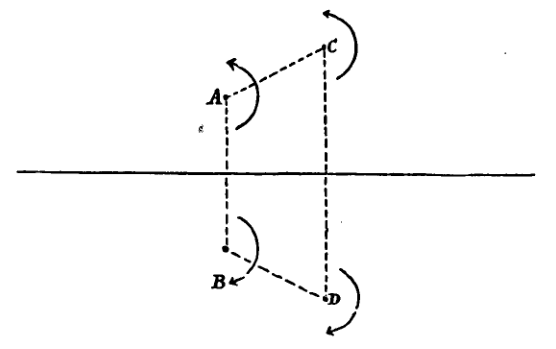
\includegraphics[width=\textwidth]{lovevort}
\caption{Point vortex pairs (A-B and C-D), from \citet[p.186]{love94}}
\label{fig:lovevort}
\end{figure}
If the vortex coordinates are
\begin{align}
\mbox{A:}&\hspace{0.5in}(x_0,y_0)\\
\mbox{B:}&\hspace{0.5in}(x_0,-y_0)\\
\mbox{C:}&\hspace{0.5in}(x_1,y_1)\\
\mbox{D:}&\hspace{0.5in}(x_1,-y_1)
\end{align}
and they have strengths $k$ (A and C) and $-k$ (B and D), then the motion of the fluid can be described by a streamfunction
\begin{equation}
\psi(x,y)=\frac{k}{2\pi}\ln\left(\frac{(x-x_0)^2 + (y+y_0)^2}{(x-x_0)^2 + (y-y_0)^2}\right) + \frac{k}{2\pi}\ln\left(\frac{(x-x_1)^2 + (y+y_1)^2}{(x-x_1)^2 + (y-y_1)^2}\right)
\label{eq:lovesf}
\end{equation}
\citep{love94}.

Now, with the aim of using the definitions of the streamfunction (\cref{eq:sf1,eq:sf2}), we differentiate \cref{eq:lovesf} with respect to $y$
\begin{align}
\partial_y \psi = \frac{k}{\pi}&\left(\frac{y+y_0}{(x-x_0)^2 + (y+y_0)^2}-\frac{y-y_0}{(x-x_0)^2 + (y-y_0)^2}\right.\nonumber\\&\left.+\frac{y+y_1}{(x-x_1)^2 + (y+y_1)^2}-\frac{y-y_1}{(x-x_1)^2 + (y-y_1)^2}\right),
\label{eq:lovesfdy}
\end{align}
and with respect to $x$
\begin{align}
\partial_x \psi = \frac{k}{\pi}&\left(\frac{x-x_0}{(x-x_0)^2 + (y+y_0)^2}-\frac{x-x_0}{(x-x_0)^2 + (y-y_0)^2}\right.\nonumber\\&\left.+\frac{x-x_1}{(x-x_1)^2 + (y+y_1)^2}-\frac{x-x_1}{(x-x_1)^2 + (y-y_1)^2}\right).
\label{eq:lovesfdx}
\end{align}
Now, we wish for the velocity of the vortices, i.e. we are looking at the above equations when $(x,y)\rightarrow(x_0,y_0)$ (or $(x_1,y_1)$).
Again following \citeauthor{love94}, we remove the terms that become infinite in this limit, thus obtaining,
\begin{alignat}{3}
\frac{dx_0}{dt}&=u_x (x_0,y_0)&&= \frac{k}{\pi} \left( \frac{y_1-y_0}{(x_0-x_1)^2 + (y_0-y_1)^2} + \frac{y_0+y_1}{(x_0-x_1)^2 +(y_0+y_1)^2} + \frac{1}{2y_0}\right),\label{eq:vortm1}\\
\frac{dy_0}{dt}&=u_y (x_0,y_0)&&= \frac{k}{\pi} \left( \frac{x_0-x_1}{(x_0-x_1)^2 + (y_0-y_1)^2} + \frac{x_1-x_0}{(x_0-x_1)^2 +(y_0+y_1)^2}\right),\label{eq:vortm2}\\
\frac{dx_1}{dt}&=u_x (x_1,y_1)&&= \frac{k}{\pi} \left( \frac{y_0-y_1}{(x_1-x_0)^2 + (y_1-y_0)^2} + \frac{y_1+y_0}{(x_1-x_0)^2 +(y_1+y_0)^2} + \frac{1}{2y_1}\right),\label{eq:vortm3}\\
\frac{dy_1}{dt}&=u_y (x_1,y_1)&&= \frac{k}{\pi} \left( \frac{x_1-x_0}{(x_1-x_0)^2 + (y_1-y_0)^2} + \frac{x_0-x_1}{(x_1-x_0)^2 +(y_1+y_0)^2} \right).\label{eq:vortm4}
\end{alignat}

\citet{acheson00} generalised these equations for a system of $N$ vortices (with strengths $k_1,k_2,\ldots ,k_N$), obtaining
\begin{align}
\frac{dx_i}{dt}&=\sum^N_{\substack{j=1\\j\neq i}} k_j \frac{y_j - y_i}{(x_i - x_j)^2 + (y_i - y_j)^2},\label{eq:vortposx}\\
\frac{dy_i}{dt}&=\sum^N_{\substack{j=1\\j\neq i}} k_j \frac{x_i - x_j}{(x_i - x_j)^2 + (y_i - y_j)^2},\label{eq:vortposy}
\end{align}
for $i=1,2,\ldots, N$.
The summations in \cref{eq:vortposx,eq:vortposy} are implemented in \hyperref[vortexf]{\texttt{vortexf.m}} and \hyperref[vortexg]{\texttt{vortexg.m}} respectively.
\clearpage
\section{Conserved Quantities}
Returning to \crefrange{eq:vortm1}{eq:vortm4}, and again following \citeauthor{love94}, we can express the right hand side of each equation by the partial derivative of some function $\chi$ (related to the streamfunction $\psi$), with respect to one of the vortex coordinates $x_0,x_1,y_0$ or $y_1$.
\citeauthor{love94} says the differential equations can ``clearly'' be put in the form
\begin{equation}
\frac{dx_0}{\partial_{y_0}\chi}=\frac{dy_0}{-\partial_{x_0}\chi}=\frac{dx_1}{\partial_{y_1}\chi}=\frac{dy_1}{-\partial_{x_1}\chi}=dt.
\label{eq:lovechi}
\end{equation}
To find this function, we must integrate the right hand side as follows:
\begin{itemize}
\item For \cref{eq:vortm1}, we integrate with respect to $y_0$:
\begin{align}
\chi &=\frac{k}{\pi}\int \frac{y_1-y_0}{(x_0-x_1)^2 + (y_0-y_1)^2} + \frac{y_0+y_1}{(x_0-x_1)^2 +(y_0+y_1)^2} + \frac{1}{2y_0}dy_0\nonumber\\
&= \frac{k}{\pi} \left( \int  \frac{y_1-y_0}{(x_0-x_1)^2 + (y_0-y_1)^2} dy_0\right. \nonumber\\ &\left.+ \int \frac{y_0+y_1}{(x_0-x_1)^2 +(y_0+y_1)^2} dy_0 + \int \frac{1}{2y_0}dy_0\right)\nonumber\\
&= \frac{k}{\pi}\left(\inv{2} \ln y_0 -\half \ln((y_0-y_1)^2 +(x_0-x_1)^2)\right. \nonumber\\ &\left. + \half \ln((y_0+y_1)^2 +(x_0-x_1)^2) +C_1 (x_0,x_1,y_1)\right)\nonumber\\
&=\frac{k}{2\pi}\ln y_0 \frac{(y_0+y_1)^2 +(x_0-x_1)^2}{(y_0-y_1)^2 +(x_0-x_1)^2}\cdot C_1 \label{eq:chi1}
\end{align}
\item For \cref{eq:vortm2}, we integrate the negative with respect to $x_0$:
\begin{align}
\chi &=-\frac{k}{\pi}\int \frac{x_0-x_1}{(x_0-x_1)^2 + (y_0-y_1)^2} - \frac{x_0-x_1}{(x_0-x_1)^2 +(y_0+y_1)^2} dx_0\nonumber\\
&= -\frac{k}{\pi} \left( \int  \frac{x_0-x_1}{(x_0-x_1)^2 + (y_0-y_1)^2} dx_0\right. \nonumber\\ &\left.- \int \frac{x_0-x_1}{(x_0-x_1)^2 +(y_0+y_1)^2} dx_0 \right)\nonumber\\
&= \frac{k}{\pi}\left(-\half \ln((y_0-y_1)^2 +(x_0-x_1)^2)\right. \nonumber\\ &\left. + \half \ln((y_0+y_1)^2 +(x_0-x_1)^2) +C_2 (x_1,y_0,y_1)\right)\nonumber\\
&=\frac{k}{2\pi}\ln \frac{(y_0+y_1)^2 +(x_0-x_1)^2}{(y_0-y_1)^2 +(x_0-x_1)^2}\cdot C_2 \label{eq:chi2}
\end{align}
\item For \cref{eq:vortm3}, we integrate with respect to $y_1$:
\begin{align}
\chi &=\frac{k}{\pi}\int \frac{y_0-y_1}{(x_1-x_0)^2 + (y_1-y_0)^2} + \frac{y_0+y_1}{(x_1-x_0)^2 +(y_0+y_1)^2} + \frac{1}{2y_1}dy_1\nonumber\\
&= \frac{k}{\pi} \left( \int  \frac{y_0-y_1}{(x_1-x_0)^2 + (y_1-y_0)^2} dy_1\right. \nonumber\\ &\left.+ \int \frac{y_0+y_1}{(x_1-x_0)^2 +(y_0+y_1)^2} dy_1 + \int \frac{1}{2y_1}dy_0\right)\nonumber\\
&= \frac{k}{\pi}\left(\inv{2} \ln y_1 -\half \ln((y_1-y_0)^2 +(x_1-x_0)^2)\right. \nonumber\\ &\left. + \half \ln((y_0+y_1)^2 +(x_1-x_0)^2) +C_3 (x_0,x_1,y_0)\right)\nonumber\\
&=\frac{k}{2\pi}\ln y_1 \frac{(y_0+y_1)^2 +(x_1-x_0)^2}{(y_1-y_0)^2 +(x_1-x_0)^2} \cdot C_3\label{eq:chi3}
\end{align} 
\item For \cref{eq:vortm4}, we integrate the negative with respect to $x_1$:
\begin{align}
\chi &=-\frac{k}{\pi}\int \frac{x_1-x_0}{(x_1-x_0)^2 + (y_1-y_0)^2} - \frac{x_1-x_0}{(x_1-x_0)^2 +(y_0+y_1)^2} dx_1\nonumber\\
&= -\frac{k}{\pi} \left( \int  \frac{x_1-x_0}{(x_1-x_0)^2 + (y_1-y_0)^2} dx_1\right. \nonumber\\ &\left.- \int \frac{x_1-x_0}{(x_1-x_0)^2 +(y_0+y_1)^2} dx_1 \right)\nonumber\\
&= \frac{k}{\pi}\left(-\half \ln((y_1-y_0)^2 +(x_1-x_0)^2)\right. \nonumber\\ &\left. + \half \ln((y_0+y_1)^2 +(x_1-x_0)^2) +C_4 (x_0,y_0,y_1)\right)\nonumber\\
&=\frac{k}{2\pi}\ln \frac{(y_0+y_1)^2 +(x_1-x_0)^2}{(y_1-y_0)^2 +(x_1-x_0)^2} \cdot C_4\label{eq:chi4}
\end{align}
\end{itemize}
Combining \crefrange{eq:chi1}{eq:chi4}, we can see that, noting that $(a-b)^2 = (b-a)^2$, we must have, for all equations to be equal
\begin{align}
C_1&=y_1,\\
C_3&=y_0,\\
C_2&=C_4=y_1 y_2.
\end{align}
So, we have
\begin{equation}
\chi=\frac{k}{2\pi}\ln y_0 y_1 \frac{(y_0+y_1)^2 +(x_1-x_0)^2}{(y_1-y_0)^2 +(x_1-x_0)^2},
\label{eq:chifinal}
\end{equation}
which agrees with the result in \citet{love94}.
\subsection{Momentum}
Now we have found $\chi$, we can use it (with \crefrange{eq:vortm1}{eq:vortm4}) to derive the conserved analogues of energy and momentum, as stated in \citet{love94}.
Equating the $dy_0$ and the $dy_1$ parts of \cref{eq:lovechi}, we have
\begin{align}
\frac{dy_0}{-\partial_{x_0}\chi} &= \frac{-dy_1}{\partial_{x_1} \chi},\\
\Rightarrow \frac{\dxb \chi\cdot dy_0 + \dxa \chi \cdot dy_1}{-\partial_{x_0 x_1} \chi}&=0,\\
\Rightarrow \dxb \chi\cdot dy_0 + \dxa \chi \cdot dy_1 &=0,
\end{align}
and, as
\begin{equation}
\dxb \chi = \dxa \chi,
\end{equation}
we have
\begin{align}
dy_0 + dy_1 &=0\\
\Rightarrow y_0 + y_1 &= \mbox{CONSTANT}\label{eq:consty},
\end{align}
as in the paper.
This equation shows that the centre of the rotating system composed of the vortices A and C, or the vortices B and D (expressed by \citeauthor{love94} as the midpoint ot the line between the vortices) moves parallel to the $x$ axis at constant distance (provided the conditions set earlier by \citeauthor{helmholtz67} for the ring vortices are met).

\citet{musgrave09} give an analogue to momentum for systems of N point vortices as
\begin{equation}
\bm{p}=\half \rho \left(\begin{array}{c} \sum_i^N k_i y_i\\-\sum_{i}^N k_i x_i\\0\end{array}\right).
\end{equation}
We are interested in momentum in the $x$ direction, so we use, for each vortex pair
\begin{align}
p_x&=\half \rho \sum_{i=0}^1 k_i y_i,\\
&= \half \rho (k_0 y_0 + k_1 y_1).
\end{align}
From the definition of our system, we have $k_0=k_1=\mbox{constant}$ and $\rho=\mbox{constant}$, and from \cref{eq:consty} we have that $y_0 + y_1 = \mbox{constant}$, therefore we have $p_x=\mbox{constant}$.
This means momentum is conserved.
\subsection{Speed of Translation}
The centrepoint can be used to find the speed of translation of the vortex pairs (provided we have stable interactions).
Thinking again of the midpoint $m$ of the line between the two vortices, the $x$ coordinate of $m$ is given by
\begin{equation}
m_x=\frac{x_0 +x_1}{2}.
\end{equation}
The speed (in the $x$ direction) of this midpoint is given by
\begin{align}
\frac{dm_x}{dt}&=\frac{d}{dt}\left(\frac{x_0 +x_1}{2}\right),\\
&=\half \left(\frac{dx_0}{dt} + \frac{dx_1}{dt}\right),\\
&=\frac{k}{2\pi}\left(\frac{2y_1+2y_0}{(x_0-x_1)^2 + (y_0+y_1)^2} + \inv{2y_0} + \inv{2y_1}\right)
\end{align}
i.e. the average velocity of the two vortices.
\subsection{Energy}
Now equating the $y_0$ and the $x_0$ terms, we have 
\begin{align}
\frac{dy_0}{-\dxa \chi} &= \frac{dx_0}{\dya \chi},\\
\Rightarrow \dya \chi dy_0 &= - \dxa \chi dx_0,\\
\Rightarrow \int d\chi &= - \int d\chi,\\
\Rightarrow \chi +c_1 &= -\chi + c_2,\\
\Rightarrow \chi &= \mbox{CONSTANT}.
\end{align}
$\chi$ represents the energy of the fluid \citep{love94}, so we have conservation of energy in the system, provided we ignore viscous effects.
\clearpage
\section{Conditions for Leapfrogging}
\citet{love94} quantified the conditions necessary for the ``leapfrogging'' described in \cref{sec:vortint} to take place.
At the point when all four vortices are aligned vertically, we define $y_{0,a}$ and $y_{1,a}$ to be the $y$ coordinates of vortices A and C respectively.
From \cref{eq:consty} we have that
\begin{equation}
y_{0,a} + y_{0,b} = const = 2c,\label{eq:lc1}
\end{equation}
where the factor of two in the second equality is to simplify later expressions.
As we found $\chi$ constant, we also have (as $x_0=x_1$) 
\begin{equation}
y_{0,a}y_{0,b}\left(\frac{y_{0,a} + y_{0,b}}{y_{0,a}-y_{0,b}}\right)^2 = const = a^2,\label{eq:lc2}
\end{equation}
where again the second equality is to simplify later expressions.

For periodicity of the motion we must have $a^2 > c^2$ \citep{love94}.
Feeding \cref{eq:lc1,eq:lc2} into this condition, we obtain a condition in terms of our $y$ coordinates:
\begin{equation}
6y_{0,a}y_{1,a}-y_{0,a}^2 -y_{1,a} >0 \label{eq:lc3}.
\end{equation}
We are looking for a ratio of $y_{1,a}/y_{0,a}$, so we set $y_{1,a}=1$
in \cref{eq:lc3} and solve for $y_{0,a}$, obtaining
$y_{1,a}/y_{0,a}<3+2\sqrt{2}$.  This is the condition for periodic
leapfrogging.  In the following section, and the MATLAB code, we use
notation closer to \citeauthor{acheson00}, and thus, keeping the $y$ coordinates of one pair as $1,-1$, we define
$\alpha=y_{0,a}/y_{1,a}> 3-2\sqrt{2}$, the reciprocal of the previous ratio.
\clearpage
\section{Stability of the 4-Vortex System}
Taking a system of four point vortices, as in \citet{acheson00}, a program (\hyperref[sec:ap1]{Appendix I}) was written in MATLAB to numerically integrate the vortex velocity equations (\cref{eq:vortposx,eq:vortposy}).
The scheme used is a fourth order Runge-Kutta method with static step size.
The question to be answered is, what values of $\alpha$ permit stable, periodic leapfrogging when the initial position of one vortex is slightly perturbed.
\citeauthor{acheson00} presents four regions of (in)stability, and the below list contains figures from his \citeyear{acheson00} paper, as well as those generated in the MATLAB program.
There appears to be numerical instabilities generated in the numerical integration used, which contribute most of the variation from the figures by \citeauthor{acheson00}.
\begin{description}
\item[No leapfrogging ($\alpha<3-2\sqrt{2}\approx
0.172$)]
In this region, as per the condition in \cref{eq:lc3}, there is no leapfrogging and the vortices merely translate, as can be seen in \cref{fig:noleap}.
\begin{figure}[ht]
\centering
\setlength\figureheight{7.5cm} 
\setlength\figurewidth{\textwidth}
% This file was created by matlab2tikz.
% Minimal pgfplots version: 1.3
%
%The latest updates can be retrieved from
%  http://www.mathworks.com/matlabcentral/fileexchange/22022-matlab2tikz
%where you can also make suggestions and rate matlab2tikz.
%
\definecolor{mycolor1}{rgb}{0.00000,1.00000,1.00000}%
%
\begin{tikzpicture}

\begin{axis}[%
width=0.95092\figurewidth,
height=\figureheight,
at={(0\figurewidth,0\figureheight)},
scale only axis,
every outer x axis line/.append style={black},
every x tick label/.append style={font=\color{black}},
xmin=0,
xlabel={x},
every outer y axis line/.append style={black},
every y tick label/.append style={font=\color{black}},
ymin=-1.5,
ymax=1.5,
ylabel={y},
title={10000 time steps, step size = 0.005},
axis x line*=bottom,
axis y line*=left
]
\addplot [color=blue,solid,forget plot]
  table[row sep=crcr]{%
0	1\\
0.000953612251194968	0.999991569056121\\
0.00190798729678	0.999963601161843\\
0.00286396019577596	0.999916173293784\\
0.0038223562787305	0.999849420394275\\
0.00478398574829361	0.999763533861643\\
0.0057496385504451	0.99965875939445\\
0.00672007960576098	0.999535394245381\\
0.00769604447755355	0.999393783954496\\
0.00867823553891636	0.999234318642431\\
0.00966731868445496	0.999057428951598\\
0.0106639206156271	0.9988635817273\\
0.0116686267119624	0.998653275531109\\
0.0126819794847081	0.998427036076018\\
0.0137044775952622	0.998185411667346\\
0.014736575408559	0.997928968725522\\
0.0157786830416588	0.997658287457446\\
0.0168311668603032	0.997373957732574\\
0.0178943503711121	0.997076575208879\\
0.0189685154542912	0.996766737742879\\
0.0200539038809719	0.996445042107388\\
0.0211507190603203	0.996112081030925\\
0.0222591279640144	0.995768440564039\\
0.0233792631792637	0.995414697770303\\
0.0245112250459113	0.995051418733452\\
0.0256550838380166	0.994679156867197\\
0.0268108819554154	0.994298451510375\\
0.0279786360958673	0.99390982678745\\
0.0291583393833613	0.993513790712613\\
0.0303499634328282	0.993110834514872\\
0.0315534603358096	0.992701432161321\\
0.0327687645555044	0.992286040056183\\
0.0339957947230267	0.99186509689403\\
0.0352344553296577	0.991439023646738\\
0.0364846383123741	0.991008223665093\\
0.0377462245320113	0.990573082877498\\
0.0390190851451084	0.990133970069768\\
0.0403030828718157	0.989691237231613\\
0.0415980731632802	0.989245219956958\\
0.0429039052726805	0.98879623788673\\
0.044220423234625	0.988344595184161\\
0.0455474667579683	0.987890581033938\\
0.0468848720372929	0.987434470157766\\
0.0482324724883683	0.986976523339946\\
0.0495900994128629	0.98651698795759\\
0.0509575825974728	0.986056098510929\\
0.0523347508524641	0.985594077149959\\
0.0537214324944103	0.985131134194338\\
0.0551174557776738	0.98466746864402\\
0.0565226492789171	0.984203268678633\\
0.0579368422386703	0.983738712144056\\
0.0593598648637108	0.98327396702498\\
0.060791548593747	0.982809191902609\\
0.0622317263356417	0.982344536396883\\
0.0636802326681619	0.981880141592852\\
0.0651369040200065	0.981416140451011\\
0.066601578823637	0.980952658201549\\
0.0680740976472316	0.980489812722622\\
0.0695543033068806	0.980027714902813\\
0.0710420409609634	0.979566468988088\\
0.0725371581884741	0.979106172913558\\
0.0740395050529106	0.978646918620451\\
0.0755489341531933	0.978188792358722\\
0.0770653006629513	0.97773187497574\\
0.0785884623593899	0.977276242191551\\
0.0801182796428433	0.976821964861173\\
0.0816546155480142	0.976369109224434\\
0.0831973357478098	0.975917737143837\\
0.0847463085505986	0.975467906330936\\
0.0863014048916339	0.97501967056171\\
0.0878624983193236	0.974573079881413\\
0.0894294649769562	0.974128180799347\\
0.0910021835804397	0.973685016474027\\
0.092580535392554	0.97324362688916\\
0.0941644041941709	0.972804049020873\\
0.0957536762528503	0.97236631699659\\
0.0973482402891837	0.971930462245957\\
0.0989479874412172	0.971496513644193\\
0.100552811227255	0.971064497648223\\
0.102162607507317	0.970634438425961\\
0.103777274443486	0.970206357979052\\
0.105396712459376	0.969780276259413\\
0.107020824198905	0.969356211279867\\
0.108649514484559	0.968934179219167\\
0.110282690275297	0.968514194521683\\
0.111920260624243	0.96809626999203\\
0.113562136636292	0.967680416884871\\
0.11520823142573	0.967266644990151\\
0.116858460073987	0.966854962713989\\
0.118512739587591	0.966445377155438\\
0.120170988856418	0.966037894179336\\
0.121833128612288	0.965632518485425\\
0.123499081387987	0.965229253673952\\
0.12516877147675	0.964828102307902\\
0.126842124892257	0.964429065972059\\
0.128519069329185	0.964032145329033\\
0.130199534124343	0.963637340172433\\
0.131883450218418	0.963244649477297\\
0.133570750118359	0.962854071447955\\
0.135261367860419	0.962465603563423\\
0.136955238973864	0.962079242620478\\
0.138652300445369	0.961694984774514\\
0.140352490684108	0.961312825578304\\
0.142055749487534	0.960932760018763\\
0.143762018007875	0.960554782551828\\
0.145471238719322	0.960178887135538\\
0.147183355385936	0.959805067261404\\
0.148898313030239	0.959433315984174\\
0.150616057902523	0.959063625950049\\
0.152336537450844	0.95869598942345\\
0.154059700291704	0.958330398312393\\
0.155785496181417	0.95796684419256\\
0.157513875988152	0.957605318330112\\
0.159244791664635	0.957245811703321\\
0.160978196221513	0.956888315023083\\
0.162714043701357	0.956532818752353\\
0.16445228915331	0.956179313124574\\
0.166192888608347	0.955827788161139\\
0.167935799055163	0.955478233687942\\
0.169680978416652	0.955130639351056\\
0.17142838552698	0.954784994631594\\
0.173177980109241	0.954441288859778\\
0.174929722753671	0.954099511228272\\
0.176683574896424	0.953759650804807\\
0.178439498798886	0.953421696544129\\
0.180197457527526	0.953085637299323\\
0.181957414934258	0.952751461832518\\
0.183719335637314	0.952419158825028\\
0.185483185002611	0.952088716886938\\
0.187248929125601	0.951760124566185\\
0.189016534813593	0.951433370357127\\
0.190785969568535	0.951108442708666\\
0.192557201570241	0.950785330031909\\
0.194330199660063	0.950464020707415\\
0.196104933324982	0.950144503092041\\
0.197881372682119	0.949826765525408\\
0.199659488463647	0.949510796335996\\
0.201439252002103	0.949196583846911\\
0.203220635216078	0.948884116381309\\
0.205003610596287	0.948573382267521\\
0.206788151191999	0.948264369843881\\
0.208574230597822	0.94795706746327\\
0.210361822940838	0.947651463497397\\
0.212150902868068	0.947347546340828\\
0.213941445534267	0.947045304414774\\
0.215733426590037	0.94674472617065\\
0.217526822170251	0.946445800093421\\
0.219321608882775	0.946148514704736\\
0.221117763797485	0.945852858565872\\
0.222915264435571	0.945558820280494\\
0.224714088759116	0.945266388497231\\
0.226514215160944	0.94497555191209\\
0.228315622454732	0.944686299270713\\
0.230118289865379	0.944398619370478\\
0.231922197019621	0.944112501062461\\
0.233727323936885	0.943827933253256\\
0.235533651020384	0.943544904906676\\
0.237341159048436	0.943263405045319\\
0.239149829166002	0.942983422752028\\
0.240959642876453	0.942704947171234\\
0.242770582033528	0.942427967510198\\
0.244582628833514	0.942152473040151\\
0.24639576580761	0.941878453097344\\
0.2482099758145	0.941605897083998\\
0.250025242033095	0.941334794469186\\
0.251841547955475	0.941065134789615\\
0.253658877379999	0.940796907650349\\
0.255477214404587	0.94053010272545\\
0.257296543420181	0.940264709758552\\
0.259116849104352	0.940000718563368\\
0.260938116415083	0.939738119024145\\
0.262760330584697	0.939476901096048\\
0.264583477113936	0.939217054805497\\
0.266407541766191	0.938958570250447\\
0.268232510561869	0.938701437600627\\
0.270058369772903	0.938445647097719\\
0.271885105917392	0.938191189055505\\
0.273712705754377	0.937938053859964\\
0.275541156278742	0.937686231969335\\
0.277370444716237	0.93743571391414\\
0.279200558518625	0.937186490297171\\
0.281031485358948	0.936938551793447\\
0.282863213126898	0.936691889150135\\
0.284695729924316	0.936446493186446\\
0.286529024060777	0.9362023547935\\
0.288363084049305	0.935959464934167\\
0.290197898602166	0.935717814642881\\
0.292033456626783	0.935477395025433\\
0.293869747221731	0.935238197258739\\
0.295706759672837	0.935000212590594\\
0.29754448344937	0.934763432339398\\
0.299382908200314	0.93452784789387\\
0.301222023750738	0.934293450712746\\
0.303061820098246	0.934060232324454\\
0.30490228740951	0.933828184326782\\
0.306743416016883	0.93359729838653\\
0.308585196415091	0.933367566239147\\
0.310427619258006	0.933138979688355\\
0.312270675355485	0.932911530605771\\
0.314114355670287	0.932685210930506\\
0.315958651315059	0.932460012668761\\
0.317803553549393	0.932235927893419\\
0.31964905377695	0.932012948743617\\
0.321495143542641	0.931791067424323\\
0.323341814529887	0.931570276205896\\
0.325189058557924	0.931350567423644\\
0.327036867579184	0.931131933477383\\
0.328885233676726	0.930914366830976\\
0.330734149061721	0.93069786001188\\
0.332583606071007	0.930482405610684\\
0.334433597164682	0.930267996280645\\
0.336284114923763	0.930054624737216\\
0.338135152047889	0.929842283757579\\
0.33998670135308	0.929630966180168\\
0.341838755769539	0.929420664904196\\
0.343691308339509	0.929211372889173\\
0.345544352215173	0.929003083154434\\
0.347397880656598	0.928795788778651\\
0.34925188702973	0.928589482899358\\
0.351106364804425	0.928384158712466\\
0.352961307552526	0.928179809471785\\
0.354816708945984	0.927976428488538\\
0.356672562755013	0.927774009130881\\
0.358528862846291	0.927572544823426\\
0.360385603181194	0.927372029046753\\
0.362242777814071	0.927172455336937\\
0.364100380890556	0.926973817285066\\
0.365958406645911	0.926776108536766\\
0.367816849403407	0.926579322791723\\
0.369675703572744	0.926383453803209\\
0.371534963648494	0.926188495377613\\
0.373394624208582	0.925994441373965\\
0.375254679912804	0.925801285703468\\
0.377115125501361	0.925609022329037\\
0.37897595579344	0.925417645264826\\
0.380837165685813	0.925227148575772\\
0.382698750151471	0.925037526377134\\
0.38456070423828	0.924848772834031\\
0.386423023067672	0.924660882160995\\
0.388285701833356	0.924473848621513\\
0.390148735800059	0.92428766652758\\
0.392012120302291	0.92410233023925\\
0.393875850743138	0.923917834164198\\
0.395739922593073	0.923734172757273\\
0.397604331388797	0.923551340520063\\
0.3994690727321	0.923369332000461\\
0.401334142288749	0.923188141792231\\
0.403199535787389	0.923007764534581\\
0.405065249018478	0.922828194911739\\
0.40693127783323	0.922649427652528\\
0.408797618142595	0.922471457529949\\
0.410664265916239	0.922294279360765\\
0.412531217181565	0.922117888005087\\
0.414398468022736	0.921942278365967\\
0.416266014579727	0.921767445388991\\
0.418133853047393	0.921593384061878\\
0.420001979674554	0.921420089414078\\
0.421870390763098	0.921247556516379\\
0.423739082667103	0.921075780480514\\
0.425608051791974	0.920904756458771\\
0.427477294593596	0.920734479643607\\
0.429346807577507	0.920564945267268\\
0.431216587298085	0.920396148601409\\
0.433086630357744	0.920228084956716\\
0.434956933406159	0.920060749682539\\
0.436827493139491	0.919894138166517\\
0.438698306299638	0.919728245834218\\
0.440569369673493	0.919563068148775\\
0.442440680092219	0.919398600610526\\
0.444312234430538	0.919234838756659\\
0.446184029606031	0.919071778160863\\
0.448056062578452	0.918909414432974\\
0.449928330349059	0.918747743218635\\
0.451800829959947	0.918586760198949\\
0.453673558493406	0.918426461090145\\
0.45554651307128	0.918266841643238\\
0.457419690854347	0.918107897643698\\
0.459293089041702	0.917949624911124\\
0.461166704870157	0.917792019298912\\
0.463040535613647	0.917635076693937\\
0.464914578582657	0.917478793016233\\
0.466788831123644	0.917323164218675\\
0.468663290618482	0.917168186286665\\
0.470537954483914	0.917013855237824\\
0.472412820171009	0.916860167121685\\
0.474287885164634	0.916707118019385\\
0.476163146982935	0.91655470404337\\
0.478038603176823	0.916402921337092\\
0.479914251329476	0.916251766074716\\
0.481790089055844	0.916101234460829\\
0.483666114002162	0.915951322730149\\
0.485542323845481	0.915802027147238\\
0.487418716293196	0.915653344006223\\
0.489295289082586	0.915505269630513\\
0.491172039980369	0.915357800372518\\
0.493048966782251	0.915210932613382\\
0.494926067312497	0.915064662762705\\
0.496803339423501	0.914918987258276\\
0.498680780995364	0.914773902565807\\
0.500558389935482	0.914629405178669\\
0.502436164178144	0.91448549161763\\
0.504314101684125	0.914342158430599\\
0.506192200440301	0.91419940219237\\
0.50807045845926	0.914057219504367\\
0.509948873778925	0.913915606994396\\
0.51182744446218	0.913774561316397\\
0.513706168596506	0.913634079150198\\
0.515585044293618	0.913494157201272\\
0.517464069689116	0.913354792200499\\
0.519343242942133	0.913215980903927\\
0.521222562234995	0.913077720092536\\
0.523102025772883	0.912940006572008\\
0.524981631783508	0.912802837172493\\
0.526861378516779	0.912666208748385\\
0.528741264244488	0.912530118178095\\
0.530621287259993	0.912394562363826\\
0.532501445877912	0.912259538231354\\
0.534381738433817	0.91212504272981\\
0.536262163283934	0.911991072831463\\
0.538142718804853	0.911857625531505\\
0.540023403393236	0.911724697847842\\
0.541904215465531	0.91159228682088\\
0.543785153457697	0.911460389513322\\
0.545666215824924	0.911329003009961\\
0.547547401041368	0.911198124417476\\
0.549428707599877	0.911067750864232\\
0.551310134011736	0.910937879500081\\
0.553191678806407	0.910808507496166\\
0.555073340531272	0.910679632044725\\
0.55695511775139	0.910551250358898\\
0.558837009049245	0.910423359672538\\
0.560719013024511	0.910295957240019\\
0.562601128293807	0.910169040336055\\
0.564483353490469	0.910042606255508\\
0.566365687264318	0.90991665231321\\
0.568248128281432	0.909791175843781\\
0.570130675223925	0.90966617420145\\
0.572013326789726	0.909541644759874\\
0.573896081692366	0.909417584911969\\
0.575778938660759	0.909293992069731\\
0.577661896439002	0.909170863664067\\
0.579544953786161	0.909048197144624\\
0.581428109476073	0.908925989979621\\
0.583311362297144	0.908804239655681\\
0.585194711052153	0.90868294367767\\
0.587078154558059	0.908562099568528\\
0.588961691645812	0.908441704869113\\
0.590845321160163	0.908321757138039\\
0.59272904195948	0.908202253951516\\
0.594612852915566	0.908083192903198\\
0.596496752913483	0.907964571604024\\
0.598380740851372	0.907846387682065\\
0.600264815640282	0.907728638782377\\
0.602148976203996	0.907611322566842\\
0.604033221478866	0.90749443671403\\
0.605917550413648	0.907377978919044\\
0.607801961969333	0.907261946893375\\
0.609686455118992	0.907146338364764\\
0.611571028847618	0.907031151077051\\
0.613455682151963	0.906916382790042\\
0.615340414040394	0.906802031279361\\
0.617225223532734	0.90668809433632\\
0.619110109660115	0.906574569767774\\
0.620995071464836	0.906461455395993\\
0.622880108000212	0.906348749058523\\
0.624765218330432	0.906236448608053\\
0.626650401530424	0.906124551912288\\
0.628535656685712	0.906013056853814\\
0.63042098289228	0.905901961329971\\
0.63230637925644	0.905791263252729\\
0.634191844894699	0.905680960548555\\
0.636077378933627	0.905571051158293\\
0.63796298050973	0.905461533037039\\
0.639848648769323	0.90535240415402\\
0.641734382868407	0.905243662492469\\
0.643620181972543	0.90513530604951\\
0.645506045256733	0.905027332836035\\
0.647391971905302	0.904919740876588\\
0.649277961111775	0.904812528209252\\
0.651164012078768	0.904705692885527\\
0.653050124017869	0.904599232970221\\
0.654936296149528	0.904493146541336\\
0.656822527702942	0.904387431689956\\
0.658708817915952	0.904282086520134\\
0.660595166034929	0.904177109148789\\
0.662481571314672	0.904072497705588\\
0.664368033018301	0.903968250332847\\
0.666254550417153	0.903864365185421\\
0.668141122790684	0.903760840430599\\
0.670027749426365	0.903657674247998\\
0.671914429619581	0.903554864829465\\
0.673801162673542	0.903452410378967\\
0.675687947899176	0.903350309112498\\
0.677574784615043	0.903248559257974\\
0.679461672147237	0.903147159055134\\
0.681348609829293	0.903046106755444\\
0.6832355970021	0.902945400621995\\
0.685122633013808	0.902845038929414\\
0.68700971721974	0.902745019963763\\
0.688896848982307	0.902645342022446\\
0.69078402767092	0.902546003414115\\
0.692671252661904	0.90244700245858\\
0.694558523338418	0.902348337486713\\
0.69644583909037	0.90225000684036\\
0.698333199314336	0.902152008872253\\
0.700220603413481	0.902054341945915\\
0.702108050797477	0.901957004435578\\
0.703995540882428	0.901859994726092\\
0.705883073090792	0.901763311212839\\
0.707770646851306	0.901666952301649\\
0.709658261598906	0.901570916408712\\
0.711545916774662	0.901475201960498\\
0.713433611825697	0.901379807393672\\
0.71532134620512	0.901284731155009\\
0.717209119371953	0.901189971701317\\
0.719096930791061	0.901095527499352\\
0.720984779933083	0.901001397025741\\
0.722872666274367	0.900907578766902\\
0.724760589296897	0.900814071218964\\
0.72664854848823	0.90072087288769\\
0.728536543341434	0.9006279822884\\
0.730424573355015	0.900535397945897\\
0.732312638032861	0.900443118394387\\
0.734200736884177	0.900351142177406\\
0.73608886942342	0.900259467847747\\
0.737977035170241	0.900168093967387\\
0.739865233649426	0.90007701910741\\
0.74175346439083	0.89998624184794\\
0.743641726929326	0.899895760778067\\
0.745530020804741	0.899805574495776\\
0.747418345561803	0.899715681607878\\
0.749306700750082	0.899626080729939\\
0.751195085923933	0.899536770486215\\
0.753083500642446	0.899447749509579\\
0.754971944469385	0.899359016441457\\
0.756860416973141	0.899270569931758\\
0.758748917726673	0.899182408638811\\
0.76063744630746	0.8990945312293\\
0.762526002297449	0.899006936378193\\
0.764414585283001	0.898919622768685\\
0.766303194854844	0.898832589092128\\
0.768191830608022	0.898745834047973\\
0.770080492141847	0.898659356343703\\
0.771969179059848	0.898573154694775\\
0.773857890969728	0.898487227824555\\
0.775746627483311	0.898401574464258\\
0.777635388216502	0.898316193352889\\
0.779524172789234	0.898231083237182\\
0.78141298082543	0.898146242871542\\
0.783301811952951	0.898061671017984\\
0.785190665803557	0.897977366446076\\
0.787079542012863	0.897893327932882\\
0.788968440220293	0.897809554262905\\
0.790857360069038	0.89772604422803\\
0.792746301206018	0.897642796627465\\
0.794635263281836	0.897559810267692\\
0.796524245950738	0.897477083962405\\
0.798413248870574	0.897394616532459\\
0.800302271702758	0.897312406805816\\
0.802191314112225	0.897230453617491\\
0.804080375767398	0.897148755809497\\
0.805969456340144	0.897067312230797\\
0.80785855550574	0.896986121737246\\
0.809747672942833	0.896905183191544\\
0.811636808333404	0.896824495463181\\
0.813525961362731	0.896744057428389\\
0.815415131719354	0.896663867970092\\
0.817304319095035	0.896583925977854\\
0.81919352318473	0.896504230347831\\
0.821082743686549	0.89642477998272\\
0.822971980301721	0.896345573791713\\
0.824861232734565	0.89626661069045\\
0.82675050069245	0.896187889600965\\
0.828639783885767	0.896109409451647\\
0.830529082027895	0.896031169177185\\
0.832418394835165	0.895953167718531\\
0.834307722026834	0.895875404022842\\
0.836197063325049	0.895797877043448\\
0.838086418454817	0.895720585739794\\
0.839975787143976	0.895643529077404\\
0.841865169123161	0.895566706027832\\
0.843754564125777	0.895490115568622\\
0.845643971887968	0.895413756683259\\
0.847533392148588	0.895337628361129\\
0.84942282464917	0.895261729597478\\
0.851312269133902	0.895186059393364\\
0.853201725349594	0.89511061675562\\
0.855091193045651	0.89503540069681\\
0.856980671974049	0.894960410235187\\
0.858870161889303	0.894885644394653\\
0.860759662548441	0.894811102204718\\
0.86264917371098	0.894736782700461\\
0.864538695138896	0.894662684922486\\
0.866428226596601	0.894588807916887\\
0.868317767850917	0.894515150735206\\
0.870207318671047	0.894441712434395\\
0.872096878828553	0.894368492076776\\
0.873986448097334	0.894295488730004\\
0.875876026253593	0.89422270146703\\
0.87776561307582	0.894150129366061\\
0.879655208344768	0.894077771510523\\
0.881544811843424	0.894005626989026\\
0.883434423356989	0.893933694895325\\
0.885324042672856	0.893861974328285\\
0.887213669580585	0.893790464391844\\
0.889103303871881	0.893719164194978\\
0.89099294534057	0.893648072851665\\
0.892882593782583	0.89357718948085\\
0.894772248995924	0.893506513206411\\
0.89666191078066	0.893436043157122\\
0.898551578938888	0.893365778466621\\
0.900441253274725	0.893295718273376\\
0.902330933594278	0.893225861720647\\
0.90422061970563	0.893156207956461\\
0.906110311418814	0.893086756133571\\
0.908000008545799	0.893017505409425\\
0.909889710900465	0.892948454946137\\
0.911779418298585	0.892879603910451\\
0.913669130557806	0.892810951473708\\
0.915558847497631	0.89274249681182\\
0.917448568939395	0.892674239105231\\
0.919338294706254	0.892606177538891\\
0.921228024623158	0.892538311302223\\
0.923117758516839	0.892470639589093\\
0.92500749621579	0.892403161597778\\
0.926897237550248	0.892335876530937\\
0.928786982352175	0.892268783595583\\
0.930676730455242	0.892201882003047\\
0.932566481694809	0.892135170968955\\
0.934456235907913	0.892068649713197\\
0.936345992933245	0.892002317459895\\
0.938235752611136	0.891936173437377\\
0.940125514783543	0.891870216878149\\
0.942015279294026	0.891804447018864\\
0.943905045987738	0.891738863100297\\
0.945794814711407	0.891673464367313\\
0.947684585313319	0.891608250068844\\
0.949574357643302	0.891543219457859\\
0.951464131552714	0.891478371791337\\
0.953353906894423	0.89141370633024\\
0.955243683522796	0.891349222339487\\
0.957133461293679	0.891284919087928\\
0.959023240064388	0.891220795848314\\
0.96091301969369	0.891156851897276\\
0.962802800041791	0.891093086515294\\
0.96469258097032	0.891029498986678\\
0.966582362342315	0.890966088599535\\
0.968472144022209	0.890902854645747\\
0.970361925875818	0.890839796420949\\
0.972251707770324	0.890776913224498\\
0.974141489574265	0.890714204359454\\
0.976031271157518	0.890651669132551\\
0.977921052391288	0.890589306854177\\
0.979810833148093	0.890527116838345\\
0.981700613301755	0.890465098402673\\
0.983590392727382	0.890403250868359\\
0.985480171301357	0.890341573560158\\
0.987369948901329	0.890280065806356\\
0.989259725406195	0.890218726938752\\
0.991149500696091	0.890157556292629\\
0.993039274652379	0.890096553206737\\
0.994929047157635	0.890035717023264\\
0.996818818095636	0.889975047087821\\
0.998708587351352	0.889914542749412\\
1.00059835481093	0.889854203360419\\
1.00248812036168	0.889794028276575\\
1.00437788389208	0.889734016856945\\
1.00626764529173	0.889674168463902\\
1.00815740445139	0.889614482463109\\
1.01004716126292	0.889554958223494\\
1.01193691561931	0.889495595117232\\
1.01382666741463	0.889436392519723\\
1.01571641654405	0.88937734980957\\
1.01760616290383	0.88931846636856\\
1.01949590639128	0.889259741581644\\
1.02138564690477	0.889201174836914\\
1.02327538434373	0.889142765525586\\
1.02516511860862	0.889084513041977\\
1.02705484960093	0.88902641678349\\
1.02894457722317	0.888968476150589\\
1.03083430137884	0.888910690546781\\
1.03272402197246	0.888853059378599\\
1.03461373890953	0.888795582055582\\
1.03650345209653	0.888738257990251\\
1.03839316144091	0.8886810865981\\
1.04028286685108	0.888624067297566\\
1.0421725682364	0.888567199510019\\
1.04406226550717	0.888510482659739\\
1.04595195857462	0.8884539161739\\
1.04784164735092	0.88839749948255\\
1.04973133174913	0.888341232018593\\
1.05162101168324	0.888285113217773\\
1.05351068706811	0.888229142518654\\
1.05540035781953	0.888173319362604\\
1.05729002385413	0.888117643193776\\
1.05917968508943	0.888062113459091\\
1.06106934144381	0.888006729608224\\
1.06295899283651	0.88795149109358\\
1.06484863918762	0.887896397370282\\
1.06673828041806	0.887841447896155\\
1.06862791644957	0.887786642131705\\
1.07051754720475	0.887731979540107\\
1.07240717260698	0.887677459587182\\
1.07429679258046	0.88762308174139\\
1.0761864070502	0.887568845473804\\
1.07807601594199	0.887514750258101\\
1.07996561918241	0.887460795570543\\
1.08185521669881	0.88740698088996\\
1.08374480841932	0.887353305697738\\
1.08563439427282	0.887299769477798\\
1.08752397418897	0.887246371716585\\
1.08941354809816	0.887193111903052\\
1.09130311593152	0.887139989528643\\
1.09319267762092	0.887087004087276\\
1.09508223309896	0.887034155075334\\
1.09697178229895	0.886981441991645\\
1.09886132515493	0.886928864337466\\
1.10075086160163	0.886876421616475\\
1.1026403915745	0.886824113334749\\
1.10452991500967	0.886771939000754\\
1.10641943184395	0.886719898125328\\
1.10830894201485	0.886667990221668\\
1.11019844546055	0.886616214805315\\
1.1120879421199	0.886564571394142\\
1.11397743193239	0.886513059508337\\
1.11586691483819	0.88646167867039\\
1.11775639077811	0.88641042840508\\
1.11964585969362	0.886359308239461\\
1.1215353215268	0.886308317702848\\
1.12342477622037	0.886257456326803\\
1.1253142237177	0.886206723645123\\
1.12720366396275	0.886156119193826\\
1.12909309690011	0.886105642511137\\
1.13098252247497	0.886055293137476\\
1.13287194063313	0.886005070615443\\
1.13476135132098	0.885954974489809\\
1.13665075448551	0.885905004307497\\
1.13854015007429	0.885855159617577\\
1.14042953803548	0.885805439971246\\
1.1423189183178	0.885755844921819\\
1.14420829087055	0.885706374024717\\
1.1460976556436	0.885657026837453\\
1.14798701258736	0.88560780291962\\
1.14987636165282	0.885558701832881\\
1.15176570279149	0.885509723140952\\
1.15365503595546	0.885460866409594\\
1.15554436109733	0.8854121312066\\
1.15743367817024	0.885363517101783\\
1.15932298712788	0.885315023666964\\
1.16121228792442	0.88526665047596\\
1.1631015805146	0.885218397104574\\
1.16499086485364	0.885170263130581\\
1.16688014089728	0.885122248133717\\
1.16876940860177	0.88507435169567\\
1.17065866792387	0.885026573400066\\
1.1725479188208	0.88497891283246\\
1.17443716125032	0.88493136958032\\
1.17632639517063	0.884883943233025\\
1.17821562054044	0.884836633381843\\
1.18010483731894	0.884789439619929\\
1.18199404546578	0.884742361542309\\
1.18388324494109	0.884695398745872\\
1.18577243570546	0.884648550829357\\
1.18766161771993	0.884601817393344\\
1.18955079094602	0.884555198040244\\
1.19143995534569	0.884508692374286\\
1.19332911088135	0.884462300001508\\
1.19521825751584	0.884416020529749\\
1.19710739521246	0.884369853568633\\
1.19899652393493	0.884323798729564\\
1.20088564364743	0.884277855625716\\
1.20277475431454	0.884232023872017\\
1.20466385590126	0.884186303085147\\
1.20655294837305	0.884140692883521\\
1.20844203169573	0.884095192887284\\
1.21033110583558	0.884049802718299\\
1.21222017075927	0.884004522000139\\
1.21410922643387	0.883959350358073\\
1.21599827282687	0.883914287419063\\
1.21788730990614	0.883869332811749\\
1.21977633763994	0.883824486166442\\
1.22166535599695	0.883779747115114\\
1.2235543649462	0.883735115291389\\
1.22544336445714	0.883690590330533\\
1.22733235449956	0.883646171869447\\
1.22922133504367	0.883601859546652\\
1.23111030606003	0.88355765300229\\
1.23299926751955	0.883513551878105\\
1.23488821939355	0.883469555817439\\
1.23677716165369	0.883425664465222\\
1.23866609427198	0.883381877467964\\
1.2405550172208	0.883338194473745\\
1.24244393047289	0.883294615132207\\
1.24433283400132	0.883251139094546\\
1.24622172777953	0.883207766013501\\
1.24811061178129	0.883164495543349\\
1.24999948598071	0.883121327339891\\
1.25188835035224	0.883078261060452\\
1.25377720487067	0.883035296363864\\
1.25566604951111	0.882992432910463\\
1.25755488424901	0.882949670362079\\
1.25944370906014	0.882907008382026\\
1.2613325239206	0.882864446635098\\
1.2632213288068	0.882821984787559\\
1.26511012369547	0.882779622507132\\
1.26699890856365	0.882737359462997\\
1.2688876833887	0.882695195325776\\
1.27077644814829	0.88265312976753\\
1.27266520282038	0.882611162461753\\
1.27455394738325	0.882569293083356\\
1.27644268181547	0.882527521308667\\
1.27833140609591	0.882485846815422\\
1.28022012020373	0.882444269282753\\
1.2821088241184	0.882402788391186\\
1.28399751781966	0.882361403822629\\
1.28588620128754	0.882320115260368\\
1.28777487450236	0.882278922389056\\
1.28966353744472	0.88223782489471\\
1.2915521900955	0.8821968224647\\
1.29344083243585	0.882155914787743\\
1.29532946444721	0.882115101553895\\
1.29721808611126	0.882074382454545\\
1.29910669740999	0.882033757182408\\
1.30099529832563	0.881993225431516\\
1.30288388884067	0.881952786897213\\
1.3047724689379	0.881912441276148\\
1.30666103860031	0.881872188266265\\
1.30854959781121	0.881832027566799\\
1.31043814655412	0.881791958878269\\
1.31232668481283	0.881751981902471\\
1.31421521257137	0.881712096342468\\
1.31610372981404	0.88167230190259\\
1.31799223652537	0.881632598288419\\
1.31988073269013	0.881592985206789\\
1.32176921829335	0.881553462365777\\
1.32365769332027	0.881514029474696\\
1.32554615775639	0.881474686244088\\
1.32743461158745	0.88143543238572\\
1.3293230547994	0.881396267612575\\
1.33121148737844	0.881357191638845\\
1.33309990931099	0.881318204179928\\
1.3349883205837	0.88127930495242\\
1.33687672118344	0.881240493674107\\
1.33876511109732	0.88120177006396\\
1.34065349031263	0.881163133842132\\
1.34254185881693	0.881124584729945\\
1.34443021659796	0.881086122449889\\
1.34631856364369	0.881047746725616\\
1.34820689994231	0.881009457281931\\
1.35009522548219	0.880971253844788\\
1.35198354025195	0.880933136141283\\
1.35387184424039	0.880895103899649\\
1.35576013743652	0.88085715684925\\
1.35764841982955	0.880819294720574\\
1.35953669140891	0.880781517245228\\
1.36142495216421	0.880743824155932\\
1.36331320208527	0.880706215186516\\
1.3652014411621	0.880668690071907\\
1.36708966938491	0.880631248548131\\
1.36897788674409	0.880593890352305\\
1.37086609323023	0.880556615222628\\
1.37275428883411	0.880519422898381\\
1.3746424735467	0.880482313119915\\
1.37653064735916	0.880445285628652\\
1.37841881026281	0.880408340167076\\
1.38030696224918	0.880371476478727\\
1.38219510330996	0.880334694308198\\
1.38408323343705	0.880297993401128\\
1.38597135262248	0.880261373504195\\
1.3878594608585	0.880224834365116\\
1.38974755813751	0.880188375732636\\
1.3916356444521	0.880151997356525\\
1.39352371979501	0.880115698987574\\
1.39541178415917	0.880079480377589\\
1.39729983753766	0.880043341279384\\
1.39918787992375	0.880007281446778\\
1.40107591131085	0.879971300634591\\
1.40296393169254	0.879935398598633\\
1.40485194106259	0.879899575095709\\
1.40673993941489	0.879863829883603\\
1.40862792674351	0.879828162721082\\
1.41051590304267	0.879792573367886\\
1.41240386830677	0.879757061584723\\
1.41429182253033	0.879721627133267\\
1.41617976570805	0.879686269776151\\
1.41806769783476	0.879650989276965\\
1.41995561890547	0.879615785400246\\
1.42184352891532	0.879580657911479\\
1.4237314278596	0.879545606577086\\
1.42561931573373	0.87951063116443\\
1.42750719253332	0.8794757314418\\
1.42939505825409	0.879440907178414\\
1.4312829128919	0.879406158144413\\
1.43317075644277	0.879371484110854\\
1.43505858890286	0.879336884849706\\
1.43694641026845	0.879302360133847\\
1.43883422053597	0.87926790973706\\
1.44072201970198	0.879233533434025\\
1.4426098077632	0.879199231000318\\
1.44449758471645	0.879165002212405\\
1.4463853505587	0.879130846847639\\
1.44827310528706	0.879096764684253\\
1.45016084889874	0.879062755501358\\
1.45204858139111	0.879028819078937\\
1.45393630276165	0.878994955197844\\
1.45582401300799	0.878961163639794\\
1.45771171212785	0.878927444187364\\
1.45959940011911	0.878893796623986\\
1.46148707697974	0.878860220733946\\
1.46337474270786	0.878826716302374\\
1.4652623973017	0.878793283115245\\
1.46715004075961	0.878759920959374\\
1.46903767308006	0.878726629622409\\
1.47092529426164	0.878693408892831\\
1.47281290430304	0.878660258559946\\
1.4747005032031	0.878627178413885\\
1.47658809096074	0.878594168245597\\
1.47847566757502	0.878561227846845\\
1.48036323304509	0.878528357010204\\
1.48225078737022	0.878495555529056\\
1.4841383305498	0.878462823197587\\
1.48602586258332	0.878430159810779\\
1.48791338347039	0.878397565164413\\
1.4898008932107	0.87836503905506\\
1.49168839180407	0.878332581280078\\
1.49357587925043	0.878300191637611\\
1.49546335554979	0.87826786992658\\
1.49735082070229	0.878235615946685\\
1.49923827470816	0.878203429498398\\
1.50112571756772	0.878171310382959\\
1.50301314928141	0.878139258402374\\
1.50490056984977	0.878107273359411\\
1.50678797927341	0.878075355057594\\
1.50867537755309	0.878043503301203\\
1.51056276468961	0.878011717895269\\
1.5124501406839	0.877979998645568\\
1.51433750553698	0.877948345358622\\
1.51622485924996	0.877916757841691\\
1.51811220182405	0.877885235902772\\
1.51999953326054	0.877853779350596\\
1.52188685356083	0.877822387994621\\
1.52377416272639	0.877791061645034\\
1.52566146075879	0.877759800112742\\
1.5275487476597	0.877728603209373\\
1.52943602343085	0.877697470747269\\
1.5313232880741	0.877666402539486\\
1.53321054159135	0.877635398399788\\
1.53509778398462	0.877604458142643\\
1.53698501525599	0.877573581583226\\
1.53887223540765	0.877542768537405\\
1.54075944444186	0.877512018821748\\
1.54264664236096	0.877481332253514\\
1.54453382916737	0.877450708650651\\
1.54642100486359	0.877420147831793\\
1.54830816945223	0.877389649616256\\
1.55019532293594	0.877359213824038\\
1.55208246531746	0.877328840275809\\
1.55396959659962	0.877298528792917\\
1.55585671678532	0.877268279197376\\
1.55774382587754	0.877238091311869\\
1.55963092387933	0.877207964959742\\
1.56151801079381	0.877177899965003\\
1.56340508662419	0.877147896152315\\
1.56529215137375	0.877117953346998\\
1.56717920504582	0.877088071375022\\
1.56906624764384	0.877058250063006\\
1.5709532791713	0.877028489238214\\
1.57284029963176	0.876998788728554\\
1.57472730902885	0.876969148362571\\
1.57661430736627	0.876939567969449\\
1.57850129464781	0.876910047379004\\
1.58038827087729	0.876880586421683\\
1.58227523605863	0.876851184928561\\
1.58416219019581	0.876821842731337\\
1.58604913329285	0.876792559662333\\
1.58793606535388	0.876763335554491\\
1.58982298638306	0.876734170241367\\
1.59170989638462	0.876705063557132\\
1.59359679536287	0.876676015336567\\
1.59548368332217	0.87664702541506\\
1.59737056026695	0.876618093628607\\
1.59925742620169	0.876589219813803\\
1.60114428113094	0.876560403807844\\
1.60303112505931	0.876531645448523\\
1.60491795799147	0.876502944574226\\
1.60680477993214	0.876474301023932\\
1.60869159088613	0.876445714637208\\
1.61057839085826	0.876417185254206\\
1.61246517985344	0.876388712715662\\
1.61435195787664	0.876360296862894\\
1.61623872493287	0.876331937537795\\
1.61812548102721	0.876303634582837\\
1.62001222616478	0.876275387841062\\
1.62189896035076	0.876247197156084\\
1.62378568359041	0.876219062372083\\
1.62567239588899	0.876190983333807\\
1.62755909725187	0.876162959886562\\
1.62944578768444	0.876134991876219\\
1.63133246719215	0.876107079149202\\
1.6332191357805	0.876079221552494\\
1.63510579345505	0.876051418933628\\
1.63699244022139	0.876023671140687\\
1.63887907608518	0.875995978022303\\
1.64076570105212	0.875968339427651\\
1.64265231512797	0.875940755206451\\
1.64453891831853	0.875913225208961\\
1.64642551062965	0.875885749285979\\
1.64831209206721	0.875858327288837\\
1.65019866263718	0.875830959069399\\
1.65208522234553	0.875803644480063\\
1.6539717711983	0.875776383373751\\
1.65585830920158	0.875749175603914\\
1.65774483636149	0.875722021024526\\
1.65963135268421	0.875694919490082\\
1.66151785817595	0.875667870855595\\
1.66340435284297	0.875640874976596\\
1.66529083669158	0.875613931709129\\
1.66717730972812	0.875587040909752\\
1.66906377195898	0.875560202435532\\
1.67095022339059	0.875533416144042\\
1.67283666402944	0.875506681893361\\
1.67472309388202	0.875479999542074\\
1.67660951295489	0.875453368949263\\
1.67849592125466	0.87542678997451\\
1.68038231878794	0.875400262477894\\
1.68226870556143	0.875373786319989\\
1.68415508158183	0.875347361361858\\
1.68604144685589	0.875320987465057\\
1.6879278013904	0.875294664491629\\
1.6898141451922	0.875268392304102\\
1.69170047826814	0.875242170765489\\
1.69358680062512	0.875215999739283\\
1.6954731122701	0.875189879089456\\
1.69735941321003	0.875163808680459\\
1.69924570345194	0.875137788377216\\
1.70113198300286	0.875111818045127\\
1.70301825186988	0.875085897550061\\
1.70490451006012	0.875060026758355\\
1.70679075758072	0.875034205536816\\
1.70867699443886	0.875008433752712\\
1.71056322064177	0.874982711273778\\
1.7124494361967	0.874957037968207\\
1.71433564111092	0.874931413704653\\
1.71622183539175	0.874905838352224\\
1.71810801904655	0.874880311780486\\
1.71999419208268	0.874854833859456\\
1.72188035450756	0.874829404459604\\
1.72376650632862	0.874804023451846\\
1.72565264755335	0.874778690707548\\
1.72753877818925	0.87475340609852\\
1.72942489824384	0.874728169497015\\
1.73131100772468	0.874702980775729\\
1.73319710663937	0.874677839807796\\
1.73508319499553	0.874652746466787\\
1.7369692728008	0.87462770062671\\
1.73885534006286	0.874602702162008\\
1.74074139678942	0.874577750947553\\
1.7426274429882	0.874552846858649\\
1.74451347866697	0.87452798977103\\
1.74639950383351	0.874503179560852\\
1.74828551849563	0.8744784161047\\
1.75017152266117	0.87445369927958\\
1.75205751633801	0.874429028962919\\
1.75394349953401	0.874404405032565\\
1.75582947225711	0.87437982736678\\
1.75771543451525	0.874355295844245\\
1.75960138631638	0.874330810344054\\
1.7614873276685	0.874306370745713\\
1.76337325857963	0.874281976929138\\
1.76525917905779	0.874257628774655\\
1.76714508911106	0.874233326162997\\
1.76903098874752	0.8742090689753\\
1.77091687797527	0.874184857093107\\
1.77280275680245	0.874160690398359\\
1.7746886252372	0.874136568773401\\
1.77657448328771	0.874112492100975\\
1.77846033096217	0.874088460264218\\
1.78034616826879	0.874064473146666\\
1.78223199521583	0.874040530632244\\
1.78411781181153	0.874016632605273\\
1.78600361806419	0.873992778950462\\
1.7878894139821	0.873968969552909\\
1.78977519957359	0.873945204298098\\
1.79166097484699	0.873921483071901\\
1.79354673981067	0.87389780576057\\
1.79543249447302	0.873874172250743\\
1.79731823884243	0.873850582429436\\
1.79920397292732	0.873827036184044\\
1.80108969673613	0.873803533402341\\
1.80297541027731	0.873780073972475\\
1.80486111355936	0.87375665778297\\
1.80674680659074	0.87373328472272\\
1.80863248937998	0.873709954680994\\
1.81051816193561	0.873686667547428\\
1.81240382426617	0.873663423212025\\
1.81428947638021	0.873640221565158\\
1.81617511828633	0.873617062497562\\
1.81806074999312	0.873593945900337\\
1.81994637150919	0.873570871664944\\
1.82183198284316	0.873547839683207\\
1.82371758400369	0.873524849847305\\
1.82560317499942	0.873501902049779\\
1.82748875583905	0.873478996183522\\
1.82937432653124	0.873456132141784\\
1.83125988708472	0.873433309818169\\
1.8331454375082	0.87341052910663\\
1.83503097781042	0.873387789901473\\
1.83691650800011	0.87336509209735\\
1.83880202808606	0.873342435589263\\
1.84068753807702	0.873319820272559\\
1.8425730379818	0.87329724604293\\
1.8444585278092	0.873274712796409\\
1.84634400756803	0.873252220429374\\
1.84822947726712	0.873229768838542\\
1.85011493691532	0.873207357920968\\
1.85200038652148	0.873184987574046\\
1.85388582609447	0.873162657695506\\
1.85577125564317	0.873140368183411\\
1.85765667517647	0.873118118936162\\
1.85954208470327	0.873095909852487\\
1.8614274842325	0.873073740831448\\
1.86331287377307	0.873051611772435\\
1.86519825333394	0.873029522575168\\
1.86708362292403	0.873007473139691\\
1.86896898255233	0.872985463366376\\
1.87085433222779	0.872963493155918\\
1.8727396719594	0.872941562409335\\
1.87462500175615	0.872919671027967\\
1.87651032162704	0.872897818913473\\
1.87839563158109	0.872876005967833\\
1.88028093162731	0.872854232093343\\
1.88216622177475	0.872832497192616\\
1.88405150203243	0.87281080116858\\
1.88593677240941	0.872789143924478\\
1.88782203291476	0.872767525363865\\
1.88970728355753	0.872745945390605\\
1.8915925243468	0.872724403908876\\
1.89347775529167	0.872702900823162\\
1.89536297640122	0.872681436038257\\
1.89724818768456	0.87266000945926\\
1.89913338915079	0.872638620991575\\
1.90101858080904	0.87261727054091\\
1.90290376266844	0.872595958013276\\
1.90478893473811	0.872574683314987\\
1.9066740970272	0.872553446352656\\
1.90855924954485	0.872532247033194\\
1.91044439230023	0.872511085263813\\
1.9123295253025	0.872489960952019\\
1.91421464856082	0.872468874005615\\
1.91609976208437	0.872447824332698\\
1.91798486588234	0.872426811841659\\
1.91986995996391	0.87240583644118\\
1.92175504433828	0.872384898040236\\
1.92364011901466	0.872363996548089\\
1.92552518400225	0.872343131874292\\
1.92741023931025	0.872322303928684\\
1.92929528494791	0.872301512621392\\
1.93118032092443	0.872280757862827\\
1.93306534724905	0.872260039563685\\
1.934950363931	0.872239357634944\\
1.93683537097953	0.872218711987865\\
1.93872036840388	0.872198102533989\\
1.94060535621329	0.872177529185138\\
1.94249033441704	0.872156991853411\\
1.94437530302437	0.872136490451186\\
1.94626026204455	0.872116024891117\\
1.94814521148685	0.872095595086132\\
1.95003015136054	0.872075200949436\\
1.9519150816749	0.872054842394504\\
1.9538000024392	0.872034519335087\\
1.95568491366275	0.872014231685204\\
1.95756981535481	0.871993979359144\\
1.95945470752469	0.871973762271468\\
1.96133959018167	0.871953580337002\\
1.96322446333507	0.871933433470841\\
1.96510932699417	0.871913321588343\\
1.96699418116829	0.871893244605134\\
1.96887902586672	0.871873202437102\\
1.9707638610988	0.871853195000399\\
1.97264868687381	0.871833222211438\\
1.97453350320109	0.871813283986892\\
1.97641831008995	0.871793380243695\\
1.97830310754971	0.87177351089904\\
1.9801878955897	0.871753675870376\\
1.98207267421923	0.871733875075412\\
1.98395744344764	0.871714108432108\\
1.98584220328426	0.871694375858684\\
1.98772695373841	0.87167467727361\\
1.98961169481943	0.87165501259561\\
1.99149642653666	0.871635381743661\\
1.99338114889942	0.871615784636989\\
1.99526586191706	0.871596221195072\\
1.99715056559892	0.871576691337634\\
1.99903525995433	0.871557194984651\\
2.00091994499263	0.871537732056343\\
2.00280462072317	0.871518302473178\\
2.00468928715529	0.871498906155867\\
2.00657394429834	0.871479543025367\\
2.00845859216164	0.871460213002878\\
2.01034323075456	0.871440916009842\\
2.01222786008644	0.871421651967944\\
2.01411248016662	0.871402420799107\\
2.01599709100444	0.871383222425496\\
2.01788169260926	0.871364056769514\\
2.01976628499041	0.8713449237538\\
2.02165086815725	0.871325823301233\\
2.02353544211912	0.871306755334925\\
2.02542000688536	0.871287719778227\\
2.02730456246533	0.87126871655472\\
2.02918910886836	0.871249745588221\\
2.0310736461038	0.871230806802778\\
2.032958174181	0.871211900122673\\
2.0348426931093	0.871193025472415\\
2.03672720289803	0.871174182776747\\
2.03861170355655	0.871155371960637\\
2.04049619509419	0.871136592949285\\
2.04238067752029	0.871117845668115\\
2.0442651508442	0.871099130042779\\
2.04614961507525	0.871080445999154\\
2.04803407022277	0.871061793463343\\
2.0499185162961	0.871043172361671\\
2.05180295330458	0.871024582620688\\
2.05368738125753	0.871006024167163\\
2.05557180016429	0.870987496928091\\
2.05745621003419	0.870969000830684\\
2.05934061087656	0.870950535802374\\
2.06122500270071	0.870932101770813\\
2.06310938551598	0.870913698663872\\
2.06499375933168	0.870895326409637\\
2.06687812415714	0.870876984936411\\
2.06876248000167	0.870858674172714\\
2.07064682687459	0.87084039404728\\
2.07253116478521	0.870822144489056\\
2.07441549374284	0.870803925427204\\
2.0762998137568	0.870785736791097\\
2.07818412483638	0.870767578510322\\
2.08006842699089	0.870749450514674\\
2.08195272022964	0.870731352734159\\
2.08383700456191	0.870713285098994\\
2.08572127999701	0.870695247539602\\
2.08760554654423	0.870677239986616\\
2.08948980421286	0.870659262370875\\
2.09137405301218	0.870641314623424\\
2.09325829295148	0.870623396675513\\
2.09514252404004	0.870605508458599\\
2.09702674628714	0.870587649904342\\
2.09891095970205	0.870569820944602\\
2.10079516429404	0.870552021511447\\
2.10267936007239	0.870534251537143\\
2.10456354704635	0.870516510954158\\
2.10644772522518	0.87049879969516\\
2.10833189461816	0.870481117693017\\
2.11021605523452	0.870463464880796\\
2.11210020708351	0.87044584119176\\
2.1139843501744	0.870428246559374\\
2.11586848451641	0.870410680917293\\
2.11775261011878	0.870393144199374\\
2.11963672699076	0.870375636339667\\
2.12152083514158	0.870358157272414\\
2.12340493458045	0.870340706932054\\
2.1252890253166	0.870323285253219\\
2.12717310735926	0.87030589217073\\
2.12905718071764	0.870288527619605\\
2.13094124540094	0.870271191535048\\
2.13282530141838	0.870253883852455\\
2.13470934877916	0.870236604507413\\
2.13659338749247	0.870219353435696\\
2.1384774175675	0.870202130573267\\
2.14036143901345	0.870184935856277\\
2.14224545183951	0.870167769221063\\
2.14412945605484	0.870150630604147\\
2.14601345166863	0.870133519942241\\
2.14789743869004	0.870116437172236\\
2.14978141712824	0.870099382231211\\
2.1516653869924	0.870082355056427\\
2.15354934829166	0.870065355585329\\
2.15543330103518	0.870048383755543\\
2.1573172452321	0.870031439504877\\
2.15920118089157	0.87001452277132\\
2.16108510802272	0.86999763349304\\
2.16296902663468	0.869980771608388\\
2.16485293673658	0.869963937055889\\
2.16673683833754	0.86994712977425\\
2.16862073144667	0.869930349702354\\
2.17050461607308	0.869913596779262\\
2.17238849222589	0.86989687094421\\
2.17427235991418	0.869880172136611\\
2.17615621914706	0.869863500296054\\
2.17804006993361	0.869846855362299\\
2.17992391228291	0.869830237275284\\
2.18180774620404	0.869813645975116\\
2.18369157170608	0.869797081402079\\
2.18557538879809	0.869780543496627\\
2.18745919748913	0.869764032199384\\
2.18934299778825	0.869747547451146\\
2.19122678970451	0.869731089192881\\
2.19311057324695	0.869714657365724\\
2.19499434842461	0.869698251910979\\
2.19687811524651	0.869681872770121\\
2.19876187372169	0.86966551988479\\
2.20064562385917	0.869649193196795\\
2.20252936566795	0.86963289264811\\
2.20441309915705	0.869616618180876\\
2.20629682433547	0.869600369737399\\
2.20818054121221	0.869584147260152\\
2.21006424979625	0.869567950691768\\
2.21194795009658	0.869551779975047\\
2.21383164212217	0.869535635052952\\
2.215715325882	0.869519515868606\\
2.21759900138504	0.869503422365297\\
2.21948266864023	0.869487354486472\\
2.22136632765654	0.869471312175741\\
2.22324997844291	0.869455295376873\\
2.22513362100828	0.869439304033796\\
2.22701725536158	0.869423338090598\\
2.22890088151174	0.869407397491526\\
2.23078449946768	0.869391482180984\\
2.23266810923832	0.869375592103535\\
2.23455171083255	0.869359727203896\\
2.23643530425929	0.869343887426945\\
2.23831888952742	0.86932807271771\\
2.24020246664583	0.86931228302138\\
2.2420860356234	0.869296518283294\\
2.24396959646901	0.869280778448949\\
2.24585314919153	0.869265063463993\\
2.24773669379981	0.869249373274228\\
2.24962023030271	0.86923370782561\\
2.25150375870907	0.869218067064244\\
2.25338727902774	0.869202450936389\\
2.25527079126754	0.869186859388454\\
2.25715429543731	0.869171292366999\\
2.25903779154586	0.869155749818734\\
2.26092127960201	0.869140231690517\\
2.26280475961455	0.869124737929358\\
2.2646882315923	0.869109268482411\\
2.26657169554403	0.869093823296983\\
2.26845515147854	0.869078402320524\\
2.27033859940459	0.869063005500633\\
2.27222203933097	0.869047632785055\\
2.27410547126643	0.869032284121682\\
2.27598889521973	0.869016959458548\\
2.27787231119961	0.869001658743836\\
2.27975571921483	0.868986381925871\\
2.2816391192741	0.868971128953122\\
2.28352251138616	0.868955899774202\\
2.28540589555973	0.868940694337866\\
2.28728927180352	0.868925512593013\\
2.28917264012623	0.868910354488682\\
2.29105600053656	0.868895219974054\\
2.2929393530432	0.868880108998453\\
2.29482269765483	0.86886502151134\\
2.29670603438013	0.868849957462318\\
2.29858936322777	0.868834916801129\\
2.3004726842064	0.868819899477655\\
2.30235599732468	0.868804905441914\\
2.30423930259125	0.868789934644066\\
2.30612260001475	0.868774987034405\\
2.30800588960381	0.868760062563363\\
2.30988917136705	0.86874516118151\\
2.31177244531309	0.868730282839552\\
2.31365571145054	0.868715427488328\\
2.31553896978798	0.868700595078817\\
2.31742222033402	0.868685785562128\\
2.31930546309724	0.868670998889507\\
2.32118869808622	0.868656235012333\\
2.32307192530952	0.868641493882121\\
2.3249551447757	0.868626775450514\\
2.32683835649332	0.868612079669293\\
2.32872156047093	0.868597406490366\\
2.33060475671705	0.868582755865777\\
2.33248794524023	0.868568127747699\\
2.33437112604898	0.868553522088435\\
2.33625429915182	0.868538938840421\\
2.33813746455725	0.868524377956221\\
2.34002062227378	0.868509839388527\\
2.34190377230988	0.868495323090164\\
2.34378691467406	0.868480829014083\\
2.34567004937477	0.868466357113362\\
2.34755317642048	0.86845190734121\\
2.34943629581967	0.86843747965096\\
2.35131940758077	0.868423073996074\\
2.35320251171223	0.86840869033014\\
2.35508560822248	0.868394328606872\\
2.35696869711996	0.868379988780109\\
2.35885177841307	0.868365670803815\\
2.36073485211024	0.86835137463208\\
2.36261791821986	0.868337100219117\\
2.36450097675033	0.868322847519264\\
2.36638402771003	0.868308616486982\\
2.36826707110735	0.868294407076855\\
2.37015010695065	0.868280219243591\\
2.3720331352483	0.868266052942017\\
2.37391615600865	0.868251908127085\\
2.37579916924005	0.868237784753867\\
2.37768217495083	0.868223682777558\\
2.37956517314932	0.86820960215347\\
2.38144816384385	0.868195542837038\\
2.38333114704274	0.868181504783818\\
2.38521412275427	0.868167487949481\\
2.38709709098676	0.868153492289821\\
2.38898005174849	0.868139517760749\\
2.39086300504774	0.868125564318295\\
2.39274595089278	0.868111631918607\\
2.39462888929188	0.86809772051795\\
2.3965118202533	0.868083830072705\\
2.39839474378527	0.868069960539372\\
2.40027765989605	0.868056111874566\\
2.40216056859385	0.868042284035017\\
2.40404346988691	0.868028476977574\\
2.40592636378344	0.868014690659197\\
2.40780925029164	0.868000925036963\\
2.40969212941971	0.867987180068064\\
2.41157500117585	0.867973455709805\\
2.41345786556822	0.867959751919604\\
2.41534072260501	0.867946068654994\\
2.41722357229438	0.86793240587362\\
2.41910641464448	0.86791876353324\\
2.42098924966346	0.867905141591723\\
2.42287207735947	0.867891540007052\\
2.42475489774062	0.867877958737319\\
2.42663771081505	0.867864397740729\\
2.42852051659087	0.867850856975596\\
2.43040331507618	0.867837336400347\\
2.43228610627908	0.867823835973516\\
2.43416889020766	0.867810355653749\\
2.43605166686999	0.8677968953998\\
2.43793443627416	0.867783455170533\\
2.43981719842822	0.867770034924918\\
2.44169995334023	0.867756634622037\\
2.44358270101823	0.867743254221078\\
2.44546544147026	0.867729893681335\\
2.44734817470436	0.867716552962213\\
2.44923090072854	0.867703232023219\\
2.45111361955081	0.867689930823971\\
2.45299633117918	0.86767664932419\\
2.45487903562164	0.867663387483705\\
2.45676173288619	0.867650145262449\\
2.45864442298079	0.867636922620461\\
2.46052710591342	0.867623719517884\\
2.46240978169204	0.867610535914965\\
2.4642924503246	0.867597371772057\\
2.46617511181905	0.867584227049616\\
2.46805776618332	0.8675711017082\\
2.46994041342533	0.867557995708471\\
2.47182305355302	0.867544909011196\\
2.47370568657428	0.86753184157724\\
2.47558831249702	0.867518793367574\\
2.47747093132913	0.867505764343269\\
2.4793535430785	0.867492754465498\\
2.481236147753	0.867479763695534\\
2.48311874536049	0.867466791994752\\
2.48500133590884	0.867453839324628\\
2.4868839194059	0.867440905646736\\
2.48876649585951	0.867427990922752\\
2.49064906527749	0.86741509511445\\
2.49253162766768	0.867402218183705\\
2.49441418303789	0.867389360092488\\
2.49629673139593	0.867376520802872\\
2.49817927274959	0.867363700277026\\
2.50006180710667	0.867350898477217\\
2.50194433447494	0.867338115365811\\
2.50382685486218	0.867325350905269\\
2.50570936827615	0.867312605058152\\
2.50759187472462	0.867299877787115\\
2.50947437421531	0.867287169054911\\
2.51135686675598	0.867274478824389\\
2.51323935235435	0.867261807058493\\
2.51512183101814	0.867249153720263\\
2.51700430275506	0.867236518772833\\
2.51888676757283	0.867223902179434\\
2.52076922547912	0.867211303903391\\
2.52265167648164	0.867198723908121\\
2.52453412058805	0.867186162157137\\
2.52641655780603	0.867173618614047\\
2.52829898814324	0.867161093242549\\
2.53018141160732	0.867148586006437\\
2.53206382820592	0.867136096869596\\
2.53394623794668	0.867123625796004\\
2.53582864083722	0.867111172749731\\
2.53771103688516	0.86709873769494\\
2.53959342609811	0.867086320595885\\
2.54147580848366	0.867073921416911\\
2.54335818404941	0.867061540122453\\
2.54524055280294	0.867049176677039\\
2.54712291475183	0.867036831045287\\
2.54900526990363	0.867024503191904\\
2.55088761826592	0.867012193081687\\
2.55276995984623	0.866999900679524\\
2.5546522946521	0.866987625950391\\
2.55653462269107	0.866975368859355\\
2.55841694397065	0.866963129371568\\
2.56029925849837	0.866950907452275\\
2.56218156628172	0.866938703066806\\
2.56406386732821	0.866926516180581\\
2.56594616164531	0.866914346759106\\
2.56782844924052	0.866902194767975\\
2.56971073012129	0.86689006017287\\
2.57159300429509	0.866877942939559\\
2.57347527176938	0.866865843033896\\
2.57535753255159	0.866853760421823\\
2.57723978664917	0.866841695069368\\
2.57912203406954	0.866829646942642\\
2.58100427482012	0.866817616007844\\
2.58288650890833	0.866805602231259\\
2.58476873634155	0.866793605579254\\
2.58665095712718	0.866781626018284\\
2.58853317127262	0.866769663514886\\
2.59041537878523	0.866757718035682\\
2.59229757967238	0.866745789547378\\
2.59417977394142	0.866733878016765\\
2.59606196159972	0.866721983410715\\
2.5979441426546	0.866710105696185\\
2.59982631711341	0.866698244840213\\
2.60170848498346	0.866686400809923\\
2.60359064627207	0.866674573572517\\
2.60547280098655	0.866662763095283\\
2.6073549491342	0.866650969345589\\
2.6092370907223	0.866639192290885\\
2.61111922575814	0.866627431898702\\
2.61300135424898	0.866615688136653\\
2.6148834762021	0.866603960972431\\
2.61676559162474	0.86659225037381\\
2.61864770052415	0.866580556308645\\
2.62052980290758	0.86656887874487\\
2.62241189878224	0.8665572176505\\
2.62429398815537	0.866545572993628\\
2.62617607103417	0.866533944742429\\
2.62805814742584	0.866522332865155\\
2.62994021733759	0.866510737330138\\
2.6318222807766	0.866499158105788\\
2.63370433775004	0.866487595160594\\
2.63558638826509	0.866476048463123\\
2.6374684323289	0.866464517982019\\
2.63935046994863	0.866453003686006\\
2.64123250113142	0.866441505543884\\
2.64311452588442	0.866430023524529\\
2.64499654421473	0.866418557596897\\
2.64687855612949	0.866407107730019\\
2.6487605616358	0.866395673893002\\
2.65064256074076	0.866384256055031\\
2.65252455345146	0.866372854185365\\
2.654406539775	0.866361468253341\\
2.65628851971844	0.866350098228371\\
2.65817049328885	0.866338744079941\\
2.66005246049329	0.866327405777614\\
2.66193442133881	0.866316083291027\\
2.66381637583246	0.866304776589891\\
2.66569832398126	0.866293485643994\\
2.66758026579223	0.866282210423196\\
2.6694622012724	0.86627095089743\\
2.67134413042878	0.866259707036707\\
2.67322605326835	0.866248478811108\\
2.67510796979812	0.866237266190789\\
2.67698988002507	0.866226069145977\\
2.67887178395616	0.866214887646975\\
2.68075368159836	0.866203721664157\\
2.68263557295863	0.866192571167969\\
2.68451745804392	0.866181436128931\\
2.68639933686117	0.866170316517634\\
2.68828120941731	0.86615921230474\\
2.69016307571927	0.866148123460984\\
2.69204493577394	0.866137049957172\\
2.69392678958826	0.866125991764181\\
2.6958086371691	0.866114948852959\\
2.69769047852336	0.866103921194525\\
2.69957231365793	0.866092908759968\\
2.70145414257966	0.866081911520449\\
2.70333596529544	0.866070929447196\\
2.70521778181211	0.866059962511511\\
2.70709959213652	0.866049010684761\\
2.7089813962755	0.866038073938387\\
2.7108631942359	0.866027152243897\\
2.71274498602454	0.866016245572868\\
2.71462677164821	0.866005353896946\\
2.71650855111374	0.865994477187847\\
2.71839032442792	0.865983615417353\\
2.72027209159754	0.865972768557317\\
2.72215385262937	0.865961936579659\\
2.72403560753019	0.865951119456366\\
2.72591735630677	0.865940317159493\\
2.72779909896586	0.865929529661164\\
2.7296808355142	0.865918756933567\\
2.73156256595854	0.865907998948962\\
2.7334442903056	0.865897255679671\\
2.73532600856212	0.865886527098085\\
2.73720772073479	0.865875813176661\\
2.73908942683033	0.865865113887924\\
2.74097112685544	0.865854429204461\\
2.7428528208168	0.865843759098929\\
2.74473450872109	0.865833103544049\\
2.74661619057499	0.865822462512607\\
2.74849786638516	0.865811835977456\\
2.75037953615826	0.865801223911511\\
2.75226119990094	0.865790626287756\\
2.75414285761983	0.865780043079237\\
2.75602450932156	0.865769474259064\\
2.75790615501276	0.865758919800414\\
2.75978779470005	0.865748379676526\\
2.76166942839003	0.865737853860703\\
2.7635510560893	0.865727342326314\\
2.76543267780444	0.865716845046789\\
2.76731429354205	0.865706361995622\\
2.76919590330869	0.865695893146372\\
2.77107750711093	0.865685438472658\\
2.77295910495532	0.865674997948165\\
2.77484069684843	0.865664571546639\\
2.77672228279678	0.865654159241888\\
2.77860386280692	0.865643761007783\\
2.78048543688536	0.865633376818257\\
2.78236700503862	0.865623006647306\\
2.78424856727321	0.865612650468986\\
2.78613012359564	0.865602308257416\\
2.78801167401239	0.865591979986775\\
2.78989321852995	0.865581665631305\\
2.79177475715479	0.865571365165306\\
2.79365628989338	0.865561078563143\\
2.79553781675218	0.865550805799239\\
2.79741933773765	0.865540546848078\\
2.79930085285623	0.865530301684204\\
2.80118236211435	0.865520070282222\\
2.80306386551843	0.865509852616796\\
2.80494536307491	0.865499648662652\\
2.80682685479019	0.865489458394572\\
2.80870834067068	0.865479281787401\\
2.81058982072276	0.86546911881604\\
2.81247129495284	0.865458969455453\\
2.81435276336727	0.865448833680659\\
2.81623422597245	0.865438711466739\\
2.81811568277473	0.86542860278883\\
2.81999713378046	0.86541850762213\\
2.821878578996	0.865408425941893\\
2.82376001842768	0.865398357723432\\
2.82564145208184	0.865388302942118\\
2.82752287996479	0.86537826157338\\
2.82940430208285	0.865368233592705\\
2.83128571844234	0.865358218975635\\
2.83316712904955	0.865348217697772\\
2.83504853391076	0.865338229734775\\
2.83692993303227	0.865328255062358\\
2.83881132642036	0.865318293656293\\
2.84069271408128	0.865308345492408\\
2.8425740960213	0.865298410546589\\
2.84445547224666	0.865288488794777\\
2.84633684276363	0.865278580212969\\
2.84821820757842	0.865268684777218\\
2.85009956669727	0.865258802463634\\
2.8519809201264	0.865248933248381\\
2.85386226787202	0.865239077107679\\
2.85574360994033	0.865229234017805\\
2.85762494633754	0.865219403955089\\
2.85950627706983	0.865209586895916\\
2.86138760214338	0.865199782816728\\
2.86326892156436	0.86518999169402\\
2.86515023533895	0.865180213504341\\
2.8670315434733	0.865170448224296\\
2.86891284597355	0.865160695830543\\
2.87079414284585	0.865150956299795\\
2.87267543409634	0.865141229608819\\
2.87455671973114	0.865131515734435\\
2.87643799975637	0.865121814653516\\
2.87831927417814	0.86511212634299\\
2.88020054300255	0.865102450779839\\
2.8820818062357	0.865092787941095\\
2.88396306388368	0.865083137803845\\
2.88584431595256	0.86507350034523\\
2.88772556244842	0.865063875542442\\
2.88960680337733	0.865054263372725\\
2.89148803874533	0.865044663813378\\
2.89336926855848	0.86503507684175\\
2.89525049282282	0.865025502435243\\
2.89713171154439	0.865015940571311\\
2.8990129247292	0.865006391227459\\
2.90089413238328	0.864996854381244\\
2.90277533451264	0.864987330010277\\
2.90465653112328	0.864977818092216\\
2.9065377222212	0.864968318604773\\
2.90841890781238	0.864958831525712\\
2.9103000879028	0.864949356832845\\
2.91218126249844	0.864939894504036\\
2.91406243160526	0.864930444517202\\
2.91594359522922	0.864921006850308\\
2.91782475337627	0.864911581481369\\
2.91970590605234	0.864902168388451\\
2.92158705326338	0.864892767549672\\
2.92346819501531	0.864883378943197\\
2.92534933131405	0.864874002547243\\
2.92723046216551	0.864864638340075\\
2.9291115875756	0.864855286300009\\
2.9309927075502	0.864845946405409\\
2.93287382209522	0.864836618634689\\
2.93475493121653	0.864827302966313\\
2.93663603492001	0.864817999378793\\
2.93851713321152	0.86480870785069\\
2.94039822609692	0.864799428360613\\
2.94227931358207	0.864790160887221\\
2.9441603956728	0.864780905409221\\
2.94604147237496	0.864771661905367\\
2.94792254369437	0.864762430354463\\
2.94980360963685	0.864753210735361\\
2.95168467020822	0.864744003026959\\
2.95356572541429	0.864734807208205\\
2.95544677526085	0.864725623258093\\
2.95732781975369	0.864716451155665\\
2.95920885889861	0.864707290880011\\
2.96108989270137	0.864698142410268\\
2.96297092116775	0.86468900572562\\
2.96485194430351	0.864679880805297\\
2.9667329621144	0.864670767628578\\
2.96861397460617	0.864661666174787\\
2.97049498178456	0.864652576423294\\
2.97237598365531	0.864643498353519\\
2.97425698022414	0.864634431944924\\
2.97613797149676	0.86462537717702\\
2.97801895747889	0.864616334029363\\
2.97989993817622	0.864607302481555\\
2.98178091359447	0.864598282513244\\
2.98366188373931	0.864589274104124\\
2.98554284861643	0.864580277233935\\
2.98742380823149	0.864571291882461\\
2.98930476259018	0.864562318029532\\
2.99118571169813	0.864553355655024\\
2.99306665556102	0.864544404738856\\
2.99494759418448	0.864535465260995\\
2.99682852757416	0.864526537201451\\
2.99870945573567	0.864517620540278\\
3.00059037867465	0.864508715257577\\
3.00247129639671	0.86449982133349\\
3.00435220890746	0.864490938748207\\
3.0062331162125	0.86448206748196\\
3.00811401831742	0.864473207515025\\
3.00999491522782	0.864464358827724\\
3.01187580694926	0.86445552140042\\
3.01375669348734	0.864446695213523\\
3.0156375748476	0.864437880247483\\
3.01751845103561	0.864429076482796\\
3.01939932205692	0.864420283900002\\
3.02128018791708	0.864411502479682\\
3.02316104862162	0.86440273220246\\
3.02504190417606	0.864393973049007\\
3.02692275458594	0.864385225000032\\
3.02880359985677	0.864376488036289\\
3.03068443999406	0.864367762138576\\
3.03256527500331	0.864359047287731\\
3.03444610489001	0.864350343464636\\
3.03632692965965	0.864341650650215\\
3.03820774931771	0.864332968825434\\
3.04008856386967	0.864324297971302\\
3.04196937332098	0.864315638068868\\
3.04385017767712	0.864306989099225\\
3.04573097694352	0.864298351043506\\
3.04761177112564	0.864289723882888\\
3.04949256022892	0.864281107598588\\
3.05137334425878	0.864272502171863\\
3.05325412322064	0.864263907584014\\
3.05513489711994	0.864255323816382\\
3.05701566596206	0.86424675085035\\
3.05889642975243	0.864238188667339\\
3.06077718849643	0.864229637248814\\
3.06265794219946	0.86422109657628\\
3.06453869086689	0.864212566631283\\
3.0664194345041	0.864204047395408\\
3.06830017311646	0.864195538850281\\
3.07018090670933	0.86418704097757\\
3.07206163528806	0.86417855375898\\
3.07394235885801	0.86417007717626\\
3.07582307742451	0.864161611211197\\
3.07770379099289	0.864153155845616\\
3.07958449956849	0.864144711061385\\
3.08146520315662	0.86413627684041\\
3.0833459017626	0.864127853164638\\
3.08522659539173	0.864119440016053\\
3.08710728404931	0.86411103737668\\
3.08898796774064	0.864102645228583\\
3.09086864647099	0.864094263553866\\
3.09274932024565	0.86408589233467\\
3.0946299890699	0.864077531553177\\
3.09651065294899	0.864069181191607\\
3.09839131188818	0.864060841232218\\
3.10027196589273	0.864052511657308\\
3.10215261496788	0.864044192449212\\
3.10403325911887	0.864035883590306\\
3.10591389835093	0.864027585063\\
3.10779453266928	0.864019296849747\\
3.10967516207915	0.864011018933036\\
3.11155578658574	0.864002751295392\\
3.11343640619426	0.863994493919381\\
3.1153170209099	0.863986246787606\\
3.11719763073786	0.863978009882707\\
3.11907823568332	0.863969783187362\\
3.12095883575146	0.863961566684286\\
3.12283943094745	0.863953360356233\\
3.12472002127645	0.863945164185993\\
3.12660060674363	0.863936978156392\\
3.12848118735412	0.863928802250297\\
3.13036176311308	0.863920636450607\\
3.13224233402565	0.863912480740263\\
3.13412290009694	0.863904335102238\\
3.1360034613321	0.863896199519545\\
3.13788401773623	0.863888073975233\\
3.13976456931445	0.863879958452388\\
3.14164511607186	0.863871852934129\\
3.14352565801356	0.863863757403616\\
3.14540619514464	0.863855671844043\\
3.14728672747019	0.863847596238641\\
3.14916725499528	0.863839530570674\\
3.15104777772498	0.863831474823447\\
3.15292829566437	0.863823428980297\\
3.15480880881849	0.863815393024598\\
3.1566893171924	0.863807366939759\\
3.15856982079115	0.863799350709227\\
3.16045031961978	0.863791344316482\\
3.16233081368331	0.863783347745039\\
3.16421130298677	0.863775360978451\\
3.16609178753519	0.863767384000304\\
3.16797226733357	0.863759416794219\\
3.16985274238692	0.863751459343854\\
3.17173321270024	0.863743511632901\\
3.17361367827853	0.863735573645085\\
3.17549413912677	0.863727645364168\\
3.17737459524995	0.863719726773946\\
3.17925504665303	0.86371181785825\\
3.18113549334098	0.863703918600945\\
3.18301593531877	0.863696028985929\\
3.18489637259135	0.863688148997137\\
3.18677680516367	0.863680278618536\\
3.18865723304067	0.863672417834129\\
3.19053765622729	0.863664566627952\\
3.19241807472845	0.863656724984074\\
3.19429848854908	0.8636488928866\\
3.1961788976941	0.863641070319667\\
3.19805930216841	0.863633257267446\\
3.19993970197693	0.863625453714142\\
3.20182009712454	0.863617659643994\\
3.20370048761614	0.863609875041273\\
3.20558087345662	0.863602099890284\\
3.20746125465085	0.863594334175366\\
3.2093416312037	0.863586577880891\\
3.21122200312004	0.863578830991262\\
3.21310237040473	0.863571093490918\\
3.21498273306263	0.863563365364329\\
3.21686309109858	0.863555646595998\\
3.21874344451742	0.863547937170461\\
3.22062379332399	0.863540237072287\\
3.22250413752311	0.863532546286077\\
3.22438447711962	0.863524864796465\\
3.22626481211831	0.863517192588117\\
3.22814514252401	0.86350952964573\\
3.23002546834152	0.863501875954037\\
3.23190578957563	0.8634942314978\\
3.23378610623113	0.863486596261812\\
3.23566641831282	0.863478970230902\\
3.23754672582547	0.863471353389928\\
3.23942702877384	0.86346374572378\\
3.24130732716272	0.863456147217381\\
3.24318762099686	0.863448557855684\\
3.24506791028101	0.863440977623675\\
3.24694819501992	0.863433406506371\\
3.24882847521833	0.863425844488821\\
3.25070875088098	0.863418291556103\\
3.25258902201261	0.863410747693328\\
3.25446928861792	0.86340321288564\\
3.25634955070164	0.86339568711821\\
3.25822980826849	0.863388170376244\\
3.26011006132316	0.863380662644976\\
3.26199030987036	0.863373163909672\\
3.26387055391477	0.863365674155628\\
3.2657507934611	0.863358193368173\\
3.26763102851401	0.863350721532664\\
3.26951125907818	0.86334325863449\\
3.27139148515829	0.863335804659069\\
3.27327170675898	0.863328359591852\\
3.27515192388493	0.863320923418317\\
3.27703213654079	0.863313496123975\\
3.27891234473119	0.863306077694366\\
3.28079254846078	0.863298668115059\\
3.28267274773418	0.863291267371655\\
3.28455294255604	0.863283875449784\\
3.28643313293096	0.863276492335105\\
3.28831331886357	0.863269118013309\\
3.29019350035846	0.863261752470114\\
3.29207367742026	0.86325439569127\\
3.29395385005354	0.863247047662554\\
3.29583401826291	0.863239708369776\\
3.29771418205295	0.863232377798771\\
3.29959434142824	0.863225055935407\\
3.30147449639336	0.86321774276558\\
3.30335464695286	0.863210438275214\\
3.30523479311132	0.863203142450265\\
3.30711493487328	0.863195855276713\\
3.3089950722433	0.863188576740573\\
3.31087520522593	0.863181306827885\\
3.3127553338257	0.863174045524718\\
3.31463545804714	0.863166792817171\\
3.31651557789479	0.863159548691371\\
3.31839569337316	0.863152313133474\\
3.32027580448676	0.863145086129664\\
3.32215591124011	0.863137867666153\\
3.32403601363771	0.863130657729184\\
3.32591611168406	0.863123456305024\\
3.32779620538365	0.863116263379971\\
3.32967629474096	0.863109078940352\\
3.33155637976048	0.86310190297252\\
3.33343646044668	0.863094735462857\\
3.33531653680403	0.863087576397772\\
3.337196608837	0.863080425763703\\
3.33907667655003	0.863073283547116\\
3.34095673994759	0.863066149734502\\
3.34283679903411	0.863059024312385\\
3.34471685381404	0.863051907267311\\
3.34659690429182	0.863044798585856\\
3.34847695047186	0.863037698254624\\
3.3503569923586	0.863030606260246\\
3.35223702995645	0.863023522589379\\
3.35411706326982	0.86301644722871\\
3.35599709230313	0.86300938016495\\
3.35787711706076	0.863002321384838\\
3.35975713754712	0.862995270875143\\
3.36163715376659	0.862988228622656\\
3.36351716572356	0.8629811946142\\
3.36539717342241	0.86297416883662\\
3.3672771768675	0.862967151276792\\
3.3691571760632	0.862960141921616\\
3.37103717101388	0.862953140758019\\
3.37291716172389	0.862946147772957\\
3.37479714819758	0.862939162953408\\
3.3766771304393	0.86293218628638\\
3.37855710845337	0.862925217758908\\
3.38043708224415	0.862918257358049\\
3.38231705181594	0.862911305070891\\
3.38419701717308	0.862904360884546\\
3.38607697831989	0.862897424786151\\
3.38795693526066	0.862890496762871\\
3.38983688799971	0.862883576801896\\
3.39171683654135	0.862876664890444\\
3.39359678088985	0.862869761015754\\
3.39547672104951	0.862862865165097\\
3.39735665702462	0.862855977325764\\
3.39923658881945	0.862849097485077\\
3.40111651643827	0.862842225630378\\
3.40299643988535	0.862835361749039\\
3.40487635916496	0.862828505828456\\
3.40675627428134	0.86282165785605\\
3.40863618523876	0.862814817819268\\
3.41051609204144	0.862807985705582\\
3.41239599469364	0.862801161502489\\
3.41427589319959	0.862794345197511\\
3.41615578756351	0.862787536778195\\
3.41803567778963	0.862780736232115\\
3.41991556388217	0.862773943546868\\
3.42179544584534	0.862767158710076\\
3.42367532368334	0.862760381709387\\
3.42555519740039	0.862753612532472\\
3.42743506700067	0.862746851167029\\
3.42931493248837	0.862740097600779\\
3.43119479386768	0.862733351821468\\
3.43307465114279	0.862726613816866\\
3.43495450431786	0.86271988357477\\
3.43683435339707	0.862713161082998\\
3.43871419838458	0.862706446329394\\
3.44059403928455	0.862699739301827\\
3.44247387610113	0.86269303998819\\
3.44435370883847	0.862686348376398\\
3.44623353750071	0.862679664454394\\
3.448113362092	0.862672988210141\\
3.44999318261645	0.86266631963163\\
3.45187299907821	0.862659658706872\\
3.4537528114814	0.862653005423905\\
3.45563261983012	0.862646359770789\\
3.45751242412849	0.862639721735609\\
3.45939222438062	0.862633091306473\\
3.4612720205906	0.862626468471513\\
3.46315181276254	0.862619853218884\\
3.46503160090052	0.862613245536766\\
3.46691138500863	0.862606645413361\\
3.46879116509095	0.862600052836895\\
3.47067094115155	0.862593467795618\\
3.4725507131945	0.862586890277801\\
3.47443048122387	0.862580320271742\\
3.47631024524372	0.862573757765759\\
3.47819000525809	0.862567202748194\\
3.48006976127104	0.862560655207414\\
3.48194951328662	0.862554115131806\\
3.48382926130885	0.862547582509782\\
3.48570900534178	0.862541057329777\\
3.48758874538943	0.862534539580247\\
3.48946848145582	0.862528029249674\\
3.49134821354498	0.862521526326559\\
3.49322794166091	0.862515030799429\\
3.49510766580762	0.862508542656831\\
3.49698738598912	0.862502061887337\\
3.4988671022094	0.862495588479541\\
3.50074681447246	0.862489122422057\\
3.50262652278228	0.862482663703524\\
3.50450622714284	0.862476212312604\\
3.50638592755813	0.862469768237978\\
3.50826562403211	0.862463331468353\\
3.51014531656875	0.862456901992457\\
3.51202500517201	0.862450479799038\\
3.51390468984586	0.862444064876869\\
3.51578437059423	0.862437657214744\\
3.51766404742108	0.862431256801478\\
3.51954372033035	0.86242486362591\\
3.52142338932598	0.8624184776769\\
3.5233030544119	0.862412098943328\\
3.52518271559203	0.8624057274141\\
3.52706237287031	0.862399363078139\\
3.52894202625063	0.862393005924393\\
3.53082167573692	0.862386655941831\\
3.53270132133308	0.862380313119442\\
3.53458096304302	0.862373977446239\\
3.53646060087063	0.862367648911254\\
3.53834023481981	0.862361327503542\\
3.54021986489443	0.86235501321218\\
3.54209949109839	0.862348706026264\\
3.54397911343556	0.862342405934914\\
3.54585873190981	0.862336112927269\\
3.54773834652501	0.86232982699249\\
3.54961795728502	0.86232354811976\\
3.5514975641937	0.862317276298282\\
3.5533771672549	0.86231101151728\\
3.55525676647248	0.862304753766\\
3.55713636185027	0.862298503033707\\
3.55901595339211	0.86229225930969\\
3.56089554110183	0.862286022583256\\
3.56277512498326	0.862279792843733\\
3.56465470504024	0.862273570080472\\
3.56653428127656	0.862267354282842\\
3.56841385369606	0.862261145440235\\
3.57029342230253	0.862254943542062\\
3.57217298709978	0.862248748577754\\
3.57405254809162	0.862242560536765\\
3.57593210528183	0.862236379408566\\
3.5778116586742	0.862230205182652\\
3.57969120827253	0.862224037848537\\
3.58157075408058	0.862217877395753\\
3.58345029610214	0.862211723813855\\
3.58532983434098	0.862205577092418\\
3.58720936880085	0.862199437221037\\
3.58908889948553	0.862193304189325\\
3.59096842639877	0.862187177986917\\
3.59284794954432	0.862181058603469\\
3.59472746892593	0.862174946028655\\
3.59660698454733	0.86216884025217\\
3.59848649641227	0.862162741263727\\
3.60036600452448	0.862156649053062\\
3.60224550888769	0.862150563609929\\
3.60412500950562	0.862144484924101\\
3.60600450638198	0.862138412985371\\
3.6078839995205	0.862132347783554\\
3.60976348892488	0.862126289308481\\
3.61164297459882	0.862120237550006\\
3.61352245654603	0.862114192497999\\
3.6154019347702	0.862108154142352\\
3.61728140927502	0.862102122472976\\
3.61916088006417	0.8620960974798\\
3.62104034714135	0.862090079152774\\
3.62291981051022	0.862084067481867\\
3.62479927017445	0.862078062457067\\
3.62667872613771	0.862072064068379\\
3.62855817840367	0.862066072305832\\
3.63043762697599	0.862060087159469\\
3.63231707185831	0.862054108619355\\
3.63419651305428	0.862048136675574\\
3.63607595056756	0.862042171318227\\
3.63795538440177	0.862036212537436\\
3.63983481456056	0.862030260323342\\
3.64171424104755	0.862024314666101\\
3.64359366386637	0.862018375555894\\
3.64547308302065	0.862012442982915\\
3.64735249851399	0.862006516937379\\
3.64923191035001	0.862000597409522\\
3.65111131853231	0.861994684389594\\
3.65299072306451	0.861988777867868\\
3.6548701239502	0.861982877834631\\
3.65674952119297	0.861976984280193\\
3.65862891479641	0.861971097194879\\
3.66050830476411	0.861965216569035\\
3.66238769109965	0.861959342393023\\
3.66426707380661	0.861953474657225\\
3.66614645288854	0.861947613352041\\
3.66802582834903	0.861941758467888\\
3.66990520019164	0.861935909995202\\
3.67178456841992	0.861930067924438\\
3.67366393303742	0.861924232246068\\
3.6755432940477	0.861918402950583\\
3.6774226514543	0.86191258002849\\
3.67930200526076	0.861906763470316\\
3.68118135547061	0.861900953266606\\
3.6830607020874	0.861895149407921\\
3.68494004511464	0.861889351884842\\
3.68681938455585	0.861883560687966\\
3.68869872041456	0.861877775807909\\
3.69057805269428	0.861871997235305\\
3.69245738139851	0.861866224960804\\
3.69433670653077	0.861860458975075\\
3.69621602809455	0.861854699268804\\
3.69809534609335	0.861848945832694\\
3.69997466053066	0.861843198657469\\
3.70185397140997	0.861837457733865\\
3.70373327873476	0.86183172305264\\
3.70561258250851	0.861825994604567\\
3.7074918827347	0.861820272380436\\
3.70937117941678	0.861814556371058\\
3.71125047255824	0.861808846567256\\
3.71312976216253	0.861803142959874\\
3.7150090482331	0.861797445539772\\
3.71688833077342	0.861791754297827\\
3.71876760978692	0.861786069224933\\
3.72064688527706	0.861780390312002\\
3.72252615724727	0.861774717549962\\
3.72440542570098	0.86176905092976\\
3.72628469064164	0.861763390442356\\
3.72816395207265	0.861757736078731\\
3.73004320999746	0.861752087829881\\
3.73192246441947	0.861746445686819\\
3.7338017153421	0.861740809640575\\
3.73568096276877	0.861735179682195\\
3.73756020670286	0.861729555802743\\
3.7394394471478	0.861723937993299\\
3.74131868410696	0.861718326244961\\
3.74319791758375	0.86171272054884\\
3.74507714758156	0.861707120896068\\
3.74695637410376	0.86170152727779\\
3.74883559715375	0.861695939685171\\
3.75071481673488	0.861690358109389\\
3.75259403285055	0.86168478254164\\
3.75447324550411	0.861679212973136\\
3.75635245469892	0.861673649395107\\
3.75823166043835	0.861668091798798\\
3.76011086272575	0.861662540175469\\
3.76199006156447	0.861656994516398\\
3.76386925695786	0.861651454812879\\
3.76574844890927	0.861645921056222\\
3.76762763742201	0.861640393237753\\
3.76950682249945	0.861634871348814\\
3.77138600414489	0.861629355380763\\
3.77326518236167	0.861623845324975\\
3.77514435715312	0.86161834117284\\
3.77702352852254	0.861612842915764\\
3.77890269647325	0.861607350545169\\
3.78078186100856	0.861601864052494\\
3.78266102213178	0.861596383429191\\
3.7845401798462	0.861590908666731\\
3.78641933415512	0.861585439756599\\
3.78829848506185	0.861579976690297\\
3.79017763256965	0.861574519459341\\
3.79205677668183	0.861569068055264\\
3.79393591740166	0.861563622469613\\
3.79581505473241	0.861558182693953\\
3.79769418867736	0.861552748719864\\
3.79957331923978	0.861547320538939\\
3.80145244642294	0.86154189814279\\
3.80333157023008	0.861536481523042\\
3.80521069066448	0.861531070671336\\
3.80708980772937	0.86152566557933\\
3.80896892142801	0.861520266238694\\
3.81084803176365	0.861514872641117\\
3.81272713873952	0.861509484778301\\
3.81460624235886	0.861504102641964\\
3.81648534262491	0.861498726223838\\
3.81836443954088	0.861493355515673\\
3.82024353311001	0.861487990509231\\
3.82212262333551	0.861482631196291\\
3.82400171022061	0.861477277568647\\
3.8258807937685	0.861471929618108\\
3.82775987398241	0.861466587336496\\
3.82963895086553	0.861461250715651\\
3.83151802442107	0.861455919747426\\
3.83339709465223	0.86145059442369\\
3.83527616156218	0.861445274736326\\
3.83715522515413	0.861439960677232\\
3.83903428543126	0.861434652238322\\
3.84091334239675	0.861429349411523\\
3.84279239605377	0.861424052188777\\
3.8446714464055	0.861418760562043\\
3.84655049345511	0.861413474523292\\
3.84842953720576	0.86140819406451\\
3.85030857766061	0.861402919177699\\
3.85218761482282	0.861397649854874\\
3.85406664869555	0.861392386088067\\
3.85594567928194	0.861387127869322\\
3.85782470658513	0.861381875190698\\
3.85970373060828	0.861376628044269\\
3.86158275135451	0.861371386422123\\
3.86346176882697	0.861366150316364\\
3.86534078302878	0.861360919719107\\
3.86721979396306	0.861355694622485\\
3.86909880163295	0.861350475018643\\
3.87097780604155	0.861345260899741\\
3.87285680719199	0.861340052257952\\
3.87473580508737	0.861334849085466\\
3.8766147997308	0.861329651374485\\
3.87849379112539	0.861324459117226\\
3.88037277927423	0.861319272305918\\
3.88225176418042	0.861314090932808\\
3.88413074584705	0.861308914990153\\
3.88600972427721	0.861303744470227\\
3.88788869947399	0.861298579365317\\
3.88976767144045	0.861293419667723\\
3.89164664017969	0.86128826536976\\
3.89352560569477	0.861283116463757\\
3.89540456798876	0.861277972942056\\
3.89728352706473	0.861272834797013\\
3.89916248292574	0.861267702020999\\
3.90104143557485	0.861262574606398\\
3.9029203850151	0.861257452545606\\
3.90479933124956	0.861252335831037\\
3.90667827428126	0.861247224455113\\
3.90855721411326	0.861242118410274\\
3.91043615074858	0.861237017688973\\
3.91231508419027	0.861231922283675\\
3.91419401444136	0.861226832186859\\
3.91607294150486	0.861221747391019\\
3.91795186538382	0.861216667888661\\
3.91983078608125	0.861211593672304\\
3.92170970360016	0.861206524734483\\
3.92358861794357	0.861201461067743\\
3.92546752911449	0.861196402664646\\
3.92734643711593	0.861191349517764\\
3.92922534195088	0.861186301619684\\
3.93110424362234	0.861181258963007\\
3.93298314213331	0.861176221540345\\
3.93486203748679	0.861171189344325\\
3.93674092968575	0.861166162367588\\
3.93861981873319	0.861161140602786\\
3.94049870463207	0.861156124042585\\
3.94237758738539	0.861151112679664\\
3.9442564669961	0.861146106506716\\
3.94613534346719	0.861141105516447\\
3.94801421680161	0.861136109701574\\
3.94989308700233	0.861131119054828\\
3.95177195407231	0.861126133568956\\
3.9536508180145	0.861121153236713\\
3.95552967883185	0.86111617805087\\
3.95740853652731	0.861111208004211\\
3.95928739110383	0.861106243089531\\
3.96116624256434	0.861101283299639\\
3.96304509091178	0.861096328627356\\
3.96492393614909	0.861091379065518\\
3.96680277827919	0.861086434606972\\
3.96868161730501	0.861081495244577\\
3.97056045322948	0.861076560971206\\
3.97243928605551	0.861071631779745\\
3.97431811578601	0.861066707663091\\
3.9761969424239	0.861061788614155\\
3.97807576597209	0.86105687462586\\
3.97995458643349	0.861051965691142\\
3.98183340381099	0.861047061802948\\
3.98371221810749	0.861042162954241\\
3.98559102932588	0.861037269137993\\
3.98746983746906	0.861032380347189\\
3.98934864253992	0.861027496574829\\
3.99122744454133	0.861022617813921\\
3.99310624347619	0.86101774405749\\
3.99498503934735	0.861012875298571\\
3.99686383215771	0.861008011530211\\
3.99874262191012	0.861003152745469\\
4.00062140860745	0.860998298937419\\
4.00250019225258	0.860993450099144\\
4.00437897284834	0.86098860622374\\
4.00625775039761	0.860983767304318\\
4.00813652490324	0.860978933333997\\
4.01001529636807	0.860974104305911\\
4.01189406479494	0.860969280213204\\
4.01377283018671	0.860964461049035\\
4.0156515925462	0.860959646806571\\
4.01753035187626	0.860954837478996\\
4.01940910817972	0.860950033059501\\
4.0212878614594	0.860945233541293\\
4.02316661171813	0.860940438917588\\
4.02504535895873	0.860935649181616\\
4.02692410318402	0.860930864326618\\
4.02880284439682	0.860926084345847\\
4.03068158259993	0.860921309232567\\
4.03256031779616	0.860916538980055\\
4.03443904998832	0.8609117735816\\
4.0363177791792	0.860907013030502\\
4.03819650537162	0.860902257320073\\
4.04007522856835	0.860897506443636\\
4.04195394877219	0.860892760394527\\
4.04383266598594	0.860888019166094\\
4.04571138021236	0.860883282751694\\
4.04759009145425	0.860878551144698\\
4.04946879971438	0.860873824338488\\
4.05134750499553	0.860869102326457\\
4.05322620730046	0.860864385102012\\
4.05510490663195	0.860859672658567\\
4.05698360299276	0.860854964989552\\
4.05886229638564	0.860850262088405\\
4.06074098681336	0.860845563948579\\
4.06261967427867	0.860840870563535\\
4.06449835878432	0.860836181926747\\
4.06637704033306	0.8608314980317\\
4.06825571892763	0.860826818871892\\
4.07013439457078	0.860822144440829\\
4.07201306726524	0.860817474732032\\
4.07389173701374	0.86081280973903\\
4.07577040381902	0.860808149455366\\
4.07764906768381	0.860803493874592\\
4.07952772861082	0.860798842990273\\
4.08140638660279	0.860794196795985\\
4.08328504166242	0.860789555285313\\
4.08516369379244	0.860784918451855\\
4.08704234299555	0.860780286289221\\
4.08892098927446	0.860775658791029\\
4.09079963263188	0.860771035950912\\
4.09267827307051	0.860766417762512\\
4.09455691059305	0.86076180421948\\
4.09643554520219	0.860757195315482\\
4.09831417690062	0.860752591044193\\
4.10019280569104	0.860747991399298\\
4.10207143157613	0.860743396374494\\
4.10395005455857	0.860738805963489\\
4.10582867464103	0.860734220160002\\
4.10770729182621	0.860729638957763\\
4.10958590611676	0.860725062350512\\
4.11146451751537	0.860720490332\\
4.11334312602468	0.860715922895989\\
4.11522173164738	0.860711360036252\\
4.11710033438611	0.860706801746573\\
4.11897893424354	0.860702248020746\\
4.12085753122231	0.860697698852575\\
4.12273612532508	0.860693154235877\\
4.1246147165545	0.860688614164478\\
4.12649330491321	0.860684078632214\\
4.12837189040385	0.860679547632934\\
4.13025047302905	0.860675021160495\\
4.13212905279146	0.860670499208767\\
4.1340076296937	0.860665981771628\\
4.13588620373841	0.860661468842968\\
4.1377647749282	0.860656960416688\\
4.1396433432657	0.860652456486698\\
4.14152190875353	0.860647957046919\\
4.1434004713943	0.860643462091284\\
4.14527903119063	0.860638971613735\\
4.14715758814513	0.860634485608223\\
4.1490361422604	0.860630004068712\\
4.15091469353904	0.860625526989174\\
4.15279324198367	0.860621054363595\\
4.15467178759686	0.860616586185966\\
4.15655033038122	0.860612122450293\\
4.15842887033934	0.86060766315059\\
4.16030740747381	0.860603208280881\\
4.16218594178721	0.860598757835201\\
4.16406447328212	0.860594311807596\\
4.16594300196112	0.86058987019212\\
4.16782152782679	0.860585432982839\\
4.16970005088169	0.860581000173828\\
4.17157857112841	0.860576571759174\\
4.1734570885695	0.860572147732971\\
4.17533560320753	0.860567728089326\\
4.17721411504505	0.860563312822355\\
4.17909262408464	0.860558901926183\\
4.18097113032883	0.860554495394946\\
4.18284963378019	0.86055009322279\\
4.18472813444125	0.860545695403871\\
4.18660663231457	0.860541301932355\\
4.18848512740269	0.860536912802417\\
4.19036361970814	0.860532528008244\\
4.19224210923346	0.86052814754403\\
4.19412059598119	0.860523771403981\\
4.19599907995385	0.860519399582313\\
4.19787756115398	0.86051503207325\\
4.19975603958409	0.860510668871027\\
4.20163451524671	0.860506309969889\\
4.20351298814435	0.86050195536409\\
4.20539145827953	0.860497605047894\\
4.20726992565477	0.860493259015576\\
4.20914839027257	0.860488917261419\\
4.21102685213544	0.860484579779716\\
4.21290531124587	0.86048024656477\\
4.21478376760638	0.860475917610893\\
4.21666222121946	0.860471592912409\\
4.2185406720876	0.860467272463648\\
4.2204191202133	0.860462956258952\\
4.22229756559904	0.860458644292672\\
4.22417600824731	0.860454336559168\\
4.22605444816059	0.860450033052812\\
4.22793288534136	0.860445733767981\\
4.2298113197921	0.860441438699065\\
4.23168975151528	0.860437147840462\\
4.23356818051337	0.860432861186581\\
4.23544660678884	0.860428578731839\\
4.23732503034416	0.860424300470663\\
4.23920345118179	0.860420026397488\\
4.24108186930418	0.86041575650676\\
4.2429602847138	0.860411490792935\\
4.24483869741309	0.860407229250476\\
4.24671710740452	0.860402971873856\\
4.24859551469051	0.86039871865756\\
4.25047391927353	0.860394469596078\\
4.25235232115601	0.860390224683912\\
4.25423072034039	0.860385983915573\\
4.25610911682911	0.86038174728558\\
4.2579875106246	0.860377514788463\\
4.25986590172929	0.860373286418759\\
4.2617442901456	0.860369062171017\\
4.26362267587598	0.860364842039791\\
4.26550105892282	0.860360626019649\\
4.26737943928857	0.860356414105165\\
4.26925781697562	0.860352206290922\\
4.2711361919864	0.860348002571513\\
4.27301456432331	0.860343802941541\\
4.27489293398876	0.860339607395616\\
4.27677130098516	0.860335415928359\\
4.27864966531492	0.860331228534397\\
4.28052802698042	0.86032704520837\\
4.28240638598406	0.860322865944923\\
4.28428474232825	0.860318690738714\\
4.28616309601536	0.860314519584406\\
4.28804144704779	0.860310352476673\\
4.28991979542793	0.860306189410198\\
4.29179814115815	0.860302030379672\\
4.29367648424083	0.860297875379795\\
4.29555482467836	0.860293724405277\\
4.29743316247311	0.860289577450835\\
4.29931149762744	0.860285434511196\\
4.30118983014372	0.860281295581096\\
4.30306816002433	0.860277160655278\\
4.30494648727163	0.860273029728497\\
4.30682481188797	0.860268902795512\\
4.30870313387571	0.860264779851096\\
4.31058145323721	0.860260660890026\\
4.31245976997481	0.860256545907091\\
4.31433808409088	0.860252434897087\\
4.31621639558775	0.860248327854819\\
4.31809470446777	0.860244224775101\\
4.31997301073328	0.860240125652756\\
4.32185131438662	0.860236030482613\\
4.32372961543012	0.860231939259512\\
4.32560791386611	0.860227851978302\\
4.32748620969694	0.860223768633838\\
4.32936450292491	0.860219689220987\\
4.33124279355237	0.860215613734621\\
4.33312108158162	0.860211542169622\\
4.334999367015	0.860207474520881\\
4.33687764985481	0.860203410783297\\
4.33875593010337	0.860199350951777\\
4.34063420776299	0.860195295021237\\
4.34251248283599	0.8601912429866\\
4.34439075532465	0.860187194842801\\
4.3462690252313	0.860183150584779\\
4.34814729255823	0.860179110207483\\
4.35002555730773	0.860175073705872\\
4.3519038194821	0.860171041074911\\
4.35378207908364	0.860167012309574\\
4.35566033611463	0.860162987404844\\
4.35753859057737	0.860158966355712\\
4.35941684247413	0.860154949157176\\
4.36129509180719	0.860150935804244\\
4.36317333857884	0.86014692629193\\
4.36505158279136	0.860142920615259\\
4.36692982444701	0.860138918769263\\
4.36880806354807	0.860134920748981\\
4.37068630009681	0.860130926549462\\
4.37256453409549	0.860126936165761\\
4.37444276554637	0.860122949592943\\
4.37632099445173	0.860118966826081\\
4.3781992208138	0.860114987860255\\
4.38007744463486	0.860111012690553\\
4.38195566591715	0.860107041312072\\
4.38383388466292	0.860103073719917\\
4.38571210087442	0.860099109909201\\
4.3875903145539	0.860095149875044\\
4.3894685257036	0.860091193612575\\
4.39134673432575	0.86008724111693\\
4.3932249404226	0.860083292383255\\
4.39510314399638	0.860079347406701\\
4.39698134504932	0.86007540618243\\
4.39885954358365	0.860071468705608\\
4.4007377396016	0.860067534971414\\
4.4026159331054	0.86006360497503\\
4.40449412409726	0.86005967871165\\
4.4063723125794	0.860055756176472\\
4.40825049855404	0.860051837364704\\
4.4101286820234	0.860047922271563\\
4.41200686298968	0.86004401089227\\
4.4138850414551	0.860040103222058\\
4.41576321742186	0.860036199256164\\
4.41764139089216	0.860032298989837\\
4.41951956186821	0.860028402418329\\
4.42139773035221	0.860024509536903\\
4.42327589634634	0.860020620340828\\
4.42515405985282	0.860016734825383\\
4.42703222087381	0.860012852985852\\
4.42891037941153	0.860008974817528\\
4.43078853546814	0.860005100315711\\
4.43266668904585	0.86000122947571\\
4.43454484014681	0.85999736229284\\
4.43642298877322	0.859993498762424\\
4.43830113492726	0.859989638879793\\
4.44017927861109	0.859985782640286\\
4.44205741982688	0.859981930039248\\
4.44393555857681	0.859978081072033\\
4.44581369486304	0.859974235734003\\
4.44769182868773	0.859970394020525\\
4.44956996005305	0.859966555926975\\
4.45144808896115	0.859962721448738\\
4.45332621541419	0.859958890581203\\
4.45520433941433	0.85995506331977\\
4.45708246096371	0.859951239659845\\
4.45896058006449	0.85994741959684\\
4.4608386967188	0.859943603126176\\
4.4627168109288	0.859939790243282\\
4.46459492269663	0.859935980943593\\
4.46647303202442	0.859932175222552\\
4.46835113891431	0.859928373075608\\
4.47022924336844	0.85992457449822\\
4.47210734538893	0.859920779485852\\
4.47398544497792	0.859916988033976\\
4.47586354213753	0.859913200138072\\
4.47774163686989	0.859909415793626\\
4.47961972917712	0.859905634996133\\
4.48149781906134	0.859901857741094\\
4.48337590652466	0.859898084024017\\
4.4852539915692	0.859894313840418\\
4.48713207419708	0.859890547185819\\
4.48901015441039	0.859886784055751\\
4.49088823221126	0.859883024445751\\
4.49276630760178	0.859879268351363\\
4.49464438058405	0.85987551576814\\
4.49652245116019	0.859871766691639\\
4.49840051933227	0.859868021117426\\
4.50027858510241	0.859864279041075\\
4.50215664847269	0.859860540458166\\
4.50403470944521	0.859856805364284\\
4.50591276802204	0.859853073755026\\
4.50779082420529	0.859849345625992\\
4.50966887799702	0.859845620972789\\
4.51154692939933	0.859841899791035\\
4.51342497841428	0.85983818207635\\
4.51530302504397	0.859834467824364\\
4.51718106929045	0.859830757030714\\
4.51905911115581	0.859827049691043\\
4.52093715064211	0.859823345801\\
4.52281518775142	0.859819645356243\\
4.5246932224858	0.859815948352437\\
4.52657125484732	0.859812254785251\\
4.52844928483803	0.859808564650365\\
4.53032731246	0.859804877943463\\
4.53220533771527	0.859801194660236\\
4.53408336060591	0.859797514796383\\
4.53596138113395	0.85979383834761\\
4.53783939930146	0.859790165309628\\
4.53971741511047	0.859786495678158\\
4.54159542856302	0.859782829448923\\
4.54347343966117	0.859779166617659\\
4.54535144840695	0.859775507180103\\
4.54722945480239	0.859771851132002\\
4.54910745884954	0.859768198469109\\
4.55098546055041	0.859764549187184\\
4.55286345990705	0.859760903281993\\
4.55474145692147	0.859757260749309\\
4.55661945159571	0.859753621584912\\
4.55849744393178	0.85974998578459\\
4.56037543393171	0.859746353344134\\
4.56225342159752	0.859742724259345\\
4.56413140693122	0.85973909852603\\
4.56600938993482	0.859735476140002\\
4.56788737061034	0.85973185709708\\
4.56976534895978	0.859728241393092\\
4.57164332498515	0.859724629023869\\
4.57352129868846	0.859721019985253\\
4.57539927007171	0.859717414273089\\
4.5772772391369	0.859713811883229\\
4.57915520588602	0.859710212811534\\
4.58103317032108	0.859706617053869\\
4.58291113244406	0.859703024606106\\
4.58478909225695	0.859699435464125\\
4.58666704976175	0.859695849623811\\
4.58854500496044	0.859692267081056\\
4.59042295785501	0.859688687831758\\
4.59230090844743	0.859685111871823\\
4.59417885673969	0.859681539197161\\
4.59605680273377	0.85967796980369\\
4.59793474643163	0.859674403687335\\
4.59981268783526	0.859670840844026\\
4.60169062694662	0.8596672812697\\
4.60356856376769	0.859663724960301\\
4.60544649830042	0.859660171911777\\
4.60732443054678	0.859656622120087\\
4.60920236050874	0.859653075581192\\
4.61108028818826	0.85964953229106\\
4.61295821358729	0.859645992245667\\
4.61483613670778	0.859642455440995\\
4.6167140575517	0.859638921873032\\
4.61859197612098	0.859635391537771\\
4.62046989241759	0.859631864431213\\
4.62234780644347	0.859628340549364\\
4.62422571820056	0.859624819888238\\
4.6261036276908	0.859621302443853\\
4.62798153491613	0.859617788212236\\
4.6298594398785	0.859614277189417\\
4.63173734257983	0.859610769371435\\
4.63361524302207	0.859607264754333\\
4.63549314120714	0.859603763334162\\
4.63737103713696	0.859600265106978\\
4.63924893081348	0.859596770068844\\
4.64112682223861	0.859593278215828\\
4.64300471141428	0.859589789544005\\
4.6448825983424	0.859586304049457\\
4.6467604830249	0.85958282172827\\
4.64863836546369	0.859579342576538\\
4.65051624566069	0.859575866590359\\
4.6523941236178	0.85957239376584\\
4.65427199933694	0.859568924099091\\
4.65614987282001	0.859565457586231\\
4.65802774406893	0.859561994223382\\
4.65990561308559	0.859558534006675\\
4.66178347987189	0.859555076932245\\
4.66366134442974	0.859551622996233\\
4.66553920676103	0.859548172194788\\
4.66741706686765	0.859544724524062\\
4.66929492475151	0.859541279980216\\
4.67117278041448	0.859537838559415\\
4.67305063385846	0.859534400257831\\
4.67492848508534	0.859530965071641\\
4.676806334097	0.859527532997028\\
4.67868418089532	0.859524104030182\\
4.68056202548217	0.859520678167298\\
4.68243986785945	0.859517255404577\\
4.68431770802903	0.859513835738227\\
4.68619554599277	0.85951041916446\\
4.68807338175256	0.859507005679495\\
4.68995121531026	0.859503595279557\\
4.69182904666773	0.859500187960875\\
4.69370687582685	0.859496783719688\\
4.69558470278948	0.859493382552235\\
4.69746252755747	0.859489984454767\\
4.6993403501327	0.859486589423535\\
4.70121817051701	0.859483197454801\\
4.70309598871226	0.859479808544829\\
4.70497380472031	0.85947642268989\\
4.706851618543	0.859473039886261\\
4.70872943018218	0.859469660130225\\
4.71060723963971	0.85946628341807\\
4.71248504691742	0.859462909746091\\
4.71436285201716	0.859459539110586\\
4.71624065494077	0.859456171507862\\
4.71811845569009	0.85945280693423\\
4.71999625426695	0.859449445386006\\
4.72187405067319	0.859446086859513\\
4.72375184491065	0.859442731351079\\
4.72562963698115	0.859439378857039\\
4.72750742688652	0.859436029373732\\
4.72938521462859	0.859432682897502\\
4.73126300020918	0.8594293394247\\
4.73314078363012	0.859425998951684\\
4.73501856489322	0.859422661474814\\
4.73689634400031	0.859419326990459\\
4.73877412095319	0.859415995494991\\
4.7406518957537	0.85941266698479\\
4.74252966840363	0.859409341456239\\
4.7444074389048	0.859406018905728\\
4.74628520725901	0.859402699329653\\
4.74816297346808	0.859399382724414\\
4.75004073753381	0.859396069086418\\
4.75191849945799	0.859392758412076\\
4.75379625924244	0.859389450697807\\
4.75567401688895	0.859386145940032\\
4.75755177239931	0.859382844135181\\
4.75942952577532	0.859379545279687\\
4.76130727701877	0.859376249369989\\
4.76318502613146	0.859372956402532\\
4.76506277311517	0.859369666373766\\
4.76694051797168	0.859366379280147\\
4.76881826070279	0.859363095118135\\
4.77069600131028	0.859359813884197\\
4.77257373979592	0.859356535574806\\
4.77445147616149	0.859353260186437\\
4.77632921040878	0.859349987715573\\
4.77820694253955	0.859346718158703\\
4.78008467255558	0.859343451512319\\
4.78196240045865	0.859340187772921\\
4.78384012625051	0.859336926937011\\
4.78571784993294	0.8593336690011\\
4.7875955715077	0.859330413961702\\
4.78947329097655	0.859327161815336\\
4.79135100834126	0.859323912558529\\
4.79322872360358	0.859320666187809\\
4.79510643676528	0.859317422699714\\
4.7969841478281	0.859314182090784\\
4.79886185679381	0.859310944357565\\
4.80073956366415	0.859307709496609\\
4.80261726844087	0.859304477504473\\
4.80449497112572	0.859301248377717\\
4.80637267172044	0.859298022112911\\
4.80825037022678	0.859294798706626\\
4.81012806664649	0.859291578155439\\
4.8120057609813	0.859288360455933\\
4.81388345323294	0.859285145604697\\
4.81576114340317	0.859281933598323\\
4.8176388314937	0.859278724433409\\
4.81951651750627	0.85927551810656\\
4.82139420144262	0.859272314614384\\
4.82327188330447	0.859269113953494\\
4.82514956309355	0.859265916120509\\
4.82702724081158	0.859262721112053\\
4.82890491646029	0.859259528924755\\
4.83078259004139	0.859256339555249\\
4.83266026155661	0.859253153000175\\
4.83453793100766	0.859249969256177\\
4.83641559839627	0.859246788319903\\
4.83829326372413	0.85924361018801\\
4.84017092699297	0.859240434857155\\
4.8420485882045	0.859237262324003\\
4.84392624736042	0.859234092585225\\
4.84580390446243	0.859230925637494\\
4.84768155951225	0.85922776147749\\
4.84955921251157	0.859224600101898\\
4.8514368634621	0.859221441507407\\
4.85331451236553	0.859218285690711\\
4.85519215922356	0.859215132648511\\
4.85706980403788	0.85921198237751\\
4.8589474468102	0.859208834874418\\
4.8608250875422	0.85920569013595\\
4.86270272623556	0.859202548158825\\
4.86458036289198	0.859199408939767\\
4.86645799751314	0.859196272475504\\
4.86833563010073	0.859193138762772\\
4.87021326065643	0.859190007798309\\
4.87209088918192	0.859186879578859\\
4.87396851567887	0.859183754101171\\
4.87584614014897	0.859180631361999\\
4.87772376259389	0.8591775113581\\
4.8796013830153	0.859174394086238\\
4.88147900141487	0.859171279543182\\
4.88335661779427	0.859168167725704\\
4.88523423215517	0.859165058630582\\
4.88711184449924	0.8591619522546\\
4.88898945482813	0.859158848594544\\
4.89086706314352	0.859155747647206\\
4.89274466944705	0.859152649409385\\
4.8946222737404	0.859149553877881\\
4.89649987602521	0.859146461049502\\
4.89837747630314	0.859143370921059\\
4.90025507457585	0.859140283489367\\
4.90213267084498	0.859137198751249\\
4.90401026511218	0.859134116703529\\
4.90588785737911	0.859131037343038\\
4.90776544764741	0.859127960666612\\
4.90964303591872	0.859124886671089\\
4.91152062219468	0.859121815353316\\
4.91339820647694	0.85911874671014\\
4.91527578876713	0.859115680738416\\
4.91715336906689	0.859112617435003\\
4.91903094737786	0.859109556796763\\
4.92090852370167	0.859106498820566\\
4.92278609803995	0.859103443503283\\
4.92466367039433	0.859100390841792\\
4.92654124076645	0.859097340832975\\
4.92841880915791	0.859094293473718\\
4.93029637557036	0.859091248760912\\
4.93217394000541	0.859088206691455\\
4.93405150246469	0.859085167262245\\
4.9359290629498	0.859082130470187\\
4.93780662146238	0.859079096312193\\
4.93968417800404	0.859076064785175\\
4.94156173257639	0.859073035886052\\
4.94343928518105	0.859070009611749\\
4.94531683581962	0.859066985959192\\
4.94719438449371	0.859063964925314\\
4.94907193120493	0.859060946507053\\
4.95094947595489	0.859057930701349\\
4.95282701874519	0.859054917505149\\
4.95470455957743	0.859051906915403\\
4.95658209845322	0.859048898929067\\
4.95845963537414	0.8590458935431\\
4.96033717034181	0.859042890754466\\
4.9622147033578	0.859039890560134\\
4.96409223442373	0.859036892957076\\
4.96596976354117	0.859033897942271\\
4.96784729071172	0.859030905512699\\
4.96972481593696	0.859027915665349\\
4.97160233921849	0.85902492839721\\
4.97347986055789	0.859021943705278\\
4.97535737995673	0.859018961586553\\
4.97723489741661	0.859015982038038\\
4.9791124129391	0.859013005056743\\
4.98098992652579	0.85901003063968\\
4.98286743817824	0.859007058783866\\
4.98474494789803	0.859004089486324\\
4.98662245568673	0.85900112274408\\
4.98849996154592	0.858998158554164\\
4.99037746547717	0.858995196913611\\
4.99225496748204	0.85899223781946\\
4.99413246756209	0.858989281268756\\
4.99600996571891	0.858986327258545\\
4.99788746195404	0.85898337578588\\
4.99976495626905	0.858980426847818\\
5.00164244866549	0.85897748044142\\
5.00351993914493	0.858974536563751\\
5.00539742770893	0.85897159521188\\
5.00727491435903	0.858968656382881\\
5.00915239909679	0.858965720073833\\
5.01102988192376	0.858962786281818\\
5.01290736284149	0.858959855003923\\
5.01478484185153	0.858956926237238\\
5.01666231895542	0.858953999978859\\
5.01853979415471	0.858951076225885\\
5.02041726745095	0.85894815497542\\
5.02229473884567	0.858945236224572\\
5.02417220834041	0.858942319970453\\
5.02604967593671	0.858939406210179\\
5.02792714163611	0.858936494940872\\
5.02980460544014	0.858933586159655\\
5.03168206735034	0.858930679863659\\
5.03355952736823	0.858927776050015\\
5.03543698549535	0.858924874715862\\
5.03731444173323	0.858921975858341\\
5.03919189608339	0.858919079474598\\
5.04106934854735	0.858916185561783\\
5.04294679912665	0.85891329411705\\
5.04482424782279	0.858910405137556\\
5.04670169463731	0.858907518620465\\
5.04857913957172	0.858904634562943\\
5.05045658262754	0.85890175296216\\
5.05233402380627	0.858898873815292\\
5.05421146310945	0.858895997119516\\
5.05608890053857	0.858893122872016\\
5.05796633609515	0.858890251069979\\
5.0598437697807	0.858887381710597\\
5.06172120159672	0.858884514791063\\
5.06359863154472	0.858881650308578\\
5.06547605962621	0.858878788260345\\
5.06735348584268	0.858875928643571\\
5.06923091019564	0.858873071455468\\
5.07110833268659	0.858870216693251\\
5.07298575331702	0.85886736435414\\
5.07486317208843	0.858864514435358\\
5.07674058900232	0.858861666934133\\
5.07861800406017	0.858858821847696\\
5.08049541726349	0.858855979173284\\
5.08237282861375	0.858853138908136\\
5.08425023811245	0.858850301049494\\
5.08612764576107	0.858847465594608\\
5.0880050515611	0.858844632540729\\
5.08988245551402	0.858841801885111\\
5.09175985762132	0.858838973625016\\
5.09363725788447	0.858836147757705\\
5.09551465630496	0.858833324280447\\
5.09739205288425	0.858830503190514\\
5.09926944762383	0.858827684485179\\
5.10114684052517	0.858824868161723\\
5.10302423158974	0.858822054217429\\
5.10490162081901	0.858819242649584\\
5.10677900821446	0.858816433455479\\
5.10865639377755	0.858813626632409\\
5.11053377750974	0.858810822177673\\
5.1124111594125	0.858808020088573\\
5.1142885394873	0.858805220362417\\
5.1161659177356	0.858802422996514\\
5.11804329415885	0.858799627988179\\
5.11992066875851	0.85879683533473\\
5.12179804153605	0.85879404503349\\
5.12367541249291	0.858791257081783\\
5.12555278163056	0.858788471476941\\
5.12743014895044	0.858785688216296\\
5.129307514454	0.858782907297187\\
5.1311848781427	0.858780128716954\\
5.13306224001798	0.858777352472942\\
5.13493960008128	0.858774578562501\\
5.13681695833406	0.858771806982983\\
5.13869431477776	0.858769037731744\\
5.14057166941381	0.858766270806146\\
5.14244902224366	0.858763506203551\\
5.14432637326875	0.858760743921328\\
5.14620372249051	0.858757983956849\\
5.14808106991038	0.858755226307489\\
5.14995841552979	0.858752470970627\\
5.15183575935018	0.858749717943646\\
5.15371310137298	0.858746967223932\\
5.15559044159961	0.858744218808877\\
5.15746778003151	0.858741472695874\\
5.1593451166701	0.858738728882321\\
5.16122245151681	0.85873598736562\\
5.16309978457306	0.858733248143175\\
5.16497711584027	0.858730511212397\\
5.16685444531987	0.858727776570697\\
5.16873177301327	0.858725044215492\\
5.17060909892189	0.858722314144203\\
5.17248642304715	0.858719586354252\\
5.17436374539046	0.858716860843068\\
5.17624106595323	0.858714137608081\\
5.17811838473688	0.858711416646726\\
5.17999570174282	0.858708697956442\\
5.18187301697245	0.858705981534671\\
5.18375033042719	0.858703267378858\\
5.18562764210843	0.858700555486454\\
5.18750495201759	0.85869784585491\\
5.18938226015607	0.858695138481683\\
5.19125956652526	0.858692433364234\\
5.19313687112657	0.858689730500026\\
5.1950141739614	0.858687029886528\\
5.19689147503114	0.858684331521209\\
5.19876877433719	0.858681635401545\\
5.20064607188095	0.858678941525014\\
5.2025233676638	0.858676249889098\\
5.20440066168714	0.858673560491282\\
5.20627795395235	0.858670873329054\\
5.20815524446083	0.858668188399908\\
5.21003253321397	0.85866550570134\\
5.21190982021314	0.858662825230849\\
5.21378710545973	0.858660146985939\\
5.21566438895513	0.858657470964115\\
5.21754167070072	0.858654797162889\\
5.21941895069787	0.858652125579774\\
5.22129622894796	0.858649456212287\\
5.22317350545238	0.858646789057949\\
5.22505078021249	0.858644124114285\\
5.22692805322967	0.858641461378822\\
5.22880532450529	0.858638800849092\\
5.23068259404073	0.858636142522629\\
5.23255986183735	0.858633486396972\\
5.23443712789653	0.858630832469662\\
5.23631439221962	0.858628180738244\\
5.238191654808	0.858625531200268\\
5.24006891566302	0.858622883853286\\
5.24194617478605	0.858620238694852\\
5.24382343217846	0.858617595722527\\
5.2457006878416	0.858614954933872\\
5.24757794177683	0.858612316326454\\
5.24945519398551	0.858609679897841\\
5.25133244446898	0.858607045645607\\
5.25320969322862	0.858604413567328\\
5.25508694026577	0.858601783660584\\
5.25696418558177	0.858599155922957\\
5.25884142917799	0.858596530352033\\
5.26071867105576	0.858593906945404\\
5.26259591121645	0.858591285700662\\
5.26447314966138	0.858588666615403\\
5.26635038639191	0.858586049687227\\
5.26822762140938	0.858583434913739\\
5.27010485471513	0.858580822292544\\
5.27198208631051	0.858578211821253\\
5.27385931619684	0.858575603497478\\
5.27573654437547	0.858572997318838\\
5.27761377084773	0.858570393282951\\
5.27949099561496	0.858567791387442\\
5.2813682186785	0.858565191629937\\
5.28324544003966	0.858562594008066\\
5.28512265969979	0.858559998519464\\
5.28699987766022	0.858557405161765\\
5.28887709392226	0.858554813932611\\
5.29075430848725	0.858552224829645\\
5.29263152135652	0.858549637850514\\
5.29450873253138	0.858547052992867\\
5.29638594201316	0.858544470254358\\
5.29826314980317	0.858541889632643\\
5.30014035590275	0.858539311125382\\
5.3020175603132	0.858536734730238\\
5.30389476303585	0.858534160444878\\
5.30577196407201	0.858531588266971\\
5.30764916342299	0.85852901819419\\
5.3095263610901	0.858526450224211\\
5.31140355707466	0.858523884354713\\
5.31328075137799	0.858521320583379\\
5.31515794400137	0.858518758907895\\
5.31703513494614	0.85851619932595\\
5.31891232421358	0.858513641835235\\
5.320789511805	0.858511086433448\\
5.32266669772172	0.858508533118285\\
5.32454388196502	0.85850598188745\\
5.32642106453622	0.858503432738647\\
5.32829824543661	0.858500885669584\\
5.33017542466748	0.858498340677973\\
5.33205260223014	0.858495797761529\\
5.33392977812588	0.858493256917969\\
5.33580695235599	0.858490718145015\\
5.33768412492177	0.85848818144039\\
5.33956129582451	0.858485646801822\\
5.3414384650655	0.858483114227041\\
5.34331563264603	0.858480583713782\\
5.34519279856738	0.85847805525978\\
5.34706996283084	0.858475528862776\\
5.34894712543769	0.858473004520513\\
5.35082428638923	0.858470482230737\\
5.35270144568672	0.858467961991197\\
5.35457860333146	0.858465443799646\\
5.35645575932472	0.858462927653839\\
5.35833291366778	0.858460413551535\\
5.36021006636192	0.858457901490496\\
5.3620872174084	0.858455391468487\\
5.36396436680852	0.858452883483275\\
5.36584151456353	0.858450377532631\\
5.36771866067472	0.85844787361433\\
5.36959580514335	0.858445371726149\\
5.37147294797068	0.858442871865868\\
5.373350089158	0.858440374031271\\
5.37522722870656	0.858437878220144\\
5.37710436661763	0.858435384430276\\
5.37898150289248	0.858432892659459\\
5.38085863753236	0.858430402905491\\
5.38273577053854	0.858427915166168\\
5.38461290191228	0.858425429439293\\
5.38649003165483	0.85842294572267\\
5.38836715976746	0.858420464014107\\
5.39024428625142	0.858417984311415\\
5.39212141110797	0.858415506612408\\
5.39399853433835	0.858413030914902\\
5.39587565594383	0.858410557216716\\
5.39775277592565	0.858408085515675\\
5.39962989428506	0.858405615809603\\
5.40150701102332	0.858403148096329\\
5.40338412614166	0.858400682373685\\
5.40526123964133	0.858398218639506\\
5.40713835152359	0.858395756891629\\
5.40901546178967	0.858393297127895\\
5.41089257044081	0.858390839346148\\
5.41276967747825	0.858388383544234\\
5.41464678290325	0.858385929720003\\
5.41652388671703	0.858383477871307\\
5.41840098892082	0.858381027996001\\
5.42027808951588	0.858378580091945\\
5.42215518850343	0.858376134156999\\
5.4240322858847	0.858373690189028\\
5.42590938166093	0.858371248185898\\
5.42778647583335	0.85836880814548\\
5.42966356840318	0.858366370065648\\
5.43154065937166	0.858363933944276\\
5.43341774874002	0.858361499779244\\
5.43529483650947	0.858359067568433\\
5.43717192268125	0.858356637309728\\
5.43904900725657	0.858354209001017\\
5.44092609023667	0.85835178264019\\
5.44280317162275	0.858349358225141\\
5.44468025141605	0.858346935753765\\
5.44655732961778	0.858344515223961\\
5.44843440622915	0.858342096633632\\
5.45031148125138	0.858339679980682\\
5.45218855468569	0.858337265263019\\
5.45406562653329	0.858334852478554\\
5.45594269679539	0.858332441625199\\
5.45781976547321	0.858330032700872\\
5.45969683256795	0.85832762570349\\
5.46157389808083	0.858325220630977\\
5.46345096201304	0.858322817481256\\
5.4653280243658	0.858320416252255\\
5.46720508514031	0.858318016941905\\
5.46908214433778	0.858315619548139\\
5.47095920195941	0.858313224068892\\
5.47283625800639	0.858310830502104\\
5.47471331247993	0.858308438845716\\
5.47659036538123	0.858306049097672\\
5.47846741671149	0.858303661255921\\
5.4803444664719	0.858301275318411\\
5.48222151466366	0.858298891283095\\
5.48409856128796	0.85829650914793\\
5.48597560634599	0.858294128910873\\
5.48785264983895	0.858291750569886\\
5.48972969176803	0.858289374122931\\
5.49160673213441	0.858286999567977\\
5.49348377093929	0.858284626902993\\
5.49536080818385	0.85828225612595\\
5.49723784386928	0.858279887234823\\
5.49911487799676	0.85827752022759\\
5.50099191056748	0.858275155102232\\
5.50286894158261	0.858272791856731\\
5.50474597104334	0.858270430489074\\
5.50662299895085	0.858268070997249\\
5.50850002530631	0.858265713379247\\
5.51037705011091	0.858263357633062\\
5.51225407336582	0.858261003756691\\
5.51413109507222	0.858258651748134\\
5.51600811523128	0.858256301605392\\
5.51788513384416	0.858253953326471\\
5.51976215091205	0.858251606909378\\
5.52163916643612	0.858249262352122\\
5.52351618041753	0.858246919652718\\
5.52539319285745	0.858244578809181\\
5.52727020375705	0.858242239819528\\
5.52914721311749	0.858239902681781\\
5.53102422093994	0.858237567393964\\
5.53290122722556	0.858235233954102\\
5.53477823197552	0.858232902360225\\
5.53665523519097	0.858230572610365\\
5.53853223687307	0.858228244702554\\
5.54040923702299	0.858225918634832\\
5.54228623564188	0.858223594405236\\
5.5441632327309	0.858221272011809\\
5.5460402282912	0.858218951452596\\
5.54791722232393	0.858216632725645\\
5.54979421483026	0.858214315829004\\
5.55167120581133	0.858212000760728\\
5.55354819526828	0.858209687518872\\
5.55542518320229	0.858207376101492\\
5.55730216961448	0.85820506650665\\
5.559179154506	0.85820275873241\\
5.56105613787801	0.858200452776835\\
5.56293311973165	0.858198148637996\\
5.56481010006806	0.858195846313963\\
5.56668707888838	0.858193545802809\\
5.56856405619376	0.858191247102611\\
5.57044103198534	0.858188950211446\\
5.57231800626425	0.858186655127397\\
5.57419497903163	0.858184361848547\\
5.57607195028862	0.858182070372983\\
5.57794892003636	0.858179780698793\\
5.57982588827598	0.858177492824069\\
5.58170285500862	0.858175206746906\\
5.5835798202354	0.858172922465398\\
5.58545678395746	0.858170639977647\\
5.58733374617592	0.858168359281753\\
5.58921070689193	0.85816608037582\\
5.5910876661066	0.858163803257956\\
5.59296462382106	0.85816152792627\\
5.59484158003643	0.858159254378873\\
5.59671853475385	0.85815698261388\\
5.59859548797444	0.858154712629407\\
5.60047243969931	0.858152444423575\\
5.60234938992959	0.858150177994505\\
5.6042263386664	0.858147913340321\\
5.60610328591086	0.85814565045915\\
5.60798023166409	0.858143389349121\\
5.60985717592719	0.858141130008367\\
5.6117341187013	0.858138872435022\\
5.61361105998752	0.858136616627222\\
5.61548799978696	0.858134362583107\\
5.61736493810074	0.858132110300819\\
5.61924187492998	0.858129859778502\\
5.62111881027577	0.858127611014303\\
5.62299574413923	0.85812536400637\\
5.62487267652147	0.858123118752856\\
5.62674960742359	0.858120875251915\\
5.62862653684671	0.858118633501703\\
5.63050346479191	0.858116393500379\\
5.63238039126032	0.858114155246105\\
5.63425731625302	0.858111918737045\\
5.63613423977113	0.858109683971364\\
5.63801116181574	0.858107450947233\\
5.63988808238794	0.858105219662821\\
5.64176500148885	0.858102990116303\\
5.64364191911956	0.858100762305854\\
5.64551883528116	0.858098536229654\\
5.64739574997474	0.858096311885883\\
5.6492726632014	0.858094089272723\\
5.65114957496224	0.858091868388362\\
5.65302648525835	0.858089649230987\\
5.65490339409081	0.858087431798789\\
5.65678030146071	0.85808521608996\\
5.65865720736915	0.858083002102696\\
5.66053411181721	0.858080789835194\\
5.66241101480598	0.858078579285655\\
5.66428791633654	0.85807637045228\\
5.66616481640998	0.858074163333276\\
5.66804171502738	0.858071957926848\\
5.66991861218981	0.858069754231207\\
5.67179550789838	0.858067552244564\\
5.67367240215414	0.858065351965134\\
5.67554929495818	0.858063153391132\\
5.67742618631159	0.85806095652078\\
5.67930307621543	0.858058761352296\\
5.68117996467078	0.858056567883906\\
5.68305685167872	0.858054376113835\\
5.68493373724031	0.858052186040312\\
5.68681062135664	0.858049997661567\\
5.68868750402878	0.858047810975833\\
5.69056438525778	0.858045625981346\\
5.69244126504473	0.858043442676344\\
5.69431814339069	0.858041261059065\\
5.69619502029673	0.858039081127753\\
5.69807189576391	0.858036902880652\\
5.69994876979331	0.85803472631601\\
5.70182564238597	0.858032551432074\\
5.70370251354298	0.858030378227098\\
5.70557938326538	0.858028206699334\\
5.70745625155424	0.858026036847039\\
5.70933311841063	0.858023868668471\\
5.71120998383559	0.85802170216189\\
5.71308684783019	0.858019537325561\\
5.71496371039548	0.858017374157748\\
5.71684057153252	0.858015212656718\\
5.71871743124236	0.858013052820742\\
5.72059428952606	0.858010894648091\\
5.72247114638467	0.85800873813704\\
5.72434800181924	0.858006583285865\\
5.72622485583083	0.858004430092845\\
5.72810170842048	0.858002278556262\\
5.72997855958923	0.858000128674398\\
5.73185540933815	0.85799798044554\\
5.73373225766827	0.857995833867974\\
5.73560910458064	0.857993688939992\\
5.7374859500763	0.857991545659885\\
5.73936279415631	0.857989404025948\\
5.74123963682169	0.857987264036478\\
5.74311647807349	0.857985125689773\\
5.74499331791276	0.857982988984136\\
5.74687015634053	0.857980853917869\\
5.74874699335783	0.857978720489277\\
5.75062382896572	0.85797658869667\\
5.75250066316522	0.857974458538357\\
5.75437749595737	0.85797233001265\\
5.7562543273432	0.857970203117864\\
5.75813115732374	0.857968077852315\\
5.76000798590004	0.857965954214322\\
5.76188481307312	0.857963832202207\\
5.76376163884401	0.857961711814292\\
5.76563846321373	0.857959593048903\\
5.76751528618333	0.857957475904368\\
5.76939210775382	0.857955360379016\\
5.77126892792623	0.857953246471179\\
5.77314574670159	0.857951134179191\\
5.77502256408092	0.85794902350139\\
5.77689938006525	0.857946914436112\\
5.77877619465559	0.857944806981699\\
5.78065300785297	0.857942701136494\\
5.78252981965841	0.857940596898841\\
5.78440663007293	0.857938494267087\\
5.78628343909754	0.857936393239582\\
5.78816024673327	0.857934293814677\\
5.79003705298113	0.857932195990726\\
5.79191385784213	0.857930099766084\\
5.79379066131729	0.857928005139109\\
5.79566746340763	0.85792591210816\\
5.79754426411415	0.8579238206716\\
5.79942106343787	0.857921730827794\\
5.8012978613798	0.857919642575106\\
5.80317465794094	0.857917555911906\\
5.80505145312232	0.857915470836564\\
5.80692824692492	0.857913387347453\\
5.80880503934976	0.857911305442947\\
5.81068183039785	0.857909225121423\\
5.81255862007019	0.85790714638126\\
5.81443540836779	0.857905069220839\\
5.81631219529164	0.857902993638543\\
5.81818898084275	0.857900919632758\\
5.82006576502211	0.85789884720187\\
5.82194254783074	0.857896776344269\\
5.82381932926963	0.857894707058346\\
5.82569610933977	0.857892639342495\\
5.82757288804216	0.857890573195111\\
5.8294496653778	0.857888508614593\\
5.83132644134768	0.857886445599339\\
5.83320321595281	0.857884384147751\\
5.83507998919416	0.857882324258234\\
5.83695676107273	0.857880265929193\\
5.83883353158952	0.857878209159036\\
5.84071030074551	0.857876153946174\\
5.8425870685417	0.857874100289017\\
5.84446383497906	0.857872048185981\\
5.8463406000586	0.857869997635481\\
5.84821736378129	0.857867948635935\\
5.85009412614812	0.857865901185764\\
5.85197088716008	0.85786385528339\\
5.85384764681814	0.857861810927238\\
5.8557244051233	0.857859768115732\\
5.85760116207653	0.857857726847303\\
5.85947791767881	0.857855687120379\\
5.86135467193112	0.857853648933394\\
5.86323142483445	0.857851612284782\\
5.86510817638977	0.857849577172979\\
5.86698492659805	0.857847543596423\\
5.86886167546028	0.857845511553555\\
5.87073842297742	0.857843481042817\\
5.87261516915045	0.857841452062654\\
5.87449191398036	0.857839424611512\\
5.87636865746809	0.857837398687839\\
5.87824539961464	0.857835374290085\\
5.88012214042097	0.857833351416704\\
5.88199887988804	0.857831330066148\\
5.88387561801683	0.857829310236875\\
5.88575235480831	0.857827291927343\\
5.88762909026344	0.857825275136011\\
5.88950582438318	0.857823259861343\\
5.89138255716851	0.857821246101802\\
5.89325928862038	0.857819233855854\\
5.89513601873976	0.857817223121968\\
5.89701274752761	0.857815213898613\\
5.89888947498489	0.857813206184262\\
5.90076620111257	0.857811199977388\\
5.90264292591159	0.857809195276468\\
5.90451964938293	0.857807192079978\\
5.90639637152753	0.8578051903864\\
5.90827309234636	0.857803190194214\\
5.91014981184036	0.857801191501904\\
5.9120265300105	0.857799194307957\\
5.91390324685773	0.857797198610858\\
5.915779962383	0.857795204409099\\
5.91765667658726	0.857793211701169\\
5.91953338947147	0.857791220485563\\
5.92141010103657	0.857789230760776\\
5.92328681128351	0.857787242525304\\
5.92516352021324	0.857785255777647\\
5.92704022782672	0.857783270516306\\
5.92891693412488	0.857781286739784\\
5.93079363910867	0.857779304446585\\
5.93267034277903	0.857777323635215\\
5.93454704513692	0.857775344304185\\
5.93642374618326	0.857773366452003\\
5.93830044591902	0.857771390077182\\
5.94017714434511	0.857769415178237\\
5.9420538414625	0.857767441753684\\
5.94393053727211	0.85776546980204\\
5.94580723177488	0.857763499321825\\
5.94768392497176	0.857761530311562\\
5.94956061686367	0.857759562769773\\
5.95143730745156	0.857757596694985\\
5.95331399673636	0.857755632085724\\
5.95519068471899	0.85775366894052\\
5.95706737140041	0.857751707257904\\
5.95894405678153	0.857749747036409\\
5.96082074086329	0.85774778827457\\
5.96269742364663	0.857745830970923\\
5.96457410513246	0.857743875124007\\
5.96645078532172	0.857741920732362\\
5.96832746421533	0.85773996779453\\
5.97020414181423	0.857738016309056\\
5.97208081811934	0.857736066274486\\
5.97395749313158	0.857734117689366\\
5.97583416685188	0.857732170552246\\
5.97771083928116	0.857730224861679\\
5.97958751042035	0.857728280616217\\
5.98146418027036	0.857726337814415\\
5.98334084883212	0.857724396454831\\
5.98521751610655	0.857722456536022\\
5.98709418209456	0.857720518056549\\
5.98897084679707	0.857718581014975\\
5.99084751021501	0.857716645409863\\
5.99272417234929	0.857714711239781\\
5.99460083320081	0.857712778503294\\
5.99647749277051	0.857710847198974\\
5.99835415105929	0.857708917325391\\
6.00023080806806	0.857706988881118\\
6.00210746379774	0.857705061864731\\
6.00398411824924	0.857703136274805\\
6.00586077142347	0.857701212109921\\
6.00773742332133	0.857699289368657\\
6.00961407394374	0.857697368049596\\
6.01149072329161	0.857695448151322\\
6.01336737136584	0.857693529672421\\
6.01524401816733	0.85769161261148\\
6.017120663697	0.857689696967088\\
6.01899730795575	0.857687782737836\\
6.02087395094448	0.857685869922317\\
6.02275059266409	0.857683958519126\\
6.02462723311548	0.857682048526858\\
6.02650387229957	0.857680139944112\\
6.02838051021723	0.857678232769488\\
6.03025714686939	0.857676327001586\\
6.03213378225693	0.857674422639011\\
6.03401041638075	0.857672519680368\\
6.03588704924175	0.857670618124262\\
6.03776368084082	0.857668717969304\\
6.03964031117887	0.857666819214102\\
6.04151694025677	0.85766492185727\\
6.04339356807544	0.85766302589742\\
6.04527019463575	0.857661131333169\\
6.04714681993861	0.857659238163133\\
6.0490234439849	0.857657346385932\\
6.05090006677551	0.857655456000186\\
6.05277668831133	0.857653567004517\\
6.05465330859325	0.85765167939755\\
6.05652992762216	0.857649793177911\\
6.05840654539895	0.857647908344227\\
6.06028316192449	0.857646024895127\\
6.06215977719968	0.857644142829242\\
6.0640363912254	0.857642262145206\\
6.06591300400253	0.857640382841651\\
6.06778961553195	0.857638504917216\\
6.06966622581456	0.857636628370536\\
6.07154283485122	0.857634753200252\\
6.07341944264282	0.857632879405006\\
6.07529604919023	0.857631006983439\\
6.07717265449434	0.857629135934196\\
6.07904925855602	0.857627266255924\\
6.08092586137616	0.857625397947271\\
6.08280246295562	0.857623531006886\\
6.08467906329528	0.85762166543342\\
6.08655566239601	0.857619801225527\\
6.0884322602587	0.857617938381861\\
6.0903088568842	0.857616076901079\\
6.0921854522734	0.857614216781838\\
6.09406204642716	0.857612358022798\\
6.09593863934636	0.85761050062262\\
6.09781523103186	0.857608644579968\\
6.09969182148453	0.857606789893506\\
6.10156841070524	0.857604936561901\\
6.10344499869486	0.857603084583819\\
6.10532158545426	0.857601233957932\\
6.10719817098429	0.85759938468291\\
6.10907475528582	0.857597536757426\\
6.11095133835973	0.857595690180154\\
6.11282792020686	0.857593844949772\\
6.11470450082808	0.857592001064956\\
6.11658108022426	0.857590158524386\\
6.11845765839625	0.857588317326744\\
6.12033423534492	0.857586477470711\\
6.12221081107112	0.857584638954973\\
6.1240873855757	0.857582801778216\\
6.12596395885954	0.857580965939126\\
6.12784053092348	0.857579131436393\\
6.12971710176838	0.857577298268709\\
6.1315936713951	0.857575466434765\\
6.13347023980449	0.857573635933255\\
6.1353468069974	0.857571806762876\\
6.13722337297468	0.857569978922325\\
6.13909993773719	0.8575681524103\\
6.14097650128578	0.857566327225503\\
6.1428530636213	0.857564503366635\\
6.14472962474459	0.857562680832399\\
6.14660618465651	0.857560859621502\\
6.14848274335791	0.857559039732651\\
6.15035930084962	0.857557221164553\\
6.1522358571325	0.857555403915919\\
6.1541124122074	0.85755358798546\\
6.15598896607515	0.857551773371891\\
6.15786551873661	0.857549960073925\\
6.1597420701926	0.857548148090279\\
6.16161862044399	0.857546337419672\\
6.1634951694916	0.857544528060823\\
6.16537171733628	0.857542720012452\\
6.16724826397887	0.857540913273284\\
6.16912480942021	0.857539107842042\\
6.17100135366113	0.857537303717451\\
6.17287789670248	0.85753550089824\\
6.17475443854509	0.857533699383138\\
6.1766309791898	0.857531899170875\\
6.17850751863744	0.857530100260183\\
6.18038405688884	0.857528302649796\\
6.18226059394485	0.85752650633845\\
6.18413712980629	0.85752471132488\\
6.18601366447399	0.857522917607826\\
6.1878901979488	0.857521125186027\\
6.18976673023153	0.857519334058225\\
6.19164326132301	0.857517544223162\\
6.19351979122409	0.857515755679584\\
6.19539631993558	0.857513968426236\\
6.19727284745832	0.857512182461866\\
6.19914937379312	0.857510397785223\\
6.20102589894082	0.857508614395058\\
6.20290242290224	0.857506832290123\\
6.20477894567821	0.857505051469171\\
6.20665546726955	0.857503271930959\\
6.20853198767708	0.857501493674242\\
6.21040850690162	0.857499716697779\\
6.212285024944	0.85749794100033\\
6.21416154180504	0.857496166580655\\
6.21603805748556	0.857494393437519\\
6.21791457198637	0.857492621569685\\
6.2197910853083	0.857490850975919\\
6.22166759745216	0.857489081654989\\
6.22354410841877	0.857487313605663\\
6.22542061820895	0.857485546826712\\
6.22729712682351	0.857483781316907\\
6.22917363426326	0.857482017075022\\
6.23105014052903	0.857480254099832\\
6.23292664562162	0.857478492390113\\
6.23480314954184	0.857476731944643\\
6.23667965229052	0.857474972762202\\
6.23855615386845	0.857473214841569\\
6.24043265427645	0.857471458181528\\
6.24230915351533	0.857469702780862\\
6.2441856515859	0.857467948638357\\
6.24606214848896	0.857466195752798\\
6.24793864422533	0.857464444122975\\
6.24981513879581	0.857462693747678\\
6.2516916322012	0.857460944625696\\
6.25356812444231	0.857459196755823\\
6.25544461551995	0.857457450136854\\
6.25732110543491	0.857455704767583\\
6.259197594188	0.857453960646807\\
6.26107408178003	0.857452217773325\\
6.2629505682118	0.857450476145938\\
6.26482705348409	0.857448735763446\\
6.26670353759773	0.857446996624652\\
6.2685800205535	0.85744525872836\\
6.2704565023522	0.857443522073377\\
6.27233298299463	0.857441786658509\\
6.27420946248159	0.857440052482565\\
6.27608594081387	0.857438319544356\\
6.27796241799227	0.857436587842692\\
6.27983889401759	0.857434857376387\\
6.28171536889061	0.857433128144255\\
6.28359184261214	0.857431400145112\\
6.28546831518296	0.857429673377775\\
6.28734478660386	0.857427947841063\\
6.28922125687565	0.857426223533796\\
6.2910977259991	0.857424500454795\\
6.29297419397501	0.857422778602884\\
6.29485066080416	0.857421057976887\\
6.29672712648735	0.85741933857563\\
6.29860359102537	0.85741762039794\\
6.30048005441899	0.857415903442645\\
6.302356516669	0.857414187708577\\
6.3042329777762	0.857412473194565\\
6.30610943774137	0.857410759899444\\
6.30798589656528	0.857409047822047\\
6.30986235424873	0.85740733696121\\
6.31173881079249	0.85740562731577\\
6.31361526619735	0.857403918884566\\
6.31549172046408	0.857402211666438\\
6.31736817359348	0.857400505660227\\
6.31924462558631	0.857398800864775\\
6.32112107644336	0.857397097278927\\
6.32299752616541	0.857395394901529\\
6.32487397475323	0.857393693731426\\
6.3267504222076	0.857391993767468\\
6.3286268685293	0.857390295008504\\
6.3305033137191	0.857388597453385\\
6.33237975777778	0.857386901100964\\
6.3342562007061	0.857385205950093\\
6.33613264250485	0.85738351199963\\
6.3380090831748	0.857381819248429\\
6.33988552271672	0.857380127695349\\
6.34176196113138	0.857378437339249\\
6.34363839841954	0.857376748178991\\
6.34551483458199	0.857375060213435\\
6.34739126961949	0.857373373441445\\
6.3492677035328	0.857371687861887\\
6.3511441363227	0.857370003473625\\
6.35302056798996	0.857368320275528\\
6.35489699853533	0.857366638266465\\
6.35677342795959	0.857364957445305\\
6.3586498562635	0.857363277810921\\
6.36052628344782	0.857361599362184\\
6.36240270951332	0.857359922097971\\
6.36427913446076	0.857358246017154\\
6.3661555582909	0.857356571118613\\
6.36803198100451	0.857354897401225\\
6.36990840260234	0.85735322486387\\
6.37178482308516	0.857351553505428\\
6.37366124245372	0.857349883324783\\
6.37553766070879	0.857348214320817\\
6.37741407785111	0.857346546492416\\
6.37929049388146	0.857344879838466\\
6.38116690880058	0.857343214357854\\
6.38304332260924	0.85734155004947\\
6.38491973530818	0.857339886912203\\
6.38679614689816	0.857338224944946\\
6.38867255737994	0.857336564146592\\
6.39054896675427	0.857334904516034\\
6.3924253750219	0.857333246052168\\
6.39430178218358	0.857331588753892\\
6.39617818824007	0.857329932620102\\
6.39805459319212	0.8573282776497\\
6.39993099704047	0.857326623841585\\
6.40180739978587	0.85732497119466\\
6.40368380142908	0.857323319707828\\
6.40556020197084	0.857321669379994\\
6.40743660141189	0.857320020210064\\
6.40931299975299	0.857318372196946\\
6.41118939699489	0.857316725339547\\
6.41306579313831	0.857315079636779\\
6.41494218818402	0.857313435087552\\
6.41681858213275	0.857311791690778\\
6.41869497498525	0.857310149445373\\
6.42057136674226	0.85730850835025\\
6.42244775740453	0.857306868404326\\
6.42432414697278	0.857305229606519\\
6.42620053544777	0.857303591955747\\
6.42807692283023	0.857301955450932\\
6.4299533091209	0.857300320090995\\
6.43182969432053	0.857298685874858\\
6.43370607842984	0.857297052801446\\
6.43558246144958	0.857295420869684\\
6.43745884338048	0.857293790078498\\
6.43933522422329	0.857292160426817\\
6.44121160397872	0.85729053191357\\
6.44308798264752	0.857288904537687\\
6.44496436023043	0.8572872782981\\
6.44684073672817	0.857285653193742\\
6.44871711214147	0.857284029223547\\
6.45059348647108	0.857282406386451\\
6.45246985971772	0.857280784681391\\
6.45434623188212	0.857279164107304\\
6.45622260296501	0.85727754466313\\
6.45809897296712	0.857275926347809\\
6.45997534188919	0.857274309160284\\
6.46185170973193	0.857272693099497\\
6.46372807649607	0.857271078164393\\
6.46560444218235	0.857269464353916\\
6.46748080679148	0.857267851667015\\
6.4693571703242	0.857266240102637\\
6.47123353278122	0.857264629659731\\
6.47310989416328	0.857263020337248\\
6.47498625447109	0.857261412134139\\
6.47686261370538	0.857259805049358\\
6.47873897186687	0.857258199081858\\
6.48061532895628	0.857256594230596\\
6.48249168497433	0.857254990494528\\
6.48436803992175	0.857253387872611\\
6.48624439379925	0.857251786363806\\
6.48812074660755	0.857250185967071\\
6.48999709834737	0.85724858668137\\
6.49187344901942	0.857246988505665\\
6.49374979862443	0.857245391438919\\
6.49562614716311	0.857243795480098\\
6.49750249463618	0.857242200628169\\
6.49937884104435	0.857240606882099\\
6.50125518638834	0.857239014240857\\
6.50313153066885	0.857237422703413\\
6.50500787388661	0.857235832268739\\
6.50688421604232	0.857234242935807\\
6.5087605571367	0.85723265470359\\
6.51063689717046	0.857231067571065\\
6.5125132361443	0.857229481537206\\
6.51438957405895	0.857227896600992\\
6.5162659109151	0.8572263127614\\
6.51814224671347	0.857224730017411\\
6.52001858145477	0.857223148368006\\
6.5218949151397	0.857221567812166\\
6.52377124776897	0.857219988348875\\
6.52564757934329	0.857218409977117\\
6.52752390986336	0.857216832695879\\
6.52940023932988	0.857215256504147\\
6.53127656774356	0.857213681400909\\
6.53315289510511	0.857212107385154\\
6.53502922141523	0.857210534455873\\
6.53690554667462	0.857208962612058\\
6.53878187088398	0.857207391852702\\
6.54065819404401	0.857205822176797\\
6.54253451615542	0.85720425358334\\
6.5444108372189	0.857202686071327\\
6.54628715723515	0.857201119639755\\
6.54816347620487	0.857199554287623\\
6.55003979412877	0.857197990013931\\
6.55191611100753	0.85719642681768\\
6.55379242684186	0.857194864697873\\
6.55566874163245	0.857193303653511\\
6.55754505537999	0.857191743683601\\
6.55942136808518	0.857190184787147\\
6.56129767974873	0.857188626963157\\
6.56317399037131	0.857187070210638\\
6.56505029995362	0.8571855145286\\
6.56692660849636	0.857183959916052\\
6.56880291600022	0.857182406372007\\
6.57067922246588	0.857180853895478\\
6.57255552789404	0.857179302485477\\
6.5744318322854	0.857177752141019\\
6.57630813564063	0.857176202861122\\
6.57818443796043	0.857174654644801\\
6.58006073924549	0.857173107491076\\
6.58193703949649	0.857171561398965\\
6.58381333871412	0.85717001636749\\
6.58568963689907	0.857168472395672\\
6.58756593405202	0.857166929482534\\
6.58944223017367	0.8571653876271\\
6.59131852526468	0.857163846828395\\
6.59319481932575	0.857162307085446\\
6.59507111235757	0.85716076839728\\
6.5969474043608	0.857159230762926\\
6.59882369533615	0.857157694181413\\
6.60069998528428	0.857156158651771\\
6.60257627420588	0.857154624173034\\
6.60445256210162	0.857153090744234\\
6.6063288489722	0.857151558364405\\
6.60820513481829	0.857150027032583\\
6.61008141964056	0.857148496747804\\
6.6119577034397	0.857146967509105\\
6.61383398621638	0.857145439315526\\
6.61571026797128	0.857143912166105\\
6.61758654870507	0.857142386059885\\
6.61946282841844	0.857140860995906\\
6.62133910711205	0.857139336973212\\
6.62321538478658	0.857137813990847\\
6.62509166144271	0.857136292047856\\
6.6269679370811	0.857134771143287\\
6.62884421170244	0.857133251276185\\
6.63072048530739	0.857131732445601\\
6.63259675789662	0.857130214650583\\
6.63447302947081	0.857128697890183\\
6.63634930003062	0.857127182163453\\
6.63822556957673	0.857125667469444\\
6.6401018381098	0.857124153807213\\
6.64197810563051	0.857122641175812\\
6.64385437213952	0.8571211295743\\
6.6457306376375	0.857119619001734\\
6.64760690212511	0.857118109457171\\
6.64948316560302	0.857116600939671\\
6.6513594280719	0.857115093448296\\
6.65323568953241	0.857113586982106\\
6.65511194998522	0.857112081540164\\
6.656988209431	0.857110577121535\\
6.65886446787039	0.857109073725283\\
6.66074072530407	0.857107571350475\\
6.6626169817327	0.857106069996177\\
6.66449323715694	0.857104569661457\\
6.66636949157746	0.857103070345385\\
6.6682457449949	0.857101572047032\\
6.67012199740994	0.857100074765468\\
6.67199824882322	0.857098578499765\\
6.67387449923542	0.857097083248999\\
6.67575074864719	0.857095589012242\\
6.67762699705918	0.857094095788571\\
6.67950324447205	0.857092603577063\\
6.68137949088647	0.857091112376795\\
6.68325573630308	0.857089622186846\\
6.68513198072253	0.857088133006295\\
6.6870082241455	0.857086644834225\\
6.68888446657262	0.857085157669716\\
6.69076070800455	0.857083671511852\\
6.69263694844195	0.857082186359718\\
6.69451318788547	0.857080702212397\\
6.69638942633575	0.857079219068977\\
6.69826566379346	0.857077736928544\\
6.70014190025924	0.857076255790187\\
6.70201813573374	0.857074775652995\\
6.70389437021761	0.857073296516059\\
6.70577060371151	0.85707181837847\\
6.70764683621607	0.85707034123932\\
6.70952306773194	0.857068865097703\\
6.71139929825979	0.857067389952714\\
6.71327552780024	0.857065915803447\\
6.71515175635395	0.857064442649\\
6.71702798392156	0.857062970488471\\
6.71890421050372	0.857061499320957\\
6.72078043610107	0.857060029145559\\
6.72265666071426	0.857058559961378\\
6.72453288434392	0.857057091767514\\
6.72640910699071	0.857055624563072\\
6.72828532865526	0.857054158347154\\
6.73016154933822	0.857052693118865\\
6.73203776904023	0.857051228877312\\
6.73391398776192	0.857049765621601\\
6.73579020550395	0.85704830335084\\
6.73766642226694	0.857046842064138\\
6.73954263805153	0.857045381760605\\
6.74141885285837	0.857043922439352\\
6.7432950666881	0.857042464099491\\
6.74517127954134	0.857041006740134\\
6.74704749141874	0.857039550360396\\
6.74892370232093	0.857038094959392\\
6.75079991224855	0.857036640536237\\
6.75267612120223	0.857035187090049\\
6.75455232918261	0.857033734619945\\
6.75642853619033	0.857032283125046\\
6.758304742226	0.857030832604469\\
6.76018094729028	0.857029383057338\\
6.76205715138379	0.857027934482773\\
6.76393335450715	0.857026486879897\\
6.76580955666102	0.857025040247835\\
6.767685757846	0.857023594585712\\
6.76956195806274	0.857022149892653\\
6.77143815731186	0.857020706167786\\
6.773314355594	0.857019263410238\\
6.77519055290978	0.857017821619139\\
6.77706674925982	0.857016380793617\\
6.77894294464477	0.857014940932806\\
6.78081913906523	0.857013502035835\\
6.78269533252185	0.857012064101839\\
6.78457152501524	0.85701062712995\\
6.78644771654603	0.857009191119304\\
6.78832390711485	0.857007756069037\\
6.79020009672232	0.857006321978285\\
6.79207628536906	0.857004888846187\\
6.7939524730557	0.85700345667188\\
6.79582865978285	0.857002025454506\\
6.79770484555115	0.857000595193204\\
6.79958103036121	0.856999165887116\\
6.80145721421365	0.856997737535385\\
6.8033333971091	0.856996310137154\\
6.80520957904817	0.856994883691569\\
6.80708576003148	0.856993458197774\\
6.80896194005966	0.856992033654916\\
6.81083811913331	0.856990610062143\\
6.81271429725307	0.856989187418603\\
6.81459047441954	0.856987765723445\\
6.81646665063334	0.856986344975821\\
6.81834282589508	0.856984925174881\\
6.82021900020539	0.856983506319777\\
6.82209517356488	0.856982088409663\\
6.82397134597417	0.856980671443693\\
6.82584751743386	0.856979255421022\\
6.82772368794457	0.856977840340806\\
6.82959985750691	0.856976426202203\\
6.8314760261215	0.85697501300437\\
6.83335219378895	0.856973600746467\\
6.83522836050987	0.856972189427652\\
6.83710452628487	0.856970779047088\\
6.83898069111456	0.856969369603936\\
6.84085685499954	0.856967961097358\\
6.84273301794044	0.856966553526518\\
6.84460917993786	0.856965146890581\\
6.84648534099241	0.856963741188713\\
6.84836150110469	0.85696233642008\\
6.85023766027531	0.856960932583849\\
6.85211381850488	0.856959529679189\\
6.853989975794	0.856958127705269\\
6.85586613214329	0.856956726661259\\
6.85774228755334	0.856955326546331\\
6.85961844202476	0.856953927359656\\
6.86149459555815	0.856952529100408\\
6.86337074815412	0.856951131767761\\
6.86524689981328	0.856949735360889\\
6.86712305053621	0.856948339878968\\
6.86899920032354	0.856946945321175\\
6.87087534917584	0.856945551686688\\
6.87275149709374	0.856944158974686\\
6.87462764407783	0.856942767184347\\
6.8765037901287	0.856941376314852\\
6.87837993524697	0.856939986365383\\
6.88025607943321	0.856938597335121\\
6.88213222268805	0.856937209223251\\
6.88400836501207	0.856935822028955\\
6.88588450640587	0.85693443575142\\
6.88776064687004	0.85693305038983\\
6.88963678640519	0.856931665943374\\
6.89151292501192	0.856930282411237\\
6.8933890626908	0.85692889979261\\
6.89526519944245	0.856927518086682\\
6.89714133526745	0.856926137292642\\
6.8990174701664	0.856924757409683\\
6.90089360413989	0.856923378436997\\
6.90276973718852	0.856922000373777\\
6.90464586931287	0.856920623219217\\
6.90652200051354	0.856919246972511\\
6.90839813079113	0.856917871632857\\
6.91027426014621	0.85691649719945\\
6.91215038857939	0.856915123671488\\
6.91402651609124	0.856913751048169\\
6.91590264268237	0.856912379328694\\
6.91777876835336	0.856911008512263\\
6.91965489310479	0.856909638598076\\
6.92153101693726	0.856908269585336\\
6.92340713985136	0.856906901473246\\
6.92528326184766	0.856905534261009\\
6.92715938292676	0.856904167947831\\
6.92903550308924	0.856902802532917\\
6.93091162233569	0.856901438015474\\
6.93278774066669	0.856900074394709\\
6.93466385808283	0.85689871166983\\
6.93653997458469	0.856897349840047\\
6.93841609017285	0.85689598890457\\
6.9402922048479	0.856894628862609\\
6.94216831861042	0.856893269713376\\
6.94404443146099	0.856891911456085\\
6.94592054340019	0.856890554089949\\
6.9477966544286	0.856889197614181\\
6.94967276454681	0.856887842027998\\
6.95154887375539	0.856886487330616\\
6.95342498205493	0.856885133521252\\
6.95530108944599	0.856883780599123\\
6.95717719592917	0.856882428563448\\
6.95905330150503	0.856881077413448\\
6.96092940617416	0.856879727148342\\
6.96280550993713	0.856878377767353\\
6.96468161279453	0.856877029269701\\
6.96655771474691	0.856875681654611\\
6.96843381579487	0.856874334921306\\
6.97030991593897	0.856872989069012\\
6.97218601517979	0.856871644096953\\
6.97406211351791	0.856870300004357\\
6.97593821095389	0.856868956790451\\
6.97781430748832	0.856867614454462\\
6.97969040312176	0.856866272995621\\
6.98156649785478	0.856864932413157\\
6.98344259168796	0.856863592706301\\
6.98531868462187	0.856862253874285\\
6.98719477665708	0.856860915916341\\
6.98907086779415	0.856859578831702\\
6.99094695803367	0.856858242619603\\
6.99282304737619	0.856856907279279\\
6.99469913582229	0.856855572809965\\
6.99657522337254	0.856854239210899\\
6.99845131002749	0.856852906481318\\
7.00032739578773	0.856851574620461\\
7.00220348065381	0.856850243627566\\
7.00407956462631	0.856848913501874\\
7.00595564770579	0.856847584242625\\
7.00783172989281	0.856846255849063\\
7.00970781118794	0.856844928320428\\
7.01158389159174	0.856843601655965\\
7.01345997110478	0.856842275854918\\
7.01533604972762	0.856840950916532\\
7.01721212746083	0.856839626840052\\
7.01908820430496	0.856838303624727\\
7.02096428026058	0.856836981269803\\
7.02284035532825	0.856835659774529\\
7.02471642950854	0.856834339138153\\
7.02659250280199	0.856833019359927\\
7.02846857520918	0.856831700439101\\
7.03034464673066	0.856830382374926\\
7.03222071736699	0.856829065166656\\
7.03409678711873	0.856827748813544\\
7.03597285598644	0.856826433314843\\
7.03784892397068	0.856825118669809\\
7.03972499107199	0.856823804877698\\
7.04160105729095	0.856822491937767\\
7.04347712262811	0.856821179849272\\
7.04535318708402	0.856819868611472\\
7.04722925065923	0.856818558223627\\
7.04910531335431	0.856817248684995\\
7.05098137516981	0.856815939994839\\
7.05285743610628	0.856814632152419\\
7.05473349616428	0.856813325156998\\
7.05660955534435	0.856812019007838\\
7.05848561364706	0.856810713704204\\
7.06036167107295	0.856809409245361\\
7.06223772762257	0.856808105630574\\
7.06411378329648	0.85680680285911\\
7.06598983809523	0.856805500930235\\
7.06786589201937	0.856804199843218\\
7.06974194506944	0.856802899597327\\
7.071617997246	0.856801600191832\\
7.0734940485496	0.856800301626004\\
7.07537009898079	0.856799003899113\\
7.0772461485401	0.856797707010432\\
7.0791221972281	0.856796410959233\\
7.08099824504533	0.85679511574479\\
7.08287429199233	0.856793821366377\\
7.08475033806965	0.856792527823269\\
7.08662638327783	0.856791235114742\\
7.08850242761743	0.856789943240074\\
7.09037847108899	0.856788652198541\\
7.09225451369305	0.856787361989422\\
7.09413055543015	0.856786072611995\\
7.09600659630085	0.856784784065542\\
7.09788263630567	0.856783496349342\\
7.09975867544517	0.856782209462676\\
7.10163471371988	0.856780923404828\\
7.10351075113036	0.85677963817508\\
7.10538678767713	0.856778353772716\\
7.10726282336075	0.85677707019702\\
7.10913885818175	0.856775787447278\\
7.11101489214066	0.856774505522776\\
7.11289092523804	0.8567732244228\\
7.11476695747442	0.85677194414664\\
7.11664298885033	0.856770664693582\\
7.11851901936633	0.856769386062916\\
7.12039504902293	0.856768108253933\\
7.12227107782069	0.856766831265922\\
7.12414710576013	0.856765555098177\\
7.1260231328418	0.856764279749987\\
7.12789915906623	0.856763005220648\\
7.12977518443395	0.856761731509453\\
7.13165120894551	0.856760458615695\\
7.13352723260143	0.856759186538672\\
7.13540325540225	0.856757915277678\\
7.1372792773485	0.856756644832012\\
7.13915529844072	0.856755375200969\\
7.14103131867944	0.85675410638385\\
7.14290733806519	0.856752838379953\\
7.1447833565985	0.856751571188577\\
7.1466593742799	0.856750304809025\\
7.14853539110994	0.856749039240597\\
7.15041140708913	0.856747774482595\\
7.152287422218	0.856746510534322\\
7.15416343649709	0.856745247395083\\
7.15603944992693	0.856743985064182\\
7.15791546250804	0.856742723540923\\
7.15979147424096	0.856741462824613\\
7.1616674851262	0.856740202914559\\
7.1635434951643	0.856738943810068\\
7.16541950435579	0.856737685510449\\
7.16729551270119	0.85673642801501\\
7.16917152020103	0.856735171323061\\
7.17104752685583	0.856733915433912\\
7.17292353266612	0.856732660346876\\
7.17479953763242	0.856731406061263\\
7.17667554175527	0.856730152576387\\
7.17855154503517	0.856728899891561\\
7.18042754747266	0.856727648006099\\
7.18230354906826	0.856726396919316\\
7.1841795498225	0.856725146630528\\
7.18605554973589	0.856723897139051\\
7.18793154880895	0.856722648444203\\
7.18980754704221	0.8567214005453\\
7.19168354443619	0.856720153441663\\
7.19355954099141	0.85671890713261\\
7.19543553670839	0.856717661617462\\
7.19731153158765	0.856716416895538\\
7.1991875256297	0.856715172966161\\
7.20106351883507	0.856713929828654\\
7.20293951120428	0.856712687482338\\
7.20481550273785	0.856711445926538\\
7.20669149343628	0.856710205160579\\
7.2085674833001	0.856708965183785\\
7.21044347232983	0.856707725995482\\
7.21231946052598	0.856706487594997\\
7.21419544788906	0.856705249981658\\
7.2160714344196	0.856704013154792\\
7.21794742011811	0.856702777113729\\
7.2198234049851	0.856701541857797\\
7.22169938902109	0.856700307386328\\
7.22357537222658	0.856699073698652\\
7.2254513546021	0.8566978407941\\
7.22732733614816	0.856696608672006\\
7.22920331686526	0.856695377331702\\
7.23107929675393	0.856694146772523\\
7.23295527581467	0.856692916993802\\
7.234831254048	0.856691687994875\\
7.23670723145441	0.856690459775078\\
7.23858320803444	0.856689232333748\\
7.24045918378858	0.856688005670222\\
7.24233515871734	0.856686779783839\\
7.24421113282124	0.856685554673936\\
7.24608710610078	0.856684330339855\\
7.24796307855647	0.856683106780934\\
7.24983905018882	0.856681883996515\\
7.25171502099834	0.856680661985939\\
7.25359099098553	0.856679440748549\\
7.2554669601509	0.856678220283688\\
7.25734292849495	0.8566770005907\\
7.2592188960182	0.856675781668929\\
7.26109486272115	0.856674563517721\\
7.2629708286043	0.85667334613642\\
7.26484679366815	0.856672129524375\\
7.26672275791322	0.856670913680931\\
7.26859872134	0.856669698605437\\
7.270474683949	0.856668484297242\\
7.27235064574072	0.856667270755695\\
7.27422660671566	0.856666057980147\\
7.27610256687433	0.856664845969946\\
7.27797852621722	0.856663634724447\\
7.27985448474485	0.856662424242999\\
7.2817304424577	0.856661214524957\\
7.28360639935629	0.856660005569673\\
7.2854823554411	0.856658797376502\\
7.28735831071264	0.856657589944799\\
7.28923426517142	0.85665638327392\\
7.29111021881792	0.85665517736322\\
7.29298617165264	0.856653972212056\\
7.29486212367609	0.856652767819787\\
7.29673807488876	0.85665156418577\\
7.29861402529115	0.856650361309365\\
7.30048997488376	0.856649159189931\\
7.30236592366708	0.856647957826828\\
7.3042418716416	0.856646757219418\\
7.30611781880783	0.856645557367063\\
7.30799376516626	0.856644358269124\\
7.30986971071738	0.856643159924965\\
7.31174565546169	0.856641962333949\\
7.31362159939968	0.856640765495441\\
7.31549754253185	0.856639569408806\\
7.31737348485868	0.85663837407341\\
7.31924942638068	0.85663717948862\\
7.32112536709832	0.856635985653802\\
7.32300130701212	0.856634792568324\\
7.32487724612255	0.856633600231555\\
7.32675318443011	0.856632408642863\\
7.32862912193529	0.856631217801619\\
7.33050505863858	0.856630027707193\\
7.33238099454046	0.856628838358957\\
7.33425692964144	0.856627649756281\\
7.33613286394199	0.856626461898539\\
7.33800879744261	0.856625274785104\\
7.33988473014379	0.856624088415349\\
7.341760662046	0.856622902788649\\
7.34363659314975	0.856621717904379\\
7.34551252345552	0.856620533761915\\
7.34738845296379	0.856619350360633\\
7.34926438167505	0.856618167699911\\
7.35114030958979	0.856616985779125\\
7.35301623670849	0.856615804597656\\
7.35489216303164	0.85661462415488\\
7.35676808855972	0.85661344445018\\
7.35864401329322	0.856612265482934\\
7.36051993723261	0.856611087252524\\
7.3623958603784	0.856609909758331\\
7.36427178273105	0.856608732999738\\
7.36614770429105	0.856607556976129\\
7.36802362505888	0.856606381686886\\
7.36989954503503	0.856605207131393\\
7.37177546421998	0.856604033309037\\
7.3736513826142	0.856602860219202\\
7.37552730021818	0.856601687861274\\
7.3774032170324	0.856600516234642\\
7.37927913305735	0.856599345338691\\
7.38115504829349	0.856598175172811\\
7.38303096274131	0.85659700573639\\
7.38490687640128	0.856595837028817\\
7.38678278927389	0.856594669049484\\
7.38865870135962	0.856593501797779\\
7.39053461265894	0.856592335273096\\
7.39241052317233	0.856591169474826\\
7.39428643290026	0.856590004402362\\
7.39616234184322	0.856588840055097\\
7.39803825000168	0.856587676432424\\
7.39991415737611	0.85658651353374\\
7.40179006396699	0.856585351358438\\
7.4036659697748	0.856584189905915\\
7.40554187480001	0.856583029175567\\
7.40741777904309	0.856581869166791\\
7.40929368250452	0.856580709878986\\
7.41116958518478	0.85657955131155\\
7.41304548708433	0.85657839346388\\
7.41492138820364	0.856577236335379\\
7.4167972885432	0.856576079925444\\
7.41867318810347	0.856574924233479\\
7.42054908688493	0.856573769258883\\
7.42242498488804	0.85657261500106\\
7.42430088211328	0.856571461459412\\
7.42617677856111	0.856570308633343\\
7.42805267423201	0.856569156522256\\
7.42992856912645	0.856568005125556\\
7.4318044632449	0.856566854442649\\
7.43368035658782	0.856565704472941\\
7.43555624915568	0.856564555215838\\
7.43743214094896	0.856563406670747\\
7.43930803196811	0.856562258837076\\
7.44118392221362	0.856561111714234\\
7.44305981168594	0.856559965301629\\
7.44493570038553	0.856558819598672\\
7.44681158831288	0.856557674604772\\
7.44868747546844	0.856556530319341\\
7.45056336185268	0.856555386741789\\
7.45243924746607	0.85655424387153\\
7.45431513230906	0.856553101707975\\
7.45619101638213	0.856551960250539\\
7.45806689968574	0.856550819498635\\
7.45994278222035	0.856549679451677\\
};
\addplot [color=blue,solid,forget plot]
  table[row sep=crcr]{%
7.45994278222035	0.856549679451677\\
7.46181866398642	0.856548540109082\\
7.46369454498442	0.856547401470264\\
7.46557042521482	0.85654626353464\\
7.46744630467806	0.856545126301627\\
7.46932218337462	0.856543989770643\\
7.47119806130496	0.856542853941106\\
7.47307393846954	0.856541718812435\\
7.47494981486881	0.85654058438405\\
7.47682569050324	0.856539450655369\\
7.4787015653733	0.856538317625815\\
7.48057743947943	0.856537185294808\\
7.4824533128221	0.85653605366177\\
7.48432918540176	0.856534922726123\\
7.48620505721888	0.856533792487291\\
7.48808092827392	0.856532662944698\\
7.48995679856733	0.856531534097767\\
7.49183266809956	0.856530405945924\\
7.49370853687109	0.856529278488593\\
7.49558440488235	0.856528151725202\\
7.49746027213382	0.856527025655176\\
7.49933613862594	0.856525900277943\\
7.50121200435917	0.856524775592931\\
7.50308786933396	0.856523651599568\\
7.50496373355078	0.856522528297283\\
7.50683959701008	0.856521405685507\\
7.5087154597123	0.856520283763668\\
7.51059132165791	0.856519162531198\\
7.51246718284736	0.856518041987529\\
7.51434304328109	0.856516922132092\\
7.51621890295957	0.85651580296432\\
7.51809476188325	0.856514684483645\\
7.51997062005257	0.856513566689503\\
7.52184647746799	0.856512449581327\\
7.52372233412997	0.856511333158552\\
7.52559819003894	0.856510217420614\\
7.52747404519537	0.856509102366948\\
7.5293498995997	0.856507987996992\\
7.53122575325238	0.856506874310183\\
7.53310160615386	0.856505761305958\\
7.53497745830459	0.856504648983757\\
7.53685330970503	0.856503537343017\\
7.53872916035561	0.856502426383179\\
7.54060501025679	0.856501316103683\\
7.54248085940901	0.856500206503969\\
7.54435670781273	0.85649909758348\\
7.54623255546838	0.856497989341656\\
7.54810840237642	0.85649688177794\\
7.54998424853729	0.856495774891776\\
7.55186009395143	0.856494668682607\\
7.5537359386193	0.856493563149878\\
7.55561178254134	0.856492458293032\\
7.55748762571799	0.856491354111516\\
7.5593634681497	0.856490250604775\\
7.56123930983691	0.856489147772256\\
7.56311515078007	0.856488045613406\\
7.56499099097961	0.856486944127673\\
7.56686683043599	0.856485843314505\\
7.56874266914964	0.85648474317335\\
7.57061850712101	0.856483643703658\\
7.57249434435054	0.856482544904879\\
7.57437018083868	0.856481446776464\\
7.57624601658585	0.856480349317863\\
7.57812185159251	0.856479252528528\\
7.57999768585909	0.856478156407912\\
7.58187351938604	0.856477060955466\\
7.58374935217379	0.856475966170645\\
7.58562518422279	0.856474872052903\\
7.58750101553347	0.856473778601692\\
7.58937684610627	0.85647268581647\\
7.59125267594163	0.856471593696691\\
7.59312850504	0.856470502241812\\
7.5950043334018	0.856469411451288\\
7.59688016102747	0.856468321324578\\
7.59875598791746	0.856467231861139\\
7.6006318140722	0.85646614306043\\
7.60250763949212	0.856465054921909\\
7.60438346417766	0.856463967445036\\
7.60625928812927	0.856462880629271\\
7.60813511134736	0.856461794474074\\
7.61001093383238	0.856460708978907\\
7.61188675558477	0.856459624143232\\
7.61376257660495	0.85645853996651\\
7.61563839689336	0.856457456448204\\
7.61751421645044	0.856456373587778\\
7.61939003527662	0.856455291384696\\
7.62126585337233	0.856454209838422\\
7.623141670738	0.85645312894842\\
7.62501748737408	0.856452048714158\\
7.62689330328097	0.8564509691351\\
7.62876911845914	0.856449890210713\\
7.63064493290899	0.856448811940465\\
7.63252074663096	0.856447734323823\\
7.63439655962549	0.856446657360256\\
7.636272371893	0.856445581049231\\
7.63814818343393	0.85644450539022\\
7.6400239942487	0.856443430382691\\
7.64189980433775	0.856442356026115\\
7.64377561370149	0.856441282319963\\
7.64565142234037	0.856440209263707\\
7.6475272302548	0.856439136856818\\
7.64940303744523	0.856438065098769\\
7.65127884391207	0.856436993989034\\
7.65315464965575	0.856435923527086\\
7.65503045467669	0.856434853712399\\
7.65690625897534	0.856433784544448\\
7.6587820625521	0.856432716022708\\
7.66065786540742	0.856431648146656\\
7.66253366754171	0.856430580915767\\
7.66440946895539	0.856429514329518\\
7.6662852696489	0.856428448387387\\
7.66816106962266	0.856427383088852\\
7.67003686887709	0.856426318433391\\
7.67191266741262	0.856425254420484\\
7.67378846522967	0.856424191049609\\
7.67566426232866	0.856423128320248\\
7.67754005871002	0.85642206623188\\
7.67941585437417	0.856421004783986\\
7.68129164932153	0.85641994397605\\
7.68316744355253	0.856418883807551\\
7.68504323706758	0.856417824277975\\
7.6869190298671	0.856416765386802\\
7.68879482195153	0.856415707133518\\
7.69067061332127	0.856414649517607\\
7.69254640397675	0.856413592538554\\
7.69442219391839	0.856412536195843\\
7.69629798314661	0.856411480488961\\
7.69817377166182	0.856410425417394\\
7.70004955946445	0.856409370980629\\
7.70192534655492	0.856408317178154\\
7.70380113293364	0.856407264009457\\
7.70567691860103	0.856406211474025\\
7.70755270355751	0.856405159571349\\
7.7094284878035	0.856404108300917\\
7.71130427133942	0.856403057662219\\
7.71318005416567	0.856402007654747\\
7.71505583628268	0.856400958277991\\
7.71693161769086	0.856399909531443\\
7.71880739839063	0.856398861414594\\
7.72068317838241	0.856397813926939\\
7.7225589576666	0.856396767067969\\
7.72443473624363	0.856395720837178\\
7.72631051411391	0.856394675234061\\
7.72818629127785	0.856393630258112\\
7.73006206773587	0.856392585908826\\
7.73193784348838	0.856391542185699\\
7.73381361853579	0.856390499088228\\
7.73568939287852	0.856389456615909\\
7.73756516651697	0.856388414768238\\
7.73944093945157	0.856387373544715\\
7.74131671168272	0.856386332944837\\
7.74319248321083	0.856385292968103\\
7.74506825403632	0.856384253614013\\
7.74694402415959	0.856383214882065\\
7.74881979358106	0.856382176771761\\
7.75069556230114	0.8563811392826\\
7.75257133032024	0.856380102414085\\
7.75444709763876	0.856379066165717\\
7.75632286425712	0.856378030536999\\
7.75819863017572	0.856376995527432\\
7.76007439539498	0.856375961136521\\
7.7619501599153	0.85637492736377\\
7.76382592373709	0.856373894208682\\
7.76570168686076	0.856372861670762\\
7.76757744928671	0.856371829749516\\
7.76945321101536	0.856370798444449\\
7.7713289720471	0.856369767755068\\
7.77320473238236	0.85636873768088\\
7.77508049202152	0.856367708221392\\
7.776956250965	0.856366679376111\\
7.7788320092132	0.856365651144546\\
7.78070776676653	0.856364623526205\\
7.7825835236254	0.856363596520599\\
7.7844592797902	0.856362570127236\\
7.78633503526135	0.856361544345627\\
7.78821079003924	0.856360519175283\\
7.79008654412428	0.856359494615714\\
7.79196229751687	0.856358470666434\\
7.79383805021742	0.856357447326953\\
7.79571380222633	0.856356424596785\\
7.797589553544	0.856355402475442\\
7.79946530417083	0.856354380962439\\
7.80134105410723	0.85635336005729\\
7.8032168033536	0.856352339759509\\
7.80509255191033	0.856351320068611\\
7.80696829977783	0.856350300984113\\
7.8088440469565	0.85634928250553\\
7.81071979344674	0.856348264632379\\
7.81259553924895	0.856347247364176\\
7.81447128436352	0.85634623070044\\
7.81634702879087	0.856345214640689\\
7.81822277253138	0.856344199184441\\
7.82009851558545	0.856343184331215\\
7.82197425795349	0.856342170080531\\
7.8238499996359	0.856341156431908\\
7.82572574063306	0.856340143384868\\
7.82760148094538	0.856339130938931\\
7.82947722057325	0.856338119093618\\
7.83135295951707	0.856337107848452\\
7.83322869777725	0.856336097202955\\
7.83510443535416	0.85633508715665\\
7.83698017224822	0.856334077709059\\
7.83885590845981	0.856333068859708\\
7.84073164398933	0.85633206060812\\
7.84260737883717	0.85633105295382\\
7.84448311300374	0.856330045896333\\
7.84635884648942	0.856329039435185\\
7.84823457929461	0.856328033569903\\
7.85011031141971	0.856327028300012\\
7.85198604286509	0.85632602362504\\
7.85386177363117	0.856325019544515\\
7.85573750371833	0.856324016057965\\
7.85761323312697	0.856323013164918\\
7.85948896185747	0.856322010864903\\
7.86136468991023	0.85632100915745\\
7.86324041728564	0.856320008042089\\
7.86511614398409	0.856319007518351\\
7.86699187000597	0.856318007585765\\
7.86886759535168	0.856317008243865\\
7.8707433200216	0.85631600949218\\
7.87261904401613	0.856315011330245\\
7.87449476733565	0.85631401375759\\
7.87637048998055	0.856313016773751\\
7.87824621195123	0.85631202037826\\
7.88012193324807	0.856311024570652\\
7.88199765387146	0.856310029350461\\
7.88387337382178	0.856309034717222\\
7.88574909309944	0.856308040670472\\
7.88762481170481	0.856307047209745\\
7.88950052963828	0.856306054334579\\
7.89137624690024	0.856305062044511\\
7.89325196349107	0.856304070339077\\
7.89512767941117	0.856303079217815\\
7.89700339466092	0.856302088680265\\
7.8988791092407	0.856301098725965\\
7.9007548231509	0.856300109354454\\
7.90263053639191	0.856299120565271\\
7.90450624896411	0.856298132357958\\
7.90638196086789	0.856297144732054\\
7.90825767210362	0.856296157687101\\
7.9101333826717	0.856295171222639\\
7.91200909257251	0.856294185338212\\
7.91388480180643	0.856293200033362\\
7.91576051037385	0.856292215307631\\
7.91763621827514	0.856291231160563\\
7.9195119255107	0.856290247591702\\
7.9213876320809	0.856289264600591\\
7.92326333798612	0.856288282186776\\
7.92513904322676	0.856287300349802\\
7.92701474780318	0.856286319089214\\
7.92889045171577	0.856285338404558\\
7.93076615496491	0.856284358295382\\
7.93264185755099	0.856283378761231\\
7.93451755947438	0.856282399801654\\
7.93639326073546	0.856281421416197\\
7.93826896133461	0.85628044360441\\
7.94014466127221	0.856279466365842\\
7.94202036054865	0.85627848970004\\
7.9438960591643	0.856277513606556\\
7.94577175711953	0.856276538084939\\
7.94764745441473	0.856275563134739\\
7.94952315105028	0.856274588755508\\
7.95139884702655	0.856273614946797\\
7.95327454234392	0.856272641708158\\
7.95515023700277	0.856271669039143\\
7.95702593100348	0.856270696939304\\
7.95890162434641	0.856269725408196\\
7.96077731703195	0.856268754445372\\
7.96265300906048	0.856267784050385\\
7.96452870043237	0.856266814222791\\
7.96640439114799	0.856265844962144\\
7.96828008120772	0.856264876267999\\
7.97015577061194	0.856263908139913\\
7.97203145936102	0.856262940577442\\
7.97390714745533	0.856261973580142\\
7.97578283489525	0.856261007147571\\
7.97765852168115	0.856260041279286\\
7.97953420781341	0.856259075974845\\
7.98140989329239	0.856258111233806\\
7.98328557811848	0.856257147055729\\
7.98516126229204	0.856256183440173\\
7.98703694581345	0.856255220386697\\
7.98891262868308	0.856254257894862\\
7.9907883109013	0.856253295964228\\
7.99266399246848	0.856252334594357\\
7.99453967338499	0.856251373784809\\
7.99641535365121	0.856250413535148\\
7.9982910332675	0.856249453844934\\
8.00016671223424	0.856248494713731\\
8.0020423905518	0.856247536141102\\
8.00391806822054	0.856246578126611\\
8.00579374524083	0.856245620669822\\
8.00766942161305	0.856244663770298\\
8.00954509733756	0.856243707427606\\
8.01142077241474	0.856242751641311\\
8.01329644684494	0.856241796410977\\
8.01517212062854	0.856240841736172\\
8.01704779376591	0.856239887616462\\
8.01892346625742	0.856238934051415\\
8.02079913810342	0.856237981040596\\
8.02267480930429	0.856237028583576\\
8.0245504798604	0.856236076679921\\
8.02642614977211	0.8562351253292\\
8.02830181903979	0.856234174530983\\
8.0301774876638	0.85623322428484\\
8.03205315564451	0.856232274590339\\
8.03392882298229	0.856231325447053\\
8.03580448967749	0.856230376854551\\
8.03768015573049	0.856229428812404\\
8.03955582114165	0.856228481320185\\
8.04143148591133	0.856227534377466\\
8.0433071500399	0.856226587983819\\
8.04518281352772	0.856225642138817\\
8.04705847637516	0.856224696842033\\
8.04893413858257	0.856223752093042\\
8.05080980015032	0.856222807891417\\
8.05268546107878	0.856221864236733\\
8.0545611213683	0.856220921128565\\
8.05643678101925	0.856219978566489\\
8.05831244003199	0.856219036550079\\
8.06018809840688	0.856218095078914\\
8.06206375614429	0.856217154152569\\
8.06393941324456	0.856216213770621\\
8.06581506970807	0.856215273932648\\
8.06769072553518	0.856214334638228\\
8.06956638072623	0.856213395886939\\
8.07144203528161	0.856212457678359\\
8.07331768920166	0.856211520012069\\
8.07519334248674	0.856210582887648\\
8.07706899513721	0.856209646304675\\
8.07894464715344	0.856208710262731\\
8.08082029853577	0.856207774761397\\
8.08269594928457	0.856206839800254\\
8.0845715994002	0.856205905378884\\
8.08644724888302	0.856204971496868\\
8.08832289773337	0.856204038153789\\
8.09019854595162	0.85620310534923\\
8.09207419353813	0.856202173082774\\
8.09394984049325	0.856201241354005\\
8.09582548681734	0.856200310162506\\
8.09770113251076	0.856199379507863\\
8.09957677757385	0.85619844938966\\
8.10145242200698	0.856197519807483\\
8.1033280658105	0.856196590760916\\
8.10520370898477	0.856195662249547\\
8.10707935153014	0.856194734272961\\
8.10895499344697	0.856193806830745\\
8.1108306347356	0.856192879922488\\
8.1127062753964	0.856191953547775\\
8.11458191542972	0.856191027706196\\
8.11645755483591	0.856190102397339\\
8.11833319361532	0.856189177620793\\
8.12020883176831	0.856188253376147\\
8.12208446929523	0.856187329662991\\
8.12396010619644	0.856186406480914\\
8.12583574247227	0.856185483829508\\
8.1277113781231	0.856184561708363\\
8.12958701314926	0.85618364011707\\
8.13146264755111	0.856182719055222\\
8.133338281329	0.856181798522409\\
8.13521391448328	0.856180878518225\\
8.13708954701431	0.856179959042263\\
8.13896517892242	0.856179040094115\\
8.14084081020798	0.856178121673375\\
8.14271644087133	0.856177203779638\\
8.14459207091283	0.856176286412497\\
8.14646770033281	0.856175369571548\\
8.14834332913163	0.856174453256386\\
8.15021895730964	0.856173537466605\\
8.15209458486719	0.856172622201803\\
8.15397021180462	0.856171707461576\\
8.15584583812229	0.85617079324552\\
8.15772146382053	0.856169879553233\\
8.15959708889971	0.856168966384312\\
8.16147271336016	0.856168053738355\\
8.16334833720223	0.85616714161496\\
8.16522396042627	0.856166230013726\\
8.16709958303262	0.856165318934253\\
8.16897520502164	0.856164408376139\\
8.17085082639366	0.856163498338984\\
8.17272644714904	0.85616258882239\\
8.17460206728811	0.856161679825955\\
8.17647768681123	0.856160771349283\\
8.17835330571874	0.856159863391973\\
8.18022892401097	0.856158955953627\\
8.18210454168829	0.856158049033849\\
8.18398015875102	0.85615714263224\\
8.18585577519952	0.856156236748403\\
8.18773139103413	0.856155331381942\\
8.18960700625519	0.85615442653246\\
8.19148262086305	0.856153522199561\\
8.19335823485804	0.856152618382851\\
8.19523384824051	0.856151715081933\\
8.1971094610108	0.856150812296413\\
8.19898507316926	0.856149910025897\\
8.20086068471623	0.856149008269991\\
8.20273629565204	0.8561481070283\\
8.20461190597704	0.856147206300432\\
8.20648751569157	0.856146306085994\\
8.20836312479597	0.856145406384594\\
8.21023873329059	0.856144507195838\\
8.21211434117575	0.856143608519336\\
8.21398994845181	0.856142710354697\\
8.21586555511909	0.856141812701528\\
8.21774116117795	0.85614091555944\\
8.21961676662871	0.856140018928042\\
8.22149237147173	0.856139122806944\\
8.22336797570733	0.856138227195758\\
8.22524357933586	0.856137332094093\\
8.22711918235765	0.856136437501562\\
8.22899478477305	0.856135543417775\\
8.23087038658238	0.856134649842345\\
8.23274598778599	0.856133756774884\\
8.23462158838422	0.856132864215004\\
8.2364971883774	0.85613197216232\\
8.23837278776587	0.856131080616444\\
8.24024838654996	0.856130189576991\\
8.24212398473001	0.856129299043574\\
8.24399958230636	0.856128409015808\\
8.24587517927934	0.856127519493308\\
8.24775077564929	0.856126630475689\\
8.24962637141654	0.856125741962568\\
8.25150196658143	0.85612485395356\\
8.2533775611443	0.856123966448281\\
8.25525315510547	0.856123079446349\\
8.25712874846528	0.856122192947381\\
8.25900434122407	0.856121306950994\\
8.26087993338217	0.856120421456806\\
8.26275552493991	0.856119536464435\\
8.26463111589763	0.8561186519735\\
8.26650670625566	0.85611776798362\\
8.26838229601433	0.856116884494414\\
8.27025788517398	0.856116001505502\\
8.27213347373493	0.856115119016505\\
8.27400906169752	0.856114237027042\\
8.27588464906208	0.856113355536734\\
8.27776023582894	0.856112474545203\\
8.27963582199844	0.856111594052071\\
8.2815114075709	0.856110714056958\\
8.28338699254666	0.856109834559487\\
8.28526257692604	0.856108955559281\\
8.28713816070938	0.856108077055963\\
8.289013743897	0.856107199049157\\
8.29088932648924	0.856106321538485\\
8.29276490848643	0.856105444523572\\
8.29464048988889	0.856104568004043\\
8.29651607069696	0.856103691979521\\
8.29839165091095	0.856102816449633\\
8.30026723053121	0.856101941414004\\
8.30214280955806	0.856101066872259\\
8.30401838799183	0.856100192824025\\
8.30589396583285	0.856099319268928\\
8.30776954308143	0.856098446206596\\
8.30964511973792	0.856097573636655\\
8.31152069580264	0.856096701558733\\
8.31339627127591	0.856095829972458\\
8.31527184615806	0.856094958877459\\
8.31714742044942	0.856094088273364\\
8.31902299415032	0.856093218159801\\
8.32089856726107	0.856092348536402\\
8.32277413978201	0.856091479402794\\
8.32464971171347	0.856090610758609\\
8.32652528305576	0.856089742603477\\
8.32840085380921	0.856088874937028\\
8.33027642397415	0.856088007758894\\
8.33215199355089	0.856087141068706\\
8.33402756253978	0.856086274866096\\
8.33590313094112	0.856085409150696\\
8.33777869875525	0.85608454392214\\
8.33965426598248	0.856083679180058\\
8.34152983262315	0.856082814924086\\
8.34340539867756	0.856081951153856\\
8.34528096414606	0.856081087869002\\
8.34715652902895	0.856080225069159\\
8.34903209332656	0.856079362753961\\
8.35090765703922	0.856078500923044\\
8.35278322016724	0.856077639576042\\
8.35465878271095	0.856076778712591\\
8.35653434467066	0.856075918332328\\
8.35840990604671	0.856075058434888\\
8.3602854668394	0.856074199019908\\
8.36216102704907	0.856073340087025\\
8.36403658667603	0.856072481635878\\
8.3659121457206	0.856071623666102\\
8.3677877041831	0.856070766177337\\
8.36966326206385	0.856069909169221\\
8.37153881936318	0.856069052641392\\
8.37341437608139	0.856068196593491\\
8.37528993221882	0.856067341025155\\
8.37716548777577	0.856066485936025\\
8.37904104275257	0.856065631325741\\
8.38091659714954	0.856064777193943\\
8.38279215096699	0.856063923540273\\
8.38466770420524	0.856063070364371\\
8.38654325686461	0.856062217665879\\
8.38841880894542	0.856061365444438\\
8.39029436044798	0.856060513699692\\
8.39216991137261	0.856059662431281\\
8.39404546171963	0.85605881163885\\
8.39592101148936	0.85605796132204\\
8.3977965606821	0.856057111480497\\
8.39967210929819	0.856056262113863\\
8.40154765733792	0.856055413221782\\
8.40342320480162	0.8560545648039\\
8.40529875168961	0.856053716859861\\
8.40717429800219	0.85605286938931\\
8.40904984373969	0.856052022391893\\
8.41092538890242	0.856051175867255\\
8.41280093349069	0.856050329815043\\
8.41467647750482	0.856049484234903\\
8.41655202094512	0.856048639126482\\
8.4184275638119	0.856047794489427\\
8.42030310610548	0.856046950323386\\
8.42217864782618	0.856046106628007\\
8.4240541889743	0.856045263402937\\
8.42592972955015	0.856044420647825\\
8.42780526955406	0.85604357836232\\
8.42968080898633	0.856042736546071\\
8.43155634784727	0.856041895198728\\
8.4334318861372	0.85604105431994\\
8.43530742385643	0.856040213909358\\
8.43718296100527	0.856039373966631\\
8.43905849758403	0.856038534491412\\
8.44093403359302	0.85603769548335\\
8.44280956903256	0.856036856942098\\
8.44468510390295	0.856036018867306\\
8.4465606382045	0.856035181258628\\
8.44843617193753	0.856034344115716\\
8.45031170510235	0.856033507438222\\
8.45218723769925	0.8560326712258\\
8.45406276972857	0.856031835478102\\
8.45593830119059	0.856031000194783\\
8.45781383208563	0.856030165375497\\
8.45968936241401	0.856029331019897\\
8.46156489217603	0.85602849712764\\
8.46344042137199	0.856027663698379\\
8.46531595000221	0.85602683073177\\
8.46719147806699	0.856025998227469\\
8.46906700556664	0.856025166185131\\
8.47094253250147	0.856024334604414\\
8.47281805887179	0.856023503484973\\
8.4746935846779	0.856022672826466\\
8.47656910992011	0.85602184262855\\
8.47844463459873	0.856021012890883\\
8.48032015871406	0.856020183613122\\
8.48219568226641	0.856019354794925\\
8.48407120525608	0.856018526435952\\
8.48594672768338	0.856017698535861\\
8.48782224954862	0.856016871094311\\
8.4896977708521	0.856016044110961\\
8.49157329159412	0.856015217585473\\
8.493448811775	0.856014391517505\\
8.49532433139503	0.856013565906718\\
8.49719985045452	0.856012740752774\\
8.49907536895378	0.856011916055332\\
8.5009508868931	0.856011091814055\\
8.50282640427279	0.856010268028604\\
8.50470192109316	0.856009444698641\\
8.50657743735451	0.856008621823829\\
8.50845295305714	0.856007799403831\\
8.51032846820135	0.856006977438308\\
8.51220398278745	0.856006155926925\\
8.51407949681574	0.856005334869345\\
8.51595501028652	0.856004514265232\\
8.5178305232001	0.856003694114251\\
8.51970603555676	0.856002874416065\\
8.52158154735683	0.856002055170341\\
8.52345705860059	0.856001236376742\\
8.52533256928835	0.856000418034934\\
8.52720807942041	0.855999600144584\\
8.52908358899707	0.855998782705357\\
8.53095909801863	0.855997965716919\\
8.53283460648539	0.855997149178938\\
8.53471011439766	0.855996333091081\\
8.53658562175572	0.855995517453014\\
8.53846112855989	0.855994702264406\\
8.54033663481045	0.855993887524924\\
8.54221214050771	0.855993073234237\\
8.54408764565197	0.855992259392014\\
8.54596315024353	0.855991445997922\\
8.54783865428268	0.855990633051632\\
8.54971415776973	0.855989820552812\\
8.55158966070496	0.855989008501134\\
8.55346516308869	0.855988196896266\\
8.5553406649212	0.855987385737879\\
8.55721616620279	0.855986575025644\\
8.55909166693377	0.855985764759233\\
8.56096716711443	0.855984954938315\\
8.56284266674506	0.855984145562564\\
8.56471816582596	0.85598333663165\\
8.56659366435743	0.855982528145246\\
8.56846916233976	0.855981720103026\\
8.57034465977325	0.85598091250466\\
8.5722201566582	0.855980105349824\\
8.5740956529949	0.855979298638189\\
8.57597114878365	0.855978492369431\\
8.57784664402474	0.855977686543222\\
8.57972213871846	0.855976881159238\\
8.58159763286512	0.855976076217153\\
8.583473126465	0.855975271716641\\
8.5853486195184	0.855974467657379\\
8.58722411202561	0.855973664039042\\
8.58909960398693	0.855972860861306\\
8.59097509540265	0.855972058123846\\
8.59285058627307	0.85597125582634\\
8.59472607659848	0.855970453968463\\
8.59660156637916	0.855969652549894\\
8.59847705561542	0.855968851570309\\
8.60035254430755	0.855968051029387\\
8.60222803245583	0.855967250926804\\
8.60410352006056	0.85596645126224\\
8.60597900712204	0.855965652035373\\
8.60785449364055	0.855964853245882\\
8.60972997961638	0.855964054893446\\
8.61160546504984	0.855963256977743\\
8.6134809499412	0.855962459498455\\
8.61535643429075	0.855961662455262\\
8.6172319180988	0.855960865847842\\
8.61910740136563	0.855960069675878\\
8.62098288409153	0.855959273939049\\
8.62285836627679	0.855958478637038\\
8.62473384792169	0.855957683769525\\
8.62660932902654	0.855956889336193\\
8.62848480959162	0.855956095336723\\
8.63036028961722	0.855955301770798\\
8.63223576910362	0.855954508638101\\
8.63411124805112	0.855953715938314\\
8.63598672646	0.855952923671122\\
8.63786220433055	0.855952131836206\\
8.63973768166307	0.855951340433252\\
8.64161315845784	0.855950549461943\\
8.64348863471514	0.855949758921964\\
8.64536411043527	0.855948968812999\\
8.64723958561851	0.855948179134734\\
8.64911506026515	0.855947389886853\\
8.65099053437547	0.855946601069043\\
8.65286600794977	0.855945812680988\\
8.65474148098833	0.855945024722377\\
8.65661695349143	0.855944237192893\\
8.65849242545937	0.855943450092226\\
8.66036789689242	0.855942663420061\\
8.66224336779088	0.855941877176085\\
8.66411883815502	0.855941091359987\\
8.66599430798514	0.855940305971454\\
8.66786977728152	0.855939521010175\\
8.66974524604444	0.855938736475838\\
8.67162071427419	0.855937952368131\\
8.67349618197106	0.855937168686744\\
8.67537164913532	0.855936385431365\\
8.67724711576727	0.855935602601685\\
8.67912258186718	0.855934820197394\\
8.68099804743534	0.855934038218181\\
8.68287351247203	0.855933256663737\\
8.68474897697754	0.855932475533753\\
8.68662444095215	0.855931694827919\\
8.68849990439615	0.855930914545927\\
8.6903753673098	0.855930134687469\\
8.69225082969341	0.855929355252236\\
8.69412629154724	0.855928576239921\\
8.69600175287159	0.855927797650216\\
8.69787721366673	0.855927019482813\\
8.69975267393295	0.855926241737406\\
8.70162813367052	0.855925464413688\\
8.70350359287973	0.855924687511353\\
8.70537905156086	0.855923911030093\\
8.7072545097142	0.855923134969604\\
8.70912996734001	0.85592235932958\\
8.71100542443858	0.855921584109715\\
8.7128808810102	0.855920809309704\\
8.71475633705514	0.855920034929243\\
8.71663179257368	0.855919260968026\\
8.7185072475661	0.855918487425751\\
8.72038270203268	0.855917714302112\\
8.72225815597371	0.855916941596806\\
8.72413360938945	0.855916169309531\\
8.72600906228019	0.855915397439981\\
8.72788451464621	0.855914625987856\\
8.72975996648778	0.855913854952851\\
8.73163541780519	0.855913084334666\\
8.73351086859871	0.855912314132997\\
8.73538631886862	0.855911544347544\\
8.7372617686152	0.855910774978004\\
8.73913721783872	0.855910006024077\\
8.74101266653947	0.855909237485461\\
8.74288811471772	0.855908469361856\\
8.74476356237374	0.855907701652961\\
8.74663900950781	0.855906934358477\\
8.74851445612022	0.855906167478103\\
8.75038990221123	0.855905401011541\\
8.75226534778113	0.85590463495849\\
8.75414079283018	0.855903869318652\\
8.75601623735867	0.855903104091728\\
8.75789168136687	0.855902339277419\\
8.75976712485505	0.855901574875427\\
8.7616425678235	0.855900810885455\\
8.76351801027247	0.855900047307205\\
8.76539345220226	0.855899284140379\\
8.76726889361314	0.85589852138468\\
8.76914433450538	0.855897759039811\\
8.77101977487924	0.855896997105477\\
8.77289521473502	0.855896235581379\\
8.77477065407298	0.855895474467223\\
8.77664609289339	0.855894713762713\\
8.77852153119653	0.855893953467553\\
8.78039696898267	0.855893193581448\\
8.78227240625209	0.855892434104102\\
8.78414784300506	0.855891675035222\\
8.78602327924184	0.855890916374513\\
8.78789871496272	0.85589015812168\\
8.78977415016797	0.85588940027643\\
8.79164958485785	0.85588864283847\\
8.79352501903264	0.855887885807504\\
8.79540045269261	0.855887129183242\\
8.79727588583804	0.855886372965389\\
8.79915131846919	0.855885617153653\\
8.80102675058633	0.855884861747743\\
8.80290218218974	0.855884106747365\\
8.80477761327968	0.855883352152228\\
8.80665304385644	0.855882597962041\\
8.80852847392027	0.855881844176512\\
8.81040390347145	0.85588109079535\\
8.81227933251025	0.855880337818265\\
8.81415476103694	0.855879585244966\\
8.81603018905178	0.855878833075162\\
8.81790561655505	0.855878081308565\\
8.81978104354702	0.855877329944884\\
8.82165647002795	0.85587657898383\\
8.82353189599811	0.855875828425113\\
8.82540732145778	0.855875078268446\\
8.82728274640722	0.855874328513538\\
8.82915817084671	0.855873579160102\\
8.83103359477649	0.85587283020785\\
8.83290901819686	0.855872081656494\\
8.83478444110806	0.855871333505746\\
8.83665986351038	0.855870585755319\\
8.83853528540408	0.855869838404926\\
8.84041070678942	0.855869091454279\\
8.84228612766668	0.855868344903093\\
8.84416154803611	0.855867598751081\\
8.84603696789799	0.855866852997958\\
8.84791238725258	0.855866107643436\\
8.84978780610016	0.855865362687231\\
8.85166322444097	0.855864618129058\\
8.8535386422753	0.855863873968631\\
8.8554140596034	0.855863130205666\\
8.85728947642555	0.855862386839878\\
8.859164892742	0.855861643870983\\
8.86104030855303	0.855860901298697\\
8.86291572385889	0.855860159122737\\
8.86479113865986	0.855859417342818\\
8.86666655295619	0.855858675958657\\
8.86854196674815	0.855857934969972\\
8.87041738003601	0.85585719437648\\
8.87229279282003	0.855856454177898\\
8.87416820510047	0.855855714373944\\
8.8760436168776	0.855854974964337\\
8.87791902815168	0.855854235948794\\
8.87979443892297	0.855853497327034\\
8.88166984919174	0.855852759098776\\
8.88354525895825	0.855852021263739\\
8.88542066822276	0.855851283821642\\
8.88729607698554	0.855850546772204\\
8.88917148524684	0.855849810115146\\
8.89104689300694	0.855849073850188\\
8.89292230026608	0.85584833797705\\
8.89479770702454	0.855847602495452\\
8.89667311328257	0.855846867405116\\
8.89854851904044	0.855846132705761\\
8.90042392429841	0.855845398397111\\
8.90229932905674	0.855844664478886\\
8.90417473331568	0.855843930950807\\
8.90605013707551	0.855843197812598\\
8.90792554033648	0.85584246506398\\
8.90980094309885	0.855841732704676\\
8.91167634536288	0.855841000734409\\
8.91355174712884	0.855840269152902\\
8.91542714839697	0.855839537959878\\
8.91730254916755	0.85583880715506\\
8.91917794944083	0.855838076738173\\
8.92105334921707	0.855837346708941\\
8.92292874849652	0.855836617067087\\
8.92480414727946	0.855835887812336\\
8.92667954556613	0.855835158944414\\
8.9285549433568	0.855834430463045\\
8.93043034065172	0.855833702367954\\
8.93230573745116	0.855832974658867\\
8.93418113375536	0.85583224733551\\
8.93605652956459	0.855831520397608\\
8.93793192487911	0.855830793844888\\
8.93980731969917	0.855830067677077\\
8.94168271402503	0.855829341893901\\
8.94355810785695	0.855828616495087\\
8.94543350119518	0.855827891480362\\
8.94730889403999	0.855827166849454\\
8.94918428639162	0.855826442602091\\
8.95105967825034	0.855825718738001\\
8.95293506961639	0.85582499525691\\
8.95481046049005	0.85582427215855\\
8.95668585087155	0.855823549442647\\
8.95856124076117	0.85582282710893\\
8.96043663015915	0.85582210515713\\
8.96231201906575	0.855821383586975\\
8.96418740748122	0.855820662398195\\
8.96606279540582	0.85581994159052\\
8.96793818283981	0.855819221163679\\
8.96981356978343	0.855818501117404\\
8.97168895623695	0.855817781451425\\
8.97356434220062	0.855817062165473\\
8.97543972767469	0.855816343259279\\
8.97731511265941	0.855815624732574\\
8.97919049715505	0.85581490658509\\
8.98106588116184	0.855814188816558\\
8.98294126468006	0.855813471426711\\
8.98481664770994	0.855812754415281\\
8.98669203025175	0.855812037782\\
8.98856741230573	0.855811321526601\\
8.99044279387214	0.855810605648818\\
8.99231817495123	0.855809890148383\\
8.99419355554326	0.85580917502503\\
8.99606893564847	0.855808460278492\\
8.99794431526712	0.855807745908504\\
8.99981969439946	0.8558070319148\\
9.00169507304574	0.855806318297113\\
9.00357045120622	0.85580560505518\\
9.00544582888113	0.855804892188733\\
9.00732120607075	0.85580417969751\\
9.0091965827753	0.855803467581245\\
9.01107195899506	0.855802755839673\\
9.01294733473027	0.855802044472531\\
9.01482270998117	0.855801333479554\\
9.01669808474802	0.85580062286048\\
9.01857345903107	0.855799912615043\\
9.02044883283057	0.855799202742982\\
9.02232420614676	0.855798493244032\\
9.02419957897991	0.855797784117932\\
9.02607495133025	0.855797075364419\\
9.02795032319804	0.85579636698323\\
9.02982569458353	0.855795658974104\\
9.03170106548696	0.855794951336778\\
9.03357643590858	0.85579424407099\\
9.03545180584865	0.855793537176481\\
9.03732717530741	0.855792830652987\\
9.0392025442851	0.855792124500249\\
9.04107791278198	0.855791418718006\\
9.0429532807983	0.855790713305997\\
9.0448286483343	0.855790008263962\\
9.04670401539023	0.855789303591641\\
9.04857938196634	0.855788599288774\\
9.05045474806287	0.855787895355101\\
9.05233011368007	0.855787191790364\\
9.0542054788182	0.855786488594304\\
9.05608084347748	0.85578578576666\\
9.05795620765818	0.855785083307176\\
9.05983157136054	0.855784381215592\\
9.06170693458481	0.855783679491649\\
9.06358229733122	0.855782978135091\\
9.06545765960003	0.85578227714566\\
9.06733302139148	0.855781576523098\\
9.06920838270582	0.855780876267147\\
9.07108374354329	0.855780176377551\\
9.07295910390414	0.855779476854053\\
9.07483446378861	0.855778777696396\\
9.07670982319695	0.855778078904324\\
9.07858518212941	0.85577738047758\\
9.08046054058622	0.85577668241591\\
9.08233589856763	0.855775984719056\\
9.08421125607389	0.855775287386765\\
9.08608661310524	0.85577459041878\\
9.08796196966192	0.855773893814846\\
9.08983732574418	0.855773197574709\\
9.09171268135226	0.855772501698114\\
9.09358803648641	0.855771806184807\\
9.09546339114686	0.855771111034534\\
9.09733874533386	0.85577041624704\\
9.09921409904766	0.855769721822072\\
9.10108945228849	0.855769027759377\\
9.1029648050566	0.855768334058701\\
9.10484015735223	0.855767640719792\\
9.10671550917563	0.855766947742396\\
9.10859086052703	0.855766255126261\\
9.11046621140667	0.855765562871135\\
9.11234156181481	0.855764870976766\\
9.11421691175167	0.855764179442901\\
9.11609226121751	0.855763488269289\\
9.11796761021256	0.855762797455679\\
9.11984295873707	0.855762107001819\\
9.12171830679126	0.855761416907458\\
9.1235936543754	0.855760727172346\\
9.12546900148971	0.855760037796232\\
9.12734434813443	0.855759348778865\\
9.12921969430981	0.855758660119996\\
9.13109504001609	0.855757971819374\\
9.13297038525351	0.855757283876751\\
9.1348457300223	0.855756596291875\\
9.13672107432271	0.855755909064499\\
9.13859641815497	0.855755222194372\\
9.14047176151933	0.855754535681247\\
9.14234710441602	0.855753849524875\\
9.14422244684528	0.855753163725006\\
9.14609778880736	0.855752478281394\\
9.14797313030248	0.85575179319379\\
9.14984847133089	0.855751108461946\\
9.15172381189283	0.855750424085615\\
9.15359915198853	0.85574974006455\\
9.15547449161824	0.855749056398503\\
9.15734983078218	0.855748373087227\\
9.1592251694806	0.855747690130477\\
9.16110050771374	0.855747007528005\\
9.16297584548183	0.855746325279565\\
9.16485118278511	0.855745643384911\\
9.16672651962382	0.855744961843798\\
9.16860185599819	0.85574428065598\\
9.17047719190846	0.855743599821211\\
9.17235252735487	0.855742919339246\\
9.17422786233765	0.855742239209841\\
9.17610319685704	0.85574155943275\\
9.17797853091327	0.85574088000773\\
9.17985386450659	0.855740200934535\\
9.18172919763722	0.855739522212922\\
9.1836045303054	0.855738843842647\\
9.18547986251137	0.855738165823467\\
9.18735519425537	0.855737488155136\\
9.18923052553762	0.855736810837414\\
9.19110585635836	0.855736133870056\\
9.19298118671784	0.855735457252819\\
9.19485651661627	0.855734780985462\\
9.1967318460539	0.855734105067741\\
9.19860717503096	0.855733429499415\\
9.20048250354768	0.855732754280241\\
9.20235783160431	0.855732079409978\\
9.20423315920106	0.855731404888385\\
9.20610848633819	0.855730730715219\\
9.20798381301591	0.85573005689024\\
9.20985913923446	0.855729383413206\\
9.21173446499408	0.855728710283878\\
9.213609790295	0.855728037502014\\
9.21548511513745	0.855727365067375\\
9.21736043952167	0.85572669297972\\
9.21923576344788	0.855726021238809\\
9.22111108691632	0.855725349844403\\
9.22298640992722	0.855724678796262\\
9.22486173248082	0.855724008094147\\
9.22673705457734	0.855723337737818\\
9.22861237621702	0.855722667727038\\
9.23048769740008	0.855721998061568\\
9.23236301812677	0.855721328741168\\
9.23423833839731	0.855720659765601\\
9.23611365821193	0.855719991134629\\
9.23798897757086	0.855719322848014\\
9.23986429647434	0.855718654905518\\
9.24173961492259	0.855717987306905\\
9.24361493291585	0.855717320051936\\
9.24549025045434	0.855716653140375\\
9.2473655675383	0.855715986571985\\
9.24924088416796	0.855715320346529\\
9.25111620034354	0.855714654463772\\
9.25299151606527	0.855713988923476\\
9.25486683133339	0.855713323725407\\
9.25674214614813	0.855712658869327\\
9.25861746050971	0.855711994355003\\
9.26049277441836	0.855711330182198\\
9.26236808787431	0.855710666350677\\
9.26424340087779	0.855710002860205\\
9.26611871342903	0.855709339710548\\
9.26799402552826	0.855708676901471\\
9.2698693371757	0.855708014432739\\
9.27174464837159	0.855707352304119\\
9.27361995911615	0.855706690515377\\
9.27549526940961	0.855706029066278\\
9.27737057925219	0.85570536795659\\
9.27924588864413	0.855704707186079\\
9.28112119758566	0.855704046754512\\
9.28299650607699	0.855703386661656\\
9.28487181411836	0.855702726907278\\
9.28674712170999	0.855702067491146\\
9.28862242885211	0.855701408413027\\
9.29049773554495	0.85570074967269\\
9.29237304178874	0.855700091269902\\
9.29424834758369	0.855699433204432\\
9.29612365293004	0.855698775476049\\
9.29799895782801	0.85569811808452\\
9.29987426227783	0.855697461029615\\
9.30174956627972	0.855696804311103\\
9.30362486983392	0.855696147928752\\
9.30550017294063	0.855695491882334\\
9.3073754756001	0.855694836171617\\
9.30925077781254	0.855694180796371\\
9.31112607957818	0.855693525756367\\
9.31300138089724	0.855692871051373\\
9.31487668176996	0.855692216681162\\
9.31675198219655	0.855691562645504\\
9.31862728217723	0.855690908944169\\
9.32050258171224	0.855690255576929\\
9.3223778808018	0.855689602543555\\
9.32425317944612	0.855688949843818\\
9.32612847764544	0.85568829747749\\
9.32800377539998	0.855687645444343\\
9.32987907270996	0.855686993744149\\
9.3317543695756	0.85568634237668\\
9.33362966599713	0.855685691341708\\
9.33550496197477	0.855685040639007\\
9.33738025750874	0.855684390268349\\
9.33925555259927	0.855683740229507\\
9.34113084724658	0.855683090522254\\
9.34300614145089	0.855682441146364\\
9.34488143521243	0.85568179210161\\
9.34675672853141	0.855681143387766\\
9.34863202140806	0.855680495004606\\
9.35050731384259	0.855679846951905\\
9.35238260583524	0.855679199229436\\
9.35425789738622	0.855678551836975\\
9.35613318849575	0.855677904774295\\
9.35800847916406	0.855677258041173\\
9.35988376939136	0.855676611637382\\
9.36175905917789	0.855675965562699\\
9.36363434852385	0.855675319816899\\
9.36550963742946	0.855674674399758\\
9.36738492589496	0.855674029311052\\
9.36926021392056	0.855673384550556\\
9.37113550150647	0.855672740118048\\
9.37301078865293	0.855672096013303\\
9.37488607536014	0.855671452236098\\
9.37676136162834	0.855670808786211\\
9.37863664745773	0.855670165663418\\
9.38051193284854	0.855669522867496\\
9.38238721780099	0.855668880398224\\
9.3842625023153	0.855668238255378\\
9.38613778639168	0.855667596438736\\
9.38801307003036	0.855666954948077\\
9.38988835323154	0.855666313783178\\
9.39176363599547	0.855665672943819\\
9.39363891832234	0.855665032429778\\
9.39551420021238	0.855664392240833\\
9.3973894816658	0.855663752376763\\
9.39926476268284	0.855663112837348\\
9.40114004326369	0.855662473622367\\
9.40301532340859	0.855661834731599\\
9.40489060311774	0.855661196164825\\
9.40676588239137	0.855660557921823\\
9.40864116122969	0.855659920002375\\
9.41051643963292	0.855659282406261\\
9.41239171760128	0.85565864513326\\
9.41426699513498	0.855658008183154\\
9.41614227223425	0.855657371555724\\
9.41801754889929	0.85565673525075\\
9.41989282513032	0.855656099268014\\
9.42176810092756	0.855655463607297\\
9.42364337629123	0.855654828268381\\
9.42551865122154	0.855654193251047\\
9.42739392571871	0.855653558555078\\
9.42926919978295	0.855652924180255\\
9.43114447341448	0.855652290126362\\
9.43301974661351	0.85565165639318\\
9.43489501938027	0.855651022980493\\
9.43677029171495	0.855650389888082\\
9.43864556361779	0.855649757115732\\
9.44052083508899	0.855649124663225\\
9.44239610612878	0.855648492530345\\
9.44427137673735	0.855647860716876\\
9.44614664691493	0.855647229222601\\
9.44802191666174	0.855646598047304\\
9.44989718597798	0.85564596719077\\
9.45177245486388	0.855645336652783\\
9.45364772331963	0.855644706433127\\
9.45552299134547	0.855644076531588\\
9.45739825894159	0.855643446947949\\
9.45927352610823	0.855642817681997\\
9.46114879284558	0.855642188733517\\
9.46302405915386	0.855641560102293\\
9.46489932503328	0.855640931788112\\
9.46677459048407	0.855640303790759\\
9.46864985550642	0.855639676110021\\
9.47052512010056	0.855639048745683\\
9.47240038426669	0.855638421697533\\
9.47427564800502	0.855637794965355\\
9.47615091131578	0.855637168548939\\
9.47802617419917	0.855636542448069\\
9.4799014366554	0.855635916662533\\
9.48177669868469	0.85563529119212\\
9.48365196028724	0.855634666036615\\
9.48552722146328	0.855634041195806\\
9.487402482213	0.855633416669483\\
9.48927774253662	0.855632792457431\\
9.49115300243435	0.855632168559441\\
9.49302826190641	0.855631544975299\\
9.494903520953	0.855630921704795\\
9.49677877957433	0.855630298747717\\
9.49865403777062	0.855629676103854\\
9.50052929554207	0.855629053772995\\
9.5024045528889	0.85562843175493\\
9.50427980981131	0.855627810049447\\
9.50615506630952	0.855627188656337\\
9.50803032238373	0.855626567575389\\
9.50990557803416	0.855625946806393\\
9.51178083326101	0.85562532634914\\
9.51365608806449	0.855624706203419\\
9.51553134244482	0.855624086369022\\
9.51740659640219	0.855623466845738\\
9.51928184993683	0.855622847633359\\
9.52115710304894	0.855622228731675\\
9.52303235573872	0.855621610140478\\
9.5249076080064	0.85562099185956\\
9.52678285985216	0.855620373888711\\
9.52865811127623	0.855619756227724\\
9.53053336227881	0.85561913887639\\
9.53240861286011	0.855618521834502\\
9.53428386302034	0.855617905101851\\
9.5361591127597	0.85561728867823\\
9.5380343620784	0.855616672563433\\
9.53990961097666	0.85561605675725\\
9.54178485945467	0.855615441259476\\
9.54366010751265	0.855614826069904\\
9.5455353551508	0.855614211188327\\
9.54741060236932	0.855613596614538\\
9.54928584916843	0.855612982348331\\
9.55116109554834	0.855612368389499\\
9.55303634150924	0.855611754737838\\
9.55491158705134	0.855611141393141\\
9.55678683217486	0.855610528355202\\
9.55866207688	0.855609915623815\\
9.56053732116695	0.855609303198777\\
9.56241256503594	0.85560869107988\\
9.56428780848716	0.855608079266921\\
9.56616305152082	0.855607467759695\\
9.56803829413712	0.855606856557997\\
9.56991353633628	0.855606245661622\\
9.57178877811849	0.855605635070367\\
9.57366401948397	0.855605024784026\\
9.57553926043291	0.855604414802397\\
9.57741450096552	0.855603805125276\\
9.579289741082	0.855603195752458\\
9.58116498078256	0.85560258668374\\
9.58304022006741	0.85560197791892\\
9.58491545893675	0.855601369457794\\
9.58679069739077	0.855600761300159\\
9.5886659354297	0.855600153445813\\
9.59054117305372	0.855599545894552\\
9.59241641026305	0.855598938646175\\
9.59429164705788	0.855598331700479\\
9.59616688343842	0.855597725057262\\
9.59804211940488	0.855597118716322\\
9.59991735495746	0.855596512677459\\
9.60179259009635	0.855595906940469\\
9.60366782482177	0.855595301505151\\
9.60554305913391	0.855594696371305\\
9.60741829303299	0.855594091538729\\
9.60929352651919	0.855593487007223\\
9.61116875959272	0.855592882776586\\
9.61304399225379	0.855592278846617\\
9.6149192245026	0.855591675217115\\
9.61679445633935	0.855591071887881\\
9.61866968776424	0.855590468858715\\
9.62054491877747	0.855589866129417\\
9.62242014937924	0.855589263699786\\
9.62429537956976	0.855588661569624\\
9.62617060934923	0.855588059738731\\
9.62804583871784	0.855587458206908\\
9.62992106767581	0.855586856973956\\
9.63179629622332	0.855586256039675\\
9.63367152436059	0.855585655403868\\
9.63554675208781	0.855585055066336\\
9.63742197940518	0.855584455026879\\
9.6392972063129	0.855583855285301\\
9.64117243281117	0.855583255841403\\
9.6430476589002	0.855582656694988\\
9.64492288458018	0.855582057845857\\
9.64679810985131	0.855581459293812\\
9.64867333471379	0.855580861038657\\
9.65054855916783	0.855580263080195\\
9.65242378321362	0.855579665418228\\
9.65429900685135	0.855579068052559\\
9.65617423008124	0.855578470982991\\
9.65804945290348	0.855577874209329\\
9.65992467531826	0.855577277731376\\
9.66179989732579	0.855576681548935\\
9.66367511892627	0.85557608566181\\
9.66555034011989	0.855575490069806\\
9.66742556090685	0.855574894772727\\
9.66930078128735	0.855574299770376\\
9.6711760012616	0.855573705062559\\
9.67305122082978	0.855573110649081\\
9.67492643999209	0.855572516529746\\
9.67680165874873	0.85557192270436\\
9.67867687709991	0.855571329172727\\
9.68055209504581	0.855570735934654\\
9.68242731258664	0.855570142989944\\
9.6843025297226	0.855569550338406\\
9.68617774645387	0.855568957979843\\
9.68805296278065	0.855568365914063\\
9.68992817870316	0.855567774140871\\
9.69180339422157	0.855567182660074\\
9.69367860933608	0.855566591471478\\
9.69555382404691	0.85556600057489\\
9.69742903835423	0.855565409970117\\
9.69930425225824	0.855564819656966\\
9.70117946575915	0.855564229635244\\
9.70305467885715	0.855563639904758\\
9.70492989155243	0.855563050465316\\
9.70680510384519	0.855562461316726\\
9.70868031573562	0.855561872458795\\
9.71055552722393	0.855561283891331\\
9.7124307383103	0.855560695614142\\
9.71430594899494	0.855560107627037\\
9.71618115927803	0.855559519929824\\
9.71805636915977	0.855558932522311\\
9.71993157864036	0.855558345404308\\
9.72180678771998	0.855557758575624\\
9.72368199639885	0.855557172036067\\
9.72555720467714	0.855556585785446\\
9.72743241255506	0.855555999823571\\
9.7293076200328	0.855555414150252\\
9.73118282711055	0.855554828765299\\
9.73305803378851	0.85555424366852\\
9.73493324006687	0.855553658859727\\
9.73680844594582	0.855553074338729\\
9.73868365142556	0.855552490105336\\
9.74055885650628	0.85555190615936\\
9.74243406118817	0.855551322500611\\
9.74430926547144	0.855550739128899\\
9.74618446935626	0.855550156044036\\
9.74805967284284	0.855549573245832\\
9.74993487593137	0.8555489907341\\
9.75181007862203	0.855548408508649\\
9.75368528091503	0.855547826569293\\
9.75556048281055	0.855547244915843\\
9.75743568430879	0.85554666354811\\
9.75931088540993	0.855546082465907\\
9.76118608611418	0.855545501669046\\
9.76306128642173	0.855544921157338\\
9.76493648633276	0.855544340930598\\
9.76681168584746	0.855543760988637\\
9.76868688496603	0.855543181331269\\
9.77056208368866	0.855542601958306\\
9.77243728201555	0.855542022869561\\
9.77431247994688	0.855541444064847\\
9.77618767748284	0.855540865543979\\
9.77806287462362	0.85554028730677\\
9.77993807136942	0.855539709353033\\
9.78181326772043	0.855539131682582\\
9.78368846367683	0.855538554295232\\
9.78556365923882	0.855537977190797\\
9.78743885440659	0.85553740036909\\
9.78931404918033	0.855536823829927\\
9.79118924356022	0.855536247573122\\
9.79306443754647	0.85553567159849\\
9.79493963113925	0.855535095905847\\
9.79681482433876	0.855534520495006\\
9.79869001714519	0.855533945365783\\
9.80056520955872	0.855533370517995\\
9.80244040157955	0.855532795951456\\
9.80431559320786	0.855532221665982\\
9.80619078444385	0.855531647661389\\
9.80806597528771	0.855531073937493\\
9.80994116573962	0.85553050049411\\
9.81181635579977	0.855529927331057\\
9.81369154546834	0.85552935444815\\
9.81556673474554	0.855528781845206\\
9.81744192363155	0.855528209522041\\
9.81931711212655	0.855527637478473\\
9.82119230023073	0.855527065714318\\
9.82306748794429	0.855526494229394\\
9.8249426752674	0.855525923023519\\
9.82681786220027	0.855525352096509\\
9.82869304874307	0.855524781448182\\
9.83056823489599	0.855524211078357\\
9.83244342065922	0.855523640986851\\
9.83431860603295	0.855523071173482\\
9.83619379101736	0.855522501638069\\
9.83806897561265	0.855521932380431\\
9.83994415981899	0.855521363400384\\
9.84181934363659	0.85552079469775\\
9.84369452706561	0.855520226272346\\
9.84556971010625	0.855519658123991\\
9.8474448927587	0.855519090252505\\
9.84932007502314	0.855518522657706\\
9.85119525689976	0.855517955339415\\
9.85307043838874	0.855517388297451\\
9.85494561949027	0.855516821531634\\
9.85682080020455	0.855516255041784\\
9.85869598053174	0.85551568882772\\
9.86057116047204	0.855515122889263\\
9.86244634002563	0.855514557226234\\
9.86432151919271	0.855513991838452\\
9.86619669797344	0.855513426725739\\
9.86807187636803	0.855512861887916\\
9.86994705437665	0.855512297324802\\
9.87182223199949	0.85551173303622\\
9.87369740923674	0.855511169021991\\
9.87557258608857	0.855510605281935\\
9.87744776255517	0.855510041815875\\
9.87932293863674	0.855509478623633\\
9.88119811433345	0.855508915705029\\
9.88307328964548	0.855508353059886\\
9.88494846457303	0.855507790688027\\
9.88682363911627	0.855507228589273\\
9.88869881327539	0.855506666763447\\
9.89057398705057	0.855506105210371\\
9.89244916044199	0.855505543929868\\
9.89432433344985	0.855504982921761\\
9.89619950607432	0.855504422185874\\
9.89807467831559	0.855503861722028\\
9.89994985017384	0.855503301530047\\
9.90182502164925	0.855502741609755\\
9.903700192742	0.855502181960975\\
9.90557536345229	0.855501622583532\\
9.90745053378028	0.855501063477248\\
9.90932570372617	0.855500504641948\\
9.91120087329014	0.855499946077456\\
9.91307604247237	0.855499387783596\\
9.91495121127303	0.855498829760193\\
9.91682637969232	0.855498272007071\\
9.91870154773042	0.855497714524055\\
9.9205767153875	0.85549715731097\\
9.92245188266375	0.855496600367641\\
9.92432704955935	0.855496043693893\\
9.92620221607449	0.855495487289551\\
9.92807738220933	0.855494931154441\\
9.92995254796408	0.855494375288388\\
9.9318277133389	0.855493819691217\\
9.93370287833397	0.855493264362756\\
9.93557804294949	0.855492709302829\\
9.93745320718562	0.855492154511263\\
9.93932837104256	0.855491599987885\\
9.94120353452048	0.85549104573252\\
9.94307869761955	0.855490491744995\\
9.94495386033997	0.855489938025137\\
9.94682902268191	0.855489384572773\\
9.94870418464556	0.855488831387729\\
9.95057934623108	0.855488278469833\\
9.95245450743867	0.855487725818912\\
9.9543296682685	0.855487173434794\\
9.95620482872075	0.855486621317305\\
9.9580799887956	0.855486069466274\\
9.95995514849323	0.855485517881529\\
9.96183030781383	0.855484966562897\\
9.96370546675756	0.855484415510206\\
9.96558062532461	0.855483864723286\\
9.96745578351516	0.855483314201963\\
9.96933094132939	0.855482763946067\\
9.97120609876747	0.855482213955426\\
9.97308125582959	0.85548166422987\\
9.97495641251592	0.855481114769226\\
9.97683156882664	0.855480565573325\\
9.97870672476193	0.855480016641994\\
9.98058188032197	0.855479467975065\\
9.98245703550694	0.855478919572365\\
9.98433219031701	0.855478371433726\\
9.98620734475236	0.855477823558976\\
9.98808249881317	0.855477275947945\\
9.98995765249962	0.855476728600464\\
9.99183280581188	0.855476181516362\\
9.99370795875014	0.85547563469547\\
9.99558311131457	0.855475088137619\\
9.99745826350534	0.855474541842638\\
9.99933341532264	0.85547399581036\\
10.0012085667666	0.855473450040613\\
10.0030837178375	0.855472904533231\\
10.0049588685355	0.855472359288043\\
10.0068340188606	0.855471814304881\\
10.0087091688132	0.855471269583576\\
10.0105843183934	0.85547072512396\\
10.0124594676013	0.855470180925865\\
10.0143346164371	0.855469636989122\\
10.0162097649011	0.855469093313564\\
10.0180849129934	0.855468549899022\\
10.0199600607141	0.855468006745328\\
10.0218352080635	0.855467463852316\\
10.0237103550417	0.855466921219817\\
10.0255855016488	0.855466378847664\\
10.0274606478852	0.85546583673569\\
10.0293357937509	0.855465294883728\\
10.0312109392461	0.85546475329161\\
10.033086084371	0.855464211959171\\
10.0349612291258	0.855463670886243\\
10.0368363735106	0.855463130072659\\
10.0387115175256	0.855462589518254\\
10.040586661171	0.855462049222861\\
10.042461804447	0.855461509186313\\
10.0443369473538	0.855460969408445\\
10.0462120898914	0.855460429889091\\
10.0480872320602	0.855459890628086\\
10.0499623738602	0.855459351625262\\
10.0518375152916	0.855458812880456\\
10.0537126563547	0.855458274393501\\
10.0555877970495	0.855457736164233\\
10.0574629373763	0.855457198192486\\
10.0593380773353	0.855456660478095\\
10.0612132169265	0.855456123020896\\
10.0630883561503	0.855455585820724\\
10.0649634950067	0.855455048877414\\
10.0668386334959	0.855454512190801\\
10.0687137716181	0.855453975760722\\
10.0705889093735	0.855453439587013\\
10.0724640467622	0.855452903669508\\
10.0743391837845	0.855452368008045\\
10.0762143204404	0.85545183260246\\
10.0780894567302	0.855451297452589\\
10.0799645926541	0.855450762558268\\
10.0818397282121	0.855450227919334\\
10.0837148634046	0.855449693535624\\
10.0855899982316	0.855449159406974\\
10.0874651326933	0.855448625533222\\
10.0893402667899	0.855448091914206\\
10.0912154005216	0.855447558549761\\
10.0930905338885	0.855447025439726\\
10.0949656668908	0.855446492583937\\
10.0968407995288	0.855445959982234\\
10.0987159318024	0.855445427634453\\
10.100591063712	0.855444895540432\\
10.1024661952577	0.85544436370001\\
10.1043413264397	0.855443832113025\\
10.1062164572581	0.855443300779315\\
10.1080915877131	0.855442769698718\\
10.1099667178049	0.855442238871073\\
10.1118418475336	0.855441708296218\\
10.1137169768995	0.855441177973994\\
10.1155921059027	0.855440647904237\\
10.1174672345433	0.855440118086789\\
10.1193423628215	0.855439588521487\\
10.1212174907376	0.855439059208171\\
10.1230926182916	0.855438530146681\\
10.1249677454838	0.855438001336856\\
10.1268428723143	0.855437472778536\\
10.1287179987832	0.85543694447156\\
10.1305931248908	0.85543641641577\\
10.1324682506373	0.855435888611004\\
10.1343433760227	0.855435361057104\\
10.1362185010473	0.855434833753909\\
10.1380936257112	0.85543430670126\\
10.1399687500146	0.855433779898998\\
10.1418438739576	0.855433253346963\\
10.1437189975406	0.855432727044996\\
10.1455941207635	0.855432200992939\\
10.1474692436265	0.855431675190632\\
10.14934436613	0.855431149637917\\
10.1512194882739	0.855430624334635\\
10.1530946100585	0.855430099280627\\
10.1549697314839	0.855429574475735\\
10.1568448525504	0.855429049919802\\
10.158719973258	0.855428525612668\\
10.160595093607	0.855428001554176\\
10.1624702135975	0.855427477744168\\
10.1643453332297	0.855426954182487\\
10.1662204525038	0.855426430868974\\
10.1680955714198	0.855425907803472\\
10.1699706899781	0.855425384985824\\
10.1718458081787	0.855424862415873\\
10.1737209260218	0.855424340093462\\
10.1755960435076	0.855423818018432\\
10.1774711606363	0.855423296190629\\
10.179346277408	0.855422774609894\\
10.1812213938229	0.855422253276072\\
10.1830965098811	0.855421732189006\\
10.1849716255828	0.855421211348539\\
10.1868467409283	0.855420690754515\\
10.1887218559176	0.855420170406779\\
10.1905969705509	0.855419650305174\\
10.1924720848284	0.855419130449544\\
10.1943471987502	0.855418610839734\\
10.1962223123166	0.855418091475587\\
10.1980974255276	0.855417572356949\\
10.1999725383835	0.855417053483665\\
10.2018476508844	0.855416534855578\\
10.2037227630305	0.855416016472534\\
10.205597874822	0.855415498334378\\
10.2074729862589	0.855414980440954\\
10.2093480973415	0.855414462792109\\
10.21122320807	0.855413945387687\\
10.2130983184445	0.855413428227535\\
10.2149734284651	0.855412911311497\\
10.2168485381321	0.855412394639419\\
10.2187236474456	0.855411878211148\\
10.2205987564057	0.855411362026529\\
10.2224738650127	0.855410846085408\\
10.2243489732666	0.855410330387632\\
10.2262240811677	0.855409814933046\\
10.2280991887162	0.855409299721499\\
10.2299742959121	0.855408784752835\\
10.2318494027557	0.855408270026902\\
10.2337245092471	0.855407755543546\\
10.2355996153864	0.855407241302615\\
10.2374747211739	0.855406727303956\\
10.2393498266097	0.855406213547415\\
10.241224931694	0.85540570003284\\
10.2431000364269	0.855405186760079\\
10.2449751408086	0.85540467372898\\
10.2468502448393	0.855404160939389\\
10.248725348519	0.855403648391154\\
10.2506004518481	0.855403136084124\\
10.2524755548266	0.855402624018147\\
10.2543506574547	0.855402112193071\\
10.2562257597326	0.855401600608743\\
10.2581008616604	0.855401089265014\\
10.2599759632383	0.85540057816173\\
10.2618510644665	0.85540006729874\\
10.2637261653451	0.855399556675894\\
10.2656012658742	0.855399046293041\\
10.2674763660541	0.855398536150028\\
10.269351465885	0.855398026246706\\
10.2712265653669	0.855397516582924\\
10.2731016645	0.855397007158531\\
10.2749767632845	0.855396497973376\\
10.2768518617205	0.855395989027309\\
10.2787269598083	0.855395480320181\\
10.280602057548	0.855394971851839\\
10.2824771549397	0.855394463622136\\
10.2843522519835	0.85539395563092\\
10.2862273486798	0.855393447878042\\
10.2881024450286	0.855392940363352\\
10.28997754103	0.8553924330867\\
10.2918526366843	0.855391926047938\\
10.2937277319916	0.855391419246916\\
10.295602826952	0.855390912683484\\
10.2974779215658	0.855390406357494\\
10.299353015833	0.855389900268796\\
10.3012281097539	0.855389394417242\\
10.3031032033286	0.855388888802683\\
10.3049782965573	0.85538838342497\\
10.3068533894401	0.855387878283955\\
10.3087284819771	0.855387373379489\\
10.3106035741686	0.855386868711424\\
10.3124786660148	0.855386364279613\\
10.3143537575156	0.855385860083906\\
10.3162288486714	0.855385356124156\\
10.3181039394823	0.855384852400215\\
10.3199790299484	0.855384348911935\\
10.3218541200699	0.855383845659169\\
10.323729209847	0.85538334264177\\
10.3256042992798	0.855382839859589\\
10.3274793883684	0.855382337312481\\
10.3293544771131	0.855381835000297\\
10.331229565514	0.85538133292289\\
10.3331046535713	0.855380831080115\\
10.334979741285	0.855380329471823\\
10.3368548286554	0.855379828097869\\
10.3387299156827	0.855379326958105\\
10.3406050023669	0.855378826052386\\
10.3424800887083	0.855378325380565\\
10.3443551747069	0.855377824942495\\
10.3462302603631	0.855377324738032\\
10.3481053456768	0.855376824767028\\
10.3499804306483	0.855376325029338\\
10.3518555152778	0.855375825524816\\
10.3537305995653	0.855375326253317\\
10.3556056835111	0.855374827214695\\
10.3574807671153	0.855374328408805\\
10.359355850378	0.8553738298355\\
10.3612309332995	0.855373331494638\\
10.3631060158798	0.855372833386071\\
10.3649810981192	0.855372335509655\\
10.3668561800178	0.855371837865246\\
10.3687312615757	0.855371340452698\\
10.3706063427931	0.855370843271867\\
10.3724814236701	0.855370346322609\\
10.374356504207	0.855369849604779\\
10.3762315844039	0.855369353118233\\
10.3781066642608	0.855368856862827\\
10.3799817437781	0.855368360838417\\
10.3818568229558	0.855367865044858\\
10.3837319017941	0.855367369482007\\
10.3856069802931	0.855366874149721\\
10.3874820584531	0.855366379047855\\
10.3893571362741	0.855365884176266\\
10.3912322137563	0.855365389534811\\
10.3931072908999	0.855364895123347\\
10.394982367705	0.85536440094173\\
10.3968574441719	0.855363906989818\\
10.3987325203005	0.855363413267467\\
10.4006075960912	0.855362919774535\\
10.402482671544	0.855362426510879\\
10.4043577466591	0.855361933476356\\
10.4062328214366	0.855361440670824\\
10.4081078958768	0.855360948094141\\
10.4099829699797	0.855360455746164\\
10.4118580437456	0.855359963626751\\
10.4137331171745	0.855359471735761\\
10.4156081902667	0.855358980073051\\
10.4174832630222	0.855358488638479\\
10.4193583354413	0.855357997431904\\
10.4212334075241	0.855357506453184\\
10.4231084792708	0.855357015702178\\
10.4249835506814	0.855356525178744\\
10.4268586217562	0.855356034882741\\
10.4287336924953	0.855355544814028\\
10.4306087628988	0.855355054972464\\
10.432483832967	0.855354565357908\\
10.4343589027	0.855354075970219\\
10.4362339720978	0.855353586809257\\
10.4381090411608	0.85535309787488\\
10.439984109889	0.855352609166949\\
10.4418591782825	0.855352120685323\\
10.4437342463416	0.855351632429861\\
10.4456093140664	0.855351144400424\\
10.447484381457	0.855350656596872\\
10.4493594485136	0.855350169019064\\
10.4512345152363	0.855349681666861\\
10.4531095816254	0.855349194540123\\
10.4549846476809	0.85534870763871\\
10.456859713403	0.855348220962484\\
10.4587347787919	0.855347734511303\\
10.4606098438476	0.85534724828503\\
10.4624849085704	0.855346762283525\\
10.4643599729605	0.855346276506649\\
10.4662350370179	0.855345790954263\\
10.4681101007428	0.855345305626228\\
10.4699851641354	0.855344820522405\\
10.4718602271957	0.855344335642656\\
10.4737352899241	0.855343850986843\\
10.4756103523206	0.855343366554826\\
10.4774854143853	0.855342882346467\\
10.4793604761185	0.855342398361629\\
10.4812355375202	0.855341914600173\\
10.4831105985907	0.855341431061961\\
10.4849856593301	0.855340947746855\\
10.4868607197384	0.855340464654718\\
10.488735779816	0.855339981785411\\
10.4906108395628	0.855339499138798\\
10.4924858989792	0.855339016714741\\
10.4943609580652	0.855338534513101\\
10.4962360168209	0.855338052533744\\
10.4981110752466	0.85533757077653\\
10.4999861333424	0.855337089241322\\
10.5018611911084	0.855336607927985\\
10.5037362485447	0.855336126836382\\
10.5056113056516	0.855335645966374\\
10.5074863624292	0.855335165317827\\
10.5093614188776	0.855334684890603\\
10.511236474997	0.855334204684565\\
10.5131115307875	0.855333724699579\\
10.5149865862493	0.855333244935507\\
10.5168616413825	0.855332765392213\\
10.5187366961873	0.855332286069562\\
10.5206117506638	0.855331806967417\\
10.5224868048122	0.855331328085643\\
10.5243618586326	0.855330849424104\\
10.5262369121252	0.855330370982664\\
10.5281119652901	0.855329892761188\\
10.5299870181274	0.855329414759542\\
10.5318620706374	0.855328936977588\\
10.5337371228202	0.855328459415193\\
10.5356121746758	0.855327982072221\\
10.5374872262046	0.855327504948537\\
10.5393622774065	0.855327028044007\\
10.5412373282818	0.855326551358496\\
10.5431123788306	0.855326074891869\\
10.5449874290531	0.855325598643991\\
10.5468624789493	0.855325122614728\\
10.5487375285195	0.855324646803947\\
10.5506125777638	0.855324171211512\\
10.5524876266824	0.85532369583729\\
10.5543626752753	0.855323220681146\\
10.5562377235428	0.855322745742947\\
10.558112771485	0.855322271022559\\
10.559987819102	0.855321796519848\\
10.561862866394	0.85532132223468\\
10.5637379133611	0.855320848166923\\
10.5656129600035	0.855320374316442\\
10.5674880063214	0.855319900683105\\
10.5693630523148	0.855319427266778\\
10.5712380979839	0.855318954067328\\
10.5731131433289	0.855318481084622\\
10.5749881883498	0.855318008318528\\
10.576863233047	0.855317535768912\\
10.5787382774204	0.855317063435642\\
10.5806133214703	0.855316591318585\\
10.5824883651968	0.85531611941761\\
10.5843634086001	0.855315647732582\\
10.5862384516802	0.855315176263371\\
10.5881134944373	0.855314705009844\\
10.5899885368717	0.855314233971869\\
10.5918635789833	0.855313763149314\\
10.5937386207725	0.855313292542048\\
10.5956136622392	0.855312822149937\\
10.5974887033837	0.855312351972852\\
10.5993637442061	0.85531188201066\\
10.6012387847066	0.855311412263229\\
10.6031138248853	0.855310942730429\\
10.6049888647423	0.855310473412129\\
10.6068639042778	0.855310004308196\\
10.6087389434919	0.8553095354185\\
10.6106139823848	0.855309066742911\\
10.6124890209567	0.855308598281296\\
10.6143640592076	0.855308130033526\\
10.6162390971377	0.85530766199947\\
10.6181141347471	0.855307194178997\\
10.6199891720361	0.855306726571977\\
10.6218642090047	0.855306259178279\\
10.6237392456531	0.855305791997774\\
10.6256142819815	0.855305325030331\\
10.6274893179899	0.855304858275819\\
10.6293643536785	0.85530439173411\\
10.6312393890475	0.855303925405074\\
10.6331144240971	0.855303459288579\\
10.6349894588272	0.855302993384498\\
10.6368644932382	0.855302527692699\\
10.6387395273301	0.855302062213055\\
10.6406145611031	0.855301596945435\\
10.6424895945573	0.85530113188971\\
10.6443646276929	0.855300667045752\\
10.64623966051	0.855300202413431\\
10.6481146930088	0.855299737992617\\
10.6499897251894	0.855299273783183\\
10.6518647570519	0.855298809785\\
10.6537397885965	0.855298345997938\\
10.6556148198233	0.855297882421869\\
10.6574898507325	0.855297419056665\\
10.6593648813242	0.855296955902198\\
10.6612399115986	0.855296492958339\\
10.6631149415557	0.85529603022496\\
10.6649899711959	0.855295567701932\\
10.6668650005191	0.855295105389129\\
10.6687400295255	0.855294643286422\\
10.6706150582153	0.855294181393683\\
10.6724900865886	0.855293719710784\\
10.6743651146455	0.855293258237599\\
10.6762401423863	0.855292796973999\\
10.678115169811	0.855292335919858\\
10.6799901969197	0.855291875075047\\
10.6818652237127	0.85529141443944\\
10.6837402501901	0.855290954012909\\
10.6856152763519	0.855290493795328\\
10.6874903021984	0.85529003378657\\
10.6893653277297	0.855289573986507\\
10.6912403529459	0.855289114395014\\
10.6931153778472	0.855288655011963\\
10.6949904024336	0.855288195837228\\
10.6968654267055	0.855287736870682\\
10.6987404506628	0.8552872781122\\
10.7006154743058	0.855286819561655\\
10.7024904976345	0.855286361218921\\
10.7043655206491	0.855285903083872\\
10.7062405433498	0.855285445156382\\
10.7081155657367	0.855284987436324\\
10.7099905878099	0.855284529923574\\
10.7118656095696	0.855284072618006\\
10.7137406310159	0.855283615519494\\
10.715615652149	0.855283158627912\\
10.7174906729689	0.855282701943136\\
10.7193656934759	0.85528224546504\\
10.7212407136701	0.855281789193498\\
10.7231157335516	0.855281333128387\\
10.7249907531205	0.85528087726958\\
10.726865772377	0.855280421616953\\
10.7287407913213	0.85527996617038\\
10.7306158099534	0.855279510929739\\
10.7324908282736	0.855279055894903\\
10.7343658462819	0.855278601065748\\
10.7362408639785	0.85527814644215\\
10.7381158813635	0.855277692023985\\
10.7399908984371	0.855277237811128\\
10.7418659151994	0.855276783803455\\
10.7437409316505	0.855276330000842\\
10.7456159477906	0.855275876403166\\
10.7474909636199	0.855275423010301\\
10.7493659791384	0.855274969822125\\
10.7512409943463	0.855274516838514\\
10.7531160092437	0.855274064059345\\
10.7549910238309	0.855273611484493\\
10.7568660381078	0.855273159113835\\
10.7587410520747	0.855272706947249\\
10.7606160657317	0.855272254984611\\
10.7624910790789	0.855271803225797\\
10.7643660921165	0.855271351670685\\
10.7662411048446	0.855270900319152\\
10.7681161172633	0.855270449171076\\
10.7699911293729	0.855269998226332\\
10.7718661411733	0.8552695474848\\
10.7737411526648	0.855269096946355\\
10.7756161638475	0.855268646610876\\
10.7774911747215	0.855268196478241\\
10.779366185287	0.855267746548327\\
10.7812411955441	0.855267296821011\\
10.7831162054929	0.855266847296173\\
10.7849912151337	0.855266397973689\\
10.7868662244664	0.855265948853438\\
10.7887412334913	0.855265499935298\\
10.7906162422085	0.855265051219148\\
10.7924912506181	0.855264602704865\\
10.7943662587203	0.855264154392329\\
10.7962412665151	0.855263706281417\\
10.7981162740029	0.855263258372009\\
10.7999912811835	0.855262810663983\\
10.8018662880573	0.855262363157219\\
10.8037412946244	0.855261915851594\\
10.8056163008848	0.855261468746988\\
10.8074913068388	0.85526102184328\\
10.8093663124864	0.85526057514035\\
10.8112413178278	0.855260128638076\\
10.8131163228631	0.855259682336338\\
10.8149913275925	0.855259236235016\\
10.816866332016	0.855258790333988\\
10.8187413361339	0.855258344633135\\
10.8206163399463	0.855257899132337\\
10.8224913434533	0.855257453831473\\
10.824366346655	0.855257008730423\\
10.8262413495516	0.855256563829067\\
10.8281163521433	0.855256119127286\\
10.82999135443	0.855255674624959\\
10.8318663564121	0.855255230321967\\
10.8337413580895	0.85525478621819\\
10.8356163594625	0.855254342313509\\
10.8374913605312	0.855253898607803\\
10.8393663612957	0.855253455100955\\
10.8412413617562	0.855253011792844\\
10.8431163619127	0.855252568683352\\
10.8449913617655	0.855252125772359\\
10.8468663613146	0.855251683059746\\
10.8487413605603	0.855251240545395\\
10.8506163595025	0.855250798229186\\
10.8524913581415	0.855250356111002\\
10.8543663564774	0.855249914190722\\
10.8562413545104	0.855249472468229\\
10.8581163522405	0.855249030943405\\
10.8599913496679	0.85524858961613\\
10.8618663467927	0.855248148486287\\
10.8637413436151	0.855247707553758\\
10.8656163401352	0.855247266818423\\
10.8674913363531	0.855246826280166\\
10.869366332269	0.855246385938869\\
10.871241327883	0.855245945794413\\
10.8731163231952	0.85524550584668\\
10.8749913182058	0.855245066095554\\
10.8768663129149	0.855244626540917\\
10.8787413073226	0.85524418718265\\
10.880616301429	0.855243748020638\\
10.8824912952344	0.855243309054761\\
10.8843662887388	0.855242870284904\\
10.8862412819424	0.855242431710949\\
10.8881162748452	0.855241993332779\\
10.8899912674475	0.855241555150276\\
10.8918662597494	0.855241117163325\\
10.8937412517509	0.855240679371809\\
10.8956162434523	0.85524024177561\\
10.8974912348536	0.855239804374612\\
10.899366225955	0.855239367168699\\
10.9012412167566	0.855238930157754\\
10.9031162072586	0.85523849334166\\
10.9049911974611	0.855238056720303\\
10.9068661873642	0.855237620293564\\
10.908741176968	0.855237184061329\\
10.9106161662727	0.855236748023482\\
10.9124911552785	0.855236312179905\\
10.9143661439854	0.855235876530485\\
10.9162411323935	0.855235441075104\\
10.9181161205031	0.855235005813647\\
10.9199911083142	0.855234570745999\\
10.9218660958269	0.855234135872044\\
10.9237410830415	0.855233701191667\\
10.925616069958	0.855233266704752\\
10.9274910565766	0.855232832411184\\
10.9293660428973	0.855232398310849\\
10.9312410289204	0.855231964403631\\
10.933116014646	0.855231530689414\\
10.9349910000741	0.855231097168086\\
10.9368659852049	0.855230663839529\\
10.9387409700386	0.85523023070363\\
10.9406159545753	0.855229797760275\\
10.9424909388151	0.855229365009348\\
10.9443659227581	0.855228932450735\\
10.9462409064045	0.855228500084322\\
10.9481158897544	0.855228067909994\\
10.9499908728079	0.855227635927638\\
10.9518658555652	0.855227204137139\\
10.9537408380264	0.855226772538383\\
10.9556158201916	0.855226341131256\\
10.9574908020609	0.855225909915645\\
10.9593657836345	0.855225478891436\\
10.9612407649126	0.855225048058514\\
10.9631157458951	0.855224617416767\\
10.9649907265824	0.855224186966081\\
10.9668657069744	0.855223756706342\\
10.9687406870714	0.855223326637438\\
10.9706156668734	0.855222896759254\\
10.9724906463806	0.855222467071678\\
10.9743656255931	0.855222037574596\\
10.9762406045111	0.855221608267897\\
10.9781155831346	0.855221179151465\\
10.9799905614638	0.85522075022519\\
10.9818655394989	0.855220321488958\\
10.9837405172399	0.855219892942656\\
10.9856154946871	0.855219464586172\\
10.9874904718404	0.855219036419393\\
10.9893654487001	0.855218608442207\\
10.9912404252662	0.855218180654502\\
10.993115401539	0.855217753056165\\
10.9949903775185	0.855217325647084\\
10.9968653532048	0.855216898427148\\
10.9987403285981	0.855216471396243\\
11.0006153036986	0.855216044554259\\
11.0024902785063	0.855215617901083\\
11.0043652530213	0.855215191436603\\
11.0062402272439	0.855214765160708\\
11.0081152011741	0.855214339073287\\
11.009990174812	0.855213913174228\\
11.0118651481579	0.855213487463419\\
11.0137401212117	0.855213061940749\\
11.0156150939737	0.855212636606107\\
11.0174900664439	0.855212211459381\\
11.0193650386225	0.855211786500461\\
11.0212400105097	0.855211361729236\\
11.0231149821055	0.855210937145594\\
11.02498995341	0.855210512749425\\
11.0268649244235	0.855210088540618\\
11.028739895146	0.855209664519063\\
11.0306148655776	0.855209240684648\\
11.0324898357186	0.855208817037263\\
11.0343648055689	0.855208393576798\\
11.0362397751288	0.855207970303143\\
11.0381147443983	0.855207547216187\\
11.0399897133776	0.85520712431582\\
11.0418646820668	0.855206701601932\\
11.0437396504661	0.855206279074412\\
11.0456146185756	0.855205856733152\\
11.0474895863953	0.855205434578041\\
11.0493645539255	0.855205012608969\\
11.0512395211662	0.855204590825826\\
11.0531144881175	0.855204169228504\\
11.0549894547797	0.855203747816892\\
11.0568644211528	0.855203326590881\\
11.0587393872369	0.855202905550361\\
11.0606143530323	0.855202484695224\\
11.0624893185389	0.85520206402536\\
11.0643642837569	0.85520164354066\\
11.0662392486865	0.855201223241015\\
11.0681142133278	0.855200803126316\\
11.0699891776809	0.855200383196454\\
11.0718641417459	0.85519996345132\\
11.0737391055229	0.855199543890805\\
11.0756140690122	0.855199124514802\\
11.0774890322137	0.855198705323201\\
11.0793639951277	0.855198286315894\\
11.0812389577542	0.855197867492772\\
11.0831139200934	0.855197448853727\\
11.0849888821454	0.855197030398651\\
11.0868638439103	0.855196612127435\\
11.0887388053883	0.855196194039973\\
11.0906137665795	0.855195776136154\\
11.0924887274839	0.855195358415873\\
11.0943636881018	0.85519494087902\\
11.0962386484333	0.855194523525488\\
11.0981136084784	0.85519410635517\\
11.0999885682373	0.855193689367957\\
11.1018635277101	0.855193272563742\\
11.103738486897	0.855192855942419\\
11.105613445798	0.855192439503878\\
11.1074884044134	0.855192023248014\\
11.1093633627431	0.855191607174718\\
11.1112383207875	0.855191191283884\\
11.1131132785464	0.855190775575405\\
11.1149882360202	0.855190360049173\\
11.1168631932089	0.855189944705082\\
11.1187381501126	0.855189529543025\\
11.1206131067314	0.855189114562896\\
11.1224880630656	0.855188699764586\\
11.1243630191152	0.855188285147991\\
11.1262379748803	0.855187870713003\\
11.128112930361	0.855187456459516\\
11.1299878855575	0.855187042387424\\
11.1318628404699	0.85518662849662\\
11.1337377950984	0.855186214786999\\
11.135612749443	0.855185801258453\\
11.1374877035038	0.855185387910877\\
11.1393626572811	0.855184974744166\\
11.1412376107748	0.855184561758213\\
11.1431125639852	0.855184148952912\\
11.1449875169124	0.855183736328157\\
11.1468624695564	0.855183323883844\\
11.1487374219175	0.855182911619866\\
11.1506123739956	0.855182499536118\\
11.152487325791	0.855182087632494\\
11.1543622773038	0.85518167590889\\
11.1562372285341	0.8551812643652\\
11.158112179482	0.855180853001318\\
11.1599871301476	0.85518044181714\\
11.1618620805311	0.85518003081256\\
11.1637370306325	0.855179619987474\\
11.1656119804521	0.855179209341777\\
11.1674869299899	0.855178798875364\\
11.169361879246	0.85517838858813\\
11.1712368282206	0.85517797847997\\
11.1731117769138	0.855177568550781\\
11.1749867253257	0.855177158800457\\
11.1768616734564	0.855176749228894\\
11.1787366213061	0.855176339835988\\
11.1806115688748	0.855175930621634\\
11.1824865161627	0.855175521585728\\
11.18436146317	0.855175112728167\\
11.1862364098967	0.855174704048846\\
11.1881113563429	0.855174295547661\\
11.1899863025088	0.855173887224508\\
11.1918612483946	0.855173479079284\\
11.1937361940002	0.855173071111884\\
11.1956111393259	0.855172663322206\\
11.1974860843717	0.855172255710145\\
11.1993610291378	0.855171848275598\\
11.2012359736244	0.855171441018462\\
11.2031109178314	0.855171033938633\\
11.2049858617591	0.855170627036008\\
11.2068608054075	0.855170220310483\\
11.2087357487768	0.855169813761956\\
11.2106106918672	0.855169407390324\\
11.2124856346786	0.855169001195483\\
11.2143605772113	0.855168595177331\\
11.2162355194654	0.855168189335765\\
11.2181104614409	0.855167783670682\\
11.219985403138	0.855167378181979\\
11.2218603445569	0.855166972869554\\
11.2237352856976	0.855166567733305\\
11.2256102265602	0.855166162773128\\
11.227485167145	0.855165757988922\\
11.2293601074519	0.855165353380584\\
11.2312350474811	0.855164948948012\\
11.2331099872328	0.855164544691103\\
11.2349849267071	0.855164140609756\\
11.236859865904	0.855163736703869\\
11.2387348048237	0.85516333297334\\
11.2406097434663	0.855162929418067\\
11.242484681832	0.855162526037948\\
11.2443596199208	0.855162122832881\\
11.2462345577329	0.855161719802765\\
11.2481094952684	0.855161316947498\\
11.2499844325273	0.855160914266979\\
11.2518593695099	0.855160511761106\\
11.2537343062163	0.855160109429778\\
11.2556092426465	0.855159707272894\\
11.2574841788007	0.855159305290353\\
11.259359114679	0.855158903482052\\
11.2612340502815	0.855158501847893\\
11.2631089856083	0.855158100387772\\
11.2649839206596	0.85515769910159\\
11.2668588554355	0.855157297989246\\
11.268733789936	0.855156897050639\\
11.2706087241614	0.855156496285668\\
11.2724836581117	0.855156095694233\\
11.274358591787	0.855155695276232\\
11.2762335251875	0.855155295031567\\
11.2781084583133	0.855154894960135\\
11.2799833911645	0.855154495061838\\
11.2818583237412	0.855154095336574\\
11.2837332560435	0.855153695784244\\
11.2856081880715	0.855153296404748\\
11.2874831198255	0.855152897197984\\
11.2893580513054	0.855152498163855\\
11.2912329825114	0.855152099302259\\
11.2931079134436	0.855151700613097\\
11.2949828441022	0.855151302096268\\
11.2968577744872	0.855150903751675\\
11.2987327045988	0.855150505579216\\
11.300607634437	0.855150107578792\\
11.3024825640021	0.855149709750305\\
11.3043574932941	0.855149312093654\\
11.3062324223131	0.85514891460874\\
11.3081073510593	0.855148517295464\\
11.3099822795327	0.855148120153727\\
11.3118572077335	0.855147723183429\\
11.3137321356619	0.855147326384473\\
11.3156070633178	0.855146929756758\\
11.3174819907015	0.855146533300186\\
11.319356917813	0.855146137014659\\
11.3212318446525	0.855145740900076\\
11.32310677122	0.855145344956341\\
11.3249816975158	0.855144949183354\\
11.3268566235399	0.855144553581016\\
11.3287315492924	0.85514415814923\\
11.3306064747734	0.855143762887896\\
11.3324813999832	0.855143367796917\\
11.3343563249216	0.855142972876195\\
11.336231249589	0.855142578125631\\
11.3381061739854	0.855142183545127\\
11.3399810981109	0.855141789134585\\
11.3418560219657	0.855141394893907\\
11.3437309455498	0.855141000822995\\
11.3456058688633	0.855140606921752\\
11.3474807919065	0.85514021319008\\
11.3493557146793	0.855139819627881\\
11.351230637182	0.855139426235057\\
11.3531055594146	0.855139033011511\\
11.3549804813772	0.855138639957146\\
11.35685540307	0.855138247071864\\
11.3587303244931	0.855137854355568\\
11.3606052456465	0.855137461808161\\
11.3624801665305	0.855137069429545\\
11.3643550871451	0.855136677219624\\
11.3662300074904	0.8551362851783\\
11.3681049275665	0.855135893305476\\
11.3699798473736	0.855135501601056\\
11.3718547669118	0.855135110064942\\
11.3737296861812	0.855134718697039\\
11.3756046051819	0.855134327497248\\
11.3774795239139	0.855133936465475\\
11.3793544423776	0.855133545601621\\
11.3812293605728	0.855133154905592\\
11.3831042784999	0.855132764377289\\
11.3849791961588	0.855132374016618\\
11.3868541135497	0.855131983823481\\
11.3887290306727	0.855131593797782\\
11.3906039475279	0.855131203939426\\
11.3924788641154	0.855130814248317\\
11.3943537804354	0.855130424724358\\
11.3962286964879	0.855130035367453\\
11.3981036122731	0.855129646177506\\
11.3999785277911	0.855129257154423\\
11.4018534430419	0.855128868298107\\
11.4037283580258	0.855128479608462\\
11.4056032727428	0.855128091085393\\
11.407478187193	0.855127702728804\\
11.4093531013766	0.8551273145386\\
11.4112280152937	0.855126926514686\\
11.4131029289443	0.855126538656967\\
11.4149778423286	0.855126150965346\\
11.4168527554467	0.855125763439729\\
11.4187276682987	0.855125376080021\\
11.4206025808847	0.855124988886127\\
11.4224774932049	0.855124601857952\\
11.4243524052593	0.855124214995401\\
11.4262273170481	0.855123828298379\\
11.4281022285714	0.855123441766792\\
11.4299771398292	0.855123055400544\\
11.4318520508218	0.855122669199541\\
11.4337269615491	0.855122283163689\\
11.4356018720114	0.855121897292893\\
11.4374767822087	0.855121511587059\\
11.4393516921412	0.855121126046092\\
11.4412266018089	0.855120740669898\\
11.443101511212	0.855120355458383\\
11.4449764203506	0.855119970411453\\
11.4468513292247	0.855119585529013\\
11.4487262378346	0.85511920081097\\
11.4506011461803	0.85511881625723\\
11.4524760542619	0.855118431867699\\
11.4543509620796	0.855118047642283\\
11.4562258696334	0.855117663580888\\
11.4581007769235	0.855117279683421\\
11.4599756839499	0.855116895949788\\
11.4618505907129	0.855116512379896\\
11.4637254972124	0.85511612897365\\
11.4656004034487	0.855115745730958\\
11.4674753094217	0.855115362651727\\
11.4693502151317	0.855114979735862\\
11.4712251205788	0.855114596983272\\
11.473100025763	0.855114214393862\\
11.4749749306844	0.85511383196754\\
11.4768498353432	0.855113449704213\\
11.4787247397395	0.855113067603787\\
11.4805996438735	0.855112685666171\\
11.4824745477451	0.85511230389127\\
11.4843494513545	0.855111922278993\\
11.4862243547019	0.855111540829246\\
11.4880992577873	0.855111159541938\\
11.4899741606108	0.855110778416975\\
11.4918490631726	0.855110397454265\\
11.4937239654728	0.855110016653716\\
11.4955988675114	0.855109636015235\\
11.4974737692887	0.855109255538731\\
11.4993486708046	0.85510887522411\\
11.5012235720593	0.855108495071281\\
11.503098473053	0.855108115080152\\
11.5049733737857	0.85510773525063\\
11.5068482742575	0.855107355582624\\
11.5087231744686	0.855106976076042\\
11.510598074419	0.855106596730792\\
11.5124729741089	0.855106217546782\\
11.5143478735384	0.855105838523921\\
11.5162227727076	0.855105459662117\\
11.5180976716165	0.855105080961278\\
11.5199725702654	0.855104702421313\\
11.5218474686543	0.855104324042131\\
11.5237223667833	0.85510394582364\\
11.5255972646525	0.855103567765749\\
11.5274721622621	0.855103189868367\\
11.5293470596121	0.855102812131402\\
11.5312219567027	0.855102434554763\\
11.5330968535339	0.85510205713836\\
11.5349717501059	0.855101679882102\\
11.5368466464189	0.855101302785897\\
11.5387215424728	0.855100925849654\\
11.5405964382678	0.855100549073284\\
11.542471333804	0.855100172456695\\
11.5443462290815	0.855099795999797\\
11.5462211241005	0.855099419702498\\
11.548096018861	0.855099043564709\\
11.5499709133632	0.855098667586339\\
11.5518458076071	0.855098291767298\\
11.5537207015929	0.855097916107496\\
11.5555955953206	0.855097540606841\\
11.5574704887904	0.855097165265244\\
11.5593453820024	0.855096790082615\\
11.5612202749567	0.855096415058864\\
11.5630951676534	0.855096040193901\\
11.5649700600926	0.855095665487635\\
11.5668449522745	0.855095290939977\\
11.568719844199	0.855094916550838\\
11.5705947358664	0.855094542320126\\
11.5724696272767	0.855094168247754\\
11.5743445184301	0.855093794333631\\
11.5762194093267	0.855093420577667\\
11.5780942999665	0.855093046979773\\
11.5799691903496	0.85509267353986\\
11.5818440804763	0.855092300257838\\
11.5837189703465	0.855091927133618\\
11.5855938599605	0.855091554167111\\
11.5874687493182	0.855091181358228\\
11.5893436384198	0.855090808706879\\
11.5912185272655	0.855090436212975\\
11.5930934158552	0.855090063876428\\
11.5949683041892	0.855089691697148\\
11.5968431922676	0.855089319675047\\
11.5987180800904	0.855088947810036\\
11.6005929676577	0.855088576102026\\
11.6024678549697	0.855088204550929\\
11.6043427420264	0.855087833156655\\
11.606217628828	0.855087461919117\\
11.6080925153746	0.855087090838226\\
11.6099674016663	0.855086719913893\\
11.6118422877031	0.85508634914603\\
11.6137171734853	0.855085978534549\\
11.6155920590128	0.855085608079361\\
11.6174669442859	0.855085237780379\\
11.6193418293046	0.855084867637515\\
11.6212167140689	0.855084497650679\\
11.6230915985792	0.855084127819785\\
11.6249664828353	0.855083758144744\\
11.6268413668375	0.855083388625469\\
11.6287162505858	0.855083019261871\\
11.6305911340804	0.855082650053864\\
11.6324660173213	0.855082281001359\\
11.6343409003087	0.855081912104268\\
11.6362157830426	0.855081543362505\\
11.6380906655233	0.855081174775981\\
11.6399655477507	0.85508080634461\\
11.641840429725	0.855080438068303\\
11.6437153114462	0.855080069946974\\
11.6455901929146	0.855079701980536\\
11.6474650741301	0.855079334168901\\
11.649339955093	0.855078966511982\\
11.6512148358033	0.855078599009692\\
11.6530897162611	0.855078231661944\\
11.6549645964665	0.855077864468651\\
11.6568394764196	0.855077497429726\\
11.6587143561205	0.855077130545083\\
11.6605892355694	0.855076763814634\\
11.6624641147664	0.855076397238294\\
11.6643389937114	0.855076030815975\\
11.6662138724047	0.855075664547591\\
11.6680887508464	0.855075298433055\\
11.6699636290365	0.855074932472281\\
11.6718385069752	0.855074566665183\\
11.6737133846626	0.855074201011674\\
11.6755882620987	0.855073835511667\\
11.6774631392837	0.855073470165078\\
11.6793380162177	0.855073104971819\\
11.6812128929007	0.855072739931805\\
11.683087769333	0.855072375044949\\
11.6849626455145	0.855072010311166\\
11.6868375214454	0.855071645730369\\
11.6887123971259	0.855071281302474\\
11.6905872725559	0.855070917027393\\
11.6924621477356	0.855070552905042\\
11.6943370226652	0.855070188935334\\
11.6962118973446	0.855069825118185\\
11.6980867717741	0.855069461453508\\
11.6999616459537	0.855069097941219\\
11.7018365198836	0.855068734581231\\
11.7037113935637	0.855068371373459\\
11.7055862669943	0.855068008317819\\
11.7074611401754	0.855067645414224\\
11.7093360131072	0.85506728266259\\
11.7112108857897	0.855066920062832\\
11.7130857582231	0.855066557614864\\
11.7149606304074	0.855066195318602\\
11.7168355023427	0.85506583317396\\
11.7187103740292	0.855065471180854\\
11.720585245467	0.855065109339199\\
11.7224601166561	0.85506474764891\\
11.7243349875967	0.855064386109903\\
11.7262098582889	0.855064024722092\\
11.7280847287327	0.855063663485394\\
11.7299595989283	0.855063302399723\\
11.7318344688758	0.855062941464995\\
11.7337093385753	0.855062580681127\\
11.7355842080268	0.855062220048033\\
11.7374590772305	0.855061859565629\\
11.7393339461865	0.855061499233831\\
11.7412088148949	0.855061139052556\\
11.7430836833558	0.855060779021718\\
11.7449585515693	0.855060419141233\\
11.7468334195354	0.855060059411019\\
11.7487082872544	0.85505969983099\\
11.7505831547263	0.855059340401063\\
11.7524580219511	0.855058981121155\\
11.7543328889291	0.85505862199118\\
11.7562077556603	0.855058263011057\\
11.7580826221448	0.8550579041807\\
11.7599574883826	0.855057545500027\\
11.761832354374	0.855057186968955\\
11.763707220119	0.855056828587398\\
11.7655820856178	0.855056470355275\\
11.7674569508703	0.855056112272501\\
11.7693318158768	0.855055754338995\\
11.7712066806372	0.855055396554671\\
11.7730815451518	0.855055038919447\\
11.7749564094207	0.855054681433241\\
11.7768312734438	0.855054324095968\\
11.7787061372213	0.855053966907547\\
11.7805810007534	0.855053609867893\\
11.7824558640401	0.855053252976925\\
11.7843307270816	0.855052896234559\\
11.7862055898779	0.855052539640713\\
11.7880804524291	0.855052183195303\\
11.7899553147353	0.855051826898248\\
11.7918301767966	0.855051470749465\\
11.7937050386132	0.85505111474887\\
11.7955799001852	0.855050758896382\\
11.7974547615125	0.855050403191919\\
11.7993296225954	0.855050047635397\\
11.8012044834339	0.855049692226736\\
11.8030793440282	0.855049336965851\\
11.8049542043783	0.855048981852662\\
11.8068290644843	0.855048626887085\\
11.8087039243464	0.85504827206904\\
11.8105787839646	0.855047917398443\\
11.812453643339	0.855047562875214\\
11.8143285024698	0.85504720849927\\
11.816203361357	0.855046854270529\\
11.8180782200008	0.855046500188909\\
11.8199530784012	0.85504614625433\\
11.8218279365583	0.855045792466708\\
11.8237027944723	0.855045438825963\\
11.8255776521432	0.855045085332013\\
11.8274525095711	0.855044731984776\\
11.8293273667562	0.855044378784171\\
11.8312022236985	0.855044025730117\\
11.8330770803982	0.855043672822532\\
11.8349519368553	0.855043320061335\\
11.8368267930699	0.855042967446445\\
11.8387016490422	0.855042614977781\\
11.8405765047722	0.855042262655261\\
11.84245136026	0.855041910478805\\
11.8443262155058	0.855041558448331\\
11.8462010705095	0.855041206563758\\
11.8480759252715	0.855040854825007\\
11.8499507797916	0.855040503231995\\
11.8518256340701	0.855040151784642\\
11.853700488107	0.855039800482868\\
11.8555753419025	0.855039449326591\\
11.8574501954566	0.855039098315732\\
11.8593250487694	0.855038747450209\\
11.861199901841	0.855038396729942\\
11.8630747546716	0.855038046154851\\
11.8649496072611	0.855037695724855\\
11.8668244596098	0.855037345439874\\
11.8686993117177	0.855036995299828\\
11.870574163585	0.855036645304637\\
11.8724490152116	0.85503629545422\\
11.8743238665978	0.855035945748497\\
11.8761987177436	0.855035596187388\\
11.8780735686491	0.855035246770814\\
11.8799484193144	0.855034897498694\\
11.8818232697396	0.855034548370948\\
11.8836981199248	0.855034199387497\\
11.8855729698701	0.855033850548261\\
11.8874478195757	0.85503350185316\\
11.8893226690415	0.855033153302115\\
11.8911975182677	0.855032804895046\\
11.8930723672545	0.855032456631872\\
11.8949472160018	0.855032108512516\\
11.8968220645098	0.855031760536898\\
11.8986969127786	0.855031412704937\\
11.9005717608083	0.855031065016555\\
11.902446608599	0.855030717471673\\
11.9043214561508	0.855030370070211\\
11.9061963034637	0.85503002281209\\
11.908071150538	0.855029675697231\\
11.9099459973736	0.855029328725555\\
11.9118208439706	0.855028981896983\\
11.9136956903293	0.855028635211436\\
11.9155705364496	0.855028288668836\\
11.9174453823317	0.855027942269102\\
11.9193202279757	0.855027596012158\\
11.9211950733816	0.855027249897923\\
11.9230699185495	0.855026903926319\\
11.9249447634797	0.855026558097268\\
11.926819608172	0.855026212410691\\
11.9286944526267	0.855025866866509\\
11.9305692968439	0.855025521464645\\
11.9324441408236	0.855025176205019\\
11.934318984566	0.855024831087553\\
11.9361938280711	0.85502448611217\\
11.938068671339	0.85502414127879\\
11.9399435143698	0.855023796587336\\
11.9418183571637	0.855023452037729\\
11.9436931997207	0.855023107629892\\
11.9455680420409	0.855022763363747\\
11.9474428841244	0.855022419239215\\
11.9493177259714	0.855022075256218\\
11.9511925675818	0.855021731414679\\
11.9530674089559	0.85502138771452\\
11.9549422500936	0.855021044155663\\
11.9568170909952	0.855020700738031\\
11.9586919316606	0.855020357461545\\
11.96056677209	0.855020014326129\\
11.9624416122835	0.855019671331705\\
11.9643164522412	0.855019328478194\\
11.9661912919632	0.855018985765521\\
11.9680661314495	0.855018643193607\\
11.9699409707004	0.855018300762375\\
11.9718158097157	0.855017958471747\\
11.9736906484958	0.855017616321648\\
11.9755654870405	0.855017274311999\\
11.9774403253502	0.855016932442723\\
11.9793151634248	0.855016590713744\\
11.9811900012644	0.855016249124984\\
11.9830648388691	0.855015907676366\\
11.9849396762391	0.855015566367814\\
11.9868145133745	0.85501522519925\\
11.9886893502752	0.855014884170599\\
11.9905641869415	0.855014543281782\\
11.9924390233733	0.855014202532724\\
11.9943138595709	0.855013861923347\\
11.9961886955343	0.855013521453576\\
11.9980635312636	0.855013181123334\\
11.9999383667589	0.855012840932543\\
12.0018132020202	0.855012500881129\\
12.0036880370478	0.855012160969014\\
12.0055628718416	0.855011821196122\\
12.0074377064018	0.855011481562377\\
12.0093125407285	0.855011142067702\\
12.0111873748217	0.855010802712022\\
12.0130622086816	0.855010463495261\\
12.0149370423082	0.855010124417341\\
12.0168118757017	0.855009785478188\\
12.0186867088622	0.855009446677726\\
12.0205615417896	0.855009108015878\\
12.0224363744842	0.855008769492568\\
12.024311206946	0.855008431107722\\
12.0261860391751	0.855008092861262\\
12.0280608711717	0.855007754753114\\
12.0299357029357	0.855007416783201\\
12.0318105344674	0.855007078951449\\
12.0336853657667	0.855006741257782\\
12.0355601968338	0.855006403702123\\
12.0374350276689	0.855006066284399\\
12.0393098582718	0.855005729004532\\
12.0411846886429	0.855005391862449\\
12.0430595187821	0.855005054858074\\
12.0449343486896	0.855004717991331\\
12.0468091783654	0.855004381262145\\
12.0486840078097	0.855004044670442\\
12.0505588370225	0.855003708216146\\
12.0524336660039	0.855003371899182\\
12.0543084947541	0.855003035719475\\
12.0561833232731	0.855002699676951\\
12.058058151561	0.855002363771534\\
12.0599329796179	0.855002028003149\\
12.0618078074439	0.855001692371723\\
12.0636826350391	0.855001356877179\\
12.0655574624035	0.855001021519444\\
12.0674322895374	0.855000686298443\\
12.0693071164407	0.855000351214101\\
12.0711819431136	0.855000016266344\\
12.0730567695562	0.854999681455097\\
12.0749315957685	0.854999346780286\\
12.0768064217506	0.854999012241837\\
12.0786812475027	0.854998677839675\\
12.0805560730248	0.854998343573727\\
12.082430898317	0.854998009443917\\
12.0843057233794	0.854997675450171\\
12.0861805482122	0.854997341592416\\
12.0880553728153	0.854997007870578\\
12.089930197189	0.854996674284582\\
12.0918050213332	0.854996340834355\\
12.0936798452481	0.854996007519823\\
12.0955546689337	0.854995674340911\\
12.0974294923903	0.854995341297547\\
12.0993043156178	0.854995008389656\\
12.1011791386163	0.854994675617164\\
12.1030539613859	0.854994342979998\\
12.1049287839268	0.854994010478085\\
12.1068036062391	0.854993678111351\\
12.1086784283227	0.854993345879721\\
12.1105532501778	0.854993013783124\\
12.1124280718046	0.854992681821485\\
12.114302893203	0.854992349994732\\
12.1161777143732	0.85499201830279\\
12.1180525353153	0.854991686745587\\
12.1199273560293	0.854991355323049\\
12.1218021765154	0.854991024035103\\
12.1236769967737	0.854990692881677\\
12.1255518168042	0.854990361862697\\
12.127426636607	0.854990030978089\\
12.1293014561823	0.854989700227782\\
12.13117627553	0.854989369611703\\
12.1330510946504	0.854989039129777\\
12.1349259135435	0.854988708781934\\
12.1368007322093	0.854988378568099\\
12.1386755506481	0.8549880484882\\
12.1405503688598	0.854987718542165\\
12.1424251868446	0.854987388729921\\
12.1443000046025	0.854987059051395\\
12.1461748221337	0.854986729506516\\
12.1480496394382	0.854986400095209\\
12.1499244565161	0.854986070817404\\
12.1517992733675	0.854985741673027\\
12.1536740899926	0.854985412662007\\
12.1555489063914	0.85498508378427\\
12.1574237225639	0.854984755039746\\
12.1592985385103	0.854984426428361\\
12.1611733542307	0.854984097950044\\
12.1630481697252	0.854983769604723\\
12.1649229849938	0.854983441392325\\
12.1667978000367	0.854983113312779\\
12.1686726148539	0.854982785366012\\
12.1705474294455	0.854982457551954\\
12.1724222438116	0.854982129870531\\
12.1742970579524	0.854981802321673\\
12.1761718718678	0.854981474905307\\
12.178046685558	0.854981147621362\\
12.1799214990231	0.854980820469766\\
12.1817963122632	0.854980493450448\\
12.1836711252783	0.854980166563336\\
12.1855459380685	0.854979839808359\\
12.187420750634	0.854979513185445\\
12.1892955629748	0.854979186694523\\
12.1911703750911	0.854978860335522\\
12.1930451869828	0.854978534108369\\
12.1949199986502	0.854978208012995\\
12.1967948100932	0.854977882049328\\
12.198669621312	0.854977556217296\\
12.2005444323066	0.854977230516829\\
12.2024192430773	0.854976904947856\\
12.2042940536239	0.854976579510305\\
12.2061688639467	0.854976254204106\\
12.2080436740457	0.854975929029187\\
12.209918483921	0.854975603985479\\
12.2117932935728	0.854975279072909\\
12.213668103001	0.854974954291408\\
12.2155429122058	0.854974629640905\\
12.2174177211873	0.854974305121328\\
12.2192925299455	0.854973980732608\\
12.2211673384806	0.854973656474674\\
12.2230421467926	0.854973332347455\\
12.2249169548816	0.854973008350881\\
12.2267917627477	0.854972684484881\\
12.2286665703911	0.854972360749385\\
12.2305413778117	0.854972037144323\\
12.2324161850098	0.854971713669625\\
12.2342909919853	0.85497139032522\\
12.2361657987383	0.854971067111038\\
12.238040605269	0.854970744027008\\
12.2399154115775	0.854970421073062\\
12.2417902176637	0.854970098249128\\
12.2436650235279	0.854969775555138\\
12.2455398291701	0.85496945299102\\
12.2474146345903	0.854969130556705\\
12.2492894397888	0.854968808252123\\
12.2511642447655	0.854968486077204\\
12.2530390495206	0.854968164031879\\
12.2549138540541	0.854967842116078\\
12.2567886583661	0.854967520329731\\
12.2586634624568	0.854967198672768\\
12.2605382663262	0.854966877145121\\
12.2624130699743	0.854966555746719\\
12.2642878734014	0.854966234477493\\
12.2661626766074	0.854965913337373\\
12.2680374795925	0.854965592326291\\
12.2699122823567	0.854965271444177\\
12.2717870849002	0.854964950690961\\
12.273661887223	0.854964630066575\\
12.2755366893252	0.854964309570949\\
12.2774114912069	0.854963989204013\\
12.2792862928682	0.8549636689657\\
12.2811610943092	0.85496334885594\\
12.2830358955299	0.854963028874663\\
12.2849106965305	0.854962709021801\\
12.286785497311	0.854962389297285\\
12.2886602978715	0.854962069701047\\
12.2905350982122	0.854961750233016\\
12.2924098983331	0.854961430893125\\
12.2942846982342	0.854961111681305\\
12.2961594979157	0.854960792597487\\
12.2980342973777	0.854960473641602\\
12.2999090966202	0.854960154813583\\
12.3017838956434	0.854959836113359\\
12.3036586944473	0.854959517540864\\
12.3055334930319	0.854959199096027\\
12.3074082913975	0.854958880778782\\
12.3092830895441	0.854958562589059\\
12.3111578874718	0.854958244526791\\
12.3130326851806	0.854957926591908\\
12.3149074826706	0.854957608784344\\
12.316782279942	0.854957291104029\\
12.3186570769948	0.854956973550895\\
12.3205318738291	0.854956656124875\\
12.322406670445	0.8549563388259\\
12.3242814668425	0.854956021653903\\
12.3261562630218	0.854955704608815\\
12.328031058983	0.854955387690568\\
12.3299058547261	0.854955070899096\\
12.3317806502513	0.854954754234329\\
12.3336554455585	0.8549544376962\\
12.335530240648	0.854954121284641\\
12.3374050355197	0.854953804999585\\
12.3392798301738	0.854953488840964\\
12.3411546246104	0.854953172808711\\
12.3430294188294	0.854952856902758\\
12.3449042128312	0.854952541123037\\
12.3467790066156	0.854952225469481\\
12.3486538001828	0.854951909942022\\
12.3505285935329	0.854951594540594\\
12.352403386666	0.854951279265129\\
12.3542781795822	0.854950964115559\\
12.3561529722814	0.854950649091818\\
12.358027764764	0.854950334193838\\
12.3599025570298	0.854950019421552\\
12.361777349079	0.854949704774893\\
12.3636521409117	0.854949390253794\\
12.365526932528	0.854949075858188\\
12.3674017239279	0.854948761588008\\
12.3692765151116	0.854948447443187\\
12.3711513060791	0.854948133423659\\
12.3730260968305	0.854947819529356\\
12.3749008873659	0.854947505760211\\
12.3767756776854	0.854947192116158\\
12.3786504677891	0.854946878597131\\
12.380525257677	0.854946565203062\\
12.3824000473493	0.854946251933885\\
12.3842748368059	0.854945938789534\\
12.3861496260471	0.854945625769941\\
12.3880244150729	0.854945312875042\\
12.3898992038834	0.854945000104768\\
12.3917739924786	0.854944687459053\\
12.3936487808587	0.854944374937832\\
12.3955235690237	0.854944062541039\\
12.3973983569737	0.854943750268605\\
12.3992731447088	0.854943438120467\\
12.4011479322291	0.854943126096557\\
12.4030227195347	0.85494281419681\\
12.4048975066257	0.854942502421158\\
12.4067722935021	0.854942190769537\\
12.408647080164	0.85494187924188\\
12.4105218666115	0.854941567838122\\
12.4123966528447	0.854941256558196\\
12.4142714388637	0.854940945402037\\
12.4161462246686	0.854940634369578\\
12.4180210102594	0.854940323460755\\
12.4198957956362	0.854940012675501\\
12.4217705807992	0.85493970201375\\
12.4236453657483	0.854939391475438\\
12.4255201504838	0.854939081060498\\
12.4273949350056	0.854938770768865\\
12.4292697193139	0.854938460600473\\
12.4311445034087	0.854938150555258\\
12.4330192872901	0.854937840633153\\
12.4348940709582	0.854937530834093\\
12.4367688544131	0.854937221158013\\
12.4386436376549	0.854936911604848\\
12.4405184206837	0.854936602174532\\
12.4423932034994	0.854936292867\\
12.4442679861024	0.854935983682188\\
12.4461427684925	0.854935674620029\\
12.4480175506699	0.854935365680459\\
12.4498923326347	0.854935056863413\\
12.4517671143869	0.854934748168826\\
12.4536418959267	0.854934439596633\\
12.4555166772541	0.854934131146769\\
12.4573914583692	0.854933822819169\\
12.4592662392721	0.854933514613768\\
12.4611410199629	0.854933206530503\\
12.4630158004417	0.854932898569307\\
12.4648905807084	0.854932590730116\\
12.4667653607634	0.854932283012866\\
12.4686401406065	0.854931975417492\\
12.4705149202379	0.85493166794393\\
12.4723896996577	0.854931360592114\\
12.4742644788659	0.854931053361981\\
12.4761392578627	0.854930746253467\\
12.4780140366481	0.854930439266506\\
12.4798888152222	0.854930132401034\\
12.4817635935851	0.854929825656988\\
12.4836383717369	0.854929519034302\\
12.4855131496776	0.854929212532914\\
12.4873879274074	0.854928906152757\\
12.4892627049262	0.85492859989377\\
12.4911374822343	0.854928293755886\\
12.4930122593317	0.854927987739043\\
12.4948870362184	0.854927681843176\\
12.4967618128946	0.854927376068222\\
12.4986365893603	0.854927070414116\\
12.5005113656157	0.854926764880794\\
12.5023861416607	0.854926459468194\\
12.5042609174955	0.85492615417625\\
12.5061356931202	0.8549258490049\\
12.5080104685348	0.854925543954079\\
12.5098852437394	0.854925239023725\\
12.5117600187342	0.854924934213772\\
12.5136347935191	0.854924629524158\\
12.5155095680943	0.85492432495482\\
12.5173843424599	0.854924020505693\\
12.5192591166159	0.854923716176715\\
12.5211338905624	0.854923411967822\\
12.5230086642995	0.85492310787895\\
12.5248834378273	0.854922803910036\\
12.5267582111459	0.854922500061017\\
12.5286329842553	0.85492219633183\\
12.5305077571556	0.854921892722412\\
12.532382529847	0.854921589232699\\
12.5342573023294	0.854921285862628\\
12.536132074603	0.854920982612136\\
12.5380068466679	0.854920679481161\\
12.5398816185241	0.854920376469639\\
12.5417563901717	0.854920073577507\\
12.5436311616108	0.854919770804702\\
12.5455059328415	0.854919468151163\\
12.5473807038638	0.854919165616824\\
12.5492554746779	0.854918863201625\\
12.5511302452839	0.854918560905502\\
12.5530050156817	0.854918258728392\\
12.5548797858715	0.854917956670234\\
12.5567545558534	0.854917654730963\\
12.5586293256274	0.854917352910518\\
12.5605040951936	0.854917051208837\\
12.5623788645522	0.854916749625856\\
12.5642536337031	0.854916448161513\\
12.5661284026466	0.854916146815746\\
12.5680031713825	0.854915845588493\\
12.5698779399111	0.854915544479691\\
12.5717527082325	0.854915243489277\\
12.5736274763466	0.854914942617191\\
12.5755022442536	0.854914641863368\\
12.5773770119535	0.854914341227748\\
12.5792517794465	0.854914040710269\\
12.5811265467326	0.854913740310867\\
12.5830013138119	0.854913440029481\\
12.5848760806845	0.85491313986605\\
12.5867508473504	0.85491283982051\\
12.5886256138098	0.854912539892801\\
12.5905003800627	0.85491224008286\\
12.5923751461092	0.854911940390626\\
12.5942499119494	0.854911640816036\\
12.5961246775833	0.85491134135903\\
12.5979994430111	0.854911042019544\\
12.5998742082328	0.854910742797519\\
12.6017489732485	0.854910443692891\\
12.6036237380582	0.854910144705599\\
12.6054985026622	0.854909845835583\\
12.6073732670604	0.85490954708278\\
12.6092480312529	0.854909248447129\\
12.6111227952398	0.854908949928568\\
12.6129975590212	0.854908651527036\\
12.6148723225971	0.854908353242472\\
12.6167470859677	0.854908055074815\\
12.618621849133	0.854907757024002\\
12.6204966120931	0.854907459089974\\
12.6223713748481	0.854907161272668\\
12.624246137398	0.854906863572024\\
12.626120899743	0.854906565987981\\
12.6279956618831	0.854906268520477\\
12.6298704238184	0.854905971169451\\
12.631745185549	0.854905673934843\\
12.6336199470749	0.854905376816592\\
12.6354947083963	0.854905079814636\\
12.6373694695131	0.854904782928915\\
12.6392442304256	0.854904486159367\\
12.6411189911338	0.854904189505933\\
12.6429937516377	0.854903892968552\\
12.6448685119374	0.854903596547162\\
12.646743272033	0.854903300241703\\
12.6486180319247	0.854903004052115\\
12.6504927916124	0.854902707978336\\
12.6523675510962	0.854902412020307\\
12.6542423103763	0.854902116177966\\
12.6561170694527	0.854901820451254\\
12.6579918283255	0.85490152484011\\
12.6598665869947	0.854901229344473\\
12.6617413454605	0.854900933964284\\
12.6636161037229	0.854900638699481\\
12.665490861782	0.854900343550005\\
12.6673656196379	0.854900048515796\\
12.6692403772906	0.854899753596792\\
12.6711151347403	0.854899458792935\\
12.672989891987	0.854899164104164\\
12.6748646490307	0.854898869530418\\
12.6767394058717	0.854898575071638\\
12.6786141625099	0.854898280727765\\
12.6804889189454	0.854897986498737\\
12.6823636751784	0.854897692384495\\
12.6842384312088	0.854897398384979\\
12.6861131870368	0.85489710450013\\
12.6879879426624	0.854896810729887\\
12.6898626980858	0.854896517074191\\
12.6917374533069	0.854896223532982\\
12.6936122083259	0.8548959301062\\
12.6954869631429	0.854895636793786\\
12.6973617177579	0.85489534359568\\
12.699236472171	0.854895050511823\\
12.7011112263823	0.854894757542155\\
12.7029859803919	0.854894464686616\\
12.7048607341998	0.854894171945147\\
12.7067354878061	0.854893879317689\\
12.708610241211	0.854893586804183\\
12.7104849944144	0.854893294404568\\
12.7123597474165	0.854893002118786\\
12.7142345002173	0.854892709946778\\
12.7161092528169	0.854892417888484\\
12.7179840052154	0.854892125943845\\
12.7198587574128	0.854891834112802\\
12.7217335094093	0.854891542395296\\
12.723608261205	0.854891250791267\\
12.7254830127998	0.854890959300658\\
12.7273577641939	0.854890667923408\\
12.7292325153874	0.854890376659459\\
12.7311072663802	0.854890085508752\\
12.7329820171726	0.854889794471228\\
12.7348567677646	0.854889503546829\\
12.7367315181562	0.854889212735495\\
12.7386062683476	0.854888922037167\\
12.7404810183388	0.854888631451788\\
12.7423557681299	0.854888340979298\\
12.7442305177209	0.854888050619639\\
12.746105267112	0.854887760372752\\
12.7479800163033	0.854887470238578\\
12.7498547652947	0.85488718021706\\
12.7517295140864	0.854886890308138\\
12.7536042626784	0.854886600511754\\
12.7554790110709	0.85488631082785\\
12.7573537592639	0.854886021256367\\
12.7592285072575	0.854885731797247\\
12.7611032550518	0.854885442450432\\
12.7629780026467	0.854885153215863\\
12.7648527500425	0.854884864093483\\
12.7667274972392	0.854884575083233\\
12.7686022442369	0.854884286185054\\
12.7704769910356	0.85488399739889\\
12.7723517376354	0.854883708724681\\
12.7742264840364	0.85488342016237\\
12.7761012302387	0.854883131711899\\
12.7779759762423	0.854882843373209\\
12.7798507220474	0.854882555146244\\
12.781725467654	0.854882267030944\\
12.7836002130621	0.854881979027253\\
12.7854749582719	0.854881691135111\\
12.7873497032834	0.854881403354463\\
12.7892244480968	0.854881115685249\\
12.791099192712	0.854880828127413\\
12.7929739371292	0.854880540680896\\
12.7948486813484	0.854880253345641\\
12.7967234253697	0.85487996612159\\
12.7985981691932	0.854879679008686\\
12.800472912819	0.854879392006871\\
12.8023476562471	0.854879105116089\\
12.8042223994776	0.85487881833628\\
12.8060971425106	0.854878531667389\\
12.8079718853462	0.854878245109357\\
12.8098466279844	0.854877958662128\\
12.8117213704254	0.854877672325643\\
12.8135961126691	0.854877386099847\\
12.8154708547157	0.854877099984681\\
12.8173455965653	0.854876813980088\\
12.8192203382178	0.854876528086012\\
12.8210950796735	0.854876242302395\\
12.8229698209323	0.85487595662918\\
12.8248445619944	0.85487567106631\\
12.8267193028598	0.854875385613729\\
12.8285940435286	0.854875100271378\\
12.8304687840008	0.854874815039202\\
12.8323435242766	0.854874529917144\\
12.834218264356	0.854874244905146\\
12.8360930042392	0.854873960003151\\
12.8379677439261	0.854873675211104\\
12.8398424834168	0.854873390528947\\
12.8417172227115	0.854873105956624\\
12.8435919618101	0.854872821494078\\
12.8454667007129	0.854872537141252\\
12.8473414394197	0.85487225289809\\
12.8492161779308	0.854871968764535\\
12.8510909162462	0.85487168474053\\
12.852965654366	0.85487140082602\\
12.8548403922902	0.854871117020948\\
12.8567151300189	0.854870833325257\\
12.8585898675523	0.854870549738891\\
12.8604646048903	0.854870266261794\\
12.862339342033	0.85486998289391\\
12.8642140789806	0.854869699635181\\
12.866088815733	0.854869416485553\\
12.8679635522904	0.854869133444969\\
12.8698382886529	0.854868850513372\\
12.8717130248205	0.854868567690706\\
12.8735877607932	0.854868284976916\\
12.8754624965713	0.854868002371946\\
12.8773372321547	0.854867719875739\\
12.8792119675434	0.854867437488239\\
12.8810867027377	0.854867155209392\\
12.8829614377376	0.854866873039139\\
12.884836172543	0.854866590977427\\
12.8867109071542	0.854866309024198\\
12.8885856415712	0.854866027179398\\
12.890460375794	0.854865745442971\\
12.8923351098228	0.85486546381486\\
12.8942098436575	0.85486518229501\\
12.8960845772984	0.854864900883366\\
12.8979593107454	0.854864619579871\\
12.8998340439986	0.854864338384471\\
12.9017087770581	0.85486405729711\\
12.9035835099241	0.854863776317731\\
12.9054582425964	0.854863495446281\\
12.9073329750753	0.854863214682703\\
12.9092077073608	0.854862934026942\\
12.9110824394529	0.854862653478943\\
12.9129571713518	0.85486237303865\\
12.9148319030575	0.854862092706008\\
12.9167066345701	0.854861812480962\\
12.9185813658897	0.854861532363457\\
12.9204560970163	0.854861252353436\\
12.92233082795	0.854860972450847\\
12.9242055586909	0.854860692655632\\
12.926080289239	0.854860412967738\\
12.9279550195945	0.854860133387108\\
12.9298297497574	0.854859853913689\\
12.9317044797278	0.854859574547425\\
12.9335792095057	0.854859295288261\\
12.9354539390912	0.854859016136142\\
12.9373286684845	0.854858737091014\\
12.9392033976855	0.854858458152821\\
12.9410781266943	0.85485817932151\\
12.9429528555111	0.854857900597024\\
12.9448275841358	0.85485762197931\\
12.9467023125687	0.854857343468312\\
12.9485770408096	0.854857065063977\\
12.9504517688588	0.854856786766249\\
12.9523264967162	0.854856508575073\\
12.954201224382	0.854856230490397\\
12.9560759518562	0.854855952512164\\
12.9579506791389	0.85485567464032\\
12.9598254062302	0.854855396874811\\
12.9617001331301	0.854855119215583\\
12.9635748598388	0.854854841662581\\
12.9654495863562	0.854854564215751\\
12.9673243126825	0.854854286875038\\
12.9691990388178	0.854854009640389\\
12.971073764762	0.854853732511749\\
12.9729484905153	0.854853455489063\\
12.9748232160778	0.854853178572278\\
12.9766979414495	0.85485290176134\\
12.9785726666305	0.854852625056195\\
12.9804473916208	0.854852348456787\\
12.9823221164206	0.854852071963065\\
12.9841968410299	0.854851795574972\\
12.9860715654488	0.854851519292456\\
12.9879462896773	0.854851243115463\\
12.9898210137156	0.854850967043939\\
12.9916957375637	0.854850691077829\\
12.9935704612216	0.85485041521708\\
12.9954451846895	0.854850139461639\\
12.9973199079674	0.854849863811451\\
12.9991946310554	0.854849588266463\\
13.0010693539536	0.854849312826621\\
13.002944076662	0.854849037491872\\
13.0048187991807	0.854848762262162\\
13.0066935215097	0.854848487137437\\
13.0085682436492	0.854848212117643\\
13.0104429655993	0.854847937202728\\
13.0123176873599	0.854847662392638\\
13.0141924089312	0.854847387687319\\
13.0160671303132	0.854847113086719\\
13.017941851506	0.854846838590783\\
13.0198165725097	0.854846564199458\\
13.0216912933244	0.854846289912691\\
13.02356601395	0.854846015730429\\
13.0254407343868	0.854845741652619\\
13.0273154546347	0.854845467679207\\
13.0291901746939	0.85484519381014\\
13.0310648945643	0.854844920045365\\
13.0329396142461	0.854844646384829\\
13.0348143337394	0.854844372828478\\
13.0366890530442	0.854844099376261\\
13.0385637721606	0.854843826028124\\
13.0404384910887	0.854843552784013\\
13.0423132098284	0.854843279643877\\
13.04418792838	0.854843006607661\\
13.0460626467435	0.854842733675314\\
13.0479373649189	0.854842460846783\\
13.0498120829063	0.854842188122013\\
13.0516868007058	0.854841915500954\\
13.0535615183174	0.854841642983552\\
13.0554362357413	0.854841370569754\\
13.0573109529775	0.854841098259509\\
13.0591856700261	0.854840826052762\\
13.061060386887	0.854840553949462\\
13.0629351035606	0.854840281949556\\
13.0648098200466	0.854840010052992\\
13.0666845363454	0.854839738259716\\
13.0685592524568	0.854839466569677\\
13.0704339683811	0.854839194982823\\
13.0723086841182	0.8548389234991\\
13.0741833996682	0.854838652118456\\
13.0760581150313	0.85483838084084\\
13.0779328302074	0.854838109666199\\
13.0798075451967	0.85483783859448\\
13.0816822599992	0.854837567625631\\
13.083556974615	0.854837296759601\\
13.0854316890441	0.854837025996336\\
13.0873064032866	0.854836755335786\\
13.0891811173427	0.854836484777897\\
13.0910558312123	0.854836214322618\\
13.0929305448956	0.854835943969896\\
13.0948052583925	0.854835673719681\\
13.0966799717033	0.854835403571919\\
13.0985546848278	0.854835133526559\\
13.1004293977663	0.854834863583549\\
13.1023041105188	0.854834593742837\\
13.1041788230854	0.854834324004371\\
13.106053535466	0.8548340543681\\
13.1079282476609	0.854833784833972\\
13.10980295967	0.854833515401935\\
13.1116776714935	0.854833246071937\\
13.1135523831314	0.854832976843926\\
13.1154270945837	0.854832707717852\\
13.1173018058506	0.854832438693662\\
13.1191765169321	0.854832169771305\\
13.1210512278283	0.854831900950729\\
13.1229259385392	0.854831632231883\\
13.124800649065	0.854831363614715\\
13.1266753594056	0.854831095099175\\
13.1285500695612	0.85483082668521\\
13.1304247795319	0.854830558372769\\
13.1322994893176	0.854830290161801\\
13.1341741989185	0.854830022052255\\
13.1360489083347	0.854829754044078\\
13.1379236175662	0.854829486137221\\
13.139798326613	0.854829218331632\\
13.1416730354753	0.85482895062726\\
13.1435477441531	0.854828683024053\\
13.1454224526465	0.85482841552196\\
13.1472971609555	0.854828148120931\\
13.1491718690803	0.854827880820914\\
13.1510465770208	0.854827613621858\\
13.1529212847772	0.854827346523713\\
13.1547959923496	0.854827079526427\\
13.1566706997379	0.85482681262995\\
13.1585454069423	0.85482654583423\\
13.1604201139629	0.854826279139217\\
13.1622948207996	0.85482601254486\\
13.1641695274527	0.854825746051108\\
13.166044233922	0.854825479657911\\
13.1679189402078	0.854825213365217\\
13.1697936463101	0.854824947172976\\
13.1716683522289	0.854824681081138\\
13.1735430579643	0.854824415089651\\
13.1754177635164	0.854824149198465\\
13.1772924688853	0.85482388340753\\
13.179167174071	0.854823617716795\\
13.1810418790736	0.85482335212621\\
13.1829165838931	0.854823086635723\\
13.1847912885297	0.854822821245286\\
13.1866659929834	0.854822555954846\\
13.1885406972542	0.854822290764354\\
13.1904154013423	0.85482202567376\\
13.1922901052476	0.854821760683014\\
13.1941648089704	0.854821495792064\\
13.1960395125105	0.85482123100086\\
13.1979142158682	0.854820966309354\\
13.1997889190435	0.854820701717494\\
13.2016636220364	0.854820437225229\\
13.203538324847	0.854820172832512\\
13.2054130274754	0.85481990853929\\
13.2072877299216	0.854819644345514\\
13.2091624321857	0.854819380251133\\
13.2110371342679	0.854819116256099\\
13.2129118361681	0.854818852360361\\
13.2147865378864	0.854818588563869\\
13.2166612394228	0.854818324866573\\
13.2185359407776	0.854818061268423\\
13.2204106419506	0.85481779776937\\
13.2222853429421	0.854817534369364\\
13.224160043752	0.854817271068354\\
13.2260347443804	0.854817007866292\\
13.2279094448274	0.854816744763127\\
13.2297841450931	0.85481648175881\\
13.2316588451775	0.854816218853291\\
13.2335335450807	0.85481595604652\\
13.2354082448028	0.854815693338449\\
13.2372829443438	0.854815430729027\\
13.2391576437038	0.854815168218205\\
13.2410323428828	0.854814905805933\\
13.242907041881	0.854814643492162\\
13.2447817406984	0.854814381276843\\
13.246656439335	0.854814119159925\\
13.248531137791	0.854813857141361\\
13.2504058360664	0.8548135952211\\
13.2522805341613	0.854813333399093\\
13.2541552320757	0.854813071675291\\
13.2560299298097	0.854812810049645\\
13.2579046273633	0.854812548522105\\
13.2597793247367	0.854812287092623\\
13.2616540219299	0.854812025761148\\
13.263528718943	0.854811764527632\\
13.265403415776	0.854811503392027\\
13.267278112429	0.854811242354282\\
13.2691528089021	0.854810981414349\\
13.2710275051953	0.854810720572179\\
13.2729022013087	0.854810459827723\\
13.2747768972424	0.854810199180931\\
13.2766515929965	0.854809938631756\\
13.2785262885709	0.854809678180148\\
13.2804009839658	0.854809417826058\\
13.2822756791813	0.854809157569438\\
13.2841503742174	0.854808897410239\\
13.2860250690741	0.854808637348411\\
13.2878997637516	0.854808377383907\\
13.2897744582498	0.854808117516678\\
13.291649152569	0.854807857746674\\
13.2935238467091	0.854807598073848\\
13.2953985406701	0.85480733849815\\
13.2972732344523	0.854807079019533\\
13.2991479280556	0.854806819637947\\
13.3010226214801	0.854806560353345\\
13.3028973147258	0.854806301165677\\
13.3047720077929	0.854806042074895\\
13.3066467006815	0.854805783080951\\
13.3085213933914	0.854805524183797\\
13.3103960859229	0.854805265383384\\
13.312270778276	0.854805006679663\\
13.3141454704508	0.854804748072587\\
13.3160201624473	0.854804489562107\\
13.3178948542656	0.854804231148175\\
13.3197695459058	0.854803972830743\\
13.3216442373679	0.854803714609763\\
13.323518928652	0.854803456485186\\
13.3253936197581	0.854803198456964\\
13.3272683106864	0.854802940525049\\
13.3291430014369	0.854802682689394\\
13.3310176920096	0.85480242494995\\
13.3328923824047	0.85480216730667\\
13.3347670726222	0.854801909759504\\
13.3366417626621	0.854801652308406\\
13.3385164525245	0.854801394953328\\
13.3403911422095	0.854801137694221\\
13.3422658317172	0.854800880531038\\
13.3441405210476	0.85480062346373\\
13.3460152102008	0.854800366492251\\
13.3478898991768	0.854800109616552\\
13.3497645879758	0.854799852836586\\
13.3516392765977	0.854799596152305\\
13.3535139650427	0.854799339563661\\
13.3553886533108	0.854799083070607\\
13.357263341402	0.854798826673095\\
13.3591380293166	0.854798570371078\\
13.3610127170544	0.854798314164507\\
13.3628874046156	0.854798058053336\\
13.3647620920002	0.854797802037517\\
13.3666367792083	0.854797546117003\\
13.36851146624	0.854797290291745\\
13.3703861530954	0.854797034561698\\
13.3722608397744	0.854796778926812\\
13.3741355262772	0.854796523387042\\
13.3760102126039	0.85479626794234\\
13.3778848987544	0.854796012592658\\
13.3797595847289	0.854795757337949\\
13.3816342705274	0.854795502178166\\
13.38350895615	0.854795247113262\\
13.3853836415967	0.854794992143189\\
13.3872583268677	0.854794737267901\\
13.389133011963	0.854794482487351\\
13.3910076968826	0.854794227801491\\
13.3928823816266	0.854793973210274\\
13.3947570661951	0.854793718713653\\
13.3966317505881	0.854793464311582\\
13.3985064348058	0.854793210004013\\
13.4003811188481	0.854792955790899\\
13.4022558027151	0.854792701672194\\
13.404130486407	0.854792447647851\\
13.4060051699237	0.854792193717823\\
13.4078798532654	0.854791939882062\\
13.409754536432	0.854791686140523\\
13.4116292194237	0.854791432493159\\
13.4135039022405	0.854791178939922\\
13.4153785848826	0.854790925480766\\
13.4172532673498	0.854790672115645\\
13.4191279496424	0.854790418844511\\
13.4210026317604	0.854790165667319\\
13.4228773137038	0.854789912584022\\
13.4247519954727	0.854789659594572\\
13.4266266770672	0.854789406698924\\
13.4285013584873	0.854789153897031\\
13.4303760397331	0.854788901188847\\
13.4322507208047	0.854788648574325\\
13.4341254017021	0.854788396053419\\
13.4360000824255	0.854788143626082\\
13.4378747629747	0.854787891292268\\
13.43974944335	0.854787639051931\\
13.4416241235514	0.854787386905024\\
13.4434988035789	0.854787134851502\\
13.4453734834327	0.854786882891318\\
13.4472481631127	0.854786631024425\\
13.4491228426191	0.854786379250778\\
13.4509975219518	0.854786127570331\\
13.4528722011111	0.854785875983037\\
13.4547468800968	0.85478562448885\\
13.4566215589092	0.854785373087724\\
13.4584962375482	0.854785121779614\\
13.460370916014	0.854784870564473\\
13.4622455943065	0.854784619442255\\
13.4641202724259	0.854784368412914\\
13.4659949503722	0.854784117476405\\
13.4678696281454	0.854783866632681\\
13.4697443057457	0.854783615881697\\
13.4716189831731	0.854783365223407\\
13.4734936604277	0.854783114657764\\
13.4753683375095	0.854782864184724\\
13.4772430144186	0.85478261380424\\
13.4791176911551	0.854782363516267\\
13.480992367719	0.85478211332076\\
13.4828670441104	0.854781863217671\\
13.4847417203293	0.854781613206956\\
13.4866163963758	0.85478136328857\\
13.48849107225	0.854781113462466\\
13.4903657479519	0.854780863728599\\
13.4922404234817	0.854780614086924\\
13.4941150988392	0.854780364537395\\
13.4959897740248	0.854780115079966\\
13.4978644490383	0.854779865714593\\
13.4997391238798	0.854779616441229\\
13.5016137985495	0.85477936725983\\
13.5034884730474	0.85477911817035\\
13.5053631473734	0.854778869172743\\
13.5072378215278	0.854778620266965\\
13.5091124955106	0.85477837145297\\
13.5109871693218	0.854778122730713\\
13.5128618429615	0.854777874100148\\
13.5147365164297	0.854777625561232\\
13.5166111897266	0.854777377113917\\
13.5184858628521	0.85477712875816\\
13.5203605358064	0.854776880493915\\
13.5222352085894	0.854776632321137\\
13.5241098812014	0.854776384239781\\
13.5259845536422	0.854776136249802\\
13.5278592259121	0.854775888351155\\
13.529733898011	0.854775640543795\\
13.5316085699391	0.854775392827677\\
13.5334832416963	0.854775145202757\\
13.5353579132827	0.854774897668989\\
13.5372325846985	0.854774650226328\\
13.5391072559436	0.85477440287473\\
13.5409819270182	0.85477415561415\\
13.5428565979222	0.854773908444543\\
13.5447312686558	0.854773661365865\\
13.546605939219	0.85477341437807\\
13.5484806096119	0.854773167481114\\
13.5503552798346	0.854772920674953\\
13.552229949887	0.854772673959541\\
13.5541046197693	0.854772427334834\\
13.5559792894815	0.854772180800788\\
13.5578539590237	0.854771934357358\\
13.559728628396	0.8547716880045\\
13.5616032975984	0.854771441742168\\
13.5634779666309	0.854771195570319\\
13.5653526354937	0.854770949488908\\
13.5672273041868	0.854770703497891\\
13.5691019727102	0.854770457597223\\
13.5709766410641	0.85477021178686\\
13.5728513092484	0.854769966066758\\
13.5747259772633	0.854769720436872\\
13.5766006451088	0.854769474897158\\
13.5784753127849	0.854769229447572\\
13.5803499802918	0.854768984088069\\
13.5822246476295	0.854768738818606\\
13.5840993147981	0.854768493639139\\
13.5859739817975	0.854768248549622\\
13.5878486486279	0.854768003550012\\
13.5897233152894	0.854767758640265\\
13.591597981782	0.854767513820337\\
13.5934726481057	0.854767269090184\\
13.5953473142606	0.854767024449762\\
13.5972219802469	0.854766779899026\\
13.5990966460644	0.854766535437934\\
13.6009713117134	0.85476629106644\\
13.6028459771939	0.854766046784502\\
13.6047206425058	0.854765802592075\\
13.6065953076494	0.854765558489115\\
13.6084699726246	0.854765314475579\\
13.6103446374315	0.854765070551422\\
13.6122193020702	0.854764826716602\\
13.6140939665408	0.854764582971074\\
13.6159686308432	0.854764339314795\\
13.6178432949776	0.85476409574772\\
13.619717958944	0.854763852269807\\
13.6215926227425	0.854763608881012\\
13.6234672863731	0.85476336558129\\
13.6253419498359	0.854763122370599\\
13.627216613131	0.854762879248895\\
13.6290912762584	0.854762636216135\\
13.6309659392182	0.854762393272274\\
13.6328406020104	0.85476215041727\\
13.6347152646352	0.854761907651079\\
13.6365899270925	0.854761664973657\\
13.6384645893824	0.854761422384962\\
13.640339251505	0.854761179884949\\
13.6422139134604	0.854760937473577\\
13.6440885752485	0.8547606951508\\
13.6459632368696	0.854760452916577\\
13.6478378983236	0.854760210770863\\
13.6497125596105	0.854759968713615\\
13.6515872207305	0.854759726744791\\
13.6534618816836	0.854759484864347\\
13.6553365424699	0.85475924307224\\
13.6572112030895	0.854759001368427\\
13.6590858635423	0.854758759752865\\
13.6609605238284	0.854758518225511\\
13.662835183948	0.854758276786321\\
13.6647098439011	0.854758035435252\\
13.6665845036877	0.854757794172263\\
13.6684591633079	0.854757552997309\\
13.6703338227617	0.854757311910348\\
13.6722084820492	0.854757070911336\\
13.6740831411706	0.854756830000232\\
13.6759578001257	0.854756589176992\\
13.6778324589148	0.854756348441573\\
13.6797071175378	0.854756107793933\\
13.6815817759948	0.854755867234028\\
13.6834564342859	0.854755626761816\\
13.6853310924112	0.854755386377255\\
13.6872057503706	0.854755146080301\\
13.6890804081643	0.854754905870912\\
13.6909550657923	0.854754665749045\\
13.6928297232546	0.854754425714657\\
13.6947043805514	0.854754185767707\\
13.6965790376827	0.854753945908151\\
13.6984536946486	0.854753706135947\\
13.7003283514491	0.854753466451052\\
13.7022030080842	0.854753226853425\\
13.7040776645541	0.854752987343021\\
13.7059523208588	0.8547527479198\\
13.7078269769983	0.854752508583718\\
13.7097016329727	0.854752269334733\\
13.7115762887821	0.854752030172804\\
13.7134509444266	0.854751791097886\\
13.7153255999061	0.854751552109939\\
13.7172002552208	0.85475131320892\\
13.7190749103707	0.854751074394786\\
13.7209495653558	0.854750835667495\\
13.7228242201763	0.854750597027006\\
13.7246988748322	0.854750358473276\\
13.7265735293235	0.854750120006262\\
13.7284481836504	0.854749881625924\\
13.7303228378128	0.854749643332218\\
13.7321974918108	0.854749405125102\\
13.7340721456445	0.854749167004535\\
13.735946799314	0.854748928970474\\
13.7378214528192	0.854748691022878\\
13.7396961061603	0.854748453161704\\
13.7415707593374	0.854748215386911\\
13.7434454123504	0.854747977698456\\
13.7453200651995	0.854747740096299\\
13.7471947178846	0.854747502580395\\
13.7490693704059	0.854747265150705\\
13.7509440227635	0.854747027807186\\
13.7528186749573	0.854746790549796\\
13.7546933269874	0.854746553378494\\
13.756567978854	0.854746316293238\\
13.758442630557	0.854746079293985\\
13.7603172820965	0.854745842380696\\
13.7621919334726	0.854745605553326\\
13.7640665846853	0.854745368811836\\
13.7659412357347	0.854745132156184\\
13.7678158866208	0.854744895586327\\
13.7696905373437	0.854744659102224\\
13.7715651879036	0.854744422703835\\
13.7734398383003	0.854744186391116\\
13.775314488534	0.854743950164027\\
13.7771891386047	0.854743714022527\\
13.7790637885126	0.854743477966573\\
13.7809384382576	0.854743241996125\\
13.7828130878398	0.85474300611114\\
13.7846877372593	0.854742770311579\\
13.7865623865162	0.854742534597398\\
13.7884370356104	0.854742298968558\\
13.7903116845421	0.854742063425016\\
13.7921863333112	0.854741827966732\\
13.794060981918	0.854741592593664\\
13.7959356303624	0.85474135730577\\
13.7978102786444	0.854741122103011\\
13.7996849267642	0.854740886985344\\
13.8015595747218	0.854740651952729\\
13.8034342225173	0.854740417005123\\
13.8053088701506	0.854740182142487\\
13.807183517622	0.85473994736478\\
13.8090581649313	0.854739712671959\\
13.8109328120788	0.854739478063984\\
13.8128074590644	0.854739243540815\\
13.8146821058882	0.85473900910241\\
13.8165567525503	0.854738774748727\\
13.8184313990507	0.854738540479727\\
13.8203060453895	0.854738306295369\\
13.8221806915667	0.854738072195611\\
13.8240553375824	0.854737838180412\\
13.8259299834367	0.854737604249733\\
13.8278046291296	0.854737370403531\\
13.8296792746611	0.854737136641767\\
13.8315539200314	0.854736902964399\\
13.8334285652405	0.854736669371387\\
13.8353032102884	0.85473643586269\\
13.8371778551752	0.854736202438268\\
13.839052499901	0.854735969098079\\
13.8409271444658	0.854735735842083\\
13.8428017888696	0.85473550267024\\
13.8446764331126	0.854735269582509\\
13.8465510771948	0.85473503657885\\
13.8484257211162	0.854734803659221\\
13.8503003648769	0.854734570823582\\
13.852175008477	0.854734338071894\\
13.8540496519165	0.854734105404115\\
13.8559242951955	0.854733872820205\\
13.857798938314	0.854733640320123\\
13.8596735812722	0.85473340790383\\
13.8615482240699	0.854733175571285\\
13.8634228667074	0.854732943322447\\
13.8652975091846	0.854732711157277\\
13.8671721515017	0.854732479075733\\
13.8690467936586	0.854732247077777\\
13.8709214356554	0.854732015163367\\
13.8727960774923	0.854731783332462\\
13.8746707191692	0.854731551585025\\
13.8765453606862	0.854731319921013\\
13.8784200020434	0.854731088340386\\
13.8802946432408	0.854730856843106\\
13.8821692842784	0.854730625429131\\
13.8840439251564	0.854730394098421\\
13.8859185658748	0.854730162850937\\
13.8877932064337	0.854729931686639\\
13.889667846833	0.854729700605486\\
13.8915424870729	0.854729469607438\\
13.8934171271535	0.854729238692457\\
13.8952917670747	0.8547290078605\\
13.8971664068366	0.85472877711153\\
13.8990410464393	0.854728546445505\\
13.9009156858829	0.854728315862386\\
13.9027903251674	0.854728085362134\\
13.9046649642928	0.854727854944708\\
13.9065396032593	0.854727624610068\\
13.9084142420668	0.854727394358176\\
13.9102888807155	0.85472716418899\\
13.9121635192053	0.854726934102472\\
13.9140381575364	0.854726704098582\\
13.9159127957088	0.85472647417728\\
13.9177874337226	0.854726244338527\\
13.9196620715777	0.854726014582282\\
13.9215367092744	0.854725784908506\\
13.9234113468125	0.854725555317161\\
13.9252859841923	0.854725325808205\\
13.9271606214136	0.8547250963816\\
13.9290352584767	0.854724867037306\\
13.9309098953815	0.854724637775284\\
13.9327845321282	0.854724408595494\\
13.9346591687167	0.854724179497898\\
13.9365338051471	0.854723950482454\\
13.9384084414195	0.854723721549125\\
13.9402830775339	0.85472349269787\\
13.9421577134904	0.854723263928651\\
13.9440323492891	0.854723035241428\\
13.9459069849299	0.854722806636162\\
13.9477816204131	0.854722578112813\\
13.9496562557385	0.854722349671343\\
13.9515308909063	0.854722121311712\\
13.9534055259165	0.85472189303388\\
13.9552801607692	0.85472166483781\\
13.9571547954645	0.854721436723461\\
13.9590294300023	0.854721208690795\\
13.9609040643828	0.854720980739773\\
13.962778698606	0.854720752870354\\
13.964653332672	0.854720525082502\\
13.9665279665808	0.854720297376175\\
13.9684026003324	0.854720069751336\\
13.970277233927	0.854719842207945\\
13.9721518673646	0.854719614745964\\
13.9740265006452	0.854719387365353\\
13.9759011337689	0.854719160066073\\
13.9777757667357	0.854718932848087\\
13.9796503995458	0.854718705711354\\
13.9815250321991	0.854718478655837\\
13.9833996646957	0.854718251681495\\
13.9852742970358	0.854718024788291\\
13.9871489292192	0.854717797976186\\
13.9890235612461	0.854717571245141\\
13.9908981931166	0.854717344595117\\
13.9927728248307	0.854717118026075\\
13.9946474563884	0.854716891537977\\
13.9965220877898	0.854716665130785\\
13.998396719035	0.854716438804459\\
14.000271350124	0.854716212558961\\
14.0021459810569	0.854715986394253\\
14.0040206118337	0.854715760310295\\
14.0058952424545	0.85471553430705\\
14.0077698729194	0.854715308384478\\
14.0096445032283	0.854715082542542\\
14.0115191333814	0.854714856781203\\
14.0133937633787	0.854714631100422\\
14.0152683932202	0.854714405500162\\
14.0171430229061	0.854714179980383\\
14.0190176524363	0.854713954541047\\
14.0208922818109	0.854713729182116\\
14.0227669110301	0.854713503903552\\
14.0246415400938	0.854713278705315\\
14.026516169002	0.854713053587369\\
14.0283907977549	0.854712828549675\\
14.0302654263525	0.854712603592194\\
14.0321400547949	0.854712378714889\\
14.0340146830821	0.854712153917721\\
14.0358893112141	0.854711929200651\\
14.0377639391911	0.854711704563643\\
14.039638567013	0.854711480006657\\
14.04151319468	0.854711255529656\\
14.043387822192	0.854711031132601\\
14.0452624495492	0.854710806815455\\
14.0471370767516	0.854710582578179\\
14.0490117037992	0.854710358420736\\
14.0508863306922	0.854710134343087\\
14.0527609574305	0.854709910345195\\
14.0546355840142	0.854709686427021\\
14.0565102104433	0.854709462588528\\
14.058384836718	0.854709238829678\\
14.0602594628383	0.854709015150432\\
14.0621340888042	0.854708791550754\\
14.0640087146158	0.854708568030605\\
14.0658833402731	0.854708344589947\\
14.0677579657763	0.854708121228743\\
14.0696325911252	0.854707897946955\\
14.0715072163201	0.854707674744545\\
14.0733818413609	0.854707451621475\\
14.0752564662478	0.854707228577708\\
14.0771310909807	0.854707005613207\\
14.0790057155597	0.854706782727932\\
14.0808803399849	0.854706559921848\\
14.0827549642564	0.854706337194915\\
14.0846295883741	0.854706114547098\\
14.0865042123381	0.854705891978357\\
14.0883788361486	0.854705669488656\\
14.0902534598055	0.854705447077957\\
14.0921280833089	0.854705224746223\\
14.0940027066588	0.854705002493415\\
14.0958773298554	0.854704780319498\\
14.0977519528986	0.854704558224432\\
14.0996265757885	0.854704336208182\\
14.1015011985252	0.854704114270708\\
14.1033758211088	0.854703892411975\\
14.1052504435392	0.854703670631945\\
14.1071250658165	0.85470344893058\\
14.1089996879408	0.854703227307843\\
14.1108743099122	0.854703005763697\\
14.1127489317306	0.854702784298105\\
14.1146235533962	0.854702562911029\\
14.116498174909	0.854702341602433\\
14.1183727962691	0.854702120372278\\
14.1202474174765	0.854701899220529\\
14.1221220385312	0.854701678147147\\
14.1239966594333	0.854701457152096\\
14.125871280183	0.854701236235338\\
14.1277459007801	0.854701015396837\\
14.1296205212248	0.854700794636555\\
14.1314951415172	0.854700573954456\\
14.1333697616572	0.854700353350502\\
14.135244381645	0.854700132824656\\
14.1371190014805	0.854699912376882\\
14.1389936211639	0.854699692007143\\
14.1408682406952	0.854699471715401\\
14.1427428600745	0.85469925150162\\
14.1446174793017	0.854699031365763\\
14.146492098377	0.854698811307793\\
14.1483667173005	0.854698591327673\\
14.150241336072	0.854698371425366\\
14.1521159546919	0.854698151600837\\
14.1539905731599	0.854697931854046\\
14.1558651914763	0.854697712184959\\
14.1577398096411	0.854697492593539\\
14.1596144276543	0.854697273079748\\
14.161489045516	0.85469705364355\\
14.1633636632263	0.854696834284909\\
14.1652382807851	0.854696615003787\\
14.1671128981926	0.854696395800148\\
14.1689875154487	0.854696176673956\\
14.1708621325536	0.854695957625174\\
14.1727367495074	0.854695738653765\\
14.1746113663099	0.854695519759694\\
14.1764859829614	0.854695300942922\\
14.1783605994619	0.854695082203415\\
14.1802352158113	0.854694863541135\\
14.1821098320098	0.854694644956046\\
14.1839844480575	0.854694426448112\\
14.1858590639543	0.854694208017296\\
14.1877336797004	0.854693989663561\\
14.1896082952957	0.854693771386873\\
14.1914829107403	0.854693553187193\\
14.1933575260344	0.854693335064487\\
14.1952321411779	0.854693117018716\\
14.1971067561708	0.854692899049847\\
14.1989813710133	0.854692681157841\\
14.2008559857054	0.854692463342663\\
14.2027306002472	0.854692245604277\\
14.2046052146387	0.854692027942646\\
14.2064798288799	0.854691810357735\\
14.2083544429709	0.854691592849507\\
14.2102290569118	0.854691375417926\\
14.2121036707025	0.854691158062956\\
14.2139782843433	0.85469094078456\\
14.2158528978341	0.854690723582704\\
14.2177275111749	0.85469050645735\\
14.2196021243658	0.854690289408464\\
14.221476737407	0.854690072436008\\
14.2233513502983	0.854689855539947\\
14.2252259630399	0.854689638720245\\
14.2271005756319	0.854689421976865\\
14.2289751880742	0.854689205309773\\
14.230849800367	0.854688988718933\\
14.2327244125103	0.854688772204307\\
14.2345990245041	0.854688555765861\\
14.2364736363485	0.854688339403559\\
14.2383482480435	0.854688123117365\\
14.2402228595892	0.854687906907242\\
14.2420974709857	0.854687690773156\\
14.243972082233	0.854687474715071\\
14.2458466933311	0.854687258732951\\
14.2477213042801	0.85468704282676\\
14.2495959150801	0.854686826996462\\
14.2514705257311	0.854686611242023\\
14.2533451362332	0.854686395563405\\
14.2552197465864	0.854686179960574\\
14.2570943567907	0.854685964433495\\
14.2589689668462	0.854685748982131\\
14.2608435767531	0.854685533606447\\
14.2627181865112	0.854685318306407\\
14.2645927961207	0.854685103081976\\
14.2664674055816	0.854684887933119\\
14.268342014894	0.8546846728598\\
14.270216624058	0.854684457861983\\
14.2720912330735	0.854684242939634\\
14.2739658419406	0.854684028092716\\
14.2758404506595	0.854683813321194\\
14.27771505923	0.854683598625034\\
14.2795896676523	0.854683384004199\\
14.2814642759265	0.854683169458655\\
14.2833388840526	0.854682954988365\\
14.2852134920306	0.854682740593296\\
14.2870880998606	0.854682526273411\\
14.2889627075426	0.854682312028675\\
14.2908373150768	0.854682097859054\\
14.2927119224631	0.854681883764511\\
14.2945865297015	0.854681669745012\\
14.2964611367923	0.854681455800522\\
14.2983357437353	0.854681241931005\\
14.3002103505307	0.854681028136426\\
14.3020849571784	0.854680814416751\\
14.3039595636787	0.854680600771944\\
14.3058341700314	0.85468038720197\\
14.3077087762367	0.854680173706794\\
14.3095833822946	0.854679960286381\\
14.3114579882052	0.854679746940697\\
14.3133325939685	0.854679533669706\\
14.3152071995845	0.854679320473372\\
14.3170818050534	0.854679107351662\\
14.3189564103751	0.854678894304541\\
14.3208310155497	0.854678681331973\\
14.3227056205773	0.854678468433923\\
14.3245802254579	0.854678255610358\\
14.3264548301916	0.854678042861241\\
14.3283294347784	0.854677830186538\\
14.3302040392184	0.854677617586215\\
14.3320786435116	0.854677405060237\\
14.333953247658	0.854677192608568\\
14.3358278516578	0.854676980231175\\
14.337702455511	0.854676767928022\\
14.3395770592176	0.854676555699075\\
14.3414516627776	0.854676343544299\\
14.3433262661912	0.854676131463659\\
14.3452008694584	0.854675919457122\\
14.3470754725792	0.854675707524652\\
14.3489500755537	0.854675495666214\\
14.3508246783819	0.854675283881774\\
14.3526992810639	0.854675072171299\\
14.3545738835997	0.854674860534752\\
14.3564484859894	0.8546746489721\\
14.358323088233	0.854674437483308\\
14.3601976903306	0.854674226068341\\
14.3620722922823	0.854674014727166\\
14.363946894088	0.854673803459748\\
14.3658214957479	0.854673592266052\\
14.367696097262	0.854673381146044\\
14.3695706986302	0.85467317009969\\
14.3714452998528	0.854672959126955\\
14.3733199009297	0.854672748227805\\
14.375194501861	0.854672537402206\\
14.3770691026468	0.854672326650123\\
14.378943703287	0.854672115971522\\
14.3808183037818	0.85467190536637\\
14.3826929041311	0.854671694834631\\
14.3845675043351	0.854671484376272\\
14.3864421043938	0.854671273991258\\
14.3883167043072	0.854671063679555\\
14.3901913040754	0.854670853441129\\
14.3920659036985	0.854670643275947\\
14.3939405031764	0.854670433183973\\
14.3958151025093	0.854670223165174\\
14.3976897016972	0.854670013219516\\
14.3995643007401	0.854669803346964\\
14.4014388996381	0.854669593547485\\
14.4033134983913	0.854669383821045\\
14.4051880969996	0.85466917416761\\
14.4070626954632	0.854668964587145\\
14.4089372937821	0.854668755079617\\
14.4108118919563	0.854668545644992\\
14.4126864899859	0.854668336283236\\
14.4145610878709	0.854668126994315\\
14.4164356856115	0.854667917778195\\
14.4183102832075	0.854667708634843\\
14.4201848806592	0.854667499564224\\
14.4220594779665	0.854667290566305\\
14.4239340751295	0.854667081641052\\
14.4258086721483	0.854666872788432\\
14.4276832690228	0.85466666400841\\
14.4295578657531	0.854666455300952\\
14.4314324623394	0.854666246666026\\
14.4333070587816	0.854666038103597\\
14.4351816550798	0.854665829613632\\
14.437056251234	0.854665621196097\\
14.4389308472443	0.854665412850959\\
14.4408054431108	0.854665204578183\\
14.4426800388334	0.854664996377737\\
14.4445546344123	0.854664788249586\\
14.4464292298475	0.854664580193698\\
14.448303825139	0.854664372210038\\
14.4501784202869	0.854664164298573\\
14.4520530152912	0.854663956459271\\
14.453927610152	0.854663748692096\\
14.4558022048693	0.854663540997016\\
14.4576767994433	0.854663333373997\\
14.4595513938738	0.854663125823007\\
14.4614259881611	0.85466291834401\\
14.463300582305	0.854662710936975\\
14.4651751763058	0.854662503601868\\
14.4670497701634	0.854662296338655\\
14.4689243638778	0.854662089147304\\
14.4707989574492	0.85466188202778\\
14.4726735508776	0.854661674980051\\
14.474548144163	0.854661468004083\\
14.4764227373055	0.854661261099843\\
14.4782973303051	0.854661054267298\\
14.4801719231618	0.854660847506415\\
14.4820465158758	0.854660640817161\\
14.4839211084471	0.854660434199502\\
14.4857957008757	0.854660227653405\\
14.4876702931617	0.854660021178837\\
14.4895448853051	0.854659814775765\\
14.4914194773059	0.854659608444156\\
14.4932940691643	0.854659402183977\\
14.4951686608802	0.854659195995194\\
14.4970432524538	0.854658989877776\\
14.498917843885	0.854658783831688\\
14.500792435174	0.854658577856898\\
14.5026670263207	0.854658371953373\\
14.5045416173252	0.85465816612108\\
14.5064162081876	0.854657960359986\\
14.5082907989078	0.854657754670058\\
14.5101653894861	0.854657549051263\\
14.5120399799223	0.854657343503568\\
14.5139145702166	0.854657138026941\\
14.515789160369	0.854656932621348\\
14.5176637503796	0.854656727286757\\
14.5195383402484	0.854656522023135\\
14.5214129299754	0.85465631683045\\
14.5232875195607	0.854656111708668\\
14.5251621090044	0.854655906657756\\
14.5270366983064	0.854655701677683\\
14.5289112874669	0.854655496768415\\
14.5307858764859	0.854655291929919\\
14.5326604653635	0.854655087162164\\
14.5345350540996	0.854654882465116\\
14.5364096426944	0.854654677838742\\
14.5382842311478	0.854654473283011\\
14.54015881946	0.854654268797889\\
14.542033407631	0.854654064383344\\
14.5439079956608	0.854653860039344\\
14.5457825835495	0.854653655765855\\
14.5476571712971	0.854653451562846\\
14.5495317589037	0.854653247430284\\
14.5514063463693	0.854653043368136\\
14.553280933694	0.85465283937637\\
14.5551555208779	0.854652635454953\\
14.5570301079208	0.854652431603854\\
14.5589046948231	0.854652227823039\\
14.5607792815845	0.854652024112476\\
14.5626538682053	0.854651820472134\\
14.5645284546855	0.854651616901979\\
14.5664030410251	0.854651413401979\\
14.5682776272241	0.854651209972102\\
14.5701522132826	0.854651006612316\\
14.5720267992007	0.854650803322589\\
14.5739013849784	0.854650600102887\\
14.5757759706158	0.85465039695318\\
14.5776505561128	0.854650193873434\\
14.5795251414696	0.854649990863618\\
14.5813997266862	0.854649787923699\\
14.5832743117627	0.854649585053645\\
14.585148896699	0.854649382253424\\
14.5870234814953	0.854649179523004\\
14.5888980661515	0.854648976862353\\
14.5907726506678	0.854648774271439\\
14.5926472350442	0.85464857175023\\
14.5945218192807	0.854648369298693\\
14.5963964033774	0.854648166916797\\
14.5982709873343	0.854647964604509\\
14.6001455711515	0.854647762361798\\
14.602020154829	0.854647560188632\\
14.6038947383669	0.854647358084978\\
14.6057693217652	0.854647156050805\\
14.607643905024	0.854646954086081\\
14.6095184881432	0.854646752190774\\
14.6113930711231	0.854646550364851\\
14.6132676539635	0.854646348608283\\
14.6151422366646	0.854646146921035\\
14.6170168192264	0.854645945303077\\
14.618891401649	0.854645743754377\\
14.6207659839323	0.854645542274902\\
14.6226405660765	0.854645340864622\\
14.6245151480816	0.854645139523504\\
14.6263897299476	0.854644938251517\\
14.6282643116746	0.854644737048629\\
14.6301388932627	0.854644535914808\\
14.6320134747118	0.854644334850023\\
14.6338880560221	0.854644133854241\\
14.6357626371935	0.854643932927432\\
14.6376372182262	0.854643732069563\\
14.6395117991201	0.854643531280604\\
14.6413863798754	0.854643330560522\\
14.643260960492	0.854643129909286\\
14.6451355409701	0.854642929326864\\
14.6470101213096	0.854642728813225\\
14.6488847015106	0.854642528368338\\
14.6507592815731	0.85464232799217\\
14.6526338614973	0.85464212768469\\
14.6545084412831	0.854641927445867\\
14.6563830209306	0.85464172727567\\
14.6582576004399	0.854641527174067\\
14.6601321798109	0.854641327141026\\
14.6620067590438	0.854641127176516\\
14.6638813381386	0.854640927280507\\
14.6657559170953	0.854640727452965\\
14.6676304959139	0.854640527693861\\
14.6695050745946	0.854640328003163\\
14.6713796531374	0.854640128380839\\
14.6732542315423	0.854639928826858\\
14.6751288098094	0.85463972934119\\
14.6770033879386	0.854639529923802\\
14.6788779659302	0.854639330574663\\
14.680752543784	0.854639131293743\\
14.6826271215002	0.85463893208101\\
14.6845016990788	0.854638732936433\\
14.6863762765198	0.85463853385998\\
14.6882508538233	0.854638334851622\\
14.6901254309894	0.854638135911325\\
14.6920000080181	0.85463793703906\\
14.6938745849094	0.854637738234796\\
14.6957491616633	0.8546375394985\\
14.69762373828	0.854637340830143\\
14.6994983147595	0.854637142229693\\
14.7013728911018	0.854636943697119\\
14.703247467307	0.854636745232391\\
14.705122043375	0.854636546835476\\
14.7069966193061	0.854636348506345\\
14.7088711951001	0.854636150244966\\
14.7107457707572	0.854635952051308\\
14.7126203462774	0.854635753925341\\
14.7144949216607	0.854635555867033\\
14.7163694969072	0.854635357876354\\
14.718244072017	0.854635159953272\\
14.7201186469901	0.854634962097758\\
14.7219932218264	0.85463476430978\\
14.7238677965262	0.854634566589307\\
14.7257423710894	0.854634368936309\\
14.727616945516	0.854634171350755\\
14.7294915198062	0.854633973832613\\
14.7313660939599	0.854633776381854\\
14.7332406679773	0.854633578998447\\
14.7351152418583	0.854633381682361\\
14.736989815603	0.854633184433564\\
14.7388643892114	0.854632987252028\\
14.7407389626836	0.85463279013772\\
14.7426135360197	0.854632593090611\\
14.7444881092197	0.854632396110669\\
14.7463626822836	0.854632199197864\\
14.7482372552114	0.854632002352166\\
14.7501118280033	0.854631805573544\\
14.7519864006593	0.854631608861968\\
14.7538609731794	0.854631412217406\\
14.7557355455636	0.854631215639828\\
14.7576101178121	0.854631019129205\\
14.7594846899248	0.854630822685505\\
14.7613592619018	0.854630626308698\\
14.7632338337431	0.854630429998754\\
14.7651084054489	0.854630233755642\\
14.7669829770191	0.854630037579331\\
14.7688575484537	0.854629841469792\\
14.7707321197529	0.854629645426994\\
14.7726066909167	0.854629449450906\\
14.774481261945	0.854629253541499\\
14.7763558328381	0.854629057698742\\
14.7782304035959	0.854628861922605\\
14.7801049742184	0.854628666213057\\
14.7819795447057	0.854628470570068\\
14.7838541150579	0.854628274993608\\
14.7857286852749	0.854628079483647\\
14.7876032553569	0.854627884040154\\
14.7894778253039	0.854627688663099\\
14.791352395116	0.854627493352453\\
14.7932269647931	0.854627298108185\\
14.7951015343353	0.854627102930264\\
14.7969761037427	0.854626907818662\\
14.7988506730153	0.854626712773346\\
14.8007252421531	0.854626517794289\\
14.8025998111563	0.854626322881458\\
14.8044743800248	0.854626128034825\\
14.8063489487587	0.85462593325436\\
14.8082235173581	0.854625738540031\\
14.8100980858229	0.85462554389181\\
14.8119726541533	0.854625349309667\\
14.8138472223492	0.85462515479357\\
14.8157217904108	0.854624960343491\\
14.817596358338	0.8546247659594\\
14.819470926131	0.854624571641266\\
14.8213454937897	0.85462437738906\\
14.8232200613142	0.854624183202751\\
14.8250946287045	0.85462398908231\\
14.8269691959608	0.854623795027708\\
14.828843763083	0.854623601038913\\
14.8307183300711	0.854623407115897\\
14.8325928969253	0.85462321325863\\
14.8344674636456	0.854623019467081\\
14.836342030232	0.854622825741221\\
14.8382165966846	0.854622632081021\\
14.8400911630033	0.85462243848645\\
14.8419657291884	0.854622244957479\\
14.8438402952397	0.854622051494078\\
14.8457148611573	0.854621858096217\\
14.8475894269414	0.854621664763867\\
14.8494639925919	0.854621471496999\\
14.8513385581088	0.854621278295582\\
14.8532131234923	0.854621085159586\\
14.8550876887424	0.854620892088983\\
14.8569622538591	0.854620699083743\\
14.8588368188424	0.854620506143836\\
14.8607113836924	0.854620313269232\\
14.8625859484092	0.854620120459903\\
14.8644605129928	0.854619927715818\\
14.8663350774432	0.854619735036948\\
14.8682096417605	0.854619542423263\\
14.8700842059447	0.854619349874735\\
14.8719587699959	0.854619157391333\\
14.8738333339141	0.854618964973029\\
14.8757078976994	0.854618772619792\\
14.8775824613518	0.854618580331594\\
14.8794570248713	0.854618388108404\\
14.881331588258	0.854618195950195\\
14.883206151512	0.854618003856935\\
14.8850807146333	0.854617811828597\\
14.8869552776218	0.85461761986515\\
14.8888298404778	0.854617427966566\\
14.8907044032012	0.854617236132815\\
14.892578965792	0.854617044363867\\
14.8944535282503	0.854616852659694\\
14.8963280905762	0.854616661020267\\
14.8982026527697	0.854616469445555\\
14.9000772148308	0.854616277935531\\
14.9019517767596	0.854616086490164\\
14.9038263385562	0.854615895109426\\
14.9057009002205	0.854615703793287\\
14.9075754617526	0.854615512541718\\
14.9094500231526	0.854615321354691\\
14.9113245844205	0.854615130232176\\
14.9131991455564	0.854614939174143\\
14.9150737065602	0.854614748180565\\
14.9169482674321	0.854614557251411\\
14.918822828172	0.854614366386653\\
14.9206973887801	0.854614175586263\\
14.9225719492564	0.854613984850209\\
14.9244465096009	0.854613794178465\\
14.9263210698136	0.854613603571001\\
14.9281956298947	0.854613413027787\\
14.9300701898441	0.854613222548795\\
14.9319447496618	0.854613032133997\\
14.9338193093481	0.854612841783362\\
14.9356938689028	0.854612651496863\\
14.937568428326	0.85461246127447\\
14.9394429876178	0.854612271116155\\
14.9413175467782	0.854612081021888\\
14.9431921058072	0.854611890991642\\
14.945066664705	0.854611701025386\\
14.9469412234715	0.854611511123092\\
14.9488157821068	0.854611321284732\\
14.9506903406109	0.854611131510277\\
14.9525648989839	0.854610941799698\\
14.9544394572258	0.854610752152966\\
14.9563140153367	0.854610562570053\\
14.9581885733166	0.854610373050929\\
14.9600631311655	0.854610183595567\\
};
\addplot [color=blue,solid,forget plot]
  table[row sep=crcr]{%
14.9600631311655	0.854610183595567\\
14.9619376888836	0.854609994203937\\
14.9638122464707	0.854609804876011\\
14.9656868039271	0.85460961561176\\
14.9675613612527	0.854609426411156\\
14.9694359184475	0.85460923727417\\
14.9713104755117	0.854609048200774\\
14.9731850324452	0.854608859190938\\
14.9750595892481	0.854608670244635\\
14.9769341459205	0.854608481361836\\
14.9788087024623	0.854608292542511\\
14.9806832588737	0.854608103786634\\
14.9825578151547	0.854607915094175\\
14.9844323713052	0.854607726465106\\
14.9863069273255	0.854607537899398\\
14.9881814832154	0.854607349397023\\
14.9900560389751	0.854607160957953\\
14.9919305946046	0.854606972582159\\
14.9938051501039	0.854606784269613\\
14.9956797054731	0.854606596020286\\
14.9975542607122	0.85460640783415\\
14.9994288158213	0.854606219711177\\
15.0013033708004	0.854606031651338\\
15.0031779256495	0.854605843654605\\
15.0050524803688	0.85460565572095\\
15.0069270349582	0.854605467850344\\
15.0088015894177	0.85460528004276\\
15.0106761437475	0.854605092298169\\
15.0125506979476	0.854604904616542\\
15.0144252520179	0.854604716997852\\
15.0162998059587	0.85460452944207\\
15.0181743597698	0.854604341949169\\
15.0200489134513	0.854604154519119\\
15.0219234670034	0.854603967151893\\
15.023798020426	0.854603779847464\\
15.0256725737191	0.854603592605801\\
15.0275471268829	0.854603405426878\\
15.0294216799173	0.854603218310667\\
15.0312962328224	0.854603031257138\\
15.0331707855983	0.854602844266266\\
15.0350453382449	0.85460265733802\\
15.0369198907624	0.854602470472373\\
15.0387944431507	0.854602283669298\\
15.04066899541	0.854602096928766\\
15.0425435475402	0.85460191025075\\
15.0444180995414	0.85460172363522\\
15.0462926514137	0.85460153708215\\
15.048167203157	0.854601350591511\\
15.0500417547715	0.854601164163276\\
15.0519163062572	0.854600977797416\\
15.053790857614	0.854600791493904\\
15.0556654088421	0.854600605252712\\
15.0575399599416	0.854600419073812\\
15.0594145109123	0.854600232957176\\
15.0612890617545	0.854600046902777\\
15.0631636124681	0.854599860910585\\
15.0650381630531	0.854599674980575\\
15.0669127135097	0.854599489112718\\
15.0687872638378	0.854599303306986\\
15.0706618140375	0.854599117563351\\
15.0725363641089	0.854598931881786\\
15.074410914052	0.854598746262263\\
15.0762854638667	0.854598560704755\\
15.0781600135533	0.854598375209233\\
15.0800345631116	0.85459818977567\\
15.0819091125419	0.854598004404038\\
15.083783661844	0.85459781909431\\
15.085658211018	0.854597633846458\\
15.0875327600641	0.854597448660455\\
15.0894073089821	0.854597263536273\\
15.0912818577723	0.854597078473884\\
15.0931564064345	0.85459689347326\\
15.0950309549689	0.854596708534375\\
15.0969055033755	0.854596523657201\\
15.0987800516543	0.854596338841709\\
15.1006545998054	0.854596154087874\\
15.1025291478288	0.854595969395667\\
15.1044036957246	0.85459578476506\\
15.1062782434928	0.854595600196027\\
15.1081527911334	0.854595415688539\\
15.1100273386466	0.85459523124257\\
15.1119018860322	0.854595046858092\\
15.1137764332905	0.854594862535078\\
15.1156509804213	0.8545946782735\\
15.1175255274248	0.854594494073331\\
15.1194000743011	0.854594309934544\\
15.12127462105	0.85459412585711\\
15.1231491676718	0.854593941841004\\
15.1250237141664	0.854593757886197\\
15.1268982605338	0.854593573992663\\
15.1287728067742	0.854593390160374\\
15.1306473528875	0.854593206389302\\
15.1325218988738	0.854593022679422\\
15.1343964447331	0.854592839030704\\
15.1362709904656	0.854592655443123\\
15.1381455360711	0.854592471916651\\
15.1400200815498	0.854592288451261\\
15.1418946269017	0.854592105046925\\
15.1437691721269	0.854591921703617\\
15.1456437172254	0.854591738421309\\
15.1475182621972	0.854591555199975\\
15.1493928070423	0.854591372039586\\
15.1512673517609	0.854591188940117\\
15.1531418963529	0.85459100590154\\
15.1550164408185	0.854590822923827\\
15.1568909851575	0.854590640006953\\
15.1587655293702	0.854590457150889\\
15.1606400734565	0.85459027435561\\
15.1625146174164	0.854590091621087\\
15.1643891612501	0.854589908947294\\
15.1662637049575	0.854589726334204\\
15.1681382485387	0.85458954378179\\
15.1700127919937	0.854589361290026\\
15.1718873353226	0.854589178858883\\
15.1737618785255	0.854588996488336\\
15.1756364216022	0.854588814178356\\
15.177510964553	0.854588631928919\\
15.1793855073778	0.854588449739996\\
15.1812600500767	0.854588267611561\\
15.1831345926498	0.854588085543586\\
15.185009135097	0.854587903536046\\
15.1868836774184	0.854587721588914\\
15.188758219614	0.854587539702161\\
15.1906327616839	0.854587357875763\\
15.1925073036282	0.854587176109691\\
15.1943818454469	0.85458699440392\\
15.1962563871399	0.854586812758423\\
15.1981309287074	0.854586631173172\\
15.2000054701494	0.854586449648141\\
15.201880011466	0.854586268183304\\
15.2037545526571	0.854586086778633\\
15.2056290937229	0.854585905434103\\
15.2075036346633	0.854585724149686\\
15.2093781754784	0.854585542925357\\
15.2112527161682	0.854585361761087\\
15.2131272567329	0.854585180656851\\
15.2150017971724	0.854584999612622\\
15.2168763374867	0.854584818628374\\
15.2187508776759	0.85458463770408\\
15.2206254177401	0.854584456839713\\
15.2224999576793	0.854584276035247\\
15.2243744974936	0.854584095290656\\
15.2262490371829	0.854583914605913\\
15.2281235767473	0.854583733980991\\
15.2299981161869	0.854583553415864\\
15.2318726555016	0.854583372910505\\
15.2337471946916	0.854583192464889\\
15.2356217337569	0.854583012078989\\
15.2374962726975	0.854582831752778\\
15.2393708115135	0.854582651486229\\
15.2412453502049	0.854582471279318\\
15.2431198887717	0.854582291132016\\
15.244994427214	0.854582111044299\\
15.2468689655318	0.854581931016139\\
15.2487435037252	0.85458175104751\\
15.2506180417942	0.854581571138386\\
15.2524925797388	0.854581391288741\\
15.2543671175592	0.854581211498548\\
15.2562416552552	0.854581031767781\\
15.2581161928271	0.854580852096414\\
15.2599907302747	0.854580672484421\\
15.2618652675982	0.854580492931775\\
15.2637398047976	0.854580313438451\\
15.2656143418729	0.854580134004421\\
15.2674888788242	0.854579954629661\\
15.2693634156515	0.854579775314143\\
15.2712379523549	0.854579596057841\\
15.2731124889344	0.854579416860731\\
15.27498702539	0.854579237722784\\
15.2768615617218	0.854579058643976\\
15.2787360979298	0.85457887962428\\
15.280610634014	0.85457870066367\\
15.2824851699746	0.85457852176212\\
15.2843597058115	0.854578342919604\\
15.2862342415247	0.854578164136096\\
15.2881087771144	0.85457798541157\\
15.2899833125806	0.854577806746\\
15.2918578479232	0.85457762813936\\
15.2937323831425	0.854577449591624\\
15.2956069182382	0.854577271102767\\
15.2974814532106	0.854577092672761\\
15.2993559880597	0.854576914301582\\
15.3012305227855	0.854576735989202\\
15.303105057388	0.854576557735598\\
15.3049795918673	0.854576379540742\\
15.3068541262234	0.854576201404608\\
15.3087286604564	0.854576023327171\\
15.3106031945663	0.854575845308406\\
15.3124777285532	0.854575667348285\\
15.314352262417	0.854575489446784\\
15.3162267961579	0.854575311603876\\
15.3181013297758	0.854575133819536\\
15.3199758632708	0.854574956093739\\
15.321850396643	0.854574778426457\\
15.3237249298924	0.854574600817666\\
15.325599463019	0.854574423267339\\
15.3274739960228	0.854574245775452\\
15.329348528904	0.854574068341978\\
15.3312230616625	0.854573890966892\\
15.3330975942984	0.854573713650168\\
15.3349721268118	0.85457353639178\\
15.3368466592026	0.854573359191703\\
15.3387211914709	0.854573182049911\\
15.3405957236168	0.854573004966378\\
15.3424702556402	0.85457282794108\\
15.3443447875413	0.854572650973989\\
15.34621931932	0.854572474065082\\
15.3480938509765	0.854572297214331\\
15.3499683825107	0.854572120421713\\
15.3518429139227	0.8545719436872\\
15.3537174452125	0.854571767010768\\
15.3555919763802	0.854571590392391\\
15.3574665074258	0.854571413832044\\
15.3593410383493	0.854571237329701\\
15.3612155691509	0.854571060885336\\
15.3630900998304	0.854570884498925\\
15.364964630388	0.854570708170441\\
15.3668391608238	0.85457053189986\\
15.3687136911376	0.854570355687156\\
15.3705882213297	0.854570179532304\\
15.3724627514	0.854570003435278\\
15.3743372813486	0.854569827396053\\
15.3762118111754	0.854569651414603\\
15.3780863408806	0.854569475490904\\
15.3799608704642	0.854569299624929\\
15.3818353999262	0.854569123816654\\
15.3837099292667	0.854568948066053\\
15.3855844584857	0.854568772373102\\
15.3874589875832	0.854568596737774\\
15.3893335165593	0.854568421160044\\
15.3912080454141	0.854568245639888\\
15.3930825741475	0.85456807017728\\
15.3949571027596	0.854567894772195\\
15.3968316312504	0.854567719424607\\
15.39870615962	0.854567544134492\\
15.4005806878685	0.854567368901824\\
15.4024552159958	0.854567193726579\\
15.404329744002	0.85456701860873\\
15.4062042718871	0.854566843548253\\
15.4080787996512	0.854566668545123\\
15.4099533272944	0.854566493599315\\
15.4118278548166	0.854566318710803\\
15.4137023822178	0.854566143879563\\
15.4155769094983	0.85456596910557\\
15.4174514366579	0.854565794388798\\
15.4193259636967	0.854565619729222\\
15.4212004906147	0.854565445126818\\
15.4230750174121	0.85456527058156\\
15.4249495440888	0.854565096093423\\
15.4268240706448	0.854564921662383\\
15.4286985970803	0.854564747288414\\
15.4305731233952	0.854564572971492\\
15.4324476495896	0.854564398711592\\
15.4343221756636	0.854564224508688\\
15.4361967016171	0.854564050362756\\
15.4380712274502	0.854563876273771\\
15.4399457531629	0.854563702241708\\
15.4418202787554	0.854563528266542\\
15.4436948042275	0.854563354348248\\
15.4455693295794	0.854563180486802\\
15.4474438548112	0.854563006682179\\
15.4493183799227	0.854562832934353\\
15.4511929049142	0.854562659243301\\
15.4530674297855	0.854562485608996\\
15.4549419545369	0.854562312031415\\
15.4568164791682	0.854562138510533\\
15.4586910036795	0.854561965046325\\
15.460565528071	0.854561791638766\\
15.4624400523425	0.854561618287832\\
15.4643145764942	0.854561444993497\\
15.4661891005261	0.854561271755738\\
15.4680636244382	0.854561098574529\\
15.4699381482306	0.854560925449846\\
15.4718126719033	0.854560752381664\\
15.4736871954563	0.854560579369959\\
15.4755617188897	0.854560406414706\\
15.4774362422036	0.85456023351588\\
15.4793107653979	0.854560060673456\\
15.4811852884727	0.854559887887411\\
15.483059811428	0.854559715157719\\
15.484934334264	0.854559542484357\\
15.4868088569805	0.854559369867299\\
15.4886833795777	0.85455919730652\\
15.4905579020556	0.854559024801998\\
15.4924324244143	0.854558852353706\\
15.4943069466537	0.854558679961621\\
15.4961814687739	0.854558507625717\\
15.498055990775	0.854558335345972\\
15.4999305126569	0.854558163122359\\
15.5018050344198	0.854557990954855\\
15.5036795560636	0.854557818843435\\
15.5055540775885	0.854557646788075\\
15.5074285989944	0.854557474788751\\
15.5093031202813	0.854557302845437\\
15.5111776414494	0.85455713095811\\
15.5130521624987	0.854556959126746\\
15.5149266834291	0.854556787351319\\
15.5168012042408	0.854556615631806\\
15.5186757249338	0.854556443968183\\
15.520550245508	0.854556272360424\\
15.5224247659637	0.854556100808507\\
15.5242992863007	0.854555929312406\\
15.5261738065191	0.854555757872097\\
15.528048326619	0.854555586487556\\
15.5299228466004	0.854555415158758\\
15.5317973664633	0.854555243885681\\
15.5336718862078	0.854555072668298\\
15.535546405834	0.854554901506587\\
15.5374209253418	0.854554730400523\\
15.5392954447313	0.854554559350081\\
15.5411699640025	0.854554388355238\\
15.5430444831555	0.85455421741597\\
15.5449190021903	0.854554046532252\\
15.5467935211069	0.85455387570406\\
15.5486680399054	0.85455370493137\\
15.5505425585859	0.854553534214158\\
15.5524170771483	0.854553363552401\\
15.5542915955927	0.854553192946073\\
15.5561661139192	0.854553022395151\\
15.5580406321277	0.854552851899611\\
15.5599151502184	0.854552681459428\\
15.5617896681912	0.85455251107458\\
15.5636641860462	0.854552340745041\\
15.5655387037834	0.854552170470788\\
15.5674132214029	0.854552000251797\\
15.5692877389047	0.854551830088044\\
15.5711622562888	0.854551659979504\\
15.5730367735553	0.854551489926155\\
15.5749112907042	0.854551319927972\\
15.5767858077356	0.854551149984931\\
15.5786603246495	0.854550980097008\\
15.5805348414459	0.854550810264179\\
15.5824093581249	0.854550640486421\\
15.5842838746864	0.85455047076371\\
15.5861583911307	0.854550301096022\\
15.5880329074576	0.854550131483332\\
15.5899074236672	0.854549961925618\\
15.5917819397596	0.854549792422855\\
15.5936564557348	0.85454962297502\\
15.5955309715928	0.854549453582088\\
15.5974054873337	0.854549284244037\\
15.5992800029575	0.854549114960842\\
15.6011545184642	0.854548945732479\\
15.603029033854	0.854548776558925\\
15.6049035491267	0.854548607440156\\
15.6067780642825	0.854548438376149\\
15.6086525793215	0.85454826936688\\
15.6105270942435	0.854548100412324\\
15.6124016090487	0.854547931512459\\
15.6142761237372	0.854547762667261\\
15.6161506383088	0.854547593876705\\
15.6180251527638	0.85454742514077\\
15.6198996671021	0.85454725645943\\
15.6217741813237	0.854547087832662\\
15.6236486954288	0.854546919260443\\
15.6255232094173	0.854546750742749\\
15.6273977232892	0.854546582279557\\
15.6292722370447	0.854546413870843\\
15.6311467506837	0.854546245516583\\
15.6330212642063	0.854546077216754\\
15.6348957776125	0.854545908971333\\
15.6367702909024	0.854545740780295\\
15.638644804076	0.854545572643619\\
15.6405193171333	0.854545404561279\\
15.6423938300744	0.854545236533252\\
15.6442683428993	0.854545068559516\\
15.646142855608	0.854544900640046\\
15.6480173682006	0.85454473277482\\
15.6498918806772	0.854544564963813\\
15.6517663930377	0.854544397207003\\
15.6536409052822	0.854544229504366\\
15.6555154174107	0.854544061855879\\
15.6573899294233	0.854543894261518\\
15.65926444132	0.85454372672126\\
15.6611389531009	0.854543559235081\\
15.6630134647659	0.854543391802959\\
15.6648879763152	0.85454322442487\\
15.6667624877487	0.854543057100791\\
15.6686369990665	0.854542889830698\\
15.6705115102687	0.854542722614569\\
15.6723860213552	0.854542555452379\\
15.6742605323261	0.854542388344106\\
15.6761350431814	0.854542221289726\\
15.6780095539212	0.854542054289217\\
15.6798840645456	0.854541887342555\\
15.6817585750545	0.854541720449716\\
15.683633085448	0.854541553610679\\
15.6855075957261	0.854541386825418\\
15.6873821058889	0.854541220093912\\
15.6892566159364	0.854541053416138\\
15.6911311258686	0.854540886792071\\
15.6930056356856	0.854540720221689\\
15.6948801453874	0.85454055370497\\
15.696754654974	0.854540387241888\\
15.6986291644455	0.854540220832423\\
15.700503673802	0.85454005447655\\
15.7023781830434	0.854539888174247\\
15.7042526921698	0.85453972192549\\
15.7061272011813	0.854539555730257\\
15.7080017100778	0.854539389588524\\
15.7098762188594	0.854539223500269\\
15.7117507275262	0.854539057465468\\
15.7136252360781	0.854538891484098\\
15.7154997445153	0.854538725556137\\
15.7173742528377	0.854538559681562\\
15.7192487610454	0.854538393860349\\
15.7211232691384	0.854538228092476\\
15.7229977771168	0.854538062377919\\
15.7248722849806	0.854537896716657\\
15.7267467927298	0.854537731108665\\
15.7286213003645	0.854537565553921\\
15.7304958078847	0.854537400052403\\
15.7323703152904	0.854537234604087\\
15.7342448225818	0.85453706920895\\
15.7361193297587	0.85453690386697\\
15.7379938368213	0.854536738578124\\
15.7398683437696	0.854536573342389\\
15.7417428506037	0.854536408159743\\
15.7436173573235	0.854536243030161\\
15.745491863929	0.854536077953623\\
15.7473663704205	0.854535912930104\\
15.7492408767978	0.854535747959582\\
15.751115383061	0.854535583042035\\
15.7529898892102	0.85453541817744\\
15.7548643952453	0.854535253365773\\
15.7567389011665	0.854535088607013\\
15.7586134069737	0.854534923901136\\
15.760487912667	0.854534759248121\\
15.7623624182465	0.854534594647943\\
15.7642369237121	0.854534430100581\\
15.7661114290639	0.854534265606013\\
15.7679859343019	0.854534101164214\\
15.7698604394263	0.854533936775164\\
15.7717349444369	0.854533772438838\\
15.7736094493339	0.854533608155215\\
15.7754839541173	0.854533443924272\\
15.777358458787	0.854533279745986\\
15.7792329633433	0.854533115620336\\
15.781107467786	0.854532951547297\\
15.7829819721153	0.854532787526848\\
15.7848564763311	0.854532623558967\\
15.7867309804335	0.85453245964363\\
15.7886054844226	0.854532295780816\\
15.7904799882983	0.854532131970501\\
15.7923544920608	0.854531968212664\\
15.7942289957099	0.854531804507282\\
15.7961034992459	0.854531640854332\\
15.7979780026687	0.854531477253792\\
15.7998525059783	0.85453131370564\\
15.8017270091748	0.854531150209852\\
15.8036015122583	0.854530986766408\\
15.8054760152287	0.854530823375284\\
15.8073505180861	0.854530660036458\\
15.8092250208305	0.854530496749907\\
15.811099523462	0.85453033351561\\
15.8129740259806	0.854530170333544\\
15.8148485283864	0.854530007203686\\
15.8167230306793	0.854529844126015\\
15.8185975328594	0.854529681100508\\
15.8204720349268	0.854529518127142\\
15.8223465368815	0.854529355205896\\
15.8242210387235	0.854529192336747\\
15.8260955404528	0.854529029519673\\
15.8279700420696	0.854528866754652\\
15.8298445435737	0.854528704041661\\
15.8317190449653	0.854528541380679\\
15.8335935462445	0.854528378771683\\
15.8354680474111	0.85452821621465\\
15.8373425484653	0.854528053709559\\
15.8392170494072	0.854527891256388\\
15.8410915502366	0.854527728855113\\
15.8429660509538	0.854527566505714\\
15.8448405515587	0.854527404208169\\
15.8467150520513	0.854527241962454\\
15.8485895524317	0.854527079768548\\
15.8504640526999	0.854526917626428\\
15.8523385528559	0.854526755536074\\
15.8542130528999	0.854526593497462\\
15.8560875528318	0.85452643151057\\
15.8579620526516	0.854526269575377\\
15.8598365523595	0.85452610769186\\
15.8617110519553	0.854525945859998\\
15.8635855514393	0.854525784079768\\
15.8654600508113	0.854525622351148\\
15.8673345500715	0.854525460674117\\
15.8692090492199	0.854525299048652\\
15.8710835482565	0.854525137474732\\
15.8729580471813	0.854524975952334\\
15.8748325459944	0.854524814481436\\
15.8767070446958	0.854524653062017\\
15.8785815432856	0.854524491694055\\
15.8804560417637	0.854524330377527\\
15.8823305401303	0.854524169112413\\
15.8842050383853	0.854524007898689\\
15.8860795365288	0.854523846736334\\
15.8879540345609	0.854523685625327\\
15.8898285324815	0.854523524565645\\
15.8917030302907	0.854523363557266\\
15.8935775279886	0.854523202600169\\
15.8954520255751	0.854523041694332\\
15.8973265230504	0.854522880839734\\
15.8992010204143	0.854522720036351\\
15.9010755176671	0.854522559284163\\
15.9029500148086	0.854522398583147\\
15.904824511839	0.854522237933283\\
15.9066990087583	0.854522077334548\\
15.9085735055665	0.85452191678692\\
15.9104480022636	0.854521756290378\\
15.9123224988498	0.8545215958449\\
15.9141969953249	0.854521435450465\\
15.9160714916892	0.85452127510705\\
15.9179459879425	0.854521114814634\\
15.9198204840849	0.854520954573195\\
15.9216949801165	0.854520794382712\\
15.9235694760373	0.854520634243163\\
15.9254439718473	0.854520474154526\\
15.9273184675466	0.854520314116781\\
15.9291929631352	0.854520154129904\\
15.9310674586131	0.854519994193875\\
15.9329419539804	0.854519834308671\\
15.9348164492371	0.854519674474272\\
15.9366909443832	0.854519514690656\\
15.9385654394189	0.854519354957802\\
15.940439934344	0.854519195275687\\
15.9423144291587	0.85451903564429\\
15.9441889238629	0.854518876063589\\
15.9460634184568	0.854518716533564\\
15.9479379129404	0.854518557054193\\
15.9498124073136	0.854518397625454\\
15.9516869015765	0.854518238247325\\
15.9535613957292	0.854518078919786\\
15.9554358897717	0.854517919642815\\
15.957310383704	0.85451776041639\\
15.9591848775261	0.85451760124049\\
15.9610593712382	0.854517442115093\\
15.9629338648402	0.854517283040179\\
15.9648083583321	0.854517124015725\\
15.9666828517141	0.854516965041711\\
15.9685573449861	0.854516806118114\\
15.9704318381481	0.854516647244915\\
15.9723063312003	0.85451648842209\\
15.9741808241426	0.85451632964962\\
15.976055316975	0.854516170927482\\
15.9779298096977	0.854516012255655\\
15.9798043023106	0.854515853634119\\
15.9816787948138	0.854515695062851\\
15.9835532872073	0.85451553654183\\
15.9854277794911	0.854515378071036\\
15.9873022716654	0.854515219650447\\
15.98917676373	0.854515061280041\\
15.9910512556851	0.854514902959798\\
15.9929257475306	0.854514744689696\\
15.9948002392667	0.854514586469714\\
15.9966747308934	0.85451442829983\\
15.9985492224106	0.854514270180025\\
16.0004237138184	0.854514112110275\\
16.0022982051169	0.854513954090561\\
16.0041726963061	0.854513796120861\\
16.006047187386	0.854513638201154\\
16.0079216783567	0.854513480331419\\
16.0097961692181	0.854513322511635\\
16.0116706599704	0.85451316474178\\
16.0135451506135	0.854513007021834\\
16.0154196411476	0.854512849351775\\
16.0172941315726	0.854512691731582\\
16.0191686218885	0.854512534161235\\
16.0210431120954	0.854512376640711\\
16.0229176021934	0.854512219169991\\
16.0247920921824	0.854512061749054\\
16.0266665820626	0.854511904377877\\
16.0285410718338	0.85451174705644\\
16.0304155614963	0.854511589784723\\
16.0322900510499	0.854511432562703\\
16.0341645404948	0.854511275390361\\
16.0360390298309	0.854511118267674\\
16.0379135190584	0.854510961194623\\
16.0397880081772	0.854510804171187\\
16.0416624971874	0.854510647197343\\
16.043536986089	0.854510490273072\\
16.045411474882	0.854510333398353\\
16.0472859635665	0.854510176573164\\
16.0491604521425	0.854510019797485\\
16.05103494061	0.854509863071294\\
16.0529094289692	0.854509706394572\\
16.0547839172199	0.854509549767297\\
16.0566584053623	0.854509393189448\\
16.0585328933964	0.854509236661004\\
16.0604073813222	0.854509080181945\\
16.0622818691397	0.85450892375225\\
16.0641563568491	0.854508767371898\\
16.0660308444502	0.854508611040868\\
16.0679053319432	0.854508454759139\\
16.0697798193281	0.854508298526691\\
16.0716543066048	0.854508142343503\\
16.0735287937736	0.854507986209554\\
16.0754032808343	0.854507830124824\\
16.0772777677871	0.854507674089291\\
16.0791522546319	0.854507518102936\\
16.0810267413688	0.854507362165736\\
16.0829012279978	0.854507206277672\\
16.084775714519	0.854507050438723\\
16.0866502009323	0.854506894648869\\
16.0885246872379	0.854506738908087\\
16.0903991734357	0.854506583216359\\
16.0922736595259	0.854506427573663\\
16.0941481455083	0.854506271979979\\
16.0960226313831	0.854506116435286\\
16.0978971171503	0.854505960939563\\
16.0997716028099	0.85450580549279\\
16.101646088362	0.854505650094947\\
16.1035205738066	0.854505494746012\\
16.1053950591437	0.854505339445965\\
16.1072695443734	0.854505184194786\\
16.1091440294956	0.854505028992454\\
16.1110185145105	0.854504873838948\\
16.112892999418	0.854504718734249\\
16.1147674842183	0.854504563678335\\
16.1166419689112	0.854504408671186\\
16.118516453497	0.854504253712781\\
16.1203909379755	0.854504098803101\\
16.1222654223468	0.854503943942124\\
16.1241399066111	0.85450378912983\\
16.1260143907682	0.854503634366199\\
16.1278888748182	0.85450347965121\\
16.1297633587612	0.854503324984843\\
16.1316378425972	0.854503170367078\\
16.1335123263262	0.854503015797893\\
16.1353868099483	0.854502861277269\\
16.1372612934635	0.854502706805186\\
16.1391357768718	0.854502552381622\\
16.1410102601732	0.854502398006558\\
16.1428847433679	0.854502243679973\\
16.1447592264558	0.854502089401847\\
16.1466337094369	0.854501935172159\\
16.1485081923114	0.85450178099089\\
16.1503826750792	0.854501626858018\\
16.1522571577403	0.854501472773525\\
16.1541316402949	0.854501318737388\\
16.1560061227428	0.854501164749589\\
16.1578806050843	0.854501010810106\\
16.1597550873192	0.85450085691892\\
16.1616295694476	0.85450070307601\\
16.1635040514696	0.854500549281357\\
16.1653785333853	0.854500395534939\\
16.1672530151945	0.854500241836737\\
16.1691274968974	0.85450008818673\\
16.171001978494	0.854499934584899\\
16.1728764599843	0.854499781031222\\
16.1747509413684	0.854499627525681\\
16.1766254226463	0.854499474068255\\
16.178499903818	0.854499320658923\\
16.1803743848835	0.854499167297665\\
16.182248865843	0.854499013984462\\
16.1841233466964	0.854498860719294\\
16.1859978274437	0.854498707502139\\
16.1878723080851	0.854498554332979\\
16.1897467886204	0.854498401211792\\
16.1916212690498	0.85449824813856\\
16.1934957493733	0.854498095113261\\
16.195370229591	0.854497942135876\\
16.1972447097028	0.854497789206385\\
16.1991191897088	0.854497636324768\\
16.200993669609	0.854497483491005\\
16.2028681494034	0.854497330705075\\
16.2047426290922	0.854497177966959\\
16.2066171086752	0.854497025276636\\
16.2084915881527	0.854496872634088\\
16.2103660675245	0.854496720039293\\
16.2122405467907	0.854496567492232\\
16.2141150259514	0.854496414992886\\
16.2159895050066	0.854496262541233\\
16.2178639839562	0.854496110137254\\
16.2197384628005	0.854495957780929\\
16.2216129415393	0.854495805472239\\
16.2234874201728	0.854495653211163\\
16.2253618987009	0.854495500997681\\
16.2272363771236	0.854495348831774\\
16.2291108554411	0.854495196713421\\
16.2309853336534	0.854495044642604\\
16.2328598117604	0.854494892619301\\
16.2347342897622	0.854494740643494\\
16.2366087676589	0.854494588715162\\
16.2384832454505	0.854494436834286\\
16.2403577231369	0.854494285000846\\
16.2422322007183	0.854494133214821\\
16.2441066781947	0.854493981476193\\
16.2459811555661	0.854493829784941\\
16.2478556328326	0.854493678141046\\
16.2497301099941	0.854493526544488\\
16.2516045870507	0.854493374995247\\
16.2534790640025	0.854493223493304\\
16.2553535408494	0.854493072038638\\
16.2572280175916	0.854492920631231\\
16.2591024942289	0.854492769271062\\
16.2609769707616	0.854492617958111\\
16.2628514471895	0.85449246669236\\
16.2647259235128	0.854492315473787\\
16.2666003997315	0.854492164302375\\
16.2684748758455	0.854492013178103\\
16.270349351855	0.854491862100951\\
16.2722238277599	0.854491711070899\\
16.2740983035604	0.854491560087929\\
16.2759727792563	0.854491409152021\\
16.2778472548479	0.854491258263154\\
16.279721730335	0.85449110742131\\
16.2815962057178	0.854490956626469\\
16.2834706809962	0.854490805878611\\
16.2853451561703	0.854490655177716\\
16.2872196312401	0.854490504523766\\
16.2890941062057	0.854490353916741\\
16.290968581067	0.85449020335662\\
16.2928430558242	0.854490052843385\\
16.2947175304773	0.854489902377016\\
16.2965920050262	0.854489751957494\\
16.298466479471	0.854489601584799\\
16.3003409538118	0.854489451258912\\
16.3022154280486	0.854489300979813\\
16.3040899021814	0.854489150747482\\
16.3059643762102	0.854489000561901\\
16.3078388501351	0.85448885042305\\
16.3097133239561	0.854488700330909\\
16.3115877976733	0.854488550285459\\
16.3134622712866	0.854488400286681\\
16.3153367447962	0.854488250334555\\
16.3172112182019	0.854488100429062\\
16.319085691504	0.854487950570182\\
16.3209601647023	0.854487800757897\\
16.322834637797	0.854487650992186\\
16.3247091107881	0.854487501273031\\
16.3265835836755	0.854487351600412\\
16.3284580564594	0.85448720197431\\
16.3303325291398	0.854487052394705\\
16.3322070017166	0.854486902861579\\
16.33408147419	0.854486753374911\\
16.3359559465599	0.854486603934683\\
16.3378304188264	0.854486454540876\\
16.3397048909895	0.854486305193469\\
16.3415793630493	0.854486155892444\\
16.3434538350058	0.854486006637782\\
16.345328306859	0.854485857429464\\
16.3472027786089	0.854485708267469\\
16.3490772502557	0.854485559151779\\
16.3509517217992	0.854485410082376\\
16.3528261932396	0.854485261059238\\
16.3547006645769	0.854485112082348\\
16.356575135811	0.854484963151687\\
16.3584496069422	0.854484814267234\\
16.3603240779702	0.854484665428971\\
16.3621985488953	0.854484516636879\\
16.3640730197175	0.854484367890939\\
16.3659474904367	0.854484219191131\\
16.367821961053	0.854484070537437\\
16.3696964315664	0.854483921929836\\
16.371570901977	0.854483773368311\\
16.3734453722848	0.854483624852843\\
16.3753198424898	0.854483476383411\\
16.377194312592	0.854483327959997\\
16.3790687825916	0.854483179582582\\
16.3809432524885	0.854483031251147\\
16.3828177222827	0.854482882965673\\
16.3846921919743	0.854482734726141\\
16.3865666615634	0.854482586532532\\
16.3884411310499	0.854482438384826\\
16.3903156004338	0.854482290283006\\
16.3921900697153	0.854482142227051\\
16.3940645388943	0.854481994216943\\
16.3959390079709	0.854481846252663\\
16.3978134769451	0.854481698334192\\
16.399687945817	0.854481550461511\\
16.4015624145865	0.854481402634602\\
16.4034368832537	0.854481254853444\\
16.4053113518186	0.85448110711802\\
16.4071858202813	0.85448095942831\\
16.4090602886418	0.854480811784295\\
16.4109347569002	0.854480664185957\\
16.4128092250563	0.854480516633277\\
16.4146836931104	0.854480369126236\\
16.4165581610624	0.854480221664815\\
16.4184326289123	0.854480074248995\\
16.4203070966603	0.854479926878757\\
16.4221815643062	0.854479779554082\\
16.4240560318502	0.854479632274953\\
16.4259304992923	0.854479485041349\\
16.4278049666324	0.854479337853252\\
16.4296794338707	0.854479190710644\\
16.4315539010072	0.854479043613505\\
16.4334283680419	0.854478896561817\\
16.4353028349748	0.854478749555561\\
16.437177301806	0.854478602594718\\
16.4390517685355	0.85447845567927\\
16.4409262351633	0.854478308809197\\
16.4428007016895	0.854478161984481\\
16.4446751681141	0.854478015205104\\
16.446549634437	0.854477868471047\\
16.4484241006585	0.85447772178229\\
16.4502985667784	0.854477575138816\\
16.4521730327968	0.854477428540606\\
16.4540474987138	0.85447728198764\\
16.4559219645294	0.854477135479901\\
16.4577964302435	0.854476989017369\\
16.4596708958563	0.854476842600026\\
16.4615453613678	0.854476696227854\\
16.463419826778	0.854476549900834\\
16.4652942920869	0.854476403618946\\
16.4671687572946	0.854476257382174\\
16.469043222401	0.854476111190497\\
16.4709176874063	0.854475965043898\\
16.4727921523105	0.854475818942358\\
16.4746666171135	0.854475672885858\\
16.4765410818155	0.854475526874379\\
16.4784155464164	0.854475380907905\\
16.4802900109162	0.854475234986414\\
16.4821644753151	0.85447508910989\\
16.4840389396131	0.854474943278314\\
16.4859134038101	0.854474797491667\\
16.4877878679062	0.854474651749931\\
16.4896623319015	0.854474506053087\\
16.4915367957959	0.854474360401116\\
16.4934112595895	0.854474214794001\\
16.4952857232824	0.854474069231723\\
16.4971601868745	0.854473923714263\\
16.4990346503658	0.854473778241603\\
16.5009091137566	0.854473632813725\\
16.5027835770466	0.85447348743061\\
16.5046580402361	0.85447334209224\\
16.5065325033249	0.854473196798596\\
16.5084069663132	0.85447305154966\\
16.510281429201	0.854472906345413\\
16.5121558919883	0.854472761185838\\
16.5140303546751	0.854472616070916\\
16.5159048172615	0.854472471000628\\
16.5177792797475	0.854472325974956\\
16.5196537421331	0.854472180993883\\
16.5215282044184	0.854472036057389\\
16.5234026666033	0.854471891165456\\
16.525277128688	0.854471746318066\\
16.5271515906725	0.8544716015152\\
16.5290260525567	0.854471456756842\\
16.5309005143407	0.854471312042971\\
16.5327749760246	0.85447116737357\\
16.5346494376083	0.854471022748621\\
16.5365238990919	0.854470878168105\\
16.5383983604755	0.854470733632004\\
16.5402728217591	0.8544705891403\\
16.5421472829426	0.854470444692974\\
16.5440217440262	0.85447030029001\\
16.5458962050098	0.854470155931387\\
16.5477706658935	0.854470011617089\\
16.5496451266773	0.854469867347096\\
16.5515195873613	0.854469723121391\\
16.5533940479455	0.854469578939956\\
16.5552685084298	0.854469434802773\\
16.5571429688144	0.854469290709822\\
16.5590174290993	0.854469146661087\\
16.5608918892845	0.854469002656549\\
16.56276634937	0.85446885869619\\
16.5646408093559	0.854468714779991\\
16.5665152692421	0.854468570907936\\
16.5683897290288	0.854468427080005\\
16.5702641887159	0.854468283296181\\
16.5721386483035	0.854468139556445\\
16.5740131077917	0.854467995860779\\
16.5758875671803	0.854467852209166\\
16.5777620264696	0.854467708601588\\
16.5796364856594	0.854467565038026\\
16.5815109447499	0.854467421518462\\
16.5833854037411	0.854467278042878\\
16.5852598626329	0.854467134611257\\
16.5871343214255	0.854466991223581\\
16.5890087801188	0.85446684787983\\
16.5908832387129	0.854466704579988\\
16.5927576972079	0.854466561324036\\
16.5946321556036	0.854466418111957\\
16.5965066139003	0.854466274943733\\
16.5983810720978	0.854466131819345\\
16.6002555301963	0.854465988738775\\
16.6021299881958	0.854465845702006\\
16.6040044460962	0.854465702709021\\
16.6058789038977	0.8544655597598\\
16.6077533616003	0.854465416854326\\
16.6096278192039	0.854465273992581\\
16.6115022767087	0.854465131174548\\
16.6133767341145	0.854464988400208\\
16.6152511914216	0.854464845669544\\
16.6171256486299	0.854464702982537\\
16.6190001057394	0.854464560339171\\
16.6208745627502	0.854464417739426\\
16.6227490196623	0.854464275183286\\
16.6246234764757	0.854464132670732\\
16.6264979331905	0.854463990201747\\
16.6283723898066	0.854463847776312\\
16.6302468463242	0.854463705394411\\
16.6321213027432	0.854463563056025\\
16.6339957590637	0.854463420761136\\
16.6358702152857	0.854463278509728\\
16.6377446714093	0.854463136301781\\
16.6396191274344	0.854462994137279\\
16.6414935833611	0.854462852016203\\
16.6433680391894	0.854462709938536\\
16.6452424949194	0.854462567904261\\
16.6471169505511	0.854462425913359\\
16.6489914060845	0.854462283965812\\
16.6508658615196	0.854462142061604\\
16.6527403168566	0.854462000200716\\
16.6546147720953	0.854461858383131\\
16.6564892272359	0.854461716608831\\
16.6583636822783	0.854461574877798\\
16.6602381372226	0.854461433190015\\
16.6621125920689	0.854461291545465\\
16.6639870468171	0.854461149944129\\
16.6658615014673	0.85446100838599\\
16.6677359560195	0.85446086687103\\
16.6696104104737	0.854460725399232\\
16.67148486483	0.854460583970579\\
16.6733593190885	0.854460442585052\\
16.675233773249	0.854460301242634\\
16.6771082273118	0.854460159943307\\
16.6789826812767	0.854460018687055\\
16.6808571351438	0.854459877473859\\
16.6827315889132	0.854459736303702\\
16.6846060425849	0.854459595176566\\
16.6864804961589	0.854459454092434\\
16.6883549496352	0.854459313051289\\
16.6902294030139	0.854459172053112\\
16.692103856295	0.854459031097887\\
16.6939783094785	0.854458890185595\\
16.6958527625645	0.854458749316221\\
16.697727215553	0.854458608489745\\
16.699601668444	0.85445846770615\\
16.7014761212375	0.85445832696542\\
16.7033505739337	0.854458186267537\\
16.7052250265324	0.854458045612482\\
16.7070994790338	0.85445790500024\\
16.7089739314378	0.854457764430792\\
16.7108483837445	0.854457623904121\\
16.712722835954	0.85445748342021\\
16.7145972880662	0.854457342979041\\
16.7164717400812	0.854457202580597\\
16.718346191999	0.85445706222486\\
16.7202206438196	0.854456921911814\\
16.7220950955431	0.85445678164144\\
16.7239695471695	0.854456641413722\\
16.7258439986989	0.854456501228643\\
16.7277184501312	0.854456361086184\\
16.7295929014665	0.854456220986329\\
16.7314673527048	0.85445608092906\\
16.7333418038462	0.85445594091436\\
16.7352162548906	0.854455800942212\\
16.7370907058382	0.854455661012598\\
16.7389651566889	0.854455521125501\\
16.7408396074427	0.854455381280905\\
16.7427140580998	0.854455241478791\\
16.74458850866	0.854455101719142\\
16.7464629591235	0.854454962001942\\
16.7483374094903	0.854454822327173\\
16.7502118597605	0.854454682694817\\
16.7520863099339	0.854454543104858\\
16.7539607600107	0.854454403557279\\
16.755835209991	0.854454264052062\\
16.7577096598746	0.854454124589189\\
16.7595841096617	0.854453985168645\\
16.7614585593523	0.854453845790412\\
16.7633330089464	0.854453706454472\\
16.7652074584441	0.854453567160808\\
16.7670819078453	0.854453427909404\\
16.7689563571501	0.854453288700242\\
16.7708308063586	0.854453149533305\\
16.7727052554707	0.854453010408575\\
16.7745797044865	0.854452871326037\\
16.7764541534061	0.854452732285673\\
16.7783286022294	0.854452593287465\\
16.7802030509564	0.854452454331397\\
16.7820774995873	0.854452315417451\\
16.783951948122	0.854452176545611\\
16.7858263965605	0.85445203771586\\
16.787700844903	0.85445189892818\\
16.7895752931494	0.854451760182554\\
16.7914497412997	0.854451621478966\\
16.793324189354	0.854451482817398\\
16.7951986373123	0.854451344197833\\
16.7970730851747	0.854451205620255\\
16.7989475329411	0.854451067084646\\
16.8008219806116	0.854450928590989\\
16.8026964281863	0.854450790139269\\
16.8045708756651	0.854450651729466\\
16.8064453230481	0.854450513361565\\
16.8083197703352	0.854450375035549\\
16.8101942175267	0.8544502367514\\
16.8120686646224	0.854450098509102\\
16.8139431116224	0.854449960308638\\
16.8158175585267	0.854449822149991\\
16.8176920053354	0.854449684033144\\
16.8195664520484	0.85444954595808\\
16.8214408986659	0.854449407924782\\
16.8233153451878	0.854449269933234\\
16.8251897916142	0.854449131983418\\
16.8270642379451	0.854448994075318\\
16.8289386841805	0.854448856208916\\
16.8308131303205	0.854448718384197\\
16.832687576365	0.854448580601143\\
16.8345620223142	0.854448442859737\\
16.836436468168	0.854448305159962\\
16.8383109139265	0.854448167501803\\
16.8401853595897	0.854448029885241\\
16.8420598051576	0.85444789231026\\
16.8439342506302	0.854447754776844\\
16.8458086960077	0.854447617284975\\
16.84768314129	0.854447479834637\\
16.8495575864771	0.854447342425813\\
16.8514320315691	0.854447205058486\\
16.8533064765659	0.85444706773264\\
16.8551809214677	0.854446930448258\\
16.8570553662745	0.854446793205323\\
16.8589298109863	0.854446656003818\\
16.860804255603	0.854446518843727\\
16.8626787001248	0.854446381725033\\
16.8645531445517	0.85444624464772\\
16.8664275888837	0.85444610761177\\
16.8683020331208	0.854445970617167\\
16.8701764772631	0.854445833663894\\
16.8720509213105	0.854445696751935\\
16.8739253652632	0.854445559881273\\
16.8757998091211	0.854445423051892\\
16.8776742528843	0.854445286263774\\
16.8795486965527	0.854445149516903\\
16.8814231401265	0.854445012811263\\
16.8832975836057	0.854444876146837\\
16.8851720269902	0.854444739523608\\
16.8870464702802	0.854444602941559\\
16.8889209134756	0.854444466400675\\
16.8907953565764	0.854444329900939\\
16.8926697995828	0.854444193442334\\
16.8945442424947	0.854444057024843\\
16.8964186853121	0.85444392064845\\
16.8982931280352	0.854443784313138\\
16.9001675706638	0.854443648018892\\
16.9020420131981	0.854443511765693\\
16.903916455638	0.854443375553527\\
16.9057908979836	0.854443239382376\\
16.907665340235	0.854443103252224\\
16.9095397823921	0.854442967163054\\
16.911414224455	0.85444283111485\\
16.9132886664237	0.854442695107595\\
16.9151631082982	0.854442559141273\\
16.9170375500786	0.854442423215868\\
16.9189119917649	0.854442287331363\\
16.9207864333571	0.854442151487742\\
16.9226608748553	0.854442015684988\\
16.9245353162594	0.854441879923085\\
16.9264097575696	0.854441744202015\\
16.9282841987858	0.854441608521764\\
16.930158639908	0.854441472882315\\
16.9320330809364	0.854441337283651\\
16.9339075218708	0.854441201725755\\
16.9357819627114	0.854441066208612\\
16.9376564034582	0.854440930732205\\
16.9395308441111	0.854440795296518\\
16.9414052846703	0.854440659901534\\
16.9432797251358	0.854440524547237\\
16.9451541655075	0.854440389233611\\
16.9470286057856	0.854440253960639\\
16.94890304597	0.854440118728306\\
16.9507774860608	0.854439983536594\\
16.952651926058	0.854439848385487\\
16.9545263659616	0.85443971327497\\
16.9564008057716	0.854439578205026\\
16.9582752454881	0.854439443175638\\
16.9601496851112	0.854439308186791\\
16.9620241246408	0.854439173238468\\
16.9638985640769	0.854439038330652\\
16.9657730034197	0.854438903463329\\
16.967647442669	0.854438768636481\\
16.969521881825	0.854438633850092\\
16.9713963208877	0.854438499104145\\
16.9732707598571	0.854438364398626\\
16.9751451987332	0.854438229733517\\
16.9770196375161	0.854438095108803\\
16.9788940762058	0.854437960524467\\
16.9807685148023	0.854437825980493\\
16.9826429533056	0.854437691476864\\
16.9845173917158	0.854437557013566\\
16.9863918300329	0.854437422590581\\
16.988266268257	0.854437288207893\\
16.990140706388	0.854437153865487\\
16.9920151444259	0.854437019563346\\
16.9938895823709	0.854436885301453\\
16.995764020223	0.854436751079794\\
16.997638457982	0.854436616898352\\
16.9995128956482	0.85443648275711\\
17.0013873332215	0.854436348656053\\
17.003261770702	0.854436214595164\\
17.0051362080896	0.854436080574428\\
17.0070106453845	0.854435946593829\\
17.0088850825865	0.854435812653349\\
17.0107595196959	0.854435678752975\\
17.0126339567125	0.854435544892688\\
17.0145083936364	0.854435411072474\\
17.0163828304677	0.854435277292316\\
17.0182572672063	0.854435143552198\\
17.0201317038524	0.854435009852104\\
17.0220061404058	0.854434876192019\\
17.0238805768667	0.854434742571926\\
17.0257550132351	0.854434608991809\\
17.0276294495111	0.854434475451653\\
17.0295038856945	0.854434341951441\\
17.0313783217855	0.854434208491157\\
17.0332527577841	0.854434075070786\\
17.0351271936903	0.854433941690311\\
17.0370016295042	0.854433808349716\\
17.0388760652257	0.854433675048987\\
17.040750500855	0.854433541788106\\
17.0426249363919	0.854433408567057\\
17.0444993718366	0.854433275385826\\
17.0463738071891	0.854433142244396\\
17.0482482424495	0.854433009142751\\
17.0501226776176	0.854432876080875\\
17.0519971126936	0.854432743058753\\
17.0538715476775	0.854432610076368\\
17.0557459825693	0.854432477133705\\
17.0576204173691	0.854432344230747\\
17.0594948520769	0.85443221136748\\
17.0613692866926	0.854432078543886\\
17.0632437212164	0.854431945759951\\
17.0651181556482	0.854431813015659\\
17.0669925899882	0.854431680310993\\
17.0688670242362	0.854431547645938\\
17.0707414583923	0.854431415020479\\
17.0726158924567	0.854431282434598\\
17.0744903264292	0.854431149888282\\
17.07636476031	0.854431017381513\\
17.0782391940989	0.854430884914276\\
17.0801136277962	0.854430752486555\\
17.0819880614018	0.854430620098335\\
17.0838624949157	0.8544304877496\\
17.0857369283379	0.854430355440334\\
17.0876113616686	0.854430223170521\\
17.0894857949076	0.854430090940146\\
17.0913602280551	0.854429958749193\\
17.0932346611111	0.854429826597646\\
17.0951090940755	0.85442969448549\\
17.0969835269485	0.854429562412709\\
17.09885795973	0.854429430379286\\
17.1007323924201	0.854429298385208\\
17.1026068250187	0.854429166430457\\
17.1044812575261	0.854429034515019\\
17.106355689942	0.854428902638877\\
17.1082301222667	0.854428770802016\\
17.1101045545	0.854428639004421\\
17.1119789866421	0.854428507246075\\
17.113853418693	0.854428375526963\\
17.1157278506526	0.85442824384707\\
17.1176022825211	0.85442811220638\\
17.1194767142984	0.854427980604877\\
17.1213511459845	0.854427849042546\\
17.1232255775796	0.854427717519371\\
17.1251000090836	0.854427586035337\\
17.1269744404966	0.854427454590428\\
17.1288488718185	0.854427323184628\\
17.1307233030494	0.854427191817923\\
17.1325977341894	0.854427060490295\\
17.1344721652384	0.854426929201731\\
17.1363465961965	0.854426797952214\\
17.1382210270638	0.854426666741729\\
17.1400954578401	0.854426535570261\\
17.1419698885256	0.854426404437793\\
17.1438443191204	0.854426273344311\\
17.1457187496243	0.854426142289799\\
17.1475931800375	0.854426011274241\\
17.14946761036	0.854425880297622\\
17.1513420405918	0.854425749359927\\
17.1532164707329	0.85442561846114\\
17.1550909007833	0.854425487601246\\
17.1569653307431	0.854425356780229\\
17.1588397606124	0.854425225998073\\
17.1607141903911	0.854425095254765\\
17.1625886200792	0.854424964550287\\
17.1644630496768	0.854424833884624\\
17.166337479184	0.854424703257762\\
17.1682119086007	0.854424572669685\\
17.1700863379269	0.854424442120377\\
17.1719607671628	0.854424311609823\\
17.1738351963083	0.854424181138008\\
17.1757096253634	0.854424050704916\\
17.1775840543282	0.854423920310532\\
17.1794584832027	0.854423789954841\\
17.1813329119869	0.854423659637827\\
17.1832073406809	0.854423529359475\\
17.1850817692847	0.85442339911977\\
17.1869561977983	0.854423268918696\\
17.1888306262217	0.854423138756238\\
17.1907050545549	0.854423008632381\\
17.1925794827981	0.854422878547109\\
17.1944539109512	0.854422748500408\\
17.1963283390142	0.854422618492261\\
17.1982027669872	0.854422488522655\\
17.2000771948702	0.854422358591572\\
17.2019516226632	0.854422228698999\\
17.2038260503662	0.85442209884492\\
17.2057004779794	0.854421969029319\\
17.2075749055026	0.854421839252182\\
17.209449332936	0.854421709513493\\
17.2113237602795	0.854421579813237\\
17.2131981875332	0.854421450151399\\
17.2150726146971	0.854421320527963\\
17.2169470417712	0.854421190942915\\
17.2188214687556	0.85442106139624\\
17.2206958956503	0.854420931887921\\
17.2225703224553	0.854420802417944\\
17.2244447491706	0.854420672986294\\
17.2263191757963	0.854420543592955\\
17.2281936023324	0.854420414237913\\
17.2300680287789	0.854420284921153\\
17.2319424551358	0.854420155642658\\
17.2338168814033	0.854420026402415\\
17.2356913075812	0.854419897200407\\
17.2375657336696	0.85441976803662\\
17.2394401596686	0.854419638911039\\
17.2413145855782	0.854419509823649\\
17.2431890113984	0.854419380774435\\
17.2450634371292	0.85441925176338\\
17.2469378627706	0.854419122790472\\
17.2488122883228	0.854418993855693\\
17.2506867137856	0.85441886495903\\
17.2525611391592	0.854418736100467\\
17.2544355644436	0.85441860727999\\
17.2563099896387	0.854418478497582\\
17.2581844147446	0.85441834975323\\
17.2600588397614	0.854418221046918\\
17.261933264689	0.854418092378631\\
17.2638076895276	0.854417963748354\\
17.265682114277	0.854417835156072\\
17.2675565389374	0.854417706601771\\
17.2694309635088	0.854417578085434\\
17.2713053879912	0.854417449607048\\
17.2731798123846	0.854417321166597\\
17.275054236689	0.854417192764066\\
17.2769286609045	0.854417064399441\\
17.2788030850311	0.854416936072706\\
17.2806775090689	0.854416807783847\\
17.2825519330178	0.854416679532848\\
17.2844263568778	0.854416551319694\\
17.2863007806491	0.854416423144371\\
17.2881752043316	0.854416295006864\\
17.2900496279254	0.854416166907158\\
17.2919240514304	0.854416038845238\\
17.2937984748468	0.854415910821089\\
17.2956728981745	0.854415782834697\\
17.2975473214135	0.854415654886045\\
17.299421744564	0.85441552697512\\
17.3012961676258	0.854415399101907\\
17.3031705905991	0.854415271266391\\
17.3050450134839	0.854415143468556\\
17.3069194362801	0.854415015708389\\
17.3087938589879	0.854414887985873\\
17.3106682816072	0.854414760300996\\
17.3125427041381	0.854414632653741\\
17.3144171265806	0.854414505044094\\
17.3162915489346	0.854414377472039\\
17.3181659712004	0.854414249937564\\
17.3200403933778	0.854414122440651\\
17.3219148154669	0.854413994981288\\
17.3237892374678	0.854413867559458\\
17.3256636593803	0.854413740175147\\
17.3275380812047	0.854413612828341\\
17.3294125029409	0.854413485519025\\
17.3312869245889	0.854413358247184\\
17.3331613461487	0.854413231012802\\
17.3350357676204	0.854413103815867\\
17.3369101890041	0.854412976656362\\
17.3387846102996	0.854412849534273\\
17.3406590315072	0.854412722449585\\
17.3425334526267	0.854412595402285\\
17.3444078736582	0.854412468392356\\
17.3462822946017	0.854412341419784\\
17.3481567154573	0.854412214484555\\
17.350031136225	0.854412087586654\\
17.3519055569048	0.854411960726067\\
17.3537799774968	0.854411833902778\\
17.3556543980009	0.854411707116773\\
17.3575288184172	0.854411580368037\\
17.3594032387457	0.854411453656556\\
17.3612776589864	0.854411326982315\\
17.3631520791394	0.8544112003453\\
17.3650264992047	0.854411073745496\\
17.3669009191823	0.854410947182888\\
17.3687753390723	0.854410820657461\\
17.3706497588746	0.854410694169202\\
17.3725241785893	0.854410567718095\\
17.3743985982165	0.854410441304127\\
17.3762730177561	0.854410314927281\\
17.3781474372081	0.854410188587545\\
17.3800218565727	0.854410062284902\\
17.3818962758497	0.85440993601934\\
17.3837706950394	0.854409809790843\\
17.3856451141416	0.854409683599396\\
17.3875195331564	0.854409557444985\\
17.3893939520838	0.854409431327597\\
17.3912683709238	0.854409305247215\\
17.3931427896766	0.854409179203826\\
17.395017208342	0.854409053197415\\
17.3968916269202	0.854408927227968\\
17.3987660454111	0.854408801295469\\
17.4006404638148	0.854408675399906\\
17.4025148821313	0.854408549541263\\
17.4043893003606	0.854408423719525\\
17.4062637185028	0.854408297934679\\
17.4081381365578	0.85440817218671\\
17.4100125545258	0.854408046475603\\
17.4118869724067	0.854407920801344\\
17.4137613902005	0.854407795163919\\
17.4156358079073	0.854407669563312\\
17.4175102255271	0.854407543999511\\
17.41938464306	0.8544074184725\\
17.4212590605059	0.854407292982265\\
17.4231334778649	0.854407167528792\\
17.425007895137	0.854407042112065\\
17.4268823123222	0.854406916732072\\
17.4287567294206	0.854406791388797\\
17.4306311464322	0.854406666082226\\
17.432505563357	0.854406540812344\\
17.434379980195	0.854406415579139\\
17.4362543969462	0.854406290382594\\
17.4381288136108	0.854406165222696\\
17.4400032301887	0.85440604009943\\
17.4418776466799	0.854405915012782\\
17.4437520630844	0.854405789962739\\
17.4456264794024	0.854405664949284\\
17.4475008956337	0.854405539972405\\
17.4493753117785	0.854405415032087\\
17.4512497278367	0.854405290128315\\
17.4531241438085	0.854405165261075\\
17.4549985596937	0.854405040430354\\
17.4568729754925	0.854404915636136\\
17.4587473912048	0.854404790878408\\
17.4606218068308	0.854404666157156\\
17.4624962223703	0.854404541472364\\
17.4643706378235	0.854404416824019\\
17.4662450531903	0.854404292212107\\
17.4681194684708	0.854404167636613\\
17.4699938836651	0.854404043097523\\
17.471868298773	0.854403918594823\\
17.4737427137948	0.854403794128499\\
17.4756171287303	0.854403669698536\\
17.4774915435796	0.854403545304921\\
17.4793659583428	0.854403420947639\\
17.4812403730198	0.854403296626676\\
17.4831147876107	0.854403172342018\\
17.4849892021156	0.85440304809365\\
17.4868636165343	0.854402923881559\\
17.488738030867	0.854402799705731\\
17.4906124451138	0.854402675566151\\
17.4924868592745	0.854402551462804\\
17.4943612733493	0.854402427395678\\
17.4962356873381	0.854402303364758\\
17.498110101241	0.85440217937003\\
17.499984515058	0.854402055411479\\
17.5018589287892	0.854401931489092\\
17.5037333424345	0.854401807602854\\
17.505607755994	0.854401683752752\\
17.5074821694677	0.854401559938771\\
17.5093565828557	0.854401436160897\\
17.5112309961579	0.854401312419117\\
17.5131054093744	0.854401188713415\\
17.5149798225052	0.854401065043779\\
17.5168542355504	0.854400941410194\\
17.5187286485099	0.854400817812646\\
17.5206030613838	0.854400694251121\\
17.5224774741721	0.854400570725605\\
17.5243518868749	0.854400447236084\\
17.5262262994921	0.854400323782544\\
17.5281007120238	0.854400200364971\\
17.52997512447	0.85440007698335\\
17.5318495368307	0.854399953637669\\
17.533723949106	0.854399830327913\\
17.5355983612959	0.854399707054068\\
17.5374727734003	0.85439958381612\\
17.5393471854195	0.854399460614055\\
17.5412215973532	0.854399337447859\\
17.5430960092017	0.854399214317518\\
17.5449704209649	0.854399091223019\\
17.5468448326428	0.854398968164347\\
17.5487192442354	0.854398845141489\\
17.5505936557429	0.85439872215443\\
17.5524680671651	0.854398599203156\\
17.5543424785022	0.854398476287655\\
17.5562168897541	0.854398353407911\\
17.5580913009209	0.854398230563911\\
17.5599657120027	0.854398107755641\\
17.5618401229993	0.854397984983087\\
17.5637145339109	0.854397862246235\\
17.5655889447375	0.854397739545072\\
17.5674633554791	0.854397616879583\\
17.5693377661357	0.854397494249755\\
17.5712121767074	0.854397371655574\\
17.5730865871941	0.854397249097026\\
17.5749609975959	0.854397126574097\\
17.5768354079129	0.854397004086773\\
17.578709818145	0.854396881635041\\
17.5805842282923	0.854396759218887\\
17.5824586383548	0.854396636838297\\
17.5843330483325	0.854396514493257\\
17.5862074582255	0.854396392183753\\
17.5880818680337	0.854396269909771\\
17.5899562777573	0.854396147671299\\
17.5918306873962	0.854396025468321\\
17.5937050969504	0.854395903300825\\
17.5955795064199	0.854395781168796\\
17.5974539158049	0.854395659072221\\
17.5993283251053	0.854395537011086\\
17.6012027343212	0.854395414985377\\
17.6030771434525	0.854395292995081\\
17.6049515524993	0.854395171040184\\
17.6068259614616	0.854395049120671\\
17.6087003703395	0.85439492723653\\
17.6105747791329	0.854394805387747\\
17.6124491878419	0.854394683574308\\
17.6143235964666	0.854394561796199\\
17.6161980050068	0.854394440053406\\
17.6180724134628	0.854394318345917\\
17.6199468218344	0.854394196673717\\
17.6218212301217	0.854394075036792\\
17.6236956383248	0.854393953435129\\
17.6255700464437	0.854393831868715\\
17.6274444544783	0.854393710337535\\
17.6293188624287	0.854393588841577\\
17.631193270295	0.854393467380825\\
17.6330676780771	0.854393345955268\\
17.6349420857751	0.85439322456489\\
17.6368164933891	0.854393103209679\\
17.6386909009189	0.854392981889621\\
17.6405653083647	0.854392860604703\\
17.6424397157265	0.85439273935491\\
17.6443141230043	0.854392618140229\\
17.6461885301981	0.854392496960647\\
17.648062937308	0.85439237581615\\
17.6499373443339	0.854392254706724\\
17.651811751276	0.854392133632356\\
17.6536861581341	0.854392012593033\\
17.6555605649084	0.85439189158874\\
17.6574349715989	0.854391770619464\\
17.6593093782056	0.854391649685193\\
17.6611837847285	0.854391528785911\\
17.6630581911677	0.854391407921606\\
17.6649325975231	0.854391287092264\\
17.6668070037948	0.854391166297872\\
17.6686814099829	0.854391045538416\\
17.6705558160873	0.854390924813883\\
17.672430222108	0.854390804124259\\
17.6743046280451	0.854390683469531\\
17.6761790338987	0.854390562849684\\
17.6780534396687	0.854390442264707\\
17.6799278453551	0.854390321714585\\
17.6818022509581	0.854390201199305\\
17.6836766564775	0.854390080718853\\
17.6855510619135	0.854389960273216\\
17.687425467266	0.85438983986238\\
17.6892998725351	0.854389719486333\\
17.6911742777209	0.85438959914506\\
17.6930486828232	0.854389478838549\\
17.6949230878422	0.854389358566785\\
17.6967974927779	0.854389238329756\\
17.6986718976303	0.854389118127448\\
17.7005463023994	0.854388997959848\\
17.7024207070853	0.854388877826942\\
17.7042951116879	0.854388757728717\\
17.7061695162074	0.854388637665159\\
17.7080439206436	0.854388517636255\\
17.7099183249967	0.854388397641993\\
17.7117927292667	0.854388277682358\\
17.7136671334536	0.854388157757337\\
17.7155415375573	0.854388037866916\\
17.7174159415781	0.854387918011083\\
17.7192903455158	0.854387798189825\\
17.7211647493704	0.854387678403127\\
17.7230391531421	0.854387558650976\\
17.7249135568309	0.85438743893336\\
17.7267879604366	0.854387319250265\\
17.7286623639595	0.854387199601677\\
17.7305367673995	0.854387079987584\\
17.7324111707566	0.854386960407972\\
17.7342855740309	0.854386840862827\\
17.7361599772223	0.854386721352137\\
17.738034380331	0.854386601875888\\
17.7399087833568	0.854386482434068\\
17.7417831863	0.854386363026662\\
17.7436575891604	0.854386243653657\\
17.745531991938	0.854386124315041\\
17.7474063946331	0.854386005010799\\
17.7492807972454	0.85438588574092\\
17.7511551997752	0.854385766505389\\
17.7530296022223	0.854385647304194\\
17.7549040045868	0.85438552813732\\
17.7567784068688	0.854385409004756\\
17.7586528090682	0.854385289906488\\
17.7605272111852	0.854385170842502\\
17.7624016132196	0.854385051812786\\
17.7642760151716	0.854384932817326\\
17.7661504170411	0.854384813856109\\
17.7680248188282	0.854384694929122\\
17.7698992205329	0.854384576036351\\
17.7717736221553	0.854384457177785\\
17.7736480236953	0.854384338353409\\
17.775522425153	0.85438421956321\\
17.7773968265283	0.854384100807175\\
17.7792712278214	0.854383982085292\\
17.7811456290323	0.854383863397547\\
17.7830200301609	0.854383744743926\\
17.7848944312073	0.854383626124418\\
17.7867688321715	0.854383507539008\\
17.7886432330536	0.854383388987684\\
17.7905176338535	0.854383270470432\\
17.7923920345713	0.85438315198724\\
17.794266435207	0.854383033538094\\
17.7961408357607	0.854382915122982\\
17.7980152362323	0.854382796741889\\
17.7998896366219	0.854382678394804\\
17.8017640369295	0.854382560081713\\
17.8036384371552	0.854382441802604\\
17.8055128372989	0.854382323557462\\
17.8073872373606	0.854382205346276\\
17.8092616373405	0.854382087169031\\
17.8111360372385	0.854381969025716\\
17.8130104370546	0.854381850916316\\
17.8148848367889	0.85438173284082\\
17.8167592364414	0.854381614799214\\
17.8186336360121	0.854381496791485\\
17.820508035501	0.854381378817619\\
17.8223824349082	0.854381260877605\\
17.8242568342337	0.854381142971429\\
17.8261312334775	0.854381025099079\\
17.8280056326396	0.85438090726054\\
17.8298800317201	0.854380789455801\\
17.831754430719	0.854380671684848\\
17.8336288296363	0.854380553947668\\
17.835503228472	0.854380436244249\\
17.8373776272261	0.854380318574577\\
17.8392520258987	0.85438020093864\\
17.8411264244898	0.854380083336425\\
17.8430008229995	0.854379965767918\\
17.8448752214276	0.854379848233107\\
17.8467496197744	0.854379730731979\\
17.8486240180397	0.854379613264522\\
17.8504984162236	0.854379495830721\\
17.8523728143262	0.854379378430565\\
17.8542472123474	0.85437926106404\\
17.8561216102873	0.854379143731134\\
17.8579960081459	0.854379026431833\\
17.8598704059233	0.854378909166126\\
17.8617448036193	0.854378791933998\\
17.8636192012342	0.854378674735438\\
17.8654935987679	0.854378557570432\\
17.8673679962203	0.854378440438967\\
17.8692423935917	0.854378323341031\\
17.8711167908819	0.854378206276612\\
17.8729911880909	0.854378089245695\\
17.8748655852189	0.854377972248268\\
17.8767399822659	0.854377855284319\\
17.8786143792317	0.854377738353835\\
17.8804887761166	0.854377621456802\\
17.8823631729205	0.854377504593209\\
17.8842375696434	0.854377387763042\\
17.8861119662853	0.854377270966288\\
17.8879863628463	0.854377154202936\\
17.8898607593265	0.854377037472971\\
17.8917351557257	0.854376920776382\\
17.8936095520441	0.854376804113155\\
17.8954839482816	0.854376687483279\\
17.8973583444384	0.854376570886739\\
17.8992327405143	0.854376454323524\\
17.9011071365095	0.85437633779362\\
17.9029815324239	0.854376221297015\\
17.9048559282577	0.854376104833697\\
17.9067303240107	0.854375988403652\\
17.908604719683	0.854375872006868\\
17.9104791152748	0.854375755643332\\
17.9123535107858	0.854375639313032\\
17.9142279062163	0.854375523015955\\
17.9161023015662	0.854375406752087\\
17.9179766968355	0.854375290521417\\
17.9198510920243	0.854375174323932\\
17.9217254871326	0.854375058159619\\
17.9235998821604	0.854374942028466\\
17.9254742771077	0.85437482593046\\
17.9273486719746	0.854374709865588\\
17.929223066761	0.854374593833837\\
17.9310974614671	0.854374477835195\\
17.9329718560928	0.85437436186965\\
17.9348462506381	0.854374245937189\\
17.9367206451031	0.854374130037799\\
17.9385950394878	0.854374014171467\\
17.9404694337922	0.854373898338181\\
17.9423438280164	0.854373782537929\\
17.9442182221603	0.854373666770698\\
17.946092616224	0.854373551036475\\
17.9479670102075	0.854373435335247\\
17.9498414041108	0.854373319667003\\
17.951715797934	0.854373204031729\\
17.953590191677	0.854373088429413\\
17.95546458534	0.854372972860043\\
17.9573389789229	0.854372857323606\\
17.9592133724257	0.854372741820089\\
17.9610877658485	0.85437262634948\\
17.9629621591912	0.854372510911766\\
17.964836552454	0.854372395506936\\
17.9667109456368	0.854372280134975\\
17.9685853387397	0.854372164795873\\
17.9704597317626	0.854372049489615\\
17.9723341247057	0.854371934216191\\
17.9742085175689	0.854371818975587\\
17.9760829103522	0.854371703767791\\
17.9779573030557	0.85437158859279\\
17.9798316956794	0.854371473450573\\
17.9817060882232	0.854371358341126\\
17.9835804806874	0.854371243264436\\
17.9854548730718	0.854371128220493\\
17.9873292653765	0.854371013209283\\
17.9892036576014	0.854370898230793\\
17.9910780497468	0.854370783285012\\
17.9929524418124	0.854370668371926\\
17.9948268337984	0.854370553491524\\
17.9967012257049	0.854370438643793\\
17.9985756175317	0.854370323828721\\
18.000450009279	0.854370209046295\\
18.0023244009467	0.854370094296502\\
18.004198792535	0.854369979579331\\
18.0060731840437	0.85436986489477\\
18.007947575473	0.854369750242805\\
18.0098219668228	0.854369635623424\\
18.0116963580932	0.854369521036615\\
18.0135707492842	0.854369406482366\\
18.0154451403958	0.854369291960664\\
18.0173195314281	0.854369177471497\\
18.019193922381	0.854369063014852\\
18.0210683132546	0.854368948590718\\
18.022942704049	0.854368834199081\\
18.024817094764	0.854368719839931\\
18.0266914853998	0.854368605513253\\
18.0285658759564	0.854368491219036\\
18.0304402664338	0.854368376957268\\
18.032314656832	0.854368262727936\\
18.0341890471511	0.854368148531029\\
18.036063437391	0.854368034366533\\
18.0379378275518	0.854367920234436\\
18.0398122176335	0.854367806134727\\
18.0416866076362	0.854367692067392\\
18.0435609975598	0.85436757803242\\
18.0454353874044	0.854367464029799\\
18.04730977717	0.854367350059516\\
18.0491841668566	0.854367236121558\\
18.0510585564642	0.854367122215914\\
18.052932945993	0.854367008342572\\
18.0548073354428	0.854366894501519\\
18.0566817248137	0.854366780692743\\
18.0585561141058	0.854366666916231\\
18.060430503319	0.854366553171972\\
18.0623048924534	0.854366439459953\\
18.064179281509	0.854366325780162\\
18.0660536704858	0.854366212132588\\
18.0679280593839	0.854366098517216\\
18.0698024482032	0.854365984934037\\
18.0716768369438	0.854365871383037\\
18.0735512256058	0.854365757864204\\
18.075425614189	0.854365644377526\\
18.0773000026937	0.854365530922991\\
18.0791743911197	0.854365417500586\\
18.0810487794671	0.8543653041103\\
18.0829231677359	0.85436519075212\\
18.0847975559262	0.854365077426035\\
18.0866719440379	0.854364964132032\\
18.0885463320711	0.854364850870099\\
18.0904207200259	0.854364737640223\\
18.0922951079022	0.854364624442394\\
18.0941694957	0.854364511276598\\
18.0960438834194	0.854364398142824\\
18.0979182710604	0.854364285041059\\
18.099792658623	0.854364171971291\\
18.1016670461073	0.854364058933509\\
18.1035414335133	0.8543639459277\\
18.1054158208409	0.854363832953852\\
18.1072902080902	0.854363720011953\\
18.1091645952613	0.854363607101991\\
18.1110389823541	0.854363494223953\\
18.1129133693687	0.854363381377829\\
18.1147877563051	0.854363268563606\\
18.1166621431633	0.854363155781271\\
18.1185365299434	0.854363043030813\\
18.1204109166453	0.85436293031222\\
18.1222853032691	0.85436281762548\\
18.1241596898149	0.85436270497058\\
18.1260340762825	0.854362592347508\\
18.1279084626721	0.854362479756254\\
18.1297828489837	0.854362367196804\\
18.1316572352173	0.854362254669147\\
18.1335316213729	0.85436214217327\\
18.1354060074505	0.854362029709162\\
18.1372803934502	0.854361917276811\\
18.139154779372	0.854361804876205\\
18.1410291652159	0.854361692507331\\
18.1429035509819	0.854361580170178\\
18.14477793667	0.854361467864734\\
18.1466523222803	0.854361355590986\\
18.1485267078129	0.854361243348924\\
18.1504010932676	0.854361131138535\\
18.1522754786446	0.854361018959806\\
18.1541498639438	0.854360906812727\\
18.1560242491653	0.854360794697285\\
18.1578986343091	0.854360682613469\\
18.1597730193753	0.854360570561265\\
18.1616474043638	0.854360458540664\\
18.1635217892746	0.854360346551651\\
18.1653961741079	0.854360234594217\\
18.1672705588635	0.854360122668348\\
18.1691449435416	0.854360010774034\\
18.1710193281422	0.854359898911261\\
18.1728937126652	0.854359787080018\\
18.1747680971107	0.854359675280294\\
18.1766424814787	0.854359563512076\\
18.1785168657693	0.854359451775353\\
18.1803912499824	0.854359340070112\\
18.1822656341182	0.854359228396343\\
18.1841400181765	0.854359116754032\\
18.1860144021575	0.854359005143169\\
18.1878887860611	0.854358893563741\\
18.1897631698874	0.854358782015736\\
18.1916375536363	0.854358670499143\\
18.193511937308	0.854358559013951\\
18.1953863209025	0.854358447560146\\
18.1972607044197	0.854358336137718\\
18.1991350878596	0.854358224746654\\
18.2010094712224	0.854358113386943\\
18.202883854508	0.854358002058573\\
18.2047582377164	0.854357890761532\\
18.2066326208477	0.854357779495808\\
18.2085070039019	0.854357668261391\\
18.210381386879	0.854357557058267\\
18.2122557697791	0.854357445886425\\
18.2141301526021	0.854357334745854\\
18.216004535348	0.854357223636541\\
18.217878918017	0.854357112558475\\
18.219753300609	0.854357001511644\\
18.221627683124	0.854356890496037\\
18.2235020655621	0.854356779511641\\
18.2253764479232	0.854356668558446\\
18.2272508302075	0.854356557636439\\
18.2291252124149	0.854356446745608\\
18.2309995945454	0.854356335885942\\
18.2328739765991	0.85435622505743\\
18.234748358576	0.854356114260059\\
18.2366227404761	0.854356003493817\\
18.2384971222994	0.854355892758694\\
18.240371504046	0.854355782054678\\
18.2422458857159	0.854355671381756\\
18.2441202673091	0.854355560739917\\
18.2459946488256	0.85435545012915\\
18.2478690302654	0.854355339549442\\
18.2497434116286	0.854355229000783\\
18.2516177929151	0.85435511848316\\
18.2534921741251	0.854355007996563\\
18.2553665552585	0.854354897540978\\
18.2572409363154	0.854354787116395\\
18.2591153172957	0.854354676722803\\
18.2609896981995	0.854354566360188\\
18.2628640790268	0.854354456028541\\
18.2647384597777	0.854354345727848\\
18.2666128404521	0.8543542354581\\
18.26848722105	0.854354125219283\\
18.2703616015716	0.854354015011387\\
18.2722359820168	0.854353904834399\\
18.2741103623856	0.854353794688309\\
18.2759847426781	0.854353684573105\\
18.2778591228943	0.854353574488775\\
18.2797335030342	0.854353464435307\\
18.2816078830978	0.854353354412691\\
18.2834822630851	0.854353244420914\\
18.2853566429963	0.854353134459964\\
18.2872310228312	0.854353024529832\\
18.2891054025899	0.854352914630504\\
18.2909797822724	0.85435280476197\\
18.2928541618788	0.854352694924217\\
18.2947285414091	0.854352585117235\\
18.2966029208633	0.854352475341011\\
18.2984773002414	0.854352365595535\\
18.3003516795434	0.854352255880795\\
18.3022260587693	0.854352146196779\\
18.3041004379193	0.854352036543476\\
18.3059748169933	0.854351926920874\\
18.3078491959912	0.854351817328962\\
18.3097235749133	0.854351707767728\\
18.3115979537594	0.854351598237162\\
18.3134723325295	0.854351488737251\\
18.3153467112238	0.854351379267984\\
18.3172210898422	0.854351269829349\\
18.3190954683848	0.854351160421336\\
18.3209698468515	0.854351051043932\\
18.3228442252424	0.854350941697126\\
18.3247186035575	0.854350832380908\\
18.3265929817969	0.854350723095264\\
18.3284673599605	0.854350613840185\\
18.3303417380484	0.854350504615658\\
18.3322161160606	0.854350395421673\\
18.3340904939971	0.854350286258217\\
18.3359648718579	0.854350177125279\\
18.3378392496431	0.854350068022849\\
18.3397136273527	0.854349958950914\\
18.3415880049867	0.854349849909463\\
18.3434623825451	0.854349740898485\\
18.345336760028	0.854349631917969\\
18.3472111374353	0.854349522967902\\
18.3490855147671	0.854349414048275\\
18.3509598920234	0.854349305159074\\
18.3528342692042	0.85434919630029\\
18.3547086463096	0.85434908747191\\
18.3565830233395	0.854348978673924\\
18.3584574002941	0.85434886990632\\
18.3603317771733	0.854348761169086\\
18.362206153977	0.854348652462212\\
18.3640805307055	0.854348543785686\\
18.3659549073586	0.854348435139496\\
18.3678292839364	0.854348326523632\\
18.3697036604389	0.854348217938082\\
18.3715780368662	0.854348109382835\\
18.3734524132182	0.854348000857879\\
18.375326789495	0.854347892363204\\
18.3772011656966	0.854347783898798\\
18.3790755418231	0.854347675464649\\
18.3809499178743	0.854347567060747\\
18.3828242938505	0.854347458687079\\
18.3846986697515	0.854347350343636\\
18.3865730455774	0.854347242030405\\
18.3884474213282	0.854347133747376\\
18.390321797004	0.854347025494537\\
18.3921961726048	0.854346917271877\\
18.3940705481305	0.854346809079384\\
18.3959449235813	0.854346700917048\\
18.397819298957	0.854346592784857\\
18.3996936742579	0.854346484682801\\
18.4015680494838	0.854346376610867\\
18.4034424246348	0.854346268569044\\
18.4053167997109	0.854346160557322\\
18.4071911747121	0.854346052575689\\
18.4090655496385	0.854345944624134\\
18.4109399244901	0.854345836702646\\
18.4128142992668	0.854345728811213\\
18.4146886739688	0.854345620949825\\
18.416563048596	0.85434551311847\\
18.4184374231485	0.854345405317138\\
18.4203117976262	0.854345297545816\\
18.4221861720293	0.854345189804494\\
18.4240605463577	0.854345082093161\\
18.4259349206114	0.854344974411805\\
18.4278092947904	0.854344866760415\\
18.4296836688949	0.854344759138981\\
18.4315580429247	0.854344651547491\\
18.43343241688	0.854344543985934\\
18.4353067907607	0.854344436454299\\
18.4371811645669	0.854344328952574\\
18.4390555382986	0.854344221480749\\
18.4409299119558	0.854344114038813\\
18.4428042855385	0.854344006626754\\
18.4446786590467	0.854343899244561\\
18.4465530324806	0.854343791892224\\
18.44842740584	0.854343684569731\\
18.450301779125	0.854343577277071\\
18.4521761523356	0.854343470014233\\
18.4540505254719	0.854343362781206\\
18.4559248985339	0.854343255577978\\
18.4577992715215	0.85434314840454\\
18.4596736444349	0.854343041260879\\
18.461548017274	0.854342934146985\\
18.4634223900389	0.854342827062847\\
18.4652967627295	0.854342720008454\\
18.4671711353459	0.854342612983794\\
18.4690455078881	0.854342505988856\\
18.4709198803562	0.854342399023631\\
18.4727942527501	0.854342292088105\\
18.4746686250699	0.85434218518227\\
18.4765429973156	0.854342078306112\\
18.4784173694872	0.854341971459623\\
18.4802917415848	0.85434186464279\\
18.4821661136083	0.854341757855602\\
18.4840404855578	0.854341651098049\\
18.4859148574333	0.85434154437012\\
18.4877892292348	0.854341437671803\\
18.4896636009623	0.854341331003088\\
18.4915379726159	0.854341224363964\\
18.4934123441956	0.854341117754419\\
18.4952867157014	0.854341011174443\\
18.4971610871333	0.854340904624025\\
18.4990354584913	0.854340798103154\\
18.5009098297755	0.854340691611818\\
18.5027842009859	0.854340585150008\\
18.5046585721225	0.854340478717712\\
18.5065329431853	0.854340372314918\\
18.5084073141744	0.854340265941617\\
18.5102816850897	0.854340159597798\\
18.5121560559313	0.854340053283449\\
18.5140304266992	0.854339946998559\\
18.5159047973934	0.854339840743118\\
18.517779168014	0.854339734517114\\
18.519653538561	0.854339628320538\\
18.5215279090343	0.854339522153377\\
18.523402279434	0.854339416015621\\
18.5252766497602	0.85433930990726\\
18.5271510200128	0.854339203828282\\
18.5290253901919	0.854339097778676\\
18.5308997602974	0.854338991758432\\
18.5327741303295	0.854338885767538\\
18.5346485002881	0.854338779805985\\
18.5365228701732	0.85433867387376\\
18.538397239985	0.854338567970854\\
18.5402716097233	0.854338462097255\\
18.5421459793882	0.854338356252953\\
18.5440203489797	0.854338250437936\\
18.5458947184979	0.854338144652194\\
18.5477690879427	0.854338038895716\\
18.5496434573143	0.854337933168492\\
18.5515178266125	0.85433782747051\\
18.5533921958375	0.854337721801759\\
18.5552665649893	0.85433761616223\\
18.5571409340678	0.854337510551911\\
18.5590153030731	0.85433740497079\\
18.5608896720052	0.854337299418859\\
18.5627640408641	0.854337193896105\\
18.5646384096499	0.854337088402518\\
18.5665127783625	0.854336982938087\\
18.5683871470021	0.854336877502802\\
18.5702615155686	0.854336772096652\\
18.5721358840619	0.854336666719625\\
18.5740102524823	0.854336561371712\\
18.5758846208296	0.854336456052901\\
18.5777589891039	0.854336350763182\\
18.5796333573052	0.854336245502544\\
18.5815077254336	0.854336140270976\\
18.583382093489	0.854336035068468\\
18.5852564614714	0.854335929895008\\
18.587130829381	0.854335824750587\\
18.5890051972177	0.854335719635193\\
18.5908795649815	0.854335614548816\\
18.5927539326724	0.854335509491445\\
18.5946283002906	0.854335404463069\\
18.5965026678359	0.854335299463678\\
18.5983770353084	0.854335194493261\\
18.6002514027082	0.854335089551807\\
18.6021257700352	0.854334984639306\\
18.6040001372895	0.854334879755747\\
18.605874504471	0.854334774901119\\
18.6077488715799	0.854334670075412\\
18.6096232386162	0.854334565278614\\
18.6114976055797	0.854334460510716\\
18.6133719724707	0.854334355771707\\
18.615246339289	0.854334251061576\\
18.6171207060348	0.854334146380313\\
18.6189950727079	0.854334041727906\\
18.6208694393086	0.854333937104346\\
18.6227438058367	0.854333832509621\\
18.6246181722923	0.854333727943721\\
18.6264925386754	0.854333623406635\\
18.628366904986	0.854333518898353\\
18.6302412712242	0.854333414418865\\
18.6321156373899	0.854333309968159\\
18.6339900034833	0.854333205546225\\
18.6358643695042	0.854333101153052\\
18.6377387354528	0.85433299678863\\
18.6396131013291	0.854332892452949\\
18.641487467133	0.854332788145997\\
18.6433618328645	0.854332683867765\\
18.6452361985239	0.854332579618241\\
18.6471105641109	0.854332475397414\\
18.6489849296257	0.854332371205276\\
18.6508592950682	0.854332267041814\\
18.6527336604386	0.854332162907019\\
18.6546080257367	0.85433205880088\\
18.6564823909627	0.854331954723386\\
18.6583567561165	0.854331850674526\\
18.6602311211982	0.854331746654292\\
18.6621054862078	0.85433164266267\\
18.6639798511453	0.854331538699653\\
18.6658542160107	0.854331434765228\\
18.667728580804	0.854331330859385\\
18.6696029455254	0.854331226982114\\
18.6714773101747	0.854331123133404\\
18.673351674752	0.854331019313245\\
18.6752260392574	0.854330915521627\\
18.6771004036907	0.854330811758538\\
18.6789747680522	0.854330708023968\\
18.6808491323417	0.854330604317908\\
18.6827234965594	0.854330500640346\\
18.6845978607052	0.854330396991272\\
18.6864722247791	0.854330293370676\\
18.6883465887811	0.854330189778546\\
18.6902209527114	0.854330086214874\\
18.6920953165699	0.854329982679647\\
18.6939696803565	0.854329879172857\\
18.6958440440715	0.854329775694491\\
18.6977184077147	0.854329672244541\\
18.6995927712861	0.854329568822995\\
18.7014671347859	0.854329465429843\\
18.703341498214	0.854329362065075\\
18.7052158615704	0.85432925872868\\
18.7070902248552	0.854329155420648\\
};
\addplot [color=red,solid,forget plot]
  table[row sep=crcr]{%
0	-1\\
0.000953612251194968	-0.999991569056121\\
0.00190798729678	-0.999963601161843\\
0.00286396019577596	-0.999916173293784\\
0.0038223562787305	-0.999849420394275\\
0.00478398574829361	-0.999763533861643\\
0.0057496385504451	-0.99965875939445\\
0.00672007960576098	-0.999535394245381\\
0.00769604447755355	-0.999393783954496\\
0.00867823553891636	-0.999234318642431\\
0.00966731868445496	-0.999057428951598\\
0.0106639206156271	-0.9988635817273\\
0.0116686267119624	-0.998653275531109\\
0.0126819794847081	-0.998427036076018\\
0.0137044775952622	-0.998185411667346\\
0.014736575408559	-0.997928968725522\\
0.0157786830416588	-0.997658287457446\\
0.0168311668603032	-0.997373957732574\\
0.0178943503711121	-0.997076575208879\\
0.0189685154542912	-0.996766737742879\\
0.0200539038809719	-0.996445042107388\\
0.0211507190603203	-0.996112081030925\\
0.0222591279640143	-0.995768440564039\\
0.0233792631792637	-0.995414697770303\\
0.0245112250459113	-0.995051418733452\\
0.0256550838380166	-0.994679156867197\\
0.0268108819554154	-0.994298451510375\\
0.0279786360958673	-0.99390982678745\\
0.0291583393833613	-0.993513790712613\\
0.0303499634328282	-0.993110834514872\\
0.0315534603358096	-0.992701432161321\\
0.0327687645555044	-0.992286040056183\\
0.0339957947230267	-0.99186509689403\\
0.0352344553296577	-0.991439023646738\\
0.0364846383123741	-0.991008223665093\\
0.0377462245320113	-0.990573082877498\\
0.0390190851451084	-0.990133970069768\\
0.0403030828718157	-0.989691237231613\\
0.0415980731632802	-0.989245219956958\\
0.0429039052726805	-0.98879623788673\\
0.044220423234625	-0.988344595184161\\
0.0455474667579683	-0.987890581033938\\
0.0468848720372929	-0.987434470157766\\
0.0482324724883683	-0.986976523339946\\
0.0495900994128629	-0.98651698795759\\
0.0509575825974728	-0.986056098510929\\
0.0523347508524641	-0.985594077149959\\
0.0537214324944103	-0.985131134194338\\
0.0551174557776738	-0.98466746864402\\
0.0565226492789171	-0.984203268678633\\
0.0579368422386703	-0.983738712144056\\
0.0593598648637108	-0.98327396702498\\
0.060791548593747	-0.982809191902609\\
0.0622317263356417	-0.982344536396883\\
0.0636802326681619	-0.981880141592852\\
0.0651369040200065	-0.981416140451011\\
0.066601578823637	-0.980952658201549\\
0.0680740976472316	-0.980489812722622\\
0.0695543033068806	-0.980027714902813\\
0.0710420409609634	-0.979566468988088\\
0.0725371581884741	-0.979106172913558\\
0.0740395050529106	-0.978646918620451\\
0.0755489341531933	-0.978188792358722\\
0.0770653006629513	-0.97773187497574\\
0.0785884623593899	-0.977276242191551\\
0.0801182796428433	-0.976821964861173\\
0.0816546155480142	-0.976369109224434\\
0.0831973357478098	-0.975917737143837\\
0.0847463085505986	-0.975467906330936\\
0.0863014048916339	-0.97501967056171\\
0.0878624983193236	-0.974573079881413\\
0.0894294649769562	-0.974128180799347\\
0.0910021835804397	-0.973685016474027\\
0.092580535392554	-0.97324362688916\\
0.0941644041941709	-0.972804049020873\\
0.0957536762528503	-0.97236631699659\\
0.0973482402891837	-0.971930462245957\\
0.0989479874412172	-0.971496513644193\\
0.100552811227255	-0.971064497648223\\
0.102162607507317	-0.970634438425961\\
0.103777274443486	-0.970206357979052\\
0.105396712459376	-0.969780276259413\\
0.107020824198905	-0.969356211279867\\
0.108649514484559	-0.968934179219167\\
0.110282690275297	-0.968514194521683\\
0.111920260624243	-0.96809626999203\\
0.113562136636292	-0.967680416884871\\
0.11520823142573	-0.967266644990151\\
0.116858460073987	-0.966854962713989\\
0.118512739587591	-0.966445377155438\\
0.120170988856418	-0.966037894179336\\
0.121833128612288	-0.965632518485425\\
0.123499081387987	-0.965229253673952\\
0.12516877147675	-0.964828102307902\\
0.126842124892257	-0.964429065972059\\
0.128519069329185	-0.964032145329033\\
0.130199534124343	-0.963637340172433\\
0.131883450218418	-0.963244649477297\\
0.133570750118359	-0.962854071447955\\
0.135261367860419	-0.962465603563423\\
0.136955238973864	-0.962079242620478\\
0.138652300445369	-0.961694984774514\\
0.140352490684108	-0.961312825578304\\
0.142055749487534	-0.960932760018763\\
0.143762018007875	-0.960554782551828\\
0.145471238719322	-0.960178887135538\\
0.147183355385936	-0.959805067261404\\
0.148898313030239	-0.959433315984174\\
0.150616057902523	-0.959063625950049\\
0.152336537450844	-0.95869598942345\\
0.154059700291704	-0.958330398312393\\
0.155785496181417	-0.95796684419256\\
0.157513875988152	-0.957605318330112\\
0.159244791664635	-0.957245811703321\\
0.160978196221513	-0.956888315023083\\
0.162714043701357	-0.956532818752353\\
0.16445228915331	-0.956179313124574\\
0.166192888608347	-0.955827788161139\\
0.167935799055163	-0.955478233687942\\
0.169680978416652	-0.955130639351056\\
0.17142838552698	-0.954784994631594\\
0.173177980109241	-0.954441288859778\\
0.174929722753671	-0.954099511228272\\
0.176683574896424	-0.953759650804807\\
0.178439498798886	-0.953421696544129\\
0.180197457527526	-0.953085637299323\\
0.181957414934258	-0.952751461832518\\
0.183719335637314	-0.952419158825028\\
0.185483185002611	-0.952088716886938\\
0.187248929125601	-0.951760124566185\\
0.189016534813593	-0.951433370357127\\
0.190785969568535	-0.951108442708666\\
0.192557201570241	-0.950785330031909\\
0.194330199660063	-0.950464020707415\\
0.196104933324982	-0.950144503092041\\
0.197881372682119	-0.949826765525408\\
0.199659488463647	-0.949510796335996\\
0.201439252002103	-0.949196583846911\\
0.203220635216078	-0.948884116381309\\
0.205003610596287	-0.948573382267521\\
0.206788151191999	-0.948264369843881\\
0.208574230597822	-0.94795706746327\\
0.210361822940838	-0.947651463497397\\
0.212150902868068	-0.947347546340828\\
0.213941445534267	-0.947045304414774\\
0.215733426590037	-0.94674472617065\\
0.217526822170251	-0.946445800093421\\
0.219321608882775	-0.946148514704736\\
0.221117763797485	-0.945852858565872\\
0.222915264435571	-0.945558820280494\\
0.224714088759116	-0.945266388497231\\
0.226514215160944	-0.94497555191209\\
0.228315622454732	-0.944686299270713\\
0.230118289865379	-0.944398619370478\\
0.231922197019621	-0.944112501062461\\
0.233727323936885	-0.943827933253256\\
0.235533651020384	-0.943544904906676\\
0.237341159048436	-0.943263405045319\\
0.239149829166002	-0.942983422752028\\
0.240959642876453	-0.942704947171234\\
0.242770582033528	-0.942427967510198\\
0.244582628833514	-0.942152473040151\\
0.24639576580761	-0.941878453097344\\
0.2482099758145	-0.941605897083998\\
0.250025242033095	-0.941334794469186\\
0.251841547955475	-0.941065134789615\\
0.253658877379999	-0.940796907650349\\
0.255477214404587	-0.94053010272545\\
0.257296543420181	-0.940264709758552\\
0.259116849104352	-0.940000718563368\\
0.260938116415083	-0.939738119024145\\
0.262760330584697	-0.939476901096048\\
0.264583477113936	-0.939217054805497\\
0.266407541766191	-0.938958570250447\\
0.268232510561869	-0.938701437600627\\
0.270058369772903	-0.938445647097719\\
0.271885105917392	-0.938191189055505\\
0.273712705754377	-0.937938053859964\\
0.275541156278742	-0.937686231969335\\
0.277370444716237	-0.93743571391414\\
0.279200558518625	-0.937186490297171\\
0.281031485358948	-0.936938551793447\\
0.282863213126898	-0.936691889150135\\
0.284695729924316	-0.936446493186446\\
0.286529024060777	-0.9362023547935\\
0.288363084049305	-0.935959464934167\\
0.290197898602166	-0.935717814642881\\
0.292033456626783	-0.935477395025433\\
0.293869747221731	-0.935238197258739\\
0.295706759672837	-0.935000212590594\\
0.29754448344937	-0.934763432339398\\
0.299382908200314	-0.93452784789387\\
0.301222023750738	-0.934293450712746\\
0.303061820098246	-0.934060232324454\\
0.30490228740951	-0.933828184326782\\
0.306743416016883	-0.93359729838653\\
0.308585196415091	-0.933367566239147\\
0.310427619258006	-0.933138979688355\\
0.312270675355485	-0.932911530605771\\
0.314114355670287	-0.932685210930506\\
0.315958651315059	-0.932460012668761\\
0.317803553549393	-0.932235927893419\\
0.31964905377695	-0.932012948743617\\
0.321495143542641	-0.931791067424323\\
0.323341814529887	-0.931570276205896\\
0.325189058557924	-0.931350567423644\\
0.327036867579184	-0.931131933477383\\
0.328885233676726	-0.930914366830976\\
0.330734149061721	-0.93069786001188\\
0.332583606071007	-0.930482405610684\\
0.334433597164682	-0.930267996280645\\
0.336284114923763	-0.930054624737216\\
0.338135152047889	-0.929842283757579\\
0.33998670135308	-0.929630966180168\\
0.341838755769539	-0.929420664904196\\
0.343691308339509	-0.929211372889173\\
0.345544352215173	-0.929003083154434\\
0.347397880656598	-0.928795788778651\\
0.34925188702973	-0.928589482899358\\
0.351106364804425	-0.928384158712466\\
0.352961307552526	-0.928179809471785\\
0.354816708945984	-0.927976428488538\\
0.356672562755013	-0.927774009130881\\
0.358528862846291	-0.927572544823426\\
0.360385603181194	-0.927372029046753\\
0.362242777814071	-0.927172455336937\\
0.364100380890556	-0.926973817285066\\
0.365958406645911	-0.926776108536766\\
0.367816849403407	-0.926579322791723\\
0.369675703572744	-0.926383453803209\\
0.371534963648494	-0.926188495377613\\
0.373394624208582	-0.925994441373965\\
0.375254679912804	-0.925801285703468\\
0.377115125501361	-0.925609022329037\\
0.37897595579344	-0.925417645264826\\
0.380837165685813	-0.925227148575772\\
0.382698750151471	-0.925037526377134\\
0.38456070423828	-0.924848772834031\\
0.386423023067672	-0.924660882160995\\
0.388285701833356	-0.924473848621513\\
0.390148735800059	-0.92428766652758\\
0.392012120302291	-0.92410233023925\\
0.393875850743138	-0.923917834164198\\
0.395739922593073	-0.923734172757273\\
0.397604331388797	-0.923551340520063\\
0.3994690727321	-0.923369332000461\\
0.401334142288749	-0.923188141792231\\
0.403199535787389	-0.923007764534581\\
0.405065249018478	-0.922828194911739\\
0.40693127783323	-0.922649427652528\\
0.408797618142595	-0.922471457529949\\
0.410664265916239	-0.922294279360765\\
0.412531217181565	-0.922117888005087\\
0.414398468022736	-0.921942278365967\\
0.416266014579727	-0.921767445388991\\
0.418133853047393	-0.921593384061878\\
0.420001979674554	-0.921420089414078\\
0.421870390763098	-0.921247556516379\\
0.423739082667103	-0.921075780480514\\
0.425608051791974	-0.920904756458771\\
0.427477294593596	-0.920734479643607\\
0.429346807577507	-0.920564945267268\\
0.431216587298085	-0.920396148601409\\
0.433086630357744	-0.920228084956716\\
0.434956933406159	-0.920060749682539\\
0.436827493139491	-0.919894138166517\\
0.438698306299638	-0.919728245834218\\
0.440569369673493	-0.919563068148775\\
0.442440680092219	-0.919398600610526\\
0.444312234430538	-0.919234838756659\\
0.446184029606031	-0.919071778160863\\
0.448056062578452	-0.918909414432974\\
0.449928330349059	-0.918747743218635\\
0.451800829959947	-0.918586760198949\\
0.453673558493406	-0.918426461090145\\
0.45554651307128	-0.918266841643238\\
0.457419690854347	-0.918107897643698\\
0.459293089041702	-0.917949624911124\\
0.461166704870157	-0.917792019298912\\
0.463040535613647	-0.917635076693937\\
0.464914578582657	-0.917478793016233\\
0.466788831123644	-0.917323164218675\\
0.468663290618482	-0.917168186286665\\
0.470537954483914	-0.917013855237824\\
0.472412820171009	-0.916860167121685\\
0.474287885164634	-0.916707118019385\\
0.476163146982935	-0.91655470404337\\
0.478038603176823	-0.916402921337092\\
0.479914251329476	-0.916251766074716\\
0.481790089055844	-0.916101234460829\\
0.483666114002162	-0.915951322730149\\
0.485542323845481	-0.915802027147238\\
0.487418716293196	-0.915653344006223\\
0.489295289082586	-0.915505269630513\\
0.491172039980369	-0.915357800372518\\
0.493048966782251	-0.915210932613382\\
0.494926067312497	-0.915064662762705\\
0.496803339423501	-0.914918987258276\\
0.498680780995364	-0.914773902565807\\
0.500558389935482	-0.914629405178669\\
0.502436164178144	-0.91448549161763\\
0.504314101684125	-0.914342158430599\\
0.506192200440301	-0.91419940219237\\
0.50807045845926	-0.914057219504367\\
0.509948873778925	-0.913915606994396\\
0.51182744446218	-0.913774561316397\\
0.513706168596506	-0.913634079150198\\
0.515585044293618	-0.913494157201272\\
0.517464069689116	-0.913354792200499\\
0.519343242942133	-0.913215980903927\\
0.521222562234995	-0.913077720092536\\
0.523102025772883	-0.912940006572008\\
0.524981631783508	-0.912802837172493\\
0.526861378516779	-0.912666208748385\\
0.528741264244488	-0.912530118178095\\
0.530621287259993	-0.912394562363826\\
0.532501445877912	-0.912259538231354\\
0.534381738433817	-0.91212504272981\\
0.536262163283934	-0.911991072831463\\
0.538142718804853	-0.911857625531505\\
0.540023403393236	-0.911724697847842\\
0.541904215465531	-0.91159228682088\\
0.543785153457697	-0.911460389513322\\
0.545666215824924	-0.911329003009961\\
0.547547401041368	-0.911198124417476\\
0.549428707599877	-0.911067750864232\\
0.551310134011736	-0.910937879500081\\
0.553191678806407	-0.910808507496166\\
0.555073340531272	-0.910679632044725\\
0.55695511775139	-0.910551250358898\\
0.558837009049245	-0.910423359672538\\
0.560719013024511	-0.910295957240019\\
0.562601128293807	-0.910169040336055\\
0.564483353490469	-0.910042606255508\\
0.566365687264318	-0.90991665231321\\
0.568248128281432	-0.909791175843781\\
0.570130675223925	-0.90966617420145\\
0.572013326789726	-0.909541644759874\\
0.573896081692366	-0.909417584911969\\
0.575778938660759	-0.909293992069731\\
0.577661896439002	-0.909170863664067\\
0.579544953786161	-0.909048197144624\\
0.581428109476073	-0.908925989979621\\
0.583311362297144	-0.908804239655681\\
0.585194711052153	-0.90868294367767\\
0.587078154558059	-0.908562099568528\\
0.588961691645812	-0.908441704869113\\
0.590845321160163	-0.908321757138039\\
0.59272904195948	-0.908202253951516\\
0.594612852915566	-0.908083192903198\\
0.596496752913483	-0.907964571604024\\
0.598380740851372	-0.907846387682065\\
0.600264815640282	-0.907728638782377\\
0.602148976203996	-0.907611322566842\\
0.604033221478866	-0.90749443671403\\
0.605917550413648	-0.907377978919044\\
0.607801961969333	-0.907261946893375\\
0.609686455118992	-0.907146338364764\\
0.611571028847618	-0.907031151077051\\
0.613455682151963	-0.906916382790042\\
0.615340414040394	-0.906802031279361\\
0.617225223532734	-0.90668809433632\\
0.619110109660115	-0.906574569767774\\
0.620995071464836	-0.906461455395993\\
0.622880108000212	-0.906348749058523\\
0.624765218330432	-0.906236448608053\\
0.626650401530424	-0.906124551912288\\
0.628535656685712	-0.906013056853814\\
0.63042098289228	-0.905901961329971\\
0.63230637925644	-0.905791263252729\\
0.634191844894699	-0.905680960548555\\
0.636077378933627	-0.905571051158293\\
0.63796298050973	-0.905461533037039\\
0.639848648769323	-0.90535240415402\\
0.641734382868407	-0.905243662492469\\
0.643620181972543	-0.90513530604951\\
0.645506045256733	-0.905027332836035\\
0.647391971905302	-0.904919740876588\\
0.649277961111775	-0.904812528209252\\
0.651164012078768	-0.904705692885527\\
0.653050124017869	-0.904599232970221\\
0.654936296149528	-0.904493146541336\\
0.656822527702942	-0.904387431689956\\
0.658708817915952	-0.904282086520134\\
0.660595166034929	-0.904177109148789\\
0.662481571314672	-0.904072497705588\\
0.664368033018301	-0.903968250332847\\
0.666254550417153	-0.903864365185421\\
0.668141122790684	-0.903760840430599\\
0.670027749426365	-0.903657674247998\\
0.671914429619581	-0.903554864829465\\
0.673801162673542	-0.903452410378967\\
0.675687947899176	-0.903350309112498\\
0.677574784615043	-0.903248559257974\\
0.679461672147237	-0.903147159055134\\
0.681348609829293	-0.903046106755444\\
0.6832355970021	-0.902945400621995\\
0.685122633013808	-0.902845038929414\\
0.68700971721974	-0.902745019963763\\
0.688896848982307	-0.902645342022446\\
0.69078402767092	-0.902546003414115\\
0.692671252661904	-0.90244700245858\\
0.694558523338418	-0.902348337486713\\
0.69644583909037	-0.90225000684036\\
0.698333199314336	-0.902152008872253\\
0.700220603413481	-0.902054341945915\\
0.702108050797477	-0.901957004435578\\
0.703995540882428	-0.901859994726092\\
0.705883073090792	-0.901763311212839\\
0.707770646851306	-0.901666952301649\\
0.709658261598906	-0.901570916408712\\
0.711545916774662	-0.901475201960498\\
0.713433611825697	-0.901379807393672\\
0.71532134620512	-0.901284731155009\\
0.717209119371953	-0.901189971701317\\
0.719096930791061	-0.901095527499352\\
0.720984779933083	-0.901001397025741\\
0.722872666274367	-0.900907578766902\\
0.724760589296897	-0.900814071218964\\
0.72664854848823	-0.90072087288769\\
0.728536543341434	-0.9006279822884\\
0.730424573355015	-0.900535397945897\\
0.732312638032861	-0.900443118394387\\
0.734200736884177	-0.900351142177406\\
0.73608886942342	-0.900259467847747\\
0.737977035170241	-0.900168093967387\\
0.739865233649426	-0.90007701910741\\
0.74175346439083	-0.89998624184794\\
0.743641726929326	-0.899895760778067\\
0.745530020804741	-0.899805574495776\\
0.747418345561803	-0.899715681607878\\
0.749306700750082	-0.899626080729939\\
0.751195085923933	-0.899536770486215\\
0.753083500642446	-0.899447749509579\\
0.754971944469385	-0.899359016441457\\
0.756860416973141	-0.899270569931758\\
0.758748917726673	-0.899182408638811\\
0.76063744630746	-0.8990945312293\\
0.762526002297449	-0.899006936378193\\
0.764414585283001	-0.898919622768685\\
0.766303194854844	-0.898832589092128\\
0.768191830608022	-0.898745834047973\\
0.770080492141847	-0.898659356343703\\
0.771969179059848	-0.898573154694775\\
0.773857890969728	-0.898487227824555\\
0.775746627483311	-0.898401574464258\\
0.777635388216502	-0.898316193352889\\
0.779524172789234	-0.898231083237182\\
0.78141298082543	-0.898146242871542\\
0.783301811952951	-0.898061671017984\\
0.785190665803557	-0.897977366446076\\
0.787079542012863	-0.897893327932882\\
0.788968440220293	-0.897809554262905\\
0.790857360069038	-0.89772604422803\\
0.792746301206018	-0.897642796627465\\
0.794635263281836	-0.897559810267692\\
0.796524245950738	-0.897477083962405\\
0.798413248870574	-0.897394616532459\\
0.800302271702758	-0.897312406805816\\
0.802191314112225	-0.897230453617491\\
0.804080375767398	-0.897148755809497\\
0.805969456340144	-0.897067312230797\\
0.80785855550574	-0.896986121737246\\
0.809747672942833	-0.896905183191544\\
0.811636808333404	-0.896824495463181\\
0.813525961362731	-0.896744057428389\\
0.815415131719354	-0.896663867970092\\
0.817304319095035	-0.896583925977854\\
0.81919352318473	-0.896504230347831\\
0.821082743686549	-0.89642477998272\\
0.822971980301721	-0.896345573791713\\
0.824861232734565	-0.89626661069045\\
0.82675050069245	-0.896187889600965\\
0.828639783885767	-0.896109409451647\\
0.830529082027895	-0.896031169177185\\
0.832418394835165	-0.895953167718531\\
0.834307722026834	-0.895875404022842\\
0.836197063325049	-0.895797877043448\\
0.838086418454817	-0.895720585739794\\
0.839975787143976	-0.895643529077404\\
0.841865169123161	-0.895566706027832\\
0.843754564125777	-0.895490115568622\\
0.845643971887968	-0.895413756683259\\
0.847533392148588	-0.895337628361129\\
0.84942282464917	-0.895261729597478\\
0.851312269133902	-0.895186059393364\\
0.853201725349594	-0.89511061675562\\
0.855091193045651	-0.89503540069681\\
0.856980671974049	-0.894960410235187\\
0.858870161889303	-0.894885644394653\\
0.860759662548441	-0.894811102204718\\
0.86264917371098	-0.894736782700461\\
0.864538695138896	-0.894662684922486\\
0.866428226596601	-0.894588807916887\\
0.868317767850917	-0.894515150735206\\
0.870207318671047	-0.894441712434395\\
0.872096878828553	-0.894368492076776\\
0.873986448097334	-0.894295488730004\\
0.875876026253593	-0.89422270146703\\
0.87776561307582	-0.894150129366061\\
0.879655208344768	-0.894077771510523\\
0.881544811843424	-0.894005626989026\\
0.883434423356989	-0.893933694895325\\
0.885324042672856	-0.893861974328285\\
0.887213669580585	-0.893790464391844\\
0.889103303871881	-0.893719164194978\\
0.89099294534057	-0.893648072851665\\
0.892882593782583	-0.89357718948085\\
0.894772248995924	-0.893506513206411\\
0.89666191078066	-0.893436043157122\\
0.898551578938888	-0.893365778466621\\
0.900441253274725	-0.893295718273376\\
0.902330933594278	-0.893225861720647\\
0.90422061970563	-0.893156207956461\\
0.906110311418814	-0.893086756133571\\
0.908000008545799	-0.893017505409425\\
0.909889710900465	-0.892948454946137\\
0.911779418298585	-0.892879603910451\\
0.913669130557806	-0.892810951473708\\
0.915558847497631	-0.89274249681182\\
0.917448568939395	-0.892674239105231\\
0.919338294706254	-0.892606177538891\\
0.921228024623158	-0.892538311302223\\
0.923117758516839	-0.892470639589093\\
0.92500749621579	-0.892403161597778\\
0.926897237550248	-0.892335876530937\\
0.928786982352175	-0.892268783595583\\
0.930676730455242	-0.892201882003047\\
0.932566481694809	-0.892135170968955\\
0.934456235907913	-0.892068649713197\\
0.936345992933245	-0.892002317459895\\
0.938235752611136	-0.891936173437377\\
0.940125514783543	-0.891870216878149\\
0.942015279294026	-0.891804447018864\\
0.943905045987738	-0.891738863100297\\
0.945794814711407	-0.891673464367313\\
0.947684585313319	-0.891608250068844\\
0.949574357643302	-0.891543219457859\\
0.951464131552714	-0.891478371791337\\
0.953353906894423	-0.89141370633024\\
0.955243683522796	-0.891349222339487\\
0.957133461293679	-0.891284919087928\\
0.959023240064388	-0.891220795848314\\
0.96091301969369	-0.891156851897276\\
0.962802800041791	-0.891093086515294\\
0.96469258097032	-0.891029498986678\\
0.966582362342315	-0.890966088599535\\
0.968472144022209	-0.890902854645747\\
0.970361925875818	-0.890839796420949\\
0.972251707770324	-0.890776913224498\\
0.974141489574265	-0.890714204359454\\
0.976031271157518	-0.890651669132551\\
0.977921052391288	-0.890589306854177\\
0.979810833148093	-0.890527116838345\\
0.981700613301755	-0.890465098402673\\
0.983590392727382	-0.890403250868359\\
0.985480171301357	-0.890341573560158\\
0.987369948901329	-0.890280065806356\\
0.989259725406195	-0.890218726938752\\
0.991149500696091	-0.890157556292629\\
0.993039274652379	-0.890096553206737\\
0.994929047157635	-0.890035717023264\\
0.996818818095636	-0.889975047087821\\
0.998708587351352	-0.889914542749412\\
1.00059835481093	-0.889854203360419\\
1.00248812036168	-0.889794028276575\\
1.00437788389208	-0.889734016856945\\
1.00626764529173	-0.889674168463902\\
1.00815740445139	-0.889614482463109\\
1.01004716126292	-0.889554958223494\\
1.01193691561931	-0.889495595117232\\
1.01382666741463	-0.889436392519723\\
1.01571641654405	-0.88937734980957\\
1.01760616290383	-0.88931846636856\\
1.01949590639128	-0.889259741581644\\
1.02138564690477	-0.889201174836914\\
1.02327538434373	-0.889142765525586\\
1.02516511860862	-0.889084513041977\\
1.02705484960093	-0.88902641678349\\
1.02894457722317	-0.888968476150589\\
1.03083430137884	-0.888910690546781\\
1.03272402197246	-0.888853059378599\\
1.03461373890953	-0.888795582055582\\
1.03650345209653	-0.888738257990251\\
1.03839316144091	-0.8886810865981\\
1.04028286685108	-0.888624067297566\\
1.0421725682364	-0.888567199510019\\
1.04406226550717	-0.888510482659739\\
1.04595195857462	-0.8884539161739\\
1.04784164735092	-0.88839749948255\\
1.04973133174913	-0.888341232018593\\
1.05162101168324	-0.888285113217773\\
1.05351068706811	-0.888229142518654\\
1.05540035781953	-0.888173319362604\\
1.05729002385413	-0.888117643193776\\
1.05917968508943	-0.888062113459091\\
1.06106934144381	-0.888006729608224\\
1.06295899283651	-0.88795149109358\\
1.06484863918762	-0.887896397370282\\
1.06673828041806	-0.887841447896155\\
1.06862791644957	-0.887786642131705\\
1.07051754720475	-0.887731979540107\\
1.07240717260698	-0.887677459587182\\
1.07429679258046	-0.88762308174139\\
1.0761864070502	-0.887568845473804\\
1.07807601594199	-0.887514750258101\\
1.07996561918241	-0.887460795570543\\
1.08185521669881	-0.88740698088996\\
1.08374480841932	-0.887353305697738\\
1.08563439427282	-0.887299769477798\\
1.08752397418897	-0.887246371716585\\
1.08941354809816	-0.887193111903052\\
1.09130311593152	-0.887139989528643\\
1.09319267762092	-0.887087004087276\\
1.09508223309896	-0.887034155075334\\
1.09697178229895	-0.886981441991645\\
1.09886132515493	-0.886928864337466\\
1.10075086160163	-0.886876421616475\\
1.1026403915745	-0.886824113334749\\
1.10452991500967	-0.886771939000754\\
1.10641943184395	-0.886719898125328\\
1.10830894201485	-0.886667990221668\\
1.11019844546055	-0.886616214805315\\
1.1120879421199	-0.886564571394142\\
1.11397743193239	-0.886513059508337\\
1.11586691483819	-0.88646167867039\\
1.11775639077811	-0.88641042840508\\
1.11964585969362	-0.886359308239461\\
1.1215353215268	-0.886308317702848\\
1.12342477622037	-0.886257456326803\\
1.1253142237177	-0.886206723645123\\
1.12720366396275	-0.886156119193826\\
1.12909309690011	-0.886105642511137\\
1.13098252247497	-0.886055293137476\\
1.13287194063313	-0.886005070615443\\
1.13476135132098	-0.885954974489809\\
1.13665075448551	-0.885905004307497\\
1.13854015007429	-0.885855159617577\\
1.14042953803548	-0.885805439971246\\
1.1423189183178	-0.885755844921819\\
1.14420829087055	-0.885706374024717\\
1.1460976556436	-0.885657026837453\\
1.14798701258736	-0.88560780291962\\
1.14987636165282	-0.885558701832881\\
1.15176570279149	-0.885509723140952\\
1.15365503595546	-0.885460866409594\\
1.15554436109733	-0.8854121312066\\
1.15743367817024	-0.885363517101783\\
1.15932298712788	-0.885315023666964\\
1.16121228792442	-0.88526665047596\\
1.1631015805146	-0.885218397104574\\
1.16499086485364	-0.885170263130581\\
1.16688014089728	-0.885122248133717\\
1.16876940860177	-0.88507435169567\\
1.17065866792387	-0.885026573400066\\
1.1725479188208	-0.88497891283246\\
1.17443716125032	-0.88493136958032\\
1.17632639517063	-0.884883943233025\\
1.17821562054044	-0.884836633381843\\
1.18010483731894	-0.884789439619929\\
1.18199404546578	-0.884742361542309\\
1.18388324494109	-0.884695398745872\\
1.18577243570546	-0.884648550829357\\
1.18766161771993	-0.884601817393344\\
1.18955079094602	-0.884555198040244\\
1.19143995534569	-0.884508692374286\\
1.19332911088135	-0.884462300001508\\
1.19521825751584	-0.884416020529749\\
1.19710739521246	-0.884369853568633\\
1.19899652393493	-0.884323798729564\\
1.20088564364743	-0.884277855625716\\
1.20277475431454	-0.884232023872017\\
1.20466385590126	-0.884186303085147\\
1.20655294837305	-0.884140692883521\\
1.20844203169573	-0.884095192887284\\
1.21033110583558	-0.884049802718299\\
1.21222017075927	-0.884004522000139\\
1.21410922643387	-0.883959350358073\\
1.21599827282687	-0.883914287419063\\
1.21788730990614	-0.883869332811749\\
1.21977633763994	-0.883824486166442\\
1.22166535599695	-0.883779747115114\\
1.2235543649462	-0.883735115291389\\
1.22544336445714	-0.883690590330533\\
1.22733235449956	-0.883646171869447\\
1.22922133504367	-0.883601859546652\\
1.23111030606003	-0.88355765300229\\
1.23299926751955	-0.883513551878105\\
1.23488821939355	-0.883469555817439\\
1.23677716165369	-0.883425664465222\\
1.23866609427198	-0.883381877467964\\
1.2405550172208	-0.883338194473745\\
1.24244393047289	-0.883294615132207\\
1.24433283400132	-0.883251139094546\\
1.24622172777953	-0.883207766013501\\
1.24811061178129	-0.883164495543349\\
1.24999948598071	-0.883121327339891\\
1.25188835035224	-0.883078261060452\\
1.25377720487067	-0.883035296363864\\
1.25566604951111	-0.882992432910463\\
1.25755488424901	-0.882949670362079\\
1.25944370906014	-0.882907008382026\\
1.2613325239206	-0.882864446635098\\
1.2632213288068	-0.882821984787559\\
1.26511012369547	-0.882779622507132\\
1.26699890856365	-0.882737359462997\\
1.2688876833887	-0.882695195325776\\
1.27077644814829	-0.88265312976753\\
1.27266520282038	-0.882611162461753\\
1.27455394738325	-0.882569293083356\\
1.27644268181547	-0.882527521308667\\
1.27833140609591	-0.882485846815422\\
1.28022012020373	-0.882444269282753\\
1.2821088241184	-0.882402788391186\\
1.28399751781966	-0.882361403822629\\
1.28588620128754	-0.882320115260368\\
1.28777487450236	-0.882278922389056\\
1.28966353744472	-0.88223782489471\\
1.2915521900955	-0.8821968224647\\
1.29344083243585	-0.882155914787743\\
1.29532946444721	-0.882115101553895\\
1.29721808611126	-0.882074382454545\\
1.29910669740999	-0.882033757182408\\
1.30099529832563	-0.881993225431516\\
1.30288388884067	-0.881952786897213\\
1.3047724689379	-0.881912441276148\\
1.30666103860031	-0.881872188266265\\
1.30854959781121	-0.881832027566799\\
1.31043814655412	-0.881791958878269\\
1.31232668481283	-0.881751981902471\\
1.31421521257137	-0.881712096342468\\
1.31610372981404	-0.88167230190259\\
1.31799223652537	-0.881632598288419\\
1.31988073269013	-0.881592985206789\\
1.32176921829335	-0.881553462365777\\
1.32365769332027	-0.881514029474696\\
1.32554615775639	-0.881474686244088\\
1.32743461158745	-0.88143543238572\\
1.3293230547994	-0.881396267612575\\
1.33121148737844	-0.881357191638845\\
1.33309990931099	-0.881318204179928\\
1.3349883205837	-0.88127930495242\\
1.33687672118344	-0.881240493674107\\
1.33876511109732	-0.88120177006396\\
1.34065349031263	-0.881163133842132\\
1.34254185881693	-0.881124584729945\\
1.34443021659796	-0.881086122449889\\
1.34631856364369	-0.881047746725616\\
1.34820689994231	-0.881009457281931\\
1.35009522548219	-0.880971253844788\\
1.35198354025195	-0.880933136141283\\
1.35387184424039	-0.880895103899649\\
1.35576013743652	-0.88085715684925\\
1.35764841982955	-0.880819294720574\\
1.35953669140891	-0.880781517245228\\
1.36142495216421	-0.880743824155932\\
1.36331320208527	-0.880706215186516\\
1.3652014411621	-0.880668690071907\\
1.36708966938491	-0.880631248548131\\
1.36897788674409	-0.880593890352305\\
1.37086609323023	-0.880556615222628\\
1.37275428883411	-0.880519422898381\\
1.3746424735467	-0.880482313119915\\
1.37653064735916	-0.880445285628652\\
1.37841881026281	-0.880408340167076\\
1.38030696224918	-0.880371476478727\\
1.38219510330996	-0.880334694308198\\
1.38408323343705	-0.880297993401128\\
1.38597135262248	-0.880261373504195\\
1.3878594608585	-0.880224834365116\\
1.38974755813751	-0.880188375732636\\
1.3916356444521	-0.880151997356525\\
1.39352371979501	-0.880115698987574\\
1.39541178415917	-0.880079480377589\\
1.39729983753766	-0.880043341279384\\
1.39918787992375	-0.880007281446778\\
1.40107591131085	-0.879971300634591\\
1.40296393169254	-0.879935398598633\\
1.40485194106259	-0.879899575095709\\
1.40673993941489	-0.879863829883603\\
1.40862792674351	-0.879828162721082\\
1.41051590304267	-0.879792573367886\\
1.41240386830677	-0.879757061584723\\
1.41429182253033	-0.879721627133267\\
1.41617976570805	-0.879686269776151\\
1.41806769783476	-0.879650989276965\\
1.41995561890547	-0.879615785400246\\
1.42184352891532	-0.879580657911479\\
1.4237314278596	-0.879545606577086\\
1.42561931573373	-0.87951063116443\\
1.42750719253332	-0.8794757314418\\
1.42939505825409	-0.879440907178414\\
1.4312829128919	-0.879406158144413\\
1.43317075644277	-0.879371484110854\\
1.43505858890286	-0.879336884849706\\
1.43694641026845	-0.879302360133847\\
1.43883422053597	-0.87926790973706\\
1.44072201970198	-0.879233533434025\\
1.4426098077632	-0.879199231000318\\
1.44449758471645	-0.879165002212405\\
1.4463853505587	-0.879130846847639\\
1.44827310528706	-0.879096764684253\\
1.45016084889874	-0.879062755501358\\
1.45204858139111	-0.879028819078937\\
1.45393630276165	-0.878994955197844\\
1.45582401300799	-0.878961163639794\\
1.45771171212785	-0.878927444187364\\
1.45959940011911	-0.878893796623986\\
1.46148707697974	-0.878860220733946\\
1.46337474270786	-0.878826716302374\\
1.4652623973017	-0.878793283115245\\
1.46715004075961	-0.878759920959374\\
1.46903767308006	-0.878726629622409\\
1.47092529426164	-0.878693408892831\\
1.47281290430304	-0.878660258559946\\
1.4747005032031	-0.878627178413885\\
1.47658809096074	-0.878594168245597\\
1.47847566757502	-0.878561227846845\\
1.48036323304509	-0.878528357010204\\
1.48225078737022	-0.878495555529056\\
1.4841383305498	-0.878462823197587\\
1.48602586258332	-0.878430159810779\\
1.48791338347039	-0.878397565164413\\
1.4898008932107	-0.87836503905506\\
1.49168839180407	-0.878332581280078\\
1.49357587925043	-0.878300191637611\\
1.49546335554979	-0.87826786992658\\
1.49735082070229	-0.878235615946685\\
1.49923827470816	-0.878203429498398\\
1.50112571756772	-0.878171310382959\\
1.50301314928141	-0.878139258402374\\
1.50490056984977	-0.878107273359411\\
1.50678797927341	-0.878075355057594\\
1.50867537755309	-0.878043503301203\\
1.51056276468961	-0.878011717895269\\
1.5124501406839	-0.877979998645568\\
1.51433750553698	-0.877948345358622\\
1.51622485924996	-0.877916757841691\\
1.51811220182405	-0.877885235902772\\
1.51999953326054	-0.877853779350596\\
1.52188685356083	-0.877822387994621\\
1.52377416272639	-0.877791061645034\\
1.52566146075879	-0.877759800112742\\
1.5275487476597	-0.877728603209373\\
1.52943602343085	-0.877697470747269\\
1.5313232880741	-0.877666402539486\\
1.53321054159135	-0.877635398399788\\
1.53509778398462	-0.877604458142643\\
1.53698501525599	-0.877573581583226\\
1.53887223540765	-0.877542768537405\\
1.54075944444186	-0.877512018821748\\
1.54264664236096	-0.877481332253514\\
1.54453382916737	-0.877450708650651\\
1.54642100486359	-0.877420147831793\\
1.54830816945223	-0.877389649616256\\
1.55019532293594	-0.877359213824038\\
1.55208246531746	-0.877328840275809\\
1.55396959659962	-0.877298528792917\\
1.55585671678532	-0.877268279197376\\
1.55774382587754	-0.877238091311869\\
1.55963092387933	-0.877207964959742\\
1.56151801079381	-0.877177899965003\\
1.56340508662419	-0.877147896152315\\
1.56529215137375	-0.877117953346998\\
1.56717920504582	-0.877088071375022\\
1.56906624764384	-0.877058250063006\\
1.5709532791713	-0.877028489238214\\
1.57284029963176	-0.876998788728554\\
1.57472730902885	-0.876969148362571\\
1.57661430736627	-0.876939567969449\\
1.57850129464781	-0.876910047379004\\
1.58038827087729	-0.876880586421683\\
1.58227523605863	-0.876851184928561\\
1.58416219019581	-0.876821842731337\\
1.58604913329285	-0.876792559662333\\
1.58793606535388	-0.876763335554491\\
1.58982298638306	-0.876734170241367\\
1.59170989638462	-0.876705063557132\\
1.59359679536287	-0.876676015336567\\
1.59548368332217	-0.87664702541506\\
1.59737056026695	-0.876618093628607\\
1.59925742620169	-0.876589219813803\\
1.60114428113094	-0.876560403807844\\
1.60303112505931	-0.876531645448523\\
1.60491795799147	-0.876502944574226\\
1.60680477993214	-0.876474301023932\\
1.60869159088613	-0.876445714637208\\
1.61057839085826	-0.876417185254206\\
1.61246517985344	-0.876388712715662\\
1.61435195787664	-0.876360296862894\\
1.61623872493287	-0.876331937537795\\
1.61812548102721	-0.876303634582837\\
1.62001222616478	-0.876275387841062\\
1.62189896035076	-0.876247197156084\\
1.62378568359041	-0.876219062372083\\
1.62567239588899	-0.876190983333807\\
1.62755909725187	-0.876162959886562\\
1.62944578768444	-0.876134991876219\\
1.63133246719215	-0.876107079149202\\
1.6332191357805	-0.876079221552494\\
1.63510579345505	-0.876051418933628\\
1.63699244022139	-0.876023671140687\\
1.63887907608518	-0.875995978022303\\
1.64076570105212	-0.875968339427651\\
1.64265231512797	-0.875940755206451\\
1.64453891831853	-0.875913225208961\\
1.64642551062965	-0.875885749285979\\
1.64831209206721	-0.875858327288837\\
1.65019866263718	-0.875830959069399\\
1.65208522234553	-0.875803644480063\\
1.6539717711983	-0.875776383373751\\
1.65585830920158	-0.875749175603914\\
1.65774483636149	-0.875722021024526\\
1.65963135268421	-0.875694919490082\\
1.66151785817595	-0.875667870855595\\
1.66340435284297	-0.875640874976596\\
1.66529083669158	-0.875613931709129\\
1.66717730972812	-0.875587040909752\\
1.66906377195898	-0.875560202435532\\
1.67095022339059	-0.875533416144042\\
1.67283666402944	-0.875506681893361\\
1.67472309388202	-0.875479999542074\\
1.67660951295489	-0.875453368949263\\
1.67849592125466	-0.87542678997451\\
1.68038231878794	-0.875400262477894\\
1.68226870556143	-0.875373786319989\\
1.68415508158183	-0.875347361361858\\
1.68604144685589	-0.875320987465057\\
1.6879278013904	-0.875294664491629\\
1.6898141451922	-0.875268392304102\\
1.69170047826814	-0.875242170765489\\
1.69358680062512	-0.875215999739283\\
1.6954731122701	-0.875189879089456\\
1.69735941321003	-0.875163808680459\\
1.69924570345194	-0.875137788377216\\
1.70113198300286	-0.875111818045127\\
1.70301825186988	-0.875085897550061\\
1.70490451006012	-0.875060026758355\\
1.70679075758072	-0.875034205536816\\
1.70867699443886	-0.875008433752712\\
1.71056322064177	-0.874982711273778\\
1.7124494361967	-0.874957037968207\\
1.71433564111092	-0.874931413704653\\
1.71622183539175	-0.874905838352224\\
1.71810801904655	-0.874880311780486\\
1.71999419208268	-0.874854833859456\\
1.72188035450756	-0.874829404459604\\
1.72376650632862	-0.874804023451846\\
1.72565264755335	-0.874778690707548\\
1.72753877818925	-0.87475340609852\\
1.72942489824384	-0.874728169497015\\
1.73131100772468	-0.874702980775729\\
1.73319710663937	-0.874677839807796\\
1.73508319499553	-0.874652746466787\\
1.7369692728008	-0.87462770062671\\
1.73885534006286	-0.874602702162008\\
1.74074139678942	-0.874577750947553\\
1.7426274429882	-0.874552846858649\\
1.74451347866697	-0.87452798977103\\
1.74639950383351	-0.874503179560852\\
1.74828551849563	-0.8744784161047\\
1.75017152266117	-0.87445369927958\\
1.75205751633801	-0.874429028962919\\
1.75394349953401	-0.874404405032565\\
1.75582947225711	-0.87437982736678\\
1.75771543451525	-0.874355295844245\\
1.75960138631638	-0.874330810344054\\
1.7614873276685	-0.874306370745713\\
1.76337325857963	-0.874281976929138\\
1.76525917905779	-0.874257628774655\\
1.76714508911106	-0.874233326162997\\
1.76903098874752	-0.8742090689753\\
1.77091687797527	-0.874184857093107\\
1.77280275680245	-0.874160690398359\\
1.7746886252372	-0.874136568773401\\
1.77657448328771	-0.874112492100975\\
1.77846033096217	-0.874088460264218\\
1.78034616826879	-0.874064473146666\\
1.78223199521583	-0.874040530632244\\
1.78411781181153	-0.874016632605273\\
1.78600361806419	-0.873992778950462\\
1.7878894139821	-0.873968969552909\\
1.78977519957359	-0.873945204298098\\
1.79166097484699	-0.873921483071901\\
1.79354673981067	-0.87389780576057\\
1.79543249447302	-0.873874172250743\\
1.79731823884243	-0.873850582429436\\
1.79920397292732	-0.873827036184044\\
1.80108969673613	-0.873803533402341\\
1.80297541027731	-0.873780073972475\\
1.80486111355936	-0.87375665778297\\
1.80674680659074	-0.87373328472272\\
1.80863248937998	-0.873709954680994\\
1.81051816193561	-0.873686667547428\\
1.81240382426617	-0.873663423212025\\
1.81428947638021	-0.873640221565158\\
1.81617511828633	-0.873617062497562\\
1.81806074999312	-0.873593945900337\\
1.81994637150919	-0.873570871664944\\
1.82183198284316	-0.873547839683207\\
1.82371758400369	-0.873524849847305\\
1.82560317499942	-0.873501902049779\\
1.82748875583905	-0.873478996183522\\
1.82937432653124	-0.873456132141784\\
1.83125988708472	-0.873433309818169\\
1.8331454375082	-0.87341052910663\\
1.83503097781042	-0.873387789901473\\
1.83691650800011	-0.87336509209735\\
1.83880202808606	-0.873342435589263\\
1.84068753807702	-0.873319820272559\\
1.8425730379818	-0.87329724604293\\
1.8444585278092	-0.873274712796409\\
1.84634400756803	-0.873252220429374\\
1.84822947726712	-0.873229768838542\\
1.85011493691532	-0.873207357920968\\
1.85200038652148	-0.873184987574046\\
1.85388582609447	-0.873162657695506\\
1.85577125564317	-0.873140368183411\\
1.85765667517647	-0.873118118936162\\
1.85954208470327	-0.873095909852487\\
1.8614274842325	-0.873073740831448\\
1.86331287377307	-0.873051611772435\\
1.86519825333394	-0.873029522575168\\
1.86708362292403	-0.873007473139691\\
1.86896898255233	-0.872985463366376\\
1.87085433222779	-0.872963493155918\\
1.8727396719594	-0.872941562409335\\
1.87462500175615	-0.872919671027967\\
1.87651032162704	-0.872897818913473\\
1.87839563158109	-0.872876005967833\\
1.88028093162731	-0.872854232093343\\
1.88216622177475	-0.872832497192616\\
1.88405150203243	-0.87281080116858\\
1.88593677240941	-0.872789143924478\\
1.88782203291476	-0.872767525363865\\
1.88970728355753	-0.872745945390605\\
1.8915925243468	-0.872724403908876\\
1.89347775529167	-0.872702900823162\\
1.89536297640122	-0.872681436038257\\
1.89724818768456	-0.87266000945926\\
1.89913338915079	-0.872638620991575\\
1.90101858080904	-0.87261727054091\\
1.90290376266844	-0.872595958013276\\
1.90478893473811	-0.872574683314987\\
1.9066740970272	-0.872553446352656\\
1.90855924954485	-0.872532247033194\\
1.91044439230023	-0.872511085263813\\
1.9123295253025	-0.872489960952019\\
1.91421464856082	-0.872468874005615\\
1.91609976208437	-0.872447824332698\\
1.91798486588234	-0.872426811841659\\
1.91986995996391	-0.87240583644118\\
1.92175504433828	-0.872384898040236\\
1.92364011901466	-0.872363996548089\\
1.92552518400225	-0.872343131874292\\
1.92741023931025	-0.872322303928684\\
1.92929528494791	-0.872301512621392\\
1.93118032092443	-0.872280757862827\\
1.93306534724905	-0.872260039563685\\
1.934950363931	-0.872239357634944\\
1.93683537097953	-0.872218711987865\\
1.93872036840388	-0.872198102533989\\
1.94060535621329	-0.872177529185138\\
1.94249033441704	-0.872156991853411\\
1.94437530302437	-0.872136490451186\\
1.94626026204455	-0.872116024891117\\
1.94814521148685	-0.872095595086132\\
1.95003015136054	-0.872075200949436\\
1.9519150816749	-0.872054842394504\\
1.9538000024392	-0.872034519335087\\
1.95568491366275	-0.872014231685204\\
1.95756981535481	-0.871993979359144\\
1.95945470752469	-0.871973762271468\\
1.96133959018167	-0.871953580337002\\
1.96322446333507	-0.871933433470841\\
1.96510932699417	-0.871913321588343\\
1.96699418116829	-0.871893244605134\\
1.96887902586672	-0.871873202437102\\
1.9707638610988	-0.871853195000399\\
1.97264868687381	-0.871833222211438\\
1.97453350320109	-0.871813283986892\\
1.97641831008995	-0.871793380243695\\
1.97830310754971	-0.87177351089904\\
1.9801878955897	-0.871753675870376\\
1.98207267421923	-0.871733875075412\\
1.98395744344764	-0.871714108432108\\
1.98584220328426	-0.871694375858684\\
1.98772695373841	-0.87167467727361\\
1.98961169481943	-0.87165501259561\\
1.99149642653666	-0.871635381743661\\
1.99338114889942	-0.871615784636989\\
1.99526586191706	-0.871596221195072\\
1.99715056559892	-0.871576691337634\\
1.99903525995433	-0.871557194984651\\
2.00091994499263	-0.871537732056343\\
2.00280462072317	-0.871518302473178\\
2.00468928715529	-0.871498906155867\\
2.00657394429834	-0.871479543025367\\
2.00845859216164	-0.871460213002878\\
2.01034323075456	-0.871440916009842\\
2.01222786008644	-0.871421651967944\\
2.01411248016662	-0.871402420799107\\
2.01599709100444	-0.871383222425496\\
2.01788169260926	-0.871364056769514\\
2.01976628499041	-0.8713449237538\\
2.02165086815725	-0.871325823301233\\
2.02353544211912	-0.871306755334925\\
2.02542000688536	-0.871287719778227\\
2.02730456246533	-0.87126871655472\\
2.02918910886836	-0.871249745588221\\
2.0310736461038	-0.871230806802778\\
2.032958174181	-0.871211900122673\\
2.0348426931093	-0.871193025472415\\
2.03672720289803	-0.871174182776747\\
2.03861170355655	-0.871155371960637\\
2.04049619509419	-0.871136592949285\\
2.04238067752029	-0.871117845668115\\
2.0442651508442	-0.871099130042779\\
2.04614961507525	-0.871080445999154\\
2.04803407022277	-0.871061793463343\\
2.0499185162961	-0.871043172361671\\
2.05180295330458	-0.871024582620688\\
2.05368738125753	-0.871006024167163\\
2.05557180016429	-0.870987496928091\\
2.05745621003419	-0.870969000830684\\
2.05934061087656	-0.870950535802374\\
2.06122500270071	-0.870932101770813\\
2.06310938551598	-0.870913698663872\\
2.06499375933168	-0.870895326409637\\
2.06687812415714	-0.870876984936411\\
2.06876248000167	-0.870858674172714\\
2.07064682687459	-0.87084039404728\\
2.07253116478521	-0.870822144489056\\
2.07441549374284	-0.870803925427204\\
2.0762998137568	-0.870785736791097\\
2.07818412483638	-0.870767578510322\\
2.08006842699089	-0.870749450514674\\
2.08195272022964	-0.870731352734159\\
2.08383700456191	-0.870713285098994\\
2.08572127999701	-0.870695247539602\\
2.08760554654423	-0.870677239986616\\
2.08948980421286	-0.870659262370875\\
2.09137405301218	-0.870641314623424\\
2.09325829295148	-0.870623396675513\\
2.09514252404004	-0.870605508458599\\
2.09702674628714	-0.870587649904342\\
2.09891095970205	-0.870569820944602\\
2.10079516429404	-0.870552021511447\\
2.10267936007239	-0.870534251537143\\
2.10456354704635	-0.870516510954158\\
2.10644772522518	-0.87049879969516\\
2.10833189461816	-0.870481117693017\\
2.11021605523452	-0.870463464880796\\
2.11210020708351	-0.87044584119176\\
2.1139843501744	-0.870428246559374\\
2.11586848451641	-0.870410680917293\\
2.11775261011878	-0.870393144199374\\
2.11963672699076	-0.870375636339667\\
2.12152083514158	-0.870358157272414\\
2.12340493458045	-0.870340706932054\\
2.1252890253166	-0.870323285253219\\
2.12717310735926	-0.87030589217073\\
2.12905718071764	-0.870288527619605\\
2.13094124540094	-0.870271191535048\\
2.13282530141838	-0.870253883852455\\
2.13470934877916	-0.870236604507413\\
2.13659338749247	-0.870219353435696\\
2.1384774175675	-0.870202130573267\\
2.14036143901345	-0.870184935856277\\
2.14224545183951	-0.870167769221063\\
2.14412945605484	-0.870150630604147\\
2.14601345166863	-0.870133519942241\\
2.14789743869004	-0.870116437172236\\
2.14978141712824	-0.870099382231211\\
2.1516653869924	-0.870082355056427\\
2.15354934829166	-0.870065355585329\\
2.15543330103518	-0.870048383755543\\
2.1573172452321	-0.870031439504877\\
2.15920118089157	-0.87001452277132\\
2.16108510802272	-0.86999763349304\\
2.16296902663468	-0.869980771608388\\
2.16485293673658	-0.869963937055889\\
2.16673683833754	-0.86994712977425\\
2.16862073144667	-0.869930349702354\\
2.17050461607308	-0.869913596779262\\
2.17238849222589	-0.86989687094421\\
2.17427235991418	-0.869880172136611\\
2.17615621914706	-0.869863500296054\\
2.17804006993361	-0.869846855362299\\
2.17992391228291	-0.869830237275284\\
2.18180774620404	-0.869813645975116\\
2.18369157170608	-0.869797081402079\\
2.18557538879809	-0.869780543496627\\
2.18745919748913	-0.869764032199384\\
2.18934299778825	-0.869747547451146\\
2.19122678970451	-0.869731089192881\\
2.19311057324695	-0.869714657365724\\
2.19499434842461	-0.869698251910979\\
2.19687811524651	-0.869681872770121\\
2.19876187372169	-0.86966551988479\\
2.20064562385917	-0.869649193196795\\
2.20252936566795	-0.86963289264811\\
2.20441309915705	-0.869616618180876\\
2.20629682433547	-0.869600369737399\\
2.20818054121221	-0.869584147260152\\
2.21006424979625	-0.869567950691768\\
2.21194795009658	-0.869551779975047\\
2.21383164212217	-0.869535635052952\\
2.215715325882	-0.869519515868606\\
2.21759900138504	-0.869503422365297\\
2.21948266864023	-0.869487354486472\\
2.22136632765654	-0.869471312175741\\
2.22324997844291	-0.869455295376873\\
2.22513362100828	-0.869439304033796\\
2.22701725536158	-0.869423338090598\\
2.22890088151174	-0.869407397491526\\
2.23078449946768	-0.869391482180984\\
2.23266810923832	-0.869375592103535\\
2.23455171083255	-0.869359727203896\\
2.23643530425929	-0.869343887426945\\
2.23831888952742	-0.86932807271771\\
2.24020246664583	-0.86931228302138\\
2.2420860356234	-0.869296518283294\\
2.24396959646901	-0.869280778448949\\
2.24585314919153	-0.869265063463993\\
2.24773669379981	-0.869249373274228\\
2.24962023030271	-0.86923370782561\\
2.25150375870907	-0.869218067064244\\
2.25338727902774	-0.869202450936389\\
2.25527079126754	-0.869186859388454\\
2.25715429543731	-0.869171292366999\\
2.25903779154586	-0.869155749818734\\
2.26092127960201	-0.869140231690517\\
2.26280475961455	-0.869124737929358\\
2.2646882315923	-0.869109268482411\\
2.26657169554403	-0.869093823296983\\
2.26845515147854	-0.869078402320524\\
2.27033859940459	-0.869063005500633\\
2.27222203933097	-0.869047632785055\\
2.27410547126643	-0.869032284121682\\
2.27598889521973	-0.869016959458548\\
2.27787231119961	-0.869001658743836\\
2.27975571921483	-0.868986381925871\\
2.2816391192741	-0.868971128953122\\
2.28352251138616	-0.868955899774202\\
2.28540589555973	-0.868940694337866\\
2.28728927180352	-0.868925512593013\\
2.28917264012623	-0.868910354488682\\
2.29105600053656	-0.868895219974054\\
2.2929393530432	-0.868880108998453\\
2.29482269765483	-0.86886502151134\\
2.29670603438013	-0.868849957462318\\
2.29858936322777	-0.868834916801129\\
2.3004726842064	-0.868819899477655\\
2.30235599732468	-0.868804905441914\\
2.30423930259125	-0.868789934644066\\
2.30612260001475	-0.868774987034405\\
2.30800588960381	-0.868760062563363\\
2.30988917136705	-0.86874516118151\\
2.31177244531309	-0.868730282839552\\
2.31365571145054	-0.868715427488328\\
2.31553896978798	-0.868700595078817\\
2.31742222033402	-0.868685785562128\\
2.31930546309724	-0.868670998889507\\
2.32118869808622	-0.868656235012333\\
2.32307192530952	-0.868641493882121\\
2.3249551447757	-0.868626775450514\\
2.32683835649332	-0.868612079669293\\
2.32872156047093	-0.868597406490366\\
2.33060475671705	-0.868582755865777\\
2.33248794524023	-0.868568127747699\\
2.33437112604898	-0.868553522088435\\
2.33625429915182	-0.868538938840421\\
2.33813746455725	-0.868524377956221\\
2.34002062227378	-0.868509839388527\\
2.34190377230988	-0.868495323090164\\
2.34378691467406	-0.868480829014083\\
2.34567004937477	-0.868466357113362\\
2.34755317642048	-0.86845190734121\\
2.34943629581967	-0.86843747965096\\
2.35131940758077	-0.868423073996074\\
2.35320251171223	-0.86840869033014\\
2.35508560822248	-0.868394328606872\\
2.35696869711996	-0.868379988780109\\
2.35885177841307	-0.868365670803815\\
2.36073485211024	-0.86835137463208\\
2.36261791821986	-0.868337100219117\\
2.36450097675033	-0.868322847519264\\
2.36638402771003	-0.868308616486982\\
2.36826707110735	-0.868294407076855\\
2.37015010695065	-0.868280219243591\\
2.3720331352483	-0.868266052942017\\
2.37391615600865	-0.868251908127085\\
2.37579916924005	-0.868237784753867\\
2.37768217495083	-0.868223682777558\\
2.37956517314932	-0.86820960215347\\
2.38144816384385	-0.868195542837038\\
2.38333114704274	-0.868181504783818\\
2.38521412275427	-0.868167487949481\\
2.38709709098676	-0.868153492289821\\
2.38898005174849	-0.868139517760749\\
2.39086300504774	-0.868125564318295\\
2.39274595089278	-0.868111631918607\\
2.39462888929188	-0.86809772051795\\
2.3965118202533	-0.868083830072705\\
2.39839474378527	-0.868069960539372\\
2.40027765989605	-0.868056111874566\\
2.40216056859385	-0.868042284035017\\
2.40404346988691	-0.868028476977574\\
2.40592636378344	-0.868014690659197\\
2.40780925029164	-0.868000925036963\\
2.40969212941971	-0.867987180068064\\
2.41157500117585	-0.867973455709805\\
2.41345786556822	-0.867959751919604\\
2.41534072260501	-0.867946068654994\\
2.41722357229438	-0.86793240587362\\
2.41910641464448	-0.86791876353324\\
2.42098924966346	-0.867905141591723\\
2.42287207735947	-0.867891540007052\\
2.42475489774062	-0.867877958737319\\
2.42663771081505	-0.867864397740729\\
2.42852051659087	-0.867850856975596\\
2.43040331507618	-0.867837336400347\\
2.43228610627908	-0.867823835973516\\
2.43416889020766	-0.867810355653749\\
2.43605166686999	-0.8677968953998\\
2.43793443627416	-0.867783455170533\\
2.43981719842822	-0.867770034924918\\
2.44169995334023	-0.867756634622037\\
2.44358270101823	-0.867743254221078\\
2.44546544147026	-0.867729893681335\\
2.44734817470436	-0.867716552962213\\
2.44923090072854	-0.867703232023219\\
2.45111361955081	-0.867689930823971\\
2.45299633117918	-0.86767664932419\\
2.45487903562164	-0.867663387483705\\
2.45676173288619	-0.867650145262449\\
2.45864442298079	-0.867636922620461\\
2.46052710591342	-0.867623719517884\\
2.46240978169204	-0.867610535914965\\
2.4642924503246	-0.867597371772057\\
2.46617511181905	-0.867584227049616\\
2.46805776618332	-0.8675711017082\\
2.46994041342533	-0.867557995708471\\
2.47182305355302	-0.867544909011196\\
2.47370568657428	-0.86753184157724\\
2.47558831249702	-0.867518793367574\\
2.47747093132913	-0.867505764343269\\
2.4793535430785	-0.867492754465498\\
2.481236147753	-0.867479763695534\\
2.48311874536049	-0.867466791994752\\
2.48500133590884	-0.867453839324628\\
2.4868839194059	-0.867440905646736\\
2.48876649585951	-0.867427990922752\\
2.49064906527749	-0.86741509511445\\
2.49253162766768	-0.867402218183705\\
2.49441418303789	-0.867389360092488\\
2.49629673139593	-0.867376520802872\\
2.49817927274959	-0.867363700277026\\
2.50006180710667	-0.867350898477217\\
2.50194433447494	-0.867338115365811\\
2.50382685486218	-0.867325350905269\\
2.50570936827615	-0.867312605058152\\
2.50759187472462	-0.867299877787115\\
2.50947437421531	-0.867287169054911\\
2.51135686675598	-0.867274478824389\\
2.51323935235435	-0.867261807058493\\
2.51512183101814	-0.867249153720263\\
2.51700430275506	-0.867236518772833\\
2.51888676757283	-0.867223902179434\\
2.52076922547912	-0.867211303903391\\
2.52265167648164	-0.867198723908121\\
2.52453412058805	-0.867186162157137\\
2.52641655780603	-0.867173618614047\\
2.52829898814324	-0.867161093242549\\
2.53018141160732	-0.867148586006437\\
2.53206382820592	-0.867136096869596\\
2.53394623794668	-0.867123625796004\\
2.53582864083722	-0.867111172749731\\
2.53771103688516	-0.86709873769494\\
2.53959342609811	-0.867086320595885\\
2.54147580848366	-0.867073921416911\\
2.54335818404941	-0.867061540122453\\
2.54524055280294	-0.867049176677039\\
2.54712291475183	-0.867036831045287\\
2.54900526990363	-0.867024503191904\\
2.55088761826592	-0.867012193081687\\
2.55276995984623	-0.866999900679524\\
2.5546522946521	-0.866987625950391\\
2.55653462269107	-0.866975368859355\\
2.55841694397065	-0.866963129371568\\
2.56029925849837	-0.866950907452275\\
2.56218156628172	-0.866938703066806\\
2.56406386732821	-0.866926516180581\\
2.56594616164531	-0.866914346759106\\
2.56782844924052	-0.866902194767975\\
2.56971073012129	-0.86689006017287\\
2.57159300429509	-0.866877942939559\\
2.57347527176938	-0.866865843033896\\
2.57535753255159	-0.866853760421823\\
2.57723978664917	-0.866841695069368\\
2.57912203406954	-0.866829646942642\\
2.58100427482012	-0.866817616007844\\
2.58288650890833	-0.866805602231259\\
2.58476873634155	-0.866793605579254\\
2.58665095712718	-0.866781626018284\\
2.58853317127262	-0.866769663514886\\
2.59041537878523	-0.866757718035682\\
2.59229757967238	-0.866745789547378\\
2.59417977394142	-0.866733878016765\\
2.59606196159972	-0.866721983410715\\
2.5979441426546	-0.866710105696185\\
2.59982631711341	-0.866698244840213\\
2.60170848498346	-0.866686400809923\\
2.60359064627207	-0.866674573572517\\
2.60547280098655	-0.866662763095283\\
2.6073549491342	-0.866650969345589\\
2.6092370907223	-0.866639192290885\\
2.61111922575814	-0.866627431898702\\
2.61300135424898	-0.866615688136653\\
2.6148834762021	-0.866603960972431\\
2.61676559162474	-0.86659225037381\\
2.61864770052415	-0.866580556308645\\
2.62052980290758	-0.86656887874487\\
2.62241189878224	-0.8665572176505\\
2.62429398815537	-0.866545572993628\\
2.62617607103417	-0.866533944742429\\
2.62805814742584	-0.866522332865155\\
2.62994021733759	-0.866510737330138\\
2.6318222807766	-0.866499158105788\\
2.63370433775004	-0.866487595160594\\
2.63558638826509	-0.866476048463123\\
2.6374684323289	-0.866464517982019\\
2.63935046994863	-0.866453003686006\\
2.64123250113142	-0.866441505543884\\
2.64311452588442	-0.866430023524529\\
2.64499654421473	-0.866418557596897\\
2.64687855612949	-0.866407107730019\\
2.6487605616358	-0.866395673893002\\
2.65064256074076	-0.866384256055031\\
2.65252455345146	-0.866372854185365\\
2.654406539775	-0.866361468253341\\
2.65628851971844	-0.866350098228371\\
2.65817049328885	-0.866338744079941\\
2.66005246049329	-0.866327405777614\\
2.66193442133881	-0.866316083291027\\
2.66381637583246	-0.866304776589891\\
2.66569832398126	-0.866293485643994\\
2.66758026579223	-0.866282210423196\\
2.6694622012724	-0.86627095089743\\
2.67134413042878	-0.866259707036707\\
2.67322605326835	-0.866248478811108\\
2.67510796979812	-0.866237266190789\\
2.67698988002507	-0.866226069145977\\
2.67887178395616	-0.866214887646975\\
2.68075368159836	-0.866203721664157\\
2.68263557295863	-0.866192571167969\\
2.68451745804392	-0.866181436128931\\
2.68639933686117	-0.866170316517634\\
2.68828120941731	-0.86615921230474\\
2.69016307571927	-0.866148123460984\\
2.69204493577394	-0.866137049957172\\
2.69392678958826	-0.866125991764181\\
2.6958086371691	-0.866114948852959\\
2.69769047852336	-0.866103921194525\\
2.69957231365793	-0.866092908759968\\
2.70145414257966	-0.866081911520449\\
2.70333596529544	-0.866070929447196\\
2.70521778181211	-0.866059962511511\\
2.70709959213652	-0.866049010684761\\
2.7089813962755	-0.866038073938387\\
2.7108631942359	-0.866027152243897\\
2.71274498602454	-0.866016245572868\\
2.71462677164821	-0.866005353896946\\
2.71650855111374	-0.865994477187847\\
2.71839032442792	-0.865983615417353\\
2.72027209159754	-0.865972768557317\\
2.72215385262937	-0.865961936579659\\
2.72403560753019	-0.865951119456366\\
2.72591735630677	-0.865940317159493\\
2.72779909896586	-0.865929529661164\\
2.7296808355142	-0.865918756933567\\
2.73156256595854	-0.865907998948962\\
2.7334442903056	-0.865897255679671\\
2.73532600856212	-0.865886527098085\\
2.73720772073479	-0.865875813176661\\
2.73908942683033	-0.865865113887924\\
2.74097112685544	-0.865854429204461\\
2.7428528208168	-0.865843759098929\\
2.74473450872109	-0.865833103544049\\
2.74661619057499	-0.865822462512607\\
2.74849786638516	-0.865811835977456\\
2.75037953615826	-0.865801223911511\\
2.75226119990094	-0.865790626287756\\
2.75414285761983	-0.865780043079237\\
2.75602450932156	-0.865769474259064\\
2.75790615501276	-0.865758919800414\\
2.75978779470005	-0.865748379676526\\
2.76166942839003	-0.865737853860703\\
2.7635510560893	-0.865727342326314\\
2.76543267780444	-0.865716845046789\\
2.76731429354205	-0.865706361995622\\
2.76919590330869	-0.865695893146372\\
2.77107750711093	-0.865685438472658\\
2.77295910495532	-0.865674997948165\\
2.77484069684843	-0.865664571546639\\
2.77672228279678	-0.865654159241888\\
2.77860386280692	-0.865643761007783\\
2.78048543688536	-0.865633376818257\\
2.78236700503862	-0.865623006647306\\
2.78424856727321	-0.865612650468986\\
2.78613012359564	-0.865602308257416\\
2.78801167401239	-0.865591979986775\\
2.78989321852995	-0.865581665631305\\
2.79177475715479	-0.865571365165306\\
2.79365628989338	-0.865561078563143\\
2.79553781675218	-0.865550805799239\\
2.79741933773765	-0.865540546848078\\
2.79930085285623	-0.865530301684204\\
2.80118236211435	-0.865520070282222\\
2.80306386551843	-0.865509852616796\\
2.80494536307491	-0.865499648662652\\
2.80682685479019	-0.865489458394572\\
2.80870834067068	-0.865479281787401\\
2.81058982072276	-0.86546911881604\\
2.81247129495284	-0.865458969455453\\
2.81435276336727	-0.865448833680659\\
2.81623422597245	-0.865438711466739\\
2.81811568277473	-0.86542860278883\\
2.81999713378046	-0.86541850762213\\
2.821878578996	-0.865408425941893\\
2.82376001842768	-0.865398357723432\\
2.82564145208184	-0.865388302942118\\
2.82752287996479	-0.86537826157338\\
2.82940430208285	-0.865368233592705\\
2.83128571844234	-0.865358218975635\\
2.83316712904955	-0.865348217697772\\
2.83504853391076	-0.865338229734775\\
2.83692993303227	-0.865328255062358\\
2.83881132642036	-0.865318293656293\\
2.84069271408128	-0.865308345492408\\
2.8425740960213	-0.865298410546589\\
2.84445547224666	-0.865288488794777\\
2.84633684276363	-0.865278580212969\\
2.84821820757842	-0.865268684777218\\
2.85009956669727	-0.865258802463634\\
2.8519809201264	-0.865248933248381\\
2.85386226787202	-0.865239077107679\\
2.85574360994033	-0.865229234017805\\
2.85762494633754	-0.865219403955089\\
2.85950627706983	-0.865209586895916\\
2.86138760214338	-0.865199782816728\\
2.86326892156436	-0.86518999169402\\
2.86515023533895	-0.865180213504341\\
2.8670315434733	-0.865170448224296\\
2.86891284597355	-0.865160695830543\\
2.87079414284585	-0.865150956299795\\
2.87267543409634	-0.865141229608819\\
2.87455671973114	-0.865131515734435\\
2.87643799975637	-0.865121814653516\\
2.87831927417814	-0.86511212634299\\
2.88020054300255	-0.865102450779839\\
2.8820818062357	-0.865092787941095\\
2.88396306388368	-0.865083137803845\\
2.88584431595256	-0.86507350034523\\
2.88772556244842	-0.865063875542442\\
2.88960680337733	-0.865054263372725\\
2.89148803874533	-0.865044663813378\\
2.89336926855848	-0.86503507684175\\
2.89525049282282	-0.865025502435243\\
2.89713171154439	-0.865015940571311\\
2.8990129247292	-0.865006391227459\\
2.90089413238328	-0.864996854381244\\
2.90277533451264	-0.864987330010277\\
2.90465653112328	-0.864977818092216\\
2.9065377222212	-0.864968318604773\\
2.90841890781238	-0.864958831525712\\
2.9103000879028	-0.864949356832845\\
2.91218126249844	-0.864939894504036\\
2.91406243160526	-0.864930444517202\\
2.91594359522922	-0.864921006850308\\
2.91782475337627	-0.864911581481369\\
2.91970590605234	-0.864902168388451\\
2.92158705326338	-0.864892767549672\\
2.92346819501531	-0.864883378943197\\
2.92534933131405	-0.864874002547243\\
2.92723046216551	-0.864864638340075\\
2.9291115875756	-0.864855286300009\\
2.9309927075502	-0.864845946405409\\
2.93287382209522	-0.864836618634689\\
2.93475493121653	-0.864827302966313\\
2.93663603492001	-0.864817999378793\\
2.93851713321152	-0.86480870785069\\
2.94039822609692	-0.864799428360613\\
2.94227931358207	-0.864790160887221\\
2.9441603956728	-0.864780905409221\\
2.94604147237496	-0.864771661905367\\
2.94792254369437	-0.864762430354463\\
2.94980360963685	-0.864753210735361\\
2.95168467020822	-0.864744003026959\\
2.95356572541429	-0.864734807208205\\
2.95544677526085	-0.864725623258093\\
2.95732781975369	-0.864716451155665\\
2.95920885889861	-0.864707290880011\\
2.96108989270137	-0.864698142410268\\
2.96297092116775	-0.86468900572562\\
2.96485194430351	-0.864679880805297\\
2.9667329621144	-0.864670767628578\\
2.96861397460617	-0.864661666174787\\
2.97049498178456	-0.864652576423294\\
2.97237598365531	-0.864643498353519\\
2.97425698022414	-0.864634431944924\\
2.97613797149676	-0.86462537717702\\
2.97801895747889	-0.864616334029363\\
2.97989993817622	-0.864607302481555\\
2.98178091359447	-0.864598282513244\\
2.98366188373931	-0.864589274104124\\
2.98554284861643	-0.864580277233935\\
2.98742380823149	-0.864571291882461\\
2.98930476259018	-0.864562318029532\\
2.99118571169813	-0.864553355655024\\
2.99306665556102	-0.864544404738856\\
2.99494759418448	-0.864535465260995\\
2.99682852757416	-0.864526537201451\\
2.99870945573567	-0.864517620540278\\
3.00059037867465	-0.864508715257577\\
3.00247129639671	-0.86449982133349\\
3.00435220890746	-0.864490938748207\\
3.0062331162125	-0.86448206748196\\
3.00811401831742	-0.864473207515025\\
3.00999491522782	-0.864464358827724\\
3.01187580694926	-0.86445552140042\\
3.01375669348734	-0.864446695213523\\
3.0156375748476	-0.864437880247483\\
3.01751845103561	-0.864429076482796\\
3.01939932205692	-0.864420283900002\\
3.02128018791708	-0.864411502479682\\
3.02316104862162	-0.86440273220246\\
3.02504190417606	-0.864393973049007\\
3.02692275458594	-0.864385225000032\\
3.02880359985677	-0.864376488036289\\
3.03068443999406	-0.864367762138576\\
3.03256527500331	-0.864359047287731\\
3.03444610489001	-0.864350343464636\\
3.03632692965965	-0.864341650650215\\
3.03820774931771	-0.864332968825434\\
3.04008856386967	-0.864324297971302\\
3.04196937332098	-0.864315638068868\\
3.04385017767712	-0.864306989099225\\
3.04573097694352	-0.864298351043506\\
3.04761177112564	-0.864289723882888\\
3.04949256022892	-0.864281107598588\\
3.05137334425878	-0.864272502171863\\
3.05325412322064	-0.864263907584014\\
3.05513489711994	-0.864255323816382\\
3.05701566596206	-0.86424675085035\\
3.05889642975243	-0.864238188667339\\
3.06077718849643	-0.864229637248814\\
3.06265794219946	-0.86422109657628\\
3.06453869086689	-0.864212566631283\\
3.0664194345041	-0.864204047395408\\
3.06830017311646	-0.864195538850281\\
3.07018090670933	-0.86418704097757\\
3.07206163528806	-0.86417855375898\\
3.07394235885801	-0.86417007717626\\
3.07582307742451	-0.864161611211197\\
3.07770379099289	-0.864153155845616\\
3.07958449956849	-0.864144711061385\\
3.08146520315662	-0.86413627684041\\
3.0833459017626	-0.864127853164638\\
3.08522659539173	-0.864119440016053\\
3.08710728404931	-0.86411103737668\\
3.08898796774064	-0.864102645228583\\
3.09086864647099	-0.864094263553866\\
3.09274932024565	-0.86408589233467\\
3.0946299890699	-0.864077531553177\\
3.09651065294899	-0.864069181191607\\
3.09839131188818	-0.864060841232218\\
3.10027196589273	-0.864052511657308\\
3.10215261496788	-0.864044192449212\\
3.10403325911887	-0.864035883590306\\
3.10591389835093	-0.864027585063\\
3.10779453266928	-0.864019296849747\\
3.10967516207915	-0.864011018933036\\
3.11155578658574	-0.864002751295392\\
3.11343640619426	-0.863994493919381\\
3.1153170209099	-0.863986246787606\\
3.11719763073786	-0.863978009882707\\
3.11907823568332	-0.863969783187362\\
3.12095883575146	-0.863961566684286\\
3.12283943094745	-0.863953360356233\\
3.12472002127645	-0.863945164185993\\
3.12660060674363	-0.863936978156392\\
3.12848118735412	-0.863928802250297\\
3.13036176311308	-0.863920636450607\\
3.13224233402565	-0.863912480740263\\
3.13412290009694	-0.863904335102238\\
3.1360034613321	-0.863896199519545\\
3.13788401773623	-0.863888073975233\\
3.13976456931445	-0.863879958452388\\
3.14164511607186	-0.863871852934129\\
3.14352565801356	-0.863863757403616\\
3.14540619514464	-0.863855671844043\\
3.14728672747019	-0.863847596238641\\
3.14916725499528	-0.863839530570674\\
3.15104777772498	-0.863831474823447\\
3.15292829566437	-0.863823428980297\\
3.15480880881849	-0.863815393024598\\
3.1566893171924	-0.863807366939759\\
3.15856982079115	-0.863799350709227\\
3.16045031961978	-0.863791344316482\\
3.16233081368331	-0.863783347745039\\
3.16421130298677	-0.863775360978451\\
3.16609178753519	-0.863767384000304\\
3.16797226733357	-0.863759416794219\\
3.16985274238692	-0.863751459343854\\
3.17173321270024	-0.863743511632901\\
3.17361367827853	-0.863735573645085\\
3.17549413912677	-0.863727645364168\\
3.17737459524995	-0.863719726773946\\
3.17925504665303	-0.86371181785825\\
3.18113549334098	-0.863703918600945\\
3.18301593531877	-0.863696028985929\\
3.18489637259135	-0.863688148997137\\
3.18677680516367	-0.863680278618536\\
3.18865723304067	-0.863672417834129\\
3.19053765622729	-0.863664566627952\\
3.19241807472845	-0.863656724984074\\
3.19429848854908	-0.8636488928866\\
3.1961788976941	-0.863641070319667\\
3.19805930216841	-0.863633257267446\\
3.19993970197693	-0.863625453714142\\
3.20182009712454	-0.863617659643994\\
3.20370048761614	-0.863609875041273\\
3.20558087345662	-0.863602099890284\\
3.20746125465085	-0.863594334175366\\
3.2093416312037	-0.863586577880891\\
3.21122200312004	-0.863578830991262\\
3.21310237040473	-0.863571093490918\\
3.21498273306263	-0.863563365364329\\
3.21686309109858	-0.863555646595998\\
3.21874344451742	-0.863547937170461\\
3.22062379332399	-0.863540237072287\\
3.22250413752311	-0.863532546286077\\
3.22438447711962	-0.863524864796465\\
3.22626481211831	-0.863517192588117\\
3.22814514252401	-0.86350952964573\\
3.23002546834152	-0.863501875954037\\
3.23190578957563	-0.8634942314978\\
3.23378610623113	-0.863486596261812\\
3.23566641831282	-0.863478970230902\\
3.23754672582547	-0.863471353389928\\
3.23942702877384	-0.86346374572378\\
3.24130732716272	-0.863456147217381\\
3.24318762099686	-0.863448557855684\\
3.24506791028101	-0.863440977623675\\
3.24694819501992	-0.863433406506371\\
3.24882847521833	-0.863425844488821\\
3.25070875088098	-0.863418291556103\\
3.25258902201261	-0.863410747693328\\
3.25446928861792	-0.86340321288564\\
3.25634955070164	-0.86339568711821\\
3.25822980826849	-0.863388170376244\\
3.26011006132316	-0.863380662644976\\
3.26199030987036	-0.863373163909672\\
3.26387055391477	-0.863365674155628\\
3.2657507934611	-0.863358193368173\\
3.26763102851401	-0.863350721532664\\
3.26951125907818	-0.86334325863449\\
3.27139148515829	-0.863335804659069\\
3.27327170675898	-0.863328359591852\\
3.27515192388493	-0.863320923418317\\
3.27703213654079	-0.863313496123975\\
3.27891234473119	-0.863306077694366\\
3.28079254846078	-0.863298668115059\\
3.28267274773418	-0.863291267371655\\
3.28455294255604	-0.863283875449784\\
3.28643313293096	-0.863276492335105\\
3.28831331886357	-0.863269118013309\\
3.29019350035846	-0.863261752470114\\
3.29207367742026	-0.86325439569127\\
3.29395385005354	-0.863247047662554\\
3.29583401826291	-0.863239708369776\\
3.29771418205295	-0.863232377798771\\
3.29959434142824	-0.863225055935407\\
3.30147449639336	-0.86321774276558\\
3.30335464695286	-0.863210438275214\\
3.30523479311132	-0.863203142450265\\
3.30711493487328	-0.863195855276713\\
3.3089950722433	-0.863188576740573\\
3.31087520522593	-0.863181306827885\\
3.3127553338257	-0.863174045524718\\
3.31463545804714	-0.863166792817171\\
3.31651557789479	-0.863159548691371\\
3.31839569337316	-0.863152313133474\\
3.32027580448676	-0.863145086129664\\
3.32215591124011	-0.863137867666153\\
3.32403601363771	-0.863130657729184\\
3.32591611168406	-0.863123456305024\\
3.32779620538365	-0.863116263379971\\
3.32967629474096	-0.863109078940352\\
3.33155637976048	-0.86310190297252\\
3.33343646044668	-0.863094735462857\\
3.33531653680403	-0.863087576397772\\
3.337196608837	-0.863080425763703\\
3.33907667655003	-0.863073283547116\\
3.34095673994759	-0.863066149734502\\
3.34283679903411	-0.863059024312385\\
3.34471685381404	-0.863051907267311\\
3.34659690429182	-0.863044798585856\\
3.34847695047186	-0.863037698254624\\
3.3503569923586	-0.863030606260246\\
3.35223702995645	-0.863023522589379\\
3.35411706326982	-0.86301644722871\\
3.35599709230313	-0.86300938016495\\
3.35787711706076	-0.863002321384838\\
3.35975713754712	-0.862995270875143\\
3.36163715376659	-0.862988228622656\\
3.36351716572356	-0.8629811946142\\
3.36539717342241	-0.86297416883662\\
3.3672771768675	-0.862967151276792\\
3.3691571760632	-0.862960141921616\\
3.37103717101388	-0.862953140758019\\
3.37291716172389	-0.862946147772957\\
3.37479714819758	-0.862939162953408\\
3.3766771304393	-0.86293218628638\\
3.37855710845337	-0.862925217758908\\
3.38043708224415	-0.862918257358049\\
3.38231705181594	-0.862911305070891\\
3.38419701717308	-0.862904360884546\\
3.38607697831989	-0.862897424786151\\
3.38795693526066	-0.862890496762871\\
3.38983688799971	-0.862883576801896\\
3.39171683654135	-0.862876664890444\\
3.39359678088985	-0.862869761015754\\
3.39547672104951	-0.862862865165097\\
3.39735665702462	-0.862855977325764\\
3.39923658881945	-0.862849097485077\\
3.40111651643827	-0.862842225630378\\
3.40299643988535	-0.862835361749039\\
3.40487635916496	-0.862828505828456\\
3.40675627428134	-0.86282165785605\\
3.40863618523876	-0.862814817819268\\
3.41051609204144	-0.862807985705582\\
3.41239599469364	-0.862801161502489\\
3.41427589319959	-0.862794345197511\\
3.41615578756351	-0.862787536778195\\
3.41803567778963	-0.862780736232115\\
3.41991556388217	-0.862773943546868\\
3.42179544584534	-0.862767158710076\\
3.42367532368334	-0.862760381709387\\
3.42555519740039	-0.862753612532472\\
3.42743506700067	-0.862746851167029\\
3.42931493248837	-0.862740097600779\\
3.43119479386768	-0.862733351821468\\
3.43307465114279	-0.862726613816866\\
3.43495450431786	-0.86271988357477\\
3.43683435339707	-0.862713161082998\\
3.43871419838458	-0.862706446329394\\
3.44059403928455	-0.862699739301827\\
3.44247387610113	-0.86269303998819\\
3.44435370883847	-0.862686348376398\\
3.44623353750071	-0.862679664454394\\
3.448113362092	-0.862672988210141\\
3.44999318261645	-0.86266631963163\\
3.45187299907821	-0.862659658706872\\
3.4537528114814	-0.862653005423905\\
3.45563261983012	-0.862646359770789\\
3.45751242412849	-0.862639721735609\\
3.45939222438062	-0.862633091306473\\
3.4612720205906	-0.862626468471513\\
3.46315181276254	-0.862619853218884\\
3.46503160090052	-0.862613245536766\\
3.46691138500863	-0.862606645413361\\
3.46879116509095	-0.862600052836895\\
3.47067094115155	-0.862593467795618\\
3.4725507131945	-0.862586890277801\\
3.47443048122387	-0.862580320271742\\
3.47631024524372	-0.862573757765759\\
3.47819000525809	-0.862567202748194\\
3.48006976127104	-0.862560655207414\\
3.48194951328662	-0.862554115131806\\
3.48382926130885	-0.862547582509782\\
3.48570900534178	-0.862541057329777\\
3.48758874538943	-0.862534539580247\\
3.48946848145582	-0.862528029249674\\
3.49134821354498	-0.862521526326559\\
3.49322794166091	-0.862515030799429\\
3.49510766580762	-0.862508542656831\\
3.49698738598912	-0.862502061887337\\
3.4988671022094	-0.862495588479541\\
3.50074681447246	-0.862489122422057\\
3.50262652278228	-0.862482663703524\\
3.50450622714284	-0.862476212312604\\
3.50638592755813	-0.862469768237978\\
3.50826562403211	-0.862463331468353\\
3.51014531656875	-0.862456901992457\\
3.51202500517201	-0.862450479799038\\
3.51390468984586	-0.862444064876869\\
3.51578437059423	-0.862437657214744\\
3.51766404742108	-0.862431256801478\\
3.51954372033035	-0.86242486362591\\
3.52142338932598	-0.8624184776769\\
3.5233030544119	-0.862412098943328\\
3.52518271559203	-0.8624057274141\\
3.52706237287031	-0.862399363078139\\
3.52894202625063	-0.862393005924393\\
3.53082167573692	-0.862386655941831\\
3.53270132133308	-0.862380313119442\\
3.53458096304302	-0.862373977446239\\
3.53646060087063	-0.862367648911254\\
3.53834023481981	-0.862361327503542\\
3.54021986489443	-0.86235501321218\\
3.54209949109839	-0.862348706026264\\
3.54397911343556	-0.862342405934914\\
3.54585873190981	-0.862336112927269\\
3.54773834652501	-0.86232982699249\\
3.54961795728502	-0.86232354811976\\
3.5514975641937	-0.862317276298282\\
3.5533771672549	-0.86231101151728\\
3.55525676647248	-0.862304753766\\
3.55713636185027	-0.862298503033707\\
3.55901595339211	-0.86229225930969\\
3.56089554110183	-0.862286022583256\\
3.56277512498326	-0.862279792843733\\
3.56465470504024	-0.862273570080472\\
3.56653428127656	-0.862267354282842\\
3.56841385369606	-0.862261145440235\\
3.57029342230253	-0.862254943542062\\
3.57217298709978	-0.862248748577754\\
3.57405254809162	-0.862242560536765\\
3.57593210528183	-0.862236379408566\\
3.5778116586742	-0.862230205182652\\
3.57969120827253	-0.862224037848537\\
3.58157075408058	-0.862217877395753\\
3.58345029610214	-0.862211723813855\\
3.58532983434098	-0.862205577092418\\
3.58720936880085	-0.862199437221037\\
3.58908889948553	-0.862193304189325\\
3.59096842639877	-0.862187177986917\\
3.59284794954432	-0.862181058603469\\
3.59472746892593	-0.862174946028655\\
3.59660698454733	-0.86216884025217\\
3.59848649641227	-0.862162741263727\\
3.60036600452448	-0.862156649053062\\
3.60224550888769	-0.862150563609929\\
3.60412500950562	-0.862144484924101\\
3.60600450638198	-0.862138412985371\\
3.6078839995205	-0.862132347783554\\
3.60976348892488	-0.862126289308481\\
3.61164297459882	-0.862120237550006\\
3.61352245654603	-0.862114192497999\\
3.6154019347702	-0.862108154142352\\
3.61728140927502	-0.862102122472976\\
3.61916088006417	-0.8620960974798\\
3.62104034714135	-0.862090079152774\\
3.62291981051022	-0.862084067481867\\
3.62479927017445	-0.862078062457067\\
3.62667872613771	-0.862072064068379\\
3.62855817840367	-0.862066072305832\\
3.63043762697599	-0.862060087159469\\
3.63231707185831	-0.862054108619355\\
3.63419651305428	-0.862048136675574\\
3.63607595056756	-0.862042171318227\\
3.63795538440177	-0.862036212537436\\
3.63983481456056	-0.862030260323342\\
3.64171424104755	-0.862024314666101\\
3.64359366386637	-0.862018375555894\\
3.64547308302065	-0.862012442982915\\
3.64735249851399	-0.862006516937379\\
3.64923191035001	-0.862000597409522\\
3.65111131853231	-0.861994684389594\\
3.65299072306451	-0.861988777867868\\
3.6548701239502	-0.861982877834631\\
3.65674952119297	-0.861976984280193\\
3.65862891479641	-0.861971097194879\\
3.66050830476411	-0.861965216569035\\
3.66238769109965	-0.861959342393023\\
3.66426707380661	-0.861953474657225\\
3.66614645288854	-0.861947613352041\\
3.66802582834903	-0.861941758467888\\
3.66990520019164	-0.861935909995202\\
3.67178456841992	-0.861930067924438\\
3.67366393303742	-0.861924232246068\\
3.6755432940477	-0.861918402950583\\
3.6774226514543	-0.86191258002849\\
3.67930200526076	-0.861906763470316\\
3.68118135547061	-0.861900953266606\\
3.6830607020874	-0.861895149407921\\
3.68494004511464	-0.861889351884842\\
3.68681938455585	-0.861883560687966\\
3.68869872041456	-0.861877775807909\\
3.69057805269428	-0.861871997235305\\
3.69245738139851	-0.861866224960804\\
3.69433670653077	-0.861860458975075\\
3.69621602809455	-0.861854699268804\\
3.69809534609335	-0.861848945832694\\
3.69997466053066	-0.861843198657469\\
3.70185397140997	-0.861837457733865\\
3.70373327873476	-0.86183172305264\\
3.70561258250851	-0.861825994604567\\
3.7074918827347	-0.861820272380436\\
3.70937117941678	-0.861814556371058\\
3.71125047255824	-0.861808846567256\\
3.71312976216253	-0.861803142959874\\
3.7150090482331	-0.861797445539772\\
3.71688833077342	-0.861791754297827\\
3.71876760978692	-0.861786069224933\\
3.72064688527706	-0.861780390312002\\
3.72252615724727	-0.861774717549962\\
3.72440542570098	-0.86176905092976\\
3.72628469064164	-0.861763390442356\\
3.72816395207265	-0.861757736078731\\
3.73004320999746	-0.861752087829881\\
3.73192246441947	-0.861746445686819\\
3.7338017153421	-0.861740809640575\\
3.73568096276877	-0.861735179682195\\
3.73756020670286	-0.861729555802743\\
3.7394394471478	-0.861723937993299\\
3.74131868410696	-0.861718326244961\\
3.74319791758375	-0.86171272054884\\
3.74507714758156	-0.861707120896068\\
3.74695637410376	-0.86170152727779\\
3.74883559715375	-0.861695939685171\\
3.75071481673488	-0.861690358109389\\
3.75259403285055	-0.86168478254164\\
3.75447324550411	-0.861679212973136\\
3.75635245469892	-0.861673649395107\\
3.75823166043835	-0.861668091798798\\
3.76011086272575	-0.861662540175469\\
3.76199006156447	-0.861656994516398\\
3.76386925695786	-0.861651454812879\\
3.76574844890927	-0.861645921056222\\
3.76762763742201	-0.861640393237753\\
3.76950682249945	-0.861634871348814\\
3.77138600414489	-0.861629355380763\\
3.77326518236167	-0.861623845324975\\
3.77514435715312	-0.86161834117284\\
3.77702352852254	-0.861612842915764\\
3.77890269647325	-0.861607350545169\\
3.78078186100856	-0.861601864052494\\
3.78266102213178	-0.861596383429191\\
3.7845401798462	-0.861590908666731\\
3.78641933415512	-0.861585439756599\\
3.78829848506185	-0.861579976690297\\
3.79017763256965	-0.861574519459341\\
3.79205677668183	-0.861569068055264\\
3.79393591740166	-0.861563622469613\\
3.79581505473241	-0.861558182693953\\
3.79769418867736	-0.861552748719864\\
3.79957331923978	-0.861547320538939\\
3.80145244642294	-0.86154189814279\\
3.80333157023008	-0.861536481523042\\
3.80521069066448	-0.861531070671336\\
3.80708980772937	-0.86152566557933\\
3.80896892142801	-0.861520266238694\\
3.81084803176365	-0.861514872641117\\
3.81272713873952	-0.861509484778301\\
3.81460624235886	-0.861504102641964\\
3.81648534262491	-0.861498726223838\\
3.81836443954088	-0.861493355515673\\
3.82024353311001	-0.861487990509231\\
3.82212262333551	-0.861482631196291\\
3.82400171022061	-0.861477277568647\\
3.8258807937685	-0.861471929618108\\
3.82775987398241	-0.861466587336496\\
3.82963895086553	-0.861461250715651\\
3.83151802442107	-0.861455919747426\\
3.83339709465223	-0.86145059442369\\
3.83527616156218	-0.861445274736326\\
3.83715522515413	-0.861439960677232\\
3.83903428543126	-0.861434652238322\\
3.84091334239675	-0.861429349411523\\
3.84279239605377	-0.861424052188777\\
3.8446714464055	-0.861418760562043\\
3.84655049345511	-0.861413474523292\\
3.84842953720576	-0.86140819406451\\
3.85030857766061	-0.861402919177699\\
3.85218761482282	-0.861397649854874\\
3.85406664869555	-0.861392386088067\\
3.85594567928194	-0.861387127869322\\
3.85782470658513	-0.861381875190698\\
3.85970373060828	-0.861376628044269\\
3.86158275135451	-0.861371386422123\\
3.86346176882697	-0.861366150316364\\
3.86534078302878	-0.861360919719107\\
3.86721979396306	-0.861355694622485\\
3.86909880163295	-0.861350475018643\\
3.87097780604155	-0.861345260899741\\
3.87285680719199	-0.861340052257952\\
3.87473580508737	-0.861334849085466\\
3.8766147997308	-0.861329651374485\\
3.87849379112539	-0.861324459117226\\
3.88037277927423	-0.861319272305918\\
3.88225176418042	-0.861314090932808\\
3.88413074584705	-0.861308914990153\\
3.88600972427721	-0.861303744470227\\
3.88788869947399	-0.861298579365317\\
3.88976767144045	-0.861293419667723\\
3.89164664017969	-0.86128826536976\\
3.89352560569477	-0.861283116463757\\
3.89540456798876	-0.861277972942056\\
3.89728352706473	-0.861272834797013\\
3.89916248292574	-0.861267702020999\\
3.90104143557485	-0.861262574606398\\
3.9029203850151	-0.861257452545606\\
3.90479933124956	-0.861252335831037\\
3.90667827428126	-0.861247224455113\\
3.90855721411326	-0.861242118410274\\
3.91043615074858	-0.861237017688973\\
3.91231508419027	-0.861231922283675\\
3.91419401444136	-0.861226832186859\\
3.91607294150486	-0.861221747391019\\
3.91795186538382	-0.861216667888661\\
3.91983078608125	-0.861211593672304\\
3.92170970360016	-0.861206524734483\\
3.92358861794357	-0.861201461067743\\
3.92546752911449	-0.861196402664646\\
3.92734643711593	-0.861191349517764\\
3.92922534195088	-0.861186301619684\\
3.93110424362234	-0.861181258963007\\
3.93298314213331	-0.861176221540345\\
3.93486203748679	-0.861171189344325\\
3.93674092968575	-0.861166162367588\\
3.93861981873319	-0.861161140602786\\
3.94049870463207	-0.861156124042585\\
3.94237758738539	-0.861151112679664\\
3.9442564669961	-0.861146106506716\\
3.94613534346719	-0.861141105516447\\
3.94801421680161	-0.861136109701574\\
3.94989308700233	-0.861131119054828\\
3.95177195407231	-0.861126133568956\\
3.9536508180145	-0.861121153236713\\
3.95552967883185	-0.86111617805087\\
3.95740853652731	-0.861111208004211\\
3.95928739110383	-0.861106243089531\\
3.96116624256434	-0.861101283299639\\
3.96304509091178	-0.861096328627356\\
3.96492393614909	-0.861091379065518\\
3.96680277827919	-0.861086434606972\\
3.96868161730501	-0.861081495244577\\
3.97056045322948	-0.861076560971206\\
3.97243928605551	-0.861071631779745\\
3.97431811578601	-0.861066707663091\\
3.9761969424239	-0.861061788614155\\
3.97807576597209	-0.86105687462586\\
3.97995458643349	-0.861051965691142\\
3.98183340381099	-0.861047061802948\\
3.98371221810749	-0.861042162954241\\
3.98559102932588	-0.861037269137993\\
3.98746983746906	-0.861032380347189\\
3.98934864253992	-0.861027496574829\\
3.99122744454133	-0.861022617813921\\
3.99310624347619	-0.86101774405749\\
3.99498503934735	-0.861012875298571\\
3.99686383215771	-0.861008011530211\\
3.99874262191012	-0.861003152745469\\
4.00062140860745	-0.860998298937419\\
4.00250019225258	-0.860993450099144\\
4.00437897284834	-0.86098860622374\\
4.00625775039761	-0.860983767304318\\
4.00813652490324	-0.860978933333997\\
4.01001529636807	-0.860974104305911\\
4.01189406479494	-0.860969280213204\\
4.01377283018671	-0.860964461049035\\
4.0156515925462	-0.860959646806571\\
4.01753035187626	-0.860954837478996\\
4.01940910817972	-0.860950033059501\\
4.0212878614594	-0.860945233541293\\
4.02316661171813	-0.860940438917588\\
4.02504535895873	-0.860935649181616\\
4.02692410318402	-0.860930864326618\\
4.02880284439682	-0.860926084345847\\
4.03068158259993	-0.860921309232567\\
4.03256031779616	-0.860916538980055\\
4.03443904998832	-0.8609117735816\\
4.0363177791792	-0.860907013030502\\
4.03819650537162	-0.860902257320073\\
4.04007522856835	-0.860897506443636\\
4.04195394877219	-0.860892760394527\\
4.04383266598594	-0.860888019166094\\
4.04571138021236	-0.860883282751694\\
4.04759009145425	-0.860878551144698\\
4.04946879971438	-0.860873824338488\\
4.05134750499553	-0.860869102326457\\
4.05322620730046	-0.860864385102012\\
4.05510490663195	-0.860859672658567\\
4.05698360299276	-0.860854964989552\\
4.05886229638564	-0.860850262088405\\
4.06074098681336	-0.860845563948579\\
4.06261967427867	-0.860840870563535\\
4.06449835878432	-0.860836181926747\\
4.06637704033306	-0.8608314980317\\
4.06825571892763	-0.860826818871892\\
4.07013439457078	-0.860822144440829\\
4.07201306726524	-0.860817474732032\\
4.07389173701374	-0.86081280973903\\
4.07577040381902	-0.860808149455366\\
4.07764906768381	-0.860803493874592\\
4.07952772861082	-0.860798842990273\\
4.08140638660279	-0.860794196795985\\
4.08328504166242	-0.860789555285313\\
4.08516369379244	-0.860784918451855\\
4.08704234299555	-0.860780286289221\\
4.08892098927446	-0.860775658791029\\
4.09079963263188	-0.860771035950912\\
4.09267827307051	-0.860766417762512\\
4.09455691059305	-0.86076180421948\\
4.09643554520219	-0.860757195315482\\
4.09831417690062	-0.860752591044193\\
4.10019280569104	-0.860747991399298\\
4.10207143157613	-0.860743396374494\\
4.10395005455857	-0.860738805963489\\
4.10582867464103	-0.860734220160002\\
4.10770729182621	-0.860729638957763\\
4.10958590611676	-0.860725062350512\\
4.11146451751537	-0.860720490332\\
4.11334312602468	-0.860715922895989\\
4.11522173164738	-0.860711360036252\\
4.11710033438611	-0.860706801746573\\
4.11897893424354	-0.860702248020746\\
4.12085753122231	-0.860697698852575\\
4.12273612532508	-0.860693154235877\\
4.1246147165545	-0.860688614164478\\
4.12649330491321	-0.860684078632214\\
4.12837189040385	-0.860679547632934\\
4.13025047302905	-0.860675021160495\\
4.13212905279146	-0.860670499208767\\
4.1340076296937	-0.860665981771628\\
4.13588620373841	-0.860661468842968\\
4.1377647749282	-0.860656960416688\\
4.1396433432657	-0.860652456486698\\
4.14152190875353	-0.860647957046919\\
4.1434004713943	-0.860643462091284\\
4.14527903119063	-0.860638971613735\\
4.14715758814513	-0.860634485608223\\
4.1490361422604	-0.860630004068712\\
4.15091469353904	-0.860625526989174\\
4.15279324198367	-0.860621054363595\\
4.15467178759686	-0.860616586185966\\
4.15655033038122	-0.860612122450293\\
4.15842887033934	-0.86060766315059\\
4.16030740747381	-0.860603208280881\\
4.16218594178721	-0.860598757835201\\
4.16406447328212	-0.860594311807596\\
4.16594300196112	-0.86058987019212\\
4.16782152782679	-0.860585432982839\\
4.16970005088169	-0.860581000173828\\
4.17157857112841	-0.860576571759174\\
4.1734570885695	-0.860572147732971\\
4.17533560320753	-0.860567728089326\\
4.17721411504505	-0.860563312822355\\
4.17909262408464	-0.860558901926183\\
4.18097113032883	-0.860554495394946\\
4.18284963378019	-0.86055009322279\\
4.18472813444125	-0.860545695403871\\
4.18660663231457	-0.860541301932355\\
4.18848512740269	-0.860536912802417\\
4.19036361970814	-0.860532528008244\\
4.19224210923346	-0.86052814754403\\
4.19412059598119	-0.860523771403981\\
4.19599907995385	-0.860519399582313\\
4.19787756115398	-0.86051503207325\\
4.19975603958409	-0.860510668871027\\
4.20163451524671	-0.860506309969889\\
4.20351298814435	-0.86050195536409\\
4.20539145827953	-0.860497605047894\\
4.20726992565477	-0.860493259015576\\
4.20914839027257	-0.860488917261419\\
4.21102685213544	-0.860484579779716\\
4.21290531124587	-0.86048024656477\\
4.21478376760638	-0.860475917610893\\
4.21666222121946	-0.860471592912409\\
4.2185406720876	-0.860467272463648\\
4.2204191202133	-0.860462956258952\\
4.22229756559904	-0.860458644292672\\
4.22417600824731	-0.860454336559168\\
4.22605444816059	-0.860450033052812\\
4.22793288534136	-0.860445733767981\\
4.2298113197921	-0.860441438699065\\
4.23168975151528	-0.860437147840462\\
4.23356818051337	-0.860432861186581\\
4.23544660678884	-0.860428578731839\\
4.23732503034416	-0.860424300470663\\
4.23920345118179	-0.860420026397488\\
4.24108186930418	-0.86041575650676\\
4.2429602847138	-0.860411490792935\\
4.24483869741309	-0.860407229250476\\
4.24671710740452	-0.860402971873856\\
4.24859551469051	-0.86039871865756\\
4.25047391927353	-0.860394469596078\\
4.25235232115601	-0.860390224683912\\
4.25423072034039	-0.860385983915573\\
4.25610911682911	-0.86038174728558\\
4.2579875106246	-0.860377514788463\\
4.25986590172929	-0.860373286418759\\
4.2617442901456	-0.860369062171017\\
4.26362267587598	-0.860364842039791\\
4.26550105892282	-0.860360626019649\\
4.26737943928857	-0.860356414105165\\
4.26925781697562	-0.860352206290922\\
4.2711361919864	-0.860348002571513\\
4.27301456432331	-0.860343802941541\\
4.27489293398876	-0.860339607395616\\
4.27677130098516	-0.860335415928359\\
4.27864966531492	-0.860331228534397\\
4.28052802698042	-0.86032704520837\\
4.28240638598406	-0.860322865944923\\
4.28428474232825	-0.860318690738714\\
4.28616309601536	-0.860314519584406\\
4.28804144704779	-0.860310352476673\\
4.28991979542793	-0.860306189410198\\
4.29179814115815	-0.860302030379672\\
4.29367648424083	-0.860297875379795\\
4.29555482467836	-0.860293724405277\\
4.29743316247311	-0.860289577450835\\
4.29931149762744	-0.860285434511196\\
4.30118983014372	-0.860281295581096\\
4.30306816002433	-0.860277160655278\\
4.30494648727163	-0.860273029728497\\
4.30682481188797	-0.860268902795512\\
4.30870313387571	-0.860264779851096\\
4.31058145323721	-0.860260660890026\\
4.31245976997481	-0.860256545907091\\
4.31433808409088	-0.860252434897087\\
4.31621639558775	-0.860248327854819\\
4.31809470446777	-0.860244224775101\\
4.31997301073328	-0.860240125652756\\
4.32185131438662	-0.860236030482613\\
4.32372961543012	-0.860231939259512\\
4.32560791386611	-0.860227851978302\\
4.32748620969694	-0.860223768633838\\
4.32936450292491	-0.860219689220987\\
4.33124279355237	-0.860215613734621\\
4.33312108158162	-0.860211542169622\\
4.334999367015	-0.860207474520881\\
4.33687764985481	-0.860203410783297\\
4.33875593010337	-0.860199350951777\\
4.34063420776299	-0.860195295021237\\
4.34251248283599	-0.8601912429866\\
4.34439075532465	-0.860187194842801\\
4.3462690252313	-0.860183150584779\\
4.34814729255823	-0.860179110207483\\
4.35002555730773	-0.860175073705872\\
4.3519038194821	-0.860171041074911\\
4.35378207908364	-0.860167012309574\\
4.35566033611463	-0.860162987404844\\
4.35753859057737	-0.860158966355712\\
4.35941684247413	-0.860154949157176\\
4.36129509180719	-0.860150935804244\\
4.36317333857884	-0.86014692629193\\
4.36505158279136	-0.860142920615259\\
4.36692982444701	-0.860138918769263\\
4.36880806354807	-0.860134920748981\\
4.37068630009681	-0.860130926549462\\
4.37256453409549	-0.860126936165761\\
4.37444276554637	-0.860122949592943\\
4.37632099445173	-0.860118966826081\\
4.3781992208138	-0.860114987860255\\
4.38007744463486	-0.860111012690553\\
4.38195566591715	-0.860107041312072\\
4.38383388466292	-0.860103073719917\\
4.38571210087442	-0.860099109909201\\
4.3875903145539	-0.860095149875044\\
4.3894685257036	-0.860091193612575\\
4.39134673432575	-0.86008724111693\\
4.3932249404226	-0.860083292383255\\
4.39510314399638	-0.860079347406701\\
4.39698134504932	-0.86007540618243\\
4.39885954358365	-0.860071468705608\\
4.4007377396016	-0.860067534971414\\
4.4026159331054	-0.86006360497503\\
4.40449412409726	-0.86005967871165\\
4.4063723125794	-0.860055756176472\\
4.40825049855404	-0.860051837364704\\
4.4101286820234	-0.860047922271563\\
4.41200686298968	-0.86004401089227\\
4.4138850414551	-0.860040103222058\\
4.41576321742186	-0.860036199256164\\
4.41764139089216	-0.860032298989837\\
4.41951956186821	-0.860028402418329\\
4.42139773035221	-0.860024509536903\\
4.42327589634634	-0.860020620340828\\
4.42515405985282	-0.860016734825383\\
4.42703222087381	-0.860012852985852\\
4.42891037941153	-0.860008974817528\\
4.43078853546814	-0.860005100315711\\
4.43266668904585	-0.86000122947571\\
4.43454484014681	-0.85999736229284\\
4.43642298877322	-0.859993498762424\\
4.43830113492726	-0.859989638879793\\
4.44017927861109	-0.859985782640286\\
4.44205741982688	-0.859981930039248\\
4.44393555857681	-0.859978081072033\\
4.44581369486304	-0.859974235734003\\
4.44769182868773	-0.859970394020525\\
4.44956996005305	-0.859966555926975\\
4.45144808896115	-0.859962721448738\\
4.45332621541419	-0.859958890581203\\
4.45520433941433	-0.85995506331977\\
4.45708246096371	-0.859951239659845\\
4.45896058006449	-0.85994741959684\\
4.4608386967188	-0.859943603126176\\
4.4627168109288	-0.859939790243282\\
4.46459492269663	-0.859935980943593\\
4.46647303202442	-0.859932175222552\\
4.46835113891431	-0.859928373075608\\
4.47022924336844	-0.85992457449822\\
4.47210734538893	-0.859920779485852\\
4.47398544497792	-0.859916988033976\\
4.47586354213753	-0.859913200138072\\
4.47774163686989	-0.859909415793626\\
4.47961972917712	-0.859905634996133\\
4.48149781906134	-0.859901857741094\\
4.48337590652466	-0.859898084024017\\
4.4852539915692	-0.859894313840418\\
4.48713207419708	-0.859890547185819\\
4.48901015441039	-0.859886784055751\\
4.49088823221126	-0.859883024445751\\
4.49276630760178	-0.859879268351363\\
4.49464438058405	-0.85987551576814\\
4.49652245116019	-0.859871766691639\\
4.49840051933227	-0.859868021117426\\
4.50027858510241	-0.859864279041075\\
4.50215664847269	-0.859860540458166\\
4.50403470944521	-0.859856805364284\\
4.50591276802204	-0.859853073755026\\
4.50779082420529	-0.859849345625992\\
4.50966887799702	-0.859845620972789\\
4.51154692939933	-0.859841899791035\\
4.51342497841428	-0.85983818207635\\
4.51530302504397	-0.859834467824364\\
4.51718106929045	-0.859830757030714\\
4.51905911115581	-0.859827049691043\\
4.52093715064211	-0.859823345801\\
4.52281518775142	-0.859819645356243\\
4.5246932224858	-0.859815948352437\\
4.52657125484732	-0.859812254785251\\
4.52844928483803	-0.859808564650365\\
4.53032731246	-0.859804877943463\\
4.53220533771527	-0.859801194660236\\
4.53408336060591	-0.859797514796383\\
4.53596138113395	-0.85979383834761\\
4.53783939930146	-0.859790165309628\\
4.53971741511047	-0.859786495678158\\
4.54159542856302	-0.859782829448923\\
4.54347343966117	-0.859779166617659\\
4.54535144840695	-0.859775507180103\\
4.54722945480239	-0.859771851132002\\
4.54910745884954	-0.859768198469109\\
4.55098546055041	-0.859764549187184\\
4.55286345990705	-0.859760903281993\\
4.55474145692147	-0.859757260749309\\
4.55661945159571	-0.859753621584912\\
4.55849744393178	-0.85974998578459\\
4.56037543393171	-0.859746353344134\\
4.56225342159752	-0.859742724259345\\
4.56413140693122	-0.85973909852603\\
4.56600938993482	-0.859735476140002\\
4.56788737061034	-0.85973185709708\\
4.56976534895978	-0.859728241393092\\
4.57164332498515	-0.859724629023869\\
4.57352129868846	-0.859721019985253\\
4.57539927007171	-0.859717414273089\\
4.5772772391369	-0.859713811883229\\
4.57915520588602	-0.859710212811534\\
4.58103317032108	-0.859706617053869\\
4.58291113244406	-0.859703024606106\\
4.58478909225695	-0.859699435464125\\
4.58666704976175	-0.859695849623811\\
4.58854500496044	-0.859692267081056\\
4.59042295785501	-0.859688687831758\\
4.59230090844743	-0.859685111871823\\
4.59417885673969	-0.859681539197161\\
4.59605680273377	-0.85967796980369\\
4.59793474643163	-0.859674403687335\\
4.59981268783526	-0.859670840844026\\
4.60169062694662	-0.8596672812697\\
4.60356856376769	-0.859663724960301\\
4.60544649830042	-0.859660171911777\\
4.60732443054678	-0.859656622120087\\
4.60920236050874	-0.859653075581192\\
4.61108028818826	-0.85964953229106\\
4.61295821358729	-0.859645992245667\\
4.61483613670778	-0.859642455440995\\
4.6167140575517	-0.859638921873032\\
4.61859197612098	-0.859635391537771\\
4.62046989241759	-0.859631864431213\\
4.62234780644347	-0.859628340549364\\
4.62422571820056	-0.859624819888238\\
4.6261036276908	-0.859621302443853\\
4.62798153491613	-0.859617788212236\\
4.6298594398785	-0.859614277189417\\
4.63173734257983	-0.859610769371435\\
4.63361524302207	-0.859607264754333\\
4.63549314120714	-0.859603763334162\\
4.63737103713696	-0.859600265106978\\
4.63924893081348	-0.859596770068844\\
4.64112682223861	-0.859593278215828\\
4.64300471141428	-0.859589789544005\\
4.6448825983424	-0.859586304049457\\
4.6467604830249	-0.85958282172827\\
4.64863836546369	-0.859579342576538\\
4.65051624566069	-0.859575866590359\\
4.6523941236178	-0.85957239376584\\
4.65427199933694	-0.859568924099091\\
4.65614987282001	-0.859565457586231\\
4.65802774406893	-0.859561994223382\\
4.65990561308559	-0.859558534006675\\
4.66178347987189	-0.859555076932245\\
4.66366134442974	-0.859551622996233\\
4.66553920676103	-0.859548172194788\\
4.66741706686765	-0.859544724524062\\
4.66929492475151	-0.859541279980216\\
4.67117278041448	-0.859537838559415\\
4.67305063385846	-0.859534400257831\\
4.67492848508534	-0.859530965071641\\
4.676806334097	-0.859527532997028\\
4.67868418089532	-0.859524104030182\\
4.68056202548217	-0.859520678167298\\
4.68243986785945	-0.859517255404577\\
4.68431770802903	-0.859513835738227\\
4.68619554599277	-0.85951041916446\\
4.68807338175256	-0.859507005679495\\
4.68995121531026	-0.859503595279557\\
4.69182904666773	-0.859500187960875\\
4.69370687582685	-0.859496783719688\\
4.69558470278948	-0.859493382552235\\
4.69746252755747	-0.859489984454767\\
4.6993403501327	-0.859486589423535\\
4.70121817051701	-0.859483197454801\\
4.70309598871226	-0.859479808544829\\
4.70497380472031	-0.85947642268989\\
4.706851618543	-0.859473039886261\\
4.70872943018218	-0.859469660130225\\
4.71060723963971	-0.85946628341807\\
4.71248504691742	-0.859462909746091\\
4.71436285201716	-0.859459539110586\\
4.71624065494077	-0.859456171507862\\
4.71811845569009	-0.85945280693423\\
4.71999625426695	-0.859449445386006\\
4.72187405067319	-0.859446086859513\\
4.72375184491065	-0.859442731351079\\
4.72562963698115	-0.859439378857039\\
4.72750742688652	-0.859436029373732\\
4.72938521462859	-0.859432682897502\\
4.73126300020918	-0.8594293394247\\
4.73314078363012	-0.859425998951684\\
4.73501856489322	-0.859422661474814\\
4.73689634400031	-0.859419326990459\\
4.73877412095319	-0.859415995494991\\
4.7406518957537	-0.85941266698479\\
4.74252966840363	-0.859409341456239\\
4.7444074389048	-0.859406018905728\\
4.74628520725901	-0.859402699329653\\
4.74816297346808	-0.859399382724414\\
4.75004073753381	-0.859396069086418\\
4.75191849945799	-0.859392758412076\\
4.75379625924244	-0.859389450697807\\
4.75567401688895	-0.859386145940032\\
4.75755177239931	-0.859382844135181\\
4.75942952577532	-0.859379545279687\\
4.76130727701877	-0.859376249369989\\
4.76318502613146	-0.859372956402532\\
4.76506277311517	-0.859369666373766\\
4.76694051797168	-0.859366379280147\\
4.76881826070279	-0.859363095118135\\
4.77069600131028	-0.859359813884197\\
4.77257373979592	-0.859356535574806\\
4.77445147616149	-0.859353260186437\\
4.77632921040878	-0.859349987715573\\
4.77820694253955	-0.859346718158703\\
4.78008467255558	-0.859343451512319\\
4.78196240045865	-0.859340187772921\\
4.78384012625051	-0.859336926937011\\
4.78571784993294	-0.8593336690011\\
4.7875955715077	-0.859330413961702\\
4.78947329097655	-0.859327161815336\\
4.79135100834126	-0.859323912558529\\
4.79322872360358	-0.859320666187809\\
4.79510643676528	-0.859317422699714\\
4.7969841478281	-0.859314182090784\\
4.79886185679381	-0.859310944357565\\
4.80073956366415	-0.859307709496609\\
4.80261726844087	-0.859304477504473\\
4.80449497112572	-0.859301248377717\\
4.80637267172044	-0.859298022112911\\
4.80825037022678	-0.859294798706626\\
4.81012806664649	-0.859291578155439\\
4.8120057609813	-0.859288360455933\\
4.81388345323294	-0.859285145604697\\
4.81576114340317	-0.859281933598323\\
4.8176388314937	-0.859278724433409\\
4.81951651750627	-0.85927551810656\\
4.82139420144262	-0.859272314614384\\
4.82327188330447	-0.859269113953494\\
4.82514956309355	-0.859265916120509\\
4.82702724081158	-0.859262721112053\\
4.82890491646029	-0.859259528924755\\
4.83078259004139	-0.859256339555249\\
4.83266026155661	-0.859253153000175\\
4.83453793100766	-0.859249969256177\\
4.83641559839627	-0.859246788319903\\
4.83829326372413	-0.85924361018801\\
4.84017092699297	-0.859240434857155\\
4.8420485882045	-0.859237262324003\\
4.84392624736042	-0.859234092585225\\
4.84580390446243	-0.859230925637494\\
4.84768155951225	-0.85922776147749\\
4.84955921251157	-0.859224600101898\\
4.8514368634621	-0.859221441507407\\
4.85331451236553	-0.859218285690711\\
4.85519215922356	-0.859215132648511\\
4.85706980403788	-0.85921198237751\\
4.8589474468102	-0.859208834874418\\
4.8608250875422	-0.85920569013595\\
4.86270272623556	-0.859202548158825\\
4.86458036289198	-0.859199408939767\\
4.86645799751314	-0.859196272475504\\
4.86833563010073	-0.859193138762772\\
4.87021326065643	-0.859190007798309\\
4.87209088918192	-0.859186879578859\\
4.87396851567887	-0.859183754101171\\
4.87584614014897	-0.859180631361999\\
4.87772376259389	-0.8591775113581\\
4.8796013830153	-0.859174394086238\\
4.88147900141487	-0.859171279543182\\
4.88335661779427	-0.859168167725704\\
4.88523423215517	-0.859165058630582\\
4.88711184449924	-0.8591619522546\\
4.88898945482813	-0.859158848594544\\
4.89086706314352	-0.859155747647206\\
4.89274466944705	-0.859152649409385\\
4.8946222737404	-0.859149553877881\\
4.89649987602521	-0.859146461049502\\
4.89837747630314	-0.859143370921059\\
4.90025507457585	-0.859140283489367\\
4.90213267084498	-0.859137198751249\\
4.90401026511218	-0.859134116703529\\
4.90588785737911	-0.859131037343038\\
4.90776544764741	-0.859127960666612\\
4.90964303591872	-0.859124886671089\\
4.91152062219468	-0.859121815353316\\
4.91339820647694	-0.85911874671014\\
4.91527578876713	-0.859115680738416\\
4.91715336906689	-0.859112617435003\\
4.91903094737786	-0.859109556796763\\
4.92090852370167	-0.859106498820566\\
4.92278609803995	-0.859103443503283\\
4.92466367039433	-0.859100390841792\\
4.92654124076645	-0.859097340832975\\
4.92841880915791	-0.859094293473718\\
4.93029637557036	-0.859091248760912\\
4.93217394000541	-0.859088206691455\\
4.93405150246469	-0.859085167262245\\
4.9359290629498	-0.859082130470187\\
4.93780662146238	-0.859079096312193\\
4.93968417800404	-0.859076064785175\\
4.94156173257639	-0.859073035886052\\
4.94343928518105	-0.859070009611749\\
4.94531683581962	-0.859066985959192\\
4.94719438449371	-0.859063964925314\\
4.94907193120493	-0.859060946507053\\
4.95094947595489	-0.859057930701349\\
4.95282701874519	-0.859054917505149\\
4.95470455957743	-0.859051906915403\\
4.95658209845322	-0.859048898929067\\
4.95845963537414	-0.8590458935431\\
4.96033717034181	-0.859042890754466\\
4.9622147033578	-0.859039890560134\\
4.96409223442373	-0.859036892957076\\
4.96596976354117	-0.859033897942271\\
4.96784729071172	-0.859030905512699\\
4.96972481593696	-0.859027915665349\\
4.97160233921849	-0.85902492839721\\
4.97347986055789	-0.859021943705278\\
4.97535737995673	-0.859018961586553\\
4.97723489741661	-0.859015982038038\\
4.9791124129391	-0.859013005056743\\
4.98098992652579	-0.85901003063968\\
4.98286743817824	-0.859007058783866\\
4.98474494789803	-0.859004089486324\\
4.98662245568673	-0.85900112274408\\
4.98849996154592	-0.858998158554164\\
4.99037746547717	-0.858995196913611\\
4.99225496748204	-0.85899223781946\\
4.99413246756209	-0.858989281268756\\
4.99600996571891	-0.858986327258545\\
4.99788746195404	-0.85898337578588\\
4.99976495626905	-0.858980426847818\\
5.00164244866549	-0.85897748044142\\
5.00351993914493	-0.858974536563751\\
5.00539742770893	-0.85897159521188\\
5.00727491435903	-0.858968656382881\\
5.00915239909679	-0.858965720073833\\
5.01102988192376	-0.858962786281818\\
5.01290736284149	-0.858959855003923\\
5.01478484185153	-0.858956926237238\\
5.01666231895542	-0.858953999978859\\
5.01853979415471	-0.858951076225885\\
5.02041726745095	-0.85894815497542\\
5.02229473884567	-0.858945236224572\\
5.02417220834041	-0.858942319970453\\
5.02604967593671	-0.858939406210179\\
5.02792714163611	-0.858936494940872\\
5.02980460544014	-0.858933586159655\\
5.03168206735034	-0.858930679863659\\
5.03355952736823	-0.858927776050015\\
5.03543698549535	-0.858924874715862\\
5.03731444173323	-0.858921975858341\\
5.03919189608339	-0.858919079474598\\
5.04106934854735	-0.858916185561783\\
5.04294679912665	-0.85891329411705\\
5.04482424782279	-0.858910405137556\\
5.04670169463731	-0.858907518620465\\
5.04857913957172	-0.858904634562943\\
5.05045658262754	-0.85890175296216\\
5.05233402380627	-0.858898873815292\\
5.05421146310945	-0.858895997119516\\
5.05608890053857	-0.858893122872016\\
5.05796633609515	-0.858890251069979\\
5.0598437697807	-0.858887381710597\\
5.06172120159672	-0.858884514791063\\
5.06359863154472	-0.858881650308578\\
5.06547605962621	-0.858878788260345\\
5.06735348584268	-0.858875928643571\\
5.06923091019564	-0.858873071455468\\
5.07110833268659	-0.858870216693251\\
5.07298575331702	-0.85886736435414\\
5.07486317208843	-0.858864514435358\\
5.07674058900232	-0.858861666934133\\
5.07861800406017	-0.858858821847696\\
5.08049541726349	-0.858855979173284\\
5.08237282861375	-0.858853138908136\\
5.08425023811245	-0.858850301049494\\
5.08612764576107	-0.858847465594608\\
5.0880050515611	-0.858844632540729\\
5.08988245551402	-0.858841801885111\\
5.09175985762132	-0.858838973625016\\
5.09363725788447	-0.858836147757705\\
5.09551465630496	-0.858833324280447\\
5.09739205288425	-0.858830503190514\\
5.09926944762383	-0.858827684485179\\
5.10114684052517	-0.858824868161723\\
5.10302423158974	-0.858822054217429\\
5.10490162081901	-0.858819242649584\\
5.10677900821446	-0.858816433455479\\
5.10865639377755	-0.858813626632409\\
5.11053377750974	-0.858810822177673\\
5.1124111594125	-0.858808020088573\\
5.1142885394873	-0.858805220362417\\
5.1161659177356	-0.858802422996514\\
5.11804329415885	-0.858799627988179\\
5.11992066875851	-0.85879683533473\\
5.12179804153605	-0.85879404503349\\
5.12367541249291	-0.858791257081783\\
5.12555278163056	-0.858788471476941\\
5.12743014895044	-0.858785688216296\\
5.129307514454	-0.858782907297187\\
5.1311848781427	-0.858780128716954\\
5.13306224001798	-0.858777352472942\\
5.13493960008128	-0.858774578562501\\
5.13681695833406	-0.858771806982983\\
5.13869431477776	-0.858769037731744\\
5.14057166941381	-0.858766270806146\\
5.14244902224366	-0.858763506203551\\
5.14432637326875	-0.858760743921328\\
5.14620372249051	-0.858757983956849\\
5.14808106991038	-0.858755226307489\\
5.14995841552979	-0.858752470970627\\
5.15183575935018	-0.858749717943646\\
5.15371310137298	-0.858746967223932\\
5.15559044159961	-0.858744218808877\\
5.15746778003151	-0.858741472695874\\
5.1593451166701	-0.858738728882321\\
5.16122245151681	-0.85873598736562\\
5.16309978457306	-0.858733248143175\\
5.16497711584027	-0.858730511212397\\
5.16685444531987	-0.858727776570697\\
5.16873177301327	-0.858725044215492\\
5.17060909892189	-0.858722314144203\\
5.17248642304715	-0.858719586354252\\
5.17436374539046	-0.858716860843068\\
5.17624106595323	-0.858714137608081\\
5.17811838473688	-0.858711416646726\\
5.17999570174282	-0.858708697956442\\
5.18187301697245	-0.858705981534671\\
5.18375033042719	-0.858703267378858\\
5.18562764210843	-0.858700555486454\\
5.18750495201759	-0.85869784585491\\
5.18938226015607	-0.858695138481683\\
5.19125956652526	-0.858692433364234\\
5.19313687112657	-0.858689730500026\\
5.1950141739614	-0.858687029886528\\
5.19689147503114	-0.858684331521209\\
5.19876877433719	-0.858681635401545\\
5.20064607188095	-0.858678941525014\\
5.2025233676638	-0.858676249889098\\
5.20440066168714	-0.858673560491282\\
5.20627795395235	-0.858670873329054\\
5.20815524446083	-0.858668188399908\\
5.21003253321397	-0.85866550570134\\
5.21190982021314	-0.858662825230849\\
5.21378710545973	-0.858660146985939\\
5.21566438895513	-0.858657470964115\\
5.21754167070072	-0.858654797162889\\
5.21941895069787	-0.858652125579774\\
5.22129622894796	-0.858649456212287\\
5.22317350545238	-0.858646789057949\\
5.22505078021249	-0.858644124114285\\
5.22692805322967	-0.858641461378822\\
5.22880532450529	-0.858638800849092\\
5.23068259404073	-0.858636142522629\\
5.23255986183735	-0.858633486396972\\
5.23443712789653	-0.858630832469662\\
5.23631439221962	-0.858628180738244\\
5.238191654808	-0.858625531200268\\
5.24006891566302	-0.858622883853286\\
5.24194617478605	-0.858620238694852\\
5.24382343217846	-0.858617595722527\\
5.2457006878416	-0.858614954933872\\
5.24757794177683	-0.858612316326454\\
5.24945519398551	-0.858609679897841\\
5.25133244446898	-0.858607045645607\\
5.25320969322862	-0.858604413567328\\
5.25508694026577	-0.858601783660584\\
5.25696418558177	-0.858599155922957\\
5.25884142917799	-0.858596530352033\\
5.26071867105576	-0.858593906945404\\
5.26259591121645	-0.858591285700662\\
5.26447314966138	-0.858588666615403\\
5.26635038639191	-0.858586049687227\\
5.26822762140938	-0.858583434913739\\
5.27010485471513	-0.858580822292544\\
5.27198208631051	-0.858578211821253\\
5.27385931619684	-0.858575603497478\\
5.27573654437547	-0.858572997318838\\
5.27761377084773	-0.858570393282951\\
5.27949099561496	-0.858567791387442\\
5.2813682186785	-0.858565191629937\\
5.28324544003966	-0.858562594008066\\
5.28512265969979	-0.858559998519464\\
5.28699987766022	-0.858557405161765\\
5.28887709392226	-0.858554813932611\\
5.29075430848725	-0.858552224829645\\
5.29263152135652	-0.858549637850514\\
5.29450873253138	-0.858547052992867\\
5.29638594201316	-0.858544470254358\\
5.29826314980317	-0.858541889632643\\
5.30014035590275	-0.858539311125382\\
5.3020175603132	-0.858536734730238\\
5.30389476303585	-0.858534160444878\\
5.30577196407201	-0.858531588266971\\
5.30764916342299	-0.85852901819419\\
5.3095263610901	-0.858526450224211\\
5.31140355707466	-0.858523884354713\\
5.31328075137799	-0.858521320583379\\
5.31515794400137	-0.858518758907895\\
5.31703513494614	-0.85851619932595\\
5.31891232421358	-0.858513641835235\\
5.320789511805	-0.858511086433448\\
5.32266669772172	-0.858508533118285\\
5.32454388196502	-0.85850598188745\\
5.32642106453622	-0.858503432738647\\
5.32829824543661	-0.858500885669584\\
5.33017542466748	-0.858498340677973\\
5.33205260223014	-0.858495797761529\\
5.33392977812588	-0.858493256917969\\
5.33580695235599	-0.858490718145015\\
5.33768412492177	-0.85848818144039\\
5.33956129582451	-0.858485646801822\\
5.3414384650655	-0.858483114227041\\
5.34331563264603	-0.858480583713782\\
5.34519279856738	-0.85847805525978\\
5.34706996283084	-0.858475528862776\\
5.34894712543769	-0.858473004520513\\
5.35082428638923	-0.858470482230737\\
5.35270144568672	-0.858467961991197\\
5.35457860333146	-0.858465443799646\\
5.35645575932472	-0.858462927653839\\
5.35833291366778	-0.858460413551535\\
5.36021006636192	-0.858457901490496\\
5.3620872174084	-0.858455391468487\\
5.36396436680852	-0.858452883483275\\
5.36584151456353	-0.858450377532631\\
5.36771866067472	-0.85844787361433\\
5.36959580514335	-0.858445371726149\\
5.37147294797068	-0.858442871865868\\
5.373350089158	-0.858440374031271\\
5.37522722870656	-0.858437878220144\\
5.37710436661763	-0.858435384430276\\
5.37898150289248	-0.858432892659459\\
5.38085863753236	-0.858430402905491\\
5.38273577053854	-0.858427915166168\\
5.38461290191228	-0.858425429439293\\
5.38649003165483	-0.85842294572267\\
5.38836715976746	-0.858420464014107\\
5.39024428625142	-0.858417984311415\\
5.39212141110797	-0.858415506612408\\
5.39399853433835	-0.858413030914902\\
5.39587565594383	-0.858410557216716\\
5.39775277592565	-0.858408085515675\\
5.39962989428506	-0.858405615809603\\
5.40150701102332	-0.858403148096329\\
5.40338412614166	-0.858400682373685\\
5.40526123964133	-0.858398218639506\\
5.40713835152359	-0.858395756891629\\
5.40901546178967	-0.858393297127895\\
5.41089257044081	-0.858390839346148\\
5.41276967747825	-0.858388383544234\\
5.41464678290325	-0.858385929720003\\
5.41652388671703	-0.858383477871307\\
5.41840098892082	-0.858381027996001\\
5.42027808951588	-0.858378580091945\\
5.42215518850343	-0.858376134156999\\
5.4240322858847	-0.858373690189028\\
5.42590938166093	-0.858371248185898\\
5.42778647583335	-0.85836880814548\\
5.42966356840318	-0.858366370065648\\
5.43154065937166	-0.858363933944276\\
5.43341774874002	-0.858361499779244\\
5.43529483650947	-0.858359067568433\\
5.43717192268125	-0.858356637309728\\
5.43904900725657	-0.858354209001017\\
5.44092609023667	-0.85835178264019\\
5.44280317162275	-0.858349358225141\\
5.44468025141605	-0.858346935753765\\
5.44655732961778	-0.858344515223961\\
5.44843440622915	-0.858342096633632\\
5.45031148125138	-0.858339679980682\\
5.45218855468569	-0.858337265263019\\
5.45406562653329	-0.858334852478554\\
5.45594269679539	-0.858332441625199\\
5.45781976547321	-0.858330032700872\\
5.45969683256795	-0.85832762570349\\
5.46157389808083	-0.858325220630977\\
5.46345096201304	-0.858322817481256\\
5.4653280243658	-0.858320416252255\\
5.46720508514031	-0.858318016941905\\
5.46908214433778	-0.858315619548139\\
5.47095920195941	-0.858313224068892\\
5.47283625800639	-0.858310830502104\\
5.47471331247993	-0.858308438845716\\
5.47659036538123	-0.858306049097672\\
5.47846741671149	-0.858303661255921\\
5.4803444664719	-0.858301275318411\\
5.48222151466366	-0.858298891283095\\
5.48409856128796	-0.85829650914793\\
5.48597560634599	-0.858294128910873\\
5.48785264983895	-0.858291750569886\\
5.48972969176803	-0.858289374122931\\
5.49160673213441	-0.858286999567977\\
5.49348377093929	-0.858284626902993\\
5.49536080818385	-0.85828225612595\\
5.49723784386928	-0.858279887234823\\
5.49911487799676	-0.85827752022759\\
5.50099191056748	-0.858275155102232\\
5.50286894158261	-0.858272791856731\\
5.50474597104334	-0.858270430489074\\
5.50662299895085	-0.858268070997249\\
5.50850002530631	-0.858265713379247\\
5.51037705011091	-0.858263357633062\\
5.51225407336582	-0.858261003756691\\
5.51413109507222	-0.858258651748134\\
5.51600811523128	-0.858256301605392\\
5.51788513384416	-0.858253953326471\\
5.51976215091205	-0.858251606909378\\
5.52163916643612	-0.858249262352122\\
5.52351618041753	-0.858246919652718\\
5.52539319285745	-0.858244578809181\\
5.52727020375705	-0.858242239819528\\
5.52914721311749	-0.858239902681781\\
5.53102422093994	-0.858237567393964\\
5.53290122722556	-0.858235233954102\\
5.53477823197552	-0.858232902360225\\
5.53665523519097	-0.858230572610365\\
5.53853223687307	-0.858228244702554\\
5.54040923702299	-0.858225918634832\\
5.54228623564188	-0.858223594405236\\
5.5441632327309	-0.858221272011809\\
5.5460402282912	-0.858218951452596\\
5.54791722232393	-0.858216632725645\\
5.54979421483026	-0.858214315829004\\
5.55167120581133	-0.858212000760728\\
5.55354819526828	-0.858209687518872\\
5.55542518320229	-0.858207376101492\\
5.55730216961448	-0.85820506650665\\
5.559179154506	-0.85820275873241\\
5.56105613787801	-0.858200452776835\\
5.56293311973165	-0.858198148637996\\
5.56481010006806	-0.858195846313963\\
5.56668707888838	-0.858193545802809\\
5.56856405619376	-0.858191247102611\\
5.57044103198534	-0.858188950211446\\
5.57231800626425	-0.858186655127397\\
5.57419497903163	-0.858184361848547\\
5.57607195028862	-0.858182070372983\\
5.57794892003636	-0.858179780698793\\
5.57982588827598	-0.858177492824069\\
5.58170285500862	-0.858175206746906\\
5.5835798202354	-0.858172922465398\\
5.58545678395746	-0.858170639977647\\
5.58733374617592	-0.858168359281753\\
5.58921070689193	-0.85816608037582\\
5.5910876661066	-0.858163803257956\\
5.59296462382106	-0.85816152792627\\
5.59484158003643	-0.858159254378873\\
5.59671853475385	-0.85815698261388\\
5.59859548797444	-0.858154712629407\\
5.60047243969931	-0.858152444423575\\
5.60234938992959	-0.858150177994505\\
5.6042263386664	-0.858147913340321\\
5.60610328591086	-0.85814565045915\\
5.60798023166409	-0.858143389349121\\
5.60985717592719	-0.858141130008367\\
5.6117341187013	-0.858138872435022\\
5.61361105998752	-0.858136616627222\\
5.61548799978696	-0.858134362583107\\
5.61736493810074	-0.858132110300819\\
5.61924187492998	-0.858129859778502\\
5.62111881027577	-0.858127611014303\\
5.62299574413923	-0.85812536400637\\
5.62487267652147	-0.858123118752856\\
5.62674960742359	-0.858120875251915\\
5.62862653684671	-0.858118633501703\\
5.63050346479191	-0.858116393500379\\
5.63238039126032	-0.858114155246105\\
5.63425731625302	-0.858111918737045\\
5.63613423977113	-0.858109683971364\\
5.63801116181574	-0.858107450947233\\
5.63988808238794	-0.858105219662821\\
5.64176500148885	-0.858102990116303\\
5.64364191911956	-0.858100762305854\\
5.64551883528116	-0.858098536229654\\
5.64739574997474	-0.858096311885883\\
5.6492726632014	-0.858094089272723\\
5.65114957496224	-0.858091868388362\\
5.65302648525835	-0.858089649230987\\
5.65490339409081	-0.858087431798789\\
5.65678030146071	-0.85808521608996\\
5.65865720736915	-0.858083002102696\\
5.66053411181721	-0.858080789835194\\
5.66241101480598	-0.858078579285655\\
5.66428791633654	-0.85807637045228\\
5.66616481640998	-0.858074163333276\\
5.66804171502738	-0.858071957926848\\
5.66991861218981	-0.858069754231207\\
5.67179550789838	-0.858067552244564\\
5.67367240215414	-0.858065351965134\\
5.67554929495818	-0.858063153391132\\
5.67742618631159	-0.85806095652078\\
5.67930307621543	-0.858058761352296\\
5.68117996467078	-0.858056567883906\\
5.68305685167872	-0.858054376113835\\
5.68493373724031	-0.858052186040312\\
5.68681062135664	-0.858049997661567\\
5.68868750402878	-0.858047810975833\\
5.69056438525778	-0.858045625981346\\
5.69244126504473	-0.858043442676344\\
5.69431814339069	-0.858041261059065\\
5.69619502029673	-0.858039081127753\\
5.69807189576391	-0.858036902880652\\
5.69994876979331	-0.85803472631601\\
5.70182564238597	-0.858032551432074\\
5.70370251354298	-0.858030378227098\\
5.70557938326538	-0.858028206699334\\
5.70745625155424	-0.858026036847039\\
5.70933311841063	-0.858023868668471\\
5.71120998383559	-0.85802170216189\\
5.71308684783019	-0.858019537325561\\
5.71496371039548	-0.858017374157748\\
5.71684057153252	-0.858015212656718\\
5.71871743124236	-0.858013052820742\\
5.72059428952606	-0.858010894648091\\
5.72247114638467	-0.85800873813704\\
5.72434800181924	-0.858006583285865\\
5.72622485583083	-0.858004430092845\\
5.72810170842048	-0.858002278556262\\
5.72997855958923	-0.858000128674398\\
5.73185540933815	-0.85799798044554\\
5.73373225766827	-0.857995833867974\\
5.73560910458064	-0.857993688939992\\
5.7374859500763	-0.857991545659885\\
5.73936279415631	-0.857989404025948\\
5.74123963682169	-0.857987264036478\\
5.74311647807349	-0.857985125689773\\
5.74499331791276	-0.857982988984136\\
5.74687015634053	-0.857980853917869\\
5.74874699335783	-0.857978720489277\\
5.75062382896572	-0.85797658869667\\
5.75250066316522	-0.857974458538357\\
5.75437749595737	-0.85797233001265\\
5.7562543273432	-0.857970203117864\\
5.75813115732374	-0.857968077852315\\
5.76000798590004	-0.857965954214322\\
5.76188481307312	-0.857963832202207\\
5.76376163884401	-0.857961711814292\\
5.76563846321373	-0.857959593048903\\
5.76751528618333	-0.857957475904368\\
5.76939210775382	-0.857955360379016\\
5.77126892792623	-0.857953246471179\\
5.77314574670159	-0.857951134179191\\
5.77502256408092	-0.85794902350139\\
5.77689938006525	-0.857946914436112\\
5.77877619465559	-0.857944806981699\\
5.78065300785297	-0.857942701136494\\
5.78252981965841	-0.857940596898841\\
5.78440663007293	-0.857938494267087\\
5.78628343909754	-0.857936393239582\\
5.78816024673327	-0.857934293814677\\
5.79003705298113	-0.857932195990726\\
5.79191385784213	-0.857930099766084\\
5.79379066131729	-0.857928005139109\\
5.79566746340763	-0.85792591210816\\
5.79754426411415	-0.8579238206716\\
5.79942106343787	-0.857921730827794\\
5.8012978613798	-0.857919642575106\\
5.80317465794094	-0.857917555911906\\
5.80505145312232	-0.857915470836564\\
5.80692824692492	-0.857913387347453\\
5.80880503934976	-0.857911305442947\\
5.81068183039785	-0.857909225121423\\
5.81255862007019	-0.85790714638126\\
5.81443540836779	-0.857905069220839\\
5.81631219529164	-0.857902993638543\\
5.81818898084275	-0.857900919632758\\
5.82006576502211	-0.85789884720187\\
5.82194254783074	-0.857896776344269\\
5.82381932926963	-0.857894707058346\\
5.82569610933977	-0.857892639342495\\
5.82757288804216	-0.857890573195111\\
5.8294496653778	-0.857888508614593\\
5.83132644134768	-0.857886445599339\\
5.83320321595281	-0.857884384147751\\
5.83507998919416	-0.857882324258234\\
5.83695676107273	-0.857880265929193\\
5.83883353158952	-0.857878209159036\\
5.84071030074551	-0.857876153946174\\
5.8425870685417	-0.857874100289017\\
5.84446383497906	-0.857872048185981\\
5.8463406000586	-0.857869997635481\\
5.84821736378129	-0.857867948635935\\
5.85009412614812	-0.857865901185764\\
5.85197088716008	-0.85786385528339\\
5.85384764681814	-0.857861810927238\\
5.8557244051233	-0.857859768115732\\
5.85760116207653	-0.857857726847303\\
5.85947791767881	-0.857855687120379\\
5.86135467193112	-0.857853648933394\\
5.86323142483445	-0.857851612284782\\
5.86510817638977	-0.857849577172979\\
5.86698492659805	-0.857847543596423\\
5.86886167546028	-0.857845511553555\\
5.87073842297742	-0.857843481042817\\
5.87261516915045	-0.857841452062654\\
5.87449191398036	-0.857839424611512\\
5.87636865746809	-0.857837398687839\\
5.87824539961464	-0.857835374290085\\
5.88012214042097	-0.857833351416704\\
5.88199887988804	-0.857831330066148\\
5.88387561801683	-0.857829310236875\\
5.88575235480831	-0.857827291927343\\
5.88762909026344	-0.857825275136011\\
5.88950582438318	-0.857823259861343\\
5.89138255716851	-0.857821246101802\\
5.89325928862038	-0.857819233855854\\
5.89513601873976	-0.857817223121968\\
5.89701274752761	-0.857815213898613\\
5.89888947498489	-0.857813206184262\\
5.90076620111257	-0.857811199977388\\
5.90264292591159	-0.857809195276468\\
5.90451964938293	-0.857807192079978\\
5.90639637152753	-0.8578051903864\\
5.90827309234636	-0.857803190194214\\
5.91014981184036	-0.857801191501904\\
5.9120265300105	-0.857799194307957\\
5.91390324685773	-0.857797198610858\\
5.915779962383	-0.857795204409099\\
5.91765667658726	-0.857793211701169\\
5.91953338947147	-0.857791220485563\\
5.92141010103657	-0.857789230760776\\
5.92328681128351	-0.857787242525304\\
5.92516352021324	-0.857785255777647\\
5.92704022782672	-0.857783270516306\\
5.92891693412488	-0.857781286739784\\
5.93079363910867	-0.857779304446585\\
5.93267034277903	-0.857777323635215\\
5.93454704513692	-0.857775344304185\\
5.93642374618326	-0.857773366452003\\
5.93830044591902	-0.857771390077182\\
5.94017714434511	-0.857769415178237\\
5.9420538414625	-0.857767441753684\\
5.94393053727211	-0.85776546980204\\
5.94580723177488	-0.857763499321825\\
5.94768392497176	-0.857761530311562\\
5.94956061686367	-0.857759562769773\\
5.95143730745156	-0.857757596694985\\
5.95331399673636	-0.857755632085724\\
5.95519068471899	-0.85775366894052\\
5.95706737140041	-0.857751707257904\\
5.95894405678153	-0.857749747036409\\
5.96082074086329	-0.85774778827457\\
5.96269742364663	-0.857745830970923\\
5.96457410513246	-0.857743875124007\\
5.96645078532172	-0.857741920732362\\
5.96832746421533	-0.85773996779453\\
5.97020414181423	-0.857738016309056\\
5.97208081811934	-0.857736066274486\\
5.97395749313158	-0.857734117689366\\
5.97583416685188	-0.857732170552246\\
5.97771083928116	-0.857730224861679\\
5.97958751042035	-0.857728280616217\\
5.98146418027036	-0.857726337814415\\
5.98334084883212	-0.857724396454831\\
5.98521751610655	-0.857722456536022\\
5.98709418209456	-0.857720518056549\\
5.98897084679707	-0.857718581014975\\
5.99084751021501	-0.857716645409863\\
5.99272417234929	-0.857714711239781\\
5.99460083320081	-0.857712778503294\\
5.99647749277051	-0.857710847198974\\
5.99835415105929	-0.857708917325391\\
6.00023080806806	-0.857706988881118\\
6.00210746379774	-0.857705061864731\\
6.00398411824924	-0.857703136274805\\
6.00586077142347	-0.857701212109921\\
6.00773742332133	-0.857699289368657\\
6.00961407394374	-0.857697368049596\\
6.01149072329161	-0.857695448151322\\
6.01336737136584	-0.857693529672421\\
6.01524401816733	-0.85769161261148\\
6.017120663697	-0.857689696967088\\
6.01899730795575	-0.857687782737836\\
6.02087395094448	-0.857685869922317\\
6.02275059266409	-0.857683958519126\\
6.02462723311548	-0.857682048526858\\
6.02650387229957	-0.857680139944112\\
6.02838051021723	-0.857678232769488\\
6.03025714686939	-0.857676327001586\\
6.03213378225693	-0.857674422639011\\
6.03401041638075	-0.857672519680368\\
6.03588704924175	-0.857670618124262\\
6.03776368084082	-0.857668717969304\\
6.03964031117887	-0.857666819214102\\
6.04151694025677	-0.85766492185727\\
6.04339356807544	-0.85766302589742\\
6.04527019463575	-0.857661131333169\\
6.04714681993861	-0.857659238163133\\
6.0490234439849	-0.857657346385932\\
6.05090006677551	-0.857655456000186\\
6.05277668831133	-0.857653567004517\\
6.05465330859325	-0.85765167939755\\
6.05652992762216	-0.857649793177911\\
6.05840654539895	-0.857647908344227\\
6.06028316192449	-0.857646024895127\\
6.06215977719968	-0.857644142829242\\
6.0640363912254	-0.857642262145206\\
6.06591300400253	-0.857640382841651\\
6.06778961553195	-0.857638504917216\\
6.06966622581456	-0.857636628370536\\
6.07154283485122	-0.857634753200252\\
6.07341944264282	-0.857632879405006\\
6.07529604919023	-0.857631006983439\\
6.07717265449434	-0.857629135934196\\
6.07904925855602	-0.857627266255924\\
6.08092586137616	-0.857625397947271\\
6.08280246295562	-0.857623531006886\\
6.08467906329528	-0.85762166543342\\
6.08655566239601	-0.857619801225527\\
6.0884322602587	-0.857617938381861\\
6.0903088568842	-0.857616076901079\\
6.0921854522734	-0.857614216781838\\
6.09406204642716	-0.857612358022798\\
6.09593863934636	-0.85761050062262\\
6.09781523103186	-0.857608644579968\\
6.09969182148453	-0.857606789893506\\
6.10156841070524	-0.857604936561901\\
6.10344499869486	-0.857603084583819\\
6.10532158545426	-0.857601233957932\\
6.10719817098429	-0.85759938468291\\
6.10907475528582	-0.857597536757426\\
6.11095133835973	-0.857595690180154\\
6.11282792020686	-0.857593844949772\\
6.11470450082808	-0.857592001064956\\
6.11658108022426	-0.857590158524386\\
6.11845765839625	-0.857588317326744\\
6.12033423534492	-0.857586477470711\\
6.12221081107112	-0.857584638954973\\
6.1240873855757	-0.857582801778216\\
6.12596395885954	-0.857580965939126\\
6.12784053092348	-0.857579131436393\\
6.12971710176838	-0.857577298268709\\
6.1315936713951	-0.857575466434765\\
6.13347023980449	-0.857573635933255\\
6.1353468069974	-0.857571806762876\\
6.13722337297468	-0.857569978922325\\
6.13909993773719	-0.8575681524103\\
6.14097650128578	-0.857566327225503\\
6.1428530636213	-0.857564503366635\\
6.14472962474459	-0.857562680832399\\
6.14660618465651	-0.857560859621502\\
6.14848274335791	-0.857559039732651\\
6.15035930084962	-0.857557221164553\\
6.1522358571325	-0.857555403915919\\
6.1541124122074	-0.85755358798546\\
6.15598896607515	-0.857551773371891\\
6.15786551873661	-0.857549960073925\\
6.1597420701926	-0.857548148090279\\
6.16161862044399	-0.857546337419672\\
6.1634951694916	-0.857544528060823\\
6.16537171733628	-0.857542720012452\\
6.16724826397887	-0.857540913273284\\
6.16912480942021	-0.857539107842042\\
6.17100135366113	-0.857537303717451\\
6.17287789670248	-0.85753550089824\\
6.17475443854509	-0.857533699383138\\
6.1766309791898	-0.857531899170875\\
6.17850751863744	-0.857530100260183\\
6.18038405688884	-0.857528302649796\\
6.18226059394485	-0.85752650633845\\
6.18413712980629	-0.85752471132488\\
6.18601366447399	-0.857522917607826\\
6.1878901979488	-0.857521125186027\\
6.18976673023153	-0.857519334058225\\
6.19164326132301	-0.857517544223162\\
6.19351979122409	-0.857515755679584\\
6.19539631993558	-0.857513968426236\\
6.19727284745832	-0.857512182461866\\
6.19914937379312	-0.857510397785223\\
6.20102589894082	-0.857508614395058\\
6.20290242290224	-0.857506832290123\\
6.20477894567821	-0.857505051469171\\
6.20665546726955	-0.857503271930959\\
6.20853198767708	-0.857501493674242\\
6.21040850690162	-0.857499716697779\\
6.212285024944	-0.85749794100033\\
6.21416154180504	-0.857496166580655\\
6.21603805748556	-0.857494393437519\\
6.21791457198637	-0.857492621569685\\
6.2197910853083	-0.857490850975919\\
6.22166759745216	-0.857489081654989\\
6.22354410841877	-0.857487313605663\\
6.22542061820895	-0.857485546826712\\
6.22729712682351	-0.857483781316907\\
6.22917363426326	-0.857482017075022\\
6.23105014052903	-0.857480254099832\\
6.23292664562162	-0.857478492390113\\
6.23480314954184	-0.857476731944643\\
6.23667965229052	-0.857474972762202\\
6.23855615386845	-0.857473214841569\\
6.24043265427645	-0.857471458181528\\
6.24230915351533	-0.857469702780862\\
6.2441856515859	-0.857467948638357\\
6.24606214848896	-0.857466195752798\\
6.24793864422533	-0.857464444122975\\
6.24981513879581	-0.857462693747678\\
6.2516916322012	-0.857460944625696\\
6.25356812444231	-0.857459196755823\\
6.25544461551995	-0.857457450136854\\
6.25732110543491	-0.857455704767583\\
6.259197594188	-0.857453960646807\\
6.26107408178003	-0.857452217773325\\
6.2629505682118	-0.857450476145938\\
6.26482705348409	-0.857448735763446\\
6.26670353759773	-0.857446996624652\\
6.2685800205535	-0.85744525872836\\
6.2704565023522	-0.857443522073377\\
6.27233298299463	-0.857441786658509\\
6.27420946248159	-0.857440052482565\\
6.27608594081387	-0.857438319544356\\
6.27796241799227	-0.857436587842692\\
6.27983889401759	-0.857434857376387\\
6.28171536889061	-0.857433128144255\\
6.28359184261214	-0.857431400145112\\
6.28546831518296	-0.857429673377775\\
6.28734478660386	-0.857427947841063\\
6.28922125687565	-0.857426223533796\\
6.2910977259991	-0.857424500454795\\
6.29297419397501	-0.857422778602884\\
6.29485066080416	-0.857421057976887\\
6.29672712648735	-0.85741933857563\\
6.29860359102537	-0.85741762039794\\
6.30048005441899	-0.857415903442645\\
6.302356516669	-0.857414187708577\\
6.3042329777762	-0.857412473194565\\
6.30610943774137	-0.857410759899444\\
6.30798589656528	-0.857409047822047\\
6.30986235424873	-0.85740733696121\\
6.31173881079249	-0.85740562731577\\
6.31361526619735	-0.857403918884566\\
6.31549172046408	-0.857402211666438\\
6.31736817359348	-0.857400505660227\\
6.31924462558631	-0.857398800864775\\
6.32112107644336	-0.857397097278927\\
6.32299752616541	-0.857395394901529\\
6.32487397475323	-0.857393693731426\\
6.3267504222076	-0.857391993767468\\
6.3286268685293	-0.857390295008504\\
6.3305033137191	-0.857388597453385\\
6.33237975777778	-0.857386901100964\\
6.3342562007061	-0.857385205950093\\
6.33613264250485	-0.85738351199963\\
6.3380090831748	-0.857381819248429\\
6.33988552271672	-0.857380127695349\\
6.34176196113138	-0.857378437339249\\
6.34363839841954	-0.857376748178991\\
6.34551483458199	-0.857375060213435\\
6.34739126961949	-0.857373373441445\\
6.3492677035328	-0.857371687861887\\
6.3511441363227	-0.857370003473625\\
6.35302056798996	-0.857368320275528\\
6.35489699853533	-0.857366638266465\\
6.35677342795959	-0.857364957445305\\
6.3586498562635	-0.857363277810921\\
6.36052628344782	-0.857361599362184\\
6.36240270951332	-0.857359922097971\\
6.36427913446076	-0.857358246017154\\
6.3661555582909	-0.857356571118613\\
6.36803198100451	-0.857354897401225\\
6.36990840260234	-0.85735322486387\\
6.37178482308516	-0.857351553505428\\
6.37366124245372	-0.857349883324783\\
6.37553766070879	-0.857348214320817\\
6.37741407785111	-0.857346546492416\\
6.37929049388146	-0.857344879838466\\
6.38116690880058	-0.857343214357854\\
6.38304332260924	-0.85734155004947\\
6.38491973530818	-0.857339886912203\\
6.38679614689816	-0.857338224944946\\
6.38867255737994	-0.857336564146592\\
6.39054896675427	-0.857334904516034\\
6.3924253750219	-0.857333246052168\\
6.39430178218358	-0.857331588753892\\
6.39617818824007	-0.857329932620102\\
6.39805459319212	-0.8573282776497\\
6.39993099704047	-0.857326623841585\\
6.40180739978587	-0.85732497119466\\
6.40368380142908	-0.857323319707828\\
6.40556020197084	-0.857321669379994\\
6.40743660141189	-0.857320020210064\\
6.40931299975299	-0.857318372196946\\
6.41118939699489	-0.857316725339547\\
6.41306579313831	-0.857315079636779\\
6.41494218818402	-0.857313435087552\\
6.41681858213275	-0.857311791690778\\
6.41869497498525	-0.857310149445373\\
6.42057136674226	-0.85730850835025\\
6.42244775740453	-0.857306868404326\\
6.42432414697278	-0.857305229606519\\
6.42620053544777	-0.857303591955747\\
6.42807692283023	-0.857301955450932\\
6.4299533091209	-0.857300320090995\\
6.43182969432053	-0.857298685874858\\
6.43370607842984	-0.857297052801446\\
6.43558246144958	-0.857295420869684\\
6.43745884338048	-0.857293790078498\\
6.43933522422329	-0.857292160426817\\
6.44121160397872	-0.85729053191357\\
6.44308798264752	-0.857288904537687\\
6.44496436023043	-0.8572872782981\\
6.44684073672817	-0.857285653193742\\
6.44871711214147	-0.857284029223547\\
6.45059348647108	-0.857282406386451\\
6.45246985971772	-0.857280784681391\\
6.45434623188212	-0.857279164107304\\
6.45622260296501	-0.85727754466313\\
6.45809897296712	-0.857275926347809\\
6.45997534188919	-0.857274309160284\\
6.46185170973193	-0.857272693099497\\
6.46372807649607	-0.857271078164393\\
6.46560444218235	-0.857269464353916\\
6.46748080679148	-0.857267851667015\\
6.4693571703242	-0.857266240102637\\
6.47123353278122	-0.857264629659731\\
6.47310989416328	-0.857263020337248\\
6.47498625447109	-0.857261412134139\\
6.47686261370538	-0.857259805049358\\
6.47873897186687	-0.857258199081858\\
6.48061532895628	-0.857256594230596\\
6.48249168497433	-0.857254990494528\\
6.48436803992175	-0.857253387872611\\
6.48624439379925	-0.857251786363806\\
6.48812074660755	-0.857250185967071\\
6.48999709834737	-0.85724858668137\\
6.49187344901942	-0.857246988505665\\
6.49374979862443	-0.857245391438919\\
6.49562614716311	-0.857243795480098\\
6.49750249463618	-0.857242200628169\\
6.49937884104435	-0.857240606882099\\
6.50125518638834	-0.857239014240857\\
6.50313153066885	-0.857237422703413\\
6.50500787388661	-0.857235832268739\\
6.50688421604232	-0.857234242935807\\
6.5087605571367	-0.85723265470359\\
6.51063689717046	-0.857231067571065\\
6.5125132361443	-0.857229481537206\\
6.51438957405895	-0.857227896600992\\
6.5162659109151	-0.8572263127614\\
6.51814224671347	-0.857224730017411\\
6.52001858145477	-0.857223148368006\\
6.5218949151397	-0.857221567812166\\
6.52377124776897	-0.857219988348875\\
6.52564757934329	-0.857218409977117\\
6.52752390986336	-0.857216832695879\\
6.52940023932988	-0.857215256504147\\
6.53127656774356	-0.857213681400909\\
6.53315289510511	-0.857212107385154\\
6.53502922141523	-0.857210534455873\\
6.53690554667462	-0.857208962612058\\
6.53878187088398	-0.857207391852702\\
6.54065819404401	-0.857205822176797\\
6.54253451615542	-0.85720425358334\\
6.5444108372189	-0.857202686071327\\
6.54628715723515	-0.857201119639755\\
6.54816347620487	-0.857199554287623\\
6.55003979412877	-0.857197990013931\\
6.55191611100753	-0.85719642681768\\
6.55379242684186	-0.857194864697873\\
6.55566874163245	-0.857193303653511\\
6.55754505537999	-0.857191743683601\\
6.55942136808518	-0.857190184787147\\
6.56129767974873	-0.857188626963157\\
6.56317399037131	-0.857187070210638\\
6.56505029995362	-0.8571855145286\\
6.56692660849636	-0.857183959916052\\
6.56880291600022	-0.857182406372007\\
6.57067922246588	-0.857180853895478\\
6.57255552789404	-0.857179302485477\\
6.5744318322854	-0.857177752141019\\
6.57630813564063	-0.857176202861122\\
6.57818443796043	-0.857174654644801\\
6.58006073924549	-0.857173107491076\\
6.58193703949649	-0.857171561398965\\
6.58381333871412	-0.85717001636749\\
6.58568963689907	-0.857168472395672\\
6.58756593405202	-0.857166929482534\\
6.58944223017367	-0.8571653876271\\
6.59131852526468	-0.857163846828395\\
6.59319481932575	-0.857162307085446\\
6.59507111235757	-0.85716076839728\\
6.5969474043608	-0.857159230762926\\
6.59882369533615	-0.857157694181413\\
6.60069998528428	-0.857156158651771\\
6.60257627420588	-0.857154624173034\\
6.60445256210162	-0.857153090744234\\
6.6063288489722	-0.857151558364405\\
6.60820513481829	-0.857150027032583\\
6.61008141964056	-0.857148496747804\\
6.6119577034397	-0.857146967509105\\
6.61383398621638	-0.857145439315526\\
6.61571026797128	-0.857143912166105\\
6.61758654870507	-0.857142386059885\\
6.61946282841844	-0.857140860995906\\
6.62133910711205	-0.857139336973212\\
6.62321538478658	-0.857137813990847\\
6.62509166144271	-0.857136292047856\\
6.6269679370811	-0.857134771143287\\
6.62884421170244	-0.857133251276185\\
6.63072048530739	-0.857131732445601\\
6.63259675789662	-0.857130214650583\\
6.63447302947081	-0.857128697890183\\
6.63634930003062	-0.857127182163453\\
6.63822556957673	-0.857125667469444\\
6.6401018381098	-0.857124153807213\\
6.64197810563051	-0.857122641175812\\
6.64385437213952	-0.8571211295743\\
6.6457306376375	-0.857119619001734\\
6.64760690212511	-0.857118109457171\\
6.64948316560302	-0.857116600939671\\
6.6513594280719	-0.857115093448296\\
6.65323568953241	-0.857113586982106\\
6.65511194998522	-0.857112081540164\\
6.656988209431	-0.857110577121535\\
6.65886446787039	-0.857109073725283\\
6.66074072530407	-0.857107571350475\\
6.6626169817327	-0.857106069996177\\
6.66449323715694	-0.857104569661457\\
6.66636949157746	-0.857103070345385\\
6.6682457449949	-0.857101572047032\\
6.67012199740994	-0.857100074765468\\
6.67199824882322	-0.857098578499765\\
6.67387449923542	-0.857097083248999\\
6.67575074864719	-0.857095589012242\\
6.67762699705918	-0.857094095788571\\
6.67950324447205	-0.857092603577063\\
6.68137949088647	-0.857091112376795\\
6.68325573630308	-0.857089622186846\\
6.68513198072253	-0.857088133006295\\
6.6870082241455	-0.857086644834225\\
6.68888446657262	-0.857085157669716\\
6.69076070800455	-0.857083671511852\\
6.69263694844195	-0.857082186359718\\
6.69451318788547	-0.857080702212397\\
6.69638942633575	-0.857079219068977\\
6.69826566379346	-0.857077736928544\\
6.70014190025924	-0.857076255790187\\
6.70201813573374	-0.857074775652995\\
6.70389437021761	-0.857073296516059\\
6.70577060371151	-0.85707181837847\\
6.70764683621607	-0.85707034123932\\
6.70952306773194	-0.857068865097703\\
6.71139929825979	-0.857067389952714\\
6.71327552780024	-0.857065915803447\\
6.71515175635395	-0.857064442649\\
6.71702798392156	-0.857062970488471\\
6.71890421050372	-0.857061499320957\\
6.72078043610107	-0.857060029145559\\
6.72265666071426	-0.857058559961378\\
6.72453288434392	-0.857057091767514\\
6.72640910699071	-0.857055624563072\\
6.72828532865526	-0.857054158347154\\
6.73016154933822	-0.857052693118865\\
6.73203776904023	-0.857051228877312\\
6.73391398776192	-0.857049765621601\\
6.73579020550395	-0.85704830335084\\
6.73766642226694	-0.857046842064138\\
6.73954263805153	-0.857045381760605\\
6.74141885285837	-0.857043922439352\\
6.7432950666881	-0.857042464099491\\
6.74517127954134	-0.857041006740134\\
6.74704749141874	-0.857039550360396\\
6.74892370232093	-0.857038094959392\\
6.75079991224855	-0.857036640536237\\
6.75267612120223	-0.857035187090049\\
6.75455232918261	-0.857033734619945\\
6.75642853619033	-0.857032283125046\\
6.758304742226	-0.857030832604469\\
6.76018094729028	-0.857029383057338\\
6.76205715138379	-0.857027934482773\\
6.76393335450715	-0.857026486879897\\
6.76580955666102	-0.857025040247835\\
6.767685757846	-0.857023594585712\\
6.76956195806274	-0.857022149892653\\
6.77143815731186	-0.857020706167786\\
6.773314355594	-0.857019263410238\\
6.77519055290978	-0.857017821619139\\
6.77706674925982	-0.857016380793617\\
6.77894294464477	-0.857014940932806\\
6.78081913906523	-0.857013502035835\\
6.78269533252185	-0.857012064101839\\
6.78457152501524	-0.85701062712995\\
6.78644771654603	-0.857009191119304\\
6.78832390711485	-0.857007756069037\\
6.79020009672232	-0.857006321978285\\
6.79207628536906	-0.857004888846187\\
6.7939524730557	-0.85700345667188\\
6.79582865978285	-0.857002025454506\\
6.79770484555115	-0.857000595193204\\
6.79958103036121	-0.856999165887116\\
6.80145721421365	-0.856997737535385\\
6.8033333971091	-0.856996310137154\\
6.80520957904817	-0.856994883691569\\
6.80708576003148	-0.856993458197774\\
6.80896194005966	-0.856992033654916\\
6.81083811913331	-0.856990610062143\\
6.81271429725307	-0.856989187418603\\
6.81459047441954	-0.856987765723445\\
6.81646665063334	-0.856986344975821\\
6.81834282589508	-0.856984925174881\\
6.82021900020539	-0.856983506319777\\
6.82209517356488	-0.856982088409663\\
6.82397134597417	-0.856980671443693\\
6.82584751743386	-0.856979255421022\\
6.82772368794457	-0.856977840340806\\
6.82959985750691	-0.856976426202203\\
6.8314760261215	-0.85697501300437\\
6.83335219378895	-0.856973600746467\\
6.83522836050987	-0.856972189427652\\
6.83710452628487	-0.856970779047088\\
6.83898069111456	-0.856969369603936\\
6.84085685499954	-0.856967961097358\\
6.84273301794044	-0.856966553526518\\
6.84460917993786	-0.856965146890581\\
6.84648534099241	-0.856963741188713\\
6.84836150110469	-0.85696233642008\\
6.85023766027531	-0.856960932583849\\
6.85211381850488	-0.856959529679189\\
6.853989975794	-0.856958127705269\\
6.85586613214329	-0.856956726661259\\
6.85774228755334	-0.856955326546331\\
6.85961844202476	-0.856953927359656\\
6.86149459555815	-0.856952529100408\\
6.86337074815412	-0.856951131767761\\
6.86524689981328	-0.856949735360889\\
6.86712305053621	-0.856948339878968\\
6.86899920032354	-0.856946945321175\\
6.87087534917584	-0.856945551686688\\
6.87275149709374	-0.856944158974686\\
6.87462764407783	-0.856942767184347\\
6.8765037901287	-0.856941376314852\\
6.87837993524697	-0.856939986365383\\
6.88025607943321	-0.856938597335121\\
6.88213222268805	-0.856937209223251\\
6.88400836501207	-0.856935822028955\\
6.88588450640587	-0.85693443575142\\
6.88776064687004	-0.85693305038983\\
6.88963678640519	-0.856931665943374\\
6.89151292501192	-0.856930282411237\\
6.8933890626908	-0.85692889979261\\
6.89526519944245	-0.856927518086682\\
6.89714133526745	-0.856926137292642\\
6.8990174701664	-0.856924757409683\\
6.90089360413989	-0.856923378436997\\
6.90276973718852	-0.856922000373777\\
6.90464586931287	-0.856920623219217\\
6.90652200051354	-0.856919246972511\\
6.90839813079113	-0.856917871632857\\
6.91027426014621	-0.85691649719945\\
6.91215038857939	-0.856915123671488\\
6.91402651609124	-0.856913751048169\\
6.91590264268237	-0.856912379328694\\
6.91777876835336	-0.856911008512263\\
6.91965489310479	-0.856909638598076\\
6.92153101693726	-0.856908269585336\\
6.92340713985136	-0.856906901473246\\
6.92528326184766	-0.856905534261009\\
6.92715938292676	-0.856904167947831\\
6.92903550308924	-0.856902802532917\\
6.93091162233569	-0.856901438015474\\
6.93278774066669	-0.856900074394709\\
6.93466385808283	-0.85689871166983\\
6.93653997458469	-0.856897349840047\\
6.93841609017285	-0.85689598890457\\
6.9402922048479	-0.856894628862609\\
6.94216831861042	-0.856893269713376\\
6.94404443146099	-0.856891911456085\\
6.94592054340019	-0.856890554089949\\
6.9477966544286	-0.856889197614181\\
6.94967276454681	-0.856887842027998\\
6.95154887375539	-0.856886487330616\\
6.95342498205493	-0.856885133521252\\
6.95530108944599	-0.856883780599123\\
6.95717719592917	-0.856882428563448\\
6.95905330150503	-0.856881077413448\\
6.96092940617416	-0.856879727148342\\
6.96280550993713	-0.856878377767353\\
6.96468161279453	-0.856877029269701\\
6.96655771474691	-0.856875681654611\\
6.96843381579487	-0.856874334921306\\
6.97030991593897	-0.856872989069012\\
6.97218601517979	-0.856871644096953\\
6.97406211351791	-0.856870300004357\\
6.97593821095389	-0.856868956790451\\
6.97781430748832	-0.856867614454462\\
6.97969040312176	-0.856866272995621\\
6.98156649785478	-0.856864932413157\\
6.98344259168796	-0.856863592706301\\
6.98531868462187	-0.856862253874285\\
6.98719477665708	-0.856860915916341\\
6.98907086779415	-0.856859578831702\\
6.99094695803367	-0.856858242619603\\
6.99282304737619	-0.856856907279279\\
6.99469913582229	-0.856855572809965\\
6.99657522337254	-0.856854239210899\\
6.99845131002749	-0.856852906481318\\
7.00032739578773	-0.856851574620461\\
7.00220348065381	-0.856850243627566\\
7.00407956462631	-0.856848913501874\\
7.00595564770579	-0.856847584242625\\
7.00783172989281	-0.856846255849063\\
7.00970781118794	-0.856844928320428\\
7.01158389159174	-0.856843601655965\\
7.01345997110478	-0.856842275854918\\
7.01533604972762	-0.856840950916532\\
7.01721212746083	-0.856839626840052\\
7.01908820430496	-0.856838303624727\\
7.02096428026058	-0.856836981269803\\
7.02284035532825	-0.856835659774529\\
7.02471642950854	-0.856834339138153\\
7.02659250280199	-0.856833019359927\\
7.02846857520918	-0.856831700439101\\
7.03034464673066	-0.856830382374926\\
7.03222071736699	-0.856829065166656\\
7.03409678711873	-0.856827748813544\\
7.03597285598644	-0.856826433314843\\
7.03784892397068	-0.856825118669809\\
7.03972499107199	-0.856823804877698\\
7.04160105729095	-0.856822491937767\\
7.04347712262811	-0.856821179849272\\
7.04535318708402	-0.856819868611472\\
7.04722925065923	-0.856818558223627\\
7.04910531335431	-0.856817248684995\\
7.05098137516981	-0.856815939994839\\
7.05285743610628	-0.856814632152419\\
7.05473349616428	-0.856813325156998\\
7.05660955534435	-0.856812019007838\\
7.05848561364706	-0.856810713704204\\
7.06036167107295	-0.856809409245361\\
7.06223772762257	-0.856808105630574\\
7.06411378329648	-0.85680680285911\\
7.06598983809523	-0.856805500930235\\
7.06786589201937	-0.856804199843218\\
7.06974194506944	-0.856802899597327\\
7.071617997246	-0.856801600191832\\
7.0734940485496	-0.856800301626004\\
7.07537009898079	-0.856799003899113\\
7.0772461485401	-0.856797707010432\\
7.0791221972281	-0.856796410959233\\
7.08099824504533	-0.85679511574479\\
7.08287429199233	-0.856793821366377\\
7.08475033806965	-0.856792527823269\\
7.08662638327783	-0.856791235114742\\
7.08850242761743	-0.856789943240074\\
7.09037847108899	-0.856788652198541\\
7.09225451369305	-0.856787361989422\\
7.09413055543015	-0.856786072611995\\
7.09600659630085	-0.856784784065542\\
7.09788263630567	-0.856783496349342\\
7.09975867544517	-0.856782209462676\\
7.10163471371988	-0.856780923404828\\
7.10351075113036	-0.85677963817508\\
7.10538678767713	-0.856778353772716\\
7.10726282336075	-0.85677707019702\\
7.10913885818175	-0.856775787447278\\
7.11101489214066	-0.856774505522776\\
7.11289092523804	-0.8567732244228\\
7.11476695747442	-0.85677194414664\\
7.11664298885033	-0.856770664693582\\
7.11851901936633	-0.856769386062916\\
7.12039504902293	-0.856768108253933\\
7.12227107782069	-0.856766831265922\\
7.12414710576013	-0.856765555098177\\
7.1260231328418	-0.856764279749987\\
7.12789915906623	-0.856763005220648\\
7.12977518443395	-0.856761731509453\\
7.13165120894551	-0.856760458615695\\
7.13352723260143	-0.856759186538672\\
7.13540325540225	-0.856757915277678\\
7.1372792773485	-0.856756644832012\\
7.13915529844072	-0.856755375200969\\
7.14103131867944	-0.85675410638385\\
7.14290733806519	-0.856752838379953\\
7.1447833565985	-0.856751571188577\\
7.1466593742799	-0.856750304809025\\
7.14853539110994	-0.856749039240597\\
7.15041140708913	-0.856747774482595\\
7.152287422218	-0.856746510534322\\
7.15416343649709	-0.856745247395083\\
7.15603944992693	-0.856743985064182\\
7.15791546250804	-0.856742723540923\\
7.15979147424096	-0.856741462824613\\
7.1616674851262	-0.856740202914559\\
7.1635434951643	-0.856738943810068\\
7.16541950435579	-0.856737685510449\\
7.16729551270119	-0.85673642801501\\
7.16917152020103	-0.856735171323061\\
7.17104752685583	-0.856733915433912\\
7.17292353266612	-0.856732660346876\\
7.17479953763242	-0.856731406061263\\
7.17667554175527	-0.856730152576387\\
7.17855154503517	-0.856728899891561\\
7.18042754747266	-0.856727648006099\\
7.18230354906826	-0.856726396919316\\
7.1841795498225	-0.856725146630528\\
7.18605554973589	-0.856723897139051\\
7.18793154880895	-0.856722648444203\\
7.18980754704221	-0.8567214005453\\
7.19168354443619	-0.856720153441663\\
7.19355954099141	-0.85671890713261\\
7.19543553670839	-0.856717661617462\\
7.19731153158765	-0.856716416895538\\
7.1991875256297	-0.856715172966161\\
7.20106351883507	-0.856713929828654\\
7.20293951120428	-0.856712687482338\\
7.20481550273785	-0.856711445926538\\
7.20669149343628	-0.856710205160579\\
7.2085674833001	-0.856708965183785\\
7.21044347232983	-0.856707725995482\\
7.21231946052598	-0.856706487594997\\
7.21419544788906	-0.856705249981658\\
7.2160714344196	-0.856704013154792\\
7.21794742011811	-0.856702777113729\\
7.2198234049851	-0.856701541857797\\
7.22169938902109	-0.856700307386328\\
7.22357537222658	-0.856699073698652\\
7.2254513546021	-0.8566978407941\\
7.22732733614816	-0.856696608672006\\
7.22920331686526	-0.856695377331702\\
7.23107929675393	-0.856694146772523\\
7.23295527581467	-0.856692916993802\\
7.234831254048	-0.856691687994875\\
7.23670723145441	-0.856690459775078\\
7.23858320803444	-0.856689232333748\\
7.24045918378858	-0.856688005670222\\
7.24233515871734	-0.856686779783839\\
7.24421113282124	-0.856685554673936\\
7.24608710610078	-0.856684330339855\\
7.24796307855647	-0.856683106780934\\
7.24983905018882	-0.856681883996515\\
7.25171502099834	-0.856680661985939\\
7.25359099098553	-0.856679440748549\\
7.2554669601509	-0.856678220283688\\
7.25734292849495	-0.8566770005907\\
7.2592188960182	-0.856675781668929\\
7.26109486272115	-0.856674563517721\\
7.2629708286043	-0.85667334613642\\
7.26484679366815	-0.856672129524375\\
7.26672275791322	-0.856670913680931\\
7.26859872134	-0.856669698605437\\
7.270474683949	-0.856668484297242\\
7.27235064574072	-0.856667270755695\\
7.27422660671566	-0.856666057980147\\
7.27610256687433	-0.856664845969946\\
7.27797852621722	-0.856663634724447\\
7.27985448474485	-0.856662424242999\\
7.2817304424577	-0.856661214524957\\
7.28360639935629	-0.856660005569673\\
7.2854823554411	-0.856658797376502\\
7.28735831071264	-0.856657589944799\\
7.28923426517142	-0.85665638327392\\
7.29111021881792	-0.85665517736322\\
7.29298617165264	-0.856653972212056\\
7.29486212367609	-0.856652767819787\\
7.29673807488876	-0.85665156418577\\
7.29861402529115	-0.856650361309365\\
7.30048997488376	-0.856649159189931\\
7.30236592366708	-0.856647957826828\\
7.3042418716416	-0.856646757219418\\
7.30611781880783	-0.856645557367063\\
7.30799376516626	-0.856644358269124\\
7.30986971071738	-0.856643159924965\\
7.31174565546169	-0.856641962333949\\
7.31362159939968	-0.856640765495441\\
7.31549754253185	-0.856639569408806\\
7.31737348485868	-0.85663837407341\\
7.31924942638068	-0.85663717948862\\
7.32112536709832	-0.856635985653802\\
7.32300130701212	-0.856634792568324\\
7.32487724612255	-0.856633600231555\\
7.32675318443011	-0.856632408642863\\
7.32862912193529	-0.856631217801619\\
7.33050505863858	-0.856630027707193\\
7.33238099454046	-0.856628838358957\\
7.33425692964144	-0.856627649756281\\
7.33613286394199	-0.856626461898539\\
7.33800879744261	-0.856625274785104\\
7.33988473014379	-0.856624088415349\\
7.341760662046	-0.856622902788649\\
7.34363659314975	-0.856621717904379\\
7.34551252345552	-0.856620533761915\\
7.34738845296379	-0.856619350360633\\
7.34926438167505	-0.856618167699911\\
7.35114030958979	-0.856616985779125\\
7.35301623670849	-0.856615804597656\\
7.35489216303164	-0.85661462415488\\
7.35676808855972	-0.85661344445018\\
7.35864401329322	-0.856612265482934\\
7.36051993723261	-0.856611087252524\\
7.3623958603784	-0.856609909758331\\
7.36427178273105	-0.856608732999738\\
7.36614770429105	-0.856607556976129\\
7.36802362505888	-0.856606381686886\\
7.36989954503503	-0.856605207131393\\
7.37177546421998	-0.856604033309037\\
7.3736513826142	-0.856602860219202\\
7.37552730021818	-0.856601687861274\\
7.3774032170324	-0.856600516234642\\
7.37927913305735	-0.856599345338691\\
7.38115504829349	-0.856598175172811\\
7.38303096274131	-0.85659700573639\\
7.38490687640128	-0.856595837028817\\
7.38678278927389	-0.856594669049484\\
7.38865870135962	-0.856593501797779\\
7.39053461265894	-0.856592335273096\\
7.39241052317233	-0.856591169474826\\
7.39428643290026	-0.856590004402362\\
7.39616234184322	-0.856588840055097\\
7.39803825000168	-0.856587676432424\\
7.39991415737611	-0.85658651353374\\
7.40179006396699	-0.856585351358438\\
7.4036659697748	-0.856584189905915\\
7.40554187480001	-0.856583029175567\\
7.40741777904309	-0.856581869166791\\
7.40929368250452	-0.856580709878986\\
7.41116958518478	-0.85657955131155\\
7.41304548708433	-0.85657839346388\\
7.41492138820364	-0.856577236335379\\
7.4167972885432	-0.856576079925444\\
7.41867318810347	-0.856574924233479\\
7.42054908688493	-0.856573769258883\\
7.42242498488804	-0.85657261500106\\
7.42430088211328	-0.856571461459412\\
7.42617677856111	-0.856570308633343\\
7.42805267423201	-0.856569156522256\\
7.42992856912645	-0.856568005125556\\
7.4318044632449	-0.856566854442649\\
7.43368035658782	-0.856565704472941\\
7.43555624915568	-0.856564555215838\\
7.43743214094896	-0.856563406670747\\
7.43930803196811	-0.856562258837076\\
7.44118392221362	-0.856561111714234\\
7.44305981168594	-0.856559965301629\\
7.44493570038553	-0.856558819598672\\
7.44681158831288	-0.856557674604772\\
7.44868747546844	-0.856556530319341\\
7.45056336185268	-0.856555386741789\\
7.45243924746607	-0.85655424387153\\
7.45431513230906	-0.856553101707975\\
7.45619101638213	-0.856551960250539\\
7.45806689968574	-0.856550819498635\\
7.45994278222035	-0.856549679451677\\
};
\addplot [color=red,solid,forget plot]
  table[row sep=crcr]{%
7.45994278222035	-0.856549679451677\\
7.46181866398642	-0.856548540109082\\
7.46369454498442	-0.856547401470264\\
7.46557042521482	-0.85654626353464\\
7.46744630467806	-0.856545126301627\\
7.46932218337462	-0.856543989770643\\
7.47119806130496	-0.856542853941106\\
7.47307393846954	-0.856541718812435\\
7.47494981486881	-0.85654058438405\\
7.47682569050324	-0.856539450655369\\
7.4787015653733	-0.856538317625815\\
7.48057743947943	-0.856537185294808\\
7.4824533128221	-0.85653605366177\\
7.48432918540176	-0.856534922726123\\
7.48620505721888	-0.856533792487291\\
7.48808092827392	-0.856532662944698\\
7.48995679856733	-0.856531534097767\\
7.49183266809956	-0.856530405945924\\
7.49370853687109	-0.856529278488593\\
7.49558440488235	-0.856528151725202\\
7.49746027213382	-0.856527025655176\\
7.49933613862594	-0.856525900277943\\
7.50121200435917	-0.856524775592931\\
7.50308786933396	-0.856523651599568\\
7.50496373355078	-0.856522528297283\\
7.50683959701008	-0.856521405685507\\
7.5087154597123	-0.856520283763668\\
7.51059132165791	-0.856519162531198\\
7.51246718284736	-0.856518041987529\\
7.51434304328109	-0.856516922132092\\
7.51621890295957	-0.85651580296432\\
7.51809476188325	-0.856514684483645\\
7.51997062005257	-0.856513566689503\\
7.52184647746799	-0.856512449581327\\
7.52372233412997	-0.856511333158552\\
7.52559819003894	-0.856510217420614\\
7.52747404519537	-0.856509102366948\\
7.5293498995997	-0.856507987996992\\
7.53122575325238	-0.856506874310183\\
7.53310160615386	-0.856505761305958\\
7.53497745830459	-0.856504648983757\\
7.53685330970503	-0.856503537343017\\
7.53872916035561	-0.856502426383179\\
7.54060501025679	-0.856501316103683\\
7.54248085940901	-0.856500206503969\\
7.54435670781273	-0.85649909758348\\
7.54623255546838	-0.856497989341656\\
7.54810840237642	-0.85649688177794\\
7.54998424853729	-0.856495774891776\\
7.55186009395143	-0.856494668682607\\
7.5537359386193	-0.856493563149878\\
7.55561178254134	-0.856492458293032\\
7.55748762571799	-0.856491354111516\\
7.5593634681497	-0.856490250604775\\
7.56123930983691	-0.856489147772256\\
7.56311515078007	-0.856488045613406\\
7.56499099097961	-0.856486944127673\\
7.56686683043599	-0.856485843314505\\
7.56874266914964	-0.85648474317335\\
7.57061850712101	-0.856483643703658\\
7.57249434435054	-0.856482544904879\\
7.57437018083868	-0.856481446776464\\
7.57624601658585	-0.856480349317863\\
7.57812185159251	-0.856479252528528\\
7.57999768585909	-0.856478156407912\\
7.58187351938604	-0.856477060955466\\
7.58374935217379	-0.856475966170645\\
7.58562518422279	-0.856474872052903\\
7.58750101553347	-0.856473778601692\\
7.58937684610627	-0.85647268581647\\
7.59125267594163	-0.856471593696691\\
7.59312850504	-0.856470502241812\\
7.5950043334018	-0.856469411451288\\
7.59688016102747	-0.856468321324578\\
7.59875598791746	-0.856467231861139\\
7.6006318140722	-0.85646614306043\\
7.60250763949212	-0.856465054921909\\
7.60438346417766	-0.856463967445036\\
7.60625928812927	-0.856462880629271\\
7.60813511134736	-0.856461794474074\\
7.61001093383238	-0.856460708978907\\
7.61188675558477	-0.856459624143232\\
7.61376257660495	-0.85645853996651\\
7.61563839689336	-0.856457456448204\\
7.61751421645044	-0.856456373587778\\
7.61939003527662	-0.856455291384696\\
7.62126585337233	-0.856454209838422\\
7.623141670738	-0.85645312894842\\
7.62501748737408	-0.856452048714158\\
7.62689330328097	-0.8564509691351\\
7.62876911845914	-0.856449890210713\\
7.63064493290899	-0.856448811940465\\
7.63252074663096	-0.856447734323823\\
7.63439655962549	-0.856446657360256\\
7.636272371893	-0.856445581049231\\
7.63814818343393	-0.85644450539022\\
7.6400239942487	-0.856443430382691\\
7.64189980433775	-0.856442356026115\\
7.64377561370149	-0.856441282319963\\
7.64565142234037	-0.856440209263707\\
7.6475272302548	-0.856439136856818\\
7.64940303744523	-0.856438065098769\\
7.65127884391207	-0.856436993989034\\
7.65315464965575	-0.856435923527086\\
7.65503045467669	-0.856434853712399\\
7.65690625897534	-0.856433784544448\\
7.6587820625521	-0.856432716022708\\
7.66065786540742	-0.856431648146656\\
7.66253366754171	-0.856430580915767\\
7.66440946895539	-0.856429514329518\\
7.6662852696489	-0.856428448387387\\
7.66816106962266	-0.856427383088852\\
7.67003686887709	-0.856426318433391\\
7.67191266741262	-0.856425254420484\\
7.67378846522967	-0.856424191049609\\
7.67566426232866	-0.856423128320248\\
7.67754005871002	-0.85642206623188\\
7.67941585437417	-0.856421004783986\\
7.68129164932153	-0.85641994397605\\
7.68316744355253	-0.856418883807551\\
7.68504323706758	-0.856417824277975\\
7.6869190298671	-0.856416765386802\\
7.68879482195153	-0.856415707133518\\
7.69067061332127	-0.856414649517607\\
7.69254640397675	-0.856413592538554\\
7.69442219391839	-0.856412536195843\\
7.69629798314661	-0.856411480488961\\
7.69817377166182	-0.856410425417394\\
7.70004955946445	-0.856409370980629\\
7.70192534655492	-0.856408317178154\\
7.70380113293364	-0.856407264009457\\
7.70567691860103	-0.856406211474025\\
7.70755270355751	-0.856405159571349\\
7.7094284878035	-0.856404108300917\\
7.71130427133942	-0.856403057662219\\
7.71318005416567	-0.856402007654747\\
7.71505583628268	-0.856400958277991\\
7.71693161769086	-0.856399909531443\\
7.71880739839063	-0.856398861414594\\
7.72068317838241	-0.856397813926939\\
7.7225589576666	-0.856396767067969\\
7.72443473624363	-0.856395720837178\\
7.72631051411391	-0.856394675234061\\
7.72818629127785	-0.856393630258112\\
7.73006206773587	-0.856392585908826\\
7.73193784348838	-0.856391542185699\\
7.73381361853579	-0.856390499088228\\
7.73568939287852	-0.856389456615909\\
7.73756516651697	-0.856388414768238\\
7.73944093945157	-0.856387373544715\\
7.74131671168272	-0.856386332944837\\
7.74319248321083	-0.856385292968103\\
7.74506825403632	-0.856384253614013\\
7.74694402415959	-0.856383214882065\\
7.74881979358106	-0.856382176771761\\
7.75069556230114	-0.8563811392826\\
7.75257133032024	-0.856380102414085\\
7.75444709763876	-0.856379066165717\\
7.75632286425712	-0.856378030536999\\
7.75819863017572	-0.856376995527432\\
7.76007439539498	-0.856375961136521\\
7.7619501599153	-0.85637492736377\\
7.76382592373709	-0.856373894208682\\
7.76570168686076	-0.856372861670762\\
7.76757744928671	-0.856371829749516\\
7.76945321101536	-0.856370798444449\\
7.7713289720471	-0.856369767755068\\
7.77320473238236	-0.85636873768088\\
7.77508049202152	-0.856367708221392\\
7.776956250965	-0.856366679376111\\
7.7788320092132	-0.856365651144546\\
7.78070776676653	-0.856364623526205\\
7.7825835236254	-0.856363596520599\\
7.7844592797902	-0.856362570127236\\
7.78633503526135	-0.856361544345627\\
7.78821079003924	-0.856360519175283\\
7.79008654412428	-0.856359494615714\\
7.79196229751687	-0.856358470666434\\
7.79383805021742	-0.856357447326953\\
7.79571380222633	-0.856356424596785\\
7.797589553544	-0.856355402475442\\
7.79946530417083	-0.856354380962439\\
7.80134105410723	-0.85635336005729\\
7.8032168033536	-0.856352339759509\\
7.80509255191033	-0.856351320068611\\
7.80696829977783	-0.856350300984113\\
7.8088440469565	-0.85634928250553\\
7.81071979344674	-0.856348264632379\\
7.81259553924895	-0.856347247364176\\
7.81447128436352	-0.85634623070044\\
7.81634702879087	-0.856345214640689\\
7.81822277253138	-0.856344199184441\\
7.82009851558545	-0.856343184331215\\
7.82197425795349	-0.856342170080531\\
7.8238499996359	-0.856341156431908\\
7.82572574063306	-0.856340143384868\\
7.82760148094538	-0.856339130938931\\
7.82947722057325	-0.856338119093618\\
7.83135295951707	-0.856337107848452\\
7.83322869777725	-0.856336097202955\\
7.83510443535416	-0.85633508715665\\
7.83698017224822	-0.856334077709059\\
7.83885590845981	-0.856333068859708\\
7.84073164398933	-0.85633206060812\\
7.84260737883717	-0.85633105295382\\
7.84448311300374	-0.856330045896333\\
7.84635884648942	-0.856329039435185\\
7.84823457929461	-0.856328033569903\\
7.85011031141971	-0.856327028300012\\
7.85198604286509	-0.85632602362504\\
7.85386177363117	-0.856325019544515\\
7.85573750371833	-0.856324016057965\\
7.85761323312697	-0.856323013164918\\
7.85948896185747	-0.856322010864903\\
7.86136468991023	-0.85632100915745\\
7.86324041728564	-0.856320008042089\\
7.86511614398409	-0.856319007518351\\
7.86699187000597	-0.856318007585765\\
7.86886759535168	-0.856317008243865\\
7.8707433200216	-0.85631600949218\\
7.87261904401613	-0.856315011330245\\
7.87449476733565	-0.85631401375759\\
7.87637048998055	-0.856313016773751\\
7.87824621195123	-0.85631202037826\\
7.88012193324807	-0.856311024570652\\
7.88199765387146	-0.856310029350461\\
7.88387337382178	-0.856309034717222\\
7.88574909309944	-0.856308040670472\\
7.88762481170481	-0.856307047209745\\
7.88950052963828	-0.856306054334579\\
7.89137624690024	-0.856305062044511\\
7.89325196349107	-0.856304070339077\\
7.89512767941117	-0.856303079217815\\
7.89700339466092	-0.856302088680265\\
7.8988791092407	-0.856301098725965\\
7.9007548231509	-0.856300109354454\\
7.90263053639191	-0.856299120565271\\
7.90450624896411	-0.856298132357958\\
7.90638196086789	-0.856297144732054\\
7.90825767210362	-0.856296157687101\\
7.9101333826717	-0.856295171222639\\
7.91200909257251	-0.856294185338212\\
7.91388480180643	-0.856293200033362\\
7.91576051037385	-0.856292215307631\\
7.91763621827514	-0.856291231160563\\
7.9195119255107	-0.856290247591702\\
7.9213876320809	-0.856289264600591\\
7.92326333798612	-0.856288282186776\\
7.92513904322676	-0.856287300349802\\
7.92701474780318	-0.856286319089214\\
7.92889045171577	-0.856285338404558\\
7.93076615496491	-0.856284358295382\\
7.93264185755099	-0.856283378761231\\
7.93451755947438	-0.856282399801654\\
7.93639326073546	-0.856281421416197\\
7.93826896133461	-0.85628044360441\\
7.94014466127221	-0.856279466365842\\
7.94202036054865	-0.85627848970004\\
7.9438960591643	-0.856277513606556\\
7.94577175711953	-0.856276538084939\\
7.94764745441473	-0.856275563134739\\
7.94952315105028	-0.856274588755508\\
7.95139884702655	-0.856273614946797\\
7.95327454234392	-0.856272641708158\\
7.95515023700277	-0.856271669039143\\
7.95702593100348	-0.856270696939304\\
7.95890162434641	-0.856269725408196\\
7.96077731703195	-0.856268754445372\\
7.96265300906048	-0.856267784050385\\
7.96452870043237	-0.856266814222791\\
7.96640439114799	-0.856265844962144\\
7.96828008120772	-0.856264876267999\\
7.97015577061194	-0.856263908139913\\
7.97203145936102	-0.856262940577442\\
7.97390714745533	-0.856261973580142\\
7.97578283489525	-0.856261007147571\\
7.97765852168115	-0.856260041279286\\
7.97953420781341	-0.856259075974845\\
7.98140989329239	-0.856258111233806\\
7.98328557811848	-0.856257147055729\\
7.98516126229204	-0.856256183440173\\
7.98703694581345	-0.856255220386697\\
7.98891262868308	-0.856254257894862\\
7.9907883109013	-0.856253295964228\\
7.99266399246848	-0.856252334594357\\
7.99453967338499	-0.856251373784809\\
7.99641535365121	-0.856250413535148\\
7.9982910332675	-0.856249453844934\\
8.00016671223424	-0.856248494713731\\
8.0020423905518	-0.856247536141102\\
8.00391806822054	-0.856246578126611\\
8.00579374524083	-0.856245620669822\\
8.00766942161305	-0.856244663770298\\
8.00954509733756	-0.856243707427606\\
8.01142077241474	-0.856242751641311\\
8.01329644684494	-0.856241796410977\\
8.01517212062854	-0.856240841736172\\
8.01704779376591	-0.856239887616462\\
8.01892346625742	-0.856238934051415\\
8.02079913810342	-0.856237981040596\\
8.02267480930429	-0.856237028583576\\
8.0245504798604	-0.856236076679921\\
8.02642614977211	-0.8562351253292\\
8.02830181903979	-0.856234174530983\\
8.0301774876638	-0.85623322428484\\
8.03205315564451	-0.856232274590339\\
8.03392882298229	-0.856231325447053\\
8.03580448967749	-0.856230376854551\\
8.03768015573049	-0.856229428812404\\
8.03955582114165	-0.856228481320185\\
8.04143148591133	-0.856227534377466\\
8.0433071500399	-0.856226587983819\\
8.04518281352772	-0.856225642138817\\
8.04705847637516	-0.856224696842033\\
8.04893413858257	-0.856223752093042\\
8.05080980015032	-0.856222807891417\\
8.05268546107878	-0.856221864236733\\
8.0545611213683	-0.856220921128565\\
8.05643678101925	-0.856219978566489\\
8.05831244003199	-0.856219036550079\\
8.06018809840688	-0.856218095078914\\
8.06206375614429	-0.856217154152569\\
8.06393941324456	-0.856216213770621\\
8.06581506970807	-0.856215273932648\\
8.06769072553518	-0.856214334638228\\
8.06956638072623	-0.856213395886939\\
8.07144203528161	-0.856212457678359\\
8.07331768920166	-0.856211520012069\\
8.07519334248674	-0.856210582887648\\
8.07706899513721	-0.856209646304675\\
8.07894464715344	-0.856208710262731\\
8.08082029853577	-0.856207774761397\\
8.08269594928457	-0.856206839800254\\
8.0845715994002	-0.856205905378884\\
8.08644724888302	-0.856204971496868\\
8.08832289773337	-0.856204038153789\\
8.09019854595162	-0.85620310534923\\
8.09207419353813	-0.856202173082774\\
8.09394984049325	-0.856201241354005\\
8.09582548681734	-0.856200310162506\\
8.09770113251076	-0.856199379507863\\
8.09957677757385	-0.85619844938966\\
8.10145242200698	-0.856197519807483\\
8.1033280658105	-0.856196590760916\\
8.10520370898477	-0.856195662249547\\
8.10707935153014	-0.856194734272961\\
8.10895499344697	-0.856193806830745\\
8.1108306347356	-0.856192879922488\\
8.1127062753964	-0.856191953547775\\
8.11458191542972	-0.856191027706196\\
8.11645755483591	-0.856190102397339\\
8.11833319361532	-0.856189177620793\\
8.12020883176831	-0.856188253376147\\
8.12208446929523	-0.856187329662991\\
8.12396010619644	-0.856186406480914\\
8.12583574247227	-0.856185483829508\\
8.1277113781231	-0.856184561708363\\
8.12958701314926	-0.85618364011707\\
8.13146264755111	-0.856182719055222\\
8.133338281329	-0.856181798522409\\
8.13521391448328	-0.856180878518225\\
8.13708954701431	-0.856179959042263\\
8.13896517892242	-0.856179040094115\\
8.14084081020798	-0.856178121673375\\
8.14271644087133	-0.856177203779638\\
8.14459207091283	-0.856176286412497\\
8.14646770033281	-0.856175369571548\\
8.14834332913163	-0.856174453256386\\
8.15021895730964	-0.856173537466605\\
8.15209458486719	-0.856172622201803\\
8.15397021180462	-0.856171707461576\\
8.15584583812229	-0.85617079324552\\
8.15772146382053	-0.856169879553233\\
8.15959708889971	-0.856168966384312\\
8.16147271336016	-0.856168053738355\\
8.16334833720223	-0.85616714161496\\
8.16522396042627	-0.856166230013726\\
8.16709958303262	-0.856165318934253\\
8.16897520502164	-0.856164408376139\\
8.17085082639366	-0.856163498338984\\
8.17272644714904	-0.85616258882239\\
8.17460206728811	-0.856161679825955\\
8.17647768681123	-0.856160771349283\\
8.17835330571874	-0.856159863391973\\
8.18022892401097	-0.856158955953627\\
8.18210454168829	-0.856158049033849\\
8.18398015875102	-0.85615714263224\\
8.18585577519952	-0.856156236748403\\
8.18773139103413	-0.856155331381942\\
8.18960700625519	-0.85615442653246\\
8.19148262086305	-0.856153522199561\\
8.19335823485804	-0.856152618382851\\
8.19523384824051	-0.856151715081933\\
8.1971094610108	-0.856150812296413\\
8.19898507316926	-0.856149910025897\\
8.20086068471623	-0.856149008269991\\
8.20273629565204	-0.8561481070283\\
8.20461190597704	-0.856147206300432\\
8.20648751569157	-0.856146306085994\\
8.20836312479597	-0.856145406384594\\
8.21023873329059	-0.856144507195838\\
8.21211434117575	-0.856143608519336\\
8.21398994845181	-0.856142710354697\\
8.21586555511909	-0.856141812701528\\
8.21774116117795	-0.85614091555944\\
8.21961676662871	-0.856140018928042\\
8.22149237147173	-0.856139122806944\\
8.22336797570733	-0.856138227195758\\
8.22524357933586	-0.856137332094093\\
8.22711918235765	-0.856136437501562\\
8.22899478477305	-0.856135543417775\\
8.23087038658238	-0.856134649842345\\
8.23274598778599	-0.856133756774884\\
8.23462158838422	-0.856132864215004\\
8.2364971883774	-0.85613197216232\\
8.23837278776587	-0.856131080616444\\
8.24024838654996	-0.856130189576991\\
8.24212398473001	-0.856129299043574\\
8.24399958230636	-0.856128409015808\\
8.24587517927934	-0.856127519493308\\
8.24775077564929	-0.856126630475689\\
8.24962637141654	-0.856125741962568\\
8.25150196658143	-0.85612485395356\\
8.2533775611443	-0.856123966448281\\
8.25525315510547	-0.856123079446349\\
8.25712874846528	-0.856122192947381\\
8.25900434122407	-0.856121306950994\\
8.26087993338217	-0.856120421456806\\
8.26275552493991	-0.856119536464435\\
8.26463111589763	-0.8561186519735\\
8.26650670625566	-0.85611776798362\\
8.26838229601433	-0.856116884494414\\
8.27025788517398	-0.856116001505502\\
8.27213347373493	-0.856115119016505\\
8.27400906169752	-0.856114237027042\\
8.27588464906208	-0.856113355536734\\
8.27776023582894	-0.856112474545203\\
8.27963582199844	-0.856111594052071\\
8.2815114075709	-0.856110714056958\\
8.28338699254666	-0.856109834559487\\
8.28526257692604	-0.856108955559281\\
8.28713816070938	-0.856108077055963\\
8.289013743897	-0.856107199049157\\
8.29088932648924	-0.856106321538485\\
8.29276490848643	-0.856105444523572\\
8.29464048988889	-0.856104568004043\\
8.29651607069696	-0.856103691979521\\
8.29839165091095	-0.856102816449633\\
8.30026723053121	-0.856101941414004\\
8.30214280955806	-0.856101066872259\\
8.30401838799183	-0.856100192824025\\
8.30589396583285	-0.856099319268928\\
8.30776954308143	-0.856098446206596\\
8.30964511973792	-0.856097573636655\\
8.31152069580264	-0.856096701558733\\
8.31339627127591	-0.856095829972458\\
8.31527184615806	-0.856094958877459\\
8.31714742044942	-0.856094088273364\\
8.31902299415032	-0.856093218159801\\
8.32089856726107	-0.856092348536402\\
8.32277413978201	-0.856091479402794\\
8.32464971171347	-0.856090610758609\\
8.32652528305576	-0.856089742603477\\
8.32840085380921	-0.856088874937028\\
8.33027642397415	-0.856088007758894\\
8.33215199355089	-0.856087141068706\\
8.33402756253978	-0.856086274866096\\
8.33590313094112	-0.856085409150696\\
8.33777869875525	-0.85608454392214\\
8.33965426598248	-0.856083679180058\\
8.34152983262315	-0.856082814924086\\
8.34340539867756	-0.856081951153856\\
8.34528096414606	-0.856081087869002\\
8.34715652902895	-0.856080225069159\\
8.34903209332656	-0.856079362753961\\
8.35090765703922	-0.856078500923044\\
8.35278322016724	-0.856077639576042\\
8.35465878271095	-0.856076778712591\\
8.35653434467066	-0.856075918332328\\
8.35840990604671	-0.856075058434888\\
8.3602854668394	-0.856074199019908\\
8.36216102704907	-0.856073340087025\\
8.36403658667603	-0.856072481635878\\
8.3659121457206	-0.856071623666102\\
8.3677877041831	-0.856070766177337\\
8.36966326206385	-0.856069909169221\\
8.37153881936318	-0.856069052641392\\
8.37341437608139	-0.856068196593491\\
8.37528993221882	-0.856067341025155\\
8.37716548777577	-0.856066485936025\\
8.37904104275257	-0.856065631325741\\
8.38091659714954	-0.856064777193943\\
8.38279215096699	-0.856063923540273\\
8.38466770420524	-0.856063070364371\\
8.38654325686461	-0.856062217665879\\
8.38841880894542	-0.856061365444438\\
8.39029436044798	-0.856060513699692\\
8.39216991137261	-0.856059662431281\\
8.39404546171963	-0.85605881163885\\
8.39592101148936	-0.85605796132204\\
8.3977965606821	-0.856057111480497\\
8.39967210929819	-0.856056262113863\\
8.40154765733792	-0.856055413221782\\
8.40342320480162	-0.8560545648039\\
8.40529875168961	-0.856053716859861\\
8.40717429800219	-0.85605286938931\\
8.40904984373969	-0.856052022391893\\
8.41092538890242	-0.856051175867255\\
8.41280093349069	-0.856050329815043\\
8.41467647750482	-0.856049484234903\\
8.41655202094512	-0.856048639126482\\
8.4184275638119	-0.856047794489427\\
8.42030310610548	-0.856046950323386\\
8.42217864782618	-0.856046106628007\\
8.4240541889743	-0.856045263402937\\
8.42592972955015	-0.856044420647825\\
8.42780526955406	-0.85604357836232\\
8.42968080898633	-0.856042736546071\\
8.43155634784727	-0.856041895198728\\
8.4334318861372	-0.85604105431994\\
8.43530742385643	-0.856040213909358\\
8.43718296100527	-0.856039373966631\\
8.43905849758403	-0.856038534491412\\
8.44093403359302	-0.85603769548335\\
8.44280956903256	-0.856036856942098\\
8.44468510390295	-0.856036018867306\\
8.4465606382045	-0.856035181258628\\
8.44843617193753	-0.856034344115716\\
8.45031170510235	-0.856033507438222\\
8.45218723769925	-0.8560326712258\\
8.45406276972857	-0.856031835478102\\
8.45593830119059	-0.856031000194783\\
8.45781383208563	-0.856030165375497\\
8.45968936241401	-0.856029331019897\\
8.46156489217603	-0.85602849712764\\
8.46344042137199	-0.856027663698379\\
8.46531595000221	-0.85602683073177\\
8.46719147806699	-0.856025998227469\\
8.46906700556664	-0.856025166185131\\
8.47094253250147	-0.856024334604414\\
8.47281805887179	-0.856023503484973\\
8.4746935846779	-0.856022672826466\\
8.47656910992011	-0.85602184262855\\
8.47844463459873	-0.856021012890883\\
8.48032015871406	-0.856020183613122\\
8.48219568226641	-0.856019354794925\\
8.48407120525608	-0.856018526435952\\
8.48594672768338	-0.856017698535861\\
8.48782224954862	-0.856016871094311\\
8.4896977708521	-0.856016044110961\\
8.49157329159412	-0.856015217585473\\
8.493448811775	-0.856014391517505\\
8.49532433139503	-0.856013565906718\\
8.49719985045452	-0.856012740752774\\
8.49907536895378	-0.856011916055332\\
8.5009508868931	-0.856011091814055\\
8.50282640427279	-0.856010268028604\\
8.50470192109316	-0.856009444698641\\
8.50657743735451	-0.856008621823829\\
8.50845295305714	-0.856007799403831\\
8.51032846820135	-0.856006977438308\\
8.51220398278745	-0.856006155926925\\
8.51407949681574	-0.856005334869345\\
8.51595501028652	-0.856004514265232\\
8.5178305232001	-0.856003694114251\\
8.51970603555676	-0.856002874416065\\
8.52158154735683	-0.856002055170341\\
8.52345705860059	-0.856001236376742\\
8.52533256928835	-0.856000418034934\\
8.52720807942041	-0.855999600144584\\
8.52908358899707	-0.855998782705357\\
8.53095909801863	-0.855997965716919\\
8.53283460648539	-0.855997149178938\\
8.53471011439766	-0.855996333091081\\
8.53658562175572	-0.855995517453014\\
8.53846112855989	-0.855994702264406\\
8.54033663481045	-0.855993887524924\\
8.54221214050771	-0.855993073234237\\
8.54408764565197	-0.855992259392014\\
8.54596315024353	-0.855991445997922\\
8.54783865428268	-0.855990633051632\\
8.54971415776973	-0.855989820552812\\
8.55158966070496	-0.855989008501134\\
8.55346516308869	-0.855988196896266\\
8.5553406649212	-0.855987385737879\\
8.55721616620279	-0.855986575025644\\
8.55909166693377	-0.855985764759233\\
8.56096716711443	-0.855984954938315\\
8.56284266674506	-0.855984145562564\\
8.56471816582596	-0.85598333663165\\
8.56659366435743	-0.855982528145246\\
8.56846916233976	-0.855981720103026\\
8.57034465977325	-0.85598091250466\\
8.5722201566582	-0.855980105349824\\
8.5740956529949	-0.855979298638189\\
8.57597114878365	-0.855978492369431\\
8.57784664402474	-0.855977686543222\\
8.57972213871846	-0.855976881159238\\
8.58159763286512	-0.855976076217153\\
8.583473126465	-0.855975271716641\\
8.5853486195184	-0.855974467657379\\
8.58722411202561	-0.855973664039042\\
8.58909960398693	-0.855972860861306\\
8.59097509540265	-0.855972058123846\\
8.59285058627307	-0.85597125582634\\
8.59472607659848	-0.855970453968463\\
8.59660156637916	-0.855969652549894\\
8.59847705561542	-0.855968851570309\\
8.60035254430755	-0.855968051029387\\
8.60222803245583	-0.855967250926804\\
8.60410352006056	-0.85596645126224\\
8.60597900712204	-0.855965652035373\\
8.60785449364055	-0.855964853245882\\
8.60972997961638	-0.855964054893446\\
8.61160546504984	-0.855963256977743\\
8.6134809499412	-0.855962459498455\\
8.61535643429075	-0.855961662455262\\
8.6172319180988	-0.855960865847842\\
8.61910740136563	-0.855960069675878\\
8.62098288409153	-0.855959273939049\\
8.62285836627679	-0.855958478637038\\
8.62473384792169	-0.855957683769525\\
8.62660932902654	-0.855956889336193\\
8.62848480959162	-0.855956095336723\\
8.63036028961722	-0.855955301770798\\
8.63223576910362	-0.855954508638101\\
8.63411124805112	-0.855953715938314\\
8.63598672646	-0.855952923671122\\
8.63786220433055	-0.855952131836206\\
8.63973768166307	-0.855951340433252\\
8.64161315845784	-0.855950549461943\\
8.64348863471514	-0.855949758921964\\
8.64536411043527	-0.855948968812999\\
8.64723958561851	-0.855948179134734\\
8.64911506026515	-0.855947389886853\\
8.65099053437547	-0.855946601069043\\
8.65286600794977	-0.855945812680988\\
8.65474148098833	-0.855945024722377\\
8.65661695349143	-0.855944237192893\\
8.65849242545937	-0.855943450092226\\
8.66036789689242	-0.855942663420061\\
8.66224336779088	-0.855941877176085\\
8.66411883815502	-0.855941091359987\\
8.66599430798514	-0.855940305971454\\
8.66786977728152	-0.855939521010175\\
8.66974524604444	-0.855938736475838\\
8.67162071427419	-0.855937952368131\\
8.67349618197106	-0.855937168686744\\
8.67537164913532	-0.855936385431365\\
8.67724711576727	-0.855935602601685\\
8.67912258186718	-0.855934820197394\\
8.68099804743534	-0.855934038218181\\
8.68287351247203	-0.855933256663737\\
8.68474897697754	-0.855932475533753\\
8.68662444095215	-0.855931694827919\\
8.68849990439615	-0.855930914545927\\
8.6903753673098	-0.855930134687469\\
8.69225082969341	-0.855929355252236\\
8.69412629154724	-0.855928576239921\\
8.69600175287159	-0.855927797650216\\
8.69787721366673	-0.855927019482813\\
8.69975267393295	-0.855926241737406\\
8.70162813367052	-0.855925464413688\\
8.70350359287973	-0.855924687511353\\
8.70537905156086	-0.855923911030093\\
8.7072545097142	-0.855923134969604\\
8.70912996734001	-0.85592235932958\\
8.71100542443858	-0.855921584109715\\
8.7128808810102	-0.855920809309704\\
8.71475633705514	-0.855920034929243\\
8.71663179257368	-0.855919260968026\\
8.7185072475661	-0.855918487425751\\
8.72038270203268	-0.855917714302112\\
8.72225815597371	-0.855916941596806\\
8.72413360938945	-0.855916169309531\\
8.72600906228019	-0.855915397439981\\
8.72788451464621	-0.855914625987856\\
8.72975996648778	-0.855913854952851\\
8.73163541780519	-0.855913084334666\\
8.73351086859871	-0.855912314132997\\
8.73538631886862	-0.855911544347544\\
8.7372617686152	-0.855910774978004\\
8.73913721783872	-0.855910006024077\\
8.74101266653947	-0.855909237485461\\
8.74288811471772	-0.855908469361856\\
8.74476356237374	-0.855907701652961\\
8.74663900950781	-0.855906934358477\\
8.74851445612022	-0.855906167478103\\
8.75038990221123	-0.855905401011541\\
8.75226534778113	-0.85590463495849\\
8.75414079283018	-0.855903869318652\\
8.75601623735867	-0.855903104091728\\
8.75789168136687	-0.855902339277419\\
8.75976712485505	-0.855901574875427\\
8.7616425678235	-0.855900810885455\\
8.76351801027247	-0.855900047307205\\
8.76539345220226	-0.855899284140379\\
8.76726889361314	-0.85589852138468\\
8.76914433450538	-0.855897759039811\\
8.77101977487924	-0.855896997105477\\
8.77289521473502	-0.855896235581379\\
8.77477065407298	-0.855895474467223\\
8.77664609289339	-0.855894713762713\\
8.77852153119653	-0.855893953467553\\
8.78039696898267	-0.855893193581448\\
8.78227240625209	-0.855892434104102\\
8.78414784300506	-0.855891675035222\\
8.78602327924184	-0.855890916374513\\
8.78789871496272	-0.85589015812168\\
8.78977415016797	-0.85588940027643\\
8.79164958485785	-0.85588864283847\\
8.79352501903264	-0.855887885807504\\
8.79540045269261	-0.855887129183242\\
8.79727588583804	-0.855886372965389\\
8.79915131846919	-0.855885617153653\\
8.80102675058633	-0.855884861747743\\
8.80290218218974	-0.855884106747365\\
8.80477761327968	-0.855883352152228\\
8.80665304385644	-0.855882597962041\\
8.80852847392027	-0.855881844176512\\
8.81040390347145	-0.85588109079535\\
8.81227933251025	-0.855880337818265\\
8.81415476103694	-0.855879585244966\\
8.81603018905178	-0.855878833075162\\
8.81790561655505	-0.855878081308565\\
8.81978104354702	-0.855877329944884\\
8.82165647002795	-0.85587657898383\\
8.82353189599811	-0.855875828425113\\
8.82540732145778	-0.855875078268446\\
8.82728274640722	-0.855874328513538\\
8.82915817084671	-0.855873579160102\\
8.83103359477649	-0.85587283020785\\
8.83290901819686	-0.855872081656494\\
8.83478444110806	-0.855871333505746\\
8.83665986351038	-0.855870585755319\\
8.83853528540408	-0.855869838404926\\
8.84041070678942	-0.855869091454279\\
8.84228612766668	-0.855868344903093\\
8.84416154803611	-0.855867598751081\\
8.84603696789799	-0.855866852997958\\
8.84791238725258	-0.855866107643436\\
8.84978780610016	-0.855865362687231\\
8.85166322444097	-0.855864618129058\\
8.8535386422753	-0.855863873968631\\
8.8554140596034	-0.855863130205666\\
8.85728947642555	-0.855862386839878\\
8.859164892742	-0.855861643870983\\
8.86104030855303	-0.855860901298697\\
8.86291572385889	-0.855860159122737\\
8.86479113865986	-0.855859417342818\\
8.86666655295619	-0.855858675958657\\
8.86854196674815	-0.855857934969972\\
8.87041738003601	-0.85585719437648\\
8.87229279282003	-0.855856454177898\\
8.87416820510047	-0.855855714373944\\
8.8760436168776	-0.855854974964337\\
8.87791902815168	-0.855854235948794\\
8.87979443892297	-0.855853497327034\\
8.88166984919174	-0.855852759098776\\
8.88354525895825	-0.855852021263739\\
8.88542066822276	-0.855851283821642\\
8.88729607698554	-0.855850546772204\\
8.88917148524684	-0.855849810115146\\
8.89104689300694	-0.855849073850188\\
8.89292230026608	-0.85584833797705\\
8.89479770702454	-0.855847602495452\\
8.89667311328257	-0.855846867405116\\
8.89854851904044	-0.855846132705761\\
8.90042392429841	-0.855845398397111\\
8.90229932905674	-0.855844664478886\\
8.90417473331568	-0.855843930950807\\
8.90605013707551	-0.855843197812598\\
8.90792554033648	-0.85584246506398\\
8.90980094309885	-0.855841732704676\\
8.91167634536288	-0.855841000734409\\
8.91355174712884	-0.855840269152902\\
8.91542714839697	-0.855839537959878\\
8.91730254916755	-0.85583880715506\\
8.91917794944083	-0.855838076738173\\
8.92105334921707	-0.855837346708941\\
8.92292874849652	-0.855836617067087\\
8.92480414727946	-0.855835887812336\\
8.92667954556613	-0.855835158944414\\
8.9285549433568	-0.855834430463045\\
8.93043034065172	-0.855833702367954\\
8.93230573745116	-0.855832974658867\\
8.93418113375536	-0.85583224733551\\
8.93605652956459	-0.855831520397608\\
8.93793192487911	-0.855830793844888\\
8.93980731969917	-0.855830067677077\\
8.94168271402503	-0.855829341893901\\
8.94355810785695	-0.855828616495087\\
8.94543350119518	-0.855827891480362\\
8.94730889403999	-0.855827166849454\\
8.94918428639162	-0.855826442602091\\
8.95105967825034	-0.855825718738001\\
8.95293506961639	-0.85582499525691\\
8.95481046049005	-0.85582427215855\\
8.95668585087155	-0.855823549442647\\
8.95856124076117	-0.85582282710893\\
8.96043663015915	-0.85582210515713\\
8.96231201906575	-0.855821383586975\\
8.96418740748122	-0.855820662398195\\
8.96606279540582	-0.85581994159052\\
8.96793818283981	-0.855819221163679\\
8.96981356978343	-0.855818501117404\\
8.97168895623695	-0.855817781451425\\
8.97356434220062	-0.855817062165473\\
8.97543972767469	-0.855816343259279\\
8.97731511265941	-0.855815624732574\\
8.97919049715505	-0.85581490658509\\
8.98106588116184	-0.855814188816558\\
8.98294126468006	-0.855813471426711\\
8.98481664770994	-0.855812754415281\\
8.98669203025175	-0.855812037782\\
8.98856741230573	-0.855811321526601\\
8.99044279387214	-0.855810605648818\\
8.99231817495123	-0.855809890148383\\
8.99419355554326	-0.85580917502503\\
8.99606893564847	-0.855808460278492\\
8.99794431526712	-0.855807745908504\\
8.99981969439946	-0.8558070319148\\
9.00169507304574	-0.855806318297113\\
9.00357045120622	-0.85580560505518\\
9.00544582888113	-0.855804892188733\\
9.00732120607075	-0.85580417969751\\
9.0091965827753	-0.855803467581245\\
9.01107195899506	-0.855802755839673\\
9.01294733473027	-0.855802044472531\\
9.01482270998117	-0.855801333479554\\
9.01669808474802	-0.85580062286048\\
9.01857345903107	-0.855799912615043\\
9.02044883283057	-0.855799202742982\\
9.02232420614676	-0.855798493244032\\
9.02419957897991	-0.855797784117932\\
9.02607495133025	-0.855797075364419\\
9.02795032319804	-0.85579636698323\\
9.02982569458353	-0.855795658974104\\
9.03170106548696	-0.855794951336778\\
9.03357643590858	-0.85579424407099\\
9.03545180584865	-0.855793537176481\\
9.03732717530741	-0.855792830652987\\
9.0392025442851	-0.855792124500249\\
9.04107791278198	-0.855791418718006\\
9.0429532807983	-0.855790713305997\\
9.0448286483343	-0.855790008263962\\
9.04670401539023	-0.855789303591641\\
9.04857938196634	-0.855788599288774\\
9.05045474806287	-0.855787895355101\\
9.05233011368007	-0.855787191790364\\
9.0542054788182	-0.855786488594304\\
9.05608084347748	-0.85578578576666\\
9.05795620765818	-0.855785083307176\\
9.05983157136054	-0.855784381215592\\
9.06170693458481	-0.855783679491649\\
9.06358229733122	-0.855782978135091\\
9.06545765960003	-0.85578227714566\\
9.06733302139148	-0.855781576523098\\
9.06920838270582	-0.855780876267147\\
9.07108374354329	-0.855780176377551\\
9.07295910390414	-0.855779476854053\\
9.07483446378861	-0.855778777696396\\
9.07670982319695	-0.855778078904324\\
9.07858518212941	-0.85577738047758\\
9.08046054058622	-0.85577668241591\\
9.08233589856763	-0.855775984719056\\
9.08421125607389	-0.855775287386765\\
9.08608661310524	-0.85577459041878\\
9.08796196966192	-0.855773893814846\\
9.08983732574418	-0.855773197574709\\
9.09171268135226	-0.855772501698114\\
9.09358803648641	-0.855771806184807\\
9.09546339114686	-0.855771111034534\\
9.09733874533386	-0.85577041624704\\
9.09921409904766	-0.855769721822072\\
9.10108945228849	-0.855769027759377\\
9.1029648050566	-0.855768334058701\\
9.10484015735223	-0.855767640719792\\
9.10671550917563	-0.855766947742396\\
9.10859086052703	-0.855766255126261\\
9.11046621140667	-0.855765562871135\\
9.11234156181481	-0.855764870976766\\
9.11421691175167	-0.855764179442901\\
9.11609226121751	-0.855763488269289\\
9.11796761021256	-0.855762797455679\\
9.11984295873707	-0.855762107001819\\
9.12171830679126	-0.855761416907458\\
9.1235936543754	-0.855760727172346\\
9.12546900148971	-0.855760037796232\\
9.12734434813443	-0.855759348778865\\
9.12921969430981	-0.855758660119996\\
9.13109504001609	-0.855757971819374\\
9.13297038525351	-0.855757283876751\\
9.1348457300223	-0.855756596291875\\
9.13672107432271	-0.855755909064499\\
9.13859641815497	-0.855755222194372\\
9.14047176151933	-0.855754535681247\\
9.14234710441602	-0.855753849524875\\
9.14422244684528	-0.855753163725006\\
9.14609778880736	-0.855752478281394\\
9.14797313030248	-0.85575179319379\\
9.14984847133089	-0.855751108461946\\
9.15172381189283	-0.855750424085615\\
9.15359915198853	-0.85574974006455\\
9.15547449161824	-0.855749056398503\\
9.15734983078218	-0.855748373087227\\
9.1592251694806	-0.855747690130477\\
9.16110050771374	-0.855747007528005\\
9.16297584548183	-0.855746325279565\\
9.16485118278511	-0.855745643384911\\
9.16672651962382	-0.855744961843798\\
9.16860185599819	-0.85574428065598\\
9.17047719190846	-0.855743599821211\\
9.17235252735487	-0.855742919339246\\
9.17422786233765	-0.855742239209841\\
9.17610319685704	-0.85574155943275\\
9.17797853091327	-0.85574088000773\\
9.17985386450659	-0.855740200934535\\
9.18172919763722	-0.855739522212922\\
9.1836045303054	-0.855738843842647\\
9.18547986251137	-0.855738165823467\\
9.18735519425537	-0.855737488155136\\
9.18923052553762	-0.855736810837414\\
9.19110585635836	-0.855736133870056\\
9.19298118671784	-0.855735457252819\\
9.19485651661627	-0.855734780985462\\
9.1967318460539	-0.855734105067741\\
9.19860717503096	-0.855733429499415\\
9.20048250354768	-0.855732754280241\\
9.20235783160431	-0.855732079409978\\
9.20423315920106	-0.855731404888385\\
9.20610848633819	-0.855730730715219\\
9.20798381301591	-0.85573005689024\\
9.20985913923446	-0.855729383413206\\
9.21173446499408	-0.855728710283878\\
9.213609790295	-0.855728037502014\\
9.21548511513745	-0.855727365067375\\
9.21736043952167	-0.85572669297972\\
9.21923576344788	-0.855726021238809\\
9.22111108691632	-0.855725349844403\\
9.22298640992722	-0.855724678796262\\
9.22486173248082	-0.855724008094147\\
9.22673705457734	-0.855723337737818\\
9.22861237621702	-0.855722667727038\\
9.23048769740008	-0.855721998061568\\
9.23236301812677	-0.855721328741168\\
9.23423833839731	-0.855720659765601\\
9.23611365821193	-0.855719991134629\\
9.23798897757086	-0.855719322848014\\
9.23986429647434	-0.855718654905518\\
9.24173961492259	-0.855717987306905\\
9.24361493291585	-0.855717320051936\\
9.24549025045434	-0.855716653140375\\
9.2473655675383	-0.855715986571985\\
9.24924088416796	-0.855715320346529\\
9.25111620034354	-0.855714654463772\\
9.25299151606527	-0.855713988923476\\
9.25486683133339	-0.855713323725407\\
9.25674214614813	-0.855712658869327\\
9.25861746050971	-0.855711994355003\\
9.26049277441836	-0.855711330182198\\
9.26236808787431	-0.855710666350677\\
9.26424340087779	-0.855710002860205\\
9.26611871342903	-0.855709339710548\\
9.26799402552826	-0.855708676901471\\
9.2698693371757	-0.855708014432739\\
9.27174464837159	-0.855707352304119\\
9.27361995911615	-0.855706690515377\\
9.27549526940961	-0.855706029066278\\
9.27737057925219	-0.85570536795659\\
9.27924588864413	-0.855704707186079\\
9.28112119758566	-0.855704046754512\\
9.28299650607699	-0.855703386661656\\
9.28487181411836	-0.855702726907278\\
9.28674712170999	-0.855702067491146\\
9.28862242885211	-0.855701408413027\\
9.29049773554495	-0.85570074967269\\
9.29237304178874	-0.855700091269902\\
9.29424834758369	-0.855699433204432\\
9.29612365293004	-0.855698775476049\\
9.29799895782801	-0.85569811808452\\
9.29987426227783	-0.855697461029615\\
9.30174956627972	-0.855696804311103\\
9.30362486983392	-0.855696147928752\\
9.30550017294063	-0.855695491882334\\
9.3073754756001	-0.855694836171617\\
9.30925077781254	-0.855694180796371\\
9.31112607957818	-0.855693525756367\\
9.31300138089724	-0.855692871051373\\
9.31487668176996	-0.855692216681162\\
9.31675198219655	-0.855691562645504\\
9.31862728217723	-0.855690908944169\\
9.32050258171224	-0.855690255576929\\
9.3223778808018	-0.855689602543555\\
9.32425317944612	-0.855688949843818\\
9.32612847764544	-0.85568829747749\\
9.32800377539998	-0.855687645444343\\
9.32987907270996	-0.855686993744149\\
9.3317543695756	-0.85568634237668\\
9.33362966599713	-0.855685691341708\\
9.33550496197477	-0.855685040639007\\
9.33738025750874	-0.855684390268349\\
9.33925555259927	-0.855683740229507\\
9.34113084724658	-0.855683090522254\\
9.34300614145089	-0.855682441146364\\
9.34488143521243	-0.85568179210161\\
9.34675672853141	-0.855681143387766\\
9.34863202140806	-0.855680495004606\\
9.35050731384259	-0.855679846951905\\
9.35238260583524	-0.855679199229436\\
9.35425789738622	-0.855678551836975\\
9.35613318849575	-0.855677904774295\\
9.35800847916406	-0.855677258041173\\
9.35988376939136	-0.855676611637382\\
9.36175905917789	-0.855675965562699\\
9.36363434852385	-0.855675319816899\\
9.36550963742946	-0.855674674399758\\
9.36738492589496	-0.855674029311052\\
9.36926021392056	-0.855673384550556\\
9.37113550150647	-0.855672740118048\\
9.37301078865293	-0.855672096013303\\
9.37488607536014	-0.855671452236098\\
9.37676136162834	-0.855670808786211\\
9.37863664745773	-0.855670165663418\\
9.38051193284854	-0.855669522867496\\
9.38238721780099	-0.855668880398224\\
9.3842625023153	-0.855668238255378\\
9.38613778639168	-0.855667596438736\\
9.38801307003036	-0.855666954948077\\
9.38988835323154	-0.855666313783178\\
9.39176363599547	-0.855665672943819\\
9.39363891832234	-0.855665032429778\\
9.39551420021238	-0.855664392240833\\
9.3973894816658	-0.855663752376763\\
9.39926476268284	-0.855663112837348\\
9.40114004326369	-0.855662473622367\\
9.40301532340859	-0.855661834731599\\
9.40489060311774	-0.855661196164825\\
9.40676588239137	-0.855660557921823\\
9.40864116122969	-0.855659920002375\\
9.41051643963292	-0.855659282406261\\
9.41239171760128	-0.85565864513326\\
9.41426699513498	-0.855658008183154\\
9.41614227223425	-0.855657371555724\\
9.41801754889929	-0.85565673525075\\
9.41989282513032	-0.855656099268014\\
9.42176810092756	-0.855655463607297\\
9.42364337629123	-0.855654828268381\\
9.42551865122154	-0.855654193251047\\
9.42739392571871	-0.855653558555078\\
9.42926919978295	-0.855652924180255\\
9.43114447341448	-0.855652290126362\\
9.43301974661351	-0.85565165639318\\
9.43489501938027	-0.855651022980493\\
9.43677029171495	-0.855650389888082\\
9.43864556361779	-0.855649757115732\\
9.44052083508899	-0.855649124663225\\
9.44239610612878	-0.855648492530345\\
9.44427137673735	-0.855647860716876\\
9.44614664691493	-0.855647229222601\\
9.44802191666174	-0.855646598047304\\
9.44989718597798	-0.85564596719077\\
9.45177245486388	-0.855645336652783\\
9.45364772331963	-0.855644706433127\\
9.45552299134547	-0.855644076531588\\
9.45739825894159	-0.855643446947949\\
9.45927352610823	-0.855642817681997\\
9.46114879284558	-0.855642188733517\\
9.46302405915386	-0.855641560102293\\
9.46489932503328	-0.855640931788112\\
9.46677459048407	-0.855640303790759\\
9.46864985550642	-0.855639676110021\\
9.47052512010056	-0.855639048745683\\
9.47240038426669	-0.855638421697533\\
9.47427564800502	-0.855637794965355\\
9.47615091131578	-0.855637168548939\\
9.47802617419917	-0.855636542448069\\
9.4799014366554	-0.855635916662533\\
9.48177669868469	-0.85563529119212\\
9.48365196028724	-0.855634666036615\\
9.48552722146328	-0.855634041195806\\
9.487402482213	-0.855633416669483\\
9.48927774253662	-0.855632792457431\\
9.49115300243435	-0.855632168559441\\
9.49302826190641	-0.855631544975299\\
9.494903520953	-0.855630921704795\\
9.49677877957433	-0.855630298747717\\
9.49865403777062	-0.855629676103854\\
9.50052929554207	-0.855629053772995\\
9.5024045528889	-0.85562843175493\\
9.50427980981131	-0.855627810049447\\
9.50615506630952	-0.855627188656337\\
9.50803032238373	-0.855626567575389\\
9.50990557803416	-0.855625946806393\\
9.51178083326101	-0.85562532634914\\
9.51365608806449	-0.855624706203419\\
9.51553134244482	-0.855624086369022\\
9.51740659640219	-0.855623466845738\\
9.51928184993683	-0.855622847633359\\
9.52115710304894	-0.855622228731675\\
9.52303235573872	-0.855621610140478\\
9.5249076080064	-0.85562099185956\\
9.52678285985216	-0.855620373888711\\
9.52865811127623	-0.855619756227724\\
9.53053336227881	-0.85561913887639\\
9.53240861286011	-0.855618521834502\\
9.53428386302034	-0.855617905101851\\
9.5361591127597	-0.85561728867823\\
9.5380343620784	-0.855616672563433\\
9.53990961097666	-0.85561605675725\\
9.54178485945467	-0.855615441259476\\
9.54366010751265	-0.855614826069904\\
9.5455353551508	-0.855614211188327\\
9.54741060236932	-0.855613596614538\\
9.54928584916843	-0.855612982348331\\
9.55116109554834	-0.855612368389499\\
9.55303634150924	-0.855611754737838\\
9.55491158705134	-0.855611141393141\\
9.55678683217486	-0.855610528355202\\
9.55866207688	-0.855609915623815\\
9.56053732116695	-0.855609303198777\\
9.56241256503594	-0.85560869107988\\
9.56428780848716	-0.855608079266921\\
9.56616305152082	-0.855607467759695\\
9.56803829413712	-0.855606856557997\\
9.56991353633628	-0.855606245661622\\
9.57178877811849	-0.855605635070367\\
9.57366401948397	-0.855605024784026\\
9.57553926043291	-0.855604414802397\\
9.57741450096552	-0.855603805125276\\
9.579289741082	-0.855603195752458\\
9.58116498078256	-0.85560258668374\\
9.58304022006741	-0.85560197791892\\
9.58491545893675	-0.855601369457794\\
9.58679069739077	-0.855600761300159\\
9.5886659354297	-0.855600153445813\\
9.59054117305372	-0.855599545894552\\
9.59241641026305	-0.855598938646175\\
9.59429164705788	-0.855598331700479\\
9.59616688343842	-0.855597725057262\\
9.59804211940488	-0.855597118716322\\
9.59991735495746	-0.855596512677459\\
9.60179259009635	-0.855595906940469\\
9.60366782482177	-0.855595301505151\\
9.60554305913391	-0.855594696371305\\
9.60741829303299	-0.855594091538729\\
9.60929352651919	-0.855593487007223\\
9.61116875959272	-0.855592882776586\\
9.61304399225379	-0.855592278846617\\
9.6149192245026	-0.855591675217115\\
9.61679445633935	-0.855591071887881\\
9.61866968776424	-0.855590468858715\\
9.62054491877747	-0.855589866129417\\
9.62242014937924	-0.855589263699786\\
9.62429537956976	-0.855588661569624\\
9.62617060934923	-0.855588059738731\\
9.62804583871784	-0.855587458206908\\
9.62992106767581	-0.855586856973956\\
9.63179629622332	-0.855586256039675\\
9.63367152436059	-0.855585655403868\\
9.63554675208781	-0.855585055066336\\
9.63742197940518	-0.855584455026879\\
9.6392972063129	-0.855583855285301\\
9.64117243281117	-0.855583255841403\\
9.6430476589002	-0.855582656694988\\
9.64492288458018	-0.855582057845857\\
9.64679810985131	-0.855581459293812\\
9.64867333471379	-0.855580861038657\\
9.65054855916783	-0.855580263080195\\
9.65242378321362	-0.855579665418228\\
9.65429900685135	-0.855579068052559\\
9.65617423008124	-0.855578470982991\\
9.65804945290348	-0.855577874209329\\
9.65992467531826	-0.855577277731376\\
9.66179989732579	-0.855576681548935\\
9.66367511892627	-0.85557608566181\\
9.66555034011989	-0.855575490069806\\
9.66742556090685	-0.855574894772727\\
9.66930078128735	-0.855574299770376\\
9.6711760012616	-0.855573705062559\\
9.67305122082978	-0.855573110649081\\
9.67492643999209	-0.855572516529746\\
9.67680165874873	-0.85557192270436\\
9.67867687709991	-0.855571329172727\\
9.68055209504581	-0.855570735934654\\
9.68242731258664	-0.855570142989944\\
9.6843025297226	-0.855569550338406\\
9.68617774645387	-0.855568957979843\\
9.68805296278065	-0.855568365914063\\
9.68992817870316	-0.855567774140871\\
9.69180339422157	-0.855567182660074\\
9.69367860933608	-0.855566591471478\\
9.69555382404691	-0.85556600057489\\
9.69742903835423	-0.855565409970117\\
9.69930425225824	-0.855564819656966\\
9.70117946575915	-0.855564229635244\\
9.70305467885715	-0.855563639904758\\
9.70492989155243	-0.855563050465316\\
9.70680510384519	-0.855562461316726\\
9.70868031573562	-0.855561872458795\\
9.71055552722393	-0.855561283891331\\
9.7124307383103	-0.855560695614142\\
9.71430594899494	-0.855560107627037\\
9.71618115927803	-0.855559519929824\\
9.71805636915977	-0.855558932522311\\
9.71993157864036	-0.855558345404308\\
9.72180678771998	-0.855557758575624\\
9.72368199639885	-0.855557172036067\\
9.72555720467714	-0.855556585785446\\
9.72743241255506	-0.855555999823571\\
9.7293076200328	-0.855555414150252\\
9.73118282711055	-0.855554828765299\\
9.73305803378851	-0.85555424366852\\
9.73493324006687	-0.855553658859727\\
9.73680844594582	-0.855553074338729\\
9.73868365142556	-0.855552490105336\\
9.74055885650628	-0.85555190615936\\
9.74243406118817	-0.855551322500611\\
9.74430926547144	-0.855550739128899\\
9.74618446935626	-0.855550156044036\\
9.74805967284284	-0.855549573245832\\
9.74993487593137	-0.8555489907341\\
9.75181007862203	-0.855548408508649\\
9.75368528091503	-0.855547826569293\\
9.75556048281055	-0.855547244915843\\
9.75743568430879	-0.85554666354811\\
9.75931088540993	-0.855546082465907\\
9.76118608611418	-0.855545501669046\\
9.76306128642173	-0.855544921157338\\
9.76493648633276	-0.855544340930598\\
9.76681168584746	-0.855543760988637\\
9.76868688496603	-0.855543181331269\\
9.77056208368866	-0.855542601958306\\
9.77243728201555	-0.855542022869561\\
9.77431247994688	-0.855541444064847\\
9.77618767748284	-0.855540865543979\\
9.77806287462362	-0.85554028730677\\
9.77993807136942	-0.855539709353033\\
9.78181326772043	-0.855539131682582\\
9.78368846367683	-0.855538554295232\\
9.78556365923882	-0.855537977190797\\
9.78743885440659	-0.85553740036909\\
9.78931404918033	-0.855536823829927\\
9.79118924356022	-0.855536247573122\\
9.79306443754647	-0.85553567159849\\
9.79493963113925	-0.855535095905847\\
9.79681482433876	-0.855534520495006\\
9.79869001714519	-0.855533945365783\\
9.80056520955872	-0.855533370517995\\
9.80244040157955	-0.855532795951456\\
9.80431559320786	-0.855532221665982\\
9.80619078444385	-0.855531647661389\\
9.80806597528771	-0.855531073937493\\
9.80994116573962	-0.85553050049411\\
9.81181635579977	-0.855529927331057\\
9.81369154546834	-0.85552935444815\\
9.81556673474554	-0.855528781845206\\
9.81744192363155	-0.855528209522041\\
9.81931711212655	-0.855527637478473\\
9.82119230023073	-0.855527065714318\\
9.82306748794429	-0.855526494229394\\
9.8249426752674	-0.855525923023519\\
9.82681786220027	-0.855525352096509\\
9.82869304874307	-0.855524781448182\\
9.83056823489599	-0.855524211078357\\
9.83244342065922	-0.855523640986851\\
9.83431860603295	-0.855523071173482\\
9.83619379101736	-0.855522501638069\\
9.83806897561265	-0.855521932380431\\
9.83994415981899	-0.855521363400384\\
9.84181934363659	-0.85552079469775\\
9.84369452706561	-0.855520226272346\\
9.84556971010625	-0.855519658123991\\
9.8474448927587	-0.855519090252505\\
9.84932007502314	-0.855518522657706\\
9.85119525689976	-0.855517955339415\\
9.85307043838874	-0.855517388297451\\
9.85494561949027	-0.855516821531634\\
9.85682080020455	-0.855516255041784\\
9.85869598053174	-0.85551568882772\\
9.86057116047204	-0.855515122889263\\
9.86244634002563	-0.855514557226234\\
9.86432151919271	-0.855513991838452\\
9.86619669797344	-0.855513426725739\\
9.86807187636803	-0.855512861887916\\
9.86994705437665	-0.855512297324802\\
9.87182223199949	-0.85551173303622\\
9.87369740923674	-0.855511169021991\\
9.87557258608857	-0.855510605281935\\
9.87744776255517	-0.855510041815875\\
9.87932293863674	-0.855509478623633\\
9.88119811433345	-0.855508915705029\\
9.88307328964548	-0.855508353059886\\
9.88494846457303	-0.855507790688027\\
9.88682363911627	-0.855507228589273\\
9.88869881327539	-0.855506666763447\\
9.89057398705057	-0.855506105210371\\
9.89244916044199	-0.855505543929868\\
9.89432433344985	-0.855504982921761\\
9.89619950607432	-0.855504422185874\\
9.89807467831559	-0.855503861722028\\
9.89994985017384	-0.855503301530047\\
9.90182502164925	-0.855502741609755\\
9.903700192742	-0.855502181960975\\
9.90557536345229	-0.855501622583532\\
9.90745053378028	-0.855501063477248\\
9.90932570372617	-0.855500504641948\\
9.91120087329014	-0.855499946077456\\
9.91307604247237	-0.855499387783596\\
9.91495121127303	-0.855498829760193\\
9.91682637969232	-0.855498272007071\\
9.91870154773042	-0.855497714524055\\
9.9205767153875	-0.85549715731097\\
9.92245188266375	-0.855496600367641\\
9.92432704955935	-0.855496043693893\\
9.92620221607449	-0.855495487289551\\
9.92807738220933	-0.855494931154441\\
9.92995254796408	-0.855494375288388\\
9.9318277133389	-0.855493819691217\\
9.93370287833397	-0.855493264362756\\
9.93557804294949	-0.855492709302829\\
9.93745320718562	-0.855492154511263\\
9.93932837104256	-0.855491599987885\\
9.94120353452048	-0.85549104573252\\
9.94307869761955	-0.855490491744995\\
9.94495386033997	-0.855489938025137\\
9.94682902268191	-0.855489384572773\\
9.94870418464556	-0.855488831387729\\
9.95057934623108	-0.855488278469833\\
9.95245450743867	-0.855487725818912\\
9.9543296682685	-0.855487173434794\\
9.95620482872075	-0.855486621317305\\
9.9580799887956	-0.855486069466274\\
9.95995514849323	-0.855485517881529\\
9.96183030781383	-0.855484966562897\\
9.96370546675756	-0.855484415510206\\
9.96558062532461	-0.855483864723286\\
9.96745578351516	-0.855483314201963\\
9.96933094132939	-0.855482763946067\\
9.97120609876747	-0.855482213955426\\
9.97308125582959	-0.85548166422987\\
9.97495641251592	-0.855481114769226\\
9.97683156882664	-0.855480565573325\\
9.97870672476193	-0.855480016641994\\
9.98058188032197	-0.855479467975065\\
9.98245703550694	-0.855478919572365\\
9.98433219031701	-0.855478371433726\\
9.98620734475236	-0.855477823558976\\
9.98808249881317	-0.855477275947945\\
9.98995765249962	-0.855476728600464\\
9.99183280581188	-0.855476181516362\\
9.99370795875014	-0.85547563469547\\
9.99558311131457	-0.855475088137619\\
9.99745826350534	-0.855474541842638\\
9.99933341532264	-0.85547399581036\\
10.0012085667666	-0.855473450040613\\
10.0030837178375	-0.855472904533231\\
10.0049588685355	-0.855472359288043\\
10.0068340188606	-0.855471814304881\\
10.0087091688132	-0.855471269583576\\
10.0105843183934	-0.85547072512396\\
10.0124594676013	-0.855470180925865\\
10.0143346164371	-0.855469636989122\\
10.0162097649011	-0.855469093313564\\
10.0180849129934	-0.855468549899022\\
10.0199600607141	-0.855468006745328\\
10.0218352080635	-0.855467463852316\\
10.0237103550417	-0.855466921219817\\
10.0255855016488	-0.855466378847664\\
10.0274606478852	-0.85546583673569\\
10.0293357937509	-0.855465294883728\\
10.0312109392461	-0.85546475329161\\
10.033086084371	-0.855464211959171\\
10.0349612291258	-0.855463670886243\\
10.0368363735106	-0.855463130072659\\
10.0387115175256	-0.855462589518254\\
10.040586661171	-0.855462049222861\\
10.042461804447	-0.855461509186313\\
10.0443369473538	-0.855460969408445\\
10.0462120898914	-0.855460429889091\\
10.0480872320602	-0.855459890628086\\
10.0499623738602	-0.855459351625262\\
10.0518375152916	-0.855458812880456\\
10.0537126563547	-0.855458274393501\\
10.0555877970495	-0.855457736164233\\
10.0574629373763	-0.855457198192486\\
10.0593380773353	-0.855456660478095\\
10.0612132169265	-0.855456123020896\\
10.0630883561503	-0.855455585820724\\
10.0649634950067	-0.855455048877414\\
10.0668386334959	-0.855454512190801\\
10.0687137716181	-0.855453975760722\\
10.0705889093735	-0.855453439587013\\
10.0724640467622	-0.855452903669508\\
10.0743391837845	-0.855452368008045\\
10.0762143204404	-0.85545183260246\\
10.0780894567302	-0.855451297452589\\
10.0799645926541	-0.855450762558268\\
10.0818397282121	-0.855450227919334\\
10.0837148634046	-0.855449693535624\\
10.0855899982316	-0.855449159406974\\
10.0874651326933	-0.855448625533222\\
10.0893402667899	-0.855448091914206\\
10.0912154005216	-0.855447558549761\\
10.0930905338885	-0.855447025439726\\
10.0949656668908	-0.855446492583937\\
10.0968407995288	-0.855445959982234\\
10.0987159318024	-0.855445427634453\\
10.100591063712	-0.855444895540432\\
10.1024661952577	-0.85544436370001\\
10.1043413264397	-0.855443832113025\\
10.1062164572581	-0.855443300779315\\
10.1080915877131	-0.855442769698718\\
10.1099667178049	-0.855442238871073\\
10.1118418475336	-0.855441708296218\\
10.1137169768995	-0.855441177973994\\
10.1155921059027	-0.855440647904237\\
10.1174672345433	-0.855440118086789\\
10.1193423628215	-0.855439588521487\\
10.1212174907376	-0.855439059208171\\
10.1230926182916	-0.855438530146681\\
10.1249677454838	-0.855438001336856\\
10.1268428723143	-0.855437472778536\\
10.1287179987832	-0.85543694447156\\
10.1305931248908	-0.85543641641577\\
10.1324682506373	-0.855435888611004\\
10.1343433760227	-0.855435361057104\\
10.1362185010473	-0.855434833753909\\
10.1380936257112	-0.85543430670126\\
10.1399687500146	-0.855433779898998\\
10.1418438739576	-0.855433253346963\\
10.1437189975406	-0.855432727044996\\
10.1455941207635	-0.855432200992939\\
10.1474692436265	-0.855431675190632\\
10.14934436613	-0.855431149637917\\
10.1512194882739	-0.855430624334635\\
10.1530946100585	-0.855430099280627\\
10.1549697314839	-0.855429574475735\\
10.1568448525504	-0.855429049919802\\
10.158719973258	-0.855428525612668\\
10.160595093607	-0.855428001554176\\
10.1624702135975	-0.855427477744168\\
10.1643453332297	-0.855426954182487\\
10.1662204525038	-0.855426430868974\\
10.1680955714198	-0.855425907803472\\
10.1699706899781	-0.855425384985824\\
10.1718458081787	-0.855424862415873\\
10.1737209260218	-0.855424340093462\\
10.1755960435076	-0.855423818018432\\
10.1774711606363	-0.855423296190629\\
10.179346277408	-0.855422774609894\\
10.1812213938229	-0.855422253276072\\
10.1830965098811	-0.855421732189006\\
10.1849716255828	-0.855421211348539\\
10.1868467409283	-0.855420690754515\\
10.1887218559176	-0.855420170406779\\
10.1905969705509	-0.855419650305174\\
10.1924720848284	-0.855419130449544\\
10.1943471987502	-0.855418610839734\\
10.1962223123166	-0.855418091475587\\
10.1980974255276	-0.855417572356949\\
10.1999725383835	-0.855417053483665\\
10.2018476508844	-0.855416534855578\\
10.2037227630305	-0.855416016472534\\
10.205597874822	-0.855415498334378\\
10.2074729862589	-0.855414980440954\\
10.2093480973415	-0.855414462792109\\
10.21122320807	-0.855413945387687\\
10.2130983184445	-0.855413428227535\\
10.2149734284651	-0.855412911311497\\
10.2168485381321	-0.855412394639419\\
10.2187236474456	-0.855411878211148\\
10.2205987564057	-0.855411362026529\\
10.2224738650127	-0.855410846085408\\
10.2243489732666	-0.855410330387632\\
10.2262240811677	-0.855409814933046\\
10.2280991887162	-0.855409299721499\\
10.2299742959121	-0.855408784752835\\
10.2318494027557	-0.855408270026902\\
10.2337245092471	-0.855407755543546\\
10.2355996153864	-0.855407241302615\\
10.2374747211739	-0.855406727303956\\
10.2393498266097	-0.855406213547415\\
10.241224931694	-0.85540570003284\\
10.2431000364269	-0.855405186760079\\
10.2449751408086	-0.85540467372898\\
10.2468502448393	-0.855404160939389\\
10.248725348519	-0.855403648391154\\
10.2506004518481	-0.855403136084124\\
10.2524755548266	-0.855402624018147\\
10.2543506574547	-0.855402112193071\\
10.2562257597326	-0.855401600608743\\
10.2581008616604	-0.855401089265014\\
10.2599759632383	-0.85540057816173\\
10.2618510644665	-0.85540006729874\\
10.2637261653451	-0.855399556675894\\
10.2656012658742	-0.855399046293041\\
10.2674763660541	-0.855398536150028\\
10.269351465885	-0.855398026246706\\
10.2712265653669	-0.855397516582924\\
10.2731016645	-0.855397007158531\\
10.2749767632845	-0.855396497973376\\
10.2768518617205	-0.855395989027309\\
10.2787269598083	-0.855395480320181\\
10.280602057548	-0.855394971851839\\
10.2824771549397	-0.855394463622136\\
10.2843522519835	-0.85539395563092\\
10.2862273486798	-0.855393447878042\\
10.2881024450286	-0.855392940363352\\
10.28997754103	-0.8553924330867\\
10.2918526366843	-0.855391926047938\\
10.2937277319916	-0.855391419246916\\
10.295602826952	-0.855390912683484\\
10.2974779215658	-0.855390406357494\\
10.299353015833	-0.855389900268796\\
10.3012281097539	-0.855389394417242\\
10.3031032033286	-0.855388888802683\\
10.3049782965573	-0.85538838342497\\
10.3068533894401	-0.855387878283955\\
10.3087284819771	-0.855387373379489\\
10.3106035741686	-0.855386868711424\\
10.3124786660148	-0.855386364279613\\
10.3143537575156	-0.855385860083906\\
10.3162288486714	-0.855385356124156\\
10.3181039394823	-0.855384852400215\\
10.3199790299484	-0.855384348911935\\
10.3218541200699	-0.855383845659169\\
10.323729209847	-0.85538334264177\\
10.3256042992798	-0.855382839859589\\
10.3274793883684	-0.855382337312481\\
10.3293544771131	-0.855381835000297\\
10.331229565514	-0.85538133292289\\
10.3331046535713	-0.855380831080115\\
10.334979741285	-0.855380329471823\\
10.3368548286554	-0.855379828097869\\
10.3387299156827	-0.855379326958105\\
10.3406050023669	-0.855378826052386\\
10.3424800887083	-0.855378325380565\\
10.3443551747069	-0.855377824942495\\
10.3462302603631	-0.855377324738032\\
10.3481053456768	-0.855376824767028\\
10.3499804306483	-0.855376325029338\\
10.3518555152778	-0.855375825524816\\
10.3537305995653	-0.855375326253317\\
10.3556056835111	-0.855374827214695\\
10.3574807671153	-0.855374328408805\\
10.359355850378	-0.8553738298355\\
10.3612309332995	-0.855373331494638\\
10.3631060158798	-0.855372833386071\\
10.3649810981192	-0.855372335509655\\
10.3668561800178	-0.855371837865246\\
10.3687312615757	-0.855371340452698\\
10.3706063427931	-0.855370843271867\\
10.3724814236701	-0.855370346322609\\
10.374356504207	-0.855369849604779\\
10.3762315844039	-0.855369353118233\\
10.3781066642608	-0.855368856862827\\
10.3799817437781	-0.855368360838417\\
10.3818568229558	-0.855367865044858\\
10.3837319017941	-0.855367369482007\\
10.3856069802931	-0.855366874149721\\
10.3874820584531	-0.855366379047855\\
10.3893571362741	-0.855365884176266\\
10.3912322137563	-0.855365389534811\\
10.3931072908999	-0.855364895123347\\
10.394982367705	-0.85536440094173\\
10.3968574441719	-0.855363906989818\\
10.3987325203005	-0.855363413267467\\
10.4006075960912	-0.855362919774535\\
10.402482671544	-0.855362426510879\\
10.4043577466591	-0.855361933476356\\
10.4062328214366	-0.855361440670824\\
10.4081078958768	-0.855360948094141\\
10.4099829699797	-0.855360455746164\\
10.4118580437456	-0.855359963626751\\
10.4137331171745	-0.855359471735761\\
10.4156081902667	-0.855358980073051\\
10.4174832630222	-0.855358488638479\\
10.4193583354413	-0.855357997431904\\
10.4212334075241	-0.855357506453184\\
10.4231084792708	-0.855357015702178\\
10.4249835506814	-0.855356525178744\\
10.4268586217562	-0.855356034882741\\
10.4287336924953	-0.855355544814028\\
10.4306087628988	-0.855355054972464\\
10.432483832967	-0.855354565357908\\
10.4343589027	-0.855354075970219\\
10.4362339720978	-0.855353586809257\\
10.4381090411608	-0.85535309787488\\
10.439984109889	-0.855352609166949\\
10.4418591782825	-0.855352120685323\\
10.4437342463416	-0.855351632429861\\
10.4456093140664	-0.855351144400424\\
10.447484381457	-0.855350656596872\\
10.4493594485136	-0.855350169019064\\
10.4512345152363	-0.855349681666861\\
10.4531095816254	-0.855349194540123\\
10.4549846476809	-0.85534870763871\\
10.456859713403	-0.855348220962484\\
10.4587347787919	-0.855347734511303\\
10.4606098438476	-0.85534724828503\\
10.4624849085704	-0.855346762283525\\
10.4643599729605	-0.855346276506649\\
10.4662350370179	-0.855345790954263\\
10.4681101007428	-0.855345305626228\\
10.4699851641354	-0.855344820522405\\
10.4718602271957	-0.855344335642656\\
10.4737352899241	-0.855343850986843\\
10.4756103523206	-0.855343366554826\\
10.4774854143853	-0.855342882346467\\
10.4793604761185	-0.855342398361629\\
10.4812355375202	-0.855341914600173\\
10.4831105985907	-0.855341431061961\\
10.4849856593301	-0.855340947746855\\
10.4868607197384	-0.855340464654718\\
10.488735779816	-0.855339981785411\\
10.4906108395628	-0.855339499138798\\
10.4924858989792	-0.855339016714741\\
10.4943609580652	-0.855338534513101\\
10.4962360168209	-0.855338052533744\\
10.4981110752466	-0.85533757077653\\
10.4999861333424	-0.855337089241322\\
10.5018611911084	-0.855336607927985\\
10.5037362485447	-0.855336126836382\\
10.5056113056516	-0.855335645966374\\
10.5074863624292	-0.855335165317827\\
10.5093614188776	-0.855334684890603\\
10.511236474997	-0.855334204684565\\
10.5131115307875	-0.855333724699579\\
10.5149865862493	-0.855333244935507\\
10.5168616413825	-0.855332765392213\\
10.5187366961873	-0.855332286069562\\
10.5206117506638	-0.855331806967417\\
10.5224868048122	-0.855331328085643\\
10.5243618586326	-0.855330849424104\\
10.5262369121252	-0.855330370982664\\
10.5281119652901	-0.855329892761188\\
10.5299870181274	-0.855329414759542\\
10.5318620706374	-0.855328936977588\\
10.5337371228202	-0.855328459415193\\
10.5356121746758	-0.855327982072221\\
10.5374872262046	-0.855327504948537\\
10.5393622774065	-0.855327028044007\\
10.5412373282818	-0.855326551358496\\
10.5431123788306	-0.855326074891869\\
10.5449874290531	-0.855325598643991\\
10.5468624789493	-0.855325122614728\\
10.5487375285195	-0.855324646803947\\
10.5506125777638	-0.855324171211512\\
10.5524876266824	-0.85532369583729\\
10.5543626752753	-0.855323220681146\\
10.5562377235428	-0.855322745742947\\
10.558112771485	-0.855322271022559\\
10.559987819102	-0.855321796519848\\
10.561862866394	-0.85532132223468\\
10.5637379133611	-0.855320848166923\\
10.5656129600035	-0.855320374316442\\
10.5674880063214	-0.855319900683105\\
10.5693630523148	-0.855319427266778\\
10.5712380979839	-0.855318954067328\\
10.5731131433289	-0.855318481084622\\
10.5749881883498	-0.855318008318528\\
10.576863233047	-0.855317535768912\\
10.5787382774204	-0.855317063435642\\
10.5806133214703	-0.855316591318585\\
10.5824883651968	-0.85531611941761\\
10.5843634086001	-0.855315647732582\\
10.5862384516802	-0.855315176263371\\
10.5881134944373	-0.855314705009844\\
10.5899885368717	-0.855314233971869\\
10.5918635789833	-0.855313763149314\\
10.5937386207725	-0.855313292542048\\
10.5956136622392	-0.855312822149937\\
10.5974887033837	-0.855312351972852\\
10.5993637442061	-0.85531188201066\\
10.6012387847066	-0.855311412263229\\
10.6031138248853	-0.855310942730429\\
10.6049888647423	-0.855310473412129\\
10.6068639042778	-0.855310004308196\\
10.6087389434919	-0.8553095354185\\
10.6106139823848	-0.855309066742911\\
10.6124890209567	-0.855308598281296\\
10.6143640592076	-0.855308130033526\\
10.6162390971377	-0.85530766199947\\
10.6181141347471	-0.855307194178997\\
10.6199891720361	-0.855306726571977\\
10.6218642090047	-0.855306259178279\\
10.6237392456531	-0.855305791997774\\
10.6256142819815	-0.855305325030331\\
10.6274893179899	-0.855304858275819\\
10.6293643536785	-0.85530439173411\\
10.6312393890475	-0.855303925405074\\
10.6331144240971	-0.855303459288579\\
10.6349894588272	-0.855302993384498\\
10.6368644932382	-0.855302527692699\\
10.6387395273301	-0.855302062213055\\
10.6406145611031	-0.855301596945435\\
10.6424895945573	-0.85530113188971\\
10.6443646276929	-0.855300667045752\\
10.64623966051	-0.855300202413431\\
10.6481146930088	-0.855299737992617\\
10.6499897251894	-0.855299273783183\\
10.6518647570519	-0.855298809785\\
10.6537397885965	-0.855298345997938\\
10.6556148198233	-0.855297882421869\\
10.6574898507325	-0.855297419056665\\
10.6593648813242	-0.855296955902198\\
10.6612399115986	-0.855296492958339\\
10.6631149415557	-0.85529603022496\\
10.6649899711959	-0.855295567701932\\
10.6668650005191	-0.855295105389129\\
10.6687400295255	-0.855294643286422\\
10.6706150582153	-0.855294181393683\\
10.6724900865886	-0.855293719710784\\
10.6743651146455	-0.855293258237599\\
10.6762401423863	-0.855292796973999\\
10.678115169811	-0.855292335919858\\
10.6799901969197	-0.855291875075047\\
10.6818652237127	-0.85529141443944\\
10.6837402501901	-0.855290954012909\\
10.6856152763519	-0.855290493795328\\
10.6874903021984	-0.85529003378657\\
10.6893653277297	-0.855289573986507\\
10.6912403529459	-0.855289114395014\\
10.6931153778472	-0.855288655011963\\
10.6949904024336	-0.855288195837228\\
10.6968654267055	-0.855287736870682\\
10.6987404506628	-0.8552872781122\\
10.7006154743058	-0.855286819561655\\
10.7024904976345	-0.855286361218921\\
10.7043655206491	-0.855285903083872\\
10.7062405433498	-0.855285445156382\\
10.7081155657367	-0.855284987436324\\
10.7099905878099	-0.855284529923574\\
10.7118656095696	-0.855284072618006\\
10.7137406310159	-0.855283615519494\\
10.715615652149	-0.855283158627912\\
10.7174906729689	-0.855282701943136\\
10.7193656934759	-0.85528224546504\\
10.7212407136701	-0.855281789193498\\
10.7231157335516	-0.855281333128387\\
10.7249907531205	-0.85528087726958\\
10.726865772377	-0.855280421616953\\
10.7287407913213	-0.85527996617038\\
10.7306158099534	-0.855279510929739\\
10.7324908282736	-0.855279055894903\\
10.7343658462819	-0.855278601065748\\
10.7362408639785	-0.85527814644215\\
10.7381158813635	-0.855277692023985\\
10.7399908984371	-0.855277237811128\\
10.7418659151994	-0.855276783803455\\
10.7437409316505	-0.855276330000842\\
10.7456159477906	-0.855275876403166\\
10.7474909636199	-0.855275423010301\\
10.7493659791384	-0.855274969822125\\
10.7512409943463	-0.855274516838514\\
10.7531160092437	-0.855274064059345\\
10.7549910238309	-0.855273611484493\\
10.7568660381078	-0.855273159113835\\
10.7587410520747	-0.855272706947249\\
10.7606160657317	-0.855272254984611\\
10.7624910790789	-0.855271803225797\\
10.7643660921165	-0.855271351670685\\
10.7662411048446	-0.855270900319152\\
10.7681161172633	-0.855270449171076\\
10.7699911293729	-0.855269998226332\\
10.7718661411733	-0.8552695474848\\
10.7737411526648	-0.855269096946355\\
10.7756161638475	-0.855268646610876\\
10.7774911747215	-0.855268196478241\\
10.779366185287	-0.855267746548327\\
10.7812411955441	-0.855267296821011\\
10.7831162054929	-0.855266847296173\\
10.7849912151337	-0.855266397973689\\
10.7868662244664	-0.855265948853438\\
10.7887412334913	-0.855265499935298\\
10.7906162422085	-0.855265051219148\\
10.7924912506181	-0.855264602704865\\
10.7943662587203	-0.855264154392329\\
10.7962412665151	-0.855263706281417\\
10.7981162740029	-0.855263258372009\\
10.7999912811835	-0.855262810663983\\
10.8018662880573	-0.855262363157219\\
10.8037412946244	-0.855261915851594\\
10.8056163008848	-0.855261468746988\\
10.8074913068388	-0.85526102184328\\
10.8093663124864	-0.85526057514035\\
10.8112413178278	-0.855260128638076\\
10.8131163228631	-0.855259682336338\\
10.8149913275925	-0.855259236235016\\
10.816866332016	-0.855258790333988\\
10.8187413361339	-0.855258344633135\\
10.8206163399463	-0.855257899132337\\
10.8224913434533	-0.855257453831473\\
10.824366346655	-0.855257008730423\\
10.8262413495516	-0.855256563829067\\
10.8281163521433	-0.855256119127286\\
10.82999135443	-0.855255674624959\\
10.8318663564121	-0.855255230321967\\
10.8337413580895	-0.85525478621819\\
10.8356163594625	-0.855254342313509\\
10.8374913605312	-0.855253898607803\\
10.8393663612957	-0.855253455100955\\
10.8412413617562	-0.855253011792844\\
10.8431163619127	-0.855252568683352\\
10.8449913617655	-0.855252125772359\\
10.8468663613146	-0.855251683059746\\
10.8487413605603	-0.855251240545395\\
10.8506163595025	-0.855250798229186\\
10.8524913581415	-0.855250356111002\\
10.8543663564774	-0.855249914190722\\
10.8562413545104	-0.855249472468229\\
10.8581163522405	-0.855249030943405\\
10.8599913496679	-0.85524858961613\\
10.8618663467927	-0.855248148486287\\
10.8637413436151	-0.855247707553758\\
10.8656163401352	-0.855247266818423\\
10.8674913363531	-0.855246826280166\\
10.869366332269	-0.855246385938869\\
10.871241327883	-0.855245945794413\\
10.8731163231952	-0.85524550584668\\
10.8749913182058	-0.855245066095554\\
10.8768663129149	-0.855244626540917\\
10.8787413073226	-0.85524418718265\\
10.880616301429	-0.855243748020638\\
10.8824912952344	-0.855243309054761\\
10.8843662887388	-0.855242870284904\\
10.8862412819424	-0.855242431710949\\
10.8881162748452	-0.855241993332779\\
10.8899912674475	-0.855241555150276\\
10.8918662597494	-0.855241117163325\\
10.8937412517509	-0.855240679371809\\
10.8956162434523	-0.85524024177561\\
10.8974912348536	-0.855239804374612\\
10.899366225955	-0.855239367168699\\
10.9012412167566	-0.855238930157754\\
10.9031162072586	-0.85523849334166\\
10.9049911974611	-0.855238056720303\\
10.9068661873642	-0.855237620293564\\
10.908741176968	-0.855237184061329\\
10.9106161662727	-0.855236748023482\\
10.9124911552785	-0.855236312179905\\
10.9143661439854	-0.855235876530485\\
10.9162411323935	-0.855235441075104\\
10.9181161205031	-0.855235005813647\\
10.9199911083142	-0.855234570745999\\
10.9218660958269	-0.855234135872044\\
10.9237410830415	-0.855233701191667\\
10.925616069958	-0.855233266704752\\
10.9274910565766	-0.855232832411184\\
10.9293660428973	-0.855232398310849\\
10.9312410289204	-0.855231964403631\\
10.933116014646	-0.855231530689414\\
10.9349910000741	-0.855231097168086\\
10.9368659852049	-0.855230663839529\\
10.9387409700386	-0.85523023070363\\
10.9406159545753	-0.855229797760275\\
10.9424909388151	-0.855229365009348\\
10.9443659227581	-0.855228932450735\\
10.9462409064045	-0.855228500084322\\
10.9481158897544	-0.855228067909994\\
10.9499908728079	-0.855227635927638\\
10.9518658555652	-0.855227204137139\\
10.9537408380264	-0.855226772538383\\
10.9556158201916	-0.855226341131256\\
10.9574908020609	-0.855225909915645\\
10.9593657836345	-0.855225478891436\\
10.9612407649126	-0.855225048058514\\
10.9631157458951	-0.855224617416767\\
10.9649907265824	-0.855224186966081\\
10.9668657069744	-0.855223756706342\\
10.9687406870714	-0.855223326637438\\
10.9706156668734	-0.855222896759254\\
10.9724906463806	-0.855222467071678\\
10.9743656255931	-0.855222037574596\\
10.9762406045111	-0.855221608267897\\
10.9781155831346	-0.855221179151465\\
10.9799905614638	-0.85522075022519\\
10.9818655394989	-0.855220321488958\\
10.9837405172399	-0.855219892942656\\
10.9856154946871	-0.855219464586172\\
10.9874904718404	-0.855219036419393\\
10.9893654487001	-0.855218608442207\\
10.9912404252662	-0.855218180654502\\
10.993115401539	-0.855217753056165\\
10.9949903775185	-0.855217325647084\\
10.9968653532048	-0.855216898427148\\
10.9987403285981	-0.855216471396243\\
11.0006153036986	-0.855216044554259\\
11.0024902785063	-0.855215617901083\\
11.0043652530213	-0.855215191436603\\
11.0062402272439	-0.855214765160708\\
11.0081152011741	-0.855214339073287\\
11.009990174812	-0.855213913174228\\
11.0118651481579	-0.855213487463419\\
11.0137401212117	-0.855213061940749\\
11.0156150939737	-0.855212636606107\\
11.0174900664439	-0.855212211459381\\
11.0193650386225	-0.855211786500461\\
11.0212400105097	-0.855211361729236\\
11.0231149821055	-0.855210937145594\\
11.02498995341	-0.855210512749425\\
11.0268649244235	-0.855210088540618\\
11.028739895146	-0.855209664519063\\
11.0306148655776	-0.855209240684648\\
11.0324898357186	-0.855208817037263\\
11.0343648055689	-0.855208393576798\\
11.0362397751288	-0.855207970303143\\
11.0381147443983	-0.855207547216187\\
11.0399897133776	-0.85520712431582\\
11.0418646820668	-0.855206701601932\\
11.0437396504661	-0.855206279074412\\
11.0456146185756	-0.855205856733152\\
11.0474895863953	-0.855205434578041\\
11.0493645539255	-0.855205012608969\\
11.0512395211662	-0.855204590825826\\
11.0531144881175	-0.855204169228504\\
11.0549894547797	-0.855203747816892\\
11.0568644211528	-0.855203326590881\\
11.0587393872369	-0.855202905550361\\
11.0606143530323	-0.855202484695224\\
11.0624893185389	-0.85520206402536\\
11.0643642837569	-0.85520164354066\\
11.0662392486865	-0.855201223241015\\
11.0681142133278	-0.855200803126316\\
11.0699891776809	-0.855200383196454\\
11.0718641417459	-0.85519996345132\\
11.0737391055229	-0.855199543890805\\
11.0756140690122	-0.855199124514802\\
11.0774890322137	-0.855198705323201\\
11.0793639951277	-0.855198286315894\\
11.0812389577542	-0.855197867492772\\
11.0831139200934	-0.855197448853727\\
11.0849888821454	-0.855197030398651\\
11.0868638439103	-0.855196612127435\\
11.0887388053883	-0.855196194039973\\
11.0906137665795	-0.855195776136154\\
11.0924887274839	-0.855195358415873\\
11.0943636881018	-0.85519494087902\\
11.0962386484333	-0.855194523525488\\
11.0981136084784	-0.85519410635517\\
11.0999885682373	-0.855193689367957\\
11.1018635277101	-0.855193272563742\\
11.103738486897	-0.855192855942419\\
11.105613445798	-0.855192439503878\\
11.1074884044134	-0.855192023248014\\
11.1093633627431	-0.855191607174718\\
11.1112383207875	-0.855191191283884\\
11.1131132785464	-0.855190775575405\\
11.1149882360202	-0.855190360049173\\
11.1168631932089	-0.855189944705082\\
11.1187381501126	-0.855189529543025\\
11.1206131067314	-0.855189114562896\\
11.1224880630656	-0.855188699764586\\
11.1243630191152	-0.855188285147991\\
11.1262379748803	-0.855187870713003\\
11.128112930361	-0.855187456459516\\
11.1299878855575	-0.855187042387424\\
11.1318628404699	-0.85518662849662\\
11.1337377950984	-0.855186214786999\\
11.135612749443	-0.855185801258453\\
11.1374877035038	-0.855185387910877\\
11.1393626572811	-0.855184974744166\\
11.1412376107748	-0.855184561758213\\
11.1431125639852	-0.855184148952912\\
11.1449875169124	-0.855183736328157\\
11.1468624695564	-0.855183323883844\\
11.1487374219175	-0.855182911619866\\
11.1506123739956	-0.855182499536118\\
11.152487325791	-0.855182087632494\\
11.1543622773038	-0.85518167590889\\
11.1562372285341	-0.8551812643652\\
11.158112179482	-0.855180853001318\\
11.1599871301476	-0.85518044181714\\
11.1618620805311	-0.85518003081256\\
11.1637370306325	-0.855179619987474\\
11.1656119804521	-0.855179209341777\\
11.1674869299899	-0.855178798875364\\
11.169361879246	-0.85517838858813\\
11.1712368282206	-0.85517797847997\\
11.1731117769138	-0.855177568550781\\
11.1749867253257	-0.855177158800457\\
11.1768616734564	-0.855176749228894\\
11.1787366213061	-0.855176339835988\\
11.1806115688748	-0.855175930621634\\
11.1824865161627	-0.855175521585728\\
11.18436146317	-0.855175112728167\\
11.1862364098967	-0.855174704048846\\
11.1881113563429	-0.855174295547661\\
11.1899863025088	-0.855173887224508\\
11.1918612483946	-0.855173479079284\\
11.1937361940002	-0.855173071111884\\
11.1956111393259	-0.855172663322206\\
11.1974860843717	-0.855172255710145\\
11.1993610291378	-0.855171848275598\\
11.2012359736244	-0.855171441018462\\
11.2031109178314	-0.855171033938633\\
11.2049858617591	-0.855170627036008\\
11.2068608054075	-0.855170220310483\\
11.2087357487768	-0.855169813761956\\
11.2106106918672	-0.855169407390324\\
11.2124856346786	-0.855169001195483\\
11.2143605772113	-0.855168595177331\\
11.2162355194654	-0.855168189335765\\
11.2181104614409	-0.855167783670682\\
11.219985403138	-0.855167378181979\\
11.2218603445569	-0.855166972869554\\
11.2237352856976	-0.855166567733305\\
11.2256102265602	-0.855166162773128\\
11.227485167145	-0.855165757988922\\
11.2293601074519	-0.855165353380584\\
11.2312350474811	-0.855164948948012\\
11.2331099872328	-0.855164544691103\\
11.2349849267071	-0.855164140609756\\
11.236859865904	-0.855163736703869\\
11.2387348048237	-0.85516333297334\\
11.2406097434663	-0.855162929418067\\
11.242484681832	-0.855162526037948\\
11.2443596199208	-0.855162122832881\\
11.2462345577329	-0.855161719802765\\
11.2481094952684	-0.855161316947498\\
11.2499844325273	-0.855160914266979\\
11.2518593695099	-0.855160511761106\\
11.2537343062163	-0.855160109429778\\
11.2556092426465	-0.855159707272894\\
11.2574841788007	-0.855159305290353\\
11.259359114679	-0.855158903482052\\
11.2612340502815	-0.855158501847893\\
11.2631089856083	-0.855158100387772\\
11.2649839206596	-0.85515769910159\\
11.2668588554355	-0.855157297989246\\
11.268733789936	-0.855156897050639\\
11.2706087241614	-0.855156496285668\\
11.2724836581117	-0.855156095694233\\
11.274358591787	-0.855155695276232\\
11.2762335251875	-0.855155295031567\\
11.2781084583133	-0.855154894960135\\
11.2799833911645	-0.855154495061838\\
11.2818583237412	-0.855154095336574\\
11.2837332560435	-0.855153695784244\\
11.2856081880715	-0.855153296404748\\
11.2874831198255	-0.855152897197984\\
11.2893580513054	-0.855152498163855\\
11.2912329825114	-0.855152099302259\\
11.2931079134436	-0.855151700613097\\
11.2949828441022	-0.855151302096268\\
11.2968577744872	-0.855150903751675\\
11.2987327045988	-0.855150505579216\\
11.300607634437	-0.855150107578792\\
11.3024825640021	-0.855149709750305\\
11.3043574932941	-0.855149312093654\\
11.3062324223131	-0.85514891460874\\
11.3081073510593	-0.855148517295464\\
11.3099822795327	-0.855148120153727\\
11.3118572077335	-0.855147723183429\\
11.3137321356619	-0.855147326384473\\
11.3156070633178	-0.855146929756758\\
11.3174819907015	-0.855146533300186\\
11.319356917813	-0.855146137014659\\
11.3212318446525	-0.855145740900076\\
11.32310677122	-0.855145344956341\\
11.3249816975158	-0.855144949183354\\
11.3268566235399	-0.855144553581016\\
11.3287315492924	-0.85514415814923\\
11.3306064747734	-0.855143762887896\\
11.3324813999832	-0.855143367796917\\
11.3343563249216	-0.855142972876195\\
11.336231249589	-0.855142578125631\\
11.3381061739854	-0.855142183545127\\
11.3399810981109	-0.855141789134585\\
11.3418560219657	-0.855141394893907\\
11.3437309455498	-0.855141000822995\\
11.3456058688633	-0.855140606921752\\
11.3474807919065	-0.85514021319008\\
11.3493557146793	-0.855139819627881\\
11.351230637182	-0.855139426235057\\
11.3531055594146	-0.855139033011511\\
11.3549804813772	-0.855138639957146\\
11.35685540307	-0.855138247071864\\
11.3587303244931	-0.855137854355568\\
11.3606052456465	-0.855137461808161\\
11.3624801665305	-0.855137069429545\\
11.3643550871451	-0.855136677219624\\
11.3662300074904	-0.8551362851783\\
11.3681049275665	-0.855135893305476\\
11.3699798473736	-0.855135501601056\\
11.3718547669118	-0.855135110064942\\
11.3737296861812	-0.855134718697039\\
11.3756046051819	-0.855134327497248\\
11.3774795239139	-0.855133936465475\\
11.3793544423776	-0.855133545601621\\
11.3812293605728	-0.855133154905592\\
11.3831042784999	-0.855132764377289\\
11.3849791961588	-0.855132374016618\\
11.3868541135497	-0.855131983823481\\
11.3887290306727	-0.855131593797782\\
11.3906039475279	-0.855131203939426\\
11.3924788641154	-0.855130814248317\\
11.3943537804354	-0.855130424724358\\
11.3962286964879	-0.855130035367453\\
11.3981036122731	-0.855129646177506\\
11.3999785277911	-0.855129257154423\\
11.4018534430419	-0.855128868298107\\
11.4037283580258	-0.855128479608462\\
11.4056032727428	-0.855128091085393\\
11.407478187193	-0.855127702728804\\
11.4093531013766	-0.8551273145386\\
11.4112280152937	-0.855126926514686\\
11.4131029289443	-0.855126538656967\\
11.4149778423286	-0.855126150965346\\
11.4168527554467	-0.855125763439729\\
11.4187276682987	-0.855125376080021\\
11.4206025808847	-0.855124988886127\\
11.4224774932049	-0.855124601857952\\
11.4243524052593	-0.855124214995401\\
11.4262273170481	-0.855123828298379\\
11.4281022285714	-0.855123441766792\\
11.4299771398292	-0.855123055400544\\
11.4318520508218	-0.855122669199541\\
11.4337269615491	-0.855122283163689\\
11.4356018720114	-0.855121897292893\\
11.4374767822087	-0.855121511587059\\
11.4393516921412	-0.855121126046092\\
11.4412266018089	-0.855120740669898\\
11.443101511212	-0.855120355458383\\
11.4449764203506	-0.855119970411453\\
11.4468513292247	-0.855119585529013\\
11.4487262378346	-0.85511920081097\\
11.4506011461803	-0.85511881625723\\
11.4524760542619	-0.855118431867699\\
11.4543509620796	-0.855118047642283\\
11.4562258696334	-0.855117663580888\\
11.4581007769235	-0.855117279683421\\
11.4599756839499	-0.855116895949788\\
11.4618505907129	-0.855116512379896\\
11.4637254972124	-0.85511612897365\\
11.4656004034487	-0.855115745730958\\
11.4674753094217	-0.855115362651727\\
11.4693502151317	-0.855114979735862\\
11.4712251205788	-0.855114596983272\\
11.473100025763	-0.855114214393862\\
11.4749749306844	-0.85511383196754\\
11.4768498353432	-0.855113449704213\\
11.4787247397395	-0.855113067603787\\
11.4805996438735	-0.855112685666171\\
11.4824745477451	-0.85511230389127\\
11.4843494513545	-0.855111922278993\\
11.4862243547019	-0.855111540829246\\
11.4880992577873	-0.855111159541938\\
11.4899741606108	-0.855110778416975\\
11.4918490631726	-0.855110397454265\\
11.4937239654728	-0.855110016653716\\
11.4955988675114	-0.855109636015235\\
11.4974737692887	-0.855109255538731\\
11.4993486708046	-0.85510887522411\\
11.5012235720593	-0.855108495071281\\
11.503098473053	-0.855108115080152\\
11.5049733737857	-0.85510773525063\\
11.5068482742575	-0.855107355582624\\
11.5087231744686	-0.855106976076042\\
11.510598074419	-0.855106596730792\\
11.5124729741089	-0.855106217546782\\
11.5143478735384	-0.855105838523921\\
11.5162227727076	-0.855105459662117\\
11.5180976716165	-0.855105080961278\\
11.5199725702654	-0.855104702421313\\
11.5218474686543	-0.855104324042131\\
11.5237223667833	-0.85510394582364\\
11.5255972646525	-0.855103567765749\\
11.5274721622621	-0.855103189868367\\
11.5293470596121	-0.855102812131402\\
11.5312219567027	-0.855102434554763\\
11.5330968535339	-0.85510205713836\\
11.5349717501059	-0.855101679882102\\
11.5368466464189	-0.855101302785897\\
11.5387215424728	-0.855100925849654\\
11.5405964382678	-0.855100549073284\\
11.542471333804	-0.855100172456695\\
11.5443462290815	-0.855099795999797\\
11.5462211241005	-0.855099419702498\\
11.548096018861	-0.855099043564709\\
11.5499709133632	-0.855098667586339\\
11.5518458076071	-0.855098291767298\\
11.5537207015929	-0.855097916107496\\
11.5555955953206	-0.855097540606841\\
11.5574704887904	-0.855097165265244\\
11.5593453820024	-0.855096790082615\\
11.5612202749567	-0.855096415058864\\
11.5630951676534	-0.855096040193901\\
11.5649700600926	-0.855095665487635\\
11.5668449522745	-0.855095290939977\\
11.568719844199	-0.855094916550838\\
11.5705947358664	-0.855094542320126\\
11.5724696272767	-0.855094168247754\\
11.5743445184301	-0.855093794333631\\
11.5762194093267	-0.855093420577667\\
11.5780942999665	-0.855093046979773\\
11.5799691903496	-0.85509267353986\\
11.5818440804763	-0.855092300257838\\
11.5837189703465	-0.855091927133618\\
11.5855938599605	-0.855091554167111\\
11.5874687493182	-0.855091181358228\\
11.5893436384198	-0.855090808706879\\
11.5912185272655	-0.855090436212975\\
11.5930934158552	-0.855090063876428\\
11.5949683041892	-0.855089691697148\\
11.5968431922676	-0.855089319675047\\
11.5987180800904	-0.855088947810036\\
11.6005929676577	-0.855088576102026\\
11.6024678549697	-0.855088204550929\\
11.6043427420264	-0.855087833156655\\
11.606217628828	-0.855087461919117\\
11.6080925153746	-0.855087090838226\\
11.6099674016663	-0.855086719913893\\
11.6118422877031	-0.85508634914603\\
11.6137171734853	-0.855085978534549\\
11.6155920590128	-0.855085608079361\\
11.6174669442859	-0.855085237780379\\
11.6193418293046	-0.855084867637515\\
11.6212167140689	-0.855084497650679\\
11.6230915985792	-0.855084127819785\\
11.6249664828353	-0.855083758144744\\
11.6268413668375	-0.855083388625469\\
11.6287162505858	-0.855083019261871\\
11.6305911340804	-0.855082650053864\\
11.6324660173213	-0.855082281001359\\
11.6343409003087	-0.855081912104268\\
11.6362157830426	-0.855081543362505\\
11.6380906655233	-0.855081174775981\\
11.6399655477507	-0.85508080634461\\
11.641840429725	-0.855080438068303\\
11.6437153114462	-0.855080069946974\\
11.6455901929146	-0.855079701980536\\
11.6474650741301	-0.855079334168901\\
11.649339955093	-0.855078966511982\\
11.6512148358033	-0.855078599009692\\
11.6530897162611	-0.855078231661944\\
11.6549645964665	-0.855077864468651\\
11.6568394764196	-0.855077497429726\\
11.6587143561205	-0.855077130545083\\
11.6605892355694	-0.855076763814634\\
11.6624641147664	-0.855076397238294\\
11.6643389937114	-0.855076030815975\\
11.6662138724047	-0.855075664547591\\
11.6680887508464	-0.855075298433055\\
11.6699636290365	-0.855074932472281\\
11.6718385069752	-0.855074566665183\\
11.6737133846626	-0.855074201011674\\
11.6755882620987	-0.855073835511667\\
11.6774631392837	-0.855073470165078\\
11.6793380162177	-0.855073104971819\\
11.6812128929007	-0.855072739931805\\
11.683087769333	-0.855072375044949\\
11.6849626455145	-0.855072010311166\\
11.6868375214454	-0.855071645730369\\
11.6887123971259	-0.855071281302474\\
11.6905872725559	-0.855070917027393\\
11.6924621477356	-0.855070552905042\\
11.6943370226652	-0.855070188935334\\
11.6962118973446	-0.855069825118185\\
11.6980867717741	-0.855069461453508\\
11.6999616459537	-0.855069097941219\\
11.7018365198836	-0.855068734581231\\
11.7037113935637	-0.855068371373459\\
11.7055862669943	-0.855068008317819\\
11.7074611401754	-0.855067645414224\\
11.7093360131072	-0.85506728266259\\
11.7112108857897	-0.855066920062832\\
11.7130857582231	-0.855066557614864\\
11.7149606304074	-0.855066195318602\\
11.7168355023427	-0.85506583317396\\
11.7187103740292	-0.855065471180854\\
11.720585245467	-0.855065109339199\\
11.7224601166561	-0.85506474764891\\
11.7243349875967	-0.855064386109903\\
11.7262098582889	-0.855064024722092\\
11.7280847287327	-0.855063663485394\\
11.7299595989283	-0.855063302399723\\
11.7318344688758	-0.855062941464995\\
11.7337093385753	-0.855062580681127\\
11.7355842080268	-0.855062220048033\\
11.7374590772305	-0.855061859565629\\
11.7393339461865	-0.855061499233831\\
11.7412088148949	-0.855061139052556\\
11.7430836833558	-0.855060779021718\\
11.7449585515693	-0.855060419141233\\
11.7468334195354	-0.855060059411019\\
11.7487082872544	-0.85505969983099\\
11.7505831547263	-0.855059340401063\\
11.7524580219511	-0.855058981121155\\
11.7543328889291	-0.85505862199118\\
11.7562077556603	-0.855058263011057\\
11.7580826221448	-0.8550579041807\\
11.7599574883826	-0.855057545500027\\
11.761832354374	-0.855057186968955\\
11.763707220119	-0.855056828587398\\
11.7655820856178	-0.855056470355275\\
11.7674569508703	-0.855056112272501\\
11.7693318158768	-0.855055754338995\\
11.7712066806372	-0.855055396554671\\
11.7730815451518	-0.855055038919447\\
11.7749564094207	-0.855054681433241\\
11.7768312734438	-0.855054324095968\\
11.7787061372213	-0.855053966907547\\
11.7805810007534	-0.855053609867893\\
11.7824558640401	-0.855053252976925\\
11.7843307270816	-0.855052896234559\\
11.7862055898779	-0.855052539640713\\
11.7880804524291	-0.855052183195303\\
11.7899553147353	-0.855051826898248\\
11.7918301767966	-0.855051470749465\\
11.7937050386132	-0.85505111474887\\
11.7955799001852	-0.855050758896382\\
11.7974547615125	-0.855050403191919\\
11.7993296225954	-0.855050047635397\\
11.8012044834339	-0.855049692226736\\
11.8030793440282	-0.855049336965851\\
11.8049542043783	-0.855048981852662\\
11.8068290644843	-0.855048626887085\\
11.8087039243464	-0.85504827206904\\
11.8105787839646	-0.855047917398443\\
11.812453643339	-0.855047562875214\\
11.8143285024698	-0.85504720849927\\
11.816203361357	-0.855046854270529\\
11.8180782200008	-0.855046500188909\\
11.8199530784012	-0.85504614625433\\
11.8218279365583	-0.855045792466708\\
11.8237027944723	-0.855045438825963\\
11.8255776521432	-0.855045085332013\\
11.8274525095711	-0.855044731984776\\
11.8293273667562	-0.855044378784171\\
11.8312022236985	-0.855044025730117\\
11.8330770803982	-0.855043672822532\\
11.8349519368553	-0.855043320061335\\
11.8368267930699	-0.855042967446445\\
11.8387016490422	-0.855042614977781\\
11.8405765047722	-0.855042262655261\\
11.84245136026	-0.855041910478805\\
11.8443262155058	-0.855041558448331\\
11.8462010705095	-0.855041206563758\\
11.8480759252715	-0.855040854825007\\
11.8499507797916	-0.855040503231995\\
11.8518256340701	-0.855040151784642\\
11.853700488107	-0.855039800482868\\
11.8555753419025	-0.855039449326591\\
11.8574501954566	-0.855039098315732\\
11.8593250487694	-0.855038747450209\\
11.861199901841	-0.855038396729942\\
11.8630747546716	-0.855038046154851\\
11.8649496072611	-0.855037695724855\\
11.8668244596098	-0.855037345439874\\
11.8686993117177	-0.855036995299828\\
11.870574163585	-0.855036645304637\\
11.8724490152116	-0.85503629545422\\
11.8743238665978	-0.855035945748497\\
11.8761987177436	-0.855035596187388\\
11.8780735686491	-0.855035246770814\\
11.8799484193144	-0.855034897498694\\
11.8818232697396	-0.855034548370948\\
11.8836981199248	-0.855034199387497\\
11.8855729698701	-0.855033850548261\\
11.8874478195757	-0.85503350185316\\
11.8893226690415	-0.855033153302115\\
11.8911975182677	-0.855032804895046\\
11.8930723672545	-0.855032456631872\\
11.8949472160018	-0.855032108512516\\
11.8968220645098	-0.855031760536898\\
11.8986969127786	-0.855031412704937\\
11.9005717608083	-0.855031065016555\\
11.902446608599	-0.855030717471673\\
11.9043214561508	-0.855030370070211\\
11.9061963034637	-0.85503002281209\\
11.908071150538	-0.855029675697231\\
11.9099459973736	-0.855029328725555\\
11.9118208439706	-0.855028981896983\\
11.9136956903293	-0.855028635211436\\
11.9155705364496	-0.855028288668836\\
11.9174453823317	-0.855027942269102\\
11.9193202279757	-0.855027596012158\\
11.9211950733816	-0.855027249897923\\
11.9230699185495	-0.855026903926319\\
11.9249447634797	-0.855026558097268\\
11.926819608172	-0.855026212410691\\
11.9286944526267	-0.855025866866509\\
11.9305692968439	-0.855025521464645\\
11.9324441408236	-0.855025176205019\\
11.934318984566	-0.855024831087553\\
11.9361938280711	-0.85502448611217\\
11.938068671339	-0.85502414127879\\
11.9399435143698	-0.855023796587336\\
11.9418183571637	-0.855023452037729\\
11.9436931997207	-0.855023107629892\\
11.9455680420409	-0.855022763363747\\
11.9474428841244	-0.855022419239215\\
11.9493177259714	-0.855022075256218\\
11.9511925675818	-0.855021731414679\\
11.9530674089559	-0.85502138771452\\
11.9549422500936	-0.855021044155663\\
11.9568170909952	-0.855020700738031\\
11.9586919316606	-0.855020357461545\\
11.96056677209	-0.855020014326129\\
11.9624416122835	-0.855019671331705\\
11.9643164522412	-0.855019328478194\\
11.9661912919632	-0.855018985765521\\
11.9680661314495	-0.855018643193607\\
11.9699409707004	-0.855018300762375\\
11.9718158097157	-0.855017958471747\\
11.9736906484958	-0.855017616321648\\
11.9755654870405	-0.855017274311999\\
11.9774403253502	-0.855016932442723\\
11.9793151634248	-0.855016590713744\\
11.9811900012644	-0.855016249124984\\
11.9830648388691	-0.855015907676366\\
11.9849396762391	-0.855015566367814\\
11.9868145133745	-0.85501522519925\\
11.9886893502752	-0.855014884170599\\
11.9905641869415	-0.855014543281782\\
11.9924390233733	-0.855014202532724\\
11.9943138595709	-0.855013861923347\\
11.9961886955343	-0.855013521453576\\
11.9980635312636	-0.855013181123334\\
11.9999383667589	-0.855012840932543\\
12.0018132020202	-0.855012500881129\\
12.0036880370478	-0.855012160969014\\
12.0055628718416	-0.855011821196122\\
12.0074377064018	-0.855011481562377\\
12.0093125407285	-0.855011142067702\\
12.0111873748217	-0.855010802712022\\
12.0130622086816	-0.855010463495261\\
12.0149370423082	-0.855010124417341\\
12.0168118757017	-0.855009785478188\\
12.0186867088622	-0.855009446677726\\
12.0205615417896	-0.855009108015878\\
12.0224363744842	-0.855008769492568\\
12.024311206946	-0.855008431107722\\
12.0261860391751	-0.855008092861262\\
12.0280608711717	-0.855007754753114\\
12.0299357029357	-0.855007416783201\\
12.0318105344674	-0.855007078951449\\
12.0336853657667	-0.855006741257782\\
12.0355601968338	-0.855006403702123\\
12.0374350276689	-0.855006066284399\\
12.0393098582718	-0.855005729004532\\
12.0411846886429	-0.855005391862449\\
12.0430595187821	-0.855005054858074\\
12.0449343486896	-0.855004717991331\\
12.0468091783654	-0.855004381262145\\
12.0486840078097	-0.855004044670442\\
12.0505588370225	-0.855003708216146\\
12.0524336660039	-0.855003371899182\\
12.0543084947541	-0.855003035719475\\
12.0561833232731	-0.855002699676951\\
12.058058151561	-0.855002363771534\\
12.0599329796179	-0.855002028003149\\
12.0618078074439	-0.855001692371723\\
12.0636826350391	-0.855001356877179\\
12.0655574624035	-0.855001021519444\\
12.0674322895374	-0.855000686298443\\
12.0693071164407	-0.855000351214101\\
12.0711819431136	-0.855000016266344\\
12.0730567695562	-0.854999681455097\\
12.0749315957685	-0.854999346780286\\
12.0768064217506	-0.854999012241837\\
12.0786812475027	-0.854998677839675\\
12.0805560730248	-0.854998343573727\\
12.082430898317	-0.854998009443917\\
12.0843057233794	-0.854997675450171\\
12.0861805482122	-0.854997341592416\\
12.0880553728153	-0.854997007870578\\
12.089930197189	-0.854996674284582\\
12.0918050213332	-0.854996340834355\\
12.0936798452481	-0.854996007519823\\
12.0955546689337	-0.854995674340911\\
12.0974294923903	-0.854995341297547\\
12.0993043156178	-0.854995008389656\\
12.1011791386163	-0.854994675617164\\
12.1030539613859	-0.854994342979998\\
12.1049287839268	-0.854994010478085\\
12.1068036062391	-0.854993678111351\\
12.1086784283227	-0.854993345879721\\
12.1105532501778	-0.854993013783124\\
12.1124280718046	-0.854992681821485\\
12.114302893203	-0.854992349994732\\
12.1161777143732	-0.85499201830279\\
12.1180525353153	-0.854991686745587\\
12.1199273560293	-0.854991355323049\\
12.1218021765154	-0.854991024035103\\
12.1236769967737	-0.854990692881677\\
12.1255518168042	-0.854990361862697\\
12.127426636607	-0.854990030978089\\
12.1293014561823	-0.854989700227782\\
12.13117627553	-0.854989369611703\\
12.1330510946504	-0.854989039129777\\
12.1349259135435	-0.854988708781934\\
12.1368007322093	-0.854988378568099\\
12.1386755506481	-0.8549880484882\\
12.1405503688598	-0.854987718542165\\
12.1424251868446	-0.854987388729921\\
12.1443000046025	-0.854987059051395\\
12.1461748221337	-0.854986729506516\\
12.1480496394382	-0.854986400095209\\
12.1499244565161	-0.854986070817404\\
12.1517992733675	-0.854985741673027\\
12.1536740899926	-0.854985412662007\\
12.1555489063914	-0.85498508378427\\
12.1574237225639	-0.854984755039746\\
12.1592985385103	-0.854984426428361\\
12.1611733542307	-0.854984097950044\\
12.1630481697252	-0.854983769604723\\
12.1649229849938	-0.854983441392325\\
12.1667978000367	-0.854983113312779\\
12.1686726148539	-0.854982785366012\\
12.1705474294455	-0.854982457551954\\
12.1724222438116	-0.854982129870531\\
12.1742970579524	-0.854981802321673\\
12.1761718718678	-0.854981474905307\\
12.178046685558	-0.854981147621362\\
12.1799214990231	-0.854980820469766\\
12.1817963122632	-0.854980493450448\\
12.1836711252783	-0.854980166563336\\
12.1855459380685	-0.854979839808359\\
12.187420750634	-0.854979513185445\\
12.1892955629748	-0.854979186694523\\
12.1911703750911	-0.854978860335522\\
12.1930451869828	-0.854978534108369\\
12.1949199986502	-0.854978208012995\\
12.1967948100932	-0.854977882049328\\
12.198669621312	-0.854977556217296\\
12.2005444323066	-0.854977230516829\\
12.2024192430773	-0.854976904947856\\
12.2042940536239	-0.854976579510305\\
12.2061688639467	-0.854976254204106\\
12.2080436740457	-0.854975929029187\\
12.209918483921	-0.854975603985479\\
12.2117932935728	-0.854975279072909\\
12.213668103001	-0.854974954291408\\
12.2155429122058	-0.854974629640905\\
12.2174177211873	-0.854974305121328\\
12.2192925299455	-0.854973980732608\\
12.2211673384806	-0.854973656474674\\
12.2230421467926	-0.854973332347455\\
12.2249169548816	-0.854973008350881\\
12.2267917627477	-0.854972684484881\\
12.2286665703911	-0.854972360749385\\
12.2305413778117	-0.854972037144323\\
12.2324161850098	-0.854971713669625\\
12.2342909919853	-0.85497139032522\\
12.2361657987383	-0.854971067111038\\
12.238040605269	-0.854970744027008\\
12.2399154115775	-0.854970421073062\\
12.2417902176637	-0.854970098249128\\
12.2436650235279	-0.854969775555138\\
12.2455398291701	-0.85496945299102\\
12.2474146345903	-0.854969130556705\\
12.2492894397888	-0.854968808252123\\
12.2511642447655	-0.854968486077204\\
12.2530390495206	-0.854968164031879\\
12.2549138540541	-0.854967842116078\\
12.2567886583661	-0.854967520329731\\
12.2586634624568	-0.854967198672768\\
12.2605382663262	-0.854966877145121\\
12.2624130699743	-0.854966555746719\\
12.2642878734014	-0.854966234477493\\
12.2661626766074	-0.854965913337373\\
12.2680374795925	-0.854965592326291\\
12.2699122823567	-0.854965271444177\\
12.2717870849002	-0.854964950690961\\
12.273661887223	-0.854964630066575\\
12.2755366893252	-0.854964309570949\\
12.2774114912069	-0.854963989204013\\
12.2792862928682	-0.8549636689657\\
12.2811610943092	-0.85496334885594\\
12.2830358955299	-0.854963028874663\\
12.2849106965305	-0.854962709021801\\
12.286785497311	-0.854962389297285\\
12.2886602978715	-0.854962069701047\\
12.2905350982122	-0.854961750233016\\
12.2924098983331	-0.854961430893125\\
12.2942846982342	-0.854961111681305\\
12.2961594979157	-0.854960792597487\\
12.2980342973777	-0.854960473641602\\
12.2999090966202	-0.854960154813583\\
12.3017838956434	-0.854959836113359\\
12.3036586944473	-0.854959517540864\\
12.3055334930319	-0.854959199096027\\
12.3074082913975	-0.854958880778782\\
12.3092830895441	-0.854958562589059\\
12.3111578874718	-0.854958244526791\\
12.3130326851806	-0.854957926591908\\
12.3149074826706	-0.854957608784344\\
12.316782279942	-0.854957291104029\\
12.3186570769948	-0.854956973550895\\
12.3205318738291	-0.854956656124875\\
12.322406670445	-0.8549563388259\\
12.3242814668425	-0.854956021653903\\
12.3261562630218	-0.854955704608815\\
12.328031058983	-0.854955387690568\\
12.3299058547261	-0.854955070899096\\
12.3317806502513	-0.854954754234329\\
12.3336554455585	-0.8549544376962\\
12.335530240648	-0.854954121284641\\
12.3374050355197	-0.854953804999585\\
12.3392798301738	-0.854953488840964\\
12.3411546246104	-0.854953172808711\\
12.3430294188294	-0.854952856902758\\
12.3449042128312	-0.854952541123037\\
12.3467790066156	-0.854952225469481\\
12.3486538001828	-0.854951909942022\\
12.3505285935329	-0.854951594540594\\
12.352403386666	-0.854951279265129\\
12.3542781795822	-0.854950964115559\\
12.3561529722814	-0.854950649091818\\
12.358027764764	-0.854950334193838\\
12.3599025570298	-0.854950019421552\\
12.361777349079	-0.854949704774893\\
12.3636521409117	-0.854949390253794\\
12.365526932528	-0.854949075858188\\
12.3674017239279	-0.854948761588008\\
12.3692765151116	-0.854948447443187\\
12.3711513060791	-0.854948133423659\\
12.3730260968305	-0.854947819529356\\
12.3749008873659	-0.854947505760211\\
12.3767756776854	-0.854947192116158\\
12.3786504677891	-0.854946878597131\\
12.380525257677	-0.854946565203062\\
12.3824000473493	-0.854946251933885\\
12.3842748368059	-0.854945938789534\\
12.3861496260471	-0.854945625769941\\
12.3880244150729	-0.854945312875042\\
12.3898992038834	-0.854945000104768\\
12.3917739924786	-0.854944687459053\\
12.3936487808587	-0.854944374937832\\
12.3955235690237	-0.854944062541039\\
12.3973983569737	-0.854943750268605\\
12.3992731447088	-0.854943438120467\\
12.4011479322291	-0.854943126096557\\
12.4030227195347	-0.85494281419681\\
12.4048975066257	-0.854942502421158\\
12.4067722935021	-0.854942190769537\\
12.408647080164	-0.85494187924188\\
12.4105218666115	-0.854941567838122\\
12.4123966528447	-0.854941256558196\\
12.4142714388637	-0.854940945402037\\
12.4161462246686	-0.854940634369578\\
12.4180210102594	-0.854940323460755\\
12.4198957956362	-0.854940012675501\\
12.4217705807992	-0.85493970201375\\
12.4236453657483	-0.854939391475438\\
12.4255201504838	-0.854939081060498\\
12.4273949350056	-0.854938770768865\\
12.4292697193139	-0.854938460600473\\
12.4311445034087	-0.854938150555258\\
12.4330192872901	-0.854937840633153\\
12.4348940709582	-0.854937530834093\\
12.4367688544131	-0.854937221158013\\
12.4386436376549	-0.854936911604848\\
12.4405184206837	-0.854936602174532\\
12.4423932034994	-0.854936292867\\
12.4442679861024	-0.854935983682188\\
12.4461427684925	-0.854935674620029\\
12.4480175506699	-0.854935365680459\\
12.4498923326347	-0.854935056863413\\
12.4517671143869	-0.854934748168826\\
12.4536418959267	-0.854934439596633\\
12.4555166772541	-0.854934131146769\\
12.4573914583692	-0.854933822819169\\
12.4592662392721	-0.854933514613768\\
12.4611410199629	-0.854933206530503\\
12.4630158004417	-0.854932898569307\\
12.4648905807084	-0.854932590730116\\
12.4667653607634	-0.854932283012866\\
12.4686401406065	-0.854931975417492\\
12.4705149202379	-0.85493166794393\\
12.4723896996577	-0.854931360592114\\
12.4742644788659	-0.854931053361981\\
12.4761392578627	-0.854930746253467\\
12.4780140366481	-0.854930439266506\\
12.4798888152222	-0.854930132401034\\
12.4817635935851	-0.854929825656988\\
12.4836383717369	-0.854929519034302\\
12.4855131496776	-0.854929212532914\\
12.4873879274074	-0.854928906152757\\
12.4892627049262	-0.85492859989377\\
12.4911374822343	-0.854928293755886\\
12.4930122593317	-0.854927987739043\\
12.4948870362184	-0.854927681843176\\
12.4967618128946	-0.854927376068222\\
12.4986365893603	-0.854927070414116\\
12.5005113656157	-0.854926764880794\\
12.5023861416607	-0.854926459468194\\
12.5042609174955	-0.85492615417625\\
12.5061356931202	-0.8549258490049\\
12.5080104685348	-0.854925543954079\\
12.5098852437394	-0.854925239023725\\
12.5117600187342	-0.854924934213772\\
12.5136347935191	-0.854924629524158\\
12.5155095680943	-0.85492432495482\\
12.5173843424599	-0.854924020505693\\
12.5192591166159	-0.854923716176715\\
12.5211338905624	-0.854923411967822\\
12.5230086642995	-0.85492310787895\\
12.5248834378273	-0.854922803910036\\
12.5267582111459	-0.854922500061017\\
12.5286329842553	-0.85492219633183\\
12.5305077571556	-0.854921892722412\\
12.532382529847	-0.854921589232699\\
12.5342573023294	-0.854921285862628\\
12.536132074603	-0.854920982612136\\
12.5380068466679	-0.854920679481161\\
12.5398816185241	-0.854920376469639\\
12.5417563901717	-0.854920073577507\\
12.5436311616108	-0.854919770804702\\
12.5455059328415	-0.854919468151163\\
12.5473807038638	-0.854919165616824\\
12.5492554746779	-0.854918863201625\\
12.5511302452839	-0.854918560905502\\
12.5530050156817	-0.854918258728392\\
12.5548797858715	-0.854917956670234\\
12.5567545558534	-0.854917654730963\\
12.5586293256274	-0.854917352910518\\
12.5605040951936	-0.854917051208837\\
12.5623788645522	-0.854916749625856\\
12.5642536337031	-0.854916448161513\\
12.5661284026466	-0.854916146815746\\
12.5680031713825	-0.854915845588493\\
12.5698779399111	-0.854915544479691\\
12.5717527082325	-0.854915243489277\\
12.5736274763466	-0.854914942617191\\
12.5755022442536	-0.854914641863368\\
12.5773770119535	-0.854914341227748\\
12.5792517794465	-0.854914040710269\\
12.5811265467326	-0.854913740310867\\
12.5830013138119	-0.854913440029481\\
12.5848760806845	-0.85491313986605\\
12.5867508473504	-0.85491283982051\\
12.5886256138098	-0.854912539892801\\
12.5905003800627	-0.85491224008286\\
12.5923751461092	-0.854911940390626\\
12.5942499119494	-0.854911640816036\\
12.5961246775833	-0.85491134135903\\
12.5979994430111	-0.854911042019544\\
12.5998742082328	-0.854910742797519\\
12.6017489732485	-0.854910443692891\\
12.6036237380582	-0.854910144705599\\
12.6054985026622	-0.854909845835583\\
12.6073732670604	-0.85490954708278\\
12.6092480312529	-0.854909248447129\\
12.6111227952398	-0.854908949928568\\
12.6129975590212	-0.854908651527036\\
12.6148723225971	-0.854908353242472\\
12.6167470859677	-0.854908055074815\\
12.618621849133	-0.854907757024002\\
12.6204966120931	-0.854907459089974\\
12.6223713748481	-0.854907161272668\\
12.624246137398	-0.854906863572024\\
12.626120899743	-0.854906565987981\\
12.6279956618831	-0.854906268520477\\
12.6298704238184	-0.854905971169451\\
12.631745185549	-0.854905673934843\\
12.6336199470749	-0.854905376816592\\
12.6354947083963	-0.854905079814636\\
12.6373694695131	-0.854904782928915\\
12.6392442304256	-0.854904486159367\\
12.6411189911338	-0.854904189505933\\
12.6429937516377	-0.854903892968552\\
12.6448685119374	-0.854903596547162\\
12.646743272033	-0.854903300241703\\
12.6486180319247	-0.854903004052115\\
12.6504927916124	-0.854902707978336\\
12.6523675510962	-0.854902412020307\\
12.6542423103763	-0.854902116177966\\
12.6561170694527	-0.854901820451254\\
12.6579918283255	-0.85490152484011\\
12.6598665869947	-0.854901229344473\\
12.6617413454605	-0.854900933964284\\
12.6636161037229	-0.854900638699481\\
12.665490861782	-0.854900343550005\\
12.6673656196379	-0.854900048515796\\
12.6692403772906	-0.854899753596792\\
12.6711151347403	-0.854899458792935\\
12.672989891987	-0.854899164104164\\
12.6748646490307	-0.854898869530418\\
12.6767394058717	-0.854898575071638\\
12.6786141625099	-0.854898280727765\\
12.6804889189454	-0.854897986498737\\
12.6823636751784	-0.854897692384495\\
12.6842384312088	-0.854897398384979\\
12.6861131870368	-0.85489710450013\\
12.6879879426624	-0.854896810729887\\
12.6898626980858	-0.854896517074191\\
12.6917374533069	-0.854896223532982\\
12.6936122083259	-0.8548959301062\\
12.6954869631429	-0.854895636793786\\
12.6973617177579	-0.85489534359568\\
12.699236472171	-0.854895050511823\\
12.7011112263823	-0.854894757542155\\
12.7029859803919	-0.854894464686616\\
12.7048607341998	-0.854894171945147\\
12.7067354878061	-0.854893879317689\\
12.708610241211	-0.854893586804183\\
12.7104849944144	-0.854893294404568\\
12.7123597474165	-0.854893002118786\\
12.7142345002173	-0.854892709946778\\
12.7161092528169	-0.854892417888484\\
12.7179840052154	-0.854892125943845\\
12.7198587574128	-0.854891834112802\\
12.7217335094093	-0.854891542395296\\
12.723608261205	-0.854891250791267\\
12.7254830127998	-0.854890959300658\\
12.7273577641939	-0.854890667923408\\
12.7292325153874	-0.854890376659459\\
12.7311072663802	-0.854890085508752\\
12.7329820171726	-0.854889794471228\\
12.7348567677646	-0.854889503546829\\
12.7367315181562	-0.854889212735495\\
12.7386062683476	-0.854888922037167\\
12.7404810183388	-0.854888631451788\\
12.7423557681299	-0.854888340979298\\
12.7442305177209	-0.854888050619639\\
12.746105267112	-0.854887760372752\\
12.7479800163033	-0.854887470238578\\
12.7498547652947	-0.85488718021706\\
12.7517295140864	-0.854886890308138\\
12.7536042626784	-0.854886600511754\\
12.7554790110709	-0.85488631082785\\
12.7573537592639	-0.854886021256367\\
12.7592285072575	-0.854885731797247\\
12.7611032550518	-0.854885442450432\\
12.7629780026467	-0.854885153215863\\
12.7648527500425	-0.854884864093483\\
12.7667274972392	-0.854884575083233\\
12.7686022442369	-0.854884286185054\\
12.7704769910356	-0.85488399739889\\
12.7723517376354	-0.854883708724681\\
12.7742264840364	-0.85488342016237\\
12.7761012302387	-0.854883131711899\\
12.7779759762423	-0.854882843373209\\
12.7798507220474	-0.854882555146244\\
12.781725467654	-0.854882267030944\\
12.7836002130621	-0.854881979027253\\
12.7854749582719	-0.854881691135111\\
12.7873497032834	-0.854881403354463\\
12.7892244480968	-0.854881115685249\\
12.791099192712	-0.854880828127413\\
12.7929739371292	-0.854880540680896\\
12.7948486813484	-0.854880253345641\\
12.7967234253697	-0.85487996612159\\
12.7985981691932	-0.854879679008686\\
12.800472912819	-0.854879392006871\\
12.8023476562471	-0.854879105116089\\
12.8042223994776	-0.85487881833628\\
12.8060971425106	-0.854878531667389\\
12.8079718853462	-0.854878245109357\\
12.8098466279844	-0.854877958662128\\
12.8117213704254	-0.854877672325643\\
12.8135961126691	-0.854877386099847\\
12.8154708547157	-0.854877099984681\\
12.8173455965653	-0.854876813980088\\
12.8192203382178	-0.854876528086012\\
12.8210950796735	-0.854876242302395\\
12.8229698209323	-0.85487595662918\\
12.8248445619944	-0.85487567106631\\
12.8267193028598	-0.854875385613729\\
12.8285940435286	-0.854875100271378\\
12.8304687840008	-0.854874815039202\\
12.8323435242766	-0.854874529917144\\
12.834218264356	-0.854874244905146\\
12.8360930042392	-0.854873960003151\\
12.8379677439261	-0.854873675211104\\
12.8398424834168	-0.854873390528947\\
12.8417172227115	-0.854873105956624\\
12.8435919618101	-0.854872821494078\\
12.8454667007129	-0.854872537141252\\
12.8473414394197	-0.85487225289809\\
12.8492161779308	-0.854871968764535\\
12.8510909162462	-0.85487168474053\\
12.852965654366	-0.85487140082602\\
12.8548403922902	-0.854871117020948\\
12.8567151300189	-0.854870833325257\\
12.8585898675523	-0.854870549738891\\
12.8604646048903	-0.854870266261794\\
12.862339342033	-0.85486998289391\\
12.8642140789806	-0.854869699635181\\
12.866088815733	-0.854869416485553\\
12.8679635522904	-0.854869133444969\\
12.8698382886529	-0.854868850513372\\
12.8717130248205	-0.854868567690706\\
12.8735877607932	-0.854868284976916\\
12.8754624965713	-0.854868002371946\\
12.8773372321547	-0.854867719875739\\
12.8792119675434	-0.854867437488239\\
12.8810867027377	-0.854867155209392\\
12.8829614377376	-0.854866873039139\\
12.884836172543	-0.854866590977427\\
12.8867109071542	-0.854866309024198\\
12.8885856415712	-0.854866027179398\\
12.890460375794	-0.854865745442971\\
12.8923351098228	-0.85486546381486\\
12.8942098436575	-0.85486518229501\\
12.8960845772984	-0.854864900883366\\
12.8979593107454	-0.854864619579871\\
12.8998340439986	-0.854864338384471\\
12.9017087770581	-0.85486405729711\\
12.9035835099241	-0.854863776317731\\
12.9054582425964	-0.854863495446281\\
12.9073329750753	-0.854863214682703\\
12.9092077073608	-0.854862934026942\\
12.9110824394529	-0.854862653478943\\
12.9129571713518	-0.85486237303865\\
12.9148319030575	-0.854862092706008\\
12.9167066345701	-0.854861812480962\\
12.9185813658897	-0.854861532363457\\
12.9204560970163	-0.854861252353436\\
12.92233082795	-0.854860972450847\\
12.9242055586909	-0.854860692655632\\
12.926080289239	-0.854860412967738\\
12.9279550195945	-0.854860133387108\\
12.9298297497574	-0.854859853913689\\
12.9317044797278	-0.854859574547425\\
12.9335792095057	-0.854859295288261\\
12.9354539390912	-0.854859016136142\\
12.9373286684845	-0.854858737091014\\
12.9392033976855	-0.854858458152821\\
12.9410781266943	-0.85485817932151\\
12.9429528555111	-0.854857900597024\\
12.9448275841358	-0.85485762197931\\
12.9467023125687	-0.854857343468312\\
12.9485770408096	-0.854857065063977\\
12.9504517688588	-0.854856786766249\\
12.9523264967162	-0.854856508575073\\
12.954201224382	-0.854856230490397\\
12.9560759518562	-0.854855952512164\\
12.9579506791389	-0.85485567464032\\
12.9598254062302	-0.854855396874811\\
12.9617001331301	-0.854855119215583\\
12.9635748598388	-0.854854841662581\\
12.9654495863562	-0.854854564215751\\
12.9673243126825	-0.854854286875038\\
12.9691990388178	-0.854854009640389\\
12.971073764762	-0.854853732511749\\
12.9729484905153	-0.854853455489063\\
12.9748232160778	-0.854853178572278\\
12.9766979414495	-0.85485290176134\\
12.9785726666305	-0.854852625056195\\
12.9804473916208	-0.854852348456787\\
12.9823221164206	-0.854852071963065\\
12.9841968410299	-0.854851795574972\\
12.9860715654488	-0.854851519292456\\
12.9879462896773	-0.854851243115463\\
12.9898210137156	-0.854850967043939\\
12.9916957375637	-0.854850691077829\\
12.9935704612216	-0.85485041521708\\
12.9954451846895	-0.854850139461639\\
12.9973199079674	-0.854849863811451\\
12.9991946310554	-0.854849588266463\\
13.0010693539536	-0.854849312826621\\
13.002944076662	-0.854849037491872\\
13.0048187991807	-0.854848762262162\\
13.0066935215097	-0.854848487137437\\
13.0085682436492	-0.854848212117643\\
13.0104429655993	-0.854847937202728\\
13.0123176873599	-0.854847662392638\\
13.0141924089312	-0.854847387687319\\
13.0160671303132	-0.854847113086719\\
13.017941851506	-0.854846838590783\\
13.0198165725097	-0.854846564199458\\
13.0216912933244	-0.854846289912691\\
13.02356601395	-0.854846015730429\\
13.0254407343868	-0.854845741652619\\
13.0273154546347	-0.854845467679207\\
13.0291901746939	-0.85484519381014\\
13.0310648945643	-0.854844920045365\\
13.0329396142461	-0.854844646384829\\
13.0348143337394	-0.854844372828478\\
13.0366890530442	-0.854844099376261\\
13.0385637721606	-0.854843826028124\\
13.0404384910887	-0.854843552784013\\
13.0423132098284	-0.854843279643877\\
13.04418792838	-0.854843006607661\\
13.0460626467435	-0.854842733675314\\
13.0479373649189	-0.854842460846783\\
13.0498120829063	-0.854842188122013\\
13.0516868007058	-0.854841915500954\\
13.0535615183174	-0.854841642983552\\
13.0554362357413	-0.854841370569754\\
13.0573109529775	-0.854841098259509\\
13.0591856700261	-0.854840826052762\\
13.061060386887	-0.854840553949462\\
13.0629351035606	-0.854840281949556\\
13.0648098200466	-0.854840010052992\\
13.0666845363454	-0.854839738259716\\
13.0685592524568	-0.854839466569677\\
13.0704339683811	-0.854839194982823\\
13.0723086841182	-0.8548389234991\\
13.0741833996682	-0.854838652118456\\
13.0760581150313	-0.85483838084084\\
13.0779328302074	-0.854838109666199\\
13.0798075451967	-0.85483783859448\\
13.0816822599992	-0.854837567625631\\
13.083556974615	-0.854837296759601\\
13.0854316890441	-0.854837025996336\\
13.0873064032866	-0.854836755335786\\
13.0891811173427	-0.854836484777897\\
13.0910558312123	-0.854836214322618\\
13.0929305448956	-0.854835943969896\\
13.0948052583925	-0.854835673719681\\
13.0966799717033	-0.854835403571919\\
13.0985546848278	-0.854835133526559\\
13.1004293977663	-0.854834863583549\\
13.1023041105188	-0.854834593742837\\
13.1041788230854	-0.854834324004371\\
13.106053535466	-0.8548340543681\\
13.1079282476609	-0.854833784833972\\
13.10980295967	-0.854833515401935\\
13.1116776714935	-0.854833246071937\\
13.1135523831314	-0.854832976843926\\
13.1154270945837	-0.854832707717852\\
13.1173018058506	-0.854832438693662\\
13.1191765169321	-0.854832169771305\\
13.1210512278283	-0.854831900950729\\
13.1229259385392	-0.854831632231883\\
13.124800649065	-0.854831363614715\\
13.1266753594056	-0.854831095099175\\
13.1285500695612	-0.85483082668521\\
13.1304247795319	-0.854830558372769\\
13.1322994893176	-0.854830290161801\\
13.1341741989185	-0.854830022052255\\
13.1360489083347	-0.854829754044078\\
13.1379236175662	-0.854829486137221\\
13.139798326613	-0.854829218331632\\
13.1416730354753	-0.85482895062726\\
13.1435477441531	-0.854828683024053\\
13.1454224526465	-0.85482841552196\\
13.1472971609555	-0.854828148120931\\
13.1491718690803	-0.854827880820914\\
13.1510465770208	-0.854827613621858\\
13.1529212847772	-0.854827346523713\\
13.1547959923496	-0.854827079526427\\
13.1566706997379	-0.85482681262995\\
13.1585454069423	-0.85482654583423\\
13.1604201139629	-0.854826279139217\\
13.1622948207996	-0.85482601254486\\
13.1641695274527	-0.854825746051108\\
13.166044233922	-0.854825479657911\\
13.1679189402078	-0.854825213365217\\
13.1697936463101	-0.854824947172976\\
13.1716683522289	-0.854824681081138\\
13.1735430579643	-0.854824415089651\\
13.1754177635164	-0.854824149198465\\
13.1772924688853	-0.85482388340753\\
13.179167174071	-0.854823617716795\\
13.1810418790736	-0.85482335212621\\
13.1829165838931	-0.854823086635723\\
13.1847912885297	-0.854822821245286\\
13.1866659929834	-0.854822555954846\\
13.1885406972542	-0.854822290764354\\
13.1904154013423	-0.85482202567376\\
13.1922901052476	-0.854821760683014\\
13.1941648089704	-0.854821495792064\\
13.1960395125105	-0.85482123100086\\
13.1979142158682	-0.854820966309354\\
13.1997889190435	-0.854820701717494\\
13.2016636220364	-0.854820437225229\\
13.203538324847	-0.854820172832512\\
13.2054130274754	-0.85481990853929\\
13.2072877299216	-0.854819644345514\\
13.2091624321857	-0.854819380251133\\
13.2110371342679	-0.854819116256099\\
13.2129118361681	-0.854818852360361\\
13.2147865378864	-0.854818588563869\\
13.2166612394228	-0.854818324866573\\
13.2185359407776	-0.854818061268423\\
13.2204106419506	-0.85481779776937\\
13.2222853429421	-0.854817534369364\\
13.224160043752	-0.854817271068354\\
13.2260347443804	-0.854817007866292\\
13.2279094448274	-0.854816744763127\\
13.2297841450931	-0.85481648175881\\
13.2316588451775	-0.854816218853291\\
13.2335335450807	-0.85481595604652\\
13.2354082448028	-0.854815693338449\\
13.2372829443438	-0.854815430729027\\
13.2391576437038	-0.854815168218205\\
13.2410323428828	-0.854814905805933\\
13.242907041881	-0.854814643492162\\
13.2447817406984	-0.854814381276843\\
13.246656439335	-0.854814119159925\\
13.248531137791	-0.854813857141361\\
13.2504058360664	-0.8548135952211\\
13.2522805341613	-0.854813333399093\\
13.2541552320757	-0.854813071675291\\
13.2560299298097	-0.854812810049645\\
13.2579046273633	-0.854812548522105\\
13.2597793247367	-0.854812287092623\\
13.2616540219299	-0.854812025761148\\
13.263528718943	-0.854811764527632\\
13.265403415776	-0.854811503392027\\
13.267278112429	-0.854811242354282\\
13.2691528089021	-0.854810981414349\\
13.2710275051953	-0.854810720572179\\
13.2729022013087	-0.854810459827723\\
13.2747768972424	-0.854810199180931\\
13.2766515929965	-0.854809938631756\\
13.2785262885709	-0.854809678180148\\
13.2804009839658	-0.854809417826058\\
13.2822756791813	-0.854809157569438\\
13.2841503742174	-0.854808897410239\\
13.2860250690741	-0.854808637348411\\
13.2878997637516	-0.854808377383907\\
13.2897744582498	-0.854808117516678\\
13.291649152569	-0.854807857746674\\
13.2935238467091	-0.854807598073848\\
13.2953985406701	-0.85480733849815\\
13.2972732344523	-0.854807079019533\\
13.2991479280556	-0.854806819637947\\
13.3010226214801	-0.854806560353345\\
13.3028973147258	-0.854806301165677\\
13.3047720077929	-0.854806042074895\\
13.3066467006815	-0.854805783080951\\
13.3085213933914	-0.854805524183797\\
13.3103960859229	-0.854805265383384\\
13.312270778276	-0.854805006679663\\
13.3141454704508	-0.854804748072587\\
13.3160201624473	-0.854804489562107\\
13.3178948542656	-0.854804231148175\\
13.3197695459058	-0.854803972830743\\
13.3216442373679	-0.854803714609763\\
13.323518928652	-0.854803456485186\\
13.3253936197581	-0.854803198456964\\
13.3272683106864	-0.854802940525049\\
13.3291430014369	-0.854802682689394\\
13.3310176920096	-0.85480242494995\\
13.3328923824047	-0.85480216730667\\
13.3347670726222	-0.854801909759504\\
13.3366417626621	-0.854801652308406\\
13.3385164525245	-0.854801394953328\\
13.3403911422095	-0.854801137694221\\
13.3422658317172	-0.854800880531038\\
13.3441405210476	-0.85480062346373\\
13.3460152102008	-0.854800366492251\\
13.3478898991768	-0.854800109616552\\
13.3497645879758	-0.854799852836586\\
13.3516392765977	-0.854799596152305\\
13.3535139650427	-0.854799339563661\\
13.3553886533108	-0.854799083070607\\
13.357263341402	-0.854798826673095\\
13.3591380293166	-0.854798570371078\\
13.3610127170544	-0.854798314164507\\
13.3628874046156	-0.854798058053336\\
13.3647620920002	-0.854797802037517\\
13.3666367792083	-0.854797546117003\\
13.36851146624	-0.854797290291745\\
13.3703861530954	-0.854797034561698\\
13.3722608397744	-0.854796778926812\\
13.3741355262772	-0.854796523387042\\
13.3760102126039	-0.85479626794234\\
13.3778848987544	-0.854796012592658\\
13.3797595847289	-0.854795757337949\\
13.3816342705274	-0.854795502178166\\
13.38350895615	-0.854795247113262\\
13.3853836415967	-0.854794992143189\\
13.3872583268677	-0.854794737267901\\
13.389133011963	-0.854794482487351\\
13.3910076968826	-0.854794227801491\\
13.3928823816266	-0.854793973210274\\
13.3947570661951	-0.854793718713653\\
13.3966317505881	-0.854793464311582\\
13.3985064348058	-0.854793210004013\\
13.4003811188481	-0.854792955790899\\
13.4022558027151	-0.854792701672194\\
13.404130486407	-0.854792447647851\\
13.4060051699237	-0.854792193717823\\
13.4078798532654	-0.854791939882062\\
13.409754536432	-0.854791686140523\\
13.4116292194237	-0.854791432493159\\
13.4135039022405	-0.854791178939922\\
13.4153785848826	-0.854790925480766\\
13.4172532673498	-0.854790672115645\\
13.4191279496424	-0.854790418844511\\
13.4210026317604	-0.854790165667319\\
13.4228773137038	-0.854789912584022\\
13.4247519954727	-0.854789659594572\\
13.4266266770672	-0.854789406698924\\
13.4285013584873	-0.854789153897031\\
13.4303760397331	-0.854788901188847\\
13.4322507208047	-0.854788648574325\\
13.4341254017021	-0.854788396053419\\
13.4360000824255	-0.854788143626082\\
13.4378747629747	-0.854787891292268\\
13.43974944335	-0.854787639051931\\
13.4416241235514	-0.854787386905024\\
13.4434988035789	-0.854787134851502\\
13.4453734834327	-0.854786882891318\\
13.4472481631127	-0.854786631024425\\
13.4491228426191	-0.854786379250778\\
13.4509975219518	-0.854786127570331\\
13.4528722011111	-0.854785875983037\\
13.4547468800968	-0.85478562448885\\
13.4566215589092	-0.854785373087724\\
13.4584962375482	-0.854785121779614\\
13.460370916014	-0.854784870564473\\
13.4622455943065	-0.854784619442255\\
13.4641202724259	-0.854784368412914\\
13.4659949503722	-0.854784117476405\\
13.4678696281454	-0.854783866632681\\
13.4697443057457	-0.854783615881697\\
13.4716189831731	-0.854783365223407\\
13.4734936604277	-0.854783114657764\\
13.4753683375095	-0.854782864184724\\
13.4772430144186	-0.85478261380424\\
13.4791176911551	-0.854782363516267\\
13.480992367719	-0.85478211332076\\
13.4828670441104	-0.854781863217671\\
13.4847417203293	-0.854781613206956\\
13.4866163963758	-0.85478136328857\\
13.48849107225	-0.854781113462466\\
13.4903657479519	-0.854780863728599\\
13.4922404234817	-0.854780614086924\\
13.4941150988392	-0.854780364537395\\
13.4959897740248	-0.854780115079966\\
13.4978644490383	-0.854779865714593\\
13.4997391238798	-0.854779616441229\\
13.5016137985495	-0.85477936725983\\
13.5034884730474	-0.85477911817035\\
13.5053631473734	-0.854778869172743\\
13.5072378215278	-0.854778620266965\\
13.5091124955106	-0.85477837145297\\
13.5109871693218	-0.854778122730713\\
13.5128618429615	-0.854777874100148\\
13.5147365164297	-0.854777625561232\\
13.5166111897266	-0.854777377113917\\
13.5184858628521	-0.85477712875816\\
13.5203605358064	-0.854776880493915\\
13.5222352085894	-0.854776632321137\\
13.5241098812014	-0.854776384239781\\
13.5259845536422	-0.854776136249802\\
13.5278592259121	-0.854775888351155\\
13.529733898011	-0.854775640543795\\
13.5316085699391	-0.854775392827677\\
13.5334832416963	-0.854775145202757\\
13.5353579132827	-0.854774897668989\\
13.5372325846985	-0.854774650226328\\
13.5391072559436	-0.85477440287473\\
13.5409819270182	-0.85477415561415\\
13.5428565979222	-0.854773908444543\\
13.5447312686558	-0.854773661365865\\
13.546605939219	-0.85477341437807\\
13.5484806096119	-0.854773167481114\\
13.5503552798346	-0.854772920674953\\
13.552229949887	-0.854772673959541\\
13.5541046197693	-0.854772427334834\\
13.5559792894815	-0.854772180800788\\
13.5578539590237	-0.854771934357358\\
13.559728628396	-0.8547716880045\\
13.5616032975984	-0.854771441742168\\
13.5634779666309	-0.854771195570319\\
13.5653526354937	-0.854770949488908\\
13.5672273041868	-0.854770703497891\\
13.5691019727102	-0.854770457597223\\
13.5709766410641	-0.85477021178686\\
13.5728513092484	-0.854769966066758\\
13.5747259772633	-0.854769720436872\\
13.5766006451088	-0.854769474897158\\
13.5784753127849	-0.854769229447572\\
13.5803499802918	-0.854768984088069\\
13.5822246476295	-0.854768738818606\\
13.5840993147981	-0.854768493639139\\
13.5859739817975	-0.854768248549622\\
13.5878486486279	-0.854768003550012\\
13.5897233152894	-0.854767758640265\\
13.591597981782	-0.854767513820337\\
13.5934726481057	-0.854767269090184\\
13.5953473142606	-0.854767024449762\\
13.5972219802469	-0.854766779899026\\
13.5990966460644	-0.854766535437934\\
13.6009713117134	-0.85476629106644\\
13.6028459771939	-0.854766046784502\\
13.6047206425058	-0.854765802592075\\
13.6065953076494	-0.854765558489115\\
13.6084699726246	-0.854765314475579\\
13.6103446374315	-0.854765070551422\\
13.6122193020702	-0.854764826716602\\
13.6140939665408	-0.854764582971074\\
13.6159686308432	-0.854764339314795\\
13.6178432949776	-0.85476409574772\\
13.619717958944	-0.854763852269807\\
13.6215926227425	-0.854763608881012\\
13.6234672863731	-0.85476336558129\\
13.6253419498359	-0.854763122370599\\
13.627216613131	-0.854762879248895\\
13.6290912762584	-0.854762636216135\\
13.6309659392182	-0.854762393272274\\
13.6328406020104	-0.85476215041727\\
13.6347152646352	-0.854761907651079\\
13.6365899270925	-0.854761664973657\\
13.6384645893824	-0.854761422384962\\
13.640339251505	-0.854761179884949\\
13.6422139134604	-0.854760937473577\\
13.6440885752485	-0.8547606951508\\
13.6459632368696	-0.854760452916577\\
13.6478378983236	-0.854760210770863\\
13.6497125596105	-0.854759968713615\\
13.6515872207305	-0.854759726744791\\
13.6534618816836	-0.854759484864347\\
13.6553365424699	-0.85475924307224\\
13.6572112030895	-0.854759001368427\\
13.6590858635423	-0.854758759752865\\
13.6609605238284	-0.854758518225511\\
13.662835183948	-0.854758276786321\\
13.6647098439011	-0.854758035435252\\
13.6665845036877	-0.854757794172263\\
13.6684591633079	-0.854757552997309\\
13.6703338227617	-0.854757311910348\\
13.6722084820492	-0.854757070911336\\
13.6740831411706	-0.854756830000232\\
13.6759578001257	-0.854756589176992\\
13.6778324589148	-0.854756348441573\\
13.6797071175378	-0.854756107793933\\
13.6815817759948	-0.854755867234028\\
13.6834564342859	-0.854755626761816\\
13.6853310924112	-0.854755386377255\\
13.6872057503706	-0.854755146080301\\
13.6890804081643	-0.854754905870912\\
13.6909550657923	-0.854754665749045\\
13.6928297232546	-0.854754425714657\\
13.6947043805514	-0.854754185767707\\
13.6965790376827	-0.854753945908151\\
13.6984536946486	-0.854753706135947\\
13.7003283514491	-0.854753466451052\\
13.7022030080842	-0.854753226853425\\
13.7040776645541	-0.854752987343021\\
13.7059523208588	-0.8547527479198\\
13.7078269769983	-0.854752508583718\\
13.7097016329727	-0.854752269334733\\
13.7115762887821	-0.854752030172804\\
13.7134509444266	-0.854751791097886\\
13.7153255999061	-0.854751552109939\\
13.7172002552208	-0.85475131320892\\
13.7190749103707	-0.854751074394786\\
13.7209495653558	-0.854750835667495\\
13.7228242201763	-0.854750597027006\\
13.7246988748322	-0.854750358473276\\
13.7265735293235	-0.854750120006262\\
13.7284481836504	-0.854749881625924\\
13.7303228378128	-0.854749643332218\\
13.7321974918108	-0.854749405125102\\
13.7340721456445	-0.854749167004535\\
13.735946799314	-0.854748928970474\\
13.7378214528192	-0.854748691022878\\
13.7396961061603	-0.854748453161704\\
13.7415707593374	-0.854748215386911\\
13.7434454123504	-0.854747977698456\\
13.7453200651995	-0.854747740096299\\
13.7471947178846	-0.854747502580395\\
13.7490693704059	-0.854747265150705\\
13.7509440227635	-0.854747027807186\\
13.7528186749573	-0.854746790549796\\
13.7546933269874	-0.854746553378494\\
13.756567978854	-0.854746316293238\\
13.758442630557	-0.854746079293985\\
13.7603172820965	-0.854745842380696\\
13.7621919334726	-0.854745605553326\\
13.7640665846853	-0.854745368811836\\
13.7659412357347	-0.854745132156184\\
13.7678158866208	-0.854744895586327\\
13.7696905373437	-0.854744659102224\\
13.7715651879036	-0.854744422703835\\
13.7734398383003	-0.854744186391116\\
13.775314488534	-0.854743950164027\\
13.7771891386047	-0.854743714022527\\
13.7790637885126	-0.854743477966573\\
13.7809384382576	-0.854743241996125\\
13.7828130878398	-0.85474300611114\\
13.7846877372593	-0.854742770311579\\
13.7865623865162	-0.854742534597398\\
13.7884370356104	-0.854742298968558\\
13.7903116845421	-0.854742063425016\\
13.7921863333112	-0.854741827966732\\
13.794060981918	-0.854741592593664\\
13.7959356303624	-0.85474135730577\\
13.7978102786444	-0.854741122103011\\
13.7996849267642	-0.854740886985344\\
13.8015595747218	-0.854740651952729\\
13.8034342225173	-0.854740417005123\\
13.8053088701506	-0.854740182142487\\
13.807183517622	-0.85473994736478\\
13.8090581649313	-0.854739712671959\\
13.8109328120788	-0.854739478063984\\
13.8128074590644	-0.854739243540815\\
13.8146821058882	-0.85473900910241\\
13.8165567525503	-0.854738774748727\\
13.8184313990507	-0.854738540479727\\
13.8203060453895	-0.854738306295369\\
13.8221806915667	-0.854738072195611\\
13.8240553375824	-0.854737838180412\\
13.8259299834367	-0.854737604249733\\
13.8278046291296	-0.854737370403531\\
13.8296792746611	-0.854737136641767\\
13.8315539200314	-0.854736902964399\\
13.8334285652405	-0.854736669371387\\
13.8353032102884	-0.85473643586269\\
13.8371778551752	-0.854736202438268\\
13.839052499901	-0.854735969098079\\
13.8409271444658	-0.854735735842083\\
13.8428017888696	-0.85473550267024\\
13.8446764331126	-0.854735269582509\\
13.8465510771948	-0.85473503657885\\
13.8484257211162	-0.854734803659221\\
13.8503003648769	-0.854734570823582\\
13.852175008477	-0.854734338071894\\
13.8540496519165	-0.854734105404115\\
13.8559242951955	-0.854733872820205\\
13.857798938314	-0.854733640320123\\
13.8596735812722	-0.85473340790383\\
13.8615482240699	-0.854733175571285\\
13.8634228667074	-0.854732943322447\\
13.8652975091846	-0.854732711157277\\
13.8671721515017	-0.854732479075733\\
13.8690467936586	-0.854732247077777\\
13.8709214356554	-0.854732015163367\\
13.8727960774923	-0.854731783332462\\
13.8746707191692	-0.854731551585025\\
13.8765453606862	-0.854731319921013\\
13.8784200020434	-0.854731088340386\\
13.8802946432408	-0.854730856843106\\
13.8821692842784	-0.854730625429131\\
13.8840439251564	-0.854730394098421\\
13.8859185658748	-0.854730162850937\\
13.8877932064337	-0.854729931686639\\
13.889667846833	-0.854729700605486\\
13.8915424870729	-0.854729469607438\\
13.8934171271535	-0.854729238692457\\
13.8952917670747	-0.8547290078605\\
13.8971664068366	-0.85472877711153\\
13.8990410464393	-0.854728546445505\\
13.9009156858829	-0.854728315862386\\
13.9027903251674	-0.854728085362134\\
13.9046649642928	-0.854727854944708\\
13.9065396032593	-0.854727624610068\\
13.9084142420668	-0.854727394358176\\
13.9102888807155	-0.85472716418899\\
13.9121635192053	-0.854726934102472\\
13.9140381575364	-0.854726704098582\\
13.9159127957088	-0.85472647417728\\
13.9177874337226	-0.854726244338527\\
13.9196620715777	-0.854726014582282\\
13.9215367092744	-0.854725784908506\\
13.9234113468125	-0.854725555317161\\
13.9252859841923	-0.854725325808205\\
13.9271606214136	-0.8547250963816\\
13.9290352584767	-0.854724867037306\\
13.9309098953815	-0.854724637775284\\
13.9327845321282	-0.854724408595494\\
13.9346591687167	-0.854724179497898\\
13.9365338051471	-0.854723950482454\\
13.9384084414195	-0.854723721549125\\
13.9402830775339	-0.85472349269787\\
13.9421577134904	-0.854723263928651\\
13.9440323492891	-0.854723035241428\\
13.9459069849299	-0.854722806636162\\
13.9477816204131	-0.854722578112813\\
13.9496562557385	-0.854722349671343\\
13.9515308909063	-0.854722121311712\\
13.9534055259165	-0.85472189303388\\
13.9552801607692	-0.85472166483781\\
13.9571547954645	-0.854721436723461\\
13.9590294300023	-0.854721208690795\\
13.9609040643828	-0.854720980739773\\
13.962778698606	-0.854720752870354\\
13.964653332672	-0.854720525082502\\
13.9665279665808	-0.854720297376175\\
13.9684026003324	-0.854720069751336\\
13.970277233927	-0.854719842207945\\
13.9721518673646	-0.854719614745964\\
13.9740265006452	-0.854719387365353\\
13.9759011337689	-0.854719160066073\\
13.9777757667357	-0.854718932848087\\
13.9796503995458	-0.854718705711354\\
13.9815250321991	-0.854718478655837\\
13.9833996646957	-0.854718251681495\\
13.9852742970358	-0.854718024788291\\
13.9871489292192	-0.854717797976186\\
13.9890235612461	-0.854717571245141\\
13.9908981931166	-0.854717344595117\\
13.9927728248307	-0.854717118026075\\
13.9946474563884	-0.854716891537977\\
13.9965220877898	-0.854716665130785\\
13.998396719035	-0.854716438804459\\
14.000271350124	-0.854716212558961\\
14.0021459810569	-0.854715986394253\\
14.0040206118337	-0.854715760310295\\
14.0058952424545	-0.85471553430705\\
14.0077698729194	-0.854715308384478\\
14.0096445032283	-0.854715082542542\\
14.0115191333814	-0.854714856781203\\
14.0133937633787	-0.854714631100422\\
14.0152683932202	-0.854714405500162\\
14.0171430229061	-0.854714179980383\\
14.0190176524363	-0.854713954541047\\
14.0208922818109	-0.854713729182116\\
14.0227669110301	-0.854713503903552\\
14.0246415400938	-0.854713278705315\\
14.026516169002	-0.854713053587369\\
14.0283907977549	-0.854712828549675\\
14.0302654263525	-0.854712603592194\\
14.0321400547949	-0.854712378714889\\
14.0340146830821	-0.854712153917721\\
14.0358893112141	-0.854711929200651\\
14.0377639391911	-0.854711704563643\\
14.039638567013	-0.854711480006657\\
14.04151319468	-0.854711255529656\\
14.043387822192	-0.854711031132601\\
14.0452624495492	-0.854710806815455\\
14.0471370767516	-0.854710582578179\\
14.0490117037992	-0.854710358420736\\
14.0508863306922	-0.854710134343087\\
14.0527609574305	-0.854709910345195\\
14.0546355840142	-0.854709686427021\\
14.0565102104433	-0.854709462588528\\
14.058384836718	-0.854709238829678\\
14.0602594628383	-0.854709015150432\\
14.0621340888042	-0.854708791550754\\
14.0640087146158	-0.854708568030605\\
14.0658833402731	-0.854708344589947\\
14.0677579657763	-0.854708121228743\\
14.0696325911252	-0.854707897946955\\
14.0715072163201	-0.854707674744545\\
14.0733818413609	-0.854707451621475\\
14.0752564662478	-0.854707228577708\\
14.0771310909807	-0.854707005613207\\
14.0790057155597	-0.854706782727932\\
14.0808803399849	-0.854706559921848\\
14.0827549642564	-0.854706337194915\\
14.0846295883741	-0.854706114547098\\
14.0865042123381	-0.854705891978357\\
14.0883788361486	-0.854705669488656\\
14.0902534598055	-0.854705447077957\\
14.0921280833089	-0.854705224746223\\
14.0940027066588	-0.854705002493415\\
14.0958773298554	-0.854704780319498\\
14.0977519528986	-0.854704558224432\\
14.0996265757885	-0.854704336208182\\
14.1015011985252	-0.854704114270708\\
14.1033758211088	-0.854703892411975\\
14.1052504435392	-0.854703670631945\\
14.1071250658165	-0.85470344893058\\
14.1089996879408	-0.854703227307843\\
14.1108743099122	-0.854703005763697\\
14.1127489317306	-0.854702784298105\\
14.1146235533962	-0.854702562911029\\
14.116498174909	-0.854702341602433\\
14.1183727962691	-0.854702120372278\\
14.1202474174765	-0.854701899220529\\
14.1221220385312	-0.854701678147147\\
14.1239966594333	-0.854701457152096\\
14.125871280183	-0.854701236235338\\
14.1277459007801	-0.854701015396837\\
14.1296205212248	-0.854700794636555\\
14.1314951415172	-0.854700573954456\\
14.1333697616572	-0.854700353350502\\
14.135244381645	-0.854700132824656\\
14.1371190014805	-0.854699912376882\\
14.1389936211639	-0.854699692007143\\
14.1408682406952	-0.854699471715401\\
14.1427428600745	-0.85469925150162\\
14.1446174793017	-0.854699031365763\\
14.146492098377	-0.854698811307793\\
14.1483667173005	-0.854698591327673\\
14.150241336072	-0.854698371425366\\
14.1521159546919	-0.854698151600837\\
14.1539905731599	-0.854697931854046\\
14.1558651914763	-0.854697712184959\\
14.1577398096411	-0.854697492593539\\
14.1596144276543	-0.854697273079748\\
14.161489045516	-0.85469705364355\\
14.1633636632263	-0.854696834284909\\
14.1652382807851	-0.854696615003787\\
14.1671128981926	-0.854696395800148\\
14.1689875154487	-0.854696176673956\\
14.1708621325536	-0.854695957625174\\
14.1727367495074	-0.854695738653765\\
14.1746113663099	-0.854695519759694\\
14.1764859829614	-0.854695300942922\\
14.1783605994619	-0.854695082203415\\
14.1802352158113	-0.854694863541135\\
14.1821098320098	-0.854694644956046\\
14.1839844480575	-0.854694426448112\\
14.1858590639543	-0.854694208017296\\
14.1877336797004	-0.854693989663561\\
14.1896082952957	-0.854693771386873\\
14.1914829107403	-0.854693553187193\\
14.1933575260344	-0.854693335064487\\
14.1952321411779	-0.854693117018716\\
14.1971067561708	-0.854692899049847\\
14.1989813710133	-0.854692681157841\\
14.2008559857054	-0.854692463342663\\
14.2027306002472	-0.854692245604277\\
14.2046052146387	-0.854692027942646\\
14.2064798288799	-0.854691810357735\\
14.2083544429709	-0.854691592849507\\
14.2102290569118	-0.854691375417926\\
14.2121036707025	-0.854691158062956\\
14.2139782843433	-0.85469094078456\\
14.2158528978341	-0.854690723582704\\
14.2177275111749	-0.85469050645735\\
14.2196021243658	-0.854690289408464\\
14.221476737407	-0.854690072436008\\
14.2233513502983	-0.854689855539947\\
14.2252259630399	-0.854689638720245\\
14.2271005756319	-0.854689421976865\\
14.2289751880742	-0.854689205309773\\
14.230849800367	-0.854688988718933\\
14.2327244125103	-0.854688772204307\\
14.2345990245041	-0.854688555765861\\
14.2364736363485	-0.854688339403559\\
14.2383482480435	-0.854688123117365\\
14.2402228595892	-0.854687906907242\\
14.2420974709857	-0.854687690773156\\
14.243972082233	-0.854687474715071\\
14.2458466933311	-0.854687258732951\\
14.2477213042801	-0.85468704282676\\
14.2495959150801	-0.854686826996462\\
14.2514705257311	-0.854686611242023\\
14.2533451362332	-0.854686395563405\\
14.2552197465864	-0.854686179960574\\
14.2570943567907	-0.854685964433495\\
14.2589689668462	-0.854685748982131\\
14.2608435767531	-0.854685533606447\\
14.2627181865112	-0.854685318306407\\
14.2645927961207	-0.854685103081976\\
14.2664674055816	-0.854684887933119\\
14.268342014894	-0.8546846728598\\
14.270216624058	-0.854684457861983\\
14.2720912330735	-0.854684242939634\\
14.2739658419406	-0.854684028092716\\
14.2758404506595	-0.854683813321194\\
14.27771505923	-0.854683598625034\\
14.2795896676523	-0.854683384004199\\
14.2814642759265	-0.854683169458655\\
14.2833388840526	-0.854682954988365\\
14.2852134920306	-0.854682740593296\\
14.2870880998606	-0.854682526273411\\
14.2889627075426	-0.854682312028675\\
14.2908373150768	-0.854682097859054\\
14.2927119224631	-0.854681883764511\\
14.2945865297015	-0.854681669745012\\
14.2964611367923	-0.854681455800522\\
14.2983357437353	-0.854681241931005\\
14.3002103505307	-0.854681028136426\\
14.3020849571784	-0.854680814416751\\
14.3039595636787	-0.854680600771944\\
14.3058341700314	-0.85468038720197\\
14.3077087762367	-0.854680173706794\\
14.3095833822946	-0.854679960286381\\
14.3114579882052	-0.854679746940697\\
14.3133325939685	-0.854679533669706\\
14.3152071995845	-0.854679320473372\\
14.3170818050534	-0.854679107351662\\
14.3189564103751	-0.854678894304541\\
14.3208310155497	-0.854678681331973\\
14.3227056205773	-0.854678468433923\\
14.3245802254579	-0.854678255610358\\
14.3264548301916	-0.854678042861241\\
14.3283294347784	-0.854677830186538\\
14.3302040392184	-0.854677617586215\\
14.3320786435116	-0.854677405060237\\
14.333953247658	-0.854677192608568\\
14.3358278516578	-0.854676980231175\\
14.337702455511	-0.854676767928022\\
14.3395770592176	-0.854676555699075\\
14.3414516627776	-0.854676343544299\\
14.3433262661912	-0.854676131463659\\
14.3452008694584	-0.854675919457122\\
14.3470754725792	-0.854675707524652\\
14.3489500755537	-0.854675495666214\\
14.3508246783819	-0.854675283881774\\
14.3526992810639	-0.854675072171299\\
14.3545738835997	-0.854674860534752\\
14.3564484859894	-0.8546746489721\\
14.358323088233	-0.854674437483308\\
14.3601976903306	-0.854674226068341\\
14.3620722922823	-0.854674014727166\\
14.363946894088	-0.854673803459748\\
14.3658214957479	-0.854673592266052\\
14.367696097262	-0.854673381146044\\
14.3695706986302	-0.85467317009969\\
14.3714452998528	-0.854672959126955\\
14.3733199009297	-0.854672748227805\\
14.375194501861	-0.854672537402206\\
14.3770691026468	-0.854672326650123\\
14.378943703287	-0.854672115971522\\
14.3808183037818	-0.85467190536637\\
14.3826929041311	-0.854671694834631\\
14.3845675043351	-0.854671484376272\\
14.3864421043938	-0.854671273991258\\
14.3883167043072	-0.854671063679555\\
14.3901913040754	-0.854670853441129\\
14.3920659036985	-0.854670643275947\\
14.3939405031764	-0.854670433183973\\
14.3958151025093	-0.854670223165174\\
14.3976897016972	-0.854670013219516\\
14.3995643007401	-0.854669803346964\\
14.4014388996381	-0.854669593547485\\
14.4033134983913	-0.854669383821045\\
14.4051880969996	-0.85466917416761\\
14.4070626954632	-0.854668964587145\\
14.4089372937821	-0.854668755079617\\
14.4108118919563	-0.854668545644992\\
14.4126864899859	-0.854668336283236\\
14.4145610878709	-0.854668126994315\\
14.4164356856115	-0.854667917778195\\
14.4183102832075	-0.854667708634843\\
14.4201848806592	-0.854667499564224\\
14.4220594779665	-0.854667290566305\\
14.4239340751295	-0.854667081641052\\
14.4258086721483	-0.854666872788432\\
14.4276832690228	-0.85466666400841\\
14.4295578657531	-0.854666455300952\\
14.4314324623394	-0.854666246666026\\
14.4333070587816	-0.854666038103597\\
14.4351816550798	-0.854665829613632\\
14.437056251234	-0.854665621196097\\
14.4389308472443	-0.854665412850959\\
14.4408054431108	-0.854665204578183\\
14.4426800388334	-0.854664996377737\\
14.4445546344123	-0.854664788249586\\
14.4464292298475	-0.854664580193698\\
14.448303825139	-0.854664372210038\\
14.4501784202869	-0.854664164298573\\
14.4520530152912	-0.854663956459271\\
14.453927610152	-0.854663748692096\\
14.4558022048693	-0.854663540997016\\
14.4576767994433	-0.854663333373997\\
14.4595513938738	-0.854663125823007\\
14.4614259881611	-0.85466291834401\\
14.463300582305	-0.854662710936975\\
14.4651751763058	-0.854662503601868\\
14.4670497701634	-0.854662296338655\\
14.4689243638778	-0.854662089147304\\
14.4707989574492	-0.85466188202778\\
14.4726735508776	-0.854661674980051\\
14.474548144163	-0.854661468004083\\
14.4764227373055	-0.854661261099843\\
14.4782973303051	-0.854661054267298\\
14.4801719231618	-0.854660847506415\\
14.4820465158758	-0.854660640817161\\
14.4839211084471	-0.854660434199502\\
14.4857957008757	-0.854660227653405\\
14.4876702931617	-0.854660021178837\\
14.4895448853051	-0.854659814775765\\
14.4914194773059	-0.854659608444156\\
14.4932940691643	-0.854659402183977\\
14.4951686608802	-0.854659195995194\\
14.4970432524538	-0.854658989877776\\
14.498917843885	-0.854658783831688\\
14.500792435174	-0.854658577856898\\
14.5026670263207	-0.854658371953373\\
14.5045416173252	-0.85465816612108\\
14.5064162081876	-0.854657960359986\\
14.5082907989078	-0.854657754670058\\
14.5101653894861	-0.854657549051263\\
14.5120399799223	-0.854657343503568\\
14.5139145702166	-0.854657138026941\\
14.515789160369	-0.854656932621348\\
14.5176637503796	-0.854656727286757\\
14.5195383402484	-0.854656522023135\\
14.5214129299754	-0.85465631683045\\
14.5232875195607	-0.854656111708668\\
14.5251621090044	-0.854655906657756\\
14.5270366983064	-0.854655701677683\\
14.5289112874669	-0.854655496768415\\
14.5307858764859	-0.854655291929919\\
14.5326604653635	-0.854655087162164\\
14.5345350540996	-0.854654882465116\\
14.5364096426944	-0.854654677838742\\
14.5382842311478	-0.854654473283011\\
14.54015881946	-0.854654268797889\\
14.542033407631	-0.854654064383344\\
14.5439079956608	-0.854653860039344\\
14.5457825835495	-0.854653655765855\\
14.5476571712971	-0.854653451562846\\
14.5495317589037	-0.854653247430284\\
14.5514063463693	-0.854653043368136\\
14.553280933694	-0.85465283937637\\
14.5551555208779	-0.854652635454953\\
14.5570301079208	-0.854652431603854\\
14.5589046948231	-0.854652227823039\\
14.5607792815845	-0.854652024112476\\
14.5626538682053	-0.854651820472134\\
14.5645284546855	-0.854651616901979\\
14.5664030410251	-0.854651413401979\\
14.5682776272241	-0.854651209972102\\
14.5701522132826	-0.854651006612316\\
14.5720267992007	-0.854650803322589\\
14.5739013849784	-0.854650600102887\\
14.5757759706158	-0.85465039695318\\
14.5776505561128	-0.854650193873434\\
14.5795251414696	-0.854649990863618\\
14.5813997266862	-0.854649787923699\\
14.5832743117627	-0.854649585053645\\
14.585148896699	-0.854649382253424\\
14.5870234814953	-0.854649179523004\\
14.5888980661515	-0.854648976862353\\
14.5907726506678	-0.854648774271439\\
14.5926472350442	-0.85464857175023\\
14.5945218192807	-0.854648369298693\\
14.5963964033774	-0.854648166916797\\
14.5982709873343	-0.854647964604509\\
14.6001455711515	-0.854647762361798\\
14.602020154829	-0.854647560188632\\
14.6038947383669	-0.854647358084978\\
14.6057693217652	-0.854647156050805\\
14.607643905024	-0.854646954086081\\
14.6095184881432	-0.854646752190774\\
14.6113930711231	-0.854646550364851\\
14.6132676539635	-0.854646348608283\\
14.6151422366646	-0.854646146921035\\
14.6170168192264	-0.854645945303077\\
14.618891401649	-0.854645743754377\\
14.6207659839323	-0.854645542274902\\
14.6226405660765	-0.854645340864622\\
14.6245151480816	-0.854645139523504\\
14.6263897299476	-0.854644938251517\\
14.6282643116746	-0.854644737048629\\
14.6301388932627	-0.854644535914808\\
14.6320134747118	-0.854644334850023\\
14.6338880560221	-0.854644133854241\\
14.6357626371935	-0.854643932927432\\
14.6376372182262	-0.854643732069563\\
14.6395117991201	-0.854643531280604\\
14.6413863798754	-0.854643330560522\\
14.643260960492	-0.854643129909286\\
14.6451355409701	-0.854642929326864\\
14.6470101213096	-0.854642728813225\\
14.6488847015106	-0.854642528368338\\
14.6507592815731	-0.85464232799217\\
14.6526338614973	-0.85464212768469\\
14.6545084412831	-0.854641927445867\\
14.6563830209306	-0.85464172727567\\
14.6582576004399	-0.854641527174067\\
14.6601321798109	-0.854641327141026\\
14.6620067590438	-0.854641127176516\\
14.6638813381386	-0.854640927280507\\
14.6657559170953	-0.854640727452965\\
14.6676304959139	-0.854640527693861\\
14.6695050745946	-0.854640328003163\\
14.6713796531374	-0.854640128380839\\
14.6732542315423	-0.854639928826858\\
14.6751288098094	-0.85463972934119\\
14.6770033879386	-0.854639529923802\\
14.6788779659302	-0.854639330574663\\
14.680752543784	-0.854639131293743\\
14.6826271215002	-0.85463893208101\\
14.6845016990788	-0.854638732936433\\
14.6863762765198	-0.85463853385998\\
14.6882508538233	-0.854638334851622\\
14.6901254309894	-0.854638135911325\\
14.6920000080181	-0.85463793703906\\
14.6938745849094	-0.854637738234796\\
14.6957491616633	-0.8546375394985\\
14.69762373828	-0.854637340830143\\
14.6994983147595	-0.854637142229693\\
14.7013728911018	-0.854636943697119\\
14.703247467307	-0.854636745232391\\
14.705122043375	-0.854636546835476\\
14.7069966193061	-0.854636348506345\\
14.7088711951001	-0.854636150244966\\
14.7107457707572	-0.854635952051308\\
14.7126203462774	-0.854635753925341\\
14.7144949216607	-0.854635555867033\\
14.7163694969072	-0.854635357876354\\
14.718244072017	-0.854635159953272\\
14.7201186469901	-0.854634962097758\\
14.7219932218264	-0.85463476430978\\
14.7238677965262	-0.854634566589307\\
14.7257423710894	-0.854634368936309\\
14.727616945516	-0.854634171350755\\
14.7294915198062	-0.854633973832613\\
14.7313660939599	-0.854633776381854\\
14.7332406679773	-0.854633578998447\\
14.7351152418583	-0.854633381682361\\
14.736989815603	-0.854633184433564\\
14.7388643892114	-0.854632987252028\\
14.7407389626836	-0.85463279013772\\
14.7426135360197	-0.854632593090611\\
14.7444881092197	-0.854632396110669\\
14.7463626822836	-0.854632199197864\\
14.7482372552114	-0.854632002352166\\
14.7501118280033	-0.854631805573544\\
14.7519864006593	-0.854631608861968\\
14.7538609731794	-0.854631412217406\\
14.7557355455636	-0.854631215639828\\
14.7576101178121	-0.854631019129205\\
14.7594846899248	-0.854630822685505\\
14.7613592619018	-0.854630626308698\\
14.7632338337431	-0.854630429998754\\
14.7651084054489	-0.854630233755642\\
14.7669829770191	-0.854630037579331\\
14.7688575484537	-0.854629841469792\\
14.7707321197529	-0.854629645426994\\
14.7726066909167	-0.854629449450906\\
14.774481261945	-0.854629253541499\\
14.7763558328381	-0.854629057698742\\
14.7782304035959	-0.854628861922605\\
14.7801049742184	-0.854628666213057\\
14.7819795447057	-0.854628470570068\\
14.7838541150579	-0.854628274993608\\
14.7857286852749	-0.854628079483647\\
14.7876032553569	-0.854627884040154\\
14.7894778253039	-0.854627688663099\\
14.791352395116	-0.854627493352453\\
14.7932269647931	-0.854627298108185\\
14.7951015343353	-0.854627102930264\\
14.7969761037427	-0.854626907818662\\
14.7988506730153	-0.854626712773346\\
14.8007252421531	-0.854626517794289\\
14.8025998111563	-0.854626322881458\\
14.8044743800248	-0.854626128034825\\
14.8063489487587	-0.85462593325436\\
14.8082235173581	-0.854625738540031\\
14.8100980858229	-0.85462554389181\\
14.8119726541533	-0.854625349309667\\
14.8138472223492	-0.85462515479357\\
14.8157217904108	-0.854624960343491\\
14.817596358338	-0.8546247659594\\
14.819470926131	-0.854624571641266\\
14.8213454937897	-0.85462437738906\\
14.8232200613142	-0.854624183202751\\
14.8250946287045	-0.85462398908231\\
14.8269691959608	-0.854623795027708\\
14.828843763083	-0.854623601038913\\
14.8307183300711	-0.854623407115897\\
14.8325928969253	-0.85462321325863\\
14.8344674636456	-0.854623019467081\\
14.836342030232	-0.854622825741221\\
14.8382165966846	-0.854622632081021\\
14.8400911630033	-0.85462243848645\\
14.8419657291884	-0.854622244957479\\
14.8438402952397	-0.854622051494078\\
14.8457148611573	-0.854621858096217\\
14.8475894269414	-0.854621664763867\\
14.8494639925919	-0.854621471496999\\
14.8513385581088	-0.854621278295582\\
14.8532131234923	-0.854621085159586\\
14.8550876887424	-0.854620892088983\\
14.8569622538591	-0.854620699083743\\
14.8588368188424	-0.854620506143836\\
14.8607113836924	-0.854620313269232\\
14.8625859484092	-0.854620120459903\\
14.8644605129928	-0.854619927715818\\
14.8663350774432	-0.854619735036948\\
14.8682096417605	-0.854619542423263\\
14.8700842059447	-0.854619349874735\\
14.8719587699959	-0.854619157391333\\
14.8738333339141	-0.854618964973029\\
14.8757078976994	-0.854618772619792\\
14.8775824613518	-0.854618580331594\\
14.8794570248713	-0.854618388108404\\
14.881331588258	-0.854618195950195\\
14.883206151512	-0.854618003856935\\
14.8850807146333	-0.854617811828597\\
14.8869552776218	-0.85461761986515\\
14.8888298404778	-0.854617427966566\\
14.8907044032012	-0.854617236132815\\
14.892578965792	-0.854617044363867\\
14.8944535282503	-0.854616852659694\\
14.8963280905762	-0.854616661020267\\
14.8982026527697	-0.854616469445555\\
14.9000772148308	-0.854616277935531\\
14.9019517767596	-0.854616086490164\\
14.9038263385562	-0.854615895109426\\
14.9057009002205	-0.854615703793287\\
14.9075754617526	-0.854615512541718\\
14.9094500231526	-0.854615321354691\\
14.9113245844205	-0.854615130232176\\
14.9131991455564	-0.854614939174143\\
14.9150737065602	-0.854614748180565\\
14.9169482674321	-0.854614557251411\\
14.918822828172	-0.854614366386653\\
14.9206973887801	-0.854614175586263\\
14.9225719492564	-0.854613984850209\\
14.9244465096009	-0.854613794178465\\
14.9263210698136	-0.854613603571001\\
14.9281956298947	-0.854613413027787\\
14.9300701898441	-0.854613222548795\\
14.9319447496618	-0.854613032133997\\
14.9338193093481	-0.854612841783362\\
14.9356938689028	-0.854612651496863\\
14.937568428326	-0.85461246127447\\
14.9394429876178	-0.854612271116155\\
14.9413175467782	-0.854612081021888\\
14.9431921058072	-0.854611890991642\\
14.945066664705	-0.854611701025386\\
14.9469412234715	-0.854611511123092\\
14.9488157821068	-0.854611321284732\\
14.9506903406109	-0.854611131510277\\
14.9525648989839	-0.854610941799698\\
14.9544394572258	-0.854610752152966\\
14.9563140153367	-0.854610562570053\\
14.9581885733166	-0.854610373050929\\
14.9600631311655	-0.854610183595567\\
};
\addplot [color=red,solid,forget plot]
  table[row sep=crcr]{%
14.9600631311655	-0.854610183595567\\
14.9619376888836	-0.854609994203937\\
14.9638122464707	-0.854609804876011\\
14.9656868039271	-0.85460961561176\\
14.9675613612527	-0.854609426411156\\
14.9694359184475	-0.85460923727417\\
14.9713104755117	-0.854609048200774\\
14.9731850324452	-0.854608859190938\\
14.9750595892481	-0.854608670244635\\
14.9769341459205	-0.854608481361836\\
14.9788087024623	-0.854608292542511\\
14.9806832588737	-0.854608103786634\\
14.9825578151547	-0.854607915094175\\
14.9844323713052	-0.854607726465106\\
14.9863069273255	-0.854607537899398\\
14.9881814832154	-0.854607349397023\\
14.9900560389751	-0.854607160957953\\
14.9919305946046	-0.854606972582159\\
14.9938051501039	-0.854606784269613\\
14.9956797054731	-0.854606596020286\\
14.9975542607122	-0.85460640783415\\
14.9994288158213	-0.854606219711177\\
15.0013033708004	-0.854606031651338\\
15.0031779256495	-0.854605843654605\\
15.0050524803688	-0.85460565572095\\
15.0069270349582	-0.854605467850344\\
15.0088015894177	-0.85460528004276\\
15.0106761437475	-0.854605092298169\\
15.0125506979476	-0.854604904616542\\
15.0144252520179	-0.854604716997852\\
15.0162998059587	-0.85460452944207\\
15.0181743597698	-0.854604341949169\\
15.0200489134513	-0.854604154519119\\
15.0219234670034	-0.854603967151893\\
15.023798020426	-0.854603779847464\\
15.0256725737191	-0.854603592605801\\
15.0275471268829	-0.854603405426878\\
15.0294216799173	-0.854603218310667\\
15.0312962328224	-0.854603031257138\\
15.0331707855983	-0.854602844266266\\
15.0350453382449	-0.85460265733802\\
15.0369198907624	-0.854602470472373\\
15.0387944431507	-0.854602283669298\\
15.04066899541	-0.854602096928766\\
15.0425435475402	-0.85460191025075\\
15.0444180995414	-0.85460172363522\\
15.0462926514137	-0.85460153708215\\
15.048167203157	-0.854601350591511\\
15.0500417547715	-0.854601164163276\\
15.0519163062572	-0.854600977797416\\
15.053790857614	-0.854600791493904\\
15.0556654088421	-0.854600605252712\\
15.0575399599416	-0.854600419073812\\
15.0594145109123	-0.854600232957176\\
15.0612890617545	-0.854600046902777\\
15.0631636124681	-0.854599860910585\\
15.0650381630531	-0.854599674980575\\
15.0669127135097	-0.854599489112718\\
15.0687872638378	-0.854599303306986\\
15.0706618140375	-0.854599117563351\\
15.0725363641089	-0.854598931881786\\
15.074410914052	-0.854598746262263\\
15.0762854638667	-0.854598560704755\\
15.0781600135533	-0.854598375209233\\
15.0800345631116	-0.85459818977567\\
15.0819091125419	-0.854598004404038\\
15.083783661844	-0.85459781909431\\
15.085658211018	-0.854597633846458\\
15.0875327600641	-0.854597448660455\\
15.0894073089821	-0.854597263536273\\
15.0912818577723	-0.854597078473884\\
15.0931564064345	-0.85459689347326\\
15.0950309549689	-0.854596708534375\\
15.0969055033755	-0.854596523657201\\
15.0987800516543	-0.854596338841709\\
15.1006545998054	-0.854596154087874\\
15.1025291478288	-0.854595969395667\\
15.1044036957246	-0.85459578476506\\
15.1062782434928	-0.854595600196027\\
15.1081527911334	-0.854595415688539\\
15.1100273386466	-0.85459523124257\\
15.1119018860322	-0.854595046858092\\
15.1137764332905	-0.854594862535078\\
15.1156509804213	-0.8545946782735\\
15.1175255274248	-0.854594494073331\\
15.1194000743011	-0.854594309934544\\
15.12127462105	-0.85459412585711\\
15.1231491676718	-0.854593941841004\\
15.1250237141664	-0.854593757886197\\
15.1268982605338	-0.854593573992663\\
15.1287728067742	-0.854593390160374\\
15.1306473528875	-0.854593206389302\\
15.1325218988738	-0.854593022679422\\
15.1343964447331	-0.854592839030704\\
15.1362709904656	-0.854592655443123\\
15.1381455360711	-0.854592471916651\\
15.1400200815498	-0.854592288451261\\
15.1418946269017	-0.854592105046925\\
15.1437691721269	-0.854591921703617\\
15.1456437172254	-0.854591738421309\\
15.1475182621972	-0.854591555199975\\
15.1493928070423	-0.854591372039586\\
15.1512673517609	-0.854591188940117\\
15.1531418963529	-0.85459100590154\\
15.1550164408185	-0.854590822923827\\
15.1568909851575	-0.854590640006953\\
15.1587655293702	-0.854590457150889\\
15.1606400734565	-0.85459027435561\\
15.1625146174164	-0.854590091621087\\
15.1643891612501	-0.854589908947294\\
15.1662637049575	-0.854589726334204\\
15.1681382485387	-0.85458954378179\\
15.1700127919937	-0.854589361290026\\
15.1718873353226	-0.854589178858883\\
15.1737618785255	-0.854588996488336\\
15.1756364216022	-0.854588814178356\\
15.177510964553	-0.854588631928919\\
15.1793855073778	-0.854588449739996\\
15.1812600500767	-0.854588267611561\\
15.1831345926498	-0.854588085543586\\
15.185009135097	-0.854587903536046\\
15.1868836774184	-0.854587721588914\\
15.188758219614	-0.854587539702161\\
15.1906327616839	-0.854587357875763\\
15.1925073036282	-0.854587176109691\\
15.1943818454469	-0.85458699440392\\
15.1962563871399	-0.854586812758423\\
15.1981309287074	-0.854586631173172\\
15.2000054701494	-0.854586449648141\\
15.201880011466	-0.854586268183304\\
15.2037545526571	-0.854586086778633\\
15.2056290937229	-0.854585905434103\\
15.2075036346633	-0.854585724149686\\
15.2093781754784	-0.854585542925357\\
15.2112527161682	-0.854585361761087\\
15.2131272567329	-0.854585180656851\\
15.2150017971724	-0.854584999612622\\
15.2168763374867	-0.854584818628374\\
15.2187508776759	-0.85458463770408\\
15.2206254177401	-0.854584456839713\\
15.2224999576793	-0.854584276035247\\
15.2243744974936	-0.854584095290656\\
15.2262490371829	-0.854583914605913\\
15.2281235767473	-0.854583733980991\\
15.2299981161869	-0.854583553415864\\
15.2318726555016	-0.854583372910505\\
15.2337471946916	-0.854583192464889\\
15.2356217337569	-0.854583012078989\\
15.2374962726975	-0.854582831752778\\
15.2393708115135	-0.854582651486229\\
15.2412453502049	-0.854582471279318\\
15.2431198887717	-0.854582291132016\\
15.244994427214	-0.854582111044299\\
15.2468689655318	-0.854581931016139\\
15.2487435037252	-0.85458175104751\\
15.2506180417942	-0.854581571138386\\
15.2524925797388	-0.854581391288741\\
15.2543671175592	-0.854581211498548\\
15.2562416552552	-0.854581031767781\\
15.2581161928271	-0.854580852096414\\
15.2599907302747	-0.854580672484421\\
15.2618652675982	-0.854580492931775\\
15.2637398047976	-0.854580313438451\\
15.2656143418729	-0.854580134004421\\
15.2674888788242	-0.854579954629661\\
15.2693634156515	-0.854579775314143\\
15.2712379523549	-0.854579596057841\\
15.2731124889344	-0.854579416860731\\
15.27498702539	-0.854579237722784\\
15.2768615617218	-0.854579058643976\\
15.2787360979298	-0.85457887962428\\
15.280610634014	-0.85457870066367\\
15.2824851699746	-0.85457852176212\\
15.2843597058115	-0.854578342919604\\
15.2862342415247	-0.854578164136096\\
15.2881087771144	-0.85457798541157\\
15.2899833125806	-0.854577806746\\
15.2918578479232	-0.85457762813936\\
15.2937323831425	-0.854577449591624\\
15.2956069182382	-0.854577271102767\\
15.2974814532106	-0.854577092672761\\
15.2993559880597	-0.854576914301582\\
15.3012305227855	-0.854576735989202\\
15.303105057388	-0.854576557735598\\
15.3049795918673	-0.854576379540742\\
15.3068541262234	-0.854576201404608\\
15.3087286604564	-0.854576023327171\\
15.3106031945663	-0.854575845308406\\
15.3124777285532	-0.854575667348285\\
15.314352262417	-0.854575489446784\\
15.3162267961579	-0.854575311603876\\
15.3181013297758	-0.854575133819536\\
15.3199758632708	-0.854574956093739\\
15.321850396643	-0.854574778426457\\
15.3237249298924	-0.854574600817666\\
15.325599463019	-0.854574423267339\\
15.3274739960228	-0.854574245775452\\
15.329348528904	-0.854574068341978\\
15.3312230616625	-0.854573890966892\\
15.3330975942984	-0.854573713650168\\
15.3349721268118	-0.85457353639178\\
15.3368466592026	-0.854573359191703\\
15.3387211914709	-0.854573182049911\\
15.3405957236168	-0.854573004966378\\
15.3424702556402	-0.85457282794108\\
15.3443447875413	-0.854572650973989\\
15.34621931932	-0.854572474065082\\
15.3480938509765	-0.854572297214331\\
15.3499683825107	-0.854572120421713\\
15.3518429139227	-0.8545719436872\\
15.3537174452125	-0.854571767010768\\
15.3555919763802	-0.854571590392391\\
15.3574665074258	-0.854571413832044\\
15.3593410383493	-0.854571237329701\\
15.3612155691509	-0.854571060885336\\
15.3630900998304	-0.854570884498925\\
15.364964630388	-0.854570708170441\\
15.3668391608238	-0.85457053189986\\
15.3687136911376	-0.854570355687156\\
15.3705882213297	-0.854570179532304\\
15.3724627514	-0.854570003435278\\
15.3743372813486	-0.854569827396053\\
15.3762118111754	-0.854569651414603\\
15.3780863408806	-0.854569475490904\\
15.3799608704642	-0.854569299624929\\
15.3818353999262	-0.854569123816654\\
15.3837099292667	-0.854568948066053\\
15.3855844584857	-0.854568772373102\\
15.3874589875832	-0.854568596737774\\
15.3893335165593	-0.854568421160044\\
15.3912080454141	-0.854568245639888\\
15.3930825741475	-0.85456807017728\\
15.3949571027596	-0.854567894772195\\
15.3968316312504	-0.854567719424607\\
15.39870615962	-0.854567544134492\\
15.4005806878685	-0.854567368901824\\
15.4024552159958	-0.854567193726579\\
15.404329744002	-0.85456701860873\\
15.4062042718871	-0.854566843548253\\
15.4080787996512	-0.854566668545123\\
15.4099533272944	-0.854566493599315\\
15.4118278548166	-0.854566318710803\\
15.4137023822178	-0.854566143879563\\
15.4155769094983	-0.85456596910557\\
15.4174514366579	-0.854565794388798\\
15.4193259636967	-0.854565619729222\\
15.4212004906147	-0.854565445126818\\
15.4230750174121	-0.85456527058156\\
15.4249495440888	-0.854565096093423\\
15.4268240706448	-0.854564921662383\\
15.4286985970803	-0.854564747288414\\
15.4305731233952	-0.854564572971492\\
15.4324476495896	-0.854564398711592\\
15.4343221756636	-0.854564224508688\\
15.4361967016171	-0.854564050362756\\
15.4380712274502	-0.854563876273771\\
15.4399457531629	-0.854563702241708\\
15.4418202787554	-0.854563528266542\\
15.4436948042275	-0.854563354348248\\
15.4455693295794	-0.854563180486802\\
15.4474438548112	-0.854563006682179\\
15.4493183799227	-0.854562832934353\\
15.4511929049142	-0.854562659243301\\
15.4530674297855	-0.854562485608996\\
15.4549419545369	-0.854562312031415\\
15.4568164791682	-0.854562138510533\\
15.4586910036795	-0.854561965046325\\
15.460565528071	-0.854561791638766\\
15.4624400523425	-0.854561618287832\\
15.4643145764942	-0.854561444993497\\
15.4661891005261	-0.854561271755738\\
15.4680636244382	-0.854561098574529\\
15.4699381482306	-0.854560925449846\\
15.4718126719033	-0.854560752381664\\
15.4736871954563	-0.854560579369959\\
15.4755617188897	-0.854560406414706\\
15.4774362422036	-0.85456023351588\\
15.4793107653979	-0.854560060673456\\
15.4811852884727	-0.854559887887411\\
15.483059811428	-0.854559715157719\\
15.484934334264	-0.854559542484357\\
15.4868088569805	-0.854559369867299\\
15.4886833795777	-0.85455919730652\\
15.4905579020556	-0.854559024801998\\
15.4924324244143	-0.854558852353706\\
15.4943069466537	-0.854558679961621\\
15.4961814687739	-0.854558507625717\\
15.498055990775	-0.854558335345972\\
15.4999305126569	-0.854558163122359\\
15.5018050344198	-0.854557990954855\\
15.5036795560636	-0.854557818843435\\
15.5055540775885	-0.854557646788075\\
15.5074285989944	-0.854557474788751\\
15.5093031202813	-0.854557302845437\\
15.5111776414494	-0.85455713095811\\
15.5130521624987	-0.854556959126746\\
15.5149266834291	-0.854556787351319\\
15.5168012042408	-0.854556615631806\\
15.5186757249338	-0.854556443968183\\
15.520550245508	-0.854556272360424\\
15.5224247659637	-0.854556100808507\\
15.5242992863007	-0.854555929312406\\
15.5261738065191	-0.854555757872097\\
15.528048326619	-0.854555586487556\\
15.5299228466004	-0.854555415158758\\
15.5317973664633	-0.854555243885681\\
15.5336718862078	-0.854555072668298\\
15.535546405834	-0.854554901506587\\
15.5374209253418	-0.854554730400523\\
15.5392954447313	-0.854554559350081\\
15.5411699640025	-0.854554388355238\\
15.5430444831555	-0.85455421741597\\
15.5449190021903	-0.854554046532252\\
15.5467935211069	-0.85455387570406\\
15.5486680399054	-0.85455370493137\\
15.5505425585859	-0.854553534214158\\
15.5524170771483	-0.854553363552401\\
15.5542915955927	-0.854553192946073\\
15.5561661139192	-0.854553022395151\\
15.5580406321277	-0.854552851899611\\
15.5599151502184	-0.854552681459428\\
15.5617896681912	-0.85455251107458\\
15.5636641860462	-0.854552340745041\\
15.5655387037834	-0.854552170470788\\
15.5674132214029	-0.854552000251797\\
15.5692877389047	-0.854551830088044\\
15.5711622562888	-0.854551659979504\\
15.5730367735553	-0.854551489926155\\
15.5749112907042	-0.854551319927972\\
15.5767858077356	-0.854551149984931\\
15.5786603246495	-0.854550980097008\\
15.5805348414459	-0.854550810264179\\
15.5824093581249	-0.854550640486421\\
15.5842838746864	-0.85455047076371\\
15.5861583911307	-0.854550301096022\\
15.5880329074576	-0.854550131483332\\
15.5899074236672	-0.854549961925618\\
15.5917819397596	-0.854549792422855\\
15.5936564557348	-0.85454962297502\\
15.5955309715928	-0.854549453582088\\
15.5974054873337	-0.854549284244037\\
15.5992800029575	-0.854549114960842\\
15.6011545184642	-0.854548945732479\\
15.603029033854	-0.854548776558925\\
15.6049035491267	-0.854548607440156\\
15.6067780642825	-0.854548438376149\\
15.6086525793215	-0.85454826936688\\
15.6105270942435	-0.854548100412324\\
15.6124016090487	-0.854547931512459\\
15.6142761237372	-0.854547762667261\\
15.6161506383088	-0.854547593876705\\
15.6180251527638	-0.85454742514077\\
15.6198996671021	-0.85454725645943\\
15.6217741813237	-0.854547087832662\\
15.6236486954288	-0.854546919260443\\
15.6255232094173	-0.854546750742749\\
15.6273977232892	-0.854546582279557\\
15.6292722370447	-0.854546413870843\\
15.6311467506837	-0.854546245516583\\
15.6330212642063	-0.854546077216754\\
15.6348957776125	-0.854545908971333\\
15.6367702909024	-0.854545740780295\\
15.638644804076	-0.854545572643619\\
15.6405193171333	-0.854545404561279\\
15.6423938300744	-0.854545236533252\\
15.6442683428993	-0.854545068559516\\
15.646142855608	-0.854544900640046\\
15.6480173682006	-0.85454473277482\\
15.6498918806772	-0.854544564963813\\
15.6517663930377	-0.854544397207003\\
15.6536409052822	-0.854544229504366\\
15.6555154174107	-0.854544061855879\\
15.6573899294233	-0.854543894261518\\
15.65926444132	-0.85454372672126\\
15.6611389531009	-0.854543559235081\\
15.6630134647659	-0.854543391802959\\
15.6648879763152	-0.85454322442487\\
15.6667624877487	-0.854543057100791\\
15.6686369990665	-0.854542889830698\\
15.6705115102687	-0.854542722614569\\
15.6723860213552	-0.854542555452379\\
15.6742605323261	-0.854542388344106\\
15.6761350431814	-0.854542221289726\\
15.6780095539212	-0.854542054289217\\
15.6798840645456	-0.854541887342555\\
15.6817585750545	-0.854541720449716\\
15.683633085448	-0.854541553610679\\
15.6855075957261	-0.854541386825418\\
15.6873821058889	-0.854541220093912\\
15.6892566159364	-0.854541053416138\\
15.6911311258686	-0.854540886792071\\
15.6930056356856	-0.854540720221689\\
15.6948801453874	-0.85454055370497\\
15.696754654974	-0.854540387241888\\
15.6986291644455	-0.854540220832423\\
15.700503673802	-0.85454005447655\\
15.7023781830434	-0.854539888174247\\
15.7042526921698	-0.85453972192549\\
15.7061272011813	-0.854539555730257\\
15.7080017100778	-0.854539389588524\\
15.7098762188594	-0.854539223500269\\
15.7117507275262	-0.854539057465468\\
15.7136252360781	-0.854538891484098\\
15.7154997445153	-0.854538725556137\\
15.7173742528377	-0.854538559681562\\
15.7192487610454	-0.854538393860349\\
15.7211232691384	-0.854538228092476\\
15.7229977771168	-0.854538062377919\\
15.7248722849806	-0.854537896716657\\
15.7267467927298	-0.854537731108665\\
15.7286213003645	-0.854537565553921\\
15.7304958078847	-0.854537400052403\\
15.7323703152904	-0.854537234604087\\
15.7342448225818	-0.85453706920895\\
15.7361193297587	-0.85453690386697\\
15.7379938368213	-0.854536738578124\\
15.7398683437696	-0.854536573342389\\
15.7417428506037	-0.854536408159743\\
15.7436173573235	-0.854536243030161\\
15.745491863929	-0.854536077953623\\
15.7473663704205	-0.854535912930104\\
15.7492408767978	-0.854535747959582\\
15.751115383061	-0.854535583042035\\
15.7529898892102	-0.85453541817744\\
15.7548643952453	-0.854535253365773\\
15.7567389011665	-0.854535088607013\\
15.7586134069737	-0.854534923901136\\
15.760487912667	-0.854534759248121\\
15.7623624182465	-0.854534594647943\\
15.7642369237121	-0.854534430100581\\
15.7661114290639	-0.854534265606013\\
15.7679859343019	-0.854534101164214\\
15.7698604394263	-0.854533936775164\\
15.7717349444369	-0.854533772438838\\
15.7736094493339	-0.854533608155215\\
15.7754839541173	-0.854533443924272\\
15.777358458787	-0.854533279745986\\
15.7792329633433	-0.854533115620336\\
15.781107467786	-0.854532951547297\\
15.7829819721153	-0.854532787526848\\
15.7848564763311	-0.854532623558967\\
15.7867309804335	-0.85453245964363\\
15.7886054844226	-0.854532295780816\\
15.7904799882983	-0.854532131970501\\
15.7923544920608	-0.854531968212664\\
15.7942289957099	-0.854531804507282\\
15.7961034992459	-0.854531640854332\\
15.7979780026687	-0.854531477253792\\
15.7998525059783	-0.85453131370564\\
15.8017270091748	-0.854531150209852\\
15.8036015122583	-0.854530986766408\\
15.8054760152287	-0.854530823375284\\
15.8073505180861	-0.854530660036458\\
15.8092250208305	-0.854530496749907\\
15.811099523462	-0.85453033351561\\
15.8129740259806	-0.854530170333544\\
15.8148485283864	-0.854530007203686\\
15.8167230306793	-0.854529844126015\\
15.8185975328594	-0.854529681100508\\
15.8204720349268	-0.854529518127142\\
15.8223465368815	-0.854529355205896\\
15.8242210387235	-0.854529192336747\\
15.8260955404528	-0.854529029519673\\
15.8279700420696	-0.854528866754652\\
15.8298445435737	-0.854528704041661\\
15.8317190449653	-0.854528541380679\\
15.8335935462445	-0.854528378771683\\
15.8354680474111	-0.85452821621465\\
15.8373425484653	-0.854528053709559\\
15.8392170494072	-0.854527891256388\\
15.8410915502366	-0.854527728855113\\
15.8429660509538	-0.854527566505714\\
15.8448405515587	-0.854527404208169\\
15.8467150520513	-0.854527241962454\\
15.8485895524317	-0.854527079768548\\
15.8504640526999	-0.854526917626428\\
15.8523385528559	-0.854526755536074\\
15.8542130528999	-0.854526593497462\\
15.8560875528318	-0.85452643151057\\
15.8579620526516	-0.854526269575377\\
15.8598365523595	-0.85452610769186\\
15.8617110519553	-0.854525945859998\\
15.8635855514393	-0.854525784079768\\
15.8654600508113	-0.854525622351148\\
15.8673345500715	-0.854525460674117\\
15.8692090492199	-0.854525299048652\\
15.8710835482565	-0.854525137474732\\
15.8729580471813	-0.854524975952334\\
15.8748325459944	-0.854524814481436\\
15.8767070446958	-0.854524653062017\\
15.8785815432856	-0.854524491694055\\
15.8804560417637	-0.854524330377527\\
15.8823305401303	-0.854524169112413\\
15.8842050383853	-0.854524007898689\\
15.8860795365288	-0.854523846736334\\
15.8879540345609	-0.854523685625327\\
15.8898285324815	-0.854523524565645\\
15.8917030302907	-0.854523363557266\\
15.8935775279886	-0.854523202600169\\
15.8954520255751	-0.854523041694332\\
15.8973265230504	-0.854522880839734\\
15.8992010204143	-0.854522720036351\\
15.9010755176671	-0.854522559284163\\
15.9029500148086	-0.854522398583147\\
15.904824511839	-0.854522237933283\\
15.9066990087583	-0.854522077334548\\
15.9085735055665	-0.85452191678692\\
15.9104480022636	-0.854521756290378\\
15.9123224988498	-0.8545215958449\\
15.9141969953249	-0.854521435450465\\
15.9160714916892	-0.85452127510705\\
15.9179459879425	-0.854521114814634\\
15.9198204840849	-0.854520954573195\\
15.9216949801165	-0.854520794382712\\
15.9235694760373	-0.854520634243163\\
15.9254439718473	-0.854520474154526\\
15.9273184675466	-0.854520314116781\\
15.9291929631352	-0.854520154129904\\
15.9310674586131	-0.854519994193875\\
15.9329419539804	-0.854519834308671\\
15.9348164492371	-0.854519674474272\\
15.9366909443832	-0.854519514690656\\
15.9385654394189	-0.854519354957802\\
15.940439934344	-0.854519195275687\\
15.9423144291587	-0.85451903564429\\
15.9441889238629	-0.854518876063589\\
15.9460634184568	-0.854518716533564\\
15.9479379129404	-0.854518557054193\\
15.9498124073136	-0.854518397625454\\
15.9516869015765	-0.854518238247325\\
15.9535613957292	-0.854518078919786\\
15.9554358897717	-0.854517919642815\\
15.957310383704	-0.85451776041639\\
15.9591848775261	-0.85451760124049\\
15.9610593712382	-0.854517442115093\\
15.9629338648402	-0.854517283040179\\
15.9648083583321	-0.854517124015725\\
15.9666828517141	-0.854516965041711\\
15.9685573449861	-0.854516806118114\\
15.9704318381481	-0.854516647244915\\
15.9723063312003	-0.85451648842209\\
15.9741808241426	-0.85451632964962\\
15.976055316975	-0.854516170927482\\
15.9779298096977	-0.854516012255655\\
15.9798043023106	-0.854515853634119\\
15.9816787948138	-0.854515695062851\\
15.9835532872073	-0.85451553654183\\
15.9854277794911	-0.854515378071036\\
15.9873022716654	-0.854515219650447\\
15.98917676373	-0.854515061280041\\
15.9910512556851	-0.854514902959798\\
15.9929257475306	-0.854514744689696\\
15.9948002392667	-0.854514586469714\\
15.9966747308934	-0.85451442829983\\
15.9985492224106	-0.854514270180025\\
16.0004237138184	-0.854514112110275\\
16.0022982051169	-0.854513954090561\\
16.0041726963061	-0.854513796120861\\
16.006047187386	-0.854513638201154\\
16.0079216783567	-0.854513480331419\\
16.0097961692181	-0.854513322511635\\
16.0116706599704	-0.85451316474178\\
16.0135451506135	-0.854513007021834\\
16.0154196411476	-0.854512849351775\\
16.0172941315726	-0.854512691731582\\
16.0191686218885	-0.854512534161235\\
16.0210431120954	-0.854512376640711\\
16.0229176021934	-0.854512219169991\\
16.0247920921824	-0.854512061749054\\
16.0266665820626	-0.854511904377877\\
16.0285410718338	-0.85451174705644\\
16.0304155614963	-0.854511589784723\\
16.0322900510499	-0.854511432562703\\
16.0341645404948	-0.854511275390361\\
16.0360390298309	-0.854511118267674\\
16.0379135190584	-0.854510961194623\\
16.0397880081772	-0.854510804171187\\
16.0416624971874	-0.854510647197343\\
16.043536986089	-0.854510490273072\\
16.045411474882	-0.854510333398353\\
16.0472859635665	-0.854510176573164\\
16.0491604521425	-0.854510019797485\\
16.05103494061	-0.854509863071294\\
16.0529094289692	-0.854509706394572\\
16.0547839172199	-0.854509549767297\\
16.0566584053623	-0.854509393189448\\
16.0585328933964	-0.854509236661004\\
16.0604073813222	-0.854509080181945\\
16.0622818691397	-0.85450892375225\\
16.0641563568491	-0.854508767371898\\
16.0660308444502	-0.854508611040868\\
16.0679053319432	-0.854508454759139\\
16.0697798193281	-0.854508298526691\\
16.0716543066048	-0.854508142343503\\
16.0735287937736	-0.854507986209554\\
16.0754032808343	-0.854507830124824\\
16.0772777677871	-0.854507674089291\\
16.0791522546319	-0.854507518102936\\
16.0810267413688	-0.854507362165736\\
16.0829012279978	-0.854507206277672\\
16.084775714519	-0.854507050438723\\
16.0866502009323	-0.854506894648869\\
16.0885246872379	-0.854506738908087\\
16.0903991734357	-0.854506583216359\\
16.0922736595259	-0.854506427573663\\
16.0941481455083	-0.854506271979979\\
16.0960226313831	-0.854506116435286\\
16.0978971171503	-0.854505960939563\\
16.0997716028099	-0.85450580549279\\
16.101646088362	-0.854505650094947\\
16.1035205738066	-0.854505494746012\\
16.1053950591437	-0.854505339445965\\
16.1072695443734	-0.854505184194786\\
16.1091440294956	-0.854505028992454\\
16.1110185145105	-0.854504873838948\\
16.112892999418	-0.854504718734249\\
16.1147674842183	-0.854504563678335\\
16.1166419689112	-0.854504408671186\\
16.118516453497	-0.854504253712781\\
16.1203909379755	-0.854504098803101\\
16.1222654223468	-0.854503943942124\\
16.1241399066111	-0.85450378912983\\
16.1260143907682	-0.854503634366199\\
16.1278888748182	-0.85450347965121\\
16.1297633587612	-0.854503324984843\\
16.1316378425972	-0.854503170367078\\
16.1335123263262	-0.854503015797893\\
16.1353868099483	-0.854502861277269\\
16.1372612934635	-0.854502706805186\\
16.1391357768718	-0.854502552381622\\
16.1410102601732	-0.854502398006558\\
16.1428847433679	-0.854502243679973\\
16.1447592264558	-0.854502089401847\\
16.1466337094369	-0.854501935172159\\
16.1485081923114	-0.85450178099089\\
16.1503826750792	-0.854501626858018\\
16.1522571577403	-0.854501472773525\\
16.1541316402949	-0.854501318737388\\
16.1560061227428	-0.854501164749589\\
16.1578806050843	-0.854501010810106\\
16.1597550873192	-0.85450085691892\\
16.1616295694476	-0.85450070307601\\
16.1635040514696	-0.854500549281357\\
16.1653785333853	-0.854500395534939\\
16.1672530151945	-0.854500241836737\\
16.1691274968974	-0.85450008818673\\
16.171001978494	-0.854499934584899\\
16.1728764599843	-0.854499781031222\\
16.1747509413684	-0.854499627525681\\
16.1766254226463	-0.854499474068255\\
16.178499903818	-0.854499320658923\\
16.1803743848835	-0.854499167297665\\
16.182248865843	-0.854499013984462\\
16.1841233466964	-0.854498860719294\\
16.1859978274437	-0.854498707502139\\
16.1878723080851	-0.854498554332979\\
16.1897467886204	-0.854498401211792\\
16.1916212690498	-0.85449824813856\\
16.1934957493733	-0.854498095113261\\
16.195370229591	-0.854497942135876\\
16.1972447097028	-0.854497789206385\\
16.1991191897088	-0.854497636324768\\
16.200993669609	-0.854497483491005\\
16.2028681494034	-0.854497330705075\\
16.2047426290922	-0.854497177966959\\
16.2066171086752	-0.854497025276636\\
16.2084915881527	-0.854496872634088\\
16.2103660675245	-0.854496720039293\\
16.2122405467907	-0.854496567492232\\
16.2141150259514	-0.854496414992886\\
16.2159895050066	-0.854496262541233\\
16.2178639839562	-0.854496110137254\\
16.2197384628005	-0.854495957780929\\
16.2216129415393	-0.854495805472239\\
16.2234874201728	-0.854495653211163\\
16.2253618987009	-0.854495500997681\\
16.2272363771236	-0.854495348831774\\
16.2291108554411	-0.854495196713421\\
16.2309853336534	-0.854495044642604\\
16.2328598117604	-0.854494892619301\\
16.2347342897622	-0.854494740643494\\
16.2366087676589	-0.854494588715162\\
16.2384832454505	-0.854494436834286\\
16.2403577231369	-0.854494285000846\\
16.2422322007183	-0.854494133214821\\
16.2441066781947	-0.854493981476193\\
16.2459811555661	-0.854493829784941\\
16.2478556328326	-0.854493678141046\\
16.2497301099941	-0.854493526544488\\
16.2516045870507	-0.854493374995247\\
16.2534790640025	-0.854493223493304\\
16.2553535408494	-0.854493072038638\\
16.2572280175916	-0.854492920631231\\
16.2591024942289	-0.854492769271062\\
16.2609769707616	-0.854492617958111\\
16.2628514471895	-0.85449246669236\\
16.2647259235128	-0.854492315473787\\
16.2666003997315	-0.854492164302375\\
16.2684748758455	-0.854492013178103\\
16.270349351855	-0.854491862100951\\
16.2722238277599	-0.854491711070899\\
16.2740983035604	-0.854491560087929\\
16.2759727792563	-0.854491409152021\\
16.2778472548479	-0.854491258263154\\
16.279721730335	-0.85449110742131\\
16.2815962057178	-0.854490956626469\\
16.2834706809962	-0.854490805878611\\
16.2853451561703	-0.854490655177716\\
16.2872196312401	-0.854490504523766\\
16.2890941062057	-0.854490353916741\\
16.290968581067	-0.85449020335662\\
16.2928430558242	-0.854490052843385\\
16.2947175304773	-0.854489902377016\\
16.2965920050262	-0.854489751957494\\
16.298466479471	-0.854489601584799\\
16.3003409538118	-0.854489451258912\\
16.3022154280486	-0.854489300979813\\
16.3040899021814	-0.854489150747482\\
16.3059643762102	-0.854489000561901\\
16.3078388501351	-0.85448885042305\\
16.3097133239561	-0.854488700330909\\
16.3115877976733	-0.854488550285459\\
16.3134622712866	-0.854488400286681\\
16.3153367447962	-0.854488250334555\\
16.3172112182019	-0.854488100429062\\
16.319085691504	-0.854487950570182\\
16.3209601647023	-0.854487800757897\\
16.322834637797	-0.854487650992186\\
16.3247091107881	-0.854487501273031\\
16.3265835836755	-0.854487351600412\\
16.3284580564594	-0.85448720197431\\
16.3303325291398	-0.854487052394705\\
16.3322070017166	-0.854486902861579\\
16.33408147419	-0.854486753374911\\
16.3359559465599	-0.854486603934683\\
16.3378304188264	-0.854486454540876\\
16.3397048909895	-0.854486305193469\\
16.3415793630493	-0.854486155892444\\
16.3434538350058	-0.854486006637782\\
16.345328306859	-0.854485857429464\\
16.3472027786089	-0.854485708267469\\
16.3490772502557	-0.854485559151779\\
16.3509517217992	-0.854485410082376\\
16.3528261932396	-0.854485261059238\\
16.3547006645769	-0.854485112082348\\
16.356575135811	-0.854484963151687\\
16.3584496069422	-0.854484814267234\\
16.3603240779702	-0.854484665428971\\
16.3621985488953	-0.854484516636879\\
16.3640730197175	-0.854484367890939\\
16.3659474904367	-0.854484219191131\\
16.367821961053	-0.854484070537437\\
16.3696964315664	-0.854483921929836\\
16.371570901977	-0.854483773368311\\
16.3734453722848	-0.854483624852843\\
16.3753198424898	-0.854483476383411\\
16.377194312592	-0.854483327959997\\
16.3790687825916	-0.854483179582582\\
16.3809432524885	-0.854483031251147\\
16.3828177222827	-0.854482882965673\\
16.3846921919743	-0.854482734726141\\
16.3865666615634	-0.854482586532532\\
16.3884411310499	-0.854482438384826\\
16.3903156004338	-0.854482290283006\\
16.3921900697153	-0.854482142227051\\
16.3940645388943	-0.854481994216943\\
16.3959390079709	-0.854481846252663\\
16.3978134769451	-0.854481698334192\\
16.399687945817	-0.854481550461511\\
16.4015624145865	-0.854481402634602\\
16.4034368832537	-0.854481254853444\\
16.4053113518186	-0.85448110711802\\
16.4071858202813	-0.85448095942831\\
16.4090602886418	-0.854480811784295\\
16.4109347569002	-0.854480664185957\\
16.4128092250563	-0.854480516633277\\
16.4146836931104	-0.854480369126236\\
16.4165581610624	-0.854480221664815\\
16.4184326289123	-0.854480074248995\\
16.4203070966603	-0.854479926878757\\
16.4221815643062	-0.854479779554082\\
16.4240560318502	-0.854479632274953\\
16.4259304992923	-0.854479485041349\\
16.4278049666324	-0.854479337853252\\
16.4296794338707	-0.854479190710644\\
16.4315539010072	-0.854479043613505\\
16.4334283680419	-0.854478896561817\\
16.4353028349748	-0.854478749555561\\
16.437177301806	-0.854478602594718\\
16.4390517685355	-0.85447845567927\\
16.4409262351633	-0.854478308809197\\
16.4428007016895	-0.854478161984481\\
16.4446751681141	-0.854478015205104\\
16.446549634437	-0.854477868471047\\
16.4484241006585	-0.85447772178229\\
16.4502985667784	-0.854477575138816\\
16.4521730327968	-0.854477428540606\\
16.4540474987138	-0.85447728198764\\
16.4559219645294	-0.854477135479901\\
16.4577964302435	-0.854476989017369\\
16.4596708958563	-0.854476842600026\\
16.4615453613678	-0.854476696227854\\
16.463419826778	-0.854476549900834\\
16.4652942920869	-0.854476403618946\\
16.4671687572946	-0.854476257382174\\
16.469043222401	-0.854476111190497\\
16.4709176874063	-0.854475965043898\\
16.4727921523105	-0.854475818942358\\
16.4746666171135	-0.854475672885858\\
16.4765410818155	-0.854475526874379\\
16.4784155464164	-0.854475380907905\\
16.4802900109162	-0.854475234986414\\
16.4821644753151	-0.85447508910989\\
16.4840389396131	-0.854474943278314\\
16.4859134038101	-0.854474797491667\\
16.4877878679062	-0.854474651749931\\
16.4896623319015	-0.854474506053087\\
16.4915367957959	-0.854474360401116\\
16.4934112595895	-0.854474214794001\\
16.4952857232824	-0.854474069231723\\
16.4971601868745	-0.854473923714263\\
16.4990346503658	-0.854473778241603\\
16.5009091137566	-0.854473632813725\\
16.5027835770466	-0.85447348743061\\
16.5046580402361	-0.85447334209224\\
16.5065325033249	-0.854473196798596\\
16.5084069663132	-0.85447305154966\\
16.510281429201	-0.854472906345413\\
16.5121558919883	-0.854472761185838\\
16.5140303546751	-0.854472616070916\\
16.5159048172615	-0.854472471000628\\
16.5177792797475	-0.854472325974956\\
16.5196537421331	-0.854472180993883\\
16.5215282044184	-0.854472036057389\\
16.5234026666033	-0.854471891165456\\
16.525277128688	-0.854471746318066\\
16.5271515906725	-0.8544716015152\\
16.5290260525567	-0.854471456756842\\
16.5309005143407	-0.854471312042971\\
16.5327749760246	-0.85447116737357\\
16.5346494376083	-0.854471022748621\\
16.5365238990919	-0.854470878168105\\
16.5383983604755	-0.854470733632004\\
16.5402728217591	-0.8544705891403\\
16.5421472829426	-0.854470444692974\\
16.5440217440262	-0.85447030029001\\
16.5458962050098	-0.854470155931387\\
16.5477706658935	-0.854470011617089\\
16.5496451266773	-0.854469867347096\\
16.5515195873613	-0.854469723121391\\
16.5533940479455	-0.854469578939956\\
16.5552685084298	-0.854469434802773\\
16.5571429688144	-0.854469290709822\\
16.5590174290993	-0.854469146661087\\
16.5608918892845	-0.854469002656549\\
16.56276634937	-0.85446885869619\\
16.5646408093559	-0.854468714779991\\
16.5665152692421	-0.854468570907936\\
16.5683897290288	-0.854468427080005\\
16.5702641887159	-0.854468283296181\\
16.5721386483035	-0.854468139556445\\
16.5740131077917	-0.854467995860779\\
16.5758875671803	-0.854467852209166\\
16.5777620264696	-0.854467708601588\\
16.5796364856594	-0.854467565038026\\
16.5815109447499	-0.854467421518462\\
16.5833854037411	-0.854467278042878\\
16.5852598626329	-0.854467134611257\\
16.5871343214255	-0.854466991223581\\
16.5890087801188	-0.85446684787983\\
16.5908832387129	-0.854466704579988\\
16.5927576972079	-0.854466561324036\\
16.5946321556036	-0.854466418111957\\
16.5965066139003	-0.854466274943733\\
16.5983810720978	-0.854466131819345\\
16.6002555301963	-0.854465988738775\\
16.6021299881958	-0.854465845702006\\
16.6040044460962	-0.854465702709021\\
16.6058789038977	-0.8544655597598\\
16.6077533616003	-0.854465416854326\\
16.6096278192039	-0.854465273992581\\
16.6115022767087	-0.854465131174548\\
16.6133767341145	-0.854464988400208\\
16.6152511914216	-0.854464845669544\\
16.6171256486299	-0.854464702982537\\
16.6190001057394	-0.854464560339171\\
16.6208745627502	-0.854464417739426\\
16.6227490196623	-0.854464275183286\\
16.6246234764757	-0.854464132670732\\
16.6264979331905	-0.854463990201747\\
16.6283723898066	-0.854463847776312\\
16.6302468463242	-0.854463705394411\\
16.6321213027432	-0.854463563056025\\
16.6339957590637	-0.854463420761136\\
16.6358702152857	-0.854463278509728\\
16.6377446714093	-0.854463136301781\\
16.6396191274344	-0.854462994137279\\
16.6414935833611	-0.854462852016203\\
16.6433680391894	-0.854462709938536\\
16.6452424949194	-0.854462567904261\\
16.6471169505511	-0.854462425913359\\
16.6489914060845	-0.854462283965812\\
16.6508658615196	-0.854462142061604\\
16.6527403168566	-0.854462000200716\\
16.6546147720953	-0.854461858383131\\
16.6564892272359	-0.854461716608831\\
16.6583636822783	-0.854461574877798\\
16.6602381372226	-0.854461433190015\\
16.6621125920689	-0.854461291545465\\
16.6639870468171	-0.854461149944129\\
16.6658615014673	-0.85446100838599\\
16.6677359560195	-0.85446086687103\\
16.6696104104737	-0.854460725399232\\
16.67148486483	-0.854460583970579\\
16.6733593190885	-0.854460442585052\\
16.675233773249	-0.854460301242634\\
16.6771082273118	-0.854460159943307\\
16.6789826812767	-0.854460018687055\\
16.6808571351438	-0.854459877473859\\
16.6827315889132	-0.854459736303702\\
16.6846060425849	-0.854459595176566\\
16.6864804961589	-0.854459454092434\\
16.6883549496352	-0.854459313051289\\
16.6902294030139	-0.854459172053112\\
16.692103856295	-0.854459031097887\\
16.6939783094785	-0.854458890185595\\
16.6958527625645	-0.854458749316221\\
16.697727215553	-0.854458608489745\\
16.699601668444	-0.85445846770615\\
16.7014761212375	-0.85445832696542\\
16.7033505739337	-0.854458186267537\\
16.7052250265324	-0.854458045612482\\
16.7070994790338	-0.85445790500024\\
16.7089739314378	-0.854457764430792\\
16.7108483837445	-0.854457623904121\\
16.712722835954	-0.85445748342021\\
16.7145972880662	-0.854457342979041\\
16.7164717400812	-0.854457202580597\\
16.718346191999	-0.85445706222486\\
16.7202206438196	-0.854456921911814\\
16.7220950955431	-0.85445678164144\\
16.7239695471695	-0.854456641413722\\
16.7258439986989	-0.854456501228643\\
16.7277184501312	-0.854456361086184\\
16.7295929014665	-0.854456220986329\\
16.7314673527048	-0.85445608092906\\
16.7333418038462	-0.85445594091436\\
16.7352162548906	-0.854455800942212\\
16.7370907058382	-0.854455661012598\\
16.7389651566889	-0.854455521125501\\
16.7408396074427	-0.854455381280905\\
16.7427140580998	-0.854455241478791\\
16.74458850866	-0.854455101719142\\
16.7464629591235	-0.854454962001942\\
16.7483374094903	-0.854454822327173\\
16.7502118597605	-0.854454682694817\\
16.7520863099339	-0.854454543104858\\
16.7539607600107	-0.854454403557279\\
16.755835209991	-0.854454264052062\\
16.7577096598746	-0.854454124589189\\
16.7595841096617	-0.854453985168645\\
16.7614585593523	-0.854453845790412\\
16.7633330089464	-0.854453706454472\\
16.7652074584441	-0.854453567160808\\
16.7670819078453	-0.854453427909404\\
16.7689563571501	-0.854453288700242\\
16.7708308063586	-0.854453149533305\\
16.7727052554707	-0.854453010408575\\
16.7745797044865	-0.854452871326037\\
16.7764541534061	-0.854452732285673\\
16.7783286022294	-0.854452593287465\\
16.7802030509564	-0.854452454331397\\
16.7820774995873	-0.854452315417451\\
16.783951948122	-0.854452176545611\\
16.7858263965605	-0.85445203771586\\
16.787700844903	-0.85445189892818\\
16.7895752931494	-0.854451760182554\\
16.7914497412997	-0.854451621478966\\
16.793324189354	-0.854451482817398\\
16.7951986373123	-0.854451344197833\\
16.7970730851747	-0.854451205620255\\
16.7989475329411	-0.854451067084646\\
16.8008219806116	-0.854450928590989\\
16.8026964281863	-0.854450790139269\\
16.8045708756651	-0.854450651729466\\
16.8064453230481	-0.854450513361565\\
16.8083197703352	-0.854450375035549\\
16.8101942175267	-0.8544502367514\\
16.8120686646224	-0.854450098509102\\
16.8139431116224	-0.854449960308638\\
16.8158175585267	-0.854449822149991\\
16.8176920053354	-0.854449684033144\\
16.8195664520484	-0.85444954595808\\
16.8214408986659	-0.854449407924782\\
16.8233153451878	-0.854449269933234\\
16.8251897916142	-0.854449131983418\\
16.8270642379451	-0.854448994075318\\
16.8289386841805	-0.854448856208916\\
16.8308131303205	-0.854448718384197\\
16.832687576365	-0.854448580601143\\
16.8345620223142	-0.854448442859737\\
16.836436468168	-0.854448305159962\\
16.8383109139265	-0.854448167501803\\
16.8401853595897	-0.854448029885241\\
16.8420598051576	-0.85444789231026\\
16.8439342506302	-0.854447754776844\\
16.8458086960077	-0.854447617284975\\
16.84768314129	-0.854447479834637\\
16.8495575864771	-0.854447342425813\\
16.8514320315691	-0.854447205058486\\
16.8533064765659	-0.85444706773264\\
16.8551809214677	-0.854446930448258\\
16.8570553662745	-0.854446793205323\\
16.8589298109863	-0.854446656003818\\
16.860804255603	-0.854446518843727\\
16.8626787001248	-0.854446381725033\\
16.8645531445517	-0.85444624464772\\
16.8664275888837	-0.85444610761177\\
16.8683020331208	-0.854445970617167\\
16.8701764772631	-0.854445833663894\\
16.8720509213105	-0.854445696751935\\
16.8739253652632	-0.854445559881273\\
16.8757998091211	-0.854445423051892\\
16.8776742528843	-0.854445286263774\\
16.8795486965527	-0.854445149516903\\
16.8814231401265	-0.854445012811263\\
16.8832975836057	-0.854444876146837\\
16.8851720269902	-0.854444739523608\\
16.8870464702802	-0.854444602941559\\
16.8889209134756	-0.854444466400675\\
16.8907953565764	-0.854444329900939\\
16.8926697995828	-0.854444193442334\\
16.8945442424947	-0.854444057024843\\
16.8964186853121	-0.85444392064845\\
16.8982931280352	-0.854443784313138\\
16.9001675706638	-0.854443648018892\\
16.9020420131981	-0.854443511765693\\
16.903916455638	-0.854443375553527\\
16.9057908979836	-0.854443239382376\\
16.907665340235	-0.854443103252224\\
16.9095397823921	-0.854442967163054\\
16.911414224455	-0.85444283111485\\
16.9132886664237	-0.854442695107595\\
16.9151631082982	-0.854442559141273\\
16.9170375500786	-0.854442423215868\\
16.9189119917649	-0.854442287331363\\
16.9207864333571	-0.854442151487742\\
16.9226608748553	-0.854442015684988\\
16.9245353162594	-0.854441879923085\\
16.9264097575696	-0.854441744202015\\
16.9282841987858	-0.854441608521764\\
16.930158639908	-0.854441472882315\\
16.9320330809364	-0.854441337283651\\
16.9339075218708	-0.854441201725755\\
16.9357819627114	-0.854441066208612\\
16.9376564034582	-0.854440930732205\\
16.9395308441111	-0.854440795296518\\
16.9414052846703	-0.854440659901534\\
16.9432797251358	-0.854440524547237\\
16.9451541655075	-0.854440389233611\\
16.9470286057856	-0.854440253960639\\
16.94890304597	-0.854440118728306\\
16.9507774860608	-0.854439983536594\\
16.952651926058	-0.854439848385487\\
16.9545263659616	-0.85443971327497\\
16.9564008057716	-0.854439578205026\\
16.9582752454881	-0.854439443175638\\
16.9601496851112	-0.854439308186791\\
16.9620241246408	-0.854439173238468\\
16.9638985640769	-0.854439038330652\\
16.9657730034197	-0.854438903463329\\
16.967647442669	-0.854438768636481\\
16.969521881825	-0.854438633850092\\
16.9713963208877	-0.854438499104145\\
16.9732707598571	-0.854438364398626\\
16.9751451987332	-0.854438229733517\\
16.9770196375161	-0.854438095108803\\
16.9788940762058	-0.854437960524467\\
16.9807685148023	-0.854437825980493\\
16.9826429533056	-0.854437691476864\\
16.9845173917158	-0.854437557013566\\
16.9863918300329	-0.854437422590581\\
16.988266268257	-0.854437288207893\\
16.990140706388	-0.854437153865487\\
16.9920151444259	-0.854437019563346\\
16.9938895823709	-0.854436885301453\\
16.995764020223	-0.854436751079794\\
16.997638457982	-0.854436616898352\\
16.9995128956482	-0.85443648275711\\
17.0013873332215	-0.854436348656053\\
17.003261770702	-0.854436214595164\\
17.0051362080896	-0.854436080574428\\
17.0070106453845	-0.854435946593829\\
17.0088850825865	-0.854435812653349\\
17.0107595196959	-0.854435678752975\\
17.0126339567125	-0.854435544892688\\
17.0145083936364	-0.854435411072474\\
17.0163828304677	-0.854435277292316\\
17.0182572672063	-0.854435143552198\\
17.0201317038524	-0.854435009852104\\
17.0220061404058	-0.854434876192019\\
17.0238805768667	-0.854434742571926\\
17.0257550132351	-0.854434608991809\\
17.0276294495111	-0.854434475451653\\
17.0295038856945	-0.854434341951441\\
17.0313783217855	-0.854434208491157\\
17.0332527577841	-0.854434075070786\\
17.0351271936903	-0.854433941690311\\
17.0370016295042	-0.854433808349716\\
17.0388760652257	-0.854433675048987\\
17.040750500855	-0.854433541788106\\
17.0426249363919	-0.854433408567057\\
17.0444993718366	-0.854433275385826\\
17.0463738071891	-0.854433142244396\\
17.0482482424495	-0.854433009142751\\
17.0501226776176	-0.854432876080875\\
17.0519971126936	-0.854432743058753\\
17.0538715476775	-0.854432610076368\\
17.0557459825693	-0.854432477133705\\
17.0576204173691	-0.854432344230747\\
17.0594948520769	-0.85443221136748\\
17.0613692866926	-0.854432078543886\\
17.0632437212164	-0.854431945759951\\
17.0651181556482	-0.854431813015659\\
17.0669925899882	-0.854431680310993\\
17.0688670242362	-0.854431547645938\\
17.0707414583923	-0.854431415020479\\
17.0726158924567	-0.854431282434598\\
17.0744903264292	-0.854431149888282\\
17.07636476031	-0.854431017381513\\
17.0782391940989	-0.854430884914276\\
17.0801136277962	-0.854430752486555\\
17.0819880614018	-0.854430620098335\\
17.0838624949157	-0.8544304877496\\
17.0857369283379	-0.854430355440334\\
17.0876113616686	-0.854430223170521\\
17.0894857949076	-0.854430090940146\\
17.0913602280551	-0.854429958749193\\
17.0932346611111	-0.854429826597646\\
17.0951090940755	-0.85442969448549\\
17.0969835269485	-0.854429562412709\\
17.09885795973	-0.854429430379286\\
17.1007323924201	-0.854429298385208\\
17.1026068250187	-0.854429166430457\\
17.1044812575261	-0.854429034515019\\
17.106355689942	-0.854428902638877\\
17.1082301222667	-0.854428770802016\\
17.1101045545	-0.854428639004421\\
17.1119789866421	-0.854428507246075\\
17.113853418693	-0.854428375526963\\
17.1157278506526	-0.85442824384707\\
17.1176022825211	-0.85442811220638\\
17.1194767142984	-0.854427980604877\\
17.1213511459845	-0.854427849042546\\
17.1232255775796	-0.854427717519371\\
17.1251000090836	-0.854427586035337\\
17.1269744404966	-0.854427454590428\\
17.1288488718185	-0.854427323184628\\
17.1307233030494	-0.854427191817923\\
17.1325977341894	-0.854427060490295\\
17.1344721652384	-0.854426929201731\\
17.1363465961965	-0.854426797952214\\
17.1382210270638	-0.854426666741729\\
17.1400954578401	-0.854426535570261\\
17.1419698885256	-0.854426404437793\\
17.1438443191204	-0.854426273344311\\
17.1457187496243	-0.854426142289799\\
17.1475931800375	-0.854426011274241\\
17.14946761036	-0.854425880297622\\
17.1513420405918	-0.854425749359927\\
17.1532164707329	-0.85442561846114\\
17.1550909007833	-0.854425487601246\\
17.1569653307431	-0.854425356780229\\
17.1588397606124	-0.854425225998073\\
17.1607141903911	-0.854425095254765\\
17.1625886200792	-0.854424964550287\\
17.1644630496768	-0.854424833884624\\
17.166337479184	-0.854424703257762\\
17.1682119086007	-0.854424572669685\\
17.1700863379269	-0.854424442120377\\
17.1719607671628	-0.854424311609823\\
17.1738351963083	-0.854424181138008\\
17.1757096253634	-0.854424050704916\\
17.1775840543282	-0.854423920310532\\
17.1794584832027	-0.854423789954841\\
17.1813329119869	-0.854423659637827\\
17.1832073406809	-0.854423529359475\\
17.1850817692847	-0.85442339911977\\
17.1869561977983	-0.854423268918696\\
17.1888306262217	-0.854423138756238\\
17.1907050545549	-0.854423008632381\\
17.1925794827981	-0.854422878547109\\
17.1944539109512	-0.854422748500408\\
17.1963283390142	-0.854422618492261\\
17.1982027669872	-0.854422488522655\\
17.2000771948702	-0.854422358591572\\
17.2019516226632	-0.854422228698999\\
17.2038260503662	-0.85442209884492\\
17.2057004779794	-0.854421969029319\\
17.2075749055026	-0.854421839252182\\
17.209449332936	-0.854421709513493\\
17.2113237602795	-0.854421579813237\\
17.2131981875332	-0.854421450151399\\
17.2150726146971	-0.854421320527963\\
17.2169470417712	-0.854421190942915\\
17.2188214687556	-0.85442106139624\\
17.2206958956503	-0.854420931887921\\
17.2225703224553	-0.854420802417944\\
17.2244447491706	-0.854420672986294\\
17.2263191757963	-0.854420543592955\\
17.2281936023324	-0.854420414237913\\
17.2300680287789	-0.854420284921153\\
17.2319424551358	-0.854420155642658\\
17.2338168814033	-0.854420026402415\\
17.2356913075812	-0.854419897200407\\
17.2375657336696	-0.85441976803662\\
17.2394401596686	-0.854419638911039\\
17.2413145855782	-0.854419509823649\\
17.2431890113984	-0.854419380774435\\
17.2450634371292	-0.85441925176338\\
17.2469378627706	-0.854419122790472\\
17.2488122883228	-0.854418993855693\\
17.2506867137856	-0.85441886495903\\
17.2525611391592	-0.854418736100467\\
17.2544355644436	-0.85441860727999\\
17.2563099896387	-0.854418478497582\\
17.2581844147446	-0.85441834975323\\
17.2600588397614	-0.854418221046918\\
17.261933264689	-0.854418092378631\\
17.2638076895276	-0.854417963748354\\
17.265682114277	-0.854417835156072\\
17.2675565389374	-0.854417706601771\\
17.2694309635088	-0.854417578085434\\
17.2713053879912	-0.854417449607048\\
17.2731798123846	-0.854417321166597\\
17.275054236689	-0.854417192764066\\
17.2769286609045	-0.854417064399441\\
17.2788030850311	-0.854416936072706\\
17.2806775090689	-0.854416807783847\\
17.2825519330178	-0.854416679532848\\
17.2844263568778	-0.854416551319694\\
17.2863007806491	-0.854416423144371\\
17.2881752043316	-0.854416295006864\\
17.2900496279254	-0.854416166907158\\
17.2919240514304	-0.854416038845238\\
17.2937984748468	-0.854415910821089\\
17.2956728981745	-0.854415782834697\\
17.2975473214135	-0.854415654886045\\
17.299421744564	-0.85441552697512\\
17.3012961676258	-0.854415399101907\\
17.3031705905991	-0.854415271266391\\
17.3050450134839	-0.854415143468556\\
17.3069194362801	-0.854415015708389\\
17.3087938589879	-0.854414887985873\\
17.3106682816072	-0.854414760300996\\
17.3125427041381	-0.854414632653741\\
17.3144171265806	-0.854414505044094\\
17.3162915489346	-0.854414377472039\\
17.3181659712004	-0.854414249937564\\
17.3200403933778	-0.854414122440651\\
17.3219148154669	-0.854413994981288\\
17.3237892374678	-0.854413867559458\\
17.3256636593803	-0.854413740175147\\
17.3275380812047	-0.854413612828341\\
17.3294125029409	-0.854413485519025\\
17.3312869245889	-0.854413358247184\\
17.3331613461487	-0.854413231012802\\
17.3350357676204	-0.854413103815867\\
17.3369101890041	-0.854412976656362\\
17.3387846102996	-0.854412849534273\\
17.3406590315072	-0.854412722449585\\
17.3425334526267	-0.854412595402285\\
17.3444078736582	-0.854412468392356\\
17.3462822946017	-0.854412341419784\\
17.3481567154573	-0.854412214484555\\
17.350031136225	-0.854412087586654\\
17.3519055569048	-0.854411960726067\\
17.3537799774968	-0.854411833902778\\
17.3556543980009	-0.854411707116773\\
17.3575288184172	-0.854411580368037\\
17.3594032387457	-0.854411453656556\\
17.3612776589864	-0.854411326982315\\
17.3631520791394	-0.8544112003453\\
17.3650264992047	-0.854411073745496\\
17.3669009191823	-0.854410947182888\\
17.3687753390723	-0.854410820657461\\
17.3706497588746	-0.854410694169202\\
17.3725241785893	-0.854410567718095\\
17.3743985982165	-0.854410441304127\\
17.3762730177561	-0.854410314927281\\
17.3781474372081	-0.854410188587545\\
17.3800218565727	-0.854410062284902\\
17.3818962758497	-0.85440993601934\\
17.3837706950394	-0.854409809790843\\
17.3856451141416	-0.854409683599396\\
17.3875195331564	-0.854409557444985\\
17.3893939520838	-0.854409431327597\\
17.3912683709238	-0.854409305247215\\
17.3931427896766	-0.854409179203826\\
17.395017208342	-0.854409053197415\\
17.3968916269202	-0.854408927227968\\
17.3987660454111	-0.854408801295469\\
17.4006404638148	-0.854408675399906\\
17.4025148821313	-0.854408549541263\\
17.4043893003606	-0.854408423719525\\
17.4062637185028	-0.854408297934679\\
17.4081381365578	-0.85440817218671\\
17.4100125545258	-0.854408046475603\\
17.4118869724067	-0.854407920801344\\
17.4137613902005	-0.854407795163919\\
17.4156358079073	-0.854407669563312\\
17.4175102255271	-0.854407543999511\\
17.41938464306	-0.8544074184725\\
17.4212590605059	-0.854407292982265\\
17.4231334778649	-0.854407167528792\\
17.425007895137	-0.854407042112065\\
17.4268823123222	-0.854406916732072\\
17.4287567294206	-0.854406791388797\\
17.4306311464322	-0.854406666082226\\
17.432505563357	-0.854406540812344\\
17.434379980195	-0.854406415579139\\
17.4362543969462	-0.854406290382594\\
17.4381288136108	-0.854406165222696\\
17.4400032301887	-0.85440604009943\\
17.4418776466799	-0.854405915012782\\
17.4437520630844	-0.854405789962739\\
17.4456264794024	-0.854405664949284\\
17.4475008956337	-0.854405539972405\\
17.4493753117785	-0.854405415032087\\
17.4512497278367	-0.854405290128315\\
17.4531241438085	-0.854405165261075\\
17.4549985596937	-0.854405040430354\\
17.4568729754925	-0.854404915636136\\
17.4587473912048	-0.854404790878408\\
17.4606218068308	-0.854404666157156\\
17.4624962223703	-0.854404541472364\\
17.4643706378235	-0.854404416824019\\
17.4662450531903	-0.854404292212107\\
17.4681194684708	-0.854404167636613\\
17.4699938836651	-0.854404043097523\\
17.471868298773	-0.854403918594823\\
17.4737427137948	-0.854403794128499\\
17.4756171287303	-0.854403669698536\\
17.4774915435796	-0.854403545304921\\
17.4793659583428	-0.854403420947639\\
17.4812403730198	-0.854403296626676\\
17.4831147876107	-0.854403172342018\\
17.4849892021156	-0.85440304809365\\
17.4868636165343	-0.854402923881559\\
17.488738030867	-0.854402799705731\\
17.4906124451138	-0.854402675566151\\
17.4924868592745	-0.854402551462804\\
17.4943612733493	-0.854402427395678\\
17.4962356873381	-0.854402303364758\\
17.498110101241	-0.85440217937003\\
17.499984515058	-0.854402055411479\\
17.5018589287892	-0.854401931489092\\
17.5037333424345	-0.854401807602854\\
17.505607755994	-0.854401683752752\\
17.5074821694677	-0.854401559938771\\
17.5093565828557	-0.854401436160897\\
17.5112309961579	-0.854401312419117\\
17.5131054093744	-0.854401188713415\\
17.5149798225052	-0.854401065043779\\
17.5168542355504	-0.854400941410194\\
17.5187286485099	-0.854400817812646\\
17.5206030613838	-0.854400694251121\\
17.5224774741721	-0.854400570725605\\
17.5243518868749	-0.854400447236084\\
17.5262262994921	-0.854400323782544\\
17.5281007120238	-0.854400200364971\\
17.52997512447	-0.85440007698335\\
17.5318495368307	-0.854399953637669\\
17.533723949106	-0.854399830327913\\
17.5355983612959	-0.854399707054068\\
17.5374727734003	-0.85439958381612\\
17.5393471854195	-0.854399460614055\\
17.5412215973532	-0.854399337447859\\
17.5430960092017	-0.854399214317518\\
17.5449704209649	-0.854399091223019\\
17.5468448326428	-0.854398968164347\\
17.5487192442354	-0.854398845141489\\
17.5505936557429	-0.85439872215443\\
17.5524680671651	-0.854398599203156\\
17.5543424785022	-0.854398476287655\\
17.5562168897541	-0.854398353407911\\
17.5580913009209	-0.854398230563911\\
17.5599657120027	-0.854398107755641\\
17.5618401229993	-0.854397984983087\\
17.5637145339109	-0.854397862246235\\
17.5655889447375	-0.854397739545072\\
17.5674633554791	-0.854397616879583\\
17.5693377661357	-0.854397494249755\\
17.5712121767074	-0.854397371655574\\
17.5730865871941	-0.854397249097026\\
17.5749609975959	-0.854397126574097\\
17.5768354079129	-0.854397004086773\\
17.578709818145	-0.854396881635041\\
17.5805842282923	-0.854396759218887\\
17.5824586383548	-0.854396636838297\\
17.5843330483325	-0.854396514493257\\
17.5862074582255	-0.854396392183753\\
17.5880818680337	-0.854396269909771\\
17.5899562777573	-0.854396147671299\\
17.5918306873962	-0.854396025468321\\
17.5937050969504	-0.854395903300825\\
17.5955795064199	-0.854395781168796\\
17.5974539158049	-0.854395659072221\\
17.5993283251053	-0.854395537011086\\
17.6012027343212	-0.854395414985377\\
17.6030771434525	-0.854395292995081\\
17.6049515524993	-0.854395171040184\\
17.6068259614616	-0.854395049120671\\
17.6087003703395	-0.85439492723653\\
17.6105747791329	-0.854394805387747\\
17.6124491878419	-0.854394683574308\\
17.6143235964666	-0.854394561796199\\
17.6161980050068	-0.854394440053406\\
17.6180724134628	-0.854394318345917\\
17.6199468218344	-0.854394196673717\\
17.6218212301217	-0.854394075036792\\
17.6236956383248	-0.854393953435129\\
17.6255700464437	-0.854393831868715\\
17.6274444544783	-0.854393710337535\\
17.6293188624287	-0.854393588841577\\
17.631193270295	-0.854393467380825\\
17.6330676780771	-0.854393345955268\\
17.6349420857751	-0.85439322456489\\
17.6368164933891	-0.854393103209679\\
17.6386909009189	-0.854392981889621\\
17.6405653083647	-0.854392860604703\\
17.6424397157265	-0.85439273935491\\
17.6443141230043	-0.854392618140229\\
17.6461885301981	-0.854392496960647\\
17.648062937308	-0.85439237581615\\
17.6499373443339	-0.854392254706724\\
17.651811751276	-0.854392133632356\\
17.6536861581341	-0.854392012593033\\
17.6555605649084	-0.85439189158874\\
17.6574349715989	-0.854391770619464\\
17.6593093782056	-0.854391649685193\\
17.6611837847285	-0.854391528785911\\
17.6630581911677	-0.854391407921606\\
17.6649325975231	-0.854391287092264\\
17.6668070037948	-0.854391166297872\\
17.6686814099829	-0.854391045538416\\
17.6705558160873	-0.854390924813883\\
17.672430222108	-0.854390804124259\\
17.6743046280451	-0.854390683469531\\
17.6761790338987	-0.854390562849684\\
17.6780534396687	-0.854390442264707\\
17.6799278453551	-0.854390321714585\\
17.6818022509581	-0.854390201199305\\
17.6836766564775	-0.854390080718853\\
17.6855510619135	-0.854389960273216\\
17.687425467266	-0.85438983986238\\
17.6892998725351	-0.854389719486333\\
17.6911742777209	-0.85438959914506\\
17.6930486828232	-0.854389478838549\\
17.6949230878422	-0.854389358566785\\
17.6967974927779	-0.854389238329756\\
17.6986718976303	-0.854389118127448\\
17.7005463023994	-0.854388997959848\\
17.7024207070853	-0.854388877826942\\
17.7042951116879	-0.854388757728717\\
17.7061695162074	-0.854388637665159\\
17.7080439206436	-0.854388517636255\\
17.7099183249967	-0.854388397641993\\
17.7117927292667	-0.854388277682358\\
17.7136671334536	-0.854388157757337\\
17.7155415375573	-0.854388037866916\\
17.7174159415781	-0.854387918011083\\
17.7192903455158	-0.854387798189825\\
17.7211647493704	-0.854387678403127\\
17.7230391531421	-0.854387558650976\\
17.7249135568309	-0.85438743893336\\
17.7267879604366	-0.854387319250265\\
17.7286623639595	-0.854387199601677\\
17.7305367673995	-0.854387079987584\\
17.7324111707566	-0.854386960407972\\
17.7342855740309	-0.854386840862827\\
17.7361599772223	-0.854386721352137\\
17.738034380331	-0.854386601875888\\
17.7399087833568	-0.854386482434068\\
17.7417831863	-0.854386363026662\\
17.7436575891604	-0.854386243653657\\
17.745531991938	-0.854386124315041\\
17.7474063946331	-0.854386005010799\\
17.7492807972454	-0.85438588574092\\
17.7511551997752	-0.854385766505389\\
17.7530296022223	-0.854385647304194\\
17.7549040045868	-0.85438552813732\\
17.7567784068688	-0.854385409004756\\
17.7586528090682	-0.854385289906488\\
17.7605272111852	-0.854385170842502\\
17.7624016132196	-0.854385051812786\\
17.7642760151716	-0.854384932817326\\
17.7661504170411	-0.854384813856109\\
17.7680248188282	-0.854384694929122\\
17.7698992205329	-0.854384576036351\\
17.7717736221553	-0.854384457177785\\
17.7736480236953	-0.854384338353409\\
17.775522425153	-0.85438421956321\\
17.7773968265283	-0.854384100807175\\
17.7792712278214	-0.854383982085292\\
17.7811456290323	-0.854383863397547\\
17.7830200301609	-0.854383744743926\\
17.7848944312073	-0.854383626124418\\
17.7867688321715	-0.854383507539008\\
17.7886432330536	-0.854383388987684\\
17.7905176338535	-0.854383270470432\\
17.7923920345713	-0.85438315198724\\
17.794266435207	-0.854383033538094\\
17.7961408357607	-0.854382915122982\\
17.7980152362323	-0.854382796741889\\
17.7998896366219	-0.854382678394804\\
17.8017640369295	-0.854382560081713\\
17.8036384371552	-0.854382441802604\\
17.8055128372989	-0.854382323557462\\
17.8073872373606	-0.854382205346276\\
17.8092616373405	-0.854382087169031\\
17.8111360372385	-0.854381969025716\\
17.8130104370546	-0.854381850916316\\
17.8148848367889	-0.85438173284082\\
17.8167592364414	-0.854381614799214\\
17.8186336360121	-0.854381496791485\\
17.820508035501	-0.854381378817619\\
17.8223824349082	-0.854381260877605\\
17.8242568342337	-0.854381142971429\\
17.8261312334775	-0.854381025099079\\
17.8280056326396	-0.85438090726054\\
17.8298800317201	-0.854380789455801\\
17.831754430719	-0.854380671684848\\
17.8336288296363	-0.854380553947668\\
17.835503228472	-0.854380436244249\\
17.8373776272261	-0.854380318574577\\
17.8392520258987	-0.85438020093864\\
17.8411264244898	-0.854380083336425\\
17.8430008229995	-0.854379965767918\\
17.8448752214276	-0.854379848233107\\
17.8467496197744	-0.854379730731979\\
17.8486240180397	-0.854379613264522\\
17.8504984162236	-0.854379495830721\\
17.8523728143262	-0.854379378430565\\
17.8542472123474	-0.85437926106404\\
17.8561216102873	-0.854379143731134\\
17.8579960081459	-0.854379026431833\\
17.8598704059233	-0.854378909166126\\
17.8617448036193	-0.854378791933998\\
17.8636192012342	-0.854378674735438\\
17.8654935987679	-0.854378557570432\\
17.8673679962203	-0.854378440438967\\
17.8692423935917	-0.854378323341031\\
17.8711167908819	-0.854378206276612\\
17.8729911880909	-0.854378089245695\\
17.8748655852189	-0.854377972248268\\
17.8767399822659	-0.854377855284319\\
17.8786143792317	-0.854377738353835\\
17.8804887761166	-0.854377621456802\\
17.8823631729205	-0.854377504593209\\
17.8842375696434	-0.854377387763042\\
17.8861119662853	-0.854377270966288\\
17.8879863628463	-0.854377154202936\\
17.8898607593265	-0.854377037472971\\
17.8917351557257	-0.854376920776382\\
17.8936095520441	-0.854376804113155\\
17.8954839482816	-0.854376687483279\\
17.8973583444384	-0.854376570886739\\
17.8992327405143	-0.854376454323524\\
17.9011071365095	-0.85437633779362\\
17.9029815324239	-0.854376221297015\\
17.9048559282577	-0.854376104833697\\
17.9067303240107	-0.854375988403652\\
17.908604719683	-0.854375872006868\\
17.9104791152748	-0.854375755643332\\
17.9123535107858	-0.854375639313032\\
17.9142279062163	-0.854375523015955\\
17.9161023015662	-0.854375406752087\\
17.9179766968355	-0.854375290521417\\
17.9198510920243	-0.854375174323932\\
17.9217254871326	-0.854375058159619\\
17.9235998821604	-0.854374942028466\\
17.9254742771077	-0.85437482593046\\
17.9273486719746	-0.854374709865588\\
17.929223066761	-0.854374593833837\\
17.9310974614671	-0.854374477835195\\
17.9329718560928	-0.85437436186965\\
17.9348462506381	-0.854374245937189\\
17.9367206451031	-0.854374130037799\\
17.9385950394878	-0.854374014171467\\
17.9404694337922	-0.854373898338181\\
17.9423438280164	-0.854373782537929\\
17.9442182221603	-0.854373666770698\\
17.946092616224	-0.854373551036475\\
17.9479670102075	-0.854373435335247\\
17.9498414041108	-0.854373319667003\\
17.951715797934	-0.854373204031729\\
17.953590191677	-0.854373088429413\\
17.95546458534	-0.854372972860043\\
17.9573389789229	-0.854372857323606\\
17.9592133724257	-0.854372741820089\\
17.9610877658485	-0.85437262634948\\
17.9629621591912	-0.854372510911766\\
17.964836552454	-0.854372395506936\\
17.9667109456368	-0.854372280134975\\
17.9685853387397	-0.854372164795873\\
17.9704597317626	-0.854372049489615\\
17.9723341247057	-0.854371934216191\\
17.9742085175689	-0.854371818975587\\
17.9760829103522	-0.854371703767791\\
17.9779573030557	-0.85437158859279\\
17.9798316956794	-0.854371473450573\\
17.9817060882232	-0.854371358341126\\
17.9835804806874	-0.854371243264436\\
17.9854548730718	-0.854371128220493\\
17.9873292653765	-0.854371013209283\\
17.9892036576014	-0.854370898230793\\
17.9910780497468	-0.854370783285012\\
17.9929524418124	-0.854370668371926\\
17.9948268337984	-0.854370553491524\\
17.9967012257049	-0.854370438643793\\
17.9985756175317	-0.854370323828721\\
18.000450009279	-0.854370209046295\\
18.0023244009467	-0.854370094296502\\
18.004198792535	-0.854369979579331\\
18.0060731840437	-0.85436986489477\\
18.007947575473	-0.854369750242805\\
18.0098219668228	-0.854369635623424\\
18.0116963580932	-0.854369521036615\\
18.0135707492842	-0.854369406482366\\
18.0154451403958	-0.854369291960664\\
18.0173195314281	-0.854369177471497\\
18.019193922381	-0.854369063014852\\
18.0210683132546	-0.854368948590718\\
18.022942704049	-0.854368834199081\\
18.024817094764	-0.854368719839931\\
18.0266914853998	-0.854368605513253\\
18.0285658759564	-0.854368491219036\\
18.0304402664338	-0.854368376957268\\
18.032314656832	-0.854368262727936\\
18.0341890471511	-0.854368148531029\\
18.036063437391	-0.854368034366533\\
18.0379378275518	-0.854367920234436\\
18.0398122176335	-0.854367806134727\\
18.0416866076362	-0.854367692067392\\
18.0435609975598	-0.85436757803242\\
18.0454353874044	-0.854367464029799\\
18.04730977717	-0.854367350059516\\
18.0491841668566	-0.854367236121558\\
18.0510585564642	-0.854367122215914\\
18.052932945993	-0.854367008342572\\
18.0548073354428	-0.854366894501519\\
18.0566817248137	-0.854366780692743\\
18.0585561141058	-0.854366666916231\\
18.060430503319	-0.854366553171972\\
18.0623048924534	-0.854366439459953\\
18.064179281509	-0.854366325780162\\
18.0660536704858	-0.854366212132588\\
18.0679280593839	-0.854366098517216\\
18.0698024482032	-0.854365984934037\\
18.0716768369438	-0.854365871383037\\
18.0735512256058	-0.854365757864204\\
18.075425614189	-0.854365644377526\\
18.0773000026937	-0.854365530922991\\
18.0791743911197	-0.854365417500586\\
18.0810487794671	-0.8543653041103\\
18.0829231677359	-0.85436519075212\\
18.0847975559262	-0.854365077426035\\
18.0866719440379	-0.854364964132032\\
18.0885463320711	-0.854364850870099\\
18.0904207200259	-0.854364737640223\\
18.0922951079022	-0.854364624442394\\
18.0941694957	-0.854364511276598\\
18.0960438834194	-0.854364398142824\\
18.0979182710604	-0.854364285041059\\
18.099792658623	-0.854364171971291\\
18.1016670461073	-0.854364058933509\\
18.1035414335133	-0.8543639459277\\
18.1054158208409	-0.854363832953852\\
18.1072902080902	-0.854363720011953\\
18.1091645952613	-0.854363607101991\\
18.1110389823541	-0.854363494223953\\
18.1129133693687	-0.854363381377829\\
18.1147877563051	-0.854363268563606\\
18.1166621431633	-0.854363155781271\\
18.1185365299434	-0.854363043030813\\
18.1204109166453	-0.85436293031222\\
18.1222853032691	-0.85436281762548\\
18.1241596898149	-0.85436270497058\\
18.1260340762825	-0.854362592347508\\
18.1279084626721	-0.854362479756254\\
18.1297828489837	-0.854362367196804\\
18.1316572352173	-0.854362254669147\\
18.1335316213729	-0.85436214217327\\
18.1354060074505	-0.854362029709162\\
18.1372803934502	-0.854361917276811\\
18.139154779372	-0.854361804876205\\
18.1410291652159	-0.854361692507331\\
18.1429035509819	-0.854361580170178\\
18.14477793667	-0.854361467864734\\
18.1466523222803	-0.854361355590986\\
18.1485267078129	-0.854361243348924\\
18.1504010932676	-0.854361131138535\\
18.1522754786446	-0.854361018959806\\
18.1541498639438	-0.854360906812727\\
18.1560242491653	-0.854360794697285\\
18.1578986343091	-0.854360682613469\\
18.1597730193753	-0.854360570561265\\
18.1616474043638	-0.854360458540664\\
18.1635217892746	-0.854360346551651\\
18.1653961741079	-0.854360234594217\\
18.1672705588635	-0.854360122668348\\
18.1691449435416	-0.854360010774034\\
18.1710193281422	-0.854359898911261\\
18.1728937126652	-0.854359787080018\\
18.1747680971107	-0.854359675280294\\
18.1766424814787	-0.854359563512076\\
18.1785168657693	-0.854359451775353\\
18.1803912499824	-0.854359340070112\\
18.1822656341182	-0.854359228396343\\
18.1841400181765	-0.854359116754032\\
18.1860144021575	-0.854359005143169\\
18.1878887860611	-0.854358893563741\\
18.1897631698874	-0.854358782015736\\
18.1916375536363	-0.854358670499143\\
18.193511937308	-0.854358559013951\\
18.1953863209025	-0.854358447560146\\
18.1972607044197	-0.854358336137718\\
18.1991350878596	-0.854358224746654\\
18.2010094712224	-0.854358113386943\\
18.202883854508	-0.854358002058573\\
18.2047582377164	-0.854357890761532\\
18.2066326208477	-0.854357779495808\\
18.2085070039019	-0.854357668261391\\
18.210381386879	-0.854357557058267\\
18.2122557697791	-0.854357445886425\\
18.2141301526021	-0.854357334745854\\
18.216004535348	-0.854357223636541\\
18.217878918017	-0.854357112558475\\
18.219753300609	-0.854357001511644\\
18.221627683124	-0.854356890496037\\
18.2235020655621	-0.854356779511641\\
18.2253764479232	-0.854356668558446\\
18.2272508302075	-0.854356557636439\\
18.2291252124149	-0.854356446745608\\
18.2309995945454	-0.854356335885942\\
18.2328739765991	-0.85435622505743\\
18.234748358576	-0.854356114260059\\
18.2366227404761	-0.854356003493817\\
18.2384971222994	-0.854355892758694\\
18.240371504046	-0.854355782054678\\
18.2422458857159	-0.854355671381756\\
18.2441202673091	-0.854355560739917\\
18.2459946488256	-0.85435545012915\\
18.2478690302654	-0.854355339549442\\
18.2497434116286	-0.854355229000783\\
18.2516177929151	-0.85435511848316\\
18.2534921741251	-0.854355007996563\\
18.2553665552585	-0.854354897540978\\
18.2572409363154	-0.854354787116395\\
18.2591153172957	-0.854354676722803\\
18.2609896981995	-0.854354566360188\\
18.2628640790268	-0.854354456028541\\
18.2647384597777	-0.854354345727848\\
18.2666128404521	-0.8543542354581\\
18.26848722105	-0.854354125219283\\
18.2703616015716	-0.854354015011387\\
18.2722359820168	-0.854353904834399\\
18.2741103623856	-0.854353794688309\\
18.2759847426781	-0.854353684573105\\
18.2778591228943	-0.854353574488775\\
18.2797335030342	-0.854353464435307\\
18.2816078830978	-0.854353354412691\\
18.2834822630851	-0.854353244420914\\
18.2853566429963	-0.854353134459964\\
18.2872310228312	-0.854353024529832\\
18.2891054025899	-0.854352914630504\\
18.2909797822724	-0.85435280476197\\
18.2928541618788	-0.854352694924217\\
18.2947285414091	-0.854352585117235\\
18.2966029208633	-0.854352475341011\\
18.2984773002414	-0.854352365595535\\
18.3003516795434	-0.854352255880795\\
18.3022260587693	-0.854352146196779\\
18.3041004379193	-0.854352036543476\\
18.3059748169933	-0.854351926920874\\
18.3078491959912	-0.854351817328962\\
18.3097235749133	-0.854351707767728\\
18.3115979537594	-0.854351598237162\\
18.3134723325295	-0.854351488737251\\
18.3153467112238	-0.854351379267984\\
18.3172210898422	-0.854351269829349\\
18.3190954683848	-0.854351160421336\\
18.3209698468515	-0.854351051043932\\
18.3228442252424	-0.854350941697126\\
18.3247186035575	-0.854350832380908\\
18.3265929817969	-0.854350723095264\\
18.3284673599605	-0.854350613840185\\
18.3303417380484	-0.854350504615658\\
18.3322161160606	-0.854350395421673\\
18.3340904939971	-0.854350286258217\\
18.3359648718579	-0.854350177125279\\
18.3378392496431	-0.854350068022849\\
18.3397136273527	-0.854349958950914\\
18.3415880049867	-0.854349849909463\\
18.3434623825451	-0.854349740898485\\
18.345336760028	-0.854349631917969\\
18.3472111374353	-0.854349522967902\\
18.3490855147671	-0.854349414048275\\
18.3509598920234	-0.854349305159074\\
18.3528342692042	-0.85434919630029\\
18.3547086463096	-0.85434908747191\\
18.3565830233395	-0.854348978673924\\
18.3584574002941	-0.85434886990632\\
18.3603317771733	-0.854348761169086\\
18.362206153977	-0.854348652462212\\
18.3640805307055	-0.854348543785686\\
18.3659549073586	-0.854348435139496\\
18.3678292839364	-0.854348326523632\\
18.3697036604389	-0.854348217938082\\
18.3715780368662	-0.854348109382835\\
18.3734524132182	-0.854348000857879\\
18.375326789495	-0.854347892363204\\
18.3772011656966	-0.854347783898798\\
18.3790755418231	-0.854347675464649\\
18.3809499178743	-0.854347567060747\\
18.3828242938505	-0.854347458687079\\
18.3846986697515	-0.854347350343636\\
18.3865730455774	-0.854347242030405\\
18.3884474213282	-0.854347133747376\\
18.390321797004	-0.854347025494537\\
18.3921961726048	-0.854346917271877\\
18.3940705481305	-0.854346809079384\\
18.3959449235813	-0.854346700917048\\
18.397819298957	-0.854346592784857\\
18.3996936742579	-0.854346484682801\\
18.4015680494838	-0.854346376610867\\
18.4034424246348	-0.854346268569044\\
18.4053167997109	-0.854346160557322\\
18.4071911747121	-0.854346052575689\\
18.4090655496385	-0.854345944624134\\
18.4109399244901	-0.854345836702646\\
18.4128142992668	-0.854345728811213\\
18.4146886739688	-0.854345620949825\\
18.416563048596	-0.85434551311847\\
18.4184374231485	-0.854345405317138\\
18.4203117976262	-0.854345297545816\\
18.4221861720293	-0.854345189804494\\
18.4240605463577	-0.854345082093161\\
18.4259349206114	-0.854344974411805\\
18.4278092947904	-0.854344866760415\\
18.4296836688949	-0.854344759138981\\
18.4315580429247	-0.854344651547491\\
18.43343241688	-0.854344543985934\\
18.4353067907607	-0.854344436454299\\
18.4371811645669	-0.854344328952574\\
18.4390555382986	-0.854344221480749\\
18.4409299119558	-0.854344114038813\\
18.4428042855385	-0.854344006626754\\
18.4446786590467	-0.854343899244561\\
18.4465530324806	-0.854343791892224\\
18.44842740584	-0.854343684569731\\
18.450301779125	-0.854343577277071\\
18.4521761523356	-0.854343470014233\\
18.4540505254719	-0.854343362781206\\
18.4559248985339	-0.854343255577978\\
18.4577992715215	-0.85434314840454\\
18.4596736444349	-0.854343041260879\\
18.461548017274	-0.854342934146985\\
18.4634223900389	-0.854342827062847\\
18.4652967627295	-0.854342720008454\\
18.4671711353459	-0.854342612983794\\
18.4690455078881	-0.854342505988856\\
18.4709198803562	-0.854342399023631\\
18.4727942527501	-0.854342292088105\\
18.4746686250699	-0.85434218518227\\
18.4765429973156	-0.854342078306112\\
18.4784173694872	-0.854341971459623\\
18.4802917415848	-0.85434186464279\\
18.4821661136083	-0.854341757855602\\
18.4840404855578	-0.854341651098049\\
18.4859148574333	-0.85434154437012\\
18.4877892292348	-0.854341437671803\\
18.4896636009623	-0.854341331003088\\
18.4915379726159	-0.854341224363964\\
18.4934123441956	-0.854341117754419\\
18.4952867157014	-0.854341011174443\\
18.4971610871333	-0.854340904624025\\
18.4990354584913	-0.854340798103154\\
18.5009098297755	-0.854340691611818\\
18.5027842009859	-0.854340585150008\\
18.5046585721225	-0.854340478717712\\
18.5065329431853	-0.854340372314918\\
18.5084073141744	-0.854340265941617\\
18.5102816850897	-0.854340159597798\\
18.5121560559313	-0.854340053283449\\
18.5140304266992	-0.854339946998559\\
18.5159047973934	-0.854339840743118\\
18.517779168014	-0.854339734517114\\
18.519653538561	-0.854339628320538\\
18.5215279090343	-0.854339522153377\\
18.523402279434	-0.854339416015621\\
18.5252766497602	-0.85433930990726\\
18.5271510200128	-0.854339203828282\\
18.5290253901919	-0.854339097778676\\
18.5308997602974	-0.854338991758432\\
18.5327741303295	-0.854338885767538\\
18.5346485002881	-0.854338779805985\\
18.5365228701732	-0.85433867387376\\
18.538397239985	-0.854338567970854\\
18.5402716097233	-0.854338462097255\\
18.5421459793882	-0.854338356252953\\
18.5440203489797	-0.854338250437936\\
18.5458947184979	-0.854338144652194\\
18.5477690879427	-0.854338038895716\\
18.5496434573143	-0.854337933168492\\
18.5515178266125	-0.85433782747051\\
18.5533921958375	-0.854337721801759\\
18.5552665649893	-0.85433761616223\\
18.5571409340678	-0.854337510551911\\
18.5590153030731	-0.85433740497079\\
18.5608896720052	-0.854337299418859\\
18.5627640408641	-0.854337193896105\\
18.5646384096499	-0.854337088402518\\
18.5665127783625	-0.854336982938087\\
18.5683871470021	-0.854336877502802\\
18.5702615155686	-0.854336772096652\\
18.5721358840619	-0.854336666719625\\
18.5740102524823	-0.854336561371712\\
18.5758846208296	-0.854336456052901\\
18.5777589891039	-0.854336350763182\\
18.5796333573052	-0.854336245502544\\
18.5815077254336	-0.854336140270976\\
18.583382093489	-0.854336035068468\\
18.5852564614714	-0.854335929895008\\
18.587130829381	-0.854335824750587\\
18.5890051972177	-0.854335719635193\\
18.5908795649815	-0.854335614548816\\
18.5927539326724	-0.854335509491445\\
18.5946283002906	-0.854335404463069\\
18.5965026678359	-0.854335299463678\\
18.5983770353084	-0.854335194493261\\
18.6002514027082	-0.854335089551807\\
18.6021257700352	-0.854334984639306\\
18.6040001372895	-0.854334879755747\\
18.605874504471	-0.854334774901119\\
18.6077488715799	-0.854334670075412\\
18.6096232386162	-0.854334565278614\\
18.6114976055797	-0.854334460510716\\
18.6133719724707	-0.854334355771707\\
18.615246339289	-0.854334251061576\\
18.6171207060348	-0.854334146380313\\
18.6189950727079	-0.854334041727906\\
18.6208694393086	-0.854333937104346\\
18.6227438058367	-0.854333832509621\\
18.6246181722923	-0.854333727943721\\
18.6264925386754	-0.854333623406635\\
18.628366904986	-0.854333518898353\\
18.6302412712242	-0.854333414418865\\
18.6321156373899	-0.854333309968159\\
18.6339900034833	-0.854333205546225\\
18.6358643695042	-0.854333101153052\\
18.6377387354528	-0.85433299678863\\
18.6396131013291	-0.854332892452949\\
18.641487467133	-0.854332788145997\\
18.6433618328645	-0.854332683867765\\
18.6452361985239	-0.854332579618241\\
18.6471105641109	-0.854332475397414\\
18.6489849296257	-0.854332371205276\\
18.6508592950682	-0.854332267041814\\
18.6527336604386	-0.854332162907019\\
18.6546080257367	-0.85433205880088\\
18.6564823909627	-0.854331954723386\\
18.6583567561165	-0.854331850674526\\
18.6602311211982	-0.854331746654292\\
18.6621054862078	-0.85433164266267\\
18.6639798511453	-0.854331538699653\\
18.6658542160107	-0.854331434765228\\
18.667728580804	-0.854331330859385\\
18.6696029455254	-0.854331226982114\\
18.6714773101747	-0.854331123133404\\
18.673351674752	-0.854331019313245\\
18.6752260392574	-0.854330915521627\\
18.6771004036907	-0.854330811758538\\
18.6789747680522	-0.854330708023968\\
18.6808491323417	-0.854330604317908\\
18.6827234965594	-0.854330500640346\\
18.6845978607052	-0.854330396991272\\
18.6864722247791	-0.854330293370676\\
18.6883465887811	-0.854330189778546\\
18.6902209527114	-0.854330086214874\\
18.6920953165699	-0.854329982679647\\
18.6939696803565	-0.854329879172857\\
18.6958440440715	-0.854329775694491\\
18.6977184077147	-0.854329672244541\\
18.6995927712861	-0.854329568822995\\
18.7014671347859	-0.854329465429843\\
18.703341498214	-0.854329362065075\\
18.7052158615704	-0.85432925872868\\
18.7070902248552	-0.854329155420648\\
};
\addplot [color=green,solid,forget plot]
  table[row sep=crcr]{%
0	0.1\\
0.0224632231456145	0.100008430943879\\
0.0449223713638281	0.100036398838157\\
0.0673711924404585	0.100083826706216\\
0.0898034789452708	0.100150579605725\\
0.112213096503054	0.100236466138357\\
0.134594011040437	0.10034124060555\\
0.156940314633586	0.100464605754619\\
0.179246249622742	0.100606216045504\\
0.201506230708838	0.100765681357569\\
0.223714864802914	0.100942571048402\\
0.245866968458122	0.1011364182727\\
0.267957582774245	0.101346724468891\\
0.289981985723546	0.101572963923982\\
0.311935701902218	0.101814588332654\\
0.333814509762048	0.102071031274478\\
0.355614446420859	0.102341712542553\\
0.377331810187033	0.102626042267425\\
0.398963160962422	0.10292342479112\\
0.420505318709457	0.10323326225712\\
0.441955360182294	0.103554957892611\\
0.46331061412925	0.103887918969075\\
0.484568655175138	0.10423155943596\\
0.505727296588457	0.104585302229697\\
0.526784582130505	0.104948581266547\\
0.547738777172428	0.105320843132802\\
0.568588359252751	0.105701548489624\\
0.589332008232935	0.106090173212549\\
0.609968596192604	0.106486209287386\\
0.630497177189917	0.106889165485127\\
0.650916976996582	0.107298567838679\\
0.671227382901604	0.107713959943817\\
0.691427933663268	0.108134903105969\\
0.71151830967537	0.108560976353262\\
0.731498323401301	0.108991776334907\\
0.751367910118463	0.109426917122501\\
0.771127119005553	0.109866029930232\\
0.790776104596539	0.110308762768387\\
0.810315118617581	0.110754780043042\\
0.829744502216619	0.111203762113269\\
0.849064678589903	0.111655404815839\\
0.868276146005066	0.112109418966062\\
0.887379471216601	0.112565529842234\\
0.906375283266488	0.113023476660054\\
0.925264267660277	0.11348301204241\\
0.944047160907045	0.113943901489071\\
0.962724745410175	0.114405922850041\\
0.981297844694921	0.114868865805661\\
0.999767318957992	0.11533253135598\\
1.018134060924	0.115796731321366\\
1.03639899199342	0.116261287855943\\
1.05456305866678	0.116726032975019\\
1.07262722922992	0.11719080809739\\
1.09059249068538	0.117655463603117\\
1.10845984591565	0.118119858407148\\
1.12623031106408	0.118583859548989\\
1.14390491312009	0.11904734179845\\
1.16148468769573	0.119510187277378\\
1.17897067698116	0.119972285097187\\
1.19636392786742	0.120433531011912\\
1.21366549022523	0.120893827086442\\
1.23087641532925	0.121353081379548\\
1.24799775441786	0.121811207641278\\
1.26503055737899	0.12226812502426\\
1.28197587155307	0.122723757808449\\
1.29883474064497	0.123178035138827\\
1.3156082037368	0.123630890775565\\
1.33229729439453	0.124082262856162\\
1.34890303986133	0.124532093669064\\
1.36542646033135	0.12498032943829\\
1.38186856829793	0.125426920118587\\
1.39823036797046	0.125871819200653\\
1.41451285475497	0.126314983525973\\
1.43071701479331	0.12675637311084\\
1.44684382455648	0.127195950979127\\
1.46289425048792	0.12763368300341\\
1.47886924869279	0.128069537754042\\
1.49476976466962	0.128503486355807\\
1.51059673308079	0.128935502351777\\
1.526351077559	0.129365561574039\\
1.54203371054641	0.129793642020947\\
1.55764553316405	0.130219723740586\\
1.5731874351088	0.130643788720132\\
1.58866029457569	0.131065820780833\\
1.60406497820329	0.131485805478317\\
1.61940234104027	0.131903730007969\\
1.63467322653111	0.132319583115129\\
1.64987846651948	0.132733355009848\\
1.66501888126745	0.133145037286011\\
1.68009527948923	0.133554622844562\\
1.69510845839801	0.133962105820664\\
1.71005920376461	0.134367481514575\\
1.7249482899869	0.134770746326048\\
1.7397764801687	0.135171897692097\\
1.75454452620747	0.135570934027941\\
1.76925316888955	0.135967854670966\\
1.78390313799236	0.136362659827567\\
1.79849515239264	0.136755350522703\\
1.81302992018011	0.137145928552045\\
1.82750813877579	0.137534396436577\\
1.84193049505446	0.137920757379522\\
1.85629766547064	0.138305015225485\\
1.87061031618768	0.138687174421696\\
1.88486910320927	0.139067239981237\\
1.89907467251331	0.139445217448171\\
1.91322766018727	0.139821112864462\\
1.92732869256515	0.140194932738595\\
1.94137838636534	0.140566684015825\\
1.95537734882933	0.14093637404995\\
1.96932617786077	0.14130401057655\\
1.98322546216494	0.141669601687606\\
1.99707578138798	0.142033155807439\\
2.01087770625611	0.142394681669888\\
2.02463179871433	0.142754188296678\\
2.03833861206457	0.143111684976916\\
2.05199869110311	0.143467181247646\\
2.06561257225717	0.143820686875425\\
2.07918078372047	0.14417221183886\\
2.09270384558764	0.144521766312058\\
2.10618226998757	0.144869360648943\\
2.1196165612153	0.145215005368406\\
2.13300721586267	0.145558711140222\\
2.14635472294744	0.145900488771727\\
2.15965956404093	0.146240349195193\\
2.17292221339419	0.14657830345587\\
2.18614313806241	0.146914362700676\\
2.19932279802784	0.147248538167481\\
2.21246164632094	0.147580841174972\\
2.22556012913992	0.147911283113061\\
2.23861868596843	0.148239875433815\\
2.25163774969165	0.148566629642872\\
2.26461774671055	0.148891557291333\\
2.2775590970544	0.149214669968091\\
2.29046221449152	0.149535979292585\\
2.30332750663826	0.149855496907958\\
2.31615537506624	0.150173234474591\\
2.32894621540776	0.150489203664003\\
2.3417004174595	0.150803416153088\\
2.35441836528449	0.151115883618691\\
2.36710043731227	0.151426617732479\\
2.37974700643739	0.151735630156118\\
2.39235844011617	0.15204293253673\\
2.40493510046171	0.152348536502603\\
2.41747734433732	0.152652453659172\\
2.42998552344819	0.152954695585226\\
2.44245998443148	0.153255273829349\\
2.4549010689447	0.153554199906578\\
2.46730911375258	0.153851485295264\\
2.47968445081227	0.154147141434127\\
2.49202740735701	0.154441179719505\\
2.50433830597827	0.154733611502769\\
2.51661746470632	0.15502444808791\\
2.52886519708934	0.155313700729287\\
2.54108181227105	0.155601380629521\\
2.55326761506685	0.155887498937539\\
2.56542290603856	0.156172066746743\\
2.57754798156776	0.156455095093323\\
2.58964313392771	0.15673659495468\\
2.60170865135395	0.157016577247972\\
2.61374481811353	0.157295052828766\\
2.62575191457291	0.157572032489802\\
2.63773021726463	0.157847526959848\\
2.64967999895267	0.158121546902655\\
2.66160152869655	0.158394102916001\\
2.67349507191423	0.158665205530814\\
2.68536089044381	0.158934865210385\\
2.69719924260405	0.15920309234965\\
2.70901038325372	0.159469897274549\\
2.72079456384983	0.159735290241448\\
2.73255203250474	0.159999281436631\\
2.74428303404218	0.160261880975854\\
2.75598781005221	0.160523098903951\\
2.7676665989451	0.160782945194503\\
2.77931963600421	0.161041429749552\\
2.79094715343785	0.161298562399372\\
2.80254938043016	0.16155435290228\\
2.81412654319101	0.161808810944494\\
2.82567886500493	0.162061946140036\\
2.83720656627916	0.162313768030665\\
2.84870986459072	0.16256428608586\\
2.86018897473266	0.162813509702828\\
2.87164410875936	0.163061448206553\\
2.88307547603103	0.163308110849864\\
2.89448328325733	0.163553506813553\\
2.90586773454017	0.163797645206499\\
2.91722903141574	0.164040535065832\\
2.92856737289566	0.164282185357118\\
2.9398829555075	0.164522604974567\\
2.95117597333435	0.16476180274126\\
2.96244661805382	0.164999787409406\\
2.97369507897623	0.165236567660602\\
2.98492154308206	0.165472152106129\\
2.99612619505875	0.165706549287253\\
3.00730921733681	0.165939767675546\\
3.01847079012525	0.166171815673217\\
3.02961109144631	0.166402701613469\\
3.04073029716964	0.166632433760852\\
3.05182858104573	0.166861020311644\\
3.06290611473885	0.167088469394228\\
3.07396306785928	0.167314789069494\\
3.08499960799498	0.167539987331238\\
3.09601590074272	0.16776407210658\\
3.10701210973856	0.167987051256382\\
3.11798839668787	0.168208932575676\\
3.12894492139471	0.168429723794104\\
3.13988184179073	0.168649432576355\\
3.15079931396352	0.168868066522616\\
3.1616974921845	0.169085633169024\\
3.1725765289362	0.16930213998812\\
3.18343657493917	0.169517594389315\\
3.19427777917834	0.169732003719355\\
3.20510028892886	0.169945375262783\\
3.21590424978163	0.17015771624242\\
3.22668980566817	0.170369033819831\\
3.23745709888526	0.170579335095804\\
3.24820627011895	0.170788627110826\\
3.25893745846827	0.170996916845566\\
3.2696508014685	0.171204211221349\\
3.28034643511396	0.171410517100642\\
3.2910244938805	0.171615841287534\\
3.30168511074751	0.171820190528215\\
3.3123284172196	0.172023571511462\\
3.32295454334787	0.172225990869118\\
3.33356361775083	0.172427455176574\\
3.34415576763493	0.172627970953247\\
3.35473111881477	0.172827544663063\\
3.36528979573293	0.173026182714934\\
3.37583192147947	0.173223891463234\\
3.3863576178111	0.173420677208277\\
3.39686700516999	0.17361654619679\\
3.40736020270234	0.173811504622386\\
3.4178373282765	0.174005558626035\\
3.42829849850092	0.174198714296531\\
3.4387438287417	0.174390977670963\\
3.44917343313988	0.174582354735173\\
3.45958742462844	0.174772851424227\\
3.469985914949	0.174962473622866\\
3.48036901466825	0.175151227165968\\
3.4907368331941	0.175339117839004\\
3.50108947879155	0.175526151378487\\
3.51142705859833	0.17571233347242\\
3.52174967864023	0.175897669760749\\
3.53205744384621	0.176082165835801\\
3.54235045806327	0.176265827242726\\
3.55262882407103	0.176448659479936\\
3.56289264359609	0.176630667999539\\
3.57314201732621	0.176811858207769\\
3.58337704492416	0.176992235465419\\
3.59359782504141	0.177171805088261\\
3.60380445533157	0.177350572347472\\
3.61399703246364	0.17752854247005\\
3.62417565213502	0.177705720639235\\
3.6343404090843	0.177882111994913\\
3.6444913971039	0.178057721634033\\
3.65462870905242	0.178232554611009\\
3.66475243686687	0.178406615938122\\
3.67486267157466	0.178579910585922\\
3.68495950330545	0.178752443483621\\
3.69504302130271	0.178924219519486\\
3.70511331393522	0.179095243541229\\
3.71517046870831	0.179265520356393\\
3.72521457227492	0.179435054732732\\
3.73524571044657	0.179603851398591\\
3.74526396820402	0.179771915043283\\
3.7552694297079	0.179939250317461\\
3.76526217830909	0.180105861833483\\
3.77524229655897	0.180271754165781\\
3.7852098662195	0.180436931851225\\
3.79516496827314	0.180601399389474\\
3.80510768293265	0.180765161243341\\
3.8150380896507	0.180928221839137\\
3.82495626712933	0.181090585567026\\
3.8348622933293	0.181252256781365\\
3.84475624547931	0.181413239801051\\
3.85463820008498	0.181573538909855\\
3.86450823293781	0.181733158356762\\
3.87436641912396	0.181892102356301\\
3.88421283303287	0.182050375088876\\
3.89404754836579	0.182207980701088\\
3.90387063814416	0.182364923306062\\
3.91368217471786	0.182521206983766\\
3.92348222977339	0.182676835781325\\
3.93327087434183	0.182831813713335\\
3.94304817880677	0.182986144762175\\
3.95281421291209	0.183139832878315\\
3.96256904576962	0.183292881980615\\
3.97231274586666	0.18344529595663\\
3.98204538107348	0.183597078662908\\
3.99176701865062	0.183748233925283\\
4.00147772525609	0.18389876553917\\
4.01117756695254	0.184048677269851\\
4.02086660921424	0.184197972852761\\
4.03054491693399	0.184346655993776\\
4.04021255442997	0.184494730369487\\
4.0498695854524	0.184642199627481\\
4.05951607319022	0.184789067386617\\
4.06915208027754	0.184935337237294\\
4.07877766880015	0.185081012741723\\
4.08839290030179	0.185226097434192\\
4.09799783579044	0.185370594821331\\
4.10759253574446	0.18551450838237\\
4.11717706011866	0.185657841569401\\
4.12675146835028	0.18580059780763\\
4.13631581936492	0.185942780495633\\
4.14587017158233	0.186084393005603\\
4.15541458292214	0.186225438683602\\
4.16494911080954	0.186365920849802\\
4.17447381218085	0.186505842798727\\
4.183988743489	0.1866452077995\\
4.19349396070898	0.186784019096073\\
4.20298951934317	0.186922279907463\\
4.21247547442661	0.187059993427992\\
4.22195188053222	0.187197162827506\\
4.23141879177592	0.187333791251614\\
4.24087626182167	0.187469881821905\\
4.2503243438865	0.187605437636174\\
4.25976309074538	0.187740461768646\\
4.26919255473612	0.18787495727019\\
4.27861278776415	0.188008927168537\\
4.28802384130721	0.188142374468494\\
4.29742576642006	0.188275302152158\\
4.30681861373903	0.18840771317912\\
4.3162024334866	0.188539610486677\\
4.32557727547583	0.188670996990039\\
4.3349431891148	0.188801875582524\\
4.34430022341099	0.188932249135768\\
4.35364842697552	0.189062120499919\\
4.36298784802742	0.189191492503834\\
4.37231853439784	0.189320367955275\\
4.38164053353413	0.189448749641102\\
4.39095389250395	0.189576640327462\\
4.40025865799928	0.189704042759981\\
4.4095548763404	0.189830959663945\\
4.41884259347978	0.189957393744492\\
4.42812185500595	0.19008334768679\\
4.43739270614737	0.190208824156218\\
4.44665519177611	0.19033382579855\\
4.45590935641162	0.190458355240126\\
4.4651552442244	0.190582415088031\\
4.4743928990396	0.190706007930269\\
4.48362236434061	0.190829136335933\\
4.49284368327257	0.190951802855376\\
4.50205689864587	0.191074010020379\\
4.51126205293961	0.191195760344319\\
4.52045918830495	0.19131705632233\\
4.52964834656848	0.191437900431472\\
4.53882956923555	0.191558295130887\\
4.54800289749352	0.191678242861961\\
4.55716837221498	0.191797746048484\\
4.56632603396096	0.191916807096802\\
4.57547592298406	0.192035428395976\\
4.58461807923154	0.192153612317934\\
4.59375254234842	0.192271361217623\\
4.60287935168052	0.192388677433157\\
4.61199854627739	0.192505563285969\\
4.62111016489532	0.192622021080956\\
4.63021424600026	0.192738053106625\\
4.63931082777066	0.192853661635236\\
4.64839994810036	0.192968848922948\\
4.65748164460136	0.193083617209958\\
4.66655595460665	0.193197968720638\\
4.67562291517291	0.19331190566368\\
4.68468256308324	0.193425430232226\\
4.69373493484982	0.193538544604007\\
4.70278006671658	0.193651250941477\\
4.71181799466179	0.193763551391947\\
4.72084875440065	0.193875448087712\\
4.72987238138785	0.193986943146186\\
4.73888891082007	0.194098038670029\\
4.74789837763848	0.194208736747271\\
4.75690081653118	0.194319039451445\\
4.76589626193567	0.194428948841707\\
4.7748847480412	0.194538466962961\\
4.7838663087912	0.19464759584598\\
4.79284097788557	0.194756337507531\\
4.80180878878302	0.19486469395049\\
4.81076977470335	0.194972667163966\\
4.81972396862974	0.195080259123412\\
4.82867140331095	0.195187471790748\\
4.83761211126354	0.195294307114473\\
4.84654612477406	0.195400767029779\\
4.85547347590121	0.195506853458664\\
4.86439419647795	0.195612568310044\\
4.87330831811363	0.195717913479866\\
4.88221587219608	0.195822890851211\\
4.89111688989363	0.195927502294412\\
4.90001140215719	0.196031749667153\\
4.90889943972223	0.196135634814579\\
4.9177810331108	0.196239159569401\\
4.92665621263345	0.196342325752002\\
4.93552500839123	0.196445135170536\\
4.94438745027755	0.196547589621033\\
4.95324356798013	0.196649690887502\\
4.96209339098285	0.196751440742026\\
4.97093694856763	0.196852840944866\\
4.97977426981623	0.196953893244557\\
4.98860538361209	0.197054599378005\\
4.99743031864213	0.197154961070586\\
5.00624910339848	0.197254980036237\\
5.0150617661803	0.197354657977554\\
5.02386833509547	0.197453996585885\\
5.03266883806231	0.19755299754142\\
5.04146330281128	0.197651662513288\\
5.05025175688667	0.19774999315964\\
5.05903422764823	0.197847991127747\\
5.06781074227284	0.197945658054085\\
5.0765813277561	0.198042995564422\\
5.08534601091397	0.198140005273908\\
5.09410481838434	0.198236688787161\\
5.10285777662858	0.198333047698351\\
5.11160491193312	0.198429083591288\\
5.12034625041096	0.198524798039502\\
5.12908181800323	0.198620192606328\\
5.13781164048063	0.198715268844991\\
5.14653574344497	0.198810028298683\\
5.15525415233059	0.198904472500648\\
5.16396689240588	0.198998602974259\\
5.17267398877464	0.199092421233098\\
5.18137546637755	0.199185928781036\\
5.19007134999358	0.19927912711231\\
5.19876166424135	0.199372017711599\\
5.20744643358051	0.199464602054103\\
5.21612568231316	0.199556881605613\\
5.2247994345851	0.199648857822594\\
5.23346771438726	0.199740532152253\\
5.24213054555693	0.199831906032613\\
5.25078795177916	0.19992298089259\\
5.25943995658795	0.20001375815206\\
5.26808658336761	0.200104239221933\\
5.27672785535399	0.200194425504224\\
5.2853637956357	0.200284318392123\\
5.29399442715543	0.200373919270061\\
5.30261977271107	0.200463229513785\\
5.31123985495703	0.200552250490421\\
5.31985469640534	0.200640983558544\\
5.3284643194269	0.200729430068243\\
5.33706874625264	0.200817591361189\\
5.34566799897468	0.2009054687707\\
5.35426209954746	0.200993063621807\\
5.36285106978892	0.201080377231316\\
5.37143493138159	0.201167410907873\\
5.38001370587371	0.201254165952028\\
5.38858741468037	0.201340643656297\\
5.39715607908455	0.201426845305225\\
5.40571972023823	0.201512772175446\\
5.41427835916346	0.201598425535743\\
5.42283201675341	0.201683806647111\\
5.43138071377342	0.201768916762818\\
5.43992447086206	0.201853757128458\\
5.44846330853211	0.201938328982017\\
5.45699724717163	0.202022633553925\\
5.46552630704492	0.202106672067118\\
5.47405050829356	0.202190445737095\\
5.48256987093735	0.20227395577197\\
5.49108441487533	0.202357203372535\\
5.49959415988673	0.202440189732308\\
5.50809912563192	0.202522916037596\\
5.51659933165335	0.202605383467542\\
5.52509479737652	0.202687593194185\\
5.53358554211089	0.20276954638251\\
5.54207158505079	0.202851244190503\\
5.55055294527634	0.202932687769203\\
5.55902964175438	0.203013878262754\\
5.5675016933393	0.203094816808457\\
5.57596911877398	0.20317550453682\\
5.58443193669065	0.203255942571611\\
5.59289016561173	0.203336132029908\\
5.60134382395073	0.203416074022146\\
5.60979293001308	0.20349576965217\\
5.61823750199696	0.203575220017281\\
5.62667755799416	0.203654426208287\\
5.63511311599089	0.203733389309551\\
5.64354419386859	0.203812110399035\\
5.65197080940476	0.203890590548354\\
5.66039298027375	0.203968830822815\\
5.66881072404753	0.20404683228147\\
5.67722405819654	0.204124595977158\\
5.68563300009041	0.204202122956553\\
5.69403756699876	0.204279414260207\\
5.70243777609194	0.204356470922597\\
5.71083364444181	0.204433293972168\\
5.71922518902251	0.204509884431379\\
5.72761242671113	0.204586243316742\\
5.73599537428852	0.204662371638872\\
5.74437404843998	0.204738270402523\\
5.752748465756	0.204813940606637\\
5.76111864273297	0.204889383244381\\
5.76948459577385	0.204964599303191\\
5.77784634118895	0.205039589764814\\
5.78620389519655	0.205114355605348\\
5.79455727392364	0.205188897795282\\
5.80290649340656	0.20526321729954\\
5.81125156959173	0.205337315077514\\
5.81959251833625	0.205411192083113\\
5.82792935540862	0.205484849264794\\
5.83626209648937	0.205558287565606\\
5.84459075717173	0.205631507923225\\
5.85291535296225	0.205704511269996\\
5.86123589928145	0.20577729853297\\
5.86955241146446	0.20584987063394\\
5.87786490476165	0.205922228489478\\
5.88617339433923	0.205994373010975\\
5.8944778952799	0.206066305104676\\
5.90277842258341	0.206138025671716\\
5.91107499116723	0.206209535608157\\
5.91936761586708	0.206280835805023\\
5.92765631143759	0.206351927148336\\
5.93594109255282	0.20642281051915\\
5.94422197380693	0.20649348679359\\
5.95249896971465	0.206563956842878\\
5.96077209471195	0.206634221533379\\
5.96904136315656	0.206704281726625\\
5.97730678932852	0.206774138279354\\
5.98556838743079	0.20684379204354\\
5.99382617158974	0.20691324386643\\
6.00208015585574	0.206982494590576\\
6.01033035420369	0.207051545053864\\
6.01857678053355	0.20712039608955\\
6.02681944867089	0.207189048526292\\
6.03505837236741	0.207257503188181\\
6.04329356530143	0.20732576089477\\
6.05152504107849	0.20739382246111\\
6.05975281323178	0.207461688697778\\
6.06797689522269	0.207529360410908\\
6.07619730044132	0.207596838402223\\
6.08441404220697	0.207664123469063\\
6.09262713376862	0.207731216404418\\
6.10083658830545	0.207798117996954\\
6.10904241892733	0.207864829031045\\
6.11724463867528	0.207931350286804\\
6.12544326052194	0.207997682540106\\
6.1336382973721	0.208063826562623\\
6.14182976206312	0.208129783121852\\
6.1500176673654	0.208195552981136\\
6.15820202598289	0.208261136899704\\
6.16638285055348	0.208326535632688\\
6.17456015364951	0.208391749931157\\
6.18273394777819	0.208456780542142\\
6.19090424538207	0.208521628208664\\
6.19907105883947	0.208586293669761\\
6.20723440046491	0.208650777660513\\
6.21539428250957	0.208715080912073\\
6.22355071716171	0.208779204151687\\
6.23170371654708	0.208843148102725\\
6.23985329272938	0.208906913484707\\
6.24799945771066	0.208970501013323\\
6.25614222343175	0.209033911400466\\
6.26428160177264	0.209097145354254\\
6.27241760455294	0.209160203579052\\
6.28055024353225	0.209223086775503\\
6.2886795304106	0.209285795640547\\
6.29680547682879	0.209348330867449\\
6.30492809436885	0.209410693145824\\
6.31304739455442	0.209472883161656\\
6.32116338885109	0.209534901597328\\
6.32927608866686	0.209596749131642\\
6.33738550535247	0.209658426439843\\
6.34549165020181	0.209719934193645\\
6.35359453445228	0.209781273061249\\
6.36169416928518	0.209842443707372\\
6.36979056582607	0.209903446793264\\
6.37788373514515	0.209964282976737\\
6.38597368825759	0.21002495291218\\
6.39406043612396	0.210085457250589\\
6.40214398965051	0.210145796639582\\
6.41022435968959	0.210205971723426\\
6.41830155703997	0.210265983143056\\
6.42637559244719	0.210325831536099\\
6.43444647660392	0.210385517536893\\
6.44251422015032	0.210445041776507\\
6.45057883367434	0.210504404882769\\
6.45864032771209	0.210563607480278\\
6.46669871274816	0.210622650190431\\
6.47475399921598	0.210681533631441\\
6.48280619749813	0.210740258418357\\
6.49085531792664	0.210798825163087\\
6.4989013707834	0.210857234474416\\
6.50694436630039	0.210915486958024\\
6.51498431466006	0.210973583216511\\
6.52302122599561	0.211031523849413\\
6.53105511039135	0.21108930945322\\
6.53908597788297	0.211146940621402\\
6.54711383845787	0.21120441794442\\
6.55513870205547	0.21126174200975\\
6.5631605785675	0.211318913401902\\
6.57117947783833	0.211375932702436\\
6.57919540966523	0.211432800489983\\
6.58720838379873	0.211489517340262\\
6.59521840994284	0.211546083826101\\
6.6032254977554	0.211602500517452\\
6.61122965684836	0.211658767981408\\
6.61923089678805	0.211714886782229\\
6.62722922709547	0.211770857481348\\
6.63522465724661	0.211826680637398\\
6.64321719667269	0.211882356806226\\
6.65120685476045	0.21193788654091\\
6.65919364085244	0.211993270391777\\
6.66717756424728	0.212048508906421\\
6.67515863419997	0.212103602629719\\
6.68313685992209	0.212158552103846\\
6.69111225058215	0.212213357868296\\
6.69908481530581	0.212268020459894\\
6.70705456317613	0.212322540412819\\
6.71502150323391	0.212376918258611\\
6.72298564447784	0.212431154526197\\
6.73094699586486	0.2124852497419\\
6.73890556631036	0.212539204429458\\
6.74686136468844	0.212593019110041\\
6.7548143998322	0.212646694302263\\
6.76276468053395	0.212700230522203\\
6.77071221554546	0.212753628283416\\
6.77865701357824	0.212806888096949\\
6.78659908330376	0.212860010471358\\
6.7945384333537	0.212912995912725\\
6.80247507232019	0.212965844924667\\
6.81040900875605	0.213018558008357\\
6.81834025117505	0.213071135662535\\
6.82626880805208	0.213123578383526\\
6.83419468782349	0.213175886665252\\
6.84211789888721	0.213228060999247\\
6.85003844960306	0.213280101874673\\
6.85795634829296	0.213332009778333\\
6.86587160324113	0.213383785194686\\
6.87378422269436	0.213435428605859\\
6.8816942148622	0.213486940491664\\
6.88960158791717	0.213538321329611\\
6.89750634999505	0.213589571594921\\
6.90540850919502	0.21364069176054\\
6.91330807357992	0.213691682297153\\
6.92120505117646	0.213742543673198\\
6.92909944997543	0.213793276354878\\
6.9369912779319	0.213843880806175\\
6.94488054296548	0.213894357488864\\
6.95276725296045	0.213944706862525\\
6.96065141576604	0.213994929384558\\
6.96853303919661	0.214045025510192\\
6.97641213103184	0.214094995692504\\
6.98428869901697	0.214144840382424\\
6.99216275086294	0.214194560028755\\
7.00003429424668	0.214244155078182\\
7.00790333681121	0.214293625975284\\
7.01576988616593	0.214342973162548\\
7.02363394988675	0.21439219708038\\
7.0314955355163	0.21444129816712\\
7.03935465056416	0.214490276859049\\
7.04721130250699	0.214539133590407\\
7.05506549878878	0.214587868793401\\
7.062917246821	0.214636482898218\\
7.07076655398279	0.214684976333037\\
7.07861342762119	0.214733349524041\\
7.08645787505126	0.214781602895427\\
7.0942999035563	0.21482973686942\\
7.10213952038805	0.214877751866284\\
7.10997673276683	0.214925648304331\\
7.11781154788174	0.214973426599934\\
7.12564397289084	0.215021087167541\\
7.13347401492134	0.21506863041968\\
7.14130168106973	0.215116056766976\\
7.14912697840201	0.215163366618158\\
7.15694991395384	0.215210560380072\\
7.1647704947307	0.215257638457692\\
7.17258872770808	0.215304601254129\\
7.18040461983164	0.215351449170644\\
7.18821817801737	0.215398182606656\\
7.1960294091518	0.215444801959757\\
7.2038383200921	0.215491307625715\\
7.21164491766631	0.215537699998492\\
7.21944920867344	0.215583979470252\\
7.22725119988371	0.215630146431368\\
7.23505089803862	0.215676201270436\\
7.2428483098512	0.215722144374285\\
7.25064344200612	0.215767976127984\\
7.25843630115983	0.215813696914854\\
7.26622689394078	0.21585930711648\\
7.27401522694952	0.215904807112717\\
7.28180130675887	0.215950197281701\\
7.28958513991411	0.215995477999862\\
7.29736673293306	0.216040649641927\\
7.3051460923063	0.216085712580937\\
7.31292322449729	0.216130667188251\\
7.32069813594253	0.216175513833558\\
7.32847083305169	0.216220252884886\\
7.33624132220779	0.216264884708611\\
7.34400960976729	0.216309409669467\\
7.35177570206032	0.216353828130554\\
7.35953960539075	0.216398140453348\\
7.36730132603636	0.21644234699771\\
7.375060870249	0.216486448121896\\
7.3828182442547	0.216530444182562\\
7.39057345425385	0.216574335534779\\
7.39832650642128	0.216618122532037\\
7.40607740690646	0.216661805526256\\
7.41382616183362	0.216705384867794\\
7.42157277730186	0.216748860905455\\
7.42931725938531	0.2167922339865\\
7.43705961413328	0.216835504456652\\
7.44479984757035	0.216878672660109\\
7.45253796569654	0.216921738939549\\
7.46027397448744	0.216964703636136\\
7.46800787989432	0.217007567089538\\
7.47573968784427	0.217050329637922\\
7.48346940424035	0.217092991617975\\
7.49119703496169	0.217135553364903\\
7.49892258586363	0.217178015212442\\
7.50664606277785	0.217220377492868\\
7.5143674715125	0.217262640537004\\
7.52208681785229	0.217304804674225\\
7.52980410755869	0.217346870232471\\
7.53751934636997	0.217388837538248\\
7.54523254000137	0.217430706916645\\
7.55294369414523	0.217472478691334\\
7.56065281447106	0.217514153184579\\
7.56835990662573	0.217555730717248\\
7.57606497623353	0.217597211608815\\
7.58376802889633	0.217638596177372\\
7.59146907019366	0.217679884739633\\
7.59916810568287	0.217721077610945\\
7.60686514089921	0.217762175105291\\
7.61456018135598	0.217803177535301\\
7.62225323254461	0.217844085212258\\
7.62994429993479	0.217884898446106\\
7.6376333889746	0.217925617545456\\
7.6453205050906	0.217966242817593\\
7.65300565368793	0.218006774568485\\
7.66068884015048	0.218047213102787\\
7.66837006984093	0.218087558723853\\
7.67604934810091	0.218127811733736\\
7.68372668025107	0.218167972433202\\
7.69140207159123	0.218208041121731\\
7.69907552740046	0.21824801809753\\
7.7067470529372	0.218287903657532\\
7.71441665343934	0.218327698097411\\
7.72208433412438	0.218367401711582\\
7.72975010018948	0.218407014793212\\
7.73741395681159	0.218446537634224\\
7.74507590914755	0.218485970525305\\
7.7527359623342	0.218525313755912\\
7.76039412148845	0.21856456761428\\
7.76805039170746	0.218603732387426\\
7.77570477806863	0.218642808361156\\
7.78335728562979	0.218681795820073\\
7.79100791942928	0.218720695047581\\
7.798656684486	0.218759506325894\\
7.80630358579959	0.21879822993604\\
7.81394862835045	0.218836866157869\\
7.8215918170999	0.218875415270056\\
7.82923315699022	0.218913877550111\\
7.83687265294479	0.218952253274384\\
7.84451030986819	0.218990542718069\\
7.85214613264623	0.219028746155213\\
7.85978012614614	0.219066863858718\\
7.86741229521657	0.219104896100352\\
7.87504264468775	0.219142843150751\\
7.88267117937156	0.219180705279427\\
7.89029790406162	0.219218482754773\\
7.89792282353337	0.219256175844068\\
7.90554594254418	0.219293784813485\\
7.91316726583343	0.219331309928094\\
7.92078679812263	0.219368751451869\\
7.92840454411544	0.219406109647696\\
7.93602050849783	0.219443384777372\\
7.94363469593812	0.21948057710162\\
7.95124711108712	0.219517686880086\\
7.95885775857814	0.219554714371349\\
7.96646664302714	0.219591659832925\\
7.97407376903281	0.219628523521273\\
7.98167914117662	0.219665305691802\\
7.98928276402294	0.219702006598873\\
7.99688464211909	0.219738626495805\\
8.00448477999547	0.219775165634885\\
8.0120831821656	0.219811624267365\\
8.01967985312622	0.219848002643476\\
8.02727479735738	0.219884301012426\\
8.03486801932251	0.219920519622412\\
8.04245952346851	0.219956658720617\\
8.05004931422582	0.219992718553223\\
8.05763739600851	0.22002869936541\\
8.06522377321436	0.220064601401368\\
8.07280845022492	0.220100424904292\\
8.08039143140562	0.220136170116397\\
8.08797272110582	0.220171837278918\\
8.09555232365892	0.220207426632115\\
8.1031302433824	0.220242938415278\\
8.11070648457791	0.220278372866734\\
8.11828105153137	0.22031373022385\\
8.12585394851301	0.220349010723036\\
8.13342517977748	0.220384214599754\\
8.1409947495639	0.220419342088522\\
8.14856266209593	0.220454393422915\\
8.15612892158187	0.220489368835571\\
8.16369353221472	0.220524268558202\\
8.17125649817226	0.220559092821587\\
8.17881782361709	0.220593841855588\\
8.18637751269676	0.220628515889147\\
8.19393556954379	0.220663115150296\\
8.20149199827577	0.220697639866154\\
8.20904680299544	0.220732090262941\\
8.2165999877907	0.220766466565976\\
8.22415155673478	0.220800768999683\\
8.2317015138862	0.220834997787596\\
8.23924986328895	0.220869153152362\\
8.24679660897245	0.220903235315748\\
8.2543417549517	0.220937244498643\\
8.26188530522733	0.220971180921064\\
8.26942726378563	0.221005044802157\\
8.27696763459867	0.221038836360207\\
8.28450642162432	0.221072555812637\\
8.29204362880635	0.221106203376015\\
8.2995792600745	0.221139779266055\\
8.3071133193445	0.221173283697627\\
8.31464581051819	0.221206716884756\\
8.32217673748355	0.221240079040627\\
8.32970610411479	0.221273370377592\\
8.33723391427238	0.22130659110717\\
8.34476017180316	0.221339741440055\\
8.35228488054036	0.221372821586116\\
8.35980804430368	0.221405831754404\\
8.36732966689937	0.221438772153156\\
8.37484975212027	0.221471642989797\\
8.38236830374586	0.221504444470945\\
8.38988532554238	0.221537176802414\\
8.39740082126282	0.221569840189222\\
8.40491479464703	0.221602434835588\\
8.41242724942174	0.221634960944941\\
8.41993818930069	0.221667418719923\\
8.4274476179846	0.22169980836239\\
8.43495553916129	0.221732130073421\\
8.44246195650574	0.221764384053316\\
8.4499668736801	0.221796570501603\\
8.45747029433381	0.221828689617042\\
8.46497222210362	0.221860741597627\\
8.47247266061365	0.221892726640591\\
8.47997161347546	0.221924644942407\\
8.48746908428811	0.221956496698798\\
8.49496507663821	0.221988282104732\\
8.50245959409995	0.222020001354433\\
8.50995264023522	0.222051654641379\\
8.5174442185936	0.22208324215831\\
8.52493433271247	0.222114764097229\\
8.53242298611701	0.222146220649405\\
8.5399101823203	0.22217761200538\\
8.54739592482338	0.222208938354967\\
8.55488021711524	0.222240199887259\\
8.56236306267296	0.222271396790628\\
8.56984446496169	0.222302529252732\\
8.57732442743477	0.222333597460515\\
8.58480295353372	0.222364601600213\\
8.59228004668832	0.222395541857358\\
8.5997557103167	0.222426418416775\\
8.60722994782532	0.222457231462596\\
8.61470276260907	0.222487981178253\\
8.62217415805132	0.222518667746487\\
8.62964413752395	0.22254929134935\\
8.63711270438743	0.222579852168208\\
8.64457986199084	0.222610350383745\\
8.65204561367194	0.222640786175963\\
8.65950996275722	0.222671159724192\\
8.66697291256193	0.222701471207084\\
8.67443446639016	0.222731720802625\\
8.68189462753488	0.222761908688132\\
8.68935339927798	0.222792035040259\\
8.6968107848903	0.222822100034998\\
8.70426678763174	0.222852103847686\\
8.71172141075124	0.222882046653003\\
8.71917465748688	0.222911928624979\\
8.72662653106589	0.222941749936995\\
8.73407703470474	0.222971510761787\\
8.74152617160912	0.223001211271447\\
8.74897394497406	0.22303085163743\\
8.75642035798395	0.223060432030552\\
8.76386541381256	0.223089952620997\\
8.77130911562312	0.223119413578318\\
8.77875146656835	0.22314881507144\\
8.78619246979053	0.223178157268664\\
8.79363212842149	0.223207440337667\\
8.80107044558273	0.22323666444551\\
8.80850742438541	0.223265829758634\\
8.8159430679304	0.223294936442869\\
8.82337737930835	0.223323984663434\\
8.83081036159973	0.223352974584941\\
8.83824201787484	0.223381906371394\\
8.8456723511939	0.223410780186198\\
8.85310136460706	0.223439596192157\\
8.86052906115447	0.223468354551478\\
8.86795544386628	0.223497055425775\\
8.87538051576275	0.223525698976069\\
8.88280427985423	0.223554285362793\\
8.89022673914124	0.223582814745795\\
8.89764789661449	0.223611287284339\\
8.90506775525492	0.223639703137107\\
8.9124863180338	0.223668062462206\\
8.91990358791267	0.223696365417164\\
8.92731956784346	0.223724612158939\\
8.93473426076853	0.223752802843917\\
8.94214766962065	0.223780937627918\\
8.9495597973231	0.223809016666194\\
8.95697064678969	0.223837040113439\\
8.96438022092479	0.223865008123782\\
8.97178852262339	0.223892920850799\\
8.97919555477114	0.223920778447507\\
8.98660132024435	0.223948581066373\\
8.99400582191008	0.223976328859314\\
9.00140906262617	0.224004021977698\\
9.00881104524124	0.22403166057235\\
9.01621177259477	0.22405924479355\\
9.02361124751712	0.22408677479104\\
9.0310094728296	0.224114250714022\\
9.03840645134444	0.224141672711164\\
9.04580218586489	0.224169040930602\\
9.05319667918525	0.224196355519938\\
9.06058993409087	0.22422361662625\\
9.06798195335824	0.224250824396087\\
9.07537273975498	0.224277978975475\\
9.08276229603989	0.224305080509919\\
9.09015062496303	0.224332129144406\\
9.09753772926568	0.224359125023405\\
9.10492361168043	0.224386068290872\\
9.11230827493123	0.224412959090249\\
9.11969172173335	0.224439797564469\\
9.12707395479351	0.22446658385596\\
9.13445497680985	0.22449331810664\\
9.14183479047198	0.224520000457927\\
9.14921339846105	0.224546631050738\\
9.15659080344972	0.224573210025491\\
9.16396700810225	0.224599737522107\\
9.17134201507453	0.224626213680013\\
9.17871582701409	0.224652638638143\\
9.18608844656013	0.224679012534944\\
9.19345987634359	0.224705335508372\\
9.20083011898716	0.224731607695899\\
9.20819917710533	0.224757829234512\\
9.21556705330438	0.224784000260718\\
9.22293375018247	0.224810120910545\\
9.23029927032965	0.224836191319542\\
9.23766361632787	0.224862211622784\\
9.24502679075107	0.224888181954874\\
9.25238879616516	0.22491410244994\\
9.25974963512805	0.224939973241646\\
9.26710931018974	0.224965794463185\\
9.27446782389229	0.224991566247289\\
9.28182517876989	0.225017288726223\\
9.28918137734887	0.225042962031794\\
9.29653642214777	0.225068586295348\\
9.3038903156773	0.225094161647777\\
9.31124306044045	0.225119688219515\\
9.31859465893248	0.225145166140545\\
9.32594511364094	0.225170595540397\\
9.33329442704573	0.225195976548155\\
9.34064260161914	0.225221309292453\\
9.34798963982583	0.225246593901481\\
9.3553355441229	0.225271830502986\\
9.36268031695993	0.225297019224272\\
9.37002396077897	0.225322160192205\\
9.3773664780146	0.225347253533214\\
9.38470787109397	0.225372299373291\\
9.39204814243677	0.225397297837993\\
9.39938729445534	0.225422249052448\\
9.40672532955466	0.225447153141352\\
9.41406225013236	0.225472010228972\\
9.42139805857879	0.225496820439149\\
9.42873275727701	0.225521583895301\\
9.43606634860286	0.225546300720421\\
9.44339883492495	0.225570971037082\\
9.45073021860472	0.225595594967436\\
9.45806050199644	0.225620172633221\\
9.46538968744727	0.225644704155756\\
9.47271777729727	0.225669189655947\\
9.4800447738794	0.225693629254288\\
9.48737067951962	0.225718023070863\\
9.49469549653685	0.225742371225346\\
9.50201922724302	0.225766673837004\\
9.50934187394312	0.225790931024701\\
9.5166634389352	0.225815142906894\\
9.52398392451039	0.225839309601642\\
9.53130333295298	0.2258634312266\\
9.53862166654036	0.225887507899026\\
9.54593892754314	0.225911539735783\\
9.55325511822511	0.225935526853335\\
9.5605702408433	0.225959469367757\\
9.567884297648	0.225983367394728\\
9.57519729088276	0.226007221049539\\
9.58250922278447	0.226031030447092\\
9.58982009558334	0.226054795701903\\
9.59712991150294	0.2260785169281\\
9.60443867276023	0.226102194239431\\
9.61174638156559	0.226125827749258\\
9.61905304012283	0.226149417570565\\
9.62635865062924	0.226172963815957\\
9.63366321527557	0.22619646659766\\
9.64096673624611	0.226219926027526\\
9.64826921571868	0.226243342217031\\
9.65557065586468	0.22626671527728\\
9.66287105884908	0.226290045319007\\
9.67017042683048	0.226313332452573\\
9.67746876196111	0.226336576787976\\
9.68476606638686	0.226359778434843\\
9.69206234224733	0.226382937502439\\
9.69935759167581	0.226406054099664\\
9.70665181679934	0.226429128335057\\
9.71394501973872	0.226452160316794\\
9.72123720260853	0.226475150152696\\
9.72852836751717	0.226498097950222\\
9.73581851656686	0.226521003816479\\
9.74310765185369	0.226543867858216\\
9.7503957754676	0.226566690181832\\
9.75768288949248	0.226589470893371\\
9.76496899600611	0.226612210098528\\
9.77225409708023	0.226634907902651\\
9.77953819478056	0.226657564410737\\
9.78682129116681	0.226680179727442\\
9.79410338829272	0.226702753957071\\
9.80138448820604	0.226725287203592\\
9.80866459294862	0.226747779570627\\
9.81594370455638	0.226770231161459\\
9.82322182505934	0.226792642079033\\
9.83049895648168	0.226815012425955\\
9.83777510084171	0.226837342304496\\
9.84505026015192	0.22685963181659\\
9.852324436419	0.226881881063839\\
9.85959763164385	0.226904090147514\\
9.86686984782164	0.226926259168553\\
9.87414108694178	0.226948388227566\\
9.88141135098796	0.226970477424833\\
9.88868064193818	0.22699252686031\\
9.89594896176479	0.227014536633625\\
9.90321631243446	0.227036506844083\\
9.91048269590825	0.227058437590666\\
9.91774811414159	0.227080328972035\\
9.92501256908435	0.227102181086528\\
9.93227606268081	0.227123994032169\\
9.93953859686971	0.227145767906659\\
9.94680017358428	0.227167502807385\\
9.95406079475222	0.227189198831421\\
9.96132046229576	0.227210856075523\\
9.96857917813167	0.227232474636137\\
9.97583694417126	0.227254054609396\\
9.98309376232044	0.227275596091125\\
9.99034963447969	0.227297099176839\\
9.99760456254414	0.227318563961744\\
10.0048585484035	0.227339990540741\\
10.0121115939422	0.227361379008427\\
10.0193637010394	0.227382729459091\\
10.0266148715687	0.227404041986725\\
10.0338651073988	0.227425316685014\\
10.0411144103928	0.227446553647345\\
10.0483627824086	0.227467752966807\\
10.0556102252992	0.227488914736188\\
10.0628567409119	0.227510039047982\\
10.0701023310892	0.227531125994386\\
10.0773469976683	0.227552175667303\\
10.0845907424813	0.227573188158342\\
10.0918335673549	0.227594163558821\\
10.0990754741111	0.227615101959765\\
10.1063164645665	0.227636003451912\\
10.1135565405328	0.227656868125709\\
10.1207957038165	0.227677696071317\\
10.1280339562193	0.227698487378609\\
10.1352712995375	0.227719242137174\\
10.1425077355628	0.227739960436316\\
10.1497432660816	0.227760642365057\\
10.1569778928756	0.227781288012136\\
10.1642116177214	0.227801897466012\\
10.1714444423906	0.227822470814863\\
10.1786763686501	0.22784300814659\\
10.1859073982618	0.227863509548815\\
10.1931375329826	0.227883975108884\\
10.2003667745647	0.227904404913869\\
10.2075951247555	0.227924799050565\\
10.2148225852974	0.227945157605497\\
10.2220491579282	0.227965480664914\\
10.2292748443807	0.227985768314797\\
10.2364996463831	0.228006020640857\\
10.2437235656588	0.228026237728533\\
10.2509466039263	0.228046419662999\\
10.2581687628997	0.22806656652916\\
10.2653900442882	0.228086678411658\\
10.2726104497963	0.228106755394867\\
10.2798299811238	0.228126797562899\\
10.287048639966	0.228146804999602\\
10.2942664280135	0.228166777788563\\
10.3014833469522	0.228186716013109\\
10.3086993984636	0.228206619756306\\
10.3159145842242	0.228226489100961\\
10.3231289059065	0.228246324129625\\
10.330342365178	0.228266124924589\\
10.3375549637018	0.228285891567893\\
10.3447667031365	0.228305624141317\\
10.3519775851363	0.228325322726391\\
10.3591876113507	0.228344987404391\\
10.3663967834249	0.22836461825634\\
10.3736051029995	0.228384215363012\\
10.3808125717107	0.228403778804929\\
10.3880191911905	0.228423308662366\\
10.395224963066	0.22844280501535\\
10.4024298889604	0.228462267943657\\
10.4096339704923	0.228481697526823\\
10.416837209276	0.228501093844134\\
10.4240396069212	0.228520456974634\\
10.4312411650337	0.228539786997123\\
10.4384418852147	0.228559083990159\\
10.4456417690611	0.228578348032057\\
10.4528408181656	0.228597579200894\\
10.4600390341166	0.228616777574505\\
10.4672364184982	0.228635943230487\\
10.4744329728904	0.228655076246201\\
10.4816286988688	0.228674176698768\\
10.4888235980048	0.228693244665075\\
10.4960176718658	0.228712280221774\\
10.5032109220148	0.228731283445281\\
10.5104033500107	0.22875025441178\\
10.5175949574082	0.228769193197223\\
10.524785745758	0.228788099877328\\
10.5319757166066	0.228806974527586\\
10.5391648714963	0.228825817223254\\
10.5463532119655	0.228844628039363\\
10.5535407395482	0.228863407050716\\
10.5607274557747	0.228882154331886\\
10.567913362171	0.228900869957222\\
10.5750984602592	0.228919554000847\\
10.5822827515572	0.228938206536658\\
10.5894662375791	0.22895682763833\\
10.5966489198348	0.228975417379313\\
10.6038307998303	0.228993975832837\\
10.6110118790678	0.22901250307191\\
10.6181921590453	0.229030999169317\\
10.6253716412569	0.229049464197627\\
10.6325503271928	0.229067898229187\\
10.6397282183393	0.229086301336129\\
10.6469053161789	0.229104673590364\\
10.6540816221899	0.229123015063589\\
10.6612571378471	0.229141325827287\\
10.6684318646212	0.229159605952721\\
10.6756058039791	0.229177855510945\\
10.6827789573838	0.229196074572797\\
10.6899513262947	0.229214263208903\\
10.6971229121671	0.229232421489679\\
10.7042937164527	0.229250549485327\\
10.7114637405994	0.229268647265842\\
10.7186329860512	0.229286714901007\\
10.7258014542484	0.229304752460399\\
10.7329691466277	0.229322760013385\\
10.7401360646219	0.229340737629126\\
10.74730220966	0.229358685376577\\
10.7544675831676	0.229376603324487\\
10.7616321865662	0.229394491541401\\
10.768796021274	0.229412350095659\\
10.7759590887054	0.229430179055398\\
10.783121390271	0.229447978488554\\
10.7902829273778	0.229465748462858\\
10.7974437014294	0.229483489045843\\
10.8046037138254	0.229501200304841\\
10.8117629659622	0.229518882306984\\
10.8189214592323	0.229536535119205\\
10.8260791950246	0.22955415880824\\
10.8332361747247	0.229571753440627\\
10.8403923997145	0.229589319082708\\
10.8475478713721	0.229606855800626\\
10.8547025910725	0.229624363660334\\
10.8618565601869	0.229641842727587\\
10.8690097800831	0.229659293067947\\
10.8761622521252	0.229676714746782\\
10.8833139776741	0.22969410782927\\
10.890464958087	0.229711472380396\\
10.8976151947178	0.229728808464953\\
10.9047646889168	0.229746116147546\\
10.9119134420309	0.229763395492588\\
10.9190614554035	0.229780646564305\\
10.9262087303749	0.229797869426734\\
10.9333552682815	0.229815064143724\\
10.9405010704567	0.229832230778938\\
10.9476461382302	0.229849369395853\\
10.9547904729287	0.22986648005776\\
10.9619340758752	0.229883562827765\\
10.9690769483895	0.22990061776879\\
10.976219091788	0.229917644943574\\
10.9833605073839	0.229934644414672\\
10.9905011964868	0.229951616244458\\
10.9976411604032	0.229968560495124\\
11.0047804004364	0.229985477228681\\
11.0119189178862	0.23000236650696\\
11.0190567140491	0.230019228391613\\
11.0261937902186	0.230036062944112\\
11.0333301476847	0.230052870225751\\
11.0404657877342	0.230069650297647\\
11.0476007116508	0.230086403220739\\
11.0547349207148	0.230103129055791\\
11.0618684162033	0.230119827863389\\
11.0690011993904	0.230136499703947\\
11.0761332715468	0.230153144637702\\
11.0832646339401	0.230169762724717\\
11.0903952878347	0.230186354024885\\
11.0975252344919	0.230202918597922\\
11.1046544751698	0.230219456503374\\
11.1117830111232	0.230235967800617\\
11.1189108436042	0.230252452548855\\
11.1260379738613	0.23026891080712\\
11.1331644031401	0.230285342634277\\
11.1402901326833	0.230301748089021\\
11.1474151637302	0.23031812722988\\
11.1545394975171	0.230334480115211\\
11.1616631352773	0.230350806803206\\
11.168786078241	0.230367107351891\\
11.1759083276353	0.230383381819125\\
11.1830298846844	0.230399630262602\\
11.1901507506094	0.230415852739849\\
11.1972709266283	0.230432049308233\\
11.2043904139561	0.230448220024954\\
11.211509213805	0.230464364947049\\
11.2186273273839	0.230480484131395\\
11.225744755899	0.230496577634704\\
11.2328615005534	0.230512645513528\\
11.2399775625471	0.230528687824259\\
11.2470929430775	0.230544704623128\\
11.2542076433387	0.230560695966205\\
11.2613216645221	0.230576661909403\\
11.268435007816	0.230592602508475\\
11.275547674406	0.230608517819016\\
11.2826596654745	0.230624407896466\\
11.2897709822012	0.230640272796104\\
11.296881625763	0.230656112573056\\
11.3039915973338	0.23067192728229\\
11.3111008980845	0.230687716978621\\
11.3182095291833	0.230703481716706\\
11.3253174917957	0.230719221551051\\
11.3324247870839	0.230734936536007\\
11.3395314162078	0.230750626725772\\
11.346637380324	0.230766292174391\\
11.3537426805867	0.230781932935757\\
11.360847318147	0.230797549063612\\
11.3679512941533	0.230813140611547\\
11.3750546097513	0.230828707633002\\
11.3821572660838	0.230844250181267\\
11.3892592642908	0.230859768309484\\
11.3963606055096	0.230875262070643\\
11.4034612908749	0.230890731517589\\
11.4105613215184	0.230906176703018\\
11.4176606985691	0.230921597679477\\
11.4247594231535	0.230936994499368\\
11.4318574963951	0.230952367214945\\
11.4389549194148	0.230967715878319\\
11.4460516933309	0.230983040541452\\
11.4531478192589	0.230998341256165\\
11.4602432983116	0.23101361807413\\
11.4673381315992	0.231028871046879\\
11.4744323202291	0.231044100225799\\
11.4815258653063	0.231059305662135\\
11.4886187679328	0.231074487406988\\
11.4957110292082	0.231089645511319\\
11.5028026502294	0.231104780025946\\
11.5098936320907	0.231119891001548\\
11.5169839758836	0.231134978488661\\
11.5240736826974	0.231150042537683\\
11.5311627536184	0.231165083198872\\
11.5382511897304	0.231180100522346\\
11.5453389921148	0.231195094558087\\
11.5524261618501	0.231210065355935\\
11.5595127000126	0.231225012965596\\
11.5665986076758	0.231239937436638\\
11.5736838859106	0.231254838818491\\
11.5807685357855	0.231269717160449\\
11.5878525583664	0.231284572511673\\
11.5949359547168	0.231299404921184\\
11.6020187258974	0.231314214437874\\
11.6091008729667	0.231329001110494\\
11.6161823969803	0.231343764987668\\
11.6232632989918	0.23135850611788\\
11.6303435800519	0.231373224549487\\
11.637423241209	0.231387920330708\\
11.644502283509	0.231402593509635\\
11.6515807079953	0.231417244134224\\
11.6586585157088	0.231431872252302\\
11.6657357076881	0.231446477911566\\
11.6728122849692	0.23146106115958\\
11.6798882485857	0.23147562204378\\
11.6869635995688	0.231490160611474\\
11.6940383389474	0.231504676909837\\
11.7011124677476	0.231519170985918\\
11.7081859869935	0.231533642886639\\
11.7152588977065	0.231548092658791\\
11.7223312009059	0.231562520349041\\
11.7294028976084	0.231576926003927\\
11.7364739888284	0.231591309669861\\
11.7435444755778	0.231605671393129\\
11.7506143588663	0.231620011219892\\
11.7576836397011	0.231634329196186\\
11.7647523190873	0.231648625367922\\
11.7718203980274	0.231662899780884\\
11.7788878775215	0.231677152480737\\
11.7859547585678	0.231691383513019\\
11.7930210421617	0.231705592923146\\
11.8000867292965	0.23171978075641\\
11.8071518209631	0.231733947057984\\
11.8142163181504	0.231748091872916\\
11.8212802218446	0.231762215246134\\
11.8283435330298	0.231776317222443\\
11.8354062526878	0.231790397846531\\
11.8424683817982	0.231804457162963\\
11.8495299213382	0.231818495216184\\
11.8565908722829	0.23183251205052\\
11.8636512356049	0.23184650771018\\
11.8707110122748	0.231860482239252\\
11.8777702032609	0.231874435681706\\
11.8848288095291	0.231888368081394\\
11.8918868320433	0.231902279482051\\
11.8989442717651	0.231916169927296\\
11.9060011296539	0.231930039460629\\
11.9130574066667	0.231943888125435\\
11.9201131037586	0.231957715964984\\
11.9271682218824	0.231971523022427\\
11.9342227619885	0.231985309340804\\
11.9412767250256	0.231999074963038\\
11.9483301119396	0.232012819931937\\
11.9553829236748	0.232026544290196\\
11.9624351611731	0.232040248080397\\
11.9694868253741	0.232053931345007\\
11.9765379172155	0.23206759412638\\
11.9835884376327	0.232081236466761\\
11.9906383875591	0.232094858408277\\
11.9976877679258	0.232108459992949\\
12.004736579662	0.232122041262682\\
12.0117848236945	0.232135602259272\\
12.0188325009483	0.232149143024405\\
12.025879612346	0.232162663599654\\
12.0329261588083	0.232176164026484\\
12.0399721412538	0.232189644346251\\
12.0470175605989	0.2322031046002\\
12.054062417758	0.232216544829468\\
12.0611067136434	0.232229965075082\\
12.0681504491654	0.232243365377963\\
12.0751936252322	0.232256745778923\\
12.0822362427498	0.232270106318665\\
12.0892783026224	0.232283447037788\\
12.096319805752	0.232296767976782\\
12.1033607530387	0.23231006917603\\
12.1104011453803	0.232323350675811\\
12.1174409836728	0.232336612516296\\
12.1244802688102	0.232349854737552\\
12.1315190016844	0.23236307737954\\
12.1385571831852	0.232376280482117\\
12.1455948142006	0.232389464085036\\
12.1526318956166	0.232402628227944\\
12.1596684283169	0.232415772950385\\
12.1667044131836	0.232428898291801\\
12.1737398510966	0.232442004291529\\
12.180774742934	0.232455090988805\\
12.1878090895716	0.23246815842276\\
12.1948428918836	0.232481206632426\\
12.2018761507422	0.232494235656731\\
12.2089088670174	0.232507245534503\\
12.2159410415774	0.232520236304467\\
12.2229726752886	0.232533208005249\\
12.2300037690152	0.232546160675373\\
12.2370343236197	0.232559094353265\\
12.2440643399627	0.232572009077249\\
12.2510938189025	0.232584904885551\\
12.2581227612961	0.232597781816296\\
12.265151167998	0.232610639907512\\
12.2721790398611	0.232623479197129\\
12.2792063777365	0.232636299722975\\
12.2862331824732	0.232649101522784\\
12.2932594549183	0.23266188463419\\
12.3002851959174	0.232674649094732\\
12.3073104063136	0.232687394941849\\
12.3143350869488	0.232700122212885\\
12.3213592386625	0.232712830945089\\
12.3283828622926	0.232725521175611\\
12.3354059586753	0.232738192941507\\
12.3424285286445	0.232750846279738\\
12.3494505730327	0.232763481227167\\
12.3564720926703	0.232776097820566\\
12.3634930883861	0.23278869609661\\
12.3705135610068	0.23280127609188\\
12.3775335113575	0.232813837842863\\
12.3845529402613	0.232826381385954\\
12.3915718485398	0.232838906757451\\
12.3985902370124	0.232851413993564\\
12.405608106497	0.232863903130405\\
12.4126254578096	0.232876374203997\\
12.4196422917644	0.232888827250269\\
12.4266586091738	0.23290126230506\\
12.4336744108484	0.232913679404116\\
12.4406896975973	0.23292607858309\\
12.4477044702274	0.232938459877548\\
12.4547187295441	0.232950823322961\\
12.4617324763511	0.232963168954714\\
12.4687457114501	0.232975496808097\\
12.4757584356413	0.232987806918314\\
12.482770649723	0.233000099320477\\
12.4897823544917	0.233012374049609\\
12.4967935507425	0.233024631140646\\
12.5038042392684	0.233036870628432\\
12.5108144208608	0.233049092547726\\
12.5178240963095	0.233061296933194\\
12.5248332664025	0.23307348381942\\
12.531841931926	0.233085653240895\\
12.5388500936647	0.233097805232026\\
12.5458577524013	0.233109939827131\\
12.5528649089171	0.233122057060442\\
12.5598715639916	0.233134156966105\\
12.5668777184026	0.233146239578177\\
12.5738833729263	0.233158304930633\\
12.580888528337	0.233170353057359\\
12.5878931854075	0.233182383992157\\
12.5948973449091	0.233194397768742\\
12.6019010076111	0.233206394420747\\
12.6089041742813	0.233218373981717\\
12.6159068456859	0.233230336485115\\
12.6229090225894	0.233242281964319\\
12.6299107057546	0.233254210452622\\
12.6369118959428	0.233266121983236\\
12.6439125939135	0.233278016589286\\
12.6509128004248	0.233289894303816\\
12.6579125162328	0.233301755159788\\
12.6649117420924	0.233313599190078\\
12.6719104787565	0.233325426427484\\
12.6789087269768	0.233337236904718\\
12.6859064875031	0.233349030654412\\
12.6929037610836	0.233360807709116\\
12.699900548465	0.233372568101299\\
12.7068968503924	0.233384311863348\\
12.7138926676094	0.23339603902757\\
12.7208880008577	0.233407749626191\\
12.7278828508777	0.233419443691356\\
12.7348772184082	0.233431121255131\\
12.7418711041864	0.233442782349501\\
12.7488645089478	0.233454427006373\\
12.7558574334265	0.233466055257571\\
12.7628498783551	0.233477667134845\\
12.7698418444643	0.233489262669862\\
12.7768333324837	0.233500841894212\\
12.783824343141	0.233512404839407\\
12.7908148771625	0.233523951536878\\
12.7978049352731	0.233535482017981\\
12.8047945181959	0.233546996313994\\
12.8117836266526	0.233558494456117\\
12.8187722613634	0.233569976475471\\
12.8257604230469	0.233581442403103\\
12.8327481124203	0.233592892269982\\
12.8397353301992	0.233604326106999\\
12.8467220770978	0.23361574394497\\
12.8537083538285	0.233627145814636\\
12.8606941611026	0.233638531746659\\
12.8676794996296	0.23364990177163\\
12.8746643701177	0.23366125592006\\
12.8816487732735	0.233672594222387\\
12.8886327098022	0.233683916708974\\
12.8956161804073	0.233695223410109\\
12.9025991857912	0.233706514356007\\
12.9095817266545	0.233717789576805\\
12.9165638036965	0.23372904910257\\
12.9235454176149	0.233740292963293\\
12.9305265691062	0.233751521188893\\
12.9375072588651	0.233762733809212\\
12.9444874875852	0.233773930854024\\
12.9514672559584	0.233785112353026\\
12.9584465646751	0.233796278335844\\
12.9654254144246	0.233807428832031\\
12.9724038058945	0.233818563871069\\
12.9793817397709	0.233829683482367\\
12.9863592167387	0.233840787695261\\
12.9933362374813	0.233851876539017\\
13.0003128026805	0.233862950042829\\
13.007288913017	0.23387400823582\\
13.0142645691699	0.233885051147042\\
13.0212397718168	0.233896078805476\\
13.0282145216341	0.233907091240032\\
13.0351888192966	0.233918088479552\\
13.0421626654779	0.233929070552804\\
13.0491360608501	0.23394003748849\\
13.0561090060839	0.233950989315239\\
13.0630815018486	0.233961926061613\\
13.0700535488123	0.233972847756104\\
13.0770251476413	0.233983754427133\\
13.0839962990011	0.233994646103055\\
13.0909670035553	0.234005522812154\\
13.0979372619664	0.234016384582647\\
13.1049070748955	0.234027231442683\\
13.1118764430024	0.234038063420341\\
13.1188453669454	0.234048880543635\\
13.1258138473815	0.234059682840507\\
13.1327818849665	0.234070470338837\\
13.1397494803545	0.234081243066433\\
13.1467166341986	0.234092001051039\\
13.1536833471505	0.23410274432033\\
13.1606496198604	0.234113472901916\\
13.1676154529773	0.234124186823339\\
13.1745808471489	0.234134886112077\\
13.1815458030214	0.234145570795539\\
13.1885103212399	0.234156240901071\\
13.195474402448	0.234166896455951\\
13.2024380472881	0.234177537487393\\
13.2094012564013	0.234188164022545\\
13.2163640304272	0.234198776088489\\
13.2233263700043	0.234209373712244\\
13.2302882757698	0.234219956920764\\
13.2372497483595	0.234230525740936\\
13.2442107884079	0.234241080199587\\
13.2511713965483	0.234251620323475\\
13.2581315734127	0.234262146139297\\
13.2650913196316	0.234272657673687\\
13.2720506358347	0.234283154953212\\
13.2790095226498	0.234293638004378\\
13.285967980704	0.234304106853629\\
13.2929260106228	0.234314561527342\\
13.2998836130305	0.234325002051835\\
13.3068407885502	0.234335428453362\\
13.3137975378035	0.234345840758113\\
13.3207538614112	0.234356238992218\\
13.3277097599924	0.234366623181743\\
13.3346652341651	0.234376993352694\\
13.3416202845463	0.234387349531014\\
13.3485749117513	0.234397691742584\\
13.3555291163945	0.234408020013225\\
13.3624828990889	0.234418334368696\\
13.3694362604464	0.234428634834694\\
13.3763892010775	0.234438921436857\\
13.3833417215916	0.234449194200761\\
13.3902938225969	0.234459453151922\\
13.3972455047003	0.234469698315796\\
13.4041967685074	0.234479929717778\\
13.4111476146227	0.234490147383204\\
13.4180980436496	0.234500351337348\\
13.42504805619	0.234510541605428\\
13.4319976528449	0.2345207182126\\
13.4389468342139	0.23453088118396\\
13.4458956008953	0.234541030544548\\
13.4528439534866	0.234551166319341\\
13.4597918925838	0.234561288533261\\
13.4667394187816	0.23457139721117\\
13.4736865326739	0.23458149237787\\
13.480633234853	0.234591574058108\\
13.4875795259104	0.234601642276569\\
13.4945254064362	0.234611697057882\\
13.5014708770193	0.23462173842662\\
13.5084159382476	0.234631766407296\\
13.5153605907075	0.234641781024366\\
13.5223048349848	0.234651782302228\\
13.5292486716635	0.234661770265226\\
13.5361921013269	0.234671744937643\\
13.5431351245569	0.234681706343708\\
13.5500777419343	0.234691654507592\\
13.5570199540389	0.234701589453411\\
13.5639617614491	0.234711511205224\\
13.5709031647424	0.234721419787032\\
13.5778441644949	0.234731315222783\\
13.5847847612818	0.234741197536367\\
13.591724955677	0.23475106675162\\
13.5986647482534	0.234760922892321\\
13.6056041395826	0.234770765982195\\
13.6125431302353	0.234780596044912\\
13.6194817207808	0.234790413104084\\
13.6264199117876	0.234800217183272\\
13.6333577038227	0.234810008305981\\
13.6402950974523	0.23481978649566\\
13.6472320932414	0.234829551775705\\
13.6541686917538	0.234839304169457\\
13.6611048935522	0.234849043700205\\
13.6680406991984	0.234858770391181\\
13.6749761092529	0.234868484265566\\
13.6819111242751	0.234878185346485\\
13.6888457448234	0.23488787365701\\
13.695779971455	0.234897549220162\\
13.7027138047261	0.234907212058906\\
13.7096472451918	0.234916862196155\\
13.716580293406	0.23492649965477\\
13.7235129499218	0.234936124457559\\
13.7304452152908	0.234945736627275\\
13.7373770900639	0.234955336186622\\
13.7443085747908	0.23496492315825\\
13.75123967002	0.234974497564757\\
13.7581703762991	0.23498405942869\\
13.7651006941745	0.234993608772542\\
13.7720306241917	0.235003145618756\\
13.778960166895	0.235012669989724\\
13.7858893228277	0.235022181907785\\
13.7928180925321	0.235031681395227\\
13.7997464765492	0.235041168474289\\
13.8066744754192	0.235050643167156\\
13.8136020896813	0.235060105495964\\
13.8205293198734	0.235069555482798\\
13.8274561665325	0.235078993149693\\
13.8343826301946	0.235088418518632\\
13.8413087113945	0.235097831611549\\
13.8482344106663	0.235107232450328\\
13.8551597285427	0.235116621056803\\
13.8620846655554	0.235125997452757\\
13.8690092222355	0.235135361659925\\
13.8759333991125	0.235144713699992\\
13.8828571967152	0.235154053594592\\
13.8897806155714	0.235163381365311\\
13.8967036562077	0.235172697033687\\
13.9036263191499	0.235182000621207\\
13.9105486049226	0.23519129214931\\
13.9174705140495	0.235200571639387\\
13.9243920470532	0.235209839112779\\
13.9313132044555	0.23521909459078\\
13.9382339867769	0.235228338094633\\
13.9451543945372	0.235237569645537\\
13.9520744282549	0.23524678926464\\
13.9589940884479	0.235255996973041\\
13.9659133756326	0.235265192791796\\
13.9728322903249	0.235274376741908\\
13.9797508330393	0.235283548844336\\
13.9866690042897	0.235292709119989\\
13.9935868045888	0.235301857589732\\
14.0005042344482	0.235310994274381\\
14.0074212943789	0.235320119194703\\
14.0143379848905	0.235329232371423\\
14.0212543064919	0.235338333825214\\
14.028170259691	0.235347423576706\\
14.0350858449946	0.235356501646482\\
14.0420010629087	0.235365568055077\\
14.0489159139382	0.235374622822981\\
14.0558303985872	0.235383665970638\\
14.0627445173586	0.235392697518446\\
14.0696582707545	0.235401717486757\\
14.0765716592762	0.235410725895876\\
14.0834846834237	0.235419722766066\\
14.0903973436962	0.23542870811754\\
14.0973096405922	0.235437681970469\\
14.1042215746089	0.235446644344977\\
14.1111331462427	0.235455595261144\\
14.118044355989	0.235464534739005\\
14.1249552043425	0.235473462798549\\
14.1318656917966	0.235482379459722\\
14.1387758188441	0.235491284742424\\
14.1456855859766	0.23550017866651\\
14.1525949936849	0.235509061251793\\
14.159504042459	0.235517932518041\\
14.1664127327877	0.235526792484975\\
14.1733210651591	0.235535641172277\\
14.1802290400603	0.23554447859958\\
14.1871366579774	0.235553304786478\\
14.1940439193958	0.235562119752518\\
14.2009508247998	0.235570923517204\\
14.2078573746729	0.235579716099999\\
14.2147635694975	0.235588497520319\\
14.2216694097553	0.23559726779754\\
14.2285748959271	0.235606026950994\\
14.2354800284927	0.235614774999969\\
14.242384807931	0.235623511963711\\
14.24928923472	0.235632237861424\\
14.2561933093369	0.235640952712269\\
14.2630970322579	0.235649656535364\\
14.2700004039584	0.235658349349785\\
14.2769034249129	0.235667031174566\\
14.2838060955949	0.235675702028699\\
14.2907084164771	0.235684361931133\\
14.2976103880313	0.235693010900776\\
14.3045120107285	0.235701648956494\\
14.3114132850387	0.235710276117112\\
14.3183142114311	0.235718892401413\\
14.325214790374	0.235727497828137\\
14.3321150223348	0.235736092415986\\
14.3390149077801	0.235744676183618\\
14.3459144471756	0.235753249149651\\
14.3528136409862	0.235761811332662\\
14.3597124896757	0.235770362751186\\
14.3666109937073	0.23577890342372\\
14.3735091535433	0.235787433368718\\
14.380406969645	0.235795952604593\\
14.387304442473	0.23580446114972\\
14.3942015724869	0.235812959022431\\
14.4010983601456	0.23582144624102\\
14.4079948059071	0.23582992282374\\
14.4148909102284	0.235838388788804\\
14.421786673566	0.235846844154384\\
14.4286820963752	0.235855288938615\\
14.4355771791106	0.23586372315959\\
14.4424719222261	0.235872146835363\\
14.4493663261745	0.235880559983948\\
14.4562603914079	0.235888962623321\\
14.4631541183776	0.235897354771417\\
14.4700475075341	0.235905736446135\\
14.4769405593269	0.23591410766533\\
14.4838332742049	0.235922468446823\\
14.4907256526158	0.235930818808393\\
14.497617695007	0.235939158767782\\
14.5045094018247	0.235947488342692\\
14.5114007735144	0.235955807550788\\
14.5182918105207	0.235964116409695\\
14.5251825132876	0.235972414937\\
14.532072882258	0.235980703150253\\
14.5389629178742	0.235988981066965\\
14.5458526205776	0.235997248704609\\
14.5527419908088	0.236005506080619\\
14.5596310290077	0.236013753212394\\
14.5665197356132	0.236021990117294\\
14.5734081110635	0.236030216812639\\
14.5802961557961	0.236038433315714\\
14.5871838702476	0.236046639643767\\
14.5940712548536	0.236054835814008\\
14.6009583100494	0.236063021843608\\
14.607845036269	0.236071197749704\\
14.614731433946	0.236079363549393\\
14.6216175035129	0.236087519259738\\
14.6285032454016	0.236095664897763\\
14.6353886600432	0.236103800480455\\
14.642273747868	0.236111926024767\\
14.6491585093054	0.236120041547613\\
14.6560429447843	0.236128147065871\\
14.6629270547325	0.236136242596384\\
14.6698108395772	0.236144328155957\\
14.6766942997448	0.23615240376136\\
14.683577435661	0.236160469429326\\
14.6904602477505	0.236168525176554\\
14.6973427364376	0.236176571019704\\
14.7042249021454	0.236184606975403\\
14.7111067452966	0.236192633060241\\
14.7179882663129	0.236200649290774\\
14.7248694656154	0.236208655683519\\
14.7317503436244	0.236216652254961\\
14.7386309007593	0.23622463902155\\
14.7455111374389	0.236232615999697\\
14.7523910540812	0.236240583205781\\
14.7592706511034	0.236248540656146\\
14.7661499289221	0.2362564883671\\
14.773028887953	0.236264426354916\\
14.7799075286111	0.236272354635832\\
14.7867858513106	0.236280273226054\\
14.7936638564651	0.23628818214175\\
14.8005415444873	0.236296081399056\\
14.8074189157893	0.236303971014071\\
14.8142959707823	0.236311851002863\\
14.8211727098769	0.236319721381464\\
14.8280491334828	0.236327582165871\\
14.8349252420093	0.236335433372048\\
14.8418010358646	0.236343275015926\\
14.8486765154563	0.2363511071134\\
14.8555516811914	0.236358929680333\\
14.8624265334759	0.236366742732554\\
14.8693010727154	0.236374546285858\\
14.8761752993146	0.236382340356007\\
14.8830492136774	0.236390124958728\\
14.8899228162071	0.236397900109716\\
14.8967961073062	0.236405665824634\\
14.9036690873767	0.236413422119109\\
14.9105417568196	0.236421169008738\\
14.9174141160352	0.236428906509082\\
14.9242861654234	0.236436634635671\\
14.9311579053831	0.236444353404002\\
14.9380293363126	0.236452062829539\\
14.9449004586094	0.236459762927713\\
14.9517712726704	0.236467453713923\\
14.9586417788917	0.236475135203535\\
14.9655119776689	0.236482807411883\\
14.9723818693966	0.236490470354269\\
14.9792514544689	0.236498124045963\\
14.9861207332792	0.2365057685022\\
14.9929897062201	0.236513403738187\\
14.9998583736836	0.236521029769097\\
15.0067267360609	0.236528646610072\\
15.0135947937427	0.236536254276219\\
15.0204625471189	0.236543852782619\\
15.0273299965786	0.236551442144315\\
15.0341971425103	0.236559022376324\\
15.041063985302	0.236566593493628\\
15.0479305253406	0.236574155511179\\
15.0547967630128	0.236581708443897\\
15.0616626987043	0.236589252306671\\
15.0685283328002	0.23659678711436\\
15.0753936656848	0.236604312881789\\
15.0822586977421	0.236611829623756\\
15.089123429355	0.236619337355024\\
15.095987860906	0.236626836090328\\
15.1028519927768	0.236634325844372\\
15.1097158253484	0.236641806631827\\
15.1165793590013	0.236649278467336\\
15.1234425941152	0.23665674136551\\
15.1303055310692	0.23666419534093\\
15.1371681702416	0.236671640408148\\
15.1440305120102	0.236679076581683\\
15.1508925567521	0.236686503876025\\
15.1577543048437	0.236693922305634\\
15.1646157566607	0.236701331884941\\
15.1714769125784	0.236708732628345\\
15.178337772971	0.236716124550216\\
15.1851983382124	0.236723507664895\\
15.1920586086758	0.236730881986691\\
15.1989185847337	0.236738247529886\\
15.2057782667578	0.23674560430873\\
15.2126376551195	0.236752952337446\\
15.2194967501892	0.236760291630224\\
15.2263555523369	0.236767622201229\\
15.2332140619318	0.236774944064592\\
15.2400722793425	0.23678225723442\\
15.2469302049371	0.236789561724785\\
15.2537878390828	0.236796857549735\\
15.2606451821465	0.236804144723286\\
15.2675022344941	0.236811423259427\\
15.2743589964911	0.236818693172115\\
15.2812154685022	0.236825954475282\\
15.2880716508918	0.236833207182829\\
15.2949275440232	0.236840451308629\\
15.3017831482595	0.236847686866526\\
15.3086384639629	0.236854913870336\\
15.3154934914951	0.236862132333847\\
15.322348231217	0.236869342270816\\
15.3292026834892	0.236876543694976\\
15.3360568486714	0.236883736620028\\
15.3429107271227	0.236890921059647\\
15.3497643192017	0.236898097027479\\
15.3566176252664	0.236905264537143\\
15.3634706456741	0.236912423602228\\
15.3703233807814	0.236919574236297\\
15.3771758309445	0.236926716452884\\
15.3840279965188	0.236933850265497\\
15.3908798778592	0.236940975687615\\
15.3977314753199	0.236948092732689\\
15.4045827892547	0.236955201414144\\
15.4114338200164	0.236962301745376\\
15.4182845679576	0.236969393739754\\
15.4251350334301	0.23697647741062\\
15.431985216785	0.23698355277129\\
15.4388351183731	0.23699061983505\\
15.4456847385444	0.236997678615161\\
15.4525340776483	0.237004729124857\\
15.4593831360335	0.237011771377343\\
15.4662319140484	0.2370188053858\\
15.4730804120406	0.237025831163379\\
15.479928630357	0.237032848723208\\
15.4867765693443	0.237039858078384\\
15.4936242293481	0.23704685924198\\
15.5004716107139	0.237053852227043\\
15.5073187137862	0.237060837046592\\
15.5141655389091	0.237067813713619\\
15.5210120864263	0.237074782241092\\
15.5278583566805	0.237081742641951\\
15.5347043500141	0.237088694929109\\
15.541550066769	0.237095639115454\\
15.5483955072861	0.237102575213849\\
15.5552406719063	0.237109503237129\\
15.5620855609694	0.237116423198103\\
15.5689301748149	0.237123335109556\\
15.5757745137817	0.237130238984245\\
15.5826185782081	0.237137134834903\\
15.5894623684317	0.237144022674235\\
15.5963058847898	0.237150902514923\\
15.6031491276189	0.237157774369622\\
15.609992097255	0.237164638250961\\
15.6168347940335	0.237171494171543\\
15.6236772182893	0.237178342143949\\
15.6305193703568	0.237185182180731\\
15.6373612505696	0.237192014294418\\
15.644202859261	0.237198838497511\\
15.6510441967635	0.237205654802489\\
15.6578852634092	0.237212463221805\\
15.6647260595296	0.237219263767885\\
15.6715665854556	0.237226056453132\\
15.6784068415176	0.237232841289924\\
15.6852468280454	0.237239618290613\\
15.6920865453683	0.237246387467527\\
15.6989259938151	0.237253148832971\\
15.7057651737137	0.237259902399221\\
15.712604085392	0.237266648178532\\
15.7194427291769	0.237273386183133\\
15.7262811053949	0.23728011642523\\
15.733119214372	0.237286838917002\\
15.7399570564337	0.237293553670606\\
15.7467946319047	0.237300260698172\\
15.7536319411094	0.23730696001181\\
15.7604689843717	0.237313651623601\\
15.7673057620146	0.237320335545606\\
15.774142274361	0.237327011789859\\
15.780978521733	0.23733368036837\\
15.7878145044522	0.237340341293128\\
15.7946502228398	0.237346994576095\\
15.8014856772161	0.237353640229211\\
15.8083208679014	0.237360278264391\\
15.815155795215	0.237366908693527\\
15.8219904594759	0.237373531528487\\
15.8288248610025	0.237380146781116\\
15.8356590001127	0.237386754463234\\
15.8424928771238	0.237393354586639\\
15.8493264923528	0.237399947163105\\
15.8561598461158	0.237406532204382\\
15.8629929387287	0.237413109722199\\
15.8698257705067	0.237419679728258\\
15.8766583417646	0.237426242234241\\
15.8834906528165	0.237432797251806\\
15.8903227039761	0.237439344792586\\
15.8971544955567	0.237445884868194\\
15.9039860278707	0.237452417490218\\
15.9108173012305	0.237458942670223\\
15.9176483159475	0.237465460419753\\
15.9244790723329	0.237471970750326\\
15.9313095706972	0.237478473673441\\
15.9381398113506	0.237484969200571\\
15.9449697946025	0.237491457343168\\
15.9517995207621	0.237497938112662\\
15.9586289901378	0.237504411520459\\
15.9654582030377	0.237510877577943\\
15.9722871597692	0.237517336296476\\
15.9791158606394	0.237523787687396\\
15.9859443059549	0.237530231762022\\
15.9927724960215	0.237536668531646\\
15.9996004311448	0.237543098007543\\
16.0064281116297	0.237549520200962\\
16.0132555377808	0.237555935123131\\
16.0200827099021	0.237562342785256\\
16.026909628297	0.237568743198522\\
16.0337362932685	0.23757513637409\\
16.0405627051191	0.2375815223231\\
16.0473888641508	0.237587901056671\\
16.0542147706651	0.2375942725859\\
16.061040424963	0.237600636921861\\
16.0678658273451	0.237606994075607\\
16.0746909781113	0.237613344058169\\
16.0815158775611	0.237619686880558\\
16.0883405259937	0.237626022553761\\
16.0951649237075	0.237632351088746\\
16.1019890710006	0.237638672496458\\
16.1088129681706	0.23764498678782\\
16.1156366155146	0.237651293973736\\
16.1224600133292	0.237657594065086\\
16.1292831619104	0.237663887072731\\
16.136106061554	0.23767017300751\\
16.1429287125551	0.23767645188024\\
16.1497511152083	0.237682723701718\\
16.1565732698078	0.23768898848272\\
16.1633951766475	0.237695246234\\
16.1702168360204	0.237701496966293\\
16.1770382482193	0.23770774069031\\
16.1838594135366	0.237713977416744\\
16.190680332264	0.237720207156267\\
16.1975010046929	0.237726429919528\\
16.2043214311141	0.237732645717158\\
16.2111416118181	0.237738854559765\\
16.2179615470946	0.237745056457938\\
16.2247812372332	0.237751251422246\\
16.2316006825229	0.237757439463235\\
16.2384198832522	0.237763620591434\\
16.245238839709	0.237769794817348\\
16.2520575521811	0.237775962151463\\
16.2588760209554	0.237782122604247\\
16.2656942463186	0.237788276186145\\
16.272512228557	0.237794422907582\\
16.2793299679562	0.237800562778963\\
16.2861474648015	0.237806695810675\\
16.2929647193777	0.237812822013083\\
16.2997817319691	0.237818941396531\\
16.3065985028597	0.237825053971345\\
16.3134150323327	0.23783115974783\\
16.3202313206713	0.237837258736273\\
16.3270473681579	0.237843350946938\\
16.3338631750745	0.237849436390071\\
16.3406787417028	0.237855515075899\\
16.3474940683239	0.237861587014629\\
16.3543091552186	0.237867652216446\\
16.3611240026669	0.237873710691519\\
16.3679386109489	0.237879762449994\\
16.3747529803437	0.237885807502001\\
16.3815671111304	0.237891845857648\\
16.3883810035872	0.237897877527024\\
16.3951946579924	0.2379039025202\\
16.4020080746233	0.237909920847226\\
16.4088212537572	0.237915932518133\\
16.4156341956706	0.237921937542933\\
16.4224469006399	0.237927935931621\\
16.4292593689408	0.237933927694168\\
16.4360716008487	0.237939912840531\\
16.4428835966384	0.237945891380645\\
16.4496953565845	0.237951863324426\\
16.4565068809609	0.237957828681773\\
16.4633181700412	0.237963787462564\\
16.4701292240987	0.237969739676658\\
16.476940043406	0.237975685333899\\
16.4837506282354	0.237981624444106\\
16.4905609788587	0.237987557017085\\
16.4973710955474	0.237993483062621\\
16.5041809785725	0.237999402590478\\
16.5109906282045	0.238005315610406\\
16.5178000447135	0.238011222132132\\
16.5246092283692	0.238017122165369\\
16.531418179441	0.238023015719807\\
16.5382268981976	0.23802890280512\\
16.5450353849074	0.238034783430965\\
16.5518436398385	0.238040657606976\\
16.5586516632584	0.238046525342774\\
16.5654594554342	0.238052386647959\\
16.5722670166327	0.238058241532112\\
16.5790743471201	0.238064090004798\\
16.5858814471624	0.238069932075561\\
16.5926883170248	0.238075767753931\\
16.5994949569726	0.238081597049417\\
16.6063013672703	0.23808741997151\\
16.6131075481821	0.238093236529684\\
16.6199134999718	0.238099046733394\\
16.6267192229027	0.238104850592079\\
16.6335247172377	0.238110648115158\\
16.6403299832395	0.238116439312034\\
16.6471350211701	0.23812222419209\\
16.6539398312912	0.238128002764695\\
16.6607444138642	0.238133775039196\\
16.6675487691498	0.238139541024925\\
16.6743528974086	0.238145300731196\\
16.6811567989005	0.238151054167306\\
16.6879604738854	0.238156801342531\\
16.6947639226224	0.238162542266135\\
16.7015671453703	0.23816827694736\\
16.7083701423875	0.238174005395433\\
16.7151729139322	0.238179727619564\\
16.7219754602619	0.238185443628942\\
16.7287777816337	0.238191153432744\\
16.7355798783047	0.238196857040126\\
16.742381750531	0.238202554460229\\
16.7491833985688	0.238208245702174\\
16.7559848226736	0.238213930775067\\
16.7627860231007	0.238219609687998\\
16.7695870001049	0.238225282450038\\
16.7763877539405	0.23823094907024\\
16.7831882848616	0.238236609557644\\
16.7899885931218	0.238242263921269\\
16.7967886789743	0.238247912170119\\
16.8035885426719	0.238253554313181\\
16.8103881844671	0.238259190359425\\
16.8171876046118	0.238264820317805\\
16.8239868033579	0.238270444197257\\
16.8307857809564	0.238276062006701\\
16.8375845376582	0.23828167375504\\
16.8443830737138	0.23828727945116\\
16.8511813893734	0.238292879103932\\
16.8579794848865	0.23829847272221\\
16.8647773605025	0.238304060314829\\
16.8715750164703	0.238309641890612\\
16.8783724530384	0.238315217458361\\
16.885169670455	0.238320787026864\\
16.8919666689678	0.238326350604893\\
16.8987634488242	0.238331908201203\\
16.9055600102712	0.238337459824532\\
16.9123563535553	0.238343005483602\\
16.9191524789229	0.238348545187121\\
16.9259483866198	0.238354078943778\\
16.9327440768913	0.238359606762247\\
16.9395395499827	0.238365128651186\\
16.9463348061386	0.238370644619237\\
16.9531298456033	0.238376154675025\\
16.9599246686207	0.23838165882716\\
16.9667192754346	0.238387157084236\\
16.973513666288	0.238392649454831\\
16.9803078414237	0.238398135947506\\
16.9871018010843	0.238403616570809\\
16.9938955455117	0.238409091333269\\
17.0006890749477	0.2384145602434\\
17.0074823896337	0.238420023309703\\
17.0142754898105	0.238425480540659\\
17.0210683757188	0.238430931944736\\
17.0278610475987	0.238436377530387\\
17.0346535056902	0.238441817306046\\
17.0414457502326	0.238447251280136\\
17.0482377814652	0.238452679461061\\
17.0550295996266	0.23845810185721\\
17.0618212049552	0.238463518476958\\
17.068612597689	0.238468929328664\\
17.0754037780657	0.23847433442067\\
17.0821947463226	0.238479733761306\\
17.0889855026965	0.238485127358883\\
17.0957760474241	0.238490515221699\\
17.1025663807414	0.238495897358036\\
17.1093565028844	0.238501273776162\\
17.1161464140886	0.238506644484327\\
17.1229361145889	0.238512009490769\\
17.1297256046203	0.238517368803708\\
17.136514884417	0.238522722431352\\
17.1433039542131	0.238528070381892\\
17.1500928142423	0.238533412663504\\
17.1568814647379	0.238538749284349\\
17.1636699059328	0.238544080252574\\
17.1704581380598	0.23854940557631\\
17.1772461613509	0.238554725263674\\
17.1840339760382	0.238560039322767\\
17.1908215823532	0.238565347761678\\
17.197608980527	0.238570650588477\\
17.2043961707906	0.238575947811222\\
17.2111831533744	0.238581239437957\\
17.2179699285086	0.238586525476708\\
17.2247564964229	0.23859180593549\\
17.2315428573468	0.238597080822301\\
17.2383290115094	0.238602350145125\\
17.2451149591394	0.238607613911933\\
17.2519007004653	0.238612872130678\\
17.2586862357151	0.238618124809302\\
17.2654715651165	0.238623371955731\\
17.2722566888969	0.238628613577877\\
17.2790416072832	0.238633849683636\\
17.2858263205023	0.238639080280893\\
17.2926108287804	0.238644305377515\\
17.2993951323434	0.238649524981357\\
17.3061792314172	0.238654739100259\\
17.3129631262269	0.238659947742047\\
17.3197468169975	0.238665150914533\\
17.3265303039537	0.238670348625514\\
17.3333135873198	0.238675540882774\\
17.3400966673196	0.238680727694082\\
17.3468795441769	0.238685909067192\\
17.353662218115	0.238691085009847\\
17.3604446893566	0.238696255529773\\
17.3672269581246	0.238701420634683\\
17.374009024641	0.238706580332277\\
17.380790889128	0.23871173463024\\
17.387572551807	0.238716883536243\\
17.3943540128993	0.238722027057944\\
17.401135272626	0.238727165202987\\
17.4079163312075	0.238732297979001\\
17.4146971888642	0.238737425393602\\
17.421477845816	0.238742547454393\\
17.4282583022825	0.238747664168963\\
17.4350385584831	0.238752775544887\\
17.4418186146366	0.238757881589725\\
17.4485984709617	0.238762982311027\\
17.4553781276767	0.238768077716325\\
17.4621575849996	0.23877316781314\\
17.468936843148	0.238778252608981\\
17.4757159023393	0.238783332111339\\
17.4824947627905	0.238788406327695\\
17.4892734247181	0.238793475265517\\
17.4960518883387	0.238798538932256\\
17.5028301538681	0.238803597335354\\
17.5096082215222	0.238808650482236\\
17.5163860915162	0.238813698380316\\
17.5231637640654	0.238818741036993\\
17.5299412393843	0.238823778459655\\
17.5367185176874	0.238828810655674\\
17.5434955991889	0.238833837632412\\
17.5502724841025	0.238838859397214\\
17.5570491726417	0.238843875957415\\
17.5638256650196	0.238848887320336\\
17.5706019614491	0.238853893493283\\
17.5773780621427	0.238858894483553\\
17.5841539673125	0.238863890298426\\
17.5909296771705	0.238868880945171\\
17.5977051919283	0.238873866431044\\
17.604480511797	0.238878846763287\\
17.6112556369877	0.238883821949129\\
17.618030567711	0.238888791995789\\
17.6248053041771	0.238893756910469\\
17.6315798465962	0.238898716700361\\
17.6383541951778	0.238903671372643\\
17.6451283501314	0.238908620934481\\
17.6519023116661	0.238913565393028\\
17.6586760799906	0.238918504755423\\
17.6654496553134	0.238923439028793\\
17.6722230378426	0.238928368220255\\
17.6789962277861	0.238933292336909\\
17.6857692253515	0.238938211385845\\
17.6925420307458	0.23894312537414\\
17.6993146441762	0.238948034308858\\
17.7060870658491	0.238952938197051\\
17.712859295971	0.238957837045759\\
17.7196313347478	0.238962730862007\\
17.7264031823852	0.23896761965281\\
17.7331748390886	0.238972503425171\\
17.7399463050632	0.238977382186078\\
17.7467175805137	0.238982255942509\\
17.7534886656447	0.238987124701429\\
17.7602595606603	0.238991988469789\\
17.7670302657644	0.23899684725453\\
17.7738007811607	0.239001701062581\\
17.7805711070524	0.239006549900856\\
17.7873412436426	0.239011393776259\\
17.7941111911339	0.239016232695682\\
17.8008809497288	0.239021066666003\\
17.8076505196294	0.239025895694089\\
17.8144199010375	0.239030719786795\\
17.8211890941546	0.239035538950965\\
17.8279580991819	0.239040353193428\\
17.8347269163204	0.239045162521003\\
17.8414955457708	0.239049966940498\\
17.8482639877332	0.239054766458706\\
17.8550322424079	0.239059561082411\\
17.8618003099946	0.239064350818383\\
17.8685681906927	0.239069135673381\\
17.8753358847014	0.239073915654153\\
17.8821033922196	0.239078690767432\\
17.8888707134459	0.239083461019944\\
17.8956378485786	0.239088226418399\\
17.9024047978157	0.239092986969497\\
17.909171561355	0.239097742679926\\
17.9159381393939	0.239102493556363\\
17.9227045321296	0.239107239605472\\
17.9294707397588	0.239111980833905\\
17.9362367624783	0.239116717248305\\
17.9430026004843	0.239121448855301\\
17.9497682539727	0.239126175661511\\
17.9565337231395	0.239130897673541\\
17.9632990081799	0.239135614897987\\
17.9700641092891	0.239140327341432\\
17.976829026662	0.239145035010447\\
17.9835937604933	0.239149737911593\\
17.9903583109772	0.23915443605142\\
17.9971226783077	0.239159129436464\\
18.0038868626787	0.239163818073252\\
18.0106508642835	0.239168501968299\\
18.0174146833153	0.239173181128107\\
18.0241783199672	0.23917785555917\\
18.0309417744316	0.239182525267967\\
18.037705046901	0.239187190260969\\
18.0444681375674	0.239191850544633\\
18.0512310466226	0.239196506125406\\
18.0579937742581	0.239201157009725\\
18.0647563206653	0.239205803204014\\
18.071518686035	0.239210444714686\\
18.078280870558	0.239215081548144\\
18.0850428744246	0.239219713710778\\
18.091804697825	0.239224341208969\\
18.0985663409491	0.239228964049086\\
18.1053278039865	0.239233582237487\\
18.1120890871265	0.239238195780519\\
18.1188501905581	0.239242804684517\\
18.1256111144702	0.239247408955806\\
18.1323718590512	0.239252008600701\\
18.1391324244894	0.239256603625505\\
18.1458928109727	0.23926119403651\\
18.1526530186889	0.239265779839996\\
18.1594130478254	0.239270361042236\\
18.1661728985693	0.239274937649487\\
18.1729325711075	0.239279509667999\\
18.1796920656267	0.23928407710401\\
18.1864513823132	0.239288639963746\\
18.193210521353	0.239293198253426\\
18.1999694829322	0.239297751979253\\
18.206728267236	0.239302301147424\\
18.21348687445	0.239306845764122\\
18.220245304759	0.239311385835521\\
18.227003558348	0.239315921367785\\
18.2337616354012	0.239320452367065\\
18.2405195361031	0.239324978839504\\
18.2472772606375	0.239329500791232\\
18.2540348091883	0.239334018228371\\
18.2607921819387	0.239338531157031\\
18.2675493790721	0.239343039583311\\
18.2743064007713	0.239347543513301\\
18.2810632472191	0.23935204295308\\
18.2878199185977	0.239356537908715\\
18.2945764150894	0.239361028386264\\
18.3013327368761	0.239365514391776\\
18.3080888841393	0.239369995931287\\
18.3148448570605	0.239374473010824\\
18.3216006558207	0.239378945636404\\
18.3283562806009	0.239383413814033\\
18.3351117315815	0.239387877549706\\
18.341867008943	0.239392336849409\\
18.3486221128655	0.239396791719118\\
18.3553770435287	0.239401242164798\\
18.3621318011123	0.239405688192403\\
18.3688863857955	0.239410129807879\\
18.3756407977575	0.23941456701716\\
18.382395037177	0.23941899982617\\
18.3891491042327	0.239423428240825\\
18.3959029991027	0.239427852267027\\
18.4026567219653	0.239432271910672\\
18.4094102729981	0.239436687177644\\
18.4161636523787	0.239441098073816\\
18.4229168602845	0.239445504605053\\
18.4296698968925	0.239449906777209\\
18.4364227623794	0.239454304596128\\
18.4431754569219	0.239458698067644\\
18.4499279806963	0.239463087197582\\
18.4566803338785	0.239467471991755\\
18.4634325166445	0.239471852455969\\
18.4701845291697	0.239476228596018\\
18.4769363716295	0.239480600417686\\
18.4836880441989	0.239484967926749\\
18.4904395470528	0.239489331128972\\
18.4971908803658	0.23949369003011\\
18.5039420443121	0.239498044635909\\
18.5106930390659	0.239502394952104\\
18.5174438648009	0.239506740984423\\
18.5241945216909	0.23951108273858\\
18.5309450099091	0.239515420220283\\
18.5376953296286	0.239519753435229\\
18.5444454810223	0.239524082389106\\
18.5511954642629	0.23952840708759\\
18.5579452795226	0.239532727536351\\
18.5646949269737	0.239537043741047\\
18.5714444067881	0.239541355707327\\
18.5781937191373	0.23954566344083\\
18.5849428641929	0.239549966947187\\
18.591691842126	0.239554266232018\\
18.5984406531075	0.239558561300934\\
18.6051892973081	0.239562852159537\\
18.6119377748983	0.239567138813418\\
18.6186860860484	0.23957142126816\\
18.6254342309282	0.239575699529336\\
18.6321822097076	0.239579973602511\\
18.6389300225561	0.239584243493239\\
18.6456776696429	0.239588509207064\\
18.6524251511371	0.239592770749523\\
18.6591724672074	0.239597028126143\\
18.6659196180225	0.239601281342439\\
18.6726666037507	0.239605530403921\\
18.6794134245601	0.239609775316087\\
18.6861600806185	0.239614016084426\\
18.6929065720936	0.239618252714419\\
18.6996528991527	0.239622485211536\\
18.7063990619631	0.23962671358124\\
18.7131450606917	0.239630937828983\\
18.7198908955051	0.239635157960208\\
18.7266365665699	0.23963937398035\\
18.7333820740523	0.239643585894834\\
18.7401274181183	0.239647793709077\\
18.7468725989336	0.239651997428486\\
18.7536176166639	0.239656197058458\\
18.7603624714744	0.239660392604383\\
18.7671071635303	0.23966458407164\\
18.7738516929964	0.239668771465602\\
18.7805960600373	0.239672954791629\\
18.7873402648174	0.239677134055076\\
18.794084307501	0.239681309261285\\
18.8008281882519	0.239685480415593\\
18.807571907234	0.239689647523326\\
18.8143154646106	0.239693810589802\\
18.8210588605451	0.239697969620328\\
18.8278020952006	0.239702124620204\\
18.8345451687398	0.239706275594722\\
18.8412880813253	0.239710422549164\\
18.8480308331196	0.239714565488803\\
18.8547734242848	0.239718704418903\\
18.8615158549827	0.239722839344721\\
18.8682581253752	0.239726970271503\\
18.8750002356237	0.239731097204487\\
18.8817421858894	0.239735220148904\\
18.8884839763334	0.239739339109973\\
18.8952256071166	0.239743454092908\\
18.9019670783994	0.239747565102912\\
18.9087083903424	0.23975167214518\\
18.9154495431055	0.239755775224898\\
18.9221905368489	0.239759874347244\\
18.9289313717322	0.239763969517387\\
18.9356720479148	0.239768060740487\\
18.9424125655561	0.239772148021698\\
18.9491529248152	0.239776231366161\\
18.9558931258508	0.239780310779013\\
18.9626331688217	0.239784386265379\\
18.9693730538861	0.239788457830378\\
18.9761127812024	0.239792525479118\\
18.9828523509284	0.239796589216703\\
18.989591763222	0.239800649048223\\
18.9963310182407	0.239804704978763\\
19.0030701161417	0.239808757013399\\
19.0098090570823	0.239812805157198\\
19.0165478412193	0.239816849415221\\
19.0232864687095	0.239820889792516\\
19.0300249397092	0.239824926294127\\
19.0367632543747	0.239828958925088\\
19.0435014128621	0.239832987690425\\
19.0502394153273	0.239837012595155\\
19.0569772619258	0.239841033644287\\
19.063714952813	0.239845050842823\\
19.0704524881441	0.239849064195756\\
19.0771898680742	0.239853073708069\\
19.083927092758	0.23985707938474\\
19.09066416235	0.239861081230736\\
19.0974010770047	0.239865079251018\\
19.1041378368761	0.239869073450538\\
19.1108744421182	0.239873063834238\\
19.1176108928848	0.239877050407056\\
19.1243471893293	0.239881033173918\\
19.131083331605	0.239885012139745\\
19.1378193198651	0.239888987309447\\
19.1445551542624	0.239892958687927\\
19.1512908349496	0.239896926280082\\
19.1580263620793	0.239900890090798\\
19.1647617358037	0.239904850124955\\
19.1714969562748	0.239908806387424\\
19.1782320236445	0.239912758883069\\
19.1849669380645	0.239916707616744\\
19.1917016996862	0.239920652593298\\
19.1984363086609	0.23992459381757\\
19.2051707651395	0.239928531294391\\
19.2119050692731	0.239932465028585\\
19.2186392212121	0.239936395024969\\
19.225373221107	0.23994032128835\\
19.2321070691081	0.239944243823527\\
19.2388407653653	0.239948162635295\\
19.2455743100286	0.239952077728437\\
19.2523077032474	0.239955989107729\\
19.2590409451713	0.239959896777942\\
19.2657740359494	0.239963800743835\\
19.2725069757308	0.239967701010163\\
19.2792397646643	0.239971597581671\\
19.2859724028985	0.239975490463097\\
19.2927048905819	0.239979379659171\\
19.2994372278625	0.239983265174616\\
19.3061694148886	0.239987147014147\\
19.3129014518078	0.239991025182471\\
19.3196333387678	0.239994899684288\\
19.3263650759161	0.239998770524289\\
19.3330966633998	0.240002637707159\\
19.339828101366	0.240006501237575\\
19.3465593899615	0.240010361120206\\
19.353290529333	0.240014217359713\\
19.3600215196268	0.240018069960751\\
19.3667523609893	0.240021918927966\\
19.3734830535665	0.240025764265996\\
19.3802135975042	0.240029605979475\\
19.3869439929481	0.240033444073024\\
19.3936742400436	0.240037278551262\\
19.400404338936	0.240041109418796\\
19.4071342897705	0.240044936680229\\
19.4138640926918	0.240048760340154\\
19.4205937478447	0.240052580403159\\
19.4273232553736	0.240056396873823\\
19.4340526154229	0.240060209756717\\
19.4407818281366	0.240064019056406\\
19.4475108936587	0.240067824777448\\
19.4542398121329	0.240071626924391\\
19.4609685837028	0.24007542550178\\
19.4676972085116	0.240079220514148\\
19.4744256867025	0.240083011966023\\
19.4811540184185	0.240086799861927\\
19.4878822038024	0.240090584206373\\
19.4946102429967	0.240094365003866\\
19.5013381361438	0.240098142258905\\
19.508065883386	0.240101915975982\\
19.5147934848652	0.240105686159582\\
19.5215209407232	0.240109452814181\\
19.5282482511018	0.240113215944249\\
19.5349754161423	0.240116975554249\\
19.541702435986	0.240120731648636\\
19.548429310774	0.24012448423186\\
19.5551560406472	0.240128233308361\\
19.5618826257462	0.240131978882573\\
19.5686090662116	0.240135720958924\\
19.5753353621837	0.240139459541834\\
19.5820615138027	0.240143194635715\\
19.5887875212085	0.240146926244973\\
19.5955133845409	0.240150654374008\\
19.6022391039394	0.24015437902721\\
19.6089646795435	0.240158100208965\\
19.6156901114924	0.240161817923649\\
19.6224153999251	0.240165532175635\\
19.6291405449805	0.240169242969285\\
19.6358655467973	0.240172950308957\\
19.6425904055138	0.240176654199\\
19.6493151212685	0.240180354643756\\
19.6560396941994	0.240184051647563\\
19.6627641244445	0.240187745214748\\
19.6694884121416	0.240191435349635\\
19.6762125574282	0.240195122056537\\
19.6829365604417	0.240198805339764\\
19.6896604213193	0.240202485203617\\
19.6963841401981	0.24020616165239\\
19.7031077172148	0.240209834690371\\
19.7098311525063	0.240213504321842\\
19.7165544462089	0.240217170551076\\
19.7232775984591	0.240220833382341\\
19.7300006093928	0.240224492819897\\
19.7367234791462	0.240228148867998\\
19.7434462078549	0.240231801530891\\
19.7501687956546	0.240235450812816\\
19.7568912426806	0.240239096718007\\
19.7636135490683	0.240242739250691\\
19.7703357149527	0.240246378415087\\
19.7770577404686	0.24025001421541\\
19.7837796257509	0.240253646655866\\
19.790501370934	0.240257275740654\\
19.7972229761523	0.240260901473969\\
19.80394444154	0.240264523859998\\
19.8106657672311	0.240268142902919\\
19.8173869533595	0.240271758606908\\
19.8241080000587	0.24027537097613\\
19.8308289074623	0.240278980014747\\
19.8375496757037	0.240282585726911\\
19.8442703049158	0.240286188116771\\
19.8509907952318	0.240289787188466\\
19.8577111467843	0.240293382946131\\
19.8644313597061	0.240296975393893\\
19.8711514341296	0.240300564535874\\
19.8778713701869	0.240304150376188\\
19.8845911680103	0.240307732918943\\
19.8913108277317	0.240311312168241\\
19.8980303494828	0.240314888128177\\
19.9047497333952	0.240318460802839\\
19.9114689796003	0.24032203019631\\
19.9181880882294	0.240325596312665\\
19.9249070594135	0.240329159155974\\
19.9316258932836	0.2403327187303\\
19.9383445899704	0.240336275039699\\
19.9450631496044	0.240339828088222\\
19.951781572316	0.240343377879913\\
19.9584998582356	0.240346924418808\\
19.965218007493	0.24035046770894\\
19.9719360202183	0.240354007754332\\
19.9786538965411	0.240357544559004\\
19.9853716365909	0.240361078126968\\
19.9920892404973	0.240364608462229\\
19.9988067083893	0.240368135568787\\
20.0055240403961	0.240371659450636\\
20.0122412366465	0.240375180111762\\
20.0189582972693	0.240378697556147\\
20.0256752223929	0.240382211787764\\
20.0323920121458	0.240385722810583\\
20.0391086666562	0.240389230628565\\
20.0458251860522	0.240392735245667\\
20.0525415704616	0.240396236665838\\
20.0592578200121	0.240399734893022\\
20.0659739348314	0.240403229931156\\
20.0726899150468	0.240406721784172\\
20.0794057607855	0.240410210455995\\
20.0861214721746	0.240413695950543\\
20.0928370493411	0.24041717827173\\
20.0995524924116	0.240420657423462\\
20.1062678015127	0.240424133409641\\
20.1129829767708	0.24042760623416\\
20.1196980183123	0.240431075900909\\
20.1264129262631	0.240434542413769\\
20.1331277007492	0.240438005776618\\
20.1398423418965	0.240441465993325\\
20.1465568498303	0.240444923067755\\
20.1532712246763	0.240448377003767\\
20.1599854665597	0.240451827805212\\
20.1666995756057	0.240455275475938\\
20.1734135519391	0.240458720019784\\
20.1801273956847	0.240462161440585\\
20.1868411069673	0.240465599742169\\
20.1935546859113	0.240469034928359\\
20.2002681326411	0.240472467002972\\
20.2069814472807	0.240475895969818\\
20.2136946299542	0.240479321832702\\
20.2204076807854	0.240482744595422\\
20.227120599898	0.240486164261772\\
20.2338333874156	0.240489580835539\\
20.2405460434615	0.240492994320505\\
20.247258568159	0.240496404720443\\
20.253970961631	0.240499812039124\\
20.2606832240006	0.240503216280312\\
20.2673953553903	0.240506617447764\\
20.2741073559229	0.240510015545233\\
20.2808192257207	0.240513410576464\\
20.287530964906	0.240516802545199\\
20.294242573601	0.240520191455171\\
20.3009540519275	0.24052357731011\\
20.3076654000075	0.240526960113739\\
20.3143766179625	0.240530339869775\\
20.3210877059141	0.24053371658193\\
20.3277986639835	0.240537090253909\\
20.3345094922921	0.240540460889414\\
20.3412201909607	0.240543828492138\\
20.3479307601104	0.24054719306577\\
20.3546411998618	0.240550554613994\\
20.3613515103355	0.240553913140487\\
20.3680616916519	0.24055726864892\\
20.3747717439313	0.240560621142961\\
20.3814816672937	0.240563970626268\\
20.3881914618593	0.240567317102498\\
20.3949011277477	0.240570660575299\\
20.4016106650787	0.240574001048316\\
20.4083200739717	0.240577338525186\\
20.4150293545461	0.240580673009541\\
20.4217385069211	0.240584004505008\\
20.4284475312158	0.24058733301521\\
20.4351564275491	0.240590658543761\\
20.4418651960396	0.240593981094272\\
20.4485738368061	0.240597300670347\\
20.455282349967	0.240600617275586\\
20.4619907356405	0.240603930913582\\
20.4686989939449	0.240607241587924\\
20.4754071249981	0.240610549302193\\
20.482115128918	0.240613854059967\\
20.4888230058224	0.240617155864819\\
20.4955307558287	0.240620454720313\\
20.5022383790543	0.240623750630011\\
20.5089458756166	0.240627043597468\\
20.5156532456327	0.240630333626234\\
20.5223604892195	0.240633620719853\\
20.5290676064939	0.240636904881865\\
20.5357745975725	0.240640186115802\\
20.5424814625718	0.240643464425194\\
20.5491882016083	0.240646739813563\\
20.5558948147981	0.240650012284427\\
20.5626013022574	0.240653281841297\\
20.5693076641021	0.240656548487681\\
20.576013900448	0.240659812227079\\
20.5827200114108	0.240663073062988\\
20.5894259971059	0.2406663309989\\
20.5961318576488	0.240669586038298\\
20.6028375931545	0.240672838184663\\
20.6095432037383	0.240676087441471\\
20.6162486895151	0.24067933381219\\
20.6229540505996	0.240682577300285\\
20.6296592871064	0.240685817909215\\
20.6363643991501	0.240689055642434\\
20.6430693868451	0.24069229050339\\
20.6497742503055	0.240695522495527\\
20.6564789896454	0.240698751622282\\
20.6631836049787	0.240701977887089\\
20.6698880964192	0.240705201293374\\
20.6765924640806	0.240708421844561\\
20.6832967080764	0.240711639544066\\
20.6900008285199	0.240714854395303\\
20.6967048255243	0.240718066401677\\
20.7034086992028	0.24072127556659\\
20.7101124496681	0.240724481893439\\
20.7168160770333	0.240727685385616\\
20.7235195814108	0.240730886046506\\
20.7302229629132	0.240734083879491\\
20.7369262216529	0.240737278887947\\
20.7436293577422	0.240740471075244\\
20.750332371293	0.24074366044475\\
20.7570352624174	0.240746846999824\\
20.7637380312272	0.240750030743823\\
20.7704406778341	0.240753211680096\\
20.7771432023495	0.24075638981199\\
20.7838456048849	0.240759565142845\\
20.7905478855516	0.240762737675996\\
20.7972500444607	0.240765907414774\\
20.8039520817231	0.240769074362505\\
20.8106539974497	0.240772238522509\\
20.8173557917513	0.240775399898102\\
20.8240574647383	0.240778558492593\\
20.8307590165213	0.240781714309288\\
20.8374604472105	0.240784867351488\\
20.844161756916	0.240788017622489\\
20.850862945748	0.240791165125581\\
20.8575640138163	0.240794309864049\\
20.8642649612307	0.240797451841174\\
20.8709657881007	0.240800591060233\\
20.8776664945358	0.240803727524495\\
20.8843670806455	0.240806861237227\\
20.8910675465389	0.24080999220169\\
20.897767892325	0.24081312042114\\
20.9044681181129	0.240816245898828\\
20.9111682240114	0.240819368638001\\
20.917868210129	0.240822488641899\\
20.9245680765744	0.240825605913761\\
20.931267823456	0.240828720456817\\
20.937967450882	0.240831832274295\\
20.9446669589605	0.240834941369417\\
20.9513663477997	0.240838047745399\\
20.9580656175073	0.240841151405455\\
20.964764768191	0.240844252352793\\
20.9714637999586	0.240847350590614\\
20.9781627129174	0.240850446122118\\
20.9848615071749	0.240853538950497\\
20.9915601828381	0.240856629078941\\
20.9982587400143	0.240859716510632\\
21.0049571788103	0.24086280124875\\
21.011655499333	0.24086588329647\\
21.018353701689	0.240868962656961\\
21.025051785985	0.240872039333387\\
21.0317497523272	0.24087511332891\\
21.0384476008221	0.240878184646683\\
21.0451453315758	0.240881253289859\\
21.0518429446943	0.240884319261583\\
21.0585404402835	0.240887382564996\\
21.0652378184492	0.240890443203236\\
21.071935079297	0.240893501179433\\
21.0786322229325	0.240896556496716\\
21.085329249461	0.240899609158207\\
21.0920261589878	0.240902659167024\\
21.098722951618	0.240905706526281\\
21.1054196274566	0.240908751239087\\
21.1121161866086	0.240911793308544\\
21.1188126291785	0.240914832737754\\
21.1255089552711	0.240917869529812\\
21.1322051649909	0.240920903687806\\
21.1389012584421	0.240923935214824\\
21.145597235729	0.240926964113947\\
21.1522930969558	0.24092999038825\\
21.1589888422264	0.240933014040807\\
21.1656844716446	0.240936035074685\\
21.1723799853143	0.240939053492946\\
21.1790753833389	0.24094206929865\\
21.185770665822	0.24094508249485\\
21.1924658328668	0.240948093084596\\
21.1991608845767	0.240951101070932\\
21.2058558210548	0.240954106456899\\
21.2125506424039	0.240957109245533\\
21.2192453487269	0.240960109439865\\
21.2259399401266	0.240963107042923\\
21.2326344167056	0.240966102057728\\
21.2393287785662	0.240969094487299\\
21.246023025811	0.24097208433465\\
21.252717158542	0.240975071602789\\
21.2594111768614	0.240978056294721\\
21.2661050808712	0.240981038413446\\
21.2727988706732	0.240984017961961\\
21.2794925463691	0.240986994943256\\
21.2861861080606	0.240989969360319\\
21.2928795558491	0.240992941216133\\
21.299572889836	0.240995910513675\\
21.3062661101226	0.240998877255919\\
21.3129592168098	0.241001841445835\\
21.3196522099988	0.241004803086388\\
21.3263450897904	0.241007762180538\\
21.3330378562853	0.241010718731243\\
21.3397305095842	0.241013672741454\\
21.3464230497876	0.241016624214119\\
21.3531154769958	0.241019573152181\\
21.3598077913091	0.241022519558579\\
21.3664999928277	0.241025463436248\\
21.3731920816516	0.241028404788119\\
21.3798840578806	0.241031343617117\\
21.3865759216146	0.241034279926165\\
21.3932676729532	0.241037213718181\\
21.399959311996	0.241040144996076\\
21.4066508388423	0.241043073762761\\
21.4133422535915	0.24104600002114\\
21.4200335563427	0.241048923774114\\
21.4267247471951	0.241051845024579\\
21.4334158262475	0.241054763775427\\
21.4401067935988	0.241057680029546\\
21.4467976493476	0.24106059378982\\
21.4534883935926	0.241063505059127\\
21.4601790264323	0.241066413840344\\
21.4668695479649	0.24106932013634\\
21.4735599582887	0.241072223949984\\
21.4802502575018	0.241075125284136\\
21.4869404457023	0.241078024141657\\
21.4936305229879	0.2410809205254\\
21.5003204894565	0.241083814438215\\
21.5070103452057	0.241086705882949\\
21.513700090333	0.241089594862442\\
21.5203897249358	0.241092481379533\\
21.5270792491114	0.241095365437055\\
21.533768662957	0.241098247037838\\
21.5404579665697	0.241101126184707\\
21.5471471600464	0.241104002880483\\
21.5538362434839	0.241106877127982\\
21.5605252169789	0.241109748930019\\
21.5672140806281	0.241112618289402\\
21.5739028345279	0.241115485208936\\
21.5805914787747	0.241118349691421\\
21.5872800134647	0.241121211739654\\
21.5939684386941	0.241124071356428\\
21.6006567545588	0.241126928544531\\
21.6073449611549	0.241129783306748\\
21.614033058578	0.241132635645859\\
21.620721046924	0.241135485564641\\
21.6274089262882	0.241138333065866\\
21.6340966967662	0.241141178152302\\
21.6407843584534	0.241144020826715\\
21.6474719114449	0.241146861091863\\
21.6541593558359	0.241149698950504\\
21.6608466917213	0.24115253440539\\
21.667533919196	0.24115536745927\\
21.6742210383549	0.241158198114887\\
21.6809080492925	0.241161026374983\\
21.6875949521034	0.241163852242293\\
21.6942817468821	0.241166675719551\\
21.7009684337229	0.241169496809485\\
21.7076550127199	0.24117231551482\\
21.7143414839673	0.241175131838275\\
21.7210278475591	0.241177945782569\\
21.7277141035892	0.241180757350414\\
21.7344002521512	0.241183566544519\\
21.7410862933389	0.241186373367589\\
21.7477722272458	0.241189177822325\\
21.7544580539653	0.241191979911425\\
21.7611437735908	0.241194779637582\\
21.7678293862155	0.241197577003485\\
21.7745148919324	0.24120037201182\\
21.7812002908346	0.241203164665269\\
21.7878855830149	0.241205954966509\\
21.7945707685661	0.241208742918215\\
21.8012558475809	0.241211528523058\\
21.8079408201518	0.241214311783702\\
21.8146256863713	0.241217092702812\\
21.8213104463317	0.241219871283045\\
21.8279951001252	0.241222647527057\\
21.8346796478439	0.241225421437498\\
21.8413640895799	0.241228193017016\\
21.848048425425	0.241230962268254\\
21.8547326554711	0.241233729193853\\
21.8614167798098	0.241236493796448\\
21.8681007985327	0.24123925607867\\
21.8747847117312	0.241242016043149\\
21.8814685194967	0.24124477369251\\
21.8881522219206	0.241247529029372\\
21.8948358190938	0.241250282056353\\
21.9015193111075	0.241253032776066\\
21.9082026980525	0.241255781191122\\
21.9148859800198	0.241258527304125\\
21.9215691571	0.241261271117678\\
21.9282522293837	0.241264012634379\\
21.9349351969614	0.241266751856824\\
21.9416180599236	0.241269488787602\\
21.9483008183605	0.241272223429302\\
21.9549834723623	0.241274955784506\\
21.9616660220191	0.241277685855796\\
21.9683484674209	0.241280413645747\\
21.9750308086575	0.241283139156931\\
21.9817130458187	0.241285862391918\\
21.9883951789941	0.241288583353272\\
21.9950772082734	0.241291302043556\\
22.0017591337459	0.241294018465327\\
22.008440955501	0.24129673262114\\
22.015122673628	0.241299444513545\\
22.0218042882159	0.241302154145089\\
22.0284857993538	0.241304861518316\\
22.0351672071307	0.241307566635765\\
22.0418485116354	0.241310269499972\\
22.0485297129565	0.241312970113471\\
22.0552108111828	0.241315668478789\\
22.0618918064026	0.241318364598453\\
22.0685726987045	0.241321058474984\\
22.0752534881766	0.241323750110901\\
22.0819341749074	0.241326439508717\\
22.0886147589847	0.241329126670945\\
22.0952952404967	0.24133181160009\\
22.1019756195312	0.241334494298659\\
22.1086558961761	0.24133717476915\\
22.115336070519	0.24133985301406\\
22.1220161426474	0.241342529035884\\
22.128696112649	0.24134520283711\\
22.135375980611	0.241347874420225\\
22.1420557466208	0.241350543787712\\
22.1487354107655	0.241353210942049\\
22.1554149731323	0.241355875885714\\
22.1620944338081	0.241358538621176\\
22.1687737928797	0.241361199150907\\
22.1754530504341	0.24136385747737\\
22.1821322065578	0.241366513603027\\
22.1888112613374	0.241369167530337\\
22.1954902148594	0.241371819261754\\
22.2021690672102	0.24137446879973\\
22.208847818476	0.241377116146713\\
22.2155264687431	0.241379761305147\\
22.2222050180975	0.241382404277472\\
22.2288834666251	0.241385045066127\\
22.235561814412	0.241387683673545\\
22.2422400615438	0.241390320102158\\
22.2489182081062	0.241392954354392\\
22.2555962541848	0.241395586432671\\
22.2622741998651	0.241398216339415\\
22.2689520452325	0.241400844077042\\
22.2756297903723	0.241403469647965\\
22.2823074353696	0.241406093054595\\
22.2889849803095	0.241408714299337\\
22.295662425277	0.241411333384596\\
22.3023397703571	0.241413950312771\\
22.3090170156345	0.24141656508626\\
22.3156941611939	0.241419177707455\\
22.3223712071198	0.241421788178746\\
22.3290481534969	0.241424396502521\\
22.3357250004095	0.241427002681161\\
22.3424017479419	0.241429606717048\\
22.3490783961783	0.241432208612557\\
22.3557549452029	0.241434808370062\\
22.3624313950996	0.241437405991932\\
22.3691077459524	0.241440001480535\\
22.3757839978451	0.241442594838234\\
22.3824601508614	0.241445186067388\\
22.389136205085	0.241447775170354\\
22.3958121605993	0.241450362149485\\
22.4024880174879	0.241452947007132\\
22.4091637758341	0.241455529745641\\
22.415839435721	0.241458110367356\\
22.422514997232	0.241460688874617\\
22.4291904604499	0.241463265269761\\
22.4358658254578	0.241465839555121\\
22.4425410923386	0.241468411733028\\
22.449216261175	0.241470981805809\\
22.4558913320497	0.241473549775788\\
22.4625663050453	0.241476115645286\\
22.4692411802443	0.24147867941662\\
22.475915957729	0.241481241092104\\
22.4825906375818	0.241483800674049\\
22.4892652198848	0.241486358164763\\
22.4959397047202	0.241488913566551\\
22.5026140921701	0.241491466881713\\
22.5092883823162	0.241494018112549\\
22.5159625752404	0.241496567261352\\
22.5226366710246	0.241499114330415\\
22.5293106697503	0.241501659322026\\
22.535984571499	0.24150420223847\\
22.5426583763523	0.24150674308203\\
22.5493320843914	0.241509281854984\\
22.5560056956978	0.241511818559609\\
22.5626792103524	0.241514353198177\\
22.5693526284365	0.241516885772957\\
22.5760259500311	0.241519416286217\\
22.5826991752169	0.241521944740219\\
22.5893723040749	0.241524471137223\\
22.5960453366857	0.241526995479486\\
22.6027182731301	0.241529517769262\\
22.6093911134884	0.241532038008802\\
22.6160638578412	0.241534556200353\\
22.6227365062688	0.24153707234616\\
22.6294090588514	0.241539586448463\\
22.6360815156693	0.241542098509503\\
22.6427538768025	0.241544608531512\\
22.649426142331	0.241547116516724\\
22.6560983123347	0.241549622467368\\
22.6627703868933	0.241552126385669\\
22.6694423660867	0.24155462827385\\
22.6761142499945	0.24155712813413\\
22.6827860386961	0.241559625968728\\
22.689457732271	0.241562121779855\\
22.6961293307986	0.241564615569723\\
22.7028008343582	0.241567107340539\\
22.7094722430288	0.241569597094508\\
22.7161435568897	0.241572084833831\\
22.7228147760197	0.241574570560706\\
22.7294859004978	0.241577054277329\\
22.7361569304029	0.241579535985891\\
22.7428278658136	0.241582015688583\\
22.7494987068086	0.241584493387591\\
22.7561694534664	0.241586969085097\\
22.7628401058655	0.241589442783282\\
22.7695106640843	0.241591914484324\\
22.776181128201	0.241594384190396\\
22.7828514982939	0.24159685190367\\
22.7895217744411	0.241599317626314\\
22.7961919567205	0.241601781360493\\
22.8028620452101	0.24160424310837\\
22.8095320399878	0.241606702872104\\
22.8162019411313	0.241609160653851\\
22.8228717487183	0.241611616455765\\
22.8295414628264	0.241614070279996\\
22.836211083533	0.241616522128692\\
22.8428806109155	0.241618972003998\\
22.8495500450514	0.241621419908054\\
22.8562193860178	0.241623865843\\
22.8628886338918	0.241626309810971\\
22.8695577887506	0.241628751814101\\
22.8762268506711	0.241631191854518\\
22.8828958197301	0.241633629934351\\
22.8895646960046	0.241636066055723\\
22.8962334795712	0.241638500220755\\
22.9029021705064	0.241640932431566\\
22.909570768887	0.24164336269027\\
22.9162392747893	0.241645790998981\\
22.9229076882897	0.241648217359808\\
22.9295760094645	0.241650641774858\\
22.9362442383898	0.241653064246234\\
22.9429123751419	0.241655484776038\\
22.9495804197967	0.241657903366367\\
22.9562483724302	0.241660320019317\\
22.9629162331182	0.241662734736979\\
22.9695840019365	0.241665147521445\\
22.9762516789608	0.241667558374799\\
22.9829192642667	0.241669967299127\\
22.9895867579298	0.241672374296508\\
22.9962541600254	0.241674779369022\\
23.0029214706289	0.241677182518743\\
23.0095886898156	0.241679583747744\\
23.0162558176607	0.241681983058094\\
23.0229228542393	0.24168438045186\\
23.0295897996263	0.241686775931107\\
23.0362566538968	0.241689169497895\\
23.0429234171255	0.241691561154283\\
23.0495900893872	0.241693950902326\\
23.0562566707567	0.241696338744078\\
23.0629231613085	0.241698724681588\\
23.0695895611171	0.241701108716903\\
23.076255870257	0.241703490852069\\
23.0829220888025	0.241705871089126\\
23.0895882168279	0.241708249430113\\
23.0962542544073	0.241710625877067\\
23.1029202016149	0.241713000432021\\
23.1095860585248	0.241715373097006\\
23.1162518252107	0.241717743874049\\
23.1229175017466	0.241720112765176\\
23.1295830882063	0.241722479772409\\
23.1362485846635	0.241724844897767\\
23.1429139911917	0.241727208143267\\
23.1495793078645	0.241729569510925\\
23.1562445347554	0.24173192900275\\
23.1629096719376	0.241734286620752\\
23.1695747194846	0.241736642366937\\
23.1762396774694	0.241738996243307\\
23.1829045459653	0.241741348251865\\
23.1895693250452	0.241743698394606\\
23.1962340147821	0.241746046673528\\
23.202898615249	0.241748393090621\\
23.2095631265185	0.241750737647877\\
23.2162275486635	0.241753080347281\\
23.2228918817565	0.241755421190818\\
23.2295561258701	0.241757760180471\\
23.2362202810768	0.241760097318218\\
23.242884347449	0.241762432606035\\
23.249548325059	0.241764766045897\\
23.2562122139791	0.241767097639774\\
23.2628760142814	0.241769427389634\\
23.2695397260379	0.241771755297444\\
23.2762033493207	0.241774081365167\\
23.2828668842018	0.241776405594763\\
23.2895303307528	0.24177872798819\\
23.2961936890457	0.241781048547403\\
23.3028569591521	0.241783367274354\\
23.3095201411435	0.241785684170995\\
23.3161832350916	0.241787999239271\\
23.3228462410677	0.241790312481127\\
23.3295091591432	0.241792623898507\\
23.3361719893895	0.241794933493349\\
23.3428347318777	0.241797241267589\\
23.3494973866789	0.241799547223163\\
23.3561599538643	0.241801851362003\\
23.3628224335047	0.241804153686036\\
23.3694848256711	0.24180645419719\\
23.3761471304343	0.241808752897388\\
23.3828093478651	0.241811049788553\\
23.3894714780341	0.241813344872602\\
23.3961335210118	0.241815638151451\\
23.4027954768689	0.241817929627016\\
23.4094573456757	0.241820219301205\\
23.4161191275026	0.241822507175929\\
23.4227808224199	0.241824793253093\\
23.4294424304978	0.241827077534601\\
23.4361039518063	0.241829360022352\\
23.4427653864156	0.241831640718246\\
23.4494267343956	0.241833919624179\\
23.4560879958163	0.241836196742043\\
23.4627491707473	0.241838472073729\\
23.4694102592585	0.241840745621126\\
23.4760712614195	0.241843017386119\\
23.4827321773	0.241845287370591\\
23.4893930069694	0.241847555576424\\
23.4960537504972	0.241849822005494\\
23.5027144079527	0.241852086659678\\
23.5093749794052	0.241854349540849\\
23.5160354649239	0.241856610650878\\
23.522695864578	0.241858869991632\\
23.5293561784366	0.241861127564977\\
23.5360164065685	0.241863383372777\\
23.5426765490427	0.241865637416891\\
23.5493366059281	0.241867889699179\\
23.5559965772934	0.241870140221497\\
23.5626564632073	0.241872388985696\\
23.5693162637384	0.241874635993629\\
23.5759759789552	0.241876881247143\\
23.5826356089262	0.241879124748084\\
23.5892951537197	0.241881366498296\\
23.5959546134042	0.24188360649962\\
23.6026139880478	0.241885844753894\\
23.6092732777186	0.241888081262954\\
23.6159324824848	0.241890316028635\\
23.6225916024144	0.241892549052766\\
23.6292506375754	0.241894780337178\\
23.6359095880355	0.241897009883696\\
23.6425684538626	0.241899237694145\\
23.6492272351244	0.241901463770345\\
23.6558859318886	0.241903688114116\\
23.6625445442227	0.241905910727275\\
23.6692030721942	0.241908131611637\\
23.6758615158706	0.241910350769012\\
23.6825198753191	0.24191256820121\\
23.6891781506072	0.241914783910039\\
23.6958363418019	0.241916997897303\\
23.7024944489704	0.241919210164805\\
23.7091524721799	0.241921420714344\\
23.7158104114972	0.241923629547718\\
23.7224682669893	0.241925836666723\\
23.729126038723	0.241928042073151\\
23.7357837267651	0.241930245768792\\
23.7424413311824	0.241932447755435\\
23.7490988520414	0.241934648034865\\
23.7557562894087	0.241936846608866\\
23.7624136433507	0.241939043479219\\
23.769070913934	0.241941238647702\\
23.7757281012247	0.241943432116093\\
23.7823852052893	0.241945623886163\\
23.7890422261939	0.241947813959687\\
23.7956991640046	0.241950002338432\\
23.8023560187874	0.241952189024165\\
23.8090127906085	0.241954374018652\\
23.8156694795336	0.241956557323655\\
23.8223260856286	0.241958738940934\\
23.8289826089594	0.241960918872246\\
23.8356390495915	0.241963097119346\\
23.8422954075906	0.241965273683989\\
23.8489516830223	0.241967448567924\\
23.8556078759521	0.241969621772901\\
23.8622639864454	0.241971793300665\\
23.8689200145675	0.24197396315296\\
23.8755759603837	0.241976131331528\\
23.8822318239592	0.241978297838108\\
23.8888876053592	0.241980462674438\\
23.8955433046488	0.241982625842251\\
23.9021989218928	0.241984787343281\\
23.9088544571563	0.241986947179257\\
23.9155099105041	0.241989105351908\\
23.922165282001	0.241991261862959\\
23.9288205717117	0.241993416714134\\
23.9354757797009	0.241995569907153\\
23.9421309060332	0.241997721443737\\
23.948785950773	0.2419998713256\\
23.9554409139848	0.242002019554459\\
23.962095795733	0.242004166132024\\
23.9687505960819	0.242006311060007\\
23.9754053150957	0.242008454340114\\
23.9820599528386	0.242010595974051\\
23.9887145093746	0.242012735963521\\
23.9953689847679	0.242014874310225\\
24.0020233790824	0.242017011015863\\
24.008677692382	0.24201914608213\\
24.0153319247304	0.242021279510721\\
24.0219860761915	0.242023411303328\\
24.028640146829	0.242025541461641\\
24.0352941367064	0.242027669987348\\
24.0419480458873	0.242029796882135\\
24.0486018744353	0.242031922147683\\
24.0552556224136	0.242034045785676\\
24.0619092898858	0.242036167797792\\
24.068562876915	0.242038288185706\\
24.0752163835645	0.242040406951095\\
24.0818698098974	0.242042524095631\\
24.0885231559768	0.242044639620983\\
24.0951764218657	0.24204675352882\\
24.1018296076271	0.242048865820807\\
24.1084827133238	0.242050976498609\\
24.1151357390187	0.242053085563887\\
24.1217886847745	0.242055193018299\\
24.1284415506539	0.242057298863505\\
24.1350943367195	0.242059403101158\\
24.1417470430338	0.242061505732911\\
24.1483996696593	0.242063606760416\\
24.1550522166585	0.242065706185321\\
24.1617046840937	0.242067804009273\\
24.1683570720271	0.242069900233915\\
24.1750093805211	0.24207199486089\\
24.1816616096376	0.242074087891838\\
24.1883137594389	0.242076179328398\\
24.1949658299869	0.242078269172205\\
24.2016178213436	0.242080357424892\\
24.2082697335709	0.242082444088092\\
24.2149215667306	0.242084529163434\\
24.2215733208844	0.242086612652546\\
24.2282249960941	0.242088694557052\\
24.2348765924212	0.242090774878576\\
24.2415281099274	0.242092853618739\\
24.2481795486741	0.242094930779159\\
24.2548309087227	0.242097006361455\\
24.2614821901347	0.242099080367241\\
24.2681333929712	0.242101152798129\\
24.2747845172937	0.24210322365573\\
24.2814355631631	0.242105292941652\\
24.2880865306407	0.242107360657503\\
24.2947374197875	0.242109426804887\\
24.3013882306644	0.242111491385406\\
24.3080389633323	0.24211355440066\\
24.3146896178522	0.242115615852247\\
24.3213401942848	0.242117675741764\\
24.3279906926908	0.242119734070805\\
24.3346411131309	0.242121790840962\\
24.3412914556656	0.242123846053825\\
24.3479417203555	0.242125899710982\\
24.3545919072611	0.242127951814018\\
24.3612420164428	0.242130002364518\\
24.3678920479609	0.242132051364063\\
24.3745420018756	0.242134098814234\\
24.3811918782472	0.242136144716608\\
24.3878416771359	0.242138189072761\\
24.3944913986017	0.242140231884266\\
24.4011410427046	0.242142273152696\\
24.4077906095047	0.242144312879619\\
24.4144400990617	0.242146351066604\\
24.4210895114356	0.242148387715216\\
24.4277388466861	0.24215042282702\\
24.4343881048729	0.242152456403575\\
24.4410372860556	0.242154488446443\\
24.4476863902939	0.242156518957181\\
24.4543354176473	0.242158547937344\\
24.4609843681751	0.242160575388487\\
24.4676332419369	0.24216260131216\\
24.474282038992	0.242164625709913\\
24.4809307593995	0.242166648583295\\
24.4875794032188	0.24216866993385\\
24.4942279705089	0.242170689763123\\
24.500876461329	0.242172708072656\\
24.5075248757381	0.242174724863987\\
24.5141732137952	0.242176740138655\\
24.5208214755591	0.242178753898197\\
24.5274696610887	0.242180766144144\\
24.5341177704427	0.24218277687803\\
24.5407658036799	0.242184786101385\\
24.547413760859	0.242186793815736\\
24.5540616420384	0.24218880002261\\
24.5607094472769	0.242190804723531\\
24.5673571766328	0.24219280792002\\
24.5740048301645	0.242194809613599\\
24.5806524079304	0.242196809805785\\
24.5872999099888	0.242198808498094\\
24.5939473363979	0.242200805692042\\
24.6005946872159	0.24220280138914\\
24.6072419625008	0.2422047955909\\
24.6138891623108	0.242206788298829\\
24.6205362867038	0.242208779514435\\
24.6271833357378	0.242210769239223\\
24.6338303094705	0.242212757474694\\
24.6404772079599	0.242214744222351\\
24.6471240312636	0.242216729483692\\
24.6537707794394	0.242218713260215\\
24.6604174525448	0.242220695553414\\
24.6670640506375	0.242222676364783\\
24.6737105737749	0.242224655695814\\
24.6803570220145	0.242226633547996\\
24.6870033954136	0.242228609922816\\
24.6936496940297	0.242230584821761\\
24.7002959179199	0.242232558246315\\
24.7069420671415	0.242234530197959\\
24.7135881417517	0.242236500678173\\
24.7202341418074	0.242238469688437\\
24.7268800673658	0.242240437230225\\
24.7335259184838	0.242242403305013\\
24.7401716952183	0.242244367914274\\
24.7468173976262	0.242246331059478\\
24.7534630257643	0.242248292742094\\
24.7601085796893	0.242250252963589\\
24.7667540594579	0.242252211725428\\
24.7733994651266	0.242254169029075\\
24.7800447967522	0.242256124875991\\
24.786690054391	0.242258079267636\\
24.7933352380995	0.242260032205468\\
24.7999803479341	0.242261983690942\\
24.8066253839512	0.242263933725513\\
24.8132703462069	0.242265882310632\\
24.8199152347576	0.242267829447752\\
24.8265600496593	0.242269775138319\\
24.8332047909681	0.242271719383781\\
24.8398494587401	0.242273662185583\\
24.8464940530313	0.242275603545167\\
24.8531385738976	0.242277543463976\\
24.8597830213948	0.242279481943449\\
24.8664273955788	0.242281418985023\\
24.8730716965053	0.242283354590135\\
24.87971592423	0.242285288760217\\
24.8863600788085	0.242287221496704\\
24.8930041602965	0.242289152801024\\
24.8996481687493	0.242291082674607\\
24.9062921042226	0.24229301111888\\
24.9129359667716	0.242294938135268\\
24.9195797564518	0.242296863725193\\
24.9262234733184	0.242298787890077\\
24.9328671174267	0.242300710631341\\
24.9395106888318	0.242302631950402\\
24.946154187589	0.242304551848676\\
24.9527976137531	0.242306470327577\\
24.9594409673793	0.242308387388518\\
24.9660842485225	0.24231030303291\\
24.9727274572376	0.242312217262162\\
24.9793705935794	0.242314130077681\\
24.9860136576027	0.242316041480872\\
24.9926566493623	0.24231795147314\\
24.9992995689128	0.242319860055886\\
25.0059424163088	0.24232176723051\\
25.0125851916049	0.242323672998412\\
25.0192278948556	0.242325577360987\\
25.0258705261154	0.24232748031963\\
25.0325130854385	0.242329381875736\\
25.0391555728795	0.242331282030694\\
25.0457979884925	0.242333180785896\\
25.0524403323317	0.242335078142728\\
25.0590826044514	0.242336974102578\\
25.0657248049057	0.242338868666829\\
25.0723669337486	0.242340761836865\\
25.0790089910341	0.242342653614066\\
25.0856509768162	0.242344543999812\\
25.0922928911487	0.242346432995481\\
25.0989347340856	0.242348320602448\\
25.1055765056805	0.242350206822087\\
25.1122182059872	0.242352091655771\\
25.1188598350595	0.242353975104871\\
25.1255013929509	0.242355857170756\\
25.1321428797149	0.242357737854793\\
25.1387842954051	0.242359617158347\\
25.145425640075	0.242361495082783\\
25.1520669137779	0.242363371629462\\
25.1587081165672	0.242365246799746\\
25.1653492484962	0.242367120594992\\
25.1719903096182	0.242368993016559\\
25.1786312999862	0.242370864065802\\
25.1852722196535	0.242372733744074\\
25.1919130686731	0.242374602052727\\
25.198553847098	0.242376468993112\\
25.2051945549813	0.242378334566578\\
25.2118351923758	0.242380198774471\\
25.2184757593343	0.242382061618137\\
25.2251162559098	0.242383923098919\\
25.2317566821549	0.24238578321816\\
25.2383970381224	0.2423876419772\\
25.2450373238649	0.242389499377378\\
25.2516775394349	0.24239135542003\\
25.2583176848851	0.242393210106492\\
25.2649577602679	0.242395063438097\\
25.2715977656358	0.242396915416179\\
25.2782377010411	0.242398766042066\\
25.2848775665362	0.242400615317088\\
25.2915173621733	0.242402463242572\\
25.2981570880046	0.242404309819844\\
25.3047967440824	0.242406155050226\\
25.3114363304588	0.242407998935042\\
25.3180758471858	0.242409841475612\\
25.3247152943154	0.242411682673254\\
25.3313546718995	0.242413522529287\\
25.3379939799902	0.242415361045025\\
25.3446332186392	0.242417198221783\\
25.3512723878984	0.242419034060872\\
25.3579114878194	0.242420868563605\\
25.3645505184541	0.24242270173129\\
25.371189479854	0.242424533565234\\
25.3778283720707	0.242426364066743\\
25.3844671951558	0.242428193237122\\
25.3911059491607	0.242430021077673\\
25.3977446341369	0.242431847589698\\
25.4043832501359	0.242433672774495\\
25.4110217972088	0.242435496633364\\
25.4176602754071	0.242437319167599\\
25.4242986847818	0.242439140378496\\
25.4309370253843	0.242440960267348\\
25.4375752972656	0.242442778835446\\
25.4442135004769	0.24244459608408\\
25.450851635069	0.242446412014538\\
25.4574897010931	0.242448226628107\\
25.4641276986	0.242450039926073\\
25.4707656276406	0.242451851909719\\
25.4774034882658	0.242453662580326\\
25.4840412805262	0.242455471939175\\
25.4906790044726	0.242457279987546\\
25.4973166601557	0.242459086726714\\
25.5039542476261	0.242460892157957\\
25.5105917669343	0.242462696282547\\
25.517229218131	0.242464499101758\\
25.5238666012664	0.24246630061686\\
25.5305039163911	0.242468100829123\\
25.5371411635554	0.242469899739815\\
25.5437783428097	0.242471697350202\\
25.5504154542041	0.242473493661548\\
25.5570524977889	0.242475288675118\\
25.5636894736143	0.242477082392172\\
25.5703263817303	0.242478874813971\\
25.5769632221871	0.242480665941773\\
25.5835999950346	0.242482455776836\\
25.5902367003228	0.242484244320414\\
25.5968733381016	0.242486031573762\\
25.6035099084209	0.242487817538132\\
25.6101464113305	0.242489602214775\\
25.6167828468802	0.24249138560494\\
25.6234192151196	0.242493167709875\\
25.6300555160984	0.242494948530827\\
25.6366917498662	0.242496728069039\\
25.6433279164727	0.242498506325756\\
25.6499640159672	0.242500283302219\\
25.6566000483994	0.242502058999668\\
25.6632360138185	0.242503833419343\\
25.669871912274	0.242505606562479\\
25.6765077438151	0.242507378430313\\
25.6831435084912	0.242509149024079\\
25.6897792063515	0.242510918345009\\
25.696414837445	0.242512686394335\\
25.7030504018211	0.242514453173286\\
25.7096858995286	0.242516218683091\\
25.7163213306167	0.242517982924976\\
25.7229566951344	0.242519745900166\\
25.7295919931304	0.242521507609885\\
25.7362272246538	0.242523268055355\\
25.7428623897533	0.242525027237797\\
25.7494974884778	0.242526785158429\\
25.7561325208759	0.24252854181847\\
25.7627674869964	0.242530297219136\\
25.7694023868878	0.242532051361642\\
25.7760372205988	0.2425338042472\\
25.7826719881779	0.242535555877023\\
25.7893066896736	0.242537306252321\\
25.7959413251343	0.242539055374302\\
25.8025758946085	0.242540803244175\\
25.8092103981444	0.242542549863144\\
25.8158448357904	0.242544295232416\\
25.8224792075947	0.242546039353191\\
25.8291135136056	0.242547782226673\\
25.8357477538711	0.24254952385406\\
25.8423819284394	0.242551264236553\\
25.8490160373586	0.242553003375347\\
25.8556500806766	0.242554741271638\\
25.8622840584414	0.242556477926621\\
25.868917970701	0.242558213341489\\
25.8755518175031	0.242559947517433\\
25.8821855988957	0.242561680455643\\
25.8888193149266	0.242563412157306\\
25.8954529656433	0.242565142623611\\
25.9020865510937	0.242566871855744\\
25.9087200713252	0.242568599854887\\
25.9153535263857	0.242570326622224\\
25.9219869163225	0.242572052158936\\
25.9286202411832	0.242573776466203\\
25.9352535010151	0.242575499545203\\
25.9418866958658	0.242577221397114\\
25.9485198257826	0.242578942023111\\
25.9551528908127	0.242580661424368\\
25.9617858910035	0.242582379602058\\
25.9684188264021	0.242584096557353\\
25.9750516970557	0.242585812291422\\
25.9816845030114	0.242587526805433\\
25.9883172443163	0.242589240100555\\
25.9949499210175	0.242590952177952\\
26.0015825331619	0.242592663038788\\
26.0082150807964	0.242594372684228\\
26.0148475639679	0.242596081115432\\
26.0214799827233	0.24259778833356\\
26.0281123371094	0.242599494339771\\
26.0347446271729	0.242601199135223\\
26.0413768529606	0.242602902721071\\
26.048009014519	0.24260460509847\\
26.0546411118948	0.242606306268572\\
26.0612731451346	0.24260800623253\\
26.0679051142848	0.242609704991494\\
26.074537019392	0.242611402546613\\
26.0811688605027	0.242613098899035\\
26.087800637663	0.242614794049905\\
26.0944323509195	0.242616488000369\\
26.1010640003185	0.242618180751569\\
26.107695585906	0.242619872304649\\
26.1143271077285	0.242621562660749\\
26.1209585658319	0.242623251821008\\
26.1275899602625	0.242624939786564\\
26.1342212910663	0.242626626558553\\
26.1408525582893	0.242628312138112\\
26.1474837619775	0.242629996526373\\
26.1541149021768	0.24263167972447\\
26.1607459789332	0.242633361733533\\
26.1673769922924	0.242635042554693\\
26.1740079423003	0.242636722189077\\
26.1806388290026	0.242638400637814\\
26.187269652445	0.242640077902028\\
26.1939004126732	0.242641753982844\\
26.2005311097328	0.242643428881385\\
26.2071617436694	0.242645102598773\\
26.2137923145285	0.242646775136128\\
26.2204228223556	0.24264844649457\\
26.2270532671962	0.242650116675215\\
26.2336836490956	0.242651785679181\\
26.2403139680992	0.242653453507583\\
26.2469442242523	0.242655120161533\\
26.2535744176001	0.242656785642144\\
26.260204548188	0.242658449950529\\
26.266834616061	0.242660113087795\\
26.2734646212643	0.242661775055052\\
26.280094563843	0.242663435853406\\
26.2867244438421	0.242665095483964\\
26.2933542613067	0.24266675394783\\
26.2999840162816	0.242668411246107\\
26.3066137088119	0.242670067379896\\
26.3132433389423	0.242671722350298\\
26.3198729067178	0.242673376158413\\
26.326502412183	0.242675028805338\\
26.3331318553828	0.24267668029217\\
26.3397612363617	0.242678330620004\\
26.3463905551646	0.242679979789934\\
26.353019811836	0.242681627803052\\
26.3596490064204	0.242683274660451\\
26.3662781389623	0.242684920363219\\
26.3729072095064	0.242686564912447\\
26.3795362180969	0.24268820830922\\
26.3861651647783	0.242689850554626\\
26.392794049595	0.242691491649749\\
26.3994228725912	0.242693131595673\\
26.4060516338112	0.24269477039348\\
26.4126803332992	0.242696408044251\\
26.4193089710995	0.242698044549066\\
26.4259375472561	0.242699679909003\\
26.4325660618131	0.24270131412514\\
26.4391945148147	0.242702947198552\\
26.4458229063047	0.242704579130315\\
26.4524512363273	0.2427062099215\\
26.4590795049262	0.242707839573181\\
26.4657077121454	0.242709468086428\\
26.4723358580287	0.242711095462311\\
26.4789639426199	0.242712721701898\\
26.4855919659628	0.242714346806256\\
26.4922199281011	0.242715970776451\\
26.4988478290784	0.242717593613547\\
26.5054756689384	0.242719215318608\\
26.5121034477247	0.242720835892694\\
26.5187311654807	0.242722455336868\\
26.5253588222501	0.242724073652189\\
26.5319864180763	0.242725690839714\\
26.5386139530026	0.242727306900501\\
26.5452414270725	0.242728921835605\\
26.5518688403293	0.242730535646082\\
26.5584961928163	0.242732148332983\\
26.5651234845768	0.242733759897361\\
26.5717507156539	0.242735370340267\\
26.5783778860908	0.242736979662751\\
26.5850049959306	0.242738587865859\\
26.5916320452165	0.24274019495064\\
26.5982590339915	0.24274180091814\\
26.6048859622986	0.242743405769402\\
26.6115128301807	0.242745009505471\\
26.6181396376807	0.242746612127387\\
26.6247663848416	0.242748213636193\\
26.6313930717062	0.242749814032927\\
26.6380196983172	0.242751413318628\\
26.6446462647175	0.242753011494334\\
26.6512727709497	0.24275460856108\\
26.6578992170566	0.2427562045199\\
26.6645256030807	0.24275779937183\\
26.6711519290646	0.2427593931179\\
26.6777781950509	0.242760985759142\\
26.6844044010822	0.242762577296585\\
26.6910305472008	0.242764167731259\\
26.6976566334492	0.242765757064192\\
26.7042826598698	0.242767345296408\\
26.7109086265049	0.242768932428933\\
26.7175345333969	0.242770518462792\\
26.724160380588	0.242772103399006\\
26.7307861681204	0.242773687238598\\
26.7374118960363	0.242775269982587\\
26.744037564378	0.242776851631993\\
26.7506631731874	0.242778432187832\\
26.7572887225066	0.242780011651123\\
26.7639142123777	0.242781590022881\\
26.7705396428426	0.242783167304119\\
26.7771650139434	0.242784743495851\\
26.7837903257218	0.242786318599089\\
26.7904155782199	0.242787892614844\\
26.7970407714793	0.242789465544125\\
26.8036659055418	0.24279103738794\\
26.8102909804493	0.242792608147297\\
26.8169159962435	0.242794177823201\\
26.8235409529659	0.242795746416658\\
26.8301658506582	0.242797313928671\\
26.8367906893621	0.242798880360243\\
26.8434154691189	0.242800445712375\\
26.8500401899704	0.242802009986067\\
26.8566648519579	0.242803573182318\\
26.8632894551228	0.242805135302125\\
26.8699139995066	0.242806696346487\\
26.8765384851506	0.242808256316397\\
26.883162912096	0.242809815212851\\
26.8897872803843	0.242811373036841\\
26.8964115900566	0.24281292978936\\
26.903035841154	0.242814485471398\\
26.9096600337178	0.242816040083945\\
26.9162841677891	0.24281759362799\\
26.9229082434089	0.24281914610452\\
26.9295322606184	0.242820697514521\\
26.9361562194583	0.242822247858978\\
26.9427801199699	0.242823797138876\\
26.9494039621938	0.242825345355197\\
26.9560277461712	0.242826892508922\\
26.9626514719427	0.242828438601033\\
26.9692751395492	0.242829983632508\\
26.9758987490314	0.242831527604326\\
26.9825223004301	0.242833070517464\\
26.989145793786	0.242834612372898\\
26.9957692291397	0.242836153171603\\
27.0023926065318	0.242837692914552\\
27.0090159260029	0.242839231602718\\
27.0156391875936	0.242840769237072\\
27.0222623913442	0.242842305818585\\
27.0288855372954	0.242843841348226\\
27.0355086254875	0.242845375826964\\
27.0421316559608	0.242846909255764\\
27.0487546287558	0.242848441635592\\
27.0553775439127	0.242849972967415\\
27.0620004014719	0.242851503252194\\
27.0686232014734	0.242853032490892\\
27.0752459439576	0.242854560684472\\
27.0818686289645	0.242856087833892\\
27.0884912565344	0.242857613940113\\
27.0951138267072	0.242859139004092\\
27.101736339523	0.242860663026786\\
27.1083587950218	0.242862186009151\\
27.1149811932436	0.242863707952141\\
27.1216035342283	0.242865228856711\\
27.1282258180158	0.242866748723812\\
27.1348480446459	0.242868267554397\\
27.1414702141585	0.242869785349414\\
27.1480923265933	0.242871302109814\\
27.1547143819901	0.242872817836545\\
27.1613363803886	0.242874332530553\\
27.1679583218284	0.242875846192785\\
27.1745802063491	0.242877358824185\\
27.1812020339904	0.242878870425697\\
27.1878238047918	0.242880380998264\\
27.1944455187929	0.242881890542827\\
27.201067176033	0.242883399060327\\
27.2076887765517	0.242884906551702\\
27.2143103203883	0.242886413017892\\
27.2209318075823	0.242887918459834\\
27.2275532381728	0.242889422878463\\
27.2341746121994	0.242890926274715\\
27.2407959297011	0.242892428649523\\
27.2474171907172	0.242893930003821\\
27.2540383952869	0.242895430338541\\
27.2606595434494	0.242896929654613\\
27.2672806352437	0.242898427952966\\
27.2739016707089	0.24289992523453\\
27.2805226498842	0.242901421500232\\
27.2871435728083	0.242902916750999\\
27.2937644395204	0.242904410987756\\
27.3003852500594	0.242905904211426\\
27.3070060044641	0.242907396422935\\
27.3136267027734	0.242908887623203\\
27.3202473450261	0.242910377813152\\
27.326867931261	0.242911866993702\\
27.3334884615169	0.242913355165773\\
27.3401089358324	0.242914842330282\\
27.3467293542462	0.242916328488145\\
27.353349716797	0.24291781364028\\
27.3599700235234	0.242919297787601\\
27.3665902744639	0.242920780931021\\
27.373210469657	0.242922263071454\\
27.3798306091413	0.242923744209811\\
27.3864506929553	0.242925224347003\\
27.3930707211372	0.242926703483939\\
27.3996906937256	0.242928181621528\\
27.4063106107587	0.242929658760678\\
27.4129304722749	0.242931134902295\\
27.4195502783125	0.242932610047284\\
27.4261700289096	0.242934084196551\\
27.4327897241046	0.242935557350997\\
27.4394093639355	0.242937029511527\\
27.4460289484406	0.24293850067904\\
27.4526484776579	0.242939970854438\\
27.4592679516254	0.24294144003862\\
27.4658873703813	0.242942908232483\\
27.4725067339635	0.242944375436926\\
27.4791260424099	0.242945841652844\\
27.4857452957585	0.242947306881133\\
27.4923644940473	0.242948771122686\\
27.4989836373139	0.242950234378397\\
27.5056027255963	0.242951696649158\\
27.5122217589322	0.242953157935859\\
27.5188407373594	0.242954618239392\\
27.5254596609156	0.242956077560646\\
27.5320785296384	0.242957535900507\\
27.5386973435656	0.242958993259864\\
27.5453161027347	0.242960449639602\\
27.5519348071832	0.242961905040606\\
27.5585534569489	0.242963359463761\\
27.565172052069	0.242964812909949\\
27.5717905925812	0.242966265380052\\
27.5784090785228	0.242967716874952\\
27.5850275099312	0.242969167395528\\
27.5916458868439	0.24297061694266\\
27.5982642092981	0.242972065517225\\
27.6048824773311	0.2429735131201\\
27.6115006909802	0.242974959752162\\
27.6181188502826	0.242976405414286\\
27.6247369552756	0.242977850107345\\
27.6313550059962	0.242979293832212\\
27.6379730024816	0.24298073658976\\
27.6445909447689	0.242982178380859\\
27.6512088328952	0.24298361920638\\
27.6578266668974	0.242985059067192\\
27.6644444468125	0.242986497964163\\
27.6710621726776	0.242987935898159\\
27.6776798445295	0.242989372870048\\
27.6842974624051	0.242990808880694\\
27.6909150263412	0.242992243930961\\
27.6975325363747	0.242993678021712\\
27.7041499925424	0.242995111153811\\
27.710767394881	0.242996543328117\\
27.7173847434272	0.242997974545492\\
27.7240020382177	0.242999404806794\\
27.7306192792892	0.243000834112882\\
27.7372364666782	0.243002262464613\\
27.7438536004214	0.243003689862843\\
27.7504706805552	0.243005116308429\\
27.7570877071163	0.243006541802224\\
27.763704680141	0.243007966345082\\
27.7703215996659	0.243009389937855\\
27.7769384657273	0.243010812581395\\
27.7835552783617	0.243012234276552\\
27.7901720376053	0.243013655024177\\
27.7967887434945	0.243015074825117\\
27.8034053960655	0.243016493680221\\
27.8100219953546	0.243017911590335\\
27.8166385413981	0.243019328556305\\
27.8232550342321	0.243020744578976\\
27.8298714738926	0.243022159659191\\
27.836487860416	0.243023573797794\\
27.8431041938382	0.243024986995627\\
27.8497204741952	0.243026399253531\\
27.8563367015232	0.243027810572345\\
27.862952875858	0.24302922095291\\
27.8695689972356	0.243030630396062\\
27.876185065692	0.24303203890264\\
27.882801081263	0.24303344647348\\
27.8894170439844	0.243034853109417\\
27.8960329538921	0.243036258811285\\
27.9026488110219	0.243037663579918\\
27.9092646154095	0.243039067416149\\
27.9158803670907	0.243040470320809\\
27.922496066101	0.243041872294729\\
27.9291117124762	0.243043273338739\\
27.935727306252	0.243044673453667\\
27.9423428474638	0.243046072640342\\
27.9489583361472	0.24304747089959\\
27.9555737723378	0.243048868232237\\
27.962189156071	0.243050264639109\\
27.9688044873823	0.24305166012103\\
27.9754197663071	0.243053054678822\\
27.9820349928809	0.243054448313309\\
27.988650167139	0.243055841025312\\
27.9952652891166	0.243057232815651\\
28.0018803588492	0.243058623685146\\
28.0084953763719	0.243060013634615\\
28.0151103417201	0.243061402664876\\
28.0217252549288	0.243062790776747\\
28.0283401160333	0.243064177971042\\
28.0349549250687	0.243065564248578\\
28.0415696820702	0.243066949610167\\
28.0481843870727	0.243068334056624\\
28.0547990401113	0.24306971758876\\
28.061413641221	0.243071100207388\\
28.0680281904369	0.243072481913316\\
28.0746426877938	0.243073862707355\\
28.0812571333267	0.243075242590314\\
28.0878715270704	0.243076621563\\
28.0944858690598	0.243077999626221\\
28.1011001593298	0.243079376780781\\
28.107714397915	0.243080753027486\\
28.1143285848502	0.243082128367141\\
28.1209427201703	0.243083502800548\\
28.1275568039098	0.24308487632851\\
28.1341708361034	0.243086248951828\\
28.1407848167858	0.243087620671303\\
28.1473987459916	0.243088991487735\\
28.1540126237552	0.243090361401922\\
28.1606264501114	0.243091730414662\\
28.1672402250944	0.243093098526752\\
28.1738539487389	0.243094465738989\\
28.1804676210793	0.243095832052167\\
28.1870812421499	0.243097197467081\\
28.1936948119852	0.243098561984524\\
28.2003083306195	0.243099925605289\\
28.2069217980871	0.243101288330168\\
28.2135352144223	0.243102650159951\\
28.2201485796594	0.243104011095428\\
28.2267618938326	0.243105371137389\\
28.233375156976	0.243106730286621\\
28.2399883691239	0.243108088543912\\
28.2466015303103	0.243109445910049\\
28.2532146405694	0.243110802385816\\
28.2598276999352	0.243112157971999\\
28.2664407084418	0.243113512669381\\
28.2730536661232	0.243114866478746\\
28.2796665730134	0.243116219400875\\
28.2862794291462	0.243117571436549\\
28.2928922345557	0.243118922586549\\
28.2995049892756	0.243120272851655\\
28.3061176933399	0.243121622232645\\
28.3127303467824	0.243122970730296\\
28.3193429496369	0.243124318345386\\
28.3259555019371	0.243125665078691\\
28.3325680037168	0.243127010930986\\
28.3391804550096	0.243128355903044\\
28.3457928558493	0.24312969999564\\
28.3524052062695	0.243131043209547\\
28.3590175063037	0.243132385545535\\
28.3656297559857	0.243133727004376\\
28.3722419553488	0.24313506758684\\
28.3788541044267	0.243136407293696\\
28.3854662032529	0.243137746125713\\
28.3920782518607	0.243139084083657\\
28.3986902502837	0.243140421168295\\
28.4053021985552	0.243141757380394\\
28.4119140967086	0.243143092720718\\
28.4185259447773	0.243144427190032\\
28.4251377427945	0.243145760789098\\
28.4317494907935	0.243147093518679\\
28.4383611888076	0.243148425379537\\
28.44497283687	0.243149756372431\\
28.4515844350139	0.243151086498124\\
28.4581959832724	0.243152415757372\\
28.4648074816788	0.243153744150935\\
28.471418930266	0.243155071679569\\
28.4780303290672	0.243156398344032\\
28.4846416781153	0.243157724145079\\
28.4912529774435	0.243159049083466\\
28.4978642270847	0.243160373159945\\
28.5044754270719	0.24316169637527\\
28.5110865774379	0.243163018730194\\
28.5176976782157	0.243164340225469\\
28.5243087294381	0.243165660861844\\
28.530919731138	0.24316698064007\\
28.5375306833482	0.243168299560896\\
28.5441415861014	0.243169617625071\\
28.5507524394304	0.243170934833341\\
28.557363243368	0.243172251186454\\
28.5639739979467	0.243173566685154\\
28.5705847031994	0.243174881330188\\
28.5771953591585	0.243176195122299\\
28.5838059658568	0.243177508062231\\
28.5904165233267	0.243178820150725\\
28.5970270316009	0.243180131388525\\
28.6036374907118	0.24318144177637\\
28.6102479006919	0.243182751315002\\
28.6168582615737	0.243184060005158\\
28.6234685733896	0.243185367847578\\
28.630078836172	0.243186674843\\
28.6366890499533	0.243187980992159\\
28.6432992147658	0.243189286295793\\
28.6499093306419	0.243190590754636\\
28.6565193976137	0.243191894369423\\
28.6631294157137	0.243193197140887\\
28.6697393849739	0.243194499069762\\
28.6763493054267	0.243195800156779\\
28.6829591771041	0.24319710040267\\
28.6895690000383	0.243198399808165\\
28.6961787742614	0.243199698373993\\
28.7027884998055	0.243200996100884\\
28.7093981767027	0.243202292989565\\
28.716007804985	0.243203589040764\\
28.7226173846843	0.243204884255208\\
28.7292269158327	0.243206178633621\\
28.7358363984621	0.243207472176728\\
28.7424458326044	0.243208764885255\\
28.7490552182915	0.243210056759923\\
28.7556645555553	0.243211347801456\\
28.7622738444275	0.243212638010575\\
28.76888308494	0.243213927388002\\
28.7754922771245	0.243215215934455\\
28.7821014210128	0.243216503650656\\
28.7887105166366	0.243217790537321\\
28.7953195640277	0.243219076595169\\
28.8019285632175	0.243220361824917\\
28.8085375142379	0.243221646227281\\
28.8151464171203	0.243222929802977\\
28.8217552718964	0.243224212552719\\
28.8283640785977	0.243225494477221\\
28.8349728372557	0.243226775577197\\
28.841581547902	0.243228055853357\\
28.8481902105679	0.243229335306415\\
28.854798825285	0.243230613937081\\
28.8614073920846	0.243231891746064\\
28.868015910998	0.243233168734075\\
28.8746243820568	0.243234444901821\\
28.8812328052921	0.24323572025001\\
28.8878411807353	0.243236994779349\\
28.8944495084177	0.243238268490545\\
28.9010577883704	0.243239541384302\\
28.9076660206248	0.243240813461325\\
28.9142742052119	0.243242084722319\\
28.920882342163	0.243243355167986\\
28.9274904315092	0.243244624799028\\
28.9340984732816	0.243245893616147\\
28.9407064675112	0.243247161620045\\
28.9473144142292	0.24324842881142\\
28.9539223134665	0.243249695190972\\
28.9605301652541	0.243250960759401\\
28.967137969623	0.243252225517402\\
28.9737457266042	0.243253489465675\\
28.9803534362286	0.243254752604914\\
28.9869610985269	0.243256014935816\\
28.9935687135302	0.243257276459074\\
29.0001762812692	0.243258537175384\\
29.0067838017747	0.243259797085438\\
29.0133912750776	0.243261056189929\\
29.0199987012085	0.243262314489548\\
29.0266060801982	0.243263571984987\\
29.0332134120774	0.243264828676937\\
29.0398206968767	0.243266084566085\\
29.0464279346268	0.243267339653121\\
29.0530351253584	0.243268593938734\\
29.0596422691019	0.24326984742361\\
29.066249365888	0.243271100108437\\
29.0728564157472	0.243272351993899\\
29.07946341871	0.243273603080681\\
29.0860703748069	0.24327485336947\\
29.0926772840684	0.243276102860946\\
29.0992841465248	0.243277351555795\\
29.1058909622066	0.243278599454697\\
29.1124977311441	0.243279846558334\\
29.1191044533677	0.243281092867387\\
29.1257111289077	0.243282338382536\\
29.1323177577945	0.243283583104459\\
29.1389243400582	0.243284827033836\\
29.1455308757292	0.243286070171344\\
29.1521373648376	0.243287312517659\\
29.1587438074136	0.243288554073459\\
29.1653502034874	0.243289794839419\\
29.1719565530891	0.243291034816213\\
29.1785628562489	0.243292274004516\\
29.1851691129968	0.243293512405\\
29.1917753233629	0.24329475001834\\
29.1983814873771	0.243295986845205\\
29.2049876050696	0.243297222886269\\
29.2115936764703	0.2432984581422\\
29.2181997016092	0.24329969261367\\
29.2248056805161	0.243300926301346\\
29.231411613221	0.243302159205897\\
29.2380174997537	0.243303391327991\\
29.2446233401441	0.243304622668295\\
29.2512291344221	0.243305853227475\\
29.2578348826173	0.243307083006196\\
29.2644405847597	0.243308312005122\\
29.2710462408789	0.243309540224919\\
29.2776518510046	0.243310767666249\\
29.2842574151666	0.243311994329775\\
29.2908629333944	0.243313220216158\\
29.2974684057179	0.243314445326061\\
29.3040738321665	0.243315669660143\\
29.3106792127698	0.243316893219064\\
29.3172845475575	0.243318116003483\\
29.323889836559	0.243319338014058\\
29.3304950798039	0.243320559251448\\
29.3371002773216	0.243321779716309\\
29.3437054291417	0.243322999409297\\
29.3503105352935	0.243324218331068\\
29.3569155958065	0.243325436482276\\
29.36352061071	0.243326653863577\\
29.3701255800334	0.243327870475622\\
29.376730503806	0.243329086319066\\
29.3833353820572	0.24333030139456\\
29.3899402148163	0.243331515702755\\
29.3965450021124	0.243332729244302\\
29.4031497439748	0.243333942019851\\
29.4097544404328	0.243335154030051\\
29.4163590915154	0.243336365275551\\
29.422963697252	0.243337575756998\\
29.4295682576715	0.24333878547504\\
29.4361727728031	0.243339994430324\\
29.4427772426759	0.243341202623495\\
29.4493816673189	0.243342410055198\\
29.4559860467611	0.243343616726077\\
29.4625903810317	0.243344822636777\\
29.4691946701595	0.243346027787941\\
29.4757989141734	0.24334723218021\\
29.4824031131026	0.243348435814227\\
29.4890072669757	0.243349638690632\\
29.4956113758218	0.243350840810066\\
29.5022154396696	0.243352042173169\\
29.508819458548	0.243353242780579\\
29.5154234324858	0.243354442632934\\
29.5220273615118	0.243355641730873\\
29.5286312456547	0.243356840075033\\
29.5352350849433	0.243358037666048\\
29.5418388794063	0.243359234504556\\
29.5484426290723	0.243360430591191\\
29.5550463339701	0.243361625926587\\
29.5616499941281	0.243362820511377\\
29.5682536095751	0.243364014346195\\
29.5748571803397	0.243365207431673\\
29.5814607064503	0.243366399768442\\
29.5880641879355	0.243367591357134\\
29.5946676248239	0.243368782198378\\
29.6012710171438	0.243369972292804\\
29.6078743649238	0.24337116164104\\
29.6144776681924	0.243372350243716\\
29.6210809269778	0.243373538101458\\
29.6276841413085	0.243374725214893\\
29.6342873112129	0.243375911584648\\
29.6408904367193	0.243377097211348\\
29.647493517856	0.243378282095618\\
29.6540965546512	0.243379466238082\\
29.6606995471334	0.243380649639364\\
29.6673024953306	0.243381832300086\\
29.6739053992711	0.243383014220872\\
29.6805082589832	0.243384195402341\\
29.6871110744949	0.243385375845117\\
29.6937138458344	0.243386555549817\\
29.7003165730298	0.243387734517063\\
29.7069192561093	0.243388912747473\\
29.7135218951008	0.243390090241666\\
29.7201244900325	0.243391267000259\\
29.7267270409324	0.243392443023868\\
29.7333295478284	0.243393618313111\\
29.7399320107485	0.243394792868604\\
29.7465344297207	0.24339596669096\\
29.7531368047729	0.243397139780795\\
29.7597391359331	0.243398312138723\\
29.766341423229	0.243399483765355\\
29.7729436666886	0.243400654661306\\
29.7795458663396	0.243401824827186\\
29.7861480222099	0.243402994263607\\
29.7927501343273	0.24340416297118\\
29.7993522027194	0.243405330950513\\
29.8059542274142	0.243406498202218\\
29.8125562084392	0.243407664726901\\
29.8191581458222	0.243408830525171\\
29.8257600395907	0.243409995597635\\
29.8323618897726	0.2434111599449\\
29.8389636963953	0.243412323567573\\
29.8455654594865	0.243413486466257\\
29.8521671790737	0.243414648641559\\
29.8587688551845	0.243415810094082\\
29.8653704878464	0.24341697082443\\
29.871972077087	0.243418130833206\\
29.8785736229336	0.243419290121011\\
29.8851751254137	0.243420448688448\\
29.8917765845548	0.243421606536117\\
29.8983780003843	0.243422763664618\\
29.9049793729295	0.243423920074553\\
29.9115807022178	0.243425075766518\\
29.9181819882766	0.243426230741114\\
29.9247832311331	0.243427384998937\\
29.9313844308147	0.243428538540585\\
29.9379855873486	0.243429691366654\\
29.9445867007621	0.243430843477741\\
29.9511877710823	0.243431994874441\\
29.9577887983365	0.243433145557348\\
29.9643897825518	0.243434295527056\\
29.9709907237555	0.243435444784159\\
29.9775916219745	0.24343659332925\\
29.9841924772361	0.243437741162921\\
29.9907932895673	0.243438888285763\\
29.9973940589951	0.243440034698368\\
30.0039947855467	0.243441180401325\\
30.0105954692489	0.243442325395225\\
30.0171961101289	0.243443469680656\\
30.0237967082135	0.243444613258208\\
30.0303972635297	0.243445756128467\\
30.0369977761045	0.243446898292022\\
30.0435982459647	0.243448039749458\\
30.0501986731371	0.243449180501362\\
30.0567990576488	0.24345032054832\\
};
\addplot [color=green,solid,forget plot]
  table[row sep=crcr]{%
30.0567990576488	0.24345032054832\\
30.0633993995264	0.243451459890915\\
30.0699996987968	0.243452598529733\\
30.0765999554867	0.243453736465357\\
30.083200169623	0.24345487369837\\
30.0898003412324	0.243456010229354\\
30.0964004703415	0.243457146058891\\
30.1030005569772	0.243458281187562\\
30.1096006011659	0.243459415615947\\
30.1162006029345	0.243460549344628\\
30.1228005623095	0.243461682374182\\
30.1294004793175	0.243462814705189\\
30.1360003539851	0.243463946338227\\
30.1426001863389	0.243465077273874\\
30.1491999764054	0.243466207512705\\
30.155799724211	0.243467337055299\\
30.1623994297824	0.24346846590223\\
30.168999093146	0.243469594054073\\
30.1755987143281	0.243470721511403\\
30.1821982933553	0.243471848274795\\
30.188797830254	0.243472974344821\\
30.1953973250504	0.243474099722054\\
30.201996777771	0.243475224407066\\
30.2085961884422	0.243476348400429\\
30.2151955570901	0.243477471702713\\
30.2217948837412	0.24347859431449\\
30.2283941684216	0.243479716236329\\
30.2349934111577	0.243480837468798\\
30.2415926119756	0.243481958012468\\
30.2481917709015	0.243483077867905\\
30.2547908879617	0.243484197035677\\
30.2613899631823	0.243485315516351\\
30.2679889965893	0.243486433310494\\
30.274587988209	0.24348755041867\\
30.2811869380675	0.243488666841445\\
30.2877858461907	0.243489782579383\\
30.2943847126048	0.243490897633048\\
30.3009835373357	0.243492012003004\\
30.3075823204095	0.243493125689814\\
30.3141810618522	0.243494238694039\\
30.3207797616896	0.24349535101624\\
30.3273784199478	0.24349646265698\\
30.3339770366527	0.243497573616818\\
30.3405756118301	0.243498683896314\\
30.347174145506	0.243499793496028\\
30.3537726377061	0.243500902416517\\
30.3603710884564	0.243502010658341\\
30.3669694977826	0.243503118222057\\
30.3735678657105	0.243504225108221\\
30.3801661922658	0.24350533131739\\
30.3867644774744	0.243506436850119\\
30.3933627213619	0.243507541706965\\
30.399960923954	0.243508645888481\\
30.4065590852764	0.243509749395222\\
30.4131572053549	0.243510852227741\\
30.4197552842149	0.243511954386591\\
30.4263533218821	0.243513055872324\\
30.4329513183821	0.243514156685492\\
30.4395492737405	0.243515256826647\\
30.4461471879829	0.243516356296339\\
30.4527450611347	0.243517455095118\\
30.4593428932215	0.243518553223533\\
30.4659406842687	0.243519650682134\\
30.4725384343018	0.243520747471469\\
30.4791361433463	0.243521843592085\\
30.4857338114275	0.243522939044531\\
30.492331438571	0.243524033829351\\
30.4989290248019	0.243525127947094\\
30.5055265701458	0.243526221398304\\
30.512124074628	0.243527314183526\\
30.5187215382737	0.243528406303305\\
30.5253189611083	0.243529497758185\\
30.531916343157	0.243530588548708\\
30.5385136844451	0.243531678675418\\
30.5451109849978	0.243532768138857\\
30.5517082448403	0.243533856939567\\
30.5583054639978	0.243534945078088\\
30.5649026424955	0.243536032554961\\
30.5714997803586	0.243537119370726\\
30.5780968776121	0.243538205525922\\
30.5846939342812	0.243539291021089\\
30.5912909503909	0.243540375856765\\
30.5978879259663	0.243541460033487\\
30.6044848610324	0.243542543551792\\
30.6110817556144	0.243543626412218\\
30.6176786097371	0.243544708615301\\
30.6242754234255	0.243545790161575\\
30.6308721967047	0.243546871051576\\
30.6374689295995	0.243547951285839\\
30.6440656221349	0.243549030864897\\
30.6506622743357	0.243550109789284\\
30.6572588862269	0.243551188059532\\
30.6638554578333	0.243552265676174\\
30.6704519891797	0.243553342639741\\
30.6770484802909	0.243554418950765\\
30.6836449311918	0.243555494609777\\
30.6902413419071	0.243556569617306\\
30.6968377124616	0.243557643973882\\
30.7034340428799	0.243558717680034\\
30.7100303331869	0.24355979073629\\
30.7166265834072	0.243560863143179\\
30.7232227935654	0.243561934901227\\
30.7298189636862	0.243563006010963\\
30.7364150937943	0.243564076472911\\
30.7430111839143	0.243565146287598\\
30.7496072340707	0.243566215455549\\
30.7562032442881	0.243567283977289\\
30.762799214591	0.243568351853341\\
30.7693951450041	0.24356941908423\\
30.7759910355517	0.243570485670479\\
30.7825868862585	0.24357155161261\\
30.7891826971488	0.243572616911145\\
30.7957784682471	0.243573681566606\\
30.8023741995778	0.243574745579513\\
30.8089698911653	0.243575808950388\\
30.8155655430341	0.243576871679749\\
30.8221611552084	0.243577933768117\\
30.8287567277127	0.24357899521601\\
30.8353522605712	0.243580056023947\\
30.8419477538083	0.243581116192445\\
30.8485432074482	0.243582175722022\\
30.8551386215152	0.243583234613194\\
30.8617339960336	0.243584292866478\\
30.8683293310276	0.243585350482389\\
30.8749246265213	0.243586407461443\\
30.8815198825391	0.243587463804154\\
30.8881150991049	0.243588519511036\\
30.8947102762431	0.243589574582602\\
30.9013054139776	0.243590629019367\\
30.9079005123327	0.243591682821842\\
30.9144955713323	0.24359273599054\\
30.9210905910007	0.243593788525971\\
30.9276855713617	0.243594840428648\\
30.9342805124395	0.24359589169908\\
30.940875414258	0.243596942337777\\
30.9474702768413	0.243597992345249\\
30.9540651002132	0.243599041722005\\
30.9606598843978	0.243600090468554\\
30.967254629419	0.243601138585402\\
30.9738493353006	0.243602186073058\\
30.9804440020666	0.243603232932028\\
30.9870386297409	0.243604279162818\\
30.9936332183472	0.243605324765936\\
31.0002277679095	0.243606369741885\\
31.0068222784515	0.24360741409117\\
31.013416749997	0.243608457814297\\
31.0200111825698	0.243609500911768\\
31.0266055761936	0.243610543384088\\
31.0331999308922	0.243611585231758\\
31.0397942466893	0.243612626455281\\
31.0463885236086	0.243613667055159\\
31.0529827616737	0.243614707031893\\
31.0595769609083	0.243615746385983\\
31.066171121336	0.243616785117931\\
31.0727652429806	0.243617823228236\\
31.0793593258654	0.243618860717396\\
31.0859533700142	0.243619897585911\\
31.0925473754504	0.243620933834279\\
31.0991413421977	0.243621969462998\\
31.1057352702795	0.243623004472564\\
31.1123291597194	0.243624038863475\\
31.1189230105408	0.243625072636227\\
31.1255168227671	0.243626105791315\\
31.1321105964219	0.243627138329234\\
31.1387043315285	0.243628170250481\\
31.1452980281104	0.243629201555547\\
31.1518916861909	0.243630232244928\\
31.1584853057934	0.243631262319116\\
31.1650788869413	0.243632291778605\\
31.1716724296578	0.243633320623886\\
31.1782659339663	0.243634348855451\\
31.18485939989	0.243635376473791\\
31.1914528274523	0.243636403479398\\
31.1980462166764	0.243637429872761\\
31.2046395675855	0.243638455654369\\
31.2112328802028	0.243639480824714\\
31.2178261545515	0.243640505384282\\
31.2244193906549	0.243641529333563\\
31.231012588536	0.243642552673043\\
31.237605748218	0.243643575403212\\
31.244198869724	0.243644597524554\\
31.2507919530771	0.243645619037557\\
31.2573849983005	0.243646639942706\\
31.263978005417	0.243647660240487\\
31.2705709744499	0.243648679931385\\
31.2771639054221	0.243649699015883\\
31.2837567983566	0.243650717494467\\
31.2903496532764	0.243651735367618\\
31.2969424702046	0.24365275263582\\
31.3035352491639	0.243653769299556\\
31.3101279901774	0.243654785359307\\
31.316720693268	0.243655800815555\\
31.3233133584586	0.243656815668781\\
31.329905985772	0.243657829919466\\
31.336498575231	0.243658843568088\\
31.3430911268587	0.243659856615128\\
31.3496836406777	0.243660869061065\\
31.3562761167108	0.243661880906378\\
31.3628685549809	0.243662892151544\\
31.3694609555107	0.243663902797041\\
31.3760533183229	0.243664912843347\\
31.3826456434403	0.243665922290937\\
31.3892379308856	0.243666931140289\\
31.3958301806815	0.243667939391877\\
31.4024223928506	0.243668947046177\\
31.4090145674156	0.243669954103664\\
31.4156067043991	0.243670960564812\\
31.4221988038238	0.243671966430094\\
31.4287908657123	0.243672971699985\\
31.435382890087	0.243673976374957\\
31.4419748769707	0.243674980455482\\
31.4485668263857	0.243675983942032\\
31.4551587383548	0.243676986835079\\
31.4617506129002	0.243677989135094\\
31.4683424500447	0.243678990842546\\
31.4749342498105	0.243679991957907\\
31.4815260122203	0.243680992481646\\
31.4881177372963	0.243681992414231\\
31.4947094250611	0.243682991756132\\
31.501301075537	0.243683990507816\\
31.5078926887463	0.243684988669752\\
31.5144842647116	0.243685986242406\\
31.521075803455	0.243686983226246\\
31.527667304999	0.243687979621736\\
31.5342587693658	0.243688975429345\\
31.5408501965777	0.243689970649536\\
31.547441586657	0.243690965282774\\
31.554032939626	0.243691959329525\\
31.5606242555069	0.243692952790251\\
31.5672155343218	0.243693945665418\\
31.5738067760931	0.243694937955486\\
31.5803979808429	0.24369592966092\\
31.5869891485933	0.243696920782181\\
31.5935802793664	0.243697911319731\\
31.6001713731846	0.243698901274032\\
31.6067624300697	0.243699890645543\\
31.613353450044	0.243700879434725\\
31.6199444331294	0.243701867642039\\
31.6265353793481	0.243702855267943\\
31.6331262887221	0.243703842312896\\
31.6397171612735	0.243704828777357\\
31.6463079970241	0.243705814661784\\
31.652898795996	0.243706799966635\\
31.6594895582113	0.243707784692366\\
31.6660802836917	0.243708768839434\\
31.6726709724593	0.243709752408295\\
31.679261624536	0.243710735399406\\
31.6858522399436	0.243711717813221\\
31.6924428187041	0.243712699650195\\
31.6990333608392	0.243713680910783\\
31.705623866371	0.243714661595438\\
31.7122143353211	0.243715641704615\\
31.7188047677114	0.243716621238766\\
31.7253951635637	0.243717600198343\\
31.7319855228998	0.243718578583799\\
31.7385758457414	0.243719556395586\\
31.7451661321102	0.243720533634155\\
31.751756382028	0.243721510299956\\
31.7583465955165	0.243722486393441\\
31.7649367725974	0.243723461915058\\
31.7715269132923	0.243724436865258\\
31.7781170176229	0.243725411244489\\
31.7847070856108	0.2437263850532\\
31.7912971172777	0.243727358291839\\
31.7978871126451	0.243728330960854\\
31.8044770717346	0.243729303060692\\
31.8110669945679	0.2437302745918\\
31.8176568811664	0.243731245554625\\
31.8242467315517	0.243732215949611\\
31.8308365457452	0.243733185777206\\
31.8374263237686	0.243734155037853\\
31.8440160656432	0.243735123731997\\
31.8506057713906	0.243736091860083\\
31.8571954410321	0.243737059422554\\
31.8637850745893	0.243738026419854\\
31.8703746720834	0.243738992852426\\
31.876964233536	0.243739958720711\\
31.8835537589684	0.243740924025152\\
31.8901432484019	0.24374188876619\\
31.8967327018579	0.243742852944267\\
31.9033221193578	0.243743816559824\\
31.9099115009227	0.243744779613299\\
31.9165008465741	0.243745742105135\\
31.9230901563332	0.243746704035768\\
31.9296794302212	0.24374766540564\\
31.9362686682595	0.243748626215187\\
31.9428578704691	0.243749586464849\\
31.9494470368714	0.243750546155063\\
31.9560361674875	0.243751505286266\\
31.9626252623386	0.243752463858895\\
31.9692143214458	0.243753421873386\\
31.9758033448303	0.243754379330175\\
31.9823923325133	0.243755336229698\\
31.9889812845157	0.243756292572391\\
31.9955702008588	0.243757248358686\\
32.0021590815635	0.24375820358902\\
32.008747926651	0.243759158263824\\
32.0153367361422	0.243760112383534\\
32.0219255100583	0.243761065948582\\
32.0285142484201	0.2437620189594\\
32.0351029512488	0.243762971416421\\
32.0416916185652	0.243763923320076\\
32.0482802503903	0.243764874670797\\
32.0548688467451	0.243765825469014\\
32.0614574076504	0.243766775715157\\
32.0680459331273	0.243767725409657\\
32.0746344231965	0.243768674552944\\
32.081222877879	0.243769623145446\\
32.0878112971955	0.243770571187592\\
32.094399681167	0.243771518679811\\
32.1009880298143	0.24377246562253\\
32.1075763431582	0.243773412016178\\
32.1141646212194	0.24377435786118\\
32.1207528640187	0.243775303157963\\
32.127341071577	0.243776247906955\\
32.1339292439149	0.24377719210858\\
32.1405173810531	0.243778135763264\\
32.1471054830124	0.243779078871431\\
32.1536935498135	0.243780021433508\\
32.160281581477	0.243780963449917\\
32.1668695780235	0.243781904921083\\
32.1734575394739	0.243782845847428\\
32.1800454658485	0.243783786229376\\
32.1866333571682	0.243784726067349\\
32.1932212134534	0.243785665361769\\
32.1998090347247	0.243786604113058\\
32.2063968210027	0.243787542321637\\
32.212984572308	0.243788479987927\\
32.2195722886611	0.243789417112349\\
32.2261599700824	0.243790353695321\\
32.2327476165925	0.243791289737265\\
32.2393352282119	0.243792225238599\\
32.2459228049609	0.243793160199742\\
32.2525103468602	0.243794094621113\\
32.2590978539301	0.243795028503129\\
32.2656853261909	0.243795961846208\\
32.2722727636632	0.243796894650767\\
32.2788601663673	0.243797826917222\\
32.2854475343235	0.243798758645992\\
32.2920348675523	0.24379968983749\\
32.2986221660739	0.243800620492133\\
32.3052094299087	0.243801550610336\\
32.3117966590769	0.243802480192514\\
32.3183838535989	0.24380340923908\\
32.3249710134949	0.24380433775045\\
32.3315581387852	0.243805265727035\\
32.33814522949	0.243806193169251\\
32.3447322856296	0.243807120077509\\
32.3513193072241	0.243808046452221\\
32.3579062942938	0.2438089722938\\
32.3644932468587	0.243809897602657\\
32.3710801649392	0.243810822379203\\
32.3776670485552	0.243811746623849\\
32.384253897727	0.243812670337005\\
32.3908407124747	0.243813593519082\\
32.3974274928183	0.243814516170488\\
32.404014238778	0.243815438291633\\
32.4106009503737	0.243816359882926\\
32.4171876276256	0.243817280944774\\
32.4237742705537	0.243818201477587\\
32.4303608791779	0.243819121481771\\
32.4369474535184	0.243820040957733\\
32.443533993595	0.243820959905881\\
32.4501204994278	0.243821878326621\\
32.4567069710367	0.243822796220358\\
32.4632934084417	0.243823713587499\\
32.4698798116626	0.243824630428448\\
32.4764661807194	0.243825546743611\\
32.4830525156319	0.243826462533391\\
32.4896388164201	0.243827377798193\\
32.4962250831039	0.24382829253842\\
32.5028113157029	0.243829206754476\\
32.5093975142371	0.243830120446763\\
32.5159836787264	0.243831033615684\\
32.5225698091904	0.243831946261642\\
32.529155905649	0.243832858385036\\
32.5357419681219	0.24383376998627\\
32.5423279966289	0.243834681065744\\
32.5489139911898	0.243835591623857\\
32.5554999518242	0.243836501661012\\
32.5620858785519	0.243837411177606\\
32.5686717713925	0.243838320174041\\
32.5752576303657	0.243839228650713\\
32.5818434554912	0.243840136608023\\
32.5884292467887	0.243841044046369\\
32.5950150042777	0.243841950966147\\
32.6016007279778	0.243842857367756\\
32.6081864179088	0.243843763251593\\
32.6147720740901	0.243844668618054\\
32.6213576965413	0.243845573467536\\
32.6279432852819	0.243846477800435\\
32.6345288403316	0.243847381617145\\
32.6411143617098	0.243848284918063\\
32.6476998494361	0.243849187703583\\
32.6542853035298	0.243850089974099\\
32.6608707240106	0.243850991730005\\
32.6674561108978	0.243851892971696\\
32.674041464211	0.243852793699564\\
32.6806267839695	0.243853693914002\\
32.6872120701927	0.243854593615402\\
32.6937973229001	0.243855492804158\\
32.7003825421111	0.24385639148066\\
32.7069677278449	0.243857289645299\\
32.713552880121	0.243858187298468\\
32.7201379989588	0.243859084440556\\
32.7267230843774	0.243859981071954\\
32.7333081363964	0.243860877193052\\
32.7398931550348	0.243861772804238\\
32.7464781403121	0.243862667905903\\
32.7530630922474	0.243863562498434\\
32.7596480108601	0.243864456582221\\
32.7662328961693	0.243865350157651\\
32.7728177481944	0.243866243225112\\
32.7794025669544	0.243867135784992\\
32.7859873524687	0.243868027837676\\
32.7925721047562	0.243868919383552\\
32.7991568238363	0.243869810423005\\
32.8057415097281	0.243870700956422\\
32.8123261624507	0.243871590984188\\
32.8189107820232	0.243872480506688\\
32.8254953684647	0.243873369524307\\
32.8320799217943	0.243874258037428\\
32.838664442031	0.243875146046436\\
32.845248929194	0.243876033551715\\
32.8518333833023	0.243876920553647\\
32.8584178043749	0.243877807052615\\
32.8650021924308	0.243878693049002\\
32.871586547489	0.24387957854319\\
32.8781708695684	0.243880463535561\\
32.8847551586882	0.243881348026496\\
32.8913394148672	0.243882232016376\\
32.8979236381243	0.243883115505582\\
32.9045078284785	0.243883998494494\\
32.9110919859487	0.243884880983491\\
32.9176761105537	0.243885762972954\\
32.9242602023126	0.243886644463262\\
32.930844261244	0.243887525454793\\
32.937428287367	0.243888405947925\\
32.9440122807002	0.243889285943038\\
32.9505962412626	0.243890165440509\\
32.957180169073	0.243891044440715\\
32.9637640641501	0.243891922944032\\
32.9703479265127	0.243892800950839\\
32.9769317561796	0.243893678461511\\
32.9835155531695	0.243894555476424\\
32.9900993175012	0.243895431995953\\
32.9966830491934	0.243896308020475\\
33.0032667482648	0.243897183550363\\
33.0098504147341	0.243898058585992\\
33.0164340486199	0.243898933127737\\
33.023017649941	0.243899807175971\\
33.029601218716	0.243900680731068\\
33.0361847549634	0.2439015537934\\
33.042768258702	0.243902426363341\\
33.0493517299504	0.243903298441263\\
33.055935168727	0.243904170027538\\
33.0625185750506	0.243905041122537\\
33.0691019489396	0.243905911726632\\
33.0756852904127	0.243906781840195\\
33.0822685994883	0.243907651463594\\
33.088851876185	0.243908520597202\\
33.0954351205212	0.243909389241387\\
33.1020183325155	0.243910257396519\\
33.1086015121864	0.243911125062968\\
33.1151846595523	0.243911992241102\\
33.1217677746316	0.24391285893129\\
33.1283508574429	0.2439137251339\\
33.1349339080044	0.243914590849299\\
33.1415169263347	0.243915456077856\\
33.1480999124521	0.243916320819938\\
33.1546828663749	0.24391718507591\\
33.1612657881216	0.24391804884614\\
33.1678486777106	0.243918912130994\\
33.17443153516	0.243919774930837\\
33.1810143604884	0.243920637246034\\
33.1875971537138	0.243921499076952\\
33.1941799148548	0.243922360423954\\
33.2007626439295	0.243923221287405\\
33.2073453409562	0.243924081667668\\
33.2139280059532	0.243924941565108\\
33.2205106389386	0.243925800980088\\
33.2270932399308	0.24392665991297\\
33.2336758089479	0.243927518364118\\
33.2402583460082	0.243928376333894\\
33.2468408511297	0.243929233822659\\
33.2534233243307	0.243930090830775\\
33.2600057656294	0.243930947358603\\
33.2665881750438	0.243931803406505\\
33.2731705525921	0.243932658974841\\
33.2797528982925	0.243933514063971\\
33.2863352121629	0.243934368674255\\
33.2929174942215	0.243935222806053\\
33.2994997444864	0.243936076459723\\
33.3060819629756	0.243936929635625\\
33.3126641497072	0.243937782334117\\
33.3192463046991	0.243938634555558\\
33.3258284279695	0.243939486300304\\
33.3324105195363	0.243940337568715\\
33.3389925794175	0.243941188361146\\
33.345574607631	0.243942038677956\\
33.3521566041949	0.243942888519499\\
33.3587385691271	0.243943737886133\\
33.3653205024455	0.243944586778214\\
33.371902404168	0.243945435196096\\
33.3784842743125	0.243946283140135\\
33.385066112897	0.243947130610686\\
33.3916479199393	0.243947977608103\\
33.3982296954573	0.243948824132741\\
33.4048114394688	0.243949670184953\\
33.4113931519916	0.243950515765093\\
33.4179748330437	0.243951360873514\\
33.4245564826428	0.243952205510569\\
33.4311381008066	0.24395304967661\\
33.437719687553	0.243953893371989\\
33.4443012428998	0.243954736597059\\
33.4508827668647	0.243955579352171\\
33.4574642594654	0.243956421637676\\
33.4640457207198	0.243957263453925\\
33.4706271506454	0.243958104801268\\
33.47720854926	0.243958945680056\\
33.4837899165813	0.243959786090638\\
33.490371252627	0.243960626033365\\
33.4969525574147	0.243961465508584\\
33.503533830962	0.243962304516646\\
33.5101150732867	0.243963143057898\\
33.5166962844063	0.243963981132689\\
33.5232774643385	0.243964818741367\\
33.5298586131007	0.24396565588428\\
33.5364397307107	0.243966492561774\\
33.543020817186	0.243967328774196\\
33.5496018725442	0.243968164521894\\
33.5561828968027	0.243968999805213\\
33.5627638899791	0.243969834624499\\
33.569344852091	0.243970668980099\\
33.5759257831558	0.243971502872356\\
33.582506683191	0.243972336301617\\
33.5890875522141	0.243973169268226\\
33.5956683902425	0.243974001772527\\
33.6022491972938	0.243974833814864\\
33.6088299733853	0.243975665395582\\
33.6154107185345	0.243976496515022\\
33.6219914327587	0.243977327173529\\
33.6285721160755	0.243978157371445\\
33.635152768502	0.243978987109113\\
33.6417333900558	0.243979816386874\\
33.6483139807542	0.243980645205071\\
33.6548945406145	0.243981473564044\\
33.6614750696541	0.243982301464135\\
33.6680555678902	0.243983128905685\\
33.6746360353402	0.243983955889034\\
33.6812164720214	0.243984782414523\\
33.687796877951	0.243985608482491\\
33.6943772531463	0.243986434093277\\
33.7009575976246	0.243987259247222\\
33.7075379114031	0.243988083944664\\
33.714118194499	0.243988908185941\\
33.7206984469296	0.243989731971392\\
33.727278668712	0.243990555301354\\
33.7338588598635	0.243991378176167\\
33.7404390204011	0.243992200596165\\
33.7470191503421	0.243993022561688\\
33.7535992497036	0.243993844073071\\
33.7601793185028	0.243994665130651\\
33.7667593567568	0.243995485734764\\
33.7733393644826	0.243996305885745\\
33.7799193416974	0.243997125583931\\
33.7864992884183	0.243997944829655\\
33.7930792046623	0.243998763623254\\
33.7996590904465	0.243999581965062\\
33.8062389457879	0.244000399855412\\
33.8128187707036	0.244001217294639\\
33.8193985652106	0.244002034283077\\
33.8259783293259	0.244002850821058\\
33.8325580630665	0.244003666908915\\
33.8391377664493	0.244004482546982\\
33.8457174394914	0.24400529773559\\
33.8522970822097	0.244006112475072\\
33.8588766946211	0.244006926765759\\
33.8654562767426	0.244007740607983\\
33.8720358285911	0.244008554002074\\
33.8786153501835	0.244009366948365\\
33.8851948415366	0.244010179447184\\
33.8917743026674	0.244010991498863\\
33.8983537335927	0.24401180310373\\
33.9049331343295	0.244012614262117\\
33.9115125048944	0.244013424974352\\
33.9180918453044	0.244014235240764\\
33.9246711555763	0.244015045061681\\
33.9312504357268	0.244015854437433\\
33.9378296857728	0.244016663368346\\
33.9444089057311	0.24401747185475\\
33.9509880956183	0.244018279896971\\
33.9575672554513	0.244019087495336\\
33.9641463852469	0.244019894650173\\
33.9707254850216	0.244020701361807\\
33.9773045547923	0.244021507630566\\
33.9838835945757	0.244022313456774\\
33.9904626043883	0.244023118840759\\
33.997041584247	0.244023923782844\\
34.0036205341684	0.244024728283355\\
34.0101994541692	0.244025532342617\\
34.0167783442659	0.244026335960954\\
34.0233572044752	0.244027139138691\\
34.0299360348137	0.24402794187615\\
34.0365148352981	0.244028744173657\\
34.0430936059448	0.244029546031533\\
34.0496723467706	0.244030347450102\\
34.0562510577919	0.244031148429687\\
34.0628297390254	0.244031948970609\\
34.0694083904875	0.244032749073192\\
34.0759870121947	0.244033548737756\\
34.0825656041637	0.244034347964623\\
34.0891441664109	0.244035146754114\\
34.0957226989528	0.244035945106551\\
34.1023012018059	0.244036743022253\\
34.1088796749866	0.244037540501541\\
34.1154581185114	0.244038337544735\\
34.1220365323967	0.244039134152154\\
34.1286149166591	0.244039930324119\\
34.1351932713148	0.244040726060947\\
34.1417715963803	0.244041521362959\\
34.148349891872	0.244042316230471\\
34.1549281578063	0.244043110663804\\
34.1615063941996	0.244043904663273\\
34.1680846010681	0.244044698229198\\
34.1746627784283	0.244045491361895\\
34.1812409262964	0.244046284061682\\
34.1878190446889	0.244047076328875\\
34.194397133622	0.24404786816379\\
34.200975193112	0.244048659566745\\
34.2075532231751	0.244049450538053\\
34.2141312238278	0.244050241078033\\
34.2207091950861	0.244051031186997\\
34.2272871369665	0.244051820865263\\
34.233865049485	0.244052610113143\\
34.240442932658	0.244053398930954\\
34.2470207865016	0.244054187319008\\
34.253598611032	0.24405497527762\\
34.2601764062655	0.244055762807103\\
34.2667541722182	0.244056549907771\\
34.2733319089063	0.244057336579936\\
34.2799096163459	0.244058122823911\\
34.2864872945531	0.244058908640009\\
34.2930649435442	0.244059694028542\\
34.2996425633351	0.244060478989821\\
34.3062201539421	0.244061263524159\\
34.3127977153811	0.244062047631866\\
34.3193752476684	0.244062831313253\\
34.3259527508198	0.244063614568631\\
34.3325302248516	0.244064397398311\\
34.3391076697798	0.244065179802603\\
34.3456850856203	0.244065961781816\\
34.3522624723893	0.24406674333626\\
34.3588398301026	0.244067524466244\\
34.3654171587764	0.244068305172078\\
34.3719944584265	0.244069085454069\\
34.3785717290691	0.244069865312527\\
34.3851489707199	0.24407064474776\\
34.391726183395	0.244071423760075\\
34.3983033671104	0.24407220234978\\
34.4048805218819	0.244072980517183\\
34.4114576477254	0.24407375826259\\
34.4180347446569	0.244074535586308\\
34.4246118126923	0.244075312488644\\
34.4311888518474	0.244076088969903\\
34.4377658621381	0.244076865030392\\
34.4443428435802	0.244077640670417\\
34.4509197961897	0.244078415890282\\
34.4574967199822	0.244079190690292\\
34.4640736149737	0.244079965070754\\
34.47065048118	0.24408073903197\\
34.4772273186168	0.244081512574245\\
34.4838041273	0.244082285697884\\
34.4903809072452	0.24408305840319\\
34.4969576584684	0.244083830690466\\
34.5035343809851	0.244084602560015\\
34.5101110748113	0.24408537401214\\
34.5166877399625	0.244086145047145\\
34.5232643764545	0.24408691566533\\
34.5298409843031	0.244087685866999\\
34.5364175635238	0.244088455652452\\
34.5429941141325	0.244089225021992\\
34.5495706361447	0.244089993975919\\
34.5561471295761	0.244090762514535\\
34.5627235944423	0.24409153063814\\
34.5693000307591	0.244092298347035\\
34.575876438542	0.244093065641519\\
34.5824528178066	0.244093832521893\\
34.5890291685685	0.244094598988455\\
34.5956054908433	0.244095365041506\\
34.6021817846467	0.244096130681344\\
34.6087580499941	0.244096895908268\\
34.6153342869011	0.244097660722577\\
34.6219104953833	0.244098425124569\\
34.6284866754561	0.244099189114541\\
34.6350628271352	0.244099952692791\\
34.641638950436	0.244100715859617\\
34.648215045374	0.244101478615316\\
34.6547911119647	0.244102240960184\\
34.6613671502236	0.244103002894519\\
34.6679431601661	0.244103764418617\\
34.6745191418078	0.244104525532772\\
34.6810950951639	0.244105286237283\\
34.6876710202501	0.244106046532443\\
34.6942469170816	0.244106806418548\\
34.7008227856739	0.244107565895893\\
34.7073986260423	0.244108324964773\\
34.7139744382024	0.244109083625483\\
34.7205502221694	0.244109841878315\\
34.7271259779586	0.244110599723565\\
34.7337017055856	0.244111357161526\\
34.7402774050655	0.244112114192491\\
34.7468530764138	0.244112870816754\\
34.7534287196456	0.244113627034607\\
34.7600043347765	0.244114382846342\\
34.7665799218215	0.244115138252253\\
34.7731554807961	0.244115893252631\\
34.7797310117154	0.244116647847768\\
34.7863065145949	0.244117402037955\\
34.7928819894496	0.244118155823484\\
34.7994574362948	0.244118909204646\\
34.8060328551459	0.244119662181731\\
34.8126082460179	0.24412041475503\\
34.819183608926	0.244121166924833\\
34.8257589438856	0.244121918691431\\
34.8323342509117	0.244122670055112\\
34.8389095300196	0.244123421016166\\
34.8454847812244	0.244124171574882\\
34.8520600045412	0.24412492173155\\
34.8586351999852	0.244125671486457\\
34.8652103675715	0.244126420839893\\
34.8717855073152	0.244127169792145\\
34.8783606192315	0.244127918343501\\
34.8849357033354	0.244128666494249\\
34.891510759642	0.244129414244677\\
34.8980857881664	0.24413016159507\\
34.9046607889236	0.244130908545716\\
34.9112357619288	0.244131655096902\\
34.9178107071968	0.244132401248914\\
34.9243856247428	0.244133147002038\\
34.9309605145818	0.244133892356559\\
34.9375353767288	0.244134637312764\\
34.9441102111988	0.244135381870937\\
34.9506850180068	0.244136126031364\\
34.9572597971677	0.244136869794329\\
34.9638345486964	0.244137613160117\\
34.9704092726081	0.244138356129012\\
34.9769839689175	0.244139098701298\\
34.9835586376397	0.244139840877259\\
34.9901332787895	0.244140582657178\\
34.9967078923819	0.244141324041338\\
35.0032824784317	0.244142065030023\\
35.0098570369539	0.244142805623515\\
35.0164315679633	0.244143545822097\\
35.0230060714748	0.244144285626051\\
35.0295805475032	0.244145025035658\\
35.0361549960633	0.244145764051201\\
35.0427294171701	0.244146502672961\\
35.0493038108384	0.24414724090122\\
35.0558781770829	0.244147978736257\\
35.0624525159184	0.244148716178354\\
35.0690268273598	0.244149453227791\\
35.0756011114217	0.244150189884849\\
35.0821753681191	0.244150926149807\\
35.0887495974666	0.244151662022946\\
35.095323799479	0.244152397504543\\
35.101897974171	0.24415313259488\\
35.1084721215574	0.244153867294234\\
35.1150462416529	0.244154601602885\\
35.1216203344721	0.24415533552111\\
35.1281944000298	0.244156069049188\\
35.1347684383406	0.244156802187397\\
35.1413424494193	0.244157534936015\\
35.1479164332804	0.244158267295319\\
35.1544903899387	0.244158999265586\\
35.1610643194087	0.244159730847093\\
35.1676382217052	0.244160462040117\\
35.1742120968426	0.244161192844935\\
35.1807859448358	0.244161923261822\\
35.1873597656991	0.244162653291055\\
35.1939335594473	0.244163382932908\\
35.2005073260948	0.244164112187659\\
35.2070810656563	0.244164841055581\\
35.2136547781464	0.244165569536951\\
35.2202284635795	0.244166297632041\\
35.2268021219702	0.244167025341128\\
35.233375753333	0.244167752664486\\
35.2399493576825	0.244168479602387\\
35.2465229350331	0.244169206155107\\
35.2530964853993	0.244169932322918\\
35.2596700087957	0.244170658106095\\
35.2662435052366	0.244171383504909\\
35.2728169747366	0.244172108519633\\
35.2793904173101	0.244172833150541\\
35.2859638329716	0.244173557397904\\
35.2925372217354	0.244174281261995\\
35.299110583616	0.244175004743085\\
35.3056839186279	0.244175727841446\\
35.3122572267853	0.244176450557349\\
35.3188305081027	0.244177172891065\\
35.3254037625945	0.244177894842865\\
35.3319769902751	0.244178616413021\\
35.3385501911587	0.244179337601801\\
35.3451233652598	0.244180058409476\\
35.3516965125927	0.244180778836316\\
35.3582696331717	0.244181498882591\\
35.3648427270111	0.24418221854857\\
35.3714157941253	0.244182937834522\\
35.3779888345285	0.244183656740716\\
35.384561848235	0.244184375267422\\
35.391134835259	0.244185093414906\\
35.397707795615	0.244185811183437\\
35.4042807293171	0.244186528573285\\
35.4108536363795	0.244187245584715\\
35.4174265168165	0.244187962217996\\
35.4239993706423	0.244188678473394\\
35.4305721978712	0.244189394351178\\
35.4371449985173	0.244190109851613\\
35.4437177725948	0.244190824974966\\
35.4502905201179	0.244191539721503\\
35.4568632411008	0.244192254091491\\
35.4634359355577	0.244192968085196\\
35.4700086035027	0.244193681702882\\
35.4765812449499	0.244194394944816\\
35.4831538599135	0.244195107811262\\
35.4897264484076	0.244195820302485\\
35.4962990104463	0.244196532418751\\
35.5028715460437	0.244197244160322\\
35.5094440552139	0.244197955527464\\
35.516016537971	0.244198666520441\\
35.5225889943291	0.244199377139516\\
35.5291614243022	0.244200087384952\\
35.5357338279044	0.244200797257014\\
35.5423062051497	0.244201506755963\\
35.5488785560522	0.244202215882063\\
35.5554508806258	0.244202924635576\\
35.5620231788846	0.244203633016765\\
35.5685954508426	0.244204341025892\\
35.5751676965137	0.244205048663218\\
35.581739915912	0.244205755929005\\
35.5883121090515	0.244206462823515\\
35.594884275946	0.244207169347008\\
35.6014564166096	0.244207875499746\\
35.6080285310562	0.244208581281989\\
35.6146006192997	0.244209286693999\\
35.621172681354	0.244209991736034\\
35.6277447172331	0.244210696408355\\
35.6343167269509	0.244211400711222\\
35.6408887105211	0.244212104644894\\
35.6474606679578	0.244212808209631\\
35.6540325992749	0.244213511405692\\
35.660604504486	0.244214214233335\\
35.6671763836052	0.24421491669282\\
35.6737482366463	0.244215618784404\\
35.680320063623	0.244216320508346\\
35.6868918645493	0.244217021864904\\
35.6934636394388	0.244217722854335\\
35.7000353883056	0.244218423476898\\
35.7066071111632	0.244219123732849\\
35.7131788080255	0.244219823622445\\
35.7197504789064	0.244220523145943\\
35.7263221238194	0.2442212223036\\
35.7328937427785	0.244221921095672\\
35.7394653357973	0.244222619522415\\
35.7460369028896	0.244223317584086\\
35.7526084440691	0.244224015280939\\
35.7591799593495	0.24422471261323\\
35.7657514487445	0.244225409581216\\
35.7723229122679	0.244226106185149\\
35.7788943499332	0.244226802425286\\
35.7854657617543	0.244227498301881\\
35.7920371477447	0.244228193815188\\
35.798608507918	0.244228888965462\\
35.8051798422881	0.244229583752956\\
35.8117511508684	0.244230278177923\\
35.8183224336727	0.244230972240619\\
35.8248936907144	0.244231665941294\\
35.8314649220073	0.244232359280204\\
35.838036127565	0.2442330522576\\
35.844607307401	0.244233744873734\\
35.8511784615289	0.24423443712886\\
35.8577495899623	0.24423512902323\\
35.8643206927147	0.244235820557095\\
35.8708917697997	0.244236511730706\\
35.8774628212308	0.244237202544317\\
35.8840338470216	0.244237892998177\\
35.8906048471855	0.244238583092537\\
35.8971758217362	0.244239272827649\\
35.9037467706871	0.244239962203763\\
35.9103176940516	0.24424065122113\\
35.9168885918433	0.244241339879999\\
35.9234594640757	0.244242028180621\\
35.9300303107622	0.244242716123245\\
35.9366011319162	0.24424340370812\\
35.9431719275513	0.244244090935497\\
35.9497426976808	0.244244777805623\\
35.9563134423181	0.244245464318748\\
35.9628841614768	0.244246150475121\\
35.9694548551702	0.244246836274989\\
35.9760255234116	0.244247521718601\\
35.9825961662145	0.244248206806205\\
35.9891667835923	0.244248891538049\\
35.9957373755583	0.24424957591438\\
36.002307942126	0.244250259935445\\
36.0088784833085	0.244250943601492\\
36.0154489991193	0.244251626912768\\
36.0220194895718	0.244252309869518\\
36.0285899546792	0.244252992471991\\
36.0351603944548	0.24425367472043\\
36.041730808912	0.244254356615084\\
36.048301198064	0.244255038156197\\
36.0548715619241	0.244255719344016\\
36.0614419005057	0.244256400178784\\
36.0680122138219	0.244257080660749\\
36.0745825018861	0.244257760790154\\
36.0811527647114	0.244258440567245\\
36.0877230023111	0.244259119992265\\
36.0942932146985	0.24425979906546\\
36.1008634018868	0.244260477787073\\
36.1074335638891	0.244261156157348\\
36.1140037007186	0.244261834176529\\
36.1205738123887	0.244262511844859\\
36.1271438989124	0.244263189162581\\
36.1337139603029	0.244263866129939\\
36.1402839965733	0.244264542747176\\
36.1468540077369	0.244265219014533\\
36.1534239938068	0.244265894932254\\
36.1599939547961	0.24426657050058\\
36.166563890718	0.244267245719754\\
36.1731338015855	0.244267920590017\\
36.1797036874117	0.244268595111611\\
36.1862735482099	0.244269269284776\\
36.192843383993	0.244269943109756\\
36.1994131947741	0.244270616586789\\
36.2059829805663	0.244271289716117\\
36.2125527413827	0.244271962497981\\
36.2191224772363	0.24427263493262\\
36.2256921881402	0.244273307020276\\
36.2322618741073	0.244273978761186\\
36.2388315351508	0.244274650155593\\
36.2454011712837	0.244275321203734\\
36.2519707825188	0.244275991905849\\
36.2585403688694	0.244276662262177\\
36.2651099303482	0.244277332272957\\
36.2716794669684	0.244278001938428\\
36.2782489787428	0.244278671258827\\
36.2848184656845	0.244279340234394\\
36.2913879278064	0.244280008865366\\
36.2979573651214	0.244280677151981\\
36.3045267776426	0.244281345094477\\
36.3110961653827	0.24428201269309\\
36.3176655283547	0.244282679948059\\
36.3242348665715	0.24428334685962\\
36.3308041800461	0.24428401342801\\
36.3373734687913	0.244284679653466\\
36.3439427328199	0.244285345536223\\
36.350511972145	0.244286011076519\\
36.3570811867792	0.244286676274588\\
36.3636503767355	0.244287341130668\\
36.3702195420268	0.244288005644992\\
36.3767886826658	0.244288669817797\\
36.3833577986654	0.244289333649318\\
36.3899268900383	0.24428999713979\\
36.3964959567975	0.244290660289447\\
36.4030649989557	0.244291323098525\\
36.4096340165257	0.244291985567256\\
36.4162030095203	0.244292647695876\\
36.4227719779522	0.244293309484619\\
36.4293409218342	0.244293970933717\\
36.4359098411791	0.244294632043405\\
36.4424787359996	0.244295292813916\\
36.4490476063084	0.244295953245483\\
36.4556164521184	0.244296613338339\\
36.4621852734421	0.244297273092717\\
36.4687540702923	0.244297932508849\\
36.4753228426818	0.244298591586968\\
36.4818915906231	0.244299250327305\\
36.488460314129	0.244299908730093\\
36.4950290132122	0.244300566795563\\
36.5015976878853	0.244301224523947\\
36.508166338161	0.244301881915475\\
36.5147349640519	0.24430253897038\\
36.5213035655707	0.244303195688893\\
36.52787214273	0.244303852071243\\
36.5344406955424	0.244304508117661\\
36.5410092240206	0.244305163828378\\
36.5475777281771	0.244305819203624\\
36.5541462080245	0.244306474243629\\
36.5607146635754	0.244307128948622\\
36.5672830948424	0.244307783318833\\
36.5738515018381	0.244308437354491\\
36.5804198845751	0.244309091055826\\
36.5869882430658	0.244309744423066\\
36.5935565773228	0.24431039745644\\
36.6001248873587	0.244311050156177\\
36.606693173186	0.244311702522505\\
36.6132614348171	0.244312354555652\\
36.6198296722647	0.244313006255846\\
36.6263978855412	0.244313657623316\\
36.6329660746591	0.244314308658287\\
36.6395342396309	0.244314959360988\\
36.646102380469	0.244315609731647\\
36.6526704971859	0.244316259770489\\
36.6592385897942	0.244316909477742\\
36.6658066583061	0.244317558853632\\
36.6723747027342	0.244318207898386\\
36.6789427230909	0.244318856612229\\
36.6855107193886	0.244319504995389\\
36.6920786916397	0.244320153048091\\
36.6986466398567	0.244320800770559\\
36.7052145640519	0.244321448163021\\
36.7117824642377	0.2443220952257\\
36.7183503404265	0.244322741958823\\
36.7249181926306	0.244323388362613\\
36.7314860208625	0.244324034437296\\
36.7380538251345	0.244324680183096\\
36.7446216054588	0.244325325600237\\
36.751189361848	0.244325970688944\\
36.7577570943142	0.244326615449439\\
36.7643248028698	0.244327259881948\\
36.7708924875272	0.244327903986693\\
36.7774601482985	0.244328547763897\\
36.7840277851962	0.244329191213785\\
36.7905953982325	0.244329834336578\\
36.7971629874196	0.244330477132499\\
36.8037305527699	0.244331119601772\\
36.8102980942955	0.244331761744618\\
36.8168656120088	0.24433240356126\\
36.823433105922	0.244333045051919\\
36.8300005760474	0.244333686216817\\
36.8365680223971	0.244334327056176\\
36.8431354449833	0.244334967570218\\
36.8497028438183	0.244335607759163\\
36.8562702189143	0.244336247623233\\
36.8628375702835	0.244336887162648\\
36.869404897938	0.244337526377629\\
36.8759722018901	0.244338165268397\\
36.8825394821518	0.244338803835171\\
36.8891067387354	0.244339442078172\\
36.895673971653	0.24434007999762\\
36.9022411809167	0.244340717593735\\
36.9088083665387	0.244341354866736\\
36.9153755285311	0.244341991816841\\
36.921942666906	0.244342628444272\\
36.9285097816756	0.244343264749246\\
36.9350768728518	0.244343900731982\\
36.9416439404469	0.244344536392699\\
36.9482109844729	0.244345171731615\\
36.9547780049418	0.244345806748948\\
36.9613450018658	0.244346441444917\\
36.9679119752569	0.24434707581974\\
36.9744789251272	0.244347709873633\\
36.9810458514886	0.244348343606815\\
36.9876127543532	0.244348977019503\\
36.9941796337331	0.244349610111913\\
37.0007464896403	0.244350242884264\\
37.0073133220867	0.24435087533677\\
37.0138801310844	0.24435150746965\\
37.0204469166454	0.24435213928312\\
37.0270136787816	0.244352770777395\\
37.033580417505	0.244353401952691\\
37.0401471328276	0.244354032809225\\
37.0467138247614	0.244354663347212\\
37.0532804933183	0.244355293566868\\
37.0598471385102	0.244355923468407\\
37.0664137603491	0.244356553052046\\
37.0729803588469	0.244357182317998\\
37.0795469340155	0.244357811266479\\
37.0861134858668	0.244358439897702\\
37.0926800144128	0.244359068211883\\
37.0992465196653	0.244359696209236\\
37.1058130016362	0.244360323889974\\
37.1123794603374	0.244360951254312\\
37.1189458957808	0.244361578302463\\
37.1255123079781	0.24436220503464\\
37.1320786969414	0.244362831451057\\
37.1386450626824	0.244363457551926\\
37.1452114052129	0.244364083337462\\
37.1517777245448	0.244364708807876\\
37.1583440206899	0.244365333963381\\
37.16491029366	0.244365958804189\\
37.1714765434669	0.244366583330513\\
37.1780427701225	0.244367207542564\\
37.1846089736384	0.244367831440555\\
37.1911751540266	0.244368455024696\\
37.1977413112987	0.244369078295201\\
37.2043074454665	0.244369701252279\\
37.2108735565418	0.244370323896142\\
37.2174396445363	0.244370946227\\
37.2240057094617	0.244371568245066\\
37.2305717513299	0.244372189950548\\
37.2371377701525	0.244372811343658\\
37.2437037659412	0.244373432424606\\
37.2502697387078	0.244374053193602\\
37.2568356884638	0.244374673650855\\
37.2634016152212	0.244375293796576\\
37.2699675189914	0.244375913630973\\
37.2765333997863	0.244376533154257\\
37.2830992576174	0.244377152366637\\
37.2896650924964	0.24437777126832\\
37.296230904435	0.244378389859517\\
37.3027966934448	0.244379008140435\\
37.3093624595374	0.244379626111284\\
37.3159282027246	0.244380243772271\\
37.3224939230178	0.244380861123605\\
37.3290596204288	0.244381478165494\\
37.335625294969	0.244382094898144\\
37.3421909466502	0.244382711321765\\
37.3487565754839	0.244383327436563\\
37.3553221814817	0.244383943242745\\
37.3618877646551	0.244384558740519\\
37.3684533250157	0.244385173930091\\
37.3750188625752	0.244385788811669\\
37.3815843773449	0.244386403385458\\
37.3881498693365	0.244387017651665\\
37.3947153385616	0.244387631610496\\
37.4012807850315	0.244388245262157\\
37.4078462087579	0.244388858606855\\
37.4144116097523	0.244389471644794\\
37.4209769880261	0.24439008437618\\
37.4275423435909	0.244390696801219\\
37.4341076764581	0.244391308920115\\
37.4406729866392	0.244391920733074\\
37.4472382741457	0.2443925322403\\
37.4538035389891	0.244393143441998\\
37.4603687811807	0.244393754338373\\
37.4669340007321	0.244394364929629\\
37.4734991976548	0.244394975215969\\
37.48006437196	0.244395585197598\\
37.4866295236593	0.24439619487472\\
37.4931946527641	0.244396804247538\\
37.4997597592857	0.244397413316255\\
37.5063248432356	0.244398022081075\\
37.5128899046252	0.244398630542201\\
37.5194549434659	0.244399238699836\\
37.5260199597689	0.244399846554183\\
37.5325849535458	0.244400454105444\\
37.5391499248079	0.244401061353821\\
37.5457148735664	0.244401668299517\\
37.5522797998329	0.244402274942734\\
37.5588447036185	0.244402881283673\\
37.5654095849347	0.244403487322537\\
37.5719744437928	0.244404093059527\\
37.578539280204	0.244404698494844\\
37.5851040941798	0.24440530362869\\
37.5916688857313	0.244405908461266\\
37.5982336548699	0.244406512992772\\
37.6047984016068	0.24440711722341\\
37.6113631259535	0.244407721153379\\
37.617927827921	0.24440832478288\\
37.6244925075207	0.244408928112114\\
37.6310571647639	0.24440953114128\\
37.6376217996617	0.244410133870579\\
37.6441864122255	0.244410736300209\\
37.6507510024664	0.244411338430371\\
37.6573155703957	0.244411940261265\\
37.6638801160246	0.244412541793088\\
37.6704446393643	0.24441314302604\\
37.677009140426	0.24441374396032\\
37.683573619221	0.244414344596128\\
37.6901380757603	0.24441494493366\\
37.6967025100552	0.244415544973116\\
37.7032669221168	0.244416144714694\\
37.7098313119564	0.244416744158592\\
37.716395679585	0.244417343305008\\
37.7229600250139	0.244417942154139\\
37.7295243482541	0.244418540706183\\
37.7360886493167	0.244419138961338\\
37.742652928213	0.244419736919801\\
37.7492171849541	0.244420334581768\\
37.755781419551	0.244420931947437\\
37.7623456320148	0.244421529017004\\
37.7689098223567	0.244422125790666\\
37.7754739905878	0.24442272226862\\
37.7820381367191	0.244423318451061\\
37.7886022607616	0.244423914338185\\
37.7951663627266	0.24442450993019\\
37.8017304426249	0.244425105227269\\
37.8082945004678	0.244425700229619\\
37.8148585362661	0.244426294937436\\
37.821422550031	0.244426889350914\\
37.8279865417735	0.244427483470249\\
37.8345505115046	0.244428077295635\\
37.8411144592354	0.244428670827268\\
37.8476783849768	0.244429264065342\\
37.8542422887398	0.244429857010051\\
37.8608061705354	0.24443044966159\\
37.8673700303747	0.244431042020152\\
37.8739338682685	0.244431634085932\\
37.8804976842279	0.244432225859124\\
37.8870614782639	0.244432817339921\\
37.8936252503873	0.244433408528517\\
37.9001890006092	0.244433999425105\\
37.9067527289404	0.244434590029878\\
37.9133164353919	0.244435180343029\\
37.9198801199747	0.244435770364751\\
37.9264437826996	0.244436360095237\\
37.9330074235776	0.244436949534679\\
37.9395710426195	0.244437538683269\\
37.9461346398363	0.244438127541201\\
37.9526982152389	0.244438716108665\\
37.9592617688381	0.244439304385853\\
37.9658253006448	0.244439892372959\\
37.9723888106699	0.244440480070172\\
37.9789522989243	0.244441067477684\\
37.9855157654188	0.244441654595687\\
37.9920792101642	0.244442241424372\\
37.9986426331713	0.244442827963929\\
38.0052060344511	0.244443414214549\\
38.0117694140144	0.244444000176424\\
38.0183327718719	0.244444585849743\\
38.0248961080344	0.244445171234697\\
38.0314594225129	0.244445756331475\\
38.038022715318	0.244446341140269\\
38.0445859864605	0.244446925661267\\
38.0511492359513	0.244447509894659\\
38.0577124638011	0.244448093840635\\
38.0642756700207	0.244448677499385\\
38.0708388546208	0.244449260871097\\
38.0774020176122	0.24444984395596\\
38.0839651590057	0.244450426754163\\
38.0905282788119	0.244451009265896\\
38.0970913770416	0.244451591491346\\
38.1036544537056	0.244452173430702\\
38.1102175088145	0.244452755084153\\
38.116780542379	0.244453336451885\\
38.1233435544099	0.244453917534089\\
38.1299065449179	0.24445449833095\\
38.1364695139136	0.244455078842657\\
38.1430324614077	0.244455659069397\\
38.1495953874109	0.244456239011358\\
38.1561582919339	0.244456818668726\\
38.1627211749873	0.24445739804169\\
38.1692840365818	0.244457977130435\\
38.175846876728	0.244458555935148\\
38.1824096954366	0.244459134456016\\
38.1889724927181	0.244459712693225\\
38.1955352685833	0.244460290646962\\
38.2020980230427	0.244460868317413\\
38.2086607561069	0.244461445704763\\
38.2152234677866	0.244462022809199\\
38.2217861580923	0.244462599630905\\
38.2283488270347	0.244463176170068\\
38.2349114746242	0.244463752426873\\
38.2414741008716	0.244464328401505\\
38.2480367057873	0.244464904094149\\
38.2545992893819	0.244465479504989\\
38.261161851666	0.244466054634212\\
38.2677243926501	0.244466629482\\
38.2742869123447	0.244467204048539\\
38.2808494107605	0.244467778334013\\
38.2874118879078	0.244468352338606\\
38.2939743437973	0.244468926062502\\
38.3005367784394	0.244469499505885\\
38.3070991918447	0.244470072668938\\
38.3136615840236	0.244470645551845\\
38.3202239549867	0.244471218154789\\
38.3267863047444	0.244471790477954\\
38.3333486333071	0.244472362521522\\
38.3399109406855	0.244472934285677\\
38.3464732268899	0.244473505770601\\
38.3530354919307	0.244474076976476\\
38.3595977358185	0.244474647903486\\
38.3661599585637	0.244475218551813\\
38.3727221601767	0.244475788921638\\
38.3792843406679	0.244476359013144\\
38.3858465000478	0.244476928826513\\
38.3924086383268	0.244477498361926\\
38.3989707555153	0.244478067619564\\
38.4055328516236	0.24447863659961\\
38.4120949266622	0.244479205302245\\
38.4186569806415	0.244479773727649\\
38.4252190135719	0.244480341876004\\
38.4317810254637	0.24448090974749\\
38.4383430163272	0.244481477342289\\
38.4449049861729	0.24448204466058\\
38.4514669350111	0.244482611702544\\
38.4580288628521	0.244483178468361\\
38.4645907697064	0.244483744958211\\
38.4711526555841	0.244484311172275\\
38.4777145204957	0.244484877110732\\
38.4842763644515	0.244485442773761\\
38.4908381874617	0.244486008161543\\
38.4973999895367	0.244486573274256\\
38.5039617706868	0.244487138112079\\
38.5105235309222	0.244487702675193\\
38.5170852702533	0.244488266963775\\
38.5236469886903	0.244488830978004\\
38.5302086862435	0.24448939471806\\
38.5367703629232	0.244489958184119\\
38.5433320187396	0.244490521376362\\
38.549893653703	0.244491084294966\\
38.5564552678236	0.244491646940108\\
38.5630168611116	0.244492209311968\\
38.5695784335773	0.244492771410722\\
38.576139985231	0.244493333236548\\
38.5827015160827	0.244493894789624\\
38.5892630261428	0.244494456070127\\
38.5958245154215	0.244495017078234\\
38.6023859839288	0.244495577814121\\
38.6089474316751	0.244496138277967\\
38.6155088586705	0.244496698469948\\
38.6220702649252	0.24449725839024\\
38.6286316504493	0.24449781803902\\
38.6351930152531	0.244498377416463\\
38.6417543593466	0.244498936522747\\
38.64831568274	0.244499495358047\\
38.6548769854436	0.244500053922539\\
38.6614382674673	0.244500612216399\\
38.6679995288213	0.244501170239802\\
38.6745607695158	0.244501727992924\\
38.6811219895609	0.244502285475939\\
38.6876831889666	0.244502842689024\\
38.6942443677432	0.244503399632354\\
38.7008055259006	0.244503956306102\\
38.707366663449	0.244504512710444\\
38.7139277803984	0.244505068845554\\
38.720488876759	0.244505624711607\\
38.7270499525408	0.244506180308778\\
38.7336110077538	0.244506735637239\\
38.7401720424082	0.244507290697166\\
38.7467330565139	0.244507845488731\\
38.7532940500811	0.24450840001211\\
38.7598550231197	0.244508954267475\\
38.7664159756397	0.244509508255\\
38.7729769076513	0.244510061974858\\
38.7795378191644	0.244510615427222\\
38.7860987101891	0.244511168612266\\
38.7926595807353	0.244511721530162\\
38.799220430813	0.244512274181083\\
38.8057812604322	0.244512826565201\\
38.812342069603	0.24451337868269\\
38.8189028583353	0.244513930533721\\
38.825463626639	0.244514482118466\\
38.8320243745241	0.244515033437098\\
38.8385851020006	0.244515584489789\\
38.8451458090785	0.244516135276709\\
38.8517064957676	0.244516685798032\\
38.858267162078	0.244517236053928\\
38.8648278080195	0.244517786044569\\
38.8713884336021	0.244518335770125\\
38.8779490388356	0.244518885230769\\
38.8845096237301	0.24451943442667\\
38.8910701882955	0.244519983358\\
38.8976307325415	0.24452053202493\\
38.9041912564781	0.244521080427629\\
38.9107517601152	0.244521628566269\\
38.9173122434628	0.244522176441019\\
38.9238727065305	0.24452272405205\\
38.9304331493284	0.244523271399531\\
38.9369935718663	0.244523818483633\\
38.943553974154	0.244524365304525\\
38.9501143562013	0.244524911862376\\
38.9566747180182	0.244525458157357\\
38.9632350596145	0.244526004189635\\
38.969795381	0.244526549959382\\
38.9763556821844	0.244527095466764\\
38.9829159631777	0.244527640711952\\
38.9894762239896	0.244528185695114\\
38.99603646463	0.244528730416419\\
39.0025966851086	0.244529274876035\\
39.0091568854352	0.24452981907413\\
39.0157170656197	0.244530363010873\\
39.0222772256717	0.244530906686431\\
39.0288373656011	0.244531450100973\\
39.0353974854177	0.244531993254667\\
39.0419575851311	0.244532536147679\\
39.0485176647511	0.244533078780178\\
39.0550777242876	0.244533621152331\\
39.0616377637501	0.244534163264305\\
39.0681977831485	0.244534705116267\\
39.0747577824925	0.244535246708385\\
39.0813177617918	0.244535788040824\\
39.0878777210561	0.244536329113752\\
39.0944376602952	0.244536869927336\\
39.1009975795187	0.244537410481741\\
39.1075574787363	0.244537950777135\\
39.1141173579577	0.244538490813682\\
39.1206772171926	0.24453903059155\\
39.1272370564507	0.244539570110904\\
39.1337968757416	0.244540109371909\\
39.140356675075	0.244540648374733\\
39.1469164544606	0.244541187119539\\
39.153476213908	0.244541725606494\\
39.1600359534269	0.244542263835762\\
39.1665956730268	0.244542801807509\\
39.1731553727175	0.2445433395219\\
39.1797150525086	0.244543876979099\\
39.1862747124096	0.244544414179272\\
39.1928343524303	0.244544951122582\\
39.1993939725801	0.244545487809194\\
39.2059535728687	0.244546024239273\\
39.2125131533058	0.244546560412983\\
39.2190727139008	0.244547096330487\\
39.2256322546633	0.24454763199195\\
39.2321917756031	0.244548167397535\\
39.2387512767295	0.244548702547407\\
39.2453107580522	0.244549237441728\\
39.2518702195808	0.244549772080662\\
39.2584296613247	0.244550306464372\\
39.2649890832936	0.244550840593021\\
39.2715484854969	0.244551374466773\\
39.2781078679443	0.24455190808579\\
39.2846672306452	0.244552441450235\\
39.2912265736091	0.24455297456027\\
39.2977858968456	0.244553507416058\\
39.3043452003642	0.244554040017762\\
39.3109044841744	0.244554572365543\\
39.3174637482856	0.244555104459563\\
39.3240229927074	0.244555636299985\\
39.3305822174493	0.244556167886971\\
39.3371414225207	0.244556699220681\\
39.343700607931	0.244557230301278\\
39.3502597736899	0.244557761128923\\
39.3568189198067	0.244558291703777\\
39.3633780462908	0.244558822026002\\
39.3699371531518	0.244559352095758\\
39.376496240399	0.244559881913207\\
39.383055308042	0.244560411478509\\
39.38961435609	0.244560940791825\\
39.3961733845527	0.244561469853315\\
39.4027323934393	0.24456199866314\\
39.4092913827592	0.24456252722146\\
39.415850352522	0.244563055528435\\
39.4224093027369	0.244563583584226\\
39.4289682334135	0.244564111388991\\
39.4355271445609	0.244564638942892\\
39.4420860361888	0.244565166246087\\
39.4486449083063	0.244565693298736\\
39.4552037609229	0.244566220100998\\
39.461762594048	0.244566746653033\\
39.4683214076909	0.244567272954999\\
39.4748802018609	0.244567799007057\\
39.4814389765674	0.244568324809364\\
39.4879977318198	0.244568850362079\\
39.4945564676273	0.244569375665361\\
39.5011151839993	0.244569900719369\\
39.5076738809452	0.24457042552426\\
39.5142325584741	0.244570950080194\\
39.5207912165955	0.244571474387328\\
39.5273498553187	0.244571998445819\\
39.5339084746529	0.244572522255827\\
39.5404670746074	0.244573045817509\\
39.5470256551915	0.244573569131022\\
39.5535842164145	0.244574092196523\\
39.5601427582856	0.244574615014171\\
39.5667012808142	0.244575137584122\\
39.5732597840095	0.244575659906534\\
39.5798182678807	0.244576181981563\\
39.5863767324371	0.244576703809367\\
39.5929351776879	0.244577225390101\\
39.5994936036424	0.244577746723923\\
39.6060520103098	0.24457826781099\\
39.6126103976994	0.244578788651457\\
39.6191687658202	0.24457930924548\\
39.6257271146816	0.244579829593217\\
39.6322854442928	0.244580349694822\\
39.638843754663	0.244580869550452\\
39.6454020458013	0.244581389160262\\
39.6519603177169	0.244581908524408\\
39.6585185704191	0.244582427643046\\
39.665076803917	0.244582946516331\\
39.6716350182198	0.244583465144418\\
39.6781932133366	0.244583983527462\\
39.6847513892766	0.244584501665618\\
39.691309546049	0.244585019559041\\
39.6978676836629	0.244585537207886\\
39.7044258021274	0.244586054612308\\
39.7109839014518	0.244586571772461\\
39.717541981645	0.244587088688499\\
39.7241000427163	0.244587605360576\\
39.7306580846747	0.244588121788848\\
39.7372161075295	0.244588637973467\\
39.7437741112896	0.244589153914588\\
39.7503320959642	0.244589669612364\\
39.7568900615623	0.244590185066949\\
39.7634480080932	0.244590700278497\\
39.7700059355657	0.244591215247161\\
39.7765638439892	0.244591729973094\\
39.7831217333725	0.244592244456449\\
39.7896796037248	0.244592758697381\\
39.7962374550551	0.24459327269604\\
39.8027952873725	0.244593786452581\\
39.809353100686	0.244594299967155\\
39.8159108950047	0.244594813239916\\
39.8224686703376	0.244595326271016\\
39.8290264266938	0.244595839060607\\
39.8355841640822	0.244596351608841\\
39.842141882512	0.244596863915871\\
39.848699581992	0.244597375981848\\
39.8552572625314	0.244597887806925\\
39.861814924139	0.244598399391252\\
39.868372566824	0.244598910734982\\
39.8749301905953	0.244599421838266\\
39.8814877954619	0.244599932701255\\
39.8880453814328	0.244600443324101\\
39.8946029485169	0.244600953706955\\
39.9011604967232	0.244601463849967\\
39.9077180260607	0.244601973753289\\
39.9142755365383	0.244602483417072\\
39.9208330281651	0.244602992841465\\
39.9273905009498	0.24460350202662\\
39.9339479549016	0.244604010972686\\
39.9405053900292	0.244604519679815\\
39.9470628063417	0.244605028148156\\
39.9536202038479	0.24460553637786\\
39.9601775825569	0.244606044369076\\
39.9667349424774	0.244606552121954\\
39.9732922836184	0.244607059636644\\
39.9798496059888	0.244607566913295\\
39.9864069095975	0.244608073952057\\
39.9929641944534	0.24460858075308\\
39.9995214605653	0.244609087316511\\
40.0060787079422	0.244609593642502\\
40.0126359365929	0.244610099731199\\
40.0191931465262	0.244610605582753\\
40.0257503377511	0.244611111197313\\
40.0323075102765	0.244611616575025\\
40.038864664111	0.244612121716041\\
40.0454217992636	0.244612626620506\\
40.0519789157432	0.244613131288571\\
40.0585360135585	0.244613635720383\\
40.0650930927184	0.24461413991609\\
40.0716501532318	0.24461464387584\\
40.0782071951073	0.244615147599781\\
40.0847642183539	0.244615651088061\\
40.0913212229803	0.244616154340826\\
40.0978782089954	0.244616657358226\\
40.1044351764079	0.244617160140406\\
40.1109921252266	0.244617662687515\\
40.1175490554603	0.244618164999699\\
40.1241059671178	0.244618667077105\\
40.1306628602079	0.244619168919881\\
40.1372197347392	0.244619670528172\\
40.1437765907207	0.244620171902127\\
40.1503334281609	0.24462067304189\\
40.1568902470688	0.24462117394761\\
40.163447047453	0.244621674619431\\
40.1700038293222	0.2446221750575\\
40.1765605926852	0.244622675261964\\
40.1831173375508	0.244623175232967\\
40.1896740639276	0.244623674970657\\
40.1962307718244	0.244624174475179\\
40.2027874612498	0.244624673746678\\
40.2093441322126	0.2446251727853\\
40.2159007847215	0.244625671591191\\
40.2224574187851	0.244626170164495\\
40.2290140344122	0.244626668505358\\
40.2355706316115	0.244627166613925\\
40.2421272103915	0.244627664490341\\
40.2486837707611	0.24462816213475\\
40.2552403127288	0.244628659547297\\
40.2617968363033	0.244629156728128\\
40.2683533414933	0.244629653677386\\
40.2749098283074	0.244630150395216\\
40.2814662967543	0.244630646881762\\
40.2880227468426	0.244631143137168\\
40.2945791785809	0.244631639161579\\
40.3011355919779	0.244632134955138\\
40.3076919870422	0.244632630517989\\
40.3142483637824	0.244633125850275\\
40.3208047222071	0.244633620952141\\
40.3273610623249	0.24463411582373\\
40.3339173841445	0.244634610465184\\
40.3404736876744	0.244635104876649\\
40.3470299729232	0.244635599058265\\
40.3535862398995	0.244636093010178\\
40.3601424886119	0.244636586732529\\
40.3666987190689	0.244637080225461\\
40.3732549312791	0.244637573489117\\
40.3798111252512	0.24463806652364\\
40.3863673009936	0.244638559329172\\
40.3929234585148	0.244639051905855\\
40.3994795978235	0.244639544253832\\
40.4060357189282	0.244640036373244\\
40.4125918218374	0.244640528264235\\
40.4191479065597	0.244641019926945\\
40.4257039731035	0.244641511361517\\
40.4322600214774	0.244642002568092\\
40.43881605169	0.244642493546812\\
40.4453720637496	0.244642984297818\\
40.4519280576649	0.244643474821252\\
40.4584840334443	0.244643965117255\\
40.4650399910963	0.244644455185968\\
40.4715959306294	0.244644945027532\\
40.4781518520522	0.244645434642088\\
40.4847077553729	0.244645924029777\\
40.4912636406002	0.244646413190739\\
40.4978195077425	0.244646902125116\\
40.5043753568083	0.244647390833047\\
40.510931187806	0.244647879314673\\
40.5174870007441	0.244648367570134\\
40.524042795631	0.244648855599571\\
40.5305985724751	0.244649343403124\\
40.537154331285	0.244649830980932\\
40.5437100720689	0.244650318333135\\
40.5502657948354	0.244650805459873\\
40.5568214995929	0.244651292361285\\
40.5633771863497	0.244651779037512\\
40.5699328551144	0.244652265488693\\
40.5764885058952	0.244652751714966\\
40.5830441387006	0.244653237716471\\
40.589599753539	0.244653723493347\\
40.5961553504188	0.244654209045733\\
40.6027109293483	0.244654694373768\\
40.6092664903359	0.244655179477591\\
40.6158220333901	0.24465566435734\\
40.6223775585191	0.244656149013153\\
40.6289330657314	0.24465663344517\\
40.6354885550352	0.244657117653529\\
40.642044026439	0.244657601638367\\
40.648599479951	0.244658085399823\\
40.6551549155797	0.244658568938035\\
40.6617103333333	0.244659052253141\\
40.6682657332202	0.244659535345278\\
40.6748211152487	0.244660018214584\\
40.6813764794272	0.244660500861198\\
40.6879318257639	0.244660983285255\\
40.6944871542671	0.244661465486894\\
40.7010424649452	0.244661947466252\\
40.7075977578065	0.244662429223466\\
40.7141530328592	0.244662910758673\\
40.7207082901117	0.24466339207201\\
40.7272635295721	0.244663873163614\\
40.7338187512489	0.244664354033622\\
40.7403739551503	0.244664834682169\\
40.7469291412845	0.244665315109393\\
40.7534843096598	0.24466579531543\\
40.7600394602844	0.244666275300417\\
40.7665945931667	0.244666755064489\\
40.7731497083148	0.244667234607783\\
40.779704805737	0.244667713930434\\
40.7862598854416	0.244668193032579\\
40.7928149474367	0.244668671914353\\
40.7993699917307	0.244669150575892\\
40.8059250183316	0.244669629017332\\
40.8124800272478	0.244670107238808\\
40.8190350184874	0.244670585240454\\
40.8255899920587	0.244671063022408\\
40.8321449479699	0.244671540584803\\
40.8386998862291	0.244672017927775\\
40.8452548068445	0.244672495051459\\
40.8518097098243	0.244672971955989\\
40.8583645951768	0.2446734486415\\
40.86491946291	0.244673925108127\\
40.8714743130322	0.244674401356005\\
40.8780291455515	0.244674877385267\\
40.8845839604761	0.244675353196049\\
40.8911387578141	0.244675828788484\\
40.8976935375737	0.244676304162706\\
40.904248299763	0.24467677931885\\
40.9108030443902	0.244677254257049\\
40.9173577714634	0.244677728977437\\
40.9239124809908	0.244678203480148\\
40.9304671729804	0.244678677765316\\
40.9370218474403	0.244679151833073\\
40.9435765043788	0.244679625683554\\
40.9501311438038	0.244680099316891\\
40.9566857657236	0.244680572733218\\
40.9632403701461	0.244681045932668\\
40.9697949570796	0.244681518915374\\
40.976349526532	0.244681991681468\\
40.9829040785116	0.244682464231084\\
40.9894586130263	0.244682936564354\\
40.9960131300842	0.244683408681411\\
41.0025676296934	0.244683880582387\\
41.0091221118619	0.244684352267414\\
41.0156765765979	0.244684823736625\\
41.0222310239094	0.244685294990152\\
41.0287854538044	0.244685766028127\\
41.0353398662909	0.244686236850682\\
41.0418942613771	0.244686707457948\\
41.0484486390709	0.244687177850059\\
41.0550029993804	0.244687648027144\\
41.0615573423135	0.244688117989336\\
41.0681116678784	0.244688587736767\\
41.0746659760831	0.244689057269567\\
41.0812202669354	0.244689526587868\\
41.0877745404436	0.2446899956918\\
41.0943287966154	0.244690464581496\\
41.100883035459	0.244690933257086\\
41.1074372569824	0.2446914017187\\
41.1139914611934	0.24469186996647\\
41.1205456481001	0.244692338000526\\
41.1270998177106	0.244692805820999\\
41.1336539700326	0.244693273428019\\
41.1402081050743	0.244693740821717\\
41.1467622228435	0.244694208002222\\
41.1533163233483	0.244694674969665\\
41.1598704065965	0.244695141724177\\
41.1664244725961	0.244695608265886\\
41.1729785213551	0.244696074594923\\
41.1795325528814	0.244696540711417\\
41.1860865671829	0.244697006615498\\
41.1926405642676	0.244697472307297\\
41.1991945441434	0.244697937786941\\
41.2057485068181	0.244698403054561\\
41.2123024522997	0.244698868110285\\
41.2188563805962	0.244699332954244\\
41.2254102917153	0.244699797586565\\
41.231964185665	0.244700262007378\\
41.2385180624533	0.244700726216813\\
41.2450719220879	0.244701190214996\\
41.2516257645768	0.244701654002058\\
41.2581795899278	0.244702117578127\\
41.2647333981489	0.24470258094333\\
41.2712871892478	0.244703044097798\\
41.2778409632325	0.244703507041657\\
41.2843947201108	0.244703969775036\\
41.2909484598905	0.244704432298063\\
41.2975021825795	0.244704894610867\\
41.3040558881857	0.244705356713574\\
41.3106095767169	0.244705818606313\\
41.3171632481809	0.244706280289211\\
41.3237169025855	0.244706741762397\\
41.3302705399386	0.244707203025997\\
41.336824160248	0.244707664080138\\
41.3433777635215	0.244708124924949\\
41.3499313497669	0.244708585560556\\
41.356484918992	0.244709045987087\\
41.3630384712046	0.244709506204668\\
41.3695920064126	0.244709966213426\\
41.3761455246237	0.244710426013489\\
41.3826990258456	0.244710885604982\\
41.3892525100863	0.244711344988033\\
41.3958059773533	0.244711804162768\\
41.4023594276546	0.244712263129313\\
41.4089128609979	0.244712721887796\\
41.4154662773909	0.244713180438341\\
41.4220196768415	0.244713638781075\\
41.4285730593572	0.244714096916124\\
41.435126424946	0.244714554843614\\
41.4416797736155	0.244715012563672\\
41.4482331053736	0.244715470076422\\
41.4547864202278	0.24471592738199\\
41.461339718186	0.244716384480502\\
41.4678929992558	0.244716841372084\\
41.474446263445	0.24471729805686\\
41.4809995107614	0.244717754534956\\
41.4875527412125	0.244718210806498\\
41.4941059548062	0.244718666871609\\
41.5006591515501	0.244719122730416\\
41.5072123314518	0.244719578383043\\
41.5137654945192	0.244720033829615\\
41.5203186407599	0.244720489070257\\
41.5268717701816	0.244720944105093\\
41.5334248827918	0.244721398934248\\
41.5399779785985	0.244721853557845\\
41.546531057609	0.244722307976011\\
41.5530841198313	0.244722762188868\\
41.5596371652728	0.244723216196541\\
41.5661901939413	0.244723669999154\\
41.5727432058444	0.24472412359683\\
41.5792962009898	0.244724576989695\\
41.585849179385	0.244725030177871\\
41.5924021410378	0.244725483161481\\
41.5989550859557	0.244725935940651\\
41.6055080141464	0.244726388515503\\
41.6120609256175	0.244726840886161\\
41.6186138203766	0.244727293052747\\
41.6251666984314	0.244727745015385\\
41.6317195597893	0.244728196774199\\
41.6382724044581	0.24472864832931\\
41.6448252324454	0.244729099680843\\
41.6513780437586	0.24472955082892\\
41.6579308384055	0.244730001773663\\
41.6644836163936	0.244730452515196\\
41.6710363777304	0.244730903053641\\
41.6775891224236	0.244731353389119\\
41.6841418504806	0.244731803521755\\
41.6906945619092	0.244732253451669\\
41.6972472567168	0.244732703178985\\
41.703799934911	0.244733152703823\\
41.7103525964994	0.244733602026307\\
41.7169052414894	0.244734051146558\\
41.7234578698887	0.244734500064698\\
41.7300104817047	0.244734948780848\\
41.7365630769451	0.244735397295131\\
41.7431156556173	0.244735845607667\\
41.7496682177288	0.244736293718578\\
41.7562207632872	0.244736741627987\\
41.7627732923	0.244737189336012\\
41.7693258047747	0.244737636842777\\
41.7758783007188	0.244738084148402\\
41.7824307801398	0.244738531253008\\
41.7889832430452	0.244738978156716\\
41.7955356894425	0.244739424859646\\
41.8020881193392	0.24473987136192\\
41.8086405327427	0.244740317663658\\
41.8151929296606	0.24474076376498\\
41.8217453101002	0.244741209666008\\
41.8282976740692	0.24474165536686\\
41.8348500215749	0.244742100867659\\
41.8414023526247	0.244742546168523\\
41.8479546672263	0.244742991269573\\
41.8545069653869	0.244743436170929\\
41.8610592471141	0.24474388087271\\
41.8676115124153	0.244744325375037\\
41.874163761298	0.244744769678029\\
41.8807159937695	0.244745213781806\\
41.8872682098372	0.244745657686488\\
41.8938204095087	0.244746101392193\\
41.9003725927914	0.244746544899041\\
41.9069247596925	0.244746988207152\\
41.9134769102197	0.244747431316644\\
41.9200290443802	0.244747874227637\\
41.9265811621814	0.24474831694025\\
41.9331332636309	0.244748759454601\\
41.9396853487358	0.24474920177081\\
41.9462374175037	0.244749643888995\\
41.952789469942	0.244750085809274\\
41.9593415060579	0.244750527531767\\
41.9658935258589	0.244750969056591\\
41.9724455293523	0.244751410383866\\
41.9789975165456	0.244751851513709\\
41.985549487446	0.244752292446239\\
41.992101442061	0.244752733181573\\
41.9986533803978	0.24475317371983\\
42.0052053024639	0.244753614061127\\
42.0117572082665	0.244754054205583\\
42.018309097813	0.244754494153316\\
42.0248609711108	0.244754933904442\\
42.0314128281671	0.244755373459079\\
42.0379646689893	0.244755812817346\\
42.0445164935847	0.244756251979359\\
42.0510683019607	0.244756690945235\\
42.0576200941245	0.244757129715092\\
42.0641718700835	0.244757568289047\\
42.0707236298449	0.244758006667218\\
42.077275373416	0.24475844484972\\
42.0838271008042	0.244758882836671\\
42.0903788120167	0.244759320628187\\
42.0969305070609	0.244759758224386\\
42.1034821859439	0.244760195625384\\
42.1100338486732	0.244760632831297\\
42.1165854952558	0.244761069842242\\
42.1231371256992	0.244761506658336\\
42.1296887400106	0.244761943279693\\
42.1362403381972	0.244762379706432\\
42.1427919202663	0.244762815938667\\
42.1493434862251	0.244763251976514\\
42.155895036081	0.244763687820091\\
42.162446569841	0.244764123469511\\
42.1689980875125	0.244764558924892\\
42.1755495891028	0.244764994186349\\
42.1821010746189	0.244765429253997\\
42.1886525440682	0.244765864127952\\
42.1952039974579	0.244766298808329\\
42.2017554347951	0.244766733295244\\
42.2083068560872	0.244767167588812\\
42.2148582613412	0.244767601689147\\
42.2214096505645	0.244768035596365\\
42.2279610237642	0.244768469310581\\
42.2345123809474	0.24476890283191\\
42.2410637221215	0.244769336160467\\
42.2476150472935	0.244769769296366\\
42.2541663564707	0.244770202239721\\
42.2607176496602	0.244770634990648\\
42.2672689268692	0.244771067549261\\
42.2738201881048	0.244771499915674\\
42.2803714333743	0.244771932090002\\
42.2869226626848	0.244772364072358\\
42.2934738760434	0.244772795862857\\
42.3000250734573	0.244773227461613\\
42.3065762549337	0.24477365886874\\
42.3131274204796	0.244774090084351\\
42.3196785701023	0.24477452110856\\
42.3262297038088	0.244774951941482\\
42.3327808216063	0.244775382583229\\
42.3393319235019	0.244775813033915\\
42.3458830095027	0.244776243293654\\
42.3524340796159	0.244776673362558\\
42.3589851338485	0.244777103240742\\
42.3655361722077	0.244777532928318\\
42.3720871947006	0.2447779624254\\
42.3786382013342	0.2447783917321\\
42.3851891921156	0.244778820848531\\
42.3917401670521	0.244779249774806\\
42.3982911261505	0.244779678511038\\
42.4048420694181	0.24478010705734\\
42.4113929968619	0.244780535413824\\
42.4179439084889	0.244780963580603\\
42.4244948043063	0.244781391557789\\
42.431045684321	0.244781819345494\\
42.4375965485403	0.244782246943831\\
42.444147396971	0.244782674352912\\
42.4506982296204	0.244783101572848\\
42.4572490464953	0.244783528603753\\
42.4637998476029	0.244783955445737\\
42.4703506329503	0.244784382098914\\
42.4769014025443	0.244784808563393\\
42.4834521563921	0.244785234839288\\
42.4900028945008	0.244785660926709\\
42.4965536168772	0.244786086825768\\
42.5031043235285	0.244786512536577\\
42.5096550144616	0.244786938059247\\
42.5162056896836	0.244787363393889\\
42.5227563492015	0.244787788540615\\
42.5293069930223	0.244788213499535\\
42.5358576211529	0.24478863827076\\
42.5424082336003	0.244789062854402\\
42.5489588303717	0.244789487250571\\
42.5555094114738	0.244789911459378\\
42.5620599769138	0.244790335480933\\
42.5686105266986	0.244790759315348\\
42.5751610608351	0.244791182962733\\
42.5817115793304	0.244791606423197\\
42.5882620821914	0.244792029696853\\
42.594812569425	0.244792452783809\\
42.6013630410382	0.244792875684176\\
42.6079134970381	0.244793298398064\\
42.6144639374314	0.244793720925583\\
42.6210143622252	0.244794143266844\\
42.6275647714264	0.244794565421955\\
42.6341151650419	0.244794987391027\\
42.6406655430787	0.24479540917417\\
42.6472159055436	0.244795830771492\\
42.6537662524437	0.244796252183104\\
42.6603165837859	0.244796673409115\\
42.6668668995769	0.244797094449635\\
42.6734171998239	0.244797515304772\\
42.6799674845335	0.244797935974636\\
42.6865177537129	0.244798356459336\\
42.6930680073688	0.244798776758981\\
42.6996182455082	0.24479919687368\\
42.7061684681379	0.244799616803542\\
42.7127186752649	0.244800036548676\\
42.719268866896	0.24480045610919\\
42.725819043038	0.244800875485194\\
42.732369203698	0.244801294676795\\
42.7389193488827	0.244801713684102\\
42.7454694785989	0.244802132507224\\
42.7520195928537	0.244802551146269\\
42.7585696916537	0.244802969601345\\
42.765119775006	0.24480338787256\\
42.7716698429172	0.244803805960023\\
42.7782198953943	0.244804223863841\\
42.7847699324441	0.244804641584123\\
42.7913199540735	0.244805059120976\\
42.7978699602893	0.244805476474507\\
42.8044199510982	0.244805893644826\\
42.8109699265072	0.244806310632039\\
42.817519886523	0.244806727436253\\
42.8240698311525	0.244807144057577\\
42.8306197604025	0.244807560496118\\
42.8371696742798	0.244807976751982\\
42.8437195727911	0.244808392825278\\
42.8502694559434	0.244808808716112\\
42.8568193237433	0.244809224424591\\
42.8633691761978	0.244809639950823\\
42.8699190133135	0.244810055294913\\
42.8764688350972	0.24481047045697\\
42.8830186415558	0.2448108854371\\
42.889568432696	0.244811300235409\\
42.8961182085246	0.244811714852005\\
42.9026679690483	0.244812129286993\\
42.909217714274	0.244812543540479\\
42.9157674442083	0.244812957612572\\
42.922317158858	0.244813371503375\\
42.92886685823	0.244813785212997\\
42.9354165423308	0.244814198741543\\
42.9419662111674	0.244814612089118\\
42.9485158647463	0.24481502525583\\
42.9550655030744	0.244815438241783\\
42.9616151261584	0.244815851047084\\
42.968164734005	0.244816263671838\\
42.974714326621	0.244816676116152\\
42.981263904013	0.244817088380129\\
42.9878134661877	0.244817500463877\\
42.994363013152	0.244817912367501\\
43.0009125449124	0.244818324091105\\
43.0074620614758	0.244818735634796\\
43.0140115628487	0.244819146998677\\
43.020561049038	0.244819558182856\\
43.0271105200502	0.244819969187435\\
43.0336599758921	0.244820380012521\\
43.0402094165703	0.244820790658218\\
43.0467588420916	0.244821201124631\\
43.0533082524626	0.244821611411865\\
43.0598576476901	0.244822021520025\\
43.0664070277805	0.244822431449214\\
43.0729563927407	0.244822841199538\\
43.0795057425773	0.244823250771101\\
43.0860550772969	0.244823660164008\\
43.0926043969062	0.244824069378361\\
43.0991537014118	0.244824478414267\\
43.1057029908205	0.244824887271828\\
43.1122522651387	0.244825295951149\\
43.1188015243733	0.244825704452334\\
43.1253507685307	0.244826112775487\\
43.1318999976177	0.244826520920711\\
43.1384492116408	0.244826928888111\\
43.1449984106067	0.244827336677789\\
43.151547594522	0.24482774428985\\
43.1580967633933	0.244828151724397\\
43.1646459172272	0.244828558981533\\
43.1711950560303	0.244828966061362\\
43.1777441798093	0.244829372963987\\
43.1842932885707	0.244829779689512\\
43.1908423823211	0.244830186238039\\
43.1973914610671	0.244830592609671\\
43.2039405248153	0.244830998804512\\
43.2104895735723	0.244831404822664\\
43.2170386073447	0.24483181066423\\
43.223587626139	0.244832216329313\\
43.2301366299618	0.244832621818016\\
43.2366856188197	0.244833027130441\\
43.2432345927192	0.24483343226669\\
43.2497835516669	0.244833837226867\\
43.2563324956693	0.244834242011073\\
43.2628814247331	0.244834646619411\\
43.2694303388647	0.244835051051984\\
43.2759792380707	0.244835455308892\\
43.2825281223576	0.244835859390239\\
43.289076991732	0.244836263296126\\
43.2956258462005	0.244836667026655\\
43.3021746857694	0.244837070581928\\
43.3087235104454	0.244837473962048\\
43.315272320235	0.244837877167114\\
43.3218211151447	0.24483828019723\\
43.328369895181	0.244838683052497\\
43.3349186603504	0.244839085733016\\
43.3414674106594	0.244839488238889\\
43.3480161461146	0.244839890570217\\
43.3545648667224	0.244840292727101\\
43.3611135724893	0.244840694709643\\
43.3676622634218	0.244841096517943\\
43.3742109395264	0.244841498152102\\
43.3807596008096	0.244841899612223\\
43.3873082472779	0.244842300898405\\
43.3938568789377	0.244842702010749\\
43.4004054957955	0.244843102949356\\
43.4069540978578	0.244843503714327\\
43.413502685131	0.244843904305763\\
43.4200512576216	0.244844304723763\\
43.4265998153361	0.244844704968428\\
43.4331483582808	0.24484510503986\\
43.4396968864624	0.244845504938157\\
43.4462453998871	0.244845904663421\\
43.4527938985615	0.244846304215751\\
43.459342382492	0.244846703595247\\
43.465890851685	0.24484710280201\\
43.4724393061469	0.24484750183614\\
43.4789877458842	0.244847900697736\\
43.4855361709033	0.244848299386898\\
43.4920845812106	0.244848697903726\\
43.4986329768125	0.24484909624832\\
43.5051813577155	0.244849494420779\\
43.5117297239259	0.244849892421203\\
43.5182780754502	0.24485029024969\\
43.5248264122947	0.244850687906341\\
43.5313747344658	0.244851085391255\\
43.53792304197	0.244851482704531\\
43.5444713348137	0.244851879846268\\
43.5510196130031	0.244852276816565\\
43.5575678765448	0.244852673615522\\
43.564116125445	0.244853070243237\\
43.5706643597101	0.244853466699809\\
43.5772125793466	0.244853862985336\\
43.5837607843608	0.244854259099918\\
43.590308974759	0.244854655043654\\
43.5968571505476	0.244855050816641\\
43.603405311733	0.244855446418979\\
43.6099534583214	0.244855841850765\\
43.6165015903194	0.244856237112098\\
43.6230497077331	0.244856632203077\\
43.629597810569	0.2448570271238\\
43.6361458988334	0.244857421874364\\
43.6426939725326	0.244857816454868\\
43.6492420316729	0.24485821086541\\
43.6557900762607	0.244858605106088\\
43.6623381063023	0.244858999177\\
43.668886121804	0.244859393078243\\
43.6754341227721	0.244859786809915\\
43.681982109213	0.244860180372114\\
43.6885300811329	0.244860573764938\\
43.6950780385381	0.244860966988484\\
43.701625981435	0.244861360042849\\
43.7081739098298	0.24486175292813\\
43.7147218237289	0.244862145644426\\
43.7212697231385	0.244862538191834\\
43.7278176080649	0.24486293057045\\
43.7343654785144	0.244863322780371\\
43.7409133344933	0.244863714821695\\
43.7474611760078	0.244864106694519\\
43.7540090030643	0.244864498398939\\
43.7605568156689	0.244864889935053\\
43.7671046138279	0.244865281302956\\
43.7736523975477	0.244865672502747\\
43.7802001668344	0.24486606353452\\
43.7867479216944	0.244866454398374\\
43.7932956621338	0.244866845094403\\
43.7998433881589	0.244867235622706\\
43.806391099776	0.244867625983377\\
43.8129387969912	0.244868016176514\\
43.8194864798109	0.244868406202213\\
43.8260341482413	0.244868796060569\\
43.8325818022885	0.244869185751678\\
43.8391294419588	0.244869575275638\\
43.8456770672585	0.244869964632542\\
43.8522246781937	0.244870353822489\\
43.8587722747706	0.244870742845572\\
43.8653198569955	0.244871131701889\\
43.8718674248746	0.244871520391534\\
43.878414978414	0.244871908914603\\
43.8849625176201	0.244872297271191\\
43.8915100424988	0.244872685461395\\
43.8980575530566	0.244873073485309\\
43.9046050492995	0.244873461343028\\
43.9111525312337	0.244873849034649\\
43.9176999988654	0.244874236560266\\
43.9242474522008	0.244874623919974\\
43.9307948912461	0.244875011113868\\
43.9373423160073	0.244875398142043\\
43.9438897264908	0.244875785004594\\
43.9504371227027	0.244876171701616\\
43.956984504649	0.244876558233204\\
43.963531872336	0.244876944599451\\
43.9700792257699	0.244877330800454\\
43.9766265649567	0.244877716836306\\
43.9831738899026	0.244878102707102\\
43.9897212006138	0.244878488412936\\
43.9962684970964	0.244878873953903\\
44.0028157793565	0.244879259330097\\
44.0093630474003	0.244879644541612\\
44.0159103012339	0.244880029588542\\
44.0224575408633	0.244880414470982\\
44.0290047662948	0.244880799189025\\
44.0355519775345	0.244881183742765\\
44.0420991745884	0.244881568132296\\
44.0486463574627	0.244881952357712\\
44.0551935261634	0.244882336419107\\
44.0617406806967	0.244882720316574\\
44.0682878210688	0.244883104050207\\
44.0748349472855	0.2448834876201\\
44.0813820593532	0.244883871026345\\
44.0879291572778	0.244884254269037\\
44.0944762410654	0.244884637348268\\
44.1010233107221	0.244885020264132\\
44.1075703662541	0.244885403016723\\
44.1141174076673	0.244885785606133\\
44.1206644349678	0.244886168032455\\
44.1272114481618	0.244886550295782\\
44.1337584472552	0.244886932396208\\
44.1403054322542	0.244887314333824\\
44.1468524031647	0.244887696108725\\
44.1533993599929	0.244888077721002\\
44.1599463027448	0.244888459170749\\
44.1664932314264	0.244888840458057\\
44.1730401460438	0.24488922158302\\
44.179587046603	0.24488960254573\\
44.1861339331101	0.244889983346279\\
44.1926808055711	0.244890363984759\\
44.1992276639919	0.244890744461264\\
44.2057745083787	0.244891124775885\\
44.2123213387375	0.244891504928714\\
44.2188681550743	0.244891884919843\\
44.2254149573951	0.244892264749365\\
44.2319617457058	0.244892644417371\\
44.2385085200126	0.244893023923953\\
44.2450552803214	0.244893403269203\\
44.2516020266383	0.244893782453213\\
44.2581487589691	0.244894161476074\\
44.26469547732	0.244894540337878\\
44.2712421816969	0.244894919038717\\
44.2777888721057	0.244895297578682\\
44.2843355485526	0.244895675957864\\
44.2908822110434	0.244896054176355\\
44.2974288595841	0.244896432234246\\
44.3039754941808	0.244896810131628\\
44.3105221148393	0.244897187868593\\
44.3170687215657	0.244897565445231\\
44.3236153143659	0.244897942861634\\
44.3301618932458	0.244898320117893\\
44.3367084582115	0.244898697214098\\
44.3432550092689	0.24489907415034\\
44.3498015464239	0.24489945092671\\
44.3563480696824	0.2448998275433\\
44.3628945790505	0.244900204000198\\
44.3694410745341	0.244900580297496\\
44.375987556139	0.244900956435285\\
44.3825340238713	0.244901332413655\\
44.3890804777368	0.244901708232696\\
44.3956269177415	0.244902083892499\\
44.4021733438913	0.244902459393154\\
44.4087197561921	0.244902834734751\\
44.4152661546499	0.24490320991738\\
44.4218125392705	0.244903584941131\\
44.4283589100599	0.244903959806094\\
44.434905267024	0.24490433451236\\
44.4414516101686	0.244904709060018\\
44.4479979394997	0.244905083449157\\
44.4545442550231	0.244905457679868\\
44.4610905567448	0.244905831752241\\
44.4676368446707	0.244906205666364\\
44.4741831188066	0.244906579422328\\
44.4807293791584	0.244906953020222\\
44.4872756257319	0.244907326460135\\
44.4938218585332	0.244907699742156\\
44.500368077568	0.244908072866376\\
44.5069142828422	0.244908445832883\\
44.5134604743616	0.244908818641767\\
44.5200066521322	0.244909191293116\\
44.5265528161598	0.24490956378702\\
44.5330989664502	0.244909936123567\\
44.5396451030094	0.244910308302846\\
44.5461912258431	0.244910680324947\\
44.5527373349571	0.244911052189958\\
44.5592834303574	0.244911423897968\\
44.5658295120498	0.244911795449066\\
44.5723755800401	0.244912166843339\\
44.5789216343341	0.244912538080878\\
44.5854676749377	0.244912909161769\\
44.5920137018567	0.244913280086102\\
44.5985597150969	0.244913650853965\\
44.6051057146641	0.244914021465446\\
44.6116517005642	0.244914391920633\\
44.6181976728029	0.244914762219615\\
44.6247436313861	0.24491513236248\\
44.6312895763196	0.244915502349315\\
44.6378355076092	0.244915872180209\\
44.6443814252606	0.24491624185525\\
44.6509273292797	0.244916611374526\\
44.6574732196723	0.244916980738123\\
44.6640190964441	0.244917349946131\\
44.6705649596009	0.244917718998636\\
44.6771108091486	0.244918087895726\\
44.6836566450929	0.24491845663749\\
44.6902024674395	0.244918825224013\\
44.6967482761943	0.244919193655385\\
44.703294071363	0.244919561931691\\
44.7098398529514	0.24491993005302\\
44.7163856209652	0.244920298019458\\
44.7229313754102	0.244920665831094\\
44.7294771162922	0.244921033488013\\
44.7360228436169	0.244921400990303\\
44.7425685573901	0.244921768338051\\
44.7491142576174	0.244922135531344\\
44.7556599443047	0.244922502570268\\
44.7622056174577	0.244922869454912\\
44.7687512770821	0.24492323618536\\
44.7752969231837	0.2449236027617\\
44.7818425557681	0.244923969184019\\
44.7883881748412	0.244924335452404\\
44.7949337804086	0.244924701566939\\
44.8014793724761	0.244925067527713\\
44.8080249510493	0.244925433334812\\
44.814570516134	0.244925798988321\\
44.821116067736	0.244926164488327\\
44.8276616058608	0.244926529834917\\
44.8342071305142	0.244926895028176\\
44.840752641702	0.24492726006819\\
44.8472981394297	0.244927624955046\\
44.8538436237032	0.244927989688829\\
44.860389094528	0.244928354269625\\
44.8669345519099	0.244928718697521\\
44.8734799958546	0.244929082972601\\
44.8800254263677	0.244929447094953\\
44.886570843455	0.24492981106466\\
44.893116247122	0.244930174881809\\
44.8996616373745	0.244930538546486\\
44.9062070142182	0.244930902058776\\
44.9127523776586	0.244931265418764\\
44.9192977277016	0.244931628626535\\
44.9258430643526	0.244931991682176\\
44.9323883876174	0.24493235458577\\
44.9389336975017	0.244932717337404\\
44.945478994011	0.244933079937163\\
44.952024277151	0.24493344238513\\
44.9585695469275	0.244933804681393\\
44.9651148033459	0.244934166826034\\
44.971660046412	0.24493452881914\\
44.9782052761313	0.244934890660796\\
44.9847504925096	0.244935252351084\\
44.9912956955524	0.244935613890092\\
44.9978408852653	0.244935975277903\\
45.004386061654	0.244936336514601\\
45.0109312247242	0.244936697600272\\
45.0174763744813	0.244937058534999\\
45.024021510931	0.244937419318868\\
45.030566634079	0.244937779951962\\
45.0371117439308	0.244938140434366\\
45.0436568404921	0.244938500766163\\
45.0502019237684	0.244938860947439\\
45.0567469937653	0.244939220978277\\
45.0632920504884	0.244939580858761\\
45.0698370939433	0.244939940588976\\
45.0763821241357	0.244940300169005\\
45.082927141071	0.244940659598931\\
45.0894721447548	0.24494101887884\\
45.0960171351928	0.244941378008814\\
45.1025621123905	0.244941736988938\\
45.1091070763535	0.244942095819294\\
45.1156520270873	0.244942454499967\\
45.1221969645975	0.24494281303104\\
45.1287418888897	0.244943171412596\\
45.1352867999694	0.24494352964472\\
45.1418316978422	0.244943887727493\\
45.1483765825136	0.244944245661\\
45.1549214539892	0.244944603445324\\
45.1614663122745	0.244944961080547\\
45.1680111573751	0.244945318566754\\
45.1745559892965	0.244945675904026\\
45.1811008080442	0.244946033092448\\
45.1876456136238	0.244946390132101\\
45.1941904060408	0.244946747023069\\
45.2007351853007	0.244947103765435\\
45.207279951409	0.244947460359282\\
45.2138247043713	0.244947816804691\\
45.2203694441931	0.244948173101746\\
45.2269141708799	0.24494852925053\\
45.2334588844373	0.244948885251124\\
45.2400035848706	0.244949241103612\\
45.2465482721854	0.244949596808075\\
45.2530929463873	0.244949952364597\\
45.2596376074817	0.244950307773259\\
45.2661822554741	0.244950663034143\\
45.27272689037	0.244951018147333\\
45.2792715121749	0.244951373112909\\
45.2858161208943	0.244951727930954\\
45.2923607165337	0.244952082601551\\
45.2989052990985	0.24495243712478\\
45.3054498685942	0.244952791500725\\
45.3119944250263	0.244953145729466\\
45.3185389684003	0.244953499811085\\
45.3250834987216	0.244953853745665\\
45.3316280159957	0.244954207533286\\
45.3381725202281	0.244954561174031\\
45.3447170114241	0.244954914667982\\
45.3512614895894	0.244955268015218\\
45.3578059547293	0.244955621215823\\
45.3643504068492	0.244955974269877\\
45.3708948459547	0.244956327177462\\
45.3774392720511	0.244956679938659\\
45.383983685144	0.244957032553549\\
45.3905280852387	0.244957385022213\\
45.3970724723406	0.244957737344733\\
45.4036168464552	0.24495808952119\\
45.410161207588	0.244958441551664\\
45.4167055557444	0.244958793436236\\
45.4232498909297	0.244959145174988\\
45.4297942131494	0.244959496767999\\
45.4363385224089	0.244959848215352\\
45.4428828187136	0.244960199517127\\
45.449427102069	0.244960550673403\\
45.4559713724804	0.244960901684263\\
45.4625156299533	0.244961252549785\\
45.469059874493	0.244961603270052\\
45.475604106105	0.244961953845143\\
45.4821483247945	0.244962304275139\\
45.4886925305671	0.24496265456012\\
45.4952367234282	0.244963004700166\\
45.501780903383	0.244963354695357\\
45.508325070437	0.244963704545775\\
45.5148692245956	0.244964054251497\\
45.5214133658641	0.244964403812606\\
45.5279574942479	0.24496475322918\\
45.5345016097524	0.2449651025013\\
45.5410457123829	0.244965451629046\\
45.5475898021449	0.244965800612497\\
45.5541338790437	0.244966149451733\\
45.5606779430845	0.244966498146834\\
45.5672219942729	0.244966846697879\\
45.5737660326141	0.244967195104949\\
45.5803100581135	0.244967543368122\\
45.5868540707764	0.244967891487478\\
45.5933980706082	0.244968239463097\\
45.5999420576143	0.244968587295057\\
45.6064860317999	0.244968934983439\\
45.6130299931704	0.244969282528321\\
45.6195739417311	0.244969629929783\\
45.6261178774873	0.244969977187904\\
45.6326618004445	0.244970324302763\\
45.6392057106078	0.244970671274439\\
45.6457496079827	0.244971018103011\\
45.6522934925744	0.244971364788558\\
45.6588373643882	0.244971711331159\\
45.6653812234295	0.244972057730892\\
45.6719250697036	0.244972403987837\\
45.6784689032158	0.244972750102072\\
45.6850127239713	0.244973096073675\\
45.6915565319755	0.244973441902726\\
45.6981003272337	0.244973787589304\\
45.7046441097512	0.244974133133485\\
45.7111878795331	0.24497447853535\\
45.717731636585	0.244974823794976\\
45.7242753809119	0.244975168912441\\
45.7308191125193	0.244975513887825\\
45.7373628314124	0.244975858721204\\
45.7439065375964	0.244976203412658\\
45.7504502310766	0.244976547962265\\
45.7569939118584	0.244976892370102\\
45.7635375799469	0.244977236636248\\
45.7700812353475	0.24497758076078\\
45.7766248780653	0.244977924743776\\
45.7831685081057	0.244978268585315\\
45.7897121254739	0.244978612285474\\
45.7962557301752	0.244978955844331\\
45.8027993222147	0.244979299261963\\
45.8093429015979	0.244979642538449\\
45.8158864683298	0.244979985673865\\
45.8224300224157	0.24498032866829\\
45.828973563861	0.2449806715218\\
45.8355170926707	0.244981014234473\\
45.8420606088502	0.244981356806388\\
45.8486041124046	0.24498169923762\\
45.8551476033393	0.244982041528247\\
45.8616910816593	0.244982383678346\\
45.86823454737	0.244982725687995\\
45.8747780004766	0.244983067557271\\
45.8813214409842	0.24498340928625\\
45.8878648688981	0.24498375087501\\
45.8944082842235	0.244984092323628\\
45.9009516869655	0.24498443363218\\
45.9074950771295	0.244984774800744\\
45.9140384547206	0.244985115829395\\
45.920581819744	0.244985456718212\\
45.9271251722048	0.24498579746727\\
45.9336685121083	0.244986138076647\\
45.9402118394597	0.244986478546418\\
45.9467551542642	0.24498681887666\\
45.9532984565269	0.244987159067451\\
45.959841746253	0.244987499118865\\
45.9663850234477	0.24498783903098\\
45.9729282881161	0.244988178803872\\
45.9794715402635	0.244988518437617\\
45.986014779895	0.244988857932292\\
45.9925580070158	0.244989197287972\\
45.999101221631	0.244989536504733\\
46.0056444237458	0.244989875582653\\
46.0121876133653	0.244990214521806\\
46.0187307904948	0.244990553322268\\
46.0252739551393	0.244990891984116\\
46.031817107304	0.244991230507426\\
46.038360246994	0.244991568892272\\
46.0449033742146	0.244991907138732\\
46.0514464889707	0.24499224524688\\
46.0579895912677	0.244992583216792\\
46.0645326811105	0.244992921048545\\
46.0710757585044	0.244993258742212\\
46.0776188234544	0.244993596297871\\
46.0841618759657	0.244993933715595\\
46.0907049160434	0.244994270995461\\
46.0972479436927	0.244994608137545\\
46.1037909589186	0.24499494514192\\
46.1103339617262	0.244995282008663\\
46.1168769521208	0.244995618737849\\
46.1234199301073	0.244995955329552\\
46.1299628956909	0.244996291783848\\
46.1365058488766	0.244996628100812\\
46.1430487896697	0.244996964280519\\
46.1495917180752	0.244997300323043\\
46.1561346340981	0.24499763622846\\
46.1626775377436	0.244997971996845\\
46.1692204290168	0.244998307628271\\
46.1757633079227	0.244998643122815\\
46.1823061744664	0.24499897848055\\
46.1888490286531	0.244999313701551\\
46.1953918704877	0.244999648785893\\
46.2019346999754	0.24499998373365\\
46.2084775171213	0.245000318544897\\
46.2150203219303	0.245000653219708\\
46.2215631144076	0.245000987758157\\
46.2281058945583	0.245001322160319\\
46.2346486623873	0.245001656426268\\
46.2411914178998	0.245001990556078\\
46.2477341611008	0.245002324549823\\
46.2542768919954	0.245002658407578\\
46.2608196105886	0.245002992129416\\
46.2673623168854	0.245003325715412\\
46.273905010891	0.245003659165639\\
46.2804476926103	0.245003992480171\\
46.2869903620484	0.245004325659083\\
46.2935330192103	0.245004658702447\\
46.300075664101	0.245004991610338\\
46.3066182967257	0.24500532438283\\
46.3131609170892	0.245005657019996\\
46.3197035251967	0.245005989521909\\
46.3262461210531	0.245006321888643\\
46.3327887046636	0.245006654120273\\
46.339331276033	0.24500698621687\\
46.3458738351664	0.245007318178509\\
46.3524163820688	0.245007650005262\\
46.3589589167453	0.245007981697204\\
46.3655014392008	0.245008313254407\\
46.3720439494403	0.245008644676945\\
46.3785864474689	0.245008975964891\\
46.3851289332915	0.245009307118317\\
46.3916714069132	0.245009638137297\\
46.3982138683388	0.245009969021905\\
46.4047563175735	0.245010299772212\\
46.4112987546222	0.245010630388291\\
46.4178411794898	0.245010960870217\\
46.4243835921814	0.24501129121806\\
46.430925992702	0.245011621431895\\
46.4374683810564	0.245011951511794\\
46.4440107572498	0.245012281457829\\
46.450553121287	0.245012611270073\\
46.457095473173	0.245012940948599\\
46.4636378129129	0.245013270493478\\
46.4701801405114	0.245013599904785\\
46.4767224559737	0.24501392918259\\
46.4832647593047	0.245014258326967\\
46.4898070505092	0.245014587337987\\
46.4963493295924	0.245014916215724\\
46.5028915965591	0.245015244960248\\
46.5094338514142	0.245015573571633\\
46.5159760941627	0.24501590204995\\
46.5225183248096	0.245016230395271\\
46.5290605433598	0.245016558607669\\
46.5356027498182	0.245016886687215\\
46.5421449441898	0.245017214633981\\
46.5486871264794	0.24501754244804\\
46.555229296692	0.245017870129463\\
46.5617714548326	0.245018197678321\\
46.5683136009061	0.245018525094687\\
46.5748557349173	0.245018852378632\\
46.5813978568712	0.245019179530228\\
46.5879399667727	0.245019506549546\\
46.5944820646267	0.245019833436657\\
46.6010241504382	0.245020160191635\\
46.607566224212	0.245020486814549\\
46.614108285953	0.245020813305471\\
46.6206503356661	0.245021139664472\\
46.6271923733563	0.245021465891624\\
46.6337343990284	0.245021791986999\\
46.6402764126873	0.245022117950666\\
46.6468184143379	0.245022443782698\\
46.6533604039851	0.245022769483165\\
46.6599023816337	0.245023095052138\\
46.6664443472888	0.245023420489689\\
46.672986300955	0.245023745795888\\
46.6795282426374	0.245024070970807\\
46.6860701723407	0.245024396014515\\
46.69261209007	0.245024720927085\\
46.6991539958299	0.245025045708586\\
46.7056958896254	0.245025370359089\\
46.7122377714614	0.245025694878666\\
46.7187796413427	0.245026019267386\\
46.7253214992741	0.24502634352532\\
46.7318633452606	0.245026667652539\\
46.7384051793069	0.245026991649113\\
46.744947001418	0.245027315515113\\
46.7514888115986	0.245027639250608\\
46.7580306098537	0.24502796285567\\
46.764572396188	0.245028286330369\\
46.7711141706064	0.245028609674774\\
46.7776559331137	0.245028932888956\\
46.7841976837148	0.245029255972985\\
46.7907394224145	0.245029578926932\\
46.7972811492176	0.245029901750865\\
46.803822864129	0.245030224444856\\
46.8103645671535	0.245030547008974\\
46.8169062582958	0.245030869443289\\
46.8234479375609	0.245031191747871\\
46.8299896049534	0.24503151392279\\
46.8365312604784	0.245031835968115\\
46.8430729041404	0.245032157883916\\
46.8496145359445	0.245032479670263\\
46.8561561558953	0.245032801327225\\
46.8626977639976	0.245033122854873\\
46.8692393602564	0.245033444253275\\
46.8757809446762	0.245033765522501\\
46.8823225172621	0.24503408666262\\
46.8888640780187	0.245034407673702\\
46.8954056269508	0.245034728555816\\
46.9019471640632	0.245035049309032\\
46.9084886893608	0.245035369933419\\
46.9150302028482	0.245035690429045\\
46.9215717045304	0.24503601079598\\
46.9281131944119	0.245036331034293\\
46.9346546724977	0.245036651144054\\
46.9411961387925	0.245036971125331\\
46.947737593301	0.245037290978192\\
46.954279036028	0.245037610702708\\
46.9608204669784	0.245037930298947\\
46.9673618861567	0.245038249766977\\
46.9739032935679	0.245038569106868\\
46.9804446892167	0.245038888318688\\
46.9869860731077	0.245039207402507\\
46.9935274452459	0.245039526358391\\
47.0000688056358	0.245039845186411\\
47.0066101542823	0.245040163886634\\
47.0131514911901	0.24504048245913\\
47.019692816364	0.245040800903966\\
47.0262341298086	0.245041119221212\\
47.0327754315287	0.245041437410934\\
47.0393167215291	0.245041755473203\\
47.0458579998144	0.245042073408085\\
47.0523992663895	0.24504239121565\\
47.058940521259	0.245042708895965\\
47.0654817644276	0.245043026449098\\
47.0720229959001	0.245043343875119\\
47.0785642156812	0.245043661174093\\
47.0851054237756	0.245043978346091\\
47.091646620188	0.245044295391179\\
47.0981878049232	0.245044612309425\\
47.1047289779857	0.245044929100898\\
47.1112701393804	0.245045245765665\\
47.117811289112	0.245045562303794\\
47.124352427185	0.245045878715352\\
47.1308935536043	0.245046195000408\\
47.1374346683746	0.245046511159029\\
47.1439757715004	0.245046827191282\\
47.1505168629866	0.245047143097236\\
47.1570579428378	0.245047458876957\\
47.1635990110586	0.245047774530513\\
47.1701400676538	0.245048090057971\\
47.176681112628	0.2450484054594\\
47.183222145986	0.245048720734865\\
47.1897631677323	0.245049035884435\\
47.1963041778717	0.245049350908176\\
47.2028451764089	0.245049665806156\\
47.2093861633484	0.245049980578442\\
47.215927138695	0.245050295225101\\
47.2224681024533	0.2450506097462\\
47.229009054628	0.245050924141806\\
47.2355499952238	0.245051238411986\\
47.2420909242452	0.245051552556806\\
47.248631841697	0.245051866576335\\
47.2551727475837	0.245052180470638\\
47.2617136419102	0.245052494239783\\
47.2682545246808	0.245052807883835\\
47.2747953959005	0.245053121402863\\
47.2813362555737	0.245053434796932\\
47.287877103705	0.245053748066108\\
47.2944179402993	0.24505406121046\\
47.3009587653609	0.245054374230052\\
47.3074995788947	0.245054687124952\\
47.3140403809052	0.245054999895226\\
47.3205811713971	0.24505531254094\\
47.3271219503749	0.245055625062161\\
47.3336627178433	0.245055937458955\\
47.3402034738069	0.245056249731388\\
47.3467442182703	0.245056561879527\\
47.3532849512382	0.245056873903437\\
47.359825672715	0.245057185803184\\
47.3663663827056	0.245057497578836\\
47.3729070812143	0.245057809230457\\
47.379447768246	0.245058120758113\\
47.385988443805	0.245058432161872\\
47.3925291078961	0.245058743441798\\
47.3990697605239	0.245059054597957\\
47.4056104016929	0.245059365630416\\
47.4121510314077	0.245059676539239\\
47.4186916496729	0.245059987324493\\
47.4252322564931	0.245060297986244\\
47.4317728518729	0.245060608524556\\
47.4383134358169	0.245060918939496\\
47.4448540083296	0.245061229231129\\
47.4513945694155	0.245061539399521\\
47.4579351190794	0.245061849444736\\
47.4644756573257	0.245062159366841\\
47.471016184159	0.245062469165901\\
47.4775566995839	0.245062778841981\\
47.484097203605	0.245063088395146\\
47.4906376962267	0.245063397825462\\
47.4971781774537	0.245063707132994\\
47.5037186472905	0.245064016317806\\
47.5102591057417	0.245064325379965\\
47.5167995528118	0.245064634319535\\
47.5233399885054	0.245064943136581\\
47.5298804128269	0.245065251831168\\
47.5364208257811	0.245065560403361\\
47.5429612273723	0.245065868853225\\
47.5495016176052	0.245066177180825\\
47.5560419964842	0.245066485386226\\
47.5625823640139	0.245066793469491\\
47.5691227201989	0.245067101430687\\
47.5756630650436	0.245067409269878\\
47.5822033985526	0.245067716987128\\
47.5887437207304	0.245068024582502\\
47.5952840315815	0.245068332056064\\
47.6018243311105	0.24506863940788\\
47.6083646193218	0.245068946638012\\
47.6149048962201	0.245069253746527\\
47.6214451618097	0.245069560733488\\
47.6279854160952	0.24506986759896\\
47.6345256590811	0.245070174343006\\
47.641065890772	0.245070480965691\\
47.6476061111722	0.24507078746708\\
47.6541463202863	0.245071093847236\\
47.6606865181189	0.245071400106224\\
47.6672267046744	0.245071706244108\\
47.6737668799572	0.245072012260951\\
47.680307043972	0.245072318156818\\
47.6868471967231	0.245072623931772\\
47.693387338215	0.245072929585878\\
47.6999274684523	0.245073235119199\\
47.7064675874395	0.2450735405318\\
47.7130076951809	0.245073845823743\\
47.7195477916811	0.245074150995094\\
47.7260878769445	0.245074456045914\\
47.7326279509757	0.245074760976269\\
47.739168013779	0.245075065786222\\
47.745708065359	0.245075370475835\\
47.7522481057201	0.245075675045174\\
47.7587881348668	0.2450759794943\\
47.7653281528035	0.245076283823279\\
47.7718681595347	0.245076588032172\\
47.7784081550649	0.245076892121044\\
47.7849481393984	0.245077196089958\\
47.7914881125398	0.245077499938977\\
47.7980280744935	0.245077803668164\\
47.8045680252639	0.245078107277582\\
47.8111079648555	0.245078410767295\\
47.8176478932727	0.245078714137366\\
47.8241878105199	0.245079017387858\\
47.8307277166017	0.245079320518833\\
47.8372676115224	0.245079623530355\\
47.8438074952864	0.245079926422487\\
47.8503473678982	0.245080229195291\\
47.8568872293622	0.245080531848831\\
47.8634270796829	0.24508083438317\\
47.8699669188646	0.245081136798369\\
47.8765067469118	0.245081439094492\\
47.8830465638288	0.245081741271602\\
47.8895863696202	0.24508204332976\\
47.8961261642903	0.245082345269031\\
47.9026659478435	0.245082647089476\\
47.9092057202842	0.245082948791157\\
47.9157454816168	0.245083250374138\\
47.9222852318458	0.245083551838481\\
47.9288249709755	0.245083853184248\\
47.9353646990104	0.245084154411501\\
47.9419044159548	0.245084455520303\\
47.9484441218131	0.245084756510716\\
47.9549838165897	0.245085057382803\\
47.961523500289	0.245085358136625\\
47.9680631729154	0.245085658772245\\
47.9746028344732	0.245085959289725\\
47.981142484967	0.245086259689127\\
47.9876821244009	0.245086559970512\\
47.9942217527794	0.245086860133944\\
48.000761370107	0.245087160179483\\
48.0073009763878	0.245087460107193\\
48.0138405716264	0.245087759917133\\
48.0203801558271	0.245088059609368\\
48.0269197289943	0.245088359183957\\
48.0334592911322	0.245088658640964\\
48.0399988422453	0.245088957980449\\
48.046538382338	0.245089257202475\\
48.0530779114145	0.245089556307103\\
48.0596174294793	0.245089855294394\\
48.0661569365367	0.24509015416441\\
48.0726964325911	0.245090452917214\\
48.0792359176467	0.245090751552865\\
48.0857753917079	0.245091050071426\\
48.0923148547792	0.245091348472957\\
48.0988543068647	0.245091646757521\\
48.1053937479689	0.245091944925179\\
48.1119331780961	0.245092242975991\\
48.1184725972506	0.245092540910019\\
48.1250120054368	0.245092838727325\\
48.1315514026589	0.245093136427969\\
48.1380907889213	0.245093434012013\\
48.1446301642284	0.245093731479517\\
48.1511695285844	0.245094028830542\\
48.1577088819937	0.24509432606515\\
48.1642482244606	0.245094623183402\\
48.1707875559894	0.245094920185358\\
48.1773268765844	0.245095217071079\\
48.1838661862499	0.245095513840626\\
48.1904054849902	0.24509581049406\\
48.1969447728097	0.245096107031442\\
48.2034840497126	0.245096403452832\\
48.2100233157033	0.245096699758291\\
48.2165625707859	0.245096995947879\\
48.223101814965	0.245097292021658\\
48.2296410482446	0.245097587979687\\
48.2361802706292	0.245097883822027\\
48.242719482123	0.245098179548739\\
48.2492586827303	0.245098475159884\\
48.2557978724553	0.24509877065552\\
48.2623370513025	0.24509906603571\\
48.2688762192759	0.245099361300512\\
48.27541537638	0.245099656449988\\
48.281954522619	0.245099951484198\\
48.2884936579972	0.245100246403201\\
48.2950327825188	0.245100541207059\\
48.3015718961881	0.24510083589583\\
48.3081109990095	0.245101130469575\\
48.314650090987	0.245101424928355\\
48.3211891721251	0.245101719272229\\
48.3277282424279	0.245102013501256\\
48.3342673018997	0.245102307615498\\
48.3408063505449	0.245102601615014\\
48.3473453883676	0.245102895499863\\
48.353884415372	0.245103189270106\\
48.3604234315625	0.245103482925802\\
48.3669624369433	0.245103776467011\\
48.3735014315186	0.245104069893793\\
48.3800404152926	0.245104363206207\\
48.3865793882697	0.245104656404313\\
48.393118350454	0.24510494948817\\
48.3996573018498	0.245105242457839\\
48.4061962424614	0.245105535313378\\
48.4127351722928	0.245105828054846\\
48.4192740913485	0.245106120682304\\
48.4258129996325	0.245106413195811\\
48.4323518971492	0.245106705595425\\
48.4388907839027	0.245106997881207\\
48.4454296598973	0.245107290053215\\
48.4519685251372	0.24510758211151\\
48.4585073796266	0.245107874056149\\
48.4650462233697	0.245108165887192\\
48.4715850563707	0.245108457604698\\
48.4781238786339	0.245108749208726\\
48.4846626901634	0.245109040699336\\
48.4912014909635	0.245109332076586\\
48.4977402810383	0.245109623340534\\
48.504279060392	0.245109914491241\\
48.5108178290289	0.245110205528765\\
48.5173565869532	0.245110496453165\\
48.523895334169	0.245110787264499\\
48.5304340706805	0.245111077962826\\
48.5369727964919	0.245111368548206\\
48.5435115116074	0.245111659020696\\
48.5500502160313	0.245111949380355\\
48.5565889097676	0.245112239627242\\
48.5631275928205	0.245112529761415\\
48.5696662651943	0.245112819782934\\
48.5762049268931	0.245113109691856\\
48.5827435779211	0.24511339948824\\
48.5892822182824	0.245113689172144\\
48.5958208479813	0.245113978743627\\
48.6023594670218	0.245114268202747\\
48.6088980754082	0.245114557549562\\
48.6154366731446	0.24511484678413\\
48.6219752602352	0.245115135906511\\
48.6285138366842	0.245115424916761\\
48.6350524024956	0.245115713814939\\
48.6415909576737	0.245116002601104\\
48.6481295022225	0.245116291275312\\
48.6546680361464	0.245116579837624\\
48.6612065594493	0.245116868288095\\
48.6677450721354	0.245117156626784\\
48.674283574209	0.24511744485375\\
48.6808220656741	0.24511773296905\\
48.6873605465348	0.245118020972741\\
48.6938990167953	0.245118308864882\\
48.7004374764598	0.245118596645531\\
48.7069759255324	0.245118884314744\\
48.7135143640171	0.245119171872581\\
48.7200527919182	0.245119459319098\\
48.7265912092398	0.245119746654353\\
48.7331296159859	0.245120033878404\\
48.7396680121607	0.245120320991308\\
48.7462063977683	0.245120607993122\\
48.7527447728129	0.245120894883905\\
48.7592831372985	0.245121181663713\\
48.7658214912293	0.245121468332605\\
48.7723598346094	0.245121754890637\\
48.7788981674429	0.245122041337866\\
48.7854364897338	0.245122327674351\\
48.7919748014864	0.245122613900147\\
48.7985131027046	0.245122900015313\\
48.8050513933927	0.245123186019906\\
48.8115896735547	0.245123471913982\\
48.8181279431946	0.245123757697599\\
48.8246662023166	0.245124043370814\\
48.8312044509249	0.245124328933683\\
48.8377426890233	0.245124614386265\\
48.8442809166162	0.245124899728615\\
48.8508191337075	0.245125184960791\\
48.8573573403013	0.24512547008285\\
48.8638955364017	0.245125755094848\\
48.8704337220128	0.245126039996842\\
48.8769718971387	0.245126324788889\\
48.8835100617834	0.245126609471046\\
48.890048215951	0.24512689404337\\
48.8965863596456	0.245127178505916\\
48.9031244928713	0.245127462858742\\
48.9096626156321	0.245127747101904\\
48.916200727932	0.245128031235459\\
48.9227388297752	0.245128315259463\\
48.9292769211657	0.245128599173973\\
48.9358150021076	0.245128882979046\\
48.9423530726048	0.245129166674737\\
48.9488911326616	0.245129450261102\\
48.9554291822818	0.245129733738199\\
48.9619672214697	0.245130017106084\\
48.9685052502291	0.245130300364812\\
48.9750432685642	0.245130583514441\\
48.9815812764791	0.245130866555025\\
48.9881192739776	0.245131149486622\\
48.994657261064	0.245131432309287\\
49.0011952377422	0.245131715023077\\
49.0077332040162	0.245131997628048\\
49.0142711598901	0.245132280124255\\
49.020809105368	0.245132562511754\\
49.0273470404538	0.245132844790602\\
49.0338849651515	0.245133126960854\\
49.0404228794653	0.245133409022567\\
49.0469607833991	0.245133690975795\\
49.0534986769569	0.245133972820595\\
49.0600365601428	0.245134254557023\\
49.0665744329608	0.245134536185134\\
49.0731122954149	0.245134817704984\\
49.079650147509	0.245135099116628\\
49.0861879892473	0.245135380420122\\
49.0927258206337	0.245135661615523\\
49.0992636416722	0.245135942702884\\
49.1058014523668	0.245136223682262\\
49.1123392527216	0.245136504553713\\
49.1188770427405	0.24513678531729\\
49.1254148224276	0.245137065973051\\
49.1319525917867	0.245137346521051\\
49.138490350822	0.245137626961344\\
49.1450280995373	0.245137907293986\\
49.1515658379368	0.245138187519032\\
49.1581035660243	0.245138467636537\\
49.1646412838039	0.245138747646557\\
49.1711789912796	0.245139027549147\\
49.1777166884553	0.245139307344362\\
49.184254375335	0.245139587032256\\
49.1907920519227	0.245139866612886\\
49.1973297182223	0.245140146086305\\
49.2038673742379	0.245140425452569\\
49.2104050199733	0.245140704711733\\
49.2169426554327	0.245140983863852\\
49.2234802806199	0.24514126290898\\
49.2300178955388	0.245141541847173\\
49.2365555001936	0.245141820678484\\
49.243093094588	0.24514209940297\\
49.2496306787262	0.245142378020684\\
49.256168252612	0.245142656531682\\
49.2627058162493	0.245142934936017\\
49.2692433696422	0.245143213233745\\
49.2757809127947	0.24514349142492\\
49.2823184457105	0.245143769509597\\
49.2888559683937	0.24514404748783\\
49.2953934808483	0.245144325359674\\
49.3019309830781	0.245144603125183\\
49.3084684750872	0.245144880784411\\
49.3150059568794	0.245145158337413\\
49.3215434284587	0.245145435784243\\
49.328080889829	0.245145713124956\\
49.3346183409942	0.245145990359605\\
49.3411557819584	0.245146267488245\\
49.3476932127253	0.245146544510931\\
49.354230633299	0.245146821427715\\
49.3607680436834	0.245147098238654\\
49.3673054438823	0.245147374943799\\
49.3738428338997	0.245147651543206\\
49.3803802137395	0.245147928036929\\
49.3869175834057	0.245148204425022\\
49.3934549429021	0.245148480707537\\
49.3999922922326	0.245148756884531\\
49.4065296314013	0.245149032956055\\
49.4130669604119	0.245149308922165\\
49.4196042792684	0.245149584782913\\
49.4261415879746	0.245149860538355\\
49.4326788865346	0.245150136188543\\
49.4392161749521	0.245150411733531\\
49.4457534532311	0.245150687173372\\
49.4522907213755	0.245150962508122\\
49.4588279793891	0.245151237737832\\
49.465365227276	0.245151512862557\\
49.4719024650398	0.245151787882351\\
49.4784396926846	0.245152062797266\\
49.4849769102142	0.245152337607356\\
49.4915141176326	0.245152612312674\\
49.4980513149435	0.245152886913275\\
49.5045885021508	0.245153161409211\\
49.5111256792586	0.245153435800536\\
49.5176628462705	0.245153710087303\\
49.5242000031905	0.245153984269565\\
49.5307371500225	0.245154258347375\\
49.5372742867703	0.245154532320787\\
49.5438114134379	0.245154806189854\\
49.550348530029	0.245155079954629\\
49.5568856365475	0.245155353615165\\
49.5634227329973	0.245155627171516\\
49.5699598193823	0.245155900623733\\
49.5764968957062	0.24515617397187\\
49.5830339619731	0.245156447215981\\
49.5895710181866	0.245156720356117\\
49.5961080643507	0.245156993392333\\
49.6026451004692	0.24515726632468\\
49.609182126546	0.245157539153211\\
49.615719142585	0.245157811877981\\
49.6222561485898	0.24515808449904\\
49.6287931445645	0.245158357016442\\
49.6353301305128	0.245158629430239\\
49.6418671064385	0.245158901740485\\
49.6484040723456	0.245159173947232\\
49.6549410282378	0.245159446050532\\
49.661477974119	0.245159718050438\\
49.668014909993	0.245159989947002\\
49.6745518358637	0.245160261740278\\
49.6810887517348	0.245160533430316\\
49.6876256576101	0.245160805017171\\
49.6941625534936	0.245161076500894\\
49.700699439389	0.245161347881537\\
49.7072363153002	0.245161619159154\\
49.7137731812309	0.245161890333795\\
49.720310037185	0.245162161405514\\
49.7268468831662	0.245162432374363\\
49.7333837191785	0.245162703240393\\
49.7399205452256	0.245162974003658\\
49.7464573613112	0.245163244664208\\
49.7529941674393	0.245163515222097\\
49.7595309636136	0.245163785677376\\
49.766067749838	0.245164056030097\\
49.7726045261161	0.245164326280313\\
49.7791412924519	0.245164596428075\\
49.7856780488491	0.245164866473435\\
49.7922147953114	0.245165136416445\\
49.7987515318428	0.245165406257157\\
49.8052882584469	0.245165675995622\\
49.8118249751277	0.245165945631893\\
49.8183616818887	0.245166215166022\\
49.8248983787339	0.245166484598059\\
49.8314350656671	0.245166753928057\\
49.8379717426919	0.245167023156068\\
49.8445084098122	0.245167292282142\\
49.8510450670317	0.245167561306332\\
49.8575817143543	0.245167830228689\\
49.8641183517836	0.245168099049265\\
49.8706549793236	0.245168367768111\\
49.8771915969778	0.245168636385279\\
49.8837282047502	0.245168904900819\\
49.8902648026444	0.245169173314784\\
49.8968013906642	0.245169441627225\\
49.9033379688134	0.245169709838193\\
49.9098745370958	0.245169977947739\\
49.9164110955151	0.245170245955915\\
49.922947644075	0.245170513862773\\
49.9294841827793	0.245170781668362\\
49.9360207116318	0.245171049372734\\
49.9425572306362	0.245171316975941\\
49.9490937397962	0.245171584478034\\
49.9556302391156	0.245171851879063\\
49.9621667285982	0.24517211917908\\
49.9687032082477	0.245172386378136\\
49.9752396780677	0.245172653476281\\
49.9817761380621	0.245172920473567\\
49.9883125882347	0.245173187370044\\
49.994849028589	0.245173454165764\\
50.0013854591289	0.245173720860777\\
50.0079218798581	0.245173987455134\\
50.0144582907802	0.245174253948886\\
50.0209946918992	0.245174520342083\\
50.0275310832185	0.245174786634777\\
50.0340674647421	0.245175052827018\\
50.0406038364736	0.245175318918856\\
50.0471401984167	0.245175584910343\\
50.0536765505751	0.245175850801529\\
50.0602128929526	0.245176116592464\\
50.0667492255529	0.245176382283199\\
50.0732855483796	0.245176647873785\\
50.0798218614365	0.245176913364271\\
50.0863581647273	0.245177178754709\\
50.0928944582557	0.245177444045148\\
50.0994307420254	0.24517770923564\\
50.1059670160401	0.245177974326234\\
50.1125032803035	0.245178239316981\\
50.1190395348193	0.245178504207931\\
50.1255757795912	0.245178768999134\\
50.1321120146229	0.24517903369064\\
50.138648239918	0.245179298282501\\
50.1451844554804	0.245179562774765\\
50.1517206613136	0.245179827167483\\
50.1582568574213	0.245180091460705\\
50.1647930438072	0.245180355654481\\
50.1713292204751	0.245180619748861\\
50.1778653874285	0.245180883743895\\
50.1844015446713	0.245181147639633\\
50.1909376922069	0.245181411436125\\
50.1974738300392	0.245181675133421\\
50.2040099581718	0.245181938731571\\
50.2105460766083	0.245182202230624\\
50.2170821853525	0.24518246563063\\
50.223618284408	0.24518272893164\\
50.2301543737784	0.245182992133702\\
50.2366904534675	0.245183255236867\\
50.2432265234789	0.245183518241184\\
50.2497625838162	0.245183781146703\\
50.2562986344831	0.245184043953474\\
50.2628346754833	0.245184306661545\\
50.2693707068204	0.245184569270967\\
50.2759067284981	0.24518483178179\\
50.2824427405201	0.245185094194061\\
50.2889787428899	0.245185356507832\\
50.2955147356112	0.245185618723151\\
50.3020507186877	0.245185880840069\\
50.308586692123	0.245186142858633\\
50.3151226559207	0.245186404778894\\
50.3216586100846	0.245186666600901\\
50.3281945546181	0.245186928324703\\
50.3347304895251	0.245187189950349\\
50.341266414809	0.245187451477889\\
50.3478023304736	0.245187712907372\\
50.3543382365224	0.245187974238846\\
50.3608741329592	0.245188235472362\\
50.3674100197874	0.245188496607967\\
50.3739458970108	0.245188757645712\\
50.380481764633	0.245189018585645\\
50.3870176226575	0.245189279427815\\
50.3935534710881	0.245189540172271\\
50.4000893099283	0.245189800819063\\
50.4066251391817	0.245190061368238\\
50.413160958852	0.245190321819846\\
50.4196967689427	0.245190582173936\\
50.4262325694576	0.245190842430556\\
50.4327683604001	0.245191102589755\\
50.4393041417739	0.245191362651583\\
50.4458399135826	0.245191622616087\\
50.4523756758298	0.245191882483317\\
50.4589114285192	0.24519214225332\\
50.4654471716542	0.245192401926146\\
50.4719829052385	0.245192661501844\\
50.4785186292758	0.245192920980461\\
50.4850543437695	0.245193180362047\\
50.4915900487233	0.245193439646649\\
50.4981257441408	0.245193698834317\\
50.5046614300255	0.245193957925099\\
50.5111971063811	0.245194216919043\\
50.5177327732111	0.245194475816197\\
50.5242684305192	0.245194734616611\\
50.5308040783088	0.245194993320331\\
50.5373397165836	0.245195251927407\\
50.5438753453472	0.245195510437887\\
50.5504109646031	0.245195768851819\\
50.556946574355	0.245196027169251\\
50.5634821746063	0.245196285390231\\
50.5700177653606	0.245196543514808\\
50.5765533466216	0.24519680154303\\
50.5830889183928	0.245197059474944\\
50.5896244806777	0.2451973173106\\
50.5961600334799	0.245197575050043\\
50.602695576803	0.245197832693324\\
50.6092311106506	0.245198090240489\\
50.6157666350261	0.245198347691587\\
50.6223021499332	0.245198605046666\\
50.6288376553754	0.245198862305773\\
50.6353731513563	0.245199119468956\\
50.6419086378794	0.245199376536264\\
50.6484441149482	0.245199633507743\\
50.6549795825663	0.245199890383442\\
50.6615150407373	0.245200147163408\\
50.6680504894647	0.245200403847689\\
50.674585928752	0.245200660436333\\
50.6811213586028	0.245200916929387\\
50.6876567790206	0.245201173326899\\
50.694192190009	0.245201429628916\\
50.7007275915715	0.245201685835487\\
50.7072629837115	0.245201941946658\\
50.7137983664328	0.245202197962477\\
50.7203337397387	0.245202453882991\\
50.7268691036328	0.245202709708249\\
50.7334044581187	0.245202965438296\\
50.7399398031998	0.245203221073182\\
50.7464751388797	0.245203476612952\\
50.7530104651619	0.245203732057654\\
50.7595457820499	0.245203987407336\\
50.7660810895473	0.245204242662045\\
50.7726163876576	0.245204497821828\\
50.7791516763842	0.245204752886732\\
50.7856869557306	0.245205007856805\\
50.7922222257005	0.245205262732093\\
50.7987574862973	0.245205517512643\\
50.8052927375245	0.245205772198503\\
50.8118279793856	0.24520602678972\\
50.8183632118841	0.245206281286341\\
50.8248984350235	0.245206535688412\\
50.8314336488073	0.245206789995981\\
50.8379688532391	0.245207044209094\\
50.8445040483223	0.245207298327799\\
50.8510392340603	0.245207552352143\\
50.8575744104568	0.245207806282171\\
50.8641095775152	0.245208060117931\\
50.8706447352389	0.245208313859471\\
50.8771798836315	0.245208567506835\\
50.8837150226964	0.245208821060072\\
50.8902501524372	0.245209074519228\\
50.8967852728573	0.245209327884349\\
50.9033203839602	0.245209581155482\\
50.9098554857494	0.245209834332675\\
50.9163905782283	0.245210087415972\\
50.9229256614005	0.245210340405422\\
50.9294607352693	0.24521059330107\\
50.9359957998384	0.245210846102963\\
50.9425308551111	0.245211098811147\\
50.9490659010908	0.245211351425669\\
50.9556009377812	0.245211603946575\\
50.9621359651856	0.245211856373912\\
50.9686709833075	0.245212108707726\\
50.9752059921504	0.245212360948063\\
50.9817409917177	0.245212613094969\\
50.9882759820129	0.245212865148492\\
50.9948109630395	0.245213117108676\\
51.0013459348008	0.245213368975569\\
51.0078808973004	0.245213620749216\\
51.0144158505416	0.245213872429663\\
51.0209507945281	0.245214124016957\\
51.0274857292631	0.245214375511144\\
51.0340206547502	0.245214626912269\\
51.0405555709927	0.24521487822038\\
51.0470904779942	0.245215129435521\\
51.0536253757581	0.245215380557739\\
51.0601602642877	0.245215631587079\\
51.0666951435866	0.245215882523589\\
51.0732300136582	0.245216133367313\\
51.0797648745059	0.245216384118297\\
51.0862997261332	0.245216634776587\\
51.0928345685434	0.24521688534223\\
51.0993694017401	0.24521713581527\\
51.1059042257266	0.245217386195753\\
51.1124390405063	0.245217636483726\\
51.1189738460827	0.245217886679234\\
51.1255086424592	0.245218136782323\\
51.1320434296393	0.245218386793037\\
51.1385782076263	0.245218636711424\\
51.1451129764236	0.245218886537528\\
51.1516477360347	0.245219136271395\\
51.1581824864631	0.24521938591307\\
51.164717227712	0.245219635462599\\
51.1712519597849	0.245219884920028\\
51.1777866826852	0.245220134285401\\
51.1843213964164	0.245220383558765\\
51.1908561009818	0.245220632740164\\
51.1973907963849	0.245220881829644\\
51.2039254826289	0.245221130827251\\
51.2104601597174	0.245221379733029\\
51.2169948276538	0.245221628547024\\
51.2235294864413	0.245221877269281\\
51.2300641360835	0.245222125899845\\
51.2365987765837	0.245222374438762\\
51.2431334079453	0.245222622886077\\
51.2496680301718	0.245222871241834\\
51.2562026432664	0.245223119506079\\
51.2627372472325	0.245223367678857\\
51.2692718420737	0.245223615760213\\
51.2758064277931	0.245223863750192\\
51.2823410043943	0.245224111648839\\
51.2888755718806	0.245224359456199\\
51.2954101302554	0.245224607172317\\
51.3019446795221	0.245224854797237\\
51.3084792196839	0.245225102331005\\
51.3150137507444	0.245225349773666\\
51.3215482727068	0.245225597125264\\
51.3280827855746	0.245225844385844\\
51.3346172893511	0.245226091555451\\
51.3411517840397	0.245226338634129\\
51.3476862696437	0.245226585621924\\
51.3542207461665	0.24522683251888\\
51.3607552136115	0.245227079325041\\
51.3672896719821	0.245227326040453\\
51.3738241212815	0.24522757266516\\
51.3803585615131	0.245227819199206\\
51.3868929926804	0.245228065642636\\
51.3934274147866	0.245228311995494\\
51.3999618278351	0.245228558257826\\
51.4064962318292	0.245228804429675\\
51.4130306267723	0.245229050511086\\
51.4195650126678	0.245229296502103\\
51.426099389519	0.245229542402771\\
51.4326337573292	0.245229788213134\\
51.4391681161018	0.245230033933236\\
51.4457024658401	0.245230279563122\\
51.4522368065474	0.245230525102836\\
51.4587711382271	0.245230770552422\\
51.4653054608826	0.245231015911925\\
51.4718397745171	0.245231261181388\\
51.478374079134	0.245231506360856\\
51.4849083747366	0.245231751450372\\
51.4914426613282	0.245231996449982\\
51.4979769389123	0.245232241359729\\
51.504511207492	0.245232486179657\\
51.5110454670707	0.24523273090981\\
51.5175797176518	0.245232975550232\\
51.5241139592385	0.245233220100968\\
51.5306481918343	0.24523346456206\\
51.5371824154423	0.245233708933554\\
51.5437166300659	0.245233953215492\\
51.5502508357084	0.245234197407919\\
51.5567850323732	0.245234441510879\\
51.5633192200635	0.245234685524415\\
51.5698533987827	0.245234929448572\\
51.5763875685341	0.245235173283392\\
51.5829217293209	0.24523541702892\\
51.5894558811464	0.2452356606852\\
51.5959900240141	0.245235904252274\\
51.6025241579271	0.245236147730187\\
51.6090582828888	0.245236391118983\\
51.6155923989025	0.245236634418704\\
51.6221265059714	0.245236877629395\\
51.6286606040989	0.245237120751099\\
51.6351946932882	0.24523736378386\\
51.6417287735427	0.24523760672772\\
51.6482628448656	0.245237849582725\\
51.6547969072602	0.245238092348916\\
51.6613309607298	0.245238335026337\\
51.6678650052777	0.245238577615032\\
51.6743990409072	0.245238820115045\\
51.6809330676215	0.245239062526418\\
51.6874670854239	0.245239304849194\\
51.6940010943178	0.245239547083418\\
51.7005350943063	0.245239789229132\\
51.7070690853928	0.245240031286379\\
51.7136030675805	0.245240273255203\\
51.7201370408727	0.245240515135647\\
51.7266710052727	0.245240756927754\\
51.7332049607838	0.245240998631567\\
51.7397389074091	0.245241240247129\\
51.746272845152	0.245241481774484\\
51.7528067740157	0.245241723213674\\
51.7593406940035	0.245241964564742\\
51.7658746051187	0.245242205827732\\
51.7724085073645	0.245242447002685\\
51.7789424007442	0.245242688089647\\
51.785476285261	0.245242929088658\\
51.7920101609181	0.245243169999762\\
51.7985440277189	0.245243410823002\\
51.8050778856666	0.245243651558421\\
51.8116117347644	0.245243892206062\\
51.8181455750156	0.245244132765966\\
51.8246794064234	0.245244373238178\\
51.831213228991	0.24524461362274\\
51.8377470427218	0.245244853919694\\
51.8442808476189	0.245245094129083\\
51.8508146436856	0.24524533425095\\
51.8573484309251	0.245245574285337\\
51.8638822093407	0.245245814232287\\
51.8704159789356	0.245246054091843\\
51.876949739713	0.245246293864047\\
51.8834834916762	0.245246533548942\\
51.8900172348283	0.24524677314657\\
51.8965509691727	0.245247012656973\\
51.9030846947125	0.245247252080194\\
51.909618411451	0.245247491416276\\
51.9161521193914	0.245247730665261\\
51.9226858185369	0.245247969827191\\
51.9292195088907	0.245248208902108\\
51.9357531904561	0.245248447890055\\
51.9422868632362	0.245248686791075\\
51.9488205272344	0.245248925605208\\
51.9553541824537	0.245249164332499\\
51.9618878288974	0.245249402972988\\
51.9684214665688	0.245249641526718\\
51.974955095471	0.245249879993732\\
51.9814887156072	0.24525011837407\\
51.9880223269807	0.245250356667776\\
51.9945559295946	0.245250594874892\\
52.0010895234522	0.245250832995459\\
52.0076231085566	0.24525107102952\\
52.0141566849111	0.245251308977116\\
52.0206902525188	0.24525154683829\\
52.027223811383	0.245251784613083\\
52.0337573615068	0.245252022301538\\
52.0402909028935	0.245252259903696\\
52.0468244355462	0.245252497419599\\
52.0533579594681	0.245252734849289\\
52.0598914746624	0.245252972192808\\
52.0664249811323	0.245253209450198\\
52.0729584788809	0.2452534466215\\
52.0794919679116	0.245253683706756\\
52.0860254482274	0.245253920706009\\
52.0925589198315	0.245254157619299\\
52.0990923827271	0.245254394446668\\
52.1056258369174	0.245254631188158\\
52.1121592824056	0.24525486784381\\
52.1186927191948	0.245255104413667\\
52.1252261472882	0.24525534089777\\
52.131759566689	0.245255577296159\\
52.1382929774003	0.245255813608878\\
52.1448263794254	0.245256049835967\\
52.1513597727673	0.245256285977467\\
52.1578931574293	0.245256522033421\\
52.1644265334145	0.245256758003869\\
52.1709599007261	0.245256993888854\\
52.1774932593673	0.245257229688415\\
52.1840266093411	0.245257465402596\\
52.1905599506508	0.245257701031436\\
52.1970932832995	0.245257936574978\\
52.2036266072903	0.245258172033262\\
52.2101599226265	0.24525840740633\\
52.2166932293112	0.245258642694224\\
52.2232265273475	0.245258877896983\\
52.2297598167385	0.24525911301465\\
52.2362930974875	0.245259348047265\\
52.2428263695975	0.245259582994871\\
52.2493596330717	0.245259817857507\\
52.2558928879133	0.245260052635214\\
52.2624261341254	0.245260287328035\\
52.2689593717111	0.24526052193601\\
52.2754926006736	0.245260756459179\\
52.282025821016	0.245260990897584\\
52.2885590327414	0.245261225251267\\
52.295092235853	0.245261459520267\\
52.3016254303539	0.245261693704625\\
52.3081586162472	0.245261927804383\\
52.3146917935361	0.245262161819582\\
52.3212249622236	0.245262395750261\\
52.327758122313	0.245262629596463\\
52.3342912738074	0.245262863358227\\
52.3408244167098	0.245263097035595\\
52.3473575510233	0.245263330628607\\
52.3538906767512	0.245263564137304\\
52.3604237938965	0.245263797561726\\
52.3669569024623	0.245264030901915\\
52.3734900024518	0.245264264157911\\
52.3800230938681	0.245264497329754\\
52.3865561767142	0.245264730417485\\
52.3930892509933	0.245264963421145\\
52.3996223167085	0.245265196340773\\
52.4061553738629	0.245265429176412\\
52.4126884224597	0.2452656619281\\
52.4192214625018	0.245265894595879\\
52.4257544939925	0.245266127179789\\
52.4322875169348	0.245266359679871\\
52.4388205313318	0.245266592096164\\
52.4453535371866	0.245266824428709\\
52.4518865345023	0.245267056677547\\
52.458419523282	0.245267288842717\\
52.4649525035289	0.245267520924261\\
52.4714854752459	0.245267752922217\\
52.4780184384363	0.245267984836628\\
52.484551393103	0.245268216667532\\
52.4910843392491	0.24526844841497\\
52.4976172768778	0.245268680078982\\
52.5041502059922	0.245268911659608\\
52.5106831265953	0.245269143156888\\
52.5172160386902	0.245269374570863\\
52.5237489422799	0.245269605901573\\
52.5302818373676	0.245269837149057\\
52.5368147239564	0.245270068313355\\
52.5433476020493	0.245270299394508\\
52.5498804716493	0.245270530392556\\
52.5564133327596	0.245270761307538\\
52.5629461853833	0.245270992139494\\
52.5694790295233	0.245271222888465\\
52.5760118651829	0.245271453554489\\
52.5825446923649	0.245271684137608\\
52.5890775110726	0.245271914637861\\
52.5956103213089	0.245272145055287\\
52.602143123077	0.245272375389926\\
52.6086759163799	0.245272605641819\\
52.6152087012206	0.245272835811004\\
52.6217414776022	0.245273065897522\\
52.6282742455278	0.245273295901412\\
52.6348070050004	0.245273525822714\\
52.6413397560231	0.245273755661468\\
52.6478724985989	0.245273985417713\\
52.6544052327309	0.245274215091488\\
52.6609379584221	0.245274444682834\\
52.6674706756756	0.24527467419179\\
52.6740033844944	0.245274903618394\\
52.6805360848815	0.245275132962688\\
52.6870687768401	0.24527536222471\\
52.6936014603732	0.2452755914045\\
52.7001341354837	0.245275820502097\\
52.7066668021748	0.24527604951754\\
52.7131994604494	0.24527627845087\\
52.7197321103106	0.245276507302124\\
52.7262647517615	0.245276736071343\\
52.732797384805	0.245276964758566\\
52.7393300094443	0.245277193363833\\
52.7458626256823	0.245277421887181\\
52.752395233522	0.245277650328652\\
52.7589278329665	0.245277878688283\\
52.7654604240189	0.245278106966114\\
52.7719930066821	0.245278335162184\\
52.7785255809591	0.245278563276533\\
52.7850581468531	0.245278791309199\\
52.7915907043669	0.245279019260222\\
52.7981232535037	0.24527924712964\\
52.8046557942664	0.245279474917493\\
52.811188326658	0.245279702623819\\
52.8177208506817	0.245279930248659\\
52.8242533663403	0.24528015779205\\
52.8307858736369	0.245280385254031\\
52.8373183725745	0.245280612634642\\
52.8438508631561	0.245280839933921\\
52.8503833453847	0.245281067151908\\
52.8569158192634	0.24528129428864\\
52.8634482847951	0.245281521344158\\
52.8699807419828	0.245281748318499\\
52.8765131908296	0.245281975211703\\
52.8830456313384	0.245282202023808\\
52.8895780635122	0.245282428754854\\
52.896110487354	0.245282655404878\\
52.9026429028669	0.245282881973919\\
52.9091753100537	0.245283108462017\\
52.9157077089176	0.24528333486921\\
52.9222400994615	0.245283561195536\\
52.9287724816884	0.245283787441033\\
52.9353048556012	0.245284013605742\\
52.941837221203	0.245284239689699\\
52.9483695784968	0.245284465692945\\
52.9549019274855	0.245284691615516\\
52.9614342681721	0.245284917457452\\
52.9679666005596	0.245285143218791\\
52.974498924651	0.245285368899572\\
52.9810312404492	0.245285594499833\\
52.9875635479573	0.245285820019612\\
52.9940958471782	0.245286045458948\\
53.0006281381148	0.245286270817879\\
53.0071604207702	0.245286496096443\\
53.0136926951473	0.245286721294679\\
53.0202249612491	0.245286946412625\\
53.0267572190786	0.245287171450319\\
53.0332894686387	0.2452873964078\\
53.0398217099324	0.245287621285106\\
53.0463539429627	0.245287846082274\\
53.0528861677324	0.245288070799343\\
53.0594183842447	0.245288295436352\\
53.0659505925024	0.245288519993337\\
53.0724827925085	0.245288744470339\\
53.0790149842659	0.245288968867393\\
53.0855471677776	0.245289193184539\\
53.0920793430466	0.245289417421815\\
53.0986115100759	0.245289641579258\\
53.1051436688683	0.245289865656907\\
53.1116758194268	0.2452900896548\\
53.1182079617543	0.245290313572973\\
53.1247400958539	0.245290537411466\\
53.1312722217285	0.245290761170317\\
53.1378043393809	0.245290984849562\\
53.1443364488142	0.24529120844924\\
53.1508685500313	0.24529143196939\\
53.1574006430351	0.245291655410047\\
53.1639327278285	0.245291878771251\\
53.1704648044146	0.24529210205304\\
53.1769968727962	0.24529232525545\\
53.1835289329762	0.245292548378519\\
53.1900609849577	0.245292771422286\\
53.1965930287435	0.245292994386788\\
53.2031250643365	0.245293217272062\\
53.2096570917398	0.245293440078147\\
53.2161891109561	0.245293662805079\\
53.2227211219885	0.245293885452897\\
53.2292531248399	0.245294108021637\\
53.2357851195132	0.245294330511338\\
53.2423171060113	0.245294552922037\\
53.2488490843371	0.245294775253772\\
53.2553810544936	0.245294997506579\\
53.2619130164836	0.245295219680497\\
53.2684449703101	0.245295441775562\\
53.2749769159761	0.245295663791813\\
53.2815088534843	0.245295885729286\\
53.2880407828378	0.245296107588019\\
53.2945727040394	0.24529632936805\\
53.301104617092	0.245296551069414\\
53.3076365219986	0.245296772692151\\
53.3141684187621	0.245296994236297\\
53.3207003073853	0.245297215701889\\
53.3272321878711	0.245297437088965\\
53.3337640602226	0.245297658397562\\
53.3402959244425	0.245297879627716\\
53.3468277805338	0.245298100779466\\
53.3533596284994	0.245298321852848\\
53.3598914683421	0.245298542847899\\
53.3664233000649	0.245298763764657\\
53.3729551236706	0.245298984603158\\
53.3794869391621	0.24529920536344\\
53.3860187465425	0.245299426045539\\
53.3925505458144	0.245299646649493\\
53.3990823369808	0.245299867175338\\
53.4056141200447	0.245300087623112\\
53.4121458950088	0.245300307992852\\
53.4186776618761	0.245300528284593\\
53.4252094206495	0.245300748498374\\
53.4317411713317	0.245300968634232\\
53.4382729139258	0.245301188692202\\
53.4448046484346	0.245301408672322\\
53.451336374861	0.245301628574628\\
53.4578680932078	0.245301848399158\\
53.4643998034779	0.245302068145948\\
53.4709315056742	0.245302287815035\\
53.4774631997996	0.245302507406456\\
53.4839948858569	0.245302726920247\\
53.4905265638491	0.245302946356445\\
53.4970582337788	0.245303165715086\\
53.5035898956492	0.245303384996208\\
53.5101215494629	0.245303604199846\\
53.5166531952229	0.245303823326038\\
53.523184832932	0.245304042374821\\
53.5297164625932	0.245304261346229\\
53.5362480842091	0.245304480240301\\
53.5427796977828	0.245304699057072\\
53.549311303317	0.24530491779658\\
53.5558429008147	0.24530513645886\\
53.5623744902786	0.245305355043949\\
53.5689060717117	0.245305573551883\\
53.5754376451167	0.245305791982699\\
53.5819692104966	0.245306010336433\\
53.5885007678541	0.245306228613122\\
53.5950323171922	0.245306446812801\\
53.6015638585136	0.245306664935508\\
53.6080953918213	0.245306882981278\\
53.614626917118	0.245307100950148\\
53.6211584344066	0.245307318842154\\
53.6276899436899	0.245307536657331\\
53.6342214449709	0.245307754395718\\
53.6407529382522	0.245307972057348\\
53.6472844235368	0.24530818964226\\
53.6538159008275	0.245308407150488\\
53.6603473701271	0.245308624582069\\
53.6668788314384	0.245308841937039\\
53.6734102847644	0.245309059215434\\
53.6799417301077	0.245309276417291\\
53.6864731674713	0.245309493542644\\
53.693004596858	0.245309710591531\\
53.6995360182706	0.245309927563987\\
53.7060674317119	0.245310144460048\\
53.7125988371847	0.24531036127975\\
53.7191302346919	0.245310578023129\\
53.7256616242363	0.245310794690221\\
53.7321930058207	0.245311011281062\\
53.7387243794479	0.245311227795688\\
53.7452557451208	0.245311444234134\\
53.7517871028421	0.245311660596436\\
53.7583184526147	0.24531187688263\\
53.7648497944413	0.245312093092753\\
53.7713811283249	0.245312309226838\\
53.7779124542682	0.245312525284924\\
53.7844437722739	0.245312741267044\\
53.790975082345	0.245312957173235\\
53.7975063844842	0.245313173003533\\
53.8040376786943	0.245313388757972\\
53.8105689649782	0.24531360443659\\
53.8171002433386	0.24531382003942\\
53.8236315137783	0.2453140355665\\
53.8301627763002	0.245314251017864\\
53.836694030907	0.245314466393548\\
53.8432252776015	0.245314681693588\\
53.8497565163865	0.245314896918019\\
53.8562877472649	0.245315112066876\\
53.8628189702393	0.245315327140195\\
53.8693501853127	0.245315542138012\\
53.8758813924877	0.245315757060361\\
53.8824125917673	0.245315971907279\\
53.8889437831541	0.245316186678801\\
53.8954749666509	0.245316401374961\\
53.9020061422606	0.245316615995796\\
53.9085373099858	0.24531683054134\\
53.9150684698295	0.245317045011629\\
53.9215996217944	0.245317259406699\\
53.9281307658832	0.245317473726584\\
53.9346619020988	0.245317687971319\\
53.9411930304439	0.245317902140941\\
53.9477241509212	0.245318116235484\\
53.9542552635337	0.245318330254983\\
53.9607863682839	0.245318544199473\\
53.9673174651748	0.24531875806899\\
53.9738485542091	0.245318971863568\\
53.9803796353895	0.245319185583244\\
53.9869107087188	0.245319399228051\\
53.9934417741998	0.245319612798025\\
53.9999728318353	0.2453198262932\\
54.0065038816279	0.245320039713613\\
54.0130349235805	0.245320253059298\\
54.0195659576959	0.245320466330289\\
54.0260969839768	0.245320679526623\\
54.0326280024259	0.245320892648332\\
54.039159013046	0.245321105695454\\
54.0456900158399	0.245321318668022\\
54.0522210108103	0.245321531566072\\
54.0587519979599	0.245321744389637\\
54.0652829772916	0.245321957138754\\
54.0718139488081	0.245322169813456\\
54.0783449125121	0.245322382413779\\
54.0848758684063	0.245322594939758\\
54.0914068164936	0.245322807391426\\
54.0979377567767	0.24532301976882\\
54.1044686892582	0.245323232071973\\
54.110999613941	0.24532344430092\\
54.1175305308278	0.245323656455696\\
54.1240614399214	0.245323868536335\\
54.1305923412244	0.245324080542873\\
54.1371232347396	0.245324292475343\\
54.1436541204698	0.245324504333781\\
54.1501849984176	0.24532471611822\\
54.1567158685859	0.245324927828696\\
54.1632467309773	0.245325139465243\\
54.1697775855946	0.245325351027895\\
54.1763084324405	0.245325562516687\\
54.1828392715177	0.245325773931653\\
54.189370102829	0.245325985272829\\
54.1959009263771	0.245326196540247\\
54.2024317421647	0.245326407733943\\
54.2089625501945	0.245326618853951\\
54.2154933504694	0.245326829900305\\
54.2220241429919	0.24532704087304\\
54.2285549277648	0.24532725177219\\
54.2350857047908	0.245327462597789\\
54.2416164740726	0.245327673349872\\
54.248147235613	0.245327884028472\\
54.2546779894147	0.245328094633625\\
54.2612087354804	0.245328305165364\\
54.2677394738128	0.245328515623723\\
54.2742702044145	0.245328726008737\\
54.2808009272884	0.245328936320439\\
54.2873316424371	0.245329146558865\\
54.2938623498634	0.245329356724048\\
54.3003930495698	0.245329566816022\\
54.3069237415592	0.245329776834821\\
54.3134544258343	0.245329986780479\\
54.3199851023977	0.24533019665303\\
54.3265157712522	0.245330406452509\\
54.3330464324004	0.245330616178949\\
54.339577085845	0.245330825832385\\
54.3461077315888	0.24533103541285\\
54.3526383696344	0.245331244920378\\
54.3591689999846	0.245331454355003\\
54.365699622642	0.245331663716759\\
54.3722302376093	0.24533187300568\\
54.3787608448892	0.245332082221799\\
54.3852914444844	0.245332291365152\\
54.3918220363976	0.24533250043577\\
54.3983526206315	0.245332709433689\\
54.4048831971887	0.245332918358942\\
54.4114137660719	0.245333127211563\\
54.4179443272839	0.245333335991585\\
54.4244748808273	0.245333544699042\\
54.4310054267048	0.245333753333968\\
54.4375359649191	0.245333961896397\\
54.4440664954727	0.245334170386362\\
54.4505970183685	0.245334378803897\\
54.4571275336092	0.245334587149036\\
54.4636580411972	0.245334795421811\\
54.4701885411355	0.245335003622258\\
54.4767190334265	0.245335211750408\\
54.483249518073	0.245335419806297\\
54.4897799950777	0.245335627789956\\
54.4963104644432	0.245335835701421\\
54.5028409261722	0.245336043540724\\
54.5093713802673	0.245336251307899\\
54.5159018267313	0.245336459002978\\
54.5224322655668	0.245336666625997\\
54.5289626967764	0.245336874176988\\
54.5354931203628	0.245337081655984\\
54.5420235363286	0.245337289063019\\
54.5485539446766	0.245337496398126\\
54.5550843454094	0.245337703661339\\
54.5616147385296	0.245337910852691\\
54.5681451240399	0.245338117972214\\
54.5746755019429	0.245338325019944\\
54.5812058722414	0.245338531995911\\
54.5877362349379	0.245338738900151\\
54.594266590035	0.245338945732696\\
54.6007969375356	0.245339152493579\\
54.6073272774421	0.245339359182834\\
54.6138576097572	0.245339565800493\\
54.6203879344836	0.24533977234659\\
54.626918251624	0.245339978821158\\
54.6334485611809	0.24534018522423\\
54.639978863157	0.245340391555839\\
54.646509157555	0.245340597816018\\
54.6530394443775	0.2453408040048\\
54.659569723627	0.245341010122219\\
54.6660999953064	0.245341216168306\\
54.6726302594181	0.245341422143096\\
54.6791605159648	0.245341628046621\\
54.6856907649492	0.245341833878914\\
54.6922210063739	0.245342039640009\\
54.6987512402415	0.245342245329937\\
54.7052814665547	0.245342450948732\\
54.711811685316	0.245342656496426\\
54.7183418965282	0.245342861973054\\
54.7248721001937	0.245343067378646\\
54.7314022963153	0.245343272713237\\
54.7379324848956	0.245343477976859\\
54.7444626659372	0.245343683169545\\
54.7509928394427	0.245343888291327\\
54.7575230054147	0.245344093342238\\
54.7640531638558	0.245344298322311\\
54.7705833147687	0.24534450323158\\
54.777113458156	0.245344708070075\\
54.7836435940203	0.24534491283783\\
54.7901737223642	0.245345117534879\\
54.7967038431904	0.245345322161252\\
54.8032339565013	0.245345526716983\\
54.8097640622997	0.245345731202105\\
54.8162941605881	0.24534593561665\\
54.8228242513692	0.24534613996065\\
54.8293543346456	0.245346344234139\\
54.8358844104198	0.245346548437148\\
54.8424144786944	0.245346752569711\\
54.8489445394722	0.245346956631859\\
54.8554745927555	0.245347160623625\\
54.8620046385472	0.245347364545041\\
54.8685346768497	0.245347568396141\\
54.8750647076657	0.245347772176956\\
54.8815947309978	0.245347975887518\\
54.8881247468485	0.245348179527861\\
54.8946547552204	0.245348383098016\\
54.9011847561162	0.245348586598015\\
54.9077147495384	0.245348790027892\\
54.9142447354896	0.245348993387678\\
54.9207747139724	0.245349196677406\\
54.9273046849894	0.245349399897107\\
54.9338346485432	0.245349603046815\\
54.9403646046364	0.245349806126561\\
54.9468945532715	0.245350009136377\\
54.9534244944511	0.245350212076296\\
54.9599544281779	0.24535041494635\\
54.9664843544543	0.24535061774657\\
54.9730142732831	0.24535082047699\\
54.9795441846666	0.245351023137641\\
54.9860740886076	0.245351225728555\\
54.9926039851086	0.245351428249765\\
54.9991338741722	0.245351630701302\\
55.0056637558009	0.245351833083198\\
55.0121936299973	0.245352035395485\\
55.018723496764	0.245352237638196\\
55.0252533561036	0.245352439811363\\
55.0317832080186	0.245352641915017\\
55.0383130525116	0.245352843949189\\
55.0448428895851	0.245353045913914\\
55.0513727192418	0.245353247809221\\
55.0579025414842	0.245353449635143\\
55.0644323563148	0.245353651391712\\
55.0709621637363	0.245353853078959\\
55.0774919637511	0.245354054696917\\
55.0840217563618	0.245354256245618\\
55.090551541571	0.245354457725092\\
55.0970813193813	0.245354659135372\\
55.1036110897952	0.24535486047649\\
55.1101408528152	0.245355061748477\\
55.1166706084439	0.245355262951366\\
55.1232003566839	0.245355464085187\\
55.1297300975377	0.245355665149972\\
55.1362598310078	0.245355866145753\\
55.1427895570969	0.245356067072562\\
55.1493192758074	0.245356267930431\\
55.1558489871419	0.24535646871939\\
55.162378691103	0.245356669439472\\
55.1689083876931	0.245356870090708\\
55.1754380769149	0.24535707067313\\
55.1819677587708	0.245357271186769\\
55.1884974332634	0.245357471631657\\
55.1950271003953	0.245357672007825\\
55.201556760169	0.245357872315304\\
55.208086412587	0.245358072554127\\
55.2146160576519	0.245358272724324\\
55.2211456953661	0.245358472825928\\
55.2276753257323	0.245358672858968\\
55.2342049487529	0.245358872823478\\
55.2407345644305	0.245359072719488\\
55.2472641727677	0.245359272547029\\
55.2537937737669	0.245359472306133\\
55.2603233674306	0.245359671996831\\
55.2668529537614	0.245359871619155\\
55.2733825327619	0.245360071173136\\
55.2799121044345	0.245360270658805\\
55.2864416687818	0.245360470076193\\
55.2929712258063	0.245360669425331\\
55.2995007755105	0.245360868706251\\
55.3060303178969	0.245361067918984\\
55.312559852968	0.245361267063561\\
55.3190893807264	0.245361466140014\\
55.3256189011746	0.245361665148373\\
55.3321484143151	0.245361864088669\\
55.3386779201504	0.245362062960934\\
55.345207418683	0.245362261765199\\
55.3517369099154	0.245362460501494\\
55.3582663938502	0.245362659169851\\
55.3647958704898	0.245362857770301\\
55.3713253398368	0.245363056302875\\
55.3778548018936	0.245363254767604\\
55.3843842566628	0.245363453164518\\
55.3909137041469	0.24536365149365\\
55.3974431443483	0.245363849755029\\
55.4039725772696	0.245364047948686\\
55.4105020029133	0.245364246074654\\
55.4170314212818	0.245364444132961\\
55.4235608323777	0.245364642123641\\
55.4300902362035	0.245364840046722\\
55.4366196327617	0.245365037902236\\
55.4431490220547	0.245365235690214\\
55.449678404085	0.245365433410687\\
55.4562077788552	0.245365631063685\\
55.4627371463678	0.245365828649239\\
55.4692665066251	0.245366026167381\\
55.4757958596298	0.24536622361814\\
55.4823252053843	0.245366421001547\\
55.4888545438911	0.245366618317634\\
55.4953838751526	0.24536681556643\\
55.5019131991714	0.245367012747966\\
55.5084425159499	0.245367209862274\\
55.5149718254907	0.245367406909384\\
55.5215011277962	0.245367603889325\\
55.5280304228688	0.24536780080213\\
55.5345597107111	0.245367997647828\\
55.5410889913256	0.24536819442645\\
55.5476182647147	0.245368391138027\\
55.5541475308808	0.245368587782588\\
55.5606767898266	0.245368784360166\\
55.5672060415543	0.245368980870789\\
55.5737352860666	0.245369177314489\\
55.5802645233659	0.245369373691296\\
55.5867937534546	0.24536957000124\\
55.5933229763352	0.245369766244353\\
55.5998521920103	0.245369962420663\\
55.6063814004822	0.245370158530202\\
55.6129106017534	0.245370354573\\
55.6194397958263	0.245370550549088\\
55.6259689827036	0.245370746458495\\
55.6324981623875	0.245370942301252\\
55.6390273348806	0.245371138077389\\
55.6455565001854	0.245371333786937\\
55.6520856583042	0.245371529429926\\
55.6586148092395	0.245371725006386\\
55.6651439529939	0.245371920516347\\
55.6716730895697	0.24537211595984\\
55.6782022189694	0.245372311336894\\
55.6847313411955	0.245372506647541\\
55.6912604562504	0.245372701891809\\
55.6977895641366	0.24537289706973\\
55.7043186648565	0.245373092181332\\
55.7108477584125	0.245373287226648\\
55.7173768448072	0.245373482205705\\
55.7239059240429	0.245373677118536\\
55.7304349961221	0.245373871965169\\
55.7369640610472	0.245374066745634\\
55.7434931188207	0.245374261459962\\
55.7500221694451	0.245374456108183\\
55.7565512129227	0.245374650690327\\
55.763080249256	0.245374845206424\\
55.7696092784475	0.245375039656502\\
55.7761383004995	0.245375234040594\\
55.7826673154146	0.245375428358728\\
55.7891963231951	0.245375622610934\\
55.7957253238435	0.245375816797243\\
55.8022543173623	0.245376010917684\\
55.8087833037537	0.245376204972286\\
55.8153122830204	0.245376398961081\\
55.8218412551647	0.245376592884097\\
55.828370220189	0.245376786741364\\
55.8348991780958	0.245376980532913\\
55.8414281288874	0.245377174258773\\
55.8479570725664	0.245377367918973\\
55.8544860091351	0.245377561513544\\
55.861014938596	0.245377755042515\\
55.8675438609515	0.245377948505916\\
55.874072776204	0.245378141903777\\
55.8806016843559	0.245378335236127\\
55.8871305854096	0.245378528502995\\
55.8936594793676	0.245378721704413\\
55.9001883662323	0.245378914840408\\
55.9067172460061	0.245379107911011\\
55.9132461186913	0.245379300916251\\
55.9197749842905	0.245379493856158\\
55.926303842806	0.245379686730762\\
55.9328326942403	0.245379879540091\\
55.9393615385957	0.245380072284176\\
55.9458903758747	0.245380264963046\\
55.9524192060796	0.245380457576731\\
55.9589480292129	0.245380650125259\\
55.965476845277	0.245380842608661\\
55.9720056542742	0.245381035026965\\
55.9785344562071	0.245381227380202\\
55.9850632510779	0.2453814196684\\
55.9915920388891	0.24538161189159\\
55.9981208196431	0.245381804049799\\
56.0046495933423	0.245381996143059\\
56.011178359989	0.245382188171397\\
56.0177071195858	0.245382380134844\\
56.0242358721349	0.245382572033428\\
56.0307646176387	0.245382763867179\\
56.0372933560998	0.245382955636127\\
56.0438220875204	0.2453831473403\\
56.0503508119029	0.245383338979727\\
56.0568795292497	0.245383530554439\\
56.0634082395633	0.245383722064463\\
56.069936942846	0.24538391350983\\
56.0764656391002	0.245384104890568\\
56.0829943283283	0.245384296206707\\
56.0895230105326	0.245384487458276\\
56.0960516857156	0.245384678645303\\
56.1025803538796	0.245384869767819\\
56.109109015027	0.245385060825851\\
56.1156376691602	0.245385251819429\\
56.1221663162816	0.245385442748583\\
56.1286949563935	0.245385633613341\\
56.1352235894984	0.245385824413732\\
56.1417522155985	0.245386015149785\\
56.1482808346964	0.245386205821529\\
56.1548094467943	0.245386396428994\\
56.1613380518946	0.245386586972207\\
56.1678666499997	0.245386777451199\\
56.1743952411119	0.245386967865997\\
56.1809238252337	0.245387158216632\\
56.1874524023674	0.245387348503131\\
56.1939809725154	0.245387538725524\\
56.20050953568	0.245387728883839\\
56.2070380918636	0.245387918978106\\
56.2135666410686	0.245388109008352\\
56.2200951832973	0.245388298974608\\
56.226623718552	0.245388488876902\\
56.2331522468353	0.245388678715262\\
56.2396807681493	0.245388868489717\\
56.2462092824965	0.245389058200296\\
56.2527377898792	0.245389247847028\\
56.2592662902998	0.245389437429941\\
56.2657947837607	0.245389626949065\\
56.2723232702641	0.245389816404427\\
};
\addplot [color=green,solid,forget plot]
  table[row sep=crcr]{%
56.2723232702641	0.245389816404427\\
56.2788517498125	0.245390005796057\\
56.2853802224082	0.245390195123983\\
56.2919086880535	0.245390384388234\\
56.2984371467508	0.245390573588838\\
56.3049655985025	0.245390762725824\\
56.3114940433108	0.24539095179922\\
56.3180224811782	0.245391140809056\\
56.324550912107	0.245391329755359\\
56.3310793360995	0.245391518638159\\
56.3376077531581	0.245391707457483\\
56.3441361632852	0.24539189621336\\
56.3506645664829	0.245392084905819\\
56.3571929627538	0.245392273534888\\
56.3637213521001	0.245392462100596\\
56.3702497345242	0.245392650602971\\
56.3767781100284	0.245392839042041\\
56.3833064786151	0.245393027417835\\
56.3898348402865	0.245393215730381\\
56.3963631950451	0.245393403979708\\
56.4028915428931	0.245393592165844\\
56.4094198838329	0.245393780288818\\
56.4159482178668	0.245393968348656\\
56.4224765449972	0.245394156345389\\
56.4290048652263	0.245394344279044\\
56.4355331785566	0.24539453214965\\
56.4420614849902	0.245394719957234\\
56.4485897845297	0.245394907701826\\
56.4551180771772	0.245395095383452\\
56.4616463629351	0.245395283002142\\
56.4681746418058	0.245395470557924\\
56.4747029137915	0.245395658050826\\
56.4812311788945	0.245395845480875\\
56.4877594371173	0.245396032848101\\
56.494287688462	0.245396220152531\\
56.5008159329311	0.245396407394193\\
56.5073441705269	0.245396594573116\\
56.5138724012515	0.245396781689328\\
56.5204006251075	0.245396968742856\\
56.526928842097	0.245397155733729\\
56.5334570522225	0.245397342661974\\
56.5399852554861	0.245397529527621\\
56.5465134518903	0.245397716330696\\
56.5530416414373	0.245397903071228\\
56.5595698241294	0.245398089749245\\
56.5660979999689	0.245398276364774\\
56.5726261689582	0.245398462917844\\
56.5791543310996	0.245398649408483\\
56.5856824863953	0.245398835836718\\
56.5922106348477	0.245399022202578\\
56.598738776459	0.24539920850609\\
56.6052669112316	0.245399394747282\\
56.6117950391678	0.245399580926182\\
56.6183231602698	0.245399767042818\\
56.6248512745399	0.245399953097218\\
56.6313793819806	0.245400139089409\\
56.6379074825939	0.245400325019419\\
56.6444355763824	0.245400510887276\\
56.6509636633481	0.245400696693009\\
56.6574917434935	0.245400882436643\\
56.6640198168208	0.245401068118208\\
56.6705478833323	0.245401253737731\\
56.6770759430303	0.24540143929524\\
56.6836039959171	0.245401624790762\\
56.690132041995	0.245401810224325\\
56.6966600812663	0.245401995595956\\
56.7031881137332	0.245402180905684\\
56.709716139398	0.245402366153536\\
56.716244158263	0.245402551339539\\
56.7227721703306	0.245402736463722\\
56.7293001756029	0.245402921526111\\
56.7358281740823	0.245403106526734\\
56.742356165771	0.245403291465619\\
56.7488841506713	0.245403476342794\\
56.7554121287856	0.245403661158285\\
56.761940100116	0.24540384591212\\
56.7684680646648	0.245404030604328\\
56.7749960224344	0.245404215234934\\
56.7815239734269	0.245404399803968\\
56.7880519176447	0.245404584311455\\
56.7945798550901	0.245404768757424\\
56.8011077857652	0.245404953141902\\
56.8076357096725	0.245405137464916\\
56.814163626814	0.245405321726494\\
56.8206915371922	0.245405505926663\\
56.8272194408092	0.245405690065451\\
56.8337473376674	0.245405874142884\\
56.840275227769	0.24540605815899\\
56.8468031111163	0.245406242113797\\
56.8533309877115	0.245406426007331\\
56.8598588575568	0.24540660983962\\
56.8663867206547	0.245406793610692\\
56.8729145770072	0.245406977320573\\
56.8794424266167	0.24540716096929\\
56.8859702694854	0.245407344556871\\
56.8924981056156	0.245407528083343\\
56.8990259350095	0.245407711548734\\
56.9055537576694	0.245407894953069\\
56.9120815735976	0.245408078296378\\
56.9186093827962	0.245408261578685\\
56.9251371852676	0.24540844480002\\
56.9316649810139	0.245408627960408\\
56.9381927700375	0.245408811059878\\
56.9447205523406	0.245408994098455\\
56.9512483279254	0.245409177076167\\
56.9577760967942	0.245409359993042\\
56.9643038589493	0.245409542849105\\
56.9708316143928	0.245409725644385\\
56.977359363127	0.245409908378907\\
56.9838871051541	0.2454100910527\\
56.9904148404765	0.24541027366579\\
56.9969425690962	0.245410456218204\\
57.0034702910157	0.245410638709969\\
57.009998006237	0.245410821141111\\
57.0165257147626	0.245411003511659\\
57.0230534165944	0.245411185821638\\
57.0295811117349	0.245411368071076\\
57.0361088001863	0.245411550259999\\
57.0426364819507	0.245411732388434\\
57.0491641570304	0.245411914456408\\
57.0556918254277	0.245412096463948\\
57.0622194871448	0.245412278411081\\
57.0687471421838	0.245412460297833\\
57.0752747905471	0.245412642124232\\
57.0818024322369	0.245412823890303\\
57.0883300672553	0.245413005596074\\
57.0948576956046	0.245413187241572\\
57.1013853172871	0.245413368826823\\
57.1079129323049	0.245413550351853\\
57.1144405406603	0.245413731816691\\
57.1209681423555	0.245413913221361\\
57.1274957373927	0.245414094565891\\
57.1340233257741	0.245414275850308\\
57.140550907502	0.245414457074638\\
57.1470784825786	0.245414638238907\\
57.153606051006	0.245414819343143\\
57.1601336127866	0.245415000387372\\
57.1666611679224	0.24541518137162\\
57.1731887164158	0.245415362295915\\
57.1797162582689	0.245415543160281\\
57.186243793484	0.245415723964747\\
57.1927713220632	0.245415904709338\\
57.1992988440088	0.245416085394082\\
57.205826359323	0.245416266019004\\
57.2123538680079	0.245416446584131\\
57.2188813700658	0.245416627089489\\
57.225408865499	0.245416807535105\\
57.2319363543095	0.245416987921006\\
57.2384638364996	0.245417168247217\\
57.2449913120715	0.245417348513765\\
57.2515187810275	0.245417528720677\\
57.2580462433696	0.245417708867978\\
57.2645736991001	0.245417888955696\\
57.2711011482213	0.245418068983856\\
57.2776285907352	0.245418248952485\\
57.2841560266441	0.245418428861608\\
57.2906834559503	0.245418608711254\\
57.2972108786558	0.245418788501447\\
57.3037382947628	0.245418968232213\\
57.3102657042737	0.24541914790358\\
57.3167931071905	0.245419327515573\\
57.3233205035154	0.245419507068219\\
57.3298478932507	0.245419686561544\\
57.3363752763985	0.245419865995573\\
57.3429026529611	0.245420045370334\\
57.3494300229405	0.245420224685852\\
57.355957386339	0.245420403942153\\
57.3624847431588	0.245420583139264\\
57.3690120934021	0.24542076227721\\
57.375539437071	0.245420941356019\\
57.3820667741677	0.245421120375715\\
57.3885941046944	0.245421299336325\\
57.3951214286533	0.245421478237875\\
57.4016487460465	0.245421657080391\\
57.4081760568763	0.245421835863898\\
57.4147033611448	0.245422014588424\\
57.4212306588541	0.245422193253994\\
57.4277579500066	0.245422371860634\\
57.4342852346043	0.24542255040837\\
57.4408125126493	0.245422728897228\\
57.447339784144	0.245422907327233\\
57.4538670490904	0.245423085698413\\
57.4603943074908	0.245423264010792\\
57.4669215593472	0.245423442264397\\
57.4734488046619	0.245423620459253\\
57.479976043437	0.245423798595386\\
57.4865032756747	0.245423976672823\\
57.4930305013772	0.245424154691589\\
57.4995577205465	0.245424332651709\\
57.506084933185	0.245424510553211\\
57.5126121392947	0.245424688396118\\
57.5191393388779	0.245424866180458\\
57.5256665319366	0.245425043906256\\
57.532193718473	0.245425221573538\\
57.5387208984893	0.245425399182329\\
57.5452480719876	0.245425576732655\\
57.5517752389702	0.245425754224543\\
57.5583023994391	0.245425931658017\\
57.5648295533965	0.245426109033103\\
57.5713567008446	0.245426286349827\\
57.5778838417855	0.245426463608215\\
57.5844109762214	0.245426640808292\\
57.5909381041544	0.245426817950084\\
57.5974652255867	0.245426995033617\\
57.6039923405204	0.245427172058915\\
57.6105194489576	0.245427349026005\\
57.6170465509006	0.245427525934913\\
57.6235736463514	0.245427702785663\\
57.6301007353122	0.245427879578282\\
57.6366278177852	0.245428056312795\\
57.6431548937725	0.245428232989227\\
57.6496819632762	0.245428409607604\\
57.6562090262984	0.245428586167951\\
57.6627360828414	0.245428762670294\\
57.6692631329073	0.245428939114659\\
57.6757901764982	0.24542911550107\\
57.6823172136161	0.245429291829553\\
57.6888442442634	0.245429468100134\\
57.695371268442	0.245429644312838\\
57.7018982861542	0.24542982046769\\
57.7084252974021	0.245429996564717\\
57.7149523021878	0.245430172603942\\
57.7214793005134	0.245430348585391\\
57.7280062923811	0.245430524509091\\
57.7345332777929	0.245430700375066\\
57.7410602567511	0.245430876183341\\
57.7475872292578	0.245431051933941\\
57.7541141953151	0.245431227626893\\
57.760641154925	0.245431403262221\\
57.7671681080898	0.24543157883995\\
57.7736950548115	0.245431754360106\\
57.7802219950924	0.245431929822714\\
57.7867489289344	0.2454321052278\\
57.7932758563398	0.245432280575387\\
57.7998027773106	0.245432455865502\\
57.8063296918489	0.24543263109817\\
57.812856599957	0.245432806273416\\
57.8193835016369	0.245432981391264\\
57.8259103968907	0.245433156451741\\
57.8324372857205	0.245433331454871\\
57.8389641681285	0.245433506400679\\
57.8454910441167	0.245433681289191\\
57.8520179136873	0.245433856120431\\
57.8585447768424	0.245434030894425\\
57.8650716335841	0.245434205611197\\
57.8715984839146	0.245434380270773\\
57.8781253278358	0.245434554873177\\
57.88465216535	0.245434729418435\\
57.8911789964592	0.245434903906571\\
57.8977058211656	0.245435078337611\\
57.9042326394712	0.24543525271158\\
57.9107594513782	0.245435427028502\\
57.9172862568886	0.245435601288403\\
57.9238130560046	0.245435775491306\\
57.9303398487282	0.245435949637238\\
57.9368666350617	0.245436123726223\\
57.9433934150069	0.245436297758286\\
57.9499201885662	0.245436471733452\\
57.9564469557415	0.245436645651746\\
57.962973716535	0.245436819513192\\
57.9695004709487	0.245436993317815\\
57.9760272189848	0.245437167065641\\
57.9825539606453	0.245437340756694\\
57.9890806959324	0.245437514390998\\
57.9956074248481	0.245437687968579\\
58.0021341473946	0.245437861489461\\
58.0086608635738	0.245438034953669\\
58.015187573388	0.245438208361228\\
58.0217142768392	0.245438381712162\\
58.0282409739294	0.245438555006497\\
58.0347676646608	0.245438728244256\\
58.0412943490355	0.245438901425465\\
58.0478210270555	0.245439074550148\\
58.054347698723	0.24543924761833\\
58.06087436404	0.245439420630035\\
58.0674010230085	0.245439593585289\\
58.0739276756307	0.245439766484115\\
58.0804543219087	0.245439939326538\\
58.0869809618446	0.245440112112583\\
58.0935075954403	0.245440284842275\\
58.1000342226981	0.245440457515637\\
58.1065608436199	0.245440630132696\\
58.1130874582079	0.245440802693474\\
58.1196140664641	0.245440975197996\\
58.1261406683905	0.245441147646288\\
58.1326672639894	0.245441320038373\\
58.1391938532627	0.245441492374277\\
58.1457204362125	0.245441664654023\\
58.152247012841	0.245441836877635\\
58.15877358315	0.245442009045139\\
58.1653001471418	0.245442181156559\\
58.1718267048184	0.245442353211919\\
58.1783532561819	0.245442525211244\\
58.1848798012343	0.245442697154557\\
58.1914063399776	0.245442869041884\\
58.1979328724141	0.245443040873249\\
58.2044593985457	0.245443212648675\\
58.2109859183744	0.245443384368188\\
58.2175124319024	0.245443556031812\\
58.2240389391317	0.24544372763957\\
58.2305654400644	0.245443899191488\\
58.2370919347025	0.245444070687589\\
58.2436184230481	0.245444242127898\\
58.2501449051032	0.245444413512439\\
58.2566713808699	0.245444584841236\\
58.2631978503503	0.245444756114314\\
58.2697243135464	0.245444927331696\\
58.2762507704603	0.245445098493407\\
58.2827772210939	0.245445269599472\\
58.2893036654495	0.245445440649913\\
58.295830103529	0.245445611644756\\
58.3023565353344	0.245445782584025\\
58.3088829608678	0.245445953467743\\
58.3154093801314	0.245446124295935\\
58.321935793127	0.245446295068624\\
58.3284621998568	0.245446465785836\\
58.3349886003228	0.245446636447594\\
58.3415149945271	0.245446807053922\\
58.3480413824716	0.245446977604843\\
58.3545677641585	0.245447148100384\\
58.3610941395898	0.245447318540566\\
58.3676205087675	0.245447488925414\\
58.3741468716937	0.245447659254953\\
58.3806732283703	0.245447829529206\\
58.3871995787995	0.245447999748197\\
58.3937259229833	0.245448169911951\\
58.4002522609237	0.24544834002049\\
58.4067785926228	0.245448510073839\\
58.4133049180825	0.245448680072023\\
58.419831237305	0.245448850015064\\
58.4263575502922	0.245449019902986\\
58.4328838570462	0.245449189735815\\
58.439410157569	0.245449359513573\\
58.4459364518627	0.245449529236284\\
58.4524627399292	0.245449698903973\\
58.4589890217706	0.245449868516662\\
58.465515297389	0.245450038074376\\
58.4720415667864	0.245450207577139\\
58.4785678299647	0.245450377024974\\
58.485094086926	0.245450546417906\\
58.4916203376724	0.245450715755957\\
58.4981465822059	0.245450885039153\\
58.5046728205284	0.245451054267515\\
58.511199052642	0.245451223441069\\
58.5177252785488	0.245451392559838\\
58.5242514982507	0.245451561623845\\
58.5307777117497	0.245451730633114\\
58.537303919048	0.24545189958767\\
58.5438301201474	0.245452068487535\\
58.5503563150501	0.245452237332733\\
58.556882503758	0.245452406123289\\
58.5634086862732	0.245452574859224\\
58.5699348625976	0.245452743540564\\
58.5764610327333	0.245452912167332\\
58.5829871966822	0.245453080739551\\
58.5895133544465	0.245453249257245\\
58.5960395060281	0.245453417720437\\
58.602565651429	0.245453586129151\\
58.6090917906512	0.245453754483411\\
58.6156179236968	0.24545392278324\\
58.6221440505677	0.245454091028661\\
58.6286701712659	0.245454259219698\\
58.6351962857935	0.245454427356375\\
58.6417223941525	0.245454595438715\\
58.6482484963448	0.245454763466742\\
58.6547745923725	0.245454931440478\\
58.6613006822375	0.245455099359948\\
58.6678267659419	0.245455267225174\\
58.6743528434877	0.245455435036181\\
58.6808789148768	0.245455602792991\\
58.6874049801113	0.245455770495628\\
58.6939310391932	0.245455938144115\\
58.7004570921244	0.245456105738476\\
58.7069831389069	0.245456273278734\\
58.7135091795428	0.245456440764913\\
58.7200352140341	0.245456608197035\\
58.7265612423827	0.245456775575124\\
58.7330872645906	0.245456942899203\\
58.7396132806598	0.245457110169296\\
58.7461392905923	0.245457277385425\\
58.7526652943901	0.245457444547615\\
58.7591912920552	0.245457611655888\\
58.7657172835896	0.245457778710268\\
58.7722432689952	0.245457945710777\\
58.7787692482741	0.245458112657439\\
58.7852952214282	0.245458279550277\\
58.7918211884595	0.245458446389315\\
58.7983471493701	0.245458613174575\\
58.8048731041618	0.245458779906081\\
58.8113990528366	0.245458946583856\\
58.8179249953966	0.245459113207923\\
58.8244509318438	0.245459279778304\\
58.83097686218	0.245459446295024\\
58.8375027864073	0.245459612758105\\
58.8440287045277	0.245459779167571\\
58.8505546165431	0.245459945523444\\
58.8570805224555	0.245460111825747\\
58.8636064222669	0.245460278074504\\
58.8701323159793	0.245460444269737\\
58.8766582035946	0.24546061041147\\
58.8831840851148	0.245460776499725\\
58.8897099605419	0.245460942534526\\
58.8962358298778	0.245461108515896\\
58.9027616931246	0.245461274443857\\
58.9092875502841	0.245461440318432\\
58.9158134013584	0.245461606139645\\
58.9223392463494	0.245461771907518\\
58.9288650852591	0.245461937622075\\
58.9353909180894	0.245462103283337\\
58.9419167448424	0.245462268891329\\
58.9484425655199	0.245462434446072\\
58.954968380124	0.245462599947591\\
58.9614941886566	0.245462765395907\\
58.9680199911197	0.245462930791043\\
58.9745457875152	0.245463096133023\\
58.9810715778451	0.245463261421869\\
58.9875973621113	0.245463426657604\\
58.9941231403158	0.245463591840251\\
59.0006489124606	0.245463756969833\\
59.0071746785476	0.245463922046371\\
59.0137004385788	0.24546408706989\\
59.0202261925561	0.245464252040412\\
59.0267519404815	0.245464416957959\\
59.033277682357	0.245464581822554\\
59.0398034181844	0.245464746634221\\
59.0463291479657	0.245464911392981\\
59.052854871703	0.245465076098858\\
59.0593805893981	0.245465240751873\\
59.0659063010529	0.245465405352051\\
59.0724320066695	0.245465569899413\\
59.0789577062498	0.245465734393981\\
59.0854833997957	0.24546589883578\\
59.0920090873092	0.245466063224831\\
59.0985347687922	0.245466227561156\\
59.1050604442467	0.245466391844779\\
59.1115861136745	0.245466556075722\\
59.1181117770777	0.245466720254008\\
59.1246374344582	0.245466884379659\\
59.1311630858179	0.245467048452697\\
59.1376887311588	0.245467212473146\\
59.1442143704828	0.245467376441027\\
59.1507400037918	0.245467540356364\\
59.1572656310879	0.245467704219178\\
59.1637912523728	0.245467868029493\\
59.1703168676485	0.24546803178733\\
59.1768424769171	0.245468195492712\\
59.1833680801804	0.245468359145662\\
59.1898936774403	0.245468522746202\\
59.1964192686988	0.245468686294355\\
59.2029448539578	0.245468849790142\\
59.2094704332193	0.245469013233586\\
59.2159960064851	0.24546917662471\\
59.2225215737573	0.245469339963536\\
59.2290471350376	0.245469503250087\\
59.2355726903282	0.245469666484384\\
59.2420982396308	0.24546982966645\\
59.2486237829474	0.245469992796308\\
59.25514932028	0.245470155873979\\
59.2616748516304	0.245470318899486\\
59.2682003770005	0.245470481872852\\
59.2747258963924	0.245470644794098\\
59.2812514098079	0.245470807663247\\
59.287776917249	0.245470970480321\\
59.2943024187175	0.245471133245342\\
59.3008279142154	0.245471295958333\\
59.3073534037446	0.245471458619315\\
59.313878887307	0.245471621228311\\
59.3204043649045	0.245471783785344\\
59.3269298365391	0.245471946290435\\
59.3334553022126	0.245472108743606\\
59.3399807619271	0.24547227114488\\
59.3465062156843	0.245472433494279\\
59.3530316634862	0.245472595791825\\
59.3595571053347	0.24547275803754\\
59.3660825412317	0.245472920231446\\
59.3726079711792	0.245473082373565\\
59.379133395179	0.24547324446392\\
59.3856588132331	0.245473406502532\\
59.3921842253433	0.245473568489424\\
59.3987096315116	0.245473730424617\\
59.4052350317398	0.245473892308134\\
59.4117604260299	0.245474054139996\\
59.4182858143838	0.245474215920226\\
59.4248111968034	0.245474377648846\\
59.4313365732905	0.245474539325877\\
59.4378619438471	0.245474700951342\\
59.4443873084752	0.245474862525262\\
59.4509126671765	0.24547502404766\\
59.4574380199529	0.245475185518558\\
59.4639633668065	0.245475346937977\\
59.470488707739	0.245475508305939\\
59.4770140427524	0.245475669622467\\
59.4835393718486	0.245475830887581\\
59.4900646950294	0.245475992101305\\
59.4965900122968	0.24547615326366\\
59.5031153236527	0.245476314374667\\
59.5096406290989	0.245476475434349\\
59.5161659286373	0.245476636442728\\
59.5226912222699	0.245476797399825\\
59.5292165099984	0.245476958305661\\
59.5357417918249	0.24547711916026\\
59.5422670677512	0.245477279963643\\
59.5487923377792	0.245477440715831\\
59.5553176019107	0.245477601416846\\
59.5618428601477	0.245477762066711\\
59.568368112492	0.245477922665446\\
59.5748933589455	0.245478083213074\\
59.5814185995102	0.245478243709616\\
59.5879438341878	0.245478404155094\\
59.5944690629804	0.245478564549529\\
59.6009942858896	0.245478724892944\\
59.6075195029175	0.24547888518536\\
59.614044714066	0.245479045426799\\
59.6205699193368	0.245479205617282\\
59.6270951187319	0.245479365756831\\
59.6336203122531	0.245479525845467\\
59.6401454999024	0.245479685883213\\
59.6466706816815	0.24547984587009\\
59.6531958575925	0.245480005806119\\
59.659721027637	0.245480165691323\\
59.6662461918171	0.245480325525721\\
59.6727713501346	0.245480485309337\\
59.6792965025914	0.245480645042192\\
59.6858216491893	0.245480804724307\\
59.6923467899302	0.245480964355704\\
59.698871924816	0.245481123936404\\
59.7053970538485	0.245481283466429\\
59.7119221770297	0.245481442945801\\
59.7184472943613	0.24548160237454\\
59.7249724058452	0.245481761752668\\
59.7314975114834	0.245481921080208\\
59.7380226112777	0.245482080357179\\
59.7445477052298	0.245482239583604\\
59.7510727933418	0.245482398759504\\
59.7575978756155	0.245482557884901\\
59.7641229520527	0.245482716959815\\
59.7706480226552	0.245482875984269\\
59.777173087425	0.245483034958283\\
59.7836981463639	0.245483193881879\\
59.7902231994738	0.245483352755079\\
59.7967482467564	0.245483511577903\\
59.8032732882138	0.245483670350374\\
59.8097983238477	0.245483829072512\\
59.8163233536599	0.245483987744338\\
59.8228483776525	0.245484146365875\\
59.8293733958271	0.245484304937143\\
59.8358984081856	0.245484463458163\\
59.8424234147299	0.245484621928958\\
59.8489484154619	0.245484780349547\\
59.8554734103834	0.245484938719953\\
59.8619983994963	0.245485097040196\\
59.8685233828023	0.245485255310298\\
59.8750483603034	0.24548541353028\\
59.8815733320013	0.245485571700163\\
59.888098297898	0.245485729819969\\
59.8946232579953	0.245485887889718\\
59.901148212295	0.245486045909432\\
59.907673160799	0.245486203879132\\
59.9141981035091	0.245486361798839\\
59.9207230404271	0.245486519668574\\
59.927247971555	0.245486677488359\\
59.9337728968945	0.245486835258214\\
59.9402978164474	0.24548699297816\\
59.9468227302157	0.245487150648219\\
59.9533476382011	0.245487308268412\\
59.9598725404055	0.245487465838759\\
59.9663974368308	0.245487623359282\\
59.9729223274787	0.245487780830002\\
59.9794472123511	0.24548793825094\\
59.9859720914499	0.245488095622117\\
59.9924969647768	0.245488252943554\\
59.9990218323337	0.245488410215271\\
60.0055466941225	0.245488567437291\\
60.0120715501449	0.245488724609633\\
60.0185964004029	0.245488881732319\\
60.0251212448981	0.24548903880537\\
60.0316460836325	0.245489195828807\\
60.0381709166079	0.24548935280265\\
60.0446957438261	0.245489509726921\\
60.051220565289	0.245489666601641\\
60.0577453809983	0.24548982342683\\
60.0642701909558	0.245489980202509\\
60.0707949951635	0.245490136928699\\
60.0773197936232	0.245490293605422\\
60.0838445863366	0.245490450232697\\
60.0903693733056	0.245490606810546\\
60.0968941545319	0.24549076333899\\
60.1034189300176	0.245490919818049\\
60.1099436997642	0.245491076247744\\
60.1164684637737	0.245491232628096\\
60.1229932220479	0.245491388959126\\
60.1295179745886	0.245491545240855\\
60.1360427213976	0.245491701473302\\
60.1425674624767	0.24549185765649\\
60.1490921978278	0.245492013790439\\
60.1556169274526	0.24549216987517\\
60.1621416513531	0.245492325910702\\
60.1686663695309	0.245492481897058\\
60.1751910819879	0.245492637834258\\
60.1817157887259	0.245492793722321\\
60.1882404897467	0.24549294956127\\
60.1947651850521	0.245493105351125\\
60.201289874644	0.245493261091906\\
60.2078145585242	0.245493416783634\\
60.2143392366944	0.24549357242633\\
60.2208639091564	0.245493728020014\\
60.2273885759121	0.245493883564708\\
60.2339132369633	0.24549403906043\\
60.2404378923118	0.245494194507203\\
60.2469625419593	0.245494349905047\\
60.2534871859078	0.245494505253982\\
60.2600118241589	0.245494660554028\\
60.2665364567145	0.245494815805208\\
60.2730610835764	0.24549497100754\\
60.2795857047464	0.245495126161045\\
60.2861103202262	0.245495281265745\\
60.2926349300178	0.245495436321659\\
60.2991595341228	0.245495591328808\\
60.3056841325431	0.245495746287212\\
60.3122087252805	0.245495901196893\\
60.3187333123367	0.24549605605787\\
60.3252578937136	0.245496210870163\\
60.331782469413	0.245496365633794\\
60.3383070394366	0.245496520348783\\
60.3448316037863	0.24549667501515\\
60.3513561624638	0.245496829632916\\
60.3578807154709	0.2454969842021\\
60.3644052628095	0.245497138722724\\
60.3709298044812	0.245497293194808\\
60.3774543404879	0.245497447618371\\
60.3839788708314	0.245497601993436\\
60.3905033955135	0.245497756320021\\
60.397027914536	0.245497910598147\\
60.4035524279005	0.245498064827834\\
60.410076935609	0.245498219009104\\
60.4166014376632	0.245498373141975\\
60.4231259340649	0.245498527226469\\
60.4296504248159	0.245498681262606\\
60.4361749099179	0.245498835250405\\
60.4426993893728	0.245498989189888\\
60.4492238631823	0.245499143081074\\
60.4557483313481	0.245499296923984\\
60.4622727938722	0.245499450718637\\
60.4687972507562	0.245499604465055\\
60.4753217020019	0.245499758163257\\
60.4818461476111	0.245499911813264\\
60.4883705875857	0.245500065415095\\
60.4948950219272	0.245500218968771\\
60.5014194506376	0.245500372474313\\
60.5079438737186	0.245500525931739\\
60.514468291172	0.245500679341071\\
60.5209927029995	0.245500832702328\\
60.527517109203	0.245500986015531\\
60.5340415097841	0.2455011392807\\
60.5405659047447	0.245501292497855\\
60.5470902940865	0.245501445667015\\
60.5536146778114	0.245501598788201\\
60.5601390559209	0.245501751861434\\
60.5666634284171	0.245501904886733\\
60.5731877953015	0.245502057864117\\
60.5797121565759	0.245502210793608\\
60.5862365122422	0.245502363675226\\
60.5927608623021	0.245502516508989\\
60.5992852067574	0.245502669294919\\
60.6058095456097	0.245502822033035\\
60.612333878861	0.245502974723357\\
60.6188582065128	0.245503127365906\\
60.6253825285671	0.2455032799607\\
60.6319068450256	0.245503432507761\\
60.6384311558899	0.245503585007108\\
60.6449554611619	0.245503737458761\\
60.6514797608434	0.24550388986274\\
60.658004054936	0.245504042219064\\
60.6645283434416	0.245504194527755\\
60.6710526263619	0.245504346788831\\
60.6775769036986	0.245504499002313\\
60.6841011754535	0.24550465116822\\
60.6906254416284	0.245504803286572\\
60.697149702225	0.245504955357389\\
60.7036739572451	0.245505107380692\\
60.7101982066903	0.245505259356499\\
60.7167224505626	0.245505411284831\\
60.7232466888635	0.245505563165707\\
60.7297709215949	0.245505714999147\\
60.7362951487585	0.245505866785172\\
60.7428193703561	0.2455060185238\\
60.7493435863893	0.245506170215052\\
60.75586779686	0.245506321858947\\
60.7623920017699	0.245506473455505\\
60.7689162011208	0.245506625004746\\
60.7754403949143	0.245506776506689\\
60.7819645831522	0.245506927961355\\
60.7884887658362	0.245507079368762\\
60.7950129429682	0.245507230728932\\
60.8015371145498	0.245507382041882\\
60.8080612805828	0.245507533307634\\
60.814585441069	0.245507684526206\\
60.8211095960099	0.245507835697618\\
60.8276337454075	0.245507986821891\\
60.8341578892634	0.245508137899043\\
60.8406820275794	0.245508288929094\\
60.8472061603571	0.245508439912064\\
60.8537302875984	0.245508590847973\\
60.860254409305	0.245508741736839\\
60.8667785254786	0.245508892578683\\
60.8733026361209	0.245509043373525\\
60.8798267412337	0.245509194121383\\
60.8863508408186	0.245509344822277\\
60.8928749348775	0.245509495476227\\
60.8993990234121	0.245509646083253\\
60.905923106424	0.245509796643373\\
60.9124471839151	0.245509947156608\\
60.918971255887	0.245510097622977\\
60.9254953223414	0.245510248042499\\
60.9320193832802	0.245510398415194\\
60.9385434387049	0.245510548741081\\
60.9450674886175	0.245510699020181\\
60.9515915330194	0.245510849252511\\
60.9581155719126	0.245510999438092\\
60.9646396052987	0.245511149576943\\
60.9711636331794	0.245511299669084\\
60.9776876555564	0.245511449714534\\
60.9842116724315	0.245511599713312\\
60.9907356838065	0.245511749665438\\
60.9972596896829	0.245511899570931\\
61.0037836900625	0.245512049429811\\
61.0103076849471	0.245512199242096\\
61.0168316743384	0.245512349007807\\
61.023355658238	0.245512498726962\\
61.0298796366478	0.245512648399581\\
61.0364036095693	0.245512798025683\\
61.0429275770043	0.245512947605288\\
61.0494515389546	0.245513097138414\\
61.0559754954218	0.245513246625082\\
61.0624994464077	0.24551339606531\\
61.069023391914	0.245513545459117\\
61.0755473319423	0.245513694806524\\
61.0820712664944	0.245513844107549\\
61.088595195572	0.245513993362211\\
61.0951191191768	0.24551414257053\\
61.1016430373105	0.245514291732524\\
61.1081669499748	0.245514440848214\\
61.1146908571714	0.245514589917618\\
61.1212147589021	0.245514738940755\\
61.1277386551685	0.245514887917645\\
61.1342625459723	0.245515036848307\\
61.1407864313153	0.245515185732759\\
61.1473103111991	0.245515334571022\\
61.1538341856254	0.245515483363114\\
61.160358054596	0.245515632109054\\
61.1668819181125	0.245515780808862\\
61.1734057761766	0.245515929462557\\
61.1799296287901	0.245516078070157\\
61.1864534759547	0.245516226631682\\
61.1929773176719	0.245516375147151\\
61.1995011539436	0.245516523616583\\
61.2060249847714	0.245516672039996\\
61.212548810157	0.245516820417411\\
61.2190726301022	0.245516968748846\\
61.2255964446085	0.24551711703432\\
61.2321202536777	0.245517265273852\\
61.2386440573116	0.245517413467462\\
61.2451678555117	0.245517561615167\\
61.2516916482798	0.245517709716988\\
61.2582154356176	0.245517857772943\\
61.2647392175267	0.24551800578305\\
61.2712629940088	0.24551815374733\\
61.2777867650657	0.245518301665801\\
61.284310530699	0.245518449538482\\
61.2908342909104	0.245518597365392\\
61.2973580457016	0.24551874514655\\
61.3038817950743	0.245518892881974\\
61.3104055390301	0.245519040571684\\
61.3169292775708	0.245519188215698\\
61.323453010698	0.245519335814036\\
61.3299767384134	0.245519483366716\\
61.3365004607187	0.245519630873758\\
61.3430241776155	0.245519778335179\\
61.3495478891056	0.245519925750999\\
61.3560715951907	0.245520073121237\\
61.3625952958723	0.245520220445911\\
61.3691189911523	0.245520367725041\\
61.3756426810322	0.245520514958645\\
61.3821663655138	0.245520662146741\\
61.3886900445986	0.24552080928935\\
61.3952137182885	0.245520956386489\\
61.401737386585	0.245521103438177\\
61.4082610494899	0.245521250444433\\
61.4147847070048	0.245521397405276\\
61.4213083591314	0.245521544320724\\
61.4278320058713	0.245521691190797\\
61.4343556472263	0.245521838015512\\
61.4408792831979	0.245521984794889\\
61.447402913788	0.245522131528947\\
61.4539265389981	0.245522278217703\\
61.4604501588299	0.245522424861177\\
61.466973773285	0.245522571459388\\
61.4734973823653	0.245522718012354\\
61.4800209860722	0.245522864520093\\
61.4865445844075	0.245523010982625\\
61.4930681773728	0.245523157399967\\
61.4995917649699	0.24552330377214\\
61.5061153472003	0.24552345009916\\
61.5126389240657	0.245523596381047\\
61.5191624955679	0.24552374261782\\
61.5256860617084	0.245523888809497\\
61.5322096224889	0.245524034956096\\
61.538733177911	0.245524181057636\\
61.5452567279766	0.245524327114136\\
61.5517802726871	0.245524473125614\\
61.5583038120443	0.245524619092089\\
61.5648273460497	0.245524765013579\\
61.5713508747052	0.245524910890103\\
61.5778743980123	0.24552505672168\\
61.5843979159726	0.245525202508327\\
61.5909214285879	0.245525348250063\\
61.5974449358598	0.245525493946907\\
61.6039684377899	0.245525639598878\\
61.6104919343799	0.245525785205993\\
61.6170154256314	0.245525930768271\\
61.6235389115462	0.245526076285731\\
61.6300623921258	0.24552622175839\\
61.6365858673718	0.245526367186269\\
61.6431093372861	0.245526512569384\\
61.6496328018701	0.245526657907754\\
61.6561562611256	0.245526803201398\\
61.6626797150541	0.245526948450334\\
61.6692031636574	0.24552709365458\\
61.6757266069371	0.245527238814156\\
61.6822500448948	0.245527383929078\\
61.6887734775322	0.245527528999366\\
61.6952969048508	0.245527674025037\\
61.7018203268525	0.245527819006111\\
61.7083437435387	0.245527963942605\\
61.7148671549112	0.245528108834538\\
61.7213905609716	0.245528253681928\\
61.7279139617215	0.245528398484793\\
61.7344373571625	0.245528543243152\\
61.7409607472964	0.245528687957023\\
61.7474841321247	0.245528832626424\\
61.7540075116491	0.245528977251373\\
61.7605308858711	0.245529121831889\\
61.7670542547926	0.24552926636799\\
61.773577618415	0.245529410859694\\
61.7801009767401	0.245529555307019\\
61.7866243297694	0.245529699709984\\
61.7931476775046	0.245529844068607\\
61.7996710199473	0.245529988382905\\
61.8061943570992	0.245530132652898\\
61.8127176889618	0.245530276878602\\
61.8192410155369	0.245530421060037\\
61.825764336826	0.245530565197221\\
61.8322876528308	0.245530709290172\\
61.8388109635529	0.245530853338907\\
61.845334268994	0.245530997343445\\
61.8518575691556	0.245531141303804\\
61.8583808640394	0.245531285220002\\
61.864904153647	0.245531429092058\\
61.87142743798	0.245531572919989\\
61.8779507170401	0.245531716703813\\
61.8844739908289	0.245531860443549\\
61.8909972593481	0.245532004139214\\
61.8975205225991	0.245532147790827\\
61.9040437805837	0.245532291398406\\
61.9105670333035	0.245532434961968\\
61.9170902807601	0.245532578481532\\
61.9236135229551	0.245532721957115\\
61.9301367598902	0.245532865388736\\
61.9366599915669	0.245533008776413\\
61.9431832179869	0.245533152120164\\
61.9497064391518	0.245533295420006\\
61.9562296550631	0.245533438675957\\
61.9627528657227	0.245533581888037\\
61.9692760711319	0.245533725056261\\
61.9757992712926	0.245533868180649\\
61.9823224662062	0.245534011261219\\
61.9888456558744	0.245534154297987\\
61.9953688402987	0.245534297290973\\
62.0018920194809	0.245534440240194\\
62.0084151934225	0.245534583145668\\
62.0149383621252	0.245534726007412\\
62.0214615255905	0.245534868825446\\
62.02798468382	0.245535011599786\\
62.0345078368155	0.24553515433045\\
62.0410309845783	0.245535297017456\\
62.0475541271103	0.245535439660823\\
62.0540772644129	0.245535582260568\\
62.0606003964879	0.245535724816708\\
62.0671235233367	0.245535867329262\\
62.073646644961	0.245536009798247\\
62.0801697613625	0.245536152223682\\
62.0866928725426	0.245536294605583\\
62.0932159785031	0.245536436943969\\
62.0997390792455	0.245536579238857\\
62.1062621747714	0.245536721490266\\
62.1127852650824	0.245536863698213\\
62.1193083501801	0.245537005862715\\
62.1258314300662	0.245537147983791\\
62.1323545047421	0.245537290061458\\
62.1388775742096	0.245537432095733\\
62.1454006384702	0.245537574086635\\
62.1519236975255	0.245537716034182\\
62.1584467513771	0.24553785793839\\
62.1649698000266	0.245537999799278\\
62.1714928434757	0.245538141616863\\
62.1780158817258	0.245538283391163\\
62.1845389147785	0.245538425122196\\
62.1910619426356	0.245538566809979\\
62.1975849652985	0.245538708454529\\
62.2041079827689	0.245538850055865\\
62.2106309950484	0.245538991614004\\
62.2171540021385	0.245539133128964\\
62.2236770040408	0.245539274600762\\
62.230200000757	0.245539416029415\\
62.2367229922885	0.245539557414942\\
62.2432459786371	0.24553969875736\\
62.2497689598043	0.245539840056687\\
62.2562919357916	0.245539981312939\\
62.2628149066007	0.245540122526135\\
62.2693378722331	0.245540263696292\\
62.2758608326905	0.245540404823428\\
62.2823837879744	0.24554054590756\\
62.2889067380864	0.245540686948705\\
62.295429683028	0.245540827946882\\
62.3019526228009	0.245540968902107\\
62.3084755574067	0.245541109814398\\
62.3149984868469	0.245541250683773\\
62.3215214111231	0.245541391510249\\
62.3280443302369	0.245541532293844\\
62.3345672441898	0.245541673034574\\
62.3410901529835	0.245541813732457\\
62.3476130566195	0.245541954387512\\
62.3541359550994	0.245542094999754\\
62.3606588484247	0.245542235569202\\
62.3671817365972	0.245542376095873\\
62.3737046196182	0.245542516579784\\
62.3802274974894	0.245542657020953\\
62.3867503702124	0.245542797419397\\
62.3932732377888	0.245542937775134\\
62.39979610022	0.24554307808818\\
62.4063189575078	0.245543218358554\\
62.4128418096536	0.245543358586271\\
62.419364656659	0.245543498771351\\
62.4258874985257	0.24554363891381\\
62.4324103352551	0.245543779013665\\
62.4389331668488	0.245543919070934\\
62.4454559933085	0.245544059085634\\
62.4519788146356	0.245544199057782\\
62.4585016308318	0.245544338987396\\
62.4650244418985	0.245544478874493\\
62.4715472478375	0.245544618719089\\
62.4780700486501	0.245544758521203\\
62.4845928443381	0.245544898280852\\
62.4911156349029	0.245545037998052\\
62.4976384203462	0.245545177672821\\
62.5041612006694	0.245545317305177\\
62.5106839758742	0.245545456895135\\
62.5172067459621	0.245545596442715\\
62.5237295109347	0.245545735947932\\
62.5302522707935	0.245545875410804\\
62.5367750255401	0.245546014831349\\
62.543297775176	0.245546154209582\\
62.5498205197029	0.245546293545522\\
62.5563432591222	0.245546432839186\\
62.5628659934355	0.24554657209059\\
62.5693887226444	0.245546711299752\\
62.5759114467504	0.245546850466689\\
62.5824341657551	0.245546989591418\\
62.5889568796601	0.245547128673956\\
62.5954795884668	0.245547267714321\\
62.6020022921769	0.245547406712529\\
62.6085249907919	0.245547545668597\\
62.6150476843133	0.245547684582542\\
62.6215703727427	0.245547823454382\\
62.6280930560817	0.245547962284134\\
62.6346157343318	0.245548101071814\\
62.6411384074945	0.24554823981744\\
62.6476610755714	0.245548378521028\\
62.654183738564	0.245548517182596\\
62.660706396474	0.245548655802161\\
62.6672290493027	0.245548794379739\\
62.6737516970519	0.245548932915348\\
62.680274339723	0.245549071409004\\
62.6867969773175	0.245549209860725\\
62.6933196098371	0.245549348270527\\
62.6998422372832	0.245549486638428\\
62.7063648596574	0.245549624964445\\
62.7128874769613	0.245549763248593\\
62.7194100891964	0.245549901490891\\
62.7259326963641	0.245550039691355\\
62.7324552984662	0.245550177850002\\
62.738977895504	0.24555031596685\\
62.7455004874792	0.245550454041914\\
62.7520230743933	0.245550592075211\\
62.7585456562477	0.24555073006676\\
62.7650682330442	0.245550868016575\\
62.7715908047841	0.245551005924676\\
62.7781133714691	0.245551143791077\\
62.7846359331006	0.245551281615796\\
62.7911584896802	0.245551419398851\\
62.7976810412095	0.245551557140257\\
62.8042035876899	0.245551694840031\\
62.810726129123	0.245551832498191\\
62.8172486655103	0.245551970114753\\
62.8237711968534	0.245552107689733\\
62.8302937231538	0.24555224522315\\
62.836816244413	0.245552382715018\\
62.8433387606325	0.245552520165356\\
62.849861271814	0.24555265757418\\
62.8563837779588	0.245552794941507\\
62.8629062790686	0.245552932267353\\
62.8694287751448	0.245553069551735\\
62.875951266189	0.24555320679467\\
62.8824737522028	0.245553343996175\\
62.8889962331876	0.245553481156266\\
62.8955187091449	0.24555361827496\\
62.9020411800763	0.245553755352273\\
62.9085636459834	0.245553892388223\\
62.9150861068675	0.245554029382826\\
62.9216085627304	0.245554166336099\\
62.9281310135734	0.245554303248058\\
62.9346534593981	0.24555444011872\\
62.941175900206	0.245554576948102\\
62.9476983359986	0.24555471373622\\
62.9542207667775	0.24555485048309\\
62.9607431925442	0.24555498718873\\
62.9672656133002	0.245555123853157\\
62.973788029047	0.245555260476386\\
62.9803104397861	0.245555397058434\\
62.986832845519	0.245555533599318\\
62.9933552462473	0.245555670099054\\
62.9998776419725	0.24555580655766\\
63.0064000326961	0.24555594297515\\
63.0129224184196	0.245556079351543\\
63.0194447991444	0.245556215686855\\
63.0259671748723	0.245556351981102\\
63.0324895456045	0.2455564882343\\
63.0390119113427	0.245556624446466\\
63.0455342720883	0.245556760617617\\
63.0520566278429	0.24555689674777\\
63.058578978608	0.24555703283694\\
63.0651013243851	0.245557168885144\\
63.0716236651757	0.245557304892398\\
63.0781460009812	0.24555744085872\\
63.0846683318033	0.245557576784125\\
63.0911906576434	0.24555771266863\\
63.097712978503	0.245557848512251\\
63.1042352943836	0.245557984315005\\
63.1107576052867	0.245558120076909\\
63.1172799112139	0.245558255797978\\
63.1238022121666	0.245558391478229\\
63.1303245081464	0.245558527117678\\
63.1368467991547	0.245558662716343\\
63.143369085193	0.245558798274238\\
63.1498913662629	0.245558933791381\\
63.1564136423658	0.245559069267788\\
63.1629359135033	0.245559204703476\\
63.1694581796768	0.245559340098459\\
63.1759804408878	0.245559475452756\\
63.1825026971379	0.245559610766382\\
63.1890249484285	0.245559746039354\\
63.1955471947611	0.245559881271688\\
63.2020694361372	0.2455600164634\\
63.2085916725584	0.245560151614506\\
63.2151139040261	0.245560286725023\\
63.2216361305418	0.245560421794968\\
63.2281583521069	0.245560556824355\\
63.2346805687231	0.245560691813202\\
63.2412027803918	0.245560826761526\\
63.2477249871144	0.245560961669341\\
63.2542471888926	0.245561096536665\\
63.2607693857276	0.245561231363513\\
63.2672915776212	0.245561366149902\\
63.2738137645746	0.245561500895848\\
63.2803359465895	0.245561635601367\\
63.2868581236673	0.245561770266476\\
63.2933802958095	0.24556190489119\\
63.2999024630176	0.245562039475526\\
63.3064246252931	0.245562174019501\\
63.3129467826374	0.245562308523129\\
63.3194689350521	0.245562442986427\\
63.3259910825386	0.245562577409413\\
63.3325132250984	0.2455627117921\\
63.339035362733	0.245562846134507\\
63.3455574954439	0.245562980436648\\
63.3520796232326	0.24556311469854\\
63.3586017461005	0.245563248920199\\
63.3651238640491	0.245563383101642\\
63.3716459770799	0.245563517242883\\
63.3781680851945	0.245563651343941\\
63.3846901883941	0.245563785404829\\
63.3912122866804	0.245563919425565\\
63.3977343800549	0.245564053406165\\
63.4042564685189	0.245564187346644\\
63.410778552074	0.245564321247019\\
63.4173006307217	0.245564455107305\\
63.4238227044634	0.24556458892752\\
63.4303447733005	0.245564722707678\\
63.4368668372347	0.245564856447795\\
63.4433888962673	0.245564990147889\\
63.4499109503998	0.245565123807974\\
63.4564329996337	0.245565257428067\\
63.4629550439705	0.245565391008184\\
63.4694770834116	0.245565524548341\\
63.4759991179585	0.245565658048553\\
63.4825211476127	0.245565791508837\\
63.4890431723757	0.245565924929208\\
63.4955651922488	0.245566058309683\\
63.5020872072337	0.245566191650277\\
63.5086092173317	0.245566324951007\\
63.5151312225443	0.245566458211888\\
63.521653222873	0.245566591432936\\
63.5281752183192	0.245566724614167\\
63.5346972088845	0.245566857755597\\
63.5412191945703	0.245566990857242\\
63.547741175378	0.245567123919118\\
63.5542631513091	0.245567256941241\\
63.560785122365	0.245567389923626\\
63.5673070885474	0.245567522866289\\
63.5738290498575	0.245567655769246\\
63.5803510062968	0.245567788632514\\
63.5868729578669	0.245567921456107\\
63.5933949045692	0.245568054240042\\
63.5999168464051	0.245568186984334\\
63.6064387833761	0.245568319689\\
63.6129607154837	0.245568452354055\\
63.6194826427293	0.245568584979515\\
63.6260045651143	0.245568717565395\\
63.6325264826403	0.245568850111712\\
63.6390483953086	0.245568982618481\\
63.6455703031208	0.245569115085718\\
63.6520922060783	0.245569247513438\\
63.6586141041826	0.245569379901658\\
63.665135997435	0.245569512250393\\
63.6716578858371	0.245569644559659\\
63.6781797693903	0.245569776829472\\
63.6847016480961	0.245569909059847\\
63.6912235219559	0.2455700412508\\
63.6977453909711	0.245570173402347\\
63.7042672551433	0.245570305514504\\
63.7107891144738	0.245570437587285\\
63.7173109689641	0.245570569620707\\
63.7238328186157	0.245570701614786\\
63.73035466343	0.245570833569536\\
63.7368765034085	0.245570965484975\\
63.7433983385525	0.245571097361117\\
63.7499201688636	0.245571229197978\\
63.7564419943432	0.245571360995573\\
63.7629638149928	0.245571492753919\\
63.7694856308137	0.24557162447303\\
63.7760074418074	0.245571756152923\\
63.7825292479754	0.245571887793614\\
63.7890510493192	0.245572019395116\\
63.7955728458401	0.245572150957447\\
63.8020946375395	0.245572282480622\\
63.8086164244191	0.245572413964657\\
63.8151382064801	0.245572545409566\\
63.821659983724	0.245572676815365\\
63.8281817561522	0.245572808182071\\
63.8347035237663	0.245572939509698\\
63.8412252865676	0.245573070798262\\
63.8477470445576	0.245573202047779\\
63.8542687977377	0.245573333258264\\
63.8607905461093	0.245573464429733\\
63.8673122896739	0.2455735955622\\
63.8738340284329	0.245573726655682\\
63.8803557623878	0.245573857710195\\
63.8868774915399	0.245573988725752\\
63.8933992158908	0.245574119702371\\
63.8999209354418	0.245574250640066\\
63.9064426501944	0.245574381538853\\
63.9129643601501	0.245574512398748\\
63.9194860653101	0.245574643219765\\
63.9260077656761	0.24557477400192\\
63.9325294612493	0.245574904745229\\
63.9390511520313	0.245575035449707\\
63.9455728380235	0.24557516611537\\
63.9520945192272	0.245575296742232\\
63.958616195644	0.245575427330309\\
63.9651378672752	0.245575557879617\\
63.9716595341223	0.245575688390171\\
63.9781811961867	0.245575818861986\\
63.9847028534698	0.245575949295078\\
63.9912245059731	0.245576079689462\\
63.997746153698	0.245576210045153\\
64.0042677966458	0.245576340362167\\
64.0107894348181	0.245576470640519\\
64.0173110682163	0.245576600880224\\
64.0238326968417	0.245576731081298\\
64.0303543206957	0.245576861243756\\
64.0368759397799	0.245576991367613\\
64.0433975540957	0.245577121452885\\
64.0499191636443	0.245577251499586\\
64.0564407684274	0.245577381507732\\
64.0629623684463	0.245577511477339\\
64.0694839637023	0.245577641408422\\
64.076005554197	0.245577771300995\\
64.0825271399317	0.245577901155074\\
64.0890487209079	0.245578030970675\\
64.0955702971269	0.245578160747812\\
64.1020918685903	0.245578290486501\\
64.1086134352993	0.245578420186757\\
64.1151349972555	0.245578549848595\\
64.1216565544602	0.24557867947203\\
64.1281781069148	0.245578809057079\\
64.1346996546208	0.245578938603754\\
64.1412211975796	0.245579068112073\\
64.1477427357926	0.24557919758205\\
64.1542642692611	0.2455793270137\\
64.1607857979867	0.245579456407039\\
64.1673073219707	0.245579585762081\\
64.1738288412144	0.245579715078841\\
64.1803503557195	0.245579844357336\\
64.1868718654871	0.245579973597579\\
64.1933933705188	0.245580102799587\\
64.199914870816	0.245580231963373\\
64.20643636638	0.245580361088954\\
64.2129578572123	0.245580490176345\\
64.2194793433143	0.245580619225559\\
64.2260008246873	0.245580748236614\\
64.2325223013328	0.245580877209522\\
64.2390437732522	0.245581006144301\\
64.2455652404469	0.245581135040964\\
64.2520867029183	0.245581263899527\\
64.2586081606677	0.245581392720004\\
64.2651296136967	0.245581521502412\\
64.2716510620065	0.245581650246764\\
64.2781725055986	0.245581778953076\\
64.2846939444745	0.245581907621363\\
64.2912153786354	0.24558203625164\\
64.2977368080828	0.245582164843922\\
64.3042582328181	0.245582293398223\\
64.3107796528427	0.24558242191456\\
64.317301068158	0.245582550392946\\
64.3238224787653	0.245582678833397\\
64.3303438846662	0.245582807235927\\
64.3368652858619	0.245582935600553\\
64.3433866823538	0.245583063927288\\
64.3499080741434	0.245583192216147\\
64.3564294612321	0.245583320467146\\
64.3629508436212	0.2455834486803\\
64.3694722213122	0.245583576855622\\
64.3759935943064	0.245583704993129\\
64.3825149626052	0.245583833092835\\
64.38903632621	0.245583961154755\\
64.3955576851223	0.245584089178904\\
64.4020790393433	0.245584217165297\\
64.4086003888745	0.245584345113949\\
64.4151217337173	0.245584473024873\\
64.421643073873	0.245584600898087\\
64.4281644093431	0.245584728733603\\
64.4346857401289	0.245584856531438\\
64.4412070662318	0.245584984291605\\
64.4477283876533	0.24558511201412\\
64.4542497043946	0.245585239698998\\
64.4607710164572	0.245585367346253\\
64.4672923238425	0.2455854949559\\
64.4738136265518	0.245585622527954\\
64.4803349245865	0.24558575006243\\
64.4868562179481	0.245585877559342\\
64.4933775066378	0.245586005018706\\
64.4998987906571	0.245586132440536\\
64.5064200700074	0.245586259824846\\
64.51294134469	0.245586387171652\\
64.5194626147063	0.245586514480969\\
64.5259838800577	0.24558664175281\\
64.5325051407456	0.245586768987191\\
64.5390263967713	0.245586896184127\\
64.5455476481363	0.245587023343632\\
64.5520688948419	0.245587150465721\\
64.5585901368894	0.245587277550408\\
64.5651113742803	0.245587404597709\\
64.571632607016	0.245587531607638\\
64.5781538350977	0.245587658580209\\
64.584675058527	0.245587785515438\\
64.591196277305	0.245587912413339\\
64.5977174914334	0.245588039273927\\
64.6042387009133	0.245588166097216\\
64.6107599057462	0.245588292883221\\
64.6172811059335	0.245588419631956\\
64.6238023014764	0.245588546343437\\
64.6303234923765	0.245588673017678\\
64.636844678635	0.245588799654693\\
64.6433658602534	0.245588926254498\\
64.6498870372329	0.245589052817106\\
64.656408209575	0.245589179342532\\
64.6629293772811	0.245589305830791\\
64.6694505403524	0.245589432281898\\
64.6759716987905	0.245589558695867\\
64.6824928525965	0.245589685072712\\
64.689014001772	0.245589811412449\\
64.6955351463182	0.245589937715091\\
64.7020562862365	0.245590063980654\\
64.7085774215284	0.245590190209151\\
64.7150985521951	0.245590316400598\\
64.721619678238	0.245590442555008\\
64.7281407996585	0.245590568672397\\
64.734661916458	0.245590694752779\\
64.7411830286378	0.245590820796168\\
64.7477041361992	0.245590946802579\\
64.7542252391437	0.245591072772026\\
64.7607463374725	0.245591198704524\\
64.7672674311872	0.245591324600088\\
64.7737885202889	0.245591450458731\\
64.780309604779	0.245591576280469\\
64.786830684659	0.245591702065315\\
64.7933517599302	0.245591827813284\\
64.7998728305939	0.245591953524391\\
64.8063938966516	0.24559207919865\\
64.8129149581044	0.245592204836075\\
64.8194360149539	0.245592330436681\\
64.8259570672013	0.245592456000483\\
64.832478114848	0.245592581527494\\
64.8389991578955	0.245592707017729\\
64.8455201963449	0.245592832471202\\
64.8520412301977	0.245592957887928\\
64.8585622594552	0.245593083267922\\
64.8650832841188	0.245593208611197\\
64.8716043041898	0.245593333917768\\
64.8781253196696	0.245593459187649\\
64.8846463305595	0.245593584420855\\
64.8911673368609	0.2455937096174\\
64.8976883385752	0.245593834777298\\
64.9042093357036	0.245593959900564\\
64.9107303282475	0.245594084987211\\
64.9172513162083	0.245594210037255\\
64.9237722995872	0.245594335050709\\
64.9302932783858	0.245594460027589\\
64.9368142526053	0.245594584967907\\
64.943335222247	0.245594709871679\\
64.9498561873123	0.245594834738918\\
64.9563771478025	0.24559495956964\\
64.9628981037191	0.245595084363857\\
64.9694190550632	0.245595209121585\\
64.9759400018363	0.245595333842838\\
64.9824609440398	0.24559545852763\\
64.9889818816748	0.245595583175975\\
64.9955028147429	0.245595707787887\\
65.0020237432453	0.245595832363381\\
65.0085446671834	0.245595956902471\\
65.0150655865585	0.245596081405171\\
65.0215865013719	0.245596205871495\\
65.028107411625	0.245596330301457\\
65.0346283173191	0.245596454695073\\
65.0411492184556	0.245596579052355\\
65.0476701150358	0.245596703373318\\
65.0541910070611	0.245596827657976\\
65.0607118945327	0.245596951906343\\
65.067232777452	0.245597076118434\\
65.0737536558204	0.245597200294263\\
65.0802745296391	0.245597324433843\\
65.0867953989095	0.245597448537189\\
65.093316263633	0.245597572604315\\
65.0998371238108	0.245597696635236\\
65.1063579794444	0.245597820629964\\
65.112878830535	0.245597944588515\\
65.1193996770839	0.245598068510902\\
65.1259205190926	0.24559819239714\\
65.1324413565622	0.245598316247242\\
65.1389621894943	0.245598440061223\\
65.14548301789	0.245598563839097\\
65.1520038417507	0.245598687580877\\
65.1585246610777	0.245598811286578\\
65.1650454758725	0.245598934956214\\
65.1715662861362	0.2455990585898\\
65.1780870918702	0.245599182187348\\
65.1846078930759	0.245599305748873\\
65.1911286897546	0.245599429274389\\
65.1976494819075	0.24559955276391\\
65.2041702695361	0.24559967621745\\
65.2106910526417	0.245599799635023\\
65.2172118312254	0.245599923016643\\
65.2237326052888	0.245600046362324\\
65.2302533748331	0.245600169672081\\
65.2367741398596	0.245600292945926\\
65.2432949003697	0.245600416183874\\
65.2498156563646	0.245600539385939\\
65.2563364078458	0.245600662552135\\
65.2628571548145	0.245600785682475\\
65.2693778972719	0.245600908776974\\
65.2758986352196	0.245601031835646\\
65.2824193686587	0.245601154858505\\
65.2889400975906	0.245601277845564\\
65.2954608220166	0.245601400796837\\
65.301981541938	0.245601523712339\\
65.3085022573561	0.245601646592083\\
65.3150229682723	0.245601769436083\\
65.3215436746879	0.245601892244353\\
65.3280643766041	0.245602015016907\\
65.3345850740224	0.245602137753758\\
65.3411057669439	0.245602260454922\\
65.3476264553701	0.24560238312041\\
65.3541471393022	0.245602505750238\\
65.3606678187415	0.245602628344419\\
65.3671884936894	0.245602750902968\\
65.3737091641471	0.245602873425896\\
65.3802298301161	0.24560299591322\\
65.3867504915975	0.245603118364952\\
65.3932711485927	0.245603240781106\\
65.399791801103	0.245603363161697\\
65.4063124491297	0.245603485506737\\
65.4128330926741	0.245603607816241\\
65.4193537317376	0.245603730090222\\
65.4258743663214	0.245603852328695\\
65.4323949964268	0.245603974531672\\
65.4389156220552	0.245604096699168\\
65.4454362432078	0.245604218831197\\
65.451956859886	0.245604340927772\\
65.458477472091	0.245604462988907\\
65.4649980798242	0.245604585014616\\
65.4715186830869	0.245604707004912\\
65.4780392818803	0.24560482895981\\
65.4845598762058	0.245604950879322\\
65.4910804660647	0.245605072763463\\
65.4976010514582	0.245605194612246\\
65.5041216323877	0.245605316425686\\
65.5106422088545	0.245605438203795\\
65.5171627808599	0.245605559946587\\
65.5236833484051	0.245605681654076\\
65.5302039114915	0.245605803326277\\
65.5367244701203	0.245605924963201\\
65.543245024293	0.245606046564864\\
65.5497655740106	0.245606168131278\\
65.5562861192747	0.245606289662458\\
65.5628066600864	0.245606411158417\\
65.569327196447	0.245606532619168\\
65.5758477283579	0.245606654044725\\
65.5823682558203	0.245606775435103\\
65.5888887788356	0.245606896790314\\
65.595409297405	0.245607018110372\\
65.6019298115298	0.24560713939529\\
65.6084503212113	0.245607260645083\\
65.6149708264508	0.245607381859764\\
65.6214913272496	0.245607503039346\\
65.628011823609	0.245607624183843\\
65.6345323155303	0.245607745293269\\
65.6410528030147	0.245607866367637\\
65.6475732860636	0.24560798740696\\
65.6540937646782	0.245608108411253\\
65.6606142388599	0.245608229380529\\
65.6671347086099	0.2456083503148\\
65.6736551739295	0.245608471214082\\
65.68017563482	0.245608592078387\\
65.6866960912827	0.245608712907729\\
65.6932165433188	0.245608833702121\\
65.6997369909297	0.245608954461577\\
65.7062574341166	0.24560907518611\\
65.7127778728809	0.245609195875734\\
65.7192983072238	0.245609316530462\\
65.7258187371465	0.245609437150309\\
65.7323391626504	0.245609557735286\\
65.7388595837368	0.245609678285408\\
65.7453800004069	0.245609798800688\\
65.7519004126621	0.24560991928114\\
65.7584208205035	0.245610039726777\\
65.7649412239325	0.245610160137613\\
65.7714616229504	0.24561028051366\\
65.7779820175584	0.245610400854933\\
65.7845024077578	0.245610521161444\\
65.79102279355	0.245610641433208\\
65.7975431749361	0.245610761670237\\
65.8040635519174	0.245610881872545\\
65.8105839244953	0.245611002040145\\
65.817104292671	0.245611122173051\\
65.8236246564458	0.245611242271276\\
65.8301450158209	0.245611362334834\\
65.8366653707977	0.245611482363738\\
65.8431857213773	0.245611602358\\
65.8497060675612	0.245611722317635\\
65.8562264093505	0.245611842242656\\
65.8627467467465	0.245611962133077\\
65.8692670797505	0.24561208198891\\
65.8757874083638	0.245612201810168\\
65.8823077325877	0.245612321596866\\
65.8888280524233	0.245612441349016\\
65.8953483678721	0.245612561066633\\
65.9018686789352	0.245612680749728\\
65.9083889856139	0.245612800398316\\
65.9149092879095	0.245612920012409\\
65.9214295858233	0.245613039592021\\
65.9279498793565	0.245613159137166\\
65.9344701685104	0.245613278647856\\
65.9409904532863	0.245613398124104\\
65.9475107336854	0.245613517565925\\
65.954031009709	0.245613636973331\\
65.9605512813584	0.245613756346336\\
65.9670715486348	0.245613875684952\\
65.9735918115395	0.245613994989193\\
65.9801120700738	0.245614114259073\\
65.9866323242388	0.245614233494604\\
65.993152574036	0.245614352695799\\
65.9996728194665	0.245614471862672\\
66.0061930605316	0.245614590995236\\
66.0127132972326	0.245614710093505\\
66.0192335295707	0.245614829157491\\
66.0257537575472	0.245614948187207\\
66.0322739811634	0.245615067182667\\
66.0387942004205	0.245615186143884\\
66.0453144153197	0.245615305070871\\
66.0518346258624	0.245615423963641\\
66.0583548320498	0.245615542822208\\
66.0648750338831	0.245615661646584\\
66.0713952313637	0.245615780436783\\
66.0779154244926	0.245615899192817\\
66.0844356132714	0.245616017914701\\
66.090955797701	0.245616136602446\\
66.097475977783	0.245616255256066\\
66.1039961535184	0.245616373875575\\
66.1105163249085	0.245616492460985\\
66.1170364919546	0.245616611012309\\
66.123556654658	0.245616729529561\\
66.1300768130199	0.245616848012753\\
66.1365969670415	0.245616966461899\\
66.1431171167242	0.245617084877011\\
66.1496372620691	0.245617203258104\\
66.1561574030775	0.245617321605189\\
66.1626775397506	0.245617439918279\\
66.1691976720898	0.245617558197389\\
66.1757178000962	0.245617676442531\\
66.1822379237712	0.245617794653717\\
66.1887580431158	0.245617912830962\\
66.1952781581315	0.245618030974277\\
66.2017982688195	0.245618149083676\\
66.2083183751809	0.245618267159173\\
66.2148384772171	0.245618385200779\\
66.2213585749293	0.245618503208508\\
66.2278786683187	0.245618621182373\\
66.2343987573866	0.245618739122388\\
66.2409188421342	0.245618857028563\\
66.2474389225629	0.245618974900914\\
66.2539589986737	0.245619092739453\\
66.2604790704679	0.245619210544192\\
66.2669991379469	0.245619328315145\\
66.2735192011118	0.245619446052325\\
66.2800392599639	0.245619563755744\\
66.2865593145045	0.245619681425416\\
66.2930793647347	0.245619799061353\\
66.2995994106558	0.245619916663568\\
66.3061194522691	0.245620034232075\\
66.3126394895757	0.245620151766886\\
66.319159522577	0.245620269268013\\
66.3256795512742	0.245620386735471\\
66.3321995756684	0.245620504169272\\
66.338719595761	0.245620621569428\\
66.3452396115532	0.245620738935953\\
66.3517596230462	0.245620856268859\\
66.3582796302413	0.245620973568159\\
66.3647996331396	0.245621090833867\\
66.3713196317425	0.245621208065995\\
66.3778396260511	0.245621325264555\\
66.3843596160667	0.245621442429561\\
66.3908796017905	0.245621559561025\\
66.3973995832238	0.245621676658961\\
66.4039195603678	0.245621793723381\\
66.4104395332238	0.245621910754298\\
66.4169595017928	0.245622027751725\\
66.4234794660763	0.245622144715674\\
66.4299994260754	0.245622261646158\\
66.4365193817914	0.24562237854319\\
66.4430393332254	0.245622495406784\\
66.4495592803787	0.245622612236951\\
66.4560792232526	0.245622729033704\\
66.4625991618482	0.245622845797057\\
66.4691190961669	0.245622962527021\\
66.4756390262097	0.245623079223611\\
66.482158951978	0.245623195886837\\
66.488678873473	0.245623312516714\\
66.4951987906959	0.245623429113254\\
66.501718703648	0.245623545676469\\
66.5082386123303	0.245623662206373\\
66.5147585167443	0.245623778702977\\
66.5212784168911	0.245623895166296\\
66.5277983127719	0.245624011596341\\
66.5343182043879	0.245624127993125\\
66.5408380917405	0.24562424435666\\
66.5473579748307	0.245624360686961\\
66.5538778536598	0.245624476984038\\
66.5603977282291	0.245624593247906\\
66.5669175985398	0.245624709478575\\
66.573437464593	0.245624825676061\\
66.5799573263901	0.245624941840373\\
66.5864771839321	0.245625057971527\\
66.5929970372204	0.245625174069533\\
66.5995168862562	0.245625290134405\\
66.6060367310406	0.245625406166156\\
66.612556571575	0.245625522164798\\
66.6190764078605	0.245625638130343\\
66.6255962398983	0.245625754062804\\
66.6321160676896	0.245625869962194\\
66.6386358912357	0.245625985828526\\
66.6451557105378	0.245626101661812\\
66.6516755255971	0.245626217462064\\
66.6581953364148	0.245626333229295\\
66.6647151429921	0.245626448963518\\
66.6712349453303	0.245626564664746\\
66.6777547434305	0.24562668033299\\
66.684274537294	0.245626795968264\\
66.6907943269219	0.24562691157058\\
66.6973141123156	0.24562702713995\\
66.7038338934761	0.245627142676387\\
66.7103536704048	0.245627258179904\\
66.7168734431028	0.245627373650513\\
66.7233932115713	0.245627489088227\\
66.7299129758115	0.245627604493057\\
66.7364327358247	0.245627719865018\\
66.7429524916121	0.24562783520412\\
66.7494722431748	0.245627950510378\\
66.7559919905141	0.245628065783802\\
66.7625117336312	0.245628181024406\\
66.7690314725272	0.245628296232202\\
66.7755512072035	0.245628411407203\\
66.7820709376611	0.24562852654942\\
66.7885906639014	0.245628641658868\\
66.7951103859255	0.245628756735557\\
66.8016301037346	0.2456288717795\\
66.8081498173299	0.245628986790711\\
66.8146695267126	0.2456291017692\\
66.821189231884	0.245629216714982\\
66.8277089328452	0.245629331628067\\
66.8342286295974	0.245629446508469\\
66.8407483221418	0.2456295613562\\
66.8472680104797	0.245629676171272\\
66.8537876946122	0.245629790953699\\
66.8603073745406	0.245629905703491\\
66.866827050266	0.245630020420662\\
66.8733467217896	0.245630135105223\\
66.8798663891126	0.245630249757189\\
66.8863860522363	0.245630364376569\\
66.8929057111618	0.245630478963378\\
66.8994253658904	0.245630593517627\\
66.9059450164231	0.245630708039329\\
66.9124646627613	0.245630822528496\\
66.9189843049061	0.245630936985141\\
66.9255039428587	0.245631051409275\\
66.9320235766203	0.245631165800912\\
66.9385432061922	0.245631280160063\\
66.9450628315754	0.24563139448674\\
66.9515824527712	0.245631508780957\\
66.9581020697808	0.245631623042725\\
66.9646216826053	0.245631737272057\\
66.9711412912461	0.245631851468965\\
66.9776608957042	0.245631965633461\\
66.9841804959809	0.245632079765557\\
66.9907000920772	0.245632193865267\\
66.9972196839946	0.245632307932601\\
67.003739271734	0.245632421967573\\
67.0102588552968	0.245632535970194\\
67.0167784346841	0.245632649940478\\
67.0232980098971	0.245632763878435\\
67.029817580937	0.245632877784079\\
67.0363371478049	0.245632991657421\\
67.0428567105021	0.245633105498475\\
67.0493762690297	0.245633219307251\\
67.055895823389	0.245633333083762\\
67.0624153735811	0.245633446828022\\
67.0689349196072	0.24563356054004\\
67.0754544614684	0.245633674219831\\
67.0819739991661	0.245633787867406\\
67.0884935327013	0.245633901482777\\
67.0950130620753	0.245634015065956\\
67.1015325872891	0.245634128616957\\
67.1080521083441	0.24563424213579\\
67.1145716252414	0.245634355622468\\
67.1210911379822	0.245634469077003\\
67.1276106465676	0.245634582499407\\
67.1341301509988	0.245634695889693\\
67.1406496512771	0.245634809247873\\
67.1471691474036	0.245634922573958\\
67.1536886393794	0.245635035867961\\
67.1602081272058	0.245635149129895\\
67.166727610884	0.24563526235977\\
67.173247090415	0.2456353755576\\
67.1797665658002	0.245635488723395\\
67.1862860370406	0.24563560185717\\
67.1928055041375	0.245635714958935\\
67.1993249670919	0.245635828028702\\
67.2058444259052	0.245635941066485\\
67.2123638805785	0.245636054072294\\
67.2188833311129	0.245636167046142\\
67.2254027775097	0.245636279988041\\
67.2319222197699	0.245636392898003\\
67.2384416578949	0.24563650577604\\
67.2449610918856	0.245636618622164\\
67.2514805217434	0.245636731436388\\
67.2579999474694	0.245636844218722\\
67.2645193690648	0.24563695696918\\
67.2710387865307	0.245637069687773\\
67.2775581998684	0.245637182374514\\
67.2840776090789	0.245637295029414\\
67.2905970141634	0.245637407652485\\
67.2971164151232	0.245637520243739\\
67.3036358119594	0.245637632803189\\
67.3101552046731	0.245637745330847\\
67.3166745932656	0.245637857826723\\
67.323193977738	0.245637970290831\\
67.3297133580914	0.245638082723182\\
67.3362327343271	0.245638195123789\\
67.3427521064462	0.245638307492663\\
67.3492714744498	0.245638419829816\\
67.3557908383392	0.24563853213526\\
67.3623101981155	0.245638644409007\\
67.3688295537798	0.245638756651069\\
67.3753489053334	0.245638868861459\\
67.3818682527773	0.245638981040187\\
67.3883875961129	0.245639093187266\\
67.3949069353411	0.245639205302708\\
67.4014262704632	0.245639317386524\\
67.4079456014804	0.245639429438728\\
67.4144649283938	0.245639541459329\\
67.4209842512046	0.245639653448342\\
67.4275035699139	0.245639765405776\\
67.4340228845229	0.245639877331645\\
67.4405421950327	0.24563998922596\\
67.4470615014446	0.245640101088732\\
67.4535808037596	0.245640212919975\\
67.460100101979	0.245640324719699\\
67.4666193961039	0.245640436487917\\
67.4731386861354	0.24564054822464\\
67.4796579720747	0.245640659929881\\
67.486177253923	0.24564077160365\\
67.4926965316814	0.245640883245961\\
67.499215805351	0.245640994856825\\
67.5057350749332	0.245641106436253\\
67.5122543404289	0.245641217984257\\
67.5187736018393	0.24564132950085\\
67.5252928591657	0.245641440986042\\
67.5318121124091	0.245641552439847\\
67.5383313615707	0.245641663862275\\
67.5448506066517	0.245641775253339\\
67.5513698476532	0.24564188661305\\
67.5578890845763	0.24564199794142\\
67.5644083174223	0.245642109238461\\
67.5709275461923	0.245642220504184\\
67.5774467708873	0.245642331738602\\
67.5839659915087	0.245642442941726\\
67.5904852080574	0.245642554113568\\
67.5970044205348	0.245642665254139\\
67.6035236289419	0.245642776363452\\
67.6100428332798	0.245642887441518\\
67.6165620335497	0.245642998488349\\
67.6230812297529	0.245643109503956\\
67.6296004218903	0.245643220488351\\
67.6361196099632	0.245643331441547\\
67.6426387939727	0.245643442363554\\
67.64915797392	0.245643553254385\\
67.6556771498062	0.245643664114051\\
67.6621963216324	0.245643774942563\\
67.6687154893998	0.245643885739934\\
67.6752346531096	0.245643996506175\\
67.6817538127628	0.245644107241299\\
67.6882729683607	0.245644217945315\\
67.6947921199043	0.245644328618237\\
67.7013112673949	0.245644439260076\\
67.7078304108335	0.245644549870843\\
67.7143495502213	0.24564466045055\\
67.7208686855594	0.24564477099921\\
67.727387816849	0.245644881516832\\
67.7339069440913	0.24564499200343\\
67.7404260672873	0.245645102459015\\
67.7469451864382	0.245645212883597\\
67.7534643015452	0.24564532327719\\
67.7599834126093	0.245645433639805\\
67.7665025196317	0.245645543971452\\
67.7730216226137	0.245645654272144\\
67.7795407215562	0.245645764541893\\
67.7860598164604	0.24564587478071\\
67.7925789073275	0.245645984988606\\
67.7990979941586	0.245646095165593\\
67.8056170769549	0.245646205311684\\
67.8121361557174	0.245646315426888\\
67.8186552304474	0.245646425511218\\
67.8251743011459	0.245646535564686\\
67.8316933678141	0.245646645587302\\
67.8382124304531	0.245646755579079\\
67.844731489064	0.245646865540028\\
67.8512505436481	0.245646975470161\\
67.8577695942063	0.245647085369489\\
67.8642886407399	0.245647195238023\\
67.87080768325	0.245647305075776\\
67.8773267217377	0.245647414882758\\
67.8838457562041	0.245647524658982\\
67.8903647866504	0.245647634404458\\
67.8968838130777	0.245647744119198\\
67.9034028354872	0.245647853803214\\
67.9099218538799	0.245647963456517\\
67.916440868257	0.245648073079119\\
67.9229598786196	0.245648182671031\\
67.9294788849689	0.245648292232265\\
67.935997887306	0.245648401762831\\
67.9425168856319	0.245648511262742\\
67.9490358799479	0.245648620732009\\
67.955554870255	0.245648730170644\\
67.9620738565545	0.245648839578657\\
67.9685928388473	0.245648948956061\\
67.9751118171347	0.245649058302867\\
67.9816307914177	0.245649167619085\\
67.9881497616975	0.245649276904729\\
67.9946687279752	0.245649386159808\\
68.001187690252	0.245649495384335\\
68.0077066485289	0.24564960457832\\
68.014225602807	0.245649713741776\\
68.0207445530876	0.245649822874714\\
68.0272634993717	0.245649931977144\\
68.0337824416604	0.245650041049079\\
68.0403013799549	0.24565015009053\\
68.0468203142563	0.245650259101508\\
68.0533392445657	0.245650368082024\\
68.0598581708842	0.245650477032091\\
68.0663770932129	0.245650585951718\\
68.072896011553	0.245650694840919\\
68.0794149259056	0.245650803699703\\
68.0859338362717	0.245650912528083\\
68.0924527426526	0.245651021326069\\
68.0989716450493	0.245651130093673\\
68.105490543463	0.245651238830907\\
68.1120094378947	0.245651347537781\\
68.1185283283456	0.245651456214307\\
68.1250472148168	0.245651564860497\\
68.1315660973094	0.245651673476361\\
68.1380849758246	0.245651782061911\\
68.1446038503634	0.245651890617158\\
68.1511227209269	0.245651999142114\\
68.1576415875163	0.245652107636789\\
68.1641604501326	0.245652216101195\\
68.1706793087771	0.245652324535344\\
68.1771981634508	0.245652432939246\\
68.1837170141547	0.245652541312914\\
68.1902358608901	0.245652649656357\\
68.1967547036581	0.245652757969588\\
68.2032735424597	0.245652866252617\\
68.209792377296	0.245652974505456\\
68.2163112081682	0.245653082728116\\
68.2228300350774	0.245653190920609\\
68.2293488580247	0.245653299082945\\
68.2358676770111	0.245653407215136\\
68.2423864920379	0.245653515317193\\
68.2489053031061	0.245653623389127\\
68.2554241102168	0.245653731430949\\
68.2619429133711	0.245653839442671\\
68.2684617125701	0.245653947424304\\
68.274980507815	0.245654055375859\\
68.2814992991068	0.245654163297347\\
68.2880180864467	0.24565427118878\\
68.2945368698357	0.245654379050168\\
68.301055649275	0.245654486881523\\
68.3075744247656	0.245654594682855\\
68.3140931963087	0.245654702454177\\
68.3206119639054	0.245654810195499\\
68.3271307275567	0.245654917906832\\
68.3336494872638	0.245655025588188\\
68.3401682430277	0.245655133239578\\
68.3466869948497	0.245655240861012\\
68.3532057427307	0.245655348452502\\
68.3597244866719	0.245655456014059\\
68.3662432266743	0.245655563545694\\
68.3727619627391	0.245655671047419\\
68.3792806948674	0.245655778519244\\
68.3857994230603	0.24565588596118\\
68.3923181473189	0.245655993373239\\
68.3988368676442	0.245656100755432\\
68.4053555840374	0.245656208107769\\
68.4118742964995	0.245656315430262\\
68.4183930050317	0.245656422722922\\
68.424911709635	0.24565652998576\\
68.4314304103107	0.245656637218788\\
68.4379491070596	0.245656744422015\\
68.444467799883	0.245656851595453\\
68.450986488782	0.245656958739114\\
68.4575051737575	0.245657065853008\\
68.4640238548108	0.245657172937146\\
68.4705425319429	0.24565727999154\\
68.477061205155	0.2456573870162\\
68.483579874448	0.245657494011137\\
68.4900985398232	0.245657600976363\\
68.4966172012815	0.245657707911888\\
68.5031358588241	0.245657814817724\\
68.5096545124521	0.245657921693881\\
68.5161731621665	0.24565802854037\\
68.5226918079685	0.245658135357204\\
68.5292104498592	0.245658242144391\\
68.5357290878395	0.245658348901944\\
68.5422477219107	0.245658455629873\\
68.5487663520739	0.24565856232819\\
68.55528497833	0.245658668996905\\
68.5618036006802	0.24565877563603\\
68.5683222191255	0.245658882245574\\
68.5748408336672	0.24565898882555\\
68.5813594443061	0.245659095375968\\
68.5878780510436	0.24565920189684\\
68.5943966538805	0.245659308388175\\
68.600915252818	0.245659414849985\\
68.6074338478573	0.245659521282282\\
68.6139524389993	0.245659627685075\\
68.6204710262452	0.245659734058376\\
68.626989609596	0.245659840402195\\
68.6335081890528	0.245659946716544\\
68.6400267646168	0.245660053001434\\
68.6465453362889	0.245660159256875\\
68.6530639040703	0.245660265482879\\
68.6595824679621	0.245660371679455\\
68.6661010279653	0.245660477846616\\
68.6726195840811	0.245660583984372\\
68.6791381363104	0.245660690092733\\
68.6856566846544	0.245660796171711\\
68.6921752291142	0.245660902221317\\
68.6986937696908	0.245661008241561\\
68.7052123063854	0.245661114232455\\
68.7117308391989	0.245661220194008\\
68.7182493681325	0.245661326126233\\
68.7247678931873	0.245661432029139\\
68.7312864143642	0.245661537902738\\
68.7378049316646	0.24566164374704\\
68.7443234450892	0.245661749562057\\
68.7508419546394	0.245661855347799\\
68.7573604603161	0.245661961104277\\
68.7638789621204	0.245662066831501\\
68.7703974600533	0.245662172529483\\
68.7769159541161	0.245662278198234\\
68.7834344443097	0.245662383837763\\
68.7899529306352	0.245662489448083\\
68.7964714130936	0.245662595029203\\
68.8029898916862	0.245662700581134\\
68.8095083664138	0.245662806103888\\
68.8160268372777	0.245662911597475\\
68.8225453042788	0.245663017061906\\
68.8290637674183	0.245663122497191\\
68.8355822266972	0.245663227903341\\
68.8421006821165	0.245663333280368\\
68.8486191336775	0.245663438628281\\
68.855137581381	0.245663543947092\\
68.8616560252283	0.245663649236811\\
68.8681744652203	0.245663754497449\\
68.8746929013582	0.245663859729017\\
68.8812113336429	0.245663964931525\\
68.8877297620756	0.245664070104985\\
68.8942481866574	0.245664175249406\\
68.9007666073892	0.2456642803648\\
68.9072850242723	0.245664385451177\\
68.9138034373075	0.245664490508548\\
68.9203218464961	0.245664595536924\\
68.9268402518391	0.245664700536315\\
68.9333586533374	0.245664805506732\\
68.9398770509923	0.245664910448186\\
68.9463954448047	0.245665015360687\\
68.9529138347758	0.245665120244246\\
68.9594322209065	0.245665225098874\\
68.965950603198	0.245665329924582\\
68.9724689816514	0.245665434721379\\
68.9789873562676	0.245665539489277\\
68.9855057270477	0.245665644228286\\
68.9920240939928	0.245665748938417\\
68.998542457104	0.24566585361968\\
69.0050608163823	0.245665958272087\\
69.0115791718288	0.245666062895648\\
69.0180975234446	0.245666167490373\\
69.0246158712306	0.245666272056272\\
69.031134215188	0.245666376593358\\
69.0376525553179	0.24566648110164\\
69.0441708916212	0.245666585581128\\
69.0506892240991	0.245666690031835\\
69.0572075527525	0.245666794453769\\
69.0637258775826	0.245666898846941\\
69.0702441985904	0.245667003211363\\
69.076762515777	0.245667107547044\\
69.0832808291434	0.245667211853996\\
69.0897991386907	0.245667316132229\\
69.0963174444199	0.245667420381753\\
69.1028357463321	0.245667524602579\\
69.1093540444284	0.245667628794717\\
69.1158723387097	0.245667732958179\\
69.1223906291772	0.245667837092974\\
69.1289089158319	0.245667941199114\\
69.1354271986748	0.245668045276608\\
69.1419454777071	0.245668149325467\\
69.1484637529297	0.245668253345702\\
69.1549820243438	0.245668357337323\\
69.1615002919503	0.245668461300341\\
69.1680185557503	0.245668565234766\\
69.1745368157449	0.245668669140608\\
69.1810550719351	0.245668773017879\\
69.1875733243219	0.245668876866589\\
69.1940915729065	0.245668980686748\\
69.2006098176899	0.245669084478366\\
69.2071280586731	0.245669188241455\\
69.2136462958571	0.245669291976025\\
69.220164529243	0.245669395682085\\
69.2266827588319	0.245669499359647\\
69.2332009846248	0.245669603008721\\
69.2397192066228	0.245669706629317\\
69.2462374248268	0.245669810221447\\
69.252755639238	0.245669913785119\\
69.2592738498574	0.245670017320346\\
69.265792056686	0.245670120827137\\
69.2723102597249	0.245670224305502\\
69.2788284589751	0.245670327755452\\
69.2853466544377	0.245670431176998\\
69.2918648461137	0.24567053457015\\
69.2983830340042	0.245670637934918\\
69.3049012181101	0.245670741271313\\
69.3114193984326	0.245670844579345\\
};
\addplot [color=mycolor1,solid,forget plot]
  table[row sep=crcr]{%
0	-0.1\\
0.0224632231456145	-0.100008430943879\\
0.0449223713638281	-0.100036398838157\\
0.0673711924404585	-0.100083826706216\\
0.0898034789452708	-0.100150579605725\\
0.112213096503054	-0.100236466138357\\
0.134594011040437	-0.10034124060555\\
0.156940314633586	-0.100464605754619\\
0.179246249622742	-0.100606216045504\\
0.201506230708838	-0.100765681357569\\
0.223714864802914	-0.100942571048402\\
0.245866968458122	-0.1011364182727\\
0.267957582774245	-0.101346724468891\\
0.289981985723546	-0.101572963923982\\
0.311935701902218	-0.101814588332654\\
0.333814509762048	-0.102071031274478\\
0.355614446420859	-0.102341712542553\\
0.377331810187033	-0.102626042267425\\
0.398963160962422	-0.10292342479112\\
0.420505318709457	-0.10323326225712\\
0.441955360182294	-0.103554957892611\\
0.46331061412925	-0.103887918969075\\
0.484568655175138	-0.10423155943596\\
0.505727296588457	-0.104585302229697\\
0.526784582130505	-0.104948581266547\\
0.547738777172428	-0.105320843132802\\
0.568588359252751	-0.105701548489624\\
0.589332008232935	-0.106090173212549\\
0.609968596192604	-0.106486209287386\\
0.630497177189917	-0.106889165485127\\
0.650916976996582	-0.107298567838679\\
0.671227382901604	-0.107713959943817\\
0.691427933663268	-0.108134903105969\\
0.71151830967537	-0.108560976353262\\
0.731498323401301	-0.108991776334907\\
0.751367910118463	-0.109426917122501\\
0.771127119005553	-0.109866029930232\\
0.790776104596539	-0.110308762768387\\
0.810315118617581	-0.110754780043042\\
0.829744502216619	-0.111203762113269\\
0.849064678589903	-0.111655404815839\\
0.868276146005066	-0.112109418966062\\
0.887379471216601	-0.112565529842234\\
0.906375283266488	-0.113023476660054\\
0.925264267660277	-0.11348301204241\\
0.944047160907045	-0.113943901489071\\
0.962724745410175	-0.114405922850041\\
0.981297844694921	-0.114868865805661\\
0.999767318957992	-0.11533253135598\\
1.018134060924	-0.115796731321366\\
1.03639899199342	-0.116261287855943\\
1.05456305866678	-0.116726032975019\\
1.07262722922992	-0.11719080809739\\
1.09059249068538	-0.117655463603117\\
1.10845984591565	-0.118119858407148\\
1.12623031106408	-0.118583859548989\\
1.14390491312009	-0.11904734179845\\
1.16148468769573	-0.119510187277378\\
1.17897067698116	-0.119972285097187\\
1.19636392786742	-0.120433531011912\\
1.21366549022523	-0.120893827086442\\
1.23087641532925	-0.121353081379548\\
1.24799775441786	-0.121811207641278\\
1.26503055737899	-0.12226812502426\\
1.28197587155307	-0.122723757808449\\
1.29883474064497	-0.123178035138827\\
1.3156082037368	-0.123630890775565\\
1.33229729439453	-0.124082262856162\\
1.34890303986133	-0.124532093669064\\
1.36542646033135	-0.12498032943829\\
1.38186856829793	-0.125426920118587\\
1.39823036797046	-0.125871819200653\\
1.41451285475497	-0.126314983525973\\
1.43071701479331	-0.12675637311084\\
1.44684382455648	-0.127195950979127\\
1.46289425048792	-0.12763368300341\\
1.47886924869279	-0.128069537754042\\
1.49476976466962	-0.128503486355807\\
1.51059673308079	-0.128935502351777\\
1.526351077559	-0.129365561574039\\
1.54203371054641	-0.129793642020947\\
1.55764553316405	-0.130219723740586\\
1.5731874351088	-0.130643788720132\\
1.58866029457569	-0.131065820780833\\
1.60406497820329	-0.131485805478317\\
1.61940234104027	-0.131903730007969\\
1.63467322653111	-0.132319583115129\\
1.64987846651948	-0.132733355009848\\
1.66501888126745	-0.133145037286011\\
1.68009527948923	-0.133554622844562\\
1.69510845839801	-0.133962105820664\\
1.71005920376461	-0.134367481514575\\
1.7249482899869	-0.134770746326048\\
1.7397764801687	-0.135171897692097\\
1.75454452620747	-0.135570934027941\\
1.76925316888955	-0.135967854670966\\
1.78390313799236	-0.136362659827567\\
1.79849515239264	-0.136755350522703\\
1.81302992018011	-0.137145928552045\\
1.82750813877579	-0.137534396436577\\
1.84193049505446	-0.137920757379522\\
1.85629766547064	-0.138305015225485\\
1.87061031618768	-0.138687174421696\\
1.88486910320927	-0.139067239981237\\
1.89907467251331	-0.139445217448171\\
1.91322766018727	-0.139821112864462\\
1.92732869256515	-0.140194932738595\\
1.94137838636534	-0.140566684015825\\
1.95537734882933	-0.14093637404995\\
1.96932617786077	-0.14130401057655\\
1.98322546216494	-0.141669601687606\\
1.99707578138798	-0.142033155807439\\
2.01087770625611	-0.142394681669888\\
2.02463179871433	-0.142754188296678\\
2.03833861206457	-0.143111684976916\\
2.05199869110311	-0.143467181247646\\
2.06561257225717	-0.143820686875425\\
2.07918078372047	-0.14417221183886\\
2.09270384558764	-0.144521766312058\\
2.10618226998757	-0.144869360648943\\
2.1196165612153	-0.145215005368406\\
2.13300721586267	-0.145558711140222\\
2.14635472294744	-0.145900488771727\\
2.15965956404093	-0.146240349195193\\
2.17292221339419	-0.14657830345587\\
2.18614313806241	-0.146914362700676\\
2.19932279802784	-0.147248538167481\\
2.21246164632094	-0.147580841174972\\
2.22556012913992	-0.147911283113061\\
2.23861868596843	-0.148239875433815\\
2.25163774969165	-0.148566629642872\\
2.26461774671055	-0.148891557291333\\
2.2775590970544	-0.149214669968091\\
2.29046221449152	-0.149535979292585\\
2.30332750663826	-0.149855496907958\\
2.31615537506624	-0.150173234474591\\
2.32894621540776	-0.150489203664003\\
2.3417004174595	-0.150803416153088\\
2.35441836528449	-0.151115883618691\\
2.36710043731227	-0.151426617732479\\
2.37974700643739	-0.151735630156118\\
2.39235844011617	-0.15204293253673\\
2.40493510046171	-0.152348536502603\\
2.41747734433732	-0.152652453659172\\
2.42998552344819	-0.152954695585226\\
2.44245998443148	-0.153255273829349\\
2.4549010689447	-0.153554199906578\\
2.46730911375258	-0.153851485295264\\
2.47968445081227	-0.154147141434127\\
2.49202740735701	-0.154441179719505\\
2.50433830597827	-0.154733611502769\\
2.51661746470632	-0.15502444808791\\
2.52886519708934	-0.155313700729287\\
2.54108181227105	-0.155601380629521\\
2.55326761506685	-0.155887498937539\\
2.56542290603856	-0.156172066746743\\
2.57754798156776	-0.156455095093323\\
2.58964313392771	-0.15673659495468\\
2.60170865135395	-0.157016577247972\\
2.61374481811353	-0.157295052828766\\
2.62575191457291	-0.157572032489802\\
2.63773021726463	-0.157847526959848\\
2.64967999895267	-0.158121546902655\\
2.66160152869655	-0.158394102916001\\
2.67349507191423	-0.158665205530814\\
2.68536089044381	-0.158934865210385\\
2.69719924260405	-0.15920309234965\\
2.70901038325372	-0.159469897274549\\
2.72079456384983	-0.159735290241448\\
2.73255203250474	-0.159999281436631\\
2.74428303404218	-0.160261880975854\\
2.75598781005221	-0.160523098903951\\
2.7676665989451	-0.160782945194503\\
2.77931963600421	-0.161041429749552\\
2.79094715343785	-0.161298562399372\\
2.80254938043016	-0.16155435290228\\
2.81412654319101	-0.161808810944494\\
2.82567886500493	-0.162061946140036\\
2.83720656627916	-0.162313768030665\\
2.84870986459072	-0.16256428608586\\
2.86018897473266	-0.162813509702828\\
2.87164410875936	-0.163061448206553\\
2.88307547603103	-0.163308110849864\\
2.89448328325733	-0.163553506813553\\
2.90586773454017	-0.163797645206499\\
2.91722903141574	-0.164040535065832\\
2.92856737289566	-0.164282185357118\\
2.9398829555075	-0.164522604974567\\
2.95117597333435	-0.16476180274126\\
2.96244661805382	-0.164999787409406\\
2.97369507897623	-0.165236567660602\\
2.98492154308206	-0.165472152106129\\
2.99612619505875	-0.165706549287253\\
3.00730921733681	-0.165939767675546\\
3.01847079012525	-0.166171815673217\\
3.02961109144631	-0.166402701613469\\
3.04073029716964	-0.166632433760852\\
3.05182858104573	-0.166861020311644\\
3.06290611473885	-0.167088469394228\\
3.07396306785928	-0.167314789069494\\
3.08499960799498	-0.167539987331238\\
3.09601590074272	-0.16776407210658\\
3.10701210973856	-0.167987051256382\\
3.11798839668787	-0.168208932575676\\
3.12894492139471	-0.168429723794104\\
3.13988184179073	-0.168649432576355\\
3.15079931396352	-0.168868066522616\\
3.1616974921845	-0.169085633169024\\
3.1725765289362	-0.16930213998812\\
3.18343657493917	-0.169517594389315\\
3.19427777917834	-0.169732003719355\\
3.20510028892886	-0.169945375262783\\
3.21590424978163	-0.17015771624242\\
3.22668980566817	-0.170369033819831\\
3.23745709888526	-0.170579335095804\\
3.24820627011895	-0.170788627110826\\
3.25893745846827	-0.170996916845566\\
3.2696508014685	-0.171204211221349\\
3.28034643511396	-0.171410517100642\\
3.2910244938805	-0.171615841287534\\
3.30168511074751	-0.171820190528215\\
3.3123284172196	-0.172023571511462\\
3.32295454334787	-0.172225990869118\\
3.33356361775083	-0.172427455176574\\
3.34415576763493	-0.172627970953247\\
3.35473111881477	-0.172827544663063\\
3.36528979573293	-0.173026182714934\\
3.37583192147947	-0.173223891463234\\
3.3863576178111	-0.173420677208277\\
3.39686700516999	-0.17361654619679\\
3.40736020270234	-0.173811504622386\\
3.4178373282765	-0.174005558626035\\
3.42829849850092	-0.174198714296531\\
3.4387438287417	-0.174390977670963\\
3.44917343313988	-0.174582354735173\\
3.45958742462844	-0.174772851424227\\
3.469985914949	-0.174962473622866\\
3.48036901466825	-0.175151227165968\\
3.4907368331941	-0.175339117839004\\
3.50108947879155	-0.175526151378487\\
3.51142705859833	-0.17571233347242\\
3.52174967864023	-0.175897669760749\\
3.53205744384621	-0.176082165835801\\
3.54235045806327	-0.176265827242726\\
3.55262882407103	-0.176448659479936\\
3.56289264359609	-0.176630667999539\\
3.57314201732621	-0.176811858207769\\
3.58337704492416	-0.176992235465419\\
3.59359782504141	-0.177171805088261\\
3.60380445533157	-0.177350572347472\\
3.61399703246364	-0.17752854247005\\
3.62417565213502	-0.177705720639235\\
3.6343404090843	-0.177882111994913\\
3.6444913971039	-0.178057721634033\\
3.65462870905242	-0.178232554611009\\
3.66475243686687	-0.178406615938122\\
3.67486267157466	-0.178579910585922\\
3.68495950330545	-0.178752443483621\\
3.69504302130271	-0.178924219519486\\
3.70511331393522	-0.179095243541229\\
3.71517046870831	-0.179265520356393\\
3.72521457227492	-0.179435054732732\\
3.73524571044657	-0.179603851398591\\
3.74526396820402	-0.179771915043283\\
3.7552694297079	-0.179939250317461\\
3.76526217830909	-0.180105861833483\\
3.77524229655897	-0.180271754165781\\
3.7852098662195	-0.180436931851225\\
3.79516496827314	-0.180601399389474\\
3.80510768293265	-0.180765161243341\\
3.8150380896507	-0.180928221839137\\
3.82495626712933	-0.181090585567026\\
3.8348622933293	-0.181252256781365\\
3.84475624547931	-0.181413239801051\\
3.85463820008498	-0.181573538909855\\
3.86450823293781	-0.181733158356762\\
3.87436641912396	-0.181892102356301\\
3.88421283303287	-0.182050375088876\\
3.89404754836579	-0.182207980701088\\
3.90387063814416	-0.182364923306062\\
3.91368217471786	-0.182521206983766\\
3.92348222977339	-0.182676835781325\\
3.93327087434183	-0.182831813713335\\
3.94304817880677	-0.182986144762175\\
3.95281421291209	-0.183139832878315\\
3.96256904576962	-0.183292881980615\\
3.97231274586666	-0.18344529595663\\
3.98204538107348	-0.183597078662908\\
3.99176701865062	-0.183748233925283\\
4.00147772525609	-0.18389876553917\\
4.01117756695254	-0.184048677269851\\
4.02086660921424	-0.184197972852761\\
4.03054491693399	-0.184346655993776\\
4.04021255442997	-0.184494730369487\\
4.0498695854524	-0.184642199627481\\
4.05951607319022	-0.184789067386617\\
4.06915208027754	-0.184935337237294\\
4.07877766880015	-0.185081012741723\\
4.08839290030179	-0.185226097434192\\
4.09799783579044	-0.185370594821331\\
4.10759253574446	-0.18551450838237\\
4.11717706011866	-0.185657841569401\\
4.12675146835028	-0.18580059780763\\
4.13631581936492	-0.185942780495633\\
4.14587017158233	-0.186084393005603\\
4.15541458292214	-0.186225438683602\\
4.16494911080954	-0.186365920849802\\
4.17447381218085	-0.186505842798727\\
4.183988743489	-0.1866452077995\\
4.19349396070898	-0.186784019096073\\
4.20298951934317	-0.186922279907463\\
4.21247547442661	-0.187059993427992\\
4.22195188053222	-0.187197162827506\\
4.23141879177592	-0.187333791251614\\
4.24087626182167	-0.187469881821905\\
4.2503243438865	-0.187605437636174\\
4.25976309074538	-0.187740461768646\\
4.26919255473612	-0.18787495727019\\
4.27861278776415	-0.188008927168537\\
4.28802384130721	-0.188142374468494\\
4.29742576642006	-0.188275302152158\\
4.30681861373903	-0.18840771317912\\
4.3162024334866	-0.188539610486677\\
4.32557727547583	-0.188670996990039\\
4.3349431891148	-0.188801875582524\\
4.34430022341099	-0.188932249135768\\
4.35364842697552	-0.189062120499919\\
4.36298784802742	-0.189191492503834\\
4.37231853439784	-0.189320367955275\\
4.38164053353413	-0.189448749641102\\
4.39095389250395	-0.189576640327462\\
4.40025865799928	-0.189704042759981\\
4.4095548763404	-0.189830959663945\\
4.41884259347978	-0.189957393744492\\
4.42812185500595	-0.19008334768679\\
4.43739270614737	-0.190208824156218\\
4.44665519177611	-0.19033382579855\\
4.45590935641162	-0.190458355240126\\
4.4651552442244	-0.190582415088031\\
4.4743928990396	-0.190706007930269\\
4.48362236434061	-0.190829136335933\\
4.49284368327257	-0.190951802855376\\
4.50205689864587	-0.191074010020379\\
4.51126205293961	-0.191195760344319\\
4.52045918830495	-0.19131705632233\\
4.52964834656848	-0.191437900431472\\
4.53882956923555	-0.191558295130887\\
4.54800289749352	-0.191678242861961\\
4.55716837221498	-0.191797746048484\\
4.56632603396096	-0.191916807096802\\
4.57547592298406	-0.192035428395976\\
4.58461807923154	-0.192153612317934\\
4.59375254234842	-0.192271361217623\\
4.60287935168052	-0.192388677433157\\
4.61199854627739	-0.192505563285969\\
4.62111016489532	-0.192622021080956\\
4.63021424600026	-0.192738053106625\\
4.63931082777066	-0.192853661635236\\
4.64839994810036	-0.192968848922948\\
4.65748164460136	-0.193083617209958\\
4.66655595460665	-0.193197968720638\\
4.67562291517291	-0.19331190566368\\
4.68468256308324	-0.193425430232226\\
4.69373493484982	-0.193538544604007\\
4.70278006671658	-0.193651250941477\\
4.71181799466179	-0.193763551391947\\
4.72084875440065	-0.193875448087712\\
4.72987238138785	-0.193986943146186\\
4.73888891082007	-0.194098038670029\\
4.74789837763848	-0.194208736747271\\
4.75690081653118	-0.194319039451445\\
4.76589626193567	-0.194428948841707\\
4.7748847480412	-0.194538466962961\\
4.7838663087912	-0.19464759584598\\
4.79284097788557	-0.194756337507531\\
4.80180878878302	-0.19486469395049\\
4.81076977470335	-0.194972667163966\\
4.81972396862974	-0.195080259123412\\
4.82867140331095	-0.195187471790748\\
4.83761211126354	-0.195294307114473\\
4.84654612477406	-0.195400767029779\\
4.85547347590121	-0.195506853458664\\
4.86439419647795	-0.195612568310044\\
4.87330831811363	-0.195717913479866\\
4.88221587219608	-0.195822890851211\\
4.89111688989363	-0.195927502294412\\
4.90001140215719	-0.196031749667153\\
4.90889943972223	-0.196135634814579\\
4.9177810331108	-0.196239159569401\\
4.92665621263345	-0.196342325752002\\
4.93552500839123	-0.196445135170536\\
4.94438745027755	-0.196547589621033\\
4.95324356798013	-0.196649690887502\\
4.96209339098285	-0.196751440742026\\
4.97093694856763	-0.196852840944866\\
4.97977426981623	-0.196953893244557\\
4.98860538361209	-0.197054599378005\\
4.99743031864213	-0.197154961070586\\
5.00624910339848	-0.197254980036237\\
5.0150617661803	-0.197354657977554\\
5.02386833509547	-0.197453996585885\\
5.03266883806231	-0.19755299754142\\
5.04146330281128	-0.197651662513288\\
5.05025175688667	-0.19774999315964\\
5.05903422764823	-0.197847991127747\\
5.06781074227284	-0.197945658054085\\
5.0765813277561	-0.198042995564422\\
5.08534601091397	-0.198140005273908\\
5.09410481838434	-0.198236688787161\\
5.10285777662858	-0.198333047698351\\
5.11160491193312	-0.198429083591288\\
5.12034625041096	-0.198524798039502\\
5.12908181800323	-0.198620192606328\\
5.13781164048063	-0.198715268844991\\
5.14653574344497	-0.198810028298683\\
5.15525415233059	-0.198904472500648\\
5.16396689240588	-0.198998602974259\\
5.17267398877464	-0.199092421233098\\
5.18137546637755	-0.199185928781036\\
5.19007134999358	-0.19927912711231\\
5.19876166424135	-0.199372017711599\\
5.20744643358051	-0.199464602054103\\
5.21612568231316	-0.199556881605613\\
5.2247994345851	-0.199648857822594\\
5.23346771438726	-0.199740532152253\\
5.24213054555693	-0.199831906032613\\
5.25078795177916	-0.19992298089259\\
5.25943995658795	-0.20001375815206\\
5.26808658336761	-0.200104239221933\\
5.27672785535399	-0.200194425504224\\
5.2853637956357	-0.200284318392123\\
5.29399442715543	-0.200373919270061\\
5.30261977271107	-0.200463229513785\\
5.31123985495703	-0.200552250490421\\
5.31985469640534	-0.200640983558544\\
5.3284643194269	-0.200729430068243\\
5.33706874625264	-0.200817591361189\\
5.34566799897468	-0.2009054687707\\
5.35426209954746	-0.200993063621807\\
5.36285106978892	-0.201080377231316\\
5.37143493138159	-0.201167410907873\\
5.38001370587371	-0.201254165952028\\
5.38858741468037	-0.201340643656297\\
5.39715607908455	-0.201426845305225\\
5.40571972023823	-0.201512772175446\\
5.41427835916346	-0.201598425535743\\
5.42283201675341	-0.201683806647111\\
5.43138071377342	-0.201768916762818\\
5.43992447086206	-0.201853757128458\\
5.44846330853211	-0.201938328982017\\
5.45699724717163	-0.202022633553925\\
5.46552630704492	-0.202106672067118\\
5.47405050829356	-0.202190445737095\\
5.48256987093735	-0.20227395577197\\
5.49108441487533	-0.202357203372535\\
5.49959415988673	-0.202440189732308\\
5.50809912563192	-0.202522916037596\\
5.51659933165335	-0.202605383467542\\
5.52509479737652	-0.202687593194185\\
5.53358554211089	-0.20276954638251\\
5.54207158505079	-0.202851244190503\\
5.55055294527634	-0.202932687769203\\
5.55902964175438	-0.203013878262754\\
5.5675016933393	-0.203094816808457\\
5.57596911877398	-0.20317550453682\\
5.58443193669065	-0.203255942571611\\
5.59289016561173	-0.203336132029908\\
5.60134382395073	-0.203416074022146\\
5.60979293001308	-0.20349576965217\\
5.61823750199696	-0.203575220017281\\
5.62667755799416	-0.203654426208287\\
5.63511311599089	-0.203733389309551\\
5.64354419386859	-0.203812110399035\\
5.65197080940476	-0.203890590548354\\
5.66039298027375	-0.203968830822815\\
5.66881072404753	-0.20404683228147\\
5.67722405819654	-0.204124595977158\\
5.68563300009041	-0.204202122956553\\
5.69403756699876	-0.204279414260207\\
5.70243777609194	-0.204356470922597\\
5.71083364444181	-0.204433293972168\\
5.71922518902251	-0.204509884431379\\
5.72761242671113	-0.204586243316742\\
5.73599537428852	-0.204662371638872\\
5.74437404843998	-0.204738270402523\\
5.752748465756	-0.204813940606637\\
5.76111864273297	-0.204889383244381\\
5.76948459577385	-0.204964599303191\\
5.77784634118895	-0.205039589764814\\
5.78620389519655	-0.205114355605348\\
5.79455727392364	-0.205188897795282\\
5.80290649340656	-0.20526321729954\\
5.81125156959173	-0.205337315077514\\
5.81959251833625	-0.205411192083113\\
5.82792935540862	-0.205484849264794\\
5.83626209648937	-0.205558287565606\\
5.84459075717173	-0.205631507923225\\
5.85291535296225	-0.205704511269996\\
5.86123589928145	-0.20577729853297\\
5.86955241146446	-0.20584987063394\\
5.87786490476165	-0.205922228489478\\
5.88617339433923	-0.205994373010975\\
5.8944778952799	-0.206066305104676\\
5.90277842258341	-0.206138025671716\\
5.91107499116723	-0.206209535608157\\
5.91936761586708	-0.206280835805023\\
5.92765631143759	-0.206351927148336\\
5.93594109255282	-0.20642281051915\\
5.94422197380693	-0.20649348679359\\
5.95249896971465	-0.206563956842878\\
5.96077209471195	-0.206634221533379\\
5.96904136315656	-0.206704281726625\\
5.97730678932852	-0.206774138279354\\
5.98556838743079	-0.20684379204354\\
5.99382617158974	-0.20691324386643\\
6.00208015585574	-0.206982494590576\\
6.01033035420369	-0.207051545053864\\
6.01857678053355	-0.20712039608955\\
6.02681944867089	-0.207189048526292\\
6.03505837236741	-0.207257503188181\\
6.04329356530143	-0.20732576089477\\
6.05152504107849	-0.20739382246111\\
6.05975281323178	-0.207461688697778\\
6.06797689522269	-0.207529360410908\\
6.07619730044132	-0.207596838402223\\
6.08441404220697	-0.207664123469063\\
6.09262713376862	-0.207731216404418\\
6.10083658830545	-0.207798117996954\\
6.10904241892733	-0.207864829031045\\
6.11724463867528	-0.207931350286804\\
6.12544326052194	-0.207997682540106\\
6.1336382973721	-0.208063826562623\\
6.14182976206312	-0.208129783121852\\
6.1500176673654	-0.208195552981136\\
6.15820202598289	-0.208261136899704\\
6.16638285055348	-0.208326535632688\\
6.17456015364951	-0.208391749931157\\
6.18273394777819	-0.208456780542142\\
6.19090424538207	-0.208521628208664\\
6.19907105883947	-0.208586293669761\\
6.20723440046491	-0.208650777660513\\
6.21539428250957	-0.208715080912073\\
6.22355071716171	-0.208779204151687\\
6.23170371654708	-0.208843148102725\\
6.23985329272938	-0.208906913484707\\
6.24799945771066	-0.208970501013323\\
6.25614222343175	-0.209033911400466\\
6.26428160177264	-0.209097145354254\\
6.27241760455294	-0.209160203579052\\
6.28055024353225	-0.209223086775503\\
6.2886795304106	-0.209285795640547\\
6.29680547682879	-0.209348330867449\\
6.30492809436885	-0.209410693145824\\
6.31304739455442	-0.209472883161656\\
6.32116338885109	-0.209534901597328\\
6.32927608866686	-0.209596749131642\\
6.33738550535247	-0.209658426439843\\
6.34549165020181	-0.209719934193645\\
6.35359453445228	-0.209781273061249\\
6.36169416928518	-0.209842443707372\\
6.36979056582607	-0.209903446793264\\
6.37788373514515	-0.209964282976737\\
6.38597368825759	-0.21002495291218\\
6.39406043612396	-0.210085457250589\\
6.40214398965051	-0.210145796639582\\
6.41022435968959	-0.210205971723426\\
6.41830155703997	-0.210265983143056\\
6.42637559244719	-0.210325831536099\\
6.43444647660392	-0.210385517536893\\
6.44251422015032	-0.210445041776507\\
6.45057883367434	-0.210504404882769\\
6.45864032771209	-0.210563607480278\\
6.46669871274816	-0.210622650190431\\
6.47475399921598	-0.210681533631441\\
6.48280619749813	-0.210740258418357\\
6.49085531792664	-0.210798825163087\\
6.4989013707834	-0.210857234474416\\
6.50694436630039	-0.210915486958024\\
6.51498431466006	-0.210973583216511\\
6.52302122599561	-0.211031523849413\\
6.53105511039135	-0.21108930945322\\
6.53908597788297	-0.211146940621402\\
6.54711383845787	-0.21120441794442\\
6.55513870205547	-0.21126174200975\\
6.5631605785675	-0.211318913401902\\
6.57117947783833	-0.211375932702436\\
6.57919540966523	-0.211432800489983\\
6.58720838379873	-0.211489517340262\\
6.59521840994284	-0.211546083826101\\
6.6032254977554	-0.211602500517452\\
6.61122965684836	-0.211658767981408\\
6.61923089678805	-0.211714886782229\\
6.62722922709547	-0.211770857481348\\
6.63522465724661	-0.211826680637398\\
6.64321719667269	-0.211882356806226\\
6.65120685476045	-0.21193788654091\\
6.65919364085244	-0.211993270391777\\
6.66717756424728	-0.212048508906421\\
6.67515863419997	-0.212103602629719\\
6.68313685992209	-0.212158552103846\\
6.69111225058215	-0.212213357868296\\
6.69908481530581	-0.212268020459894\\
6.70705456317613	-0.212322540412819\\
6.71502150323391	-0.212376918258611\\
6.72298564447784	-0.212431154526197\\
6.73094699586486	-0.2124852497419\\
6.73890556631036	-0.212539204429458\\
6.74686136468844	-0.212593019110041\\
6.7548143998322	-0.212646694302263\\
6.76276468053395	-0.212700230522203\\
6.77071221554546	-0.212753628283416\\
6.77865701357824	-0.212806888096949\\
6.78659908330376	-0.212860010471358\\
6.7945384333537	-0.212912995912725\\
6.80247507232019	-0.212965844924667\\
6.81040900875605	-0.213018558008357\\
6.81834025117505	-0.213071135662535\\
6.82626880805208	-0.213123578383526\\
6.83419468782349	-0.213175886665252\\
6.84211789888721	-0.213228060999247\\
6.85003844960306	-0.213280101874673\\
6.85795634829296	-0.213332009778333\\
6.86587160324113	-0.213383785194686\\
6.87378422269436	-0.213435428605859\\
6.8816942148622	-0.213486940491664\\
6.88960158791717	-0.213538321329611\\
6.89750634999505	-0.213589571594921\\
6.90540850919502	-0.21364069176054\\
6.91330807357992	-0.213691682297153\\
6.92120505117646	-0.213742543673198\\
6.92909944997543	-0.213793276354878\\
6.9369912779319	-0.213843880806175\\
6.94488054296548	-0.213894357488864\\
6.95276725296045	-0.213944706862525\\
6.96065141576604	-0.213994929384558\\
6.96853303919661	-0.214045025510192\\
6.97641213103184	-0.214094995692504\\
6.98428869901697	-0.214144840382424\\
6.99216275086294	-0.214194560028755\\
7.00003429424668	-0.214244155078182\\
7.00790333681121	-0.214293625975284\\
7.01576988616593	-0.214342973162548\\
7.02363394988675	-0.21439219708038\\
7.0314955355163	-0.21444129816712\\
7.03935465056416	-0.214490276859049\\
7.04721130250699	-0.214539133590407\\
7.05506549878878	-0.214587868793401\\
7.062917246821	-0.214636482898218\\
7.07076655398279	-0.214684976333037\\
7.07861342762119	-0.214733349524041\\
7.08645787505126	-0.214781602895427\\
7.0942999035563	-0.21482973686942\\
7.10213952038805	-0.214877751866284\\
7.10997673276683	-0.214925648304331\\
7.11781154788174	-0.214973426599934\\
7.12564397289084	-0.215021087167541\\
7.13347401492134	-0.21506863041968\\
7.14130168106973	-0.215116056766976\\
7.14912697840201	-0.215163366618158\\
7.15694991395384	-0.215210560380072\\
7.1647704947307	-0.215257638457692\\
7.17258872770808	-0.215304601254129\\
7.18040461983164	-0.215351449170644\\
7.18821817801737	-0.215398182606656\\
7.1960294091518	-0.215444801959757\\
7.2038383200921	-0.215491307625715\\
7.21164491766631	-0.215537699998492\\
7.21944920867344	-0.215583979470252\\
7.22725119988371	-0.215630146431368\\
7.23505089803862	-0.215676201270436\\
7.2428483098512	-0.215722144374285\\
7.25064344200612	-0.215767976127984\\
7.25843630115983	-0.215813696914854\\
7.26622689394078	-0.21585930711648\\
7.27401522694952	-0.215904807112717\\
7.28180130675887	-0.215950197281701\\
7.28958513991411	-0.215995477999862\\
7.29736673293306	-0.216040649641927\\
7.3051460923063	-0.216085712580937\\
7.31292322449729	-0.216130667188251\\
7.32069813594253	-0.216175513833558\\
7.32847083305169	-0.216220252884886\\
7.33624132220779	-0.216264884708611\\
7.34400960976729	-0.216309409669467\\
7.35177570206032	-0.216353828130554\\
7.35953960539075	-0.216398140453348\\
7.36730132603636	-0.21644234699771\\
7.375060870249	-0.216486448121896\\
7.3828182442547	-0.216530444182562\\
7.39057345425385	-0.216574335534779\\
7.39832650642128	-0.216618122532037\\
7.40607740690646	-0.216661805526256\\
7.41382616183362	-0.216705384867794\\
7.42157277730186	-0.216748860905455\\
7.42931725938531	-0.2167922339865\\
7.43705961413328	-0.216835504456652\\
7.44479984757035	-0.216878672660109\\
7.45253796569654	-0.216921738939549\\
7.46027397448744	-0.216964703636136\\
7.46800787989432	-0.217007567089538\\
7.47573968784427	-0.217050329637922\\
7.48346940424035	-0.217092991617975\\
7.49119703496169	-0.217135553364903\\
7.49892258586363	-0.217178015212442\\
7.50664606277785	-0.217220377492868\\
7.5143674715125	-0.217262640537004\\
7.52208681785229	-0.217304804674225\\
7.52980410755869	-0.217346870232471\\
7.53751934636997	-0.217388837538248\\
7.54523254000137	-0.217430706916645\\
7.55294369414523	-0.217472478691334\\
7.56065281447106	-0.217514153184579\\
7.56835990662573	-0.217555730717248\\
7.57606497623353	-0.217597211608815\\
7.58376802889633	-0.217638596177372\\
7.59146907019366	-0.217679884739633\\
7.59916810568287	-0.217721077610945\\
7.60686514089921	-0.217762175105291\\
7.61456018135598	-0.217803177535301\\
7.62225323254461	-0.217844085212258\\
7.62994429993479	-0.217884898446106\\
7.6376333889746	-0.217925617545456\\
7.6453205050906	-0.217966242817593\\
7.65300565368793	-0.218006774568485\\
7.66068884015048	-0.218047213102787\\
7.66837006984093	-0.218087558723853\\
7.67604934810091	-0.218127811733736\\
7.68372668025107	-0.218167972433202\\
7.69140207159123	-0.218208041121731\\
7.69907552740046	-0.21824801809753\\
7.7067470529372	-0.218287903657532\\
7.71441665343934	-0.218327698097411\\
7.72208433412438	-0.218367401711582\\
7.72975010018948	-0.218407014793212\\
7.73741395681159	-0.218446537634224\\
7.74507590914755	-0.218485970525305\\
7.7527359623342	-0.218525313755912\\
7.76039412148845	-0.21856456761428\\
7.76805039170746	-0.218603732387426\\
7.77570477806863	-0.218642808361156\\
7.78335728562979	-0.218681795820073\\
7.79100791942928	-0.218720695047581\\
7.798656684486	-0.218759506325894\\
7.80630358579959	-0.21879822993604\\
7.81394862835045	-0.218836866157869\\
7.8215918170999	-0.218875415270056\\
7.82923315699022	-0.218913877550111\\
7.83687265294479	-0.218952253274384\\
7.84451030986819	-0.218990542718069\\
7.85214613264623	-0.219028746155213\\
7.85978012614614	-0.219066863858718\\
7.86741229521657	-0.219104896100352\\
7.87504264468775	-0.219142843150751\\
7.88267117937156	-0.219180705279427\\
7.89029790406162	-0.219218482754773\\
7.89792282353337	-0.219256175844068\\
7.90554594254418	-0.219293784813485\\
7.91316726583343	-0.219331309928094\\
7.92078679812263	-0.219368751451869\\
7.92840454411544	-0.219406109647696\\
7.93602050849783	-0.219443384777372\\
7.94363469593812	-0.21948057710162\\
7.95124711108712	-0.219517686880086\\
7.95885775857814	-0.219554714371349\\
7.96646664302714	-0.219591659832925\\
7.97407376903281	-0.219628523521273\\
7.98167914117662	-0.219665305691802\\
7.98928276402294	-0.219702006598873\\
7.99688464211909	-0.219738626495805\\
8.00448477999547	-0.219775165634885\\
8.0120831821656	-0.219811624267365\\
8.01967985312622	-0.219848002643476\\
8.02727479735738	-0.219884301012426\\
8.03486801932251	-0.219920519622412\\
8.04245952346851	-0.219956658720617\\
8.05004931422582	-0.219992718553223\\
8.05763739600851	-0.22002869936541\\
8.06522377321436	-0.220064601401368\\
8.07280845022492	-0.220100424904292\\
8.08039143140562	-0.220136170116397\\
8.08797272110582	-0.220171837278918\\
8.09555232365892	-0.220207426632115\\
8.1031302433824	-0.220242938415278\\
8.11070648457791	-0.220278372866734\\
8.11828105153137	-0.22031373022385\\
8.12585394851301	-0.220349010723036\\
8.13342517977748	-0.220384214599754\\
8.1409947495639	-0.220419342088522\\
8.14856266209593	-0.220454393422915\\
8.15612892158187	-0.220489368835571\\
8.16369353221472	-0.220524268558202\\
8.17125649817226	-0.220559092821587\\
8.17881782361709	-0.220593841855588\\
8.18637751269676	-0.220628515889147\\
8.19393556954379	-0.220663115150296\\
8.20149199827577	-0.220697639866154\\
8.20904680299544	-0.220732090262941\\
8.2165999877907	-0.220766466565976\\
8.22415155673478	-0.220800768999683\\
8.2317015138862	-0.220834997787596\\
8.23924986328895	-0.220869153152362\\
8.24679660897245	-0.220903235315748\\
8.2543417549517	-0.220937244498643\\
8.26188530522733	-0.220971180921064\\
8.26942726378563	-0.221005044802157\\
8.27696763459867	-0.221038836360207\\
8.28450642162432	-0.221072555812637\\
8.29204362880635	-0.221106203376015\\
8.2995792600745	-0.221139779266055\\
8.3071133193445	-0.221173283697627\\
8.31464581051819	-0.221206716884756\\
8.32217673748355	-0.221240079040627\\
8.32970610411479	-0.221273370377592\\
8.33723391427238	-0.22130659110717\\
8.34476017180316	-0.221339741440055\\
8.35228488054036	-0.221372821586116\\
8.35980804430368	-0.221405831754404\\
8.36732966689937	-0.221438772153156\\
8.37484975212027	-0.221471642989797\\
8.38236830374586	-0.221504444470945\\
8.38988532554238	-0.221537176802414\\
8.39740082126282	-0.221569840189222\\
8.40491479464703	-0.221602434835588\\
8.41242724942174	-0.221634960944941\\
8.41993818930069	-0.221667418719923\\
8.4274476179846	-0.22169980836239\\
8.43495553916129	-0.221732130073421\\
8.44246195650574	-0.221764384053316\\
8.4499668736801	-0.221796570501603\\
8.45747029433381	-0.221828689617042\\
8.46497222210362	-0.221860741597627\\
8.47247266061365	-0.221892726640591\\
8.47997161347546	-0.221924644942407\\
8.48746908428811	-0.221956496698798\\
8.49496507663821	-0.221988282104732\\
8.50245959409995	-0.222020001354433\\
8.50995264023522	-0.222051654641379\\
8.5174442185936	-0.22208324215831\\
8.52493433271247	-0.222114764097229\\
8.53242298611701	-0.222146220649405\\
8.5399101823203	-0.22217761200538\\
8.54739592482338	-0.222208938354967\\
8.55488021711524	-0.222240199887259\\
8.56236306267296	-0.222271396790628\\
8.56984446496169	-0.222302529252732\\
8.57732442743477	-0.222333597460515\\
8.58480295353372	-0.222364601600213\\
8.59228004668832	-0.222395541857358\\
8.5997557103167	-0.222426418416775\\
8.60722994782532	-0.222457231462596\\
8.61470276260907	-0.222487981178253\\
8.62217415805132	-0.222518667746487\\
8.62964413752395	-0.22254929134935\\
8.63711270438743	-0.222579852168208\\
8.64457986199084	-0.222610350383745\\
8.65204561367194	-0.222640786175963\\
8.65950996275722	-0.222671159724192\\
8.66697291256193	-0.222701471207084\\
8.67443446639016	-0.222731720802625\\
8.68189462753488	-0.222761908688132\\
8.68935339927798	-0.222792035040259\\
8.6968107848903	-0.222822100034998\\
8.70426678763174	-0.222852103847686\\
8.71172141075124	-0.222882046653003\\
8.71917465748688	-0.222911928624979\\
8.72662653106589	-0.222941749936995\\
8.73407703470474	-0.222971510761787\\
8.74152617160912	-0.223001211271447\\
8.74897394497406	-0.22303085163743\\
8.75642035798395	-0.223060432030552\\
8.76386541381256	-0.223089952620997\\
8.77130911562312	-0.223119413578318\\
8.77875146656835	-0.22314881507144\\
8.78619246979053	-0.223178157268664\\
8.79363212842149	-0.223207440337667\\
8.80107044558273	-0.22323666444551\\
8.80850742438541	-0.223265829758634\\
8.8159430679304	-0.223294936442869\\
8.82337737930835	-0.223323984663434\\
8.83081036159973	-0.223352974584941\\
8.83824201787484	-0.223381906371394\\
8.8456723511939	-0.223410780186198\\
8.85310136460706	-0.223439596192157\\
8.86052906115447	-0.223468354551478\\
8.86795544386628	-0.223497055425775\\
8.87538051576275	-0.223525698976069\\
8.88280427985423	-0.223554285362793\\
8.89022673914124	-0.223582814745795\\
8.89764789661449	-0.223611287284339\\
8.90506775525492	-0.223639703137107\\
8.9124863180338	-0.223668062462206\\
8.91990358791267	-0.223696365417164\\
8.92731956784346	-0.223724612158939\\
8.93473426076853	-0.223752802843917\\
8.94214766962065	-0.223780937627918\\
8.9495597973231	-0.223809016666194\\
8.95697064678969	-0.223837040113439\\
8.96438022092479	-0.223865008123782\\
8.97178852262339	-0.223892920850799\\
8.97919555477114	-0.223920778447507\\
8.98660132024435	-0.223948581066373\\
8.99400582191008	-0.223976328859314\\
9.00140906262617	-0.224004021977698\\
9.00881104524124	-0.22403166057235\\
9.01621177259477	-0.22405924479355\\
9.02361124751712	-0.22408677479104\\
9.0310094728296	-0.224114250714022\\
9.03840645134444	-0.224141672711164\\
9.04580218586489	-0.224169040930602\\
9.05319667918525	-0.224196355519938\\
9.06058993409087	-0.22422361662625\\
9.06798195335824	-0.224250824396087\\
9.07537273975498	-0.224277978975475\\
9.08276229603989	-0.224305080509919\\
9.09015062496303	-0.224332129144406\\
9.09753772926568	-0.224359125023405\\
9.10492361168043	-0.224386068290872\\
9.11230827493123	-0.224412959090249\\
9.11969172173335	-0.224439797564469\\
9.12707395479351	-0.22446658385596\\
9.13445497680985	-0.22449331810664\\
9.14183479047198	-0.224520000457927\\
9.14921339846105	-0.224546631050738\\
9.15659080344972	-0.224573210025491\\
9.16396700810225	-0.224599737522107\\
9.17134201507453	-0.224626213680013\\
9.17871582701409	-0.224652638638143\\
9.18608844656013	-0.224679012534944\\
9.19345987634359	-0.224705335508372\\
9.20083011898716	-0.224731607695899\\
9.20819917710533	-0.224757829234512\\
9.21556705330438	-0.224784000260718\\
9.22293375018247	-0.224810120910545\\
9.23029927032965	-0.224836191319542\\
9.23766361632787	-0.224862211622784\\
9.24502679075107	-0.224888181954874\\
9.25238879616516	-0.22491410244994\\
9.25974963512805	-0.224939973241646\\
9.26710931018974	-0.224965794463185\\
9.27446782389229	-0.224991566247289\\
9.28182517876989	-0.225017288726223\\
9.28918137734887	-0.225042962031794\\
9.29653642214777	-0.225068586295348\\
9.3038903156773	-0.225094161647777\\
9.31124306044045	-0.225119688219515\\
9.31859465893248	-0.225145166140545\\
9.32594511364094	-0.225170595540397\\
9.33329442704573	-0.225195976548155\\
9.34064260161914	-0.225221309292453\\
9.34798963982583	-0.225246593901481\\
9.3553355441229	-0.225271830502986\\
9.36268031695993	-0.225297019224272\\
9.37002396077897	-0.225322160192205\\
9.3773664780146	-0.225347253533214\\
9.38470787109397	-0.225372299373291\\
9.39204814243677	-0.225397297837993\\
9.39938729445534	-0.225422249052448\\
9.40672532955466	-0.225447153141352\\
9.41406225013236	-0.225472010228972\\
9.42139805857879	-0.225496820439149\\
9.42873275727701	-0.225521583895301\\
9.43606634860286	-0.225546300720421\\
9.44339883492495	-0.225570971037082\\
9.45073021860472	-0.225595594967436\\
9.45806050199644	-0.225620172633221\\
9.46538968744727	-0.225644704155756\\
9.47271777729727	-0.225669189655947\\
9.4800447738794	-0.225693629254288\\
9.48737067951962	-0.225718023070863\\
9.49469549653685	-0.225742371225346\\
9.50201922724302	-0.225766673837004\\
9.50934187394312	-0.225790931024701\\
9.5166634389352	-0.225815142906894\\
9.52398392451039	-0.225839309601642\\
9.53130333295298	-0.2258634312266\\
9.53862166654036	-0.225887507899026\\
9.54593892754314	-0.225911539735783\\
9.55325511822511	-0.225935526853335\\
9.5605702408433	-0.225959469367757\\
9.567884297648	-0.225983367394728\\
9.57519729088276	-0.226007221049539\\
9.58250922278447	-0.226031030447092\\
9.58982009558334	-0.226054795701903\\
9.59712991150294	-0.2260785169281\\
9.60443867276023	-0.226102194239431\\
9.61174638156559	-0.226125827749258\\
9.61905304012283	-0.226149417570565\\
9.62635865062924	-0.226172963815957\\
9.63366321527557	-0.22619646659766\\
9.64096673624611	-0.226219926027526\\
9.64826921571868	-0.226243342217031\\
9.65557065586468	-0.22626671527728\\
9.66287105884908	-0.226290045319007\\
9.67017042683048	-0.226313332452573\\
9.67746876196111	-0.226336576787976\\
9.68476606638686	-0.226359778434843\\
9.69206234224733	-0.226382937502439\\
9.69935759167581	-0.226406054099664\\
9.70665181679934	-0.226429128335057\\
9.71394501973872	-0.226452160316794\\
9.72123720260853	-0.226475150152696\\
9.72852836751717	-0.226498097950222\\
9.73581851656686	-0.226521003816479\\
9.74310765185369	-0.226543867858216\\
9.7503957754676	-0.226566690181832\\
9.75768288949248	-0.226589470893371\\
9.76496899600611	-0.226612210098528\\
9.77225409708023	-0.226634907902651\\
9.77953819478056	-0.226657564410737\\
9.78682129116681	-0.226680179727442\\
9.79410338829272	-0.226702753957071\\
9.80138448820604	-0.226725287203592\\
9.80866459294862	-0.226747779570627\\
9.81594370455638	-0.226770231161459\\
9.82322182505934	-0.226792642079033\\
9.83049895648168	-0.226815012425955\\
9.83777510084171	-0.226837342304496\\
9.84505026015192	-0.22685963181659\\
9.852324436419	-0.226881881063839\\
9.85959763164385	-0.226904090147514\\
9.86686984782164	-0.226926259168553\\
9.87414108694178	-0.226948388227566\\
9.88141135098796	-0.226970477424833\\
9.88868064193818	-0.22699252686031\\
9.89594896176479	-0.227014536633625\\
9.90321631243446	-0.227036506844083\\
9.91048269590825	-0.227058437590666\\
9.91774811414159	-0.227080328972035\\
9.92501256908435	-0.227102181086528\\
9.93227606268081	-0.227123994032169\\
9.93953859686971	-0.227145767906659\\
9.94680017358428	-0.227167502807385\\
9.95406079475222	-0.227189198831421\\
9.96132046229576	-0.227210856075523\\
9.96857917813167	-0.227232474636137\\
9.97583694417126	-0.227254054609396\\
9.98309376232044	-0.227275596091125\\
9.99034963447969	-0.227297099176839\\
9.99760456254414	-0.227318563961744\\
10.0048585484035	-0.227339990540741\\
10.0121115939422	-0.227361379008427\\
10.0193637010394	-0.227382729459091\\
10.0266148715687	-0.227404041986725\\
10.0338651073988	-0.227425316685014\\
10.0411144103928	-0.227446553647345\\
10.0483627824086	-0.227467752966807\\
10.0556102252992	-0.227488914736188\\
10.0628567409119	-0.227510039047982\\
10.0701023310892	-0.227531125994386\\
10.0773469976683	-0.227552175667303\\
10.0845907424813	-0.227573188158342\\
10.0918335673549	-0.227594163558821\\
10.0990754741111	-0.227615101959765\\
10.1063164645665	-0.227636003451912\\
10.1135565405328	-0.227656868125709\\
10.1207957038165	-0.227677696071317\\
10.1280339562193	-0.227698487378609\\
10.1352712995375	-0.227719242137174\\
10.1425077355628	-0.227739960436316\\
10.1497432660816	-0.227760642365057\\
10.1569778928756	-0.227781288012136\\
10.1642116177214	-0.227801897466012\\
10.1714444423906	-0.227822470814863\\
10.1786763686501	-0.22784300814659\\
10.1859073982618	-0.227863509548815\\
10.1931375329826	-0.227883975108884\\
10.2003667745647	-0.227904404913869\\
10.2075951247555	-0.227924799050565\\
10.2148225852974	-0.227945157605497\\
10.2220491579282	-0.227965480664914\\
10.2292748443807	-0.227985768314797\\
10.2364996463831	-0.228006020640857\\
10.2437235656588	-0.228026237728533\\
10.2509466039263	-0.228046419662999\\
10.2581687628997	-0.22806656652916\\
10.2653900442882	-0.228086678411658\\
10.2726104497963	-0.228106755394867\\
10.2798299811238	-0.228126797562899\\
10.287048639966	-0.228146804999602\\
10.2942664280135	-0.228166777788563\\
10.3014833469522	-0.228186716013109\\
10.3086993984636	-0.228206619756306\\
10.3159145842242	-0.228226489100961\\
10.3231289059065	-0.228246324129625\\
10.330342365178	-0.228266124924589\\
10.3375549637018	-0.228285891567893\\
10.3447667031365	-0.228305624141317\\
10.3519775851363	-0.228325322726391\\
10.3591876113507	-0.228344987404391\\
10.3663967834249	-0.22836461825634\\
10.3736051029995	-0.228384215363012\\
10.3808125717107	-0.228403778804929\\
10.3880191911905	-0.228423308662366\\
10.395224963066	-0.22844280501535\\
10.4024298889604	-0.228462267943657\\
10.4096339704923	-0.228481697526823\\
10.416837209276	-0.228501093844134\\
10.4240396069212	-0.228520456974634\\
10.4312411650337	-0.228539786997123\\
10.4384418852147	-0.228559083990159\\
10.4456417690611	-0.228578348032057\\
10.4528408181656	-0.228597579200894\\
10.4600390341166	-0.228616777574505\\
10.4672364184982	-0.228635943230487\\
10.4744329728904	-0.228655076246201\\
10.4816286988688	-0.228674176698768\\
10.4888235980048	-0.228693244665075\\
10.4960176718658	-0.228712280221774\\
10.5032109220148	-0.228731283445281\\
10.5104033500107	-0.22875025441178\\
10.5175949574082	-0.228769193197223\\
10.524785745758	-0.228788099877328\\
10.5319757166066	-0.228806974527586\\
10.5391648714963	-0.228825817223254\\
10.5463532119655	-0.228844628039363\\
10.5535407395482	-0.228863407050716\\
10.5607274557747	-0.228882154331886\\
10.567913362171	-0.228900869957222\\
10.5750984602592	-0.228919554000847\\
10.5822827515572	-0.228938206536658\\
10.5894662375791	-0.22895682763833\\
10.5966489198348	-0.228975417379313\\
10.6038307998303	-0.228993975832837\\
10.6110118790678	-0.22901250307191\\
10.6181921590453	-0.229030999169317\\
10.6253716412569	-0.229049464197627\\
10.6325503271928	-0.229067898229187\\
10.6397282183393	-0.229086301336129\\
10.6469053161789	-0.229104673590364\\
10.6540816221899	-0.229123015063589\\
10.6612571378471	-0.229141325827287\\
10.6684318646212	-0.229159605952721\\
10.6756058039791	-0.229177855510945\\
10.6827789573838	-0.229196074572797\\
10.6899513262947	-0.229214263208903\\
10.6971229121671	-0.229232421489679\\
10.7042937164527	-0.229250549485327\\
10.7114637405994	-0.229268647265842\\
10.7186329860512	-0.229286714901007\\
10.7258014542484	-0.229304752460399\\
10.7329691466277	-0.229322760013385\\
10.7401360646219	-0.229340737629126\\
10.74730220966	-0.229358685376577\\
10.7544675831676	-0.229376603324487\\
10.7616321865662	-0.229394491541401\\
10.768796021274	-0.229412350095659\\
10.7759590887054	-0.229430179055398\\
10.783121390271	-0.229447978488554\\
10.7902829273778	-0.229465748462858\\
10.7974437014294	-0.229483489045843\\
10.8046037138254	-0.229501200304841\\
10.8117629659622	-0.229518882306984\\
10.8189214592323	-0.229536535119205\\
10.8260791950246	-0.22955415880824\\
10.8332361747247	-0.229571753440627\\
10.8403923997145	-0.229589319082708\\
10.8475478713721	-0.229606855800626\\
10.8547025910725	-0.229624363660334\\
10.8618565601869	-0.229641842727587\\
10.8690097800831	-0.229659293067947\\
10.8761622521252	-0.229676714746782\\
10.8833139776741	-0.22969410782927\\
10.890464958087	-0.229711472380396\\
10.8976151947178	-0.229728808464953\\
10.9047646889168	-0.229746116147546\\
10.9119134420309	-0.229763395492588\\
10.9190614554035	-0.229780646564305\\
10.9262087303749	-0.229797869426734\\
10.9333552682815	-0.229815064143724\\
10.9405010704567	-0.229832230778938\\
10.9476461382302	-0.229849369395853\\
10.9547904729287	-0.22986648005776\\
10.9619340758752	-0.229883562827765\\
10.9690769483895	-0.22990061776879\\
10.976219091788	-0.229917644943574\\
10.9833605073839	-0.229934644414672\\
10.9905011964868	-0.229951616244458\\
10.9976411604032	-0.229968560495124\\
11.0047804004364	-0.229985477228681\\
11.0119189178862	-0.23000236650696\\
11.0190567140491	-0.230019228391613\\
11.0261937902186	-0.230036062944112\\
11.0333301476847	-0.230052870225751\\
11.0404657877342	-0.230069650297647\\
11.0476007116508	-0.230086403220739\\
11.0547349207148	-0.230103129055791\\
11.0618684162033	-0.230119827863389\\
11.0690011993904	-0.230136499703947\\
11.0761332715468	-0.230153144637702\\
11.0832646339401	-0.230169762724717\\
11.0903952878347	-0.230186354024885\\
11.0975252344919	-0.230202918597922\\
11.1046544751698	-0.230219456503374\\
11.1117830111232	-0.230235967800617\\
11.1189108436042	-0.230252452548855\\
11.1260379738613	-0.23026891080712\\
11.1331644031401	-0.230285342634277\\
11.1402901326833	-0.230301748089021\\
11.1474151637302	-0.23031812722988\\
11.1545394975171	-0.230334480115211\\
11.1616631352773	-0.230350806803206\\
11.168786078241	-0.230367107351891\\
11.1759083276353	-0.230383381819125\\
11.1830298846844	-0.230399630262602\\
11.1901507506094	-0.230415852739849\\
11.1972709266283	-0.230432049308233\\
11.2043904139561	-0.230448220024954\\
11.211509213805	-0.230464364947049\\
11.2186273273839	-0.230480484131395\\
11.225744755899	-0.230496577634704\\
11.2328615005534	-0.230512645513528\\
11.2399775625471	-0.230528687824259\\
11.2470929430775	-0.230544704623128\\
11.2542076433387	-0.230560695966205\\
11.2613216645221	-0.230576661909403\\
11.268435007816	-0.230592602508475\\
11.275547674406	-0.230608517819016\\
11.2826596654745	-0.230624407896466\\
11.2897709822012	-0.230640272796104\\
11.296881625763	-0.230656112573056\\
11.3039915973338	-0.23067192728229\\
11.3111008980845	-0.230687716978621\\
11.3182095291833	-0.230703481716706\\
11.3253174917957	-0.230719221551051\\
11.3324247870839	-0.230734936536007\\
11.3395314162078	-0.230750626725772\\
11.346637380324	-0.230766292174391\\
11.3537426805867	-0.230781932935757\\
11.360847318147	-0.230797549063612\\
11.3679512941533	-0.230813140611547\\
11.3750546097513	-0.230828707633002\\
11.3821572660838	-0.230844250181267\\
11.3892592642908	-0.230859768309484\\
11.3963606055096	-0.230875262070643\\
11.4034612908749	-0.230890731517589\\
11.4105613215184	-0.230906176703018\\
11.4176606985691	-0.230921597679477\\
11.4247594231535	-0.230936994499368\\
11.4318574963951	-0.230952367214945\\
11.4389549194148	-0.230967715878319\\
11.4460516933309	-0.230983040541452\\
11.4531478192589	-0.230998341256165\\
11.4602432983116	-0.23101361807413\\
11.4673381315992	-0.231028871046879\\
11.4744323202291	-0.231044100225799\\
11.4815258653063	-0.231059305662135\\
11.4886187679328	-0.231074487406988\\
11.4957110292082	-0.231089645511319\\
11.5028026502294	-0.231104780025946\\
11.5098936320907	-0.231119891001548\\
11.5169839758836	-0.231134978488661\\
11.5240736826974	-0.231150042537683\\
11.5311627536184	-0.231165083198872\\
11.5382511897304	-0.231180100522346\\
11.5453389921148	-0.231195094558087\\
11.5524261618501	-0.231210065355935\\
11.5595127000126	-0.231225012965596\\
11.5665986076758	-0.231239937436638\\
11.5736838859106	-0.231254838818491\\
11.5807685357855	-0.231269717160449\\
11.5878525583664	-0.231284572511673\\
11.5949359547168	-0.231299404921184\\
11.6020187258974	-0.231314214437874\\
11.6091008729667	-0.231329001110494\\
11.6161823969803	-0.231343764987668\\
11.6232632989918	-0.23135850611788\\
11.6303435800519	-0.231373224549487\\
11.637423241209	-0.231387920330708\\
11.644502283509	-0.231402593509635\\
11.6515807079953	-0.231417244134224\\
11.6586585157088	-0.231431872252302\\
11.6657357076881	-0.231446477911566\\
11.6728122849692	-0.23146106115958\\
11.6798882485857	-0.23147562204378\\
11.6869635995688	-0.231490160611474\\
11.6940383389474	-0.231504676909837\\
11.7011124677476	-0.231519170985918\\
11.7081859869935	-0.231533642886639\\
11.7152588977065	-0.231548092658791\\
11.7223312009059	-0.231562520349041\\
11.7294028976084	-0.231576926003927\\
11.7364739888284	-0.231591309669861\\
11.7435444755778	-0.231605671393129\\
11.7506143588663	-0.231620011219892\\
11.7576836397011	-0.231634329196186\\
11.7647523190873	-0.231648625367922\\
11.7718203980274	-0.231662899780884\\
11.7788878775215	-0.231677152480737\\
11.7859547585678	-0.231691383513019\\
11.7930210421617	-0.231705592923146\\
11.8000867292965	-0.23171978075641\\
11.8071518209631	-0.231733947057984\\
11.8142163181504	-0.231748091872916\\
11.8212802218446	-0.231762215246134\\
11.8283435330298	-0.231776317222443\\
11.8354062526878	-0.231790397846531\\
11.8424683817982	-0.231804457162963\\
11.8495299213382	-0.231818495216184\\
11.8565908722829	-0.23183251205052\\
11.8636512356049	-0.23184650771018\\
11.8707110122748	-0.231860482239252\\
11.8777702032609	-0.231874435681706\\
11.8848288095291	-0.231888368081394\\
11.8918868320433	-0.231902279482051\\
11.8989442717651	-0.231916169927296\\
11.9060011296539	-0.231930039460629\\
11.9130574066667	-0.231943888125435\\
11.9201131037586	-0.231957715964984\\
11.9271682218824	-0.231971523022427\\
11.9342227619885	-0.231985309340804\\
11.9412767250256	-0.231999074963038\\
11.9483301119396	-0.232012819931937\\
11.9553829236748	-0.232026544290196\\
11.9624351611731	-0.232040248080397\\
11.9694868253741	-0.232053931345007\\
11.9765379172155	-0.23206759412638\\
11.9835884376327	-0.232081236466761\\
11.9906383875591	-0.232094858408277\\
11.9976877679258	-0.232108459992949\\
12.004736579662	-0.232122041262682\\
12.0117848236945	-0.232135602259272\\
12.0188325009483	-0.232149143024405\\
12.025879612346	-0.232162663599654\\
12.0329261588083	-0.232176164026484\\
12.0399721412538	-0.232189644346251\\
12.0470175605989	-0.2322031046002\\
12.054062417758	-0.232216544829468\\
12.0611067136434	-0.232229965075082\\
12.0681504491654	-0.232243365377963\\
12.0751936252322	-0.232256745778923\\
12.0822362427498	-0.232270106318665\\
12.0892783026224	-0.232283447037788\\
12.096319805752	-0.232296767976782\\
12.1033607530387	-0.23231006917603\\
12.1104011453803	-0.232323350675811\\
12.1174409836728	-0.232336612516296\\
12.1244802688102	-0.232349854737552\\
12.1315190016844	-0.23236307737954\\
12.1385571831852	-0.232376280482117\\
12.1455948142006	-0.232389464085036\\
12.1526318956166	-0.232402628227944\\
12.1596684283169	-0.232415772950385\\
12.1667044131836	-0.232428898291801\\
12.1737398510966	-0.232442004291529\\
12.180774742934	-0.232455090988805\\
12.1878090895716	-0.23246815842276\\
12.1948428918836	-0.232481206632426\\
12.2018761507422	-0.232494235656731\\
12.2089088670174	-0.232507245534503\\
12.2159410415774	-0.232520236304467\\
12.2229726752886	-0.232533208005249\\
12.2300037690152	-0.232546160675373\\
12.2370343236197	-0.232559094353265\\
12.2440643399627	-0.232572009077249\\
12.2510938189025	-0.232584904885551\\
12.2581227612961	-0.232597781816296\\
12.265151167998	-0.232610639907512\\
12.2721790398611	-0.232623479197129\\
12.2792063777365	-0.232636299722975\\
12.2862331824732	-0.232649101522784\\
12.2932594549183	-0.23266188463419\\
12.3002851959174	-0.232674649094732\\
12.3073104063136	-0.232687394941849\\
12.3143350869488	-0.232700122212885\\
12.3213592386625	-0.232712830945089\\
12.3283828622926	-0.232725521175611\\
12.3354059586753	-0.232738192941507\\
12.3424285286445	-0.232750846279738\\
12.3494505730327	-0.232763481227167\\
12.3564720926703	-0.232776097820566\\
12.3634930883861	-0.23278869609661\\
12.3705135610068	-0.23280127609188\\
12.3775335113575	-0.232813837842863\\
12.3845529402613	-0.232826381385954\\
12.3915718485398	-0.232838906757451\\
12.3985902370124	-0.232851413993564\\
12.405608106497	-0.232863903130405\\
12.4126254578096	-0.232876374203997\\
12.4196422917644	-0.232888827250269\\
12.4266586091738	-0.23290126230506\\
12.4336744108484	-0.232913679404116\\
12.4406896975973	-0.23292607858309\\
12.4477044702274	-0.232938459877548\\
12.4547187295441	-0.232950823322961\\
12.4617324763511	-0.232963168954714\\
12.4687457114501	-0.232975496808097\\
12.4757584356413	-0.232987806918314\\
12.482770649723	-0.233000099320477\\
12.4897823544917	-0.233012374049609\\
12.4967935507425	-0.233024631140646\\
12.5038042392684	-0.233036870628432\\
12.5108144208608	-0.233049092547726\\
12.5178240963095	-0.233061296933194\\
12.5248332664025	-0.23307348381942\\
12.531841931926	-0.233085653240895\\
12.5388500936647	-0.233097805232026\\
12.5458577524013	-0.233109939827131\\
12.5528649089171	-0.233122057060442\\
12.5598715639916	-0.233134156966105\\
12.5668777184026	-0.233146239578177\\
12.5738833729263	-0.233158304930633\\
12.580888528337	-0.233170353057359\\
12.5878931854075	-0.233182383992157\\
12.5948973449091	-0.233194397768742\\
12.6019010076111	-0.233206394420747\\
12.6089041742813	-0.233218373981717\\
12.6159068456859	-0.233230336485115\\
12.6229090225894	-0.233242281964319\\
12.6299107057546	-0.233254210452622\\
12.6369118959428	-0.233266121983236\\
12.6439125939135	-0.233278016589286\\
12.6509128004248	-0.233289894303816\\
12.6579125162328	-0.233301755159788\\
12.6649117420924	-0.233313599190078\\
12.6719104787565	-0.233325426427484\\
12.6789087269768	-0.233337236904718\\
12.6859064875031	-0.233349030654412\\
12.6929037610836	-0.233360807709116\\
12.699900548465	-0.233372568101299\\
12.7068968503924	-0.233384311863348\\
12.7138926676094	-0.23339603902757\\
12.7208880008577	-0.233407749626191\\
12.7278828508777	-0.233419443691356\\
12.7348772184082	-0.233431121255131\\
12.7418711041864	-0.233442782349501\\
12.7488645089478	-0.233454427006373\\
12.7558574334265	-0.233466055257571\\
12.7628498783551	-0.233477667134845\\
12.7698418444643	-0.233489262669862\\
12.7768333324837	-0.233500841894212\\
12.783824343141	-0.233512404839407\\
12.7908148771625	-0.233523951536878\\
12.7978049352731	-0.233535482017981\\
12.8047945181959	-0.233546996313994\\
12.8117836266526	-0.233558494456117\\
12.8187722613634	-0.233569976475471\\
12.8257604230469	-0.233581442403103\\
12.8327481124203	-0.233592892269982\\
12.8397353301992	-0.233604326106999\\
12.8467220770978	-0.23361574394497\\
12.8537083538285	-0.233627145814636\\
12.8606941611026	-0.233638531746659\\
12.8676794996296	-0.23364990177163\\
12.8746643701177	-0.23366125592006\\
12.8816487732735	-0.233672594222387\\
12.8886327098022	-0.233683916708974\\
12.8956161804073	-0.233695223410109\\
12.9025991857912	-0.233706514356007\\
12.9095817266545	-0.233717789576805\\
12.9165638036965	-0.23372904910257\\
12.9235454176149	-0.233740292963293\\
12.9305265691062	-0.233751521188893\\
12.9375072588651	-0.233762733809212\\
12.9444874875852	-0.233773930854024\\
12.9514672559584	-0.233785112353026\\
12.9584465646751	-0.233796278335844\\
12.9654254144246	-0.233807428832031\\
12.9724038058945	-0.233818563871069\\
12.9793817397709	-0.233829683482367\\
12.9863592167387	-0.233840787695261\\
12.9933362374813	-0.233851876539017\\
13.0003128026805	-0.233862950042829\\
13.007288913017	-0.23387400823582\\
13.0142645691699	-0.233885051147042\\
13.0212397718168	-0.233896078805476\\
13.0282145216341	-0.233907091240032\\
13.0351888192966	-0.233918088479552\\
13.0421626654779	-0.233929070552804\\
13.0491360608501	-0.23394003748849\\
13.0561090060839	-0.233950989315239\\
13.0630815018486	-0.233961926061613\\
13.0700535488123	-0.233972847756104\\
13.0770251476413	-0.233983754427133\\
13.0839962990011	-0.233994646103055\\
13.0909670035553	-0.234005522812154\\
13.0979372619664	-0.234016384582647\\
13.1049070748955	-0.234027231442683\\
13.1118764430024	-0.234038063420341\\
13.1188453669454	-0.234048880543635\\
13.1258138473815	-0.234059682840507\\
13.1327818849665	-0.234070470338837\\
13.1397494803545	-0.234081243066433\\
13.1467166341986	-0.234092001051039\\
13.1536833471505	-0.23410274432033\\
13.1606496198604	-0.234113472901916\\
13.1676154529773	-0.234124186823339\\
13.1745808471489	-0.234134886112077\\
13.1815458030214	-0.234145570795539\\
13.1885103212399	-0.234156240901071\\
13.195474402448	-0.234166896455951\\
13.2024380472881	-0.234177537487393\\
13.2094012564013	-0.234188164022545\\
13.2163640304272	-0.234198776088489\\
13.2233263700043	-0.234209373712244\\
13.2302882757698	-0.234219956920764\\
13.2372497483595	-0.234230525740936\\
13.2442107884079	-0.234241080199587\\
13.2511713965483	-0.234251620323475\\
13.2581315734127	-0.234262146139297\\
13.2650913196316	-0.234272657673687\\
13.2720506358347	-0.234283154953212\\
13.2790095226498	-0.234293638004378\\
13.285967980704	-0.234304106853629\\
13.2929260106228	-0.234314561527342\\
13.2998836130305	-0.234325002051835\\
13.3068407885502	-0.234335428453362\\
13.3137975378035	-0.234345840758113\\
13.3207538614112	-0.234356238992218\\
13.3277097599924	-0.234366623181743\\
13.3346652341651	-0.234376993352694\\
13.3416202845463	-0.234387349531014\\
13.3485749117513	-0.234397691742584\\
13.3555291163945	-0.234408020013225\\
13.3624828990889	-0.234418334368696\\
13.3694362604464	-0.234428634834694\\
13.3763892010775	-0.234438921436857\\
13.3833417215916	-0.234449194200761\\
13.3902938225969	-0.234459453151922\\
13.3972455047003	-0.234469698315796\\
13.4041967685074	-0.234479929717778\\
13.4111476146227	-0.234490147383204\\
13.4180980436496	-0.234500351337348\\
13.42504805619	-0.234510541605428\\
13.4319976528449	-0.2345207182126\\
13.4389468342139	-0.23453088118396\\
13.4458956008953	-0.234541030544548\\
13.4528439534866	-0.234551166319341\\
13.4597918925838	-0.234561288533261\\
13.4667394187816	-0.23457139721117\\
13.4736865326739	-0.23458149237787\\
13.480633234853	-0.234591574058108\\
13.4875795259104	-0.234601642276569\\
13.4945254064362	-0.234611697057882\\
13.5014708770193	-0.23462173842662\\
13.5084159382476	-0.234631766407296\\
13.5153605907075	-0.234641781024366\\
13.5223048349848	-0.234651782302228\\
13.5292486716635	-0.234661770265226\\
13.5361921013269	-0.234671744937643\\
13.5431351245569	-0.234681706343708\\
13.5500777419343	-0.234691654507592\\
13.5570199540389	-0.234701589453411\\
13.5639617614491	-0.234711511205224\\
13.5709031647424	-0.234721419787032\\
13.5778441644949	-0.234731315222783\\
13.5847847612818	-0.234741197536367\\
13.591724955677	-0.23475106675162\\
13.5986647482534	-0.234760922892321\\
13.6056041395826	-0.234770765982195\\
13.6125431302353	-0.234780596044912\\
13.6194817207808	-0.234790413104084\\
13.6264199117876	-0.234800217183272\\
13.6333577038227	-0.234810008305981\\
13.6402950974523	-0.23481978649566\\
13.6472320932414	-0.234829551775705\\
13.6541686917538	-0.234839304169457\\
13.6611048935522	-0.234849043700205\\
13.6680406991984	-0.234858770391181\\
13.6749761092529	-0.234868484265566\\
13.6819111242751	-0.234878185346485\\
13.6888457448234	-0.23488787365701\\
13.695779971455	-0.234897549220162\\
13.7027138047261	-0.234907212058906\\
13.7096472451918	-0.234916862196155\\
13.716580293406	-0.23492649965477\\
13.7235129499218	-0.234936124457559\\
13.7304452152908	-0.234945736627275\\
13.7373770900639	-0.234955336186622\\
13.7443085747908	-0.23496492315825\\
13.75123967002	-0.234974497564757\\
13.7581703762991	-0.23498405942869\\
13.7651006941745	-0.234993608772542\\
13.7720306241917	-0.235003145618756\\
13.778960166895	-0.235012669989724\\
13.7858893228277	-0.235022181907785\\
13.7928180925321	-0.235031681395227\\
13.7997464765492	-0.235041168474289\\
13.8066744754192	-0.235050643167156\\
13.8136020896813	-0.235060105495964\\
13.8205293198734	-0.235069555482798\\
13.8274561665325	-0.235078993149693\\
13.8343826301946	-0.235088418518632\\
13.8413087113945	-0.235097831611549\\
13.8482344106663	-0.235107232450328\\
13.8551597285427	-0.235116621056803\\
13.8620846655554	-0.235125997452757\\
13.8690092222355	-0.235135361659925\\
13.8759333991125	-0.235144713699992\\
13.8828571967152	-0.235154053594592\\
13.8897806155714	-0.235163381365311\\
13.8967036562077	-0.235172697033687\\
13.9036263191499	-0.235182000621207\\
13.9105486049226	-0.23519129214931\\
13.9174705140495	-0.235200571639387\\
13.9243920470532	-0.235209839112779\\
13.9313132044555	-0.23521909459078\\
13.9382339867769	-0.235228338094633\\
13.9451543945372	-0.235237569645537\\
13.9520744282549	-0.23524678926464\\
13.9589940884479	-0.235255996973041\\
13.9659133756326	-0.235265192791796\\
13.9728322903249	-0.235274376741908\\
13.9797508330393	-0.235283548844336\\
13.9866690042897	-0.235292709119989\\
13.9935868045888	-0.235301857589732\\
14.0005042344482	-0.235310994274381\\
14.0074212943789	-0.235320119194703\\
14.0143379848905	-0.235329232371423\\
14.0212543064919	-0.235338333825214\\
14.028170259691	-0.235347423576706\\
14.0350858449946	-0.235356501646482\\
14.0420010629087	-0.235365568055077\\
14.0489159139382	-0.235374622822981\\
14.0558303985872	-0.235383665970638\\
14.0627445173586	-0.235392697518446\\
14.0696582707545	-0.235401717486757\\
14.0765716592762	-0.235410725895876\\
14.0834846834237	-0.235419722766066\\
14.0903973436962	-0.23542870811754\\
14.0973096405922	-0.235437681970469\\
14.1042215746089	-0.235446644344977\\
14.1111331462427	-0.235455595261144\\
14.118044355989	-0.235464534739005\\
14.1249552043425	-0.235473462798549\\
14.1318656917966	-0.235482379459722\\
14.1387758188441	-0.235491284742424\\
14.1456855859766	-0.23550017866651\\
14.1525949936849	-0.235509061251793\\
14.159504042459	-0.235517932518041\\
14.1664127327877	-0.235526792484975\\
14.1733210651591	-0.235535641172277\\
14.1802290400603	-0.23554447859958\\
14.1871366579774	-0.235553304786478\\
14.1940439193958	-0.235562119752518\\
14.2009508247998	-0.235570923517204\\
14.2078573746729	-0.235579716099999\\
14.2147635694975	-0.235588497520319\\
14.2216694097553	-0.23559726779754\\
14.2285748959271	-0.235606026950994\\
14.2354800284927	-0.235614774999969\\
14.242384807931	-0.235623511963711\\
14.24928923472	-0.235632237861424\\
14.2561933093369	-0.235640952712269\\
14.2630970322579	-0.235649656535364\\
14.2700004039584	-0.235658349349785\\
14.2769034249129	-0.235667031174566\\
14.2838060955949	-0.235675702028699\\
14.2907084164771	-0.235684361931133\\
14.2976103880313	-0.235693010900776\\
14.3045120107285	-0.235701648956494\\
14.3114132850387	-0.235710276117112\\
14.3183142114311	-0.235718892401413\\
14.325214790374	-0.235727497828137\\
14.3321150223348	-0.235736092415986\\
14.3390149077801	-0.235744676183618\\
14.3459144471756	-0.235753249149651\\
14.3528136409862	-0.235761811332662\\
14.3597124896757	-0.235770362751186\\
14.3666109937073	-0.23577890342372\\
14.3735091535433	-0.235787433368718\\
14.380406969645	-0.235795952604593\\
14.387304442473	-0.23580446114972\\
14.3942015724869	-0.235812959022431\\
14.4010983601456	-0.23582144624102\\
14.4079948059071	-0.23582992282374\\
14.4148909102284	-0.235838388788804\\
14.421786673566	-0.235846844154384\\
14.4286820963752	-0.235855288938615\\
14.4355771791106	-0.23586372315959\\
14.4424719222261	-0.235872146835363\\
14.4493663261745	-0.235880559983948\\
14.4562603914079	-0.235888962623321\\
14.4631541183776	-0.235897354771417\\
14.4700475075341	-0.235905736446135\\
14.4769405593269	-0.23591410766533\\
14.4838332742049	-0.235922468446823\\
14.4907256526158	-0.235930818808393\\
14.497617695007	-0.235939158767782\\
14.5045094018247	-0.235947488342692\\
14.5114007735144	-0.235955807550788\\
14.5182918105207	-0.235964116409695\\
14.5251825132876	-0.235972414937\\
14.532072882258	-0.235980703150253\\
14.5389629178742	-0.235988981066965\\
14.5458526205776	-0.235997248704609\\
14.5527419908088	-0.236005506080619\\
14.5596310290077	-0.236013753212394\\
14.5665197356132	-0.236021990117294\\
14.5734081110635	-0.236030216812639\\
14.5802961557961	-0.236038433315714\\
14.5871838702476	-0.236046639643767\\
14.5940712548536	-0.236054835814008\\
14.6009583100494	-0.236063021843608\\
14.607845036269	-0.236071197749704\\
14.614731433946	-0.236079363549393\\
14.6216175035129	-0.236087519259738\\
14.6285032454016	-0.236095664897763\\
14.6353886600432	-0.236103800480455\\
14.642273747868	-0.236111926024767\\
14.6491585093054	-0.236120041547613\\
14.6560429447843	-0.236128147065871\\
14.6629270547325	-0.236136242596384\\
14.6698108395772	-0.236144328155957\\
14.6766942997448	-0.23615240376136\\
14.683577435661	-0.236160469429326\\
14.6904602477505	-0.236168525176554\\
14.6973427364376	-0.236176571019704\\
14.7042249021454	-0.236184606975403\\
14.7111067452966	-0.236192633060241\\
14.7179882663129	-0.236200649290774\\
14.7248694656154	-0.236208655683519\\
14.7317503436244	-0.236216652254961\\
14.7386309007593	-0.23622463902155\\
14.7455111374389	-0.236232615999697\\
14.7523910540812	-0.236240583205781\\
14.7592706511034	-0.236248540656146\\
14.7661499289221	-0.2362564883671\\
14.773028887953	-0.236264426354916\\
14.7799075286111	-0.236272354635832\\
14.7867858513106	-0.236280273226054\\
14.7936638564651	-0.23628818214175\\
14.8005415444873	-0.236296081399056\\
14.8074189157893	-0.236303971014071\\
14.8142959707823	-0.236311851002863\\
14.8211727098769	-0.236319721381464\\
14.8280491334828	-0.236327582165871\\
14.8349252420093	-0.236335433372048\\
14.8418010358646	-0.236343275015926\\
14.8486765154563	-0.2363511071134\\
14.8555516811914	-0.236358929680333\\
14.8624265334759	-0.236366742732554\\
14.8693010727154	-0.236374546285858\\
14.8761752993146	-0.236382340356007\\
14.8830492136774	-0.236390124958728\\
14.8899228162071	-0.236397900109716\\
14.8967961073062	-0.236405665824634\\
14.9036690873767	-0.236413422119109\\
14.9105417568196	-0.236421169008738\\
14.9174141160352	-0.236428906509082\\
14.9242861654234	-0.236436634635671\\
14.9311579053831	-0.236444353404002\\
14.9380293363126	-0.236452062829539\\
14.9449004586094	-0.236459762927713\\
14.9517712726704	-0.236467453713923\\
14.9586417788917	-0.236475135203535\\
14.9655119776689	-0.236482807411883\\
14.9723818693966	-0.236490470354269\\
14.9792514544689	-0.236498124045963\\
14.9861207332792	-0.2365057685022\\
14.9929897062201	-0.236513403738187\\
14.9998583736836	-0.236521029769097\\
15.0067267360609	-0.236528646610072\\
15.0135947937427	-0.236536254276219\\
15.0204625471189	-0.236543852782619\\
15.0273299965786	-0.236551442144315\\
15.0341971425103	-0.236559022376324\\
15.041063985302	-0.236566593493628\\
15.0479305253406	-0.236574155511179\\
15.0547967630128	-0.236581708443897\\
15.0616626987043	-0.236589252306671\\
15.0685283328002	-0.23659678711436\\
15.0753936656848	-0.236604312881789\\
15.0822586977421	-0.236611829623756\\
15.089123429355	-0.236619337355024\\
15.095987860906	-0.236626836090328\\
15.1028519927768	-0.236634325844372\\
15.1097158253484	-0.236641806631827\\
15.1165793590013	-0.236649278467336\\
15.1234425941152	-0.23665674136551\\
15.1303055310692	-0.23666419534093\\
15.1371681702416	-0.236671640408148\\
15.1440305120102	-0.236679076581683\\
15.1508925567521	-0.236686503876025\\
15.1577543048437	-0.236693922305634\\
15.1646157566607	-0.236701331884941\\
15.1714769125784	-0.236708732628345\\
15.178337772971	-0.236716124550216\\
15.1851983382124	-0.236723507664895\\
15.1920586086758	-0.236730881986691\\
15.1989185847337	-0.236738247529886\\
15.2057782667578	-0.23674560430873\\
15.2126376551195	-0.236752952337446\\
15.2194967501892	-0.236760291630224\\
15.2263555523369	-0.236767622201229\\
15.2332140619318	-0.236774944064592\\
15.2400722793425	-0.23678225723442\\
15.2469302049371	-0.236789561724785\\
15.2537878390828	-0.236796857549735\\
15.2606451821465	-0.236804144723286\\
15.2675022344941	-0.236811423259427\\
15.2743589964911	-0.236818693172115\\
15.2812154685022	-0.236825954475282\\
15.2880716508918	-0.236833207182829\\
15.2949275440232	-0.236840451308629\\
15.3017831482595	-0.236847686866526\\
15.3086384639629	-0.236854913870336\\
15.3154934914951	-0.236862132333847\\
15.322348231217	-0.236869342270816\\
15.3292026834892	-0.236876543694976\\
15.3360568486714	-0.236883736620028\\
15.3429107271227	-0.236890921059647\\
15.3497643192017	-0.236898097027479\\
15.3566176252664	-0.236905264537143\\
15.3634706456741	-0.236912423602228\\
15.3703233807814	-0.236919574236297\\
15.3771758309445	-0.236926716452884\\
15.3840279965188	-0.236933850265497\\
15.3908798778592	-0.236940975687615\\
15.3977314753199	-0.236948092732689\\
15.4045827892547	-0.236955201414144\\
15.4114338200164	-0.236962301745376\\
15.4182845679576	-0.236969393739754\\
15.4251350334301	-0.23697647741062\\
15.431985216785	-0.23698355277129\\
15.4388351183731	-0.23699061983505\\
15.4456847385444	-0.236997678615161\\
15.4525340776483	-0.237004729124857\\
15.4593831360335	-0.237011771377343\\
15.4662319140484	-0.2370188053858\\
15.4730804120406	-0.237025831163379\\
15.479928630357	-0.237032848723208\\
15.4867765693443	-0.237039858078384\\
15.4936242293481	-0.23704685924198\\
15.5004716107139	-0.237053852227043\\
15.5073187137862	-0.237060837046592\\
15.5141655389091	-0.237067813713619\\
15.5210120864263	-0.237074782241092\\
15.5278583566805	-0.237081742641951\\
15.5347043500141	-0.237088694929109\\
15.541550066769	-0.237095639115454\\
15.5483955072861	-0.237102575213849\\
15.5552406719063	-0.237109503237129\\
15.5620855609694	-0.237116423198103\\
15.5689301748149	-0.237123335109556\\
15.5757745137817	-0.237130238984245\\
15.5826185782081	-0.237137134834903\\
15.5894623684317	-0.237144022674235\\
15.5963058847898	-0.237150902514923\\
15.6031491276189	-0.237157774369622\\
15.609992097255	-0.237164638250961\\
15.6168347940335	-0.237171494171543\\
15.6236772182893	-0.237178342143949\\
15.6305193703568	-0.237185182180731\\
15.6373612505696	-0.237192014294418\\
15.644202859261	-0.237198838497511\\
15.6510441967635	-0.237205654802489\\
15.6578852634092	-0.237212463221805\\
15.6647260595296	-0.237219263767885\\
15.6715665854556	-0.237226056453132\\
15.6784068415176	-0.237232841289924\\
15.6852468280454	-0.237239618290613\\
15.6920865453683	-0.237246387467527\\
15.6989259938151	-0.237253148832971\\
15.7057651737137	-0.237259902399221\\
15.712604085392	-0.237266648178532\\
15.7194427291769	-0.237273386183133\\
15.7262811053949	-0.23728011642523\\
15.733119214372	-0.237286838917002\\
15.7399570564337	-0.237293553670606\\
15.7467946319047	-0.237300260698172\\
15.7536319411094	-0.23730696001181\\
15.7604689843717	-0.237313651623601\\
15.7673057620146	-0.237320335545606\\
15.774142274361	-0.237327011789859\\
15.780978521733	-0.23733368036837\\
15.7878145044522	-0.237340341293128\\
15.7946502228398	-0.237346994576095\\
15.8014856772161	-0.237353640229211\\
15.8083208679014	-0.237360278264391\\
15.815155795215	-0.237366908693527\\
15.8219904594759	-0.237373531528487\\
15.8288248610025	-0.237380146781116\\
15.8356590001127	-0.237386754463234\\
15.8424928771238	-0.237393354586639\\
15.8493264923528	-0.237399947163105\\
15.8561598461158	-0.237406532204382\\
15.8629929387287	-0.237413109722199\\
15.8698257705067	-0.237419679728258\\
15.8766583417646	-0.237426242234241\\
15.8834906528165	-0.237432797251806\\
15.8903227039761	-0.237439344792586\\
15.8971544955567	-0.237445884868194\\
15.9039860278707	-0.237452417490218\\
15.9108173012305	-0.237458942670223\\
15.9176483159475	-0.237465460419753\\
15.9244790723329	-0.237471970750326\\
15.9313095706972	-0.237478473673441\\
15.9381398113506	-0.237484969200571\\
15.9449697946025	-0.237491457343168\\
15.9517995207621	-0.237497938112662\\
15.9586289901378	-0.237504411520459\\
15.9654582030377	-0.237510877577943\\
15.9722871597692	-0.237517336296476\\
15.9791158606394	-0.237523787687396\\
15.9859443059549	-0.237530231762022\\
15.9927724960215	-0.237536668531646\\
15.9996004311448	-0.237543098007543\\
16.0064281116297	-0.237549520200962\\
16.0132555377808	-0.237555935123131\\
16.0200827099021	-0.237562342785256\\
16.026909628297	-0.237568743198522\\
16.0337362932685	-0.23757513637409\\
16.0405627051191	-0.2375815223231\\
16.0473888641508	-0.237587901056671\\
16.0542147706651	-0.2375942725859\\
16.061040424963	-0.237600636921861\\
16.0678658273451	-0.237606994075607\\
16.0746909781113	-0.237613344058169\\
16.0815158775611	-0.237619686880558\\
16.0883405259937	-0.237626022553761\\
16.0951649237075	-0.237632351088746\\
16.1019890710006	-0.237638672496458\\
16.1088129681706	-0.23764498678782\\
16.1156366155146	-0.237651293973736\\
16.1224600133292	-0.237657594065086\\
16.1292831619104	-0.237663887072731\\
16.136106061554	-0.23767017300751\\
16.1429287125551	-0.23767645188024\\
16.1497511152083	-0.237682723701718\\
16.1565732698078	-0.23768898848272\\
16.1633951766475	-0.237695246234\\
16.1702168360204	-0.237701496966293\\
16.1770382482193	-0.23770774069031\\
16.1838594135366	-0.237713977416744\\
16.190680332264	-0.237720207156267\\
16.1975010046929	-0.237726429919528\\
16.2043214311141	-0.237732645717158\\
16.2111416118181	-0.237738854559765\\
16.2179615470946	-0.237745056457938\\
16.2247812372332	-0.237751251422246\\
16.2316006825229	-0.237757439463235\\
16.2384198832522	-0.237763620591434\\
16.245238839709	-0.237769794817348\\
16.2520575521811	-0.237775962151463\\
16.2588760209554	-0.237782122604247\\
16.2656942463186	-0.237788276186145\\
16.272512228557	-0.237794422907582\\
16.2793299679562	-0.237800562778963\\
16.2861474648015	-0.237806695810675\\
16.2929647193777	-0.237812822013083\\
16.2997817319691	-0.237818941396531\\
16.3065985028597	-0.237825053971345\\
16.3134150323327	-0.23783115974783\\
16.3202313206713	-0.237837258736273\\
16.3270473681579	-0.237843350946938\\
16.3338631750745	-0.237849436390071\\
16.3406787417028	-0.237855515075899\\
16.3474940683239	-0.237861587014629\\
16.3543091552186	-0.237867652216446\\
16.3611240026669	-0.237873710691519\\
16.3679386109489	-0.237879762449994\\
16.3747529803437	-0.237885807502001\\
16.3815671111304	-0.237891845857648\\
16.3883810035872	-0.237897877527024\\
16.3951946579924	-0.2379039025202\\
16.4020080746233	-0.237909920847226\\
16.4088212537572	-0.237915932518133\\
16.4156341956706	-0.237921937542933\\
16.4224469006399	-0.237927935931621\\
16.4292593689408	-0.237933927694168\\
16.4360716008487	-0.237939912840531\\
16.4428835966384	-0.237945891380645\\
16.4496953565845	-0.237951863324426\\
16.4565068809609	-0.237957828681773\\
16.4633181700412	-0.237963787462564\\
16.4701292240987	-0.237969739676658\\
16.476940043406	-0.237975685333899\\
16.4837506282354	-0.237981624444106\\
16.4905609788587	-0.237987557017085\\
16.4973710955474	-0.237993483062621\\
16.5041809785725	-0.237999402590478\\
16.5109906282045	-0.238005315610406\\
16.5178000447135	-0.238011222132132\\
16.5246092283692	-0.238017122165369\\
16.531418179441	-0.238023015719807\\
16.5382268981976	-0.23802890280512\\
16.5450353849074	-0.238034783430965\\
16.5518436398385	-0.238040657606976\\
16.5586516632584	-0.238046525342774\\
16.5654594554342	-0.238052386647959\\
16.5722670166327	-0.238058241532112\\
16.5790743471201	-0.238064090004798\\
16.5858814471624	-0.238069932075561\\
16.5926883170248	-0.238075767753931\\
16.5994949569726	-0.238081597049417\\
16.6063013672703	-0.23808741997151\\
16.6131075481821	-0.238093236529684\\
16.6199134999718	-0.238099046733394\\
16.6267192229027	-0.238104850592079\\
16.6335247172377	-0.238110648115158\\
16.6403299832395	-0.238116439312034\\
16.6471350211701	-0.23812222419209\\
16.6539398312912	-0.238128002764695\\
16.6607444138642	-0.238133775039196\\
16.6675487691498	-0.238139541024925\\
16.6743528974086	-0.238145300731196\\
16.6811567989005	-0.238151054167306\\
16.6879604738854	-0.238156801342531\\
16.6947639226224	-0.238162542266135\\
16.7015671453703	-0.23816827694736\\
16.7083701423875	-0.238174005395433\\
16.7151729139322	-0.238179727619564\\
16.7219754602619	-0.238185443628942\\
16.7287777816337	-0.238191153432744\\
16.7355798783047	-0.238196857040126\\
16.742381750531	-0.238202554460229\\
16.7491833985688	-0.238208245702174\\
16.7559848226736	-0.238213930775067\\
16.7627860231007	-0.238219609687998\\
16.7695870001049	-0.238225282450038\\
16.7763877539405	-0.23823094907024\\
16.7831882848616	-0.238236609557644\\
16.7899885931218	-0.238242263921269\\
16.7967886789743	-0.238247912170119\\
16.8035885426719	-0.238253554313181\\
16.8103881844671	-0.238259190359425\\
16.8171876046118	-0.238264820317805\\
16.8239868033579	-0.238270444197257\\
16.8307857809564	-0.238276062006701\\
16.8375845376582	-0.23828167375504\\
16.8443830737138	-0.23828727945116\\
16.8511813893734	-0.238292879103932\\
16.8579794848865	-0.23829847272221\\
16.8647773605025	-0.238304060314829\\
16.8715750164703	-0.238309641890612\\
16.8783724530384	-0.238315217458361\\
16.885169670455	-0.238320787026864\\
16.8919666689678	-0.238326350604893\\
16.8987634488242	-0.238331908201203\\
16.9055600102712	-0.238337459824532\\
16.9123563535553	-0.238343005483602\\
16.9191524789229	-0.238348545187121\\
16.9259483866198	-0.238354078943778\\
16.9327440768913	-0.238359606762247\\
16.9395395499827	-0.238365128651186\\
16.9463348061386	-0.238370644619237\\
16.9531298456033	-0.238376154675025\\
16.9599246686207	-0.23838165882716\\
16.9667192754346	-0.238387157084236\\
16.973513666288	-0.238392649454831\\
16.9803078414237	-0.238398135947506\\
16.9871018010843	-0.238403616570809\\
16.9938955455117	-0.238409091333269\\
17.0006890749477	-0.2384145602434\\
17.0074823896337	-0.238420023309703\\
17.0142754898105	-0.238425480540659\\
17.0210683757188	-0.238430931944736\\
17.0278610475987	-0.238436377530387\\
17.0346535056902	-0.238441817306046\\
17.0414457502326	-0.238447251280136\\
17.0482377814652	-0.238452679461061\\
17.0550295996266	-0.23845810185721\\
17.0618212049552	-0.238463518476958\\
17.068612597689	-0.238468929328664\\
17.0754037780657	-0.23847433442067\\
17.0821947463226	-0.238479733761306\\
17.0889855026965	-0.238485127358883\\
17.0957760474241	-0.238490515221699\\
17.1025663807414	-0.238495897358036\\
17.1093565028844	-0.238501273776162\\
17.1161464140886	-0.238506644484327\\
17.1229361145889	-0.238512009490769\\
17.1297256046203	-0.238517368803708\\
17.136514884417	-0.238522722431352\\
17.1433039542131	-0.238528070381892\\
17.1500928142423	-0.238533412663504\\
17.1568814647379	-0.238538749284349\\
17.1636699059328	-0.238544080252574\\
17.1704581380598	-0.23854940557631\\
17.1772461613509	-0.238554725263674\\
17.1840339760382	-0.238560039322767\\
17.1908215823532	-0.238565347761678\\
17.197608980527	-0.238570650588477\\
17.2043961707906	-0.238575947811222\\
17.2111831533744	-0.238581239437957\\
17.2179699285086	-0.238586525476708\\
17.2247564964229	-0.23859180593549\\
17.2315428573468	-0.238597080822301\\
17.2383290115094	-0.238602350145125\\
17.2451149591394	-0.238607613911933\\
17.2519007004653	-0.238612872130678\\
17.2586862357151	-0.238618124809302\\
17.2654715651165	-0.238623371955731\\
17.2722566888969	-0.238628613577877\\
17.2790416072832	-0.238633849683636\\
17.2858263205023	-0.238639080280893\\
17.2926108287804	-0.238644305377515\\
17.2993951323434	-0.238649524981357\\
17.3061792314172	-0.238654739100259\\
17.3129631262269	-0.238659947742047\\
17.3197468169975	-0.238665150914533\\
17.3265303039537	-0.238670348625514\\
17.3333135873198	-0.238675540882774\\
17.3400966673196	-0.238680727694082\\
17.3468795441769	-0.238685909067192\\
17.353662218115	-0.238691085009847\\
17.3604446893566	-0.238696255529773\\
17.3672269581246	-0.238701420634683\\
17.374009024641	-0.238706580332277\\
17.380790889128	-0.23871173463024\\
17.387572551807	-0.238716883536243\\
17.3943540128993	-0.238722027057944\\
17.401135272626	-0.238727165202987\\
17.4079163312075	-0.238732297979001\\
17.4146971888642	-0.238737425393602\\
17.421477845816	-0.238742547454393\\
17.4282583022825	-0.238747664168963\\
17.4350385584831	-0.238752775544887\\
17.4418186146366	-0.238757881589725\\
17.4485984709617	-0.238762982311027\\
17.4553781276767	-0.238768077716325\\
17.4621575849996	-0.23877316781314\\
17.468936843148	-0.238778252608981\\
17.4757159023393	-0.238783332111339\\
17.4824947627905	-0.238788406327695\\
17.4892734247181	-0.238793475265517\\
17.4960518883387	-0.238798538932256\\
17.5028301538681	-0.238803597335354\\
17.5096082215222	-0.238808650482236\\
17.5163860915162	-0.238813698380316\\
17.5231637640654	-0.238818741036993\\
17.5299412393843	-0.238823778459655\\
17.5367185176874	-0.238828810655674\\
17.5434955991889	-0.238833837632412\\
17.5502724841025	-0.238838859397214\\
17.5570491726417	-0.238843875957415\\
17.5638256650196	-0.238848887320336\\
17.5706019614491	-0.238853893493283\\
17.5773780621427	-0.238858894483553\\
17.5841539673125	-0.238863890298426\\
17.5909296771705	-0.238868880945171\\
17.5977051919283	-0.238873866431044\\
17.604480511797	-0.238878846763287\\
17.6112556369877	-0.238883821949129\\
17.618030567711	-0.238888791995789\\
17.6248053041771	-0.238893756910469\\
17.6315798465962	-0.238898716700361\\
17.6383541951778	-0.238903671372643\\
17.6451283501314	-0.238908620934481\\
17.6519023116661	-0.238913565393028\\
17.6586760799906	-0.238918504755423\\
17.6654496553134	-0.238923439028793\\
17.6722230378426	-0.238928368220255\\
17.6789962277861	-0.238933292336909\\
17.6857692253515	-0.238938211385845\\
17.6925420307458	-0.23894312537414\\
17.6993146441762	-0.238948034308858\\
17.7060870658491	-0.238952938197051\\
17.712859295971	-0.238957837045759\\
17.7196313347478	-0.238962730862007\\
17.7264031823852	-0.23896761965281\\
17.7331748390886	-0.238972503425171\\
17.7399463050632	-0.238977382186078\\
17.7467175805137	-0.238982255942509\\
17.7534886656447	-0.238987124701429\\
17.7602595606603	-0.238991988469789\\
17.7670302657644	-0.23899684725453\\
17.7738007811607	-0.239001701062581\\
17.7805711070524	-0.239006549900856\\
17.7873412436426	-0.239011393776259\\
17.7941111911339	-0.239016232695682\\
17.8008809497288	-0.239021066666003\\
17.8076505196294	-0.239025895694089\\
17.8144199010375	-0.239030719786795\\
17.8211890941546	-0.239035538950965\\
17.8279580991819	-0.239040353193428\\
17.8347269163204	-0.239045162521003\\
17.8414955457708	-0.239049966940498\\
17.8482639877332	-0.239054766458706\\
17.8550322424079	-0.239059561082411\\
17.8618003099946	-0.239064350818383\\
17.8685681906927	-0.239069135673381\\
17.8753358847014	-0.239073915654153\\
17.8821033922196	-0.239078690767432\\
17.8888707134459	-0.239083461019944\\
17.8956378485786	-0.239088226418399\\
17.9024047978157	-0.239092986969497\\
17.909171561355	-0.239097742679926\\
17.9159381393939	-0.239102493556363\\
17.9227045321296	-0.239107239605472\\
17.9294707397588	-0.239111980833905\\
17.9362367624783	-0.239116717248305\\
17.9430026004843	-0.239121448855301\\
17.9497682539727	-0.239126175661511\\
17.9565337231395	-0.239130897673541\\
17.9632990081799	-0.239135614897987\\
17.9700641092891	-0.239140327341432\\
17.976829026662	-0.239145035010447\\
17.9835937604933	-0.239149737911593\\
17.9903583109772	-0.23915443605142\\
17.9971226783077	-0.239159129436464\\
18.0038868626787	-0.239163818073252\\
18.0106508642835	-0.239168501968299\\
18.0174146833153	-0.239173181128107\\
18.0241783199672	-0.23917785555917\\
18.0309417744316	-0.239182525267967\\
18.037705046901	-0.239187190260969\\
18.0444681375674	-0.239191850544633\\
18.0512310466226	-0.239196506125406\\
18.0579937742581	-0.239201157009725\\
18.0647563206653	-0.239205803204014\\
18.071518686035	-0.239210444714686\\
18.078280870558	-0.239215081548144\\
18.0850428744246	-0.239219713710778\\
18.091804697825	-0.239224341208969\\
18.0985663409491	-0.239228964049086\\
18.1053278039865	-0.239233582237487\\
18.1120890871265	-0.239238195780519\\
18.1188501905581	-0.239242804684517\\
18.1256111144702	-0.239247408955806\\
18.1323718590512	-0.239252008600701\\
18.1391324244894	-0.239256603625505\\
18.1458928109727	-0.23926119403651\\
18.1526530186889	-0.239265779839996\\
18.1594130478254	-0.239270361042236\\
18.1661728985693	-0.239274937649487\\
18.1729325711075	-0.239279509667999\\
18.1796920656267	-0.23928407710401\\
18.1864513823132	-0.239288639963746\\
18.193210521353	-0.239293198253426\\
18.1999694829322	-0.239297751979253\\
18.206728267236	-0.239302301147424\\
18.21348687445	-0.239306845764122\\
18.220245304759	-0.239311385835521\\
18.227003558348	-0.239315921367785\\
18.2337616354012	-0.239320452367065\\
18.2405195361031	-0.239324978839504\\
18.2472772606375	-0.239329500791232\\
18.2540348091883	-0.239334018228371\\
18.2607921819387	-0.239338531157031\\
18.2675493790721	-0.239343039583311\\
18.2743064007713	-0.239347543513301\\
18.2810632472191	-0.23935204295308\\
18.2878199185977	-0.239356537908715\\
18.2945764150894	-0.239361028386264\\
18.3013327368761	-0.239365514391776\\
18.3080888841393	-0.239369995931287\\
18.3148448570605	-0.239374473010824\\
18.3216006558207	-0.239378945636404\\
18.3283562806009	-0.239383413814033\\
18.3351117315815	-0.239387877549706\\
18.341867008943	-0.239392336849409\\
18.3486221128655	-0.239396791719118\\
18.3553770435287	-0.239401242164798\\
18.3621318011123	-0.239405688192403\\
18.3688863857955	-0.239410129807879\\
18.3756407977575	-0.23941456701716\\
18.382395037177	-0.23941899982617\\
18.3891491042327	-0.239423428240825\\
18.3959029991027	-0.239427852267027\\
18.4026567219653	-0.239432271910672\\
18.4094102729981	-0.239436687177644\\
18.4161636523787	-0.239441098073816\\
18.4229168602845	-0.239445504605053\\
18.4296698968925	-0.239449906777209\\
18.4364227623794	-0.239454304596128\\
18.4431754569219	-0.239458698067644\\
18.4499279806963	-0.239463087197582\\
18.4566803338785	-0.239467471991755\\
18.4634325166445	-0.239471852455969\\
18.4701845291697	-0.239476228596018\\
18.4769363716295	-0.239480600417686\\
18.4836880441989	-0.239484967926749\\
18.4904395470528	-0.239489331128972\\
18.4971908803658	-0.23949369003011\\
18.5039420443121	-0.239498044635909\\
18.5106930390659	-0.239502394952104\\
18.5174438648009	-0.239506740984423\\
18.5241945216909	-0.23951108273858\\
18.5309450099091	-0.239515420220283\\
18.5376953296286	-0.239519753435229\\
18.5444454810223	-0.239524082389106\\
18.5511954642629	-0.23952840708759\\
18.5579452795226	-0.239532727536351\\
18.5646949269737	-0.239537043741047\\
18.5714444067881	-0.239541355707327\\
18.5781937191373	-0.23954566344083\\
18.5849428641929	-0.239549966947187\\
18.591691842126	-0.239554266232018\\
18.5984406531075	-0.239558561300934\\
18.6051892973081	-0.239562852159537\\
18.6119377748983	-0.239567138813418\\
18.6186860860484	-0.23957142126816\\
18.6254342309282	-0.239575699529336\\
18.6321822097076	-0.239579973602511\\
18.6389300225561	-0.239584243493239\\
18.6456776696429	-0.239588509207064\\
18.6524251511371	-0.239592770749523\\
18.6591724672074	-0.239597028126143\\
18.6659196180225	-0.239601281342439\\
18.6726666037507	-0.239605530403921\\
18.6794134245601	-0.239609775316087\\
18.6861600806185	-0.239614016084426\\
18.6929065720936	-0.239618252714419\\
18.6996528991527	-0.239622485211536\\
18.7063990619631	-0.23962671358124\\
18.7131450606917	-0.239630937828983\\
18.7198908955051	-0.239635157960208\\
18.7266365665699	-0.23963937398035\\
18.7333820740523	-0.239643585894834\\
18.7401274181183	-0.239647793709077\\
18.7468725989336	-0.239651997428486\\
18.7536176166639	-0.239656197058458\\
18.7603624714744	-0.239660392604383\\
18.7671071635303	-0.23966458407164\\
18.7738516929964	-0.239668771465602\\
18.7805960600373	-0.239672954791629\\
18.7873402648174	-0.239677134055076\\
18.794084307501	-0.239681309261285\\
18.8008281882519	-0.239685480415593\\
18.807571907234	-0.239689647523326\\
18.8143154646106	-0.239693810589802\\
18.8210588605451	-0.239697969620328\\
18.8278020952006	-0.239702124620204\\
18.8345451687398	-0.239706275594722\\
18.8412880813253	-0.239710422549164\\
18.8480308331196	-0.239714565488803\\
18.8547734242848	-0.239718704418903\\
18.8615158549827	-0.239722839344721\\
18.8682581253752	-0.239726970271503\\
18.8750002356237	-0.239731097204487\\
18.8817421858894	-0.239735220148904\\
18.8884839763334	-0.239739339109973\\
18.8952256071166	-0.239743454092908\\
18.9019670783994	-0.239747565102912\\
18.9087083903424	-0.23975167214518\\
18.9154495431055	-0.239755775224898\\
18.9221905368489	-0.239759874347244\\
18.9289313717322	-0.239763969517387\\
18.9356720479148	-0.239768060740487\\
18.9424125655561	-0.239772148021698\\
18.9491529248152	-0.239776231366161\\
18.9558931258508	-0.239780310779013\\
18.9626331688217	-0.239784386265379\\
18.9693730538861	-0.239788457830378\\
18.9761127812024	-0.239792525479118\\
18.9828523509284	-0.239796589216703\\
18.989591763222	-0.239800649048223\\
18.9963310182407	-0.239804704978763\\
19.0030701161417	-0.239808757013399\\
19.0098090570823	-0.239812805157198\\
19.0165478412193	-0.239816849415221\\
19.0232864687095	-0.239820889792516\\
19.0300249397092	-0.239824926294127\\
19.0367632543747	-0.239828958925088\\
19.0435014128621	-0.239832987690425\\
19.0502394153273	-0.239837012595155\\
19.0569772619258	-0.239841033644287\\
19.063714952813	-0.239845050842823\\
19.0704524881441	-0.239849064195756\\
19.0771898680742	-0.239853073708069\\
19.083927092758	-0.23985707938474\\
19.09066416235	-0.239861081230736\\
19.0974010770047	-0.239865079251018\\
19.1041378368761	-0.239869073450538\\
19.1108744421182	-0.239873063834238\\
19.1176108928848	-0.239877050407056\\
19.1243471893293	-0.239881033173918\\
19.131083331605	-0.239885012139745\\
19.1378193198651	-0.239888987309447\\
19.1445551542624	-0.239892958687927\\
19.1512908349496	-0.239896926280082\\
19.1580263620793	-0.239900890090798\\
19.1647617358037	-0.239904850124955\\
19.1714969562748	-0.239908806387424\\
19.1782320236445	-0.239912758883069\\
19.1849669380645	-0.239916707616744\\
19.1917016996862	-0.239920652593298\\
19.1984363086609	-0.23992459381757\\
19.2051707651395	-0.239928531294391\\
19.2119050692731	-0.239932465028585\\
19.2186392212121	-0.239936395024969\\
19.225373221107	-0.23994032128835\\
19.2321070691081	-0.239944243823527\\
19.2388407653653	-0.239948162635295\\
19.2455743100286	-0.239952077728437\\
19.2523077032474	-0.239955989107729\\
19.2590409451713	-0.239959896777942\\
19.2657740359494	-0.239963800743835\\
19.2725069757308	-0.239967701010163\\
19.2792397646643	-0.239971597581671\\
19.2859724028985	-0.239975490463097\\
19.2927048905819	-0.239979379659171\\
19.2994372278625	-0.239983265174616\\
19.3061694148886	-0.239987147014147\\
19.3129014518078	-0.239991025182471\\
19.3196333387678	-0.239994899684288\\
19.3263650759161	-0.239998770524289\\
19.3330966633998	-0.240002637707159\\
19.339828101366	-0.240006501237575\\
19.3465593899615	-0.240010361120206\\
19.353290529333	-0.240014217359713\\
19.3600215196268	-0.240018069960751\\
19.3667523609893	-0.240021918927966\\
19.3734830535665	-0.240025764265996\\
19.3802135975042	-0.240029605979475\\
19.3869439929481	-0.240033444073024\\
19.3936742400436	-0.240037278551262\\
19.400404338936	-0.240041109418796\\
19.4071342897705	-0.240044936680229\\
19.4138640926918	-0.240048760340154\\
19.4205937478447	-0.240052580403159\\
19.4273232553736	-0.240056396873823\\
19.4340526154229	-0.240060209756717\\
19.4407818281366	-0.240064019056406\\
19.4475108936587	-0.240067824777448\\
19.4542398121329	-0.240071626924391\\
19.4609685837028	-0.24007542550178\\
19.4676972085116	-0.240079220514148\\
19.4744256867025	-0.240083011966023\\
19.4811540184185	-0.240086799861927\\
19.4878822038024	-0.240090584206373\\
19.4946102429967	-0.240094365003866\\
19.5013381361438	-0.240098142258905\\
19.508065883386	-0.240101915975982\\
19.5147934848652	-0.240105686159582\\
19.5215209407232	-0.240109452814181\\
19.5282482511018	-0.240113215944249\\
19.5349754161423	-0.240116975554249\\
19.541702435986	-0.240120731648636\\
19.548429310774	-0.24012448423186\\
19.5551560406472	-0.240128233308361\\
19.5618826257462	-0.240131978882573\\
19.5686090662116	-0.240135720958924\\
19.5753353621837	-0.240139459541834\\
19.5820615138027	-0.240143194635715\\
19.5887875212085	-0.240146926244973\\
19.5955133845409	-0.240150654374008\\
19.6022391039394	-0.24015437902721\\
19.6089646795435	-0.240158100208965\\
19.6156901114924	-0.240161817923649\\
19.6224153999251	-0.240165532175635\\
19.6291405449805	-0.240169242969285\\
19.6358655467973	-0.240172950308957\\
19.6425904055138	-0.240176654199\\
19.6493151212685	-0.240180354643756\\
19.6560396941994	-0.240184051647563\\
19.6627641244445	-0.240187745214748\\
19.6694884121416	-0.240191435349635\\
19.6762125574282	-0.240195122056537\\
19.6829365604417	-0.240198805339764\\
19.6896604213193	-0.240202485203617\\
19.6963841401981	-0.24020616165239\\
19.7031077172148	-0.240209834690371\\
19.7098311525063	-0.240213504321842\\
19.7165544462089	-0.240217170551076\\
19.7232775984591	-0.240220833382341\\
19.7300006093928	-0.240224492819897\\
19.7367234791462	-0.240228148867998\\
19.7434462078549	-0.240231801530891\\
19.7501687956546	-0.240235450812816\\
19.7568912426806	-0.240239096718007\\
19.7636135490683	-0.240242739250691\\
19.7703357149527	-0.240246378415087\\
19.7770577404686	-0.24025001421541\\
19.7837796257509	-0.240253646655866\\
19.790501370934	-0.240257275740654\\
19.7972229761523	-0.240260901473969\\
19.80394444154	-0.240264523859998\\
19.8106657672311	-0.240268142902919\\
19.8173869533595	-0.240271758606908\\
19.8241080000587	-0.24027537097613\\
19.8308289074623	-0.240278980014747\\
19.8375496757037	-0.240282585726911\\
19.8442703049158	-0.240286188116771\\
19.8509907952318	-0.240289787188466\\
19.8577111467843	-0.240293382946131\\
19.8644313597061	-0.240296975393893\\
19.8711514341296	-0.240300564535874\\
19.8778713701869	-0.240304150376188\\
19.8845911680103	-0.240307732918943\\
19.8913108277317	-0.240311312168241\\
19.8980303494828	-0.240314888128177\\
19.9047497333952	-0.240318460802839\\
19.9114689796003	-0.24032203019631\\
19.9181880882294	-0.240325596312665\\
19.9249070594135	-0.240329159155974\\
19.9316258932836	-0.2403327187303\\
19.9383445899704	-0.240336275039699\\
19.9450631496044	-0.240339828088222\\
19.951781572316	-0.240343377879913\\
19.9584998582356	-0.240346924418808\\
19.965218007493	-0.24035046770894\\
19.9719360202183	-0.240354007754332\\
19.9786538965411	-0.240357544559004\\
19.9853716365909	-0.240361078126968\\
19.9920892404973	-0.240364608462229\\
19.9988067083893	-0.240368135568787\\
20.0055240403961	-0.240371659450636\\
20.0122412366465	-0.240375180111762\\
20.0189582972693	-0.240378697556147\\
20.0256752223929	-0.240382211787764\\
20.0323920121458	-0.240385722810583\\
20.0391086666562	-0.240389230628565\\
20.0458251860522	-0.240392735245667\\
20.0525415704616	-0.240396236665838\\
20.0592578200121	-0.240399734893022\\
20.0659739348314	-0.240403229931156\\
20.0726899150468	-0.240406721784172\\
20.0794057607855	-0.240410210455995\\
20.0861214721746	-0.240413695950543\\
20.0928370493411	-0.24041717827173\\
20.0995524924116	-0.240420657423462\\
20.1062678015127	-0.240424133409641\\
20.1129829767708	-0.24042760623416\\
20.1196980183123	-0.240431075900909\\
20.1264129262631	-0.240434542413769\\
20.1331277007492	-0.240438005776618\\
20.1398423418965	-0.240441465993325\\
20.1465568498303	-0.240444923067755\\
20.1532712246763	-0.240448377003767\\
20.1599854665597	-0.240451827805212\\
20.1666995756057	-0.240455275475938\\
20.1734135519391	-0.240458720019784\\
20.1801273956847	-0.240462161440585\\
20.1868411069673	-0.240465599742169\\
20.1935546859113	-0.240469034928359\\
20.2002681326411	-0.240472467002972\\
20.2069814472807	-0.240475895969818\\
20.2136946299542	-0.240479321832702\\
20.2204076807854	-0.240482744595422\\
20.227120599898	-0.240486164261772\\
20.2338333874156	-0.240489580835539\\
20.2405460434615	-0.240492994320505\\
20.247258568159	-0.240496404720443\\
20.253970961631	-0.240499812039124\\
20.2606832240006	-0.240503216280312\\
20.2673953553903	-0.240506617447764\\
20.2741073559229	-0.240510015545233\\
20.2808192257207	-0.240513410576464\\
20.287530964906	-0.240516802545199\\
20.294242573601	-0.240520191455171\\
20.3009540519275	-0.24052357731011\\
20.3076654000075	-0.240526960113739\\
20.3143766179625	-0.240530339869775\\
20.3210877059141	-0.24053371658193\\
20.3277986639835	-0.240537090253909\\
20.3345094922921	-0.240540460889414\\
20.3412201909607	-0.240543828492138\\
20.3479307601104	-0.24054719306577\\
20.3546411998618	-0.240550554613994\\
20.3613515103355	-0.240553913140487\\
20.3680616916519	-0.24055726864892\\
20.3747717439313	-0.240560621142961\\
20.3814816672937	-0.240563970626268\\
20.3881914618593	-0.240567317102498\\
20.3949011277477	-0.240570660575299\\
20.4016106650787	-0.240574001048316\\
20.4083200739717	-0.240577338525186\\
20.4150293545461	-0.240580673009541\\
20.4217385069211	-0.240584004505008\\
20.4284475312158	-0.24058733301521\\
20.4351564275491	-0.240590658543761\\
20.4418651960396	-0.240593981094272\\
20.4485738368061	-0.240597300670347\\
20.455282349967	-0.240600617275586\\
20.4619907356405	-0.240603930913582\\
20.4686989939449	-0.240607241587924\\
20.4754071249981	-0.240610549302193\\
20.482115128918	-0.240613854059967\\
20.4888230058224	-0.240617155864819\\
20.4955307558287	-0.240620454720313\\
20.5022383790543	-0.240623750630011\\
20.5089458756166	-0.240627043597468\\
20.5156532456327	-0.240630333626234\\
20.5223604892195	-0.240633620719853\\
20.5290676064939	-0.240636904881865\\
20.5357745975725	-0.240640186115802\\
20.5424814625718	-0.240643464425194\\
20.5491882016083	-0.240646739813563\\
20.5558948147981	-0.240650012284427\\
20.5626013022574	-0.240653281841297\\
20.5693076641021	-0.240656548487681\\
20.576013900448	-0.240659812227079\\
20.5827200114108	-0.240663073062988\\
20.5894259971059	-0.2406663309989\\
20.5961318576488	-0.240669586038298\\
20.6028375931545	-0.240672838184663\\
20.6095432037383	-0.240676087441471\\
20.6162486895151	-0.24067933381219\\
20.6229540505996	-0.240682577300285\\
20.6296592871064	-0.240685817909215\\
20.6363643991501	-0.240689055642434\\
20.6430693868451	-0.24069229050339\\
20.6497742503055	-0.240695522495527\\
20.6564789896454	-0.240698751622282\\
20.6631836049787	-0.240701977887089\\
20.6698880964192	-0.240705201293374\\
20.6765924640806	-0.240708421844561\\
20.6832967080764	-0.240711639544066\\
20.6900008285199	-0.240714854395303\\
20.6967048255243	-0.240718066401677\\
20.7034086992028	-0.24072127556659\\
20.7101124496681	-0.240724481893439\\
20.7168160770333	-0.240727685385616\\
20.7235195814108	-0.240730886046506\\
20.7302229629132	-0.240734083879491\\
20.7369262216529	-0.240737278887947\\
20.7436293577422	-0.240740471075244\\
20.750332371293	-0.24074366044475\\
20.7570352624174	-0.240746846999824\\
20.7637380312272	-0.240750030743823\\
20.7704406778341	-0.240753211680096\\
20.7771432023495	-0.24075638981199\\
20.7838456048849	-0.240759565142845\\
20.7905478855516	-0.240762737675996\\
20.7972500444607	-0.240765907414774\\
20.8039520817231	-0.240769074362505\\
20.8106539974497	-0.240772238522509\\
20.8173557917513	-0.240775399898102\\
20.8240574647383	-0.240778558492593\\
20.8307590165213	-0.240781714309288\\
20.8374604472105	-0.240784867351488\\
20.844161756916	-0.240788017622489\\
20.850862945748	-0.240791165125581\\
20.8575640138163	-0.240794309864049\\
20.8642649612307	-0.240797451841174\\
20.8709657881007	-0.240800591060233\\
20.8776664945358	-0.240803727524495\\
20.8843670806455	-0.240806861237227\\
20.8910675465389	-0.24080999220169\\
20.897767892325	-0.24081312042114\\
20.9044681181129	-0.240816245898828\\
20.9111682240114	-0.240819368638001\\
20.917868210129	-0.240822488641899\\
20.9245680765744	-0.240825605913761\\
20.931267823456	-0.240828720456817\\
20.937967450882	-0.240831832274295\\
20.9446669589605	-0.240834941369417\\
20.9513663477997	-0.240838047745399\\
20.9580656175073	-0.240841151405455\\
20.964764768191	-0.240844252352793\\
20.9714637999586	-0.240847350590614\\
20.9781627129174	-0.240850446122118\\
20.9848615071749	-0.240853538950497\\
20.9915601828381	-0.240856629078941\\
20.9982587400143	-0.240859716510632\\
21.0049571788103	-0.24086280124875\\
21.011655499333	-0.24086588329647\\
21.018353701689	-0.240868962656961\\
21.025051785985	-0.240872039333387\\
21.0317497523272	-0.24087511332891\\
21.0384476008221	-0.240878184646683\\
21.0451453315758	-0.240881253289859\\
21.0518429446943	-0.240884319261583\\
21.0585404402835	-0.240887382564996\\
21.0652378184492	-0.240890443203236\\
21.071935079297	-0.240893501179433\\
21.0786322229325	-0.240896556496716\\
21.085329249461	-0.240899609158207\\
21.0920261589878	-0.240902659167024\\
21.098722951618	-0.240905706526281\\
21.1054196274566	-0.240908751239087\\
21.1121161866086	-0.240911793308544\\
21.1188126291785	-0.240914832737754\\
21.1255089552711	-0.240917869529812\\
21.1322051649909	-0.240920903687806\\
21.1389012584421	-0.240923935214824\\
21.145597235729	-0.240926964113947\\
21.1522930969558	-0.24092999038825\\
21.1589888422264	-0.240933014040807\\
21.1656844716446	-0.240936035074685\\
21.1723799853143	-0.240939053492946\\
21.1790753833389	-0.24094206929865\\
21.185770665822	-0.24094508249485\\
21.1924658328668	-0.240948093084596\\
21.1991608845767	-0.240951101070932\\
21.2058558210548	-0.240954106456899\\
21.2125506424039	-0.240957109245533\\
21.2192453487269	-0.240960109439865\\
21.2259399401266	-0.240963107042923\\
21.2326344167056	-0.240966102057728\\
21.2393287785662	-0.240969094487299\\
21.246023025811	-0.24097208433465\\
21.252717158542	-0.240975071602789\\
21.2594111768614	-0.240978056294721\\
21.2661050808712	-0.240981038413446\\
21.2727988706732	-0.240984017961961\\
21.2794925463691	-0.240986994943256\\
21.2861861080606	-0.240989969360319\\
21.2928795558491	-0.240992941216133\\
21.299572889836	-0.240995910513675\\
21.3062661101226	-0.240998877255919\\
21.3129592168098	-0.241001841445835\\
21.3196522099988	-0.241004803086388\\
21.3263450897904	-0.241007762180538\\
21.3330378562853	-0.241010718731243\\
21.3397305095842	-0.241013672741454\\
21.3464230497876	-0.241016624214119\\
21.3531154769958	-0.241019573152181\\
21.3598077913091	-0.241022519558579\\
21.3664999928277	-0.241025463436248\\
21.3731920816516	-0.241028404788119\\
21.3798840578806	-0.241031343617117\\
21.3865759216146	-0.241034279926165\\
21.3932676729532	-0.241037213718181\\
21.399959311996	-0.241040144996076\\
21.4066508388423	-0.241043073762761\\
21.4133422535915	-0.24104600002114\\
21.4200335563427	-0.241048923774114\\
21.4267247471951	-0.241051845024579\\
21.4334158262475	-0.241054763775427\\
21.4401067935988	-0.241057680029546\\
21.4467976493476	-0.24106059378982\\
21.4534883935926	-0.241063505059127\\
21.4601790264323	-0.241066413840344\\
21.4668695479649	-0.24106932013634\\
21.4735599582887	-0.241072223949984\\
21.4802502575018	-0.241075125284136\\
21.4869404457023	-0.241078024141657\\
21.4936305229879	-0.2410809205254\\
21.5003204894565	-0.241083814438215\\
21.5070103452057	-0.241086705882949\\
21.513700090333	-0.241089594862442\\
21.5203897249358	-0.241092481379533\\
21.5270792491114	-0.241095365437055\\
21.533768662957	-0.241098247037838\\
21.5404579665697	-0.241101126184707\\
21.5471471600464	-0.241104002880483\\
21.5538362434839	-0.241106877127982\\
21.5605252169789	-0.241109748930019\\
21.5672140806281	-0.241112618289402\\
21.5739028345279	-0.241115485208936\\
21.5805914787747	-0.241118349691421\\
21.5872800134647	-0.241121211739654\\
21.5939684386941	-0.241124071356428\\
21.6006567545588	-0.241126928544531\\
21.6073449611549	-0.241129783306748\\
21.614033058578	-0.241132635645859\\
21.620721046924	-0.241135485564641\\
21.6274089262882	-0.241138333065866\\
21.6340966967662	-0.241141178152302\\
21.6407843584534	-0.241144020826715\\
21.6474719114449	-0.241146861091863\\
21.6541593558359	-0.241149698950504\\
21.6608466917213	-0.24115253440539\\
21.667533919196	-0.24115536745927\\
21.6742210383549	-0.241158198114887\\
21.6809080492925	-0.241161026374983\\
21.6875949521034	-0.241163852242293\\
21.6942817468821	-0.241166675719551\\
21.7009684337229	-0.241169496809485\\
21.7076550127199	-0.24117231551482\\
21.7143414839673	-0.241175131838275\\
21.7210278475591	-0.241177945782569\\
21.7277141035892	-0.241180757350414\\
21.7344002521512	-0.241183566544519\\
21.7410862933389	-0.241186373367589\\
21.7477722272458	-0.241189177822325\\
21.7544580539653	-0.241191979911425\\
21.7611437735908	-0.241194779637582\\
21.7678293862155	-0.241197577003485\\
21.7745148919324	-0.24120037201182\\
21.7812002908346	-0.241203164665269\\
21.7878855830149	-0.241205954966509\\
21.7945707685661	-0.241208742918215\\
21.8012558475809	-0.241211528523058\\
21.8079408201518	-0.241214311783702\\
21.8146256863713	-0.241217092702812\\
21.8213104463317	-0.241219871283045\\
21.8279951001252	-0.241222647527057\\
21.8346796478439	-0.241225421437498\\
21.8413640895799	-0.241228193017016\\
21.848048425425	-0.241230962268254\\
21.8547326554711	-0.241233729193853\\
21.8614167798098	-0.241236493796448\\
21.8681007985327	-0.24123925607867\\
21.8747847117312	-0.241242016043149\\
21.8814685194967	-0.24124477369251\\
21.8881522219206	-0.241247529029372\\
21.8948358190938	-0.241250282056353\\
21.9015193111075	-0.241253032776066\\
21.9082026980525	-0.241255781191122\\
21.9148859800198	-0.241258527304125\\
21.9215691571	-0.241261271117678\\
21.9282522293837	-0.241264012634379\\
21.9349351969614	-0.241266751856824\\
21.9416180599236	-0.241269488787602\\
21.9483008183605	-0.241272223429302\\
21.9549834723623	-0.241274955784506\\
21.9616660220191	-0.241277685855796\\
21.9683484674209	-0.241280413645747\\
21.9750308086575	-0.241283139156931\\
21.9817130458187	-0.241285862391918\\
21.9883951789941	-0.241288583353272\\
21.9950772082734	-0.241291302043556\\
22.0017591337459	-0.241294018465327\\
22.008440955501	-0.24129673262114\\
22.015122673628	-0.241299444513545\\
22.0218042882159	-0.241302154145089\\
22.0284857993538	-0.241304861518316\\
22.0351672071307	-0.241307566635765\\
22.0418485116354	-0.241310269499972\\
22.0485297129565	-0.241312970113471\\
22.0552108111828	-0.241315668478789\\
22.0618918064026	-0.241318364598453\\
22.0685726987045	-0.241321058474984\\
22.0752534881766	-0.241323750110901\\
22.0819341749074	-0.241326439508717\\
22.0886147589847	-0.241329126670945\\
22.0952952404967	-0.24133181160009\\
22.1019756195312	-0.241334494298659\\
22.1086558961761	-0.24133717476915\\
22.115336070519	-0.24133985301406\\
22.1220161426474	-0.241342529035884\\
22.128696112649	-0.24134520283711\\
22.135375980611	-0.241347874420225\\
22.1420557466208	-0.241350543787712\\
22.1487354107655	-0.241353210942049\\
22.1554149731323	-0.241355875885714\\
22.1620944338081	-0.241358538621176\\
22.1687737928797	-0.241361199150907\\
22.1754530504341	-0.24136385747737\\
22.1821322065578	-0.241366513603027\\
22.1888112613374	-0.241369167530337\\
22.1954902148594	-0.241371819261754\\
22.2021690672102	-0.24137446879973\\
22.208847818476	-0.241377116146713\\
22.2155264687431	-0.241379761305147\\
22.2222050180975	-0.241382404277472\\
22.2288834666251	-0.241385045066127\\
22.235561814412	-0.241387683673545\\
22.2422400615438	-0.241390320102158\\
22.2489182081062	-0.241392954354392\\
22.2555962541848	-0.241395586432671\\
22.2622741998651	-0.241398216339415\\
22.2689520452325	-0.241400844077042\\
22.2756297903723	-0.241403469647965\\
22.2823074353696	-0.241406093054595\\
22.2889849803095	-0.241408714299337\\
22.295662425277	-0.241411333384596\\
22.3023397703571	-0.241413950312771\\
22.3090170156345	-0.24141656508626\\
22.3156941611939	-0.241419177707455\\
22.3223712071198	-0.241421788178746\\
22.3290481534969	-0.241424396502521\\
22.3357250004095	-0.241427002681161\\
22.3424017479419	-0.241429606717048\\
22.3490783961783	-0.241432208612557\\
22.3557549452029	-0.241434808370062\\
22.3624313950996	-0.241437405991932\\
22.3691077459524	-0.241440001480535\\
22.3757839978451	-0.241442594838234\\
22.3824601508614	-0.241445186067388\\
22.389136205085	-0.241447775170354\\
22.3958121605993	-0.241450362149485\\
22.4024880174879	-0.241452947007132\\
22.4091637758341	-0.241455529745641\\
22.415839435721	-0.241458110367356\\
22.422514997232	-0.241460688874617\\
22.4291904604499	-0.241463265269761\\
22.4358658254578	-0.241465839555121\\
22.4425410923386	-0.241468411733028\\
22.449216261175	-0.241470981805809\\
22.4558913320497	-0.241473549775788\\
22.4625663050453	-0.241476115645286\\
22.4692411802443	-0.24147867941662\\
22.475915957729	-0.241481241092104\\
22.4825906375818	-0.241483800674049\\
22.4892652198848	-0.241486358164763\\
22.4959397047202	-0.241488913566551\\
22.5026140921701	-0.241491466881713\\
22.5092883823162	-0.241494018112549\\
22.5159625752404	-0.241496567261352\\
22.5226366710246	-0.241499114330415\\
22.5293106697503	-0.241501659322026\\
22.535984571499	-0.24150420223847\\
22.5426583763523	-0.24150674308203\\
22.5493320843914	-0.241509281854984\\
22.5560056956978	-0.241511818559609\\
22.5626792103524	-0.241514353198177\\
22.5693526284365	-0.241516885772957\\
22.5760259500311	-0.241519416286217\\
22.5826991752169	-0.241521944740219\\
22.5893723040749	-0.241524471137223\\
22.5960453366857	-0.241526995479486\\
22.6027182731301	-0.241529517769262\\
22.6093911134884	-0.241532038008802\\
22.6160638578412	-0.241534556200353\\
22.6227365062688	-0.24153707234616\\
22.6294090588514	-0.241539586448463\\
22.6360815156693	-0.241542098509503\\
22.6427538768025	-0.241544608531512\\
22.649426142331	-0.241547116516724\\
22.6560983123347	-0.241549622467368\\
22.6627703868933	-0.241552126385669\\
22.6694423660867	-0.24155462827385\\
22.6761142499945	-0.24155712813413\\
22.6827860386961	-0.241559625968728\\
22.689457732271	-0.241562121779855\\
22.6961293307986	-0.241564615569723\\
22.7028008343582	-0.241567107340539\\
22.7094722430288	-0.241569597094508\\
22.7161435568897	-0.241572084833831\\
22.7228147760197	-0.241574570560706\\
22.7294859004978	-0.241577054277329\\
22.7361569304029	-0.241579535985891\\
22.7428278658136	-0.241582015688583\\
22.7494987068086	-0.241584493387591\\
22.7561694534664	-0.241586969085097\\
22.7628401058655	-0.241589442783282\\
22.7695106640843	-0.241591914484324\\
22.776181128201	-0.241594384190396\\
22.7828514982939	-0.24159685190367\\
22.7895217744411	-0.241599317626314\\
22.7961919567205	-0.241601781360493\\
22.8028620452101	-0.24160424310837\\
22.8095320399878	-0.241606702872104\\
22.8162019411313	-0.241609160653851\\
22.8228717487183	-0.241611616455765\\
22.8295414628264	-0.241614070279996\\
22.836211083533	-0.241616522128692\\
22.8428806109155	-0.241618972003998\\
22.8495500450514	-0.241621419908054\\
22.8562193860178	-0.241623865843\\
22.8628886338918	-0.241626309810971\\
22.8695577887506	-0.241628751814101\\
22.8762268506711	-0.241631191854518\\
22.8828958197301	-0.241633629934351\\
22.8895646960046	-0.241636066055723\\
22.8962334795712	-0.241638500220755\\
22.9029021705064	-0.241640932431566\\
22.909570768887	-0.24164336269027\\
22.9162392747893	-0.241645790998981\\
22.9229076882897	-0.241648217359808\\
22.9295760094645	-0.241650641774858\\
22.9362442383898	-0.241653064246234\\
22.9429123751419	-0.241655484776038\\
22.9495804197967	-0.241657903366367\\
22.9562483724302	-0.241660320019317\\
22.9629162331182	-0.241662734736979\\
22.9695840019365	-0.241665147521445\\
22.9762516789608	-0.241667558374799\\
22.9829192642667	-0.241669967299127\\
22.9895867579298	-0.241672374296508\\
22.9962541600254	-0.241674779369022\\
23.0029214706289	-0.241677182518743\\
23.0095886898156	-0.241679583747744\\
23.0162558176607	-0.241681983058094\\
23.0229228542393	-0.24168438045186\\
23.0295897996263	-0.241686775931107\\
23.0362566538968	-0.241689169497895\\
23.0429234171255	-0.241691561154283\\
23.0495900893872	-0.241693950902326\\
23.0562566707567	-0.241696338744078\\
23.0629231613085	-0.241698724681588\\
23.0695895611171	-0.241701108716903\\
23.076255870257	-0.241703490852069\\
23.0829220888025	-0.241705871089126\\
23.0895882168279	-0.241708249430113\\
23.0962542544073	-0.241710625877067\\
23.1029202016149	-0.241713000432021\\
23.1095860585248	-0.241715373097006\\
23.1162518252107	-0.241717743874049\\
23.1229175017466	-0.241720112765176\\
23.1295830882063	-0.241722479772409\\
23.1362485846635	-0.241724844897767\\
23.1429139911917	-0.241727208143267\\
23.1495793078645	-0.241729569510925\\
23.1562445347554	-0.24173192900275\\
23.1629096719376	-0.241734286620752\\
23.1695747194846	-0.241736642366937\\
23.1762396774694	-0.241738996243307\\
23.1829045459653	-0.241741348251865\\
23.1895693250452	-0.241743698394606\\
23.1962340147821	-0.241746046673528\\
23.202898615249	-0.241748393090621\\
23.2095631265185	-0.241750737647877\\
23.2162275486635	-0.241753080347281\\
23.2228918817565	-0.241755421190818\\
23.2295561258701	-0.241757760180471\\
23.2362202810768	-0.241760097318218\\
23.242884347449	-0.241762432606035\\
23.249548325059	-0.241764766045897\\
23.2562122139791	-0.241767097639774\\
23.2628760142814	-0.241769427389634\\
23.2695397260379	-0.241771755297444\\
23.2762033493207	-0.241774081365167\\
23.2828668842018	-0.241776405594763\\
23.2895303307528	-0.24177872798819\\
23.2961936890457	-0.241781048547403\\
23.3028569591521	-0.241783367274354\\
23.3095201411435	-0.241785684170995\\
23.3161832350916	-0.241787999239271\\
23.3228462410677	-0.241790312481127\\
23.3295091591432	-0.241792623898507\\
23.3361719893895	-0.241794933493349\\
23.3428347318777	-0.241797241267589\\
23.3494973866789	-0.241799547223163\\
23.3561599538643	-0.241801851362003\\
23.3628224335047	-0.241804153686036\\
23.3694848256711	-0.24180645419719\\
23.3761471304343	-0.241808752897388\\
23.3828093478651	-0.241811049788553\\
23.3894714780341	-0.241813344872602\\
23.3961335210118	-0.241815638151451\\
23.4027954768689	-0.241817929627016\\
23.4094573456757	-0.241820219301205\\
23.4161191275026	-0.241822507175929\\
23.4227808224199	-0.241824793253093\\
23.4294424304978	-0.241827077534601\\
23.4361039518063	-0.241829360022352\\
23.4427653864156	-0.241831640718246\\
23.4494267343956	-0.241833919624179\\
23.4560879958163	-0.241836196742043\\
23.4627491707473	-0.241838472073729\\
23.4694102592585	-0.241840745621126\\
23.4760712614195	-0.241843017386119\\
23.4827321773	-0.241845287370591\\
23.4893930069694	-0.241847555576424\\
23.4960537504972	-0.241849822005494\\
23.5027144079527	-0.241852086659678\\
23.5093749794052	-0.241854349540849\\
23.5160354649239	-0.241856610650878\\
23.522695864578	-0.241858869991632\\
23.5293561784366	-0.241861127564977\\
23.5360164065685	-0.241863383372777\\
23.5426765490427	-0.241865637416891\\
23.5493366059281	-0.241867889699179\\
23.5559965772934	-0.241870140221497\\
23.5626564632073	-0.241872388985696\\
23.5693162637384	-0.241874635993629\\
23.5759759789552	-0.241876881247143\\
23.5826356089262	-0.241879124748084\\
23.5892951537197	-0.241881366498296\\
23.5959546134042	-0.24188360649962\\
23.6026139880478	-0.241885844753894\\
23.6092732777186	-0.241888081262954\\
23.6159324824848	-0.241890316028635\\
23.6225916024144	-0.241892549052766\\
23.6292506375754	-0.241894780337178\\
23.6359095880355	-0.241897009883696\\
23.6425684538626	-0.241899237694145\\
23.6492272351244	-0.241901463770345\\
23.6558859318886	-0.241903688114116\\
23.6625445442227	-0.241905910727275\\
23.6692030721942	-0.241908131611637\\
23.6758615158706	-0.241910350769012\\
23.6825198753191	-0.24191256820121\\
23.6891781506072	-0.241914783910039\\
23.6958363418019	-0.241916997897303\\
23.7024944489704	-0.241919210164805\\
23.7091524721799	-0.241921420714344\\
23.7158104114972	-0.241923629547718\\
23.7224682669893	-0.241925836666723\\
23.729126038723	-0.241928042073151\\
23.7357837267651	-0.241930245768792\\
23.7424413311824	-0.241932447755435\\
23.7490988520414	-0.241934648034865\\
23.7557562894087	-0.241936846608866\\
23.7624136433507	-0.241939043479219\\
23.769070913934	-0.241941238647702\\
23.7757281012247	-0.241943432116093\\
23.7823852052893	-0.241945623886163\\
23.7890422261939	-0.241947813959687\\
23.7956991640046	-0.241950002338432\\
23.8023560187874	-0.241952189024165\\
23.8090127906085	-0.241954374018652\\
23.8156694795336	-0.241956557323655\\
23.8223260856286	-0.241958738940934\\
23.8289826089594	-0.241960918872246\\
23.8356390495915	-0.241963097119346\\
23.8422954075906	-0.241965273683989\\
23.8489516830223	-0.241967448567924\\
23.8556078759521	-0.241969621772901\\
23.8622639864454	-0.241971793300665\\
23.8689200145675	-0.24197396315296\\
23.8755759603837	-0.241976131331528\\
23.8822318239592	-0.241978297838108\\
23.8888876053592	-0.241980462674438\\
23.8955433046488	-0.241982625842251\\
23.9021989218928	-0.241984787343281\\
23.9088544571563	-0.241986947179257\\
23.9155099105041	-0.241989105351908\\
23.922165282001	-0.241991261862959\\
23.9288205717117	-0.241993416714134\\
23.9354757797009	-0.241995569907153\\
23.9421309060332	-0.241997721443737\\
23.948785950773	-0.2419998713256\\
23.9554409139848	-0.242002019554459\\
23.962095795733	-0.242004166132024\\
23.9687505960819	-0.242006311060007\\
23.9754053150957	-0.242008454340114\\
23.9820599528386	-0.242010595974051\\
23.9887145093746	-0.242012735963521\\
23.9953689847679	-0.242014874310225\\
24.0020233790824	-0.242017011015863\\
24.008677692382	-0.24201914608213\\
24.0153319247304	-0.242021279510721\\
24.0219860761915	-0.242023411303328\\
24.028640146829	-0.242025541461641\\
24.0352941367064	-0.242027669987348\\
24.0419480458873	-0.242029796882135\\
24.0486018744353	-0.242031922147683\\
24.0552556224136	-0.242034045785676\\
24.0619092898858	-0.242036167797792\\
24.068562876915	-0.242038288185706\\
24.0752163835645	-0.242040406951095\\
24.0818698098974	-0.242042524095631\\
24.0885231559768	-0.242044639620983\\
24.0951764218657	-0.24204675352882\\
24.1018296076271	-0.242048865820807\\
24.1084827133238	-0.242050976498609\\
24.1151357390187	-0.242053085563887\\
24.1217886847745	-0.242055193018299\\
24.1284415506539	-0.242057298863505\\
24.1350943367195	-0.242059403101158\\
24.1417470430338	-0.242061505732911\\
24.1483996696593	-0.242063606760416\\
24.1550522166585	-0.242065706185321\\
24.1617046840937	-0.242067804009273\\
24.1683570720271	-0.242069900233915\\
24.1750093805211	-0.24207199486089\\
24.1816616096376	-0.242074087891838\\
24.1883137594389	-0.242076179328398\\
24.1949658299869	-0.242078269172205\\
24.2016178213436	-0.242080357424892\\
24.2082697335709	-0.242082444088092\\
24.2149215667306	-0.242084529163434\\
24.2215733208844	-0.242086612652546\\
24.2282249960941	-0.242088694557052\\
24.2348765924212	-0.242090774878576\\
24.2415281099274	-0.242092853618739\\
24.2481795486741	-0.242094930779159\\
24.2548309087227	-0.242097006361455\\
24.2614821901347	-0.242099080367241\\
24.2681333929712	-0.242101152798129\\
24.2747845172937	-0.24210322365573\\
24.2814355631631	-0.242105292941652\\
24.2880865306407	-0.242107360657503\\
24.2947374197875	-0.242109426804887\\
24.3013882306644	-0.242111491385406\\
24.3080389633323	-0.24211355440066\\
24.3146896178522	-0.242115615852247\\
24.3213401942848	-0.242117675741764\\
24.3279906926908	-0.242119734070805\\
24.3346411131309	-0.242121790840962\\
24.3412914556656	-0.242123846053825\\
24.3479417203555	-0.242125899710982\\
24.3545919072611	-0.242127951814018\\
24.3612420164428	-0.242130002364518\\
24.3678920479609	-0.242132051364063\\
24.3745420018756	-0.242134098814234\\
24.3811918782472	-0.242136144716608\\
24.3878416771359	-0.242138189072761\\
24.3944913986017	-0.242140231884266\\
24.4011410427046	-0.242142273152696\\
24.4077906095047	-0.242144312879619\\
24.4144400990617	-0.242146351066604\\
24.4210895114356	-0.242148387715216\\
24.4277388466861	-0.24215042282702\\
24.4343881048729	-0.242152456403575\\
24.4410372860556	-0.242154488446443\\
24.4476863902939	-0.242156518957181\\
24.4543354176473	-0.242158547937344\\
24.4609843681751	-0.242160575388487\\
24.4676332419369	-0.24216260131216\\
24.474282038992	-0.242164625709913\\
24.4809307593995	-0.242166648583295\\
24.4875794032188	-0.24216866993385\\
24.4942279705089	-0.242170689763123\\
24.500876461329	-0.242172708072656\\
24.5075248757381	-0.242174724863987\\
24.5141732137952	-0.242176740138655\\
24.5208214755591	-0.242178753898197\\
24.5274696610887	-0.242180766144144\\
24.5341177704427	-0.24218277687803\\
24.5407658036799	-0.242184786101385\\
24.547413760859	-0.242186793815736\\
24.5540616420384	-0.24218880002261\\
24.5607094472769	-0.242190804723531\\
24.5673571766328	-0.24219280792002\\
24.5740048301645	-0.242194809613599\\
24.5806524079304	-0.242196809805785\\
24.5872999099888	-0.242198808498094\\
24.5939473363979	-0.242200805692042\\
24.6005946872159	-0.24220280138914\\
24.6072419625008	-0.2422047955909\\
24.6138891623108	-0.242206788298829\\
24.6205362867038	-0.242208779514435\\
24.6271833357378	-0.242210769239223\\
24.6338303094705	-0.242212757474694\\
24.6404772079599	-0.242214744222351\\
24.6471240312636	-0.242216729483692\\
24.6537707794394	-0.242218713260215\\
24.6604174525448	-0.242220695553414\\
24.6670640506375	-0.242222676364783\\
24.6737105737749	-0.242224655695814\\
24.6803570220145	-0.242226633547996\\
24.6870033954136	-0.242228609922816\\
24.6936496940297	-0.242230584821761\\
24.7002959179199	-0.242232558246315\\
24.7069420671415	-0.242234530197959\\
24.7135881417517	-0.242236500678173\\
24.7202341418074	-0.242238469688437\\
24.7268800673658	-0.242240437230225\\
24.7335259184838	-0.242242403305013\\
24.7401716952183	-0.242244367914274\\
24.7468173976262	-0.242246331059478\\
24.7534630257643	-0.242248292742094\\
24.7601085796893	-0.242250252963589\\
24.7667540594579	-0.242252211725428\\
24.7733994651266	-0.242254169029075\\
24.7800447967522	-0.242256124875991\\
24.786690054391	-0.242258079267636\\
24.7933352380995	-0.242260032205468\\
24.7999803479341	-0.242261983690942\\
24.8066253839512	-0.242263933725513\\
24.8132703462069	-0.242265882310632\\
24.8199152347576	-0.242267829447752\\
24.8265600496593	-0.242269775138319\\
24.8332047909681	-0.242271719383781\\
24.8398494587401	-0.242273662185583\\
24.8464940530313	-0.242275603545167\\
24.8531385738976	-0.242277543463976\\
24.8597830213948	-0.242279481943449\\
24.8664273955788	-0.242281418985023\\
24.8730716965053	-0.242283354590135\\
24.87971592423	-0.242285288760217\\
24.8863600788085	-0.242287221496704\\
24.8930041602965	-0.242289152801024\\
24.8996481687493	-0.242291082674607\\
24.9062921042226	-0.24229301111888\\
24.9129359667716	-0.242294938135268\\
24.9195797564518	-0.242296863725193\\
24.9262234733184	-0.242298787890077\\
24.9328671174267	-0.242300710631341\\
24.9395106888318	-0.242302631950402\\
24.946154187589	-0.242304551848676\\
24.9527976137531	-0.242306470327577\\
24.9594409673793	-0.242308387388518\\
24.9660842485225	-0.24231030303291\\
24.9727274572376	-0.242312217262162\\
24.9793705935794	-0.242314130077681\\
24.9860136576027	-0.242316041480872\\
24.9926566493623	-0.24231795147314\\
24.9992995689128	-0.242319860055886\\
25.0059424163088	-0.24232176723051\\
25.0125851916049	-0.242323672998412\\
25.0192278948556	-0.242325577360987\\
25.0258705261154	-0.24232748031963\\
25.0325130854385	-0.242329381875736\\
25.0391555728795	-0.242331282030694\\
25.0457979884925	-0.242333180785896\\
25.0524403323317	-0.242335078142728\\
25.0590826044514	-0.242336974102578\\
25.0657248049057	-0.242338868666829\\
25.0723669337486	-0.242340761836865\\
25.0790089910341	-0.242342653614066\\
25.0856509768162	-0.242344543999812\\
25.0922928911487	-0.242346432995481\\
25.0989347340856	-0.242348320602448\\
25.1055765056805	-0.242350206822087\\
25.1122182059872	-0.242352091655771\\
25.1188598350595	-0.242353975104871\\
25.1255013929509	-0.242355857170756\\
25.1321428797149	-0.242357737854793\\
25.1387842954051	-0.242359617158347\\
25.145425640075	-0.242361495082783\\
25.1520669137779	-0.242363371629462\\
25.1587081165672	-0.242365246799746\\
25.1653492484962	-0.242367120594992\\
25.1719903096182	-0.242368993016559\\
25.1786312999862	-0.242370864065802\\
25.1852722196535	-0.242372733744074\\
25.1919130686731	-0.242374602052727\\
25.198553847098	-0.242376468993112\\
25.2051945549813	-0.242378334566578\\
25.2118351923758	-0.242380198774471\\
25.2184757593343	-0.242382061618137\\
25.2251162559098	-0.242383923098919\\
25.2317566821549	-0.24238578321816\\
25.2383970381224	-0.2423876419772\\
25.2450373238649	-0.242389499377378\\
25.2516775394349	-0.24239135542003\\
25.2583176848851	-0.242393210106492\\
25.2649577602679	-0.242395063438097\\
25.2715977656358	-0.242396915416179\\
25.2782377010411	-0.242398766042066\\
25.2848775665362	-0.242400615317088\\
25.2915173621733	-0.242402463242572\\
25.2981570880046	-0.242404309819844\\
25.3047967440824	-0.242406155050226\\
25.3114363304588	-0.242407998935042\\
25.3180758471858	-0.242409841475612\\
25.3247152943154	-0.242411682673254\\
25.3313546718995	-0.242413522529287\\
25.3379939799902	-0.242415361045025\\
25.3446332186392	-0.242417198221783\\
25.3512723878984	-0.242419034060872\\
25.3579114878194	-0.242420868563605\\
25.3645505184541	-0.24242270173129\\
25.371189479854	-0.242424533565234\\
25.3778283720707	-0.242426364066743\\
25.3844671951558	-0.242428193237122\\
25.3911059491607	-0.242430021077673\\
25.3977446341369	-0.242431847589698\\
25.4043832501359	-0.242433672774495\\
25.4110217972088	-0.242435496633364\\
25.4176602754071	-0.242437319167599\\
25.4242986847818	-0.242439140378496\\
25.4309370253843	-0.242440960267348\\
25.4375752972656	-0.242442778835446\\
25.4442135004769	-0.24244459608408\\
25.450851635069	-0.242446412014538\\
25.4574897010931	-0.242448226628107\\
25.4641276986	-0.242450039926073\\
25.4707656276406	-0.242451851909719\\
25.4774034882658	-0.242453662580326\\
25.4840412805262	-0.242455471939175\\
25.4906790044726	-0.242457279987546\\
25.4973166601557	-0.242459086726714\\
25.5039542476261	-0.242460892157957\\
25.5105917669343	-0.242462696282547\\
25.517229218131	-0.242464499101758\\
25.5238666012664	-0.24246630061686\\
25.5305039163911	-0.242468100829123\\
25.5371411635554	-0.242469899739815\\
25.5437783428097	-0.242471697350202\\
25.5504154542041	-0.242473493661548\\
25.5570524977889	-0.242475288675118\\
25.5636894736143	-0.242477082392172\\
25.5703263817303	-0.242478874813971\\
25.5769632221871	-0.242480665941773\\
25.5835999950346	-0.242482455776836\\
25.5902367003228	-0.242484244320414\\
25.5968733381016	-0.242486031573762\\
25.6035099084209	-0.242487817538132\\
25.6101464113305	-0.242489602214775\\
25.6167828468802	-0.24249138560494\\
25.6234192151196	-0.242493167709875\\
25.6300555160984	-0.242494948530827\\
25.6366917498662	-0.242496728069039\\
25.6433279164727	-0.242498506325756\\
25.6499640159672	-0.242500283302219\\
25.6566000483994	-0.242502058999668\\
25.6632360138185	-0.242503833419343\\
25.669871912274	-0.242505606562479\\
25.6765077438151	-0.242507378430313\\
25.6831435084912	-0.242509149024079\\
25.6897792063515	-0.242510918345009\\
25.696414837445	-0.242512686394335\\
25.7030504018211	-0.242514453173286\\
25.7096858995286	-0.242516218683091\\
25.7163213306167	-0.242517982924976\\
25.7229566951344	-0.242519745900166\\
25.7295919931304	-0.242521507609885\\
25.7362272246538	-0.242523268055355\\
25.7428623897533	-0.242525027237797\\
25.7494974884778	-0.242526785158429\\
25.7561325208759	-0.24252854181847\\
25.7627674869964	-0.242530297219136\\
25.7694023868878	-0.242532051361642\\
25.7760372205988	-0.2425338042472\\
25.7826719881779	-0.242535555877023\\
25.7893066896736	-0.242537306252321\\
25.7959413251343	-0.242539055374302\\
25.8025758946085	-0.242540803244175\\
25.8092103981444	-0.242542549863144\\
25.8158448357904	-0.242544295232416\\
25.8224792075947	-0.242546039353191\\
25.8291135136056	-0.242547782226673\\
25.8357477538711	-0.24254952385406\\
25.8423819284394	-0.242551264236553\\
25.8490160373586	-0.242553003375347\\
25.8556500806766	-0.242554741271638\\
25.8622840584414	-0.242556477926621\\
25.868917970701	-0.242558213341489\\
25.8755518175031	-0.242559947517433\\
25.8821855988957	-0.242561680455643\\
25.8888193149266	-0.242563412157306\\
25.8954529656433	-0.242565142623611\\
25.9020865510937	-0.242566871855744\\
25.9087200713252	-0.242568599854887\\
25.9153535263857	-0.242570326622224\\
25.9219869163225	-0.242572052158936\\
25.9286202411832	-0.242573776466203\\
25.9352535010151	-0.242575499545203\\
25.9418866958658	-0.242577221397114\\
25.9485198257826	-0.242578942023111\\
25.9551528908127	-0.242580661424368\\
25.9617858910035	-0.242582379602058\\
25.9684188264021	-0.242584096557353\\
25.9750516970557	-0.242585812291422\\
25.9816845030114	-0.242587526805433\\
25.9883172443163	-0.242589240100555\\
25.9949499210175	-0.242590952177952\\
26.0015825331619	-0.242592663038788\\
26.0082150807964	-0.242594372684228\\
26.0148475639679	-0.242596081115432\\
26.0214799827233	-0.24259778833356\\
26.0281123371094	-0.242599494339771\\
26.0347446271729	-0.242601199135223\\
26.0413768529606	-0.242602902721071\\
26.048009014519	-0.24260460509847\\
26.0546411118948	-0.242606306268572\\
26.0612731451346	-0.24260800623253\\
26.0679051142848	-0.242609704991494\\
26.074537019392	-0.242611402546613\\
26.0811688605027	-0.242613098899035\\
26.087800637663	-0.242614794049905\\
26.0944323509195	-0.242616488000369\\
26.1010640003185	-0.242618180751569\\
26.107695585906	-0.242619872304649\\
26.1143271077285	-0.242621562660749\\
26.1209585658319	-0.242623251821008\\
26.1275899602625	-0.242624939786564\\
26.1342212910663	-0.242626626558553\\
26.1408525582893	-0.242628312138112\\
26.1474837619775	-0.242629996526373\\
26.1541149021768	-0.24263167972447\\
26.1607459789332	-0.242633361733533\\
26.1673769922924	-0.242635042554693\\
26.1740079423003	-0.242636722189077\\
26.1806388290026	-0.242638400637814\\
26.187269652445	-0.242640077902028\\
26.1939004126732	-0.242641753982844\\
26.2005311097328	-0.242643428881385\\
26.2071617436694	-0.242645102598773\\
26.2137923145285	-0.242646775136128\\
26.2204228223556	-0.24264844649457\\
26.2270532671962	-0.242650116675215\\
26.2336836490956	-0.242651785679181\\
26.2403139680992	-0.242653453507583\\
26.2469442242523	-0.242655120161533\\
26.2535744176001	-0.242656785642144\\
26.260204548188	-0.242658449950529\\
26.266834616061	-0.242660113087795\\
26.2734646212643	-0.242661775055052\\
26.280094563843	-0.242663435853406\\
26.2867244438421	-0.242665095483964\\
26.2933542613067	-0.24266675394783\\
26.2999840162816	-0.242668411246107\\
26.3066137088119	-0.242670067379896\\
26.3132433389423	-0.242671722350298\\
26.3198729067178	-0.242673376158413\\
26.326502412183	-0.242675028805338\\
26.3331318553828	-0.24267668029217\\
26.3397612363617	-0.242678330620004\\
26.3463905551646	-0.242679979789934\\
26.353019811836	-0.242681627803052\\
26.3596490064204	-0.242683274660451\\
26.3662781389623	-0.242684920363219\\
26.3729072095064	-0.242686564912447\\
26.3795362180969	-0.24268820830922\\
26.3861651647783	-0.242689850554626\\
26.392794049595	-0.242691491649749\\
26.3994228725912	-0.242693131595673\\
26.4060516338112	-0.24269477039348\\
26.4126803332992	-0.242696408044251\\
26.4193089710995	-0.242698044549066\\
26.4259375472561	-0.242699679909003\\
26.4325660618131	-0.24270131412514\\
26.4391945148147	-0.242702947198552\\
26.4458229063047	-0.242704579130315\\
26.4524512363273	-0.2427062099215\\
26.4590795049262	-0.242707839573181\\
26.4657077121454	-0.242709468086428\\
26.4723358580287	-0.242711095462311\\
26.4789639426199	-0.242712721701898\\
26.4855919659628	-0.242714346806256\\
26.4922199281011	-0.242715970776451\\
26.4988478290784	-0.242717593613547\\
26.5054756689384	-0.242719215318608\\
26.5121034477247	-0.242720835892694\\
26.5187311654807	-0.242722455336868\\
26.5253588222501	-0.242724073652189\\
26.5319864180763	-0.242725690839714\\
26.5386139530026	-0.242727306900501\\
26.5452414270725	-0.242728921835605\\
26.5518688403293	-0.242730535646082\\
26.5584961928163	-0.242732148332983\\
26.5651234845768	-0.242733759897361\\
26.5717507156539	-0.242735370340267\\
26.5783778860908	-0.242736979662751\\
26.5850049959306	-0.242738587865859\\
26.5916320452165	-0.24274019495064\\
26.5982590339915	-0.24274180091814\\
26.6048859622986	-0.242743405769402\\
26.6115128301807	-0.242745009505471\\
26.6181396376807	-0.242746612127387\\
26.6247663848416	-0.242748213636193\\
26.6313930717062	-0.242749814032927\\
26.6380196983172	-0.242751413318628\\
26.6446462647175	-0.242753011494334\\
26.6512727709497	-0.24275460856108\\
26.6578992170566	-0.2427562045199\\
26.6645256030807	-0.24275779937183\\
26.6711519290646	-0.2427593931179\\
26.6777781950509	-0.242760985759142\\
26.6844044010822	-0.242762577296585\\
26.6910305472008	-0.242764167731259\\
26.6976566334492	-0.242765757064192\\
26.7042826598698	-0.242767345296408\\
26.7109086265049	-0.242768932428933\\
26.7175345333969	-0.242770518462792\\
26.724160380588	-0.242772103399006\\
26.7307861681204	-0.242773687238598\\
26.7374118960363	-0.242775269982587\\
26.744037564378	-0.242776851631993\\
26.7506631731874	-0.242778432187832\\
26.7572887225066	-0.242780011651123\\
26.7639142123777	-0.242781590022881\\
26.7705396428426	-0.242783167304119\\
26.7771650139434	-0.242784743495851\\
26.7837903257218	-0.242786318599089\\
26.7904155782199	-0.242787892614844\\
26.7970407714793	-0.242789465544125\\
26.8036659055418	-0.24279103738794\\
26.8102909804493	-0.242792608147297\\
26.8169159962435	-0.242794177823201\\
26.8235409529659	-0.242795746416658\\
26.8301658506582	-0.242797313928671\\
26.8367906893621	-0.242798880360243\\
26.8434154691189	-0.242800445712375\\
26.8500401899704	-0.242802009986067\\
26.8566648519579	-0.242803573182318\\
26.8632894551228	-0.242805135302125\\
26.8699139995066	-0.242806696346487\\
26.8765384851506	-0.242808256316397\\
26.883162912096	-0.242809815212851\\
26.8897872803843	-0.242811373036841\\
26.8964115900566	-0.24281292978936\\
26.903035841154	-0.242814485471398\\
26.9096600337178	-0.242816040083945\\
26.9162841677891	-0.24281759362799\\
26.9229082434089	-0.24281914610452\\
26.9295322606184	-0.242820697514521\\
26.9361562194583	-0.242822247858978\\
26.9427801199699	-0.242823797138876\\
26.9494039621938	-0.242825345355197\\
26.9560277461712	-0.242826892508922\\
26.9626514719427	-0.242828438601033\\
26.9692751395492	-0.242829983632508\\
26.9758987490314	-0.242831527604326\\
26.9825223004301	-0.242833070517464\\
26.989145793786	-0.242834612372898\\
26.9957692291397	-0.242836153171603\\
27.0023926065318	-0.242837692914552\\
27.0090159260029	-0.242839231602718\\
27.0156391875936	-0.242840769237072\\
27.0222623913442	-0.242842305818585\\
27.0288855372954	-0.242843841348226\\
27.0355086254875	-0.242845375826964\\
27.0421316559608	-0.242846909255764\\
27.0487546287558	-0.242848441635592\\
27.0553775439127	-0.242849972967415\\
27.0620004014719	-0.242851503252194\\
27.0686232014734	-0.242853032490892\\
27.0752459439576	-0.242854560684472\\
27.0818686289645	-0.242856087833892\\
27.0884912565344	-0.242857613940113\\
27.0951138267072	-0.242859139004092\\
27.101736339523	-0.242860663026786\\
27.1083587950218	-0.242862186009151\\
27.1149811932436	-0.242863707952141\\
27.1216035342283	-0.242865228856711\\
27.1282258180158	-0.242866748723812\\
27.1348480446459	-0.242868267554397\\
27.1414702141585	-0.242869785349414\\
27.1480923265933	-0.242871302109814\\
27.1547143819901	-0.242872817836545\\
27.1613363803886	-0.242874332530553\\
27.1679583218284	-0.242875846192785\\
27.1745802063491	-0.242877358824185\\
27.1812020339904	-0.242878870425697\\
27.1878238047918	-0.242880380998264\\
27.1944455187929	-0.242881890542827\\
27.201067176033	-0.242883399060327\\
27.2076887765517	-0.242884906551702\\
27.2143103203883	-0.242886413017892\\
27.2209318075823	-0.242887918459834\\
27.2275532381728	-0.242889422878463\\
27.2341746121994	-0.242890926274715\\
27.2407959297011	-0.242892428649523\\
27.2474171907172	-0.242893930003821\\
27.2540383952869	-0.242895430338541\\
27.2606595434494	-0.242896929654613\\
27.2672806352437	-0.242898427952966\\
27.2739016707089	-0.24289992523453\\
27.2805226498842	-0.242901421500232\\
27.2871435728083	-0.242902916750999\\
27.2937644395204	-0.242904410987756\\
27.3003852500594	-0.242905904211426\\
27.3070060044641	-0.242907396422935\\
27.3136267027734	-0.242908887623203\\
27.3202473450261	-0.242910377813152\\
27.326867931261	-0.242911866993702\\
27.3334884615169	-0.242913355165773\\
27.3401089358324	-0.242914842330282\\
27.3467293542462	-0.242916328488145\\
27.353349716797	-0.24291781364028\\
27.3599700235234	-0.242919297787601\\
27.3665902744639	-0.242920780931021\\
27.373210469657	-0.242922263071454\\
27.3798306091413	-0.242923744209811\\
27.3864506929553	-0.242925224347003\\
27.3930707211372	-0.242926703483939\\
27.3996906937256	-0.242928181621528\\
27.4063106107587	-0.242929658760678\\
27.4129304722749	-0.242931134902295\\
27.4195502783125	-0.242932610047284\\
27.4261700289096	-0.242934084196551\\
27.4327897241046	-0.242935557350997\\
27.4394093639355	-0.242937029511527\\
27.4460289484406	-0.24293850067904\\
27.4526484776579	-0.242939970854438\\
27.4592679516254	-0.24294144003862\\
27.4658873703813	-0.242942908232483\\
27.4725067339635	-0.242944375436926\\
27.4791260424099	-0.242945841652844\\
27.4857452957585	-0.242947306881133\\
27.4923644940473	-0.242948771122686\\
27.4989836373139	-0.242950234378397\\
27.5056027255963	-0.242951696649158\\
27.5122217589322	-0.242953157935859\\
27.5188407373594	-0.242954618239392\\
27.5254596609156	-0.242956077560646\\
27.5320785296384	-0.242957535900507\\
27.5386973435656	-0.242958993259864\\
27.5453161027347	-0.242960449639602\\
27.5519348071832	-0.242961905040606\\
27.5585534569489	-0.242963359463761\\
27.565172052069	-0.242964812909949\\
27.5717905925812	-0.242966265380052\\
27.5784090785228	-0.242967716874952\\
27.5850275099312	-0.242969167395528\\
27.5916458868439	-0.24297061694266\\
27.5982642092981	-0.242972065517225\\
27.6048824773311	-0.2429735131201\\
27.6115006909802	-0.242974959752162\\
27.6181188502826	-0.242976405414286\\
27.6247369552756	-0.242977850107345\\
27.6313550059962	-0.242979293832212\\
27.6379730024816	-0.24298073658976\\
27.6445909447689	-0.242982178380859\\
27.6512088328952	-0.24298361920638\\
27.6578266668974	-0.242985059067192\\
27.6644444468125	-0.242986497964163\\
27.6710621726776	-0.242987935898159\\
27.6776798445295	-0.242989372870048\\
27.6842974624051	-0.242990808880694\\
27.6909150263412	-0.242992243930961\\
27.6975325363747	-0.242993678021712\\
27.7041499925424	-0.242995111153811\\
27.710767394881	-0.242996543328117\\
27.7173847434272	-0.242997974545492\\
27.7240020382177	-0.242999404806794\\
27.7306192792892	-0.243000834112882\\
27.7372364666782	-0.243002262464613\\
27.7438536004214	-0.243003689862843\\
27.7504706805552	-0.243005116308429\\
27.7570877071163	-0.243006541802224\\
27.763704680141	-0.243007966345082\\
27.7703215996659	-0.243009389937855\\
27.7769384657273	-0.243010812581395\\
27.7835552783617	-0.243012234276552\\
27.7901720376053	-0.243013655024177\\
27.7967887434945	-0.243015074825117\\
27.8034053960655	-0.243016493680221\\
27.8100219953546	-0.243017911590335\\
27.8166385413981	-0.243019328556305\\
27.8232550342321	-0.243020744578976\\
27.8298714738926	-0.243022159659191\\
27.836487860416	-0.243023573797794\\
27.8431041938382	-0.243024986995627\\
27.8497204741952	-0.243026399253531\\
27.8563367015232	-0.243027810572345\\
27.862952875858	-0.24302922095291\\
27.8695689972356	-0.243030630396062\\
27.876185065692	-0.24303203890264\\
27.882801081263	-0.24303344647348\\
27.8894170439844	-0.243034853109417\\
27.8960329538921	-0.243036258811285\\
27.9026488110219	-0.243037663579918\\
27.9092646154095	-0.243039067416149\\
27.9158803670907	-0.243040470320809\\
27.922496066101	-0.243041872294729\\
27.9291117124762	-0.243043273338739\\
27.935727306252	-0.243044673453667\\
27.9423428474638	-0.243046072640342\\
27.9489583361472	-0.24304747089959\\
27.9555737723378	-0.243048868232237\\
27.962189156071	-0.243050264639109\\
27.9688044873823	-0.24305166012103\\
27.9754197663071	-0.243053054678822\\
27.9820349928809	-0.243054448313309\\
27.988650167139	-0.243055841025312\\
27.9952652891166	-0.243057232815651\\
28.0018803588492	-0.243058623685146\\
28.0084953763719	-0.243060013634615\\
28.0151103417201	-0.243061402664876\\
28.0217252549288	-0.243062790776747\\
28.0283401160333	-0.243064177971042\\
28.0349549250687	-0.243065564248578\\
28.0415696820702	-0.243066949610167\\
28.0481843870727	-0.243068334056624\\
28.0547990401113	-0.24306971758876\\
28.061413641221	-0.243071100207388\\
28.0680281904369	-0.243072481913316\\
28.0746426877938	-0.243073862707355\\
28.0812571333267	-0.243075242590314\\
28.0878715270704	-0.243076621563\\
28.0944858690598	-0.243077999626221\\
28.1011001593298	-0.243079376780781\\
28.107714397915	-0.243080753027486\\
28.1143285848502	-0.243082128367141\\
28.1209427201703	-0.243083502800548\\
28.1275568039098	-0.24308487632851\\
28.1341708361034	-0.243086248951828\\
28.1407848167858	-0.243087620671303\\
28.1473987459916	-0.243088991487735\\
28.1540126237552	-0.243090361401922\\
28.1606264501114	-0.243091730414662\\
28.1672402250944	-0.243093098526752\\
28.1738539487389	-0.243094465738989\\
28.1804676210793	-0.243095832052167\\
28.1870812421499	-0.243097197467081\\
28.1936948119852	-0.243098561984524\\
28.2003083306195	-0.243099925605289\\
28.2069217980871	-0.243101288330168\\
28.2135352144223	-0.243102650159951\\
28.2201485796594	-0.243104011095428\\
28.2267618938326	-0.243105371137389\\
28.233375156976	-0.243106730286621\\
28.2399883691239	-0.243108088543912\\
28.2466015303103	-0.243109445910049\\
28.2532146405694	-0.243110802385816\\
28.2598276999352	-0.243112157971999\\
28.2664407084418	-0.243113512669381\\
28.2730536661232	-0.243114866478746\\
28.2796665730134	-0.243116219400875\\
28.2862794291462	-0.243117571436549\\
28.2928922345557	-0.243118922586549\\
28.2995049892756	-0.243120272851655\\
28.3061176933399	-0.243121622232645\\
28.3127303467824	-0.243122970730296\\
28.3193429496369	-0.243124318345386\\
28.3259555019371	-0.243125665078691\\
28.3325680037168	-0.243127010930986\\
28.3391804550096	-0.243128355903044\\
28.3457928558493	-0.24312969999564\\
28.3524052062695	-0.243131043209547\\
28.3590175063037	-0.243132385545535\\
28.3656297559857	-0.243133727004376\\
28.3722419553488	-0.24313506758684\\
28.3788541044267	-0.243136407293696\\
28.3854662032529	-0.243137746125713\\
28.3920782518607	-0.243139084083657\\
28.3986902502837	-0.243140421168295\\
28.4053021985552	-0.243141757380394\\
28.4119140967086	-0.243143092720718\\
28.4185259447773	-0.243144427190032\\
28.4251377427945	-0.243145760789098\\
28.4317494907935	-0.243147093518679\\
28.4383611888076	-0.243148425379537\\
28.44497283687	-0.243149756372431\\
28.4515844350139	-0.243151086498124\\
28.4581959832724	-0.243152415757372\\
28.4648074816788	-0.243153744150935\\
28.471418930266	-0.243155071679569\\
28.4780303290672	-0.243156398344032\\
28.4846416781153	-0.243157724145079\\
28.4912529774435	-0.243159049083466\\
28.4978642270847	-0.243160373159945\\
28.5044754270719	-0.24316169637527\\
28.5110865774379	-0.243163018730194\\
28.5176976782157	-0.243164340225469\\
28.5243087294381	-0.243165660861844\\
28.530919731138	-0.24316698064007\\
28.5375306833482	-0.243168299560896\\
28.5441415861014	-0.243169617625071\\
28.5507524394304	-0.243170934833341\\
28.557363243368	-0.243172251186454\\
28.5639739979467	-0.243173566685154\\
28.5705847031994	-0.243174881330188\\
28.5771953591585	-0.243176195122299\\
28.5838059658568	-0.243177508062231\\
28.5904165233267	-0.243178820150725\\
28.5970270316009	-0.243180131388525\\
28.6036374907118	-0.24318144177637\\
28.6102479006919	-0.243182751315002\\
28.6168582615737	-0.243184060005158\\
28.6234685733896	-0.243185367847578\\
28.630078836172	-0.243186674843\\
28.6366890499533	-0.243187980992159\\
28.6432992147658	-0.243189286295793\\
28.6499093306419	-0.243190590754636\\
28.6565193976137	-0.243191894369423\\
28.6631294157137	-0.243193197140887\\
28.6697393849739	-0.243194499069762\\
28.6763493054267	-0.243195800156779\\
28.6829591771041	-0.24319710040267\\
28.6895690000383	-0.243198399808165\\
28.6961787742614	-0.243199698373993\\
28.7027884998055	-0.243200996100884\\
28.7093981767027	-0.243202292989565\\
28.716007804985	-0.243203589040764\\
28.7226173846843	-0.243204884255208\\
28.7292269158327	-0.243206178633621\\
28.7358363984621	-0.243207472176728\\
28.7424458326044	-0.243208764885255\\
28.7490552182915	-0.243210056759923\\
28.7556645555553	-0.243211347801456\\
28.7622738444275	-0.243212638010575\\
28.76888308494	-0.243213927388002\\
28.7754922771245	-0.243215215934455\\
28.7821014210128	-0.243216503650656\\
28.7887105166366	-0.243217790537321\\
28.7953195640277	-0.243219076595169\\
28.8019285632175	-0.243220361824917\\
28.8085375142379	-0.243221646227281\\
28.8151464171203	-0.243222929802977\\
28.8217552718964	-0.243224212552719\\
28.8283640785977	-0.243225494477221\\
28.8349728372557	-0.243226775577197\\
28.841581547902	-0.243228055853357\\
28.8481902105679	-0.243229335306415\\
28.854798825285	-0.243230613937081\\
28.8614073920846	-0.243231891746064\\
28.868015910998	-0.243233168734075\\
28.8746243820568	-0.243234444901821\\
28.8812328052921	-0.24323572025001\\
28.8878411807353	-0.243236994779349\\
28.8944495084177	-0.243238268490545\\
28.9010577883704	-0.243239541384302\\
28.9076660206248	-0.243240813461325\\
28.9142742052119	-0.243242084722319\\
28.920882342163	-0.243243355167986\\
28.9274904315092	-0.243244624799028\\
28.9340984732816	-0.243245893616147\\
28.9407064675112	-0.243247161620045\\
28.9473144142292	-0.24324842881142\\
28.9539223134665	-0.243249695190972\\
28.9605301652541	-0.243250960759401\\
28.967137969623	-0.243252225517402\\
28.9737457266042	-0.243253489465675\\
28.9803534362286	-0.243254752604914\\
28.9869610985269	-0.243256014935816\\
28.9935687135302	-0.243257276459074\\
29.0001762812692	-0.243258537175384\\
29.0067838017747	-0.243259797085438\\
29.0133912750776	-0.243261056189929\\
29.0199987012085	-0.243262314489548\\
29.0266060801982	-0.243263571984987\\
29.0332134120774	-0.243264828676937\\
29.0398206968767	-0.243266084566085\\
29.0464279346268	-0.243267339653121\\
29.0530351253584	-0.243268593938734\\
29.0596422691019	-0.24326984742361\\
29.066249365888	-0.243271100108437\\
29.0728564157472	-0.243272351993899\\
29.07946341871	-0.243273603080681\\
29.0860703748069	-0.24327485336947\\
29.0926772840684	-0.243276102860946\\
29.0992841465248	-0.243277351555795\\
29.1058909622066	-0.243278599454697\\
29.1124977311441	-0.243279846558334\\
29.1191044533677	-0.243281092867387\\
29.1257111289077	-0.243282338382536\\
29.1323177577945	-0.243283583104459\\
29.1389243400582	-0.243284827033836\\
29.1455308757292	-0.243286070171344\\
29.1521373648376	-0.243287312517659\\
29.1587438074136	-0.243288554073459\\
29.1653502034874	-0.243289794839419\\
29.1719565530891	-0.243291034816213\\
29.1785628562489	-0.243292274004516\\
29.1851691129968	-0.243293512405\\
29.1917753233629	-0.24329475001834\\
29.1983814873771	-0.243295986845205\\
29.2049876050696	-0.243297222886269\\
29.2115936764703	-0.2432984581422\\
29.2181997016092	-0.24329969261367\\
29.2248056805161	-0.243300926301346\\
29.231411613221	-0.243302159205897\\
29.2380174997537	-0.243303391327991\\
29.2446233401441	-0.243304622668295\\
29.2512291344221	-0.243305853227475\\
29.2578348826173	-0.243307083006196\\
29.2644405847597	-0.243308312005122\\
29.2710462408789	-0.243309540224919\\
29.2776518510046	-0.243310767666249\\
29.2842574151666	-0.243311994329775\\
29.2908629333944	-0.243313220216158\\
29.2974684057179	-0.243314445326061\\
29.3040738321665	-0.243315669660143\\
29.3106792127698	-0.243316893219064\\
29.3172845475575	-0.243318116003483\\
29.323889836559	-0.243319338014058\\
29.3304950798039	-0.243320559251448\\
29.3371002773216	-0.243321779716309\\
29.3437054291417	-0.243322999409297\\
29.3503105352935	-0.243324218331068\\
29.3569155958065	-0.243325436482276\\
29.36352061071	-0.243326653863577\\
29.3701255800334	-0.243327870475622\\
29.376730503806	-0.243329086319066\\
29.3833353820572	-0.24333030139456\\
29.3899402148163	-0.243331515702755\\
29.3965450021124	-0.243332729244302\\
29.4031497439748	-0.243333942019851\\
29.4097544404328	-0.243335154030051\\
29.4163590915154	-0.243336365275551\\
29.422963697252	-0.243337575756998\\
29.4295682576715	-0.24333878547504\\
29.4361727728031	-0.243339994430324\\
29.4427772426759	-0.243341202623495\\
29.4493816673189	-0.243342410055198\\
29.4559860467611	-0.243343616726077\\
29.4625903810317	-0.243344822636777\\
29.4691946701595	-0.243346027787941\\
29.4757989141734	-0.24334723218021\\
29.4824031131026	-0.243348435814227\\
29.4890072669757	-0.243349638690632\\
29.4956113758218	-0.243350840810066\\
29.5022154396696	-0.243352042173169\\
29.508819458548	-0.243353242780579\\
29.5154234324858	-0.243354442632934\\
29.5220273615118	-0.243355641730873\\
29.5286312456547	-0.243356840075033\\
29.5352350849433	-0.243358037666048\\
29.5418388794063	-0.243359234504556\\
29.5484426290723	-0.243360430591191\\
29.5550463339701	-0.243361625926587\\
29.5616499941281	-0.243362820511377\\
29.5682536095751	-0.243364014346195\\
29.5748571803397	-0.243365207431673\\
29.5814607064503	-0.243366399768442\\
29.5880641879355	-0.243367591357134\\
29.5946676248239	-0.243368782198378\\
29.6012710171438	-0.243369972292804\\
29.6078743649238	-0.24337116164104\\
29.6144776681924	-0.243372350243716\\
29.6210809269778	-0.243373538101458\\
29.6276841413085	-0.243374725214893\\
29.6342873112129	-0.243375911584648\\
29.6408904367193	-0.243377097211348\\
29.647493517856	-0.243378282095618\\
29.6540965546512	-0.243379466238082\\
29.6606995471334	-0.243380649639364\\
29.6673024953306	-0.243381832300086\\
29.6739053992711	-0.243383014220872\\
29.6805082589832	-0.243384195402341\\
29.6871110744949	-0.243385375845117\\
29.6937138458344	-0.243386555549817\\
29.7003165730298	-0.243387734517063\\
29.7069192561093	-0.243388912747473\\
29.7135218951008	-0.243390090241666\\
29.7201244900325	-0.243391267000259\\
29.7267270409324	-0.243392443023868\\
29.7333295478284	-0.243393618313111\\
29.7399320107485	-0.243394792868604\\
29.7465344297207	-0.24339596669096\\
29.7531368047729	-0.243397139780795\\
29.7597391359331	-0.243398312138723\\
29.766341423229	-0.243399483765355\\
29.7729436666886	-0.243400654661306\\
29.7795458663396	-0.243401824827186\\
29.7861480222099	-0.243402994263607\\
29.7927501343273	-0.24340416297118\\
29.7993522027194	-0.243405330950513\\
29.8059542274142	-0.243406498202218\\
29.8125562084392	-0.243407664726901\\
29.8191581458222	-0.243408830525171\\
29.8257600395907	-0.243409995597635\\
29.8323618897726	-0.2434111599449\\
29.8389636963953	-0.243412323567573\\
29.8455654594865	-0.243413486466257\\
29.8521671790737	-0.243414648641559\\
29.8587688551845	-0.243415810094082\\
29.8653704878464	-0.24341697082443\\
29.871972077087	-0.243418130833206\\
29.8785736229336	-0.243419290121011\\
29.8851751254137	-0.243420448688448\\
29.8917765845548	-0.243421606536117\\
29.8983780003843	-0.243422763664618\\
29.9049793729295	-0.243423920074553\\
29.9115807022178	-0.243425075766518\\
29.9181819882766	-0.243426230741114\\
29.9247832311331	-0.243427384998937\\
29.9313844308147	-0.243428538540585\\
29.9379855873486	-0.243429691366654\\
29.9445867007621	-0.243430843477741\\
29.9511877710823	-0.243431994874441\\
29.9577887983365	-0.243433145557348\\
29.9643897825518	-0.243434295527056\\
29.9709907237555	-0.243435444784159\\
29.9775916219745	-0.24343659332925\\
29.9841924772361	-0.243437741162921\\
29.9907932895673	-0.243438888285763\\
29.9973940589951	-0.243440034698368\\
30.0039947855467	-0.243441180401325\\
30.0105954692489	-0.243442325395225\\
30.0171961101289	-0.243443469680656\\
30.0237967082135	-0.243444613258208\\
30.0303972635297	-0.243445756128467\\
30.0369977761045	-0.243446898292022\\
30.0435982459647	-0.243448039749458\\
30.0501986731371	-0.243449180501362\\
30.0567990576488	-0.24345032054832\\
};
\addplot [color=mycolor1,solid,forget plot]
  table[row sep=crcr]{%
30.0567990576488	-0.24345032054832\\
30.0633993995264	-0.243451459890915\\
30.0699996987968	-0.243452598529733\\
30.0765999554867	-0.243453736465357\\
30.083200169623	-0.24345487369837\\
30.0898003412324	-0.243456010229354\\
30.0964004703415	-0.243457146058891\\
30.1030005569772	-0.243458281187562\\
30.1096006011659	-0.243459415615947\\
30.1162006029345	-0.243460549344628\\
30.1228005623095	-0.243461682374182\\
30.1294004793175	-0.243462814705189\\
30.1360003539851	-0.243463946338227\\
30.1426001863389	-0.243465077273874\\
30.1491999764054	-0.243466207512705\\
30.155799724211	-0.243467337055299\\
30.1623994297824	-0.24346846590223\\
30.168999093146	-0.243469594054073\\
30.1755987143281	-0.243470721511403\\
30.1821982933553	-0.243471848274795\\
30.188797830254	-0.243472974344821\\
30.1953973250504	-0.243474099722054\\
30.201996777771	-0.243475224407066\\
30.2085961884422	-0.243476348400429\\
30.2151955570901	-0.243477471702713\\
30.2217948837412	-0.24347859431449\\
30.2283941684216	-0.243479716236329\\
30.2349934111577	-0.243480837468798\\
30.2415926119756	-0.243481958012468\\
30.2481917709015	-0.243483077867905\\
30.2547908879617	-0.243484197035677\\
30.2613899631823	-0.243485315516351\\
30.2679889965893	-0.243486433310494\\
30.274587988209	-0.24348755041867\\
30.2811869380675	-0.243488666841445\\
30.2877858461907	-0.243489782579383\\
30.2943847126048	-0.243490897633048\\
30.3009835373357	-0.243492012003004\\
30.3075823204095	-0.243493125689814\\
30.3141810618522	-0.243494238694039\\
30.3207797616896	-0.24349535101624\\
30.3273784199478	-0.24349646265698\\
30.3339770366527	-0.243497573616818\\
30.3405756118301	-0.243498683896314\\
30.347174145506	-0.243499793496028\\
30.3537726377061	-0.243500902416517\\
30.3603710884564	-0.243502010658341\\
30.3669694977826	-0.243503118222057\\
30.3735678657105	-0.243504225108221\\
30.3801661922658	-0.24350533131739\\
30.3867644774744	-0.243506436850119\\
30.3933627213619	-0.243507541706965\\
30.399960923954	-0.243508645888481\\
30.4065590852764	-0.243509749395222\\
30.4131572053549	-0.243510852227741\\
30.4197552842149	-0.243511954386591\\
30.4263533218821	-0.243513055872324\\
30.4329513183821	-0.243514156685492\\
30.4395492737405	-0.243515256826647\\
30.4461471879829	-0.243516356296339\\
30.4527450611347	-0.243517455095118\\
30.4593428932215	-0.243518553223533\\
30.4659406842687	-0.243519650682134\\
30.4725384343018	-0.243520747471469\\
30.4791361433463	-0.243521843592085\\
30.4857338114275	-0.243522939044531\\
30.492331438571	-0.243524033829351\\
30.4989290248019	-0.243525127947094\\
30.5055265701458	-0.243526221398304\\
30.512124074628	-0.243527314183526\\
30.5187215382737	-0.243528406303305\\
30.5253189611083	-0.243529497758185\\
30.531916343157	-0.243530588548708\\
30.5385136844451	-0.243531678675418\\
30.5451109849978	-0.243532768138857\\
30.5517082448403	-0.243533856939567\\
30.5583054639978	-0.243534945078088\\
30.5649026424955	-0.243536032554961\\
30.5714997803586	-0.243537119370726\\
30.5780968776121	-0.243538205525922\\
30.5846939342812	-0.243539291021089\\
30.5912909503909	-0.243540375856765\\
30.5978879259663	-0.243541460033487\\
30.6044848610324	-0.243542543551792\\
30.6110817556144	-0.243543626412218\\
30.6176786097371	-0.243544708615301\\
30.6242754234255	-0.243545790161575\\
30.6308721967047	-0.243546871051576\\
30.6374689295995	-0.243547951285839\\
30.6440656221349	-0.243549030864897\\
30.6506622743357	-0.243550109789284\\
30.6572588862269	-0.243551188059532\\
30.6638554578333	-0.243552265676174\\
30.6704519891797	-0.243553342639741\\
30.6770484802909	-0.243554418950765\\
30.6836449311918	-0.243555494609777\\
30.6902413419071	-0.243556569617306\\
30.6968377124616	-0.243557643973882\\
30.7034340428799	-0.243558717680034\\
30.7100303331869	-0.24355979073629\\
30.7166265834072	-0.243560863143179\\
30.7232227935654	-0.243561934901227\\
30.7298189636862	-0.243563006010963\\
30.7364150937943	-0.243564076472911\\
30.7430111839143	-0.243565146287598\\
30.7496072340707	-0.243566215455549\\
30.7562032442881	-0.243567283977289\\
30.762799214591	-0.243568351853341\\
30.7693951450041	-0.24356941908423\\
30.7759910355517	-0.243570485670479\\
30.7825868862585	-0.24357155161261\\
30.7891826971488	-0.243572616911145\\
30.7957784682471	-0.243573681566606\\
30.8023741995778	-0.243574745579513\\
30.8089698911653	-0.243575808950388\\
30.8155655430341	-0.243576871679749\\
30.8221611552084	-0.243577933768117\\
30.8287567277127	-0.24357899521601\\
30.8353522605712	-0.243580056023947\\
30.8419477538083	-0.243581116192445\\
30.8485432074482	-0.243582175722022\\
30.8551386215152	-0.243583234613194\\
30.8617339960336	-0.243584292866478\\
30.8683293310276	-0.243585350482389\\
30.8749246265213	-0.243586407461443\\
30.8815198825391	-0.243587463804154\\
30.8881150991049	-0.243588519511036\\
30.8947102762431	-0.243589574582602\\
30.9013054139776	-0.243590629019367\\
30.9079005123327	-0.243591682821842\\
30.9144955713323	-0.24359273599054\\
30.9210905910007	-0.243593788525971\\
30.9276855713617	-0.243594840428648\\
30.9342805124395	-0.24359589169908\\
30.940875414258	-0.243596942337777\\
30.9474702768413	-0.243597992345249\\
30.9540651002132	-0.243599041722005\\
30.9606598843978	-0.243600090468554\\
30.967254629419	-0.243601138585402\\
30.9738493353006	-0.243602186073058\\
30.9804440020666	-0.243603232932028\\
30.9870386297409	-0.243604279162818\\
30.9936332183472	-0.243605324765936\\
31.0002277679095	-0.243606369741885\\
31.0068222784515	-0.24360741409117\\
31.013416749997	-0.243608457814297\\
31.0200111825698	-0.243609500911768\\
31.0266055761936	-0.243610543384088\\
31.0331999308922	-0.243611585231758\\
31.0397942466893	-0.243612626455281\\
31.0463885236086	-0.243613667055159\\
31.0529827616737	-0.243614707031893\\
31.0595769609083	-0.243615746385983\\
31.066171121336	-0.243616785117931\\
31.0727652429806	-0.243617823228236\\
31.0793593258654	-0.243618860717396\\
31.0859533700142	-0.243619897585911\\
31.0925473754504	-0.243620933834279\\
31.0991413421977	-0.243621969462998\\
31.1057352702795	-0.243623004472564\\
31.1123291597194	-0.243624038863475\\
31.1189230105408	-0.243625072636227\\
31.1255168227671	-0.243626105791315\\
31.1321105964219	-0.243627138329234\\
31.1387043315285	-0.243628170250481\\
31.1452980281104	-0.243629201555547\\
31.1518916861909	-0.243630232244928\\
31.1584853057934	-0.243631262319116\\
31.1650788869413	-0.243632291778605\\
31.1716724296578	-0.243633320623886\\
31.1782659339663	-0.243634348855451\\
31.18485939989	-0.243635376473791\\
31.1914528274523	-0.243636403479398\\
31.1980462166764	-0.243637429872761\\
31.2046395675855	-0.243638455654369\\
31.2112328802028	-0.243639480824714\\
31.2178261545515	-0.243640505384282\\
31.2244193906549	-0.243641529333563\\
31.231012588536	-0.243642552673043\\
31.237605748218	-0.243643575403212\\
31.244198869724	-0.243644597524554\\
31.2507919530771	-0.243645619037557\\
31.2573849983005	-0.243646639942706\\
31.263978005417	-0.243647660240487\\
31.2705709744499	-0.243648679931385\\
31.2771639054221	-0.243649699015883\\
31.2837567983566	-0.243650717494467\\
31.2903496532764	-0.243651735367618\\
31.2969424702046	-0.24365275263582\\
31.3035352491639	-0.243653769299556\\
31.3101279901774	-0.243654785359307\\
31.316720693268	-0.243655800815555\\
31.3233133584586	-0.243656815668781\\
31.329905985772	-0.243657829919466\\
31.336498575231	-0.243658843568088\\
31.3430911268587	-0.243659856615128\\
31.3496836406777	-0.243660869061065\\
31.3562761167108	-0.243661880906378\\
31.3628685549809	-0.243662892151544\\
31.3694609555107	-0.243663902797041\\
31.3760533183229	-0.243664912843347\\
31.3826456434403	-0.243665922290937\\
31.3892379308856	-0.243666931140289\\
31.3958301806815	-0.243667939391877\\
31.4024223928506	-0.243668947046177\\
31.4090145674156	-0.243669954103664\\
31.4156067043991	-0.243670960564812\\
31.4221988038238	-0.243671966430094\\
31.4287908657123	-0.243672971699985\\
31.435382890087	-0.243673976374957\\
31.4419748769707	-0.243674980455482\\
31.4485668263857	-0.243675983942032\\
31.4551587383548	-0.243676986835079\\
31.4617506129002	-0.243677989135094\\
31.4683424500447	-0.243678990842546\\
31.4749342498105	-0.243679991957907\\
31.4815260122203	-0.243680992481646\\
31.4881177372963	-0.243681992414231\\
31.4947094250611	-0.243682991756132\\
31.501301075537	-0.243683990507816\\
31.5078926887463	-0.243684988669752\\
31.5144842647116	-0.243685986242406\\
31.521075803455	-0.243686983226246\\
31.527667304999	-0.243687979621736\\
31.5342587693658	-0.243688975429345\\
31.5408501965777	-0.243689970649536\\
31.547441586657	-0.243690965282774\\
31.554032939626	-0.243691959329525\\
31.5606242555069	-0.243692952790251\\
31.5672155343218	-0.243693945665418\\
31.5738067760931	-0.243694937955486\\
31.5803979808429	-0.24369592966092\\
31.5869891485933	-0.243696920782181\\
31.5935802793664	-0.243697911319731\\
31.6001713731846	-0.243698901274032\\
31.6067624300697	-0.243699890645543\\
31.613353450044	-0.243700879434725\\
31.6199444331294	-0.243701867642039\\
31.6265353793481	-0.243702855267943\\
31.6331262887221	-0.243703842312896\\
31.6397171612735	-0.243704828777357\\
31.6463079970241	-0.243705814661784\\
31.652898795996	-0.243706799966635\\
31.6594895582113	-0.243707784692366\\
31.6660802836917	-0.243708768839434\\
31.6726709724593	-0.243709752408295\\
31.679261624536	-0.243710735399406\\
31.6858522399436	-0.243711717813221\\
31.6924428187041	-0.243712699650195\\
31.6990333608392	-0.243713680910783\\
31.705623866371	-0.243714661595438\\
31.7122143353211	-0.243715641704615\\
31.7188047677114	-0.243716621238766\\
31.7253951635637	-0.243717600198343\\
31.7319855228998	-0.243718578583799\\
31.7385758457414	-0.243719556395586\\
31.7451661321102	-0.243720533634155\\
31.751756382028	-0.243721510299956\\
31.7583465955165	-0.243722486393441\\
31.7649367725974	-0.243723461915058\\
31.7715269132923	-0.243724436865258\\
31.7781170176229	-0.243725411244489\\
31.7847070856108	-0.2437263850532\\
31.7912971172777	-0.243727358291839\\
31.7978871126451	-0.243728330960854\\
31.8044770717346	-0.243729303060692\\
31.8110669945679	-0.2437302745918\\
31.8176568811664	-0.243731245554625\\
31.8242467315517	-0.243732215949611\\
31.8308365457452	-0.243733185777206\\
31.8374263237686	-0.243734155037853\\
31.8440160656432	-0.243735123731997\\
31.8506057713906	-0.243736091860083\\
31.8571954410321	-0.243737059422554\\
31.8637850745893	-0.243738026419854\\
31.8703746720834	-0.243738992852426\\
31.876964233536	-0.243739958720711\\
31.8835537589684	-0.243740924025152\\
31.8901432484019	-0.24374188876619\\
31.8967327018579	-0.243742852944267\\
31.9033221193578	-0.243743816559824\\
31.9099115009227	-0.243744779613299\\
31.9165008465741	-0.243745742105135\\
31.9230901563332	-0.243746704035768\\
31.9296794302212	-0.24374766540564\\
31.9362686682595	-0.243748626215187\\
31.9428578704691	-0.243749586464849\\
31.9494470368714	-0.243750546155063\\
31.9560361674875	-0.243751505286266\\
31.9626252623386	-0.243752463858895\\
31.9692143214458	-0.243753421873386\\
31.9758033448303	-0.243754379330175\\
31.9823923325133	-0.243755336229698\\
31.9889812845157	-0.243756292572391\\
31.9955702008588	-0.243757248358686\\
32.0021590815635	-0.24375820358902\\
32.008747926651	-0.243759158263824\\
32.0153367361422	-0.243760112383534\\
32.0219255100583	-0.243761065948582\\
32.0285142484201	-0.2437620189594\\
32.0351029512488	-0.243762971416421\\
32.0416916185652	-0.243763923320076\\
32.0482802503903	-0.243764874670797\\
32.0548688467451	-0.243765825469014\\
32.0614574076504	-0.243766775715157\\
32.0680459331273	-0.243767725409657\\
32.0746344231965	-0.243768674552944\\
32.081222877879	-0.243769623145446\\
32.0878112971955	-0.243770571187592\\
32.094399681167	-0.243771518679811\\
32.1009880298143	-0.24377246562253\\
32.1075763431582	-0.243773412016178\\
32.1141646212194	-0.24377435786118\\
32.1207528640187	-0.243775303157963\\
32.127341071577	-0.243776247906955\\
32.1339292439149	-0.24377719210858\\
32.1405173810531	-0.243778135763264\\
32.1471054830124	-0.243779078871431\\
32.1536935498135	-0.243780021433508\\
32.160281581477	-0.243780963449917\\
32.1668695780235	-0.243781904921083\\
32.1734575394739	-0.243782845847428\\
32.1800454658485	-0.243783786229376\\
32.1866333571682	-0.243784726067349\\
32.1932212134534	-0.243785665361769\\
32.1998090347247	-0.243786604113058\\
32.2063968210027	-0.243787542321637\\
32.212984572308	-0.243788479987927\\
32.2195722886611	-0.243789417112349\\
32.2261599700824	-0.243790353695321\\
32.2327476165925	-0.243791289737265\\
32.2393352282119	-0.243792225238599\\
32.2459228049609	-0.243793160199742\\
32.2525103468602	-0.243794094621113\\
32.2590978539301	-0.243795028503129\\
32.2656853261909	-0.243795961846208\\
32.2722727636632	-0.243796894650767\\
32.2788601663673	-0.243797826917222\\
32.2854475343235	-0.243798758645992\\
32.2920348675523	-0.24379968983749\\
32.2986221660739	-0.243800620492133\\
32.3052094299087	-0.243801550610336\\
32.3117966590769	-0.243802480192514\\
32.3183838535989	-0.24380340923908\\
32.3249710134949	-0.24380433775045\\
32.3315581387852	-0.243805265727035\\
32.33814522949	-0.243806193169251\\
32.3447322856296	-0.243807120077509\\
32.3513193072241	-0.243808046452221\\
32.3579062942938	-0.2438089722938\\
32.3644932468587	-0.243809897602657\\
32.3710801649392	-0.243810822379203\\
32.3776670485552	-0.243811746623849\\
32.384253897727	-0.243812670337005\\
32.3908407124747	-0.243813593519082\\
32.3974274928183	-0.243814516170488\\
32.404014238778	-0.243815438291633\\
32.4106009503737	-0.243816359882926\\
32.4171876276256	-0.243817280944774\\
32.4237742705537	-0.243818201477587\\
32.4303608791779	-0.243819121481771\\
32.4369474535184	-0.243820040957733\\
32.443533993595	-0.243820959905881\\
32.4501204994278	-0.243821878326621\\
32.4567069710367	-0.243822796220358\\
32.4632934084417	-0.243823713587499\\
32.4698798116626	-0.243824630428448\\
32.4764661807194	-0.243825546743611\\
32.4830525156319	-0.243826462533391\\
32.4896388164201	-0.243827377798193\\
32.4962250831039	-0.24382829253842\\
32.5028113157029	-0.243829206754476\\
32.5093975142371	-0.243830120446763\\
32.5159836787264	-0.243831033615684\\
32.5225698091904	-0.243831946261642\\
32.529155905649	-0.243832858385036\\
32.5357419681219	-0.24383376998627\\
32.5423279966289	-0.243834681065744\\
32.5489139911898	-0.243835591623857\\
32.5554999518242	-0.243836501661012\\
32.5620858785519	-0.243837411177606\\
32.5686717713925	-0.243838320174041\\
32.5752576303657	-0.243839228650713\\
32.5818434554912	-0.243840136608023\\
32.5884292467887	-0.243841044046369\\
32.5950150042777	-0.243841950966147\\
32.6016007279778	-0.243842857367756\\
32.6081864179088	-0.243843763251593\\
32.6147720740901	-0.243844668618054\\
32.6213576965413	-0.243845573467536\\
32.6279432852819	-0.243846477800435\\
32.6345288403316	-0.243847381617145\\
32.6411143617098	-0.243848284918063\\
32.6476998494361	-0.243849187703583\\
32.6542853035298	-0.243850089974099\\
32.6608707240106	-0.243850991730005\\
32.6674561108978	-0.243851892971696\\
32.674041464211	-0.243852793699564\\
32.6806267839695	-0.243853693914002\\
32.6872120701927	-0.243854593615402\\
32.6937973229001	-0.243855492804158\\
32.7003825421111	-0.24385639148066\\
32.7069677278449	-0.243857289645299\\
32.713552880121	-0.243858187298468\\
32.7201379989588	-0.243859084440556\\
32.7267230843774	-0.243859981071954\\
32.7333081363964	-0.243860877193052\\
32.7398931550348	-0.243861772804238\\
32.7464781403121	-0.243862667905903\\
32.7530630922474	-0.243863562498434\\
32.7596480108601	-0.243864456582221\\
32.7662328961693	-0.243865350157651\\
32.7728177481944	-0.243866243225112\\
32.7794025669544	-0.243867135784992\\
32.7859873524687	-0.243868027837676\\
32.7925721047562	-0.243868919383552\\
32.7991568238363	-0.243869810423005\\
32.8057415097281	-0.243870700956422\\
32.8123261624507	-0.243871590984188\\
32.8189107820232	-0.243872480506688\\
32.8254953684647	-0.243873369524307\\
32.8320799217943	-0.243874258037428\\
32.838664442031	-0.243875146046436\\
32.845248929194	-0.243876033551715\\
32.8518333833023	-0.243876920553647\\
32.8584178043749	-0.243877807052615\\
32.8650021924308	-0.243878693049002\\
32.871586547489	-0.24387957854319\\
32.8781708695684	-0.243880463535561\\
32.8847551586882	-0.243881348026496\\
32.8913394148672	-0.243882232016376\\
32.8979236381243	-0.243883115505582\\
32.9045078284785	-0.243883998494494\\
32.9110919859487	-0.243884880983491\\
32.9176761105537	-0.243885762972954\\
32.9242602023126	-0.243886644463262\\
32.930844261244	-0.243887525454793\\
32.937428287367	-0.243888405947925\\
32.9440122807002	-0.243889285943038\\
32.9505962412626	-0.243890165440509\\
32.957180169073	-0.243891044440715\\
32.9637640641501	-0.243891922944032\\
32.9703479265127	-0.243892800950839\\
32.9769317561796	-0.243893678461511\\
32.9835155531695	-0.243894555476424\\
32.9900993175012	-0.243895431995953\\
32.9966830491934	-0.243896308020475\\
33.0032667482648	-0.243897183550363\\
33.0098504147341	-0.243898058585992\\
33.0164340486199	-0.243898933127737\\
33.023017649941	-0.243899807175971\\
33.029601218716	-0.243900680731068\\
33.0361847549634	-0.2439015537934\\
33.042768258702	-0.243902426363341\\
33.0493517299504	-0.243903298441263\\
33.055935168727	-0.243904170027538\\
33.0625185750506	-0.243905041122537\\
33.0691019489396	-0.243905911726632\\
33.0756852904127	-0.243906781840195\\
33.0822685994883	-0.243907651463594\\
33.088851876185	-0.243908520597202\\
33.0954351205212	-0.243909389241387\\
33.1020183325155	-0.243910257396519\\
33.1086015121864	-0.243911125062968\\
33.1151846595523	-0.243911992241102\\
33.1217677746316	-0.24391285893129\\
33.1283508574429	-0.2439137251339\\
33.1349339080044	-0.243914590849299\\
33.1415169263347	-0.243915456077856\\
33.1480999124521	-0.243916320819938\\
33.1546828663749	-0.24391718507591\\
33.1612657881216	-0.24391804884614\\
33.1678486777106	-0.243918912130994\\
33.17443153516	-0.243919774930837\\
33.1810143604884	-0.243920637246034\\
33.1875971537138	-0.243921499076952\\
33.1941799148548	-0.243922360423954\\
33.2007626439295	-0.243923221287405\\
33.2073453409562	-0.243924081667668\\
33.2139280059532	-0.243924941565108\\
33.2205106389386	-0.243925800980088\\
33.2270932399308	-0.24392665991297\\
33.2336758089479	-0.243927518364118\\
33.2402583460082	-0.243928376333894\\
33.2468408511297	-0.243929233822659\\
33.2534233243307	-0.243930090830775\\
33.2600057656294	-0.243930947358603\\
33.2665881750438	-0.243931803406505\\
33.2731705525921	-0.243932658974841\\
33.2797528982925	-0.243933514063971\\
33.2863352121629	-0.243934368674255\\
33.2929174942215	-0.243935222806053\\
33.2994997444864	-0.243936076459723\\
33.3060819629756	-0.243936929635625\\
33.3126641497072	-0.243937782334117\\
33.3192463046991	-0.243938634555558\\
33.3258284279695	-0.243939486300304\\
33.3324105195363	-0.243940337568715\\
33.3389925794175	-0.243941188361146\\
33.345574607631	-0.243942038677956\\
33.3521566041949	-0.243942888519499\\
33.3587385691271	-0.243943737886133\\
33.3653205024455	-0.243944586778214\\
33.371902404168	-0.243945435196096\\
33.3784842743125	-0.243946283140135\\
33.385066112897	-0.243947130610686\\
33.3916479199393	-0.243947977608103\\
33.3982296954573	-0.243948824132741\\
33.4048114394688	-0.243949670184953\\
33.4113931519916	-0.243950515765093\\
33.4179748330437	-0.243951360873514\\
33.4245564826428	-0.243952205510569\\
33.4311381008066	-0.24395304967661\\
33.437719687553	-0.243953893371989\\
33.4443012428998	-0.243954736597059\\
33.4508827668647	-0.243955579352171\\
33.4574642594654	-0.243956421637676\\
33.4640457207198	-0.243957263453925\\
33.4706271506454	-0.243958104801268\\
33.47720854926	-0.243958945680056\\
33.4837899165813	-0.243959786090638\\
33.490371252627	-0.243960626033365\\
33.4969525574147	-0.243961465508584\\
33.503533830962	-0.243962304516646\\
33.5101150732867	-0.243963143057898\\
33.5166962844063	-0.243963981132689\\
33.5232774643385	-0.243964818741367\\
33.5298586131007	-0.24396565588428\\
33.5364397307107	-0.243966492561774\\
33.543020817186	-0.243967328774196\\
33.5496018725442	-0.243968164521894\\
33.5561828968027	-0.243968999805213\\
33.5627638899791	-0.243969834624499\\
33.569344852091	-0.243970668980099\\
33.5759257831558	-0.243971502872356\\
33.582506683191	-0.243972336301617\\
33.5890875522141	-0.243973169268226\\
33.5956683902425	-0.243974001772527\\
33.6022491972938	-0.243974833814864\\
33.6088299733853	-0.243975665395582\\
33.6154107185345	-0.243976496515022\\
33.6219914327587	-0.243977327173529\\
33.6285721160755	-0.243978157371445\\
33.635152768502	-0.243978987109113\\
33.6417333900558	-0.243979816386874\\
33.6483139807542	-0.243980645205071\\
33.6548945406145	-0.243981473564044\\
33.6614750696541	-0.243982301464135\\
33.6680555678902	-0.243983128905685\\
33.6746360353402	-0.243983955889034\\
33.6812164720214	-0.243984782414523\\
33.687796877951	-0.243985608482491\\
33.6943772531463	-0.243986434093277\\
33.7009575976246	-0.243987259247222\\
33.7075379114031	-0.243988083944664\\
33.714118194499	-0.243988908185941\\
33.7206984469296	-0.243989731971392\\
33.727278668712	-0.243990555301354\\
33.7338588598635	-0.243991378176167\\
33.7404390204011	-0.243992200596165\\
33.7470191503421	-0.243993022561688\\
33.7535992497036	-0.243993844073071\\
33.7601793185028	-0.243994665130651\\
33.7667593567568	-0.243995485734764\\
33.7733393644826	-0.243996305885745\\
33.7799193416974	-0.243997125583931\\
33.7864992884183	-0.243997944829655\\
33.7930792046623	-0.243998763623254\\
33.7996590904465	-0.243999581965062\\
33.8062389457879	-0.244000399855412\\
33.8128187707036	-0.244001217294639\\
33.8193985652106	-0.244002034283077\\
33.8259783293259	-0.244002850821058\\
33.8325580630665	-0.244003666908915\\
33.8391377664493	-0.244004482546982\\
33.8457174394914	-0.24400529773559\\
33.8522970822097	-0.244006112475072\\
33.8588766946211	-0.244006926765759\\
33.8654562767426	-0.244007740607983\\
33.8720358285911	-0.244008554002074\\
33.8786153501835	-0.244009366948365\\
33.8851948415366	-0.244010179447184\\
33.8917743026674	-0.244010991498863\\
33.8983537335927	-0.24401180310373\\
33.9049331343295	-0.244012614262117\\
33.9115125048944	-0.244013424974352\\
33.9180918453044	-0.244014235240764\\
33.9246711555763	-0.244015045061681\\
33.9312504357268	-0.244015854437433\\
33.9378296857728	-0.244016663368346\\
33.9444089057311	-0.24401747185475\\
33.9509880956183	-0.244018279896971\\
33.9575672554513	-0.244019087495336\\
33.9641463852469	-0.244019894650173\\
33.9707254850216	-0.244020701361807\\
33.9773045547923	-0.244021507630566\\
33.9838835945757	-0.244022313456774\\
33.9904626043883	-0.244023118840759\\
33.997041584247	-0.244023923782844\\
34.0036205341684	-0.244024728283355\\
34.0101994541692	-0.244025532342617\\
34.0167783442659	-0.244026335960954\\
34.0233572044752	-0.244027139138691\\
34.0299360348137	-0.24402794187615\\
34.0365148352981	-0.244028744173657\\
34.0430936059448	-0.244029546031533\\
34.0496723467706	-0.244030347450102\\
34.0562510577919	-0.244031148429687\\
34.0628297390254	-0.244031948970609\\
34.0694083904875	-0.244032749073192\\
34.0759870121947	-0.244033548737756\\
34.0825656041637	-0.244034347964623\\
34.0891441664109	-0.244035146754114\\
34.0957226989528	-0.244035945106551\\
34.1023012018059	-0.244036743022253\\
34.1088796749866	-0.244037540501541\\
34.1154581185114	-0.244038337544735\\
34.1220365323967	-0.244039134152154\\
34.1286149166591	-0.244039930324119\\
34.1351932713148	-0.244040726060947\\
34.1417715963803	-0.244041521362959\\
34.148349891872	-0.244042316230471\\
34.1549281578063	-0.244043110663804\\
34.1615063941996	-0.244043904663273\\
34.1680846010681	-0.244044698229198\\
34.1746627784283	-0.244045491361895\\
34.1812409262964	-0.244046284061682\\
34.1878190446889	-0.244047076328875\\
34.194397133622	-0.24404786816379\\
34.200975193112	-0.244048659566745\\
34.2075532231751	-0.244049450538053\\
34.2141312238278	-0.244050241078033\\
34.2207091950861	-0.244051031186997\\
34.2272871369665	-0.244051820865263\\
34.233865049485	-0.244052610113143\\
34.240442932658	-0.244053398930954\\
34.2470207865016	-0.244054187319008\\
34.253598611032	-0.24405497527762\\
34.2601764062655	-0.244055762807103\\
34.2667541722182	-0.244056549907771\\
34.2733319089063	-0.244057336579936\\
34.2799096163459	-0.244058122823911\\
34.2864872945531	-0.244058908640009\\
34.2930649435442	-0.244059694028542\\
34.2996425633351	-0.244060478989821\\
34.3062201539421	-0.244061263524159\\
34.3127977153811	-0.244062047631866\\
34.3193752476684	-0.244062831313253\\
34.3259527508198	-0.244063614568631\\
34.3325302248516	-0.244064397398311\\
34.3391076697798	-0.244065179802603\\
34.3456850856203	-0.244065961781816\\
34.3522624723893	-0.24406674333626\\
34.3588398301026	-0.244067524466244\\
34.3654171587764	-0.244068305172078\\
34.3719944584265	-0.244069085454069\\
34.3785717290691	-0.244069865312527\\
34.3851489707199	-0.24407064474776\\
34.391726183395	-0.244071423760075\\
34.3983033671104	-0.24407220234978\\
34.4048805218819	-0.244072980517183\\
34.4114576477254	-0.24407375826259\\
34.4180347446569	-0.244074535586308\\
34.4246118126923	-0.244075312488644\\
34.4311888518474	-0.244076088969903\\
34.4377658621381	-0.244076865030392\\
34.4443428435802	-0.244077640670417\\
34.4509197961897	-0.244078415890282\\
34.4574967199822	-0.244079190690292\\
34.4640736149737	-0.244079965070754\\
34.47065048118	-0.24408073903197\\
34.4772273186168	-0.244081512574245\\
34.4838041273	-0.244082285697884\\
34.4903809072452	-0.24408305840319\\
34.4969576584684	-0.244083830690466\\
34.5035343809851	-0.244084602560015\\
34.5101110748113	-0.24408537401214\\
34.5166877399625	-0.244086145047145\\
34.5232643764545	-0.24408691566533\\
34.5298409843031	-0.244087685866999\\
34.5364175635238	-0.244088455652452\\
34.5429941141325	-0.244089225021992\\
34.5495706361447	-0.244089993975919\\
34.5561471295761	-0.244090762514535\\
34.5627235944423	-0.24409153063814\\
34.5693000307591	-0.244092298347035\\
34.575876438542	-0.244093065641519\\
34.5824528178066	-0.244093832521893\\
34.5890291685685	-0.244094598988455\\
34.5956054908433	-0.244095365041506\\
34.6021817846467	-0.244096130681344\\
34.6087580499941	-0.244096895908268\\
34.6153342869011	-0.244097660722577\\
34.6219104953833	-0.244098425124569\\
34.6284866754561	-0.244099189114541\\
34.6350628271352	-0.244099952692791\\
34.641638950436	-0.244100715859617\\
34.648215045374	-0.244101478615316\\
34.6547911119647	-0.244102240960184\\
34.6613671502236	-0.244103002894519\\
34.6679431601661	-0.244103764418617\\
34.6745191418078	-0.244104525532772\\
34.6810950951639	-0.244105286237283\\
34.6876710202501	-0.244106046532443\\
34.6942469170816	-0.244106806418548\\
34.7008227856739	-0.244107565895893\\
34.7073986260423	-0.244108324964773\\
34.7139744382024	-0.244109083625483\\
34.7205502221694	-0.244109841878315\\
34.7271259779586	-0.244110599723565\\
34.7337017055856	-0.244111357161526\\
34.7402774050655	-0.244112114192491\\
34.7468530764138	-0.244112870816754\\
34.7534287196456	-0.244113627034607\\
34.7600043347765	-0.244114382846342\\
34.7665799218215	-0.244115138252253\\
34.7731554807961	-0.244115893252631\\
34.7797310117154	-0.244116647847768\\
34.7863065145949	-0.244117402037955\\
34.7928819894496	-0.244118155823484\\
34.7994574362948	-0.244118909204646\\
34.8060328551459	-0.244119662181731\\
34.8126082460179	-0.24412041475503\\
34.819183608926	-0.244121166924833\\
34.8257589438856	-0.244121918691431\\
34.8323342509117	-0.244122670055112\\
34.8389095300196	-0.244123421016166\\
34.8454847812244	-0.244124171574882\\
34.8520600045412	-0.24412492173155\\
34.8586351999852	-0.244125671486457\\
34.8652103675715	-0.244126420839893\\
34.8717855073152	-0.244127169792145\\
34.8783606192315	-0.244127918343501\\
34.8849357033354	-0.244128666494249\\
34.891510759642	-0.244129414244677\\
34.8980857881664	-0.24413016159507\\
34.9046607889236	-0.244130908545716\\
34.9112357619288	-0.244131655096902\\
34.9178107071968	-0.244132401248914\\
34.9243856247428	-0.244133147002038\\
34.9309605145818	-0.244133892356559\\
34.9375353767288	-0.244134637312764\\
34.9441102111988	-0.244135381870937\\
34.9506850180068	-0.244136126031364\\
34.9572597971677	-0.244136869794329\\
34.9638345486964	-0.244137613160117\\
34.9704092726081	-0.244138356129012\\
34.9769839689175	-0.244139098701298\\
34.9835586376397	-0.244139840877259\\
34.9901332787895	-0.244140582657178\\
34.9967078923819	-0.244141324041338\\
35.0032824784317	-0.244142065030023\\
35.0098570369539	-0.244142805623515\\
35.0164315679633	-0.244143545822097\\
35.0230060714748	-0.244144285626051\\
35.0295805475032	-0.244145025035658\\
35.0361549960633	-0.244145764051201\\
35.0427294171701	-0.244146502672961\\
35.0493038108384	-0.24414724090122\\
35.0558781770829	-0.244147978736257\\
35.0624525159184	-0.244148716178354\\
35.0690268273598	-0.244149453227791\\
35.0756011114217	-0.244150189884849\\
35.0821753681191	-0.244150926149807\\
35.0887495974666	-0.244151662022946\\
35.095323799479	-0.244152397504543\\
35.101897974171	-0.24415313259488\\
35.1084721215574	-0.244153867294234\\
35.1150462416529	-0.244154601602885\\
35.1216203344721	-0.24415533552111\\
35.1281944000298	-0.244156069049188\\
35.1347684383406	-0.244156802187397\\
35.1413424494193	-0.244157534936015\\
35.1479164332804	-0.244158267295319\\
35.1544903899387	-0.244158999265586\\
35.1610643194087	-0.244159730847093\\
35.1676382217052	-0.244160462040117\\
35.1742120968426	-0.244161192844935\\
35.1807859448358	-0.244161923261822\\
35.1873597656991	-0.244162653291055\\
35.1939335594473	-0.244163382932908\\
35.2005073260948	-0.244164112187659\\
35.2070810656563	-0.244164841055581\\
35.2136547781464	-0.244165569536951\\
35.2202284635795	-0.244166297632041\\
35.2268021219702	-0.244167025341128\\
35.233375753333	-0.244167752664486\\
35.2399493576825	-0.244168479602387\\
35.2465229350331	-0.244169206155107\\
35.2530964853993	-0.244169932322918\\
35.2596700087957	-0.244170658106095\\
35.2662435052366	-0.244171383504909\\
35.2728169747366	-0.244172108519633\\
35.2793904173101	-0.244172833150541\\
35.2859638329716	-0.244173557397904\\
35.2925372217354	-0.244174281261995\\
35.299110583616	-0.244175004743085\\
35.3056839186279	-0.244175727841446\\
35.3122572267853	-0.244176450557349\\
35.3188305081027	-0.244177172891065\\
35.3254037625945	-0.244177894842865\\
35.3319769902751	-0.244178616413021\\
35.3385501911587	-0.244179337601801\\
35.3451233652598	-0.244180058409476\\
35.3516965125927	-0.244180778836316\\
35.3582696331717	-0.244181498882591\\
35.3648427270111	-0.24418221854857\\
35.3714157941253	-0.244182937834522\\
35.3779888345285	-0.244183656740716\\
35.384561848235	-0.244184375267422\\
35.391134835259	-0.244185093414906\\
35.397707795615	-0.244185811183437\\
35.4042807293171	-0.244186528573285\\
35.4108536363795	-0.244187245584715\\
35.4174265168165	-0.244187962217996\\
35.4239993706423	-0.244188678473394\\
35.4305721978712	-0.244189394351178\\
35.4371449985173	-0.244190109851613\\
35.4437177725948	-0.244190824974966\\
35.4502905201179	-0.244191539721503\\
35.4568632411008	-0.244192254091491\\
35.4634359355577	-0.244192968085196\\
35.4700086035027	-0.244193681702882\\
35.4765812449499	-0.244194394944816\\
35.4831538599135	-0.244195107811262\\
35.4897264484076	-0.244195820302485\\
35.4962990104463	-0.244196532418751\\
35.5028715460437	-0.244197244160322\\
35.5094440552139	-0.244197955527464\\
35.516016537971	-0.244198666520441\\
35.5225889943291	-0.244199377139516\\
35.5291614243022	-0.244200087384952\\
35.5357338279044	-0.244200797257014\\
35.5423062051497	-0.244201506755963\\
35.5488785560522	-0.244202215882063\\
35.5554508806258	-0.244202924635576\\
35.5620231788846	-0.244203633016765\\
35.5685954508426	-0.244204341025892\\
35.5751676965137	-0.244205048663218\\
35.581739915912	-0.244205755929005\\
35.5883121090515	-0.244206462823515\\
35.594884275946	-0.244207169347008\\
35.6014564166096	-0.244207875499746\\
35.6080285310562	-0.244208581281989\\
35.6146006192997	-0.244209286693999\\
35.621172681354	-0.244209991736034\\
35.6277447172331	-0.244210696408355\\
35.6343167269509	-0.244211400711222\\
35.6408887105211	-0.244212104644894\\
35.6474606679578	-0.244212808209631\\
35.6540325992749	-0.244213511405692\\
35.660604504486	-0.244214214233335\\
35.6671763836052	-0.24421491669282\\
35.6737482366463	-0.244215618784404\\
35.680320063623	-0.244216320508346\\
35.6868918645493	-0.244217021864904\\
35.6934636394388	-0.244217722854335\\
35.7000353883056	-0.244218423476898\\
35.7066071111632	-0.244219123732849\\
35.7131788080255	-0.244219823622445\\
35.7197504789064	-0.244220523145943\\
35.7263221238194	-0.2442212223036\\
35.7328937427785	-0.244221921095672\\
35.7394653357973	-0.244222619522415\\
35.7460369028896	-0.244223317584086\\
35.7526084440691	-0.244224015280939\\
35.7591799593495	-0.24422471261323\\
35.7657514487445	-0.244225409581216\\
35.7723229122679	-0.244226106185149\\
35.7788943499332	-0.244226802425286\\
35.7854657617543	-0.244227498301881\\
35.7920371477447	-0.244228193815188\\
35.798608507918	-0.244228888965462\\
35.8051798422881	-0.244229583752956\\
35.8117511508684	-0.244230278177923\\
35.8183224336727	-0.244230972240619\\
35.8248936907144	-0.244231665941294\\
35.8314649220073	-0.244232359280204\\
35.838036127565	-0.2442330522576\\
35.844607307401	-0.244233744873734\\
35.8511784615289	-0.24423443712886\\
35.8577495899623	-0.24423512902323\\
35.8643206927147	-0.244235820557095\\
35.8708917697997	-0.244236511730706\\
35.8774628212308	-0.244237202544317\\
35.8840338470216	-0.244237892998177\\
35.8906048471855	-0.244238583092537\\
35.8971758217362	-0.244239272827649\\
35.9037467706871	-0.244239962203763\\
35.9103176940516	-0.24424065122113\\
35.9168885918433	-0.244241339879999\\
35.9234594640757	-0.244242028180621\\
35.9300303107622	-0.244242716123245\\
35.9366011319162	-0.24424340370812\\
35.9431719275513	-0.244244090935497\\
35.9497426976808	-0.244244777805623\\
35.9563134423181	-0.244245464318748\\
35.9628841614768	-0.244246150475121\\
35.9694548551702	-0.244246836274989\\
35.9760255234116	-0.244247521718601\\
35.9825961662145	-0.244248206806205\\
35.9891667835923	-0.244248891538049\\
35.9957373755583	-0.24424957591438\\
36.002307942126	-0.244250259935445\\
36.0088784833085	-0.244250943601492\\
36.0154489991193	-0.244251626912768\\
36.0220194895718	-0.244252309869518\\
36.0285899546792	-0.244252992471991\\
36.0351603944548	-0.24425367472043\\
36.041730808912	-0.244254356615084\\
36.048301198064	-0.244255038156197\\
36.0548715619241	-0.244255719344016\\
36.0614419005057	-0.244256400178784\\
36.0680122138219	-0.244257080660749\\
36.0745825018861	-0.244257760790154\\
36.0811527647114	-0.244258440567245\\
36.0877230023111	-0.244259119992265\\
36.0942932146985	-0.24425979906546\\
36.1008634018868	-0.244260477787073\\
36.1074335638891	-0.244261156157348\\
36.1140037007186	-0.244261834176529\\
36.1205738123887	-0.244262511844859\\
36.1271438989124	-0.244263189162581\\
36.1337139603029	-0.244263866129939\\
36.1402839965733	-0.244264542747176\\
36.1468540077369	-0.244265219014533\\
36.1534239938068	-0.244265894932254\\
36.1599939547961	-0.24426657050058\\
36.166563890718	-0.244267245719754\\
36.1731338015855	-0.244267920590017\\
36.1797036874117	-0.244268595111611\\
36.1862735482099	-0.244269269284776\\
36.192843383993	-0.244269943109756\\
36.1994131947741	-0.244270616586789\\
36.2059829805663	-0.244271289716117\\
36.2125527413827	-0.244271962497981\\
36.2191224772363	-0.24427263493262\\
36.2256921881402	-0.244273307020276\\
36.2322618741073	-0.244273978761186\\
36.2388315351508	-0.244274650155593\\
36.2454011712837	-0.244275321203734\\
36.2519707825188	-0.244275991905849\\
36.2585403688694	-0.244276662262177\\
36.2651099303482	-0.244277332272957\\
36.2716794669684	-0.244278001938428\\
36.2782489787428	-0.244278671258827\\
36.2848184656845	-0.244279340234394\\
36.2913879278064	-0.244280008865366\\
36.2979573651214	-0.244280677151981\\
36.3045267776426	-0.244281345094477\\
36.3110961653827	-0.24428201269309\\
36.3176655283547	-0.244282679948059\\
36.3242348665715	-0.24428334685962\\
36.3308041800461	-0.24428401342801\\
36.3373734687913	-0.244284679653466\\
36.3439427328199	-0.244285345536223\\
36.350511972145	-0.244286011076519\\
36.3570811867792	-0.244286676274588\\
36.3636503767355	-0.244287341130668\\
36.3702195420268	-0.244288005644992\\
36.3767886826658	-0.244288669817797\\
36.3833577986654	-0.244289333649318\\
36.3899268900383	-0.24428999713979\\
36.3964959567975	-0.244290660289447\\
36.4030649989557	-0.244291323098525\\
36.4096340165257	-0.244291985567256\\
36.4162030095203	-0.244292647695876\\
36.4227719779522	-0.244293309484619\\
36.4293409218342	-0.244293970933717\\
36.4359098411791	-0.244294632043405\\
36.4424787359996	-0.244295292813916\\
36.4490476063084	-0.244295953245483\\
36.4556164521184	-0.244296613338339\\
36.4621852734421	-0.244297273092717\\
36.4687540702923	-0.244297932508849\\
36.4753228426818	-0.244298591586968\\
36.4818915906231	-0.244299250327305\\
36.488460314129	-0.244299908730093\\
36.4950290132122	-0.244300566795563\\
36.5015976878853	-0.244301224523947\\
36.508166338161	-0.244301881915475\\
36.5147349640519	-0.24430253897038\\
36.5213035655707	-0.244303195688893\\
36.52787214273	-0.244303852071243\\
36.5344406955424	-0.244304508117661\\
36.5410092240206	-0.244305163828378\\
36.5475777281771	-0.244305819203624\\
36.5541462080245	-0.244306474243629\\
36.5607146635754	-0.244307128948622\\
36.5672830948424	-0.244307783318833\\
36.5738515018381	-0.244308437354491\\
36.5804198845751	-0.244309091055826\\
36.5869882430658	-0.244309744423066\\
36.5935565773228	-0.24431039745644\\
36.6001248873587	-0.244311050156177\\
36.606693173186	-0.244311702522505\\
36.6132614348171	-0.244312354555652\\
36.6198296722647	-0.244313006255846\\
36.6263978855412	-0.244313657623316\\
36.6329660746591	-0.244314308658287\\
36.6395342396309	-0.244314959360988\\
36.646102380469	-0.244315609731647\\
36.6526704971859	-0.244316259770489\\
36.6592385897942	-0.244316909477742\\
36.6658066583061	-0.244317558853632\\
36.6723747027342	-0.244318207898386\\
36.6789427230909	-0.244318856612229\\
36.6855107193886	-0.244319504995389\\
36.6920786916397	-0.244320153048091\\
36.6986466398567	-0.244320800770559\\
36.7052145640519	-0.244321448163021\\
36.7117824642377	-0.2443220952257\\
36.7183503404265	-0.244322741958823\\
36.7249181926306	-0.244323388362613\\
36.7314860208625	-0.244324034437296\\
36.7380538251345	-0.244324680183096\\
36.7446216054588	-0.244325325600237\\
36.751189361848	-0.244325970688944\\
36.7577570943142	-0.244326615449439\\
36.7643248028698	-0.244327259881948\\
36.7708924875272	-0.244327903986693\\
36.7774601482985	-0.244328547763897\\
36.7840277851962	-0.244329191213785\\
36.7905953982325	-0.244329834336578\\
36.7971629874196	-0.244330477132499\\
36.8037305527699	-0.244331119601772\\
36.8102980942955	-0.244331761744618\\
36.8168656120088	-0.24433240356126\\
36.823433105922	-0.244333045051919\\
36.8300005760474	-0.244333686216817\\
36.8365680223971	-0.244334327056176\\
36.8431354449833	-0.244334967570218\\
36.8497028438183	-0.244335607759163\\
36.8562702189143	-0.244336247623233\\
36.8628375702835	-0.244336887162648\\
36.869404897938	-0.244337526377629\\
36.8759722018901	-0.244338165268397\\
36.8825394821518	-0.244338803835171\\
36.8891067387354	-0.244339442078172\\
36.895673971653	-0.24434007999762\\
36.9022411809167	-0.244340717593735\\
36.9088083665387	-0.244341354866736\\
36.9153755285311	-0.244341991816841\\
36.921942666906	-0.244342628444272\\
36.9285097816756	-0.244343264749246\\
36.9350768728518	-0.244343900731982\\
36.9416439404469	-0.244344536392699\\
36.9482109844729	-0.244345171731615\\
36.9547780049418	-0.244345806748948\\
36.9613450018658	-0.244346441444917\\
36.9679119752569	-0.24434707581974\\
36.9744789251272	-0.244347709873633\\
36.9810458514886	-0.244348343606815\\
36.9876127543532	-0.244348977019503\\
36.9941796337331	-0.244349610111913\\
37.0007464896403	-0.244350242884264\\
37.0073133220867	-0.24435087533677\\
37.0138801310844	-0.24435150746965\\
37.0204469166454	-0.24435213928312\\
37.0270136787816	-0.244352770777395\\
37.033580417505	-0.244353401952691\\
37.0401471328276	-0.244354032809225\\
37.0467138247614	-0.244354663347212\\
37.0532804933183	-0.244355293566868\\
37.0598471385102	-0.244355923468407\\
37.0664137603491	-0.244356553052046\\
37.0729803588469	-0.244357182317998\\
37.0795469340155	-0.244357811266479\\
37.0861134858668	-0.244358439897702\\
37.0926800144128	-0.244359068211883\\
37.0992465196653	-0.244359696209236\\
37.1058130016362	-0.244360323889974\\
37.1123794603374	-0.244360951254312\\
37.1189458957808	-0.244361578302463\\
37.1255123079781	-0.24436220503464\\
37.1320786969414	-0.244362831451057\\
37.1386450626824	-0.244363457551926\\
37.1452114052129	-0.244364083337462\\
37.1517777245448	-0.244364708807876\\
37.1583440206899	-0.244365333963381\\
37.16491029366	-0.244365958804189\\
37.1714765434669	-0.244366583330513\\
37.1780427701225	-0.244367207542564\\
37.1846089736384	-0.244367831440555\\
37.1911751540266	-0.244368455024696\\
37.1977413112987	-0.244369078295201\\
37.2043074454665	-0.244369701252279\\
37.2108735565418	-0.244370323896142\\
37.2174396445363	-0.244370946227\\
37.2240057094617	-0.244371568245066\\
37.2305717513299	-0.244372189950548\\
37.2371377701525	-0.244372811343658\\
37.2437037659412	-0.244373432424606\\
37.2502697387078	-0.244374053193602\\
37.2568356884638	-0.244374673650855\\
37.2634016152212	-0.244375293796576\\
37.2699675189914	-0.244375913630973\\
37.2765333997863	-0.244376533154257\\
37.2830992576174	-0.244377152366637\\
37.2896650924964	-0.24437777126832\\
37.296230904435	-0.244378389859517\\
37.3027966934448	-0.244379008140435\\
37.3093624595374	-0.244379626111284\\
37.3159282027246	-0.244380243772271\\
37.3224939230178	-0.244380861123605\\
37.3290596204288	-0.244381478165494\\
37.335625294969	-0.244382094898144\\
37.3421909466502	-0.244382711321765\\
37.3487565754839	-0.244383327436563\\
37.3553221814817	-0.244383943242745\\
37.3618877646551	-0.244384558740519\\
37.3684533250157	-0.244385173930091\\
37.3750188625752	-0.244385788811669\\
37.3815843773449	-0.244386403385458\\
37.3881498693365	-0.244387017651665\\
37.3947153385616	-0.244387631610496\\
37.4012807850315	-0.244388245262157\\
37.4078462087579	-0.244388858606855\\
37.4144116097523	-0.244389471644794\\
37.4209769880261	-0.24439008437618\\
37.4275423435909	-0.244390696801219\\
37.4341076764581	-0.244391308920115\\
37.4406729866392	-0.244391920733074\\
37.4472382741457	-0.2443925322403\\
37.4538035389891	-0.244393143441998\\
37.4603687811807	-0.244393754338373\\
37.4669340007321	-0.244394364929629\\
37.4734991976548	-0.244394975215969\\
37.48006437196	-0.244395585197598\\
37.4866295236593	-0.24439619487472\\
37.4931946527641	-0.244396804247538\\
37.4997597592857	-0.244397413316255\\
37.5063248432356	-0.244398022081075\\
37.5128899046252	-0.244398630542201\\
37.5194549434659	-0.244399238699836\\
37.5260199597689	-0.244399846554183\\
37.5325849535458	-0.244400454105444\\
37.5391499248079	-0.244401061353821\\
37.5457148735664	-0.244401668299517\\
37.5522797998329	-0.244402274942734\\
37.5588447036185	-0.244402881283673\\
37.5654095849347	-0.244403487322537\\
37.5719744437928	-0.244404093059527\\
37.578539280204	-0.244404698494844\\
37.5851040941798	-0.24440530362869\\
37.5916688857313	-0.244405908461266\\
37.5982336548699	-0.244406512992772\\
37.6047984016068	-0.24440711722341\\
37.6113631259535	-0.244407721153379\\
37.617927827921	-0.24440832478288\\
37.6244925075207	-0.244408928112114\\
37.6310571647639	-0.24440953114128\\
37.6376217996617	-0.244410133870579\\
37.6441864122255	-0.244410736300209\\
37.6507510024664	-0.244411338430371\\
37.6573155703957	-0.244411940261265\\
37.6638801160246	-0.244412541793088\\
37.6704446393643	-0.24441314302604\\
37.677009140426	-0.24441374396032\\
37.683573619221	-0.244414344596128\\
37.6901380757603	-0.24441494493366\\
37.6967025100552	-0.244415544973116\\
37.7032669221168	-0.244416144714694\\
37.7098313119564	-0.244416744158592\\
37.716395679585	-0.244417343305008\\
37.7229600250139	-0.244417942154139\\
37.7295243482541	-0.244418540706183\\
37.7360886493167	-0.244419138961338\\
37.742652928213	-0.244419736919801\\
37.7492171849541	-0.244420334581768\\
37.755781419551	-0.244420931947437\\
37.7623456320148	-0.244421529017004\\
37.7689098223567	-0.244422125790666\\
37.7754739905878	-0.24442272226862\\
37.7820381367191	-0.244423318451061\\
37.7886022607616	-0.244423914338185\\
37.7951663627266	-0.24442450993019\\
37.8017304426249	-0.244425105227269\\
37.8082945004678	-0.244425700229619\\
37.8148585362661	-0.244426294937436\\
37.821422550031	-0.244426889350914\\
37.8279865417735	-0.244427483470249\\
37.8345505115046	-0.244428077295635\\
37.8411144592354	-0.244428670827268\\
37.8476783849768	-0.244429264065342\\
37.8542422887398	-0.244429857010051\\
37.8608061705354	-0.24443044966159\\
37.8673700303747	-0.244431042020152\\
37.8739338682685	-0.244431634085932\\
37.8804976842279	-0.244432225859124\\
37.8870614782639	-0.244432817339921\\
37.8936252503873	-0.244433408528517\\
37.9001890006092	-0.244433999425105\\
37.9067527289404	-0.244434590029878\\
37.9133164353919	-0.244435180343029\\
37.9198801199747	-0.244435770364751\\
37.9264437826996	-0.244436360095237\\
37.9330074235776	-0.244436949534679\\
37.9395710426195	-0.244437538683269\\
37.9461346398363	-0.244438127541201\\
37.9526982152389	-0.244438716108665\\
37.9592617688381	-0.244439304385853\\
37.9658253006448	-0.244439892372959\\
37.9723888106699	-0.244440480070172\\
37.9789522989243	-0.244441067477684\\
37.9855157654188	-0.244441654595687\\
37.9920792101642	-0.244442241424372\\
37.9986426331713	-0.244442827963929\\
38.0052060344511	-0.244443414214549\\
38.0117694140144	-0.244444000176424\\
38.0183327718719	-0.244444585849743\\
38.0248961080344	-0.244445171234697\\
38.0314594225129	-0.244445756331475\\
38.038022715318	-0.244446341140269\\
38.0445859864605	-0.244446925661267\\
38.0511492359513	-0.244447509894659\\
38.0577124638011	-0.244448093840635\\
38.0642756700207	-0.244448677499385\\
38.0708388546208	-0.244449260871097\\
38.0774020176122	-0.24444984395596\\
38.0839651590057	-0.244450426754163\\
38.0905282788119	-0.244451009265896\\
38.0970913770416	-0.244451591491346\\
38.1036544537056	-0.244452173430702\\
38.1102175088145	-0.244452755084153\\
38.116780542379	-0.244453336451885\\
38.1233435544099	-0.244453917534089\\
38.1299065449179	-0.24445449833095\\
38.1364695139136	-0.244455078842657\\
38.1430324614077	-0.244455659069397\\
38.1495953874109	-0.244456239011358\\
38.1561582919339	-0.244456818668726\\
38.1627211749873	-0.24445739804169\\
38.1692840365818	-0.244457977130435\\
38.175846876728	-0.244458555935148\\
38.1824096954366	-0.244459134456016\\
38.1889724927181	-0.244459712693225\\
38.1955352685833	-0.244460290646962\\
38.2020980230427	-0.244460868317413\\
38.2086607561069	-0.244461445704763\\
38.2152234677866	-0.244462022809199\\
38.2217861580923	-0.244462599630905\\
38.2283488270347	-0.244463176170068\\
38.2349114746242	-0.244463752426873\\
38.2414741008716	-0.244464328401505\\
38.2480367057873	-0.244464904094149\\
38.2545992893819	-0.244465479504989\\
38.261161851666	-0.244466054634212\\
38.2677243926501	-0.244466629482\\
38.2742869123447	-0.244467204048539\\
38.2808494107605	-0.244467778334013\\
38.2874118879078	-0.244468352338606\\
38.2939743437973	-0.244468926062502\\
38.3005367784394	-0.244469499505885\\
38.3070991918447	-0.244470072668938\\
38.3136615840236	-0.244470645551845\\
38.3202239549867	-0.244471218154789\\
38.3267863047444	-0.244471790477954\\
38.3333486333071	-0.244472362521522\\
38.3399109406855	-0.244472934285677\\
38.3464732268899	-0.244473505770601\\
38.3530354919307	-0.244474076976476\\
38.3595977358185	-0.244474647903486\\
38.3661599585637	-0.244475218551813\\
38.3727221601767	-0.244475788921638\\
38.3792843406679	-0.244476359013144\\
38.3858465000478	-0.244476928826513\\
38.3924086383268	-0.244477498361926\\
38.3989707555153	-0.244478067619564\\
38.4055328516236	-0.24447863659961\\
38.4120949266622	-0.244479205302245\\
38.4186569806415	-0.244479773727649\\
38.4252190135719	-0.244480341876004\\
38.4317810254637	-0.24448090974749\\
38.4383430163272	-0.244481477342289\\
38.4449049861729	-0.24448204466058\\
38.4514669350111	-0.244482611702544\\
38.4580288628521	-0.244483178468361\\
38.4645907697064	-0.244483744958211\\
38.4711526555841	-0.244484311172275\\
38.4777145204957	-0.244484877110732\\
38.4842763644515	-0.244485442773761\\
38.4908381874617	-0.244486008161543\\
38.4973999895367	-0.244486573274256\\
38.5039617706868	-0.244487138112079\\
38.5105235309222	-0.244487702675193\\
38.5170852702533	-0.244488266963775\\
38.5236469886903	-0.244488830978004\\
38.5302086862435	-0.24448939471806\\
38.5367703629232	-0.244489958184119\\
38.5433320187396	-0.244490521376362\\
38.549893653703	-0.244491084294966\\
38.5564552678236	-0.244491646940108\\
38.5630168611116	-0.244492209311968\\
38.5695784335773	-0.244492771410722\\
38.576139985231	-0.244493333236548\\
38.5827015160827	-0.244493894789624\\
38.5892630261428	-0.244494456070127\\
38.5958245154215	-0.244495017078234\\
38.6023859839288	-0.244495577814121\\
38.6089474316751	-0.244496138277967\\
38.6155088586705	-0.244496698469948\\
38.6220702649252	-0.24449725839024\\
38.6286316504493	-0.24449781803902\\
38.6351930152531	-0.244498377416463\\
38.6417543593466	-0.244498936522747\\
38.64831568274	-0.244499495358047\\
38.6548769854436	-0.244500053922539\\
38.6614382674673	-0.244500612216399\\
38.6679995288213	-0.244501170239802\\
38.6745607695158	-0.244501727992924\\
38.6811219895609	-0.244502285475939\\
38.6876831889666	-0.244502842689024\\
38.6942443677432	-0.244503399632354\\
38.7008055259006	-0.244503956306102\\
38.707366663449	-0.244504512710444\\
38.7139277803984	-0.244505068845554\\
38.720488876759	-0.244505624711607\\
38.7270499525408	-0.244506180308778\\
38.7336110077538	-0.244506735637239\\
38.7401720424082	-0.244507290697166\\
38.7467330565139	-0.244507845488731\\
38.7532940500811	-0.24450840001211\\
38.7598550231197	-0.244508954267475\\
38.7664159756397	-0.244509508255\\
38.7729769076513	-0.244510061974858\\
38.7795378191644	-0.244510615427222\\
38.7860987101891	-0.244511168612266\\
38.7926595807353	-0.244511721530162\\
38.799220430813	-0.244512274181083\\
38.8057812604322	-0.244512826565201\\
38.812342069603	-0.24451337868269\\
38.8189028583353	-0.244513930533721\\
38.825463626639	-0.244514482118466\\
38.8320243745241	-0.244515033437098\\
38.8385851020006	-0.244515584489789\\
38.8451458090785	-0.244516135276709\\
38.8517064957676	-0.244516685798032\\
38.858267162078	-0.244517236053928\\
38.8648278080195	-0.244517786044569\\
38.8713884336021	-0.244518335770125\\
38.8779490388356	-0.244518885230769\\
38.8845096237301	-0.24451943442667\\
38.8910701882955	-0.244519983358\\
38.8976307325415	-0.24452053202493\\
38.9041912564781	-0.244521080427629\\
38.9107517601152	-0.244521628566269\\
38.9173122434628	-0.244522176441019\\
38.9238727065305	-0.24452272405205\\
38.9304331493284	-0.244523271399531\\
38.9369935718663	-0.244523818483633\\
38.943553974154	-0.244524365304525\\
38.9501143562013	-0.244524911862376\\
38.9566747180182	-0.244525458157357\\
38.9632350596145	-0.244526004189635\\
38.969795381	-0.244526549959382\\
38.9763556821844	-0.244527095466764\\
38.9829159631777	-0.244527640711952\\
38.9894762239896	-0.244528185695114\\
38.99603646463	-0.244528730416419\\
39.0025966851086	-0.244529274876035\\
39.0091568854352	-0.24452981907413\\
39.0157170656197	-0.244530363010873\\
39.0222772256717	-0.244530906686431\\
39.0288373656011	-0.244531450100973\\
39.0353974854177	-0.244531993254667\\
39.0419575851311	-0.244532536147679\\
39.0485176647511	-0.244533078780178\\
39.0550777242876	-0.244533621152331\\
39.0616377637501	-0.244534163264305\\
39.0681977831485	-0.244534705116267\\
39.0747577824925	-0.244535246708385\\
39.0813177617918	-0.244535788040824\\
39.0878777210561	-0.244536329113752\\
39.0944376602952	-0.244536869927336\\
39.1009975795187	-0.244537410481741\\
39.1075574787363	-0.244537950777135\\
39.1141173579577	-0.244538490813682\\
39.1206772171926	-0.24453903059155\\
39.1272370564507	-0.244539570110904\\
39.1337968757416	-0.244540109371909\\
39.140356675075	-0.244540648374733\\
39.1469164544606	-0.244541187119539\\
39.153476213908	-0.244541725606494\\
39.1600359534269	-0.244542263835762\\
39.1665956730268	-0.244542801807509\\
39.1731553727175	-0.2445433395219\\
39.1797150525086	-0.244543876979099\\
39.1862747124096	-0.244544414179272\\
39.1928343524303	-0.244544951122582\\
39.1993939725801	-0.244545487809194\\
39.2059535728687	-0.244546024239273\\
39.2125131533058	-0.244546560412983\\
39.2190727139008	-0.244547096330487\\
39.2256322546633	-0.24454763199195\\
39.2321917756031	-0.244548167397535\\
39.2387512767295	-0.244548702547407\\
39.2453107580522	-0.244549237441728\\
39.2518702195808	-0.244549772080662\\
39.2584296613247	-0.244550306464372\\
39.2649890832936	-0.244550840593021\\
39.2715484854969	-0.244551374466773\\
39.2781078679443	-0.24455190808579\\
39.2846672306452	-0.244552441450235\\
39.2912265736091	-0.24455297456027\\
39.2977858968456	-0.244553507416058\\
39.3043452003642	-0.244554040017762\\
39.3109044841744	-0.244554572365543\\
39.3174637482856	-0.244555104459563\\
39.3240229927074	-0.244555636299985\\
39.3305822174493	-0.244556167886971\\
39.3371414225207	-0.244556699220681\\
39.343700607931	-0.244557230301278\\
39.3502597736899	-0.244557761128923\\
39.3568189198067	-0.244558291703777\\
39.3633780462908	-0.244558822026002\\
39.3699371531518	-0.244559352095758\\
39.376496240399	-0.244559881913207\\
39.383055308042	-0.244560411478509\\
39.38961435609	-0.244560940791825\\
39.3961733845527	-0.244561469853315\\
39.4027323934393	-0.24456199866314\\
39.4092913827592	-0.24456252722146\\
39.415850352522	-0.244563055528435\\
39.4224093027369	-0.244563583584226\\
39.4289682334135	-0.244564111388991\\
39.4355271445609	-0.244564638942892\\
39.4420860361888	-0.244565166246087\\
39.4486449083063	-0.244565693298736\\
39.4552037609229	-0.244566220100998\\
39.461762594048	-0.244566746653033\\
39.4683214076909	-0.244567272954999\\
39.4748802018609	-0.244567799007057\\
39.4814389765674	-0.244568324809364\\
39.4879977318198	-0.244568850362079\\
39.4945564676273	-0.244569375665361\\
39.5011151839993	-0.244569900719369\\
39.5076738809452	-0.24457042552426\\
39.5142325584741	-0.244570950080194\\
39.5207912165955	-0.244571474387328\\
39.5273498553187	-0.244571998445819\\
39.5339084746529	-0.244572522255827\\
39.5404670746074	-0.244573045817509\\
39.5470256551915	-0.244573569131022\\
39.5535842164145	-0.244574092196523\\
39.5601427582856	-0.244574615014171\\
39.5667012808142	-0.244575137584122\\
39.5732597840095	-0.244575659906534\\
39.5798182678807	-0.244576181981563\\
39.5863767324371	-0.244576703809367\\
39.5929351776879	-0.244577225390101\\
39.5994936036424	-0.244577746723923\\
39.6060520103098	-0.24457826781099\\
39.6126103976994	-0.244578788651457\\
39.6191687658202	-0.24457930924548\\
39.6257271146816	-0.244579829593217\\
39.6322854442928	-0.244580349694822\\
39.638843754663	-0.244580869550452\\
39.6454020458013	-0.244581389160262\\
39.6519603177169	-0.244581908524408\\
39.6585185704191	-0.244582427643046\\
39.665076803917	-0.244582946516331\\
39.6716350182198	-0.244583465144418\\
39.6781932133366	-0.244583983527462\\
39.6847513892766	-0.244584501665618\\
39.691309546049	-0.244585019559041\\
39.6978676836629	-0.244585537207886\\
39.7044258021274	-0.244586054612308\\
39.7109839014518	-0.244586571772461\\
39.717541981645	-0.244587088688499\\
39.7241000427163	-0.244587605360576\\
39.7306580846747	-0.244588121788848\\
39.7372161075295	-0.244588637973467\\
39.7437741112896	-0.244589153914588\\
39.7503320959642	-0.244589669612364\\
39.7568900615623	-0.244590185066949\\
39.7634480080932	-0.244590700278497\\
39.7700059355657	-0.244591215247161\\
39.7765638439892	-0.244591729973094\\
39.7831217333725	-0.244592244456449\\
39.7896796037248	-0.244592758697381\\
39.7962374550551	-0.24459327269604\\
39.8027952873725	-0.244593786452581\\
39.809353100686	-0.244594299967155\\
39.8159108950047	-0.244594813239916\\
39.8224686703376	-0.244595326271016\\
39.8290264266938	-0.244595839060607\\
39.8355841640822	-0.244596351608841\\
39.842141882512	-0.244596863915871\\
39.848699581992	-0.244597375981848\\
39.8552572625314	-0.244597887806925\\
39.861814924139	-0.244598399391252\\
39.868372566824	-0.244598910734982\\
39.8749301905953	-0.244599421838266\\
39.8814877954619	-0.244599932701255\\
39.8880453814328	-0.244600443324101\\
39.8946029485169	-0.244600953706955\\
39.9011604967232	-0.244601463849967\\
39.9077180260607	-0.244601973753289\\
39.9142755365383	-0.244602483417072\\
39.9208330281651	-0.244602992841465\\
39.9273905009498	-0.24460350202662\\
39.9339479549016	-0.244604010972686\\
39.9405053900292	-0.244604519679815\\
39.9470628063417	-0.244605028148156\\
39.9536202038479	-0.24460553637786\\
39.9601775825569	-0.244606044369076\\
39.9667349424774	-0.244606552121954\\
39.9732922836184	-0.244607059636644\\
39.9798496059888	-0.244607566913295\\
39.9864069095975	-0.244608073952057\\
39.9929641944534	-0.24460858075308\\
39.9995214605653	-0.244609087316511\\
40.0060787079422	-0.244609593642502\\
40.0126359365929	-0.244610099731199\\
40.0191931465262	-0.244610605582753\\
40.0257503377511	-0.244611111197313\\
40.0323075102765	-0.244611616575025\\
40.038864664111	-0.244612121716041\\
40.0454217992636	-0.244612626620506\\
40.0519789157432	-0.244613131288571\\
40.0585360135585	-0.244613635720383\\
40.0650930927184	-0.24461413991609\\
40.0716501532318	-0.24461464387584\\
40.0782071951073	-0.244615147599781\\
40.0847642183539	-0.244615651088061\\
40.0913212229803	-0.244616154340826\\
40.0978782089954	-0.244616657358226\\
40.1044351764079	-0.244617160140406\\
40.1109921252266	-0.244617662687515\\
40.1175490554603	-0.244618164999699\\
40.1241059671178	-0.244618667077105\\
40.1306628602079	-0.244619168919881\\
40.1372197347392	-0.244619670528172\\
40.1437765907207	-0.244620171902127\\
40.1503334281609	-0.24462067304189\\
40.1568902470688	-0.24462117394761\\
40.163447047453	-0.244621674619431\\
40.1700038293222	-0.2446221750575\\
40.1765605926852	-0.244622675261964\\
40.1831173375508	-0.244623175232967\\
40.1896740639276	-0.244623674970657\\
40.1962307718244	-0.244624174475179\\
40.2027874612498	-0.244624673746678\\
40.2093441322126	-0.2446251727853\\
40.2159007847215	-0.244625671591191\\
40.2224574187851	-0.244626170164495\\
40.2290140344122	-0.244626668505358\\
40.2355706316115	-0.244627166613925\\
40.2421272103915	-0.244627664490341\\
40.2486837707611	-0.24462816213475\\
40.2552403127288	-0.244628659547297\\
40.2617968363033	-0.244629156728128\\
40.2683533414933	-0.244629653677386\\
40.2749098283074	-0.244630150395216\\
40.2814662967543	-0.244630646881762\\
40.2880227468426	-0.244631143137168\\
40.2945791785809	-0.244631639161579\\
40.3011355919779	-0.244632134955138\\
40.3076919870422	-0.244632630517989\\
40.3142483637824	-0.244633125850275\\
40.3208047222071	-0.244633620952141\\
40.3273610623249	-0.24463411582373\\
40.3339173841445	-0.244634610465184\\
40.3404736876744	-0.244635104876649\\
40.3470299729232	-0.244635599058265\\
40.3535862398995	-0.244636093010178\\
40.3601424886119	-0.244636586732529\\
40.3666987190689	-0.244637080225461\\
40.3732549312791	-0.244637573489117\\
40.3798111252512	-0.24463806652364\\
40.3863673009936	-0.244638559329172\\
40.3929234585148	-0.244639051905855\\
40.3994795978235	-0.244639544253832\\
40.4060357189282	-0.244640036373244\\
40.4125918218374	-0.244640528264235\\
40.4191479065597	-0.244641019926945\\
40.4257039731035	-0.244641511361517\\
40.4322600214774	-0.244642002568092\\
40.43881605169	-0.244642493546812\\
40.4453720637496	-0.244642984297818\\
40.4519280576649	-0.244643474821252\\
40.4584840334443	-0.244643965117255\\
40.4650399910963	-0.244644455185968\\
40.4715959306294	-0.244644945027532\\
40.4781518520522	-0.244645434642088\\
40.4847077553729	-0.244645924029777\\
40.4912636406002	-0.244646413190739\\
40.4978195077425	-0.244646902125116\\
40.5043753568083	-0.244647390833047\\
40.510931187806	-0.244647879314673\\
40.5174870007441	-0.244648367570134\\
40.524042795631	-0.244648855599571\\
40.5305985724751	-0.244649343403124\\
40.537154331285	-0.244649830980932\\
40.5437100720689	-0.244650318333135\\
40.5502657948354	-0.244650805459873\\
40.5568214995929	-0.244651292361285\\
40.5633771863497	-0.244651779037512\\
40.5699328551144	-0.244652265488693\\
40.5764885058952	-0.244652751714966\\
40.5830441387006	-0.244653237716471\\
40.589599753539	-0.244653723493347\\
40.5961553504188	-0.244654209045733\\
40.6027109293483	-0.244654694373768\\
40.6092664903359	-0.244655179477591\\
40.6158220333901	-0.24465566435734\\
40.6223775585191	-0.244656149013153\\
40.6289330657314	-0.24465663344517\\
40.6354885550352	-0.244657117653529\\
40.642044026439	-0.244657601638367\\
40.648599479951	-0.244658085399823\\
40.6551549155797	-0.244658568938035\\
40.6617103333333	-0.244659052253141\\
40.6682657332202	-0.244659535345278\\
40.6748211152487	-0.244660018214584\\
40.6813764794272	-0.244660500861198\\
40.6879318257639	-0.244660983285255\\
40.6944871542671	-0.244661465486894\\
40.7010424649452	-0.244661947466252\\
40.7075977578065	-0.244662429223466\\
40.7141530328592	-0.244662910758673\\
40.7207082901117	-0.24466339207201\\
40.7272635295721	-0.244663873163614\\
40.7338187512489	-0.244664354033622\\
40.7403739551503	-0.244664834682169\\
40.7469291412845	-0.244665315109393\\
40.7534843096598	-0.24466579531543\\
40.7600394602844	-0.244666275300417\\
40.7665945931667	-0.244666755064489\\
40.7731497083148	-0.244667234607783\\
40.779704805737	-0.244667713930434\\
40.7862598854416	-0.244668193032579\\
40.7928149474367	-0.244668671914353\\
40.7993699917307	-0.244669150575892\\
40.8059250183316	-0.244669629017332\\
40.8124800272478	-0.244670107238808\\
40.8190350184874	-0.244670585240454\\
40.8255899920587	-0.244671063022408\\
40.8321449479699	-0.244671540584803\\
40.8386998862291	-0.244672017927775\\
40.8452548068445	-0.244672495051459\\
40.8518097098243	-0.244672971955989\\
40.8583645951768	-0.2446734486415\\
40.86491946291	-0.244673925108127\\
40.8714743130322	-0.244674401356005\\
40.8780291455515	-0.244674877385267\\
40.8845839604761	-0.244675353196049\\
40.8911387578141	-0.244675828788484\\
40.8976935375737	-0.244676304162706\\
40.904248299763	-0.24467677931885\\
40.9108030443902	-0.244677254257049\\
40.9173577714634	-0.244677728977437\\
40.9239124809908	-0.244678203480148\\
40.9304671729804	-0.244678677765316\\
40.9370218474403	-0.244679151833073\\
40.9435765043788	-0.244679625683554\\
40.9501311438038	-0.244680099316891\\
40.9566857657236	-0.244680572733218\\
40.9632403701461	-0.244681045932668\\
40.9697949570796	-0.244681518915374\\
40.976349526532	-0.244681991681468\\
40.9829040785116	-0.244682464231084\\
40.9894586130263	-0.244682936564354\\
40.9960131300842	-0.244683408681411\\
41.0025676296934	-0.244683880582387\\
41.0091221118619	-0.244684352267414\\
41.0156765765979	-0.244684823736625\\
41.0222310239094	-0.244685294990152\\
41.0287854538044	-0.244685766028127\\
41.0353398662909	-0.244686236850682\\
41.0418942613771	-0.244686707457948\\
41.0484486390709	-0.244687177850059\\
41.0550029993804	-0.244687648027144\\
41.0615573423135	-0.244688117989336\\
41.0681116678784	-0.244688587736767\\
41.0746659760831	-0.244689057269567\\
41.0812202669354	-0.244689526587868\\
41.0877745404436	-0.2446899956918\\
41.0943287966154	-0.244690464581496\\
41.100883035459	-0.244690933257086\\
41.1074372569824	-0.2446914017187\\
41.1139914611934	-0.24469186996647\\
41.1205456481001	-0.244692338000526\\
41.1270998177106	-0.244692805820999\\
41.1336539700326	-0.244693273428019\\
41.1402081050743	-0.244693740821717\\
41.1467622228435	-0.244694208002222\\
41.1533163233483	-0.244694674969665\\
41.1598704065965	-0.244695141724177\\
41.1664244725961	-0.244695608265886\\
41.1729785213551	-0.244696074594923\\
41.1795325528814	-0.244696540711417\\
41.1860865671829	-0.244697006615498\\
41.1926405642676	-0.244697472307297\\
41.1991945441434	-0.244697937786941\\
41.2057485068181	-0.244698403054561\\
41.2123024522997	-0.244698868110285\\
41.2188563805962	-0.244699332954244\\
41.2254102917153	-0.244699797586565\\
41.231964185665	-0.244700262007378\\
41.2385180624533	-0.244700726216813\\
41.2450719220879	-0.244701190214996\\
41.2516257645768	-0.244701654002058\\
41.2581795899278	-0.244702117578127\\
41.2647333981489	-0.24470258094333\\
41.2712871892478	-0.244703044097798\\
41.2778409632325	-0.244703507041657\\
41.2843947201108	-0.244703969775036\\
41.2909484598905	-0.244704432298063\\
41.2975021825795	-0.244704894610867\\
41.3040558881857	-0.244705356713574\\
41.3106095767169	-0.244705818606313\\
41.3171632481809	-0.244706280289211\\
41.3237169025855	-0.244706741762397\\
41.3302705399386	-0.244707203025997\\
41.336824160248	-0.244707664080138\\
41.3433777635215	-0.244708124924949\\
41.3499313497669	-0.244708585560556\\
41.356484918992	-0.244709045987087\\
41.3630384712046	-0.244709506204668\\
41.3695920064126	-0.244709966213426\\
41.3761455246237	-0.244710426013489\\
41.3826990258456	-0.244710885604982\\
41.3892525100863	-0.244711344988033\\
41.3958059773533	-0.244711804162768\\
41.4023594276546	-0.244712263129313\\
41.4089128609979	-0.244712721887796\\
41.4154662773909	-0.244713180438341\\
41.4220196768415	-0.244713638781075\\
41.4285730593572	-0.244714096916124\\
41.435126424946	-0.244714554843614\\
41.4416797736155	-0.244715012563672\\
41.4482331053736	-0.244715470076422\\
41.4547864202278	-0.24471592738199\\
41.461339718186	-0.244716384480502\\
41.4678929992558	-0.244716841372084\\
41.474446263445	-0.24471729805686\\
41.4809995107614	-0.244717754534956\\
41.4875527412125	-0.244718210806498\\
41.4941059548062	-0.244718666871609\\
41.5006591515501	-0.244719122730416\\
41.5072123314518	-0.244719578383043\\
41.5137654945192	-0.244720033829615\\
41.5203186407599	-0.244720489070257\\
41.5268717701816	-0.244720944105093\\
41.5334248827918	-0.244721398934248\\
41.5399779785985	-0.244721853557845\\
41.546531057609	-0.244722307976011\\
41.5530841198313	-0.244722762188868\\
41.5596371652728	-0.244723216196541\\
41.5661901939413	-0.244723669999154\\
41.5727432058444	-0.24472412359683\\
41.5792962009898	-0.244724576989695\\
41.585849179385	-0.244725030177871\\
41.5924021410378	-0.244725483161481\\
41.5989550859557	-0.244725935940651\\
41.6055080141464	-0.244726388515503\\
41.6120609256175	-0.244726840886161\\
41.6186138203766	-0.244727293052747\\
41.6251666984314	-0.244727745015385\\
41.6317195597893	-0.244728196774199\\
41.6382724044581	-0.24472864832931\\
41.6448252324454	-0.244729099680843\\
41.6513780437586	-0.24472955082892\\
41.6579308384055	-0.244730001773663\\
41.6644836163936	-0.244730452515196\\
41.6710363777304	-0.244730903053641\\
41.6775891224236	-0.244731353389119\\
41.6841418504806	-0.244731803521755\\
41.6906945619092	-0.244732253451669\\
41.6972472567168	-0.244732703178985\\
41.703799934911	-0.244733152703823\\
41.7103525964994	-0.244733602026307\\
41.7169052414894	-0.244734051146558\\
41.7234578698887	-0.244734500064698\\
41.7300104817047	-0.244734948780848\\
41.7365630769451	-0.244735397295131\\
41.7431156556173	-0.244735845607667\\
41.7496682177288	-0.244736293718578\\
41.7562207632872	-0.244736741627987\\
41.7627732923	-0.244737189336012\\
41.7693258047747	-0.244737636842777\\
41.7758783007188	-0.244738084148402\\
41.7824307801398	-0.244738531253008\\
41.7889832430452	-0.244738978156716\\
41.7955356894425	-0.244739424859646\\
41.8020881193392	-0.24473987136192\\
41.8086405327427	-0.244740317663658\\
41.8151929296606	-0.24474076376498\\
41.8217453101002	-0.244741209666008\\
41.8282976740692	-0.24474165536686\\
41.8348500215749	-0.244742100867659\\
41.8414023526247	-0.244742546168523\\
41.8479546672263	-0.244742991269573\\
41.8545069653869	-0.244743436170929\\
41.8610592471141	-0.24474388087271\\
41.8676115124153	-0.244744325375037\\
41.874163761298	-0.244744769678029\\
41.8807159937695	-0.244745213781806\\
41.8872682098372	-0.244745657686488\\
41.8938204095087	-0.244746101392193\\
41.9003725927914	-0.244746544899041\\
41.9069247596925	-0.244746988207152\\
41.9134769102197	-0.244747431316644\\
41.9200290443802	-0.244747874227637\\
41.9265811621814	-0.24474831694025\\
41.9331332636309	-0.244748759454601\\
41.9396853487358	-0.24474920177081\\
41.9462374175037	-0.244749643888995\\
41.952789469942	-0.244750085809274\\
41.9593415060579	-0.244750527531767\\
41.9658935258589	-0.244750969056591\\
41.9724455293523	-0.244751410383866\\
41.9789975165456	-0.244751851513709\\
41.985549487446	-0.244752292446239\\
41.992101442061	-0.244752733181573\\
41.9986533803978	-0.24475317371983\\
42.0052053024639	-0.244753614061127\\
42.0117572082665	-0.244754054205583\\
42.018309097813	-0.244754494153316\\
42.0248609711108	-0.244754933904442\\
42.0314128281671	-0.244755373459079\\
42.0379646689893	-0.244755812817346\\
42.0445164935847	-0.244756251979359\\
42.0510683019607	-0.244756690945235\\
42.0576200941245	-0.244757129715092\\
42.0641718700835	-0.244757568289047\\
42.0707236298449	-0.244758006667218\\
42.077275373416	-0.24475844484972\\
42.0838271008042	-0.244758882836671\\
42.0903788120167	-0.244759320628187\\
42.0969305070609	-0.244759758224386\\
42.1034821859439	-0.244760195625384\\
42.1100338486732	-0.244760632831297\\
42.1165854952558	-0.244761069842242\\
42.1231371256992	-0.244761506658336\\
42.1296887400106	-0.244761943279693\\
42.1362403381972	-0.244762379706432\\
42.1427919202663	-0.244762815938667\\
42.1493434862251	-0.244763251976514\\
42.155895036081	-0.244763687820091\\
42.162446569841	-0.244764123469511\\
42.1689980875125	-0.244764558924892\\
42.1755495891028	-0.244764994186349\\
42.1821010746189	-0.244765429253997\\
42.1886525440682	-0.244765864127952\\
42.1952039974579	-0.244766298808329\\
42.2017554347951	-0.244766733295244\\
42.2083068560872	-0.244767167588812\\
42.2148582613412	-0.244767601689147\\
42.2214096505645	-0.244768035596365\\
42.2279610237642	-0.244768469310581\\
42.2345123809474	-0.24476890283191\\
42.2410637221215	-0.244769336160467\\
42.2476150472935	-0.244769769296366\\
42.2541663564707	-0.244770202239721\\
42.2607176496602	-0.244770634990648\\
42.2672689268692	-0.244771067549261\\
42.2738201881048	-0.244771499915674\\
42.2803714333743	-0.244771932090002\\
42.2869226626848	-0.244772364072358\\
42.2934738760434	-0.244772795862857\\
42.3000250734573	-0.244773227461613\\
42.3065762549337	-0.24477365886874\\
42.3131274204796	-0.244774090084351\\
42.3196785701023	-0.24477452110856\\
42.3262297038088	-0.244774951941482\\
42.3327808216063	-0.244775382583229\\
42.3393319235019	-0.244775813033915\\
42.3458830095027	-0.244776243293654\\
42.3524340796159	-0.244776673362558\\
42.3589851338485	-0.244777103240742\\
42.3655361722077	-0.244777532928318\\
42.3720871947006	-0.2447779624254\\
42.3786382013342	-0.2447783917321\\
42.3851891921156	-0.244778820848531\\
42.3917401670521	-0.244779249774806\\
42.3982911261505	-0.244779678511038\\
42.4048420694181	-0.24478010705734\\
42.4113929968619	-0.244780535413824\\
42.4179439084889	-0.244780963580603\\
42.4244948043063	-0.244781391557789\\
42.431045684321	-0.244781819345494\\
42.4375965485403	-0.244782246943831\\
42.444147396971	-0.244782674352912\\
42.4506982296204	-0.244783101572848\\
42.4572490464953	-0.244783528603753\\
42.4637998476029	-0.244783955445737\\
42.4703506329503	-0.244784382098914\\
42.4769014025443	-0.244784808563393\\
42.4834521563921	-0.244785234839288\\
42.4900028945008	-0.244785660926709\\
42.4965536168772	-0.244786086825768\\
42.5031043235285	-0.244786512536577\\
42.5096550144616	-0.244786938059247\\
42.5162056896836	-0.244787363393889\\
42.5227563492015	-0.244787788540615\\
42.5293069930223	-0.244788213499535\\
42.5358576211529	-0.24478863827076\\
42.5424082336003	-0.244789062854402\\
42.5489588303717	-0.244789487250571\\
42.5555094114738	-0.244789911459378\\
42.5620599769138	-0.244790335480933\\
42.5686105266986	-0.244790759315348\\
42.5751610608351	-0.244791182962733\\
42.5817115793304	-0.244791606423197\\
42.5882620821914	-0.244792029696853\\
42.594812569425	-0.244792452783809\\
42.6013630410382	-0.244792875684176\\
42.6079134970381	-0.244793298398064\\
42.6144639374314	-0.244793720925583\\
42.6210143622252	-0.244794143266844\\
42.6275647714264	-0.244794565421955\\
42.6341151650419	-0.244794987391027\\
42.6406655430787	-0.24479540917417\\
42.6472159055436	-0.244795830771492\\
42.6537662524437	-0.244796252183104\\
42.6603165837859	-0.244796673409115\\
42.6668668995769	-0.244797094449635\\
42.6734171998239	-0.244797515304772\\
42.6799674845335	-0.244797935974636\\
42.6865177537129	-0.244798356459336\\
42.6930680073688	-0.244798776758981\\
42.6996182455082	-0.24479919687368\\
42.7061684681379	-0.244799616803542\\
42.7127186752649	-0.244800036548676\\
42.719268866896	-0.24480045610919\\
42.725819043038	-0.244800875485194\\
42.732369203698	-0.244801294676795\\
42.7389193488827	-0.244801713684102\\
42.7454694785989	-0.244802132507224\\
42.7520195928537	-0.244802551146269\\
42.7585696916537	-0.244802969601345\\
42.765119775006	-0.24480338787256\\
42.7716698429172	-0.244803805960023\\
42.7782198953943	-0.244804223863841\\
42.7847699324441	-0.244804641584123\\
42.7913199540735	-0.244805059120976\\
42.7978699602893	-0.244805476474507\\
42.8044199510982	-0.244805893644826\\
42.8109699265072	-0.244806310632039\\
42.817519886523	-0.244806727436253\\
42.8240698311525	-0.244807144057577\\
42.8306197604025	-0.244807560496118\\
42.8371696742798	-0.244807976751982\\
42.8437195727911	-0.244808392825278\\
42.8502694559434	-0.244808808716112\\
42.8568193237433	-0.244809224424591\\
42.8633691761978	-0.244809639950823\\
42.8699190133135	-0.244810055294913\\
42.8764688350972	-0.24481047045697\\
42.8830186415558	-0.2448108854371\\
42.889568432696	-0.244811300235409\\
42.8961182085246	-0.244811714852005\\
42.9026679690483	-0.244812129286993\\
42.909217714274	-0.244812543540479\\
42.9157674442083	-0.244812957612572\\
42.922317158858	-0.244813371503375\\
42.92886685823	-0.244813785212997\\
42.9354165423308	-0.244814198741543\\
42.9419662111674	-0.244814612089118\\
42.9485158647463	-0.24481502525583\\
42.9550655030744	-0.244815438241783\\
42.9616151261584	-0.244815851047084\\
42.968164734005	-0.244816263671838\\
42.974714326621	-0.244816676116152\\
42.981263904013	-0.244817088380129\\
42.9878134661877	-0.244817500463877\\
42.994363013152	-0.244817912367501\\
43.0009125449124	-0.244818324091105\\
43.0074620614758	-0.244818735634796\\
43.0140115628487	-0.244819146998677\\
43.020561049038	-0.244819558182856\\
43.0271105200502	-0.244819969187435\\
43.0336599758921	-0.244820380012521\\
43.0402094165703	-0.244820790658218\\
43.0467588420916	-0.244821201124631\\
43.0533082524626	-0.244821611411865\\
43.0598576476901	-0.244822021520025\\
43.0664070277805	-0.244822431449214\\
43.0729563927407	-0.244822841199538\\
43.0795057425773	-0.244823250771101\\
43.0860550772969	-0.244823660164008\\
43.0926043969062	-0.244824069378361\\
43.0991537014118	-0.244824478414267\\
43.1057029908205	-0.244824887271828\\
43.1122522651387	-0.244825295951149\\
43.1188015243733	-0.244825704452334\\
43.1253507685307	-0.244826112775487\\
43.1318999976177	-0.244826520920711\\
43.1384492116408	-0.244826928888111\\
43.1449984106067	-0.244827336677789\\
43.151547594522	-0.24482774428985\\
43.1580967633933	-0.244828151724397\\
43.1646459172272	-0.244828558981533\\
43.1711950560303	-0.244828966061362\\
43.1777441798093	-0.244829372963987\\
43.1842932885707	-0.244829779689512\\
43.1908423823211	-0.244830186238039\\
43.1973914610671	-0.244830592609671\\
43.2039405248153	-0.244830998804512\\
43.2104895735723	-0.244831404822664\\
43.2170386073447	-0.24483181066423\\
43.223587626139	-0.244832216329313\\
43.2301366299618	-0.244832621818016\\
43.2366856188197	-0.244833027130441\\
43.2432345927192	-0.24483343226669\\
43.2497835516669	-0.244833837226867\\
43.2563324956693	-0.244834242011073\\
43.2628814247331	-0.244834646619411\\
43.2694303388647	-0.244835051051984\\
43.2759792380707	-0.244835455308892\\
43.2825281223576	-0.244835859390239\\
43.289076991732	-0.244836263296126\\
43.2956258462005	-0.244836667026655\\
43.3021746857694	-0.244837070581928\\
43.3087235104454	-0.244837473962048\\
43.315272320235	-0.244837877167114\\
43.3218211151447	-0.24483828019723\\
43.328369895181	-0.244838683052497\\
43.3349186603504	-0.244839085733016\\
43.3414674106594	-0.244839488238889\\
43.3480161461146	-0.244839890570217\\
43.3545648667224	-0.244840292727101\\
43.3611135724893	-0.244840694709643\\
43.3676622634218	-0.244841096517943\\
43.3742109395264	-0.244841498152102\\
43.3807596008096	-0.244841899612223\\
43.3873082472779	-0.244842300898405\\
43.3938568789377	-0.244842702010749\\
43.4004054957955	-0.244843102949356\\
43.4069540978578	-0.244843503714327\\
43.413502685131	-0.244843904305763\\
43.4200512576216	-0.244844304723763\\
43.4265998153361	-0.244844704968428\\
43.4331483582808	-0.24484510503986\\
43.4396968864624	-0.244845504938157\\
43.4462453998871	-0.244845904663421\\
43.4527938985615	-0.244846304215751\\
43.459342382492	-0.244846703595247\\
43.465890851685	-0.24484710280201\\
43.4724393061469	-0.24484750183614\\
43.4789877458842	-0.244847900697736\\
43.4855361709033	-0.244848299386898\\
43.4920845812106	-0.244848697903726\\
43.4986329768125	-0.24484909624832\\
43.5051813577155	-0.244849494420779\\
43.5117297239259	-0.244849892421203\\
43.5182780754502	-0.24485029024969\\
43.5248264122947	-0.244850687906341\\
43.5313747344658	-0.244851085391255\\
43.53792304197	-0.244851482704531\\
43.5444713348137	-0.244851879846268\\
43.5510196130031	-0.244852276816565\\
43.5575678765448	-0.244852673615522\\
43.564116125445	-0.244853070243237\\
43.5706643597101	-0.244853466699809\\
43.5772125793466	-0.244853862985336\\
43.5837607843608	-0.244854259099918\\
43.590308974759	-0.244854655043654\\
43.5968571505476	-0.244855050816641\\
43.603405311733	-0.244855446418979\\
43.6099534583214	-0.244855841850765\\
43.6165015903194	-0.244856237112098\\
43.6230497077331	-0.244856632203077\\
43.629597810569	-0.2448570271238\\
43.6361458988334	-0.244857421874364\\
43.6426939725326	-0.244857816454868\\
43.6492420316729	-0.24485821086541\\
43.6557900762607	-0.244858605106088\\
43.6623381063023	-0.244858999177\\
43.668886121804	-0.244859393078243\\
43.6754341227721	-0.244859786809915\\
43.681982109213	-0.244860180372114\\
43.6885300811329	-0.244860573764938\\
43.6950780385381	-0.244860966988484\\
43.701625981435	-0.244861360042849\\
43.7081739098298	-0.24486175292813\\
43.7147218237289	-0.244862145644426\\
43.7212697231385	-0.244862538191834\\
43.7278176080649	-0.24486293057045\\
43.7343654785144	-0.244863322780371\\
43.7409133344933	-0.244863714821695\\
43.7474611760078	-0.244864106694519\\
43.7540090030643	-0.244864498398939\\
43.7605568156689	-0.244864889935053\\
43.7671046138279	-0.244865281302956\\
43.7736523975477	-0.244865672502747\\
43.7802001668344	-0.24486606353452\\
43.7867479216944	-0.244866454398374\\
43.7932956621338	-0.244866845094403\\
43.7998433881589	-0.244867235622706\\
43.806391099776	-0.244867625983377\\
43.8129387969912	-0.244868016176514\\
43.8194864798109	-0.244868406202213\\
43.8260341482413	-0.244868796060569\\
43.8325818022885	-0.244869185751678\\
43.8391294419588	-0.244869575275638\\
43.8456770672585	-0.244869964632542\\
43.8522246781937	-0.244870353822489\\
43.8587722747706	-0.244870742845572\\
43.8653198569955	-0.244871131701889\\
43.8718674248746	-0.244871520391534\\
43.878414978414	-0.244871908914603\\
43.8849625176201	-0.244872297271191\\
43.8915100424988	-0.244872685461395\\
43.8980575530566	-0.244873073485309\\
43.9046050492995	-0.244873461343028\\
43.9111525312337	-0.244873849034649\\
43.9176999988654	-0.244874236560266\\
43.9242474522008	-0.244874623919974\\
43.9307948912461	-0.244875011113868\\
43.9373423160073	-0.244875398142043\\
43.9438897264908	-0.244875785004594\\
43.9504371227027	-0.244876171701616\\
43.956984504649	-0.244876558233204\\
43.963531872336	-0.244876944599451\\
43.9700792257699	-0.244877330800454\\
43.9766265649567	-0.244877716836306\\
43.9831738899026	-0.244878102707102\\
43.9897212006138	-0.244878488412936\\
43.9962684970964	-0.244878873953903\\
44.0028157793565	-0.244879259330097\\
44.0093630474003	-0.244879644541612\\
44.0159103012339	-0.244880029588542\\
44.0224575408633	-0.244880414470982\\
44.0290047662948	-0.244880799189025\\
44.0355519775345	-0.244881183742765\\
44.0420991745884	-0.244881568132296\\
44.0486463574627	-0.244881952357712\\
44.0551935261634	-0.244882336419107\\
44.0617406806967	-0.244882720316574\\
44.0682878210688	-0.244883104050207\\
44.0748349472855	-0.2448834876201\\
44.0813820593532	-0.244883871026345\\
44.0879291572778	-0.244884254269037\\
44.0944762410654	-0.244884637348268\\
44.1010233107221	-0.244885020264132\\
44.1075703662541	-0.244885403016723\\
44.1141174076673	-0.244885785606133\\
44.1206644349678	-0.244886168032455\\
44.1272114481618	-0.244886550295782\\
44.1337584472552	-0.244886932396208\\
44.1403054322542	-0.244887314333824\\
44.1468524031647	-0.244887696108725\\
44.1533993599929	-0.244888077721002\\
44.1599463027448	-0.244888459170749\\
44.1664932314264	-0.244888840458057\\
44.1730401460438	-0.24488922158302\\
44.179587046603	-0.24488960254573\\
44.1861339331101	-0.244889983346279\\
44.1926808055711	-0.244890363984759\\
44.1992276639919	-0.244890744461264\\
44.2057745083787	-0.244891124775885\\
44.2123213387375	-0.244891504928714\\
44.2188681550743	-0.244891884919843\\
44.2254149573951	-0.244892264749365\\
44.2319617457058	-0.244892644417371\\
44.2385085200126	-0.244893023923953\\
44.2450552803214	-0.244893403269203\\
44.2516020266383	-0.244893782453213\\
44.2581487589691	-0.244894161476074\\
44.26469547732	-0.244894540337878\\
44.2712421816969	-0.244894919038717\\
44.2777888721057	-0.244895297578682\\
44.2843355485526	-0.244895675957864\\
44.2908822110434	-0.244896054176355\\
44.2974288595841	-0.244896432234246\\
44.3039754941808	-0.244896810131628\\
44.3105221148393	-0.244897187868593\\
44.3170687215657	-0.244897565445231\\
44.3236153143659	-0.244897942861634\\
44.3301618932458	-0.244898320117893\\
44.3367084582115	-0.244898697214098\\
44.3432550092689	-0.24489907415034\\
44.3498015464239	-0.24489945092671\\
44.3563480696824	-0.2448998275433\\
44.3628945790505	-0.244900204000198\\
44.3694410745341	-0.244900580297496\\
44.375987556139	-0.244900956435285\\
44.3825340238713	-0.244901332413655\\
44.3890804777368	-0.244901708232696\\
44.3956269177415	-0.244902083892499\\
44.4021733438913	-0.244902459393154\\
44.4087197561921	-0.244902834734751\\
44.4152661546499	-0.24490320991738\\
44.4218125392705	-0.244903584941131\\
44.4283589100599	-0.244903959806094\\
44.434905267024	-0.24490433451236\\
44.4414516101686	-0.244904709060018\\
44.4479979394997	-0.244905083449157\\
44.4545442550231	-0.244905457679868\\
44.4610905567448	-0.244905831752241\\
44.4676368446707	-0.244906205666364\\
44.4741831188066	-0.244906579422328\\
44.4807293791584	-0.244906953020222\\
44.4872756257319	-0.244907326460135\\
44.4938218585332	-0.244907699742156\\
44.500368077568	-0.244908072866376\\
44.5069142828422	-0.244908445832883\\
44.5134604743616	-0.244908818641767\\
44.5200066521322	-0.244909191293116\\
44.5265528161598	-0.24490956378702\\
44.5330989664502	-0.244909936123567\\
44.5396451030094	-0.244910308302846\\
44.5461912258431	-0.244910680324947\\
44.5527373349571	-0.244911052189958\\
44.5592834303574	-0.244911423897968\\
44.5658295120498	-0.244911795449066\\
44.5723755800401	-0.244912166843339\\
44.5789216343341	-0.244912538080878\\
44.5854676749377	-0.244912909161769\\
44.5920137018567	-0.244913280086102\\
44.5985597150969	-0.244913650853965\\
44.6051057146641	-0.244914021465446\\
44.6116517005642	-0.244914391920633\\
44.6181976728029	-0.244914762219615\\
44.6247436313861	-0.24491513236248\\
44.6312895763196	-0.244915502349315\\
44.6378355076092	-0.244915872180209\\
44.6443814252606	-0.24491624185525\\
44.6509273292797	-0.244916611374526\\
44.6574732196723	-0.244916980738123\\
44.6640190964441	-0.244917349946131\\
44.6705649596009	-0.244917718998636\\
44.6771108091486	-0.244918087895726\\
44.6836566450929	-0.24491845663749\\
44.6902024674395	-0.244918825224013\\
44.6967482761943	-0.244919193655385\\
44.703294071363	-0.244919561931691\\
44.7098398529514	-0.24491993005302\\
44.7163856209652	-0.244920298019458\\
44.7229313754102	-0.244920665831094\\
44.7294771162922	-0.244921033488013\\
44.7360228436169	-0.244921400990303\\
44.7425685573901	-0.244921768338051\\
44.7491142576174	-0.244922135531344\\
44.7556599443047	-0.244922502570268\\
44.7622056174577	-0.244922869454912\\
44.7687512770821	-0.24492323618536\\
44.7752969231837	-0.2449236027617\\
44.7818425557681	-0.244923969184019\\
44.7883881748412	-0.244924335452404\\
44.7949337804086	-0.244924701566939\\
44.8014793724761	-0.244925067527713\\
44.8080249510493	-0.244925433334812\\
44.814570516134	-0.244925798988321\\
44.821116067736	-0.244926164488327\\
44.8276616058608	-0.244926529834917\\
44.8342071305142	-0.244926895028176\\
44.840752641702	-0.24492726006819\\
44.8472981394297	-0.244927624955046\\
44.8538436237032	-0.244927989688829\\
44.860389094528	-0.244928354269625\\
44.8669345519099	-0.244928718697521\\
44.8734799958546	-0.244929082972601\\
44.8800254263677	-0.244929447094953\\
44.886570843455	-0.24492981106466\\
44.893116247122	-0.244930174881809\\
44.8996616373745	-0.244930538546486\\
44.9062070142182	-0.244930902058776\\
44.9127523776586	-0.244931265418764\\
44.9192977277016	-0.244931628626535\\
44.9258430643526	-0.244931991682176\\
44.9323883876174	-0.24493235458577\\
44.9389336975017	-0.244932717337404\\
44.945478994011	-0.244933079937163\\
44.952024277151	-0.24493344238513\\
44.9585695469275	-0.244933804681393\\
44.9651148033459	-0.244934166826034\\
44.971660046412	-0.24493452881914\\
44.9782052761313	-0.244934890660796\\
44.9847504925096	-0.244935252351084\\
44.9912956955524	-0.244935613890092\\
44.9978408852653	-0.244935975277903\\
45.004386061654	-0.244936336514601\\
45.0109312247242	-0.244936697600272\\
45.0174763744813	-0.244937058534999\\
45.024021510931	-0.244937419318868\\
45.030566634079	-0.244937779951962\\
45.0371117439308	-0.244938140434366\\
45.0436568404921	-0.244938500766163\\
45.0502019237684	-0.244938860947439\\
45.0567469937653	-0.244939220978277\\
45.0632920504884	-0.244939580858761\\
45.0698370939433	-0.244939940588976\\
45.0763821241357	-0.244940300169005\\
45.082927141071	-0.244940659598931\\
45.0894721447548	-0.24494101887884\\
45.0960171351928	-0.244941378008814\\
45.1025621123905	-0.244941736988938\\
45.1091070763535	-0.244942095819294\\
45.1156520270873	-0.244942454499967\\
45.1221969645975	-0.24494281303104\\
45.1287418888897	-0.244943171412596\\
45.1352867999694	-0.24494352964472\\
45.1418316978422	-0.244943887727493\\
45.1483765825136	-0.244944245661\\
45.1549214539892	-0.244944603445324\\
45.1614663122745	-0.244944961080547\\
45.1680111573751	-0.244945318566754\\
45.1745559892965	-0.244945675904026\\
45.1811008080442	-0.244946033092448\\
45.1876456136238	-0.244946390132101\\
45.1941904060408	-0.244946747023069\\
45.2007351853007	-0.244947103765435\\
45.207279951409	-0.244947460359282\\
45.2138247043713	-0.244947816804691\\
45.2203694441931	-0.244948173101746\\
45.2269141708799	-0.24494852925053\\
45.2334588844373	-0.244948885251124\\
45.2400035848706	-0.244949241103612\\
45.2465482721854	-0.244949596808075\\
45.2530929463873	-0.244949952364597\\
45.2596376074817	-0.244950307773259\\
45.2661822554741	-0.244950663034143\\
45.27272689037	-0.244951018147333\\
45.2792715121749	-0.244951373112909\\
45.2858161208943	-0.244951727930954\\
45.2923607165337	-0.244952082601551\\
45.2989052990985	-0.24495243712478\\
45.3054498685942	-0.244952791500725\\
45.3119944250263	-0.244953145729466\\
45.3185389684003	-0.244953499811085\\
45.3250834987216	-0.244953853745665\\
45.3316280159957	-0.244954207533286\\
45.3381725202281	-0.244954561174031\\
45.3447170114241	-0.244954914667982\\
45.3512614895894	-0.244955268015218\\
45.3578059547293	-0.244955621215823\\
45.3643504068492	-0.244955974269877\\
45.3708948459547	-0.244956327177462\\
45.3774392720511	-0.244956679938659\\
45.383983685144	-0.244957032553549\\
45.3905280852387	-0.244957385022213\\
45.3970724723406	-0.244957737344733\\
45.4036168464552	-0.24495808952119\\
45.410161207588	-0.244958441551664\\
45.4167055557444	-0.244958793436236\\
45.4232498909297	-0.244959145174988\\
45.4297942131494	-0.244959496767999\\
45.4363385224089	-0.244959848215352\\
45.4428828187136	-0.244960199517127\\
45.449427102069	-0.244960550673403\\
45.4559713724804	-0.244960901684263\\
45.4625156299533	-0.244961252549785\\
45.469059874493	-0.244961603270052\\
45.475604106105	-0.244961953845143\\
45.4821483247945	-0.244962304275139\\
45.4886925305671	-0.24496265456012\\
45.4952367234282	-0.244963004700166\\
45.501780903383	-0.244963354695357\\
45.508325070437	-0.244963704545775\\
45.5148692245956	-0.244964054251497\\
45.5214133658641	-0.244964403812606\\
45.5279574942479	-0.24496475322918\\
45.5345016097524	-0.2449651025013\\
45.5410457123829	-0.244965451629046\\
45.5475898021449	-0.244965800612497\\
45.5541338790437	-0.244966149451733\\
45.5606779430845	-0.244966498146834\\
45.5672219942729	-0.244966846697879\\
45.5737660326141	-0.244967195104949\\
45.5803100581135	-0.244967543368122\\
45.5868540707764	-0.244967891487478\\
45.5933980706082	-0.244968239463097\\
45.5999420576143	-0.244968587295057\\
45.6064860317999	-0.244968934983439\\
45.6130299931704	-0.244969282528321\\
45.6195739417311	-0.244969629929783\\
45.6261178774873	-0.244969977187904\\
45.6326618004445	-0.244970324302763\\
45.6392057106078	-0.244970671274439\\
45.6457496079827	-0.244971018103011\\
45.6522934925744	-0.244971364788558\\
45.6588373643882	-0.244971711331159\\
45.6653812234295	-0.244972057730892\\
45.6719250697036	-0.244972403987837\\
45.6784689032158	-0.244972750102072\\
45.6850127239713	-0.244973096073675\\
45.6915565319755	-0.244973441902726\\
45.6981003272337	-0.244973787589304\\
45.7046441097512	-0.244974133133485\\
45.7111878795331	-0.24497447853535\\
45.717731636585	-0.244974823794976\\
45.7242753809119	-0.244975168912441\\
45.7308191125193	-0.244975513887825\\
45.7373628314124	-0.244975858721204\\
45.7439065375964	-0.244976203412658\\
45.7504502310766	-0.244976547962265\\
45.7569939118584	-0.244976892370102\\
45.7635375799469	-0.244977236636248\\
45.7700812353475	-0.24497758076078\\
45.7766248780653	-0.244977924743776\\
45.7831685081057	-0.244978268585315\\
45.7897121254739	-0.244978612285474\\
45.7962557301752	-0.244978955844331\\
45.8027993222147	-0.244979299261963\\
45.8093429015979	-0.244979642538449\\
45.8158864683298	-0.244979985673865\\
45.8224300224157	-0.24498032866829\\
45.828973563861	-0.2449806715218\\
45.8355170926707	-0.244981014234473\\
45.8420606088502	-0.244981356806388\\
45.8486041124046	-0.24498169923762\\
45.8551476033393	-0.244982041528247\\
45.8616910816593	-0.244982383678346\\
45.86823454737	-0.244982725687995\\
45.8747780004766	-0.244983067557271\\
45.8813214409842	-0.24498340928625\\
45.8878648688981	-0.24498375087501\\
45.8944082842235	-0.244984092323628\\
45.9009516869655	-0.24498443363218\\
45.9074950771295	-0.244984774800744\\
45.9140384547206	-0.244985115829395\\
45.920581819744	-0.244985456718212\\
45.9271251722048	-0.24498579746727\\
45.9336685121083	-0.244986138076647\\
45.9402118394597	-0.244986478546418\\
45.9467551542642	-0.24498681887666\\
45.9532984565269	-0.244987159067451\\
45.959841746253	-0.244987499118865\\
45.9663850234477	-0.24498783903098\\
45.9729282881161	-0.244988178803872\\
45.9794715402635	-0.244988518437617\\
45.986014779895	-0.244988857932292\\
45.9925580070158	-0.244989197287972\\
45.999101221631	-0.244989536504733\\
46.0056444237458	-0.244989875582653\\
46.0121876133653	-0.244990214521806\\
46.0187307904948	-0.244990553322268\\
46.0252739551393	-0.244990891984116\\
46.031817107304	-0.244991230507426\\
46.038360246994	-0.244991568892272\\
46.0449033742146	-0.244991907138732\\
46.0514464889707	-0.24499224524688\\
46.0579895912677	-0.244992583216792\\
46.0645326811105	-0.244992921048545\\
46.0710757585044	-0.244993258742212\\
46.0776188234544	-0.244993596297871\\
46.0841618759657	-0.244993933715595\\
46.0907049160434	-0.244994270995461\\
46.0972479436927	-0.244994608137545\\
46.1037909589186	-0.24499494514192\\
46.1103339617262	-0.244995282008663\\
46.1168769521208	-0.244995618737849\\
46.1234199301073	-0.244995955329552\\
46.1299628956909	-0.244996291783848\\
46.1365058488766	-0.244996628100812\\
46.1430487896697	-0.244996964280519\\
46.1495917180752	-0.244997300323043\\
46.1561346340981	-0.24499763622846\\
46.1626775377436	-0.244997971996845\\
46.1692204290168	-0.244998307628271\\
46.1757633079227	-0.244998643122815\\
46.1823061744664	-0.24499897848055\\
46.1888490286531	-0.244999313701551\\
46.1953918704877	-0.244999648785893\\
46.2019346999754	-0.24499998373365\\
46.2084775171213	-0.245000318544897\\
46.2150203219303	-0.245000653219708\\
46.2215631144076	-0.245000987758157\\
46.2281058945583	-0.245001322160319\\
46.2346486623873	-0.245001656426268\\
46.2411914178998	-0.245001990556078\\
46.2477341611008	-0.245002324549823\\
46.2542768919954	-0.245002658407578\\
46.2608196105886	-0.245002992129416\\
46.2673623168854	-0.245003325715412\\
46.273905010891	-0.245003659165639\\
46.2804476926103	-0.245003992480171\\
46.2869903620484	-0.245004325659083\\
46.2935330192103	-0.245004658702447\\
46.300075664101	-0.245004991610338\\
46.3066182967257	-0.24500532438283\\
46.3131609170892	-0.245005657019996\\
46.3197035251967	-0.245005989521909\\
46.3262461210531	-0.245006321888643\\
46.3327887046636	-0.245006654120273\\
46.339331276033	-0.24500698621687\\
46.3458738351664	-0.245007318178509\\
46.3524163820688	-0.245007650005262\\
46.3589589167453	-0.245007981697204\\
46.3655014392008	-0.245008313254407\\
46.3720439494403	-0.245008644676945\\
46.3785864474689	-0.245008975964891\\
46.3851289332915	-0.245009307118317\\
46.3916714069132	-0.245009638137297\\
46.3982138683388	-0.245009969021905\\
46.4047563175735	-0.245010299772212\\
46.4112987546222	-0.245010630388291\\
46.4178411794898	-0.245010960870217\\
46.4243835921814	-0.24501129121806\\
46.430925992702	-0.245011621431895\\
46.4374683810564	-0.245011951511794\\
46.4440107572498	-0.245012281457829\\
46.450553121287	-0.245012611270073\\
46.457095473173	-0.245012940948599\\
46.4636378129129	-0.245013270493478\\
46.4701801405114	-0.245013599904785\\
46.4767224559737	-0.24501392918259\\
46.4832647593047	-0.245014258326967\\
46.4898070505092	-0.245014587337987\\
46.4963493295924	-0.245014916215724\\
46.5028915965591	-0.245015244960248\\
46.5094338514142	-0.245015573571633\\
46.5159760941627	-0.24501590204995\\
46.5225183248096	-0.245016230395271\\
46.5290605433598	-0.245016558607669\\
46.5356027498182	-0.245016886687215\\
46.5421449441898	-0.245017214633981\\
46.5486871264794	-0.24501754244804\\
46.555229296692	-0.245017870129463\\
46.5617714548326	-0.245018197678321\\
46.5683136009061	-0.245018525094687\\
46.5748557349173	-0.245018852378632\\
46.5813978568712	-0.245019179530228\\
46.5879399667727	-0.245019506549546\\
46.5944820646267	-0.245019833436657\\
46.6010241504382	-0.245020160191635\\
46.607566224212	-0.245020486814549\\
46.614108285953	-0.245020813305471\\
46.6206503356661	-0.245021139664472\\
46.6271923733563	-0.245021465891624\\
46.6337343990284	-0.245021791986999\\
46.6402764126873	-0.245022117950666\\
46.6468184143379	-0.245022443782698\\
46.6533604039851	-0.245022769483165\\
46.6599023816337	-0.245023095052138\\
46.6664443472888	-0.245023420489689\\
46.672986300955	-0.245023745795888\\
46.6795282426374	-0.245024070970807\\
46.6860701723407	-0.245024396014515\\
46.69261209007	-0.245024720927085\\
46.6991539958299	-0.245025045708586\\
46.7056958896254	-0.245025370359089\\
46.7122377714614	-0.245025694878666\\
46.7187796413427	-0.245026019267386\\
46.7253214992741	-0.24502634352532\\
46.7318633452606	-0.245026667652539\\
46.7384051793069	-0.245026991649113\\
46.744947001418	-0.245027315515113\\
46.7514888115986	-0.245027639250608\\
46.7580306098537	-0.24502796285567\\
46.764572396188	-0.245028286330369\\
46.7711141706064	-0.245028609674774\\
46.7776559331137	-0.245028932888956\\
46.7841976837148	-0.245029255972985\\
46.7907394224145	-0.245029578926932\\
46.7972811492176	-0.245029901750865\\
46.803822864129	-0.245030224444856\\
46.8103645671535	-0.245030547008974\\
46.8169062582958	-0.245030869443289\\
46.8234479375609	-0.245031191747871\\
46.8299896049534	-0.24503151392279\\
46.8365312604784	-0.245031835968115\\
46.8430729041404	-0.245032157883916\\
46.8496145359445	-0.245032479670263\\
46.8561561558953	-0.245032801327225\\
46.8626977639976	-0.245033122854873\\
46.8692393602564	-0.245033444253275\\
46.8757809446762	-0.245033765522501\\
46.8823225172621	-0.24503408666262\\
46.8888640780187	-0.245034407673702\\
46.8954056269508	-0.245034728555816\\
46.9019471640632	-0.245035049309032\\
46.9084886893608	-0.245035369933419\\
46.9150302028482	-0.245035690429045\\
46.9215717045304	-0.24503601079598\\
46.9281131944119	-0.245036331034293\\
46.9346546724977	-0.245036651144054\\
46.9411961387925	-0.245036971125331\\
46.947737593301	-0.245037290978192\\
46.954279036028	-0.245037610702708\\
46.9608204669784	-0.245037930298947\\
46.9673618861567	-0.245038249766977\\
46.9739032935679	-0.245038569106868\\
46.9804446892167	-0.245038888318688\\
46.9869860731077	-0.245039207402507\\
46.9935274452459	-0.245039526358391\\
47.0000688056358	-0.245039845186411\\
47.0066101542823	-0.245040163886634\\
47.0131514911901	-0.24504048245913\\
47.019692816364	-0.245040800903966\\
47.0262341298086	-0.245041119221212\\
47.0327754315287	-0.245041437410934\\
47.0393167215291	-0.245041755473203\\
47.0458579998144	-0.245042073408085\\
47.0523992663895	-0.24504239121565\\
47.058940521259	-0.245042708895965\\
47.0654817644276	-0.245043026449098\\
47.0720229959001	-0.245043343875119\\
47.0785642156812	-0.245043661174093\\
47.0851054237756	-0.245043978346091\\
47.091646620188	-0.245044295391179\\
47.0981878049232	-0.245044612309425\\
47.1047289779857	-0.245044929100898\\
47.1112701393804	-0.245045245765665\\
47.117811289112	-0.245045562303794\\
47.124352427185	-0.245045878715352\\
47.1308935536043	-0.245046195000408\\
47.1374346683746	-0.245046511159029\\
47.1439757715004	-0.245046827191282\\
47.1505168629866	-0.245047143097236\\
47.1570579428378	-0.245047458876957\\
47.1635990110586	-0.245047774530513\\
47.1701400676538	-0.245048090057971\\
47.176681112628	-0.2450484054594\\
47.183222145986	-0.245048720734865\\
47.1897631677323	-0.245049035884435\\
47.1963041778717	-0.245049350908176\\
47.2028451764089	-0.245049665806156\\
47.2093861633484	-0.245049980578442\\
47.215927138695	-0.245050295225101\\
47.2224681024533	-0.2450506097462\\
47.229009054628	-0.245050924141806\\
47.2355499952238	-0.245051238411986\\
47.2420909242452	-0.245051552556806\\
47.248631841697	-0.245051866576335\\
47.2551727475837	-0.245052180470638\\
47.2617136419102	-0.245052494239783\\
47.2682545246808	-0.245052807883835\\
47.2747953959005	-0.245053121402863\\
47.2813362555737	-0.245053434796932\\
47.287877103705	-0.245053748066108\\
47.2944179402993	-0.24505406121046\\
47.3009587653609	-0.245054374230052\\
47.3074995788947	-0.245054687124952\\
47.3140403809052	-0.245054999895226\\
47.3205811713971	-0.24505531254094\\
47.3271219503749	-0.245055625062161\\
47.3336627178433	-0.245055937458955\\
47.3402034738069	-0.245056249731388\\
47.3467442182703	-0.245056561879527\\
47.3532849512382	-0.245056873903437\\
47.359825672715	-0.245057185803184\\
47.3663663827056	-0.245057497578836\\
47.3729070812143	-0.245057809230457\\
47.379447768246	-0.245058120758113\\
47.385988443805	-0.245058432161872\\
47.3925291078961	-0.245058743441798\\
47.3990697605239	-0.245059054597957\\
47.4056104016929	-0.245059365630416\\
47.4121510314077	-0.245059676539239\\
47.4186916496729	-0.245059987324493\\
47.4252322564931	-0.245060297986244\\
47.4317728518729	-0.245060608524556\\
47.4383134358169	-0.245060918939496\\
47.4448540083296	-0.245061229231129\\
47.4513945694155	-0.245061539399521\\
47.4579351190794	-0.245061849444736\\
47.4644756573257	-0.245062159366841\\
47.471016184159	-0.245062469165901\\
47.4775566995839	-0.245062778841981\\
47.484097203605	-0.245063088395146\\
47.4906376962267	-0.245063397825462\\
47.4971781774537	-0.245063707132994\\
47.5037186472905	-0.245064016317806\\
47.5102591057417	-0.245064325379965\\
47.5167995528118	-0.245064634319535\\
47.5233399885054	-0.245064943136581\\
47.5298804128269	-0.245065251831168\\
47.5364208257811	-0.245065560403361\\
47.5429612273723	-0.245065868853225\\
47.5495016176052	-0.245066177180825\\
47.5560419964842	-0.245066485386226\\
47.5625823640139	-0.245066793469491\\
47.5691227201989	-0.245067101430687\\
47.5756630650436	-0.245067409269878\\
47.5822033985526	-0.245067716987128\\
47.5887437207304	-0.245068024582502\\
47.5952840315815	-0.245068332056064\\
47.6018243311105	-0.24506863940788\\
47.6083646193218	-0.245068946638012\\
47.6149048962201	-0.245069253746527\\
47.6214451618097	-0.245069560733488\\
47.6279854160952	-0.24506986759896\\
47.6345256590811	-0.245070174343006\\
47.641065890772	-0.245070480965691\\
47.6476061111722	-0.24507078746708\\
47.6541463202863	-0.245071093847236\\
47.6606865181189	-0.245071400106224\\
47.6672267046744	-0.245071706244108\\
47.6737668799572	-0.245072012260951\\
47.680307043972	-0.245072318156818\\
47.6868471967231	-0.245072623931772\\
47.693387338215	-0.245072929585878\\
47.6999274684523	-0.245073235119199\\
47.7064675874395	-0.2450735405318\\
47.7130076951809	-0.245073845823743\\
47.7195477916811	-0.245074150995094\\
47.7260878769445	-0.245074456045914\\
47.7326279509757	-0.245074760976269\\
47.739168013779	-0.245075065786222\\
47.745708065359	-0.245075370475835\\
47.7522481057201	-0.245075675045174\\
47.7587881348668	-0.2450759794943\\
47.7653281528035	-0.245076283823279\\
47.7718681595347	-0.245076588032172\\
47.7784081550649	-0.245076892121044\\
47.7849481393984	-0.245077196089958\\
47.7914881125398	-0.245077499938977\\
47.7980280744935	-0.245077803668164\\
47.8045680252639	-0.245078107277582\\
47.8111079648555	-0.245078410767295\\
47.8176478932727	-0.245078714137366\\
47.8241878105199	-0.245079017387858\\
47.8307277166017	-0.245079320518833\\
47.8372676115224	-0.245079623530355\\
47.8438074952864	-0.245079926422487\\
47.8503473678982	-0.245080229195291\\
47.8568872293622	-0.245080531848831\\
47.8634270796829	-0.24508083438317\\
47.8699669188646	-0.245081136798369\\
47.8765067469118	-0.245081439094492\\
47.8830465638288	-0.245081741271602\\
47.8895863696202	-0.24508204332976\\
47.8961261642903	-0.245082345269031\\
47.9026659478435	-0.245082647089476\\
47.9092057202842	-0.245082948791157\\
47.9157454816168	-0.245083250374138\\
47.9222852318458	-0.245083551838481\\
47.9288249709755	-0.245083853184248\\
47.9353646990104	-0.245084154411501\\
47.9419044159548	-0.245084455520303\\
47.9484441218131	-0.245084756510716\\
47.9549838165897	-0.245085057382803\\
47.961523500289	-0.245085358136625\\
47.9680631729154	-0.245085658772245\\
47.9746028344732	-0.245085959289725\\
47.981142484967	-0.245086259689127\\
47.9876821244009	-0.245086559970512\\
47.9942217527794	-0.245086860133944\\
48.000761370107	-0.245087160179483\\
48.0073009763878	-0.245087460107193\\
48.0138405716264	-0.245087759917133\\
48.0203801558271	-0.245088059609368\\
48.0269197289943	-0.245088359183957\\
48.0334592911322	-0.245088658640964\\
48.0399988422453	-0.245088957980449\\
48.046538382338	-0.245089257202475\\
48.0530779114145	-0.245089556307103\\
48.0596174294793	-0.245089855294394\\
48.0661569365367	-0.24509015416441\\
48.0726964325911	-0.245090452917214\\
48.0792359176467	-0.245090751552865\\
48.0857753917079	-0.245091050071426\\
48.0923148547792	-0.245091348472957\\
48.0988543068647	-0.245091646757521\\
48.1053937479689	-0.245091944925179\\
48.1119331780961	-0.245092242975991\\
48.1184725972506	-0.245092540910019\\
48.1250120054368	-0.245092838727325\\
48.1315514026589	-0.245093136427969\\
48.1380907889213	-0.245093434012013\\
48.1446301642284	-0.245093731479517\\
48.1511695285844	-0.245094028830542\\
48.1577088819937	-0.24509432606515\\
48.1642482244606	-0.245094623183402\\
48.1707875559894	-0.245094920185358\\
48.1773268765844	-0.245095217071079\\
48.1838661862499	-0.245095513840626\\
48.1904054849902	-0.24509581049406\\
48.1969447728097	-0.245096107031442\\
48.2034840497126	-0.245096403452832\\
48.2100233157033	-0.245096699758291\\
48.2165625707859	-0.245096995947879\\
48.223101814965	-0.245097292021658\\
48.2296410482446	-0.245097587979687\\
48.2361802706292	-0.245097883822027\\
48.242719482123	-0.245098179548739\\
48.2492586827303	-0.245098475159884\\
48.2557978724553	-0.24509877065552\\
48.2623370513025	-0.24509906603571\\
48.2688762192759	-0.245099361300512\\
48.27541537638	-0.245099656449988\\
48.281954522619	-0.245099951484198\\
48.2884936579972	-0.245100246403201\\
48.2950327825188	-0.245100541207059\\
48.3015718961881	-0.24510083589583\\
48.3081109990095	-0.245101130469575\\
48.314650090987	-0.245101424928355\\
48.3211891721251	-0.245101719272229\\
48.3277282424279	-0.245102013501256\\
48.3342673018997	-0.245102307615498\\
48.3408063505449	-0.245102601615014\\
48.3473453883676	-0.245102895499863\\
48.353884415372	-0.245103189270106\\
48.3604234315625	-0.245103482925802\\
48.3669624369433	-0.245103776467011\\
48.3735014315186	-0.245104069893793\\
48.3800404152926	-0.245104363206207\\
48.3865793882697	-0.245104656404313\\
48.393118350454	-0.24510494948817\\
48.3996573018498	-0.245105242457839\\
48.4061962424614	-0.245105535313378\\
48.4127351722928	-0.245105828054846\\
48.4192740913485	-0.245106120682304\\
48.4258129996325	-0.245106413195811\\
48.4323518971492	-0.245106705595425\\
48.4388907839027	-0.245106997881207\\
48.4454296598973	-0.245107290053215\\
48.4519685251372	-0.24510758211151\\
48.4585073796266	-0.245107874056149\\
48.4650462233697	-0.245108165887192\\
48.4715850563707	-0.245108457604698\\
48.4781238786339	-0.245108749208726\\
48.4846626901634	-0.245109040699336\\
48.4912014909635	-0.245109332076586\\
48.4977402810383	-0.245109623340534\\
48.504279060392	-0.245109914491241\\
48.5108178290289	-0.245110205528765\\
48.5173565869532	-0.245110496453165\\
48.523895334169	-0.245110787264499\\
48.5304340706805	-0.245111077962826\\
48.5369727964919	-0.245111368548206\\
48.5435115116074	-0.245111659020696\\
48.5500502160313	-0.245111949380355\\
48.5565889097676	-0.245112239627242\\
48.5631275928205	-0.245112529761415\\
48.5696662651943	-0.245112819782934\\
48.5762049268931	-0.245113109691856\\
48.5827435779211	-0.24511339948824\\
48.5892822182824	-0.245113689172144\\
48.5958208479813	-0.245113978743627\\
48.6023594670218	-0.245114268202747\\
48.6088980754082	-0.245114557549562\\
48.6154366731446	-0.24511484678413\\
48.6219752602352	-0.245115135906511\\
48.6285138366842	-0.245115424916761\\
48.6350524024956	-0.245115713814939\\
48.6415909576737	-0.245116002601104\\
48.6481295022225	-0.245116291275312\\
48.6546680361464	-0.245116579837624\\
48.6612065594493	-0.245116868288095\\
48.6677450721354	-0.245117156626784\\
48.674283574209	-0.24511744485375\\
48.6808220656741	-0.24511773296905\\
48.6873605465348	-0.245118020972741\\
48.6938990167953	-0.245118308864882\\
48.7004374764598	-0.245118596645531\\
48.7069759255324	-0.245118884314744\\
48.7135143640171	-0.245119171872581\\
48.7200527919182	-0.245119459319098\\
48.7265912092398	-0.245119746654353\\
48.7331296159859	-0.245120033878404\\
48.7396680121607	-0.245120320991308\\
48.7462063977683	-0.245120607993122\\
48.7527447728129	-0.245120894883905\\
48.7592831372985	-0.245121181663713\\
48.7658214912293	-0.245121468332605\\
48.7723598346094	-0.245121754890637\\
48.7788981674429	-0.245122041337866\\
48.7854364897338	-0.245122327674351\\
48.7919748014864	-0.245122613900147\\
48.7985131027046	-0.245122900015313\\
48.8050513933927	-0.245123186019906\\
48.8115896735547	-0.245123471913982\\
48.8181279431946	-0.245123757697599\\
48.8246662023166	-0.245124043370814\\
48.8312044509249	-0.245124328933683\\
48.8377426890233	-0.245124614386265\\
48.8442809166162	-0.245124899728615\\
48.8508191337075	-0.245125184960791\\
48.8573573403013	-0.24512547008285\\
48.8638955364017	-0.245125755094848\\
48.8704337220128	-0.245126039996842\\
48.8769718971387	-0.245126324788889\\
48.8835100617834	-0.245126609471046\\
48.890048215951	-0.24512689404337\\
48.8965863596456	-0.245127178505916\\
48.9031244928713	-0.245127462858742\\
48.9096626156321	-0.245127747101904\\
48.916200727932	-0.245128031235459\\
48.9227388297752	-0.245128315259463\\
48.9292769211657	-0.245128599173973\\
48.9358150021076	-0.245128882979046\\
48.9423530726048	-0.245129166674737\\
48.9488911326616	-0.245129450261102\\
48.9554291822818	-0.245129733738199\\
48.9619672214697	-0.245130017106084\\
48.9685052502291	-0.245130300364812\\
48.9750432685642	-0.245130583514441\\
48.9815812764791	-0.245130866555025\\
48.9881192739776	-0.245131149486622\\
48.994657261064	-0.245131432309287\\
49.0011952377422	-0.245131715023077\\
49.0077332040162	-0.245131997628048\\
49.0142711598901	-0.245132280124255\\
49.020809105368	-0.245132562511754\\
49.0273470404538	-0.245132844790602\\
49.0338849651515	-0.245133126960854\\
49.0404228794653	-0.245133409022567\\
49.0469607833991	-0.245133690975795\\
49.0534986769569	-0.245133972820595\\
49.0600365601428	-0.245134254557023\\
49.0665744329608	-0.245134536185134\\
49.0731122954149	-0.245134817704984\\
49.079650147509	-0.245135099116628\\
49.0861879892473	-0.245135380420122\\
49.0927258206337	-0.245135661615523\\
49.0992636416722	-0.245135942702884\\
49.1058014523668	-0.245136223682262\\
49.1123392527216	-0.245136504553713\\
49.1188770427405	-0.24513678531729\\
49.1254148224276	-0.245137065973051\\
49.1319525917867	-0.245137346521051\\
49.138490350822	-0.245137626961344\\
49.1450280995373	-0.245137907293986\\
49.1515658379368	-0.245138187519032\\
49.1581035660243	-0.245138467636537\\
49.1646412838039	-0.245138747646557\\
49.1711789912796	-0.245139027549147\\
49.1777166884553	-0.245139307344362\\
49.184254375335	-0.245139587032256\\
49.1907920519227	-0.245139866612886\\
49.1973297182223	-0.245140146086305\\
49.2038673742379	-0.245140425452569\\
49.2104050199733	-0.245140704711733\\
49.2169426554327	-0.245140983863852\\
49.2234802806199	-0.24514126290898\\
49.2300178955388	-0.245141541847173\\
49.2365555001936	-0.245141820678484\\
49.243093094588	-0.24514209940297\\
49.2496306787262	-0.245142378020684\\
49.256168252612	-0.245142656531682\\
49.2627058162493	-0.245142934936017\\
49.2692433696422	-0.245143213233745\\
49.2757809127947	-0.24514349142492\\
49.2823184457105	-0.245143769509597\\
49.2888559683937	-0.24514404748783\\
49.2953934808483	-0.245144325359674\\
49.3019309830781	-0.245144603125183\\
49.3084684750872	-0.245144880784411\\
49.3150059568794	-0.245145158337413\\
49.3215434284587	-0.245145435784243\\
49.328080889829	-0.245145713124956\\
49.3346183409942	-0.245145990359605\\
49.3411557819584	-0.245146267488245\\
49.3476932127253	-0.245146544510931\\
49.354230633299	-0.245146821427715\\
49.3607680436834	-0.245147098238654\\
49.3673054438823	-0.245147374943799\\
49.3738428338997	-0.245147651543206\\
49.3803802137395	-0.245147928036929\\
49.3869175834057	-0.245148204425022\\
49.3934549429021	-0.245148480707537\\
49.3999922922326	-0.245148756884531\\
49.4065296314013	-0.245149032956055\\
49.4130669604119	-0.245149308922165\\
49.4196042792684	-0.245149584782913\\
49.4261415879746	-0.245149860538355\\
49.4326788865346	-0.245150136188543\\
49.4392161749521	-0.245150411733531\\
49.4457534532311	-0.245150687173372\\
49.4522907213755	-0.245150962508122\\
49.4588279793891	-0.245151237737832\\
49.465365227276	-0.245151512862557\\
49.4719024650398	-0.245151787882351\\
49.4784396926846	-0.245152062797266\\
49.4849769102142	-0.245152337607356\\
49.4915141176326	-0.245152612312674\\
49.4980513149435	-0.245152886913275\\
49.5045885021508	-0.245153161409211\\
49.5111256792586	-0.245153435800536\\
49.5176628462705	-0.245153710087303\\
49.5242000031905	-0.245153984269565\\
49.5307371500225	-0.245154258347375\\
49.5372742867703	-0.245154532320787\\
49.5438114134379	-0.245154806189854\\
49.550348530029	-0.245155079954629\\
49.5568856365475	-0.245155353615165\\
49.5634227329973	-0.245155627171516\\
49.5699598193823	-0.245155900623733\\
49.5764968957062	-0.24515617397187\\
49.5830339619731	-0.245156447215981\\
49.5895710181866	-0.245156720356117\\
49.5961080643507	-0.245156993392333\\
49.6026451004692	-0.24515726632468\\
49.609182126546	-0.245157539153211\\
49.615719142585	-0.245157811877981\\
49.6222561485898	-0.24515808449904\\
49.6287931445645	-0.245158357016442\\
49.6353301305128	-0.245158629430239\\
49.6418671064385	-0.245158901740485\\
49.6484040723456	-0.245159173947232\\
49.6549410282378	-0.245159446050532\\
49.661477974119	-0.245159718050438\\
49.668014909993	-0.245159989947002\\
49.6745518358637	-0.245160261740278\\
49.6810887517348	-0.245160533430316\\
49.6876256576101	-0.245160805017171\\
49.6941625534936	-0.245161076500894\\
49.700699439389	-0.245161347881537\\
49.7072363153002	-0.245161619159154\\
49.7137731812309	-0.245161890333795\\
49.720310037185	-0.245162161405514\\
49.7268468831662	-0.245162432374363\\
49.7333837191785	-0.245162703240393\\
49.7399205452256	-0.245162974003658\\
49.7464573613112	-0.245163244664208\\
49.7529941674393	-0.245163515222097\\
49.7595309636136	-0.245163785677376\\
49.766067749838	-0.245164056030097\\
49.7726045261161	-0.245164326280313\\
49.7791412924519	-0.245164596428075\\
49.7856780488491	-0.245164866473435\\
49.7922147953114	-0.245165136416445\\
49.7987515318428	-0.245165406257157\\
49.8052882584469	-0.245165675995622\\
49.8118249751277	-0.245165945631893\\
49.8183616818887	-0.245166215166022\\
49.8248983787339	-0.245166484598059\\
49.8314350656671	-0.245166753928057\\
49.8379717426919	-0.245167023156068\\
49.8445084098122	-0.245167292282142\\
49.8510450670317	-0.245167561306332\\
49.8575817143543	-0.245167830228689\\
49.8641183517836	-0.245168099049265\\
49.8706549793236	-0.245168367768111\\
49.8771915969778	-0.245168636385279\\
49.8837282047502	-0.245168904900819\\
49.8902648026444	-0.245169173314784\\
49.8968013906642	-0.245169441627225\\
49.9033379688134	-0.245169709838193\\
49.9098745370958	-0.245169977947739\\
49.9164110955151	-0.245170245955915\\
49.922947644075	-0.245170513862773\\
49.9294841827793	-0.245170781668362\\
49.9360207116318	-0.245171049372734\\
49.9425572306362	-0.245171316975941\\
49.9490937397962	-0.245171584478034\\
49.9556302391156	-0.245171851879063\\
49.9621667285982	-0.24517211917908\\
49.9687032082477	-0.245172386378136\\
49.9752396780677	-0.245172653476281\\
49.9817761380621	-0.245172920473567\\
49.9883125882347	-0.245173187370044\\
49.994849028589	-0.245173454165764\\
50.0013854591289	-0.245173720860777\\
50.0079218798581	-0.245173987455134\\
50.0144582907802	-0.245174253948886\\
50.0209946918992	-0.245174520342083\\
50.0275310832185	-0.245174786634777\\
50.0340674647421	-0.245175052827018\\
50.0406038364736	-0.245175318918856\\
50.0471401984167	-0.245175584910343\\
50.0536765505751	-0.245175850801529\\
50.0602128929526	-0.245176116592464\\
50.0667492255529	-0.245176382283199\\
50.0732855483796	-0.245176647873785\\
50.0798218614365	-0.245176913364271\\
50.0863581647273	-0.245177178754709\\
50.0928944582557	-0.245177444045148\\
50.0994307420254	-0.24517770923564\\
50.1059670160401	-0.245177974326234\\
50.1125032803035	-0.245178239316981\\
50.1190395348193	-0.245178504207931\\
50.1255757795912	-0.245178768999134\\
50.1321120146229	-0.24517903369064\\
50.138648239918	-0.245179298282501\\
50.1451844554804	-0.245179562774765\\
50.1517206613136	-0.245179827167483\\
50.1582568574213	-0.245180091460705\\
50.1647930438072	-0.245180355654481\\
50.1713292204751	-0.245180619748861\\
50.1778653874285	-0.245180883743895\\
50.1844015446713	-0.245181147639633\\
50.1909376922069	-0.245181411436125\\
50.1974738300392	-0.245181675133421\\
50.2040099581718	-0.245181938731571\\
50.2105460766083	-0.245182202230624\\
50.2170821853525	-0.24518246563063\\
50.223618284408	-0.24518272893164\\
50.2301543737784	-0.245182992133702\\
50.2366904534675	-0.245183255236867\\
50.2432265234789	-0.245183518241184\\
50.2497625838162	-0.245183781146703\\
50.2562986344831	-0.245184043953474\\
50.2628346754833	-0.245184306661545\\
50.2693707068204	-0.245184569270967\\
50.2759067284981	-0.24518483178179\\
50.2824427405201	-0.245185094194061\\
50.2889787428899	-0.245185356507832\\
50.2955147356112	-0.245185618723151\\
50.3020507186877	-0.245185880840069\\
50.308586692123	-0.245186142858633\\
50.3151226559207	-0.245186404778894\\
50.3216586100846	-0.245186666600901\\
50.3281945546181	-0.245186928324703\\
50.3347304895251	-0.245187189950349\\
50.341266414809	-0.245187451477889\\
50.3478023304736	-0.245187712907372\\
50.3543382365224	-0.245187974238846\\
50.3608741329592	-0.245188235472362\\
50.3674100197874	-0.245188496607967\\
50.3739458970108	-0.245188757645712\\
50.380481764633	-0.245189018585645\\
50.3870176226575	-0.245189279427815\\
50.3935534710881	-0.245189540172271\\
50.4000893099283	-0.245189800819063\\
50.4066251391817	-0.245190061368238\\
50.413160958852	-0.245190321819846\\
50.4196967689427	-0.245190582173936\\
50.4262325694576	-0.245190842430556\\
50.4327683604001	-0.245191102589755\\
50.4393041417739	-0.245191362651583\\
50.4458399135826	-0.245191622616087\\
50.4523756758298	-0.245191882483317\\
50.4589114285192	-0.24519214225332\\
50.4654471716542	-0.245192401926146\\
50.4719829052385	-0.245192661501844\\
50.4785186292758	-0.245192920980461\\
50.4850543437695	-0.245193180362047\\
50.4915900487233	-0.245193439646649\\
50.4981257441408	-0.245193698834317\\
50.5046614300255	-0.245193957925099\\
50.5111971063811	-0.245194216919043\\
50.5177327732111	-0.245194475816197\\
50.5242684305192	-0.245194734616611\\
50.5308040783088	-0.245194993320331\\
50.5373397165836	-0.245195251927407\\
50.5438753453472	-0.245195510437887\\
50.5504109646031	-0.245195768851819\\
50.556946574355	-0.245196027169251\\
50.5634821746063	-0.245196285390231\\
50.5700177653606	-0.245196543514808\\
50.5765533466216	-0.24519680154303\\
50.5830889183928	-0.245197059474944\\
50.5896244806777	-0.2451973173106\\
50.5961600334799	-0.245197575050043\\
50.602695576803	-0.245197832693324\\
50.6092311106506	-0.245198090240489\\
50.6157666350261	-0.245198347691587\\
50.6223021499332	-0.245198605046666\\
50.6288376553754	-0.245198862305773\\
50.6353731513563	-0.245199119468956\\
50.6419086378794	-0.245199376536264\\
50.6484441149482	-0.245199633507743\\
50.6549795825663	-0.245199890383442\\
50.6615150407373	-0.245200147163408\\
50.6680504894647	-0.245200403847689\\
50.674585928752	-0.245200660436333\\
50.6811213586028	-0.245200916929387\\
50.6876567790206	-0.245201173326899\\
50.694192190009	-0.245201429628916\\
50.7007275915715	-0.245201685835487\\
50.7072629837115	-0.245201941946658\\
50.7137983664328	-0.245202197962477\\
50.7203337397387	-0.245202453882991\\
50.7268691036328	-0.245202709708249\\
50.7334044581187	-0.245202965438296\\
50.7399398031998	-0.245203221073182\\
50.7464751388797	-0.245203476612952\\
50.7530104651619	-0.245203732057654\\
50.7595457820499	-0.245203987407336\\
50.7660810895473	-0.245204242662045\\
50.7726163876576	-0.245204497821828\\
50.7791516763842	-0.245204752886732\\
50.7856869557306	-0.245205007856805\\
50.7922222257005	-0.245205262732093\\
50.7987574862973	-0.245205517512643\\
50.8052927375245	-0.245205772198503\\
50.8118279793856	-0.24520602678972\\
50.8183632118841	-0.245206281286341\\
50.8248984350235	-0.245206535688412\\
50.8314336488073	-0.245206789995981\\
50.8379688532391	-0.245207044209094\\
50.8445040483223	-0.245207298327799\\
50.8510392340603	-0.245207552352143\\
50.8575744104568	-0.245207806282171\\
50.8641095775152	-0.245208060117931\\
50.8706447352389	-0.245208313859471\\
50.8771798836315	-0.245208567506835\\
50.8837150226964	-0.245208821060072\\
50.8902501524372	-0.245209074519228\\
50.8967852728573	-0.245209327884349\\
50.9033203839602	-0.245209581155482\\
50.9098554857494	-0.245209834332675\\
50.9163905782283	-0.245210087415972\\
50.9229256614005	-0.245210340405422\\
50.9294607352693	-0.24521059330107\\
50.9359957998384	-0.245210846102963\\
50.9425308551111	-0.245211098811147\\
50.9490659010908	-0.245211351425669\\
50.9556009377812	-0.245211603946575\\
50.9621359651856	-0.245211856373912\\
50.9686709833075	-0.245212108707726\\
50.9752059921504	-0.245212360948063\\
50.9817409917177	-0.245212613094969\\
50.9882759820129	-0.245212865148492\\
50.9948109630395	-0.245213117108676\\
51.0013459348008	-0.245213368975569\\
51.0078808973004	-0.245213620749216\\
51.0144158505416	-0.245213872429663\\
51.0209507945281	-0.245214124016957\\
51.0274857292631	-0.245214375511144\\
51.0340206547502	-0.245214626912269\\
51.0405555709927	-0.24521487822038\\
51.0470904779942	-0.245215129435521\\
51.0536253757581	-0.245215380557739\\
51.0601602642877	-0.245215631587079\\
51.0666951435866	-0.245215882523589\\
51.0732300136582	-0.245216133367313\\
51.0797648745059	-0.245216384118297\\
51.0862997261332	-0.245216634776587\\
51.0928345685434	-0.24521688534223\\
51.0993694017401	-0.24521713581527\\
51.1059042257266	-0.245217386195753\\
51.1124390405063	-0.245217636483726\\
51.1189738460827	-0.245217886679234\\
51.1255086424592	-0.245218136782323\\
51.1320434296393	-0.245218386793037\\
51.1385782076263	-0.245218636711424\\
51.1451129764236	-0.245218886537528\\
51.1516477360347	-0.245219136271395\\
51.1581824864631	-0.24521938591307\\
51.164717227712	-0.245219635462599\\
51.1712519597849	-0.245219884920028\\
51.1777866826852	-0.245220134285401\\
51.1843213964164	-0.245220383558765\\
51.1908561009818	-0.245220632740164\\
51.1973907963849	-0.245220881829644\\
51.2039254826289	-0.245221130827251\\
51.2104601597174	-0.245221379733029\\
51.2169948276538	-0.245221628547024\\
51.2235294864413	-0.245221877269281\\
51.2300641360835	-0.245222125899845\\
51.2365987765837	-0.245222374438762\\
51.2431334079453	-0.245222622886077\\
51.2496680301718	-0.245222871241834\\
51.2562026432664	-0.245223119506079\\
51.2627372472325	-0.245223367678857\\
51.2692718420737	-0.245223615760213\\
51.2758064277931	-0.245223863750192\\
51.2823410043943	-0.245224111648839\\
51.2888755718806	-0.245224359456199\\
51.2954101302554	-0.245224607172317\\
51.3019446795221	-0.245224854797237\\
51.3084792196839	-0.245225102331005\\
51.3150137507444	-0.245225349773666\\
51.3215482727068	-0.245225597125264\\
51.3280827855746	-0.245225844385844\\
51.3346172893511	-0.245226091555451\\
51.3411517840397	-0.245226338634129\\
51.3476862696437	-0.245226585621924\\
51.3542207461665	-0.24522683251888\\
51.3607552136115	-0.245227079325041\\
51.3672896719821	-0.245227326040453\\
51.3738241212815	-0.24522757266516\\
51.3803585615131	-0.245227819199206\\
51.3868929926804	-0.245228065642636\\
51.3934274147866	-0.245228311995494\\
51.3999618278351	-0.245228558257826\\
51.4064962318292	-0.245228804429675\\
51.4130306267723	-0.245229050511086\\
51.4195650126678	-0.245229296502103\\
51.426099389519	-0.245229542402771\\
51.4326337573292	-0.245229788213134\\
51.4391681161018	-0.245230033933236\\
51.4457024658401	-0.245230279563122\\
51.4522368065474	-0.245230525102836\\
51.4587711382271	-0.245230770552422\\
51.4653054608826	-0.245231015911925\\
51.4718397745171	-0.245231261181388\\
51.478374079134	-0.245231506360856\\
51.4849083747366	-0.245231751450372\\
51.4914426613282	-0.245231996449982\\
51.4979769389123	-0.245232241359729\\
51.504511207492	-0.245232486179657\\
51.5110454670707	-0.24523273090981\\
51.5175797176518	-0.245232975550232\\
51.5241139592385	-0.245233220100968\\
51.5306481918343	-0.24523346456206\\
51.5371824154423	-0.245233708933554\\
51.5437166300659	-0.245233953215492\\
51.5502508357084	-0.245234197407919\\
51.5567850323732	-0.245234441510879\\
51.5633192200635	-0.245234685524415\\
51.5698533987827	-0.245234929448572\\
51.5763875685341	-0.245235173283392\\
51.5829217293209	-0.24523541702892\\
51.5894558811464	-0.2452356606852\\
51.5959900240141	-0.245235904252274\\
51.6025241579271	-0.245236147730187\\
51.6090582828888	-0.245236391118983\\
51.6155923989025	-0.245236634418704\\
51.6221265059714	-0.245236877629395\\
51.6286606040989	-0.245237120751099\\
51.6351946932882	-0.24523736378386\\
51.6417287735427	-0.24523760672772\\
51.6482628448656	-0.245237849582725\\
51.6547969072602	-0.245238092348916\\
51.6613309607298	-0.245238335026337\\
51.6678650052777	-0.245238577615032\\
51.6743990409072	-0.245238820115045\\
51.6809330676215	-0.245239062526418\\
51.6874670854239	-0.245239304849194\\
51.6940010943178	-0.245239547083418\\
51.7005350943063	-0.245239789229132\\
51.7070690853928	-0.245240031286379\\
51.7136030675805	-0.245240273255203\\
51.7201370408727	-0.245240515135647\\
51.7266710052727	-0.245240756927754\\
51.7332049607838	-0.245240998631567\\
51.7397389074091	-0.245241240247129\\
51.746272845152	-0.245241481774484\\
51.7528067740157	-0.245241723213674\\
51.7593406940035	-0.245241964564742\\
51.7658746051187	-0.245242205827732\\
51.7724085073645	-0.245242447002685\\
51.7789424007442	-0.245242688089647\\
51.785476285261	-0.245242929088658\\
51.7920101609181	-0.245243169999762\\
51.7985440277189	-0.245243410823002\\
51.8050778856666	-0.245243651558421\\
51.8116117347644	-0.245243892206062\\
51.8181455750156	-0.245244132765966\\
51.8246794064234	-0.245244373238178\\
51.831213228991	-0.24524461362274\\
51.8377470427218	-0.245244853919694\\
51.8442808476189	-0.245245094129083\\
51.8508146436856	-0.24524533425095\\
51.8573484309251	-0.245245574285337\\
51.8638822093407	-0.245245814232287\\
51.8704159789356	-0.245246054091843\\
51.876949739713	-0.245246293864047\\
51.8834834916762	-0.245246533548942\\
51.8900172348283	-0.24524677314657\\
51.8965509691727	-0.245247012656973\\
51.9030846947125	-0.245247252080194\\
51.909618411451	-0.245247491416276\\
51.9161521193914	-0.245247730665261\\
51.9226858185369	-0.245247969827191\\
51.9292195088907	-0.245248208902108\\
51.9357531904561	-0.245248447890055\\
51.9422868632362	-0.245248686791075\\
51.9488205272344	-0.245248925605208\\
51.9553541824537	-0.245249164332499\\
51.9618878288974	-0.245249402972988\\
51.9684214665688	-0.245249641526718\\
51.974955095471	-0.245249879993732\\
51.9814887156072	-0.24525011837407\\
51.9880223269807	-0.245250356667776\\
51.9945559295946	-0.245250594874892\\
52.0010895234522	-0.245250832995459\\
52.0076231085566	-0.24525107102952\\
52.0141566849111	-0.245251308977116\\
52.0206902525188	-0.24525154683829\\
52.027223811383	-0.245251784613083\\
52.0337573615068	-0.245252022301538\\
52.0402909028935	-0.245252259903696\\
52.0468244355462	-0.245252497419599\\
52.0533579594681	-0.245252734849289\\
52.0598914746624	-0.245252972192808\\
52.0664249811323	-0.245253209450198\\
52.0729584788809	-0.2452534466215\\
52.0794919679116	-0.245253683706756\\
52.0860254482274	-0.245253920706009\\
52.0925589198315	-0.245254157619299\\
52.0990923827271	-0.245254394446668\\
52.1056258369174	-0.245254631188158\\
52.1121592824056	-0.24525486784381\\
52.1186927191948	-0.245255104413667\\
52.1252261472882	-0.24525534089777\\
52.131759566689	-0.245255577296159\\
52.1382929774003	-0.245255813608878\\
52.1448263794254	-0.245256049835967\\
52.1513597727673	-0.245256285977467\\
52.1578931574293	-0.245256522033421\\
52.1644265334145	-0.245256758003869\\
52.1709599007261	-0.245256993888854\\
52.1774932593673	-0.245257229688415\\
52.1840266093411	-0.245257465402596\\
52.1905599506508	-0.245257701031436\\
52.1970932832995	-0.245257936574978\\
52.2036266072903	-0.245258172033262\\
52.2101599226265	-0.24525840740633\\
52.2166932293112	-0.245258642694224\\
52.2232265273475	-0.245258877896983\\
52.2297598167385	-0.24525911301465\\
52.2362930974875	-0.245259348047265\\
52.2428263695975	-0.245259582994871\\
52.2493596330717	-0.245259817857507\\
52.2558928879133	-0.245260052635214\\
52.2624261341254	-0.245260287328035\\
52.2689593717111	-0.24526052193601\\
52.2754926006736	-0.245260756459179\\
52.282025821016	-0.245260990897584\\
52.2885590327414	-0.245261225251267\\
52.295092235853	-0.245261459520267\\
52.3016254303539	-0.245261693704625\\
52.3081586162472	-0.245261927804383\\
52.3146917935361	-0.245262161819582\\
52.3212249622236	-0.245262395750261\\
52.327758122313	-0.245262629596463\\
52.3342912738074	-0.245262863358227\\
52.3408244167098	-0.245263097035595\\
52.3473575510233	-0.245263330628607\\
52.3538906767512	-0.245263564137304\\
52.3604237938965	-0.245263797561726\\
52.3669569024623	-0.245264030901915\\
52.3734900024518	-0.245264264157911\\
52.3800230938681	-0.245264497329754\\
52.3865561767142	-0.245264730417485\\
52.3930892509933	-0.245264963421145\\
52.3996223167085	-0.245265196340773\\
52.4061553738629	-0.245265429176412\\
52.4126884224597	-0.2452656619281\\
52.4192214625018	-0.245265894595879\\
52.4257544939925	-0.245266127179789\\
52.4322875169348	-0.245266359679871\\
52.4388205313318	-0.245266592096164\\
52.4453535371866	-0.245266824428709\\
52.4518865345023	-0.245267056677547\\
52.458419523282	-0.245267288842717\\
52.4649525035289	-0.245267520924261\\
52.4714854752459	-0.245267752922217\\
52.4780184384363	-0.245267984836628\\
52.484551393103	-0.245268216667532\\
52.4910843392491	-0.24526844841497\\
52.4976172768778	-0.245268680078982\\
52.5041502059922	-0.245268911659608\\
52.5106831265953	-0.245269143156888\\
52.5172160386902	-0.245269374570863\\
52.5237489422799	-0.245269605901573\\
52.5302818373676	-0.245269837149057\\
52.5368147239564	-0.245270068313355\\
52.5433476020493	-0.245270299394508\\
52.5498804716493	-0.245270530392556\\
52.5564133327596	-0.245270761307538\\
52.5629461853833	-0.245270992139494\\
52.5694790295233	-0.245271222888465\\
52.5760118651829	-0.245271453554489\\
52.5825446923649	-0.245271684137608\\
52.5890775110726	-0.245271914637861\\
52.5956103213089	-0.245272145055287\\
52.602143123077	-0.245272375389926\\
52.6086759163799	-0.245272605641819\\
52.6152087012206	-0.245272835811004\\
52.6217414776022	-0.245273065897522\\
52.6282742455278	-0.245273295901412\\
52.6348070050004	-0.245273525822714\\
52.6413397560231	-0.245273755661468\\
52.6478724985989	-0.245273985417713\\
52.6544052327309	-0.245274215091488\\
52.6609379584221	-0.245274444682834\\
52.6674706756756	-0.24527467419179\\
52.6740033844944	-0.245274903618394\\
52.6805360848815	-0.245275132962688\\
52.6870687768401	-0.24527536222471\\
52.6936014603732	-0.2452755914045\\
52.7001341354837	-0.245275820502097\\
52.7066668021748	-0.24527604951754\\
52.7131994604494	-0.24527627845087\\
52.7197321103106	-0.245276507302124\\
52.7262647517615	-0.245276736071343\\
52.732797384805	-0.245276964758566\\
52.7393300094443	-0.245277193363833\\
52.7458626256823	-0.245277421887181\\
52.752395233522	-0.245277650328652\\
52.7589278329665	-0.245277878688283\\
52.7654604240189	-0.245278106966114\\
52.7719930066821	-0.245278335162184\\
52.7785255809591	-0.245278563276533\\
52.7850581468531	-0.245278791309199\\
52.7915907043669	-0.245279019260222\\
52.7981232535037	-0.24527924712964\\
52.8046557942664	-0.245279474917493\\
52.811188326658	-0.245279702623819\\
52.8177208506817	-0.245279930248659\\
52.8242533663403	-0.24528015779205\\
52.8307858736369	-0.245280385254031\\
52.8373183725745	-0.245280612634642\\
52.8438508631561	-0.245280839933921\\
52.8503833453847	-0.245281067151908\\
52.8569158192634	-0.24528129428864\\
52.8634482847951	-0.245281521344158\\
52.8699807419828	-0.245281748318499\\
52.8765131908296	-0.245281975211703\\
52.8830456313384	-0.245282202023808\\
52.8895780635122	-0.245282428754854\\
52.896110487354	-0.245282655404878\\
52.9026429028669	-0.245282881973919\\
52.9091753100537	-0.245283108462017\\
52.9157077089176	-0.24528333486921\\
52.9222400994615	-0.245283561195536\\
52.9287724816884	-0.245283787441033\\
52.9353048556012	-0.245284013605742\\
52.941837221203	-0.245284239689699\\
52.9483695784968	-0.245284465692945\\
52.9549019274855	-0.245284691615516\\
52.9614342681721	-0.245284917457452\\
52.9679666005596	-0.245285143218791\\
52.974498924651	-0.245285368899572\\
52.9810312404492	-0.245285594499833\\
52.9875635479573	-0.245285820019612\\
52.9940958471782	-0.245286045458948\\
53.0006281381148	-0.245286270817879\\
53.0071604207702	-0.245286496096443\\
53.0136926951473	-0.245286721294679\\
53.0202249612491	-0.245286946412625\\
53.0267572190786	-0.245287171450319\\
53.0332894686387	-0.2452873964078\\
53.0398217099324	-0.245287621285106\\
53.0463539429627	-0.245287846082274\\
53.0528861677324	-0.245288070799343\\
53.0594183842447	-0.245288295436352\\
53.0659505925024	-0.245288519993337\\
53.0724827925085	-0.245288744470339\\
53.0790149842659	-0.245288968867393\\
53.0855471677776	-0.245289193184539\\
53.0920793430466	-0.245289417421815\\
53.0986115100759	-0.245289641579258\\
53.1051436688683	-0.245289865656907\\
53.1116758194268	-0.2452900896548\\
53.1182079617543	-0.245290313572973\\
53.1247400958539	-0.245290537411466\\
53.1312722217285	-0.245290761170317\\
53.1378043393809	-0.245290984849562\\
53.1443364488142	-0.24529120844924\\
53.1508685500313	-0.24529143196939\\
53.1574006430351	-0.245291655410047\\
53.1639327278285	-0.245291878771251\\
53.1704648044146	-0.24529210205304\\
53.1769968727962	-0.24529232525545\\
53.1835289329762	-0.245292548378519\\
53.1900609849577	-0.245292771422286\\
53.1965930287435	-0.245292994386788\\
53.2031250643365	-0.245293217272062\\
53.2096570917398	-0.245293440078147\\
53.2161891109561	-0.245293662805079\\
53.2227211219885	-0.245293885452897\\
53.2292531248399	-0.245294108021637\\
53.2357851195132	-0.245294330511338\\
53.2423171060113	-0.245294552922037\\
53.2488490843371	-0.245294775253772\\
53.2553810544936	-0.245294997506579\\
53.2619130164836	-0.245295219680497\\
53.2684449703101	-0.245295441775562\\
53.2749769159761	-0.245295663791813\\
53.2815088534843	-0.245295885729286\\
53.2880407828378	-0.245296107588019\\
53.2945727040394	-0.24529632936805\\
53.301104617092	-0.245296551069414\\
53.3076365219986	-0.245296772692151\\
53.3141684187621	-0.245296994236297\\
53.3207003073853	-0.245297215701889\\
53.3272321878711	-0.245297437088965\\
53.3337640602226	-0.245297658397562\\
53.3402959244425	-0.245297879627716\\
53.3468277805338	-0.245298100779466\\
53.3533596284994	-0.245298321852848\\
53.3598914683421	-0.245298542847899\\
53.3664233000649	-0.245298763764657\\
53.3729551236706	-0.245298984603158\\
53.3794869391621	-0.24529920536344\\
53.3860187465425	-0.245299426045539\\
53.3925505458144	-0.245299646649493\\
53.3990823369808	-0.245299867175338\\
53.4056141200447	-0.245300087623112\\
53.4121458950088	-0.245300307992852\\
53.4186776618761	-0.245300528284593\\
53.4252094206495	-0.245300748498374\\
53.4317411713317	-0.245300968634232\\
53.4382729139258	-0.245301188692202\\
53.4448046484346	-0.245301408672322\\
53.451336374861	-0.245301628574628\\
53.4578680932078	-0.245301848399158\\
53.4643998034779	-0.245302068145948\\
53.4709315056742	-0.245302287815035\\
53.4774631997996	-0.245302507406456\\
53.4839948858569	-0.245302726920247\\
53.4905265638491	-0.245302946356445\\
53.4970582337788	-0.245303165715086\\
53.5035898956492	-0.245303384996208\\
53.5101215494629	-0.245303604199846\\
53.5166531952229	-0.245303823326038\\
53.523184832932	-0.245304042374821\\
53.5297164625932	-0.245304261346229\\
53.5362480842091	-0.245304480240301\\
53.5427796977828	-0.245304699057072\\
53.549311303317	-0.24530491779658\\
53.5558429008147	-0.24530513645886\\
53.5623744902786	-0.245305355043949\\
53.5689060717117	-0.245305573551883\\
53.5754376451167	-0.245305791982699\\
53.5819692104966	-0.245306010336433\\
53.5885007678541	-0.245306228613122\\
53.5950323171922	-0.245306446812801\\
53.6015638585136	-0.245306664935508\\
53.6080953918213	-0.245306882981278\\
53.614626917118	-0.245307100950148\\
53.6211584344066	-0.245307318842154\\
53.6276899436899	-0.245307536657331\\
53.6342214449709	-0.245307754395718\\
53.6407529382522	-0.245307972057348\\
53.6472844235368	-0.24530818964226\\
53.6538159008275	-0.245308407150488\\
53.6603473701271	-0.245308624582069\\
53.6668788314384	-0.245308841937039\\
53.6734102847644	-0.245309059215434\\
53.6799417301077	-0.245309276417291\\
53.6864731674713	-0.245309493542644\\
53.693004596858	-0.245309710591531\\
53.6995360182706	-0.245309927563987\\
53.7060674317119	-0.245310144460048\\
53.7125988371847	-0.24531036127975\\
53.7191302346919	-0.245310578023129\\
53.7256616242363	-0.245310794690221\\
53.7321930058207	-0.245311011281062\\
53.7387243794479	-0.245311227795688\\
53.7452557451208	-0.245311444234134\\
53.7517871028421	-0.245311660596436\\
53.7583184526147	-0.24531187688263\\
53.7648497944413	-0.245312093092753\\
53.7713811283249	-0.245312309226838\\
53.7779124542682	-0.245312525284924\\
53.7844437722739	-0.245312741267044\\
53.790975082345	-0.245312957173235\\
53.7975063844842	-0.245313173003533\\
53.8040376786943	-0.245313388757972\\
53.8105689649782	-0.24531360443659\\
53.8171002433386	-0.24531382003942\\
53.8236315137783	-0.2453140355665\\
53.8301627763002	-0.245314251017864\\
53.836694030907	-0.245314466393548\\
53.8432252776015	-0.245314681693588\\
53.8497565163865	-0.245314896918019\\
53.8562877472649	-0.245315112066876\\
53.8628189702393	-0.245315327140195\\
53.8693501853127	-0.245315542138012\\
53.8758813924877	-0.245315757060361\\
53.8824125917673	-0.245315971907279\\
53.8889437831541	-0.245316186678801\\
53.8954749666509	-0.245316401374961\\
53.9020061422606	-0.245316615995796\\
53.9085373099858	-0.24531683054134\\
53.9150684698295	-0.245317045011629\\
53.9215996217944	-0.245317259406699\\
53.9281307658832	-0.245317473726584\\
53.9346619020988	-0.245317687971319\\
53.9411930304439	-0.245317902140941\\
53.9477241509212	-0.245318116235484\\
53.9542552635337	-0.245318330254983\\
53.9607863682839	-0.245318544199473\\
53.9673174651748	-0.24531875806899\\
53.9738485542091	-0.245318971863568\\
53.9803796353895	-0.245319185583244\\
53.9869107087188	-0.245319399228051\\
53.9934417741998	-0.245319612798025\\
53.9999728318353	-0.2453198262932\\
54.0065038816279	-0.245320039713613\\
54.0130349235805	-0.245320253059298\\
54.0195659576959	-0.245320466330289\\
54.0260969839768	-0.245320679526623\\
54.0326280024259	-0.245320892648332\\
54.039159013046	-0.245321105695454\\
54.0456900158399	-0.245321318668022\\
54.0522210108103	-0.245321531566072\\
54.0587519979599	-0.245321744389637\\
54.0652829772916	-0.245321957138754\\
54.0718139488081	-0.245322169813456\\
54.0783449125121	-0.245322382413779\\
54.0848758684063	-0.245322594939758\\
54.0914068164936	-0.245322807391426\\
54.0979377567767	-0.24532301976882\\
54.1044686892582	-0.245323232071973\\
54.110999613941	-0.24532344430092\\
54.1175305308278	-0.245323656455696\\
54.1240614399214	-0.245323868536335\\
54.1305923412244	-0.245324080542873\\
54.1371232347396	-0.245324292475343\\
54.1436541204698	-0.245324504333781\\
54.1501849984176	-0.24532471611822\\
54.1567158685859	-0.245324927828696\\
54.1632467309773	-0.245325139465243\\
54.1697775855946	-0.245325351027895\\
54.1763084324405	-0.245325562516687\\
54.1828392715177	-0.245325773931653\\
54.189370102829	-0.245325985272829\\
54.1959009263771	-0.245326196540247\\
54.2024317421647	-0.245326407733943\\
54.2089625501945	-0.245326618853951\\
54.2154933504694	-0.245326829900305\\
54.2220241429919	-0.24532704087304\\
54.2285549277648	-0.24532725177219\\
54.2350857047908	-0.245327462597789\\
54.2416164740726	-0.245327673349872\\
54.248147235613	-0.245327884028472\\
54.2546779894147	-0.245328094633625\\
54.2612087354804	-0.245328305165364\\
54.2677394738128	-0.245328515623723\\
54.2742702044145	-0.245328726008737\\
54.2808009272884	-0.245328936320439\\
54.2873316424371	-0.245329146558865\\
54.2938623498634	-0.245329356724048\\
54.3003930495698	-0.245329566816022\\
54.3069237415592	-0.245329776834821\\
54.3134544258343	-0.245329986780479\\
54.3199851023977	-0.24533019665303\\
54.3265157712522	-0.245330406452509\\
54.3330464324004	-0.245330616178949\\
54.339577085845	-0.245330825832385\\
54.3461077315888	-0.24533103541285\\
54.3526383696344	-0.245331244920378\\
54.3591689999846	-0.245331454355003\\
54.365699622642	-0.245331663716759\\
54.3722302376093	-0.24533187300568\\
54.3787608448892	-0.245332082221799\\
54.3852914444844	-0.245332291365152\\
54.3918220363976	-0.24533250043577\\
54.3983526206315	-0.245332709433689\\
54.4048831971887	-0.245332918358942\\
54.4114137660719	-0.245333127211563\\
54.4179443272839	-0.245333335991585\\
54.4244748808273	-0.245333544699042\\
54.4310054267048	-0.245333753333968\\
54.4375359649191	-0.245333961896397\\
54.4440664954727	-0.245334170386362\\
54.4505970183685	-0.245334378803897\\
54.4571275336092	-0.245334587149036\\
54.4636580411972	-0.245334795421811\\
54.4701885411355	-0.245335003622258\\
54.4767190334265	-0.245335211750408\\
54.483249518073	-0.245335419806297\\
54.4897799950777	-0.245335627789956\\
54.4963104644432	-0.245335835701421\\
54.5028409261722	-0.245336043540724\\
54.5093713802673	-0.245336251307899\\
54.5159018267313	-0.245336459002978\\
54.5224322655668	-0.245336666625997\\
54.5289626967764	-0.245336874176988\\
54.5354931203628	-0.245337081655984\\
54.5420235363286	-0.245337289063019\\
54.5485539446766	-0.245337496398126\\
54.5550843454094	-0.245337703661339\\
54.5616147385296	-0.245337910852691\\
54.5681451240399	-0.245338117972214\\
54.5746755019429	-0.245338325019944\\
54.5812058722414	-0.245338531995911\\
54.5877362349379	-0.245338738900151\\
54.594266590035	-0.245338945732696\\
54.6007969375356	-0.245339152493579\\
54.6073272774421	-0.245339359182834\\
54.6138576097572	-0.245339565800493\\
54.6203879344836	-0.24533977234659\\
54.626918251624	-0.245339978821158\\
54.6334485611809	-0.24534018522423\\
54.639978863157	-0.245340391555839\\
54.646509157555	-0.245340597816018\\
54.6530394443775	-0.2453408040048\\
54.659569723627	-0.245341010122219\\
54.6660999953064	-0.245341216168306\\
54.6726302594181	-0.245341422143096\\
54.6791605159648	-0.245341628046621\\
54.6856907649492	-0.245341833878914\\
54.6922210063739	-0.245342039640009\\
54.6987512402415	-0.245342245329937\\
54.7052814665547	-0.245342450948732\\
54.711811685316	-0.245342656496426\\
54.7183418965282	-0.245342861973054\\
54.7248721001937	-0.245343067378646\\
54.7314022963153	-0.245343272713237\\
54.7379324848956	-0.245343477976859\\
54.7444626659372	-0.245343683169545\\
54.7509928394427	-0.245343888291327\\
54.7575230054147	-0.245344093342238\\
54.7640531638558	-0.245344298322311\\
54.7705833147687	-0.24534450323158\\
54.777113458156	-0.245344708070075\\
54.7836435940203	-0.24534491283783\\
54.7901737223642	-0.245345117534879\\
54.7967038431904	-0.245345322161252\\
54.8032339565013	-0.245345526716983\\
54.8097640622997	-0.245345731202105\\
54.8162941605881	-0.24534593561665\\
54.8228242513692	-0.24534613996065\\
54.8293543346456	-0.245346344234139\\
54.8358844104198	-0.245346548437148\\
54.8424144786944	-0.245346752569711\\
54.8489445394722	-0.245346956631859\\
54.8554745927555	-0.245347160623625\\
54.8620046385472	-0.245347364545041\\
54.8685346768497	-0.245347568396141\\
54.8750647076657	-0.245347772176956\\
54.8815947309978	-0.245347975887518\\
54.8881247468485	-0.245348179527861\\
54.8946547552204	-0.245348383098016\\
54.9011847561162	-0.245348586598015\\
54.9077147495384	-0.245348790027892\\
54.9142447354896	-0.245348993387678\\
54.9207747139724	-0.245349196677406\\
54.9273046849894	-0.245349399897107\\
54.9338346485432	-0.245349603046815\\
54.9403646046364	-0.245349806126561\\
54.9468945532715	-0.245350009136377\\
54.9534244944511	-0.245350212076296\\
54.9599544281779	-0.24535041494635\\
54.9664843544543	-0.24535061774657\\
54.9730142732831	-0.24535082047699\\
54.9795441846666	-0.245351023137641\\
54.9860740886076	-0.245351225728555\\
54.9926039851086	-0.245351428249765\\
54.9991338741722	-0.245351630701302\\
55.0056637558009	-0.245351833083198\\
55.0121936299973	-0.245352035395485\\
55.018723496764	-0.245352237638196\\
55.0252533561036	-0.245352439811363\\
55.0317832080186	-0.245352641915017\\
55.0383130525116	-0.245352843949189\\
55.0448428895851	-0.245353045913914\\
55.0513727192418	-0.245353247809221\\
55.0579025414842	-0.245353449635143\\
55.0644323563148	-0.245353651391712\\
55.0709621637363	-0.245353853078959\\
55.0774919637511	-0.245354054696917\\
55.0840217563618	-0.245354256245618\\
55.090551541571	-0.245354457725092\\
55.0970813193813	-0.245354659135372\\
55.1036110897952	-0.24535486047649\\
55.1101408528152	-0.245355061748477\\
55.1166706084439	-0.245355262951366\\
55.1232003566839	-0.245355464085187\\
55.1297300975377	-0.245355665149972\\
55.1362598310078	-0.245355866145753\\
55.1427895570969	-0.245356067072562\\
55.1493192758074	-0.245356267930431\\
55.1558489871419	-0.24535646871939\\
55.162378691103	-0.245356669439472\\
55.1689083876931	-0.245356870090708\\
55.1754380769149	-0.24535707067313\\
55.1819677587708	-0.245357271186769\\
55.1884974332634	-0.245357471631657\\
55.1950271003953	-0.245357672007825\\
55.201556760169	-0.245357872315304\\
55.208086412587	-0.245358072554127\\
55.2146160576519	-0.245358272724324\\
55.2211456953661	-0.245358472825928\\
55.2276753257323	-0.245358672858968\\
55.2342049487529	-0.245358872823478\\
55.2407345644305	-0.245359072719488\\
55.2472641727677	-0.245359272547029\\
55.2537937737669	-0.245359472306133\\
55.2603233674306	-0.245359671996831\\
55.2668529537614	-0.245359871619155\\
55.2733825327619	-0.245360071173136\\
55.2799121044345	-0.245360270658805\\
55.2864416687818	-0.245360470076193\\
55.2929712258063	-0.245360669425331\\
55.2995007755105	-0.245360868706251\\
55.3060303178969	-0.245361067918984\\
55.312559852968	-0.245361267063561\\
55.3190893807264	-0.245361466140014\\
55.3256189011746	-0.245361665148373\\
55.3321484143151	-0.245361864088669\\
55.3386779201504	-0.245362062960934\\
55.345207418683	-0.245362261765199\\
55.3517369099154	-0.245362460501494\\
55.3582663938502	-0.245362659169851\\
55.3647958704898	-0.245362857770301\\
55.3713253398368	-0.245363056302875\\
55.3778548018936	-0.245363254767604\\
55.3843842566628	-0.245363453164518\\
55.3909137041469	-0.24536365149365\\
55.3974431443483	-0.245363849755029\\
55.4039725772696	-0.245364047948686\\
55.4105020029133	-0.245364246074654\\
55.4170314212818	-0.245364444132961\\
55.4235608323777	-0.245364642123641\\
55.4300902362035	-0.245364840046722\\
55.4366196327617	-0.245365037902236\\
55.4431490220547	-0.245365235690214\\
55.449678404085	-0.245365433410687\\
55.4562077788552	-0.245365631063685\\
55.4627371463678	-0.245365828649239\\
55.4692665066251	-0.245366026167381\\
55.4757958596298	-0.24536622361814\\
55.4823252053843	-0.245366421001547\\
55.4888545438911	-0.245366618317634\\
55.4953838751526	-0.24536681556643\\
55.5019131991714	-0.245367012747966\\
55.5084425159499	-0.245367209862274\\
55.5149718254907	-0.245367406909384\\
55.5215011277962	-0.245367603889325\\
55.5280304228688	-0.24536780080213\\
55.5345597107111	-0.245367997647828\\
55.5410889913256	-0.24536819442645\\
55.5476182647147	-0.245368391138027\\
55.5541475308808	-0.245368587782588\\
55.5606767898266	-0.245368784360166\\
55.5672060415543	-0.245368980870789\\
55.5737352860666	-0.245369177314489\\
55.5802645233659	-0.245369373691296\\
55.5867937534546	-0.24536957000124\\
55.5933229763352	-0.245369766244353\\
55.5998521920103	-0.245369962420663\\
55.6063814004822	-0.245370158530202\\
55.6129106017534	-0.245370354573\\
55.6194397958263	-0.245370550549088\\
55.6259689827036	-0.245370746458495\\
55.6324981623875	-0.245370942301252\\
55.6390273348806	-0.245371138077389\\
55.6455565001854	-0.245371333786937\\
55.6520856583042	-0.245371529429926\\
55.6586148092395	-0.245371725006386\\
55.6651439529939	-0.245371920516347\\
55.6716730895697	-0.24537211595984\\
55.6782022189694	-0.245372311336894\\
55.6847313411955	-0.245372506647541\\
55.6912604562504	-0.245372701891809\\
55.6977895641366	-0.24537289706973\\
55.7043186648565	-0.245373092181332\\
55.7108477584125	-0.245373287226648\\
55.7173768448072	-0.245373482205705\\
55.7239059240429	-0.245373677118536\\
55.7304349961221	-0.245373871965169\\
55.7369640610472	-0.245374066745634\\
55.7434931188207	-0.245374261459962\\
55.7500221694451	-0.245374456108183\\
55.7565512129227	-0.245374650690327\\
55.763080249256	-0.245374845206424\\
55.7696092784475	-0.245375039656502\\
55.7761383004995	-0.245375234040594\\
55.7826673154146	-0.245375428358728\\
55.7891963231951	-0.245375622610934\\
55.7957253238435	-0.245375816797243\\
55.8022543173623	-0.245376010917684\\
55.8087833037537	-0.245376204972286\\
55.8153122830204	-0.245376398961081\\
55.8218412551647	-0.245376592884097\\
55.828370220189	-0.245376786741364\\
55.8348991780958	-0.245376980532913\\
55.8414281288874	-0.245377174258773\\
55.8479570725664	-0.245377367918973\\
55.8544860091351	-0.245377561513544\\
55.861014938596	-0.245377755042515\\
55.8675438609515	-0.245377948505916\\
55.874072776204	-0.245378141903777\\
55.8806016843559	-0.245378335236127\\
55.8871305854096	-0.245378528502995\\
55.8936594793676	-0.245378721704413\\
55.9001883662323	-0.245378914840408\\
55.9067172460061	-0.245379107911011\\
55.9132461186913	-0.245379300916251\\
55.9197749842905	-0.245379493856158\\
55.926303842806	-0.245379686730762\\
55.9328326942403	-0.245379879540091\\
55.9393615385957	-0.245380072284176\\
55.9458903758747	-0.245380264963046\\
55.9524192060796	-0.245380457576731\\
55.9589480292129	-0.245380650125259\\
55.965476845277	-0.245380842608661\\
55.9720056542742	-0.245381035026965\\
55.9785344562071	-0.245381227380202\\
55.9850632510779	-0.2453814196684\\
55.9915920388891	-0.24538161189159\\
55.9981208196431	-0.245381804049799\\
56.0046495933423	-0.245381996143059\\
56.011178359989	-0.245382188171397\\
56.0177071195858	-0.245382380134844\\
56.0242358721349	-0.245382572033428\\
56.0307646176387	-0.245382763867179\\
56.0372933560998	-0.245382955636127\\
56.0438220875204	-0.2453831473403\\
56.0503508119029	-0.245383338979727\\
56.0568795292497	-0.245383530554439\\
56.0634082395633	-0.245383722064463\\
56.069936942846	-0.24538391350983\\
56.0764656391002	-0.245384104890568\\
56.0829943283283	-0.245384296206707\\
56.0895230105326	-0.245384487458276\\
56.0960516857156	-0.245384678645303\\
56.1025803538796	-0.245384869767819\\
56.109109015027	-0.245385060825851\\
56.1156376691602	-0.245385251819429\\
56.1221663162816	-0.245385442748583\\
56.1286949563935	-0.245385633613341\\
56.1352235894984	-0.245385824413732\\
56.1417522155985	-0.245386015149785\\
56.1482808346964	-0.245386205821529\\
56.1548094467943	-0.245386396428994\\
56.1613380518946	-0.245386586972207\\
56.1678666499997	-0.245386777451199\\
56.1743952411119	-0.245386967865997\\
56.1809238252337	-0.245387158216632\\
56.1874524023674	-0.245387348503131\\
56.1939809725154	-0.245387538725524\\
56.20050953568	-0.245387728883839\\
56.2070380918636	-0.245387918978106\\
56.2135666410686	-0.245388109008352\\
56.2200951832973	-0.245388298974608\\
56.226623718552	-0.245388488876902\\
56.2331522468353	-0.245388678715262\\
56.2396807681493	-0.245388868489717\\
56.2462092824965	-0.245389058200296\\
56.2527377898792	-0.245389247847028\\
56.2592662902998	-0.245389437429941\\
56.2657947837607	-0.245389626949065\\
56.2723232702641	-0.245389816404427\\
};
\addplot [color=mycolor1,solid,forget plot]
  table[row sep=crcr]{%
56.2723232702641	-0.245389816404427\\
56.2788517498125	-0.245390005796057\\
56.2853802224082	-0.245390195123983\\
56.2919086880535	-0.245390384388234\\
56.2984371467508	-0.245390573588838\\
56.3049655985025	-0.245390762725824\\
56.3114940433108	-0.24539095179922\\
56.3180224811782	-0.245391140809056\\
56.324550912107	-0.245391329755359\\
56.3310793360995	-0.245391518638159\\
56.3376077531581	-0.245391707457483\\
56.3441361632852	-0.24539189621336\\
56.3506645664829	-0.245392084905819\\
56.3571929627538	-0.245392273534888\\
56.3637213521001	-0.245392462100596\\
56.3702497345242	-0.245392650602971\\
56.3767781100284	-0.245392839042041\\
56.3833064786151	-0.245393027417835\\
56.3898348402865	-0.245393215730381\\
56.3963631950451	-0.245393403979708\\
56.4028915428931	-0.245393592165844\\
56.4094198838329	-0.245393780288818\\
56.4159482178668	-0.245393968348656\\
56.4224765449972	-0.245394156345389\\
56.4290048652263	-0.245394344279044\\
56.4355331785566	-0.24539453214965\\
56.4420614849902	-0.245394719957234\\
56.4485897845297	-0.245394907701826\\
56.4551180771772	-0.245395095383452\\
56.4616463629351	-0.245395283002142\\
56.4681746418058	-0.245395470557924\\
56.4747029137915	-0.245395658050826\\
56.4812311788945	-0.245395845480875\\
56.4877594371173	-0.245396032848101\\
56.494287688462	-0.245396220152531\\
56.5008159329311	-0.245396407394193\\
56.5073441705269	-0.245396594573116\\
56.5138724012515	-0.245396781689328\\
56.5204006251075	-0.245396968742856\\
56.526928842097	-0.245397155733729\\
56.5334570522225	-0.245397342661974\\
56.5399852554861	-0.245397529527621\\
56.5465134518903	-0.245397716330696\\
56.5530416414373	-0.245397903071228\\
56.5595698241294	-0.245398089749245\\
56.5660979999689	-0.245398276364774\\
56.5726261689582	-0.245398462917844\\
56.5791543310996	-0.245398649408483\\
56.5856824863953	-0.245398835836718\\
56.5922106348477	-0.245399022202578\\
56.598738776459	-0.24539920850609\\
56.6052669112316	-0.245399394747282\\
56.6117950391678	-0.245399580926182\\
56.6183231602698	-0.245399767042818\\
56.6248512745399	-0.245399953097218\\
56.6313793819806	-0.245400139089409\\
56.6379074825939	-0.245400325019419\\
56.6444355763824	-0.245400510887276\\
56.6509636633481	-0.245400696693009\\
56.6574917434935	-0.245400882436643\\
56.6640198168208	-0.245401068118208\\
56.6705478833323	-0.245401253737731\\
56.6770759430303	-0.24540143929524\\
56.6836039959171	-0.245401624790762\\
56.690132041995	-0.245401810224325\\
56.6966600812663	-0.245401995595956\\
56.7031881137332	-0.245402180905684\\
56.709716139398	-0.245402366153536\\
56.716244158263	-0.245402551339539\\
56.7227721703306	-0.245402736463722\\
56.7293001756029	-0.245402921526111\\
56.7358281740823	-0.245403106526734\\
56.742356165771	-0.245403291465619\\
56.7488841506713	-0.245403476342794\\
56.7554121287856	-0.245403661158285\\
56.761940100116	-0.24540384591212\\
56.7684680646648	-0.245404030604328\\
56.7749960224344	-0.245404215234934\\
56.7815239734269	-0.245404399803968\\
56.7880519176447	-0.245404584311455\\
56.7945798550901	-0.245404768757424\\
56.8011077857652	-0.245404953141902\\
56.8076357096725	-0.245405137464916\\
56.814163626814	-0.245405321726494\\
56.8206915371922	-0.245405505926663\\
56.8272194408092	-0.245405690065451\\
56.8337473376674	-0.245405874142884\\
56.840275227769	-0.24540605815899\\
56.8468031111163	-0.245406242113797\\
56.8533309877115	-0.245406426007331\\
56.8598588575568	-0.24540660983962\\
56.8663867206547	-0.245406793610692\\
56.8729145770072	-0.245406977320573\\
56.8794424266167	-0.24540716096929\\
56.8859702694854	-0.245407344556871\\
56.8924981056156	-0.245407528083343\\
56.8990259350095	-0.245407711548734\\
56.9055537576694	-0.245407894953069\\
56.9120815735976	-0.245408078296378\\
56.9186093827962	-0.245408261578685\\
56.9251371852676	-0.24540844480002\\
56.9316649810139	-0.245408627960408\\
56.9381927700375	-0.245408811059878\\
56.9447205523406	-0.245408994098455\\
56.9512483279254	-0.245409177076167\\
56.9577760967942	-0.245409359993042\\
56.9643038589493	-0.245409542849105\\
56.9708316143928	-0.245409725644385\\
56.977359363127	-0.245409908378907\\
56.9838871051541	-0.2454100910527\\
56.9904148404765	-0.24541027366579\\
56.9969425690962	-0.245410456218204\\
57.0034702910157	-0.245410638709969\\
57.009998006237	-0.245410821141111\\
57.0165257147626	-0.245411003511659\\
57.0230534165944	-0.245411185821638\\
57.0295811117349	-0.245411368071076\\
57.0361088001863	-0.245411550259999\\
57.0426364819507	-0.245411732388434\\
57.0491641570304	-0.245411914456408\\
57.0556918254277	-0.245412096463948\\
57.0622194871448	-0.245412278411081\\
57.0687471421838	-0.245412460297833\\
57.0752747905471	-0.245412642124232\\
57.0818024322369	-0.245412823890303\\
57.0883300672553	-0.245413005596074\\
57.0948576956046	-0.245413187241572\\
57.1013853172871	-0.245413368826823\\
57.1079129323049	-0.245413550351853\\
57.1144405406603	-0.245413731816691\\
57.1209681423555	-0.245413913221361\\
57.1274957373927	-0.245414094565891\\
57.1340233257741	-0.245414275850308\\
57.140550907502	-0.245414457074638\\
57.1470784825786	-0.245414638238907\\
57.153606051006	-0.245414819343143\\
57.1601336127866	-0.245415000387372\\
57.1666611679224	-0.24541518137162\\
57.1731887164158	-0.245415362295915\\
57.1797162582689	-0.245415543160281\\
57.186243793484	-0.245415723964747\\
57.1927713220632	-0.245415904709338\\
57.1992988440088	-0.245416085394082\\
57.205826359323	-0.245416266019004\\
57.2123538680079	-0.245416446584131\\
57.2188813700658	-0.245416627089489\\
57.225408865499	-0.245416807535105\\
57.2319363543095	-0.245416987921006\\
57.2384638364996	-0.245417168247217\\
57.2449913120715	-0.245417348513765\\
57.2515187810275	-0.245417528720677\\
57.2580462433696	-0.245417708867978\\
57.2645736991001	-0.245417888955696\\
57.2711011482213	-0.245418068983856\\
57.2776285907352	-0.245418248952485\\
57.2841560266441	-0.245418428861608\\
57.2906834559503	-0.245418608711254\\
57.2972108786558	-0.245418788501447\\
57.3037382947628	-0.245418968232213\\
57.3102657042737	-0.24541914790358\\
57.3167931071905	-0.245419327515573\\
57.3233205035154	-0.245419507068219\\
57.3298478932507	-0.245419686561544\\
57.3363752763985	-0.245419865995573\\
57.3429026529611	-0.245420045370334\\
57.3494300229405	-0.245420224685852\\
57.355957386339	-0.245420403942153\\
57.3624847431588	-0.245420583139264\\
57.3690120934021	-0.24542076227721\\
57.375539437071	-0.245420941356019\\
57.3820667741677	-0.245421120375715\\
57.3885941046944	-0.245421299336325\\
57.3951214286533	-0.245421478237875\\
57.4016487460465	-0.245421657080391\\
57.4081760568763	-0.245421835863898\\
57.4147033611448	-0.245422014588424\\
57.4212306588541	-0.245422193253994\\
57.4277579500066	-0.245422371860634\\
57.4342852346043	-0.24542255040837\\
57.4408125126493	-0.245422728897228\\
57.447339784144	-0.245422907327233\\
57.4538670490904	-0.245423085698413\\
57.4603943074908	-0.245423264010792\\
57.4669215593472	-0.245423442264397\\
57.4734488046619	-0.245423620459253\\
57.479976043437	-0.245423798595386\\
57.4865032756747	-0.245423976672823\\
57.4930305013772	-0.245424154691589\\
57.4995577205465	-0.245424332651709\\
57.506084933185	-0.245424510553211\\
57.5126121392947	-0.245424688396118\\
57.5191393388779	-0.245424866180458\\
57.5256665319366	-0.245425043906256\\
57.532193718473	-0.245425221573538\\
57.5387208984893	-0.245425399182329\\
57.5452480719876	-0.245425576732655\\
57.5517752389702	-0.245425754224543\\
57.5583023994391	-0.245425931658017\\
57.5648295533965	-0.245426109033103\\
57.5713567008446	-0.245426286349827\\
57.5778838417855	-0.245426463608215\\
57.5844109762214	-0.245426640808292\\
57.5909381041544	-0.245426817950084\\
57.5974652255867	-0.245426995033617\\
57.6039923405204	-0.245427172058915\\
57.6105194489576	-0.245427349026005\\
57.6170465509006	-0.245427525934913\\
57.6235736463514	-0.245427702785663\\
57.6301007353122	-0.245427879578282\\
57.6366278177852	-0.245428056312795\\
57.6431548937725	-0.245428232989227\\
57.6496819632762	-0.245428409607604\\
57.6562090262984	-0.245428586167951\\
57.6627360828414	-0.245428762670294\\
57.6692631329073	-0.245428939114659\\
57.6757901764982	-0.24542911550107\\
57.6823172136161	-0.245429291829553\\
57.6888442442634	-0.245429468100134\\
57.695371268442	-0.245429644312838\\
57.7018982861542	-0.24542982046769\\
57.7084252974021	-0.245429996564717\\
57.7149523021878	-0.245430172603942\\
57.7214793005134	-0.245430348585391\\
57.7280062923811	-0.245430524509091\\
57.7345332777929	-0.245430700375066\\
57.7410602567511	-0.245430876183341\\
57.7475872292578	-0.245431051933941\\
57.7541141953151	-0.245431227626893\\
57.760641154925	-0.245431403262221\\
57.7671681080898	-0.24543157883995\\
57.7736950548115	-0.245431754360106\\
57.7802219950924	-0.245431929822714\\
57.7867489289344	-0.2454321052278\\
57.7932758563398	-0.245432280575387\\
57.7998027773106	-0.245432455865502\\
57.8063296918489	-0.24543263109817\\
57.812856599957	-0.245432806273416\\
57.8193835016369	-0.245432981391264\\
57.8259103968907	-0.245433156451741\\
57.8324372857205	-0.245433331454871\\
57.8389641681285	-0.245433506400679\\
57.8454910441167	-0.245433681289191\\
57.8520179136873	-0.245433856120431\\
57.8585447768424	-0.245434030894425\\
57.8650716335841	-0.245434205611197\\
57.8715984839146	-0.245434380270773\\
57.8781253278358	-0.245434554873177\\
57.88465216535	-0.245434729418435\\
57.8911789964592	-0.245434903906571\\
57.8977058211656	-0.245435078337611\\
57.9042326394712	-0.24543525271158\\
57.9107594513782	-0.245435427028502\\
57.9172862568886	-0.245435601288403\\
57.9238130560046	-0.245435775491306\\
57.9303398487282	-0.245435949637238\\
57.9368666350617	-0.245436123726223\\
57.9433934150069	-0.245436297758286\\
57.9499201885662	-0.245436471733452\\
57.9564469557415	-0.245436645651746\\
57.962973716535	-0.245436819513192\\
57.9695004709487	-0.245436993317815\\
57.9760272189848	-0.245437167065641\\
57.9825539606453	-0.245437340756694\\
57.9890806959324	-0.245437514390998\\
57.9956074248481	-0.245437687968579\\
58.0021341473946	-0.245437861489461\\
58.0086608635738	-0.245438034953669\\
58.015187573388	-0.245438208361228\\
58.0217142768392	-0.245438381712162\\
58.0282409739294	-0.245438555006497\\
58.0347676646608	-0.245438728244256\\
58.0412943490355	-0.245438901425465\\
58.0478210270555	-0.245439074550148\\
58.054347698723	-0.24543924761833\\
58.06087436404	-0.245439420630035\\
58.0674010230085	-0.245439593585289\\
58.0739276756307	-0.245439766484115\\
58.0804543219087	-0.245439939326538\\
58.0869809618446	-0.245440112112583\\
58.0935075954403	-0.245440284842275\\
58.1000342226981	-0.245440457515637\\
58.1065608436199	-0.245440630132696\\
58.1130874582079	-0.245440802693474\\
58.1196140664641	-0.245440975197996\\
58.1261406683905	-0.245441147646288\\
58.1326672639894	-0.245441320038373\\
58.1391938532627	-0.245441492374277\\
58.1457204362125	-0.245441664654023\\
58.152247012841	-0.245441836877635\\
58.15877358315	-0.245442009045139\\
58.1653001471418	-0.245442181156559\\
58.1718267048184	-0.245442353211919\\
58.1783532561819	-0.245442525211244\\
58.1848798012343	-0.245442697154557\\
58.1914063399776	-0.245442869041884\\
58.1979328724141	-0.245443040873249\\
58.2044593985457	-0.245443212648675\\
58.2109859183744	-0.245443384368188\\
58.2175124319024	-0.245443556031812\\
58.2240389391317	-0.24544372763957\\
58.2305654400644	-0.245443899191488\\
58.2370919347025	-0.245444070687589\\
58.2436184230481	-0.245444242127898\\
58.2501449051032	-0.245444413512439\\
58.2566713808699	-0.245444584841236\\
58.2631978503503	-0.245444756114314\\
58.2697243135464	-0.245444927331696\\
58.2762507704603	-0.245445098493407\\
58.2827772210939	-0.245445269599472\\
58.2893036654495	-0.245445440649913\\
58.295830103529	-0.245445611644756\\
58.3023565353344	-0.245445782584025\\
58.3088829608678	-0.245445953467743\\
58.3154093801314	-0.245446124295935\\
58.321935793127	-0.245446295068624\\
58.3284621998568	-0.245446465785836\\
58.3349886003228	-0.245446636447594\\
58.3415149945271	-0.245446807053922\\
58.3480413824716	-0.245446977604843\\
58.3545677641585	-0.245447148100384\\
58.3610941395898	-0.245447318540566\\
58.3676205087675	-0.245447488925414\\
58.3741468716937	-0.245447659254953\\
58.3806732283703	-0.245447829529206\\
58.3871995787995	-0.245447999748197\\
58.3937259229833	-0.245448169911951\\
58.4002522609237	-0.24544834002049\\
58.4067785926228	-0.245448510073839\\
58.4133049180825	-0.245448680072023\\
58.419831237305	-0.245448850015064\\
58.4263575502922	-0.245449019902986\\
58.4328838570462	-0.245449189735815\\
58.439410157569	-0.245449359513573\\
58.4459364518627	-0.245449529236284\\
58.4524627399292	-0.245449698903973\\
58.4589890217706	-0.245449868516662\\
58.465515297389	-0.245450038074376\\
58.4720415667864	-0.245450207577139\\
58.4785678299647	-0.245450377024974\\
58.485094086926	-0.245450546417906\\
58.4916203376724	-0.245450715755957\\
58.4981465822059	-0.245450885039153\\
58.5046728205284	-0.245451054267515\\
58.511199052642	-0.245451223441069\\
58.5177252785488	-0.245451392559838\\
58.5242514982507	-0.245451561623845\\
58.5307777117497	-0.245451730633114\\
58.537303919048	-0.24545189958767\\
58.5438301201474	-0.245452068487535\\
58.5503563150501	-0.245452237332733\\
58.556882503758	-0.245452406123289\\
58.5634086862732	-0.245452574859224\\
58.5699348625976	-0.245452743540564\\
58.5764610327333	-0.245452912167332\\
58.5829871966822	-0.245453080739551\\
58.5895133544465	-0.245453249257245\\
58.5960395060281	-0.245453417720437\\
58.602565651429	-0.245453586129151\\
58.6090917906512	-0.245453754483411\\
58.6156179236968	-0.24545392278324\\
58.6221440505677	-0.245454091028661\\
58.6286701712659	-0.245454259219698\\
58.6351962857935	-0.245454427356375\\
58.6417223941525	-0.245454595438715\\
58.6482484963448	-0.245454763466742\\
58.6547745923725	-0.245454931440478\\
58.6613006822375	-0.245455099359948\\
58.6678267659419	-0.245455267225174\\
58.6743528434877	-0.245455435036181\\
58.6808789148768	-0.245455602792991\\
58.6874049801113	-0.245455770495628\\
58.6939310391932	-0.245455938144115\\
58.7004570921244	-0.245456105738476\\
58.7069831389069	-0.245456273278734\\
58.7135091795428	-0.245456440764913\\
58.7200352140341	-0.245456608197035\\
58.7265612423827	-0.245456775575124\\
58.7330872645906	-0.245456942899203\\
58.7396132806598	-0.245457110169296\\
58.7461392905923	-0.245457277385425\\
58.7526652943901	-0.245457444547615\\
58.7591912920552	-0.245457611655888\\
58.7657172835896	-0.245457778710268\\
58.7722432689952	-0.245457945710777\\
58.7787692482741	-0.245458112657439\\
58.7852952214282	-0.245458279550277\\
58.7918211884595	-0.245458446389315\\
58.7983471493701	-0.245458613174575\\
58.8048731041618	-0.245458779906081\\
58.8113990528366	-0.245458946583856\\
58.8179249953966	-0.245459113207923\\
58.8244509318438	-0.245459279778304\\
58.83097686218	-0.245459446295024\\
58.8375027864073	-0.245459612758105\\
58.8440287045277	-0.245459779167571\\
58.8505546165431	-0.245459945523444\\
58.8570805224555	-0.245460111825747\\
58.8636064222669	-0.245460278074504\\
58.8701323159793	-0.245460444269737\\
58.8766582035946	-0.24546061041147\\
58.8831840851148	-0.245460776499725\\
58.8897099605419	-0.245460942534526\\
58.8962358298778	-0.245461108515896\\
58.9027616931246	-0.245461274443857\\
58.9092875502841	-0.245461440318432\\
58.9158134013584	-0.245461606139645\\
58.9223392463494	-0.245461771907518\\
58.9288650852591	-0.245461937622075\\
58.9353909180894	-0.245462103283337\\
58.9419167448424	-0.245462268891329\\
58.9484425655199	-0.245462434446072\\
58.954968380124	-0.245462599947591\\
58.9614941886566	-0.245462765395907\\
58.9680199911197	-0.245462930791043\\
58.9745457875152	-0.245463096133023\\
58.9810715778451	-0.245463261421869\\
58.9875973621113	-0.245463426657604\\
58.9941231403158	-0.245463591840251\\
59.0006489124606	-0.245463756969833\\
59.0071746785476	-0.245463922046371\\
59.0137004385788	-0.24546408706989\\
59.0202261925561	-0.245464252040412\\
59.0267519404815	-0.245464416957959\\
59.033277682357	-0.245464581822554\\
59.0398034181844	-0.245464746634221\\
59.0463291479657	-0.245464911392981\\
59.052854871703	-0.245465076098858\\
59.0593805893981	-0.245465240751873\\
59.0659063010529	-0.245465405352051\\
59.0724320066695	-0.245465569899413\\
59.0789577062498	-0.245465734393981\\
59.0854833997957	-0.24546589883578\\
59.0920090873092	-0.245466063224831\\
59.0985347687922	-0.245466227561156\\
59.1050604442467	-0.245466391844779\\
59.1115861136745	-0.245466556075722\\
59.1181117770777	-0.245466720254008\\
59.1246374344582	-0.245466884379659\\
59.1311630858179	-0.245467048452697\\
59.1376887311588	-0.245467212473146\\
59.1442143704828	-0.245467376441027\\
59.1507400037918	-0.245467540356364\\
59.1572656310879	-0.245467704219178\\
59.1637912523728	-0.245467868029493\\
59.1703168676485	-0.24546803178733\\
59.1768424769171	-0.245468195492712\\
59.1833680801804	-0.245468359145662\\
59.1898936774403	-0.245468522746202\\
59.1964192686988	-0.245468686294355\\
59.2029448539578	-0.245468849790142\\
59.2094704332193	-0.245469013233586\\
59.2159960064851	-0.24546917662471\\
59.2225215737573	-0.245469339963536\\
59.2290471350376	-0.245469503250087\\
59.2355726903282	-0.245469666484384\\
59.2420982396308	-0.24546982966645\\
59.2486237829474	-0.245469992796308\\
59.25514932028	-0.245470155873979\\
59.2616748516304	-0.245470318899486\\
59.2682003770005	-0.245470481872852\\
59.2747258963924	-0.245470644794098\\
59.2812514098079	-0.245470807663247\\
59.287776917249	-0.245470970480321\\
59.2943024187175	-0.245471133245342\\
59.3008279142154	-0.245471295958333\\
59.3073534037446	-0.245471458619315\\
59.313878887307	-0.245471621228311\\
59.3204043649045	-0.245471783785344\\
59.3269298365391	-0.245471946290435\\
59.3334553022126	-0.245472108743606\\
59.3399807619271	-0.24547227114488\\
59.3465062156843	-0.245472433494279\\
59.3530316634862	-0.245472595791825\\
59.3595571053347	-0.24547275803754\\
59.3660825412317	-0.245472920231446\\
59.3726079711792	-0.245473082373565\\
59.379133395179	-0.24547324446392\\
59.3856588132331	-0.245473406502532\\
59.3921842253433	-0.245473568489424\\
59.3987096315116	-0.245473730424617\\
59.4052350317398	-0.245473892308134\\
59.4117604260299	-0.245474054139996\\
59.4182858143838	-0.245474215920226\\
59.4248111968034	-0.245474377648846\\
59.4313365732905	-0.245474539325877\\
59.4378619438471	-0.245474700951342\\
59.4443873084752	-0.245474862525262\\
59.4509126671765	-0.24547502404766\\
59.4574380199529	-0.245475185518558\\
59.4639633668065	-0.245475346937977\\
59.470488707739	-0.245475508305939\\
59.4770140427524	-0.245475669622467\\
59.4835393718486	-0.245475830887581\\
59.4900646950294	-0.245475992101305\\
59.4965900122968	-0.24547615326366\\
59.5031153236527	-0.245476314374667\\
59.5096406290989	-0.245476475434349\\
59.5161659286373	-0.245476636442728\\
59.5226912222699	-0.245476797399825\\
59.5292165099984	-0.245476958305661\\
59.5357417918249	-0.24547711916026\\
59.5422670677512	-0.245477279963643\\
59.5487923377792	-0.245477440715831\\
59.5553176019107	-0.245477601416846\\
59.5618428601477	-0.245477762066711\\
59.568368112492	-0.245477922665446\\
59.5748933589455	-0.245478083213074\\
59.5814185995102	-0.245478243709616\\
59.5879438341878	-0.245478404155094\\
59.5944690629804	-0.245478564549529\\
59.6009942858896	-0.245478724892944\\
59.6075195029175	-0.24547888518536\\
59.614044714066	-0.245479045426799\\
59.6205699193368	-0.245479205617282\\
59.6270951187319	-0.245479365756831\\
59.6336203122531	-0.245479525845467\\
59.6401454999024	-0.245479685883213\\
59.6466706816815	-0.24547984587009\\
59.6531958575925	-0.245480005806119\\
59.659721027637	-0.245480165691323\\
59.6662461918171	-0.245480325525721\\
59.6727713501346	-0.245480485309337\\
59.6792965025914	-0.245480645042192\\
59.6858216491893	-0.245480804724307\\
59.6923467899302	-0.245480964355704\\
59.698871924816	-0.245481123936404\\
59.7053970538485	-0.245481283466429\\
59.7119221770297	-0.245481442945801\\
59.7184472943613	-0.24548160237454\\
59.7249724058452	-0.245481761752668\\
59.7314975114834	-0.245481921080208\\
59.7380226112777	-0.245482080357179\\
59.7445477052298	-0.245482239583604\\
59.7510727933418	-0.245482398759504\\
59.7575978756155	-0.245482557884901\\
59.7641229520527	-0.245482716959815\\
59.7706480226552	-0.245482875984269\\
59.777173087425	-0.245483034958283\\
59.7836981463639	-0.245483193881879\\
59.7902231994738	-0.245483352755079\\
59.7967482467564	-0.245483511577903\\
59.8032732882138	-0.245483670350374\\
59.8097983238477	-0.245483829072512\\
59.8163233536599	-0.245483987744338\\
59.8228483776525	-0.245484146365875\\
59.8293733958271	-0.245484304937143\\
59.8358984081856	-0.245484463458163\\
59.8424234147299	-0.245484621928958\\
59.8489484154619	-0.245484780349547\\
59.8554734103834	-0.245484938719953\\
59.8619983994963	-0.245485097040196\\
59.8685233828023	-0.245485255310298\\
59.8750483603034	-0.24548541353028\\
59.8815733320013	-0.245485571700163\\
59.888098297898	-0.245485729819969\\
59.8946232579953	-0.245485887889718\\
59.901148212295	-0.245486045909432\\
59.907673160799	-0.245486203879132\\
59.9141981035091	-0.245486361798839\\
59.9207230404271	-0.245486519668574\\
59.927247971555	-0.245486677488359\\
59.9337728968945	-0.245486835258214\\
59.9402978164474	-0.24548699297816\\
59.9468227302157	-0.245487150648219\\
59.9533476382011	-0.245487308268412\\
59.9598725404055	-0.245487465838759\\
59.9663974368308	-0.245487623359282\\
59.9729223274787	-0.245487780830002\\
59.9794472123511	-0.24548793825094\\
59.9859720914499	-0.245488095622117\\
59.9924969647768	-0.245488252943554\\
59.9990218323337	-0.245488410215271\\
60.0055466941225	-0.245488567437291\\
60.0120715501449	-0.245488724609633\\
60.0185964004029	-0.245488881732319\\
60.0251212448981	-0.24548903880537\\
60.0316460836325	-0.245489195828807\\
60.0381709166079	-0.24548935280265\\
60.0446957438261	-0.245489509726921\\
60.051220565289	-0.245489666601641\\
60.0577453809983	-0.24548982342683\\
60.0642701909558	-0.245489980202509\\
60.0707949951635	-0.245490136928699\\
60.0773197936232	-0.245490293605422\\
60.0838445863366	-0.245490450232697\\
60.0903693733056	-0.245490606810546\\
60.0968941545319	-0.24549076333899\\
60.1034189300176	-0.245490919818049\\
60.1099436997642	-0.245491076247744\\
60.1164684637737	-0.245491232628096\\
60.1229932220479	-0.245491388959126\\
60.1295179745886	-0.245491545240855\\
60.1360427213976	-0.245491701473302\\
60.1425674624767	-0.24549185765649\\
60.1490921978278	-0.245492013790439\\
60.1556169274526	-0.24549216987517\\
60.1621416513531	-0.245492325910702\\
60.1686663695309	-0.245492481897058\\
60.1751910819879	-0.245492637834258\\
60.1817157887259	-0.245492793722321\\
60.1882404897467	-0.24549294956127\\
60.1947651850521	-0.245493105351125\\
60.201289874644	-0.245493261091906\\
60.2078145585242	-0.245493416783634\\
60.2143392366944	-0.24549357242633\\
60.2208639091564	-0.245493728020014\\
60.2273885759121	-0.245493883564708\\
60.2339132369633	-0.24549403906043\\
60.2404378923118	-0.245494194507203\\
60.2469625419593	-0.245494349905047\\
60.2534871859078	-0.245494505253982\\
60.2600118241589	-0.245494660554028\\
60.2665364567145	-0.245494815805208\\
60.2730610835764	-0.24549497100754\\
60.2795857047464	-0.245495126161045\\
60.2861103202262	-0.245495281265745\\
60.2926349300178	-0.245495436321659\\
60.2991595341228	-0.245495591328808\\
60.3056841325431	-0.245495746287212\\
60.3122087252805	-0.245495901196893\\
60.3187333123367	-0.24549605605787\\
60.3252578937136	-0.245496210870163\\
60.331782469413	-0.245496365633794\\
60.3383070394366	-0.245496520348783\\
60.3448316037863	-0.24549667501515\\
60.3513561624638	-0.245496829632916\\
60.3578807154709	-0.2454969842021\\
60.3644052628095	-0.245497138722724\\
60.3709298044812	-0.245497293194808\\
60.3774543404879	-0.245497447618371\\
60.3839788708314	-0.245497601993436\\
60.3905033955135	-0.245497756320021\\
60.397027914536	-0.245497910598147\\
60.4035524279005	-0.245498064827834\\
60.410076935609	-0.245498219009104\\
60.4166014376632	-0.245498373141975\\
60.4231259340649	-0.245498527226469\\
60.4296504248159	-0.245498681262606\\
60.4361749099179	-0.245498835250405\\
60.4426993893728	-0.245498989189888\\
60.4492238631823	-0.245499143081074\\
60.4557483313481	-0.245499296923984\\
60.4622727938722	-0.245499450718637\\
60.4687972507562	-0.245499604465055\\
60.4753217020019	-0.245499758163257\\
60.4818461476111	-0.245499911813264\\
60.4883705875857	-0.245500065415095\\
60.4948950219272	-0.245500218968771\\
60.5014194506376	-0.245500372474313\\
60.5079438737186	-0.245500525931739\\
60.514468291172	-0.245500679341071\\
60.5209927029995	-0.245500832702328\\
60.527517109203	-0.245500986015531\\
60.5340415097841	-0.2455011392807\\
60.5405659047447	-0.245501292497855\\
60.5470902940865	-0.245501445667015\\
60.5536146778114	-0.245501598788201\\
60.5601390559209	-0.245501751861434\\
60.5666634284171	-0.245501904886733\\
60.5731877953015	-0.245502057864117\\
60.5797121565759	-0.245502210793608\\
60.5862365122422	-0.245502363675226\\
60.5927608623021	-0.245502516508989\\
60.5992852067574	-0.245502669294919\\
60.6058095456097	-0.245502822033035\\
60.612333878861	-0.245502974723357\\
60.6188582065128	-0.245503127365906\\
60.6253825285671	-0.2455032799607\\
60.6319068450256	-0.245503432507761\\
60.6384311558899	-0.245503585007108\\
60.6449554611619	-0.245503737458761\\
60.6514797608434	-0.24550388986274\\
60.658004054936	-0.245504042219064\\
60.6645283434416	-0.245504194527755\\
60.6710526263619	-0.245504346788831\\
60.6775769036986	-0.245504499002313\\
60.6841011754535	-0.24550465116822\\
60.6906254416284	-0.245504803286572\\
60.697149702225	-0.245504955357389\\
60.7036739572451	-0.245505107380692\\
60.7101982066903	-0.245505259356499\\
60.7167224505626	-0.245505411284831\\
60.7232466888635	-0.245505563165707\\
60.7297709215949	-0.245505714999147\\
60.7362951487585	-0.245505866785172\\
60.7428193703561	-0.2455060185238\\
60.7493435863893	-0.245506170215052\\
60.75586779686	-0.245506321858947\\
60.7623920017699	-0.245506473455505\\
60.7689162011208	-0.245506625004746\\
60.7754403949143	-0.245506776506689\\
60.7819645831522	-0.245506927961355\\
60.7884887658362	-0.245507079368762\\
60.7950129429682	-0.245507230728932\\
60.8015371145498	-0.245507382041882\\
60.8080612805828	-0.245507533307634\\
60.814585441069	-0.245507684526206\\
60.8211095960099	-0.245507835697618\\
60.8276337454075	-0.245507986821891\\
60.8341578892634	-0.245508137899043\\
60.8406820275794	-0.245508288929094\\
60.8472061603571	-0.245508439912064\\
60.8537302875984	-0.245508590847973\\
60.860254409305	-0.245508741736839\\
60.8667785254786	-0.245508892578683\\
60.8733026361209	-0.245509043373525\\
60.8798267412337	-0.245509194121383\\
60.8863508408186	-0.245509344822277\\
60.8928749348775	-0.245509495476227\\
60.8993990234121	-0.245509646083253\\
60.905923106424	-0.245509796643373\\
60.9124471839151	-0.245509947156608\\
60.918971255887	-0.245510097622977\\
60.9254953223414	-0.245510248042499\\
60.9320193832802	-0.245510398415194\\
60.9385434387049	-0.245510548741081\\
60.9450674886175	-0.245510699020181\\
60.9515915330194	-0.245510849252511\\
60.9581155719126	-0.245510999438092\\
60.9646396052987	-0.245511149576943\\
60.9711636331794	-0.245511299669084\\
60.9776876555564	-0.245511449714534\\
60.9842116724315	-0.245511599713312\\
60.9907356838065	-0.245511749665438\\
60.9972596896829	-0.245511899570931\\
61.0037836900625	-0.245512049429811\\
61.0103076849471	-0.245512199242096\\
61.0168316743384	-0.245512349007807\\
61.023355658238	-0.245512498726962\\
61.0298796366478	-0.245512648399581\\
61.0364036095693	-0.245512798025683\\
61.0429275770043	-0.245512947605288\\
61.0494515389546	-0.245513097138414\\
61.0559754954218	-0.245513246625082\\
61.0624994464077	-0.24551339606531\\
61.069023391914	-0.245513545459117\\
61.0755473319423	-0.245513694806524\\
61.0820712664944	-0.245513844107549\\
61.088595195572	-0.245513993362211\\
61.0951191191768	-0.24551414257053\\
61.1016430373105	-0.245514291732524\\
61.1081669499748	-0.245514440848214\\
61.1146908571714	-0.245514589917618\\
61.1212147589021	-0.245514738940755\\
61.1277386551685	-0.245514887917645\\
61.1342625459723	-0.245515036848307\\
61.1407864313153	-0.245515185732759\\
61.1473103111991	-0.245515334571022\\
61.1538341856254	-0.245515483363114\\
61.160358054596	-0.245515632109054\\
61.1668819181125	-0.245515780808862\\
61.1734057761766	-0.245515929462557\\
61.1799296287901	-0.245516078070157\\
61.1864534759547	-0.245516226631682\\
61.1929773176719	-0.245516375147151\\
61.1995011539436	-0.245516523616583\\
61.2060249847714	-0.245516672039996\\
61.212548810157	-0.245516820417411\\
61.2190726301022	-0.245516968748846\\
61.2255964446085	-0.24551711703432\\
61.2321202536777	-0.245517265273852\\
61.2386440573116	-0.245517413467462\\
61.2451678555117	-0.245517561615167\\
61.2516916482798	-0.245517709716988\\
61.2582154356176	-0.245517857772943\\
61.2647392175267	-0.24551800578305\\
61.2712629940088	-0.24551815374733\\
61.2777867650657	-0.245518301665801\\
61.284310530699	-0.245518449538482\\
61.2908342909104	-0.245518597365392\\
61.2973580457016	-0.24551874514655\\
61.3038817950743	-0.245518892881974\\
61.3104055390301	-0.245519040571684\\
61.3169292775708	-0.245519188215698\\
61.323453010698	-0.245519335814036\\
61.3299767384134	-0.245519483366716\\
61.3365004607187	-0.245519630873758\\
61.3430241776155	-0.245519778335179\\
61.3495478891056	-0.245519925750999\\
61.3560715951907	-0.245520073121237\\
61.3625952958723	-0.245520220445911\\
61.3691189911523	-0.245520367725041\\
61.3756426810322	-0.245520514958645\\
61.3821663655138	-0.245520662146741\\
61.3886900445986	-0.24552080928935\\
61.3952137182885	-0.245520956386489\\
61.401737386585	-0.245521103438177\\
61.4082610494899	-0.245521250444433\\
61.4147847070048	-0.245521397405276\\
61.4213083591314	-0.245521544320724\\
61.4278320058713	-0.245521691190797\\
61.4343556472263	-0.245521838015512\\
61.4408792831979	-0.245521984794889\\
61.447402913788	-0.245522131528947\\
61.4539265389981	-0.245522278217703\\
61.4604501588299	-0.245522424861177\\
61.466973773285	-0.245522571459388\\
61.4734973823653	-0.245522718012354\\
61.4800209860722	-0.245522864520093\\
61.4865445844075	-0.245523010982625\\
61.4930681773728	-0.245523157399967\\
61.4995917649699	-0.24552330377214\\
61.5061153472003	-0.24552345009916\\
61.5126389240657	-0.245523596381047\\
61.5191624955679	-0.24552374261782\\
61.5256860617084	-0.245523888809497\\
61.5322096224889	-0.245524034956096\\
61.538733177911	-0.245524181057636\\
61.5452567279766	-0.245524327114136\\
61.5517802726871	-0.245524473125614\\
61.5583038120443	-0.245524619092089\\
61.5648273460497	-0.245524765013579\\
61.5713508747052	-0.245524910890103\\
61.5778743980123	-0.24552505672168\\
61.5843979159726	-0.245525202508327\\
61.5909214285879	-0.245525348250063\\
61.5974449358598	-0.245525493946907\\
61.6039684377899	-0.245525639598878\\
61.6104919343799	-0.245525785205993\\
61.6170154256314	-0.245525930768271\\
61.6235389115462	-0.245526076285731\\
61.6300623921258	-0.24552622175839\\
61.6365858673718	-0.245526367186269\\
61.6431093372861	-0.245526512569384\\
61.6496328018701	-0.245526657907754\\
61.6561562611256	-0.245526803201398\\
61.6626797150541	-0.245526948450334\\
61.6692031636574	-0.24552709365458\\
61.6757266069371	-0.245527238814156\\
61.6822500448948	-0.245527383929078\\
61.6887734775322	-0.245527528999366\\
61.6952969048508	-0.245527674025037\\
61.7018203268525	-0.245527819006111\\
61.7083437435387	-0.245527963942605\\
61.7148671549112	-0.245528108834538\\
61.7213905609716	-0.245528253681928\\
61.7279139617215	-0.245528398484793\\
61.7344373571625	-0.245528543243152\\
61.7409607472964	-0.245528687957023\\
61.7474841321247	-0.245528832626424\\
61.7540075116491	-0.245528977251373\\
61.7605308858711	-0.245529121831889\\
61.7670542547926	-0.24552926636799\\
61.773577618415	-0.245529410859694\\
61.7801009767401	-0.245529555307019\\
61.7866243297694	-0.245529699709984\\
61.7931476775046	-0.245529844068607\\
61.7996710199473	-0.245529988382905\\
61.8061943570992	-0.245530132652898\\
61.8127176889618	-0.245530276878602\\
61.8192410155369	-0.245530421060037\\
61.825764336826	-0.245530565197221\\
61.8322876528308	-0.245530709290172\\
61.8388109635529	-0.245530853338907\\
61.845334268994	-0.245530997343445\\
61.8518575691556	-0.245531141303804\\
61.8583808640394	-0.245531285220002\\
61.864904153647	-0.245531429092058\\
61.87142743798	-0.245531572919989\\
61.8779507170401	-0.245531716703813\\
61.8844739908289	-0.245531860443549\\
61.8909972593481	-0.245532004139214\\
61.8975205225991	-0.245532147790827\\
61.9040437805837	-0.245532291398406\\
61.9105670333035	-0.245532434961968\\
61.9170902807601	-0.245532578481532\\
61.9236135229551	-0.245532721957115\\
61.9301367598902	-0.245532865388736\\
61.9366599915669	-0.245533008776413\\
61.9431832179869	-0.245533152120164\\
61.9497064391518	-0.245533295420006\\
61.9562296550631	-0.245533438675957\\
61.9627528657227	-0.245533581888037\\
61.9692760711319	-0.245533725056261\\
61.9757992712926	-0.245533868180649\\
61.9823224662062	-0.245534011261219\\
61.9888456558744	-0.245534154297987\\
61.9953688402987	-0.245534297290973\\
62.0018920194809	-0.245534440240194\\
62.0084151934225	-0.245534583145668\\
62.0149383621252	-0.245534726007412\\
62.0214615255905	-0.245534868825446\\
62.02798468382	-0.245535011599786\\
62.0345078368155	-0.24553515433045\\
62.0410309845783	-0.245535297017456\\
62.0475541271103	-0.245535439660823\\
62.0540772644129	-0.245535582260568\\
62.0606003964879	-0.245535724816708\\
62.0671235233367	-0.245535867329262\\
62.073646644961	-0.245536009798247\\
62.0801697613625	-0.245536152223682\\
62.0866928725426	-0.245536294605583\\
62.0932159785031	-0.245536436943969\\
62.0997390792455	-0.245536579238857\\
62.1062621747714	-0.245536721490266\\
62.1127852650824	-0.245536863698213\\
62.1193083501801	-0.245537005862715\\
62.1258314300662	-0.245537147983791\\
62.1323545047421	-0.245537290061458\\
62.1388775742096	-0.245537432095733\\
62.1454006384702	-0.245537574086635\\
62.1519236975255	-0.245537716034182\\
62.1584467513771	-0.24553785793839\\
62.1649698000266	-0.245537999799278\\
62.1714928434757	-0.245538141616863\\
62.1780158817258	-0.245538283391163\\
62.1845389147785	-0.245538425122196\\
62.1910619426356	-0.245538566809979\\
62.1975849652985	-0.245538708454529\\
62.2041079827689	-0.245538850055865\\
62.2106309950484	-0.245538991614004\\
62.2171540021385	-0.245539133128964\\
62.2236770040408	-0.245539274600762\\
62.230200000757	-0.245539416029415\\
62.2367229922885	-0.245539557414942\\
62.2432459786371	-0.24553969875736\\
62.2497689598043	-0.245539840056687\\
62.2562919357916	-0.245539981312939\\
62.2628149066007	-0.245540122526135\\
62.2693378722331	-0.245540263696292\\
62.2758608326905	-0.245540404823428\\
62.2823837879744	-0.24554054590756\\
62.2889067380864	-0.245540686948705\\
62.295429683028	-0.245540827946882\\
62.3019526228009	-0.245540968902107\\
62.3084755574067	-0.245541109814398\\
62.3149984868469	-0.245541250683773\\
62.3215214111231	-0.245541391510249\\
62.3280443302369	-0.245541532293844\\
62.3345672441898	-0.245541673034574\\
62.3410901529835	-0.245541813732457\\
62.3476130566195	-0.245541954387512\\
62.3541359550994	-0.245542094999754\\
62.3606588484247	-0.245542235569202\\
62.3671817365972	-0.245542376095873\\
62.3737046196182	-0.245542516579784\\
62.3802274974894	-0.245542657020953\\
62.3867503702124	-0.245542797419397\\
62.3932732377888	-0.245542937775134\\
62.39979610022	-0.24554307808818\\
62.4063189575078	-0.245543218358554\\
62.4128418096536	-0.245543358586271\\
62.419364656659	-0.245543498771351\\
62.4258874985257	-0.24554363891381\\
62.4324103352551	-0.245543779013665\\
62.4389331668488	-0.245543919070934\\
62.4454559933085	-0.245544059085634\\
62.4519788146356	-0.245544199057782\\
62.4585016308318	-0.245544338987396\\
62.4650244418985	-0.245544478874493\\
62.4715472478375	-0.245544618719089\\
62.4780700486501	-0.245544758521203\\
62.4845928443381	-0.245544898280852\\
62.4911156349029	-0.245545037998052\\
62.4976384203462	-0.245545177672821\\
62.5041612006694	-0.245545317305177\\
62.5106839758742	-0.245545456895135\\
62.5172067459621	-0.245545596442715\\
62.5237295109347	-0.245545735947932\\
62.5302522707935	-0.245545875410804\\
62.5367750255401	-0.245546014831349\\
62.543297775176	-0.245546154209582\\
62.5498205197029	-0.245546293545522\\
62.5563432591222	-0.245546432839186\\
62.5628659934355	-0.24554657209059\\
62.5693887226444	-0.245546711299752\\
62.5759114467504	-0.245546850466689\\
62.5824341657551	-0.245546989591418\\
62.5889568796601	-0.245547128673956\\
62.5954795884668	-0.245547267714321\\
62.6020022921769	-0.245547406712529\\
62.6085249907919	-0.245547545668597\\
62.6150476843133	-0.245547684582542\\
62.6215703727427	-0.245547823454382\\
62.6280930560817	-0.245547962284134\\
62.6346157343318	-0.245548101071814\\
62.6411384074945	-0.24554823981744\\
62.6476610755714	-0.245548378521028\\
62.654183738564	-0.245548517182596\\
62.660706396474	-0.245548655802161\\
62.6672290493027	-0.245548794379739\\
62.6737516970519	-0.245548932915348\\
62.680274339723	-0.245549071409004\\
62.6867969773175	-0.245549209860725\\
62.6933196098371	-0.245549348270527\\
62.6998422372832	-0.245549486638428\\
62.7063648596574	-0.245549624964445\\
62.7128874769613	-0.245549763248593\\
62.7194100891964	-0.245549901490891\\
62.7259326963641	-0.245550039691355\\
62.7324552984662	-0.245550177850002\\
62.738977895504	-0.24555031596685\\
62.7455004874792	-0.245550454041914\\
62.7520230743933	-0.245550592075211\\
62.7585456562477	-0.24555073006676\\
62.7650682330442	-0.245550868016575\\
62.7715908047841	-0.245551005924676\\
62.7781133714691	-0.245551143791077\\
62.7846359331006	-0.245551281615796\\
62.7911584896802	-0.245551419398851\\
62.7976810412095	-0.245551557140257\\
62.8042035876899	-0.245551694840031\\
62.810726129123	-0.245551832498191\\
62.8172486655103	-0.245551970114753\\
62.8237711968534	-0.245552107689733\\
62.8302937231538	-0.24555224522315\\
62.836816244413	-0.245552382715018\\
62.8433387606325	-0.245552520165356\\
62.849861271814	-0.24555265757418\\
62.8563837779588	-0.245552794941507\\
62.8629062790686	-0.245552932267353\\
62.8694287751448	-0.245553069551735\\
62.875951266189	-0.24555320679467\\
62.8824737522028	-0.245553343996175\\
62.8889962331876	-0.245553481156266\\
62.8955187091449	-0.24555361827496\\
62.9020411800763	-0.245553755352273\\
62.9085636459834	-0.245553892388223\\
62.9150861068675	-0.245554029382826\\
62.9216085627304	-0.245554166336099\\
62.9281310135734	-0.245554303248058\\
62.9346534593981	-0.24555444011872\\
62.941175900206	-0.245554576948102\\
62.9476983359986	-0.24555471373622\\
62.9542207667775	-0.24555485048309\\
62.9607431925442	-0.24555498718873\\
62.9672656133002	-0.245555123853157\\
62.973788029047	-0.245555260476386\\
62.9803104397861	-0.245555397058434\\
62.986832845519	-0.245555533599318\\
62.9933552462473	-0.245555670099054\\
62.9998776419725	-0.24555580655766\\
63.0064000326961	-0.24555594297515\\
63.0129224184196	-0.245556079351543\\
63.0194447991444	-0.245556215686855\\
63.0259671748723	-0.245556351981102\\
63.0324895456045	-0.2455564882343\\
63.0390119113427	-0.245556624446466\\
63.0455342720883	-0.245556760617617\\
63.0520566278429	-0.24555689674777\\
63.058578978608	-0.24555703283694\\
63.0651013243851	-0.245557168885144\\
63.0716236651757	-0.245557304892398\\
63.0781460009812	-0.24555744085872\\
63.0846683318033	-0.245557576784125\\
63.0911906576434	-0.24555771266863\\
63.097712978503	-0.245557848512251\\
63.1042352943836	-0.245557984315005\\
63.1107576052867	-0.245558120076909\\
63.1172799112139	-0.245558255797978\\
63.1238022121666	-0.245558391478229\\
63.1303245081464	-0.245558527117678\\
63.1368467991547	-0.245558662716343\\
63.143369085193	-0.245558798274238\\
63.1498913662629	-0.245558933791381\\
63.1564136423658	-0.245559069267788\\
63.1629359135033	-0.245559204703476\\
63.1694581796768	-0.245559340098459\\
63.1759804408878	-0.245559475452756\\
63.1825026971379	-0.245559610766382\\
63.1890249484285	-0.245559746039354\\
63.1955471947611	-0.245559881271688\\
63.2020694361372	-0.2455600164634\\
63.2085916725584	-0.245560151614506\\
63.2151139040261	-0.245560286725023\\
63.2216361305418	-0.245560421794968\\
63.2281583521069	-0.245560556824355\\
63.2346805687231	-0.245560691813202\\
63.2412027803918	-0.245560826761526\\
63.2477249871144	-0.245560961669341\\
63.2542471888926	-0.245561096536665\\
63.2607693857276	-0.245561231363513\\
63.2672915776212	-0.245561366149902\\
63.2738137645746	-0.245561500895848\\
63.2803359465895	-0.245561635601367\\
63.2868581236673	-0.245561770266476\\
63.2933802958095	-0.24556190489119\\
63.2999024630176	-0.245562039475526\\
63.3064246252931	-0.245562174019501\\
63.3129467826374	-0.245562308523129\\
63.3194689350521	-0.245562442986427\\
63.3259910825386	-0.245562577409413\\
63.3325132250984	-0.2455627117921\\
63.339035362733	-0.245562846134507\\
63.3455574954439	-0.245562980436648\\
63.3520796232326	-0.24556311469854\\
63.3586017461005	-0.245563248920199\\
63.3651238640491	-0.245563383101642\\
63.3716459770799	-0.245563517242883\\
63.3781680851945	-0.245563651343941\\
63.3846901883941	-0.245563785404829\\
63.3912122866804	-0.245563919425565\\
63.3977343800549	-0.245564053406165\\
63.4042564685189	-0.245564187346644\\
63.410778552074	-0.245564321247019\\
63.4173006307217	-0.245564455107305\\
63.4238227044634	-0.24556458892752\\
63.4303447733005	-0.245564722707678\\
63.4368668372347	-0.245564856447795\\
63.4433888962673	-0.245564990147889\\
63.4499109503998	-0.245565123807974\\
63.4564329996337	-0.245565257428067\\
63.4629550439705	-0.245565391008184\\
63.4694770834116	-0.245565524548341\\
63.4759991179585	-0.245565658048553\\
63.4825211476127	-0.245565791508837\\
63.4890431723757	-0.245565924929208\\
63.4955651922488	-0.245566058309683\\
63.5020872072337	-0.245566191650277\\
63.5086092173317	-0.245566324951007\\
63.5151312225443	-0.245566458211888\\
63.521653222873	-0.245566591432936\\
63.5281752183192	-0.245566724614167\\
63.5346972088845	-0.245566857755597\\
63.5412191945703	-0.245566990857242\\
63.547741175378	-0.245567123919118\\
63.5542631513091	-0.245567256941241\\
63.560785122365	-0.245567389923626\\
63.5673070885474	-0.245567522866289\\
63.5738290498575	-0.245567655769246\\
63.5803510062968	-0.245567788632514\\
63.5868729578669	-0.245567921456107\\
63.5933949045692	-0.245568054240042\\
63.5999168464051	-0.245568186984334\\
63.6064387833761	-0.245568319689\\
63.6129607154837	-0.245568452354055\\
63.6194826427293	-0.245568584979515\\
63.6260045651143	-0.245568717565395\\
63.6325264826403	-0.245568850111712\\
63.6390483953086	-0.245568982618481\\
63.6455703031208	-0.245569115085718\\
63.6520922060783	-0.245569247513438\\
63.6586141041826	-0.245569379901658\\
63.665135997435	-0.245569512250393\\
63.6716578858371	-0.245569644559659\\
63.6781797693903	-0.245569776829472\\
63.6847016480961	-0.245569909059847\\
63.6912235219559	-0.2455700412508\\
63.6977453909711	-0.245570173402347\\
63.7042672551433	-0.245570305514504\\
63.7107891144738	-0.245570437587285\\
63.7173109689641	-0.245570569620707\\
63.7238328186157	-0.245570701614786\\
63.73035466343	-0.245570833569536\\
63.7368765034085	-0.245570965484975\\
63.7433983385525	-0.245571097361117\\
63.7499201688636	-0.245571229197978\\
63.7564419943432	-0.245571360995573\\
63.7629638149928	-0.245571492753919\\
63.7694856308137	-0.24557162447303\\
63.7760074418074	-0.245571756152923\\
63.7825292479754	-0.245571887793614\\
63.7890510493192	-0.245572019395116\\
63.7955728458401	-0.245572150957447\\
63.8020946375395	-0.245572282480622\\
63.8086164244191	-0.245572413964657\\
63.8151382064801	-0.245572545409566\\
63.821659983724	-0.245572676815365\\
63.8281817561522	-0.245572808182071\\
63.8347035237663	-0.245572939509698\\
63.8412252865676	-0.245573070798262\\
63.8477470445576	-0.245573202047779\\
63.8542687977377	-0.245573333258264\\
63.8607905461093	-0.245573464429733\\
63.8673122896739	-0.2455735955622\\
63.8738340284329	-0.245573726655682\\
63.8803557623878	-0.245573857710195\\
63.8868774915399	-0.245573988725752\\
63.8933992158908	-0.245574119702371\\
63.8999209354418	-0.245574250640066\\
63.9064426501944	-0.245574381538853\\
63.9129643601501	-0.245574512398748\\
63.9194860653101	-0.245574643219765\\
63.9260077656761	-0.24557477400192\\
63.9325294612493	-0.245574904745229\\
63.9390511520313	-0.245575035449707\\
63.9455728380235	-0.24557516611537\\
63.9520945192272	-0.245575296742232\\
63.958616195644	-0.245575427330309\\
63.9651378672752	-0.245575557879617\\
63.9716595341223	-0.245575688390171\\
63.9781811961867	-0.245575818861986\\
63.9847028534698	-0.245575949295078\\
63.9912245059731	-0.245576079689462\\
63.997746153698	-0.245576210045153\\
64.0042677966458	-0.245576340362167\\
64.0107894348181	-0.245576470640519\\
64.0173110682163	-0.245576600880224\\
64.0238326968417	-0.245576731081298\\
64.0303543206957	-0.245576861243756\\
64.0368759397799	-0.245576991367613\\
64.0433975540957	-0.245577121452885\\
64.0499191636443	-0.245577251499586\\
64.0564407684274	-0.245577381507732\\
64.0629623684463	-0.245577511477339\\
64.0694839637023	-0.245577641408422\\
64.076005554197	-0.245577771300995\\
64.0825271399317	-0.245577901155074\\
64.0890487209079	-0.245578030970675\\
64.0955702971269	-0.245578160747812\\
64.1020918685903	-0.245578290486501\\
64.1086134352993	-0.245578420186757\\
64.1151349972555	-0.245578549848595\\
64.1216565544602	-0.24557867947203\\
64.1281781069148	-0.245578809057079\\
64.1346996546208	-0.245578938603754\\
64.1412211975796	-0.245579068112073\\
64.1477427357926	-0.24557919758205\\
64.1542642692611	-0.2455793270137\\
64.1607857979867	-0.245579456407039\\
64.1673073219707	-0.245579585762081\\
64.1738288412144	-0.245579715078841\\
64.1803503557195	-0.245579844357336\\
64.1868718654871	-0.245579973597579\\
64.1933933705188	-0.245580102799587\\
64.199914870816	-0.245580231963373\\
64.20643636638	-0.245580361088954\\
64.2129578572123	-0.245580490176345\\
64.2194793433143	-0.245580619225559\\
64.2260008246873	-0.245580748236614\\
64.2325223013328	-0.245580877209522\\
64.2390437732522	-0.245581006144301\\
64.2455652404469	-0.245581135040964\\
64.2520867029183	-0.245581263899527\\
64.2586081606677	-0.245581392720004\\
64.2651296136967	-0.245581521502412\\
64.2716510620065	-0.245581650246764\\
64.2781725055986	-0.245581778953076\\
64.2846939444745	-0.245581907621363\\
64.2912153786354	-0.24558203625164\\
64.2977368080828	-0.245582164843922\\
64.3042582328181	-0.245582293398223\\
64.3107796528427	-0.24558242191456\\
64.317301068158	-0.245582550392946\\
64.3238224787653	-0.245582678833397\\
64.3303438846662	-0.245582807235927\\
64.3368652858619	-0.245582935600553\\
64.3433866823538	-0.245583063927288\\
64.3499080741434	-0.245583192216147\\
64.3564294612321	-0.245583320467146\\
64.3629508436212	-0.2455834486803\\
64.3694722213122	-0.245583576855622\\
64.3759935943064	-0.245583704993129\\
64.3825149626052	-0.245583833092835\\
64.38903632621	-0.245583961154755\\
64.3955576851223	-0.245584089178904\\
64.4020790393433	-0.245584217165297\\
64.4086003888745	-0.245584345113949\\
64.4151217337173	-0.245584473024873\\
64.421643073873	-0.245584600898087\\
64.4281644093431	-0.245584728733603\\
64.4346857401289	-0.245584856531438\\
64.4412070662318	-0.245584984291605\\
64.4477283876533	-0.24558511201412\\
64.4542497043946	-0.245585239698998\\
64.4607710164572	-0.245585367346253\\
64.4672923238425	-0.2455854949559\\
64.4738136265518	-0.245585622527954\\
64.4803349245865	-0.24558575006243\\
64.4868562179481	-0.245585877559342\\
64.4933775066378	-0.245586005018706\\
64.4998987906571	-0.245586132440536\\
64.5064200700074	-0.245586259824846\\
64.51294134469	-0.245586387171652\\
64.5194626147063	-0.245586514480969\\
64.5259838800577	-0.24558664175281\\
64.5325051407456	-0.245586768987191\\
64.5390263967713	-0.245586896184127\\
64.5455476481363	-0.245587023343632\\
64.5520688948419	-0.245587150465721\\
64.5585901368894	-0.245587277550408\\
64.5651113742803	-0.245587404597709\\
64.571632607016	-0.245587531607638\\
64.5781538350977	-0.245587658580209\\
64.584675058527	-0.245587785515438\\
64.591196277305	-0.245587912413339\\
64.5977174914334	-0.245588039273927\\
64.6042387009133	-0.245588166097216\\
64.6107599057462	-0.245588292883221\\
64.6172811059335	-0.245588419631956\\
64.6238023014764	-0.245588546343437\\
64.6303234923765	-0.245588673017678\\
64.636844678635	-0.245588799654693\\
64.6433658602534	-0.245588926254498\\
64.6498870372329	-0.245589052817106\\
64.656408209575	-0.245589179342532\\
64.6629293772811	-0.245589305830791\\
64.6694505403524	-0.245589432281898\\
64.6759716987905	-0.245589558695867\\
64.6824928525965	-0.245589685072712\\
64.689014001772	-0.245589811412449\\
64.6955351463182	-0.245589937715091\\
64.7020562862365	-0.245590063980654\\
64.7085774215284	-0.245590190209151\\
64.7150985521951	-0.245590316400598\\
64.721619678238	-0.245590442555008\\
64.7281407996585	-0.245590568672397\\
64.734661916458	-0.245590694752779\\
64.7411830286378	-0.245590820796168\\
64.7477041361992	-0.245590946802579\\
64.7542252391437	-0.245591072772026\\
64.7607463374725	-0.245591198704524\\
64.7672674311872	-0.245591324600088\\
64.7737885202889	-0.245591450458731\\
64.780309604779	-0.245591576280469\\
64.786830684659	-0.245591702065315\\
64.7933517599302	-0.245591827813284\\
64.7998728305939	-0.245591953524391\\
64.8063938966516	-0.24559207919865\\
64.8129149581044	-0.245592204836075\\
64.8194360149539	-0.245592330436681\\
64.8259570672013	-0.245592456000483\\
64.832478114848	-0.245592581527494\\
64.8389991578955	-0.245592707017729\\
64.8455201963449	-0.245592832471202\\
64.8520412301977	-0.245592957887928\\
64.8585622594552	-0.245593083267922\\
64.8650832841188	-0.245593208611197\\
64.8716043041898	-0.245593333917768\\
64.8781253196696	-0.245593459187649\\
64.8846463305595	-0.245593584420855\\
64.8911673368609	-0.2455937096174\\
64.8976883385752	-0.245593834777298\\
64.9042093357036	-0.245593959900564\\
64.9107303282475	-0.245594084987211\\
64.9172513162083	-0.245594210037255\\
64.9237722995872	-0.245594335050709\\
64.9302932783858	-0.245594460027589\\
64.9368142526053	-0.245594584967907\\
64.943335222247	-0.245594709871679\\
64.9498561873123	-0.245594834738918\\
64.9563771478025	-0.24559495956964\\
64.9628981037191	-0.245595084363857\\
64.9694190550632	-0.245595209121585\\
64.9759400018363	-0.245595333842838\\
64.9824609440398	-0.24559545852763\\
64.9889818816748	-0.245595583175975\\
64.9955028147429	-0.245595707787887\\
65.0020237432453	-0.245595832363381\\
65.0085446671834	-0.245595956902471\\
65.0150655865585	-0.245596081405171\\
65.0215865013719	-0.245596205871495\\
65.028107411625	-0.245596330301457\\
65.0346283173191	-0.245596454695073\\
65.0411492184556	-0.245596579052355\\
65.0476701150358	-0.245596703373318\\
65.0541910070611	-0.245596827657976\\
65.0607118945327	-0.245596951906343\\
65.067232777452	-0.245597076118434\\
65.0737536558204	-0.245597200294263\\
65.0802745296391	-0.245597324433843\\
65.0867953989095	-0.245597448537189\\
65.093316263633	-0.245597572604315\\
65.0998371238108	-0.245597696635236\\
65.1063579794444	-0.245597820629964\\
65.112878830535	-0.245597944588515\\
65.1193996770839	-0.245598068510902\\
65.1259205190926	-0.24559819239714\\
65.1324413565622	-0.245598316247242\\
65.1389621894943	-0.245598440061223\\
65.14548301789	-0.245598563839097\\
65.1520038417507	-0.245598687580877\\
65.1585246610777	-0.245598811286578\\
65.1650454758725	-0.245598934956214\\
65.1715662861362	-0.2455990585898\\
65.1780870918702	-0.245599182187348\\
65.1846078930759	-0.245599305748873\\
65.1911286897546	-0.245599429274389\\
65.1976494819075	-0.24559955276391\\
65.2041702695361	-0.24559967621745\\
65.2106910526417	-0.245599799635023\\
65.2172118312254	-0.245599923016643\\
65.2237326052888	-0.245600046362324\\
65.2302533748331	-0.245600169672081\\
65.2367741398596	-0.245600292945926\\
65.2432949003697	-0.245600416183874\\
65.2498156563646	-0.245600539385939\\
65.2563364078458	-0.245600662552135\\
65.2628571548145	-0.245600785682475\\
65.2693778972719	-0.245600908776974\\
65.2758986352196	-0.245601031835646\\
65.2824193686587	-0.245601154858505\\
65.2889400975906	-0.245601277845564\\
65.2954608220166	-0.245601400796837\\
65.301981541938	-0.245601523712339\\
65.3085022573561	-0.245601646592083\\
65.3150229682723	-0.245601769436083\\
65.3215436746879	-0.245601892244353\\
65.3280643766041	-0.245602015016907\\
65.3345850740224	-0.245602137753758\\
65.3411057669439	-0.245602260454922\\
65.3476264553701	-0.24560238312041\\
65.3541471393022	-0.245602505750238\\
65.3606678187415	-0.245602628344419\\
65.3671884936894	-0.245602750902968\\
65.3737091641471	-0.245602873425896\\
65.3802298301161	-0.24560299591322\\
65.3867504915975	-0.245603118364952\\
65.3932711485927	-0.245603240781106\\
65.399791801103	-0.245603363161697\\
65.4063124491297	-0.245603485506737\\
65.4128330926741	-0.245603607816241\\
65.4193537317376	-0.245603730090222\\
65.4258743663214	-0.245603852328695\\
65.4323949964268	-0.245603974531672\\
65.4389156220552	-0.245604096699168\\
65.4454362432078	-0.245604218831197\\
65.451956859886	-0.245604340927772\\
65.458477472091	-0.245604462988907\\
65.4649980798242	-0.245604585014616\\
65.4715186830869	-0.245604707004912\\
65.4780392818803	-0.24560482895981\\
65.4845598762058	-0.245604950879322\\
65.4910804660647	-0.245605072763463\\
65.4976010514582	-0.245605194612246\\
65.5041216323877	-0.245605316425686\\
65.5106422088545	-0.245605438203795\\
65.5171627808599	-0.245605559946587\\
65.5236833484051	-0.245605681654076\\
65.5302039114915	-0.245605803326277\\
65.5367244701203	-0.245605924963201\\
65.543245024293	-0.245606046564864\\
65.5497655740106	-0.245606168131278\\
65.5562861192747	-0.245606289662458\\
65.5628066600864	-0.245606411158417\\
65.569327196447	-0.245606532619168\\
65.5758477283579	-0.245606654044725\\
65.5823682558203	-0.245606775435103\\
65.5888887788356	-0.245606896790314\\
65.595409297405	-0.245607018110372\\
65.6019298115298	-0.24560713939529\\
65.6084503212113	-0.245607260645083\\
65.6149708264508	-0.245607381859764\\
65.6214913272496	-0.245607503039346\\
65.628011823609	-0.245607624183843\\
65.6345323155303	-0.245607745293269\\
65.6410528030147	-0.245607866367637\\
65.6475732860636	-0.24560798740696\\
65.6540937646782	-0.245608108411253\\
65.6606142388599	-0.245608229380529\\
65.6671347086099	-0.2456083503148\\
65.6736551739295	-0.245608471214082\\
65.68017563482	-0.245608592078387\\
65.6866960912827	-0.245608712907729\\
65.6932165433188	-0.245608833702121\\
65.6997369909297	-0.245608954461577\\
65.7062574341166	-0.24560907518611\\
65.7127778728809	-0.245609195875734\\
65.7192983072238	-0.245609316530462\\
65.7258187371465	-0.245609437150309\\
65.7323391626504	-0.245609557735286\\
65.7388595837368	-0.245609678285408\\
65.7453800004069	-0.245609798800688\\
65.7519004126621	-0.24560991928114\\
65.7584208205035	-0.245610039726777\\
65.7649412239325	-0.245610160137613\\
65.7714616229504	-0.24561028051366\\
65.7779820175584	-0.245610400854933\\
65.7845024077578	-0.245610521161444\\
65.79102279355	-0.245610641433208\\
65.7975431749361	-0.245610761670237\\
65.8040635519174	-0.245610881872545\\
65.8105839244953	-0.245611002040145\\
65.817104292671	-0.245611122173051\\
65.8236246564458	-0.245611242271276\\
65.8301450158209	-0.245611362334834\\
65.8366653707977	-0.245611482363738\\
65.8431857213773	-0.245611602358\\
65.8497060675612	-0.245611722317635\\
65.8562264093505	-0.245611842242656\\
65.8627467467465	-0.245611962133077\\
65.8692670797505	-0.24561208198891\\
65.8757874083638	-0.245612201810168\\
65.8823077325877	-0.245612321596866\\
65.8888280524233	-0.245612441349016\\
65.8953483678721	-0.245612561066633\\
65.9018686789352	-0.245612680749728\\
65.9083889856139	-0.245612800398316\\
65.9149092879095	-0.245612920012409\\
65.9214295858233	-0.245613039592021\\
65.9279498793565	-0.245613159137166\\
65.9344701685104	-0.245613278647856\\
65.9409904532863	-0.245613398124104\\
65.9475107336854	-0.245613517565925\\
65.954031009709	-0.245613636973331\\
65.9605512813584	-0.245613756346336\\
65.9670715486348	-0.245613875684952\\
65.9735918115395	-0.245613994989193\\
65.9801120700738	-0.245614114259073\\
65.9866323242388	-0.245614233494604\\
65.993152574036	-0.245614352695799\\
65.9996728194665	-0.245614471862672\\
66.0061930605316	-0.245614590995236\\
66.0127132972326	-0.245614710093505\\
66.0192335295707	-0.245614829157491\\
66.0257537575472	-0.245614948187207\\
66.0322739811634	-0.245615067182667\\
66.0387942004205	-0.245615186143884\\
66.0453144153197	-0.245615305070871\\
66.0518346258624	-0.245615423963641\\
66.0583548320498	-0.245615542822208\\
66.0648750338831	-0.245615661646584\\
66.0713952313637	-0.245615780436783\\
66.0779154244926	-0.245615899192817\\
66.0844356132714	-0.245616017914701\\
66.090955797701	-0.245616136602446\\
66.097475977783	-0.245616255256066\\
66.1039961535184	-0.245616373875575\\
66.1105163249085	-0.245616492460985\\
66.1170364919546	-0.245616611012309\\
66.123556654658	-0.245616729529561\\
66.1300768130199	-0.245616848012753\\
66.1365969670415	-0.245616966461899\\
66.1431171167242	-0.245617084877011\\
66.1496372620691	-0.245617203258104\\
66.1561574030775	-0.245617321605189\\
66.1626775397506	-0.245617439918279\\
66.1691976720898	-0.245617558197389\\
66.1757178000962	-0.245617676442531\\
66.1822379237712	-0.245617794653717\\
66.1887580431158	-0.245617912830962\\
66.1952781581315	-0.245618030974277\\
66.2017982688195	-0.245618149083676\\
66.2083183751809	-0.245618267159173\\
66.2148384772171	-0.245618385200779\\
66.2213585749293	-0.245618503208508\\
66.2278786683187	-0.245618621182373\\
66.2343987573866	-0.245618739122388\\
66.2409188421342	-0.245618857028563\\
66.2474389225629	-0.245618974900914\\
66.2539589986737	-0.245619092739453\\
66.2604790704679	-0.245619210544192\\
66.2669991379469	-0.245619328315145\\
66.2735192011118	-0.245619446052325\\
66.2800392599639	-0.245619563755744\\
66.2865593145045	-0.245619681425416\\
66.2930793647347	-0.245619799061353\\
66.2995994106558	-0.245619916663568\\
66.3061194522691	-0.245620034232075\\
66.3126394895757	-0.245620151766886\\
66.319159522577	-0.245620269268013\\
66.3256795512742	-0.245620386735471\\
66.3321995756684	-0.245620504169272\\
66.338719595761	-0.245620621569428\\
66.3452396115532	-0.245620738935953\\
66.3517596230462	-0.245620856268859\\
66.3582796302413	-0.245620973568159\\
66.3647996331396	-0.245621090833867\\
66.3713196317425	-0.245621208065995\\
66.3778396260511	-0.245621325264555\\
66.3843596160667	-0.245621442429561\\
66.3908796017905	-0.245621559561025\\
66.3973995832238	-0.245621676658961\\
66.4039195603678	-0.245621793723381\\
66.4104395332238	-0.245621910754298\\
66.4169595017928	-0.245622027751725\\
66.4234794660763	-0.245622144715674\\
66.4299994260754	-0.245622261646158\\
66.4365193817914	-0.24562237854319\\
66.4430393332254	-0.245622495406784\\
66.4495592803787	-0.245622612236951\\
66.4560792232526	-0.245622729033704\\
66.4625991618482	-0.245622845797057\\
66.4691190961669	-0.245622962527021\\
66.4756390262097	-0.245623079223611\\
66.482158951978	-0.245623195886837\\
66.488678873473	-0.245623312516714\\
66.4951987906959	-0.245623429113254\\
66.501718703648	-0.245623545676469\\
66.5082386123303	-0.245623662206373\\
66.5147585167443	-0.245623778702977\\
66.5212784168911	-0.245623895166296\\
66.5277983127719	-0.245624011596341\\
66.5343182043879	-0.245624127993125\\
66.5408380917405	-0.24562424435666\\
66.5473579748307	-0.245624360686961\\
66.5538778536598	-0.245624476984038\\
66.5603977282291	-0.245624593247906\\
66.5669175985398	-0.245624709478575\\
66.573437464593	-0.245624825676061\\
66.5799573263901	-0.245624941840373\\
66.5864771839321	-0.245625057971527\\
66.5929970372204	-0.245625174069533\\
66.5995168862562	-0.245625290134405\\
66.6060367310406	-0.245625406166156\\
66.612556571575	-0.245625522164798\\
66.6190764078605	-0.245625638130343\\
66.6255962398983	-0.245625754062804\\
66.6321160676896	-0.245625869962194\\
66.6386358912357	-0.245625985828526\\
66.6451557105378	-0.245626101661812\\
66.6516755255971	-0.245626217462064\\
66.6581953364148	-0.245626333229295\\
66.6647151429921	-0.245626448963518\\
66.6712349453303	-0.245626564664746\\
66.6777547434305	-0.24562668033299\\
66.684274537294	-0.245626795968264\\
66.6907943269219	-0.24562691157058\\
66.6973141123156	-0.24562702713995\\
66.7038338934761	-0.245627142676387\\
66.7103536704048	-0.245627258179904\\
66.7168734431028	-0.245627373650513\\
66.7233932115713	-0.245627489088227\\
66.7299129758115	-0.245627604493057\\
66.7364327358247	-0.245627719865018\\
66.7429524916121	-0.24562783520412\\
66.7494722431748	-0.245627950510378\\
66.7559919905141	-0.245628065783802\\
66.7625117336312	-0.245628181024406\\
66.7690314725272	-0.245628296232202\\
66.7755512072035	-0.245628411407203\\
66.7820709376611	-0.24562852654942\\
66.7885906639014	-0.245628641658868\\
66.7951103859255	-0.245628756735557\\
66.8016301037346	-0.2456288717795\\
66.8081498173299	-0.245628986790711\\
66.8146695267126	-0.2456291017692\\
66.821189231884	-0.245629216714982\\
66.8277089328452	-0.245629331628067\\
66.8342286295974	-0.245629446508469\\
66.8407483221418	-0.2456295613562\\
66.8472680104797	-0.245629676171272\\
66.8537876946122	-0.245629790953699\\
66.8603073745406	-0.245629905703491\\
66.866827050266	-0.245630020420662\\
66.8733467217896	-0.245630135105223\\
66.8798663891126	-0.245630249757189\\
66.8863860522363	-0.245630364376569\\
66.8929057111618	-0.245630478963378\\
66.8994253658904	-0.245630593517627\\
66.9059450164231	-0.245630708039329\\
66.9124646627613	-0.245630822528496\\
66.9189843049061	-0.245630936985141\\
66.9255039428587	-0.245631051409275\\
66.9320235766203	-0.245631165800912\\
66.9385432061922	-0.245631280160063\\
66.9450628315754	-0.24563139448674\\
66.9515824527712	-0.245631508780957\\
66.9581020697808	-0.245631623042725\\
66.9646216826053	-0.245631737272057\\
66.9711412912461	-0.245631851468965\\
66.9776608957042	-0.245631965633461\\
66.9841804959809	-0.245632079765557\\
66.9907000920772	-0.245632193865267\\
66.9972196839946	-0.245632307932601\\
67.003739271734	-0.245632421967573\\
67.0102588552968	-0.245632535970194\\
67.0167784346841	-0.245632649940478\\
67.0232980098971	-0.245632763878435\\
67.029817580937	-0.245632877784079\\
67.0363371478049	-0.245632991657421\\
67.0428567105021	-0.245633105498475\\
67.0493762690297	-0.245633219307251\\
67.055895823389	-0.245633333083762\\
67.0624153735811	-0.245633446828022\\
67.0689349196072	-0.24563356054004\\
67.0754544614684	-0.245633674219831\\
67.0819739991661	-0.245633787867406\\
67.0884935327013	-0.245633901482777\\
67.0950130620753	-0.245634015065956\\
67.1015325872891	-0.245634128616957\\
67.1080521083441	-0.24563424213579\\
67.1145716252414	-0.245634355622468\\
67.1210911379822	-0.245634469077003\\
67.1276106465676	-0.245634582499407\\
67.1341301509988	-0.245634695889693\\
67.1406496512771	-0.245634809247873\\
67.1471691474036	-0.245634922573958\\
67.1536886393794	-0.245635035867961\\
67.1602081272058	-0.245635149129895\\
67.166727610884	-0.24563526235977\\
67.173247090415	-0.2456353755576\\
67.1797665658002	-0.245635488723395\\
67.1862860370406	-0.24563560185717\\
67.1928055041375	-0.245635714958935\\
67.1993249670919	-0.245635828028702\\
67.2058444259052	-0.245635941066485\\
67.2123638805785	-0.245636054072294\\
67.2188833311129	-0.245636167046142\\
67.2254027775097	-0.245636279988041\\
67.2319222197699	-0.245636392898003\\
67.2384416578949	-0.24563650577604\\
67.2449610918856	-0.245636618622164\\
67.2514805217434	-0.245636731436388\\
67.2579999474694	-0.245636844218722\\
67.2645193690648	-0.24563695696918\\
67.2710387865307	-0.245637069687773\\
67.2775581998684	-0.245637182374514\\
67.2840776090789	-0.245637295029414\\
67.2905970141634	-0.245637407652485\\
67.2971164151232	-0.245637520243739\\
67.3036358119594	-0.245637632803189\\
67.3101552046731	-0.245637745330847\\
67.3166745932656	-0.245637857826723\\
67.323193977738	-0.245637970290831\\
67.3297133580914	-0.245638082723182\\
67.3362327343271	-0.245638195123789\\
67.3427521064462	-0.245638307492663\\
67.3492714744498	-0.245638419829816\\
67.3557908383392	-0.24563853213526\\
67.3623101981155	-0.245638644409007\\
67.3688295537798	-0.245638756651069\\
67.3753489053334	-0.245638868861459\\
67.3818682527773	-0.245638981040187\\
67.3883875961129	-0.245639093187266\\
67.3949069353411	-0.245639205302708\\
67.4014262704632	-0.245639317386524\\
67.4079456014804	-0.245639429438728\\
67.4144649283938	-0.245639541459329\\
67.4209842512046	-0.245639653448342\\
67.4275035699139	-0.245639765405776\\
67.4340228845229	-0.245639877331645\\
67.4405421950327	-0.24563998922596\\
67.4470615014446	-0.245640101088732\\
67.4535808037596	-0.245640212919975\\
67.460100101979	-0.245640324719699\\
67.4666193961039	-0.245640436487917\\
67.4731386861354	-0.24564054822464\\
67.4796579720747	-0.245640659929881\\
67.486177253923	-0.24564077160365\\
67.4926965316814	-0.245640883245961\\
67.499215805351	-0.245640994856825\\
67.5057350749332	-0.245641106436253\\
67.5122543404289	-0.245641217984257\\
67.5187736018393	-0.24564132950085\\
67.5252928591657	-0.245641440986042\\
67.5318121124091	-0.245641552439847\\
67.5383313615707	-0.245641663862275\\
67.5448506066517	-0.245641775253339\\
67.5513698476532	-0.24564188661305\\
67.5578890845763	-0.24564199794142\\
67.5644083174223	-0.245642109238461\\
67.5709275461923	-0.245642220504184\\
67.5774467708873	-0.245642331738602\\
67.5839659915087	-0.245642442941726\\
67.5904852080574	-0.245642554113568\\
67.5970044205348	-0.245642665254139\\
67.6035236289419	-0.245642776363452\\
67.6100428332798	-0.245642887441518\\
67.6165620335497	-0.245642998488349\\
67.6230812297529	-0.245643109503956\\
67.6296004218903	-0.245643220488351\\
67.6361196099632	-0.245643331441547\\
67.6426387939727	-0.245643442363554\\
67.64915797392	-0.245643553254385\\
67.6556771498062	-0.245643664114051\\
67.6621963216324	-0.245643774942563\\
67.6687154893998	-0.245643885739934\\
67.6752346531096	-0.245643996506175\\
67.6817538127628	-0.245644107241299\\
67.6882729683607	-0.245644217945315\\
67.6947921199043	-0.245644328618237\\
67.7013112673949	-0.245644439260076\\
67.7078304108335	-0.245644549870843\\
67.7143495502213	-0.24564466045055\\
67.7208686855594	-0.24564477099921\\
67.727387816849	-0.245644881516832\\
67.7339069440913	-0.24564499200343\\
67.7404260672873	-0.245645102459015\\
67.7469451864382	-0.245645212883597\\
67.7534643015452	-0.24564532327719\\
67.7599834126093	-0.245645433639805\\
67.7665025196317	-0.245645543971452\\
67.7730216226137	-0.245645654272144\\
67.7795407215562	-0.245645764541893\\
67.7860598164604	-0.24564587478071\\
67.7925789073275	-0.245645984988606\\
67.7990979941586	-0.245646095165593\\
67.8056170769549	-0.245646205311684\\
67.8121361557174	-0.245646315426888\\
67.8186552304474	-0.245646425511218\\
67.8251743011459	-0.245646535564686\\
67.8316933678141	-0.245646645587302\\
67.8382124304531	-0.245646755579079\\
67.844731489064	-0.245646865540028\\
67.8512505436481	-0.245646975470161\\
67.8577695942063	-0.245647085369489\\
67.8642886407399	-0.245647195238023\\
67.87080768325	-0.245647305075776\\
67.8773267217377	-0.245647414882758\\
67.8838457562041	-0.245647524658982\\
67.8903647866504	-0.245647634404458\\
67.8968838130777	-0.245647744119198\\
67.9034028354872	-0.245647853803214\\
67.9099218538799	-0.245647963456517\\
67.916440868257	-0.245648073079119\\
67.9229598786196	-0.245648182671031\\
67.9294788849689	-0.245648292232265\\
67.935997887306	-0.245648401762831\\
67.9425168856319	-0.245648511262742\\
67.9490358799479	-0.245648620732009\\
67.955554870255	-0.245648730170644\\
67.9620738565545	-0.245648839578657\\
67.9685928388473	-0.245648948956061\\
67.9751118171347	-0.245649058302867\\
67.9816307914177	-0.245649167619085\\
67.9881497616975	-0.245649276904729\\
67.9946687279752	-0.245649386159808\\
68.001187690252	-0.245649495384335\\
68.0077066485289	-0.24564960457832\\
68.014225602807	-0.245649713741776\\
68.0207445530876	-0.245649822874714\\
68.0272634993717	-0.245649931977144\\
68.0337824416604	-0.245650041049079\\
68.0403013799549	-0.24565015009053\\
68.0468203142563	-0.245650259101508\\
68.0533392445657	-0.245650368082024\\
68.0598581708842	-0.245650477032091\\
68.0663770932129	-0.245650585951718\\
68.072896011553	-0.245650694840919\\
68.0794149259056	-0.245650803699703\\
68.0859338362717	-0.245650912528083\\
68.0924527426526	-0.245651021326069\\
68.0989716450493	-0.245651130093673\\
68.105490543463	-0.245651238830907\\
68.1120094378947	-0.245651347537781\\
68.1185283283456	-0.245651456214307\\
68.1250472148168	-0.245651564860497\\
68.1315660973094	-0.245651673476361\\
68.1380849758246	-0.245651782061911\\
68.1446038503634	-0.245651890617158\\
68.1511227209269	-0.245651999142114\\
68.1576415875163	-0.245652107636789\\
68.1641604501326	-0.245652216101195\\
68.1706793087771	-0.245652324535344\\
68.1771981634508	-0.245652432939246\\
68.1837170141547	-0.245652541312914\\
68.1902358608901	-0.245652649656357\\
68.1967547036581	-0.245652757969588\\
68.2032735424597	-0.245652866252617\\
68.209792377296	-0.245652974505456\\
68.2163112081682	-0.245653082728116\\
68.2228300350774	-0.245653190920609\\
68.2293488580247	-0.245653299082945\\
68.2358676770111	-0.245653407215136\\
68.2423864920379	-0.245653515317193\\
68.2489053031061	-0.245653623389127\\
68.2554241102168	-0.245653731430949\\
68.2619429133711	-0.245653839442671\\
68.2684617125701	-0.245653947424304\\
68.274980507815	-0.245654055375859\\
68.2814992991068	-0.245654163297347\\
68.2880180864467	-0.24565427118878\\
68.2945368698357	-0.245654379050168\\
68.301055649275	-0.245654486881523\\
68.3075744247656	-0.245654594682855\\
68.3140931963087	-0.245654702454177\\
68.3206119639054	-0.245654810195499\\
68.3271307275567	-0.245654917906832\\
68.3336494872638	-0.245655025588188\\
68.3401682430277	-0.245655133239578\\
68.3466869948497	-0.245655240861012\\
68.3532057427307	-0.245655348452502\\
68.3597244866719	-0.245655456014059\\
68.3662432266743	-0.245655563545694\\
68.3727619627391	-0.245655671047419\\
68.3792806948674	-0.245655778519244\\
68.3857994230603	-0.24565588596118\\
68.3923181473189	-0.245655993373239\\
68.3988368676442	-0.245656100755432\\
68.4053555840374	-0.245656208107769\\
68.4118742964995	-0.245656315430262\\
68.4183930050317	-0.245656422722922\\
68.424911709635	-0.24565652998576\\
68.4314304103107	-0.245656637218788\\
68.4379491070596	-0.245656744422015\\
68.444467799883	-0.245656851595453\\
68.450986488782	-0.245656958739114\\
68.4575051737575	-0.245657065853008\\
68.4640238548108	-0.245657172937146\\
68.4705425319429	-0.24565727999154\\
68.477061205155	-0.2456573870162\\
68.483579874448	-0.245657494011137\\
68.4900985398232	-0.245657600976363\\
68.4966172012815	-0.245657707911888\\
68.5031358588241	-0.245657814817724\\
68.5096545124521	-0.245657921693881\\
68.5161731621665	-0.24565802854037\\
68.5226918079685	-0.245658135357204\\
68.5292104498592	-0.245658242144391\\
68.5357290878395	-0.245658348901944\\
68.5422477219107	-0.245658455629873\\
68.5487663520739	-0.24565856232819\\
68.55528497833	-0.245658668996905\\
68.5618036006802	-0.24565877563603\\
68.5683222191255	-0.245658882245574\\
68.5748408336672	-0.24565898882555\\
68.5813594443061	-0.245659095375968\\
68.5878780510436	-0.24565920189684\\
68.5943966538805	-0.245659308388175\\
68.600915252818	-0.245659414849985\\
68.6074338478573	-0.245659521282282\\
68.6139524389993	-0.245659627685075\\
68.6204710262452	-0.245659734058376\\
68.626989609596	-0.245659840402195\\
68.6335081890528	-0.245659946716544\\
68.6400267646168	-0.245660053001434\\
68.6465453362889	-0.245660159256875\\
68.6530639040703	-0.245660265482879\\
68.6595824679621	-0.245660371679455\\
68.6661010279653	-0.245660477846616\\
68.6726195840811	-0.245660583984372\\
68.6791381363104	-0.245660690092733\\
68.6856566846544	-0.245660796171711\\
68.6921752291142	-0.245660902221317\\
68.6986937696908	-0.245661008241561\\
68.7052123063854	-0.245661114232455\\
68.7117308391989	-0.245661220194008\\
68.7182493681325	-0.245661326126233\\
68.7247678931873	-0.245661432029139\\
68.7312864143642	-0.245661537902738\\
68.7378049316646	-0.24566164374704\\
68.7443234450892	-0.245661749562057\\
68.7508419546394	-0.245661855347799\\
68.7573604603161	-0.245661961104277\\
68.7638789621204	-0.245662066831501\\
68.7703974600533	-0.245662172529483\\
68.7769159541161	-0.245662278198234\\
68.7834344443097	-0.245662383837763\\
68.7899529306352	-0.245662489448083\\
68.7964714130936	-0.245662595029203\\
68.8029898916862	-0.245662700581134\\
68.8095083664138	-0.245662806103888\\
68.8160268372777	-0.245662911597475\\
68.8225453042788	-0.245663017061906\\
68.8290637674183	-0.245663122497191\\
68.8355822266972	-0.245663227903341\\
68.8421006821165	-0.245663333280368\\
68.8486191336775	-0.245663438628281\\
68.855137581381	-0.245663543947092\\
68.8616560252283	-0.245663649236811\\
68.8681744652203	-0.245663754497449\\
68.8746929013582	-0.245663859729017\\
68.8812113336429	-0.245663964931525\\
68.8877297620756	-0.245664070104985\\
68.8942481866574	-0.245664175249406\\
68.9007666073892	-0.2456642803648\\
68.9072850242723	-0.245664385451177\\
68.9138034373075	-0.245664490508548\\
68.9203218464961	-0.245664595536924\\
68.9268402518391	-0.245664700536315\\
68.9333586533374	-0.245664805506732\\
68.9398770509923	-0.245664910448186\\
68.9463954448047	-0.245665015360687\\
68.9529138347758	-0.245665120244246\\
68.9594322209065	-0.245665225098874\\
68.965950603198	-0.245665329924582\\
68.9724689816514	-0.245665434721379\\
68.9789873562676	-0.245665539489277\\
68.9855057270477	-0.245665644228286\\
68.9920240939928	-0.245665748938417\\
68.998542457104	-0.24566585361968\\
69.0050608163823	-0.245665958272087\\
69.0115791718288	-0.245666062895648\\
69.0180975234446	-0.245666167490373\\
69.0246158712306	-0.245666272056272\\
69.031134215188	-0.245666376593358\\
69.0376525553179	-0.24566648110164\\
69.0441708916212	-0.245666585581128\\
69.0506892240991	-0.245666690031835\\
69.0572075527525	-0.245666794453769\\
69.0637258775826	-0.245666898846941\\
69.0702441985904	-0.245667003211363\\
69.076762515777	-0.245667107547044\\
69.0832808291434	-0.245667211853996\\
69.0897991386907	-0.245667316132229\\
69.0963174444199	-0.245667420381753\\
69.1028357463321	-0.245667524602579\\
69.1093540444284	-0.245667628794717\\
69.1158723387097	-0.245667732958179\\
69.1223906291772	-0.245667837092974\\
69.1289089158319	-0.245667941199114\\
69.1354271986748	-0.245668045276608\\
69.1419454777071	-0.245668149325467\\
69.1484637529297	-0.245668253345702\\
69.1549820243438	-0.245668357337323\\
69.1615002919503	-0.245668461300341\\
69.1680185557503	-0.245668565234766\\
69.1745368157449	-0.245668669140608\\
69.1810550719351	-0.245668773017879\\
69.1875733243219	-0.245668876866589\\
69.1940915729065	-0.245668980686748\\
69.2006098176899	-0.245669084478366\\
69.2071280586731	-0.245669188241455\\
69.2136462958571	-0.245669291976025\\
69.220164529243	-0.245669395682085\\
69.2266827588319	-0.245669499359647\\
69.2332009846248	-0.245669603008721\\
69.2397192066228	-0.245669706629317\\
69.2462374248268	-0.245669810221447\\
69.252755639238	-0.245669913785119\\
69.2592738498574	-0.245670017320346\\
69.265792056686	-0.245670120827137\\
69.2723102597249	-0.245670224305502\\
69.2788284589751	-0.245670327755452\\
69.2853466544377	-0.245670431176998\\
69.2918648461137	-0.24567053457015\\
69.2983830340042	-0.245670637934918\\
69.3049012181101	-0.245670741271313\\
69.3114193984326	-0.245670844579345\\
};
\end{axis}
\end{tikzpicture}%
\caption{Interaction of four line vortices with $\alpha=0.1$, showing no leapfrogging.}
\label{fig:noleap}
\end{figure}
\item[Instability to small asymmetric disturbances ($0.172<\alpha<0.29$)] 
In this region, leapfrogging occurs, but small asymmetric disturbances in the starting position will cause the system to collapse into instability after a small number of ``leapfroggings''.
The plot from \citet{acheson00} (\cref{fig:achinst}) shows this instability after three ``leapfroggings'', for $\alpha=0.220$ and a pertubation of \num{1E-6} to the first vortex.
The same conditions are used for the MATLAB plot in \cref{fig:instab}.
\begin{figure}[ht]
\centering
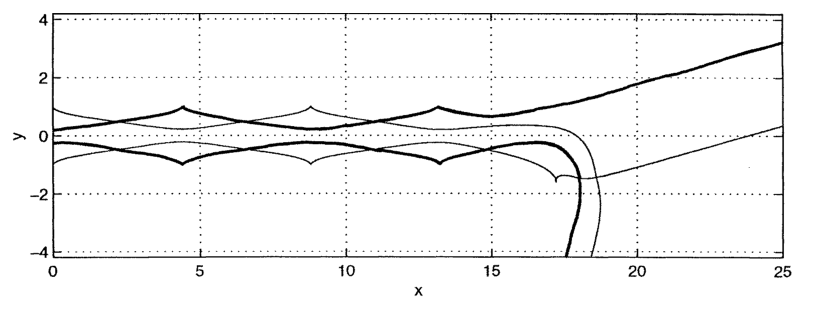
\includegraphics[width=\textwidth]{achinst.png}
\caption{Interaction of four line vortices with $\alpha=0.220$, and a pertubation of \num{1E-6}, showing instability. From \citet[p.~271]{acheson00}}
\label{fig:achinst}
\end{figure}
\begin{figure}[ht]
\centering
\setlength\figureheight{7.5cm} 
\setlength\figurewidth{\textwidth}
% This file was created by matlab2tikz.
% Minimal pgfplots version: 1.3
%
%The latest updates can be retrieved from
%  http://www.mathworks.com/matlabcentral/fileexchange/22022-matlab2tikz
%where you can also make suggestions and rate matlab2tikz.
%
\definecolor{mycolor1}{rgb}{0.00000,1.00000,1.00000}%
%
\begin{tikzpicture}

\begin{axis}[%
width=0.95092\figurewidth,
height=\figureheight,
at={(0\figurewidth,0\figureheight)},
scale only axis,
every outer x axis line/.append style={black},
every x tick label/.append style={font=\color{black}},
xmin=0,
xlabel={x},
every outer y axis line/.append style={black},
every y tick label/.append style={font=\color{black}},
ymin=-6.27093658068897,
ymax=6.27093658068897,
ylabel={y},
title={6000 time steps, step size = 0.005},
axis x line*=bottom,
axis y line*=left
]
\addplot [color=blue,solid,forget plot]
  table[row sep=crcr]{%
1e-006	1\\
0.000121506472075646	0.999987048793182\\
0.000242749837146671	0.999944062589649\\
0.000365465988949945	0.999871086950896\\
0.000490387081680514	0.999768199299914\\
0.000618239515155432	0.999635508527113\\
0.000749741968464183	0.999473154426216\\
0.000885603498965222	0.999281306967159\\
0.00102652172237743	0.999060165414953\\
0.00117318108835166	0.998809957305279\\
0.00132625126432857	0.99853093728915\\
0.00148638563873673	0.99822338586023\\
0.00165421995270589	0.99788760797944\\
0.00183037106751059	0.997523931612202\\
0.00201543587296723	0.997132706194076\\
0.00220999034002799	0.996714301040727\\
0.00241458871889007	0.996269103717978\\
0.00262976288210666	0.995797518387385\\
0.00285602181047974	0.995299964142093\\
0.00309385121796055	0.994776873346993\\
0.00334371331040254	0.994228689996165\\
0.00360604667181776	0.993655868099536\\
0.00388126627078917	0.993058870109461\\
0.00416976357889064	0.992438165396662\\
0.00447190679236061	0.991794228783675\\
0.00478804114785708	0.991127539142646\\
0.00511848932287979	0.990438578063037\\
0.00546355191136568	0.989727828593553\\
0.00582350796503	0.988995774061444\\
0.00619861559121971	0.988242896971215\\
0.00658911259835003	0.987469677983791\\
0.00699521718038972	0.986676594976242\\
0.00741712863232866	0.985864122181376\\
0.00785502808908434	0.985032729405797\\
0.00830907928086681	0.984182881324404\\
0.00877942929860804	0.983315036848798\\
0.00926620936366086	0.982429648566661\\
0.0097695355965706	0.981527162248815\\
0.0102895097803113	0.980608016420452\\
0.0108262201139496	0.97967264199283\\
0.0113797419532444	0.978721461951639\\
0.0119501385352103	0.977754891098183\\
0.0125374616841527	0.976773335839528\\
0.0131417524971351	0.975777194023833\\
0.0137630420072476	0.974766854817131\\
0.0144013518234215	0.973742698617969\\
0.0150566947458705	0.972705097006437\\
0.015729075356542	0.971654412724286\\
0.0164184905842243	0.97059099968298\\
0.0171249302441915	0.969515202996737\\
0.0178483775524664	0.968427359037768\\
0.0185888096149567	0.967327795511123\\
0.0193461978918624	0.966216831546738\\
0.0201205086378758	0.96509477780645\\
0.0209117033187935	0.96396193660394\\
0.0217197390052391	0.962818602035705\\
0.0225445687442561	0.961665060121369\\
0.0233861419095778	0.960501588951751\\
0.0242444045314126	0.959328458843284\\
0.0251192996066019	0.958145932497519\\
0.0260107673900205	0.956954265164557\\
0.0269187456680885	0.955753704809387\\
0.0278431700152596	0.954544492280223\\
0.0287839740343372	0.953326861478022\\
0.0297410895814525	0.95210103952647\\
0.0307144469765203	0.950867246941804\\
0.0317039751999598	0.949625697801927\\
0.032709602076445	0.948376599914324\\
0.033731254446418	0.947120154982378\\
0.0347688583260701	0.945856558769725\\
0.0358223390564652	0.944586001262339\\
0.0368916214424488	0.943308666828107\\
0.0379766298819553	0.94202473437367\\
0.0390772884862947	0.940734377498361\\
0.0401935211919732	0.939437764645095\\
0.0413252518645676	0.938135059248103\\
0.0424724043951498	0.936826419877428\\
0.0436349027897269	0.93551200038012\\
0.0448126712521377	0.934191950018082\\
0.0460056342608191	0.932866413602563\\
0.0472137166398336	0.931535531625267\\
0.0484368436245242	0.930199440386107\\
0.0496749409221416	0.9288582721176\\
0.0509279347677666	0.927512155105958\\
0.0521957519758329	0.926161213808881\\
0.0534783199875342	0.924805568970116\\
0.0547755669143825	0.923445337730832\\
0.0560874215781692	0.92208063373785\\
0.0574138135475621	0.920711567248798\\
0.0587546731715591	0.91933824523426\\
0.060109931610004	0.917960771476961\\
0.0614795208613575	0.916579246668078\\
0.0628633737879025	0.915193768500728\\
0.0642614241385544	0.913804431760713\\
0.0656736065694335	0.912411328414579\\
0.0670998566623471	0.911014547695073\\
0.0685401109413206	0.909614176184054\\
0.0699943068873075	0.908210297892933\\
0.0714623829511984	0.906802994340713\\
0.0729442785652438	0.905392344629687\\
0.0744399341529973	0.903978425518867\\
0.0759492911378771	0.902561311495216\\
0.0774722919504417	0.901141074842726\\
0.0790088800344651	0.899717785709431\\
0.0805589998518938	0.898291512172394\\
0.0821225968867634	0.896862320300747\\
0.0836996176481454	0.895430274216824\\
0.0852900096721918	0.893995436155465\\
0.086893721523341	0.892557866521525\\
0.0885107027947441	0.89111762394566\\
0.0901409041079664	0.889674765338437\\
0.0917842771120169	0.888229345942815\\
0.0934407744817544	0.886781419385049\\
0.0951103499157148	0.885331037724075\\
0.0967929581334043	0.883878251499408\\
0.0984885548720975	0.882423109777611\\
0.100197096883178	0.88096566019737\\
0.101918541928057	0.879505949013227\\
0.103652848773706	0.878044021138008\\
0.105399977187826	0.876579920183981\\
0.107159887933698	0.8751136885028\\
0.108932542764719	0.873645367224251\\
0.110717904418679	0.872174996293854\\
0.112515936611775	0.870702614509351\\
0.114326604032398	0.869228259556111\\
0.116149872334721	0.867751968041491\\
0.117985708132088	0.866273775528182\\
0.119834078990244	0.864793716566571\\
0.121694953420409	0.863311824726153\\
0.123568300872217	0.861828132626019\\
0.125454091726541	0.860342671964452\\
0.127352297288202	0.858855473547648\\
0.1292628897786	0.857366567317606\\
0.131185842328258	0.855875982379198\\
0.133121128969298	0.854383747026454\\
0.135068724627867	0.852889888768072\\
0.137028605116512	0.851394434352199\\
0.139000747126523	0.84989740979048\\
0.140985128220248	0.84839884038142\\
0.142981726823386	0.846898750733062\\
0.144990522217278	0.845397164785011\\
0.147011494531186	0.843894105829826\\
0.149044624734581	0.842389596533789\\
0.151089894629442	0.84088365895708\\
0.153147286842565	0.839376314573371\\
0.155216784817906	0.837867584288854\\
0.157298372808936	0.836357488460727\\
0.159392035871037	0.834846046915153\\
0.161497759853937	0.833333278964691\\
0.163615531394178	0.831819203425251\\
0.165745337907628	0.830303838632539\\
0.167887167582053	0.828787202458059\\
0.170041009369723	0.827269312324637\\
0.172206852980087	0.825750185221515\\
0.174384688872494	0.824229837719014\\
0.176574508248984	0.822708285982777\\
0.178776303047129	0.821185545787612\\
0.180990065932947	0.819661632530937\\
0.183215790293881	0.818136561245847\\
0.185453470231842	0.816610346613812\\
0.187703100556324	0.815083002977011\\
0.189964676777589	0.813554544350317\\
0.192238195099927	0.812024984432952\\
0.194523652414984	0.810494336619796\\
0.196821046295169	0.80896261401239\\
0.199130374987139	0.80742982942962\\
0.201451637405347	0.805895995418104\\
0.203784833125689	0.804361124262278\\
0.206129962379206	0.802825227994203\\
0.208487026045879	0.80128831840309\\
0.2108560256485	0.799750407044559\\
0.213236963346615	0.798211505249631\\
0.21562984193056	0.796671624133467\\
0.21803466481556	0.795130774603859\\
0.220451436035922	0.79358896736948\\
0.222880160239303	0.792046212947895\\
0.225320842681054	0.790502521673349\\
0.227773489218652	0.788957903704332\\
0.230238106306206	0.787412369030919\\
0.232714700989046	0.785865927481912\\
0.235203280898394	0.78431858873177\\
0.237703854246107	0.782770362307335\\
0.240216429819511	0.781221257594375\\
0.242741016976307	0.779671283843926\\
0.245277625639559	0.77812045017846\\
0.24782626629276	0.776568765597862\\
0.250386949974979	0.775016238985241\\
0.252959688276087	0.773462879112569\\
0.255544493332056	0.771908694646147\\
0.258141377820349	0.770353694151918\\
0.260750354955371	0.768797886100616\\
0.263371438484014	0.767241278872762\\
0.266004642681265	0.76568388076351\\
0.268649982345906	0.76412569998735\\
0.271307472796278	0.762566744682658\\
0.27397712986613	0.761007022916119\\
0.276658969900537	0.759446542687005\\
0.279353009751903	0.757885311931321\\
0.282059266776034	0.756323338525826\\
0.284777758828284	0.754760630291923\\
0.287508504259785	0.753197194999425\\
0.290251521913741	0.7516330403702\\
0.293006831121808	0.750068174081706\\
0.295774451700538	0.748502603770396\\
0.298554403947905	0.74693633703502\\
0.301346708639901	0.74536938143982\\
0.304151387027204	0.743801744517603\\
0.306968460831926	0.742233433772727\\
0.309797952244429	0.740664456683967\\
0.312639883920215	0.739094820707293\\
0.315494278976888	0.737524533278542\\
0.318361160991196	0.735953601815995\\
0.321240553996131	0.734382033722866\\
0.324132482478121	0.732809836389686\\
0.327036971374274	0.731237017196608\\
0.329954046069711	0.729663583515622\\
0.332883732394963	0.728089542712676\\
0.33582605662344	0.72651490214972\\
0.338781045468977	0.724939669186665\\
0.341748726083445	0.723363851183261\\
0.344729126054441	0.72178745550089\\
0.347722273403049	0.720210489504292\\
0.350728196581666	0.718632960563205\\
0.35374692447191	0.717054876053935\\
0.356778486382594	0.715476243360849\\
0.359822912047774	0.713897069877803\\
0.362880231624871	0.712317363009494\\
0.365950475692863	0.710737130172743\\
0.369033675250547	0.709156378797713\\
0.372129861714884	0.707575116329064\\
0.375239066919405	0.705993350227033\\
0.378361323112698	0.704411087968464\\
0.381496662956961	0.702828337047764\\
0.384645119526641	0.701245104977804\\
0.387806726307129	0.699661399290762\\
0.390981517193547	0.698077227538902\\
0.394169526489595	0.696492597295302\\
0.397370788906479	0.69490751615452\\
0.400585339561918	0.693321991733208\\
0.403813213979211	0.691736031670676\\
0.407054448086401	0.690149643629396\\
0.410309078215492	0.688562835295458\\
0.413577141101761	0.686975614378979\\
0.416858673883135	0.685387988614456\\
0.420153714099645	0.683799965761077\\
0.423462299692968	0.68221155360298\\
0.426784469006032	0.68062275994947\\
0.430120260782708	0.679033592635186\\
0.433469714167577	0.677444059520231\\
0.436832868705781	0.675854168490251\\
0.440209764342945	0.674263927456477\\
0.443600441425182	0.672673344355725\\
0.447004940699185	0.671082427150357\\
0.45042330331239	0.669491183828199\\
0.453855570813223	0.667899622402425\\
0.457301785151433	0.666307750911403\\
0.460761988678505	0.664715577418504\\
0.464236224148149	0.663123110011877\\
0.467724534716886	0.661530356804185\\
0.471226963944706	0.65993732593232\\
0.474743555795815	0.65834402555707\\
0.478274354639468	0.656750463862765\\
0.481819405250886	0.655156649056891\\
0.485378752812261	0.653562589369674\\
0.488952442913843	0.651968293053631\\
0.492540521555122	0.650373768383104\\
0.496143035146091	0.648779023653754\\
0.499760030508605	0.647184067182042\\
0.50339155487782	0.645588907304678\\
0.507037655903728	0.643993552378045\\
0.510698381652785	0.642398010777608\\
0.514373780609625	0.640802290897293\\
0.518063901678866	0.63920640114885\\
0.521768794187013	0.637610349961192\\
0.525488507884449	0.636014145779721\\
0.529223092947527	0.634417797065627\\
0.532972599980747	0.632821312295182\\
0.536737080019037	0.631224699959003\\
0.540516584530125	0.629627968561313\\
0.544311165417012	0.628031126619181\\
0.548120875020533	0.626434182661749\\
0.551945766122033	0.624837145229445\\
0.555785891946122	0.623240022873191\\
0.559641306163544	0.621642824153595\\
0.563512062894143	0.620045557640132\\
0.567398216709923	0.61844823191032\\
0.571299822638222	0.616850855548889\\
0.575216936164977	0.615253437146939\\
0.579149613238098	0.613655985301094\\
0.583097910270947	0.612058508612655\\
0.587061884145917	0.61046101568674\\
0.591041592218121	0.608863515131432\\
0.595037092319187	0.607266015556915\\
0.599048442761152	0.605668525574616\\
0.60307570234048	0.604071053796345\\
0.607118930342169	0.602473608833429\\
0.611178186543985	0.600876199295862\\
0.615253531220794	0.599278833791444\\
0.619345025149008	0.597681520924928\\
0.623452729611149	0.596084269297177\\
0.627576706400512	0.59448708750432\\
0.63171701782596	0.592889984136914\\
0.635873726716811	0.591292967779121\\
0.64004689642786	0.589696047007884\\
0.644236590844506	0.588099230392118\\
0.648442874387992	0.586502526491913\\
0.652665812020775	0.584905943857739\\
0.656905469252004	0.583309491029676\\
0.661161912143117	0.581713176536646\\
0.665435207313565	0.580117008895668\\
0.669725421946649	0.578520996611119\\
0.674032623795483	0.576925148174018\\
0.678356881189077	0.575329472061326\\
0.682698263038543	0.573733976735261\\
0.687056838843431	0.572138670642633\\
0.691432678698176	0.570543562214203\\
0.69582585329869	0.568948659864054\\
0.700236433949062	0.567353971988992\\
0.704664492568397	0.565759506967965\\
0.709110101697781	0.564165273161511\\
0.713573334507373	0.562571278911221\\
0.718054264803631	0.560977532539237\\
0.722552967036662	0.559384042347774\\
0.727069516307714	0.557790816618663\\
0.731603988376797	0.556197863612935\\
0.736156459670429	0.554605191570423\\
0.740727007289533	0.553012808709398\\
0.74531570901746	0.55142072322624\\
0.749922643328145	0.549828943295137\\
0.754547889394414	0.548237477067819\\
0.759191527096416	0.546646332673325\\
0.763853637030205	0.545055518217809\\
0.768534300516456	0.543465041784375\\
0.773233599609326	0.541874911432961\\
0.777951617105456	0.540285135200246\\
0.782688436553122	0.538695721099613\\
0.787444142261521	0.537106677121138\\
0.792218819310212	0.535518011231628\\
0.7970125535587	0.5339297313747\\
0.801825431656169	0.532341845470903\\
0.806657541051362	0.530754361417886\\
0.811508970002615	0.529167287090607\\
0.816379807588039	0.527580630341595\\
0.821270143715853	0.525994399001254\\
0.826180069134876	0.524408600878219\\
0.831109675445169	0.522823243759763\\
0.836059055108834	0.52123833541225\\
0.841028301460969	0.519653883581645\\
0.846017508720782	0.518069895994077\\
0.851026772002862	0.51648638035645\\
0.856056187328615	0.514903344357122\\
0.861105851637853	0.513320795666626\\
0.866175862800556	0.511738741938461\\
0.871266319628787	0.510157190809938\\
0.876377321888777	0.508576149903084\\
0.881508970313178	0.506995626825611\\
0.88666136661348	0.505415629171948\\
0.891834613492591	0.503836164524336\\
0.897028814657601	0.502257240453989\\
0.902244074832698	0.500678864522325\\
0.90748049977227	0.499101044282261\\
0.912738196274171	0.497523787279582\\
0.918017272193167	0.495947101054376\\
0.923317836454551	0.494370993142554\\
0.928639999067937	0.492795471077426\\
0.933983871141231	0.491220542391372\\
0.939349564894781	0.489646214617579\\
0.944737193675701	0.48807249529186\\
0.95014687197238	0.486499391954554\\
0.955578715429173	0.484926912152515\\
0.961032840861267	0.483355063441173\\
0.966509366269739	0.481783853386691\\
0.972008410856789	0.480213289568209\\
0.977530095041165	0.478643379580179\\
0.983074540473768	0.477074131034782\\
0.988641870053446	0.475505551564458\\
0.994232207942975	0.473937648824511\\
0.999845679585223	0.472370430495832\\
1.00548241171951	0.470803904287708\\
1.01114253239815	0.469238077940741\\
1.01682617100319	0.46767295922987\\
1.02253345826332	0.466108555967503\\
1.028264526271	0.464544876006756\\
1.03401950849975	0.462981927244807\\
1.03979853982166	0.46141971762636\\
1.04560175652504	0.459858255147239\\
1.05142929633234	0.458297547858087\\
1.05728129841818	0.456737603868201\\
1.0631579034276	0.455178431349487\\
1.06905925349451	0.453620038540549\\
1.07498549226035	0.452062433750902\\
1.08093676489284	0.450505625365337\\
1.08691321810504	0.448949621848405\\
1.09291500017453	0.447394431749062\\
1.09894226096277	0.44584006370545\\
1.10499515193467	0.444286526449828\\
1.11107382617831	0.442733828813662\\
1.11717843842489	0.441181979732868\\
1.1233091450688	0.439630988253222\\
1.12946610418791	0.438080863535925\\
1.135649475564	0.436531614863354\\
1.14185942070337	0.43498325164497\\
1.14809610285764	0.433435783423422\\
1.15435968704467	0.43188921988082\\
1.16065034006969	0.430343570845206\\
1.16696823054652	0.428798846297217\\
1.173313528919	0.427255056376941\\
1.17968640748257	0.425712211390988\\
1.1860870404059	0.424170321819761\\
1.19251560375277	0.422629398324945\\
1.19897227550401	0.421089451757219\\
1.20545723557957	0.419550493164198\\
1.21197066586074	0.418012533798597\\
1.21851275021241	0.416475585126653\\
1.22508367450552	0.414939658836777\\
1.23168362663948	0.413404766848469\\
1.2383127965648	0.411870921321491\\
1.24497137630571	0.41033813466531\\
1.25165955998285	0.408806419548815\\
1.25837754383599	0.407275788910315\\
1.26512552624686	0.405746255967837\\
1.27190370776194	0.404217834229715\\
1.27871229111522	0.402690537505492\\
1.28555148125106	0.401164379917141\\
1.29242148534695	0.39963937591061\\
1.29932251283623	0.398115540267702\\
1.3062547754308	0.396592888118309\\
1.31321848714367	0.395071434952991\\
1.32021386431155	0.39355119663593\\
1.32724112561713	0.39203218941826\\
1.33430049211142	0.390514429951784\\
1.34139218723576	0.388997935303089\\
1.34851643684372	0.387482722968083\\
1.35567346922278	0.38596881088694\\
1.36286351511571	0.384456217459499\\
1.37008680774175	0.382944961561103\\
1.3773435828174	0.381435062558902\\
1.38463407857692	0.379926540328639\\
1.39195853579239	0.378419415271922\\
1.39931719779344	0.376913708334004\\
1.40671031048643	0.375409441022092\\
1.41413812237318	0.373906635424181\\
1.42160088456912	0.372405314228455\\
1.42909885082088	0.370905500743249\\
1.43663227752321	0.36940721891761\\
1.4442014237352	0.367910493362451\\
1.45180655119576	0.366415349372344\\
1.45944792433827	0.364921812947947\\
1.46712581030439	0.363429910819099\\
1.47484047895686	0.361939670468601\\
1.4825922028914	0.360451120156697\\
1.4903812574474	0.358964288946285\\
1.49820792071754	0.357479206728881\\
1.50607247355617	0.355995904251348\\
1.5139751995863	0.354514413143427\\
1.52191638520524	0.353034765946085\\
1.52989631958871	0.351556996140713\\
1.53791529469333	0.350081138179194\\
1.54597360525744	0.348607227514872\\
1.55407154880005	0.347135300634443\\
1.56220942561787	0.345665395090812\\
1.57038753878032	0.344197549536923\\
1.57860619412228	0.342731803760618\\
1.58686570023463	0.341268198720529\\
1.59516636845218	0.339806776583066\\
1.60350851283914	0.338347580760501\\
1.61189245017174	0.336890655950215\\
1.62031849991795	0.335436048175117\\
1.62878698421405	0.333983804825289\\
1.63729822783805	0.332533974700883\\
1.64585255817945	0.331086608056319\\
1.65445030520549	0.329641756645813\\
1.66309180142346	0.328199473770284\\
1.67177738183886	0.32675981432568\\
1.68050738390934	0.325322834852765\\
1.68928214749396	0.323888593588409\\
1.6981020147977	0.322457150518432\\
1.70696733031083	0.32102856743205\\
1.71587844074292	0.319602907977958\\
1.72483569495121	0.318180237722114\\
1.73383944386297	0.316760624207271\\
1.74289004039157	0.3153441370143\\
1.75198783934596	0.313930847825362\\
1.7611331973331	0.312520830488991\\
1.7703264726531	0.311114161087128\\
1.77956802518654	0.309710918004167\\
1.78885821627373	0.308311181998076\\
1.79819740858532	0.306915036273644\\
1.80758596598392	0.305522566557908\\
1.81702425337623	0.304133861177833\\
1.82651263655525	0.302749011140286\\
1.8360514820319	0.301368110214379\\
1.84564115685575	0.29999125501623\\
1.85528202842409	0.298618545096207\\
1.86497446427897	0.297250083028711\\
1.87471883189134	0.295885974504556\\
1.88451549843199	0.294526328426008\\
1.89436483052831	0.293171257004524\\
1.90426719400641	0.291820875861267\\
1.91422295361784	0.290475304130427\\
1.92423247275003	0.2891346645654\\
1.93429611311995	0.287799083647884\\
1.9444142344499	0.286468691699904\\
1.95458719412478	0.285143622998827\\
1.96481534683002	0.283824015895368\\
1.97509904416901	0.28251001293463\\
1.98543863425952	0.281201760980167\\
1.99583446130772	0.279899411341086\\
2.00628686515918	0.278603119902157\\
2.01679618082565	0.277313047256931\\
2.02736273798654	0.276029358843794\\
2.03798686046426	0.274752225084916\\
2.04866886567202	0.273481821528016\\
2.05940906403326	0.272218328990818\\
2.07020775837132	0.270961933708098\\
2.08106524326843	0.269712827481138\\
2.09198180439265	0.26847120782941\\
2.10295771779162	0.267237278144253\\
2.11399324915206	0.26601124784428\\
2.12508865302368	0.264793332532194\\
2.13624417200631	0.263583754152651\\
2.14746003589923	0.262382741150746\\
2.15873646081139	0.261190528630641\\
2.17007364823149	0.260007358513779\\
2.18147178405686	0.258833479696065\\
2.19293103758009	0.257669148203297\\
2.20445156043248	0.256514627344057\\
2.21603348548347	0.25537018785917\\
2.22767692569539	0.25423610806673\\
2.2393819729328	0.25311267400158\\
2.25114869672598	0.252000179548029\\
2.26297714298849	0.250898926564428\\
2.27486733268842	0.249809224998122\\
2.28681926047378	0.248731392989132\\
2.29883289325232	0.247665756960775\\
2.31090816872656	0.246612651695264\\
2.3230449938852	0.245572420392183\\
2.33524324345223	0.244545414707536\\
2.34750275829586	0.24353199477093\\
2.35982334379949	0.242532529178247\\
2.37220476819774	0.241547394957028\\
2.38464676088101	0.240576977501576\\
2.39714901067266	0.239621670474685\\
2.40971116408367	0.238681875672711\\
2.42233282355028	0.237758002850594\\
2.43501354566092	0.236850469503337\\
2.44775283937958	0.235959700600343\\
2.46055016427362	0.235086128269001\\
2.47340492875499	0.234230191423874\\
2.48631648834464	0.233392335337893\\
2.49928414397098	0.232573011152066\\
2.51230714031421	0.231772675320349\\
2.52538466420927	0.230991788986556\\
2.53851584312109	0.2302308172905\\
2.55169974370683	0.229490228600908\\
2.56493537048052	0.228770493673164\\
2.57822166459645	0.228072084730455\\
2.59155750276823	0.227395474467596\\
2.60494169634095	0.226741134977539\\
2.61837299053442	0.226109536601433\\
2.63185006387543	0.22550114670406\\
2.64537152783718	0.224916428377486\\
2.65893592670373	0.224355839076911\\
2.67254173767658	0.223819829193833\\
2.68618737123997	0.223308840572919\\
2.69987117180018	0.222823304980181\\
2.71359141861273	0.222363642531349\\
2.72734632700947	0.221930260090545\\
2.74113404993569	0.221523549650567\\
2.75495267980448	0.221143886707163\\
2.76880025067345	0.220791628640702\\
2.78267474074505	0.220467113119457\\
2.79657407518932	0.220170656539369\\
2.81049612928363	0.219902552515649\\
2.82443873186079	0.219663070441732\\
2.838399669053	0.219452454131095\\
2.85237668831535	0.219270920557098\\
2.86636750270896	0.219118658705424\\
2.88036979542025	0.218995828552787\\
2.89438122448939	0.218902560184405\\
2.90839942771825	0.218838953061314\\
2.92242202772513	0.2188050754469\\
2.9364466371116	0.218800964000163\\
2.95047086370493	0.218826623541147\\
2.96449231583837	0.218882026991798\\
2.97850860763106	0.218967115493251\\
2.99251736422915	0.219081798698245\\
3.00651622697035	0.219225955235114\\
3.02050285843537	0.21939943333762\\
3.03447494735112	0.219602051632822\\
3.04843021331307	0.219833600077311\\
3.06236641129644	0.220093841030452\\
3.07628133592938	0.220382510451856\\
3.09017282550405	0.220699319209137\\
3.10403876570557	0.221043954481126\\
3.11787709304235	0.221416081241138\\
3.13168579796497	0.221815343804557\\
3.14546292766475	0.222241367425005\\
3.1592065885468	0.222693759923598\\
3.17291494837586	0.223172113336229\\
3.1865862380966	0.223676005564572\\
3.20021875333325	0.224205002017308\\
3.21381085557619	0.224758657229137\\
3.22736097306554	0.225336516446263\\
3.24086760138425	0.225938117168257\\
3.25432930377471	0.226562990637472\\
3.26774471119462	0.227210663268484\\
3.28111252212883	0.227880658011316\\
3.29443150217502	0.228572495643439\\
3.30770048342112	0.229285695986771\\
3.32091836363323	0.230019779047018\\
3.33408410527234	0.230774266073744\\
3.3471967343581	0.231548680540548\\
3.36025533919766	0.23234254904555\\
3.37325906899672	0.2331554021332\\
3.38620713236944	0.233986775039041\\
3.39909879576304	0.234836208359662\\
3.41193338181193	0.23570324865051\\
3.42471026763533	0.236587448954633\\
3.43742888309139	0.237488369265699\\
3.45008870899967	0.238405576928864\\
3.46268927534303	0.239338646983199\\
3.47523015945885	0.24028716244946\\
3.48771098422853	0.241250714567029\\
3.50013141627336	0.242228902983808\\
3.51249116416389	0.243221335902814\\
3.52478997664912	0.244227630189097\\
3.53702764091094	0.245247411440509\\
3.54920398084865	0.246280314025691\\
3.56131885539752	0.247325981092489\\
3.57337215688489	0.248384064549844\\
3.58536380942653	0.249454225026012\\
3.59729376736565	0.250536131805806\\
3.60916201375621	0.251629462749346\\
3.62096855889208	0.252733904194636\\
3.63271343888285	0.253849150846107\\
3.644396714277	0.254974905651094\\
3.65601846873271	0.256110879666031\\
3.66757880773639	0.257256791914022\\
3.67907785736873	0.258412369235257\\
3.69051576311777	0.259577346131641\\
3.70189268873863	0.260751464606819\\
3.71320881515893	0.26193447400272\\
3.7244643394293	0.263126130833554\\
3.73565947371781	0.264326198618169\\
3.74679444434742	0.265534447711489\\
3.75786949087532	0.266750655135757\\
3.76888486521296	0.267974604412129\\
3.77984083078562	0.269206085393181\\
3.79073766173032	0.270444894096746\\
3.80157564213067	0.271690832541485\\
3.81235506528765	0.272943708584522\\
3.82307623302487	0.274203335761419\\
3.83373945502714	0.275469533128737\\
3.84434504821114	0.27674212510937\\
3.85489333612686	0.278020941340817\\
3.86538464838878	0.279305816526516\\
3.87581932013543	0.280596590290352\\
3.8861976915163	0.281893107034399\\
3.89652010720492	0.28319521579995\\
3.90678691593708	0.284502770131888\\
3.91699847007296	0.285815627946388\\
3.92715512518239	0.287133651401972\\
3.937257239652	0.288456706773893\\
3.94730517431345	0.289784664331845\\
3.95729929209173	0.29111739822094\\
3.96723995767264	0.292454786345945\\
3.9771275371886	0.293796710258708\\
3.98696239792193	0.29514305504874\\
3.99674490802486	0.296493709236883\\
4.00647543625535	0.29784856467202\\
4.01615435172816	0.299207516430748\\
4.02578202368029	0.300570462719969\\
4.03535882125026	0.301937304782311\\
4.04488511327046	0.303307946804332\\
4.05436126807192	0.304682295827423\\
4.06378765330112	0.306060261661355\\
4.07316463574789	0.307441756800387\\
4.08249258118425	0.308826696341881\\
4.09177185421334	0.310214997907342\\
4.10100281812817	0.311606581565831\\
4.11018583477953	0.313001369759671\\
4.11932126445271	0.314399287232383\\
4.12840946575261	0.315800260958801\\
4.13745079549664	0.317204220077284\\
4.14644560861531	0.318611095823969\\
4.15539425805981	0.320020821469018\\
4.16429709471646	0.321433332254776\\
4.17315446732751	0.322848565335804\\
4.18196672241815	0.324266459720715\\
4.19073420422915	0.325686956215768\\
4.19945725465508	0.327109997370165\\
4.20813621318773	0.328535527422988\\
4.21677141686435	0.329963492251743\\
4.22536320022064	0.331393839322453\\
4.23391189524814	0.332826517641242\\
4.24241783135572	0.334261477707386\\
4.25088133533509	0.33569867146777\\
4.25930273133002	0.337138052272705\\
4.26768234080906	0.338579574833078\\
4.27602048254168	0.340023195178779\\
4.2843174725774	0.341468870618372\\
4.29257362422812	0.342916559699971\\
4.30078924805299	0.344366222173284\\
4.3089646518462	0.345817818952787\\
4.31710014062703	0.34727131208199\\
4.32519601663241	0.348726664698772\\
4.33325257931161	0.350183841001737\\
4.34127012532307	0.351642806217574\\
4.34924894853317	0.353103526569377\\
4.35718934001678	0.354565969245909\\
4.36509158805969	0.356030102371762\\
4.37295597816252	0.357495894978408\\
4.38078279304624	0.358963316976092\\
4.38857231265908	0.360432339126564\\
4.3963248141848	0.361902933016595\\
4.40404057205221	0.363375071032285\\
4.41171985794585	0.36484872633411\\
4.4193629408178	0.366323872832711\\
4.42697008690042	0.367800485165377\\
4.43454155972017	0.369278538673225\\
4.4420776201122	0.370758009379036\\
4.4495785262358	0.372238873965742\\
4.45704453359066	0.373721109755532\\
4.46447589503372	0.375204694689567\\
4.47187286079681	0.376689607308284\\
4.47923567850476	0.378175826732266\\
4.48656459319415	0.379663332643666\\
4.49385984733255	0.381152105268172\\
4.50112168083816	0.382642125357482\\
4.50835033109998	0.384133374172293\\
4.51554603299826	0.385625833465774\\
4.52270901892536	0.387119485467516\\
4.52983951880689	0.38861431286794\\
4.53693776012318	0.390110298803157\\
4.54400396793093	0.391607426840255\\
4.55103836488511	0.393105680963015\\
4.55804117126108	0.394605045558027\\
4.56501260497681	0.396105505401208\\
4.57195288161535	0.397607045644704\\
4.57886221444727	0.399109651804165\\
4.58574081445334	0.400613309746384\\
4.5925888903472	0.402118005677285\\
4.5994066485981	0.403623726130258\\
4.60619429345373	0.405130457954821\\
4.61295202696297	0.406638188305607\\
4.61968004899877	0.408146904631669\\
4.62637855728091	0.409656594666076\\
4.63304774739882	0.411167246415821\\
4.6396878128343	0.412678848152006\\
4.64629894498422	0.414191388400306\\
4.65288133318318	0.415704855931711\\
4.65943516472604	0.417219239753523\\
4.66596062489042	0.418734529100617\\
4.67245789695909	0.420250713426946\\
4.67892716224226	0.421767782397289\\
4.68536860009975	0.423285725879235\\
4.69178238796304	0.424804533935396\\
4.69816870135726	0.426324196815842\\
4.70452771392292	0.427844704950754\\
4.71085959743765	0.429366048943283\\
4.71716452183769	0.430888219562619\\
4.72344265523929	0.432411207737259\\
4.7296941639599	0.433935004548462\\
4.7359192125393	0.435459601223901\\
4.74211796376046	0.436984989131498\\
4.74829057867028	0.438511159773429\\
4.7544372166002	0.440038104780314\\
4.76055803518658	0.441565815905569\\
4.76665319039094	0.443094285019926\\
4.77272283651999	0.444623504106116\\
4.77876712624553	0.446153465253701\\
4.78478621062412	0.447684160654069\\
4.7907802391166	0.449215582595566\\
4.79674935960738	0.450747723458783\\
4.80269371842365	0.45228057571198\\
4.80861346035425	0.453814131906644\\
4.81450872866847	0.455348384673188\\
4.82037966513463	0.456883326716776\\
4.82622641003843	0.458418950813277\\
4.8320491022012	0.459955249805341\\
4.83784787899782	0.461492216598605\\
4.8436228763746	0.463029844158002\\
4.84937422886688	0.464568125504202\\
4.85510206961646	0.466107053710154\\
4.86080653038882	0.467646621897744\\
4.8664877415902	0.469186823234559\\
4.87214583228443	0.47072765093075\\
4.87778093020964	0.472269098236013\\
4.88339316179469	0.47381115843665\\
4.88898265217549	0.475353824852743\\
4.8945495252111	0.476897090835416\\
4.90009390349965	0.478440949764191\\
4.90561590839406	0.47998539504444\\
4.91111566001759	0.481530420104919\\
4.91659327727919	0.483076018395391\\
4.92204887788869	0.484622183384341\\
4.9274825783718	0.48616890855676\\
4.93289449408489	0.487716187412028\\
4.93828473922964	0.489264013461859\\
4.94365342686749	0.490812380228338\\
4.94900066893392	0.492361281242023\\
4.95432657625253	0.493910710040132\\
4.95963125854895	0.495460660164792\\
4.96491482446461	0.497011125161367\\
4.9701773815703	0.498562098576852\\
4.97541903637954	0.500113573958339\\
4.98063989436185	0.501665544851542\\
4.98584005995578	0.503218004799396\\
4.99101963658179	0.504770947340715\\
4.99617872665496	0.506324366008915\\
5.0013174315976	0.507878254330793\\
5.00643585185155	0.509432605825373\\
5.01153408689047	0.510987414002809\\
5.01661223523187	0.512542672363338\\
5.02167039444902	0.514098374396302\\
5.02670866118269	0.515654513579211\\
5.03172713115269	0.517211083376873\\
5.03672589916936	0.518768077240568\\
5.04170505914479	0.520325488607274\\
5.04666470410394	0.52188331089895\\
5.0516049261956	0.523441537521861\\
5.05652581670319	0.525000161865953\\
5.06142746605541	0.526559177304283\\
5.06630996383676	0.52811857719248\\
5.07117339879788	0.529678354868267\\
5.07601785886576	0.53123850365102\\
5.0808434311538	0.532799016841365\\
5.08565020197172	0.53435988772083\\
5.09043825683533	0.535921109551528\\
5.09520768047619	0.537482675575883\\
5.09995855685104	0.539044579016399\\
5.10469096915119	0.540606813075463\\
5.10940499981171	0.54216937093519\\
5.11410073052051	0.543732245757298\\
5.11877824222724	0.54529543068303\\
5.12343761515213	0.546858918833097\\
5.12807892879461	0.54842270330767\\
5.13270226194185	0.549986777186391\\
5.13730769267719	0.551551133528429\\
5.14189529838833	0.553115765372559\\
5.14646515577551	0.554680665737276\\
5.15101734085951	0.556245827620935\\
5.15555192898952	0.557811244001928\\
5.16006899485085	0.55937690783888\\
5.16456861247262	0.560942812070878\\
5.16905085523519	0.562508949617724\\
5.17351579587754	0.564075313380218\\
5.17796350650455	0.565641896240461\\
5.18239405859409	0.567208691062184\\
5.18680752300403	0.568775690691102\\
5.19120396997912	0.570342887955291\\
5.19558346915776	0.571910275665581\\
5.19994608957862	0.57347784661598\\
5.20429189968718	0.575045593584108\\
5.20862096734215	0.576613509331657\\
5.21293335982172	0.578181586604871\\
5.21722914382977	0.579749818135036\\
5.22150838550192	0.581318196638994\\
5.22577115041148	0.582886714819672\\
5.23001750357528	0.584455365366628\\
5.23424750945939	0.586024140956605\\
5.23846123198473	0.587593034254108\\
5.24265873453259	0.589162037911987\\
5.24684007995	0.59073114457204\\
5.25100533055504	0.592300346865618\\
5.25515454814196	0.593869637414252\\
5.25928779398633	0.595439008830279\\
5.26340512884993	0.597008453717486\\
5.26750661298564	0.598577964671761\\
5.27159230614219	0.600147534281747\\
5.27566226756882	0.601717155129506\\
5.27971655601979	0.603286819791195\\
5.28375522975885	0.604856520837735\\
5.28777834656359	0.6064262508355\\
5.29178596372964	0.607996002346992\\
5.29577813807486	0.609565767931542\\
5.29975492594335	0.611135540145987\\
5.30371638320938	0.612705311545372\\
5.30766256528128	0.614275074683641\\
5.31159352710513	0.615844822114328\\
5.31550932316845	0.617414546391249\\
5.31941000750374	0.618984240069198\\
5.32329563369195	0.620553895704632\\
5.32716625486581	0.622123505856358\\
5.33102192371314	0.623693063086215\\
5.33486269247999	0.625262559959752\\
5.33868861297376	0.626831989046901\\
5.34249973656617	0.628401342922641\\
5.34629611419616	0.629970614167659\\
5.3500777963727	0.631539795369004\\
5.35384483317751	0.633108879120724\\
5.35759727426771	0.634677858024507\\
5.36133516887831	0.6362467246903\\
5.36505856582473	0.637815471736925\\
5.36876751350512	0.63938409179268\\
5.37246205990262	0.640952577495928\\
5.37614225258762	0.642520921495673\\
5.37980813871981	0.644089116452123\\
5.38345976505019	0.645657155037239\\
5.38709717792307	0.647225029935263\\
5.39072042327786	0.648792733843238\\
5.39432954665084	0.650360259471505\\
5.39792459317691	0.651927599544184\\
5.40150560759109	0.653494746799635\\
5.40507263423013	0.655061693990903\\
5.40862571703391	0.65662843388614\\
5.41216489954676	0.658194959269005\\
5.41569022491883	0.659761262939044\\
5.41920173590718	0.661327337712048\\
5.42269947487699	0.662893176420386\\
5.42618348380253	0.664458771913312\\
5.42965380426814	0.666024117057251\\
5.43311047746914	0.667589204736058\\
5.43655354421259	0.669154027851246\\
5.43998304491805	0.670718579322192\\
5.4433990196182	0.67228285208631\\
5.44680150795943	0.673846839099199\\
5.45019054920234	0.675410533334758\\
5.45356618222217	0.67697392778527\\
5.4569284455091	0.678537015461455\\
5.46027737716858	0.68009978939249\\
5.4636130149215	0.681662242625996\\
5.46693539610431	0.68322436822799\\
5.47024455766906	0.684786159282799\\
5.47354053618341	0.686347608892946\\
5.47682336783051	0.687908710178987\\
5.48009308840884	0.68946945627932\\
5.48334973333194	0.691029840349948\\
5.48659333762813	0.692589855564208\\
5.48982393594013	0.694149495112455\\
5.49304156252455	0.695708752201702\\
5.49624625125143	0.697267620055227\\
5.49943803560357	0.698826091912121\\
5.50261694867593	0.700384161026809\\
5.50578302317484	0.701941820668505\\
5.50893629141719	0.703499064120641\\
5.51207678532958	0.705055884680229\\
5.51520453644735	0.70661227565719\\
5.51831957591353	0.708168230373619\\
5.5214219344778	0.709723742163008\\
5.5245116424953	0.711278804369416\\
5.5275887299254	0.71283341034658\\
5.53065322633041	0.714387553456973\\
5.53370516087418	0.715941227070814\\
5.53674456232072	0.717494424565005\\
5.53977145903264	0.719047139322029\\
5.54278587896958	0.720599364728769\\
5.5457878496866	0.722151094175282\\
5.54877739833243	0.723702321053501\\
5.55175455164769	0.725253038755876\\
5.55471933596304	0.726803240673948\\
5.55767177719728	0.728352920196866\\
5.56061190085533	0.729902070709818\\
5.56353973202617	0.731450685592413\\
5.56645529538074	0.732998758216975\\
5.56935861516969	0.734546281946773\\
5.57224971522118	0.736093250134178\\
5.57512861893847	0.737639656118738\\
5.57799534929757	0.739185493225179\\
5.58084992884474	0.740730754761328\\
5.58369237969391	0.74227543401595\\
5.58652272352413	0.74381952425651\\
5.58934098157683	0.745363018726838\\
5.59214717465307	0.746905910644721\\
5.59494132311074	0.748448193199396\\
5.59772344686161	0.749989859548955\\
5.60049356536842	0.751530902817661\\
5.60325169764176	0.753071316093159\\
5.60599786223705	0.754611092423601\\
5.60873207725126	0.756150224814663\\
5.61145436031971	0.757688706226464\\
5.61416472861275	0.759226529570377\\
5.61686319883229	0.760763687705737\\
5.61954978720838	0.762300173436435\\
5.62222450949565	0.763835979507401\\
5.62488738096968	0.765371098600975\\
5.6275384164233	0.766905523333152\\
5.63017763016281	0.768439246249716\\
5.63280503600416	0.769972259822241\\
5.63542064726902	0.771504556443972\\
5.63802447678075	0.773036128425566\\
5.64061653686038	0.774566967990714\\
5.64319683932244	0.776097067271609\\
5.64576539547071	0.777626418304285\\
5.64832221609398	0.779155013023808\\
5.65086731146161	0.78068284325932\\
5.65340069131911	0.782209900728925\\
5.65592236488361	0.78373617703443\\
5.65843234083925	0.785261663655912\\
5.66093062733246	0.786786351946137\\
5.66341723196725	0.788310233124795\\
5.66589216180035	0.789833298272567\\
5.66835542333626	0.791355538325022\\
5.67080702252226	0.792876944066316\\
5.67324696474339	0.794397506122715\\
5.6756752548172	0.795917214955921\\
5.67809189698859	0.7974360608562\\
5.68049689492446	0.798954033935303\\
5.68289025170831	0.800471124119184\\
5.6852719698348	0.801987321140497\\
5.68764205120417	0.803502614530875\\
5.69000049711662	0.805016993612979\\
5.69234730826662	0.806530447492314\\
5.69468248473708	0.808042965048806\\
5.69700602599354	0.809554534928129\\
5.69931793087818	0.811065145532777\\
5.70161819760385	0.81257478501288\\
5.70390682374793	0.814083441256743\\
5.70618380624618	0.81559110188111\\
5.70844914138652	0.817097754221146\\
5.71070282480266	0.818603385320126\\
5.71294485146775	0.820107981918814\\
5.7151752156879	0.821611530444539\\
5.71739391109565	0.823114016999953\\
5.71960093064335	0.824615427351448\\
5.72179626659652	0.826115746917246\\
5.72397991052707	0.827614960755136\\
5.72615185330652	0.829113053549849\\
5.72831208509916	0.830610009600062\\
5.73046059535505	0.832105812805033\\
5.73259737280312	0.833600446650822\\
5.73472240544405	0.83509389419613\\
5.73683568054325	0.836586138057707\\
5.73893718462365	0.838077160395336\\
5.74102690345857	0.839566942896376\\
5.74310482206441	0.841055466759846\\
5.74517092469346	0.842542712680049\\
5.74722519482654	0.8440286608297\\
5.74926761516564	0.845513290842566\\
5.75129816762663	0.846996581795591\\
5.75331683333178	0.848478512190491\\
5.75532359260242	0.849959059934802\\
5.75731842495149	0.851438202322374\\
5.75930130907613	0.852915916013279\\
5.76127222285027	0.854392177013127\\
5.7632311433172	0.855866960651766\\
5.76517804668221	0.857340241561351\\
5.7671129083052	0.858811993653754\\
5.76903570269336	0.860282190097309\\
5.77094640349388	0.861750803292856\\
5.77284498348672	0.863217804849077\\
5.77473141457741	0.86468316555709\\
5.77660566779	0.866146855364281\\
5.77846771326004	0.86760884334736\\
5.78031752022764	0.869069097684602\\
5.7821550570307	0.870527585627259\\
5.78398029109826	0.871984273470114\\
5.78579318894393	0.873439126521145\\
5.78759371615959	0.874892109070283\\
5.78938183740915	0.876343184357226\\
5.7911575164226	0.877792314538279\\
5.7929207159902	0.879239460652203\\
5.79467139795702	0.880684582585023\\
5.79640952321758	0.882127639033782\\
5.79813505171091	0.883568587469189\\
5.79984794241588	0.88500738409715\\
5.80154815334683	0.88644398381912\\
5.8032356415496	0.887878340191266\\
5.80491036309797	0.889310405382385\\
5.80657227309049	0.89074013013055\\
5.80822132564779	0.892167463698439\\
5.80985747391043	0.893592353827307\\
5.81148067003719	0.895014746689569\\
5.81309086520407	0.896434586839931\\
5.81468800960381	0.897851817165052\\
5.81627205244613	0.899266378831662\\
5.8178429419587	0.900678211233123\\
5.81940062538884	0.902087251934355\\
5.82094504900614	0.903493436615097\\
5.82247615810584	0.904896699011452\\
5.82399389701332	0.906296970855655\\
5.8254982090895	0.907694181814023\\
5.82698903673738	0.909088259423029\\
5.82846632140977	0.910479129023447\\
5.82993000361825	0.911866713692517\\
5.83138002294348	0.913250934174057\\
5.83281631804696	0.914631708806498\\
5.83423882668433	0.916008953448746\\
5.83564748572031	0.917382581403847\\
5.83704223114535	0.918752503340369\\
5.83842299809424	0.920118627211462\\
5.83978972086666	0.92148085817153\\
5.84114233294988	0.922839098490448\\
5.84248076704375	0.924193247465279\\
5.84380495508813	0.925543201329431\\
5.84511482829291	0.92688885315918\\
5.84641031717081	0.928230092777533\\
5.84769135157315	0.929566806655347\\
5.84895786072875	0.93089887780968\\
5.85020977328623	0.932226185699303\\
5.85144701735989	0.933548606117342\\
5.8526695205794	0.934866011081013\\
5.85387721014366	0.936178268718396\\
5.85507001287887	0.937485243152241\\
5.85624785530139	0.938786794380776\\
5.85741066368543	0.940082778155496\\
5.85855836413611	0.941373045855949\\
5.85969088266804	0.942657444361504\\
5.86080814528994	0.943935815920142\\
5.86191007809561	0.945207998014303\\
5.86299660736164	0.946473823223824\\
5.8640676596524	0.947733119086073\\
5.86512316193256	0.948985707953342\\
5.86616304168791	0.950231406847641\\
5.86718722705471	0.951470027313026\\
5.86819564695828	0.952701375265653\\
5.86918823126132	0.953925250841759\\
5.87016491092257	0.955141448243826\\
5.8711256181664	0.956349755585234\\
5.87207028666402	0.957549954733735\\
5.87299885172695	0.958741821154148\\
5.87391125051339	0.959925123750746\\
5.87480742224833	0.961099624709835\\
5.875687308458	0.962265079343138\\
5.87655085321952	0.963421235932649\\
5.87739800342647	0.964567835577708\\
5.87822870907117	0.965704612045159\\
5.87904292354446	0.966831291623538\\
5.87984060395375	0.967947592982336\\
5.88062171146013	0.969053227037542\\
5.88138621163531	0.970147896824737\\
5.8821340748391	0.97123129738119\\
5.8828652766181	0.97230311563852\\
5.88357979812627	0.973363030327661\\
5.88427762656794	0.974410711897983\\
5.88495875566376	0.975445822452632\\
5.88562318613984	0.976468015702276\\
5.88627092624054	0.977476936939631\\
5.88690199226481	0.978472223037321\\
5.88751640912605	0.979453502471762\\
5.88811421093527	0.980420395375979\\
5.88869544160695	0.981372513624355\\
5.88926015548685	0.982309460952531\\
5.88980841800056	0.983230833115761\\
5.89034030632162	0.984136218089152\\
5.89085591005713	0.985025196313326\\
5.89135533194884	0.985897340989076\\
5.89183868858703	0.986752218424627\\
5.89230611113402	0.987589388439084\\
5.89275774605388	0.988408404825582\\
5.89319375584397	0.989208815877511\\
5.89361431976389	0.989990164981014\\
5.89401963455641	0.990751991276668\\
5.89440991515479	0.991493830392918\\
5.89478539536992	0.992215215253409\\
5.89514632855055	0.99291567695983\\
5.89549298820923	0.99359474575126\\
5.89582566860585	0.994251952040315\\
5.8961446852808	0.994886827525558\\
5.89645037552882	0.99549890637876\\
5.89674309880482	0.996087726504571\\
5.89702323705265	0.996652830869126\\
5.89729119494766	0.997193768892934\\
5.8975474000442	0.997710097902223\\
5.89779230281949	0.998201384631676\\
5.89802637660561	0.998667206770231\\
5.89825011740213	0.999107154540405\\
5.89846404356266	0.999520832300391\\
5.89866869534971	0.999907860157054\\
5.89886463435326	1.00026787557691\\
5.89905244277006	1.00060053498135\\
5.89923272254209	1.00090551531148\\
5.89940609435421	1.00118251554766\\
5.89957319649308	1.00143125816832\\
5.89973468357102	1.00165149053263\\
5.89989122512064	1.00184298617186\\
5.90004350406779	1.00200554597469\\
5.90019221509251	1.00213899925261\\
5.90033806288915	1.00224320467235\\
5.90048176033882	1.00231805104399\\
5.90062402660857	1.00236345795457\\
5.90076558519306	1.00237937623908\\
5.90090716191561	1.0023657882826\\
5.901049482906	1.00232270814942\\
5.90119327257311	1.00225018153734\\
5.90133925159038	1.00214828555738\\
5.901488134912	1.00201712834167\\
5.90164062983728	1.00185684848425\\
5.90179743413947	1.00166761432169\\
5.9019592342748	1.00144962306252\\
5.90212670368562	1.0012030997759\\
5.90230050121023	1.00092829625176\\
5.90248126961028	1.00062548974581\\
5.90266963422468	1.00029498162371\\
5.9028662017571	0.999937095919521\\
5.90307155920209	0.999552177823965\\
5.90328627291312	0.999140592118053\\
5.90351088781369	0.998702721567616\\
5.90374592675106	0.998238965293862\\
5.90399188999038	0.997749737134464\\
5.90424925484554	0.997235464008921\\
5.90451847544161	0.996696584300957\\
5.90479998260268	0.99613354626966\\
5.90509418385793	0.995546806499872\\
5.90540146355779	0.994936828401091\\
5.90572218309171	0.994304080762908\\
5.90605668119854	0.993649036373677\\
5.90640527436021	0.992972170707896\\
5.9067682572694	0.992273960686541\\
5.90714590336196	0.99155488351345\\
5.90753846540509	0.99081541558978\\
5.90794617613232	0.990056031507547\\
5.90836924891707	0.989277203122394\\
5.90880787847682	0.988479398704907\\
5.90926224160045	0.987663082169095\\
5.90973249789189	0.98682871237609\\
5.9102187905238	0.985976742510566\\
5.9107212469956	0.985107619527002\\
5.91123997989069	0.984221783662588\\
5.91177508762838	0.983319668013307\\
5.91232665520644	0.982401698169575\\
5.91289475493105	0.981468291907712\\
5.91347944713087	0.980519858933466\\
5.91408078085315	0.979556800673808\\
5.91469879453962	0.978579510113277\\
5.91533351668053	0.977588371671221\\
5.91598496644582	0.976583761116393\\
5.91665315429225	0.975566045515503\\
5.917338082546	0.974535583212466\\
5.91803974596036	0.973492723835262\\
5.91875813224846	0.972437808327487\\
5.91949322259088	0.97137116900187\\
5.9202449921187	0.970293129613191\\
5.92101341037207	0.96920400544823\\
5.92179844173508	0.968104103430561\\
5.92260004584726	0.966993722238152\\
5.92341817799264	0.965873152431931\\
5.92425278946691	0.964742676593622\\
5.92510382792365	0.963602569471307\\
5.92597123770028	0.962453098131323\\
5.92685496012467	0.96129452211523\\
5.92775493380328	0.960127093600723\\
5.9286710948916	0.95895105756547\\
5.92960337734779	0.957766651952973\\
5.93055171317034	0.956574107839649\\
5.93151603262066	0.955373649602423\\
5.93249626443117	0.954165495086206\\
5.93349233599996	0.95294985577071\\
5.93450417357252	0.951726936936132\\
5.93553170241147	0.95049693782728\\
5.93657484695478	0.949260051815809\\
5.93763353096333	0.948016466560237\\
5.9387076776583	0.946766364163521\\
5.93979720984911	0.945509921327947\\
5.9409020500524	0.944247309507177\\
5.9420221206026	0.942978695055319\\
5.94315734375472	0.941704239372882\\
5.94430764177964	0.940424099049557\\
5.94547293705257	0.939138426003747\\
5.94665315213499	0.937847367618807\\
5.94784820985052	0.93655106687597\\
5.94905803335508	0.935249662483952\\
5.95028254620178	0.933943289005234\\
5.95152167240075	0.93263207697905\\
5.95277533647435	0.931316153041091\\
5.95404346350801	0.929995640039971\\
5.95532597919698	0.928670657150492\\
5.95662280988929	0.927341319983762\\
5.95793388262505	0.926007740694205\\
5.95925912517254	0.924670028083538\\
5.96059846606111	0.923328287701762\\
5.96195183461115	0.921982621945231\\
5.96331916096137	0.920633130151875\\
5.96470037609352	0.919279908693625\\
5.96609541185475	0.917923051066127\\
5.96750420097772	0.916562647975796\\
5.96892667709869	0.915198787424287\\
5.97036277477357	0.913831554790452\\
5.9718124294923	0.912461032909844\\
5.97327557769143	0.91108730215184\\
5.97475215676519	0.909710440494449\\
5.97624210507506	0.90833052359687\\
5.97774536195802	0.906947624869861\\
5.97926186773343	0.905561815543988\\
5.98079156370885	0.904173164735814\\
5.98233439218461	0.902781739512087\\
5.9838902964575	0.901387604951985\\
5.98545922082335	0.899990824207485\\
5.98704111057885	0.898591458561901\\
5.98863591202245	0.897189567486656\\
5.99024357245452	0.895785208696331\\
5.99186404017683	0.894378438202059\\
5.99349726449126	0.892969310363299\\
5.99514319569807	0.891557877938051\\
5.99680178509338	0.890144192131551\\
5.99847298496634	0.8887283026435\\
6.00015674859566	0.887310257713873\\
6.00185303024575	0.885890104167343\\
6.00356178516244	0.884467887456375\\
6.00528296956835	0.883043651703016\\
6.00701654065782	0.881617439739441\\
6.00876245659162	0.880189293147277\\
6.01052067649132	0.878759252295748\\
6.01229116043338	0.877327356378683\\
6.01407386944301	0.875893643450416\\
6.01586876548782	0.874458150460613\\
6.01767581147127	0.873020913288061\\
6.01949497122589	0.871581966773454\\
6.02132620950643	0.870141344751199\\
6.02316949198275	0.868699080080281\\
6.02502478523268	0.867255204674211\\
6.02689205673475	0.865809749530086\\
6.02877127486073	0.86436274475679\\
6.03066240886823	0.862914219602362\\
6.03256542889311	0.861464202480555\\
6.03448030594188	0.860012720996613\\
6.03640701188405	0.858559801972288\\
6.03834551944441	0.857105471470126\\
6.04029580219533	0.855649754817031\\
6.04225783454898	0.854192676627148\\
6.0442315917496	0.85273426082407\\
6.0462170498657	0.851274530662394\\
6.04821418578232	0.849813508748655\\
6.05022297719324	0.848351217061638\\
6.05224340259329	0.84688767697211\\
6.05427544127059	0.845422909261968\\
6.05631907329886	0.843956934142837\\
6.0583742795298	0.842489771274123\\
6.06044104158539	0.841021439780544\\
6.06251934185041	0.839551958269156\\
6.0646091634648	0.838081344845884\\
6.06671049031624	0.836609617131571\\
6.06882330703271	0.835136792277573\\
6.07094759897507	0.833662886980894\\
6.07308335222977	0.832187917498893\\
6.07523055360161	0.83071189966356\\
6.07738919060649	0.82923484889539\\
6.07955925146433	0.82775678021685\\
6.08174072509198	0.826277708265462\\
6.08393360109625	0.824797647306515\\
6.08613786976698	0.823316611245405\\
6.0883535220702	0.821834613639629\\
6.09058054964135	0.820351667710425\\
6.0928189447786	0.818867786354094\\
6.09506870043623	0.817382982152983\\
6.09732981021807	0.815897267386162\\
6.09960226837108	0.814410654039796\\
6.10188606977895	0.812923153817217\\
6.10418120995578	0.811434778148712\\
6.10648768503991	0.809945538201026\\
6.10880549178774	0.808455444886602\\
6.1111346275677	0.806964508872549\\
6.11347509035426	0.805472740589356\\
6.11582687872208	0.803980150239361\\
6.11818999184016	0.802486747804975\\
6.12056442946612	0.800992543056668\\
6.1229501919406	0.799497545560731\\
6.12534728018165	0.798001764686816\\
6.12775569567928	0.796505209615255\\
6.13017544049009	0.795007889344175\\
6.13260651723191	0.793509812696409\\
6.13504892907861	0.792010988326197\\
6.13750267975494	0.790511424725712\\
6.13996777353147	0.789011130231388\\
6.14244421521962	0.78751011303006\\
6.14493201016672	0.786008381164941\\
6.14743116425124	0.784505942541415\\
6.14994168387803	0.783002804932664\\
6.15246357597363	0.781498975985136\\
6.15499684798175	0.779994463223844\\
6.15754150785872	0.778489274057527\\
6.16009756406911	0.776983415783636\\
6.16266502558135	0.775476895593199\\
6.16524390186348	0.773969720575521\\
6.16783420287899	0.772461897722762\\
6.17043593908268	0.770953433934364\\
6.17304912141661	0.76944433602136\\
6.1756737613062	0.767934610710544\\
6.17830987065631	0.766424264648519\\
6.18095746184746	0.764913304405625\\
6.18361654773207	0.763401736479745\\
6.18628714163082	0.761889567299995\\
6.18896925732909	0.760376803230303\\
6.19166290907341	0.758863450572875\\
6.19436811156808	0.757349515571555\\
6.19708487997175	0.75583500441508\\
6.19981322989418	0.754319923240233\\
6.20255317739301	0.752804278134893\\
6.20530473897057	0.751288075140993\\
6.20806793157089	0.749771320257379\\
6.21084277257662	0.748254019442577\\
6.21362927980615	0.746736178617471\\
6.2164274715107	0.745217803667889\\
6.21923736637157	0.743698900447108\\
6.22205898349738	0.742179474778273\\
6.22489234242145	0.740659532456728\\
6.22773746309917	0.739139079252277\\
6.23059436590552	0.737618120911357\\
6.2334630716326	0.736096663159144\\
6.23634360148724	0.734574711701571\\
6.23923597708871	0.733052272227289\\
6.24214022046644	0.731529350409542\\
6.24505635405787	0.730005951907981\\
6.24798440070629	0.72848208237041\\
6.25092438365885	0.726957747434455\\
6.25387632656453	0.725432952729186\\
6.25684025347222	0.723907703876653\\
6.25981618882892	0.722382006493384\\
6.2628041574779	0.720855866191799\\
6.265804184657	0.719329288581579\\
6.26881629599699	0.717802279270976\\
6.27184051751995	0.716274843868059\\
6.27487687563777	0.714746987981908\\
6.27792539715068	0.713218717223756\\
6.28098610924585	0.711690037208077\\
6.28405903949607	0.710160953553616\\
6.28714421585849	0.708631471884375\\
6.29024166667338	0.707101597830549\\
6.29335142066306	0.705571337029406\\
6.29647350693077	0.704040695126129\\
6.29960795495969	0.702509677774606\\
6.30275479461199	0.700978290638173\\
6.30591405612796	0.699446539390317\\
6.30908577012519	0.697914429715331\\
6.31226996759783	0.696381967308934\\
6.3154666799159	0.694849157878834\\
6.31867593882467	0.693316007145269\\
6.32189777644411	0.691782520841497\\
6.32513222526842	0.690248704714246\\
6.32837931816556	0.688714564524135\\
6.33163908837695	0.687180106046045\\
6.33491156951715	0.685645335069468\\
6.33819679557361	0.68411025739881\\
6.34149480090657	0.682574878853661\\
6.34480562024891	0.681039205269037\\
6.34812928870616	0.679503242495581\\
6.3514658417565	0.677966996399738\\
6.35481531525091	0.676430472863896\\
6.35817774541333	0.674893677786495\\
6.36155316884085	0.67335661708211\\
6.36494162250411	0.671819296681499\\
6.36834314374759	0.670281722531628\\
6.3717577702901	0.66874390059567\\
6.37518554022527	0.667205836852965\\
6.37862649202214	0.665667537298969\\
6.38208066452581	0.664129007945169\\
6.38554809695816	0.662590254818975\\
6.38902882891863	0.661051283963586\\
6.39252290038505	0.659512101437836\\
6.39603035171465	0.657972713316016\\
6.39955122364497	0.656433125687674\\
6.40308555729497	0.654893344657392\\
6.40663339416617	0.653353376344545\\
6.41019477614386	0.651813226883039\\
6.41376974549839	0.650272902421028\\
6.41735834488651	0.648732409120617\\
6.42096061735281	0.647191753157541\\
6.42457660633124	0.645650940720831\\
6.42820635564665	0.644109978012462\\
6.43184990951649	0.642568871246986\\
6.4355073125525	0.641027626651148\\
6.43917860976253	0.639486250463488\\
6.44286384655239	0.63794474893393\\
6.44656306872786	0.636403128323356\\
6.45027632249668	0.634861394903168\\
6.45400365447063	0.633319554954839\\
6.45774511166781	0.63177761476945\\
6.4615007415148	0.630235580647222\\
6.46527059184907	0.628693458897026\\
6.46905471092137	0.627151255835899\\
6.47285314739825	0.625608977788537\\
6.47666595036464	0.624066631086791\\
6.48049316932651	0.622524222069148\\
6.48433485421361	0.620981757080207\\
6.48819105538228	0.619439242470148\\
6.49206182361843	0.617896684594202\\
6.49594721014045	0.616354089812103\\
6.49984726660232	0.614811464487549\\
6.50376204509681	0.613268814987648\\
6.50769159815864	0.61172614768237\\
6.5116359787679	0.61018346894399\\
6.51559524035343	0.608640785146533\\
6.5195694367963	0.607098102665214\\
6.52355862243347	0.605555427875883\\
6.52756285206141	0.604012767154463\\
6.5315821809399	0.602470126876394\\
6.53561666479588	0.600927513416077\\
6.53966635982742	0.599384933146318\\
6.54373132270773	0.597842392437778\\
6.54781161058934	0.59629989765842\\
6.55190728110825	0.594757455172967\\
6.55601839238836	0.593215071342363\\
6.56014500304577	0.591672752523232\\
6.56428717219336	0.590130505067353\\
6.56844495944538	0.588588335321134\\
6.57261842492212	0.587046249625095\\
6.57680762925474	0.585504254313361\\
6.58101263359015	0.583962355713159\\
6.58523349959602	0.582420560144329\\
6.58947028946583	0.580878873918837\\
6.5937230659241	0.579337303340309\\
6.59799189223167	0.577795854703564\\
6.60227683219109	0.576254534294171\\
6.60657795015213	0.574713348388002\\
6.61089531101737	0.573172303250817\\
6.61522898024789	0.571631405137845\\
6.61957902386912	0.570090660293393\\
6.62394550847672	0.568550074950458\\
6.6283285012426	0.567009655330363\\
6.63272806992107	0.565469407642407\\
6.63714428285508	0.563929338083526\\
6.64157720898256	0.562389452837983\\
6.64602691784286	0.560849758077064\\
6.65049347958335	0.559310259958801\\
6.65497696496608	0.557770964627707\\
6.65947744537461	0.556231878214545\\
6.66399499282086	0.554693006836099\\
6.66852967995219	0.553154356594979\\
6.67308158005854	0.55161593357945\\
6.67765076707963	0.550077743863272\\
6.68223731561241	0.548539793505577\\
6.68684130091851	0.54700208855076\\
6.69146279893189	0.545464635028402\\
6.69610188626653	0.543927438953215\\
6.70075864022436	0.542390506325015\\
6.70543313880318	0.540853843128723\\
6.71012546070479	0.539317455334389\\
6.71483568534327	0.537781348897256\\
6.71956389285326	0.536245529757841\\
6.72431016409853	0.534710003842052\\
6.72907458068054	0.533174777061338\\
6.73385722494724	0.531639855312868\\
6.7386581800019	0.530105244479744\\
6.74347752971218	0.528570950431245\\
6.74831535871924	0.527036979023111\\
6.75317175244702	0.525503336097856\\
6.75804679711171	0.523970027485121\\
6.76294057973126	0.52243705900206\\
6.76785318813507	0.520904436453771\\
6.7727847109739	0.519372165633758\\
6.77773523772975	0.517840252324437\\
6.78270485872606	0.51630870229768\\
6.78769366513794	0.514777521315404\\
6.7927017490026	0.513246715130198\\
6.79772920322987	0.511716289485997\\
6.80277612161297	0.510186250118799\\
6.80784259883929	0.508656602757427\\
6.81292873050147	0.507127353124337\\
6.81803461310849	0.505598506936477\\
6.82316034409704	0.504070069906191\\
6.82830602184295	0.502542047742171\\
6.83347174567281	0.501014446150467\\
6.83865761587579	0.499487270835542\\
6.8438637337155	0.497960527501383\\
6.84909020144219	0.496434221852666\\
6.85433712230493	0.494908359595978\\
6.85960460056405	0.493382946441093\\
6.86489274150375	0.491857988102308\\
6.87020165144483	0.490333490299839\\
6.87553143775761	0.488809458761277\\
6.88088220887503	0.487285899223105\\
6.8862540743059	0.485762817432282\\
6.89164714464831	0.484240219147889\\
6.89706153160325	0.482718110142842\\
6.90249734798837	0.481196496205678\\
6.90795470775193	0.479675383142402\\
6.91343372598694	0.478154776778412\\
6.91893451894541	0.476634682960498\\
6.92445720405289	0.47511510755891\\
6.93000189992306	0.473596056469507\\
6.93556872637263	0.472077535615986\\
6.94115780443632	0.470559550952184\\
6.94676925638207	0.46904210846447\\
6.95240320572641	0.46752521417422\\
6.95805977725006	0.466008874140371\\
6.96373909701365	0.464493094462077\\
6.96944129237369	0.462977881281438\\
6.97516649199864	0.461463240786341\\
6.98091482588532	0.459949179213379\\
6.98668642537531	0.458435702850881\\
6.9924814231717	0.45692281804203\\
6.99829995335595	0.455410531188095\\
7.00414215140497	0.453898848751757\\
7.01000815420836	0.452387777260553\\
7.01589810008588	0.450877323310423\\
7.02181212880507	0.449367493569373\\
7.02775038159909	0.447858294781254\\
7.03371300118472	0.446349733769659\\
7.0397001317806	0.444841817441948\\
7.0457119191256	0.443334552793389\\
7.05174851049738	0.441827946911435\\
7.05781005473124	0.440322006980129\\
7.06389670223899	0.438816740284654\\
7.07000860502815	0.437312154216004\\
7.07614591672125	0.435808256275819\\
7.08230879257536	0.434305054081353\\
7.08849738950174	0.432802555370597\\
7.09471186608577	0.431300768007558\\
7.10095238260694	0.429799699987698\\
7.10721910105908	0.428299359443532\\
7.11351218517077	0.4267997546504\\
7.11983180042588	0.425300894032407\\
7.12617811408429	0.423802786168545\\
7.13255129520278	0.422305439798994\\
7.13895151465605	0.420808863831611\\
7.14537894515794	0.419313067348613\\
7.15183376128273	0.417818059613462\\
7.15831613948665	0.416323850077942\\
7.16482625812945	0.414830448389462\\
7.1713642974962	0.413337864398562\\
7.17793043981913	0.411846108166646\\
7.18452486929957	0.410355189973946\\
7.19114777213012	0.408865120327713\\
7.19779933651677	0.407375909970656\\
7.20447975270122	0.405887569889628\\
7.2111892129832	0.40440011132457\\
7.21792791174296	0.402913545777712\\
7.22469604546369	0.401427885023052\\
7.23149381275412	0.399943141116109\\
7.23832141437102	0.398459326403966\\
7.24517905324189	0.39697645353561\\
7.25206693448746	0.395494535472571\\
7.25898526544436	0.394013585499877\\
7.26593425568766	0.392533617237338\\
7.27291411705336	0.391054644651148\\
7.27992506366095	0.389576682065846\\
7.28696731193569	0.388099744176617\\
7.294041080631	0.386623846061959\\
7.30114659085054	0.38514900319673\\
7.30828406607029	0.383675231465572\\
7.31545373216038	0.382202547176735\\
7.32265581740675	0.380730967076312\\
7.32989055253258	0.379260508362892\\
7.33715817071949	0.377791188702651\\
7.34445890762838	0.376323026244884\\
7.35179300142009	0.374856039638002\\
7.35916069277555	0.373390248046006\\
7.36656222491567	0.371925671165445\\
7.37399784362076	0.370462329242881\\
7.3814677972494	0.369000243092876\\
7.38897233675697	0.367539434116511\\
7.39651171571346	0.366079924320457\\
7.40408619032076	0.364621736336621\\
7.4116960194293	0.363164893442372\\
7.4193414645539	0.361709419581376\\
7.42702278988895	0.36025533938505\\
7.43474026232272	0.358802678194669\\
7.44249415145075	0.357351462084122\\
7.45028472958834	0.355901717883359\\
7.458112271782	0.354453473202545\\
7.46597705581974	0.353006756456933\\
7.47387936224029	0.351561596892493\\
7.48181947434096	0.350118024612306\\
7.4897976781842	0.34867607060376\\
7.49781426260272	0.347235766766562\\
7.50586951920308	0.345797145941602\\
7.51396374236763	0.344360241940687\\
7.52209722925473	0.342925089577169\\
7.53027027979709	0.341491724697512\\
7.53848319669817	0.34006018421381\\
7.54673628542649	0.338630506137285\\
7.55502985420769	0.337202729612818\\
7.56336421401425	0.335776894954514\\
7.5717396785527	0.334353043682352\\
7.5801565642482	0.33293121855996\\
7.58861519022629	0.331511463633523\\
7.59711587829163	0.330093824271892\\
7.60565895290366	0.328678347207903\\
7.61424474114889	0.327265080580961\\
7.6228735727096	0.325854073980924\\
7.63154577982892	0.324445378493323\\
7.64026169727188	0.323039046745958\\
7.64902166228232	0.321635132956925\\
7.65782601453539	0.3202336929841\\
7.66667509608543	0.318834784376134\\
7.67556925130888	0.317438466425008\\
7.68450882684207	0.316044800220183\\
7.69349417151352	0.31465384870441\\
7.7025256362705	0.313265676731229\\
7.71160357409947	0.311880351124223\\
7.72072833994018	0.31049794073808\\
7.72990029059299	0.309118516521492\\
7.73911978461908	0.307742151581983\\
7.74838718223324	0.306368921252679\\
7.75770284518869	0.304998903161113\\
7.76706713665371	0.303632177300091\\
7.77648042107949	0.302268826100701\\
7.78594306405886	0.300908934507501\\
7.79545543217532	0.299552590055962\\
7.805017892842	0.298199882952215\\
7.81463081412994	0.296850906155163\\
7.82429456458516	0.295505755461021\\
7.83400951303403	0.294164529590331\\
7.84377602837625	0.292827330277531\\
7.85359447936495	0.291494262363105\\
7.86346523437311	0.290165433888402\\
7.87338866114578	0.288840956193158\\
7.88336512653738	0.287520944015771\\
7.89339499623328	0.286205515596395\\
7.90347863445497	0.284894792782883\\
7.91361640364809	0.283588901139625\\
7.92380866415235	0.282287970059322\\
7.93405577385273	0.280992132877719\\
7.9443580878109	0.279701526991324\\
7.95471595787598	0.278416293978135\\
7.96512973227389	0.277136579721367\\
7.97559975517406	0.275862534536185\\
7.98612636623275	0.274594313299425\\
7.99670990011178	0.273332075582262\\
8.00735068597174	0.272075985785793\\
8.01804904693859	0.270826213279451\\
8.02880529954244	0.269582932542173\\
8.03961975312758	0.268346323306208\\
8.05049270923243	0.267116570703424\\
8.06142446093835	0.265893865413952\\
8.07241529218618	0.264678403816957\\
8.08346547705914	0.263470388143296\\
8.09457527903114	0.262270026629792\\
8.1057449501792	0.261077533674784\\
8.1169747303587	0.259893129994574\\
8.12826484634058	0.258717042780338\\
8.13961551090907	0.257549505855003\\
8.15102692191906	0.256390759829507\\
8.16249926131197	0.255241052257816\\
8.17403269408917	0.254100637789952\\
8.18562736724211	0.252969778322226\\
8.19728340863826	0.251848743143756\\
8.20900092586226	0.250737809078251\\
8.22078000501166	0.249637260619921\\
8.23262070944702	0.24854739006227\\
8.24452307849599	0.247468497618369\\
8.25648712611149	0.246400891531107\\
8.26851283948429	0.245344888171734\\
8.28060017761049	0.24430081212489\\
8.29274906981482	0.243268996258141\\
8.30495941423096	0.242249781773877\\
8.31723107624047	0.241243518241271\\
8.32956388687264	0.240250563605832\\
8.34195764116743	0.23927128417389\\
8.35441209650507	0.23830605456923\\
8.36692697090565	0.237355257658888\\
8.37950194130329	0.236419284445002\\
8.39213664179974	0.235498533919462\\
8.40483066190342	0.234593412877981\\
8.41758354476016	0.233704335690125\\
8.43039478538338	0.232831724021761\\
8.44326382889172	0.231976006506348\\
8.45619006876347	0.231137618361526\\
8.46917284511789	0.23031700094748\\
8.48221144303444	0.229514601263703\\
8.49530509092212	0.228730871380932\\
8.50845295895182	0.227966267805296\\
8.52165415756558	0.227221250772005\\
8.5349077360777	0.226496283466359\\
8.54821268138329	0.225791831170301\\
8.56156791679059	0.225108360333353\\
8.57497230099417	0.224446337567438\\
8.5884246272064	0.223806228565869\\
8.60192362246508	0.223188496947658\\
8.61546794713517	0.222593603029246\\
8.62905619462234	0.2220220025268\\
8.64268689131602	0.221474145193343\\
8.65635849677869	0.220950473396127\\
8.67006940419751	0.220451420640906\\
8.6838179411128	0.219977410050967\\
8.6976023704369	0.219528852810019\\
8.71142089177442	0.219106146579233\\
8.7252716430531	0.218709673899861\\
8.73915270247194	0.218339800593922\\
8.75306209077012	0.217996874176331\\
8.76699777381761	0.217681222292671\\
8.78095766552452	0.217393151197324\\
8.79493963106323	0.21713294428711\\
8.80894149039323	0.216900860705665\\
8.8229610220752	0.216697134033685\\
8.83699596735713	0.216521971079766\\
8.8510440345114	0.216375550785868\\
8.86510290339872	0.216258023260516\\
8.87917023023117	0.216169508951565\\
8.89324365250403	0.216110097968949\\
8.9073207940634	0.216079849566059\\
8.92139927027456	0.216078791786556\\
8.93547669325448	0.216106921281321\\
8.94955067713104	0.216164203298118\\
8.96361884329073	0.216250571844295\\
8.97767882557704	0.216365930020621\\
8.99172827540237	0.216510150522172\\
9.0057648667376	0.21668307630004\\
9.01978630094512	0.216884521375727\\
9.0337903114237	0.217114271798235\\
9.04777466803603	0.217372086732352\\
9.06173718129292	0.217657699665253\\
9.07567570627171	0.217970819717521\\
9.08958814624962	0.218311133043877\\
9.10347245603683	0.218678304308416\\
9.11732664499766	0.219071978218937\\
9.13114877975199	0.219491781104981\\
9.1449369865526	0.2199373225245\\
9.15868945333776	0.220408196884601\\
9.17240443146152	0.220903985062527\\
9.18608023710718	0.221424256013934\\
9.19971525239217	0.221968568356555\\
9.21330792617495	0.222536471918463\\
9.22685677457665	0.223127509241375\\
9.24036038123177	0.223741217030663\\
9.25381739728388	0.224377127545013\\
9.26722654114312	0.225034769919931\\
9.28058659802316	0.225713671420478\\
9.29389641927569	0.226413358619813\\
9.30715492154086	0.227133358501186\\
9.32036108573184	0.227873199482041\\
9.33351395587153	0.228632412359807\\
9.34661263779908	0.229410531179767\\
9.35965629776308	0.23020709402614\\
9.37264416091783	0.231021643738109\\
9.38557550973809	0.231853728553076\\
9.39844968236679	0.23270290267985\\
9.41126607090952	0.233568726804839\\
9.42402411968819	0.234450768534547\\
9.43672332346571	0.235348602777933\\
9.44936322565224	0.236261812072239\\
9.46194341650266	0.237189986856032\\
9.47446353131408	0.238132725693166\\
9.48692324863109	0.239089635451371\\
9.49932228846569	0.240060331439105\\
9.51166041053804	0.241044437504184\\
9.5239374125433	0.242041586097618\\
9.53615312844908	0.243051418305905\\
9.54830742682749	0.244073583854896\\
9.560400209225	0.245107741088165\\
9.57243140857283	0.246153556922654\\
9.58440098764002	0.247210706784177\\
9.59630893753093	0.248278874525188\\
9.60815527622842	0.249357752327045\\
9.61994004718359	0.250447040588838\\
9.63166331795274	0.251546447804656\\
9.64332517888168	0.252655690431038\\
9.65492574183751	0.253774492746177\\
9.6664651389876	0.25490258670231\\
9.6779435216253	0.256039711772596\\
9.68936105904193	0.257185614793628\\
9.7007179374441	0.258340049804657\\
9.71201435891579	0.259502777884425\\
9.7232505404239	0.260673566986473\\
9.73442671286654	0.261852191773637\\
9.74554312016271	0.263038433452394\\
9.75660001838243	0.264232079607631\\
9.76759767491592	0.265432924038321\\
9.77853636768078	0.266640766594555\\
9.78941638436583	0.267855413016297\\
9.80023802171046	0.26907667477417\\
9.81100158481805	0.270304368912569\\
9.82170738650256	0.2715383178953\\
9.83235574666665	0.27277834945396\\
9.84294699171053	0.274024296439189\\
9.85348145396996	0.275275996674933\\
9.86395947118256	0.276533292815814\\
9.87438138598113	0.277796032207666\\
9.88474754541276	0.2790640667513\\
9.89505830048296	0.280337252769534\\
9.9053140057234	0.281615450877483\\
9.91551501878249	0.282898525856136\\
9.92566170003766	0.284186346529196\\
9.93575441222854	0.285478785643164\\
9.94579352010986	0.286775719750637\\
9.95577939012351	0.288077029096788\\
9.96571239008855	0.289382597508973\\
9.97559288890863	0.29069231228943\\
9.9854212562959	0.292006064111003\\
9.99519786251055	0.293323746915842\\
10.0049230781155	0.294645257817012\\
10.0145972737451	0.295970497002958\\
10.0242208198879	0.297299367644752\\
10.033794086682	0.298631775806057\\
10.0433174437226	0.299967630355756\\
10.052791259882	0.301306842883154\\
10.06221590314	0.302649327615711\\
10.0715917404252	0.303995001339225\\
10.0809191374666	0.305343783320404\\
10.0901984586547	0.306695595231756\\
10.0994300669113	0.308050361078742\\
10.1086143235689	0.309408007129115\\
10.1177515882574	0.310768461844402\\
10.1268422187992	0.312131655813436\\
10.1358865711113	0.313497521687917\\
10.144884999115	0.314865994119903\\
10.1538378546518	0.316237009701206\\
10.1627454874058	0.317610506904614\\
10.1716082448325	0.3189864260269\\
10.1804264720922	0.320364709133545\\
10.1892005119904	0.321745300005148\\
10.1979307049219	0.323128144085444\\
10.2066173888205	0.324513188430909\\
10.2152608991132	0.325900381661873\\
10.2238615686785	0.327289673915129\\
10.2324197278093	0.328681016797954\\
10.2409357041787	0.330074363343533\\
10.249409822811	0.331469667967723\\
10.2578424060548	0.332866886427113\\
10.2662337735598	0.334265975778362\\
10.2745842422572	0.335666894338743\\
10.2828941263426	0.337069601647888\\
10.2911637372613	0.338474058430671\\
10.2993933836969	0.33988022656121\\
10.3075833715622	0.34128806902795\\
10.315734003992	0.342697549899779\\
10.3238455813384	0.344108634293177\\
10.3319184011683	0.345521288340324\\
10.3399527582623	0.34693547915818\\
10.347948944616	0.348351174818469\\
10.3559072494428	0.349768344318571\\
10.3638279591779	0.351186957553268\\
10.3717113574844	0.352606985287337\\
10.3795577252606	0.354028399128949\\
10.3873673406481	0.355451171503864\\
10.3951404790421	0.356875275630384\\
10.4028774131022	0.358300685495047\\
10.410578412764	0.359727375829037\\
10.4182437452527	0.361155322085296\\
10.4258736750965	0.362584500416305\\
10.4334684641415	0.364014887652515\\
10.4410283715675	0.365446461281422\\
10.4485536539041	0.366879199427245\\
10.4560445650478	0.368313080831208\\
10.4635013562794	0.369748084832395\\
10.4709242762826	0.371184191349166\\
10.4783135711625	0.372621380861116\\
10.4856694844649	0.374059634391561\\
10.492992257196	0.375498933490531\\
10.5002821278423	0.376939260218266\\
10.5075393323915	0.378380597129182\\
10.5147641043528	0.379822927256311\\
10.5219566747785	0.381266234096188\\
10.5291172722848	0.382710501594182\\
10.5362461230739	0.38415571413024\\
10.5433434509555	0.385601856505059\\
10.550409477369	0.387048913926648\\
10.5574444214053	0.388496871997278\\
10.5644484998295	0.389945716700814\\
10.5714219271032	0.391395434390411\\
10.5783649154065	0.392846011776559\\
10.5852776746613	0.394297435915483\\
10.5921604125531	0.395749694197863\\
10.5990133345544	0.397202774337894\\
10.6058366439466	0.398656664362645\\
10.6126305418431	0.400111352601739\\
10.6193952272117	0.401566827677315\\
10.6261308968974	0.403023078494288\\
10.6328377456445	0.404480094230886\\
10.6395159661197	0.405937864329456\\
10.6461657489338	0.407396378487537\\
10.6527872826646	0.408855626649186\\
10.6593807538789	0.410315598996553\\
10.6659463471547	0.411776285941704\\
10.6724842451033	0.413237678118666\\
10.6789946283909	0.414699766375711\\
10.6854776757609	0.416162541767859\\
10.6919335640551	0.41762599554959\\
10.6983624682357	0.419090119167773\\
10.7047645614062	0.420554904254791\\
10.7111400148332	0.422020342621874\\
10.7174889979669	0.42348642625261\\
10.7238116784626	0.42495314729665\\
10.730108222201	0.426420498063598\\
10.7363787933092	0.42788847101707\\
10.742623554181	0.429357058768926\\
10.748842665497	0.430826254073674\\
10.7550362862451	0.432296049823026\\
10.76120457374	0.433766439040623\\
10.7673476836432	0.435237414876906\\
10.7734657699826	0.436708970604134\\
10.7795589851717	0.438181099611556\\
10.7856274800288	0.439653795400719\\
10.7916714037963	0.441127051580909\\
10.797690904159	0.442600861864733\\
10.8036861272634	0.444075220063827\\
10.8096572177356	0.445550120084692\\
10.8156043186996	0.447025555924654\\
10.8215275717958	0.44850152166794\\
10.8274271171984	0.449978011481875\\
10.8333030936334	0.451455019613193\\
10.8391556383957	0.452932540384454\\
10.8449848873669	0.454410568190574\\
10.850790975032	0.455889097495458\\
10.8565740344966	0.457368122828735\\
10.8623341975035	0.458847638782593\\
10.8680715944491	0.460327640008712\\
10.8737863544	0.46180812121529\\
10.8794786051092	0.463289077164165\\
10.8851484730317	0.464770502668021\\
10.8907960833406	0.466252392587689\\
10.8964215599427	0.467734741829527\\
10.9020250254937	0.469217545342885\\
10.9076066014138	0.470700798117657\\
10.9131664079024	0.472184495181905\\
10.9187045639529	0.473668631599562\\
10.9242211873679	0.475153202468212\\
10.9297163947734	0.476638202916947\\
10.9351903016327	0.478123628104288\\
10.9406430222616	0.479609473216179\\
10.9460746698412	0.481095733464058\\
10.9514853564326	0.482582404082978\\
10.9568751929901	0.484069480329809\\
10.9622442893747	0.485556957481496\\
10.9675927543675	0.487044830833377\\
10.9729206956829	0.48853309569757\\
10.9782282199811	0.490021747401411\\
10.9835154328815	0.491510781285953\\
10.9887824389748	0.493000192704524\\
10.994029341836	0.494489977021333\\
10.9992562440361	0.49598012961014\\
11.0044632471546	0.497470645852971\\
11.0096504517914	0.498961521138884\\
11.0148179575788	0.500452750862793\\
11.0199658631928	0.501944330424332\\
11.0250942663648	0.503436255226771\\
11.0302032638931	0.504928520675981\\
11.035292951654	0.506421122179442\\
11.0403634246126	0.507914055145296\\
11.0454147768342	0.509407314981441\\
11.0504471014946	0.510900897094677\\
11.055460490891	0.512394796889882\\
11.0604550364525	0.513889009769237\\
11.0654308287502	0.515383531131488\\
11.0703879575074	0.516878356371246\\
11.0753265116101	0.518373480878328\\
11.0802465791162	0.519868900037132\\
11.0851482472658	0.521364609226049\\
11.0900316024907	0.522860603816915\\
11.0948967304238	0.524356879174489\\
11.0997437159086	0.525853430655975\\
11.1045726430083	0.527350253610569\\
11.109383595015	0.52884734337904\\
11.1141766544588	0.530344695293349\\
11.1189519031162	0.531842304676291\\
11.1237094220194	0.533340166841166\\
11.1284492914645	0.534838277091493\\
11.1331715910201	0.536336630720734\\
11.1378763995355	0.537835223012058\\
11.1425637951494	0.539334049238134\\
11.1472338552973	0.540833104660939\\
11.15188665672	0.542332384531604\\
11.1565222754714	0.543831884090278\\
11.161140786926	0.545331598566023\\
11.1657422657868	0.546831523176723\\
11.1703267860927	0.54833165312903\\
11.1748944212259	0.549831983618319\\
11.1794452439192	0.551332509828679\\
11.1839793262632	0.55283322693291\\
11.1884967397135	0.554334130092559\\
11.1929975550973	0.555835214457959\\
11.1974818426207	0.557336475168301\\
11.2019496718749	0.558837907351718\\
11.2064011118435	0.560339506125392\\
11.2108362309085	0.561841266595676\\
11.215255096857	0.563343183858234\\
11.2196577768874	0.5648452529982\\
11.2240443376156	0.566347469090353\\
11.2284148450814	0.567849827199307\\
11.2327693647541	0.569352322379719\\
11.2371079615387	0.570854949676504\\
11.2414306997816	0.572357704125077\\
11.2457376432764	0.573860580751601\\
11.2500288552696	0.575363574573244\\
11.254304398466	0.576866680598461\\
11.2585643350339	0.57836989382728\\
11.262808726611	0.579873209251598\\
11.2670376343093	0.581376621855498\\
11.2712511187201	0.582880126615564\\
11.2754492399197	0.584383718501217\\
11.2796320574734	0.585887392475057\\
11.2837996304413	0.587391143493209\\
11.2879520173825	0.588894966505691\\
11.2920892763602	0.590398856456772\\
11.296211464946	0.591902808285357\\
11.3003186402245	0.593406816925363\\
11.3044108587978	0.594910877306114\\
11.30848817679	0.596414984352733\\
11.3125506498512	0.597919132986547\\
11.3165983331617	0.599423318125492\\
11.3206312814362	0.600927534684526\\
11.3246495489281	0.602431777576046\\
11.3286531894328	0.603936041710307\\
11.332642256292	0.605440321995847\\
11.3366168023974	0.606944613339912\\
11.3405768801943	0.608448910648885\\
11.3445225416852	0.609953208828719\\
11.3484538384336	0.611457502785366\\
11.352370821567	0.612961787425212\\
11.3562735417807	0.614466057655512\\
11.3601620493407	0.615970308384817\\
11.3640363940874	0.617474534523418\\
11.3678966254381	0.618978730983767\\
11.3717427923908	0.620482892680913\\
11.3755749435266	0.621987014532932\\
11.3793931270129	0.623491091461349\\
11.3831973906061	0.624995118391561\\
11.3869877816545	0.626499090253262\\
11.390764347101	0.628003001980853\\
11.3945271334855	0.629506848513855\\
11.3982761869477	0.631010624797316\\
11.4020115532295	0.632514325782211\\
11.4057332776772	0.63401794642584\\
11.4094414052443	0.635521481692209\\
11.4131359804931	0.637024926552422\\
11.4168170475976	0.638528275985046\\
11.4204846503452	0.640031524976482\\
11.4241388321387	0.641534668521323\\
11.4277796359985	0.643037701622702\\
11.4314071045646	0.644540619292632\\
11.4350212800979	0.646043416552333\\
11.4386222044828	0.647546088432557\\
11.4422099192283	0.64904862997389\\
11.4457844654696	0.650551036227053\\
11.4493458839703	0.652053302253185\\
11.4528942151232	0.653555423124116\\
11.4564294989522	0.655057393922625\\
11.4599517751135	0.656559209742686\\
11.4634610828971	0.658060865689703\\
11.4669574612276	0.65956235688072\\
11.470440948666	0.661063678444629\\
11.4739115834104	0.662564825522353\\
11.477369403297	0.664065793267015\\
11.4808144458015	0.665566576844093\\
11.4842467480397	0.667067171431554\\
11.4876663467686	0.668567572219972\\
11.4910732783867	0.670067774412626\\
11.4944675789356	0.671567773225582\\
11.4978492840997	0.673067563887749\\
11.5012184292076	0.674567141640923\\
11.5045750492323	0.676066501739803\\
11.5079191787916	0.677565639451991\\
11.5112508521489	0.679064550057963\\
11.5145701032131	0.680563228851026\\
11.5178769655393	0.682061671137246\\
11.5211714723288	0.683559872235351\\
11.5244536564295	0.685057827476611\\
11.5277235503356	0.6865555322047\\
11.5309811861883	0.688052981775515\\
11.5342265957753	0.689550171556987\\
11.5374598105307	0.691047096928853\\
11.5406808615354	0.692543753282401\\
11.5438897795163	0.694040136020192\\
11.5470865948465	0.695536240555748\\
11.5502713375448	0.697032062313209\\
11.5534440372752	0.698527596726963\\
11.556604723347	0.700022839241241\\
11.5597534247135	0.701517785309681\\
11.5628901699723	0.703012430394857\\
11.5660149873639	0.704506769967778\\
11.5691279047719	0.706000799507346\\
11.5722289497214	0.707494514499782\\
11.5753181493787	0.708987910438019\\
11.5783955305503	0.710480982821047\\
11.5814611196823	0.71197372715323\\
11.5845149428588	0.71346613894358\\
11.5875570258014	0.714958213704987\\
11.590587393868	0.716449946953414\\
11.5936060720513	0.717941334207046\\
11.596613084978	0.719432370985395\\
11.5996084569075	0.720923052808366\\
11.60259221173	0.72241337519527\\
11.6055643729659	0.723903333663798\\
11.6085249637638	0.725392923728941\\
11.611474006899	0.726882140901867\\
11.6144115247719	0.728370980688745\\
11.6173375394068	0.729859438589517\\
11.6202520724494	0.731347510096621\\
11.6231551451657	0.732835190693659\\
11.6260467784397	0.734322475854008\\
11.6289269927716	0.735809361039378\\
11.6317958082761	0.737295841698312\\
11.6346532446798	0.738781913264623\\
11.6374993213195	0.740267571155779\\
11.6403340571401	0.741752810771216\\
11.6431574706919	0.743237627490594\\
11.6459695801287	0.744722016671989\\
11.648770403205	0.746205973650012\\
11.6515599572743	0.747689493733865\\
11.6543382592855	0.749172572205327\\
11.6571053257814	0.750655204316663\\
11.6598611728951	0.752137385288467\\
11.6626058163482	0.753619110307422\\
11.6653392714471	0.75510037452399\\
11.6680615530808	0.756581173050014\\
11.6707726757174	0.758061500956246\\
11.6734726534018	0.759541353269789\\
11.6761614997518	0.761020724971449\\
11.6788392279557	0.762499610993007\\
11.6815058507684	0.763978006214394\\
11.6841613805086	0.765455905460776\\
11.6868058290551	0.766933303499542\\
11.6894392078436	0.7684101950372\\
11.6920615278628	0.76988657471616\\
11.6946727996512	0.771362437111433\\
11.6972730332933	0.772837776727202\\
11.6998622384154	0.774312587993304\\
11.7024404241823	0.775786865261589\\
11.7050075992934	0.777260602802166\\
11.7075637719781	0.778733794799532\\
11.7101089499923	0.780206435348583\\
11.7126431406138	0.781678518450495\\
11.7151663506386	0.783150038008479\\
11.7176785863759	0.784620987823408\\
11.7201798536441	0.786091361589303\\
11.7226701577662	0.787561152888682\\
11.7251495035652	0.789030355187769\\
11.7276178953595	0.790498961831552\\
11.7300753369579	0.791966966038693\\
11.732521831655	0.793434360896276\\
11.7349573822262	0.794901139354406\\
11.7373819909225	0.796367294220631\\
11.7397956594658	0.797832818154203\\
11.7421983890431	0.799297703660165\\
11.7445901803018	0.800761943083247\\
11.7469710333438	0.802225528601596\\
11.7493409477205	0.803688452220298\\
11.7516999224267	0.805150705764715\\
11.7540479558954	0.806612280873618\\
11.7563850459919	0.808073168992109\\
11.7587111900077	0.809533361364337\\
11.761026384655	0.810992849025984\\
11.7633306260602	0.81245162279653\\
11.7656239097581	0.813909673271291\\
11.7679062306855	0.815366990813198\\
11.770177583175	0.816823565544351\\
11.7724379609485	0.8182793873373\\
11.7746873571105	0.819734445806071\\
11.7769257641418	0.82118873029692\\
11.7791531738928	0.822642229878809\\
11.7813695775763	0.82409493333359\\
11.783574965761	0.825546829145894\\
11.7857693283644	0.826997905492721\\
11.7879526546455	0.828448150232702\\
11.790124933198	0.829897550895047\\
11.7922861519426	0.831346094668152\\
11.7944362981201	0.832793768387864\\
11.7965753582834	0.834240558525387\\
11.7987033182905	0.835686451174822\\
11.8008201632964	0.837131432040329\\
11.8029258777456	0.838575486422896\\
11.8050204453644	0.840018599206707\\
11.8071038491526	0.841460754845092\\
11.809176071376	0.842901937346052\\
11.8112370935578	0.844342130257339\\
11.8132868964712	0.845781316651075\\
11.8153254601304	0.847219479107914\\
11.8173527637826	0.848656599700699\\
11.8193687859001	0.850092659977635\\
11.8213735041709	0.851527640944931\\
11.8233668954913	0.85296152304892\\
11.8253489359565	0.854394286157615\\
11.8273196008523	0.85582590954171\\
11.8292788646468	0.857256371854978\\
11.831226700981	0.858685651114081\\
11.8331630826606	0.860113724677735\\
11.8350879816472	0.861540569225247\\
11.8370013690492	0.86296616073437\\
11.8389032151132	0.864390474458482\\
11.8407934892152	0.865813484903043\\
11.8426721598518	0.867235165801326\\
11.8445391946312	0.868655490089384\\
11.8463945602646	0.870074429880241\\
11.8482382225573	0.871491956437267\\
11.8500701464001	0.872908040146723\\
11.8518902957603	0.874322650489442\\
11.8536986336735	0.875735756011618\\
11.8554951222349	0.877147324294679\\
11.8572797225906	0.878557321924206\\
11.8590523949296	0.879965714457872\\
11.8608130984753	0.881372466392367\\
11.8625617914775	0.882777541129276\\
11.8642984312047	0.884180900939872\\
11.8660229739359	0.885582506928799\\
11.8677353749535	0.886982318996591\\
11.8694355885356	0.888380295801006\\
11.8711235679491	0.889776394717121\\
11.8727992654432	0.891170571796159\\
11.8744626322423	0.892562781723\\
11.8761136185402	0.89395297777233\\
11.8777521734947	0.895341111763392\\
11.8793782452213	0.89672713401328\\
11.880991780789	0.898110993288744\\
11.8825927262159	0.899492636756439\\
11.8841810264646	0.900872009931581\\
11.8857566254396	0.902249056624952\\
11.8873194659839	0.903623718888198\\
11.8888694898777	0.904995936957371\\
11.8904066378363	0.906365649194646\\
11.89193084951	0.90773279202817\\
11.8934420634841	0.909097299889963\\
11.8949402172807	0.910459105151831\\
11.8964252473601	0.911818138059204\\
11.8978970891248	0.913174326662851\\
11.8993556769233	0.914527596748395\\
11.9008009440562	0.915877871763565\\
11.9022328227833	0.917225072743106\\
11.9036512443315	0.918569118231291\\
11.9050561389053	0.919909924201938\\
11.906447435698	0.921247403975885\\
11.9078250629057	0.922581468135827\\
11.9091889477421	0.923912024438443\\
11.9105390164561	0.925238977723747\\
11.9118751943515	0.926562229821567\\
11.9131974058088	0.927881679455096\\
11.91450557431	0.929197222141412\\
11.9157996224654	0.930508750088916\\
11.9170794720444	0.931816152091592\\
11.9183450440083	0.933119313420028\\
11.9195962585472	0.934418115709114\\
11.9208330351204	0.935712436842362\\
11.9220552925002	0.937002150832766\\
11.9232629488208	0.938287127700154\\
11.9244559216304	0.939567233344971\\
11.9256341279492	0.940842329418443\\
11.9267974843317	0.942112273189084\\
11.9279459069348	0.943376917405512\\
11.9290793115917	0.94463611015556\\
11.9301976138918	0.945889694721664\\
11.9313007292676	0.947137509432549\\
11.9323885730884	0.948379387511228\\
11.9334610607621	0.94961515691937\\
11.9345181078442	0.950844640198098\\
11.9355596301565	0.952067654305312\\
11.9365855439143	0.953284010449673\\
11.937595765864	0.954493513921388\\
11.9385902134305	0.955695963920019\\
11.9395688048766	0.956891153379525\\
11.9405314594737	0.958078868790848\\
11.9414780976851	0.959258890022381\\
11.9424086413632	0.960430990138699\\
11.9433230139605	0.961594935218053\\
11.9442211407556	0.962750484169132\\
11.9451029490955	0.963897388547744\\
11.9459683686541	0.965035392374103\\
11.9468173317094	0.966164231951541\\
11.9476497734382	0.967283635687562\\
11.9484656322311	0.968393323918246\\
11.9492648500283	0.969493008737186\\
11.9500473726758	0.970582393830223\\
11.9508131503054	0.971661174317425\\
11.9515621377369	0.972729036603895\\
11.9522942949051	0.973785658241167\\
11.9530095873116	0.974830707801102\\
11.9537079865023	0.975863844764415\\
11.9543894705715	0.976884719426117\\
11.9550540246921	0.977892972820368\\
11.9557016416743	0.97888823666745\\
11.9563323225506	0.979870133345743\\
11.9569460771887	0.980838275891814\\
11.9575429249318	0.981792268031925\\
11.9581228952655	0.982731704248433\\
11.9586860285104	0.983656169884779\\
11.9592323765395	0.984565241292882\\
11.9597620035193	0.985458486026917\\
11.9602749866712	0.986335463087566\\
11.9607714170527	0.987195723220898\\
11.961251400354	0.988038809276074\\
11.9617150577064	0.988864256626039\\
11.9621625265001	0.989671593655299\\
11.9625939612045	0.990460342318718\\
11.9630095341873	0.991230018775036\\
11.9634094365257	0.991980134098514\\
11.963793878803	0.992710195071691\\
11.9641630918836	0.993419705061715\\
11.9645173276588	0.994108164982109\\
11.9648568597532	0.994775074341107\\
11.9651819841854	0.995419932376826\\
11.9654930199703	0.996042239278602\\
11.9657903096563	0.996641497492758\\
11.9660742197842	0.997217213109884\\
11.9663451412593	0.997768897329453\\
11.9666034896265	0.99829606799628\\
11.9668497052366	0.998798251201905\\
11.9670842532966	0.99927498294257\\
11.9673076237919	0.999725810824027\\
11.9675203312747	1.00015029580199\\
11.9677229145102	1.00054801394566\\
11.9679159359736	1.00091855821062\\
11.9680999811953	1.00126154020605\\
11.9682756579495	1.00157659194046\\
11.9684435952859	1.00186336752933\\
11.9686044424056	1.00212154484746\\
11.9687588673838	1.00235082710872\\
11.9689075557434	1.00255094435585\\
11.9690512088897	1.0027216548435\\
11.9691905424117	1.00286274629817\\
11.9693262842658	1.00297403704002\\
11.9694591728521	1.00305537695254\\
11.9695899550004	1.00310664828822\\
11.9697193838825	1.00312776629959\\
11.9698482168694	1.0031186796879\\
11.9699772133518	1.00307937086337\\
11.9701071325443	1.00300985601398\\
11.9702387312936	1.00291018498191\\
11.9703727619102	1.00278044094942\\
11.9705099700439	1.00262073993864\\
11.9706510926215	1.00243123013193\\
11.9707968558642	1.00221209102183\\
11.9709479734017	1.0019635324016\\
11.9711051444966	1.00168579320938\\
11.9712690523927	1.00137914024002\\
11.9714403627974	1.00104386674052\\
11.9716197225071	1.00068029090514\\
11.9718077581811	1.00028875428757\\
11.9720050752699	0.999869620147068\\
11.9722122570977	0.999423271745954\\
11.9724298641008	0.998950110615214\\
11.9726584332195	0.998450554804387\\
11.9728984774399	0.997925037131146\\
11.9731504854798	0.997374003444887\\
11.9734149216129	0.996797910917479\\
11.9736922256239	0.996197226373062\\
11.9739828128847	0.995572424667346\\
11.9742870745433	0.994923987125532\\
11.9746053778159	0.994252400046469\\
11.9749380663709	0.993558153279345\\
11.9752854607958	0.992841738877782\\
11.975647859137	0.992103649834961\\
11.9760255375005	0.991344378902191\\
11.9764187507072	0.990564417492196\\
11.9768277329905	0.989764254667451\\
11.9772526987291	0.988944376212924\\
11.977693843207	0.988105263791884\\
11.9781513433918	0.987247394182687\\
11.9786253587263	0.986371238593956\\
11.9791160319251	0.985477262055057\\
11.9796234897722	0.984565922878454\\
11.980147843914	0.983637672190231\\
11.980689191643	0.982692953524874\\
11.9812476166688	0.981732202480314\\
11.9818231898732	0.980755846429148\\
11.9824159700471	0.979764304281962\\
11.9830260046053	0.97875798629876\\
11.9836533302797	0.977737293944534\\
11.9842979737881	0.976702619785186\\
11.9849599524776	0.975654347420125\\
11.9856392749427	0.97459285144803\\
11.9863359416171	0.973518497462474\\
11.9870499453388	0.972431642074259\\
11.9877812718894	0.971332632957532\\
11.9885299005069	0.970221808916933\\
11.9892958043736	0.969099499973242\\
11.9900789510777	0.967966027465157\\
11.9908793030516	0.966821704165045\\
11.9916968179858	0.96566683440668\\
11.9925314492198	0.96450171422316\\
11.9933831461109	0.963326631493342\\
11.9942518543819	0.962141866095327\\
11.9951375164481	0.960947690065623\\
11.9960400717248	0.959744367762796\\
11.9969594569165	0.958532156034514\\
11.997895606288	0.957311304387025\\
11.9988484519185	0.95608205515621\\
11.9998179239406	0.954844643679443\\
12.0008039507627	0.953599298467603\\
12.0018064592786	0.952346241376648\\
12.0028253750624	0.951085687778234\\
12.0038606225513	0.949817846728946\\
12.0049121252156	0.948542921137751\\
12.0059798057186	0.947261107931361\\
12.0070635860641	0.94597259821721\\
12.0081633877354	0.944677577443835\\
12.0092791318239	0.943376225558453\\
12.0104107391491	0.942068717161583\\
12.01155813037	0.940755221658593\\
12.0127212260892	0.939435903408064\\
12.0138999469491	0.938110921866908\\
12.0150942137214	0.936780431732181\\
12.01630394739	0.935444583079564\\
12.0175290692283	0.934103521498488\\
12.0187695008699	0.932757388223907\\
12.0200251643748	0.931406320264733\\
12.0212959822904	0.930050450528941\\
12.0225818777075	0.928689907945384\\
12.0238827743122	0.927324817582353\\
12.0251985964335	0.925955300762921\\
12.0265292690872	0.924581475177136\\
12.0278747180165	0.923203454991092\\
12.0292348697281	0.921821350952958\\
12.0306096515269	0.920435270496014\\
12.0319989915458	0.919045317838761\\
12.0334028187744	0.917651594082164\\
12.034821063084	0.916254197304103\\
12.0362536552506	0.914853222651091\\
12.0377005269759	0.913448762427321\\
12.0391616109054	0.912040906181129\\
12.0406368406453	0.910629740788918\\
12.0421261507773	0.909215350536615\\
12.0436294768713	0.907797817198741\\
12.0451467554968	0.906377220115142\\
12.0466779242331	0.904953636265445\\
12.0482229216771	0.903527140341324\\
12.0497816874511	0.902097804816608\\
12.051354162208	0.900665700015318\\
12.0529402876365	0.89923089417767\\
12.0545400064644	0.897793453524129\\
12.0561532624612	0.89635344231754\\
12.0577800004401	0.894910922923418\\
12.0594201662584	0.893465955868443\\
12.0610737068177	0.892018599897199\\
12.062740570063	0.890568912027237\\
12.0644207049813	0.889116947602479\\
12.0661140615993	0.88766276034505\\
12.0678205909809	0.886206402405541\\
12.0695402452235	0.884747924411794\\
12.0712729774545	0.88328737551622\\
12.0730187418266	0.881824803441712\\
12.0747774935135	0.880360254526187\\
12.0765491887042	0.878893773765806\\
12.0783337845975	0.877425404856903\\
12.0801312393963	0.875955190236663\\
12.0819415123012	0.874483171122601\\
12.0837645635037	0.873009387550855\\
12.0856003541797	0.871533878413343\\
12.0874488464821	0.870056681493821\\
12.0893100035337	0.868577833502867\\
12.0911837894196	0.867097370111818\\
12.0930701691794	0.865615325985717\\
12.0949691087992	0.864131734815262\\
12.096880575204	0.862646629347824\\
12.098804536249	0.861160041417532\\
12.1007409607114	0.859672001974477\\
12.1026898182825	0.858182541113042\\
12.1046510795584	0.856691688099394\\
12.1066247160319	0.855199471398168\\
12.1086107000839	0.853705918698346\\
12.1106090049744	0.852211056938387\\
12.1126196048338	0.850714912330597\\
12.1146424746545	0.849217510384786\\
12.1166775902813	0.847718875931221\\
12.1187249284033	0.846219033142898\\
12.1207844665446	0.844718005557154\\
12.1228561830556	0.843215816096639\\
12.1249400571041	0.841712487089667\\
12.1270360686664	0.840208040289956\\
12.1291441985186	0.838702496895792\\
12.1312644282275	0.837195877568614\\
12.1333967401421	0.835688202451054\\
12.1355411173847	0.834179491184431\\
12.137697543842	0.832669762925732\\
12.1398660041567	0.831159036364083\\
12.1420464837188	0.829647329736724\\
12.1442389686567	0.828134660844513\\
12.146443445829	0.826621047066962\\
12.1486599028158	0.82510650537682\\
12.1508883279102	0.823591052354217\\
12.1531287101102	0.82207470420039\\
12.1553810391098	0.820557476750982\\
12.1576453052916	0.819039385488948\\
12.1599214997177	0.817520445557065\\
12.1622096141221	0.816000671770062\\
12.1645096409024	0.81448007862638\\
12.1668215731121	0.812958680319571\\
12.1691454044522	0.811436490749348\\
12.1714811292639	0.809913523532295\\
12.1738287425202	0.808389792012241\\
12.1761882398188	0.806865309270316\\
12.178559617374	0.805340088134692\\
12.1809428720095	0.803814141190019\\
12.1833380011507	0.802287480786557\\
12.1857450028174	0.80076011904903\\
12.1881638756165	0.79923206788519\\
12.1905946187345	0.797703338994104\\
12.193037231931	0.796173943874183\\
12.1954917155307	0.794643893830943\\
12.1979580704173	0.793113199984511\\
12.200436298026	0.791581873276892\\
12.2029264003369	0.790049924478984\\
12.2054283798682	0.788517364197366\\
12.2079422396695	0.786984202880856\\
12.2104679833153	0.785450450826839\\
12.2130056148984	0.783916118187386\\
12.2155551390236	0.782381214975155\\
12.2181165608012	0.780845751069084\\
12.2206898858408	0.779309736219887\\
12.2232751202454	0.777773180055347\\
12.2258722706046	0.776236092085422\\
12.2284813439895	0.774698481707154\\
12.2311023479461	0.773160358209406\\
12.2337352904895	0.771621730777411\\
12.2363801800987	0.770082608497151\\
12.2390370257101	0.768543000359559\\
12.2417058367126	0.767002915264565\\
12.2443866229416	0.765462362024966\\
12.2470793946739	0.763921349370145\\
12.249784162622	0.762379885949633\\
12.2525009379293	0.760837980336519\\
12.2552297321643	0.759295641030707\\
12.2579705573159	0.757752876462032\\
12.2607234257884	0.756209694993235\\
12.2634883503963	0.754666104922796\\
12.2662653443594	0.753122114487627\\
12.2690544212983	0.751577731865648\\
12.2718555952296	0.750032965178209\\
12.274668880561	0.74848782249241\\
12.2774942920871	0.746942311823277\\
12.2803318449847	0.745396441135826\\
12.2831815548084	0.743850218347008\\
12.2860434374865	0.742303651327533\\
12.2889175093166	0.740756747903587\\
12.2918037869615	0.739209515858429\\
12.294702287445	0.737661962933885\\
12.2976130281481	0.736114096831734\\
12.3005360268051	0.734565925214991\\
12.3034713014996	0.733017455709083\\
12.3064188706606	0.731468695902931\\
12.3093787530595	0.729919653349931\\
12.3123509678057	0.728370335568838\\
12.3153355343435	0.726820750044562\\
12.3183324724488	0.725270904228866\\
12.3213418022254	0.723720805540976\\
12.3243635441018	0.722170461368111\\
12.3273977188283	0.720619879065913\\
12.3304443474735	0.719069065958808\\
12.3335034514217	0.717518029340273\\
12.3365750523693	0.715966776473032\\
12.3396591723227	0.71441531458917\\
12.3427558335949	0.712863650890166\\
12.345865058803	0.711311792546862\\
12.3489868708658	0.709759746699349\\
12.3521212930009	0.708207520456787\\
12.3552683487221	0.706655120897152\\
12.3584280618378	0.705102555066919\\
12.3616004564477	0.703549829980674\\
12.3647855569413	0.701996952620667\\
12.3679833879953	0.700443929936297\\
12.3711939745718	0.698890768843535\\
12.3744173419162	0.697337476224292\\
12.3776535155554	0.695784058925725\\
12.3809025212958	0.694230523759486\\
12.3841643852217	0.692676877500916\\
12.3874391336935	0.691123126888186\\
12.3907267933463	0.689569278621387\\
12.3940273910883	0.68801533936156\\
12.3973409540993	0.686461315729692\\
12.4006675098297	0.684907214305651\\
12.4040070859986	0.683353041627077\\
12.4073597105934	0.681798804188233\\
12.4107254118681	0.680244508438806\\
12.4141042183426	0.678690160782672\\
12.4174961588017	0.677135767576609\\
12.4209012622942	0.675581335128984\\
12.4243195581321	0.674026869698393\\
12.4277510758902	0.672472377492264\\
12.4311958454052	0.670917864665429\\
12.4346538967751	0.669363337318656\\
12.4381252603591	0.667808801497154\\
12.441609966777	0.666254263189041\\
12.445108046909	0.664699728323785\\
12.4486195318955	0.663145202770611\\
12.4521444531369	0.661590692336888\\
12.4556828422937	0.660036202766482\\
12.4592347312865	0.658481739738085\\
12.462800152296	0.656927308863526\\
12.4663791377635	0.655372915686048\\
12.4699717203908	0.653818565678572\\
12.4735779331408	0.652264264241936\\
12.4771978092381	0.650710016703119\\
12.4808313821691	0.649155828313439\\
12.4844786856831	0.647601704246743\\
12.4881397537924	0.646047649597574\\
12.4918146207736	0.644493669379322\\
12.4955033211684	0.642939768522374\\
12.4992058897841	0.641385951872231\\
12.5029223616949	0.639832224187631\\
12.5066527722431	0.638278590138654\\
12.5103971570399	0.636725054304815\\
12.514155551967	0.635171621173155\\
12.5179279931776	0.633618295136318\\
12.5217145170981	0.632065080490628\\
12.5255151604292	0.630511981434154\\
12.5293299601477	0.628959002064774\\
12.533158953508	0.627406146378237\\
12.537002178044	0.625853418266218\\
12.5408596715704	0.624300821514374\\
12.544731472185	0.6227483598004\\
12.5486176182705	0.621196036692083\\
12.5525181484961	0.619643855645355\\
12.5564331018203	0.618091820002355\\
12.5603625174922	0.616539932989486\\
12.5643064350542	0.614988197715479\\
12.5682648943442	0.613436617169461\\
12.5722379354979	0.611885194219027\\
12.5762255989511	0.610333931608317\\
12.5802279254424	0.608782831956104\\
12.5842449560153	0.607231897753883\\
12.5882767320215	0.605681131363972\\
12.5923232951229	0.604130535017619\\
12.5963846872948	0.60258011081312\\
12.6004609508284	0.601029860713949\\
12.6045521283338	0.599479786546889\\
12.6086582627431	0.59792989000019\\
12.612779397313	0.596380172621721\\
12.6169155756283	0.594830635817146\\
12.6210668416047	0.593281280848113\\
12.6252332394921	0.591732108830445\\
12.6294148138779	0.590183120732358\\
12.6336116096901	0.588634317372686\\
12.637823672201	0.587085699419124\\
12.6420510470301	0.585537267386479\\
12.6462937801482	0.583989021634949\\
12.6505519178803	0.582440962368405\\
12.6548255069098	0.580893089632701\\
12.6591145942815	0.579345403313989\\
12.6634192274058	0.57779790313706\\
12.6677394540622	0.576250588663703\\
12.672075322403	0.574703459291069\\
12.6764268809576	0.573156514250073\\
12.6807941786357	0.571609752603794\\
12.6851772647317	0.570063173245908\\
12.6895761889287	0.568516774899136\\
12.6939910013022	0.566970556113703\\
12.6984217523246	0.56542451526583\\
12.7028684928688	0.563878650556234\\
12.707331274213	0.562332960008654\\
12.7118101480442	0.560787441468391\\
12.7163051664629	0.559242092600876\\
12.7208163819875	0.557696910890249\\
12.725343847558	0.556151893637966\\
12.729887616541	0.554607037961419\\
12.7344477427337	0.553062340792583\\
12.7390242803685	0.551517798876677\\
12.7436172841174	0.549973408770853\\
12.7482268090965	0.548429166842895\\
12.7528529108705	0.546885069269951\\
12.7574956454571	0.545341112037274\\
12.7621550693321	0.54379729093699\\
12.7668312394333	0.542253601566889\\
12.7715242131656	0.540710039329227\\
12.7762340484055	0.539166599429556\\
12.7809608035059	0.537623276875577\\
12.7857045373005	0.536080066476003\\
12.790465309109	0.534536962839454\\
12.7952431787411	0.532993960373363\\
12.8000382065022	0.531451053282911\\
12.8048504531972	0.529908235569974\\
12.8096799801362	0.528365501032098\\
12.8145268491384	0.526822843261486\\
12.8193911225377	0.525280255644016\\
12.824272863187	0.523737731358267\\
12.8291721344631	0.522195263374573\\
12.8340890002718	0.520652844454098\\
12.8390235250522	0.519110467147923\\
12.8439757737823	0.517568123796161\\
12.8489458119831	0.516025806527088\\
12.8539337057236	0.514483507256295\\
12.8589395216262	0.512941217685858\\
12.8639633268706	0.51139892930353\\
12.8690051891993	0.509856633381953\\
12.8740651769222	0.508314320977884\\
12.8791433589213	0.506771982931449\\
12.8842398046556	0.505229609865413\\
12.8893545841656	0.503687192184463\\
12.8944877680785	0.502144720074523\\
12.8996394276127	0.500602183502082\\
12.9048096345821	0.499059572213537\\
12.9099984614016	0.497516875734564\\
12.9152059810909	0.495974083369505\\
12.9204322672797	0.494431184200774\\
12.9256773942119	0.492888167088284\\
12.9309414367504	0.491345020668895\\
12.9362244703816	0.489801733355877\\
12.9415265712197	0.488258293338403\\
12.9468478160109	0.486714688581048\\
12.9521882821385	0.485170906823324\\
12.9575480476265	0.483626935579226\\
12.9629271911441	0.482082762136797\\
12.9683257920099	0.480538373557723\\
12.9737439301962	0.478993756676946\\
12.9791816863328	0.477448898102288\\
12.9846391417112	0.475903784214119\\
12.9901163782884	0.474358401165021\\
12.9956134786909	0.4728127348795\\
13.0011305262182	0.471266771053698\\
13.0066676048468	0.46972049515515\\
13.0122247992337	0.468173892422545\\
13.0178021947199	0.466626947865525\\
13.0233998773336	0.465079646264506\\
13.0290179337939	0.46353197217052\\
13.0346564515135	0.461983909905086\\
13.0403155186025	0.46043544356011\\
13.0459952238705	0.458886556997808\\
13.0516956568302	0.457337233850661\\
13.0574169076994	0.455787457521393\\
13.0631590674043	0.454237211182989\\
13.0689222275815	0.45268647777873\\
13.0747064805803	0.451135240022273\\
13.080511919465	0.44958348039775\\
13.0863386380169	0.448031181159912\\
13.0921867307359	0.446478324334302\\
13.0980562928422	0.444924891717458\\
13.103947420278	0.443370864877167\\
13.1098602097085	0.44181622515274\\
13.1157947585232	0.44026095365534\\
13.1217511648366	0.438705031268339\\
13.127729527489	0.437148438647726\\
13.1337299460468	0.435591156222554\\
13.1397525208031	0.434033164195429\\
13.1457973527772	0.43247444254305\\
13.1518645437148	0.430914971016794\\
13.1579541960872	0.429354729143353\\
13.1640664130907	0.427793696225421\\
13.1702012986455	0.426231851342429\\
13.1763589573946	0.424669173351346\\
13.1825394947019	0.423105640887529\\
13.1887430166505	0.421541232365634\\
13.1949696300405	0.419975925980589\\
13.2012194423862	0.418409699708628\\
13.2074925619139	0.416842531308397\\
13.2137890975579	0.415274398322124\\
13.2201091589573	0.413705278076854\\
13.2264528564524	0.412135147685773\\
13.2328203010797	0.410563984049592\\
13.2392116045679	0.408991763858018\\
13.2456268793322	0.407418463591307\\
13.252066238469	0.405844059521896\\
13.2585297957502	0.404268527716132\\
13.2650176656164	0.402691844036081\\
13.2715299631701	0.401113984141439\\
13.2780668041686	0.399534923491541\\
13.2846283050157	0.39795463734746\\
13.2912145827538	0.396373100774227\\
13.2978257550548	0.394790288643148\\
13.3044619402105	0.393206175634233\\
13.311123257123	0.391620736238747\\
13.3178098252939	0.390033944761879\\
13.3245217648131	0.388445775325531\\
13.3312591963473	0.386856201871238\\
13.3380222411272	0.385265198163226\\
13.3448110209349	0.383672737791598\\
13.3516256580897	0.382078794175667\\
13.3584662754342	0.380483340567437\\
13.3653329963189	0.378886350055232\\
13.3722259445865	0.377287795567481\\
13.379145244555	0.375687649876672\\
13.3860910210008	0.374085885603458\\
13.3930633991403	0.372482475220954\\
13.4000625046111	0.370877391059195\\
13.4070884634518	0.369270605309783\\
13.4141414020819	0.367662090030727\\
13.4212214472799	0.366051817151472\\
13.428328726161	0.364439758478128\\
13.4354633661537	0.362825885698907\\
13.4426254949754	0.361210170389776\\
13.4498152406074	0.35959258402032\\
13.457032731268	0.357973097959837\\
13.4642780953859	0.356351683483662\\
13.4715514615711	0.354728311779725\\
13.4788529585862	0.353102953955358\\
13.4861827153149	0.351475581044353\\
13.4935408607312	0.349846164014269\\
13.500927523866	0.348214673774011\\
13.5083428337731	0.346581081181677\\
13.515786919494	0.34494535705268\\
13.5232599100215	0.343307472168156\\
13.5307619342617	0.341667397283662\\
13.538293120995	0.340025103138168\\
13.5458535988359	0.338380560463356\\
13.5534434961906	0.336733739993229\\
13.5610629412149	0.335084612474032\\
13.5687120617685	0.333433148674501\\
13.5763909853699	0.331779319396436\\
13.5840998391484	0.330123095485612\\
13.5918387497953	0.328464447843031\\
13.5996078435136	0.326803347436511\\
13.6074072459655	0.325139765312641\\
13.6152370822193	0.323473672609078\\
13.6230974766939	0.321805040567212\\
13.6309885531018	0.320133840545194\\
13.6389104343909	0.318460044031329\\
13.646863242684	0.316783622657845\\
13.654847099217	0.315104548215032\\
13.662862124275	0.313422792665758\\
13.6709084371274	0.311738328160365\\
13.6789861559598	0.310051127051933\\
13.6870953978057	0.308361161911933\\
13.6952362784752	0.306668405546246\\
13.7034089124821	0.30497283101156\\
13.7116134129698	0.303274411632138\\
13.719849891634	0.301573121016942\\
13.7281184586447	0.299868933077129\\
13.7364192225655	0.298161822043891\\
13.7447522902713	0.296451762486635\\
13.7531177668637	0.294738729331504\\
13.761515755585	0.293022697880209\\
13.7699463577293	0.291303643829171\\
13.7784096725523	0.28958154328895\\
13.7869057971787	0.287856372803946\\
13.7954348265078	0.286128109372344\\
13.803996853117	0.28439673046629\\
13.8125919671627	0.282662214052261\\
13.8212202562801	0.280924538611606\\
13.8298818054802	0.279183683161226\\
13.8385766970451	0.277439627274346\\
13.8473050104207	0.275692351101357\\
13.8560668221085	0.273941835390669\\
13.864862205554	0.272188061509539\\
13.8736912310338	0.270431011464806\\
13.8825539655408	0.2686706679235\\
13.8914504726672	0.266907014233244\\
13.9003808124853	0.265140034442386\\
13.9093450414265	0.2633697133198\\
13.9183432121591	0.261596036374264\\
13.9273753734628	0.259818989873345\\
13.9364415701026	0.258038560861684\\
13.9455418427006	0.256254737178608\\
13.9546762276053	0.254467507474942\\
13.9638447567608	0.252676861228924\\
13.9730474575724	0.250882788761107\\
13.9822843527726	0.249085281248114\\
13.9915554602837	0.247284330735114\\
14.0008607930811	0.245479930146881\\
14.0102003590532	0.243672073297289\\
14.0195741608615	0.241860754897064\\
14.0289821957991	0.240045970559659\\
14.0384244556482	0.238227716805034\\
14.0479009265369	0.236405991061186\\
14.0574115887946	0.234580791663223\\
14.0669564168082	0.232752117849762\\
14.076535378876	0.230919969756461\\
14.0861484370628	0.229084348406437\\
14.0957955470545	0.227245255697349\\
14.1054766580121	0.225402694384897\\
14.115191712427	0.223556668062483\\
14.124940645976	0.221707181136777\\
14.1347233873774	0.219854238798911\\
14.1445398582483	0.217997846991029\\
14.1543899729624	0.216138012367905\\
14.1642736385099	0.214274742253336\\
14.1741907543593	0.212408044591013\\
14.1841412123207	0.210537927889572\\
14.1941248964122	0.208664401161507\\
14.2041416827285	0.206787473855657\\
14.2141914393134	0.204907155782934\\
14.2242740260351	0.203023457035004\\
14.2343892944661	0.201136387895607\\
14.2445370877666	0.199245958744204\\
14.254717240574	0.197352179951686\\
14.2649295788967	0.195455061767821\\
14.2751739200138	0.193554614200193\\
14.2854500723816	0.191650846884364\\
14.2957578355463	0.189743768945011\\
14.3060970000647	0.187833388847815\\
14.3164673474322	0.185919714241903\\
14.3268686500194	0.18400275179267\\
14.3373006710185	0.182082507004828\\
14.3477631643981	0.180158984035573\\
14.3582558748694	0.178232185497792\\
14.3687785378626	0.176302112253272\\
14.3793308795155	0.174368763195921\\
14.3899126166735	0.172432135025051\\
14.4005234569027	0.170492222008828\\
14.4111630985169	0.168549015738042\\
14.4218312306176	0.166602504870427\\
14.4325275331495	0.164652674865792\\
14.4432516769708	0.1626995077123\\
14.4540033239395	0.160742981644321\\
14.4647821270154	0.158783070852306\\
14.4755877303802	0.156819745185241\\
14.4864197695733	0.15485296984629\\
14.4972778716465	0.152882705082312\\
14.5081616553367	0.150908905868021\\
14.5190707312562	0.148931521585608\\
14.5300047021029	0.146950495700734\\
14.5409631628887	0.144965765435878\\
14.5519457011872	0.142977261442073\\
14.5629518974007	0.140984907470137\\
14.5739813250462	0.138988620042589\\
14.585033551061	0.136988308127455\\
14.5961081361263	0.134983872815273\\
14.6072046350107	0.132975207000612\\
14.6183225969312	0.130962195069484\\
14.6294615659329	0.12894471259406\\
14.6406210812852	0.126922626036135\\
14.6518006778959	0.124895792460778\\
14.662999886741	0.122864059261664\\
14.6742182353095	0.120827263899542\\
14.6854552480637	0.118785233655317\\
14.6967104469119	0.116737785399195\\
14.7079833516947	0.114684725377331\\
14.7192734806823	0.112625849017367\\
14.7305803510816	0.110560940754233\\
14.7419034795532	0.108489773877507\\
14.7532423827358	0.106412110401603\\
14.7645965777767	0.104327700959959\\
14.7759655828678	0.102236284724353\\
14.7873489177851	0.100137589350389\\
14.7987461044303	0.0980313309500958\\
14.8101566673734	0.0959172140925302\\
14.8215801343948	0.0937949318331414\\
14.8330160370246	0.0916641657726012\\
14.8444639110798	0.0895245861456818\\
14.8559232971951	0.0873758519406831\\
14.8673937413487	0.0852176110498119\\
14.8788747953802	0.0830495004508266\\
14.8903660174998	0.0808711464201703\\
14.9018669727875	0.0786821647777336\\
14.9133772336818	0.0764821611633061\\
14.9248963804552	0.0742707313447075\\
14.9364240016782	0.0720474615575188\\
14.9479596946678	0.0698119288762818\\
14.9595030659222	0.0675637016169821\\
14.9710537315398	0.0653023397705957\\
14.9826113176211	0.0630273954674479\\
14.9941754606552	0.060738413472117\\
15.0057458078878	0.058434931708606\\
15.0173220176716	0.0561164818155124\\
15.0289037597987	0.0537825897309381\\
15.0404907158143	0.0514327763069122\\
15.052082579311	0.0490665579531342\\
15.0636790562048	0.0466834473098969\\
15.0752798649904	0.0442829539501074\\
15.086884736978	0.0418645851103956\\
15.0984934165089	0.0394278464513799\\
15.1101056611521	0.0369722428472503\\
15.121721241879	0.0344972792049255\\
15.1333399432182	0.0320024613131481\\
15.1449615633881	0.0294872967219926\\
15.1565859144083	0.026951295653377\\
15.168212822188	0.0243939719432925\\
15.1798421265914	0.0218148440165819\\
15.1914736814783	0.0192134358952268\\
15.2031073547203	0.0165892782412171\\
15.2147430281899	0.0139419094351949\\
15.2263805977217	0.011270876692171\\
15.2380199730435	0.0085757372157089\\
15.2496610776759	0.00585605939205086\\
15.261303848798	0.00311142402572669\\
15.2729482370754	0.00034142561822056\\
15.2845942064492	-0.00245432630871686\\
15.2962417338815	-0.005276205843551\\
15.3078908090537	-0.0081245692677493\\
15.3195414340139	-0.0109997535894979\\
15.3311936227683	-0.0139020750271543\\
15.3428474008109	-0.0168318274414888\\
15.3545028045873	-0.0197892807160897\\
15.3661598808849	-0.0227746790857268\\
15.3778186861435	-0.0257882394129828\\
15.3894792856797	-0.0288301494140957\\
15.4011417528158	-0.0319005658357184\\
15.4128061679072	-0.0349996125852043\\
15.4244726172576	-0.0381273788180868\\
15.4361411919152	-0.0412839169876506\\
15.447811986339	-0.0444692408628967\\
15.4594850969273	-0.0476833235228011\\
15.4711606203986	-0.0509260953365579\\
15.4828386520158	-0.0541974419414838\\
15.4945192836453	-0.057497202232443\\
15.5062026016432	-0.0608251663790102\\
15.5178886845617	-0.0641810738891145\\
15.5295776006699	-0.0675646117405584\\
15.5412694052858	-0.0709754126045462\\
15.5529641379171	-0.0744130531881261\\
15.5646618192121	-0.077877052725176\\
15.5763624477264	-0.0813668716481591\\
15.58806599651	-0.0848819104752312\\
15.5997724095299	-0.0884215089492803\\
15.6114815979437	-0.0919849454669874\\
15.623193436245	-0.0955714368368644\\
15.6349077583086	-0.0991801384053108\\
15.6466243533682	-0.102810144588882\\
15.6583429619638	-0.106460489849042\\
15.670063271903	-0.110130150142592\\
15.6817849142862	-0.113818044876575\\
15.6935074596468	-0.117523039390832\\
15.7052304142662	-0.121243947984428\\
15.7169532167215	-0.124979537494008\\
15.7286752347296	-0.128728531422995\\
15.740395762346	-0.132489614610493\\
15.7521140175812	-0.136261438418232\\
15.7638291404878	-0.14004262640319\\
15.7755401917714	-0.143831780432965\\
15.7872461519673	-0.147627487191157\\
15.7989459212206	-0.151428325011091\\
15.8106383196929	-0.155232870968823\\
15.8223220886148	-0.159039708160606\\
15.8339958919845	-0.162847433086214\\
15.8456583189103	-0.1666546630578\\
15.8573078865766	-0.170460043554345\\
15.8689430438087	-0.174262255444084\\
15.8805621752	-0.178060022001432\\
15.8921636057578	-0.181852115650569\\
15.9037456060199	-0.185637364374601\\
15.9153063975879	-0.189414657736799\\
15.9268441590192	-0.193182952468383\\
15.9383570320224	-0.19694127758536\\
15.9498431278946	-0.200688739004774\\
15.9613005341446	-0.204424523638123\\
15.9727273212444	-0.208147902946512\\
15.9841215494551	-0.211858235948302\\
15.9954812756736	-0.215554971675509\\
16.0068045602516	-0.219237651080139\\
16.0180894737384	-0.222905908395992\\
16.0293341035032	-0.226559471965476\\
16.0405365601957	-0.230198164544554\\
16.0516949840041	-0.233821903102398\\
16.0628075506756	-0.237430698135547\\
16.0738724772665	-0.241024652519454\\
16.0848880275909	-0.24460395992329\\
16.0958525173438	-0.248168902816615\\
16.1067643188762	-0.251719850099036\\
16.1176218656054	-0.25525725438606\\
16.1284236560504	-0.258781648985959\\
16.1391682574836	-0.262293644603393\\
16.149854309201	-0.265793925805649\\
16.1604805254148	-0.269283247286542\\
16.1710456977794	-0.272762429961159\\
16.1815486975674	-0.276232356921598\\
16.1919884775154	-0.279693969279758\\
16.2023640733627	-0.283148261918003\\
16.2126746051093	-0.286596279162433\\
16.2229192780163	-0.290039110386785\\
16.2330973833716	-0.293477885548035\\
16.2432082990375	-0.296913770648249\\
16.2532514897898	-0.300347963111676\\
16.2632265074477	-0.303781687062362\\
16.2731329907814	-0.307216188486463\\
16.2829706651722	-0.310652730265647\\
16.2927393419881	-0.314092587074038\\
16.3024389176236	-0.317537040141328\\
16.3120693721494	-0.320987371898519\\
16.3216307675107	-0.324444860539652\\
16.3311232452202	-0.327910774551179\\
16.3405470234991	-0.331386367278684\\
16.3499023938392	-0.334872871616133\\
16.3591897169819	-0.338371494913753\\
16.3684094183365	-0.341883414205244\\
16.3775619828887	-0.345409771852295\\
16.3866479496774	-0.348951671694228\\
16.3956679059388	-0.35251017577382\\
16.4046224810346	-0.356086301688674\\
16.4135123402859	-0.359681020592997\\
16.4223381788365	-0.363295255849758\\
16.4311007156615	-0.366929882310014\\
16.4398006878201	-0.370585726176493\\
16.4484388450392	-0.374263565393348\\
16.4570159446892	-0.377964130493884\\
16.4655327471963	-0.381688105832753\\
16.4739900119153	-0.385436131128292\\
16.4823884934701	-0.389208803243246\\
16.4907289385555	-0.393006678137429\\
16.4990120831813	-0.396830272932862\\
16.5072386503339	-0.400680068039806\\
16.5154093480228	-0.40455650930029\\
16.5235248676779	-0.408460010113698\\
16.5315858828615	-0.41239095351631\\
16.5395930482602	-0.416349694193369\\
16.5475469989215	-0.420336560407947\\
16.5554483497028	-0.424351855835786\\
16.5632976949045	-0.428395861299314\\
16.5710956080589	-0.432468836397291\\
16.5788426418509	-0.436571021029107\\
16.58653932815	-0.440702636814757\\
16.5941861781332	-0.444863888412974\\
16.6017836824846	-0.449054964741089\\
16.6093323116551	-0.453276040100934\\
16.6168325161718	-0.457527275215558\\
16.6242847269864	-0.461808818181812\\
16.6316893558532	-0.466120805343948\\
16.6390467957296	-0.47046336209338\\
16.6463574211933	-0.474836603599646\\
16.6536215888709	-0.479240635477433\\
16.6608396378721	-0.483675554394355\\
16.6680118902293	-0.488141448623889\\
16.6751386513358	-0.492638398547683\\
16.6822202103833	-0.497166477111144\\
16.6892568407956	-0.501725750235994\\
16.6962488006569	-0.506316277193218\\
16.7031963331339	-0.510938110939598\\
16.7100996668916	-0.515591298420783\\
16.7169590165	-0.520275880843657\\
16.7237745828346	-0.524991893920525\\
16.7305465534667	-0.529739368087501\\
16.7372751030469	-0.534518328699242\\
16.7439603936791	-0.539328796202083\\
16.7506025752867	-0.544170786287405\\
16.7572017859702	-0.549044310027\\
16.7637581523571	-0.553949373992011\\
16.7702717899441	-0.558885980356959\\
16.7767428034312	-0.563854126990222\\
16.7831712870494	-0.568853807532278\\
16.7895573248811	-0.573885011462892\\
16.7959009911735	-0.578947724158381\\
16.8022023506466	-0.584041926940002\\
16.8084614587946	-0.58916759711445\\
16.814678362182	-0.594324708007382\\
16.8208530987341	-0.599513228990835\\
16.8269856980223	-0.604733125505362\\
16.8330761815456	-0.609984359077646\\
16.8391245630062	-0.615266887334333\\
16.8451308485818	-0.620580664012757\\
16.8510950371934	-0.625925638969224\\
16.8570171207696	-0.631301758185479\\
16.8628970845069	-0.636708963773924\\
16.8687349071266	-0.642147193982175\\
16.8745305611283	-0.647616383197472\\
16.8802840130404	-0.65311646195146\\
16.8859952236672	-0.658647356925819\\
16.8916641483328	-0.664208990959208\\
16.8972907371222	-0.669801283055956\\
16.9028749351194	-0.67542414839692\\
16.9084166826422	-0.681077498352897\\
16.9139159154744	-0.686761240500971\\
16.9193725650944	-0.692475278644131\\
16.924786558901	-0.69821951283451\\
16.930157820436	-0.703993839400537\\
16.9354862696033	-0.709798150978289\\
16.9407718228845	-0.71563233654732\\
16.946014393551	-0.721496281471193\\
16.9512138918725	-0.727389867542955\\
16.9563702253208	-0.733312973035724\\
16.9614832987705	-0.739265472758596\\
16.9665530146948	-0.74524723811799\\
16.9715792733562	-0.751258137184579\\
16.9765619729934	-0.7572980347659\\
16.9815010100021	-0.763366792484719\\
16.9863962791116	-0.769464268863204\\
16.9912476735543	-0.775590319412937\\
16.9960550852309	-0.781744796730756\\
17.0008184048681	-0.787927550600415\\
17.0055375221708	-0.794138428099999\\
17.010212325967	-0.80037727371503\\
17.0148427043458	-0.806643929457159\\
17.0194285447883	-0.812938234988311\\
17.0239697342911	-0.819260027750151\\
17.0284661594811	-0.82560914309868\\
17.0329177067228	-0.831985414443772\\
17.0373242622178	-0.838388673393433\\
17.0416857120943	-0.844818749902543\\
17.0460019424889	-0.851275472425805\\
17.0502728396187	-0.857758668074652\\
17.0544982898445	-0.864268162777771\\
17.0586781797241	-0.870803781444969\\
17.0628123960565	-0.877365348134018\\
17.0669008259156	-0.883952686220158\\
17.0709433566742	-0.890565618567882\\
17.0749398760184	-0.897203967704648\\
17.0788902719509	-0.90386755599613\\
17.0827944327847	-0.910556205822639\\
17.0866522471261	-0.917269739756303\\
17.0904636038475	-0.924007980738628\\
17.0942283920496	-0.930770752258042\\
17.0979465010132	-0.93755787852702\\
17.1016178201408	-0.944369184658395\\
17.1052422388873	-0.951204496840468\\
17.1088196466809	-0.958063642510532\\
17.1123499328337	-0.964946450526414\\
17.1158329864413	-0.971852751335684\\
17.1192686962737	-0.978782377142141\\
17.1226569506546	-0.985735162069246\\
17.1259976373326	-0.992710942320142\\
17.1292906433408	-0.999709556333941\\
17.1325358548487	-1.00673084493795\\
17.1357331570033	-1.01377465149555\\
17.1388824337616	-1.02084082204942\\
17.1419835677138	-1.02792920545986\\
17.145036439898	-1.03503965353791\\
17.1480409296057	-1.04217202117311\\
17.1509969141789	-1.04932616645553\\
17.1539042687992	-1.05650195079207\\
17.1567628662683	-1.06369923901661\\
17.1595725767805	-1.07091789949401\\
17.162333267688	-1.0781578042177\\
17.1650448032578	-1.08541882890076\\
17.1677070444213	-1.0927008530603\\
17.1703198485169	-1.1000037600951\\
17.172883069025	-1.10732743735634\\
17.175396555296	-1.11467177621131\\
17.1778601522716	-1.12203667210005\\
17.1802737001988	-1.12942202458489\\
17.1826370343375	-1.13682773739262\\
17.1849499846613	-1.14425371844952\\
17.1872123755514	-1.15169987990886\\
17.1894240254849	-1.15916613817109\\
17.1915847467147	-1.16665241389654\\
17.1936943449455	-1.17415863201047\\
17.1957526190004	-1.1816847217007\\
17.1977593604839	-1.18923061640738\\
17.1997143534359	-1.19679625380521\\
17.2016173739808	-1.20438157577773\\
17.2034681899697	-1.21198652838383\\
17.2052665606155	-1.21961106181623\\
17.207012236122	-1.22725513035194\\
17.208704957306	-1.23491869229457\\
17.2103444552131	-1.2426017099083\\
17.2119304507264	-1.25030414934349\\
17.2134626541685	-1.25802598055375\\
17.2149407648971	-1.26576717720427\\
17.2163644708934	-1.27352771657128\\
17.2177334483442	-1.2813075794325\\
17.2190473612173	-1.28910674994827\\
17.2203058608302	-1.29692521553335\\
17.221508585412	-1.30476296671894\\
17.2226551596606	-1.31261999700494\\
17.2237451942918	-1.32049630270203\\
17.2247782855848	-1.32839188276355\\
17.2257540149213	-1.33630673860679\\
17.2266719483202	-1.34424087392361\\
17.2275316359685	-1.35219429448019\\
17.2283326117489	-1.36016700790574\\
17.2290743927645	-1.36815902347013\\
17.229756478863	-1.37617035185035\\
17.2303783521605	-1.38420100488584\\
17.2309394765663	-1.39225099532285\\
17.2314392973118	-1.40032033654801\\
17.2318772404839	-1.40840904231157\\
17.2322527125657	-1.41651712644076\\
17.2325650999878	-1.42464460254415\\
17.232813768692	-1.4327914837079\\
17.2329980637122	-1.44095778218521\\
17.2331173087741	-1.44914350908074\\
17.2331708059214	-1.45734867403185\\
17.2331578351694	-1.46557328488929\\
17.2330776541953	-1.47381734740042\\
17.232929498068	-1.48208086489855\\
17.2327125790273	-1.49036383800303\\
17.2324260863173	-1.49866626433508\\
17.2320691860851	-1.5069881382559\\
17.2316410213519	-1.5153294506342\\
17.2311407120697	-1.52369018865176\\
17.2305673552719	-1.532070335657\\
17.2299200253345	-1.54046987107819\\
17.2291977743584	-1.54888877040942\\
17.2283996326918	-1.55732700528485\\
17.2275246096075	-1.56578454365842\\
17.2265716941563	-1.5742613501091\\
17.2255398562169	-1.58275738629395\\
17.2244280477651	-1.59127261157442\\
17.2232352043907	-1.59980698384413\\
17.221960247089	-1.60836046058994\\
17.2206020843604	-1.61693300022126\\
17.2191596146552	-1.62552456370643\\
17.217631729204	-1.63413511655849\\
17.2160173152803	-1.6427646312165\\
17.2143152599494	-1.65141308987209\\
17.212524454364	-1.66008048779401\\
17.2106437986777	-1.66876683720662\\
17.2086722076574	-1.67747217177969\\
17.2066086170919	-1.68619655178781\\
17.2044519911084	-1.69494006999648\\
17.2022013305317	-1.70370285832791\\
17.199855682442	-1.71248509535221\\
17.1974141511221	-1.72128701463664\\
17.1948759106158	-1.73010891396584\\
17.1922402191657	-1.7389511654159\\
17.1895064358453	-1.7478142262219\\
17.1866740397606	-1.75669865031592\\
17.1837426522574	-1.76560510032556\\
17.1807120626414	-1.77453435969971\\
17.177582257983	-1.78348734445969\\
17.1743534576377	-1.7924651138406\\
17.1710261531371	-1.80146887877255\\
17.1676011540777	-1.81050000672862\\
17.1640796404839	-1.819560020913\\
17.1604632217933	-1.82865059106254\\
17.1567540019522	-1.83777351229826\\
17.1529546489752	-1.84693066756752\\
17.1490684654906	-1.85612396846735\\
17.1450994540969	-1.86535526906569\\
17.1410523678303	-1.87462624847428\\
17.1369327322249	-1.88393826137936\\
17.1327468227855	-1.89329216238455\\
17.1285015826071	-1.90268811969208\\
17.1242044719105	-1.9121254438778\\
17.1198632549316	-1.92160246324359\\
17.1154857461303	-1.93111647310837\\
17.1110795496102	-1.94066377134207\\
17.1066518265779	-1.95023977228771\\
17.1022091155067	-1.95983917535217\\
17.0977572145505	-1.96945615900135\\
17.0933011228303	-1.97908457485966\\
17.0888450300262	-1.98871812506628\\
17.0843923417557	-1.99835051429334\\
17.0799457292919	-2.00797557371979\\
17.075507194321	-2.01758735768404\\
17.0710781416189	-2.02718021544324\\
17.0666594543758	-2.03674884118049\\
17.0622515683908	-2.04628830559695\\
17.057854542544	-2.05579407235326\\
17.0534681238977	-2.06526200240225\\
17.0490918065088	-2.07468834894688\\
17.0447248835897	-2.08406974540315\\
17.0403664930503	-2.09340318838039\\
17.0360156567286	-2.10268601733381\\
17.0316713137776	-2.11191589221454\\
17.0273323487699	-2.1210907701501\\
17.0229976151096	-2.1302088819384\\
17.0186659543349	-2.13926870893116\\
17.0143362118622	-2.14826896071428\\
17.0100072496775	-2.15720855386021\\
17.0056779564266	-2.16608659192416\\
17.0013472553065	-2.17490234677853\\
16.9970141101037	-2.18365524132157\\
16.9926775296819	-2.19234483355478\\
16.9883365711769	-2.20097080199394\\
16.983990342119	-2.20953293235862\\
16.9796380016702	-2.21803110547248\\
16.9752787611364	-2.22646528629897\\
16.9709118838871	-2.2348355140336\\
16.9665366847989	-2.24314189317333\\
16.9621525293175	-2.2513845854849\\
16.9577588322195	-2.25956380279626\\
16.9533550561421	-2.26767980053931\\
16.9489407099381	-2.2757328719759\\
16.944515346904	-2.28372334304338\\
16.9400785629209	-2.29165156776089\\
16.9356299945415	-2.29951792414161\\
16.9311693170511	-2.30732281056093\\
16.9266962425236	-2.31506664253458\\
16.9222105178926	-2.32274984986476\\
16.9177119230508	-2.33037287411611\\
16.9132002689903	-2.33793616638704\\
16.9086753959925	-2.34544018534493\\
16.9041371718743	-2.352885395497\\
16.8995854902966	-2.36027226567133\\
16.8950202691377	-2.36760126768508\\
16.8904414489342	-2.37487287517928\\
16.8858489913915	-2.38208756260166\\
16.8812428779629	-2.38924580432105\\
16.8766231084979	-2.39634807385836\\
16.8719896999592	-2.40339484322107\\
16.8673426852057	-2.41038658232919\\
16.8626821118408	-2.41732375852235\\
16.8580080411247	-2.42420683613835\\
16.8533205469464	-2.43103627615511\\
16.8486197148558	-2.43781253588819\\
16.8439056411508	-2.44453606873762\\
16.8391784320195	-2.45120732397781\\
16.834438202733	-2.4578267465856\\
16.8296850768876	-2.46439477710155\\
16.8249191856931	-2.47091185152055\\
16.820140667306	-2.47737840120796\\
16.8153496662037	-2.48379485283814\\
16.8105463325987	-2.49016162835238\\
16.8057308218901	-2.49647914493388\\
16.8009032941505	-2.50274781499735\\
16.7960639136456	-2.50896804619134\\
16.7912128483863	-2.51514024141153\\
16.7863502697086	-2.52126479882347\\
16.781476351883	-2.5273421118933\\
16.7765912717489	-2.5333725694254\\
16.7716952083736	-2.53935655560571\\
16.7667883427346	-2.54529445005005\\
16.7618708574235	-2.55118662785631\\
16.7569429363698	-2.55703345966007\\
16.7520047645842	-2.56283531169284\\
16.747056527919	-2.56859254584243\\
16.7420984128463	-2.57430551971494\\
16.7371306062503	-2.57997458669803\\
16.7321532952361	-2.58560009602492\\
16.7271666669505	-2.59118239283903\\
16.7221709084167	-2.59672181825875\\
16.7171662063807	-2.60221870944233\\
16.712152747169	-2.60767339965244\\
16.7071307165569	-2.61308621832047\\
16.7021002996464	-2.61845749111015\\
16.6970616807536	-2.62378753998064\\
16.692015043305	-2.62907668324873\\
16.686960569741	-2.63432523565027\\
16.6818984414278	-2.63953350840052\\
16.6768288385761	-2.64470180925365\\
16.6717519401662	-2.64983044256103\\
16.6666679238797	-2.6549197093285\\
16.6615769660365	-2.6599699072725\\
16.6564792415379	-2.66498133087502\\
16.6513749238136	-2.66995427143739\\
16.646264184775	-2.6748890171329\\
16.6411471947714	-2.67978585305821\\
16.6360241225513	-2.68464506128358\\
16.6308951352275	-2.68946692090197\\
16.6257603982451	-2.69425170807688\\
16.620620075354	-2.6989996960891\\
16.6154743285833	-2.70371115538229\\
16.6103233182197	-2.70838635360742\\
16.6051672027884	-2.71302555566614\\
16.600006139036	-2.71762902375296\\
16.5948402819166	-2.72219701739648\\
16.5896697845796	-2.72672979349948\\
16.58449479836	-2.73122760637802\\
16.5793154727705	-2.73569070779953\\
16.5741319554951	-2.7401193470199\\
16.5689443923852	-2.74451377081964\\
16.5637529274565	-2.74887422353909\\
16.5585577028879	-2.75320094711273\\
16.5533588590215	-2.75749418110258\\
16.5481565343642	-2.7617541627308\\
16.5429508655903	-2.76598112691137\\
16.5377419875452	-2.77017530628105\\
16.5325300332503	-2.77433693122947\\
16.5273151339088	-2.7784662299285\\
16.5220974189124	-2.78256342836089\\
16.5168770158491	-2.78662875034815\\
16.5116540505113	-2.7906624175778\\
16.5064286469049	-2.79466464962982\\
16.5012009272593	-2.79863566400264\\
16.4959710120378	-2.80257567613832\\
16.4907390199485	-2.80648489944719\\
16.4855050679558	-2.81036354533196\\
16.4802692712928	-2.81421182321115\\
16.4750317434734	-2.81802994054204\\
16.4697925963055	-2.82181810284306\\
16.4645519399043	-2.8255765137157\\
16.4593098827059	-2.82930537486588\\
16.4540665314815	-2.83300488612486\\
16.4488219913518	-2.8366752454697\\
16.4435763658013	-2.84031664904325\\
16.4383297566933	-2.84392929117375\\
16.4330822642854	-2.84751336439396\\
16.4278339872441	-2.85106905945994\\
16.4225850226609	-2.8545965653694\\
16.4173354660675	-2.85809606937973\\
16.412085411452	-2.86156775702564\\
16.4068349512744	-2.86501181213645\\
16.4015841764831	-2.86842841685305\\
16.3963331765306	-2.87181775164458\\
16.3910820393902	-2.87517999532474\\
16.3858308515716	-2.87851532506783\\
16.3805796981381	-2.88182391642455\\
16.3753286627222	-2.88510594333742\\
16.3700778275425	-2.88836157815603\\
16.3648272734199	-2.89159099165202\\
16.3595770797942	-2.89479435303374\\
16.3543273247404	-2.89797182996077\\
16.3490780849853	-2.90112358855816\\
16.3438294359237	-2.90424979343044\\
16.3385814516349	-2.90735060767546\\
16.3333342048991	-2.91042619289799\\
16.3280877672136	-2.91347670922316\\
16.3228422088092	-2.91650231530963\\
16.3175975986663	-2.91950316836271\\
16.3123540045309	-2.92247942414716\\
16.3071114929312	-2.92543123699995\\
16.3018701291929	-2.92835875984273\\
16.2966299774556	-2.93126214419427\\
16.2913911006885	-2.93414154018265\\
16.2861535607063	-2.93699709655733\\
16.2809174181845	-2.93982896070111\\
16.2756827326754	-2.94263727864194\\
16.2704495626232	-2.94542219506454\\
16.2652179653796	-2.94818385332197\\
16.259987997219	-2.95092239544705\\
16.2547597133536	-2.95363796216364\\
16.2495331679485	-2.95633069289783\\
16.2443084141366	-2.959000725789\\
16.2390855040333	-2.96164819770078\\
16.2338644887513	-2.96427324423191\\
16.2286454184151	-2.96687599972699\\
16.2234283421757	-2.96945659728711\\
16.2182133082243	-2.97201516878045\\
16.2130003638071	-2.97455184485269\\
16.207789555239	-2.97706675493743\\
16.2025809279178	-2.97956002726644\\
16.1973745263375	-2.98203178887987\\
16.1921703941026	-2.98448216563635\\
16.1869685739411	-2.98691128222306\\
16.1817691077181	-2.98931926216563\\
16.176572036449	-2.99170622783804\\
16.1713774003127	-2.99407230047241\\
16.1661852386646	-2.99641760016875\\
16.160995590049	-2.99874224590456\\
16.1558084922126	-3.00104635554445\\
16.1506239821163	-3.00333004584965\\
16.145442095948	-3.0055934324874\\
16.1402628691348	-3.0078366300404\\
16.1350863363553	-3.01005975201605\\
16.1299125315511	-3.01226291085575\\
16.1247414879394	-3.01444621794402\\
16.1195732380241	-3.01660978361766\\
16.1144078136076	-3.01875371717481\\
16.1092452458025	-3.02087812688389\\
16.1040855650424	-3.02298311999261\\
16.0989288010934	-3.02506880273678\\
16.0937749830653	-3.02713528034916\\
16.0886241394218	-3.02918265706822\\
16.0834762979922	-3.03121103614682\\
16.0783314859813	-3.03322051986087\\
16.07318972998	-3.03521120951794\\
16.068051055976	-3.03718320546576\\
16.0629154893636	-3.0391366071007\\
16.0577830549542	-3.04107151287625\\
16.0526537769856	-3.04298802031131\\
16.0475276791325	-3.0448862259986\\
16.042404784516	-3.04676622561283\\
16.0372851157128	-3.04862811391901\\
16.0321686947649	-3.05047198478053\\
16.027055543189	-3.05229793116734\\
16.0219456819855	-3.05410604516396\\
16.0168391316475	-3.0558964179775\\
16.0117359121699	-3.05766913994564\\
16.0066360430578	-3.05942430054452\\
16.0015395433359	-3.06116198839658\\
15.9964464315561	-3.06288229127841\\
15.9913567258067	-3.06458529612847\\
15.9862704437202	-3.06627108905484\\
15.9811876024818	-3.06793975534282\\
15.9761082188374	-3.06959137946261\\
15.9710323091012	-3.07122604507681\\
15.9659598891641	-3.07284383504799\\
15.960890974501	-3.07444483144612\\
15.9558255801783	-3.07602911555599\\
15.950763720862	-3.0775967678846\\
15.9457054108244	-3.07914786816847\\
15.9406506639517	-3.08068249538093\\
15.935599493751	-3.08220072773931\\
15.9305519133576	-3.08370264271218\\
15.9255079355416	-3.08518831702643\\
15.9204675727151	-3.08665782667441\\
15.9154308369385	-3.08811124692091\\
15.9103977399276	-3.08954865231021\\
15.9053682930597	-3.090970116673\\
15.9003425073803	-3.09237571313332\\
15.8953203936092	-3.09376551411535\\
15.8903019621472	-3.09513959135029\\
15.8852872230815	-3.09649801588309\\
15.8802761861923	-3.09784085807919\\
15.8752688609586	-3.09916818763117\\
15.870265256564	-3.10048007356543\\
15.8652653819023	-3.10177658424872\\
15.8602692455835	-3.10305778739472\\
15.8552768559393	-3.10432375007052\\
15.8502882210281	-3.1055745387031\\
15.8453033486412	-3.10681021908571\\
15.8403222463075	-3.10803085638423\\
15.8353449212989	-3.10923651514353\\
15.8303713806355	-3.11042725929373\\
15.8254016310908	-3.11160315215642\\
15.8204356791962	-3.11276425645088\\
15.8154735312464	-3.11391063430021\\
15.8105151933041	-3.11504234723742\\
15.8055606712046	-3.11615945621154\\
15.8006099705604	-3.11726202159362\\
15.7956630967663	-3.11835010318269\\
15.7907200550032	-3.11942376021171\\
15.785780850243	-3.12048305135348\\
15.7808454872531	-3.12152803472646\\
15.7759139706002	-3.12255876790064\\
15.770986304655	-3.12357530790321\\
15.766062493596	-3.12457771122441\\
15.7611425414141	-3.12556603382312\\
15.7562264519159	-3.12654033113255\\
15.7513142287284	-3.12750065806585\\
15.7464058753024	-3.12844706902165\\
15.7415013949167	-3.1293796178896\\
15.7366007906815	-3.13029835805587\\
15.7317040655423	-3.13120334240855\\
15.7268112222838	-3.1320946233431\\
15.7219222635332	-3.13297225276769\\
15.7170371917635	-3.13383628210851\\
15.7121560092977	-3.13468676231511\\
15.7072787183115	-3.13552374386559\\
15.7024053208372	-3.13634727677181\\
15.6975358187667	-3.13715741058459\\
15.692670213855	-3.13795419439882\\
15.6878085077229	-3.13873767685854\\
15.6829507018611	-3.13950790616203\\
15.6780967976322	-3.14026493006674\\
15.6732467962748	-3.14100879589435\\
15.6684006989056	-3.14173955053567\\
15.6635585065232	-3.14245724045553\\
15.6587202200102	-3.14316191169764\\
15.6538858401368	-3.14385360988943\\
15.6490553675632	-3.1445323802468\\
15.6442288028425	-3.1451982675789\\
15.6394061464235	-3.14585131629283\\
15.6345873986532	-3.14649157039826\\
15.6297725597798	-3.14711907351216\\
15.6249616299549	-3.1477338688633\\
15.6201546092364	-3.14833599929685\\
15.6153514975911	-3.14892550727893\\
15.6105522948967	-3.14950243490101\\
15.6057570009448	-3.15006682388445\\
15.6009656154431	-3.15061871558484\\
15.5961781380178	-3.15115815099643\\
15.5913945682159	-3.15168517075639\\
15.5866149055077	-3.1521998151492\\
15.5818391492888	-3.15270212411085\\
15.5770672988827	-3.15319213723307\\
15.5722993535427	-3.15366989376756\\
15.5675353124542	-3.15413543263009\\
15.5627751747371	-3.15458879240466\\
15.5580189394474	-3.15503001134757\\
15.5532666055798	-3.15545912739144\\
15.5485181720695	-3.15587617814925\\
15.5437736377942	-3.15628120091828\\
15.5390330015764	-3.15667423268409\\
15.5342962621851	-3.15705531012438\\
15.5295634183377	-3.15742446961286\\
15.5248344687022	-3.1577817472231\\
15.520109411899	-3.15812717873231\\
15.5153882465026	-3.15846079962507\\
15.5106709710437	-3.1587826450971\\
15.5059575840107	-3.15909275005891\\
15.5012480838521	-3.15939114913946\\
15.4965424689775	-3.15967787668976\\
15.4918407377598	-3.15995296678649\\
15.4871428885371	-3.16021645323547\\
15.482448919614	-3.16046836957524\\
15.4777588292634	-3.16070874908049\\
15.4730726157283	-3.16093762476551\\
15.4683902772235	-3.16115502938758\\
15.4637118119368	-3.16136099545035\\
15.4590372180311	-3.16155555520717\\
15.4543664936458	-3.16173874066435\\
15.4496996368982	-3.16191058358449\\
15.4450366458852	-3.16207111548963\\
15.440377518685	-3.16222036766449\\
15.4357222533582	-3.16235837115962\\
15.4310708479496	-3.16248515679449\\
15.4264233004895	-3.16260075516061\\
15.4217796089953	-3.16270519662457\\
15.4171397714728	-3.16279851133106\\
15.4125037859176	-3.16288072920584\\
15.4078716503169	-3.1629518799587\\
15.4032433626502	-3.16301199308638\\
15.3986189208911	-3.16306109787545\\
15.3939983230087	-3.16309922340514\\
15.3893815669688	-3.16312639855016\\
15.3847686507351	-3.16314265198349\\
15.3801595722708	-3.16314801217913\\
15.3755543295395	-3.16314250741477\\
15.370952920507	-3.16312616577454\\
15.366355343142	-3.16309901515159\\
15.3617615954177	-3.16306108325074\\
15.357171675313	-3.16301239759104\\
15.3525855808134	-3.16295298550835\\
15.3480033099127	-3.16288287415781\\
15.3434248606139	-3.16280209051637\\
15.3388502309302	-3.1627106613852\\
15.3342794188865	-3.16260861339215\\
15.3297124225204	-3.1624959729941\\
15.3251492398833	-3.16237276647935\\
15.3205898690416	-3.16223901996992\\
15.3160343080775	-3.16209475942386\\
15.3114825550906	-3.16194001063749\\
15.3069346081986	-3.1617747992477\\
15.3023904655384	-3.16159915073405\\
15.2978501252674	-3.16141309042104\\
15.2933135855641	-3.1612166434802\\
15.2887808446295	-3.16100983493223\\
15.2842519006879	-3.16079268964905\\
15.2797267519881	-3.1605652323559\\
15.2752053968041	-3.16032748763336\\
15.2706878334362	-3.1600794799193\\
15.2661740602121	-3.15982123351094\\
15.2616640754876	-3.1595527725667\\
15.2571578776475	-3.15927412110819\\
15.252655465107	-3.15898530302207\\
15.2481568363119	-3.1586863420619\\
15.24366198974	-3.15837726185001\\
15.2391709239018	-3.15805808587927\\
15.2346836373413	-3.15772883751493\\
15.230200128637	-3.1573895399963\\
15.2257203964026	-3.15704021643858\\
15.2212444392879	-3.15668088983449\\
15.2167722559795	-3.15631158305599\\
15.2123038452019	-3.15593231885597\\
15.2078392057178	-3.1555431198698\\
15.2033783363292	-3.15514400861706\\
15.1989212358783	-3.15473500750302\\
15.1944679032477	-3.15431613882031\\
15.1900183373618	-3.15388742475038\\
15.1855725371869	-3.15344888736509\\
15.1811305017324	-3.15300054862818\\
15.176692230051	-3.15254243039675\\
15.17225772124	-3.15207455442275\\
15.1678269744414	-3.1515969423544\\
15.1633999888428	-3.15110961573761\\
15.1589767636779	-3.1506125960174\\
15.1545572982275	-3.15010590453926\\
15.1501415918197	-3.14958956255055\\
15.1457296438304	-3.1490635912018\\
15.1413214536846	-3.14852801154807\\
15.136917020856	-3.14798284455025\\
15.1325163448685	-3.14742811107636\\
15.128119425296	-3.14686383190283\\
15.1237262617633	-3.14629002771572\\
15.1193368539466	-3.14570671911203\\
15.1149512015739	-3.14511392660088\\
15.1105693044256	-3.14451167060472\\
15.1061911623348	-3.14389997146056\\
15.101816775188	-3.14327884942113\\
15.0974461429255	-3.14264832465606\\
15.0930792655415	-3.14200841725302\\
15.0887161430852	-3.14135914721886\\
15.0843567756605	-3.14070053448077\\
15.0800011634269	-3.14003259888736\\
15.0756493065995	-3.13935536020976\\
15.0713012054499	-3.13866883814274\\
15.0669568603059	-3.13797305230576\\
15.0626162715523	-3.13726802224405\\
15.0582794396313	-3.13655376742968\\
15.0539463650424	-3.13583030726254\\
15.049617048343	-3.13509766107148\\
15.0452914901488	-3.13435584811522\\
15.0409696911336	-3.13360488758344\\
15.0366516520302	-3.13284479859777\\
15.0323373736303	-3.13207560021275\\
15.0280268567846	-3.13129731141686\\
15.0237201024035	-3.13050995113346\\
15.0194171114568	-3.12971353822179\\
15.0151178849744	-3.12890809147788\\
15.0108224240459	-3.12809362963557\\
15.0065307298215	-3.1272701713674\\
15.0022428035115	-3.12643773528557\\
14.997958646387	-3.12559633994285\\
14.9936782597796	-3.12474600383354\\
14.9894016450818	-3.12388674539433\\
14.9851288037471	-3.12301858300525\\
14.9808597372899	-3.12214153499058\\
14.9765944472859	-3.1212556196197\\
14.9723329353721	-3.12036085510803\\
14.9680752032465	-3.11945725961788\\
14.9638212526689	-3.11854485125935\\
14.95957108546	-3.11762364809121\\
14.9553247035025	-3.11669366812172\\
14.9510821087402	-3.11575492930958\\
14.9468433031785	-3.1148074495647\\
14.9426082888843	-3.11385124674913\\
14.9383770679861	-3.11288633867785\\
14.9341496426736	-3.11191274311967\\
14.9299260151982	-3.11093047779804\\
14.9257061878726	-3.10993956039188\\
14.9214901630708	-3.10894000853647\\
14.9172779432281	-3.1079318398242\\
14.9130695308411	-3.10691507180549\\
14.9088649284673	-3.10588972198954\\
14.9046641387254	-3.10485580784518\\
14.9004671642951	-3.10381334680171\\
14.8962740079166	-3.10276235624968\\
14.8920846723911	-3.10170285354173\\
14.8878991605801	-3.10063485599338\\
14.8837174754056	-3.09955838088386\\
14.8795396198498	-3.09847344545691\\
14.8753655969549	-3.09738006692156\\
14.8711954098232	-3.09627826245296\\
14.8670290616165	-3.09516804919316\\
14.862866555556	-3.09404944425194\\
14.8587078949226	-3.09292246470754\\
14.8545530830559	-3.09178712760753\\
14.8504021233545	-3.09064344996952\\
14.8462550192756	-3.08949144878204\\
14.8421117743348	-3.08833114100524\\
14.8379723921059	-3.08716254357173\\
14.8338368762204	-3.08598567338734\\
14.8297052303675	-3.0848005473319\\
14.8255774582936	-3.08360718226004\\
14.8214535638024	-3.08240559500195\\
14.8173335507539	-3.08119580236418\\
14.813217423065	-3.07997782113036\\
14.8091051847084	-3.07875166806204\\
14.8049968397126	-3.07751735989944\\
14.8008923921616	-3.07627491336218\\
14.7967918461946	-3.07502434515013\\
14.7926952060054	-3.07376567194408\\
14.7886024758425	-3.0724989104066\\
14.7845136600081	-3.07122407718275\\
14.7804287628583	-3.06994118890083\\
14.7763477888025	-3.06865026217322\\
14.7722707423029	-3.06735131359703\\
14.7681976278743	-3.06604435975497\\
14.7641284500836	-3.06472941721601\\
14.7600632135494	-3.06340650253622\\
14.7560019229416	-3.06207563225946\\
14.751944582981	-3.06073682291817\\
14.7478911984388	-3.05939009103412\\
14.7438417741363	-3.05803545311912\\
14.7397963149441	-3.05667292567584\\
14.7357548257822	-3.05530252519849\\
14.731717311619	-3.0539242681736\\
14.7276837774713	-3.05253817108077\\
14.7236542284033	-3.05114425039338\\
14.7196286695268	-3.04974252257937\\
14.7156071060001	-3.04833300410194\\
14.7115895430277	-3.04691571142031\\
14.70757598586	-3.04549066099046\\
14.7035664397925	-3.04405786926586\\
14.6995609101655	-3.04261735269818\\
14.6955594023635	-3.04116912773806\\
14.6915619218147	-3.03971321083579\\
14.6875684739903	-3.03824961844208\\
14.6835790644043	-3.03677836700877\\
14.6795936986127	-3.03529947298953\\
14.675612382213	-3.0338129528406\\
14.6716351208437	-3.03231882302154\\
14.6676619201835	-3.03081709999585\\
14.6636927859512	-3.02930780023181\\
14.6597277239047	-3.02779094020308\\
14.6557667398406	-3.02626653638948\\
14.6518098395937	-3.02473460527766\\
14.6478570290362	-3.02319516336182\\
14.6439083140771	-3.0216482271444\\
14.6399637006619	-3.02009381313679\\
14.6360231947717	-3.01853193786002\\
14.6320868024227	-3.01696261784548\\
14.6281545296656	-3.01538586963554\\
14.6242263825848	-3.01380170978432\\
14.620302367298	-3.01221015485832\\
14.6163824899556	-3.01061122143715\\
14.6124667567397	-3.00900492611415\\
14.6085551738639	-3.00739128549711\\
14.6046477475723	-3.00577031620893\\
14.6007444841391	-3.0041420348883\\
14.5968453898677	-3.00250645819035\\
14.5929504710902	-3.00086360278731\\
14.5890597341669	-2.99921348536921\\
14.585173185485	-2.99755612264447\\
14.5812908314587	-2.99589153134063\\
14.5774126785281	-2.99421972820494\\
14.5735387331583	-2.99254073000501\\
14.5696690018393	-2.99085455352952\\
14.5658034910848	-2.98916121558875\\
14.5619422074316	-2.98746073301531\\
14.5580851574391	-2.98575312266473\\
14.5542323476884	-2.98403840141606\\
14.5503837847815	-2.98231658617257\\
14.5465394753409	-2.98058769386227\\
14.5426994260086	-2.97885174143861\\
14.5388636434454	-2.97710874588105\\
14.5350321343302	-2.97535872419565\\
14.5312049053593	-2.97360169341572\\
14.5273819632456	-2.97183767060238\\
14.5235633147179	-2.97006667284514\\
14.5197489665202	-2.96828871726254\\
14.5159389254105	-2.96650382100268\\
14.5121331981609	-2.96471200124381\\
14.508331791556	-2.96291327519494\\
14.5045347123925	-2.96110766009636\\
14.5007419674786	-2.95929517322022\\
14.4969535636326	-2.9574758318711\\
14.4931695076829	-2.95564965338654\\
14.4893898064667	-2.95381665513761\\
14.4856144668292	-2.95197685452943\\
14.4818434956233	-2.95013026900173\\
14.478076899708	-2.94827691602934\\
14.4743146859485	-2.94641681312278\\
14.4705568612145	-2.94454997782871\\
14.4668034323801	-2.94267642773048\\
14.4630544063228	-2.94079618044865\\
14.4593097899222	-2.93890925364145\\
14.45556959006	-2.93701566500531\\
14.4518338136185	-2.93511543227534\\
14.44810246748	-2.93320857322579\\
14.4443755585261	-2.93129510567057\\
14.4406530936367	-2.92937504746368\\
14.4369350796891	-2.9274484164997\\
14.4332215235574	-2.92551523071424\\
14.4295124321115	-2.92357550808436\\
14.4258078122161	-2.92162926662906\\
14.4221076707302	-2.9196765244097\\
14.4184120145059	-2.91771729953042\\
14.4147208503877	-2.91575161013855\\
14.4110341852117	-2.91377947442505\\
14.4073520258046	-2.91180091062494\\
14.4036743789828	-2.90981593701761\\
14.4000012515517	-2.90782457192733\\
14.3963326503047	-2.90582683372354\\
14.3926685820223	-2.90382274082127\\
14.3890090534713	-2.90181231168152\\
14.385354071404	-2.89979556481158\\
14.3817036425568	-2.89777251876544\\
14.3780577736501	-2.89574319214408\\
14.3744164713868	-2.89370760359584\\
14.3707797424515	-2.89166577181674\\
14.36714759351	-2.88961771555082\\
14.3635200312078	-2.8875634535904\\
14.3598970621696	-2.88550300477644\\
14.3562786929982	-2.88343638799883\\
14.3526649302739	-2.88136362219662\\
14.349055780553	-2.87928472635836\\
14.3454512503674	-2.87719971952236\\
14.3418513462237	-2.87510862077691\\
14.3382560746018	-2.87301144926056\\
14.3346654419543	-2.87090822416236\\
14.3310794547059	-2.86879896472209\\
14.3274981192516	-2.86668369023048\\
14.3239214419567	-2.86456242002942\\
14.3203494291554	-2.86243517351215\\
14.3167820871496	-2.8603019701235\\
14.3132194222088	-2.85816282936002\\
14.3096614405682	-2.85601777077017\\
14.3061081484286	-2.8538668139545\\
14.3025595519549	-2.85170997856579\\
14.2990156572753	-2.84954728430917\\
14.2954764704805	-2.8473787509423\\
14.2919419976227	-2.84520439827546\\
14.2884122447146	-2.84302424617166\\
14.2848872177283	-2.84083831454675\\
14.2813669225948	-2.83864662336953\\
14.2778513652026	-2.83644919266177\\
14.2743405513971	-2.83424604249833\\
14.2708344869793	-2.83203719300721\\
14.2673331777053	-2.82982266436959\\
14.2638366292849	-2.82760247681983\\
14.2603448473809	-2.82537665064555\\
14.2568578376081	-2.82314520618761\\
14.2533756055325	-2.82090816384013\\
14.24989815667	-2.81866554405044\\
14.2464254964858	-2.81641736731909\\
14.2429576303933	-2.81416365419981\\
14.2394945637531	-2.81190442529946\\
14.2360363018723	-2.80963970127797\\
14.2325828500032	-2.80736950284826\\
14.2291342133426	-2.80509385077619\\
14.2256903970308	-2.80281276588041\\
14.2222514061508	-2.80052626903231\\
14.2188172457269	-2.79823438115586\\
14.2153879207243	-2.7959371232275\\
14.211963436048	-2.79363451627598\\
14.2085437965415	-2.79132658138223\\
};
\addplot [color=blue,solid,forget plot]
  table[row sep=crcr]{%
14.2085437965415	-2.79132658138223\\
14.2051290069866	-2.78901333967915\\
14.2017190721017	-2.78669481235144\\
14.1983139965412	-2.78437102063545\\
14.1949137848949	-2.78204198581889\\
14.1915184416864	-2.77970772924069\\
14.1881279713728	-2.77736827229071\\
14.1847423783434	-2.7750236364095\\
14.1813616669188	-2.77267384308809\\
14.1779858413504	-2.77031891386764\\
14.1746149058188	-2.76795887033922\\
14.1712488644335	-2.76559373414347\\
14.1678877212317	-2.76322352697029\\
14.1645314801776	-2.76084827055855\\
14.1611801451612	-2.75846798669571\\
14.1578337199977	-2.75608269721748\\
14.1544922084264	-2.75369242400744\\
14.15115561411	-2.75129718899672\\
14.1478239406337	-2.74889701416353\\
14.1444971915042	-2.74649192153278\\
14.1411753701488	-2.74408193317568\\
14.1378584799148	-2.74166707120931\\
14.1345465240684	-2.73924735779612\\
14.131239505794	-2.73682281514353\\
14.1279374281933	-2.73439346550343\\
14.1246402942843	-2.73195933117167\\
14.1213481070009	-2.72952043448762\\
14.1180608691915	-2.72707679783358\\
14.1147785836187	-2.72462844363432\\
14.1115012529581	-2.72217539435648\\
14.1082288797977	-2.71971767250808\\
14.1049614666371	-2.71725530063789\\
14.1016990158867	-2.71478830133486\\
14.0984415298668	-2.71231669722757\\
14.095189010807	-2.70984051098355\\
14.0919414608452	-2.70735976530875\\
14.0886988820271	-2.70487448294679\\
14.0854612763052	-2.70238468667842\\
14.0822286455385	-2.69989039932078\\
14.079000991491	-2.69739164372677\\
14.0757783158317	-2.69488844278436\\
14.0725606201336	-2.69238081941586\\
14.069347905873	-2.68986879657721\\
14.0661401744287	-2.68735239725731\\
14.0629374270816	-2.68483164447719\\
14.0597396650136	-2.68230656128935\\
14.0565468893074	-2.67977717077691\\
14.0533591009455	-2.67724349605289\\
14.0501763008097	-2.67470556025942\\
14.0469984896805	-2.67216338656689\\
14.0438256682363	-2.6696169981732\\
14.0406578370529	-2.66706641830288\\
14.037494996603	-2.66451167020627\\
14.0343371472554	-2.6619527771587\\
14.0311842892746	-2.65938976245956\\
14.0280364228201	-2.65682264943152\\
14.024893547946	-2.65425146141954\\
14.0217556646003	-2.65167622179007\\
14.0186227726243	-2.64909695393007\\
14.0154948717524	-2.64651368124613\\
14.0123719616113	-2.64392642716355\\
14.0092540417197	-2.64133521512535\\
14.0061411114877	-2.63874006859139\\
14.0030331702163	-2.63614101103733\\
13.999930217097	-2.63353806595372\\
13.9968322512117	-2.63093125684501\\
13.9937392715314	-2.62832060722853\\
13.9906512769168	-2.62570614063351\\
13.9875682661173	-2.62308788060007\\
13.9844902377707	-2.6204658506782\\
13.9814171904029	-2.61784007442672\\
13.9783491224276	-2.61521057541227\\
13.9752860321459	-2.61257737720822\\
13.9722279177459	-2.60994050339366\\
13.9691747773026	-2.60729997755231\\
13.9661266087774	-2.60465582327146\\
13.9630834100178	-2.6020080641409\\
13.9600451787573	-2.5993567237518\\
13.9570119126151	-2.59670182569566\\
13.9539836090959	-2.59404339356318\\
13.9509602655896	-2.59138145094316\\
13.947941879371	-2.58871602142139\\
13.9449284475998	-2.58604712857954\\
13.9419199673206	-2.583374795994\\
13.9389164354622	-2.58069904723478\\
13.935917848838	-2.57801990586435\\
13.9329242041455	-2.57533739543652\\
13.9299354979665	-2.57265153949528\\
13.9269517267668	-2.56996236157362\\
13.9239728868963	-2.56726988519243\\
13.9209989745886	-2.56457413385928\\
13.9180299859615	-2.56187513106729\\
13.9150659170165	-2.55917290029395\\
13.912106763639	-2.55646746499994\\
13.9091525215984	-2.55375884862795\\
13.9062031865478	-2.55104707460153\\
13.9032587540245	-2.54833216632387\\
13.9003192194496	-2.54561414717665\\
13.8973845781286	-2.5428930405188\\
13.8944548252508	-2.54016886968538\\
13.8915299558902	-2.53744165798635\\
13.888609965005	-2.53471142870538\\
13.8856948474381	-2.53197820509867\\
13.882784597917	-2.52924201039374\\
13.8798792110544	-2.52650286778825\\
13.8769786813478	-2.52376080044883\\
13.8740830031803	-2.52101583150982\\
13.8711921708204	-2.51826798407217\\
13.8683061784225	-2.51551728120215\\
13.865425020027	-2.51276374593024\\
13.8625486895609	-2.5100074012499\\
13.8596771808376	-2.5072482701164\\
13.8568104875574	-2.50448637544561\\
13.8539486033083	-2.50172174011286\\
13.8510915215655	-2.49895438695172\\
13.8482392356924	-2.49618433875283\\
13.845391738941	-2.49341161826277\\
13.8425490244517	-2.4906362481828\\
13.8397110852542	-2.4878582511678\\
13.8368779142681	-2.48507764982503\\
13.8340495043028	-2.48229446671298\\
13.8312258480581	-2.47950872434026\\
13.8284069381251	-2.47672044516442\\
13.8255927669863	-2.47392965159079\\
13.8227833270161	-2.47113636597139\\
13.8199786104814	-2.46834061060375\\
13.8171786095422	-2.4655424077298\\
13.8143833162522	-2.46274177953479\\
13.811592722559	-2.45993874814608\\
13.8088068203053	-2.45713333563215\\
13.8060256012288	-2.45432556400142\\
13.8032490569632	-2.45151545520118\\
13.8004771790391	-2.4487030311165\\
13.7977099588838	-2.44588831356919\\
13.7949473878227	-2.44307132431667\\
13.7921894570799	-2.44025208505095\\
13.7894361577784	-2.4374306173976\\
13.7866874809413	-2.43460694291462\\
13.783943417492	-2.43178108309152\\
13.7812039582555	-2.42895305934821\\
13.7784690939587	-2.42612289303401\\
13.7757388152314	-2.42329060542667\\
13.7730131126068	-2.42045621773134\\
13.7702919765224	-2.4176197510796\\
13.7675753973209	-2.41478122652849\\
13.7648633652507	-2.41194066505954\\
13.762155870467	-2.4090980875778\\
13.7594529030324	-2.40625351491095\\
13.756754452918	-2.40340696780831\\
13.7540605100037	-2.40055846693995\\
13.7513710640797	-2.39770803289577\\
13.7486861048469	-2.39485568618463\\
13.7460056219178	-2.39200144723344\\
13.7433296048177	-2.38914533638627\\
13.7406580429851	-2.38628737390355\\
13.7379909257732	-2.38342757996117\\
13.7353282424502	-2.38056597464967\\
13.7326699822004	-2.3777025779734\\
13.7300161341255	-2.37483740984972\\
13.7273666872449	-2.37197049010822\\
13.7247216304972	-2.3691018384899\\
13.7220809527406	-2.36623147464645\\
13.7194446427546	-2.36335941813944\\
13.71681268924	-2.36048568843961\\
13.7141850808207	-2.35761030492612\\
13.7115618060443	-2.35473328688587\\
13.7089428533829	-2.35185465351276\\
13.7063282112347	-2.34897442390702\\
13.7037178679242	-2.34609261707453\\
13.7011118117038	-2.34320925192616\\
13.6985100307546	-2.34032434727712\\
13.6959125131873	-2.33743792184635\\
13.6933192470434	-2.33454999425588\\
13.6907302202962	-2.33166058303023\\
13.6881454208514	-2.32876970659584\\
13.685564836549	-2.32587738328044\\
13.6829884551634	-2.32298363131259\\
13.6804162644049	-2.32008846882103\\
13.6778482519208	-2.31719191383422\\
13.6752844052963	-2.31429398427977\\
13.6727247120554	-2.31139469798401\\
13.6701691596623	-2.30849407267143\\
13.667617735522	-2.30559212596424\\
13.6650704269817	-2.30268887538192\\
13.6625272213319	-2.29978433834077\\
13.659988105807	-2.29687853215348\\
13.6574530675868	-2.29397147402871\\
13.6549220937975	-2.29106318107069\\
13.6523951715124	-2.28815367027886\\
13.6498722877533	-2.28524295854747\\
13.6473534294916	-2.28233106266525\\
13.644838583649	-2.27941799931506\\
13.642327737099	-2.27650378507355\\
13.6398208766674	-2.27358843641085\\
13.6373179891341	-2.27067196969031\\
13.6348190612333	-2.26775440116818\\
13.6323240796553	-2.26483574699333\\
13.629833031047	-2.26191602320706\\
13.6273459020134	-2.25899524574277\\
13.6248626791183	-2.25607343042582\\
13.6223833488855	-2.25315059297325\\
13.6199078977998	-2.25022674899363\\
13.617436312308	-2.24730191398686\\
13.6149685788201	-2.24437610334397\\
13.6125046837102	-2.24144933234702\\
13.6100446133175	-2.23852161616892\\
13.6075883539475	-2.2355929698733\\
13.6051358918728	-2.23266340841442\\
13.6026872133343	-2.22973294663702\\
13.6002423045421	-2.2268015992763\\
13.5978011516766	-2.22386938095779\\
13.5953637408894	-2.22093630619728\\
13.5929300583046	-2.21800238940083\\
13.5905000900192	-2.21506764486468\\
13.5880738221049	-2.21213208677522\\
13.5856512406083	-2.20919572920905\\
13.5832323315526	-2.20625858613287\\
13.5808170809378	-2.2033206714036\\
13.5784054747425	-2.20038199876834\\
13.5759974989242	-2.19744258186442\\
13.5735931394208	-2.19450243421946\\
13.5711923821511	-2.19156156925143\\
13.5687952130158	-2.18862000026872\\
13.5664016178991	-2.18567774047021\\
13.5640115826686	-2.18273480294538\\
13.561625093177	-2.17979120067444\\
13.5592421352628	-2.17684694652838\\
13.5568626947512	-2.17390205326918\\
13.554486757455	-2.1709565335499\\
13.5521143091755	-2.16801039991484\\
13.5497453357035	-2.16506366479969\\
13.54737982282	-2.16211634053175\\
13.5450177562973	-2.15916843933004\\
13.5426591218999	-2.15621997330554\\
13.5403039053849	-2.1532709544614\\
13.5379520925036	-2.1503213946931\\
13.5356036690018	-2.14737130578873\\
13.5332586206207	-2.14442069942917\\
13.530916933098	-2.14146958718836\\
13.5285785921686	-2.13851798053354\\
13.5262435835654	-2.13556589082552\\
13.52391189302	-2.13261332931893\\
13.5215835062638	-2.12966030716249\\
13.5192584090285	-2.12670683539932\\
13.5169365870471	-2.1237529249672\\
13.5146180260546	-2.1207985866989\\
13.5123027117888	-2.11784383132248\\
13.509990629991	-2.1148886694616\\
13.5076817664067	-2.11193311163583\\
13.5053761067867	-2.108977168261\\
13.5030736368875	-2.10602084964957\\
13.500774342472	-2.1030641660109\\
13.4984782093105	-2.10010712745166\\
13.4961852231812	-2.09714974397618\\
13.4938953698709	-2.09419202548682\\
13.4916086351759	-2.09123398178432\\
13.4893250049025	-2.08827562256821\\
13.4870444648678	-2.08531695743715\\
13.4847670009001	-2.0823579958894\\
13.4824925988401	-2.07939874732314\\
13.4802212445409	-2.07643922103692\\
13.4779529238692	-2.07347942623005\\
13.4756876227055	-2.07051937200302\\
13.4734253269451	-2.06755906735793\\
13.4711660224986	-2.0645985211989\\
13.4689096952922	-2.06163774233251\\
13.4666563312688	-2.05867673946823\\
13.4644059163882	-2.05571552121887\\
13.4621584366281	-2.05275409610103\\
13.4599138779839	-2.04979247253551\\
13.4576722264704	-2.04683065884781\\
13.4554334681212	-2.04386866326859\\
13.4531975889901	-2.04090649393408\\
13.4509645751512	-2.03794415888659\\
13.4487344126997	-2.03498166607498\\
13.4465070877519	-2.03201902335511\\
13.4442825864466	-2.02905623849034\\
13.4420608949446	-2.02609331915198\\
13.43984199943	-2.02313027291982\\
13.4376258861103	-2.02016710728256\\
13.435412541217	-2.01720382963835\\
13.4332019510058	-2.01424044729525\\
13.4309941017575	-2.01127696747175\\
13.4287889797782	-2.00831339729722\\
13.4265865713998	-2.00534974381249\\
13.4243868629804	-2.00238601397027\\
13.4221898409046	-1.99942221463569\\
13.4199954915844	-1.99645835258684\\
13.4178038014588	-1.9934944345152\\
13.4156147569952	-1.99053046702623\\
13.413428344689	-1.98756645663984\\
13.4112445510643	-1.98460240979089\\
13.4090633626742	-1.98163833282975\\
13.4068847661013	-1.97867423202279\\
13.404708747958	-1.97571011355288\\
13.4025352948867	-1.97274598351996\\
13.4003643935605	-1.96978184794151\\
13.3981960306831	-1.96681771275308\\
13.3960301929894	-1.96385358380886\\
13.3938668672461	-1.96088946688212\\
13.3917060402512	-1.95792536766581\\
13.3895476988351	-1.95496129177305\\
13.3873918298605	-1.95199724473763\\
13.385238420223	-1.9490332320146\\
13.383087456851	-1.94606925898071\\
13.3809389267062	-1.94310533093503\\
13.3787928167839	-1.94014145309939\\
13.3766491141132	-1.93717763061896\\
13.3745078057572	-1.93421386856275\\
13.3723688788133	-1.93125017192414\\
13.3702323204137	-1.92828654562141\\
13.3680981177252	-1.92532299449827\\
13.3659662579497	-1.92235952332435\\
13.3638367283242	-1.91939613679577\\
13.3617095161215	-1.91643283953564\\
13.3595846086497	-1.91346963609457\\
13.3574619932532	-1.91050653095123\\
13.3553416573122	-1.90754352851281\\
13.3532235882432	-1.90458063311562\\
13.3511077734993	-1.90161784902552\\
13.3489942005702	-1.89865518043852\\
13.3468828569823	-1.89569263148125\\
13.3447737302992	-1.89273020621148\\
13.3426668081214	-1.88976790861864\\
13.3405620780869	-1.88680574262434\\
13.3384595278711	-1.88384371208289\\
13.3363591451869	-1.88088182078178\\
13.334260917785	-1.87792007244221\\
13.332164833454	-1.8749584707196\\
13.3300708800203	-1.87199701920409\\
13.3279790453487	-1.86903572142106\\
13.325889317342	-1.8660745808316\\
13.3238016839414	-1.86311360083304\\
13.3217161331264	-1.86015278475945\\
13.3196326529153	-1.85719213588213\\
13.3175512313649	-1.85423165741009\\
13.3154718565705	-1.85127135249058\\
13.3133945166666	-1.84831122420955\\
13.3113191998262	-1.84535127559218\\
13.3092458942614	-1.8423915096033\\
13.3071745882235	-1.83943192914796\\
13.3051052700025	-1.83647253707186\\
13.3030379279279	-1.83351333616185\\
13.3009725503681	-1.83055432914639\\
13.2989091257309	-1.82759551869608\\
13.2968476424635	-1.82463690742408\\
13.294788089052	-1.82167849788661\\
13.2927304540224	-1.81872029258341\\
13.2906747259398	-1.81576229395823\\
13.2886208934087	-1.81280450439929\\
13.2865689450731	-1.80984692623971\\
13.2845188696166	-1.80688956175803\\
13.282470655762	-1.80393241317863\\
13.2804242922719	-1.8009754826722\\
13.2783797679482	-1.79801877235619\\
13.2763370716323	-1.79506228429527\\
13.2742961922053	-1.79210602050177\\
13.2722571185875	-1.78914998293615\\
13.270219839739	-1.78619417350742\\
13.2681843446592	-1.78323859407358\\
13.2661506223869	-1.78028324644209\\
13.2641186620005	-1.77732813237028\\
13.2620884526179	-1.7743732535658\\
13.2600599833961	-1.77141861168704\\
13.2580332435318	-1.76846420834357\\
13.2560082222607	-1.76551004509656\\
13.2539849088582	-1.76255612345921\\
13.2519632926386	-1.75960244489717\\
13.2499433629557	-1.75664901082895\\
13.2479251092023	-1.75369582262637\\
13.2459085208105	-1.75074288161492\\
13.2438935872513	-1.74779018907421\\
13.2418802980349	-1.74483774623836\\
13.2398686427104	-1.74188555429644\\
13.2378586108657	-1.73893361439281\\
13.2358501921279	-1.73598192762758\\
13.2338433761626	-1.73303049505698\\
13.2318381526741	-1.73007931769375\\
13.2298345114056	-1.72712839650756\\
13.2278324421388	-1.72417773242535\\
13.2258319346937	-1.72122732633178\\
13.2238329789291	-1.71827717906955\\
13.2218355647419	-1.71532729143984\\
13.2198396820674	-1.71237766420263\\
13.217845320879	-1.70942829807713\\
13.2158524711884	-1.70647919374212\\
13.2138611230451	-1.70353035183633\\
13.2118712665366	-1.70058177295879\\
13.2098828917885	-1.69763345766922\\
13.2078959889637	-1.69468540648841\\
13.2059105482632	-1.6917376198985\\
13.2039265599252	-1.68879009834343\\
13.2019440142257	-1.68584284222924\\
13.1999629014778	-1.68289585192441\\
13.197983212032	-1.67994912776027\\
13.1960049362759	-1.67700267003127\\
13.1940280646342	-1.67405647899539\\
13.1920525875684	-1.67111055487443\\
13.190078495577	-1.66816489785438\\
13.1881057791953	-1.66521950808572\\
13.1861344289949	-1.6622743856838\\
13.1841644355842	-1.65932953072914\\
13.1821957896079	-1.65638494326774\\
13.1802284817468	-1.65344062331145\\
13.1782625027181	-1.65049657083826\\
13.1762978432749	-1.64755278579261\\
13.1743344942062	-1.64460926808574\\
13.1723724463369	-1.64166601759599\\
13.1704116905275	-1.63872303416907\\
13.168452217674	-1.63578031761845\\
13.1664940187079	-1.6328378677256\\
13.1645370845959	-1.62989568424031\\
13.16258140634	-1.62695376688101\\
13.1606269749771	-1.62401211533504\\
13.1586737815791	-1.62107072925897\\
13.1567218172527	-1.61812960827887\\
13.1547710731392	-1.61518875199062\\
13.1528215404143	-1.6122481599602\\
13.1508732102884	-1.60930783172396\\
13.1489260740059	-1.60636776678889\\
13.1469801228452	-1.60342796463296\\
13.1450353481192	-1.60048842470532\\
13.143091741174	-1.59754914642665\\
13.1411492933899	-1.59461012918938\\
13.1392079961805	-1.59167137235797\\
13.137267840993	-1.58873287526921\\
13.1353288193077	-1.58579463723245\\
13.1333909226383	-1.58285665752988\\
13.1314541425314	-1.57991893541679\\
13.1295184705665	-1.57698147012183\\
13.1275838983557	-1.57404426084727\\
13.1256504175438	-1.57110730676924\\
13.1237180198082	-1.56817060703801\\
13.1217866968583	-1.56523416077818\\
13.119856440436	-1.56229796708903\\
13.117927242315	-1.55936202504466\\
13.115999094301	-1.55642633369428\\
13.1140719882312	-1.55349089206248\\
13.1121459159748	-1.55055569914941\\
13.1102208694322	-1.54762075393106\\
13.108296840535	-1.54468605535945\\
13.1063738212462	-1.54175160236293\\
13.1044518035597	-1.53881739384635\\
13.1025307795003	-1.5358834286913\\
13.1006107411235	-1.53294970575635\\
13.0986916805153	-1.53001622387729\\
13.0967735897923	-1.52708298186729\\
13.0948564611012	-1.52414997851719\\
13.0929402866191	-1.52121721259567\\
13.0910250585528	-1.51828468284947\\
13.0891107691391	-1.51535238800365\\
13.0871974106445	-1.51242032676174\\
13.085284975365	-1.50948849780597\\
13.0833734556261	-1.50655689979749\\
13.0814628437824	-1.50362553137657\\
13.0795531322178	-1.5006943911628\\
13.077644313345	-1.49776347775528\\
13.0757363796056	-1.49483278973286\\
13.0738293234699	-1.49190232565426\\
13.0719231374366	-1.48897208405837\\
13.070017814033	-1.48604206346435\\
13.0681133458144	-1.48311226237187\\
13.0662097253643	-1.48018267926129\\
13.0643069452941	-1.47725331259385\\
13.0624049982432	-1.47432416081185\\
13.0605038768782	-1.47139522233886\\
13.0586035738936	-1.46846649557984\\
13.0567040820112	-1.46553797892141\\
13.0548053939798	-1.46260967073194\\
13.0529075025754	-1.45968156936181\\
13.051010400601	-1.4567536731435\\
13.0491140808863	-1.45382598039185\\
13.0472185362876	-1.45089848940418\\
13.0453237596876	-1.44797119846045\\
13.0434297439956	-1.44504410582349\\
13.0415364821469	-1.44211720973909\\
13.0396439671029	-1.43919050843623\\
13.0377521918509	-1.43626400012722\\
13.0358611494039	-1.43333768300784\\
13.0339708328008	-1.43041155525755\\
13.0320812351056	-1.42748561503959\\
13.0301923494079	-1.42455986050119\\
13.0283041688224	-1.42163428977371\\
13.0264166864889	-1.41870890097277\\
13.0245298955721	-1.41578369219844\\
13.0226437892614	-1.41285866153536\\
13.0207583607709	-1.40993380705292\\
13.0188736033393	-1.40700912680538\\
13.0169895102294	-1.40408461883205\\
13.0151060747285	-1.40116028115739\\
13.0132232901477	-1.39823611179121\\
13.0113411498222	-1.39531210872875\\
13.0094596471111	-1.39238826995088\\
13.0075787753968	-1.38946459342421\\
13.0056985280856	-1.38654107710123\\
13.003818898607	-1.38361771892045\\
13.0019398804138	-1.38069451680655\\
13.0000614669819	-1.37777146867049\\
12.9981836518101	-1.37484857240964\\
12.9963064284202	-1.37192582590797\\
12.9944297903566	-1.36900322703609\\
12.9925537311863	-1.36608077365146\\
12.9906782444987	-1.36315846359847\\
12.9888033239056	-1.36023629470859\\
12.9869289630408	-1.35731426480048\\
12.9850551555605	-1.35439237168013\\
12.9831818951423	-1.35147061314096\\
12.981309175486	-1.34854898696399\\
12.9794369903128	-1.34562749091788\\
12.9775653333656	-1.34270612275914\\
12.9756941984086	-1.33978488023219\\
12.9738235792272	-1.33686376106949\\
12.971953469628	-1.33394276299166\\
12.9700838634385	-1.3310218837076\\
12.9682147545073	-1.32810112091459\\
12.9663461367035	-1.32518047229841\\
12.964478003917	-1.32225993553347\\
12.962610350058	-1.31933950828288\\
12.9607431690572	-1.3164191881986\\
12.9588764548656	-1.31349897292152\\
12.9570102014542	-1.31057886008158\\
12.9551444028141	-1.30765884729787\\
12.953279052956	-1.30473893217876\\
12.9514141459107	-1.30181911232195\\
12.9495496757285	-1.29889938531464\\
12.947685636479	-1.29597974873359\\
12.9458220222515	-1.29306020014521\\
12.9439588271543	-1.29014073710571\\
12.9420960453151	-1.28722135716115\\
12.9402336708804	-1.28430205784757\\
12.9383716980156	-1.28138283669107\\
12.936510120905	-1.27846369120792\\
12.9346489337516	-1.27554461890465\\
12.9327881307767	-1.27262561727812\\
12.9309277062204	-1.26970668381566\\
12.9290676543408	-1.26678781599513\\
12.9272079694144	-1.26386901128504\\
12.9253486457355	-1.26095026714459\\
12.9234896776168	-1.25803158102382\\
12.9216310593885	-1.25511295036367\\
12.9197727853987	-1.25219437259605\\
12.9179148500131	-1.24927584514399\\
12.9160572476149	-1.24635736542163\\
12.9141999726047	-1.24343893083442\\
12.9123430194005	-1.24052053877912\\
12.9104863824373	-1.2376021866439\\
12.9086300561674	-1.23468387180846\\
12.9067740350598	-1.23176559164408\\
12.9049183136006	-1.22884734351371\\
12.9030628862925	-1.22592912477206\\
12.9012077476549	-1.22301093276568\\
12.8993528922237	-1.220092764833\\
12.8974983145514	-1.2171746183045\\
12.8956440092065	-1.21425649050268\\
12.8937899707741	-1.21133837874222\\
12.891936193855	-1.20842028033002\\
12.8900826730664	-1.20550219256529\\
12.8882294030411	-1.20258411273961\\
12.886376378428	-1.19966603813702\\
12.8845235938913	-1.19674796603409\\
12.8826710441113	-1.19382989370001\\
12.8808187237834	-1.19091181839662\\
12.8789666276185	-1.18799373737853\\
12.877114750343	-1.18507564789317\\
12.8752630866981	-1.18215754718085\\
12.8734116314406	-1.17923943247487\\
12.871560379342	-1.17632130100155\\
12.8697093251886	-1.17340314998031\\
12.8678584637818	-1.17048497662376\\
12.8660077899375	-1.16756677813773\\
12.8641572984864	-1.16464855172138\\
12.8623069842735	-1.16173029456725\\
12.8604568421585	-1.15881200386131\\
12.8586068670152	-1.15589367678304\\
12.8567570537317	-1.15297531050552\\
12.8549073972104	-1.15005690219544\\
12.8530578923675	-1.14713844901323\\
12.8512085341334	-1.14421994811306\\
12.8493593174523	-1.14130139664297\\
12.8475102372821	-1.13838279174485\\
12.8456612885945	-1.1354641305546\\
12.8438124663747	-1.13254541020212\\
12.8419637656216	-1.12962662781139\\
12.8401151813473	-1.12670778050054\\
12.8382667085774	-1.12378886538191\\
12.8364183423508	-1.12086987956212\\
12.8345700777194	-1.11795082014209\\
12.8327219097482	-1.11503168421715\\
12.8308738335155	-1.11211246887706\\
12.829025844112	-1.1091931712061\\
12.8271779366417	-1.1062737882831\\
12.8253301062211	-1.10335431718151\\
12.8234823479795	-1.10043475496946\\
12.8216346570585	-1.09751509870983\\
12.8197870286127	-1.09459534546027\\
12.8179394578086	-1.0916754922733\\
12.8160919398253	-1.08875553619631\\
12.8142444698542	-1.08583547427168\\
12.8123970430987	-1.08291530353679\\
12.8105496547746	-1.07999502102409\\
12.8087023001093	-1.07707462376116\\
12.8068549743425	-1.07415410877075\\
12.8050076727256	-1.07123347307084\\
12.8031603905219	-1.0683127136747\\
12.8013131230063	-1.06539182759094\\
12.7994658654654	-1.06247081182353\\
12.7976186131973	-1.05954966337193\\
12.7957713615117	-1.05662837923105\\
12.7939241057297	-1.05370695639138\\
12.7920768411837	-1.05078539183898\\
12.7902295632173	-1.04786368255558\\
12.7883822671854	-1.04494182551859\\
12.7865349484541	-1.04201981770118\\
12.7846876024004	-1.03909765607232\\
12.7828402244124	-1.03617533759682\\
12.780992809889	-1.03325285923541\\
12.77914535424	-1.03033021794473\\
12.7772978528861	-1.02740741067747\\
12.7754503012585	-1.02448443438232\\
12.7736026947992	-1.0215612860041\\
12.7717550289608	-1.01863796248374\\
12.7699072992062	-1.01571446075838\\
12.7680595010089	-1.01279077776142\\
12.7662116298529	-1.0098669104225\\
12.7643636812322	-1.00694285566763\\
12.7625156506512	-1.0040186104192\\
12.7606675336247	-1.001094171596\\
12.7588193256772	-0.998169536113337\\
12.7569710223437	-0.995244700883009\\
12.7551226191688	-0.992319662813392\\
12.7532741117072	-0.989394418809478\\
12.7514254955236	-0.986468965772917\\
12.7495767661923	-0.983543300602067\\
12.7477279192976	-0.980617420192035\\
12.7458789504331	-0.977691321434727\\
12.7440298552025	-0.974765001218892\\
12.7421806292187	-0.971838456430164\\
12.7403312681043	-0.968911683951109\\
12.7384817674914	-0.965984680661273\\
12.7366321230213	-0.963057443437219\\
12.7347823303448	-0.960129969152579\\
12.7329323851221	-0.957202254678093\\
12.7310822830223	-0.954274296881654\\
12.7292320197239	-0.951346092628356\\
12.7273815909146	-0.948417638780531\\
12.725530992291	-0.945488932197798\\
12.7236802195588	-0.942559969737104\\
12.7218292684327	-0.939630748252768\\
12.7199781346361	-0.936701264596526\\
12.7181268139016	-0.933771515617568\\
12.7162753019703	-0.93084149816259\\
12.7144235945923	-0.927911209075829\\
12.7125716875262	-0.92498064519911\\
12.7107195765394	-0.922049803371888\\
12.7088672574079	-0.919118680431289\\
12.7070147259161	-0.916187273212154\\
12.7051619778571	-0.913255578547081\\
12.7033090090324	-0.910323593266468\\
12.701455815252	-0.907391314198552\\
12.699602392334	-0.904458738169455\\
12.6977487361051	-0.901525862003224\\
12.6958948424001	-0.898592682521874\\
12.6940407070623	-0.895659196545426\\
12.6921863259428	-0.892725400891956\\
12.6903316949012	-0.889791292377629\\
12.688476809805	-0.886856867816747\\
12.6866216665297	-0.883922124021784\\
12.684766260959	-0.880987057803434\\
12.6829105889845	-0.878051665970649\\
12.6810546465056	-0.875115945330681\\
12.6791984294298	-0.87217989268912\\
12.6773419336723	-0.869243504849944\\
12.6754851551562	-0.86630677861555\\
12.6736280898123	-0.863369710786802\\
12.6717707335792	-0.860432298163069\\
12.669913082403	-0.857494537542268\\
12.6680551322377	-0.854556425720903\\
12.6661968790447	-0.851617959494108\\
12.6643383187932	-0.848679135655686\\
12.6624794474597	-0.845739950998153\\
12.6606202610284	-0.842800402312775\\
12.6587607554908	-0.839860486389611\\
12.656900926846	-0.836920200017555\\
12.6550407711003	-0.833979539984375\\
12.6531802842676	-0.831038503076754\\
12.6513194623689	-0.828097086080333\\
12.6494583014326	-0.825155285779749\\
12.6475967974943	-0.822213098958676\\
12.645734946597	-0.819270522399869\\
12.6438727447907	-0.816327552885201\\
12.6420101881327	-0.813384187195707\\
12.6401472726873	-0.810440422111623\\
12.638283994526	-0.807496254412425\\
12.6364203497273	-0.804551680876875\\
12.634556334377	-0.801606698283058\\
12.6326919445674	-0.798661303408422\\
12.6308271763984	-0.795715493029823\\
12.6289620259763	-0.792769263923562\\
12.6270964894148	-0.789822612865428\\
12.6252305628342	-0.786875536630738\\
12.6233642423617	-0.783928031994377\\
12.6214975241314	-0.780980095730844\\
12.6196304042844	-0.778031724614284\\
12.6177628789684	-0.775082915418539\\
12.6158949443378	-0.772133664917181\\
12.614026596554	-0.769183969883558\\
12.6121578317849	-0.766233827090833\\
12.6102886462052	-0.763283233312026\\
12.6084190359963	-0.760332185320053\\
12.6065489973463	-0.757380679887772\\
12.6046785264498	-0.754428713788019\\
12.602807619508	-0.751476283793653\\
12.600936272729	-0.748523386677594\\
12.5990644823272	-0.745570019212869\\
12.5971922445234	-0.742616178172649\\
12.5953195555454	-0.739661860330293\\
12.5934464116272	-0.736707062459388\\
12.5915728090093	-0.733751781333792\\
12.5896987439388	-0.730796013727676\\
12.5878242126691	-0.727839756415563\\
12.5859492114602	-0.724883006172372\\
12.5840737365786	-0.721925759773461\\
12.5821977842969	-0.718968013994665\\
12.5803213508944	-0.716009765612341\\
12.5784444326566	-0.71305101140341\\
12.5765670258754	-0.710091748145397\\
12.5746891268492	-0.707131972616475\\
12.5728107318826	-0.704171681595506\\
12.5709318372865	-0.701210871862085\\
12.5690524393781	-0.698249540196578\\
12.5671725344811	-0.695287683380172\\
12.5652921189253	-0.69232529819491\\
12.5634111890469	-0.689362381423736\\
12.5615297411881	-0.68639892985054\\
12.5596477716978	-0.683434940260198\\
12.5577652769307	-0.680470409438615\\
12.555882253248	-0.67750533417277\\
12.5539986970172	-0.674539711250755\\
12.5521146046117	-0.671573537461821\\
12.5502299724114	-0.668606809596421\\
12.5483447968023	-0.665639524446252\\
12.5464590741766	-0.662671678804299\\
12.5445728009327	-0.659703269464876\\
12.5426859734752	-0.656734293223675\\
12.5407985882148	-0.653764746877802\\
12.5389106415685	-0.650794627225826\\
12.5370221299593	-0.647823931067821\\
12.5351330498167	-0.64485265520541\\
12.5332433975759	-0.641880796441807\\
12.5313531696787	-0.638908351581864\\
12.5294623625727	-0.635935317432112\\
12.5275709727119	-0.632961690800806\\
12.5256789965564	-0.629987468497971\\
12.5237864305723	-0.627012647335444\\
12.521893271232	-0.624037224126918\\
12.5199995150141	-0.621061195687989\\
12.5181051584032	-0.618084558836198\\
12.5162101978901	-0.615107310391076\\
12.5143146299719	-0.61212944717419\\
12.5124184511516	-0.609150966009187\\
12.5105216579386	-0.606171863721836\\
12.5086242468483	-0.60319213714008\\
12.5067262144024	-0.600211783094073\\
12.5048275571285	-0.597230798416231\\
12.5029282715607	-0.594249179941273\\
12.5010283542392	-0.59126692450627\\
12.4991278017101	-0.588284028950687\\
12.497226610526	-0.585300490116432\\
12.4953247772457	-0.582316304847899\\
12.4934222984339	-0.579331469992012\\
12.4915191706618	-0.576345982398276\\
12.4896153905067	-0.573359838918819\\
12.4877109545522	-0.570373036408438\\
12.4858058593879	-0.567385571724647\\
12.48390010161	-0.56439744172772\\
12.4819936778205	-0.56140864328074\\
12.4800865846282	-0.558419173249646\\
12.4781788186476	-0.555429028503276\\
12.4762703764999	-0.552438205913414\\
12.4743612548125	-0.549446702354841\\
12.4724514502189	-0.546454514705375\\
12.4705409593591	-0.543461639845922\\
12.4686297788794	-0.540468074660524\\
12.4667179054325	-0.537473816036402\\
12.4648053356773	-0.534478860864003\\
12.4628920662791	-0.531483206037051\\
12.4609780939098	-0.528486848452592\\
12.4590634152474	-0.525489785011041\\
12.4571480269765	-0.522492012616227\\
12.455231925788	-0.519493528175447\\
12.4533151083794	-0.516494328599506\\
12.4513975714546	-0.513494410802768\\
12.4494793117238	-0.510493771703206\\
12.447560325904	-0.507492408222445\\
12.4456406107186	-0.504490317285813\\
12.4437201628974	-0.501487495822388\\
12.4417989791769	-0.498483940765044\\
12.4398770563002	-0.495479649050504\\
12.4379543910168	-0.492474617619383\\
12.4360309800831	-0.489468843416237\\
12.4341068202619	-0.486462323389616\\
12.4321819083228	-0.483455054492105\\
12.4302562410419	-0.480447033680379\\
12.4283298152022	-0.477438257915247\\
12.4264026275934	-0.474428724161702\\
12.4244746750117	-0.471418429388971\\
12.4225459542605	-0.468407370570561\\
12.4206164621497	-0.465395544684311\\
12.418686195496	-0.462382948712437\\
12.4167551511231	-0.459369579641583\\
12.4148233258615	-0.456355434462872\\
12.4128907165485	-0.45334051017195\\
12.4109573200286	-0.45032480376904\\
12.4090231331529	-0.447308312258987\\
12.4070881527798	-0.444291032651309\\
12.4051523757745	-0.441272961960249\\
12.4032157990093	-0.438254097204819\\
12.4012784193635	-0.435234435408852\\
12.3993402337237	-0.432213973601053\\
12.3974012389833	-0.429192708815044\\
12.3954614320432	-0.426170638089418\\
12.3935208098111	-0.423147758467787\\
12.3915793692024	-0.42012406699883\\
12.3896371071392	-0.417099560736343\\
12.3876940205513	-0.414074236739293\\
12.3857501063756	-0.41104809207186\\
12.3838053615565	-0.408021123803493\\
12.3818597830455	-0.404993329008957\\
12.3799133678018	-0.401964704768385\\
12.3779661127918	-0.398935248167323\\
12.3760180149896	-0.395904956296785\\
12.3740690713767	-0.392873826253303\\
12.3721192789421	-0.38984185513897\\
12.3701686346824	-0.386809040061498\\
12.3682171356019	-0.383775378134265\\
12.3662647787125	-0.380740866476363\\
12.3643115610337	-0.377705502212651\\
12.3623574795929	-0.374669282473803\\
12.3604025314251	-0.371632204396358\\
12.3584467135732	-0.368594265122773\\
12.3564900230879	-0.365555461801468\\
12.3545324570279	-0.36251579158688\\
12.3525740124595	-0.359475251639513\\
12.3506146864572	-0.356433839125985\\
12.3486544761036	-0.353391551219082\\
12.346693378489	-0.350348385097804\\
12.3447313907121	-0.347304337947418\\
12.3427685098794	-0.344259406959508\\
12.3408047331059	-0.341213589332022\\
12.3388400575145	-0.338166882269327\\
12.3368744802365	-0.335119282982254\\
12.3349079984114	-0.33207078868815\\
12.3329406091872	-0.329021396610931\\
12.33097230972	-0.325971103981127\\
12.3290030971744	-0.322919908035934\\
12.3270329687236	-0.319867806019264\\
12.3250619215491	-0.316814795181797\\
12.3230899528411	-0.313760872781026\\
12.3211170597982	-0.310706036081311\\
12.3191432396278	-0.307650282353928\\
12.3171684895459	-0.304593608877117\\
12.3151928067771	-0.301536012936133\\
12.313216188555	-0.298477491823296\\
12.3112386321219	-0.295418042838041\\
12.3092601347289	-0.292357663286965\\
12.307280693636	-0.289296350483879\\
12.3053003061122	-0.286234101749857\\
12.3033189694355	-0.283170914413285\\
12.3013366808929	-0.28010678580991\\
12.2993534377805	-0.277041713282892\\
12.2973692374036	-0.273975694182848\\
12.2953840770765	-0.270908725867906\\
12.293397954123	-0.267840805703753\\
12.291410865876	-0.264771931063681\\
12.2894228096777	-0.261702099328641\\
12.2874337828797	-0.258631307887287\\
12.2854437828431	-0.255559554136028\\
12.2834528069385	-0.252486835479077\\
12.2814608525459	-0.249413149328496\\
12.2794679170549	-0.246338493104247\\
12.2774739978648	-0.243262864234243\\
12.2754790923844	-0.240186260154389\\
12.2734831980325	-0.23710867830864\\
12.2714863122374	-0.234030116149041\\
12.2694884324374	-0.230950571135778\\
12.2674895560806	-0.227870040737227\\
12.265489680625	-0.224788522430001\\
12.2634888035386	-0.221706013698996\\
12.2614869222995	-0.218622512037442\\
12.2594840343957	-0.215538014946948\\
12.2574801373256	-0.212452519937548\\
12.2554752285974	-0.209366024527754\\
12.25346930573	-0.206278526244596\\
12.2514623662521	-0.203190022623674\\
12.249454407703	-0.200100511209202\\
12.2474454276325	-0.197009989554057\\
12.2454354236006	-0.193918455219823\\
12.2434243931779	-0.19082590577684\\
12.2414123339454	-0.187732338804249\\
12.239399243495	-0.184637751890037\\
12.2373851194289	-0.181542142631085\\
12.2353699593603	-0.178445508633214\\
12.2333537609129	-0.175347847511227\\
12.2313365217214	-0.172249156888959\\
12.2293182394313	-0.169149434399321\\
12.2272989116988	-0.166048677684343\\
12.2252785361915	-0.162946884395222\\
12.2232571105875	-0.159844052192364\\
12.2212346325765	-0.156740178745432\\
12.2192110998588	-0.153635261733386\\
12.2171865101463	-0.150529298844533\\
12.2151608611618	-0.147422287776565\\
12.2131341506396	-0.144314226236608\\
12.2111063763253	-0.141205111941263\\
12.2090775359757	-0.138094942616649\\
12.2070476273592	-0.134983715998448\\
12.2050166482557	-0.13187142983195\\
12.2029845964566	-0.12875808187209\\
12.2009514697648	-0.125643669883495\\
12.1989172659951	-0.122528191640527\\
12.1968819829736	-0.119411644927324\\
12.1948456185385	-0.11629402753784\\
12.1928081705397	-0.113175337275892\\
12.1907696368389	-0.110055571955195\\
12.1887300153096	-0.106934729399411\\
12.1866893038375	-0.103812807442183\\
12.1846475003203	-0.100689803927181\\
12.1826046026674	-0.0975657167081396\\
12.1805606088007	-0.0944405436489005\\
12.1785155166541	-0.0913142826234518\\
12.1764693241738	-0.0881869315159682\\
12.174422029318	-0.085058488220851\\
12.1723736300576	-0.081928950642767\\
12.1703241243756	-0.0787983166966882\\
12.1682735102675	-0.075666584307931\\
12.1662217857411	-0.0725337514121944\\
12.1641689488171	-0.0693998159555987\\
12.1621149975284	-0.066264775894724\\
12.1600599299206	-0.0631286291966479\\
12.1580037440521	-0.0599913738389831\\
12.1559464379938	-0.0568530078099151\\
12.1538880098296	-0.0537135291082389\\
12.151828457656	-0.0505729357433965\\
12.1497677795824	-0.047431225735513\\
12.1477059737312	-0.0442883971154329\\
12.1456430382377	-0.0411444479247564\\
12.1435789712501	-0.0379993762158749\\
12.1415137709299	-0.0348531800520068\\
12.1394474354514	-0.0317058575072319\\
12.1373799630022	-0.0285574066665271\\
12.1353113517831	-0.0254078256258003\\
12.1332416000081	-0.0222571124919252\\
12.1311707059044	-0.0191052653827747\\
12.1290986677126	-0.0159522824272549\\
12.1270254836868	-0.0127981617653384\\
12.1249511520943	-0.00964290154809706\\
12.1228756712159	-0.00648649993773499\\
12.1207990393459	-0.00332895510762082\\
12.1187212547923	-0.000170265242319739\\
12.1166423158766	0.00298957146237472\\
12.1145622209337	0.0061505567994093\\
12.1124809683126	0.0093126925504399\\
12.1103985563756	0.0124759804858008\\
12.1083149834991	0.0156404223644743\\
12.106230248073	0.0188060199340606\\
12.1041443485014	0.021972774930748\\
12.1020572832018	0.0251406890792834\\
12.0999690506061	0.0283097640929436\\
12.0978796491599	0.031480001673506\\
12.0957890773227	0.0346514035112207\\
12.0936973335683	0.0378239712847823\\
12.0916044163845	0.0409977066613021\\
12.089510324273	0.0441726112962809\\
12.08741505575	0.0473486868335818\\
12.0853186093456	0.0505259349054041\\
12.0832209836041	0.0537043571322564\\
12.0811221770844	0.056883955122931\\
12.0790221883594	0.0600647304744786\\
12.0769210160163	0.0632466847721825\\
12.0748186586568	0.0664298195895345\\
12.0727151148971	0.06961413648821\\
12.0706103833675	0.0727996370180439\\
12.068504462713	0.0759863227170073\\
12.066397351593	0.0791741951111839\\
12.0642890486815	0.082363255714747\\
12.0621795526671	0.0855535060299372\\
12.0600688622528	0.0887449475470401\\
12.0579569761564	0.0919375817443642\\
12.0558438931101	0.09513141008822\\
12.0537296118611	0.0983264340328988\\
12.0516141311711	0.101522655020652\\
12.0494974498166	0.10472007448167\\
12.0473795665887	0.107918693834064\\
12.0452604802935	0.111118514483847\\
12.0431401897519	0.11431953782491\\
12.0410186937994	0.117521765239011\\
12.0388959912865	0.120725198095749\\
12.0367720810788	0.12392983775255\\
12.0346469620564	0.127135685554653\\
12.0325206331145	0.130342742835083\\
12.0303930931634	0.133551010914645\\
12.0282643411283	0.136760491101902\\
12.0261343759491	0.139971184693159\\
12.0240031965812	0.143183092972449\\
12.0218708019946	0.146396217211521\\
12.0197371911746	0.149610558669816\\
12.0176023631216	0.152826118594465\\
12.0154663168509	0.156042898220266\\
12.0133290513929	0.159260898769673\\
12.0111905657934	0.162480121452785\\
12.009050859113	0.165700567467332\\
12.0069099304276	0.168922237998663\\
12.0047677788284	0.172145134219733\\
12.0026244034216	0.175369257291094\\
12.0004798033285	0.178594608360884\\
11.9983339776858	0.181821188564812\\
11.9961869256454	0.185048999026155\\
11.9940386463744	0.188278040855743\\
11.991889139055	0.191508315151952\\
11.9897384028847	0.194739823000694\\
11.9875864370765	0.19797256547541\\
11.9854332408583	0.201206543637062\\
11.9832788134736	0.204441758534125\\
11.9811231541808	0.207678211202577\\
11.9789662622539	0.210915902665899\\
11.9768081369821	0.214154833935062\\
11.9746487776697	0.217395006008526\\
11.9724881836367	0.220636419872231\\
11.970326354218	0.223879076499596\\
11.9681632887639	0.227122976851509\\
11.9659989866402	0.23036812187633\\
11.9638334472278	0.233614512509879\\
11.9616666699229	0.236862149675441\\
11.9594986541371	0.240111034283757\\
11.9573293992972	0.243361167233025\\
11.9551589048454	0.246612549408897\\
11.9529871702392	0.249865181684477\\
11.9508141949512	0.25311906492032\\
11.9486399784695	0.256374199964433\\
11.9464645202974	0.259630587652273\\
11.9442878199534	0.262888228806747\\
11.9421098769715	0.266147124238214\\
11.9399306909006	0.269407274744485\\
11.9377502613053	0.272668681110826\\
11.935568587765	0.275931344109956\\
11.9333856698747	0.279195264502055\\
11.9312015072443	0.282460443034762\\
11.9290160994993	0.285726880443182\\
11.92682944628	0.288994577449885\\
11.9246415472421	0.292263534764916\\
11.9224524020565	0.295533753085793\\
11.9202620104093	0.298805233097518\\
11.9180703720015	0.302077975472578\\
11.9158774865495	0.305351980870953\\
11.9136833537848	0.30862724994012\\
11.9114879734537	0.311903783315063\\
11.909291345318	0.315181581618276\\
11.9070934691543	0.318460645459776\\
11.9048943447543	0.321740975437105\\
11.9026939719249	0.325022572135341\\
11.9004923504876	0.328305436127107\\
11.8982894802793	0.33158956797258\\
11.8960853611518	0.334874968219499\\
11.8938799929715	0.338161637403179\\
11.8916733756202	0.341449576046515\\
11.8894655089943	0.344738784660001\\
11.8872563930051	0.348029263741733\\
11.8850460275788	0.351321013777426\\
11.8828344126564	0.354614035240426\\
11.8806215481937	0.357908328591718\\
11.8784074341613	0.361203894279944\\
11.8761920705445	0.364500732741414\\
11.8739754573433	0.367798844400121\\
11.8717575945724	0.371098229667752\\
11.8695384822611	0.374398888943707\\
11.8673181204535	0.37770082261511\\
11.865096509208	0.381004031056826\\
11.8628736485978	0.384308514631478\\
11.8606495387105	0.387614273689463\\
11.8584241796482	0.390921308568963\\
11.8561975715276	0.394229619595972\\
11.8539697144796	0.397539207084304\\
11.8517406086497	0.400850071335617\\
11.8495102541975	0.404162212639426\\
11.8472786512972	0.407475631273128\\
11.845045800137	0.410790327502014\\
11.8428117009196	0.414106301579294\\
11.8405763538618	0.417423553746113\\
11.8383397591945	0.420742084231572\\
11.8361019171626	0.42406189325275\\
11.8338628280255	0.427382981014723\\
11.8316224920563	0.430705347710587\\
11.8293809095422	0.434028993521477\\
11.8271380807843	0.437353918616593\\
11.8248940060977	0.440680123153219\\
11.8226486858113	0.444007607276745\\
11.8204021202679	0.447336371120694\\
11.8181543098241	0.450666414806743\\
11.81590525485	0.453997738444748\\
11.8136549557298	0.457330342132766\\
11.8114034128611	0.460664225957083\\
11.809150626655	0.463999389992234\\
11.8068965975364	0.467335834301036\\
11.8046413259435	0.470673558934605\\
11.8023848123281	0.474012563932387\\
11.8001270571553	0.477352849322186\\
11.7978680609037	0.480694415120186\\
11.7956078240651	0.484037261330979\\
11.7933463471445	0.487381387947598\\
11.7910836306603	0.490726794951536\\
11.7888196751439	0.494073482312781\\
11.7865544811398	0.497421449989843\\
11.7842880492058	0.500770697929778\\
11.7820203799122	0.504121226068226\\
11.7797514738428	0.507473034329431\\
11.7774813315939	0.510826122626279\\
11.7752099537749	0.51418049086032\\
11.7729373410077	0.517536138921808\\
11.7706634939273	0.520893066689721\\
11.768388413181	0.524251274031802\\
11.7661120994289	0.527610760804583\\
11.7638345533437	0.530971526853422\\
11.7615557756105	0.534333572012531\\
11.7592757669269	0.537696896105011\\
11.7569945280028	0.541061498942882\\
11.7547120595606	0.544427380327119\\
11.7524283623349	0.547794540047684\\
11.7501434370724	0.551162977883559\\
11.747857284532	0.554532693602778\\
11.7455699054849	0.557903686962468\\
11.7432813007139	0.561275957708874\\
11.7409914710143	0.5646495055774\\
11.7387004171929	0.568024330292643\\
11.7364081400684	0.571400431568427\\
11.7341146404716	0.574777809107839\\
11.7318199192446	0.578156462603264\\
11.7295239772415	0.581536391736425\\
11.7272268153278	0.584917596178413\\
11.7249284343806	0.588300075589729\\
11.7226288352884	0.591683829620317\\
11.7203280189514	0.595068857909605\\
11.7180259862807	0.598455160086539\\
11.7157227381991	0.601842735769623\\
11.7134182756402	0.605231584566955\\
11.7111125995493	0.608621706076267\\
11.7088057108822	0.612013099884961\\
11.7064976106061	0.615405765570152\\
11.704188299699	0.6187997026987\\
11.7018777791499	0.622194910827257\\
11.6995660499585	0.625591389502299\\
11.6972531131353	0.628989138260173\\
11.6949389697017	0.632388156627128\\
11.6926236206893	0.635788444119365\\
11.6903070671406	0.639190000243068\\
11.6879893101085	0.642592824494452\\
11.6856703506562	0.645996916359797\\
11.6833501898575	0.649402275315494\\
11.6810288287962	0.652808900828085\\
11.6787062685666	0.656216792354303\\
11.676382510273	0.659625949341113\\
11.6740575550296	0.663036371225755\\
11.6717314039611	0.666448057435789\\
11.6694040582016	0.66986100738913\\
11.6670755188955	0.673275220494095\\
11.6647457871967	0.676690696149447\\
11.662414864269	0.680107433744433\\
11.6600827512859	0.683525432658828\\
11.6577494494304	0.686944692262983\\
11.655414959895	0.690365211917862\\
11.6530792838818	0.693786990975088\\
11.6507424226022	0.697210028776986\\
11.6484043772769	0.700634324656627\\
11.6460651491358	0.704059877937873\\
11.6437247394181	0.707486687935418\\
11.6413831493721	0.710914753954837\\
11.6390403802551	0.714344075292623\\
11.6366964333333	0.717774651236241\\
11.6343513098818	0.721206481064162\\
11.6320050111846	0.724639564045918\\
11.6296575385346	0.728073899442139\\
11.627308893233	0.731509486504602\\
11.6249590765899	0.734946324476277\\
11.6226080899238	0.738384412591368\\
11.6202559345619	0.741823750075362\\
11.6179026118395	0.745264336145075\\
11.6155481231005	0.748706170008695\\
11.6131924696967	0.752149250865829\\
11.6108356529885	0.755593577907548\\
11.6084776743441	0.759039150316437\\
11.60611853514	0.762485967266635\\
11.6037582367605	0.765934027923886\\
11.6013967805977	0.769383331445583\\
11.5990341680519	0.772833876980815\\
11.5966704005308	0.776285663670415\\
11.5943054794499	0.779738690647003\\
11.5919394062324	0.783192957035035\\
11.5895721823091	0.786648461950853\\
11.587203809118	0.790105204502725\\
11.5848342881047	0.793563183790896\\
11.5824636207222	0.797022398907636\\
11.5800918084306	0.800482848937285\\
11.5777188526973	0.8039445329563\\
11.5753447549968	0.807407450033303\\
11.5729695168106	0.81087159922913\\
11.5705931396273	0.814336979596876\\
11.5682156249423	0.817803590181942\\
11.565836974258	0.821271430022084\\
11.5634571890832	0.824740498147461\\
11.5610762709339	0.828210793580681\\
11.5586942213324	0.831682315336849\\
11.5563110418077	0.835155062423617\\
11.5539267338951	0.838629033841226\\
11.5515412991366	0.842104228582562\\
11.5491547390805	0.845580645633195\\
11.5467670552811	0.849058283971433\\
11.5443782492993	0.85253714256837\\
11.5419883227019	0.856017220387927\\
11.5395972770618	0.859498516386908\\
11.537205113958	0.862981029515045\\
11.5348118349754	0.866464758715043\\
11.5324174417047	0.869949702922633\\
11.5300219357426	0.873435861066616\\
11.5276253186913	0.876923232068912\\
11.5252275921587	0.88041181484461\\
11.5228287577586	0.883901608302012\\
11.5204288171098	0.887392611342687\\
11.5180277718371	0.890884822861512\\
11.5156256235703	0.894378241746725\\
11.5132223739448	0.89787286687997\\
11.5108180246011	0.901368697136348\\
11.5084125771848	0.904865731384461\\
11.506006033347	0.908363968486466\\
11.5035983947435	0.911863407298113\\
11.5011896630353	0.915364046668806\\
11.4987798398881	0.918865885441638\\
11.4963689269728	0.922368922453448\\
11.4939569259648	0.925873156534865\\
11.4915438385444	0.929378586510356\\
11.4891296663965	0.932885211198273\\
11.4867144112106	0.936393029410904\\
11.4842980746808	0.939902039954518\\
11.4818806585056	0.943412241629411\\
11.4794621643879	0.94692363322996\\
11.4770425940351	0.950436213544661\\
11.4746219491586	0.953949981356188\\
11.4722002314743	0.957464935441429\\
11.4697774427022	0.960981074571542\\
11.4673535845661	0.964498397511998\\
11.4649286587943	0.96801690302263\\
11.4625026671187	0.97153658985768\\
11.4600756112752	0.975057456765844\\
11.4576474930036	0.978579502490325\\
11.4552183140474	0.982102725768871\\
11.4527880761539	0.985627125333832\\
11.4503567810741	0.989152699912198\\
11.4479244305624	0.992679448225655\\
11.4454910263769	0.996207368990621\\
11.4430565702791	0.999736460918302\\
11.4406210640339	1.00326672271474\\
11.4381845094096	1.00679815308083\\
11.4357469081778	1.01033075071244\\
11.4333082621134	1.01386451430035\\
11.4308685729942	1.0173994425304\\
11.4284278426014	1.02093553408348\\
11.4259860727193	1.02447278763558\\
11.4235432651348	1.02801120185786\\
11.4210994216382	1.03155077541668\\
11.4186545440223	1.03509150697362\\
11.4162086340832	1.03863339518559\\
11.4137616936192	1.04217643870482\\
11.4113137244317	1.04572063617893\\
11.4088647283246	1.04926598625095\\
11.4064147071045	1.05281248755942\\
11.4039636625805	1.05636013873837\\
11.4015115965641	1.05990893841741\\
11.3990585108693	1.06345888522176\\
11.3966044073126	1.06700997777228\\
11.3941492877125	1.07056221468555\\
11.3916931538901	1.07411559457388\\
11.3892360076686	1.07767011604538\\
11.3867778508732	1.08122577770398\\
11.3843186853314	1.08478257814951\\
11.3818585128728	1.08834051597771\\
11.3793973353287	1.09189958978026\\
11.3769351545326	1.0954597981449\\
11.3744719723199	1.0990211396554\\
11.3720077905277	1.10258361289161\\
11.369542610995	1.10614721642955\\
11.3670764355623	1.10971194884141\\
11.3646092660722	1.11327780869562\\
11.3621411043687	1.11684479455686\\
11.3596719522972	1.12041290498614\\
11.357201811705	1.12398213854084\\
11.3547306844406	1.1275524937747\\
11.3522585723542	1.13112396923795\\
11.3497854772971	1.13469656347728\\
11.347311401122	1.1382702750359\\
11.3448363456831	1.14184510245362\\
11.3423603128357	1.14542104426682\\
11.3398833044361	1.14899809900857\\
11.3374053223421	1.15257626520863\\
11.3349263684124	1.15615554139348\\
11.3324464445067	1.15973592608639\\
11.3299655524857	1.16331741780745\\
11.3274836942113	1.16690001507362\\
11.325000871546	1.17048371639875\\
11.3225170863534	1.17406852029363\\
11.3200323404977	1.17765442526606\\
11.317546635844	1.18124142982083\\
11.3150599742582	1.18482953245982\\
11.3125723576067	1.18841873168201\\
11.3100837877566	1.19200902598352\\
11.3075942665757	1.19560041385767\\
11.3051037959323	1.19919289379498\\
11.3026123776951	1.20278646428326\\
11.3001200137333	1.20638112380762\\
11.2976267059167	1.2099768708505\\
11.2951324561152	1.21357370389175\\
11.2926372661993	1.21717162140861\\
11.2901411380395	1.22077062187581\\
11.287644073507	1.22437070376556\\
11.2851460744726	1.22797186554762\\
11.2826471428079	1.23157410568932\\
11.2801472803841	1.23517742265561\\
11.2776464890729	1.23878181490909\\
11.2751447707458	1.24238728091006\\
11.2726421272745	1.24599381911653\\
11.2701385605303	1.2496014279843\\
11.2676340723849	1.25321010596695\\
11.2651286647097	1.25681985151592\\
11.2626223393758	1.26043066308051\\
11.2601150982543	1.26404253910796\\
11.2576069432162	1.26765547804344\\
11.2550978761318	1.27126947833012\\
11.2525878988716	1.27488453840918\\
11.2500770133054	1.27850065671987\\
11.2475652213029	1.28211783169954\\
11.2450525247332	1.28573606178367\\
11.2425389254651	1.2893553454059\\
11.2400244253668	1.29297568099809\\
11.2375090263061	1.29659706699032\\
11.2349927301502	1.30021950181096\\
11.2324755387657	1.30384298388667\\
11.2299574540185	1.30746751164248\\
11.2274384777741	1.31109308350177\\
11.2249186118972	1.31471969788636\\
11.2223978582516	1.3183473532165\\
11.2198762187005	1.32197604791091\\
11.2173536951065	1.32560578038686\\
11.2148302893311	1.32923654906014\\
11.212306003235	1.33286835234512\\
11.2097808386781	1.33650118865481\\
11.2072547975194	1.34013505640085\\
11.204727881617	1.34376995399356\\
11.2022000928277	1.347405879842\\
11.1996714330078	1.35104283235393\\
11.1971419040121	1.35468080993594\\
11.1946115076947	1.35831981099341\\
11.1920802459083	1.36195983393055\\
11.1895481205047	1.36560087715047\\
11.1870151333344	1.36924293905517\\
11.1844812862468	1.37288601804561\\
11.1819465810901	1.3765301125217\\
11.1794110197111	1.38017522088237\\
11.1768746039555	1.38382134152556\\
11.1743373356677	1.38746847284829\\
11.1717992166906	1.39111661324668\\
11.169260248866	1.39476576111596\\
11.1667204340341	1.39841591485053\\
11.1641797740337	1.40206707284396\\
11.1616382707024	1.40571923348904\\
11.1590959258761	1.40937239517783\\
11.1565527413893	1.41302655630162\\
11.154008719075	1.41668171525105\\
11.1514638607645	1.42033787041605\\
11.1489181682879	1.42399502018596\\
11.1463716434733	1.42765316294946\\
11.1438242881474	1.4313122970947\\
11.1412761041353	1.43497242100924\\
11.1387270932603	1.43863353308013\\
11.1361772573441	1.44229563169395\\
11.1336265982067	1.44595871523677\\
11.1310751176662	1.44962278209426\\
11.1285228175393	1.45328783065164\\
11.1259696996405	1.45695385929379\\
11.1234157657828	1.4606208664052\\
11.1208610177773	1.46428885037005\\
11.1183054574331	1.4679578095722\\
11.1157490865576	1.47162774239525\\
11.1131919069562	1.47529864722254\\
11.1106339204326	1.4789705224372\\
11.1080751287882	1.48264336642216\\
11.1055155338228	1.48631717756017\\
11.102955137334	1.48999195423383\\
11.1003939411176	1.49366769482566\\
11.0978319469671	1.49734439771804\\
11.0952691566742	1.50102206129331\\
11.0927055720284	1.50470068393375\\
11.0901411948173	1.50838026402165\\
11.0875760268262	1.51206079993927\\
11.0850100698385	1.51574229006893\\
11.0824433256351	1.519424732793\\
11.0798757959953	1.52310812649393\\
11.0773074826957	1.52679246955426\\
11.074738387511	1.53047776035669\\
11.0721685122136	1.53416399728404\\
11.0695978585737	1.53785117871932\\
11.0670264283593	1.54153930304575\\
11.064454223336	1.54522836864677\\
11.0618812452673	1.54891837390604\\
11.0593074959143	1.55260931720752\\
11.0567329770358	1.55630119693546\\
11.0541576903883	1.5599940114744\\
11.051581637726	1.56368775920924\\
11.0490048208005	1.56738243852523\\
11.0464272413614	1.571078047808\\
11.0438489011556	1.57477458544359\\
11.0412698019278	1.57847204981847\\
11.0386899454201	1.58217043931954\\
11.0361093333723	1.58586975233418\\
11.0335279675216	1.58956998725025\\
11.030945849603	1.59327114245613\\
11.0283629813488	1.59697321634074\\
11.0257793644889	1.60067620729353\\
11.0231950007505	1.60438011370454\\
11.0206098918585	1.60808493396439\\
11.0180240395353	1.61179066646433\\
11.0154374455006	1.61549730959623\\
11.0128501114716	1.61920486175263\\
11.0102620391628	1.62291332132673\\
11.0076732302863	1.62662268671242\\
11.0050836865515	1.63033295630433\\
11.0024934096653	1.63404412849778\\
10.9999024013319	1.63775620168888\\
10.9973106632527	1.64146917427449\\
10.9947181971267	1.64518304465227\\
10.9921250046501	1.64889781122069\\
10.9895310875165	1.65261347237903\\
10.9869364474168	1.65633002652743\\
10.9843410860392	1.66004747206688\\
10.9817450050692	1.66376580739929\\
10.9791482061895	1.66748503092742\\
10.9765506910802	1.67120514105497\\
10.9739524614186	1.67492613618658\\
10.9713535188792	1.67864801472784\\
10.968753865134	1.68237077508531\\
10.9661535018518	1.68609441566653\\
10.963552430699	1.68981893488005\\
10.9609506533391	1.69354433113544\\
10.9583481714327	1.69727060284332\\
10.9557449866377	1.70099774841534\\
10.9531411006092	1.70472576626424\\
10.9505365149994	1.70845465480385\\
10.9479312314577	1.71218441244909\\
10.9453252516307	1.71591503761602\\
10.9427185771622	1.7196465287218\\
10.9401112096928	1.72337888418478\\
10.9375031508608	1.72711210242446\\
10.9348944023012	1.73084618186151\\
10.9322849656462	1.73458112091784\\
10.9296748425252	1.73831691801651\\
10.9270640345646	1.74205357158188\\
10.9244525433881	1.74579108003948\\
10.9218403706162	1.74952944181616\\
10.9192275178668	1.75326865534001\\
10.9166139867545	1.7570087190404\\
10.9139997788913	1.76074963134803\\
10.9113848958862	1.7644913906949\\
10.908769339345	1.76823399551433\\
10.9061531108709	1.771977444241\\
10.9035362120639	1.77572173531093\\
10.9009186445212	1.77946686716154\\
10.8983004098369	1.7832128382316\\
10.8956815096023	1.78695964696131\\
10.8930619454054	1.79070729179224\\
10.8904417188315	1.79445577116744\\
10.8878208314629	1.79820508353135\\
10.8851992848787	1.80195522732988\\
10.8825770806553	1.8057062010104\\
10.8799542203657	1.80945800302176\\
10.8773307055803	1.81321063181429\\
10.8747065378662	1.81696408583983\\
10.8720817187876	1.82071836355172\\
10.8694562499057	1.82447346340485\\
10.8668301327785	1.82822938385561\\
10.8642033689612	1.83198612336197\\
10.8615759600058	1.83574368038345\\
10.8589479074613	1.83950205338114\\
10.8563192128737	1.84326124081772\\
10.8536898777859	1.84702124115745\\
10.8510599037377	1.85078205286622\\
10.848429292266	1.85454367441151\\
10.8457980449045	1.85830610426246\\
10.8431661631839	1.86206934088982\\
10.8405336486317	1.865833382766\\
10.8379005027727	1.86959822836508\\
10.8352667271281	1.87336387616281\\
10.8326323232164	1.87713032463661\\
10.829997292553	1.8808975722656\\
10.8273616366501	1.88466561753061\\
10.8247253570168	1.88843445891415\\
10.8220884551592	1.89220409490051\\
10.8194509325804	1.89597452397565\\
10.8168127907801	1.89974574462731\\
10.8141740312552	1.90351775534498\\
10.8115346554995	1.90729055461989\\
10.8088946650034	1.91106414094506\\
10.8062540612547	1.91483851281529\\
10.8036128457375	1.91861366872716\\
10.8009710199334	1.92238960717904\\
10.7983285853204	1.92616632667114\\
10.7956855433738	1.92994382570544\\
10.7930418955655	1.93372210278578\\
10.7903976433643	1.93750115641782\\
10.7877527882362	1.94128098510907\\
10.7851073316438	1.94506158736888\\
10.7824612750466	1.94884296170846\\
10.7798146199011	1.9526251066409\\
10.7771673676608	1.95640802068114\\
10.7745195197757	1.96019170234604\\
10.7718710776931	1.9639761501543\\
10.769222042857	1.96776136262657\\
10.7665724167082	1.97154733828538\\
10.7639222006846	1.97533407565518\\
10.7612713962208	1.97912157326233\\
10.7586200047485	1.98290982963515\\
10.7559680276959	1.98669884330385\\
10.7533154664886	1.99048861280063\\
10.7506623225486	1.99427913665962\\
10.7480085972952	1.99807041341689\\
10.7453542921442	2.00186244161051\\
10.7426994085086	2.0056552197805\\
10.7400439477982	2.00944874646887\\
10.7373879114196	2.01324302021959\\
10.7347313007763	2.01703803957866\\
10.7320741172688	2.02083380309405\\
10.7294163622944	2.02463030931573\\
10.7267580372473	2.02842755679572\\
10.7240991435186	2.032225544088\\
10.7214396824963	2.03602426974863\\
10.7187796555653	2.03982373233566\\
10.7161190641074	2.04362393040918\\
10.7134579095012	2.04742486253134\\
10.7107961931223	2.05122652726632\\
10.7081339163433	2.05502892318035\\
10.7054710805334	2.05883204884174\\
10.7028076870589	2.06263590282084\\
10.700143737283	2.06644048369007\\
10.6974792325659	2.07024579002394\\
10.6948141742644	2.07405182039903\\
10.6921485637324	2.077858573394\\
10.6894824023208	2.08166604758961\\
10.6868156913772	2.0854742415687\\
10.6841484322463	2.08928315391623\\
10.6814806262696	2.09309278321925\\
10.6788122747855	2.09690312806691\\
10.6761433791295	2.10071418705049\\
10.6734739406337	2.1045259587634\\
10.6708039606275	2.10833844180113\\
10.6681334404368	2.11215163476134\\
10.6654623813849	2.11596553624381\\
10.6627907847916	2.11978014485043\\
10.6601186519739	2.12359545918527\\
10.6574459842457	2.12741147785452\\
10.6547727829176	2.13122819946653\\
10.6520990492976	2.13504562263178\\
10.6494247846901	2.13886374596293\\
10.6467499903968	2.14268256807479\\
10.6440746677164	2.14650208758434\\
10.6413988179442	2.15032230311072\\
10.6387224423727	2.15414321327525\\
10.6360455422913	2.15796481670141\\
10.6333681189865	2.16178711201486\\
10.6306901737415	2.16561009784346\\
10.6280117078367	2.16943377281725\\
10.6253327225492	2.17325813556843\\
10.6226532191533	2.17708318473142\\
10.6199731989202	2.18090891894282\\
10.6172926631181	2.18473533684144\\
10.6146116130122	2.18856243706829\\
10.6119300498645	2.19239021826656\\
10.6092479749341	2.19621867908167\\
10.6065653894773	2.20004781816125\\
10.6038822947471	2.20387763415512\\
10.6011986919935	2.20770812571533\\
10.5985145824638	2.21153929149614\\
10.5958299674019	2.21537113015404\\
10.593144848049	2.21920364034773\\
10.5904592256432	2.22303682073815\\
10.5877731014195	2.22687066998843\\
10.5850864766103	2.23070518676398\\
10.5823993524445	2.2345403697324\\
10.5797117301485	2.23837621756355\\
10.5770236109453	2.2422127289295\\
10.5743349960553	2.24604990250457\\
10.5716458866957	2.24988773696533\\
10.5689562840808	2.25372623099057\\
10.5662661894221	2.25756538326135\\
10.5635756039279	2.26140519246094\\
10.5608845288036	2.26524565727488\\
10.5581929652518	2.26908677639096\\
10.555500914472	2.2729285484992\\
10.5528083776609	2.2767709722919\\
10.5501153560122	2.28061404646358\\
10.5474218507167	2.28445776971104\\
10.5447278629621	2.28830214073333\\
10.5420333939335	2.29214715823174\\
10.5393384448127	2.29599282090985\\
10.5366430167791	2.29983912747347\\
10.5339471110086	2.30368607663068\\
10.5312507286746	2.30753366709183\\
10.5285538709475	2.31138189756953\\
10.5258565389948	2.31523076677864\\
10.5231587339811	2.3190802734363\\
10.520460457068	2.32293041626192\\
10.5177617094144	2.32678119397716\\
10.5150624921764	2.33063260530596\\
10.5123628065069	2.33448464897453\\
10.5096626535561	2.33833732371133\\
10.5069620344715	2.34219062824711\\
10.5042609503974	2.34604456131488\\
10.5015594024756	2.34989912164993\\
10.4988573918448	2.35375430798981\\
10.496154919641	2.35761011907436\\
10.4934519869972	2.36146655364567\\
10.4907485950438	2.36532361044811\\
10.4880447449081	2.36918128822833\\
10.4853404377147	2.37303958573526\\
10.4826356745855	2.37689850172007\\
10.4799304566393	2.38075803493625\\
10.4772247849924	2.38461818413953\\
10.4745186607581	2.38847894808793\\
10.4718120850469	2.39234032554174\\
10.4691050589666	2.39620231526352\\
10.4663975836221	2.40006491601811\\
10.4636896601156	2.40392812657262\\
10.4609812895464	2.40779194569644\\
10.4582724730111	2.41165637216123\\
10.4555632116036	2.41552140474093\\
10.452853506415	2.41938704221174\\
10.4501433585334	2.42325328335214\\
10.4474327690445	2.42712012694289\\
10.444721739031	2.43098757176702\\
10.442010269573	2.43485561660983\\
10.4392983617476	2.43872426025888\\
10.4365860166296	2.44259350150403\\
10.4338732352906	2.44646333913738\\
10.4311600187998	2.45033377195332\\
10.4284463682236	2.4542047987485\\
10.4257322846255	2.45807641832186\\
10.4230177690665	2.46194862947458\\
10.4203028226048	2.46582143101012\\
10.4175874462959	2.46969482173421\\
10.4148716411927	2.47356880045484\\
10.4121554083452	2.47744336598228\\
10.409438748801	2.48131851712905\\
10.4067216636047	2.48519425270994\\
10.4040041537984	2.48907057154201\\
10.4012862204215	2.49294747244456\\
10.3985678645109	2.49682495423917\\
10.3958490871004	2.50070301574968\\
10.3931298892216	2.50458165580219\\
10.3904102719033	2.50846087322505\\
10.3876902361715	2.51234066684887\\
10.3849697830497	2.51622103550651\\
10.3822489135588	2.52010197803311\\
10.3795276287169	2.52398349326603\\
10.3768059295398	2.5278655800449\\
10.3740838170402	2.53174823721161\\
10.3713612922287	2.53563146361028\\
10.3686383561129	2.53951525808729\\
10.3659150096979	2.54339961949127\\
10.3631912539864	2.54728454667308\\
10.3604670899783	2.55117003848585\\
10.3577425186708	2.55505609378494\\
10.3550175410589	2.55894271142793\\
10.3522921581347	2.56282989027468\\
10.3495663708879	2.56671762918727\\
10.3468401803054	2.57060592703001\\
10.3441135873719	2.57449478266945\\
10.3413865930692	2.57838419497438\\
10.3386591983768	2.58227416281582\\
10.3359314042715	2.58616468506703\\
10.3332032117276	2.59005576060346\\
10.3304746217169	2.59394738830285\\
10.3277456352086	2.59783956704511\\
10.3250162531696	2.6017322957124\\
10.3222864765639	2.6056255731891\\
10.3195563063533	2.6095193983618\\
10.316825743497	2.61341377011933\\
10.3140947889517	2.61730868735272\\
10.3113634436715	2.62120414895521\\
10.3086317086082	2.62510015382226\\
10.305899584711	2.62899670085155\\
10.3031670729266	2.63289378894296\\
10.3004341741993	2.63679141699858\\
10.2977008894709	2.64068958392269\\
10.2949672196807	2.64458828862179\\
10.2922331657656	2.64848753000459\\
10.28949872866	2.65238730698197\\
10.2867639092959	2.65628761846703\\
10.2840287086029	2.66018846337505\\
10.2812931275079	2.66408984062352\\
10.2785571669357	2.6679917491321\\
10.2758208278086	2.67189418782266\\
10.2730841110463	2.67579715561923\\
10.2703470175662	2.67970065144806\\
10.2676095482835	2.68360467423754\\
10.2648717041105	2.68750922291826\\
10.2621334859577	2.691414296423\\
10.2593948947327	2.69531989368669\\
10.2566559313409	2.69922601364646\\
10.2539165966855	2.70313265524157\\
10.2511768916671	2.7070398174135\\
10.2484368171839	2.71094749910584\\
10.245696374132	2.71485569926439\\
10.2429555634048	2.71876441683709\\
10.2402143858936	2.72267365077403\\
10.2374728424872	2.72658340002747\\
10.2347309340722	2.73049366355183\\
10.2319886615327	2.73440444030365\\
10.2292460257507	2.73831572924166\\
10.2265030276056	2.7422275293267\\
10.2237596679746	2.74613983952178\\
10.2210159477326	2.75005265879202\\
10.2182718677522	2.75396598610472\\
10.2155274289037	2.75787982042927\\
10.2127826320551	2.76179416073724\\
10.2100374780719	2.76570900600229\\
10.2072919678177	2.76962435520024\\
10.2045461021535	2.773540207309\\
10.2017998819382	2.77745656130864\\
10.1990533080282	2.78137341618132\\
10.196306381278	2.78529077091134\\
10.1935591025395	2.78920862448511\\
10.1908114726625	2.79312697589113\\
10.1880634924946	2.79704582412004\\
10.1853151628809	2.80096516816456\\
10.1825664846646	2.80488500701954\\
10.1798174586865	2.80880533968192\\
10.1770680857851	2.81272616515071\\
10.1743183667967	2.81664748242707\\
10.1715683025556	2.82056929051421\\
10.1688178938936	2.82449158841745\\
10.1660671416405	2.82841437514418\\
10.1633160466237	2.83233764970389\\
10.1605646096686	2.83626141110815\\
10.1578128315982	2.8401856583706\\
10.1550607132337	2.84411039050696\\
10.1523082553936	2.84803560653503\\
10.1495554588946	2.85196130547466\\
10.1468023245511	2.85588748634779\\
10.1440488531754	2.85981414817841\\
10.1412950455774	2.86374128999257\\
10.1385409025653	2.86766891081838\\
10.1357864249447	2.87159700968602\\
10.1330316135193	2.8755255856277\\
10.1302764690907	2.87945463767769\\
10.1275209924581	2.88338416487231\\
10.1247651844188	2.88731416624991\\
10.122009045768	2.8912446408509\\
10.1192525772987	2.8951755877177\\
10.1164957798018	2.89910700589479\\
10.1137386540661	2.90303889442867\\
10.1109812008782	2.90697125236788\\
10.1082234210227	2.91090407876295\\
10.1054653152823	2.91483737266647\\
10.1027068844372	2.91877113313303\\
10.0999481292659	2.92270535921925\\
10.0971890505446	2.92664004998375\\
10.0944296490474	2.93057520448715\\
10.0916699255467	2.93451082179211\\
10.0889098808123	2.93844690096326\\
10.0861495156125	2.94238344106725\\
10.083388830713	2.94632044117272\\
10.0806278268779	2.95025790035029\\
10.0778665048691	2.95419581767261\\
10.0751048654464	2.95813419221428\\
10.0723429093677	2.9620730230519\\
10.0695806373888	2.96601230926404\\
10.0668180502634	2.96995204993127\\
10.0640551487434	2.97389224413613\\
10.0612919335786	2.9778328909631\\
10.0585284055167	2.98177398949868\\
10.0557645653036	2.98571553883129\\
10.0530004136829	2.98965753805133\\
10.0502359513966	2.99359998625118\\
10.0474711791845	2.99754288252514\\
10.0447060977843	3.00148622596949\\
10.041940707932	3.00543001568243\\
10.0391750103615	3.00937425076414\\
10.0364090058048	3.01331893031673\\
10.0336426949918	3.01726405344424\\
10.0308760786507	3.02120961925265\\
10.0281091575074	3.02515562684988\\
10.0253419322862	3.02910207534578\\
10.0225744037094	3.03304896385212\\
10.0198065724971	3.03699629148261\\
10.0170384393678	3.04094405735285\\
10.014270005038	3.04489226058037\\
10.0115012702222	3.04884090028464\\
10.0087322356329	3.052789975587\\
10.005962901981	3.05673948561073\\
10.0031932699753	3.06068942948098\\
10.0004233403227	3.06463980632483\\
9.99765311372823	3.06859061527124\\
9.99488259089506	3.07254185545108\\
9.99211177252447	3.07649352599709\\
9.98934065931587	3.08044562604391\\
9.98656925196679	3.08439815472807\\
9.9837975511729	3.08835111118796\\
9.98102555762801	3.09230449456386\\
9.97825327202407	3.09625830399793\\
9.97548069505119	3.10021253863418\\
9.97270782739762	3.10416719761852\\
9.96993466974978	3.10812228009869\\
9.96716122279227	3.11207778522431\\
9.96438748720782	3.11603371214685\\
9.96161346367737	3.11999006001963\\
9.95883915288002	3.12394682799784\\
9.95606455549305	3.12790401523849\\
9.95328967219196	3.13186162090045\\
9.95051450365041	3.13581964414444\\
9.94773905054027	3.13977808413298\\
9.94496331353162	3.14373694003047\\
9.94218729329274	3.14769621100311\\
9.93941099049012	3.15165589621893\\
9.93663440578848	3.1556159948478\\
9.93385753985076	3.15957650606139\\
9.9310803933381	3.1635374290332\\
9.92830296690992	3.16749876293853\\
9.92552526122384	3.17146050695451\\
9.92274727693574	3.17542266026007\\
9.91996901469972	3.17938522203592\\
9.91719047516818	3.18334819146461\\
9.91441165899172	3.18731156773045\\
9.91163256681924	3.19127535001957\\
9.90885319929789	3.19523953751987\\
9.90607355707309	3.19920412942105\\
9.90329364078853	3.20316912491459\\
9.90051345108619	3.20713452319373\\
9.89773298860634	3.21110032345353\\
9.89495225398751	3.21506652489078\\
9.89217124786655	3.21903312670407\\
9.88938997087859	3.22300012809372\\
9.88660842365707	3.22696752826185\\
9.88382660683375	3.23093532641233\\
9.88104452103869	3.23490352175077\\
9.87826216690024	3.23887211348454\\
9.87547954504512	3.24284110082276\\
9.87269665609834	3.24681048297631\\
9.86991350068326	3.2507802591578\\
9.86713007942155	3.25475042858157\\
9.86434639293324	3.2587209904637\\
9.86156244183671	3.26269194402202\\
9.85877822674866	3.26666328847606\\
9.85599374828416	3.27063502304711\\
9.85320900705664	3.27460714695815\\
9.85042400367789	3.27857965943389\\
9.84763873875806	3.28255255970076\\
9.84485321290566	3.28652584698691\\
9.84206742672761	3.29049952052216\\
9.83928138082917	3.29447357953809\\
9.83649507581401	3.29844802326794\\
9.83370851228417	3.30242285094666\\
9.8309216908401	3.30639806181091\\
9.82813461208064	3.31037365509901\\
9.82534727660303	3.314349630051\\
9.82255968500291	3.31832598590859\\
9.81977183787434	3.32230272191518\\
9.8169837358098	3.32627983731582\\
9.81419537940017	3.33025733135727\\
9.81140676923476	3.33423520328795\\
9.80861790590133	3.33821345235795\\
9.80582878998603	3.342192077819\\
9.80303942207349	3.34617107892452\\
9.80024980274675	3.35015045492958\\
9.79745993258731	3.35413020509091\\
9.79466981217512	3.35811032866687\\
9.79187944208856	3.3620908249175\\
9.78908882290451	3.36607169310444\\
9.78629795519827	3.37005293249103\\
9.78350683954364	3.37403454234218\\
9.78071547651286	3.3780165219245\\
9.77792386667668	3.38199887050618\\
9.77513201060429	3.38598158735707\\
9.77233990886339	3.38996467174863\\
9.76954756202016	3.39394812295393\\
9.76675497063928	3.39793194024769\\
9.76396213528391	3.40191612290621\\
9.76116905651572	3.40590067020742\\
9.75837573489489	3.40988558143085\\
9.75558217098008	3.41387085585765\\
9.75278836532851	3.41785649277054\\
9.74999431849587	3.42184249145387\\
9.7472000310364	3.42582885119356\\
9.74440550350285	3.42981557127714\\
9.74161073644652	3.43380265099371\\
9.73881573041721	3.43779008963396\\
9.73602048596328	3.44177788649018\\
9.73322500363163	3.4457660408562\\
9.73042928396771	3.44975455202746\\
9.72763332751549	3.45374341930095\\
9.72483713481754	3.45773264197523\\
9.72204070641494	3.46172221935044\\
9.71924404284737	3.46571215072826\\
9.71644714465306	3.46970243541194\\
9.71365001236879	3.47369307270628\\
9.71085264652996	3.47768406191763\\
9.7080550476705	3.4816754023539\\
9.70525721632294	3.48566709332452\\
9.70245915301842	3.48965913414049\\
9.69966085828662	3.49365152411433\\
9.69686233265586	3.4976442625601\\
9.69406357665304	3.50163734879339\\
9.69126459080364	3.50563078213131\\
9.68846537563178	3.50962456189252\\
9.68566593166016	3.51361868739718\\
9.68286625941012	3.51761315796697\\
9.6800663594016	3.52160797292508\\
9.67726623215317	3.52560313159624\\
9.674465878182	3.52959863330666\\
9.67166529800392	3.53359447738406\\
9.66886449213338	3.53759066315768\\
9.66606346108347	3.54158718995823\\
9.6632622053659	3.54558405711795\\
9.66046072549106	3.54958126397054\\
9.65765902196796	3.5535788098512\\
9.65485709530426	3.55757669409664\\
9.6520549460063	3.56157491604501\\
9.64925257457906	3.56557347503598\\
9.64644998152617	3.56957237041066\\
9.64364716734997	3.57357160151166\\
9.64084413255142	3.57757116768306\\
9.63804087763019	3.58157106827038\\
9.63523740308462	3.58557130262064\\
9.63243370941171	3.58957187008228\\
9.62962979710718	3.59357277000524\\
9.62682566666541	3.59757400174088\\
9.62402131857949	3.60157556464203\\
9.6212167533412	3.60557745806295\\
9.61841197144101	3.60957968135937\\
9.61560697336812	3.61358223388844\\
9.61280175961042	3.61758511500875\\
9.6099963306545	3.62158832408034\\
9.60719068698569	3.62559186046467\\
9.60438482908802	3.62959572352462\\
9.60157875744425	3.63359991262452\\
9.59877247253587	3.63760442713009\\
9.59596597484307	3.64160926640851\\
9.59315926484482	3.64561442982833\\
9.59035234301879	3.64961991675955\\
9.5875452098414	3.65362572657356\\
9.58473786578782	3.65763185864316\\
9.58193031133195	3.66163831234257\\
9.57912254694647	3.66564508704738\\
9.57631457310279	3.6696521821346\\
9.57350639027108	3.67365959698263\\
9.57069799892028	3.67766733097125\\
9.56788939951809	3.68167538348165\\
9.56508059253097	3.68568375389638\\
9.56227157842416	3.68969244159939\\
9.55946235766169	3.69370144597601\\
9.55665293070634	3.69771076641292\\
9.55384329801969	3.7017204022982\\
9.5510334600621	3.70573035302129\\
9.54822341729271	3.70974061797299\\
9.54541317016948	3.71375119654548\\
9.54260271914914	3.71776208813228\\
9.53979206468723	3.72177329212829\\
9.53698120723808	3.72578480792974\\
9.53417014725484	3.72979663493422\\
9.53135888518948	3.73380877254068\\
9.52854742149274	3.73782122014941\\
9.52573575661423	3.74183397716202\\
9.52292389100234	3.7458470429815\\
9.5201118251043	3.74986041701213\\
9.51729955936616	3.75387409865956\\
9.51448709423281	3.75788808733075\\
9.51167443014795	3.76190238243399\\
9.50886156755414	3.76591698337891\\
9.50604850689278	3.76993188957643\\
9.50323524860409	3.77394710043882\\
9.50042179312715	3.77796261537964\\
9.49760814089989	3.78197843381379\\
9.4947942923591	3.78599455515744\\
9.49198024794041	3.7900109788281\\
9.48916600807831	3.79402770424457\\
9.48635157320617	3.79804473082695\\
9.48353694375621	3.80206205799664\\
9.48072212015952	3.80607968517633\\
9.47790710284607	3.81009761179\\
9.4750918922447	3.81411583726293\\
9.47227648878312	3.81813436102167\\
9.46946089288794	3.82215318249407\\
9.46664510498463	3.82617230110924\\
9.46382912549759	3.83019171629758\\
9.46101295485006	3.83421142749075\\
9.4581965934642	3.83823143412171\\
9.45538004176108	3.84225173562466\\
};
\addplot [color=red,solid,forget plot]
  table[row sep=crcr]{%
0	-1\\
0.000120506497279084	-0.999987047742182\\
0.000241749940675506	-0.99994406048967\\
0.000364466223751159	-0.999871083806107\\
0.000489387500395804	-0.999768195116616\\
0.000617240169993357	-0.999635503313703\\
0.000748742911075825	-0.999473148193153\\
0.000884604780324376	-0.999281299726909\\
0.00102552339266625	-0.999060157181929\\
0.0011721831968526	-0.998809948095778\\
0.00132525385932339	-0.998530927121269\\
0.00148538876741317	-0.998223374753788\\
0.00165322366107257	-0.997887595955886\\
0.00182937540032049	-0.997523918694522\\
0.00201444087365007	-0.997132692406695\\
0.00220899605063169	-0.996714286409403\\
0.00241359518003125	-0.996269088269703\\
0.00262877013293022	-0.995797502150275\\
0.00285502988862734	-0.995299947145287\\
0.00309286015954765	-0.994776855620543\\
0.0033427231500038	-0.994228671570934\\
0.00360505744246031	-0.993655849007096\\
0.00388027800395332	-0.993058850381994\\
0.00416877630451752	-0.99243814506686\\
0.00447092053886618	-0.991794207884651\\
0.00478705594215201	-0.991127517707843\\
0.0051175051903946	-0.990438556126145\\
0.00546256887608049	-0.989727806188427\\
0.00582252604950842	-0.98899575122203\\
0.00619763481664625	-0.988242873731481\\
0.00658813298457054	-0.987469654377659\\
0.00699423874595423	-0.98667657103753\\
0.00741615139453621	-0.985864097943743\\
0.00785405206402939	-0.985032704902692\\
0.00830810448348658	-0.984182856589019\\
0.00877845574273069	-0.983315011914031\\
0.00926523706205393	-0.982429623465074\\
0.00976856456098942	-0.981527137012605\\
0.0102885400215472	-0.980607991081423\\
0.0108252516418774	-0.979672616582368\\
0.0113787747768695	-0.97872143650069\\
0.0119491726627144	-0.977754865637236\\
0.0125364971229386	-0.976773310398601\\
0.0131407892538705	-0.975777168632462\\
0.0137620800879071	-0.974766829504359\\
0.0144003912333274	-0.973742673412341\\
0.0150557354897322	-0.972705071935995\\
0.0157281174384937	-0.971654387816566\\
0.0164175340078611	-0.970590974965013\\
0.017123975012604	-0.96951517849505\\
0.017847423668274	-0.968427334778385\\
0.0185878570803386	-0.967327771519569\\
0.0193452467085878	-0.966216807848045\\
0.0201195588073323	-0.965094754425163\\
0.0209107548420138	-0.963961913564123\\
0.0217187918829263	-0.962818579360948\\
0.0225436229768081	-0.961665037834799\\
0.0233851974971097	-0.960501567076036\\
0.0242434614737782	-0.959328437400647\\
0.0251183579034136	-0.958145911509745\\
0.0260098270406684	-0.956954244653001\\
0.0269178066717582	-0.955753684794988\\
0.0278422323709487	-0.954544472783512\\
0.0287830377408707	-0.953326842519133\\
0.029740154637498	-0.952101021125147\\
0.0307135133806012	-0.950867229117417\\
0.0317030429504683	-0.949625680573478\\
0.032708671171654	-0.948376583300459\\
0.0337303248844923	-0.947120139001397\\
0.0347679301050768	-0.945856543439591\\
0.0358214121743833	-0.944585986600689\\
0.0368906958971786	-0.943308652852261\\
0.0379757056713263	-0.942024721100643\\
0.0390763656080737	-0.940734364944868\\
0.0401925996438717	-0.939437752827564\\
0.0413243316442483	-0.938135048182683\\
0.0424714855002331	-0.936826409579997\\
0.0436339852177966	-0.935511990866294\\
0.0448117550007464	-0.934191941303226\\
0.0460047193274932	-0.932866405701795\\
0.047212803022078	-0.931535524553468\\
0.0484359313198265	-0.930199434157929\\
0.0496740299279758	-0.928858266747475\\
0.0509270250815973	-0.927512150608103\\
0.0521948435951183	-0.926161210197305\\
0.053477412909729	-0.924805566258631\\
0.0547746611369412	-0.923445335933055\\
0.0560865170985484	-0.922080632867211\\
0.0574129103632227	-0.920711567318549\\
0.0587537712799689	-0.919338246257479\\
0.0601090310086395	-0.917960773466557\\
0.0614786215477056	-0.916579249636801\\
0.0628624757594623	-0.915193772461171\\
0.0642605273928386	-0.913804436725317\\
0.0656727111039697	-0.912411334395642\\
0.0670989624746789	-0.911014554704753\\
0.0685392180290091	-0.909614184234374\\
0.0699934152479317	-0.908210306995787\\
0.0714614925823563	-0.90680300450787\\
0.0729433894645534	-0.905392355872795\\
0.0744390463180965	-0.90397843784946\\
0.075948404566425	-0.902561324924715\\
0.0774714066401188	-0.901141089382447\\
0.0790079959829733	-0.899717801370585\\
0.0805581170569573	-0.898291528966095\\
0.0821217153461286	-0.896862338238013\\
0.0836987373595809	-0.895430293308583\\
0.0852891306334888	-0.893995456412557\\
0.0868928437323132	-0.892557887954705\\
0.0885098262492278	-0.891117646565606\\
0.0901400288058202	-0.889674789155747\\
0.0917834030511218	-0.888229370968014\\
0.0934399016600134	-0.886781445628592\\
0.0951094783310529	-0.885331065196349\\
0.0967920877837682	-0.883878280210737\\
0.0984876857554551	-0.882423139738257\\
0.100196228997518	-0.880965691417536\\
0.10191767527139	-0.879505981503061\\
0.103651983344062	-0.878044054907604\\
0.105399112983255	-0.876579955243384\\
0.107159024952267	-0.875113724862006\\
0.108931681004519	-0.873645404893211\\
0.110717043877815	-0.872175035282476\\
0.112515077288371	-0.870702654827503\\
0.114325745924597	-0.869228301213622\\
0.11614901544068	-0.867752011048155\\
0.117984852449982	-0.866273819893758\\
0.119833224518263	-0.864793762300787\\
0.121694100156757	-0.863311871838708\\
0.123567448815114	-0.861828181126583\\
0.125453240874218	-0.86034272186267\\
0.127351447638905	-0.858855524853142\\
0.129262041330586	-0.857366620039975\\
0.131184995079794	-0.855876036528022\\
0.133120282918664	-0.854383802611293\\
0.135067879773351	-0.852889945798471\\
0.137027761456412	-0.851394492837688\\
0.138999904659145	-0.849897469740576\\
0.140984286943905	-0.848398901805627\\
0.142980886736398	-0.846898813640875\\
0.144989683317971	-0.845397229185916\\
0.14701065681789	-0.843894171733302\\
0.14904378820563	-0.84238966394931\\
0.151089059283174	-0.840883727894115\\
0.153146452677322	-0.839376385041385\\
0.155215951832028	-0.837867656297312\\
0.157297541000765	-0.836357562019095\\
0.159391205238916	-0.834846122032894\\
0.161496930396207	-0.833333355651274\\
0.163614703109176	-0.831819281690145\\
0.165744510793691	-0.830303918485222\\
0.167886341637511	-0.82878728390801\\
0.170040184592904	-0.827269395381344\\
0.172206029369311	-0.825750269894474\\
0.174383866426077	-0.82422992401773\\
0.17657368696523	-0.822708373916764\\
0.178775482924335	-0.821185635366395\\
0.180989246969402	-0.819661723764054\\
0.183214972487862	-0.818136654142848\\
0.185452653581614	-0.81661044118426\\
0.18770228506014	-0.815083099230483\\
0.189963862433689	-0.813554642296409\\
0.192237381906534	-0.812025084081272\\
0.194522840370308	-0.810494437979972\\
0.196820235397403	-0.808962717094065\\
0.199129565234455	-0.807429934242459\\
0.201450828795904	-0.805896101971789\\
0.203784025657621	-0.804361232566511\\
0.206129156050629	-0.802825338058707\\
0.208486220854888	-0.80128843023761\\
0.210855221593165	-0.799750520658862\\
0.213236160424985	-0.798211620653505\\
0.215629040140656	-0.796671741336725\\
0.218033864155379	-0.795130893616337\\
0.220450636503435	-0.793589088201037\\
0.222879361832451	-0.792046335608417\\
0.22532004539775	-0.790502646172748\\
0.227772693056779	-0.788958030052543\\
0.230237311263616	-0.787412497237905\\
0.23271390706356	-0.785866057557663\\
0.235202488087798	-0.784318720686302\\
0.237703062548154	-0.782770496150693\\
0.240215639231918	-0.781221393336631\\
0.242740227496756	-0.779671421495182\\
0.245276837265693	-0.778120589748845\\
0.247825479022185	-0.776568907097534\\
0.250386163805261	-0.775016382424389\\
0.252958903204751	-0.77346302450141\\
0.255543709356587	-0.77190884199493\\
0.258140594938188	-0.77035384347092\\
0.260749573163917	-0.768798037400146\\
0.263370657780619	-0.76724143216316\\
0.266003863063238	-0.765684036055146\\
0.268649203810508	-0.764125857290626\\
0.271306695340722	-0.762566904008007\\
0.27397635348758	-0.761007184274006\\
0.276658194596108	-0.759446706087925\\
0.27935223551866	-0.757885477385803\\
0.282058493610987	-0.756323506044431\\
0.284776986728394	-0.754760799885243\\
0.287507733221956	-0.753197366678083\\
0.290250751934824	-0.751633214144855\\
0.293006062198597	-0.750068349963046\\
0.295773683829771	-0.748502781769142\\
0.298553637126262	-0.746936517161927\\
0.301345942864002	-0.745369563705673\\
0.30415062229361	-0.743801928933222\\
0.306967697137137	-0.742233620348963\\
0.309797189584882	-0.740664645431704\\
0.312639122292286	-0.739095011637447\\
0.315493518376889	-0.737524726402061\\
0.318360401415372	-0.735953797143862\\
0.321239795440664	-0.734382231266093\\
0.324131724939124	-0.732810036159318\\
0.327036214847794	-0.731237219203724\\
0.329953290551727	-0.72966378777133\\
0.332882977881382	-0.728089749228119\\
0.335825303110101	-0.726515110936071\\
0.338780292951646	-0.724939880255129\\
0.341747974557817	-0.723364064545074\\
0.344728375516139	-0.721787671167321\\
0.347721523847618	-0.720210707486641\\
0.35072744800458	-0.718633180872801\\
0.353746176868565	-0.717055098702139\\
0.35677773974831	-0.715476468359054\\
0.359822166377795	-0.713897297237432\\
0.362879486914362	-0.712317592741999\\
0.365949731936908	-0.710737362289606\\
0.369032932444153	-0.709156613310449\\
0.372129119852975	-0.707575353249214\\
0.375238325996825	-0.705993589566171\\
0.378360583124207	-0.70441132973819\\
0.381495923897239	-0.702828581259708\\
0.384644381390281	-0.701245351643627\\
0.387805989088642	-0.69966164842215\\
0.390980780887356	-0.698077479147572\\
0.394168791090039	-0.696492851392998\\
0.397370054407811	-0.694907772753013\\
0.4005846059583	-0.693322250844298\\
0.403812481264721	-0.69173629330619\\
0.407053716255026	-0.690149907801186\\
0.41030834726113	-0.688563102015405\\
0.413576411018221	-0.686975883658989\\
0.416857944664132	-0.685388260466462\\
0.420152985738808	-0.683800240197038\\
0.423461572183829	-0.68221183063488\\
0.426783742342033	-0.680623039589318\\
0.430119534957198	-0.679033874895017\\
0.433468989173811	-0.677444344412105\\
0.43683214453692	-0.67585445602625\\
0.440209040992053	-0.674264217648711\\
0.443599718885232	-0.672673637216325\\
0.447004218963052	-0.671082722691479\\
0.450422582372851	-0.669491482062023\\
0.453854850662962	-0.667899923341152\\
0.457301065783035	-0.66630805456726\\
0.460761270084456	-0.664715883803738\\
0.46423550632084	-0.663123419138758\\
0.467723817648608	-0.661530668685007\\
0.471226247627651	-0.659937640579397\\
0.474742840222076	-0.658344342982737\\
0.478273639801038	-0.656750784079381\\
0.48181869113966	-0.655156972076835\\
0.485378039420031	-0.653562915205346\\
0.488951730232303	-0.651968621717453\\
0.492539809575864	-0.650374099887516\\
0.496142323860606	-0.64877935801122\\
0.499759319908282	-0.647184404405045\\
0.503390844953947	-0.645589247405719\\
0.507036946647491	-0.643993895369648\\
0.510697673055269	-0.642398356672317\\
0.514373072661811	-0.64080263970767\\
0.518063194371632	-0.639206752887477\\
0.521768087511136	-0.637610704640671\\
0.525487801830603	-0.636014503412674\\
0.529222387506282	-0.634418157664695\\
0.53297189514257	-0.632821675873025\\
0.536736375774293	-0.631225066528301\\
0.540515880869075	-0.629628338134765\\
0.544310462329812	-0.628031499209506\\
0.548120172497238	-0.626434558281684\\
0.551945064152593	-0.624837523891748\\
0.555785190520383	-0.623240404590639\\
0.55964060527125	-0.621643208938984\\
0.563511362524932	-0.620045945506276\\
0.567397516853332	-0.618448622870056\\
0.571299123283682	-0.616851249615072\\
0.575216237301817	-0.615253834332443\\
0.579148914855542	-0.613656385618816\\
0.583097212358116	-0.612058912075509\\
0.587061186691829	-0.610461422307662\\
0.591040895211691	-0.608863924923379\\
0.595036395749224	-0.607266428532866\\
0.599047746616365	-0.605668941747569\\
0.603075006609472	-0.60407147317932\\
0.607118235013443	-0.60247403143947\\
0.611177491605939	-0.600876625138033\\
0.615252836661723	-0.599279262882832\\
0.619344330957106	-0.597681953278644\\
0.623452035774505	-0.596084704926355\\
0.627576012907116	-0.594487526422117\\
0.631716324663697	-0.592890426356513\\
0.635873033873466	-0.591293413313729\\
0.640046203891116	-0.589696495870734\\
0.644235898601943	-0.588099682596469\\
0.648442182427091	-0.586502982051048\\
0.652665120328914	-0.584906402784973\\
0.656904777816461	-0.583309953338348\\
0.661161220951069	-0.581713642240127\\
0.665434516352089	-0.580117478007355\\
0.669724731202721	-0.578521469144441\\
0.67403193325598	-0.576925624142435\\
0.678356190840776	-0.575329951478329\\
0.682697572868123	-0.573734459614373\\
0.687056148837469	-0.572139156997413\\
0.691431988843153	-0.570544052058241\\
0.695825163580987	-0.568949153210978\\
0.700235744354961	-0.567354468852465\\
0.704663803084084	-0.565760007361688\\
0.709109412309343	-0.564165777099222\\
0.7135726452008	-0.562571786406699\\
0.718053575564815	-0.560978043606302\\
0.722552277851399	-0.559384557000286\\
0.727068827161704	-0.557791334870527\\
0.731603299255642	-0.556198385478099\\
0.736155770559636	-0.554605717062881\\
0.740726318174515	-0.553013337843191\\
0.74531501988353	-0.551421256015457\\
0.749921954160525	-0.549829479753917\\
0.75454720017823	-0.548238017210352\\
0.759190837816699	-0.546646876513854\\
0.763852947671893	-0.545056065770629\\
0.768533611064391	-0.543465593063839\\
0.773232910048257	-0.541875466453478\\
0.77795092742004	-0.540285693976285\\
0.782687746727921	-0.538696283645704\\
0.787443452281004	-0.537107243451871\\
0.792218129158757	-0.535518581361659\\
0.797011863220591	-0.53393030531875\\
0.801824741115599	-0.532342423243762\\
0.806656850292431	-0.530754943034413\\
0.811508279009333	-0.529167872565733\\
0.816379116344321	-0.527581219690324\\
0.821269452205526	-0.525994992238666\\
0.826179377341676	-0.524409198019473\\
0.83110898335274	-0.522823844820096\\
0.836058362700729	-0.521238940406983\\
0.841027608720652	-0.519654492526182\\
0.846016815631624	-0.518070508903908\\
0.851026078548147	-0.516486997247157\\
0.856055493491536	-0.514903965244375\\
0.861105157401513	-0.51332142056619\\
0.866175168147968	-0.511739370866198\\
0.871265624542875	-0.510157823781808\\
0.876376626352375	-0.508576786935149\\
0.881508274309032	-0.506996267934035\\
0.886660670124245	-0.505416274373004\\
0.891833916500835	-0.503836813834405\\
0.897028117145801	-0.502257893889566\\
0.902243376783242	-0.500679522100017\\
0.907479801167459	-0.499101706018795\\
0.912737497096216	-0.497524453191804\\
0.918016572424191	-0.495947771159259\\
0.923317136076586	-0.494371667457194\\
0.928639298062929	-0.492796149619051\\
0.933983169491035	-0.491221225177344\\
0.939348862581164	-0.489646901665394\\
0.944736490680341	-0.488073186619155\\
0.950146168276866	-0.486500087579109\\
0.955578011015005	-0.484927612092255\\
0.961032135709857	-0.483355767714174\\
0.966508660362408	-0.481784562011181\\
0.972007704174771	-0.480214002562575\\
0.977529387565602	-0.478644096962966\\
0.983073832185715	-0.477074852824701\\
0.988641160933866	-0.475506277780386\\
0.994231497972742	-0.473938379485499\\
0.999844968745123	-0.472371165621104\\
1.00548169999024	-0.470804643896669\\
1.01114181976031	-0.469238822052978\\
1.01682545743729	-0.46767370786516\\
1.02253274374979	-0.466109309145814\\
1.02826381079017	-0.464545633748251\\
1.03401879203186	-0.462982689569848\\
1.03979782234686	-0.461420484555517\\
1.04560103802339	-0.459859026701288\\
1.05142857678381	-0.458298324058018\\
1.05728057780263	-0.456738384735223\\
1.06315718172482	-0.455179216905031\\
1.0690585306842	-0.453620828806271\\
1.07498476832209	-0.452063228748695\\
1.08093603980613	-0.450506425117326\\
1.0869124918493	-0.44895042637696\\
1.09291427272907	-0.4473952410768\\
1.09894153230682	-0.445840877855237\\
1.10499442204734	-0.444287345444789\\
1.11107309503864	-0.442734652677184\\
1.11717770601181	-0.441182808488606\\
1.12330841136116	-0.439631821925104\\
1.12946536916445	-0.438081702148158\\
1.13564873920337	-0.436532458440427\\
1.14185868298412	-0.434984100211665\\
1.14809536375823	-0.433436637004814\\
1.15435894654346	-0.431890078502287\\
1.16064959814493	-0.430344434532432\\
1.16696748717638	-0.4287997150762\\
1.17331278408155	-0.427255930273999\\
1.17968566115577	-0.425713090432765\\
1.18608629256761	-0.424171206033231\\
1.19251485438077	-0.422630287737422\\
1.19897152457597	-0.421090346396363\\
1.20545648307306	-0.419551393058018\\
1.21196991175323	-0.418013438975462\\
1.21851199448127	-0.416476495615298\\
1.22508291712802	-0.414940574666306\\
1.23168286759279	-0.413405688048368\\
1.23831203582601	-0.411871847921631\\
1.24497061385177	-0.410339066695956\\
1.25165879579063	-0.408807357040632\\
1.25837677788227	-0.407276731894377\\
1.26512475850832	-0.405747204475634\\
1.27190293821513	-0.40421878829316\\
1.27871151973662	-0.40269149715693\\
1.28555070801705	-0.401165345189357\\
1.29242071023379	-0.399640346836835\\
1.29932173582009	-0.398116516881625\\
1.30625399648775	-0.396593870454081\\
1.31321770624969	-0.395072423045236\\
1.32021308144251	-0.393552190519754\\
1.32724034074882	-0.392033189129259\\
1.33429970521951	-0.390515435526051\\
1.34139139829584	-0.388998946777227\\
1.34851564583127	-0.38748374037921\\
1.3556726761132	-0.385969834272701\\
1.3628627198843	-0.384457246858074\\
1.37008601036372	-0.382945997011218\\
1.37734278326786	-0.381436104099838\\
1.38463327683089	-0.379927588000241\\
1.39195773182481	-0.378420469114609\\
1.39931639157917	-0.376914768388781\\
1.40670950200023	-0.375410507330559\\
1.41413731158972	-0.373907708028543\\
1.42160007146301	-0.372406393171534\\
1.42909803536664	-0.370906586068495\\
1.43663145969527	-0.369408310669109\\
1.44420060350793	-0.367911591584939\\
1.45180572854346	-0.366416454111218\\
1.45944709923515	-0.364922924249274\\
1.46712498272461	-0.363431028729632\\
1.47483964887452	-0.361940795035786\\
1.48259137028053	-0.360452251428688\\
1.49038042228198	-0.358965426971956\\
1.49820708297149	-0.357480351557836\\
1.50607163320337	-0.355997055933935\\
1.51397435660058	-0.354515571730751\\
1.52191553956039	-0.353035931490021\\
1.52989547125849	-0.351558168693918\\
1.53791444365148	-0.35008231779512\\
1.54597275147766	-0.348608414247779\\
1.55407069225603	-0.347136494539414\\
1.5622085662833	-0.345666596223767\\
1.57038667662886	-0.34419875795463\\
1.57860532912763	-0.342733019520708\\
1.58686483237046	-0.341269421881514\\
1.59516549769221	-0.339808007204346\\
1.6035076391571	-0.338348818902385\\
1.6118915735414	-0.336891901673933\\
1.62031762031312	-0.335437301542834\\
1.62878610160861	-0.333985065900122\\
1.63729734220592	-0.332535243546915\\
1.64585166949465	-0.331087884738614\\
1.65444941344212	-0.329643041230431\\
1.66309090655571	-0.328200766324298\\
1.67177648384104	-0.326761114917191\\
1.68050648275589	-0.325324143550916\\
1.68928124315945	-0.323889910463404\\
1.69810110725686	-0.32245847564155\\
1.70696641953856	-0.321029900875661\\
1.7158775267143	-0.31960424981554\\
1.72483477764153	-0.31818158802827\\
1.73383852324773	-0.316761983057743\\
1.74288911644652	-0.315345504485985\\
1.7519869120471	-0.313932223996334\\
1.76113226665672	-0.312522215438511\\
1.77032553857579	-0.311115554895662\\
1.7795670876852	-0.309712320753405\\
1.78885727532563	-0.308312593770946\\
1.79819646416808	-0.306916457154328\\
1.80758501807556	-0.305523996631862\\
1.81702330195522	-0.304135300531797\\
1.82651168160049	-0.302750459862307\\
1.83605052352278	-0.301369568393821\\
1.84564019477217	-0.299992722743793\\
1.85528106274652	-0.298620022463942\\
1.86497349498842	-0.297251570130035\\
1.87471785896948	-0.295887471434269\\
1.88451452186112	-0.294527835280303\\
1.89436385029142	-0.293172773881006\\
1.90426621008723	-0.291822402858968\\
1.91422196600087	-0.290476841349813\\
1.9242314814206	-0.289136212108392\\
1.93429511806425	-0.287800641617866\\
1.94441323565501	-0.286470260201739\\
1.95458619157878	-0.285145202138863\\
1.96481434052196	-0.283825605781455\\
1.97509803408906	-0.282511613676127\\
1.98543762039893	-0.281203372687954\\
1.99583344365894	-0.279901034127568\\
2.00628584371591	-0.278604753881279\\
2.01679515558288	-0.277314692544179\\
2.02736170894065	-0.276031015556205\\
2.03798582761306	-0.274753893341082\\
2.04866782901484	-0.273483501448086\\
2.059408023571	-0.272220020696504\\
2.07020671410657	-0.270963637322677\\
2.0810641952055	-0.269714543129449\\
2.09198075253768	-0.268472935637857\\
2.10295666215266	-0.267239018240799\\
2.11399218973917	-0.266013000358447\\
2.12508758984899	-0.264795097595055\\
2.13624310508414	-0.263585531896824\\
2.14745896524619	-0.262384531710388\\
2.15873538644645	-0.261192332141436\\
2.17007257017614	-0.260009175112926\\
2.18147070233516	-0.258835309522266\\
2.1929299522188	-0.25767099139674\\
2.20445047146118	-0.256516484046403\\
2.21603239293467	-0.25537205821353\\
2.22767582960467	-0.254237992217647\\
2.23938087333887	-0.253114572095008\\
2.25114759367088	-0.252002091731306\\
2.26297603651767	-0.250900852986253\\
2.27486622285087	-0.249811165808528\\
2.28681814732219	-0.248733348339456\\
2.29883177684317	-0.247667727003628\\
2.31090704912031	-0.2466146365845\\
2.32304387114636	-0.245574420282866\\
2.33524211764953	-0.244547429755906\\
2.3475016295024	-0.243534025134367\\
2.35982221209283	-0.242534575015239\\
2.37220363366007	-0.24154945642713\\
2.38464562359926	-0.240579054765376\\
2.39714787073862	-0.239623763693767\\
2.40971002159415	-0.238683985009617\\
2.42233167860719	-0.23776012846879\\
2.4350123983714	-0.236852611567175\\
2.44775168985609	-0.235961859275027\\
2.46054901263407	-0.235088303720556\\
2.47340377512279	-0.234232383819108\\
2.48631533284879	-0.233394544844371\\
2.49928298674612	-0.232575237938081\\
2.51230598150069	-0.231774919554895\\
2.52538350395318	-0.230994050839303\\
2.53851468157426	-0.230233096931774\\
2.55169858102682	-0.229492526201671\\
2.56493420683059	-0.228772809404998\\
2.57822050014554	-0.228074418765549\\
2.59155633769086	-0.227397826978733\\
2.60494053081712	-0.22674350613809\\
2.61837182474948	-0.226111926585346\\
2.6318488980199	-0.225503555685857\\
2.64537036210661	-0.224918856532262\\
2.65893476129842	-0.224358286580323\\
2.67254057280135	-0.223822296222104\\
2.68618620710385	-0.223311327302829\\
2.6998700086161	-0.222825811589063\\
2.71359025659713	-0.222366169197079\\
2.72734516638196	-0.221932806991533\\
2.74113289091855	-0.221526116965736\\
2.75495152262225	-0.221146474615927\\
2.7687990955524	-0.22079423732294\\
2.78267358791268	-0.220469742755471\\
2.79657292487381	-0.220173307309842\\
2.81049498171325	-0.219905224601587\\
2.82443758726331	-0.219665764024399\\
2.83839852765509	-0.219455169391932\\
2.85237555034196	-0.219273657677637\\
2.86636636838269	-0.219121417867186\\
2.8803686649607	-0.218998609937168\\
2.89438009811253	-0.218905363972551\\
2.90839830563581	-0.218841779433982\\
2.92242091014397	-0.218807924584313\\
2.93644552423313	-0.21880383608185\\
2.9504697557245	-0.218829518745777\\
2.96449121294475	-0.218884945497003\\
2.97850751000591	-0.218970057475449\\
2.99251627204651	-0.21908476433245\\
3.00651514039621	-0.219228944694753\\
3.02050177762726	-0.21940244679434\\
3.03447387245773	-0.219605089256307\\
3.04842914447392	-0.219836662035094\\
3.06236534864164	-0.22009692748774\\
3.07628027957934	-0.220385621571355\\
3.09017177556934	-0.220702455150894\\
3.10403772228676	-0.221047115402377\\
3.11787605622994	-0.221419267296164\\
3.13168476783931	-0.221818555144565\\
3.14546190429607	-0.222244604198014\\
3.15920557199523	-0.222697022274344\\
3.1729139386915	-0.223175401406089\\
3.18658523531963	-0.2236793194915\\
3.2002177574941	-0.224208341935789\\
3.21380986669567	-0.224762023270162\\
3.22735999115508	-0.225339908737317\\
3.24086662644612	-0.225941535833323\\
3.25432833580224	-0.226566435797051\\
3.26774375017247	-0.227214135039636\\
3.28111156803329	-0.227884156507704\\
3.29443055497427	-0.228576020975394\\
3.30769954307555	-0.229289248261368\\
3.32091743009574	-0.23002335836816\\
3.33408317848862	-0.23077787254226\\
3.347195814267	-0.231552314254293\\
3.36025442573144	-0.232346210099521\\
3.37325816208138	-0.233159090619649\\
3.38620623192505	-0.233990491047603\\
3.39909790170401	-0.234839951977475\\
3.41193249404733	-0.23570701996235\\
3.42470938606915	-0.236591248043041\\
3.43742800762285	-0.237492196211115\\
3.45008783952347	-0.23840943180976\\
3.46268841174963	-0.239342529876208\\
3.47522930163471	-0.240291073429511\\
3.48771013205638	-0.241254653707469\\
3.5001305696324	-0.242232870356533\\
3.51249032293005	-0.24322533157839\\
3.52478914069526	-0.244231654236879\\
3.53702681010705	-0.245251463928758\\
3.54920315506206	-0.246284395021684\\
3.56131803449306	-0.247330090662629\\
3.57337134072511	-0.24838820275976\\
3.58536299787184	-0.249458391940662\\
3.59729296027447	-0.250540327489568\\
3.60916121098514	-0.251633687266108\\
3.62096776029605	-0.252738157607879\\
3.63271264431523	-0.253853433218991\\
3.64439592358973	-0.254979217046527\\
3.65601768177643	-0.256115220146745\\
3.66757802436057	-0.257261161542636\\
3.67907707742173	-0.258416768074344\\
3.69051498644697	-0.259581774243783\\
3.70189191519051	-0.260755922054664\\
3.71320804457918	-0.261938960849028\\
3.72446357166287	-0.26313064714125\\
3.735658708609	-0.264330744450381\\
3.74679368173995	-0.265539023131593\\
3.75786873061239	-0.266755260207408\\
3.76888410713733	-0.267979239199299\\
3.77984007473966	-0.269210749960188\\
3.79073690755604	-0.270449588508281\\
3.8015748896698	-0.271695556862638\\
3.81235431438168	-0.272948462880804\\
3.82307548351507	-0.274208120098785\\
3.83373870675462	-0.275474347573601\\
3.84434430101689	-0.276746969728622\\
3.85489258985176	-0.278025816201835\\
3.86538390287364	-0.279310721697185\\
3.87581857522104	-0.280601525839068\\
3.88619694704341	-0.281898073030078\\
3.89651936301432	-0.283200212312041\\
3.90678617186956	-0.284507797230373\\
3.91699772596937	-0.28582068570179\\
3.92715438088365	-0.287138739885357\\
3.93725649499909	-0.288461826056875\\
3.94730442914746	-0.289789814486584\\
3.95729854625384	-0.291122579320145\\
3.96723921100413	-0.292459998462873\\
3.97712678953088	-0.293801953467161\\
3.98696164911655	-0.295148329423066\\
3.99674415791349	-0.29649901485197\\
4.00647468467979	-0.297853901603295\\
4.01615359853034	-0.299212884754172\\
4.02578126870231	-0.300575862512031\\
4.03535806433433	-0.301942736120027\\
4.04488435425894	-0.303313409765235\\
4.05436050680732	-0.30468779048956\\
4.06378688962607	-0.306065788103279\\
4.07316386950516	-0.307447315101151\\
4.08249181221674	-0.308832286581029\\
4.09177108236409	-0.310220620164906\\
4.10100204324032	-0.311612235922319\\
4.11018505669635	-0.313007056296061\\
4.11932048301759	-0.314405006030114\\
4.128408680809	-0.315806012099768\\
4.13745000688814	-0.317210003643823\\
4.14644481618557	-0.318616911898854\\
4.15539346165257	-0.320026670135449\\
4.16429629417554	-0.321439213596372\\
4.17315366249679	-0.322854479436592\\
4.18196591314156	-0.324272406665122\\
4.19073339035066	-0.325692936088611\\
4.19945643601871	-0.327116010256642\\
4.2081353896375	-0.328541573408667\\
4.21677058824432	-0.329969571422555\\
4.22536236637486	-0.331399951764678\\
4.23391105602066	-0.332832663441504\\
4.24241698659056	-0.334267656952641\\
4.25088048487624	-0.335704884245293\\
4.25930187502144	-0.337144298670086\\
4.26768147849467	-0.338585854938206\\
4.2760196140653	-0.340029509079835\\
4.28431659778282	-0.34147521840382\\
4.292572742959	-0.342922941458545\\
4.30078836015294	-0.344372637993981\\
4.30896375715868	-0.345824268924851\\
4.31709923899539	-0.347277796294908\\
4.32519510789988	-0.348733183242259\\
4.33325166332127	-0.350190393965729\\
4.34126920191784	-0.351649393692215\\
4.3492480175558	-0.353110148645012\\
4.35718840130985	-0.354572626013068\\
4.36509064146558	-0.356036793921154\\
4.37295502352342	-0.357502621400907\\
4.38078183020411	-0.358970078362733\\
4.38857134145566	-0.360439135568523\\
4.39632383446159	-0.361909764605186\\
4.40403958365048	-0.363381937858945\\
4.41171886070659	-0.36485562849039\\
4.41936193458174	-0.366330810410265\\
4.42696907150801	-0.367807458255952\\
4.43454053501156	-0.369285547368647\\
4.44207658592723	-0.370765053771205\\
4.44957748241402	-0.372245954146615\\
4.45704347997127	-0.373728225817115\\
4.4644748314556	-0.375211846723905\\
4.47187178709848	-0.376696795407448\\
4.47923459452441	-0.378183050988342\\
4.48656349876959	-0.379670593148747\\
4.4938587423012	-0.381159402114342\\
4.50112056503708	-0.382649458636809\\
4.50834920436582	-0.384140743976817\\
4.51554489516726	-0.385633239887494\\
4.52270786983336	-0.38712692859838\\
4.52983835828931	-0.388621792799835\\
4.53693658801499	-0.390117815627895\\
4.54400278406668	-0.391614980649565\\
4.55103716909888	-0.393113271848529\\
4.5580399633865	-0.394612673611268\\
4.56501138484705	-0.396113170713581\\
4.5719516490631	-0.397614748307484\\
4.57886096930475	-0.399117391908486\\
4.58573955655226	-0.400621087383224\\
4.59258761951878	-0.402125820937459\\
4.59940536467307	-0.403631579104402\\
4.60619299626228	-0.405138348733385\\
4.61295071633479	-0.406646116978841\\
4.61967872476302	-0.408154871289609\\
4.62637721926622	-0.409664599398537\\
4.63304639543327	-0.411175289312383\\
4.63968644674543	-0.412686929301999\\
4.64629756459902	-0.414199507892805\\
4.65287993832808	-0.415713013855518\\
4.65943375522691	-0.417227436197158\\
4.66595920057257	-0.418742764152306\\
4.67245645764724	-0.420258987174608\\
4.67892570776055	-0.421776094928525\\
4.68536713027174	-0.423294077281316\\
4.69178090261172	-0.42481292429525\\
4.69816720030499	-0.426332626220045\\
4.70452619699149	-0.427853173485512\\
4.71085806444824	-0.429374556694426\\
4.71716297261088	-0.430896766615586\\
4.72344108959504	-0.432419794177085\\
4.72969258171756	-0.43394363045977\\
4.73591761351761	-0.435468266690886\\
4.74211634777752	-0.436993694237915\\
4.7482889455436	-0.438519904602583\\
4.75443556614664	-0.440046889415045\\
4.76055636722239	-0.441574640428244\\
4.76665150473172	-0.443103149512424\\
4.77272113298072	-0.444632408649814\\
4.77876540464055	-0.446162409929467\\
4.78478447076714	-0.447693145542245\\
4.79077848082068	-0.449224607775958\\
4.79674758268497	-0.45075678901065\\
4.80269192268653	-0.452289681714019\\
4.80861164561356	-0.453823278436981\\
4.81450689473473	-0.455357571809362\\
4.8203778118177	-0.45689255453573\\
4.82622453714754	-0.458428219391346\\
4.83204720954492	-0.459964559218238\\
4.83784596638409	-0.46150156692141\\
4.84362094361071	-0.463039235465151\\
4.84937227575949	-0.464577557869473\\
4.85510009597157	-0.466116527206656\\
4.86080453601179	-0.467656136597906\\
4.86648572628576	-0.469196379210115\\
4.87214379585668	-0.470737248252733\\
4.87777887246202	-0.472278736974737\\
4.88339108253001	-0.473820838661701\\
4.88898055119594	-0.475363546632967\\
4.89454740231821	-0.476906854238908\\
4.90009175849434	-0.478450754858282\\
4.90561374107661	-0.479995241895688\\
4.91111347018766	-0.481540308779093\\
4.91659106473581	-0.483085948957466\\
4.92204664243028	-0.484632155898478\\
4.92748031979615	-0.486178923086304\\
4.93289221218917	-0.48772624401949\\
4.93828243381041	-0.489274112208908\\
4.94365109772071	-0.490822521175788\\
4.94899831585494	-0.492371464449825\\
4.95432419903608	-0.493920935567359\\
4.95962885698919	-0.495470928069631\\
4.96491239835508	-0.497021435501107\\
4.97017493070396	-0.498572451407875\\
4.97541656054877	-0.500123969336106\\
4.98063739335845	-0.501675982830586\\
4.98583753357094	-0.503228485433311\\
4.99101708460615	-0.504781470682143\\
4.9961761488786	-0.506334932109538\\
5.00131482781	-0.507888863241323\\
5.00643322184167	-0.509443257595542\\
5.0115314304467	-0.510998108681357\\
5.01660955214205	-0.512553409998006\\
5.02166768450044	-0.51410915503382\\
5.0267059241621	-0.515665337265292\\
5.03172436684632	-0.517221950156199\\
5.0367231073629	-0.518778987156782\\
5.04170223962341	-0.520336441702974\\
5.0466618566523	-0.521894307215676\\
5.05160205059783	-0.523452577100087\\
5.05652291274293	-0.525011244745081\\
5.0614245335158	-0.526570303522629\\
5.06630700250045	-0.528129746787271\\
5.07117040844702	-0.529689567875629\\
5.07601483928203	-0.53124976010597\\
5.08084038211839	-0.532810316777805\\
5.08564712326536	-0.534371231171537\\
5.09043514823829	-0.535932496548146\\
5.09520454176828	-0.537494106148916\\
5.09995538781161	-0.539056053195205\\
5.10468776955917	-0.540618330888244\\
5.10940176944557	-0.542180932408985\\
5.11409746915829	-0.543743850917977\\
5.11877494964657	-0.545307079555286\\
5.12343429113021	-0.546870611440442\\
5.12807557310822	-0.548434439672422\\
5.13269887436739	-0.549998557329675\\
5.13730427299063	-0.551562957470164\\
5.14189184636526	-0.553127633131458\\
5.14646167119114	-0.554692577330833\\
5.15101382348867	-0.556257783065426\\
5.15554837860664	-0.5578232433124\\
5.16006541123003	-0.559388951029149\\
5.16456499538757	-0.560954899153519\\
5.16904720445927	-0.562521080604072\\
5.17351211118376	-0.564087488280357\\
5.17795978766559	-0.565654115063221\\
5.18239030538228	-0.567220953815138\\
5.18680373519137	-0.568787997380559\\
5.19120014733728	-0.570355238586291\\
5.1955796114581	-0.571922670241894\\
5.19994219659218	-0.573490285140097\\
5.2042879711847	-0.57505807605724\\
5.20861700309404	-0.576626035753732\\
5.21292935959812	-0.578194156974527\\
5.21722510740052	-0.579762432449617\\
5.22150431263658	-0.581330854894551\\
5.22576704087931	-0.582899417010956\\
5.23001335714526	-0.584468111487086\\
5.23424332590024	-0.586036930998379\\
5.23845701106491	-0.587605868208031\\
5.24265447602028	-0.589174915767581\\
5.24683578361313	-0.590744066317511\\
5.25100099616127	-0.592313312487857\\
5.25515017545873	-0.593882646898828\\
5.25928338278079	-0.59545206216144\\
5.26340067888901	-0.597021550878156\\
5.26750212403603	-0.598591105643536\\
5.27158777797035	-0.600160719044894\\
5.27565769994095	-0.601730383662963\\
5.27971194870188	-0.603300092072566\\
5.28375058251667	-0.604869836843289\\
5.28777365916265	-0.60643961054017\\
5.29178123593526	-0.608009405724374\\
5.29577336965213	-0.609579214953891\\
5.29975011665712	-0.611149030784218\\
5.3037115328243	-0.612718845769057\\
5.30765767356178	-0.614288652461008\\
5.31158859381542	-0.615858443412259\\
5.31550434807254	-0.617428211175282\\
5.31940499036541	-0.618997948303521\\
5.32329057427476	-0.620567647352085\\
5.32716115293312	-0.622137300878432\\
5.33101677902809	-0.623706901443048\\
5.33485750480551	-0.625276441610131\\
5.33868338207256	-0.626845913948259\\
5.34249446220075	-0.628415311031057\\
5.34629079612879	-0.629984625437857\\
5.35007243436544	-0.631553849754351\\
5.3538394269922	-0.63312297657323\\
5.35759182366595	-0.634691998494823\\
5.3613296736215	-0.636260908127717\\
5.36505302567403	-0.637829698089373\\
5.36876192822144	-0.639398361006727\\
5.37245642924667	-0.640966889516779\\
5.37613657631985	-0.642535276267167\\
5.37980241660042	-0.644103513916735\\
5.38345399683915	-0.645671595136074\\
5.38709136338009	-0.647239512608058\\
5.39071456216239	-0.64880725902836\\
5.39432363872209	-0.650374827105947\\
5.39791863819378	-0.651942209563564\\
5.40149960531224	-0.653509399138197\\
5.40506658441393	-0.655076388581512\\
5.40861961943843	-0.656643170660279\\
5.41215875392981	-0.658209738156774\\
5.41568403103788	-0.659776083869159\\
5.41919549351941	-0.661342200611835\\
5.42269318373926	-0.662908081215779\\
5.42617714367137	-0.664473718528853\\
5.42964741489976	-0.666039105416083\\
5.43310403861938	-0.667604234759923\\
5.43654705563697	-0.669169099460481\\
5.43997650637169	-0.670733692435725\\
5.44339243085586	-0.672298006621656\\
5.4467948687355	-0.673862034972456\\
5.45018385927081	-0.675425770460601\\
5.45355944133661	-0.676989206076946\\
5.45692165342267	-0.67855233483078\\
5.46027053363401	-0.680115149749841\\
5.46360611969107	-0.681677643880306\\
5.46692844892984	-0.683239810286741\\
5.47023755830193	-0.684801642052017\\
5.47353348437449	-0.686363132277192\\
5.47681626333018	-0.687924274081351\\
5.48008593096696	-0.689485060601412\\
5.48334252269785	-0.691045484991893\\
5.48658607355065	-0.692605540424634\\
5.48981661816749	-0.694165220088484\\
5.49303419080443	-0.695724517188945\\
5.4962388253309	-0.697283424947768\\
5.49943055522913	-0.698841936602514\\
5.50260941359343	-0.700400045406058\\
5.5057754331295	-0.701957744626062\\
5.50892864615358	-0.703515027544387\\
5.51206908459158	-0.705071887456467\\
5.51519677997815	-0.706628317670628\\
5.51831176345561	-0.70818431150736\\
5.52141406577293	-0.709739862298533\\
5.52450371728447	-0.711294963386572\\
5.52758074794884	-0.712849608123562\\
5.53064518732756	-0.714403789870312\\
5.53369706458368	-0.715957501995356\\
5.53673640848037	-0.717510737873898\\
5.53976324737938	-0.719063490886701\\
5.5427776092395	-0.720615754418914\\
5.54577952161487	-0.722167521858838\\
5.54876901165331	-0.72371878659663\\
5.5517461060945	-0.725269542022944\\
5.55471083126815	-0.726819781527505\\
5.55766321309206	-0.728369498497619\\
5.56060327707014	-0.729918686316613\\
5.56353104829035	-0.731467338362209\\
5.56644655142256	-0.733015448004818\\
5.56934981071636	-0.734563008605773\\
5.57224084999879	-0.73611001351548\\
5.57511969267198	-0.737656456071495\\
5.5779863617108	-0.739202329596525\\
5.5808408796603	-0.740747627396347\\
5.58368326863325	-0.742292342757647\\
5.58651355030743	-0.743836468945776\\
5.58933174592303	-0.745379999202424\\
5.59213787627984	-0.746922926743199\\
5.59493196173441	-0.748465244755125\\
5.59771402219721	-0.750006946394049\\
5.60048407712959	-0.751548024781946\\
5.60324214554078	-0.753088473004141\\
5.60598824598475	-0.754628284106423\\
5.60872239655706	-0.756167451092067\\
5.61144461489154	-0.757705966918747\\
5.61415491815705	-0.759243824495349\\
5.61685332305397	-0.760781016678677\\
5.6195398458108	-0.762317536270044\\
5.6222145021806	-0.763853376011758\\
5.62487730743733	-0.765388528583485\\
5.62752827637218	-0.766922986598498\\
5.6301674232898	-0.768456742599807\\
5.63279476200445	-0.769989789056161\\
5.63541030583606	-0.771522118357921\\
5.63801406760627	-0.773053722812811\\
5.64060605963432	-0.774584594641525\\
5.64318629373293	-0.776114725973203\\
5.64575478120407	-0.777644108840764\\
5.64831153283466	-0.779172735176099\\
5.65085655889217	-0.780700596805106\\
5.65338986912021	-0.782227685442583\\
5.65591147273396	-0.783753992686959\\
5.65842137841559	-0.785279510014869\\
5.66091959430957	-0.786804228775559\\
5.66340612801786	-0.788328140185128\\
5.66588098659514	-0.789851235320592\\
5.66834417654386	-0.791373505113772\\
5.6707957038092	-0.792894940345002\\
5.67323557377406	-0.794415531636641\\
5.67566379125387	-0.795935269446399\\
5.67808036049135	-0.797454144060464\\
5.68048528515119	-0.798972145586422\\
5.6828785683147	-0.800489263945968\\
5.68526021247429	-0.802005488867406\\
5.68763021952794	-0.803520809877921\\
5.68998859077357	-0.805035216295628\\
5.69233532690335	-0.806548697221386\\
5.69467042799786	-0.80806124153037\\
5.6969938935203	-0.809572837863397\\
5.69930572231051	-0.811083474617995\\
5.70160591257895	-0.812593139939217\\
5.7038944619006	-0.814101821710174\\
5.70617136720884	-0.8156095075423\\
5.70843662478916	-0.81711618476533\\
5.71069023027283	-0.818621840416983\\
5.71293217863057	-0.820126461232342\\
5.71516246416603	-0.821630033632927\\
5.71738108050928	-0.823132543715441\\
5.71958802061023	-0.824633977240197\\
5.7217832767319	-0.826134319619197\\
5.72396684044373	-0.827633555903865\\
5.72613870261479	-0.829131670772419\\
5.72829885340684	-0.830628648516877\\
5.73044728226751	-0.832124473029679\\
5.73258397792323	-0.833619127789912\\
5.73470892837223	-0.835112595849142\\
5.73682212087746	-0.836604859816817\\
5.7389235419594	-0.83809590184525\\
5.74101317738892	-0.839585703614154\\
5.74309101218005	-0.841074246314728\\
5.74515703058264	-0.84256151063327\\
5.74721121607515	-0.844047476734304\\
5.74925355135723	-0.845532124243217\\
5.75128401834241	-0.847015432228375\\
5.75330259815069	-0.848497379182718\\
5.75530927110112	-0.849977943004803\\
5.75730401670444	-0.851457100979288\\
5.75928681365562	-0.852934829756843\\
5.76125763982646	-0.854411105333455\\
5.76321647225817	-0.855885903029127\\
5.76516328715404	-0.857359197465937\\
5.76709805987199	-0.858830962545448\\
5.76902076491734	-0.860301171425446\\
5.77093137593543	-0.861769796495978\\
5.7728298657045	-0.863236809354685\\
5.77471620612841	-0.864702180781382\\
5.77659036822964	-0.8661658807119\\
5.77845232214225	-0.867627878211119\\
5.78030203710497	-0.869088141445218\\
5.78213948145443	-0.870546637653072\\
5.78396462261851	-0.8720033331168\\
5.78577742710979	-0.873458193131432\\
5.78757786051923	-0.87491118197365\\
5.78936588750998	-0.876362262869603\\
5.7911414718114	-0.877811397961737\\
5.7929045762133	-0.879258548274642\\
5.79465516256042	-0.88070367367985\\
5.79639319174717	-0.882146732859582\\
5.79811862371264	-0.883587683269395\\
5.79983141743593	-0.885026481099699\\
5.80153153093184	-0.886463081236112\\
5.80321892124689	-0.887897437218607\\
5.80489354445577	-0.889329501199429\\
5.80655535565815	-0.890759223899733\\
5.8082043089761	-0.892186554564909\\
5.80984035755181	-0.893611440918545\\
5.81146345354603	-0.895033829115003\\
5.81307354813701	-0.896453663690545\\
5.81467059152005	-0.897870887512988\\
5.81625453290776	-0.899285441729821\\
5.81782532053106	-0.900697265714749\\
5.81938290164086	-0.902106297012624\\
5.82092722251074	-0.903512471282694\\
5.82245822844035	-0.904915722240142\\
5.82397586375986	-0.906315981595854\\
5.82548007183544	-0.907713178994357\\
5.82697079507584	-0.909107241949893\\
5.82844797494004	-0.910498095780557\\
5.82991155194636	-0.911885663540455\\
5.8313614656827	-0.913269865949819\\
5.83279765481838	-0.91465062132303\\
5.83422005711746	-0.916027845494483\\
5.83562860945365	-0.917401451742245\\
5.83702324782708	-0.918771350709437\\
5.83840390738287	-0.920137450323291\\
5.83977052243176	-0.92149965571182\\
5.84112302647279	-0.922857869118039\\
5.84246135221838	-0.924211989811677\\
5.84378543162175	-0.925561913998335\\
5.845095195907	-0.926907534726016\\
5.84639057560197	-0.928248741788987\\
5.84767150057397	-0.929585421628903\\
5.84893790006882	-0.930917457233162\\
5.85018970275314	-0.932244728030426\\
5.85142683676027	-0.933567109783272\\
5.85264922974005	-0.934884474477929\\
5.85385680891264	-0.936196690211071\\
5.85504950112676	-0.937503621073634\\
5.85622723292249	-0.938805127031634\\
5.85738993059911	-0.940101063803982\\
5.85853752028812	-0.941391282737278\\
5.85966992803196	-0.94267563067761\\
5.86078707986866	-0.943953949839366\\
5.86188890192283	-0.945226077671105\\
5.86297532050351	-0.946491846718532\\
5.86404626220914	-0.947751084484659\\
5.86510165404025	-0.949003613287238\\
5.86614142352026	-0.950249250113597\\
5.86716549882494	-0.951487806473016\\
5.86817380892106	-0.952719088246823\\
5.86916628371481	-0.953942895536436\\
5.87014285421049	-0.955159022509588\\
5.87110345268024	-0.95636725724504\\
5.8720480128453	-0.957567381576131\\
5.87297647006952	-0.958759170933551\\
5.87388876156589	-0.959942394187813\\
5.87478482661668	-0.961116813491921\\
5.87566460680798	-0.96228218412486\\
5.87652804627947	-0.963438254336553\\
5.87737509199003	-0.964584765195058\\
5.87820569400012	-0.965721450436852\\
5.87901980577163	-0.96684803632115\\
5.87981738448606	-0.967964241489328\\
5.88059839138163	-0.969069776830612\\
5.88136279211037	-0.970164345355347\\
5.88211055711562	-0.971247642077277\\
5.8828416620308	-0.972319353906402\\
5.88355608810005	-0.973379159554145\\
5.8842538226213	-0.974426729452704\\
5.88493485941221	-0.975461725690622\\
5.88559919929944	-0.976483801966781\\
5.88624685063137	-0.9774926035652\\
5.88687782981449	-0.978487767353167\\
5.88749216187325	-0.979468921805424\\
5.88808988103324	-0.980435687057282\\
5.88867103132694	-0.981387674989703\\
5.88923566722146	-0.982324489349535\\
5.88978385426713	-0.983245725908206\\
5.89031566976535	-0.984150972662336\\
5.89083120345416	-0.985039810079763\\
5.89133055820913	-0.985911811394585\\
5.89181385075704	-0.9867665429548\\
5.89228121239915	-0.987603564626151\\
5.89273278974062	-0.988422430255666\\
5.89316874542177	-0.989222688198273\\
5.89358925884662	-0.990003881909686\\
5.89399452690348	-0.99076555060846\\
5.89438476467174	-0.991507230009787\\
5.89476020610856	-0.992228453133174\\
5.89512110470859	-0.992928751185598\\
5.89546773412922	-0.993607654521152\\
5.8958003887736	-0.994264693677431\\
5.89611938432299	-0.994899400488164\\
5.89642505820999	-0.995511309270625\\
5.89671777002354	-0.996099958085414\\
5.89699790183687	-0.996664890065101\\
5.89726585844924	-0.99720565480709\\
5.89752206753258	-0.997721809824863\\
5.89776697967447	-0.998212922050526\\
5.89800106830925	-0.998678569380348\\
5.8982248295297	-0.999118342253722\\
5.8984387817728	-0.99953184525481\\
5.89864346537359	-0.999918698724992\\
5.89883944198301	-1.00027854037321\\
5.89902729384634	-1.00061102687044\\
5.89920762294092	-1.0009158354137\\
5.89938104997311	-1.00119266524473\\
5.89954821323664	-1.0014412391077\\
5.89970976733588	-1.00166130463088\\
5.8998663817801	-1.00185263561687\\
5.90001873945609	-1.00201503322665\\
5.90016753498884	-1.0021483270438\\
5.9003134730017	-1.0022523760056\\
5.90045726628872	-1.00232706918992\\
5.90059963391412	-1.00237232644748\\
5.90074129925417	-1.00238809887161\\
5.90088298799869	-1.00237436909912\\
5.90102542612938	-1.00233115143824\\
5.90116933789309	-1.00225849182175\\
5.90131544378811	-1.00215646758568\\
5.90146445858115	-1.00202518707612\\
5.90161708937268	-1.00186478908922\\
5.90177403372677	-1.00167544215101\\
5.90193597788124	-1.00145734364613\\
5.90210359505189	-1.00121071880593\\
5.90227754384353	-1.00093581956827\\
5.90245846677855	-1.0006329233221\\
5.90264698895201	-1.00030233155149\\
5.90284371682032	-0.999944368394039\\
5.90304923712856	-0.999559379129114\\
5.90326411597957	-0.999147728611658\\
5.9034888980462	-0.998709799666961\\
5.90372410592604	-0.998245991461554\\
5.90397023963654	-0.997756717864716\\
5.9042277762467	-0.997242405814331\\
5.90449716964039	-0.996703493699844\\
5.90477885040493	-0.996140429774007\\
5.90507322583781	-0.995553670603921\\
5.90538068006342	-0.994943679570623\\
5.90570157425141	-0.994310925425228\\
5.90603624692745	-0.993655880908323\\
5.90638501436722	-0.992979021438072\\
5.90674817106448	-0.992280823871278\\
5.90712599026366	-0.991561765340483\\
5.90751872454815	-0.990822322169125\\
5.90792660647545	-0.990062968865768\\
5.90834984925076	-0.989284177197526\\
5.90878864743112	-0.988486415342011\\
5.90924317765272	-0.987670147116421\\
5.90971359937444	-0.986835831281809\\
5.91020005563146	-0.985983920920038\\
5.91070267379309	-0.985114862880553\\
5.91122156631985	-0.984229097293753\\
5.91175683151517	-0.983327057147512\\
5.91230855426779	-0.982409167923215\\
5.91287680678138	-0.981475847287604\\
5.91346164928849	-0.980527504836631\\
5.91406313074633	-0.979564541887566\\
5.91468128951245	-0.978587351315608\\
5.91531615399854	-0.977596317431384\\
5.91596774330132	-0.976591815895756\\
5.91663606780943	-0.975574213668576\\
5.9173211297858	-0.974543868988108\\
5.91802292392509	-0.97350113137803\\
5.91874143788615	-0.972446341679127\\
5.91947665279945	-0.971379832102919\\
5.92022854374989	-0.970301926304667\\
5.92099708023513	-0.969212939473417\\
5.92178222660026	-0.968113178436847\\
5.92258394244912	-0.967002941778928\\
5.92340218303312	-0.965882519968535\\
5.92423689961829	-0.964752195497308\\
5.92508803983124	-0.963612243025242\\
5.925955547985	-0.962462929532598\\
5.92683936538546	-0.961304514476877\\
5.92773943061936	-0.960137249953732\\
5.92865567982453	-0.958961380860803\\
5.92958804694346	-0.957777145063563\\
5.93053646396083	-0.956584773562392\\
5.93150086112588	-0.955384490660142\\
5.9324811671605	-0.954176514129601\\
5.93347730945368	-0.952961055380278\\
5.93448921424323	-0.951738319624057\\
5.93551680678531	-0.950508506039303\\
5.93656001151262	-0.949271807933053\\
5.93761875218184	-0.948028412901015\\
5.93869295201097	-0.946778502985092\\
5.93978253380714	-0.945522254828251\\
5.94088742008555	-0.94425983982653\\
5.94200753317998	-0.942991424278067\\
5.94314279534546	-0.941717169529024\\
5.94429312885354	-0.940437232116329\\
5.94545845608068	-0.939151763907166\\
5.94663869959015	-0.937860912235185\\
5.94783378220779	-0.93656482003338\\
5.9490436270922	-0.93526362596367\\
5.95026815779951	-0.933957464543134\\
5.95150729834322	-0.932646466266969\\
5.95276097324933	-0.931330757728153\\
5.95402910760718	-0.93001046173388\\
5.95531162711611	-0.928685697418791\\
5.95660845812843	-0.92735658035505\\
5.95791952768868	-0.92602322265933\\
5.95924476356968	-0.924685733096749\\
5.96058409430539	-0.923344217181831\\
5.96193744922086	-0.921998777276546\\
5.96330475845952	-0.920649512685495\\
5.96468595300782	-0.919296519748311\\
5.96608096471761	-0.917939891929337\\
5.96748972632623	-0.916579719904652\\
5.9689121714745	-0.915216091646517\\
5.97034823472288	-0.913849092505297\\
5.97179785156575	-0.912478805288942\\
5.97326095844398	-0.911105310340082\\
5.97473749275601	-0.909728685610807\\
5.97622739286739	-0.9083490067352\\
5.97773059811902	-0.90696634709968\\
5.97924704883403	-0.905580777911229\\
5.98077668632354	-0.904192368263553\\
5.9823194528913	-0.902801185201248\\
5.98387529183731	-0.901407293782026\\
5.98544414746042	-0.900010757137053\\
5.98702596506011	-0.898611636529475\\
5.98862069093741	-0.897209991411159\\
5.99022827239506	-0.895805879477732\\
5.99184865773695	-0.894399356721944\\
5.99348179626687	-0.892990477485431\\
5.99512763828671	-0.891579294508903\\
5.99678613509403	-0.890165858980829\\
5.99845723897911	-0.888750220584643\\
6.00014090322158	-0.887332427544532\\
6.00183708208649	-0.88591252666985\\
6.00354573082007	-0.884490563398189\\
6.00526680564505	-0.883066581837158\\
6.00700026375565	-0.881640624804909\\
6.00874606331223	-0.880212733869447\\
6.01050416343569	-0.878782949386761\\
6.01227452420153	-0.877351310537817\\
6.01405710663378	-0.875917855364439\\
6.01585187269856	-0.874482620804132\\
6.01765878529757	-0.873045642723848\\
6.01947780826134	-0.871606955952765\\
6.02130890634231	-0.870166594314078\\
6.02315204520779	-0.868724590655851\\
6.02500719143279	-0.867280976880954\\
6.02687431249272	-0.865835783976112\\
6.028753376756	-0.864389042040095\\
6.03064435347661	-0.862940780311072\\
6.03254721278651	-0.861491027193162\\
6.03446192568804	-0.860039810282201\\
6.03638846404631	-0.858587156390748\\
6.03832680058141	-0.857133091572359\\
6.04027690886078	-0.855677641145148\\
6.04223876329141	-0.854220829714652\\
6.04421233911207	-0.852762681196038\\
6.04619761238558	-0.851303218835645\\
6.04819455999103	-0.849842465231908\\
6.05020315961601	-0.84838044235567\\
6.05222338974893	-0.846917171569898\\
6.0542552296712	-0.845452673648827\\
6.05629865944965	-0.843986968796549\\
6.05835365992882	-0.842520076665062\\
6.06042021272332	-0.841052016371791\\
6.0624983002103	-0.83958280651661\\
6.06458790552187	-0.838112465198363\\
6.06668901253767	-0.836641010030911\\
6.06880160587738	-0.835168458158718\\
6.07092567089337	-0.833694826271982\\
6.0730611936634	-0.832220130621334\\
6.07520816098333	-0.830744387032113\\
6.07736656035995	-0.82926761091823\\
6.07953638000386	-0.827789817295632\\
6.0817176088224	-0.826311020795384\\
6.08391023641264	-0.824831235676368\\
6.08611425305452	-0.823350475837628\\
6.08832964970398	-0.821868754830351\\
6.09055641798618	-0.820386085869511\\
6.09279455018882	-0.81890248184518\\
6.09504403925556	-0.817417955333513\\
6.09730487877941	-0.815932518607418\\
6.09957706299637	-0.814446183646926\\
6.10186058677896	-0.812958962149259\\
6.10415544563001	-0.811470865538615\\
6.10646163567637	-0.80998190497567\\
6.10877915366284	-0.808492091366813\\
6.11110799694609	-0.807001435373109\\
6.11344816348869	-0.805509947419021\\
6.11579965185324	-0.804017637700862\\
6.11816246119654	-0.802524516195027\\
6.12053659126391	-0.801030592665974\\
6.12292204238353	-0.799535876673986\\
6.12531881546087	-0.798040377582704\\
6.12772691197326	-0.796544104566451\\
6.13014633396447	-0.795047066617343\\
6.13257708403941	-0.793549272552191\\
6.1350191653589	-0.792050731019218\\
6.13747258163455	-0.790551450504569\\
6.1399373371237	-0.789051439338639\\
6.14241343662439	-0.787550705702224\\
6.14490088547055	-0.786049257632484\\
6.14739968952711	-0.784547103028741\\
6.14990985518529	-0.783044249658107\\
6.15243138935795	-0.78154070516095\\
6.15496429947503	-0.780036477056193\\
6.15750859347901	-0.77853157274647\\
6.16006427982054	-0.777025999523126\\
6.16263136745406	-0.775519764571065\\
6.16520986583359	-0.774012874973461\\
6.16779978490848	-0.772505337716333\\
6.17040113511939	-0.770997159692975\\
6.17301392739417	-0.769488347708262\\
6.175638173144	-0.76797890848282\\
6.17827388425942	-0.766468848657084\\
6.18092107310661	-0.764958174795213\\
6.18357975252363	-0.763446893388909\\
6.18624993581675	-0.761935010861103\\
6.18893163675692	-0.760422533569533\\
6.19162486957622	-0.758909467810217\\
6.19432964896446	-0.75739581982081\\
6.19704599006581	-0.755881595783864\\
6.19977390847552	-0.75436680182998\\
6.2025134202367	-0.75285144404086\\
6.20526454183718	-0.751335528452271\\
6.20802729020645	-0.749819061056898\\
6.21080168271265	-0.748302047807122\\
6.21358773715965	-0.746784494617694\\
6.21638547178415	-0.745266407368328\\
6.21919490525296	-0.743747791906204\\
6.22201605666023	-0.742228654048391\\
6.22484894552479	-0.740708999584184\\
6.2276935917876	-0.739188834277363\\
6.23055001580923	-0.737668163868373\\
6.23341823836738	-0.736146994076426\\
6.23629828065453	-0.734625330601534\\
6.23919016427561	-0.73310317912646\\
6.24209391124579	-0.731580545318606\\
6.24500954398823	-0.730057434831826\\
6.24793708533205	-0.728533853308174\\
6.25087655851023	-0.727009806379584\\
6.25382798715764	-0.725485299669484\\
6.25679139530913	-0.723960338794348\\
6.25976680739768	-0.722434929365187\\
6.26275424825264	-0.720909076988975\\
6.26575374309796	-0.719382787270019\\
6.26876531755059	-0.717856065811272\\
6.27178899761886	-0.716328918215584\\
6.27482480970097	-0.714801350086903\\
6.27787278058354	-0.713273367031417\\
6.28093293744021	-0.711744974658649\\
6.28400530783028	-0.71021617858249\\
6.28708991969752	-0.708686984422194\\
6.29018680136891	-0.707157397803312\\
6.29329598155351	-0.705627424358582\\
6.29641748934143	-0.704097069728777\\
6.29955135420279	-0.702566339563491\\
6.30269760598678	-0.7010352395219\\
6.30585627492082	-0.699503775273459\\
6.3090273916097	-0.69797195249857\\
6.31221098703487	-0.696439776889201\\
6.31540709255374	-0.694907254149462\\
6.31861573989906	-0.693374389996145\\
6.32183696117841	-0.691841190159219\\
6.32507078887364	-0.690307660382294\\
6.32831725584051	-0.688773806423038\\
6.33157639530832	-0.68723963405356\\
6.33484824087961	-0.685705149060763\\
6.33813282652993	-0.684170357246651\\
6.34143018660769	-0.68263526442861\\
6.34474035583406	-0.68109987643965\\
6.34806336930298	-0.679564199128618\\
6.35139926248112	-0.678028238360375\\
6.35474807120808	-0.676492000015945\\
6.3581098316965	-0.674955489992631\\
6.3614845805323	-0.673418714204103\\
6.36487235467502	-0.671881678580454\\
6.3682731914582	-0.670344389068231\\
6.37168712858976	-0.668806851630438\\
6.3751142041526	-0.66726907224651\\
6.3785544566051	-0.665731056912261\\
6.38200792478181	-0.66419281163981\\
6.38547464789416	-0.662654342457476\\
6.38895466553127	-0.661115655409658\\
6.39244801766074	-0.659576756556682\\
6.39595474462966	-0.658037651974632\\
6.39947488716554	-0.656498347755157\\
6.40300848637743	-0.654958850005255\\
6.40655558375703	-0.653419164847041\\
6.41011622117988	-0.651879298417487\\
6.41369044090672	-0.650339256868157\\
6.41727828558475	-0.648799046364902\\
6.42087979824915	-0.647258673087562\\
6.4244950223245	-0.645718143229629\\
6.42812400162642	-0.644177462997907\\
6.43176678036318	-0.642636638612152\\
6.43542340313745	-0.641095676304695\\
6.43909391494808	-0.63955458232005\\
6.442778361192	-0.638013362914516\\
6.44647678766615	-0.636472024355753\\
6.45018924056951	-0.634930572922355\\
6.45391576650522	-0.633389014903409\\
6.45765641248274	-0.631847356598037\\
6.46141122592016	-0.630305604314938\\
6.46518025464648	-0.628763764371908\\
6.46896354690405	-0.627221843095359\\
6.4727611513511	-0.625679846819826\\
6.47657311706428	-0.624137781887465\\
6.48039949354133	-0.622595654647546\\
6.48424033070384	-0.621053471455935\\
6.48809567890005	-0.619511238674575\\
6.49196558890778	-0.61796896267096\\
6.49585011193738	-0.616426649817596\\
6.49974929963486	-0.614884306491471\\
6.50366320408499	-0.61334193907351\\
6.5075918778146	-0.611799553948036\\
6.51153537379584	-0.610257157502217\\
6.51549374544967	-0.608714756125523\\
6.5194670466493	-0.607172356209177\\
6.52345533172382	-0.605629964145601\\
6.52745865546184	-0.604087586327869\\
6.5314770731153	-0.602545229149156\\
6.53551064040328	-0.601002899002194\\
6.539559413516	-0.59946060227872\\
6.5436234491188	-0.597918345368938\\
6.5477028043563	-0.596376134660972\\
6.55179753685662	-0.594833976540339\\
6.55590770473569	-0.593291877389408\\
6.56003336660165	-0.591749843586878\\
6.56417458155937	-0.590207881507255\\
6.56833140921503	-0.588665997520338\\
6.57250390968084	-0.587124197990712\\
6.57669214357978	-0.585582489277245\\
6.58089617205055	-0.5840408777326\\
6.58511605675252	-0.582499369702748\\
6.5893518598708	-0.5809579715265\\
6.59360364412148	-0.579416689535037\\
6.59787147275688	-0.577875530051466\\
6.60215540957091	-0.576334499390371\\
6.60645551890464	-0.574793603857392\\
6.61077186565181	-0.573252849748805\\
6.61510451526459	-0.571712243351119\\
6.61945353375934	-0.570171790940693\\
6.62381898772255	-0.568631498783359\\
6.62820094431683	-0.567091373134065\\
6.63259947128705	-0.565551420236534\\
6.63701463696658	-0.56401164632294\\
6.64144651028358	-0.562472057613597\\
6.64589516076754	-0.560932660316678\\
6.65036065855575	-0.559393460627936\\
6.65484307440005	-0.557854464730458\\
6.65934247967356	-0.556315678794434\\
6.66385894637763	-0.554777108976948\\
6.66839254714882	-0.553238761421788\\
6.67294335526606	-0.551700642259285\\
6.6775114446579	-0.550162757606162\\
6.68209688990987	-0.548625113565426\\
6.68669976627196	-0.547087716226264\\
6.69132014966626	-0.54555057166398\\
6.69595811669466	-0.544013685939949\\
6.70061374464673	-0.542477065101602\\
6.70528711150767	-0.540940715182435\\
6.70997829596645	-0.539404642202048\\
6.71468737742399	-0.537868852166215\\
6.71941443600155	-0.536333351066978\\
6.72415955254921	-0.53479814488278\\
6.72892280865447	-0.533263239578618\\
6.73370428665099	-0.531728641106241\\
6.73850406962749	-0.530194355404367\\
6.74332224143673	-0.528660388398948\\
6.74815888670466	-0.527126746003456\\
6.7530140908397	-0.525593434119214\\
6.75788794004217	-0.524060458635762\\
6.76278052131378	-0.522527825431252\\
6.76769192246741	-0.520995540372893\\
6.77262223213687	-0.519463609317424\\
6.77757153978689	-0.517932038111635\\
6.78253993572325	-0.516400832592926\\
6.78752751110301	-0.514869998589902\\
6.79253435794496	-0.513339541923021\\
6.79756056914011	-0.511809468405277\\
6.80260623846245	-0.510279783842932\\
6.80767146057974	-0.508750494036294\\
6.81275633106456	-0.507221604780537\\
6.81786094640541	-0.505693121866574\\
6.82298540401808	-0.504165051081976\\
6.82812980225704	-0.502637398211943\\
6.8332942404271	-0.501110169040323\\
6.83847881879515	-0.499583369350685\\
6.84368363860212	-0.498057004927447\\
6.84890880207507	-0.496531081557058\\
6.85415441243942	-0.49500560502923\\
6.85942057393136	-0.493480581138236\\
6.86470739181048	-0.491956015684265\\
6.87001497237246	-0.490431914474827\\
6.87534342296201	-0.488908283326233\\
6.88069285198594	-0.487385128065128\\
6.88606336892642	-0.485862454530094\\
6.8914550843544	-0.48434026857331\\
6.89686810994317	-0.482818576062293\\
6.90230255848219	-0.48129738288169\\
6.90775854389096	-0.479776694935155\\
6.91323618123319	-0.478256518147294\\
6.91873558673106	-0.476736858465675\\
6.92425687777972	-0.475217721862926\\
6.92980017296191	-0.473699114338901\\
6.93536559206282	-0.472181041922929\\
6.94095325608508	-0.470663510676142\\
6.94656328726397	-0.469146526693887\\
6.9521958090828	-0.46763009610822\\
6.95785094628847	-0.466114225090493\\
6.96352882490722	-0.464598919854022\\
6.96922957226054	-0.463084186656851\\
6.97495331698136	-0.461570031804607\\
6.98070018903028	-0.460056461653453\\
6.98647031971213	-0.458543482613138\\
6.99226384169263	-0.457031101150146\\
6.99808088901525	-0.455519323790948\\
7.00392159711833	-0.454008157125363\\
7.00978610285228	-0.452497607810023\\
7.01567454449706	-0.450987682571951\\
7.02158706177981	-0.449478388212255\\
7.02752379589267	-0.447969731609934\\
7.03348488951081	-0.446461719725804\\
7.03947048681063	-0.444954359606558\\
7.04548073348816	-0.443447658388932\\
7.05151577677762	-0.441941623304022\\
7.05757576547025	-0.440436261681716\\
7.06366084993321	-0.438931580955274\\
7.06977118212876	-0.437427588666046\\
7.07590691563358	-0.435924292468327\\
7.08206820565828	-0.434421700134368\\
7.08825520906709	-0.432919819559535\\
7.09446808439776	-0.431418658767624\\
7.10070699188158	-0.429918225916335\\
7.1069720934636	-0.428418529302914\\
7.11326355282307	-0.426919577369957\\
7.11958153539394	-0.425421378711397\\
7.12592620838566	-0.423923942078662\\
7.132297740804	-0.422427276387019\\
7.13869630347214	-0.420931390722105\\
7.14512206905188	-0.419436294346656\\
7.15157521206494	-0.417941996707428\\
7.15805590891449	-0.416448507442333\\
7.16456433790679	-0.414955836387772\\
7.17110067927288	-0.413463993586199\\
7.17766511519054	-0.411972989293898\\
7.18425782980623	-0.410482833988993\\
7.19087900925724	-0.408993538379693\\
7.19752884169387	-0.407505113412778\\
7.20420751730174	-0.406017570282339\\
7.21091522832416	-0.404530920438773\\
7.2176521690846	-0.403045175598036\\
7.2244185360092	-0.401560347751179\\
7.23121452764933	-0.400076449174155\\
7.23804034470418	-0.398593492437921\\
7.24489619004341	-0.397111490418827\\
7.25178226872975	-0.395630456309324\\
7.25869878804165	-0.394150403628975\\
7.26564595749588	-0.392671346235794\\
7.27262398887007	-0.391193298337917\\
7.27963309622526	-0.389716274505621\\
7.2866734959283	-0.38824028968369\\
7.29374540667418	-0.386765359204149\\
7.30084904950827	-0.385291498799373\\
7.30798464784834	-0.383818724615579\\
7.31515242750653	-0.38234705322672\\
7.32235261671101	-0.380876501648787\\
7.32958544612746	-0.379407087354534\\
7.33685114888038	-0.377938828288634\\
7.34414996057395	-0.376471742883292\\
7.35148211931276	-0.375005850074311\\
7.35884786572205	-0.373541169317637\\
7.36624744296764	-0.372077720606399\\
7.37368109677543	-0.370615524488444\\
7.3811490754504	-0.369154602084405\\
7.38865162989516	-0.367694975106295\\
7.39618901362787	-0.366236665876662\\
7.40376148279963	-0.364779697348309\\
7.41136929621118	-0.363324093124603\\
7.4190127153289	-0.361869877480394\\
7.4266920043001	-0.36041707538355\\
7.43440742996734	-0.358965712517143\\
7.44215926188208	-0.357515815302293\\
7.44994777231717	-0.356067410921702\\
7.4577732362785	-0.354620527343886\\
7.46563593151538	-0.353175193348137\\
7.47353613852991	-0.351731438550238\\
7.48147414058501	-0.350289293428941\\
7.48945022371109	-0.348848789353254\\
7.49746467671136	-0.347409958610535\\
7.50551779116557	-0.345972834435444\\
7.51360986143212	-0.344537451039762\\
7.52174118464846	-0.343103843643109\\
7.52991206072965	-0.341672048504593\\
7.53812279236492	-0.340242102955415\\
7.5463736850122	-0.338814045432454\\
7.55466504689039	-0.337387915512876\\
7.56299718896933	-0.335963753949788\\
7.57137042495722	-0.334541602708971\\
7.57978507128545	-0.333121505006727\\
7.58824144709059	-0.331703505348876\\
7.59673987419345	-0.330287649570933\\
7.605280677075	-0.328873984879511\\
7.61386418284888	-0.327462559894973\\
7.62249072123053	-0.326053424695385\\
7.6311606245025	-0.324646630861805\\
7.63987422747585	-0.323242231524949\\
7.64863186744743	-0.321840281413265\\
7.65743388415273	-0.320440836902488\\
7.66628061971411	-0.319043956066678\\
7.67517241858416	-0.317649698730828\\
7.68410962748386	-0.316258126525054\\
7.69309259533531	-0.314869302940443\\
7.70212167318876	-0.313483293386581\\
7.71119721414351	-0.31210016525084\\
7.72031957326246	-0.310719987959444\\
7.72948910748	-0.30934283304039\\
7.7387061755027	-0.307968774188271\\
7.74797113770265	-0.306597887331044\\
7.7572843560029	-0.305230250698812\\
7.76664619375464	-0.303865944894673\\
7.77605701560568	-0.302505052967682\\
7.78551718735986	-0.301147660487998\\
7.79502707582671	-0.299793855624263\\
7.80458704866115	-0.298443729223275\\
7.81419747419247	-0.297097374892016\\
7.82385872124221	-0.295754889082084\\
7.83357115893026	-0.294416371176598\\
7.84333515646871	-0.293081923579625\\
7.85315108294279	-0.291751651808188\\
7.86301930707816	-0.29042566458691\\
7.87294019699414	-0.289104073945349\\
7.88291411994185	-0.287786995318066\\
7.89294144202689	-0.286474547647492\\
7.90302252791549	-0.285166853489619\\
7.91315774052365	-0.283864039122564\\
7.92334744068817	-0.282566234658049\\
7.93359198681902	-0.281273574155812\\
7.94389173453191	-0.279986195740983\\
7.95424703626039	-0.278704241724432\\
7.96465824084641	-0.277427858726106\\
7.97512569310838	-0.276157197801332\\
7.98564973338592	-0.274892414570084\\
7.99623069705994	-0.273633669349175\\
8.00686891404741	-0.272381127287321\\
8.01756470826938	-0.271134958503024\\
8.02831839709144	-0.269895338225171\\
8.03913029073525	-0.268662446936245\\
8.05000069166021	-0.267436470518013\\
8.060929893914	-0.266217600399514\\
8.07191818245073	-0.265006033707157\\
8.08296583241581	-0.263801973416682\\
8.09407310839595	-0.262605628506706\\
8.10524026363343	-0.261417214113527\\
8.11646753920334	-0.260236951686814\\
8.12775516315261	-0.259065069145737\\
8.13910334959967	-0.257901801035057\\
8.15051229779381	-0.256747388680585\\
8.16198219113298	-0.255602080343403\\
8.17351319613919	-0.254466131372093\\
8.18510546139052	-0.253339804352181\\
8.196759116409	-0.252223369251884\\
8.20847427050367	-0.251117103563133\\
8.2202510115681	-0.250021292436773\\
8.23208940483224	-0.248936228810663\\
8.24398949156816	-0.247862213529322\\
8.25595128774982	-0.246799555453597\\
8.26797478266701	-0.245748571558703\\
8.28005993749409	-0.244709587018821\\
8.29220668381438	-0.2436829352763\\
8.30441492210124	-0.242668958093324\\
8.31668452015766	-0.241668005583756\\
8.32901531151631	-0.240680436222697\\
8.34140709380247	-0.239706616831131\\
8.35385962706312	-0.238746922532861\\
8.36637263206571	-0.237801736680772\\
8.3789457885709	-0.236871450749322\\
8.39157873358434	-0.235956464190018\\
8.40427105959314	-0.235057184246492\\
8.41702231279356	-0.234174025725741\\
8.4298319913173	-0.233307410721964\\
8.44269954346455	-0.232457768289454\\
8.455624365953	-0.23162553406096\\
8.46860580219288	-0.230811149808015\\
8.48164314059899	-0.230015062939823\\
8.49473561295181	-0.229237725937468\\
8.50788239282064	-0.228479595720459\\
8.52108259406259	-0.22774113294291\\
8.53433526941232	-0.227022801217094\\
8.54763940917812	-0.226325066262564\\
8.56099394006062	-0.225648394979614\\
8.57439772411132	-0.224993254446552\\
8.58784955784831	-0.224360110840987\\
8.60134817154709	-0.223749428286233\\
8.61489222872447	-0.223161667624854\\
8.62848032583359	-0.222597285122435\\
8.64211099218745	-0.22205673110576\\
8.65578269012818	-0.221540448540763\\
8.66949381545809	-0.221048871556806\\
8.68324269814734	-0.220582423925104\\
8.69702760333177	-0.220141517500329\\
8.71084673261233	-0.21972655063564\\
8.72469822566549	-0.219337906582529\\
8.73858016217143	-0.218975951887945\\
8.75249056406399	-0.218641034802072\\
8.76642739810343	-0.21833348371095\\
8.78038857876942	-0.218053605608707\\
8.79437197146836	-0.217801684624575\\
8.8083753960455	-0.217577980619995\\
8.82239663058853	-0.217382727871033\\
8.83643341550543	-0.217216133850917\\
8.85048345785617	-0.21707837812687\\
8.86454443591377	-0.216969611384462\\
8.87861400392753	-0.216889954591482\\
8.8926897970579	-0.216839498311873\\
8.90676943645015	-0.216818302178571\\
8.92085053441171	-0.216826394532183\\
8.93493069965659	-0.216863772230384\\
8.94900754257914	-0.21693040063075\\
8.96307868051901	-0.217026213747485\\
8.97714174297909	-0.217151114580272\\
8.99119437675914	-0.217304975611247\\
9.00523425096884	-0.217487639463967\\
9.01925906188591	-0.217698919716273\\
9.03326653762728	-0.217938601857107\\
9.04725444260375	-0.218206444375762\\
9.06122058173189	-0.218502179970699\\
9.07516280438032	-0.218825516863958\\
9.08907900803085	-0.2191761402064\\
9.10296714163886	-0.219553713558505\\
9.11682520868111	-0.219957880431173\\
9.13065126988279	-0.220388265871067\\
9.14444344561935	-0.220844478075267\\
9.1581999179921	-0.221326110020553\\
9.17191893258001	-0.221832741093342\\
9.18559879987301	-0.22236393870721\\
9.19923789639491	-0.222919259895936\\
9.21283466552658	-0.223498252871175\\
9.22638761804188	-0.224100458535068\\
9.239895332371	-0.224725411939355\\
9.25335645460681	-0.225372643683827\\
9.26676969827128	-0.226041681248232\\
9.28013384385969	-0.226732050252955\\
9.29344773818078	-0.22744327564498\\
9.30671029351127	-0.228174882806727\\
9.31992048658306	-0.228926398586417\\
9.33307735742141	-0.229697352249481\\
9.34618000805161	-0.230487276351437\\
9.35922760109135	-0.23129570753333\\
9.37221935824518	-0.23212218724151\\
9.38515455871662	-0.232966262374015\\
9.39803253755256	-0.233827485856315\\
9.41085268393373	-0.234705417149494\\
9.42361443942391	-0.235599622694227\\
9.43631729618974	-0.236509676294108\\
9.44896079520164	-0.237435159442016\\
9.46154452442591	-0.238375661593272\\
9.47406811701642	-0.239330780389342\\
9.48653124951412	-0.240300121835838\\
9.49893364006109	-0.24128330043848\\
9.51127504663534	-0.242279939300578\\
9.5235552653118	-0.243289670185501\\
9.53577412855392	-0.244312133547407\\
9.54793150353999	-0.245346978533391\\
9.56002729052737	-0.246393862960008\\
9.57206142125739	-0.247452453266968\\
9.58403385740312	-0.248522424450616\\
9.59594458906162	-0.249603459979621\\
9.60779363329219	-0.250695251695124\\
9.61958103270129	-0.251797499697442\\
9.63130685407484	-0.252909912221199\\
9.64297118705813	-0.254032205500669\\
9.65457414288335	-0.255164103626889\\
9.66611585314448	-0.256305338397996\\
9.67759646861918	-0.257455649164099\\
9.68901615813704	-0.258614782667839\\
9.70037510749349	-0.259782492881713\\
9.7116735184084	-0.260958540843076\\
9.72291160752862	-0.262142694487682\\
9.73408960547314	-0.263334728482484\\
9.74520775592005	-0.264534424058353\\
9.75626631473387	-0.26574156884329\\
9.76726554913224	-0.266955956696624\\
9.7782057368907	-0.26817738754463\\
9.78908716558421	-0.269405667217944\\
9.79991013186437	-0.270640607291086\\
9.81067494077085	-0.271882024924367\\
9.82138190507596	-0.273129742708396\\
9.83203134466107	-0.274383588511392\\
9.84262358592368	-0.27564339532943\\
9.85315896121384	-0.276909001139761\\
9.86363780829895	-0.278180248757291\\
9.87406046985561	-0.279456985694289\\
9.88442729298742	-0.280739064023375\\
9.89473862876782	-0.282026340243817\\
9.90499483180663	-0.283318675151146\\
9.91519625983952	-0.284615933710105\\
9.92534327333925	-0.285917984930888\\
9.93543623514775	-0.287224701748685\\
9.94547551012823	-0.288535960906463\\
9.95546146483622	-0.289851642840976\\
9.96539446720884	-0.291171631571935\\
9.97527488627141	-0.292495814594296\\
9.98510309186059	-0.293824082773606\\
9.99487945436331	-0.295156330244359\\
10.0046043444707	-0.296492454311281\\
10.0142781329464	-0.297832355353499\\
10.0239011904084	-0.29917593673151\\
10.0334738871242	-0.3005231046969\\
10.0429965928179	-0.30187376830473\\
10.0524696764891	-0.303227839328534\\
10.0618935062436	-0.304585232177852\\
10.0712684491342	-0.305945863818231\\
10.0805948710114	-0.307309653693629\\
10.0898731363846	-0.308676523651161\\
10.0991036082916	-0.310046397868108\\
10.1082866481773	-0.311419202781128\\
10.1174226157804	-0.31279486701762\\
10.1265118690283	-0.314173321329158\\
10.1355547639388	-0.315554498526941\\
10.1445516545295	-0.316938333419208\\
10.1535028927336	-0.318324762750544\\
10.1624088283225	-0.319713725143033\\
10.1712698088332	-0.321105161039195\\
10.1800861795033	-0.32249901264665\\
10.1888582832096	-0.323895223884469\\
10.1975864604132	-0.325293740331146\\
10.2062710491084	-0.326694509174147\\
10.2149123847771	-0.328097479160989\\
10.2235108003472	-0.3295026005518\\
10.2320666261545	-0.330909825073315\\
10.24058018991	-0.332319105874256\\
10.249051816669	-0.333730397482072\\
10.2574818288056	-0.335143655760969\\
10.2658705459887	-0.336558837871219\\
10.2742182851627	-0.337975902229687\\
10.2825253605299	-0.339394808471545\\
10.2907920835363	-0.340815517413138\\
10.2990187628601	-0.34223799101597\\
10.3072057044021	-0.343662192351757\\
10.315353211279	-0.34508808556854\\
10.3234615838188	-0.346515635857802\\
10.3315311195575	-0.347944809422574\\
10.3395621132391	-0.349375573446487\\
10.3475548568159	-0.35080789606375\\
10.3555096394521	-0.352241746330023\\
10.3634267475273	-0.353677094194147\\
10.371306464643	-0.355113910470728\\
10.3791490716295	-0.356552166813519\\
10.3869548465546	-0.357991835689598\\
10.3947240647336	-0.359432890354314\\
10.4024569987398	-0.36087530482696\\
10.410153918417	-0.362319053867177\\
10.4178150908923	-0.363764112952045\\
10.4254407805901	-0.365210458253851\\
10.4330312492469	-0.366658066618514\\
10.440586755927	-0.368106915544634\\
10.4481075570388	-0.369556983163165\\
10.4555939063519	-0.371008248217677\\
10.4630460550149	-0.3724606900452\\
10.4704642515733	-0.373914288557622\\
10.4778487419889	-0.375369024223636\\
10.4851997696586	-0.376824878051209\\
10.4925175754344	-0.378281831570563\\
10.4998023976436	-0.37973986681765\\
10.507054472109	-0.381198966318106\\
10.5142740321703	-0.382659113071678\\
10.5214613087048	-0.384120290537089\\
10.5286165301492	-0.385582482617356\\
10.5357399225209	-0.387045673645522\\
10.5428317094402	-0.388509848370806\\
10.5498921121524	-0.389974991945147\\
10.5569213495495	-0.39144108991015\\
10.5639196381934	-0.392908128184387\\
10.5708871923375	-0.394376093051084\\
10.5778242239499	-0.395844971146154\\
10.5847309427356	-0.397314749446568\\
10.5916075561596	-0.398785415259072\\
10.598454269469	-0.400256956209223\\
10.6052712857164	-0.401729360230735\\
10.612058805782	-0.40320261555514\\
10.6188170283966	-0.404676710701738\\
10.6255461501643	-0.406151634467841\\
10.632246365585	-0.40762737591929\\
10.6389178670771	-0.409103924381248\\
10.6455608449997	-0.410581269429261\\
10.6521754876753	-0.412059400880563\\
10.6587619814122	-0.413538308785644\\
10.6653205105264	-0.415017983420048\\
10.6718512573639	-0.416498415276416\\
10.6783544023227	-0.417979595056747\\
10.684830123875	-0.41946151366489\\
10.6912785985882	-0.420944162199245\\
10.6977000011473	-0.422427531945678\\
10.704094504376	-0.423911614370633\\
10.7104622792581	-0.425396401114452\\
10.7168034949587	-0.426881883984878\\
10.7231183188452	-0.428368054950748\\
10.7294069165082	-0.42985490613587\\
10.7356694517822	-0.431342429813073\\
10.7419060867661	-0.432830618398434\\
10.7481169818437	-0.434319464445663\\
10.7543022957035	-0.435808960640665\\
10.7604621853594	-0.437299099796243\\
10.7665968061697	-0.438789874846971\\
10.7727063118574	-0.440281278844203\\
10.7787908545294	-0.44177330495124\\
10.7848505846958	-0.443265946438629\\
10.7908856512889	-0.444759196679604\\
10.7968962016825	-0.446253049145664\\
10.8028823817099	-0.447747497402275\\
10.8088443356831	-0.449242535104706\\
10.814782206411	-0.450738155993987\\
10.8206961352172	-0.452234353892985\\
10.8265862619583	-0.453731122702598\\
10.8324527250416	-0.455228456398071\\
10.8382956614424	-0.456726349025412\\
10.8441152067218	-0.458224794697924\\
10.8499114950436	-0.459723787592844\\
10.8556846591915	-0.461223321948079\\
10.8614348305857	-0.462723392059049\\
10.8671621392996	-0.464223992275622\\
10.8728667140763	-0.465725116999153\\
10.8785486823446	-0.467226760679607\\
10.8842081702355	-0.468728917812777\\
10.8898453025975	-0.470231582937593\\
10.8954602030129	-0.471734750633515\\
10.9010529938125	-0.473238415518007\\
10.9066237960918	-0.474742572244102\\
10.9121727297254	-0.476247215498038\\
10.9176999133823	-0.477752339996976\\
10.9232054645406	-0.4792579404868\\
10.9286894995022	-0.48076401173998\\
10.9341521334066	-0.482270548553516\\
10.9395934802461	-0.483777545746953\\
10.9450136528791	-0.485284998160464\\
10.950412763044	-0.486792900652997\\
10.9557909213735	-0.488301248100493\\
10.9611482374073	-0.489810035394169\\
10.9664848196061	-0.491319257438858\\
10.9718007753645	-0.49282890915142\\
10.977096211024	-0.494338985459203\\
10.9823712318859	-0.495849481298572\\
10.9876259422241	-0.497360391613487\\
10.9928604452975	-0.498871711354144\\
10.998074843362	-0.500383435475669\\
11.0032692376836	-0.50189555893686\\
11.0084437285494	-0.503408076698992\\
11.0135984152801	-0.504920983724663\\
11.0187333962418	-0.506434274976696\\
11.0238487688569	-0.507947945417088\\
11.0289446296164	-0.509461990006006\\
11.0340210740902	-0.51097640370083\\
11.039078196939	-0.512491181455244\\
11.044116091925	-0.514006318218368\\
11.0491348519223	-0.515521808933936\\
11.0541345689282	-0.517037648539515\\
11.0591153340733	-0.518553831965767\\
11.0640772376319	-0.52007035413575\\
11.0690203690326	-0.521587209964263\\
11.0739448168676	-0.523104394357221\\
11.0788506689035	-0.524621902211079\\
11.0837380120905	-0.526139728412284\\
11.0886069325724	-0.527657867836769\\
11.0934575156961	-0.529176315349477\\
11.0982898460206	-0.530695065803927\\
11.1031040073268	-0.532214114041806\\
11.1079000826263	-0.533733454892599\\
11.1126781541705	-0.535253083173249\\
11.1174383034595	-0.536772993687849\\
11.1221806112507	-0.538293181227364\\
11.1269051575676	-0.539813640569383\\
11.1316120217079	-0.541334366477903\\
11.1363012822524	-0.542855353703136\\
11.140973017073	-0.544376596981349\\
11.1456273033405	-0.545898091034727\\
11.1502642175331	-0.547419830571265\\
11.154883835444	-0.548941810284683\\
11.159486232189	-0.550464024854372\\
11.1640714822147	-0.551986468945353\\
11.1686396593052	-0.553509137208273\\
11.1731908365901	-0.555032024279414\\
11.1777250865518	-0.556555124780729\\
11.1822424810322	-0.558078433319897\\
11.1867430912402	-0.559601944490403\\
11.1912269877585	-0.561125652871636\\
11.1956942405503	-0.562649553029002\\
11.2001449189662	-0.564173639514069\\
11.2045790917508	-0.565697906864715\\
11.2089968270493	-0.567222349605307\\
11.2133981924136	-0.568746962246889\\
11.2177832548087	-0.57027173928739\\
11.2221520806193	-0.571796675211851\\
11.2265047356552	-0.573321764492661\\
11.2308412851579	-0.574847001589811\\
11.2351617938061	-0.576372380951167\\
11.2394663257217	-0.577897897012751\\
11.2437549444753	-0.579423544199034\\
11.248027713092	-0.580949316923252\\
11.2522846940566	-0.582475209587718\\
11.2565259493194	-0.584001216584162\\
11.2607515403009	-0.585527332294071\\
11.2649615278977	-0.587053551089043\\
11.2691559724869	-0.588579867331152\\
11.2733349339318	-0.590106275373321\\
11.2774984715862	-0.591632769559702\\
11.2816466442995	-0.593159344226068\\
11.2857795104215	-0.594685993700211\\
11.2898971278068	-0.596212712302345\\
11.2939995538197	-0.59773949434552\\
11.2980868453383	-0.599266334136034\\
11.3021590587589	-0.600793225973864\\
11.3062162500005	-0.602320164153085\\
11.310258474509	-0.603847142962308\\
11.3142857872611	-0.605374156685111\\
11.3182982427681	-0.606901199600483\\
11.3222958950807	-0.608428265983261\\
11.3262787977917	-0.609955350104576\\
11.3302470040408	-0.611482446232297\\
11.3342005665175	-0.61300954863148\\
11.3381395374652	-0.614536651564808\\
11.3420639686846	-0.616063749293048\\
11.3459739115367	-0.617590836075488\\
11.349869416947	-0.619117906170384\\
11.3537505354079	-0.620644953835408\\
11.3576173169826	-0.622171973328081\\
11.3614698113076	-0.623698958906218\\
11.3653080675962	-0.625225904828357\\
11.3691321346413	-0.626752805354195\\
11.3729420608183	-0.62827965474501\\
11.3767378940876	-0.629806447264084\\
11.3805196819979	-0.631333177177118\\
11.3842874716884	-0.632859838752642\\
11.3880413098916	-0.634386426262417\\
11.3917812429355	-0.63591293398183\\
11.3955073167466	-0.637439356190285\\
11.3992195768515	-0.638965687171578\\
11.4029180683799	-0.640491921214267\\
11.4066028360663	-0.642018052612037\\
11.4102739242522	-0.643544075664049\\
11.4139313768886	-0.645069984675276\\
11.4175752375373	-0.646595773956837\\
11.4212055493735	-0.648121437826311\\
11.424822355187	-0.649646970608044\\
11.4284256973845	-0.651172366633437\\
11.4320156179912	-0.652697620241228\\
11.4355921586521	-0.654222725777751\\
11.4391553606339	-0.655747677597192\\
11.4427052648266	-0.657272470061816\\
11.4462419117446	-0.658797097542188\\
11.4497653415281	-0.660321554417378\\
11.4532755939447	-0.661845835075136\\
11.4567727083905	-0.66336993391207\\
11.460256723891	-0.664893845333785\\
11.4637276791026	-0.666417563755017\\
11.4671856123134	-0.667941083599743\\
11.4706305614441	-0.669464399301266\\
11.4740625640492	-0.670987505302291\\
11.4774816573175	-0.672510396054964\\
11.4808878780732	-0.674033066020904\\
11.4842812627763	-0.675555509671202\\
11.4876618475233	-0.677077721486401\\
11.491029668048	-0.678599695956447\\
11.494384759722	-0.680121427580626\\
11.4977271575547	-0.681642910867463\\
11.5010568961943	-0.683164140334601\\
11.5043740099278	-0.684685110508656\\
11.5076785326811	-0.686205815925037\\
11.5109704980197	-0.687726251127743\\
11.5142499391484	-0.689246410669131\\
11.5175168889117	-0.69076628910965\\
11.5207713797933	-0.692285881017552\\
11.5240134439169	-0.693805180968563\\
11.5272431130452	-0.695324183545528\\
11.5304604185804	-0.69684288333802\\
11.5336653915635	-0.698361274941921\\
11.5368580626744	-0.699879352958959\\
11.5400384622312	-0.701397111996217\\
11.5432066201901	-0.702914546665607\\
11.5463625661447	-0.704431651583299\\
11.5495063293257	-0.705948421369122\\
11.5526379385998	-0.707464850645919\\
11.5557574224699	-0.708980934038864\\
11.5588648090736	-0.710496666174745\\
11.5619601261826	-0.712012041681193\\
11.5650434012023	-0.71352705518588\\
11.5681146611704	-0.715041701315667\\
11.5711739327561	-0.716555974695714\\
11.5742212422593	-0.718069869948535\\
11.577256615609	-0.719583381693013\\
11.580280078363	-0.721096504543371\\
11.5832916557057	-0.722609233108083\\
11.5862913724477	-0.724121561988748\\
11.589279253024	-0.725633485778902\\
11.5922553214927	-0.727144999062787\\
11.5952196015336	-0.72865609641406\\
11.5981721164469	-0.73016677239445\\
11.6011128891513	-0.731677021552362\\
11.6040419421825	-0.733186838421418\\
11.6069592976916	-0.734696217518945\\
11.6098649774432	-0.736205153344398\\
11.612759002814	-0.737713640377731\\
11.6156413947902	-0.73922167307769\\
11.6185121739663	-0.740729245880061\\
11.6213713605426	-0.742236353195833\\
11.6242189743235	-0.743742989409311\\
11.6270550347151	-0.745249148876148\\
11.6298795607233	-0.746754825921312\\
11.6326925709514	-0.74826001483698\\
11.6354940835976	-0.749764709880359\\
11.638284116453	-0.751268905271429\\
11.641062686899	-0.752772595190612\\
11.6438298119047	-0.754275773776358\\
11.6465855080248	-0.755778435122652\\
11.6493297913961	-0.757280573276436\\
11.6520626777358	-0.758782182234948\\
11.654784182338	-0.760283255942975\\
11.6574943200712	-0.761783788290006\\
11.6601931053757	-0.763283773107311\\
11.6628805522599	-0.764783204164906\\
11.6655566742981	-0.766282075168439\\
11.6682214846267	-0.767780379755964\\
11.6708749959417	-0.769278111494622\\
11.6735172204951	-0.770775263877211\\
11.6761481700915	-0.772271830318658\\
11.6787678560853	-0.773767804152371\\
11.6813762893766	-0.77526317862649\\
11.6839734804085	-0.776757946900009\\
11.6865594391626	-0.778252102038797\\
11.6891341751562	-0.77974563701148\\
11.6916976974382	-0.781238544685213\\
11.6942500145856	-0.782730817821312\\
11.6967911346994	-0.784222449070768\\
11.6993210654007	-0.785713430969612\\
11.701839813827	-0.787203755934153\\
11.704347386628	-0.788693416256072\\
11.7068437899617	-0.79018240409736\\
11.7093290294897	-0.791670711485124\\
11.7118031103735	-0.793158330306222\\
11.7142660372701	-0.794645252301755\\
11.7167178143272	-0.79613146906138\\
11.7191584451793	-0.797616972017477\\
11.7215879329429	-0.799101752439122\\
11.7240062802118	-0.800585801425906\\
11.7264134890527	-0.802069109901553\\
11.7288095610002	-0.803551668607372\\
11.7311944970522	-0.805033468095496\\
11.733568297665	-0.806514498721948\\
11.7359309627481	-0.807994750639484\\
11.7382824916597	-0.809474213790244\\
11.740622883201	-0.810952877898181\\
11.7429521356116	-0.812430732461274\\
11.7452702465638	-0.813907766743515\\
11.7475772131576	-0.815383969766662\\
11.7498730319156	-0.816859330301757\\
11.7521576987767	-0.818333836860396\\
11.7544312090918	-0.819807477685748\\
11.7566935576172	-0.821280240743312\\
11.7589447385096	-0.822752113711411\\
11.7611847453203	-0.824223083971409\\
11.7634135709893	-0.825693138597641\\
11.7656312078398	-0.827162264347065\\
11.7678376475719	-0.828630447648598\\
11.7700328812572	-0.830097674592158\\
11.7722168993327	-0.831563930917381\\
11.7743896915943	-0.833029202002018\\
11.7765512471914	-0.834493472849989\\
11.7787015546206	-0.835956728079099\\
11.7808406017192	-0.837418951908396\\
11.7829683756595	-0.838880128145163\\
11.785084862942	-0.840340240171529\\
11.7871900493897	-0.841799270930704\\
11.7892839201415	-0.843257202912805\\
11.7913664596457	-0.844714018140272\\
11.7934376516538	-0.846169698152869\\
11.7954974792144	-0.847624223992241\\
11.7975459246663	-0.84907757618603\\
11.7995829696321	-0.850529734731522\\
11.8016085950123	-0.85198067907883\\
11.8036227809784	-0.853430388113578\\
11.8056255069663	-0.854878840139087\\
11.8076167516707	-0.856326012858043\\
11.8095964930376	-0.857771883353628\\
11.8115647082588	-0.859216428070107\\
11.8135213737653	-0.860659622792845\\
11.8154664652206	-0.862101442627743\\
11.8173999575149	-0.863541861980077\\
11.8193218247589	-0.864980854532714\\
11.8212320402772	-0.866418393223701\\
11.8231305766026	-0.86785445022319\\
11.8250174054701	-0.869288996909695\\
11.8268924978109	-0.870722003845657\\
11.8287558237466	-0.87215344075229\\
11.8306073525837	-0.873583276483691\\
11.8324470528078	-0.875011479000201\\
11.8342748920787	-0.876438015340976\\
11.8360908372247	-0.877862851595765\\
11.8378948542376	-0.879285952875851\\
11.8396869082685	-0.880707283284158\\
11.8414669636225	-0.882126805884461\\
11.8432349837546	-0.883544482669715\\
11.8449909312655	-0.884960274529445\\
11.846734767898	-0.886374141216182\\
11.8484664545333	-0.887786041310924\\
11.8501859511877	-0.889195932187573\\
11.8518932170102	-0.890603769976344\\
11.8535882102792	-0.892009509526096\\
11.8552708884015	-0.893413104365562\\
11.8569412079099	-0.894814506663451\\
11.8585991244622	-0.896213667187373\\
11.8602445928409	-0.897610535261574\\
11.8618775669529	-0.899005058723438\\
11.8634979998299	-0.900397183878713\\
11.8651058436297	-0.901786855455436\\
11.866701049638	-0.903174016556522\\
11.8682835682706	-0.904558608610969\\
11.8698533490772	-0.905940571323648\\
11.8714103407452	-0.907319842623639\\
11.8729544911045	-0.908696358611069\\
11.8744857471338	-0.910070053502421\\
11.8760040549671	-0.911440859574262\\
11.877509359902	-0.912808707105349\\
11.8790016064084	-0.914173524317086\\
11.8804807381391	-0.915535237312266\\
11.8819466979412	-0.916893770012074\\
11.8833994278691	-0.918249044091298\\
11.8848388691986	-0.919600978911706\\
11.8862649624434	-0.920949491453541\\
11.8876776473717	-0.922294496245101\\
11.8890768630267	-0.923635905290349\\
11.8904625477465	-0.92497362799451\\
11.8918346391881	-0.926307571087619\\
11.8931930743525	-0.927637638545972\\
11.8945377896117	-0.928963731511442\\
11.8958687207389	-0.930285748208606\\
11.8971858029409	-0.931603583859676\\
11.8984889708928	-0.932917130597152\\
11.8997781587762	-0.934226277374212\\
11.9010533003198	-0.935530909872761\\
11.9023143288436	-0.936830910409146\\
11.9035611773068	-0.938126157837497\\
11.9047937783582	-0.939416527450672\\
11.9060120643917	-0.940701890878802\\
11.9072159676052	-0.941982115985417\\
11.908405420064	-0.943257066761166\\
11.9095803537689	-0.944526603215124\\
11.910740700729	-0.945790581263708\\
11.9118863930395	-0.947048852617239\\
11.9130173629658	-0.948301264664174\\
11.9141335430324	-0.949547660353075\\
11.9152348661186	-0.950787878072369\\
11.9163212655607	-0.952021751528007\\
11.9173926752607	-0.953249109619103\\
11.9184490298032	-0.954469776311701\\
11.919490264579	-0.955683570510808\\
11.9205163159175	-0.956890305930881\\
11.9215271212281	-0.958089790964973\\
11.9225226191501	-0.959281828552783\\
11.9235027497127	-0.960466216047889\\
11.9244674545048	-0.961642745084484\\
11.9254166768564	-0.96281120144399\\
11.9263503620306	-0.963971364921946\\
11.9272684574275	-0.965123009195672\\
11.9281709128012	-0.966265901693204\\
11.9290576804896	-0.967399803464124\\
11.9299287156578	-0.968524469052933\\
11.9307839765563	-0.96963964637572\\
11.9316234247941	-0.970745076600947\\
11.9324470256272	-0.97184049403526\\
11.9332547482636	-0.972925626015346\\
11.9340465661854	-0.974000192806941\\
11.9348224574881	-0.975063907512208\\
11.9355824052379	-0.976116475986817\\
11.9363263978475	-0.977157596768191\\
11.9370544294713	-0.978186961016487\\
11.9377665004192	-0.979204252470028\\
11.9384626175905	-0.980209147417027\\
11.9391427949274	-0.981201314685596\\
11.9398070538885	-0.982180415654139\\
11.9404554239418	-0.983146104284411\\
11.941087943077	-0.984098027179622\\
11.9417046583378	-0.98503582367011\\
11.9423056263709	-0.985959125929237\\
11.9428909139945	-0.986867559122262\\
11.9434605987809	-0.98776074159105\\
11.9440147696561	-0.988638285077548\\
11.9445535275102	-0.989499794989011\\
11.9450769858209	-0.990344870708016\\
11.9455852712834	-0.991173105950242\\
11.9460785244469	-0.991984089173011\\
11.9465569003528	-0.992777404037434\\
11.947020569171	-0.993552629926914\\
11.9474697168304	-0.994309342524536\\
11.9479045456386	-0.995047114451605\\
11.9483252748854	-0.995765515969295\\
11.9487321414252	-0.996464115744935\\
11.9491254002311	-0.997142481684027\\
11.9495053249153	-0.997800181828481\\
11.9498722082081	-0.998436785320976\\
11.9502263623888	-0.999051863434602\\
11.9505681196602	-0.999644990666161\\
11.9508978324606	-1.00021574589065\\
11.9512158737038	-1.00076371357354\\
11.9515226369409	-1.00128848503638\\
11.951818536435	-1.00178965977051\\
11.952104007143	-1.00226684679214\\
11.9523795045967	-1.00271966603163\\
11.9526455046764	-1.00314774974812\\
11.952902503274	-1.0035507439602\\
11.9531510158376	-1.00392830988204\\
11.9533915767968	-1.00428012535359\\
11.9536247388649	-1.00460588625302\\
11.953851072218	-1.00490530787843\\
11.95407116355	-1.00517812628608\\
11.954285615007	-1.00542409957167\\
11.9544950430039	-1.00564300908132\\
11.9547000769284	-1.00583466053926\\
11.9549013577397	-1.0059988850795\\
11.95509953647	-1.00613554016942\\
11.955295272639	-1.00624451041424\\
11.9554892325924	-1.00632570823248\\
11.9556820877781	-1.00637907439368\\
11.9558745129732	-1.00640457841137\\
11.9560671844756	-1.00640221878597\\
11.956260778278	-1.006372023094\\
11.956455968237	-1.00631404792198\\
11.9566534242557	-1.00622837864527\\
11.9568538104935	-1.0061151290542\\
11.9570577836197	-1.00597444083153\\
11.9572659911246	-1.00580648288727\\
11.9574790697022	-1.00561145055851\\
11.9576976437166	-1.00538956468346\\
11.9579223237639	-1.0051410705602\\
11.9581537053383	-1.00486623680189\\
11.9583923676118	-1.00456535410091\\
11.9586388723324	-1.00423873391525\\
11.9588937628472	-1.00388670709065\\
11.9591575632524	-1.00350962243245\\
11.9594307776717	-1.00310784524076\\
11.9597138896631	-1.00268175582243\\
11.9600073617526	-1.00223174799283\\
11.9603116350918	-1.00175822757982\\
11.9606271292342	-1.00126161094123\\
11.9609542420268	-1.00074232350679\\
11.9612933496083	-1.00020079835374\\
11.961644806509	-0.999637474825025\\
11.9620089458443	-0.999052797197176\\
11.962386079593	-0.9984472134044\\
11.9627764989533	-0.997821173823951\\
11.9631804747677	-0.997175130126926\\
11.9635982580084	-0.996509534197561\\
11.964030080315	-0.995824837123112\\
11.9644761545775	-0.995121488255521\\
11.964936675555	-0.994399934345238\\
11.9654118205249	-0.993660618746832\\
11.9659017499548	-0.992903980695357\\
11.9664066081903	-0.992130454651899\\
11.9669265241541	-0.991340469716225\\
11.9674616120499	-0.990534449104061\\
11.9680119720671	-0.989712809686225\\
11.9685776910813	-0.988875961586566\\
11.9691588433479	-0.988024307835491\\
11.9697554911839	-0.987158244075757\\
11.9703676856369	-0.98627815831711\\
11.970995467137	-0.985384430736351\\
11.9716388661316	-0.984477433519437\\
11.9722979036999	-0.98355753074227\\
11.9729725921462	-0.982625078286904\\
11.973662935572	-0.981680423790047\\
11.974368930425	-0.980723906620812\\
11.9750905660247	-0.979755857884852\\
11.9758278250659	-0.978776600452154\\
11.9765806840978	-0.977786449005909\\
11.9773491139807	-0.976785710110072\\
11.9781330803193	-0.97577468229335\\
11.9789325438748	-0.974753656147546\\
11.9797474609534	-0.973722914438338\\
11.9805777837753	-0.972682732226711\\
11.9814234608219	-0.971633376999441\\
11.9822844371638	-0.97057510880714\\
11.9831606547691	-0.969508180408515\\
11.9840520527938	-0.968432837419642\\
11.9849585678546	-0.967349318467148\\
11.9858801342843	-0.966257855344319\\
11.9868166843722	-0.965158673169255\\
11.9877681485884	-0.964051990544295\\
11.988734455794	-0.962938019716009\\
11.9897155334379	-0.961816966735159\\
11.9907113077398	-0.96068903161607\\
11.9917217038621	-0.959554408494973\\
11.9927466460691	-0.958413285786887\\
11.9937860578763	-0.957265846340703\\
11.9948398621883	-0.956112267592174\\
11.9959079814286	-0.954952721714545\\
11.9969903376585	-0.953787375766633\\
11.9980868526891	-0.952616391838152\\
11.999197448184	-0.951439927192177\\
12.0003220457554	-0.9502581344046\\
12.0014605670527	-0.949071161500522\\
12.0026129338448	-0.947879152087487\\
12.0037790680955	-0.94668224548555\\
12.0049588920343	-0.945480576854115\\
12.0061523282206	-0.944274277315564\\
12.0073592996036	-0.943063474075667\\
12.0085797295772	-0.941848290540783\\
12.0098135420304	-0.940628846431889\\
12.011060661394	-0.939405257895463\\
12.0123210126826	-0.93817763761126\\
12.0135945215337	-0.936946094897035\\
12.0148811142433	-0.93571073581026\\
12.0161807177985	-0.934471663246888\\
12.0174932599062	-0.933228977037232\\
12.0188186690207	-0.931982774039011\\
12.0201568743673	-0.930733148227637\\
12.0215078059642	-0.929480190783801\\
12.0228713946421	-0.928223990178424\\
12.0242475720618	-0.926964632255048\\
12.0256362707294	-0.925702200309727\\
12.0270374240106	-0.924436775168487\\
12.0284509661424	-0.923168435262422\\
12.0298768322436	-0.921897256700495\\
12.0313149583243	-0.920623313340108\\
12.0327652812933	-0.919346676855498\\
12.0342277389647	-0.918067416804042\\
12.035702270063	-0.91678560069051\\
12.0371888142279	-0.915501294029343\\
12.0386873120169	-0.914214560405019\\
12.0401977049082	-0.912925461530543\\
12.0417199353015	-0.911634057304149\\
12.0432539465191	-0.910340405864246\\
12.0447996828059	-0.909044563642672\\
12.0463570893279	-0.907746585416312\\
12.0479261121716	-0.906446524357124\\
12.0495066983415	-0.905144432080626\\
12.0510987957576	-0.903840358692898\\
12.0527023532525	-0.902534352836136\\
12.0543173205675	-0.901226461732813\\
12.0559436483492	-0.899916731228485\\
12.0575812881447	-0.898605205833292\\
12.0592301923969	-0.897291928762186\\
12.06089031444	-0.89597694197394\\
12.0625616084934	-0.894660286208957\\
12.0642440296569	-0.893342001025946\\
12.0659375339041	-0.892022124837466\\
12.0676420780769	-0.890700694944409\\
12.069357619879	-0.88937774756943\\
12.0710841178696	-0.888053317889373\\
12.0728215314564	-0.886727440066712\\
12.0745698208892	-0.885400147280056\\
12.0763289472532	-0.884071471753728\\
12.0780988724614	-0.882741444786463\\
12.0798795592479	-0.881410096779246\\
12.0816709711608	-0.880077457262317\\
12.0834730725548	-0.878743554921374\\
12.0852858285837	-0.877408417622989\\
12.0871092051935	-0.876072072439283\\
12.0889431691146	-0.874734545671853\\
12.0907876878545	-0.873395862875007\\
12.0926427296906	-0.872056048878301\\
12.0945082636624	-0.870715127808421\\
12.0963842595641	-0.869373123110416\\
12.0982706879374	-0.868030057568313\\
12.1001675200637	-0.866685953325124\\
12.1020747279571	-0.865340831902275\\
12.1039922843565	-0.863994714218459\\
12.1059201627188	-0.862647620607956\\
12.1078583372109	-0.861299570838403\\
12.1098067827031	-0.859950584128067\\
12.1117654747612	-0.858600679162609\\
12.1137343896398	-0.857249874111365\\
12.1157135042749	-0.855898186643167\\
12.1177027962766	-0.854545633941699\\
12.1197022439226	-0.853192232720424\\
12.1217118261505	-0.85183799923708\\
12.1237315225515	-0.850482949307762\\
12.1257613133632	-0.849127098320605\\
12.1278011794628	-0.847770461249086\\
12.1298511023605	-0.846413052664936\\
12.1319110641928	-0.845054886750703\\
12.1339810477157	-0.843695977311949\\
12.1360610362985	-0.842336337789118\\
12.1381510139172	-0.840975981269056\\
12.1402509651482	-0.839614920496226\\
12.1423608751618	-0.838253167883597\\
12.1444807297162	-0.836890735523242\\
12.1466105151513	-0.835527635196634\\
12.1487502183825	-0.834163878384662\\
12.1508998268952	-0.832799476277372\\
12.153059328738	-0.83143443978344\\
12.1552287125179	-0.830068779539382\\
12.1574079673939	-0.828702505918517\\
12.1595970830713	-0.827335629039686\\
12.1617960497967	-0.825968158775734\\
12.1640048583519	-0.824600104761759\\
12.1662235000485	-0.823231476403142\\
12.1684519667233	-0.821862282883365\\
12.1706902507318	-0.82049253317161\\
12.1729383449443	-0.819122236030164\\
12.1751962427398	-0.81775140002162\\
12.1774639380015	-0.816380033515894\\
12.1797414251117	-0.81500814469705\\
12.182028698947	-0.813635741569948\\
12.1843257548732	-0.812262831966721\\
12.1866325887411	-0.810889423553071\\
12.1889491968814	-0.809515523834419\\
12.1912755761005	-0.808141140161877\\
12.1936117236756	-0.806766279738076\\
12.1959576373507	-0.805390949622844\\
12.198313315332	-0.80401515673873\\
12.2006787562836	-0.8026389078764\\
12.2030539593237	-0.801262209699879\\
12.2054389240198	-0.799885068751675\\
12.2078336503854	-0.798507491457766\\
12.2102381388754	-0.797129484132463\\
12.2126523903826	-0.79575105298315\\
12.2150764062337	-0.794372204114908\\
12.2175101881856	-0.792992943535024\\
12.2199537384214	-0.791613277157387\\
12.2224070595474	-0.790233210806776\\
12.2248701545889	-0.788852750223047\\
12.227343026987	-0.787471901065212\\
12.2298256805951	-0.786090668915423\\
12.2323181196756	-0.784709059282859\\
12.2348203488966	-0.783327077607522\\
12.2373323733284	-0.781944729263938\\
12.2398541984409	-0.780562019564773\\
12.2423858300998	-0.779178953764365\\
12.2449272745639	-0.777795537062171\\
12.2474785384823	-0.776411774606134\\
12.250039628891	-0.775027671495973\\
12.2526105532104	-0.773643232786396\\
12.2551913192423	-0.772258463490241\\
12.2577819351672	-0.770873368581545\\
12.2603824095416	-0.769487952998543\\
12.2629927512955	-0.7681022216466\\
12.2656129697295	-0.76671617940108\\
12.2682430745125	-0.765329831110147\\
12.2708830756792	-0.763943181597511\\
12.2735329836277	-0.762556235665106\\
12.2761928091171	-0.761168998095721\\
12.2788625632649	-0.759781473655563\\
12.2815422575455	-0.758393667096774\\
12.284231903787	-0.75700558315989\\
12.28693151417	-0.755617226576253\\
12.2896411012248	-0.754228602070372\\
12.2923606778296	-0.752839714362231\\
12.2950902572085	-0.751450568169555\\
12.2978298529296	-0.750061168210034\\
12.300579478903	-0.748671519203489\\
12.3033391493789	-0.747281625874015\\
12.3061088789458	-0.745891492952065\\
12.308888682529	-0.744501125176502\\
12.3116785753884	-0.743110527296613\\
12.3144785731173	-0.741719704074082\\
12.3172886916405	-0.740328660284927\\
12.3201089472127	-0.738937400721405\\
12.322939356417	-0.737545930193874\\
12.3257799361637	-0.736154253532636\\
12.3286307036884	-0.734762375589731\\
12.3314916765507	-0.733370301240714\\
12.3343628726333	-0.731978035386394\\
12.3372443101399	-0.730585582954548\\
12.3401360075945	-0.729192948901601\\
12.3430379838401	-0.727800138214287\\
12.3459502580372	-0.726407155911278\\
12.3488728496629	-0.725014007044786\\
12.3518057785098	-0.72362069670215\\
12.3547490646847	-0.722227230007385\\
12.3577027286079	-0.720833612122722\\
12.3606667910119	-0.719439848250118\\
12.3636412729406	-0.718045943632745\\
12.3666261957483	-0.716651903556464\\
12.3696215810989	-0.715257733351273\\
12.3726274509651	-0.71386343839274\\
12.3756438276273	-0.712469024103416\\
12.3786707336732	-0.711074495954233\\
12.381708191997	-0.709679859465882\\
12.3847562257984	-0.708285120210178\\
12.3878148585825	-0.706890283811409\\
12.3908841141585	-0.705495355947669\\
12.3939640166398	-0.704100342352176\\
12.3970545904428	-0.702705248814586\\
12.400155860287	-0.701310081182277\\
12.403267851194	-0.699914845361641\\
12.4063905884876	-0.698519547319348\\
12.4095240977926	-0.697124193083612\\
12.4126684050354	-0.695728788745433\\
12.415823536443	-0.694333340459849\\
12.4189895185426	-0.692937854447157\\
12.4221663781621	-0.691542336994143\\
12.4253541424289	-0.690146794455295\\
12.4285528387705	-0.688751233254014\\
12.4317624949138	-0.687355659883812\\
12.434983138885	-0.685960080909514\\
12.43821479901	-0.684564502968442\\
12.4414575039138	-0.683168932771605\\
12.4447112825205	-0.68177337710488\\
12.4479761640536	-0.680377842830186\\
12.4512521780358	-0.678982336886665\\
12.454539354289	-0.677586866291845\\
12.4578377229345	-0.676191438142817\\
12.4611473143934	-0.674796059617398\\
12.464468159386	-0.673400737975299\\
12.4678002889328	-0.67200548055929\\
12.4711437343541	-0.670610294796368\\
12.4744985272706	-0.669215188198918\\
12.4778646996036	-0.667820168365888\\
12.4812422835752	-0.666425242983949\\
12.4846313117087	-0.665030419828672\\
12.488031816829	-0.663635706765695\\
12.4914438320629	-0.662241111751904\\
12.4948673908397	-0.660846642836611\\
12.4983025268914	-0.659452308162733\\
12.5017492742534	-0.658058115967985\\
12.5052076672649	-0.65666407458607\\
12.5086777405694	-0.655270192447877\\
12.5121595291156	-0.653876478082686\\
12.5156530681573	-0.652482940119377\\
12.5191583932549	-0.65108958728765\\
12.5226755402754	-0.649696428419246\\
12.5262045453933	-0.648303472449186\\
12.5297454450915	-0.646910728417005\\
12.5332982761616	-0.645518205468009\\
12.536863075705	-0.644125912854531\\
12.5404398811339	-0.642733859937202\\
12.5440287301715	-0.641342056186233\\
12.5476296608533	-0.639950511182703\\
12.5512427115279	-0.638559234619865\\
12.554867920858	-0.637168236304463\\
12.5585053278211	-0.635777526158052\\
12.5621549717104	-0.634387114218348\\
12.5658168921363	-0.632997010640577\\
12.5694911290269	-0.631607225698845\\
12.5731777226291	-0.630217769787519\\
12.5768767135099	-0.62882865342263\\
12.5805881425574	-0.627439887243283\\
12.5843120509817	-0.62605148201309\\
12.5880484803164	-0.624663448621614\\
12.5917974724194	-0.623275798085837\\
12.5955590694743	-0.621888541551642\\
12.5993333139917	-0.620501690295309\\
12.6031202488102	-0.619115255725042\\
12.6069199170978	-0.617729249382501\\
12.610732362353	-0.616343682944368\\
12.6145576284066	-0.614958568223921\\
12.6183957594224	-0.61357391717264\\
12.6222467998989	-0.612189741881825\\
12.6261107946708	-0.610806054584245\\
12.62998778891	-0.609422867655805\\
12.6338778281274	-0.608040193617236\\
12.637780958174	-0.606658045135812\\
12.6416972252428	-0.60527643502709\\
12.6456266758698	-0.603895376256674\\
12.6495693569359	-0.602514881942006\\
12.6535253156682	-0.601134965354187\\
12.6574945996416	-0.599755639919817\\
12.6614772567804	-0.598376919222869\\
12.6654733353598	-0.596998817006589\\
12.6694828840077	-0.595621347175424\\
12.6735059517058	-0.594244523796982\\
12.6775425877922	-0.59286836110402\\
12.6815928419619	-0.591492873496461\\
12.6856567642693	-0.590118075543448\\
12.6897344051297	-0.588743981985421\\
12.6938258153208	-0.587370607736237\\
12.6979310459845	-0.585997967885313\\
12.7020501486288	-0.584626077699812\\
12.7061831751293	-0.583254952626854\\
12.7103301777312	-0.581884608295771\\
12.7144912090509	-0.580515060520394\\
12.7186663220777	-0.57914632530137\\
12.722855570176	-0.577778418828531\\
12.7270590070866	-0.576411357483284\\
12.731276686929	-0.575045157841051\\
12.7355086642026	-0.573679836673743\\
12.7397549937892	-0.572315410952275\\
12.7440157309546	-0.570951897849121\\
12.7482909313502	-0.569589314740907\\
12.7525806510151	-0.568227679211053\\
12.7568849463781	-0.56686700905245\\
12.761203874259	-0.565507322270184\\
12.7655374918713	-0.564148637084299\\
12.7698858568233	-0.562790971932615\\
12.7742490271203	-0.561434345473575\\
12.7786270611666	-0.560078776589151\\
12.7830200177672	-0.558724284387792\\
12.7874279561295	-0.557370888207416\\
12.7918509358657	-0.556018607618456\\
12.796289016994	-0.554667462426944\\
12.8007422599409	-0.553317472677659\\
12.805210725543	-0.551968658657307\\
12.8096944750487	-0.55062104089777\\
12.81419357012	-0.549274640179386\\
12.8187080728346	-0.547929477534301\\
12.8232380456876	-0.546585574249855\\
12.8277835515929	-0.545242951872034\\
12.8323446538855	-0.543901632208967\\
12.8369214163233	-0.542561637334485\\
12.8415139030882	-0.541222989591726\\
12.8461221787886	-0.539885711596802\\
12.8507463084607	-0.538549826242517\\
12.8553863575701	-0.537215356702148\\
12.8600423920137	-0.535882326433278\\
12.8647144781213	-0.534550759181686\\
12.869402682657	-0.533220678985297\\
12.8741070728211	-0.531892110178194\\
12.8788277162513	-0.530565077394682\\
12.8835646810246	-0.529239605573419\\
12.8883180356581	-0.527915719961604\\
12.8930878491113	-0.526593446119221\\
12.8978741907869	-0.525272809923355\\
12.9026771305323	-0.523953837572561\\
12.9074967386408	-0.522636555591295\\
12.9123330858531	-0.521320990834413\\
12.9171862433583	-0.520007170491729\\
12.9220562827951	-0.518695122092633\\
12.9269432762529	-0.517384873510781\\
12.9318472962728	-0.516076452968837\\
12.9367684158486	-0.514769889043291\\
12.9417067084277	-0.513465210669328\\
12.9466622479119	-0.512162447145774\\
12.9516351086581	-0.510861628140096\\
12.9566253654795	-0.509562783693472\\
12.9616330936452	-0.508265944225921\\
12.9666583688818	-0.506971140541502\\
12.9717012673732	-0.505678403833574\\
12.9767618657611	-0.504387765690118\\
12.9818402411454	-0.503099258099129\\
12.9869364710843	-0.501812913454065\\
12.9920506335943	-0.500528764559361\\
12.9971828071503	-0.499246844636009\\
13.0023330706853	-0.497967187327198\\
13.0075015035904	-0.496689826704013\\
13.0126881857141	-0.495414797271199\\
13.0178931973624	-0.494142133972985\\
13.0231166192974	-0.492871872198967\\
13.0283585327372	-0.491604047790047\\
13.0336190193548	-0.490338697044438\\
13.0388981612771	-0.489075856723716\\
13.0441960410839	-0.487815564058933\\
13.0495127418064	-0.486557856756785\\
13.0548483469259	-0.485302773005832\\
13.0602029403721	-0.484050351482769\\
13.0655766065214	-0.482800631358746\\
13.070969430195	-0.481553652305741\\
13.0763814966568	-0.480309454502972\\
13.0818128916112	-0.479068078643363\\
13.0872637012002	-0.477829565940042\\
13.0927340120013	-0.476593958132888\\
13.0982239110244	-0.475361297495109\\
13.1037334857088	-0.47413162683986\\
13.1092628239197	-0.472904989526889\\
13.1148120139452	-0.471681429469217\\
13.1203811444922	-0.470460991139841\\
13.1259703046825	-0.46924371957846\\
13.1315795840491	-0.46802966039822\\
13.137209072531	-0.466818859792481\\
13.1428588604694	-0.465611364541586\\
13.1485290386023	-0.464407222019645\\
13.1542196980593	-0.46320648020132\\
13.1599309303568	-0.46200918766861\\
13.1656628273913	-0.460815393617629\\
13.1714154814343	-0.459625147865371\\
13.1771889851258	-0.458438500856468\\
13.1829834314675	-0.457255503669911\\
13.188798913816	-0.456076208025757\\
13.194635525876	-0.454900666291797\\
13.2004933616923	-0.453728931490183\\
13.2063725156424	-0.452561057304007\\
13.2122730824282	-0.451397098083833\\
13.2181951570674	-0.45023710885416\\
13.2241388348849	-0.449081145319819\\
13.2301042115035	-0.447929263872295\\
13.2360913828343	-0.446781521595962\\
13.2421004450671	-0.445637976274221\\
13.2481314946596	-0.444498686395547\\
13.2541846283274	-0.443363711159406\\
13.2602599430323	-0.442233110482065\\
13.2663575359714	-0.441106945002263\\
13.2724775045649	-0.439985276086739\\
13.278619946444	-0.438868165835608\\
13.2847849594383	-0.437755677087576\\
13.2909726415625	-0.436647873424964\\
13.2971830910031	-0.435544819178563\\
13.3034164061046	-0.43444657943227\\
13.3096726853545	-0.433353220027519\\
13.3159520273692	-0.432264807567479\\
13.3222545308785	-0.431181409421012\\
13.3285802947096	-0.430103093726376\\
13.3349294177712	-0.429029929394647\\
13.3413019990369	-0.427961986112872\\
13.3476981375281	-0.426899334346897\\
13.3541179322962	-0.425842045343895\\
13.3605614824049	-0.42479019113455\\
13.3670288869116	-0.423743844534884\\
13.3735202448482	-0.422703079147726\\
13.3800356552022	-0.421667969363777\\
13.3865752168962	-0.420638590362284\\
13.3931390287682	-0.419615018111273\\
13.39972718955	-0.418597329367349\\
13.4063397978468	-0.417585601675021\\
13.4129769521145	-0.416579913365548\\
13.4196387506383	-0.415580343555278\\
13.4263252915098	-0.414586972143457\\
13.4330366726037	-0.413599879809491\\
13.4397729915545	-0.41261914800964\\
13.4465343457325	-0.411644858973116\\
13.4533208322196	-0.410677095697572\\
13.4601325477842	-0.409715941943946\\
13.4669695888565	-0.408761482230655\\
13.4738320515027	-0.407813801827096\\
13.4807200313991	-0.406872986746451\\
13.4876336238063	-0.405939123737754\\
13.4945729235422	-0.405012300277214\\
13.5015380249554	-0.404092604558753\\
13.5085290218983	-0.403180125483755\\
13.5155460076994	-0.402274952649984\\
13.5225890751361	-0.401377176339664\\
13.5296583164068	-0.400486887506685\\
13.536753823103	-0.399604177762924\\
13.5438756861814	-0.398729139363651\\
13.5510239959357	-0.397861865191998\\
13.5581988419685	-0.397002448742486\\
13.5654003131632	-0.396150984103556\\
13.5726284976558	-0.395307565939125\\
13.5798834828069	-0.394472289469121\\
13.587165355174	-0.393645250448979\\
13.5944742004835	-0.392826545148108\\
13.6018101036036	-0.392016270327276\\
13.6091731485168	-0.391214523214929\\
13.6165634182935	-0.390421401482423\\
13.6239809950653	-0.389637003218144\\
13.6314259599995	-0.388861426900535\\
13.6388983932735	-0.388094771369993\\
13.6463983740504	-0.387337135799657\\
13.6539259804553	-0.386588619665068\\
13.6614812895516	-0.385849322712704\\
13.6690643773194	-0.385119344927403\\
13.6766753186343	-0.38439878649867\\
13.6843141872467	-0.38368774778587\\
13.6919810557636	-0.382986329282349\\
13.6996759956303	-0.382294631578456\\
13.7073990771147	-0.381612755323531\\
13.7151503692921	-0.380940801186843\\
13.7229299400321	-0.380278869817535\\
13.7307378559871	-0.379627061803596\\
13.7385741825831	-0.378985477629901\\
13.7464389840113	-0.378354217635358\\
13.7543323232231	-0.377733381969216\\
13.7622542619265	-0.377123070546588\\
13.7702048605852	-0.376523383003243\\
13.77818417842	-0.375934418649738\\
13.7861922734129	-0.375356276424965\\
13.794229202314	-0.374789054849184\\
13.8022950206513	-0.374232851976642\\
13.8103897827437	-0.373687765347859\\
13.8185135417167	-0.373153891941692\\
13.8266663495222	-0.372631328127284\\
13.8348482569614	-0.372120169616012\\
13.843059313711	-0.371620511413576\\
13.8512995683543	-0.371132447772344\\
13.8595690684152	-0.370656072144112\\
13.8678678603968	-0.370191477133428\\
13.8761959898244	-0.369738754451651\\
13.8845535012927	-0.369297994871906\\
13.8929404385179	-0.368869288185128\\
13.9013568443942	-0.368452723157386\\
13.9098027610554	-0.368048387488694\\
13.9182782299416	-0.367656367773518\\
13.9267832918711	-0.367276749463209\\
13.9353179871174	-0.36690961683059\\
13.943882355492	-0.366555052936958\\
13.9524764364323	-0.366213139601738\\
13.9611002690961	-0.365883957375076\\
13.9697538924609	-0.365567585513628\\
13.9784373454297	-0.36526410195985\\
13.9871506669428	-0.36497358332508\\
13.9958938960957	-0.364696104876709\\
14.0046670722629	-0.36443174052978\\
14.0134702352283	-0.364180562843309\\
14.0223034253219	-0.363942643021696\\
14.0311666835623	-0.363718050921533\\
14.0400600518063	-0.363506855064182\\
14.0489835729044	-0.363309122654465\\
14.0579372908627	-0.363124919605823\\
14.066921251011	-0.362954310572325\\
14.0759355001777	-0.362797358987869\\
14.08498008687	-0.362654127112966\\
14.0940550614613	-0.362524676089474\\
14.1031604763835	-0.362409066003645\\
14.112296386326	-0.362307355957867\\
14.1214628484401	-0.362219604151467\\
14.1306599225488	-0.362145867970932\\
14.1398876713624	-0.362086204089918\\
14.1491461606986	-0.362040668579397\\
14.1584354597082	-0.362009317028282\\
14.1677556411051	-0.361992204674876\\
14.1771067814004	-0.361989386549453\\
14.186488961141	-0.362000917628299\\
14.1959022651516	-0.362026852999506\\
14.2053467827803	-0.362067248040787\\
14.2148226081467	-0.362122158609598\\
14.2243298403937	-0.362191641245798\\
14.2338685839397	-0.362275753387078\\
14.2434389487345	-0.362374553597363\\
14.253041050515	-0.36248810180838\\
14.2626750110628	-0.362616459574532\\
14.2723409584614	-0.362759690341243\\
14.2820390273535	-0.362917859726863\\
14.2917693591983	-0.363091035818241\\
14.3015321025268	-0.363279289480017\\
14.311327413196	-0.363482694677685\\
14.3211554546408	-0.363701328814434\\
14.3310163981234	-0.363935273081768\\
14.3409104229794	-0.364184612823873\\
14.3508377168601	-0.364449437915678\\
14.3607984759707	-0.364729843154546\\
14.3707929053039	-0.365025928665491\\
14.3808212188684	-0.365337800319843\\
14.3908836399107	-0.365665570167202\\
14.4009804011322	-0.366009356880587\\
14.411111744898	-0.366369286214612\\
14.4212779234399	-0.366745491476548\\
14.4314791990504	-0.36713811401012\\
14.4417158442699	-0.367547303691887\\
14.4519881420636	-0.367973219440042\\
14.462296385991	-0.368416029735503\\
14.4726408803648	-0.368875913155144\\
14.4830219403998	-0.369353058917051\\
14.4934398923517	-0.36984766743769\\
14.5038950736443	-0.370359950900901\\
14.5143878329859	-0.370890133838651\\
14.5249185304728	-0.371438453723499\\
14.5354875376808	-0.37200516157277\\
14.5460952377427	-0.37259052256445\\
14.556742025413	-0.373194816664848\\
14.5674283071166	-0.373818339268124\\
14.5781545009826	-0.374461401847787\\
14.5889210368624	-0.375124332620335\\
14.5997283563291	-0.375807477221226\\
14.6105769126593	-0.376511199393405\\
14.6214671707948	-0.377235881688663\\
14.6323996072835	-0.37798192618211\\
14.6433747101968	-0.378749755200096\\
14.6543929790231	-0.379539812061917\\
14.6654549245339	-0.380352561835668\\
14.6765610686221	-0.381188492108612\\
14.6877119441073	-0.382048113772419\\
14.6989080945075	-0.382931961823627\\
14.7101500737728	-0.383840596179634\\
14.7214384459778	-0.384774602510475\\
14.7327737849674	-0.385734593086575\\
14.7441566739538	-0.38672120764256\\
14.7555877050564	-0.387735114257089\\
14.7670674787818	-0.388777010248482\\
14.7785966034351	-0.389847623085739\\
14.7901756944567	-0.390947711314283\\
14.8018053736769	-0.392078065495436\\
14.813486268478	-0.393239509158297\\
14.8252190108566	-0.394432899762226\\
14.8370042363734	-0.395659129667633\\
14.8488425829806	-0.396919127112165\\
14.8607346897136	-0.398213857188654\\
14.8726811952334	-0.399544322820385\\
14.8846827362051	-0.400911565728295\\
14.8967399454962	-0.402316667383597\\
14.9088534501783	-0.403760749938129\\
14.9210238693134	-0.405244977123266\\
14.9332518115046	-0.406770555106699\\
14.9455378721928	-0.408338733294572\\
14.9578826306755	-0.409950805064495\\
14.9702866468274	-0.411608108412788\\
14.9827504574983	-0.413312026496875\\
14.9952745725658	-0.415063988051182\\
15.0078594706197	-0.416865467652041\\
15.0205055942543	-0.418717985804165\\
15.0332133449472	-0.420623108818092\\
15.0459830775044	-0.422582448444773\\
15.0588150940529	-0.424597661230221\\
15.071709637566	-0.426670447549894\\
15.084666884912	-0.428802550279445\\
15.0976869394184	-0.430995753055682\\
15.1107698229554	-0.433251878079312\\
15.1239154675476	-0.435572783409354\\
15.1371237065313	-0.437960359698426\\
15.15039426529	-0.440416526318476\\
15.163726751609	-0.44294322682844\\
15.1771206457072	-0.445542423738953\\
15.190575290019	-0.448216092534963\\
15.2040898788142	-0.450966214925285\\
15.2176634477652	-0.453794771298987\\
15.2312948635851	-0.456703732382318\\
15.2449828138795	-0.459695050106842\\
15.2587257973716	-0.462770647719491\\
15.2725221146746	-0.465932409188369\\
15.2863698597962	-0.469182167983969\\
15.3002669125695	-0.472521695343378\\
15.3142109322042	-0.475952688154403\\
15.3281993521523	-0.479476756626103\\
15.3422293764675	-0.483095411940658\\
15.3562979778202	-0.486810054107376\\
15.3704018973057	-0.490621960260986\\
15.3845376461434	-0.49453227366157\\
15.3987015093272	-0.498541993660608\\
15.4128895512351	-0.502651966895221\\
15.4270976231554	-0.506862879959436\\
15.4413213726312	-0.511175253776591\\
15.4555562544684	-0.515589439860704\\
15.4697975432047	-0.520105618607517\\
15.4840403467898	-0.524723799699451\\
15.4982796211928	-0.529443824645229\\
15.5125101856304	-0.534265371407214\\
15.5267267380968	-0.539187961001184\\
15.5409238708844	-0.54421096588776\\
15.5550960857986	-0.549333619915709\\
15.5692378088031	-0.554555029528138\\
15.5833434038759	-0.559874185905615\\
15.5974071859012	-0.565289977697558\\
15.611423432484	-0.570801203985423\\
15.6253863946232	-0.576406587128235\\
15.6392903062398	-0.582104785161715\\
15.6531293925996	-0.587894403454624\\
15.6668978777157	-0.59377400536744\\
15.680589990843	-0.599742121706115\\
15.6941999722026	-0.605797258814221\\
15.7077220780799	-0.611937905197385\\
15.7211505854434	-0.618162536621582\\
15.7344797962216	-0.624469619669419\\
15.7477040413595	-0.630857613774085\\
15.7608176847568	-0.637324971777951\\
15.7738151271658	-0.64387013908115\\
15.7866908101042	-0.650491551454725\\
15.7994392198187	-0.657187631593362\\
15.8120548913158	-0.663956784475105\\
15.8245324124708	-0.67079739158092\\
15.8368664282234	-0.677707804007029\\
15.8490516448773	-0.684686334479524\\
15.861082834547	-0.691731248256227\\
15.8729548398257	-0.698840752877932\\
15.8846625788013	-0.70601298671353\\
15.8962010506063	-0.713246006235093\\
15.9075653417641	-0.720537771964502\\
15.9187506336761	-0.727886133057954\\
15.9297522116831	-0.735288810544155\\
15.940565476219	-0.742743379311645\\
15.9511859566469	-0.750247249054926\\
15.9616093284163	-0.757797644540211\\
15.9718314341824	-0.765391585738708\\
15.9818483094764	-0.773025868592102\\
15.9916562133848	-0.78069704740841\\
16.00125166447	-0.788401420115757\\
16.0106314818435	-0.79613501779756\\
16.0197928308769	-0.803893600058931\\
16.0287332725354	-0.81167265779097\\
16.0374508147654	-0.819467424769423\\
16.045943963831	-0.827272899219579\\
16.0542117730353	-0.835083875991844\\
16.0622538859577	-0.842894989340566\\
16.0700705712656	-0.850700765531461\\
16.0776627463633	-0.858495683698351\\
16.0850319876325	-0.866274242625183\\
16.0921805257811	-0.87403103054548\\
16.0991112257587	-0.881760794714137\\
16.1058275517264	-0.88945850746817\\
16.112333518553	-0.8971194257613\\
16.1186336321394	-0.904739141693309\\
16.1247328214532	-0.912313622282162\\
16.1306363654518	-0.919839237546374\\
16.1363498180707	-0.92731277677593\\
16.1418789342002	-0.934731453586097\\
16.1472295991353	-0.942092900910048\\
16.1524077634286	-0.949395157464568\\
16.157419384489	-0.956636647418041\\
16.1622703757015	-0.963816155023073\\
16.1669665633518	-0.970932795882272\\
16.1715136512329	-0.977985986334194\\
16.1759171925125	-0.984975412215217\\
16.1801825682367	-0.991900998003672\\
16.1843149717273	-0.998762877108992\\
16.1883193980827	-1.00556136384698\\
16.1922006379977	-1.01229692745127\\
16.1959632751557	-1.01897016831441\\
16.1996116865143	-1.02558179652906\\
16.2031500448783	-1.03213261270766\\
16.2065823232372	-1.03862349099358\\
16.2099123004208	-1.0450553641332\\
16.213143567702	-1.05142921045242\\
16.216279536042	-1.05774604256832\\
16.2193234437324	-1.06400689766351\\
16.222278364238	-1.07021282915479\\
16.2251472140891	-1.07636489959583\\
16.2279327607049	-1.08246417466493\\
16.2306376300614	-1.08851171810135\\
16.23326431414	-1.09450858746685\\
16.2358151781111	-1.10045583062219\\
16.2382924672232	-1.10635448282062\\
16.2406983133804	-1.11220556433195\\
16.2430347413977	-1.11801007852186\\
16.2453036749342	-1.12376901032007\\
16.2475069421063	-1.1294833250204\\
16.2496462807875	-1.13515396736273\\
16.251723343607	-1.14078186085406\\
16.2537397026558	-1.1463679072917\\
16.2556968539156	-1.15191298645664\\
16.2575962214232	-1.15741795594982\\
16.2594391611836	-1.16288365114774\\
16.261226964847	-1.16831088525752\\
16.2629608631626	-1.17370044945402\\
16.2646420292224	-1.17905311308434\\
16.266271581508	-1.18436962392738\\
16.2678505867528	-1.18965070849753\\
16.269380062631	-1.19489707238354\\
16.2708609802846	-1.20010940061477\\
16.2722942666984	-1.20528835804836\\
16.2736808069339	-1.2104345897717\\
16.2750214462297	-1.21554872151544\\
16.2763169919786	-1.22063136007327\\
16.2775682155886	-1.22568309372497\\
16.2787758542349	-1.23070449266009\\
16.2799406125116	-1.23569610939976\\
16.2810631639879	-1.24065847921496\\
16.2821441526755	-1.24559212053943\\
16.283184194414	-1.25049753537601\\
16.2841838781775	-1.25537520969551\\
16.2851437673092	-1.26022561382692\\
16.2860644006879	-1.26504920283876\\
16.2869462938303	-1.26984641691063\\
16.287789939934	-1.2746176816949\\
16.2885958108642	-1.27936340866816\\
16.2893643580878	-1.28408399547218\\
16.290096013558	-1.28877982624443\\
16.2907911905531	-1.2934512719381\\
16.2914502844711	-1.29809869063156\\
16.2920736735834	-1.30272242782742\\
16.2926617197509	-1.30732281674128\\
16.2932147691028	-1.31190017858036\\
16.2937331526817	-1.31645482281206\\
16.294217187057	-1.32098704742276\\
16.2946671749075	-1.325497139167\\
16.2950834055755	-1.32998537380732\\
16.2954661555946	-1.33445201634487\\
16.2958156891911	-1.33889732124114\\
16.2961322587626	-1.34332153263103\\
16.2964161053326	-1.34772488452737\\
16.2966674589849	-1.35210760101736\\
16.2968865392765	-1.3564698964509\\
16.2970735556327	-1.36081197562124\\
16.2972287077223	-1.36513403393815\\
16.2973521858169	-1.36943625759369\\
16.2974441711333	-1.37371882372099\\
16.2975048361598	-1.37798190054617\\
16.2975343449691	-1.38222564753353\\
16.2975328535151	-1.38645021552434\\
16.2975005099184	-1.39065574686937\\
16.2974374547373	-1.39484237555523\\
16.2973438212278	-1.39901022732495\\
16.2972197355913	-1.40315941979263\\
16.2970653172111	-1.40729006255265\\
16.2968806788792	-1.41140225728327\\
16.2966659270117	-1.41549609784506\\
16.296421161855	-1.41957167037399\\
16.2961464776829	-1.42362905336954\\
16.2958419629844	-1.42766831777775\\
16.2955077006426	-1.43168952706943\\
16.2951437681057	-1.43569273731357\\
16.2947502375502	-1.43967799724595\\
16.2943271760351	-1.44364534833314\\
16.2938746456506	-1.44759482483181\\
16.2933927036573	-1.45152645384352\\
16.2928814026208	-1.45544025536484\\
16.2923407905373	-1.45933624233299\\
16.2917709109541	-1.46321442066687\\
16.2911718030828	-1.46707478930355\\
16.2905435019073	-1.47091734023013\\
16.2898860382844	-1.47474205851092\\
16.2891994390397	-1.47854892231\\
16.2884837270569	-1.48233790290894\\
16.2877389213618	-1.48610896471969\\
16.2869650372012	-1.48986206529247\\
16.2861620861151	-1.49359715531869\\
16.2853300760053	-1.49731417862851\\
16.2844690111976	-1.50101307218321\\
16.2835788924993	-1.5046937660619\\
16.2826597172517	-1.5083561834426\\
16.2817114793777	-1.51200024057739\\
16.2807341694244	-1.51562584676142\\
16.2797277746013	-1.51923290429556\\
16.2786922788133	-1.52282130844239\\
16.2776276626896	-1.52639094737522\\
16.2765339036078	-1.52994170211999\\
16.2754109757133	-1.53347344648943\\
16.274258849935	-1.53698604700942\\
16.2730774939958	-1.54047936283693\\
16.2718668724198	-1.54395324566926\\
16.270626946534	-1.54740753964404\\
16.2693576744677	-1.55084208122962\\
16.268059011146	-1.55425669910523\\
16.2667309082806	-1.55765121403039\\
16.2653733143567	-1.56102543870302\\
16.2639861746153	-1.56437917760562\\
16.2625694310328	-1.56771222683874\\
16.2611230222966	-1.57102437394121\\
16.2596468837776	-1.57431539769622\\
16.2581409474992	-1.57758506792246\\
16.2566051421033	-1.58083314524951\\
16.2550393928138	-1.58405938087648\\
16.2534436213971	-1.58726351631292\\
16.2518177461199	-1.59044528310103\\
16.2501616817053	-1.59360440251783\\
16.248475339287	-1.59674058525636\\
16.2467586263615	-1.59985353108431\\
16.2450114467396	-1.60294292847902\\
16.2432337004964	-1.60600845423705\\
16.2414252839219	-1.60904977305703\\
16.2395860894709	-1.61206653709389\\
16.2377160057142	-1.61505838548279\\
16.2358149172906	-1.61802494383075\\
16.2338827048618	-1.62096582367396\\
16.2319192450693	-1.62388062189848\\
16.2299244104959	-1.6267689201221\\
16.2278980696313	-1.62963028403467\\
16.2258400868444	-1.63246426269421\\
16.2237503223624	-1.635270387776\\
16.2216286322584	-1.63804817277137\\
16.2194748684499	-1.64079711213293\\
16.2172888787086	-1.64351668036262\\
16.2150705066854	-1.64620633103869\\
16.2128195919504	-1.64886549577759\\
16.2105359700532	-1.6514935831261\\
16.2082194726038	-1.65408997737922\\
16.2058699273796	-1.6566540373185\\
16.2034871584595	-1.65918509486537\\
16.2010709863924	-1.66168245364359\\
16.1986212284011	-1.66414538744459\\
16.1961376986293	-1.66657313858865\\
16.1936202084362	-1.66896491617495\\
16.1910685667455	-1.67131989421241\\
16.1884825804549	-1.67363720962311\\
16.1858620549162	-1.67591596010917\\
16.183206794493	-1.67815520187346\\
16.1805166032069	-1.68035394718385\\
16.1777912854841	-1.68251116176976\\
16.1750306470144	-1.68462576203936\\
16.1722344957373	-1.68669661210438\\
16.1694026429717	-1.68872252059919\\
16.1665349047069	-1.69070223727945\\
16.1636311030757	-1.69263444938477\\
16.1606910680334	-1.6945177777489\\
16.1577146392675	-1.69635077263963\\
16.1547016683688	-1.69813190930968\\
16.1516520212966	-1.69985958323856\\
16.148565581176	-1.70153210504427\\
16.1454422514694	-1.70314769504233\\
16.1422819595713	-1.70470447742871\\
16.1390846608802	-1.70620047406171\\
16.13585034341	-1.70763359781697\\
16.1325790330122	-1.70900164548868\\
16.1292707992877	-1.71030229020912\\
16.1259257622811	-1.71153307335814\\
16.1225441000608	-1.71269139593388\\
16.1191260573043	-1.71377450935602\\
16.1156719550258	-1.71477950567403\\
16.1121822016018	-1.71570330715407\\
16.1086573052735	-1.71654265522141\\
16.1050978883344	-1.71729409873941\\
16.1015047032394	-1.71795398161263\\
16.0978786509104	-1.71851842971072\\
16.0942208015565	-1.71898333712272\\
16.090532418376	-1.71934435176892\\
16.0868149845674	-1.71959686042141\\
16.0830702341452	-1.71973597321712\\
16.0793001871385	-1.71975650779076\\
16.0755071898427	-1.71965297321341\\
16.0716939609112	-1.71941955400141\\
16.067863644199	-1.7190500945645\\
16.0640198694255	-1.71853808460246\\
16.0601668218989	-1.71787664614705\\
16.0563093227445	-1.71705852319692\\
16.0524529213106	-1.71607607523065\\
16.0486040016732	-1.71492127633699\\
16.044769905435	-1.71358572231439\\
16.0409590732768	-1.71206064892228\\
16.0371812079523	-1.71033696559356\\
16.0334474615474	-1.70840531045066\\
16.0297706497226	-1.70625613454982\\
16.0261654951199	-1.70387982609553\\
16.0226489007539	-1.70126688913358\\
16.0192402513779	-1.69840819615683\\
16.0159617354779	-1.69529534022514\\
16.0128386710302	-1.69192111930266\\
16.0098998021106	-1.68828019229744\\
16.0071775079134	-1.68436994954127\\
16.0047078283177	-1.6801916334934\\
16.0025301618783	-1.67575171657579\\
16.0006864437141	-1.67106347581923\\
15.9992195912641	-1.66614858389952\\
15.9981710675077	-1.66103836941418\\
15.9975776132115	-1.65577424302587\\
15.9974675517726	-1.65040676458272\\
15.9978574527928	-1.6449930787345\\
15.9987500973593	-1.63959298265977\\
16.00013439704	-1.63426446770745\\
16.0019872503303	-1.62905981645404\\
16.0042766652352	-1.62402305587036\\
16.0069652179486	-1.61918897476027\\
16.0100131050935	-1.61458339969266\\
16.0133804372768	-1.6102242140823\\
16.017028754455	-1.60612266185252\\
16.0209219140904	-1.60228464369978\\
16.025026539092	-1.59871186846498\\
16.0293121819642	-1.59540282021177\\
16.0337513151968	-1.59235354869869\\
16.0383192188421	-1.58955830698081\\
16.0429938095546	-1.58701006157586\\
16.0477554389031	-1.5847008975098\\
16.0525866789011	-1.5826223367668\\
16.0574721066379	-1.58076558548985\\
16.0623980959126	-1.57912172282804\\
16.0673526209729	-1.57768184239792\\
16.0723250753993	-1.57643715571701\\
16.0773061076303	-1.57537906555148\\
16.0822874734988	-1.57449921584262\\
16.0872619053442	-1.57378952372227\\
16.0922229967393	-1.57324219809764\\
16.0971651015502	-1.57284974838421\\
16.1020832458923	-1.57260498619405\\
16.1069730515064	-1.5725010221396\\
16.1118306691221	-1.57253125938266\\
16.1166527204691	-1.57268938513154\\
16.1214362477233	-1.57296936095354\\
16.1261786693081	-1.57336541251071\\
16.1308777411142	-1.57387201913061\\
16.1355315223303	-1.5744839034791\\
16.1401383452016	-1.57519602149784\\
16.1446967881385	-1.57600355269579\\
16.1492056516981	-1.57690189083463\\
16.1536639370362	-1.57788663501606\\
16.1580708265003	-1.57895358115965\\
16.1624256660895	-1.58009871384944\\
16.1667279495535	-1.58131819852293\\
16.1709773039424	-1.5826083739757\\
16.1751734764474	-1.58396574515638\\
16.1793163224015	-1.5853869762297\\
16.1834057943241	-1.58686888388877\\
16.187441931913	-1.58840843090104\\
16.1914248528999	-1.59000271987569\\
16.195354744693	-1.59164898724267\\
16.1992318567426	-1.59334459743623\\
16.2030564935688	-1.59508703727707\\
16.2068290083996	-1.59687391054882\\
16.2105497973684	-1.59870293276553\\
16.2142192942293	-1.60057192612702\\
16.2178379655458	-1.60247881465981\\
16.2214063063183	-1.60442161954086\\
16.2249248360129	-1.60639845460175\\
16.2283940949603	-1.60840752201046\\
16.2318146410948	-1.61044710812781\\
16.2351870470045	-1.6125155795353\\
16.2385118972683	-1.61461137923076\\
16.2417897860539	-1.61673302298805\\
16.2450213149567	-1.61887909587657\\
16.2482070910569	-1.62104824893635\\
16.2513477251775	-1.62323919600405\\
16.2544438303247	-1.62545071068524\\
16.2574960202953	-1.62768162346793\\
16.2605049084347	-1.62993081897263\\
16.2634711065346	-1.6321972333336\\
16.2663952238538	-1.63447985170658\\
16.2692778662551	-1.63677770589769\\
16.2721196354438	-1.63908987210861\\
16.2749211283003	-1.64141546879313\\
16.2776829362975	-1.64375365462014\\
16.2804056449945	-1.64610362653824\\
16.2830898335992	-1.64846461793747\\
16.285736074594	-1.65083589690351\\
16.2883449334167	-1.65321676455994\\
16.2909169681929	-1.65560655349446\\
16.2934527295134	-1.65800462626475\\
16.295952760252	-1.6604103739802\\
16.298417595421	-1.66282321495567\\
16.3008477620585	-1.66524259343354\\
16.3032437791454	-1.66766797837075\\
16.3056061575481	-1.67009886228725\\
16.3079353999853	-1.67253476017295\\
16.3102320010144	-1.6749752084499\\
16.3124964470369	-1.67741976398697\\
16.3147292163201	-1.67986800316415\\
16.3169307790321	-1.68231952098398\\
16.3191015972907	-1.68477393022748\\
16.3212421252221	-1.68723086065236\\
16.3233528090299	-1.68968995823118\\
16.3254340870721	-1.69215088442737\\
16.3274863899451	-1.69461331550704\\
16.3295101405741	-1.6970769418848\\
16.3315057543086	-1.69954146750165\\
16.3334736390222	-1.70200660923329\\
16.3354141952163	-1.70447209632726\\
16.337327816126	-1.70693766986732\\
16.3392148878293	-1.70940308226371\\
16.3410757893578	-1.71186809676774\\
16.342910892808	-1.71433248700973\\
16.3447205634552	-1.71679603655872\\
16.346505159866	-1.71925853850311\\
16.3482650340126	-1.72171979505089\\
16.3500005313861	-1.72417961714859\\
16.35171199111	-1.72663782411795\\
16.3533997460528	-1.72909424330931\\
16.3550641229401	-1.73154870977092\\
16.3567054424656	-1.73400106593339\\
16.3583240194012	-1.73645116130835\\
16.3599201627058	-1.73889885220077\\
16.3614941756327	-1.74134400143412\\
16.363046355836	-1.7437864780878\\
16.3645769954746	-1.74622615724609\\
16.3660863813162	-1.74866291975825\\
16.367574794838	-1.75109665200898\\
16.3690425123268	-1.75352724569891\\
16.3704898049773	-1.75595459763448\\
16.3719169389884	-1.75837860952688\\
16.3733241756579	-1.76079918779946\\
16.3747117714757	-1.76321624340334\\
16.3760799782149	-1.76562969164068\\
16.3774290430214	-1.76803945199541\\
16.3787592085018	-1.77044544797084\\
16.3800707128093	-1.77284760693406\\
16.3813637897284	-1.77524585996662\\
16.3826386687573	-1.77764014172125\\
16.3838955751889	-1.78003039028446\\
16.3851347301906	-1.78241654704448\\
16.3863563508815	-1.78479855656456\\
16.3875606504089	-1.78717636646126\\
16.3887478380229	-1.78954992728742\\
16.3899181191489	-1.79191919241982\\
16.3910716954596	-1.79428411795111\\
16.392208764945	-1.79664466258587\\
16.3933295219804	-1.79900078754069\\
16.3944341573938	-1.80135245644805\\
16.3955228585317	-1.80369963526375\\
16.3965958093232	-1.8060422921779\\
16.3976531903427	-1.80838039752916\\
16.3986951788718	-1.81071392372213\\
16.3997219489597	-1.81304284514789\\
16.4007336714818	-1.8153671381073\\
16.4017305141978	-1.81768678073721\\
16.4027126418085	-1.82000175293921\\
16.4036802160105	-1.82231203631109\\
16.4046333955513	-1.82461761408057\\
16.4055723362819	-1.82691847104154\\
16.4064971912091	-1.82921459349245\\
16.4074081105462	-1.83150596917688\\
16.4083052417631	-1.83379258722621\\
16.4091887296354	-1.83607443810428\\
16.4100587162917	-1.8383515135539\\
16.4109153412614	-1.84062380654528\\
16.4117587415197	-1.84289131122616\\
16.4125890515336	-1.84515402287369\\
16.4134064033052	-1.84741193784785\\
16.4142109264158	-1.84966505354656\\
16.4150027480676	-1.85191336836218\\
16.4157819931257	-1.85415688163953\\
16.4165487841587	-1.8563955936353\\
16.4173032414788	-1.85862950547875\\
16.4180454831807	-1.86085861913379\\
16.4187756251804	-1.8630829373622\\
16.4194937812525	-1.86530246368816\\
16.4202000630674	-1.86751720236383\\
16.4208945802276	-1.86972715833613\\
16.4215774403031	-1.87193233721455\\
16.4222487488661	-1.87413274523999\\
16.4229086095258	-1.87632838925462\\
16.4235571239613	-1.87851927667269\\
16.4241943919553	-1.88070541545228\\
16.4248205114256	-1.88288681406792\\
16.4254355784576	-1.88506348148411\\
16.4260396873351	-1.88723542712966\\
16.4266329305708	-1.88940266087281\\
16.4272153989368	-1.89156519299718\\
16.4277871814934	-1.89372303417843\\
16.4283483656186	-1.89587619546167\\
16.4288990370366	-1.89802468823953\\
16.4294392798452	-1.90016852423099\\
16.4299691765437	-1.90230771546078\\
16.4304888080596	-1.90444227423945\\
16.4309982537754	-1.90657221314408\\
16.431497591554	-1.90869754499951\\
16.431986897765	-1.91081828286022\\
16.4324662473094	-1.91293443999268\\
16.4329357136442	-1.91504602985836\\
16.433395368807	-1.9171530660971\\
16.4338452834395	-1.91925556251111\\
16.4342855268112	-1.92135353304939\\
16.4347161668423	-1.92344699179264\\
16.4351372701264	-1.92553595293861\\
16.4355489019528	-1.92762043078789\\
16.4359511263283	-1.92970043973016\\
16.436344005999	-1.93177599423079\\
16.4367276024712	-1.93384710881788\\
16.4371019760324	-1.93591379806969\\
16.4374671857719	-1.93797607660242\\
16.4378232896006	-1.94003395905833\\
16.4381703442714	-1.94208746009429\\
16.4385084053982	-1.94413659437057\\
16.4388375274755	-1.94618137654004\\
16.4391577638972	-1.94822182123764\\
16.4394691669753	-1.95025794307013\\
16.4397717879579	-1.95228975660626\\
16.4400656770477	-1.95431727636706\\
16.4403508834197	-1.95634051681653\\
16.4406274552383	-1.95835949235259\\
16.440895439675	-1.96037421729822\\
16.4411548829254	-1.9623847058929\\
16.4414058302253	-1.96439097228436\\
16.4416483258682	-1.96639303052041\\
16.4418824132205	-1.96839089454117\\
16.4421081347383	-1.97038457817142\\
16.4423255319827	-1.97237409511318\\
16.4425346456356	-1.97435945893854\\
16.442735515515	-1.97634068308266\\
16.44292818059	-1.97831778083698\\
16.4431126789959	-1.98029076534259\\
16.4432890480487	-1.98225964958386\\
16.4434573242597	-1.98422444638217\\
16.4436175433499	-1.98618516838988\\
16.443769740264	-1.98814182808437\\
16.4439139491846	-1.99009443776242\\
16.4440502035454	-1.99204300953452\\
16.4441785360454	-1.99398755531957\\
16.4442989786622	-1.99592808683953\\
16.4444115626646	-1.99786461561437\\
16.4445163186269	-1.99979715295705\\
16.4446132764405	-2.00172570996871\\
16.4447024653277	-2.00365029753395\\
16.4447839138539	-2.00557092631629\\
16.44485764994	-2.00748760675371\\
16.444923700875	-2.0094003490543\\
16.444982093328	-2.01130916319213\\
16.4450328533605	-2.01321405890312\\
16.445076006438	-2.01511504568106\\
16.4451115774422	-2.01701213277383\\
16.4451395906825	-2.01890532917958\\
16.4451600699075	-2.02079464364311\\
16.4451730383166	-2.02268008465238\\
16.4451785185714	-2.02456166043502\\
16.4451765328068	-2.02643937895503\\
16.4451671026422	-2.02831324790957\\
16.4451502491927	-2.03018327472576\\
16.4451259930798	-2.03204946655768\\
16.4450943544423	-2.03391183028344\\
16.4450553529472	-2.03577037250227\\
16.4450090078002	-2.03762509953177\\
16.4449553377565	-2.03947601740526\\
16.4448943611311	-2.04132313186914\\
16.4448260958094	-2.04316644838041\\
16.4447505592573	-2.04500597210424\\
16.4446677685318	-2.04684170791163\\
16.4445777402909	-2.04867366037716\\
16.4444804908039	-2.0505018337768\\
16.4443760359615	-2.05232623208584\\
16.4442643912859	-2.05414685897688\\
16.4441455719401	-2.05596371781787\\
16.444019592739	-2.0577768116703\\
16.4438864681578	-2.05958614328742\\
16.443746212343	-2.06139171511251\\
16.4435988391215	-2.06319352927736\\
16.4434443620101	-2.06499158760065\\
16.4432827942259	-2.06678589158654\\
16.443114148695	-2.06857644242333\\
16.4429384380626	-2.07036324098212\\
16.4427556747022	-2.07214628781562\\
16.4425658707254	-2.07392558315704\\
16.4423690379906	-2.07570112691902\\
16.4421651881134	-2.07747291869268\\
16.4419543324749	-2.07924095774672\\
16.4417364822317	-2.08100524302665\\
16.4415116483248	-2.08276577315403\\
16.441279841489	-2.08452254642589\\
16.441041072262	-2.08627556081413\\
16.4407953509935	-2.08802481396509\\
16.4405426878546	-2.08977030319914\\
16.4402830928463	-2.09151202551044\\
16.4400165758094	-2.0932499775667\\
16.4397431464329	-2.09498415570906\\
16.439462814263	-2.09671455595209\\
16.4391755887125	-2.09844117398386\\
16.4388814790694	-2.10016400516607\\
16.4385804945059	-2.10188304453432\\
16.4382726440873	-2.10359828679846\\
16.4379579367807	-2.10530972634299\\
16.4376363814642	-2.10701735722767\\
16.4373079869353	-2.10872117318808\\
16.4369727619197	-2.11042116763636\\
16.4366307150802	-2.1121173336621\\
16.4362818550255	-2.11380966403317\\
16.4359261903184	-2.11549815119684\\
16.4355637294848	-2.11718278728085\\
16.4351944810222	-2.11886356409467\\
16.4348184534083	-2.12054047313085\\
16.4344356551093	-2.12221350556643\\
16.4340460945887	-2.1238826522645\\
16.4336497803155	-2.12554790377589\\
16.4332467207726	-2.12720925034088\\
16.4328369244655	-2.1288666818911\\
16.4324203999299	-2.13052018805152\\
16.4319971557408	-2.13216975814252\\
16.43156720052	-2.1338153811821\\
16.4311305429447	-2.13545704588822\\
16.4306871917555	-2.13709474068116\\
16.4302371557644	-2.13872845368614\\
16.4297804438628	-2.1403581727359\\
16.4293170650295	-2.14198388537353\\
16.4288470283384	-2.14360557885528\\
16.4283703429667	-2.1452232401536\\
16.4278870182023	-2.14683685596025\\
16.4273970634515	-2.1484464126895\\
16.4269004882467	-2.15005189648146\\
16.4263973022542	-2.15165329320556\\
16.4258875152809	-2.15325058846409\\
16.4253711372826	-2.15484376759589\\
16.4248481783707	-2.15643281568013\\
16.4243186488195	-2.15801771754025\\
16.4237825590734	-2.15959845774793\\
16.4232399197541	-2.16117502062725\\
16.4226907416672	-2.16274739025893\\
16.4221350358091	-2.16431555048469\\
16.4215728133741	-2.16587948491167\\
16.4210040857607	-2.16743917691706\\
16.4204288645781	-2.16899460965274\\
16.4198471616528	-2.17054576605007\\
16.4192589890349	-2.1720926288248\\
16.4186643590042	-2.17363518048202\\
16.4180632840764	-2.1751734033213\\
16.4174557770089	-2.17670727944186\\
16.4168418508067	-2.17823679074786\\
16.4162215187284	-2.17976191895379\\
16.415594794291	-2.18128264558999\\
16.4149616912764	-2.18279895200816\\
16.4143222237359	-2.18431081938706\\
16.4136764059955	-2.18581822873828\\
16.4130242526615	-2.18732116091205\\
16.4123657786245	-2.18881959660315\\
16.411700999065	-2.19031351635694\\
16.4110299294572	-2.19180290057543\\
16.4103525855743	-2.19328772952342\\
16.4096689834919	-2.1947679833347\\
16.4089791395929	-2.19624364201839\\
16.4082830705709	-2.19771468546527\\
16.4075807934344	-2.19918109345417\\
16.4068723255104	-2.20064284565848\\
16.4061576844475	-2.20209992165267\\
16.4054368882198	-2.20355230091886\\
16.4047099551297	-2.20499996285344\\
16.4039769038109	-2.20644288677378\\
16.4032377532315	-2.20788105192488\\
16.4024925226963	-2.20931443748619\\
16.4017412318492	-2.21074302257833\\
16.4009839006762	-2.21216678626993\\
16.4002205495066	-2.21358570758446\\
16.3994511990155	-2.21499976550707\\
16.3986758702256	-2.2164089389915\\
16.3978945845085	-2.21781320696692\\
16.3971073635863	-2.21921254834484\\
16.3963142295328	-2.22060694202602\\
16.3955152047745	-2.22199636690736\\
16.3947103120917	-2.22338080188878\\
16.393899574619	-2.22476022588014\\
16.3930830158457	-2.22613461780808\\
16.3922606596165	-2.2275039566229\\
16.3914325301316	-2.22886822130538\\
16.3905986519465	-2.23022739087361\\
16.3897590499717	-2.23158144438979\\
16.3889137494731	-2.23293036096694\\
16.3880627760704	-2.23427411977564\\
16.3872061557374	-2.23561270005071\\
16.3863439148004	-2.23694608109784\\
16.3854760799378	-2.23827424230018\\
16.3846026781782	-2.23959716312482\\
16.3837237368997	-2.24091482312935\\
16.3828392838281	-2.24222720196819\\
16.3819493470349	-2.24353427939901\\
16.3810539549362	-2.24483603528895\\
16.3801531362899	-2.24613244962089\\
16.3792469201942	-2.24742350249955\\
16.3783353360849	-2.24870917415757\\
16.3774184137329	-2.2499894449615\\
16.3764961832422	-2.25126429541766\\
16.3755686750463	-2.25253370617798\\
16.3746359199061	-2.25379765804572\\
16.3736979489063	-2.25505613198109\\
16.3727547934528	-2.25630910910679\\
16.3718064852687	-2.25755657071342\\
16.3708530563919	-2.25879849826483\\
16.3698945391705	-2.26003487340336\\
16.3689309662601	-2.26126567795495\\
16.3679623706193	-2.26249089393416\\
16.3669887855064	-2.26371050354906\\
16.3660102444749	-2.26492448920606\\
16.3650267813701	-2.26613283351456\\
16.3640384303242	-2.26733551929152\\
16.3630452257525	-2.26853252956592\\
16.3620472023487	-2.2697238475831\\
16.361044395081	-2.27090945680893\\
16.3600368391867	-2.27208934093395\\
16.3590245701685	-2.27326348387729\\
16.3580076237891	-2.27443186979054\\
16.3569860360667	-2.27559448306149\\
16.3559598432703	-2.27675130831767\\
16.3549290819146	-2.27790233042986\\
16.3538937887549	-2.27904753451545\\
16.3528540007825	-2.28018690594161\\
16.3518097552192	-2.28132043032843\\
16.3507610895126	-2.28244809355183\\
16.3497080413305	-2.28356988174647\\
16.3486506485558	-2.28468578130841\\
16.3475889492816	-2.2857957788977\\
16.3465229818055	-2.28689986144087\\
16.3454527846245	-2.28799801613324\\
16.3443783964296	-2.28909023044114\\
16.3432998561004	-2.29017649210401\\
16.3422172027	-2.29125678913631\\
16.3411304754692	-2.29233110982943\\
16.3400397138213	-2.29339944275337\\
16.3389449573369	-2.29446177675832\\
16.337846245758	-2.29551810097618\\
16.3367436189831	-2.2965684048219\\
16.3356371170616	-2.2976126779947\\
16.334526780188	-2.29865091047924\\
16.3334126486974	-2.29968309254659\\
16.332294763059	-2.30070921475515\\
16.3311731638719	-2.30172926795143\\
16.3300478918588	-2.30274324327074\\
16.3289189878611	-2.30375113213772\\
16.3277864928336	-2.30475292626686\\
16.326650447839	-2.3057486176628\\
16.3255108940432	-2.30673819862064\\
16.3243678727092	-2.30772166172604\\
16.3232214251928	-2.30869899985531\\
16.3220715929368	-2.30967020617536\\
16.3209184174662	-2.31063527414356\\
16.3197619403832	-2.31159419750751\\
16.3186022033619	-2.31254697030471\\
16.3174392481436	-2.31349358686216\\
16.3162731165316	-2.31443404179588\\
16.3151038503866	-2.31536833001028\\
16.3139314916216	-2.31629644669757\\
16.3127560821972	-2.31721838733692\\
16.3115776641169	-2.31813414769373\\
16.3103962794226	-2.31904372381868\\
16.3092119701896	-2.31994711204677\\
16.3080247785222	-2.32084430899629\\
16.3068347465495	-2.32173531156769\\
16.3056419164203	-2.32262011694239\\
16.3044463302993	-2.3234987225816\\
16.3032480303627	-2.32437112622493\\
16.3020470587937	-2.32523732588908\\
16.3008434577782	-2.32609731986639\\
16.2996372695014	-2.32695110672338\\
16.2984285361427	-2.32779868529919\\
16.2972172998726	-2.32864005470404\\
16.2960036028482	-2.32947521431751\\
16.2947874872096	-2.33030416378697\\
16.2935689950762	-2.33112690302575\\
16.2923481685424	-2.33194343221144\\
16.2911250496747	-2.33275375178403\\
16.2898996805076	-2.33355786244409\\
16.2886721030403	-2.33435576515088\\
16.287442359233	-2.3351474611204\\
16.2862104910039	-2.33593295182347\\
16.2849765402254	-2.33671223898371\\
16.2837405487214	-2.33748532457555\\
16.2825025582635	-2.33825221082214\\
16.2812626105685	-2.33901290019336\\
16.2800207472948	-2.33976739540364\\
16.2787770100398	-2.34051569940988\\
16.2775314403368	-2.34125781540935\\
16.2762840796524	-2.34199374683745\\
16.2750349693833	-2.34272349736562\\
16.273784150854	-2.3434470708991\\
16.2725316653138	-2.34416447157473\\
16.2712775539346	-2.34487570375878\\
16.2700218578081	-2.34558077204467\\
16.2687646179433	-2.34627968125075\\
16.2675058752645	-2.34697243641808\\
16.2662456706084	-2.34765904280816\\
16.2649840447226	-2.34833950590066\\
16.2637210382625	-2.3490138313912\\
16.2624566917899	-2.34968202518905\\
16.2611910457704	-2.35034409341488\\
16.259924140572	-2.35100004239849\\
16.2586560164623	-2.35164987867659\\
16.2573867136074	-2.35229360899045\\
16.2561162720695	-2.35293124028374\\
16.2548447318054	-2.35356277970018\\
16.2535721326647	-2.35418823458138\\
16.2522985143881	-2.35480761246454\\
16.2510239166057	-2.35542092108023\\
16.2497483788356	-2.35602816835017\\
16.2484719404822	-2.35662936238498\\
16.247194640835	-2.35722451148202\\
16.2459165190669	-2.35781362412314\\
16.2446376142327	-2.35839670897253\\
16.2433579652684	-2.35897377487452\\
16.2420776109894	-2.35954483085144\\
16.2407965900893	-2.36010988610143\\
16.2395149411389	-2.36066894999635\\
16.2382327025851	-2.36122203207963\\
16.2369499127497	-2.36176914206417\\
16.2356666098282	-2.36231028983025\\
16.2343828318892	-2.36284548542347\\
16.2330986168729	-2.36337473905264\\
16.2318140025908	-2.36389806108782\\
16.2305290267242	-2.36441546205824\\
16.2292437268239	-2.36492695265031\\
16.2279581403089	-2.36543254370563\\
16.226672304466	-2.36593224621903\\
16.2253862564491	-2.36642607133662\\
16.2241000332778	-2.36691403035387\\
16.2228136718379	-2.36739613471369\\
16.2215272088796	-2.36787239600452\\
16.2202406810178	-2.36834282595851\\
16.218954124731	-2.36880743644965\\
16.2176675763609	-2.36926623949192\\
16.2163810721119	-2.36971924723753\\
16.2150946480507	-2.37016647197509\\
16.2138083401058	-2.37060792612788\\
16.2125221840669	-2.37104362225208\\
16.2112362155849	-2.37147357303508\\
16.2099504701709	-2.37189779129374\\
16.2086649831967	-2.37231628997278\\
16.2073797898936	-2.37272908214304\\
16.2060949253527	-2.3731361809999\\
16.2048104245243	-2.37353759986167\\
16.2035263222181	-2.37393335216796\\
16.2022426531021	-2.37432345147817\\
16.2009594517034	-2.37470791146988\\
16.1996767524072	-2.37508674593737\\
16.1983945894571	-2.3754599687901\\
16.1971129969546	-2.37582759405123\\
16.1958320088594	-2.37618963585617\\
16.1945516589887	-2.37654610845111\\
16.1932719810176	-2.37689702619166\\
16.1919930084789	-2.37724240354139\\
16.1907147747625	-2.37758225507051\\
16.1894373131162	-2.37791659545447\\
16.188160656645	-2.37824543947267\\
16.1868848383112	-2.37856880200712\\
16.1856098909345	-2.37888669804116\\
16.1843358471919	-2.3791991426582\\
16.1830627396178	-2.37950615104044\\
16.1817906006038	-2.37980773846767\\
16.1805194623987	-2.38010392031605\\
16.179249357109	-2.38039471205692\\
16.1779803166982	-2.38068012925563\\
16.1767123729874	-2.38096018757039\\
16.1754455576552	-2.38123490275113\\
16.1741799022377	-2.38150429063841\\
16.1729154381285	-2.3817683671623\\
16.1716521965789	-2.38202714834132\\
16.170390208698	-2.38228065028139\\
16.1691295054525	-2.38252888917476\\
16.1678701176672	-2.38277188129903\\
16.1666120760248	-2.38300964301613\\
16.165355411066	-2.3832421907713\\
16.1641001531897	-2.3834695410922\\
16.1628463326532	-2.38369171058787\\
16.161593979572	-2.38390871594786\\
16.1603431239201	-2.38412057394129\\
16.15909379553	-2.38432730141593\\
16.157846024093	-2.38452891529734\\
16.1565998391592	-2.38472543258799\\
16.1553552701374	-2.38491687036638\\
16.1541123462957	-2.38510324578624\\
16.1528710967611	-2.38528457607569\\
16.1516315505199	-2.3854608785364\\
16.1503937364176	-2.38563217054284\\
16.1491576831594	-2.38579846954146\\
16.1479234193098	-2.38595979304993\\
16.1466909732932	-2.38611615865639\\
16.1454603733934	-2.3862675840187\\
16.1442316477544	-2.38641408686371\\
16.1430048243801	-2.38655568498656\\
16.1417799311343	-2.38669239624994\\
16.140556995741	-2.38682423858341\\
16.1393360457846	-2.38695122998274\\
16.1381171087098	-2.38707338850922\\
16.1369002118214	-2.38719073228898\\
16.1356853822852	-2.38730327951238\\
16.1344726471272	-2.38741104843336\\
16.1332620332342	-2.38751405736878\\
16.1320535673536	-2.38761232469786\\
16.1308472760939	-2.38770586886151\\
16.1296431859241	-2.38779470836177\\
16.1284413231743	-2.38787886176122\\
16.1272417140355	-2.38795834768236\\
16.1260443845597	-2.3880331848071\\
16.1248493606599	-2.38810339187614\\
16.1236566681103	-2.38816898768843\\
16.1224663325461	-2.38822999110062\\
16.1212783794637	-2.38828642102655\\
16.1200928342206	-2.38833829643667\\
16.1189097220355	-2.38838563635751\\
16.1177290679883	-2.38842845987121\\
16.1165508970201	-2.38846678611496\\
16.1153752339329	-2.3885006342805\\
16.1142021033904	-2.38853002361363\\
16.1130315299169	-2.3885549734137\\
16.111863537898	-2.38857550303311\\
16.1106981515806	-2.38859163187685\\
16.1095353950725	-2.38860337940199\\
16.1083752923423	-2.38861076511719\\
16.1072178672199	-2.38861380858228\\
16.1060631433959	-2.38861252940772\\
16.1049111444219	-2.3886069472542\\
16.1037618937101	-2.38859708183211\\
16.1026154145335	-2.38858295290113\\
16.1014717300256	-2.38856458026974\\
16.1003308631807	-2.38854198379477\\
16.0991928368532	-2.38851518338097\\
16.098057673758	-2.38848419898054\\
16.0969253964703	-2.38844905059264\\
16.0957960274251	-2.38840975826304\\
16.0946695889177	-2.38836634208356\\
16.093546103103	-2.38831882219172\\
16.0924255919958	-2.38826721877021\\
16.0913080774705	-2.38821155204653\\
16.0901935812606	-2.38815184229246\\
16.0890821249592	-2.38808810982368\\
16.0879737300184	-2.3880203749993\\
16.0868684177491	-2.38794865822141\\
16.0857662093212	-2.38787297993463\\
16.0846671257629	-2.38779336062571\\
16.083571187961	-2.38770982082299\\
16.0824784166605	-2.38762238109606\\
16.0813888324642	-2.38753106205521\\
16.0803024558328	-2.38743588435105\\
16.0792193070847	-2.38733686867401\\
16.0781394063954	-2.38723403575391\\
16.0770627737977	-2.38712740635948\\
16.0759894291813	-2.38701700129793\\
16.0749193922926	-2.38690284141445\\
16.0738526827343	-2.38678494759174\\
16.0727893199654	-2.38666334074959\\
16.0717293233008	-2.38653804184434\\
16.070672711911	-2.38640907186846\\
16.0696195048222	-2.38627645185003\\
16.0685697209153	-2.38614020285225\\
};
\addplot [color=red,solid,forget plot]
  table[row sep=crcr]{%
16.0685697209153	-2.38614020285225\\
16.0675233789265	-2.38600034597301\\
16.0664804974465	-2.38585690234432\\
16.0654410949201	-2.38570989313184\\
16.0644051896464	-2.38555933953442\\
16.0633727997783	-2.38540526278351\\
16.0623439433219	-2.38524768414273\\
16.0613186381368	-2.38508662490728\\
16.0602969019352	-2.3849221064035\\
16.0592787522821	-2.38475414998824\\
16.0582642065946	-2.38458277704841\\
16.0572532821418	-2.38440800900041\\
16.0562459960446	-2.38422986728957\\
16.0552423652751	-2.38404837338963\\
16.0542424066565	-2.38386354880217\\
16.0532461368626	-2.38367541505602\\
16.0522535724177	-2.38348399370672\\
16.0512647296962	-2.38328930633597\\
16.050279624922	-2.38309137455096\\
16.0492982741688	-2.38289021998388\\
16.0483206933591	-2.38268586429125\\
16.0473468982642	-2.38247832915336\\
16.046376904504	-2.38226763627365\\
16.0454107275464	-2.38205380737808\\
16.0444483827069	-2.38183686421451\\
16.0434898851488	-2.38161682855209\\
16.0425352498824	-2.38139372218058\\
16.0415844917646	-2.38116756690976\\
16.0406376254989	-2.38093838456873\\
16.039694665635	-2.38070619700526\\
16.0387556265684	-2.38047102608513\\
16.0378205225399	-2.38023289369147\\
16.0368893676356	-2.37999182172403\\
16.0359621757865	-2.37974783209854\\
16.035038960768	-2.37950094674598\\
16.0341197361996	-2.37925118761188\\
16.0332045155449	-2.37899857665561\\
16.032293312111	-2.37874313584967\\
16.031386139048	-2.37848488717892\\
16.0304830093494	-2.3782238526399\\
16.0295839358509	-2.37796005424004\\
16.0286889312308	-2.37769351399693\\
16.0277980080094	-2.37742425393753\\
16.0269111785485	-2.37715229609746\\
16.0260284550518	-2.37687766252016\\
16.0251498495638	-2.37660037525614\\
16.02427537397	-2.3763204563622\\
16.0234050399965	-2.37603792790058\\
16.0225388592099	-2.37575281193823\\
16.0216768430167	-2.37546513054592\\
16.0208190026633	-2.37517490579746\\
16.0199653492355	-2.37488215976888\\
16.0191158936588	-2.37458691453755\\
16.0182706466974	-2.37428919218139\\
16.0174296189545	-2.37398901477797\\
16.016592820872	-2.37368640440368\\
16.0157602627302	-2.37338138313286\\
16.0149319546474	-2.37307397303694\\
16.0141079065801	-2.37276419618353\\
16.0132881283225	-2.37245207463555\\
16.0124726295065	-2.37213763045035\\
16.0116614196013	-2.3718208856788\\
16.0108545079135	-2.37150186236438\\
16.0100519035866	-2.37118058254226\\
16.0092536156013	-2.37085706823842\\
16.0084596527749	-2.37053134146869\\
16.0076700237615	-2.37020342423781\\
16.0068847370516	-2.36987333853854\\
16.0061038009722	-2.36954110635067\\
16.0053272236868	-2.36920674964012\\
16.0045550131949	-2.36887029035793\\
16.0037871773322	-2.36853175043935\\
16.0030237237706	-2.36819115180287\\
16.0022646600179	-2.36784851634921\\
16.0015099934179	-2.36750386596042\\
16.0007597311504	-2.36715722249882\\
16.0000138802309	-2.36680860780609\\
15.9992724475111	-2.36645804370224\\
15.9985354396783	-2.36610555198464\\
15.9978028632559	-2.36575115442701\\
15.9970747246032	-2.36539487277844\\
15.9963510299152	-2.36503672876239\\
15.9956317852233	-2.36467674407566\\
15.9949169963946	-2.36431494038741\\
15.9942066691326	-2.36395133933813\\
15.9935008089768	-2.36358596253865\\
15.9927994213031	-2.3632188315691\\
15.992102511324	-2.36284996797791\\
15.9914100840883	-2.36247939328079\\
15.9907221444816	-2.36210712895969\\
15.9900386972262	-2.36173319646182\\
15.9893597468818	-2.36135761719855\\
15.9886852978449	-2.36098041254448\\
15.9880153543495	-2.36060160383635\\
15.9873499204672	-2.36022121237201\\
15.9866890001076	-2.35983925940945\\
15.986032597018	-2.35945576616571\\
15.9853807147844	-2.35907075381589\\
15.9847333568311	-2.35868424349212\\
15.9840905264213	-2.3582962562825\\
15.9834522266575	-2.35790681323015\\
15.9828184604816	-2.35751593533209\\
15.9821892306751	-2.35712364353831\\
15.98156453986	-2.35672995875068\\
15.9809443904984	-2.35633490182195\\
15.9803287848936	-2.35593849355477\\
15.9797177251898	-2.35554075470062\\
15.9791112133733	-2.35514170595883\\
15.9785092512719	-2.35474136797558\\
15.9779118405564	-2.35433976134285\\
15.9773189827402	-2.35393690659747\\
15.9767306791803	-2.35353282422007\\
15.9761469310775	-2.35312753463415\\
15.9755677394768	-2.35272105820502\\
15.9749931052683	-2.35231341523885\\
15.9744230291875	-2.35190462598169\\
15.9738575118156	-2.35149471061847\\
15.9732965535804	-2.35108368927206\\
15.9727401547568	-2.35067158200226\\
15.9721883154673	-2.3502584088049\\
15.9716410356825	-2.34984418961081\\
15.9710983152219	-2.34942894428494\\
15.9705601537545	-2.34901269262536\\
15.9700265507993	-2.34859545436238\\
15.969497505726	-2.34817724915756\\
15.9689730177558	-2.34775809660284\\
15.968453085962	-2.34733801621959\\
15.9679377092707	-2.34691702745772\\
15.9674268864612	-2.34649514969476\\
15.9669206161675	-2.34607240223502\\
15.9664188968781	-2.34564880430862\\
15.9659217269376	-2.3452243750707\\
15.9654291045467	-2.34479913360049\\
15.9649410277635	-2.34437309890049\\
15.9644574945043	-2.3439462898956\\
15.9639785025441	-2.34351872543231\\
15.9635040495174	-2.34309042427782\\
15.9630341329194	-2.34266140511925\\
15.9625687501066	-2.34223168656284\\
15.9621078982977	-2.34180128713312\\
15.9616515745745	-2.34137022527215\\
15.9611997758825	-2.3409385193387\\
15.9607524990323	-2.34050618760751\\
15.9603097407001	-2.34007324826854\\
15.9598714974288	-2.33963971942618\\
15.9594377656289	-2.33920561909856\\
15.9590085415794	-2.33877096521677\\
15.9585838214286	-2.33833577562421\\
15.9581636011956	-2.33790006807584\\
15.9577478767704	-2.3374638602375\\
15.9573366439159	-2.33702716968523\\
15.9569298982681	-2.33659001390461\\
15.9565276353372	-2.33615241029011\\
15.9561298505093	-2.3357143761444\\
15.9557365390463	-2.33527592867781\\
15.9553476960881	-2.3348370850076\\
15.9549633166526	-2.33439786215746\\
15.9545833956376	-2.33395827705682\\
15.9542079278213	-2.33351834654036\\
15.9538369078635	-2.33307808734738\\
15.9534703303069	-2.33263751612126\\
15.9531081895779	-2.33219664940894\\
15.9527504799879	-2.33175550366037\\
15.952397195734	-2.33131409522799\\
15.9520483309009	-2.33087244036627\\
15.951703879461	-2.33043055523115\\
15.9513638352764	-2.32998845587965\\
15.9510281920995	-2.32954615826934\\
15.9506969435742	-2.32910367825793\\
15.9503700832374	-2.32866103160281\\
15.9500476045196	-2.32821823396068\\
15.9497295007464	-2.32777530088706\\
15.9494157651397	-2.32733224783599\\
15.9491063908185	-2.32688909015959\\
15.9488013708005	-2.32644584310771\\
15.9485006980029	-2.32600252182758\\
15.9482043652439	-2.32555914136348\\
15.9479123652435	-2.32511571665641\\
15.9476246906251	-2.32467226254378\\
15.9473413339165	-2.32422879375911\\
15.9470622875507	-2.32378532493176\\
15.9467875438678	-2.32334187058665\\
15.9465170951158	-2.32289844514403\\
15.9462509334516	-2.32245506291918\\
15.9459890509428	-2.32201173812226\\
15.9457314395683	-2.32156848485805\\
15.9454780912197	-2.32112531712576\\
15.9452289977027	-2.32068224881884\\
15.9449841507379	-2.32023929372482\\
15.9447435419626	-2.31979646552515\\
15.9445071629313	-2.31935377779505\\
15.9442750051175	-2.31891124400337\\
15.9440470599144	-2.31846887751249\\
15.9438233186367	-2.31802669157821\\
15.9436037725212	-2.31758469934966\\
15.9433884127284	-2.31714291386919\\
15.9431772303435	-2.31670134807236\\
15.9429702163779	-2.31626001478787\\
15.9427673617699	-2.31581892673748\\
15.9425686573863	-2.31537809653605\\
15.9423740940236	-2.31493753669148\\
15.9421836624089	-2.3144972596047\\
15.9419973532015	-2.31405727756976\\
15.9418151569936	-2.31361760277374\\
15.9416370643121	-2.31317824729689\\
15.9414630656191	-2.31273922311263\\
15.9412931513137	-2.31230054208759\\
15.9411273117327	-2.31186221598176\\
15.9409655371524	-2.31142425644848\\
15.9408078177888	-2.31098667503463\\
15.9406541437999	-2.31054948318065\\
15.940504505286	-2.31011269222074\\
15.9403588922912	-2.30967631338295\\
15.9402172948047	-2.30924035778932\\
15.9400797027616	-2.30880483645607\\
15.9399461060444	-2.30836976029372\\
15.9398164944839	-2.30793514010729\\
15.9396908578606	-2.30750098659651\\
15.9395691859053	-2.30706731035598\\
15.939451468301	-2.30663412187539\\
15.9393376946835	-2.30620143153977\\
15.9392278546425	-2.30576924962965\\
15.939121937723	-2.3053375863214\\
15.9390199334263	-2.30490645168738\\
15.938921831211	-2.30447585569625\\
15.9388276204942	-2.30404580821326\\
15.9387372906525	-2.30361631900046\\
15.9386508310231	-2.30318739771707\\
15.9385682309052	-2.30275905391972\\
15.9384894795604	-2.30233129706275\\
15.9384145662143	-2.30190413649859\\
15.9383434800576	-2.30147758147801\\
15.9382762102468	-2.3010516411505\\
15.9382127459052	-2.30062632456458\\
15.9381530761244	-2.3002016406682\\
15.9380971899651	-2.29977759830901\\
15.9380450764577	-2.29935420623483\\
15.9379967246042	-2.29893147309393\\
15.9379521233783	-2.29850940743547\\
15.937911261727	-2.29808801770988\\
15.9378741285712	-2.29766731226921\\
15.9378407128071	-2.2972472993676\\
15.9378110033067	-2.29682798716164\\
15.9377849889192	-2.29640938371081\\
15.9377626584715	-2.2959914969779\\
15.9377440007697	-2.29557433482943\\
15.9377290045995	-2.29515790503609\\
15.9377176587276	-2.29474221527318\\
15.9377099519022	-2.29432727312108\\
15.9377058728541	-2.29391308606568\\
15.9377054102978	-2.29349966149883\\
15.937708552932	-2.29308700671883\\
15.9377152894409	-2.29267512893091\\
15.9377256084947	-2.29226403524767\\
15.9377394987508	-2.29185373268957\\
15.9377569488545	-2.29144422818546\\
15.9377779474397	-2.291035528573\\
15.93780248313	-2.2906276405992\\
15.9378305445397	-2.29022057092093\\
15.9378621202739	-2.28981432610539\\
15.9378971989301	-2.28940891263064\\
15.9379357690987	-2.28900433688609\\
15.9379778193637	-2.28860060517307\\
15.9380233383036	-2.28819772370527\\
15.9380723144921	-2.28779569860933\\
15.9381247364992	-2.28739453592534\\
15.9381805928914	-2.28699424160738\\
15.938239872233	-2.28659482152404\\
15.9383025630863	-2.28619628145898\\
15.938368654013	-2.28579862711142\\
15.9384381335744	-2.28540186409675\\
15.9385109903321	-2.28500599794702\\
15.9385872128493	-2.28461103411154\\
15.9386667896907	-2.28421697795736\\
15.9387497094238	-2.28382383476988\\
15.9388359606193	-2.28343160975338\\
15.9389255318518	-2.2830403080316\\
15.9390184117007	-2.28264993464825\\
15.9391145887503	-2.28226049456761\\
15.9392140515911	-2.28187199267508\\
15.93931678882	-2.28148443377775\\
15.9394227890412	-2.28109782260495\\
15.9395320408664	-2.28071216380881\\
15.939644532916	-2.28032746196485\\
15.9397602538193	-2.27994372157254\\
15.939879192215	-2.27956094705585\\
15.9400013367523	-2.27917914276384\\
15.9401266760908	-2.27879831297123\\
15.9402551989016	-2.27841846187894\\
15.9403868938678	-2.27803959361471\\
15.9405217496846	-2.27766171223363\\
15.9406597550604	-2.27728482171871\\
15.940800898717	-2.27690892598151\\
15.9409451693901	-2.27653402886261\\
15.9410925558302	-2.2761601341323\\
15.9412430468027	-2.27578724549105\\
15.9413966310883	-2.27541536657013\\
15.9415532974841	-2.27504450093218\\
15.9417130348035	-2.27467465207178\\
15.941875831877	-2.27430582341599\\
15.9420416775522	-2.27393801832495\\
15.9422105606951	-2.27357124009245\\
15.9423824701896	-2.27320549194649\\
15.9425573949388	-2.27284077704982\\
15.9427353238646	-2.27247709850055\\
15.9429162459089	-2.2721144593327\\
15.9431001500334	-2.27175286251675\\
15.9432870252204	-2.2713923109602\\
15.9434768604732	-2.27103280750815\\
15.9436696448161	-2.27067435494388\\
15.9438653672953	-2.27031695598934\\
15.9440640169788	-2.26996061330576\\
15.9442655829572	-2.26960532949421\\
15.9444700543439	-2.26925110709613\\
15.9446774202753	-2.26889794859389\\
15.9448876699113	-2.26854585641132\\
15.9451007924357	-2.26819483291432\\
15.9453167770563	-2.26784488041132\\
15.9455356130056	-2.26749600115392\\
15.9457572895408	-2.26714819733736\\
15.9459817959443	-2.26680147110107\\
15.9462091215237	-2.26645582452925\\
15.9464392556127	-2.26611125965139\\
15.9466721875707	-2.26576777844276\\
15.9469079067836	-2.26542538282502\\
15.9471464026638	-2.26508407466668\\
15.9473876646506	-2.26474385578367\\
15.9476316822106	-2.26440472793986\\
15.9478784448375	-2.26406669284757\\
15.948127942053	-2.26372975216809\\
15.9483801634064	-2.26339390751222\\
15.9486350984752	-2.26305916044076\\
15.9488927368656	-2.26272551246506\\
15.949153068212	-2.26239296504746\\
15.9494160821779	-2.2620615196019\\
15.9496817684557	-2.26173117749432\\
15.9499501167673	-2.26140194004325\\
15.9502211168639	-2.26107380852025\\
15.9504947585264	-2.26074678415043\\
15.9507710315656	-2.26042086811296\\
15.9510499258225	-2.26009606154154\\
15.9513314311682	-2.25977236552489\\
15.9516155375042	-2.25944978110724\\
15.9519022347627	-2.25912830928881\\
15.9521915129068	-2.25880795102632\\
15.9524833619304	-2.2584887072334\\
15.9527777718584	-2.25817057878115\\
15.9530747327471	-2.25785356649853\\
15.9533742346842	-2.25753767117289\\
15.953676267789	-2.2572228935504\\
15.9539808222124	-2.25690923433654\\
15.9542878881371	-2.2565966941965\\
15.9545974557777	-2.25628527375574\\
15.9549095153811	-2.25597497360032\\
15.9552240572262	-2.25566579427747\\
15.9555410716243	-2.25535773629593\\
15.9558605489191	-2.25505080012648\\
15.9561824794866	-2.25474498620233\\
15.9565068537359	-2.25444029491956\\
15.9568336621084	-2.25413672663759\\
15.9571628950786	-2.25383428167956\\
15.9574945431537	-2.25353296033282\\
15.957828596874	-2.25323276284929\\
15.9581650468128	-2.25293368944592\\
15.9585038835767	-2.25263574030513\\
15.9588450978054	-2.25233891557515\\
15.9591886801718	-2.25204321537053\\
15.9595346213825	-2.25174863977245\\
15.959882912177	-2.25145518882922\\
15.9602335433288	-2.25116286255661\\
15.9605865056446	-2.25087166093828\\
15.9609417899648	-2.2505815839262\\
15.9612993871634	-2.25029263144099\\
15.961659288148	-2.25000480337234\\
15.9620214838601	-2.24971809957941\\
15.9623859652748	-2.2494325198912\\
15.9627527234009	-2.24914806410692\\
15.9631217492812	-2.24886473199638\\
15.9634930339923	-2.24858252330036\\
15.9638665686445	-2.24830143773099\\
15.9642423443821	-2.24802147497212\\
15.9646203523834	-2.24774263467965\\
15.9650005838604	-2.24746491648194\\
15.9653830300591	-2.24718831998014\\
15.9657676822596	-2.24691284474857\\
15.9661545317756	-2.24663849033502\\
15.966543569955	-2.24636525626118\\
15.9669347881796	-2.24609314202289\\
15.9673281778651	-2.24582214709058\\
15.9677237304611	-2.24555227090954\\
15.9681214374512	-2.2452835129003\\
15.9685212903528	-2.24501587245892\\
15.9689232807174	-2.24474934895737\\
15.9693274001301	-2.24448394174383\\
15.9697336402102	-2.24421965014301\\
15.9701419926104	-2.2439564734565\\
15.9705524490178	-2.24369441096305\\
15.9709650011528	-2.24343346191892\\
15.9713796407698	-2.24317362555818\\
15.9717963596569	-2.24291490109302\\
15.9722151496359	-2.24265728771406\\
15.9726360025623	-2.24240078459063\\
15.9730589103253	-2.24214539087113\\
15.9734838648475	-2.24189110568326\\
15.9739108580853	-2.24163792813436\\
15.9743398820284	-2.24138585731168\\
15.9747709287003	-2.2411348922827\\
15.9752039901575	-2.24088503209538\\
15.9756390584903	-2.24063627577846\\
15.976076125822	-2.24038862234173\\
15.9765151843093	-2.24014207077636\\
15.9769562261424	-2.23989662005509\\
15.9773992435442	-2.23965226913257\\
15.977844228771	-2.23940901694562\\
15.9782911741122	-2.23916686241346\\
15.9787400718902	-2.23892580443801\\
15.97919091446	-2.23868584190416\\
15.97964369421	-2.23844697367999\\
15.980098403561	-2.23820919861707\\
15.9805550349669	-2.23797251555066\\
15.9810135809139	-2.23773692330004\\
15.9814740339212	-2.23750242066867\\
15.9819363865402	-2.2372690064445\\
15.9824006313551	-2.2370366794002\\
15.9828667609823	-2.23680543829338\\
15.9833347680705	-2.23657528186685\\
15.9838046453009	-2.23634620884884\\
15.9842763853866	-2.23611821795325\\
15.9847499810729	-2.23589130787988\\
15.9852254251372	-2.23566547731463\\
15.9857027103888	-2.23544072492976\\
15.9861818296689	-2.23521704938411\\
15.9866627758504	-2.2349944493233\\
15.9871455418379	-2.23477292337995\\
15.9876301205678	-2.23455247017394\\
15.9881165050078	-2.23433308831256\\
15.9886046881572	-2.23411477639077\\
15.9890946630467	-2.23389753299138\\
15.9895864227381	-2.23368135668528\\
15.9900799603245	-2.23346624603163\\
15.9905752689301	-2.23325219957806\\
15.9910723417101	-2.23303921586089\\
15.9915711718506	-2.2328272934053\\
15.9920717525686	-2.23261643072554\\
15.9925740771118	-2.23240662632515\\
15.9930781387585	-2.23219787869708\\
15.9935839308175	-2.23199018632397\\
15.9940914466283	-2.23178354767825\\
15.9946006795605	-2.23157796122239\\
15.995111623014	-2.23137342540905\\
15.9956242704191	-2.23116993868127\\
15.996138615236	-2.23096749947266\\
15.9966546509547	-2.23076610620754\\
15.9971723710955	-2.23056575730115\\
15.9976917692081	-2.2303664511598\\
15.9982128388721	-2.23016818618108\\
15.9987355736967	-2.22997096075397\\
15.9992599673203	-2.22977477325905\\
15.999786013411	-2.22957962206864\\
16.000313705666	-2.22938550554697\\
16.0008430378118	-2.22919242205036\\
16.001374003604	-2.22900036992736\\
16.0019065968269	-2.22880934751887\\
16.002440811294	-2.22861935315839\\
16.0029766408475	-2.22843038517208\\
16.0035140793581	-2.22824244187896\\
16.0040531207252	-2.22805552159103\\
16.0045937588767	-2.22786962261345\\
16.0051359877687	-2.22768474324467\\
16.0056798013858	-2.22750088177657\\
16.0062251937404	-2.2273180364946\\
16.0067721588733	-2.22713620567794\\
16.007320690853	-2.22695538759962\\
16.007870783776	-2.22677558052664\\
16.0084224317663	-2.22659678272016\\
16.0089756289758	-2.22641899243559\\
16.0095303695837	-2.22624220792272\\
16.0100866477967	-2.22606642742588\\
16.0106444578488	-2.22589164918405\\
16.0112037940012	-2.22571787143098\\
16.0117646505421	-2.22554509239533\\
16.0123270217868	-2.22537331030079\\
16.0128909020775	-2.22520252336619\\
16.013456285783	-2.22503272980566\\
16.0140231672989	-2.22486392782869\\
16.0145915410474	-2.22469611564029\\
16.0151614014769	-2.22452929144111\\
16.0157327430625	-2.22436345342751\\
16.0163055603052	-2.22419859979173\\
16.0168798477323	-2.22403472872196\\
16.017455599897	-2.22387183840246\\
16.0180328113787	-2.22370992701371\\
16.0186114767822	-2.22354899273243\\
16.0191915907383	-2.22338903373178\\
16.0197731479033	-2.2232300481814\\
16.0203561429588	-2.22307203424754\\
16.0209405706121	-2.22291499009316\\
16.0215264255956	-2.22275891387803\\
16.0221137026667	-2.22260380375884\\
16.0227023966082	-2.22244965788925\\
16.0232925022275	-2.22229647442007\\
16.023884014357	-2.22214425149926\\
16.024476927854	-2.22199298727212\\
16.0250712376	-2.22184267988129\\
16.0256669385014	-2.22169332746693\\
16.0262640254889	-2.22154492816672\\
16.0268624935173	-2.22139748011604\\
16.027462337566	-2.22125098144799\\
16.028063552638	-2.22110543029351\\
16.0286661337607	-2.22096082478146\\
16.0292700759852	-2.22081716303868\\
16.0298753743863	-2.22067444319011\\
16.0304820240627	-2.22053266335887\\
16.0310900201363	-2.22039182166629\\
16.0316993577528	-2.22025191623208\\
16.0323100320811	-2.2201129451743\\
16.0329220383133	-2.21997490660953\\
16.0335353716647	-2.21983779865289\\
16.0341500273736	-2.21970161941816\\
16.0347660007013	-2.2195663670178\\
16.0353832869318	-2.21943203956308\\
16.0360018813719	-2.21929863516411\\
16.036621779351	-2.21916615192992\\
16.037242976221	-2.21903458796856\\
16.0378654673563	-2.21890394138712\\
16.0384892481534	-2.21877421029186\\
16.0391143140311	-2.2186453927882\\
16.0397406604304	-2.21851748698085\\
16.0403682828142	-2.21839049097386\\
16.0409971766673	-2.21826440287067\\
16.0416273374961	-2.21813922077418\\
16.0422587608291	-2.21801494278681\\
16.0428914422161	-2.21789156701058\\
16.0435253772283	-2.21776909154714\\
16.0441605614586	-2.21764751449785\\
16.0447969905208	-2.21752683396386\\
16.0454346600502	-2.21740704804609\\
16.046073565703	-2.2172881548454\\
16.0467137031565	-2.21717015246254\\
16.0473550681086	-2.21705303899828\\
16.0479976562784	-2.21693681255342\\
16.0486414634053	-2.21682147122888\\
16.0492864852495	-2.21670701312571\\
16.0499327175917	-2.21659343634517\\
16.0505801562327	-2.21648073898881\\
16.0512287969938	-2.21636891915844\\
16.0518786357166	-2.21625797495625\\
16.0525296682625	-2.21614790448485\\
16.0531818905131	-2.21603870584728\\
16.0538352983697	-2.21593037714709\\
16.0544898877537	-2.21582291648838\\
16.0551456546058	-2.21571632197586\\
16.0558025948867	-2.21561059171486\\
16.0564607045762	-2.21550572381141\\
16.0571199796738	-2.21540171637224\\
16.0577804161983	-2.2152985675049\\
16.0584420101875	-2.21519627531771\\
16.0591047576986	-2.21509483791987\\
16.0597686548075	-2.21499425342148\\
16.0604336976094	-2.21489451993355\\
16.0610998822181	-2.21479563556811\\
16.0617672047662	-2.21469759843817\\
16.0624356614049	-2.21460040665782\\
16.063105248304	-2.21450405834223\\
16.0637759616519	-2.2144085516077\\
16.0644477976551	-2.21431388457171\\
16.0651207525386	-2.21422005535292\\
16.0657948225455	-2.21412706207126\\
16.066470003937	-2.21403490284791\\
16.0671462929924	-2.21394357580537\\
16.0678236860086	-2.21385307906746\\
16.0685021793008	-2.2137634107594\\
16.0691817692016	-2.21367456900781\\
16.0698624520612	-2.21358655194074\\
16.0705442242477	-2.21349935768772\\
16.0712270821463	-2.21341298437976\\
16.0719110221598	-2.21332743014944\\
16.0725960407082	-2.21324269313087\\
16.0732821342286	-2.21315877145974\\
16.0739692991755	-2.21307566327341\\
16.0746575320201	-2.21299336671082\\
16.0753468292508	-2.21291187991264\\
16.0760371873726	-2.21283120102121\\
16.0767286029075	-2.21275132818062\\
16.0774210723939	-2.21267225953668\\
16.0781145923872	-2.21259399323702\\
16.0788091594589	-2.21251652743106\\
16.079504770197	-2.21243986027004\\
16.0802014212062	-2.21236398990706\\
16.0808991091069	-2.21228891449711\\
16.081597830536	-2.21221463219707\\
16.0822975821464	-2.21214114116574\\
16.0829983606071	-2.21206843956388\\
16.0837001626027	-2.21199652555421\\
16.0844029848341	-2.21192539730145\\
16.0851068240176	-2.21185505297232\\
16.0858116768852	-2.21178549073557\\
16.0865175401846	-2.21171670876202\\
16.087224410679	-2.21164870522456\\
16.0879322851469	-2.21158147829815\\
16.0886411603822	-2.21151502615988\\
16.0893510331941	-2.21144934698898\\
16.0900619004069	-2.2113844389668\\
16.0907737588601	-2.21132030027688\\
16.0914866054082	-2.21125692910494\\
16.0922004369205	-2.21119432363889\\
16.0929152502813	-2.21113248206888\\
16.0936310423897	-2.21107140258726\\
16.0943478101594	-2.21101108338866\\
16.0950655505187	-2.21095152266998\\
16.0957842604107	-2.21089271863037\\
16.0965039367926	-2.21083466947132\\
16.0972245766363	-2.21077737339659\\
16.0979461769279	-2.2107208286123\\
16.0986687346677	-2.21066503332688\\
16.0993922468703	-2.21060998575115\\
16.1001167105641	-2.21055568409827\\
16.1008421227918	-2.21050212658378\\
16.10156848061	-2.21044931142564\\
16.102295781089	-2.21039723684418\\
16.1030240213131	-2.21034590106218\\
16.1037531983801	-2.21029530230484\\
16.1044833094016	-2.21024543879979\\
16.1052143515027	-2.21019630877713\\
16.105946321822	-2.21014791046941\\
16.1066792175116	-2.21010024211167\\
16.1074130357367	-2.21005330194142\\
16.1081477736761	-2.21000708819868\\
16.1088834285215	-2.20996159912597\\
16.1096199974781	-2.20991683296832\\
16.1103574777637	-2.20987278797329\\
16.1110958666095	-2.20982946239098\\
16.1118351612593	-2.20978685447402\\
16.1125753589701	-2.2097449624776\\
16.1133164570113	-2.20970378465947\\
16.1140584526652	-2.20966331927995\\
16.1148013432268	-2.20962356460192\\
16.1155451260036	-2.20958451889086\\
16.1162897983155	-2.20954618041484\\
16.117035357495	-2.20950854744453\\
16.1177818008868	-2.2094716182532\\
16.1185291258481	-2.20943539111672\\
16.1192773297481	-2.20939986431361\\
16.1200264099684	-2.20936503612499\\
16.1207763639024	-2.20933090483461\\
16.1215271889558	-2.20929746872887\\
16.1222788825462	-2.20926472609682\\
16.123031442103	-2.20923267523013\\
16.1237848650674	-2.20920131442315\\
16.1245391488926	-2.20917064197288\\
16.1252942910432	-2.20914065617898\\
16.1260502889956	-2.20911135534378\\
16.1268071402379	-2.20908273777228\\
16.1275648422693	-2.20905480177217\\
16.1283233926008	-2.20902754565381\\
16.1290827887547	-2.20900096773024\\
16.1298430282645	-2.20897506631721\\
16.1306041086751	-2.20894983973314\\
16.1313660275425	-2.20892528629917\\
16.1321287824338	-2.20890140433912\\
16.1328923709272	-2.20887819217951\\
16.1336567906119	-2.20885564814959\\
16.134422039088	-2.2088337705813\\
16.1351881139666	-2.20881255780929\\
16.1359550128695	-2.20879200817093\\
16.1367227334292	-2.20877212000631\\
16.1374912732891	-2.20875289165823\\
16.138260630103	-2.20873432147222\\
16.1390308015354	-2.20871640779652\\
16.1398017852613	-2.2086991489821\\
16.1405735789662	-2.20868254338266\\
16.1413461803459	-2.20866658935463\\
16.1421195871066	-2.20865128525715\\
16.1428937969647	-2.20863662945211\\
16.1436688076469	-2.20862262030412\\
16.1444446168901	-2.20860925618053\\
16.1452212224411	-2.20859653545141\\
16.145998622057	-2.20858445648957\\
16.1467768135047	-2.20857301767057\\
16.1475557945611	-2.20856221737268\\
16.1483355630131	-2.20855205397692\\
16.1491161166571	-2.20854252586703\\
16.1498974532995	-2.20853363142951\\
16.1506795707564	-2.20852536905358\\
16.1514624668535	-2.20851773713118\\
16.152246139426	-2.20851073405702\\
16.1530305863189	-2.20850435822852\\
16.1538158053864	-2.20849860804585\\
16.1546017944923	-2.20849348191189\\
16.1553885515096	-2.20848897823228\\
16.1561760743208	-2.20848509541538\\
16.1569643608177	-2.20848183187228\\
16.1577534089011	-2.20847918601681\\
16.1585432164811	-2.20847715626553\\
16.1593337814769	-2.20847574103772\\
16.1601251018167	-2.20847493875539\\
16.1609171754377	-2.20847474784328\\
16.1617100002861	-2.20847516672886\\
16.162503574317	-2.20847619384232\\
16.1632978954942	-2.20847782761657\\
16.1640929617906	-2.20848006648724\\
16.1648887711875	-2.20848290889269\\
16.165685321675	-2.208486353274\\
16.1664826112519	-2.20849039807494\\
16.1672806379256	-2.20849504174202\\
16.168079399712	-2.20850028272446\\
16.1688788946353	-2.20850611947418\\
16.1696791207286	-2.20851255044582\\
16.1704800760328	-2.20851957409672\\
16.1712817585976	-2.20852718888693\\
16.1720841664807	-2.20853539327919\\
16.1728872977483	-2.20854418573894\\
16.1736911504745	-2.20855356473435\\
16.1744957227418	-2.20856352873624\\
16.1753010126405	-2.20857407621815\\
16.1761070182693	-2.20858520565632\\
16.1769137377347	-2.20859691552964\\
16.177721169151	-2.20860920431972\\
16.1785293106406	-2.20862207051083\\
16.1793381603338	-2.20863551258995\\
16.1801477163686	-2.2086495290467\\
16.1809579768907	-2.2086641183734\\
16.1817689400537	-2.20867927906503\\
16.1825806040186	-2.20869500961925\\
16.1833929669543	-2.20871130853638\\
16.1842060270371	-2.2087281743194\\
16.1850197824508	-2.20874560547395\\
16.1858342313869	-2.20876360050834\\
16.186649372044	-2.20878215793351\\
16.1874652026285	-2.20880127626307\\
16.1882817213538	-2.20882095401328\\
16.1890989264407	-2.20884118970303\\
16.1899168161174	-2.20886198185386\\
16.1907353886192	-2.20888332898996\\
16.1915546421885	-2.20890522963814\\
16.1923745750749	-2.20892768232783\\
16.1931951855351	-2.20895068559113\\
16.1940164718329	-2.20897423796272\\
16.1948384322389	-2.20899833797993\\
16.1956610650308	-2.2090229841827\\
16.1964843684933	-2.20904817511359\\
16.1973083409177	-2.20907390931777\\
16.1981329806023	-2.20910018534301\\
16.1989582858523	-2.2091270017397\\
16.1997842549793	-2.20915435706083\\
16.2006108863019	-2.20918224986197\\
16.2014381781452	-2.20921067870131\\
16.2022661288411	-2.20923964213962\\
16.2030947367278	-2.20926913874025\\
16.2039240001503	-2.20929916706916\\
16.2047539174599	-2.20932972569485\\
16.2055844870145	-2.20936081318845\\
16.2064157071783	-2.20939242812361\\
16.207247576322	-2.2094245690766\\
16.2080800928224	-2.20945723462621\\
16.2089132550628	-2.20949042335383\\
16.2097470614328	-2.20952413384341\\
16.210581510328	-2.20955836468142\\
16.2114166001503	-2.20959311445692\\
16.2122523293078	-2.2096283817615\\
16.2130886962146	-2.2096641651893\\
16.2139256992908	-2.20970046333702\\
16.2147633369627	-2.20973727480386\\
16.2156016076625	-2.2097745981916\\
16.2164405098283	-2.20981243210451\\
16.2172800419042	-2.20985077514942\\
16.2181202023399	-2.20988962593567\\
16.2189609895914	-2.20992898307511\\
16.2198024021201	-2.20996884518214\\
16.2206444383933	-2.21000921087365\\
16.2214870968841	-2.21005007876904\\
16.2223303760711	-2.21009144749021\\
16.2231742744387	-2.2101333156616\\
16.2240187904768	-2.21017568191011\\
16.224863922681	-2.21021854486516\\
16.2257096695524	-2.21026190315864\\
16.2265560295975	-2.21030575542496\\
16.2274030013285	-2.210350100301\\
16.2282505832627	-2.21039493642611\\
16.229098773923	-2.21044026244214\\
16.2299475718377	-2.21048607699341\\
16.2307969755404	-2.21053237872671\\
16.2316469835699	-2.21057916629131\\
16.2324975944704	-2.21062643833891\\
16.2333488067911	-2.21067419352373\\
16.2342006190867	-2.21072243050239\\
16.2350530299168	-2.21077114793401\\
16.2359060378462	-2.21082034448014\\
16.2367596414449	-2.21087001880478\\
16.2376138392877	-2.21092016957439\\
16.2384686299548	-2.21097079545787\\
16.239324012031	-2.21102189512653\\
16.2401799841063	-2.21107346725417\\
16.2410365447755	-2.21112551051697\\
16.2418936926384	-2.21117802359357\\
16.2427514262996	-2.21123100516503\\
16.2436097443685	-2.21128445391484\\
16.2444686454593	-2.2113383685289\\
16.245328128191	-2.21139274769554\\
16.2461881911874	-2.21144759010549\\
16.2470488330769	-2.2115028944519\\
16.2479100524925	-2.21155865943034\\
16.248771848072	-2.21161488373875\\
16.2496342184576	-2.21167156607753\\
16.2504971622964	-2.21172870514942\\
16.2513606782397	-2.2117862996596\\
16.2522247649435	-2.21184434831562\\
16.2530894210683	-2.21190284982744\\
16.253954645279	-2.2119618029074\\
16.2548204362449	-2.21202120627022\\
16.2556867926396	-2.21208105863301\\
16.2565537131414	-2.21214135871526\\
16.2574211964325	-2.21220210523884\\
16.2582892411999	-2.21226329692799\\
16.2591578461343	-2.21232493250933\\
16.2600270099311	-2.21238701071185\\
16.2608967312898	-2.2124495302669\\
16.261767008914	-2.21251248990819\\
16.2626378415114	-2.21257588837182\\
16.2635092277942	-2.21263972439622\\
16.2643811664783	-2.21270399672219\\
16.2652536562838	-2.2127687040929\\
16.266126695935	-2.21283384525384\\
16.26700028416	-2.21289941895288\\
16.267874419691	-2.21296542394023\\
16.2687491012643	-2.21303185896844\\
16.2696243276198	-2.21309872279241\\
16.2705000975016	-2.21316601416939\\
16.2713764096576	-2.21323373185894\\
16.2722532628396	-2.213301874623\\
16.2731306558032	-2.21337044122582\\
16.2740085873076	-2.21343943043397\\
16.2748870561162	-2.2135088410164\\
16.2757660609959	-2.21357867174433\\
16.2766456007172	-2.21364892139135\\
16.2775256740546	-2.21371958873337\\
16.278406279786	-2.2137906725486\\
16.2792874166933	-2.2138621716176\\
16.2801690835615	-2.21393408472324\\
16.2810512791798	-2.2140064106507\\
16.2819340023405	-2.2140791481875\\
16.2828172518398	-2.21415229612344\\
16.283701026477	-2.21422585325066\\
16.2845853250554	-2.21429981836361\\
16.2854701463814	-2.21437419025904\\
16.286355489265	-2.21444896773602\\
16.2872413525197	-2.21452414959592\\
16.2881277349622	-2.21459973464242\\
16.2890146354129	-2.2146757216815\\
16.2899020526951	-2.21475210952144\\
16.2907899856359	-2.21482889697283\\
16.2916784330654	-2.21490608284857\\
16.292567393817	-2.21498366596382\\
16.2934568667277	-2.21506164513609\\
16.2943468506374	-2.21514001918514\\
16.2952373443892	-2.21521878693306\\
16.2961283468296	-2.21529794720422\\
16.2970198568082	-2.21537749882527\\
16.2979118731777	-2.21545744062518\\
16.298804394794	-2.21553777143519\\
16.2996974205161	-2.21561849008884\\
16.300590949206	-2.21569959542194\\
16.3014849797289	-2.21578108627263\\
16.3023795109529	-2.21586296148129\\
16.3032745417493	-2.21594521989062\\
16.3041700709921	-2.21602786034559\\
16.3050660975587	-2.21611088169345\\
16.3059626203291	-2.21619428278375\\
16.3068596381864	-2.21627806246831\\
16.3077571500166	-2.21636221960123\\
16.3086551547086	-2.21644675303892\\
16.3095536511541	-2.21653166164004\\
16.3104526382478	-2.21661694426553\\
16.3113521148871	-2.21670259977864\\
16.3122520799724	-2.21678862704487\\
16.3131525324066	-2.21687502493201\\
16.3140534710957	-2.21696179231013\\
16.3149548949482	-2.21704892805158\\
16.3158568028756	-2.21713643103099\\
16.3167591937918	-2.21722430012525\\
16.3176620666137	-2.21731253421355\\
16.3185654202607	-2.21740113217733\\
16.3194692536549	-2.21749009290034\\
16.3203735657211	-2.21757941526859\\
16.3212783553868	-2.21766909817035\\
16.3221836215819	-2.2177591404962\\
16.323089363239	-2.21784954113896\\
16.3239955792933	-2.21794029899375\\
16.3249022686825	-2.21803141295796\\
16.3258094303469	-2.21812288193125\\
16.3267170632293	-2.21821470481556\\
16.327625166275	-2.21830688051511\\
16.3285337384317	-2.21839940793638\\
16.3294427786498	-2.21849228598815\\
16.3303522858819	-2.21858551358145\\
16.3312622590831	-2.2186790896296\\
16.332172697211	-2.2187730130482\\
16.3330835992256	-2.21886728275511\\
16.3339949640892	-2.21896189767048\\
16.3349067907666	-2.21905685671673\\
16.3358190782248	-2.21915215881856\\
16.3367318254333	-2.21924780290295\\
16.3376450313637	-2.21934378789914\\
16.3385586949901	-2.21944011273867\\
16.3394728152889	-2.21953677635534\\
16.3403873912387	-2.21963377768525\\
16.3413024218204	-2.21973111566675\\
16.342217906017	-2.21982878924048\\
16.3431338428139	-2.21992679734939\\
16.3440502311988	-2.22002513893865\\
16.3449670701613	-2.22012381295576\\
16.3458843586935	-2.22022281835049\\
16.3468020957895	-2.22032215407487\\
16.3477202804456	-2.22042181908323\\
16.3486389116602	-2.22052181233218\\
16.349557988434	-2.22062213278061\\
16.3504775097695	-2.2207227793897\\
16.3513974746717	-2.22082375112291\\
16.3523178821473	-2.22092504694597\\
16.3532387312054	-2.22102666582692\\
16.354160020857	-2.22112860673608\\
16.3550817501152	-2.22123086864603\\
16.3560039179951	-2.22133345053168\\
16.3569265235139	-2.22143635137019\\
16.3578495656907	-2.22153957014103\\
16.3587730435466	-2.22164310582595\\
16.3596969561049	-2.22174695740901\\
16.3606213023907	-2.22185112387652\\
16.361546081431	-2.22195560421711\\
16.3624712922549	-2.22206039742171\\
16.3633969338934	-2.22216550248352\\
16.3643230053794	-2.22227091839804\\
16.3652495057477	-2.22237664416308\\
16.366176434035	-2.22248267877873\\
16.36710378928	-2.22258902124738\\
16.3680315705232	-2.2226956705737\\
16.368959776807	-2.2228026257647\\
16.3698884071755	-2.22290988582964\\
16.3708174606749	-2.22301744978011\\
16.3717469363532	-2.22312531662999\\
16.3726768332601	-2.22323348539546\\
16.3736071504471	-2.22334195509502\\
16.3745378869676	-2.22345072474943\\
16.3754690418768	-2.2235597933818\\
16.3764006142318	-2.22366916001752\\
16.3773326030912	-2.22377882368428\\
16.3782650075155	-2.2238887834121\\
16.379197826567	-2.22399903823328\\
16.3801310593097	-2.22410958718245\\
16.3810647048095	-2.22422042929653\\
16.3819987621337	-2.22433156361476\\
16.3829332303516	-2.22444298917868\\
16.3838681085341	-2.22455470503216\\
16.3848033957538	-2.22466671022137\\
16.385739091085	-2.22477900379479\\
16.3866751936038	-2.22489158480322\\
16.3876117023878	-2.22500445229977\\
16.3885486165163	-2.22511760533986\\
16.3894859350704	-2.22523104298124\\
16.3904236571327	-2.22534476428396\\
16.3913617817874	-2.22545876831041\\
16.3923003081206	-2.22557305412528\\
16.3932392352198	-2.22568762079559\\
16.3941785621741	-2.22580246739066\\
16.3951182880744	-2.22591759298216\\
16.396058412013	-2.22603299664405\\
16.3969989330839	-2.22614867745266\\
16.3979398503826	-2.22626463448658\\
16.3988811630065	-2.22638086682677\\
16.3998228700541	-2.22649737355651\\
16.4007649706257	-2.22661415376138\\
16.4017074638233	-2.22673120652931\\
16.4026503487503	-2.22684853095055\\
16.4035936245115	-2.22696612611768\\
16.4045372902136	-2.22708399112559\\
16.4054813449644	-2.22720212507152\\
16.4064257878737	-2.22732052705504\\
16.4073706180524	-2.22743919617803\\
16.4083158346132	-2.22755813154472\\
16.4092614366702	-2.22767733226165\\
16.410207423339	-2.22779679743772\\
16.4111537937367	-2.22791652618415\\
16.4121005469819	-2.22803651761447\\
16.4130476821947	-2.22815677084458\\
16.4139951984966	-2.22827728499269\\
16.4149430950107	-2.22839805917935\\
16.4158913708614	-2.22851909252745\\
16.4168400251749	-2.2286403841622\\
16.4177890570784	-2.22876193321117\\
16.418738465701	-2.22888373880423\\
16.4196882501728	-2.22900580007364\\
16.4206384096257	-2.22912811615393\\
16.421588943193	-2.22925068618202\\
16.4225398500092	-2.22937350929715\\
16.4234911292105	-2.22949658464089\\
16.4244427799344	-2.22961991135715\\
16.4253948013197	-2.22974348859218\\
16.4263471925069	-2.22986731549458\\
16.4272999526377	-2.22999139121526\\
16.4282530808552	-2.2301157149075\\
16.4292065763041	-2.2302402857269\\
16.4301604381302	-2.2303651028314\\
16.4311146654811	-2.23049016538128\\
16.4320692575054	-2.23061547253917\\
16.4330242133533	-2.23074102347001\\
16.4339795321763	-2.23086681734112\\
16.4349352131273	-2.23099285332212\\
16.4358912553607	-2.23111913058498\\
16.4368476580321	-2.23124564830402\\
16.4378044202986	-2.2313724056559\\
16.4387615413185	-2.23149940181959\\
16.4397190202516	-2.23162663597643\\
16.4406768562592	-2.23175410731008\\
16.4416350485036	-2.23188181500655\\
16.4425935961487	-2.23200975825416\\
16.4435524983598	-2.2321379362436\\
16.4445117543033	-2.23226634816787\\
16.4454713631473	-2.23239499322234\\
16.4464313240609	-2.23252387060467\\
16.4473916362147	-2.23265297951489\\
16.4483522987807	-2.23278231915534\\
16.4493133109322	-2.23291188873073\\
16.4502746718437	-2.23304168744806\\
16.4512363806912	-2.2331717145167\\
16.452198436652	-2.23330196914832\\
16.4531608389046	-2.23343245055695\\
16.4541235866291	-2.23356315795893\\
16.4550866790066	-2.23369409057294\\
16.4560501152197	-2.23382524761998\\
16.4570138944524	-2.23395662832341\\
16.4579780158898	-2.23408823190887\\
16.4589424787184	-2.23422005760436\\
16.4599072821262	-2.2343521046402\\
16.4608724253023	-2.23448437224902\\
16.4618379074371	-2.2346168596658\\
16.4628037277225	-2.23474956612782\\
16.4637698853515	-2.23488249087469\\
16.4647363795186	-2.23501563314835\\
16.4657032094195	-2.23514899219303\\
16.4666703742512	-2.23528256725533\\
16.4676378732119	-2.23541635758411\\
16.4686057055014	-2.23555036243058\\
16.4695738703206	-2.23568458104826\\
16.4705423668717	-2.23581901269298\\
16.4715111943582	-2.23595365662288\\
16.4724803519849	-2.23608851209842\\
16.473449838958	-2.23622357838234\\
16.474419654485	-2.23635885473974\\
16.4753897977745	-2.23649434043797\\
16.4763602680365	-2.23663003474671\\
16.4773310644824	-2.23676593693796\\
16.4783021863248	-2.236902046286\\
16.4792736327775	-2.2370383620674\\
16.4802454030559	-2.23717488356105\\
16.4812174963762	-2.23731161004812\\
16.4821899119565	-2.23744854081209\\
16.4831626490156	-2.23758567513872\\
16.484135706774	-2.23772301231607\\
16.4851090844533	-2.23786055163446\\
16.4860827812765	-2.23799829238655\\
16.4870567964678	-2.23813623386723\\
16.4880311292527	-2.2382743753737\\
16.4890057788581	-2.23841271620545\\
16.489980744512	-2.23855125566422\\
16.4909560254438	-2.23868999305404\\
16.4919316208843	-2.23882892768123\\
16.4929075300654	-2.23896805885435\\
16.4938837522204	-2.23910738588426\\
16.4948602865837	-2.23924690808406\\
16.4958371323914	-2.23938662476913\\
16.4968142888804	-2.23952653525711\\
16.4977917552892	-2.23966663886791\\
16.4987695308575	-2.23980693492367\\
16.4997476148264	-2.23994742274882\\
16.5007260064381	-2.24008810167\\
16.5017047049361	-2.24022897101615\\
16.5026837095654	-2.24037003011842\\
16.5036630195721	-2.24051127831021\\
16.5046426342037	-2.24065271492717\\
16.5056225527088	-2.24079433930718\\
16.5066027743376	-2.24093615079038\\
16.5075832983414	-2.24107814871911\\
16.5085641239728	-2.24122033243795\\
16.5095452504856	-2.24136270129373\\
16.5105266771351	-2.24150525463547\\
16.5115084031778	-2.24164799181444\\
16.5124904278715	-2.24179091218412\\
16.5134727504752	-2.24193401510019\\
16.5144553702494	-2.24207729992056\\
16.5154382864557	-2.24222076600535\\
16.5164214983571	-2.24236441271688\\
16.5174050052178	-2.24250823941966\\
16.5183888063034	-2.24265224548043\\
16.5193729008808	-2.24279643026809\\
16.520357288218	-2.24294079315377\\
16.5213419675847	-2.24308533351076\\
16.5223269382515	-2.24323005071456\\
16.5233121994905	-2.24337494414282\\
16.524297750575	-2.24352001317541\\
16.5252835907798	-2.24366525719434\\
16.5262697193806	-2.24381067558382\\
16.5272561356549	-2.24395626773021\\
16.5282428388812	-2.24410203302203\\
16.5292298283393	-2.24424797085\\
16.5302171033105	-2.24439408060695\\
16.5312046630771	-2.24454036168788\\
16.532192506923	-2.24468681348997\\
16.5331806341333	-2.24483343541249\\
16.5341690439943	-2.24498022685691\\
16.5351577357938	-2.2451271872268\\
16.5361467088208	-2.24527431592788\\
16.5371359623655	-2.245421612368\\
16.5381254957197	-2.24556907595714\\
16.5391153081763	-2.24571670610739\\
16.5401053990295	-2.24586450223297\\
16.5410957675749	-2.24601246375022\\
16.5420864131093	-2.24616059007757\\
16.543077334931	-2.24630888063559\\
16.5440685323395	-2.24645733484693\\
16.5450600046356	-2.24660595213633\\
16.5460517511215	-2.24675473193065\\
16.5470437711005	-2.24690367365882\\
16.5480360638775	-2.24705277675186\\
16.5490286287586	-2.24720204064288\\
16.5500214650512	-2.24735146476707\\
16.5510145720639	-2.24750104856167\\
16.5520079491069	-2.24765079146602\\
16.5530015954916	-2.24780069292149\\
16.5539955105306	-2.24795075237154\\
16.5549896935379	-2.24810096926166\\
16.555984143829	-2.24825134303943\\
16.5569788607204	-2.24840187315442\\
16.5579738435301	-2.24855255905829\\
16.5589690915775	-2.24870340020471\\
16.5599646041833	-2.24885439604941\\
16.5609603806693	-2.2490055460501\\
16.5619564203589	-2.24915684966657\\
16.5629527225767	-2.24930830636059\\
16.5639492866487	-2.24945991559596\\
16.5649461119022	-2.24961167683848\\
16.5659431976657	-2.24976358955597\\
16.5669405432692	-2.24991565321823\\
16.5679381480441	-2.25006786729707\\
16.5689360113229	-2.25022023126629\\
16.5699341324395	-2.25037274460166\\
16.5709325107293	-2.25052540678095\\
16.5719311455288	-2.25067821728389\\
16.572930036176	-2.25083117559219\\
16.5739291820103	-2.25098428118953\\
16.5749285823721	-2.25113753356154\\
16.5759282366035	-2.25129093219581\\
16.5769281440478	-2.25144447658188\\
16.5779283040496	-2.25159816621124\\
16.5789287159549	-2.25175200057731\\
16.5799293791109	-2.25190597917547\\
16.5809302928664	-2.25206010150301\\
16.5819314565713	-2.25221436705915\\
16.5829328695769	-2.25236877534503\\
16.583934531236	-2.2525233258637\\
16.5849364409024	-2.25267801812015\\
16.5859385979317	-2.25283285162123\\
16.5869410016805	-2.25298782587572\\
16.5879436515068	-2.2531429403943\\
16.5889465467699	-2.25329819468951\\
16.5899496868307	-2.25345358827581\\
16.5909530710512	-2.25360912066951\\
16.5919566987948	-2.25376479138881\\
16.5929605694263	-2.25392059995377\\
16.5939646823118	-2.25407654588633\\
16.5949690368186	-2.25423262871026\\
16.5959736323157	-2.25438884795121\\
16.5969784681731	-2.25454520313667\\
16.5979835437623	-2.25470169379596\\
16.5989888584562	-2.25485831946025\\
16.5999944116289	-2.25501507966254\\
16.601000202656	-2.25517197393766\\
16.6020062309143	-2.25532900182223\\
16.603012495782	-2.25548616285474\\
16.6040189966388	-2.25564345657544\\
16.6050257328654	-2.25580088252641\\
16.6060327038443	-2.25595844025153\\
16.6070399089589	-2.25611612929646\\
16.6080473475942	-2.25627394920866\\
16.6090550191366	-2.25643189953737\\
16.6100629229737	-2.2565899798336\\
16.6110710584944	-2.25674818965014\\
16.6120794250892	-2.25690652854155\\
16.6130880221497	-2.25706499606413\\
16.6140968490689	-2.25722359177597\\
16.6151059052413	-2.25738231523688\\
16.6161151900626	-2.25754116600842\\
16.6171247029298	-2.2577001436539\\
16.6181344432414	-2.25785924773836\\
16.6191444103972	-2.25801847782856\\
16.6201546037983	-2.25817783349299\\
16.6211650228471	-2.25833731430185\\
16.6221756669475	-2.25849691982705\\
16.6231865355047	-2.25865664964221\\
16.6241976279252	-2.25881650332267\\
16.6252089436167	-2.25897648044542\\
16.6262204819886	-2.25913658058917\\
16.6272322424514	-2.25929680333431\\
16.628244224417	-2.25945714826291\\
16.6292564272985	-2.25961761495869\\
16.6302688505107	-2.25977820300707\\
16.6312814934694	-2.2599389119951\\
16.6322943555919	-2.2600997415115\\
16.6333074362968	-2.26026069114665\\
16.6343207350042	-2.26042176049255\\
16.6353342511352	-2.26058294914285\\
16.6363479841126	-2.26074425669285\\
16.6373619333603	-2.26090568273944\\
16.6383760983037	-2.26106722688116\\
16.6393904783695	-2.26122888871817\\
16.6404050729856	-2.26139066785222\\
16.6414198815814	-2.26155256388667\\
16.6424349035876	-2.26171457642648\\
16.6434501384363	-2.26187670507822\\
16.6444655855608	-2.26203894945003\\
16.6454812443959	-2.26220130915163\\
16.6464971143775	-2.26236378379433\\
16.6475131949431	-2.262526372991\\
16.6485294855313	-2.26268907635608\\
16.6495459855824	-2.26285189350558\\
16.6505626945375	-2.26301482405704\\
16.6515796118395	-2.26317786762957\\
16.6525967369324	-2.26334102384382\\
16.6536140692616	-2.26350429232198\\
16.6546316082739	-2.26366767268774\\
16.6556493534172	-2.26383116456637\\
16.656667304141	-2.26399476758461\\
16.657685459896	-2.26415848137076\\
16.6587038201342	-2.26432230555459\\
16.659722384309	-2.2644862397674\\
16.6607411518751	-2.26465028364197\\
16.6617601222885	-2.2648144368126\\
16.6627792950066	-2.26497869891504\\
16.6637986694879	-2.26514306958656\\
16.6648182451926	-2.26530754846588\\
16.6658380215819	-2.2654721351932\\
16.6668579981185	-2.26563682941019\\
16.6678781742663	-2.26580163075996\\
16.6688985494907	-2.26596653888709\\
16.6699191232581	-2.26613155343761\\
16.6709398950365	-2.266296674059\\
16.6719608642951	-2.26646190040014\\
16.6729820305045	-2.2666272321114\\
16.6740033931366	-2.26679266884452\\
16.6750249516644	-2.2669582102527\\
16.6760467055625	-2.26712385599053\\
16.6770686543067	-2.26728960571403\\
16.678090797374	-2.26745545908062\\
16.6791131342428	-2.2676214157491\\
16.680135664393	-2.2677874753797\\
16.6811583873054	-2.267953637634\\
16.6821813024625	-2.26811990217499\\
16.6832044093477	-2.26828626866702\\
16.6842277074462	-2.26845273677583\\
16.685251196244	-2.2686193061685\\
16.6862748752287	-2.26878597651351\\
16.6872987438891	-2.26895274748065\\
16.6883228017154	-2.26911961874109\\
16.689347048199	-2.26928658996734\\
16.6903714828325	-2.26945366083326\\
16.69139610511	-2.26962083101401\\
16.6924209145267	-2.26978810018612\\
16.6934459105793	-2.26995546802742\\
16.6944710927655	-2.27012293421706\\
16.6954964605846	-2.2702904984355\\
16.696522013537	-2.27045816036453\\
16.6975477511244	-2.27062591968721\\
16.6985736728499	-2.27079377608792\\
16.6995997782176	-2.27096172925234\\
16.7006260667331	-2.2711297788674\\
16.7016525379034	-2.27129792462134\\
16.7026791912364	-2.27146616620367\\
16.7037060262417	-2.27163450330518\\
16.7047330424298	-2.27180293561791\\
16.7057602393126	-2.27197146283516\\
16.7067876164035	-2.2721400846515\\
16.7078151732169	-2.27230880076274\\
16.7088429092684	-2.27247761086594\\
16.7098708240751	-2.2726465146594\\
16.7108989171553	-2.27281551184264\\
16.7119271880284	-2.27298460211643\\
16.7129556362153	-2.27315378518275\\
16.713984261238	-2.27332306074481\\
16.7150130626198	-2.27349242850704\\
16.7160420398853	-2.27366188817505\\
16.7170711925601	-2.27383143945569\\
16.7181005201715	-2.27400108205697\\
16.7191300222477	-2.27417081568814\\
16.7201596983182	-2.27434064005961\\
16.7211895479139	-2.27451055488297\\
16.7222195705667	-2.27468055987101\\
16.72324976581	-2.27485065473767\\
16.7242801331783	-2.27502083919808\\
16.7253106722073	-2.27519111296853\\
16.726341382434	-2.27536147576646\\
16.7273722633967	-2.27553192731046\\
16.7284033146348	-2.2757024673203\\
16.7294345356889	-2.27587309551685\\
16.7304659261011	-2.27604381162217\\
16.7314974854145	-2.2762146153594\\
16.7325292131733	-2.27638550645286\\
16.7335611089233	-2.27655648462796\\
16.7345931722112	-2.27672754961124\\
16.7356254025851	-2.27689870113038\\
16.7366577995942	-2.27706993891412\\
16.7376903627889	-2.27724126269236\\
16.738723091721	-2.27741267219605\\
16.7397559859433	-2.27758416715729\\
16.74078904501	-2.27775574730923\\
16.7418222684762	-2.27792741238612\\
16.7428556558986	-2.27809916212329\\
16.7438892068348	-2.27827099625716\\
16.7449229208438	-2.27844291452521\\
16.7459567974856	-2.27861491666599\\
16.7469908363216	-2.27878700241911\\
16.7480250369142	-2.27895917152526\\
16.7490593988272	-2.27913142372614\\
16.7500939216254	-2.27930375876455\\
16.751128604875	-2.27947617638431\\
16.752163448143	-2.27964867633027\\
16.7531984509981	-2.27982125834834\\
16.7542336130097	-2.27999392218545\\
16.7552689337488	-2.28016666758956\\
16.7563044127873	-2.28033949430963\\
16.7573400496983	-2.28051240209568\\
16.7583758440562	-2.28068539069871\\
16.7594117954364	-2.28085845987074\\
16.7604479034157	-2.2810316093648\\
16.7614841675718	-2.2812048389349\\
16.7625205874838	-2.28137814833607\\
16.7635571627318	-2.28155153732432\\
16.7645938928972	-2.28172500565664\\
16.7656307775624	-2.28189855309102\\
16.766667816311	-2.28207217938641\\
16.7677050087278	-2.28224588430274\\
16.7687423543988	-2.28241966760092\\
16.7697798529111	-2.28259352904281\\
16.7708175038529	-2.28276746839124\\
16.7718553068135	-2.28294148540998\\
16.7728932613835	-2.28311557986379\\
16.7739313671546	-2.28328975151833\\
16.7749696237194	-2.28346400014024\\
16.7760080306721	-2.28363832549708\\
16.7770465876076	-2.28381272735736\\
16.7780852941221	-2.28398720549051\\
16.779124149813	-2.28416175966689\\
16.7801631542786	-2.28433638965778\\
16.7812023071187	-2.28451109523539\\
16.7822416079338	-2.28468587617283\\
16.7832810563258	-2.28486073224412\\
16.7843206518976	-2.28503566322421\\
16.7853603942532	-2.28521066888892\\
16.7864002829979	-2.285385749015\\
16.7874403177378	-2.28556090338007\\
16.7884804980805	-2.28573613176264\\
16.7895208236342	-2.28591143394213\\
16.7905612940087	-2.28608680969882\\
16.7916019088145	-2.28626225881388\\
16.7926426676636	-2.28643778106934\\
16.7936835701687	-2.28661337624812\\
16.7947246159438	-2.28678904413399\\
16.7957658046041	-2.28696478451158\\
16.7968071357655	-2.28714059716641\\
16.7978486090455	-2.28731648188482\\
16.7988902240622	-2.28749243845401\\
16.7999319804352	-2.28766846666203\\
16.8009738777848	-2.28784456629778\\
16.8020159157327	-2.28802073715098\\
16.8030580939014	-2.28819697901221\\
16.8041004119147	-2.28837329167287\\
16.8051428693973	-2.28854967492518\\
16.8061854659752	-2.2887261285622\\
16.8072282012751	-2.28890265237779\\
16.8082710749251	-2.28907924616665\\
16.8093140865542	-2.28925590972428\\
16.8103572357924	-2.28943264284699\\
16.8114005222709	-2.2896094453319\\
16.812443945622	-2.28978631697692\\
16.8134875054788	-2.28996325758078\\
16.8145312014756	-2.29014026694298\\
16.8155750332478	-2.29031734486384\\
16.8166190004318	-2.29049449114443\\
16.8176631026649	-2.29067170558664\\
16.8187073395857	-2.29084898799311\\
16.8197517108335	-2.29102633816729\\
16.820796216049	-2.29120375591337\\
16.8218408548738	-2.29138124103633\\
16.8228856269503	-2.29155879334192\\
16.8239305319222	-2.29173641263663\\
16.8249755694342	-2.29191409872773\\
16.8260207391318	-2.29209185142323\\
16.8270660406618	-2.29226967053191\\
16.8281114736719	-2.29244755586328\\
16.8291570378107	-2.29262550722762\\
16.830202732728	-2.29280352443593\\
16.8312485580746	-2.29298160729995\\
16.832294513502	-2.29315975563216\\
16.8333405986631	-2.29333796924579\\
16.8343868132117	-2.29351624795476\\
16.8354331568024	-2.29369459157375\\
16.8364796290909	-2.29387299991814\\
16.8375262297341	-2.29405147280404\\
16.8385729583896	-2.29423001004828\\
16.8396198147161	-2.29440861146839\\
16.8406667983733	-2.29458727688261\\
16.841713909022	-2.29476600610989\\
16.8427611463237	-2.29494479896988\\
16.8438085099411	-2.29512365528294\\
16.8448559995379	-2.2953025748701\\
16.8459036147785	-2.29548155755311\\
16.8469513553287	-2.2956606031544\\
16.8479992208548	-2.29583971149707\\
16.8490472110245	-2.29601888240494\\
16.8500953255062	-2.29619811570247\\
16.8511435639693	-2.29637741121482\\
16.8521919260841	-2.29655676876782\\
16.8532404115222	-2.29673618818798\\
16.8542890199556	-2.29691566930245\\
16.8553377510578	-2.29709521193907\\
16.8563866045029	-2.29727481592634\\
16.8574355799661	-2.2974544810934\\
16.8584846771234	-2.29763420727007\\
16.8595338956519	-2.29781399428681\\
16.8605832352295	-2.29799384197472\\
16.8616326955353	-2.29817375016556\\
16.862682276249	-2.29835371869174\\
16.8637319770515	-2.29853374738629\\
16.8647817976244	-2.29871383608289\\
16.8658317376505	-2.29889398461587\\
16.8668817968132	-2.29907419282015\\
16.867931974797	-2.29925446053133\\
16.8689822712875	-2.2994347875856\\
16.8700326859709	-2.29961517381978\\
16.8710832185344	-2.29979561907132\\
16.8721338686663	-2.29997612317829\\
16.8731846360556	-2.30015668597935\\
16.8742355203923	-2.3003373073138\\
16.8752865213673	-2.30051798702154\\
16.8763376386724	-2.30069872494308\\
16.8773888720003	-2.30087952091952\\
16.8784402210446	-2.30106037479256\\
16.8794916854997	-2.30124128640453\\
16.8805432650611	-2.30142225559832\\
16.8815949594251	-2.30160328221743\\
16.8826467682888	-2.30178436610594\\
16.8836986913502	-2.30196550710853\\
16.8847507283084	-2.30214670507045\\
16.8858028788631	-2.30232795983755\\
16.886855142715	-2.30250927125624\\
16.8879075195658	-2.30269063917352\\
16.8889600091179	-2.30287206343696\\
16.8900126110746	-2.3030535438947\\
16.8910653251401	-2.30323508039545\\
16.8921181510195	-2.30341667278848\\
16.8931710884187	-2.30359832092364\\
16.8942241370445	-2.30378002465132\\
16.8952772966047	-2.30396178382249\\
16.8963305668076	-2.30414359828865\\
16.8973839473627	-2.30432546790188\\
16.8984374379802	-2.3045073925148\\
16.8994910383712	-2.30468937198057\\
16.9005447482476	-2.30487140615291\\
16.9015985673222	-2.30505349488607\\
16.9026524953086	-2.30523563803485\\
16.9037065319213	-2.30541783545459\\
16.9047606768756	-2.30560008700116\\
16.9058149298876	-2.30578239253096\\
16.9068692906743	-2.30596475190094\\
16.9079237589535	-2.30614716496855\\
16.9089783344438	-2.3063296315918\\
16.9100330168648	-2.30651215162919\\
16.9110878059367	-2.30669472493976\\
16.9121427013806	-2.30687735138307\\
16.9131977029185	-2.3070600308192\\
16.9142528102731	-2.30724276310873\\
16.915308023168	-2.30742554811276\\
16.9163633413276	-2.3076083856929\\
16.917418764477	-2.30779127571127\\
16.9184742923424	-2.30797421803049\\
16.9195299246505	-2.30815721251369\\
16.9205856611289	-2.30834025902449\\
16.9216415015061	-2.30852335742702\\
16.9226974455113	-2.3087065075859\\
16.9237534928746	-2.30888970936625\\
16.9248096433266	-2.30907296263367\\
16.9258658965991	-2.30925626725426\\
16.9269222524245	-2.30943962309459\\
16.927978710536	-2.30962303002175\\
16.9290352706674	-2.30980648790328\\
16.9300919325537	-2.30998999660721\\
16.9311486959304	-2.31017355600206\\
16.9322055605337	-2.3103571659568\\
16.9332625261009	-2.31054082634091\\
16.9343195923697	-2.31072453702431\\
16.9353767590789	-2.31090829787741\\
16.9364340259678	-2.31109210877108\\
16.9374913927767	-2.31127596957666\\
16.9385488592465	-2.31145988016595\\
16.9396064251191	-2.3116438404112\\
16.9406640901367	-2.31182785018514\\
16.9417218540428	-2.31201190936096\\
16.9427797165813	-2.31219601781227\\
16.9438376774969	-2.31238017541318\\
16.9448957365353	-2.31256438203822\\
16.9459538934426	-2.31274863756239\\
16.947012147966	-2.3129329418611\\
16.9480704998531	-2.31311729481025\\
16.9491289488524	-2.31330169628617\\
16.9501874947133	-2.31348614616561\\
16.9512461371857	-2.31367064432578\\
16.9523048760204	-2.31385519064433\\
16.9533637109688	-2.31403978499933\\
16.9544226417832	-2.31422442726929\\
16.9554816682163	-2.31440911733315\\
16.9565407900221	-2.3145938550703\\
16.9576000069547	-2.31477864036052\\
16.9586593187694	-2.31496347308405\\
16.959718725222	-2.31514835312154\\
16.960778226069	-2.31533328035405\\
16.9618378210677	-2.31551825466308\\
16.9628975099761	-2.31570327593053\\
16.963957292553	-2.31588834403875\\
16.9650171685578	-2.31607345887046\\
16.9660771377505	-2.31625862030882\\
16.9671371998921	-2.3164438282374\\
16.9681973547441	-2.31662908254017\\
16.9692576020687	-2.31681438310151\\
16.9703179416289	-2.31699972980621\\
16.9713783731884	-2.31718512253946\\
16.9724388965115	-2.31737056118686\\
16.9734995113632	-2.31755604563438\\
16.9745602175094	-2.31774157576844\\
16.9756210147164	-2.3179271514758\\
16.9766819027514	-2.31811277264366\\
16.9777428813821	-2.3182984391596\\
16.9788039503772	-2.31848415091157\\
16.9798651095057	-2.31866990778793\\
16.9809263585375	-2.31885570967743\\
16.9819876972432	-2.31904155646921\\
16.983049125394	-2.31922744805276\\
16.9841106427618	-2.319413384318\\
16.9851722491192	-2.3195993651552\\
16.9862339442393	-2.31978539045502\\
16.9872957278961	-2.3199714601085\\
16.9883575998643	-2.32015757400705\\
16.9894195599189	-2.32034373204245\\
16.990481607836	-2.32052993410687\\
16.991543743392	-2.32071618009284\\
16.9926059663643	-2.32090246989325\\
16.9936682765307	-2.32108880340139\\
16.9947306736697	-2.32127518051087\\
16.9957931575605	-2.32146160111571\\
16.996855727983	-2.32164806511026\\
16.9979183847177	-2.32183457238925\\
16.9989811275457	-2.32202112284777\\
17.0000439562487	-2.32220771638126\\
17.0011068706093	-2.32239435288551\\
17.0021698704104	-2.32258103225669\\
17.0032329554359	-2.32276775439131\\
17.0042961254699	-2.32295451918622\\
17.0053593802976	-2.32314132653863\\
17.0064227197045	-2.32332817634612\\
17.0074861434769	-2.32351506850658\\
17.0085496514016	-2.32370200291828\\
17.0096132432662	-2.32388897947981\\
17.0106769188587	-2.32407599809013\\
17.0117406779681	-2.3242630586485\\
17.0128045203835	-2.32445016105456\\
17.013868445895	-2.32463730520828\\
17.0149324542933	-2.32482449100995\\
17.0159965453695	-2.32501171836021\\
17.0170607189155	-2.32519898716004\\
17.0181249747238	-2.32538629731073\\
17.0191893125875	-2.32557364871393\\
17.0202537323001	-2.32576104127161\\
17.021318233656	-2.32594847488604\\
17.0223828164502	-2.32613594945987\\
17.023447480478	-2.32632346489604\\
17.0245122255355	-2.32651102109781\\
17.0255770514196	-2.32669861796879\\
17.0266419579274	-2.3268862554129\\
17.0277069448569	-2.32707393333437\\
17.0287720120065	-2.32726165163775\\
17.0298371591753	-2.32744941022793\\
17.030902386163	-2.32763720901009\\
17.0319676927699	-2.32782504788975\\
17.0330330787967	-2.32801292677271\\
17.0340985440449	-2.32820084556511\\
17.0351640883165	-2.32838880417339\\
17.0362297114141	-2.32857680250431\\
17.0372954131409	-2.32876484046492\\
17.0383611933006	-2.3289529179626\\
17.0394270516976	-2.32914103490501\\
17.0404929881367	-2.32932919120013\\
17.0415590024234	-2.32951738675624\\
17.0426250943638	-2.32970562148192\\
17.0436912637644	-2.32989389528606\\
17.0447575104325	-2.33008220807783\\
17.0458238341758	-2.33027055976673\\
17.0468902348026	-2.33045895026251\\
17.0479567121217	-2.33064737947525\\
17.0490232659426	-2.33083584731533\\
17.0500898960754	-2.33102435369339\\
17.0511566023304	-2.33121289852039\\
17.0522233845189	-2.33140148170756\\
17.0532902424525	-2.33159010316645\\
17.0543571759433	-2.33177876280886\\
17.0554241848042	-2.3319674605469\\
17.0564912688484	-2.33215619629296\\
17.0575584278899	-2.33234496995972\\
17.0586256617429	-2.33253378146014\\
17.0596929702224	-2.33272263070745\\
17.060760353144	-2.33291151761517\\
17.0618278103235	-2.33310044209711\\
17.0628953415776	-2.33328940406734\\
17.0639629467234	-2.33347840344023\\
17.0650306255785	-2.3336674401304\\
17.0660983779611	-2.33385651405276\\
17.0671662036898	-2.33404562512249\\
17.0682341025838	-2.33423477325506\\
17.069302074463	-2.33442395836617\\
17.0703701191475	-2.33461318037184\\
17.0714382364583	-2.33480243918832\\
17.0725064262165	-2.33499173473216\\
17.0735746882441	-2.33518106692014\\
17.0746430223635	-2.33537043566934\\
17.0757114283974	-2.3355598408971\\
17.0767799061693	-2.335749282521\\
17.0778484555032	-2.3359387604589\\
17.0789170762233	-2.33612827462893\\
17.0799857681548	-2.33631782494947\\
17.081054531123	-2.33650741133915\\
17.0821233649539	-2.33669703371688\\
17.0831922694739	-2.33688669200181\\
17.08426124451	-2.33707638611335\\
17.0853302898898	-2.33726611597118\\
17.0863994054411	-2.33745588149521\\
17.0874685909924	-2.33764568260561\\
17.0885378463728	-2.33783551922283\\
17.0896071714117	-2.33802539126752\\
17.090676565939	-2.33821529866063\\
17.0917460297852	-2.33840524132333\\
17.0928155627814	-2.33859521917704\\
17.0938851647588	-2.33878523214343\\
17.0949548355496	-2.33897528014444\\
17.096024574986	-2.3391653631022\\
17.097094382901	-2.33935548093915\\
17.098164259128	-2.33954563357792\\
17.0992342035009	-2.3397358209414\\
17.1003042158541	-2.33992604295274\\
17.1013742960223	-2.3401162995353\\
17.1024444438409	-2.34030659061269\\
17.1035146591458	-2.34049691610877\\
17.1045849417731	-2.34068727594762\\
17.1056552915597	-2.34087767005357\\
17.1067257083427	-2.34106809835117\\
17.1077961919599	-2.34125856076522\\
17.1088667422494	-2.34144905722074\\
17.1099373590498	-2.34163958764299\\
17.1110080422003	-2.34183015195747\\
17.1120787915404	-2.34202075008989\\
17.1131496069102	-2.3422113819662\\
17.1142204881501	-2.34240204751259\\
17.1152914351012	-2.34259274665545\\
17.1163624476047	-2.34278347932142\\
17.1174335255026	-2.34297424543736\\
17.1185046686373	-2.34316504493035\\
17.1195758768514	-2.3433558777277\\
17.1206471499883	-2.34354674375695\\
17.1217184878916	-2.34373764294584\\
17.1227898904055	-2.34392857522235\\
17.1238613573746	-2.34411954051468\\
17.1249328886439	-2.34431053875124\\
17.1260044840589	-2.34450156986066\\
17.1270761434656	-2.3446926337718\\
17.1281478667103	-2.34488373041372\\
17.1292196536398	-2.34507485971571\\
17.1302915041014	-2.34526602160727\\
17.1313634179428	-2.34545721601812\\
17.1324353950122	-2.34564844287817\\
17.1335074351581	-2.34583970211757\\
17.1345795382295	-2.34603099366668\\
17.1356517040759	-2.34622231745606\\
17.1367239325472	-2.34641367341648\\
17.1377962234937	-2.34660506147892\\
17.1388685767661	-2.34679648157458\\
17.1399409922156	-2.34698793363485\\
17.1410134696938	-2.34717941759135\\
17.1420860090528	-2.34737093337587\\
17.1431586101449	-2.34756248092045\\
17.1442312728231	-2.34775406015731\\
17.1453039969406	-2.34794567101886\\
17.1463767823512	-2.34813731343774\\
17.1474496289091	-2.34832898734678\\
17.1485225364687	-2.34852069267901\\
17.149595504885	-2.34871242936766\\
17.1506685340135	-2.34890419734616\\
17.1517416237099	-2.34909599654815\\
17.1528147738304	-2.34928782690746\\
17.1538879842318	-2.34947968835811\\
17.1549612547709	-2.34967158083432\\
17.1560345853054	-2.34986350427051\\
17.1571079756929	-2.3500554586013\\
17.1581814257918	-2.3502474437615\\
17.1592549354608	-2.3504394596861\\
17.160328504559	-2.3506315063103\\
17.1614021329457	-2.35082358356949\\
17.1624758204809	-2.35101569139924\\
17.1635495670248	-2.35120782973533\\
17.1646233724382	-2.35139999851371\\
17.165697236582	-2.35159219767054\\
17.1667711593179	-2.35178442714213\\
17.1678451405076	-2.35197668686502\\
17.1689191800133	-2.35216897677593\\
17.1699932776978	-2.35236129681173\\
17.1710674334241	-2.35255364690952\\
17.1721416470556	-2.35274602700657\\
17.1732159184561	-2.35293843704032\\
17.1742902474899	-2.3531308769484\\
17.1753646340215	-2.35332334666864\\
17.176439077916	-2.35351584613903\\
17.1775135790386	-2.35370837529775\\
17.1785881372552	-2.35390093408317\\
17.1796627524318	-2.35409352243381\\
17.180737424435	-2.35428614028841\\
17.1818121531317	-2.35447878758585\\
17.1828869383891	-2.35467146426522\\
17.1839617800748	-2.35486417026576\\
17.185036678057	-2.35505690552691\\
17.186111632204	-2.35524966998826\\
17.1871866423845	-2.35544246358961\\
17.1882617084676	-2.35563528627089\\
17.189336830323	-2.35582813797225\\
17.1904120078205	-2.35602101863398\\
17.1914872408303	-2.35621392819655\\
17.1925625292231	-2.35640686660061\\
17.1936378728698	-2.35659983378698\\
17.1947132716417	-2.35679282969664\\
17.1957887254107	-2.35698585427075\\
17.1968642340487	-2.35717890745063\\
17.1979397974282	-2.35737198917779\\
17.1990154154221	-2.35756509939387\\
17.2000910879033	-2.35775823804072\\
17.2011668147456	-2.35795140506032\\
17.2022425958226	-2.35814460039484\\
17.2033184310088	-2.3583378239866\\
17.2043943201786	-2.35853107577811\\
17.2054702632069	-2.35872435571201\\
17.2065462599692	-2.35891766373112\\
17.2076223103409	-2.35911099977844\\
17.2086984141982	-2.35930436379709\\
17.2097745714173	-2.3594977557304\\
17.2108507818749	-2.35969117552182\\
17.2119270454481	-2.359884623115\\
17.2130033620142	-2.3600780984537\\
17.214079731451	-2.3602716014819\\
17.2151561536365	-2.36046513214368\\
17.2162326284492	-2.36065869038332\\
17.2173091557679	-2.36085227614523\\
17.2183857354715	-2.361045889374\\
17.2194623674395	-2.36123953001436\\
17.2205390515518	-2.36143319801121\\
17.2216157876884	-2.36162689330959\\
17.2226925757297	-2.36182061585469\\
17.2237694155566	-2.36201436559189\\
17.2248463070502	-2.36220814246668\\
17.2259232500919	-2.36240194642472\\
17.2270002445635	-2.36259577741184\\
17.2280772903471	-2.36278963537399\\
17.2291543873251	-2.3629835202573\\
17.2302315353804	-2.36317743200804\\
17.231308734396	-2.36337137057261\\
17.2323859842553	-2.36356533589759\\
17.2334632848422	-2.36375932792969\\
17.2345406360406	-2.36395334661579\\
17.2356180377351	-2.36414739190289\\
17.2366954898102	-2.36434146373815\\
17.2377729921511	-2.36453556206888\\
17.2388505446431	-2.36472968684254\\
17.2399281471719	-2.36492383800672\\
17.2410057996235	-2.36511801550917\\
17.2420835018842	-2.36531221929777\\
17.2431612538407	-2.36550644932057\\
17.24423905538	-2.36570070552574\\
17.2453169063892	-2.3658949878616\\
17.246394806756	-2.36608929627661\\
17.2474727563683	-2.36628363071938\\
17.2485507551143	-2.36647799113866\\
17.2496288028825	-2.36667237748333\\
17.2507068995618	-2.36686678970242\\
17.2517850450412	-2.3670612277451\\
17.2528632392102	-2.36725569156068\\
17.2539414819587	-2.3674501810986\\
17.2550197731765	-2.36764469630846\\
17.2560981127542	-2.36783923713998\\
17.2571765005823	-2.36803380354301\\
17.2582549365518	-2.36822839546755\\
17.2593334205541	-2.36842301286375\\
17.2604119524807	-2.36861765568187\\
17.2614905322234	-2.36881232387232\\
17.2625691596745	-2.36900701738564\\
17.2636478347264	-2.3692017361725\\
17.2647265572718	-2.36939648018372\\
17.2658053272039	-2.36959124937025\\
17.2668841444161	-2.36978604368315\\
17.2679630088019	-2.36998086307365\\
17.2690419202553	-2.37017570749308\\
17.2701208786706	-2.37037057689291\\
17.2711998839423	-2.37056547122476\\
17.2722789359652	-2.37076039044035\\
17.2733580346345	-2.37095533449156\\
17.2744371798455	-2.37115030333038\\
17.275516371494	-2.37134529690894\\
17.2765956094759	-2.37154031517949\\
17.2776748936875	-2.37173535809442\\
17.2787542240254	-2.37193042560624\\
17.2798336003863	-2.37212551766758\\
17.2809130226675	-2.37232063423121\\
17.2819924907663	-2.37251577525004\\
17.2830720045804	-2.37271094067706\\
17.2841515640078	-2.37290613046544\\
17.2852311689467	-2.37310134456844\\
17.2863108192956	-2.37329658293946\\
17.2873905149535	-2.37349184553202\\
17.2884702558192	-2.37368713229975\\
17.2895500417923	-2.37388244319643\\
17.2906298727724	-2.37407777817596\\
17.2917097486592	-2.37427313719233\\
17.2927896693532	-2.3744685201997\\
17.2938696347546	-2.37466392715231\\
17.2949496447643	-2.37485935800455\\
17.2960296992832	-2.37505481271091\\
17.2971097982127	-2.37525029122602\\
17.2981899414542	-2.37544579350462\\
17.2992701289095	-2.37564131950157\\
17.3003503604809	-2.37583686917185\\
17.3014306360705	-2.37603244247056\\
17.3025109555811	-2.37622803935291\\
17.3035913189155	-2.37642365977425\\
17.3046717259769	-2.37661930369002\\
17.3057521766686	-2.3768149710558\\
17.3068326708943	-2.37701066182727\\
17.3079132085581	-2.37720637596024\\
17.308993789564	-2.37740211341064\\
17.3100744138165	-2.37759787413449\\
17.3111550812204	-2.37779365808794\\
17.3122357916807	-2.37798946522727\\
17.3133165451025	-2.37818529550886\\
17.3143973413914	-2.37838114888919\\
17.3154781804531	-2.37857702532489\\
17.3165590621936	-2.37877292477266\\
17.3176399865193	-2.37896884718934\\
17.3187209533365	-2.37916479253189\\
17.3198019625522	-2.37936076075736\\
17.3208830140732	-2.37955675182293\\
17.3219641078069	-2.37975276568587\\
17.3230452436608	-2.37994880230358\\
17.3241264215427	-2.38014486163357\\
17.3252076413607	-2.38034094363344\\
17.3262889030229	-2.38053704826093\\
17.3273702064379	-2.38073317547386\\
17.3284515515145	-2.38092932523019\\
17.3295329381618	-2.38112549748795\\
17.3306143662889	-2.38132169220532\\
17.3316958358054	-2.38151790934057\\
17.332777346621	-2.38171414885206\\
17.3338588986457	-2.38191041069828\\
17.3349404917899	-2.38210669483782\\
17.3360221259639	-2.38230300122938\\
17.3371038010784	-2.38249932983176\\
17.3381855170446	-2.38269568060386\\
17.3392672737735	-2.38289205350472\\
17.3403490711765	-2.38308844849343\\
17.3414309091655	-2.38328486552923\\
17.3425127876522	-2.38348130457145\\
17.3435947065489	-2.38367776557952\\
17.344676665768	-2.38387424851297\\
17.345758665222	-2.38407075333145\\
17.3468407048239	-2.3842672799947\\
17.3479227844867	-2.38446382846255\\
17.3490049041238	-2.38466039869497\\
17.3500870636487	-2.38485699065201\\
17.3511692629753	-2.3850536042938\\
17.3522515020175	-2.38525023958061\\
17.3533337806896	-2.38544689647278\\
17.354416098906	-2.38564357493079\\
17.3554984565817	-2.38584027491516\\
17.3565808536313	-2.38603699638658\\
17.3576632899702	-2.38623373930577\\
17.3587457655137	-2.38643050363361\\
17.3598282801774	-2.38662728933105\\
17.3609108338773	-2.38682409635912\\
17.3619934265293	-2.38702092467899\\
17.3630760580498	-2.38721777425191\\
17.3641587283553	-2.3874146450392\\
17.3652414373625	-2.38761153700233\\
17.3663241849884	-2.38780845010283\\
17.3674069711502	-2.38800538430233\\
17.3684897957653	-2.38820233956257\\
17.3695726587513	-2.38839931584538\\
17.3706555600261	-2.38859631311267\\
17.3717384995077	-2.38879333132648\\
17.3728214771145	-2.38899037044891\\
17.3739044927649	-2.38918743044218\\
17.3749875463776	-2.38938451126859\\
17.3760706378716	-2.38958161289053\\
17.3771537671661	-2.38977873527051\\
17.3782369341803	-2.3899758783711\\
17.379320138834	-2.39017304215499\\
17.3804033810467	-2.39037022658494\\
17.3814866607387	-2.39056743162383\\
17.38256997783	-2.3907646572346\\
17.3836533322412	-2.39096190338032\\
17.3847367238928	-2.39115917002411\\
17.3858201527057	-2.39135645712921\\
17.386903618601	-2.39155376465895\\
17.3879871214999	-2.39175109257674\\
17.3890706613239	-2.39194844084608\\
17.3901542379947	-2.39214580943057\\
17.3912378514342	-2.3923431982939\\
17.3923215015644	-2.39254060739983\\
17.3934051883077	-2.39273803671224\\
17.3944889115866	-2.39293548619507\\
17.3955726713238	-2.39313295581238\\
17.3966564674422	-2.39333044552828\\
17.3977402998649	-2.393527955307\\
17.3988241685152	-2.39372548511284\\
17.3999080733168	-2.3939230349102\\
17.4009920141932	-2.39412060466356\\
17.4020759910684	-2.39431819433749\\
17.4031600038666	-2.39451580389665\\
17.404244052512	-2.39471343330577\\
17.4053281369292	-2.39491108252969\\
17.4064122570429	-2.39510875153332\\
17.4074964127781	-2.39530644028166\\
17.4085806040597	-2.3955041487398\\
17.4096648308133	-2.39570187687291\\
17.4107490929642	-2.39589962464623\\
17.4118333904381	-2.39609739202512\\
17.412917723161	-2.396295178975\\
17.414002091059	-2.39649298546138\\
17.4150864940583	-2.39669081144984\\
17.4161709320854	-2.39688865690607\\
17.417255405067	-2.39708652179582\\
17.41833991293	-2.39728440608494\\
17.4194244556014	-2.39748230973936\\
17.4205090330084	-2.39768023272507\\
17.4215936450784	-2.39787817500817\\
17.4226782917392	-2.39807613655483\\
17.4237629729185	-2.39827411733131\\
17.4248476885443	-2.39847211730394\\
17.4259324385449	-2.39867013643914\\
17.4270172228485	-2.3988681747034\\
17.4281020413837	-2.3990662320633\\
17.4291868940793	-2.3992643084855\\
17.4302717808643	-2.39946240393674\\
17.4313567016676	-2.39966051838383\\
17.4324416564188	-2.39985865179368\\
17.4335266450471	-2.40005680413326\\
17.4346116674824	-2.40025497536963\\
17.4356967236543	-2.40045316546992\\
17.4367818134931	-2.40065137440135\\
17.4378669369289	-2.40084960213121\\
17.438952093892	-2.40104784862687\\
17.4400372843132	-2.40124611385578\\
17.441122508123	-2.40144439778546\\
17.4422077652526	-2.40164270038353\\
17.4432930556328	-2.40184102161766\\
17.4443783791952	-2.4020393614556\\
17.4454637358711	-2.4022377198652\\
17.4465491255922	-2.40243609681437\\
17.4476345482903	-2.40263449227108\\
17.4487200038974	-2.40283290620342\\
17.4498054923458	-2.4030313385795\\
17.4508910135676	-2.40322978936756\\
17.4519765674955	-2.40342825853588\\
17.4530621540622	-2.40362674605282\\
17.4541477732005	-2.40382525188682\\
17.4552334248436	-2.40402377600641\\
17.4563191089245	-2.40422231838016\\
17.4574048253767	-2.40442087897675\\
17.4584905741338	-2.4046194577649\\
17.4595763551295	-2.40481805471343\\
17.4606621682976	-2.40501666979123\\
17.4617480135724	-2.40521530296724\\
17.4628338908879	-2.40541395421051\\
17.4639198001787	-2.40561262349013\\
17.4650057413793	-2.40581131077529\\
17.4660917144245	-2.40601001603521\\
17.4671777192491	-2.40620873923924\\
17.4682637557882	-2.40640748035676\\
17.4693498239772	-2.40660623935723\\
17.4704359237514	-2.4068050162102\\
17.4715220550463	-2.40700381088525\\
17.4726082177978	-2.40720262335209\\
17.4736944119418	-2.40740145358044\\
};
\addplot [color=green,solid,forget plot]
  table[row sep=crcr]{%
0	0.22\\
0.0139973971833094	0.220012949152451\\
0.0279930467972961	0.220055933301158\\
0.0419845579641269	0.220128906884296\\
0.0559695486052767	0.220231792478545\\
0.0699456506535653	0.22036448119318\\
0.0839105151672041	0.220526833234162\\
0.0978618173099722	0.220718678631254\\
0.111797261163627	0.220939818119154\\
0.125714584341119	0.221190024161901\\
0.139611562372071	0.221469042108218\\
0.153486012835191	0.221776591464192\\
0.167335799215792	0.222112367268666\\
0.18115883447028	0.222476041556005\\
0.194953084283228	0.222867264890447\\
0.208716570006506	0.22328566795615\\
0.222447371273674	0.223730863187127\\
0.236143628286495	0.224202446421681\\
0.24980354377391	0.224699998566543\\
0.263425384627026	0.225223087256719\\
0.277007483216672	0.225771268498042\\
0.290548238402674	0.22634408828052\\
0.304046116246402	0.226941084151747\\
0.317499650440061	0.227561786740972\\
0.330907442467888	0.228205721225644\\
0.344268161515702	0.228872408733618\\
0.357580544146216	0.22956136767545\\
0.370843393758216	0.230272115002467\\
0.384055579848051	0.231004167387465\\
0.397216037092009	0.231757042325996\\
0.410323764268034	0.232530259157207\\
0.423377823034892	0.23332334000411\\
0.436377336586394	0.234135810633988\\
0.449321488197646	0.234967201240336\\
0.462209519679493	0.235817047148366\\
0.475040729756489	0.236684889446592\\
0.48781447238277	0.237570275547455\\
0.500530155009234	0.238472759680264\\
0.51318723681444	0.239391903319959\\
0.525785226910608	0.240327275555419\\
0.538323682535096	0.241278453401095\\
0.550802207236764	0.242245022055829\\
0.563220449065653	0.2432265751127\\
0.575578098773502	0.244222714723697\\
0.587874888031749	0.245233051722935\\
0.600110587672829	0.246257205712018\\
0.612285005959829	0.247294805111004\\
0.624397986888799	0.248345487178292\\
0.636449408527406	0.249408898002566\\
0.648439181392957	0.250484692469755\\
0.660367246872293	0.251572534207795\\
0.672233575685527	0.252672095511778\\
0.684038166395169	0.253783057251912\\
0.695781043961723	0.254905108766499\\
0.707462258346545	0.256037947741997\\
0.719081883162352	0.257181280082042\\
0.730640014371551	0.258334819767143\\
0.742136769032261	0.259498288706611\\
0.753572284091716	0.26067141658414\\
0.764946715226525	0.261853940698301\\
0.776260235729134	0.263045605799114\\
0.787513035439665	0.264246163921708\\
0.798705319722241	0.265455374217982\\
0.809837308484755	0.266673002787091\\
0.820909235241032	0.267898822505457\\
0.831921346214211	0.269132612856946\\
0.842873899480191	0.270374159763757\\
0.853767164149887	0.271623255418502\\
0.864601419589088	0.272879698117894\\
0.875376954674639	0.274143292098388\\
0.886094067085709	0.2754138473741\\
0.896753062628871	0.276691179577228\\
0.907354254595775	0.277975109801211\\
0.917897963152151	0.279265464446798\\
0.928384514756968	0.280562075071149\\
0.93881424161052	0.281864778240109\\
0.949187481130304	0.283173415383702\\
0.959504575453537	0.28448783265495\\
0.969765870965203	0.285807880792012\\
0.979971717850561	0.287133414983703\\
0.990122469671057	0.28846429473838\\
1.00021848296263	0.289800383756187\\
1.01026011685544	0.291141549804661\\
1.02024773271403	0.292487664597643\\
1.03018169379709	0.293838603677485\\
1.04006236493583	0.295194246300486\\
1.04989011223022	0.296554475325524\\
1.05966530276218	0.297919177105823\\
1.06938830432502	0.299288241383794\\
1.07905948516831	0.300661561188895\\
1.08867921375753	0.302039032738437\\
1.09824785854765	0.303420555341279\\
1.10776578777024	0.304806031304338\\
1.11723336923315	0.306195365841845\\
1.1266509701324	0.307588466987285\\
1.13601895687558	0.308985245507938\\
1.14533769491623	0.310385614821973\\
1.1546075485986	0.311789490918004\\
1.16382888101246	0.313196792277054\\
1.17300205385715	0.314607439796851\\
1.1821274273148	0.316021356718403\\
1.19120535993189	0.31743846855477\\
1.20023620850905	0.318858703021976\\
1.20922032799839	0.320281989972005\\
1.21815807140827	0.32170826132781\\
1.22704978971489	0.323137451020274\\
1.23589583178045	0.324569494927076\\
1.24469654427763	0.326004330813389\\
1.25345227161989	0.32744189827437\\
1.26216335589737	0.328882138679372\\
1.27083013681815	0.330324995117839\\
1.27945295165451	0.33177041234682\\
1.28803213519397	0.333218336740067\\
1.29656801969477	0.334668716238652\\
1.30506093484576	0.336121500303064\\
1.31351120773017	0.337576639866747\\
1.32191916279332	0.339034087291018\\
1.33028512181388	0.340493796321338\\
1.33860940387858	0.341955722044886\\
1.34689232536013	0.343419820849394\\
1.35513419989814	0.34488605038321\\
1.36333533838306	0.346354369516549\\
1.37149604894266	0.34782473830389\\
1.37961663693116	0.349297117947492\\
1.3876974049208	0.350771470761984\\
1.39573865269562	0.352247760140007\\
1.40374067724741	0.35372595051887\\
1.41170377277366	0.355206007348182\\
1.41962823067745	0.356687897058444\\
1.42751433956904	0.358171587030562\\
1.43536238526923	0.35965704556625\\
1.4431726508142	0.361144241859306\\
1.45094541646187	0.362633145967728\\
1.45868095969964	0.364123728786636\\
1.46637955525342	0.365615962021997\\
1.47404147509782	0.367109818165105\\
1.48166698846756	0.368605270467809\\
1.48925636186982	0.370102292918456\\
1.49680985909769	0.371600860218534\\
1.50432774124442	0.373100947759993\\
1.51181026671862	0.37460253160322\\
1.51925769126018	0.376105588455648\\
1.52667026795692	0.377610095650988\\
1.53404824726197	0.379116031129052\\
1.54139187701174	0.380623373416158\\
1.54870140244443	0.382132101606107\\
1.55597706621915	0.38364219534169\\
1.56321910843543	0.385153634796738\\
1.57042776665325	0.386666400658678\\
1.57760327591343	0.388180474111596\\
1.5847458687584	0.389695836819771\\
1.59185577525328	0.391212470911693\\
1.59893322300727	0.392730358964525\\
1.60597843719534	0.394249483989014\\
1.61299164058008	0.39576982941483\\
1.6199730535338	0.397291379076319\\
1.62692289406083	0.398814117198662\\
1.63384137781995	0.400338028384432\\
1.64072871814689	0.401863097600521\\
1.64758512607709	0.40338931016545\\
1.6544108103684	0.40491665173703\\
1.66120597752392	0.406445108300373\\
1.66797083181485	0.407974666156251\\
1.67470557530344	0.409505311909769\\
1.68141040786587	0.411037032459377\\
1.6880855272152	0.412569814986176\\
1.69473112892423	0.414103646943539\\
1.70134740644842	0.415638516047016\\
1.70793455114868	0.417174410264537\\
1.7144927523142	0.418711317806877\\
1.72102219718509	0.420249227118406\\
1.72752307097508	0.421788126868092\\
1.73399555689405	0.423328005940761\\
1.74043983617047	0.424868853428609\\
1.74685608807376	0.426410658622954\\
1.75324448993653	0.427953411006217\\
1.75960521717673	0.42949710024414\\
1.76593844331957	0.431041716178225\\
1.77224434001948	0.432587248818382\\
1.77852307708173	0.434133688335797\\
1.78477482248412	0.435681025056003\\
1.79099974239829	0.437229249452141\\
1.7971980012111	0.438778352138435\\
1.8033697615457	0.440328323863834\\
1.80951518428248	0.441879155505857\\
1.81563442857987	0.443430838064605\\
1.82172765189498	0.444983362656958\\
1.82779501000402	0.446536720510931\\
1.83383665702259	0.448090902960212\\
1.83985274542578	0.449645901438845\\
1.84584342606808	0.451201707476085\\
1.8518088482031	0.452758312691398\\
1.85774915950317	0.454315708789617\\
1.86366450607868	0.455873887556243\\
1.86955503249723	0.457432840852884\\
1.87542088180269	0.458992560612845\\
1.88126219553396	0.460553038836842\\
1.88707911374363	0.462114267588856\\
1.89287177501636	0.463676238992117\\
1.89864031648714	0.46523894522521\\
1.90438487385936	0.46680237851831\\
1.91010558142265	0.468366531149533\\
1.91580257207053	0.469931395441413\\
1.92147597731792	0.471496963757484\\
1.9271259273184	0.47306322849898\\
1.93275255088134	0.47463018210165\\
1.93835597548875	0.476197817032672\\
1.94393632731206	0.477766125787678\\
1.94949373122858	0.479335100887878\\
1.95502831083789	0.48090473487729\\
1.96054018847797	0.482475020320065\\
1.96602948524117	0.484045949797907\\
1.97149632098997	0.485617515907592\\
1.97694081437257	0.487189711258574\\
1.98236308283831	0.488762528470686\\
1.98776324265286	0.490335960171927\\
1.99314140891331	0.491909998996336\\
1.99849769556295	0.493484637581948\\
2.00383221540598	0.495059868568838\\
2.00914508012203	0.496635684597246\\
2.0144364002804	0.498212078305772\\
2.01970628535425	0.499789042329665\\
2.02495484373452	0.501366569299173\\
2.03018218274374	0.502944651837977\\
2.03538840864958	0.504523282561693\\
2.04057362667834	0.506102454076453\\
2.04573794102816	0.507682158977546\\
2.05088145488212	0.509262389848136\\
2.05600427042115	0.510843139258045\\
2.06110648883676	0.512424399762599\\
2.06618821034362	0.514006163901545\\
2.07124953419198	0.515588424198026\\
2.07629055867988	0.51717117315762\\
2.08131138116525	0.518754403267438\\
2.0863120980778	0.520338106995289\\
2.09129280493077	0.521922276788893\\
2.09625359633253	0.523506905075155\\
2.10119456599799	0.525091984259503\\
2.10611580675985	0.526677506725267\\
2.11101741057974	0.528263464833121\\
2.11589946855914	0.529849850920578\\
2.1207620709502	0.53143665730153\\
2.12560530716634	0.533023876265843\\
2.13042926579277	0.534611500079003\\
2.1352340345968	0.536199520981805\\
2.14001970053804	0.537787931190092\\
2.14478634977838	0.539376722894543\\
2.14953406769195	0.540965888260499\\
2.15426293887477	0.54255541942784\\
2.15897304715438	0.544145308510901\\
2.16366447559926	0.545735547598432\\
2.16833730652816	0.547326128753597\\
2.17299162151916	0.548917044014015\\
2.17762750141878	0.550508285391841\\
2.18224502635077	0.552099844873879\\
2.18684427572485	0.553691714421743\\
2.19142532824531	0.555283885972039\\
2.19598826191944	0.5568763514366\\
2.2005331540658	0.558469102702738\\
2.20506008132246	0.560062131633541\\
2.20956911965497	0.5616554300682\\
2.21406034436425	0.563248989822361\\
2.21853383009443	0.564842802688515\\
2.22298965084036	0.566436860436414\\
2.22742787995521	0.568031154813516\\
2.23184859015777	0.569625677545457\\
2.2362518535397	0.571220420336551\\
2.24063774157266	0.57281537487031\\
2.24500632511522	0.574410532810003\\
2.24935767441978	0.576005885799217\\
2.25369185913923	0.577601425462464\\
2.25800894833357	0.57919714340579\\
2.26230901047639	0.580793031217419\\
2.26659211346117	0.582389080468409\\
2.27085832460755	0.583985282713333\\
2.27510771066739	0.585581629490969\\
2.27934033783074	0.587178112325019\\
2.28355627173174	0.588774722724835\\
2.28775557745429	0.590371452186164\\
2.29193831953771	0.591968292191907\\
2.29610456198222	0.593565234212892\\
2.3002543682543	0.595162269708658\\
2.30438780129199	0.596759390128251\\
2.30850492350997	0.598356586911031\\
2.31260579680466	0.59995385148749\\
2.31669048255908	0.601551175280075\\
2.32075904164767	0.603148549704023\\
2.32481153444096	0.604745966168198\\
2.32884802081018	0.606343416075939\\
2.33286856013168	0.607940890825912\\
2.33687321129129	0.609538381812959\\
2.34086203268858	0.611135880428961\\
2.34483508224098	0.612733378063694\\
2.3487924173878	0.614330866105693\\
2.35273409509415	0.61592833594311\\
2.35666017185474	0.617525778964574\\
2.36057070369758	0.619123186560053\\
2.36446574618759	0.620720550121704\\
2.36834535443008	0.622317861044731\\
2.37220958307415	0.623915110728226\\
2.37605848631593	0.62551229057602\\
2.37989211790183	0.627109391997507\\
2.38371053113157	0.628706406408481\\
2.38751377886114	0.630303325231952\\
2.39130191350575	0.631900139898958\\
2.39507498704253	0.633496841849361\\
2.39883305101325	0.635093422532641\\
2.40257615652687	0.636689873408668\\
2.40630435426207	0.638286185948468\\
2.41001769446958	0.639882351634973\\
2.41371622697449	0.641478361963752\\
2.41740000117846	0.643074208443731\\
2.42106906606178	0.644669882597895\\
2.42472347018539	0.646265375963972\\
2.42836326169281	0.647860680095093\\
2.43198848831191	0.649455786560441\\
2.43559919735668	0.651050686945874\\
2.43919543572884	0.652645372854527\\
2.44277724991934	0.654239835907389\\
2.44634468600991	0.655834067743863\\
2.44989778967432	0.657428060022294\\
2.45343660617968	0.659021804420476\\
2.45696118038768	0.66061529263613\\
2.46047155675558	0.662208516387356\\
2.4639677793373	0.663801467413058\\
2.46744989178431	0.665394137473335\\
2.47091793734646	0.666986518349844\\
2.47437195887273	0.668578601846135\\
2.47781199881189	0.670170379787948\\
2.48123809921309	0.67176184402348\\
2.48465030172635	0.673352986423617\\
2.48804864760294	0.674943798882129\\
2.49143317769575	0.676534273315834\\
2.49480393245952	0.678124401664717\\
2.49816095195101	0.679714175892016\\
2.50150427582903	0.681303587984269\\
2.50483394335453	0.682892629951318\\
2.50814999339044	0.68448129382627\\
2.51145246440156	0.686069571665422\\
2.51474139445429	0.687657455548139\\
2.51801682121634	0.689244937576682\\
2.5212787819563	0.690832009876005\\
2.52452731354319	0.692418664593486\\
2.5277624524459	0.694004893898628\\
2.53098423473254	0.6955906899827\\
2.53419269606978	0.697176045058334\\
2.53738787172201	0.698760951359067\\
2.5405697965505	0.700345401138835\\
2.54373850501249	0.701929386671407\\
2.54689403116014	0.703512900249775\\
2.55003640863944	0.705095934185478\\
2.5531656706891	0.706678480807874\\
2.55628185013924	0.708260532463356\\
2.55938497941014	0.709842081514503\\
2.56247509051078	0.711423120339175\\
2.56555221503748	0.713003641329547\\
2.56861638417228	0.714583636891073\\
2.57166762868135	0.716163099441394\\
2.57470597891334	0.717742021409174\\
2.5777314647976	0.719320395232876\\
2.58074411584234	0.720898213359456\\
2.58374396113276	0.722475468243005\\
2.58673102932905	0.724052152343304\\
2.58970534866436	0.725628258124313\\
2.59266694694268	0.727203778052588\\
2.59561585153661	0.728778704595614\\
2.59855208938515	0.730353030220067\\
2.60147568699134	0.731926747389993\\
2.60438667041984	0.733499848564911\\
2.60728506529446	0.735072326197824\\
2.6101708967956	0.736644172733154\\
2.61304418965761	0.738215380604588\\
2.61590496816614	0.739785942232833\\
2.6187532561553	0.741355850023284\\
2.62158907700486	0.7429250963636\\
2.62441245363732	0.744493673621185\\
2.62722340851492	0.746061574140568\\
2.63002196363657	0.747628790240694\\
2.63280814053473	0.749195314212109\\
2.63558196027218	0.750761138314038\\
2.63834344343876	0.752326254771368\\
2.64109261014799	0.753890655771514\\
2.64382948003366	0.755454333461179\\
2.64655407224632	0.757017279943003\\
2.64926640544969	0.758579487272094\\
2.65196649781704	0.760140947452439\\
2.65465436702743	0.761701652433203\\
2.65733003026192	0.76326159410489\\
2.65999350419972	0.764820764295397\\
2.66264480501419	0.766379154765916\\
2.66528394836887	0.767936757206724\\
2.66791094941335	0.769493563232822\\
2.67052582277908	0.771049564379444\\
2.67312858257515	0.772604752097415\\
2.67571924238395	0.774159117748374\\
2.67829781525676	0.775712652599836\\
2.68086431370928	0.777265347820105\\
2.68341874971706	0.778817194473032\\
2.68596113471087	0.780368183512605\\
2.68849147957201	0.78191830577738\\
2.69100979462749	0.783467551984736\\
2.69351608964518	0.78501591272496\\
2.69601037382889	0.786563378455151\\
2.69849265581329	0.788109939492939\\
2.70096294365888	0.789655586010019\\
2.70342124484678	0.791200308025487\\
2.70586756627348	0.792744095398979\\
2.70830191424552	0.79428693782361\\
2.71072429447406	0.795828824818696\\
2.71313471206942	0.797369745722261\\
2.71553317153551	0.798909689683336\\
2.71791967676419	0.800448645654008\\
2.72029423102953	0.801986602381257\\
2.72265683698208	0.803523548398539\\
2.72500749664291	0.80505947201713\\
2.72734621139775	0.806594361317208\\
2.72967298199092	0.808128204138687\\
2.73198780851924	0.809660988071769\\
2.73429069042587	0.811192700447227\\
2.73658162649407	0.812723328326409\\
2.73886061484088	0.81425285849094\\
2.74112765291072	0.815781277432128\\
2.74338273746895	0.817308571340069\\
2.74562586459534	0.818834726092421\\
2.74785702967746	0.820359727242861\\
2.75007622740403	0.821883560009203\\
2.75228345175819	0.823406209261167\\
2.75447869601071	0.824927659507796\\
2.75666195271314	0.826447894884504\\
2.75883321369088	0.827966899139747\\
2.76099247003625	0.829484655621303\\
2.76313971210141	0.831001147262159\\
2.76527492949133	0.832516356565974\\
2.76739811105666	0.834030265592132\\
2.76950924488652	0.835542855940342\\
2.77160831830132	0.837054108734806\\
2.7736953178455	0.838564004607905\\
2.77577022928024	0.840072523683422\\
2.77783303757614	0.841579645559266\\
2.77988372690585	0.843085349289689\\
2.78192228063672	0.844589613366984\\
2.78394868132345	0.846092415702643\\
2.7859629107006	0.847593733607963\\
2.7879649496753	0.849093543774077\\
2.78995477831975	0.8505918222514\\
2.79193237586389	0.852088544428468\\
2.79389772068802	0.853583685010149\\
2.7958507903154	0.855077217995214\\
2.79779156140498	0.856569116653243\\
2.79972000974411	0.858059353500844\\
2.80163611024129	0.859547900277169\\
2.803539836919	0.861034727918707\\
2.80543116290663	0.862519806533317\\
2.80731006043346	0.864003105373499\\
2.80917650082171	0.865484592808865\\
2.81103045447977	0.866964236297785\\
2.81287189089549	0.868442002358196\\
2.81470077862963	0.869917856537532\\
2.8165170853095	0.87139176338175\\
2.81832077762268	0.872863686403444\\
2.82011182131103	0.874333588048986\\
2.82189018116484	0.875801429664695\\
2.82365582101726	0.877267171461981\\
2.82540870373891	0.878730772481447\\
2.82714879123285	0.880192190555907\\
2.82887604442976	0.881651382272298\\
2.83059042328353	0.883108302932432\\
2.83229188676715	0.88456290651258\\
2.83398039286898	0.886015145621827\\
2.83565589858944	0.887464971459171\\
2.83731835993818	0.888912333769328\\
2.83896773193171	0.890357180797201\\
2.8406039685915	0.891799459240977\\
2.84222702294274	0.893239114203797\\
2.84383684701359	0.894676089143971\\
2.84543339183522	0.896110325823686\\
2.84701660744239	0.897541764256163\\
2.84858644287488	0.898970342651211\\
2.85014284617973	0.900395997359144\\
2.85168576441426	0.901818662812996\\
2.85321514365008	0.903238271468988\\
2.8547309289781	0.90465475374521\\
2.85623306451451	0.90606803795844\\
2.85772149340804	0.907478050259069\\
2.85919615784826	0.908884714564063\\
2.86065699907532	0.910287952487919\\
2.86210395739104	0.91168768327154\\
2.86353697217141	0.913083823708995\\
2.86495598188078	0.914476288072082\\
2.86636092408768	0.91586498803266\\
2.86775173548246	0.917249832582665\\
2.86912835189691	0.91863072795177\\
2.87049070832583	0.920007577522629\\
2.87183873895095	0.921380281743626\\
2.8731723771671	0.922748738039095\\
2.87449155561088	0.924112840716943\\
2.87579620619211	0.925472480873608\\
2.87708626012805	0.926827546296318\\
2.87836164798066	0.928177921362583\\
2.87962229969721	0.929523486936871\\
2.88086814465423	0.930864120264426\\
2.88209911170529	0.932199694862178\\
2.88331512923258	0.933530080406715\\
2.88451612520287	0.934855142619272\\
2.88570202722778	0.936174743147721\\
2.88687276262897	0.937488739445535\\
2.88802825850833	0.938796984647725\\
2.88916844182361	0.940099327443742\\
2.89029323946988	0.941395611947359\\
2.8914025783671	0.942685677563565\\
2.89249638555424	0.943969358852506\\
2.89357458829036	0.945246485390537\\
2.89463711416314	0.946516881628463\\
2.89568389120528	0.947780366747077\\
2.89671484801926	0.949036754510122\\
2.89772991391099	0.950285853114836\\
2.89872901903296	0.951527465040268\\
2.89971209453737	0.952761386893605\\
2.90067907273988	0.953987409254768\\
2.90162988729465	0.955205316519595\\
2.90256447338128	0.956414886741983\\
2.90348276790431	0.957615891475406\\
2.90438470970609	0.958808095614284\\
2.90527023979361	0.959991257235779\\
2.90613930158019	0.961165127442614\\
2.90699184114264	0.962329450207642\\
2.90782780749482	0.963483962220965\\
2.90864715287829	0.964628392740474\\
2.90944983307089	0.965762463446828\\
2.91023580771401	0.966885888303979\\
2.91100504065938	0.967998373426458\\
2.91175750033604	0.969099616954807\\
2.91249316013832	0.970189308940625\\
2.91321199883546	0.971267131242897\\
2.91391400100343	0.972332757437378\\
2.91459915747963	0.973385852740995\\
2.91526746584078	0.974426073953383\\
2.91591893090437	0.975453069417838\\
2.91655356525393	0.97646647900414\\
2.91717138978809	0.977465934115886\\
2.91777243429321	0.97845105772512\\
2.91835673803939	0.979421464437226\\
2.91892435039903	0.980376760589212\\
2.91947533148712	0.981316544384645\\
2.92000975282214	0.982240406068632\\
2.92052769800576	0.983147928146354\\
2.92102926341958	0.98403868564873\\
2.92151455893654	0.984912246448841\\
2.92198370864394	0.985768171632748\\
2.92243685157509	0.986606015928306\\
2.92287414244546	0.987425328195457\\
2.92329575238914	0.98822565198137\\
2.92370186969067	0.989006526143534\\
2.92409270050664	0.989767485543626\\
2.92446846957119	0.990508061814595\\
2.92482942087862	0.991227784202929\\
2.92517581833605	0.991926180487513\\
2.92550794637844	0.992602777975801\\
2.92582611053786	0.993257104577318\\
2.92613063795853	0.993888689953596\\
2.92642187784865	0.994497066742742\\
2.92670020186024	0.995081771855784\\
2.92696600438765	0.995642347840824\\
2.9272197027757	0.996178344309865\\
2.92746173742865	0.996689319421946\\
2.92769257181131	0.997174841414952\\
2.92791269233442	0.997634490177242\\
2.92812260811689	0.998067858848962\\
2.92832285061866	0.998474555441761\\
2.92851397313879	0.998854204464497\\
2.92869655017483	0.999206448541559\\
2.928871176641	0.999530950009578\\
2.92903846694414	0.999827392477638\\
2.92919905391844	1.00009548233567\\
2.92935358762143	1.00033495019547\\
2.92950273399601	1.00054555224888\\
2.929647173405	1.00072707152791\\
2.92978759904662	1.00087931905231\\
2.92992471526146	1.00100213485081\\
2.93005923574283	1.00109538884364\\
2.93019188166439	1.00115898157519\\
2.93032337974021	1.0011928447875\\
2.93045446023349	1.00119694182691\\
2.93058585493134	1.00117126787865\\
2.9307182951035	1.00111585002597\\
2.93085250946305	1.00103074713282\\
2.93098922214751	1.00091604955141\\
2.93112915073803	1.00077187865822\\
2.93127300433395	1.00059838622414\\
2.93142148169892	1.00039575362659\\
2.93157526949383	1.00016419091329\\
2.93173504060984	0.999903935728972\\
2.93190145261379	0.999615252117919\\
2.93207514631594	0.999298429216205\\
2.9322567444685	0.998953779848457\\
2.93244685060106	0.998581639044596\\
2.93264604799744	0.998182362492244\\
2.93285489881625	0.997756324940545\\
2.93307394335577	0.997303918570922\\
2.93330369946179	0.996825551349778\\
2.93354466207574	0.996321645377508\\
2.93379730291853	0.995792635247266\\
2.93406207030476	0.995238966425957\\
2.93433938908022	0.994661093668762\\
2.93462966067549	0.994059479477277\\
2.93493326326683	0.993434592610104\\
2.93525055203585	0.992786906653413\\
2.93558185951859	0.992116898657735\\
2.93592749603462	0.991425047845961\\
2.9362877501869	0.990711834396354\\
2.93666288942293	0.989977738303215\\
2.93705316064832	0.989223238316824\\
2.93745879088405	0.988448810963271\\
2.93787998795902	0.987654929643978\\
2.93831694123034	0.9868420638139\\
2.93876982232385	0.98601067823677\\
2.93923878588842	0.985161232315158\\
2.93972397035778	0.984294179492661\\
2.94022549871445	0.983409966725176\\
2.94074347925083	0.982509034017885\\
2.94127800632314	0.981591814024394\\
2.94182916109444	0.980658731704318\\
2.9423970122634	0.979710204035514\\
2.9429816167762	0.97874663977715\\
2.94358302051918	0.977768439279817\\
2.9442012589904	0.976775994338939\\
2.94483635794867	0.975769688087865\\
2.94548833403893	0.9747498949271\\
2.9461571953932	0.973716980486329\\
2.94684294220657	0.972671301616003\\
2.94754556728799	0.971613206405457\\
2.94826505658587	0.97054303422469\\
2.94900138968855	0.96946111578713\\
2.94975454030001	0.968367773230889\\
2.95052447669124	0.967263320216188\\
2.95131116212789	0.966148062036818\\
2.95211455527471	0.965022295743666\\
2.95293461057765	0.963886310278523\\
2.95377127862428	0.962740386616518\\
2.95462450648341	0.961584797915696\\
2.95549423802469	0.960419809672406\\
2.95638041421915	0.959245679881263\\
2.95728297342132	0.958062659198617\\
2.95820185163415	0.95687099110855\\
2.95913698275715	0.955670912090527\\
2.96008829881899	0.954462651787954\\
2.96105573019505	0.95324643317694\\
2.962039205811	0.952022472734702\\
2.96303865333292	0.950790980607058\\
2.96405399934493	0.949552160774596\\
2.96508516951489	0.948306211217097\\
2.96613208874893	0.947053324075907\\
2.96719468133545	0.945793685813955\\
2.96827287107924	0.944527477373201\\
2.96936658142624	0.943254874329297\\
2.9704757355796	0.941976047043317\\
2.97160025660756	0.94069116081042\\
2.97274006754352	0.939400376005348\\
2.97389509147905	0.93810384822468\\
2.97506525164997	0.936801728425802\\
2.97625047151625	0.935494163062539\\
2.97745067483584	0.93418129421745\\
2.97866578573298	0.932863259730774\\
2.97989572876137	0.931540193326043\\
2.98114042896241	0.93021222473238\\
2.98239981191884	0.928879479803511\\
2.98367380380423	0.927542080633537\\
2.98496233142842	0.926200145669501\\
2.98626532227918	0.924853789820811\\
2.98758270456053	0.923503124565565\\
2.98891440722764	0.922148258053852\\
2.99026036001882	0.920789295208063\\
2.99162049348455	0.919426337820316\\
2.99299473901396	0.918059484647021\\
2.99438302885875	0.916688831500684\\
2.99578529615483	0.915314471339002\\
2.99720147494176	0.913936494351312\\
2.99863150018019	0.912554988042487\\
3.00007530776743	0.911170037314321\\
3.00153283455122	0.90978172454448\\
3.00300401834186	0.908390129663103\\
3.00448879792283	0.906995330227082\\
3.00598711305999	0.905597401492134\\
3.00749890450934	0.904196416482679\\
3.0090241140237	0.902792446059639\\
3.01056268435811	0.901385558986169\\
3.01211455927419	0.899975821991423\\
3.01367968354346	0.898563299832388\\
3.01525800294981	0.897148055353853\\
3.01684946429101	0.895730149546573\\
3.01845401537945	0.894309641603673\\
3.02007160504212	0.892886588975354\\
3.02170218311992	0.891461047421952\\
3.02334570046624	0.890033071065394\\
3.02500210894509	0.888602712439108\\
3.02667136142848	0.887170022536434\\
3.02835341179347	0.885735050857576\\
3.03004821491863	0.884297845455144\\
3.0317557266801	0.882858452978337\\
3.03347590394722	0.881416918715789\\
3.03520870457788	0.879973286637149\\
3.03695408741336	0.878527599433401\\
3.03871201227306	0.877079898555994\\
3.04048243994875	0.875630224254797\\
3.0422653321987	0.874178615614921\\
3.04406065174154	0.872725110592458\\
3.04586836224981	0.871269746049141\\
3.04768842834346	0.869812557785989\\
3.04952081558308	0.868353580575951\\
3.051365490463	0.866892848195576\\
3.05322242040423	0.865430393455762\\
3.0550915737473	0.863966248231584\\
3.056972919745	0.862500443491249\\
3.05886642855496	0.8610330093242\\
3.06077207123225	0.859563974968387\\
3.06268981972179	0.858093368836747\\
3.0646196468508	0.856621218542901\\
3.06656152632116	0.855147550926097\\
3.06851543270172	0.853672392075434\\
3.07048134142061	0.852195767353367\\
3.0724592287575	0.850717701418536\\
3.07444907183589	0.849238218247922\\
3.07645084861532	0.847757341158366\\
3.07846453788371	0.846275092827459\\
3.08049011924954	0.844791495313828\\
3.08252757313422	0.843306570076835\\
3.08457688076433	0.841820337995701\\
3.086638024164	0.840332819388083\\
3.08871098614728	0.838844034028116\\
3.0907957503105	0.837354001163928\\
3.09289230102476	0.835862739534658\\
3.0950006234284	0.834370267386979\\
3.09712070341952	0.832876602491149\\
3.0992525276486	0.831381762156604\\
3.10139608351115	0.829885763247096\\
3.10355135914036	0.828388622195407\\
3.10571834339993	0.826890355017635\\
3.10789702587683	0.825390977327072\\
3.11008739687425	0.823890504347692\\
3.11228944740451	0.822388950927245\\
3.11450316918213	0.820886331549984\\
3.1167285546169	0.819382660349028\\
3.11896559680703	0.817877951118366\\
3.12121428953246	0.816372217324532\\
3.1234746272481	0.814865472117936\\
3.12574660507731	0.813357728343878\\
3.12803021880528	0.811848998553248\\
3.13032546487265	0.81033929501292\\
3.1326323403691	0.808828629715856\\
3.13495084302708	0.807317014390911\\
3.13728097121559	0.805804460512374\\
3.13962272393403	0.804290979309226\\
3.14197610080619	0.802776581774139\\
3.14434110207422	0.80126127867222\\
3.14671772859281	0.799745080549504\\
3.14910598182331	0.798227997741205\\
3.15150586382808	0.796710040379731\\
3.15391737726476	0.795191218402474\\
3.1563405253808	0.793671541559374\\
3.1587753120079	0.792151019420267\\
3.16122174155665	0.790629661382021\\
3.16367981901121	0.789107476675473\\
3.16614954992406	0.787584474372158\\
3.16863094041085	0.786060663390856\\
3.17112399714534	0.784536052503934\\
3.17362872735437	0.783010650343522\\
3.176145138813	0.781484465407496\\
3.17867323983961	0.779957506065298\\
3.18121303929122	0.778429780563576\\
3.18376454655874	0.776901297031668\\
3.18632777156245	0.775372063486922\\
3.18890272474742	0.773842087839856\\
3.19148941707911	0.772311377899172\\
3.194087860039	0.770779941376615\\
3.19669806562032	0.769247785891693\\
3.1993200463238	0.767714918976252\\
3.20195381515361	0.766181348078915\\
3.20459938561328	0.764647080569384\\
3.20725677170169	0.763112123742617\\
3.20992598790923	0.761576484822874\\
3.21260704921394	0.760040170967635\\
3.21529997107778	0.758503189271405\\
3.21800476944294	0.756965546769394\\
3.22072146072826	0.755427250441083\\
3.22345006182569	0.753888307213678\\
3.22619059009685	0.752348723965457\\
3.22894306336964	0.750808507529002\\
3.23170749993495	0.749267664694333\\
3.2344839185434	0.747726202211937\\
3.23727233840223	0.746184126795698\\
3.24007277917216	0.744641445125725\\
3.2428852609644	0.743098163851094\\
3.2457098043377	0.741554289592485\\
3.24854643029548	0.74000982894474\\
3.25139516028303	0.738464788479319\\
3.25425601618475	0.73691917474668\\
3.25712902032154	0.735372994278572\\
3.26001419544816	0.733826253590236\\
3.26291156475073	0.732278959182538\\
3.26582115184428	0.730731117544011\\
3.26874298077035	0.729182735152826\\
3.2716770759947	0.727633818478686\\
3.27462346240507	0.726084373984644\\
3.27758216530897	0.724534408128847\\
3.28055321043162	0.722983927366215\\
3.28353662391385	0.721432938150039\\
3.28653243231023	0.719881446933526\\
3.28954066258708	0.718329460171263\\
3.29256134212067	0.716776984320626\\
3.29559449869549	0.715224025843117\\
3.2986401605025	0.713670591205644\\
3.30169835613756	0.712116686881743\\
3.30476911459985	0.710562319352725\\
3.30785246529037	0.709007495108785\\
3.31094843801055	0.707452220650037\\
3.31405706296087	0.705896502487501\\
3.31717837073961	0.704340347144034\\
3.32031239234164	0.702783761155203\\
3.32345915915722	0.701226751070113\\
3.326618702971	0.699669323452175\\
3.32979105596099	0.69811148487983\\
3.33297625069759	0.696553241947219\\
3.33617432014277	0.69499460126481\\
3.33938529764925	0.693435569459969\\
3.34260921695981	0.691876153177497\\
3.34584611220656	0.690316359080109\\
3.34909601791043	0.688756193848878\\
3.35235896898061	0.687195664183631\\
3.35563500071415	0.685634776803304\\
3.35892414879551	0.684073538446257\\
3.36222644929635	0.682511955870544\\
3.36554193867522	0.680950035854153\\
3.36887065377745	0.679387785195192\\
3.37221263183506	0.677825210712054\\
3.3755679104667	0.676262319243537\\
3.37893652767779	0.674699117648921\\
3.38231852186057	0.673135612808029\\
3.38571393179436	0.671571811621233\\
3.38912279664579	0.670007721009441\\
3.39254515596923	0.668443347914047\\
3.39598104970712	0.666878699296845\\
3.39943051819056	0.665313782139922\\
3.40289360213983	0.66374860344551\\
3.40637034266509	0.662183170235816\\
3.40986078126706	0.660617489552826\\
3.41336495983787	0.659051568458071\\
3.41688292066191	0.657485414032377\\
3.42041470641684	0.655919033375584\\
3.42396036017458	0.654352433606239\\
3.42751992540245	0.65278562186127\\
3.43109344596436	0.651218605295632\\
3.43468096612211	0.64965139108193\\
3.43828253053673	0.648083986410024\\
3.44189818426989	0.646516398486608\\
3.4455279727855	0.644948634534773\\
3.4491719419512	0.64338070179355\\
3.45283013804015	0.64181260751743\\
3.45650260773273	0.640244358975873\\
3.46018939811839	0.638675963452792\\
3.46389055669763	0.637107428246028\\
3.46760613138397	0.635538760666803\\
3.47133617050605	0.633969968039166\\
3.47508072280988	0.632401057699414\\
3.47883983746104	0.630832036995511\\
3.48261356404707	0.629262913286487\\
3.48640195257994	0.627693693941828\\
3.49020505349855	0.626124386340856\\
3.49402291767137	0.624554997872097\\
3.49785559639917	0.622985535932638\\
3.50170314141781	0.621416007927482\\
3.5055656049011	0.619846421268887\\
3.50944303946386	0.618276783375705\\
3.51333549816494	0.616707101672707\\
3.51724303451042	0.615137383589913\\
3.52116570245683	0.613567636561903\\
3.52510355641459	0.611997868027141\\
3.52905665125136	0.610428085427281\\
3.53302504229567	0.608858296206478\\
3.53700878534051	0.607288507810698\\
3.54100793664712	0.60571872768702\\
3.54502255294877	0.60414896328295\\
3.54905269145473	0.602579222045721\\
3.5530984098543	0.601009511421609\\
3.55715976632094	0.599439838855237\\
3.5612368195165	0.597870211788897\\
3.56532962859557	0.596300637661861\\
3.5694382532099	0.594731123909708\\
3.57356275351293	0.59316167796365\\
3.57770319016446	0.591592307249867\\
3.58185962433538	0.590023019188846\\
3.58603211771252	0.588453821194732\\
3.59022073250361	0.586884720674683\\
3.59442553144236	0.585315725028237\\
3.59864657779358	0.583746841646686\\
3.60288393535853	0.582178077912469\\
3.60713766848023	0.580609441198563\\
3.61140784204902	0.579040938867898\\
3.61569452150813	0.57747257827278\\
3.61999777285942	0.575904366754331\\
3.6243176626692	0.574336311641938\\
3.62865425807417	0.572768420252723\\
3.63300762678748	0.571200699891029\\
3.63737783710491	0.569633157847917\\
3.64176495791115	0.568065801400692\\
3.64616905868621	0.566498637812433\\
3.65059020951194	0.564931674331558\\
3.65502848107866	0.563364918191397\\
3.65948394469193	0.561798376609795\\
3.66395667227945	0.560232056788726\\
3.66844673639801	0.558665965913945\\
3.67295421024066	0.557100111154648\\
3.67747916764393	0.555534499663166\\
3.68202168309522	0.553969138574684\\
3.68658183174028	0.552404035006977\\
3.69115968939082	0.550839196060185\\
3.6957553325323	0.549274628816608\\
3.70036883833177	0.547710340340529\\
3.70500028464588	0.546146337678074\\
3.70964975002902	0.544582627857089\\
3.7143173137416	0.543019217887062\\
3.71900305575843	0.541456114759069\\
3.72370705677726	0.539893325445754\\
3.72842939822745	0.53833085690134\\
3.73317016227876	0.536768716061684\\
3.7379294318503	0.535206909844354\\
3.74270729061963	0.533645445148754\\
3.7475038230319	0.532084328856278\\
3.75231911430929	0.530523567830508\\
3.75715325046047	0.528963168917447\\
3.76200631829022	0.527403138945793\\
3.76687840540926	0.525843484727258\\
3.77176960024411	0.524284213056918\\
3.77667999204724	0.522725330713621\\
3.78160967090723	0.521166844460429\\
3.78655872775916	0.519608761045102\\
3.79152725439513	0.51805108720064\\
3.79651534347492	0.516493829645859\\
3.80152308853682	0.514936995086028\\
3.80655058400859	0.513380590213538\\
3.8115979252186	0.51182462170864\\
3.81666520840709	0.510269096240223\\
3.82175253073764	0.508714020466642\\
3.82685999030875	0.507159401036612\\
3.83198768616561	0.505605244590145\\
3.83713571831199	0.504051557759546\\
3.84230418772234	0.502498347170471\\
3.84749319635405	0.500945619443037\\
3.85270284715981	0.499393381192994\\
3.85793324410023	0.497841639032963\\
3.86318449215655	0.496290399573726\\
3.86845669734358	0.494739669425589\\
3.87374996672271	0.493189455199806\\
3.87906440841523	0.491639763510071\\
3.88440013161574	0.490090600974075\\
3.88975724660569	0.488541974215137\\
3.8951358647672	0.486993889863903\\
3.90053609859697	0.485446354560118\\
3.90595806172044	0.483899374954474\\
3.91140186890602	0.482352957710531\\
3.91686763607964	0.480807109506721\\
3.92235548033934	0.479261837038421\\
3.92786551997015	0.477717147020121\\
3.9333978744591	0.476173046187662\\
3.93895266451039	0.474629541300571\\
3.94453001206082	0.47308663914447\\
3.95013004029532	0.471544346533586\\
3.95575287366274	0.470002670313344\\
3.96139863789174	0.468461617363055\\
3.96706746000699	0.466921194598704\\
3.97275946834542	0.465381408975827\\
3.97847479257276	0.463842267492494\\
3.98421356370021	0.462303777192394\\
3.98997591410134	0.460765945168021\\
3.99576197752916	0.45922877856397\\
4.00157188913338	0.457692284580346\\
4.00740578547785	0.456156470476276\\
4.01326380455821	0.454621343573547\\
4.01914608581971	0.453086911260354\\
4.02505277017527	0.451553180995176\\
4.03098400002362	0.45002016031077\\
4.03693991926779	0.448487856818295\\
4.04292067333361	0.446956278211569\\
4.04892640918854	0.445425432271452\\
4.05495727536062	0.443895326870378\\
4.06101342195761	0.442365969977016\\
4.06709500068633	0.440837369661082\\
4.07320216487218	0.439309534098299\\
4.07933506947882	0.437782471575508\\
4.08549387112805	0.436256190495933\\
4.09167872811991	0.434730699384609\\
4.09788980045281	0.433206006893975\\
4.10412724984403	0.431682121809632\\
4.11039123975022	0.43015905305628\\
4.11668193538819	0.428636809703828\\
4.12299950375575	0.427115400973687\\
4.12934411365281	0.425594836245258\\
4.13571593570257	0.424075125062604\\
4.14211514237286	0.422556277141325\\
4.1485419079977	0.421038302375636\\
4.15499640879887	0.419521210845657\\
4.16147882290773	0.418005012824913\\
4.16798933038712	0.41648971878806\\
4.17452811325335	0.414975339418837\\
4.18109535549836	0.413461885618251\\
4.18769124311194	0.411949368513007\\
4.19431596410407	0.410437799464176\\
4.20096970852731	0.408927190076133\\
4.20765266849934	0.40741755220574\\
4.21436503822549	0.40590889797181\\
4.22110701402134	0.404401239764842\\
4.2278787943354	0.402894590257047\\
4.23468057977178	0.401388962412662\\
4.24151257311291	0.399884369498568\\
4.24837497934222	0.39838082509522\\
4.25526800566682	0.396878343107897\\
4.26219186154018	0.395376937778277\\
4.26914675868473	0.393876623696357\\
4.27613291111439	0.392377415812722\\
4.28315053515704	0.390879329451165\\
4.29019984947685	0.38938238032169\\
4.29728107509648	0.387886584533885\\
4.3043944354192	0.386391958610694\\
4.31154015625067	0.384898519502589\\
4.31871846582074	0.383406284602166\\
4.32592959480477	0.381915271759158\\
4.33317377634488	0.380425499295903\\
4.34045124607082	0.378936986023254\\
4.34776224212049	0.377449751256973\\
4.35510700516017	0.375963814834591\\
4.36248577840426	0.374479197132781\\
4.36989880763468	0.372995919085237\\
4.37734634121967	0.371514002201081\\
4.38482863013218	0.370033468583813\\
4.39234592796757	0.368554340950834\\
4.39989849096083	0.367076642653531\\
4.40748657800295	0.365600397697967\\
4.41511045065675	0.364125630766191\\
4.42277037317175	0.36265236723817\\
4.4304666124983	0.361180633214377\\
4.43819943830081	0.359710455539063\\
4.44596912296989	0.358241861824203\\
4.45377594163356	0.356774880474179\\
4.46162017216727	0.35530954071118\\
4.46950209520272	0.353845872601378\\
4.47742199413543	0.352383907081877\\
4.48538015513088	0.350923675988478\\
4.49337686712925	0.349465212084266\\
4.50141242184851	0.348008549089069\\
4.5094871137859	0.346553721709793\\
4.51760124021766	0.345100765671669\\
4.52575510119681	0.343649717750448\\
4.53394899954894	0.342200615805561\\
4.54218324086589	0.340753498814279\\
4.55045813349718	0.339308406906903\\
4.55877398853898	0.337865381403026\\
4.56713111982055	0.336424464848879\\
4.57552984388806	0.334985701055811\\
4.58397047998541	0.333549135139941\\
4.59245335003213	0.332114813562997\\
4.60097877859803	0.330682784174408\\
4.60954709287447	0.329253096254656\\
4.618158622642	0.327825800559958\\
4.62681370023423	0.326400949368293\\
4.63551266049775	0.32497859652683\\
4.64425584074769	0.323558797500793\\
4.65304358071888	0.322141609423814\\
4.6618762225123	0.320727091149806\\
4.67075411053647	0.319315303306418\\
4.67967759144366	0.317906308350108\\
4.68864701406049	0.316500170622883\\
4.69766272931269	0.31509695641076\\
4.70672509014373	0.313696734004006\\
4.71583445142689	0.312299573759179\\
4.72499116987051	0.31090554816307\\
4.73419560391608	0.309514731898548\\
4.74344811362861	0.308127201912412\\
4.75274906057915	0.306743037485262\\
4.7620988077188	0.305362320303481\\
4.77149771924391	0.303985134533367\\
4.780946160452	0.302611566897468\\
4.79044449758783	0.301241706753202\\
4.79999309767923	0.299875646173793\\
4.80959232836219	0.298513480031604\\
4.81924255769443	0.297155306083911\\
4.82894415395723	0.295801225061183\\
4.83869748544464	0.294451340757931\\
4.84850292023959	0.29310576012617\\
4.8583608259762	0.291764593371556\\
4.86827156958767	0.290427954052259\\
4.87823551703901	0.289095959180608\\
4.88825303304383	0.287768729327566\\
4.89832448076456	0.286446388730079\\
4.90845022149523	0.28512906540134\\
4.91863061432593	0.283816891243987\\
4.92886601578829	0.282510002166296\\
4.93915677948089	0.281208538201354\\
4.94950325567381	0.279912643629252\\
4.95990579089139	0.278622467102284\\
4.97036472747219	0.277338161773157\\
4.98088040310509	0.276059885426176\\
4.99145315034064	0.274787800611381\\
5.00208329607654	0.273522074781569\\
5.01277116101607	0.272262880432148\\
5.02351705909856	0.271010395243701\\
5.03432129690054	0.269764802227163\\
5.04518417300667	0.268526289871457\\
5.05610597734904	0.267295052293399\\
5.06708699051381	0.266071289389681\\
5.07812748301399	0.264855206990654\\
5.08922771452713	0.263647017015633\\
5.10038793309672	0.262446937629369\\
5.11160837429619	0.261255193399296\\
5.12288926035432	0.260072015453093\\
5.13423079924095	0.258897641636033\\
5.14563318371183	0.257732316667537\\
5.15709659031176	0.256576292296249\\
5.16862117833487	0.255429827452886\\
5.18020708874125	0.254293188399994\\
5.19185444302918	0.253166648877688\\
5.20356334206224	0.252050490244286\\
5.21533386485089	0.250945001610682\\
5.22716606728805	0.249850479967148\\
5.23905998083866	0.24876723030114\\
5.25101561118325	0.247695565704516\\
5.26303293681582	0.246635807468473\\
5.27511190759681	0.245588285164294\\
5.28725244326193	0.244553336707889\\
5.29945443188834	0.243531308405925\\
5.31171772831985	0.242522554981161\\
5.32404215255342	0.241527439574454\\
5.33642748808956	0.240546333720729\\
5.34887348025007	0.239579617296026\\
5.36137983446684	0.238627678432591\\
5.37394621454629	0.23769091339883\\
5.38657224091484	0.236769726440802\\
5.39925748885115	0.235864529581818\\
5.41200148671218	0.234975742376626\\
5.42480371416061	0.234103791616594\\
5.43766360040221	0.233249110982299\\
5.45058052244264	0.232412140639917\\
5.46355380337411	0.23159332677793\\
5.47658271070327	0.230793121080748\\
5.48966645473279	0.230011980136073\\
5.50280418700983	0.229250364773082\\
5.51599499885569	0.22850873932887\\
5.52923791999183	0.227787570841003\\
5.5425319172781	0.227087328164573\\
5.5558758935799	0.226408481012759\\
5.56926868678143	0.225751498920615\\
5.58270906896282	0.225116850132598\\
5.59619574575901	0.224505000415282\\
5.60972735591845	0.223916411797662\\
5.62330247107948	0.22335154124257\\
5.63691959578186	0.222810839253812\\
5.65057716773014	0.222294748424888\\
5.66427355832469	0.221803701936349\\
5.67800707347467	0.221338122010111\\
5.69177595470595	0.22089841833028\\
5.70557838057444	0.220484986441234\\
5.71941246839357	0.220098206134841\\
5.73327627628158	0.219738439839705\\
5.74716780553152	0.219406031026245\\
5.76108500330379	0.219101302642113\\
5.77502576563736	0.218824555592999\\
5.7889879407724	0.218576067284183\\
5.8029693327734	0.218356090238227\\
5.81696770543799	0.218164850804015\\
5.83098078647295	0.21800254797184\\
5.84500627191548	0.217869352308485\\
5.85904183077422	0.217765405025177\\
5.87308510986135	0.21769081718997\\
5.88713373878442	0.217645669094572\\
5.90118533506406	0.217630009783801\\
5.91523750934183	0.217643856753902\\
5.92928787064105	0.21768719582385\\
5.94333403164261	0.217759981181508\\
5.9573736139375	0.217862135604286\\
5.97140425321808	0.217993550851664\\
5.98542360437111	0.218154088224758\\
5.99942934643688	0.218343579285995\\
6.01341918740091	0.218561826730044\\
6.02739086878696	0.218808605395393\\
6.04134217002324	0.21908366340444\\
6.05527091255653	0.21938672341872\\
6.06917496369269	0.219717483994896\\
6.08305224014556	0.220075621026425\\
6.09690071128006	0.220460789255426\\
6.11071840203895	0.220872623839114\\
6.12450339554661	0.221310741955294\\
6.1382538353867	0.221774744431819\\
6.151967927554	0.222264217385467\\
6.16564394208407	0.222778733856532\\
6.17928021436702	0.223317855426335\\
6.1928751461547	0.22388113380599\\
6.20642720627254	0.224468112385881\\
6.21993493104959	0.225078327736619\\
6.23339692448157	0.225711311053441\\
6.24681185814354	0.226366589537366\\
6.26017847086911	0.22704368770763\\
6.27349556821444	0.22774212864115\\
6.2867620217252	0.228461435135943\\
6.29997676802495	0.229201130796457\\
6.31313880774323	0.229960741039821\\
6.32624720430145	0.230739794022859\\
6.33930108257396	0.231537821490573\\
6.35229962744126	0.232354359547437\\
6.36524208225134	0.233188949353499\\
6.37812774720448	0.234041137747754\\
6.39095597767579	0.234910477801677\\
6.40372618248882	0.235796529306129\\
6.41643782215263	0.236698859195082\\
6.42909040707363	0.237617041909803\\
6.44168349575258	0.238550659707199\\
6.45421669297612	0.23949930291614\\
6.46668964801124	0.240462570145493\\
6.47910205281018	0.241440068447631\\
6.49145364023251	0.242431413441052\\
6.50374418229007	0.243436229395641\\
6.51597348841991	0.244454149283995\\
6.52814140378956	0.245484814802054\\
6.54024780763827	0.246527876362131\\
6.55229261165734	0.247582993061252\\
6.56427575841198	0.248649832627545\\
6.57619721980676	0.249728071347232\\
6.58805699559613	0.250817393974589\\
6.59985511194125	0.251917493627085\\
6.61159162001382	0.253028071667703\\
6.62326659464729	0.254148837576309\\
6.63488013303586	0.255279508811756\\
6.64643235348084	0.256419810666272\\
6.65792339418441	0.257569476113504\\
6.66935341208995	0.258728245651512\\
6.68072258176856	0.259895867141813\\
6.69203109435086	0.261072095645507\\
6.70327915650316	0.262256693257383\\
6.71446698944697	0.263449428938807\\
6.72559482802095	0.264650078350106\\
6.73666291978391	0.265858423683066\\
6.74767152415795	0.267074253494095\\
6.75862091161028	0.268297362538529\\
6.76951136287271	0.269527551606482\\
6.78034316819737	0.270764627360607\\
6.79111662664759	0.272008402176062\\
6.8018320454225	0.273258693982934\\
6.8124897392143	0.274515326111339\\
6.82309002959684	0.275778127139367\\
6.83363324444437	0.277046930744021\\
6.84411971737918	0.278321575555246\\
6.85454978724716	0.279601905013161\\
6.86492379761991	0.280887767228522\\
6.87524209632242	0.282179014846489\\
6.8855050349853	0.283475504913701\\
6.89571296862032	0.284777098748678\\
6.90586625521849	0.286083661815539\\
6.91596525536947	0.287395063601026\\
6.92601033190152	0.288711177494803\\
6.93600184954103	0.290031880673\\
6.94594017459067	0.29135705398495\\
6.95582567462547	0.292686581843086\\
6.96565871820587	0.294020352115934\\
6.97543967460694	0.295358256024149\\
6.98516891356324	0.296700188039531\\
6.99484680502823	0.298046045786963\\
7.00447371894789	0.299395729949204\\
7.01405002504766	0.300749144174466\\
7.0235760926321	0.302106194986718\\
7.03305229039675	0.303466791698634\\
7.04247898625148	0.304830846327138\\
7.05185654715482	0.306198273511454\\
7.06118533895881	0.307568990433613\\
7.07046572626367	0.308942916741341\\
7.07969807228201	0.310319974473258\\
7.08888273871197	0.311700087986334\\
7.09802008561885	0.313083183885528\\
7.10711047132492	0.314469190955548\\
7.11615425230684	0.315858040094672\\
7.12515178310042	0.317249664250574\\
7.13410341621229	0.318643998358079\\
7.14300950203813	0.320040979278815\\
7.15187038878717	0.321440545742675\\
7.16068642241258	0.322842638291061\\
7.16945794654742	0.324247199221836\\
7.17818530244597	0.325654172535948\\
7.18686882893008	0.327063503885658\\
7.19550886234017	0.328475140524337\\
7.20410573649096	0.329889031257777\\
7.21265978263121	0.331305126396972\\
7.22117132940772	0.332723377712316\\
7.22964070283301	0.334143738389185\\
7.23806822625668	0.335566162984859\\
7.24645422034015	0.336990607386726\\
7.25479900303463	0.338417028771754\\
7.26310288956214	0.339845385567172\\
7.27136619239942	0.341275637412326\\
7.27958922126449	0.342707745121686\\
7.28777228310587	0.344141670648947\\
7.29591568209408	0.345577377052213\\
7.30401971961552	0.347014828460207\\
7.31208469426844	0.348453990039499\\
7.32011090186089	0.349894827962701\\
7.32809863541064	0.351337309377609\\
7.33604818514678	0.352781402377262\\
7.34395983851308	0.354227075970885\\
7.35183388017283	0.355674300055693\\
7.35967059201521	0.357123045389532\\
7.36747025316299	0.35857328356432\\
7.37523313998156	0.360024986980278\\
7.38295952608914	0.361478128820915\\
7.39064968236806	0.362932683028751\\
7.3983038769772	0.364388624281751\\
7.4059223753653	0.365845927970452\\
7.41350544028523	0.367304570175756\\
7.42105333180911	0.368764527647379\\
7.42856630734416	0.370225777782923\\
7.43604462164934	0.371688298607562\\
7.44348852685262	0.373152068754321\\
7.45089827246887	0.374617067444926\\
7.45827410541834	0.376083274471209\\
7.46561627004562	0.377550670177064\\
7.47292500813914	0.37901923544091\\
7.48020055895105	0.380488951658675\\
7.48744315921751	0.381959800727265\\
7.49465304317938	0.383431765028518\\
7.50183044260315	0.384904827413612\\
7.50897558680228	0.386378971187931\\
7.51608870265864	0.387854180096362\\
7.52317001464437	0.389330438309019\\
7.53021974484376	0.390807730407376\\
7.53723811297541	0.392286041370795\\
7.54422533641453	0.393765356563449\\
7.55118163021534	0.395245661721614\\
7.55810720713357	0.396726942941324\\
7.56500227764905	0.398209186666388\\
7.57186704998841	0.39969237967674\\
7.57870173014774	0.40117650907713\\
7.5855065219153	0.402661562286136\\
7.59228162689432	0.404147527025487\\
7.59902724452569	0.405634391309697\\
7.60574357211066	0.407122143435991\\
7.61243080483355	0.408610771974521\\
7.61908913578436	0.410100265758859\\
7.62571875598135	0.411590613876762\\
7.63231985439354	0.413081805661206\\
7.63889261796313	0.414573830681667\\
7.64543723162783	0.416066678735658\\
7.6519538783431	0.417560339840507\\
7.65844273910429	0.419054804225365\\
7.6649039929686	0.420550062323447\\
7.67133781707703	0.4220461047645\\
7.67774438667609	0.423542922367471\\
7.68412387513944	0.425040506133404\\
7.69047645398937	0.426538847238526\\
7.69680229291812	0.42803793702754\\
7.70310155980907	0.429537767007109\\
7.70937442075778	0.431038328839524\\
7.7156210400928	0.432539614336559\\
7.72184158039641	0.434041615453504\\
7.72803620252516	0.435544324283364\\
7.73420506563015	0.437047733051235\\
7.74034832717731	0.438551834108838\\
7.74646614296734	0.440056619929213\\
7.75255866715555	0.441562083101569\\
7.75862605227151	0.443068216326286\\
7.76466844923852	0.444575012410058\\
7.77068600739286	0.446082464261188\\
7.77667887450288	0.447590564885013\\
7.78264719678794	0.449099307379474\\
7.78859111893709	0.45060868493081\\
7.79451078412759	0.452118690809382\\
7.80040633404326	0.45362931836563\\
7.80627790889263	0.455140561026143\\
7.81212564742688	0.45665241228985\\
7.81794968695759	0.458164865724333\\
7.82375016337434	0.459677914962244\\
7.82952721116208	0.461191553697842\\
7.8352809634183	0.462705775683629\\
7.84101155187005	0.464220574727096\\
7.84671910689075	0.46573594468757\\
7.8524037575168	0.467251879473161\\
7.85806563146401	0.468768373037805\\
7.86370485514384	0.470285419378404\\
7.86932155367945	0.471803012532057\\
7.87491585092161	0.473321146573383\\
7.88048786946429	0.474839815611931\\
7.88603773066026	0.476359013789679\\
7.8915655546363	0.477878735278609\\
7.89707146030842	0.479398974278379\\
7.90255556539674	0.480919725014056\\
7.90801798644026	0.482440981733949\\
7.91345883881149	0.483962738707497\\
7.91887823673081	0.485484990223248\\
7.92427629328069	0.487007730586906\\
7.92965312041978	0.488530954119442\\
7.93500882899676	0.49005465515529\\
7.94034352876405	0.491578828040596\\
7.9456573283913	0.493103467131543\\
7.95095033547881	0.494628566792738\\
7.95622265657068	0.496154121395663\\
7.96147439716782	0.497680125317186\\
7.96670566174081	0.499206572938139\\
7.97191655374259	0.50073345864195\\
7.97710717562097	0.502260776813333\\
7.98227762883098	0.503788521837039\\
7.98742801384708	0.50531668809666\\
7.99255843017518	0.506845269973485\\
7.99766897636452	0.508374261845419\\
8.00275975001935	0.509903658085936\\
8.00783084781056	0.511433453063106\\
8.01288236548701	0.51296364113865\\
8.01791439788683	0.514494216667059\\
8.02292703894847	0.516025173994753\\
8.0279203817217	0.517556507459289\\
8.03289451837835	0.519088211388615\\
8.03784954022301	0.520620280100365\\
8.04278553770347	0.522152707901203\\
8.04770260042113	0.523685489086207\\
8.05260081714118	0.525218617938291\\
8.05748027580267	0.526752088727676\\
8.06234106352842	0.528285895711393\\
8.06718326663484	0.529820033132827\\
8.07200697064153	0.531354495221303\\
8.07681226028082	0.532889276191705\\
8.08159921950712	0.53442437024413\\
8.08636793150615	0.535959771563584\\
8.09111847870405	0.537495474319705\\
8.09585094277635	0.539031472666524\\
8.10056540465678	0.540567760742259\\
8.10526194454599	0.54210433266914\\
8.10994064192011	0.543641182553269\\
8.11460157553921	0.5451783044845\\
8.11924482345562	0.546715692536364\\
8.12387046302207	0.548253340766012\\
8.12847857089982	0.549791243214191\\
8.13306922306657	0.551329393905246\\
8.13764249482427	0.552867786847149\\
8.14219846080685	0.554406416031557\\
8.14673719498774	0.555945275433891\\
8.15125877068737	0.557484359013441\\
8.15576326058051	0.5590236607135\\
8.16025073670346	0.560563174461513\\
8.16472127046116	0.562102894169257\\
8.16917493263418	0.563642813733033\\
8.17361179338561	0.565182927033893\\
8.17803192226779	0.566723227937873\\
8.18243538822898	0.568263710296258\\
8.18682225961986	0.569804367945856\\
8.1911926042	0.571345194709301\\
8.19554648914413	0.572886184395362\\
8.19988398104837	0.574427330799282\\
8.20420514593631	0.575968627703124\\
8.20851004926502	0.577510068876136\\
8.21279875593091	0.579051648075135\\
8.21707133027551	0.580593359044897\\
8.22132783609117	0.58213519551857\\
8.22556833662658	0.583677151218094\\
8.22979289459229	0.585219219854639\\
8.23400157216603	0.586761395129048\\
8.23819443099799	0.588303670732302\\
8.242371532216	0.589846040345982\\
8.24653293643055	0.591388497642752\\
8.25067870373979	0.59293103628685\\
8.2548088937344	0.594473649934582\\
8.25892356550231	0.596016332234828\\
8.26302277763342	0.597559076829558\\
8.26710658822418	0.599101877354352\\
8.271175054882	0.600644727438925\\
8.27522823472975	0.60218762070766\\
8.27926618440994	0.603730550780146\\
8.28328896008899	0.605273511271718\\
8.28729661746132	0.606816495794005\\
8.29128921175337	0.608359497955475\\
8.2952667977275	0.609902511361992\\
8.29922942968587	0.611445529617362\\
8.30317716147414	0.612988546323891\\
8.30711004648516	0.614531555082938\\
8.31102813766252	0.616074549495472\\
8.31493148750405	0.617617523162624\\
8.31882014806519	0.619160469686239\\
8.32269417096233	0.620703382669428\\
8.326553607376	0.622246255717116\\
8.33039850805402	0.623789082436585\\
8.33422892331455	0.625331856438017\\
8.33804490304909	0.626874571335031\\
8.34184649672531	0.62841722074521\\
8.3456337533899	0.629959798290631\\
8.34940672167127	0.631502297598383\\
8.3531654497822	0.633044712301075\\
8.35690998552239	0.634587036037348\\
8.36064037628093	0.636129262452363\\
8.36435666903872	0.637671385198292\\
8.36805891037078	0.639213397934795\\
8.37174714644849	0.640755294329487\\
8.37542142304175	0.642297068058392\\
8.37908178552104	0.643838712806389\\
8.3827282788595	0.645380222267645\\
8.38636094763476	0.646921590146033\\
8.38997983603088	0.648462810155537\\
8.39358498784007	0.650003876020645\\
8.39717644646443	0.651544781476726\\
8.40075425491755	0.653085520270388\\
8.40431845582607	0.654626086159828\\
8.40786909143117	0.656166472915154\\
8.41140620358997	0.657706674318699\\
8.41492983377685	0.659246684165314\\
8.41844002308472	0.660786496262637\\
8.4219368122262	0.662326104431353\\
8.42542024153474	0.66386550250542\\
8.42889035096567	0.665404684332288\\
8.43234718009714	0.666943643773085\\
8.43579076813107	0.668482374702789\\
8.43922115389392	0.67002087101037\\
8.4426383758375	0.671559126598913\\
8.44604247203966	0.673097135385716\\
8.44943348020485	0.674634891302358\\
8.45281143766476	0.67617238829475\\
8.45617638137871	0.67770962032315\\
8.45952834793415	0.679246581362154\\
8.46286737354693	0.680783265400663\\
8.46619349406164	0.682319666441815\\
8.46950674495178	0.683855778502889\\
8.47280716131991	0.685391595615179\\
8.47609477789773	0.68692711182384\\
8.47936962904609	0.688462321187692\\
8.48263174875492	0.689997217779006\\
8.48588117064312	0.691531795683241\\
8.48911792795836	0.693066048998755\\
8.49234205357679	0.694599971836482\\
8.49555358000278	0.696133558319565\\
8.49875253936848	0.697666802582961\\
8.50193896343338	0.699199698772998\\
8.50511288358378	0.700732241046905\\
8.50827433083222	0.702264423572289\\
8.5114233358168	0.703796240526581\\
8.51455992880049	0.70532768609644\\
8.51768413967033	0.706858754477105\\
8.52079599793657	0.708389439871715\\
8.52389553273181	0.709919736490574\\
8.52698277280993	0.711449638550382\\
8.53005774654514	0.712979140273407\\
8.53312048193081	0.714508235886615\\
8.53617100657832	0.716036919620756\\
8.53920934771581	0.717565185709388\\
8.5422355321869	0.719093028387861\\
8.54524958644929	0.720620441892244\\
8.54825153657333	0.722147420458197\\
8.55124140824056	0.723673958319793\\
8.55421922674209	0.725200049708276\\
8.557185016977	0.726725688850776\\
8.56013880345065	0.728250869968946\\
8.56308061027291	0.729775587277559\\
8.56601046115632	0.731299834983026\\
8.56892837941422	0.732823607281867\\
8.57183438795879	0.734346898359107\\
8.57472850929901	0.735869702386609\\
8.57761076553857	0.737392013521344\\
8.58048117837373	0.738913825903588\\
8.58333976909108	0.74043513365505\\
8.58618655856526	0.741955930876928\\
8.58902156725661	0.743476211647892\\
8.59184481520869	0.744995970021993\\
8.59465632204587	0.746515200026488\\
8.59745610697069	0.7480338956596\\
8.6002441887613	0.749552050888178\\
8.60302058576871	0.751069659645295\\
8.60578531591404	0.752586715827742\\
8.60853839668568	0.754103213293452\\
8.61127984513641	0.75561914585882\\
8.61400967788037	0.757134507295944\\
8.61672791109009	0.758649291329765\\
8.6194345604933	0.760163491635117\\
8.62212964136979	0.761677101833672\\
8.62481316854812	0.763190115490791\\
8.62748515640233	0.764702526112268\\
8.63014561884851	0.766214327140971\\
8.6327945693413	0.767725511953373\\
8.63543202087043	0.769236073855971\\
8.63805798595699	0.770746006081594\\
8.64067247664983	0.772255301785592\\
8.64327550452174	0.773763954041904\\
8.64586708066563	0.775271955839009\\
8.64844721569058	0.776779300075738\\
8.65101591971792	0.778285979556976\\
8.65357320237708	0.779791986989208\\
8.65611907280151	0.781297314975951\\
8.65865353962443	0.782801956013025\\
8.66117661097455	0.784305902483699\\
8.66368829447168	0.785809146653675\\
8.66618859722231	0.787311680665927\\
8.66867752581507	0.788813496535383\\
8.67115508631609	0.790314586143446\\
8.67362128426438	0.791814941232353\\
8.67607612466704	0.793314553399361\\
8.67851961199441	0.79481341409076\\
8.68095175017518	0.796311514595713\\
8.68337254259134	0.797808846039906\\
8.68578199207319	0.799305399379011\\
8.68818010089409	0.800801165391955\\
8.69056687076531	0.802296134673996\\
8.69294230283065	0.80379029762958\\
8.69530639766107	0.805283644465001\\
8.69765915524925	0.806776165180841\\
8.70000057500399	0.808267849564176\\
8.70233065574458	0.809758687180572\\
8.70464939569515	0.811248667365826\\
8.70695679247881	0.812737779217478\\
8.70925284311181	0.814226011586065\\
8.71153754399762	0.815713353066123\\
8.71381089092088	0.817199791986918\\
8.71607287904131	0.818685316402916\\
8.71832350288753	0.820169914083959\\
8.72056275635083	0.821653572505164\\
8.72279063267881	0.823136278836519\\
8.72500712446903	0.824618019932175\\
8.72721222366252	0.82609878231942\\
8.72940592153722	0.82757855218734\\
8.73158820870141	0.829057315375131\\
8.73375907508699	0.830535057360076\\
8.73591850994279	0.832011763245171\\
8.73806650182772	0.83348741774638\\
8.74020303860392	0.834962005179515\\
8.74232810742982	0.836435509446738\\
8.74444169475317	0.837907914022651\\
8.74654378630399	0.839379201939988\\
8.74863436708747	0.840849355774876\\
8.75071342137686	0.84231835763167\\
8.75278093270622	0.843786189127324\\
8.75483688386327	0.845252831375317\\
8.75688125688206	0.846718264969093\\
8.75891403303573	0.848182469965007\\
8.7609351928291	0.849645425864778\\
8.76294471599142	0.851107111597404\\
8.76494258146892	0.852567505500556\\
8.76692876741745	0.854026585301406\\
8.76890325119512	0.855484328096891\\
8.77086600935486	0.856940710333388\\
8.77281701763708	0.858395707785777\\
8.77475625096227	0.85984929553589\\
8.7766836834237	0.861301447950305\\
8.77859928828004	0.862752138657482\\
8.78050303794814	0.864201340524214\\
8.78239490399578	0.865649025631368\\
8.78427485713451	0.867095165248905\\
8.78614286721257	0.868539729810146\\
8.78799890320785	0.869982688885266\\
8.78984293322101	0.871424011153987\\
8.79167492446867	0.872863664377457\\
8.7934948432767	0.874301615369277\\
8.79530265507374	0.875737829965652\\
8.79709832438475	0.877172272994646\\
8.79888181482483	0.878604908244508\\
8.80065308909322	0.88003569843104\\
8.80241210896743	0.881464605163972\\
8.80415883529773	0.882891588912334\\
8.80589322800179	0.884316608968765\\
8.80761524605964	0.885739623412746\\
8.80932484750892	0.887160589072723\\
8.81102198944048	0.888579461487069\\
8.81270662799431	0.889996194863875\\
8.8143787183559	0.891410742039513\\
8.81603821475295	0.892823054435937\\
8.81768507045261	0.894233082016697\\
8.81931923775917	0.895640773241605\\
8.82094066801229	0.897046075020033\\
8.82254931158577	0.898448932662787\\
8.82414511788701	0.899849289832516\\
8.82572803535703	0.901247088492622\\
8.82729801147128	0.902642268854609\\
8.82885499274118	0.904034769323842\\
8.83039892471647	0.905424526443654\\
8.83192975198847	0.906811474837759\\
8.83344741819421	0.908195547150926\\
8.83495186602167	0.90957667398785\\
8.83644303721599	0.910954783850179\\
8.83792087258692	0.912329803071641\\
8.83938531201747	0.913701655751217\\
8.84083629447387	0.915070263684301\\
8.84227375801694	0.916435546291799\\
8.84369763981503	0.917797420547106\\
8.84510787615847	0.919155800900903\\
8.84650440247586	0.920510599203718\\
8.84788715335208	0.921861724626198\\
8.84925606254836	0.923209083577023\\
8.85061106302444	0.924552579618416\\
8.85195208696289	0.925892113379183\\
8.8532790657959	0.927227582465236\\
8.85459193023464	0.928558881367524\\
8.85589061030121	0.92988590136735\\
8.85717503536369	0.931208530438981\\
8.8584451341741	0.932526653149539\\
8.85970083490978	0.9338401505561\\
8.86094206521825	0.935148900099965\\
8.86216875226587	0.93645277549807\\
8.86338082279041	0.937751646631488\\
8.86457820315798	0.939045379431006\\
8.86576081942449	0.940333835759749\\
8.8669285974019	0.94161687329284\\
8.86808146272971	0.942894345394089\\
8.86921934095187	0.944166100989727\\
8.87034215759961	0.945431984439196\\
8.87144983828048	0.94669183540303\\
8.87254230877396	0.947945488707885\\
8.87361949513421	0.949192774208783\\
8.87468132380026	0.950433516648659\\
8.87572772171416	0.951667535515327\\
8.87675861644765	0.952894644896012\\
8.87777393633774	0.954114653329608\\
8.87877361063187	0.955327363656884\\
8.87975756964317	0.956532572868865\\
8.88072574491639	0.957730071953683\\
8.8816780694052	0.958919645742232\\
8.88261447766148	0.960101072752998\\
8.88353490603724	0.961274125036526\\
8.88443929289994	0.962438568020004\\
8.88532757886184	0.96359416035256\\
8.88619970702425	0.964740653751902\\
8.8870556232373	0.96587779285304\\
8.88789527637604	0.967005315059921\\
8.88871861863375	0.968122950400873\\
8.88952560583304	0.9692304213889\\
8.89031619775561	0.970327442887965\\
8.89109035849151	0.971413721986499\\
8.89184805680836	0.972488957879546\\
8.89258926654155	0.973552841761059\\
8.89331396700574	0.974605056728004\\
8.89402214342844	0.975645277698107\\
8.89471378740609	0.976673171343206\\
8.895388897383	0.977688396040358\\
8.89604747915343	0.978690601842984\\
8.89668954638698	0.979679430474545\\
8.8973151211772	0.980654515347365\\
8.8979242346131	0.981615481609416\\
8.89851692737327	0.982561946222009\\
8.89909325034169	0.983493518071513\\
8.89965326524443	0.984409798118332\\
8.9001970453056	0.985310379586499\\
8.90072467592125	0.986194848197351\\
8.90123625534877	0.987062782450786\\
8.90173189540957	0.987913753957662\\
8.90221172220191	0.988747327826869\\
8.90267587682051	0.989563063110549\\
8.90312451607903	0.990360513310835\\
8.90355781323087	0.991139226951278\\
8.90397595868326	0.991898748215913\\
8.90437916069917	0.992638617658574\\
8.90476764608077	0.993358372984666\\
8.90514166082789	0.994057549907097\\
8.90550147076418	0.994735683077525\\
8.90584736212342	0.995392307093345\\
8.90617964208783	0.996026957580097\\
8.90649863926996	0.996639172348113\\
8.9068047041294	0.997228492621239\\
8.90709820931554	0.99779446433445\\
8.90737954992735	0.998336639496065\\
8.90764914368145	0.998854577609088\\
8.90790743097982	0.999347847145012\\
8.90815487486899	0.999816027062183\\
8.90839196088314	1.00025870835961\\
8.90861919676436	1.00067549565592\\
8.90883711205402	1.00106600878196\\
8.9090462575508	1.00142988437471\\
8.9092472046317	1.00176677745892\\
8.90944054443428	1.00207636300252\\
8.90962688689986	1.0023583374309\\
8.90980685967891	1.00261242008517\\
8.90998110690214	1.00283835460899\\
8.9101502878223	1.0030359102491\\
8.91031507533384	1.00320488305477\\
8.91047615437929	1.00334509696223\\
8.91063422025314	1.0034564047511\\
8.91078997681562	1.00353868886104\\
8.91094413463027	1.00359186205835\\
8.91109740904062	1.00361586794383\\
8.91125051820219	1.00361068129538\\
8.91140418108703	1.00357630824066\\
8.9115591154783	1.00351278625723\\
8.91171603597289	1.00342018400011\\
8.91187565200964	1.00329860095865\\
8.91203866594048	1.00314816694685\\
8.91220577116116	1.00296904143355\\
8.91237765031694	1.00276141272054\\
8.91255497359773	1.00252549697876\\
8.91273839713537	1.00226153715405\\
8.9129285615142	1.00196980175538\\
8.91312609040447	1.00165058353952\\
8.91333158932591	1.00130419810679\\
8.91354564454704	1.00093098242316\\
8.9137688221241	1.00053129328408\\
8.91400166708108	1.00010550573532\\
8.91424470273105	0.999654011466049\\
8.91449843013699	0.999177217188503\\
8.91476332770889	0.998675543018072\\
8.91503985093252	0.998149420866775\\
8.91532843222393	0.99759929286189\\
8.91562948090295	0.997025609800518\\
8.91594338327788	0.996428829649564\\
8.91627050283316	0.995809416099424\\
8.9166111805111	0.995167837178359\\
8.91696573507868	0.994504563933329\\
8.91733446357025	0.993820069181824\\
8.91771764179686	0.99311482633807\\
8.91811552491329	0.992389308315932\\
8.91852834803399	0.991643986509791\\
8.91895632688952	0.990879329853776\\
8.91939965851553	0.990095803958933\\
8.9198585219668	0.989293870327157\\
8.92033307904942	0.988473985640115\\
8.92082347506469	0.98763660112087\\
8.92132983955889	0.986782161965452\\
8.92185228707386	0.985911106841312\\
8.92239091789353	0.985023867449317\\
8.9229458187824	0.984120868145733\\
8.92351706371248	0.983202525620568\\
8.92410471457544	0.982269248628531\\
8.92470882187762	0.981321437768883\\
8.92532942541565	0.980359485310481\\
8.92596655493098	0.979383775058368\\
8.92662023074195	0.978394682258403\\
8.92729046435251	0.977392573536495\\
8.92797725903676	0.976377806869198\\
8.92868061039893	0.975350731582553\\
8.92940050690865	0.974311688376253\\
8.93013693041142	0.973261009370358\\
8.93088985661456	0.972199018171989\\
8.93165925554895	0.971126029959599\\
8.93244509200694	0.970042351582592\\
8.93324732595716	0.968948281674234\\
8.93406591293674	0.96784411077599\\
8.93490080442171	0.966730121471531\\
8.93575194817632	0.965606588528882\\
8.93661928858212	0.96447377904924\\
8.93750276694763	0.963331952621218\\
8.93840232179936	0.96218136147932\\
8.93931788915508	0.961022250665633\\
8.94024940278025	0.959854858193791\\
8.9411967944283	0.958679415214395\\
8.94215999406563	0.957496146181148\\
8.94313893008224	0.956305269017067\\
8.94413352948857	0.955106995280213\\
8.94514371809945	0.953901530328426\\
8.94616942070581	0.952689073482655\\
8.94721056123493	0.951469818188512\\
8.94826706289974	0.950243952175722\\
8.94933884833799	0.949011657615219\\
8.95042583974178	0.947773111273656\\
8.95152795897803	0.946528484665141\\
8.95264512770056	0.945277944200053\\
8.95377726745408	0.944021651330821\\
8.95492429977084	0.94275976269456\\
8.95608614626018	0.94149243025251\\
8.95726272869158	0.940219801426219\\
8.95845396907149	0.938942019230444\\
8.9596597897145	0.93765922240276\\
8.960880113309	0.936371545529864\\
8.96211486297791	0.935079119170607\\
8.96336396233455	0.933782069975753\\
8.96462733553423	0.932480520804522\\
8.9659049073216	0.931174590837928\\
8.96719660307419	0.929864395688983\\
8.96850234884228	0.928550047509806\\
8.9698220713855	0.927231655095683\\
8.9711556982061	0.925909323986162\\
8.97250315757943	0.924583156563214\\
8.97386437858159	0.92325325214655\\
8.97523929111446	0.921919707086144\\
8.97662782592842	0.920582614852029\\
8.97802991464275	0.919242066121439\\
8.97944548976395	0.917898148863369\\
8.98087448470209	0.916550948420599\\
8.98231683378537	0.915200547589274\\
8.98377247227293	0.913847026696097\\
8.98524133636607	0.912490463673193\\
8.98672336321802	0.911130934130722\\
8.98821849094228	0.909768511427302\\
8.98972665861972	0.908403266738297\\
8.99124780630441	0.907035269122045\\
8.99278187502842	0.905664585584072\\
8.99432880680546	0.904291281139374\\
8.99588854463371	0.902915418872791\\
8.99746103249754	0.901537059997568\\
8.9990462153686	0.90015626391213\\
9.000644039206	0.898773088255137\\
9.00225445095579	0.897387588958872\\
9.00387739854983	0.895999820301006\\
9.00551283090393	0.894609834954798\\
9.00716069791553	0.893217684037778\\
9.00882095046077	0.891823417158946\\
9.01049354039109	0.890427082464554\\
9.0121784205294	0.889028726682501\\
9.01387554466579	0.887628395165385\\
9.0155848675529	0.886226131932257\\
9.01730634490089	0.884821979709121\\
9.01903993337214	0.883415979968209\\
9.02078559057561	0.882008172966073\\
9.02254327506093	0.880598597780543\\
9.0243129463123	0.879187292346562\\
9.0260945647421	0.877774293490955\\
9.02788809168431	0.876359636966158\\
9.02969348938782	0.874943357482928\\
9.03151072100945	0.873525488742089\\
9.03333975060694	0.872106063465322\\
9.03518054313178	0.870685113425036\\
9.03703306442188	0.869262669473357\\
9.03889728119417	0.867838761570253\\
9.04077316103717	0.866413418810816\\
9.04266067240337	0.864986669451745\\
9.04455978460169	0.863558540937043\\
9.04647046778974	0.862129059922944\\
9.0483926929662	0.860698252302119\\
9.05032643196302	0.859266143227156\\
9.05227165743768	0.85783275713335\\
9.05422834286548	0.856398117760826\\
9.05619646253171	0.854962248176013\\
9.0581759915239	0.853525170792476\\
9.06016690572409	0.852086907391153\\
9.06216918180109	0.850647479139988\\
9.06418279720271	0.849206906612995\\
9.06620773014817	0.847765209808759\\
9.06824395962034	0.84632240816841\\
9.07029146535823	0.844878520593055\\
9.07235022784933	0.843433565460718\\
9.07442022832213	0.841987560642781\\
9.07650144873863	0.840540523519947\\
9.07859387178693	0.839092470997741\\
9.08069748087385	0.83764341952156\\
9.08281226011764	0.836193385091293\\
9.08493819434073	0.834742383275511\\
9.08707526906255	0.833290429225249\\
9.08922347049244	0.831837537687396\\
9.09138278552259	0.830383723017689\\
9.09355320172106	0.828928999193342\\
9.09573470732494	0.827473379825305\\
9.09792729123349	0.826016878170174\\
9.10013094300138	0.824559507141758\\
9.10234565283207	0.823101279322311\\
9.10457141157119	0.821642206973448\\
9.10680821070005	0.820182302046744\\
9.10905604232921	0.818721576194025\\
9.11131489919212	0.817260040777375\\
9.11358477463888	0.815797706878848\\
9.11586566263001	0.814334585309904\\
9.11815755773043	0.812870686620578\\
9.12046045510338	0.811406021108383\\
9.12277435050448	0.809940598826963\\
9.12509924027596	0.808474429594494\\
9.1274351213408	0.807007523001849\\
9.1297819911971	0.805539888420527\\
9.13213984791248	0.80407153501036\\
9.13450869011856	0.802602471726992\\
9.13688851700551	0.801132707329154\\
9.13927932831675	0.799662250385722\\
9.14168112434362	0.798191109282582\\
9.14409390592028	0.796719292229292\\
9.14651767441854	0.795246807265553\\
9.14895243174288	0.793773662267505\\
9.15139818032552	0.792299864953828\\
9.15385492312156	0.790825422891678\\
9.1563226636042	0.789350343502454\\
9.15880140576008	0.787874634067387\\
9.16129115408465	0.786398301732986\\
9.16379191357763	0.784921353516311\\
9.16630368973861	0.783443796310102\\
9.16882648856261	0.781965636887764\\
9.17136031653588	0.780486881908194\\
9.17390518063159	0.779007537920483\\
9.17646108830578	0.777527611368472\\
9.17902804749325	0.77604710859518\\
9.18160606660361	0.774566035847099\\
9.18419515451734	0.773084399278366\\
9.18679532058201	0.771602204954813\\
9.1894065746085	0.770119458857894\\
9.1920289268673	0.768636166888503\\
9.19466238808495	0.767152334870671\\
9.19730696944048	0.765667968555158\\
9.19996268256198	0.764183073622939\\
9.20262953952315	0.762697655688577\\
9.20530755284007	0.761211720303509\\
9.20799673546791	0.759725272959217\\
9.21069710079775	0.758238319090316\\
9.2134086626535	0.756750864077536\\
9.2161314352889	0.755262913250626\\
9.21886543338448	0.753774471891153\\
9.22161067204473	0.752285545235227\\
9.22436716679526	0.750796138476134\\
9.22713493358004	0.74930625676689\\
9.22991398875872	0.74781590522271\\
9.23270434910398	0.746325088923404\\
9.23550603179903	0.74483381291569\\
9.23831905443506	0.743342082215436\\
9.24114343500887	0.741849901809828\\
9.24397919192049	0.74035727665947\\
9.24682634397088	0.738864211700405\\
9.24968491035971	0.73737071184608\\
9.25255491068321	0.735876781989236\\
9.25543636493207	0.734382427003737\\
9.25832929348939	0.732887651746338\\
9.2612337171287	0.731392461058384\\
9.2641496570121	0.729896859767457\\
9.26707713468835	0.728400852688962\\
9.27001617209115	0.72690444462765\\
9.27296679153736	0.725407640379095\\
9.27592901572539	0.723910444731107\\
9.27890286773358	0.722412862465098\\
9.28188837101865	0.720914898357392\\
9.28488554941427	0.719416557180484\\
9.2878944271296	0.717917843704257\\
9.29091502874795	0.716418762697137\\
9.29394737922552	0.714919318927211\\
9.29699150389011	0.713419517163294\\
9.30004742844	0.711919362175954\\
9.30311517894283	0.71041885873849\\
9.30619478183452	0.708918011627866\\
9.30928626391831	0.707416825625605\\
9.31238965236381	0.705915305518642\\
9.31550497470614	0.704413456100134\\
9.31863225884512	0.702911282170234\\
9.32177153304451	0.701408788536824\\
9.32492282593131	0.699905980016209\\
9.32808616649514	0.698402861433781\\
9.33126158408769	0.696899437624636\\
9.33444910842215	0.695395713434172\\
9.3376487695728	0.693891693718632\\
9.34086059797459	0.692387383345636\\
9.34408462442284	0.690882787194659\\
9.34732088007293	0.689377910157496\\
9.35056939644008	0.687872757138681\\
9.35383020539924	0.686367333055888\\
9.35710333918494	0.68486164284029\\
9.36038883039128	0.6833556914369\\
9.36368671197197	0.681849483804878\\
9.36699701724037	0.680343024917812\\
9.37031977986968	0.678836319763971\\
9.37365503389311	0.677329373346535\\
9.37700281370418	0.675822190683795\\
9.38036315405699	0.674314776809333\\
9.38373609006667	0.672807136772174\\
9.38712165720979	0.671299275636917\\
9.39051989132489	0.669791198483843\\
9.39393082861302	0.668282910408995\\
9.3973545056384	0.66677441652425\\
9.40079095932912	0.665265721957353\\
9.40424022697785	0.663756831851942\\
9.40770234624273	0.662247751367553\\
9.41117735514818	0.660738485679598\\
9.41466529208588	0.659229039979331\\
9.41816619581579	0.657719419473796\\
9.4216801054672	0.656209629385751\\
9.42520706053985	0.654699674953587\\
9.42874710090518	0.653189561431214\\
9.43230026680753	0.651679294087949\\
9.43586659886553	0.650168878208375\\
9.43944613807343	0.648658319092194\\
9.44303892580262	0.647147622054058\\
9.44664500380311	0.645636792423397\\
9.45026441420514	0.644125835544221\\
9.45389719952085	0.642614756774922\\
9.45754340264595	0.641103561488056\\
9.46120306686159	0.639592255070116\\
9.46487623583617	0.638080842921293\\
9.46856295362725	0.63656933045523\\
9.4722632646836	0.63505772309876\\
9.47597721384723	0.633546026291645\\
9.47970484635554	0.632034245486292\\
9.4834462078435	0.630522386147473\\
9.48720134434597	0.629010453752034\\
9.49097030229998	0.627498453788589\\
9.49475312854722	0.625986391757222\\
9.49854987033649	0.624474273169168\\
9.50236057532625	0.622962103546498\\
9.50618529158728	0.621449888421796\\
9.5100240676054	0.619937633337831\\
9.5138769522842	0.618425343847222\\
9.51774399494794	0.616913025512107\\
9.52162524534448	0.615400683903801\\
9.52552075364827	0.613888324602459\\
9.52943057046344	0.612375953196726\\
9.53335474682695	0.6108635752834\\
9.53729333421185	0.609351196467081\\
9.54124638453059	0.607838822359827\\
9.54521395013839	0.606326458580806\\
9.54919608383674	0.604814110755954\\
9.55319283887695	0.603301784517627\\
9.55720426896375	0.601789485504261\\
9.56123042825905	0.600277219360028\\
9.56527137138573	0.598764991734502\\
9.56932715343147	0.597252808282319\\
9.57339782995279	0.595740674662852\\
9.57748345697901	0.594228596539877\\
9.58158409101645	0.59271657958126\\
9.58569978905262	0.591204629458628\\
9.58983060856049	0.589692751847071\\
9.59397660750293	0.588180952424828\\
9.59813784433717	0.586669236872992\\
9.60231437801932	0.585157610875221\\
9.60650626800908	0.583646080117456\\
9.61071357427446	0.582134650287642\\
9.6149363572966	0.580623327075472\\
9.61917467807471	0.579112116172124\\
9.62342859813106	0.57760102327002\\
9.62769817951614	0.576090054062593\\
9.63198348481381	0.57457921424406\\
9.6362845771466	0.573068509509215\\
9.64060152018114	0.571557945553227\\
9.64493437813362	0.57004752807146\\
9.64928321577538	0.568537262759293\\
9.65364809843859	0.567027155311971\\
9.65802909202204	0.565517211424455\\
9.66242626299702	0.564007436791298\\
9.66683967841329	0.562497837106531\\
9.67126940590519	0.56098841806357\\
9.67571551369781	0.559479185355137\\
9.68017807061328	0.557970144673198\\
9.68465714607716	0.556461301708923\\
9.68915281012499	0.554952662152664\\
9.6936651334088	0.553444231693945\\
9.69819418720395	0.551936016021488\\
9.70274004341583	0.550428020823243\\
9.70730277458689	0.54892025178645\\
9.71188245390364	0.54741271459772\\
9.7164791552038	0.545905414943141\\
9.72109295298361	0.544398358508402\\
9.72572392240517	0.542891550978945\\
9.73037213930397	0.541384998040144\\
9.73503768019648	0.539878705377506\\
9.73972062228789	0.538372678676899\\
9.74442104348	0.536866923624806\\
9.74913902237912	0.535361445908612\\
9.75387463830422	0.53385625121691\\
9.75862797129514	0.532351345239847\\
9.76339910212089	0.530846733669488\\
9.76818811228814	0.529342422200226\\
9.77299508404982	0.527838416529206\\
9.77782010041381	0.526334722356797\\
9.7826632451518	0.524831345387084\\
9.78752460280827	0.523328291328406\\
9.79240425870955	0.521825565893919\\
9.79730229897315	0.520323174802199\\
9.80221881051702	0.518821123777881\\
9.80715388106914	0.517319418552339\\
9.81210759917713	0.515818064864394\\
9.81708005421804	0.514317068461073\\
9.82207133640824	0.512816435098403\\
9.82708153681353	0.511316170542242\\
9.83211074735931	0.509816280569162\\
9.83715906084092	0.508316770967365\\
9.84222657093416	0.50681764753765\\
9.8473133722059	0.505318916094421\\
9.85241956012486	0.503820582466746\\
9.85754523107258	0.502322652499457\\
9.86269048235445	0.500825132054304\\
9.86785541221101	0.499328027011158\\
9.87304011982928	0.49783134326926\\
9.87824470535432	0.496335086748527\\
9.88346926990097	0.49483926339091\\
9.88871391556563	0.493343879161807\\
9.89397874543838	0.491848940051528\\
9.89926386361504	0.490354452076825\\
9.90456937520962	0.488860421282472\\
9.90989538636674	0.487366853742908\\
9.91524200427437	0.485873755563945\\
9.92060933717659	0.484381132884535\\
9.92599749438668	0.482888991878601\\
9.9314065863002	0.481397338756933\\
9.93683672440842	0.47990617976916\\
9.94228802131177	0.478415521205776\\
9.94776059073358	0.476925369400252\\
9.95325454753392	0.47543573073121\\
9.95877000772363	0.473946611624678\\
9.96430708847858	0.472458018556414\\
9.96986590815403	0.470969958054315\\
9.97544658629922	0.469482436700904\\
9.98104924367215	0.467995461135893\\
9.98667400225449	0.466509038058839\\
9.99232098526674	0.465023174231882\\
9.99799031718352	0.463537876482566\\
10.0036821237491	0.46205315170676\\
10.009396531993	0.460569006871663\\
10.015133670246	0.459085449018912\\
10.0208936681561	0.457602485267779\\
10.0266766567048	0.456120122818472\\
10.0324827682236	0.454638368955541\\
10.0383121364104	0.453157231051386\\
10.0441648963468	0.451676716569869\\
10.0500411845146	0.450196833070047\\
10.0559411388133	0.448717588210005\\
10.0618648985774	0.447238989750819\\
10.0678126045943	0.445761045560627\\
10.0737843991215	0.444283763618827\\
10.0797804259051	0.442807152020407\\
10.0858008301977	0.441331218980391\\
10.0918457587771	0.439855972838427\\
10.0979153599644	0.438381422063511\\
10.1040097836431	0.436907575258845\\
10.110129181278	0.435434441166844\\
10.1162737059341	0.433962028674286\\
10.1224435122963	0.432490346817618\\
10.1286387566886	0.431019404788412\\
10.1348595970941	0.429549211938983\\
10.1411061931745	0.428079777788173\\
10.1473787062906	0.426611112027302\\
10.153677299522	0.425143224526287\\
10.1600021376882	0.423676125339949\\
10.1663533873686	0.422209824714493\\
10.1727312169237	0.42074433309418\\
10.1791357965158	0.419279661128195\\
10.1855672981299	0.417815819677704\\
10.1920258955957	0.416352819823127\\
10.198511764608	0.41489067287161\\
10.2050250827493	0.413429390364719\\
10.2115660295105	0.411968984086352\\
10.2181347863137	0.410509466070881\\
10.2247315365333	0.409050848611527\\
10.2313564655188	0.407593144268974\\
10.2380097606167	0.406136365880235\\
10.2446916111928	0.404680526567772\\
10.2514022086547	0.40322563974887\\
10.2581417464743	0.401771719145294\\
10.2649104202104	0.40031877879321\\
10.2717084275316	0.3988668330534\\
10.2785359682385	0.397415896621769\\
10.2853932442869	0.395965984540147\\
10.2922804598105	0.39451711220741\\
10.2991978211438	0.393069295390918\\
10.3061455368449	0.391622550238277\\
10.3131238177179	0.390176893289447\\
10.3201328768365	0.388732341489189\\
10.3271729295662	0.387288912199881\\
10.3342441935871	0.385846623214692\\
10.3413468889163	0.38440549277114\\
10.3484812379308	0.382965539565045\\
10.3556474653897	0.381526782764874\\
10.3628457984562	0.380089242026509\\
10.37007646672	0.378652937508432\\
10.3773397022186	0.377217889887359\\
10.3846357394595	0.375784120374311\\
10.391964815441	0.374351650731165\\
10.3993271696737	0.372920503287669\\
10.4067230442005	0.371490700958958\\
10.4141526836179	0.370062267263575\\
10.421616335095	0.368635226342007\\
10.4291142483934	0.367209602975767\\
10.4366466758861	0.365785422607026\\
10.444213872576	0.364362711358806\\
10.4518160961138	0.362941496055771\\
10.459453606815	0.361521804245613\\
10.4671266676766	0.36010366422106\\
10.4748355443929	0.358687105042528\\
10.4825805053706	0.357272156561422\\
10.4903618217426	0.355858849444121\\
10.4981797673815	0.354447215196663\\
10.5060346189118	0.35303728619014\\
10.5139266557209	0.351629095686836\\
10.5218561599692	0.350222677867128\\
10.5298234165986	0.34881806785717\\
10.5378287133404	0.347415301757379\\
10.5458723407209	0.346014416671754\\
10.5539545920661	0.344615450738057\\
10.5620757635048	0.343218443158855\\
10.5702361539696	0.341823434233492\\
10.5784360651963	0.34043046539097\\
10.5866758017216	0.339039579223805\\
10.5949556708782	0.337650819522867\\
10.6032759827885	0.336264231313228\\
10.6116370503551	0.334879860891067\\
10.6200391892495	0.333497755861646\\
10.6284827178979	0.33211796517839\\
10.6369679574642	0.330740539183115\\
10.6454952318303	0.32936552964742\\
10.654064867573	0.327992989815288\\
10.662677193938	0.326622974446927\\
10.6713325428098	0.325255539863891\\
10.6800312486788	0.323890743995505\\
10.6887736486033	0.322528646426648\\
10.6975600821687	0.321169308446914\\
10.7063908914417	0.319812793101211\\
10.7152664209194	0.318459165241814\\
10.7241870174747	0.317108491581932\\
10.7331530302955	0.315760840750823\\
10.7421648108193	0.314416283350495\\
10.7512227126617	0.313074892014047\\
10.7603270915387	0.31173674146568\\
10.7694783051832	0.310401908582438\\
10.7786767132544	0.30907047245771\\
10.7879226772404	0.307742514466551\\
10.7972165603531	0.306418118332856\\
10.8065587274159	0.305097370198451\\
10.8159495447424	0.303780358694131\\
10.8253893800067	0.3024671750127\\
10.8348786021054	0.301157912984071\\
10.8444175810089	0.29985266915245\\
10.854006687603	0.29855154285568\\
10.8636462935207	0.297254636306771\\
10.8733367709615	0.295962054677672\\
10.8830784925005	0.294673906185335\\
10.8928718308841	0.293390302180105\\
10.9027171588133	0.292111357236489\\
10.9126148487139	0.290837189246347\\
10.9225652724916	0.289567919514535\\
10.9325688012734	0.288303672857049\\
10.9426258051323	0.287044577701694\\
10.9527366527963	0.285790766191318\\
10.9629017113406	0.284542374289627\\
10.9731213458608	0.283299541889606\\
10.983395919129	0.282062412924568\\
10.9937257912285	0.280831135481821\\
11.0041113191694	0.279605861918973\\
11.0145528564818	0.278386748982841\\
11.0250507527876	0.277173957930972\\
11.0356053533476	0.275967654655717\\
11.0462169985857	0.274768009810822\\
11.0568860235859	0.273575198940482\\
11.0676127575649	0.272389402610759\\
11.0783975233146	0.271210806543281\\
11.0892406366183	0.270039601751084\\
11.1001424056346	0.268875984676467\\
11.1111031302524	0.267720157330664\\
11.1221231014119	0.266572327435136\\
11.133202600393	0.265432708564239\\
11.1443418980691	0.264301520288983\\
11.1555412541242	0.263178988321552\\
11.1668009162338	0.262065344660218\\
11.1781211192072	0.260960827734214\\
11.1895020840901	0.25986568254808\\
11.200944017227	0.258780160824938\\
11.2124471092817	0.257704521148061\\
11.2240115342154	0.256639029100048\\
11.2356374482208	0.255583957398812\\
11.2473249886119	0.254539586029513\\
11.2590742726685	0.253506202371457\\
11.2708853964349	0.252484101318883\\
11.2827584334717	0.25147358539444\\
11.2946934335618	0.250474964854034\\
11.3066904213686	0.249488557781608\\
11.3187493950483	0.248514690172251\\
11.3308703248154	0.247553696001923\\
11.3430531514631	0.246605917281902\\
11.3552977848386	0.245671704095915\\
11.3676041022757	0.244751414617761\\
11.3799719469861	0.243845415107045\\
11.3924011264112	0.242954079880507\\
11.4048914105391	0.24207779125624\\
11.4174425301874	0.241216939467946\\
11.4300541752583	0.240371922546217\\
11.4427259929696	0.239543146163691\\
11.4554575860673	0.238731023440801\\
11.468248511026	0.237935974708728\\
11.4810982762438	0.237158427226094\\
11.4940063402407	0.236398814845863\\
11.5069721098681	0.235657577628926\\
11.5199949385401	0.234935161400858\\
11.5330741244972	0.234232017248428\\
11.5462089091137	0.233548600952587\\
11.5593984752623	0.23288537235485\\
11.5726419457498	0.232242794654302\\
11.5859383818373	0.231621333632783\\
11.5992867818622	0.231021456806286\\
11.6126860799779	0.230443632501132\\
11.6261351450274	0.22988832885413\\
11.6396327795703	0.22935601273666\\
11.6531777190805	0.228847148603451\\
11.6667686313329	0.228362197267781\\
11.6804041159986	0.227901614605811\\
11.6940827044664	0.2274658501939\\
11.7078028599082	0.227055345883908\\
11.721562977607	0.226670534322738\\
11.7353613855613	0.226311837423605\\
11.7491963453834	0.225979664797833\\
11.7630660535022	0.225674412157226\\
11.7769686426824	0.225396459698265\\
11.7909021838692	0.225146170480563\\
11.8048646883627	0.224923888813014\\
11.8188541103255	0.224729938661974\\
11.8328683496227	0.224564622096538\\
11.8469052549893	0.224428217786459\\
11.8609626275176	0.22432097956855\\
11.8750382244513	0.224243135097385\\
11.8891297632724	0.224194884595869\\
11.9032349260582	0.224176399720645\\
11.9173513640872	0.224187822556447\\
11.9314767026652	0.224229264752354\\
11.9456085461423	0.224300806811425\\
11.9597444830855	0.224402497543528\\
11.9738820915739	0.224534353689191\\
11.9880189445755	0.224696359720231\\
12.0021526153698	0.224888467820624\\
12.0162806829731	0.225110598048715\\
12.0304007375293	0.225362638679486\\
12.044510385624	0.225644446723226\\
12.0586072554862	0.225955848614611\\
12.0726890020378	0.226296641064078\\
12.0867533117593	0.226666592061328\\
12.1007979073374	0.227065442019048\\
12.1148205520671	0.227492905043408\\
12.1288190539835	0.227948670316649\\
12.1427912697	0.228432403576133\\
12.1567351079378	0.228943748673609\\
12.1706485327307	0.229482329198123\\
12.1845295662978	0.23004775014596\\
12.1983762915775	0.230639599621298\\
12.2121868544203	0.231257450551753\\
12.2259594654444	0.231900862403737\\
12.2396924015563	0.232569382883527\\
12.2533840071468	0.233262549611008\\
12.2670326949727	0.233979891754325\\
12.2806369467357	0.234720931614975\\
12.2941953133761	0.235485186154256\\
12.3077064150957	0.236272168453365\\
12.3211689411284	0.237081389100851\\
12.3345816492783	0.237912357502451\\
12.3479433652426	0.238764583109632\\
12.3612529817401	0.239637576564389\\
12.3745094574647	0.240530850758945\\
12.3877118158823	0.241443921810047\\
12.4008591438909	0.242376309948437\\
12.4139505903611	0.243327540324905\\
12.4269853645754	0.244297143734999\\
12.4399627345813	0.245284657265057\\
12.4528820254757	0.246289624862703\\
12.4657426176328	0.247311597835322\\
12.4785439448911	0.248350135280314\\
12.4912854927101	0.249404804451129\\
12.5039667963089	0.250475181063205\\
12.5165874387971	0.251560849544006\\
12.5291470493065	0.252661403231333\\
12.5416453011316	0.253776444524048\\
12.5540819098874	0.254905584989258\\
12.5664566316896	0.256048445429884\\
12.5787692613632	0.257204655916369\\
12.5910196306844	0.258373855786142\\
12.6032076066589	0.259555693614221\\
12.6153330898416	0.260749827158185\\
12.6273960126985	0.26195592328051\\
12.6393963380144	0.263173657851066\\
12.6513340573476	0.264402715632368\\
12.6632091895325	0.265642790149977\\
12.6750217792312	0.266893583550231\\
12.6867718955353	0.268154806447325\\
12.6984596306169	0.269426177761542\\
12.7100850984289	0.270707424550299\\
12.7216484334554	0.271998281833489\\
12.7331497895103	0.273298492414448\\
12.7445893385844	0.274607806697744\\
12.7559672697392	0.275925982504843\\
12.7672837880477	0.277252784888589\\
12.7785391135795	0.278587985947333\\
12.7897334804311	0.279931364639416\\
12.8008671357983	0.281282706598656\\
12.8119403390904	0.282641803951361\\
12.8229533610849	0.284008455135357\\
12.8339064831213	0.285382464721413\\
12.8447999963325	0.286763643237409\\
12.8556342009127	0.288151806995519\\
12.8664094054204	0.289546777922645\\
12.8771259261152	0.290948383394284\\
12.8877840863273	0.292356456071977\\
12.898384215858	0.293770833744449\\
12.9089266504105	0.295191359172526\\
12.9194117310488	0.296617879937876\\
12.9298398036856	0.298050248295616\\
12.9402112185949	0.299488321030781\\
12.9505263299516	0.300931959318668\\
12.9607854953938	0.302381028589012\\
12.9709890756096	0.303835398393984\\
12.9811374339451	0.305294942279939\\
12.9912309360343	0.306759537662886\\
13.0012699494484	0.308229065707599\\
13.0112548433652	0.309703411210315\\
13.0211859882564	0.311182462484932\\
13.0310637555928	0.31266611125265\\
13.0408885175659	0.314154252534953\\
13.0506606468256	0.315646784549869\\
13.0603805162334	0.317143608611413\\
13.0700484986296	0.318644629032136\\
13.0796649666146	0.320149753028689\\
13.0892302923435	0.321658890630327\\
13.0987448473325	0.323171954590251\\
13.1082090022782	0.32468886029973\\
13.1176231268873	0.3262095257049\\
13.1269875897177	0.32773387122616\\
13.1363027580293	0.329261819680108\\
13.1455689976452	0.330793296203901\\
13.1547866728213	0.332328228182\\
13.1639561461256	0.333866545175199\\
13.1730777783246	0.335408178851882\\
13.1821519282794	0.336953062921419\\
13.1911789528473	0.338501133069652\\
13.2001592067921	0.340052326896395\\
13.2090930427003	0.341606583854871\\
13.217980810904	0.343163845193045\\
13.22682285941	0.344724053896775\\
13.2356195338345	0.34628715463473\\
13.2443711773429	0.347853093705006\\
13.2530781305958	0.349421818983404\\
13.2617407316987	0.350993279873298\\
13.2703593161574	0.352567427257042\\
13.2789342168367	0.354144213448882\\
13.2874657639244	0.355723592149305\\
13.2959542848983	0.357305518400785\\
13.3044001044975	0.358889948544887\\
13.3128035446969	0.360476840180672\\
13.3211649246852	0.362066152124373\\
13.3294845608457	0.363657844370291\\
13.3377627667408	0.365251878052877\\
13.3459998530981	0.366848215409964\\
13.3541961278006	0.3684468197471\\
13.3623518958779	0.370047655402963\\
13.370467459501	0.37165068771581\\
13.3785431179781	0.373255882990934\\
13.3865791677539	0.374863208469094\\
13.3945759024093	0.376472632295884\\
13.4025336126641	0.378084123492022\\
13.4104525863809	0.379697651924518\\
13.4183331085707	0.381313188278694\\
13.4261754613997	0.382930704031044\\
13.4339799241985	0.384550171422882\\
13.4417467734713	0.386171563434783\\
13.4494762829073	0.387794853761761\\
13.4571687233929	0.389420016789193\\
13.4648243630248	0.391047027569439\\
13.4724434671247	0.392675861799148\\
13.4800262982543	0.394306495797237\\
13.4875731162315	0.395938906483504\\
13.4950841781472	0.397573071357868\\
13.5025597383833	0.399208968480217\\
13.5100000486306	0.400846576450843\\
13.5174053579083	0.402485874391435\\
13.5247759125833	0.404126841926641\\
13.5321119563902	0.405769459166154\\
13.5394137304523	0.407413706687317\\
13.5466814733025	0.409059565518235\\
13.5539154209048	0.410707017121379\\
13.5611158066759	0.412356043377656\\
13.5682828615078	0.414006626570945\\
13.5754168137901	0.415658749373079\\
13.5825178894327	0.41731239482926\\
13.5895863118889	0.418967546343896\\
13.5966223021786	0.420624187666848\\
13.6036260789116	0.422282302880066\\
13.6105978583112	0.423941876384628\\
13.6175378542379	0.425602892888136\\
13.6244462782131	0.427265337392487\\
13.6313233394431	0.428929195181992\\
13.6381692448428	0.430594451811845\\
13.6449841990599	0.432261093096921\\
13.6517684044989	0.433929105100902\\
13.6585220613449	0.435598474125719\\
13.6652453675879	0.437269186701297\\
13.6719385190464	0.438941229575607\\
13.678601709392	0.440614589705002\\
13.6852351301726	0.442289254244841\\
13.6918389708367	0.443965210540382\\
13.698413418757	0.445642446117949\\
13.7049586592541	0.447320948676359\\
13.7114748756204	0.4490007060786\\
13.717962249143	0.450681706343759\\
13.7244209591277	0.452363937639189\\
13.730851182922	0.454047388272914\\
13.7372530959382	0.455732046686257\\
13.7436268716765	0.457417901446698\\
13.7499726817478	0.459104941240941\\
13.7562906958966	0.460793154868202\\
13.7625810820234	0.462482531233691\\
13.7688440062071	0.464173059342311\\
13.7750796327272	0.465864728292535\\
13.7812881240864	0.467557527270493\\
13.7874696410315	0.46925144554423\\
13.7936243425762	0.470946472458156\\
13.7997523860219	0.472642597427669\\
13.8058539269795	0.474339809933954\\
13.8119291193903	0.47603809951895\\
13.8179781155472	0.477737455780482\\
13.8240010661153	0.479437868367557\\
13.8299981201529	0.481139326975815\\
13.8359694251312	0.482841821343135\\
13.8419151269555	0.484545341245393\\
13.8478353699842	0.486249876492364\\
13.8537302970493	0.48795541692377\\
13.8596000494759	0.48966195240547\\
13.8654447671013	0.491369472825783\\
13.8712645882947	0.493077968091948\\
13.8770596499758	0.494787428126716\\
13.8828300876337	0.496497842865068\\
13.8885760353458	0.498209202251061\\
13.8942976257957	0.499921496234795\\
13.8999949902917	0.501634714769502\\
13.9056682587849	0.503348847808747\\
13.9113175598865	0.505063885303753\\
13.916943020886	0.50677981720083\\
13.922544767768	0.50849663343892\\
13.9281229252298	0.510214323947246\\
13.933677616698	0.511932878643065\\
13.9392089643456	0.513652287429531\\
13.9447170891083	0.515372540193651\\
13.950202110701	0.517093626804343\\
13.9556641476336	0.518815537110592\\
13.9611033172276	0.520538260939696\\
13.9665197356313	0.522261788095611\\
13.9719135178354	0.523986108357379\\
13.9772847776887	0.525711211477649\\
13.9826336279128	0.527437087181286\\
13.9879601801172	0.529163725164058\\
13.9932645448144	0.53089111509141\\
13.9985468314338	0.532619246597324\\
14.0038071483365	0.534348109283246\\
14.0090456028295	0.5360776927171\\
14.0142623011795	0.537807986432375\\
14.0194573486265	0.539538979927285\\
14.0246308493979	0.541270662664001\\
14.0297829067213	0.543003024067952\\
14.0349136228383	0.5447360535272\\
14.0400230990171	0.546469740391878\\
14.0451114355653	0.548204073973691\\
14.0501787318428	0.549939043545489\\
14.0552250862744	0.55167463834089\\
14.0602505963615	0.553410847553979\\
14.0652553586945	0.555147660339053\\
14.0702394689652	0.556885065810429\\
14.0752030219775	0.558623053042308\\
14.0801461116598	0.560361611068695\\
14.0850688310762	0.562100728883364\\
14.0899712724375	0.563840395439887\\
14.0948535271121	0.565580599651701\\
14.0997156856375	0.567321330392234\\
14.1045578377301	0.569062576495065\\
14.1093800722966	0.570804326754143\\
14.1141824774433	0.572546569924043\\
14.1189651404875	0.574289294720262\\
14.1237281479662	0.576032489819564\\
14.128471585647	0.577776143860355\\
14.1331955385371	0.579520245443107\\
14.1379000908931	0.581264783130807\\
14.1425853262301	0.583009745449452\\
14.1472513273312	0.584755120888568\\
14.1518981762562	0.586500897901773\\
14.1565259543505	0.588247064907356\\
14.161134742254	0.5899936102889\\
14.1657246199093	0.591740522395927\\
14.1702956665705	0.593487789544564\\
14.1748479608108	0.595235400018246\\
14.1793815805313	0.596983342068435\\
14.1838966029684	0.598731603915361\\
14.1883931047016	0.600480173748791\\
14.1928711616615	0.602229039728809\\
14.1973308491365	0.603978189986621\\
14.2017722417812	0.605727612625374\\
14.2061954136225	0.607477295720991\\
14.2106004380673	0.60922722732302\\
14.2149873879091	0.610977395455497\\
14.2193563353348	0.612727788117819\\
14.2237073519314	0.614478393285629\\
14.2280405086922	0.616229198911705\\
14.2323558760234	0.617980192926864\\
14.2366535237501	0.619731363240867\\
14.2409335211224	0.621482697743328\\
14.2451959368213	0.623234184304629\\
14.2494408389645	0.624985810776838\\
14.2536682951121	0.626737564994623\\
14.257878372272	0.628489434776169\\
14.2620711369052	0.630241407924097\\
14.2662466549314	0.631993472226369\\
14.2704049917338	0.633745615457199\\
14.2745462121643	0.635497825377953\\
14.2786703805481	0.637250089738044\\
14.282777560689	0.639002396275817\\
14.2868678158734	0.640754732719426\\
14.2909412088753	0.642507086787701\\
14.2949978019604	0.644259446190999\\
14.2990376568906	0.646011798632048\\
14.3030608349279	0.647764131806771\\
14.3070673968389	0.649516433405095\\
14.3110574028983	0.651268691111749\\
14.3150309128927	0.653020892607034\\
14.3189879861249	0.654773025567585\\
14.3229286814167	0.656525077667101\\
14.3268530571131	0.658277036577063\\
14.3307611710854	0.660028889967426\\
14.3346530807343	0.661780625507285\\
14.3385288429934	0.663532230865517\\
14.3423885143322	0.6652836937114\\
14.3462321507591	0.667035001715199\\
14.3500598078241	0.668786142548731\\
14.3538715406218	0.670537103885894\\
14.357667403794	0.672287873403169\\
14.3614474515325	0.67403843878009\\
14.3652117375811	0.675788787699678\\
14.3689603152387	0.67753890784885\\
14.3726932373611	0.679288786918783\\
14.3764105563632	0.681038412605249\\
14.3801123242216	0.682787772608911\\
14.3837985924764	0.684536854635581\\
14.387469412233	0.686285646396442\\
14.3911248341644	0.688034135608225\\
14.3947649085126	0.689782309993354\\
14.3983896850904	0.691530157280037\\
14.4019992132835	0.693277665202329\\
14.4055935420514	0.69502482150014\\
14.4091727199294	0.696771613919202\\
14.4127367950296	0.698518030210995\\
14.4162858150429	0.700264058132622\\
14.4198198272394	0.702009685446637\\
14.4233388784704	0.703754899920829\\
14.4268430151689	0.705499689327951\\
14.4303322833512	0.707244041445407\\
14.4338067286174	0.70898794405488\\
14.4372663961529	0.710731384941916\\
14.4407113307286	0.712474351895453\\
14.4441415767023	0.714216832707292\\
14.4475571780191	0.715958815171524\\
14.4509581782121	0.717700287083893\\
14.4543446204033	0.719441236241109\\
14.4577165473037	0.721181650440102\\
14.4610740012144	0.72292151747722\\
14.4644170240264	0.724660825147368\\
14.4677456572215	0.726399561243089\\
14.4710599418726	0.728137713553585\\
14.4743599186436	0.729875269863679\\
14.4776456277902	0.731612217952711\\
14.4809171091595	0.733348545593379\\
14.4841744021909	0.735084240550511\\
14.4874175459156	0.73681929057978\\
14.4906465789566	0.738553683426345\\
14.4938615395295	0.740287406823436\\
14.4970624654414	0.74202044849087\\
14.5002493940918	0.743752796133497\\
14.503422362472	0.745484437439584\\
14.5065814071648	0.747215360079127\\
14.5097265643449	0.748945551702093\\
14.5128578697782	0.750674999936594\\
14.5159753588217	0.752403692386993\\
14.5190790664232	0.754131616631932\\
14.5221690271211	0.755858760222292\\
14.525245275044	0.757585110679078\\
14.5283078439102	0.759310655491232\\
14.5313567670275	0.761035382113367\\
14.5343920772925	0.76275927796343\\
14.5374138071907	0.764482330420285\\
14.5404219887951	0.76620452682122\\
14.5434166537668	0.767925854459375\\
14.5463978333535	0.76964630058109\\
14.5493655583896	0.771365852383175\\
14.5523198592954	0.773084497010096\\
14.5552607660765	0.774802221551081\\
14.5581883083232	0.776519013037143\\
14.5611025152101	0.778234858438016\\
14.5640034154952	0.77994974465901\\
14.5668910375194	0.78166365853778\\
14.5697654092057	0.783376586841001\\
14.5726265580588	0.785088516260968\\
14.5754745111643	0.786799433412092\\
14.578309295188	0.788509324827319\\
14.5811309363752	0.790218176954447\\
14.5839394605501	0.791925976152361\\
14.5867348931151	0.793632708687165\\
14.58951725905	0.795338360728228\\
14.5922865829113	0.797042918344125\\
14.5950428888319	0.798746367498492\\
14.5977862005198	0.800448694045774\\
14.600516541258	0.802149883726878\\
14.6032339339033	0.803849922164725\\
14.605938400886	0.805548794859698\\
14.6086299642093	0.807246487184991\\
14.6113086454483	0.808942984381851\\
14.6139744657495	0.810638271554714\\
14.6166274458304	0.812332333666234\\
14.6192676059787	0.814025155532206\\
14.6218949660516	0.815716721816378\\
14.6245095454755	0.817407017025146\\
14.6271113632454	0.819096025502149\\
14.6297004379242	0.820783731422737\\
14.6322767876423	0.822470118788331\\
14.6348404300973	0.824155171420661\\
14.6373913825533	0.825838872955893\\
14.6399296618406	0.827521206838623\\
14.6424552843555	0.829202156315764\\
14.6449682660597	0.830881704430297\\
14.64746862248	0.832559834014904\\
14.6499563687084	0.834236527685471\\
14.6524315194016	0.835911767834466\\
14.6548940887807	0.837585536624183\\
14.6573440906314	0.839257815979854\\
14.659781538304	0.840928587582632\\
14.662206444713	0.842597832862434\\
14.6646188223373	0.844265532990648\\
14.6670186832206	0.845931668872703\\
14.6694060389711	0.847596221140494\\
14.6717809007621	0.84925917014467\\
14.6741432793322	0.850920495946771\\
14.6764931849856	0.852580178311225\\
14.6788306275928	0.854238196697192\\
14.6811556165906	0.855894530250262\\
14.6834681609836	0.857549157793994\\
14.6857682693438	0.859202057821311\\
14.6880559498126	0.860853208485731\\
14.6903312101005	0.862502587592441\\
14.6925940574892	0.864150172589219\\
14.6948444988319	0.865795940557183\\
14.6970825405547	0.867439868201388\\
14.6993081886582	0.869081931841245\\
14.7015214487187	0.870722107400785\\
14.7037223258896	0.872360370398744\\
14.7059108249034	0.873996695938485\\
14.7080869500735	0.87563105869774\\
14.7102507052958	0.877263432918179\\
14.712402094051	0.878893792394807\\
14.7145411194071	0.880522110465175\\
14.7166677840213	0.882148359998417\\
14.7187820901429	0.8837725133841\\
14.7208840396158	0.885394542520895\\
14.7229736338817	0.887014418805057\\
14.7250508739827	0.888632113118721\\
14.7271157605651	0.890247595818013\\
14.7291682938822	0.891860836720961\\
14.7312084737986	0.893471805095225\\
14.7332362997935	0.895080469645625\\
14.735251770965	0.896686798501483\\
14.7372548860345	0.898290759203759\\
14.7392456433509	0.899892318692001\\
14.7412240408957	0.901491443291089\\
14.7431900762875	0.903088098697783\\
14.7451437467877	0.904682249967072\\
14.7470850493058	0.90627386149832\\
14.7490139804053	0.907862897021214\\
14.7509305363094	0.909449319581505\\
14.7528347129077	0.911033091526553\\
14.7547265057628	0.912614174490663\\
14.756605910117	0.914192529380226\\
14.7584729209	0.915768116358648\\
14.7603275327359	0.917340894831086\\
14.7621697399519	0.918910823428973\\
14.7639995365858	0.920477859994351\\
14.7658169163952	0.922041961563998\\
14.7676218728663	0.923603084353353\\
14.7694143992236	0.925161183740249\\
14.7711944884392	0.926716214248444\\
14.7729621332437	0.928268129530962\\
14.7747173261362	0.929816882353234\\
14.7764600593959	0.931362424576057\\
14.7781903250933	0.932904707138356\\
14.7799081151027	0.934443680039764\\
14.7816134211139	0.935979292323024\\
14.7833062346463	0.937511492056209\\
14.7849865470613	0.939040226314764\\
14.7866543495771	0.940565441163383\\
14.7883096332828	0.942087081637719\\
14.7899523891541	0.943605091725932\\
14.7915826080683	0.945119414350085\\
14.7932002808212	0.946629991347384\\
14.7948053981438	0.948136763451288\\
14.7963979507197	0.949639670272471\\
14.7979779292035	0.951138650279663\\
14.7995453242395	0.952633640780368\\
14.8011001264813	0.954124577901475\\
14.8026423266122	0.955611396569763\\
14.8041719153658	0.957094030492312\\
14.8056888835478	0.958572412136842\\
14.8071932220587	0.960046472711971\\
14.8086849219169	0.961516142147418\\
14.8101639742826	0.962981349074166\\
14.8116303704826	0.964442020804584\\
14.8130841020366	0.965898083312537\\
14.8145251606829	0.967349461213493\\
14.8159535384067	0.968796077744641\\
14.8173692274678	0.970237854745039\\
14.8187722204305	0.971674712635818\\
14.8201625101934	0.973106570400443\\
14.8215400900211	0.974533345565069\\
14.8229049535761	0.975954954179004\\
14.8242570949523	0.977371310795301\\
14.8255965087096	0.978782328451514\\
14.8269231899089	0.980187918650621\\
14.828237134149	0.981587991342165\\
14.8295383376043	0.982982454903622\\
14.8308267970637	0.984371216122041\\
14.8321025099705	0.985754180175966\\
14.833365474464	0.987131250617697\\
14.8346156894218	0.988502329355908\\
14.8358531545037	0.989867316638656\\
14.8370778701971	0.991226111036835\\
14.838289837863	0.9925786094281\\
14.8394890597844	0.993924706981303\\
14.840675539215	0.995264297141498\\
14.8418492804303	0.996597271615549\\
14.8430102887792	0.997923520358387\\
14.8441585707382	0.999242931559989\\
14.845294133966	1.0005553916331\\
14.8464169873604	1.00186078520178\\
14.8475271411163	1.00315899509082\\
14.8486246067856	1.00444990231613\\
14.8497093973384	1.00573338607606\\
14.8507815272265	1.00700932374387\\
14.8518410124475	1.00827759086128\\
14.8528878706117	1.00953806113328\\
14.8539221210099	1.01079060642424\\
14.8549437846836	1.01203509675536\\
14.8559528844962	1.01327140030362\\
14.8569494452068	1.0144993834023\\
14.8579334935454	1.01571891054312\\
14.8589050582897	1.01692984438016\\
14.859864170344	1.01813204573563\\
14.8608108628204	1.01932537360761\\
14.8617451711208	1.02050968517986\\
14.8626671330215	1.02168483583385\\
14.8635767887599	1.02285067916314\\
14.864474181122	1.02400706699013\\
14.8653593555331	1.02515384938548\\
14.8662323601492	1.02629087469026\\
14.8670932459507	1.02741798954094\\
14.8679420668385	1.02853503889742\\
14.8687788797304	1.02964186607426\\
14.8696037446607	1.03073831277529\\
14.870416724881	1.03182421913168\\
14.871217886962	1.03289942374375\\
14.8720073008981	1.03396376372666\\
14.8727850402124	1.03501707476012\\
14.8735511820638	1.03605919114242\\
14.8743058073554	1.03708994584888\\
14.8750490008435	1.0381091705949\\
14.8757808512489	1.03911669590397\\
14.8765014513677	1.04011235118066\\
14.8772108981845	1.04109596478891\\
14.8779092929849	1.04206736413582\\
14.8785967414696	1.04302637576112\\
14.879273353868	1.04397282543259\\
14.8799392450522	1.04490653824758\\
14.8805945346511	1.0458273387409\\
14.8812393471638	1.04673505099925\\
14.8818738120724	1.04762949878247\\
14.8824980639534	1.04851050565165\\
14.883112242589	1.04937789510452\\
14.8837164930754	1.05023149071809\\
14.8843109659298	1.0510711162989\\
14.884895817195	1.05189659604085\\
14.8854712085411	1.05270775469096\\
14.8860373073636	1.05350441772301\\
14.8865942868784	1.05428641151929\\
14.8871423262124	1.05505356356047\\
14.887681610489	1.05580570262371\\
14.8882123309084	1.05654265898901\\
14.8887346848229	1.05726426465376\\
14.8892488758049	1.05797035355564\\
14.8897551137079	1.05866076180348\\
14.8902536147207	1.05933532791636\\
14.8907446014126	1.05999389307044\\
14.89122830277	1.06063630135363\\
14.8917049542234	1.06126240002766\\
14.8921747976643	1.06187203979729\\
14.8926380814511	1.06246507508647\\
14.8930950604037	1.06304136432082\\
14.8935459957855	1.06360077021616\\
14.8939911552732	1.06414316007251\\
14.8944308129123	1.064668406073\\
14.8948652490595	1.06517638558705\\
14.8952947503094	1.0656669814772\\
14.8957196094068	1.0661400824087\\
14.8961401251428	1.06659558316125\\
14.8965566022346	1.06703338494187\\
14.8969693511892	1.06745339569804\\
14.8973786881491	1.0678555304302\\
14.8977849347215	1.06823971150246\\
14.8981884177891	1.06860586895057\\
14.8985894693038	1.068953940786\\
14.8989884260617	1.069283873295\\
14.8993856294608	1.06959562133143\\
14.89978142524	1.06988914860222\\
14.9001761632009	1.07016442794419\\
14.9005701969119	1.07042144159104\\
14.9009638833949	1.07066018142929\\
14.9013575827947	1.07088064924188\\
14.9017516580331	1.07108285693831\\
14.9021464744465	1.07126682677005\\
14.9025423994082	1.07143259153016\\
14.9029398019374	1.0715801947359\\
14.9033390522939	1.07170969079332\\
14.903740521561	1.07182114514281\\
14.9041445812164	1.07191463438465\\
14.9045516026937	1.07199024638374\\
14.9049619569344	1.07204808035264\\
14.9053760139318	1.07208824691222\\
14.9057941422692	1.07211086812941\\
14.9062167086529	1.07211607753138\\
14.9066440774407	1.07210402009586\\
14.9070766101695	1.07207485221724\\
14.9075146650809	1.07202874164825\\
14.907958596649	1.0719658674171\\
14.9084087551087	1.07188641972018\\
14.908865485989	1.07179059979043\\
14.9093291296513	1.07167861974147\\
14.9098000208334	1.07155070238809\\
14.9102784882028	1.07140708104336\\
14.9107648539183	1.0712479992929\\
14.9112594332028	1.0710737107471\\
14.9117625339278	1.07088447877187\\
14.9122744562108	1.07068057619874\\
14.9127954920274	1.0704622850153\\
14.9133259248382	1.07022989603674\\
14.9138660292318	1.06998370855976\\
14.914416070585	1.06972402999954\\
14.914976304741	1.06945117551127\\
14.9155469777054	1.06916546759701\\
14.9161283253619	1.06886723569928\\
14.9167205732078	1.06855681578242\\
14.9173239361083	1.06823454990295\\
14.9179386180728	1.0679007857701\\
14.9185648120503	1.06755587629764\\
14.9192026997467	1.06720017914824\\
14.919852451462	1.06683405627144\\
14.9205142259491	1.06645787343639\\
14.9211881702933	1.06607199976034\\
14.921874419812	1.06567680723408\\
14.9225730979755	1.06527267024518\\
14.9232843163478	1.06485996510009\\
14.9240081745474	1.06443906954596\\
14.9247447602283	1.0640103622931\\
14.9254941490794	1.06357422253875\\
14.926256404844	1.0631310294932\\
14.9270315793568	1.06268116190861\\
14.9278197126003	1.06222499761148\\
14.9286208327773	1.06176291303928\\
14.9294349564023	1.06129528278172\\
14.9302620884087	1.06082247912733\\
14.9311022222728	1.06034487161559\\
14.9319553401535	1.05986282659533\\
14.9328214130482	1.05937670678953\\
14.9337004009626	1.0588868708669\\
14.9345922530969	1.05839367302078\\
14.9354969080451	1.05789746255529\\
14.9364142940089	1.05739858347934\\
14.9373443290255	1.05689737410854\\
14.9382869212088	1.05639416667526\\
14.9392419690039	1.05588928694723\\
14.9402093614546	1.05538305385473\\
14.9411889784844	1.05487577912677\\
14.9421806911898	1.05436776693641\\
14.9431843621465	1.05385931355561\\
14.9441998457287	1.05335070701992\\
14.9452269884409	1.05284222680333\\
14.9462656292625	1.0523341435038\\
14.9473156000051	1.05182671853995\\
14.9483767256833	1.05132020385942\\
14.9494488248976	1.05081484165967\\
14.9505317102312	1.05031086412195\\
14.9516251886597	1.04980849315925\\
14.9527290619738	1.04930794017929\\
14.9538431272153	1.04880940586365\\
14.9549671771263	1.04831307996423\\
14.9561010006114	1.0478191411185\\
14.9572443832129	1.04732775668488\\
14.9583971075973	1.04683908260002\\
14.9595589540552	1.04635326325964\\
14.9607297010106	1.04587043142472\\
14.9619091255414	1.04539070815499\\
14.9630970039082	1.04491420277157\\
14.9642931120904	1.0444410128508\\
14.9654972263285	1.04397122425108\\
14.9667091236689	1.04350491117447\\
14.9679285825106	1.04304213626474\\
14.9691553831504	1.04258295074339\\
14.9703893083226	1.04212739458447\\
14.9716301437325	1.04167549672938\\
14.9728776785773	1.04122727534166\\
14.9741317060533	1.0407827381019\\
14.975392023844	1.04034188254204\\
14.9766584345868	1.03990469641791\\
14.9779307463139	1.03947115811829\\
14.979208772864	1.03904123710818\\
14.9804923342621	1.03861489440336\\
14.9817812570648	1.03819208307303\\
14.983075374668	1.03777274876668\\
14.9843745275764	1.03735683026107\\
14.9856785636323	1.03694426002309\\
14.9869873382045	1.03653496478385\\
14.9883007143358	1.03612886611974\\
14.9896185628517	1.03572588103588\\
14.990940762429	1.03532592254792\\
14.992267199628	1.03492890025826\\
14.9935977688893	1.03453472092331\\
14.9949323724978	1.0341432890086\\
14.9962709205166	1.03375450722933\\
14.9976133306933	1.03336827707417\\
14.9989595283418	1.03298449931078\\
15.0003094462021	1.0326030744719\\
15.0016630242804	1.03222390332127\\
15.0030202096733	1.03184688729902\\
15.0043809563761	1.03147192894651\\
15.0057452250799	1.0310989323108\\
15.007112982957	1.03072780332912\\
15.0084842034372	1.03035845019394\\
15.0098588659768	1.02999078369915\\
15.0112369558196	1.02962471756819\\
15.0126184637533	1.02926016876465\\
15.014003385859	1.02889705778621\\
15.0153917232572	1.02853530894244\\
15.0167834818485	1.02817485061733\\
15.0181786720504	1.02781561551706\\
15.0195773085295	1.02745754090367\\
15.0209794099298	1.02710056881528\\
15.0223849985965	1.02674464627345\\
15.0237941002945	1.02638972547818\\
15.0252067439225	1.02603576399105\\
15.02662296122	1.025682724907\\
15.0280427864683	1.02533057701494\\
15.0294662561829	1.02497929494733\\
15.0308934087974	1.02462885931857\\
15.0323242843359	1.02427925685165\\
15.0337589240738	1.02393048049214\\
15.0351973701849	1.02358252950794\\
15.0366396653734	1.02323540957262\\
15.0380858524896	1.02288913282946\\
15.0395359741288	1.0225437179326\\
15.0409900722141	1.02219919006075\\
15.0424481875631	1.02185558089872\\
15.0439103594424	1.02151292858132\\
15.045376625112	1.02117127759425\\
15.0468470193671	1.02083067862693\\
15.0483215740826	1.02049118837302\\
15.0498003177686	1.02015286927592\\
15.0512832751472	1.01981578921794\\
15.0527704667593	1.0194800211544\\
15.0542619086108	1.01914564269618\\
15.0557576118674	1.01881273564639\\
15.057257582605	1.01848138549944\\
15.0587618216205	1.01815168091194\\
15.0602703243064	1.01782371315657\\
15.0617830805893	1.01749757556991\\
15.0633000749307	1.01717336300546\\
15.0648212863855	1.01685117130199\\
15.0663466887129	1.01653109677581\\
15.067876250533	1.01621323574443\\
15.0694099355209	1.01589768408655\\
15.0709477026307	1.01558453684216\\
15.0724895063423	1.0152738878543\\
15.0740352969239	1.01496582945292\\
15.0755850207031	1.01466045217988\\
15.0771386203424	1.01435784455332\\
15.0786960351134	1.01405809286881\\
15.0802572011673	1.0137612810344\\
15.0818220517973	1.01346749043657\\
15.0833905176927	1.01317679983357\\
15.0849625271815	1.0128892852734\\
15.0865380064614	1.01260502003312\\
15.0881168798187	1.01232407457695\\
15.0896990698348	1.0120465165304\\
15.0912844975799	1.01177241066835\\
15.0928730827952	1.01150181891485\\
15.0944647440628	1.01123480035295\\
15.0960593989652	1.01097141124294\\
15.0976569642331	1.01071170504754\\
15.0992573558839	1.01045573246306\\
15.1008604893508	1.01020354145522\\
15.1024662796024	1.00995517729901\\
15.1040746412548	1.00971068262171\\
15.1056854886754	1.0094700974484\\
15.1072987360796	1.00923345924952\\
15.1089142976213	1.00900080298995\\
15.1105320874765	1.00877216117927\\
15.1121520199218	1.00854756392278\\
15.1137740094068	1.00832703897313\\
15.1153979706223	1.00811061178227\\
15.1170238185634	1.00789830555344\\
15.1186514685881	1.0076901412933\\
15.1202808364727	1.00748613786365\\
15.1219118384625	1.00728631203314\\
15.1235443913196	1.00709067852836\\
15.1251784123672	1.00689925008469\\
15.1268138195314	1.00671203749647\\
15.128450531379	1.00652904966679\\
15.1300884671539	1.00635029365652\\
15.1317275468104	1.00617577473284\\
15.1333676910439	1.00600549641704\\
15.1350088213202	1.0058394605317\\
15.1366508599017	1.00567766724719\\
15.1382937298727	1.00552011512742\\
15.1399373551619	1.00536680117498\\
15.1415816605643	1.0052177208755\\
15.1432265717599	1.00507286824138\\
15.1448720153323	1.00493223585477\\
15.1465179187854	1.0047958149099\\
15.148164210558	1.00466359525465\\
15.149810820038	1.00453556543149\\
15.151457677575	1.00441171271773\\
15.1531047144918	1.00429202316508\\
15.1547518630941	1.00417648163853\\
15.1563990566803	1.00406507185459\\
15.1580462295493	1.00395777641889\\
15.1596933170078	1.00385457686305\\
15.1613402553761	1.00375545368102\\
15.1629869819941	1.0036603863647\\
15.164633435225	1.00356935343898\\
15.1662795544593	1.00348233249613\\
15.1679252801176	1.00339930022959\\
15.1695705536525	1.00332023246715\\
15.1712153175499	1.00324510420354\\
15.1728595153298	1.0031738896324\\
15.174503091546	1.00310656217769\\
15.1761459917855	1.00304309452449\\
15.1777881626673	1.00298345864923\\
15.1794295518401	1.00292762584937\\
15.1810701079802	1.00287556677248\\
15.1827097807883	1.00282725144476\\
15.1843485209858	1.00278264929902\\
15.1859862803107	1.00274172920211\\
15.1876230115132	1.00270445948175\\
15.1892586683504	1.00267080795288\\
15.1908932055809	1.00264074194341\\
15.1925265789589	1.00261422831947\\
15.1941587452278	1.00259123351011\\
15.1957896621131	1.00257172353143\\
15.1974192883156	1.00255566401027\\
15.1990475835038	1.00254302020726\\
15.200674508306	1.00253375703943\\
15.2023000243018	1.00252783910227\\
15.203924094014	1.00252523069126\\
15.2055466808991	1.00252589582287\\
15.2071677493388	1.0025297982551\\
15.2087872646303	1.00253690150748\\
15.2104051929763	1.00254716888049\\
15.2120215014753	1.0025605634746\\
15.2136361581116	1.00257704820872\\
15.2152491317442	1.00259658583816\\
15.216860392097	1.00261913897208\\
15.2184699097472	1.00264467009052\\
15.2200776561148	1.0026731415608\\
15.221683603451	1.00270451565354\\
15.2232877248271	1.00273875455815\\
15.224889994123	1.00277582039783\\
15.2264903860154	1.0028156752441\\
15.2280888759661	1.00285828113081\\
15.2296854402101	1.00290360006776\\
15.2312800557437	1.00295159405373\\
15.2328727003123	1.00300222508916\\
15.2344633523987	1.00305545518826\\
15.2360519912103	1.00311124639072\\
15.2376385966674	1.00316956077296\\
15.2392231493907	1.00323036045891\\
15.2408056306888	1.00329360763034\\
15.2423860225466	1.00335926453673\\
15.2439643076122	1.0034272935048\\
15.2455404691851	1.00349765694744\\
15.2471144912039	1.00357031737238\\
15.2486863582339	1.00364523739033\\
15.2502560554549	1.00372237972274\\
15.2518235686495	1.00380170720915\\
15.2533888841904	1.00388318281415\\
15.2549519890288	1.00396676963389\\
15.2565128706824	1.00405243090229\\
15.2580715172235	1.00414012999677\\
15.2596279172675	1.00422983044368\\
15.2611820599611	1.00432149592326\\
15.2627339349706	1.00441509027441\\
15.2642835324711	1.00451057749888\\
15.2658308431346	1.0046079217653\\
15.2673758581195	1.00470708741277\\
15.2689185690592	1.00480803895413\\
15.2704589680514	1.00491074107891\\
15.2719970476478	1.00501515865599\\
15.273532800843	1.00512125673586\\
15.2750662210648	1.00522900055268\\
15.2765973021636	1.00533835552595\\
15.278126038403	1.00544928726195\\
15.2796524244492	1.00556176155486\\
15.2811764553625	1.00567574438763\\
15.2826981265871	1.0057912019325\\
15.284217433942	1.0059081005514\\
15.2857343736126	1.00602640679592\\
15.2872489421415	1.00614608740717\\
15.2887611364198	1.00626710931528\\
15.2902709536793	1.00638943963874\\
15.2917783914838	1.00651304568348\\
15.2932834477218	1.00663789494167\\
15.2947861205982	1.00676395509037\\
15.2962864086275	1.00689119398988\\
15.297784310626	1.00701957968197\\
15.2992798257053	1.00714908038776\\
15.3007729532651	1.00727966450555\\
15.3022636929873	1.00741130060828\\
15.3037520448292	1.00754395744091\\
15.3052380090176	1.00767760391753\\
15.3067215860433	1.00781220911831\\
15.3082027766552	1.00794774228622\\
15.3096815818555	1.00808417282355\\
15.3111580028943	1.00822147028827\\
15.3126320412651	1.00835960439015\\
15.3141036987002	1.00849854498673\\
15.3155729771669	1.00863826207906\\
15.3170398788631	1.00877872580722\\
15.3185044062141	1.00891990644574\\
15.3199665618689	1.00906177439868\\
15.3214263486979	1.00920430019463\\
15.3228837697895	1.00934745448143\\
15.3243388284482	1.00949120802072\\
15.3257915281926	1.00963553168227\\
15.3272418727536	1.00978039643806\\
15.3286898660733	1.00992577335623\\
15.3301355123039	1.01007163359469\\
15.3315788158076	1.0102179483946\\
15.3330197811564	1.01036468907358\\
15.3344584131324	1.01051182701864\\
15.3358947167288	1.01065933367897\\
15.3373286971515	1.01080718055838\\
15.3387603598207	1.01095533920754\\
15.3401897103737	1.01110378121594\\
15.3416167546677	1.01125247820363\\
15.3430414987839	1.01140140181263\\
15.3444639490319	1.01155052369815\\
15.3458841119546	1.01169981551942\\
15.3473019943347	1.01184924893041\\
15.3487176032011	1.01199879557011\\
15.3501309458369	1.0121484270527\\
15.3515420297885	1.01229811495732\\
15.3529508628749	1.01244783081766\\
15.3543574531992	1.01259754611132\\
15.3557618091607	1.01274723224887\\
15.357163939469	1.0128968605628\\
15.3585638531588	1.0130464022962\\
15.3599615596072	1.01319582859137\\
15.3613570685521	1.01334511047832\\
15.362750390113	1.01349421886319\\
15.3641415348138	1.01364312451676\\
15.365530513608	1.01379179806303\\
15.3669173379063	1.01394020996807\\
15.3683020196073	1.01408833052918\\
15.3696845711308	1.01423612986456\\
15.3710650054556	1.0143835779037\\
15.3724433361591	1.01453064437864\\
15.3738195774632	1.0146772988165\\
15.3751937442831	1.01482351053342\\
15.3765658522816	1.01496924863049\\
15.3779359179289	1.01511448199205\\
15.3793039585685	1.01525917928695\\
15.3806699924891	1.01540330897343\\
15.3820340390042	1.01554683930852\\
15.3833961185394	1.01568973836288\\
15.3847562527286	1.01583197404235\\
15.386114464519	1.01597351411762\\
15.3874707782871	1.01611432626375\\
15.3888252199651	1.01625437811178\\
15.3901778171795	1.01639363731487\\
15.3915285994022	1.01653207163208\\
15.3928775981147	1.01666964903371\\
15.3942248469862	1.01680633783246\\
15.3955703820643	1.01694210684617\\
15.3969142419797	1.01707692559865\\
15.3982564681607	1.01721076456648\\
15.3995971050567	1.01734359548148\\
15.4009362003631	1.01747539169988\\
15.4022738052415	1.01760612865152\\
15.4036099745199	1.01773578438355\\
15.4049447668539	1.0178643402148\\
15.4062782448204	1.01799178151595\\
15.4076104749021	1.01811809862729\\
15.4089415273071	1.01824328791607\\
15.4102714755511	1.0183673529559\\
15.4116003957206	1.01849030577723\\
15.412928365335	1.01861216808735\\
15.4142554617613	1.01873297229699\\
15.4155817602062	1.01885276213633\\
15.4169073314299	1.01897159263161\\
15.418232239443	1.01908952928174\\
15.4195565395244	1.01920664642775\\
15.4208802768521	1.01932302499799\\
15.4222034858996	1.01943874995016\\
15.4235261905664	1.01955390775524\\
15.4248484048755	1.01966858418478\\
15.4261701340244	1.01978286253475\\
15.4274913755949	1.01989682230724\\
15.4288121207841	1.02001053830388\\
15.4301323555742	1.02012408005862\\
15.4314520617957	1.02023751153564\\
15.4327712180683	1.02035089102795\\
15.434089800616	1.02046427120362\\
15.4354077839624	1.0205776992578\\
15.436725141515	1.02069121713775\\
15.4380418460505	1.02080486181535\\
15.4393578701117	1.0209186655877\\
15.4406731863301	1.02103265639113\\
15.4419877676827	1.02114685811779\\
15.4433015876958	1.0212612909273\\
15.4446146206023	1.02137597154817\\
15.4459268414629	1.02149091356556\\
15.4472382262557	1.02160612769349\\
15.4485487519418	1.0217216220305\\
15.4498583965099	1.02183740229842\\
15.4511671390055	1.02195347206463\\
15.4524749595458	1.02206983294823\\
15.453781839325	1.02218648481079\\
15.4550877606106	1.02230342593268\\
15.4563927067329	1.02242065317572\\
15.4576966620692	1.02253816213296\\
15.4589996120236	1.02265594726659\\
15.460301543003	1.0227740020347\\
15.4616024423908	1.02289231900762\\
15.4629022985184	1.02301088997468\\
15.4642011006348	1.02312970604188\\
15.4654988388757	1.02324875772139\\
15.4667955042308	1.02336803501317\\
15.4680910885119	1.02348752747945\\
15.4693855843196	1.02360722431261\\
15.4706789850109	1.02372711439683\\
15.471971284666	1.02384718636406\\
15.4732624780571	1.02396742864475\\
15.4745525606155	1.02408782951368\\
15.4758415284016	1.02420837713135\\
15.4771293780738	1.02432905958119\\
15.4784161068592	1.02444986490308\\
15.4797017125248	1.02457078112329\\
15.4809861933496	1.02469179628125\\
15.4822695480979	1.02481289845351\\
15.4835517759932	1.02493407577486\\
15.484832876693	1.02505531645714\\
15.4861128502653	1.02517660880582\\
15.4873916971651	1.0252979412345\\
15.4886694182125	1.02541930227762\\
15.4899460145718	1.02554068060149\\
15.491221487731	1.02566206501384\\
15.4924958394826	1.02578344447191\\
15.4937690719054	1.02590480808943\\
15.4950411873471	1.02602614514239\\
15.4963121884073	1.02614744507383\\
15.4975820779218	1.02626869749775\\
15.498850858948	1.02638989220215\\
15.5001185347498	1.0265110191514\\
15.5013851087848	1.02663206848791\\
15.5026505846912	1.02675303053325\\
15.5039149662753	1.02687389578873\\
15.5051782575005	1.02699465493551\\
15.5064404624757	1.02711529883431\\
15.5077015854457	1.02723581852476\\
15.5089616307808	1.0273562052244\\
15.5102206029677	1.02747645032745\\
15.5114785066011	1.02759654540326\\
15.5127353463746	1.02771648219461\\
15.5139911270736	1.02783625261578\\
15.5152458535677	1.02795584875048\\
15.5164995308035	1.02807526284961\\
15.5177521637981	1.02819448732894\\
15.5190037576328	1.02831351476667\\
15.5202543174477	1.02843233790093\\
15.5215038484351	1.02855094962713\\
15.5227523558354	1.0286693429954\\
15.5239998449313	1.02878751120785\\
15.5252463210435	1.02890544761587\\
15.5264917895265	1.02902314571741\\
15.5277362557638	1.02914059915419\\
15.5289797251645	1.029257801709\\
15.5302222031597	1.02937474730291\\
15.5314636951986	1.02949142999252\\
15.5327042067453	1.02960784396726\\
15.5339437432761	1.02972398354665\\
15.5351823102763	1.02983984317761\\
15.5364199132374	1.0299554174318\\
15.5376565576547	1.03007070100297\\
15.5388922490249	1.03018568870436\\
15.5401269928436	1.03030037546611\\
15.5413607946033	1.03041475633274\\
15.5425936597918	1.03052882646063\\
15.5438255938894	1.03064258111556\\
15.5450566023679	1.03075601567029\\
15.5462866906889	1.03086912560215\\
15.5475158643018	1.03098190649072\\
15.5487441286426	1.03109435401553\\
15.5499714891327	1.03120646395376\\
15.5511979511774	1.03131823217808\\
15.5524235201647	1.0314296546544\\
15.5536482014644	1.03154072743981\\
15.5548720004268	1.03165144668042\\
15.556094922382	1.03176180860935\\
15.5573169726389	1.03187180954472\\
15.5585381564841	1.03198144588765\\
15.5597584791815	1.03209071412036\\
15.5609779459716	1.03219961080429\\
15.5621965620704	1.03230813257823\\
15.5634143326692	1.03241627615651\\
15.564631262934	1.03252403832725\\
15.5658473580047	1.03263141595065\\
15.5670626229949	1.03273840595724\\
15.5682770629914	1.03284500534627\\
15.5694906830537	1.0329512111841\\
15.5707034882137	1.03305702060256\\
15.5719154834754	1.03316243079747\\
15.5731266738147	1.0332674390271\\
15.5743370641791	1.03337204261068\\
15.575546659487	1.03347623892698\\
15.5767554646283	1.03358002541289\\
15.5779634844638	1.03368339956202\\
15.5791707238248	1.03378635892339\\
15.5803771875134	1.03388890110008\\
15.5815828803024	1.03399102374796\\
15.5827878069349	1.03409272457443\\
15.5839919721242	1.03419400133718\\
15.5851953805543	1.03429485184303\\
15.5863980368792	1.03439527394668\\
15.5875999457234	1.03449526554964\\
15.5888011116817	1.03459482459909\\
15.5900015393191	1.03469394908677\\
15.5912012331711	1.03479263704791\\
15.5924001977434	1.0348908865602\\
15.5935984375124	1.03498869574279\\
15.5947959569249	1.03508606275526\\
15.5959927603984	1.03518298579666\\
15.5971888523211	1.03527946310456\\
15.5983842370519	1.03537549295414\\
15.5995789189208	1.03547107365725\\
15.6007729022288	1.03556620356155\\
15.601966191248	1.03566088104965\\
15.603158790222	1.03575510453824\\
15.6043507033657	1.03584887247728\\
15.6055419348657	1.03594218334922\\
15.6067324888804	1.03603503566816\\
15.60792236954	1.03612742797912\\
15.6091115809472	1.03621935885729\\
15.6103001271765	1.03631082690727\\
15.6114880122753	1.03640183076238\\
15.6126752402633	1.03649236908396\\
15.6138618151334	1.03658244056067\\
15.6150477408513	1.03667204390783\\
15.616233021356	1.03676117786677\\
15.6174176605601	1.03684984120422\\
15.6186016623496	1.03693803271163\\
15.6197850305845	1.03702575120461\\
15.6209677690989	1.03711299552234\\
15.6221498817011	1.03719976452696\\
15.6233313721739	1.03728605710301\\
15.6245122442749	1.03737187215692\\
15.6256925017365	1.03745720861642\\
15.6268721482664	1.03754206543003\\
15.6280511875475	1.03762644156656\\
15.6292296232385	1.0377103360146\\
15.6304074589736	1.03779374778201\\
15.6315846983634	1.03787667589547\\
15.6327613449946	1.03795911940001\\
15.6339374024303	1.03804107735854\\
15.6351128742105	1.03812254885138\\
15.6362877638521	1.03820353297591\\
15.637462074849	1.03828402884604\\
15.6386358106728	1.03836403559186\\
15.6398089747724	1.03844355235922\\
15.6409815705749	1.03852257830934\\
15.6421536014852	1.03860111261841\\
15.6433250708868	1.03867915447723\\
15.6444959821413	1.0387567030908\\
15.6456663385896	1.03883375767803\\
15.6468361435511	1.03891031747134\\
15.6480054003248	1.03898638171632\\
15.6491741121889	1.03906194967141\\
15.6503422824014	1.03913702060759\\
15.6515099142002	1.039211593808\\
15.6526770108031	1.03928566856772\\
15.6538435754085	1.03935924419337\\
15.6550096111953	1.03943232000289\\
15.656175121323	1.03950489532521\\
15.6573401089323	1.03957696949999\\
15.6585045771451	1.03964854187733\\
15.6596685290645	1.03971961181751\\
15.6608319677756	1.03979017869072\\
15.661994896345	1.03986024187682\\
15.6631573178217	1.03992980076507\\
15.6643192352368	1.03999885475392\\
15.6654806516039	1.04006740325072\\
15.6666415699194	1.04013544567155\\
15.6678019931626	1.04020298144096\\
15.6689619242957	1.04027000999175\\
15.6701213662646	1.04033653076476\\
15.6712803219985	1.04040254320867\\
15.6724387944104	1.0404680467798\\
15.6735967863972	1.04053304094188\\
15.67475430084	1.0405975251659\\
15.6759113406041	1.04066149892989\\
15.6770679085395	1.04072496171875\\
15.6782240074809	1.04078791302407\\
15.6793796402479	1.04085035234396\\
15.680534809645	1.04091227918287\\
15.6816895184624	1.04097369305144\\
15.6828437694756	1.04103459346632\\
15.6839975654457	1.04109497995002\\
15.6851509091197	1.04115485203079\\
15.6863038032309	1.04121420924243\\
15.6874562504984	1.04127305112414\\
15.6886082536281	1.04133137722043\\
15.6897598153124	1.04138918708095\\
15.6909109382303	1.04144648026035\\
15.692061625048	1.04150325631818\\
15.6932118784186	1.04155951481873\\
15.6943617009827	1.04161525533096\\
15.6955110953683	1.04167047742833\\
15.696660064191	1.04172518068869\\
15.6978086100542	1.04177936469422\\
15.6989567355494	1.04183302903127\\
15.7001044432561	1.04188617329027\\
15.7012517357422	1.04193879706565\\
15.702398615564	1.0419908999557\\
15.7035450852665	1.04204248156251\\
15.7046911473835	1.04209354149187\\
15.7058368044376	1.04214407935319\\
15.7069820589408	1.04219409475938\\
15.7081269133939	1.04224358732679\\
15.7092713702876	1.04229255667514\\
15.7104154321017	1.04234100242743\\
15.7115591013062	1.04238892420986\\
15.7127023803604	1.04243632165177\\
15.713845271714	1.04248319438554\\
15.7149877778068	1.04252954204658\\
15.7161299010687	1.0425753642732\\
15.7172716439202	1.04262066070661\\
15.7184130087723	1.04266543099079\\
15.7195539980267	1.0427096747725\\
15.7206946140758	1.04275339170119\\
15.7218348593034	1.04279658142894\\
15.7229747360838	1.04283924361043\\
15.7241142467831	1.0428813779029\\
15.7252533937584	1.04292298396605\\
15.7263921793585	1.04296406146207\\
15.7275306059236	1.04300461005553\\
15.7286686757859	1.04304462941339\\
15.7298063912692	1.04308411920494\\
15.7309437546896	1.04312307910174\\
15.7320807683551	1.04316150877765\\
15.7332174345659	1.04319940790874\\
15.7343537556146	1.04323677617328\\
15.7354897337863	1.0432736132517\\
15.7366253713587	1.04330991882659\\
15.737760670602	1.04334569258265\\
15.7388956337793	1.04338093420668\\
15.7400302631466	1.04341564338754\\
15.741164560953	1.04344981981616\\
15.7422985294406	1.04348346318549\\
15.7434321708446	1.04351657319052\\
15.7445654873938	1.04354914952821\\
15.7456984813102	1.04358119189755\\
15.7468311548094	1.04361269999947\\
15.7479635101005	1.04364367353689\\
15.7490955493866	1.04367411221468\\
15.7502272748641	1.04370401573966\\
15.7513586887239	1.0437333838206\\
15.7524897931503	1.0437622161682\\
15.7536205903221	1.04379051249511\\
15.7547510824121	1.04381827251591\\
15.7558812715873	1.04384549594709\\
15.7570111600092	1.04387218250711\\
15.7581407498333	1.04389833191633\\
15.7592700432102	1.04392394389707\\
15.7603990422845	1.04394901817359\\
15.7615277491959	1.0439735544721\\
15.7626561660785	1.04399755252073\\
15.7637842950613	1.04402101204962\\
15.7649121382683	1.04404393279085\\
15.7660396978182	1.04406631447847\\
15.767166975825	1.04408815684854\\
15.7682939743975	1.04410945963912\\
15.7694206956397	1.04413022259027\\
15.7705471416511	1.04415044544408\\
15.771673314526	1.04417012794468\\
15.7727992163545	1.04418926983825\\
15.7739248492218	1.04420787087306\\
15.7750502152085	1.04422593079945\\
15.776175316391	1.04424344936988\\
15.7773001548409	1.04426042633891\\
15.7784247326259	1.04427686146327\\
15.7795490518088	1.04429275450184\\
15.7806731144485	1.04430810521568\\
15.7817969225995	1.04432291336807\\
15.7829204783123	1.04433717872449\\
15.784043783633	1.04435090105269\\
15.7851668406038	1.04436408012268\\
15.7862896512627	1.04437671570677\\
15.7874122176437	1.04438880757958\\
15.788534541777	1.04440035551809\\
15.7896566256886	1.04441135930163\\
15.7907784714008	1.04442181871193\\
15.7919000809319	1.04443173353312\\
15.7930214562963	1.0444411035518\\
15.7941425995049	1.04444992855703\\
15.7952635125645	1.04445820834036\\
15.7963841974782	1.04446594269587\\
15.7975046562455	1.04447313142018\\
15.798624890862	1.0444797743125\\
15.7997449033199	1.04448587117464\\
15.8008646956075	1.04449142181103\\
15.8019842697096	1.04449642602879\\
15.8031036276073	1.04450088363769\\
15.804222771278	1.04450479445023\\
15.8053417026957	1.04450815828166\\
15.8064604238309	1.04451097495\\
15.8075789366502	1.04451324427606\\
15.8086972431169	1.04451496608347\\
15.8098153451907	1.04451614019873\\
15.8109332448278	1.04451676645121\\
15.8120509439808	1.04451684467319\\
15.8131684445988	1.04451637469989\\
15.8142857486275	1.04451535636948\\
15.8154028580089	1.04451378952313\\
15.8165197746816	1.04451167400502\\
15.8176365005806	1.04450900966237\\
15.8187530376376	1.04450579634548\\
15.8198693877804	1.04450203390771\\
15.8209855529338	1.04449772220558\\
15.8221015350185	1.04449286109873\\
15.8232173359521	1.04448745044995\\
15.8243329576485	1.04448149012526\\
15.8254484020181	1.04447497999385\\
15.8265636709675	1.04446791992818\\
15.8276787664001	1.04446030980396\\
15.8287936902155	1.04445214950017\\
15.8299084443098	1.0444434388991\\
15.8310230305753	1.04443417788636\\
15.832137450901	1.04442436635091\\
15.8332517071718	1.04441400418506\\
15.8343658012695	1.0444030912845\\
15.8354797350717	1.04439162754833\\
15.8365935104526	1.04437961287906\\
15.8377071292826	1.04436704718264\\
15.8388205934283	1.04435393036844\\
15.8399339047527	1.04434026234934\\
15.8410470651149	1.04432604304165\\
15.8421600763701	1.0443112723652\\
15.8432729403698	1.04429595024333\\
15.8443856589617	1.04428007660287\\
15.8454982339893	1.04426365137419\\
15.8466106672925	1.04424667449121\\
15.8477229607072	1.04422914589138\\
15.8488351160652	1.04421106551572\\
15.8499471351944	1.04419243330879\\
15.8510590199186	1.04417324921875\\
15.8521707720576	1.04415351319732\\
15.853282393427	1.0441332251998\\
15.8543938858385	1.04411238518508\\
15.8555052510994	1.04409099311563\\
15.8566164910129	1.04406904895753\\
15.8577276073781	1.04404655268044\\
15.8588386019896	1.04402350425761\\
15.8599494766378	1.04399990366588\\
15.861060233109	1.04397575088569\\
15.8621708731848	1.04395104590106\\
15.8632813986426	1.04392578869959\\
15.8643918112554	1.04389997927249\\
15.8655021127916	1.0438736176145\\
15.8666123050152	1.04384670372397\\
15.8677223896857	1.04381923760278\\
15.8688323685578	1.04379121925637\\
15.8699422433819	1.04376264869374\\
15.8710520159036	1.04373352592742\\
15.8721616878638	1.04370385097344\\
15.8732712609989	1.04367362385136\\
15.8743807370401	1.04364284458425\\
15.8754901177143	1.04361151319863\\
15.8765994047433	1.04357962972453\\
15.8777085998442	1.0435471941954\\
15.878817704729	1.04351420664814\\
15.879926721105	1.04348066712309\\
15.8810356506744	1.04344657566396\\
15.8821444951344	1.04341193231785\\
15.8832532561773	1.04337673713525\\
15.8843619354901	1.04334099016996\\
15.8854705347548	1.04330469147912\\
15.8865790556484	1.04326784112315\\
15.8876874998426	1.04323043916577\\
15.8887958690038	1.04319248567393\\
15.8899041647934	1.04315398071782\\
15.8910123888673	1.04311492437082\\
15.8921205428762	1.04307531670948\\
15.8932286284655	1.04303515781353\\
15.8943366472751	1.04299444776577\\
15.8954446009395	1.04295318665214\\
15.8965524910881	1.04291137456161\\
15.8976603193443	1.04286901158618\\
15.8987680873264	1.04282609782088\\
15.899875796647	1.04278263336369\\
15.9009834489133	1.04273861831554\\
15.9020910457268	1.04269405278025\\
15.9031985886833	1.04264893686453\\
15.9043060793731	1.04260327067793\\
15.9054135193809	1.0425570543328\\
15.9065209102856	1.04251028794427\\
15.9076282536603	1.04246297163021\\
15.9087355510725	1.04241510551118\\
15.9098428040839	1.04236668971041\\
15.9109500142503	1.04231772435378\\
15.912057183122	1.04226820956974\\
15.913164312243	1.04221814548931\\
15.9142714031517	1.04216753224602\\
15.9153784573808	1.04211636997589\\
15.9164854764567	1.04206465881739\\
15.9175924619001	1.04201239891138\\
15.9186994152257	1.04195959040109\\
15.9198063379423	1.04190623343208\\
15.9209132315526	1.04185232815221\\
15.9220200975535	1.04179787471158\\
15.9231269374357	1.04174287326249\\
15.9242337526839	1.04168732395942\\
15.9253405447768	1.04163122695897\\
15.926447315187	1.04157458241985\\
15.9275540653811	1.0415173905028\\
15.9286607968194	1.04145965137057\\
15.9297675109562	1.04140136518788\\
15.93087420924	1.04134253212138\\
15.9319808931126	1.0412831523396\\
15.93308756401	1.04122322601293\\
15.934194223362	1.04116275331354\\
15.9353008725923	1.04110173441538\\
15.9364075131183	1.04104016949413\\
15.9375141463513	1.04097805872713\\
15.9386207736963	1.04091540229338\\
15.9397273965523	1.04085220037346\\
15.9408340163118	1.04078845314954\\
15.9419406343615	1.04072416080528\\
15.9430472520816	1.04065932352583\\
15.9441538708461	1.04059394149778\\
15.9452604920228	1.0405280149091\\
15.9463671169733	1.04046154394915\\
15.947473747053	1.04039452880857\\
15.948580383611	1.04032696967931\\
15.9496870279902	1.04025886675452\\
15.9507936815273	1.04019022022859\\
15.9519003455527	1.04012103029704\\
15.9530070213906	1.04005129715651\\
15.9541137103589	1.03998102100472\\
15.9552204137693	1.03991020204045\\
15.9563271329273	1.03983884046347\\
15.9574338691322	1.0397669364745\\
15.9585406236769	1.03969449027521\\
15.9596473978483	1.03962150206815\\
15.9607541929269	1.03954797205671\\
15.961861010187	1.03947390044511\\
15.9629678508968	1.03939928743833\\
15.9640747163182	1.03932413324212\\
15.9651816077069	1.0392484380629\\
15.9662885263124	1.03917220210778\\
15.967395473378	1.03909542558449\\
15.9685024501408	1.03901810870137\\
15.9696094578318	1.03894025166731\\
15.9707164976758	1.03886185469172\\
15.9718235708913	1.03878291798454\\
15.9729306786907	1.03870344175613\\
15.9740378222805	1.03862342621729\\
15.9751450028606	1.03854287157922\\
15.9762522216253	1.03846177805347\\
15.9773594797622	1.03838014585192\\
15.9784667784534	1.03829797518674\\
15.9795741188743	1.03821526627038\\
15.9806815021947	1.0381320193155\\
15.981788929578	1.03804823453499\\
15.9828964021817	1.03796391214187\\
15.9840039211571	1.03787905234935\\
15.9851114876497	1.0377936553707\\
15.9862191027987	1.0377077214193\\
15.9873267677373	1.0376212507086\\
15.988434483593	1.03753424345203\\
15.9895422514868	1.03744669986305\\
15.9906500725342	1.03735862015507\\
15.9917579478444	1.03727000454145\\
15.9928658785208	1.03718085323547\\
15.9939738656609	1.03709116645028\\
15.995081910356	1.03700094439891\\
15.9961900136917	1.0369101872942\\
15.9972981767478	1.03681889534883\\
15.998406400598	1.03672706877524\\
15.9995146863101	1.03663470778566\\
16.0006230349463	1.03654181259203\\
16.0017314475626	1.03644838340601\\
16.0028399252095	1.03635442043897\\
16.0039484689314	1.03625992390191\\
16.0050570797672	1.03616489400551\\
16.0061657587497	1.03606933096005\\
16.0072745069061	1.03597323497542\\
16.0083833252579	1.0358766062611\\
16.0094922148207	1.0357794450261\\
16.0106011766045	1.03568175147901\\
16.0117102116135	1.03558352582791\\
16.0128193208461	1.03548476828037\\
16.0139285052954	1.03538547904347\\
16.0150377659484	1.03528565832372\\
16.0161471037868	1.03518530632711\\
16.0172565197864	1.03508442325902\\
16.0183660149174	1.03498300932425\\
16.0194755901447	1.03488106472698\\
16.0205852464272	1.03477858967079\\
16.0216949847185	1.03467558435857\\
16.0228048059666	1.03457204899259\\
16.0239147111138	1.03446798377443\\
16.0250247010971	1.03436338890497\\
16.0261347768478	1.0342582645844\\
16.0272449392919	1.03415261101215\\
16.0283551893497	1.03404642838697\\
16.0294655279362	1.03393971690682\\
16.0305759559608	1.0338324767689\\
16.0316864743276	1.03372470816964\\
16.0327970839353	1.03361641130467\\
16.033907785677	1.03350758636884\\
16.0350185804406	1.03339823355615\\
16.0361294691086	1.03328835305979\\
16.0372404525581	1.03317794507212\\
16.0383515316608	1.03306700978463\\
16.0394627072831	1.03295554738796\\
16.0405739802861	1.03284355807186\\
16.0416853515257	1.03273104202521\\
16.0427968218524	1.032617999436\\
16.0439083921114	1.03250443049131\\
16.0450200631426	1.03239033537729\\
16.0461318357809	1.0322757142792\\
16.0472437108557	1.03216056738134\\
16.0483556891912	1.03204489486708\\
16.0494677716067	1.03192869691883\\
16.0505799589159	1.03181197371808\\
16.0516922519276	1.0316947254453\\
16.0528046514453	1.03157695228002\\
16.0539171582673	1.03145865440079\\
16.0550297731871	1.03133983198515\\
16.0561424969926	1.03122048520968\\
16.0572553304668	1.03110061424993\\
16.0583682743878	1.03098021928044\\
16.0594813295282	1.03085930047477\\
16.0605944966559	1.03073785800541\\
16.0617077765335	1.03061589204388\\
16.0628211699187	1.03049340276062\\
16.0639346775639	1.03037039032506\\
16.0650483002168	1.03024685490559\\
16.0661620386199	1.03012279666955\\
16.0672758935107	1.02999821578322\\
16.0683898656217	1.02987311241183\\
16.0695039556805	1.02974748671956\\
16.0706181644097	1.02962133886951\\
16.0717324925267	1.02949466902374\\
16.0728469407443	1.02936747734322\\
16.0739615097702	1.02923976398784\\
16.075076200307	1.02911152911643\\
16.0761910130527	1.02898277288673\\
16.0773059487002	1.02885349545541\\
16.0784210079375	1.02872369697804\\
16.0795361914477	1.02859337760912\\
16.0806514999089	1.02846253750203\\
16.0817669339947	1.02833117680909\\
16.0828824943734	1.0281992956815\\
16.0839981817086	1.0280668942694\\
16.0851139966592	1.02793397272179\\
16.086229939879	1.02780053118661\\
16.0873460120171	1.02766656981066\\
16.0884622137177	1.02753208873968\\
16.0895785456203	1.02739708811828\\
16.0906950083594	1.02726156808997\\
16.0918116025649	1.02712552879718\\
16.0929283288618	1.0269889703812\\
16.0940451878703	1.02685189298223\\
16.0951621802057	1.02671429673939\\
16.0962793064787	1.02657618179064\\
16.0973965672951	1.02643754827289\\
16.0985139632561	1.02629839632191\\
16.0996314949579	1.02615872607237\\
16.1007491629922	1.02601853765785\\
16.1018669679456	1.02587783121081\\
16.1029849104004	1.0257366068626\\
16.1041029909337	1.02559486474349\\
16.1052212101181	1.02545260498262\\
16.1063395685216	1.02530982770804\\
16.1074580667072	1.02516653304671\\
16.1085767052333	1.02502272112446\\
16.1096954846536	1.02487839206604\\
16.1108144055171	1.02473354599511\\
16.1119334683679	1.0245881830342\\
16.1130526737456	1.02444230330478\\
16.1141720221851	1.0242959069272\\
16.1152915142164	1.02414899402072\\
16.1164111503649	1.02400156470352\\
16.1175309311515	1.02385361909267\\
16.1186508570921	1.02370515730417\\
16.1197709286981	1.02355617945292\\
16.1208911464762	1.02340668565274\\
16.1220115109282	1.02325667601636\\
16.1231320225514	1.02310615065544\\
16.1242526818386	1.02295510968054\\
16.1253734892775	1.02280355320116\\
16.1264944453514	1.02265148132571\\
16.1276155505389	1.02249889416154\\
16.1287368053138	1.02234579181491\\
16.1298582101453	1.02219217439102\\
16.130979765498	1.022038041994\\
16.1321014718317	1.02188339472693\\
16.1332233296015	1.02172823269178\\
16.134345339258	1.02157255598952\\
16.135467501247	1.02141636472001\\
16.1365898160097	1.02125965898208\\
16.1377122839824	1.0211024388735\\
16.138834905597	1.02094470449098\\
16.1399576812807	1.02078645593019\\
16.1410806114558	1.02062769328575\\
16.1422036965402	1.02046841665124\\
16.1433269369469	1.02030862611918\\
16.1444503330843	1.02014832178106\\
16.1455738853562	1.01998750372735\\
16.1466975941616	1.01982617204745\\
16.1478214598949	1.01966432682976\\
16.1489454829457	1.01950196816163\\
16.1500696636991	1.01933909612939\\
16.1511940025354	1.01917571081834\\
16.1523184998301	1.01901181231276\\
16.1534431559543	1.01884740069592\\
16.1545679712741	1.01868247605005\\
16.155692946151	1.0185170384564\\
16.156818080942	1.01835108799516\\
16.1579433759991	1.01818462474555\\
16.1590688316698	1.01801764878578\\
16.1601944482967	1.01785016019302\\
16.161320226218	1.01768215904348\\
16.1624461657668	1.01751364541235\\
};
\addplot [color=green,solid,forget plot]
  table[row sep=crcr]{%
16.1624461657668	1.01751364541235\\
16.1635722672719	1.01734461937382\\
16.1646985310569	1.01717508100109\\
16.1658249574411	1.01700503036637\\
16.1669515467389	1.01683446754088\\
16.16807829926	1.01666339259486\\
16.1692052153092	1.01649180559754\\
16.1703322951869	1.01631970661719\\
16.1714595391884	1.0161470957211\\
16.1725869476046	1.01597397297556\\
16.1737145207213	1.01580033844592\\
16.1748422588198	1.01562619219654\\
16.1759701621765	1.01545153429079\\
16.1770982310632	1.01527636479109\\
16.1782264657467	1.01510068375891\\
16.1793548664893	1.01492449125474\\
16.1804834335483	1.01474778733809\\
16.1816121671763	1.01457057206755\\
16.1827410676211	1.01439284550072\\
16.1838701351258	1.01421460769426\\
16.1849993699286	1.01403585870388\\
16.186128772263	1.01385659858434\\
16.1872583423575	1.01367682738944\\
16.1883880804361	1.01349654517205\\
16.1895179867176	1.01331575198408\\
16.1906480614164	1.01313444787651\\
16.1917783047417	1.01295263289938\\
16.1929087168981	1.01277030710178\\
16.1940392980854	1.01258747053188\\
16.1951700484984	1.01240412323691\\
16.196300968327	1.01222026526316\\
16.1974320577566	1.012035896656\\
16.1985633169673	1.01185101745988\\
16.1996947461348	1.01166562771829\\
16.2008263454295	1.01147972747385\\
16.2019581150171	1.01129331676819\\
16.2030900550587	1.01110639564209\\
16.20422216571	1.01091896413535\\
16.2053544471222	1.0107310222869\\
16.2064868994414	1.01054257013471\\
16.207619522809	1.01035360771589\\
16.2087523173614	1.01016413506658\\
16.2098852832299	1.00997415222205\\
16.2110184205413	1.00978365921665\\
16.2121517294171	1.00959265608382\\
16.213285209974	1.00940114285609\\
16.2144188623239	1.00920911956509\\
16.2155526865736	1.00901658624156\\
16.2166866828249	1.00882354291532\\
16.217820851175	1.0086299896153\\
16.2189551917158	1.00843592636954\\
16.2200897045343	1.00824135320515\\
16.2212243897127	1.00804627014838\\
16.2223592473281	1.00785067722459\\
16.2234942774527	1.0076545744582\\
16.2246294801535	1.0074579618728\\
16.225764855493	1.00726083949105\\
16.2269004035281	1.00706320733474\\
16.2280361243112	1.00686506542475\\
16.2291720178896	1.00666641378111\\
16.2303080843053	1.00646725242294\\
16.2314443235956	1.00626758136848\\
16.2325807357928	1.0060674006351\\
16.2337173209239	1.00586671023927\\
16.2348540790112	1.00566551019661\\
16.2359910100718	1.00546380052184\\
16.2371281141178	1.0052615812288\\
16.2382653911562	1.00505885233048\\
16.2394028411891	1.00485561383897\\
16.2405404642134	1.0046518657655\\
16.2416782602211	1.00444760812043\\
16.242816229199	1.00424284091324\\
16.243954371129	1.00403756415256\\
16.2450926859878	1.00383177784613\\
16.2462311737471	1.00362548200085\\
16.2473698343735	1.00341867662272\\
16.2485086678286	1.00321136171691\\
16.2496476740687	1.00300353728771\\
16.2507868530454	1.00279520333856\\
16.2519262047048	1.00258635987202\\
16.2530657289882	1.00237700688982\\
16.2542054258317	1.00216714439282\\
16.2553452951662	1.00195677238101\\
16.2564853369179	1.00174589085356\\
16.2576255510073	1.00153449980875\\
16.2587659373502	1.00132259924403\\
16.2599064958573	1.001110189156\\
16.261047226434	1.00089726954041\\
16.2621881289807	1.00068384039216\\
16.2633292033926	1.00046990170531\\
16.2644704495598	1.00025545347306\\
16.2656118673674	1.0000404956878\\
16.2667534566952	0.999825028341043\\
16.267895217418	0.99960905142349\\
16.2690371494055	0.999392564924995\\
16.270179252522	0.999175568834577\\
16.271321526627	0.998958063140423\\
16.2724639715746	0.998740047829886\\
16.2736065872141	0.998521522889492\\
16.2747493733892	0.998302488304937\\
16.2758923299389	0.998082944061091\\
16.2770354566967	0.997862890142002\\
16.2781787534912	0.997642326530893\\
16.2793222201458	0.997421253210171\\
16.2804658564787	0.99719967016142\\
16.2816096623029	0.996977577365414\\
16.2827536374265	0.996754974802109\\
16.2838977816522	0.996531862450654\\
16.2850420947777	0.996308240289385\\
16.2861865765954	0.996084108295835\\
16.2873312268927	0.995859466446733\\
16.2884760454518	0.995634314718004\\
16.2896210320498	0.995408653084778\\
16.2907661864584	0.995182481521387\\
16.2919115084446	0.994955800001369\\
16.2930569977699	0.994728608497474\\
16.2942026541908	0.994500906981662\\
16.2953484774585	0.99427269542511\\
16.2964944673193	0.994043973798213\\
16.2976406235141	0.993814742070588\\
16.2987869457789	0.993585000211076\\
16.2999334338444	0.993354748187747\\
16.3010800874362	0.9931239859679\\
16.3022269062748	0.992892713518072\\
16.3033738900754	0.992660930804036\\
16.3045210385483	0.992428637790808\\
16.3056683513985	0.99219583444265\\
16.306815828326	0.991962520723073\\
16.3079634690255	0.991728696594839\\
16.3091112731867	0.991494362019972\\
16.3102592404942	0.991259516959752\\
16.3114073706273	0.991024161374728\\
16.3125556632604	0.990788295224719\\
16.3137041180627	0.990551918468814\\
16.3148527346983	0.990315031065386\\
16.3160015128261	0.990077632972086\\
16.3171504520999	0.989839724145856\\
16.3182995521686	0.989601304542929\\
16.3194488126758	0.989362374118836\\
16.3205982332601	0.98912293282841\\
16.3217478135549	0.988882980625791\\
16.3228975531886	0.988642517464431\\
16.3240474517845	0.988401543297101\\
16.3251975089609	0.988160058075896\\
16.326347724331	0.987918061752237\\
16.3274980975026	0.987675554276882\\
16.328648628079	0.987432535599927\\
16.3297993156581	0.987189005670816\\
16.3309501598327	0.986944964438344\\
16.3321011601907	0.986700411850664\\
16.3332523163149	0.986455347855293\\
16.3344036277831	0.98620977239912\\
16.335555094168	0.985963685428409\\
16.3367067150373	0.985717086888809\\
16.3378584899537	0.985469976725361\\
16.3390104184748	0.985222354882499\\
16.3401625001534	0.984974221304066\\
16.341314734537	0.984725575933313\\
16.3424671211683	0.984476418712911\\
16.3436196595849	0.984226749584956\\
16.3447723493196	0.983976568490978\\
16.3459251899	0.983725875371949\\
16.3470781808488	0.983474670168286\\
16.3482313216838	0.983222952819867\\
16.3493846119178	0.982970723266031\\
16.3505380510587	0.982717981445593\\
16.3516916386092	0.982464727296845\\
16.3528453740674	0.982210960757573\\
16.3539992569263	0.981956681765057\\
16.3551532866741	0.981701890256085\\
16.3563074627939	0.98144658616696\\
16.3574617847639	0.981190769433511\\
16.3586162520577	0.980934439991098\\
16.3597708641436	0.980677597774624\\
16.3609256204853	0.980420242718547\\
16.3620805205416	0.980162374756882\\
16.3632355637663	0.979903993823218\\
16.3643907496084	0.979645099850724\\
16.3655460775121	0.97938569277216\\
16.3667015469166	0.979125772519886\\
16.3678571572566	0.978865339025874\\
16.3690129079617	0.978604392221718\\
16.3701687984566	0.978342932038641\\
16.3713248281615	0.978080958407512\\
16.3724809964916	0.97781847125885\\
16.3736373028574	0.977555470522841\\
16.3747937466645	0.977291956129344\\
16.3759503273138	0.977027928007905\\
16.3771070442016	0.976763386087767\\
16.3782638967191	0.976498330297883\\
16.3794208842531	0.976232760566927\\
16.3805780061855	0.975966676823303\\
16.3817352618935	0.975700078995162\\
16.3828926507496	0.97543296701041\\
16.3840501721215	0.975165340796722\\
16.3852078253724	0.974897200281553\\
16.3863656098607	0.974628545392151\\
16.3875235249402	0.974359376055571\\
16.3886815699598	0.974089692198686\\
16.3898397442641	0.973819493748199\\
16.3909980471929	0.97354878063066\\
16.3921564780812	0.973277552772474\\
16.3933150362597	0.973005810099917\\
16.3944737210542	0.972733552539152\\
16.3956325317862	0.972460780016236\\
16.3967914677723	0.972187492457139\\
16.3979505283246	0.971913689787758\\
16.3991097127509	0.971639371933925\\
16.4002690203541	0.971364538821429\\
16.4014284504327	0.971089190376025\\
16.4025880022808	0.970813326523451\\
16.4037476751876	0.97053694718944\\
16.4049074684382	0.970260052299736\\
16.4060673813129	0.969982641780111\\
16.4072274130877	0.969704715556376\\
16.4083875630341	0.969426273554397\\
16.409547830419	0.969147315700112\\
16.410708214505	0.968867841919547\\
16.4118687145501	0.968587852138826\\
16.413029329808	0.968307346284194\\
16.4141900595279	0.968026324282026\\
16.4153509029547	0.967744786058847\\
16.4165118593287	0.967462731541348\\
16.4176729278859	0.967180160656397\\
16.4188341078581	0.966897073331064\\
16.4199953984725	0.966613469492629\\
16.4211567989521	0.966329349068602\\
16.4223183085154	0.966044711986741\\
16.4234799263767	0.965759558175066\\
16.424641651746	0.965473887561877\\
16.4258034838289	0.965187700075771\\
16.4269654218267	0.964900995645659\\
16.4281274649366	0.964613774200783\\
16.4292896123512	0.964326035670733\\
16.4304518632593	0.964037779985465\\
16.4316142168449	0.96374900707532\\
16.4327766722883	0.963459716871039\\
16.4339392287652	0.963169909303781\\
16.4351018854473	0.962879584305142\\
16.436264641502	0.962588741807174\\
16.4374274960925	0.962297381742401\\
16.4385904483779	0.962005504043838\\
16.4397534975132	0.96171310864501\\
16.440916642649	0.96142019547997\\
16.4420798829321	0.961126764483317\\
16.4432432175049	0.960832815590215\\
16.4444066455058	0.960538348736412\\
16.4455701660691	0.96024336385826\\
16.4467337783249	0.959947860892732\\
16.4478974813995	0.959651839777441\\
16.4490612744149	0.959355300450662\\
16.450225156489	0.959058242851348\\
16.4513891267359	0.958760666919151\\
16.4525531842656	0.958462572594442\\
16.4537173281839	0.95816395981833\\
16.4548815575927	0.957864828532681\\
16.4560458715901	0.95756517868014\\
16.45721026927	0.957265010204146\\
16.4583747497225	0.956964323048959\\
16.4595393120334	0.956663117159675\\
16.4607039552851	0.956361392482247\\
16.4618686785556	0.956059148963507\\
16.4630334809193	0.955756386551185\\
16.4641983614465	0.95545310519393\\
16.4653633192038	0.955149304841329\\
16.4665283532537	0.95484498544393\\
16.467693462655	0.954540146953262\\
16.4688586464625	0.954234789321855\\
16.4700239037274	0.95392891250326\\
16.4711892334969	0.953622516452075\\
16.4723546348145	0.953315601123958\\
16.4735201067197	0.953008166475655\\
16.4746856482483	0.952700212465018\\
16.4758512584325	0.952391739051029\\
16.4770169363006	0.952082746193816\\
16.478182680877	0.95177323385468\\
16.4793484911827	0.951463201996115\\
16.4805143662347	0.951152650581828\\
16.4816803050464	0.950841579576761\\
16.4828463066275	0.950529988947115\\
16.484012369984	0.950217878660369\\
16.4851784941182	0.949905248685306\\
16.4863446780288	0.949592098992027\\
16.4875109207107	0.949278429551984\\
16.4886772211555	0.948964240337994\\
16.4898435783508	0.948649531324261\\
16.4910099912808	0.948334302486404\\
16.4921764589261	0.948018553801476\\
16.4933429802636	0.947702285247986\\
16.4945095542667	0.94738549680592\\
16.4956761799054	0.947068188456767\\
16.4968428561459	0.946750360183541\\
16.4980095819509	0.946432011970802\\
16.4991763562797	0.946113143804677\\
16.5003431780882	0.945793755672888\\
16.5015100463284	0.94547384756477\\
16.5026769599493	0.945153419471297\\
16.5038439178961	0.944832471385103\\
16.5050109191106	0.944511003300504\\
16.5061779625313	0.944189015213525\\
16.5073450470932	0.943866507121918\\
16.5085121717279	0.943543479025191\\
16.5096793353634	0.943219930924626\\
16.5108465369246	0.942895862823303\\
16.5120137753329	0.942571274726126\\
16.5131810495064	0.942246166639844\\
16.5143483583596	0.941920538573076\\
16.515515700804	0.941594390536332\\
16.5166830757476	0.941267722542038\\
16.5178504820951	0.940940534604561\\
16.519017918748	0.940612826740229\\
16.5201853846043	0.940284598967358\\
16.5213528785589	0.939955851306272\\
16.5225203995035	0.939626583779331\\
16.5236879463264	0.939296796410951\\
16.5248555179127	0.938966489227629\\
16.5260231131443	0.938635662257969\\
16.5271907309	0.938304315532701\\
16.5283583700552	0.937972449084709\\
16.5295260294823	0.937640062949053\\
16.5306937080505	0.937307157162993\\
16.5318614046258	0.936973731766014\\
16.533029118071	0.936639786799849\\
16.5341968472459	0.936305322308503\\
16.5353645910071	0.935970338338276\\
16.5365323482083	0.935634834937791\\
16.5377001176998	0.935298812158012\\
16.538867898329	0.934962270052275\\
16.5400356889403	0.934625208676306\\
16.5412034883749	0.934287628088248\\
16.5423712954711	0.933949528348686\\
16.5435391090642	0.933610909520668\\
16.5447069279863	0.933271771669734\\
16.5458747510667	0.932932114863936\\
16.5470425771316	0.932591939173864\\
16.5482104050044	0.932251244672669\\
16.5493782335054	0.931910031436091\\
16.550546061452	0.931568299542478\\
16.5517138876588	0.931226049072815\\
16.5528817109373	0.930883280110745\\
16.5540495300961	0.930539992742595\\
16.5552173439412	0.930196187057401\\
16.5563851512754	0.92985186314693\\
16.5575529508988	0.929507021105708\\
16.5587207416087	0.92916166103104\\
16.5598885221996	0.928815783023037\\
16.561056291463	0.928469387184643\\
16.5622240481878	0.928122473621653\\
16.56339179116	0.927775042442743\\
16.5645595191629	0.927427093759492\\
16.5657272309769	0.927078627686407\\
16.56689492538	0.926729644340948\\
16.5680626011471	0.926380143843551\\
16.5692302570505	0.926030126317653\\
16.57039789186	0.925679591889718\\
16.5715655043425	0.92532854068926\\
16.5727330932622	0.924976972848869\\
16.5739006573809	0.924624888504231\\
16.5750681954575	0.924272287794159\\
16.5762357062484	0.923919170860613\\
16.5774031885074	0.923565537848726\\
16.5785706409856	0.923211388906828\\
16.5797380624317	0.92285672418647\\
16.5809054515917	0.922501543842451\\
16.582072807209	0.922145848032839\\
16.5832401280246	0.921789636918998\\
16.5844074127769	0.921432910665612\\
16.5855746602019	0.921075669440706\\
16.5867418690329	0.920717913415677\\
16.5879090380009	0.920359642765313\\
16.5890761658344	0.92000085766782\\
16.5902432512594	0.919641558304845\\
16.5914102929996	0.919281744861502\\
16.5925772897761	0.918921417526394\\
16.5937442403077	0.91856057649164\\
16.5949111433108	0.918199221952897\\
16.5960779974995	0.917837354109387\\
16.5972448015855	0.917474973163919\\
16.5984115542781	0.917112079322914\\
16.5995782542843	0.91674867279643\\
16.6007449003088	0.916384753798184\\
16.6019114910542	0.91602032254558\\
16.6030780252204	0.91565537925973\\
16.6042445015054	0.91528992416548\\
16.6054109186049	0.914923957491433\\
16.6065772752123	0.914557479469975\\
16.6077435700187	0.914190490337295\\
16.6089098017132	0.913822990333415\\
16.6100759689827	0.913454979702209\\
16.6112420705117	0.913086458691432\\
16.6124081049828	0.912717427552738\\
16.6135740710763	0.912347886541709\\
16.6147399674706	0.911977835917877\\
16.6159057928419	0.911607275944749\\
16.6170715458641	0.911236206889828\\
16.6182372252094	0.910864629024641\\
16.6194028295477	0.91049254262476\\
16.6205683575469	0.910119947969828\\
16.621733807873	0.90974684534358\\
16.6228991791899	0.90937323503387\\
16.6240644701595	0.908999117332692\\
16.6252296794419	0.908624492536205\\
16.6263948056951	0.908249360944758\\
16.6275598475751	0.90787372286291\\
16.6287248037362	0.907497578599457\\
16.6298896728306	0.907120928467454\\
16.6310544535088	0.906743772784241\\
16.6322191444193	0.906366111871461\\
16.6333837442089	0.905987946055089\\
16.6345482515224	0.905609275665453\\
16.6357126650029	0.905230101037258\\
16.6368769832916	0.904850422509609\\
16.6380412050281	0.904470240426033\\
16.6392053288502	0.904089555134505\\
16.6403693533938	0.90370836698747\\
16.6415332772933	0.903326676341865\\
16.6426970991812	0.902944483559143\\
16.6438608176885	0.902561789005296\\
16.6450244314444	0.902178593050881\\
16.6461879390765	0.901794896071036\\
16.6473513392108	0.90141069844551\\
16.6485146304717	0.901026000558681\\
16.6496778114819	0.900640802799583\\
16.6508408808625	0.900255105561924\\
16.6520038372334	0.899868909244114\\
16.6531666792125	0.899482214249283\\
16.6543294054165	0.899095020985306\\
16.6554920144604	0.898707329864826\\
16.6566545049579	0.898319141305274\\
16.6578168755212	0.897930455728896\\
16.6589791247609	0.89754127356277\\
16.6601412512863	0.897151595238831\\
16.6613032537054	0.896761421193894\\
16.6624651306247	0.896370751869677\\
16.6636268806492	0.895979587712819\\
16.6647885023829	0.895587929174906\\
16.6659499944282	0.895195776712491\\
16.6671113553863	0.894803130787117\\
16.6682725838571	0.89440999186534\\
16.6694336784393	0.894016360418749\\
16.6705946377301	0.893622236923987\\
16.6717554603258	0.893227621862775\\
16.6729161448214	0.892832515721933\\
16.6740766898107	0.892436918993403\\
16.6752370938862	0.892040832174266\\
16.6763973556395	0.891644255766767\\
16.6775574736609	0.891247190278339\\
16.6787174465396	0.890849636221617\\
16.679877272864	0.890451594114467\\
16.681036951221	0.890053064480001\\
16.6821964801967	0.889654047846602\\
16.6833558583763	0.889254544747944\\
16.6845150843439	0.888854555723013\\
16.6856741566824	0.888454081316128\\
16.6868330739741	0.88805312207696\\
16.6879918348001	0.887651678560557\\
16.6891504377408	0.887249751327361\\
16.6903088813757	0.886847340943228\\
16.6914671642831	0.886444447979453\\
16.6926252850409	0.886041073012786\\
16.693783242226	0.885637216625455\\
16.6949410344143	0.885232879405186\\
16.6960986601813	0.884828061945221\\
16.6972561181015	0.884422764844342\\
16.6984134067486	0.884016988706886\\
16.6995705246958	0.883610734142771\\
16.7007274705154	0.883204001767511\\
16.7018842427793	0.882796792202239\\
16.7030408400586	0.882389106073723\\
16.7041972609236	0.88198094401439\\
16.7053535039444	0.881572306662344\\
16.7065095676901	0.881163194661384\\
16.7076654507295	0.880753608661024\\
16.7088211516309	0.880343549316515\\
16.709976668962	0.879933017288859\\
16.71113200129	0.879522013244835\\
16.7122871471816	0.879110537857011\\
16.7134421052033	0.878698591803767\\
16.7145968739209	0.878286175769313\\
16.7157514518999	0.87787329044371\\
16.7169058377056	0.877459936522883\\
16.7180600299027	0.877046114708646\\
16.7192140270558	0.876631825708716\\
16.7203678277291	0.876217070236732\\
16.7215214304865	0.875801849012279\\
16.7226748338917	0.875386162760895\\
16.7238280365082	0.874970012214101\\
16.7249810368994	0.87455339810941\\
16.7261338336282	0.874136321190352\\
16.7272864252577	0.873718782206485\\
16.7284388103507	0.873300781913419\\
16.72959098747	0.872882321072828\\
16.7307429551782	0.872463400452473\\
16.7318947120381	0.872044020826215\\
16.7330462566121	0.871624182974035\\
16.7341975874629	0.871203887682048\\
16.7353487031531	0.870783135742525\\
16.7364996022455	0.870361927953907\\
16.7376502833028	0.869940265120821\\
16.7388007448879	0.869518148054099\\
16.7399509855638	0.869095577570793\\
16.7411010038937	0.868672554494193\\
16.7422507984409	0.868249079653842\\
16.743400367769	0.867825153885555\\
16.7445497104418	0.867400778031431\\
16.7456988250234	0.866975952939875\\
16.746847710078	0.866550679465605\\
16.7479963641704	0.866124958469681\\
16.7491447858656	0.865698790819506\\
16.750292973729	0.865272177388855\\
16.7514409263262	0.864845119057881\\
16.7525886422235	0.864417616713136\\
16.7537361199876	0.863989671247584\\
16.7548833581855	0.863561283560616\\
16.7560303553849	0.863132454558068\\
16.7571771101539	0.862703185152233\\
16.7583236210612	0.862273476261875\\
16.7594698866762	0.861843328812248\\
16.7606159055686	0.861412743735107\\
16.761761676309	0.860981721968725\\
16.7629071974688	0.860550264457906\\
16.7640524676197	0.860118372153999\\
16.7651974853343	0.859686046014913\\
16.7663422491862	0.859253287005131\\
16.7674867577493	0.858820096095723\\
16.7686310095988	0.858386474264362\\
16.7697750033104	0.857952422495336\\
16.7709187374607	0.857517941779561\\
16.7720622106274	0.857083033114596\\
16.7732054213889	0.856647697504655\\
16.7743483683247	0.856211935960622\\
16.7754910500152	0.855775749500062\\
16.7766334650418	0.855339139147234\\
16.777775611987	0.854902105933108\\
16.7789174894342	0.85446465089537\\
16.7800590959683	0.854026775078442\\
16.7812004301748	0.85358847953349\\
16.7823414906408	0.853149765318437\\
16.7834822759542	0.852710633497978\\
16.7846227847045	0.852271085143588\\
16.7857630154822	0.851831121333535\\
16.7869029668791	0.851390743152895\\
16.7880426374883	0.850949951693558\\
16.7891820259044	0.850508748054245\\
16.7903211307232	0.850067133340515\\
16.7914599505418	0.849625108664781\\
16.792598483959	0.849182675146314\\
16.7937367295748	0.848739833911261\\
16.7948746859909	0.848296586092653\\
16.7960123518104	0.847852932830414\\
16.797149725638	0.847408875271374\\
16.7982868060798	0.846964414569278\\
16.7994235917438	0.846519551884798\\
16.8005600812395	0.84607428838554\\
16.8016962731779	0.845628625246057\\
16.8028321661721	0.845182563647857\\
16.8039677588366	0.844736104779414\\
16.8051030497877	0.844289249836174\\
16.8062380376437	0.843842000020572\\
16.8073727210246	0.843394356542031\\
16.8085070985521	0.842946320616981\\
16.8096411688502	0.84249789346886\\
16.8107749305445	0.842049076328127\\
16.8119083822625	0.841599870432271\\
16.8130415226341	0.841150277025818\\
16.8141743502907	0.840700297360336\\
16.8153068638662	0.840249932694453\\
16.8164390619963	0.839799184293852\\
16.8175709433189	0.839348053431291\\
16.8187025064742	0.838896541386602\\
16.8198337501044	0.838444649446704\\
16.8209646728539	0.837992378905606\\
16.8220952733696	0.837539731064419\\
16.8232255503004	0.837086707231358\\
16.8243555022976	0.836633308721754\\
16.825485128015	0.836179536858056\\
16.8266144261086	0.835725392969842\\
16.8277433952369	0.835270878393821\\
16.8288720340609	0.834815994473844\\
16.830000341244	0.834360742560907\\
16.8311283154521	0.833905124013156\\
16.8322559553538	0.833449140195896\\
16.8333832596201	0.832992792481596\\
16.8345102269248	0.832536082249891\\
16.8356368559443	0.832079010887592\\
16.8367631453575	0.831621579788688\\
16.8378890938464	0.831163790354352\\
16.8390147000954	0.830705643992946\\
16.840139962792	0.830247142120024\\
16.8412648806262	0.829788286158341\\
16.8423894522912	0.82932907753785\\
16.8435136764828	0.828869517695713\\
16.8446375519	0.828409608076301\\
16.8457610772446	0.827949350131198\\
16.8468842512215	0.827488745319206\\
16.8480070725385	0.827027795106348\\
16.8491295399067	0.826566500965871\\
16.8502516520401	0.826104864378249\\
16.851373407656	0.825642886831184\\
16.8524948054747	0.825180569819612\\
16.85361584422	0.824717914845705\\
16.8547365226187	0.82425492341887\\
16.8558568394011	0.823791597055753\\
16.8569767933005	0.823327937280245\\
16.858096383054	0.822863945623475\\
16.8592156074018	0.822399623623821\\
16.8603344650876	0.821934972826903\\
16.8614529548587	0.82146999478559\\
16.8625710754657	0.821004691059999\\
16.8636888256629	0.820539063217496\\
16.8648062042082	0.820073112832695\\
16.865923209863	0.819606841487461\\
16.8670398413925	0.819140250770907\\
16.8681560975655	0.818673342279399\\
16.8692719771545	0.818206117616551\\
16.870387478936	0.817738578393224\\
16.8715026016901	0.817270726227532\\
16.8726173442007	0.816802562744833\\
16.8737317052557	0.816334089577734\\
16.874845683647	0.815865308366087\\
16.8759592781704	0.815396220756986\\
16.8770724876256	0.814926828404771\\
16.8781853108164	0.814457132971021\\
16.8792977465508	0.813987136124552\\
16.8804097936407	0.813516839541418\\
16.8815214509023	0.813046244904905\\
16.882632717156	0.812575353905532\\
16.8837435912264	0.812104168241044\\
16.8848540719423	0.811632689616412\\
16.885964158137	0.811160919743828\\
16.8870738486479	0.810688860342701\\
16.888183142317	0.810216513139656\\
16.8892920379906	0.809743879868524\\
16.8904005345195	0.809270962270346\\
16.8915086307592	0.808797762093361\\
16.8926163255694	0.808324281093006\\
16.8937236178146	0.807850521031907\\
16.8948305063639	0.807376483679878\\
16.8959369900912	0.806902170813914\\
16.8970430678747	0.806427584218182\\
16.8981487385979	0.805952725684021\\
16.8992540011487	0.80547759700993\\
16.9003588544199	0.805002200001567\\
16.9014632973093	0.804526536471736\\
16.9025673287194	0.804050608240386\\
16.9036709475579	0.803574417134602\\
16.9047741527374	0.803097964988595\\
16.9058769431754	0.802621253643698\\
16.9069793177946	0.802144284948354\\
16.9080812755229	0.801667060758113\\
16.9091828152932	0.801189582935617\\
16.9102839360437	0.800711853350599\\
16.9113846367178	0.800233873879867\\
16.9124849162641	0.799755646407297\\
16.9135847736367	0.799277172823828\\
16.914684207795	0.798798455027443\\
16.9157832177038	0.798319494923168\\
16.9168818023333	0.797840294423057\\
16.9179799606593	0.79736085544618\\
16.9190776916631	0.796881179918617\\
16.9201749943315	0.796401269773443\\
16.921271867657	0.795921126950715\\
16.9223683106377	0.795440753397467\\
16.9234643222776	0.794960151067691\\
16.9245599015863	0.794479321922327\\
16.925655047579	0.793998267929253\\
16.9267497592772	0.793516991063265\\
16.9278440357079	0.793035493306074\\
16.9289378759041	0.792553776646284\\
16.9300312789049	0.792071843079379\\
16.9311242437554	0.791589694607714\\
16.9322167695065	0.791107333240496\\
16.9333088552155	0.79062476099377\\
16.9344004999458	0.790141979890405\\
16.9354917027667	0.789658991960077\\
16.9365824627542	0.789175799239256\\
16.9376727789901	0.788692403771185\\
16.9387626505629	0.788208807605869\\
16.9398520765672	0.787725012800056\\
16.9409410561042	0.787241021417218\\
16.9420295882814	0.786756835527536\\
16.9431176722129	0.786272457207883\\
16.9442053070193	0.785787888541802\\
16.9452924918279	0.785303131619493\\
16.9463792257723	0.784818188537789\\
16.9474655079932	0.784333061400141\\
16.9485513376377	0.783847752316594\\
16.9496367138599	0.783362263403773\\
16.9507216358206	0.782876596784857\\
16.9518061026874	0.782390754589562\\
16.952890113635	0.781904738954121\\
16.9539736678448	0.781418552021257\\
16.9550567645053	0.780932195940169\\
16.9561394028122	0.780445672866503\\
16.9572215819681	0.779958984962335\\
16.9583033011828	0.779472134396145\\
16.9593845596732	0.778985123342793\\
16.9604653566635	0.7784979539835\\
16.9615456913851	0.77801062850582\\
16.962625563077	0.777523149103616\\
16.9637049709851	0.777035517977036\\
16.9647839143631	0.77654773733249\\
16.9658623924719	0.776059809382619\\
16.9669404045801	0.775571736346275\\
16.9680179499637	0.77508352044849\\
16.9690950279064	0.774595163920454\\
16.9701716376996	0.774106668999481\\
16.971247778642	0.773618037928988\\
16.9723234500406	0.773129272958464\\
16.9733986512098	0.772640376343441\\
16.9744733814719	0.772151350345466\\
16.9755476401573	0.771662197232073\\
16.9766214266039	0.771172919276748\\
16.9776947401579	0.770683518758906\\
16.9787675801735	0.770193997963857\\
16.9798399460129	0.769704359182771\\
16.9809118370463	0.769214604712655\\
16.9819832526522	0.768724736856313\\
16.9830541922173	0.768234757922316\\
16.9841246551365	0.767744670224973\\
16.9851946408131	0.767254476084292\\
16.9862641486586	0.766764177825949\\
16.9873331780929	0.766273777781253\\
16.9884017285446	0.765783278287111\\
16.9894697994505	0.765292681685994\\
16.9905373902561	0.764801990325899\\
16.9916045004153	0.764311206560316\\
16.9926711293908	0.763820332748187\\
16.993737276654	0.763329371253872\\
16.994802941685	0.762838324447111\\
16.9958681239725	0.762347194702985\\
16.9969328230142	0.761855984401875\\
16.9979970383167	0.761364695929428\\
16.9990607693953	0.760873331676513\\
17.0001240157746	0.760381894039183\\
17.0011867769878	0.759890385418633\\
17.0022490525775	0.759398808221158\\
17.0033108420953	0.758907164858113\\
17.0043721451018	0.758415457745873\\
17.005432961167	0.757923689305781\\
17.00649328987	0.757431861964117\\
17.0075531307994	0.756939978152043\\
17.0086124835528	0.756448040305567\\
17.0096713477376	0.755956050865491\\
17.0107297229702	0.755464012277373\\
17.0117876088768	0.754971926991474\\
17.0128450050931	0.754479797462713\\
17.0139019112641	0.753987626150626\\
17.0149583270447	0.753495415519307\\
17.0160142520995	0.753003168037371\\
17.0170696861024	0.752510886177898\\
17.0181246287376	0.752018572418386\\
17.0191790796987	0.751526229240701\\
17.0202330386893	0.751033859131027\\
17.021286505423	0.750541464579812\\
17.022339479623	0.750049048081721\\
17.023391961023	0.749556612135581\\
17.0244439493662	0.749064159244326\\
17.0254954444062	0.748571691914948\\
17.0265464459066	0.748079212658441\\
17.0275969536413	0.747586723989747\\
17.0286469673942	0.747094228427698\\
17.0296964869597	0.746601728494966\\
17.0307455121422	0.746109226718\\
17.0317940427568	0.745616725626973\\
17.0328420786286	0.745124227755725\\
17.0338896195935	0.744631735641704\\
17.0349366654976	0.744139251825905\\
17.0359832161977	0.743646778852813\\
17.037029271561	0.743154319270345\\
17.0380748314655	0.742661875629783\\
17.0391198957997	0.742169450485722\\
17.0401644644628	0.741677046395998\\
17.0412085373647	0.741184665921636\\
17.0422521144263	0.74069231162678\\
17.0432951955791	0.740199986078629\\
17.0443377807655	0.739707691847379\\
17.0453798699388	0.739215431506152\\
17.0464214630633	0.738723207630935\\
17.0474625601142	0.738231022800511\\
17.0485031610777	0.737738879596394\\
17.0495432659513	0.73724678060276\\
17.0505828747433	0.736754728406382\\
17.0516219874733	0.736262725596559\\
17.052660604172	0.735770774765048\\
17.0536987248814	0.735278878505995\\
17.0547363496547	0.734787039415862\\
17.0557734785566	0.73429526009336\\
17.0568101116627	0.733803543139373\\
17.0578462490604	0.733311891156891\\
17.0588818908483	0.732820306750932\\
17.0599170371365	0.732328792528471\\
17.0609516880465	0.731837351098369\\
17.0619858437115	0.731345985071293\\
17.0630195042761	0.730854697059642\\
17.0640526698965	0.730363489677474\\
17.0650853407406	0.729872365540429\\
17.0661175169879	0.729381327265649\\
17.0671491988297	0.728890377471702\\
17.0681803864688	0.728399518778504\\
17.06921108012	0.727908753807241\\
17.0702412800097	0.727418085180288\\
17.0712709863764	0.726927515521129\\
17.0723001994701	0.726437047454277\\
17.073328919553	0.725946683605191\\
17.0743571468989	0.725456426600198\\
17.0753848817939	0.724966279066406\\
17.0764121245359	0.724476243631624\\
17.0774388754348	0.723986322924278\\
17.0784651348124	0.723496519573323\\
17.079490903003	0.723006836208165\\
17.0805161803525	0.722517275458569\\
17.0815409672192	0.722027839954578\\
17.0825652639736	0.721538532326424\\
17.083589070998	0.721049355204439\\
17.0846123886874	0.720560311218972\\
17.0856352174486	0.720071403000297\\
17.086657557701	0.719582633178527\\
17.0876794098759	0.719094004383522\\
17.0887007744172	0.7186055192448\\
17.089721651781	0.718117180391447\\
17.0907420424357	0.717628990452026\\
17.0917619468621	0.717140952054487\\
17.0927813655535	0.71665306782607\\
17.0938002990153	0.716165340393218\\
17.0948187477656	0.715677772381481\\
17.0958367123349	0.715190366415424\\
17.0968541932659	0.71470312511853\\
17.0978711911141	0.714216051113109\\
17.0988877064474	0.7137291470202\\
17.099903739846	0.713242415459478\\
17.1009192919029	0.712755859049155\\
17.1019343632235	0.712269480405887\\
17.1029489544257	0.711783282144672\\
17.1039630661401	0.711297266878759\\
17.1049766990097	0.710811437219544\\
17.1059898536903	0.710325795776474\\
17.1070025308501	0.709840345156951\\
17.1080147311699	0.709355087966226\\
17.1090264553433	0.708870026807307\\
17.1100377040763	0.708385164280853\\
17.1110484780878	0.707900502985076\\
17.1120587781091	0.70741604551564\\
17.1130686048842	0.70693179446556\\
17.1140779591698	0.706447752425098\\
17.1150868417351	0.705963921981664\\
17.1160952533623	0.70548030571971\\
17.1171031948458	0.704996906220633\\
17.118110666993	0.704513726062664\\
17.1191176706239	0.70403076782077\\
17.1201242065709	0.70354803406655\\
17.1211302756795	0.703065527368126\\
17.1221358788075	0.702583250290046\\
17.1231410168255	0.702101205393172\\
17.1241456906168	0.70161939523458\\
17.1251499010771	0.70113782236745\\
17.1261536491151	0.700656489340966\\
17.1271569356518	0.700175398700204\\
17.1281597616211	0.699694552986031\\
17.1291621279693	0.699213954734995\\
17.1301640356555	0.698733606479221\\
17.1311654856512	0.698253510746301\\
17.1321664789407	0.697773670059191\\
17.1331670165207	0.697294086936098\\
17.1341670994006	0.696814763890379\\
17.1351667286022	0.696335703430428\\
17.1361659051601	0.695856908059572\\
17.1371646301211	0.695378380275961\\
17.1381629045446	0.69490012257246\\
17.1391607295027	0.69442213743654\\
17.1401581060798	0.693944427350172\\
17.1411550353726	0.693466994789718\\
17.1421515184905	0.692989842225818\\
17.1431475565552	0.692512972123289\\
17.1441431507007	0.692036386941009\\
17.1451383020735	0.691560089131815\\
17.1461330118323	0.691084081142386\\
17.1471272811482	0.690608365413143\\
17.1481211112046	0.690132944378134\\
17.149114503197	0.689657820464926\\
17.1501074583334	0.689182996094499\\
17.1510999778337	0.688708473681136\\
17.1520920629302	0.68823425563231\\
17.1530837148672	0.687760344348584\\
17.1540749349011	0.687286742223492\\
17.1550657243004	0.68681345164344\\
17.1560560843457	0.686340474987589\\
17.1570460163296	0.685867814627755\\
17.1580355215564	0.685395472928292\\
17.1590246013426	0.684923452245993\\
17.1600132570165	0.684451754929973\\
17.1610014899183	0.683980383321568\\
17.1619893013998	0.683509339754224\\
17.1629766928248	0.68303862655339\\
17.1639636655688	0.682568246036413\\
17.1649502210187	0.682098200512427\\
17.1659363605732	0.681628492282249\\
17.1669220856428	0.681159123638272\\
17.1679073976492	0.680690096864359\\
17.1688922980256	0.680221414235735\\
17.1698767882169	0.679753078018883\\
17.1708608696792	0.67928509047144\\
17.1718445438799	0.67881745384209\\
17.1728278122977	0.678350170370457\\
17.1738106764227	0.677883242287007\\
17.1747931377558	0.677416671812937\\
17.1757751978095	0.676950461160076\\
17.1767568581069	0.676484612530781\\
17.1777381201824	0.676019128117831\\
17.1787189855812	0.67555401010433\\
17.1796994558595	0.675089260663601\\
17.1806795325841	0.674624881959084\\
17.1816592173328	0.674160876144239\\
17.1826385116939	0.673697245362442\\
17.1836174172666	0.673233991746886\\
17.1845959356603	0.672771117420482\\
17.1855740684952	0.672308624495758\\
17.1865518174018	0.671846515074764\\
17.187529184021	0.671384791248971\\
17.1885061700039	0.670923455099175\\
17.189482777012	0.6704625086954\\
17.1904590067169	0.670001954096801\\
17.1914348608001	0.669541793351572\\
17.1924103409534	0.669082028496847\\
17.1933854488783	0.668622661558606\\
17.1943601862863	0.668163694551584\\
17.1953345548986	0.667705129479179\\
17.1963085564462	0.667246968333354\\
17.1972821926696	0.66678921309455\\
17.198255465319	0.666331865731596\\
17.199228376154	0.665874928201617\\
17.2002009269436	0.665418402449942\\
17.201173119466	0.664962290410022\\
17.2021449555088	0.664506594003337\\
17.2031164368687	0.664051315139311\\
17.2040875653515	0.663596455715224\\
17.2050583427718	0.66314201761613\\
17.2060287709532	0.662688002714768\\
17.2069988517282	0.662234412871484\\
17.2079685869379	0.661781249934141\\
17.208937978432	0.661328515738044\\
17.2099070280689	0.660876212105853\\
17.2108757377152	0.660424340847508\\
17.2118441092461	0.659972903760144\\
17.2128121445449	0.659521902628017\\
17.2137798455033	0.659071339222426\\
17.2147472140207	0.658621215301634\\
17.2157142520049	0.658171532610793\\
17.2166809613713	0.657722292881873\\
17.2176473440432	0.657273497833583\\
17.2186134019516	0.656825149171301\\
17.2195791370351	0.656377248587002\\
17.2205445512399	0.655929797759188\\
17.2215096465194	0.655482798352816\\
17.2224744248345	0.655036252019232\\
17.2234388881532	0.654590160396103\\
17.2244030384507	0.654144525107346\\
17.225366877709	0.653699347763069\\
17.2263304079173	0.653254629959504\\
17.2272936310715	0.652810373278941\\
17.228256549174	0.652366579289667\\
17.2292191642341	0.65192324954591\\
17.2301814782675	0.651480385587769\\
17.231143493296	0.651037988941165\\
17.2321052113482	0.650596061117774\\
17.2330666344584	0.65015460361498\\
17.2340277646673	0.649713617915808\\
17.2349886040215	0.649273105488882\\
17.2359491545732	0.648833067788359\\
17.2369094183807	0.648393506253889\\
17.2378693975077	0.647954422310554\\
17.2388290940237	0.647515817368825\\
17.2397885100032	0.647077692824508\\
17.2407476475265	0.646640050058701\\
17.2417065086787	0.646202890437747\\
17.2426650955502	0.645766215313185\\
17.2436234102364	0.645330026021712\\
17.2445814548375	0.644894323885135\\
17.2455392314584	0.644459110210335\\
17.2464967422088	0.64402438628922\\
17.2474539892028	0.643590153398693\\
17.248410974559	0.64315641280061\\
17.2493677004002	0.642723165741746\\
17.2503241688537	0.642290413453756\\
17.2512803820505	0.641858157153145\\
17.2522363421258	0.641426398041234\\
17.2531920512185	0.640995137304128\\
17.2541475114715	0.640564376112686\\
17.255102725031	0.640134115622492\\
17.256057694047	0.639704356973826\\
17.2570124206727	0.639275101291641\\
17.2579669070646	0.638846349685536\\
17.2589211553825	0.63841810324973\\
17.2598751677892	0.637990363063042\\
17.2608289464503	0.637563130188869\\
17.2617824935344	0.637136405675166\\
17.2627358112127	0.636710190554427\\
17.2636889016591	0.636284485843668\\
17.2646417670498	0.635859292544409\\
17.2655944095634	0.635434611642662\\
17.266546831381	0.635010444108914\\
17.2674990346854	0.634586790898118\\
17.2684510216618	0.634163652949679\\
17.2694027944971	0.633741031187446\\
17.2703543553799	0.633318926519702\\
17.2713057065006	0.632897339839159\\
17.2722568500512	0.63247627202295\\
17.273207788225	0.632055723932623\\
17.2741585232166	0.631635696414143\\
17.275109057222	0.631216190297883\\
17.2760593924381	0.630797206398628\\
17.2770095310627	0.630378745515572\\
17.2779594752947	0.629960808432325\\
17.2789092273336	0.629543395916908\\
17.2798587893796	0.629126508721762\\
17.2808081636332	0.628710147583756\\
17.2817573522955	0.628294313224187\\
17.2827063575679	0.627879006348793\\
17.2836551816519	0.627464227647759\\
17.284603826749	0.627049977795729\\
17.2855522950608	0.62663625745182\\
17.2865005887885	0.626223067259629\\
17.2874487101332	0.625810407847251\\
17.2883966612956	0.625398279827296\\
17.2893444444758	0.624986683796899\\
17.2902920618733	0.624575620337746\\
17.2912395156869	0.624165090016087\\
17.2921868081147	0.623755093382756\\
17.2931339413535	0.623345630973197\\
17.2940809175993	0.622936703307482\\
17.295027739047	0.622528310890337\\
17.2959744078899	0.622120454211167\\
17.2969209263202	0.621713133744078\\
17.2978672965285	0.621306349947911\\
17.2988135207037	0.620900103266265\\
17.2997596010332	0.620494394127528\\
17.3007055397024	0.620089222944907\\
17.3016513388947	0.619684590116462\\
17.3025970007918	0.619280496025136\\
17.303542527573	0.618876941038791\\
17.3044879214153	0.618473925510241\\
17.3054331844936	0.61807144977729\\
17.30637831898	0.61766951416277\\
17.3073233270445	0.617268118974575\\
17.308268210854	0.616867264505706\\
17.3092129725729	0.616466951034306\\
17.3101576143626	0.616067178823707\\
17.3111021383817	0.615667948122467\\
17.3120465467856	0.615269259164418\\
17.3129908417266	0.614871112168708\\
17.3139350253535	0.614473507339847\\
17.3148790998122	0.614076444867755\\
17.3158230672448	0.613679924927807\\
17.3167669297898	0.613283947680884\\
17.3177106895824	0.612888513273422\\
17.3186543487536	0.61249362183746\\
17.3195979094309	0.612099273490696\\
17.3205413737378	0.611705468336535\\
17.3214847437936	0.611312206464143\\
17.3224280217136	0.610919487948505\\
17.3233712096088	0.610527312850475\\
17.3243143095861	0.610135681216835\\
17.3252573237478	0.609744593080352\\
17.3262002541918	0.609354048459834\\
17.3271431030113	0.608964047360189\\
17.328085872295	0.608574589772485\\
17.3290285641268	0.608185675674012\\
17.3299711805856	0.607797305028339\\
17.3309137237456	0.607409477785378\\
17.3318561956758	0.60702219388145\\
17.3327985984403	0.606635453239342\\
17.3337409340979	0.606249255768376\\
17.3346832047021	0.605863601364472\\
17.3356254123011	0.605478489910217\\
17.3365675589378	0.605093921274924\\
17.3375096466493	0.60470989531471\\
17.3384516774673	0.604326411872553\\
17.339393653418	0.60394347077837\\
17.3403355765215	0.603561071849079\\
17.3412774487923	0.603179214888673\\
17.342219272239	0.602797899688292\\
17.3431610488642	0.602417126026289\\
17.3441027806644	0.602036893668306\\
17.3450444696301	0.601657202367349\\
17.3459861177456	0.601278051863853\\
17.3469277269887	0.600899441885764\\
17.3478692993312	0.600521372148609\\
17.3488108367383	0.600143842355573\\
17.3497523411688	0.599766852197573\\
17.350693814575	0.599390401353335\\
17.3516352589024	0.59901448948947\\
17.3525766760901	0.598639116260553\\
17.3535180680702	0.598264281309197\\
17.3544594367683	0.597889984266135\\
17.3554007841028	0.597516224750296\\
17.3563421119854	0.597143002368887\\
17.3572834223207	0.596770316717468\\
17.3582247170065	0.596398167380037\\
17.359165997933	0.596026553929107\\
17.3601072669837	0.595655475925787\\
17.3610485260346	0.595284932919868\\
17.3619897769546	0.594914924449898\\
17.3629310216052	0.594545450043267\\
17.3638722618403	0.594176509216291\\
17.3648134995068	0.593808101474293\\
17.3657547364436	0.593440226311686\\
17.3666959744823	0.593072883212057\\
17.367637215447	0.592706071648251\\
17.3685784611539	0.592339791082456\\
17.3695197134117	0.591974040966285\\
17.3704609740212	0.591608820740861\\
17.3714022447755	0.591244129836906\\
17.3723435274598	0.590879967674821\\
17.3732848238513	0.590516333664775\\
17.3742261357195	0.590153227206787\\
17.3751674648258	0.589790647690818\\
17.3761088129235	0.589428594496852\\
17.377050181758	0.589067066994982\\
17.3779915730663	0.588706064545501\\
17.3789329885776	0.588345586498986\\
17.3798744300128	0.587985632196383\\
17.3808158990843	0.587626200969098\\
17.3817573974966	0.587267292139083\\
17.3826989269458	0.586908905018921\\
17.3836404891195	0.586551038911914\\
17.3845820856971	0.586193693112176\\
17.3855237183495	0.585836866904711\\
17.3864653887393	0.58548055956551\\
17.3874070985205	0.585124770361634\\
17.3883488493385	0.584769498551302\\
17.3892906428304	0.584414743383978\\
17.3902324806246	0.584060504100465\\
17.391174364341	0.583706779932986\\
17.3921162955907	0.583353570105274\\
17.3930582759763	0.583000873832662\\
17.3940003070917	0.582648690322169\\
17.3949423905222	0.582297018772591\\
17.3958845278441	0.581945858374584\\
17.3968267206253	0.581595208310757\\
17.3977689704246	0.581245067755756\\
17.3987112787923	0.580895435876356\\
17.3996536472697	0.580546311831545\\
17.4005960773894	0.580197694772614\\
17.401538570675	0.579849583843242\\
17.4024811286413	0.57950197817959\\
17.4034237527943	0.579154876910381\\
17.404366444631	0.578808279156991\\
17.4053092056395	0.578462184033537\\
17.406252037299	0.578116590646962\\
17.4071949410796	0.577771498097125\\
17.4081379184427	0.577426905476884\\
17.4090809708406	0.577082811872186\\
17.4100240997164	0.576739216362153\\
17.4109673065046	0.576396118019167\\
17.4119105926303	0.576053515908957\\
17.41285395951	0.575711409090686\\
17.4137974085508	0.575369796617037\\
17.414740941151	0.575028677534296\\
17.4156845586996	0.574688050882441\\
17.4166282625769	0.574347915695223\\
17.4175720541539	0.574008271000258\\
17.4185159347926	0.573669115819105\\
17.4194599058459	0.573330449167351\\
17.4204039686577	0.572992270054702\\
17.4213481245628	0.57265457748506\\
17.422292374887	0.572317370456609\\
17.4232367209468	0.5719806479619\\
17.4241811640498	0.571644408987933\\
17.4251257054946	0.57130865251624\\
17.4260703465706	0.570973377522969\\
17.4270150885581	0.570638582978964\\
17.4279599327283	0.570304267849849\\
17.4289048803435	0.569970431096111\\
17.4298499326569	0.569637071673178\\
17.4307950909124	0.569304188531504\\
17.4317403563451	0.568971780616646\\
17.432685730181	0.568639846869348\\
17.4336312136369	0.568308386225621\\
17.4345768079208	0.567977397616819\\
17.4355225142314	0.567646879969725\\
17.4364683337586	0.567316832206622\\
17.4374142676832	0.566987253245382\\
17.4383603171769	0.566658141999533\\
17.4393064834024	0.566329497378348\\
17.4402527675137	0.566001318286916\\
17.4411991706554	0.56567360362622\\
17.4421456939635	0.565346352293216\\
17.4430923385647	0.565019563180911\\
17.4440391055771	0.564693235178433\\
17.4449859961096	0.564367367171114\\
17.4459330112622	0.564041958040561\\
17.4468801521262	0.563717006664734\\
17.4478274197838	0.563392511918016\\
17.4487748153085	0.563068472671294\\
17.4497223397648	0.562744887792027\\
17.4506699942083	0.562421756144321\\
17.4516177796859	0.562099076589004\\
17.4525656972357	0.561776847983696\\
17.453513747887	0.561455069182883\\
17.4544619326601	0.561133739037988\\
17.455410252567	0.560812856397441\\
17.4563587086104	0.560492420106753\\
17.4573073017847	0.560172429008583\\
17.4582560330755	0.559852881942809\\
17.4592049034596	0.559533777746601\\
17.4601539139053	0.559215115254484\\
17.4611030653721	0.55889689329841\\
17.462052358811	0.558579110707828\\
17.4630017951644	0.558261766309748\\
17.4639513753661	0.55794485892881\\
17.4649011003412	0.557628387387351\\
17.4658509710066	0.557312350505472\\
17.4668009882704	0.556996747101102\\
17.4677511530324	0.556681575990065\\
17.4687014661838	0.556366835986143\\
17.4696519286076	0.556052525901144\\
17.470602541178	0.555738644544963\\
17.4715533047613	0.555425190725646\\
17.472504220215	0.555112163249456\\
17.4734552883886	0.554799560920929\\
17.4744065101232	0.554487382542946\\
17.4753578862515	0.554175626916784\\
17.476309417598	0.553864292842186\\
17.4772611049792	0.553553379117416\\
17.478212949203	0.553242884539323\\
17.4791649510696	0.552932807903396\\
17.4801171113707	0.552623148003831\\
17.4810694308899	0.552313903633581\\
17.4820219104031	0.552005073584421\\
17.4829745506777	0.551696656647003\\
17.4839273524733	0.551388651610913\\
17.4848803165414	0.55108105726473\\
17.4858334436258	0.55077387239608\\
17.486786734462	0.550467095791694\\
17.4877401897778	0.550160726237461\\
17.4886938102931	0.549854762518486\\
17.48964759672	0.549549203419142\\
17.4906015497627	0.549244047723127\\
17.4915556701177	0.548939294213511\\
17.4925099584738	0.548634941672799\\
17.4934644155119	0.548330988882975\\
17.4944190419053	0.548027434625557\\
17.4953738383199	0.547724277681651\\
17.4963288054135	0.547421516831996\\
17.4972839438368	0.547119150857023\\
17.4982392542326	0.546817178536898\\
17.4991947372363	0.546515598651576\\
17.5001503934759	0.546214409980846\\
17.5011062235718	0.545913611304386\\
17.5020622281371	0.545613201401805\\
17.5030184077774	0.545313179052694\\
17.5039747630912	0.545013543036672\\
17.5049312946692	0.544714292133436\\
17.5058880030954	0.544415425122802\\
17.5068448889461	0.544116940784756\\
17.5078019527907	0.543818837899495\\
17.5087591951911	0.543521115247477\\
17.5097166167023	0.54322377160946\\
17.5106742178721	0.542926805766549\\
17.5116319992413	0.542630216500242\\
17.5125899613436	0.542334002592467\\
17.5135481047057	0.542038162825629\\
17.5145064298473	0.541742695982652\\
17.5154649372811	0.541447600847018\\
17.5164236275132	0.541152876202813\\
17.5173825010425	0.540858520834762\\
17.5183415583612	0.540564533528273\\
17.5193007999548	0.540270913069478\\
17.5202602263018	0.539977658245267\\
17.5212198378743	0.539684767843334\\
17.5221796351375	0.53939224065221\\
17.52313961855	0.539100075461304\\
17.5240997885638	0.538808271060939\\
17.5250601456243	0.538516826242391\\
17.5260206901704	0.538225739797924\\
17.5269814226344	0.537935010520829\\
17.5279423434423	0.537644637205455\\
17.5289034530135	0.53735461864725\\
17.5298647517611	0.537064953642792\\
17.5308262400919	0.536775640989826\\
17.5317879184062	0.536486679487297\\
17.5327497870981	0.536198067935383\\
17.5337118465554	0.535909805135533\\
17.53467409716	0.535621889890491\\
17.5356365392871	0.535334321004338\\
17.5365991733062	0.535047097282518\\
17.5375619995805	0.534760217531871\\
17.5385250184671	0.534473680560665\\
17.5394882303172	0.534187485178628\\
17.5404516354759	0.533901630196975\\
17.5414152342823	0.533616114428441\\
17.5423790270698	0.533330936687308\\
17.5433430141657	0.533046095789439\\
17.5443071958915	0.532761590552299\\
17.545271572563	0.532477419794993\\
17.5462361444901	0.532193582338284\\
17.5472009119769	0.531910077004629\\
17.548165875322	0.531626902618202\\
17.5491310348182	0.531344058004921\\
17.5500963907527	0.531061541992475\\
17.551061943407	0.530779353410352\\
17.5520276930574	0.530497491089861\\
17.5529936399741	0.530215953864159\\
17.5539597844224	0.529934740568278\\
17.5549261266617	0.529653850039147\\
17.5558926669463	0.529373281115616\\
17.5568594055249	0.529093032638482\\
17.5578263426411	0.528813103450511\\
17.5587934785328	0.52853349239646\\
17.5597608134331	0.528254198323103\\
17.5607283475695	0.527975220079251\\
17.5616960811645	0.527696556515775\\
17.5626640144354	0.527418206485625\\
17.5636321475943	0.527140168843856\\
17.5646004808482	0.526862442447646\\
17.5655690143992	0.526585026156318\\
17.5665377484443	0.526307918831357\\
17.5675066831754	0.526031119336435\\
17.5684758187796	0.525754626537427\\
17.5694451554389	0.525478439302433\\
17.5704146933307	0.525202556501792\\
17.5713844326273	0.524926977008109\\
17.5723543734962	0.524651699696264\\
17.5733245161004	0.524376723443436\\
17.5742948605978	0.52410204712912\\
17.5752654071418	0.523827669635143\\
17.576236155881	0.523553589845679\\
17.5772071069596	0.523279806647273\\
17.5781782605169	0.523006318928847\\
17.5791496166877	0.522733125581727\\
17.5801211756024	0.522460225499649\\
17.5810929373869	0.522187617578782\\
17.5820649021624	0.521915300717739\\
17.5830370700458	0.521643273817594\\
17.5840094411498	0.521371535781894\\
17.5849820155822	0.521100085516677\\
17.5859547934471	0.520828921930482\\
17.5869277748439	0.520558043934368\\
17.5879009598678	0.520287450441921\\
17.5888743486097	0.520017140369272\\
17.5898479411565	0.519747112635107\\
17.5908217375908	0.519477366160684\\
17.5917957379911	0.519207899869839\\
17.5927699424316	0.518938712689003\\
17.5937443509828	0.518669803547213\\
17.5947189637108	0.51840117137612\\
17.5956937806779	0.518132815110005\\
17.5966688019424	0.517864733685789\\
17.5976440275586	0.51759692604304\\
17.5986194575768	0.517329391123988\\
17.5995950920436	0.517062127873534\\
17.6005709310017	0.516795135239259\\
17.6015469744899	0.516528412171433\\
17.6025232225433	0.516261957623027\\
17.6034996751932	0.515995770549722\\
17.6044763324671	0.515729849909914\\
17.605453194389	0.515464194664729\\
17.606430260979	0.515198803778027\\
17.6074075322537	0.51493367621641\\
17.6083850082262	0.514668810949236\\
17.6093626889058	0.514404206948617\\
17.6103405742985	0.514139863189437\\
17.6113186644064	0.513875778649352\\
17.6122969592286	0.513611952308801\\
17.6132754587604	0.513348383151009\\
17.6142541629939	0.513085070162\\
17.6152330719175	0.512822012330598\\
17.6162121855166	0.512559208648436\\
17.617191503773	0.512296658109959\\
17.6181710266654	0.512034359712435\\
17.619150754169	0.511772312455957\\
17.620130686256	0.511510515343448\\
17.621110822895	0.51124896738067\\
17.6220911640519	0.510987667576224\\
17.623071709689	0.51072661494156\\
17.6240524597658	0.510465808490977\\
17.6250334142385	0.510205247241631\\
17.6260145730602	0.509944930213537\\
17.626995936181	0.509684856429577\\
17.6279775035481	0.509425024915496\\
17.6289592751055	0.509165434699915\\
17.6299412507944	0.508906084814328\\
17.6309234305529	0.508646974293108\\
17.6319058143163	0.508388102173512\\
17.6328884020169	0.508129467495678\\
17.6338711935844	0.507871069302635\\
17.6348541889453	0.507612906640301\\
17.6358373880236	0.507354978557486\\
17.6368207907402	0.507097284105897\\
17.6378043970137	0.506839822340138\\
17.6387882067595	0.506582592317712\\
17.6397722198906	0.506325593099022\\
17.6407564363172	0.506068823747376\\
17.6417408559469	0.505812283328985\\
17.6427254786845	0.505555970912967\\
17.6437103044326	0.505299885571347\\
17.6446953330907	0.505044026379056\\
17.6456805645561	0.504788392413937\\
17.6466659987236	0.50453298275674\\
17.6476516354853	0.504277796491127\\
17.6486374747308	0.504022832703672\\
17.6496235163475	0.503768090483857\\
17.6506097602202	0.503513568924079\\
17.6515962062313	0.503259267119643\\
17.6525828542609	0.503005184168768\\
17.6535697041866	0.502751319172584\\
17.6545567558837	0.50249767123513\\
17.6555440092253	0.502244239463357\\
17.6565314640823	0.501991022967126\\
17.6575191203229	0.501738020859205\\
17.6585069778136	0.501485232255272\\
17.6594950364183	0.501232656273912\\
17.6604832959989	0.500980292036615\\
17.6614717564151	0.500728138667778\\
17.6624604175243	0.500476195294698\\
17.663449279182	0.500224461047577\\
17.6644383412414	0.499972935059516\\
17.6654276035538	0.499721616466516\\
17.6664170659684	0.499470504407473\\
17.6674067283321	0.49921959802418\\
17.6683965904901	0.498968896461322\\
17.6693866522856	0.498718398866474\\
17.6703769135596	0.498468104390101\\
17.6713673741513	0.498218012185553\\
17.672358033898	0.497968121409066\\
17.6733488926349	0.497718431219754\\
17.6743399501956	0.497468940779612\\
17.6753312064115	0.497219649253511\\
17.6763226611126	0.496970555809192\\
17.6773143141265	0.496721659617269\\
17.6783061652794	0.496472959851222\\
17.6792982143957	0.496224455687395\\
17.6802904612979	0.495976146304991\\
17.6812829058067	0.495728030886074\\
17.6822755477412	0.495480108615558\\
17.6832683869188	0.495232378681209\\
17.6842614231551	0.49498484027364\\
17.6852546562642	0.494737492586307\\
17.6862480860584	0.494490334815505\\
17.6872417123484	0.494243366160365\\
17.6882355349433	0.49399658582285\\
17.6892295536507	0.49374999300775\\
17.6902237682765	0.493503586922678\\
17.691218178625	0.493257366778068\\
17.6922127844992	0.493011331787168\\
17.6932075857003	0.492765481166037\\
17.6942025820282	0.492519814133543\\
17.6951977732812	0.492274329911352\\
17.6961931592562	0.492029027723931\\
17.6971887397487	0.491783906798538\\
17.6981845145527	0.491538966365221\\
17.6991804834607	0.491294205656811\\
17.700176646264	0.491049623908918\\
17.7011730027523	0.490805220359925\\
17.7021695527143	0.490560994250986\\
17.7031662959369	0.490316944826018\\
17.704163232206	0.490073071331698\\
17.705160361306	0.489829373017456\\
17.7061576830202	0.489585849135472\\
17.7071551971305	0.48934249894067\\
17.7081529034175	0.489099321690711\\
17.7091508016607	0.48885631664599\\
17.7101488916383	0.488613483069629\\
17.7111471731272	0.488370820227475\\
17.7121456459032	0.488128327388089\\
17.713144309741	0.487886003822744\\
17.7141431644139	0.48764384880542\\
17.7151422096943	0.487401861612796\\
17.7161414453533	0.487160041524246\\
17.717140871161	0.486918387821832\\
17.7181404868863	0.4866768997903\\
17.7191402922971	0.486435576717073\\
17.7201402871601	0.486194417892244\\
17.7211404712412	0.485953422608573\\
17.7221408443049	0.485712590161478\\
17.7231414061149	0.485471919849033\\
17.7241421564339	0.485231410971956\\
17.7251430950236	0.484991062833609\\
17.7261442216445	0.484750874739989\\
17.7271455360564	0.484510845999719\\
17.7281470380181	0.484270975924049\\
17.7291487272872	0.484031263826844\\
17.7301506036207	0.483791709024579\\
17.7311526667745	0.483552310836334\\
17.7321549165037	0.483313068583785\\
17.7331573525625	0.483073981591203\\
17.734159974704	0.48283504918544\\
17.7351627826808	0.48259627069593\\
17.7361657762445	0.482357645454676\\
17.7371689551457	0.48211917279625\\
17.7381723191344	0.481880852057781\\
17.7391758679598	0.48164268257895\\
17.74017960137	0.481404663701987\\
17.7411835191128	0.481166794771659\\
17.7421876209348	0.480929075135267\\
17.743191906582	0.480691504142637\\
17.7441963757997	0.480454081146116\\
17.7452010283325	0.480216805500563\\
17.7462058639241	0.479979676563343\\
17.7472108823177	0.479742693694321\\
17.7482160832556	0.479505856255854\\
17.7492214664796	0.479269163612784\\
17.7502270317307	0.479032615132435\\
17.7512327787493	0.478796210184599\\
17.7522387072751	0.478559948141537\\
17.7532448170472	0.478323828377967\\
17.7542511078041	0.478087850271057\\
17.7552575792836	0.477852013200423\\
17.7562642312229	0.477616316548116\\
17.7572710633588	0.477380759698618\\
17.7582780754273	0.477145342038836\\
17.7592852671639	0.476910062958094\\
17.7602926383034	0.476674921848125\\
17.7613001885804	0.476439918103065\\
17.7623079177286	0.476205051119446\\
17.7633158254813	0.47597032029619\\
17.7643239115714	0.475735725034598\\
17.7653321757312	0.47550126473835\\
17.7663406176923	0.475266938813489\\
17.7673492371862	0.475032746668422\\
17.7683580339436	0.474798687713909\\
17.769367007695	0.474564761363056\\
17.7703761581701	0.474330967031308\\
17.7713854850985	0.474097304136443\\
17.7723949882091	0.473863772098564\\
17.7734046672306	0.473630370340093\\
17.7744145218911	0.47339709828576\\
17.7754245519184	0.473163955362601\\
17.7764347570398	0.47293094099995\\
17.7774451369822	0.472698054629427\\
17.7784556914723	0.472465295684938\\
17.7794664202363	0.472232663602661\\
17.780477323	0.472000157821043\\
17.7814883994889	0.471767777780794\\
17.7824996494281	0.471535522924875\\
17.7835110725425	0.471303392698494\\
17.7845226685565	0.471071386549099\\
17.7855344371943	0.47083950392637\\
17.7865463781798	0.470607744282212\\
17.7875584912365	0.470376107070747\\
17.7885707760876	0.470144591748309\\
17.7895832324561	0.469913197773435\\
17.7905958600648	0.469681924606856\\
17.791608658636	0.469450771711495\\
17.7926216278919	0.469219738552456\\
17.7936347675544	0.468988824597018\\
17.7946480773453	0.468758029314625\\
17.7956615569858	0.468527352176884\\
17.7966752061972	0.468296792657555\\
17.7976890247006	0.468066350232543\\
17.7987030122166	0.467836024379891\\
17.7997171684658	0.467605814579776\\
17.8007314931686	0.467375720314497\\
17.8017459860452	0.467145741068472\\
17.8027606468156	0.466915876328227\\
17.8037754751995	0.466686125582394\\
17.8047904709166	0.466456488321699\\
17.8058056336865	0.466226964038955\\
17.8068209632283	0.465997552229059\\
17.8078364592614	0.465768252388983\\
17.8088521215047	0.465539064017763\\
17.8098679496772	0.465309986616497\\
17.8108839434977	0.465081019688336\\
17.8119001026848	0.464852162738476\\
17.812916426957	0.464623415274154\\
17.8139329160329	0.464394776804635\\
17.8149495696307	0.464166246841212\\
17.8159663874687	0.463937824897193\\
17.8169833692651	0.463709510487897\\
17.818000514738	0.463481303130648\\
17.8190178236054	0.463253202344764\\
17.8200352955851	0.463025207651552\\
17.8210529303953	0.462797318574304\\
17.8220707277535	0.462569534638284\\
17.8230886873777	0.462341855370725\\
17.8241068089855	0.462114280300822\\
17.8251250922948	0.461886808959723\\
17.826143537023	0.461659440880523\\
17.827162142888	0.461432175598258\\
17.8281809096072	0.461205012649897\\
17.8291998368984	0.460977951574333\\
17.8302189244792	0.46075099191238\\
17.8312381720671	0.460524133206765\\
17.8322575793797	0.460297375002117\\
17.8332771461347	0.460070716844968\\
17.8342968720497	0.459844158283736\\
17.8353167568424	0.459617698868728\\
17.8363368002304	0.459391338152127\\
17.8373570019315	0.459165075687986\\
17.8383773616633	0.458938911032222\\
17.8393978791438	0.45871284374261\\
17.8404185540906	0.458486873378775\\
17.8414393862218	0.458260999502185\\
17.8424603752551	0.458035221676143\\
17.8434815209087	0.457809539465785\\
17.8445028229007	0.457583952438066\\
17.845524280949	0.457358460161762\\
17.8465458947721	0.457133062207453\\
17.8475676640881	0.456907758147525\\
17.8485895886154	0.45668254755616\\
17.8496116680726	0.456457430009328\\
17.8506339021782	0.45623240508478\\
17.8516562906508	0.456007472362046\\
17.8526788332093	0.455782631422424\\
17.8537015295725	0.455557881848972\\
17.8547243794593	0.455333223226508\\
17.8557473825891	0.455108655141594\\
17.8567705386808	0.45488417718254\\
17.857793847454	0.454659788939388\\
17.8588173086281	0.454435490003909\\
17.8598409219228	0.4542112799696\\
17.8608646870577	0.453987158431672\\
17.8618886037529	0.453763124987046\\
17.8629126717283	0.453539179234344\\
17.8639368907041	0.453315320773889\\
17.8649612604009	0.45309154920769\\
17.8659857805389	0.452867864139441\\
17.867010450839	0.452644265174514\\
17.868035271022	0.45242075191995\\
17.8690602408089	0.452197323984454\\
17.8700853599209	0.451973980978392\\
17.8711106280793	0.451750722513777\\
17.8721360450058	0.45152754820427\\
17.8731616104221	0.451304457665169\\
17.87418732405	0.451081450513405\\
17.8752131856118	0.450858526367534\\
17.8762391948297	0.450635684847734\\
17.8772653514262	0.450412925575793\\
17.8782916551242	0.450190248175107\\
17.8793181056464	0.449967652270675\\
17.8803447027161	0.449745137489086\\
17.8813714460565	0.449522703458522\\
17.8823983353913	0.449300349808744\\
17.8834253704443	0.449078076171088\\
17.8844525509394	0.448855882178463\\
17.8854798766008	0.448633767465338\\
17.8865073471532	0.448411731667742\\
17.887534962321	0.448189774423251\\
17.8885627218294	0.447967895370991\\
17.8895906254034	0.447746094151624\\
17.8906186727684	0.447524370407345\\
17.8916468636502	0.447302723781875\\
17.8926751977746	0.447081153920458\\
17.8937036748677	0.44685966046985\\
17.8947322946561	0.446638243078318\\
17.8957610568662	0.446416901395629\\
17.8967899612252	0.446195635073049\\
17.89781900746	0.445974443763333\\
17.8988481952983	0.445753327120721\\
17.8998775244677	0.445532284800932\\
17.9009069946961	0.445311316461159\\
17.9019366057119	0.44509042176006\\
17.9029663572435	0.444869600357755\\
17.9039962490199	0.444648851915819\\
17.9050262807699	0.444428176097276\\
17.9060564522231	0.444207572566595\\
17.9070867631091	0.443987040989682\\
17.9081172131578	0.443766581033873\\
17.9091478020994	0.443546192367933\\
17.9101785296645	0.443325874662047\\
17.9112093955839	0.443105627587813\\
17.9122403995887	0.44288545081824\\
17.9132715414102	0.442665344027738\\
17.9143028207803	0.442445306892116\\
17.9153342374309	0.442225339088577\\
17.9163657910943	0.442005440295705\\
17.9173974815032	0.441785610193471\\
17.9184293083905	0.441565848463216\\
17.9194612714894	0.441346154787652\\
17.9204933705336	0.441126528850857\\
17.9215256052568	0.440906970338264\\
17.9225579753933	0.440687478936662\\
17.9235904806776	0.440468054334184\\
17.9246231208445	0.440248696220308\\
17.9256558956291	0.440029404285847\\
17.9266888047671	0.439810178222943\\
17.9277218479941	0.439591017725067\\
17.9287550250464	0.439371922487007\\
17.9297883356603	0.439152892204868\\
17.9308217795727	0.438933926576061\\
17.9318553565208	0.438715025299304\\
17.932889066242	0.438496188074612\\
17.933922908474	0.438277414603294\\
17.9349568829552	0.438058704587944\\
17.9359909894239	0.437840057732442\\
17.9370252276191	0.437621473741945\\
17.9380595972798	0.437402952322878\\
17.9390940981456	0.437184493182938\\
17.9401287299564	0.436966096031079\\
17.9411634924525	0.436747760577515\\
17.9421983853743	0.436529486533708\\
17.9432334084629	0.436311273612369\\
17.9442685614594	0.436093121527446\\
17.9453038441056	0.435875029994125\\
17.9463392561435	0.435656998728823\\
17.9473747973153	0.435439027449181\\
17.9484104673638	0.435221115874061\\
17.9494462660322	0.43500326372354\\
17.9504821930637	0.434785470718905\\
17.9515182482022	0.434567736582649\\
17.9525544311919	0.434350061038464\\
17.9535907417774	0.434132443811238\\
17.9546271797034	0.433914884627049\\
17.9556637447153	0.43369738321316\\
17.9567004365587	0.433479939298015\\
17.9577372549796	0.433262552611231\\
17.9587741997244	0.4330452228836\\
17.9598112705399	0.432827949847074\\
17.9608484671732	0.432610733234771\\
17.9618857893717	0.432393572780961\\
17.9629232368834	0.432176468221066\\
17.9639608094565	0.431959419291655\\
17.9649985068396	0.431742425730439\\
17.9660363287819	0.431525487276263\\
17.9670742750326	0.431308603669106\\
17.9681123453416	0.431091774650073\\
17.969150539459	0.430874999961393\\
17.9701888571353	0.430658279346411\\
17.9712272981216	0.430441612549585\\
17.972265862169	0.430224999316483\\
17.9733045490294	0.430008439393773\\
17.9743433584548	0.429791932529227\\
17.9753822901977	0.429575478471707\\
17.9764213440109	0.429359076971168\\
17.9774605196478	0.429142727778647\\
17.9784998168619	0.428926430646264\\
17.9795392354073	0.428710185327214\\
17.9805787750385	0.428493991575763\\
17.9816184355103	0.428277849147247\\
17.9826582165779	0.428061757798059\\
17.9836981179969	0.427845717285656\\
17.9847381395233	0.427629727368544\\
17.9857782809136	0.42741378780628\\
17.9868185419246	0.427197898359465\\
17.9878589223134	0.426982058789741\\
17.9888994218376	0.426766268859785\\
17.9899400402554	0.426550528333305\\
17.9909807773249	0.426334836975038\\
17.9920216328052	0.426119194550741\\
17.9930626064553	0.425903600827191\\
17.9941036980349	0.425688055572179\\
17.995144907304	0.425472558554505\\
17.996186234023	0.425257109543975\\
17.9972276779526	0.425041708311396\\
17.9982692388542	0.424826354628572\\
17.9993109164894	0.424611048268299\\
18.0003527106201	0.424395789004363\\
18.0013946210087	0.424180576611532\\
18.0024366474182	0.423965410865556\\
18.0034787896118	0.42375029154316\\
18.0045210473531	0.42353521842204\\
18.0055634204062	0.423320191280862\\
18.0066059085355	0.423105209899253\\
18.0076485115059	0.4228902740578\\
18.0086912290827	0.422675383538047\\
18.0097340610316	0.422460538122486\\
18.0107770071186	0.422245737594558\\
18.0118200671103	0.422030981738648\\
18.0128632407736	0.421816270340078\\
18.0139065278758	0.421601603185106\\
18.0149499281846	0.421386980060922\\
18.0159934414682	0.421172400755642\\
18.0170370674952	0.420957865058305\\
18.0180808060345	0.420743372758869\\
18.0191246568555	0.420528923648208\\
18.020168619728	0.420314517518107\\
18.0212126944222	0.420100154161259\\
18.0222568807086	0.419885833371259\\
18.0233011783584	0.419671554942603\\
18.024345587143	0.419457318670682\\
18.0253901068342	0.419243124351781\\
18.0264347372043	0.419028971783069\\
18.027479478026	0.418814860762603\\
18.0285243290723	0.41860079108932\\
18.0295692901168	0.418386762563032\\
18.0306143609334	0.418172774984426\\
18.0316595412964	0.417958828155057\\
18.0327048309805	0.417744921877346\\
18.0337502297611	0.417531055954576\\
18.0347957374135	0.417317230190887\\
18.0358413537138	0.417103444391275\\
18.0368870784384	0.416889698361586\\
18.0379329113642	0.416675991908512\\
18.0389788522683	0.416462324839591\\
18.0400249009284	0.416248696963198\\
18.0410710571226	0.416035108088546\\
18.0421173206293	0.415821558025681\\
18.0431636912275	0.415608046585475\\
18.0442101686964	0.41539457357963\\
18.0452567528158	0.415181138820666\\
18.0463034433658	0.414967742121923\\
18.0473502401269	0.414754383297555\\
18.0483971428802	0.41454106216253\\
18.049444151407	0.41432777853262\\
18.0504912654891	0.414114532224404\\
18.0515384849087	0.41390132305526\\
18.0525858094484	0.413688150843366\\
18.0536332388914	0.413475015407691\\
18.0546807730209	0.413261916567996\\
18.055728411621	0.41304885414483\\
18.0567761544758	0.412835827959524\\
18.0578240013702	0.412622837834191\\
18.0588719520891	0.41240988359172\\
18.0599200064182	0.412196965055773\\
18.0609681641433	0.411984082050784\\
18.0620164250508	0.411771234401952\\
18.0630647889275	0.411558421935242\\
18.0641132555606	0.411345644477377\\
18.0651618247377	0.411132901855839\\
18.0662104962467	0.410920193898862\\
18.0672592698761	0.410707520435432\\
18.0683081454148	0.410494881295282\\
18.0693571226519	0.410282276308888\\
18.0704062013771	0.410069705307469\\
18.0714553813806	0.409857168122979\\
18.0725046624527	0.409644664588107\\
18.0735540443845	0.409432194536276\\
18.0746035269671	0.409219757801634\\
18.0756531099923	0.409007354219054\\
18.0767027932523	0.408794983624133\\
18.0777525765396	0.408582645853185\\
18.0788024596472	0.408370340743241\\
18.0798524423683	0.408158068132042\\
18.0809025244969	0.40794582785804\\
18.081952705827	0.407733619760394\\
18.0830029861533	0.407521443678965\\
18.0840533652708	0.407309299454314\\
18.0851038429749	0.4070971869277\\
18.0861544190614	0.406885105941077\\
18.0872050933265	0.406673056337087\\
18.088255865567	0.406461037959064\\
18.0893067355798	0.406249050651023\\
18.0903577031624	0.406037094257666\\
18.0914087681127	0.405825168624369\\
18.0924599302289	0.405613273597189\\
18.0935111893098	0.405401409022853\\
18.0945625451544	0.405189574748761\\
18.0956139975622	0.404977770622977\\
18.0966655463331	0.404765996494233\\
18.0977171912675	0.404554252211921\\
18.098768932166	0.404342537626092\\
18.0998207688298	0.404130852587454\\
18.1008727010603	0.403919196947367\\
18.1019247286596	0.403707570557841\\
18.1029768514299	0.403495973271535\\
18.104029069174	0.403284404941751\\
18.105081381695	0.403072865422435\\
18.1061337887965	0.402861354568169\\
18.1071862902824	0.402649872234173\\
18.108238885957	0.402438418276302\\
18.1092915756252	0.402226992551039\\
18.110344359092	0.402015594915497\\
18.1113972361631	0.401804225227413\\
18.1124502066443	0.401592883345147\\
18.113503270342	0.40138156912768\\
18.1145564270631	0.401170282434608\\
18.1156096766145	0.400959023126144\\
18.116663018804	0.40074779106311\\
18.1177164534393	0.40053658610694\\
18.118769980329	0.400325408119672\\
18.1198235992817	0.400114256963951\\
18.1208773101066	0.399903132503019\\
18.1219311126132	0.39969203460072\\
18.1229850066115	0.399480963121493\\
18.1240389919118	0.399269917930371\\
18.1250930683248	0.399058898892976\\
18.1261472356617	0.398847905875521\\
18.127201493734	0.398636938744801\\
18.1282558423536	0.398425997368199\\
18.1293102813327	0.398215081613674\\
18.1303648104842	0.398004191349767\\
18.1314194296211	0.397793326445591\\
18.1324741385569	0.397582486770835\\
18.1335289371055	0.397371672195756\\
18.1345838250811	0.397160882591183\\
18.1356388022985	0.396950117828506\\
18.1366938685726	0.396739377779681\\
18.1377490237189	0.396528662317224\\
18.1388042675533	0.39631797131421\\
18.139859599892	0.396107304644268\\
18.1409150205515	0.395896662181582\\
18.1419705293489	0.395686043800887\\
18.1430261261017	0.395475449377467\\
18.1440818106274	0.395264878787149\\
18.1451375827444	0.395054331906309\\
18.1461934422711	0.394843808611859\\
18.1472493890266	0.394633308781256\\
18.14830542283	0.394422832292488\\
18.1493615435012	0.394212379024082\\
18.1504177508601	0.394001948855094\\
18.1514740447274	0.393791541665111\\
18.1525304249238	0.393581157334248\\
18.1535868912705	0.393370795743145\\
18.1546434435893	0.393160456772964\\
18.155700081702	0.392950140305388\\
18.1567568054311	0.392739846222619\\
18.1578136145993	0.392529574407374\\
18.1588705090298	0.392319324742885\\
18.1599274885461	0.392109097112895\\
18.1609845529721	0.391898891401656\\
18.1620417021321	0.391688707493928\\
18.1630989358507	0.391478545274975\\
18.1641562539529	0.391268404630565\\
18.1652136562643	0.391058285446966\\
18.1662711426104	0.390848187610943\\
18.1673287128176	0.390638111009759\\
18.1683863667124	0.390428055531171\\
18.1694441041216	0.390218021063426\\
18.1705019248726	0.390008007495264\\
18.171559828793	0.389798014715909\\
18.1726178157108	0.389588042615072\\
18.1736758854544	0.389378091082949\\
18.1747340378526	0.389168160010216\\
18.1757922727347	0.388958249288026\\
18.1768505899299	0.388748358808012\\
18.1779089892684	0.388538488462281\\
18.1789674705802	0.388328638143413\\
18.1800260336961	0.388118807744459\\
18.181084678447	0.387908997158939\\
18.1821434046642	0.387699206280839\\
18.1832022121796	0.38748943500461\\
18.1842611008252	0.387279683225166\\
18.1853200704334	0.387069950837881\\
18.1863791208371	0.38686023773859\\
18.1874382518695	0.386650543823581\\
18.188497463364	0.3864408689896\\
18.1895567551548	0.386231213133843\\
18.1906161270759	0.38602157615396\\
18.191675578962	0.385811957948047\\
18.1927351106482	0.385602358414647\\
18.1937947219698	0.38539277745275\\
18.1948544127625	0.385183214961786\\
18.1959141828625	0.38497367084163\\
18.196974032106	0.384764144992591\\
18.1980339603301	0.38455463731542\\
18.1990939673717	0.3843451477113\\
18.2001540530685	0.384135676081849\\
18.2012142172582	0.383926222329115\\
18.2022744597792	0.383716786355578\\
18.20333478047	0.383507368064144\\
18.2043951791695	0.383297967358145\\
18.2054556557171	0.383088584141338\\
18.2065162099523	0.3828792183179\\
18.2075768417153	0.382669869792431\\
18.2086375508462	0.382460538469947\\
18.2096983371859	0.382251224255884\\
18.2107592005754	0.38204192705609\\
18.2118201408561	0.381832646776826\\
18.2128811578698	0.381623383324766\\
18.2139422514585	0.381414136606992\\
18.2150034214647	0.381204906530995\\
18.2160646677312	0.380995693004672\\
18.2171259901012	0.380786495936321\\
18.2181873884182	0.380577315234647\\
18.219248862526	0.380368150808753\\
18.2203104122687	0.380159002568141\\
18.221372037491	0.37994987042271\\
18.2224337380377	0.379740754282755\\
18.2234955137541	0.379531654058966\\
18.2245573644856	0.379322569662421\\
18.2256192900782	0.379113501004594\\
18.2266812903782	0.378904447997341\\
18.2277433652322	0.378695410552911\\
18.228805514487	0.378486388583935\\
18.2298677379899	0.378277382003428\\
18.2309300355887	0.378068390724786\\
18.2319924071311	0.377859414661786\\
18.2330548524655	0.377650453728586\\
18.2341173714406	0.377441507839716\\
18.2351799639052	0.377232576910085\\
18.2362426297087	0.377023660854975\\
18.2373053687008	0.376814759590039\\
18.2383681807313	0.3766058730313\\
18.2394310656507	0.376397001095151\\
18.2404940233095	0.376188143698353\\
18.2415570535587	0.37597930075803\\
18.2426201562496	0.375770472191671\\
18.2436833312338	0.37556165791713\\
18.2447465783634	0.375352857852617\\
18.2458098974905	0.375144071916705\\
18.2468732884679	0.374935300028323\\
18.2479367511485	0.374726542106758\\
18.2490002853856	0.374517798071648\\
18.2500638910328	0.374309067842988\\
18.251127567944	0.374100351341122\\
18.2521913159735	0.373891648486745\\
18.253255134976	0.3736829592009\\
18.2543190248062	0.373474283404977\\
18.2553829853195	0.373265621020712\\
18.2564470163714	0.373056971970184\\
18.2575111178179	0.372848336175816\\
18.2585752895151	0.372639713560369\\
18.2596395313196	0.372431104046947\\
18.2607038430882	0.37222250755899\\
18.2617682246782	0.372013924020274\\
18.2628326759469	0.371805353354911\\
18.2638971967524	0.371596795487348\\
18.2649617869526	0.371388250342362\\
18.266026446406	0.371179717845061\\
18.2670911749715	0.370971197920882\\
};
\addplot [color=mycolor1,solid,forget plot]
  table[row sep=crcr]{%
0	-0.22\\
0.013997397158106	-0.220012954312185\\
0.0279930466937672	-0.220055943619523\\
0.0419845577293256	-0.220128922358702\\
0.0559695481865614	-0.220231813104925\\
0.0699456499987273	-0.220364506966005\\
0.0839105142245924	-0.22052686414647\\
0.097861816028613	-0.220718714674678\\
0.111797259493338	-0.220939859283964\\
0.125714582232618	-0.221190070437042\\
0.139611559777076	-0.221469093481362\\
0.153486009706514	-0.22177664792179\\
0.167335795507426	-0.222112428796007\\
0.18115883013747	-0.222476108137271\\
0.194953079282545	-0.222867336508782\\
0.208716564295902	-0.223285744593721\\
0.222447364812533	-0.223730944825193\\
0.236143621035672	-0.224202533040659\\
0.249803535695762	-0.224700090146077\\
0.263425375685439	-0.225223183775746\\
0.27700747337707	-0.225771369934859\\
0.290548227632032	-0.226344194612848\\
0.304046104513238	-0.226941195356798\\
0.317499637714434	-0.227561902795506\\
0.330907428721382	-0.228205842106031\\
0.344268146721407	-0.228872534415893\\
0.357580528278701	-0.229561498135369\\
0.370843376793501	-0.230272250215553\\
0.384055561763572	-0.231004307329062\\
0.397216017866582	-0.231757186971308\\
0.410323743881814	-0.232530408481342\\
0.423377801469327	-0.233323493982118\\
0.436377313824186	-0.234135969240894\\
0.4493214642227	-0.234967364451176\\
0.462209494476873	-0.235817214938211\\
0.475040703312367	-0.236685061790579\\
0.487814444684377	-0.237570452420809\\
0.500530126044815	-0.238472941058316\\
0.513187206573204	-0.239392089178167\\
0.52578519538268	-0.240327465869384\\
0.538323649711471	-0.241278648146576\\
0.55080217310926	-0.242245221208753\\
0.563220413626867	-0.243226778649171\\
0.575578062016767	-0.244222922620009\\
0.587874849951089	-0.245233263955575\\
0.600110548262923	-0.246257422257673\\
0.612284965215967	-0.247295025946564\\
0.624397944806847	-0.248345712280856\\
0.636449365103769	-0.249409127349441\\
0.648439136624544	-0.250484926038458\\
0.660367200756485	-0.251572771976053\\
0.672233528220145	-0.25267233745753\\
0.684038117578443	-0.253783303353305\\
0.695780993792266	-0.254905359001887\\
0.707462206823324	-0.256038202089941\\
0.719081830284664	-0.257181538521305\\
0.730639960138998	-0.258335082276689\\
0.742136713444729	-0.259498555265601\\
0.75357222714935	-0.260671687171929\\
0.764946656929713	-0.261854215294436\\
0.776260176078485	-0.263045884383328\\
0.787512974435995	-0.264246446473917\\
0.798705257366552	-0.265455660718282\\
0.809837244778222	-0.266673293215754\\
0.820909170184986	-0.267899116842926\\
0.83192127981013	-0.269132911083833\\
0.842873831729682	-0.270374461860839\\
0.853767095054678	-0.271623561366715\\
0.864601349151013	-0.27288000789833\\
0.875376882895632	-0.274143605692295\\
0.88609399396779	-0.275414164762872\\
0.896752988174141	-0.276691500742404\\
0.907354178806403	-0.277975434724476\\
0.917897886030372	-0.279265793109973\\
0.92838443630507	-0.280562407456191\\
0.938814161830839	-0.281865114329106\\
0.949187400025221	-0.283173755158872\\
0.959504493025467	-0.284488176098636\\
0.969765787216594	-0.28580822788668\\
0.979971632783887	-0.287133765711938\\
0.990122383288812	-0.288464649082884\\
1.00021839526733	-0.289800741699777\\
1.0102600278496	-0.291141911330264\\
1.02024764240019	-0.292488029688295\\
1.0301816021778	-0.293838972316329\\
1.04006227201364	-0.295194618470766\\
1.04989001800766	-0.296554851010588\\
1.0596652072418	-0.297919556289116\\
1.06938820750936	-0.299288624048859\\
1.0790593870599	-0.300661947319367\\
1.08867911435889	-0.302039422318045\\
1.0982477578613	-0.303420948353843\\
1.10776568579868	-0.304806427733763\\
1.11723326597887	-0.306195765672125\\
1.12665086559786	-0.307588870202494\\
1.13601885106325	-0.308985652092236\\
1.14533758782854	-0.310386024759599\\
1.15460744023798	-0.311789904193275\\
1.1638287713813	-0.313197208874363\\
1.17300194295784	-0.314607859700668\\
1.1821273151497	-0.31602177991327\\
1.19120524650334	-0.317438895025299\\
1.20023609381937	-0.318859132752851\\
1.20922021204988	-0.320282422947979\\
1.21815795420321	-0.321708697533701\\
1.22704967125552	-0.323137890440967\\
1.23589571206901	-0.324569937547517\\
1.24469642331634	-0.326004776618589\\
1.25345214941092	-0.3274423472494\\
1.26216323244289	-0.328882590809362\\
1.2708300121203	-0.330325450387977\\
1.27945282571541	-0.331770870742351\\
1.28803200801571	-0.333218798246292\\
1.29656789127943	-0.334669180840924\\
1.30506080519539	-0.33612196798679\\
1.31351107684681	-0.337577110617385\\
1.32191903067897	-0.339034561094076\\
1.33028498847055	-0.340494273162373\\
1.33860926930823	-0.341956201909502\\
1.3468921895647	-0.343420303723241\\
1.35513406287957	-0.344886536251984\\
1.36333520014326	-0.34635485836599\\
1.37149590948352	-0.34782523011978\\
1.37961649625456	-0.349297612715654\\
1.3876972630286	-0.350771968468283\\
1.39573850958966	-0.352248260770346\\
1.40374053292952	-0.353726454059189\\
1.41170362724564	-0.35520651378446\\
1.4196280839411	-0.356688406376696\\
1.42751419162615	-0.358172099216836\\
1.43536223612155	-0.359657560606628\\
1.44317250046349	-0.361144759739905\\
1.45094526490988	-0.362633666674692\\
1.4586808069481	-0.364124252306144\\
1.46637940130405	-0.365616488340257\\
1.47404131995234	-0.367110347268351\\
1.48166683212765	-0.368605802342304\\
1.4892562043372	-0.370102827550489\\
1.49680970037403	-0.37160139759442\\
1.50432758133141	-0.373101487866072\\
1.51181010561793	-0.374603074425854\\
1.51925752897347	-0.376106133981224\\
1.52667010448587	-0.377610643865913\\
1.53404808260824	-0.379116582019753\\
1.54139171117698	-0.380623926969086\\
1.54870123543031	-0.382132657807727\\
1.55597689802732	-0.383642754178488\\
1.56321893906755	-0.385154196255216\\
1.57042759611098	-0.386666964725357\\
1.57760310419843	-0.388181040773009\\
1.58474569587234	-0.389696406062468\\
1.59185560119782	-0.391213042722238\\
1.59893304778409	-0.392730933329494\\
1.60597826080611	-0.394250060894997\\
1.61299146302649	-0.395770408848427\\
1.61997287481755	-0.397291961024141\\
1.62692271418363	-0.398814701647331\\
1.63384119678349	-0.400338615320578\\
1.64072853595291	-0.401863687010784\\
1.64758494272732	-0.403389902036478\\
1.65441062586459	-0.404917246055477\\
1.66120579186781	-0.406445705052901\\
1.66797064500824	-0.407975265329525\\
1.67470538734811	-0.409505913490464\\
1.68141021876364	-0.411037636434168\\
1.68808533696788	-0.412570421341745\\
1.69473093753367	-0.414104255666569\\
1.70134721391648	-0.415639127124195\\
1.70793435747726	-0.417175023682554\\
1.71449255750519	-0.418711933552423\\
1.72102200124042	-0.420249845178173\\
1.72752287389671	-0.421788747228772\\
1.73399535868396	-0.423328628589048\\
1.74043963683065	-0.424869478351195\\
1.74685588760624	-0.426411285806529\\
1.75324428834339	-0.427954040437472\\
1.75960501446003	-0.429497731909763\\
1.76593823948144	-0.431042350064901\\
1.77224413506206	-0.432587884912795\\
1.77852287100722	-0.434134326624628\\
1.78477461529471	-0.435681665525926\\
1.79099953409624	-0.437229892089831\\
1.7971977917987	-0.43877899693056\\
1.80336955102525	-0.440328970797058\\
1.80951497265634	-0.441879804566839\\
1.81563421585044	-0.443431489239999\\
1.8217274380647	-0.444984015933412\\
1.82779479507535	-0.44653737587509\\
1.83383644099806	-0.448091560398712\\
1.83985252830794	-0.449646560938317\\
1.84584320785953	-0.451202369023153\\
1.85180862890649	-0.452758976272681\\
1.8577489391212	-0.454316374391726\\
1.86366428461407	-0.455874555165782\\
1.86955480995278	-0.457433510456452\\
1.87542065818123	-0.458993232197031\\
1.88126197083839	-0.460553712388229\\
1.88707888797687	-0.46211494309402\\
1.8928715481814	-0.463676916437626\\
1.89864008858703	-0.465239624597625\\
1.90438464489719	-0.466803059804184\\
1.91010535140156	-0.468367214335412\\
1.91580234099373	-0.469932080513836\\
1.92147574518868	-0.47149765070298\\
1.92712569414005	-0.473063917304074\\
1.93275231665724	-0.474630872752858\\
1.93835574022235	-0.476198509516503\\
1.94393609100685	-0.477766820090633\\
1.94949349388812	-0.479335796996452\\
1.95502807246581	-0.48090543277797\\
1.96053994907797	-0.482475719999333\\
1.966029244817	-0.484046651242236\\
1.97149607954544	-0.48561821910345\\
1.97694057191157	-0.487190416192423\\
1.98236283936479	-0.488763235128982\\
1.98776299817085	-0.490336668541121\\
1.99314116342689	-0.49191070906287\\
1.99849744907628	-0.493485349332263\\
2.00383196792331	-0.495060581989368\\
2.00914483164766	-0.49663639967442\\
2.0144361508187	-0.498212795026017\\
2.01970603490968	-0.499789760679403\\
2.02495459231161	-0.501367289264821\\
2.03018193034708	-0.50294537340595\\
2.03538815528386	-0.504524005718404\\
2.04057337234832	-0.506103178808312\\
2.04573768573867	-0.507682885270962\\
2.05088119863808	-0.509263117689516\\
2.05600401322754	-0.510843868633794\\
2.06110623069866	-0.512425130659124\\
2.0661879512662	-0.514006896305252\\
2.07124927418047	-0.51558915809532\\
2.0762902977396	-0.517171908534909\\
2.08131111930161	-0.518755140111132\\
2.08631183529628	-0.5203388452918\\
2.09129254123696	-0.521923016524634\\
2.09625333173209	-0.523507646236546\\
2.10119430049666	-0.525092726832965\\
2.10611554036347	-0.526678250697228\\
2.11101714329423	-0.528264210190014\\
2.11589920039052	-0.529850597648841\\
2.12076180190456	-0.531437405387608\\
2.12560503724988	-0.53302462569619\\
2.13042899501177	-0.53461225084008\\
2.13523376295764	-0.536200273060081\\
2.14001942804717	-0.537788684572049\\
2.14478607644238	-0.53937747756667\\
2.14953379351746	-0.540966644209299\\
2.15426266386853	-0.542556176639825\\
2.15897277132324	-0.544146066972599\\
2.16366419895015	-0.545736307296382\\
2.1683370290681	-0.547326889674355\\
2.17299134325529	-0.54891780614415\\
2.17762722235832	-0.550509048717939\\
2.18224474650103	-0.552100609382545\\
2.18684399509325	-0.553692480099596\\
2.19142504683936	-0.555284652805719\\
2.19598797974674	-0.556877119412767\\
2.20053287113408	-0.558469871808072\\
2.20505979763952	-0.560062901854744\\
2.2095688352287	-0.561656201391995\\
2.21406005920268	-0.563249762235495\\
2.21853354420565	-0.56484357617776\\
2.22298936423259	-0.566437634988568\\
2.22742759263675	-0.568031930415401\\
2.23184830213702	-0.569626454183924\\
2.23625156482519	-0.571221197998477\\
2.24063745217298	-0.572816153542604\\
2.24500603503909	-0.574411312479602\\
2.24935738367601	-0.576006666453091\\
2.25369156773674	-0.577602207087613\\
2.25800865628138	-0.579197925989249\\
2.26230871778362	-0.580793814746256\\
2.26659182013705	-0.582389864929729\\
2.2708580306614	-0.583986068094275\\
2.27510741610863	-0.585582415778711\\
2.27934004266892	-0.587178899506777\\
2.28355597597648	-0.588775510787864\\
2.28775528111534	-0.59037224111776\\
2.29193802262491	-0.591969081979407\\
2.29610426450551	-0.593566024843677\\
2.30025407022374	-0.595163061170151\\
2.30438750271772	-0.596760182407921\\
2.30850462440226	-0.598357379996392\\
2.31260549717387	-0.599954645366104\\
2.31669018241567	-0.601551969939551\\
2.32075874100221	-0.603149345132018\\
2.32481123330412	-0.604746762352422\\
2.32884771919274	-0.606344213004153\\
2.3328682580445	-0.607941688485927\\
2.33687290874537	-0.609539180192641\\
2.34086172969501	-0.61113667951623\\
2.34483477881094	-0.612734177846527\\
2.34879211353259	-0.614331666572123\\
2.35273379082516	-0.615929137081227\\
2.35665986718346	-0.617526580762528\\
2.36057039863562	-0.619123989006053\\
2.36446544074666	-0.620721353204022\\
2.36834504862198	-0.6223186647517\\
2.37220927691079	-0.623915915048244\\
2.37605817980932	-0.625513095497545\\
2.37989181106409	-0.627110197509068\\
2.38371022397491	-0.628707212498671\\
2.38751347139789	-0.630304131889432\\
2.39130160574831	-0.631900947112457\\
2.39507467900343	-0.63349764960768\\
2.3988327427051	-0.63509423082465\\
2.40257584796241	-0.63669068222331\\
2.40630404545412	-0.638286995274761\\
2.41001738543105	-0.639883161462006\\
2.41371591771842	-0.641479172280691\\
2.41739969171796	-0.643075019239819\\
2.42106875641007	-0.644670693862452\\
2.42472316035581	-0.646266187686396\\
2.42836295169877	-0.647861492264863\\
2.43198817816693	-0.649456599167116\\
2.43559888707438	-0.651051499979096\\
2.43919512532293	-0.652646186304019\\
2.44277693940365	-0.654240649762959\\
2.44634437539835	-0.655834881995405\\
2.44989747898089	-0.657428874659787\\
2.4534362954185	-0.659022619433986\\
2.45696086957294	-0.660616108015813\\
2.46047124590158	-0.662209332123456\\
2.46396746845845	-0.663802283495909\\
2.4674495808951	-0.665394953893364\\
2.47091762646147	-0.666987335097569\\
2.47437164800665	-0.66857941891217\\
2.47781168797951	-0.670171197162999\\
2.48123778842927	-0.67176266169835\\
2.48464999100606	-0.673353804389206\\
2.48804833696124	-0.674944617129435\\
2.49143286714781	-0.676535091835954\\
2.49480362202059	-0.678125220448847\\
2.49816064163642	-0.679714994931454\\
2.50150396565423	-0.681304407270416\\
2.50483363333504	-0.682893449475675\\
2.50814968354189	-0.684482113580446\\
2.51145215473967	-0.68607039164113\\
2.51474108499486	-0.687658275737198\\
2.51801651197527	-0.68924575797102\\
2.52127847294958	-0.690832830467656\\
2.52452700478691	-0.692419485374597\\
2.52776214395622	-0.694005714861454\\
2.53098392652574	-0.695591511119609\\
2.53419238816221	-0.697176866361808\\
2.53738756413011	-0.698761772821701\\
2.54056948929081	-0.700346222753339\\
2.54373819810164	-0.701930208430609\\
2.54689372461485	-0.703513722146619\\
2.55003610247652	-0.705096756213027\\
2.55316536492544	-0.706679302959312\\
2.55628154479183	-0.708261354731986\\
2.55938467449604	-0.709842903893752\\
2.56247478604718	-0.711423942822593\\
2.56555191104163	-0.713004463910808\\
2.56861608066151	-0.714584459563977\\
2.5716673256731	-0.716163922199867\\
2.57470567642514	-0.717742844247273\\
2.57773116284705	-0.719321218144784\\
2.58074381444714	-0.720899036339489\\
2.58374366031071	-0.722476291285611\\
2.58673072909802	-0.724052975443063\\
2.58970504904233	-0.725629081275941\\
2.59266664794768	-0.727204601250937\\
2.5956155531868	-0.728779527835672\\
2.59855179169877	-0.730353853496962\\
2.6014753899867	-0.731927570698994\\
2.60438637411535	-0.733500671901427\\
2.60728476970863	-0.735073149557407\\
2.610170601947	-0.736644996111501\\
2.61304389556494	-0.738216203997542\\
2.61590467484816	-0.739786765636385\\
2.61875296363086	-0.741356673433574\\
2.62158878529291	-0.742925919776918\\
2.6244121627569	-0.744494497033974\\
2.62722311848515	-0.746062397549424\\
2.63002167447667	-0.747629613642371\\
2.632807852264	-0.749196137603516\\
2.63558167291002	-0.750761961692245\\
2.63834315700465	-0.752327078133604\\
2.64109232466152	-0.753891479115172\\
2.64382919551449	-0.755455156783816\\
2.64655378871421	-0.757018103242344\\
2.64926612292449	-0.758580310546031\\
2.65196621631869	-0.760141770699036\\
2.65465408657596	-0.761702475650694\\
2.65732975087747	-0.763262417291688\\
2.65999322590249	-0.764821587450087\\
2.66264452782451	-0.766379977887266\\
2.66528367230714	-0.767937580293681\\
2.66791067450005	-0.769494386284517\\
2.67052554903481	-0.771050387395193\\
2.6731283100206	-0.772605575076725\\
2.6757189710399	-0.774159940690941\\
2.67829754514409	-0.77571347550555\\
2.68086404484895	-0.777266170689052\\
2.68341848213013	-0.778818017305496\\
2.68596086841851	-0.780369006309072\\
2.68849121459546	-0.781919128538539\\
2.69100953098811	-0.783468374711485\\
2.69351582736443	-0.785016735418406\\
2.69601011292829	-0.786564201116614\\
2.6984923963145	-0.788110762123956\\
2.70096268558363	-0.789656408612345\\
2.70342098821692	-0.791201130601099\\
2.70586731111093	-0.792744917950083\\
2.70830166057232	-0.794287760352638\\
2.71072404231234	-0.795829647328314\\
2.71313446144141	-0.797370568215373\\
2.71553292246355	-0.798910512163084\\
2.71791942927069	-0.800449468123779\\
2.72029398513704	-0.801987424844686\\
2.72265659271322	-0.803524370859512\\
2.72500725402041	-0.805060294479789\\
2.72734597044443	-0.806595183785957\\
2.72967274272971	-0.808129026618193\\
2.73198757097317	-0.809661810566967\\
2.73429045461808	-0.811193522963328\\
2.73658139244778	-0.8127241508689\\
2.73886038257942	-0.814253681065591\\
2.74112742245752	-0.815782100044999\\
2.74338250884754	-0.817309393997511\\
2.74562563782935	-0.818835548801083\\
2.74785680479062	-0.820360550009696\\
2.75007600442016	-0.821884382841471\\
2.75228323070123	-0.823407032166445\\
2.75447847690468	-0.824928482493979\\
2.75666173558217	-0.826448717959814\\
2.75883299855919	-0.827967722312736\\
2.76099225692816	-0.829485478900864\\
2.76313950104133	-0.831001970657526\\
2.76527472050378	-0.832517180086735\\
2.76739790416624	-0.83403108924823\\
2.76950904011793	-0.835543679742086\\
2.77160811567935	-0.837054932692875\\
2.77369511739504	-0.838564828733356\\
2.77577003102627	-0.8400733479877\\
2.77783284154371	-0.841580470054205\\
2.77988353312011	-0.843086173987528\\
2.78192208912292	-0.844590438280367\\
2.78394849210689	-0.846093240844634\\
2.7859627238067	-0.84759455899205\\
2.78796476512953	-0.84909436941418\\
2.78995459614768	-0.850592648161883\\
2.79193219609115	-0.852089370624144\\
2.79389754334032	-0.853584511506292\\
2.79585061541851	-0.855078044807567\\
2.79779138898475	-0.856569943798028\\
2.79971983982645	-0.858060180994771\\
2.80163594285215	-0.859548728137447\\
2.80353967208441	-0.861035556163053\\
2.80543100065268	-0.862520635179967\\
2.80730990078626	-0.864003934441218\\
2.80917634380743	-0.865485422316959\\
2.81103030012461	-0.866965066266111\\
2.81287173922569	-0.868442832807175\\
2.81470062967148	-0.869918687488157\\
2.81651693908927	-0.871392594855602\\
2.81832063416669	-0.872864518422701\\
2.82011168064559	-0.874334420636438\\
2.82189004331629	-0.875802262843753\\
2.82365568601191	-0.877268005256694\\
2.82540857160308	-0.878731606916512\\
2.82714866199281	-0.880193025656683\\
2.8288759181118	-0.881652218064819\\
2.83059029991387	-0.883109139443423\\
2.83229176637198	-0.884563743769471\\
2.83398027547442	-0.886015983652764\\
2.83565578422156	-0.887465810293032\\
2.83731824862298	-0.888913173435741\\
2.83896762369508	-0.890358021326556\\
2.84060386345925	-0.891800300664442\\
2.84222692094055	-0.893239956553333\\
2.84383674816704	-0.894676932452349\\
2.84543329616972	-0.896111170124503\\
2.84701651498322	-0.897542609583857\\
2.84858635364715	-0.898971189041079\\
2.85014276020835	-0.900396844847359\\
2.85168568172394	-0.901819511436622\\
2.85321506426532	-0.903239121265999\\
2.85473085292314	-0.904655604754506\\
2.85623299181337	-0.906068890219866\\
2.85772142408441	-0.907478903813431\\
2.85919609192556	-0.908885569453149\\
2.86065693657666	-0.910288808754511\\
2.86210389833914	-0.91168854095944\\
2.86353691658865	-0.913084682863035\\
2.86495592978913	-0.91447714873815\\
2.86636087550869	-0.915865850257711\\
2.86775169043722	-0.917250696414745\\
2.86912831040603	-0.918631593440032\\
2.8704906704094	-0.92000844471735\\
2.87183870462853	-0.921381150696227\\
2.87317234645763	-0.92274960880216\\
2.87449152853273	-0.924113713344234\\
2.87579618276298	-0.925473355420084\\
2.87708624036493	-0.926828422818153\\
2.87836163189984	-0.928178799917183\\
2.87962228731417	-0.929524367582891\\
2.88086813598366	-0.930865003061783\\
2.88209910676099	-0.932200579872073\\
2.88331512802746	-0.933530967691643\\
2.88451612774887	-0.93485603224304\\
2.88570203353583	-0.936175635175458\\
2.88687277270892	-0.937489633943709\\
2.88802827236891	-0.938797881684155\\
2.88916845947238	-0.940100227087606\\
2.89029326091315	-0.941396514269207\\
2.89140260360987	-0.942686582635326\\
2.89249641460013	-0.943970266747497\\
2.89357462114155	-0.945247396183467\\
2.89463715082032	-0.946517795395437\\
2.89568393166754	-0.947781283565603\\
2.89671489228401	-0.949037674459105\\
2.89772996197392	-0.950286776274578\\
2.89872907088793	-0.951528391492467\\
2.89971215017632	-0.952762316721344\\
2.90067913215277	-0.953988342542507\\
2.90162995046934	-0.955206253353158\\
2.90256454030344	-0.956415827208543\\
2.90348283855735	-0.957616835663462\\
2.90438478407101	-0.958809043613641\\
2.90527031784896	-0.959992209137517\\
2.90613938330189	-0.961166083339057\\
2.90699192650392	-0.962330410192322\\
2.90782789646611	-0.963484926388577\\
2.90864724542708	-0.964629361186828\\
2.90944992916161	-0.965763436268797\\
2.91023590730794	-0.966886865599435\\
2.91100514371448	-0.967999355294208\\
2.91175760680686	-0.969100603494513\\
2.91249326997587	-0.970190300252727\\
2.91321211198704	-0.971268127428517\\
2.91391411741257	-0.972333758598221\\
2.91459927708588	-0.973386858979242\\
2.91526758857961	-0.974427085371569\\
2.91591905670705	-0.975454086118721\\
2.91655369404739	-0.976467501090565\\
2.91717152149474	-0.977466961690629\\
2.91777256883088	-0.978452090890723\\
2.91835687532114	-0.979422503295823\\
2.91892449033306	-0.980377805242337\\
2.91947547397664	-0.981317594933029\\
2.92000989776523	-0.982241462611985\\
2.92052784529528	-0.983148990783136\\
2.92102941294306	-0.984039754475901\\
2.92151471057608	-0.984913321561604\\
2.92198386227614	-0.985769253124271\\
2.92243700707094	-0.986607103889431\\
2.92287429967031	-0.987426422714397\\
2.92329591120265	-0.988226753143388\\
2.92370202994675	-0.989007634030608\\
2.92409286205347	-0.989768600234102\\
2.92446863225121	-0.990509183382827\\
2.92482958452855	-0.99122891271891\\
2.92517598278695	-0.991927316016485\\
2.9255081114558	-0.992603920577872\\
2.92582627606169	-0.993258254307055\\
2.92613080374347	-0.993889846859626\\
2.92642204370417	-0.994498230867342\\
2.92670036759081	-0.99508294323447\\
2.92696616979296	-0.995643526501944\\
2.92721986765093	-0.9961795302742\\
2.92746190156477	-0.996690512702308\\
2.9276927349954	-0.997176042015806\\
2.92791285435001	-0.997635698094332\\
2.9281227687444	-0.998069074068961\\
2.9283230096358	-0.998475777941938\\
2.92851413032102	-0.998855434212416\\
2.92869670529588	-0.9992076854948\\
2.92887132947336	-0.999532194115496\\
2.92903861725965	-0.999828643673153\\
2.92919920148882	-1.0000967405471\\
2.92935373221891	-1.0003362153384\\
2.92950287539392	-1.0005468242281\\
2.92964731137838	-1.00072835023735\\
2.92978773337289	-1.00088060437508\\
2.92992484572101	-1.00100342665924\\
2.93005936211969	-1.00109668699941\\
2.93019200374684	-1.00116028592951\\
2.93032349732137	-1.00119415518129\\
2.93045457311196	-1.00119825809108\\
2.93058596291177	-1.00117258983443\\
2.93071839799712	-1.00111717748523\\
2.9308526070882	-1.00103207989848\\
2.93098931433016	-1.00091738741789\\
2.93112923731217	-1.00077322141191\\
2.93127308514206	-1.0005997336439\\
2.93142155659231	-1.00039710548428\\
2.93157533833298	-1.0001655469743\\
2.93173510326465	-0.999905295752838\\
2.93190150896383	-0.99961661585887\\
2.93207519625065	-0.999299796423765\\
2.93225678788731	-0.998955150268042\\
2.93244688741347	-0.998583012418102\\
2.9326460781231	-0.998183738558636\\
2.93285492218493	-0.997757703436437\\
2.93307395990734	-0.997305299231138\\
2.93330370914616	-0.996826933907905\\
2.93354466485271	-0.996323029566421\\
2.93379729875769	-0.995794020799639\\
2.93406205918528	-0.995240353074745\\
2.93433937099068	-0.994662481147659\\
2.93462963561363	-0.994060867521144\\
2.93493323123931	-0.993435980955374\\
2.935250513058	-0.992788295038468\\
2.93558181361413	-0.992118286823246\\
2.93592744323537	-0.991426435535207\\
2.93628769053247	-0.990713221355508\\
2.93666282296042	-0.989979124281608\\
2.93705308743204	-0.989224623067173\\
2.93745871097516	-0.988450194241889\\
2.93787990142525	-0.987656311210952\\
2.93831684814568	-0.986843443433252\\
2.93876972276824	-0.986012055676587\\
2.93923867994744	-0.985162607347706\\
2.93972385812238	-0.98429555189448\\
2.94022538028063	-0.98341133627715\\
2.94074335471938	-0.982510400505302\\
2.94127787579935	-0.981593177236983\\
2.94182902468785	-0.980660091436276\\
2.94239687008754	-0.979711560085516\\
2.94298146894835	-0.978747991948353\\
2.94358286716013	-0.977769787379843\\
2.94420110022423	-0.976777338179857\\
2.94483619390253	-0.97577102748616\\
2.94548816484282	-0.974751229703635\\
2.9461570211798	-0.973718310466298\\
2.94684276311102	-0.97267262662888\\
2.94754538344777	-0.97161452628494\\
2.94826486814057	-0.970544348808637\\
2.94900119677974	-0.969462424917497\\
2.94975434307108	-0.968369076753659\\
2.95052427528728	-0.967264617981297\\
2.95131095669552	-0.966149353898084\\
2.95211434596198	-0.965023581558713\\
2.95293439753392	-0.963887589908701\\
2.9537710620001	-0.962741659926826\\
2.9546242864304	-0.961586064774703\\
2.95549401469549	-0.960421069952171\\
2.95638018776726	-0.959246933457256\\
2.95728274400107	-0.958063905949637\\
2.95820161940058	-0.956872230916647\\
2.95913674786597	-0.955672144840924\\
2.96008806142646	-0.954463877368964\\
2.96105549045798	-0.953247651479896\\
2.96203896388662	-0.952023683653871\\
2.96303840937888	-0.950792184039574\\
2.96405375351921	-0.949553356620379\\
2.96508492197575	-0.948307399378781\\
2.9661318396549	-0.947054504458768\\
2.96719443084525	-0.945794858325842\\
2.96827261935176	-0.944528641924462\\
2.96936632862049	-0.943256030832712\\
2.97047548185471	-0.941977195414032\\
2.97160000212269	-0.94069230096588\\
2.97273981245791	-0.939401507865233\\
2.97389483595193	-0.938104971710844\\
2.97506499584057	-0.936802843462208\\
2.97625021558377	-0.935495269575201\\
2.97745041893942	-0.934182392134373\\
2.97866553003172	-0.932864348981899\\
2.97989547341428	-0.93154127384319\\
2.9811401741284	-0.930213296449192\\
2.98239955775674	-0.928880542655404\\
2.98367355047275	-0.927543134557646\\
2.98496207908613	-0.92620119060463\\
2.98626507108456	-0.924854825707384\\
2.9875824546719	-0.923504151345582\\
2.98891415880321	-0.922149275670834\\
2.99026011321663	-0.920790303607018\\
2.99162024846253	-0.919427336947685\\
2.99299449592989	-0.918060474450642\\
2.99438278787027	-0.91668981192975\\
2.99578505741944	-0.915315442344016\\
2.99720123861681	-0.913937455884055\\
2.99863126642292	-0.912555940055976\\
3.00007507673494	-0.91117097976277\\
3.00153260640047	-0.909782657383272\\
3.0030037932297	-0.908391052848747\\
3.00448857600601	-0.906996243717187\\
3.00598689449512	-0.90559830524537\\
3.00749868945295	-0.904197310458752\\
3.00902390263221	-0.902793330219255\\
3.01056247678786	-0.901386433291009\\
3.01211435568143	-0.89997668640411\\
3.01367948408438	-0.898564154316465\\
3.01525780778053	-0.897148899873752\\
3.0168492735676	-0.895730984067592\\
3.01845382925794	-0.894310466091948\\
3.0200714236785	-0.89288740339784\\
3.02170200667014	-0.891461851746394\\
3.02334552908627	-0.890033865260309\\
3.02500194279087	-0.888603496473762\\
3.02667120065597	-0.887170796380821\\
3.02835325655864	-0.885735814482398\\
3.03004806537749	-0.884298598831793\\
3.03175558298868	-0.882859196078873\\
3.03347576626163	-0.881417651512928\\
3.03520857305426	-0.879974009104238\\
3.03695396220796	-0.878528311544409\\
3.03871189354218	-0.877080600285491\\
3.04048232784881	-0.87563091557794\\
3.04226522688623	-0.874179296507442\\
3.04406055337318	-0.872725781030645\\
3.04586827098234	-0.871270406009829\\
3.0476883443338	-0.869813207246546\\
3.04952073898832	-0.868354219514261\\
3.05136542144037	-0.866893476590036\\
3.05322235911116	-0.865431011285262\\
3.05509152034141	-0.863966855475502\\
3.05697287438411	-0.862501040129438\\
3.0588663913971	-0.861033595336977\\
3.06077204243568	-0.859564550336527\\
3.062689799445	-0.858093933541473\\
3.06461963525253	-0.856621772565871\\
3.06656152356042	-0.855148094249404\\
3.06851543893778	-0.853672924681592\\
3.07048135681303	-0.852196289225305\\
3.07245925346612	-0.850718212539593\\
3.07444910602086	-0.849238718601839\\
3.07645089243711	-0.847757830729279\\
3.0784645915031	-0.846275571599896\\
3.08049018282767	-0.844791963272701\\
3.08252764683254	-0.843307027207435\\
3.08457696474468	-0.841820784283693\\
3.08663811858857	-0.840333254819506\\
3.08871109117863	-0.838844458589372\\
3.09079586611159	-0.837354414841782\\
3.09289242775893	-0.835863142316234\\
3.0950007612594	-0.834370659259755\\
3.09712085251152	-0.832876983442957\\
3.09925268816619	-0.831382132175623\\
3.10139625561934	-0.829886122321854\\
3.10355154300462	-0.828388970314774\\
3.10571853918616	-0.826890692170823\\
3.10789723375141	-0.825391303503635\\
3.110087617004	-0.823890819537521\\
3.11228967995676	-0.822389255120569\\
3.11450341432466	-0.820886624737367\\
3.11672881251798	-0.819382942521366\\
3.11896586763545	-0.817878222266892\\
3.12121457345749	-0.816372477440809\\
3.12347492443956	-0.81486572119386\\
3.12574691570549	-0.813357966371675\\
3.12803054304103	-0.811849225525476\\
3.13032580288735	-0.810339510922469\\
3.13263269233466	-0.808828834555943\\
3.13495120911595	-0.807317208155086\\
3.13728135160079	-0.805804643194517\\
3.13962311878913	-0.804291150903548\\
3.14197651030531	-0.802776742275182\\
3.14434152639208	-0.801261428074858\\
3.14671816790466	-0.799745218848943\\
3.14910643630503	-0.798228124932983\\
3.15150633365609	-0.796710156459721\\
3.15391786261609	-0.795191323366882\\
3.15634102643308	-0.793671635404741\\
3.15877582893933	-0.792151102143469\\
3.16122227454607	-0.790629732980272\\
3.16368036823803	-0.789107537146324\\
3.16615011556832	-0.787584523713499\\
3.1686315226532	-0.786060701600915\\
3.17112459616704	-0.784536079581281\\
3.17362934333731	-0.783010666287067\\
3.17614577193968	-0.781484470216493\\
3.17867389029317	-0.779957499739344\\
3.18121370725541	-0.778429763102613\\
3.18376523221797	-0.776901268435983\\
3.18632847510173	-0.775372023757149\\
3.1889034463524	-0.773842036976977\\
3.1914901569361	-0.772311315904516\\
3.19408861833492	-0.770779868251863\\
3.19669884254273	-0.769247701638875\\
3.19932084206092	-0.76771482359775\\
3.2019546298943	-0.766181241577462\\
3.20460021954702	-0.764646962948068\\
3.20725762501861	-0.763111995004878\\
3.20992686080012	-0.761576344972505\\
3.21260794187022	-0.760040020008787\\
3.21530088369151	-0.758503027208582\\
3.21800570220683	-0.756965373607455\\
3.22072241383566	-0.755427066185245\\
3.22345103547059	-0.753888111869513\\
3.22619158447388	-0.752348517538894\\
3.22894407867408	-0.750808290026326\\
3.2317085363627	-0.749267436122185\\
3.23448497629102	-0.747725962577314\\
3.23727341766691	-0.746183876105953\\
3.24007388015171	-0.744641183388567\\
3.24288638385729	-0.743097891074585\\
3.24571094934301	-0.741554005785043\\
3.24854759761293	-0.740009534115133\\
3.25139635011296	-0.738464482636671\\
3.25425722872813	-0.736918857900464\\
3.25713025577996	-0.735372666438611\\
3.26001545402382	-0.7338259147667\\
3.26291284664646	-0.732278609385945\\
3.26582245726351	-0.730730756785224\\
3.26874430991713	-0.72918236344305\\
3.27167842907369	-0.727633435829467\\
3.27462483962152	-0.726083980407867\\
3.27758356686874	-0.724534003636731\\
3.28055463654115	-0.722983511971313\\
3.28353807478019	-0.721432511865235\\
3.286533908141	-0.719881009772031\\
3.28954216359049	-0.71832901214661\\
3.29256286850552	-0.716776525446669\\
3.29559605067113	-0.715223556134027\\
3.29864173827887	-0.713670110675905\\
3.30169995992516	-0.712116195546144\\
3.30477074460973	-0.710561817226361\\
3.30785412173414	-0.709006982207051\\
3.31095012110037	-0.70745169698862\\
3.31405877290945	-0.705895968082378\\
3.31718010776021	-0.704339802011465\\
3.32031415664801	-0.702783205311726\\
3.32346095096368	-0.701226184532538\\
3.32662052249239	-0.699668746237578\\
3.32979290341264	-0.698110897005545\\
3.33297812629536	-0.696552643430834\\
3.33617622410302	-0.694993992124157\\
3.33938723018886	-0.69343494971312\\
3.34261117829612	-0.691875522842754\\
3.34584810255742	-0.690315718175996\\
3.34909803749416	-0.688755542394133\\
3.35236101801603	-0.6871950021972\\
3.35563707942051	-0.685634104304331\\
3.35892625739256	-0.684072855454072\\
3.36222858800426	-0.682511262404658\\
3.36554410771465	-0.680949331934245\\
3.36887285336948	-0.679387070841103\\
3.3722148622012	-0.677824485943773\\
3.37557017182892	-0.67626158408119\\
3.37893882025847	-0.674698372112764\\
3.3823208458825	-0.673134856918434\\
3.38571628748074	-0.671571045398677\\
3.38912518422026	-0.670006944474495\\
3.39254757565579	-0.668442561087361\\
3.39598350173019	-0.66687790219914\\
3.39943300277493	-0.665312974791971\\
3.40289611951068	-0.663747785868131\\
3.40637289304797	-0.662182342449857\\
3.40986336488789	-0.660616651579147\\
3.41336757692293	-0.659050720317533\\
3.41688557143784	-0.657484555745829\\
3.42041739111063	-0.655918164963843\\
3.42396307901355	-0.654351555090081\\
3.42752267861426	-0.65278473326141\\
3.43109623377703	-0.651217706632708\\
3.43468378876395	-0.649650482376489\\
3.43828538823639	-0.648083067682502\\
3.44190107725633	-0.646515469757317\\
3.44553090128798	-0.644947695823881\\
3.44917490619931	-0.643379753121062\\
3.45283313826375	-0.641811648903174\\
3.45650564416198	-0.640243390439476\\
3.46019247098374	-0.638674985013665\\
3.46389366622981	-0.637106439923346\\
3.46760927781399	-0.635537762479484\\
3.4713393540652	-0.633968960005851\\
3.4750839437297	-0.632400039838449\\
3.47884309597335	-0.630831009324923\\
3.48261686038394	-0.629261875823964\\
3.48640528697371	-0.627692646704699\\
3.49020842618179	-0.626123329346066\\
3.49402632887692	-0.624553931136187\\
3.49785904636009	-0.622984459471722\\
3.50170663036741	-0.621414921757223\\
3.50556913307294	-0.619845325404473\\
3.50944660709173	-0.618275677831827\\
3.51333910548284	-0.616705986463534\\
3.5172466817526	-0.615136258729064\\
3.52116938985777	-0.613566502062429\\
3.52510728420897	-0.611996723901494\\
3.5290604196741	-0.610426931687288\\
3.5330288515819	-0.608857132863319\\
3.53701263572559	-0.607287334874874\\
3.54101182836662	-0.605717545168332\\
3.54502648623847	-0.604147771190465\\
3.54905666655064	-0.60257802038775\\
3.55310242699263	-0.601008300205674\\
3.55716382573813	-0.599438618088047\\
3.56124092144919	-0.597868981476315\\
3.56533377328062	-0.596299397808878\\
3.56944244088438	-0.594729874520411\\
3.57356698441413	-0.593160419041192\\
3.57770746452988	-0.591591038796437\\
3.58186394240275	-0.590021741205639\\
3.58603647971978	-0.588452533681914\\
3.59022513868893	-0.586883423631364\\
3.59442998204412	-0.585314418452435\\
3.5986510730504	-0.583745525535298\\
3.60288847550923	-0.582176752261234\\
3.6071422537639	-0.580608106002031\\
3.61141247270497	-0.579039594119397\\
3.6156991977759	-0.577471223964381\\
3.62000249497881	-0.575903002876812\\
3.62432243088024	-0.574334938184751\\
3.62865907261715	-0.572767037203957\\
3.63301248790294	-0.571199307237375\\
3.63738274503367	-0.569631755574632\\
3.64176991289428	-0.568064389491562\\
3.64617406096506	-0.566497216249737\\
3.65059525932814	-0.564930243096029\\
3.65503357867413	-0.563363477262185\\
3.65948909030889	-0.561796925964428\\
3.6639618661604	-0.560230596403072\\
3.66845197878578	-0.558664495762173\\
3.67295950137839	-0.557098631209188\\
3.67748450777509	-0.55553300989467\\
3.6820270724636	-0.553967638951983\\
3.68658727059003	-0.552402525497043\\
3.69116517796645	-0.550837676628089\\
3.69576087107867	-0.549273099425477\\
3.70037442709411	-0.547708800951507\\
3.7050059238698	-0.546144788250273\\
3.70965543996055	-0.544581068347554\\
3.71432305462716	-0.543017648250723\\
3.71900884784486	-0.541454534948697\\
3.72371290031183	-0.539891735411916\\
3.72843529345788	-0.538329256592359\\
3.73317610945322	-0.536767105423587\\
3.73793543121744	-0.535205288820831\\
3.74271334242855	-0.533643813681109\\
3.74750992753224	-0.532082686883385\\
3.75232527175118	-0.530521915288761\\
3.75715946109456	-0.528961505740713\\
3.76201258236771	-0.527401465065366\\
3.7668847231819	-0.525841800071805\\
3.77177597196424	-0.524282517552437\\
3.77668641796776	-0.522723624283385\\
3.78161615128167	-0.521165127024938\\
3.78656526284166	-0.519607032522033\\
3.79153384444047	-0.518049347504795\\
3.79652198873854	-0.516492078689114\\
3.80152978927483	-0.514935232777277\\
3.8065573404778	-0.513378816458645\\
3.81160473767652	-0.511822836410383\\
3.81667207711197	-0.510267299298237\\
3.82175945594848	-0.50871221177737\\
3.82686697228532	-0.507157580493246\\
3.83199472516846	-0.50560341208257\\
3.83714281460249	-0.504049713174286\\
3.8423113415627	-0.502496490390628\\
3.84750040800731	-0.500943750348235\\
3.8527101168899	-0.499391499659324\\
3.85794057217197	-0.497839744932918\\
3.86319187883568	-0.496288492776144\\
3.86846414289677	-0.494737749795593\\
3.8737574714176	-0.493187522598742\\
3.87907197252046	-0.491637817795446\\
3.88440775540094	-0.490088641999495\\
3.88976493034152	-0.488540001830242\\
3.89514360872538	-0.486991903914306\\
3.90054390305031	-0.485444354887338\\
3.90596592694283	-0.483897361395869\\
3.91140979517251	-0.482350930099237\\
3.91687562366642	-0.480805067671576\\
3.92236352952377	-0.479259780803905\\
3.92787363103082	-0.477715076206283\\
3.9334060476758	-0.476170960610053\\
3.93896090016419	-0.474627440770169\\
3.94453831043406	-0.473084523467612\\
3.95013840167165	-0.471542215511894\\
3.95576129832714	-0.470000523743654\\
3.96140712613057	-0.468459455037339\\
3.96707601210798	-0.466919016303997\\
3.97276808459773	-0.46537921449415\\
3.97848347326697	-0.463840056600777\\
3.98422230912838	-0.462301549662397\\
3.98998472455705	-0.460763700766255\\
3.99577085330749	-0.459226517051617\\
4.00158083053097	-0.457690005713176\\
4.00741479279291	-0.456154174004566\\
4.01327287809057	-0.454619029241995\\
4.01915522587083	-0.453084578807998\\
4.02506197704828	-0.451550830155302\\
4.03099327402334	-0.450017790810829\\
4.03694926070075	-0.448485468379813\\
4.0429300825081	-0.446953870550054\\
4.04893588641461	-0.44542300509631\\
4.05496682095013	-0.443892879884812\\
4.06102303622426	-0.442363502877936\\
4.06710468394566	-0.440834882139012\\
4.07321191744163	-0.439307025837276\\
4.07934489167773	-0.437779942252985\\
4.08550376327771	-0.436253639782679\\
4.09168869054356	-0.434728126944611\\
4.0978998334757	-0.43320341238433\\
4.10413735379343	-0.431679504880446\\
4.11040141495544	-0.430156413350561\\
4.1166921821806	-0.428634146857379\\
4.12300982246882	-0.427112714614996\\
4.12935450462215	-0.425592125995387\\
4.1357263992659	-0.424072390535077\\
4.14212567887011	-0.422553517942012\\
4.14855251777097	-0.42103551810264\\
4.15500709219248	-0.419518401089191\\
4.16148958026824	-0.418002177167184\\
4.16800016206335	-0.416486856803144\\
4.1745390195964	-0.414972450672556\\
4.18110633686164	-0.413458969668049\\
4.18770229985117	-0.411946424907818\\
4.19432709657731	-0.410434827744299\\
4.20098091709498	-0.408924189773095\\
4.20766395352425	-0.407414522842163\\
4.21437640007282	-0.405905839061275\\
4.22111845305868	-0.40439815081175\\
4.22789031093276	-0.402891470756478\\
4.23469217430162	-0.40138581185023\\
4.2415242459501	-0.399881187350277\\
4.2483867308641	-0.398377610827314\\
4.25527983625319	-0.39687509617671\\
4.26220377157331	-0.395373657630079\\
4.26915874854935	-0.3938733097672\\
4.27614498119773	-0.392374067528278\\
4.28316268584878	-0.390875946226568\\
4.29021208116917	-0.389378961561371\\
4.29729338818403	-0.387883129631404\\
4.30440683029909	-0.386388466948573\\
4.3115526333225	-0.384894990452139\\
4.31873102548654	-0.38340271752331\\
4.32594223746903	-0.381911666000256\\
4.33318650241453	-0.380421854193568\\
4.34046405595518	-0.378933300902172\\
4.34777513623131	-0.377446025429709\\
4.35511998391156	-0.375960047601406\\
4.36249884221268	-0.374475387781437\\
4.3699119569189	-0.372992066890797\\
4.37735957640078	-0.371510106425711\\
4.38484195163348	-0.370029528476583\\
4.39235933621462	-0.368550355747504\\
4.39991198638134	-0.367072611576348\\
4.40750016102677	-0.365596319955451\\
4.41512412171578	-0.364121505552916\\
4.42278413269992	-0.362648193734543\\
4.43048046093152	-0.361176410586421\\
4.43821337607684	-0.359706182938184\\
4.44598315052834	-0.358237538386963\\
4.45379005941578	-0.35677050532206\\
4.46163438061626	-0.355305112950348\\
4.46951639476308	-0.353841391322442\\
4.47743638525322	-0.352379371359644\\
4.48539463825356	-0.350919084881703\\
4.49339144270552	-0.349460564635404\\
4.50142709032826	-0.348003844324018\\
4.50950187562004	-0.346548958637631\\
4.51761609585802	-0.345095943284398\\
4.52577005109598	-0.343644835022723\\
4.53396404416013	-0.342195671694422\\
4.5421983806428	-0.340748492258876\\
4.55047336889379	-0.339303336828224\\
4.55878932000939	-0.337860246703611\\
4.56714654781883	-0.336419264412538\\
4.57554536886802	-0.33498043374734\\
4.5839861024004	-0.333543799804827\\
4.59246907033484	-0.33210940902713\\
4.60099459724024	-0.330677309243778\\
4.60956301030681	-0.329247549715061\\
4.61817463931369	-0.327820181176694\\
4.62682981659285	-0.326395255885855\\
4.63552887698891	-0.324972827668599\\
4.64427215781475	-0.323552951968731\\
4.65305999880265	-0.322135685898147\\
4.66189274205067	-0.320721088288712\\
4.67077073196412	-0.31930921974571\\
4.67969431519165	-0.317900142702913\\
4.68866384055589	-0.316493921479327\\
4.69767965897819	-0.315090622337645\\
4.7067421233972	-0.313690313544485\\
4.71585158868094	-0.312293065432441\\
4.72500841153206	-0.310898950464009\\
4.73421295038581	-0.309508043297447\\
4.7434655653005	-0.308120420854617\\
4.75276661783993	-0.306736162390862\\
4.76211647094738	-0.305355349566991\\
4.77151548881079	-0.303978066523404\\
4.78096403671867	-0.30260439995644\\
4.7904624809061	-0.301234439196993\\
4.80001118839061	-0.299868276291454\\
4.8096105267971	-0.298506006085045\\
4.81926086417152	-0.297147726307603\\
4.82896256878261	-0.295793537661861\\
4.83871600891103	-0.294443543914303\\
4.8485215526255	-0.293097851988634\\
4.85837956754505	-0.291756572061924\\
4.86829042058686	-0.290419817663491\\
4.87825447769895	-0.28908770577655\\
4.88827210357692	-0.287760356942706\\
4.89834366136418	-0.286437895369307\\
4.90846951233459	-0.285120449039719\\
4.91865001555696	-0.283808149826547\\
4.92888552754041	-0.28250113360783\\
4.93917640185979	-0.281199540386237\\
4.94952298876013	-0.279903514411271\\
4.95992563473938	-0.27861320430449\\
4.97038468210827	-0.27732876318773\\
4.98090046852637	-0.276050348814316\\
4.99147332651342	-0.274778123703212\\
5.00210358293468	-0.273512255276075\\
5.01279155845933	-0.27225291599712\\
5.02353756699087	-0.271000283515719\\
5.03434191506819	-0.269754540811599\\
5.04520490123644	-0.268515876342502\\
5.05612681538626	-0.267284484194125\\
5.06710793806032	-0.266060564232125\\
5.07814853972607	-0.264844322255933\\
5.08924888001329	-0.263635970154094\\
5.10040920691544	-0.262435726060767\\
5.11162975595362	-0.261243814513005\\
5.12291074930183	-0.260060466608349\\
5.13425239487261	-0.258885920162212\\
5.14565488536185	-0.257720419864466\\
5.15711839725181	-0.25656421743455\\
5.16864308977132	-0.25541757177435\\
5.18022910381231	-0.254280749117996\\
5.19187656080201	-0.253154023177625\\
5.20358556152993	-0.252037675284051\\
5.21535618492939	-0.250931994521165\\
5.22718848681299	-0.249837277852768\\
5.23908249856214	-0.248753830240394\\
5.25103822577055	-0.247681964750562\\
5.26305564684204	-0.246622002649721\\
5.27513471154346	-0.24557427348502\\
5.28727533951348	-0.244539115148858\\
5.29947741872874	-0.243516873925019\\
5.31174080392903	-0.242507904514009\\
5.32406531500374	-0.241512570035059\\
5.33645073534235	-0.240531242002086\\
5.3488968101521	-0.239564300270714\\
5.36140324474686	-0.238612132953352\\
5.37396970281168	-0.237675136299105\\
5.38659580464827	-0.236753714535232\\
5.39928112540742	-0.235848279666695\\
5.41202519331515	-0.234959251230286\\
5.42482748790032	-0.234087055999746\\
5.43768743823221	-0.233232127638276\\
5.45060442117752	-0.232394906294849\\
5.46357775968737	-0.231575838140823\\
5.47660672112547	-0.230775374843468\\
5.48969051565006	-0.229993972973227\\
5.50282829466277	-0.229232093341791\\
5.51601914933875	-0.228490200268426\\
5.52926210925319	-0.227768760772415\\
5.54255614112007	-0.22706824369\\
5.55590014765991	-0.22638911871483\\
5.56929296661369	-0.225731855361641\\
5.58273336992063	-0.225096921853681\\
5.59622006307783	-0.224484783935334\\
5.60975168469972	-0.223895903612354\\
5.62332680629526	-0.223330737823204\\
5.63694393228028	-0.222789737046165\\
5.65060150024177	-0.222273343848027\\
5.66429788146971	-0.221781991381449\\
5.67803138177104	-0.22131610183931\\
5.69180024257837	-0.220876084875594\\
5.70560264236431	-0.220462336003565\\
5.7194366983697	-0.220075234983114\\
5.73330046865183	-0.219715144210168\\
5.74719195445524	-0.219382407121966\\
5.76110910290497	-0.219077346632704\\
5.77504981001846	-0.218800263614614\\
5.78901192402884	-0.218551435439799\\
5.80299324900854	-0.218331114598257\\
5.81699154877853	-0.218139527407261\\
5.83100455108466	-0.217976872826815\\
5.84502995201915	-0.217843321395111\\
5.85906542066168	-0.21773901429687\\
5.87310860391145	-0.217664062576114\\
5.88715713147887	-0.217618546503373\\
5.90120862100295	-0.217602515105507\\
5.91526068325875	-0.217615985864384\\
5.92931092741768	-0.217658944588493\\
5.94335696632263	-0.2177313454594\\
5.95739642173977	-0.217833111252659\\
5.97142692954893	-0.217964133730543\\
5.98544614483572	-0.218124274201773\\
5.99945174684959	-0.218313364241303\\
6.01344144379447	-0.218531206561311\\
6.02741297742069	-0.218777576022777\\
6.04136412738994	-0.219052220775529\\
6.05529271538827	-0.219354863513369\\
6.06919660896537	-0.219685202829902\\
6.08307372508234	-0.220042914660015\\
6.0969220333536	-0.220427653791494\\
6.11073955897251	-0.220839055431175\\
6.12452438531411	-0.221276736810129\\
6.13827465621172	-0.221740298812766\\
6.15198857790785	-0.222229327615353\\
6.16566442068292	-0.222743396320216\\
6.17930052016824	-0.223282066572864\\
6.19289527835245	-0.223844890150342\\
6.20644716429267	-0.224431410510326\\
6.21995471454396	-0.225041164291667\\
6.23341653332187	-0.225673682758424\\
6.24683129241464	-0.226328493180634\\
6.2601977308621	-0.227005120146402\\
6.27351465441936	-0.227703086801031\\
6.28678093482351	-0.228421916010124\\
6.2999955088819	-0.229161131444638\\
6.3131573774001	-0.229920258586865\\
6.32626560396776	-0.230698825657221\\
6.33931931361966	-0.23149636446251\\
6.352317691389	-0.232312411167046\\
6.3652599807688	-0.233146506988601\\
6.37814548209683	-0.233998198821642\\
6.3909735508783	-0.234867039790768\\
6.40374359605967	-0.23575258973753\\
6.41645507826584	-0.236654415644099\\
6.42910750801229	-0.237572091997408\\
6.44170044390225	-0.238505201097485\\
6.45423349081851	-0.239453333313763\\
6.46670629811806	-0.240416087293134\\
6.47911855783735	-0.241393070123483\\
6.49147000291451	-0.242383897456343\\
6.50376040543458	-0.243388193592211\\
6.51598957490274	-0.244405591531926\\
6.52815735654976	-0.245435732997372\\
6.54026362967355	-0.246478268424577\\
6.55230830601966	-0.247532856932133\\
6.56429132820341	-0.248599166267666\\
6.57621266817557	-0.24967687273491\\
6.58807232573307	-0.250765661103763\\
6.59987032707608	-0.251865224505506\\
6.61160672341197	-0.252975264315216\\
6.62328158960682	-0.254095490023226\\
6.63489502288449	-0.255225619097314\\
6.64644714157327	-0.256365376837179\\
6.6579380838997	-0.257514496222575\\
6.66936800682916	-0.258672717756381\\
6.68073708495249	-0.259839789303732\\
6.69204550941795	-0.26101546592822\\
6.70329348690749	-0.262199509726081\\
6.71448123865649	-0.263391689659153\\
6.72560899951573	-0.264591781387329\\
6.73667701705459	-0.265799567101127\\
6.74768555070422	-0.267014835354917\\
6.75863487093957	-0.268237380901282\\
6.76952525849887	-0.269467004526935\\
6.78035700363954	-0.270703512890531\\
6.79113040542909	-0.271946718362686\\
6.80184577106984	-0.273196438868453\\
6.81250341525628	-0.274452497732464\\
6.82310365956369	-0.275714723526926\\
6.83364683186699	-0.276982949922594\\
6.84413326578845	-0.278257015542848\\
6.85456330017327	-0.279536763820953\\
6.8649372785918	-0.280822042860564\\
6.87525554886727	-0.282112705299519\\
6.88551846262803	-0.283408608176948\\
6.89572637488321	-0.2847096128037\\
6.90587964362077	-0.286015584636093\\
6.91597862942701	-0.287326393152955\\
6.92602369512654	-0.288641911735952\\
6.93601520544186	-0.289962017553149\\
6.94595352667154	-0.291286591445767\\
6.95583902638633	-0.292615517818102\\
6.96567207314223	-0.293948684530531\\
6.97545303620981	-0.295285982795564\\
6.98518228531897	-0.296627307076876\\
6.99486019041852	-0.29797255499126\\
7.00448712144975	-0.299321627213426\\
7.01406344813336	-0.300674427383598\\
7.02358953976924	-0.302030862017819\\
7.03306576504825	-0.303390840420918\\
7.04249249187567	-0.304754274602059\\
7.05187008720551	-0.306121079192797\\
7.06119891688536	-0.307491171367601\\
7.07047934551112	-0.308864470766737\\
7.07971173629119	-0.310240899421486\\
7.08889645091964	-0.311620381681596\\
7.09803384945785	-0.313002844144931\\
7.10712429022433	-0.314388215589236\\
7.11616812969216	-0.315776426905961\\
7.12516572239374	-0.317167411036091\\
7.13411742083248	-0.31856110290791\\
7.14302357540106	-0.319957439376647\\
7.15188453430592	-0.321356359165949\\
7.16070064349762	-0.322757802811124\\
7.16947224660688	-0.324161712604101\\
7.17819968488585	-0.325568032540049\\
7.18688329715447	-0.326976708265612\\
7.19552341975153	-0.328387687028709\\
7.20412038649031	-0.329800917629843\\
7.21267452861844	-0.331216350374886\\
7.2211861747818	-0.33263393702928\\
7.22965565099227	-0.334053630773622\\
7.23808328059906	-0.335475386160577\\
7.24646938426345	-0.3368991590731\\
7.2548142799368	-0.338324906683895\\
7.26311828284154	-0.339752587416104\\
7.27138170545506	-0.341182160905165\\
7.27960485749634	-0.342613587961815\\
7.2877880459151	-0.344046830536198\\
7.29593157488334	-0.345481851683043\\
7.30403574578922	-0.346918615527885\\
7.31210085723299	-0.348357087234282\\
7.32012720502501	-0.349797232972023\\
7.32811508218559	-0.351239019886259\\
7.33606477894668	-0.352682416067573\\
7.34397658275511	-0.354127390522917\\
7.35185077827756	-0.355573913147421\\
7.35968764740683	-0.357021954697034\\
7.36748746926959	-0.358471486761963\\
7.3752505202354	-0.359922481740909\\
7.38297707392688	-0.361374912816049\\
7.39066740123106	-0.362828753928764\\
7.39832177031175	-0.36428397975607\\
7.40594044662288	-0.365740565687747\\
7.41352369292278	-0.367198487804136\\
7.42107176928924	-0.368657722854582\\
7.42858493313546	-0.370118248236515\\
7.43606343922657	-0.37158004197513\\
7.44350753969699	-0.373043082703671\\
7.45091748406827	-0.374507349644279\\
7.45829351926755	-0.375972822589404\\
7.4656358896466	-0.377439481883751\\
7.47294483700122	-0.378907308406755\\
7.48022060059116	-0.380376283555559\\
7.48746341716044	-0.381846389228488\\
7.49467352095795	-0.383317607808999\\
7.50185114375849	-0.384789922150097\\
7.50899651488398	-0.386263315559193\\
7.51610986122502	-0.387737771783411\\
7.52319140726266	-0.389213274995308\\
7.5302413750903	-0.390689809779004\\
7.53725998443588	-0.392167361116723\\
7.54424745268412	-0.393645914375705\\
7.55120399489896	-0.395125455295503\\
7.55812982384604	-0.396605969975643\\
7.56502515001529	-0.398087444863633\\
7.5718901816436	-0.399569866743324\\
7.57872512473753	-0.401053222723595\\
7.58553018309598	-0.402537500227368\\
7.59230555833299	-0.404022686980933\\
7.59905144990042	-0.405508771003581\\
7.60576805511066	-0.406995740597533\\
7.61245556915934	-0.408483584338152\\
7.61911418514791	-0.409972291064445\\
7.62574409410626	-0.411461849869823\\
7.63234548501515	-0.412952250093136\\
7.63891854482871	-0.414443481309957\\
7.64546345849668	-0.415935533324118\\
7.65198040898673	-0.417428396159491\\
7.65846957730651	-0.418922060051994\\
7.66493114252569	-0.420416515441836\\
7.67136528179782	-0.421911752965981\\
7.67777217038212	-0.423407763450823\\
7.68415198166507	-0.424904537905078\\
7.69050488718188	-0.426402067512874\\
7.69683105663784	-0.427900343627045\\
7.70313065792947	-0.429399357762609\\
7.70940385716556	-0.430899101590449\\
7.71565081868803	-0.432399566931157\\
7.72187170509259	-0.433900745749071\\
7.7280666772493	-0.435402630146481\\
7.7342358943229	-0.436905212357994\\
7.74037951379299	-0.438408484745077\\
7.74649769147406	-0.43991243979075\\
7.75259058153527	-0.441417070094433\\
7.7586583365201	-0.442922368366951\\
7.76470110736582	-0.444428327425678\\
7.77071904342276	-0.445934940189829\\
7.7767122924734	-0.447442199675891\\
7.78268100075124	-0.448950098993186\\
7.78862531295953	-0.450458631339568\\
7.7945453722898	-0.451967789997253\\
7.80044132044017	-0.453477568328767\\
7.8063132976335	-0.454987959773019\\
7.81216144263533	-0.456498957841495\\
7.81798589277167	-0.458010556114569\\
7.82378678394652	-0.45952274823792\\
7.82956425065928	-0.461035527919066\\
7.83531842602193	-0.462548888924006\\
7.841049441776	-0.464062825073959\\
7.84675742830943	-0.465577330242217\\
7.85244251467312	-0.467092398351085\\
7.85810482859741	-0.468608023368931\\
7.86374449650829	-0.470124199307318\\
7.86936164354344	-0.471640920218243\\
7.87495639356812	-0.473158180191452\\
7.88052886919086	-0.474675973351852\\
7.88607919177888	-0.476194293857009\\
7.89160748147347	-0.477713135894727\\
7.8971138572051	-0.479232493680709\\
7.90259843670832	-0.480752361456303\\
7.90806133653656	-0.482272733486321\\
7.91350267207673	-0.483793604056933\\
7.91892255756354	-0.485314967473646\\
7.9243211060938	-0.486836818059345\\
7.92969842964046	-0.48835915015241\\
7.93505463906642	-0.489881958104902\\
7.9403898441383	-0.491405236280819\\
7.94570415353994	-0.492928979054417\\
7.95099767488572	-0.494453180808592\\
7.95627051473379	-0.495977835933335\\
7.96152277859907	-0.497502938824243\\
7.96675457096609	-0.499028483881088\\
7.97196599530165	-0.500554465506452\\
7.97715715406739	-0.502080878104419\\
7.98232814873209	-0.503607716079318\\
7.9874790797839	-0.50513497383453\\
7.99261004674234	-0.506662645771341\\
7.99772114817018	-0.508190726287855\\
8.00281248168516	-0.509719209777957\\
8.00788414397154	-0.511248090630325\\
8.01293623079151	-0.51277736322749\\
8.0179688369964	-0.514307021944953\\
8.02298205653783	-0.515837061150341\\
8.02797598247862	-0.517367475202614\\
8.03295070700358	-0.518898258451313\\
8.03790632143016	-0.52042940523586\\
8.04284291621898	-0.521960909884895\\
8.04776058098412	-0.523492766715659\\
8.05265940450337	-0.525024970033413\\
8.0575394747283	-0.52655751413091\\
8.06240087879416	-0.528090393287891\\
8.06724370302965	-0.529623601770632\\
8.07206803296661	-0.531157133831524\\
8.07687395334947	-0.53269098370869\\
8.08166154814467	-0.534225145625638\\
8.08643090054985	-0.535759613790954\\
8.09118209300296	-0.537294382398024\\
8.09591520719122	-0.53882944562479\\
8.10063032405998	-0.540364797633543\\
8.10532752382138	-0.541900432570746\\
8.11000688596296	-0.54343634456689\\
8.11466848925607	-0.544972527736374\\
8.1193124117642	-0.546508976177423\\
8.12393873085118	-0.548045683972036\\
8.12854752318924	-0.549582645185949\\
8.13313886476693	-0.551119853868646\\
8.13771283089696	-0.552657304053376\\
8.14226949622391	-0.554194989757212\\
8.14680893473177	-0.55573290498113\\
8.1513312197514	-0.557271043710108\\
8.1558364239679	-0.558809399913256\\
8.1603246194278	-0.560347967543969\\
8.16479587754617	-0.561886740540095\\
8.16925026911363	-0.563425712824136\\
8.17368786430317	-0.56496487830346\\
8.17810873267696	-0.566504230870541\\
8.18251294319299	-0.568043764403215\\
8.18690056421157	-0.569583472764959\\
8.19127166350179	-0.57112334980518\\
8.19562630824782	-0.572663389359536\\
8.19996456505514	-0.574203585250259\\
8.20428649995658	-0.575743931286508\\
8.20859217841836	-0.577284421264726\\
8.21288166534599	-0.578825048969022\\
8.21715502508998	-0.580365808171564\\
8.22141232145158	-0.581906692632984\\
8.22565361768832	-0.583447696102797\\
8.22987897651948	-0.584988812319839\\
8.23408846013147	-0.586530035012704\\
8.23828213018309	-0.58807135790021\\
8.24246004781066	-0.589612774691858\\
8.24662227363316	-0.591154279088313\\
8.25076886775714	-0.592695864781891\\
8.25489988978158	-0.594237525457055\\
8.2590153988027	-0.595779254790916\\
8.26311545341864	-0.597321046453748\\
8.26720011173397	-0.598862894109506\\
8.27126943136426	-0.600404791416351\\
8.27532346944043	-0.601946732027177\\
8.27936228261303	-0.603488709590154\\
8.28338592705649	-0.605030717749262\\
8.28739445847317	-0.606572750144836\\
8.29138793209744	-0.608114800414118\\
8.29536640269959	-0.6096568621918\\
8.29932992458966	-0.611198929110581\\
8.30327855162117	-0.612740994801718\\
8.30721233719484	-0.614283052895578\\
8.31113133426212	-0.615825097022196\\
8.31503559532868	-0.617367120811826\\
8.31892517245782	-0.61890911789549\\
8.32280011727378	-0.620451081905533\\
8.32666048096496	-0.621993006476169\\
8.33050631428708	-0.623534885244023\\
8.33433766756622	-0.625076711848676\\
8.33815459070179	-0.626618479933198\\
8.34195713316946	-0.62816018314468\\
8.34574534402392	-0.62970181513476\\
8.34951927190165	-0.631243369560145\\
8.35327896502351	-0.632784840083117\\
8.35702447119738	-0.634326220372045\\
8.36075583782056	-0.635867504101878\\
8.36447311188226	-0.637408684954631\\
8.36817633996584	-0.638949756619868\\
8.37186556825114	-0.640490712795167\\
8.37554084251657	-0.642031547186578\\
8.37920220814125	-0.643572253509069\\
8.38284971010702	-0.645112825486961\\
8.38648339300035	-0.646653256854346\\
8.39010330101421	-0.648193541355499\\
8.39370947794988	-0.649733672745269\\
8.39730196721863	-0.651273644789457\\
8.40088081184334	-0.652813451265183\\
8.40444605446011	-0.654353085961231\\
8.40799773731971	-0.65589254267838\\
8.41153590228898	-0.65743181522972\\
8.4150605908522	-0.658970897440943\\
8.41857184411234	-0.660509783150626\\
8.42206970279226	-0.662048466210482\\
8.42555420723582	-0.663586940485601\\
8.42902539740893	-0.665125199854665\\
8.43248331290055	-0.666663238210147\\
8.43592799292357	-0.668201049458476\\
8.43935947631567	-0.669738627520195\\
8.44277780154007	-0.671275966330083\\
8.44618300668624	-0.67281305983726\\
8.44957512947052	-0.674349902005259\\
8.45295420723666	-0.675886486812085\\
8.45632027695637	-0.677422808250232\\
8.45967337522968	-0.678958860326688\\
8.4630135382853	-0.680494637062899\\
8.46634080198094	-0.682030132494713\\
8.46965520180351	-0.683565340672291\\
8.47295677286925	-0.685100255659989\\
8.47624554992382	-0.686634871536204\\
8.47952156734236	-0.688169182393198\\
8.48278485912935	-0.689703182336882\\
8.4860354589186	-0.691236865486565\\
8.48927339997296	-0.692770225974677\\
8.49249871518413	-0.694303257946447\\
8.49571143707235	-0.695835955559551\\
8.49891159778598	-0.697368312983727\\
8.50209922910106	-0.698900324400338\\
8.50527436242083	-0.700431984001913\\
8.5084370287751	-0.701963285991639\\
8.51158725881963	-0.703494224582812\\
8.51472508283544	-0.705024793998253\\
8.51785053072798	-0.706554988469675\\
8.52096363202635	-0.708084802237011\\
8.52406441588234	-0.709614229547694\\
8.5271529110695	-0.711143264655896\\
8.53022914598207	-0.712671901821718\\
8.53329314863391	-0.714200135310332\\
8.5363449466573	-0.715727959391076\\
8.53938456730174	-0.717255368336497\\
8.54241203743264	-0.718782356421348\\
8.54542738352994	-0.720308917921528\\
8.54843063168673	-0.721835047112972\\
8.5514218076077	-0.723360738270483\\
8.55440093660762	-0.724885985666515\\
8.5573680436097	-0.726410783569894\\
8.56032315314394	-0.72793512624448\\
8.56326628934529	-0.729459007947775\\
8.56619747595194	-0.730982422929464\\
8.56911673630333	-0.732505365429899\\
8.57202409333829	-0.734027829678517\\
8.57491956959294	-0.735549809892191\\
8.57780318719866	-0.73707130027352\\
8.58067496787992	-0.738592295009043\\
8.58353493295207	-0.740112788267392\\
8.58638310331903	-0.741632774197365\\
8.58921949947097	-0.743152246925934\\
8.59204414148187	-0.744671200556171\\
8.59485704900703	-0.746189629165102\\
8.59765824128052	-0.747707526801484\\
8.60044773711256	-0.749224887483495\\
8.60322555488682	-0.750741705196348\\
8.60599171255766	-0.752257973889818\\
8.60874622764728	-0.753773687475683\\
8.61148911724285	-0.755288839825081\\
8.61422039799353	-0.756803424765767\\
8.61694008610739	-0.758317436079287\\
8.61964819734835	-0.75983086749805\\
8.62234474703297	-0.761343712702308\\
8.6250297500272	-0.762855965317032\\
8.62770322074304	-0.764367618908688\\
8.63036517313515	-0.765878666981908\\
8.63301562069739	-0.76738910297605\\
8.63565457645926	-0.768898920261654\\
8.63828205298227	-0.770408112136777\\
8.64089806235626	-0.77191667182322\\
8.64350261619567	-0.773424592462631\\
8.64609572563561	-0.774931867112485\\
8.64867740132803	-0.77643848874194\\
8.65124765343769	-0.777944450227568\\
8.65380649163808	-0.779449744348946\\
8.6563539251073	-0.780954363784121\\
8.65888996252383	-0.782458301104925\\
8.66141461206223	-0.783961548772154\\
8.66392788138877	-0.785464099130603\\
8.66642977765698	-0.78696594440394\\
8.66892030750309	-0.788467076689434\\
8.67139947704146	-0.78996748795252\\
8.67386729185987	-0.7914671700212\\
8.67632375701475	-0.792966114580283\\
8.67876887702636	-0.794464313165436\\
8.68120265587382	-0.795961757157079\\
8.68362509699014	-0.797458437774081\\
8.68603620325712	-0.798954346067273\\
8.68843597700018	-0.800449472912775\\
8.69082441998313	-0.801943809005114\\
8.69320153340282	-0.803437344850146\\
8.69556731788375	-0.804930070757765\\
8.6979217734726	-0.806421976834398\\
8.70026489963259	-0.807913052975279\\
8.70259669523794	-0.809403288856488\\
8.70491715856804	-0.810892673926768\\
8.70722628730172	-0.812381197399088\\
8.7095240785113	-0.813868848241967\\
8.71181052865669	-0.815355615170534\\
8.71408563357926	-0.816841486637333\\
8.71634938849582	-0.818326450822853\\
8.71860178799234	-0.819810495625776\\
8.72084282601768	-0.821293608652948\\
8.7230724958773	-0.822775777209043\\
8.72529079022676	-0.824256988285929\\
8.72749770106525	-0.825737228551726\\
8.72969321972901	-0.827216484339528\\
8.73187733688471	-0.828694741635804\\
8.73405004252269	-0.830171986068457\\
8.7362113259502	-0.831648202894522\\
8.73836117578455	-0.833123376987511\\
8.7404995799462	-0.83459749282438\\
8.74262652565178	-0.83607053447211\\
8.74474199940703	-0.837542485573893\\
8.74684598699975	-0.839013329334913\\
8.74893847349261	-0.840483048507697\\
8.75101944321598	-0.841951625377045\\
8.75308887976066	-0.8434190417445\\
8.75514676597061	-0.84488527891237\\
8.75719308393558	-0.846350317667264\\
8.75922781498378	-0.847814138263148\\
8.76125093967445	-0.849276720403896\\
8.76326243779043	-0.850738043225314\\
8.76526228833074	-0.852198085276637\\
8.76725046950306	-0.853656824501474\\
8.76922695871627	-0.855114238218178\\
8.771191732573	-0.856570303099637\\
8.77314476686209	-0.858024995152453\\
8.77508603655115	-0.859478289695509\\
8.77701551577909	-0.860930161337882\\
8.77893317784873	-0.862380583956103\\
8.78083899521932	-0.863829530670725\\
8.7827329394993	-0.865276973822201\\
8.78461498143889	-0.866722884946024\\
8.78648509092296	-0.868167234747122\\
8.78834323696381	-0.869609993073486\\
8.79018938769413	-0.871051128888999\\
8.79202351036004	-0.872490610245445\\
8.79384557131423	-0.873928404253676\\
8.79565553600928	-0.875364477053899\\
8.79745336899104	-0.876798793785076\\
8.79923903389229	-0.878231318553385\\
8.80101249342649	-0.879662014399735\\
8.80277370938174	-0.881090843266289\\
8.80452264261505	-0.882517765961971\\
8.80625925304672	-0.883942742126933\\
8.80798349965513	-0.88536573019593\\
8.80969534047169	-0.88678668736059\\
8.81139473257619	-0.888205569530532\\
8.8130816320925	-0.889622331293299\\
8.81475599418458	-0.891036925873073\\
8.81641777305297	-0.892449305088129\\
8.81806692193169	-0.893859419306994\\
8.81970339308561	-0.895267217403267\\
8.82132713780833	-0.89667264670906\\
8.82293810642067	-0.898075652967022\\
8.82453624826969	-0.899476180280895\\
8.82612151172836	-0.900874171064565\\
8.82769384419601	-0.902269565989555\\
8.8292531920994	-0.90366230393092\\
8.8307995008947	-0.905052321911493\\
8.83233271507022	-0.906439555044431\\
8.83385277815019	-0.90782393647401\\
8.8353596326994	-0.909205397314626\\
8.83685322032899	-0.910583866587938\\
8.83833348170332	-0.911959271158104\\
8.83980035654807	-0.91333153566506\\
8.84125378365967	-0.914700582455774\\
8.84269370091603	-0.916066331513436\\
8.84412004528885	-0.91742870038451\\
8.84553275285749	-0.918787604103597\\
8.84693175882449	-0.920142955116056\\
8.84831699753295	-0.921494663198312\\
8.84968840248585	-0.922842635375798\\
8.85104590636741	-0.92418677583848\\
8.85238944106668	-0.925526985853887\\
8.85371893770347	-0.926863163677608\\
8.85503432665683	-0.928195204461183\\
8.85633553759618	-0.929523000157337\\
8.85762249951535	-0.930846439422512\\
8.85889514076965	-0.932165407516624\\
8.86015338911619	-0.933479786200012\\
8.86139717175776	-0.934789453627533\\
8.86262641539033	-0.936094284239741\\
8.86384104625461	-0.93739414865114\\
8.86504099019172	-0.938688913535463\\
8.8662261727035	-0.939978441507944\\
8.86739651901751	-0.941262591004593\\
8.86855195415721	-0.942541216158438\\
8.86969240301756	-0.943814166672756\\
8.87081779044647	-0.945081287691295\\
8.87192804133234	-0.946342419665534\\
8.87302308069832	-0.947597398219001\\
8.87410283380344	-0.948846054008741\\
8.87516722625127	-0.950088212583996\\
8.87621618410651	-0.951323694242219\\
8.87724963401988	-0.952552313882551\\
8.87826750336212	-0.953773880856926\\
8.87926972036734	-0.954988198819002\\
8.88025621428651	-0.956195065571157\\
8.8812269155516	-0.957394272909818\\
8.88218175595098	-0.958585606469457\\
8.88312066881685	-0.959768845565614\\
8.88404358922523	-0.960943763037398\\
8.88495045420936	-0.962110125089936\\
8.88584120298711	-0.963267691137348\\
8.88671577720326	-0.964416213646879\\
8.88757412118729	-0.965555437984915\\
8.88841618222765	-0.966685102265671\\
8.88924191086303	-0.967804937203487\\
8.89005126119164	-0.968914665969715\\
8.89084419119919	-0.97001400405534\\
8.89162066310631	-0.971102659140568\\
8.89238064373621	-0.972180330972762\\
8.89312410490324	-0.973246711254237\\
8.89385102382304	-0.97430148354156\\
8.89456138354486	-0.975344323158183\\
8.89525517340656	-0.976374897122352\\
8.89593238951274	-0.977392864092441\\
8.89659303523626	-0.978397874331989\\
8.89723712174333	-0.979389569696927\\
8.89786466854218	-0.980367583647614\\
8.89847570405507	-0.981331541288493\\
8.89907026621323	-0.982281059438331\\
8.8996484030741	-0.983215746734162\\
8.90021017345985	-0.984135203772188\\
8.9007556476159	-0.985039023289028\\
8.90128490788786	-0.985926790386783\\
8.90179804941487	-0.98679808280549\\
8.90229518083677	-0.987652471246536\\
8.9027764250124	-0.988489519750645\\
8.90324191974554	-0.989308786133955\\
8.9036918185145	-0.990109822485639\\
8.9041262912012	-0.990892175730321\\
8.90454552481446	-0.991655388258332\\
8.90494972420218	-0.99239899862651\\
8.90533911274617	-0.993122542331881\\
8.90571393303309	-0.993825552660038\\
8.90607444749418	-0.994507561609507\\
8.90642093900629	-0.995168100892666\\
8.90675371144594	-0.995806703013047\\
8.90707309018798	-0.996422902417996\\
8.90737942254013	-0.997016236724661\\
8.90767307810432	-0.997586248016315\\
8.90795444905594	-0.998132484204831\\
8.90822395033199	-0.998654500454021\\
8.90848201971926	-0.999151860657276\\
8.90872911783447	-0.999624138961746\\
8.9089657279883	-1.00007092133004\\
8.90919235592647	-1.00049180712921\\
8.90940952944166	-1.00088641073565\\
8.90961779785135	-1.00125436314343\\
8.90981773133786	-1.00159531356268\\
8.91000992014848	-1.00190893099386\\
8.91019497365499	-1.00219490576307\\
8.91037351927381	-1.00245295100315\\
8.91054620124989	-1.00268280406535\\
8.910713679309	-1.00288422784618\\
8.91087662718557	-1.00305701201454\\
8.91103573103455	-1.00320097412503\\
8.91119168773812	-1.00331596060392\\
8.91134520311929	-1.00340184759591\\
8.91149699007643	-1.00345854166083\\
8.9116477666539	-1.00348598031154\\
8.91179825406507	-1.00348413238588\\
8.91194917468495	-1.00345299824764\\
8.91210125003023	-1.0033926098139\\
8.91225519874464	-1.00330303040811\\
8.91241173460761	-1.00318435444046\\
8.91257156458374	-1.00303670691973\\
8.91273538692995	-1.00286024280244\\
8.91290388937618	-1.00265514618746\\
8.91307774739419	-1.00242162936589\\
8.91325762256768	-1.00215993173783\\
8.91344416107526	-1.00187031860867\\
8.91363799229589	-1.001553079879\\
8.9138397275447	-1.00120852864293\\
8.91404995894504	-1.00083699970992\\
8.91426925844069	-1.00043884806581\\
8.91449817695031	-1.00001444728864\\
8.91473724366432	-0.999564187934184\\
8.91498696548267	-0.999088475906344\\
8.91524782659043	-0.998587730826059\\
8.91552028816672	-0.998062384412081\\
8.91580478822122	-0.997512878885619\\
8.91610174155136	-0.996939665409845\\
8.91641153981268	-0.996343202573993\\
8.91673455169395	-0.995723954930559\\
8.91707112318819	-0.995082391592801\\
8.91742157795056	-0.994418984898508\\
8.91778621773375	-0.993734209144743\\
8.91816532289179	-0.993028539397139\\
8.91855915294291	-0.992302450376155\\
8.91896794718279	-0.991556415421751\\
8.91939192533967	-0.990790905536936\\
8.91983128826302	-0.990006388509864\\
8.92028621863855	-0.989203328113374\\
8.9207568817221	-0.988382183380267\\
8.92124342608617	-0.98754340795204\\
8.92174598437314	-0.986687449498384\\
8.92226467404967	-0.985814749204355\\
8.92279959815783	-0.984925741321909\\
8.9233508460584	-0.984020852782228\\
8.9239184941631	-0.983100502865178\\
8.92450260665221	-0.982165102922166\\
8.92510323617531	-0.98121505614861\\
8.92572042453265	-0.98025075740231\\
8.9263542033356	-0.979272593064047\\
8.92700459464467	-0.978280940936835\\
8.92767161158403	-0.977276170180386\\
8.92835525893193	-0.97625864127749\\
8.92905553368645	-0.975228706029161\\
8.9297724256063	-0.974186707575575\\
8.93050591772687	-0.973132980440021\\
8.93125598685148	-0.972067850593218\\
8.93202260401828	-0.970991635535592\\
8.93280573494318	-0.969904644395239\\
8.93360534043948	-0.968807178039486\\
8.93442137681466	-0.967699529198155\\
8.93525379624527	-0.966581982596761\\
8.93610254713049	-0.965454815098052\\
8.93696757442526	-0.964318295850453\\
8.93784881995377	-0.963172686442088\\
8.93874622270425	-0.962018241059213\\
8.9396597191057	-0.960855206647997\\
8.94058924328765	-0.959683823078707\\
8.94153472732359	-0.958504323311449\\
8.94249610145904	-0.957316933562732\\
8.94347329432492	-0.956121873472186\\
8.94446623313715	-0.954919356268866\\
8.94547484388314	-0.95370958893663\\
8.94649905149591	-0.95249277237816\\
8.94753878001657	-0.951269101577247\\
8.94859395274584	-0.950038765759021\\
8.94966449238521	-0.948801948547845\\
8.95075032116839	-0.947558828122647\\
8.95185136098363	-0.946309577369507\\
8.95296753348742	-0.945054364031328\\
8.95409876021021	-0.943793350854485\\
8.95524496265447	-0.942526695732335\\
8.95640606238572	-0.941254551845535\\
8.95758198111694	-0.939977067799106\\
8.95877264078665	-0.938694387756205\\
8.95997796363129	-0.93740665156861\\
8.96119787225198	-0.936113994903895\\
8.96243228967634	-0.934816549369309\\
8.96368113941535	-0.933514442632398\\
8.96494434551588	-0.932207798538378\\
8.96622183260891	-0.930896737224309\\
8.96751352595391	-0.929581375230109\\
8.96881935147953	-0.928261825606469\\
8.97013923582083	-0.926938198019708\\
8.97147310635336	-0.925610598853638\\
8.97282089122422	-0.924279131308493\\
8.9741825193803	-0.922943895496992\\
8.97555792059395	-0.921604988537594\\
8.97694702548617	-0.920262504645014\\
8.97834976554753	-0.918916535218074\\
8.97976607315695	-0.917567168924942\\
8.98119588159852	-0.916214491785838\\
8.98263912507644	-0.914858587253269\\
8.9840957387282	-0.913499536289869\\
8.98556565863619	-0.912137417443889\\
8.98704882183777	-0.910772306922428\\
8.98854516633396	-0.909404278662455\\
8.99005463109676	-0.908033404399681\\
8.99157715607533	-0.906659753735361\\
8.99311268220096	-0.90528339420107\\
8.994661151391	-0.903904391321516\\
8.99622250655184	-0.90252280867546\\
8.99779669158091	-0.901138707954784\\
8.99938365136784	-0.899752149021775\\
9.00098333179488	-0.898363189964667\\
9.00259567973654	-0.896971887151511\\
9.00422064305851	-0.895578295282404\\
9.00585817061602	-0.894182467440146\\
9.00750821225157	-0.892784455139359\\
9.00917071879213	-0.891384308374125\\
9.01084564204582	-0.889982075664177\\
9.01253293479814	-0.888577804099709\\
9.0142325508078	-0.887171539384821\\
9.0159444448021	-0.885763325879661\\
9.01766857247196	-0.884353206641297\\
9.01940489046669	-0.882941223463361\\
9.02115335638835	-0.881527416914494\\
9.02291392878591	-0.880111826375648\\
9.02468656714914	-0.878694490076257\\
9.02647123190223	-0.877275445129338\\
9.02826788439726	-0.875854727565523\\
9.03007648690743	-0.874432372366093\\
9.03189700262019	-0.873008413495012\\
9.03372939563016	-0.871582883930011\\
9.03557363093189	-0.870155815692744\\
9.03742967441261	-0.868727239878048\\
9.0392974928448	-0.867297186682331\\
9.04117705387863	-0.865865685431119\\
9.04306832603447	-0.864432764605787\\
9.04497127869513	-0.862998451869494\\
9.04688588209828	-0.861562774092357\\
9.04881210732859	-0.860125757375873\\
9.05074992631004	-0.85868742707663\\
9.05269931179809	-0.857247807829309\\
9.05466023737185	-0.855806923569017\\
9.0566326774263	-0.854364797552958\\
9.05861660716442	-0.852921452381468\\
9.06061200258944	-0.851476910018437\\
9.06261884049696	-0.850031191811127\\
9.06463709846726	-0.848584318509411\\
9.06666675485749	-0.847136310284452\\
9.06870778879399	-0.845687186746838\\
9.07076018016457	-0.844236966964175\\
9.07282390961089	-0.842785669478187\\
9.07489895852087	-0.841333312321303\\
9.07698530902113	-0.839879913032764\\
9.07908294396949	-0.838425488674271\\
9.08119184694755	-0.836970055845162\\
9.0833120022533	-0.835513630697168\\
9.08544339489378	-0.834056228948726\\
9.08758601057786	-0.832597865898885\\
9.08973983570904	-0.831138556440808\\
9.09190485737834	-0.829678315074883\\
9.09408106335722	-0.828217155921457\\
9.09626844209064	-0.826755092733199\\
9.09846698269014	-0.825292138907112\\
9.10067667492703	-0.823828307496191\\
9.10289750922562	-0.822363611220753\\
9.10512947665656	-0.820898062479435\\
9.10737256893026	-0.819431673359876\\
9.10962677839036	-0.817964455649096\\
9.1118920980073	-0.816496420843572\\
9.114168521372	-0.815027580159023\\
9.11645604268954	-0.81355794453992\\
9.11875465677303	-0.812087524668717\\
9.12106435903747	-0.810616330974818\\
9.12338514549373	-0.809144373643288\\
9.12571701274266	-0.807671662623309\\
9.12805995796918	-0.806198207636399\\
9.13041397893655	-0.804724018184391\\
9.13277907398067	-0.803249103557181\\
9.13515524200448	-0.801773472840258\\
9.13754248247245	-0.800297134922011\\
9.13994079540515	-0.798820098500828\\
9.14235018137386	-0.797342372091993\\
9.14477064149537	-0.795863964034382\\
9.14720217742675	-0.794384882496959\\
9.14964479136025	-0.792905135485097\\
9.15209848601829	-0.791424730846705\\
9.15456326464854	-0.789943676278179\\
9.15703913101903	-0.788461979330186\\
9.1595260894134	-0.786979647413275\\
9.16202414462618	-0.785496687803322\\
9.16453330195824	-0.784013107646823\\
9.16705356721216	-0.782528913966021\\
9.16958494668787	-0.7810441136639\\
9.17212744717821	-0.77955871352901\\
9.17468107596467	-0.778072720240169\\
9.17724584081316	-0.776586140371014\\
9.17982174996986	-0.775098980394423\\
9.1824088121572	-0.773611246686799\\
9.18500703656979	-0.772122945532235\\
9.18761643287061	-0.770634083126545\\
9.1902370111871	-0.769144665581181\\
9.19286878210742	-0.767654698927023\\
9.19551175667679	-0.766164189118065\\
9.19816594639384	-0.764673142034976\\
9.20083136320711	-0.763181563488563\\
9.20350801951156	-0.76168945922312\\
9.20619592814517	-0.760196834919677\\
9.20889510238566	-0.758703696199141\\
9.21160555594721	-0.75721004862535\\
9.21432730297727	-0.75571589770802\\
9.2170603580535	-0.754221248905602\\
9.21980473618069	-0.752726107628049\\
9.22256045278781	-0.751230479239491\\
9.22532752372511	-0.749734369060825\\
9.22810596526131	-0.748237782372218\\
9.23089579408081	-0.74674072441553\\
9.233697027281	-0.745243200396653\\
9.23650968236966	-0.743745215487772\\
9.23933377726239	-0.742246774829551\\
9.2421693302801	-0.740747883533244\\
9.24501636014663	-0.739248546682726\\
9.24787488598634	-0.737748769336462\\
9.25074492732185	-0.736248556529397\\
9.25362650407181	-0.734747913274789\\
9.25651963654872	-0.73324684456596\\
9.25942434545685	-0.731745355377997\\
9.26234065189021	-0.730243450669381\\
9.26526857733056	-0.728741135383552\\
9.26820814364553	-0.727238414450423\\
9.27115937308675	-0.725735292787824\\
9.2741222882881	-0.724231775302894\\
9.27709691226397	-0.722727866893415\\
9.28008326840765	-0.721223572449093\\
9.28308138048968	-0.719718896852778\\
9.28609127265636	-0.718213844981639\\
9.28911296942829	-0.716708421708286\\
9.29214649569897	-0.715202631901835\\
9.29519187673341	-0.71369648042893\\
9.29824913816691	-0.712189972154719\\
9.30131830600384	-0.710683111943773\\
9.30439940661644	-0.70917590466097\\
9.30749246674376	-0.707668355172325\\
9.31059751349063	-0.706160468345782\\
9.31371457432667	-0.704652249051961\\
9.31684367708539	-0.703143702164862\\
9.31998484996336	-0.701634832562527\\
9.32313812151939	-0.700125645127666\\
9.32630352067383	-0.698616144748241\\
9.32948107670788	-0.697106336318008\\
9.33267081926301	-0.69559622473703\\
9.33587277834042	-0.694085814912144\\
9.33908698430055	-0.692575111757401\\
9.34231346786263	-0.691064120194462\\
9.34555226010439	-0.689552845152966\\
9.3488033924617	-0.688041291570864\\
9.35206689672836	-0.686529464394719\\
9.35534280505594	-0.685017368579971\\
9.35863114995364	-0.683505009091179\\
9.36193196428825	-0.681992390902223\\
9.36524528128419	-0.680479518996485\\
9.36857113452352	-0.678966398366993\\
9.37190955794613	-0.677453034016545\\
9.37526058584994	-0.675939430957799\\
9.37862425289111	-0.674425594213336\\
9.38200059408443	-0.672911528815705\\
9.38538964480363	-0.671397239807431\\
9.38879144078192	-0.669882732241006\\
9.39220601811242	-0.668368011178854\\
9.39563341324877	-0.666853081693271\\
9.39907366300579	-0.665337948866342\\
9.40252680456016	-0.66382261778984\\
9.40599287545117	-0.662307093565095\\
9.40947191358161	-0.660791381302852\\
9.4129639572186	-0.659275486123099\\
9.41646904499461	-0.657759413154881\\
9.41998721590845	-0.656243167536096\\
9.42351850932639	-0.654726754413265\\
9.42706296498329	-0.65321017894129\\
9.43062062298385	-0.651693446283196\\
9.43419152380389	-0.650176561609846\\
9.43777570829175	-0.648659530099656\\
9.44137321766963	-0.647142356938276\\
9.44498409353517	-0.645625047318271\\
9.44860837786297	-0.644107606438775\\
9.45224611300625	-0.642590039505144\\
9.45589734169849	-0.641072351728582\\
9.45956210705528	-0.639554548325764\\
9.4632404525761	-0.638036634518441\\
9.46693242214625	-0.636518615533037\\
9.47063806003884	-0.635000496600228\\
9.47435741091681	-0.633482282954523\\
9.47809051983509	-0.631963979833816\\
9.48183743224275	-0.630445592478949\\
9.4855981939853	-0.628927126133249\\
9.48937285130704	-0.627408586042064\\
9.4931614508534	-0.625889977452293\\
9.49696403967351	-0.624371305611901\\
9.50078066522272	-0.622852575769434\\
9.50461137536522	-0.621333793173523\\
9.50845621837679	-0.619814963072384\\
9.51231524294754	-0.618296090713313\\
9.5161884981848	-0.616777181342174\\
9.52007603361606	-0.615258240202883\\
9.52397789919194	-0.61373927253689\\
9.52789414528937	-0.612220283582657\\
9.53182482271466	-0.610701278575128\\
9.53576998270682	-0.609182262745207\\
9.53972967694087	-0.607663241319224\\
9.54370395753124	-0.606144219518405\\
9.54769287703527	-0.604625202558339\\
9.55169648845678	-0.603106195648448\\
9.55571484524972	-0.601587203991452\\
9.5597480013219	-0.600068232782839\\
9.56379601103885	-0.598549287210335\\
9.56785892922764	-0.597030372453373\\
9.57193681118097	-0.595511493682571\\
9.57602971266115	-0.593992656059205\\
9.58013768990431	-0.592473864734689\\
9.58426079962465	-0.59095512485006\\
9.58839909901872	-0.589436441535467\\
9.59255264576992	-0.587917819909658\\
9.59672149805291	-0.586399265079486\\
9.60090571453829	-0.584880782139406\\
9.60510535439727	-0.583362376170988\\
9.60932047730638	-0.581844052242437\\
9.61355114345246	-0.58032581540811\\
9.6177974135375	-0.578807670708056\\
9.62205934878377	-0.577289623167554\\
9.62633701093896	-0.57577167779666\\
9.63063046228139	-0.574253839589772\\
9.63493976562537	-0.572736113525192\\
9.63926498432664	-0.571218504564715\\
9.64360618228789	-0.569701017653211\\
9.64796342396439	-0.568183657718231\\
9.65233677436971	-0.566666429669624\\
9.65672629908158	-0.565149338399159\\
9.66113206424776	-0.56363238878017\\
9.66555413659213	-0.562115585667208\\
9.66999258342079	-0.560598933895708\\
9.67444747262827	-0.559082438281673\\
9.67891887270392	-0.557566103621374\\
9.68340685273832	-0.556049934691063\\
9.68791148242982	-0.554533936246703\\
9.69243283209124	-0.553018113023716\\
9.69697097265657	-0.551502469736748\\
9.7015259756879	-0.549987011079454\\
9.70609791338235	-0.548471741724298\\
9.71068685857921	-0.546956666322375\\
9.7152928847671	-0.545441789503252\\
9.71991606609134	-0.543927115874829\\
9.72455647736131	-0.542412650023222\\
9.72921419405805	-0.540898396512669\\
9.73388929234191	-0.539384359885451\\
9.73858184906032	-0.537870544661846\\
9.74329194175568	-0.5363569553401\\
9.74801964867339	-0.534843596396423\\
9.75276504876999	-0.53333047228501\\
9.75752822172139	-0.531817587438088\\
9.76230924793127	-0.530304946265989\\
9.7671082085396	-0.528792553157249\\
9.77192518543123	-0.527280412478731\\
9.77676026124468	-0.525768528575786\\
9.78161351938101	-0.524256905772429\\
9.7864850440128	-0.522745548371556\\
9.79137492009337	-0.521234460655184\\
9.79628323336595	-0.519723646884726\\
9.80121007037318	-0.518213111301293\\
9.80615551846658	-0.516702858126033\\
9.81111966581625	-0.515192891560501\\
9.81610260142069	-0.51368321578706\\
9.82110441511672	-0.512173834969324\\
9.82612519758957	-0.510664753252626\\
9.83116504038313	-0.509155974764532\\
9.83622403591029	-0.507647503615387\\
9.84130227746347	-0.506139343898901\\
9.84639985922524	-0.504631499692768\\
9.85151687627915	-0.503123975059335\\
9.85665342462067	-0.501616774046303\\
9.86180960116828	-0.500109900687472\\
9.8669855037747	-0.498603359003533\\
9.8721812312383	-0.497097153002893\\
9.87739688331463	-0.495591286682557\\
9.88263256072816	-0.494085764029046\\
9.88788836518406	-0.492580589019369\\
9.89316439938029	-0.491075765622033\\
9.8984607670197	-0.489571297798112\\
9.90377757282242	-0.488067189502363\\
9.90911492253829	-0.486563444684385\\
9.91447292295953	-0.485060067289844\\
9.91985168193357	-0.483557061261743\\
9.92525130837602	-0.482054430541744\\
9.93067191228376	-0.480552179071557\\
9.93611360474833	-0.479050310794376\\
9.94157649796935	-0.47754882965638\\
9.94706070526817	-0.476047739608289\\
9.95256634110173	-0.474547044606989\\
9.95809352107647	-0.473046748617215\\
9.96364236196259	-0.471546855613298\\
9.96921298170828	-0.470047369580984\\
9.97480549945431	-0.468548294519313\\
9.9804200355487	-0.467049634442578\\
9.98605671156153	-0.465551393382344\\
9.99171565030007	-0.464053575389548\\
9.99739697582393	-0.462556184536676\\
10.0031008134605	-0.461059224920004\\
10.0088272898205	-0.459562700661938\\
10.0145765328138	-0.458066615913415\\
10.0203486716653	-0.456570974856401\\
10.0261438369312	-0.455075781706468\\
10.0319621605149	-0.453581040715457\\
10.0378037756842	-0.452086756174241\\
10.0436688170873	-0.450592932415562\\
10.0495574207701	-0.449099573816984\\
10.055469724193	-0.447606684803921\\
10.0614058662484	-0.446114269852785\\
10.0673659872777	-0.444622333494223\\
10.0733502290894	-0.44313088031646\\
10.0793587349765	-0.441639914968757\\
10.0853916497348	-0.440149442164975\\
10.0914491196807	-0.438659466687251\\
10.0975312926698	-0.437169993389795\\
10.1036383181155	-0.435681027202803\\
10.1097703470073	-0.4341925731365\\
10.1159275319301	-0.432704636285301\\
10.122110027083	-0.431217221832111\\
10.1283179882986	-0.429730335052751\\
10.1345515730626	-0.428243981320531\\
10.1408109405331	-0.426758166110955\\
10.1470962515605	-0.425272895006581\\
10.1534076687072	-0.423788173702023\\
10.1597453562681	-0.422304008009114\\
10.1661094802905	-0.42082040386222\\
10.1725002085946	-0.419337367323729\\
10.178917710794	-0.417854904589692\\
10.1853621583166	-0.416373021995654\\
10.1918337244249	-0.414891726022648\\
10.1983325842377	-0.413411023303382\\
10.2048589147508	-0.411930920628613\\
10.2114128948582	-0.410451424953709\\
10.2179947053734	-0.408972543405418\\
10.2246045290514	-0.407494283288839\\
10.2312425506096	-0.406016652094607\\
10.2379089567498	-0.404539657506293\\
10.2446039361799	-0.403063307408033\\
10.2513276796358	-0.401587609892385\\
10.2580803799031	-0.400112573268428\\
10.2648622318395	-0.398638206070099\\
10.2716734323961	-0.397164517064798\\
10.2785141806403	-0.395691515262235\\
10.285384677777	-0.394219209923562\\
10.2922851271714	-0.392747610570775\\
10.2992157343706	-0.3912767269964\\
10.3061767071259	-0.389806569273475\\
10.3131682554144	-0.38833714776584\\
10.3201905914617	-0.386868473138733\\
10.3272439297628	-0.385400556369712\\
10.3343284871047	-0.383933408759909\\
10.3414444825876	-0.382467041945628\\
10.3485921376466	-0.381001467910292\\
10.3557716760727	-0.379536698996764\\
10.3629833240345	-0.378072747920032\\
10.3702273100988	-0.376609627780293\\
10.3775038652512	-0.37514735207643\\
10.3848132229167	-0.373685934719904\\
10.3921556189799	-0.372225390049074\\
10.3995312918046	-0.370765732843952\\
10.4069404822531	-0.369306978341414\\
10.4143834337054	-0.367849142250879\\
10.4218603920776	-0.366392240770468\\
10.42937160584	-0.364936290603666\\
10.4369173260346	-0.363481308976491\\
10.4444978062917	-0.362027313655198\\
10.4521133028467	-0.360574322964531\\
10.4597640745553	-0.359122355806536\\
10.4674503829084	-0.357671431679962\\
10.4751724920462	-0.356221570700259\\
10.4829306687713	-0.354772793620201\\
10.4907251825611	-0.353325121851148\\
10.4985563055789	-0.351878577484974\\
10.5064243126841	-0.350433183316676\\
10.5143294814413	-0.348988962867686\\
10.5222720921283	-0.34754594040992\\
10.5302524277423	-0.346104140990569\\
10.5382707740052	-0.344663590457681\\
10.5463274193674	-0.343224315486528\\
10.5544226550096	-0.34178634360682\\
10.5625567748437	-0.340349703230759\\
10.5707300755106	-0.338914423681988\\
10.5789428563777	-0.337480535225445\\
10.5871954195332	-0.336048069098169\\
10.5954880697789	-0.334617057541064\\
10.60382111462	-0.333187533831687\\
10.6121948642536	-0.331759532318061\\
10.6206096315534	-0.330333088453561\\
10.6290657320527	-0.32890823883292\\
10.6375634839239	-0.32748502122936\\
10.6461032079555	-0.32606347463292\\
10.6546852275249	-0.324643639289999\\
10.6633098685692	-0.323225556744153\\
10.6719774595512	-0.321809269878201\\
10.6806883314223	-0.320394822957673\\
10.689442817581	-0.318982261675642\\
10.6982412538273	-0.317571633198991\\
10.7070839783127	-0.316162986216157\\
10.7159713314855	-0.314756370986405\\
10.7249036560307	-0.313351839390678\\
10.7338812968054	-0.311949444984065\\
10.7429046007679	-0.310549243049963\\
10.7519739169013	-0.309151290655957\\
10.761089596131	-0.307755646711496\\
10.7702519912359	-0.306362372027407\\
10.7794614567519	-0.304971529377318\\
10.7887183488694	-0.303583183561028\\
10.7980230253224	-0.302197401469912\\
10.8073758452699	-0.300814252154399\\
10.8167771691689	-0.299433806893596\\
10.8262273586389	-0.298056139267125\\
10.8357267763165	-0.296681325229225\\
10.8452757857006	-0.295309443185203\\
10.8548747509879	-0.293940574070286\\
10.8645240368966	-0.29257480143094\\
10.8742240084798	-0.291212211508737\\
10.8839750309263	-0.289852893326825\\
10.8937774693498	-0.288496938779069\\
10.903631688564	-0.287144442721936\\
10.913538052845	-0.285795503069182\\
10.923496925679	-0.284450220889411\\
10.9335086694948	-0.283108700506555\\
10.9435736453807	-0.281771049603362\\
10.953692212785	-0.280437379327911\\
10.9638647291995	-0.279107804403236\\
10.9740915498237	-0.277782443240092\\
10.9843730272122	-0.276461418052908\\
10.9947095109002	-0.275144854978959\\
11.0051013470097	-0.273832884200786\\
11.0155488778339	-0.272525640071882\\
11.0260524413986	-0.271223261245641\\
11.0366123710007	-0.269925890807574\\
11.0472289947218	-0.268633676410764\\
11.0579026349166	-0.267346770414514\\
11.0686336076745	-0.266065330026152\\
11.0794222222534	-0.264789517445884\\
11.0902687804855	-0.263519500014611\\
11.1011735761522	-0.262255450364573\\
11.1121368943286	-0.260997546572652\\
11.1231590106961	-0.259745972316135\\
11.1342401908213	-0.258500917030707\\
11.1453806894005	-0.257262576070383\\
11.156580749469	-0.256031150869051\\
11.1678406015733	-0.25480684910325\\
11.1791604629063	-0.253589884855729\\
11.1905405364027	-0.252380478779281\\
11.2019810097955	-0.251178858260288\\
11.2134820546311	-0.249985257581289\\
11.2250438252431	-0.248799918081859\\
11.2366664576836	-0.247623088316948\\
11.2483500686113	-0.246455024211739\\
11.2600947541359	-0.245295989212004\\
11.2719005886186	-0.244146254428773\\
11.2837676234282	-0.243006098776053\\
11.2956958856525	-0.241875809100183\\
11.3076853767663	-0.240755680299255\\
11.3197360712548	-0.239646015430939\\
11.3318479151946	-0.238547125806826\\
11.344020824793	-0.237459331071314\\
11.3562546848861	-0.236382959262857\\
11.3685493473992	-0.235318346855258\\
11.3809046297702	-0.234265838776499\\
11.3933203133404	-0.233225788402476\\
11.4057961417146	-0.232198557522806\\
11.4183318190952	-0.231184516275755\\
11.4309270085951	-0.230184043049189\\
11.443581330534	-0.22919752434431\\
11.4562943607248	-0.228225354598865\\
11.4690656287568	-0.227267935966404\\
11.4818946162821	-0.226325678048147\\
11.4947807553161	-0.225398997573977\\
11.507723426559	-0.224488318029137\\
11.5207219577497	-0.223594069223262\\
11.5337756220636	-0.222716686798532\\
11.5468836365649	-0.221856611673928\\
11.5600451607283	-0.221014289422819\\
11.5732592950416	-0.220190169581496\\
11.586525079706	-0.219384704886635\\
11.5998414934477	-0.218598350440222\\
11.6132074524571	-0.217831562801047\\
11.6266218094728	-0.217084799002552\\
11.640083353026	-0.2163585154976\\
11.653590806863	-0.215653167031581\\
11.667142829562	-0.214969205446186\\
11.6807380143623	-0.214307078417233\\
11.69437488922	-0.213667228130921\\
11.7080519171075	-0.213050089904073\\
11.7217674965709	-0.21245609075501\\
11.735519962557	-0.211885647932865\\
11.7493075875239	-0.211339167414289\\
11.7631285828424	-0.210817042377561\\
11.7769811004972	-0.210319651665153\\
11.7908632350921	-0.209847358246731\\
11.8047730261613	-0.209400507695354\\
11.8187084607862	-0.208979426690285\\
11.8326674765138	-0.208584421560307\\
11.8466479645683	-0.208215776881685\\
11.8606477733468	-0.207873754144947\\
11.8746647121835	-0.207558590504482\\
11.8886965553651	-0.207270497624478\\
11.9027410463769	-0.207009660634042\\
11.9167959023555	-0.206776237203372\\
11.9308588187207	-0.206570356751697\\
11.9449274739579	-0.206392119796264\\
11.9589995345188	-0.206241597450068\\
11.9730726598079	-0.206118831074254\\
11.9871445072193	-0.20602383208924\\
12.0012127371892	-0.205956581946606\\
12.0152750182281	-0.205917032261814\\
12.0293290318978	-0.205905105105775\\
12.0433724776983	-0.205920693451332\\
12.057403077832	-0.205963661768841\\
12.0714185818134	-0.206033846763286\\
12.0854167708953	-0.206131058243787\\
12.0993954622852	-0.206255080114957\\
12.1133525131273	-0.206405671478438\\
12.1272858242314	-0.206582567831967\\
12.141193343529	-0.206785482352679\\
12.155073069245	-0.207014107250896\\
12.1689230527731	-0.207268115180485\\
12.1827414012487	-0.207547160691876\\
12.1965262798151	-0.207850881714139\\
12.2102759135834	-0.208178901052931\\
12.2239885892868	-0.2085308278918\\
12.2376626566371	-0.208906259285088\\
12.2512965293879	-0.209304781631585\\
12.2648886861175	-0.20972597211908\\
12.2784376707412	-0.21016940013102\\
12.2919420927665	-0.210634628607562\\
12.3054006273074	-0.211121215354446\\
12.3188120148712	-0.211628714294177\\
12.3321750609359	-0.212156676655118\\
12.3454886353341	-0.212704652095092\\
12.3587516714609	-0.213272189757065\\
12.3719631653221	-0.213858839255411\\
12.3851221744403	-0.214464151592032\\
12.3982278166347	-0.215087680002399\\
12.411279268691	-0.215728980732212\\
12.4242757649361	-0.216387613745945\\
12.4372165957324	-0.217063143369056\\
12.450101105906	-0.21775513886603\\
12.4629286931207	-0.218463174956775\\
12.47569880621	-0.21918683227413\\
12.4884109434794	-0.219925697765473\\
12.5010646509872	-0.22067936504153\\
12.5136595208149	-0.22144743467557\\
12.5261951893342	-0.222229514456242\\
12.5386713354798	-0.223025219597249\\
12.5510876790325	-0.223834172907085\\
12.5634439789206	-0.224656004921934\\
12.5757400315443	-0.22549035400477\\
12.5879756691266	-0.226336866413592\\
12.600150758096	-0.227195196341579\\
12.6122651975037	-0.228065005931841\\
12.624318917478	-0.228945965269269\\
12.6363118777179	-0.229837752351881\\
12.648244066029	-0.230740053043856\\
12.6601154969012	-0.231652561012361\\
12.6719262101307	-0.232574977650071\\
12.6836762694869	-0.23350701198517\\
12.6953657614231	-0.23444838058049\\
12.7069947938336	-0.235398807423263\\
12.7185634948549	-0.236358023806899\\
12.7300720117117	-0.237325768206021\\
12.7415205096079	-0.238301786145905\\
12.7529091706603	-0.239285830067377\\
12.7642381928756	-0.240277659188066\\
12.7755077891701	-0.241277039360888\\
12.7867181864295	-0.242283742930483\\
12.7978696246098	-0.243297548588303\\
12.8089623558767	-0.244318241226928\\
12.8199966437839	-0.245345611794149\\
12.8309727624872	-0.246379457147292\\
12.8418909959954	-0.247419579908179\\
12.8527516374551	-0.2484657883191\\
12.8635549884697	-0.249517896100097\\
12.8743013584498	-0.250575722307842\\
12.8849910639952	-0.251639091196329\\
12.8956244283073	-0.252707832079587\\
12.9062017806292	-0.253781779196576\\
12.9167234557147	-0.254860771578403\\
12.9271897933233	-0.25594465291798\\
12.9376011377405	-0.257033271442205\\
12.9479578373235	-0.258126479786746\\
12.9582602440694	-0.259224134873483\\
12.9685087132067	-0.26032609779064\\
12.9787036028074	-0.261432233675639\\
12.988845273421	-0.262542411600691\\
12.9989340877265	-0.263656504461121\\
13.0089704102051	-0.264774388866424\\
13.0189546068294	-0.265895945034041\\
13.0288870447701	-0.267021056685827\\
13.03876809212	-0.268149610947197\\
13.0485981176324	-0.2692814982489\\
13.0583774904747	-0.270416612231402\\
13.0681065799973	-0.271554849651828\\
13.0777857555144	-0.272696110293426\\
13.0874153860987	-0.273840296877502\\
13.0969958403885	-0.274987314977782\\
13.1065274864059	-0.276137072937159\\
13.1160106913864	-0.277289481786757\\
13.1254458216196	-0.278444455167284\\
13.1348332422987	-0.279601909252602\\
13.1441733173813	-0.280761762675476\\
13.1534664094578	-0.281923936455442\\
13.1627128796296	-0.283088353928749\\
13.1719130873945	-0.284254940680316\\
13.1810673905408	-0.285423624477654\\
13.1901761450484	-0.286594335206714\\
13.199239704997	-0.28776700480959\\
13.208258422481	-0.288941567224041\\
13.2172326475309	-0.290117958324787\\
13.2261627280405	-0.291296115866514\\
13.2350490096996	-0.292475979428561\\
13.243891835933	-0.293657490361226\\
13.2526915478436	-0.294840591733653\\
13.2614484841609	-0.29602522828326\\
13.2701629811942	-0.297211346366653\\
13.2788353727894	-0.298398893911994\\
13.2874659902913	-0.299587820372777\\
13.2960551625083	-0.300778076682968\\
13.3046032156818	-0.301969615213481\\
13.3131104734585	-0.303162389729935\\
13.3215772568667	-0.30435635535167\\
13.3300038842946	-0.305551468511974\\
13.338390671473	-0.306747686919494\\
13.3467379314592	-0.30794496952079\\
13.3550459746248	-0.309143276464\\
13.3633151086454	-0.310342569063586\\
13.3715456384924	-0.311542809766126\\
13.3797378664274	-0.312743962117119\\
13.3878920919988	-0.313945990728781\\
13.3960086120397	-0.315148861248793\\
13.4040877206681	-0.31635254032998\\
13.4121297092887	-0.317556995600887\\
13.4201348665964	-0.318762195637231\\
13.4281034785812	-0.319968109934199\\
13.4360358285341	-0.321174708879571\\
13.4439321970554	-0.322381963727633\\
13.4517928620631	-0.323589846573874\\
13.4596180988033	-0.324798330330423\\
13.4674081798606	-0.326007388702223\\
13.4751633751713	-0.327216996163902\\
13.4828839520353	-0.328427127937341\\
13.4905701751311	-0.329637759969891\\
13.4982223065294	-0.330848868913251\\
13.5058406057097	-0.332060432102955\\
13.5134253295756	-0.333272427538482\\
13.5209767324721	-0.334484833863936\\
13.5284950662027	-0.335697630349317\\
13.5359805800475	-0.336910796872326\\
13.5434335207816	-0.338124313900723\\
13.5508541326942	-0.339338162475193\\
13.5582426576074	-0.340552324192727\\
13.5655993348964	-0.341766781190487\\
13.572924401509	-0.342981516130152\\
13.5802180919865	-0.344196512182718\\
13.5874806384839	-0.345411753013753\\
13.5947122707909	-0.34662722276908\\
13.6019132163528	-0.347842906060888\\
13.6090837002919	-0.349058787954241\\
13.6162239454289	-0.350274853953996\\
13.6233341723042	-0.351491089992099\\
13.6304145991998	-0.352707482415248\\
13.6374654421611	-0.353924017972934\\
13.6444869150184	-0.355140683805819\\
13.6514792294091	-0.356357467434457\\
13.6584425947994	-0.357574356748355\\
13.6653772185061	-0.358791339995346\\
13.6722833057189	-0.36000840577127\\
13.6791610595221	-0.361225543009973\\
13.6860106809164	-0.362442740973581\\
13.6928323688409	-0.36365998924307\\
13.6996263201947	-0.364877277709109\\
13.7063927298588	-0.366094596563168\\
13.7131317907179	-0.367311936288891\\
13.7198436936816	-0.36852928765372\\
13.7265286277059	-0.36974664170076\\
13.7331867798151	-0.370963989740889\\
13.7398183351224	-0.372181323345088\\
13.7464234768514	-0.37339863433701\\
13.7530023863571	-0.374615914785751\\
13.7595552431468	-0.375833156998843\\
13.7660822249006	-0.377050353515446\\
13.7725835074924	-0.378267497099743\\
13.7790592650101	-0.379484580734523\\
13.785509669776	-0.380701597614957\\
13.7919348923669	-0.38191854114255\\
13.798335101634	-0.383135404919277\\
13.804710464723	-0.384352182741885\\
13.8110611470937	-0.385568868596361\\
13.817387312539	-0.386785456652566\\
13.823689123205	-0.388001941259024\\
13.8299667396095	-0.389218316937863\\
13.8362203206613	-0.390434578379902\\
13.8424500236788	-0.391650720439888\\
13.8486560044086	-0.392866738131867\\
13.8548384170443	-0.394082626624691\\
13.8609974142441	-0.395298381237662\\
13.8671331471493	-0.396513997436296\\
13.8732457654019	-0.397729470828218\\
13.8793354171627	-0.398944797159174\\
13.8854022491282	-0.400159972309161\\
13.8914464065484	-0.401374992288674\\
13.8974680332435	-0.402589853235056\\
13.9034672716212	-0.403804551408963\\
13.9094442626933	-0.405019083190931\\
13.9153991460921	-0.406233445078045\\
13.9213320600871	-0.4074476336807\\
13.9272431416008	-0.408661645719472\\
13.933132526225	-0.409875478022066\\
13.9390003482366	-0.411089127520364\\
13.9448467406128	-0.412302591247562\\
13.9506718350472	-0.413515866335384\\
13.9564757619648	-0.414728950011385\\
13.9622586505366	-0.415941839596336\\
13.9680206286954	-0.417154532501682\\
13.9737618231499	-0.418367026227082\\
13.9794823593993	-0.419579318358014\\
13.985182361748	-0.420791406563465\\
13.9908619533193	-0.422003288593678\\
13.99652125607	-0.423214962277976\\
14.0021603908038	-0.424426425522647\\
14.0077794771852	-0.425637676308894\\
14.0133786337529	-0.426848712690852\\
14.0189579779331	-0.428059532793657\\
14.024517626053	-0.429270134811581\\
14.0300576933533	-0.430480517006224\\
14.0355782940017	-0.431690677704757\\
14.0410795411047	-0.432900615298223\\
14.0465615467211	-0.434110328239892\\
14.0520244218737	-0.435319815043662\\
14.0574682765616	-0.436529074282515\\
14.0628932197726	-0.437738104587018\\
14.0682993594946	-0.438946904643875\\
14.0736868027278	-0.44015547319452\\
14.079055655496	-0.441363809033759\\
14.0844060228582	-0.44257191100845\\
14.0897380089199	-0.443779778016234\\
14.095051716844	-0.444987409004299\\
14.1003472488621	-0.446194802968184\\
14.1056247062854	-0.447401958950631\\
14.1108841895152	-0.448608876040462\\
14.1161257980535	-0.449815553371502\\
14.1213496305136	-0.451021990121535\\
14.1265557846303	-0.452228185511297\\
14.1317443572704	-0.453434138803495\\
14.136915444442	-0.454639849301871\\
14.1420691413053	-0.455845316350287\\
14.1472055421817	-0.45705053933185\\
14.1523247405638	-0.458255517668061\\
14.1574268291249	-0.459460250818\\
14.1625118997283	-0.460664738277531\\
14.1675800434367	-0.461868979578544\\
14.1726313505214	-0.463072974288221\\
14.1776659104709	-0.464276722008327\\
14.1826838120006	-0.465480222374528\\
14.1876851430609	-0.466683475055738\\
14.1926699908462	-0.467886479753483\\
14.1976384418036	-0.469089236201299\\
14.202590581641	-0.470291744164142\\
14.2075264953358	-0.471494003437833\\
14.2124462671431	-0.472696013848514\\
14.2173499806034	-0.473897775252136\\
14.2222377185513	-0.475099287533958\\
14.2271095631231	-0.476300550608077\\
14.2319655957643	-0.47750156441697\\
14.236805897238	-0.478702328931059\\
14.2416305476319	-0.479902844148297\\
14.2464396263663	-0.481103110093768\\
14.2512332122012	-0.482303126819312\\
14.2560113832436	-0.483502894403161\\
14.2607742169551	-0.484702412949596\\
14.2655217901585	-0.485901682588624\\
14.2702541790453	-0.487100703475663\\
14.2749714591825	-0.488299475791256\\
14.2796737055193	-0.489497999740785\\
14.2843609923942	-0.49069627555422\\
14.2890333935413	-0.491894303485863\\
14.2936909820971	-0.493092083814125\\
14.2983338306072	-0.494289616841303\\
14.3029620110323	-0.495486902893384\\
14.3075755947548	-0.496683942319852\\
14.3121746525852	-0.497880735493518\\
14.316759254768	-0.499077282810357\\
14.3213294709878	-0.500273584689362\\
14.3258853703756	-0.501469641572411\\
14.3304270215146	-0.502665453924143\\
14.3349544924459	-0.503861022231852\\
14.3394678506746	-0.505056347005392\\
14.3439671631754	-0.50625142877709\\
14.348452496398	-0.507446268101674\\
14.3529239162732	-0.508640865556219\\
14.357381488218	-0.50983522174009\\
14.361825277141	-0.511029337274912\\
14.3662553474481	-0.512223212804542\\
14.3706717630475	-0.513416848995053\\
14.3750745873553	-0.514610246534736\\
14.3794638833	-0.5158034061341\\
14.3838397133283	-0.516996328525899\\
14.38820213941	-0.518189014465153\\
14.3925512230424	-0.519381464729194\\
14.396887025256	-0.520573680117713\\
14.401209606619	-0.521765661452821\\
14.4055190272419	-0.52295740957912\\
14.4098153467826	-0.524148925363784\\
14.4140986244509	-0.525340209696651\\
14.418368919013	-0.52653126349032\\
14.4226262887963	-0.527722087680268\\
14.4268707916937	-0.528912683224968\\
14.4311024851683	-0.53010305110602\\
14.4353214262574	-0.531293192328291\\
14.4395276715774	-0.532483107920069\\
14.4437212773274	-0.533672798933218\\
14.4479022992941	-0.534862266443355\\
14.4520707928555	-0.536051511550023\\
14.4562268129853	-0.537240535376886\\
14.4603704142569	-0.538429339071926\\
14.4645016508474	-0.539617923807653\\
14.4686205765418	-0.540806290781323\\
14.4727272447365	-0.541994441215169\\
14.4768217084437	-0.543182376356637\\
14.4809040202948	-0.544370097478635\\
14.4849742325447	-0.545557605879794\\
14.489032397075	-0.546744902884732\\
14.493078565398	-0.547931989844335\\
14.4971127886605	-0.549118868136047\\
14.5011351176472	-0.550305539164161\\
14.5051456027843	-0.551492004360137\\
14.5091442941432	-0.552678265182914\\
14.5131312414438	-0.553864323119239\\
14.5171064940581	-0.555050179684011\\
14.5210701010135	-0.556235836420627\\
14.5250221109964	-0.557421294901343\\
14.5289625723553	-0.558606556727644\\
14.5328915331041	-0.559791623530628\\
14.5368090409257	-0.560976496971397\\
14.5407151431748	-0.56216117874146\\
14.5446098868812	-0.56334567056315\\
14.5484933187534	-0.564529974190046\\
14.5523654851808	-0.565714091407413\\
14.5562264322378	-0.566898024032652\\
14.5600762056862	-0.568081773915755\\
14.5639148509783	-0.569265342939783\\
14.5677424132602	-0.570448733021346\\
14.5715589373742	-0.571631946111102\\
14.5753644678624	-0.572814984194262\\
14.5791590489689	-0.573997849291115\\
14.5829427246432	-0.57518054345756\\
14.5867155385426	-0.576363068785649\\
14.5904775340352	-0.577545427404152\\
14.5942287542026	-0.578727621479126\\
14.5979692418429	-0.579909653214503\\
14.6016990394727	-0.581091524852688\\
14.6054181893306	-0.582273238675172\\
14.6091267333791	-0.583454797003163\\
14.612824713308	-0.584636202198227\\
14.616512170536	-0.58581745666294\\
14.6201891462141	-0.586998562841566\\
14.6238556812278	-0.588179523220741\\
14.6275118161994	-0.58936034033017\\
14.6311575914908	-0.590541016743355\\
14.6347930472058	-0.591721555078317\\
14.6384182231925	-0.592901957998353\\
14.6420331590457	-0.5940822282128\\
14.6456378941092	-0.595262368477816\\
14.6492324674783	-0.596442381597182\\
14.6528169180019	-0.597622270423119\\
14.6563912842851	-0.598802037857122\\
14.6599556046909	-0.599981686850814\\
14.6635099173433	-0.601161220406817\\
14.6670542601284	-0.602340641579643\\
14.6705886706978	-0.603519953476601\\
14.6741131864696	-0.604699159258731\\
14.6776278446315	-0.605878262141747\\
14.6811326821422	-0.60705726539701\\
14.6846277357341	-0.608236172352517\\
14.6881130419149	-0.609414986393911\\
14.6915886369697	-0.610593710965513\\
14.6950545569633	-0.61177234957138\\
14.6985108377421	-0.612950905776378\\
14.7019575149358	-0.614129383207282\\
14.7053946239597	-0.615307785553902\\
14.7088222000164	-0.616486116570228\\
14.7122402780979	-0.617664380075601\\
14.7156488929875	-0.618842579955907\\
14.7190480792612	-0.620020720164805\\
14.7224378712903	-0.621198804724966\\
14.7258183032426	-0.622376837729354\\
14.7291894090843	-0.62355482334252\\
14.7325512225823	-0.624732765801936\\
14.7359037773053	-0.625910669419347\\
14.7392471066256	-0.627088538582159\\
14.7425812437214	-0.628266377754851\\
14.7459062215778	-0.62944419148042\\
14.7492220729888	-0.630621984381859\\
14.752528830559	-0.631799761163658\\
14.7558265267051	-0.632977526613345\\
14.7591151936574	-0.634155285603058\\
14.7623948634615	-0.635333043091146\\
14.7656655679801	-0.636510804123809\\
14.768927338894	-0.637688573836772\\
14.772180207704	-0.638866357456992\\
14.7754242057323	-0.640044160304403\\
14.7786593641239	-0.641221987793698\\
14.7818857138481	-0.642399845436153\\
14.7851032857001	-0.643577738841477\\
14.7883121103017	-0.644755673719722\\
14.7915122181037	-0.645933655883211\\
14.7947036393863	-0.647111691248526\\
14.7978864042611	-0.64828978583853\\
14.801060542672	-0.649467945784428\\
14.8042260843965	-0.650646177327884\\
14.8073830590471	-0.651824486823172\\
14.8105314960725	-0.653002880739379\\
14.8136714247587	-0.654181365662655\\
14.81680287423	-0.65535994829851\\
14.8199258734505	-0.65653863547416\\
14.8230404512251	-0.657717434140924\\
14.8261466362003	-0.658896351376673\\
14.8292444568654	-0.660075394388335\\
14.8323339415537	-0.661254570514442\\
14.8354151184433	-0.66243388722775\\
14.838488015558	-0.6636133521379\\
14.8415526607683	-0.664792972994142\\
14.8446090817924	-0.665972757688123\\
14.8476573061968	-0.667152714256727\\
14.8506973613972	-0.668332850884978\\
14.8537292746593	-0.669513175909011\\
14.8567530730997	-0.670693697819104\\
14.8597687836863	-0.671874425262774\\
14.8627764332392	-0.67305536704794\\
14.865776048431	-0.67423653214616\\
14.8687676557878	-0.675417929695931\\
14.8717512816893	-0.676599569006067\\
14.8747269523698	-0.677781459559142\\
14.8776946939181	-0.678963611015016\\
14.8806545322782	-0.680146033214435\\
14.8836064932494	-0.681328736182705\\
14.886550602487	-0.682511730133449\\
14.8894868855021	-0.683695025472447\\
14.8924153676619	-0.684878632801555\\
14.8953360741901	-0.686062562922711\\
14.8982490301665	-0.687246826842028\\
14.9011542605273	-0.688431435773975\\
14.9040517900651	-0.689616401145651\\
14.9069416434282	-0.690801734601142\\
14.9098238451214	-0.691987448005985\\
14.9126984195047	-0.693173553451718\\
14.9155653907935	-0.694360063260537\\
14.9184247830582	-0.695546989990039\\
14.9212766202235	-0.696734346438084\\
14.9241209260678	-0.697922145647751\\
14.9269577242226	-0.699110400912401\\
14.9297870381719	-0.700299125780847\\
14.932608891251	-0.701488334062645\\
14.9354233066458	-0.702678039833479\\
14.9382303073917	-0.70386825744068\\
14.9410299163724	-0.705059001508847\\
14.9438221563185	-0.706250286945597\\
14.9466070498064	-0.707442128947429\\
14.9493846192567	-0.708634543005717\\
14.9521548869324	-0.709827544912825\\
14.9549178749374	-0.711021150768351\\
14.9576736052143	-0.712215376985505\\
14.9604220995429	-0.713410240297609\\
14.9631633795375	-0.714605757764746\\
14.9658974666448	-0.715801946780534\\
14.9686243821416	-0.716998825079046\\
14.9713441471318	-0.718196410741865\\
14.9740567825441	-0.71939472220529\\
14.9767623091284	-0.720593778267685\\
14.9794607474533	-0.721793598096971\\
14.9821521179023	-0.722994201238275\\
14.9848364406704	-0.724195607621727\\
14.9875137357604	-0.725397837570413\\
14.9901840229789	-0.726600911808481\\
14.9928473219321	-0.727804851469411\\
14.9955036520215	-0.729009678104439\\
14.9981530324389	-0.730215413691145\\
15.0007954821622	-0.731422080642203\\
15.0034310199494	-0.732629701814304\\
15.0060596643336	-0.733838300517228\\
15.0086814336176	-0.735047900523108\\
15.011296345867	-0.736258526075839\\
15.0139044189048	-0.737470201900675\\
15.0165056703042	-0.738682953213993\\
15.019100117382	-0.739896805733222\\
15.0216877771908	-0.741111785686954\\
15.0242686665119	-0.742327919825227\\
15.026842801847	-0.743545235429978\\
15.0294101994095	-0.744763760325671\\
15.0319708751162	-0.745983522890103\\
15.0345248445777	-0.74720455206538\\
15.0370721230889	-0.748426877369062\\
15.0396127256187	-0.749650528905488\\
15.0421466667994	-0.750875537377264\\
15.0446739609158	-0.752101934096922\\
15.0471946218934	-0.753329750998749\\
15.0497086632862	-0.754559020650773\\
15.0522160982644	-0.755789776266917\\
15.0547169396007	-0.757022051719307\\
15.0572111996566	-0.758255881550732\\
15.0596988903681	-0.759491300987263\\
15.0621800232305	-0.760728345951001\\
15.0646546092823	-0.761967053072983\\
15.0671226590892	-0.763207459706203\\
15.0695841827269	-0.764449603938772\\
15.0720391897626	-0.765693524607189\\
15.074487689237	-0.766939261309724\\
15.0769296896445	-0.768186854419905\\
15.0793651989128	-0.76943634510009\\
15.0817942243816	-0.770687775315123\\
15.084216772781	-0.771941187846056\\
15.0866328502078	-0.773196626303924\\
15.0890424621021	-0.774454135143562\\
15.0914456132219	-0.775713759677449\\
15.0938423076173	-0.776975546089556\\
15.0962325486033	-0.778239541449182\\
15.0986163387316	-0.779505793724771\\
15.1009936797615	-0.780774351797669\\
15.1033645726287	-0.782045265475809\\
15.1057290174143	-0.783318585507307\\
15.108087013311	-0.784594363593922\\
15.1104385585895	-0.78587265240438\\
15.1127836505619	-0.787153505587506\\
15.1151222855453	-0.788436977785149\\
15.1174544588227	-0.78972312464486\\
15.119780164603	-0.791012002832283\\
15.1220993959793	-0.792303670043234\\
15.1244121448857	-0.793598185015409\\
15.1267184020523	-0.794895607539684\\
15.1290181569586	-0.79619599847097\\
15.1313113977847	-0.797499419738559\\
15.1335981113617	-0.798805934355913\\
15.1358782831189	-0.800115606429844\\
15.1381518970304	-0.801428501169024\\
15.1404189355585	-0.802744684891756\\
15.1426793795961	-0.804064225032948\\
15.1449332084061	-0.805387190150217\\
15.1471803995595	-0.806713649929043\\
15.1494209288705	-0.808043675186908\\
15.1516547703299	-0.809377337876316\\
15.153881896036	-0.810714711086631\\
15.156102276123	-0.812055869044624\\
15.1583158786869	-0.813400887113638\\
15.1605226697094	-0.814749841791271\\
15.1627226129787	-0.816102810705467\\
15.1649156700079	-0.817459872608906\\
15.1671017999507	-0.818821107371574\\
15.1692809595146	-0.820186595971388\\
15.1714531028711	-0.821556420482754\\
15.1736181815631	-0.822930664062918\\
15.1757761444097	-0.824309410935967\\
15.1779269374078	-0.825692746374343\\
15.1800705036309	-0.827080756677706\\
15.1822067831252	-0.828473529149001\\
15.1843357128023	-0.829871152067547\\
15.186457226329	-0.83127371465899\\
15.1885712540143	-0.832681307061936\\
15.1906777226928	-0.834094020291078\\
15.1927765556059	-0.835511946196631\\
15.1948676722791	-0.836935177419877\\
15.1969509883966	-0.838363807344607\\
15.1990264156728	-0.839797930044261\\
15.2010938617206	-0.841237640224549\\
15.2031532299171	-0.842683033161317\\
15.2052044192658	-0.844134204633449\\
15.2072473242561	-0.845591250850551\\
15.2092818347199	-0.847054268375193\\
15.2113078356852	-0.848523354039455\\
15.2133252072271	-0.84999860485552\\
15.2153338243162	-0.851480117920074\\
15.2173335566638	-0.852967990312241\\
15.2193242685654	-0.854462318984783\\
15.2213058187412	-0.855963200648313\\
15.2232780601745	-0.857470731648233\\
15.2252408399482	-0.858985007834116\\
15.227193999079	-0.86050612442128\\
15.2291373723498	-0.86203417584423\\
15.2310707881405	-0.863569255601721\\
15.2329940682575	-0.865111456093132\\
15.2349070277619	-0.866660868445868\\
15.2368094747961	-0.868217582333497\\
15.2387012104104	-0.869781685784335\\
15.2405820283882	-0.871353264980184\\
15.242451715072	-0.872932404044918\\
15.2443100491878	-0.874519184822638\\
15.2461568016707	-0.876113686645087\\
15.2479917354913	-0.877715986088036\\
15.2498146054818	-0.879326156716332\\
15.2516251581638	-0.880944268817324\\
15.2534231315782	-0.882570389122346\\
15.2552082551152	-0.884204580515979\\
15.2569802493484	-0.885846901732757\\
15.2587388258698	-0.88749740704103\\
15.2604836871286	-0.88915614591367\\
15.2622145262726	-0.890823162685284\\
15.263931026994	-0.892498496195632\\
15.2656328633786	-0.894182179418912\\
15.2673196997595	-0.895874239078559\\
15.2689911905763	-0.897574695247235\\
15.2706469802391	-0.899283560931629\\
15.2722867029981	-0.901000841641691\\
15.2739099828205	-0.90272653494393\\
15.275516433273	-0.904460629998343\\
15.2771056574122	-0.906203107078569\\
15.2786772476827	-0.907953937074802\\
15.2802307858237	-0.909713080978993\\
15.2817658427843	-0.91148048935184\\
15.2832819786483	-0.913256101771034\\
15.2847787425693	-0.915039846260183\\
15.2862556727167	-0.916831638697825\\
15.287712296233	-0.918631382205875\\
15.2891481292038	-0.920438966516825\\
15.2905626766402	-0.922254267318973\\
15.2919554324759	-0.924077145578891\\
15.2933258795786	-0.9259074468403\\
15.2946734897778	-0.92774500049849\\
15.2959977239091	-0.929589619049314\\
15.297298031877	-0.931441097311786\\
15.2985738527369	-0.933299211623208\\
15.2998246147983	-0.935163719005722\\
15.3010497357499	-0.937034356303101\\
15.3022486228096	-0.938910839286549\\
15.3034206728995	-0.94079286172822\\
15.3045652728499	-0.942680094441098\\
15.305681799633	-0.944572184283853\\
15.3067696206298	-0.946468753129237\\
15.3078280939325	-0.948369396794535\\
15.3088565686852	-0.950273683932594\\
15.3098543854677	-0.952181154881932\\
15.3108208767236	-0.954091320474419\\
15.3117553672399	-0.956003660799113\\
15.3126571746794	-0.957917623920831\\
15.3135256101739	-0.95983262455218\\
15.3143599789813	-0.961748042677875\\
15.3151595812141	-0.963663222130383\\
15.3159237126453	-0.965577469116136\\
15.3166516655991	-0.967490050691881\\
15.3173427299336	-0.969400193191104\\
15.3179961941256	-0.971307080600921\\
15.3186113464652	-0.973209852890403\\
15.3191874763711	-0.975107604291971\\
15.3197238758374	-0.976999381538303\\
15.3202198410239	-0.978884182058152\\
15.3206746740012	-0.980760952135594\\
15.3210876846657	-0.982628585038521\\
15.3214581928372	-0.984485919123709\\
15.3217855305544	-0.986331735927513\\
15.3220690445845	-0.988164758253239\\
15.322308099161	-0.989983648268454\\
15.3225020789687	-0.991787005628043\\
15.3226503923905	-0.993573365641626\\
15.3227524750323	-0.995341197507073\\
15.3228077935444	-0.997088902635288\\
15.3228158497513	-0.99881481309515\\
15.3227761851065	-1.00051719021151\\
15.322688385482	-1.0021942233534\\
15.3225520863033	-1.0038440289541\\
15.3223669780354	-1.0054646498092\\
15.3221328120204	-1.00705405470341\\
15.3218494066635	-1.00861013842146\\
15.321516653958	-1.0101307222025\\
15.3211345263289	-1.01161355470114\\
15.3207030837716	-1.01305631352133\\
15.3202224812455	-1.01445660739135\\
15.3196929762763	-1.01581197904847\\
15.3191149367049	-1.01711990890136\\
15.3184888485095	-1.01837781953467\\
15.3178153236108	-1.01958308111502\\
15.3170951075585	-1.02073301774916\\
15.31632908698	-1.02182491483328\\
15.315518296661	-1.02285602741772\\
15.3146639261135	-1.02382358959251\\
15.3137673254785	-1.02472482487693\\
15.3128300106028	-1.02555695757054\\
15.3118536671273	-1.02631722499442\\
15.3108401534285	-1.02700289052018\\
15.3097915022613	-1.02761125725175\\
15.3087099209691	-1.02813968219253\\
15.3075977901492	-1.02858559069899\\
15.306457660693	-1.02894649099406\\
15.3052922491555	-1.02921998849078\\
15.3041044314557	-1.02940379966048\\
15.3028972349549	-1.02949576517323\\
15.3016738290126	-1.02949386204089\\
15.3004375141705	-1.02939621450831\\
15.2991917101669	-1.02920110346408\\
15.2979399430247	-1.02890697418028\\
15.2966858314955	-1.02851244223861\\
15.2954330731681	-1.02801629755691\\
15.2941854305608	-1.02741750649232\\
15.29294671752	-1.02671521206194\\
15.2917207862303	-1.02590873238619\\
15.2905115151138	-1.0249975575189\\
15.2893227978573	-1.02398134488006\\
15.2881585337532	-1.0228599135479\\
15.2870226194846	-1.02163323769475\\
15.2859189424253	-1.02030143946587\\
15.2848513754625	-1.01886478159996\\
15.2838237732961	-1.01732366007734\\
15.2828399701161	-1.01567859705657\\
15.2819037785207	-1.01393023432656\\
15.2810189895036	-1.01207932746011\\
15.2801893733222	-1.01012674081103\\
15.2794186810485	-1.0080734434519\\
15.2787106466063	-1.00592050610742\\
15.27806898911	-1.00366909909992\\
15.2774974153359	-1.00132049129279\\
15.2769996221837	-0.99887604999359\\
15.2765792990068	-0.996337241764259\\
15.2762401297195	-0.993705634079489\\
15.2759857946101	-0.990982897777534\\
15.2758199718097	-0.988170810258142\\
15.2757463383773	-0.985271259399933\\
15.275768570969	-0.982286248192256\\
15.2758903460493	-0.979217900102453\\
15.2761153395879	-0.976068465226169\\
15.2764472261545	-0.972840327292753\\
15.2768896772788	-0.969536011616414\\
15.2774463588892	-0.966158194092379\\
15.2781209275732	-0.962709711330995\\
15.2789170253233	-0.959193571996209\\
15.2798382723526	-0.955612969362507\\
15.2808882574793	-0.951971295020784\\
15.2820705255132	-0.948272153544508\\
15.2833885610289	-0.944519377770573\\
15.2848457679077	-0.940717044155935\\
15.2864454440801	-0.936869487447993\\
15.288190751026	-0.932981313667225\\
15.2900846778093	-0.929057410166456\\
15.292129999733	-0.9251029513322\\
15.2943292321186	-0.921123398366786\\
15.2966845801999	-0.917124491575963\\
15.2991978866651	-0.913112233723297\\
15.3018705789046	-0.909092863327496\\
15.3047036184812	-0.905072817279751\\
15.3076974556356	-0.901058682826067\\
15.3108519917232	-0.897057139743796\\
15.3141665522831	-0.893074894362395\\
15.3176398729661	-0.889118607836547\\
15.3212700998116	-0.885194821672096\\
15.3250548044452	-0.881309883844717\\
15.3289910137673	-0.87746987888469\\
15.3330752527449	-0.873680565020986\\
15.3373035981058	-0.869947320923941\\
15.3416717401708	-0.866275103836609\\
15.3461750497647	-0.862668420041161\\
15.3508086471513	-0.85913130777184\\
15.3555674701742	-0.855667331948105\\
15.3604463392179	-0.852279589522018\\
15.3654400171315	-0.84897072384223\\
15.3705432628309	-0.845742946233681\\
15.3757508778371	-0.842598062955378\\
15.3810577454874	-0.839537505793104\\
15.3864588629404	-0.836562364729173\\
15.3919493663854	-0.83367342136889\\
15.397524550058	-0.830871182060386\\
15.4031798797739	-0.828155909896411\\
15.4089110017374	-0.825527655016745\\
15.4147137473728	-0.822986282828865\\
15.4205841348872	-0.820531499928509\\
15.4265183682073	-0.81816287763119\\
15.432512833862	-0.815879873123335\\
15.4385640963004	-0.813681848311804\\
15.4446688920636	-0.811568086497773\\
15.4508241231521	-0.809537807030028\\
15.4570268498717	-0.807590178107838\\
15.4632742833828	-0.80572432790831\\
15.4695637781282	-0.803939354210642\\
15.4758928242793	-0.802234332682202\\
15.482259040301	-0.800608323980789\\
15.4886601657128	-0.799060379815205\\
15.4950940541013	-0.797589548093261\\
15.5015586664175	-0.79619487727336\\
15.508052064586	-0.794875420023249\\
15.5145724054343	-0.793630236277741\\
15.5211179349497	-0.792458395776305\\
15.5276869828597	-0.791358980151504\\
15.5342779575298	-0.790331084630352\\
15.5408893411706	-0.789373819402691\\
15.5475196853397	-0.788486310703646\\
15.554167606728	-0.787667701651003\\
15.560831783214	-0.786917152872922\\
15.5675109501732	-0.786233842956644\\
15.5742038970275	-0.785616968744685\\
15.5809094640202	-0.785065745501448\\
15.5876265392033	-0.784579406970039\\
15.5943540556232	-0.784157205336378\\
15.6010909886928	-0.783798411115346\\
15.6078363537367	-0.783502312971715\\
15.6145892036996	-0.783268217486833\\
15.6213486270058	-0.783095448880532\\
15.6281137455604	-0.782983348696456\\
15.6348837128829	-0.782931275457834\\
15.6416577123635	-0.782938604299804\\
15.6484349556351	-0.783004726583516\\
15.6552146810524	-0.783129049496545\\
15.6619961522709	-0.783310995643523\\
15.6687786569203	-0.783550002630342\\
15.6755615053647	-0.78384552264484\\
15.6823440295445	-0.784197022036468\\
15.6891255818951	-0.784603980897089\\
15.6959055343366	-0.785065892644776\\
15.7026832773305	-0.785582263612196\\
15.7094582189986	-0.786152612640982\\
15.7162297843008	-0.786776470683244\\
15.7229974142672	-0.787453380411273\\
15.7297605652815	-0.788182895836299\\
15.7365187084132	-0.788964581937046\\
15.7432713287935	-0.789798014298763\\
15.7500179250344	-0.790682778763238\\
15.756758008687	-0.79161847109031\\
15.7634911037363	-0.792604696631256\\
15.7702167461318	-0.793641070014393\\
15.7769344833493	-0.794727214843198\\
15.7836438739837	-0.795862763407173\\
15.7903444873707	-0.797047356405656\\
15.7970359032342	-0.798280642684743\\
15.8037177113589	-0.799562278987441\\
15.8103895112866	-0.800891929717167\\
15.8170509120332	-0.802269266714642\\
15.8237015318265	-0.803693969048245\\
15.8303409978626	-0.805165722817839\\
15.8369689460793	-0.806684220972081\\
15.8435850209463	-0.808249163139177\\
15.8501888752689	-0.809860255471069\\
15.8567801700072	-0.811517210500972\\
15.8633585741057	-0.813219747014196\\
15.869923764336	-0.814967589932158\\
15.8764754251491	-0.816760470209464\\
15.8830132485369	-0.818598124743935\\
15.8895369339025	-0.820480296299431\\
15.8960461879378	-0.822406733441298\\
15.9025407245076	-0.824377190484267\\
15.9090202645394	-0.826391427452599\\
15.9154845359184	-0.828449210052262\\
15.9219332733862	-0.830550309654907\\
15.9283662184428	-0.832694503293401\\
15.934783119252	-0.83488157366865\\
15.9411837305477	-0.837111309167436\\
15.9475678135424	-0.839383503890984\\
15.9539351358354	-0.841697957693942\\
15.9602854713225	-0.844054476233482\\
15.9666186001033	-0.846452871028174\\
15.9729343083897	-0.848892959526315\\
15.9792323884106	-0.851374565183364\\
15.9855126383169	-0.853897517548125\\
15.9917748620822	-0.85646165235735\\
15.9980188694018	-0.859066811638368\\
16.0042444755883	-0.861712843819416\\
16.0104515014638	-0.864399603847284\\
16.0166397732479	-0.867126953311937\\
16.0228091224423	-0.869894760577748\\
16.0289593857106	-0.872702900921005\\
16.0350904047539	-0.875551256673341\\
16.0412020261813	-0.878439717370772\\
16.0472941013766	-0.88136817990802\\
16.0533664863587	-0.884336548697817\\
16.0594190416379	-0.887344735834912\\
16.0654516320671	-0.890392661264517\\
16.0714641266872	-0.893480252954937\\
16.0774563985682	-0.896607447074181\\
16.0834283246445	-0.899774188170343\\
16.0893797855455	-0.902980429355601\\
16.0953106654206	-0.906226132493679\\
16.1012208517601	-0.90951126839069\\
16.1071102352099	-0.912835816989267\\
16.1129787093826	-0.916199767565959\\
16.1188261706631	-0.919603118931891\\
16.1246525180094	-0.92304587963673\\
16.1304576527495	-0.92652806817603\\
16.1362414783733	-0.9300497132021\\
16.1420039003206	-0.933610853738548\\
16.1477448257644	-0.937211539398723\\
16.1534641633907	-0.94085183060832\\
16.1591618231737	-0.944531798832465\\
16.1648377161476	-0.948251526807629\\
16.1704917541743	-0.952011108778814\\
16.1761238497072	-0.95581065074246\\
16.1817339155521	-0.959650270695613\\
16.1873218646232	-0.963530098891943\\
16.1928876096966	-0.967450278105258\\
16.1984310631594	-0.971410963901218\\
16.2039521367554	-0.975412324918038\\
16.209450741327	-0.979454543157012\\
16.214926786553	-0.983537814283782\\
16.2203801806829	-0.987662347941326\\
16.225810830266	-0.991828368075747\\
16.2312186398771	-0.996036113275991\\
16.236603511837	-1.00028583712874\\
16.2419653459277	-1.00457780858978\\
16.2473040391023	-1.00891231237328\\
16.2526194851895	-1.01328964936047\\
16.2579115745909	-1.01771013702935\\
16.2631801939719	-1.02217410990717\\
16.2684252259442	-1.02668192004752\\
16.273646548741	-1.03123393753399\\
16.2788440358818	-1.03583055101256\\
16.2840175558277	-1.04047216825494\\
16.2891669716251	-1.04515921675531\\
16.2942921405372	-1.04989214436306\\
16.2993929136616	-1.0546714199542\\
16.3044691355329	-1.05949753414463\\
16.3095206437086	-1.0643710000482\\
16.3145472683358	-1.06929235408315\\
16.3195488316989	-1.07426215683052\\
16.3245251477429	-1.07928099394854\\
16.3294760215729	-1.08434947714711\\
16.3344012489256	-1.08946824522703\\
16.3393006156101	-1.09463796518889\\
16.3441738969148	-1.09985933341675\\
16.3490208569771	-1.10513307694247\\
16.3538412481118	-1.11045995479675\\
16.3586348100929	-1.11584075945347\\
16.3634012693859	-1.12127631837456\\
16.3681403383229	-1.12676749566303\\
16.3728517142157	-1.13231519383263\\
16.3775350784006	-1.13792035570309\\
16.3821900952056	-1.14358396643074\\
16.3868164108338	-1.14930705568519\\
16.3914136521513	-1.15509069998342\\
16.3959814253721	-1.16093602519386\\
16.4005193146242	-1.16684420922383\\
16.405026880388	-1.17281648490508\\
16.4095036577892	-1.17885414309313\\
16.4139491547303	-1.18495853599783\\
16.4183628498426	-1.19113108076353\\
16.4227441902366	-1.19737326331926\\
16.4270925890275	-1.20368664252063\\
16.4314074226083	-1.21007285460729\\
16.4356880276398	-1.21653361800144\\
16.4399336977228	-1.22307073847508\\
16.4441436797129	-1.22968611471587\\
16.4483171696325	-1.23638174432363\\
16.4524533081287	-1.243159730272\\
16.4565511754186	-1.25002228787213\\
16.460609785654	-1.2569717522777\\
16.4646280806294	-1.26401058657296\\
16.468604922744	-1.27114139048778\\
16.472539087117	-1.27836690978564\\
16.4764292527385	-1.28569004637204\\
16.4802739925214	-1.29311386917181\\
16.4840717620989	-1.30064162582383\\
16.4878208871872	-1.30827675524016\\
16.4915195493052	-1.31602290107362\\
16.4951657696091	-1.3238839261319\\
16.4987573905619	-1.3318639277672\\
16.5022920551111	-1.33996725425614\\
16.5057671829945	-1.34819852216461\\
16.509179943733	-1.35656263466291\\
16.5125272257941	-1.3650648007163\\
16.5158056013241	-1.37371055501979\\
16.5190112857504	-1.38250577846976\\
16.5221400914323	-1.39145671886044\\
16.5251873744115	-1.40057001135167\\
16.5281479731518	-1.40985269806325\\
16.5310161379846	-1.41931224589155\\
16.5337854497766	-1.42895656129421\\
16.5364487261221	-1.43879400031398\\
16.5389979131328	-1.44883337146943\\
16.5414239606833	-1.45908392826591\\
16.5437166787944	-1.4695553468899\\
16.5458645727742	-1.48025768302873\\
16.5478546548985	-1.49120129955124\\
16.5496722310238	-1.50239675379768\\
16.5513006619404	-1.51385462922555\\
16.5527211021223	-1.52558529091584\\
16.5539122238413	-1.53759853785196\\
16.5548499439735	-1.54990311722679\\
16.5555071865366	-1.5625060585503\\
16.5558537388592	-1.57541178124104\\
16.5558562955597	-1.58862093544683\\
16.5554788309194	-1.60212896397549\\
16.5546834859339	-1.61592444029055\\
16.5534321722867	-1.62998735879753\\
16.5516890300522	-1.64428772387784\\
16.5494236713353	-1.65878494706169\\
16.5466147910407	-1.67342859297302\\
16.5432533505475	-1.68816077251168\\
16.5393443970152	-1.70291995130208\\
16.5349068886146	-1.71764535897317\\
16.529971576132	-1.73228092989005\\
16.5245776472424	-1.74677796646719\\
16.5187690881245	-1.76109629283666\\
16.5125915143325	-1.77520417512391\\
16.506089819578	-1.78907749824261\\
16.499306651166	-1.80269864090652\\
16.4922815484494	-1.81605533228967\\
16.4850505457741	-1.82913962519619\\
16.4776460741525	-1.84194702593663\\
16.4700970444904	-1.8544757757166\\
16.4624290361497	-1.86672626299605\\
16.4546645427986	-1.87870054476329\\
16.4468232451559	-1.89040195770571\\
16.4389222910471	-1.90183480382011\\
16.4309765699826	-1.91300409786933\\
16.4229989740071	-1.92391536618398\\
16.4150006397601	-1.93457448786468\\
16.4069911690252	-1.9449875706895\\
16.3989788267497	-1.9551608551149\\
16.390970716734	-1.96510064074193\\
16.382972936021	-1.97481323052263\\
16.3749907095373	-1.98430488880302\\
16.367028506822	-1.99358181003166\\
16.3590901427907	-2.00265009560153\\
16.351178864466	-2.01151573683633\\
16.3432974255094	-2.02018460258508\\
16.3354481502451	-2.02866243025735\\
16.3276329886914	-2.03695481942552\\
16.319853563938	-2.04506722735027\\
16.3121112130284	-2.05300496596142\\
16.3044070223429	-2.06077319995869\\
16.2967418583257	-2.06837694579351\\
16.289116394267	-2.07582107136313\\
16.2815311337356	-2.08311029629682\\
16.273986431157	-2.09024919274745\\
16.26648250995	-2.09724218662343\\
16.2590194785646	-2.10409355921042\\
16.2515973447042	-2.11080744914036\\
16.2442160279725	-2.11738785467085\\
16.2368753711395	-2.12383863624045\\
16.229575150197	-2.13016351926716\\
16.2223150833425	-2.13636609715848\\
16.2150948390122	-2.14244983450219\\
16.2079140430665	-2.14841807040788\\
16.200772285217	-2.15427402197036\\
16.1936691247725	-2.16002078782752\\
16.1866040957732	-2.16566135178661\\
16.1795767115727	-2.17119858649466\\
16.1725864689214	-2.17663525713094\\
16.1656328516014	-2.18197402510092\\
16.1587153336537	-2.18721745171365\\
16.1518333822382	-2.1923680018263\\
16.1449864601624	-2.19742804744168\\
16.1381740281094	-2.20239987124641\\
16.1313955465954	-2.20728567007942\\
16.1246504776837	-2.21208755832199\\
16.117938286478	-2.21680757120216\\
16.1112584424179	-2.22144766800791\\
16.104610420397	-2.2260097352047\\
16.0979937017207	-2.23049558945409\\
16.0914077749213	-2.23490698053141\\
16.0848521364446	-2.23924559414117\\
16.0783262912226	-2.24351305462975\\
16.071829753144	-2.24771092759567\\
16.0653620454338	-2.25184072239821\\
16.0589227009526	-2.25590389456587\\
16.0525112624242	-2.25990184810614\\
16.0461272826005	-2.26383593771901\\
16.0397703243705	-2.26770747091635\\
16.0334399608207	-2.27151771004977\\
16.0271357752522	-2.27526787424984\\
16.0208573611616	-2.27895914127945\\
16.0146043221882	-2.28259264930418\\
16.0083762720341	-2.28616949858288\\
16.0021728343595	-2.28969075308133\\
15.9959936426583	-2.29315744201203\\
15.9898383401155	-2.29657056130318\\
15.9837065794501	-2.29993107499972\\
15.9775980227464	-2.3032399165994\\
15.9715123412742	-2.30649799032669\\
15.9654492153022	-2.30970617234733\\
15.9594083339045	-2.31286531192612\\
15.9533893947624	-2.31597623253072\\
15.9473921039629	-2.31903973288376\\
15.941416175795	-2.32205658796587\\
15.9354613325444	-2.32502754997186\\
15.9295273042886	-2.32795334922233\\
15.9236138286922	-2.33083469503282\\
15.9177206508031	-2.33367227654263\\
15.9118475228506	-2.33646676350516\\
15.905994204046	-2.33921880704179\\
15.9001604603857	-2.34192904036096\\
15.8943460644573	-2.34459807944426\\
15.8885507952491	-2.34722652370113\\
15.8827744379631	-2.34981495659366\\
15.8770167838319	-2.35236394623307\\
15.8712776299397	-2.35487404594923\\
15.8655567790467	-2.35734579483447\\
15.8598540394188	-2.35977971826314\\
15.8541692246602	-2.36217632838795\\
15.8485021535516	-2.36453612461426\\
15.8428526498914	-2.36685959405356\\
15.8372205423425	-2.36914721195691\\
15.8316056642821	-2.37139944212962\\
15.8260078536567	-2.37361673732776\\
15.8204269528407	-2.37579953963775\\
15.8148628084997	-2.37794828083954\\
15.8093152714574	-2.38006338275435\\
15.8037841965667	-2.38214525757772\\
15.7982694425848	-2.38419430819847\\
15.7927708720522	-2.38621092850438\\
15.7872883511753	-2.38819550367516\\
15.781821749713	-2.39014841046326\\
15.7763709408665	-2.39207001746329\\
15.770935801173	-2.39396068537034\\
15.7655162104028	-2.39582076722792\\
15.7601120514595	-2.39765060866593\\
15.7547232102836	-2.39945054812917\\
15.7493495757594	-2.40122091709669\\
15.7439910396247	-2.40296204029265\\
15.7386474963836	-2.40467423588887\\
15.7333188432224	-2.40635781569953\\
15.7280049799279	-2.40801308536842\\
15.7227058088086	-2.40964034454899\\
15.7174212346189	-2.41123988707761\\
15.712151164485	-2.4128120011403\\
15.7068955078341	-2.41435696943324\\
15.7016541763258	-2.4158750693173\\
15.6964270837852	-2.41736657296696\\
15.6912141461391	-2.41883174751372\\
15.6860152813539	-2.42027085518434\\
15.6808304093754	-2.42168415343417\\
15.6756594520712	-2.42307189507564\\
15.6705023331748	-2.42443432840225\\
15.6653589782308	-2.42577169730825\\
15.6602293145436	-2.42708424140405\\
15.6551132711261	-2.42837219612778\\
15.6500107786512	-2.42963579285291\\
15.6449217694049	-2.4308752589923\\
15.63984617724	-2.4320908180987\\
15.6347839375326	-2.43328268996189\\
15.6297349871395	-2.43445109070262\\
15.6246992643565	-2.43559623286348\\
15.6196767088792	-2.43671832549676\\
15.6146672617642	-2.43781757424951\\
15.609670865392	-2.43889418144586\\
15.604687463431	-2.43994834616672\\
15.5997170008026	-2.44098026432695\\
15.5947594236478	-2.44199012875021\\
15.5898146792948	-2.44297812924134\\
15.5848827162271	-2.44394445265665\\
15.5799634840532	-2.444889282972\\
15.5750569334777	-2.44581280134887\\
15.5701630162722	-2.44671518619838\\
15.565281685248	-2.4475966132435\\
15.5604128942297	-2.44845725557935\\
15.5555565980288	-2.44929728373182\\
15.5507127524197	-2.45011686571441\\
15.5458813141145	-2.45091616708351\\
15.5410622407406	-2.45169535099209\\
15.5362554908172	-2.45245457824186\\
15.5314610237343	-2.453194007334\\
15.5266787997306	-2.45391379451846\\
15.5219087798737	-2.45461409384195\\
15.5171509260398	-2.45529505719461\\
15.5124052008945	-2.45595683435536\\
15.5076715678743	-2.45659957303618\\
15.5029499911683	-2.45722341892505\\
15.4982404357008	-2.45782851572795\\
15.4935428671145	-2.45841500520958\\
15.4888572517535	-2.45898302723318\\
15.4841835566481	-2.4595327197993\\
15.4795217494986	-2.46006421908349\\
15.4748717986608	-2.46057765947325\\
15.4702336731312	-2.46107317360383\\
15.465607342533	-2.46155089239335\\
15.4609927771023	-2.46201094507694\\
15.4563899476749	-2.46245345924013\\
15.4517988256733	-2.46287856085138\\
15.4472193830943	-2.46328637429391\\
15.4426515924968	-2.46367702239674\\
15.4380954269898	-2.464050626465\\
15.4335508602214	-2.4644073063096\\
15.4290178663668	-2.46474718027616\\
15.4244964201185	-2.46507036527334\\
15.419986496675	-2.46537697680049\\
15.4154880717307	-2.46566712897476\\
15.4110011214662	-2.46594093455753\\
15.4065256225384	-2.4661985049803\\
15.4020615520711	-2.4664399503701\\
15.3976088876456	-2.46666537957422\\
15.3931676072923	-2.46687490018453\\
15.3887376894813	-2.46706861856125\\
15.3843191131145	-2.46724663985626\\
15.379911857517	-2.46740906803585\\
15.3755159024289	-2.46755600590313\\
15.3711312279978	-2.46768755511991\\
15.366757814771	-2.46780381622815\\
15.3623956436878	-2.46790488867105\\
15.3580446960724	-2.46799087081362\\
15.3537049536265	-2.46806185996301\\
15.3493763984225	-2.46811795238827\\
15.345059012897	-2.46815924333991\\
15.3407527798431	-2.46818582706895\\
15.336457682405	-2.46819779684575\\
15.3321737040709	-2.46819524497836\\
15.3279008286669	-2.46817826283067\\
15.3236390403509	-2.46814694084011\\
15.3193883236064	-2.46810136853516\\
15.3151486632368	-2.46804163455244\\
15.3109200443597	-2.46796782665357\\
15.3067024524005	-2.46788003174171\\
15.3024958730878	-2.46777833587784\\
15.2983002924471	-2.46766282429675\\
15.2941156967956	-2.46753358142274\\
15.2899420727372	-2.46739069088513\\
15.2857794071568	-2.46723423553342\\
15.2816276872152	-2.46706429745228\\
15.2774869003443	-2.46688095797624\\
15.2733570342417	-2.46668429770422\\
15.2692380768659	-2.46647439651373\\
15.2651300164315	-2.46625133357495\\
15.2610328414039	-2.46601518736449\\
15.2569465404952	-2.46576603567903\\
15.2528711026587	-2.46550395564868\\
15.2488065170849	-2.46522902375018\\
15.2447527731962	-2.46494131581988\\
15.2407098606427	-2.46464090706652\\
15.2366777692974	-2.46432787208384\\
15.2326564892518	-2.46400228486301\\
15.2286460108113	-2.46366421880482\\
15.2246463244907	-2.46331374673178\\
15.2206574210095	-2.46295094089994\\
15.216679291288	-2.46257587301066\\
15.2127119264423	-2.4621886142221\\
15.2087553177803	-2.46178923516062\\
15.204809456797	-2.46137780593195\\
15.2008743351702	-2.4609543961323\\
15.1969499447563	-2.4605190748592\\
15.1930362775854	-2.46007191072229\\
15.1891333258578	-2.45961297185385\\
15.1852410819386	-2.45914232591929\\
15.1813595383541	-2.45866004012743\\
15.1774886877872	-2.45816618124064\\
15.1736285230728	-2.45766081558484\\
15.1697790371936	-2.4571440090594\\
15.1659402232759	-2.45661582714683\\
15.1621120745846	-2.45607633492238\\
15.1582945845196	-2.45552559706349\\
15.1544877466106	-2.45496367785913\\
15.1506915545129	-2.45439064121896\\
15.1469060020034	-2.4538065506824\\
15.1431310829753	-2.45321146942755\\
15.1393667914342	-2.45260546027997\\
15.1356131214934	-2.45198858572137\\
15.1318700673693	-2.45136090789812\\
15.1281376233767	-2.45072248862969\\
15.1244157839246	-2.45007338941691\\
15.1207045435112	-2.44941367145015\\
15.1170038967193	-2.44874339561731\\
15.1133138382118	-2.44806262251178\\
15.1096343627269	-2.4473714124402\\
15.1059654650732	-2.44666982543009\\
15.1023071401253	-2.44595792123746\\
15.0986593828184	-2.44523575935413\\
15.0950221881442	-2.44450339901508\\
15.0913955511455	-2.44376089920557\\
15.0877794669115	-2.44300831866822\\
15.0841739305727	-2.4422457159099\\
15.0805789372962	-2.44147314920849\\
15.0769944822806	-2.44069067661961\\
15.0734205607509	-2.43989835598309\\
15.0698571679534	-2.43909624492943\\
15.0663042991507	-2.43828440088606\\
15.0627619496167	-2.43746288108351\\
15.059230114631	-2.43663174256144\\
15.0557087894742	-2.43579104217455\\
15.0521979694224	-2.43494083659833\\
15.048697649742	-2.43408118233475\\
15.0452078256843	-2.43321213571772\\
15.0417284924803	-2.43233375291852\\
15.0382596453355	-2.43144608995106\\
15.0348012794241	-2.43054920267695\\
15.0313533898841	-2.42964314681053\\
15.0279159718113	-2.42872797792373\\
15.0244890202543	-2.42780375145075\\
15.021072530209	-2.42687052269267\\
15.0176664966126	-2.42592834682192\\
15.0142709143388	-2.42497727888653\\
15.0108857781917	-2.42401737381437\\
15.0075110829003	-2.4230486864171\\
15.0041468231133	-2.42207127139416\\
15.0007929933929	-2.42108518333643\\
14.9974495882097	-2.42009047672991\\
14.994116601937	-2.41908720595912\\
14.9907940288449	-2.4180754253105\\
14.9874818630948	-2.41705518897549\\
14.9841800987339	-2.41602655105366\\
14.9808887296893	-2.41498956555554\\
14.9776077497628	-2.41394428640538\\
14.9743371526245	-2.41289076744371\\
14.9710769318079	-2.41182906242985\\
14.9678270807041	-2.41075922504414\\
14.9645875925557	-2.40968130889011\\
14.9613584604519	-2.40859536749652\\
14.9581396773223	-2.40750145431912\\
14.9549312359319	-2.40639962274243\\
14.951733128875	-2.40528992608123\\
14.94854534857	-2.404172417582\\
14.9453678872539	-2.40304715042413\\
14.9422007369767	-2.40191417772101\\
14.9390438895961	-2.40077355252103\\
14.9358973367719	-2.39962532780827\\
14.9327610699611	-2.39846955650324\\
14.9296350804119	-2.3973062914633\\
14.9265193591592	-2.39613558548306\\
14.9234138970187	-2.39495749129448\\
14.9203186845823	-2.393772061567\\
14.9172337122126	-2.39257934890738\\
14.9141589700382	-2.39137940585944\\
14.9110944479485	-2.3901722849037\\
14.9080401355888	-2.38895803845675\\
14.9049960223557	-2.38773671887064\\
14.9019620973921	-2.38650837843195\\
14.8989383495824	-2.38527306936089\\
14.8959247675486	-2.38403084381011\\
14.892921339645	-2.38278175386345\\
14.889928053954	-2.38152585153455\\
14.8869448982822	-2.3802631887653\\
14.8839718601557	-2.37899381742413\\
14.8810089268161	-2.37771778930425\\
14.8780560852166	-2.37643515612168\\
14.8751133220179	-2.37514596951315\\
14.8721806235846	-2.37385028103395\\
14.8692579759813	-2.37254814215558\\
14.8663453649693	-2.3712396042633\\
14.8634427760028	-2.36992471865358\\
14.8605501942258	-2.36860353653139\\
14.8576676044688	-2.36727610900743\\
14.8547949912458	-2.36594248709521\\
14.8519323387514	-2.36460272170802\\
14.8490796308578	-2.36325686365583\\
14.8462368511121	-2.36190496364205\\
14.8434039827342	-2.3605470722602\\
14.8405810086136	-2.35918323999053\\
14.8377679113082	-2.35781351719644\\
14.8349646730412	-2.35643795412097\\
14.8321712756998	-2.35505660088302\\
14.8293877008331	-2.35366950747368\\
14.8266139296503	-2.3522767237523\\
14.8238499430198	-2.35087829944264\\
14.8210957214672	-2.34947428412886\\
14.8183512451743	-2.34806472725146\\
14.8156164939782	-2.3466496781032\\
14.8128914473705	-2.34522918582488\\
14.8101760844963	-2.34380329940119\\
14.8074703841537	-2.34237206765637\\
14.8047743247937	-2.34093553924993\\
14.8020878845196	-2.3394937626723\\
14.7994110410871	-2.33804678624041\\
14.7967437719046	-2.33659465809329\\
14.7940860540328	-2.33513742618763\\
14.7914378641861	-2.33367513829326\\
14.7887991787323	-2.3322078419887\\
14.7861699736938	-2.33073558465666\\
14.7835502247484	-2.32925841347947\\
14.7809399072304	-2.32777637543461\\
14.7783389961317	-2.32628951729017\\
14.7757474661036	-2.32479788560032\\
14.7731652914576	-2.3233015267008\\
14.7705924461678	-2.32180048670445\\
14.7680289038726	-2.32029481149667\\
14.7654746378765	-2.318784546731\\
14.7629296211524	-2.31726973782463\\
14.7603938263438	-2.31575042995406\\
14.7578672257677	-2.31422666805066\\
14.7553497914165	-2.31269849679632\\
14.7528414949616	-2.31116596061921\\
14.7503423077554	-2.30962910368944\\
14.7478522008352	-2.3080879699149\\
14.7453711449257	-2.30654260293708\\
14.7428991104428	-2.30499304612697\\
14.7404360674967	-2.30343934258099\\
14.7379819858956	-2.30188153511705\\
14.7355368351495	-2.30031966627057\\
14.733100584474	-2.29875377829068\\
14.7306732027941	-2.29718391313639\\
14.7282546587482	-2.29561011247292\\
14.7258449206927	-2.29403241766807\\
14.7234439567058	-2.29245086978865\\
14.7210517345921	-2.29086550959699\\
14.7186682218872	-2.28927637754764\\
14.716293385862	-2.287683513784\\
14.7139271935276	-2.28608695813513\\
14.7115696116401	-2.28448675011267\\
14.7092206067053	-2.28288292890781\\
14.7068801449837	-2.28127553338832\\
14.7045481924957	-2.27966460209583\\
14.7022247150264	-2.278050173243\\
14.6999096781309	-2.27643228471096\\
14.6976030471397	-2.27481097404679\\
14.6953047871639	-2.27318627846107\\
14.6930148631003	-2.27155823482563\\
14.6907332396374	-2.26992687967127\\
14.6884598812601	-2.26829224918575\\
14.686194752256	-2.26665437921173\\
14.6839378167206	-2.26501330524494\\
14.6816890385626	-2.26336906243239\\
14.6794483815101	-2.26172168557074\\
14.6772158091161	-2.26007120910472\\
14.6749912847639	-2.25841766712569\\
14.6727747716732	-2.25676109337038\\
14.6705662329056	-2.25510152121957\\
14.6683656313705	-2.25343898369711\\
14.6661729298309	-2.2517735134688\\
14.6639880909089	-2.25010514284164\\
14.6618110770918	-2.24843390376292\\
14.659641850738	-2.24675982781969\\
14.6574803740821	-2.2450829462381\\
14.6553266092417	-2.24340328988302\\
14.6531805182223	-2.24172088925768\\
14.6510420629234	-2.24003577450345\\
14.6489112051443	-2.23834797539968\\
14.64678790659	-2.23665752136372\\
14.6446721288762	-2.234964441451\\
14.642563833536	-2.23326876435517\\
14.6404629820246	-2.23157051840846\\
14.6383695357257	-2.22986973158199\\
14.6362834559564	-2.2281664314863\\
14.6342047039735	-2.22646064537194\\
14.6321332409783	-2.2247524001301\\
14.6300690281225	-2.22304172229342\\
14.6280120265136	-2.22132863803685\\
14.6259621972203	-2.21961317317859\\
14.6239195012775	-2.21789535318114\\
14.6218838996922	-2.2161752031524\\
14.6198553534483	-2.21445274784697\\
14.6178338235116	-2.21272801166733\\
14.6158192708357	-2.21100101866531\\
14.6138116563663	-2.20927179254353\\
14.6118109410464	-2.20754035665691\\
14.6098170858218	-2.20580673401431\\
14.607830051645	-2.20407094728019\\
14.6058497994808	-2.20233301877643\\
14.603876290311	-2.20059297048407\\
14.6019094851385	-2.19885082404527\\
14.5999493449927	-2.19710660076528\\
14.5979958309333	-2.19536032161442\\
14.5960489040555	-2.19361200723018\\
14.5941085254938	-2.1918616779194\\
14.5921746564268	-2.19010935366046\\
14.5902472580809	-2.18835505410553\\
14.5883262917352	-2.18659879858287\\
14.586411718725	-2.18484060609926\\
14.5845035004461	-2.18308049534234\\
14.5826015983589	-2.18131848468312\\
14.5807059739919	-2.1795545921785\\
14.5788165889458	-2.17778883557377\\
14.5769334048971	-2.17602123230524\\
14.5750563836018	-2.17425179950289\\
14.573185486899	-2.172480553993\\
14.5713206767144	-2.17070751230091\\
14.5694619150634	-2.16893269065369\\
14.567609164055	-2.16715610498298\\
14.5657623858945	-2.16537777092778\\
14.5639215428871	-2.16359770383724\\
14.5620865974408	-2.16181591877358\\
14.5602575120694	-2.16003243051492\\
14.5584342493956	-2.15824725355822\\
14.5566167721535	-2.15646040212222\\
14.554805043192	-2.15467189015033\\
14.552999025477	-2.15288173131365\\
14.5511986820941	-2.15108993901394\\
14.5494039762515	-2.14929652638661\\
14.5476148712822	-2.14750150630373\\
14.5458313306462	-2.14570489137704\\
14.5440533179335	-2.14390669396103\\
14.5422807968656	-2.14210692615592\\
14.5405137312985	-2.14030559981076\\
14.5387520852238	-2.13850272652645\\
14.5369958227719	-2.1366983176588\\
14.535244908213	-2.13489238432164\\
14.5334993059597	-2.13308493738981\\
14.5317589805682	-2.1312759875023\\
14.5300238967408	-2.12946554506525\\
14.5282940193269	-2.12765362025509\\
14.5265693133252	-2.1258402230215\\
14.5248497438848	-2.12402536309058\\
14.5231352763072	-2.12220904996779\\
14.5214258760471	-2.12039129294111\\
14.5197215087144	-2.11857210108398\\
14.5180221400753	-2.11675148325839\\
14.5163277360532	-2.11492944811789\\
14.5146382627304	-2.1131060041106\\
14.5129536863491	-2.1112811594822\\
14.5112739733123	-2.10945492227896\\
14.5095990901848	-2.10762730035066\\
14.5079290036945	-2.10579830135361\\
14.506263680733	-2.10396793275358\\
14.5046030883563	-2.10213620182871\\
14.5029471937862	-2.1003031156725\\
14.5012959644104	-2.09846868119663\\
14.4996493677835	-2.09663290513392\\
14.4980073716277	-2.09479579404118\\
14.496369943833	-2.09295735430203\\
14.4947370524584	-2.0911175921298\\
14.4931086657317	-2.08927651357028\\
14.4914847520504	-2.08743412450458\\
14.4898652799819	-2.08559043065185\\
14.488250218264	-2.08374543757208\\
14.486639535805	-2.08189915066883\\
14.4850332016842	-2.08005157519191\\
14.4834311851519	-2.07820271624014\\
14.4818334556299	-2.07635257876396\\
14.4802399827111	-2.0745011675681\\
14.4786507361603	-2.07264848731422\\
14.4770656859137	-2.07079454252352\\
14.4754848020792	-2.06893933757929\\
14.4739080549364	-2.0670828767295\\
14.4723354149364	-2.0652251640893\\
14.4707668527018	-2.06336620364359\\
14.4692023390267	-2.06150599924945\\
14.4676418448765	-2.05964455463861\\
14.4660853413875	-2.05778187341992\\
14.464532799867	-2.05591795908175\\
14.4629841917928	-2.05405281499437\\
14.4614394888134	-2.05218644441231\\
14.459898662747	-2.05031885047674\\
14.4583616855818	-2.04845003621772\\
14.4568285294753	-2.04658000455655\\
14.4552991667539	-2.04470875830803\\
14.4537735699129	-2.04283630018263\\
14.4522517116155	-2.04096263278882\\
14.4507335646929	-2.03908775863515\\
14.4492191021434	-2.03721168013249\\
14.4477082971321	-2.03533439959613\\
14.4462011229903	-2.03345591924792\\
14.4446975532152	-2.03157624121836\\
14.4431975614689	-2.02969536754861\\
14.4417011215781	-2.02781330019262\\
14.4402082075337	-2.02593004101908\\
14.4387187934898	-2.02404559181343\\
14.437232853763	-2.02215995427981\\
14.4357503628324	-2.02027313004305\\
14.4342712953381	-2.01838512065053\\
14.4327956260811	-2.01649592757409\\
14.4313233300224	-2.0146055522119\\
14.4298543822822	-2.01271399589033\\
14.4283887581394	-2.01082125986572\\
14.4269264330306	-2.00892734532619\\
14.4254673825495	-2.00703225339345\\
14.4240115824461	-2.0051359851245\\
14.4225590086261	-2.00323854151336\\
14.4211096371495	-2.0013399234928\\
14.4196634442306	-1.99944013193599\\
14.4182204062368	-1.99753916765816\\
14.4167804996876	-1.99563703141823\\
14.4153437012541	-1.99373372392042\\
14.4139099877579	-1.99182924581586\\
14.4124793361706	-1.98992359770409\\
14.4110517236125	-1.98801678013465\\
14.409627127352	-1.98610879360861\\
14.4082055248049	-1.98419963858002\\
14.406786893533	-1.98228931545741\\
14.4053712112437	-1.98037782460525\\
14.403958455789	-1.97846516634536\\
14.4025486051643	-1.97655134095833\\
14.4011416375081	-1.97463634868492\\
14.3997375311004	-1.97272018972742\\
14.3983362643623	-1.97080286425099\\
14.396937815855	-1.96888437238499\\
14.3955421642785	-1.9669647142243\\
14.3941492884715	-1.96504388983059\\
14.3927591674094	-1.96312189923359\\
14.3913717802043	-1.96119874243234\\
14.3899871061037	-1.95927441939643\\
14.3886051244894	-1.95734893006717\\
14.3872258148769	-1.95542227435884\\
14.3858491569143	-1.95349445215979\\
14.3844751303814	-1.95156546333364\\
14.3831037151887	-1.94963530772041\\
14.3817348913766	-1.94770398513761\\
14.3803686391145	-1.94577149538133\\
14.3790049386994	-1.94383783822739\\
14.3776437705557	-1.94190301343229\\
14.3762851152337	-1.93996702073436\\
14.3749289534089	-1.9380298598547\\
14.373575265881	-1.93609153049825\\
14.3722240335732	-1.93415203235475\\
14.3708752375307	-1.93221136509972\\
14.3695288589204	-1.93026952839542\\
14.3681848790298	-1.9283265218918\\
14.3668432792657	-1.9263823452274\\
14.3655040411537	-1.92443699803031\\
14.3641671463373	-1.92249047991899\\
14.3628325765767	-1.92054279050324\\
14.361500313748	-1.91859392938497\\
14.3601703398424	-1.9166438961591\\
14.3588426369651	-1.9146926904144\\
14.3575171873346	-1.91274031173428\\
14.3561939732816	-1.9107867596976\\
14.3548729772484	-1.90883203387947\\
14.3535541817876	-1.90687613385199\\
14.3522375695615	-1.90491905918508\\
14.3509231233412	-1.90296080944713\\
14.3496108260055	-1.90100138420583\\
14.3483006605402	-1.8990407830288\\
14.3469926100374	-1.89707900548437\\
14.3456866576943	-1.89511605114221\\
14.3443827868123	-1.89315191957405\\
14.3430809807967	-1.89118661035432\\
14.341781223155	-1.88922012306083\\
14.3404834974969	-1.88725245727537\\
14.3391877875328	-1.88528361258438\\
14.3378940770734	-1.88331358857952\\
14.3366023500285	-1.88134238485832\\
14.3353125904065	-1.87937000102474\\
14.3340247823135	-1.87739643668974\\
14.3327389099521	-1.87542169147188\\
14.3314549576212	-1.87344576499786\\
14.3301729097148	-1.87146865690304\\
14.3288927507213	-1.86949036683202\\
14.3276144652227	-1.86751089443911\\
14.3263380378937	-1.86553023938889\\
14.3250634535011	-1.86354840135667\\
14.3237906969031	-1.861565380029\\
14.322519753048	-1.85958117510412\\
14.3212506069742	-1.85759578629249\\
14.3199832438087	-1.85560921331716\\
14.3187176487669	-1.85362145591431\\
14.3174538071515	-1.8516325138336\\
14.3161917043521	-1.84964238683865\\
14.314931325844	-1.84765107470746\\
14.3136726571879	-1.84565857723279\\
14.3124156840289	-1.84366489422257\\
14.311160392096	-1.84167002550027\\
14.3099067672011	-1.83967397090534\\
14.3086547952386	-1.8376767302935\\
14.3074044621845	-1.83567830353716\\
14.3061557540959	-1.83367869052574\\
14.30490865711	-1.83167789116601\\
14.3036631574438	-1.82967590538247\\
14.3024192413931	-1.82767273311763\\
};
\addplot [color=mycolor1,solid,forget plot]
  table[row sep=crcr]{%
14.3024192413931	-1.82767273311763\\
14.3011768953319	-1.82566837433232\\
14.2999361057121	-1.82366282900604\\
14.2986968590623	-1.82165609713723\\
14.2974591419874	-1.81964817874359\\
14.2962229411681	-1.81763907386232\\
14.2949882433601	-1.81562878255044\\
14.2937550353935	-1.81361730488503\\
14.2925233041721	-1.81160464096349\\
14.2912930366729	-1.80959079090384\\
14.2900642199455	-1.80757575484489\\
14.2888368411114	-1.80555953294652\\
14.2876108873636	-1.80354212538994\\
14.2863863459657	-1.80152353237782\\
14.2851632042515	-1.79950375413463\\
14.2839414496244	-1.79748279090672\\
14.282721069557	-1.79546064296263\\
14.2815020515902	-1.79343731059321\\
14.2802843833328	-1.79141279411185\\
14.2790680524612	-1.78938709385464\\
14.2778530467183	-1.78736021018055\\
14.2766393539135	-1.78533214347161\\
14.2754269619219	-1.78330289413303\\
14.2742158586837	-1.7812724625934\\
14.273006032204	-1.77924084930483\\
14.2717974705519	-1.77720805474307\\
14.2705901618602	-1.77517407940765\\
14.2693840943251	-1.77313892382203\\
14.2681792562052	-1.7711025885337\\
14.2669756358214	-1.76906507411432\\
14.2657732215563	-1.76702638115979\\
14.2645720018538	-1.76498651029041\\
14.2633719652185	-1.76294546215095\\
14.2621731002151	-1.76090323741073\\
14.2609753954685	-1.75885983676373\\
14.2597788396628	-1.75681526092867\\
14.2585834215408	-1.75476951064909\\
14.2573891299043	-1.7527225866934\\
14.2561959536126	-1.75067448985496\\
14.255003881583	-1.74862522095215\\
14.2538129027898	-1.74657478082843\\
14.2526230062642	-1.74452317035235\\
14.2514341810936	-1.74247039041763\\
14.2502464164215	-1.7404164419432\\
14.2490597014469	-1.73836132587322\\
14.2478740254238	-1.73630504317712\\
14.2466893776613	-1.73424759484961\\
14.2455057475226	-1.73218898191074\\
14.2443231244248	-1.73012920540586\\
14.2431414978388	-1.72806826640567\\
14.2419608572888	-1.7260061660062\\
14.2407811923517	-1.72394290532885\\
14.239602492657	-1.72187848552033\\
14.2384247478862	-1.71981290775272\\
14.2372479477728	-1.71774617322339\\
14.2360720821017	-1.71567828315503\\
14.2348971407088	-1.71360923879562\\
14.233723113481	-1.71153904141838\\
14.2325499903554	-1.70946769232178\\
14.2313777613194	-1.70739519282947\\
14.2302064164101	-1.70532154429026\\
14.229035945714	-1.70324674807807\\
14.227866339367	-1.70117080559191\\
14.2266975875536	-1.69909371825579\\
14.225529680507	-1.69701548751868\\
14.2243626085086	-1.69493611485448\\
14.2231963618878	-1.69285560176191\\
14.2220309310215	-1.69077394976449\\
14.2208663063342	-1.68869116041043\\
14.2197024782973	-1.68660723527258\\
14.2185394374291	-1.68452217594836\\
14.2173771742944	-1.68243598405967\\
14.2162156795043	-1.68034866125279\\
14.2150549437158	-1.67826020919831\\
14.2138949576318	-1.67617062959104\\
14.2127357120005	-1.67407992414992\\
14.2115771976154	-1.6719880946179\\
14.2104194053149	-1.66989514276185\\
14.2092623259822	-1.66780107037246\\
14.2081059505448	-1.66570587926414\\
14.2069502699746	-1.66360957127489\\
14.2057952752874	-1.66151214826618\\
14.2046409575428	-1.65941361212286\\
14.2034873078439	-1.65731396475303\\
14.2023343173369	-1.6552132080879\\
14.2011819772115	-1.65311134408167\\
14.2000302786997	-1.65100837471142\\
14.1988792130765	-1.64890430197695\\
14.1977287716593	-1.64679912790067\\
14.1965789458073	-1.64469285452742\\
14.1954297269222	-1.6425854839244\\
14.1942811064472	-1.64047701818094\\
14.1931330758669	-1.63836745940842\\
14.1919856267077	-1.63625680974009\\
14.1908387505367	-1.63414507133094\\
14.1896924389623	-1.6320322463575\\
14.1885466836335	-1.62991833701774\\
14.1874014762399	-1.62780334553086\\
14.1862568085116	-1.62568727413719\\
14.1851126722187	-1.62357012509794\\
14.1839690591716	-1.62145190069511\\
14.1828259612201	-1.61933260323129\\
14.1816833702542	-1.61721223502946\\
14.1805412782029	-1.61509079843289\\
14.1793996770347	-1.61296829580488\\
14.1782585587572	-1.61084472952864\\
14.177117915417	-1.60872010200709\\
14.1759777390994	-1.60659441566268\\
14.1748380219283	-1.60446767293718\\
14.1736987560661	-1.60233987629155\\
14.1725599337134	-1.6002110282057\\
14.1714215471091	-1.59808113117832\\
14.1702835885297	-1.59595018772668\\
14.1691460502899	-1.59381820038645\\
14.1680089247418	-1.59168517171149\\
14.1668722042749	-1.58955110427367\\
14.1657358813162	-1.58741600066263\\
14.1645999483298	-1.58527986348563\\
14.1634643978167	-1.58314269536732\\
14.162329222315	-1.58100449894954\\
14.1611944143992	-1.57886527689109\\
14.1600599666806	-1.57672503186757\\
14.1589258718069	-1.57458376657115\\
14.1577921224618	-1.57244148371034\\
14.1566587113655	-1.57029818600979\\
14.1555256312739	-1.5681538762101\\
14.1543928749787	-1.56600855706756\\
14.1532604353075	-1.56386223135399\\
14.1521283051233	-1.56171490185648\\
14.1509964773245	-1.55956657137716\\
14.1498649448448	-1.55741724273305\\
14.148733700653	-1.55526691875575\\
14.1476027377528	-1.5531156022913\\
14.146472049183	-1.55096329619989\\
14.1453416280167	-1.54881000335568\\
14.144211467362	-1.54665572664656\\
14.143081560361	-1.54450046897392\\
14.1419519001905	-1.54234423325244\\
14.1408224800612	-1.54018702240984\\
14.1396932932178	-1.53802883938667\\
14.1385643329391	-1.53586968713607\\
14.1374355925375	-1.53370956862354\\
14.136307065359	-1.53154848682672\\
14.1351787447832	-1.52938644473516\\
14.134050624223	-1.52722344535007\\
14.1329226971244	-1.5250594916841\\
14.1317949569667	-1.52289458676111\\
14.1306673972619	-1.52072873361593\\
14.1295400115552	-1.51856193529413\\
14.128412793424	-1.51639419485179\\
14.1272857364787	-1.51422551535525\\
14.1261588343619	-1.5120558998809\\
14.1250320807486	-1.50988535151492\\
14.1239054693457	-1.50771387335305\\
14.1227789938925	-1.50554146850038\\
14.12165264816	-1.50336814007107\\
14.120526425951	-1.50119389118815\\
14.1194003210998	-1.49901872498326\\
14.1182743274725	-1.49684264459645\\
14.1171484389664	-1.49466565317588\\
14.1160226495099	-1.49248775387767\\
14.1148969530628	-1.49030894986556\\
14.1137713436156	-1.48812924431079\\
14.1126458151898	-1.48594864039175\\
14.1115203618377	-1.48376714129382\\
14.110394977642	-1.48158475020913\\
14.1092696567158	-1.47940147033627\\
14.1081443932027	-1.47721730488011\\
14.1070191812764	-1.47503225705154\\
14.1058940151406	-1.47284633006726\\
14.1047688890289	-1.47065952714948\\
14.1036437972049	-1.46847185152578\\
14.1025187339615	-1.46628330642879\\
14.1013936936213	-1.46409389509602\\
14.1002686705364	-1.46190362076958\\
14.0991436590878	-1.45971248669598\\
14.0980186536858	-1.4575204961259\\
14.0968936487698	-1.4553276523139\\
14.0957686388078	-1.45313395851828\\
14.0946436182965	-1.45093941800078\\
14.0935185817614	-1.44874403402638\\
14.0923935237562	-1.44654780986305\\
14.0912684388628	-1.44435074878157\\
14.0901433216916	-1.44215285405523\\
14.0890181668807	-1.43995412895966\\
14.0878929690961	-1.43775457677259\\
14.0867677230316	-1.4355542007736\\
14.0856424234086	-1.43335300424394\\
14.084517064976	-1.43115099046627\\
14.0833916425098	-1.42894816272443\\
14.0822661508134	-1.42674452430328\\
14.0811405847171	-1.42454007848839\\
14.0800149390781	-1.42233482856589\\
14.0788892087803	-1.42012877782222\\
14.0777633887344	-1.41792192954393\\
14.0766374738773	-1.41571428701744\\
14.0755114591725	-1.41350585352882\\
14.0743853396093	-1.41129663236362\\
14.0732591102034	-1.4090866268066\\
14.0721327659962	-1.40687584014157\\
14.0710063020548	-1.40466427565111\\
14.0698797134721	-1.40245193661645\\
14.0687529953662	-1.40023882631718\\
14.0676261428807	-1.39802494803108\\
14.0664991511843	-1.39581030503389\\
14.0653720154708	-1.39359490059915\\
14.0642447309586	-1.39137873799795\\
14.0631172928911	-1.38916182049873\\
14.0619896965361	-1.38694415136711\\
14.0608619371861	-1.38472573386565\\
14.0597340101575	-1.38250657125369\\
14.0586059107911	-1.3802866667871\\
14.0574776344516	-1.37806602371814\\
14.0563491765275	-1.37584464529524\\
14.0552205324311	-1.37362253476278\\
14.0540916975981	-1.37139969536093\\
14.0529626674877	-1.36917613032547\\
14.0518334375823	-1.36695184288754\\
14.0507040033874	-1.36472683627353\\
14.0495743604313	-1.36250111370483\\
14.0484445042653	-1.36027467839767\\
14.0473144304633	-1.35804753356293\\
14.0461841346215	-1.35581968240597\\
14.0450536123587	-1.35359112812644\\
14.0439228593157	-1.35136187391807\\
14.0427918711554	-1.34913192296855\\
14.0416606435625	-1.34690127845932\\
14.0405291722435	-1.34466994356537\\
14.0393974529266	-1.34243792145512\\
14.0382654813612	-1.34020521529021\\
14.0371332533181	-1.33797182822533\\
14.0360007645891	-1.33573776340808\\
14.0348680109872	-1.33350302397876\\
14.033734988346	-1.33126761307023\\
14.0326016925198	-1.32903153380774\\
14.0314681193835	-1.32679478930877\\
14.0303342648324	-1.32455738268286\\
14.0292001247817	-1.32231931703146\\
14.028065695167	-1.32008059544774\\
14.0269309719437	-1.31784122101649\\
14.0257959510867	-1.31560119681391\\
14.0246606285909	-1.3133605259075\\
14.0235250004703	-1.31111921135584\\
14.0223890627584	-1.30887725620853\\
14.0212528115078	-1.30663466350598\\
14.0201162427899	-1.30439143627926\\
14.0189793526951	-1.30214757754998\\
14.0178421373324	-1.29990309033016\\
14.0167045928295	-1.29765797762201\\
14.0155667153322	-1.29541224241788\\
14.0144285010047	-1.29316588770008\\
14.0132899460291	-1.29091891644072\\
14.0121510466056	-1.2886713316016\\
14.0110117989521	-1.28642313613407\\
14.009872199304	-1.28417433297892\\
14.0087322439142	-1.28192492506618\\
14.007591929053	-1.27967491531507\\
14.0064512510078	-1.2774243066338\\
14.005310206083	-1.27517310191951\\
14.0041687905997	-1.27292130405807\\
14.0030270008959	-1.27066891592404\\
14.0018848333262	-1.26841594038045\\
14.0007422842612	-1.26616238027877\\
13.9995993500882	-1.26390823845874\\
13.9984560272103	-1.26165351774825\\
13.9973123120467	-1.25939822096324\\
13.9961682010324	-1.25714235090759\\
13.9950236906179	-1.25488591037297\\
13.9938787772692	-1.25262890213879\\
13.9927334574679	-1.25037132897201\\
13.9915877277105	-1.24811319362711\\
13.9904415845088	-1.24585449884591\\
13.9892950243892	-1.24359524735752\\
13.9881480438931	-1.2413354418782\\
13.9870006395765	-1.23907508511129\\
13.9858528080097	-1.23681417974705\\
13.9847045457775	-1.23455272846262\\
13.9835558494787	-1.2322907339219\\
13.9824067157262	-1.23002819877545\\
13.9812571411468	-1.22776512566036\\
13.980107122381	-1.22550151720023\\
13.9789566560829	-1.223237376005\\
13.9778057389199	-1.22097270467091\\
13.976654367573	-1.21870750578039\\
13.9755025387361	-1.21644178190196\\
13.9743502491162	-1.21417553559016\\
13.9731974954332	-1.21190876938545\\
13.9720442744197	-1.20964148581413\\
13.9708905828209	-1.20737368738827\\
13.9697364173943	-1.2051053766056\\
13.9685817749099	-1.20283655594944\\
13.9674266521498	-1.20056722788864\\
13.9662710459082	-1.19829739487744\\
13.965114952991	-1.1960270593555\\
13.963958370216	-1.19375622374769\\
13.9628012944125	-1.19148489046414\\
13.9616437224215	-1.18921306190008\\
13.9604856510951	-1.1869407404358\\
13.9593270772966	-1.18466792843657\\
13.9581679979005	-1.18239462825261\\
13.9570084097922	-1.18012084221895\\
13.9558483098679	-1.17784657265541\\
13.9546876950344	-1.17557182186652\\
13.9535265622089	-1.17329659214147\\
13.9523649083194	-1.17102088575403\\
13.9512027303038	-1.16874470496248\\
13.9500400251102	-1.16646805200957\\
13.9488767896968	-1.16419092912243\\
13.9477130210317	-1.16191333851256\\
13.9465487160924	-1.1596352823757\\
13.9453838718665	-1.15735676289185\\
13.9442184853508	-1.15507778222515\\
13.9430525535514	-1.15279834252386\\
13.9418860734838	-1.15051844592031\\
13.9407190421726	-1.1482380945308\\
13.9395514566512	-1.14595729045562\\
13.9383833139619	-1.14367603577894\\
13.9372146111559	-1.14139433256879\\
13.9360453452929	-1.13911218287698\\
13.9348755134409	-1.13682958873911\\
13.9337051126765	-1.13454655217446\\
13.9325341400844	-1.13226307518598\\
13.9313625927575	-1.12997915976024\\
13.9301904677967	-1.12769480786737\\
13.9290177623106	-1.12541002146105\\
13.9278444734157	-1.12312480247842\\
13.9266705982361	-1.12083915284009\\
13.9254961339035	-1.11855307445007\\
13.9243210775568	-1.11626656919572\\
13.9231454263423	-1.11397963894776\\
13.9219691774135	-1.11169228556015\\
13.920792327931	-1.10940451087017\\
13.9196148750621	-1.10711631669825\\
13.9184368159811	-1.10482770484805\\
13.9172581478691	-1.10253867710637\\
13.9160788679136	-1.1002492352431\\
13.9148989733087	-1.09795938101124\\
13.9137184612548	-1.09566911614683\\
13.9125373289586	-1.09337844236893\\
13.9113555736331	-1.09108736137959\\
13.9101731924972	-1.08879587486382\\
13.9089901827756	-1.08650398448957\\
13.9078065416991	-1.08421169190768\\
13.9066222665042	-1.08191899875187\\
13.9054373544329	-1.07962590663873\\
13.9042518027328	-1.07733241716764\\
13.9030656086568	-1.07503853192082\\
13.9018787694632	-1.07274425246323\\
13.9006912824156	-1.0704495803426\\
13.8995031447826	-1.06815451708939\\
13.8983143538377	-1.06585906421677\\
13.8971249068595	-1.06356322322058\\
13.8959348011314	-1.06126699557935\\
13.8947440339413	-1.05897038275423\\
13.893552602582	-1.056673386189\\
13.8923605043505	-1.05437600731007\\
13.8911677365485	-1.05207824752642\\
13.8899742964818	-1.04978010822959\\
13.8887801814607	-1.0474815907937\\
13.8875853887992	-1.04518269657538\\
13.8863899158157	-1.0428834269138\\
13.8851937598325	-1.04058378313064\\
13.8839969181757	-1.03828376653005\\
13.8827993881751	-1.03598337839867\\
13.8816011671641	-1.0336826200056\\
13.88040225248	-1.03138149260241\\
13.8792026414634	-1.02907999742307\\
13.8780023314581	-1.02677813568401\\
13.8768013198117	-1.02447590858406\\
13.8755996038745	-1.02217331730445\\
13.8743971810004	-1.01987036300882\\
13.873194048546	-1.01756704684316\\
13.8719902038712	-1.01526336993588\\
13.8707856443385	-1.01295933339771\\
13.8695803673134	-1.01065493832176\\
13.868374370164	-1.00835018578348\\
13.8671676502613	-1.00604507684067\\
13.8659602049785	-1.00373961253346\\
13.8647520316915	-1.00143379388429\\
13.8635431277786	-0.999127621897931\\
13.8623334906205	-0.99682109756148\\
13.8611231175999	-0.994514221844327\\
13.859912006102	-0.992206995698171\\
13.8587001535138	-0.989899420057009\\
13.8574875572245	-0.987591495837133\\
13.8562742146252	-0.985283223937126\\
13.8550601231089	-0.982974605237857\\
13.8538452800703	-0.980665640602482\\
13.8526296829061	-0.978356330876436\\
13.8514133290143	-0.976046676887433\\
13.8501962157948	-0.973736679445467\\
13.8489783406488	-0.971426339342806\\
13.847759700979	-0.96911565735399\\
13.8465402941897	-0.966804634235836\\
13.8453201176861	-0.964493270727433\\
13.8440991688749	-0.962181567550139\\
13.8428774451641	-0.959869525407589\\
13.8416549439626	-0.957557144985689\\
13.8404316626803	-0.955244426952618\\
13.8392075987284	-0.95293137195883\\
13.8379827495187	-0.950617980637056\\
13.8367571124639	-0.948304253602303\\
13.8355306849778	-0.945990191451858\\
13.8343034644745	-0.943675794765289\\
13.8330754483691	-0.941361064104448\\
13.8318466340771	-0.939046000013476\\
13.8306170190148	-0.936730603018801\\
13.8293866005988	-0.934414873629144\\
13.8281553762462	-0.932098812335526\\
13.8269233433745	-0.929782419611264\\
13.8256904994015	-0.927465695911982\\
13.8244568417452	-0.925148641675614\\
13.823222367824	-0.922831257322405\\
13.8219870750563	-0.920513543254918\\
13.8207509608608	-0.918195499858043\\
13.8195140226559	-0.915877127498993\\
13.8182762578605	-0.91355842652732\\
13.8170376638929	-0.911239397274913\\
13.8157982381719	-0.908920040056007\\
13.8145579781156	-0.906600355167192\\
13.8133168811422	-0.904280342887411\\
13.8120749446697	-0.901960003477976\\
13.8108321661157	-0.899639337182571\\
13.8095885428973	-0.897318344227256\\
13.8083440724316	-0.894997024820479\\
13.807098752135	-0.892675379153081\\
13.8058525794234	-0.890353407398305\\
13.8046055517123	-0.888031109711801\\
13.8033576664165	-0.885708486231638\\
13.8021089209505	-0.883385537078309\\
13.8008593127278	-0.881062262354741\\
13.7996088391613	-0.878738662146303\\
13.7983574976633	-0.876414736520814\\
13.7971052856451	-0.874090485528554\\
13.7958522005175	-0.87176590920227\\
13.7945982396902	-0.869441007557189\\
13.793343400572	-0.867115780591025\\
13.7920876805709	-0.864790228283988\\
13.7908310770939	-0.862464350598796\\
13.789573587547	-0.860138147480683\\
13.7883152093351	-0.857811618857409\\
13.787055939862	-0.855484764639273\\
13.7857957765306	-0.85315758471912\\
13.7845347167424	-0.850830078972352\\
13.783272757898	-0.848502247256942\\
13.7820098973964	-0.84617408941344\\
13.7807461326357	-0.843845605264987\\
13.7794814610127	-0.841516794617326\\
13.7782158799227	-0.839187657258813\\
13.7769493867598	-0.836858192960425\\
13.7756819789168	-0.83452840147578\\
13.774413653785	-0.832198282541137\\
13.7731444087542	-0.829867835875419\\
13.7718742412131	-0.827537061180218\\
13.7706031485484	-0.825205958139807\\
13.7693311281458	-0.822874526421159\\
13.7680581773892	-0.82054276567395\\
13.766784293661	-0.818210675530579\\
13.7655094743421	-0.815878255606175\\
13.7642337168116	-0.813545505498614\\
13.7629570184472	-0.811212424788529\\
13.7616793766248	-0.808879013039325\\
13.7604007887187	-0.806545269797191\\
13.7591212521016	-0.804211194591113\\
13.7578407641443	-0.801876786932886\\
13.7565593222159	-0.799542046317132\\
13.7552769236839	-0.797206972221308\\
13.7539935659139	-0.794871564105723\\
13.7527092462697	-0.792535821413552\\
13.7514239621134	-0.790199743570847\\
13.7501377108051	-0.787863329986554\\
13.7488504897032	-0.785526580052526\\
13.7475622961641	-0.783189493143538\\
13.7462731275427	-0.780852068617298\\
13.7449829811914	-0.778514305814466\\
13.7436918544612	-0.776176204058666\\
13.7423997447009	-0.773837762656503\\
13.7411066492575	-0.771498980897572\\
13.7398125654761	-0.769159858054482\\
13.7385174906996	-0.766820393382862\\
13.7372214222692	-0.764480586121381\\
13.7359243575239	-0.762140435491764\\
13.7346262938008	-0.759799940698805\\
13.733327228435	-0.757459100930381\\
13.7320271587597	-0.755117915357472\\
13.7307260821058	-0.752776383134173\\
13.7294239958023	-0.750434503397713\\
13.7281208971762	-0.748092275268467\\
13.7268167835525	-0.745749697849975\\
13.725511652254	-0.743406770228955\\
13.7242055006014	-0.741063491475325\\
13.7228983259136	-0.738719860642213\\
13.7215901255072	-0.736375876765975\\
13.7202808966966	-0.734031538866216\\
13.7189706367945	-0.7316868459458\\
13.7176593431112	-0.729341796990872\\
13.7163470129549	-0.72699639097087\\
13.7150336436319	-0.724650626838548\\
13.7137192324463	-0.722304503529987\\
13.7124037767001	-0.719958019964618\\
13.711087273693	-0.717611175045233\\
13.709769720723	-0.715263967658006\\
13.7084511150857	-0.712916396672514\\
13.7071314540747	-0.710568460941745\\
13.7058107349813	-0.708220159302127\\
13.704488955095	-0.705871490573535\\
13.7031661117031	-0.703522453559319\\
13.7018422020905	-0.701173047046314\\
13.7005172235405	-0.698823269804864\\
13.6991911733339	-0.696473120588835\\
13.6978640487497	-0.694122598135639\\
13.6965358470644	-0.691771701166248\\
13.6952065655529	-0.689420428385214\\
13.6938762014878	-0.687068778480689\\
13.6925447521394	-0.684716750124443\\
13.6912122147764	-0.682364341971883\\
13.689878586665	-0.680011552662071\\
13.6885438650695	-0.677658380817744\\
13.6872080472523	-0.675304825045336\\
13.6858711304735	-0.672950883934991\\
13.6845331119913	-0.67059655606059\\
13.6831939890619	-0.668241839979767\\
13.6818537589394	-0.665886734233926\\
13.6805124188759	-0.663531237348266\\
13.6791699661216	-0.6611753478318\\
13.6778263979245	-0.658819064177372\\
13.6764817115308	-0.656462384861682\\
13.6751359041847	-0.6541053083453\\
13.6737889731284	-0.651747833072695\\
13.6724409156021	-0.649389957472247\\
13.6710917288442	-0.647031679956276\\
13.6697414100911	-0.644672998921054\\
13.6683899565773	-0.642313912746836\\
13.6670373655354	-0.639954419797872\\
13.6656836341962	-0.637594518422434\\
13.6643287597884	-0.635234206952837\\
13.662972739539	-0.632873483705457\\
13.6616155706734	-0.630512346980757\\
13.6602572504147	-0.628150795063307\\
13.6588977759845	-0.625788826221805\\
13.6575371446026	-0.623426438709101\\
13.656175353487	-0.621063630762217\\
13.6548123998538	-0.618700400602373\\
13.6534482809176	-0.616336746435006\\
13.6520829938911	-0.613972666449794\\
13.6507165359854	-0.611608158820679\\
13.6493489044098	-0.609243221705891\\
13.6479800963722	-0.606877853247968\\
13.6466101090785	-0.604512051573782\\
13.6452389397332	-0.602145814794563\\
13.6438665855392	-0.599779141005919\\
13.6424930436978	-0.597412028287864\\
13.6411183114086	-0.595044474704838\\
13.6397423858699	-0.592676478305735\\
13.6383652642783	-0.590308037123921\\
13.6369869438289	-0.587939149177268\\
13.6356074217155	-0.585569812468167\\
13.6342266951303	-0.583200024983563\\
13.6328447612642	-0.580829784694972\\
13.6314616173065	-0.578459089558511\\
13.6300772604454	-0.576087937514919\\
13.6286916878675	-0.573716326489589\\
13.6273048967582	-0.571344254392583\\
13.6259168843015	-0.568971719118669\\
13.6245276476804	-0.566598718547337\\
13.6231371840763	-0.564225250542833\\
13.6217454906696	-0.561851312954178\\
13.6203525646394	-0.5594769036152\\
13.6189584031637	-0.557102020344557\\
13.6175630034194	-0.554726660945765\\
13.6161663625822	-0.552350823207224\\
13.6147684778267	-0.549974504902246\\
13.6133693463266	-0.547597703789081\\
13.6119689652544	-0.545220417610946\\
13.6105673317817	-0.54284264409605\\
13.6091644430791	-0.540464380957624\\
13.6077602963164	-0.538085625893948\\
13.6063548886623	-0.535706376588379\\
13.6049482172846	-0.533326630709378\\
13.6035402793506	-0.530946385910541\\
13.6021310720265	-0.528565639830625\\
13.6007205924778	-0.526184390093581\\
13.5993088378692	-0.523802634308577\\
13.5978958053647	-0.52142037007003\\
13.5964814921279	-0.519037594957639\\
13.5950658953212	-0.516654306536408\\
13.593649012107	-0.51427050235668\\
13.5922308396467	-0.511886179954166\\
13.5908113751014	-0.509501336849976\\
13.5893906156315	-0.507115970550648\\
13.587968558397	-0.504730078548178\\
13.5865452005576	-0.502343658320053\\
13.5851205392725	-0.499956707329281\\
13.5836945717005	-0.497569223024422\\
13.5822672950001	-0.495181202839619\\
13.5808387063296	-0.492792644194632\\
13.5794088028469	-0.490403544494865\\
13.5779775817097	-0.488013901131404\\
13.5765450400758	-0.485623711481046\\
13.5751111751025	-0.48323297290633\\
13.5736759839472	-0.480841682755574\\
13.5722394637672	-0.478449838362903\\
13.5708016117199	-0.476057437048289\\
13.5693624249624	-0.473664476117575\\
13.5679219006522	-0.471270952862519\\
13.5664800359468	-0.468876864560818\\
13.5650368280037	-0.466482208476151\\
13.5635922739808	-0.464086981858206\\
13.5621463710361	-0.461691181942721\\
13.560699116328	-0.459294805951511\\
13.5592505070149	-0.456897851092513\\
13.5578005402559	-0.454500314559813\\
13.5563492132104	-0.452102193533684\\
13.5548965230381	-0.449703485180624\\
13.5534424668993	-0.447304186653389\\
13.5519870419548	-0.444904295091032\\
13.5505302453661	-0.442503807618937\\
13.549072074295	-0.440102721348858\\
13.5476125259043	-0.437701033378955\\
13.5461515973573	-0.435298740793831\\
13.5446892858182	-0.43289584066457\\
13.5432255884517	-0.430492330048775\\
13.5417605024238	-0.428088205990607\\
13.540294024901	-0.42568346552082\\
13.5388261530509	-0.423278105656805\\
13.537356884042	-0.420872123402623\\
13.5358862150441	-0.41846551574905\\
13.5344141432276	-0.416058279673612\\
13.5329406657645	-0.413650412140626\\
13.5314657798278	-0.411241910101243\\
13.5299894825915	-0.408832770493483\\
13.5285117712312	-0.406422990242279\\
13.5270326429237	-0.40401256625952\\
13.5255520948471	-0.401601495444085\\
13.5240701241811	-0.399189774681893\\
13.5225867281067	-0.39677740084594\\
13.5211019038066	-0.39436437079634\\
13.5196156484648	-0.391950681380371\\
13.5181279592671	-0.389536329432516\\
13.5166388334012	-0.387121311774506\\
13.515148268056	-0.384705625215361\\
13.5136562604227	-0.382289266551441\\
13.5121628076941	-0.379872232566479\\
13.5106679070649	-0.377454520031636\\
13.5091715557317	-0.375036125705537\\
13.5076737508932	-0.372617046334323\\
13.50617448975	-0.370197278651689\\
13.5046737695051	-0.367776819378938\\
13.5031715873634	-0.365355665225017\\
13.501667940532	-0.362933812886573\\
13.5001628262204	-0.360511259047993\\
13.4986562416404	-0.358088000381452\\
13.4971481840062	-0.355664033546964\\
13.4956386505343	-0.353239355192422\\
13.4941276384439	-0.350813961953655\\
13.4926151449565	-0.348387850454471\\
13.4911011672965	-0.345961017306703\\
13.4895857026907	-0.343533459110267\\
13.4880687483689	-0.3411051724532\\
13.4865503015633	-0.338676153911721\\
13.4850303595094	-0.33624640005027\\
13.4835089194453	-0.333815907421568\\
13.4819859786121	-0.331384672566662\\
13.4804615342539	-0.328952692014978\\
13.4789355836181	-0.326519962284373\\
13.4774081239548	-0.324086479881184\\
13.4758791525179	-0.321652241300287\\
13.4743486665639	-0.319217243025141\\
13.4728166633532	-0.316781481527846\\
13.4712831401493	-0.314344953269199\\
13.469748094219	-0.311907654698742\\
13.468211522833	-0.309469582254818\\
13.4666734232653	-0.307030732364628\\
13.4651337927935	-0.304591101444286\\
13.4635926286991	-0.302150685898871\\
13.4620499282672	-0.299709482122485\\
13.4605056887868	-0.29726748649831\\
13.4589599075507	-0.294824695398664\\
13.4574125818558	-0.292381105185058\\
13.4558637090029	-0.289936712208253\\
13.4543132862969	-0.287491512808319\\
13.4527613110468	-0.285045503314694\\
13.4512077805659	-0.28259868004624\\
13.4496526921719	-0.280151039311306\\
13.4480960431865	-0.277702577407783\\
13.4465378309361	-0.275253290623171\\
13.4449780527514	-0.272803175234633\\
13.4434167059679	-0.270352227509058\\
13.4418537879254	-0.267900443703124\\
13.4402892959686	-0.265447820063361\\
13.4387232274469	-0.26299435282621\\
13.4371555797144	-0.260540038218085\\
13.4355863501303	-0.258084872455444\\
13.4340155360585	-0.255628851744843\\
13.4324431348683	-0.253171972283007\\
13.4308691439336	-0.250714230256892\\
13.4292935606339	-0.248255621843753\\
13.4277163823538	-0.245796143211205\\
13.426137606483	-0.243335790517292\\
13.424557230417	-0.240874559910557\\
13.4229752515562	-0.238412447530103\\
13.4213916673071	-0.235949449505663\\
13.4198064750814	-0.233485561957671\\
13.4182196722967	-0.231020780997328\\
13.416631256376	-0.228555102726671\\
13.4150412247485	-0.226088523238645\\
13.4134495748491	-0.22362103861717\\
13.4118563041187	-0.221152644937214\\
13.4102614100042	-0.218683338264866\\
13.4086648899586	-0.216213114657404\\
13.4070667414411	-0.213741970163369\\
13.4054669619171	-0.211269900822639\\
13.4038655488585	-0.2087969026665\\
13.4022624997434	-0.206322971717724\\
13.4006578120565	-0.203848103990639\\
13.399051483289	-0.201372295491207\\
13.3974435109389	-0.198895542217097\\
13.3958338925106	-0.196417840157766\\
13.3942226255155	-0.19393918529453\\
13.3926097074718	-0.191459573600645\\
13.3909951359048	-0.188979001041384\\
13.3893789083465	-0.186497463574116\\
13.3877610223362	-0.184014957148381\\
13.3861414754205	-0.181531477705978\\
13.3845202651529	-0.179047021181035\\
13.3828973890945	-0.176561583500098\\
13.3812728448138	-0.174075160582208\\
13.3796466298866	-0.171587748338984\\
13.3780187418966	-0.169099342674707\\
13.3763891784347	-0.166609939486399\\
13.3747579370999	-0.164119534663911\\
13.3731250154989	-0.161628124090007\\
13.3714904112462	-0.159135703640444\\
13.3698541219644	-0.156642269184065\\
13.368216145284	-0.154147816582879\\
13.3665764788437	-0.15165234169215\\
13.3649351202905	-0.149155840360486\\
13.3632920672797	-0.146658308429925\\
13.3616473174747	-0.144159741736021\\
13.3600008685476	-0.141660136107941\\
13.3583527181791	-0.139159487368547\\
13.3567028640584	-0.136657791334489\\
13.3550513038833	-0.1341550438163\\
13.3533980353605	-0.131651240618482\\
13.3517430562058	-0.129146377539601\\
13.3500863641435	-0.126640450372381\\
13.3484279569073	-0.124133454903795\\
13.3467678322398	-0.121625386915164\\
13.3451059878929	-0.119116242182245\\
13.3434424216279	-0.116606016475334\\
13.3417771312153	-0.114094705559358\\
13.3401101144351	-0.111582305193971\\
13.3384413690768	-0.109068811133656\\
13.3367708929397	-0.106554219127821\\
13.3350986838327	-0.104038524920894\\
13.3334247395744	-0.101521724252432\\
13.3317490579935	-0.0990038128572101\\
13.3300716369284	-0.0964847864653317\\
13.3283924742278	-0.0939646408023248\\
13.3267115677505	-0.0914433715892463\\
13.3250289153654	-0.0889209745427842\\
13.3233445149518	-0.0863974453753618\\
13.3216583643994	-0.0838727797952419\\
13.3199704616083	-0.0813469735066312\\
13.3182808044893	-0.078820022209787\\
13.3165893909637	-0.0762919216011224\\
13.3148962189637	-0.0737626673733145\\
13.3132012864323	-0.0712322552154111\\
13.3115045913233	-0.0687006808129398\\
13.3098061316017	-0.0661679398480167\\
13.3081059052433	-0.0636340279994563\\
13.3064039102354	-0.0610989409428821\\
13.3047001445764	-0.0585626743508374\\
13.3029946062759	-0.0560252238928976\\
13.3012872933553	-0.0534865852357823\\
13.2995782038473	-0.0509467540434686\\
13.2978673357962	-0.0484057259773053\\
13.296154687258	-0.045863496696127\\
13.2944402563006	-0.04332006185637\\
13.2927240410037	-0.0407754171121874\\
13.2910060394589	-0.0382295581155667\\
13.28928624977	-0.0356824805164465\\
13.2875646700528	-0.0331341799628346\\
13.2858412984354	-0.0305846521009269\\
13.2841161330582	-0.0280338925752268\\
13.2823891720739	-0.0254818970286651\\
13.2806604136478	-0.0229286611027207\\
13.2789298559578	-0.0203741804375423\\
13.2771974971944	-0.0178184506720706\\
13.2754633355607	-0.0152614674441606\\
13.273727369273	-0.0127032263907054\\
13.2719895965601	-0.0101437231477606\\
13.2702500156641	-0.00758295335066852\\
13.2685086248401	-0.0050209126341843\\
13.2667654223563	-0.00245759663260169\\
13.2650204064943	0.000106999020119999\\
13.2632735755491	0.00267287869022838\\
13.2615249278288	0.00524004674404985\\
13.2597744616555	0.00780850754786076\\
13.2580221753645	0.0103782654677579\\
13.2562680673051	0.0129493248695286\\
13.2545121358401	0.0155216901185194\\
13.2527543793464	0.0180953655795054\\
13.2509947962148	0.0206703556165574\\
13.24923338485	0.0232466645929098\\
13.247470143671	0.0258242968708269\\
13.245705071111	0.0284032568114691\\
13.2439381656173	0.0309835487747582\\
13.2421694256518	0.0335651771192422\\
13.2403988496908	0.0361481462019593\\
13.2386264362249	0.0387324603783019\\
13.2368521837597	0.0413181240018789\\
13.2350760908153	0.0439051414243785\\
13.2332981559267	0.0464935169954297\\
13.2315183776436	0.0490832550624635\\
13.2297367545308	0.0516743599705735\\
13.2279532851682	0.0542668360623756\\
13.2261679681506	0.0568606876778677\\
13.2243808020882	0.0594559191542883\\
13.2225917856064	0.062052534825975\\
13.2208009173459	0.0646505390242216\\
13.2190081959631	0.067249936077136\\
13.2172136201296	0.0698507303094963\\
13.2154171885328	0.0724529260426069\\
13.2136188998757	0.0750565275941542\\
13.2118187528771	0.0776615392780613\\
13.2100167462716	0.0802679654043429\\
13.2082128788099	0.0828758102789587\\
13.2064071492583	0.0854850782036675\\
13.2045995563996	0.0880957734758795\\
13.2027900990325	0.0907079003885096\\
13.200978775972	0.0933214632298284\\
13.1991655860494	0.0959364662833147\\
13.1973505281123	0.0985529138275059\\
13.1955336010249	0.101170810135849\\
13.1937148036677	0.103790159476551\\
13.191894134938	0.106410966112427\\
13.1900715937497	0.109033234300753\\
13.1882471790335	0.111656968293111\\
13.1864208897368	0.11428217233524\\
13.1845927248238	0.116908850666882\\
13.182762683276	0.119537007521633\\
13.1809307640917	0.122166647126787\\
13.1790969662861	0.124797773703184\\
13.1772612888921	0.127430391465058\\
13.1754237309592	0.130064504619883\\
13.1735842915547	0.132700117368216\\
13.171742969763	0.135337233903547\\
13.1698997646861	0.137975858412141\\
13.1680546754433	0.140615995072885\\
13.1662077011716	0.143257648057131\\
13.1643588410257	0.145900821528543\\
13.1625080941777	0.148545519642938\\
13.1606554598179	0.151191746548134\\
13.1588009371539	0.153839506383789\\
13.1569445254116	0.156488803281249\\
13.1550862238347	0.159139641363387\\
13.1532260316848	0.16179202474445\\
13.1513639482417	0.1644459575299\\
13.1494999728032	0.167101443816257\\
13.1476341046853	0.16975848769094\\
13.1457663432224	0.172417093232113\\
13.1438966877669	0.175077264508525\\
13.1420251376897	0.177739005579351\\
13.1401516923802	0.180402320494036\\
13.1382763512461	0.183067213292137\\
13.1363991137136	0.185733688003164\\
13.1345199792275	0.188401748646423\\
13.1326389472512	0.191071399230855\\
13.1307560172667	0.193742643754882\\
13.1288711887748	0.196415486206245\\
13.1269844612951	0.199089930561847\\
13.1250958343658	0.201765980787596\\
13.1232053075441	0.204443640838245\\
13.121312880406	0.207122914657236\\
13.1194185525466	0.209803806176537\\
13.1175223235798	0.21248631931649\\
13.1156241931385	0.21517045798565\\
13.113724160875	0.217856226080627\\
13.1118222264602	0.220543627485929\\
13.1099183895845	0.223232666073802\\
13.1080126499575	0.225923345704079\\
13.1061050073079	0.228615670224014\\
13.1041954613835	0.231309643468132\\
13.1022840119517	0.234005269258067\\
13.1003706587992	0.236702551402409\\
13.0984554017318	0.239401493696545\\
13.0965382405749	0.242102099922506\\
13.0946191751734	0.244804373848806\\
13.0926982053914	0.247508319230292\\
13.0907753311128	0.250213939807984\\
13.0888505522407	0.252921239308921\\
13.0869238686981	0.25563022144601\\
13.0849952804272	0.258340889917866\\
13.08306478739	0.261053248408663\\
13.0811323895682	0.263767300587974\\
13.0791980869629	0.266483050110627\\
13.0772618795951	0.269200500616544\\
13.0753237675054	0.271919655730591\\
13.073383750754	0.274640519062429\\
13.0714418294211	0.277363094206359\\
13.0694980036063	0.280087384741172\\
13.0675522734292	0.28281339423\\
13.0656046390291	0.285541126220164\\
13.063655100565	0.288270584243025\\
13.061703658216	0.291001771813838\\
13.0597503121806	0.293734692431599\\
13.0577950626775	0.2964693495789\\
13.055837909945	0.299205746721784\\
13.0538788542413	0.301943887309594\\
13.0519178958444	0.304683774774831\\
13.0499550350524	0.307425412533005\\
13.0479902721829	0.310168803982496\\
13.0460236075736	0.312913952504406\\
13.044055041582	0.315660861462415\\
13.0420845745856	0.318409534202644\\
13.0401122069815	0.321159974053509\\
13.0381379391868	0.323912184325581\\
13.0361617716386	0.326666168311447\\
13.0341837047937	0.32942192928557\\
13.0322037391287	0.332179470504151\\
13.0302218751403	0.334938795204992\\
13.0282381133448	0.337699906607357\\
13.0262524542784	0.340462807911839\\
13.0242648984973	0.343227502300223\\
13.0222754465773	0.345993992935355\\
13.020284099114	0.348762282961002\\
13.018290856723	0.351532375501729\\
13.0162957200394	0.35430427366276\\
13.0142986897183	0.357077980529853\\
13.0122997664344	0.359853499169166\\
13.0102989508823	0.362630832627135\\
13.008296243776	0.365409983930339\\
13.0062916458495	0.36819095608538\\
13.0042851578562	0.370973752078755\\
13.0022767805695	0.373758374876731\\
13.000266514782	0.376544827425225\\
12.9982543613062	0.37933311264968\\
12.9962403209739	0.382123233454942\\
12.9942243946368	0.384915192725146\\
12.9922065831659	0.387708993323592\\
12.9901868874515	0.39050463809263\\
12.9881653084036	0.393302129853543\\
12.9861418469517	0.396101471406432\\
12.9841165040444	0.398902665530103\\
12.9820892806499	0.401705714981953\\
12.9800601777554	0.404510622497859\\
12.9780291963678	0.407317390792069\\
12.975996337513	0.41012602255709\\
12.9739616022359	0.412936520463583\\
12.971924991601	0.415748887160256\\
12.9698865066917	0.418563125273758\\
12.9678461486102	0.421379237408577\\
12.9658039184783	0.424197226146935\\
12.9637598174363	0.427017094048687\\
12.9617138466437	0.429838843651226\\
12.9596660072788	0.432662477469378\\
12.9576163005387	0.435487997995306\\
12.9555647276393	0.438315407698421\\
12.9535112898154	0.441144709025278\\
12.9514559883204	0.443975904399489\\
12.9493988244261	0.446808996221632\\
12.9473397994233	0.449643986869156\\
12.945278914621	0.452480878696298\\
12.9432161713469	0.455319674033991\\
12.9411515709469	0.458160375189783\\
12.9390851147853	0.461002984447747\\
12.937016804245	0.463847504068405\\
12.9349466407266	0.466693936288639\\
12.9328746256494	0.469542283321619\\
12.9308007604504	0.472392547356718\\
12.9287250465849	0.475244730559441\\
12.9266474855261	0.478098835071342\\
12.924568078765	0.480954863009961\\
12.9224868278108	0.483812816468741\\
12.92040373419	0.486672697516964\\
12.9183187994472	0.489534508199681\\
12.9162320251445	0.492398250537642\\
12.9141434128615	0.495263926527232\\
12.9120529641954	0.498131538140406\\
12.9099606807608	0.501001087324626\\
12.9078665641897	0.5038725760028\\
12.9057706161314	0.506746006073224\\
12.9036728382521	0.509621379409519\\
12.9015732322355	0.512498697860581\\
12.8994717997823	0.515377963250521\\
12.89736854261	0.518259177378614\\
12.895263462453	0.52114234201925\\
12.8931565610628	0.524027458921877\\
12.8910478402072	0.52691452981096\\
12.8889373016711	0.529803556385929\\
12.8868249472555	0.532694540321138\\
12.8847107787783	0.535587483265819\\
12.8825947980735	0.538482386844041\\
12.8804770069917	0.541379252654668\\
12.8783574073995	0.544278082271325\\
12.8762360011796	0.547178877242357\\
12.874112790231	0.550081639090795\\
12.8719877764685	0.552986369314323\\
12.8698609618228	0.555893069385246\\
12.8677323482404	0.558801740750459\\
12.8656019376835	0.56171238483142\\
12.8634697321299	0.564625003024121\\
12.8613357335729	0.567539596699064\\
12.8591999440212	0.570456167201237\\
12.857062365499	0.573374715850094\\
12.8549230000455	0.57629524393953\\
12.8527818497152	0.579217752737869\\
12.8506389165775	0.58214224348784\\
12.8484942027168	0.585068717406567\\
12.8463477102326	0.587997175685553\\
12.8441994412388	0.590927619490669\\
12.842049397864	0.593860049962142\\
12.8398975822517	0.596794468214548\\
12.8377439965594	0.599730875336805\\
12.8355886429593	0.602669272392167\\
12.8334315236377	0.605609660418217\\
12.8312726407951	0.608552040426873\\
12.8291119966461	0.611496413404378\\
12.8269495934191	0.61444278031131\\
12.8247854333566	0.617391142082575\\
12.8226195187147	0.620341499627422\\
12.8204518517631	0.623293853829441\\
12.8182824347852	0.626248205546573\\
12.8161112700777	0.62920455561112\\
12.8139383599508	0.632162904829757\\
12.8117637067276	0.63512325398354\\
12.8095873127448	0.638085603827924\\
12.8074091803518	0.641049955092778\\
12.805229311911	0.644016308482399\\
12.8030477097975	0.646984664675536\\
12.8008643763993	0.649955024325405\\
12.798679314117	0.652927388059716\\
12.7964925253633	0.655901756480689\\
12.7943040125639	0.658878130165089\\
12.7921137781562	0.661856509664244\\
12.78992182459	0.664836895504075\\
12.7877281543273	0.667819288185128\\
12.7855327698419	0.670803688182605\\
12.7833356736193	0.673790095946392\\
12.7811368681569	0.676778511901098\\
12.7789363559637	0.679768936446088\\
12.7767341395601	0.68276136995552\\
12.7745302214782	0.685755812778385\\
12.7723246042609	0.688752265238546\\
12.7701172904627	0.691750727634779\\
12.767908282649	0.694751200240815\\
12.7656975833961	0.697753683305386\\
12.7634851952912	0.700758177052271\\
12.7612711209322	0.70376468168034\\
12.7590553629277	0.706773197363605\\
12.7568379238967	0.709783724251272\\
12.7546188064688	0.712796262467785\\
12.7523980132835	0.715810812112886\\
12.7501755469909	0.718827373261665\\
12.7479514102509	0.721845945964616\\
12.7457256057334	0.724866530247696\\
12.7434981361182	0.727889126112377\\
12.7412690040947	0.730913733535713\\
12.739038212362	0.733940352470394\\
12.7368057636287	0.736968982844811\\
12.7345716606128	0.739999624563119\\
12.7323359060416	0.743032277505301\\
12.7300985026514	0.746066941527232\\
12.7278594531878	0.749103616460749\\
12.725618760405	0.752142302113717\\
12.7233764270665	0.755182998270097\\
12.721132455944	0.758225704690022\\
12.7188868498183	0.76127042110986\\
12.7166396114782	0.764317147242295\\
12.7143907437213	0.767365882776397\\
12.7121402493533	0.770416627377697\\
12.709888131188	0.773469380688265\\
12.7076343920472	0.776524142326785\\
12.7053790347609	0.779580911888636\\
12.7031220621667	0.782639688945972\\
12.70086347711	0.785700473047797\\
12.6986032824437	0.788763263720056\\
12.6963414810283	0.79182806046571\\
12.6940780757317	0.794894862764822\\
12.691813069429	0.797963670074643\\
12.6895464650024	0.8010344818297\\
12.6872782653414	0.804107297441875\\
12.6850084733421	0.807182116300503\\
12.6827370919077	0.810258937772453\\
12.680464123948	0.813337761202221\\
12.6781895723794	0.816418585912021\\
12.6759134401249	0.819501411201875\\
12.6736357301139	0.822586236349707\\
12.671356445282	0.825673060611436\\
12.6690755885709	0.828761883221069\\
12.6667931629287	0.8318527033908\\
12.6645091713091	0.834945520311101\\
12.6622236166719	0.838040333150821\\
12.6599365019825	0.841137141057286\\
12.657647830212	0.844235943156395\\
12.6553576043372	0.847336738552719\\
12.65306582734	0.850439526329603\\
12.650772502208	0.853544305549264\\
12.6484776319338	0.856651075252895\\
12.6461812195151	0.85975983446077\\
12.6438832679547	0.862870582172338\\
12.6415837802604	0.865983317366337\\
12.6392827594445	0.869098039000894\\
12.6369802085244	0.872214746013627\\
12.6346761305218	0.875333437321756\\
12.632370528463	0.878454111822209\\
12.6300634053788	0.881576768391725\\
12.6277547643042	0.884701405886966\\
12.6254446082783	0.887828023144623\\
12.6231329403444	0.890956618981525\\
12.6208197635499	0.894087192194751\\
12.6185050809458	0.897219741561737\\
12.6161888955873	0.900354265840387\\
12.6138712105329	0.903490763769187\\
12.6115520288449	0.906629234067313\\
12.6092313535892	0.909769675434746\\
12.6069091878347	0.912912086552383\\
12.6045855346541	0.916056466082149\\
12.602260397123	0.919202812667117\\
12.5999337783202	0.922351124931613\\
12.5976056813275	0.925501401481336\\
12.5952761092296	0.928653640903474\\
12.5929450651141	0.931807841766815\\
12.5906125520712	0.934964002621865\\
12.5882785731938	0.938122122000967\\
12.5859431315775	0.941282198418411\\
12.5836062303201	0.944444230370557\\
12.5812678725219	0.947608216335949\\
12.5789280612855	0.950774154775434\\
12.5765867997154	0.953942044132278\\
12.5742440909186	0.957111882832285\\
12.5718999380037	0.960283669283919\\
12.5695543440816	0.963457401878415\\
12.5672073122646	0.966633078989906\\
12.564858845667	0.969810698975537\\
12.5625089474048	0.972990260175588\\
12.5601576205952	0.97617176091359\\
12.5578048683571	0.979355199496447\\
12.5554506938109	0.982540574214558\\
12.553095100078	0.985727883341933\\
12.5507380902812	0.988917125136318\\
12.5483796675444	0.992108297839311\\
12.5460198349924	0.995301399676488\\
12.5436585957511	0.998496428857519\\
12.5412959529473	1.00169338357629\\
12.5389319097083	1.00489226201103\\
12.5365664691625	1.00809306232443\\
12.5341996344386	1.01129578266375\\
12.531831408666	1.01450042116096\\
12.5294617949746	1.01770697593286\\
12.5270907964944	1.02091544508119\\
12.5247184163561	1.02412582669276\\
12.5223446576903	1.02733811883955\\
12.519969523628	1.03055231957888\\
12.5175930172999	1.0337684269535\\
12.5152151418371	1.03698643899168\\
12.5128359003704	1.04020635370741\\
12.5104552960303	1.04342816910045\\
12.5080733319475	1.04665188315648\\
12.5056900112519	1.04987749384724\\
12.5033053370732	1.05310499913062\\
12.5009193125408	1.05633439695078\\
12.4985319407833	1.05956568523831\\
12.4961432249288	1.06279886191032\\
12.4937531681048	1.06603392487055\\
12.4913617734379	1.06927087200954\\
12.4889690440539	1.07250970120469\\
12.4865749830779	1.07575041032043\\
12.4841795936338	1.07899299720832\\
12.4817828788446	1.08223745970716\\
12.4793848418321	1.08548379564315\\
12.4769854857171	1.08873200282995\\
12.4745848136188	1.09198207906885\\
12.4721828286557	1.09523402214889\\
12.4697795339443	1.09848782984693\\
12.4673749326	1.10174349992782\\
12.4649690277367	1.10500103014452\\
12.4625618224667	1.10826041823818\\
12.4601533199006	1.11152166193828\\
12.4577435231474	1.11478475896276\\
12.4553324353142	1.11804970701812\\
12.4529200595065	1.12131650379957\\
12.4505063988278	1.12458514699108\\
12.4480914563796	1.12785563426559\\
12.4456752352615	1.13112796328506\\
12.443257738571	1.13440213170059\\
12.4408389694036	1.13767813715259\\
12.4384189308524	1.14095597727084\\
12.4359976260083	1.14423564967463\\
12.4335750579601	1.14751715197287\\
12.4311512297942	1.15080048176422\\
12.4287261445944	1.1540856366372\\
12.4262998054421	1.15737261417027\\
12.4238722154164	1.16066141193202\\
12.4214433775936	1.16395202748121\\
12.4190132950474	1.16724445836691\\
12.416581970849	1.17053870212864\\
12.4141494080665	1.17383475629645\\
12.4117156097656	1.17713261839104\\
12.4092805790089	1.1804322859239\\
12.4068443188563	1.18373375639737\\
12.4044068323646	1.1870370273048\\
12.4019681225877	1.19034209613063\\
12.3995281925763	1.19364896035055\\
12.3970870453783	1.19695761743152\\
12.3946446840382	1.200268064832\\
12.3922011115975	1.20358030000194\\
12.3897563310942	1.20689432038298\\
12.3873103455633	1.21021012340851\\
12.3848631580363	1.21352770650382\\
12.3824147715414	1.21684706708614\\
12.3799651891034	1.22016820256483\\
12.3775144137434	1.22349111034143\\
12.3750624484794	1.2268157878098\\
12.3726092963255	1.23014223235618\\
12.3701549602923	1.23347044135937\\
12.3676994433868	1.23680041219078\\
12.3652427486122	1.24013214221453\\
12.3627848789682	1.2434656287876\\
12.3603258374504	1.24680086925991\\
12.357865627051	1.2501378609744\\
12.355404250758	1.25347660126718\\
12.3529417115556	1.25681708746761\\
12.3504780124241	1.26015931689838\\
12.3480131563399	1.26350328687566\\
12.3455471462754	1.26684899470917\\
12.3430799851987	1.27019643770228\\
12.340611676074	1.27354561315214\\
12.3381422218615	1.27689651834972\\
12.3356716255171	1.28024915057999\\
12.3331998899925	1.28360350712196\\
12.3307270182351	1.28695958524878\\
12.3282530131882	1.2903173822279\\
12.3257778777908	1.29367689532107\\
12.3233016149774	1.29703812178454\\
12.3208242276782	1.30040105886906\\
12.3183457188192	1.30376570382005\\
12.3158660913216	1.30713205387767\\
12.3133853481025	1.31050010627691\\
12.3109034920741	1.31386985824768\\
12.3084205261446	1.31724130701493\\
12.3059364532172	1.3206144497987\\
12.3034512761906	1.32398928381427\\
12.300964997959	1.32736580627221\\
12.2984776214118	1.33074401437847\\
12.295989149434	1.33412390533452\\
12.2934995849055	1.33750547633737\\
12.2910089307017	1.34088872457972\\
12.2885171896933	1.34427364725002\\
12.286024364746	1.34766024153257\\
12.2835304587208	1.35104850460762\\
12.2810354744738	1.35443843365141\\
12.2785394148564	1.35783002583634\\
12.2760422827149	1.36122327833096\\
12.2735440808907	1.36461818830014\\
12.2710448122203	1.36801475290512\\
12.2685444795352	1.37141296930359\\
12.2660430856621	1.37481283464979\\
12.2635406334223	1.37821434609459\\
12.2610371256324	1.38161750078555\\
12.2585325651037	1.38502229586707\\
12.2560269546425	1.3884287284804\\
12.2535202970501	1.39183679576376\\
12.2510125951225	1.39524649485242\\
12.2485038516506	1.39865782287875\\
12.2459940694201	1.40207077697237\\
12.2434832512116	1.40548535426016\\
12.2409713998004	1.40890155186636\\
12.2384585179565	1.41231936691269\\
12.2359446084448	1.41573879651835\\
12.2334296740248	1.41915983780018\\
12.2309137174508	1.4225824878727\\
12.2283967414717	1.42600674384816\\
12.2258787488312	1.42943260283668\\
12.2233597422674	1.43286006194627\\
12.2208397245132	1.43628911828292\\
12.2183186982963	1.43971976895071\\
12.2157966663386	1.44315201105184\\
12.213273631357	1.44658584168671\\
12.2107495960625	1.45002125795403\\
12.2082245631611	1.45345825695084\\
12.2056985353532	1.45689683577264\\
12.2031715153334	1.4603369915134\\
12.2006435057914	1.46377872126567\\
12.1981145094109	1.46722202212067\\
12.1955845288702	1.4706668911683\\
12.1930535668423	1.47411332549726\\
12.1905216259943	1.4775613221951\\
12.187988708988	1.48101087834828\\
12.1854548184795	1.48446199104228\\
12.1829199571194	1.4879146573616\\
12.1803841275525	1.49136887438989\\
12.1778473324183	1.49482463920998\\
12.1753095743505	1.49828194890396\\
12.1727708559771	1.50174080055324\\
12.1702311799207	1.50520119123862\\
12.1676905487979	1.50866311804035\\
12.1651489652199	1.5121265780382\\
12.1626064317922	1.51559156831152\\
12.1600629511144	1.51905808593928\\
12.1575185257808	1.5225261280002\\
12.1549731583797	1.52599569157272\\
12.1524268514937	1.52946677373514\\
12.1498796076997	1.53293937156563\\
12.1473314295691	1.53641348214233\\
12.1447823196671	1.53988910254337\\
12.1422322805537	1.54336622984695\\
12.1396813147827	1.54684486113142\\
12.1371294249024	1.55032499347529\\
12.1345766134552	1.55380662395732\\
12.1320228829778	1.55728974965659\\
12.1294682360012	1.56077436765253\\
12.1269126750504	1.56426047502496\\
12.1243562026447	1.56774806885421\\
12.1217988212978	1.57123714622111\\
12.1192405335172	1.57472770420708\\
12.116681341805	1.57821973989418\\
12.1141212486572	1.58171325036516\\
12.1115602565642	1.58520823270351\\
12.1089983680104	1.5887046839935\\
12.1064355854745	1.59220260132029\\
12.1038719114292	1.5957019817699\\
12.1013073483415	1.59920282242932\\
12.0987418986727	1.60270512038656\\
12.0961755648779	1.60620887273066\\
12.0936083494067	1.60971407655177\\
12.0910402547026	1.61322072894121\\
12.0884712832035	1.61672882699148\\
12.0859014373412	1.62023836779636\\
12.0833307195419	1.62374934845091\\
12.0807591322256	1.62726176605155\\
12.0781866778067	1.63077561769609\\
12.0756133586939	1.63429090048379\\
12.0730391772895	1.63780761151539\\
12.0704641359905	1.64132574789319\\
12.0678882371877	1.64484530672104\\
12.0653114832662	1.64836628510445\\
12.0627338766051	1.65188868015057\\
12.0601554195777	1.65541248896829\\
12.0575761145516	1.65893770866824\\
12.0549959638882	1.66246433636288\\
12.0524149699432	1.6659923691665\\
12.0498331350667	1.66952180419528\\
12.0472504616024	1.67305263856732\\
12.0446669518886	1.67658486940273\\
12.0420826082574	1.68011849382359\\
12.0394974330354	1.68365350895407\\
12.036911428543	1.68718991192042\\
12.0343245970949	1.69072769985102\\
12.031736941	1.69426686987644\\
12.0291484625612	1.69780741912946\\
12.0265591640756	1.70134934474511\\
12.0239690478345	1.70489264386072\\
12.0213781161234	1.70843731361593\\
12.0187863712217	1.71198335115278\\
12.0161938154032	1.71553075361568\\
12.0136004509358	1.71907951815151\\
12.0110062800816	1.72262964190961\\
12.0084113050967	1.72618112204184\\
12.0058155282316	1.72973395570262\\
12.0032189517308	1.73328814004894\\
12.0006215778329	1.7368436722404\\
11.998023408771	1.74040054943929\\
11.9954244467721	1.74395876881056\\
11.9928246940575	1.74751832752188\\
11.9902241528426	1.75107922274369\\
11.9876228253371	1.75464145164922\\
11.9850207137449	1.7582050114145\\
11.982417820264	1.76176989921843\\
11.9798141470867	1.76533611224278\\
11.9772096963994	1.76890364767226\\
11.974604470383	1.77247250269451\\
11.9719984712122	1.77604267450015\\
11.9693917010562	1.7796141602828\\
11.9667841620785	1.78318695723914\\
11.9641758564366	1.78676106256889\\
11.9615667862825	1.79033647347489\\
11.9589569537621	1.7939131871631\\
11.956346361016	1.79749120084263\\
11.9537350101786	1.80107051172577\\
11.951122903379	1.80465111702803\\
11.9485100427403	1.80823301396815\\
11.9458964303799	1.81181619976815\\
11.9432820684096	1.81540067165331\\
11.9406669589354	1.81898642685227\\
11.9380511040577	1.82257346259699\\
11.935434505871	1.8261617761228\\
11.9328171664643	1.82975136466844\\
11.9301990879209	1.83334222547606\\
11.9275802723183	1.83693435579125\\
11.9249607217286	1.8405277528631\\
11.9223404382178	1.84412241394417\\
11.9197194238468	1.84771833629055\\
11.9170976806703	1.85131551716186\\
11.9144752107378	1.8549139538213\\
11.911852016093	1.85851364353565\\
11.9092280987738	1.86211458357532\\
11.9066034608129	1.86571677121432\\
11.9039781042369	1.86932020373035\\
11.9013520310673	1.87292487840477\\
11.8987252433196	1.87653079252265\\
11.8960977430039	1.88013794337277\\
11.8934695321247	1.88374632824766\\
11.8908406126809	1.8873559444436\\
11.8882109866661	1.89096678926067\\
11.8855806560678	1.89457886000274\\
11.8829496228685	1.89819215397751\\
11.8803178890449	1.90180666849651\\
11.8776854565683	1.90542240087514\\
11.8750523274042	1.90903934843268\\
11.872418503513	1.91265750849231\\
11.8697839868494	1.91627687838112\\
11.8671487793625	1.91989745543013\\
11.8645128829962	1.92351923697432\\
11.8618762996886	1.92714222035265\\
11.8592390313725	1.93076640290805\\
11.8566010799754	1.93439178198746\\
11.8539624474192	1.93801835494184\\
11.8513231356202	1.94164611912618\\
11.8486831464896	1.94527507189955\\
11.846042481933	1.94890521062506\\
11.8434011438506	1.95253653266992\\
11.8407591341372	1.95616903540542\\
11.8381164546824	1.95980271620701\\
11.8354731073701	1.96343757245422\\
11.832829094079	1.96707360153075\\
11.8301844166826	1.97071080082446\\
11.8275390770488	1.97434916772739\\
11.8248930770402	1.97798869963574\\
11.8222464185142	1.98162939394994\\
11.8195991033228	1.98527124807462\\
11.8169511333128	1.98891425941864\\
11.8143025103254	1.99255842539511\\
11.8116532361968	1.99620374342139\\
11.809003312758	1.99985021091909\\
11.8063527418344	2.00349782531411\\
11.8037015252463	2.00714658403666\\
11.8010496648089	2.01079648452122\\
11.798397162332	2.0144475242066\\
11.7957440196202	2.01809970053595\\
11.7930902384729	2.02175301095671\\
11.7904358206842	2.02540745292073\\
11.7877807680433	2.02906302388417\\
11.7851250823338	2.03271972130758\\
11.7824687653345	2.03637754265588\\
11.7798118188188	2.0400364853984\\
11.7771542445551	2.04369654700883\\
11.7744960443066	2.04735772496532\\
11.7718372198312	2.05102001675039\\
11.769177772882	2.05468341985102\\
11.7665177052068	2.05834793175861\\
11.7638570185483	2.06201354996902\\
11.7611957146442	2.06568027198255\\
11.7585337952271	2.06934809530397\\
11.7558712620244	2.07301701744252\\
11.7532081167587	2.07668703591193\\
11.7505443611473	2.0803581482304\\
11.7478799969027	2.08403035192063\\
11.7452150257321	2.08770364450983\\
11.742549449338	2.09137802352971\\
11.7398832694178	2.09505348651652\\
11.7372164876637	2.098730031011\\
11.7345491057632	2.10240765455844\\
11.7318811253988	2.10608635470867\\
11.7292125482479	2.10976612901605\\
11.726543375983	2.11344697503952\\
11.7238736102718	2.11712889034254\\
11.721203252777	2.12081187249316\\
11.7185323051563	2.12449591906399\\
11.7158607690626	2.1281810276322\\
11.713188646144	2.13186719577955\\
11.7105159380436	2.1355544210924\\
11.7078426463996	2.13924270116168\\
11.7051687728454	2.14293203358291\\
11.7024943190097	2.14662241595624\\
11.6998192865162	2.15031384588638\\
11.6971436769838	2.15400632098269\\
11.6944674920267	2.15769983885911\\
11.6917907332542	2.16139439713423\\
11.6891134022708	2.16508999343123\\
11.6864355006764	2.16878662537794\\
11.683757030066	2.17248429060679\\
11.6810779920298	2.17618298675487\\
11.6783983881534	2.17988271146389\\
11.6757182200176	2.1835834623802\\
11.6730374891985	2.1872852371548\\
11.6703561972676	2.19098803344333\\
11.6676743457916	2.19469184890607\\
11.6649919363325	2.19839668120796\\
11.6623089704477	2.2021025280186\\
11.6596254496898	2.20580938701222\\
11.6569413756071	2.20951725586773\\
11.6542567497429	2.21322613226869\\
11.6515715736361	2.21693601390333\\
11.6488858488209	2.22064689846452\\
11.6461995768269	2.22435878364984\\
11.6435127591792	2.22807166716149\\
11.6408253973983	2.23178554670636\\
11.638137493	2.23550041999601\\
11.6354490474957	2.23921628474667\\
11.6327600623923	2.24293313867924\\
11.630070539192	2.24665097951928\\
11.6273804793927	2.25036980499705\\
11.6246898844875	2.25408961284747\\
11.6219987559654	2.25781040081013\\
11.6193070953106	2.26153216662931\\
11.6166149040029	2.26525490805394\\
11.6139221835178	2.26897862283766\\
11.6112289353262	2.27270330873877\\
11.6085351608947	2.27642896352023\\
11.6058408616852	2.2801555849497\\
11.6031460391555	2.28388317079952\\
11.600450694759	2.28761171884667\\
11.5977548299444	2.29134122687285\\
11.5950584461563	2.2950716926644\\
11.5923615448349	2.29880311401235\\
11.589664127416	2.30253548871241\\
11.586966195331	2.30626881456494\\
11.5842677500072	2.31000308937498\\
11.5815687928674	2.31373831095227\\
11.57886932533	2.31747447711117\\
11.5761693488094	2.32121158567074\\
11.5734688647154	2.3249496344547\\
11.5707678744538	2.32868862129144\\
11.5680663794261	2.33242854401399\\
11.5653643810293	2.33616940046007\\
11.5626618806564	2.33991118847206\\
11.5599588796963	2.34365390589697\\
11.5572553795333	2.34739755058649\\
11.5545513815478	2.35114212039696\\
11.551846887116	2.35488761318938\\
11.5491418976098	2.35863402682938\\
11.546436414397	2.36238135918725\\
11.5437304388412	2.36612960813792\\
11.5410239723019	2.36987877156098\\
11.5383170161345	2.37362884734064\\
11.5356095716902	2.37737983336575\\
11.5329016403162	2.38113172752982\\
11.5301932233556	2.38488452773095\\
11.5274843221472	2.3886382318719\\
11.5247749380259	2.39239283786005\\
11.5220650723227	2.3961483436074\\
11.5193547263643	2.39990474703058\\
11.5166439014733	2.40366204605081\\
11.5139325989686	2.40742023859396\\
11.5112208201648	2.41117932259049\\
11.5085085663727	2.41493929597546\\
11.5057958388988	2.41870015668855\\
11.503082639046	2.42246190267403\\
11.500368968113	2.42622453188077\\
11.4976548273946	2.42998804226223\\
11.4949402181815	2.43375243177646\\
11.4922251417609	2.43751769838609\\
11.4895095994155	2.44128384005835\\
11.4867935924245	2.44505085476501\\
11.4840771220631	2.44881874048246\\
11.4813601896025	2.45258749519161\\
11.4786427963101	2.45635711687796\\
11.4759249434495	2.46012760353159\\
11.4732066322803	2.46389895314708\\
11.4704878640584	2.46767116372362\\
11.4677686400358	2.47144423326492\\
11.4650489614605	2.47521815977922\\
11.4623288295771	2.47899294127931\\
11.4596082456259	2.48276857578253\\
11.4568872108439	2.48654506131072\\
11.4541657264639	2.49032239589027\\
11.4514437937153	2.49410057755205\\
11.4487214138234	2.4978796043315\\
11.44599858801	2.50165947426851\\
11.443275317493	2.50544018540752\\
11.4405516034867	2.50922173579745\\
11.4378274472017	2.5130041234917\\
11.4351028498448	2.51678734654818\\
11.4323778126192	2.52057140302929\\
11.4296523367242	2.52435629100187\\
11.4269264233558	2.52814200853728\\
11.424200073706	2.53192855371131\\
11.4214732889634	2.53571592460423\\
11.4187460703128	2.53950411930077\\
11.4160184189354	2.54329313589009\\
11.4132903360089	2.54708297246583\\
11.4105618227072	2.55087362712603\\
11.4078328802009	2.55466509797319\\
11.4051035096566	2.55845738311424\\
11.4023737122378	2.56225048066052\\
11.3996434891041	2.56604438872779\\
11.3969128414116	2.56983910543622\\
11.394181770313	2.5736346289104\\
11.3914502769574	2.5774309572793\\
11.3887183624903	2.58122808867629\\
11.3859860280537	2.58502602123912\\
11.3832532747863	2.58882475310995\\
11.3805201038231	2.59262428243528\\
11.3777865162957	2.59642460736599\\
11.3750525133323	2.60022572605734\\
11.3723180960575	2.60402763666893\\
11.3695832655925	2.6078303373647\\
11.3668480230552	2.61163382631296\\
11.36411236956	2.61543810168634\\
11.3613763062177	2.61924316166182\\
11.358639834136	2.62304900442067\\
11.3559029544189	2.62685562814851\\
11.3531656681674	2.63066303103527\\
11.3504279764788	2.63447121127516\\
11.3476898804472	2.63828016706672\\
11.3449513811632	2.64208989661277\\
11.3422124797142	2.64590039812042\\
11.3394731771842	2.64971166980103\\
11.3367334746541	2.65352370987029\\
11.333993373201	2.6573365165481\\
11.3312528738992	2.66115008805865\\
11.3285119778194	2.66496442263037\\
11.3257706860293	2.66877951849595\\
11.3230289995929	2.6725953738923\\
11.3202869195713	2.67641198706057\\
11.3175444470224	2.68022935624615\\
11.3148015830005	2.68404747969862\\
11.3120583285569	2.68786635567179\\
11.3093146847398	2.69168598242367\\
11.3065706525939	2.69550635821647\\
11.3038262331609	2.69932748131658\\
11.3010814274793	2.70314934999459\\
11.2983362365843	2.70697196252525\\
11.295590661508	2.71079531718748\\
11.2928447032795	2.71461941226439\\
11.2900983629244	2.71844424604321\\
11.2873516414655	2.72226981681532\\
11.2846045399223	2.72609612287627\\
11.2818570593111	2.72992316252572\\
11.2791092006453	2.73375093406745\\
11.2763609649351	2.73757943580939\\
11.2736123531876	2.74140866606354\\
11.2708633664067	2.74523862314604\\
11.2681140055934	2.74906930537711\\
11.2653642717457	2.75290071108106\\
11.2626141658583	2.75673283858629\\
11.259863688923	2.76056568622527\\
11.2571128419286	2.76439925233454\\
11.2543616258608	2.76823353525469\\
11.2516100417023	2.77206853333038\\
11.2488580904328	2.77590424491031\\
11.246105773029	2.7797406683472\\
11.2433530904647	2.78357780199783\\
11.2406000437106	2.78741564422298\\
11.2378466337344	2.79125419338746\\
11.2350928615011	2.79509344786008\\
11.2323387279723	2.79893340601366\\
11.2295842341072	2.802774066225\\
11.2268293808616	2.80661542687488\\
11.2240741691887	2.81045748634809\\
11.2213186000385	2.81430024303336\\
11.2185626743585	2.8181436953234\\
11.2158063930929	2.82198784161485\\
11.2130497571832	2.82583268030834\\
11.210292767568	2.82967820980839\\
11.2075354251831	2.8335244285235\\
11.2047777309613	2.83737133486605\\
11.2020196858327	2.84121892725238\\
11.1992612907245	2.84506720410271\\
11.196502546561	2.84891616384117\\
11.1937434542637	2.85276580489578\\
11.1909840147515	2.85661612569845\\
11.1882242289402	2.86046712468498\\
11.1854640977429	2.86431880029501\\
11.18270362207	2.86817115097208\\
11.1799428028291	2.87202417516356\\
11.177181640925	2.87587787132068\\
11.1744201372596	2.87973223789849\\
11.1716582927324	2.8835872733559\\
11.1688961082398	2.88744297615563\\
11.1661335846757	2.89129934476422\\
11.1633707229311	2.895156377652\\
11.1606075238944	2.89901407329313\\
11.1578439884514	2.90287243016555\\
11.1550801174849	2.90673144675099\\
11.1523159118753	2.91059112153494\\
11.1495513725001	2.91445145300667\\
11.1467865002344	2.91831243965923\\
11.1440212959502	2.9221740799894\\
11.1412557605173	2.92603637249771\\
11.1384898948027	2.92989931568843\\
11.1357236996706	2.93376290806958\\
11.1329571759827	2.93762714815286\\
11.1301903245982	2.94149203445373\\
11.1274231463734	2.94535756549133\\
11.1246556421623	2.94922373978851\\
11.1218878128161	2.9530905558718\\
11.1191196591834	2.95695801227142\\
11.1163511821104	2.96082610752127\\
11.1135823824406	2.96469484015892\\
11.1108132610149	2.96856420872558\\
11.1080438186718	2.97243421176613\\
11.105274056247	2.97630484782909\\
11.102503974574	2.98017611546662\\
11.0997335744835	2.98404801323449\\
11.0969628568038	2.98792053969211\\
11.0941918223607	2.9917936934025\\
11.0914204719773	2.99566747293227\\
11.0886488064744	2.99954187685165\\
11.0858768266703	3.00341690373444\\
11.0831045333809	3.00729255215803\\
11.0803319274192	3.01116882070337\\
11.0775590095963	3.01504570795499\\
11.0747857807205	3.01892321250097\\
11.0720122415978	3.02280133293296\\
11.0692383930315	3.0266800678461\\
11.0664642358229	3.03055941583913\\
11.0636897707704	3.03443937551426\\
11.0609149986704	3.03831994547725\\
11.0581399203166	3.04220112433736\\
11.0553645365004	3.04608291070734\\
11.0525888480108	3.04996530320347\\
11.0498128556345	3.05384830044548\\
11.0470365601557	3.05773190105659\\
11.0442599623562	3.0616161036635\\
11.0414830630156	3.06550090689636\\
11.0387058629109	3.06938630938879\\
11.0359283628171	3.07327230977783\\
11.0331505635065	3.07715890670399\\
11.0303724657493	3.0810460988112\\
11.0275940703133	3.08493388474681\\
11.0248153779639	3.08882226316158\\
11.0220363894644	3.0927112327097\\
11.0192571055755	3.09660079204873\\
11.0164775270559	3.10049093983966\\
11.0136976546618	3.10438167474682\\
11.0109174891472	3.10827299543795\\
11.0081370312639	3.11216490058415\\
11.0053562817614	3.11605738885987\\
11.0025752413867	3.11995045894294\\
10.9997939108849	3.12384410951451\\
10.9970122909987	3.12773833925907\\
10.9942303824685	3.13163314686445\\
10.9914481860325	3.13552853102181\\
10.9886657024269	3.13942449042559\\
10.9858829323854	3.14332102377358\\
10.9830998766395	3.14721812976684\\
10.9803165359187	3.15111580710972\\
10.9775329109502	3.15501405450987\\
10.974749002459	3.15891287067822\\
10.9719648111679	3.16281225432894\\
10.9691803377975	3.16671220417948\\
10.9663955830665	3.17061271895054\\
10.963610547691	3.17451379736606\\
10.9608252323853	3.17841543815323\\
10.9580396378614	3.18231764004245\\
10.9552537648293	3.18622040176736\\
10.9524676139967	3.19012372206479\\
10.9496811860692	3.19402759967481\\
10.9468944817504	3.19793203334066\\
10.9441075017417	3.20183702180878\\
10.9413202467425	3.2057425638288\\
10.9385327174498	3.20964865815352\\
10.935744914559	3.2135553035389\\
10.9329568387631	3.21746249874408\\
10.9301684907529	3.22137024253133\\
10.9273798712175	3.22527853366609\\
10.9245909808436	3.22918737091691\\
10.9218018203161	3.2330967530555\\
10.9190123903178	3.23700667885666\\
10.9162226915292	3.24091714709833\\
10.9134327246291	3.24482815656154\\
10.9106424902942	3.24873970603045\\
10.907851989199	3.25265179429226\\
10.9050612220161	3.25656442013731\\
10.9022701894161	3.26047758235898\\
10.8994788920677	3.26439127975374\\
10.8966873306374	3.2683055111211\\
10.8938955057898	3.27222027526365\\
10.8911034181875	3.27613557098702\\
10.8883110684913	3.28005139709986\\
10.8855184573596	3.28396775241387\\
10.8827255854494	3.28788463574378\\
10.8799324534153	3.29180204590733\\
10.8771390619101	3.29571998172525\\
10.8743454115848	3.29963844202132\\
10.8715515030881	3.30355742562226\\
10.8687573370672	3.30747693135781\\
10.865962914167	3.31139695806069\\
10.8631682350308	3.31531750456659\\
10.8603733002998	3.31923856971415\\
10.8575781106132	3.32316015234498\\
10.8547826666085	3.32708225130365\\
10.8519869689213	3.33100486543765\\
10.8491910181852	3.33492799359743\\
10.846394815032	3.33885163463636\\
10.8435983600915	3.34277578741071\\
10.8408016539918	3.34670045077971\\
10.838004697359	3.35062562360545\\
10.8352074908174	3.35455130475294\\
10.8324100349895	3.35847749309009\\
10.8296123304959	3.36240418748768\\
10.8268143779553	3.36633138681938\\
10.8240161779847	3.37025908996172\\
10.8212177311992	3.37418729579409\\
10.818419038212	3.37811600319876\\
10.8156200996346	3.38204521106081\\
10.8128209160768	3.38597491826821\\
10.8100214881462	3.38990512371172\\
10.807221816449	3.39383582628494\\
10.8044219015895	3.39776702488431\\
10.8016217441701	3.40169871840906\\
10.7988213447915	3.40563090576124\\
10.7960207040527	3.40956358584569\\
10.7932198225508	3.41349675757004\\
10.7904187008812	3.41743041984471\\
10.7876173396375	3.4213645715829\\
10.7848157394116	3.42529921170058\\
10.7820139007937	3.42923433911646\\
10.7792118243722	3.43316995275205\\
10.7764095107337	3.43710605153157\\
10.7736069604631	3.441042634382\\
10.7708041741437	3.44497970023306\\
10.768001152357	3.44891724801718\\
10.7651978956827	3.45285527666952\\
10.762394404699	3.45679378512797\\
10.7595906799822	3.4607327723331\\
10.756786722107	3.4646722372282\\
10.7539825316464	3.46861217875925\\
10.7511781091717	3.4725525958749\\
10.7483734552525	3.47649348752651\\
10.7455685704568	3.48043485266808\\
10.7427634553509	3.48437669025631\\
10.7399581104994	3.48831899925052\\
10.7371525364653	3.49226177861271\\
10.7343467338099	3.49620502730751\\
10.7315407030929	3.50014874430222\\
10.7287344448723	3.50409292856672\\
10.7259279597046	3.50803757907355\\
10.7231212481444	3.51198269479787\\
10.720314310745	3.51592827471743\\
10.7175071480578	3.5198743178126\\
10.7146997606328	3.52382082306635\\
10.7118921490183	3.52776778946422\\
10.709084313761	3.53171521599435\\
10.7062762554059	3.53566310164747\\
10.7034679744967	3.53961144541685\\
10.7006594715751	3.54356024629835\\
10.6978507471817	3.54750950329038\\
10.695041801855	3.55145921539389\\
10.6922326361323	3.5554093816124\\
10.6894232505493	3.55936000095192\\
10.6866136456399	3.56331107242105\\
10.6838038219367	3.56726259503088\\
10.6809937799707	3.57121456779501\\
10.6781835202712	3.57516698972957\\
10.6753730433661	3.5791198598532\\
10.6725623497817	3.58307317718701\\
10.6697514400429	3.58702694075463\\
10.6669403146728	3.59098114958216\\
10.6641289741933	3.59493580269817\\
10.6613174191245	3.59889089913373\\
10.6585056499851	3.60284643792236\\
10.6556936672925	3.60680241810002\\
10.6528814715622	3.61075883870515\\
10.6500690633085	3.61471569877862\\
10.6472564430441	3.61867299736376\\
10.6444436112802	3.62263073350631\\
10.6416305685266	3.62658890625444\\
10.6388173152915	3.63054751465875\\
10.6360038520818	3.63450655777225\\
10.6331901794027	3.63846603465036\\
10.6303762977581	3.6424259443509\\
10.6275622076504	3.64638628593407\\
10.6247479095806	3.65034705846249\\
10.6219334040482	3.65430826100113\\
10.6191186915511	3.65826989261736\\
10.6163037725861	3.66223195238091\\
10.6134886476483	3.66619443936387\\
10.6106733172314	3.67015735264069\\
10.6078577818278	3.67412069128817\\
10.6050420419284	3.67808445438546\\
10.6022260980226	3.68204864101405\\
10.5994099505985	3.68601325025774\\
10.5965936001428	3.6899782812027\\
10.5937770471408	3.69394373293737\\
10.5909602920762	3.69790960455254\\
10.5881433354316	3.70187589514129\\
10.585326177688	3.705842603799\\
10.5825088193252	3.70980972962337\\
10.5796912608214	3.71377727171435\\
10.5768735026536	3.71774522917421\\
10.5740555452973	3.72171360110747\\
10.5712373892267	3.72568238662094\\
10.5684190349147	3.72965158482368\\
10.5656004828327	3.73362119482703\\
10.5627817334509	3.73759121574456\\
10.559962787238	3.74156164669209\\
10.5571436446615	3.7455324867877\\
10.5543243061874	3.74950373515168\\
10.5515047722804	3.75347539090657\\
10.5486850434041	3.75744745317712\\
10.5458651200204	3.7614199210903\\
10.5430450025902	3.7653927937753\\
10.5402246915729	3.76936607036351\\
10.5374041874266	3.7733397499885\\
10.5345834906081	3.77731383178606\\
10.5317626015729	3.78128831489417\\
10.5289415207754	3.78526319845296\\
10.5261202486682	3.78923848160477\\
10.5232987857032	3.79321416349409\\
10.5204771323305	3.79719024326758\\
10.5176552889993	3.80116672007406\\
10.5148332561573	3.8051435930645\\
10.512011034251	3.80912086139202\\
10.5091886237255	3.81309852421189\\
10.5063660250249	3.81707658068148\\
10.5035432385918	3.82105502996034\\
10.5007202648676	3.82503387121011\\
10.4978971042925	3.82901310359455\\
10.4950737573053	3.83299272627954\\
10.4922502243438	3.83697273843307\\
10.4894265058443	3.84095313922523\\
10.486602602242	3.8449339278282\\
10.4837785139708	3.84891510341626\\
10.4809542414634	3.85289666516575\\
10.4781297851514	3.85687861225512\\
10.4753051454648	3.86086094386488\\
10.4724803228329	3.86484365917759\\
10.4696553176833	3.86882675737791\\
10.4668301304426	3.87281023765252\\
10.4640047615363	3.87679409919017\\
10.4611792113885	3.88077834118165\\
10.4583534804222	3.88476296281979\\
10.4555275690592	3.88874796329946\\
10.45270147772	3.89273334181754\\
10.4498752068241	3.89671909757297\\
10.4470487567896	3.90070522976666\\
10.4442221280336	3.90469173760157\\
10.4413953209719	3.90867862028265\\
10.4385683360192	3.91266587701686\\
10.4357411735891	3.91665350701315\\
10.4329138340937	3.92064150948245\\
10.4300863179443	3.92462988363771\\
10.427258625551	3.92861862869383\\
10.4244307573225	3.93260774386768\\
10.4216027136666	3.93659722837812\\
10.4187744949897	3.94058708144597\\
10.4159461016974	3.94457730229401\\
10.4131175341939	3.94856789014694\\
10.4102887928823	3.95255884423147\\
10.4074598781646	3.95655016377619\\
10.4046307904417	3.96054184801167\\
10.4018015301133	3.9645338961704\\
10.398972097578	3.96852630748678\\
10.3961424932333	3.97251908119717\\
10.3933127174756	3.9765122165398\\
10.3904827707002	3.98050571275486\\
10.3876526533011	3.98449956908439\\
10.3848223656716	3.98849378477239\\
10.3819919082034	3.99248835906472\\
10.3791612812875	3.99648329120913\\
10.3763304853136	4.00047858045527\\
10.3734995206703	4.00447422605466\\
10.3706683877454	4.00847022726071\\
10.3678370869251	4.01246658332868\\
10.365005618595	4.01646329351572\\
10.3621739831394	4.02046035708081\\
10.3593421809416	4.02445777328481\\
10.3565102123836	4.02845554139042\\
10.3536780778467	4.03245366066218\\
10.350845777711	4.03645213036648\\
10.3480133123553	4.04045094977155\\
10.3451806821576	4.04445011814742\\
10.3423478874949	4.04844963476599\\
10.339514928743	4.05244949890094\\
10.3366818062765	4.05644970982778\\
10.3338485204694	4.06045026682384\\
10.3310150716943	4.06445116916825\\
10.3281814603228	4.06845241614192\\
10.3253476867256	4.07245400702759\\
10.3225137512723	4.07645594110977\\
10.3196796543315	4.08045821767475\\
10.3168453962707	4.08446083601061\\
10.3140109774564	4.08846379540722\\
10.3111763982542	4.09246709515619\\
10.3083416590286	4.09647073455093\\
10.305506760143	4.10047471288657\\
10.3026717019599	4.10447902946005\\
10.2998364848408	4.10848368357001\\
10.2970011091462	4.11248867451688\\
10.2941655752355	4.1164940016028\\
10.2913298834672	4.12049966413166\\
10.2884940341989	4.12450566140909\\
10.2856580277869	4.12851199274244\\
10.2828218645869	4.13251865744078\\
10.2799855449533	4.13652565481491\\
10.2771490692397	4.14053298417734\\
10.2743124377987	4.14454064484228\\
10.2714756509819	4.14854863612566\\
10.2686387091399	4.15255695734509\\
10.2658016126223	4.15656560781991\\
10.2629643617779	4.1605745868711\\
10.2601269569544	4.16458389382138\\
10.2572893984986	4.16859352799512\\
10.2544516867563	4.17260348871837\\
10.2516138220724	4.17661377531886\\
10.2487758047908	4.18062438712598\\
};
\end{axis}
\end{tikzpicture}%
\caption{Interaction of four line vortices with $\alpha=0.220$, and a pertubation of \num{1E-6},  showing instability. This plot from MATLAB is broadly in agreement with the above plot from \citet{acheson00}}
\label{fig:instab}
\end{figure}
\item[Instability with three-vortex motion ($0.29<\alpha<0.382$)]
Within this region, the instability often forms a system of three vortices, as two vortices with the same polarity pass close enough to trigger orbital motion, capturing one of the other vortices as they go.
The plot from \citet{acheson00} (\cref{fig:ach3inst}) shows the system for $\alpha=0.310$ and a pertubation of \num{7E-3} to the first vortex.
The same conditions are used for the MATLAB plot in \cref{fig:3instab}.
\begin{figure}[ht]
\centering
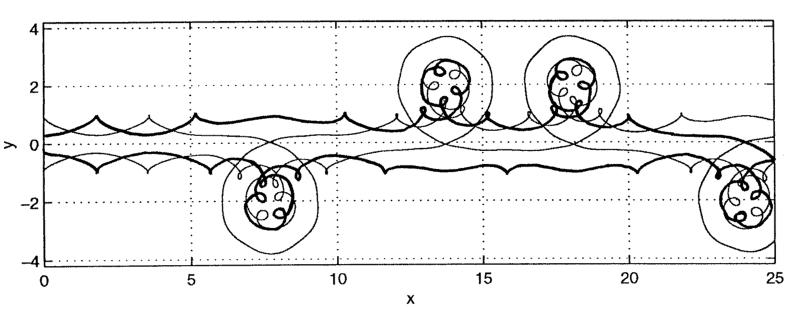
\includegraphics[width=\textwidth]{ach3inst.png}
\caption{Interaction of four line vortices with $\alpha=0.310$, and a pertubation of \num{7E-3}, showing the three vortex interaction. From \citet[p.~272]{acheson00}}
\label{fig:ach3inst}
\end{figure}
\begin{figure}[ht]
\centering
\setlength\figureheight{7.5cm} 
\setlength\figurewidth{\textwidth}
% This file was created by matlab2tikz.
% Minimal pgfplots version: 1.3
%
%The latest updates can be retrieved from
%  http://www.mathworks.com/matlabcentral/fileexchange/22022-matlab2tikz
%where you can also make suggestions and rate matlab2tikz.
%
\definecolor{mycolor1}{rgb}{0.00000,1.00000,1.00000}%
%
\begin{tikzpicture}

\begin{axis}[%
width=0.95092\figurewidth,
height=\figureheight,
at={(0\figurewidth,0\figureheight)},
scale only axis,
every outer x axis line/.append style={black},
every x tick label/.append style={font=\color{black}},
xmin=0,
xlabel={x},
every outer y axis line/.append style={black},
every y tick label/.append style={font=\color{black}},
ymin=-6.64182836786359,
ymax=6.64182836786359,
ylabel={y},
title={12000 time steps, step size = 0.005},
axis x line*=bottom,
axis y line*=left
]
\addplot [color=blue,solid,forget plot]
  table[row sep=crcr]{%
0.007	1\\
0.0064052035247101	1.00000106170005\\
0.00581090026917788	0.999958722638214\\
0.00521801214478773	0.999873019185673\\
0.00462745803016215	0.999744022275662\\
0.00404015163144304	0.999571837074173\\
0.00345699938378192	0.999356602469874\\
0.00287889841168778	0.999098490389233\\
0.00230673456493295	0.998797704944905\\
0.00174138054550827	0.998454481427348\\
0.00118369413968091	0.998069085151292\\
0.000634516567577627	0.997641810170166\\
9.46709609345645e-005	0.997172977872755\\
-0.000435039022236104	0.996662935477298\\
-0.000953830439267136	0.996112054438864\\
-0.00146094215592508	0.995520728786206\\
-0.00195563578810225	0.994889373404388\\
-0.00243719649114228	0.994218422279266\\
-0.00290493359763078	0.993508326719551\\
-0.00335818110615973	0.99275955357148\\
-0.0037962980251021	0.991972583440357\\
-0.00421866857679446	0.99114790893222\\
-0.00462470226870493	0.990286032927785\\
-0.00501383383915543	0.989387466899625\\
-0.00538552308596783	0.988452729282292\\
-0.00573925458701554	0.987482343903749\\
-0.00607453732209167	0.986476838485223\\
-0.00639090420576266	0.985436743215277\\
-0.00668791154097384	0.984362589402642\\
-0.00696513840312731	0.983254908211184\\
-0.00722218596417728	0.982114229479237\\
-0.00745867676600263	0.980941080624511\\
-0.00767425395193705	0.979735985634836\\
-0.00786858046488186	0.97849946414415\\
-0.0080413382199115	0.977232030592401\\
-0.00819222725872322	0.975934193467385\\
-0.00832096489269404	0.974606454625974\\
-0.00842728484070406	0.973249308691765\\
-0.00851093636727595	0.971863242525784\\
-0.00857168342597701	0.970448734766617\\
-0.00860930381244057	0.969006255436134\\
-0.00862358833079481	0.967536265606824\\
-0.00861433997674497	0.966039217126694\\
-0.00858137314004381	0.964515552397687\\
-0.00852451282860767	0.962965704203551\\
-0.0084435939160944	0.961390095583234\\
-0.00833846041435499	0.959789139745918\\
-0.00820896477180378	0.958163240023973\\
-0.00805496719842244	0.956512789860264\\
-0.00787633501781841	0.954838172826405\\
-0.00767294204649971	0.953139762668734\\
-0.00744466800030122	0.951417923378991\\
-0.00719139792770235	0.949673009286863\\
-0.00691302166960905	0.947905365171755\\
-0.00660943334503364	0.946115326391354\\
-0.00628053086198974	0.944303219024732\\
-0.00592621545282647	0.942469360027938\\
-0.0055463912331522	0.940614057400182\\
-0.00514096478344247	0.938737610358927\\
-0.00470984475238646	0.936840309522329\\
-0.0042529414810002	0.934922437097651\\
-0.00377016664652052	0.932984267074415\\
-0.00326143292508997	0.931026065421177\\
-0.00272665367224812	0.929048090284985\\
-0.0021657426202572	0.927050592192623\\
-0.00157861359130932	0.925033814252949\\
-0.000965180225686329	0.922997992359641\\
-0.000325355723972255	0.920943355393843\\
0.000340947397550423	0.918870125426215\\
0.00103381753915462	0.91677851791803\\
0.00175334423837053	0.914668741920986\\
0.00249961837989554	0.912541000275497\\
0.00327273239543378	0.910395489807256\\
0.00407278045414762	0.908232401521948\\
0.0048998586443642	0.906051920798003\\
0.00575406514714108	0.903854227577355\\
0.0066355004022561	0.901639496554174\\
0.00754426726714823	0.89940789736161\\
0.0084804711692988	0.897159594756592\\
0.00944422025250511	0.894894748802744\\
0.0104356255174628	0.892613515051547\\
0.0114548009570373	0.890316044721837\\
0.0125018636865718	0.888002484877789\\
0.0135769340695426	0.885672978605549\\
0.0146801358388437	0.883327665188657\\
0.0158115962139473	0.880966680282462\\
0.0169714460141573	0.878590156087703\\
0.0181598197681415	0.876198221523451\\
0.0193768558198982	0.873791002399623\\
0.0206226964312855	0.871368621589268\\
0.0218974878812082	0.868931199200828\\
0.0232013805615338	0.866478852750612\\
0.0245345290697778	0.864011697335663\\
0.0258970922985715	0.861529845807267\\
0.0272892335218981	0.859033408945289\\
0.028711120478056	0.856522495633569\\
0.0301629254492795	0.85399721303657\\
0.0316448253379221	0.851457666777492\\
0.0331570017390794	0.848903961118043\\
0.034699641009501	0.846336199140061\\
0.0362729343326166	0.843754482929167\\
0.0378770777794716	0.841158913760618\\
0.0395122723653425	0.838549592287531\\
0.0411787241017778	0.835926618731604\\
0.0428766440437777	0.833290093076496\\
0.044606248331809	0.830640115263949\\
0.0463677582283155	0.827976785392777\\
0.0481614001483693	0.825300203920779\\
0.0499874056840738	0.822610471869642\\
0.0518460116223144	0.81990769103286\\
0.0537374599554223	0.81719196418666\\
0.0556619978843003	0.81446339530393\\
0.0576198778135357	0.811722089771064\\
0.0596113573380078	0.808968154607647\\
0.0616366992204808	0.80620169868884\\
0.0636961713596564	0.803422832970295\\
0.0657900467481501	0.800631670715386\\
0.0679186034198435	0.797828327724494\\
0.0700821243860611	0.795012922566038\\
0.0722808975600154	0.7921855768089\\
0.0745152156689669	0.789346415255824\\
0.0767853761535508	0.786495566177325\\
0.0790916810537343	0.783633161545591\\
0.0814344368808829	0.780759337267794\\
0.0838139544754397	0.777874233418154\\
0.0862305488497448	0.774977994468078\\
0.0886845390155647	0.772070769513587\\
0.0911762477959351	0.76915271249922\\
0.09370600162098	0.766223982437518\\
0.096274130307418	0.763284743623142\\
0.0988809668215412	0.760335165840634\\
0.101526847025519	0.757375424564742\\
0.104212109406968	0.754405701152213\\
0.106937094791809	0.751426183023901\\
0.109702146040553	0.748437063835976\\
0.112507607728229	0.745438543639031\\
0.115353825808321	0.742430829023803\\
0.118241147261181	0.739414133252256\\
0.1211699197275	0.736388676372743\\
0.124140491127594	0.733354685317955\\
0.127153209267357	0.730312393984422\\
0.130208421431893	0.727262043292304\\
0.133306473968001	0.724203881224316\\
0.136447711856781	0.721138162842617\\
0.13963247827784	0.718065150282627\\
0.142861114166648	0.714985112722784\\
0.146133957766783	0.711898326329367\\
0.149451344178906	0.708805074175623\\
0.152813604908434	0.705705646134583\\
0.156221067413977	0.702600338745074\\
0.159674054658725	0.699489455050614\\
0.163172884667024	0.696373304411038\\
0.166717870088463	0.693252202286896\\
0.170309317771821	0.690126469996845\\
0.173947528351272	0.686996434448463\\
0.177632795847212	0.683862427843124\\
0.181365407284091	0.680724787355773\\
0.185145642327559	0.677583854790649\\
0.188973772943167	0.674439976214215\\
0.192850063078793	0.67129350156675\\
0.196774768372822	0.668144784254264\\
0.20074813588997	0.664994180722545\\
0.204770403886498	0.66184205001537\\
0.208841801606344	0.658688753319007\\
0.212962549109541	0.655534653495309\\
0.21713285713402	0.652380114605797\\
0.221352926991709	0.649225501429222\\
0.225622950499566	0.646071178975161\\
0.229943109945936	0.642917511996252\\
0.234313578092376	0.639764864501671\\
0.238734518210816	0.636613599274463\\
0.243206084155688	0.633464077395291\\
0.247728420470377	0.630316657775097\\
0.252301662527131	0.627171696699109\\
0.256925936699317	0.624029547384482\\
0.261601360564701	0.620890559553765\\
0.266328043138228	0.617755079026215\\
0.27110608513259	0.614623447328812\\
0.275935579244723	0.611496001328662\\
0.28081661046622	0.60837307288827\\
0.285749256415531	0.60525498854497\\
0.290733587689757	0.60214206921559\\
0.295769668233725	0.599034629927217\\
0.300857555724051	0.595932979574725\\
0.305997301965804	0.592837420705519\\
0.311188953299469	0.589748249331731\\
0.316432551015845	0.58666575476993\\
0.321728131776621	0.583590219508216\\
0.3270757280384	0.580521919100371\\
0.332475368478034	0.577461122086608\\
0.3379270784172	0.574408089940292\\
0.343430880244291	0.571363077039868\\
0.348986793831766	0.568326330665126\\
0.354594836947256	0.565298091016809\\
0.360255025656839	0.562278591258505\\
0.365967374719021	0.559268057579664\\
0.371731897968123	0.55626670927854\\
0.377548608685871	0.553274758863811\\
0.383417519960152	0.550292412173596\\
0.389338645030024	0.547319868510574\\
0.395311997616179	0.544357320791897\\
0.401337592236206	0.541404955712624\\
0.407415444504115	0.538462953921366\\
0.41354557141368	0.535531490206928\\
0.419727991605272	0.532610733694695\\
0.425962725615973	0.529700848051611\\
0.432249796112815	0.526801991698614\\
0.438589228109087	0.523914318029436\\
0.444981049163747	0.521037975634765\\
0.451425289564002	0.518173108530792\\
0.457921982491214	0.515319856391245\\
0.464471164170316	0.512478354782063\\
0.471072874002985	0.509648735397936\\
0.477727154684828	0.5068311263\\
0.484434052306903	0.504025652154019\\
0.491193616441883	0.501232434468478\\
0.498005900215219	0.498451591832047\\
0.504870960361635	0.495683240149937\\
0.511788857267338	0.49292749287875\\
0.518759654998282	0.490184461259427\\
0.525783421314859	0.487454254548022\\
0.532860227673346	0.484736980243996\\
0.539990149214481	0.482032744315846\\
0.547173264739452	0.479341651423881\\
0.554409656673648	0.476663805140008\\
0.561699411018428	0.473999308164443\\
0.569042617291208	0.471348262539268\\
0.576439368454087	0.468710769858831\\
0.583889760831245	0.466086931476964\\
0.59139389401531	0.463476848711063\\
0.598951870762857	0.460880623043079\\
0.60656379687918	0.458298356317493\\
0.614229781092448	0.455730150936374\\
0.621949934917328	0.453176110051632\\
0.629724372508119	0.450636337754599\\
0.637553210501429	0.448110939263074\\
0.64543656784837	0.445600021106002\\
0.653374565636232	0.443103691305943\\
0.661367326899576	0.440622059559509\\
0.669414976420612	0.438155237415965\\
0.677517640518753	0.435703338454164\\
0.685675446829155	0.433266478458033\\
0.693888524070055	0.43084477559079\\
0.702157001798657	0.428438350568107\\
0.710481010155321	0.426047326830411\\
0.71886067959574	0.423671830714526\\
0.72729614061078	0.421311991624863\\
0.735787523433633	0.418967942204345\\
0.744334957733867	0.416639818505257\\
0.752938572297968	0.414327760160223\\
0.761598494695913	0.412031910553472\\
0.770314850933275	0.409752416992571\\
0.779087765088352	0.407489430880788\\
0.78791735893377	0.405243107890229\\
0.79680375154197	0.403013608135882\\
0.805747058873975	0.400801096350695\\
0.814747393350799	0.398605742061774\\
0.823804863406823	0.396427719767796\\
0.832919573024441	0.394267209117686\\
0.842091621249266	0.39212439509058\\
0.851321101685127	0.389999468177095\\
0.86060810196811	0.387892624561851\\
0.869952703218825	0.385804066307197\\
0.87935497947212	0.383734001538009\\
0.888814997083378	0.381682644627428\\
0.898332814110599	0.379650216383315\\
0.907908479671392	0.377636944235173\\
0.917542033274041	0.375643062421206\\
0.927233504121806	0.373668812175134\\
0.936982910389605	0.371714441912297\\
0.946790258472287	0.369780207414505\\
0.956655542203668	0.367866372013005\\
0.966578742045612	0.365973206768843\\
0.976559824246417	0.364100990649786\\
0.986598739967869	0.36225001070287\\
0.996695424380392	0.360420562221515\\
1.00684979572579	0.358612948906019\\
1.01706175434722	0.356827483016115\\
1.02733118168612	0.355064485514116\\
1.03765793924605	0.353324286197046\\
1.04804186752338	0.351607223815962\\
1.05848278490521	0.349913646180549\\
1.06898048653504	0.34824391024685\\
1.07953474314673	0.346598382185867\\
1.09014529986804	0.344977437430556\\
1.10081187499489	0.34338146069857\\
1.11153415873819	0.341810845987943\\
1.12231181194529	0.34026599654271\\
1.13314446479852	0.338747324785309\\
1.14403171549403	0.337255252212465\\
1.15497312890415	0.335790209251097\\
1.16596823522767	0.334352635070686\\
1.17701652863249	0.332942977348462\\
1.18811746589596	0.331561691983675\\
1.19927046504896	0.330209242757221\\
1.21047490403029	0.328886100932909\\
1.22173011935872	0.327592744796712\\
1.23303540483086	0.326329659130484\\
1.24439001025361	0.325097334616815\\
1.25579314022074	0.323896267171951\\
1.26724395294404	0.322726957204057\\
1.27874155914976	0.321589908794496\\
1.29028502105231	0.320485628800334\\
1.30187335141712	0.319414625876846\\
1.31350551272566	0.318377409419516\\
1.32518041645568	0.317374488425768\\
1.33689692249016	0.316406370277576\\
1.34865383866857	0.315473559447014\\
1.36044992049416	0.314576556127877\\
1.37228387101073	0.313715854797577\\
1.38415434086186	0.312891942714699\\
1.39605992854526	0.312105298358779\\
1.40799918087394	0.311356389820098\\
1.41997059365462	0.310645673148496\\
1.43197261259308	0.309973590671396\\
1.44400363443387	0.309340569292363\\
1.45606200834078	0.308747018782601\\
1.46814603752169	0.308193330078685\\
1.48025398109993	0.307679873600682\\
1.49238405623125	0.307206997605419\\
1.50453444046339	0.306775026590101\\
1.51670327433223	0.306384259761697\\
1.52888866418599	0.306034969587519\\
1.54108868522604	0.305727400442115\\
1.55330138475009	0.305461767365073\\
1.56552478558112	0.305238254943558\\
1.57775688966253	0.305057016332306\\
1.58999568179799	0.304918172422518\\
1.60223913351221	0.304821811169552\\
1.61448520700728	0.304767987087573\\
1.62673185918746	0.304756720917394\\
1.63897704572477	0.304787999471724\\
1.65121872513664	0.304861775659865\\
1.66345486284687	0.304977968691755\\
1.67568343520143	0.305136464459037\\
1.6879024334111	0.305337116088713\\
1.7001098673942	0.305579744662911\\
1.71230376949384	0.305864140096352\\
1.72448219804612	0.306190062161389\\
1.73664324077778	0.306557241648968\\
1.74878501801389	0.306965381652523\\
1.76090568567905	0.307414158960816\\
1.77300343807802	0.307903225544895\\
1.78507651044456	0.308432210123869\\
1.79712318124999	0.309000719793917\\
1.809141774266	0.30960834170494\\
1.82113066037856	0.31025464476955\\
1.83308825915273	0.31093918138949\\
1.84501304015045	0.311661489185295\\
1.85690352400562	0.312421092715798\\
1.86875828326285	0.313217505175066\\
1.88057594298809	0.314050230055435\\
1.89235518116093	0.31491876276647\\
1.90409472885938	0.315822592200893\\
1.91579337024957	0.316761202239767\\
1.92744994239288	0.317734073190455\\
1.93906333488436	0.3187406831521\\
1.95063248933595	0.319780509304546\\
1.9621563987187	0.320853029117734\\
1.97363410657782	0.321957721479667\\
1.98506470613447	0.323094067741983\\
1.99644733928755	0.324261552683083\\
2.00778119552869	0.325459665389511\\
2.01906551078268	0.326687900057011\\
2.03029956618535	0.327945756713241\\
2.04148268680991	0.329232741864672\\
2.05261424035215	0.330548369070588\\
2.0636936357843	0.331892159447422\\
2.07472032198626	0.333263642106972\\
2.08569378636246	0.334662354532155\\
2.09661355345156	0.336087842894121\\
2.10747918353588	0.3375396623146\\
2.11829027125616	0.339017377077348\\
2.12904644423714	0.340520560792546\\
2.13974736172842	0.342048796517919\\
2.15039271326463	0.343601676840238\\
2.16098221734836	0.345178803920759\\
2.17151562015868	0.346779789507985\\
2.18199269428772	0.34840425492097\\
2.19241323750731	0.350051831006238\\
2.20277707156719	0.351722158071183\\
2.21308404102608	0.353414885796627\\
2.22333401211646	0.355129673131059\\
2.23352687164373	0.356866188168854\\
2.24366252591998	0.358624108014615\\
2.25374089973269	0.360403118635595\\
2.26376193534813	0.362202914703988\\
2.27372559154931	0.36402319943071\\
2.28363184270811	0.36586368439214\\
2.29348067789105	0.367724089351143\\
2.30327209999814	0.36960414207356\\
2.31300612493412	0.371503578141216\\
2.32268278081132	0.373422140762375\\
2.33230210718332	0.375359580580469\\
2.34186415430865	0.377315655481818\\
2.35136898244352	0.379290130402948\\
2.36081666116279	0.381282777138067\\
2.37020726870822	0.383293374147119\\
2.37954089136305	0.385321706364827\\
2.3888176228521	0.38736756501102\\
2.39803756376633	0.389430747402499\\
2.40720082101116	0.391511056766654\\
2.41630750727741	0.393608302056966\\
2.42535774053429	0.395722297770512\\
2.43435164354331	0.397852863767531\\
2.44328934339256	0.399999825093096\\
2.45217097105032	0.402163011800874\\
2.46099666093745	0.404342258778965\\
2.46976655051764	0.406537405577755\\
2.47848077990496	0.408748296239722\\
2.48713949148791	0.410974779131086\\
2.4957428295694	0.413216706775212\\
2.50429094002204	0.41547393568763\\
2.51278396995804	0.417746326212547\\
2.52122206741335	0.42003374236069\\
2.5296053810453	0.422336051648342\\
2.53793405984343	0.424653124937396\\
2.54620825285293	0.426984836276265\\
2.55442810891024	0.42933106274147\\
2.56259377639052	0.431691684279734\\
2.57070540296644	0.434066583550396\\
2.57876313537808	0.436455645767967\\
2.58676711921359	0.438858758544655\\
2.59471749870022	0.441275811732652\\
2.60261441650561	0.443706697266039\\
2.61045801354896	0.4461513090021\\
2.61824842882197	0.448609542561886\\
2.62598579921933	0.451081295169854\\
2.63367025937855	0.453566465492425\\
2.6413019415292	0.456064953475281\\
2.64888097535115	0.458576660179274\\
2.65640748784202	0.461101487614783\\
2.66388160319368	0.463639338574399\\
2.67130344267768	0.466190116463801\\
2.67867312453985	0.468753725130725\\
2.68599076390383	0.471330068691916\\
2.69325647268381	0.473919051357977\\
2.70047035950637	0.476520577256065\\
2.7076325296417	0.479134550250356\\
2.71474308494414	0.481760873760265\\
2.72180212380232	0.48439945057641\\
2.728809741099	0.487050182674321\\
2.73576602818078	0.489712971025937\\
2.74267107283793	0.492387715408952\\
2.74952495929451	0.4950743142141\\
2.75632776820899	0.497772664250496\\
2.76307957668571	0.500482660549186\\
2.76978045829729	0.503204196165102\\
2.77643048311836	0.505937161977617\\
2.78302971777081	0.508681446489995\\
2.78957822548082	0.511436935628\\
2.79607606614804	0.514203512538031\\
2.80252329642693	0.516981057385142\\
2.80891996982084	0.51976944715139\\
2.81526613678877	0.522568555434976\\
2.82156184486516	0.525378252250687\\
2.82780713879294	0.528198403832221\\
2.83400206066988	0.531028872436983\\
2.84014665010847	0.533869516154022\\
2.84624094440943	0.536720188715814\\
2.85228497874883	0.53958073931462\\
2.85827878637887	0.542451012424231\\
2.86422239884226	0.545330847627913\\
2.87011584620009	0.548220079453435\\
2.87595915727297	0.551118537216073\\
2.88175235989533	0.554026044870532\\
2.88749548118226	0.556942420872738\\
2.89318854780884	0.559867478052493\\
2.89883158630118	0.562801023497969\\
2.90442462333868	0.565742858453052\\
2.90996768606686	0.568692778228541\\
2.91546080241995	0.571650572128165\\
2.92090400145227	0.57461602339042\\
2.92629731367754	0.577588909147144\\
2.93164077141504	0.580569000399734\\
2.93693440914125	0.583556062013872\\
2.9421782638459	0.58654985273353\\
2.94737237539097	0.589550125214989\\
2.95251678687116	0.592556626081502\\
2.95761154497422	0.595569095999144\\
2.9626567003397	0.598587269774283\\
2.96765230791424	0.601610876473001\\
2.97259842730176	0.604639639562662\\
2.97749512310672	0.607673277075684\\
2.98234246526866	0.610711501795447\\
2.98714052938614	0.613754021464111\\
2.99188939702833	0.61680053901197\\
2.99658915603232	0.619850752807804\\
3.00123990078447	0.622904356929554\\
3.00584173248401	0.625961041454455\\
3.01039475938724	0.629020492767643\\
3.01489909703071	0.632082393888075\\
3.01935486843196	0.635146424810466\\
3.02376220426646	0.638212262861804\\
3.02812124301941	0.641279583070887\\
3.03243213111145	0.644348058549198\\
3.03669502299734	0.647417360881335\\
3.04091008123675	0.650487160523134\\
3.04507747653672	0.653557127205538\\
3.04919738776535	0.656626930342216\\
3.05327000193655	0.659696239438909\\
3.0572955141658	0.662764724502449\\
3.06127412759723	0.665832056447407\\
3.06520605330236	0.66889790749834\\
3.06909151015099	0.671961951585657\\
3.07293072465525	0.675023864733175\\
3.07672393078752	0.678083325435502\\
3.08047136977342	0.681140015023499\\
3.08417328986117	0.684193618016147\\
3.08782994606867	0.687243822457292\\
3.0914415999098	0.690290320235856\\
3.09500851910162	0.693332807388238\\
3.09853097725414	0.696370984381796\\
3.10200925354448	0.699404556378435\\
3.10544363237719	0.702433233477483\\
3.1088344030327	0.705456730937219\\
3.1121818593057	0.708474769374539\\
3.11548629913536	0.711487074942443\\
3.11874802422933	0.714493379485139\\
3.12196733968322	0.717493420670736\\
3.12514455359753	0.72048694210163\\
3.12827997669356	0.723473693402818\\
3.13137392193021	0.726453430288491\\
3.13442670412304	0.729425914607395\\
3.13743863956715	0.732390914367525\\
3.1404100456654	0.735348203740827\\
3.14334124056304	0.73829756304866\\
3.14623254279021	0.741238778728836\\
3.14908427091313	0.744171643285123\\
3.15189674319513	0.747095955220133\\
3.15467027726834	0.750011518952567\\
3.15740518981677	0.752918144719801\\
3.16010179627143	0.755815648466827\\
3.16276041051803	0.758703851722563\\
3.16538134461772	0.761582581464546\\
3.16796490854118	0.764451669973012\\
3.17051140991636	0.767310954675359\\
3.17302115378998	0.770160277981962\\
3.17549444240288	0.772999487114266\\
3.17793157497925	0.775828433926085\\
3.18033284752971	0.778646974718966\\
3.18269855266804	0.78145497005245\\
3.18502897944141	0.784252284550028\\
3.18732441317395	0.787038786701518\\
3.18958513532326	0.789814348662582\\
3.19181142334968	0.792578846052022\\
3.19400355059788	0.79533215774745\\
3.19616178619042	0.798074165679913\\
3.19828639493297	0.800804754627946\\
3.2003776372306	0.803523812011549\\
3.20243576901497	0.806231227686475\\
3.20446104168168	0.80892689373922\\
3.20645370203767	0.811610704283031\\
3.20841399225795	0.814282555255226\\
3.21034214985139	0.816942344216069\\
3.21223840763509	0.819589970149415\\
3.2141029937169	0.822225333265289\\
3.21593613148567	0.824848334804553\\
3.21773803960884	0.827458876845758\\
3.21950893203696	0.830056862114262\\
3.22124901801477	0.832642193793673\\
3.2229585020985	0.835214775339625\\
3.22463758417904	0.837774510295912\\
3.22628645951057	0.840321302112934\\
3.2279053187445	0.842855053968432\\
3.2294943479683	0.845375668590445\\
3.23105372874902	0.847883048082408\\
3.23258363818122	0.850377093750315\\
3.23408424893911	0.852857705931815\\
3.23555572933268	0.855324783827153\\
3.23699824336766	0.857778225331803\\
3.23841195080913	0.860217926870666\\
3.23979700724861	0.862643783233682\\
3.24115356417461	0.865055687412705\\
3.24248176904644	0.86745353043947\\
3.24378176537132	0.869837201224506\\
3.24505369278458	0.872206586396799\\
3.24629768713311	0.874561570144055\\
3.24751388056198	0.876902034053379\\
3.24870240160415	0.879227856952187\\
3.24986337527354	0.881538914749196\\
3.25099692316128	0.883835080275287\\
3.25210316353543	0.886116223124104\\
3.25318221144424	0.888382209492188\\
3.25423417882295	0.890632902018507\\
3.25525917460453	0.892868159623196\\
3.25625730483443	0.89508783734539\\
3.25722867278953	0.897291786179969\\
3.25817337910162	0.899479852913112\\
3.25909152188567	0.901651879956518\\
3.25998319687321	0.903807705180201\\
3.26084849755105	0.905947161743747\\
3.26168751530593	0.908070077925988\\
3.26250033957529	0.910176276952999\\
3.26328705800465	0.912265576824426\\
3.26404775661219	0.91433779013811\\
3.26478251996082	0.916392723913045\\
3.26549143133851	0.918430179410722\\
3.26617457294717	0.920449951954947\\
3.26683202610097	0.922451830750276\\
3.26746387143453	0.924435598699235\\
3.26807018912173	0.926401032218559\\
3.26865105910587	0.928347901054729\\
3.26920656134178	0.930275968099156\\
3.2697367760509	0.932184989203427\\
3.27024178398981	0.934074712995085\\
3.27072166673332	0.935944880694523\\
3.27117650697271	0.937795225933641\\
3.27160638883021	0.939625474577012\\
3.27201139819043	0.941435344546417\\
3.27239162304967	0.9432245456497\\
3.27274715388403	0.944992779415044\\
3.2730780840371	0.946739738931858\\
3.27338451012822	0.948465108699641\\
3.27366653248197	0.950168564486301\\
3.27392425557976	0.951849773197579\\
3.2741577885343	0.953508392759373\\
3.2743672455874	0.955144072014938\\
3.27455274663186	0.956756450639087\\
3.27471441775775	0.958345159071714\\
3.27485239182345	0.959909818473129\\
3.27496680905156	0.96145004070386\\
3.27505781764962	0.962965428331768\\
3.27512557445539	0.964455574669495\\
3.27517024560622	0.965920063845391\\
3.27519200723162	0.967358470911276\\
3.27519104616806	0.96877036199046\\
3.27516756069443	0.970155294469609\\
3.27512176128645	0.971512817238101\\
3.27505387138775	0.972842470978579\\
3.27496412819492	0.974143788512432\\
3.2748527834535	0.97541629520389\\
3.27472010426106	0.976659509426356\\
3.27456637387348	0.977872943094459\\
3.27439189250949	0.979056102265095\\
3.27419697814827	0.980208487810481\\
3.27398196731445	0.981329596165875\\
3.27374721584382	0.982418920154187\\
3.27349309962325	0.983475949889214\\
3.27322001529703	0.984500173758587\\
3.272928380932	0.985491079486863\\
3.27261863663313	0.986448155278373\\
3.27229124510081	0.987370891038579\\
3.27194669212117	0.988258779671735\\
3.27158548698017	0.989111318451596\\
3.27120816279255	0.989928010460835\\
3.27081527673661	0.990708366093655\\
3.27040741018606	0.991451904614919\\
3.26998516873063	0.992158155767873\\
3.26954918207775	0.992826661421384\\
3.26910010382806	0.993456977246406\\
3.26863861111893	0.994048674410283\\
3.26816540413073	0.994601341276484\\
3.26768120545223	0.995114585096432\\
3.26718675930271	0.995588033679319\\
3.26668283061	0.996021337025211\\
3.26617020394538	0.996414168906333\\
3.26564968231789	0.996766228381235\\
3.26512208583251	0.99707724122662\\
3.26458825021862	0.997346961271873\\
3.26404902523666	0.997575171621956\\
3.26350527297314	0.997761685755111\\
3.26295786603539	0.997906348482921\\
3.26240768565925	0.9980090367616\\
3.26185561974423	0.998069660344929\\
3.26130256083184	0.998088162271006\\
3.26074940404356	0.998064519176876\\
3.26019704499596	0.997998741437158\\
3.2596463777104	0.997890873124882\\
3.25909829253525	0.997740991794944\\
3.25855367409807	0.997549208092682\\
3.25801339930497	0.997315665192238\\
3.25747833540335	0.997040538071317\\
3.25694933812344	0.996724032630861\\
3.25642724991257	0.996366384669805\\
3.25591289827497	0.995967858726598\\
3.25540709422802	0.995528746800414\\
3.25491063088419	0.995049366965963\\
3.25442428216629	0.994530061896586\\
3.25394880166162	0.993971197310788\\
3.2534849216187	0.993373160357569\\
3.25303335208878	0.992736357955917\\
3.25259478021208	0.992061215103527\\
3.25216986964759	0.991348173169376\\
3.25175926014333	0.990597688184071\\
3.25136356724289	0.989810229141092\\
3.25098338212258	0.988986276321064\\
3.25061927155278	0.988126319650135\\
3.25027177797603	0.987230857102363\\
3.24994141969367	0.986300393154854\\
3.24962869115252	0.985335437303136\\
3.24933406332268	0.984336502643059\\
3.24905798415707	0.983304104524311\\
3.24880087912386	0.982238759279482\\
3.24856315180235	0.98114098303153\\
3.24834518453363	0.980011290581455\\
3.24814733911726	0.97885019437708\\
3.2479699575458	0.977658203562947\\
3.2478133627694	0.976435823110597\\
3.24767785948306	0.97518355302782\\
3.24756373492986	0.973901887644889\\
3.247471259714	0.972591314975293\\
3.24740068861778	0.971252316148091\\
3.24735226141767	0.969885364908689\\
3.24732620369484	0.968490927184584\\
3.24732272763604	0.967069460712457\\
3.24734203282168	0.965621414722885\\
3.24738430699775	0.964147229678867\\
3.24744972682949	0.962647337064374\\
3.24753845863438	0.96112215921916\\
3.24765065909314	0.95957210921613\\
3.24778647593715	0.957997590777689\\
3.24794604861161	0.956398998227587\\
3.24812950891355	0.95477671647496\\
3.24833698160459	0.953131121027388\\
3.24856858499798	0.951462578029992\\
3.24882443152028	0.949771444327753\\
3.2491046282478	0.948058067548415\\
3.24940927741809	0.946322786203534\\
3.24973847691726	0.944565929805394\\
3.25009232074353	0.942787818997707\\
3.2504708994478	0.940988765698158\\
3.25087430055204	0.939169073251079\\
3.2513026089464	0.937329036588614\\
3.25175590726567	0.935468942398969\\
3.25223427624633	0.933589069300439\\
3.25273779506475	0.931689688020032\\
3.25326654165777	0.929771061575689\\
3.25382059302625	0.927833445461148\\
3.25440002552281	0.925877087832667\\
3.25500491512434	0.923902229696889\\
3.25563533769038	0.92190910509924\\
3.25629136920802	0.919897941312332\\
3.25697308602425	0.917868959023919\\
3.25768056506644	0.915822372524034\\
3.25841388405176	0.91375838989099\\
3.25917312168623	0.911677213175999\\
3.25995835785397	0.9095790385862\\
3.2607696737975	0.907464056665945\\
3.26160715228945	0.905332452476248\\
3.2624708777964	0.903184405772309\\
3.26336093663534	0.901020091179085\\
3.26427741712321	0.898839678364908\\
3.26522040972006	0.896643332213165\\
3.26619000716613	0.894431212992093\\
3.2671863046134	0.89220347652275\\
3.26820939975185	0.889960274345258\\
3.26925939293083	0.887701753883409\\
3.27033638727582	0.88542805860777\\
3.27144048880085	0.883139328197391\\
3.27257180651683	0.880835698700284\\
3.27373045253607	0.878517302692794\\
3.27491654217302	0.876184269438044\\
3.27613019404163	0.873836725043599\\
3.27737153014923	0.871474792618516\\
3.27864067598721	0.869098592429969\\
3.27993776061859	0.866708242059593\\
3.28126291676238	0.864303856559747\\
3.28261628087503	0.86188554860986\\
3.28399799322875	0.859453428673025\\
3.28540819798688	0.857007605153037\\
3.28684704327614	0.854548184552021\\
3.28831468125592	0.852075271628834\\
3.28981126818422	0.849588969558393\\
3.29133696448055	0.847089380092095\\
3.29289193478532	0.844576603719468\\
3.29447634801581	0.842050739831212\\
3.29609037741853	0.839511886883754\\
3.29773420061768	0.836960142565443\\
3.29940799965972	0.83439560396451\\
3.30111196105364	0.831818367738881\\
3.3028462758068	0.829228530287942\\
3.30461113945608	0.826626187926333\\
3.30640675209406	0.82401143705982\\
3.30823331838991	0.821384374363295\\
3.31009104760471	0.818745096960914\\
3.31198015360089	0.816093702608393\\
3.31390085484541	0.813430289877412\\
3.31585337440632	0.810754958342112\\
3.31783793994235	0.808067808767581\\
3.31985478368519	0.80536894330025\\
3.32190414241397	0.802658465660062\\
3.32398625742155	0.799936481334242\\
3.3261013744723	0.797203097772482\\
3.32824974375088	0.794458424583308\\
3.33043161980158	0.791702573731352\\
3.33264726145786	0.788935659735227\\
3.33489693176163	0.786157799865654\\
3.33718089787195	0.78336911434345\\
3.33949943096258	0.780569726536947\\
3.34185280610822	0.777759763158356\\
3.34424130215893	0.77493935445856\\
3.34666520160238	0.772108634419768\\
3.3491247904138	0.769267740945417\\
3.35162035789314	0.766416816046658\\
3.35415219648935	0.763556006024733\\
3.35672060161159	0.760685461648494\\
3.35932587142708	0.757805338326276\\
3.36196830664583	0.75491579627131\\
3.36464821029186	0.752017000659797\\
3.36736588746124	0.749109121780777\\
3.37012164506701	0.74619233517685\\
3.37291579157108	0.743266821774818\\
3.37574863670361	0.740332768005297\\
3.37862049117009	0.737390365910306\\
3.38153166634663	0.734439813237892\\
3.38448247396415	0.731481313522798\\
3.38747322578199	0.728515076152225\\
3.39050423325187	0.725541316415771\\
3.39357580717301	0.722560255538622\\
3.39668825733942	0.719572120697156\\
3.39984189218048	0.716577145016144\\
3.403037018396	0.713575567546803\\
3.40627394058709	0.71056763322504\\
3.40955296088418	0.707553592809295\\
3.41287437857377	0.704533702797489\\
3.41623848972535	0.701508225322706\\
3.4196455868203	0.698477428027321\\
3.42309595838429	0.695441583915444\\
3.42658988862508	0.692400971183656\\
3.43012765707745	0.689355873030163\\
3.433709538257	0.686306577442639\\
3.43733580132486	0.683253376965178\\
3.44100670976482	0.680196568444919\\
3.44472252107496	0.677136452759071\\
3.44848348647536	0.674073334523214\\
3.45228985063357	0.671007521781896\\
3.45614185140958	0.667939325682695\\
3.46003971962172	0.664869060135061\\
3.46398367883488	0.661797041455364\\
3.46797394517245	0.658723587999724\\
3.47201072715302	0.655649019786271\\
3.4760942255529	0.65257365810861\\
3.48022463329529	0.649497825142329\\
3.48440213536676	0.646421843546455\\
3.4886269087615	0.643346036061822\\
3.49289912245372	0.64027072510832\\
3.49721893739825	0.637196232383026\\
3.50158650655921	0.634122878461215\\
3.50600197496664	0.631050982402194\\
3.51046547980048	0.627980861361898\\
3.5149771505014	0.624912830214089\\
3.51953710890755	0.621847201181957\\
3.52414546941637	0.618784283481797\\
3.52880233917028	0.615724382980355\\
3.53350781826506	0.61266780186731\\
3.53826199997947	0.609614838344212\\
3.54306497102462	0.606565786331104\\
3.54791681181165	0.603520935191849\\
3.55281759673584	0.600480569479083\\
3.55776739447564	0.597444968699555\\
3.56276626830471	0.594414407100416\\
3.56781427641529	0.591389153476948\\
3.57291147225106	0.588369471001974\\
3.57805790484765	0.585355617077138\\
3.58325361917923	0.58234784320603\\
3.58849865650909	0.579346394889033\\
3.59379305474292	0.576351511539633\\
3.59913684878292	0.57336342642182\\
3.60453007088112	0.570382366608076\\
3.60997275099074	0.567408552957391\\
3.61546491711376	0.564442200112615\\
3.6210065956438	0.561483516516404\\
3.62659781170274	0.558532704444948\\
3.63223858947018	0.555589960058611\\
3.63792895250467	0.552655473468563\\
3.64366892405567	0.549729428818462\\
3.6494585273656	0.546812004380221\\
3.65529778596103	0.543903372662855\\
3.66118672393262	0.54100370053344\\
3.66712536620302	0.538113149349172\\
3.67311373878248	0.535231875099566\\
3.67915186901166	0.532360028557814\\
3.68523978579142	0.529497755440385\\
3.69137751979933	0.526645196573922\\
3.69756510369282	0.523802488068588\\
3.70380257229878	0.520969761496996\\
3.71008996278968	0.51814714407793\\
3.71642731484618	0.515334758864081\\
3.72281467080632	0.512532724933095\\
3.7292520758014	0.509741157581248\\
3.73573957787867	0.506960168519124\\
3.74227722811108	0.504189866068713\\
3.74886508069419	0.501430355361398\\
3.75550319303055	0.498681738536333\\
3.76219162580177	0.495944114938783\\
3.76893044302849	0.493217581318014\\
3.7757197121185	0.490502232024378\\
3.78255950390343	0.487798159205289\\
3.78944989266399	0.4851054529998\\
3.79639095614433	0.482424201731561\\
3.80338277555553	0.479754492099944\\
3.81042543556858	0.47709640936918\\
3.81751902429712	0.47445003755537\\
3.82466363327005	0.471815459611274\\
3.83185935739432	0.4691927576088\\
3.83910629490809	0.466582012919148\\
3.84640454732431	0.463983306390597\\
3.85375421936511	0.461396718523926\\
3.86115541888689	0.458822329645498\\
3.86860825679638	0.456260220078055\\
3.87611284695778	0.453710470309285\\
3.88366930609091	0.451173161158227\\
3.89127775366061	0.448648373939634\\
3.89893831175725	0.446136190626368\\
3.90665110496844	0.443636694009981\\
3.91441626024197	0.441149967859581\\
3.92223390673979	0.438676097079149\\
3.93010417568305	0.436215167863433\\
3.93802720018818	0.433767267852594\\
3.94600311509372	0.431332486285758\\
3.95403205677786	0.428910914153633\\
3.96211416296652	0.426502644350381\\
3.97024957253178	0.424107771824904\\
3.97843842528034	0.421726393731737\\
3.98668086173188	0.419358609581703\\
3.99497702288701	0.417004521392544\\
4.00332704998444	0.414664233839674\\
4.0117310842472	0.412337854407252\\
4.02018926661732	0.410025493539749\\
4.02870173747888	0.407727264794171\\
4.03726863636872	0.405443284993115\\
4.04589010167463	0.403173674378825\\
4.05456627032045	0.400918556768389\\
4.06329727743751	0.398678059710233\\
4.07208325602212	0.396452314642057\\
4.08092433657835	0.394241457050323\\
4.08982064674563	0.392045626631422\\
4.09877231091066	0.389864967454613\\
4.10777944980279	0.387699628126816\\
4.11684218007255	0.385549761959324\\
4.12596061385234	0.383415527136467\\
4.13513485829884	0.381297086886255\\
4.14436501511637	0.379194609652972\\
4.15365118006033	0.377108269271704\\
4.1629934424203	0.375038245144685\\
4.1723918844817	0.372984722419385\\
4.18184658096547	0.370947892168157\\
4.19135759844496	0.368927951569235\\
4.2009249947392	0.366925104088848\\
4.21054881828181	0.364939559664104\\
4.2202291074648	0.36297153488629\\
4.22996588995652	0.361021253184125\\
4.23975918199295	0.359088945006452\\
4.24960898764171	0.357174848003762\\
4.25951529803815	0.355279207207853\\
4.26947809059277	0.353402275208841\\
4.27949732816956	0.351544312328632\\
4.28957295823472	0.349705586789847\\
4.29970491197534	0.347886374879092\\
4.30989310338784	0.34608696110332\\
4.32013742833588	0.344307638337915\\
4.33043776357789	0.34254870796499\\
4.34079396576418	0.340810480000232\\
4.35120587040412	0.3390932732065\\
4.36167329080379	0.337397415192207\\
4.37219601697505	0.335723242492379\\
4.3827738145169	0.334071100630108\\
4.39340642347062	0.33244134415598\\
4.40409355715031	0.330834336662877\\
4.41483490095082	0.329250450773426\\
4.42563011113565	0.327690068097221\\
4.43647881360749	0.326153579154792\\
4.44738060266487	0.324641383265216\\
4.45833503974868	0.323153888394131\\
4.46934165218296	0.32169151095887\\
4.48039993191468	0.320254675587375\\
4.49150933425832	0.318843814827525\\
4.50266927665099	0.317459368803575\\
4.51387913742504	0.31610178481644\\
4.52513825460542	0.314771516884694\\
4.5364459247397	0.313469025223335\\
4.54780140176956	0.312194775657595\\
4.55920389595267	0.310949238969374\\
4.57065257284511	0.309732890174269\\
4.58214655235439	0.308546207727574\\
4.59368490787405	0.307389672658205\\
4.60526666551113	0.306263767630027\\
4.61689080341798	0.305168975930802\\
4.62855625124038	0.304105780389679\\
4.64026188969375	0.303074662224968\\
4.65200655027947	0.302076099824833\\
4.66378901515303	0.301110567464461\\
4.67560801715527	0.300178533964233\\
4.68746224001778	0.299280461294455\\
4.69935031875242	0.298416803133187\\
4.71127084023421	0.297588003384778\\
4.72322234398592	0.296794494667656\\
4.73520332317082	0.296036696780912\\
4.74721222579921	0.295315015160091\\
4.75924745615217	0.294629839333372\\
4.77130737642424	0.293981541390046\\
4.78339030858487	0.293370474473698\\
4.79549453645609	0.292796971312927\\
4.80761830800183	0.292261342802622\\
4.81975983782189	0.291763876648872\\
4.83191730984125	0.291304836090378\\
4.84408888018323	0.290884458708882\\
4.85627268021262	0.290502955340505\\
4.86846681973288	0.290160509099117\\
4.88066939031957	0.289857274521836\\
4.89287846877025	0.289593376845571\\
4.90509212064969	0.289368911422185\\
4.91730840390797	0.289183943278353\\
4.92952537254792	0.289038506824564\\
4.94174108031784	0.288932605716053\\
4.95395358440514	0.288866212866686\\
4.96616094910638	0.288839270615068\\
4.97836124944979	0.288851691040419\\
4.99055257474673	0.288903356424062\\
5.00273303205004	0.288994119850808\\
5.01490074949787	0.289123805943019\\
5.02705387952378	0.289292211718828\\
5.0391906019152	0.289499107564812\\
5.05130912670459	0.289744238312469\\
5.0634076968796	0.290027324407035\\
5.07548459090078	0.290348063156634\\
5.08753812501766	0.29070613004935\\
5.09956665537633	0.291101180125673\\
5.11156857991377	0.291532849393749\\
5.12354234003663	0.292000756275111\\
5.13548642208381	0.292504503068887\\
5.14739935857481	0.293043677423035\\
5.15927972924684	0.293617853801761\\
5.1711261618861	0.294226594939032\\
5.18293733295959	0.294869453268931\\
5.19471196805521	0.295545972324475\\
5.20644884213924	0.296255688097442\\
5.21814677964074	0.296998130352737\\
5.22980465437355	0.297772823891726\\
5.2414213893068	0.298579289759955\\
5.25299595619529	0.299417046395556\\
5.2645273750813	0.300285610715507\\
5.2760147136794	0.301184499137768\\
5.28745708665569	0.30211322853803\\
5.29885365481293	0.303071317140556\\
5.31020362419232	0.304058285343204\\
5.32150624510268	0.305073656477287\\
5.33276081108713	0.306116957503426\\
5.34396665783685	0.307187719644979\\
5.35512316206112	0.308285478960975\\
5.36622974032203	0.309409776860804\\
5.37728584784177	0.310560160563125\\
5.38829097728994	0.311736183501648\\
5.3992446575574	0.312937405680594\\
5.41014645252287	0.31416339398268\\
5.42099595981786	0.315413722432577\\
5.4317928095947	0.31668797241875\\
5.4425366633024	0.317985732876598\\
5.45322721247392	0.319306600435751\\
5.46386417752863	0.320650179534312\\
5.47444730659271	0.322016082502756\\
5.48497637434013	0.323403929620067\\
5.49545118085648	0.324813349144609\\
5.50587155052735	0.3262439773221\\
5.51623733095284	0.327695458372897\\
5.52654839188942	0.329167444460726\\
5.53680462421995	0.330659595644802\\
5.54700593895277	0.332171579817183\\
5.55715226625012	0.333703072627073\\
5.56724355448631	0.335253757393633\\
5.57727976933573	0.336823325008779\\
5.58726089289063	0.338411473831274\\
5.59718692280859	0.340017909573355\\
5.60705787148928	0.341642345181007\\
5.61687376528029	0.343284500708874\\
5.62663464371149	0.344944103190745\\
5.63634055875737	0.346620886506416\\
5.64599157412691	0.348314591245686\\
5.6555877645802	0.350024964570122\\
5.66512921527132	0.3517517600732\\
5.67461602111661	0.353494737639336\\
5.68404828618778	0.355253663302251\\
5.69342612312909	0.357028309103091\\
5.70274965259777	0.358818452948632\\
5.71201900272715	0.36062387846988\\
5.72123430861153	0.36244437488133\\
5.73039571181227	0.364279736841083\\
5.73950335988425	0.366129764312027\\
5.74855740592198	0.367994262424215\\
5.75755800812483	0.369873041338583\\
5.76650532938043	0.371765916112076\\
5.7753995368658	0.37367270656429\\
5.78424080166545	0.375593237145657\\
5.79302929840583	0.377527336807221\\
5.80176520490552	0.379474838872021\\
5.81044870184061	0.381435580908087\\
5.81907997242457	0.383409404603038\\
5.82765920210218	0.385396155640267\\
5.83618657825698	0.387395683576681\\
5.84466228993164	0.389407841721964\\
5.85308652756075	0.391432487019311\\
5.86145948271573	0.393469479927594\\
5.8697813478612	0.39551868430489\\
5.87805231612243	0.397579967293328\\
5.88627258106356	0.399653199205176\\
5.89444233647605	0.401738253410114\\
5.90256177617706	0.403835006223617\\
5.91063109381744	0.405943336796379\\
5.91865048269881	0.40806312700471\\
5.92662013559967	0.410194261341835\\
5.93454024460998	0.412336626810011\\
5.94241100097409	0.414490112813409\\
5.95023259494169	0.416654611051671\\
5.9580052156265	0.418830015414092\\
5.96572905087247	0.42101622187433\\
5.97340428712727	0.423213128385608\\
5.98103110932292	0.425420634776319\\
5.9886097007632	0.427638642645983\\
5.99614024301785	0.429867055261488\\
6.00362291582321	0.432105777453565\\
6.01105789698933	0.434354715513439\\
6.01844536231318	0.436613777089598\\
6.02578548549809	0.438882871084643\\
6.03307843807906	0.441161907552177\\
6.04032438935396	0.443450797593684\\
6.04752350632053	0.445749453255363\\
6.05467595361907	0.448057787424911\\
6.06178189348062	0.450375713728197\\
6.06884148568087	0.45270314642584\\
6.07585488749939	0.455040000309657\\
6.08282225368438	0.457386190598993\\
6.08974373642279	0.459741632836918\\
6.09661948531584	0.462106242786311\\
6.10344964735983	0.464479936325849\\
6.1102343669323	0.46686262934591\\
6.11697378578354	0.469254237644434\\
6.12366804303334	0.471654676822791\\
6.13031727517312	0.474063862181677\\
6.13692161607332	0.476481708617125\\
6.14348119699617	0.478908130516689\\
6.14999614661368	0.481343041655875\\
6.15646659103115	0.48378635509491\\
6.16289265381584	0.486237983075953\\
6.16927445603115	0.48869783692085\\
6.17561211627615	0.491165826929555\\
6.18190575073044	0.493641862279354\\
6.18815547320449	0.496125850925024\\
6.19436139519537	0.498617699500087\\
6.20052362594783	0.50111731321933\\
6.20664227252083	0.503624595782748\\
6.21271743985945	0.50613944928112\\
6.21874923087216	0.508661774103396\\
6.2247377465134	0.511191468846116\\
6.23068308587146	0.513728430225081\\
6.23658534626165	0.516272552989485\\
6.24244462332454	0.518823729838779\\
6.24826101112942	0.521381851342484\\
6.25403460228263	0.523946805863222\\
6.25976548804089	0.526518479483223\\
6.26545375842931	0.529096755934586\\
6.27109950236407	0.531681516533548\\
6.27670280777953	0.534272640119058\\
6.28226376175955	0.536870002995929\\
6.287782450673	0.539473478882846\\
6.29325896031297	0.542082938865518\\
6.29869337603959	0.544698251355251\\
6.30408578292626	0.547319282053226\\
6.30943626590873	0.549945893920738\\
6.31474490993699	0.552577947155681\\
6.32001180012948	0.555215299175515\\
6.3252370219293	0.557857804606979\\
6.33042066126199	0.560505315282765\\
6.3355628046945	0.563157680245377\\
6.34066353959502	0.565814745758373\\
6.34572295429293	0.568476355325169\\
6.3507411382388	0.571142349715559\\
6.35571818216359	0.573812567000083\\
6.36065417823678	0.57648684259236\\
6.36554922022278	0.579165009299445\\
6.37040340363517	0.581846897380275\\
6.37521682588822	0.584532334612214\\
6.37998958644507	0.587221146365674\\
6.38472178696212	0.589913155686766\\
6.38941353142902	0.592608183387887\\
6.3940649263037	0.59530604814612\\
6.39867608064195	0.59800656660928\\
6.40324710622095	0.600709553509393\\
6.40777811765625	0.603414821783387\\
6.41226923251175	0.606122182700685\\
6.41672057140205	0.608831445997406\\
6.42113225808684	0.611542420016799\\
6.4255044195568	0.614254911855517\\
6.42983718611066	0.616968727515317\\
6.434130691423	0.6196836720597\\
6.43838507260242	0.622399549775023\\
6.44260047023987	0.625116164335535\\
6.44677702844674	0.627833318971816\\
6.45091489488264	0.63055081664203\\
6.45501422077255	0.633268460205406\\
6.45907516091334	0.635986052597355\\
6.46309787366946	0.638703397005587\\
6.46708252095787	0.64142029704662\\
6.47102926822219	0.644136556942041\\
6.47493828439613	0.646851981693897\\
6.47880974185629	0.649566377258588\\
6.48264381636465	0.65227955071865\\
6.48644068700071	0.654991310451814\\
6.49020053608379	0.65770146629677\\
6.49392354908567	0.660409829715049\\
6.49760991453389	0.663116213948487\\
6.50125982390625	0.66582043417176\\
6.50487347151672	0.668522307639485\\
6.50845105439337	0.671221653827439\\
6.51199277214883	0.673918294567475\\
6.51549882684359	0.676612054175746\\
6.51896942284289	0.67930275957389\\
6.52240476666769	0.681990240402867\\
6.52580506684017	0.684674329129181\\
6.52917053372451	0.68735486114326\\
6.5325013793634	0.690031674849813\\
6.53579781731089	0.692704611750009\\
6.53906006246229	0.69537351651538\\
6.54228833088144	0.698038237053386\\
6.54548283962615	0.700698624564614\\
6.54864380657233	0.703354533591614\\
6.55177145023717	0.70600582205943\\
6.55486598960216	0.708652351307902\\
6.55792764393629	0.711293986115848\\
6.5609566326199	0.713930594717269\\
6.56395317496979	0.716562048809741\\
6.56691749006579	0.719188223555204\\
6.5698497965795	0.721808997573329\\
6.57275031260527	0.724424252927735\\
6.57561925549396	0.727033875105282\\
6.57845684168979	0.729637752988716\\
6.5812632865705	0.732235778822936\\
6.58403880429109	0.734827848175187\\
6.58678360763146	0.737413859889453\\
6.58949790784805	0.739993716035362\\
6.59218191452971	0.742567321851901\\
6.59483583545793	0.745134585686249\\
6.59745987647153	0.747695418928018\\
6.60005424133599	0.750249735939212\\
6.60261913161733	0.752797453980195\\
6.60515474656074	0.755338493131944\\
6.6076612829739	0.757872776214884\\
6.610138935115	0.760400228704561\\
6.61258789458546	0.762920778644424\\
6.61500835022727	0.765434356555951\\
6.61740048802498	0.767940895346372\\
6.61976449101213	0.7704403302142\\
6.6221005391822	0.772932598552795\\
6.62440880940382	0.775417639852135\\
6.62668947534027	0.777895395599003\\
6.62894270737307	0.780365809175743\\
6.63116867252951	0.782828825757735\\
6.63336753441409	0.785284392209738\\
6.63553945314359	0.787732456981218\\
6.63768458528574	0.790172970000766\\
6.63980308380128	0.792605882569706\\
6.64189509798922	0.795031147254961\\
6.64396077343528	0.797448717781252\\
6.64600025196315	0.799858548922662\\
6.64801367158863	0.80226059639362\\
6.65000116647625	0.804654816739295\\
6.65196286689852	0.807041167225438\\
6.6538988991973	0.809419605727636\\
6.65580938574747	0.811790090619968\\
6.65769444492256	0.814152580663025\\
6.65955419106217	0.816507034891247\\
6.6613887344413	0.818853412499509\\
6.66319818124106	0.821191672728884\\
6.66498263352102	0.823521774751503\\
6.66674218919286	0.82584367755439\\
6.66847694199527	0.828157339822194\\
6.67018698146995	0.830462719818661\\
6.67187239293876	0.832759775266734\\
6.67353325748179	0.835048463227116\\
6.67516965191626	0.837328739975155\\
6.67678164877639	0.839600560875863\\
6.67836931629396	0.841863880256906\\
6.67993271837961	0.844118651279353\\
6.68147191460491	0.846364825805997\\
6.68298696018512	0.848602354267027\\
6.68447790596261	0.85083118552282\\
6.68594479839107	0.853051266723631\\
6.68738767952043	0.855262543165922\\
6.68880658698262	0.857464958145078\\
6.69020155397819	0.859658452804246\\
6.69157260926392	0.861842965979017\\
6.69291977714146	0.864018434037665\\
6.69424307744727	0.866184790716654\\
6.69554252554381	0.868341966951093\\
6.69681813231242	0.870489890699851\\
6.69806990414784	0.872628486764993\\
6.69929784295478	0.874757676605218\\
6.7005019461468	0.876877378142968\\
6.70168220664771	0.878987505564871\\
6.70283861289587	0.881087969115179\\
6.70397114885186	0.883178674881852\\
6.70507979400975	0.885259524574958\\
6.70616452341259	0.887330415297047\\
6.70722530767257	0.889391239305143\\
6.70826211299636	0.891441883764061\\
6.70927490121625	0.893482230490692\\
6.71026362982778	0.895512155688975\\
6.71122825203453	0.897531529675254\\
6.7121687168008	0.899540216593751\\
6.71308496891308	0.901538074121912\\
6.71397694905118	0.903524953165414\\
6.71484459386983	0.905500697542647\\
6.71568783609202	0.907465143658548\\
6.71650660461494	0.909418120167685\\
6.71730082462979	0.911359447626573\\
6.71807041775661	0.913288938135249\\
6.71881530219557	0.915206394968216\\
6.71953539289587	0.91711161219494\\
6.72023060174387	0.919004374290197\\
6.72090083777191	0.920884455734631\\
6.7215460073893	0.922751620606044\\
6.72216601463725	0.924605622162035\\
6.72276076146937	0.926446202414744\\
6.72333014805946	0.928273091698632\\
6.72387407313841	0.93008600823236\\
6.72439243436207	0.931884657676036\\
6.72488512871189	0.933668732685269\\
6.72535205293019	0.935437912463695\\
6.72579310399199	0.937191862315838\\
6.72620817961518	0.938930233202418\\
6.72659717881089	0.940652661300453\\
6.72696000247577	0.942358767570772\\
6.7272965540279	0.944048157335799\\
6.72760674008783	0.945720419870785\\
6.7278904712063	0.947375128011907\\
6.7281476626398	0.949011837784992\\
6.72837823517501	0.950630088058874\\
6.72858211600317	0.952229400227725\\
6.72875923964464	0.953809277926988\\
6.72890954892411	0.955369206787803\\
6.7290329959963	0.956908654235142\\
6.72912954342153	0.958427069335084\\
6.72919916529033	0.959923882696946\\
6.72924184839555	0.961398506436155\\
6.7292575934499	0.962850334203993\\
6.7292464163465	0.964278741290411\\
6.72920834945885	0.965683084806266\\
6.72914344297667	0.967062703951348\\
6.72905176627255	0.968416920374522\\
6.72893340929426	0.969745038632235\\
6.72878848397618	0.971046346751437\\
6.72861712566302	0.972320116902682\\
6.72841949453756	0.973565606188818\\
6.72819577704387	0.974782057554145\\
6.72794618729616	0.975968700818355\\
6.72767096846275	0.977124753838799\\
6.72737039411383	0.978249423803764\\
6.72704476952094	0.979341908658457\\
6.72669443289531	0.980401398664235\\
6.72631975655177	0.981427078090346\\
6.72592114798425	0.982418127036056\\
6.72549905083885	0.983373723379483\\
6.72505394576986	0.984293044847842\\
6.7245863511646	0.985175271202055\\
6.72409682372281	0.986019586526877\\
6.72358595887689	0.986825181615844\\
6.72305439104007	0.987591256438464\\
6.72250279367032	0.988317022675232\\
6.72193187913937	0.989001706304251\\
6.72134239839725	0.989644550221542\\
6.72073514042506	0.990244816875589\\
6.72011093147013	0.99080179089528\\
6.71947063406041	0.991314781689297\\
6.71881514579724	0.99178312599413\\
6.71814539792813	0.992206190347389\\
6.71746235370416	0.992583373462856\\
6.71676700652931	0.992914108483946\\
6.71606037791191	0.99319786509282\\
6.71534351523114	0.993434151453389\\
6.71461748933438	0.99362251596784\\
6.71388339198351	0.993762548828139\\
6.71314233317075	0.993853883346088\\
6.71239543832652	0.993896197048051\\
6.7116438454435	0.993889212523209\\
6.71088870214242	0.993832698017273\\
6.71013116270566	0.993726467766706\\
6.70937238510572	0.993570382071848\\
6.7086135280548	0.993364347110624\\
6.70785574810189	0.993108314497765\\
6.70710019680247	0.992802280597662\\
6.70634801798455	0.992446285601879\\
6.7056003451331	0.992040412385104\\
6.70485829891301	0.991584785155685\\
6.70412298484786	0.991079567918991\\
6.7033954911699	0.990524962773484\\
6.70267688685332	0.989921208060686\\
6.70196821984042	0.989268576391083\\
6.70127051546747	0.988567372568474\\
6.70058477509403	0.987817931435322\\
6.69991197493724	0.987020615661383\\
6.69925306510964	0.986175813497199\\
6.69860896885695	0.985283936513155\\
6.69798058199027	0.9843454173435\\
6.697368772505	0.983360707453397\\
6.69677438037743	0.982330274945402\\
6.69619821752849	0.981254602420091\\
6.69564106794322	0.980134184903753\\
6.69510368793372	0.978969527854252\\
6.69458680653275	0.977761145254314\\
6.69409112600499	0.976509557799761\\
6.69361732246289	0.975215291188452\\
6.69316604657409	0.973878874514123\\
6.69273792434789	0.972500838767781\\
6.6923335579886	0.971081715447949\\
6.69195352680406	0.969622035279814\\
6.69159838815869	0.968122327042239\\
6.69126867846061	0.96658311650063\\
6.69096491417385	0.965004925442879\\
6.69068759284673	0.963388270814868\\
6.69043719414908	0.961733663951548\\
6.69021418091123	0.960041609899123\\
6.69001900015882	0.958312606823607\\
6.68985208413819	0.956547145500784\\
6.68971385132781	0.95474570888252\\
6.689604707432	0.952908771734298\\
6.68952504635385	0.951036800338933\\
6.68947525114467	0.949130252261472\\
6.68945569492819	0.94718957617046\\
6.68946674179797	0.945215211710921\\
6.68950874768692	0.94320758942463\\
6.68958206120845	0.941167130713476\\
6.68968702446893	0.939094247841992\\
6.68982397385142	0.936989343975398\\
6.68999324077104	0.934852813249756\\
6.69019515240248	0.932685040871147\\
6.69043003238026	0.930486403241043\\
6.69069820147261	0.928257268105317\\
6.69099997822988	0.925997994724619\\
6.69133567960853	0.923708934064084\\
6.69170562157164	0.921390429000614\\
6.69211011966726	0.919042814546189\\
6.69254948958537	0.916666418085919\\
6.69302404769498	0.914261559629743\\
6.69353411156197	0.91182855207689\\
6.69408000044913	0.909367701492433\\
6.694662035799	0.906879307395414\\
6.69528054170075	0.904363663058219\\
6.69593584534169	0.901821055817024\\
6.69662827744424	0.899251767393286\\
6.69735817268905	0.896656074226399\\
6.6981258701247	0.894034247817745\\
6.69893171356449	0.891386555086518\\
6.69977605197056	0.888713258737767\\
6.70065923982552	0.886014617643242\\
6.70158163749159	0.88329088723569\\
6.70254361155709	0.880542319917332\\
6.70354553517003	0.877769165483319\\
6.70458778835828	0.874971671561033\\
6.70567075833565	0.872150084066116\\
6.70679483979306	0.869304647676159\\
6.70796043517375	0.866435606323003\\
6.70916795493128	0.863543203704586\\
6.71041781776871	0.860627683817262\\
6.71171045085748	0.857689291509484\\
6.71304629003381	0.854728273057677\\
6.71442577997053	0.851744876765047\\
6.7158493743219	0.848739353583958\\
6.71731753583865	0.845711957762383\\
6.71883073645036	0.842662947514755\\
6.72038945731182	0.839592585717332\\
6.72199418881005	0.836501140627977\\
6.7236454305282	0.833388886629927\\
6.7253436911623	0.830256104998858\\
6.72708948838686	0.827103084692122\\
6.72888334866484	0.823930123158678\\
6.73072580699756	0.820737527167726\\
6.73261740660997	0.817525613653569\\
6.73455869856657	0.814294710573683\\
6.73655024131336	0.811045157776334\\
6.73859260014128	0.807777307873482\\
6.74068634656665	0.804491527114004\\
6.74283205762449	0.801188196251564\\
6.74503031507089	0.797867711400752\\
6.74728170449118	0.794530484874328\\
6.74958681431094	0.791176945993736\\
6.75194623470815	0.78780754186427\\
6.75436055642492	0.784422738105665\\
6.75683036947911	0.781023019528222\\
6.75935626177632	0.777608890744068\\
6.76193881762504	0.774180876702721\\
6.76457861615815	0.770739523139835\\
6.76727622966639	0.767285396927857\\
6.7700322218503	0.763819086317404\\
6.77284714599947	0.760341201058376\\
6.77572154310904	0.756852372390365\\
6.77865593994577	0.753353252892591\\
6.78165084707716	0.749844516184644\\
6.7847067568792	0.74632685647052\\
6.7878241415395	0.742800987919999\\
6.79100345107396	0.739267643883153\\
6.79424511137646	0.735727575935818\\
6.79754952232162	0.73218155275606\\
6.80091705594116	0.728630358834061\\
6.80434805469489	0.725074793020365\\
6.80784282985658	0.721515666919991\\
6.81140166003491	0.717953803142524\\
6.81502478984793	0.714390033420781\\
6.8187124287686	0.710825196613082\\
6.8224647501567	0.707260136606299\\
6.82628189049021	0.703695700138826\\
6.83016394880671	0.70013273456416\\
6.83411098636256	0.696572085577061\\
6.83812302651441	0.693014594925002\\
6.84220005482458	0.689461098128041\\
6.84634201938861	0.685912422230092\\
6.85054883138007	0.682369383604056\\
6.85482036580479	0.678832785832278\\
6.85915646245368	0.675303417682386\\
6.86355692704103	0.671782051196807\\
6.86802153251248	0.668269439912214\\
6.87255002050554	0.664766317222797\\
6.87714210294364	0.661273394898809\\
6.88179746374372	0.657791361769187\\
6.88651576061702	0.654320882574455\\
6.89129662694205	0.650862596993458\\
6.89613967368936	0.647417118844997\\
6.90104449137789	0.643985035463034\\
6.90601065204375	0.640566907241932\\
6.91103771120334	0.63716326734628\\
6.91612520979412	0.633774621578073\\
6.92127267607771	0.630401448392631\\
6.92647962749181	0.627044199053433\\
6.93174557243918	0.623703297915147\\
6.9370700120034	0.620379142823513\\
6.94245244158324	0.617072105620337\\
6.94789235243893	0.613782532741699\\
6.95338923314513	0.610510745897532\\
6.95894257094744	0.607257042820939\\
6.96455185301988	0.604021698076023\\
6.9702165676229	0.600804963913485\\
6.97593620516199	0.597607071163861\\
6.98171025914817	0.594428230158972\\
6.98753822706265	0.591268631672861\\
6.99341961112836	0.588128447874283\\
6.99935391899188	0.58500783328359\\
7.00534066431971	0.581906925727615\\
7.011379367313	0.57882584728695\\
7.0174695551455	0.575764705230721\\
7.02361076232914	0.57272359293467\\
7.02980253101225	0.569702590779038\\
7.036044411215	0.566701767023309\\
7.0423359610069	0.5637211786555\\
7.04867674663092	0.560760872214136\\
7.05506634257885	0.557820884581566\\
7.06150433162202	0.554901243747669\\
7.06799030480166	0.552001969543357\\
7.07452386138288	0.549123074343633\\
7.08110460877574	0.546264563740225\\
7.08773216242712	0.543426437184051\\
7.09440614568648	0.540608688597993\\
7.10112618964857	0.537811306960613\\
7.10789193297586	0.535034276861582\\
7.11470302170323	0.532277579029722\\
7.1215591090273	0.52954119083461\\
7.1284598550824	0.526825086762812\\
7.13540492670531	0.524129238869799\\
7.14239399719033	0.52145361720868\\
7.14942674603639	0.518798190236869\\
7.1565028586875	0.516162925201801\\
7.16362202626782	0.51354778850684\\
7.17078394531252	0.510952746058457\\
7.17798831749534	0.508377763595762\\
7.18523484935371	0.505822807003436\\
7.19252325201218	0.503287842609064\\
7.19985324090487	0.500772837465844\\
7.20722453549731	0.498277759621583\\
7.21463685900834	0.49580257837488\\
7.22208993813233	0.493347264519299\\
7.22958350276207	0.490911790576342\\
7.2371172857125	0.488496131017937\\
7.24469102244566	0.486100262479126\\
7.25230445079675	0.483724163961606\\
7.25995731070165	0.481367817028675\\
7.26764934392571	0.479031205992148\\
7.27538029379399	0.476714318091715\\
7.28314990492289	0.474417143667179\\
7.29095792295307	0.472139676323967\\
7.29880409428367	0.469881913092256\\
7.30668816580764	0.467643854580012\\
7.31460988464811	0.465425505120189\\
7.32256899789576	0.463226872912295\\
7.33056525234683	0.461047970158484\\
7.3385983942418	0.458888813194296\\
7.34666816900454	0.456749422614102\\
7.35477432098169	0.454629823391304\\
7.36291659318212	0.452530044993257\\
7.37109472701639	0.450450121490868\\
7.37930846203589	0.44839009166277\\
7.38755753567161	0.446349999093931\\
7.39584168297229	0.444329892268517\\
7.40416063634187	0.442329824656795\\
7.41251412527604	0.4403498547958\\
7.42090187609783	0.438390046363479\\
7.429323611692	0.43645046824597\\
7.43777905123834	0.434531194597633\\
7.44626790994361	0.432632304893432\\
7.45478989877221	0.430753883973201\\
7.46334472417551	0.428896022077337\\
7.47193208781987	0.427058814873375\\
7.48055168631345	0.425242363472928\\
7.48920321093182	0.423446774438395\\
7.4978863473426	0.421672159778855\\
7.50660077532922	0.419918636934514\\
7.51534616851414	0.418186328749061\\
7.5241221940817	0.416475363429291\\
7.53292851250108	0.414785874491302\\
7.54176477724961	0.413118000692605\\
7.55063063453704	0.411471885949466\\
7.55952572303122	0.409847679238788\\
7.56844967358581	0.408245534483888\\
7.57740210897067	0.406665610423494\\
7.58638264360568	0.405108070463348\\
7.59539088329886	0.403573082509801\\
7.60442642498951	0.402060818784849\\
7.61348885649754	0.400571455622079\\
7.62257775627984	0.39910517324307\\
7.63169269319491	0.397662155513844\\
7.64083322627685	0.396242589681039\\
7.64999890451998	0.394846666087553\\
7.65918926667541	0.393474577867503\\
7.66840384106082	0.39212652062045\\
7.677642145385	0.390802692064918\\
7.68690368658842	0.389503291671409\\
7.69618796070155	0.388228520275183\\
7.70549445272213	0.386978579669241\\
7.71482263651323	0.385753672178095\\
7.72417197472339	0.384554000213024\\
7.73354191873044	0.383379765809711\\
7.74293190861055	0.382231170149275\\
7.75234137313382	0.381108413063905\\
7.76176972978797	0.380011692528434\\
7.77121638483131	0.378941204139394\\
7.78068073337632	0.3778971405832\\
7.79016215950501	0.376879691095322\\
7.79966003641694	0.37588904091241\\
7.80917372661095	0.37492537071952\\
7.81870258210123	0.373988856094675\\
7.82824594466828	0.373079666953171\\
7.83780314614529	0.372197966994098\\
7.8473735087399	0.371343913151667\\
7.85695634539151	0.370517655054001\\
7.86655096016385	0.36971933449209\\
7.87615664867229	0.368949084901664\\
7.88577269854526	0.368207030860737\\
7.89539838991887	0.367493287605559\\
7.90503299596344	0.366807960567696\\
7.91467578344074	0.366151144934861\\
7.92432601329009	0.365522925238074\\
7.93398294124166	0.364923374967589\\
7.94364581845476	0.364352556219893\\
7.95331389217892	0.363810519377936\\
7.96298640643526	0.363297302826554\\
7.97266260271563	0.362812932704853\\
7.9823417206965	0.3623574226971\\
7.99202299896506	0.361930773863414\\
8.00170567575414	0.361532974511335\\
8.01138898968315	0.361164000109027\\
8.02107218050173	0.360823813240664\\
8.03075448983312	0.360512363604212\\
8.0404351619138	0.360229588051584\\
8.05011344432665	0.359975410670836\\
8.05978858872418	0.359749742909816\\
8.06945985153915	0.359552483740394\\
8.07912649467947	0.359383519862162\\
8.08878778620473	0.359242725944227\\
8.09844300098177	0.359129964903503\\
8.10809142131686	0.359045088217702\\
8.1177323375621	0.358987936271011\\
8.12736504869434	0.358958338730285\\
8.13698886286443	0.358956114949453\\
8.14660309791547	0.35898107439966\\
8.1562070818686	0.359033017122645\\
8.16580015337526	0.359111734204685\\
8.17538166213492	0.359217008268488\\
8.1849509692779	0.359348613980289\\
8.19450744771249	0.359506318569487\\
8.2040504824366	0.359689882358124\\
8.21357947081364	0.359899059297568\\
8.22309382281305	0.360133597509826\\
8.23259296121592	0.360393239830987\\
8.2420763217862	0.360677724354381\\
8.25154335340847	0.360986784971173\\
8.26099351819304	0.361320151906203\\
8.27042629154962	0.361677552247044\\
8.27984116223059	0.362058710464373\\
8.28923763234537	0.362463348921901\\
8.29861521734713	0.362891188374278\\
8.30797344599333	0.363341948451507\\
8.31731186028175	0.363815348128603\\
8.32663001536331	0.364311106179357\\
8.33592747943352	0.364828941613231\\
8.34520383360402	0.365368574094561\\
8.35445867175577	0.365929724343394\\
8.36369160037564	0.36651211451742\\
8.37290223837773	0.367115468574604\\
8.38209021691115	0.367739512616237\\
8.39125517915561	0.368383975210264\\
8.4003967801063	0.369048587694848\\
8.40951468634945	0.369733084462228\\
8.41860857582983	0.370437203223039\\
8.42767813761151	0.371160685251336\\
8.43672307163305	0.371903275610651\\
8.44574308845816	0.372664723361474\\
8.454737909023	0.373444781750608\\
8.46370726438091	0.374243208382923\\
8.47265089544572	0.375059765376044\\
8.48156855273415	0.375894219498573\\
8.49045999610833	0.376746342292469\\
8.49932499451898	0.377615910180232\\
8.50816332574988	0.378502704557543\\
8.51697477616418	0.379406511872057\\
8.52575914045308	0.380327123689018\\
8.5345162213873	0.381264336744385\\
8.54324582957163	0.382217952986158\\
8.551947783203	0.383187779604572\\
8.56062190783226	0.384173629051846\\
8.5692680361299	0.385175319052115\\
8.57788600765597	0.386192672602223\\
8.58647566863416	0.387225517963966\\
8.59503687173041	0.388273688648416\\
8.60356947583585	0.389337023392896\\
8.61207334585426	0.390415366131179\\
8.62054835249412	0.391508565957439\\
8.62899437206502	0.392616477084486\\
8.63741128627864	0.393738958796757\\
8.64579898205413	0.39487587539855\\
8.65415735132774	0.396027096157929\\
8.66248629086685	0.397192495246726\\
8.67078570208806	0.398371951677033\\
8.67905549087941	0.399565349234546\\
8.68729556742651	0.400772576409115\\
8.69550584604252	0.401993526322823\\
8.70368624500181	0.40322809665588\\
8.71183668637726	0.404476189570627\\
8.71995709588092	0.405737711633898\\
8.72804740270804	0.407012573737965\\
8.73610753938426	0.408300691020304\\
8.74413744161587	0.409601982782354\\
8.75213704814292	0.410916372407465\\
8.7601063005952	0.412243787278179\\
8.76804514335085	0.413584158693004\\
8.77595352339743	0.414937421782788\\
8.78383139019554	0.416303515426818\\
8.79167869554466	0.417682382168741\\
8.79949539345113	0.419073968132373\\
8.80728143999838	0.420478222937487\\
8.81503679321893	0.421895099615621\\
8.82276141296845	0.42332455452595\\
8.83045526080155	0.424766547271265\\
8.8381182998492	0.426221040614077\\
8.84575049469797	0.427688000392842\\
8.85335181127061	0.429167395438343\\
8.86092221670828	0.430659197490178\\
8.86846167925417	0.43216338111338\\
8.87597016813841	0.43367992361511\\
8.88344765346441	0.435208804961416\\
8.89089410609644	0.436750007694\\
8.89830949754844	0.438303516846956\\
8.90569379987402	0.439869319863429\\
8.91304698555776	0.441447406512115\\
8.92036902740749	0.443037768803564\\
8.92765989844794	0.444640400906195\\
8.93491957181539	0.446255299061946\\
8.94214802065354	0.447882461501495\\
8.94934521801055	0.449521888358943\\
8.95651113673726	0.451173581585882\\
8.96364574938659	0.452837544864756\\
8.97074902811422	0.454513783521399\\
8.97782094458056	0.45620230443667\\
8.98486146985398	0.457903115957071\\
8.9918705743155	0.459616227804227\\
8.99884822756489	0.461341650983153\\
9.00579439832832	0.463079397689154\\
9.01270905436754	0.464829481213287\\
9.01959216239087	0.466591915846235\\
9.02644368796592	0.468366716780505\\
9.0332635954342	0.470153900010829\\
9.04005184782782	0.471953482232645\\
9.04680840678829	0.47376548073856\\
9.0535332324877	0.47558991331268\\
9.06022628355228	0.477426798122696\\
9.06688751698864	0.47927615360963\\
9.07351688811281	0.481137998375135\\
9.08011435048221	0.483012351066261\\
9.08667985583094	0.48489923025759\\
9.09321335400831	0.486798654330671\\
9.09971479292116	0.488710641350675\\
9.10618411847994	0.490635208940207\\
9.11262127454898	0.492572374150227\\
9.11902620290109	0.494522153328031\\
9.12539884317687	0.496484561982279\\
9.13173913284892	0.498459614645043\\
9.13804700719133	0.500447324730885\\
9.14432239925468	0.502447704392995\\
9.15056523984696	0.504460764376411\\
9.15677545752064	0.506486513868401\\
9.16295297856631	0.508524960346091\\
9.16909772701317	0.510576109421434\\
9.17520962463675	0.512639964683675\\
9.18128859097422	0.514716527539465\\
9.18733454334763	0.516805797050824\\
9.1933473968954	0.518907769771175\\
9.19932706461253	0.521022439579716\\
9.20527345739971	0.523149797514414\\
9.2111864841218	0.525289831603964\\
9.21706605167599	0.527442526699073\\
9.22291206506991	0.52960786430348\\
9.22872442751002	0.531785822405163\\
9.23450304050055	0.533976375308219\\
9.24024780395325	0.536179493465945\\
9.24595861630822	0.538395143315693\\
9.25163537466586	0.540623287116124\\
9.25727797493032	0.542863882787488\\
9.26288631196431	0.54511688375565\\
9.26846027975554	0.547382238800581\\
9.27399977159469	0.54965989191008\\
9.27950468026481	0.551949782139536\\
9.28497489824222	0.554251843478559\\
9.2904103179085	0.55656600472533\\
9.29581083177345	0.558892189369575\\
9.30117633270872	0.561230315485029\\
9.30650671419152	0.563580295632332\\
9.31180187055812	0.565942036773255\\
9.31706169726641	0.568315440197174\\
9.32228609116684	0.570700401460702\\
9.32747495078113	0.573096810341367\\
9.33262817658766	0.575504550806192\\
9.33774567131269	0.577923500996022\\
9.34282734022647	0.580353533226362\\
9.34787309144282	0.582794514005473\\
9.35288283622127	0.585246304070388\\
9.3578564892702	0.58770875844144\\
9.36279396904967	0.590181726495805\\
9.3676951980726	0.592665052060503\\
9.37256010320252	0.595158573525134\\
9.37738861594655	0.597662123974591\\
9.38218067274184	0.600175531341803\\
9.38693621523393	0.602698618580494\\
9.39165519054516	0.60523120385777\\
9.39633755153172	0.607773100766221\\
9.40098325702742	0.610324118555113\\
9.4055922720726	0.612884062380043\\
9.41016456812672	0.61545273357035\\
9.41470012326277	0.618029929913391\\
9.41919892234225	0.620615445954667\\
9.42366095716923	0.623209073312643\\
9.42808622662213	0.625810601006987\\
9.43247473676206	0.628419815798821\\
9.43682650091667	0.631036502541468\\
9.44114153973848	0.633660444540076\\
9.445419881237	0.636291423918417\\
9.44966156078397	0.638929221991083\\
9.45386662109117	0.641573619639222\\
9.45803511216068	0.644224397687943\\
9.46216709120728	0.646881337283465\\
9.46626262255315	0.649544220268072\\
9.47032177749512	0.652212829550956\\
9.47434463414475	0.654886949473043\\
9.47833127724202	0.657566366163913\\
9.48228179794315	0.660250867889015\\
9.48619629358365	0.66294024538541\\
9.4900748674175	0.665634292184372\\
9.49391762833375	0.668332804919274\\
9.49772469055182	0.671035583617277\\
9.50149617329692	0.673742431973458\\
9.50523220045709	0.676453157606158\\
9.50893290022361	0.679167572292418\\
9.51259840471623	0.681885492182557\\
9.51622884959519	0.684606737993037\\
9.5198243736617	0.687331135176936\\
9.52338511844861	0.690058514071475\\
9.52691122780327	0.692788710022184\\
9.53040284746421	0.695521563483445\\
9.5338601246335	0.698256920095252\\
9.53728320754664	0.700994630736204\\
9.5406722450415	0.703734551552816\\
9.54402738612822	0.706476543965403\\
9.54734877956151	0.709220474650854\\
9.55063657341693	0.711966215502746\\
9.55389091467275	0.714713643569326\\
9.5571119487986	0.717462640969972\\
9.56029981935232	0.720213094790839\\
9.56345466758627	0.722964896960419\\
9.56657663206416	0.725717944105857\\
9.56966584828942	0.728472137390867\\
9.57272244834622	0.73122738233616\\
9.57574656055378	0.733983588623326\\
9.57873830913496	0.736740669883114\\
9.5816978138996	0.73949854346912\\
9.58462518994346	0.742257130217845\\
9.58752054736293	0.745016354196154\\
9.59038399098636	0.747776142437108\\
9.59321562012195	0.750536424665188\\
9.5960155283228	0.753297133011884\\
9.59878380316916	0.756058201722627\\
9.60152052606803	0.758819566856028\\
9.60422577207027	0.761581165976353\\
9.60689960970516	0.764342937840154\\
9.6095421008324	0.767104822077949\\
9.61215330051148	0.769866758871808\\
9.61473325688822	0.772628688629683\\
9.61728201109836	0.775390551657292\\
9.6197995971879	0.778152287828314\\
9.62228604205005	0.780913836253648\\
9.62474136537828	0.78367513495043\\
9.6271655796353	0.786436120511483\\
9.62955869003758	0.789196727775832\\
9.63192069455494	0.79195688950087\\
9.63425158392478	0.794716536036758\\
9.63655134168067	0.797475595003544\\
9.63881994419459	0.800233990971524\\
9.64105736073252	0.802991645145252\\
9.64326355352284	0.805748475051631\\
9.64543847783691	0.808504394232434\\
9.64758208208157	0.81125931194159\\
9.64969430790268	0.814013132847521\\
9.65177509029951	0.816765756740769\\
9.65382435774918	0.819517078247136\\
9.65584203234075	0.822266986546486\\
9.6578280299184	0.825015365097357\\
9.65978226023315	0.82776209136746\\
9.66170462710252	0.830507036570124\\
9.66359502857783	0.833250065406696\\
9.66545335711836	0.835991035814879\\
9.66727949977205	0.838729798722936\\
9.66907333836225	0.841466197809678\\
9.67083474968	0.844200069270096\\
9.67256360568139	0.846931241586476\\
9.67425977368969	0.849659535304788\\
9.67592311660176	0.852384762816138\\
9.6775534930984	0.855106728143008\\
9.67915075785831	0.857825226729997\\
9.68071476177535	0.860540045238747\\
9.68224535217886	0.863250961346713\\
9.68374237305675	0.865957743549409\\
9.68520566528121	0.868660150965735\\
9.68663506683688	0.871357933145971\\
9.68803041305128	0.874050829882031\\
9.6893915368276	0.876738571019493\\
9.69071826887963	0.879420876270973\\
9.692010437969	0.882097455030365\\
9.69326787114473	0.884768006187444\\
9.69449039398522	0.887432217942365\\
9.69567783084288	0.890089767619546\\
9.69683000509161	0.892740321480445\\
9.69794673937744	0.895383534534732\\
9.6990278558727	0.898019050349358\\
9.70007317653407	0.90064650085505\\
9.70108252336506	0.903265506149748\\
9.70205571868343	0.905875674298533\\
9.7029925853942	0.908476601129611\\
9.7038929472689	0.911067870025937\\
9.70475662923179	0.913649051712108\\
9.70558345765403	0.916219704036173\\
9.70637326065652	0.918779371746068\\
9.70712586842256	0.921327586260409\\
9.70784111352132	0.923863865433471\\
9.7085188312433	0.926387713314197\\
9.70915885994899	0.928898619899203\\
9.70976104143215	0.931396060879786\\
9.71032522129899	0.933879497383066\\
9.71085124936478	0.936348375707482\\
9.71133898006955	0.93880212705298\\
9.7117882729144	0.941240167246355\\
9.71219899292022	0.943661896462373\\
9.71257101111067	0.946066698941421\\
9.71290420502112	0.948453942704635\\
9.71319845923574	0.95082297926764\\
9.71345366595442	0.953173143354212\\
9.71366972559182	0.955503752611453\\
9.71384654741045	0.957814107328242\\
9.71398405018975	0.960103490159049\\
9.71408216293354	0.962371165855434\\
9.71414082561748	0.96461638100787\\
9.71415998997874	0.966838363800848\\
9.71413962034982	0.969036323784537\\
9.71407969453796	0.971209451666654\\
9.71398020475223	0.973356919128531\\
9.71384115857926	0.975477878669764\\
9.71366258000913	0.977571463486213\\
9.71344451051211	0.979636787386515\\
9.71318701016692	0.981672944752651\\
9.71289015884053	0.983679010550531\\
9.71255405741926	0.985654040396893\\
9.71217882909027	0.98759707068922\\
9.71176462067194	0.989507118805661\\
9.71131160399103	0.991383183382278\\
9.71081997730356	0.993224244675145\\
9.71028996675583	0.99502926501504\\
9.70972182788072	0.996797189362545\\
9.70911584712371	0.99852694597141\\
9.70847234339185	1.00021744716792\\
9.70779166961786	1.0018675902538\\
9.70707421433039	1.00347625853988\\
9.70632040322019	1.00504232251708\\
9.70553070069085	1.00656464117095\\
9.70470561138138	1.00804206344454\\
9.70384568164705	1.00947342985408\\
9.70295150098322	1.01085757425999\\
9.70202370337641	1.01219332579461\\
9.70106296856566	1.01347951094646\\
9.70007002319633	1.01471495579853\\
9.69904564184821	1.01589848841644\\
9.6979906479192	1.01702894137962\\
9.69690591434595	1.01810515444665\\
9.69579236414285	1.01912597734283\\
9.69465097074166	1.02009027265586\\
9.69348275811459	1.02099691882231\\
9.69228880066562	1.02184481318545\\
9.69107022287595	1.02263287510178\\
9.68982819869219	1.02336004907164\\
9.68856395064834	1.02402530786667\\
9.68727874871559	1.02462765562525\\
9.68597390887752	1.02516613088524\\
9.68465079143181	1.02563980952237\\
9.68331079902374	1.02604780756186\\
9.68195537442085	1.02638928383106\\
9.68058599804229	1.02666344242123\\
9.67920418526091	1.02686953492795\\
9.67781148349999	1.02700686244137\\
9.67640946915076	1.02707477726043\\
9.67499974434017	1.02707268430776\\
9.67358393358187	1.02700004222625\\
9.67216368034565	1.02685636414217\\
9.67074064358308	1.02664121808457\\
9.66931649424789	1.02635422705558\\
9.66789291185086	1.02599506875142\\
9.66647158108818	1.0255634749392\\
9.66505418858198	1.02505923049974\\
9.66364241976946	1.0244821721516\\
9.66223795597518	1.02383218687637\\
9.66084247169766	1.02310921006919\\
9.65945763213814	1.02231322344252\\
9.65808509099527	1.02144425271414\\
9.65672648854497	1.02050236511274\\
9.65538345002034	1.01948766673629\\
9.65405758430172	1.0184002997995\\
9.65275048292231	1.01724043980662\\
9.6514637193902	1.01600829268586\\
9.65019884882359	1.01470409192049\\
9.64895740789155	1.01332809570994\\
9.64774091504976	1.01188058419256\\
9.64655087105682	1.01036185675869\\
9.64538875975475	1.00877222948036\\
9.64425604909491	1.00711203268054\\
9.64315419238888	1.00538160866198\\
9.64208462976319	1.0035813096123\\
9.64104878979592	1.00171149569902\\
9.64004809131315	0.999772533364904\\
9.63908394532376	0.997764793831611\\
9.63815775707157	0.995688651816474\\
9.63727092818487	0.993544484465351\\
9.63642485890478	0.991332670502201\\
9.63562095037521	0.989053589594472\\
9.63486060697888	0.986707621931971\\
9.63414523870549	0.984295148015978\\
9.63347626354007	0.981816548654673\\
9.6328551098609	0.979272205160732\\
9.63228321883851	0.976662499747002\\
9.63176204682847	0.9739878161166\\
9.63129306775229	0.971248540244549\\
9.63087777546196	0.968445061349108\\
9.6305176860847	0.965577773052405\\
9.63021434034503	0.962647074731592\\
9.62996930586209	0.959653373063792\\
9.62978417941975	0.95659708377032\\
9.62966058920697	0.9534786335682\\
9.62960019702481	0.95029846233976\\
9.62960470045524	0.947057025534078\\
9.62967583498434	0.943754796817222\\
9.62981537607011	0.940392270991521\\
9.63002514114075	0.936969967207474\\
9.63030699150473	0.93348843249519\\
9.63066283414782	0.929948245645419\\
9.63109462338499	0.926350021472929\\
9.63160436232596	0.922694415497149\\
9.63219410410342	0.91898212907618\\
9.63286595280011	0.915213915030154\\
9.63362206399813	0.911390583787964\\
9.63446464485772	0.907513010087126\\
9.63539595361672	0.903582140249152\\
9.63641829838392	0.89959900004175\\
9.63753403508142	0.895564703123489\\
9.63874556437387	0.891480460045594\\
9.6400553274061	0.88734758775845\\
9.64146580015895	0.883167519536738\\
9.64297948622538	0.878941815196498\\
9.6445989078101	0.874672171430161\\
9.64632659476711	0.870360432032359\\
9.64816507151398	0.86600859773193\\
9.65011684170266	0.861618835286506\\
9.65218437058553	0.857193485439286\\
9.6543700650947	0.852735069287952\\
9.65667625175149	0.848246292579175\\
9.65910515264074	0.843730047425424\\
9.66165885981554	0.839189410950699\\
9.66433930863672	0.834627640414375\\
9.66714825068798	0.830048164442186\\
9.67008722702906	0.825454570112045\\
9.6731575426454	0.820850585798051\\
9.6763602430073	0.816240059862207\\
9.67969609365623	0.811626935489202\\
9.68316556368118	0.80701522217025\\
9.68676881383293	0.802408964539896\\
9.69050568985169	0.797812209436716\\
9.69437572136553	0.793228972178476\\
9.69837812646788	0.788663203102032\\
9.70251182182434	0.784118755411497\\
9.7067754379109	0.779599355305306\\
9.71116733876987	0.775108575221087\\
9.71568564550045	0.770649810859712\\
9.72032826258986	0.766226262443626\\
9.72509290614116	0.761840920447977\\
9.72997713306326	0.757496555833805\\
9.73497837034966	0.753195714625442\\
9.74009394367291	0.748940716519907\\
9.7453211046498	0.744733657100528\\
9.75065705627316	0.740576413151804\\
9.7560989761492	0.736470650535406\\
9.76164403731446	0.732417834083413\\
9.76728942652687	0.728419238987719\\
9.77303236002696	0.724475963207081\\
9.77887009684623	0.720588940468508\\
9.7847999498002	0.716758953501606\\
9.7908192943454	0.712986647208002\\
9.79692557550458	0.709272541529378\\
9.80311631307609	0.705617043834259\\
9.80938910534413	0.702020460693907\\
9.81574163149927	0.69848300896081\\
9.82217165296633	0.695004826099091\\
9.82867701381978	0.691585979745063\\
9.83525564044947	0.688226476498777\\
9.84190554062006	0.684926269964426\\
9.84862480204959	0.681685268069812\\
9.85541159061465	0.678503339703427\\
9.86226414827385	0.675380320712978\\
9.86918079078619	0.672316019311901\\
9.87615990528806	0.669310220941253\\
9.8831999477813	0.666362692633824\\
9.8902994405745	0.663473186925724\\
9.89745696971165	0.660641445358446\\
9.90467118241476	0.657867201611727\\
9.91194078456117	0.655150184304617\\
9.91926453821138	0.652490119499146\\
9.92664125919891	0.649886732938004\\
9.93406981479035	0.647339752044737\\
9.94154912142117	0.644848907712227\\
9.9490781425105	0.642413935902607\\
9.9566558863563	0.640034579079406\\
9.96428140411114	0.637710587490466\\
9.97195378783747	0.635441720318223\\
9.97967216864073	0.633227746712059\\
9.98743571487765	0.631068446715826\\
9.99524363043699	0.628963612102147\\
10.0030951530893	0.626913047123763\\
10.0109895529027	0.624916569190998\\
10.0189261307198	0.622974009483365\\
10.0269042166941	0.621085213502357\\
10.0349231688801	0.619250041571616\\
10.0429823718747	0.617468369289935\\
10.0510812355056	0.615740087941806\\
10.0592191935634	0.614065104869676\\
10.0673957025739	0.61244334381147\\
10.0756102406067	0.610874745206468\\
10.0838623061175	0.609359266472156\\
10.0921514168201	0.607896882254288\\
10.1004771085858	0.606487584651977\\
10.1088389343664	0.605131383419361\\
10.1172364631389	0.603828306145008\\
10.1256692788678	0.602578398409997\\
10.134136979484	0.601381723925305\\
10.1426391758761	0.600238364648916\\
10.1511754908936	0.599148420882828\\
10.1597455583575	0.598112011349911\\
10.1683490220788	0.597129273250399\\
10.1769855348799	0.596200362297583\\
10.1856547576204	0.595325452732132\\
10.1943563582221	0.594504737314267\\
10.2030900106948	0.593738427292911\\
10.2118553941589	0.593026752350756\\
10.2206521918655	0.592369960524082\\
10.2294800902114	0.591768318096042\\
10.2383387777493	0.591222109462031\\
10.2472279441911	0.590731636965636\\
10.2561472794056	0.590297220703636\\
10.2650964724076	0.589919198298399\\
10.2740752103414	0.589597924636031\\
10.2830831774558	0.589333771568565\\
10.2921200540732	0.589127127578489\\
10.3011855155514	0.588978397403919\\
10.3102792312403	0.588888001622749\\
10.3194008634345	0.588856376194186\\
10.3285500663209	0.588883971956153\\
10.3377264849265	0.588971254077167\\
10.3469297540649	0.589118701461429\\
10.3561594972851	0.589326806106069\\
10.365415325825	0.589596072409681\\
10.3746968375714	0.589927016431543\\
10.3840036160304	0.590320165101196\\
10.3933352293102	0.590776055378403\\
10.4026912291207	0.591295233363836\\
10.412071149792	0.591878253361289\\
10.4214745073178	0.592525676892612\\
10.4309007984242	0.593238071667075\\
10.4403494996719	0.594016010507365\\
10.4498200665925	0.594860070234972\\
10.4593119328642	0.595770830518301\\
10.4688245095322	0.596748872687436\\
10.4783571842749	0.597794778520113\\
10.4879093207233	0.598909129004083\\
10.4974802578334	0.600092503081686\\
10.5070693093188	0.60134547638308\\
10.5166757631425	0.602668619955204\\
10.5262988810741	0.604062498994123\\
10.5359378983112	0.605527671588981\\
10.5455920231686	0.607064687486291\\
10.5552604368346	0.60867408688372\\
10.564942293195	0.61035639926293\\
10.5746367187226	0.612112142271303\\
10.584342812432	0.613941820662561\\
10.594059645895	0.615845925306373\\
10.603786263314	0.617824932276998\\
10.6135216816467	0.619879302030802\\
10.6232648907777	0.622009478682175\\
10.633014853728	0.624215889386911\\
10.6427705068948	0.626498943841433\\
10.6525307603121	0.628859033905504\\
10.6622944979199	0.631296533355082\\
10.6720605778333	0.633811797770896\\
10.681827832595	0.636405164567048\\
10.6915950694011	0.639076953162583\\
10.7013610702843	0.641827465297439\\
10.7111245922396	0.644656985492558\\
10.7208843672782	0.647565781652249\\
10.7306391023933	0.650554105805058\\
10.7403874794223	0.653622194977591\\
10.7501281547907	0.656770272193853\\
10.7598597591203	0.659998547590764\\
10.7695808966895	0.66330721963868\\
10.7792901447287	0.666696476453899\\
10.7889860525393	0.670166497188392\\
10.7986671404227	0.673717453480298\\
10.8083318984076	0.677349510947166\\
10.8179787847658	0.681062830702456\\
10.8276062243077	0.684857570874463\\
10.8372126064482	0.688733888105645\\
10.8467962830396	0.692691939009255\\
10.8563555659649	0.696731881559247\\
10.8658887244889	0.700853876388636\\
10.8753939823664	0.705058087970788\\
10.8848695147074	0.709344685657561\\
10.8943134446005	0.713713844547689\\
10.9037238394986	0.718165746158393\\
10.9130987073709	0.72270057887275\\
10.9224359926278	0.727318538134961\\
10.9317335718252	0.732019826365124\\
10.9409892491577	0.736804652564596\\
10.9502007517489	0.741673231582198\\
10.959365724751	0.746625783010618\\
10.9684817262632	0.75166252968101\\
10.9775462220833	0.756783695722139\\
10.9865565803037	0.761989504148229\\
10.9955100657679	0.767280173936831\\
11.0044038344014	0.77265591655445\\
11.0132349274351	0.778116931883127\\
11.0220002655383	0.783663403495487\\
11.0306966428856	0.789295493218768\\
11.0393207211798	0.795013334919711\\
11.047869023665	0.800817027431785\\
11.0563379291669	0.80670662653377\\
11.0647236662102	0.812682135874008\\
11.0730223072802	0.818743496717691\\
11.0812297633115	0.824890576375417\\
11.0893417785223	0.831123155150302\\
11.0973539257427	0.837440911619168\\
11.1052616024426	0.843843406042126\\
11.113060027723	0.850330061676846\\
11.1207442406198	0.856900143762548\\
11.1283091001682	0.863552735939813\\
11.1357492877976	0.870286713892778\\
11.143059312768	0.877100716049933\\
11.1502335215197	0.883993111270265\\
11.1572661119707	0.890961963586609\\
11.1641511539615	0.898004994292213\\
11.1708826171751	0.905119541952762\\
11.177454407932	0.91230252131272\\
11.1838604162231	0.919550382540327\\
11.1900945741572	0.926859072802689\\
11.1961509266015	0.934224002741467\\
11.2020237141476	0.941640020963397\\
11.2077074676183	0.949101400072453\\
11.2131971121565	0.956601837933226\\
11.2184880775909	0.964134477643173\\
11.2235764103914	0.97169194900057\\
11.2284588813196	0.9792664330369\\
11.2331330820822	0.986849749478753\\
11.2375975041422	0.994433464968193\\
11.2418515934884	1.00200901776138\\
11.2458957766319	1.00956785276963\\
11.2497314552569	1.01710155953061\\
11.2533609695177	1.02460200524335\\
11.256787532563	1.03206145546468\\
11.2600151410887	1.03947267636591\\
11.2630484682803	1.04682901435141\\
11.2658927462228	1.05412445101809\\
11.2685536447591	1.06135363354996\\
11.2710371529867	1.06851188241951\\
11.2733494683442	1.0755951795415\\
11.2754968967947	1.08260014074295\\
11.2774857661787	1.08952397662287\\
11.2793223535524	1.09636444568253\\
11.2810128263271	1.10311980314581\\
11.2825631963117	1.10978874828405\\
11.2839792853183	1.11637037241683\\
11.2852667007685	1.12286410915013\\
11.2864308196936	1.12926968788224\\
11.2874767795856	1.135587091173\\
11.2884094747007	1.14181651623757\\
11.289233556591	1.14795834058167\\
11.2899534378277	1.15401309162893\\
11.2905732980596	1.15998142008536\\
11.2910970917157	1.16586407672813\\
11.2915285568037	1.17166189228075\\
11.2918712243793	1.17737576003599\\
11.292128428361	1.18300662090125\\
11.2923033154462	1.18855545056397\\
11.292398854951	1.19402324850194\\
11.292417848445	1.19941102859201\\
11.2923629390936	1.20471981109945\\
11.2922366206485	1.20995061585695\\
11.2920412460517	1.21510445646695\\
11.2917790356336	1.22018233538351\\
11.2914520849	1.22518523974923\\
11.2910623719083	1.23011413788048\\
11.2906117642448	1.23496997630884\\
11.2901020256138	1.23975367730002\\
11.2895348220555	1.24446613678229\\
11.2889117278105	1.24910822262651\\
11.2882342308491	1.25368077322775\\
11.2875037380847	1.25818459634562\\
11.2867215802894	1.26262046816658\\
11.2858890167314	1.26698913255644\\
11.285007239551	1.27129130047594\\
11.284077377892	1.2755276495358\\
11.283100501807	1.27969882367122\\
11.2820776259492	1.28380543291829\\
11.2810097130673	1.28784805327742\\
11.2798976773171	1.29182722665096\\
11.2787423874017	1.29574346084374\\
11.2775446695541	1.29959722961725\\
11.2763053103725	1.30338897278921\\
11.2750250595189	1.3071190963715\\
11.2737046322925	1.31078797274065\\
11.2723447120851	1.31439594083584\\
11.270945952729	1.31794330638007\\
11.2695089807449	1.32143034212111\\
11.2680343974967	1.32485728808922\\
11.2665227812622	1.32822435186918\\
11.2649746892235	1.33153170888492\\
11.2633906593857	1.33477950269493\\
11.261771212428	1.33796784529757\\
11.2601168534929	1.34109681744532\\
11.2584280739187	1.34416646896738\\
11.2567053529188	1.34717681910036\\
11.2549491592122	1.350127856827\\
11.2531599526097	1.35301954122286\\
11.2513381855581	1.35585180181129\\
11.2494843046451	1.35862453892706\\
11.2475987520696	1.36133762408894\\
11.2456819670774	1.36399090038197\\
11.2437343873658	1.36658418284974\\
11.2417564504588	1.36911725889754\\
11.239748595054	1.37158988870675\\
11.2377112623433	1.37400180566122\\
11.2356448973068	1.37635271678614\\
11.233549949983	1.37864230319984\\
11.2314268767142	1.380870220579\\
11.229276141368	1.38303609963746\\
11.2270982165346	1.38513954661889\\
11.2248935847013	1.38718014380323\\
11.2226627394021	1.38915745002664\\
11.2204061863434	1.39107100121472\\
11.2181244445049	1.39292031092811\\
11.2158180472151	1.39470487091973\\
11.2134875432012	1.39642415170221\\
11.211133497612	1.39807760312423\\
11.2087564930141	1.39966465495351\\
11.2063571303599	1.40118471746444\\
11.2039360299277	1.40263718202758\\
11.2014938322336	1.40402142169774\\
11.1990311989137	1.40533679179742\\
11.1965488135794	1.4065826304913\\
11.1940473826435	1.40775825934755\\
11.1915276361202	1.40886298388087\\
11.1889903283993	1.40989609407205\\
11.1864362389973	1.41085686485814\\
11.1838661732876	1.41174455658701\\
11.1812809632144	1.41255841542975\\
11.1786814679936	1.41329767374383\\
11.1760685748064	1.41396155037995\\
11.1734431994935	1.41454925092486\\
11.1708062872555	1.41505996787287\\
11.1681588133709	1.41549288071813\\
11.1655017839408	1.41584715596033\\
11.1628362366724	1.41612194701646\\
11.1601632417166	1.41631639403164\\
11.1574839025733	1.41642962358272\\
11.1547993570832	1.41646074826907\\
11.152110778525	1.41640886618579\\
11.1494193768383	1.41627306027595\\
11.146726399997	1.41605239756004\\
11.1440331355579	1.41574592824212\\
11.1413409124109	1.41535268469473\\
11.1386511027618	1.41487168032668\\
11.1359651243786	1.41430190834058\\
11.1332844431333	1.41364234039006\\
11.1306105758771	1.41289192515027\\
11.1279450936836	1.4120495868186\\
11.1252896254999	1.4111142235675\\
11.122645862245	1.41008470597538\\
11.1200155613978	1.40895987546711\\
11.1174005521148	1.40773854280113\\
11.1148027409228	1.40641948664641\\
11.1122241180276	1.4050014522991\\
11.1096667642832	1.40348315059602\\
11.1071328588638	1.40186325709011\\
11.1046246876786	1.40014041156107\\
11.1021446525722	1.39831321794422\\
11.0996952813462	1.39638024476984\\
11.0972792386377	1.39434002621673\\
11.0948993376872	1.39219106389493\\
11.0925585530208	1.38993182948555\\
11.0902600340713	1.3875607683798\\
11.0880071197508	1.38507630447458\\
11.085803353984	1.38247684629953\\
11.0836525021997	1.3797607946698\\
11.0815585687691	1.37692655208113\\
11.0795258153629	1.37397253408971\\
11.0775587801869	1.37089718294935\\
11.0756622980317	1.36769898381483\\
11.0738415210475	1.36437648386336\\
11.0721019401194	1.36092831473924\\
11.070449406672	1.35735321879073\\
11.0688901546634	1.35365007964635\\
11.0674308224418	1.34981795777199\\
11.0660784740018	1.34585613176046\\
11.0648406189957	1.34176414623051\\
11.0637252305933	1.33754186734527\\
11.0627407599204	1.33318954708542\\
11.0618961453098	1.32870789750021\\
11.0612008139395	1.32409817616067\\
11.0606646725861	1.3193622838756\\
11.0602980831964	1.31450287528931\\
11.0601118178125	1.30952348211289\\
11.0601169862269	1.30442864727172\\
11.0603249288308	1.29922406601453\\
11.0607470668655	1.29391672692667\\
11.0613947032586	1.28851504190589\\
11.0622787700547	1.28302894988762\\
11.0634095236997	1.27746997527878\\
11.0647961972427	1.27185121996195\\
11.066446628266	1.26618726892468\\
11.0683668913799	1.26049399540351\\
11.0705609717834	1.2547882623404\\
11.0730305187196	1.24908753176346\\
11.0757747124621	1.24340940945959\\
11.0787902655632	1.2377711648977\\
11.0820715608833	1.2321892719838\\
11.0856109098024	1.22667901299751\\
11.0893988987939	1.22125417688666\\
11.0934247845878	1.21592686730757\\
11.097676898288	1.21070741968905\\
11.1021430254599	1.2056044137806\\
11.1068107394278	1.20062476050965\\
11.1116676758072	1.19577383956985\\
11.1167017454843	1.19105566578631\\
11.1219012897951	1.18647306628072\\
11.1272551854621	1.18202785526827\\
11.1327529084069	1.17772099789492\\
11.1383845655449	1.17355275830378\\
11.1441409027542	1.16952282992386\\
11.1500132958838	1.16563044786433\\
11.1559937302644	1.16187448444467\\
11.1620747728972	1.15825352949293\\
11.168249540406	1.15476595727706\\
11.174511664958	1.15140998193921\\
11.1808552596889	1.14818370317875\\
11.1872748846594	1.14508514374492\\
11.1937655140073	1.14211228009526\\
11.2003225046961	1.13926306737637\\
11.2069415670765	1.1365354597004\\
11.2136187373588	1.1339274265301\\
11.2203503520022	1.13143696584735\\
11.2271330239819	1.12906211466403\\
11.233963620854	1.12680095733742\\
11.2408392445239	1.12465163207227\\
11.2477572126116	1.12261233592554\\
11.2547150413034	1.12068132857555\\
11.2617104295827	1.11885693507282\\
11.2687412447325	1.11713754775259\\
11.2758055090101	1.11552162745921\\
11.2829013873984	1.11400770420715\\
11.2900271763453	1.11259437738268\\
11.2971812934083	1.1112803155733\\
11.304362267729	1.11006425609716\\
11.3115687312658	1.10894500429335\\
11.318799410722	1.1079214326234\\
11.3260531201079	1.10699247962634\\
11.3333287538852	1.10615714876256\\
11.3406252806412	1.1054145071756\\
11.3479417372502	1.10476368439653\\
11.3552772234783	1.10420387101082\\
11.3626308969951	1.10373431730471\\
11.3700019687575	1.10335433190454\\
11.3773896987332	1.1030632804206\\
11.3847933919364	1.10286058410444\\
11.3922123947484	1.10274571852729\\
11.3996460914995	1.10271821228543\\
11.4070939012896	1.10277764573733\\
11.4145552750292	1.10292364977616\\
11.4220296926802	1.10315590464076\\
11.4295166606814	1.10347413876699\\
11.4370157095429	1.10387812768118\\
11.4445263915952	1.1043676929368\\
11.4520482788809	1.10494270109503\\
11.459580961176	1.10560306274968\\
11.4671240441311	1.10634873159677\\
11.4746771475231	1.10717970354865\\
11.4822399036058	1.10809601589271\\
11.4898119555543	1.1090977464945\\
11.4973929559934	1.11018501304503\\
11.5049825656028	1.11135797235217\\
11.5125804517938	1.11261681967589\\
11.5201862874502	1.11396178810731\\
11.5277997497281	1.11539314799166\\
11.535420518909	1.11691120639503\\
11.5430482773012	1.11851630661548\\
11.5506827081846	1.12020882773863\\
11.558323494794	1.12198918423858\\
11.5659703193369	1.12385782562474\\
11.5736228620409	1.12581523613574\\
11.5812808002263	1.12786193448165\\
11.5889438073997	1.12999847363597\\
11.5966115523643	1.1322254406792\\
11.6042836983419	1.13454345669619\\
11.6119599021015	1.1369531767295\\
11.6196398130908	1.13945528979168\\
11.6273230725639	1.14205051893946\\
11.6350093126994	1.1447396214133\\
11.6426981557035	1.14752338884628\\
11.6503892128906	1.15040264754629\\
11.6580820837334	1.15337825885646\\
11.6657763548744	1.15645111959849\\
11.6734715990896	1.15962216260467\\
11.6811673741926	1.16289235734405\\
11.6888632218688	1.16626271064917\\
11.6965586664243	1.16973426754972\\
11.7042532134366	1.17330811222002\\
11.7119463482873	1.1769853690473\\
11.7196375345601	1.18076720382809\\
11.7273262122807	1.18465482509994\\
11.7350117959744	1.18864948561572\\
11.7426936725139	1.19275248396754\\
11.7503711987254	1.19696516636687\\
11.7580436987187	1.20128892858681\\
11.7657104609003	1.20572521807159\\
11.7733707346263	1.21027553621682\\
11.7810237264427	1.21494144082257\\
11.7886685958596	1.21972454871875\\
11.796304450593	1.22462653855965\\
11.8039303412054	1.22964915378048\\
11.8115452550649	1.23479420570428\\
11.8191481095356	1.240063576782\\
11.8267377442978	1.24545922394116\\
11.8343129126927	1.2509831820104\\
11.8418722719648	1.2566375671764\\
11.8494143722717	1.26242458041753\\
11.8569376443086	1.2683465108432\\
11.8644403853858	1.27440573884998\\
11.8719207437778	1.28060473898395\\
11.8793767011479	1.28694608237302\\
11.8868060528331	1.29343243856248\\
11.8942063857576	1.30006657655076\\
11.901575053726	1.30685136477973\\
11.9089091498281	1.31378976978321\\
11.9162054756744	1.32088485313798\\
11.923460507166	1.32813976629102\\
11.9306703564951	1.33555774275457\\
11.9378307300658	1.34314208706241\\
11.9449368820323	1.35089615976606\\
11.9519835631628	1.35882335761253\\
11.9589649647706	1.36692708788238\\
11.9658746575043	1.37521073567129\\
11.9727055248744	1.38367762266152\\
11.9794496915194	1.39233095564059\\
11.9860984464145	1.40117376266919\\
11.9926421615196	1.4102088143609\\
11.9990702068187	1.41943852719497\\
12.0053708633933	1.42886484512564\\
12.0115312372255	1.43848909497898\\
12.0175371780299	1.44831181028449\\
12.0233732098131	1.45833251740169\\
12.0290224833665	1.46854947736056\\
12.034466765826	1.47895937729626\\
12.0396864889447	1.4895569676741\\
12.0446608855065	1.50033464711098\\
12.0493682510748	1.51128200733559\\
12.0537863730397	1.52238536838833\\
12.0578931655721	1.53362735882776\\
12.0616675308044	1.54498662424089\\
12.0650904273914	1.55643777075364\\
12.0681460677692	1.56795165348393\\
12.0708230974262	1.57949608666084\\
12.0731155598786	1.59103697568229\\
12.0750234513719	1.60253976642847\\
12.0765527364211	1.61397101157565\\
12.0777148137008	1.62529981152792\\
12.0785255461337	1.63649892130772\\
12.0790040496701	1.6475454087327\\
12.0791714478686	1.65842086035636\\
12.0790497545812	1.6691112173274\\
12.0786609762545	1.67960636318843\\
12.0780264590105	1.68989958396776\\
12.0771664602786	1.69998699494627\\
12.0760999025462	1.7098669955606\\
12.0748442619957	1.71953978501143\\
12.0734155498144	1.72900695049615\\
12.0718283527951	1.73827112744921\\
12.0700959088825	1.74733572479779\\
12.0682302009587	1.75620470583683\\
12.0662420579476	1.76488241515381\\
12.0641412564307	1.77337344292683\\
12.061936618742	1.78168251919686\\
12.0596361053268	1.78981443201903\\
12.0572469002958	1.79777396457117\\
12.0547754898138	1.80556584728668\\
12.0522277333874	1.81319472188556\\
12.049608928353	1.8206651148216\\
12.0469238679973	1.82798141817449\\
12.0441768937992	1.83514787641889\\
12.0413719422977	1.84216857782031\\
12.0385125870808	1.84904744945987\\
12.0356020763664	1.85578825508948\\
12.0326433666169	1.86239459517828\\
12.0296391525917	1.86886990863845\\
12.0265918942097	1.87521747582041\\
12.023503840557	1.88144042244929\\
12.0203770513455	1.887541724241\\
12.0172134160919	1.89352421198888\\
12.0140146712665	1.89939057695555\\
12.0107824156269	1.90514337643898\\
12.0075181239354	1.91078503940988\\
12.0042231592326	1.91631787214043\\
12.0008987838246	1.92174406376237\\
11.9975461691215	1.92706569170754\\
11.9941664044509	1.93228472699539\\
11.9907605049573	1.93740303934188\\
11.9873294186835	1.94242240207164\\
11.9838740329237	1.94734449682109\\
11.9803951799234	1.9521709180254\\
11.9768936419973	1.95690317718563\\
11.9733701561261	1.96154270691535\\
11.9698254180871	1.9660908647685\\
11.9662600861677	1.97054893685163\\
11.962674784507	1.97491814122541\\
11.9590701061022	1.97919963110059\\
11.9554466155176	1.98339449783496\\
11.9518048513258	1.9875037737376\\
11.9481453283101	1.99152843468753\\
11.9444685394535	1.99546940257339\\
11.9407749577362	1.99932754756143\\
11.9370650377636	2.00310369019823\\
11.9333392172415	2.00679860335519\\
11.9295979183166	2.0104130140208\\
11.9258415487971	2.01394760494722\\
11.9220705032659	2.01740301615679\\
11.9182851641012	2.02077984631405\\
11.914485902413	2.02407865396864\\
11.9106730789088	2.02729995867377\\
11.906847044695	2.03044424198496\\
11.9030081420261	2.03351194834318\\
11.8991567050062	2.03650348584625\\
11.8952930602537	2.03941922691205\\
11.8914175275338	2.04225950883668\\
11.8875304203667	2.04502463425045\\
11.8836320466175	2.04771487147416\\
11.8797227090738	2.05033045477786\\
11.8758027060164	2.05287158454396\\
11.8718723317894	2.05533842733615\\
11.867931877375	2.05773111587546\\
11.863981630978	2.06004974892414\\
11.8600218786257	2.06229439107819\\
11.8560529047894	2.06446507246851\\
11.8520749930319	2.0665617883709\\
11.8480884266877	2.0685844987243\\
11.8440934895815	2.07053312755679\\
11.840090466791	2.07240756231823\\
11.8360796454619	2.07420765311835\\
11.8320613156803	2.07593321186863\\
11.8280357714111	2.0775840113262\\
11.8240033115108	2.07915978403738\\
11.8199642408221	2.08066022117857\\
11.8159188713617	2.08208497129166\\
11.8118675236092	2.08343363891089\\
11.8078105279107	2.08470578307789\\
11.8037482260082	2.0859009157414\\
11.7996809727078	2.08701850003777\\
11.795609137704	2.08805794844843\\
11.7915331075732	2.08901862083014\\
11.787453287958	2.08989982231378\\
11.7833701059599	2.09070080106744\\
11.7792840127645	2.09142074591951\\
11.7751954865226	2.09205878383777\\
11.771105035516	2.09261397726044\\
11.7670132016385	2.09308532127583\\
11.7629205642245	2.09347174064771\\
11.7588277442666	2.0937720866841\\
11.7547354090608	2.09398513394871\\
11.7506442773294	2.09410957681524\\
11.7465551248728	2.09414402586693\\
11.7424687908101	2.09408700414576\\
11.7383861844725	2.09393694325911\\
11.7343082930254	2.09369217935498\\
11.7302361898983	2.09335094898189\\
11.7261710441164	2.09291138485523\\
11.7221141306346	2.09237151155898\\
11.7180668417878	2.09172924122075\\
11.7140306999863	2.09098236920895\\
11.7100073717954	2.0901285699142\\
11.7059986835595	2.0891653926939\\
11.7020066387439	2.08809025807887\\
11.6980334371914	2.08690045436583\\
11.6940814965068	2.08559313475011\\
11.6901534758097	2.08416531518997\\
11.6862523021159	2.08261387324019\\
11.6823811996362	2.08093554814847\\
11.6785437223035	2.07912694257786\\
11.6747437898663	2.07718452640407\\
11.6709857279087	2.07510464314207\\
11.6672743121743	2.07288351968834\\
11.6636148175805	2.07051728022806\\
11.6600130723062	2.06800196536101\\
11.6564755173028	2.06533355775469\\
11.6530092715111	2.06250801595252\\
11.6496222029373	2.0595213183636\\
11.6463230055111	2.05636951995655\\
11.6431212812777	2.0530488247891\\
11.640027626872	2.04955567823967\\
11.6370537222846	2.04588688366065\\
11.634212418493	2.04203974910348\\
11.6315178183881	2.0380122706587\\
11.6289853423289	2.03380335956851\\
11.6266317653503	2.02941312015544\\
11.6244752073932	2.02484318401861\\
11.622535051116	2.02009710174928\\
11.6208317547721	2.0151807851458\\
11.6193865224145	2.0101029790776\\
11.6182207940523	2.00487572208322\\
11.6173555296419	1.99951473009113\\
11.6168102883421	1.99403961402836\\
11.616602150378	1.98847383028976\\
11.6167445870054	1.98284427685504\\
11.6172464368384	1.97718049727268\\
11.618111168416	1.97151353616924\\
11.6193365780606	1.96587458021421\\
11.6209149883778	1.96029358139868\\
11.6228339033214	1.95479806546666\\
11.6250769829499	1.94941227387217\\
11.6276251579191	1.94415669816022\\
11.6304577166859	1.93904797878645\\
11.6335532488418	1.93409908396029\\
11.6368903885724	1.92931966554754\\
11.6404483520818	1.92471649937861\\
11.6442072934548	1.92029394162527\\
11.6481485162246	1.91605435894836\\
11.6522545786281	1.91199851121249\\
11.6565093250992	1.9081258798317\\
11.660897869197	1.90443494306288\\
11.6654065462119	1.90092340353174\\
11.6700228480557	1.89758837461781\\
11.6747353488678	1.8944265322693\\
11.6795336268454	1.89143423814155\\
11.6844081858236	1.88860763908737\\
11.6893503788241	1.8859427471826\\
11.6943523349261	1.88343550373098\\
11.6994068902511	1.88108183007654\\
11.7045075234786	1.87887766755094\\
11.709648296062	1.87681900847808\\
11.7148237971478	1.87490191983079\\
11.7200290930889	1.87312256086686\\
11.7252596813716	1.87147719585199\\
11.7305114487246	1.86996220279447\\
11.7357806331552	1.86857407896431\\
11.741063789638	1.8673094438411\\
11.7463577591805	1.86616504002719\\
11.7516596409912	1.86513773257148\\
11.756966767484	1.86422450707199\\
11.7622766818635	1.86342246686046\\
11.7675871180503	1.86272882951723\\
11.772895982721	1.86214092291841\\
11.7782013392513	1.86165618097867\\
11.7835013933703	1.86127213922049\\
11.7887944803464	1.86098643027332\\
11.794079053543	1.86079677938418\\
11.7993536741968	1.86070100000168\\
11.8046170022829	1.86069698948101\\
11.8098677883479	1.86078272494408\\
11.8151048662012	1.86095625931912\\
11.8203271463674	1.86121571757559\\
11.8255336102116	1.86155929316371\\
11.8307233046609	1.86198524466244\\
11.8358953374521	1.86249189263568\\
11.8410488728437	1.86307761669337\\
11.8461831277378	1.86374085275153\\
11.8512973681636	1.86448009048372\\
11.8563909060799	1.86529387095502\\
11.8614630964576	1.86618078442879\\
11.8665133346114	1.86713946833616\\
11.8715410537488	1.86816860539781\\
11.876545722713	1.86926692188774\\
11.881526843896	1.87043318602878\\
11.8864839513023	1.87166620651006\\
11.8914166087468	1.87296483111695\\
11.8963244081714	1.87432794546436\\
11.9012069680663	1.87575447182511\\
11.906063931987	1.8772433680452\\
11.9108949671539	1.87879362653869\\
11.9156997631281	1.88040427335527\\
11.9204780305556	1.88207436731424\\
11.9252294999721	1.88380299919896\\
11.9299539206632	1.88558929100671\\
11.934651059576	1.88743239524881\\
11.9393207002759	1.88933149429694\\
11.9439626419458	1.89128579977149\\
11.9485766984244	1.89329455196852\\
11.9531626972797	1.89535701932208\\
11.9577204789159	1.89747249789909\\
11.9622498957104	1.89964031092422\\
11.9667508111797	1.90185980833258\\
11.9712230991719	1.90413036634818\\
11.9756666430828	1.9064513870865\\
11.9800813350962	1.90882229817962\\
11.9844670754449	1.91124255242253\\
11.9888237716917	1.91371162743959\\
11.9931513380297	1.91622902537007\\
11.9974496945989	1.91879427257191\\
12.0017187668198	1.9214069193431\\
12.0059584847409	1.92406653965996\\
12.0101687824009	1.92677273093184\\
12.0143495972028	1.92952511377187\\
12.0185008692991	1.93232333178348\\
12.0226225409881	1.93516705136223\\
12.0267145561181	1.93805596151298\\
12.0307768595004	1.94098977368214\\
12.0348093963287	1.94396822160493\\
12.0388121116043	1.94699106116756\\
12.0427849495651	1.95005807028436\\
12.0467278531185	1.95316904878988\\
12.0506407632756	1.956323818346\\
12.0545236185866	1.959522222364\\
12.0583763545752	1.96276412594186\\
12.0621989031712	1.96604941581678\\
12.0659911921394	1.96937800033302\\
12.0697531445045	1.97274980942525\\
12.0734846779686	1.97616479461748\\
12.0771857043223	1.97962292903771\\
12.080856128845	1.98312420744851\\
12.0844958496951	1.98666864629353\\
12.0881047572876	1.99025628376018\\
12.0916827336559	1.99388717985855\\
12.0952296517991	1.9975614165167\\
12.0987453750087	2.00127909769238\\
12.102229756177	2.00504034950132\\
12.1056826370809	2.00884532036201\\
12.1091038476423	2.01269418115722\\
12.1124932051597	2.01658712541194\\
12.1158505135116	2.02052436948801\\
12.1191755623251	2.02450615279506\\
12.1224681261111	2.02853273801781\\
12.1257279633595	2.0326044113593\\
12.1289548155934	2.03672148280003\\
12.1321484063775	2.04088428637222\\
12.1353084402786	2.04509318044913\\
12.1384346017722	2.0493485480484\\
12.1415265540932	2.053650797149\\
12.144583938025	2.05800036102059\\
12.1476063706228	2.06239769856438\\
12.1505934438657	2.06684329466399\\
12.1535447232324	2.07133766054492\\
12.1564597461957	2.07588133414055\\
12.1593380206275	2.08047488046273\\
12.1621790231103	2.08511889197414\\
12.164982197146	2.08981398895964\\
12.1677469512565	2.09456081989295\\
12.1704726569656	2.09936006179472\\
12.1731586466568	2.10421242057712\\
12.1758042112943	2.10911863136959\\
12.1784085980007	2.11407945881929\\
12.1809710074782	2.11909569735893\\
12.1834905912641	2.12416817143335\\
12.1859664488073	2.12929773567515\\
12.1883976243541	2.13448527501766\\
12.1907831036289	2.1397317047323\\
12.1931218102967	2.14503797037474\\
12.195412602191	2.15040504762243\\
12.1976542672923	2.15583394198272\\
12.1998455194406	2.16132568834802\\
12.2019849937636	2.16688135037044\\
12.2040712418048	2.17250201962397\\
12.206102726332	2.17818881451747\\
12.2080778158093	2.18394287891546\\
12.2099947785148	2.18976538041726\\
12.211851776288	2.19565750823688\\
12.2136468578916	2.20162047061694\\
12.2153779519776	2.20765549169948\\
12.2170428596483	2.21376380776413\\
12.2186392466138	2.21994666273029\\
12.2201646349496	2.22620530280411\\
12.2216163944776	2.232540970133\\
12.2229917338011	2.23895489531046\\
12.2242876910518	2.24544828855193\\
12.2255011244297	2.25202232933829\\
12.2266287026542	2.25867815429913\\
12.2276668954872	2.26541684308199\\
12.2286119645484	2.27223940193062\\
12.2294599547119	2.27914674467478\\
12.230206686459	2.28613967082205\\
12.2308477496692	2.293218840441\\
12.231378499454	2.30038474554418\\
12.2317940547774	2.30763767772421\\
12.2320893007692	2.31497769188008\\
12.232258895798	2.32240456600313\\
12.2322972845369	2.32991775718844\\
12.2321987183935	2.33751635430868\\
12.231957284768	2.34519902814408\\
12.231566946608	2.35296398020665\\
12.2310215936102	2.36080889201974\\
12.2303151061171	2.36873087718851\\
12.2294414322379	2.37672643917251\\
12.2283946779535	2.38479143817166\\
12.2271692089356	2.39292107085939\\
12.2257597615752	2.40110986672507\\
12.2241615593689	2.40935170440919\\
12.2223704295179	2.41763985054852\\
12.2203829135673	2.42596702228169\\
12.2181963653754	2.43432547277726\\
12.2158090298544	2.44270709712306\\
12.2132200968519	2.45110355393076\\
12.2104297262288	2.45950639637973\\
12.2074390424296	2.46790720543426\\
12.2042500993306	2.47629771780281\\
12.2008658185214	2.48466994189807\\
12.1972899060718	2.49301625647058\\
12.1935267540293	2.50132948846914\\
12.1895813332845	2.50960296870962\\
12.1854590840948	2.51783056581035\\
12.1811658096438	2.52600670035207\\
12.1767075767691	2.53412634222718\\
12.1720906266342	2.54218499464365\\
12.1673212968522	2.55017866831143\\
12.1624059554986	2.55810384907628\\
12.1573509466453	2.56595746180035\\
12.1521625465054	2.57373683273356\\
12.1468469289735	2.58143965205981\\
12.1414101392278	2.58906393779345\\
12.1358580740719	2.59660800177556\\
12.130196467797	2.60407041818477\\
12.1244308824875	2.6114499947308\\
12.1185667018566	2.61874574652839\\
12.1126091278576	2.62595687254068\\
12.106563179462	2.63308273441861\\
12.1004336931202	2.64012283753499\\
12.0942253245278	2.64707681400498\\
12.0879425514015	2.65394440749335\\
12.0815896770361	2.66072545962395\\
12.0751708344654	2.66741989782621\\
12.0686899910874	2.6740277244732\\
12.0621509536414	2.68054900718437\\
12.0555573734492	2.68698387018276\\
12.0489127518437	2.69333248661101\\
12.0422204457238	2.69959507172232\\
12.0354836731808	2.70577187687227\\
12.028705519149	2.71186318424552\\
12.0218889410375	2.71786930225718\\
12.0150367743084	2.72379056157398\\
12.0081517379653	2.72962731170382\\
12.001236439924	2.73537991810547\\
11.9942933822389	2.74104875977264\\
11.9873249661628	2.74663422724866\\
11.9803334970201	2.75213672102952\\
11.9733211888776	2.75755665031512\\
11.966290169	2.76289443206947\\
11.9592424820801	2.7681504903526\\
11.9521800942369	2.77332525588819\\
11.9451048967775	2.77841916583264\\
11.9380187097212	2.78343266371299\\
11.9309232850882	2.78836619950285\\
11.9238203099537	2.79322022980753\\
11.916711409277	2.79799521813127\\
11.9095981485086	2.80269163520197\\
11.902482035989	2.80730995933043\\
11.8953645251454	2.8118506767838\\
11.8882470165019	2.81631428215479\\
11.8811308595133	2.82070127871057\\
11.8740173542367	2.8250121787075\\
11.8669077528548	2.82924750365991\\
11.8598032610649	2.83340778455339\\
11.8527050393476	2.83749356199482\\
11.8456142041288	2.84150538629371\\
11.8385318288491	2.84544381747072\\
11.8314589449526	2.84930942519133\\
11.8243965428097	2.85310278862401\\
11.8173455725825	2.85682449622343\\
11.8103069450466	2.86047514544092\\
11.8032815323775	2.86405534236503\\
11.7962701689109	2.86756570129617\\
11.7892736518861	2.87100684426008\\
11.7822927421783	2.87437940046534\\
11.7753281650262	2.87768400571077\\
11.7683806107607	2.88092130174878\\
11.7614507355392	2.88409193561095\\
11.7545391620872	2.88719655890214\\
11.7476464804522	2.89023582706972\\
11.7407732487696	2.89321039865379\\
11.733919994044	2.89612093452487\\
11.7270872129439	2.89896809711444\\
11.7202753726122	2.90175254964413\\
11.7134849114903	2.90447495535853\\
11.7067162401562	2.90713597676638\\
11.6999697421739	2.90973627489447\\
11.6932457749545	2.9122765085582\\
11.6865446706251	2.91475733365213\\
11.6798667369056	2.91717940246375\\
11.6732122579897	2.91954336301283\\
11.666581495429	2.92184985841882\\
11.6599746890181	2.92409952629783\\
11.6533920576778	2.92629299819083\\
11.6468338003349	2.92843089902398\\
11.6403000967963	2.93051384660189\\
11.6337911086164	2.93254245113431\\
11.6273069799537	2.93451731479625\\
11.6208478384176	2.93643903132158\\
11.6144137959023	2.93830818562977\\
11.6080049494056	2.94012535348513\\
11.601621381834	2.94189110118813\\
11.5952631627896	2.94360598529763\\
11.58893034934	2.94527055238337\\
11.5826229867704	2.94688533880752\\
11.576341109315	2.94845087053408\\
11.5700847408699	2.94996766296511\\
11.5638538956847	2.95143622080238\\
11.5576485790341	2.95285703793316\\
11.551468787868	2.95423059733898\\
11.5453145114411	2.95555737102584\\
11.5391857319206	2.95683781997473\\
11.5330824249739	2.95807239411106\\
11.527004560334	2.95926153229177\\
11.5209521023455	2.96040566230878\\
11.5149250104897	2.96150520090771\\
11.5089232398889	2.96256055382053\\
11.5029467417922	2.9635721158111\\
11.496995464041	2.96454027073245\\
11.4910693515165	2.96546539159479\\
11.4851683465685	2.9663478406432\\
11.4792923894265	2.96718796944409\\
11.4734414185938	2.96798611897948\\
11.467615371225	2.96874261974833\\
11.4618141834877	2.96945779187401\\
11.4560377909084	2.97013194521725\\
11.4502861287042	2.97076537949375\\
11.4445591321002	2.97135838439599\\
11.4388567366334	2.97191123971839\\
11.4331788784441	2.9724242154854\\
11.4275254945543	2.97289757208196\\
11.4218965231355	2.97333156038588\\
11.4162919037652	2.97372642190158\\
11.4107115776724	2.97408238889496\\
11.4051554879742	2.97439968452881\\
11.399623579903	2.97467852299872\\
11.3941158010244	2.97491910966882\\
11.3886321014485	2.97512164120743\\
11.3831724340317	2.97528630572214\\
11.3777367545735	2.97541328289421\\
11.3723250220056	2.97550274411207\\
11.3669371985755	2.9755548526038\\
11.3615732500248	2.97556976356835\\
11.3562331457618	2.97554762430555\\
11.3509168590308	2.9754885743446\\
11.3456243670767	2.97539274557123\\
11.3403556513054	2.97526026235318\\
11.3351106974427	2.9750912416642\\
11.3298894956888	2.97488579320647\\
11.3246920408714	2.97464401953137\\
11.319518332597	2.97436601615872\\
11.3143683754002	2.97405187169446\\
11.3092421788918	2.97370166794682\\
11.3041397579072	2.97331548004107\\
11.299061132653	2.97289337653282\\
11.2940063288546	2.97243541952012\\
11.2889753779038	2.97194166475435\\
11.2839683170068	2.97141216174997\\
11.2789851893341	2.97084695389338\\
11.2740260441704	2.97024607855098\\
11.2690909370678	2.9696095671765\\
11.2641799299995	2.96893744541793\\
11.2592930915169	2.96822973322407\\
11.2544304969088	2.96748644495103\\
11.249592228364	2.96670758946879\\
11.2447783751367	2.96589317026809\\
11.2399890337158	2.96504318556796\\
11.2352243079984	2.96415762842404\\
11.2304843094666	2.96323648683802\\
11.2257691573699	2.96227974386858\\
11.2210789789117	2.96128737774398\\
11.2164139094413	2.96025936197689\\
11.2117740926511	2.95919566548156\\
11.20715968078	2.95809625269397\\
11.2025708348219	2.95696108369527\\
11.1980077247416	2.95579011433891\\
11.1934705296971	2.95458329638216\\
11.1889594382677	2.95334057762228\\
11.1844746486913	2.95206190203814\\
11.1800163691072	2.95074720993773\\
11.1755848178083	2.94939643811235\\
11.1711802235	2.94800951999805\\
11.1668028255684	2.94658638584513\\
11.1624528743563	2.94512696289657\\
11.1581306314485	2.94363117557615\\
11.1538363699656	2.9420989456872\\
11.149570374867	2.94053019262316\\
11.1453329432637	2.93892483359069\\
11.1411243847393	2.93728278384688\\
11.1369450216818	2.93560395695145\\
11.1327951896236	2.93388826503553\\
11.1286752375921	2.93213561908832\\
11.1245855284684	2.93034592926316\\
11.1205264393559	2.92851910520474\\
11.1164983619575	2.92665505639911\\
11.1125017029611	2.92475369254846\\
11.1085368844328	2.92281492397256\\
11.1046043442183	2.92083866203916\\
11.1007045363491	2.9188248196254\\
11.0968379314557	2.9167733116129\\
11.0930050171836	2.91468405541882\\
11.0892062986134	2.91255697156579\\
11.0854422986804	2.91039198429343\\
11.0817135585945	2.90818902221438\\
11.0780206382554	2.90594801901804\\
11.0743641166627	2.90366891422514\\
11.070744592316	2.90135165399644\\
11.0671626836018	2.8989961919989\\
11.0636190291637	2.89660249033281\\
11.06011428825	2.89417052052312\\
11.0566491410344	2.89170026457857\\
11.0532242889031	2.88919171612164\\
11.0498404547015	2.88664488159265\\
11.0464983829335	2.88405978153065\\
11.0431988399042	2.88143645193382\\
11.0399426137975	2.87877494570131\\
11.0367305146781	2.87607533415799\\
11.0335633744069	2.87333770866297\\
11.0304420464577	2.87056218230172\\
11.0273674056225	2.86774889166049\\
11.024340347592	2.86489799868074\\
11.0213617883959	2.86200969258955\\
11.0184326636886	2.85908419190035\\
11.0155539278647	2.85612174647647\\
11.0127265529879	2.85312263964767\\
11.0099515275172	2.85008719036765\\
11.0072298548149	2.84701575539754\\
11.0045625514216	2.84390873149795\\
11.0019506450832	2.84076655760888\\
10.9993951725186	2.83758971699384\\
10.9968971769163	2.83437873932131\\
10.9944577051544	2.83113420265371\\
10.9920778047376	2.82785673531088\\
10.9897585204535	2.82454701757272\\
10.9875008907509	2.82120578318306\\
10.9853059438527	2.81783382061528\\
10.9831746936175	2.81443197405939\\
10.9811081351753	2.81100114408971\\
10.9791072403653	2.80754228797379\\
10.9771729530151	2.80405641958481\\
10.9753061841039	2.80054460888341\\
10.9735078068623	2.79700798093938\\
10.971778651866	2.79344771447002\\
10.9701195021873	2.78986503987892\\
10.96853108867	2.78626123678811\\
10.9670140854015	2.78263763106568\\
10.9655691054501	2.77899559136177\\
10.9641966969411	2.77533652517659\\
10.9628973395377	2.77166187449515\\
10.9616714413914	2.76797311103412\\
10.9605193366164	2.7642717311562\\
10.9594412833354	2.76055925051614\\
10.9584374623344	2.75683719850969\\
10.9575079763484	2.75310711260236\\
10.9566528499924	2.74937053261779\\
10.9558720303331	2.74562899506648\\
10.955165388089	2.74188402759444\\
10.954532719429	2.73813714362727\\
10.9539737483316	2.73438983727961\\
10.9534881294549	2.7306435785922\\
10.953075451459	2.72689980914978\\
10.9527352407174	2.72315993812272\\
10.9524669653478	2.71942533876478\\
10.9522700394919	2.715697345388\\
10.952143827774	2.71197725082539\\
10.952087649867	2.70826630438135\\
10.952100785103	2.70456571026092\\
10.9521824770649	2.70087662646021\\
10.9523319381054	2.69720016409374\\
10.9525483537451	2.69353738712866\\
10.952830886907	2.68988931249156\\
10.9531786819552	2.68625691051073\\
10.9535908685096	2.68264110565513\\
10.9540665650175	2.67904277753072\\
10.9546048820683	2.67546276209545\\
10.9552049254437	2.67190185305526\\
10.9558657989012	2.66836080340586\\
10.9565866066925	2.66484032708695\\
10.9573664558239	2.66134110071882\\
10.958204458066	2.65786376539416\\
10.9590997317249	2.65440892850095\\
10.9600514031887	2.6509771655554\\
10.9610586082619	2.64756902202719\\
10.9621204933044	2.64418501514179\\
10.9632362161897	2.64082563564757\\
10.9644049470981	2.63749134953778\\
10.9656258691594	2.63418259971963\\
10.9668981789599	2.6308998076249\\
10.9682210869286	2.62764337475786\\
10.9695938176137	2.62441368417816\\
10.9710156098627	2.6212111019173\\
10.9724857169176	2.61803597832854\\
10.9740034064346	2.61488864937075\\
10.9755679604378	2.6117694378277\\
10.9771786752156	2.60867865446444\\
10.9788348611666	2.60561659912313\\
10.9805358426026	2.60258356176083\\
10.9822809575128	2.59957982343189\\
10.9840695572961	2.59660565721779\\
10.9859010064649	2.59366132910726\\
10.9877746823237	2.5907470988295\\
10.9896899746267	2.58786322064317\\
10.9916462852166	2.58500994408386\\
10.9936430276466	2.58218751467248\\
10.9956796267874	2.57939617458686\\
10.9977555184215	2.57663616329884\\
10.9998701488248	2.57390771817866\\
11.002022974337	2.57121107506854\\
11.0042134609215	2.56854646882699\\
11.0064410837149	2.56591413384519\\
11.0087053265669	2.56331430453671\\
11.01100568157	2.56074721580143\\
11.0133416485801	2.55821310346457\\
11.0157127347267	2.55571220469133\\
11.0181184539142	2.55324475837767\\
11.0205583263121	2.55081100551735\\
11.0230318778359	2.54841118954532\\
11.0255386396176	2.54604555665747\\
11.0280781474659	2.54371435610631\\
11.0306499413153	2.54141784047228\\
11.0332535646652	2.53915626591011\\
11.0358885640084	2.53692989236946\\
11.0385544882492	2.53473898378914\\
11.0412508881108	2.53258380826386\\
11.0439773155329	2.53046463818248\\
11.0467333230605	2.52838175033667\\
11.0495184632222	2.52633542599863\\
11.0523322879016	2.52432595096667\\
11.0551743477005	2.52235361557723\\
11.0580441912964	2.52041871468195\\
11.0609413647936	2.51852154758835\\
11.0638654110723	2.51666241796273\\
11.0668158691344	2.51484163369383\\
11.0697922734491	2.51305950671588\\
11.0727941533014	2.51131635278981\\
11.0758210321436	2.50961249124128\\
11.0788724269537	2.50794824465461\\
11.0819478476041	2.50632393852144\\
11.085046796241	2.50473990084357\\
11.0881687666808	2.50319646168923\\
11.0913132438247	2.50169395270264\\
11.0944797030953	2.50023270656658\\
11.0976676099	2.49881305641842\\
11.100876419124	2.49743533522007\\
11.1041055746569	2.4960998750828\\
11.1073545089575	2.49480700654824\\
11.1106226426603	2.49355705782726\\
11.1139093842283	2.49235035399893\\
11.1172141296555	2.49118721617203\\
11.1205362622232	2.49006796061231\\
11.1238751523146	2.48899289783879\\
11.12723015729	2.48796233169324\\
11.1306006214271	2.48697655838705\\
11.1339858759289	2.48603586553048\\
11.1373852390016	2.48514053114944\\
11.1407980160054	2.48429082269542\\
11.1442234996792	2.48348699605456\\
11.1476609704415	2.48272929456215\\
11.1511096967668	2.48201794802893\\
11.1545689356386	2.48135317178613\\
11.1580379330784	2.48073516575573\\
11.1615159247483	2.48016411355317\\
11.1650021366275	2.47964018162896\\
11.1684957857572	2.47916351845623\\
11.1719960810534	2.47873425377054\\
11.1755022241814	2.47835249786827\\
11.1790134104889	2.47801834096949\\
11.1825288299918	2.47773185265077\\
11.1860476684069	2.4774930813529\\
11.1895691082251	2.4773020539678\\
11.1930923298187	2.4771587755085\\
11.1966165125757	2.47706322886512\\
11.2001408360526	2.47701537464923\\
11.2036644811399	2.47701515112799\\
11.2071866312305	2.47706247424903\\
11.2107064733852	2.47715723775582\\
11.2142231994854	2.47729931339273\\
11.2177360073672	2.47748855119817\\
11.2212441019289	2.47772477988336\\
11.2247466962047	2.47800780729366\\
11.2282430123974	2.47833742094856\\
11.2317322828659	2.47871338865606\\
11.2352137510589	2.47913545919624\\
11.2386866723927	2.47960336306883\\
11.2421503150665	2.48011681329873\\
11.2456039608117	2.48067550629326\\
11.2490469055738	2.48127912274483\\
11.2524784601212	2.4819273285723\\
11.2558979505831	2.48261977589438\\
11.2593047189109	2.4833561040283\\
11.2626981232671	2.48413594050711\\
11.2660775383383	2.48495890210918\\
11.2694423555748	2.48582459589336\\
11.2727919833582	2.48673262023399\\
11.2761258470974	2.48768256584967\\
11.2794433892569	2.48867401682074\\
11.282744069319	2.48970655158996\\
11.2860273636833	2.49077974394217\\
11.2892927655062	2.49189316395843\\
11.2925397844855	2.4930463789409\\
11.2957679465911	2.49423895430521\\
11.298976793749	2.49547045443739\\
11.3021658834799	2.49674044351278\\
11.305334788497	2.49804848627509\\
11.3084830962685	2.49939414877384\\
11.3116104085464	2.50077699905906\\
11.3147163408673	2.50219660783233\\
11.3178005220284	2.50365254905369\\
11.3208625935417	2.50514440050434\\
11.3239022090712	2.50667174430505\\
11.3269190338556	2.50823416739088\\
11.3299127441193	2.50983126194272\\
11.3328830264755	2.51146262577652\\
11.3358295773242	2.51312786269124\\
11.3387521022467	2.51482658277673\\
11.3416503153995	2.51655840268278\\
11.3445239389102	2.5183229458508\\
11.3473727022763	2.52011984270974\\
11.3501963417696	2.52194873083753\\
11.3529945998475	2.52380925509002\\
11.3557672245714	2.5257010676987\\
11.3585139690355	2.52762382833916\\
11.361234590805	2.52957720417159\\
11.3639288513658	2.53156086985527\\
11.3665965155854	2.53357450753834\\
11.3692373511868	2.53561780682464\\
11.3718511282345	2.53769046471888\\
11.3744376186335	2.53979218555177\\
11.3769965956414	2.54192268088635\\
11.3795278333945	2.54408166940687\\
11.3820311064456	2.54626887679149\\
11.3845061893165	2.54848403556985\\
11.3869528560623	2.55072688496671\\
11.389370879849	2.55299717073255\\
11.3917600325436	2.5552946449621\\
11.3941200843161	2.55761906590166\\
11.3964508032531	2.55997019774588\\
11.3987519549836	2.5623478104248\\
11.4010233023149	2.56475167938158\\
11.4032646048796	2.56718158534156\\
11.4054756187926	2.5696373140731\\
11.4076560963175	2.57211865614036\\
11.4098057855427	2.57462540664861\\
11.4119244300658	2.57715736498193\\
11.4140117686869	2.57971433453369\\
11.4160675351088	2.58229612242976\\
11.4180914576461	2.58490253924437\\
11.4200832589402	2.58753339870861\\
11.4220426556817	2.59018851741141\\
11.423969358339	2.59286771449266\\
11.4258630708936	2.59557081132821\\
11.4277234905804	2.59829763120643\\
11.4295503076348	2.60104799899578\\
11.4313432050445	2.60382174080287\\
11.433101858308	2.60661868362052\\
11.4348259351976	2.60943865496501\\
11.4365150955288	2.61228148250192\\
11.4381689909356	2.61514699365969\\
11.4397872646514	2.61803501523003\\
11.4413695512976	2.62094537295441\\
11.4429154766783	2.62387789109536\\
11.4444246575831	2.6268323919919\\
11.4458967015988	2.62980869559776\\
11.4473312069303	2.63280661900139\\
11.4487277622325	2.63582597592658\\
11.4500859464537	2.63886657621254\\
11.4514053286934	2.64192822527223\\
11.4526854680744	2.64501072352778\\
11.4539259136331	2.64811386582188\\
11.4551262042289	2.65123744080388\\
11.4562858684754	2.65438123028986\\
11.4574044246975	2.6575450085953\\
11.4584813809152	2.66072854183994\\
11.4595162348594	2.66393158722388\\
11.4605084740231	2.66715389227455\\
11.4614575757508	2.67039519406437\\
11.4623630073727	2.67365521839914\\
11.4632242263856	2.67693367897753\\
11.4640406806882	2.6802302765226\\
11.4648118088744	2.6835446978866\\
11.46553704059	2.68687661513086\\
11.4662157969606	2.69022568458328\\
11.4668474910934	2.69359154587642\\
11.467431528662	2.69697382097023\\
11.467967308578	2.70037211316383\\
11.4684542237571	2.70378600610217\\
11.4688916619837	2.70721506278381\\
11.4692790068809	2.71065882457747\\
11.4696156389905	2.71411681025567\\
11.4699009369666	2.71758851505516\\
11.4701342788876	2.72107340977451\\
11.4703150436878	2.72457093992064\\
11.4704426127118	2.7280805249166\\
11.470516371389	2.73160155738425\\
11.4705357110294	2.73513340251579\\
11.4705000307349	2.73867539754895\\
11.4704087394224	2.74222685136108\\
11.4702612579495	2.74578704419722\\
11.4700570213335	2.74935522754749\\
11.4697954810523	2.75293062418835\\
11.4694761074105	2.75651242840165\\
11.4690983919543	2.76009980638414\\
11.4686618499159	2.76369189685857\\
11.4681660226655	2.76728781189548\\
11.4676104801454	2.77088663795231\\
11.4669948232635	2.77448743713394\\
11.4663186862164	2.77808924867547\\
11.4655817387166	2.78169109064479\\
11.4647836880943	2.78529196185878\\
11.4639242812467	2.78889084400357\\
11.4630033064083	2.79248670394515\\
11.4620205947155	2.79607849621341\\
11.4609760215432	2.79966516563884\\
11.4598695075935	2.80324565011817\\
11.4587010197165	2.80681888348242\\
11.4574705714536	2.81038379843856\\
11.45617822329	2.81393932955422\\
11.4548240826138	2.81748441625386\\
11.4534083033806	2.82101800579457\\
11.4519310854869	2.82453905618971\\
11.4503926738624	2.82804653904986\\
11.4487933572916	2.83153944231203\\
11.4471334669839	2.8350167728304\\
11.4454133749103	2.83847755880457\\
11.4436334919305	2.8419208520245\\
11.4417942657357	2.84534572991485\\
11.4398961786333	2.84875129736497\\
11.4379397452031	2.85213668833495\\
11.4359255098516	2.85550106723138\\
11.433854044294	2.85884363005079\\
11.4317259449912	2.86216360529161\\
11.4295418305681	2.86546025463918\\
11.4273023392381	2.86873287343093\\
11.4250081262567	2.87198079091141\\
11.4226598614253	2.87520337028904\\
11.4202582266625	2.87840000860797\\
11.4178039136601	2.88157013644987\\
11.4152976216356	2.88471321748128\\
11.4127400551939	2.88782874786259\\
11.4101319223048	2.89091625553506\\
11.4074739324036	2.89397529940198\\
11.4047667946189	2.89700546841984\\
11.4020112161292	2.90000638061462\\
11.3992079006487	2.90297768203775\\
11.3963575470422	2.90591904567512\\
11.3934608480657	2.9088301703217\\
11.390518489229	2.9117107794333\\
11.3875311477772	2.9145606199656\\
11.3844994917851	2.91737946120997\\
11.3814241793585	2.92016709363395\\
11.3783058579369	2.92292332773373\\
11.3751451636923	2.92564799290456\\
11.3719427210146	2.92834093633436\\
11.3686991420816	2.93100202192472\\
11.3654150265025	2.9336311292428\\
11.3620909610326	2.93622815250686\\
11.3587275193509	2.9387929996075\\
11.3553252618948	2.94132559116604\\
11.351884735748	2.9438258596311\\
11.3484064745745	2.94629374841381\\
11.3448909985946	2.94872921106172\\
11.3413388145983	2.95113221047141\\
11.337750415992	2.95350271813899\\
11.3341262828734	2.95584071344808\\
11.3304668821326	2.95814618299406\\
11.3267726675746	2.96041911994372\\
11.3230440800613	2.96265952342904\\
11.3192815476686	2.96486739797378\\
11.3154854858585	2.96704275295167\\
11.3116562976612	2.9691856020746\\
11.3077943738672	2.97129596290964\\
11.303900093227	2.97337385642331\\
11.2999738226556	2.97541930655178\\
11.2960159174425	2.97743233979557\\
11.2920267214641	2.9794129848374\\
11.2880065673979	2.98136127218195\\
11.2839557769382	2.98327723381609\\
11.2798746610113	2.98516090288845\\
11.2757635199904	2.98701231340718\\
11.2716226439087	2.98883149995462\\
11.267452312671	2.99061849741786\\
11.2632527962631	2.99237334073423\\
11.2590243549574	2.99409606465058\\
11.2547672395173	2.9957867034955\\
11.2504816913958	2.99744529096357\\
11.2461679429329	2.99907185991082\\
11.2418262175479	3.00066644216054\\
11.237456729928	3.00222906831875\\
11.2330596862132	3.00375976759857\\
11.2286352841775	3.0052585676529\\
11.2241837134056	3.00672549441466\\
11.2197051554656	3.0081605719441\\
11.2151997840784	3.00956382228258\\
11.2106677652823	3.01093526531228\\
11.2061092575945	3.01227491862141\\
11.2015244121683	3.01358279737432\\
11.1969133729472	3.01485891418631\\
11.1922762768148	3.01610327900244\\
11.1876132537418	3.01731589898018\\
11.1829244269294	3.01849677837547\\
11.1782099129497	3.01964591843179\\
11.1734698218832	3.02076331727199\\
11.1687042574527	3.02184896979261\\
11.1639133171557	3.0229028675603\\
11.1590970923932	3.02392499871016\\
11.1542556685971	3.02491534784571\\
11.149389125354	3.02587389594035\\
11.1444975365288	3.02680062023992\\
11.139580970385	3.02769549416632\\
11.1346394897042	3.02855848722191\\
11.1296731519039	3.02938956489453\\
11.1246820091537	3.03018868856303\\
11.1196661084917	3.03095581540301\\
11.1146254919384	3.03169089829281\\
11.1095601966114	3.03239388571947\\
11.1044702548391	3.03306472168462\\
11.0993556942742	3.03370334561015\\
11.094216538008	3.03430969224358\\
11.0890528046836	3.03488369156299\\
11.0838645086116	3.03542526868154\\
11.078651659885	3.03593434375135\\
11.0734142644958	3.03641083186684\\
11.0681523244534	3.03685464296728\\
11.0628658379039	3.03726568173881\\
11.0575547992517	3.03764384751554\\
11.0522191992835	3.03798903418001\\
11.0468590252943	3.03830113006282\\
11.0414742612165	3.03858001784154\\
11.0360648877523	3.03882557443885\\
11.0306308825096	3.03903767092\\
11.025172220141	3.03921617238953\\
11.019688872488	3.03936093788751\\
11.014180808729	3.03947182028509\\
11.0086479955325	3.03954866617974\\
11.003090397215	3.03959131579007\\
10.9975079759059	3.03959960285049\\
10.9919006917167	3.03957335450577\\
10.9862685029179	3.03951239120569\\
10.9806113661224	3.03941652660004\\
10.9749292364761	3.03928556743401\\
10.9692220678565	3.03911931344437\\
10.9634898130793	3.03891755725659\\
10.9577324241136	3.03868008428324\\
10.9519498523065	3.03840667262393\\
10.9461420486168	3.03809709296712\\
10.9403089638595	3.0377511084943\\
10.9344505489601	3.03736847478668\\
10.9285667552202	3.03694893973508\\
10.9226575345948	3.03649224345333\\
10.9167228399814	3.03599811819573\\
10.9107626255212	3.03546628827903\\
10.9047768469142	3.0348964700097\\
10.8987654617468	3.03428837161679\\
10.8927284298334	3.03364169319129\\
10.8866657135727	3.03295612663261\\
10.8805772783186	3.03223135560277\\
10.8744630927655	3.03146705548927\\
10.8683231293505	3.0306628933773\\
10.86215736467	3.02981852803218\\
10.8559657799131	3.02893360989293\\
10.8497483613117	3.02800778107785\\
10.8435051006064	3.02704067540315\\
10.8372359955299	3.02603191841547\\
10.8309410503071	3.02498112743945\\
10.8246202761717	3.02388791164137\\
10.8182736919003	3.02275187210983\\
10.811901324363	3.02157260195469\\
10.8055032090903	3.02034968642525\\
10.799079390857	3.0190827030489\\
10.7926299242812	3.01777122179118\\
10.7861548744392	3.01641480523848\\
10.7796543174947	3.01501300880436\\
10.773128341343	3.01356538096057\\
10.7665770462666	3.01207146349369\\
10.7600005456051	3.0105307917884\\
10.7533989664341	3.00894289513821\\
10.7467724502551	3.00730729708435\\
10.7401211536932	3.00562351578359\\
10.7334452492018	3.00389106440546\\
10.7267449257714	3.00210945155928\\
10.7200203896428	3.00027818175125\\
10.7132718650203	2.99839675587168\\
10.7064995947847	2.99646467171216\\
10.6997038412019	2.99448142451237\\
10.6928848866271	2.99244650753589\\
10.6860430341997	2.99035941267419\\
10.6791786085283	2.98821963107759\\
10.6722919563616	2.98602665381183\\
10.665383447244	2.98377997253851\\
10.658453474152	2.98147908021718\\
10.6515024541095	2.97912347182692\\
10.6445308287794	2.97671264510446\\
10.6375390650286	2.97424610129585\\
10.6305276554643	2.97172334591817\\
10.6234971189398	2.96914388952768\\
10.6164480010276	2.96650724849012\\
10.6093808744571	2.96381294574885\\
10.6022963395184	2.96106051158626\\
10.5951950244274	2.95824948437335\\
10.5880775856555	2.95537941130256\\
10.5809447082211	2.95244984909839\\
10.5737971059444	2.94946036470058\\
10.5666355216663	2.94641053591436\\
10.5594607274337	2.94329995202243\\
10.5522735246522	2.94012821435332\\
10.5450747442095	2.93689493680112\\
10.5378652465733	2.93359974629165\\
10.5306459218678	2.93024228319074\\
10.5234176899325	2.92682220165051\\
10.5161815003703	2.92333916989016\\
10.5089383325892	2.91979287040852\\
10.5016891958454	2.91618300012623\\
10.4944351292938	2.91250927045622\\
10.4871772020541	2.90877140730205\\
10.4799165132993	2.90496915098475\\
10.4726541923754	2.90110225609968\\
10.4653913989599	2.89717049130597\\
10.4581293232673	2.89317363905237\\
10.4508691863099	2.88911149524438\\
10.4436122402215	2.88498386885857\\
10.4363597686513	2.88079058151126\\
10.4291130872358	2.87653146698981\\
10.4218735441542	2.87220637075582\\
10.4146425207742	2.8678151494304\\
10.4074214323918	2.86335767027299\\
10.4002117290704	2.85883381066562\\
10.3930148965816	2.85424345761559\\
10.3858324574495	2.84958650728999\\
10.3786659721001	2.84486286459635\\
10.3715170401135	2.84007244282363\\
10.3643873015797	2.83521516335873\\
10.357278438553	2.83029095549323\\
10.3501921766012	2.82529975633584\\
10.3431302864445	2.82024151084538\\
10.3360945856768	2.81511617199956\\
10.329086940562	2.80992370111428\\
10.3221092678953	2.80466406832814\\
10.31516353692	2.79933725326643\\
10.3082517712886	2.79394324589867\\
10.3013760510561	2.78848204760354\\
10.2945385146925	2.7829536724547\\
10.2877413611014	2.77735814874085\\
10.2809868516307	2.77169552073366\\
10.2742773120592	2.76596585071711\\
10.2676151345466	2.76016922129223\\
10.2610027795276	2.75430573797222\\
10.2544427775365	2.74837553208369\\
10.2479377309425	2.74237876399157\\
10.2414903155771	2.73631562666685\\
10.2351032822349	2.73018634961927\\
10.2287794580206	2.72399120321966\\
10.2225217475196	2.71773050344062\\
10.2163331337576	2.71140461704809\\
10.2102166789135	2.70501396728117\\
10.2041755247379	2.6985590400621\\
10.1982128926212	2.69204039078329\\
10.19233208324	2.68545865172235\\
10.1865364756942	2.67881454013947\\
10.1808295260245	2.6721088671122\\
10.1752147649775	2.66534254716091\\
10.1696957948534	2.65851660871144\\
10.164276285238	2.65163220542803\\
10.1589599673862	2.64469062842813\\
10.1537506269825	2.63769331935791\\
10.1486520949686	2.63064188426135\\
10.1436682360938	2.62353810811402\\
10.1388029348198	2.6163839698141\\
10.1340600782029	2.60918165732597\\
10.1294435353927	2.60193358255832\\
10.1249571334306	2.59464239543147\\
10.1206046291204	2.58731099645533\\
10.1163896768774	2.57994254700938\\
10.1123157926482	2.57254047640526\\
10.1083863142365	2.56510848473727\\
10.1046043586538	2.55765054050788\\
10.100972777431	2.55017087207315\\
10.0974941111537	2.54267395210395\\
10.0941705447773	2.53516447451135\\
10.0910038655154	2.52764732363637\\
10.0879954252236	2.52012753593854\\
10.0851461091914	2.51261025490195\\
10.0824563130925	2.50510068036637\\
10.0799259295112	2.49760401393211\\
10.0775543449986	2.49012540242576\\
10.0753404480346	2.48266988160762\\
10.0732826476588	2.47524232232189\\
10.0713789019329	2.46784738113416\\
10.0696267548795	2.46048945718651\\
10.0680233801505	2.45317265656697\\
10.0665656294504	2.44590076498973\\
10.0652500836695	2.43867722907021\\
10.0640731047717	2.43150514600487\\
10.0630308866869	2.42438726106824\\
10.0621195037542	2.41732597204264\\
10.0613349555972	2.41032333950602\\
10.0606732076583	2.40338110181716\\
10.0601302269425	2.3965006936381\\
10.0597020128027	2.3896832669028\\
10.0593846228261	2.38292971325694\\
10.0591741940586	2.37624068713577\\
10.0590669599189	2.36961662879948\\
10.0590592632319	2.36305778679458\\
10.0591475658437	2.35656423944777\\
10.0593284552839	2.35013591511925\\
10.0595986489271	2.34377261104414\\
10.0599549960721	2.33747401067299\\
10.0603944783173	2.3312396994863\\
10.060914208569	2.32506917930585\\
10.0615114289733	2.31896188115999\\
10.0621835080203	2.31291717678286\\
10.0629279370302	2.3069343888415\\
10.063742326194	2.3010127999921\\
10.0646244003128	2.29515166086837\\
10.0655719943492	2.28935019710368\\
10.0665830488833	2.28360761548432\\
10.0676556055468	2.27792310932546\\
10.0687878024897	2.27229586315491\\
10.0699778699237	2.26672505678248\\
10.071224125775	2.26120986882584\\
10.0725249714672	2.25574947975661\\
10.0738788878535	2.25034307452404\\
10.0752844313062	2.24498984480724\\
10.0767402299711	2.23968899094152\\
10.0782449801887	2.23443972355892\\
10.0797974430823	2.22924126497868\\
10.0813964413109	2.22409285037897\\
10.0830408559839	2.21899372877753\\
10.084729623732	2.21394316384573\\
10.0864617339297	2.20894043457728\\
10.0882362260632	2.20398483583057\\
10.0900521872374	2.19907567876113\\
10.0919087498158	2.19421229115877\\
10.0938050891872	2.18939401770212\\
10.0957404216516	2.18462022014183\\
10.097714002421	2.1798902774223\\
10.0997251237273	2.17520358575047\\
10.1017731130324	2.17055955861943\\
10.1038573313347	2.16595762679342\\
10.1059771715659	2.16139723826012\\
10.1081320570746	2.15687785815533\\
10.1103214401899	2.1523989686647\\
10.1125448008609	2.14796006890636\\
10.1148016453694	2.14356067479798\\
10.1170915051081	2.13920031891137\\
10.1194139354242	2.1348785503173\\
10.121768514522	2.13059493442286\\
10.1241548424215	2.12634905280355\\
10.1265725399709	2.12214050303176\\
10.129021247908	2.11796889850342\\
10.1315006259693	2.1138338682641\\
10.1340103520422	2.10973505683576\\
10.1365501213595	2.1056721240454\\
10.1391196457324	2.10164474485627\\
10.1417186528198	2.09765260920274\\
10.1443468854324	2.09369542182928\\
10.147004100869	2.08977290213439\\
10.1496900702825	2.08588478401982\\
10.1524045780751	2.08203081574565\\
10.1551474213195	2.07821075979164\\
10.157918409205	2.07442439272505\\
10.1607173625075	2.07067150507542\\
10.1635441130807	2.06695190121633\\
10.1663985033683	2.06326539925456\\
10.1692803859343	2.05961183092666\\
10.1721896230124	2.05599104150314\\
10.1751260860706	2.05240288970039\\
10.1780896553921	2.04884724760042\\
10.1810802196698	2.0453240005785\\
10.1840976756145	2.04183304723869\\
10.1871419275748	2.03837429935739\\
10.1902128871685	2.03494768183492\\
10.1933104729239	2.03155313265506\\
10.1964346099307	2.02819060285263\\
10.1995852294998	2.0248600564891\\
10.2027622688293	2.02156147063617\\
10.2059656706789	2.01829483536737\\
10.2091953830499	2.01506015375755\\
10.2124513588696	2.01185744189033\\
10.2157335556817	2.00868672887344\\
10.2190419353394	2.00554805686183\\
10.2223764637021	2.00244148108864\\
10.2257371103351	1.9993670699039\\
10.2291238482097	1.99632490482092\\
10.2325366534062	1.99331508057025\\
10.2359755048163	1.99033770516136\\
10.2394403838456	1.98739289995175\\
10.2429312741158	1.9844807997235\\
10.2464481611651	1.98160155276736\\
10.2499910321472	1.97875532097398\\
10.2535598755274	1.97594227993266\\
10.2571546807757	1.97316261903708\\
10.2607754380567	1.97041654159838\\
10.2644221379145	1.96770426496524\\
10.2680947709536	1.96502602065094\\
10.2717933275139	1.96238205446755\\
10.2755177973398	1.95977262666688\\
10.2792681692433	1.95719801208835\\
10.2830444307594	1.95465850031373\\
10.2868465677944	1.95215439582852\\
10.2906745642656	1.94968601819018\\
10.2945284017327	1.94725370220298\\
10.2984080590193	1.9448577980996\\
10.3023135118252	1.94249867172934\\
10.3062447323275	1.94017670475303\\
10.3102016887714	1.93789229484473\\
10.3141843450489	1.93564585590005\\
10.3181926602653	1.93343781825138\\
10.3222265882928	1.93126862889007\\
10.326286077311	1.92913875169557\\
10.3303710693332	1.92704866767187\\
10.3344814997174	1.92499887519134\\
10.3386172966628	1.92298989024624\\
10.3427783806892	1.92102224670822\\
10.3469646641004	1.91909649659623\\
10.3511760504292	1.9172132103532\\
10.3554124338647	1.91537297713203\\
10.3596736986592	1.91357640509156\\
10.3639597185158	1.91182412170308\\
10.3682703559539	1.9101167740684\\
10.3726054616529	1.90845502925015\\
10.3769648737711	1.90683957461555\\
10.381348417241	1.90527111819476\\
10.3857559030364	1.90375038905521\\
10.3901871274121	1.90227813769329\\
10.3946418711136	1.90085513644525\\
10.3991198985531	1.89948217991908\\
10.4036209569524	1.89816008544945\\
10.4081447754466	1.89688969357804\\
10.4126910641483	1.89567186856175\\
10.4172595131667	1.89450749891149\\
10.4218497915789	1.8933974979646\\
10.4264615463481	1.89234280449407\\
10.431094401184	1.89134438335797\\
10.435747955338	1.89040322619284\\
10.4404217823294	1.88952035215493\\
10.4451154285914	1.88869680871331\\
10.4498284120305	1.88793367249922\\
10.454560220489	1.8872320502159\\
10.4593103100986	1.88659307961358\\
10.4640781035135	1.88601793053382\\
10.4688629880076	1.88550780602781\\
10.4736643134207	1.88506394355272\\
10.4784813899349	1.8846876162499\\
10.4833134856615	1.8843801343084\\
10.4881598240145	1.8841428464164\\
10.4930195808468	1.88397714130225\\
10.4978918813192	1.88388444936578\\
10.5027757964721	1.88386624439861\\
10.5076703394637	1.88392404539065\\
10.5125744614364	1.88405941841735\\
10.5174870469695	1.88427397859923\\
10.5224069090697	1.88456939212187\\
10.5273327836501	1.88494737829996\\
10.5322633234392	1.88540971166411\\
10.537197091261	1.88595822404274\\
10.5421325526189	1.88659480660442\\
10.5470680675129	1.88732141181718\\
10.5520018814131	1.88814005527183\\
10.5569321153089	1.88905281730425\\
10.561856754747	1.89006184433873\\
10.5667736377691	1.8911693498585\\
10.5716804416531	1.89237761489198\\
10.5765746683629	1.89368898788285\\
10.5814536286065	1.89510588378839\\
10.586314424405	1.89663078222417\\
10.5911539300746	1.89826622444222\\
10.5959687715303	1.90001480889581\\
10.6007553038265	1.901879185104\\
10.6055095868617	1.903862045485\\
10.6102273591923	1.90596611477584\\
10.6149040099214	1.90819413659829\\
10.6195345486625	1.91054885666372\\
10.6241135736171	1.91303300203259\\
10.6286352378609	1.91564925575435\\
10.6330932140061	1.91840022610795\\
10.637480657506	1.92128840953795\\
10.6417901690001	1.92431614623302\\
10.6460137562849	1.92748556711741\\
10.6501427967499	1.93079853081995\\
10.6541680014859	1.93425654895139\\
10.6580793827861	1.93786069777111\\
10.6618662274861	1.94161151408884\\
10.6655170796011	1.94550887309002\\
10.6690197370866	1.94955184580897\\
10.6723612693362	1.95373853439336\\
10.6755280642334	1.95806588439513\\
10.6785059160333	1.96252947547882\\
10.6812801676859	1.96712329561562\\
10.6838359226279	1.97183950943201\\
10.6861583403485	1.97666823899653\\
10.6882330255361	1.98159738435663\\
10.6900465107474	1.98661251984322\\
10.6915868165309	1.99169690744741\\
10.6928440520503	1.99683166637861\\
10.6938109977177	2.00199612460037\\
10.6944835962093	2.00716835277393\\
10.6948612772429	2.01232584750055\\
10.6949470592533	2.01744629796302\\
10.6947474055933	2.02250834910341\\
10.6942718548522	2.02749227343172\\
10.6935324814898	2.03238048317649\\
10.6925432637141	2.0371578476324\\
10.6913194367528	2.04181181600146\\
10.6898768950377	2.04633237383843\\
10.6882316841207	2.05071187641714\\
10.6863996001804	2.05494480527095\\
10.6843958968478	2.05902748848656\\
10.6822350876124	2.06295781550851\\
10.6799308267043	2.06673496681326\\
10.6774958503927	2.07035916992316\\
10.674941962283	2.07383148663859\\
10.6722800489977	2.07715363202422\\
10.6695201156442	2.08032782315746\\
10.6666713332133	2.08335665441151\\
10.6637420923126	2.08624299563722\\
10.6607400593861	2.0889899096819\\
10.6576722328662	2.09160058600022\\
10.6545449976376	2.09407828752723\\
10.651364176835	2.09642630841156\\
10.6481350804439	2.09864794060527\\
10.6448625504667	2.10074644765752\\
10.6415510026091	2.10272504435734\\
10.6382044645624	2.10458688111947\\
10.6348266110332	2.10633503221189\\
10.6314207957088	2.10797248709064\\
10.6279900803723	2.10950214424352\\
10.624537261382	2.11092680705486\\
10.6210648937307	2.11224918129303\\
10.6175753128915	2.11347187389562\\
10.6140706546445	2.11459739278647\\
10.6105528730672	2.1156281475074\\
10.6070237568578	2.11656645048686\\
10.6034849441456	2.11741451880066\\
10.5999379359322	2.11817447630613\\
10.5963841082917	2.11884835605328\\
10.5928247234495	2.1194381028944\\
10.589260939844	2.11994557622839\\
10.5856938212723	2.12037255282835\\
10.5821243452025	2.12072072971108\\
10.5785534103368	2.12099172701519\\
10.5749818434931	2.12118709086178\\
10.5714104058718	2.12130829617681\\
10.5678397987657	2.12135674945925\\
10.564270668765	2.12133379148261\\
10.5607036125052	2.12124069992086\\
10.5571391810012	2.12107869189198\\
10.5535778836054	2.12084892641461\\
10.5500201916241	2.12055250677495\\
10.5464665416262	2.12019048280228\\
10.5429173384689	2.11976385305272\\
10.5393729580692	2.11927356690156\\
10.5358337499424	2.11872052654521\\
10.53230003953	2.11810558891437\\
10.5287721303341	2.11742956750043\\
10.5252503058773	2.11669323409729\\
10.5217348315028	2.11589732046115\\
10.5182259560282	2.11504251989091\\
10.5147239132668	2.11412948873178\\
};
\addplot [color=blue,solid,forget plot]
  table[row sep=crcr]{%
10.5147239132668	2.11412948873178\\
10.5112289234278	2.11315884780502\\
10.5077411944044	2.11213118376641\\
10.504260922962	2.11104705039634\\
10.5007882958329	2.10990696982403\\
10.497323490726	2.10871143368877\\
10.4938666772597	2.10746090424038\\
10.4904180178228	2.10615581538175\\
10.4869776683711	2.10479657365548\\
10.483545779164	2.10338355917711\\
10.4801224954464	2.10191712651703\\
10.4767079580807	2.10039760553307\\
10.4733023041329	2.09882530215585\\
10.4699056674166	2.09720049912864\\
10.4665181789987	2.09552345670341\\
10.4631399676691	2.09379441329492\\
10.4597711603791	2.09201358609406\\
10.4564118826499	2.0901811716422\\
10.4530622589534	2.08829734636758\\
10.4497224130697	2.08636226708517\\
10.4463924684213	2.08437607146106\\
10.443072548387	2.08233887844239\\
10.4397627765978	2.08025078865386\\
10.4364632772158	2.07811188476157\\
10.4331741751981	2.07592223180505\\
10.4298955965479	2.07368187749825\\
10.4266276685528	2.07139085249985\\
10.4233705200139	2.06904917065371\\
10.4201242814648	2.06665682919981\\
10.4168890853838	2.06421380895598\\
10.4136650663989	2.06172007447087\\
10.4104523614888	2.05917557414834\\
10.4072511101786	2.05658024034345\\
10.4040614547342	2.05393398943006\\
10.4008835403546	2.05123672184031\\
10.3977175153636	2.04848832207564\\
10.3945635314036	2.04568865868945\\
10.3914217436303	2.04283758424122\\
10.3882923109122	2.0399349352217\\
10.3851753960335	2.03698053194913\\
10.3820711659044	2.03397417843578\\
10.3789797917782	2.03091566222476\\
10.375901449477	2.0278047541963\\
10.3728363196286	2.02464120834309\\
10.3697845879149	2.02142476151402\\
10.3667464453341	2.01815513312563\\
10.3637220884782	2.01483202484057\\
10.3607117198277	2.01145512021215\\
10.357715548066	2.0080240842942\\
10.3547337884147	2.00453856321527\\
10.3517666629926	2.00099818371615\\
10.3488144012011	1.99740255264972\\
10.3458772401384	1.99375125644187\\
10.3429554250443	1.99004386051256\\
10.3400492097807	1.98627990865548\\
10.3371588573495	1.98245892237536\\
10.3342846404514	1.97858040018134\\
10.3314268420908	1.97464381683524\\
10.3285857562294	1.97064862255322\\
10.3257616884936	1.96659424215944\\
10.3229549569416	1.96248007419039\\
10.320165892893	1.95830548994824\\
10.3173948418298	1.95406983250206\\
10.3146421643726	1.94977241563535\\
10.3119082373397	1.94541252273855\\
10.3091934548972	1.94098940564541\\
10.3064982298072	1.93650228341189\\
10.3038229947832	1.93195034103681\\
10.3011682039631	1.92733272812322\\
10.2985343345094	1.92264855748007\\
10.2959218883483	1.91789690366387\\
10.2933313940612	1.91307680146047\\
10.2907634089409	1.90818724430751\\
10.2882185212293	1.90322718265859\\
10.2856973525507	1.89819552229118\\
10.2832005605618	1.89309112256063\\
10.280728841835	1.88791279460407\\
10.2782829349991	1.88265929949885\\
10.2758636241591	1.87732934638183\\
10.2734717426222	1.87192159053719\\
10.2711081769579	1.8664346314627\\
10.2687738714231	1.8608670109266\\
10.2664698327853	1.85521721102992\\
10.2641971355829	1.84948365229272\\
10.2619569278601	1.84366469178608\\
10.2597504374234	1.83775862133686\\
10.2575789786659	1.83176366583719\\
10.2554439600117	1.82567798169747\\
10.2533468920396	1.81949965548892\\
10.2512893963447	1.81322670283101\\
10.2492732152075	1.80685706758954\\
10.2473002221422	1.80038862146373\\
10.2453724334013	1.79381916405571\\
10.2434920205212	1.78714642353344\\
10.2416613239974	1.78036805801915\\
10.239882868183	1.77348165786048\\
10.2381593775099	1.76648474897145\\
10.2364937941335	1.75937479746621\\
10.2348892971047	1.75214921585131\\
10.2333493231692	1.74480537109382\\
10.2318775892895	1.73734059494447\\
10.2304781169689	1.72975219696928\\
10.2291552584364	1.7220374808328\\
10.2279137247094	1.71419376448289\\
10.2267586154934	1.70621840501522\\
10.2256954507856	1.69810882914636\\
10.2247302039163	1.68986257040042\\
10.2238693355652	1.68147731431429\\
10.2231198280107	1.6729509531857\\
10.2224892184757	1.66428165211349\\
10.2219856298891	1.65546792828544\\
10.2216177966455	1.6465087456082\\
10.2213950819784	1.6374036267719\\
10.221327482337	1.62815278458126\\
10.2214256126893	1.61875727369953\\
10.2217006650364	1.60921916262384\\
10.2221643308375	1.59954172348759\\
10.2228286768786	1.58972963393352\\
10.2237059639905	1.57978918070634\\
10.2248083997603	1.56972844895433\\
10.2261478208857	1.55955747518014\\
10.2277353088091	1.54928833669089\\
10.2295807537046	1.53893514827943\\
10.2316923955212	1.52851394001319\\
10.2340763837156	1.51804240013348\\
10.2367364054552	1.50753948416023\\
10.2396734313483	1.49702491270701\\
10.2428856160224	1.48651860107582\\
10.246368369538	1.47604007731045\\
10.2501145897821	1.46560794752445\\
10.2541150226553	1.45523945721501\\
10.2583587020853	1.44495017831999\\
10.2628334183674	1.43475382990246\\
10.2675261698379	1.42466222139561\\
10.2724235655582	1.41468529495873\\
10.2775121610393	1.40483123848196\\
10.2827787216062	1.39510664174964\\
10.2882104170234	1.38551667288404\\
10.2937949562245	1.3760652581958\\
10.2995206730861	1.36675525437159\\
10.3053765741516	1.35758860669365\\
10.3113523579991	1.34856649045843\\
10.3174384142511	1.33968943504225\\
10.323625808495	1.33095743140347\\
10.3299062578405	1.32237002448976\\
10.3362721005822	1.31392639227232\\
10.3427162624522	1.30562541313366\\
10.3492322212181	1.29746572321224\\
10.355813970845	1.28944576513033\\
10.3624559860569	1.28156382934344\\
10.369153187861	1.27381808917269\\
10.3759009104043	1.26620663042472\\
10.3826948693977	1.25872747636904\\
10.3895311322438	1.2513786087294\\
10.3964060899374	1.24415798525079\\
10.4033164307573	1.23706355432416\\
10.4102591157336	1.23009326708428\\
10.4172313558483	1.22324508733963\\
10.4242305909108	1.21651699964527\\
10.4312544700367	1.20990701578825\\
10.4383008336491	1.20341317991985\\
10.445367696921	1.19703357253778\\
10.452453234569	1.1907663134948\\
10.4595557669137	1.18460956418681\\
10.4666737471196	1.17856152905272\\
10.473805749531	1.17262045650059\\
10.4809504590219	1.16678463935887\\
10.4881066612839	1.16105241493742\\
10.4952732339762	1.15542216477144\\
10.5024491386703	1.14989231411044\\
10.5096334135205	1.14446133120547\\
10.5168251666029	1.13912772643973\\
10.5240235698614	1.1338900513407\\
10.5312278536113	1.12874689750589\\
10.5384373015479	1.12369689546921\\
10.545651246218	1.1187387135302\\
10.5528690649086	1.11387105656473\\
10.5600901759182	1.10909266483223\\
10.5673140351724	1.10440231279178\\
10.5745401331526	1.09979880793693\\
10.581767992109	1.09528098965693\\
10.588997163529	1.09084772813046\\
10.5962272258383	1.08649792325625\\
10.6034577823116	1.08223050362402\\
10.6106884591719	1.07804442552779\\
10.6179189038614	1.07393867202298\\
10.6251487834655	1.06991225202797\\
10.6323777832768	1.0659641994701\\
10.6396056054828	1.06209357247575\\
10.6468319679679	1.05829945260371\\
10.6540566032151	1.05458094412071\\
10.6612792573007	1.05093717331784\\
10.66849968897	1.04736728786643\\
10.6757176687874	1.04387045621171\\
10.6829329783531	1.04044586700263\\
10.690145409579	1.0370927285562\\
10.697354764019	1.03381026835454\\
10.7045608522471	1.03059773257291\\
10.7117634932793	1.02745438563717\\
10.7189625140344	1.02437950980884\\
10.7261577488296	1.02137240479639\\
10.7333490389079	1.01843238739091\\
10.7405362319938	1.01555879112509\\
10.7477191818739	1.01275096595368\\
10.7548977480015	1.01000827795449\\
10.7620717951203	1.00733010904842\\
10.7692411929071	1.00471585673742\\
10.7764058156314	1.00216493385934\\
10.7835655418293	0.999676768358488\\
10.7907202539903	0.99725080307113\\
10.7978698382567	0.994886495524838\\
10.8050141841331	0.992583317751004\\
10.8121531842053	0.99034075610968\\
10.8192867338675	0.988158311126065\\
10.8264147310573	0.986035497337983\\
10.8335370759968	0.983971843153748\\
10.8406536709391	0.98196689071989\\
10.8477644199208	0.980020195798221\\
10.8548692285174	0.978131327651805\\
10.8619680036033	0.976299868939409\\
10.8690606531145	0.974525415618062\\
10.8761470858134	0.97280757685339\\
10.8832272110559	0.97114597493741\\
10.8903009385598	0.96954024521352\\
10.8973681781734	0.967990036008427\\
10.9044288396457	0.966495008570801\\
10.9114828323954	0.965054837016446\\
10.9185300652798	0.963669208279832\\
10.9255704463626	0.962337822071801\\
10.9326038826807	0.961060390843338\\
10.9396302800083	0.959836639755266\\
10.9466495426194	0.958666306653762\\
10.953661573047	0.957549142051596\\
10.9606662718395	0.956484909115012\\
10.9676635373131	0.955473383656173\\
10.9746532653005	0.954514354131094\\
10.9816353488939	0.953607621643027\\
10.9886096781846	0.952752999951212\\
10.9955761399952	0.951950315484966\\
11.0025346176068	0.95119940736306\\
11.0094849904791	0.950500127418316\\
11.0164271339635	0.949852340227414\\
11.0233609190077	0.949255923145826\\
11.0302862118528	0.948710766347849\\
11.0372028737206	0.948216772871676\\
11.0441107604916	0.947773858669442\\
11.0510097223719	0.947381952662188\\
11.0578996035499	0.947040996799647\\
11.0647802418405	0.94675094612479\\
11.0716514683163	0.946511768843015\\
11.0785131069258	0.946323446395865\\
11.0853649740968	0.946185973539155\\
11.0922068783244	0.946099358425342\\
11.0990386197429	0.946063622689968\\
11.1058599896798	0.946078801541982\\
11.1126707701917	0.946144943857703\\
11.1194707335803	0.946262112278166\\
11.1262596418874	0.946430383309549\\
11.1330372463679	0.946649847426346\\
11.1398032869394	0.946920609176894\\
11.1465574916063	0.947242787290813\\
11.1532995758575	0.947616514787872\\
11.1600292420365	0.948041939087703\\
11.1667461786809	0.948519222119742\\
11.1734500598303	0.949048540432672\\
11.1801405443013	0.949630085302563\\
11.1868172749261	0.950264062838796\\
11.1934798777533	0.95095069408675\\
11.2001279612093	0.95169021512611\\
11.2067611152167	0.952482877163481\\
11.2133789102673	0.953328946617884\\
11.2199808964483	0.954228705197485\\
11.2265666024167	0.95518244996574\\
11.2331355343208	0.956190493394897\\
11.2396871746645	0.957253163404561\\
11.2462209811111	0.958370803382738\\
11.2527363852229	0.959543772186462\\
11.2592327911341	0.960772444118757\\
11.2657095741502	0.962057208878287\\
11.2721660792726	0.9633984714776\\
11.278601619642	0.964796652125368\\
11.2850154748969	0.966252186067464\\
11.2914068894408	0.967765523381056\\
11.2977750706158	0.969337128715202\\
11.3041191867729	0.97096748097059\\
11.3104383652381	0.972657072910148\\
11.3167316901643	0.974406410691192\\
11.3229982002662	0.976216013308622\\
11.3292368864294	0.978086411937272\\
11.3354466891897	0.980018149160053\\
11.341626496075	0.982011778066743\\
11.3477751388044	0.984067861206347\\
11.353891390338	0.986186969373703\\
11.3599739617728	0.988369680208472\\
11.3660214990789	0.990616576581833\\
11.3720325796733	0.992928244742931\\
11.3780057088281	0.995305272193515\\
11.3839393159124	0.997748245255148\\
11.3898317504699	1.00025774628876\\
11.3956812781374	1.00283435052135\\
11.4014860764122	1.00547862242892\\
11.4072442302843	1.00819111161893\\
11.4129537277531	1.01097234814865\\
11.4186124552584	1.01382283720916\\
11.4242181930666	1.01674305309754\\
11.429768610664	1.01973343239255\\
11.4352612622279	1.02279436624232\\
11.4406935822626	1.02592619166674\\
11.4460628815134	1.02912918177278\\
11.4513663432987	1.03240353477879\\
11.4566010204322	1.03574936174604\\
11.4617638329455	1.03916667292209\\
11.4668515668625	1.04265536261504\\
11.4718608743263	1.04621519254091\\
11.4767882754242	1.04984577362153\\
11.4816301621112	1.05354654626073\\
11.4863828046761	1.05731675919402\\
11.4910423612377	1.06115544709508\\
11.4956048907837	1.06506140723197\\
11.5000663702697	1.06903317559869\\
11.5044227162719	1.0730690030998\\
11.508669811617	1.07716683253413\\
11.5128035372957	1.08132427729752\\
11.5168198097843	1.08553860289046\\
11.5207146236546	1.0898067124554\\
11.5244840990407	1.09412513765684\\
11.5281245331654	1.09849003622929\\
11.5316324547315	1.10289719742846\\
11.5350046795822	1.10734205641001\\
11.5382383656756	1.11181971821864\\
11.5413310651525	1.11632499160466\\
11.5442807711476	1.12085243232155\\
11.5470859570482	1.12539639494207\\
11.549745606154	1.12995109162389\\
11.5522592301439	1.1345106557283\\
11.5546268753654	1.13906920781415\\
11.5568491166818	1.14362092134487\\
11.5589270393543	1.14816008548489\\
11.5608622101303	1.15268116261847\\
11.5626566392717	1.15717883866265\\
11.5643127356444	1.16164806480977\\
11.5658332571743	1.16608408995296\\
11.5672212589597	1.17048248365108\\
11.5684800411472	1.17483915001955\\
11.5696130983704	1.17915033335176\\
11.5706240721709	1.1834126165612\\
11.5715167074148	1.18762291369075\\
11.5722948133329	1.19177845777392\\
11.5729622294692	1.19587678528035\\
11.573522796546	1.19991571825967\\
11.5739803320394	1.20389334514136\\
11.5743386101184	1.20780800097571\\
11.5746013455106	1.21165824773028\\
11.5747721808209	1.21544285509788\\
11.5748546768233	1.21916078213541\\
11.574852305271	1.22281115993827\\
11.5747684438035	1.22639327546468\\
11.5746063725797	1.22990655655518\\
11.574369272313	1.23335055814276\\
11.5740602234322	1.2367249496146\\
11.5736822061399	1.24002950326476\\
11.5732381011775	1.24326408376454\\
11.5727306911428	1.24642863857246\\
11.5721626622361	1.24952318920484\\
11.5715366063344	1.25254782329116\\
11.5708550233143	1.25550268734301\\
11.5701203235619	1.25838798017125\\
11.5693348306175	1.2612039468923\\
11.5685007839172	1.26395087347051\\
11.5676203415988	1.26662908174949\\
11.5666955833468	1.26923892493042\\
11.5657285132552	1.27178078346029\\
11.5647210626921	1.27425506129707\\
11.5636750931505	1.2766621825224\\
11.5625923990748	1.27900258827546\\
11.5614747106513	1.28127673398437\\
11.5603236965551	1.28348508687356\\
11.559140966645	1.28562812372733\\
11.5579280745989	1.28770632889168\\
11.5566865204854	1.28972019249731\\
11.5554177532649	1.29167020888831\\
11.554123173216	1.29355687524153\\
11.5528041342832	1.29538069036285\\
11.5514619463426	1.29714215364687\\
11.5500978773824	1.29884176418753\\
11.5487131555958	1.3004800200275\\
11.5473089713849	1.30205741753486\\
11.5458864792738	1.30357445089583\\
11.54444679973	1.30503161171318\\
11.5429910208943	1.30642938869999\\
11.5415202002181	1.30776826745914\\
11.5400353660102	1.30904873033924\\
11.5385375188918	1.31027125635811\\
11.5370276331638	1.3114363211855\\
11.5355066580846	1.31254439717703\\
11.5339755190641	1.31359595345177\\
11.5324351187727	1.31459145600649\\
11.5308863381706	1.31553136785983\\
11.5293300374583	1.3164161492202\\
11.5277670569527	1.31724625767171\\
11.5261982178909	1.31802214837268\\
11.5246243231664	1.31874427426205\\
11.5230461579997	1.31941308626892\\
11.5214644905483	1.32002903352159\\
11.5198800724591	1.32059256355209\\
11.5182936393671	1.32110412249328\\
11.5167059113447	1.3215641552656\\
11.515117593304	1.32197310575107\\
11.5135293753579	1.32233141695242\\
11.511941933142	1.32263953113572\\
11.5103559281016	1.32289788995518\\
11.5087720077479	1.32310693455887\\
11.5071908058853	1.3232671056748\\
11.5056129428151	1.32337884367683\\
11.5040390255173	1.32344258863001\\
11.502469647814	1.32345878031565\\
11.5009053905175	1.32342785823608\\
11.4993468215656	1.32335026159957\\
11.4977944961461	1.32322642928608\\
11.4962489568148	1.32305679979448\\
11.4947107336057	1.32284181117208\\
11.4931803441396	1.32258190092748\\
11.491658293729	1.32227750592777\\
11.4901450754842	1.32192906228124\\
11.4886411704192	1.32153700520673\\
11.4871470475615	1.32110176889089\\
11.4856631640643	1.32062378633455\\
11.4841899653239	1.32010348918957\\
11.4827278851026	1.31954130758726\\
11.4812773456571	1.3189376699598\\
11.4798387578742	1.31829300285575\\
11.4784125214134	1.31760773075097\\
11.4769990248564	1.31688227585597\\
11.4755986458648	1.31611705792095\\
11.4742117513448	1.31531249403952\\
11.4728386976206	1.3144689984521\\
11.471479830614	1.31358698235002\\
11.4701354860328	1.31266685368111\\
11.4688059895655	1.31170901695776\\
11.4674916570835	1.31071387306805\\
11.4661927948498	1.30968181909078\\
11.4649096997343	1.30861324811495\\
11.4636426594344	1.30750854906432\\
11.4623919527018	1.30636810652756\\
11.4611578495744	1.30519230059434\\
11.4599406116123	1.30398150669794\\
11.4587404921384	1.30273609546446\\
11.457557736483	1.30145643256919\\
11.4563925822311	1.30014287860012\\
11.4552452594732	1.29879578892886\\
11.4541159910574	1.29741551358918\\
11.4530049928451	1.29600239716311\\
11.4519124739663	1.29455677867475\\
11.4508386370775	1.29307899149173\\
11.4497836786194	1.29156936323433\\
11.4487477890754	1.29002821569226\\
11.4477311532294	1.28845586474882\\
11.4467339504238	1.28685262031258\\
11.4457563548165	1.28521878625622\\
11.4447985356367	1.28355466036256\\
11.4438606574394	1.28186053427744\\
11.4429428803586	1.28013669346933\\
11.4420453603581	1.27838341719558\\
11.4411682494808	1.27660097847483\\
11.4403116960951	1.27478964406565\\
11.4394758451397	1.27294967445091\\
11.4386608383647	1.27108132382789\\
11.4378668145709	1.26918484010365\\
11.437093909846	1.26726046489563\\
11.4363422577973	1.26530843353706\\
11.4356119897822	1.26332897508707\\
11.434903235135	1.26132231234512\\
11.4342161213907	1.25928866186962\\
11.4335507745059	1.25722823400047\\
11.432907319076	1.25514123288525\\
11.43228587855	1.2530278565088\\
11.431686575441	1.25088829672607\\
11.4311095315349	1.24872273929798\\
11.4305548680945	1.24653136392992\\
11.4300227060625	1.24431434431295\\
11.4295131662592	1.24207184816731\\
11.4290263695793	1.23980403728802\\
11.428562437185	1.23751106759257\\
11.4281214906961	1.23519308917033\\
11.4277036523782	1.23285024633362\\
11.4273090453279	1.23048267767018\\
11.4269377936558	1.22809051609704\\
11.4265900226671	1.22567388891544\\
11.4262658590406	1.22323291786685\\
11.4259654310046	1.22076771918984\\
11.4256888685122	1.2182784036777\\
11.4254363034143	1.21576507673675\\
11.4252078696309	1.21322783844519\\
11.4250037033218	1.21066678361236\\
11.4248239430549	1.20808200183843\\
11.4246687299748	1.2054735775743\\
11.4245382079697	1.20284159018179\\
11.4244325238379	1.20018611399392\\
11.4243518274536	1.19750721837534\\
11.4242962719331	1.19480496778279\\
11.4242660138001	1.19207942182559\\
11.4242612131515	1.1893306353261\\
11.4242820338234	1.18655865838023\\
11.424328643558	1.18376353641783\\
11.4244012141706	1.18094531026313\\
11.4244999217178	1.17810401619513\\
11.4246249466675	1.17523968600798\\
11.4247764740689	1.17235234707146\\
11.4249546937257	1.16944202239149\\
11.4251598003697	1.16650873067077\\
11.4253919938376	1.16355248636966\\
11.4256514792495	1.16057329976735\\
11.4259384671902	1.15757117702329\\
11.426253173893	1.15454612023923\\
11.4265958214268	1.15149812752177\\
11.4269666378869	1.14842719304561\\
11.4273658575881	1.14533330711774\\
11.4277937212631	1.14221645624253\\
11.4282504762643	1.13907662318821\\
11.4287363767694	1.13591378705454\\
11.4292516839929	1.13272792334229\\
11.4297966664014	1.12951900402446\\
11.4303715999345	1.12628699761971\\
11.4309767682311	1.12303186926812\\
11.4316124628618	1.11975358080976\\
11.4322789835662	1.11645209086626\\
11.4329766384983	1.11312735492585\\
11.4337057444763	1.10977932543227\\
11.4344666272413	1.10640795187788\\
11.4352596217216	1.10301318090162\\
11.4360850723052	1.09959495639219\\
11.4369433331196	1.09615321959708\\
11.4378347683196	1.09268790923803\\
11.4387597523832	1.08919896163366\\
11.4397186704159	1.08568631082977\\
11.4407119184631	1.08214988873839\\
11.4417399038321	1.07858962528612\\
11.4428030454218	1.07500544857283\\
11.443901774062	1.07139728504165\\
11.445036532862	1.06776505966125\\
11.4462077775672	1.06410869612158\\
11.4474159769255	1.0604281170443\\
11.4486616130625	1.05672324420911\\
11.4499451818643	1.05299399879745\\
11.4512671933704	1.04924030165506\\
11.4526281721729	1.04546207357494\\
11.4540286578239	1.0416592356025\\
11.4554692052498	1.03783170936458\\
11.4569503851712	1.03397941742446\\
11.4584727845278	1.03010228366466\\
11.4600370069074	1.02620023369996\\
11.4616436729767	1.02227319532263\\
11.4632934209136	1.01832109898254\\
11.4649869068374	1.01434387830432\\
11.4667248052362	1.01034147064448\\
11.4685078093873	1.0063138176909\\
11.4703366317692	1.00226086610754\\
11.4722120044609	0.998182568227149\\
11.4741346795239	0.994078882794764\\
11.4761054293643	0.989949775764751\\
11.4781250470684	0.985795221154181\\
11.4801943467065	0.981615201955147\\
11.4823141636002	0.977409711108485\\
11.4844853545435	0.973178752541175\\
11.4867087979733	0.968922342269343\\
11.4889853940783	0.964640509568416\\
11.4913160648392	0.960333298211484\\
11.4937017539884	0.956000767776293\\
11.4961434268813	0.951642995020559\\
11.4986420702648	0.947260075324413\\
11.5011986919332	0.942852124197737\\
11.503814320258	0.938419278848949\\
11.5064900035786	0.93396169981044\\
11.5092268094398	0.92947957261428\\
11.5120258236639	0.924973109510121\\
11.514888149241	0.920442551215278\\
11.5178149050271	0.915888168684963\\
11.5208072242342	0.911310264888377\\
11.5238662527027	0.906709176574116\\
11.5269931469431	0.902085276005909\\
11.5301890719405	0.897438972647325\\
11.5334551987135	0.892770714771731\\
11.5367927016237	0.888080990971523\\
11.540202755437	0.883370331538651\\
11.5436865321371	0.878639309686733\\
11.5472451975019	0.873888542583754\\
11.5508799074535	0.869118692163621\\
11.5545918042003	0.864330465684711\\
11.5583820121945	0.859524616004225\\
11.5622516339348	0.85470194153869\\
11.5662017456485	0.849863285883402\\
11.5702333928944	0.845009537067084\\
11.5743475861323	0.840141626422505\\
11.5785452963099	0.835260527059297\\
11.5828274505209	0.830367251931603\\
11.5871949277926	0.825462851500424\\
11.5916485550616	0.820548410998408\\
11.5961891033953	0.815625047313088\\
11.6008172845194	0.810693905513081\\
11.6055337477023	0.805756155050073\\
11.6103390770492	0.80081298567736\\
11.6152337892473	0.79586560313286\\
11.6202183317994	0.790915224640689\\
11.6252930817706	0.785963074290214\\
11.6304583450676	0.781010378354814\\
11.635714356256	0.776058360614261\\
11.6410612789112	0.771108237744528\\
11.6464992064899	0.766161214836992\\
11.6520281636972	0.761218481105507\\
11.6576481083157	0.756281205834783\\
11.6633589334566	0.751350534617228\\
11.669160470183	0.746427585918006\\
11.6750524904555	0.74151344800006\\
11.6810347103416	0.73660917623231\\
11.6871067934323	0.731715790795682\\
11.6932683544081	0.726834274793253\\
11.699518962698	0.721965572762869\\
11.7058581461766	0.717110589583368\\
11.7122853948509	0.71227018975918\\
11.7188001644898	0.707445197062666\\
11.7254018801564	0.702636394509214\\
11.7320899396089	0.697844524636799\\
11.7388637165405	0.693070290059462\\
11.7457225636351	0.688314354262862\\
11.7526658154224	0.68357734260964\\
11.7596927909176	0.678859843522697\\
11.7668027960416	0.674162409815511\\
11.773995125815	0.669485560140152\\
11.7812690663299	0.664829780525614\\
11.7886238965006	0.660195525981341\\
11.7960588896025	0.655583222143234\\
11.8035733146056	0.650993266941991\\
11.8111664373151	0.646426032276126\\
11.81883752133	0.641881865674558\\
11.8265858288321	0.637361091935994\\
11.8344106212188	0.632864014734618\\
11.8423111595931	0.628390918183617\\
11.8502867051231	0.62394206835001\\
11.8583365192846	0.619517714715866\\
11.8664598639984	0.615118091582532\\
11.8746560016745	0.610743419415722\\
11.8829241951737	0.60639390613044\\
11.8912637076971	0.602069748315608\\
11.8996738026129	0.597771132399017\\
11.9081537432288	0.593498235753802\\
11.9167027925183	0.589251227748117\\
11.9253202128077	0.585030270739994\\
11.9340052654293	0.580835521019623\\
11.9427572103483	0.576667129701396\\
11.9515753057663	0.572525243568119\\
11.9604588077064	0.568410005869803\\
11.9694069695839	0.564321557079309\\
11.9784190417655	0.560260035607074\\
11.9874942711197	0.556225578476904\\
11.9966319005605	0.552218321964697\\
12.0058311685866	0.548238402201667\\
12.0150913088176	0.544285955743454\\
12.0244115495285	0.540361120106218\\
12.0337911131832	0.536464034270544\\
12.043229215969	0.532594839153749\\
12.0527250673309	0.528753678050847\\
12.0622778695087	0.524940697044216\\
12.0718868170755	0.521156045381688\\
12.0815510964792	0.517399875822539\\
12.0912698855869	0.513672344950615\\
12.1010423532338	0.50997361345355\\
12.1108676587757	0.506303846366819\\
12.1207449516474	0.502663213281186\\
12.130673370927	0.49905188851184\\
12.1406520449071	0.495470051227436\\
12.1506800906748	0.491917885537035\\
12.1607566137013	0.488395580532871\\
12.1708807074431	0.484903330286789\\
12.1810514529567	0.481441333798128\\
12.1912679185289	0.478009794890857\\
12.201529159325	0.474608922057778\\
12.2118342170584	0.471238928249736\\
12.2221821196839	0.467900030607857\\
12.232571881118	0.464592450137088\\
12.2430025009903	0.4613164113195\\
12.2534729644295	0.458072141666131\\
12.2639822418885	0.454859871206513\\
12.2745292890115	0.451679831915405\\
12.28511304655	0.448532257076739\\
12.2957324403294	0.445417380585289\\
12.3063863812731	0.442335436187126\\
12.3170737654874	0.439286656660552\\
12.3277934744118	0.43627127293982\\
12.3385443750401	0.433289513184638\\
12.3493253202151	0.430341601799142\\
12.3601351490016	0.427427758404727\\
12.3709726871408	0.424548196771827\\
12.3818367475895	0.421703123716442\\
12.392726131146	0.418892737967856\\
12.4036396271649	0.416117229014641\\
12.4145760143618	0.413376775936596\\
12.425534061708	0.410671546230816\\
12.4365125294147	0.408001694640481\\
12.4475101700055	0.405367361995329\\
12.4585257294747	0.402768674073002\\
12.4695579485279	0.400205740490596\\
12.4806055639006	0.397678653635745\\
12.4916673097498	0.395187487646474\\
12.5027419191123	0.392732297448805\\
12.5138281254223	0.390313117860734\\
12.5249246640816	0.387929962770725\\
12.5360302740715	0.385582824398235\\
12.5471436996005	0.383271672643083\\
12.5582636917743	0.380996454529642\\
12.5693890102807	0.378757093750945\\
12.5805184250779	0.376553490316782\\
12.5916507180757	0.374385520308879\\
12.6027846847979	0.372253035745117\\
12.6139191360178	0.370155864553712\\
12.6250528993542	0.368093810657141\\
12.6361848208187	0.36606665416454\\
12.6473137663061	0.364074151670264\\
12.6584386230174	0.362116036655301\\
12.6695583008089	0.360192019987311\\
12.6806717334591	0.358301790514237\\
12.6917778798477	0.356445015745658\\
12.702875725042	0.354621342615448\\
12.7139642812842	0.352830398318728\\
12.7250425888792	0.35107179121569\\
12.7361097169773	0.349345111794552\\
12.7471647642533	0.347649933685694\\
12.7582068594797	0.345985814718945\\
12.7692351619943	0.344352298015963\\
12.7802488620657	0.342748913109797\\
12.7912471811555	0.341175177083884\\
12.8022293720831	0.339630595723006\\
12.8131947190945	0.338114664669086\\
12.8241425378403	0.3366268705751\\
12.8350721752662	0.335166692250804\\
12.8459830094225	0.333733601794511\\
12.8568744491968	0.33232706570561\\
12.8677459339746	0.330946545973087\\
12.8785969332359	0.329591501135843\\
12.8894269460904	0.328261387311126\\
12.9002355007594	0.326955659187943\\
12.9110221540092	0.325673770982828\\
12.921786490541	0.32441517735585\\
12.9325281223442	0.323179334285198\\
12.9432466880164	0.321965699899164\\
12.9539418520571	0.320773735264706\\
12.9646133041385	0.319602905132224\\
12.9752607583584	0.318452678636453\\
12.9858839524798	0.317322529953771\\
12.99648264716	0.316211938916417\\
13.0070566251739	0.315120391584437\\
13.0176056906346	0.314047380776315\\
13.0281296682139	0.312992406559489\\
13.0386284023657	0.311954976702045\\
13.0491017565541	0.310934607087036\\
13.05954961249	0.309930822090969\\
13.0699718693757	0.308943154928037\\
13.080368443161	0.307971147961761\\
13.0907392658111	0.307014352985704\\
13.1010842845879	0.306072331474946\\
13.1114034613454	0.30514465480999\\
13.12169677184	0.30423090447474\\
13.1319642050563	0.303330672230198\\
13.1422057625486	0.302443560265411\\
13.1524214577982	0.301569181327231\\
13.1626113155877	0.300707158830321\\
13.1727753713902	0.299857126948805\\
13.1829136707755	0.299018730690897\\
13.1930262688318	0.298191625957746\\
13.2031132296025	0.297375479587674\\
13.213174625539	0.296569969386905\\
13.2232105369679	0.295774784147791\\
13.2332210515722	0.294989623655482\\
13.2432062638873	0.294214198683888\\
13.2531662748094	0.293448230981721\\
13.2631011911177	0.292691453249316\\
13.2730111250086	0.291943609106862\\
13.2828961936416	0.291204453054603\\
13.2927565186972	0.290473750425491\\
13.3025922259451	0.289751277330719\\
13.3124034448231	0.289036820598487\\
13.3221903080258	0.2883301777063\\
13.3319529511031	0.287631156707031\\
13.3416915120675	0.286939576148936\\
13.3514061310102	0.28625526498976\\
13.3610969497256	0.285578062505002\\
13.3707641113438	0.2849078181904\\
13.3804077599713	0.284244391658623\\
13.3900280403385	0.283587652530137\\
13.3996250974549	0.282937480318186\\
13.4091990762718	0.282293764307778\\
13.418750121352	0.281656403428563\\
13.4282783765457	0.281025306121461\\
13.4377839846748	0.280400390198879\\
13.4472670872227	0.279781582698347\\
13.4567278240328	0.279168819729405\\
13.4661663330123	0.278562046313542\\
13.4755827498453	0.277961216217021\\
13.4849772077117	0.277366291776419\\
13.4943498370149	0.276777243716696\\
13.5037007651168	0.276194050961667\\
13.5130301160818	0.275616700436729\\
13.5223380104286	0.275045186863739\\
13.5316245648914	0.27447951254796\\
13.5408898921903	0.273919687157019\\
13.5501341008115	0.273365727491861\\
13.5593572947973	0.272817657249727\\
13.5685595735471	0.272275506779199\\
13.577741031629	0.271739312827434\\
13.586901758603	0.271209118279729\\
13.596041838856	0.270684971891621\\
13.6051613514492	0.270166928013767\\
13.614260369978	0.269655046309915\\
13.6233389624452	0.26914939146831\\
13.6323971911475	0.268650032906939\\
13.6414351125763	0.268157044473093\\
13.6504527773318	0.267670504137718\\
13.6594502300529	0.267190493685152\\
13.6684275093604	0.266717098398813\\
13.6773846478161	0.266250406743519\\
13.6863216718965	0.2657905100451\\
13.695238601982	0.265337502168043\\
13.704135452361	0.26489147919192\\
13.7130122312494	0.264452539087374\\
13.7218689408253	0.264020781392485\\
13.730705577278	0.263596306890316\\
13.7395221308733	0.263179217288484\\
13.7483185860312	0.262769614901582\\
13.7570949214201	0.262367602337289\\
13.7658511100627	0.261973282186986\\
13.7745871194568	0.261586756721701\\
13.7833029117082	0.261208127594146\\
13.7919984436758	0.26083749554764\\
13.8006736671292	0.260474960132626\\
13.8093285289163	0.260120619431477\\
13.817962971142	0.259774569792263\\
13.8265769313562	0.259436905572061\\
13.8351703427506	0.259107718890374\\
13.8437431343638	0.258787099393175\\
13.8522952312933	0.258475134028005\\
13.8608265549146	0.25817190683053\\
13.8693370231051	0.257877498722892\\
13.877826550473	0.257591987324115\\
13.8862950485909	0.257315446772806\\
13.8947424262312	0.257047947562278\\
13.903168589605	0.256789556388221\\
13.9115734426018	0.256540336008947\\
13.9199568870304	0.256300345118211\\
13.9283188228592	0.256069638230526\\
13.9366591484563	0.255848265578885\\
13.9449777608281	0.255636273024709\\
13.9532745558558	0.255433701979829\\
13.9615494285287	0.255240589340262\\
13.9698022731755	0.255056967431503\\
13.9780329836901	0.254882863965011\\
13.9862414537545	0.254718302005574\\
13.9944275770565	0.254563299949156\\
14.0025912475017	0.254417871510876\\
14.0107323594207	0.254282025722677\\
14.0188508077698	0.2541557669403\\
14.0269464883259	0.254039094859104\\
14.035019297875	0.253932004538308\\
14.0430691343934	0.253834486433204\\
14.0510958972226	0.253746526434887\\
14.059099487237	0.253668105917066\\
14.0670798070045	0.253599201789487\\
14.0750367609399	0.25353978655754\\
14.0829702554506	0.253489828387605\\
14.0908801990757	0.253449291177701\\
14.0987665026169	0.253418134633014\\
14.1066290792631	0.253396314345897\\
14.1144678447065	0.253383781879926\\
14.1222827172526	0.253380484857628\\
14.1300736179223	0.2533863670515\\
14.1378404705473	0.253401368477943\\
14.1455832018586	0.253425425493774\\
14.1533017415677	0.253458470894951\\
14.1609960224418	0.253500434017213\\
14.1686659803718	0.253551240838298\\
14.1763115544346	0.253610814081453\\
14.1839326869483	0.25367907331995\\
14.1915293235222	0.253755935082339\\
14.1991014131006	0.253841312958172\\
14.2066489080006	0.253935117703971\\
14.214171763945	0.254037257349196\\
14.2216699400895	0.254147637302007\\
14.2291433990445	0.254266160454611\\
14.236592106893	0.254392727288003\\
14.2440160332028	0.254527235975928\\
14.2514151510342	0.254669582487898\\
14.2587894369444	0.254819660691096\\
14.2661388709867	0.254977362451045\\
14.2734634367059	0.255142577730892\\
14.280763121131	0.255315194689194\\
14.2880379147628	0.255495099776093\\
14.2952878115596	0.255682177827782\\
14.3025128089192	0.255876312159162\\
14.3097129076572	0.256077384654615\\
14.3168881119844	0.256285275856821\\
14.3240384294797	0.25649986505355\\
14.3311638710614	0.256721030362374\\
14.3382644509572	0.256948648813254\\
14.3453401866703	0.257182596428959\\
14.3523910989452	0.257422748303288\\
14.3594172117312	0.257668978677069\\
14.3664185521444	0.257921161011917\\
14.3733951504282	0.258179168061736\\
14.3803470399134	0.258442871941971\\
14.3872742569757	0.258712144196606\\
14.3941768409941	0.258986855862913\\
14.4010548343073	0.259266877533971\\
14.4079082821697	0.259552079418984\\
14.4147372327074	0.259842331401397\\
14.4215417368734	0.26013750309488\\
14.4283218484024	0.26043746389718\\
14.4350776237665	0.260742083041904\\
14.4418091221292	0.261051229648277\\
14.4485164053016	0.261364772768922\\
14.4551995376966	0.261682581435712\\
14.4618585862855	0.262004524703776\\
14.4684936205535	0.262330471693697\\
14.4751047124563	0.262660291631989\\
14.4816919363775	0.262993853889918\\
14.488255369086	0.263331028020745\\
14.494795089695	0.263671683795468\\
14.5013111796208	0.264015691237152\\
14.5078037225432	0.264362920653927\\
14.5142728043664	0.264713242670747\\
14.5207185131812	0.265066528259992\\
14.5271409392277	0.265422648771025\\
14.5335401748593	0.265781475958777\\
14.5399163145075	0.266142882011476\\
14.5462694546483	0.266506739577606\\
14.5525996937685	0.266872921792196\\
14.5589071323343	0.267241302302544\\
14.5651918727601	0.267611755293472\\
14.5714540193781	0.267984155512203\\
14.5776936784099	0.268358378292965\\
14.5839109579379	0.268734299581413\\
14.5901059678779	0.269111795958959\\
14.5962788199531	0.2694907446671\\
14.6024296276676	0.269871023631824\\
14.6085585062816	0.270252511488178\\
14.6146655727869	0.270635087605065\\
14.6207509458824	0.271018632110341\\
14.6268147459505	0.271403025916266\\
14.6328570950337	0.271788150745361\\
14.6388781168109	0.272173889156716\\
14.644877936574	0.272560124572771\\
14.6508566812045	0.272946741306596\\
14.6568144791496	0.273333624589687\\
14.6627514603982	0.273720660600252\\
14.6686677564558	0.274107736492002\\
14.6745635003193	0.274494740423393\\
14.6804388264511	0.274881561587295\\
14.6862938707514	0.275268090241025\\
14.6921287705307	0.275654217736677\\
14.6979436644797	0.276039836551679\\
14.7037386926393	0.276424840319473\\
14.7095139963683	0.276809123860214\\
14.7152697183098	0.277192583211388\\
14.721006002356	0.277575115658205\\
14.7267229936118	0.277956619763645\\
14.7324208383562	0.278336995398011\\
14.7380996840019	0.278716143767845\\
14.7437596790538	0.279093967444055\\
14.7494009730649	0.279470370389092\\
14.7550237165916	0.279845257983037\\
14.760628061146	0.280218537048425\\
14.7662141591476	0.280590115873675\\
14.7717821638728	0.280959904234966\\
14.7773322294038	0.281327813416424\\
14.7828645105748	0.281693756228497\\
14.7883791629185	0.282057647024387\\
14.7938763426101	0.282419401714438\\
14.7993562064117	0.282778937778378\\
14.8048189116149	0.283136174275348\\
14.8102646159833	0.283491031851629\\
14.8156934776942	0.283843432746043\\
14.8211056552811	0.284193300792971\\
14.8265013075745	0.284540561422982\\
14.8318805936447	0.284885141661075\\
14.8372436727431	0.285226970122532\\
14.8425907042458	0.285565977006431\\
14.8479218475964	0.285902094086858\\
14.8532372622507	0.286235254701861\\
14.8585371076221	0.286565393740246\\
14.8638215430278	0.286892447626276\\
14.8690907276372	0.287216354302377\\
14.8743448204212	0.287537053209954\\
14.879583980103	0.287854485268423\\
14.884808365111	0.288168592852586\\
14.8900181335333	0.288479319768466\\
14.8952134430742	0.288786611227724\\
14.9003944510125	0.289090413820802\\
14.905561314162	0.289390675488906\\
14.9107141888336	0.289687345494971\\
14.9158532308004	0.289980374393734\\
14.9209785952636	0.290269714001041\\
14.9260904368221	0.290555317362509\\
14.9311889094423	0.290837138721681\\
14.9362741664318	0.291115133487765\\
14.941346360414	0.291389258203093\\
14.9464056433051	0.291659470510386\\
14.951452166293	0.291925729119946\\
14.9564860798183	0.292187993776853\\
14.9615075335569	0.292446225228261\\
14.9665166764048	0.292700385190881\\
14.9715136564644	0.292950436318725\\
14.9764986210323	0.293196342171167\\
14.9814717165892	0.293438067181411\\
14.9864330887912	0.293675576625404\\
14.9913828824625	0.293908836591246\\
14.9963212415893	0.29413781394916\\
15.0012483093155	0.294362476322043\\
15.0061642279396	0.294582792056647\\
15.0110691389124	0.29479873019542\\
15.0159631828363	0.295010260449023\\
15.0208464994651	0.295217353169564\\
15.0257192277059	0.295419979324548\\
15.0305815056205	0.29561811047157\\
15.0354334704285	0.295811718733758\\
15.0402752585112	0.296000776775978\\
15.0451070054162	0.296185257781801\\
15.0499288458623	0.296365135431236\\
15.0547409137454	0.296540383879238\\
15.0595433421449	0.296710977734977\\
15.0643362633308	0.296876892041873\\
15.0691198087707	0.297038102258389\\
15.073894109138	0.297194584239581\\
15.0786592943198	0.297346314219388\\
15.0834154934257	0.297493268793662\\
15.0881628347965	0.297635424903925\\
15.0929014460132	0.297772759821847\\
15.0976314539069	0.297905251134423\\
15.1023529845674	0.298032876729853\\
15.1070661633541	0.298155614784102\\
15.1117711149047	0.298273443748138\\
15.1164679631463	0.298386342335822\\
15.1211568313045	0.29849428951245\\
15.125837841914	0.298597264483938\\
15.130511116829	0.298695246686618\\
15.1351767772328	0.298788215777656\\
15.1398349436486	0.298876151626068\\
15.1444857359493	0.298959034304324\\
15.1491292733679	0.29903684408053\\
15.1537656745072	0.299109561411174\\
15.1583950573504	0.299177166934433\\
15.1630175392709	0.299239641464018\\
15.1676332370419	0.299296965983562\\
15.1722422668465	0.299349121641525\\
15.1768447442873	0.299396089746623\\
15.1814407843959	0.299437851763755\\
15.1860305016424	0.299474389310436\\
15.1906140099448	0.299505684153716\\
15.195191422678	0.299531718207581\\
15.1997628526827	0.299552473530831\\
15.2043284122746	0.299567932325423\\
15.2088882132529	0.299578076935276\\
15.2134423669087	0.299582889845531\\
15.2179909840337	0.299582353682259\\
15.2225341749279	0.299576451212612\\
15.2270720494079	0.299565165345412\\
15.2316047168149	0.299548479132176\\
15.2361322860217	0.299526375768564\\
15.2406548654407	0.299498838596256\\
15.2451725630307	0.299465851105247\\
15.2496854863042	0.299427396936562\\
15.2541937423343	0.299383459885381\\
15.2586974377608	0.299334023904579\\
15.2631966787971	0.299279073108672\\
15.2676915712363	0.299218591778165\\
15.2721822204568	0.299152564364314\\
15.2766687314286	0.29908097549428\\
15.2811512087183	0.299003809976685\\
15.2856297564949	0.298921052807571\\
15.2901044785345	0.29883268917675\\
15.2945754782251	0.298738704474555\\
15.2990428585716	0.298639084298983\\
15.3035067222	0.298533814463233\\
15.3079671713612	0.298422881003635\\
15.3124243079355	0.298306270187977\\
15.3168782334357	0.298183968524221\\
15.3213290490107	0.298055962769605\\
15.3257768554489	0.297922239940147\\
15.3302217531807	0.297782787320532\\
15.3346638422811	0.297637592474391\\
15.3391032224725	0.29748664325497\\
15.3435399931264	0.297329927816189\\
15.3479742532652	0.297167434624089\\
15.3524061015641	0.296999152468666\\
15.3568356363519	0.296825070476098\\
15.3612629556122	0.296645178121348\\
15.3656881569841	0.296459465241165\\
15.3701113377623	0.296267922047463\\
15.3745325948974	0.296070539141082\\
15.3789520249957	0.295867307525936\\
15.3833697243181	0.295658218623533\\
15.38778578878	0.295443264287886\\
15.3922003139491	0.295222436820783\\
15.3966133950446	0.294995728987445\\
15.401025126935	0.294763134032543\\
15.4054356041354	0.294524645696588\\
15.4098449208054	0.294280258232678\\
15.4142531707459	0.29402996642361\\
15.4186604473952	0.293773765599342\\
15.4230668438258	0.293511651654797\\
15.4274724527399	0.293243621068022\\
15.4318773664646	0.292969670918675\\
15.4362816769471	0.292689798906838\\
15.4406854757489	0.29240400337216\\
15.4450888540401	0.292112283313308\\
15.4494919025929	0.291814638407717\\
15.4538947117746	0.291511069031649\\
15.4582973715405	0.291201576280516\\
15.4626999714259	0.290886161989493\\
15.4671026005378	0.290564828754378\\
15.4715053475459	0.290237579952708\\
15.4759083006735	0.289904419765103\\
15.4803115476874	0.289565353196829\\
15.4847151758878	0.289220386099564\\
15.4891192720965	0.288869525193351\\
15.4935239226465	0.288512778088713\\
15.4979292133686	0.288150153308925\\
15.5023352295799	0.287781660312406\\
15.5067420560694	0.287407309515227\\
15.5111497770848	0.287027112313695\\
15.5155584763176	0.286641081107009\\
15.5199682368881	0.286249229319948\\
15.5243791413292	0.285851571425571\\
15.5287912715707	0.285448122967905\\
15.5332047089214	0.285038900584587\\
15.5376195340515	0.28462392202944\\
15.5420358269747	0.284203206194939\\
15.5464536670283	0.283776773134554\\
15.5508731328538	0.283344644084917\\
15.5552943023766	0.282906841487793\\
15.5597172527843	0.282463389011823\\
15.5641420605053	0.282014311573985\\
15.5685688011859	0.281559635360755\\
15.5729975496673	0.281099387848925\\
15.5774283799616	0.280633597826027\\
15.5818613652269	0.280162295410344\\
15.5862965777424	0.279685512070444\\
15.5907340888821	0.279203280644219\\
15.595173969088	0.278715635357364\\
15.599616287843	0.278222611841272\\
15.604061113643	0.277724247150283\\
15.6085085139678	0.277220579778266\\
15.6129585552521	0.276711649674458\\
15.6174113028553	0.27619749825855\\
15.6218668210316	0.27567816843494\\
15.6263251728979	0.27515370460614\\
15.6307864204031	0.274624152685262\\
15.6352506242952	0.274089560107562\\
15.6397178440888	0.273549975840977\\
15.6441881380318	0.273005450395623\\
15.6486615630716	0.272456035832207\\
15.6531381748213	0.2719017857693\\
15.6576180275246	0.271342755389444\\
15.6621011740212	0.270779001444032\\
15.6665876657116	0.270210582256936\\
15.6710775525212	0.269637557726834\\
15.6755708828649	0.269059989328193\\
15.6800677036105	0.26847794011089\\
15.6845680600431	0.267891474698403\\
15.6890719958283	0.267300659284573\\
15.6935795529762	0.266705561628879\\
15.6980907718043	0.266106251050204\\
15.7026056909017	0.265502798419071\\
15.7071243470927	0.264895276148313\\
15.7116467753999	0.264283758182156\\
15.7161730090091	0.263668319983697\\
15.7207030792326	0.263049038520761\\
15.7252370154744	0.262425992250111\\
15.7297748451945	0.261799261100011\\
15.7343165938744	0.261168926451127\\
15.7388622849827	0.260535071115751\\
15.7434119399414	0.259897779315363\\
15.7479655780927	0.259257136656513\\
15.7525232166663	0.258613230105035\\
15.7570848707477	0.257966147958595\\
15.7616505532473	0.257315979817585\\
15.7662202748697	0.256662816554372\\
15.7707940440846	0.256006750280922\\
15.7753718670986	0.255347874314811\\
15.7799537478273	0.254686283143653\\
15.784539687869	0.254022072387961\\
15.7891296864798	0.253355338762476\\
15.793723740549	0.252686180035994\\
15.7983218445763	0.252014694989719\\
15.8029239906504	0.251340983374183\\
15.8075301684282	0.250665145864775\\
15.8121403651161	0.249987284015912\\
15.8167545654524	0.249307500213905\\
15.8213727516905	0.24862589762856\\
15.8259949035852	0.247942580163565\\
15.8306209983785	0.247257652405708\\
15.8352510107885	0.246571219572993\\
15.8398849129989	0.245883387461684\\
15.8445226746509	0.245194262392356\\
15.8491642628358	0.244503951154987\\
15.8538096420904	0.24381256095317\\
15.8584587743925	0.243120199347482\\
15.8631116191599	0.242426974198085\\
15.8677681332497	0.24173299360661\\
15.8724282709597	0.241038365857387\\
15.877091984032	0.240343199358072\\
15.8817592216577	0.23964760257975\\
15.8864299304833	0.238951683996551\\
15.8911040546198	0.238255552024851\\
15.8957815356519	0.237559314962119\\
15.9004623126507	0.236863080925459\\
15.9051463221864	0.236166957789907\\
15.9098334983444	0.235471053126551\\
15.9145237727415	0.234775474140507\\
15.9192170745451	0.234080327608833\\
15.9239133304932	0.23338571981841\\
15.9286124649164	0.232691756503854\\
15.9333143997614	0.231998542785517\\
15.9380190546166	0.231306183107611\\
15.9427263467386	0.23061478117651\\
15.9474361910805	0.229924439899287\\
15.9521485003221	0.229235261322511\\
15.9568631849012	0.228547346571371\\
15.9615801530468	0.227860795789151\\
15.9662993108134	0.227175708077106\\
15.9710205621167	0.226492181434787\\
15.9757438087713	0.225810312700828\\
15.9804689505296	0.225130197494266\\
15.9851958851211	0.224451930156402\\
15.9899245082947	0.223775603693253\\
15.9946547138612	0.223101309718622\\
15.9993863937371	0.222429138397824\\
16.0041194379902	0.22175917839209\\
16.0088537348862	0.221091516803689\\
16.0135891709361	0.220426239121795\\
16.0183256309454	0.219763429169112\\
16.023062998064	0.219103169049314\\
16.0278011538374	0.2184455390953\\
16.032539978259	0.217790617818294\\
16.0372793498233	0.217138481857832\\
16.0420191455802	0.216489205932635\\
16.0467592411903	0.215842862792409\\
16.0514995109811	0.215199523170593\\
16.0562398280046	0.214559255738061\\
16.0609800640947	0.213922127057826\\
16.0657200899267	0.213288201540737\\
16.0704597750769	0.212657541402216\\
16.0751989880834	0.212030206620038\\
16.0799375965072	0.211406254893174\\
16.0846754669947	0.210785741601724\\
16.0894124653404	0.210168719767949\\
16.0941484565506	0.209555240018426\\
16.0988833049074	0.208945350547337\\
16.1036168740341	0.20833909708091\\
16.1083490269603	0.207736522843028\\
16.1130796261879	0.207137668522018\\
16.1178085337584	0.206542572238642\\
16.1225356113191	0.205951269515288\\
16.1272607201917	0.205363793246387\\
16.1319837214396	0.204780173670061\\
16.1367044759371	0.204200438341017\\
16.1414228444381	0.203624612104683\\
16.1461386876453	0.203052717072619\\
16.1508518662803	0.202484772599188\\
16.1555622411531	0.201920795259502\\
16.160269673233	0.201360798828654\\
16.1649740237189	0.200804794262237\\
16.1696751541102	0.200252789678145\\
16.1743729262782	0.199704790339676\\
16.179067202537	0.199160798639932\\
16.1837578457155	0.198620814087505\\
16.1884447192289	0.19808483329348\\
16.1931276871506	0.197552849959718\\
16.1978066142845	0.197024854868452\\
16.2024813662369	0.196500835873183\\
16.2071518094893	0.195980777890864\\
16.2118178114707	0.195464662895403\\
16.2164792406304	0.194952469912456\\
16.2211359665108	0.19444417501553\\
16.2257878598202	0.193939751323403\\
16.2304347925068	0.193439168998849\\
16.2350766378309	0.192942395248703\\
16.2397132704398	0.192449394325255\\
16.2443445664405	0.191960127529009\\
16.2489704034746	0.191474553212814\\
16.2535906607925	0.190992626787399\\
16.2582052193281	0.190514300728356\\
16.2628139617739	0.190039524584584\\
16.2674167726566	0.189568244988281\\
16.272013538413	0.189100405666506\\
16.2766041474667	0.188635947454407\\
16.2811884903049	0.188174808310176\\
16.2857664595561	0.187716923331836\\
16.2903379500682	0.187262224775959\\
16.2949028589876	0.186810642078438\\
16.2994610858383	0.186362101877442\\
16.3040125326025	0.185916528038717\\
16.3085571038013	0.185473841683383\\
16.3130947065762	0.185033961218419\\
16.3176252507712	0.184596802370038\\
16.322148649016	0.184162278220146\\
16.3266648168087	0.183730299246141\\
16.3311736725997	0.183300773364259\\
16.3356751378758	0.182873605976745\\
16.3401691372438	0.182448700023086\\
16.3446555985146	0.182025956035577\\
16.3491344527865	0.181605272199469\\
16.353605634528	0.181186544417964\\
16.3580690816593	0.180769666382296\\
16.3625247356327	0.180354529647107\\
16.3669725415105	0.179941023711344\\
16.3714124480411	0.179529036104808\\
16.375844407732	0.179118452480512\\
16.3802683769184	0.178709156712898\\
16.3846843158291	0.178301031001945\\
16.3890921886463	0.177893955983115\\
16.3934919635604	0.177487810843025\\
16.397883612819	0.177082473440634\\
16.4022671127677	0.176677820433695\\
16.4066424438853	0.176273727410075\\
16.4110095908092	0.175870069023525\\
16.4153685423526	0.175466719133348\\
16.4197192915128	0.175063550947354\\
16.4240618354692	0.17466043716742\\
16.4283961755715	0.174257250136885\\
16.4327223173172	0.17385386198898\\
16.437040270319	0.173450144795417\\
16.4413500482613	0.173045970714269\\
16.445651668846	0.172641212136223\\
16.4499451537285	0.172235741828305\\
16.4542305284428	0.171829433074204\\
16.4585078223183	0.171422159810327\\
16.462777068386	0.171013796756804\\
16.4670383032775	0.170604219542681\\
16.4712915671156	0.17019330482466\\
16.4755369033982	0.169780930398791\\
16.4797743588764	0.169366975304635\\
16.4840039834267	0.168951319921506\\
16.4882258299197	0.168533846056505\\
16.4924399540851	0.168114437024156\\
16.4966464143743	0.167692977717546\\
16.5008452718212	0.167269354670974\\
16.5050365899031	0.166843456114193\\
16.5092204344008	0.166415172018409\\
16.5133968732602	0.165984394134286\\
16.5175659764551	0.165551016022232\\
16.5217278158526	0.16511493307534\\
16.525882465081	0.164676042535356\\
16.5300299994009	0.164234243502105\\
16.5341704955803	0.163789436936826\\
16.5383040317734	0.163341525659866\\
16.5424306874038	0.16289041434321\\
16.5465505430526	0.162436009498305\\
16.5506636803505	0.161978219459655\\
16.5547701818751	0.161516954364615\\
16.5588701310536	0.161052126129844\\
16.5629636120692	0.160583648424813\\
16.5670507097731	0.160111436642773\\
16.5711315096018	0.159635407869552\\
16.5752060974978	0.159155480850531\\
16.5792745598359	0.158671575956121\\
16.5833369833541	0.15818361514603\\
16.5873934550879	0.157691521932607\\
16.59144406231	0.157195221343504\\
16.5954888924728	0.156694639883873\\
16.5995280331558	0.156189705498313\\
16.6035615720164	0.155680347532745\\
16.6075895967434	0.155166496696364\\
16.6116121950155	0.154648085023828\\
16.6156294544609	0.154125045837797\\
16.6196414626221	0.153597313711931\\
16.6236483069215	0.153064824434446\\
16.6276500746312	0.152527514972308\\
16.6316468528444	0.151985323436134\\
16.6356387284496	0.151438189045845\\
16.6396257881068	0.150886052097149\\
16.6436081182262	0.150328853928854\\
16.6475858049481	0.149766536891076\\
16.6515589341255	0.149199044314352\\
16.6555275913076	0.148626320479666\\
16.6594918617257	0.148048310589426\\
16.6634518302799	0.147464960739378\\
16.6674075815278	0.146876217891472\\
16.6713591996739	0.146282029847672\\
16.6753067685608	0.145682345224726\\
16.6792503716612	0.145077113429862\\
16.6831900920708	0.14446628463743\\
16.687126012503	0.143849809766467\\
16.6910582152833	0.143227640459175\\
16.6949867823457	0.142599729060301\\
16.6989117952293	0.141966028597412\\
16.7028333350755	0.14132649276204\\
16.7067514826265	0.140681075891692\\
16.710666318224	0.140029732952709\\
16.7145779218086	0.139372419523949\\
16.7184863729194	0.138709091781297\\
16.7223917506953	0.13803970648297\\
16.7262941338751	0.137364220955604\\
16.7301936007993	0.13668259308112\\
16.7340902294122	0.135994781284342\\
16.7379840972633	0.135300744521351\\
16.7418752815107	0.13460044226857\\
16.7457638589235	0.133893834512561\\
16.7496499058851	0.133180881740515\\
16.7535334983969	0.132461544931428\\
16.7574147120814	0.131735785547949\\
16.7612936221871	0.131003565528886\\
16.7651703035917	0.13026484728235\\
16.7690448308073	0.129519593679544\\
16.7729172779846	0.128767768049164\\
16.7767877189173	0.128009334172411\\
16.7806562270478	0.127244256278609\\
16.7845228754716	0.126472499041406\\
16.7883877369426	0.125694027575551\\
16.7922508838783	0.12490880743425\\
16.7961123883653	0.124116804607072\\
16.7999723221646	0.12331798551841\\
16.8038307567173	0.122512317026486\\
16.8076877631496	0.121699766422883\\
16.8115434122794	0.120880301432615\\
16.8153977746208	0.1200538902147\\
16.8192509203906	0.119220501363261\\
16.8231029195139	0.118380103909116\\
16.8269538416294	0.117532667321873\\
16.8308037560953	0.11667816151252\\
16.8346527319953	0.115816556836489\\
16.8385008381438	0.114947824097206\\
16.8423481430918	0.114071934550113\\
16.8461947151325	0.113188859907158\\
16.8500406223068	0.112298572341741\\
16.8538859324088	0.111401044494124\\
16.8577307129911	0.110496249477289\\
16.8615750313706	0.10958416088324\\
16.8654189546333	0.108664752789754\\
16.8692625496396	0.107737999767555\\
16.8731058830295	0.106803876887936\\
16.8769490212276	0.105862359730797\\
16.8807920304476	0.104913424393104\\
16.8846349766976	0.103957047497779\\
16.8884779257841	0.102993206202985\\
16.8923209433166	0.102021878211832\\
16.8961640947122	0.101043041782482\\
16.9000074451992	0.10005667573865\\
16.9038510598213	0.099062759480505\\
16.9076950034412	0.0980612729959516\\
16.9115393407443	0.0970521968723012\\
16.9153841362417	0.0960355123083174\\
16.9192294542737	0.0950112011266362\\
16.9230753590122	0.0939792457865508\\
16.9269219144637	0.0929396293971592\\
16.9307691844713	0.0918923357308654\\
16.9346172327172	0.0908373492372295\\
16.938466122724	0.0897746550571593\\
16.9423159178567	0.0887042390374371\\
16.9461666813235	0.0876260877455736\\
16.9500184761769	0.0865401884849828\\
16.9538713653143	0.0854465293104681\\
16.9577254114781	0.084345099044013\\
16.9615806772554	0.0832358872908668\\
16.9654372250779	0.0821188844559168\\
16.9692951172207	0.0809940817603368\\
16.9731544158012	0.0798614712585033\\
16.9770151827772	0.0787210458551668\\
16.980877479945	0.0775727993228707\\
16.9847413689366	0.0764167263196024\\
16.9886069112171	0.0752528224066682\\
16.9924741680808	0.074081084066778\\
16.9963432006475	0.0729015087223266\\
17.0002140698583	0.0717140947538593\\
17.0040868364701	0.0705188415187067\\
17.0079615610508	0.0693157493697747\\
17.0118383039727	0.0681048196744741\\
17.0157171254067	0.0668860548337742\\
17.0195980853146	0.065659458301364\\
17.0234812434419	0.0644250346029038\\
17.0273666593092	0.0631827893553494\\
17.0312543922039	0.0619327292863313\\
17.0351445011703	0.0606748622535688\\
17.039037045	0.0594091972643009\\
17.0429320822208	0.0581357444947119\\
17.0468296710857	0.0568545153093335\\
17.0507298695609	0.0555655222803986\\
17.0546327353134	0.054268779207128\\
17.0585383256971	0.0529643011349252\\
17.0624466977395	0.0516521043744563\\
17.0663579081268	0.0503322065205924\\
17.0702720131884	0.0490046264711879\\
17.074189068881	0.0476693844456717\\
17.0781091307721	0.0463265020034241\\
17.0820322540219	0.0449760020619146\\
17.0859584933656	0.0436179089145731\\
17.0898879030943	0.0422522482483677\\
17.0938205370355	0.0408790471610615\\
17.0977564485321	0.0394983341781207\\
17.1016956904223	0.0381101392692448\\
17.1056383150166	0.0367144938644922\\
17.1095843740759	0.035311430869969\\
17.1135339187882	0.0339009846830549\\
17.1174869997439	0.0324831912071344\\
17.1214436669116	0.0310580878658051\\
17.1254039696121	0.0296257136165314\\
17.1293679564925	0.0281861089637157\\
17.1333356754989	0.0267393159711555\\
17.1373071738489	0.0252853782738562\\
17.1412824980032	0.0238243410891709\\
17.1452616936362	0.0223562512272357\\
17.1492448056067	0.020881157100671\\
17.1532318779269	0.0193991087335198\\
17.1572229537317	0.0179101577693923\\
17.1612180752469	0.0164143574787883\\
17.1652172837567	0.0149117627655683\\
17.1692206195706	0.0134024301725449\\
17.1732281219902	0.0118864178861648\\
17.1772398292744	0.0103637857402568\\
17.1812557786056	0.0088345952188146\\
17.1852760060533	0.00729890945779081\\
17.1893005465393	0.00575679324587421\\
17.1933294338011	0.00420831302422511\\
17.1973627003548	0.00265353688514383\\
17.2014003774584	0.00109253456964772\\
17.2054424950742	-0.000474622536066907\\
17.2094890818303	-0.00204786140530107\\
17.2135401649829	-0.00362710737669005\\
17.217595770377	-0.0052122841612227\\
17.2216559224079	-0.00680331385046414\\
17.2257206439816	-0.00840011692600212\\
17.2297899564751	-0.010002612270137\\
17.2338638796973	-0.0116107171778339\\
17.2379424318482	-0.0132243473699561\\
17.2420256294793	-0.0148434170077965\\
17.2461134874533	-0.0164678387089254\\
17.2502060189034	-0.0180975235643706\\
17.2543032351934	-0.0197323811571455\\
17.2584051458768	-0.0213723195821428\\
17.2625117586565	-0.023017245467406\\
17.2666230793444	-0.0246670639967968\\
17.270739111821	-0.026321678934071\\
17.2748598579949	-0.0279809926483776\\
17.2789853177631	-0.0296449061411962\\
17.2831154889706	-0.0313133190747257\\
17.2872503673705	-0.0329861298017392\\
17.2913899465851	-0.0346632353969186\\
17.2955342180657	-0.036344531689684\\
17.2996831710541	-0.0380299132985307\\
17.3038367925439	-0.0397192736668907\\
17.3079950672417	-0.0414125051005315\\
17.3121579775296	-0.043109498806509\\
17.3163255034277	-0.0448101449336891\\
17.3204976225566	-0.0465143326148552\\
17.3246743101013	-0.0482219500104177\\
17.3288555387747	-0.0499328843537434\\
17.3330412787827	-0.0516470219981216\\
17.3372314977888	-0.0533642484653871\\
17.3414261608805	-0.0550844484962172\\
17.3456252305352	-0.0568075061021244\\
17.3498286665878	-0.0585333046191645\\
17.3540364261985	-0.0602617267633802\\
17.3582484638218	-0.0619926546880031\\
17.3624647311762	-0.0637259700424363\\
17.3666851772144	-0.0654615540330385\\
17.3709097480955	-0.0671992874857343\\
17.3751383871568	-0.0689390509104735\\
17.3793710348883	-0.0706807245675618\\
17.3836076289065	-0.0724241885358883\\
17.387848103931	-0.0741693227830715\\
17.3920923917616	-0.0759160072375473\\
17.3963404212564	-0.0776641218626225\\
17.4005921183118	-0.0794135467325157\\
17.4048474058441	-0.0811641621104058\\
17.4091062037716	-0.0829158485285104\\
17.4133684289996	-0.084668486870211\\
17.4176339954062	-0.0864219584542447\\
17.4219028138298	-0.0881761451209763\\
17.4261747920592	-0.0899309293207662\\
17.4304498348246	-0.0916861942044445\\
17.4347278437915	-0.0934418237159006\\
17.4390087175562	-0.0951977026867947\\
17.4432923516436	-0.0969537169333934\\
17.4475786385076	-0.0987097533555302\\
17.4518674675331	-0.100465700037685\\
17.456158725042	-0.102221446352175\\
17.4604522942998	-0.103976883064447\\
17.4647480555272	-0.105731902440446\\
17.4690458859127	-0.107486398356054\\
17.4733456596293	-0.109240266408549\\
17.4776472478539	-0.110993404030075\\
17.48195051879	-0.112745710603072\\
17.4862553376941	-0.114497087577624\\
17.4905615669051	-0.116247438590674\\
17.4948690658775	-0.117996669587064\\
17.4991776912191	-0.119744688942316\\
17.5034872967314	-0.121491407587104\\
17.5077977334554	-0.123236739133331\\
17.5121088497208	-0.124980600001739\\
17.5164204911999	-0.126722909550953\\
17.5207325009659	-0.128463590207874\\
17.5250447195566	-0.130202567599307\\
17.5293569850422	-0.131939770684724\\
17.5336691330987	-0.133675131890033\\
17.5379809970862	-0.135408587242229\\
17.5422924081336	-0.137140076504799\\
17.5466031952278	-0.138869543313705\\
17.5509131853096	-0.140596935313821\\
17.5552222033758	-0.142322204295618\\
17.5595300725871	-0.144045306331922\\
17.5638366143835	-0.145766201914535\\
17.5681416486058	-0.147484856090488\\
17.572444993625	-0.149201238597657\\
17.5767464664788	-0.150915323999477\\
17.5810458830164	-0.15262709181841\\
17.5853430580512	-0.154336526667821\\
17.5896378055218	-0.156043618381826\\
17.593929938663	-0.157748362142664\\
17.5982192701849	-0.159450758605037\\
17.6025056124625	-0.161150814016818\\
17.6067887777348	-0.162848540335414\\
17.6110685783152	-0.164543955339009\\
17.6153448268115	-0.166237082731769\\
17.6196173363578	-0.167927952242004\\
17.6238859208573	-0.169616599712149\\
17.6281503952361	-0.171303067179305\\
17.6324105757086	-0.17298740294494\\
17.6366662800539	-0.174669661632246\\
17.640917327903	-0.176349904229505\\
17.6451635410355	-0.178028198117741\\
17.6494047436862	-0.179704617080845\\
17.6536407628594	-0.18137924129631\\
17.6578714286498	-0.183052157304712\\
17.6620965745683	-0.184723457956139\\
17.6663160378704	-0.186393242331835\\
17.6705296598846	-0.188061615639548\\
17.6747372863382	-0.189728689081266\\
17.6789387676772	-0.191394579692396\\
17.683133959377	-0.19305941015179\\
17.6873227222401	-0.194723308562503\\
17.6915049226775	-0.196386408203692\\
17.6956804329702	-0.19804884725459\\
17.6998491315064	-0.199710768492118\\
17.7040109029919	-0.20137231896422\\
17.7081656386311	-0.203033649641613\\
17.7123132362746	-0.204694915051103\\
17.7164536005329	-0.206356272894087\\
17.7205866428538	-0.208017883654153\\
17.7247122815633	-0.209679910197956\\
17.7288304418704	-0.211342517373625\\
17.7329410558348	-0.213005871610947\\
17.737044062301	-0.214670140527432\\
17.7411394067986	-0.216335492544119\\
17.7452270414131	-0.218002096514641\\
17.7493069246281	-0.219670121370637\\
17.7533790211434	-0.221339735786134\\
17.757443301672	-0.223011107863027\\
17.7614997427185	-0.224684404839241\\
17.765548326344	-0.226359792820683\\
17.7695890399186	-0.228037436537587\\
17.7736218758674	-0.229717499125429\\
17.7776468314105	-0.231400141930182\\
17.7816639083007	-0.233085524337356\\
17.785673112562	-0.234773803623976\\
17.78967445423	-0.236465134832422\\
17.7936679470966	-0.238159670664905\\
17.7976536084602	-0.239857561397217\\
17.8016314588834	-0.241558954810316\\
17.8056015219585	-0.243263996138286\\
17.8095638240817	-0.244972828031214\\
17.8135183942369	-0.246685590531522\\
17.8174652637894	-0.248402421062376\\
17.8214044662895	-0.250123454426834\\
17.8253360372865	-0.251848822816485\\
17.8292600141522	-0.253578655828385\\
17.8331764359148	-0.255313080489231\\
17.837085343103	-0.257052221285744\\
17.8409867775984	-0.258796200200379\\
17.8448807824986	-0.260545136751502\\
17.8487674019877	-0.262299148037315\\
17.8526466812161	-0.26405834878285\\
17.8565186661885	-0.265822851389427\\
17.8603834036591	-0.267592765986065\\
17.8642409410343	-0.269368200482355\\
17.8680913262825	-0.271149260622406\\
17.8719346078502	-0.272936050039479\\
17.8757708345843	-0.274728670311022\\
17.8796000556605	-0.276527221013805\\
17.8834223205166	-0.278331799778936\\
17.8872376787917	-0.280142502346557\\
17.8910461802693	-0.281959422620031\\
17.8948478748255	-0.283782652719498\\
17.8986428123818	-0.285612283034646\\
17.9024310428608	-0.287448402276626\\
17.9062126161463	-0.289291097529002\\
17.909987582047	-0.291140454297676\\
17.9137559902633	-0.292996556559736\\
17.9175178903565	-0.294859486811179\\
17.9212733317222	-0.296729326113477\\
17.9250223635647	-0.298606154138957\\
17.9287650348755	-0.300490049215002\\
17.932501394413	-0.302381088367024\\
17.9362314906848	-0.304279347360251\\
17.9399553719317	-0.306184900740296\\
17.9436730861146	-0.308097821872526\\
17.9473846809017	-0.310018182980251\\
17.9510902036583	-0.311946055181727\\
17.9547897014382	-0.313881508525999\\
17.9584832209763	-0.315824612027608\\
17.9621708086821	-0.317775433700162\\
17.9658525106356	-0.319734040588813\\
17.9695283725832	-0.321700498801645\\
17.9731984399354	-0.323674873540006\\
17.9768627577658	-0.3256572291278\\
17.9805213708099	-0.327647629039773\\
17.9841743234664	-0.329646135928797\\
17.9878216597978	-0.3316528116522\\
17.9914634235331	-0.333667717297152\\
17.9950996580706	-0.335690913205122\\
17.9987304064813	-0.337722458995456\\
18.0023557115134	-0.339762413588071\\
18.005975615597	-0.341810835225306\\
18.0095901608499	-0.343867781492942\\
18.0131993890833	-0.345933309340419\\
18.0168033418086	-0.348007475100271\\
18.0204020602444	-0.350090334506789\\
18.0239955853242	-0.352181942713954\\
18.0275839577037	-0.35428235431263\\
18.03116721777	-0.35639162334707\\
18.0347454056499	-0.358509803330715\\
18.0383185612188	-0.360636947261341\\
18.0418867241108	-0.362773107635544\\
18.0454499337278	-0.364918336462589\\
18.04900822925	-0.367072685277643\\
18.052561649646	-0.369236205154395\\
18.0561102336839	-0.37140894671709\\
18.0596540199416	-0.373590960151982\\
18.0631930468185	-0.375782295218222\\
18.0667273525464	-0.377983001258193\\
18.0702569752017	-0.380193127207302\\
18.0737819527167	-0.382412721603245\\
18.077302322892	-0.384641832594747\\
18.0808181234086	-0.386880507949795\\
18.08432939184	-0.389128795063366\\
18.0878361656656	-0.391386740964664\\
18.0913384822825	-0.393654392323874\\
18.0948363790192	-0.39593179545843\\
18.0983298931482	-0.39821899633882\\
18.1018190618994	-0.400516040593921\\
18.1053039224733	-0.402822973515876\\
18.1087845120549	-0.405139840064512\\
18.1122608678268	-0.407466684871311\\
18.1157330269832	-0.409803552242933\\
18.1192010267439	-0.412150486164295\\
18.122664904368	-0.414507530301206\\
18.1261246971682	-0.416874728002567\\
18.1295804425246	-0.419252122302131\\
18.1330321778996	-0.421639755919825\\
18.1364799408516	-0.424037671262638\\
18.1399237690501	-0.426445910425071\\
18.1433637002896	-0.428864515189151\\
18.1467997725046	-0.431293527024005\\
18.1502320237843	-0.433732987084996\\
18.1536604923871	-0.436182936212418\\
18.1570852167558	-0.43864341492974\\
18.1605062355318	-0.441114463441408\\
18.1639235875709	-0.443596121630197\\
18.1673373119576	-0.446088429054096\\
18.1707474480203	-0.448591424942743\\
18.1741540353464	-0.451105148193392\\
18.1775571137974	-0.4536296373664\\
18.1809567235239	-0.456164930680244\\
18.1843529049807	-0.458711066006051\\
18.1877456989421	-0.461268080861631\\
18.1911351465166	-0.463836012405011\\
18.1945212891626	-0.466414897427468\\
18.197904168703	-0.469004772346027\\
18.2012838273408	-0.471605673195449\\
18.2046603076735	-0.474217635619671\\
18.2080336527086	-0.4768406948627\\
18.2114039058787	-0.479474885758953\\
18.2147711110558	-0.482120242723017\\
18.2181353125668	-0.484776799738835\\
18.2214965552078	-0.487444590348296\\
18.2248548842592	-0.49012364763921\\
18.2282103455	-0.492814004232669\\
18.2315629852223	-0.495515692269772\\
18.2349128502458	-0.498228743397692\\
18.2382599879321	-0.500953188755084\\
18.2416044461982	-0.503689058956814\\
18.2449462735312	-0.506436384077984\\
18.2482855190015	-0.509195193637245\\
18.2516222322766	-0.511965516579386\\
18.254956463634	-0.514747381257162\\
18.2582882639748	-0.517540815412369\\
18.2616176848362	-0.520345846156122\\
18.2649447784043	-0.523162499948333\\
18.2682695975261	-0.52599080257637\\
18.2715921957215	-0.528830779132863\\
18.2749126271954	-0.531682453992652\\
18.2782309468483	-0.534545850788844\\
18.2815472102876	-0.537420992387971\\
18.2848614738381	-0.540307900864211\\
18.2881737945521	-0.543206597472658\\
18.2914842302186	-0.546117102621629\\
18.2947928393732	-0.549039435843958\\
18.2980996813059	-0.551973615767282\\
18.3014048160698	-0.554919660083277\\
18.3047083044882	-0.557877585515823\\
18.3080102081619	-0.560847407788082\\
18.3113105894751	-0.563829141588451\\
18.3146095116009	-0.566822800535377\\
18.3179070385068	-0.569828397140995\\
18.3212032349578	-0.57284594277358\\
18.3244981665208	-0.575875447618768\\
18.3277918995661	-0.578916920639539\\
18.3310845012697	-0.581970369534916\\
18.3343760396134	-0.585035800697369\\
18.3376665833851	-0.588113219168891\\
18.3409562021766	-0.591202628595717\\
18.3442449663821	-0.594304031181662\\
18.347532947194	-0.597417427640051\\
18.3508202165981	-0.600542817144215\\
18.3541068473682	-0.603680197276519\\
18.3573929130581	-0.60682956397591\\
18.3606784879934	-0.609990911483946\\
18.3639636472611	-0.613164232289279\\
18.3672484666977	-0.616349517070582\\
18.3705330228768	-0.619546754637877\\
18.3738173930931	-0.622755931872251\\
18.3771016553466	-0.625977033663933\\
18.3803858883237	-0.629210042848708\\
18.383670171377	-0.632454940142649\\
18.3869545845025	-0.635711704075149\\
18.3902392083157	-0.638980310920224\\
18.3935241240244	-0.642260734626086\\
18.3968094133997	-0.645552946742957\\
18.4000951587448	-0.648856916349113\\
18.4033814428608	-0.652172609975163\\
18.40666834901	-0.655499991526525\\
18.4099559608765	-0.65883902220413\\
18.4132443625239	-0.662189660423329\\
18.4165336383496	-0.665551861731007\\
18.4198238730366	-0.668925578720932\\
18.4231151515007	-0.672310760947324\\
18.4264075588357	-0.675707354836693\\
18.4297011802534	-0.67911530359794\\
18.4329961010211	-0.68253454713078\\
18.4362924063935	-0.685965021932515\\
18.439590181542	-0.689406661003209\\
18.442889511478	-0.692859393749323\\
18.4461904809722	-0.696323145885885\\
18.4494931744693	-0.699797839337278\\
18.4527976759966	-0.703283392136737\\
18.456104069068	-0.706779718324675\\
18.4594124365818	-0.71028672784596\\
18.4627228607126	-0.713804326446297\\
18.4660354227972	-0.717332415567875\\
18.4693502032137	-0.720870892244472\\
18.472667281254	-0.72441964899623\\
18.4759867349884	-0.727978573724343\\
18.4793086411238	-0.731547549605922\\
18.4826330748533	-0.735126454989339\\
18.4859601096973	-0.738715163290387\\
18.4892898173376	-0.742313542889619\\
18.4926222674402	-0.745921457031287\\
18.4959575274714	-0.749538763724328\\
18.4992956625021	-0.753165315645896\\
18.5026367350035	-0.756800960047999\\
18.5059808046318	-0.760445538667835\\
18.5093279280024	-0.764098887642488\\
18.5126781584527	-0.767760837428713\\
18.5160315457941	-0.771431212728584\\
18.5193881360516	-0.775109832421863\\
18.5227479711919	-0.778796509506013\\
18.5261110888387	-0.782491051044856\\
18.5294775219761	-0.786193258126949\\
18.5328472986389	-0.789902925834845\\
18.53622044159	-0.793619843226471\\
18.5395969679851	-0.79734379332997\\
18.5429768890245	-0.801074553153418\\
18.5463602095923	-0.804811893710934\\
18.549746927882	-0.808555580066791\\
18.5531370350113	-0.81230537139923\\
18.5565305146233	-0.816061021085777\\
18.5599273424775	-0.819822276811956\\
18.5633274860294	-0.823588880705383\\
18.5667309040003	-0.827360569497332\\
18.5701375459384	-0.831137074713939\\
18.5735473517721	-0.83491812289931\\
18.5769602513569	-0.838703435872889\\
18.5803761640184	-0.842492731023506\\
18.5837949980919	-0.846285721642622\\
18.5872166504627	-0.850082117299351\\
18.5906410061076	-0.853881624259888\\
18.5940679376431	-0.857683945954046\\
18.5974973048812	-0.861488783491624\\
18.6009289543979	-0.865295836231339\\
18.6043627191193	-0.869104802405058\\
18.6077984179286	-0.872915379799988\\
18.6112358553017	-0.876727266501384\\
18.614674820975	-0.880540161698124\\
18.6181150896559	-0.884353766553219\\
18.6215564207808	-0.888167785140855\\
18.6249985583317	-0.891981925450919\\
18.6284412307208	-0.89579590046111\\
18.6318841507537	-0.89960942927547\\
18.6353270156842	-0.903422238326674\\
18.6387695073725	-0.907234062637344\\
18.6422112925616	-0.911044647133203\\
18.645652023285	-0.914853747997847\\
18.6490913374198	-0.918661134055444\\
18.652528859397	-0.922466588163738\\
18.6559642010813	-0.926269908595574\\
18.6593969628263	-0.930070910382992\\
18.6628267347092	-0.933869426594104\\
18.6662530979437	-0.937665309509876\\
18.6696756264611	-0.941458431666118\\
18.6730938886438	-0.945248686725805\\
18.6765074491889	-0.949035990148814\\
18.6799158710678	-0.952820279630354\\
18.6833187175472	-0.956601515285915\\
18.6867155542258	-0.960379679569061\\
18.690105951044	-0.964154776918402\\
18.693489484219	-0.967926833140707\\
18.6968657380644	-0.971695894547597\\
18.7002343066555	-0.975462026872579\\
18.7035947953105	-0.979225314002649\\
18.7069468218658	-0.982985856563804\\
18.7102900177326	-0.986743770402238\\
18.7136240287313	-0.990499185002962\\
18.716948515707	-0.994252241885255\\
18.7202631549382	-0.99800309301032\\
18.7235676383549	-1.00175189923133\\
18.7268616735849	-1.00549882881018\\
18.7301449838507	-1.00924405601952\\
18.7334173077399	-1.01298775984271\\
18.7366783988702	-1.01673012277978\\
18.7399280254709	-1.02047132976275\\
18.7431659698986	-1.0242115671804\\
18.7463920281055	-1.02795102200983\\
18.7496060090743	-1.03168988105017\\
18.7528077342322	-1.0354283302523\\
18.755997036855	-1.03916655413784\\
18.7591737614695	-1.04290473530005\\
18.7623377632614	-1.0466430539792\\
18.765488907494	-1.05038168770517\\
18.7686270689419	-1.05412081100033\\
18.771752131343	-1.05786059513609\\
18.7748639868702	-1.06160120793693\\
18.777962535626	-1.06534281362648\\
18.7810476851585	-1.06908557271035\\
18.7841193500021	-1.07282964189116\\
18.78717745124	-1.07657517401164\\
18.7902219160905	-1.08032231802205\\
18.7932526775162	-1.08407121896864\\
18.7962696738539	-1.08782201800008\\
18.7992728484672	-1.09157485238954\\
18.8022621494187	-1.09532985556979\\
18.805237529162	-1.09908715717956\\
18.8081989442522	-1.10284688311926\\
18.8111463550747	-1.10660915561447\\
18.8140797255902	-1.11037409328602\\
18.8169990230959	-1.11414181122518\\
18.8199042180022	-1.11791242107319\\
18.8227952836233	-1.12168603110405\\
18.8256721959807	-1.12546274630989\\
18.8285349336205	-1.12924266848815\\
18.8313834774415	-1.13302589633003\\
18.8342178105348	-1.13681252550972\\
18.837037918034	-1.14060264877388\\
18.8398437869752	-1.14439635603113\\
18.8426354061654	-1.14819373444112\\
18.8454127660609	-1.15199486850296\\
18.8481758586523	-1.15579984014274\\
18.8509246773579	-1.15960872880005\\
18.8536592169236	-1.1634216115132\\
18.8563794733299	-1.16723856300309\\
18.8590854437045	-1.17105965575564\\
18.8617771262407	-1.17488496010268\\
18.8644545201214	-1.17871454430115\\
18.8671176254478	-1.18254847461075\\
18.869766443173	-1.18638681536976\\
18.8724009750395	-1.19022962906924\\
18.875021223521	-1.19407697642544\\
18.8776271917683	-1.19792891645048\\
18.8802188835575	-1.20178550652132\\
18.8827963032433	-1.20564680244696\\
18.8853594557134	-1.20951285853397\\
18.8879083463471	-1.21338372765029\\
18.8904429809759	-1.21725946128741\\
18.8929633658466	-1.22114010962091\\
18.8954695075866	-1.22502572156932\\
18.8979614131718	-1.22891634485151\\
18.9004390898959	-1.23281202604246\\
18.9029025453416	-1.23671281062755\\
18.9053517873535	-1.24061874305542\\
18.9077868240131	-1.24452986678929\\
18.9102076636143	-1.248446224357\\
18.9126143146413	-1.25236785739961\\
18.9150067857466	-1.2562948067187\\
18.9173850857312	-1.26022711232242\\
18.9197492235254	-1.26416481347019\\
18.9220992081705	-1.26810794871631\\
18.9244350488016	-1.27205655595226\\
18.9267567546312	-1.27601067244799\\
18.9290643349339	-1.27997033489196\\
18.931357799031	-1.28393557943025\\
18.9336371562769	-1.28790644170445\\
18.935902416045	-1.29188295688869\\
18.938153587715	-1.29586515972564\\
18.9403906806606	-1.2998530845615\\
18.9426137042371	-1.30384676538012\\
18.9448226677703	-1.30784623583627\\
18.9470175805452	-1.31185152928793\\
18.9491984517955	-1.31586267882783\\
18.9513652906928	-1.31987971731417\\
18.9535181063373	-1.32390267740051\\
18.9556569077473	-1.32793159156494\\
18.9577817038504	-1.33196649213847\\
18.9598925034742	-1.3360074113328\\
18.961989315337	-1.34005438126725\\
18.9640721480395	-1.34410743399516\\
18.9661410100561	-1.3481666015296\\
18.9681959097268	-1.3522319158684\\
18.9702368552487	-1.35630340901865\\
18.9722638546683	-1.36038111302057\\
18.9742769158737	-1.36446505997083\\
18.9762760465867	-1.36855528204536\\
18.9782612543555	-1.37265181152154\\
18.980232546547	-1.37675468079994\\
18.98218993034	-1.38086392242562\\
18.9841334127174	-1.38497956910881\\
18.9860630004595	-1.38910165374529\\
18.9879787001369	-1.39323020943618\\
18.9898805181037	-1.39736526950744\\
18.9917684604908	-1.40150686752884\\
18.9936425331991	-1.40565503733262\\
18.9955027418926	-1.40980981303168\\
18.9973490919928	-1.4139712290375\\
18.9991815886713	-1.41813932007762\\
19.0010002368442	-1.42231412121286\\
19.0028050411654	-1.42649566785409\\
19.0045960060212	-1.43068399577882\\
19.0063731355233	-1.43487914114741\\
19.0081364335038	-1.439081140519\\
19.0098859035089	-1.44329003086717\\
19.0116215487934	-1.44750584959536\\
19.0133433723149	-1.45172863455195\\
19.0150513767289	-1.45595842404521\\
19.0167455643826	-1.46019525685795\\
19.0184259373108	-1.46443917226194\\
19.0200924972297	-1.46869021003218\\
19.0217452455329	-1.47294841046089\\
19.0233841832862	-1.47721381437139\\
19.025009311223	-1.48148646313175\\
19.0266206297403	-1.48576639866828\\
19.0282181388938	-1.49005366347887\\
19.0298018383945	-1.49434830064616\\
19.0313717276044	-1.49865035385063\\
19.0329278055332	-1.50295986738343\\
19.0344700708346	-1.50727688615924\\
19.0359985218036	-1.5116014557289\\
19.037513156373	-1.51593362229199\\
19.0390139721114	-1.52027343270926\\
19.0405009662205	-1.52462093451506\\
19.0419741355332	-1.52897617592956\\
19.0434334765118	-1.53333920587102\\
19.0448789852468	-1.53771007396787\\
19.0463106574557	-1.54208883057084\\
19.0477284884828	-1.54647552676491\\
19.0491324732986	-1.55087021438135\\
19.0505226065001	-1.55527294600955\\
19.0518988823117	-1.55968377500895\\
19.0532612945865	-1.56410275552087\\
19.0546098368075	-1.56852994248028\\
19.0559445020904	-1.57296539162756\\
19.0572652831862	-1.57740915952029\\
19.0585721724846	-1.58186130354492\\
19.0598651620185	-1.58632188192845\\
19.0611442434683	-1.59079095375014\\
19.0624094081678	-1.59526857895308\\
19.0636606471107	-1.59975481835587\\
19.0648979509572	-1.60424973366416\\
19.0661213100427	-1.6087533874822\\
19.0673307143863	-1.61326584332439\\
19.0685261537012	-1.61778716562676\\
19.0697076174054	-1.62231741975836\\
19.0708750946341	-1.62685667203267\\
19.072028574253	-1.63140498971891\\
19.0731680448727	-1.63596244105327\\
19.0742934948652	-1.64052909525004\\
19.0754049123805	-1.64510502251268\\
19.0765022853662	-1.64969029404468\\
19.0775856015877	-1.65428498206039\\
19.0786548486503	-1.65888915979558\\
19.0797100140235	-1.66350290151783\\
19.0807510850667	-1.66812628253673\\
19.0817780490573	-1.67275937921379\\
19.0827908932207	-1.67740226897205\\
19.0837896047632	-1.68205503030535\\
19.0847741709063	-1.68671774278718\\
19.0857445789249	-1.6913904870792\\
19.0867008161872	-1.69607334493907\\
19.0876428701979	-1.7007663992279\\
19.0885707286452	-1.7054697339169\\
19.0894843794498	-1.71018343409343\\
19.0903838108187	-1.71490758596612\\
19.0912690113021	-1.71964227686914\\
19.0921399698546	-1.72438759526542\\
19.0929966759003	-1.72914363074872\\
19.0938391194031	-1.73391047404438\\
19.0946672909409	-1.73868821700864\\
19.0954811817861	-1.74347695262632\\
19.0962807839902	-1.74827677500676\\
19.0970660904755	-1.75308777937765\\
19.097837095132	-1.75791006207669\\
19.0985937929215	-1.76274372054075\\
19.0993361799881	-1.7675888532922\\
19.1000642537768	-1.77244555992223\\
19.1007780131591	-1.77731394107069\\
19.1014774585676	-1.78219409840214\\
19.1021625921394	-1.78708613457769\\
19.1028334178687	-1.79199015322216\\
19.1034899417692	-1.79690625888602\\
19.1041321720475	-1.8018345570016\\
19.1047601192876	-1.80677515383293\\
19.105373796647	-1.81172815641849\\
19.1059732200655	-1.81669367250622\\
19.1065584084876	-1.82167181047976\\
19.107129384098	-1.82666267927526\\
19.1076861725732	-1.83166638828748\\
19.1082288033473	-1.83668304726433\\
19.1087573098952	-1.84171276618835\\
19.1092717300326	-1.84675565514399\\
19.1097721062342	-1.85181182416907\\
19.1102584859704	-1.85688138308889\\
19.1107309220644	-1.86196444133102\\
19.1111894730695	-1.86706110771896\\
19.1116342036672	-1.87217149024244\\
19.1120651850888	-1.87729569580188\\
19.1124824955578	-1.88243382992457\\
19.1128862207575	-1.88758599644958\\
19.1132764543209	-1.89275229717833\\
19.1136532983452	-1.89793283148746\\
19.1140168639306	-1.9031276959002\\
19.1143672717425	-1.90833698361236\\
19.1147046525975	-1.91356078396851\\
19.1150291480717	-1.91879918188365\\
19.1153409111304	-1.92405225720536\\
19.1156401067771	-1.92932008401103\\
19.115926912719	-1.93460272983438\\
19.1162015200459	-1.93990025481516\\
19.1164641339187	-1.94521271076556\\
19.1167149742604	-1.95054014014673\\
19.1169542764449	-1.9558825749483\\
19.1171822919734	-1.96124003546401\\
19.1173992891297	-1.96661252895618\\
19.1176055536011	-1.97200004820235\\
19.1178013890504	-1.97740256991741\\
19.1179871176219	-1.98282005304546\\
19.1181630803603	-1.98825243691689\\
19.1183296375177	-1.99369963926748\\
19.1184871687212	-1.99916155411901\\
19.1186360729684	-2.00463804952375\\
19.1187767684118	-2.01012896517985\\
19.1189096918917	-2.01563410992992\\
19.1190352981696	-2.02115325916276\\
19.1191540588114	-2.02668615214699\\
19.1192664606654	-2.03223248933732\\
19.1193730038805	-2.03779192970733\\
19.1194741994105	-2.04336408817951\\
19.1195705659571	-2.04894853324086\\
19.1196626263168	-2.054544784852\\
19.1197509031148	-2.0601523127767\\
19.1198359139374	-2.06577053547465\\
19.1199181659133	-2.07139881971103\\
19.1199981498344	-2.07703648103658\\
19.1200763339632	-2.08268278527874\\
19.1201531577174	-2.08833695115432\\
19.1202290254743	-2.09399815406489\\
19.1203043007615	-2.09966553107066\\
19.1203793011099	-2.10533818696042\\
19.1204542938284	-2.11101520125491\\
19.1205294929058	-2.11669563590773\\
19.1206050571793	-2.12237854341423\\
19.1206810898182	-2.12806297501244\\
19.1207576390846	-2.13374798866419\\
19.120834700252	-2.13943265653799\\
19.1209122185034	-2.14511607177033\\
19.1209900925934	-2.15079735434963\\
19.121068179049	-2.15647565603676\\
19.1211462966907	-2.16215016429965\\
19.1212242312837	-2.16782010529138\\
19.1213017401582	-2.17348474593939\\
19.1213785566764	-2.17914339523717\\
19.1214543944578	-2.18479540484202\\
19.1215289513031	-2.19044016908539\\
19.1216019127847	-2.19607712449813\\
19.1216729554893	-2.20170574894527\\
19.1217417499131	-2.20732556045478\\
19.1218079630215	-2.21293611581377\\
19.1218712604895	-2.21853700899499\\
19.1219313086449	-2.22412786946641\\
19.1219877761384	-2.22970836042761\\
19.1220403353646	-2.23527817700881\\
19.1220886636568	-2.24083704446137\\
19.1221324442815	-2.24638471636302\\
19.1221713672523	-2.25192097285567\\
19.1222051299842	-2.2574456189299\\
19.1222334378081	-2.26295848276661\\
19.1222560043624	-2.26845941414321\\
19.122272551877	-2.27394828290979\\
19.1222828113646	-2.27942497753841\\
19.1222865227324	-2.28488940374722\\
19.1222834348246	-2.29034148319993\\
19.1222733054071	-2.29578115227989\\
19.1222559011031	-2.30120836093766\\
19.1222309972871	-2.30662307160987\\
19.1221983779459	-2.31202525820719\\
19.1221578355104	-2.31741490516846\\
19.1221091706665	-2.32279200657828\\
19.1220521921474	-2.32815656534472\\
19.1219867165127	-2.33350859243415\\
19.1219125679179	-2.33884810616001\\
19.1218295778765	-2.34417513152227\\
19.1217375850178	-2.34948969959469\\
19.1216364348432	-2.35479184695666\\
19.1215259794812	-2.36008161516691\\
19.121406077445	-2.36535905027629\\
19.1212765933914	-2.37062420237689\\
19.1211373978846	-2.37587712518509\\
19.1209883671636	-2.38111787565621\\
19.1208293829155	-2.38634651362836\\
19.1206603320541	-2.3915631014936\\
19.1204811065053	-2.39676770389427\\
19.1202916029982	-2.4019603874428\\
19.1200917228638	-2.40714122046316\\
19.1198813718399	-2.41231027275244\\
19.1196604598837	-2.417467615361\\
19.11942890099	-2.42261332038989\\
19.119186613018	-2.4277474608042\\
19.1189335175234	-2.43287011026112\\
19.1186695395986	-2.43798134295175\\
19.118394607718	-2.4430812334554\\
19.1181086535911	-2.4481698566057\\
19.1178116120212	-2.45324728736746\\
19.1175034207698	-2.45831360072352\\
19.1171840204279	-2.46336887157089\\
19.1168533542923	-2.46841317462545\\
19.1165113682474	-2.47344658433456\\
19.1161580106524	-2.47846917479701\\
19.1157932322337	-2.4834810196898\\
19.1154169859822	-2.48848219220115\\
19.115029227055	-2.49347276496942\\
19.1146299126819	-2.49845281002737\\
19.1142190020761	-2.50342239875143\\
19.1137964563489	-2.50838160181566\\
19.1133622384285	-2.51333048914997\\
19.1129163129826	-2.51826912990233\\
19.1124586463444	-2.52319759240469\\
19.1119892064422	-2.52811594414238\\
19.1115079627322	-2.53302425172661\\
19.1110148861343	-2.53792258086999\\
19.1105099489713	-2.54281099636481\\
19.1099931249104	-2.54768956206384\\
19.1094643889077	-2.55255834086351\\
19.1089237171552	-2.55741739468927\\
19.1083710870303	-2.5622667844831\\
19.1078064770477	-2.56710657019277\\
19.1072298668132	-2.57193681076299\\
19.10664123698	-2.57675756412817\\
19.1060405692068	-2.58156888720666\\
19.1054278461179	-2.58637083589651\\
19.104803051265	-2.59116346507247\\
19.1041661690909	-2.59594682858423\\
19.1035171848945	-2.60072097925587\\
19.102856084798	-2.60548596888627\\
19.1021828557152	-2.61024184825058\\
19.1014974853208	-2.61498866710262\\
19.1007999620219	-2.61972647417804\\
19.1000902749301	-2.62445531719838\\
19.0993684138353	-2.62917524287579\\
19.0986343691804	-2.63388629691848\\
19.0978881320369	-2.63858852403676\\
19.0971296940821	-2.64328196794973\\
19.0963590475766	-2.64796667139241\\
19.0955761853437	-2.65264267612351\\
19.0947811007484	-2.65731002293352\\
19.0939737876786	-2.66196875165336\\
19.0931542405262	-2.66661890116333\\
19.0923224541692	-2.6712605094025\\
19.0914784239547	-2.67589361337836\\
19.0906221456825	-2.68051824917688\\
19.0897536155892	-2.68513445197273\\
19.0888728303334	-2.6897422560399\\
19.0879797869806	-2.69434169476243\\
19.0870744829898	-2.69893280064543\\
19.0861569161996	-2.70351560532631\\
19.0852270848158	-2.70809013958612\\
19.0842849873983	-2.71265643336112\\
19.0833306228495	-2.71721451575445\\
19.0823639904029	-2.72176441504799\\
19.0813850896115	-2.72630615871423\\
19.0803939203371	-2.73083977342836\\
19.0793904827405	-2.73536528508039\\
19.0783747772705	-2.73988271878734\\
19.0773468046551	-2.7443920989055\\
19.0763065658911	-2.74889344904281\\
19.0752540622361	-2.75338679207119\\
19.0741892951987	-2.75787215013896\\
19.0731122665303	-2.76234954468332\\
19.0720229782168	-2.76681899644275\\
19.0709214324704	-2.77128052546955\\
19.0698076317216	-2.77573415114227\\
19.0686815786117	-2.78017989217822\\
19.0675432759852	-2.78461776664597\\
19.0663927268823	-2.78904779197775\\
19.0652299345321	-2.79346998498195\\
19.0640549023452	-2.79788436185551\\
19.0628676339071	-2.80229093819634\\
19.0616681329714	-2.80668972901565\\
19.0604564034531	-2.81108074875032\\
19.0592324494224	-2.81546401127514\\
19.0579962750979	-2.8198395299151\\
19.0567478848406	-2.82420731745754\\
19.0554872831476	-2.82856738616434\\
19.0542144746461	-2.83291974778396\\
19.0529294640874	-2.83726441356355\\
19.0516322563406	-2.84160139426087\\
19.050322856387	-2.84593070015625\\
19.0490012693144	-2.85025234106444\\
19.0476675003107	-2.8545663263464\\
19.0463215546589	-2.85887266492106\\
19.0449634377309	-2.86317136527696\\
19.0435931549817	-2.86746243548387\\
19.0422107119442	-2.87174588320433\\
19.0408161142233	-2.87602171570509\\
19.0394093674903	-2.88028993986855\\
19.0379904774773	-2.88455056220403\\
19.0365594499715	-2.88880358885908\\
19.0351162908097	-2.89304902563067\\
19.0336610058729	-2.89728687797624\\
19.0321936010804	-2.90151715102483\\
19.0307140823841	-2.905739849588\\
19.0292224557634	-2.90995497817078\\
19.027718727219	-2.91416254098246\\
19.0262029027677	-2.91836254194743\\
19.0246749884362	-2.9225549847158\\
19.0231349902561	-2.92673987267411\\
19.0215829142575	-2.93091720895586\\
19.0200187664638	-2.93508699645204\\
19.0184425528856	-2.93924923782155\\
19.0168542795147	-2.94340393550161\\
19.015253952319	-2.94755109171805\\
19.0136415772357	-2.95169070849559\\
19.012017160166	-2.95582278766808\\
19.0103807069688	-2.95994733088858\\
19.0087322234549	-2.96406433963953\\
19.0070717153808	-2.96817381524275\\
19.0053991884427	-2.97227575886947\\
19.0037146482701	-2.97637017155028\\
19.0020181004199	-2.98045705418503\\
19.00030955037	-2.98453640755271\\
18.9985890035128	-2.9886082323213\\
18.9968564651493	-2.99267252905755\\
18.995111940482	-2.99672929823676\\
18.9933554346091	-3.00077854025253\\
18.9915869525175	-3.00482025542646\\
18.9898064990763	-3.00885444401785\\
18.9880140790302	-3.01288110623342\\
18.9862096969926	-3.01690024223692\\
18.9843933574391	-3.02091185215883\\
18.9825650647003	-3.02491593610602\\
18.9807248229552	-3.02891249417139\\
18.978872636224	-3.03290152644352\\
18.9770085083608	-3.03688303301639\\
18.9751324430472	-3.04085701399902\\
18.9732444437843	-3.04482346952522\\
18.971344513886	-3.04878239976329\\
18.9694326564713	-3.05273380492583\\
18.9675088744572	-3.0566776852795\\
18.9655731705509	-3.0606140411549\\
18.9636255472427	-3.06454287295649\\
18.9616660067979	-3.06846418117251\\
18.9596945512494	-3.07237796638501\\
18.9577111823899	-3.07628422927998\\
18.9557159017639	-3.08018297065751\\
18.9537087106602	-3.08407419144205\\
18.9516896101035	-3.08795789269274\\
18.9496586008464	-3.09183407561395\\
18.9476156833618	-3.09570274156578\\
18.9455608578339	-3.0995638920748\\
18.9434941241506	-3.10341752884488\\
18.941415481895	-3.10726365376813\\
18.9393249303369	-3.11110226893606\\
18.9372224684242	-3.11493337665085\\
18.9351080947748	-3.11875697943679\\
18.9329818076678	-3.12257308005195\\
18.9308436050346	-3.1263816815\\
18.9286934844505	-3.13018278704227\\
18.926531443126	-3.13397640020999\\
18.9243574778974	-3.13776252481683\\
18.9221715852187	-3.14154116497162\\
18.9199737611518	-3.14531232509138\\
18.9177640013583	-3.14907600991458\\
18.9155423010899	-3.15283222451476\\
18.9133086551794	-3.1565809743144\\
18.9110630580319	-3.16032226509913\\
18.9088055036152	-3.16405610303229\\
18.9065359854507	-3.16778249466983\\
18.9042544966045	-3.17150144697566\\
18.9019610296776	-3.17521296733726\\
18.8996555767972	-3.17891706358185\\
18.8973381296069	-3.18261374399291\\
18.8950086792579	-3.18630301732717\\
18.8926672163994	-3.18998489283213\\
18.8903137311694	-3.19365938026404\\
18.8879482131858	-3.19732648990641\\
18.8855706515367	-3.20098623258906\\
18.8831810347715	-3.20463861970781\\
18.8807793508922	-3.20828366324474\\
18.8783655873436	-3.21192137578901\\
18.8759397310053	-3.21555177055849\\
18.8735017681819	-3.21917486142195\\
18.8710516845955	-3.22279066292205\\
18.8685894653761	-3.22639919029902\\
18.8661150950538	-3.23000045951521\\
18.8636285575507	-3.23359448728036\\
18.8611298361725	-3.23718129107782\\
18.8586189136011	-3.24076088919157\\
18.8560957718874	-3.24433330073427\\
18.8535603924434	-3.24789854567617\\
18.8510127560363	-3.25145664487511\\
18.8484528427813	-3.25500762010753\\
18.8458806321362	-3.25855149410056\\
18.8432961028955	-3.2620882905653\\
18.8406992331854	-3.26561803423114\\
18.8380900004595	-3.26914075088151\\
18.8354683814948	-3.2726564673907\\
18.8328343523886	-3.27616521176207\\
18.8301878885561	-3.27966701316769\\
18.8275289647285	-3.28316190198925\\
18.824857554953	-3.28664990986056\\
18.8221736325921	-3.29013106971143\\
18.819477170326	-3.29360541581326\\
18.8167681401542	-3.29707298382606\\
18.8140465133999	-3.30053381084727\\
18.8113122607149	-3.30398793546219\\
18.8085653520864	-3.3074353977962\\
18.8058057568455	-3.31087623956872\\
18.8030334436769	-3.31431050414908\\
18.8002483806318	-3.31773823661419\\
18.7974505351413	-3.32115948380815\\
18.7946398740336	-3.32457429440376\\
18.7918163635528	-3.32798271896604\\
18.7889799693804	-3.33138481001771\\
18.7861306566606	-3.33478062210662\\
18.7832683900278	-3.33817021187521\\
18.7803931336381	-3.34155363813195\\
18.7775048512044	-3.34493096192468\\
18.7746035060354	-3.34830224661594\\
18.7716890610794	-3.35166755796007\\
18.7687614789722	-3.35502696418215\\
18.7658207220905	-3.3583805360586\\
18.7628667526106	-3.36172834699931\\
18.7598995325733	-3.36507047313117\\
18.7569190239542	-3.36840699338282\\
18.7539251887422	-3.37173798957032\\
18.7509179890237	-3.37506354648352\\
18.7478973870759	-3.37838375197283\\
18.7448633454676	-3.38169869703591\\
18.7418158271689	-3.38500847590396\\
18.7387547956706	-3.38831318612696\\
18.7356802151133	-3.39161292865744\\
18.7325920504267	-3.39490780793195\\
18.7294902674809	-3.3981979319496\\
18.7263748332482	-3.40148341234679\\
18.7232457159773	-3.40476436446707\\
18.7201028853809	-3.40804090742529\\
18.7169463128349	-3.41131316416468\\
18.7137759715921	-3.41458126150563\\
18.7105918370088	-3.41784533018491\\
18.7073938867856	-3.42110550488355\\
18.7041821012214	-3.42436192424207\\
18.700956463481	-3.42761473086115\\
18.6977169598766	-3.43086407128596\\
18.6944635801604	-3.43411009597242\\
18.6911963178303	-3.43735295923336\\
18.687915170445	-3.44059281916275\\
18.6846201399489	-3.44382983753606\\
18.6813112330036	-3.44706417968511\\
18.6779884613245	-3.45029601434555\\
18.6746518420203	-3.45352551347566\\
18.6713013979321	-3.45675285204525\\
18.6679371579679	-3.45997820779367\\
18.6645591574313	-3.46320176095653\\
18.6611674383386	-3.46642369396106\\
18.6577620497205	-3.46964419109058\\
18.6543430479056	-3.47286343811904\\
18.6509104967801	-3.47608162191735\\
18.6474644680201	-3.47929893003362\\
18.6440050412933	-3.48251555025019\\
18.6405323044249	-3.4857316701208\\
18.637046353527	-3.48894747649182\\
18.6335472930862	-3.49216315501182\\
18.6300352360095	-3.49537888963426\\
18.6265103036267	-3.49859486211808\\
18.6229726256481	-3.50181125153126\\
18.619422340079	-3.50502823376219\\
18.6158595930913	-3.50824598104365\\
18.6122845388541	-3.51146466149386\\
18.6086973393263	-3.51468443867856\\
18.605098164014	-3.51790547119756\\
18.6014871896951	-3.52112791229885\\
18.5978646001176	-3.52435190952231\\
18.5942305856728	-3.52757760437487\\
18.5905853430489	-3.53080513203797\\
18.5869290748692	-3.53403462110791\\
18.5832619893188	-3.53726619336874\\
18.5795842997623	-3.54049996359738\\
18.575896224358	-3.5437360393997\\
18.5721979856696	-3.54697452107647\\
18.56848981028	-3.55021550151752\\
18.5647719284076	-3.55345906612243\\
18.5610445735289	-3.55670529274597\\
18.5573079820076	-3.55995425166641\\
18.5535623927326	-3.56320600557499\\
18.5498080467645	-3.56646060958453\\
18.546045186993	-3.56971811125588\\
18.5422740578047	-3.57297855064019\\
18.5384949047612	-3.57624196033591\\
18.5347079742887	-3.57950836555894\\
18.5309135133792	-3.58277778422474\\
18.5271117693015	-3.58605022704135\\
18.5233029893247	-3.58932569761228\\
18.5194874204511	-3.59260419254834\\
18.5156653091608	-3.59588570158755\\
18.5118369011663	-3.59917020772257\\
18.5080024411775	-3.60245768733473\\
18.5041621726766	-3.60574811033421\\
18.5003163377027	-3.60904144030572\\
18.4964651766471	-3.61233763465929\\
18.4926089280565	-3.61563664478539\\
18.4887478284467	-3.61893841621426\\
18.484882112125	-3.62224288877877\\
18.4810120110219	-3.62554999678042\\
18.4771377545311	-3.62885966915819\\
18.4732595693587	-3.63217182965974\\
18.4693776793806	-3.63548639701454\\
18.4654923055084	-3.63880328510877\\
18.4616036655638	-3.64212240316138\\
18.4577119741604	-3.64544365590112\\
18.4538174425941	-3.64876694374425\\
18.4499202787412	-3.65209216297244\\
18.4460206869632	-3.65541920591071\\
18.4421188680205	-3.65874796110509\\
18.4382150189922	-3.66207831349967\\
18.434309333203	-3.66541014461281\\
18.430402000158	-3.66874333271229\\
18.4264932054829	-3.67207775298915\\
18.4225831308719	-3.67541327772994\\
18.4186719540405	-3.67874977648732\\
18.414759848686	-3.68208711624871\\
18.410846984453	-3.68542516160279\\
18.4069335269044	-3.68876377490383\\
18.4030196374987	-3.69210281643365\\
18.3991054735722	-3.69544214456092\\
18.3951911883261	-3.69878161589802\\
18.3912769308194	-3.70212108545502\\
18.3873628459654	-3.70546040679087\\
18.3834490745336	-3.70879943216171\\
18.3795357531558	-3.71213801266619\\
18.3756230143364	-3.7154759983877\\
18.3717109864665	-3.71881323853358\\
18.3677997938423	-3.72214958157115\\
18.3638895566867	-3.72548487536059\\
18.359980391175	-3.72881896728457\\
18.3560724094635	-3.7321517043747\\
18.3521657197213	-3.73548293343474\\
18.3482604261659	-3.73881250116048\\
18.3443566291008	-3.74214025425637\\
18.3404544249561	-3.74546603954894\\
18.3365539063328	-3.74878970409678\\
18.3326551620478	-3.75211109529737\\
18.3287582771828	-3.75543006099055\\
18.3248633331347	-3.75874644955867\\
18.3209704076687	-3.7620601100235\\
18.3170795749723	-3.76537089213985\\
18.3131909057129	-3.76867864648584\\
18.3093044670954	-3.77198322455003\\
18.3054203229227	-3.7752844788151\\
18.3015385336572	-3.77858226283848\\
18.297659156484	-3.78187643132953\\
18.2937822453747	-3.78516684022364\\
18.2899078511536	-3.78845334675303\\
18.2860360215639	-3.79173580951434\\
18.2821668013355	-3.79501408853311\\
18.2783002322536	-3.79828804532494\\
18.2744363532274	-3.80155754295367\\
18.2705752003607	-3.80482244608628\\
18.2667168070222	-3.80808262104477\\
18.2628612039159	-3.81133793585495\\
18.2590084191533	-3.81458826029215\\
18.2551584783239	-3.81783346592394\\
18.2513114045678	-3.82107342614985\\
18.2474672186469	-3.82430801623816\\
18.2436259390167	-3.82753711335977\\
18.2397875818982	-3.83076059661918\\
18.2359521613488	-3.83397834708276\\
18.2321196893334	-3.83719024780409\\
18.2282901757954	-3.84039618384671\\
18.2244636287267	-3.84359604230419\\
18.2206400542372	-3.84678971231751\\
18.2168194566238	-3.84997708508999\\
18.2130018384389	-3.8531580538997\\
18.2091872005575	-3.85633251410946\\
18.2053755422446	-3.85950036317443\\
18.2015668612199	-3.86266150064751\\
18.1977611537235	-3.86581582818247\\
18.1939584145794	-3.86896324953493\\
18.1901586372578	-3.87210367056132\\
18.1863618139373	-3.87523699921577\\
18.1825679355648	-3.8783631455452\\
18.1787769919152	-3.88148202168244\\
18.1749889716488	-3.8845935418377\\
18.1712038623684	-3.88769762228826\\
18.1674216506748	-3.89079418136666\\
18.1636423222202	-3.89388313944726\\
18.1598658617618	-3.89696441893144\\
18.1560922532124	-3.90003794423134\\
18.152321479691	-3.9031036417524\\
18.1485535235707	-3.90616143987464\\
18.1447883665266	-3.90921126893275\\
18.141025989581	-3.91225306119522\\
18.137266373148	-3.91528675084241\\
18.1335094970767	-3.91831227394367\\
18.1297553406923	-3.92132956843371\\
18.1260038828366	-3.92433857408809\\
18.1222551019066	-3.92733923249805\\
18.1185089758922	-3.93033148704465\\
18.114765482412	-3.93331528287242\\
18.111024598748	-3.93629056686233\\
18.1072863018793	-3.93925728760447\\
18.1035505685137	-3.94221539537015\\
18.0998173751188	-3.94516484208383\\
18.0960866979518	-3.94810558129458\\
18.092358513087	-3.9510375681474\\
18.0886327964436	-3.95396075935433\\
18.0849095238114	-3.95687511316536\\
18.0811886708752	-3.95978058933927\\
18.0774702132387	-3.9626771491144\\
18.0737541264468	-3.9655647551794\\
18.0700403860072	-3.96844337164395\\
18.0663289674103	-3.9713129640096\\
18.0626198461489	-3.97417349914063\\
18.0589129977362	-3.97702494523505\\
18.0552083977235	-3.97986727179574\\
18.0515060217162	-3.98270044960176\\
18.0478058453895	-3.98552445067987\\
18.0441078445027	-3.98833924827623\\
18.0404119949137	-3.9911448168284\\
18.0367182725908	-3.99394113193758\\
18.033026653626	-3.99672817034112\\
18.0293371142455	-3.99950590988532\\
18.0256496308207	-4.00227432949863\\
18.0219641798781	-4.00503340916504\\
18.0182807381085	-4.00778312989797\\
18.0145992823756	-4.01052347371439\\
18.0109197897238	-4.01325442360939\\
18.0072422373857	-4.01597596353105\\
18.003566602789	-4.01868807835581\\
17.9998928635623	-4.02139075386406\\
17.996220997541	-4.02408397671632\\
17.9925509827725	-4.02676773442966\\
17.9888827975209	-4.02944201535464\\
17.9852164202709	-4.03210680865257\\
17.9815518297319	-4.03476210427326\\
17.9778890048412	-4.0374078929331\\
17.9742279247669	-4.04004416609367\\
17.9705685689105	-4.04267091594062\\
17.966910916909	-4.04528813536308\\
17.9632549486369	-4.04789581793345\\
17.9596006442075	-4.05049395788756\\
17.955947983974	-4.05308255010527\\
17.9522969485309	-4.05566159009151\\
17.9486475187139	-4.05823107395768\\
17.9449996756008	-4.06079099840343\\
17.9413534005114	-4.06334136069891\\
17.9377086750071	-4.06588215866734\\
17.934065480891	-4.068413390668\\
17.9304238002068	-4.07093505557964\\
17.9267836152384	-4.07344715278416\\
17.9231449085088	-4.0759496821508\\
17.9195076627788	-4.0784426440206\\
17.9158718610459	-4.08092603919126\\
17.9122374865426	-4.08339986890233\\
17.908604522735	-4.08586413482083\\
17.9049729533209	-4.08831883902711\\
17.9013427622279	-4.09076398400111\\
17.8977139336114	-4.09319957260895\\
17.8940864518526	-4.09562560808986\\
17.8904603015563	-4.09804209404338\\
17.8868354675483	-4.10044903441691\\
17.8832119348733	-4.10284643349362\\
17.8795896887923	-4.10523429588054\\
17.8759687147801	-4.10761262649708\\
17.8723489985226	-4.10998143056374\\
17.8687305259141	-4.1123407135912\\
17.8651132830548	-4.11469048136955\\
17.8614972562477	-4.11703073995798\\
17.857882431996	-4.11936149567456\\
17.854268797	-4.12168275508639\\
17.8506563381543	-4.12399452499996\\
17.847045042545	-4.12629681245179\\
17.8434348974466	-4.12858962469929\\
17.8398258903189	-4.13087296921186\\
17.836218008804	-4.13314685366221\\
17.8326112407235	-4.13541128591798\\
17.8290055740752	-4.13766627403344\\
17.8254009970303	-4.13991182624158\\
17.8217974979297	-4.14214795094627\\
17.818195065282	-4.14437465671469\\
17.8145936877593	-4.14659195226996\\
17.8109933541948	-4.14879984648393\\
17.8073940535796	-4.15099834837022\\
17.8037957750595	-4.1531874670774\\
17.8001985079319	-4.15536721188234\\
17.7966022416429	-4.15753759218378\\
17.7930069657843	-4.15969861749607\\
17.7894126700903	-4.16185029744302\\
17.7858193444344	-4.16399264175198\\
17.782226978827	-4.16612566024805\\
17.7786355634117	-4.16824936284843\\
17.7750450884625	-4.17036375955695\\
17.771455544381	-4.17246886045874\\
17.7678669216934	-4.17456467571503\\
17.7642792110476	-4.17665121555807\\
17.7606924032098	-4.17872849028627\\
17.7571064890623	-4.18079651025937\\
17.7535214596003	-4.18285528589377\\
17.7499373059289	-4.18490482765804\\
17.7463540192605	-4.18694514606846\\
17.742771590912	-4.18897625168477\\
17.7391900123016	-4.19099815510596\\
17.7356092749466	-4.1930108669662\\
17.7320293704603	-4.19501439793089\\
17.7284502905494	-4.19700875869282\\
17.7248720270112	-4.19899395996839\\
17.7212945717311	-4.20097001249396\\
17.7177179166798	-4.20293692702232\\
17.7141420539105	-4.20489471431921\\
17.710566975557	-4.20684338515995\\
17.7069926738301	-4.20878295032619\\
17.7034191410159	-4.21071342060267\\
17.6998463694729	-4.21263480677413\\
17.6962743516295	-4.21454711962231\\
17.6927030799815	-4.21645036992297\\
17.6891325470898	-4.21834456844304\\
17.685562745578	-4.22022972593781\\
17.6819936681295	-4.22210585314824\\
17.6784253074857	-4.22397296079826\\
17.6748576564434	-4.22583105959225\\
17.6712907078526	-4.22768016021247\\
17.6677244546136	-4.22952027331666\\
17.6641588896757	-4.23135140953563\\
17.6605940060339	-4.23317357947094\\
17.6570297967275	-4.23498679369265\\
17.6534662548373	-4.2367910627371\\
17.6499033734836	-4.23858639710478\\
17.646341145824	-4.24037280725822\\
17.6427795650513	-4.24215030361998\\
17.6392186243912	-4.24391889657065\\
17.6356583171004	-4.24567859644688\\
17.6320986364642	-4.24742941353957\\
17.6285395757945	-4.24917135809198\\
17.6249811284282	-4.25090444029792\\
17.6214232877243	-4.25262867030009\\
17.6178660470626	-4.25434405818829\\
17.6143093998412	-4.2560506139978\\
17.610753339475	-4.25774834770778\\
17.6071978593931	-4.25943726923967\\
17.6036429530375	-4.26111738845565\\
17.6000886138606	-4.26278871515718\\
17.5965348353236	-4.2644512590835\\
17.5929816108945	-4.26610502991024\\
17.5894289340461	-4.26775003724802\\
17.5858767982543	-4.26938629064108\\
17.5823251969962	-4.27101379956601\\
17.5787741237481	-4.27263257343041\\
17.5752235719836	-4.27424262157169\\
17.5716735351723	-4.27584395325581\\
17.5681240067773	-4.2774365776761\\
17.5645749802538	-4.27902050395213\\
17.5610264490472	-4.28059574112853\\
17.5574784065914	-4.28216229817393\\
17.5539308463068	-4.28372018397987\\
17.550383761599	-4.28526940735975\\
17.5468371458566	-4.28680997704782\\
17.5432909924495	-4.28834190169818\\
17.5397452947277	-4.28986518988382\\
17.5362000460187	-4.29137985009567\\
17.5326552396266	-4.29288589074169\\
17.5291108688302	-4.29438332014598\\
17.5255669268808	-4.2958721465479\\
17.5220234070013	-4.29735237810123\\
17.5184803023839	-4.29882402287335\\
17.5149376061888	-4.30028708884445\\
17.5113953115424	-4.30174158390672\\
17.5078534115355	-4.30318751586365\\
17.504311899222	-4.30462489242923\\
17.500770767617	-4.30605372122729\\
17.4972300096952	-4.30747400979079\\
17.4936896183893	-4.30888576556116\\
17.4901495865884	-4.31028899588763\\
17.4866099071363	-4.31168370802664\\
17.4830705728299	-4.3130699091412\\
17.4795315764176	-4.3144476063003\\
17.4759929105979	-4.31581680647838\\
17.4724545680172	-4.31717751655475\\
17.4689165412689	-4.3185297433131\\
17.4653788228914	-4.31987349344093\\
17.4618414053663	-4.32120877352914\\
17.4583042811174	-4.32253559007153\\
17.4547674425087	-4.32385394946434\\
17.4512308818427	-4.32516385800586\\
17.4476945913591	-4.32646532189599\\
17.4441585632331	-4.3277583472359\\
17.4406227895736	-4.32904294002762\\
17.4370872624221	-4.33031910617374\\
17.4335519737505	-4.33158685147704\\
17.43001691546	-4.33284618164025\\
17.4264820793791	-4.33409710226571\\
17.4229474572624	-4.33533961885518\\
17.4194130407887	-4.33657373680954\\
17.4158788215597	-4.3377994614286\\
17.4123447910979	-4.33901679791093\\
17.4088109408457	-4.34022575135368\\
17.4052772621632	-4.34142632675242\\
17.4017437463268	-4.34261852900104\\
17.398210384528	-4.34380236289162\\
17.3946771678709	-4.34497783311442\\
17.3911440873717	-4.34614494425777\\
17.3876111339561	-4.34730370080807\\
17.3840782984584	-4.34845410714981\\
17.3805455716196	-4.34959616756558\\
17.3770129440857	-4.35072988623613\\
17.3734804064064	-4.35185526724045\\
17.3699479490334	-4.35297231455592\\
17.3664155623184	-4.35408103205839\\
17.3628832365122	-4.3551814235224\\
17.3593509617626	-4.35627349262138\\
17.3558187281129	-4.35735724292783\\
17.3522865255003	-4.35843267791365\\
17.3487543437545	-4.35949980095041\\
17.3452221725957	-4.36055861530965\\
17.3416900016335	-4.36160912416331\\
17.3381578203648	-4.36265133058406\\
17.3346256181728	-4.36368523754575\\
17.3310933843248	-4.36471084792392\\
17.327561107971	-4.36572816449626\\
17.3240287781428	-4.36673718994317\\
17.3204963837513	-4.36773792684835\\
17.3169639135859	-4.36873037769941\\
17.3134313563122	-4.36971454488853\\
17.309898700471	-4.37069043071321\\
17.3063659344765	-4.37165803737695\\
17.3028330466151	-4.37261736699009\\
17.2993000250432	-4.37356842157062\\
17.2957668577865	-4.37451120304507\\
17.292233532738	-4.37544571324944\\
17.2887000376567	-4.37637195393018\\
17.2851663601659	-4.37728992674518\\
17.2816324877524	-4.37819963326488\\
17.2780984077643	-4.37910107497336\\
17.2745641074099	-4.37999425326951\\
17.2710295737568	-4.38087916946831\\
17.2674947937295	-4.381755824802\\
17.2639597541093	-4.3826242204215\\
17.2604244415318	-4.38348435739776\\
17.2568888424866	-4.38433623672318\\
17.2533529433154	-4.38517985931311\\
17.2498167302112	-4.3860152260074\\
17.2462801892168	-4.38684233757201\\
17.2427433062239	-4.38766119470066\\
17.2392060669719	-4.38847179801654\\
17.2356684570467	-4.38927414807411\\
17.23213046188	-4.3900682453609\\
17.2285920667479	-4.39085409029943\\
17.2250532567705	-4.39163168324913\\
17.2215140169104	-4.39240102450837\\
17.2179743319723	-4.39316211431654\\
17.2144341866024	-4.39391495285614\\
17.2108935652869	-4.39465954025496\\
17.2073524523522	-4.39539587658836\\
17.2038108319639	-4.39612396188155\\
17.2002686881262	-4.39684379611191\\
17.1967260046816	-4.39755537921147\\
17.1931827653107	-4.39825871106929\\
17.1896389535315	-4.39895379153403\\
17.1860945526992	-4.39964062041654\\
17.1825495460064	-4.4003191974924\\
17.1790039164827	-4.40098952250469\\
17.1754576469948	-4.40165159516663\\
17.1719107202467	-4.40230541516438\\
17.1683631187797	-4.40295098215986\\
17.1648148249728	-4.40358829579355\\
17.1612658210431	-4.40421735568745\\
17.1577160890462	-4.40483816144793\\
17.1541656108768	-4.40545071266875\\
17.1506143682693	-4.40605500893402\\
17.1470623427989	-4.40665104982121\\
17.1435095158821	-4.4072388349042\\
17.1399558687778	-4.40781836375636\\
17.1364013825886	-4.4083896359536\\
17.1328460382619	-4.40895265107744\\
17.1292898165911	-4.40950740871817\\
17.1257326982173	-4.41005390847789\\
17.1221746636308	-4.41059214997364\\
17.1186156931727	-4.41112213284049\\
17.1150557670368	-4.41164385673462\\
17.1114948652714	-4.41215732133637\\
17.1079329677817	-4.41266252635334\\
17.1043700543314	-4.41315947152334\\
17.1008061045455	-4.41364815661744\\
17.0972410979125	-4.41412858144288\\
17.0936750137869	-4.41460074584603\\
17.0901078313921	-4.41506464971518\\
17.0865395298226	-4.41552029298341\\
17.0829700880475	-4.41596767563131\\
17.0793994849131	-4.41640679768968\\
17.0758276991463	-4.4168376592421\\
17.0722547093574	-4.41726026042752\\
17.0686804940438	-4.41767460144268\\
17.0651050315933	-4.41808068254447\\
17.0615283002873	-4.41847850405221\\
17.0579502783051	-4.41886806634983\\
17.0543709437269	-4.41924936988792\\
17.050790274538	-4.41962241518568\\
17.0472082486325	-4.4199872028328\\
17.0436248438173	-4.42034373349116\\
17.0400400378161	-4.42069200789641\\
17.0364538082736	-4.42103202685951\\
17.0328661327594	-4.42136379126799\\
17.0292769887723	-4.42168730208724\\
17.0256863537449	-4.42200256036153\\
17.0220942050473	-4.42230956721496\\
17.0185005199917	-4.42260832385224\\
17.0149052758369	-4.42289883155934\\
17.0113084497925	-4.42318109170401\\
17.0077100190233	-4.42345510573607\\
17.0041099606539	-4.42372087518767\\
17.0005082517726	-4.42397840167331\\
16.9969048694367	-4.42422768688973\\
16.9932997906757	-4.42446873261569\\
16.989692992497	-4.42470154071156\\
16.986084451889	-4.42492611311876\\
16.9824741458264	-4.42514245185908\\
16.9788620512737	-4.42535055903386\\
16.9752481451902	-4.42555043682297\\
16.9716324045334	-4.42574208748373\\
16.9680148062638	-4.42592551334967\\
16.9643953273485	-4.42610071682908\\
16.9607739447654	-4.42626770040357\\
16.9571506355071	-4.42642646662638\\
16.9535253765848	-4.42657701812067\\
16.9498981450317	-4.42671935757759\\
16.9462689179072	-4.42685348775434\\
16.9426376723	-4.42697941147207\\
16.939004385332	-4.4270971316137\\
16.9353690341612	-4.42720665112163\\
16.9317315959853	-4.42730797299537\\
16.9280920480448	-4.4274011002891\\
16.9244503676258	-4.42748603610915\\
16.9208065320633	-4.42756278361139\\
16.9171605187437	-4.4276313459986\\
16.9135123051077	-4.42769172651774\\
16.9098618686527	-4.42774392845719\\
16.9062091869355	-4.42778795514395\\
16.9025542375741	-4.42782380994081\\
16.8988969982507	-4.42785149624344\\
16.895237446713	-4.42787101747757\\
16.8915755607767	-4.427882377096\\
16.887911318327	-4.42788557857573\\
16.8842446973205	-4.427880625415\\
16.8805756757868	-4.42786752113038\\
16.8769042318298	-4.42784626925386\\
16.8732303436291	-4.42781687332991\\
16.8695539894416	-4.42777933691262\\
16.865875147602	-4.42773366356282\\
16.8621937965242	-4.42767985684525\\
16.8585099147021	-4.42761792032574\\
16.8548234807105	-4.42754785756846\\
16.8511344732056	-4.42746967213318\\
16.8474428709256	-4.42738336757262\\
16.8437486526912	-4.42728894742977\\
16.840051797406	-4.42718641523538\\
16.8363522840569	-4.4270757745054\\
16.832650091714	-4.42695702873856\\
16.8289451995308	-4.42683018141395\\
16.8252375867445	-4.42669523598874\\
16.8215272326753	-4.42655219589589\\
16.817814116727	-4.42640106454201\\
16.8140982183861	-4.42624184530523\\
16.8103795172218	-4.42607454153319\\
16.8066579928859	-4.42589915654111\\
16.8029336251117	-4.42571569360991\\
16.799206393714	-4.42552415598445\\
16.7954762785884	-4.42532454687179\\
16.7917432597106	-4.42511686943964\\
16.7880073171359	-4.4249011268148\\
16.7842684309981	-4.42467732208174\\
16.7805265815093	-4.42444545828123\\
16.7767817489585	-4.42420553840911\\
16.773033913711	-4.42395756541509\\
16.7692830562076	-4.42370154220171\\
16.7655291569632	-4.42343747162331\\
16.7617721965666	-4.42316535648512\\
16.7580121556786	-4.42288519954252\\
16.7542490150318	-4.42259700350022\\
16.7504827554287	-4.42230077101172\\
16.7467133577415	-4.42199650467868\\
16.7429408029101	-4.42168420705056\\
16.7391650719417	-4.42136388062418\\
16.7353861459093	-4.42103552784347\\
16.7316040059505	-4.42069915109929\\
16.7278186332665	-4.42035475272934\\
16.7240300091209	-4.42000233501809\\
16.7202381148383	-4.41964190019694\\
16.7164429318033	-4.4192734504443\\
16.7126444414594	-4.41889698788589\\
16.7088426253073	-4.41851251459504\\
16.7050374649044	-4.41812003259312\\
16.7012289418629	-4.41771954385001\\
16.6974170378491	-4.41731105028474\\
16.6936017345819	-4.41689455376607\\
16.6897830138317	-4.41647005611333\\
16.6859608574192	-4.41603755909718\\
16.682135247214	-4.41559706444052\\
16.678306165134	-4.41514857381953\\
16.6744735931435	-4.41469208886469\\
16.6706375132525	-4.41422761116196\\
16.6667979075153	-4.41375514225398\\
16.6629547580295	-4.4132746836414\\
16.659108046935	-4.41278623678427\\
16.6552577564125	-4.41228980310347\\
16.6514038686827	-4.4117853839823\\
16.6475463660051	-4.41127298076806\\
16.6436852306769	-4.41075259477376\\
16.6398204450321	-4.41022422727991\\
16.6359519914403	-4.40968787953634\\
16.6320798523059	-4.40914355276417\\
16.6282040100667	-4.40859124815779\\
16.6243244471935	-4.40803096688693\\
16.6204411461884	-4.40746271009888\\
16.6165540895848	-4.40688647892066\\
16.6126632599457	-4.40630227446138\\
16.6087686398631	-4.40571009781463\\
16.6048702119573	-4.40510995006092\\
16.6009679588757	-4.4045018322703\\
16.5970618632926	-4.40388574550491\\
16.5931519079075	-4.40326169082176\\
16.5892380754454	-4.40262966927548\\
16.5853203486551	-4.40198968192119\\
16.5813987103093	-4.40134172981749\\
16.5774731432034	-4.40068581402945\\
16.5735436301552	-4.40002193563174\\
16.569610154004	-4.39935009571185\\
16.5656726976102	-4.39867029537335\\
16.5617312438547	-4.39798253573927\\
16.5577857756388	-4.39728681795554\\
16.5538362758828	-4.39658314319455\\
16.5498827275266	-4.39587151265876\\
16.5459251135286	-4.39515192758444\\
16.5419634168656	-4.39442438924544\\
16.5379976205325	-4.39368889895714\\
16.5340277075421	-4.39294545808038\\
16.5300536609246	-4.39219406802558\\
16.5260754637276	-4.39143473025692\\
16.5220930990159	-4.39066744629661\\
16.5181065498714	-4.38989221772921\\
16.5141157993931	-4.3891090462062\\
16.5101208306969	-4.38831793345046\\
16.506121626916	-4.38751888126096\\
16.5021181712005	-4.38671189151758\\
16.498110446718	-4.38589696618592\\
16.4940984366535	-4.38507410732235\\
16.4900821242099	-4.38424331707904\\
16.486061492608	-4.38340459770922\\
16.4820365250871	-4.38255795157245\\
16.4780072049055	-4.38170338114007\\
16.4739735153406	-4.38084088900072\\
16.4699354396899	-4.37997047786602\\
16.4658929612715	-4.37909215057635\\
16.4618460634248	-4.3782059101067\\
16.4577947295109	-4.37731175957274\\
16.4537389429142	-4.37640970223695\\
16.4496786870426	-4.37549974151486\\
16.4456139453289	-4.37458188098148\\
16.4415447012318	-4.37365612437781\\
16.4374709382371	-4.3727224756175\\
16.4333926398589	-4.37178093879364\\
16.4293097896408	-4.37083151818568\\
16.4252223711578	-4.36987421826653\\
16.4211303680173	-4.36890904370971\\
16.4170337638613	-4.36793599939675\\
16.4129325423676	-4.36695509042463\\
16.408826687252	-4.36596632211348\\
16.4047161822704	-4.3649697000143\\
16.4006010112203	-4.36396522991692\\
16.3964811579437	-4.3629529178581\\
16.3923566063291	-4.36193277012975\\
16.3882273403138	-4.36090479328733\\
16.3840933438869	-4.3598689941584\\
16.3799546010919	-4.35882537985134\\
16.3758110960291	-4.35777395776419\\
16.3716628128596	-4.35671473559373\\
16.3675097358074	-4.35564772134465\\
16.3633518491637	-4.35457292333891\\
16.3591891372897	-4.35349035022527\\
16.3550215846207	-4.352400010989\\
16.3508491756696	-4.35130191496174\\
16.3466718950313	-4.35019607183153\\
16.3424897273868	-4.34908249165304\\
16.3383026575075	-4.34796118485791\\
16.3341106702598	-4.34683216226537\\
16.3299137506102	-4.3456954350929\\
16.3257118836301	-4.34455101496716\\
16.321505054501	-4.34339891393508\\
16.3172932485204	-4.34223914447509\\
16.313076451107	-4.34107171950855\\
16.3088546478071	-4.33989665241136\\
16.3046278243006	-4.33871395702569\\
16.3003959664075	-4.33752364767199\\
16.2961590600951	-4.33632573916104\\
16.2919170914841	-4.33512024680626\\
16.287670046857	-4.33390718643616\\
16.2834179126649	-4.33268657440696\\
16.279160675536	-4.33145842761536\\
16.2748983222835	-4.33022276351146\\
16.2706308399143	-4.3289796001119\\
16.2663582156378	-4.32772895601307\\
16.2620804368755	-4.32647085040452\\
16.25779749127	-4.3252053030825\\
16.2535093666956	-4.32393233446363\\
16.2492160512682	-4.32265196559873\\
16.2449175333562	-4.32136421818677\\
16.2406138015918	-4.32006911458888\\
16.236304844882	-4.31876667784258\\
16.2319906524212	-4.31745693167604\\
16.2276712137031	-4.31613990052244\\
16.2233465185336	-4.31481560953445\\
16.2190165570444	-4.31348408459878\\
16.2146813197061	-4.31214535235076\\
16.2103407973431	-4.31079944018903\\
16.2059949811476	-4.30944637629021\\
16.2016438626954	-4.30808618962367\\
16.1972874339609	-4.30671890996625\\
16.1929256873339	-4.305344567917\\
16.188558615636	-4.30396319491194\\
16.1841862121377	-4.30257482323876\\
16.1798084705764	-4.3011794860514\\
16.1754253851747	-4.29977721738471\\
16.1710369506593	-4.29836805216887\\
16.1666431622803	-4.2969520262438\\
16.1622440158313	-4.29552917637337\\
16.1578395076701	-4.2940995402595\\
16.1534296347398	-4.29266315655604\\
16.1490143945907	-4.29122006488246\\
16.1445937854026	-4.28977030583731\\
16.1401678060077	-4.28831392101138\\
16.1357364559145	-4.28685095300064\\
16.1312997353318	-4.28538144541876\\
16.1268576451935	-4.28390544290932\\
16.1224101871842	-4.28242299115768\\
16.1179573637652	-4.28093413690231\\
16.113499178201	-4.27943892794577\\
16.109035634587	-4.2779374131651\\
16.1045667378768	-4.27642964252177\\
16.100092493911	-4.27491566707094\\
16.0956129094461	-4.2733955389702\\
16.0911279921844	-4.2718693114876\\
16.0866377508037	-4.27033703900898\\
16.0821421949886	-4.26879877704458\\
16.0776413354611	-4.26725458223484\\
16.0731351840129	-4.26570451235533\\
16.0686237535374	-4.26414862632086\\
16.0641070580625	-4.26258698418865\\
16.0595851127837	-4.26101964716042\\
16.0550579340978	-4.25944667758361\\
16.0505255396367	-4.25786813895139\\
16.0459879483018	-4.25628409590163\\
16.0414451802986	-4.25469461421465\\
16.0368972571716	-4.25309976080975\\
16.0323442018393	-4.25149960374047\\
16.0277860386299	-4.24989421218857\\
16.0232227933163	-4.24828365645658\\
16.0186544931516	-4.24666800795894\\
16.014081166905	-4.24504733921174\\
16.0095028448974	-4.2434217238209\\
16.0049195590363	-4.24179123646881\\
16.0003313428516	-4.24015595289938\\
15.9957382315305	-4.23851594990147\\
15.9911402619521	-4.23687130529066\\
15.9865374727225	-4.23522209788927\\
15.981929904208	-4.23356840750475\\
15.9773175985692	-4.23191031490617\\
15.9727005997935	-4.23024790179904\\
15.9680789537279	-4.22858125079827\\
15.9634527081099	-4.22691044539929\\
15.9588219125986	-4.22523556994737\\
15.9541866188044	-4.22355670960504\\
15.9495468803176	-4.22187395031768\\
15.9449027527361	-4.22018737877727\\
15.9402542936922	-4.21849708238425\\
15.9356015628771	-4.21680314920754\\
15.9309446220657	-4.21510566794276\\
15.926283535138	-4.21340472786862\\
15.9216183681006	-4.21170041880151\\
15.9169491891058	-4.2099928310484\\
15.9122760684688	-4.20828205535793\\
15.9075990786841	-4.20656818286993\\
15.9029182944383	-4.20485130506326\\
15.8982337926231	-4.2031315137021\\
15.8935456523442	-4.20140890078072\\
15.8888539549298	-4.19968355846684\\
15.8841587839354	-4.1979555790436\\
15.8794602251479	-4.19622505485027\\
15.8747583665861	-4.19449207822171\\
15.8700532984997	-4.19275674142678\\
15.8653451133654	-4.19101913660563\\
15.8606339058808	-4.18927935570618\\
15.8559197729558	-4.18753749041971\\
15.8512028137015	-4.1857936321157\\
15.8464831294166	-4.18404787177614\\
15.8417608235709	-4.1823002999293\\
15.8370360017871	-4.18055100658309\\
15.8323087718187	-4.17880008115825\\
15.8275792435271	-4.17704761242124\\
15.8228475288542	-4.17529368841727\\
15.8181137417944	-4.1735383964033\\
15.8133779983623	-4.17178182278128\\
15.8086404165596	-4.17002405303179\\
15.8039011163384	-4.168265171648\\
15.7991602195625	-4.16650526207033\\
15.7944178499666	-4.16474440662172\\
15.7896741331128	-4.16298268644369\\
15.7849291963455	-4.16122018143336\\
15.7801831687437	-4.1594569701814\\
15.7754361810711	-4.15769312991119\\
15.7706883657252	-4.15592873641913\\
15.7659398566832	-4.15416386401624\\
15.7611907894472	-4.15239858547124\\
15.7564413009874	-4.15063297195504\\
15.7516915296831	-4.14886709298679\\
15.7469416152635	-4.14710101638162\\
15.7421916987456	-4.14533480819999\\
15.7374419223723	-4.14356853269889\\
15.7326924295482	-4.1418022522848\\
15.7279433647747	-4.14003602746853\\
15.7231948735846	-4.13826991682196\\
15.7184471024753	-4.13650397693674\\
15.7137001988412	-4.13473826238495\\
15.7089543109061	-4.13297282568176\\
15.7042095876543	-4.13120771725013\\
15.6994661787621	-4.1294429853875\\
15.694724234528	-4.12767867623454\\
15.6899839058037	-4.125914833746\\
15.6852453439242	-4.12415149966349\\
15.6805087006383	-4.12238871349039\\
15.6757741280388	-4.12062651246873\\
15.6710417784932	-4.1188649315581\\
15.6663118045748	-4.11710400341653\\
15.6615843589929	-4.11534375838338\\
15.6568595945254	-4.11358422446411\\
15.6521376639495	-4.11182542731697\\
15.6474187199754	-4.11006739024163\\
15.6427029151782	-4.10831013416959\\
15.6379904019324	-4.10655367765638\\
15.6332813323456	-4.10479803687564\\
15.6285758581943	-4.10304322561479\\
15.6238741308594	-4.10128925527248\\
15.619176301263	-4.09953613485769\\
15.6144825198061	-4.09778387099034\\
15.6097929363075	-4.0960324679036\\
15.6051076999431	-4.09428192744758\\
15.6004269591863	-4.09253224909463\\
15.5957508617502	-4.09078342994592\\
15.5910795545297	-4.08903546473951\\
15.5864131835453	-4.08728834585974\\
15.5817518938885	-4.08554206334791\\
15.5770958296669	-4.08379660491417\\
15.572445133952	-4.0820519559507\\
15.5677999487273	-4.08030809954598\\
15.5631604148374	-4.07856501650026\\
15.5585266719388	-4.07682268534204\\
15.5538988584517	-4.07508108234564\\
15.5492771115131	-4.07334018154978\\
15.5446615669304	-4.07159995477709\\
15.5400523591373	-4.06986037165455\\
15.5354496211501	-4.06812139963488\\
15.5308534845255	-4.06638300401867\\
15.5262640793192	-4.06464514797743\\
15.5216815340467	-4.06290779257737\\
15.5171059756439	-4.06117089680392\\
15.51253752943	-4.05943441758696\\
15.507976319071	-4.05769830982677\\
15.5034224665446	-4.05596252642054\\
15.4988760921061	-4.05422701828958\\
15.4943373142558	-4.05249173440705\\
15.4898062497069	-4.05075662182624\\
15.4852830133551	-4.04902162570944\\
15.4807677182491	-4.04728668935717\\
15.4762604755619	-4.045551754238\\
15.471761394564	-4.04381676001874\\
15.4672705825964	-4.04208164459505\\
15.462788145046	-4.04034634412243\\
15.4583141853208	-4.0386107930476\\
15.4538488048266	-4.03687492414015\\
15.449392102945	-4.03513866852462\\
15.4449441770118	-4.03340195571276\\
15.4405051222959	-4.03166471363616\\
15.4360750319806	-4.02992686867913\\
15.4316539971438	-4.0281883457118\\
15.4272421067403	-4.02644906812351\\
15.4228394475841	-4.02470895785645\\
15.4184461043324	-4.02296793543948\\
15.4140621594688	-4.02122592002227\\
15.4096876932883	-4.01948282940961\\
15.4053227838825	-4.01773858009598\\
15.400967507125	-4.01599308730044\\
15.3966219366582	-4.01424626500173\\
15.3922861438794	-4.01249802597368\\
15.3879601979282	-4.01074828182095\\
15.3836441656735	-4.00899694301513\\
15.379338111702	-4.0072439189312\\
15.3750420983056	-4.00548911788443\\
15.3707561854698	-4.00373244716775\\
15.3664804308626	-4.00197381308963\\
15.3622148898229	-4.00021312101257\\
15.3579596153496	-3.99845027539218\\
15.3537146580903	-3.99668517981698\\
15.3494800663311	-3.99491773704901\\
15.3452558859858	-3.99314784906523\\
15.3410421605855	-3.99137541709991\\
15.336838931268	-3.98960034168793\\
15.3326462367688	-3.98782252270927\\
15.3284641134102	-3.9860418594346\\
15.3242925950932	-3.98425825057214\\
15.3201317132875	-3.98247159431587\\
15.315981497024	-3.98068178839508\\
15.3118419728861	-3.97888873012545\\
15.3077131650036	-3.97709231646167\\
15.3035950950456	-3.97529244405162\\
15.2994877822161	-3.97348900929221\\
15.2953912432491	-3.97168190838686\\
15.2913054924069	-3.96987103740468\\
15.2872305414782	-3.96805629234134\\
15.283166399779	-3.96623756918159\\
15.2791130741554	-3.96441476396337\\
15.2750705689877	-3.96258777284354\\
15.2710388861983	-3.96075649216501\\
15.2670180252609	-3.95892081852525\\
15.2630079832131	-3.95708064884605\\
15.2590087546721	-3.95523588044427\\
15.2550203318536	-3.95338641110351\\
15.2510427045937	-3.9515321391464\\
15.247075860375	-3.9496729635073\\
15.2431197843564	-3.94780878380516\\
15.2391744594058	-3.94593950041627\\
15.2352398661384	-3.94406501454653\\
15.2313159829573	-3.94218522830303\\
15.2274027860996	-3.94030004476457\\
15.2235002496855	-3.93840936805073\\
15.2196083457724	-3.93651310338937\\
15.2157270444113	-3.93461115718187\\
15.2118563137093	-3.93270343706625\\
15.2079961198934	-3.93078985197743\\
15.2041464273795	-3.92887031220464\\
15.2003071988436	-3.92694472944556\\
15.1964783952963	-3.925013016857\\
15.19265997616	-3.92307508910182\\
15.1888518993485	-3.92113086239207\\
15.1850541213481	-3.91918025452797\\
15.1812665973012	-3.91722318493276\\
15.1774892810903	-3.91525957468334\\
15.1737221254238	-3.91328934653644\\
15.1699650819218	-3.91131242495062\\
15.1662181012021	-3.90932873610381\\
15.1624811329663	-3.90733820790662\\
15.1587541260855	-3.90534077001145\\
15.1550370286845	-3.90333635381741\\
15.1513297882257	-3.90132489247142\\
15.1476323515912	-3.89930632086528\\
15.1439446651628	-3.89728057562929\\
15.1402666749007	-3.89524759512223\\
15.1365983264197	-3.89320731941821\\
15.1329395650632	-3.89115969029041\\
15.1292903359742	-3.88910465119199\\
15.1256505841643	-3.88704214723441\\
15.1220202545795	-3.8849721251634\\
15.1183992921633	-3.88289453333271\\
15.1147876419166	-3.88080932167608\\
15.1111852489552	-3.87871644167732\\
15.1075920585635	-3.87661584633908\\
15.1040080162459	-3.87450749015022\\
15.100433067775	-3.87239132905217\\
15.0968671592364	-3.87026732040437\\
15.0933102370715	-3.86813542294899\\
15.0897622481169	-3.86599559677515\\
15.0862231396404	-3.86384780328266\\
15.0826928593761	-3.86169200514561\\
15.0791713555546	-3.85952816627581\\
15.0756585769328	-3.85735625178621\\
15.0721544728196	-3.85517622795449\\
15.0686589931007	-3.85298806218684\\
15.0651720882596	-3.85079172298207\\
15.0616937093983	-3.84858717989608\\
15.0582238082543	-3.84637440350686\\
15.0547623372167	-3.84415336537991\\
15.0513092493404	-3.84192403803435\\
15.0478644983582	-3.83968639490957\\
15.0444280386913	-3.83744041033258\\
15.040999825459	-3.83518605948606\\
15.0375798144862	-3.83292331837709\\
15.0341679623097	-3.8306521638067\\
15.0307642261837	-3.82837257334009\\
15.0273685640836	-3.82608452527769\\
15.0239809347093	-3.82378799862694\\
15.0206012974868	-3.82148297307488\\
15.0172296125694	-3.81916942896156\\
15.0138658408381	-3.8168473472541\\
15.0105099439008	-3.8145167095217\\
15.0071618840908	-3.81217749791123\\
15.0038216244653	-3.80982969512373\\
15.0004891288024	-3.80747328439156\\
14.9971643615981	-3.80510824945631\\
14.9938472880624	-3.80273457454744\\
14.9905378741157	-3.80035224436157\\
14.9872360863835	-3.79796124404257\\
14.9839418921921	-3.79556155916217\\
14.9806552595629	-3.79315317570135\\
14.977376157207	-3.79073608003231\\
14.9741045545191	-3.78831025890106\\
14.9708404215719	-3.78587569941065\\
14.967583729109	-3.78343238900493\\
14.9643344485389	-3.78098031545292\\
14.9610925519281	-3.7785194668337\\
14.9578580119945	-3.77604983152188\\
14.9546308020999	-3.77357139817355\\
14.9514108962434	-3.7710841557127\\
14.9481982690542	-3.76858809331821\\
14.944992895784	-3.76608320041121\\
14.9417947523002	-3.76356946664296\\
14.938603815078	-3.76104688188315\\
14.9354200611936	-3.75851543620856\\
14.9322434683165	-3.75597511989224\\
14.929074014702	-3.75342592339297\\
14.9259116791842	-3.75086783734515\\
14.9227564411683	-3.74830085254907\\
14.9196082806231	-3.74572495996146\\
14.9164671780743	-3.74314015068645\\
14.9133331145965	-3.74054641596683\\
14.9102060718062	-3.73794374717559\\
14.9070860318548	-3.73533213580781\\
14.903972977421	-3.73271157347282\\
14.9008668917041	-3.7300820518866\\
14.8977677584165	-3.72744356286452\\
14.894675561777	-3.72479609831429\\
14.8915902865037	-3.72213965022916\\
14.8885119178074	-3.71947421068137\\
14.8854404413842	-3.71679977181581\\
14.8823758434095	-3.71411632584396\\
14.8793181105305	-3.71142386503793\\
14.8762672298604	-3.70872238172484\\
14.8732231889711	-3.70601186828126\\
14.8701859758874	-3.70329231712796\\
14.86715557908	-3.70056372072475\\
14.8641319874599	-3.69782607156552\\
14.8611151903713	-3.69507936217349\\
14.8581051775861	-3.69232358509656\\
14.8551019392974	-3.68955873290282\\
14.8521054661136	-3.68678479817626\\
14.8491157490525	-3.68400177351258\\
14.8461327795355	-3.6812096515151\\
14.8431565493812	-3.67840842479091\\
14.8401870508005	-3.67559808594702\\
14.8372242763901	-3.67277862758672\\
14.8342682191277	-3.66995004230599\\
14.8313188723656	-3.66711232269012\\
14.8283762298257	-3.66426546131028\\
14.8254402855942	-3.66140945072035\\
14.8225110341159	-3.65854428345374\\
14.8195884701889	-3.65566995202036\\
14.8166725889597	-3.65278644890365\\
14.8137633859176	-3.64989376655771\\
14.8108608568899	-3.64699189740451\\
14.8079649980365	-3.64408083383117\\
14.8050758058453	-3.64116056818732\\
14.8021932771269	-3.63823109278253\\
14.7993174090097	-3.63529239988382\\
14.7964481989352	-3.63234448171322\\
14.7935856446529	-3.62938733044539\\
14.7907297442159	-3.62642093820533\\
14.7878804959758	-3.62344529706609\\
14.7850378985783	-3.6204603990466\\
14.782201950958	-3.61746623610951\\
14.7793726523348	-3.61446280015906\\
14.776550002208	-3.61145008303908\\
14.7737340003529	-3.60842807653092\\
14.7709246468156	-3.60539677235153\\
14.7681219419088	-3.6023561621515\\
14.7653258862071	-3.59930623751319\\
14.762536480543	-3.59624698994884\\
14.7597537260018	-3.59317841089879\\
14.7569776239179	-3.59010049172964\\
14.7542081758702	-3.58701322373256\\
14.7514453836773	-3.58391659812147\\
14.748689249394	-3.58081060603139\\
14.7459397753064	-3.57769523851676\\
14.7431969639276	-3.57457048654973\\
14.7404608179935	-3.57143634101858\\
14.737731340459	-3.56829279272605\\
14.7350085344927	-3.5651398323878\\
14.7322924034735	-3.56197745063075\\
14.7295829509861	-3.55880563799157\\
14.7268801808164	-3.55562438491509\\
14.7241840969478	-3.55243368175278\\
14.7214947035563	-3.54923351876121\\
14.7188120050067	-3.54602388610052\\
14.7161360058483	-3.54280477383292\\
14.71346671081	-3.53957617192118\\
14.710804124797	-3.53633807022712\\
14.7081482528854	-3.53309045851012\\
14.7054991003188	-3.52983332642565\\
14.7028566725033	-3.52656666352377\\
14.7002209750034	-3.52329045924762\\
14.6975920135376	-3.52000470293198\\
14.6949697939738	-3.51670938380176\\
14.6923543223252	-3.51340449097052\\
14.6897456047455	-3.51009001343898\\
14.6871436475244	-3.50676594009354\\
14.6845484570833	-3.50343225970478\\
14.6819600399705	-3.50008896092597\\
14.6793784028567	-3.49673603229157\\
14.6768035525302	-3.49337346221572\\
14.6742354958926	-3.4900012389907\\
14.6716742399534	-3.48661935078545\\
14.6691197918258	-3.48322778564404\\
14.6665721587215	-3.47982653148409\\
14.6640313479459	-3.47641557609528\\
14.6614973668933	-3.47299490713773\\
14.6589702230417	-3.4695645121405\\
14.6564499239479	-3.46612437849998\\
14.6539364772419	-3.46267449347829\\
14.6514298906225	-3.45921484420174\\
14.6489301718513	-3.45574541765913\\
14.6464373287478	-3.45226620070022\\
14.6439513691837	-3.44877718003404\\
14.6414723010776	-3.44527834222726\\
14.6390001323895	-3.44176967370253\\
14.6365348711147	-3.43825116073682\\
14.6340765252788	-3.43472278945972\\
14.6316251029309	-3.43118454585175\\
14.6291806121388	-3.42763641574266\\
14.6267430609819	-3.42407838480969\\
14.6243124575459	-3.42051043857586\\
14.6218888099162	-3.4169325624082\\
14.6194721261716	-3.41334474151602\\
14.6170624143779	-3.40974696094912\\
14.6146596825814	-3.40613920559601\\
14.6122639388022	-3.40252146018213\\
14.6098751910275	-3.39889370926805\\
14.6074934472046	-3.39525593724768\\
14.6051187152338	-3.39160812834639\\
14.6027510029615	-3.38795026661928\\
14.6003903181728	-3.38428233594927\\
14.5980366685841	-3.3806043200453\\
14.5956900618351	-3.3769162024405\\
14.5933505054821	-3.37321796649033\\
14.5910180069889	-3.36950959537075\\
14.5886925737199	-3.36579107207637\\
14.5863742129312	-3.36206237941864\\
14.5840629317625	-3.35832350002395\\
14.5817587372288	-3.35457441633189\\
14.5794616362114	-3.35081511059337\\
14.5771716354494	-3.34704556486884\\
14.5748887415303	-3.34326576102647\\
14.5726129608811	-3.33947568074041\\
14.570344299759	-3.335675305489\\
14.5680827642414	-3.33186461655306\\
14.5658283602165	-3.32804359501416\\
14.5635810933733	-3.32421222175297\\
14.5613409691911	-3.32037047744758\\
14.5591079929296	-3.31651834257191\\
14.5568821696179	-3.31265579739416\\
14.5546635040437	-3.30878282197526\\
14.5524520007426	-3.30489939616743\\
14.5502476639862	-3.30100549961276\\
14.5480504977712	-3.29710111174187\\
14.5458605058074	-3.29318621177262\\
14.5436776915054	-3.28926077870893\\
14.5415020579649	-3.28532479133964\\
14.5393336079615	-3.28137822823748\\
14.5371723439347	-3.27742106775815\\
14.5350182679739	-3.27345328803947\\
14.5328713818062	-3.26947486700067\\
14.5307316867816	-3.26548578234183\\
14.52859918386	-3.26148601154333\\
14.5264738735967	-3.25747553186562\\
14.5243557561278	-3.25345432034897\\
14.5222448311555	-3.24942235381353\\
14.5201410979331	-3.24537960885941\\
14.5180445552495	-3.24132606186713\\
14.5159552014134	-3.23726168899807\\
14.5138730342373	-3.23318646619529\\
14.5117980510214	-3.22910036918452\\
14.5097302485363	-3.22500337347536\\
14.5076696230064	-3.22089545436278\\
14.5056161700922	-3.21677658692888\\
14.5035698848729	-3.21264674604496\\
14.5015307618279	-3.20850590637386\\
14.4994987948184	-3.20435404237267\\
14.4974739770686	-3.20019112829576\\
14.4954563011467	-3.19601713819822\\
14.4934457589449	-3.19183204593963\\
14.4914423416595	-3.18763582518831\\
14.4894460397707	-3.183428449426\\
14.4874568430218	-3.17920989195294\\
14.4854747403978	-3.17498012589357\\
14.4834997201042	-3.17073912420262\\
14.4815317695448	-3.16648685967183\\
14.4795708752993	-3.16222330493728\\
14.4776170231008	-3.15794843248722\\
14.4756701978122	-3.15366221467068\\
14.4737303834031	-3.14936462370669\\
14.4717975629254	-3.14505563169426\\
14.469871718489	-3.14073521062307\\
14.4679528312372	-3.13640333238504\\
14.466040881321	-3.13205996878671\\
14.4641358478738	-3.12770509156246\\
14.4622377089854	-3.12333867238879\\
14.460346441675	-3.11896068289946\\
14.458462021865	-3.11457109470176\\
14.4565844243533	-3.11016987939383\\
14.4547136227858	-3.10575700858314\\
14.4528495896282	-3.10133245390615\\
14.4509922961377	-3.0968961870493\\
14.4491417123341	-3.09244817977128\\
14.4472978069708	-3.08798840392671\\
14.4454605475048	-3.08351683149128\\
14.4436299000676	-3.07903343458846\\
14.4418058294342	-3.0745381855178\\
14.4399882989933	-3.0700310567849\\
14.4381772707159	-3.06551202113324\\
14.4363727051248	-3.06098105157777\\
14.4345745612629	-3.05643812144049\\
14.4327827966618	-3.05188320438813\\
14.43099736731	-3.04731627447186\\
14.4292182276211	-3.04273730616933\\
14.4274453304018	-3.03814627442903\\
14.4256786268196	-3.03354315471707\\
14.4239180663706	-3.02892792306658\\
14.4221635968473	-3.02430055612976\\
14.4204151643067	-3.01966103123274\\
14.4186727130374	-3.01500932643341\\
14.4169361855286	-3.01034542058229\\
14.4152055224372	-3.00566929338659\\
14.4134806625571	-3.00098092547766\\
14.4117615427875	-2.99628029848195\\
14.4100480981021	-2.99156739509552\\
14.4083402615186	-2.98684219916256\\
14.4066379640692	-2.98210469575765\\
14.404941134771	-2.97735487127241\\
14.4032497005979	-2.9725927135063\\
14.4015635864528	-2.96781821176203\\
14.3998827151413	-2.96303135694569\\
14.3982070073463	-2.95823214167174\\
14.3965363816037	-2.95342056037315\\
14.3948707542798	-2.94859660941682\\
14.3932100395502	-2.94376028722463\\
14.3915541493806	-2.93891159440017\\
14.3899029935095	-2.93405053386155\\
14.388256479433	-2.92917711098034\\
14.3866145123925	-2.92429133372711\\
14.3849769953643	-2.91939321282364\\
14.3833438290534	-2.91448276190209\\
14.3817149118892	-2.90955999767148\\
14.3800901400261	-2.9046249400916\\
14.3784694073472	-2.89967761255472\\
14.3768526054729	-2.89471804207537\\
14.3752396237741	-2.8897462594883\\
14.3736303493906	-2.88476229965516\\
14.3720246672557	-2.87976620167987\\
14.3704224601267	-2.8747580091331\\
14.368823608622	-2.86973777028614\\
14.3672279912668	-2.86470553835422\\
14.3656354845462	-2.85966137174966\\
14.3640459629672	-2.85460533434499\\
14.3624592991309	-2.84953749574622\\
14.3608753638154	-2.84445793157637\\
14.3592940260698	-2.83936672376943\\
14.357715153321	-2.8342639608748\\
14.3561386114943	-2.82914973837218\\
14.3545642651486	-2.8240241589969\\
14.3529919776279	-2.81888733307561\\
14.3514216112292	-2.8137393788721\\
14.3498530273907	-2.80858042294292\\
14.3482860868986	-2.80341060050248\\
14.3467206501167	-2.79823005579714\\
14.345156577239	-2.79303894248751\\
14.3435937285672	-2.78783742403825\\
14.3420319648157	-2.78262567411441\\
14.3404711474447	-2.77740387698309\\
14.3389111390242	-2.77217222791894\\
14.3373518036314	-2.76693093361209\\
14.3357930072816	-2.76168021257635\\
14.3342346183963	-2.7564202955557\\
14.3326765083109	-2.75115142592636\\
14.3311185518219	-2.74587386009178\\
14.3295606277775	-2.7405878678671\\
14.3280026197133	-2.73529373284956\\
14.3264444165332	-2.72999175277075\\
14.3248859132399	-2.72468223982605\\
14.3233270117131	-2.71936552097636\\
14.3217676215398	-2.71404193821633\\
14.3202076608944	-2.7087118488031\\
14.318647057472	-2.70337562543885\\
14.3170857494719	-2.69803365639963\\
14.3155236866324	-2.69268634560277\\
14.313960831316	-2.68733411260411\\
14.3123971596407	-2.68197739251584\\
14.3108326626567	-2.67661663583503\\
14.3092673475634	-2.6712523081723\\
14.3077012389615	-2.66588488986922\\
14.3061343801341	-2.66051487549267\\
14.3045668343485	-2.6551427731936\\
14.3029986861686	-2.64976910391703\\
14.3014300427664	-2.64439440044997\\
14.2998610352174	-2.63901920629351\\
14.2982918197633	-2.6336440743455\\
14.2967225790215	-2.62826956538081\\
14.2951535231167	-2.62289624631725\\
14.2935848907071	-2.61752468825738\\
14.2920169498721	-2.61215546429941\\
14.2904499988246	-2.6067891471152\\
14.2888843664074	-2.6014263062996\\
14.2873204123276	-2.59606750550374\\
14.2857585270828	-2.5907132993753\\
14.2841991315313	-2.58536423034119\\
14.2826426760618	-2.58002082528207\\
14.2810896393246	-2.57468359216274\\
14.2795405264968	-2.56935301669667\\
14.2779958670698	-2.56402955913453\\
14.2764562121677	-2.55871365127489\\
14.2749221314264	-2.55340569379685\\
14.2733942094894	-2.5481060540093\\
14.2718730421993	-2.54281506409879\\
14.2703592325811	-2.53753301993743\\
14.26885338673	-2.53226018048648\\
14.2673561097212	-2.52699676780223\\
14.2658680016535	-2.52174296762119\\
14.2643896539329	-2.5164989304753\\
14.2629216458793	-2.51126477326636\\
14.2614645417229	-2.50604058121477\\
14.2600188880293	-2.50082641009038\\
14.2585852115721	-2.49562228863345\\
14.2571640176505	-2.4904282210792\\
14.2557557888332	-2.4852441897095\\
14.2543609840955	-2.48007015736746\\
14.2529800383125	-2.47490606988388\\
14.2516133620617	-2.46975185837797\\
14.250261341691	-2.4646074414059\\
14.2489243396084	-2.45947272694188\\
14.2476026947503	-2.45434761418416\\
14.2462967231922	-2.44923199518539\\
14.245006718868	-2.44412575631159\\
14.2437329543699	-2.43902877953746\\
14.2424756818026	-2.43394094358803\\
14.2412351336745	-2.42886212493799\\
14.2400115238055	-2.42379219868068\\
14.2388050482414	-2.41873103927878\\
14.2376158861616	-2.41367852120836\\
14.2364442007726	-2.4086345195075\\
14.2352901401811	-2.40359891024006\\
14.2341538382417	-2.39857157088399\\
14.2330354153751	-2.3935523806534\\
14.2319349793557	-2.38854122076215\\
14.2308526260656	-2.38353797463639\\
14.2297884402155	-2.37854252808241\\
14.2287424960315	-2.37355476941586\\
14.2277148579084	-2.36857458955714\\
14.226705581029	-2.36360188209802\\
14.2257147119524	-2.3586365433431\\
14.2247422891697	-2.35367847233004\\
14.2237883436296	-2.34872757083154\\
14.2228528992353	-2.34378374334191\\
14.2219359733128	-2.33884689705072\\
14.2210375770528	-2.33391694180547\\
14.2201577159279	-2.32899379006548\\
14.2192963900841	-2.3240773568483\\
14.218453594711	-2.31916755967023\\
14.2176293203898	-2.31426431848225\\
14.2168235534203	-2.30936755560221\\
14.2160362761292	-2.3044771956444\\
14.2152674671602	-2.29959316544728\\
14.2145171017464	-2.29471539399988\\
14.2137851519668	-2.28984381236774\\
14.2130715869876	-2.28497835361862\\
14.2123763732892	-2.28011895274858\\
14.2116994748792	-2.27526554660873\\
14.2110408534931	-2.2704180738329\\
14.2104004687833	-2.26557647476663\\
14.2097782784963	-2.26074069139748\\
14.2091742386396	-2.25591066728702\\
14.2085883036387	-2.25108634750447\\
14.2080204264848	-2.24626767856219\\
14.2074705588736	-2.24145460835312\\
14.2069386513358	-2.23664708609015\\
14.2064246533603	-2.23184506224743\\
14.2059285135096	-2.22704848850381\\
14.2054501795283	-2.22225731768821\\
14.2049895984458	-2.21747150372707\\
14.2045467166723	-2.21269100159377\\
14.2041214800893	-2.20791576726006\\
14.2037138341349	-2.20314575764944\\
14.2033237238836	-2.19838093059241\\
14.2029510941222	-2.1936212447837\\
14.20259588942	-2.1888666597412\\
14.202258054196	-2.18411713576679\\
14.2019375327815	-2.17937263390886\\
14.2016342694787	-2.17463311592648\\
14.2013482086166	-2.16989854425529\\
14.2010792946028	-2.16516888197484\\
14.2008274719725	-2.16044409277762\\
14.2005926854349	-2.1557241409394\\
14.2003748799157	-2.15100899129107\\
14.2001740005986	-2.14629860919189\\
14.1999899929627	-2.1415929605039\\
14.1998228028188	-2.13689201156779\\
14.1996723763425	-2.13219572917979\\
14.1995386601064	-2.12750408056989\\
14.1994216011089	-2.12281703338103\\
14.1993211468025	-2.11813455564946\\
14.1992372451191	-2.11345661578606\\
14.199169844495	-2.10878318255868\\
14.199118893893	-2.10411422507539\\
14.199084342824	-2.09944971276861\\
14.1990661413664	-2.09478961538014\\
14.1990642401852	-2.09013390294694\\
14.1990785905488	-2.08548254578779\\
14.1991091443451	-2.08083551449052\\
14.1991558540967	-2.07619277990016\\
14.1992186729746	-2.07155431310759\\
14.1992975548112	-2.06692008543892\\
14.1993924541121	-2.06229006844546\\
14.1995033260672	-2.05766423389426\\
14.1996301265612	-2.05304255375923\\
14.1997728121824	-2.04842500021278\\
14.1999313402321	-2.04381154561795\\
14.200105668732	-2.03920216252098\\
14.2002957564314	-2.03459682364445\\
14.2005015628143	-2.0299955018807\\
14.2007230481051	-2.02539817028581\\
14.2009601732738	-2.02080480207379\\
14.2012129000414	-2.01621537061135\\
14.2014811908839	-2.0116298494128\\
14.2017650090362	-2.00704821213547\\
14.2020643184958	-2.00247043257532\\
14.2023790840252	-1.99789648466288\\
14.2027092711552	-1.99332634245949\\
14.2030548461866	-1.98875998015381\\
14.2034157761918	-1.98419737205851\\
14.2037920290169	-1.97963849260732\\
14.2041835732822	-1.97508331635215\\
14.2045903783832	-1.9705318179606\\
14.2050124144913	-1.96598397221346\\
14.2054496525535	-1.96143975400262\\
14.2059020642927	-1.95689913832895\\
14.2063696222072	-1.95236210030051\\
14.2068522995704	-1.94782861513079\\
14.2073500704295	-1.94329865813718\\
14.2078629096048	-1.93877220473952\\
14.2083907926882	-1.9342492304588\\
14.2089336960421	-1.92972971091599\\
14.2094915967974	-1.92521362183094\\
14.2100644728518	-1.92070093902141\\
14.2106523028676	-1.91619163840217\\
14.21125506627	-1.91168569598423\\
14.2118727432442	-1.90718308787404\\
14.2125053147329	-1.90268379027293\\
14.2131527624343	-1.89818777947641\\
14.2138150687984	-1.8936950318737\\
14.2144922170247	-1.88920552394718\\
14.2151841910588	-1.88471923227198\\
14.2158909755893	-1.88023613351553\\
14.2166125560443	-1.87575620443718\\
14.2173489185881	-1.8712794218878\\
14.2181000501175	-1.86680576280945\\
14.2188659382582	-1.86233520423504\\
14.2196465713607	-1.85786772328794\\
14.2204419384967	-1.85340329718168\\
14.2212520294546	-1.84894190321954\\
14.2220768347357	-1.84448351879423\\
14.2229163455497	-1.84002812138743\\
14.2237705538105	-1.83557568856941\\
14.224639452131	-1.83112619799854\\
14.2255230338196	-1.82667962742079\\
14.2264212928744	-1.82223595466921\\
14.2273342239788	-1.81779515766327\\
14.2282618224965	-1.81335721440825\\
14.2292040844663	-1.80892210299444\\
14.230161006597	-1.80448980159642\\
14.2311325862621	-1.80006028847209\\
14.2321188214939	-1.79563354196175\\
14.2331197109785	-1.79120954048699\\
14.2341352540498	-1.78678826254955\\
14.2351654506836	-1.78236968673001\\
14.2362103014919	-1.77795379168642\\
14.2372698077165	-1.77354055615272\\
14.2383439712228	-1.76912995893715\\
14.2394327944935	-1.7647219789204\\
14.2405362806221	-1.76031659505367\\
14.2416544333059	-1.75591378635656\\
14.2427872568397	-1.7515135319148\\
14.2439347561081	-1.74711581087779\\
14.2450969365788	-1.74272060245595\\
14.2462738042953	-1.73832788591788\\
14.2474653658687	-1.73393764058735\\
14.248671628471	-1.72954984583997\\
14.249892599826	-1.72516448109975\\
14.2511282882024	-1.72078152583538\\
14.2523787024043	-1.7164009595562\\
14.2536438517636	-1.71202276180799\\
14.2549237461308	-1.70764691216846\\
14.2562183958659	-1.70327339024243\\
14.2575278118293	-1.69890217565674\\
14.2588520053726	-1.69453324805483\\
14.2601909883283	-1.69016658709098\\
14.2615447730002	-1.68580217242427\\
14.2629133721527	-1.6814399837121\\
14.2642967990008	-1.67708000060341\\
14.2656950671984	-1.67272220273148\\
14.2671081908279	-1.66836656970633\\
14.2685361843881	-1.66401308110672\\
14.2699790627823	-1.65966171647167\\
14.2714368413063	-1.65531245529161\\
14.2729095356358	-1.650965276999\\
14.2743971618129	-1.64662016095843\\
14.2758997362332	-1.64227708645632\\
14.2774172756315	-1.63793603268998\\
14.2789497970678	-1.63359697875621\\
14.2804973179124	-1.62925990363928\\
14.2820598558304	-1.62492478619835\\
14.2836374287664	-1.62059160515426\\
14.2852300549276	-1.6162603390757\\
14.2868377527674	-1.61193096636477\\
14.2884605409675	-1.60760346524174\\
14.2900984384204	-1.60327781372927\\
14.2917514642098	-1.59895398963578\\
14.2934196375922	-1.59463197053812\\
14.2951029779758	-1.59031173376347\\
14.2968015049004	-1.58599325637043\\
14.2985152380153	-1.58167651512929\\
14.3002441970568	-1.57736148650142\\
14.3019884018255	-1.57304814661782\\
14.3037478721609	-1.56873647125672\\
14.3055226279175	-1.56442643582029\\
14.3073126889374	-1.56011801531035\\
14.3091180750239	-1.55581118430309\\
14.3109388059125	-1.55150591692279\\
14.3127749012418	-1.54720218681447\\
14.3146263805222	-1.54289996711545\\
14.316493263104	-1.53859923042585\\
14.3183755681442	-1.53429994877789\\
14.3202733145707	-1.53000209360407\\
14.3221865210466	-1.52570563570412\\
14.3241152059314	-1.52141054521079\\
14.3260593872415	-1.51711679155428\\
14.3280190826082	-1.51282434342553\\
14.3299943092343	-1.5085331687381\\
14.3319850838481	-1.50424323458879\\
14.3339914226557	-1.49995450721686\\
14.3360133412907	-1.49566695196196\\
14.3380508547616	-1.49138053322061\\
14.3401039773968	-1.4870952144013\\
14.3421727227863	-1.48281095787817\\
14.3442571037211	-1.47852772494334\\
14.3463571321295	-1.47424547575769\\
14.3484728190094	-1.46996416930033\\
14.3506041743581	-1.46568376331661\\
14.3527512070976	-1.46140421426473\\
14.3549139249971	-1.45712547726096\\
14.3570923345898	-1.45284750602355\\
14.3592864410867	-1.44857025281525\\
14.3614962482852	-1.44429366838464\\
14.3637217584725	-1.44001770190623\\
14.3659629723242	-1.43574230091939\\
14.3682198887973	-1.4314674112663\\
14.3704925050168	-1.42719297702895\\
14.3727808161564	-1.42291894046531\\
14.375084815313	-1.41864524194489\\
14.3774044933729	-1.41437181988377\\
14.379739838872	-1.41009861067942\\
14.382090837847	-1.40582554864541\\
};
\addplot [color=blue,solid,forget plot]
  table[row sep=crcr]{%
14.382090837847	-1.40582554864541\\
14.3844574736784	-1.40155256594639\\
14.3868397269251	-1.39727959253358\\
14.3892375751492	-1.39300655608119\\
14.3916509927309	-1.38873338192409\\
14.3940799506729	-1.38445999299726\\
14.3965244163937	-1.38018630977745\\
14.3989843535093	-1.37591225022781\\
14.4014597216028	-1.37163772974595\\
14.4039504759802	-1.3673626611163\\
14.4064565674139	-1.36308695446759\\
14.4089779418707	-1.35881051723647\\
14.4115145402255	-1.35453325413818\\
14.4140662979598	-1.35025506714566\\
14.4166331448429	-1.34597585547833\\
14.4192150045975	-1.34169551560212\\
14.4218117945468	-1.33741394124234\\
14.4244234252448	-1.33313102341151\\
14.4270498000872	-1.3288466504539\\
14.4296908149045	-1.32456070810957\\
14.4323463575354	-1.32027307960004\\
14.4350163073824	-1.31598364573897\\
14.4377005349472	-1.31169228507064\\
14.4403989013495	-1.30739887404003\\
14.4431112578271	-1.30310328719833\\
14.4458374452199	-1.29880539744802\\
14.4485772934403	-1.2945050763324\\
14.4513306209299	-1.29020219437433\\
14.4540972341078	-1.28589662146983\\
14.4568769268135	-1.2815882273422\\
14.4596694797487	-1.27727688206263\\
14.4624746599247	-1.27296245664387\\
14.4652922201231	-1.26864482371305\\
14.4681218983776	-1.26432385827022\\
14.4709634174884	-1.25999943853843\\
14.4738164845821	-1.25567144691092\\
14.4766807907306	-1.25133977099962\\
14.4795560106466	-1.24700430478782\\
14.4824418024743	-1.24266494988773\\
14.4853378076969	-1.23832161690062\\
14.488243651182	-1.2339742268738\\
14.4911589413893	-1.22962271284407\\
14.4940832707652	-1.22526702145201\\
14.4970162163458	-1.22090711460568\\
14.4999573405899	-1.2165429711657\\
14.502906192458	-1.21217458861717\\
14.505862308749	-1.20780198468786\\
14.5088252156966	-1.20342519886705\\
14.511794430818	-1.19904429377572\\
14.5147694649998	-1.1946593563382\\
14.5177498247898	-1.190270498707\\
14.5207350148549	-1.185877858898\\
14.5237245405564	-1.18148160110183\\
14.5267179105834	-1.17708191564844\\
14.5297146395831	-1.17267901861584\\
14.532714250725	-1.16827315108842\\
14.5357162781399	-1.16386457808469\\
14.5387202691795	-1.15945358718732\\
14.5417257864551	-1.15504048691847\\
14.5447324096213	-1.15062560491071\\
14.5477397368868	-1.14620928592723\\
14.5507473862419	-1.14179188978525\\
14.5537549964069	-1.13737378923361\\
14.5567622275114	-1.13295536783055\\
14.5597687615231	-1.12853701786098\\
14.5627743024481	-1.12411913832547\\
14.565778576329	-1.1197021330257\\
14.5687813310649	-1.11528640876428\\
14.5717823360822	-1.1108723736707\\
14.5747813818781	-1.10646043565998\\
14.5777782794615	-1.10205100102628\\
14.5807728597105	-1.09764447317061\\
14.5837649726665	-1.09324125145902\\
14.5867544867792	-1.0888417302063\\
14.5897412881171	-1.08444629777865\\
14.5927252795556	-1.08005533580838\\
14.5957063799521	-1.0756692185132\\
14.5986845233172	-1.0712883121126\\
14.601659657988	-1.06691297433383\\
14.6046317458111	-1.06254355400031\\
14.6076007613381	-1.05818039069549\\
14.6105666910395	-1.05382381449551\\
14.6135295325388	-1.04947414576438\\
14.6164892938695	-1.04513169500586\\
14.619445992758	-1.04079676276638\\
14.6223996559326	-1.0364696395839\\
14.6253503184604	-1.03215060597789\\
14.6282980231124	-1.02783993247595\\
14.6312428197574	-1.02353787967283\\
14.634184764785	-1.01924469831816\\
14.6371239205568	-1.0149606294293\\
14.6400603548866	-1.0106859044259\\
14.642994140548	-1.0064207452835\\
14.64592535481	-1.00216536470309\\
14.6488540789985	-0.997919966294433\\
14.651780398084	-0.993684744770669\\
14.6547044002944	-0.989459886152274\\
14.6576261767513	-0.985245567978464\\
14.6605458211301	-0.981041959524383\\
14.6634634293416	-0.976849222022571\\
14.6663790992348	-0.972667508887367\\
14.6692929303199	-0.968496965941053\\
14.6722050235105	-0.964337731640683\\
14.6751154808837	-0.960189937304646\\
14.6780244054575	-0.956053707338158\\
14.6809319009843	-0.951929159456955\\
14.68383807176	-0.947816404908561\\
14.6867430224471	-0.943715548690603\\
14.6896468579115	-0.939626689765707\\
14.6925496830726	-0.935549921272594\\
14.6954516027646	-0.931485330733041\\
14.6983527216092	-0.927433000254453\\
14.7012531438994	-0.923393006727816\\
14.7041529734924	-0.919365422020877\\
14.7070523137123	-0.915350313166405\\
14.7099512672607	-0.911347742545448\\
14.712849936136	-0.907357768065528\\
14.7157484215599	-0.903380443333726\\
14.7186468239105	-0.899415817824669\\
14.7215452426629	-0.895463937043406\\
14.7244437763344	-0.891524842683226\\
14.7273425224365	-0.887598572778449\\
14.7302415774316	-0.88368516185226\\
14.7331410366945	-0.879784641059646\\
14.7360409944787	-0.875897038325537\\
14.7389415438862	-0.872022378478216\\
14.7418427768422	-0.868160683378116\\
14.7447447840724	-0.864311972042087\\
14.7476476550839	-0.860476260763258\\
14.7505514781497	-0.856653563226581\\
14.7534563402949	-0.852843890620192\\
14.7563623272869	-0.849047251742677\\
14.7592695236269	-0.845263653106378\\
14.7621780125441	-0.84149309903684\\
14.7650878759917	-0.837735591768519\\
14.7679991946455	-0.833991131536853\\
14.7709120479032	-0.83025971666683\\
14.7738265138862	-0.826541343658136\\
14.7767426694425	-0.822836007267012\\
14.7796605901505	-0.819143700584922\\
14.7825803503251	-0.815464415114131\\
14.7855020230244	-0.811798140840305\\
14.7884256800568	-0.80814486630222\\
14.7913513919902	-0.804504578658703\\
14.7942792281615	-0.800877263752866\\
14.7972092566866	-0.797262906173758\\
14.8001415444721	-0.793661489315508\\
14.8030761572262	-0.790072995434054\\
14.806013159472	-0.786497405701534\\
14.8089526145596	-0.782934700258442\\
14.8118945846796	-0.779384858263604\\
14.8148391308774	-0.775847857942075\\
14.8177863130669	-0.772323676631015\\
14.8207361900453	-0.768812290823634\\
14.8236888195077	-0.765313676211257\\
14.8266442580627	-0.761827807723596\\
14.8296025612474	-0.758354659567285\\
14.8325637835434	-0.754894205262744\\
14.835527978392	-0.751446417679439\\
14.8384951982109	-0.748011269069583\\
14.8414654944098	-0.744588731100358\\
14.8444389174066	-0.741178774884696\\
14.8474155166441	-0.737781371010674\\
14.8503953406058	-0.734396489569589\\
14.8533784368328	-0.731024100182749\\
14.8563648519402	-0.727664172027027\\
14.8593546316332	-0.724316673859241\\
14.862347820724	-0.720981574039389\\
14.8653444631483	-0.717658840552785\\
14.8683446019813	-0.714348441031144\\
14.8713482794547	-0.711050342772654\\
14.8743555369729	-0.707764512761068\\
14.8773664151291	-0.70449091768386\\
14.880380953722	-0.701229523949479\\
14.883399191772	-0.697980297703737\\
14.8864211675369	-0.694743204845359\\
14.8894469185286	-0.691518211040733\\
14.8924764815289	-0.688305281737887\\
14.8955098926052	-0.685104382179733\\
14.8985471871266	-0.681915477416582\\
14.9015883997796	-0.678738532317994\\
14.9046335645837	-0.675573511583952\\
14.9076827149069	-0.672420379755412\\
14.9107358834812	-0.669279101224245\\
14.9137931024179	-0.66614964024259\\
14.9168544032228	-0.663031960931648\\
14.9199198168113	-0.659926027289931\\
14.9229893735234	-0.656831803201002\\
14.9260631031386	-0.653749252440701\\
14.9291410348904	-0.650678338683903\\
14.9322231974815	-0.647619025510812\\
14.9353096190977	-0.644571276412804\\
14.9384003274225	-0.641535054797853\\
14.9414953496516	-0.638510323995543\\
14.9445947125067	-0.635497047261683\\
14.9476984422499	-0.632495187782545\\
14.9508065646971	-0.629504708678738\\
14.9539191052323	-0.626525573008728\\
14.957036088821	-0.623557743772021\\
14.9601575400239	-0.620601183912018\\
14.96328348301	-0.617655856318561\\
14.9664139415704	-0.614721723830176\\
14.9695489391311	-0.611798749236018\\
14.9726884987661	-0.608886895277544\\
14.9758326432107	-0.605986124649909\\
14.9789813948739	-0.603096400003107\\
14.9821347758514	-0.600217683942853\\
14.9852928079381	-0.597349939031223\\
14.9884555126406	-0.594493127787064\\
14.9916229111897	-0.591647212686164\\
14.9947950245525	-0.588812156161217\\
14.9979718734446	-0.585987920601557\\
15.0011534783422	-0.583174468352702\\
15.0043398594943	-0.580371761715679\\
15.0075310369338	-0.577579762946169\\
15.01072703049	-0.57479843425345\\
15.0139278597998	-0.572027737799162\\
15.0171335443196	-0.569267635695886\\
15.020344103336	-0.566518090005554\\
15.023559555978	-0.563779062737674\\
15.0267799212275	-0.561050515847402\\
15.0300052179308	-0.558332411233433\\
15.0332354648095	-0.555624710735743\\
15.0364706804715	-0.552927376133159\\
15.0397108834216	-0.550240369140783\\
15.0429560920725	-0.547563651407251\\
15.0462063247551	-0.544897184511846\\
15.0494615997293	-0.542240929961455\\
15.0527219351945	-0.539594849187375\\
15.0559873492995	-0.536958903541973\\
15.0592578601533	-0.534333054295196\\
15.0625334858349	-0.531717262630928\\
15.0658142444033	-0.529111489643206\\
15.0691001539079	-0.526515696332284\\
15.0723912323978	-0.523929843600548\\
15.075687497932	-0.521353892248281\\
15.0789889685892	-0.518787802969285\\
15.0822956624768	-0.516231536346344\\
15.085607597741	-0.513685052846536\\
15.088924792576	-0.511148312816398\\
15.0922472652333	-0.508621276476927\\
15.095575034031	-0.506103903918425\\
15.0989081173628	-0.503596155095191\\
15.1022465337073	-0.501097989820042\\
15.1055903016368	-0.498609367758671\\
15.108939439826	-0.496130248423841\\
15.112293967061	-0.493660591169401\\
15.1156539022481	-0.49120035518413\\
15.1190192644218	-0.488749499485404\\
15.1223900727538	-0.486307982912677\\
15.1257663465611	-0.483875764120774\\
15.1291481053143	-0.481452801572996\\
15.1325353686459	-0.479039053534025\\
15.1359281563578	-0.476634478062627\\
15.1393264884301	-0.474239033004156\\
15.142730385028	-0.471852675982829\\
15.1461398665101	-0.469475364393804\\
15.1495549534357	-0.467107055395011\\
15.1529756665722	-0.464747705898774\\
15.1564020269027	-0.462397272563178\\
15.1598340556327	-0.460055711783201\\
15.1632717741974	-0.457722979681593\\
15.1667152042688	-0.455399032099495\\
15.1701643677618	-0.453083824586789\\
15.1736192868415	-0.450777312392181\\
15.177079983929	-0.448479450452991\\
15.180546481708	-0.446190193384657\\
15.1840188031307	-0.44390949546994\\
15.1874969714237	-0.441637310647815\\
15.1909810100936	-0.439373592502046\\
15.1944709429326	-0.437118294249429\\
15.1979667940236	-0.434871368727702\\
15.2014685877453	-0.432632768383098\\
15.2049763487768	-0.430402445257545\\
15.2084901021027	-0.428180350975492\\
15.2120098730164	-0.425966436730352\\
15.2155356871249	-0.423760653270559\\
15.2190675703523	-0.421562950885209\\
15.2226055489429	-0.419373279389292\\
15.2261496494645	-0.417191588108497\\
15.229699898811	-0.415017825863564\\
15.233256324205	-0.4128519409542\\
15.2368189531992	-0.410693881142508\\
15.2403878136788	-0.408543593635954\\
15.2439629338617	-0.406401025069829\\
15.2475443422997	-0.404266121489212\\
15.2511320678789	-0.402138828330411\\
15.2547261398186	-0.400019090401867\\
15.2583265876714	-0.397906851864522\\
15.261933441321	-0.395802056211618\\
15.2655467309805	-0.393704646247927\\
15.2691664871897	-0.391614564068395\\
15.2727927408119	-0.389531751036186\\
15.2764255230294	-0.387456147760118\\
15.2800648653392	-0.385387694071473\\
15.2837107995468	-0.383326329000172\\
15.2873633577602	-0.381271990750303\\
15.2910225723821	-0.379224616675002\\
15.2946884761019	-0.377184143250654\\
15.2983611018859	-0.375150506050435\\
15.302040482967	-0.373123639717164\\
15.3057266528332	-0.371103477935476\\
15.3094196452144	-0.369089953403304\\
15.3131194940685	-0.367082997802669\\
15.3168262335659	-0.365082541769783\\
15.3205398980721	-0.363088514864465\\
15.3242605221296	-0.361100845538879\\
15.3279881404374	-0.359119461105596\\
15.3317227878293	-0.357144287705011\\
15.3354644992499	-0.355175250272113\\
15.3392133097287	-0.353212272502645\\
15.3429692543529	-0.35125527681868\\
15.3467323682364	-0.349304184333644\\
15.3505026864882	-0.347358914816835\\
15.3542802441773	-0.345419386657484\\
15.3580650762951	-0.343485516828417\\
15.3618572177151	-0.341557220849392\\
15.3656567031499	-0.339634412750191\\
15.3694635671049	-0.337717005033552\\
15.3732778438284	-0.335804908638058\\
15.3770995672592	-0.333898032901103\\
15.3809287709691	-0.331996285522066\\
15.384765488103	-0.330099572525866\\
15.3886097513143	-0.328207798227054\\
15.3924615926957	-0.326320865194667\\
15.3963210437063	-0.324438674218047\\
15.4001881350939	-0.322561124273889\\
15.4040628968115	-0.320688112494793\\
15.4079453579304	-0.318819534139624\\
15.4118355465464	-0.31695528256604\\
15.4157334896817	-0.315095249205541\\
15.4196392131804	-0.313239323541478\\
15.423552741599	-0.311387393090455\\
15.4274740980899	-0.309539343387636\\
15.4314033042802	-0.307695057976465\\
15.4353403801431	-0.305854418403408\\
15.4392853438638	-0.304017304218296\\
15.4432382116998	-0.302183592980957\\
15.4471989978339	-0.300353160274807\\
15.451167714222	-0.298525879728135\\
15.4551443704359	-0.296701623043835\\
15.4591289734992	-0.294880260038367\\
15.4631215277197	-0.293061658690721\\
15.4671220345163	-0.291245685202194\\
15.4711304922431	-0.289432204067745\\
15.4751468960097	-0.287621078159685\\
15.4791712374998	-0.28581216882442\\
15.4832035047883	-0.284005335992884\\
15.4872436821595	-0.282200438305225\\
15.4912917499252	-0.280397333250203\\
15.4953476842476	-0.278595877319614\\
15.4994114569645	-0.276795926177911\\
15.5034830354228	-0.274997334847005\\
15.5075623823182	-0.273199957906025\\
15.5116494555459	-0.271403649705604\\
15.515744208062	-0.269608264596021\\
15.5198465877591	-0.267813657168255\\
15.5239565373565	-0.266019682506817\\
15.5280739943084	-0.2642261964529\\
15.5321988907293	-0.262433055876229\\
15.5363311533408	-0.260640118953716\\
15.5404707034388	-0.258847245452885\\
15.5446174568828	-0.257054297017839\\
15.5487713241081	-0.255261137455481\\
15.5529322101613	-0.253467633019588\\
15.5571000147584	-0.251673652690375\\
15.5612746323657	-0.249879068447217\\
15.565455952303	-0.248083755532274\\
15.5696438588675	-0.246287592702956\\
15.5738382314777	-0.244490462471326\\
15.5780389448352	-0.242692251328773\\
15.5822458691038	-0.240892849954563\\
15.5864588701023	-0.23909215340715\\
15.5906778095105	-0.237290061297399\\
15.5949025450859	-0.235486477943194\\
15.5991329308888	-0.233681312505163\\
15.6033688175135	-0.231874479103519\\
15.6076100523251	-0.23006589691627\\
15.6118564796982	-0.228255490259239\\
15.616107941257	-0.226443188648546\\
15.6203642761147	-0.22462892684633\\
15.6246253211112	-0.222812644890599\\
15.6288909110478	-0.22099428811022\\
15.6331608789173	-0.219173807126053\\
15.6374350561298	-0.217351157839309\\
15.6417132727318	-0.215526301408186\\
15.6459953576205	-0.213699204213837\\
15.6502811387497	-0.211869837816677\\
15.6545704433301	-0.210038178903992\\
15.6588630980218	-0.208204209229768\\
15.6631589291195	-0.206367915547586\\
15.6674577627307	-0.204529289537372\\
15.6717594249465	-0.202688327726723\\
15.6760637420052	-0.200845031407459\\
15.6803705404485	-0.198999406548005\\
15.684679647272	-0.197151463702142\\
15.6889908900673	-0.195301217914592\\
15.693304097159	-0.193448688623888\\
15.6976190977348	-0.191593899562903\\
15.7019357219692	-0.189736878657386\\
15.7062538011417	-0.187877657922819\\
15.7105731677495	-0.186016273359859\\
15.7148936556136	-0.18415276484863\\
15.7192150999809	-0.182287176042078\\
15.7235373376202	-0.180419554258591\\
15.7278602069135	-0.178549950374085\\
15.7321835479422	-0.176678418713697\\
15.7365072025694	-0.174805016943278\\
15.7408310145163	-0.172929805960793\\
15.7451548294356	-0.171052849787789\\
15.7494784949796	-0.169174215461045\\
15.7538018608649	-0.167293972924522\\
15.7581247789322	-0.165412194921731\\
15.7624471032032	-0.163528956888616\\
15.7667686899329	-0.16164433684705\\
15.7710893976587	-0.159758415299049\\
15.7754090872457	-0.157871275121787\\
15.7797276219283	-0.155983001463482\\
15.7840448673493	-0.154093681640268\\
15.7883606915946	-0.152203405034084\\
15.7926749652255	-0.15031226299169\\
15.7969875613077	-0.148420348724851\\
15.8012983554373	-0.146527757211766\\
15.8056072257639	-0.144634585099793\\
15.8099140530111	-0.142740930609522\\
15.8142187204939	-0.140846893440259\\
15.8185211141341	-0.138952574676951\\
15.8228211224725	-0.137058076698602\\
15.8271186366794	-0.135163503088219\\
15.8314135505619	-0.133268958544323\\
15.8357057605698	-0.131374548794041\\
15.8399951657992	-0.129480380507835\\
15.844281667993	-0.127586561215855\\
15.8485651715409	-0.125693199225969\\
15.8528455834765	-0.12380040354346\\
15.8571228134728	-0.121908283792425\\
15.861396773836	-0.120016950138867\\
15.8656673794978	-0.118126513215503\\
15.8699345480053	-0.11623708404828\\
15.8741981995104	-0.11434877398461\\
15.8784582567573	-0.112461694623321\\
15.882714645068	-0.110575957746319\\
15.8869672923275	-0.108691675251959\\
15.8912161289671	-0.106808959090114\\
15.8954610879466	-0.104927921198943\\
15.8997021047351	-0.103048673443336\\
15.9039391172915	-0.101171327555032\\
15.9081720660428	-0.0992959950743969\\
15.9124008938628	-0.0974227872938418\\
15.9166255460483	-0.0955518152028744\\
15.9208459702959	-0.0936831894347597\\
15.9250621166769	-0.0918170202147779\\
15.9292739376121	-0.0899534173100602\\
15.9334813878454	-0.0880924899809844\\
15.937684424417	-0.0862343469341112\\
15.9418830066361	-0.0843790962766422\\
15.9460770960523	-0.0825268454723805\\
15.9502666564272	-0.080677701299173\\
15.9544516537053	-0.078831769807815\\
15.9586320559838	-0.0769891562823969\\
15.962807833483	-0.075149965202073\\
15.9669789585155	-0.073314300204231\\
15.9711454054549	-0.0714822640490429\\
15.9753071507052	-0.0696539585853771\\
15.9794641726686	-0.0678294847180508\\
15.9836164517138	-0.0660089423764026\\
15.9877639701439	-0.0641924304841662\\
15.9919067121639	-0.0623800469306244\\
15.996044663848	-0.0605718885430241\\
16.0001778131072	-0.0587680510602326\\
16.0043061496563	-0.0569686291076154\\
16.0084296649804	-0.0551737161731172\\
16.0125483523026	-0.0533834045845258\\
16.0166622065502	-0.0515977854879003\\
16.0207712243217	-0.049816948827145\\
16.0248754038538	-0.0480409833247098\\
16.0289747449878	-0.0462699764633987\\
16.0330692491365	-0.0445040144692675\\
16.0371589192512	-0.0427431822955925\\
16.0412437597888	-0.0409875636078918\\
16.0453237766782	-0.0392372407699804\\
16.0493989772882	-0.0374922948310417\\
16.0534693703942	-0.0357528055136955\\
16.0575349661458	-0.0340188512030461\\
16.0615957760347	-0.0322905089366911\\
16.065651812862	-0.0305678543956725\\
16.0697030907066	-0.0288509618963524\\
16.0737496248933	-0.0271399043831948\\
16.0777914319611	-0.0254347534224349\\
16.0818285296324	-0.023735579196618\\
16.0858609367816	-0.0220424504999883\\
16.0898886734047	-0.0203554347347113\\
16.0939117605886	-0.0186745979079088\\
16.0979302204816	-0.0170000046294895\\
16.101944076263	-0.0153317181107563\\
16.1059533521146	-0.0136698001637706\\
16.1099580731908	-0.0120143112014564\\
16.1139582655908	-0.0103653102384235\\
16.1179539563299	-0.00872285489249261\\
16.1219451733118	-0.00708700138690277\\
16.1259319453015	-0.00545780455318134\\
16.1299143018979	-0.0038353178346591\\
16.1338922735074	-0.00221959329061022\\
16.1378658913181	-0.000610681600998775\\
16.1418351872738	0.00099136792818757\\
16.1458001940491	0.00258650735903543\\
16.1497609450244	0.00417469011525423\\
16.1537174742619	0.0057558709751942\\
16.1576698164819	0.00733000606435277\\
16.1616180070392	0.00889705284738807\\
16.1655620819007	0.0104569701196583\\
16.1695020776229	0.0120097179983055\\
16.1734380313302	0.0135552579129022\\
16.1773699806935	0.0150935525956792\\
16.1812979639097	0.0166245660713533\\
16.1852220196812	0.0181482636465721\\
16.189142187196	0.0196646118989939\\
16.1930585061089	0.0211735786660218\\
16.1969710165225	0.0226751330332072\\
16.2008797589687	0.024169245322342\\
16.2047847743917	0.0256558870792553\\
16.2086861041301	0.0271350310613323\\
16.2125837899003	0.028606651224771\\
16.2164778737809	0.0300707227115941\\
16.2203683981962	0.0315272218364318\\
16.2242554059016	0.0329761260730904\\
16.2281389399684	0.0344174140409235\\
16.2320190437702	0.0358510654910204\\
16.2358957609687	0.0372770612922267\\
16.2397691355005	0.0386953834170108\\
16.2436392115647	0.0401060149271927\\
16.2475060336103	0.0415089399595465\\
16.2513696463245	0.0429041437112922\\
16.2552300946212	0.044291612425489\\
16.2590874236306	0.0456713333763432\\
16.2629416786881	0.0470432948544439\\
16.2667929053249	0.0484074861519379\\
16.2706411492578	0.0497638975476565\\
16.274486456381	0.0511125202922053\\
16.2783288727564	0.0524533465930282\\
16.282168444606	0.0537863695994572\\
16.2860052183039	0.0551115833877573\\
16.2898392403685	0.0564289829461785\\
16.2936705574559	0.0577385641600226\\
16.297499216353	0.0590403237967361\\
16.3013252639709	0.0603342594910382\\
16.3051487473396	0.0616203697300911\\
16.3089697136017	0.062898653838724\\
16.312788210008	0.0641691119647162\\
16.3166042839116	0.065431745064149\\
16.3204179827644	0.0666865548868335\\
16.3242293541121	0.0679335439618218\\
16.3280384455908	0.0691727155830074\\
16.3318453049232	0.0704040737948239\\
16.3356499799153	0.0716276233780458\\
16.3394525184534	0.072843369835699\\
16.3432529685018	0.0740513193790873\\
16.3470513780999	0.0752514789139384\\
16.3508477953601	0.0764438560266775\\
16.3546422684665	0.0776284589708309\\
16.3584348456724	0.0788052966535663\\
16.3622255752997	0.0799743786223739\\
16.3660145057373	0.0811357150518916\\
16.3698016854405	0.0822893167308799\\
16.3735871629301	0.0834351950493498\\
16.377370986792	0.084573361985847\\
16.3811532056771	0.0857038300948962\\
16.3849338683012	0.0868266124946089\\
16.3887130234447	0.0879417228544575\\
16.3924907199539	0.0890491753832191\\
16.3962670067406	0.0901489848170909\\
16.4000419327831	0.0912411664079803\\
16.4038155471273	0.0923257359119724\\
16.4075878988876	0.0934027095779764\\
16.4113590372477	0.0944721041365532\\
16.4151290114625	0.0955339367889269\\
16.4188978708591	0.0965882251961806\\
16.4226656648389	0.09763498746864\\
16.4264324428786	0.0986742421554442\\
16.430198254533	0.0997060082343076\\
16.4339631494359	0.100730305101472\\
16.4377271773033	0.101747152561851\\
16.4414903879345	0.102756570819371\\
16.4452528312154	0.103758580467501\\
16.4490145571201	0.104753202479983\\
16.4527756157139	0.105740458201759\\
16.4565360571555	0.106720369340092\\
16.4602959316999	0.107692957955889\\
16.4640552897012	0.108658246455219\\
16.467814181615	0.109616257581035\\
16.4715726580017	0.110567014405095\\
16.4753307695291	0.111510540320078\\
16.4790885669757	0.112446859031915\\
16.4828461012336	0.113375994552304\\
16.4866034233115	0.114297971191447\\
16.4903605843379	0.115212813550972\\
16.4941176355645	0.11612054651707\\
16.4978746283692	0.117021195253834\\
16.5016316142594	0.117914785196798\\
16.5053886448755	0.118801342046685\\
16.509145771994	0.119680891763361\\
16.5129030475309	0.120553460559987\\
16.5166605235452	0.121419074897393\\
16.5204182522424	0.122277761478639\\
16.5241762859775	0.1231295472438\\
16.5279346772589	0.123974459364951\\
16.5316934787518	0.12481252524136\\
16.5354527432813	0.125643772494893\\
16.5392125238364	0.12646822896563\\
16.5429728735729	0.127285922707686\\
16.5467338458176	0.128096881985248\\
16.5504954940711	0.128901135268824\\
16.5542578720115	0.129698711231705\\
16.5580210334982	0.130489638746633\\
16.5617850325748	0.131273946882702\\
16.565549923473	0.132051664902451\\
16.569315760616	0.132822822259199\\
16.5730825986217	0.133587448594578\\
16.5768504923062	0.134345573736298\\
16.5806194966873	0.135097227696126\\
16.5843896669878	0.135842440668096\\
16.5881610586388	0.136581243026932\\
16.5919337272832	0.137313665326707\\
16.5957077287786	0.138039738299721\\
16.5994831192012	0.138759492855618\\
16.6032599548482	0.139472960080722\\
16.6070382922418	0.140180171237618\\
16.6108181881317	0.140881157764963\\
16.6145996994986	0.141575951277535\\
16.6183828835572	0.142264583566521\\
16.622167797759	0.142947086600055\\
16.6259544997956	0.14362349252399\\
16.6297430476012	0.144293833662929\\
16.6335334993558	0.144958142521501\\
16.6373259134877	0.145616451785891\\
16.6411203486766	0.146268794325632\\
16.6449168638557	0.146915203195655\\
16.6487155182148	0.147555711638599\\
16.6525163712025	0.148190353087396\\
16.6563194825288	0.148819161168123\\
16.660124912167	0.149442169703129\\
16.6639327203567	0.150059412714444\\
16.667742967605	0.150670924427466\\
16.6715557146893	0.151276739274944\\
16.6753710226589	0.151876891901243\\
16.6791889528367	0.152471417166913\\
16.6830095668211	0.153060350153557\\
16.6868329264874	0.153643726169001\\
16.6906590939891	0.154221580752779\\
16.6944881317596	0.154793949681933\\
16.6983201025128	0.155360868977132\\
16.702155069244	0.15592237490912\\
16.7059930952313	0.156478504005489\\
16.7098342440355	0.157029293057793\\
16.7136785795007	0.157574779129005\\
16.7175261657544	0.158114999561317\\
16.7213770672076	0.158649991984296\\
16.7252313485545	0.159179794323392\\
16.7290890747715	0.159704444808817\\
16.7329503111169	0.160223981984788\\
16.7368151231295	0.160738444719141\\
16.7406835766273	0.161247872213329\\
16.7445557377057	0.161752304012804\\
16.7484316727357	0.162251780017777\\
16.7523114483607	0.162746340494382\\
16.7561951314948	0.163236026086232\\
16.7600827893187	0.163720877826375\\
16.7639744892764	0.164200937149649\\
16.767870299071	0.164676245905455\\
16.7717702866603	0.165146846370921\\
16.7756745202516	0.165612781264494\\
16.779583068296	0.166074093759925\\
16.7834959994822	0.166530827500674\\
16.7874133827299	0.166983026614721\\
16.7913352871822	0.167430735729782\\
16.7952617821974	0.167873999988925\\
16.7991929373404	0.168312865066587\\
16.803128822373	0.16874737718498\\
16.8070695072435	0.169177583130874\\
16.8110150620754	0.169603530272759\\
16.8149655571556	0.170025266578361\\
16.8189210629212	0.170442840632502\\
16.8228816499455	0.170856301655288\\
16.8268473889229	0.171265699520605\\
16.8308183506532	0.171671084774897\\
16.8347946060239	0.172072508656203\\
16.8387762259922	0.172470023113424\\
16.8427632815649	0.172863680825778\\
16.8467558437781	0.173253535222425\\
16.8507539836747	0.1736396405022\\
16.8547577722805	0.174022051653418\\
16.8587672805794	0.174400824473706\\
16.8627825794868	0.174776015589791\\
16.8668037398214	0.175147682477203\\
16.8708308322752	0.175515883479813\\
16.8748639273825	0.175880677829138\\
16.8789030954866	0.176242125663341\\
16.8829484067049	0.17660028804584\\
16.8869999308921	0.176955226983435\\
16.891057737602	0.177307005443863\\
16.8951218960472	0.177655687372684\\
16.8991924750565	0.178001337709381\\
16.9032695430313	0.178344022402574\\
16.9073531678993	0.178683808424231\\
16.9114434170667	0.179020763782746\\
16.9155403573687	0.179354957534769\\
16.9196440550173	0.179686459795657\\
16.9237545755485	0.180015341748406\\
16.9278719837669	0.180341675650947\\
16.9319963436883	0.180665534841647\\
16.9361277184818	0.180986993742907\\
16.9402661704093	0.181306127862703\\
16.944411760764	0.181623013793941\\
16.9485645498075	0.181937729211512\\
16.9527245967056	0.182250352866908\\
16.9568919594633	0.182560964580287\\
16.9610666948586	0.182869645229895\\
16.965248858376	0.183176476738722\\
16.9694385041391	0.183481542058332\\
16.973635684843	0.183784925149779\\
16.977840451687	0.184086710961557\\
16.982052854307	0.18438698540455\\
16.9862729407085	0.184685835323947\\
16.9905007572001	0.184983348468134\\
16.9947363483281	0.185279613454562\\
16.9989797568124	0.185574719732642\\
17.0032310234832	0.185868757543718\\
17.0074901872199	0.186161817878201\\
17.0117572848916	0.186453992429953\\
17.0160323513002	0.18674537354806\\
17.020315419125	0.187036054186113\\
17.0246065188708	0.187326127849169\\
17.028905678818	0.187615688538564\\
17.0332129249763	0.187904830694764\\
17.0375282810407	0.188193649138456\\
17.0418517683517	0.188482239010106\\
17.0461834058579	0.188770695708184\\
17.0505232100826	0.18905911482631\\
17.0548711950935	0.189347592089527\\
17.0592273724765	0.189636223289956\\
17.063591751312	0.189925104222039\\
17.067964338156	0.190214330617623\\
17.0723451370232	0.190503998081076\\
17.0767341493752	0.190794202024666\\
17.0811313741102	0.191085037604383\\
17.0855368075573	0.191376599656411\\
17.0899504434736	0.19166898263439\\
17.0943722730436	0.191962280547662\\
17.0988022848823	0.192256586900603\\
17.1032404650406	0.192551994633186\\
17.1076867970132	0.192848596062881\\
17.112141261749	0.193146482827959\\
17.1166038376635	0.193445745832296\\
17.1210745006537	0.19374647519172\\
17.1255532241141	0.194048760181935\\
17.1300399789554	0.194352689188063\\
17.1345347336235	0.194658349655795\\
17.1390374541216	0.194965828044169\\
17.1435481040317	0.195275209779945\\
17.1480666445387	0.19558657921357\\
17.1525930344547	0.195900019576685\\
17.1571272302446	0.196215612941155\\
17.1616691860522	0.196533440179556\\
17.1662188537273	0.196853580927088\\
17.170776182853	0.197176113544847\\
17.1753411207739	0.197501115084411\\
17.1799136126249	0.197828661253672\\
17.1844936013599	0.198158826383866\\
17.1890810277809	0.198491683397739\\
17.1936758305684	0.198827303778785\\
17.1982779463106	0.19916575754152\\
17.2028873095342	0.199507113202715\\
17.2075038527345	0.199851437753557\\
17.2121275064065	0.200198796632677\\
17.2167581990758	0.200549253700016\\
17.2213958573296	0.20090287121147\\
17.2260404058485	0.20125970979429\\
17.2306917674382	0.201619828423202\\
17.2353498630614	0.201983284397212\\
17.24001461187	0.202350133317078\\
17.244685931238	0.20272042906342\\
17.2493637367942	0.203094223775452\\
17.2540479424551	0.203471567830329\\
17.258738460459	0.20385250982308\\
17.2634352013996	0.20423709654714\\
17.2681380742603	0.204625372975458\\
17.2728469864487	0.205017382242189\\
17.277561843832	0.205413165624969\\
17.2822825507723	0.205812762527771\\
17.2870090101627	0.206216210464353\\
17.2917411234633	0.206623545042303\\
17.2964787907387	0.207034799947684\\
17.3012219106947	0.207450006930307\\
17.3059703807165	0.207869195789616\\
17.3107240969069	0.208292394361231\\
17.3154829541251	0.208719628504134\\
17.3202468460262	0.209150922088534\\
17.3250156651007	0.209586296984417\\
17.3297893027153	0.2100257730508\\
17.3345676491533	0.210469368125706\\
17.3393505936564	0.210917098016875\\
17.344138024466	0.211368976493241\\
17.3489298288663	0.211825015277167\\
17.3537258932266	0.212285224037488\\
17.358526103045	0.212749610383346\\
17.3633303429919	0.213218179858868\\
17.3681384969546	0.213690935938672\\
17.3729504480819	0.214167880024239\\
17.3777660788293	0.214649011441162\\
17.3825852710045	0.215134327437277\\
17.3874079058137	0.215623823181707\\
17.3922338639078	0.216117491764817\\
17.3970630254289	0.216615324199111\\
17.4018952700579	0.217117309421061\\
17.4067304770618	0.2176234342939\\
17.4115685253413	0.218133683611379\\
17.4164092934788	0.218648040102505\\
17.4212526597868	0.219166484437255\\
17.4260985023565	0.219688995233291\\
17.4309466991065	0.220215549063677\\
17.4357971278314	0.220746120465598\\
17.4406496662514	0.221280681950093\\
17.445504192061	0.221819204012808\\
17.4503605829786	0.222361655145765\\
17.4552187167958	0.222908001850154\\
17.4600784714269	0.223458208650152\\
17.4649397249581	0.224012238107766\\
17.4698023556972	0.224570050838693\\
17.4746662422227	0.225131605529217\\
17.4795312634336	0.225696858954109\\
17.484397298598	0.226265765995559\\
17.4892642274025	0.226838279663112\\
17.4941319300011	0.227414351114616\\
17.4990002870641	0.227993929678169\\
17.5038691798262	0.228576962875062\\
17.508738490135	0.229163396443711\\
17.5136081004988	0.229753174364562\\
17.5184778941346	0.230346238885973\\
17.523347755015	0.23094253055104\\
17.5282175679152	0.231541988225389\\
17.5330872184597	0.232144549125884\\
17.5379565931682	0.232750148850266\\
17.5428255795013	0.2333587214077\\
17.5476940659056	0.233970199250206\\
17.5525619418579	0.234584513304979\\
17.55742909791	0.235201593007554\\
17.5622954257313	0.235821366335829\\
17.5671608181522	0.236443759844897\\
17.5720251692057	0.237068698702697\\
17.5768883741693	0.237696106726436\\
17.5817503296058	0.238325906419788\\
17.5866109334027	0.238958019010823\\
17.5914700848123	0.239592364490665\\
17.5963276844894	0.240228861652837\\
17.6011836345295	0.240867428133282\\
17.6060378385051	0.241507980451031\\
17.6108902015021	0.242150434049485\\
17.6157406301544	0.242794703338293\\
17.6205890326781	0.243440701735797\\
17.6254353189047	0.244088341712001\\
17.6302794003131	0.244737534832062\\
17.635121190061	0.245388191800241\\
17.6399606030146	0.246040222504309\\
17.644797555778	0.246693536060356\\
17.649631966721	0.247348040857983\\
17.6544637560064	0.248003644605839\\
17.659292845615	0.248660254377462\\
17.6641191593713	0.249317776657402\\
17.668942622966	0.249976117387577\\
17.6737631639791	0.250635182013831\\
17.678580711901	0.251294875532658\\
17.6833951981519	0.251955102538053\\
17.6882065561013	0.252615767268444\\
17.6930147210853	0.253276773653679\\
17.6978196304228	0.253938025362017\\
17.7026212234308	0.254599425847093\\
17.7074194414382	0.255260878394803\\
17.7122142277984	0.255922286170083\\
17.7170055279006	0.256583552263529\\
17.7217932891803	0.25724457973783\\
17.7265774611274	0.257905271673956\\
17.7313579952944	0.258565531217074\\
17.7361348453025	0.259225261622144\\
17.7409079668468	0.259884366299156\\
17.7456773176998	0.260542748857967\\
17.7504428577144	0.261200313152695\\
17.7552045488248	0.261856963325635\\
17.7599623550471	0.262512603850648\\
17.7647162424777	0.263167139576\\
17.7694661792914	0.26382047576659\\
17.7742121357375	0.26447251814555\\
17.7789540841357	0.265123172935171\\
17.7836919988695	0.265772346897112\\
17.7884258563802	0.266419947371873\\
17.7931556351578	0.267065882317479\\
17.7978813157327	0.267710060347361\\
17.802602880665	0.268352390767386\\
17.8073203145334	0.268992783612014\\
17.8120336039227	0.269631149679548\\
17.8167427374107	0.270267400566461\\
17.8214477055541	0.270901448700749\\
17.8261485008728	0.271533207374312\\
17.8308451178345	0.272162590774325\\
17.8355375528371	0.272789514013579\\
17.8402258041914	0.27341389315977\\
17.8449098721021	0.274035645263726\\
17.8495897586488	0.27465468838655\\
17.8542654677657	0.275270941625653\\
17.8589370052208	0.275884325139691\\
17.8636043785945	0.276494760172364\\
17.8682675972574	0.277102169075091\\
17.8729266723478	0.277706475328535\\
17.8775816167482	0.278307603562991\\
17.8822324450617	0.278905479577615\\
17.8868791735877	0.279500030358499\\
17.8915218202974	0.280091184095596\\
17.8961604048083	0.28067887019849\\
17.900794948359	0.281263019311008\\
17.9054254737835	0.2818435633247\\
17.9100520054847	0.282420435391164\\
17.9146745694084	0.282993569933247\\
17.9192931930166	0.28356290265512\\
17.9239079052604	0.28412837055124\\
17.9285187365535	0.284689911914213\\
17.9331257187447	0.285247466341568\\
17.9377288850911	0.285800974741461\\
17.9423282702305	0.286350379337324\\
17.9469239101542	0.28689562367147\\
17.9515158421797	0.287436652607686\\
17.9561041049236	0.287973412332818\\
17.9606887382741	0.288505850357386\\
17.9652697833641	0.28903391551523\\
17.9698472825439	0.289557557962232\\
17.9744212793547	0.290076729174114\\
17.9789918185012	0.290591381943356\\
17.9835589458257	0.291101470375249\\
17.9881227082812	0.291606949883109\\
17.9926831539057	0.292107777182677\\
17.9972403317958	0.292603910285733\\
18.0017942920812	0.293095308492954\\
18.0063450858997	0.293581932386035\\
18.0108927653712	0.294063743819104\\
18.015437383574	0.294540705909465\\
18.0199789945194	0.295012783027681\\
18.024517653128	0.29547994078704\\
18.0290534152059	0.295942146032426\\
18.033586337421	0.296399366828617\\
18.0381164772803	0.296851572448047\\
18.0426438931067	0.297298733358051\\
18.0471686440172	0.297740821207627\\
18.0516907899007	0.298177808813736\\
18.0562103913964	0.29860967014717\\
18.0607275098727	0.299036380318015\\
18.0652422074068	0.299457915560731\\
18.0697545467638	0.299874253218877\\
18.0742645913775	0.300285371729507\\
18.0787724053302	0.300691250607261\\
18.0832780533342	0.301091870428174\\
18.087781600713	0.301487212813223\\
18.0922831133829	0.30187726041165\\
18.0967826578353	0.302261996884061\\
18.1012803011195	0.302641406885342\\
18.1057761108257	0.303015476047403\\
18.1102701550679	0.303384190961779\\
18.1147625024686	0.303747539162095\\
18.1192532221427	0.304105509106433\\
18.1237423836819	0.304458090159597\\
18.1282300571403	0.304805272575322\\
18.1327163130196	0.305147047478415\\
18.1372012222549	0.305483406846872\\
18.1416848562013	0.305814343493968\\
18.1461672866203	0.306139851050342\\
18.150648585667	0.306459923946099\\
18.1551288258773	0.306774557392935\\
18.1596080801561	0.307083747366295\\
18.1640864217649	0.307387490587595\\
18.1685639243109	0.307685784506502\\
18.1730406617354	0.307978627283289\\
18.1775167083032	0.308266017771288\\
18.1819921385924	0.308547955499432\\
18.1864670274838	0.308824440654914\\
18.1909414501517	0.309095474065965\\
18.1954154820538	0.309361057184757\\
18.1998891989227	0.309621192070445\\
18.2043626767565	0.309875881372359\\
18.208835991811	0.310125128313339\\
18.2133092205906	0.310368936673243\\
18.2177824398411	0.310607310772612\\
18.2222557265416	0.31084025545651\\
18.2267291578974	0.311067776078547\\
18.2312028113328	0.311289878485081\\
18.2356767644842	0.311506568999612\\
18.2401510951939	0.311717854407366\\
18.2446258815032	0.311923741940081\\
18.2491012016467	0.312124239260986\\
18.2535771340468	0.312319354449997\\
18.2580537573074	0.312509095989103\\
18.262531150209	0.312693472747977\\
18.2670093917037	0.312872493969791\\
18.2714885609102	0.313046169257246\\
18.2759687371087	0.313214508558817\\
18.2804499997373	0.313377522155218\\
18.284932428387	0.313535220646081\\
18.2894161027981	0.313687614936853\\
18.293901102856	0.313834716225922\\
18.2983875085881	0.313976535991944\\
18.3028754001598	0.314113085981412\\
18.3073648578715	0.314244378196425\\
18.3118559621555	0.314370424882691\\
18.3163487935731	0.31449123851774\\
18.3208434328117	0.314606831799356\\
18.3253399606827	0.314717217634234\\
18.3298384581186	0.314822409126842\\
18.3343390061711	0.314922419568507\\
18.338841686009	0.315017262426713\\
18.3433465789161	0.315106951334609\\
18.3478537662897	0.315191500080729\\
18.3523633296392	0.315270922598927\\
18.3568753505839	0.315345232958507\\
18.3613899108528	0.315414445354575\\
18.3659070922824	0.315478574098582\\
18.3704269768166	0.315537633609075\\
18.3749496465052	0.315591638402646\\
18.3794751835035	0.315640603085082\\
18.3840036700717	0.315684542342703\\
18.3885351885743	0.315723470933904\\
18.3930698214801	0.315757403680877\\
18.3976076513616	0.315786355461529\\
18.4021487608954	0.315810341201583\\
18.406693232862	0.315829375866864\\
18.4112411501459	0.315843474455766\\
18.4157925957363	0.315852651991896\\
18.4203476527272	0.315856923516897\\
18.4249064043182	0.315856304083443\\
18.4294689338151	0.315850808748405\\
18.4340353246308	0.315840452566187\\
18.4386056602859	0.315825250582228\\
18.4431800244102	0.315805217826667\\
18.4477585007437	0.315780369308164\\
18.4523411731377	0.315750720007893\\
18.4569281255563	0.315716284873673\\
18.4615194420781	0.315677078814269\\
18.4661152068975	0.315633116693831\\
18.4707155043265	0.31558441332649\\
18.4753204187967	0.315530983471094\\
18.4799300348611	0.315472841826091\\
18.4845444371961	0.315410003024554\\
18.4891637106038	0.315342481629336\\
18.4937879400141	0.315270292128374\\
18.4984172104873	0.315193448930117\\
18.5030516072163	0.315111966359089\\
18.5076912155292	0.315025858651579\\
18.5123361208923	0.314935139951462\\
18.5169864089124	0.314839824306141\\
18.5216421653403	0.314739925662612\\
18.526303476073	0.314635457863648\\
18.5309704271575	0.314526434644105\\
18.5356431047936	0.31441286962734\\
18.5403215953373	0.314294776321744\\
18.5450059853041	0.314172168117389\\
18.5496963613728	0.31404505828278\\
18.5543928103884	0.31391345996172\\
18.5590954193668	0.313777386170278\\
18.5638042754975	0.313636849793862\\
18.5685194661483	0.313491863584394\\
18.5732410788689	0.313342440157588\\
18.577969201395	0.313188591990322\\
18.5827039216525	0.31303033141811\\
18.5874453277618	0.312867670632671\\
18.5921935080422	0.31270062167959\\
18.5969485510161	0.312529196456069\\
18.6017105454141	0.312353406708777\\
18.6064795801788	0.312173264031776\\
18.6112557444703	0.31198877986455\\
18.6160391276708	0.31179996549011\\
18.6208298193894	0.311606832033187\\
18.625627909467	0.311409390458514\\
18.6304334879817	0.311207651569181\\
18.6352466452541	0.311001626005082\\
18.640067471852	0.310791324241435\\
18.6448960585964	0.310576756587384\\
18.6497324965666	0.310357933184684\\
18.6545768771058	0.310134864006454\\
18.6594292918271	0.309907558856014\\
18.6642898326185	0.309676027365794\\
18.6691585916495	0.309440278996321\\
18.6740356613765	0.309200323035276\\
18.6789211345491	0.308956168596629\\
18.6838151042158	0.308707824619839\\
18.6887176637307	0.308455299869136\\
18.6936289067591	0.308198602932865\\
18.6985489272846	0.307937742222907\\
18.7034778196146	0.307672725974166\\
18.7084156783877	0.307403562244131\\
18.7133625985796	0.307130258912498\\
18.7183186755101	0.306852823680874\\
18.7232840048499	0.306571264072537\\
18.7282586826271	0.306285587432275\\
18.7332428052343	0.30599580092628\\
18.7382364694356	0.305701911542128\\
18.7432397723736	0.305403926088809\\
18.7482528115764	0.305101851196834\\
18.753275684965	0.304795693318409\\
18.7583084908605	0.304485458727675\\
18.7633513279915	0.304171153521014\\
18.7684042955012	0.303852783617427\\
18.7734674929554	0.303530354758973\\
18.7785410203495	0.303203872511281\\
18.7836249781167	0.302873342264131\\
18.7887194671351	0.302538769232094\\
18.7938245887359	0.302200158455254\\
18.798940444711	0.301857514799984\\
18.8040671373208	0.3015108429598\\
18.8092047693023	0.301160147456283\\
18.8143534438772	0.300805432640067\\
18.8195132647594	0.300446702691896\\
18.8246843361638	0.300083961623758\\
18.8298667628138	0.299717213280079\\
18.8350606499502	0.299346461338998\\
18.8402661033387	0.298971709313703\\
18.8454832292787	0.298592960553848\\
18.8507121346116	0.298210218247035\\
18.8559529267287	0.297823485420368\\
18.8612057135805	0.297432764942089\\
18.8664706036841	0.297038059523272\\
18.8717477061327	0.296639371719606\\
18.8770371306032	0.296236703933238\\
18.8823389873656	0.295830058414703\\
18.8876533872909	0.295419437264916\\
18.8929804418599	0.295004842437252\\
18.8983202631721	0.294586275739688\\
18.9036729639539	0.29416373883703\\
18.9090386575676	0.293737233253217\\
18.9144174580197	0.293306760373687\\
18.9198094799699	0.29287232144784\\
18.9252148387396	0.292433917591559\\
18.9306336503206	0.291991549789819\\
18.9360660313835	0.291545218899365\\
18.941512099287	0.291094925651475\\
18.9469719720859	0.290640670654788\\
18.9524457685399	0.290182454398222\\
18.9579336081223	0.289720277253953\\
18.9634356110287	0.289254139480482\\
18.9689518981851	0.288784041225772\\
18.974482591257	0.28830998253046\\
18.9800278126574	0.287831963331142\\
18.9855876855555	0.287349983463736\\
18.9911623338851	0.286864042666914\\
18.9967518823527	0.286374140585606\\
19.0023564564461	0.285880276774577\\
19.0079761824425	0.285382450702076\\
19.0136111874167	0.284880661753543\\
19.0192615992489	0.284374909235397\\
19.0249275466334	0.283865192378883\\
19.0306091590859	0.283351510343983\\
19.0363065669516	0.28283386222339\\
19.042019901413	0.282312247046542\\
19.0477492944977	0.281786663783721\\
19.0534948790857	0.281257111350198\\
19.059256788917	0.280723588610441\\
19.0650351585993	0.28018609438237\\
19.0708301236145	0.279644627441665\\
19.0766418203268	0.279099186526118\\
19.0824703859889	0.278549770340028\\
19.0883159587495	0.277996377558642\\
19.0941786776597	0.277439006832631\\
19.1000586826797	0.276877656792596\\
19.1059561146855	0.276312326053618\\
19.111871115475	0.275743013219822\\
19.1178038277743	0.275169716888974\\
19.1237543952439	0.274592435657101\\
19.1297229624843	0.27401116812312\\
19.1357096750419	0.273425912893488\\
19.1417146794148	0.272836668586861\\
19.1477381230578	0.272243433838754\\
19.1537801543877	0.271646207306212\\
19.1598409227887	0.271044987672471\\
19.1659205786171	0.270439773651617\\
19.1720192732057	0.269830563993236\\
19.1781371588689	0.269217357487054\\
19.1842743889066	0.26860015296755\\
19.1904311176084	0.267978949318557\\
19.1966075002579	0.267353745477838\\
19.202803693136	0.266724540441629\\
19.2090198535247	0.266091333269154\\
19.2152561397107	0.265454123087104\\
19.221512710988	0.264812909094081\\
19.2277897276615	0.264167690564995\\
19.2340873510492	0.263518466855424\\
19.2404057434852	0.262865237405923\\
19.246745068322	0.262208001746288\\
19.2531054899322	0.261546759499768\\
19.2594871737112	0.260881510387227\\
19.2658902860781	0.260212254231248\\
19.2723149944778	0.259538990960191\\
19.278761467382	0.258861720612188\\
19.2852298742904	0.25818044333909\\
19.2917203857314	0.257495159410351\\
19.2982331732629	0.256805869216871\\
19.3047684094725	0.256112573274771\\
19.3113262679776	0.255415272229127\\
19.3179069234256	0.254713966857655\\
19.3245105514934	0.254008658074341\\
19.3311373288868	0.253299346933034\\
19.3377874333397	0.252586034631002\\
19.344461043613	0.251868722512441\\
19.3511583394933	0.251147412071969\\
19.3578795017912	0.250422104958078\\
19.3646247123396	0.249692802976575\\
19.3713941539911	0.248959508094011\\
19.3781880106161	0.2482222224411\\
19.3850064670994	0.247480948316137\\
19.3918497093378	0.246735688188428\\
19.3987179242358	0.245986444701741\\
19.4056112997025	0.245233220677779\\
19.4125300246473	0.244476019119692\\
19.4194742889753	0.243714843215634\\
19.4264442835824	0.242949696342386\\
19.4334402003499	0.242180582069036\\
19.4404622321392	0.241407504160758\\
19.4475105727851	0.240630466582664\\
19.4545854170895	0.239849473503787\\
19.461686960814	0.239064529301164\\
19.4688154006725	0.238275638564066\\
19.4759709343228	0.237482806098377\\
19.4831537603582	0.236686036931132\\
19.4903640782976	0.235885336315239\\
19.4976020885759	0.235080709734396\\
19.5048679925331	0.234272162908218\\
19.5121619924033	0.233459701797596\\
19.5194842913022	0.232643332610299\\
19.5268350932146	0.231823061806839\\
19.5342146029804	0.230998896106618\\
19.5416230262803	0.230170842494372\\
19.5490605696204	0.229338908226938\\
19.5565274403157	0.228503100840345\\
19.5640238464729	0.227663428157274\\
19.5715499969719	0.226819898294883\\
19.5791061014462	0.225972519673026\\
19.5866923702626	0.225121301022897\\
19.594309014499	0.224266251396089\\
19.6019562459217	0.223407380174128\\
19.6096342769605	0.222544697078466\\
19.6173433206833	0.221678212180977\\
19.6250835907687	0.220807935914973\\
19.6328553014769	0.219933879086753\\
19.6406586676201	0.219056052887714\\
19.6484939045296	0.218174468907048\\
19.6563612280226	0.217289139145033\\
19.6642608543663	0.216400076026966\\
19.6721930002405	0.215507292417728\\
19.6801578826983	0.214610801637035\\
19.688155719124	0.213710617475373\\
19.6961867271903	0.212806754210656\\
19.7042511248112	0.211899226625623\\
19.7123491300947	0.210988050025999\\
19.7204809612913	0.210073240259443\\
19.7286468367413	0.20915481373531\\
19.7368469748182	0.208232787445244\\
19.7450815938707	0.20730717898463\\
19.7533509121603	0.206378006574934\\
19.7616551477974	0.205445289086943\\
19.7699945186732	0.204509046064939\\
19.7783692423891	0.203569297751827\\
19.7867795361822	0.202626065115242\\
19.7952256168475	0.201679369874655\\
19.803707700657	0.200729234529509\\
19.8122260032741	0.199775682388402\\
19.8207807396648	0.19881873759934\\
19.829372124005	0.197858425181089\\
19.8380003695829	0.19689477105564\\
19.8466656886977	0.195927802081814\\
19.855368292554	0.194957546090027\\
19.8641083911504	0.193984031918233\\
19.8728861931651	0.193007289449069\\
19.881701905835	0.192027349648212\\
19.8905557348301	0.191044244603979\\
19.8994478841236	0.19005800756817\\
19.908378555855	0.189068672998176\\
19.9173479501884	0.188076276600371\\
19.9263562651654	0.187080855374784\\
19.935403696551	0.186082447661074\\
19.9444904376738	0.185081093185807\\
19.9536166792603	0.184076833111035\\
19.9627826092619	0.183069710084194\\
19.9719884126757	0.182059768289294\\
19.9812342713579	0.181047053499424\\
19.9905203638308	0.18003161313054\\
19.9998468650816	0.179013496296532\\
20.0092139463547	0.177992753865554\\
20.0186217749354	0.176969438517595\\
20.0280705139263	0.175943604803257\\
20.0375603220159	0.174915309203716\\
20.0470913532381	0.17388461019182\\
20.0566637567241	0.17285156829429\\
20.0662776764455	0.171816246154956\\
20.0759332509489	0.170778708598992\\
20.0856306130811	0.169739022698059\\
20.0953698897057	0.168697257836311\\
20.1051512014107	0.167653485777153\\
20.1149746622067	0.166607780730688\\
20.1248403792154	0.165560219421732\\
20.1347484523493	0.164510881158306\\
20.1446989739817	0.163459847900474\\
20.1546920286066	0.162407204329409\\
20.1647276924897	0.161353037916543\\
20.1748060333099	0.160297438992659\\
20.1849271097904	0.159240500816757\\
20.1950909713212	0.158182319644536\\
20.205297657572	0.15712299479631\\
20.2155471980951	0.156062628724156\\
20.2258396119202	0.155001327078118\\
20.2361749071397	0.153939198771231\\
20.2465530804854	0.152876356043166\\
20.2569741168968	0.151812914522256\\
20.2674379890812	0.150748993285667\\
20.2779446570665	0.149684714917478\\
20.2884940677464	0.148620205564405\\
20.2990861544192	0.147555594988921\\
20.3097208363198	0.14649101661951\\
20.3203980181467	0.145426607597777\\
20.331117589584	0.14436250882217\\
20.3418794248191	0.143298864988014\\
20.352683382057	0.142235824623617\\
20.3635293030326	0.141173540122167\\
20.3744170125206	0.140112167769164\\
20.3853463178459	0.139051867765134\\
20.3963170083937	0.13799280424337\\
20.4073288551222	0.136935145282472\\
20.4183816100771	0.135879062913454\\
20.4294750059115	0.134824733121199\\
20.4406087554105	0.133772335840074\\
20.4517825510231	0.132722054943504\\
20.4629960644024	0.131674078227344\\
20.4742489459555	0.130628597386889\\
20.4855408244055	0.129585807987383\\
20.4968713063652	0.128545909427904\\
20.5082399759268	0.127509104898502\\
20.5196463942668	0.126475601330507\\
20.531090099269	0.125445609339892\\
20.5425706051674	0.124419343163618\\
20.5540874022092	0.123397020588864\\
20.5656399563415	0.122378862875055\\
20.5772277089219	0.121365094668574\\
20.5888500764546	0.120355943910048\\
20.6005064503548	0.119351641734037\\
20.6121961967407	0.118352422360976\\
20.6239186562573	0.117358522981113\\
20.6356731439304	0.116370183630184\\
20.6474589490547	0.115387647056478\\
20.6592753351155	0.114411158578892\\
20.6711215397462	0.113440965935473\\
20.6829967747221	0.112477319121892\\
20.694900225992	0.111520470219163\\
20.7068310537486	0.110570673209853\\
20.7187883925385	0.109628183781917\\
20.7307713514124	0.108693259119178\\
20.7427790141181	0.107766157677406\\
20.7548104393347	0.106847138944819\\
20.7668646609514	0.105936463185786\\
20.7789406883901	0.105034391166424\\
20.7910375069741	0.10414118386075\\
20.8031540783436	0.103257102136011\\
20.8152893409183	0.102382406415857\\
20.82744221041	0.101517356320048\\
20.8396115803854	0.100662210279474\\
20.8517963228804	0.0998172251254166\\
20.8639952890687	0.0989826556521488\\
20.8762073099847	0.0981587541522215\\
20.8884311973031	0.0973457699240569\\
20.9006657441775	0.0965439487518303\\
20.912909726138	0.0957535323580097\\
20.9251619020507	0.0949747578293765\\
20.9374210151403	0.0942078570178414\\
20.9496857940766	0.0934530559179031\\
20.9619549541259	0.0927105740231579\\
20.9742271983688	0.0919806236648488\\
20.9865012189828	0.091263409336023\\
20.9987756985914	0.0905591270054454\\
21.0110493116775	0.0898679634259587\\
21.0233207260592	0.0891900954424913\\
21.0355886044277	0.088525689305357\\
21.0478516059404	0.0878748999948624\\
21.0601083878695	0.0872378705635194\\
21.072357607298	0.0866147315023331\\
21.0845979228579	0.0860056001376973\\
21.0968279965054	0.085410580065366\\
21.1090464953239	0.084829760627776\\
21.1212520933469	0.0842632164406782\\
21.1334434733923	0.0837110069745876\\
21.1456193288983	0.0831731761959983\\
21.1577783657503	0.0826497522726435\\
21.1699193040896	0.0821407473463146\\
21.1820408800925	0.0816461573759251\\
21.1941418477095	0.0811659620526131\\
21.2062209803549	0.0807001247877616\\
21.218277072536	0.0802485927738875\\
21.2303089414139	0.0798112971174406\\
21.2423154282852	0.0793881530416727\\
21.2542953999784	0.078979060156921\\
21.2662477501577	0.0785839027948963\\
21.2781714005266	0.0782025504029052\\
21.2900653019287	0.0778348579933724\\
21.30192843534	0.0774806666435653\\
21.313759812751	0.0771398040400753\\
21.3255584779355	0.0768120850623657\\
21.337323507108	0.0764973123995636\\
21.3490540094674	0.0761952771946374\\
21.3607491276302	0.075905759710163\\
21.3724080379553	0.0756285300100272\\
21.3840299507624	0.0753633486516343\\
21.3956141104495	0.0751099673834633\\
21.4071597955126	0.0748681298431547\\
21.4186663184729	0.0746375722516745\\
21.4301330257174	0.074418024099501\\
21.4415592972573	0.0742092088211936\\
21.4529445464122	0.0740108444551224\\
21.4642882194225	0.0738226442855586\\
21.4755897950009	0.073644317464734\\
21.4868487838237	0.0734755696128745\\
21.4980647279728	0.0733161033945892\\
21.50923720033	0.0731656190703459\\
21.5203658039321	0.0730238150220931\\
21.5314501712908	0.0728903882523853\\
21.5424899636828	0.0727650348566361\\
21.5534848704153	0.0726474504683684\\
21.5644346080707	0.0725373306775373\\
21.5753389197358	0.0724343714221917\\
21.5861975742189	0.0723382693538952\\
21.5970103652582	0.0722487221774623\\
21.6077771107254	0.0721654289656777\\
21.6184976518279	0.0720880904497574\\
21.6291718523115	0.0720164092863802\\
21.6397995976664	0.0719500903021755\\
21.6503807943398	0.0718888407165927\\
21.6609153689557	0.0718323703441026\\
21.6714032675445	0.0717803917767003\\
21.681844454784	0.0717326205476804\\
21.6922389132533	0.0716887752776564\\
21.7025866426998	0.0716485778037846\\
21.7128876593223	0.0716117532931377\\
21.7231419950685	0.071578030341153\\
21.7333496969506	0.0715471410560566\\
21.7435108263765	0.0715188211301386\\
21.7536254584998	0.0714928098987239\\
21.7636936815875	0.0714688503876537\\
21.7737155964051	0.0714466893500623\\
21.7836913156215	0.0714260772931983\\
21.7936209632318	0.0714067684960121\\
21.8035046739981	0.0713885210181939\\
21.8133425929098	0.0713710967013202\\
21.8231348746619	0.0713542611627316\\
21.8328816831516	0.0713377837827353\\
21.8425831909929	0.0713214376856998\\
21.8522395790492	0.0713049997155753\\
21.8618510359838	0.0712882504063505\\
21.8714177578271	0.0712709739479288\\
21.8809399475617	0.0712529581478819\\
21.8904178147231	0.0712339943895158\\
21.8998515750179	0.0712138775866601\\
21.9092414499571	0.0711924061355717\\
21.9185876665054	0.071169381864324\\
21.9278904567458	0.0711446099800298\\
21.9371500575587	0.0711178990142344\\
21.9463667103158	0.0710890607667907\\
21.9555406605875	0.0710579102485186\\
21.9646721578649	0.0710242656229311\\
21.9737614552934	0.0709879481472966\\
21.9828088094211	0.070948782113294\\
21.9918144799575	0.0709065947875015\\
22.0007787295461	0.0708612163519511\\
22.009701823547	0.0708124798449647\\
22.0185840298317	0.0707602211024807\\
22.0274256185881	0.0707042787000637\\
22.036226862136	0.0706444938957851\\
22.0449880347526	0.070580710574146\\
22.0537094125073	0.0705127751912072\\
22.062391273106	0.0704405367210796\\
22.0710338957439	0.0703638466039175\\
22.0796375609663	0.0702825586955473\\
22.0882025505382	0.0701965292188539\\
22.0967291473207	0.070105616717035\\
22.1052176351546	0.0700096820088244\\
22.1136682987514	0.0699085881457719\\
22.1220814235898	0.0698022003716574\\
22.1304572958188	0.0696903860841034\\
22.1387962021663	0.0695730147984387\\
22.1470984298525	0.0694499581138513\\
22.1553642665089	0.0693210896818571\\
22.163594000101	0.069186285177096\\
22.1717879188557	0.0690454222704519\\
22.179946311192	0.0688983806044806\\
22.1880694656554	0.0687450417711126\\
22.1961576708551	0.0685852892915836\\
22.2042112154038	0.0684190085985307\\
22.2122303878606	0.0682460870201751\\
22.2202154766747	0.0680664137665008\\
22.2281667701319	0.0678798799173182\\
22.2360845563017	0.0676863784120942\\
22.2439691229866	0.0674858040414094\\
22.2518207576711	0.0672780534398967\\
22.2596397474718	0.0670630250804976\\
22.2674263790885	0.0668406192698663\\
22.2751809387544	0.0666107381447394\\
22.2829037121874	0.0663732856690823\\
22.2905949845403	0.0661281676318147\\
22.2982550403514	0.0658752916449177\\
22.3058841634947	0.0656145671417148\\
22.3134826371288	0.0653459053751267\\
22.3210507436464	0.0650692194156932\\
22.3285887646223	0.0647844241491645\\
22.3360969807617	0.0644914362734655\\
22.3435756718467	0.0641901742948476\\
22.3510251166832	0.0638805585230472\\
22.3584455930474	0.0635625110652858\\
22.3658373776311	0.0632359558189565\\
22.3732007459871	0.0629008184628564\\
22.3805359724747	0.0625570264468398\\
22.3878433302045	0.062204508979786\\
22.3951230909836	0.061843197015789\\
22.4023755252613	0.0614730232384984\\
22.4096009020744	0.061093922043557\\
22.4167994889937	0.0607058295191008\\
22.423971552071	0.0603086834243035\\
22.431117355787	0.059902423165969\\
22.4382371629997	0.0594869897731894\\
22.4453312348954	0.0590623258701052\\
22.4523998309394	0.0586283756468193\\
22.4594432088294	0.0581850848285313\\
22.4664616244498	0.05773240064297\\
22.4734553318286	0.0572702717862183\\
22.4804245830955	0.0567986483870297\\
22.4873696284424	0.0563174819697479\\
22.4942907160858	0.0558267254159484\\
22.5011880922319	0.0553263329249245\\
22.5080620010433	0.0548162599731468\\
22.5149126846086	0.054296463272826\\
22.5217403829139	0.0537669007297133\\
22.5285453338172	0.0532275314002676\\
22.5353277730253	0.0526783154483246\\
22.5420879340721	0.0521192141013939\\
22.5488260483005	0.0515501896067116\\
22.5555423448464	0.0509712051871693\\
22.5622370506244	0.0503822249972381\\
22.5689103903168	0.0497832140789971\\
22.5755625863641	0.0491741383183736\\
22.582193858958	0.0485549644016935\\
22.588804426037	0.0479256597726349\\
22.5953945032827	0.0472861925896698\\
22.6019643041201	0.0466365316840736\\
22.608514039718	0.0459766465185724\\
22.6150439189921	0.0453065071466953\\
22.62155414861	0.044626084172886\\
22.6280449329971	0.0439353487134278\\
22.6345164743451	0.0432342723582249\\
22.640968972621	0.0425228271334776\\
22.6474026255779	0.0418009854652857\\
22.6538176287674	0.0410687201442046\\
22.6602141755527	0.0403260042907762\\
22.666592457123	0.0395728113220504\\
22.6729526625092	0.0388091149191096\\
22.6792949786001	0.0380348889956014\\
22.6856195901598	0.0372501076672848\\
22.6919266798458	0.0364547452225884\\
22.698216428228	0.0356487760941763\\
22.7044890138079	0.0348321748315161\\
22.710744613039	0.0340049160744388\\
22.716983400347	0.0331669745276786\\
22.7232055481514	0.0323183249363794\\
22.7294112268864	0.0314589420625518\\
22.7356006050233	0.0305888006624627\\
22.7417738490919	0.0297078754649399\\
22.7479311237038	0.0288161411505712\\
22.7540725915738	0.0279135723317768\\
22.7601984135436	0.0270001435337346\\
22.7663087486041	0.0260758291761351\\
22.7724037539185	0.0251406035557439\\
22.7784835848451	0.0241944408297492\\
22.7845483949605	0.0232373149998704\\
22.7905983360823	0.0222691998972056\\
22.796633558292	0.0212900691677947\\
22.802654209958	0.0202998962588747\\
22.8086604377583	0.0192986544058051\\
22.8146523867032	0.0182863166196409\\
22.8206302001573	0.0172628556753308\\
22.8265940198627	0.0162282441005189\\
22.8325439859605	0.0151824541649298\\
22.838480237013	0.014125457870314\\
22.8444029100256	0.0130572269409357\\
22.8503121404685	0.0119777328145821\\
22.856208062298	0.0108869466340751\\
22.8620908079776	0.00978483923926638\\
22.8679605084993	0.00867138115949926\\
22.8738172934041	0.00754654260651787\\
22.8796612908027	0.00641029346780833\\
22.8854926273956	0.00526260330035485\\
22.8913114284933	0.0041034413247952\\
22.8971178180364	0.00293277641996052\\
22.9029119186146	0.00175057711778476\\
22.9086938514864	0.000556811598569901\\
22.9144637365985	-0.000648552313406611\\
22.9202216926039	-0.00186554715395495\\
22.9259678368815	-0.00309420582271898\\
22.9317022855536	-0.00433456158661696\\
22.9374251535049	-0.00558664808298835\\
22.9431365543997	-0.00685049932245728\\
22.9488366007004	-0.0081261496915232\\
22.9545254036842	-0.00941363395488827\\
22.9602030734613	-0.010712987257531\\
22.9658697189912	-0.012024245126535\\
22.9715254480999	-0.0133474434726808\\
22.9771703674969	-0.0146826185918102\\
22.9828045827911	-0.0160298071659681\\
22.9884281985075	-0.0173890462643322\\
22.9940413181032	-0.0187603733439342\\
22.9996440439836	-0.0201438262501817\\
23.0052364775176	-0.0215394432171849\\
23.0108187190539	-0.022947262867894\\
23.0163908679358	-0.0243673242140538\\
23.021953022517	-0.0257996666559788\\
23.0275052801766	-0.0272443299821553\\
23.033047737334	-0.0287013543686725\\
23.0385804894639	-0.0301707803784889\\
23.0441036311112	-0.0316526489605361\\
23.0496172559052	-0.0331470014486641\\
23.0551214565746	-0.0346538795604308\\
23.0606163249618	-0.0361733253957391\\
23.0661019520372	-0.0377053814353232\\
23.0715784279132	-0.0392500905390873\\
23.0770458418588	-0.0408074959442977\\
23.0825042823135	-0.0423776412636311\\
23.0879538369012	-0.0439605704830796\\
23.0933945924443	-0.0455563279597137\\
23.0988266349777	-0.047164958419305\\
23.1042500497623	-0.0487865069538084\\
23.1096649212992	-0.0504210190187041\\
23.1150713333434	-0.0520685404302009\\
23.1204693689173	-0.0537291173622987\\
23.1258591103249	-0.0554027963437119\\
23.1312406391651	-0.0570896242546512\\
23.1366140363457	-0.0587896483234647\\
23.1419793820972	-0.0605029161231358\\
23.1473367559862	-0.0622294755676375\\
23.1526862369296	-0.0639693749081409\\
23.1580279032081	-0.0657226627290765\\
23.1633618324802	-0.0674893879440452\\
23.1686881017959	-0.0692695997915788\\
23.1740067876109	-0.0710633478307445\\
23.1793179658004	-0.0728706819365926\\
23.1846217116729	-0.0746916522954432\\
23.189918099985	-0.076526309400009\\
23.1952072049547	-0.0783747040443499\\
23.2004891002767	-0.0802368873186559\\
23.2057638591356	-0.0821129106038529\\
23.2110315542215	-0.0840028255660287\\
23.2162922577437	-0.0859066841506722\\
23.2215460414459	-0.087824538576721\\
23.2267929766207	-0.0897564413304136\\
23.2320331341248	-0.0917024451589368\\
23.237266584394	-0.0936626030638661\\
23.2424933974581	-0.0956369682943886\\
23.2477136429566	-0.0976255943403042\\
23.2529273901541	-0.0996285349247963\\
23.258134707956	-0.101645843996965\\
23.2633356649243	-0.103677575724113\\
23.2685303292935	-0.105723784483778\\
23.273718768987	-0.107784524855505\\
23.2789010516332	-0.109859851612334\\
23.2840772445825	-0.111949819712021\\
23.2892474149235	-0.114054484287953\\
23.2944116295005	-0.116173900639765\\
23.2995699549304	-0.118308124223638\\
23.3047224576199	-0.120457210642276\\
23.3098692037837	-0.122621215634538\\
23.3150102594617	-0.12480019506472\\
23.3201456905377	-0.12699420491147\\
23.3252755627569	-0.129203301256325\\
23.3303999417455	-0.131427540271858\\
23.3355188930284	-0.133666978209405\\
23.3406324820492	-0.135921671386377\\
23.3457407741887	-0.138191676173128\\
23.350843834785	-0.140477048979364\\
23.3559417291532	-0.142777846240077\\
23.3610345226052	-0.145094124400979\\
23.3661222804705	-0.147425939903437\\
23.3712050681163	-0.149773349168857\\
23.3762829509687	-0.152136408582529\\
23.3813559945337	-0.154515174476885\\
23.3864242644188	-0.156909703114172\\
23.3914878263544	-0.159320050668495\\
23.3965467462159	-0.161746273207219\\
23.4016010900458	-0.164188426671708\\
23.4066509240762	-0.166646566857363\\
23.4116963147517	-0.169120749392947\\
23.4167373287522	-0.171611029719154\\
23.421774033016	-0.174117463066413\\
23.4268064947635	-0.176640104431882\\
23.4318347815209	-0.179179008555611\\
23.4368589611439	-0.181734229895836\\
23.4418791018423	-0.184305822603382\\
23.4468952722038	-0.186893840495133\\
23.4519075412189	-0.189498337026541\\
23.4569159783058	-0.192119365263136\\
23.4619206533348	-0.194756977851005\\
23.4669216366539	-0.197411226986196\\
23.4719189991136	-0.20008216438302\\
23.4769128120927	-0.202769841241205\\
23.4819031475231	-0.205474308211862\\
23.4868900779158	-0.208195615362225\\
23.4918736763861	-0.210933812139127\\
23.4968540166796	-0.213688947331162\\
23.501831173197	-0.216461069029489\\
23.5068052210205	-0.21925022458725\\
23.5117762359386	-0.222056460577531\\
23.5167442944715	-0.224879822749846\\
23.5217094738966	-0.227720355985072\\
23.526671852273	-0.230578104248817\\
23.5316315084667	-0.23345311054314\\
23.5365885221746	-0.236345416856605\\
23.541542973949	-0.239255064112595\\
23.5464949452208	-0.242182092115853\\
23.5514445183234	-0.245126539497194\\
23.5563917765147	-0.248088443656333\\
23.5613368039999	-0.25106784070279\\
23.5662796859524	-0.254064765394808\\
23.571220508535	-0.257079251076247\\
23.5761593589196	-0.260111329611389\\
23.5810963253063	-0.263161031317619\\
23.5860314969415	-0.266228384895924\\
23.5909649641346	-0.26931341735916\\
23.5958968182744	-0.272416153958051\\
23.600827151843	-0.275536618104854\\
23.6057560584293	-0.278674831294662\\
23.6106836327409	-0.281830813024297\\
23.6156099706133	-0.285004580708745\\
23.6205351690191	-0.288196149595098\\
23.625459326074	-0.291405532673965\\
23.6303825410412	-0.294632740588317\\
23.6353049143338	-0.297877781539734\\
23.6402265475147	-0.301140661192021\\
23.6451475432945	-0.304421382572179\\
23.6500680055257	-0.307719945968692\\
23.6549880391955	-0.311036348827129\\
23.6599077504149	-0.314370585643042\\
23.6648272464047	-0.317722647852153\\
23.6697466354784	-0.321092523717824\\
23.6746660270213	-0.32448019821582\\
23.6795855314666	-0.327885652916374\\
23.6845052602669	-0.331308865863567\\
23.6894253258617	-0.334749811452052\\
23.6943458416412	-0.338208460301149\\
23.6992669219048	-0.341684779126351\\
23.7041886818156	-0.345178730608299\\
23.7091112373493	-0.348690273259268\\
23.7140347052383	-0.352219361287243\\
23.7189592029103	-0.355765944457659\\
23.7238848484212	-0.359329967952893\\
23.7288117603821	-0.362911372229608\\
23.73374005788	-0.366510092874059\\
23.7386698603925	-0.370126060455487\\
23.7436012876954	-0.373759200377744\\
23.7485344597638	-0.377409432729278\\
23.7534694966656	-0.38107667213168\\
23.7584065184475	-0.384760827586936\\
23.7633456450143	-0.38846180232361\\
23.768286995999	-0.392179493642147\\
23.7732306906252	-0.395913792759556\\
23.7781768475612	-0.399664584653688\\
23.7831255847652	-0.403431747907411\\
23.788077019321	-0.40721515455295\\
23.7930312672657	-0.411014669916716\\
23.797988443406	-0.414830152464942\\
23.8029486611266	-0.418661453650516\\
23.8079120321871	-0.422508417761354\\
23.8128786665093	-0.426370881770766\\
23.8178486719539	-0.430248675190226\\
23.8228221540859	-0.434141619925034\\
23.8277992159295	-0.438049530133374\\
23.8327799577112	-0.441972212089306\\
23.8377644765918	-0.445909464050263\\
23.8427528663865	-0.4498610761297\\
23.8477452172722	-0.453826830175517\\
23.8527416154844	-0.457806499655\\
23.8577421429996	-0.461799849547019\\
23.8627468772069	-0.465806636242296\\
23.8677558905656	-0.469826607452607\\
23.8727692502508	-0.473859502129854\\
23.8777870177855	-0.477905050395974\\
23.8828092486601	-0.48196297348476\\
23.8878359919382	-0.486032983696697\\
23.8928672898498	-0.490114784368025\\
23.8979031773713	-0.494208069855288\\
23.9029436817926	-0.498312525536722\\
23.907988822271	-0.502427827831916\\
23.9130386093731	-0.506553644241255\\
23.9180930446043	-0.510689633406735\\
23.9231521199258	-0.514835445195843\\
23.9282158172613	-0.518990720810253\\
23.9332841079922	-0.52315509292118\\
23.938356952443	-0.527328185833326\\
23.943434299358	-0.531509615679387\\
23.9485160853692	-0.535698990647212\\
23.9536022344581	-0.539895911241698\\
23.9586926574119	-0.544099970583609\\
23.963787251276	-0.548310754747503\\
23.9688858988041	-0.552527843141001\\
23.9739884679088	-0.556750808927602\\
23.979094811115	-0.56097921949527\\
23.9842047650175	-0.565212636972942\\
23.9893181497471	-0.569450618797084\\
23.9944347684471	-0.573692718330301\\
23.9995544067651	-0.577938485533916\\
24.0046768323617	-0.582187467696269\\
24.0098017944426	-0.586439210218351\\
24.0149290233163	-0.590693257458132\\
24.0200582299834	-0.594949153634755\\
24.0251891057614	-0.599206443793485\\
24.0303213219522	-0.603464674832006\\
24.0354545295547	-0.607723396588332\\
24.0405883590319	-0.611982162990278\\
24.045722420136	-0.616240533265998\\
24.0508563017998	-0.620498073214735\\
24.0559895721005	-0.624754356536453\\
24.0611217783027	-0.629008966218512\\
24.0662524469902	-0.633261495977008\\
24.0713810842915	-0.637511551749757\\
24.0765071762116	-0.641758753237145\\
24.0816301890746	-0.646002735486206\\
24.0867495700905	-0.650243150512167\\
24.0918647480538	-0.654479668950424\\
24.0969751341852	-0.658711981730254\\
24.1020801231264	-0.662939801759587\\
24.1071790940995	-0.667162865607739\\
24.1122714122401	-0.671380935170136\\
24.1173564301145	-0.675593799295728\\
24.1224334894277	-0.679801275354041\\
24.127501922928	-0.684003210714803\\
24.132561056508	-0.688199484108988\\
24.1376102115	-0.692390006836311\\
24.1426487071538	-0.696574723781094\\
24.1476758632792	-0.700753614196499\\
24.1526910030275	-0.704926692217025\\
24.1576934557737	-0.709094007061307\\
24.1626825600562	-0.713255642892174\\
24.1676576665199	-0.717411718308712\\
24.1726181408025	-0.72156238545568\\
24.1775633663012	-0.725707828748599\\
24.1824927467559	-0.729848263227251\\
24.1874057085901	-0.733983932565228\\
24.1923017029553	-0.738115106777184\\
24.197180207439	-0.742242079677366\\
24.2020407274066	-0.74636516615183\\
24.2068827969631	-0.750484699311744\\
24.2117059795355	-0.754601027596143\\
24.2165098680896	-0.75871451188961\\
24.2212940850071	-0.762825522714181\\
24.2260582816562	-0.766934437546163\\
24.2308021376985	-0.771041638298477\\
24.2355253601731	-0.77514750899849\\
24.2402276824052	-0.779252433680916\\
24.2449088627797	-0.783356794505896\\
24.2495686834207	-0.787460970104174\\
24.2542069488122	-0.791565334144592\\
24.2588234843915	-0.795670254114027\\
24.2634181351394	-0.799776090296227\\
24.2679907641907	-0.803883194933647\\
24.2725412514794	-0.807991911555127\\
24.2770694924328	-0.812102574451889\\
24.2815753967222	-0.816215508284577\\
24.286058887077	-0.820331027804847\\
24.2905198981666	-0.824449437676054\\
24.2949583755498	-0.828571032378863\\
24.2993742746937	-0.832696096188923\\
24.3037675600601	-0.836824903215129\\
24.308138204258	-0.840957717488281\\
24.3124861872592	-0.845094793091219\\
24.3168114956745	-0.849236374322663\\
24.3211141220867	-0.853382695888018\\
24.3253940644379	-0.857533983111378\\
24.3296513254668	-0.861690452163777\\
24.3338859121933	-0.865852310303504\\
24.338097835447	-0.870019756124916\\
24.3422871094357	-0.874192979812782\\
24.3464537513525	-0.878372163399666\\
24.3505977810167	-0.882557481024265\\
24.3547192205472	-0.886749099189023\\
24.3588180940654	-0.890947177015606\\
24.3628944274255	-0.895151866497125\\
24.3669482479688	-0.899363312746194\\
24.3709795843021	-0.903581654238122\\
24.3749884660964	-0.907807023048691\\
24.3789749239053	-0.9120395450861\\
24.3829389890005	-0.916279340316788\\
24.3868806932237	-0.920526522984934\\
24.3908000688539	-0.924781201825509\\
24.3946971484873	-0.929043480270827\\
24.3985719649302	-0.933313456650599\\
24.4024245511026	-0.937591224385534\\
24.4062549399528	-0.941876872174554\\
24.410063164381	-0.946170484175764\\
24.4138492571715	-0.950472140181272\\
24.4176132509329	-0.954781915786035\\
24.4213551780447	-0.959099882550891\\
24.4250750706117	-0.963426108159941\\
24.4287729604229	-0.967760656572467\\
24.4324488789164	-0.972103588169576\\
24.4361028571493	-0.976454959895748\\
24.4397349257712	-0.980814825395475\\
24.4433451150025	-0.985183235145187\\
24.4469334546157	-0.989560236580635\\
24.4504999739201	-0.993945874219923\\
24.4540447017492	-0.998340189782354\\
24.4575676664512	-1.00274322230327\\
24.4610688958808	-1.00715500824506\\
24.4645484173939	-1.01157558160447\\
24.4680062578442	-1.01600497401638\\
24.4714424435802	-1.02044321485426\\
24.474857000445	-1.02489033132733\\
24.4782499537768	-1.02934634857465\\
24.4816213284097	-1.03381128975627\\
24.4849711486768	-1.03828517614153\\
24.4882994384127	-1.04276802719462\\
24.4916062209575	-1.04725986065758\\
24.4948915191612	-1.05176069263082\\
24.4981553553877	-1.05627053765119\\
24.5013977515205	-1.06078940876782\\
24.5046187289672	-1.06531731761579\\
24.507818308665	-1.06985427448762\\
24.5109965110858	-1.07440028840277\\
24.514153356242	-1.07895536717529\\
24.5172888636908	-1.08351951747947\\
24.5204030525401	-1.08809274491377\\
24.5234959414526	-1.09267505406308\\
24.526567548651	-1.09726644855918\\
24.5296178919219	-1.10186693113979\\
24.5326469886201	-1.10647650370589\\
24.5356548556719	-1.11109516737771\\
24.5386415095784	-1.1157229225492\\
24.5416069664188	-1.12035976894113\\
24.5445512418519	-1.12500570565291\\
24.5474743511187	-1.129660731213\\
24.5503763090437	-1.13432484362817\\
24.5532571300356	-1.13899804043151\\
24.5561168280878	-1.14368031872924\\
24.5589554167785	-1.1483716752464\\
24.5617729092696	-1.15307210637142\\
24.5645693183059	-1.15778160819962\\
24.5673446562132	-1.16250017657565\\
24.570098934896	-1.1672278071349\\
24.5728321658344	-1.17196449534391\\
24.5755443600811	-1.17671023653988\\
24.578235528257	-1.18146502596909\\
24.5809056805467	-1.18622885882457\\
24.5835548266936	-1.19100173028273\\
24.5861829759939	-1.19578363553916\\
24.5887901372905	-1.20057456984361\\
24.5913763189661	-1.20537452853407\\
24.5939415289359	-1.21018350707006\\
24.5964857746395	-1.21500150106508\\
24.5990090630329	-1.21982850631836\\
24.6015114005789	-1.22466451884574\\
24.6039927932378	-1.22950953490986\\
24.6064532464578	-1.23436355104961\\
24.6088927651636	-1.23922656410882\\
24.6113113537462	-1.2440985712643\\
24.6137090160506	-1.24897957005313\\
24.6160857553641	-1.25386955839936\\
24.618441574404	-1.25876853463993\\
24.620776475304	-1.26367649755008\\
24.6230904596012	-1.26859344636801\\
24.625383528222	-1.27351938081897\\
24.6276556814677	-1.2784543011388\\
24.6299069189997	-1.28339820809674\\
24.6321372398244	-1.28835110301781\\
24.6343466422774	-1.29331298780455\\
24.6365351240072	-1.2982838649582\\
24.6387026819594	-1.30326373759939\\
24.640849312359	-1.30825260948826\\
24.6429750106938	-1.3132504850441\\
24.6450797716965	-1.31825736936448\\
24.6471635893265	-1.32327326824391\\
24.6492264567521	-1.32829818819199\\
24.6512683663312	-1.33333213645114\\
24.6532893095928	-1.33837512101391\\
24.6552892772169	-1.34342715063974\\
24.6572682590156	-1.34848823487149\\
24.6592262439126	-1.35355838405138\\
24.6611632199229	-1.35863760933665\\
24.663079174132	-1.36372592271481\\
24.6649740926756	-1.36882333701854\\
24.6668479607174	-1.37392986594018\\
24.6687007624285	-1.37904552404601\\
24.670532480965	-1.38417032679002\\
24.6723430984461	-1.38930429052757\\
24.6741325959318	-1.3944474325286\\
24.6759009534005	-1.39959977099063\\
24.6776481497257	-1.40476132505146\\
24.6793741626534	-1.40993211480165\\
24.6810789687785	-1.41511216129672\\
24.6827625435215	-1.42030148656913\\
24.6844248611044	-1.42550011364006\\
24.6860658945271	-1.43070806653097\\
24.6876856155431	-1.43592537027499\\
24.689283994635	-1.44115205092814\\
24.6908610009899	-1.44638813558033\\
24.6924166024753	-1.45163365236633\\
24.6939507656131	-1.45688863047648\\
24.6954634555557	-1.4621531001674\\
24.6969546360599	-1.46742709277249\\
24.698424269462	-1.47271064071245\\
24.6998723166524	-1.47800377750561\\
24.7012987370496	-1.48330653777832\\
24.702703488575	-1.4886189572752\\
24.7040865276268	-1.49394107286941\\
24.7054478090545	-1.4992729225729\\
24.7067872861328	-1.50461454554665\\
24.7081049105357	-1.50996598211095\\
24.7094006323108	-1.51532727375567\\
24.7106743998536	-1.52069846315064\\
24.711926159881	-1.52607959415603\\
24.7131558574064	-1.53147071183289\\
24.7143634357136	-1.53687186245371\\
24.7155488363315	-1.54228309351314\\
24.7167119990086	-1.54770445373888\\
24.7178528616882	-1.55313599310261\\
24.7189713604835	-1.55857776283127\\
24.7200674296529	-1.56402981541835\\
24.7211410015761	-1.56949220463553\\
24.7221920067306	-1.5749649855445\\
24.7232203736678	-1.58044821450901\\
24.724226028991	-1.58594194920729\\
24.7252088973332	-1.59144624864469\\
24.7261689013355	-1.59696117316669\\
24.7271059616269	-1.60248678447225\\
24.7280199968045	-1.60802314562758\\
24.728910923415	-1.61357032108025\\
24.7297786559369	-1.61912837667386\\
24.7306231067647	-1.62469737966303\\
24.7314441861934	-1.63027739872904\\
24.7322418024056	-1.63586850399594\\
24.7330158614595	-1.64147076704725\\
24.7337662672792	-1.64708426094325\\
24.7344929216465	-1.65270906023904\\
24.7351957241957	-1.65834524100313\\
24.7358745724105	-1.66399288083693\\
24.7365293616232	-1.66965205889495\\
24.7371599850173	-1.67532285590589\\
24.7377663336335	-1.68100535419458\\
24.7383482963788	-1.68669963770493\\
24.7389057600398	-1.69240579202384\\
24.7394386093001	-1.69812390440627\\
24.7399467267624	-1.70385406380131\\
24.7404299929755	-1.70959636087959\\
24.7408882864674	-1.71535088806193\\
24.7413214837835	-1.72111773954926\\
24.7417294595321	-1.72689701135411\\
24.742112086437	-1.73268880133345\\
24.7424692353974	-1.73849320922327\\
24.742800775557	-1.74431033667466\\
24.7431065743818	-1.75014028729179\\
24.7433864977483	-1.7559831666716\\
24.7436404100424	-1.76183908244551\\
24.7438681742706	-1.767708144323\\
24.7440696521837	-1.77359046413739\\
24.7442447044148	-1.77948615589362\\
24.7443931906331	-1.78539533581835\\
24.7445149697134	-1.79131812241227\\
24.7446098999247	-1.7972546365046\\
24.7446778391376	-1.8032050013101\\
24.7447186450539	-1.80916934248816\\
24.7447321754587	-1.81514778820432\\
24.7447182884982	-1.82114046919393\\
24.7446768429846	-1.82714751882785\\
24.7446076987312	-1.83316907318015\\
24.7445107169186	-1.83920527109742\\
24.7443857604975	-1.84525625426947\\
24.7442326946281	-1.85132216730097\\
24.7440513871615	-1.85740315778354\\
24.7438417091654	-1.86349937636756\\
24.743603535498	-1.86961097683291\\
24.7433367454351	-1.87573811615761\\
24.7430412233526	-1.88188095458314\\
24.7427168594718	-1.88803965567474\\
24.7423635506702	-1.89421438637508\\
24.7419812013643	-1.90040531704881\\
24.74156972447	-1.90661262151545\\
24.7411290424461	-1.9128364770673\\
24.740659088428	-1.91907706446862\\
24.7401598074587	-1.92533456793133\\
24.7396311578221	-1.93160917506195\\
24.7390731124894	-1.93790107677334\\
24.7384856606831	-1.9442104671535\\
24.7378688095683	-1.95053754328276\\
24.7372225860785	-1.95688250498863\\
24.7365470388832	-1.96324555452618\\
24.7358422405066	-1.96962689616963\\
24.7351082896011	-1.97602673569821\\
24.734345313385	-1.98244527975717\\
24.7335534702461	-1.9888827350711\\
24.732732952515	-1.9953393074837\\
24.7318839894084	-2.001815200794\\
24.7310068501367	-2.00831061535472\\
24.7301018471687	-2.01482574639372\\
24.7291693396366	-2.02136078201435\\
24.7282097368586	-2.02791590082521\\
24.727223501944	-2.03449126914446\\
24.7262111554329	-2.04108703771885\\
24.7251732789043	-2.04770333789341\\
24.7241105184689	-2.05434027716572\\
24.7230235880317	-2.0609979340588\\
24.7219132721852	-2.06767635225226\\
24.7207804285544	-2.07437553392312\\
24.7196259893792	-2.08109543226982\\
24.7184509620762	-2.08783594322773\\
24.7172564284889	-2.09459689643653\\
24.7160435424992	-2.10137804559196\\
24.7148135256683	-2.10817905840819\\
24.7135676605871	-2.11499950653154\\
24.7123072816831	-2.12183885587324\\
24.7110337633406	-2.12869645795395\\
24.7097485053721	-2.13557154295339\\
24.7084529161075	-2.14246321520332\\
24.7071483936334	-2.14937045182269\\
24.7058363059732	-2.15629210504748\\
24.7045179712	-2.16322690855474\\
24.7031946385686	-2.17017348774545\\
24.7018674717092	-2.17713037358852\\
24.7005375347412	-2.18409601930323\\
24.6992057818749	-2.19106881893133\\
24.6978730507326	-2.19804712675766\\
24.6965400592946	-2.20502927658284\\
24.695207406123	-2.21201360000264\\
24.693875573345	-2.21899844306343\\
24.6925449318111	-2.22598218089239\\
24.6912157478411	-2.23296323011068\\
24.6898881910308	-2.23994005900601\\
24.6885623426664	-2.24691119556114\\
24.6872382043913	-2.25387523351138\\
24.6859157068449	-2.26083083664414\\
24.6845947180739	-2.26777674156781\\
24.6832750515714	-2.27471175917466\\
24.6819564738501	-2.28163477500875\\
24.6806387114907	-2.28854474873157\\
24.6793214576349	-2.29544071285738\\
24.678004377913	-2.30232177090905\\
24.6766871158119	-2.30918709512554\\
24.6753692974987	-2.31603592383323\\
24.6740505361251	-2.32286755857669\\
24.6727304356403	-2.32968136108918\\
24.6714085941472	-2.33647675016971\\
24.6700846068338	-2.34325319852193\\
24.6687580685166	-2.35001022959932\\
24.66742857583	-2.3567474144927\\
24.6660957290959	-2.36346436888801\\
24.6647591339054	-2.37016075011601\\
24.6634184024433	-2.37683625430981\\
24.6620731545844	-2.38349061368168\\
24.6607230187881	-2.39012359392658\\
24.6593676328149	-2.3967349917568\\
24.6580066442877	-2.40332463256948\\
24.656639711118	-2.40989236824684\\
24.6552665018144	-2.41643807508714\\
24.6538866956907	-2.42296165186337\\
24.6524999829868	-2.42946301800561\\
24.6511060649159	-2.43594211190236\\
24.6497046536498	-2.44239888931575\\
24.648295472251	-2.44883332190499\\
24.646878254561	-2.45524539585273\\
24.6454527450531	-2.46163511058843\\
24.6440186986548	-2.46800247760329\\
24.6425758805465	-2.47434751935115\\
24.641124065942	-2.48067026823003\\
24.6396630398534	-2.48697076563924\\
24.6381925968456	-2.49324906110695\\
24.636712540783	-2.49950521148367\\
24.6352226845704	-2.5057392801971\\
24.6337228498915	-2.51195133656411\\
24.6322128669465	-2.51814145515595\\
24.6306925741891	-2.52430971521283\\
24.6291618180667	-2.5304562001045\\
24.6276204527625	-2.53658099683346\\
24.6260683399417	-2.5426841955777\\
24.6245053485022	-2.5487658892703\\
24.6229313543303	-2.55482617321294\\
24.6213462400616	-2.56086514472106\\
24.6197498948483	-2.56688290279833\\
24.6181422141321	-2.57287954783815\\
24.6165230994231	-2.57885518135034\\
24.6148924580859	-2.5848099057111\\
24.6132502031307	-2.59074382393446\\
24.6115962530124	-2.5966570394638\\
24.6099305314343	-2.60254965598171\\
24.6082529671596	-2.60842177723705\\
24.606563493828	-2.61427350688776\\
24.6048620497792	-2.62010494835835\\
24.6031485778812	-2.62591620471089\\
24.6014230253659	-2.63170737852853\\
24.5996853436691	-2.63747857181057\\
24.5979354882766	-2.64322988587825\\
24.5961734185755	-2.64896142129035\\
24.5943990977111	-2.65467327776798\\
24.5926124924478	-2.66036555412775\\
24.5908135730362	-2.66603834822263\\
24.5890023130837	-2.67169175689011\\
24.5871786894306	-2.67732587590681\\
24.5853426820301	-2.68294079994925\\
24.5834942738323	-2.68853662256017\\
24.5816334506731	-2.69411343611998\\
24.5797602011663	-2.69967133182294\\
24.5778745165998	-2.7052103996577\\
24.5759763908352	-2.71073072839175\\
24.5740658202117	-2.71623240555955\\
24.5721428034521	-2.72171551745398\\
24.5702073415735	-2.72718014912085\\
24.5682594378	-2.7326263843561\\
24.5662990974791	-2.73805430570565\\
24.5643263280006	-2.74346399446744\\
24.5623411387187	-2.74885553069561\\
24.5603435408765	-2.75422899320656\\
24.558333547533	-2.75958445958666\\
24.5563111734934	-2.76492200620159\\
24.5542764352406	-2.77024170820695\\
24.5522293508696	-2.77554363956016\\
24.5501699400247	-2.78082787303349\\
24.5480982238379	-2.78609448022794\\
24.5460142248697	-2.7913435315881\\
24.5439179670523	-2.79657509641773\\
24.5418094756339	-2.8017892428959\\
24.5396887771257	-2.80698603809385\\
24.5375558992504	-2.81216554799216\\
24.5354108708917	-2.81732783749849\\
24.5332537220466	-2.82247297046547\\
24.5310844837786	-2.82760100970903\\
24.5289031881726	-2.83271201702678\\
24.5267098682912	-2.83780605321668\\
24.5245045581326	-2.84288317809569\\
24.5222872925894	-2.84794345051855\\
24.5200581074098	-2.85298692839654\\
24.5178170391585	-2.85801366871623\\
24.5155641251806	-2.86302372755815\\
24.5132994035649	-2.86801716011541\\
24.5110229131099	-2.87299402071212\\
24.5087346932901	-2.87795436282174\\
24.5064347842234	-2.88289823908523\\
24.5041232266395	-2.88782570132899\\
24.5018000618501	-2.89273680058264\\
24.4994653317188	-2.89763158709649\\
24.4971190786326	-2.90251011035889\\
24.4947613454749	-2.90737241911318\\
24.4923921755979	-2.9122185613745\\
24.4900116127973	-2.91704858444627\\
24.487619701287	-2.92186253493636\\
24.4852164856745	-2.926660458773\\
24.4828020109381	-2.93144240122043\\
24.4803763224034	-2.93620840689415\\
24.4779394657213	-2.94095851977596\\
24.4754914868471	-2.94569278322862\\
24.4730324320193	-2.95041124001027\\
24.4705623477396	-2.95511393228842\\
24.4680812807537	-2.9598009016538\\
24.4655892780322	-2.9644721891337\\
24.4630863867525	-2.96912783520516\\
24.4605726542813	-2.97376787980774\\
24.458048128157	-2.97839236235605\\
24.4555128560736	-2.98300132175192\\
24.4529668858645	-2.98759479639631\\
24.4504102654869	-2.99217282420085\\
24.4478430430066	-2.99673544259917\\
24.445265266584	-3.00128268855786\\
24.4426769844593	-3.00581459858717\\
24.440078244939	-3.01033120875141\\
24.4374690963832	-3.01483255467909\\
24.4348495871918	-3.01931867157272\\
24.4322197657932	-3.02378959421842\\
24.4295796806314	-3.02824535699518\\
24.4269293801547	-3.03268599388392\\
24.4242689128045	-3.03711153847622\\
24.4215983270046	-3.04152202398284\\
24.41891767115	-3.045917483242\\
24.4162269935974	-3.05029794872739\\
24.4135263426549	-3.05466345255589\\
24.4108157665726	-3.05901402649519\\
24.4080953135335	-3.06334970197103\\
24.4053650316443	-3.06767051007428\\
24.4026249689268	-3.07197648156786\\
24.3998751733097	-3.0762676468933\\
24.3971156926204	-3.08054403617725\\
24.3943465745773	-3.08480567923764\\
24.391567866782	-3.08905260558977\\
24.3887796167123	-3.09328484445208\\
24.3859818717149	-3.09750242475185\\
24.3831746789988	-3.10170537513061\\
24.3803580856285	-3.10589372394946\\
24.3775321385178	-3.11006749929412\\
24.3746968844235	-3.1142267289799\\
24.3718523699395	-3.11837144055644\\
24.3689986414915	-3.12250166131232\\
24.3661357453305	-3.1266174182795\\
24.3632637275285	-3.1307187382376\\
24.3603826339727	-3.13480564771805\\
24.3574925103606	-3.1388781730081\\
24.3545934021957	-3.14293634015462\\
24.351685354782	-3.14698017496788\\
24.3487684132203	-3.1510097030251\\
24.3458426224035	-3.15502494967393\\
24.3429080270127	-3.15902594003574\\
24.3399646715128	-3.16301269900887\\
24.3370126001492	-3.16698525127171\\
24.3340518569434	-3.17094362128566\\
24.33108248569	-3.17488783329802\\
24.3281045299532	-3.17881791134474\\
24.325118033063	-3.18273387925308\\
24.3221230381124	-3.18663576064414\\
24.3191195879543	-3.19052357893536\\
24.3161077251984	-3.19439735734283\\
24.3130874922083	-3.19825711888362\\
24.3100589310991	-3.20210288637789\\
24.3070220837342	-3.20593468245104\\
24.3039769917232	-3.20975252953569\\
24.3009236964192	-3.21355644987364\\
24.2978622389166	-3.21734646551768\\
24.2947926600487	-3.22112259833339\\
24.2917150003855	-3.22488487000084\\
24.2886293002319	-3.22863330201624\\
24.2855355996252	-3.23236791569344\\
24.2824339383334	-3.23608873216551\\
24.2793243558535	-3.23979577238609\\
24.2762068914094	-3.24348905713083\\
24.2730815839502	-3.24716860699863\\
24.2699484721487	-3.25083444241295\\
24.2668075943997	-3.25448658362296\\
24.2636589888186	-3.2581250507047\\
24.2605026932394	-3.26174986356217\\
24.257338745214	-3.26536104192834\\
24.2541671820103	-3.26895860536615\\
24.2509880406109	-3.27254257326946\\
24.2478013577122	-3.27611296486389\\
24.2446071697227	-3.27966979920774\\
24.2414055127619	-3.28321309519273\\
24.2381964226596	-3.28674287154478\\
24.2349799349539	-3.29025914682475\\
24.2317560848912	-3.29376193942906\\
24.2285249074242	-3.29725126759042\\
24.2252864372113	-3.30072714937835\\
24.2220407086158	-3.30418960269979\\
24.2187877557046	-3.30763864529964\\
24.2155276122474	-3.31107429476124\\
24.2122603117158	-3.31449656850684\\
24.2089858872825	-3.31790548379807\\
24.2057043718202	-3.32130105773628\\
24.2024157979012	-3.324683307263\\
24.1991201977961	-3.32805224916021\\
24.1958176034732	-3.33140790005073\\
24.1925080465977	-3.33475027639845\\
24.189191558531	-3.33807939450865\\
24.1858681703299	-3.34139527052823\\
24.1825379127456	-3.34469792044591\\
24.1792008162234	-3.34798736009244\\
24.1758569109015	-3.35126360514077\\
24.1725062266107	-3.35452667110622\\
24.1691487928731	-3.35777657334657\\
24.1657846389022	-3.36101332706221\\
24.1624137936013	-3.3642369472962\\
24.1590362855632	-3.36744744893436\\
24.1556521430697	-3.37064484670531\\
24.1522613940903	-3.37382915518048\\
24.148864066282	-3.37700038877418\\
24.145460186988	-3.38015856174356\\
24.1420497832376	-3.38330368818857\\
24.1386328817451	-3.386435782052\\
24.1352095089087	-3.38955485711933\\
24.1317796908106	-3.39266092701876\\
24.1283434532153	-3.39575400522107\\
24.1249008215693	-3.39883410503955\\
24.1214518210003	-3.40190123962986\\
24.1179964763161	-3.40495542198999\\
24.114534812004	-3.40799666496001\\
24.11106685223	-3.41102498122205\\
24.1075926208374	-3.41404038330003\\
24.1041121413467	-3.41704288355958\\
24.100625436954	-3.42003249420781\\
24.0971325305304	-3.42300922729314\\
24.0936334446211	-3.42597309470509\\
24.0901282014442	-3.42892410817409\\
24.0866168228897	-3.43186227927125\\
24.0830993305186	-3.43478761940813\\
24.0795757455619	-3.4377001398365\\
24.0760460889193	-3.44059985164813\\
24.0725103811582	-3.4434867657745\\
24.0689686425125	-3.44636089298658\\
24.0654208928817	-3.44922224389452\\
24.0618671518292	-3.45207082894745\\
24.0583074385815	-3.45490665843314\\
24.0547417720266	-3.45772974247775\\
24.051170170713	-3.46054009104553\\
24.0475926528481	-3.46333771393858\\
24.0440092362972	-3.46612262079649\\
24.0404199385814	-3.46889482109608\\
24.0368247768768	-3.47165432415113\\
24.0332237680129	-3.47440113911201\\
24.0296169284708	-3.47713527496546\\
24.0260042743817	-3.47985674053422\\
24.0223858215254	-3.48256554447677\\
24.0187615853288	-3.48526169528703\\
24.0151315808638	-3.48794520129401\\
24.0114958228458	-3.49061607066158\\
24.0078543256318	-3.49327431138814\\
24.0042071032188	-3.4959199313063\\
24.0005541692416	-3.49855293808264\\
23.996895536971	-3.50117333921741\\
23.993231219312	-3.50378114204422\\
23.9895612288013	-3.50637635372982\\
23.9858855776058	-3.50895898127376\\
23.9822042775201	-3.51152903150822\\
23.9785173399641	-3.51408651109769\\
23.9748247759814	-3.51663142653876\\
23.9711265962365	-3.51916378415988\\
23.9674228110124	-3.52168359012116\\
23.9637134302088	-3.52419085041414\\
23.9599984633388	-3.52668557086162\\
23.9562779195269	-3.52916775711748\\
23.9525518075063	-3.53163741466651\\
23.9488201356163	-3.53409454882427\\
23.9450829117996	-3.53653916473699\\
23.9413401435992	-3.53897126738145\\
23.937591838156	-3.5413908615649\\
23.9338380022059	-3.54379795192499\\
23.9300786420764	-3.54619254292978\\
23.9263137636841	-3.54857463887769\\
23.9225433725312	-3.55094424389754\\
23.9187674737028	-3.55330136194861\\
23.9149860718631	-3.55564599682074\\
23.9111991712526	-3.55797815213438\\
23.9074067756845	-3.56029783134084\\
23.9036088885415	-3.5626050377224\\
23.8998055127721	-3.56489977439261\\
23.8959966508869	-3.56718204429649\\
23.8921823049555	-3.56945185021093\\
23.8883624766024	-3.57170919474501\\
23.8845371670031	-3.5739540803404\\
23.8807063768808	-3.57618650927187\\
23.8768701065019	-3.57840648364781\\
23.8730283556727	-3.58061400541076\\
23.8691811237345	-3.58280907633813\\
23.8653284095603	-3.58499169804282\\
23.8614702115501	-3.58716187197407\\
23.857606527627	-3.58931959941826\\
23.8537373552324	-3.59146488149983\\
23.8498626913222	-3.59359771918228\\
23.845982532362	-3.59571811326927\\
23.8420968743226	-3.59782606440571\\
23.8382057126755	-3.59992157307908\\
23.8343090423883	-3.60200463962075\\
23.8304068579198	-3.60407526420737\\
23.8264991532155	-3.60613344686249\\
23.8225859217025	-3.60817918745814\\
23.8186671562849	-3.61021248571659\\
23.8147428493385	-3.61223334121226\\
23.8108129927063	-3.61424175337365\\
23.8068775776931	-3.61623772148549\\
23.8029365950605	-3.61822124469099\\
23.7989900350218	-3.62019232199415\\
23.7950378872368	-3.62215095226236\\
23.7910801408069	-3.62409713422901\\
23.7871167842693	-3.6260308664963\\
23.7831478055924	-3.62795214753823\\
23.7791731921699	-3.62986097570372\\
23.775192930816	-3.63175734921989\\
23.7712070077599	-3.63364126619557\\
23.7672154086404	-3.63551272462491\\
23.763218118501	-3.63737172239124\\
23.759215121784	-3.63921825727109\\
23.7552064023258	-3.64105232693843\\
23.7511919433511	-3.64287392896908\\
23.7471717274684	-3.64468306084534\\
23.743145736664	-3.6464797199609\\
23.7391139522976	-3.64826390362584\\
23.7350763550968	-3.650035609072\\
23.731032925152	-3.65179483345849\\
23.7269836419121	-3.65354157387746\\
23.7229284841791	-3.65527582736013\\
23.7188674301035	-3.65699759088307\\
23.71480045718	-3.65870686137472\\
23.7107275422425	-3.66040363572214\\
23.7066486614604	-3.66208791077812\\
23.702563790334	-3.66375968336844\\
23.6984729036906	-3.66541895029949\\
23.694375975681	-3.6670657083661\\
23.6902729797754	-3.66869995435968\\
23.6861638887603	-3.67032168507668\\
23.6820486747357	-3.67193089732719\\
23.6779273091116	-3.67352758794398\\
23.6737997626057	-3.67511175379175\\
23.6696660052412	-3.67668339177662\\
23.6655260063448	-3.67824249885593\\
23.6613797345449	-3.67978907204836\\
23.6572271577702	-3.68132310844425\\
23.653068243249	-3.68284460521619\\
23.6489029575088	-3.68435355962991\\
23.6447312663755	-3.68584996905537\\
23.6405531349746	-3.68733383097813\\
23.6363685277311	-3.68880514301093\\
23.6321774083712	-3.69026390290549\\
23.6279797399239	-3.6917101085645\\
23.6237754847234	-3.69314375805383\\
23.6195646044112	-3.69456484961492\\
23.6153470599401	-3.69597338167726\\
23.6111228115777	-3.69736935287107\\
23.6068918189108	-3.69875276204009\\
23.6026540408504	-3.70012360825444\\
23.5984094356374	-3.70148189082355\\
23.5941579608488	-3.70282760930916\\
23.5898995734044	-3.70416076353828\\
23.5856342295744	-3.7054813536162\\
23.5813618849875	-3.70678937993943\\
23.5770824946395	-3.70808484320852\\
23.5727960129029	-3.70936774444087\\
23.568502393537	-3.71063808498329\\
23.5642015896983	-3.71189586652444\\
23.559893553952	-3.71314109110708\\
23.555578238284	-3.71437376113998\\
23.5512555941135	-3.71559387940966\\
23.5469255723061	-3.7168014490917\\
23.5425881231875	-3.71799647376177\\
23.5382431965582	-3.71917895740621\\
23.5338907417082	-3.72034890443219\\
23.5295307074323	-3.72150631967742\\
23.5251630420464	-3.72265120841934\\
23.5207876934037	-3.72378357638376\\
23.5164046089115	-3.72490342975297\\
23.5120137355489	-3.7260107751732\\
23.5076150198837	-3.72710561976153\\
23.5032084080913	-3.72818797111203\\
23.498793845972	-3.72925783730135\\
23.4943712789704	-3.73031522689357\\
23.4899406521933	-3.7313601489443\\
23.4855019104292	-3.7323926130041\\
23.481054998167	-3.73341262912117\\
23.4765998596149	-3.7344202078433\\
23.4721364387196	-3.73541536021903\\
23.4676646791853	-3.73639809779814\\
23.4631845244926	-3.73736843263138\\
23.4586959179174	-3.73832637726944\\
23.454198802549	-3.73927194476126\\
23.4496931213094	-3.74020514865162\\
23.4451788169706	-3.74112600297808\\
23.4406558321726	-3.74203452226724\\
23.4361241094414	-3.74293072153039\\
23.4315835912054	-3.74381461625861\\
23.4270342198125	-3.74468622241727\\
23.4224759375462	-3.74554555644005\\
23.4179086866417	-3.74639263522247\\
23.4133324093005	-3.74722747611499\\
23.4087470477058	-3.74805009691576\\
23.4041525440366	-3.74886051586298\\
23.3995488404811	-3.74965875162704\\
23.3949358792503	-3.75044482330233\\
23.3903136025901	-3.75121875039899\\
23.3856819527939	-3.75198055283438\\
23.3810408722133	-3.7527302509246\\
23.37639030327	-3.75346786537591\\
23.3717301884651	-3.75419341727614\\
23.3670604703898	-3.75490692808625\\
23.3623810917342	-3.75560841963196\\
23.3576919952964	-3.75629791409555\\
23.3529931239905	-3.75697543400788\\
23.348284420855	-3.75764100224065\\
23.3435658290597	-3.75829464199901\\
23.3388372919128	-3.75893637681447\\
23.3340987528682	-3.75956623053817\\
23.3293501555307	-3.76018422733469\\
23.3245914436631	-3.76079039167611\\
23.3198225611911	-3.76138474833678\\
23.3150434522094	-3.76196732238843\\
23.3102540609863	-3.76253813919593\\
23.3054543319694	-3.76309722441356\\
23.3006442097901	-3.7636446039819\\
23.2958236392689	-3.76418030412533\\
23.2909925654196	-3.76470435135015\\
23.2861509334547	-3.76521677244334\\
23.2812986887895	-3.76571759447201\\
23.2764357770477	-3.7662068447835\\
23.2715621440654	-3.76668455100614\\
23.2666777358971	-3.76715074105077\\
23.2617824988198	-3.76760544311286\\
23.2568763793396	-3.76804868567545\\
23.2519593241961	-3.76848049751265\\
23.2470312803691	-3.76890090769401\\
23.2420921950843	-3.76930994558946\\
23.23714201582	-3.76970764087502\\
23.2321806903139	-3.77009402353927\\
23.2272081665702	-3.77046912389038\\
23.2222243928674	-3.77083297256403\\
23.2172293177661	-3.77118560053184\\
23.212222890118	-3.77152703911065\\
23.2072050590746	-3.7718573199724\\
23.2021757740971	-3.77217647515475\\
23.1971349849663	-3.7724845370723\\
23.1920826417937	-3.77278153852861\\
23.1870186950323	-3.77306751272875\\
23.1819430954896	-3.77334249329263\\
23.1768557943394	-3.7736065142689\\
23.1717567431355	-3.77385961014957\\
23.1666458938261	-3.77410181588519\\
23.1615231987685	-3.77433316690076\\
23.1563886107447	-3.77455369911218\\
23.151242082978	-3.77476344894342\\
23.1460835691502	-3.77496245334417\\
23.1409130234198	-3.77515074980827\\
23.1357304004414	-3.77532837639257\\
23.1305356553851	-3.77549537173652\\
23.1253287439578	-3.77565177508225\\
23.1201096224251	-3.77579762629529\\
23.114878247634	-3.77593296588584\\
23.109634577037	-3.7760578350306\\
23.104378568717	-3.77617227559513\\
23.0991101814132	-3.77627633015683\\
23.0938293745488	-3.77637004202838\\
23.0885361082588	-3.77645345528171\\
23.0832303434197	-3.77652661477257\\
23.0779120416804	-3.77658956616549\\
23.072581165494	-3.77664235595931\\
23.0672376781511	-3.77668503151316\\
23.0618815438145	-3.77671764107291\\
23.0565127275548	-3.77674023379809\\
23.0511311953883	-3.77675285978918\\
23.0457369143151	-3.77675557011541\\
23.0403298523599	-3.77674841684288\\
23.0349099786133	-3.77673145306311\\
23.0294772632752	-3.77670473292189\\
23.0240316776995	-3.7766683116485\\
23.0185731944409	-3.77662224558524\\
23.0131017873025	-3.77656659221718\\
23.007617431386	-3.77650141020221\\
23.0021201031431	-3.7764267594013\\
22.9966097804286	-3.77634270090883\\
22.9910864425559	-3.77624929708322\\
22.9855500703536	-3.77614661157749\\
22.9800006462246	-3.77603470936998\\
22.9744381542072	-3.77591365679497\\
22.9688625800371	-3.77578352157332\\
22.963273911213	-3.77564437284291\\
22.957672137063	-3.77549628118898\\
22.9520572488139	-3.77533931867416\\
22.9464292396618	-3.77517355886818\\
22.9407881048456	-3.77499907687724\\
22.9351338417227	-3.77481594937283\\
22.929466449846	-3.77462425462002\\
22.9237859310442	-3.77442407250511\\
22.9180922895036	-3.77421548456244\\
22.9123855318528	-3.77399857400041\\
22.9066656672492	-3.7737734257265\\
22.9009327074679	-3.77354012637119\\
22.895186666993	-3.77329876431064\\
22.8894275631112	-3.77304942968805\\
22.8836554160076	-3.77279221443346\\
22.8778702488638	-3.77252721228201\\
22.8720720879581	-3.77225451879029\\
22.8662609627682	-3.77197423135081\\
22.8604369060758	-3.7716864492043\\
22.8545999540733	-3.77139127344973\\
22.8487501464728	-3.7710888070518\\
22.8428875266169	-3.77077915484579\\
22.8370121415909	-3.7704624235395\\
22.8311240423377	-3.77013872171215\\
22.8252232837736	-3.76980815980989\\
22.8193099249058	-3.7694708501379\\
22.8133840289512	-3.76912690684869\\
22.8074456634568	-3.76877644592641\\
22.8014949004198	-3.76841958516709\\
22.7955318164105	-3.76805644415428\\
22.7895564926936	-3.76768714423013\\
22.7835690153511	-3.76731180846155\\
22.7775694754048	-3.76693056160123\\
22.7715579689383	-3.76654353004321\\
22.7655345972186	-3.76615084177299\\
22.7594994668167	-3.76575262631168\\
22.7534526897263	-3.76534901465412\\
22.7473943834815	-3.76494013920082\\
22.7413246712714	-3.76452613368332\\
22.7352436820528	-3.76410713308301\\
22.7291515506591	-3.76368327354306\\
22.7230484179059	-3.76325469227346\\
22.7169344306919	-3.76282152744888\\
22.7108097420956	-3.76238391809944\\
22.7046745114661	-3.76194200399411\\
22.6985289045083	-3.76149592551687\\
22.6923730933611	-3.76104582353549\\
22.6862072566688	-3.76059183926303\\
22.680031579644	-3.76013411411205\\
22.673846254123	-3.75967278954173\\
22.6676514786106	-3.75920800689795\\
22.6614474583164	-3.75873990724656\\
22.6552344051796	-3.75826863120015\\
22.6490125378829	-3.75779431873843\\
22.6427820818549	-3.75731710902277\\
22.6365432692597	-3.75683714020518\\
22.6302963389738	-3.75635454923222\\
22.6240415365489	-3.75586947164429\\
22.6177791141611	-3.75538204137092\\
22.6115093305456	-3.75489239052268\\
22.6052324509159	-3.75440064918029\\
22.5989487468681	-3.7539069451817\\
22.5926584962694	-3.7534114039079\\
22.5863619831307	-3.75291414806821\\
22.580059497463	-3.75241529748593\\
22.5737513351183	-3.75191496888519\\
22.5674377976135	-3.75141327567988\\
22.5611191919391	-3.75091032776562\\
22.5547958303519	-3.75040623131563\\
22.5484680301518	-3.74990108858151\\
22.5421361134441	-3.74939499769975\\
22.5358004068868	-3.74888805250501\\
22.5294612414239	-3.748380342351\\
22.5231189520056	-3.74787195193987\\
22.5167738772953	-3.74736296116088\\
22.5104263593661	-3.74685344493926\\
22.5040767433849	-3.74634347309596\\
22.4977253772878	-3.74583311021888\\
22.4913726114471	-3.74532241554645\\
22.4850187983295	-3.74481144286379\\
22.4786642921493	-3.74430024041226\\
22.4723094485157	-3.74378885081254\\
22.465954624077	-3.7432773110017\\
22.4596001761612	-3.74276565218439\\
22.453246462417	-3.74225389979844\\
22.4468938404533	-3.74174207349467\\
22.4405426674817	-3.74123018713112\\
22.4341932999604	-3.74071824878145\\
22.4278460932432	-3.74020626075721\\
22.4215014012329	-3.73969421964389\\
22.4151595760415	-3.73918211635022\\
22.408820967658	-3.73866993617023\\
22.4024859236245	-3.73815765885776\\
22.3961547887217	-3.73764525871263\\
22.3898279046656	-3.73713270467792\\
22.3835056098141	-3.73661996044769\\
22.3771882388869	-3.73610698458446\\
22.3708761226974	-3.73559373064555\\
22.3645695878974	-3.7350801473177\\
22.3582689567363	-3.734566178559\\
22.3519745468334	-3.73405176374743\\
22.3456866709654	-3.73353683783523\\
22.339405636867	-3.73302133150815\\
22.3331317470482	-3.73250517134891\\
22.3268652986236	-3.73198828000414\\
22.3206065831589	-3.73147057635384\\
22.3143558865297	-3.73095197568282\\
22.3081134887962	-3.73043238985336\\
22.3018796640912	-3.72991172747835\\
22.2956546805216	-3.72938989409436\\
22.2894388000843	-3.72886679233407\\
22.2832322785946	-3.72834232209732\\
22.2770353656266	-3.72781638072049\\
22.2708483044676	-3.72728886314364\\
22.2646713320819	-3.72675966207487\\
22.2585046790879	-3.72622866815175\\
22.2523485697446	-3.7256957700992\\
22.2462032219488	-3.7251608548837\\
22.2400688472418	-3.72462380786353\\
22.2339456508253	-3.72408451293468\\
22.2278338315853	-3.72354285267244\\
22.2217335821254	-3.72299870846829\\
22.2156450888057	-3.72245196066214\\
22.2095685317903	-3.7219024886697\\
22.2035040851002	-3.72135017110498\\
22.1974519166726	-3.72079488589783\\
22.1914121884257	-3.72023651040654\\
22.1853850563282	-3.71967492152545\\
22.1793706704735	-3.71910999578765\\
22.1733691751577	-3.71854160946275\\
22.1673807089623	-3.71796963864983\\
22.1614054048386	-3.71739395936564\\
22.1554433901962	-3.71681444762805\\
22.1494947869936	-3.71623097953494\\
22.1435597118308	-3.71564343133863\\
22.1376382760445	-3.71505167951585\\
22.1317305858038	-3.71445560083357\\
22.1258367422081	-3.71385507241054\\
22.1199568413852	-3.71324997177499\\
22.1140909745914	-3.71264017691831\\
22.1082392283102	-3.71202556634506\\
22.1024016843533	-3.71140601911938\\
22.0965784199605	-3.7107814149079\\
22.0907695078995	-3.71015163401933\\
22.0849750165663	-3.70951655744086\\
22.0791950100841	-3.70887606687145\\
22.0734295484026	-3.70823004475228\\
22.0676786873956	-3.70757837429432\\
22.0619424789586	-3.70692093950326\\
22.0562209711052	-3.70625762520194\\
22.050514208062	-3.70558831705025\\
22.0448222303633	-3.70491290156291\\
22.0391450749433	-3.7042312661249\\
22.0334827752281	-3.70354329900494\\
22.0278353612256	-3.70284888936699\\
22.0222028596144	-3.70214792727992\\
22.0165852938312	-3.70144030372545\\
22.0109826841557	-3.70072591060446\\
22.0053950477955	-3.70000464074176\\
21.9998223989679	-3.69927638788952\\
21.9942647489808	-3.69854104672927\\
21.9887221063119	-3.69779851287269\\
21.9831944766856	-3.69704868286134\\
21.9776818631488	-3.69629145416519\\
21.9721842661442	-3.69552672518035\\
21.966701683583	-3.69475439522574\\
21.9612341109141	-3.69397436453914\\
21.9557815411933	-3.69318653427235\\
21.9503439651492	-3.69239080648584\\
21.944921371248	-3.69158708414276\\
21.9395137457567	-3.69077527110249\\
21.9341210728037	-3.68995527211381\\
21.9287433344384	-3.68912699280764\\
21.9233805106884	-3.68829033968961\\
21.9180325796152	-3.68744522013241\\
21.9126995173681	-3.68659154236798\\
21.9073812982365	-3.6857292154797\\
21.9020778946997	-3.68485814939456\\
21.896789277476	-3.68397825487544\\
21.8915154155697	-3.68308944351354\\
21.8862562763158	-3.68219162772102\\
21.8810118254241	-3.68128472072397\\
21.8757820270209	-3.68036863655566\\
21.8705668436896	-3.67944329005031\\
21.8653662365093	-3.67850859683723\\
21.8601801650927	-3.67756447333564\\
21.8550085876211	-3.67661083674997\\
21.8498514608798	-3.67564760506589\\
21.844708740291	-3.67467469704709\\
21.8395803799454	-3.6736920322328\\
21.8344663326331	-3.6726995309361\\
21.8293665498733	-3.67169711424325\\
21.8242809819423	-3.67068470401378\\
21.8192095779012	-3.66966222288169\\
21.8141522856224	-3.66862959425755\\
21.8091090518152	-3.66758674233174\\
21.8040798220506	-3.66653359207867\\
21.799064540786	-3.66547006926214\\
21.7940631513882	-3.66439610044183\\
21.7890755961573	-3.66331161298082\\
21.7841018163493	-3.66221653505431\\
21.7791417521988	-3.66111079565942\\
21.7741953429415	-3.65999432462607\\
21.7692625268369	-3.65886705262899\\
21.7643432411907	-3.65772891120068\\
21.7594374223777	-3.65657983274543\\
21.7545450058649	-3.6554197505543\\
21.7496659262353	-3.65424859882097\\
21.7448001172114	-3.65306631265837\\
21.7399475116808	-3.6518728281161\\
21.7351080417211	-3.65066808219849\\
21.7302816386263	-3.64945201288319\\
21.7254682329343	-3.64822455914022\\
21.720667754455	-3.64698566095139\\
21.7158801322997	-3.64573525932982\\
21.7111052949117	-3.64447329633969\\
21.7063431700977	-3.64319971511583\\
21.7015936850611	-3.64191445988317\\
21.6968567664361	-3.64061747597588\\
21.692132340323	-3.63930870985599\\
21.687420332325	-3.63798810913146\\
21.6827206675865	-3.63665562257346\\
21.6780332708321	-3.63531120013279\\
21.6733580664072	-3.63395479295527\\
21.6686949783194	-3.63258635339596\\
21.6640439302817	-3.63120583503215\\
21.6594048457558	-3.62981319267489\\
21.6547776479969	-3.62840838237911\\
21.6501622600993	-3.6269913614521\\
21.6455586050424	-3.62556208846029\\
21.6409666057374	-3.62412052323439\\
21.6363861850748	-3.62266662687256\\
21.6318172659718	-3.6212003617419\\
21.6272597714197	-3.61972169147792\\
21.6227136245326	-3.61823058098217\\
21.6181787485939	-3.61672699641793\\
21.6136550671047	-3.61521090520403\\
21.6091425038303	-3.61368227600673\\
21.6046409828472	-3.6121410787298\\
21.6001504285882	-3.61058728450273\\
21.5956707658884	-3.60902086566725\\
21.5912019200286	-3.60744179576215\\
21.5867438167788	-3.6058500495064\\
21.58229638244	-3.60424560278085\\
21.577859543885	-3.60262843260845\\
21.5734332285977	-3.60099851713306\\
21.569017364711	-3.5993558355971\\
21.5646118810432	-3.59770036831802\\
21.560216707133	-3.59603209666369\\
21.5558317732726	-3.59435100302693\\
21.5514570105395	-3.59265707079915\\
21.5470923508259	-3.59095028434333\\
21.5427377268674	-3.58923062896638\\
21.5383930722693	-3.58749809089093\\
21.5340583215312	-3.58575265722684\\
21.5297334100699	-3.58399431594226\\
21.5254182742409	-3.58222305583464\\
21.5211128513581	-3.58043886650145\\
21.516817079711	-3.57864173831106\\
21.5125308985818	-3.57683166237347\\
21.5082542482596	-3.5750086305113\\
21.5039870700533	-3.57317263523097\\
21.4997293063037	-3.57132366969404\\
21.4954809003931	-3.56946172768896\\
21.4912417967544	-3.5675868036032\\
21.487011940878	-3.56569889239572\\
21.4827912793182	-3.56379798957001\\
21.4785797596977	-3.56188409114753\\
21.4743773307113	-3.55995719364182\\
21.4701839421283	-3.55801729403304\\
21.4659995447939	-3.55606438974323\\
21.4618240906298	-3.55409847861209\\
21.4576575326333	-3.55211955887347\\
21.4534998248757	-3.55012762913245\\
21.4493509225006	-3.54812268834313\\
21.4452107817202	-3.54610473578703\\
21.4410793598119	-3.54407377105222\\
21.4369566151135	-3.54202979401308\\
21.4328425070183	-3.53997280481073\\
21.4287369959693	-3.53790280383413\\
21.4246400434531	-3.53581979170192\\
21.4205516119928	-3.53372376924473\\
21.4164716651416	-3.53161473748838\\
21.4124001674744	-3.52949269763751\\
21.4083370845808	-3.52735765105993\\
21.4042823830559	-3.52520959927161\\
21.4002360304926	-3.52304854392221\\
21.3961979954726	-3.52087448678121\\
21.392168247557	-3.51868742972468\\
21.3881467572778	-3.51648737472251\\
21.3841334961282	-3.51427432382626\\
21.380128436553	-3.51204827915751\\
21.3761315519394	-3.50980924289674\\
21.3721428166068	-3.50755721727267\\
21.3681622057976	-3.50529220455214\\
21.3641896956671	-3.50301420703042\\
21.3602252632737	-3.50072322702199\\
21.356268886569	-3.49841926685173\\
21.3523205443882	-3.49610232884658\\
21.3483802164399	-3.49377241532752\\
21.3444478832968	-3.4914295286021\\
21.3405235263854	-3.48907367095714\\
21.3366071279768	-3.48670484465198\\
21.3326986711767	-3.48432305191196\\
21.328798139916	-3.4819282949223\\
21.3249055189416	-3.47952057582229\\
21.3210207938062	-3.47709989669974\\
21.31714395086	-3.47466625958582\\
21.3132749772408	-3.47221966645014\\
21.3094138608654	-3.46976011919604\\
21.3055605904201	-3.46728761965628\\
21.3017151553525	-3.46480216958889\\
21.2978775458622	-3.46230377067326\\
21.2940477528925	-3.4597924245065\\
21.290225768122	-3.4572681326\\
21.286411583956	-3.45473089637624\\
21.2826051935184	-3.45218071716572\\
21.2788065906439	-3.4496175962042\\
21.2750157698695	-3.44704153463001\\
21.2712327264272	-3.44445253348163\\
21.2674574562361	-3.4418505936954\\
21.2636899558949	-3.4392357161034\\
21.2599302226746	-3.43660790143146\\
21.2561782545112	-3.43396715029738\\
21.2524340499983	-3.43131346320926\\
21.2486976083808	-3.42864684056391\\
21.2449689295473	-3.42596728264552\\
21.241248014024	-3.42327478962432\\
21.2375348629676	-3.42056936155546\\
21.2338294781593	-3.41785099837794\\
21.2301318619983	-3.41511969991367\\
21.2264420174956	-3.41237546586666\\
21.2227599482682	-3.40961829582226\\
21.2190856585325	-3.40684818924653\\
21.2154191530995	-3.40406514548568\\
21.2117604373683	-3.40126916376565\\
21.2081095173211	-3.39846024319166\\
21.2044663995172	-3.39563838274797\\
21.2008310910884	-3.39280358129761\\
21.1972035997332	-3.38995583758226\\
21.1935839337122	-3.38709515022214\\
21.1899721018427	-3.38422151771601\\
21.1863681134941	-3.38133493844119\\
21.1827719785834	-3.37843541065367\\
21.1791837075698	-3.37552293248828\\
21.1756033114512	-3.37259750195889\\
21.1720308017588	-3.36965911695866\\
21.1684661905536	-3.3667077752604\\
21.1649094904215	-3.36374347451687\\
21.1613607144697	-3.36076621226124\\
21.1578198763223	-3.35777598590751\\
21.1542869901166	-3.35477279275098\\
21.1507620704991	-3.35175662996883\\
21.1472451326219	-3.34872749462064\\
21.1437361921387	-3.34568538364899\\
21.1402352652017	-3.34263029388011\\
21.1367423684576	-3.33956222202454\\
21.1332575190447	-3.33648116467783\\
21.129780734589	-3.33338711832122\\
21.1263120332014	-3.33028007932246\\
21.122851433474	-3.32716004393651\\
21.1193989544776	-3.3240270083064\\
21.1159546157581	-3.32088096846399\\
21.1125184373338	-3.31772192033088\\
21.1090904396924	-3.31454985971922\\
21.1056706437881	-3.3113647823326\\
21.1022590710388	-3.30816668376696\\
21.0988557433237	-3.30495555951153\\
21.0954606829799	-3.30173140494969\\
21.0920739128005	-3.29849421535999\\
21.0886954560317	-3.29524398591705\\
21.0853253363703	-3.29198071169257\\
21.0819635779611	-3.28870438765628\\
21.0786102053949	-3.28541500867695\\
21.0752652437056	-3.2821125695234\\
21.0719287183683	-3.27879706486545\\
21.0686006552968	-3.27546848927501\\
21.0652810808413	-3.27212683722704\\
21.0619700217863	-3.2687721031006\\
21.0586675053485	-3.26540428117988\\
21.0553735591743	-3.26202336565519\\
21.0520882113383	-3.25862935062406\\
21.0488114903406	-3.25522223009221\\
21.0455434251051	-3.2518019979746\\
21.0422840449773	-3.24836864809648\\
21.0390333797225	-3.24492217419437\\
21.0357914595237	-3.24146256991714\\
21.0325583149795	-3.23798982882697\\
21.0293339771025	-3.23450394440041\\
21.026118477317	-3.23100491002934\\
21.0229118474575	-3.22749271902201\\
21.0197141197663	-3.22396736460398\\
21.0165253268921	-3.22042883991913\\
21.0133455018879	-3.2168771380306\\
21.0101746782089	-3.21331225192176\\
21.0070128897112	-3.20973417449712\\
21.0038601706495	-3.20614289858328\\
21.0007165556753	-3.20253841692979\\
20.9975820798351	-3.19892072221007\\
20.9944567785686	-3.19528980702226\\
20.9913406877066	-3.19164566389003\\
20.9882338434695	-3.18798828526345\\
20.9851362824651	-3.18431766351975\\
20.9820480416867	-3.18063379096409\\
20.9789691585114	-3.17693665983029\\
20.9758996706981	-3.17322626228154\\
20.9728396163854	-3.1695025904111\\
20.9697890340898	-3.16576563624291\\
20.9667479627038	-3.1620153917322\\
20.9637164414937	-3.15825184876609\\
20.9606945100976	-3.15447499916407\\
20.9576822085236	-3.15068483467854\\
20.9546795771472	-3.14688134699521\\
20.9516866567099	-3.14306452773354\\
20.9487034883164	-3.13923436844704\\
20.9457301134327	-3.13539086062364\\
20.942766573884	-3.13153399568586\\
20.9398129118522	-3.12766376499107\\
20.9368691698739	-3.12378015983158\\
20.9339353908376	-3.11988317143474\\
20.9310116179819	-3.11597279096295\\
20.9280978948926	-3.11204900951358\\
20.9251942655004	-3.1081118181189\\
20.9223007740784	-3.10416120774581\\
20.9194174652396	-3.10019716929565\\
20.916544383934	-3.09621969360382\\
20.9136815754461	-3.09222877143933\\
20.9108290853922	-3.08822439350433\\
20.9079869597174	-3.08420655043349\\
20.9051552446929	-3.08017523279331\\
20.9023339869129	-3.07613043108136\\
20.8995232332919	-3.07207213572537\\
20.8967230310611	-3.06800033708225\\
20.8939334277658	-3.06391502543703\\
20.891154471262	-3.05981619100165\\
20.8883862097128	-3.05570382391361\\
20.8856286915856	-3.05157791423462\\
20.8828819656482	-3.04743845194896\\
20.8801460809654	-3.04328542696189\\
20.8774210868955	-3.03911882909778\\
20.8747070330865	-3.03493864809821\\
20.8720039694723	-3.03074487361986\\
20.869311946269	-3.02653749523232\\
20.8666310139707	-3.02231650241566\\
20.8639612233456	-3.01808188455798\\
20.8613026254319	-3.01383363095265\\
20.8586552715335	-3.00957173079552\\
20.8560192132156	-3.00529617318185\\
20.8533945023004	-3.00100694710315\\
20.8507811908623	-2.99670404144379\\
20.8481793312237	-2.99238744497745\\
20.8455889759497	-2.98805714636337\\
20.843010177844	-2.98371313414238\\
20.8404429899431	-2.97935539673279\\
20.8378874655117	-2.97498392242597\\
20.8353436580375	-2.97059869938185\\
20.8328116212258	-2.96619971562405\\
20.8302914089942	-2.96178695903492\\
20.8277830754668	-2.95736041735024\\
20.825286674969	-2.95292007815374\\
20.8228022620212	-2.94846592887135\\
20.8203298913332	-2.94399795676521\\
20.8178696177984	-2.93951614892741\\
20.8154214964871	-2.93502049227346\\
20.8129855826405	-2.9305109735355\\
20.8105619316645	-2.92598757925519\\
20.8081505991229	-2.9214502957764\\
20.8057516407306	-2.91689910923749\\
20.8033651123471	-2.91233400556337\\
20.8009910699693	-2.90775497045722\\
20.7986295697246	-2.9031619893919\\
20.7962806678635	-2.89855504760103\\
20.7939444207523	-2.89393413006973\\
20.7916208848654	-2.88929922152505\\
20.789310116778	-2.88465030642601\\
20.7870121731577	-2.87998736895331\\
20.784727110757	-2.8753103929987\\
20.7824549864049	-2.87061936215392\\
20.7801958569987	-2.86591425969932\\
20.7779497794954	-2.86119506859205\\
20.7757168109031	-2.8564617714539\\
20.7734970082724	-2.85171435055868\\
20.7712904286869	-2.84695278781925\\
20.7690971292546	-2.84217706477412\\
20.7669171670984	-2.83738716257355\\
20.7647505993461	-2.83258306196537\\
20.7625974831215	-2.8277647432802\\
20.7604578755338	-2.8229321864163\\
20.758331833668	-2.81808537082401\\
20.756219414574	-2.81322427548961\\
20.7541206752569	-2.80834887891881\\
20.7520356726654	-2.80345915911972\\
20.7499644636816	-2.79855509358535\\
20.7479071051093	-2.7936366592756\\
20.745863653663	-2.78870383259879\\
20.7438341659559	-2.78375658939262\\
20.7418186984884	-2.77879490490472\\
20.7398173076357	-2.77381875377258\\
20.7378300496354	-2.76882811000302\\
20.735856980575	-2.76382294695111\\
20.733898156379	-2.75880323729859\\
20.7319536327953	-2.7537689530317\\
20.7300234653822	-2.7487200654185\\
20.728107709494	-2.74365654498566\\
20.7262064202674	-2.73857836149465\\
20.7243196526066	-2.73348548391744\\
20.7224474611685	-2.72837788041161\\
20.7205899003475	-2.72325551829487\\
20.7187470242601	-2.71811836401914\\
20.7169188867287	-2.7129663831439\\
20.7151055412652	-2.70779954030917\\
20.713307041054	-2.70261779920776\\
20.7115234389352	-2.69742112255709\\
20.7097547873861	-2.69220947207039\\
20.7080011385036	-2.6869828084274\\
20.7062625439848	-2.68174109124448\\
20.7045390551081	-2.6764842790442\\
20.7028307227131	-2.67121232922443\\
20.7011375971797	-2.66592519802686\\
20.6994597284074	-2.66062284050503\\
20.6977971657933	-2.65530521049189\\
20.6961499582093	-2.64997226056685\\
20.694518153979	-2.64462394202232\\
20.6929018008533	-2.63926020482989\\
20.691300945986	-2.63388099760599\\
20.6897156359072	-2.62848626757721\\
20.6881459164972	-2.62307596054518\\
20.6865918329583	-2.61765002085112\\
20.6850534297864	-2.61220839134006\\
20.6835307507407	-2.60675101332479\\
20.682023838813	-2.60127782654948\\
20.6805327361955	-2.59578876915319\\
20.679057484247	-2.59028377763312\\
20.6775981234581	-2.58476278680777\\
20.6761546934149	-2.57922572978008\\
20.6747272327609	-2.57367253790048\\
20.6733157791578	-2.56810314073004\\
20.6719203692441	-2.5625174660038\\
20.670541038592	-2.55691543959418\\
20.6691778216626	-2.55129698547483\\
20.6678307517587	-2.54566202568473\\
20.6664998609755	-2.5400104802929\\
20.6651851801498	-2.53434226736358\\
20.6638867388051	-2.52865730292222\\
20.6626045650958	-2.52295550092227\\
20.661338685748	-2.51723677321299\\
20.6600891259968	-2.51150102950834\\
20.6588559095218	-2.50574817735726\\
20.6576390583783	-2.49997812211539\\
20.6564385929251	-2.49419076691849\\
20.6552545317497	-2.48838601265783\\
20.654086891588	-2.48256375795761\\
20.6529356872412	-2.47672389915493\\
20.6518009314876	-2.47086633028233\\
20.65068263499	-2.46499094305343\\
20.6495808061983	-2.45909762685181\\
20.6484954512461	-2.45318626872366\\
20.6474265738432	-2.44725675337446\\
20.6463741751606	-2.44130896317026\\
20.6453382537101	-2.43534277814389\\
20.6443188052176	-2.42935807600676\\
20.6433158224883	-2.42335473216668\\
20.6423292952654	-2.41733261975242\\
20.6413592100806	-2.41129160964567\\
20.6404055500959	-2.40523157052103\\
20.6394682949367	-2.399152368895\\
20.6385474205161	-2.39305386918476\\
20.6376428988481	-2.38693593377764\\
20.6367546978513	-2.38079842311254\\
20.6358827811409	-2.37464119577421\\
20.6350271078092	-2.36846410860185\\
20.6341876321934	-2.36226701681334\\
20.6333643036307	-2.35604977414656\\
20.6325570661994	-2.34981223301966\\
20.6317658584453	-2.34355424471186\\
20.6309906130936	-2.33727565956701\\
20.6302312567437	-2.33097632722195\\
20.6294877095484	-2.32465609686222\\
20.6287598848752	-2.31831481750758\\
20.6280476889492	-2.3119523383305\\
20.6273510204776	-2.30556850901054\\
20.6266697702547	-2.29916318012829\\
20.6260038207463	-2.2927362036026\\
20.6253530456546	-2.2862874331753\\
20.624717309461	-2.27981672494797\\
20.6240964669488	-2.27332393797579\\
20.6234903627042	-2.26680893492387\\
20.6228988305963	-2.26027158279202\\
20.6223216932373	-2.25371175371443\\
20.6217587614223	-2.24712932584129\\
20.6212098335512	-2.24052418430988\\
20.6206746950344	-2.23389622231343\\
20.6201531176841	-2.22724534227656\\
20.6196448590949	-2.22057145714674\\
20.6191496620175	-2.213874491812\\
20.6186672537316	-2.20715438465556\\
20.6181973454225	-2.20041108925875\\
20.6177396315711	-2.1936445762642\\
20.6172937893661	-2.18685483541146\\
20.6168594781492	-2.18004187775791\\
20.6164363389077	-2.17320573809748\\
20.616023993831	-2.16634647759003\\
20.6156220459493	-2.15946418661342\\
20.6152300788763	-2.15255898784962\\
20.6148476566841	-2.14563103961475\\
20.614474323938	-2.13868053944096\\
20.6141096059259	-2.13170772791491\\
20.6137530091235	-2.12471289277412\\
20.6134040219365	-2.11769637325713\\
20.6130621157721	-2.11065856469684\\
20.6127267464942	-2.10359992333845\\
20.6123973563223	-2.09652097135304\\
20.612073376242	-2.08942230200522\\
20.6117542289967	-2.08230458491832\\
20.6114393327373	-2.07516857136211\\
20.611128105406	-2.06801509946643\\
20.6108199699331	-2.06084509923856\\
20.6105143603227	-2.05365959723236\\
20.6102107286935	-2.04645972068326\\
20.6099085533286	-2.03924670088476\\
20.609607347765	-2.0320218755406\\
20.6093066709138	-2.02478668978262\\
20.6090061381537	-2.01754269550321\\
20.6087054332619	-2.0102915486157\\
20.6084043209499	-2.00303500383867\\
20.608102659646	-1.9957749066107\\
20.6078004140185	-1.98851318179855\\
20.6074976665777	-1.98125181898079\\
20.607194627554	-1.97399285428326\\
20.6068916421536	-1.96673834901648\\
20.6065891942963	-1.95949036569861\\
20.6062879060688	-1.95225094240087\\
20.6059885324016	-1.94502206665857\\
20.6056919508872	-1.93780565037649\\
20.6053991471301	-1.9306035071625\\
20.6051111964759	-1.92341733332589\\
20.6048292433083	-1.91624869340825\\
20.6045544792679	-1.90909901064813\\
20.6042881217109	-1.90196956231088\\
20.6040313935313	-1.89486147942556\\
20.6037855051685	-1.88777575020965\\
20.6035516392971	-1.880713226343\\
20.6033309383886	-1.87367463125121\\
20.6031244951017	-1.86666056964196\\
20.6029333452878	-1.85967153766485\\
20.6027584633054	-1.85270793320643\\
20.6026007592934	-1.84577006596499\\
20.6024610780561	-1.83885816706383\\
20.6023401992319	-1.83197239805329\\
20.602238838456	-1.82511285922066\\
20.6021576492691	-1.81827959717716\\
20.6020972255649	-1.81147261172567\\
20.6020581044061	-1.80469186203498\\
20.6020407690732	-1.79793727216074\\
20.6020456522414	-1.7912087359601\\
20.602073139199	-1.78450612145097\\
20.6021235710485	-1.7778292746667\\
20.6021972478401	-1.7711780230558\\
20.6022944316058	-1.76455217847353\\
20.6024153492695	-1.75795153980911\\
20.6025601954171	-1.75137589528879\\
20.6027291349184	-1.74482502449104\\
20.602922305395	-1.73829870010735\\
20.603139819534	-1.7317966894779\\
20.6033817672492	-1.72531875592892\\
20.6036482176933	-1.71886465993535\\
20.6039392211279	-1.71243416012973\\
20.6042548106549	-1.70602701417603\\
20.6045950038185	-1.69964297952493\\
20.6049598040849	-1.69328181406492\\
20.6053492022048	-1.6869432766823\\
20.6057631774695	-1.6806271277411\\
20.6062016988643	-1.67433312949313\\
20.6066647261294	-1.66806104642663\\
20.6071522107322	-1.66181064556148\\
20.6076640967596	-1.65558169669738\\
20.6082003217347	-1.64937397262131\\
20.6087608173652	-1.64318724927911\\
20.6093455102272	-1.63702130591593\\
20.6099543223903	-1.63087592518958\\
20.6105871719893	-1.62475089326012\\
20.611243973745	-1.61864599985894\\
20.61192463944	-1.61256103833994\\
20.612629078352	-1.60649580571517\\
20.6133571976486	-1.60045010267705\\
20.6141089027465	-1.594423733609\\
20.6148840976384	-1.58841650658595\\
20.6156826851897	-1.58242823336634\\
20.616504567408	-1.57645872937663\\
20.6173496456874	-1.57050781368951\\
20.6182178210298	-1.5645753089967\\
20.6191089942453	-1.55866104157725\\
20.6200230661328	-1.55276484126187\\
20.6209599376431	-1.54688654139417\\
20.6219195100264	-1.54102597878914\\
20.6229016849637	-1.5351829936895\\
20.6239063646857	-1.52935742972024\\
20.6249334520785	-1.52354913384179\\
20.6259828507785	-1.51775795630208\\
20.6270544652564	-1.51198375058778\\
20.6281482008917	-1.50622637337507\\
20.6292639640386	-1.50048568447987\\
20.6304016620839	-1.49476154680807\\
20.6315612034976	-1.48905382630558\\
20.6327424978765	-1.48336239190861\\
20.633945455982	-1.47768711549407\\
20.6351699897724	-1.47202787183032\\
20.6364160124296	-1.46638453852832\\
20.6376834383818	-1.46075699599321\\
20.6389721833212	-1.45514512737642\\
20.6402821642185	-1.44954881852839\\
20.6416132993336	-1.44396795795176\\
20.6429655082228	-1.43840243675533\\
20.6443387117435	-1.4328521486086\\
20.6457328320558	-1.42731698969697\\
20.6471477926223	-1.42179685867762\\
20.6485835182051	-1.41629165663615\\
20.6500399348606	-1.41080128704378\\
20.6515169699339	-1.40532565571533\\
20.6530145520494	-1.39986467076791\\
20.654532611102	-1.39441824258014\\
20.6560710782455	-1.38898628375225\\
20.6576298858807	-1.38356870906667\\
20.6592089676418	-1.37816543544935\\
20.6608082583826	-1.3727763819317\\
20.6624276941609	-1.36740146961319\\
20.6640672122229	-1.36204062162448\\
20.6657267509867	-1.35669376309121\\
20.6674062500251	-1.35136082109839\\
20.669105650048	-1.34604172465526\\
20.6708248928846	-1.34073640466078\\
20.6725639214647	-1.33544479386961\\
20.6743226797999	-1.33016682685861\\
20.6761011129651	-1.32490243999385\\
20.677899167079	-1.31965157139809\\
20.6797167892846	-1.3144141609187\\
20.6815539277302	-1.30919015009605\\
20.6834105315494	-1.30397948213232\\
20.6852865508419	-1.29878210186072\\
20.6871819366538	-1.29359795571513\\
20.6890966409581	-1.28842699170008\\
20.6910306166349	-1.28326915936112\\
20.6929838174525	-1.27812440975554\\
20.694956198048	-1.27299269542339\\
20.6969477139077	-1.26787397035891\\
20.6989583213487	-1.26276818998216\\
20.7009879774997	-1.25767531111098\\
20.7030366402825	-1.2525952919333\\
20.7051042683936	-1.2475280919796\\
20.7071908212859	-1.24247367209571\\
20.709296259151	-1.23743199441583\\
20.7114205429012	-1.23240302233574\\
20.7135636341525	-1.22738672048633\\
20.7157254952071	-1.22238305470722\\
20.7179060890366	-1.21739199202069\\
20.720105379266	-1.21241350060569\\
20.7223233301567	-1.20744754977213\\
20.7245599065914	-1.2024941099353\\
20.7268150740581	-1.19755315259043\\
20.7290887986352	-1.19262465028744\\
20.7313810469764	-1.18770857660583\\
20.7336917862967	-1.18280490612971\\
20.7360209843578	-1.17791361442292\\
20.7383686094547	-1.17303467800437\\
20.7407346304026	-1.16816807432341\\
20.7431190165234	-1.16331378173536\\
20.7455217376338	-1.15847177947713\\
20.7479427640328	-1.15364204764295\\
20.7503820664901	-1.14882456716023\\
20.752839616235	-1.14401931976545\\
20.7553153849452	-1.13922628798017\\
20.7578093447368	-1.13444545508718\\
20.7603214681537	-1.12967680510663\\
20.7628517281587	-1.12492032277232\\
20.7654000981239	-1.12017599350806\\
20.7679665518222	-1.11544380340403\\
20.7705510634191	-1.11072373919332\\
20.7731536074648	-1.10601578822844\\
20.7757741588867	-1.10131993845797\\
20.778412692983	-1.09663617840323\\
20.7810691854158	-1.09196449713505\\
20.7837436122054	-1.08730488425055\\
20.7864359497245	-1.08265732985002\\
20.7891461746936	-1.07802182451386\\
20.7918742641761	-1.07339835927956\\
20.7946201955743	-1.06878692561873\\
20.7973839466255	-1.06418751541422\\
20.8001654953993	-1.05960012093727\\
20.8029648202947	-1.05502473482469\\
20.8057819000375	-1.05046135005618\\
20.8086167136793	-1.04590995993157\\
20.8114692405953	-1.04137055804825\\
20.8143394604843	-1.03684313827853\\
20.817227353368	-1.03232769474718\\
20.8201328995909	-1.02782422180885\\
20.8230560798215	-1.02333271402573\\
20.8259968750526	-1.01885316614509\\
20.8289552666037	-1.01438557307698\\
20.8319312361222	-1.00992992987193\\
20.8349247655864	-1.00548623169866\\
20.8379358373083	-1.00105447382192\\
20.8409644339369	-0.996634651580277\\
20.8440105384623	-0.992226760364014\\
20.8470741342195	-0.987830795593013\\
20.8501552048939	-0.983446752694695\\
20.853253734526	-0.979074627081994\\
20.8563697075173	-0.974714414131346\\
20.8595031086363	-0.970366109160708\\
20.8626539230253	-0.966029707407599\\
20.865822136207	-0.961705204007155\\
20.8690077340925	-0.957392593970195\\
20.8722107029887	-0.953091872161297\\
20.8754310296069	-0.948803033276868\\
20.8786687010713	-0.94452607182322\\
20.8819237049285	-0.940260982094627\\
20.8851960291566	-0.936007758151365\\
20.8884856621757	-0.93176639379773\\
20.8917925928578	-0.92753688256002\\
20.8951168105378	-0.923319217664478\\
20.8984583050248	-0.919113392015176\\
20.9018170666134	-0.914919398171852\\
20.9051930860958	-0.910737228327659\\
20.908586354774	-0.906566874286844\\
20.9119968644728	-0.902408327442325\\
20.9154246075521	-0.898261578753164\\
20.9188695769213	-0.894126618721912\\
20.9223317660521	-0.890003437371832\\
20.9258111689933	-0.885892024223951\\
20.9293077803845	-0.881792368273964\\
20.9328215954716	-0.877704457968942\\
20.9363526101211	-0.873628281183839\\
20.9399008208359	-0.869563825197781\\
20.9434662247707	-0.865511076670108\\
20.9470488197482	-0.861470021616158\\
20.9506486042746	-0.85744064538276\\
20.9542655775569	-0.853422932623424\\
20.957899739519	-0.849416867273188\\
20.9615510908186	-0.845422432523115\\
20.9652196328647	-0.841439610794396\\
20.9689053678346	-0.83746838371204\\
20.9726082986916	-0.833508732078113\\
20.9763284292027	-0.829560635844506\\
20.9800657639564	-0.825624074085188\\
20.9838203083806	-0.821699024967913\\
20.987592068761	-0.817785465725348\\
20.9913810522593	-0.813883372625578\\
20.9951872669312	-0.809992720941954\\
20.9990107217453	-0.806113484922239\\
21.0028514266008	-0.802245637757012\\
21.0067093923469	-0.798389151547281\\
21.0105846308004	-0.794543997271254\\
21.0144771547643	-0.790710144750239\\
21.0183869780465	-0.786887562613589\\
21.0223141154775	-0.783076218262668\\
21.0262585829285	-0.779276077833768\\
21.0302203973298	-0.775487106159919\\
21.0341995766877	-0.771709266731534\\
21.0381961401026	-0.767942521655828\\
21.0422101077856	-0.764186831614941\\
21.0462415010753	-0.760442155822702\\
21.0502903424543	-0.756708451979953\\
21.0543566555648	-0.75298567622838\\
21.058440465224	-0.749273783102748\\
21.0625417974386	-0.745572725481481\\
21.066660679419	-0.741882454535503\\
21.0707971395922	-0.738202919675245\\
21.0749512076146	-0.734534068495739\\
21.0791229143826	-0.730875846719709\\
21.083312292044	-0.727228198138562\\
21.0875193740061	-0.723591064551183\\
21.0917441949443	-0.719964385700447\\
21.0959867908081	-0.716348099207324\\
21.1002471988265	-0.712742140502497\\
21.1045254575106	-0.709146442755382\\
21.1088216066551	-0.705560936800422\\
21.1131356873379	-0.701985551060585\\
21.1174677419165	-0.698420211467918\\
21.1218178140228	-0.694864841381065\\
21.126185948555	-0.691319361499643\\
21.1305721916662	-0.68778368977535\\
21.1349765907501	-0.684257741319706\\
21.1393991944234	-0.680741428308321\\
21.1438400525037	-0.677234659881581\\
21.148299215984	-0.67373734204166\\
21.1527767370018	-0.670249377545766\\
21.1572726688042	-0.666770665795527\\
21.161787065707	-0.663301102722466\\
21.1663199830479	-0.659840580669478\\
21.1708714771338	-0.656388988268292\\
21.1754416051804	-0.652946210312874\\
21.1800304252455	-0.64951212762878\\
21.1846379961526	-0.646086616938483\\
21.189264377407	-0.642669550722735\\
21.1939096291013	-0.639260797078056\\
21.1985738118111	-0.635860219570512\\
21.203256986479	-0.632467677085955\\
21.2079592142869	-0.629083023677007\\
21.2126805565142	-0.62570610840711\\
21.2174210743827	-0.622336775192056\\
21.2221808288853	-0.618974862639517\\
21.2269598805987	-0.61562020388719\\
21.2317582894777	-0.61227262644031\\
21.2365761146307	-0.608931952009419\\
21.2414134140745	-0.605597996349449\\
21.2462702444666	-0.602270569101352\\
21.2511466608152	-0.598949473637722\\
21.2560427161624	-0.59563450691408\\
21.2609584612426	-0.592325459327746\\
21.2658939441119	-0.589022114586497\\
21.2708492097479	-0.58572424958953\\
21.2758242996194	-0.582431634323542\\
21.2808192512234	-0.579144031777126\\
21.285834097589	-0.575861197877018\\
21.2908688667479	-0.572582881450111\\
21.2959235811698	-0.569308824215549\\
21.300998257164	-0.566038760811545\\
21.306092904247	-0.562772418861955\\
21.3112075244766	-0.559509519087896\\
21.3163421117563	-0.556249775469979\\
21.32149665111	-0.552992895466841\\
21.3266711179333	-0.549738580295702\\
21.3318654772239	-0.546486525280555\\
21.3370796827989	-0.543236420273286\\
21.3423136765047	-0.539987950152502\\
21.3475673874287	-0.536740795404075\\
21.3528407311218	-0.533494632786399\\
21.3581336088438	-0.530249136082013\\
21.3634459068417	-0.52700397693571\\
21.3687774956749	-0.523758825777352\\
21.3741282295999	-0.520513352825602\\
21.3794979460283	-0.517267229166541\\
21.3848864650697	-0.514020127898868\\
21.3902935891732	-0.510771725335135\\
21.3957191028778	-0.50752170224634\\
21.4011627726799	-0.504269745135419\\
21.4066243470258	-0.501015547523687\\
21.4121035564332	-0.497758811233376\\
21.4176001137421	-0.494499247649029\\
21.4231137144948	-0.491236578940744\\
21.4286440374385	-0.487970539233143\\
21.4341907451457	-0.484700875705349\\
21.4397534847393	-0.481427349609189\\
21.4453318887143	-0.478149737195138\\
21.450925575839	-0.47486783053806\\
21.4565341521251	-0.471581438257434\\
21.4621572118494	-0.468290386129343\\
21.4677943386148	-0.46499451758994\\
21.473445106436	-0.46169369413223\\
21.4791090808374	-0.458387795599836\\
21.4847858199524	-0.455076720382849\\
21.4904748756133	-0.451760385521922\\
21.496175794425	-0.448438726727406\\
21.5018881188137	-0.445111698320738\\
21.507611388047	-0.441779273105313\\
21.5133451392195	-0.438441442173935\\
21.5190889082029	-0.435098214659618\\
21.5248422305564	-0.431749617436069\\
21.5306046423977	-0.428395694773691\\
21.536375681233	-0.425036507956415\\
21.5421548867466	-0.421672134864142\\
21.5479418015493	-0.418302669525091\\
21.5537359718873	-0.414928221641903\\
21.5595369483103	-0.411548916094932\\
21.5653442863021	-0.408164892425822\\
21.5711575468716	-0.404776304304182\\
21.5769762971073	-0.401383318979886\\
21.582800110695	-0.397986116723376\\
21.5886285683988	-0.394584890256129\\
21.5944612585086	-0.391179844173333\\
21.6002977772515	-0.387771194360716\\
21.6061377291711	-0.384359167407329\\
21.6119807274733	-0.380944000016048\\
21.6178263943404	-0.37752593841345\\
21.6236743612138	-0.374105237760644\\
21.629524269047	-0.370682161566584\\
21.6353757685286	-0.367256981105292\\
21.6412285202771	-0.363829974838359\\
21.6470821950078	-0.360401427844012\\
21.6529364736737	-0.356971631253942\\
21.6587910475802	-0.353540881699024\\
21.6646456184752	-0.350109480764943\\
21.6704998986159	-0.346677734458693\\
21.6763536108131	-0.34324595268679\\
21.6822064884534	-0.339814448745969\\
21.6880582755018	-0.336383538827045\\
21.6939087264847	-0.33295354153253\\
21.6997576064543	-0.32952477740851\\
21.7056046909359	-0.326097568491207\\
21.7114497658598	-0.322672237868572\\
21.7172926274766	-0.319249109257186\\
21.7231330822601	-0.315828506594655\\
21.7289709467957	-0.31241075364765\\
21.7348060476573	-0.308996173635646\\
21.740638221273	-0.305585088870405\\
21.7464673137799	-0.302177820411128\\
21.7522931808704	-0.298774687735234\\
21.7581156876289	-0.295376008424618\\
21.7639347083613	-0.291982097867229\\
21.7697501264174	-0.288593268973785\\
21.7755618340064	-0.285209831909388\\
21.7813697320077	-0.281832093839805\\
21.7871737297762	-0.278460358692135\\
21.7929737449432	-0.275094926929575\\
21.7987697032138	-0.271736095339996\\
21.8045615381613	-0.268384156837997\\
21.8103491910185	-0.265039400280128\\
21.8161326104676	-0.26170211029294\\
21.821911752428	-0.258372567113534\\
21.827686579843	-0.255051046442259\\
21.8334570624661	-0.251737819307228\\
21.8392231766469	-0.248433151940288\\
21.8449849051166	-0.245137305664123\\
21.8507422367751	-0.241850536790121\\
21.8564951664776	-0.23857309652668\\
21.8622436948236	-0.235305230897596\\
21.8679878279463	-0.232047180670207\\
21.8737275773047	-0.228799181292945\\
21.8794629594768	-0.22556146284196\\
21.8851939959562	-0.222334249976491\\
21.89092071295	-0.219117761902654\\
21.8966431411806	-0.215912212345308\\
21.9023613156898	-0.212717809527694\\
21.9080752756465	-0.209534756158516\\
21.913785064157	-0.206363249426146\\
21.9194907280801	-0.203203480999652\\
21.9251923178448	-0.200055637036321\\
21.9308898872722	-0.196919898195396\\
21.9365834934017	-0.193796439657698\\
21.9422731963206	-0.19068543115086\\
21.9479590589983	-0.187587036979861\\
21.9536411471252	-0.184501416062583\\
21.9593195289548	-0.181428721970103\\
21.9649942751512	-0.178369102971433\\
21.970665458641	-0.175322702082455\\
21.9763331544691	-0.172289657118747\\
21.9819974396595	-0.16927010075208\\
21.9876583930806	-0.166264160570284\\
21.9933160953151	-0.163271959140268\\
21.9989706285343	-0.160293614073922\\
22.0046220763771	-0.157329238096681\\
22.0102705238335	-0.154378939118507\\
22.0159160571328	-0.151442820307062\\
22.0215587636356	-0.148520980162869\\
22.0271987317311	-0.145613512596231\\
22.0328360507384	-0.142720507005713\\
22.038470810812	-0.139842048357994\\
22.0441031028514	-0.136978217268895\\
22.0497330184158	-0.134129090085396\\
22.0553606496414	-0.131294738968487\\
22.0609860891642	-0.128475231976663\\
22.0666094300459	-0.12567063314993\\
22.0722307657037	-0.122881002594148\\
22.0778501898442	-0.120106396565582\\
22.0834677964007	-0.117346867555531\\
22.0890836794738	-0.114602464374886\\
22.0946979332764	-0.11187323223852\\
22.1003106520808	-0.109159212849384\\
22.1059219301701	-0.106460444482205\\
22.111531861792	-0.103776962066691\\
22.1171405411161	-0.101108797270143\\
22.1227480621941	-0.0984559785794023\\
22.1283545189224	-0.0958185313820356\\
22.1339600050081	-0.0931964780467043\\
22.139564613937	-0.0905898380026358\\
22.1451684389444	-0.0879986278181455\\
22.1507715729884	-0.0854228612781495\\
22.1563741087252	-0.08286254946062\\
22.1619761384869	-0.0803177008119383\\
22.1675777542614	-0.077788321221105\\
22.173179047674	-0.0752744140927725\\
22.1787801099711	-0.072775980419069\\
22.1843810320061	-0.0702930188501884\\
22.1899819042263	-0.0678255257637212\\
22.1955828166621	-0.0653734953327108\\
22.2011838589173	-0.0629369195924173\\
22.2067851201611	-0.060515788505779\\
22.2123866891217	-0.0581100900275613\\
22.2179886540807	-0.0557198101671884\\
22.223591102869	-0.0533449330502548\\
22.2291941228641	-0.0509854409787152\\
22.2347978009882	-0.0486413144897555\\
22.2404022237073	-0.0463125324133494\\
22.2460074770316	-0.0439990719285057\\
22.2516136465164	-0.041700908618215\\
22.2572208172638	-0.0394180165231054\\
22.2628290739258	-0.0371503681938185\\
22.2684385007075	-0.0348979347421187\\
22.2740491813712	-0.0326606858907483\\
22.2796611992407	-0.0304385900220459\\
22.2852746372075	-0.0282316142253418\\
22.2908895777353	-0.0260397243431498\\
22.2965061028675	-0.0238628850161706\\
22.3021242942327	-0.0217010597271279\\
22.3077442330528	-0.0195542108434545\\
22.3133660001497	-0.0174222996588495\\
22.3189896759531	-0.0153052864337251\\
22.324615340509	-0.0132031304345649\\
22.3302430734874	-0.0111157899722137\\
22.3358729541909	-0.00904322243912007\\
22.3415050615634	-0.00698538434555206\\
22.3471394741991	-0.00494223135480837\\
22.3527762703509	-0.00291371831744523\\
22.35841552794	-0.000899799304540622\\
22.3640573245647	0.00109957235998313\\
22.3697017375094	0.00308444406795734\\
22.3753488437543	0.00505486389646457\\
22.3809987199841	0.00701088057821528\\
22.3866514425975	0.00895254347278285\\
22.3923070877164	0.0108799025386768\\
22.3979657311948	0.0127930083062341\\
22.4036274486283	0.014691911851309\\
22.4092923153627	0.0165766647697417\\
22.4149604065033	0.0184473191525866\\
22.4206317969234	0.0203039275620825\\
22.4263065612736	0.0221465430083439\\
22.4319847739899	0.0239752189267586\\
22.4376665093024	0.0257900091560708\\
22.4433518412438	0.027590967917134\\
22.4490408436577	0.0293781497923171\\
22.4547335902063	0.0311516097055455\\
22.4604301543786	0.0329114029029632\\
22.4661306094983	0.0346575849341975\\
22.4718350287312	0.0363902116342142\\
22.4775434850926	0.0381093391057448\\
22.4832560514545	0.0398150237022742\\
22.488972800553	0.0415073220115729\\
22.4946938049948	0.0431862908397601\\
22.5004191372641	0.0448519871958853\\
22.5061488697288	0.0465044682770144\\
22.5118830746471	0.0481437914538077\\
22.5176218241733	0.0497700142565789\\
22.5233651903641	0.0513831943618208\\
22.5291132451838	0.0529833895791891\\
22.5348660605097	0.0545706578389305\\
22.5406237081381	0.0561450571797468\\
22.5463862597885	0.0577066457370817\\
22.5521537871088	0.0592554817318236\\
22.5579263616801	0.0607916234594119\\
22.5637040550208	0.0623151292793384\\
22.5694869385909	0.0638260576050355\\
22.575275083796	0.0653244668941409\\
22.5810685619911	0.0668104156391317\\
22.5868674444844	0.068283962358319\\
22.5926718025401	0.0697451655871953\\
22.5984817073821	0.0711940838701275\\
22.6042972301965	0.0726307757523878\\
22.610118442135	0.0740552997725157\\
22.6159454143164	0.075467714455004\\
22.6217782178299	0.0768680783033033\\
22.6276169237368	0.0782564497931378\\
22.6334616030724	0.0796328873661263\\
22.6393123268475	0.0809974494237046\\
22.6451691660505	0.0823501943213407\\
22.6510321916481	0.0836911803630399\\
22.6569014745869	0.0850204657961351\\
22.6627770857938	0.0863381088063542\\
22.6686590961772	0.0876441675131645\\
22.6745475766273	0.0889386999653861\\
22.6804425980162	0.0902217641370716\\
22.6863442311985	0.0914934179236483\\
22.6922525470108	0.0927537191383181\\
22.698167616272	0.0940027255087122\\
22.704089509782	0.095240494673797\\
22.7100182983219	0.0964670841810274\\
22.7159540526529	0.097682551483745\\
22.7218968435152	0.0988869539388176\\
22.7278467416269	0.100080348804518\\
22.7338038176827	0.101262793238637\\
22.7397681423522	0.102434344296833\\
22.7457397862784	0.103595058931211\\
22.7517188200758	0.104744993989127\\
22.757705314328	0.105884206212227\\
22.7636993395859	0.107012752235702\\
22.7697009663649	0.108130688587771\\
22.7757102651426	0.109238071689383\\
22.781727306356	0.11033495785414\\
22.7877521603983	0.111421403288432\\
22.7937848976161	0.112497464091798\\
22.7998255883061	0.11356319625749\\
22.8058743027115	0.114618655673263\\
22.8119311110185	0.115663898122365\\
22.8179960833525	0.116698979284748\\
22.8240692897744	0.117723954738483\\
22.8301508002761	0.118738879961391\\
22.8362406847765	0.119743810332873\\
22.8423390131171	0.120738801135958\\
22.8484458550574	0.121723907559552\\
22.8545612802701	0.122699184700894\\
22.8606853583362	0.123664687568223\\
22.86681815874	0.124620471083642\\
22.872959750864	0.125566590086196\\
22.8791102039834	0.126503099335149\\
22.8852695872605	0.12743005351347\\
22.8914379697392	0.12834750723152\\
22.8976154203392	0.129255515030945\\
22.9038020078497	0.130154131388773\\
22.9099978009237	0.131043410721714\\
22.9162028680715	0.131923407390668\\
22.9224172776541	0.132794175705432\\
22.9286410978769	0.133655769929615\\
22.9348743967829	0.134508244285756\\
22.9411172422455	0.135351652960646\\
22.9473697019619	0.136186050110859\\
22.9536318434457	0.137011489868479\\
22.9599037340194	0.137828026347044\\
22.9661854408074	0.138635713647683\\
22.9724770307279	0.139434605865471\\
22.9787785704851	0.14022475709598\\
22.9850901265617	0.141006221442043\\
22.9914117652105	0.141779053020719\\
22.9977435524464	0.142543305970474\\
23.0040855540376	0.143299034458558\\
23.0104378354978	0.144046292688599\\
23.0168004620769	0.144785134908401\\
23.0231734987527	0.145515615417951\\
23.0295570102214	0.146237788577634\\
23.0359510608894	0.146951708816661\\
23.0423557148633	0.1476574306417\\
23.0487710359409	0.148355008645724\\
23.0551970876016	0.149044497517065\\
23.061633932997	0.149725952048675\\
23.0680816349411	0.150399427147606\\
23.0745402559	0.151064977844693\\
23.0810098579826	0.151722659304453\\
23.0874905029299	0.152372526835193\\
23.0939822521048	0.153014635899326\\
23.1004851664819	0.153649042123904\\
23.1069993066369	0.154275801311358\\
23.1135247327359	0.154894969450451\\
23.1200615045245	0.155506602727439\\
23.1266096813171	0.156110757537444\\
23.1331693219858	0.156707490496039\\
23.1397404849492	0.157296858451042\\
23.1463232281613	0.157878918494515\\
23.1529176090998	0.158453727974978\\
23.1595236847552	0.159021344509828\\
23.1661415116184	0.159581825997965\\
23.1727711456697	0.160135230632626\\
23.1794126423666	0.160681616914422\\
23.186066056632	0.161221043664582\\
23.1927314428423	0.161753570038399\\
23.199408854815	0.162279255538876\\
23.2060983457967	0.162798160030578\\
23.2127999684509	0.163310343753673\\
23.2195137748451	0.163815867338177\\
23.2262398164391	0.164314791818394\\
23.2329781440718	0.164807178647544\\
23.2397288079487	0.165293089712583\\
23.2464918576293	0.165772587349215\\
23.2532673420144	0.16624573435708\\
23.2600553093329	0.166712594015134\\
23.2668558071292	0.167173230097203\\
23.2736688822498	0.167627706887711\\
23.2804945808307	0.168076089197585\\
23.2873329482842	0.168518442380325\\
23.2941840292853	0.168954832348241\\
23.3010478677592	0.169385325588848\\
23.3079245068672	0.169809989181415\\
23.3148139889943	0.170228890813674\\
23.3217163557351	0.170642098798661\\
23.328631647881	0.171049682091712\\
23.3355599054063	0.171451710307581\\
23.3425011674554	0.171848253737698\\
23.3494554723287	0.172239383367545\\
23.3564228574697	0.172625170894144\\
23.3634033594512	0.173005688743667\\
23.3703970139619	0.173381010089134\\
23.377403855793	0.173751208868216\\
23.3844239188248	0.174116359801121\\
23.3914572360131	0.174476538408561\\
23.3985038393757	0.174831821029787\\
23.4055637599791	0.175182284840683\\
23.4126370279251	0.175528007871922\\
23.4197236723374	0.175869069027152\\
23.4268237213478	0.176205548101218\\
23.4339372020837	0.176537525798414\\
23.441064140654	0.176865083750731\\
23.4482045621363	0.177188304536114\\
23.4553584905635	0.177507271696704\\
23.4625259489104	0.177822069757055\\
23.4697069590812	0.178132784242309\\
23.4769015418957	0.178439501696328\\
23.4841097170766	0.178742309699752\\
23.4913315032366	0.179041296887986\\
23.4985669178653	0.179336552969086\\
23.5058159773162	0.179628168741544\\
23.5130786967945	0.17991623611194\\
23.5203550903435	0.18020084811246\\
23.5276451708327	0.180482098918254\\
23.5349489499444	0.180760083864613\\
23.5422664381621	0.181034899463968\\
23.5495976447571	0.181306643422661\\
23.5569425777767	0.1815754146575\\
23.5643012440314	0.181841313312056\\
23.571673649083	0.18210444077269\\
23.5790597972321	0.182364899684302\\
23.5864596915061	0.182622793965749\\
23.5938733336467	0.182878228824951\\
23.6013007240985	0.183131310773624\\
23.6087418619963	0.183382147641647\\
23.6161967451536	0.183630848591021\\
23.6236653700507	0.183877524129403\\
23.6311477318223	0.18412228612319\\
23.6386438242462	0.18436524781013\\
23.6461536397316	0.184606523811424\\
23.6536771693065	0.184846230143305\\
23.661214402607	0.185084484228061\\
23.6687653278647	0.185321404904474\\
23.6763299318954	0.185557112437646\\
23.6839082000873	0.185791728528187\\
23.691500116389	0.186025376320732\\
23.6991056632981	0.186258180411754\\
23.7067248218491	0.186490266856656\\
23.7143575716018	0.186721763176089\\
23.722003890629	0.186952798361486\\
23.7296637555053	0.187183502879766\\
23.7373371412942	0.187414008677175\\
23.7450240215366	0.187644449182242\\
23.7527243682387	0.187874959307807\\
23.7604381518592	0.188105675452083\\
23.7681653412975	0.188336735498728\\
23.7759059038806	0.188568278815886\\
23.7836598053513	0.188800446254159\\
23.7914270098544	0.189033380143477\\
23.7992074799246	0.189267224288834\\
23.807001176473	0.189502123964842\\
23.814808058774	0.189738225909076\\
23.8226280844515	0.189975678314169\\
23.8304612094656	0.19021463081862\\
23.8383073880986	0.190455234496275\\
23.8461665729407	0.190697641844452\\
23.8540387148758	0.190942006770658\\
23.8619237630669	0.191188484577873\\
23.8698216649412	0.191437231948361\\
23.8777323661751	0.191688406925963\\
23.8856558106787	0.191942168896844\\
23.89359194058	0.192198678568651\\
23.9015406962094	0.192458097948053\\
23.9095020160827	0.192720590316617\\
23.9174758368856	0.192986320204988\\
23.9254620934558	0.193255453365351\\
23.9334607187668	0.193528156742114\\
23.9414716439096	0.19380459844081\\
23.9494947980756	0.194084947695162\\
23.9575301085386	0.19436937483229\\
23.9655775006359	0.194658051236034\\
23.9736368977502	0.194951149308356\\
23.9817082212907	0.195248842428799\\
23.9897913906735	0.195551304911981\\
23.9978863233028	0.19585871196309\\
24.0059929345507	0.196171239631376\\
24.0141111377379	0.196489064761602\\
24.0222408441129	0.196812364943448\\
24.0303819628324	0.197141318458857\\
24.0385344009402	0.1974761042273\\
24.0466980633473	0.197816901748955\\
24.0548728528106	0.198163891045808\\
24.0630586699124	0.198517252600646\\
24.0712554130395	0.198877167293968\\
};
\addplot [color=red,solid,forget plot]
  table[row sep=crcr]{%
0	-1\\
-0.000594737633606179	-0.999985188718947\\
-0.00118847886580746	-0.999926987990525\\
-0.00178030289206923	-0.999825451718724\\
-0.00236929297503251	-0.99968066823975\\
-0.00295453856741892	-0.999492759906287\\
-0.00353513738531251	-0.999261882493449\\
-0.0041101974145664	-0.998988224433395\\
-0.00467883883415387	-0.998672005887586\\
-0.00524019584160232	-0.998313477667427\\
-0.00579341836718086	-0.997912920015669\\
-0.00633767366521865	-0.997470641262249\\
-0.00687214777277047	-0.996986976369323\\
-0.00739604682777408	-0.996462285381049\\
-0.00790859824081621	-0.995896951794188\\
-0.00840905171659879	-0.995291380865798\\
-0.00889668012313201	-0.994645997874302\\
-0.00937078020854028	-0.993961246349879\\
-0.00983067316711802	-0.99323758628963\\
-0.0102757050578864	-0.992475492372245\\
-0.0107052470803582	-0.991675452186006\\
-0.0111186957134999	-0.990837964482879\\
-0.0115154727249749	-0.989963537470362\\
-0.0118950250586582	-0.989052687151441\\
-0.0122568246091255	-0.988105935721786\\
-0.0126003678923494	-0.987123810031958\\
-0.0129251756221801	-0.986106840121143\\
-0.0132307922023755	-0.985055557827602\\
-0.0135167851439657	-0.983970495479845\\
-0.0137827444176365	-0.982852184671339\\
-0.0140282817505776	-0.981701155120494\\
-0.0142530298769141	-0.98051793361666\\
-0.0144566417504171	-0.979303043051993\\
-0.0146387897277028	-0.978057001538195\\
-0.0147991647295894	-0.976780321606488\\
-0.0149374753877026	-0.975473509488542\\
-0.0150534471828235	-0.974137064475575\\
-0.015146821580858	-0.972771478352446\\
-0.0152173551716999	-0.971377234903222\\
-0.0152648188156565	-0.969954809484461\\
-0.0152889968015249	-0.968504668662285\\
-0.015289686019846	-0.967027269909202\\
-0.0152666951543345	-0.965523061356605\\
-0.015219843893985	-0.963992481598875\\
-0.015148962167893	-0.962435959545067\\
-0.0150538894044027	-0.960853914314245\\
-0.0149344738158082	-0.959246755170663\\
-0.0147905717094819	-0.957614881495106\\
-0.0146220468259923	-0.95595868278891\\
-0.0144287697044947	-0.954278538707321\\
-0.0142106170754335	-0.95257481911906\\
-0.0139674712803869	-0.950847884189155\\
-0.0136992197186978	-0.949098084482296\\
-0.0134057543203865	-0.947325761084165\\
-0.0130869710447093	-0.945531245738398\\
-0.0127427694036247	-0.943714860997008\\
-0.0123730520093449	-0.941876920382309\\
-0.0119777241450852	-0.940017728558543\\
-0.0115566933580779	-0.938137581511574\\
-0.011109869073884	-0.936236766735209\\
-0.0106371622310156	-0.934315563422808\\
-0.0101384849348744	-0.932374242663046\\
-0.00961375013001421	-0.930413067638762\\
-0.00906287128974094	-0.928432293828013\\
-0.00848576212208602	-0.926432169206529\\
-0.00788233629120584	-0.924412934450868\\
-0.00725250715329029	-0.922374823141708\\
-0.00659618750609293	-0.920318061966752\\
-0.00591328935122934	-0.918242870922837\\
-0.00520372366842587	-0.916149463516901\\
-0.00446740020093912	-0.91403804696553\\
-0.00370422725140465	-0.91190882239287\\
-0.00291411148741318	-0.909761985026736\\
-0.00209695775615212	-0.907597724392814\\
-0.00125266890748986	-0.905416224506885\\
-0.000381145624919811	-0.903217664065039\\
0.000517713736179902	-0.901002216631887\\
0.00144401330347676	-0.898770050826819\\
0.00239785983627219	-0.896521330508354\\
0.00337936286817909	-0.894256214956691\\
0.00438863484428344	-0.891974859054565\\
0.00542579125315002	-0.88967741346654\\
0.00649095075399759	-0.88736402481688\\
0.00758423529933548	-0.885034835866173\\
0.00870577025332107	-0.882689985686865\\
0.00985568450606532	-0.880329609837904\\
0.0110341105840826	-0.877953840538666\\
0.0122411847570506	-0.875562806842386\\
0.0134770471410159	-0.873156634809276\\
0.0147418417981513	-0.87073544767955\\
0.0160357168331433	-0.868299366046569\\
0.0173588244862577	-0.86584850803031\\
0.0187113212231048	-0.863382989451379\\
0.0200933678210971	-0.860902924005776\\
0.0215051294525651	-0.858408423440622\\
0.0229467757644695	-0.855899597731056\\
0.0244184809546206	-0.853376555258509\\
0.0259204238442892	-0.850839402990531\\
0.0274527879470656	-0.848288246662388\\
0.0290157615337975	-0.845723190960586\\
0.0306095376934102	-0.843144339708508\\
0.0322343143893858	-0.840551796054306\\
0.0338902945116527	-0.837945662661211\\
0.0355776859236097	-0.835326041900387\\
0.0372967015039832	-0.832693036046431\\
0.0390475591831908	-0.830046747475633\\
0.0408304819738603	-0.827387278867057\\
0.0426456979951264	-0.824714733406511\\
0.0444934404903072	-0.822029214993414\\
0.0463739478375364	-0.819330828450582\\
0.0482874635529083	-0.816619679736892\\
0.0502342362856717	-0.813895876162765\\
0.0522145198049887	-0.811159526608388\\
0.05422857297776	-0.808410741744517\\
0.0562766597370035	-0.805649634255722\\
0.0583590490402576	-0.802876319065833\\
0.060476014817478	-0.800090913565356\\
0.0626278359078836	-0.797293537840526\\
0.06481479598521	-0.794484314903678\\
0.0670371834708287	-0.791663370924492\\
0.0692952914341971	-0.788830835461682\\
0.0715894174801136	-0.785986841694603\\
0.0739198636222714	-0.783131526654191\\
0.0762869361426248	-0.780265031452625\\
0.07869094543611	-0.777387501511003\\
0.0811322058402983	-0.774499086784283\\
0.0836110354496013	-0.771599941982676\\
0.0861277559136965	-0.768690226788624\\
0.0886826922198982	-0.765770106068423\\
0.0912761724592651	-0.762839750077513\\
0.0939085275763065	-0.759899334658387\\
0.0965800911022313	-0.75694904143004\\
0.0992911988717732	-0.753989057967811\\
0.102042188723721	-0.751019577972453\\
0.104833400185392	-0.748040801427227\\
0.107665174141387	-0.74505293474178\\
0.110537852487108	-0.742056190881565\\
0.113451777767616	-0.739050789481554\\
0.116407292802557	-0.736036956942978\\
0.119404740298014	-0.733014926511879\\
0.122444462446287	-0.729984938338257\\
0.125526800514724	-0.726947239514647\\
0.128652094424891	-0.723902084093021\\
0.131820682323501	-0.720849733078971\\
0.135032900146647	-0.717790454402226\\
0.138289081179031	-0.714724522862638\\
0.141589555610002	-0.7116522200509\\
0.144934650088335	-0.708573834243396\\
0.148324687277772	-0.705489660270691\\
0.151759985415473	-0.702399999359373\\
0.15524085787557	-0.699305158947089\\
0.158767612740098	-0.696205452470814\\
0.16234055237961	-0.693101199128583\\
0.165959973045815	-0.689992723615099\\
0.16962616447858	-0.686880355831833\\
0.173339409529599	-0.683764430572459\\
0.177099983805014	-0.680645287184628\\
0.180908155329187	-0.677523269209325\\
0.184764184231735	-0.674398723999237\\
0.18866832245983	-0.671272002317725\\
0.192620813517626	-0.668143457920226\\
0.196621892234499	-0.665013447120008\\
0.200671784563651	-0.661882328340406\\
0.204770707412367	-0.658750461655772\\
0.208918868505061	-0.655618208323481\\
0.213116466279982	-0.652485930309432\\
0.217363689820219	-0.649353989809562\\
0.221660718819405	-0.646222748769886\\
0.226007723582271	-0.643092568407653\\
0.230404865059935	-0.639963808736157\\
0.234852294919556	-0.636836828095706\\
0.239350155647781	-0.633711982693228\\
0.2438985806871	-0.63058962615287\\
0.248497694604073	-0.627470109079854\\
0.253147613288122	-0.624353778639743\\
0.257848444179428	-0.6212409781551\\
0.262600286524251	-0.618132046721376\\
0.267403231655875	-0.615027318843681\\
0.272257363299213	-0.611927124095911\\
0.277162757897003	-0.608831786803495\\
0.282119484955434	-0.605741625750847\\
0.28712760740698	-0.602656953914379\\
0.292187181988149	-0.599578078221736\\
0.297298259629881	-0.596505299337719\\
0.302460885858258	-0.593438911477148\\
0.307675101203292	-0.590379202244739\\
0.312940941613518	-0.587326452501872\\
0.318258438874238	-0.584280936259973\\
0.323627621027291	-0.581242920600053\\
0.32904851279035	-0.57821266561781\\
0.334521135973806	-0.575190424393568\\
0.34004550989345	-0.572176442986206\\
0.345621651777252	-0.569170960450113\\
0.351249577164673	-0.566174208874145\\
0.356929300297074	-0.56318641344146\\
0.36266083449792	-0.560207792509058\\
0.368444192541596	-0.557238557705811\\
0.37427938700981	-0.554278914047731\\
0.380166430634656	-0.551329060069216\\
0.386105336627556	-0.548389187968992\\
0.392096118993423	-0.54545948376949\\
0.398138792829493	-0.542540127488403\\
0.404233374608392	-0.539631293321188\\
0.410379882445103	-0.536733149833335\\
0.416578336347596	-0.533845860161216\\
0.422828758450987	-0.530969582220431\\
0.429131173235142	-0.528104468920562\\
0.435485607725743	-0.525250668385348\\
0.441892091678901	-0.522408324177303\\
0.448350657749427	-0.519577575525908\\
0.454861341642964	-0.516758557558526\\
0.461424182252194	-0.513951401533268\\
0.468039221777388	-0.511156235073114\\
0.474706505831589	-0.508373182400613\\
0.481426083530753	-0.505602364572601\\
0.488198007569159	-0.502843899714374\\
0.495022334280468	-0.500097903252872\\
0.501899123684743	-0.497364488148428\\
0.508828439521819	-0.49464376512473\\
0.515810349271354	-0.491935842896678\\
0.522844924159919	-0.489240828395863\\
0.529932239155449	-0.486558826993445\\
0.537072372949401	-0.48388994272026\\
0.544265407926906	-0.481234278483996\\
0.551511430125219	-0.478591936283358\\
0.558810529180727	-0.475963017419135\\
0.566162798264779	-0.473347622702143\\
0.573568334008545	-0.470745852658033\\
0.581027236417111	-0.468157807728987\\
0.588539608772991	-0.465583588472342\\
0.596105557529188	-0.463023295756219\\
0.603725192191929	-0.46047703095223\\
0.611398625193168	-0.457944896125384\\
0.619125971752906	-0.455426994221305\\
0.626907349731362	-0.452923429250896\\
0.634742879471002	-0.45043430647261\\
0.642632683628379	-0.447959732572468\\
0.65057688699574	-0.445499815842021\\
0.658575616312295	-0.443054666354401\\
0.666629000065026	-0.44062439613867\\
0.674737168278884	-0.438209119352641\\
0.682900252296191	-0.435808952454375\\
0.691118384545017	-0.433424014372533\\
0.699391698296301	-0.431054426675796\\
0.707720327409418	-0.42870031374154\\
0.716104406065891	-0.426361802923963\\
0.724544068490907	-0.424039024721857\\
0.733039448662256	-0.421732112946218\\
0.741590680006287	-0.419441204887877\\
0.750197895080454	-0.417166441485325\\
0.758861225241976	-0.414907967492921\\
0.767580800302109	-0.412665931649618\\
0.776356748165514	-0.410440486848393\\
0.785189194454144	-0.408231790306486\\
0.794078262115075	-0.406040003736609\\
0.803024071011647	-0.403865293519203\\
0.812026737497273	-0.401707830875858\\
0.821086373971242	-0.399567792043958\\
0.830203088415798	-0.397445358452592\\
0.839376983913774	-0.395340716899777\\
0.848608158146019	-0.393254059730951\\
0.857896702867841	-0.391185585018724\\
0.867242703363659	-0.389135496743803\\
0.876646237879047	-0.387104004976963\\
0.886107377029344	-0.385091326061915\\
0.895626183183958	-0.383097682798854\\
0.905202709825539	-0.381123304628421\\
0.91483700088313	-0.379168427815742\\
0.924529090038471	-0.377233295634172\\
0.934279000004581	-0.375318158548249\\
0.944086741775807	-0.373423274395332\\
0.953952313848523	-0.371548908565282\\
0.963875701411712	-0.369695334177453\\
0.973856875506702	-0.367862832254171\\
0.983895792155402	-0.366051691889758\\
0.993992391456423	-0.36426221041404\\
1.0041465966486	-0.362494693549157\\
1.01435831314148	-0.360749455558353\\
1.02462742751261	-0.35902681938529\\
1.03495380647125	-0.35732711678226\\
1.04533729578891	-0.355650688425543\\
1.05577771919663	-0.353997884015959\\
1.0662748772496	-0.35236906236252\\
1.07682854615989	-0.3507645914469\\
1.08743847659816	-0.349184848466272\\
1.0981043924658	-0.34763021985187\\
1.10882598963904	-0.346101101260485\\
1.11960293468721	-0.344597897535898\\
1.13043486356767	-0.343121022637124\\
1.14132138030023	-0.341670899530158\\
1.15226205562469	-0.340247960039802\\
1.16325642564552	-0.338852644658026\\
1.17430399046825	-0.337485402305209\\
1.18540421283284	-0.336146690040579\\
1.19655651675003	-0.334836972718118\\
1.20776028614715	-0.333556722584226\\
1.21901486353082	-0.332306418813516\\
1.23031954867458	-0.331086546979228\\
1.24167359734023	-0.32989759845494\\
1.25307622004238	-0.328740069744517\\
1.2645265808667	-0.327614461737571\\
1.27602379635253	-0.326521278888132\\
1.28756693445175	-0.325461028314706\\
1.2991550135761	-0.324434218820527\\
1.31078700174562	-0.323441359833458\\
1.32246181585158	-0.3224829602658\\
1.3341783210473	-0.321559527295129\\
1.34593533028061	-0.320671565068209\\
1.35773160398175	-0.319819573331103\\
1.36956584992015	-0.319004045989679\\
1.38143672324336	-0.318225469605861\\
1.39334282671087	-0.317484321836191\\
1.40528271113452	-0.316781069820471\\
1.41725487603644	-0.316116168529496\\
1.42925777053392	-0.315490059082041\\
1.44128979445939	-0.314903167042453\\
1.45334929972157	-0.314355900711231\\
1.46543459191209	-0.313848649421925\\
1.47754393215956	-0.31338178185853\\
1.48967553923071	-0.312955644408146\\
1.50182759187555	-0.312570559564164\\
1.51399823141097	-0.312226824395451\\
1.52618556453427	-0.311924709096986\\
1.5383876663554	-0.311664455637165\\
1.55060258363392	-0.311446276516434\\
1.56282833820403	-0.31127035365113\\
1.57506293056838	-0.311136837395356\\
1.58730434363907	-0.311045845712402\\
1.59955054660223	-0.310997463505688\\
1.61179949888067	-0.310991742117443\\
1.62404915416759	-0.311028699001453\\
1.63629746450346	-0.311108317574104\\
1.64854238436728	-0.311230547245841\\
1.66078187475338	-0.311395303632929\\
1.67301390720495	-0.311602468947224\\
1.68523646777623	-0.311851892559507\\
1.69744756089625	-0.312143391729849\\
1.70964521310837	-0.312476752496577\\
1.72182747666186	-0.31285173071363\\
1.73399243293348	-0.313268053224551\\
1.74613819565971	-0.31372541916006\\
1.75826291396261	-0.314223501345061\\
1.77036477515504	-0.314761947800155\\
1.78244200731378	-0.315340383322205\\
1.79449288161187	-0.315958411128222\\
1.80651571440439	-0.316615614546849\\
1.8185088690645	-0.317311558741962\\
1.83047075756926	-0.318045792453368\\
1.84239984183727	-0.318817849740252\\
1.85429463482226	-0.319627251713845\\
1.86615370136906	-0.320473508246802\\
1.87797565884	-0.321356119647828\\
1.88975917752152	-0.322274578291308\\
1.90150298082187	-0.323228370192892\\
1.91320584527229	-0.32421697652328\\
1.92486660034428	-0.325239875053671\\
1.93648412809675	-0.326296541527601\\
1.94805736266677	-0.327386450955077\\
1.95958528961808	-0.328509078826047\\
1.97106694516136	-0.329663902241309\\
1.98250141526011	-0.330850400959941\\
1.99388783463568	-0.332068058363214\\
2.00522538568452	-0.333316362335769\\
2.01651329732021	-0.334594806065496\\
2.02775084375208	-0.335902888764204\\
2.03893734321182	-0.337240116311637\\
2.0500721566383	-0.338606001825839\\
2.06115468633058	-0.340000066163193\\
2.07218437457792	-0.341421838351705\\
2.08316070227499	-0.342870855961311\\
2.09408318752973	-0.344346665415079\\
2.10495138427051	-0.345848822245236\\
2.11576488085858	-0.347376891297981\\
2.12652329871108	-0.348930446890969\\
2.13722629093917	-0.350509072927318\\
2.14787354100539	-0.352112362969845\\
2.15846476140367	-0.353739920279131\\
2.16899969236487	-0.35539135781885\\
2.17947810059033	-0.357066298231633\\
2.18989977801535	-0.358764373788561\\
2.20026454060437	-0.360485226315185\\
2.21057222717883	-0.362228507096804\\
2.22082269827877	-0.363993876765504\\
2.23101583505885	-0.365781005171315\\
2.24115153821888	-0.367589571239633\\
2.25122972696932	-0.369419262816864\\
2.26125033803149	-0.371269776506103\\
2.27121332467223	-0.373140817494477\\
2.28111865577287	-0.375032099373612\\
2.29096631493167	-0.376943343954559\\
2.30075629959949	-0.378874281078356\\
2.31048862024769	-0.380824648423277\\
2.32016329956777	-0.382794191309699\\
2.3297803717017	-0.384782662503386\\
2.33933988150234	-0.386789822017925\\
2.34884188382282	-0.388815436916897\\
2.35828644283422	-0.390859281116326\\
2.36767363137044	-0.392921135187842\\
2.3770035302995	-0.395000786162921\\
2.38627622792018	-0.397098027338508\\
2.39549181938335	-0.399212658084269\\
2.40465040613678	-0.401344483651637\\
2.41375209539284	-0.403493314984817\\
2.42279699961805	-0.405658968533812\\
2.43178523604369	-0.407841266069548\\
2.44071692619669	-0.410040034501093\\
2.44959219544998	-0.412255105694971\\
2.45841117259153	-0.41448631629652\\
2.46717398941136	-0.416733507553229\\
2.47588078030588	-0.418996525139967\\
2.48453168189876	-0.421275218985995\\
2.49312683267778	-0.423569443103632\\
2.50166637264707	-0.425879055418446\\
2.51015044299407	-0.428203917600817\\
2.51857918577074	-0.430543894898698\\
2.52695274358848	-0.432898855971428\\
2.53527125932625	-0.435268672724396\\
2.54353487585148	-0.437653220144394\\
2.55174373575335	-0.440052376135457\\
2.55989798108792	-0.442466021355005\\
2.56799775313501	-0.444894039050099\\
2.57604319216619	-0.447336314893616\\
2.58403443722382	-0.449792736820142\\
2.59197162591074	-0.452263194861402\\
2.59985489419041	-0.454747580981041\\
2.60768437619731	-0.457245788908546\\
2.61546020405734	-0.459757713972167\\
2.62318250771816	-0.462283252930616\\
2.63085141478927	-0.464822303803414\\
2.63846705039179	-0.467374765699699\\
2.64602953701781	-0.469940538645353\\
2.65353899439936	-0.472519523408301\\
2.66099553938685	-0.475111621321854\\
2.66839928583713	-0.477716734105976\\
2.67575034451116	-0.480334763686372\\
2.68304882298128	-0.482965612011307\\
2.69029482554834	-0.485609180866092\\
2.69748845316857	-0.488265371685172\\
2.7046298033906	-0.490934085361805\\
2.71171897030255	-0.493615222055312\\
2.71875604448952	-0.496308680995915\\
2.72574111300163	-0.499014360287217\\
2.73267425933281	-0.501732156706387\\
2.73955556341066	-0.504461965502167\\
2.74638510159747	-0.507203680190821\\
2.75316294670289	-0.509957192350215\\
2.7598891680083	-0.512722391412235\\
2.76656383130331	-0.515499164453778\\
2.77318699893458	-0.518287395986627\\
2.77975872986734	-0.521086967746535\\
2.78627907975977	-0.52389775848189\\
2.79274810105063	-0.526719643742397\\
2.79916584306034	-0.529552495668253\\
2.80553235210571	-0.532396182780318\\
2.81184767162871	-0.535250569771885\\
2.81811184233924	-0.538115517302646\\
2.82432490237232	-0.540990881795536\\
2.83048688745956	-0.543876515237194\\
2.83659783111528	-0.546772264982787\\
2.84265776483706	-0.549677973566046\\
2.84866671832089	-0.552593478515355\\
2.85462471969067	-0.555518612176831\\
2.86053179574208	-0.558453201545322\\
2.86638797220044	-0.561397068104317\\
2.87219327399238	-0.564350027675792\\
2.87794772553077	-0.567311890281017\\
2.8836513510126	-0.570282460013401\\
2.88930417472912	-0.573261534924427\\
2.89490622138756	-0.576248906923772\\
2.90045751644365	-0.579244361694649\\
2.90595808644409	-0.582247678625459\\
2.91140795937788	-0.585258630758742\\
2.91680716503545	-0.588276984758433\\
2.92215573537438	-0.591302500896366\\
2.92745370489033	-0.594334933058884\\
2.93270111099177	-0.597374028774375\\
2.93789799437695	-0.600419529262452\\
2.94304439941158	-0.603471169505393\\
2.94814037450535	-0.606528678342364\\
2.95318597248564	-0.609591778586804\\
2.95818125096652	-0.612660187167247\\
2.96312627271113	-0.615733615291704\\
2.96802110598549	-0.618811768635553\\
2.97286582490187	-0.621894347552787\\
2.97766050974959	-0.624981047310235\\
2.98240524731148	-0.628071558344267\\
2.98710013116392	-0.631165566539279\\
2.9917452619587	-0.634262753527107\\
2.99634074768479	-0.637362797006354\\
3.0008867039084	-0.640465371080413\\
3.00538325398965	-0.643570146612872\\
3.00983052927435	-0.646676791598766\\
3.01422866925958	-0.649784971550062\\
3.01857782173186	-0.652894349893583\\
3.02287814287682	-0.656004588379512\\
3.0271297973597	-0.65911534749847\\
3.03133295837573	-0.662226286905124\\
3.03548780767031	-0.665337065846184\\
3.03959453552845	-0.668447343590637\\
3.04365334073358	-0.671556779860014\\
3.0476644304959	-0.674665035256502\\
3.0516280203506	-0.677771771686741\\
3.05554433402669	-0.680876652779159\\
3.05941360328702	-0.683979344292773\\
3.06323606774073	-0.687079514515474\\
3.06701197462902	-0.69017683464989\\
3.07074157858587	-0.693270979185039\\
3.07442514137493	-0.696361626252116\\
3.07806293160431	-0.699448457962906\\
3.08165522442105	-0.70253116072943\\
3.08520230118695	-0.705609425563644\\
3.08870444913782	-0.708682948356126\\
3.09216196102798	-0.711751430132879\\
3.09557513476209	-0.714814577289561\\
3.09894427301632	-0.717872101802588\\
3.10226968285081	-0.720923721416765\\
3.1055516753155	-0.723969159809238\\
3.10879056505131	-0.727008146729724\\
3.11198666988847	-0.730040418117148\\
3.11514031044396	-0.733065716192921\\
3.11825180971985	-0.736083789531267\\
3.12132149270412	-0.739094393107102\\
3.12434968597567	-0.742097288322089\\
3.12733671731496	-0.745092243009592\\
3.13028291532163	-0.748079031419346\\
3.13318860904047	-0.751057434182715\\
3.13605412759675	-0.754027238259494\\
3.13887979984201	-0.756988236867253\\
3.14166595401131	-0.759940229394253\\
3.1444129173925	-0.762883021297001\\
3.14712101600844	-0.765816423983531\\
3.14979057431258	-0.768740254683484\\
3.15242191489836	-0.77165433630609\\
3.15501535822287	-0.774558497287115\\
3.15757122234495	-0.777452571425835\\
3.16008982267791	-0.780336397713065\\
3.16257147175692	-0.783209820151252\\
3.16501647902113	-0.78607268756759\\
3.16742515061041	-0.788924853421092\\
3.16979778917649	-0.791766175604485\\
3.17213469370847	-0.794596516241783\\
3.17443615937228	-0.797415741482312\\
3.17670247736385	-0.80022372129193\\
3.17893393477571	-0.803020329242124\\
3.18113081447653	-0.805805442297628\\
3.18329339500329	-0.808578940603132\\
3.18542195046562	-0.811340707269631\\
3.18751675046185	-0.814090628160888\\
3.18957806000641	-0.816828591680446\\
3.19160613946792	-0.819554488559581\\
3.19360124451772	-0.822268211646542\\
3.19556362608828	-0.824969655697361\\
3.19749353034092	-0.827658717168515\\
3.19939119864262	-0.83033529401163\\
3.20125686755123	-0.832999285470431\\
3.20309076880873	-0.835650591880069\\
3.20489312934221	-0.83828911446894\\
3.20666417127194	-0.84091475516308\\
3.20840411192636	-0.843527416393181\\
3.21011316386341	-0.846127000904266\\
3.21179153489803	-0.848713411568011\\
3.21343942813528	-0.851286551197695\\
3.21505704200891	-0.853846322365747\\
3.2166445703251	-0.856392627223812\\
3.21820220231084	-0.858925367325274\\
3.2197301226671	-0.86144444345013\\
3.22122851162613	-0.863949755432117\\
3.22269754501295	-0.866441201987967\\
3.22413739431079	-0.868918680548669\\
3.22554822673024	-0.871382087092579\\
3.22693020528195	-0.873831315980267\\
3.22828348885293	-0.876266259790897\\
3.22960823228615	-0.878686809160038\\
3.23090458646342	-0.881092852618686\\
3.23217269839159	-0.883484276433375\\
3.2334127112919	-0.885860964447183\\
3.23462476469261	-0.888222797921462\\
3.23580899452477	-0.89056965537814\\
3.23696553322132	-0.892901412442403\\
3.23809450981948	-0.895217941685601\\
3.2391960500666	-0.897519112468215\\
3.24027027652947	-0.899804790782712\\
3.24131730870735	-0.90207483909615\\
3.24233726314882	-0.904329116192365\\
3.24333025357261	-0.906567477013616\\
3.2442963909927	-0.908789772501543\\
3.24523578384785	-0.910995849437327\\
3.24614853813595	-0.913185550280935\\
3.24703475755324	-0.915358713009359\\
3.2478945436391	-0.91751517095378\\
3.24872799592638	-0.919654752635574\\
3.24953521209789	-0.921777281601151\\
3.25031628814943	-0.923882576255585\\
3.2510713185597	-0.925970449695059\\
3.2518003964677	-0.928040709538166\\
3.25250361385804	-0.93009315775613\\
3.25318106175468	-0.932127590502062\\
3.25383283042378	-0.934143797939393\\
3.25445900958613	-0.936141564069688\\
3.25505968863989	-0.938120666560069\\
3.25563495689422	-0.940080876570557\\
3.25618490381454	-0.942021958581677\\
3.25670961928015	-0.943943670222758\\
3.25720919385487	-0.945845762101408\\
3.25768371907159	-0.947727977634743\\
3.25813328773129	-0.949590052883025\\
3.25855799421767	-0.95143171638644\\
3.25895793482778	-0.953252689005879\\
3.25933320811983	-0.955052683768661\\
3.25968391527869	-0.956831405720257\\
3.26001016050009	-0.95858855178321\\
3.2603120513941	-0.960323810624553\\
3.26058969940877	-0.962036862533187\\
3.26084322027455	-0.963727379308786\\
3.26107273447005	-0.965395024163996\\
3.26127836770986	-0.967039451641799\\
3.2614602514547	-0.968660307550106\\
3.26161852344435	-0.970257228915787\\
3.26175332825359	-0.971829843960518\\
3.26186481787104	-0.973377772100984\\
3.26195315230102	-0.974900623976131\\
3.26201850018782	-0.976398001504335\\
3.26206103946201	-0.977869497973475\\
3.26208095800784	-0.979314698167046\\
3.26207845435059	-0.980733178529579\\
3.26205373836249	-0.982124507374693\\
3.26200703198523	-0.983488245139218\\
3.26193856996703	-0.984823944686849\\
3.26184860061145	-0.986131151664793\\
3.26173738653501	-0.987409404916841\\
3.26160520543001	-0.988658236956219\\
3.26145235082849	-0.989877174501403\\
3.2612791328628	-0.991065739077928\\
3.26108587901776	-0.992223447688906\\
3.2608729348688	-0.993349813556673\\
3.26064066479991	-0.994444346937528\\
3.26038945269499	-0.995506556011066\\
3.26011970259533	-0.996535947845012\\
3.25983183931598	-0.997532029435791\\
3.25952630901285	-0.998494308824339\\
3.25920357969267	-0.999422296285813\\
3.2588641416572	-1.00031550559095\\
3.25850850787326	-1.00117345533589\\
3.25813721426004	-1.00199567033609\\
3.25775081988512	-1.00278168307917\\
3.25734990706119	-1.00353103523002\\
3.25693508133551	-1.00424327918065\\
3.25650697136484	-1.00491797963613\\
3.25606622866941	-1.00555471522658\\
3.25561352726001	-1.00615308013455\\
3.25514956313384	-1.00671268572577\\
3.25467505363537	-1.0072331621707\\
3.25419073668026	-1.0077141600433\\
3.25369736984162	-1.00815535188317\\
3.25319572929956	-1.00855643370664\\
3.25268660865654	-1.00891712645219\\
3.25217081762298	-1.00923717734576\\
3.25164918057899	-1.00951636117184\\
3.25112253502017	-1.00975448143642\\
3.25059172989685	-1.00995137140917\\
3.25005762385791	-1.01010689503278\\
3.24952108341171	-1.01022094768893\\
3.24898298101791	-1.01029345681165\\
3.24844419312533	-1.01032438234065\\
3.24790559817156	-1.01031371700884\\
3.24736807456094	-1.01026148646028\\
3.24683249863782	-1.01016774919677\\
3.24629974267214	-1.0100325963535\\
3.24577067287411	-1.0098561513059\\
3.24524614745455	-1.00963856911217\\
3.24472701474654	-1.00938003579783\\
3.2442141114031	-1.00908076749018\\
3.24370826068464	-1.00874100941248\\
3.24321027084825	-1.008361034749\\
3.24272093364971	-1.00794114339326\\
3.24224102296718	-1.00748166059282\\
3.24177129355402	-1.0069829355047\\
3.24131247992615	-1.00644533967612\\
3.24086529538798	-1.00586926546516\\
3.24043043119876	-1.0052551244165\\
3.24000855587985	-1.00460334560646\\
3.23960031466157	-1.00391437397191\\
3.23920632906702	-1.00318866863631\\
3.23882719662876	-1.0024267012458\\
3.23846349073309	-1.00162895432717\\
3.23811576058578	-1.00079591967854\\
3.23778453129196	-0.999928096802566\\
3.23747030404253	-0.999025991390665\\
3.23717355639861	-0.998090113865718\\
3.23689474266555	-0.997120977989536\\
3.23663429434733	-0.996119099540109\\
3.2363926206727	-0.99508499506263\\
3.23617010918397	-0.99401918069717\\
3.23596712637976	-0.992922171084905\\
3.23578401840341	-0.991794478353853\\
3.23562111176874	-0.990636611184235\\
3.23547871411565	-0.989449073952836\\
3.23535711498835	-0.988232365955047\\
3.23525658662948	-0.986986980702717\\
3.23517738478394	-0.985713405295441\\
3.23511974950692	-0.984412119862506\\
3.23508390597107	-0.983083597072389\\
3.23507006526815	-0.981728301706455\\
3.23507842520144	-0.980346690293327\\
3.2351091710652	-0.97893921080025\\
3.23516247640841	-0.977506302377754\\
3.23523850378021	-0.976048395153855\\
3.2353374054549	-0.974565910074106\\
3.23545932413499	-0.973059258783833\\
3.2356043936309	-0.971528843549024\\
3.23577273951627	-0.969975057212421\\
3.23596447975844	-0.968398283181542\\
3.23617972532343	-0.966798895445468\\
3.2364185807555	-0.965177258617454\\
3.23668114473114	-0.963533728000535\\
3.23696751058785	-0.961868649673522\\
3.23727776682806	-0.960182360594937\\
3.23761199759861	-0.958475188722618\\
3.23797028314656	-0.956747453146906\\
3.23835270025186	-0.954999464235495\\
3.23875932263787	-0.953231523788174\\
3.23919022136025	-0.951443925199886\\
3.23964546517542	-0.949636953630629\\
3.24012512088926	-0.947810886180914\\
3.24062925368693	-0.945965992071603\\
3.24115792744495	-0.944102532827075\\
3.24171120502618	-0.942220762460804\\
3.24228914855874	-0.940320927662519\\
3.24289181969975	-0.938403267986243\\
3.24351927988468	-0.936468016038575\\
3.24417159056321	-0.93451539766668\\
3.24484881342235	-0.932545632145532\\
3.24555101059765	-0.930558932364012\\
3.24627824487322	-0.928555505009548\\
3.24703057987127	-0.92653555075102\\
3.24780808023179	-0.924499264419731\\
3.24861081178319	-0.922446835188266\\
3.24943884170428	-0.920378446747127\\
3.2502922386783	-0.91829427747906\\
3.25117107303955	-0.91619450063102\\
3.252075416913	-0.91407928448376\\
3.25300534434757	-0.91194879251905\\
3.25396093144326	-0.909803183584563\\
3.25494225647271	-0.907642612056472\\
3.25594939999758	-0.905467227999838\\
3.25698244497998	-0.903277177326872\\
3.25804147688937	-0.901072601953175\\
3.25912658380519	-0.89885363995206\\
3.2602378565155	-0.896620425707097\\
3.26137538861182	-0.89437309006299\\
3.26253927658049	-0.892111760474941\\
3.26372961989066	-0.88983656115664\\
3.26494652107906	-0.887547613227026\\
3.26619008583182	-0.885245034855982\\
3.26746042306332	-0.882928941409103\\
3.26875764499229	-0.88059944559171\\
3.27008186721515	-0.878256657592254\\
3.27143320877674	-0.87590068522528\\
3.27281179223845	-0.873531634074088\\
3.27421774374372	-0.871149607633276\\
3.27565119308106	-0.868754707451282\\
3.2771122737444	-0.866347033273104\\
3.27860112299088	-0.863926683183333\\
3.280117881896	-0.86149375374963\\
3.28166269540601	-0.85904834016681\\
3.28323571238756	-0.856590536401634\\
3.2848370856744	-0.854120435338458\\
3.28646697211108	-0.851638128925844\\
3.28812553259358	-0.849143708324236\\
3.28981293210657	-0.846637264054826\\
3.29152933975727	-0.844118886149667\\
3.29327492880571	-0.84158866430314\\
3.29504987669112	-0.839046688024829\\
3.29685436505432	-0.836493046793861\\
3.29868857975593	-0.833927830214758\\
3.30055271088998	-0.831351128174816\\
3.30244695279293	-0.828763031003034\\
3.30437150404761	-0.826163629630578\\
3.30632656748195	-0.823553015752757\\
3.30831235016214	-0.820931281992462\\
3.31032906338	-0.818298522065011\\
3.31237692263416	-0.815654830944301\\
3.31445614760485	-0.813000305030159\\
3.31656696212193	-0.810335042316753\\
3.31870959412579	-0.807659142561914\\
3.32088427562094	-0.804972707457147\\
3.32309124262183	-0.802275840798147\\
3.32533073509063	-0.799568648655546\\
3.32760299686673	-0.79685123954563\\
3.32990827558749	-0.794123724600697\\
3.33224682260014	-0.791386217738726\\
3.33461889286433	-0.788638835831982\\
3.33702474484529	-0.785881698874137\\
3.33946464039717	-0.783114930145474\\
3.34193884463637	-0.780338656375696\\
3.34444762580476	-0.777553007903829\\
3.34699125512251	-0.77475811883468\\
3.3495700066304	-0.771954127191282\\
3.35218415702162	-0.769141175062711\\
3.35483398546287	-0.766319408746662\\
3.35751977340484	-0.763488978886115\\
3.36024180438205	-0.760650040599416\\
3.36300036380226	-0.757802753603074\\
3.36579573872545	-0.754947282326558\\
3.36862821763271	-0.752083796018359\\
3.37149809018527	-0.749212468842589\\
3.3744056469741	-0.746333479965368\\
3.37735117926031	-0.743447013630262\\
3.38033497870714	-0.740553259222047\\
3.38335733710384	-0.737652411318072\\
3.38641854608228	-0.73474466972654\\
3.38951889682693	-0.731830239511024\\
3.39265867977901	-0.728909331000591\\
3.39583818433578	-0.725982159784954\\
3.3990576985458	-0.723048946694092\\
3.40231750880128	-0.720109917761874\\
3.40561789952862	-0.717165304173257\\
3.40895915287819	-0.714215342194718\\
3.41234154841474	-0.711260273087651\\
3.41576536280946	-0.708300343004557\\
3.41923086953533	-0.705335802867922\\
3.42273833856675	-0.702366908231809\\
3.4262880360851	-0.699393919126265\\
3.42988022419142	-0.696417099884768\\
3.43351516062777	-0.69343671895503\\
3.43719309850847	-0.690453048693603\\
3.44091428606276	-0.687466365144831\\
3.44467896639011	-0.684476947804803\\
3.44848737722946	-0.681485079371092\\
3.45233975074379	-0.678491045479135\\
3.45623631332097	-0.675495134426236\\
3.46017728539217	-0.672497636884286\\
3.46416288126872	-0.669498845602326\\
3.46819330899848	-0.666499055100233\\
3.47226877024236	-0.663498561354824\\
3.47638946017178	-0.660497661479775\\
3.48055556738766	-0.657496653400771\\
3.48476727386128	-0.654495835527378\\
3.48902475489745	-0.651495506423125\\
3.49332817912005	-0.648495964475323\\
3.49767770848	-0.645497507566131\\
3.50207349828565	-0.642500432746397\\
3.50651569725515	-0.63950503591374\\
3.51100444759068	-0.636511611496352\\
3.51553988507382	-0.633520452143899\\
3.52012213918148	-0.6305318484269\\
3.52475133322177	-0.627546088545836\\
3.5294275844888	-0.62456345805122\\
3.53415100443548	-0.621584239575717\\
3.53892169886341	-0.618608712579362\\
3.54373976812847	-0.615637153108775\\
3.54860530736121	-0.612669833571217\\
3.55351840670062	-0.609707022524168\\
3.55847915153988	-0.606748984481057\\
3.5634876227831	-0.603795979733599\\
3.56854389711127	-0.60084826419114\\
3.5736480472564	-0.597906089237263\\
3.57880014228228	-0.594969701603808\\
3.58400024787058	-0.592039343262373\\
3.58924842661094	-0.589115251333226\\
3.59454473829374	-0.586197658011506\\
3.59988924020428	-0.583286790510471\\
3.60528198741713	-0.580382871021467\\
3.61072303308952	-0.57748611669025\\
3.61621242875259	-0.574596739609178\\
3.62175022459946	-0.571714946824766\\
3.62733646976918	-0.568840940360014\\
3.63297121262554	-0.565974917250909\\
3.63865450102997	-0.563117069596413\\
3.64438638260771	-0.560267584621264\\
3.65016690500653	-0.557426644750875\\
3.65599611614734	-0.554594427697581\\
3.66187406446621	-0.551771106557507\\
3.66780079914714	-0.548956849917308\\
3.6737763703453	-0.546151821970017\\
3.67980082940027	-0.543356182639279\\
3.68587422903899	-0.54057008771123\\
3.69199662356813	-0.537793688973309\\
3.69816806905582	-0.535027134359305\\
3.70438862350233	-0.532270568099969\\
3.71065834699987	-0.529524130878534\\
3.71697730188124	-0.526787959990534\\
3.72334555285745	-0.524062189507316\\
3.72976316714419	-0.521346950442692\\
3.73623021457729	-0.518642370922204\\
3.74274676771725	-0.515948576354499\\
3.74931290194276	-0.513265689604351\\
3.75592869553357	-0.510593831166905\\
3.76259422974264	-0.507933119342748\\
3.76930958885779	-0.505283670413435\\
3.77607486025299	-0.502645598817142\\
3.78289013442943	-0.500019017324161\\
3.78975550504656	-0.497404037211939\\
3.79667106894319	-0.494800768439456\\
3.8036369261489	-0.492209319820708\\
3.81065317988585	-0.489629799197119\\
3.81771993656115	-0.487062313608735\\
3.82483730574994	-0.484506969464059\\
3.83200540016934	-0.481963872708418\\
3.83922433564327	-0.479433128990791\\
3.8464942310585	-0.476914843829013\\
3.85381520831166	-0.474409122773334\\
3.86118739224772	-0.471916071568285\\
3.86861091058957	-0.469435796312855\\
3.87608589385913	-0.466968403618983\\
3.88361247528974	-0.46451400076838\\
3.89119079073001	-0.462072695867726\\
3.89882097853906	-0.459644598002276\\
3.90650317947315	-0.45722981738794\\
3.91423753656359	-0.454828465521902\\
3.92202419498594	-0.452440655331857\\
3.92986330192043	-0.450066501323939\\
3.93775500640342	-0.447706119729448\\
3.94569945916974	-0.445359628650459\\
3.95369681248593	-0.443027148204419\\
3.96174721997406	-0.440708800667846\\
3.96985083642591	-0.438404710619224\\
3.97800781760745	-0.43611500508123\\
3.98621832005322	-0.433839813662377\\
3.99448250085045	-0.431579268698224\\
4.00280051741256	-0.429333505392243\\
4.01117252724181	-0.427102661956464\\
4.01959868768064	-0.424886879752026\\
4.02807915565149	-0.422686303429732\\
4.03661408738466	-0.420501081070723\\
4.04520363813367	-0.418331364327378\\
4.05384796187798	-0.41617730856454\\
4.0625472110123	-0.414039073001163\\
4.07130153602223	-0.411916820852473\\
4.0801110851456	-0.409810719472711\\
4.08897600401912	-0.407720940498547\\
4.09789643530957	-0.405647659993206\\
4.10687251832922	-0.403591058591368\\
4.1159043886346	-0.401551321644867\\
4.12499217760829	-0.399528639369213\\
4.1341360120228	-0.397523206990923\\
4.14333601358612	-0.395535224895658\\
4.15259229846807	-0.393564898777111\\
4.16190497680689	-0.391612439786572\\
4.17127415219521	-0.389678064683085\\
4.18069992114476	-0.387761995984058\\
4.1901823725291	-0.38586446211616\\
4.19972158700348	-0.383985697566315\\
4.2093176364012	-0.382125943032521\\
4.21897058310558	-0.380285445574229\\
4.22868047939698	-0.378464458761913\\
4.23844736677377	-0.376663242825435\\
4.24827127524693	-0.374882064800744\\
4.25815222260718	-0.373121198674368\\
4.26809021366418	-0.371380925525087\\
4.27808523945707	-0.369661533662109\\
4.28813727643569	-0.367963318758959\\
4.29824628561203	-0.36628658398222\\
4.30841221168136	-0.364631640114149\\
4.31863498211266	-0.362998805668092\\
4.32891450620806	-0.361388406995502\\
4.33925067413116	-0.359800778383245\\
4.3496433559041	-0.35823626213975\\
4.36009240037361	-0.356695208668428\\
4.37059763414627	-0.355177976526635\\
4.38115886049357	-0.353684932468327\\
4.39177585822737	-0.352216451468387\\
4.40244838054703	-0.35077291672647\\
4.41317615385919	-0.349354719648047\\
4.4239588765721	-0.347962259800186\\
4.43479621786634	-0.346595944839466\\
4.44568781644435	-0.345256190409262\\
4.45663327926157	-0.343943420003525\\
4.46763218024244	-0.342658064794046\\
4.4786840589851	-0.341400563418112\\
4.48978841945903	-0.340171361723344\\
4.50094472870048	-0.338970912466494\\
4.51215241551136	-0.337799674962909\\
4.52341086916737	-0.336658114683413\\
4.5347194381425	-0.335546702795396\\
4.54607742885704	-0.334465915644988\\
4.55748410445738	-0.333416234177371\\
4.56893868363642	-0.332398143292482\\
4.5804403395039	-0.331412131133633\\
4.59198819851704	-0.330458688306934\\
4.60358133948206	-0.32953830702983\\
4.61521879263802	-0.328651480207543\\
4.62689953883493	-0.32779870043684\\
4.63862250881822	-0.326980458937161\\
4.65038658263252	-0.326197244409939\\
4.66219058915742	-0.325449541827744\\
4.67403330578821	-0.324737831155816\\
4.68591345827458	-0.32406258600949\\
4.69782972072991	-0.323424272252096\\
4.70978071582332	-0.322823346538953\\
4.7217650151661	-0.322260254814215\\
4.73378113990332	-0.321735430768443\\
4.74582756152008	-0.321249294265881\\
4.75790270287097	-0.320802249751504\\
4.77000493943921	-0.32039468464895\\
4.78213260083076	-0.320026967761345\\
4.79428397250616	-0.319699447687915\\
4.806457297751	-0.319412451269936\\
4.81865077988348	-0.319166282080123\\
4.83086258469501	-0.318961218969885\\
4.84309084311705	-0.318797514689014\\
4.85533365410508	-0.318675394592286\\
4.86758908772754	-0.318595055447074\\
4.87985518844514	-0.318556664355543\\
4.89212997856344	-0.318560357804098\\
4.90441146183895	-0.318606240851705\\
4.91669762721725	-0.318694386467376\\
4.9289864526792	-0.318824835025561\\
4.94127590917004	-0.318997593966494\\
4.95356396458469	-0.319212637626614\\
4.96584858778178	-0.319469907242237\\
4.97812775259824	-0.319769311127506\\
4.99039944183634	-0.320110725025588\\
5.00266165119538	-0.320493992629931\\
5.01491239312065	-0.320918926270379\\
5.02714970054398	-0.321385307756942\\
5.03937163049104	-0.321892889372248\\
5.05157626753285	-0.322441395002021\\
5.06376172706083	-0.323030521391529\\
5.07592615836724	-0.323659939514711\\
5.08806774751515	-0.32432929604176\\
5.10018471998514	-0.325038214890238\\
5.11227534308833	-0.325786298844377\\
5.12433792813828	-0.326573131227029\\
5.13637083237717	-0.327398277608851\\
5.14837246065403	-0.328261287539586\\
5.16034126685569	-0.32916169628686\\
5.17227575509318	-0.330099026568639\\
5.18417448064873	-0.331072790266364\\
5.1960360506904	-0.3320824901068\\
5.20785912476304	-0.333127621301782\\
5.21964241506588	-0.334207673136215\\
5.2313846865282	-0.335322130495938\\
5.24308475669559	-0.336470475328324\\
5.25474149543987	-0.337652188029732\\
5.26635382450649	-0.338866748755179\\
5.27792071691337	-0.340113638646739\\
5.28944119621523	-0.341392340978315\\
5.30091433564746	-0.342702342215467\\
5.31233925716313	-0.344043132989918\\
5.32371513037682	-0.345414208989212\\
5.3350411714277	-0.346815071762794\\
5.3463166417746	-0.34824522944639\\
5.35754084693431	-0.349704197407196\\
5.36871313517429	-0.351191498812789\\
5.37983289616971	-0.352706665127125\\
5.3908995596344	-0.354249236537224\\
5.40191259393421	-0.355818762314409\\
5.41287150469048	-0.357414801114088\\
5.42377583338093	-0.359036921218155\\
5.43462515594398	-0.360684700724123\\
5.44541908139239	-0.362357727685077\\
5.45615725044084	-0.364055600204448\\
5.46683933415198	-0.365777926489553\\
5.47746503260444	-0.367524324867655\\
5.48803407358607	-0.36929442376821\\
5.49854621131486	-0.371087861674735\\
5.50900122518992	-0.372904287049587\\
5.51939891857391	-0.374743358234724\\
5.52973911760854	-0.376604743331337\\
5.54002167006403	-0.378488120061025\\
5.55024644422306	-0.380393175610992\\
5.56041332779989	-0.382319606465542\\
5.57052222689457	-0.384267118225958\\
5.58057306498236	-0.386235425420665\\
5.59056578193799	-0.388224251307395\\
5.60050033309458	-0.390233327668887\\
5.61037668833648	-0.392262394603537\\
5.62019483122564	-0.394311200312195\\
5.62995475816064	-0.396379500882224\\
5.63965647756766	-0.398467060069768\\
5.64930000912261	-0.400573649081058\\
5.65888538300346	-0.40269904635348\\
5.66841263917188	-0.404843037337017\\
5.67788182668333	-0.407005414276576\\
5.68729300302454	-0.409185975995634\\
5.69664623347757	-0.411384527681553\\
5.70594159050941	-0.413600880672824\\
5.71517915318623	-0.415834852248475\\
5.72435900661134	-0.418086265419762\\
5.733481241386	-0.420354948724265\\
5.74254595309218	-0.42264073602242\\
5.75155324179641	-0.424943466296503\\
5.76050321157389	-0.427262983452029\\
5.76939597005211	-0.429599136121492\\
5.77823162797317	-0.431951777470366\\
5.78701029877406	-0.434320765005228\\
5.79573209818427	-0.436705960383868\\
5.80439714383999	-0.439107229227214\\
5.81300555491427	-0.441524440932888\\
5.82155745176264	-0.443957468490205\\
5.83005295558347	-0.446406188296384\\
5.83849218809272	-0.448870479973778\\
5.84687527121247	-0.451350226187859\\
5.85520232677276	-0.453845312465757\\
5.86347347622646	-0.456355627015075\\
5.87168884037665	-0.458881060542768\\
5.87984853911617	-0.461421506073809\\
5.88795269117916	-0.463976858769415\\
5.8960014139041	-0.466547015744569\\
5.90399482300837	-0.469131875884602\\
5.91193303237382	-0.471731339660593\\
5.91981615384347	-0.474345308943333\\
5.92764429702895	-0.476973686815647\\
5.93541756912884	-0.47961637738283\\
5.94313607475755	-0.482273285580985\\
5.95079991578492	-0.484944316983077\\
5.95840919118652	-0.48762937760248\\
5.96596399690456	-0.490328373693878\\
5.97346442571957	-0.493041211551326\\
5.98091056713298	-0.49576779730335\\
5.98830250726067	-0.498508036704965\\
5.99564032873763	-0.501261834926494\\
6.00292411063402	-0.504029096339135\\
6.01015392838278	-0.506809724297221\\
6.01732985371908	-0.509603620917158\\
6.02445195463181	-0.512410686853056\\
6.03152029532758	-0.515230821069114\\
6.03853493620735	-0.518063920608838\\
6.04549593385625	-0.520909880361238\\
6.05240334104671	-0.52376859282417\\
6.05925720675554	-0.526639947865058\\
6.06605757619517	-0.529523832479261\\
6.07280449085951	-0.532420130546421\\
6.07949798858483	-0.535328722585172\\
6.08613810362609	-0.538249485506658\\
6.09272486674904	-0.541182292367358\\
6.09925830533854	-0.544127012121793\\
6.10573844352346	-0.547083509375738\\
6.11216530231842	-0.550051644140651\\
6.11853889978281	-0.55303127159008\\
6.12485925119722	-0.556022241818878\\
6.13112636925762	-0.559024399606146\\
6.13734026428734	-0.562037584182858\\
6.14350094446706	-0.565061629005212\\
6.14960841608277	-0.568096361534812\\
6.15566268379164	-0.571141603026834\\
6.16166375090574	-0.574197168327385\\
6.16761161969326	-0.577262865681341\\
6.17350629169699	-0.580338496551949\\
6.17934776806945	-0.583423855453546\\
6.18513604992428	-0.586518729798772\\
6.19087113870303	-0.589622899761652\\
6.19655303655649	-0.592736138157947\\
6.20218174673971	-0.59585821034415\\
6.20775727401937	-0.598988874136505\\
6.21327962509247	-0.602127879751365\\
6.21874880901462	-0.605274969768165\\
6.22416483763659	-0.608429879116239\\
6.22952772604732	-0.611592335086591\\
6.23483749302147	-0.614762057369653\\
6.2400941614696	-0.61793875811995\\
6.24529775888888	-0.621122142048436\\
6.25044831781203	-0.624311906543138\\
6.25554587625222	-0.627507741818571\\
6.26059047814157	-0.630709331094191\\
6.26558217376074	-0.633916350801997\\
6.27052102015707	-0.637128470823145\\
6.27540708154889	-0.640345354753258\\
6.28024042971333	-0.643566660195875\\
6.28502114435528	-0.646792039083268\\
6.28974931345491	-0.650021138023613\\
6.29442503359159	-0.6532535986733\\
6.29904841024179	-0.656489058132923\\
6.30361955804896	-0.659727149365288\\
6.30813860106338	-0.662967501633561\\
6.31260567295027	-0.666209740957519\\
6.31702091716452	-0.669453490585644\\
6.3213844870907	-0.672698371480702\\
6.3256965461473	-0.675944002816265\\
6.3299572678544	-0.67919000248156\\
6.33416683586396	-0.682435987591939\\
6.33832544395272	-0.685681575002197\\
6.34243329597749	-0.68892638181995\\
6.34649060579316	-0.692170025916282\\
6.35049759713392	-0.695412126430897\\
6.35445450345859	-0.69865230426908\\
6.35836156776098	-0.701890182587837\\
6.36221904234672	-0.705125387268711\\
6.36602718857802	-0.708357547374907\\
6.3697862765882	-0.711586295590492\\
6.3734965849678	-0.714811268639634\\
6.37715840042456	-0.718032107684027\\
6.38077201741931	-0.721248458696849\\
6.38433773778034	-0.724459972811814\\
6.38785587029856	-0.727666306646116\\
6.39132673030601	-0.730867122596251\\
6.39475063924034	-0.734062089105981\\
6.39812792419768	-0.73725088090588\\
6.40145891747655	-0.740433179224148\\
6.40474395611532	-0.743608671968584\\
6.40798338142558	-0.746777053879808\\
6.41117753852391	-0.749938026656025\\
6.41432677586417	-0.753091299049775\\
6.41743144477264	-0.756236586937315\\
6.42049189898791	-0.759373613361386\\
6.42350849420744	-0.762502108548288\\
6.42648158764265	-0.765621809900267\\
6.42941153758396	-0.768732461964335\\
6.43229870297743	-0.771833816378735\\
6.43514344301414	-0.774925631798289\\
6.43794611673354	-0.778007673799973\\
6.4407070826417	-0.781079714770041\\
6.44342669834538	-0.784141533774089\\
6.44610532020246	-0.787192916411411\\
6.44874330298949	-0.790233654655045\\
6.45134099958661	-0.793263546678839\\
6.45389876068014	-0.796282396672885\\
6.4564169344832	-0.799290014648607\\
6.45889586647415	-0.802286216234757\\
6.46133589915307	-0.80527082246553\\
6.46373737181598	-0.80824365956195\\
6.46610062034677	-0.811204558707612\\
6.46842597702633	-0.814153355819833\\
6.47071377035878	-0.817089891317165\\
6.47296432491431	-0.820014009884196\\
6.47517796118808	-0.822925560234468\\
6.47735499547494	-0.825824394872294\\
6.47949573975923	-0.828710369854199\\
6.48160050161924	-0.831583344550615\\
6.48366958414582	-0.834443181408437\\
6.48570328587438	-0.837289745714965\\
6.48770190072997	-0.840122905363697\\
6.48966571798464	-0.842942530622401\\
6.49159502222663	-0.845748493903823\\
6.49349009334078	-0.848540669539348\\
6.49535120649959	-0.85131893355589\\
6.49717863216443	-0.854083163456227\\
6.49897263609632	-0.856833238002971\\
6.50073347937575	-0.859569037006321\\
6.50246141843118	-0.86229044111571\\
6.50415670507548	-0.864997331615434\\
6.50581958655022	-0.867689590224298\\
6.50745030557699	-0.870367098899335\\
6.50904910041566	-0.873029739643566\\
6.51061620492904	-0.875677394317811\\
6.51215184865361	-0.878309944456503\\
6.51365625687599	-0.880927271087446\\
6.5151296507149	-0.88352925455546\\
6.51657224720822	-0.886115774349831\\
6.51798425940502	-0.888686708935471\\
6.51936589646219	-0.891241935587697\\
6.52071736374564	-0.893781330230516\\
6.52203886293572	-0.896304767278313\\
6.5233305921368	-0.898812119480831\\
6.52459274599086	-0.901303257771312\\
6.52582551579496	-0.903778051117709\\
6.52702908962253	-0.906236366376821\\
6.5282036524484	-0.908678068151272\\
6.52934938627752	-0.91110301864919\\
6.53046647027741	-0.913511077546516\\
6.53155508091422	-0.915902101851802\\
6.53261539209254	-0.91827594577344\\
6.53364757529898	-0.920632460589221\\
6.53465179974954	-0.922971494518136\\
6.53562823254083	-0.925292892594378\\
6.5365770388054	-0.927596496543468\\
6.5374983818711	-0.929882144660469\\
6.53839242342472	-0.932149671690265\\
6.53925932368011	-0.934398908709888\\
6.54009924155083	-0.936629683012886\\
6.54091233482766	-0.938841817995777\\
6.54169876036108	-0.94103513304661\\
6.54245867424904	-0.943209443435702\\
6.54319223203018	-0.945364560208647\\
6.54389958888285	-0.947500290081696\\
6.54458089983012	-0.94961643533966\\
6.54523631995119	-0.951712793736491\\
6.54586600459938	-0.953789158398761\\
6.54647010962709	-0.955845317732257\\
6.54704879161809	-0.957881055331979\\
6.54760220812738	-0.959896149895835\\
6.54813051792911	-0.961890375142419\\
6.54863388127271	-0.96386349973323\\
6.54911246014786	-0.965815287199825\\
6.5495664185584	-0.967745495876368\\
6.54999592280565	-0.969653878838157\\
6.55040114178155	-0.971540183846727\\
6.55078224727179	-0.97340415330221\\
6.55113941426946	-0.975245524203682\\
6.55147282129926	-0.977064028118319\\
6.55178265075286	-0.978859391160216\\
6.55206908923536	-0.980631333979834\\
6.55233232792324	-0.982379571765091\\
6.55257256293385	-0.984103814255199\\
6.55278999570661	-0.985803765768433\\
6.55298483339591	-0.987479125245074\\
6.55315728927562	-0.989129586306886\\
6.5533075831552	-0.990754837334523\\
6.55343594180702	-0.99235456156438\\
6.55354259940465	-0.993928437206438\\
6.55362779797162	-0.995476137584748\\
6.55369178784005	-0.996997331302263\\
6.5537348281183	-0.998491682431764\\
6.55375718716685	-0.999958850734684\\
6.55375914308114	-1.00139849190969\\
6.55374098418025	-1.00281025787285\\
6.55370300949962	-1.00419379707129\\
6.55364552928637	-1.0055487548322\\
6.55356886549493	-1.00687477374892\\
6.55347335228105	-1.00817149410602\\
6.55335933649136	-1.00943855434494\\
6.55322717814603	-1.01067559157176\\
6.55307725091125	-1.01188224210861\\
6.55290994255833	-1.01305814208983\\
6.55272565540586	-1.01420292810401\\
6.55252480674098	-1.01531623788258\\
6.55230782921574	-1.01639771103556\\
6.55207517121412	-1.01744698983436\\
6.55182729718528	-1.01846372004161\\
6.55156468793808	-1.01944755178727\\
6.55128784089214	-1.02039814048973\\
6.55099727028032	-1.02131514782049\\
6.55069350729751	-1.02219824271006\\
6.55037710019067	-1.0230471023924\\
6.55004861428501	-1.02386141348448\\
6.54970863194135	-1.0246408730971\\
6.54935775243996	-1.02538518997218\\
6.54899659178631	-1.0260940856415\\
6.54862578243461	-1.02676729560081\\
6.54824597292541	-1.02740457049298\\
6.54785782743403	-1.02800567729306\\
6.5474620252273	-1.02857040048763\\
6.54705926002656	-1.02909854324043\\
6.54665023927583	-1.02958992853566\\
6.54623568331485	-1.03004440029013\\
6.54581632445749	-1.03046182442525\\
6.54539290597701	-1.0308420898894\\
6.54496618100081	-1.03118510962165\\
6.544536911318	-1.03149082144747\\
6.54410586610449	-1.03175918889738\\
6.54367382057102	-1.03199020194016\\
6.5432415545407	-1.03218387762212\\
6.54280985096364	-1.03234026060505\\
6.54237949437691	-1.03245942359598\\
6.54195126931908	-1.03254146766267\\
6.54152595870928	-1.03258652242975\\
6.54110434220117	-1.03259474615164\\
6.54068719452289	-1.03256632565916\\
6.54027528381425	-1.0325014761782\\
6.53986936997276	-1.03240044101996\\
6.53947020301995	-1.03226349114348\\
6.53907852149958	-1.03209092459246\\
6.53869505091891	-1.03188306580959\\
6.53832050224385	-1.03164026483281\\
6.5379555704584	-1.03136289637906\\
6.53760093319787	-1.03105135882207\\
6.5372572494649	-1.03070607307177\\
6.53692515843629	-1.0303274813637\\
6.53660527836752	-1.02991604596762\\
6.53629820560122	-1.02947224782496\\
6.53600451368431	-1.02899658512547\\
6.53572475259782	-1.02848957183344\\
6.535459448102	-1.02795173617444\\
6.53520910119834	-1.02738361909326\\
6.53497418770902	-1.0267857726939\\
6.53475515797322	-1.02615875867215\\
6.53455243665869	-1.02550314675105\\
6.53436642268605	-1.02481951312908\\
6.53419748926249	-1.02410843895055\\
6.53404598402055	-1.02337050880689\\
6.53391222925713	-1.02260630927705\\
6.53379652226709	-1.02181642751452\\
6.53369913576557	-1.02100144988763\\
6.53362031839217	-1.02016196067902\\
6.53356029529042	-1.01929854084962\\
6.53351926875528	-1.01841176687131\\
6.53349741894138	-1.01750220963185\\
6.53349490462463	-1.01657043341497\\
6.53351186400988	-1.01561699495741\\
6.53354841557722	-1.01464244258439\\
6.5336046589599	-1.0136473154239\\
6.53368067584675	-1.01263214269984\\
6.53377653090252	-1.01159744310319\\
6.5338922726997	-1.01054372424\\
6.53402793465575	-1.00947148215438\\
6.53418353597008	-1.00838120092423\\
6.53435908255556	-1.00727335232712\\
6.53455456795969	-1.00614839557316\\
6.53476997427101	-1.00500677710181\\
6.53500527300693	-1.00384893043882\\
6.53526042597931	-1.00267527610989\\
6.535535386135	-1.00148622160693\\
6.53583009836848	-1.00028216140323\\
6.53614450030468	-0.999063477013412\\
6.53647852305005	-0.997830537094305\\
6.53683209191059	-0.996583697582837\\
6.53720512707591	-0.99532330186704\\
6.53759754426852	-0.994049680986514\\
6.53800925535818	-0.992763153858717\\
6.53844016894113	-0.991464027527656\\
6.53889019088456	-0.990152597431716\\
6.53935922483657	-0.988829147687527\\
6.53984717270251	-0.987493951387005\\
6.54035393508834	-0.986147270904864\\
6.540879411712	-0.984789358214129\\
6.54142350178404	-0.983420455207369\\
6.54198610435845	-0.982040794021583\\
6.54256711865525	-0.980650597364871\\
6.54316644435589	-0.979250078843199\\
6.54378398187297	-0.977839443285779\\
6.5444196325957	-0.976418887067734\\
6.54507329911234	-0.974988598428916\\
6.54574488541112	-0.973548757787867\\
6.54643429706093	-0.972099538050088\\
6.54714144137318	-0.970641104909901\\
6.54786622754607	-0.969173617145317\\
6.5486085667925	-0.967697226905432\\
6.5493683724529	-0.966212079989987\\
6.55014556009414	-0.964718316120804\\
6.55094004759547	-0.963216069204904\\
6.55175175522275	-0.96170546758919\\
6.55258060569181	-0.960186634306616\\
6.5534265242219	-0.958659687313869\\
6.55428943858015	-0.957124739720577\\
6.55516927911781	-0.955581900010164\\
6.55606597879908	-0.954031272252453\\
6.5569794732232	-0.95247295630818\\
6.55790970064046	-0.950907048025612\\
6.55885660196287	-0.949333639429445\\
6.55982012076979	-0.947752818902231\\
6.56080020330938	-0.946164671358534\\
6.56179679849608	-0.944569278412086\\
6.5628098579047	-0.942966718536171\\
6.56383933576148	-0.9413570672175\\
6.56488518893254	-0.939740397103835\\
6.56594737690999	-0.938116778145608\\
6.56702586179605	-0.936486277731815\\
6.5681206082855	-0.934848960820409\\
6.56923158364662	-0.933204890063474\\
6.57035875770091	-0.931554125927414\\
6.57150210280182	-0.929896726808399\\
6.57266159381263	-0.928232749143318\\
6.57383720808365	-0.926562247516468\\
6.57502892542894	-0.924885274762201\\
6.57623672810259	-0.923201882063768\\
6.57746060077482	-0.921512119048556\\
6.5787005305078	-0.91981603387995\\
6.57995650673148	-0.918113673346004\\
6.58122852121938	-0.916405082945132\\
6.58251656806448	-0.91469030696901\\
6.58382064365517	-0.912969388582868\\
6.58514074665141	-0.911242369903354\\
6.58647687796103	-0.909509292074155\\
6.5878290407163	-0.907770195339524\\
6.58919724025074	-0.90602511911589\\
6.59058148407607	-0.904274102061707\\
6.59198178185951	-0.902517182145683\\
6.59339814540128	-0.900754396713553\\
6.59483058861228	-0.898985782553514\\
6.59627912749199	-0.897211375960487\\
6.59774378010653	-0.895431212799304\\
6.59922456656687	-0.893645328566979\\
6.60072150900709	-0.891853758454148\\
6.60223463156266	-0.890056537405831\\
6.60376396034879	-0.888253700181588\\
6.6053095234386	-0.886445281415205\\
6.60687135084118	-0.884631315673985\\
6.60844947447944	-0.882811837517749\\
6.61004392816764	-0.880986881557625\\
6.61165474758853	-0.879156482514712\\
6.61328197027001	-0.87732067527868\\
6.6149256355612	-0.87547949496638\\
6.61658578460787	-0.87363297698051\\
6.618262460327	-0.871781157068393\\
6.61995570738051	-0.869924071380895\\
6.62166557214792	-0.868061756531521\\
6.62339210269789	-0.866194249655688\\
6.62513534875847	-0.864321588470199\\
6.62689536168597	-0.862443811332899\\
6.62867219443229	-0.860560957302489\\
6.6304659015106	-0.858673066198468\\
6.63227653895924	-0.85678017866116\\
6.6341041643037	-0.854882336211738\\
6.63594883651654	-0.852979581312195\\
6.6378106159752	-0.851071957425135\\
6.63968956441752	-0.849159509073291\\
6.64158574489485	-0.847242281898624\\
6.64349922172276	-0.845320322720869\\
6.64543006042915	-0.843393679595353\\
6.64737832769975	-0.841462401869905\\
6.64934409132099	-0.839526540240672\\
6.6513274201201	-0.837586146806621\\
6.65332838390262	-0.835641275122514\\
6.65534705338708	-0.833691980250114\\
6.65738350013714	-0.831738318807397\\
6.65943779649106	-0.829780349015507\\
6.66151001548872	-0.827818130743217\\
6.66360023079621	-0.825851725548644\\
6.66570851662827	-0.82388119671798\\
6.66783494766856	-0.821906609300988\\
6.66997959898816	-0.819928030143062\\
6.67214254596245	-0.817945527913617\\
6.6743238641866	-0.815959173130643\\
6.67652362938995	-0.81396903818124\\
6.67874191734967	-0.811975197338003\\
6.6809788038039	-0.809977726771149\\
6.68323436436476	-0.807976704556307\\
6.68550867443156	-0.805972210677923\\
6.6878018091045	-0.803964327028291\\
6.69011384309927	-0.801953137402225\\
6.69244485066285	-0.799938727487451\\
6.69479490549079	-0.797921184850826\\
6.69716408064627	-0.79590059892052\\
6.69955244848138	-0.793877060964343\\
6.70196008056057	-0.79185066406442\\
6.70438704758684	-0.789821503088451\\
6.70683341933058	-0.787789674657809\\
6.70929926456143	-0.785755277112759\\
6.71178465098312	-0.783718410475089\\
6.71428964517155	-0.78167917640845\\
6.71681431251605	-0.779637678176726\\
6.71935871716382	-0.777594020600725\\
6.72192292196768	-0.775548310013517\\
6.72450698843691	-0.773500654214701\\
6.72711097669128	-0.771451162423896\\
6.72973494541799	-0.769399945233721\\
6.73237895183153	-0.767347114562533\\
6.73504305163628	-0.765292783607128\\
6.73772729899164	-0.763237066795656\\
6.74043174647956	-0.761180079740893\\
6.74315644507427	-0.759121939194081\\
6.745901444114	-0.757062762999438\\
6.74866679127454	-0.755002670049471\\
6.7514525325444	-0.752941780241187\\
6.75425871220131	-0.750880214433257\\
6.75708537279003	-0.748818094404194\\
6.75993255510114	-0.746755542811559\\
6.76280029815067	-0.744692683152211\\
6.76568863916045	-0.742629639723585\\
6.76859761353896	-0.740566537585974\\
6.77152725486251	-0.738503502525777\\
6.77447759485672	-0.736440661019651\\
6.77744866337812	-0.73437814019952\\
6.78044048839567	-0.732316067818351\\
6.7834530959723	-0.73025457221663\\
6.7864865102462	-0.728193782289448\\
6.78954075341187	-0.726133827454107\\
6.79261584570092	-0.724074837618152\\
6.79571180536245	-0.722016943147734\\
6.79882864864308	-0.719960274836213\\
6.80196638976656	-0.717904963872886\\
6.80512504091293	-0.715851141811769\\
6.80830461219731	-0.713798940540319\\
6.81150511164815	-0.711748492248004\\
6.81472654518518	-0.709699929394642\\
6.81796891659688	-0.707653384678408\\
6.82123222751756	-0.705608991003428\\
6.82451647740422	-0.703566881446884\\
6.82782166351295	-0.701527189225537\\
6.83114778087517	-0.699490047661616\\
6.83449482227364	-0.697455590147982\\
6.83786277821833	-0.695423950112511\\
6.84125163692215	-0.693395260981636\\
6.84466138427669	-0.691369656142983\\
6.84809200382798	-0.689347268907055\\
6.85154347675233	-0.687328232467911\\
6.85501578183241	-0.685312679862792\\
6.85850889543349	-0.683300743930667\\
6.86202279148006	-0.681292557269641\\
6.86555744143286	-0.679288252193218\\
6.86911281426638	-0.677287960685367\\
6.87268887644693	-0.675291814354385\\
6.87628559191138	-0.673299944385534\\
6.87990292204659	-0.671312481492421\\
6.88354082566979	-0.669329555867139\\
6.8871992590097	-0.667351297129132\\
6.89087817568886	-0.665377834272798\\
6.89457752670686	-0.663409295613825\\
6.89829726042492	-0.661445808734269\\
6.90203732255167	-0.659487500426373\\
6.90579765613031	-0.657534496635151\\
6.90957820152724	-0.655586922399742\\
6.91337889642231	-0.65364490179357\\
6.91719967580063	-0.651708557863313\\
6.92104047194618	-0.649778012566731\\
6.92490121443727	-0.647853386709369\\
6.92878183014392	-0.645934799880179\\
6.93268224322725	-0.644022370386102\\
6.93660237514104	-0.642116215185651\\
6.94054214463543	-0.640216449821543\\
6.94450146776299	-0.638323188352432\\
6.94848025788718	-0.636436543283808\\
6.95247842569321	-0.634556625498108\\
6.95649587920162	-0.632683544184113\\
6.96053252378433	-0.630817406765702\\
6.96458826218363	-0.628958318830024\\
6.96866299453384	-0.627106384055181\\
6.97275661838597	-0.625261704137486\\
6.97686902873531	-0.623424378718399\\
6.98100011805215	-0.621594505311213\\
6.98514977631557	-0.619772179227604\\
6.9893178910505	-0.617957493504116\\
6.99350434736801	-0.616150538828716\\
6.99770902800898	-0.614351403467498\\
7.00193181339117	-0.61256017319166\\
7.00617258165977	-0.610776931204869\\
7.01043120874139	-0.609001758071127\\
7.01470756840178	-0.607234731643271\\
7.01900153230699	-0.605475926992226\\
7.02331297008827	-0.603725416337143\\
7.02764174941069	-0.601983268976564\\
7.03198773604539	-0.60024955122075\\
7.03635079394565	-0.598524326325316\\
7.04073078532665	-0.596807654426313\\
7.04512757074903	-0.595099592476924\\
7.0495410092062	-0.593400194185908\\
7.05397095821542	-0.591709509957968\\
7.0584172739126	-0.590027586836185\\
7.06287981115084	-0.588354468446697\\
7.06735842360262	-0.586690194945776\\
7.07185296386569	-0.585034802969476\\
7.07636328357246	-0.583388325586016\\
7.080889233503	-0.581750792251077\\
7.08543066370144	-0.580122228766168\\
7.08998742359573	-0.578502657240246\\
7.09455936212068	-0.576892096054754\\
7.09914632784413	-0.575290559832242\\
7.1037481690962	-0.573698059408748\\
7.10836473410131	-0.572114601810093\\
7.1129958711131	-0.570540190232257\\
7.11764142855179	-0.568974824025997\\
7.12230125514398	-0.567418498685852\\
7.12697520006469	-0.565871205843679\\
7.13166311308135	-0.564332933266878\\
7.13636484469956	-0.562803664861406\\
7.14108024631046	-0.561283380679739\\
7.14580917033929	-0.559772056933857\\
7.1505514703951	-0.558269666013389\\
7.15530700142112	-0.556776176508974\\
7.16007561984567	-0.555291553240938\\
7.16485718373319	-0.553815757293335\\
7.16965155293522	-0.552348746053398\\
7.17445858924081	-0.550890473256435\\
7.17927815652628	-0.549440889036174\\
7.18411012090376	-0.54799993998055\\
7.18895435086834	-0.546567569192912\\
7.19381071744343	-0.545143716358603\\
7.19867909432389	-0.543728317816833\\
7.20355935801674	-0.542321306637772\\
7.20845138797902	-0.54092261270475\\
7.2133550667524	-0.539532162801414\\
7.21827028009429	-0.538149880703716\\
7.22319691710509	-0.536775687276529\\
7.22813487035115	-0.535409500574721\\
7.2330840359833	-0.534051235948434\\
7.23804431385051	-0.532700806152371\\
7.24301560760834	-0.531358121458794\\
7.24799782482217	-0.530023089773982\\
7.2529908770645	-0.528695616757847\\
7.25799468000663	-0.527375605946399\\
7.26300915350395	-0.526062958876727\\
7.26803422167508	-0.524757575214185\\
7.27306981297443	-0.523459352881403\\
7.27811586025816	-0.522168188188791\\
7.28317230084327	-0.520883975966165\\
7.28823907656002	-0.519606609695129\\
7.29331613379717	-0.518335981641839\\
7.29840342354048	-0.517071982989784\\
7.30350090140406	-0.515814503972212\\
7.30860852765487	-0.514563434003849\\
7.31372626723021	-0.513318661811528\\
7.31885408974843	-0.51208007556341\\
7.32399196951282	-0.51084756299643\\
7.32913988550895	-0.509621011541671\\
7.33429782139542	-0.50840030844732\\
7.33946576548842	-0.507185340898943\\
7.34464371074004	-0.505975996136773\\
7.34983165471077	-0.504772161569776\\
7.35502959953625	-0.503573724886226\\
7.3602375518886	-0.502380574160593\\
7.36545552293258	-0.501192597956534\\
7.37068352827683	-0.500009685425809\\
7.37592158792047	-0.498831726402975\\
7.3811697261954	-0.497658611495713\\
7.38642797170454	-0.496490232170699\\
7.39169635725631	-0.4953264808349\\
7.39697491979572	-0.494167250912266\\
7.40226370033231	-0.493012436915742\\
7.40756274386528	-0.491861934514593\\
7.41287209930608	-0.490715640597031\\
7.41819181939877	-0.489573453328166\\
7.42352196063855	-0.488435272203304\\
7.42886258318849	-0.48730099809665\\
7.43421375079501	-0.486170533305471\\
7.43957553070225	-0.485043781589819\\
7.44494799356559	-0.483920648207877\\
7.45033121336457	-0.482801039947066\\
7.4557252673155	-0.481684865151\\
7.46113023578395	-0.480572033742444\\
7.46654620219728	-0.479462457242372\\
7.47197325295756	-0.478356048785312\\
7.4774114773549	-0.47725272313108\\
7.48286096748147	-0.476152396673091\\
7.48832181814632	-0.475054987443378\\
7.49379412679127	-0.473960415114497\\
7.49927799340778	-0.472868600998458\\
7.50477352045517	-0.47177946804287\\
7.51028081278011	-0.470692940824429\\
7.51579997753767	-0.469608945539943\\
7.52133112411379	-0.468527409995029\\
7.52687436404949	-0.467448263590645\\
7.53242981096673	-0.466371437307628\\
7.53799758049596	-0.465296863689362\\
7.54357779020562	-0.464224476822745\\
7.54917055953335	-0.463154212317597\\
7.5547760097191	-0.462086007284638\\
7.56039426374025	-0.461019800312181\\
7.56602544624846	-0.459955531441671\\
7.5716696835086	-0.458893142142186\\
7.57732710333953	-0.457832575284036\\
7.5829978350568	-0.456773775111565\\
7.58868200941732	-0.455716687215261\\
7.59437975856584	-0.454661258503301\\
7.60009121598337	-0.453607437172606\\
7.60581651643746	-0.452555172679517\\
7.61155579593423	-0.451504415710176\\
7.61730919167231	-0.450455118150698\\
7.62307684199841	-0.449407233057215\\
7.62885888636473	-0.448360714625865\\
7.63465546528796	-0.447315518162794\\
7.64046672030997	-0.44627160005425\\
7.64629279396009	-0.445228917736811\\
7.65213382971893	-0.44418742966782\\
7.65798997198366	-0.443147095296076\\
7.66386136603485	-0.442107875032825\\
7.66974815800458	-0.44106973022311\\
7.67565049484599	-0.440032623117501\\
7.6815685243041	-0.438996516844273\\
7.68750239488789	-0.437961375382039\\
7.69345225584351	-0.43692716353289\\
7.69941825712876	-0.435893846896064\\
7.70540054938851	-0.434861391842175\\
7.71139928393123	-0.433829765488019\\
7.71741461270655	-0.432798935671995\\
7.72344668828361	-0.431768870930142\\
7.72949566383041	-0.430739540472828\\
7.73556169309391	-0.429710914162091\\
7.74164493038093	-0.428682962489657\\
7.74774553053975	-0.427655656555655\\
7.75386364894237	-0.426628968048011\\
7.75999944146742	-0.42560286922257\\
7.76615306448354	-0.424577332883924\\
7.77232467483336	-0.423552332366967\\
7.7785144298179	-0.422527841519182\\
7.78472248718139	-0.421503834683668\\
7.7909490050964	-0.4204802866829\\
7.79719414214935	-0.41945717280324\\
7.80345805732621	-0.4184344687802\\
7.80974090999847	-0.417412150784448\\
7.81604285990922	-0.416390195408573\\
7.82236406715939	-0.415368579654605\\
7.82870469219399	-0.414347280922288\\
7.83506489578847	-0.413326276998118\\
7.84144483903491	-0.412305546045136\\
7.8478446833283	-0.411285066593478\\
7.85426459035253	-0.410264817531693\\
7.86070472206636	-0.409244778098819\\
7.86716524068906	-0.408224927877223\\
7.87364630868586	-0.407205246786204\\
7.88014808875305	-0.406185715076363\\
7.88667074380277	-0.405166313324735\\
7.89321443694735	-0.404147022430701\\
7.89977933148325	-0.403127823612653\\
7.9063655908745	-0.402108698405449\\
7.91297337873554	-0.401089628658631\\
7.91960285881359	-0.400070596535427\\
7.92625419497034	-0.399051584512536\\
7.93292755116287	-0.398032575380696\\
7.93962309142405	-0.397013552246043\\
7.94634097984195	-0.395994498532269\\
7.95308138053863	-0.394975397983577\\
7.95984445764788	-0.393956234668442\\
7.96663037529223	-0.392936992984197\\
7.97343929755887	-0.391917657662424\\
7.98027138847456	-0.390898213775187\\
7.9871268119796	-0.389878646742099\\
7.99400573190055	-0.388858942338231\\
8.00090831192187	-0.387839086702884\\
8.00783471555628	-0.386819066349226\\
8.01478510611398	-0.385798868174807\\
8.02175964667037	-0.384778479472957\\
8.02875850003256	-0.383757887945099\\
8.03578182870434	-0.38273708171396\\
8.04282979484973	-0.381716049337723\\
8.04990256025495	-0.380694779825109\\
8.0570002862888	-0.379673262651421\\
8.06412313386138	-0.378651487775557\\
8.0712712633811	-0.377629445657998\\
8.07844483470986	-0.376607127279809\\
8.08564400711645	-0.375584524162648\\
8.09286893922799	-0.374561628389801\\
8.10011978897941	-0.373538432628269\\
8.10739671356088	-0.372514930151917\\
8.11469986936313	-0.371491114865695\\
8.12202941192061	-0.370466981330955\\
8.12938549585234	-0.369442524791876\\
8.13676827480049	-0.368417741203005\\
8.14417790136655	-0.367392627257939\\
8.15161452704499	-0.366367180419155\\
8.15907830215438	-0.365341398948996\\
8.16656937576593	-0.364315281941836\\
8.17408789562925	-0.363288829357415\\
8.18163400809534	-0.362262042055377\\
8.18920785803673	-0.36123492183099\\
8.19680958876464	-0.360207471452075\\
8.20443934194309	-0.359179694697133\\
8.21209725749992	-0.358151596394671\\
8.21978347353455	-0.357123182463732\\
8.22749812622249	-0.356094459955606\\
8.2352413497164	-0.355065437096736\\
8.24301327604373	-0.354036123332778\\
8.25081403500076	-0.353006529373817\\
8.25864375404304	-0.351976667240709\\
8.26650255817198	-0.350946550312525\\
8.27439056981774	-0.349916193375054\\
8.28230790871815	-0.348885612670344\\
8.29025469179359	-0.34785482594722\\
8.29823103301784	-0.346823852512737\\
8.30623704328477	-0.345792713284511\\
8.31427283027073	-0.34476143084385\\
8.3223384982927	-0.343730029489628\\
8.33043414816196	-0.342698535292812\\
8.33855987703334	-0.341666976151547\\
8.34671577824998	-0.340635381846706\\
8.35490194118338	-0.339603784097791\\
8.36311845106898	-0.338572216619067\\
8.3713653888369	-0.337540715175794\\
8.37964283093801	-0.336509317640421\\
8.38795084916525	-0.335478064048578\\
8.39628951047019	-0.334446996654711\\
8.40465887677466	-0.333416159987174\\
8.41305900477777	-0.332385600902589\\
8.42148994575797	-0.331355368639265\\
8.42995174537045	-0.330325514869469\\
8.43844444343969	-0.329296093750302\\
8.4469680737475	-0.328267161972941\\
8.4555226638162	-0.327238778809987\\
8.46410823468747	-0.326211006160646\\
8.47272480069664	-0.325183908593439\\
8.48137236924273	-0.324157553386158\\
8.49005094055421	-0.323132010562726\\
8.49876050745088	-0.322107352926649\\
8.50750105510184	-0.321083656090694\\
8.51627256077983	-0.320060998502437\\
8.52507499361228	-0.319039461465311\\
8.53390831432915	-0.318019129154757\\
8.54277247500807	-0.317000088629079\\
8.55166741881692	-0.315982429834588\\
8.56059307975431	-0.314966245604615\\
8.56954938238841	-0.313951631651955\\
8.57853624159439	-0.3129386865543\\
8.58755356229111	-0.311927511732212\\
8.59660123917756	-0.31091821141918\\
8.60567915646946	-0.309910892623309\\
8.61478718763676	-0.308905665080162\\
8.62392519514266	-0.307902641196325\\
8.63309303018474	-0.306901935983207\\
8.64229053243909	-0.305903666980661\\
8.65151752980806	-0.304907954169945\\
8.66077383817257	-0.303914919875643\\
8.6700592611498	-0.302924688656094\\
8.67937358985721	-0.301937387181966\\
8.68871660268387	-0.300953144102608\\
8.69808806507005	-0.299972089899836\\
8.7074877292963	-0.298994356728863\\
8.71691533428292	-0.298020078246109\\
8.72637060540113	-0.297049389423681\\
8.7358532542971	-0.296082426350347\\
8.74536297873005	-0.295119326018917\\
8.75489946242565	-0.29416022609996\\
8.76446237494614	-0.293205264701892\\
8.7740513715783	-0.292254580117529\\
8.78366609324076	-0.291308310557269\\
8.7933061664119	-0.290366593869165\\
8.8029712030797	-0.289429567246228\\
8.81266080071488	-0.288497366921408\\
8.82237454226857	-0.287570127850774\\
8.83211199619595	-0.286647983385535\\
8.84187271650694	-0.28573106493365\\
8.85165624284516	-0.284819501611851\\
8.86146210059644	-0.283913419889062\\
8.87128980102776	-0.283012943222233\\
8.88113884145761	-0.282118191685795\\
8.89100870545879	-0.281229281595972\\
8.90089886309424	-0.280346325131335\\
8.91080877118656	-0.27946942995106\\
8.92073787362185	-0.278598698812431\\
8.93068560168799	-0.277734229189248\\
8.94065137444776	-0.276876112892819\\
8.95063459914663	-0.276024435697325\\
8.96063467165519	-0.275179276971382\\
8.97065097694584	-0.274340709317649\\
8.98068288960303	-0.273508798222381\\
8.99072977436664	-0.272683601716818\\
9.00079098670715	-0.271865170052302\\
9.01086587343179	-0.271053545391\\
9.02095377332012	-0.27024876151406\\
9.03105401778759	-0.269450843548983\\
9.04116593157528	-0.268659807717914\\
9.05128883346398	-0.267875661108478\\
9.06142203701043	-0.267098401468673\\
9.07156485130352	-0.266328017027216\\
9.08171658173805	-0.2655644863406\\
9.09187653080351	-0.264807778167989\\
9.10204399888518	-0.264057851374884\\
9.11221828507493	-0.263314654866368\\
9.12239868798877	-0.262578127550517\\
9.13258450658839	-0.261848198332418\\
9.1427750410037	-0.261124786139002\\
9.15296959335356	-0.260407799974761\\
9.16316746856173	-0.259697139008171\\
9.17336797516518	-0.258992692688493\\
9.18357042611202	-0.258294340892424\\
9.19377413954632	-0.257601954099882\\
9.20397843957707	-0.256915393598043\\
9.21418265702905	-0.256234511712596\\
9.22438613017289	-0.255559152065015\\
9.23458820543244	-0.254889149854504\\
9.24478823806713	-0.254224332163189\\
9.25498559282765	-0.253564518282952\\
9.26517964458305	-0.25290952006229\\
9.27536977891801	-0.252259142271433\\
9.28555539269869	-0.251613182983958\\
9.29573589460632	-0.250971433973038\\
9.30591070563742	-0.250333681120505\\
9.31607925957008	-0.249699704836825\\
9.32624100339575	-0.249069280490156\\
9.33639539771614	-0.248442178842645\\
9.34654191710526	-0.247818166492167\\
9.35668005043648	-0.247197006317769\\
9.36680930117487	-0.246578457927133\\
9.37692918763526	-0.245962278104448\\
9.38703924320636	-0.245348221257173\\
9.39713901654175	-0.244736039860256\\
9.40722807171828	-0.244125484896474\\
9.41730598836304	-0.243516306291665\\
9.42737236174948	-0.242908253343724\\
9.43742680286402	-0.242301075144363\\
9.44746893844407	-0.241694520992715\\
9.45749841098866	-0.241088340800016\\
9.46751487874284	-0.240482285484672\\
9.47751801565705	-0.239876107357145\\
9.48750751132283	-0.239269560494211\\
9.49748307088581	-0.238662401102216\\
9.50744441493756	-0.238054387869088\\
9.51739127938723	-0.237445282304928\\
9.52732341531438	-0.236834849071127\\
9.53724058880405	-0.236222856297992\\
9.54714258076526	-0.235609075891\\
9.55702918673402	-0.234993283825809\\
9.5669002166619	-0.234375260432282\\
9.57675549469118	-0.233754790667779\\
9.58659485891748	-0.233131664380066\\
9.5964181611408	-0.232505676560228\\
9.60622526660582	-0.231876627585986\\
9.61601605373211	-0.231244323455892\\
9.62579041383516	-0.230608576014865\\
9.63554825083865	-0.22996920317157\\
9.64528948097871	-0.229326029108165\\
9.65501403250061	-0.228678884482919\\
9.66472184534832	-0.228027606626245\\
9.67441287084742	-0.227372039730653\\
9.68408707138158	-0.226712035035154\\
9.69374442006291	-0.226047451004612\\
9.70338490039653	-0.225378153504524\\
9.71300850593924	-0.224704015971695\\
9.72261523995271	-0.224024919581254\\
9.73220511505093	-0.223340753410388\\
9.74177815284221	-0.222651414599199\\
9.75133438356543	-0.221956808508972\\
9.76087384572062	-0.221256848878173\\
9.77039658569366	-0.220551457976378\\
9.77990265737494	-0.219840566756327\\
9.78939212177174	-0.219124115004223\\
9.79886504661417	-0.218402051488326\\
9.80832150595433	-0.217674334105829\\
9.81776157975839	-0.21694093002794\\
9.82718535349142	-0.216201815843001\\
9.83659291769446	-0.215456977697406\\
9.84598436755361	-0.214706411433996\\
9.85535980246088	-0.213950122727494\\
9.86471932556632	-0.213188127216503\\
9.8740630433213	-0.212420450631417\\
9.88339106501253	-0.211647128917579\\
9.89270350228669	-0.210868208352832\\
9.90200046866538	-0.210083745658574\\
9.91128207905026	-0.209293808103273\\
9.92054844921842	-0.208498473597314\\
9.92979969530776	-0.207697830777927\\
9.93903593329263	-0.206891979082848\\
9.94825727844985	-0.206081028811261\\
9.95746384481542	-0.205265101170455\\
9.96665574463237	-0.204444328306566\\
9.97583308779023	-0.203618853317651\\
9.98499598125694	-0.202788830247297\\
9.99414452850405	-0.201954424056901\\
10.0032788289263	-0.201115810574695\\
10.0123989772567	-0.200273176419572\\
10.0215050629788	-0.199426718897779\\
10.0305971697378	-0.198576645870514\\
10.0396753747517	-0.197723175590557\\
10.0487397482259	-0.196866536506094\\
10.0577903527724	-0.196006967030022\\
10.066827242836	-0.195144715273125\\
10.075850464132	-0.194280038739722\\
10.0848600530952	-0.193413203984538\\
10.0938560363467	-0.192544486229831\\
10.1028384301787	-0.191674168942049\\
10.1118072400629	-0.190802543367619\\
10.120762460184	-0.189929908027784\\
10.1297040730034	-0.189056568172793\\
10.1386320488554	-0.188182835196125\\
10.1475463455796	-0.187309026009828\\
10.1564469081929	-0.186435462382507\\
10.1653336686043	-0.18556247024188\\
10.1742065453753	-0.184690378944288\\
10.1830654435286	-0.183819520513932\\
10.1919102544074	-0.182950228855034\\
10.2007408555882	-0.182082838940467\\
10.2095571108468	-0.181217685980758\\
10.2183588701812	-0.180355104577657\\
10.2271459698908	-0.179495427866698\\
10.2359182327115	-0.178638986653397\\
10.2446754680086	-0.177786108547816\\
10.2534174720247	-0.176937117102336\\
10.2621440281829	-0.176092330957429\\
10.270854907442	-0.175252063000181\\
10.2795498687041	-0.174416619540172\\
10.2882286592688	-0.1735862995071\\
10.2968910153338	-0.172761393674313\\
10.305536662537	-0.171942183912066\\
10.3141653165368	-0.171128942473983\\
10.3227766836279	-0.170321931319817\\
10.3313704613861	-0.169521401477156\\
10.3399463393408	-0.168727592444315\\
10.348503999669	-0.167940731636182\\
10.357043117908	-0.167161033874347\\
10.3655633636811	-0.166388700922412\\
10.3740644014344	-0.165623921066936\\
10.3825458911787	-0.164866868744086\\
10.3910074892345	-0.164117704211694\\
10.3994488489759	-0.163376573266056\\
10.4078696215697	-0.16264360700255\\
10.4162694567083	-0.161918921618835\\
10.4246480033321	-0.161202618259218\\
10.4330049103405	-0.160494782898546\\
10.4413398272874	-0.159795486263866\\
10.4496524050622	-0.159104783791972\\
10.4579422965517	-0.158422715620872\\
10.4662091572842	-0.157749306613179\\
10.4744526460532	-0.157084566409387\\
10.4826724255199	-0.156428489509033\\
10.4908681627948	-0.155781055377724\\
10.4990395299975	-0.155142228578085\\
10.5071862047933	-0.154511958922731\\
10.515307870909	-0.153890181647405\\
10.5234042186249	-0.153276817602545\\
10.5314749452461	-0.152671773461558\\
10.5395197555504	-0.152074941944219\\
10.5475383622155	-0.151486202053647\\
10.5555304862252	-0.150905419325417\\
10.5634958572537	-0.150332446087437\\
10.5714342140314	-0.149767121729303\\
10.5793453046894	-0.149209272979915\\
10.5872288870869	-0.148658714192215\\
10.595084729119	-0.148115247634005\\
10.6029126090082	-0.147578663783826\\
10.6107123155792	-0.147048741631037\\
10.6184836485184	-0.146525248979236\\
10.6262264186186	-0.146007942752313\\
10.6339404480107	-0.145496569302479\\
10.6416255703833	-0.144990864719767\\
10.6492816311913	-0.144490555142572\\
10.6569084878548	-0.143995357068973\\
10.66450600995	-0.143504977668724\\
10.6720740793938	-0.143019115095975\\
10.6796125906221	-0.142537458803006\\
10.6871214507662	-0.142059689855475\\
10.694600579826	-0.141585481249972\\
10.7020499108438	-0.141114498234945\\
10.7094693900784	-0.140646398636413\\
10.7168589771835	-0.140180833190254\\
10.7242186453884	-0.139717445883216\\
10.7315483816853	-0.139255874305228\\
10.7388481870216	-0.138795750016012\\
10.7461180764987	-0.138336698929357\\
10.753358079576	-0.137878341718824\\
10.7605682402799	-0.137420294248933\\
10.7677486174156	-0.136962168036076\\
10.7748992847777	-0.136503570743501\\
10.7820203313576	-0.136044106714546\\
10.7891118615398	-0.135583377547993\\
10.7961739952827	-0.135120982718782\\
10.8032068682747	-0.134656520246415\\
10.8102106320571	-0.134189587412122\\
10.817185454104	-0.133719781524322\\
10.8241315178483	-0.13324670073002\\
10.8310490226425	-0.13276994486771\\
10.8379381836458	-0.132289116355068\\
10.8447992316247	-0.131803821102462\\
10.851632412662	-0.131313669441126\\
10.8584379877661	-0.13081827705296\\
10.8652162323778	-0.130317265887466\\
10.8719674357744	-0.129810265050452\\
10.8786919003742	-0.129296911648947\\
10.8853899409463	-0.128776851577316\\
10.8920618837378	-0.128249740230835\\
10.898708065528	-0.127715243134924\\
10.9053288326263	-0.127173036480736\\
10.9119245398285	-0.12662280756062\\
10.91849554935	-0.126064255100049\\
10.9250422297512	-0.125497089485614\\
10.9315649548729	-0.124921032891532\\
10.9380641027958	-0.12433581930962\\
10.9445400548376	-0.123741194489762\\
10.9509931945987	-0.12313691579946\\
10.9574239070657	-0.122522752012119\\
10.9638325777786	-0.121898483034283\\
10.9702195920658	-0.121263899582161\\
10.9765853343504	-0.120618802817541\\
10.9829301875267	-0.119963003952645\\
10.989254532407	-0.119296323832743\\
10.9955587472354	-0.118618592504438\\
11.0018432072668	-0.117929648776588\\
11.0081082844055	-0.117229339779862\\
11.0143543469006	-0.11651752052995\\
11.0205817590932	-0.115794053498576\\
11.0267908812099	-0.115058808195627\\
11.0329820691998	-0.114311660764971\\
11.0391556746089	-0.113552493595909\\
11.0453120444884	-0.112781194951631\\
11.0514515213332	-0.111997658615585\\
11.0575744430469	-0.111201783556295\\
11.0636811429291	-0.110393473610813\\
11.0697719496831	-0.109572637186773\\
11.0758471874406	-0.1087391869828\\
11.0819071758015	-0.107893039726857\\
11.0879522298852	-0.107034115932056\\
11.093982660394	-0.106162339669307\\
11.0999987736836	-0.105277638356197\\
11.1060008718425	-0.1043799425614\\
11.1119892527768	-0.10346918582396\\
11.1179642102994	-0.102545304486738\\
11.1239260342238	-0.10160823754336\\
11.1298750104605	-0.100657926498017\\
11.1358114211159	-0.0996943152374576\\
11.1417355445923	-0.0987173499146006\\
11.1476476556893	-0.097726978843164\\
11.1535480257059	-0.0967231524027824\\
11.1594369225419	-0.0957058229540963\\
11.1653146107997	-0.0946749447633345\\
11.1711813518855	-0.0936304739359451\\
11.1770374041095	-0.0925723683588575\\
11.1828830227848	-0.0915005876509938\\
11.1887184603252	-0.0904150931216721\\
11.1945439663419	-0.0893158477365758\\
11.2003597877383	-0.0882028160909866\\
11.2061661688026	-0.087075964390008\\
11.2119633512996	-0.0859352604355237\\
11.2177515745595	-0.0847806736196636\\
11.2235310755656	-0.0836121749245657\\
11.2293020890389	-0.0824297369282451\\
11.2350648475214	-0.0812333338163953\\
11.2408195814567	-0.0800229413999673\\
11.2465665192679	-0.0787985371383824\\
11.2523058874338	-0.0775601001682531\\
11.2580379105618	-0.0763076113374932\\
11.2637628114591	-0.0750410532447147\\
11.2694808112002	-0.0737604102838133\\
11.2751921291922	-0.0724656686936567\\
11.2808969832373	-0.0711568166127949\\
11.286595589592	-0.0698338441391164\\
11.2922881630236	-0.0684967433943815\\
11.2979749168629	-0.0671455085935636\\
11.303656063054	-0.0657801361189329\\
11.309331812201	-0.0644006245988174\\
11.3150023736099	-0.0630069749909727\\
11.320667955328	-0.0615991906704928\\
11.3263287641789	-0.0601772775221862\\
11.3319850057928	-0.0587412440373405\\
11.3376368846336	-0.0572911014147875\\
11.3432846040207	-0.0558268636661731\\
11.3489283661462	-0.0543485477253293\\
11.3545683720877	-0.0528561735616284\\
11.3602048218155	-0.0513497642971895\\
11.3658379141944	-0.0498293463277907\\
11.3714678469801	-0.0482949494473247\\
11.3770948168097	-0.0467466069756132\\
11.382719019186	-0.0451843558893804\\
11.3883406484558	-0.0436082369561583\\
11.3939598977804	-0.042018294870876\\
11.3995769591008	-0.0404145783948591\\
11.4051920230944	-0.0387971404969362\\
11.4108052791246	-0.037166038496325\\
11.4164169151831	-0.0355213342069352\\
11.4220271178236	-0.0338630940826995\\
11.4276360720872	-0.0321913893635088\\
11.4332439614197	-0.0305062962212952\\
11.4388509675798	-0.0288078959057732\\
11.4444572705385	-0.0270962748893155\\
11.4500630483687	-0.0253715250104067\\
11.4556684771265	-0.0236337436150812\\
11.4612737307215	-0.0218830336957237\\
11.4668789807788	-0.0201195040265736\\
11.4724843964901	-0.0183432692952488\\
11.4780901444556	-0.0165544502295702\\
11.4836963885157	-0.0147531737189491\\
11.4893032895725	-0.0129395729295686\\
11.4949110054023	-0.0111137874125775\\
11.5005196904575	-0.00927596320449234\\
11.5061294956595	-0.0074262529189974\\
11.5117405681819	-0.00556481582932114\\
11.5173530512247	-0.00369181794036802\\
11.5229670837799	-0.00180743204978803\\
11.5285828003883	8.81622028239399e-005\\
11.5342003308891	0.00199477829939064\\
11.539819800161	0.00391222282024595\\
11.5454413278579	0.0058402954351995\\
11.5510650281365	0.00777878890947689\\
11.5566910093804	0.00972748912519786\\
11.5623193739173	0.0116861751190069\\
11.5679502177342	0.0136546191364167\\
11.5735836301876	0.015632586703365\\
11.5792196937124	0.0176198367154227\\
11.584858483529	0.0196161215450222\\
11.5905000673498	0.0216211871670047\\
11.5961445050864	0.0236347733027105\\
11.6017918485574	0.0256566135827669\\
11.6074421411994	0.0276864357286488\\
11.6130954177807	0.0297239617530186\\
11.6187517041193	0.0317689081787823\\
11.6244110168059	0.0338209862767307\\
11.6300733629331	0.0358799023215759\\
11.6357387398312	0.0379453578661386\\
11.6414071348121	0.0400170500333923\\
11.6470785249209	0.0420946718260356\\
11.6527528766976	0.0441779124532289\\
11.6584301459482	0.046266457674115\\
11.6641102775261	0.0483599901577298\\
11.6697932051251	0.0504581898589104\\
11.675478851084	0.0525607344098148\\
11.6811671262031	0.0546672995266888\\
11.6868579295737	0.0567775594315401\\
11.6925511484203	0.0588911872884179\\
11.6982466579567	0.0610078556540386\\
11.7039443212559	0.0631272369425431\\
11.7096439891343	0.06524900390423\\
11.7153455000505	0.0673728301181576\\
11.7210486800198	0.0694983904985673\\
11.7267533425434	0.0716253618151355\\
11.7324592885548	0.0737534232271094\\
11.7381663063821	0.0758822568314326\\
11.743874171728	0.078011548225003\\
11.7495826476681	0.0801409870812366\\
11.7552914846669	0.0822702677411309\\
11.7610004206151	0.0843990898190278\\
11.7667091808861	0.0865271588232714\\
11.7724174784155	0.0886541867919323\\
11.7781250138027	0.0907798929437353\\
11.7838314754376	0.0929040043442707\\
11.7895365396523	0.0950262565875014\\
11.7952398709014	0.0971463944924881\\
11.8009411219699	0.0992641728151531\\
11.8066399342136	0.101379356974779\\
11.8123359378311	0.103491723794807\\
11.818028752172	0.105601062257352\\
11.8237179860814	0.107707174270676\\
11.8294032382843	0.109809875448709\\
11.8350840978123	0.111908995901502\\
11.8407601444748	0.114004381035302\\
11.8464309493774	0.116095892360748\\
11.8520960754913	0.118183408307414\\
11.857755078276	0.120266825042746\\
11.8634075063595	0.122346057293067\\
11.8690529022791	0.124421039164071\\
11.874690803288	0.126491724957771\\
11.8803207422313	0.128558089982364\\
11.8859422484974	0.130620131350841\\
11.8915548490501	0.132677868763293\\
11.8971580695478	0.134731345266775\\
11.9027514355571	0.13678062798515\\
11.9083344738672	0.1388258088095\\
11.9139067139138	0.140867005037395\\
11.9194676893181	0.142904359946492\\
11.9250169395479	0.144938043284622\\
11.9305540117053	0.14696825165476\\
11.9360784624399	0.148995208769205\\
11.9415898599859	0.151019165543335\\
11.9470877863104	0.153040399995778\\
11.952571839354	0.155059216919519\\
11.9580416353348	0.157075947288036\\
11.9634968110729	0.159090947362921\\
11.9689370262837	0.161104597475321\\
11.9743619657764	0.163117300463388\\
11.9797713414841	0.165129479761888\\
11.9851648942515	0.167141577157437\\
11.9905423953062	0.169154050242251\\
11.9959036473481	0.171167369618872\\
12.0012484852085	0.173182015925706\\
12.0065767760469	0.17519847676611\\
12.0118884190829	0.177217243630491\\
12.0171833448787	0.179238808900443\\
12.0224615142151	0.181263663016588\\
12.0277229166174	0.183292291878662\\
12.0329675686024	0.185325174529342\\
12.038195511722	0.187362781154577\\
12.043406810477	0.189405571414854\\
12.0486015501724	0.19145399310547\\
12.0537798347724	0.19350848113071\\
12.0589417848067	0.195569456767153\\
12.0640875353656	0.197637327185192\\
12.0692172342108	0.199712485194834\\
12.0743310400204	0.201795309181312\\
12.0794291207779	0.203886163197371\\
12.0845116523068	0.205985397181633\\
12.0895788169502	0.20809334727569\\
12.0946308023902	0.210210336216138\\
12.0996678005975	0.212336673781261\\
12.1046900069044	0.214472657275463\\
12.1096976191896	0.216618572037529\\
12.1146908371653	0.21877469196151\\
12.1196698617579	0.220941280021294\\
12.1246348945702	0.22311858879188\\
12.1295861374202	0.225306860961987\\
12.1345237919447	0.227506329833948\\
12.1394480592629	0.229717219807925\\
12.1443591396925	0.231939746848323\\
12.1492572325118	0.23417411893101\\
12.1541425357636	0.23642053647044\\
12.1590152460946	0.23867919272624\\
12.163875558628	0.240950274189129\\
12.1687236668636	0.243233960946291\\
12.1735597626035	0.245530427026505\\
12.1783840358991	0.24783984072548\\
12.1831966750186	0.25016236491193\\
12.1879978664307	0.252498157314998\\
12.1927877948043	0.254847370793679\\
12.1975666430204	0.257210153588907\\
12.2023345921967	0.259586649558983\\
12.2070918217221	0.261976998399028\\
12.2118385093003	0.264381335845108\\
12.216574831001	0.266799793863689\\
12.2213009613189	0.269232500827029\\
12.2260170732377	0.27167958167511\\
12.2307233383007	0.274141158064665\\
12.235419926685	0.276617348505838\\
12.2401070072802	0.279108268486984\\
12.2447847477707	0.281614030588062\\
12.249453314721	0.284134744583078\\
12.2541128736634	0.286670517531974\\
12.2587635891878	0.289221453862346\\
12.2634056250342	0.291787655441331\\
12.2680391441858	0.294369221637982\\
12.2726643089634	0.296966249376438\\
12.2772812811217	0.299578833180123\\
12.2818902219454	0.302207065207237\\
12.286491292346	0.30485103527775\\
12.291084652959	0.307510830892077\\
12.2956704642413	0.310186537241622\\
12.3002488865681	0.312878237211324\\
12.3048200803296	0.31558601137435\\
12.3093842060273	0.318309937979039\\
12.3139414243691	0.321050092928193\\
12.3184918963638	0.323806549750805\\
12.3230357834144	0.326579379566274\\
12.3275732474097	0.329368651041178\\
12.3321044508146	0.332174430338643\\
12.3366295567583	0.334996781060332\\
12.3411487291206	0.337835764181092\\
12.3456621326154	0.340691437976262\\
12.3501699328724	0.343563857941667\\
12.3546722965148	0.346453076706292\\
12.3591693912347	0.349359143937651\\
12.3636613858641	0.35228210623984\\
12.3681484504434	0.35522200704429\\
12.3726307562839	0.358178886493214\\
12.377108476027	0.361152781315759\\
12.3815817836983	0.364143724696875\\
12.3860508547555	0.367151746138917\\
12.3905158661316	0.370176871316013\\
12.3949769962713	0.37321912192122\\
12.3994344251605	0.376278515506538\\
12.4038883343491	0.379355065315819\\
12.4083389069662	0.382448780110669\\
12.4127863277263	0.385559663989417\\
12.4172307829281	0.388687716199274\\
12.4216724604428	0.391832930941809\\
12.4261115496937	0.394995297171891\\
12.4305482416244	0.398174798390276\\
12.4349827286572	0.401371412430027\\
12.4394152046388	0.404585111237006\\
12.4438458647751	0.407815860644671\\
12.448274905552	0.411063620143465\\
12.4527025246444	0.41432834264509\\
12.4571289208095	0.417609974242015\\
12.4615542937672	0.420908453962558\\
12.4659788440642	0.424223713521952\\
12.4704027729233	0.427555677069794\\
12.4748262820751	0.430904260934346\\
12.4792495735742	0.434269373364156\\
12.4836728495968	0.4376509142675\\
12.4880963122203	0.441048774950202\\
12.4925201631848	0.444462837852376\\
12.4969446036345	0.447892976284707\\
12.5013698338398	0.451339054164884\\
12.5057960528983	0.454800925754853\\
12.5102234584157	0.458278435399584\\
12.5146522461641	0.461771417268073\\
12.5190826097188	0.46527969509736\\
12.5235147400714	0.468803081940367\\
12.5279488252207	0.472341379918419\\
12.5323850497381	0.475894379979381\\
12.5368235943093	0.479461861662381\\
12.5412646352496	0.48304359287019\\
12.5457083439936	0.48663932965043\\
12.5501548865572	0.490248815986844\\
12.5546044229722	0.493871783602046\\
12.559057106691	0.497507951773265\\
12.5635130839626	0.501157027162814\\
12.5679724931766	0.504818703665162\\
12.5724354641759	0.508492662272767\\
12.5769021175352	0.512178570963066\\
12.5813725638064	0.515876084609305\\
12.5858469027268	0.519584844918263\\
12.5903252223918	0.523304480398273\\
12.5948075983884	0.527034606361384\\
12.5992940928905	0.530774824963967\\
12.6037847537134	0.534524725290577\\
12.6082796133274	0.538283883486446\\
12.6127786878296	0.542051862944578\\
12.6172819758747	0.545828214554036\\
12.621789457563	0.54961247701671\\
12.6263010932878	0.553404177240517\\
12.6308168225434	0.557202830817731\\
12.635336562695	0.561007942597838\\
12.6398602077144	0.56481900736504\\
12.6443876268846	0.568635510631234\\
12.6489186634801	0.572456929555945\\
12.6534531334286	0.576282734005313\\
12.6579908239626	0.580112387762771\\
12.6625314922723	0.583945349904505\\
12.6670748641715	0.587781076353141\\
12.6716206327914	0.591619021623326\\
12.6761684573209	0.595458640772959\\
12.6807179618127	0.599299391573769\\
12.6852687340808	0.603140736914677\\
12.6898203247163	0.606982147450913\\
12.6943722462549	0.610823104511029\\
12.6989239725345	0.614663103272751\\
12.7034749382857	0.618501656216573\\
12.7080245390098	0.622338296862943\\
12.712572131202	0.626172583793941\\
12.7171170329927	0.630004104952773\\
12.7216585252866	0.633832482202736\\
12.7261958534927	0.637657376110146\\
12.730728229944	0.641478490891282\\
12.7352548371113	0.645295579430427\\
12.7397748317067	0.649108448234262\\
12.7442873497552	0.652916962138989\\
12.7487915126654	0.656721048535664\\
12.7532864342734	0.660520700835172\\
12.7577712287386	0.664315980869626\\
12.7622450190738	0.668107019935638\\
12.7667069459833	0.671894018238003\\
12.7711561766021	0.675677242593175\\
12.7755919126895	0.679457022391475\\
12.7800133978436	0.68323374397401\\
12.7844199233831	0.687007843725416\\
12.7888108326649	0.690779800288843\\
12.7931855237543	0.694550126356504\\
12.7975434505038	0.698319360474766\\
12.8018841222139	0.702088059238095\\
12.8062071021191	0.705856790151247\\
12.8105120049749	0.709626125335295\\
12.8147984940166	0.713396636157556\\
12.8190662775303	0.717168888788772\\
12.8233151052384	0.720943440636442\\
12.8275447646536	0.724720837569981\\
12.8317550775147	0.728501611837382\\
12.8359458963822	0.732286280569572\\
12.8401171014404	0.736075344773286\\
12.8442685975335	0.739869288722525\\
12.8484003114448	0.74366857966984\\
12.8525121894177	0.747473667810363\\
12.8566041949127	0.751284986442426\\
12.8606763065847	0.75510295227853\\
12.8647285164682	0.758927965868977\\
12.8687608283535	0.762760412107747\\
12.8727732563371	0.76660066079627\\
12.8767658235318	0.770449067245742\\
12.8807385609202	0.774305972902694\\
12.8846915063386	0.778171705985867\\
12.8886247035783	0.782046582125105\\
12.892538201591	0.785930904995137\\
12.8964320537902	0.789824966938858\\
12.9003063174358	0.793729049576099\\
12.9041610530953	0.797643424394982\\
12.9079963241729	0.80156835332382\\
12.911812196499	0.805504089282261\\
12.9156087379741	0.809450876710849\\
12.9193860182613	0.813408952078679\\
12.9231441085226	0.817378544369096\\
12.9268830811935	0.821359875543667\\
12.930603009793	0.82535316098485\\
12.9343039687642	0.829358609917898\\
12.9379860333433	0.83337642581267\\
12.9416492794531	0.83740680676606\\
12.9452937836193	0.841449945865813\\
12.9489196229066	0.84550603153652\\
12.9525268748733	0.849575247868574\\
12.9561156175412	0.853657774930882\\
12.9596859293813	0.857753789068109\\
12.9632378893116	0.861863463183181\\
12.9667715767073	0.865986967005787\\
12.9702870714216	0.870124467347553\\
12.9737844538159	0.874276128344535\\
12.9772638047996	0.87844211168765\\
12.980725205877	0.882622576841606\\
12.9841687392018	0.886817681252865\\
12.9875944876389	0.891027580547129\\
12.9910025348311	0.895252428716795\\
12.9943929652727	0.89949237829878\\
12.9977658643874	0.903747580543102\\
13.001121318612	0.90801818557252\\
13.0044594154836	0.912304342533535\\
13.0077802437318	0.916606199738991\\
13.0110838933747	0.920923904802504\\
13.014370455819	0.925257604764854\\
13.0176400239634	0.929607446212517\\
13.0208926923057	0.933973575388399\\
13.0241285570534	0.938356138294842\\
13.0273477162379	0.942755280788933\\
13.0305502698312	0.947171148670073\\
13.0337363198668	0.951603887759784\\
13.0369059705635	0.956053643973638\\
13.0400593284518	0.960520563385179\\
13.0431965025046	0.965004792281683\\
13.0463176042708	0.969506477211524\\
13.0494227480113	0.974025765022914\\
13.0525120508402	0.978562802893703\\
13.0555856328678	0.983117738351912\\
13.058643617348	0.98769071928661\\
13.0616861308287	0.992281893948704\\
13.0647133033071	0.996891410941145\\
13.0677252683874	1.00151941919803\\
13.0707221634433	1.00616606795198\\
13.0737041297845	1.01083150668919\\
13.0766713128272	1.01551588509135\\
13.0796238622692	1.02021935296372\\
13.0825619322694	1.02494206014848\\
13.0854856816318	1.02968415642238\\
13.0883952739945	1.03444579137773\\
13.0912908780236	1.03922711428553\\
13.094172667612	1.04402827393956\\
13.0970408220834	1.04884941848017\\
13.0998955264022	1.05369069519618\\
13.1027369713873	1.05855225030344\\
13.1055653539332	1.06343422869825\\
13.1083808772351	1.06833677368385\\
13.11118375102	1.07326002666791\\
13.1139741917836	1.07820412682872\\
13.1167524230313	1.08316921074779\\
13.1195186755249	1.08815541200619\\
13.1222731875344	1.09316286074173\\
13.1250162050925	1.09819168316373\\
13.1277479822543	1.10324200102233\\
13.1304687813578	1.10831393102812\\
13.133178873288	1.11340758421853\\
13.1358785377393	1.1185230652662\\
13.1385680634778	1.12366047172478\\
13.1412477485992	1.12881989320695\\
13.1439179007808	1.13400141048888\\
13.146578837524	1.13920509453534\\
13.1492308863839	1.14443100543875\\
13.1518743851806	1.14967919126527\\
13.1545096821871	1.15494968680049\\
13.1571371362877	1.16024251218676\\
13.1597571170973	1.16555767144395\\
13.162370005034	1.17089515086488\\
13.1649761913331	1.17625491727653\\
13.1675760779886	1.18163691615785\\
13.1701700776083	1.18704106960528\\
13.1727586131637	1.1924672741369\\
13.1753421176136	1.19791539832725\\
13.1779210333792	1.20338528026534\\
13.1804958116398	1.20887672483013\\
13.1830669114211	1.21438950077986\\
13.1856347984377	1.21992333765428\\
13.1881999436507	1.22547792249324\\
13.1907628214943	1.23105289637952\\
13.1933239077218	1.23664785082101\\
13.1958836768157	1.242262323995\\
13.1984425989028	1.24789579688801\\
13.2010011361089	1.25354768937715\\
13.2035597382888	1.25921735631395\\
13.2061188380604	1.26490408369076\\
13.2086788450769	1.27060708499123\\
13.2112401394699	1.2763254978528\\
13.2138030644072	1.28205838119983\\
13.2163679177175	1.28780471304179\\
13.2189349425579	1.29356338917274\\
13.221504317126	1.29933322305591\\
13.2240761434653	1.30511294723107\\
13.2266504354786	1.31090121663928\\
13.2292271063559	1.31669661431563\\
13.2318059557617	1.32249765994243\\
13.2343866573061	1.32830282176261\\
13.2369687470625	1.33411053229071\\
13.2395516141607	1.33991920807997\\
13.2421344947448	1.3457272734611\\
13.244716470735	1.35153318763541\\
13.2472964747594	1.35733547381977\\
13.2498733021969	1.36313274843727\\
13.2524456304651	1.36892374785037\\
13.2550120446265	1.37470735008435\\
13.2575710673405	1.38048258951731\\
13.2601211905032	1.386248663526\\
13.2626609058147	1.39200493127975\\
13.2651887319787	1.39775090590308\\
13.2677032370662	1.40348624183203\\
13.2702030554677	1.40921071931711\\
13.2726868995917	1.4149242277915\\
13.275153566933	1.42062674940477\\
13.2776019433535	1.42631834357624\\
13.2800310034428	1.43199913304146\\
13.2824398087445	1.43766929158448\\
13.284827504505	1.44332903346468\\
13.2871933154625	1.44897860443952\\
13.2895365410697	1.45461827423097\\
13.2918565504402	1.46024833026394\\
13.2941527772243	1.46586907250564\\
13.2964247145587	1.47148080924588\\
13.298671910186	1.4770838536745\\
13.3008939618053	1.48267852112919\\
13.3030905126913	1.48826512690413\\
13.3052612475986	1.49384398452565\\
13.3074058889576	1.49941540441488\\
13.3095241933585	1.50497969286984\\
13.3116159483139	1.51053715131012\\
13.3136809692869	1.51608807573634\\
13.3157190969694	1.52163275636436\\
13.3177301947948	1.52717147740087\\
13.3197141466667	1.53270451693262\\
13.3216708548883	1.53823214690617\\
13.3236002382757	1.54375463317901\\
13.3255022304391	1.54927223562631\\
13.3273767782187	1.5547852082903\\
13.32922384026	1.5602937995615\\
13.3310433857175	1.56579825238322\\
13.3328353930739	1.57129880447208\\
13.3345998490648	1.57679568854888\\
13.3363367476996	1.5822891325751\\
13.3380460893684	1.58777935999144\\
13.3397278800281	1.59326658995528\\
13.3413821304601	1.59875103757502\\
13.3430088555921	1.6042329141392\\
13.3446080738796	1.60971242733938\\
13.34617980674	1.61518978148554\\
13.3477240780359	1.62066517771353\\
13.3492409136018	1.62613881418386\\
13.3507303408116	1.63161088627184\\
13.3521923881816	1.63708158674869\\
13.353627085008	1.64255110595384\\
13.3550344610335	1.6480196319585\\
13.3564145461422	1.65348735072048\\
13.3577673700796	1.65895444623089\\
13.359092962196	1.66442110065261\\
13.3603913512102	1.6698874944512\\
13.3616625649937	1.67535380651838\\
13.362906630372	1.68082021428853\\
13.3641235729423	1.68628689384863\\
13.3653134169071	1.691754020042\\
13.3664761849208	1.69722176656618\\
13.3676118979495	1.70269030606542\\
13.3687205751432	1.70815981021813\\
13.3698022337191	1.71363044981967\\
13.3708568888542	1.71910239486082\\
13.3718845535897	1.72457581460243\\
13.3728852387425	1.7300508776464\\
13.3738589528265	1.73552775200355\\
13.3748057019821	1.74100660515853\\
13.3757254899128	1.74648760413229\\
13.3766183178296	1.75197091554229\\
13.3774841844031	1.75745670566084\\
13.3783230857214	1.7629451404719\\
13.3791350152558	1.76843638572652\\
13.3799199638325	1.77393060699743\\
13.3806779196108	1.77942796973287\\
13.3814088680682	1.78492863931012\\
13.3821127919917	1.79043278108884\\
13.3827896714752	1.79594056046475\\
13.3834394839243	1.80145214292365\\
13.3840622040671	1.80696769409633\\
13.3846578039723	1.81248737981448\\
13.3852262530746	1.81801136616798\\
13.3857675182065	1.8235398195638\\
13.3862815636393	1.82907290678687\\
13.3867683511311	1.83461079506318\\
13.3872278399838	1.84015365212538\\
13.3876599871092	1.84570164628126\\
13.3880647471046	1.85125494648537\\
13.3884420723385	1.85681372241412\\
13.3887919130482	1.86237814454465\\
13.3891142174479	1.86794838423785\\
13.3894089318508	1.87352461382579\\
13.3896760008039	1.87910700670398\\
13.3899153672382	1.88469573742876\\
13.3901269726349	1.89029098182004\\
13.390310757209	1.89589291706998\\
13.3904666601114	1.90150172185768\\
13.3905946196522	1.90711757647032\\
13.3906945735457	1.91274066293102\\
13.3907664591807	1.91837116513375\\
13.390810213916	1.92400926898542\\
13.3908257754067	1.9296551625554\\
13.3908130819609	1.93530903623269\\
13.3907720729314	1.94097108289064\\
13.3907026891458	1.94664149805937\\
13.3906048733784	1.95232048010562\\
13.3904785708663	1.95800823041978\\
13.3903237298776	1.96370495360975\\
13.3901403023324	1.96941085770066\\
13.3899282444855	1.97512615433988\\
13.3896875176739	1.98085105900571\\
13.3894180891376	1.98658579121819\\
13.389119932919	1.99233057474995\\
13.38879303085	1.99808563783415\\
13.3884373736346	2.0038512133662\\
13.3880529620361	2.0096275390949\\
13.3876398081789	2.01541485779761\\
13.3871979369761	2.0212134174329\\
13.3867273876945	2.02702347126273\\
13.3862282156689	2.03284527793423\\
13.3857004941798	2.03867910150927\\
13.3851443165081	2.04452521142745\\
13.384559798182	2.05038388238521\\
13.3839470794299	2.05625539411021\\
13.383306327856	2.06214003100608\\
13.382637741352	2.06803808163776\\
13.381941551259	2.07394983802196\\
13.3812180257915	2.07987559468073\\
13.3804674737311	2.08581564740814\\
13.3796902483946	2.09177029169169\\
13.3788867518715	2.09773982071945\\
13.3780574395186	2.10372452289282\\
13.3772028246835	2.10972467875217\\
13.3763234836091	2.11574055720884\\
13.3754200604475	2.12177241096339\\
13.3744932722748	2.12782047097626\\
13.3735439139531	2.13388493984663\\
13.3725728626267	2.13996598395025\\
13.3715810815643	2.1460637241926\\
13.3705696229658	2.15217822525883\\
13.3695396292436	2.15830948329594\\
13.3684923321707	2.16445741206254\\
13.3674290491783	2.17062182774359\\
13.3663511760112	2.17680243286782\\
13.3652601749647	2.18299880009007\\
13.3641575580871	2.18921035698783\\
13.363044865108	2.1954363734088\\
13.3619236364596	2.2016759531785\\
13.3607953825675	2.20792803198113\\
13.3596615514192	2.21419138282943\\
13.3585234970429	2.22046462970684\\
13.3573824516793	2.22674626883799\\
13.3562395040004	2.23303469591679\\
13.3550955848021	2.23932823683015\\
13.3539514604701	2.24562517917431\\
13.3528077335137	2.25192380216541\\
13.3516648488074	2.25822240321009\\
13.3505231039322	2.26451932017167\\
13.3493826620827	2.2708129490429\\
13.3482435662647	2.27710175721686\\
13.347105753824	2.28338429282574\\
13.3459690706465	2.28965919073493\\
13.3448332846063	2.29592517579203\\
13.3436980980205	2.30218106388549\\
13.3425631589875	2.30842576129767\\
13.3414280715735	2.31465826276203\\
13.3402924048615	2.32087764856303\\
13.3391557009115	2.32708308095489\\
13.3380174817017	2.33327380012122\\
13.3368772551293	2.33944911985254\\
13.3357345201568	2.34560842308089\\
13.3345887711887	2.3517511573796\\
13.3334395017618	2.35787683051054\\
13.3322862076291	2.3639850060802\\
13.3311283893114	2.37007529934901\\
13.3299655541849	2.37614737322454\\
13.3287972181669	2.38220093445838\\
13.3276229070561	2.3882357300579\\
13.3264421575773	2.39425154391762\\
13.3252545181741	2.40024819366965\\
13.3240595495896	2.40622552774928\\
13.3228568252677	2.41218342266868\\
13.3216459316055	2.41812178049018\\
13.3204264680808	2.42404052648915\\
13.3191980472786	2.42993960699599\\
13.3179602948325	2.43581898740622\\
13.3167128492994	2.44167865034768\\
13.3154553619788	2.44751859399434\\
13.3141874966895	2.45333883051607\\
13.3129089295126	2.45913938465448\\
13.3116193485087	2.46492029241552\\
13.3103184534156	2.47068159986975\\
13.3090059553336	2.47642336205219\\
13.3076815764	2.48214564195374\\
13.3063450494599	2.4878485095972\\
13.3049961177335	2.49353204119109\\
13.303634534484	2.49919631835521\\
13.3022600626877	2.50484142741215\\
13.3008724747074	2.51046745873967\\
13.2994715519707	2.516074506179\\
13.2980570846545	2.52166266649481\\
13.2966288713758	2.52723203888261\\
13.2951867188894	2.53278272452004\\
13.2937304417932	2.53831482615841\\
13.2922598622414	2.54382844775164\\
13.2907748096652	2.54932369411933\\
13.2892751205016	2.55480067064167\\
13.2877606379301	2.56025948298352\\
13.286231211617	2.56570023684538\\
13.2846866974679	2.57112303773942\\
13.2831269573872	2.57652799078835\\
13.2815518590455	2.58191520054556\\
13.2799612756541	2.58728477083486\\
13.2783550857467	2.59263680460832\\
13.2767331729675	2.59797140382073\\
13.2750954258666	2.60328866931955\\
13.2734417377013	2.60858870074906\\
13.271772006244	2.61387159646763\\
13.2700861335958	2.61913745347709\\
13.2683840260064	2.62438636736331\\
13.2666655936986	2.62961843224703\\
13.2649307506994	2.63483374074419\\
13.2631794146755	2.64003238393507\\
13.2614115067737	2.64521445134142\\
13.2596269514667	2.650380030911\\
13.2578256764027	2.65552920900906\\
13.2560076122601	2.66066207041594\\
13.254172692606	2.66577869833061\\
13.2523208537589	2.67087917437943\\
13.250452034655	2.6759635786298\\
13.2485661767187	2.68103198960838\\
13.2466632237361	2.68608448432333\\
13.2447431217324	2.69112113829045\\
13.2428058188522	2.69614202556273\\
13.2408512652428	2.70114721876317\\
13.238879412941	2.70613678912052\\
13.2368902157619	2.71111080650775\\
13.2348836291912	2.71606933948306\\
13.2328596102796	2.72101245533316\\
13.2308181175397	2.72594022011878\\
13.228759110845	2.73085269872209\\
13.2266825513319	2.73574995489608\\
13.2245884013028	2.74063205131561\\
13.2224766241318	2.74549904963016\\
13.2203471841721	2.75035101051809\\
13.2182000466653	2.75518799374241\\
13.2160351776521	2.76001005820799\\
13.2138525438851	2.76481726202011\\
13.2116521127426	2.76960966254436\\
13.2094338521443	2.77438731646791\\
13.207197730468	2.77915027986198\\
13.2049437164678	2.78389860824574\\
13.2026717791934	2.78863235665149\\
13.2003818879104	2.79335157969116\\
13.1980740120225	2.7980563316242\\
13.1957481209934	2.802746666427\\
13.1934041842709	2.80742263786364\\
13.1910421712109	2.81208429955831\\
13.1886620510034	2.81673170506933\\
13.1862637925982	2.8213649079649\\
13.1838473646323	2.82598396190068\\
13.1814127353574	2.8305889206993\\
13.1789598725686	2.83517983843196\\
13.1764887435336	2.83975676950217\\
13.1739993149228	2.84431976873196\\
13.1714915527401	2.84886889145049\\
13.1689654222539	2.85340419358537\\
13.1664208879296	2.85792573175694\\
13.1638579133627	2.86243356337549\\
13.161276461212	2.86692774674192\\
13.1586764931344	2.87140834115183\\
13.1560579697204	2.87587540700344\\
13.1534208504303	2.8803290059095\\
13.1507650935317	2.8847692008136\\
13.1480906560381	2.88919605611108\\
13.1453974936488	2.89360963777484\\
13.1426855606899	2.89801001348649\\
13.1399548100574	2.90239725277317\\
13.1372051931618	2.90677142715032\\
13.1344366598746	2.91113261027096\\
13.1316491584774	2.9154808780818\\
13.1288426356132	2.91981630898665\\
13.1260170362409	2.92413898401768\\
13.1231723035926	2.92844898701487\\
13.1203083791356	2.93274640481438\\
13.1174252025374	2.9370313274462\\
13.1145227116364	2.94130384834182\\
13.1116008424175	2.94556406455234\\
13.1086595289938	2.94981207697785\\
13.1056987035961	2.95404799060857\\
13.1027182965687	2.95827191477844\\
13.0997182363756	2.96248396343195\\
13.0966984496157	2.96668425540467\\
13.0936588610499	2.9708729147185\\
13.0905993936407	2.97505007089201\\
13.0875199686062	2.97921585926677\\
13.084420505491	2.98337042135022\\
13.0813009222546	2.98751390517572\\
13.0781611353812	2.99164646568031\\
13.0750010600125	2.99576826510071\\
13.0718206101071	2.99987947338776\\
13.0686196986293	3.0039802686396\\
13.0653982377708	3.00807083755351\\
13.0621561392111	3.01215137589609\\
13.0588933144178	3.01622208899117\\
13.0556096749964	3.02028319222437\\
13.0523051330905	3.02433491156264\\
13.0489796018425	3.02837748408662\\
13.0456329959197	3.03241115853256\\
13.0422652321129	3.03643619583985\\
13.038876230017	3.04045286969871\\
13.035465912801	3.04446146709131\\
13.0320342080766	3.0484622888178\\
13.028581048875	3.05245564999651\\
13.0251063747413	3.05644188052547\\
13.021610132955	3.06042132548939\\
13.0180922798846	3.06439434549323\\
13.0145527824846	3.06836131690017\\
13.0109916199373	3.07232263194802\\
13.007408785441	3.07627869871474\\
13.0038042881415	3.08022994090015\\
13.0001781551962	3.08417679738808\\
12.9965304339525	3.08811972155166\\
12.992861194214	3.092059180264\\
12.9891705305557	3.09599565257902\\
12.9854585646382	3.09992962805215\\
12.9817254474575	3.10386160467955\\
12.9779713614588	3.10779208644722\\
12.9741965224297	3.11172158049809\\
12.9704011810878	3.11565059394544\\
12.9665856242752	3.11957963038301\\
12.962750175682	3.12350918616446\\
12.9588951960368	3.1274397465451\\
12.9550210827225	3.13137178179356\\
12.9511282688037	3.1353057433889\\
12.947217221485	3.13924206041775\\
12.943288440043	3.14318113627577\\
12.9393424533071	3.14712334575975\\
12.9353798167774	3.1510690326126\\
12.9314011094815	3.15501850755679\\
12.9274069306731	3.15897204682531\\
12.9233978964695	3.16292989117588\\
12.9193746365118	3.16689224535543\\
12.9153377907193	3.17085927796942\\
12.9112880061899	3.17483112170331\\
12.907225934284	3.17880787384153\\
12.9031522279133	3.18278959703132\\
12.8990675390462	3.1867763202429\\
12.8949725164307	3.19076803988334\\
12.8908678035301	3.19476472102807\\
12.8867540366626	3.19876629873949\\
12.8826318433332	3.20277267944827\\
12.878501840746	3.20678374237712\\
12.8743646344839	3.21079934099101\\
12.8702208173441	3.21481930446071\\
12.8660709683173	3.21884343912903\\
12.8619156517005	3.22287152997095\\
12.8577554163335	3.22690334204033\\
12.8535907949497	3.23093862189688\\
12.8494223036331	3.23497709900818\\
12.8452504413737	3.23901848712216\\
12.8410756897135	3.24306248560602\\
12.8368985124767	3.24710878074854\\
12.832719355577	3.25115704702273\\
12.8285386468965	3.25520694830671\\
12.8243567962294	3.25925813906099\\
12.8201741952854	3.26331026546081\\
12.815991217748	3.26736296648262\\
12.8118082193811	3.27141587494409\\
12.8076255381808	3.27546861849759\\
12.8034434945673	3.27952082057715\\
12.7992623916127	3.28357210129923\\
12.7950825153008	3.28762207831819\\
12.7909041348155	3.29167036763691\\
12.7867275028548	3.29571658437388\\
12.7825528559664	3.29976034348765\\
12.7783804149036	3.3038012604599\\
12.7742103849977	3.30783895193843\\
12.7700429565448	3.31187303634131\\
12.7658783052059	3.31590313442348\\
12.7617165924173	3.31992886980723\\
12.7575579658093	3.32394986947769\\
12.7534025596337	3.32796576424464\\
12.7492504951953	3.33197618917192\\
12.7451018812898	3.33598078397551\\
12.7409568146434	3.33997919339145\\
12.7368153803555	3.34397106751465\\
12.7326776523421	3.34795606210963\\
12.7285436937792	3.35193383889412\\
12.7244135575453	3.35590406579655\\
12.7202872866622	3.35986641718814\\
12.7161649147329	3.36382057409071\\
12.7120464663757	3.36776622436079\\
12.7079319576548	3.37170306285104\\
12.7038213965046	3.37563079154969\\
12.6997147831493	3.37954911969877\\
12.695612110515	3.38345776389202\\
12.6915133646353	3.38735644815319\\
12.6874185250485	3.39124490399547\\
12.6833275651868	3.395122870463\\
12.6792404527564	3.39899009415511\\
12.6751571501076	3.4028463292341\\
12.6710776145962	3.40669133741755\\
12.6670017989329	3.41052488795569\\
12.6629296515234	3.41434675759492\\
12.6588611167965	3.41815673052818\\
12.654796135521	3.4219545983329\\
12.6507346451118	3.42574015989766\\
12.6466765799232	3.429513221338\\
12.6426218715307	3.43327359590253\\
12.6385704490015	3.43702110386991\\
12.6345222391519	3.44075557243763\\
12.6304771667936	3.44447683560333\\
12.626435154968	3.44818473403939\\
12.6223961251681	3.45187911496161\\
12.6183599975492	3.45555983199254\\
12.6143266911283	3.45922674502039\\
12.6102961239716	3.46287972005397\\
12.6062682133714	3.46651862907437\\
12.6022428760121	3.470143349884\\
12.598220028125	3.47375376595364\\
12.5941995856342	3.47734976626782\\
12.5901814642913	3.48093124516925\\
12.5861655798011	3.48449810220276\\
12.5821518479377	3.48805024195902\\
12.5781401846524	3.49158757391867\\
12.574130506172	3.4951100122971\\
12.57012272909	3.49861747589027\\
12.5661167704488	3.50210988792196\\
12.5621125478156	3.50558717589253\\
12.5581099793502	3.50904927142973\\
12.5541089838666	3.51249611014159\\
12.550109480888	3.51592763147167\\
12.5461113906957	3.5193437785568\\
12.5421146343725	3.52274449808762\\
12.53811913384	3.52612974017183\\
12.5341248118919	3.52949945820042\\
12.5301315922212	3.53285360871699\\
12.5261393994442	3.53619215129014\\
12.5221481591192	3.53951504838899\\
12.518157797762	3.54282226526205\\
12.5141682428572	3.5461137698192\\
12.5101794228667	3.54938953251706\\
12.5061912672339	3.55264952624754\\
12.5022037063867	3.55589372622976\\
12.4982166717357	3.55912210990514\\
12.4942300956714	3.56233465683578\\
12.4902439115587	3.56553134860603\\
12.4862580537286	3.56871216872721\\
12.4822724574686	3.5718771025455\\
12.4782870590112	3.57502613715284\\
12.4743017955204	3.57815926130089\\
12.4703166050769	3.58127646531795\\
12.466331426662	3.58437774102875\\
12.4623462001397	3.58746308167717\\
12.4583608662387	3.59053248185156\\
12.454375366532	3.59358593741295\\
12.4503896434167	3.59662344542578\\
12.4464036400924	3.5996450040912\\
12.4424173005389	3.60265061268295\\
12.4384305694933	3.60564027148554\\
12.4344433924265	3.60861398173488\\
12.430455715519	3.61157174556115\\
12.4264674856365	3.6145135659339\\
12.4224786503049	3.61743944660925\\
12.4184891576847	3.62034939207925\\
12.4144989565457	3.62324340752318\\
12.410507996241	3.62612149876078\\
12.4065162266806	3.62898367220743\\
12.4025235983052	3.63182993483112\\
12.3985300620596	3.6346602941111\\
12.394535569366	3.63747475799835\\
12.3905400720974	3.64027333487759\\
12.3865435225502	3.64305603353093\\
12.3825458734179	3.64582286310298\\
12.3785470777633	3.64857383306751\\
12.374547088992	3.65130895319549\\
12.370545860825	3.6540282335245\\
12.3665433472715	3.65673168432946\\
12.3625395026018	3.65941931609472\\
12.3585342813203	3.66209113948724\\
12.3545276381377	3.66474716533112\\
12.3505195279445	3.66738740458316\\
12.3465099057833	3.67001186830965\\
12.3424987268216	3.67262056766415\\
12.3384859463247	3.67521351386634\\
12.3344715196283	3.67779071818195\\
12.3304554021113	3.68035219190359\\
12.3264375491685	3.68289794633258\\
12.3224179161829	3.68542799276171\\
12.3183964584989	3.68794234245888\\
12.3143731313943	3.69044100665165\\
12.3103478900531	3.69292399651264\\
12.3063206895379	3.69539132314574\\
12.3022914847621	3.69784299757322\\
12.2982602304623	3.70027903072355\\
12.2942268811704	3.70269943342009\\
12.2901913911857	3.7051042163705\\
12.2861537145467	3.70749339015697\\
12.282113805003	3.70986696522717\\
12.2780716159867	3.71222495188601\\
12.2740271005843	3.71456736028804\\
12.2699802115074	3.71689420043072\\
12.2659309010645	3.71920548214838\\
12.261879121131	3.72150121510688\\
12.2578248231206	3.72378140879913\\
12.2537679579555	3.72604607254122\\
12.2497084760364	3.72829521546947\\
12.2456463272126	3.73052884653812\\
12.2415814607517	3.73274697451785\\
12.2375138253085	3.73494960799514\\
12.2334433688948	3.73713675537237\\
12.2293700388475	3.7393084248688\\
12.2252937817974	3.74146462452242\\
12.2212145436371	3.7436053621926\\
12.2171322694887	3.74573064556375\\
12.2130469036713	3.74784048214986\\
12.2089583896683	3.74993487930004\\
12.2048666700935	3.75201384420503\\
12.2007716866579	3.75407738390482\\
12.1966733801355	3.75612550529729\\
12.1925716903288	3.75815821514809\\
12.1884665560343	3.76017552010164\\
12.184357915007	3.76217742669339\\
12.1802457039253	3.76416394136341\\
12.1761298583552	3.76613507047136\\
12.172010312714	3.7680908203129\\
12.1678870002342	3.77003119713754\\
12.1637598529266	3.77195620716822\\
12.1596288015438	3.77386585662249\\
12.1554937755431	3.77576015173538\\
12.1513547030495	3.77763909878427\\
12.1472115108182	3.77950270411562\\
12.1430641241979	3.78135097417374\\
12.1389124670934	3.78318391553175\\
12.1347564619289	3.78500153492478\\
12.1305960296115	3.78680383928558\\
12.1264310894947	3.78859083578259\\
12.1222615593429	3.79036253186058\\
12.1180873552966	3.79211893528415\\
12.1139083918376	3.79386005418391\\
12.1097245817568	3.7955858971058\\
12.1055358361215	3.79729647306336\\
12.1013420642451	3.79899179159333\\
12.0971431736585	3.80067186281449\\
12.0929390700832	3.80233669748998\\
12.0887296574065	3.80398630709312\\
12.0845148376596	3.80562070387681\\
12.0802945109984	3.80723990094671\\
12.076068575688	3.80884391233803\\
12.0718369280896	3.81043275309612\\
12.0675994626534	3.81200643936084\\
12.063356071914	3.81356498845463\\
12.0591066464925	3.81510841897419\\
12.0548510751029	3.81663675088577\\
12.0505892445647	3.81815000562381\\
12.0463210398223	3.81964820619276\\
12.0420463439713	3.82113137727176\\
12.0377650382915	3.82259954532199\\
12.0334770022887	3.82405273869608\\
12.0291821137449	3.82549098774935\\
12.0248802487765	3.82691432495203\\
12.0205712819029	3.82832278500225\\
12.0162550861239	3.82971640493862\\
12.0119315330071	3.83109522425208\\
12.0076004927859	3.83245928499584\\
12.0032618344672	3.83380863189268\\
11.9989154259492	3.83514331243857\\
11.9945611341499	3.83646337700162\\
11.9901988251449	3.83776887891535\\
11.9858283643148	3.83905987456505\\
11.9814496165016	3.84033642346648\\
11.977062446173	3.84159858833555\\
11.9726667175949	3.8428464351482\\
11.9682622950094	3.8440800331895\\
11.9638490428188	3.84529945509124\\
11.9594268257736	3.8465047768571\\
11.9549955091631	3.84769607787513\\
11.9505549590078	3.84887344091695\\
11.9461050422519	3.85003695212355\\
11.9416456269536	3.85118670097761\\
11.9371765824734	3.85232278026259\\
11.9326977796577	3.8534452860089\\
11.9282090910165	3.8545543174277\\
11.9237103908951	3.85564997683318\\
11.9192015556366	3.85673236955403\\
11.9146824637363	3.85780160383545\\
11.9101529959862	3.85885779073248\\
11.9056130356088	3.85990104399637\\
11.9010624683806	3.86093147995484\\
11.8965011827441	3.86194921738799\\
11.8919290699085	3.86295437740097\\
11.8873460239405	3.8639470832948\\
11.8827519418426	3.8649274604367\\
11.8781467236228	3.86589563613097\\
11.8735302723533	3.86685173949169\\
11.8689024942204	3.8677959013181\\
11.8642632985663	3.86872825397362\\
11.8596125979226	3.86964893126929\\
11.8549503080376	3.87055806835206\\
11.8502763478971	3.87145580159869\\
11.84559063974	3.87234226851546\\
11.8408931090704	3.87321760764391\\
11.8361836846651	3.87408195847296\\
11.8314622985789	3.8749354613572\\
11.8267288861479	3.87577825744148\\
11.8219833859912	3.87661048859165\\
11.8172257400119	3.87743229733124\\
11.8124558933982	3.87824382678378\\
11.8076737946244	3.87904522062068\\
11.8028793954525	3.87983662301415\\
11.7980726509357	3.88061817859486\\
11.7932535194226	3.88139003241414\\
11.7884219625634	3.8821523299101\\
11.7835779453178	3.88290521687757\\
11.7787214359657	3.88364883944121\\
11.7738524061196	3.8843833440317\\
11.7689708307394	3.88510887736442\\
11.7640766881501	3.88582558642043\\
11.7591699600617	3.88653361842936\\
11.7542506315918	3.8872331208538\\
11.7493186912909	3.8879242413751\\
11.7443741311701	3.88860712788\\
11.7394169467314	3.88928192844809\\
11.7344471370006	3.8899487913396\\
11.7294647045627	3.89060786498345\\
11.7244696555995	3.89125929796516\\
11.7194619999298	3.89190323901453\\
11.7144417510518	3.89253983699279\\
11.7094089261876	3.89316924087898\\
11.7043635463297	3.89379159975552\\
11.69930563629	3.89440706279255\\
11.6942352247503	3.89501577923106\\
11.6891523443144	3.8956178983645\\
11.6840570315627	3.89621356951877\\
11.6789493271072	3.89680294203038\\
11.6738292756494	3.89738616522263\\
11.6686969260383	3.89796338837969\\
11.6635523313301	3.89853476071833\\
11.6583955488492	3.89910043135726\\
11.6532266402497	3.89966054928378\\
11.6480456715777	3.90021526331783\\
11.6428527133346	3.90076472207298\\
11.6376478405406	3.90130907391449\\
11.6324311327978	3.90184846691416\\
11.6272026743549	3.90238304880183\\
11.6219625541698	3.90291296691344\\
11.6167108659734	3.90343836813553\\
11.6114477083322	3.90395939884596\\
11.6061731847094	3.90447620485084\\
11.6008874035263	3.90498893131744\\
11.5955904782209	3.9054977227031\\
11.5902825273057	3.90600272267992\\
11.5849636744231	3.90650407405515\\
11.5796340483983	3.90700191868729\\
11.5742937832904	3.90749639739773\\
11.5689430184394	3.90798764987791\\
11.5635818985105	3.90847581459193\\
11.5582105735343	3.90896102867463\\
11.5528291989429	3.90944342782514\\
11.5474379356015	3.90992314619578\\
11.5420369498349	3.91040031627659\\
11.5366264134481	3.91087506877524\\
11.5312065037418	3.91134753249275\\
11.5257774035208	3.91181783419482\\
11.5203393010956	3.91228609847914\\
11.5148923902767	3.91275244763878\\
11.5094368703615	3.9132170015218\\
11.503972946112	3.91367987738752\\
11.4985008277242	3.91414118975954\\
11.4930207307884	3.91460105027593\\
11.4875328762396	3.91505956753704\\
11.4820374902971	3.91551684695114\\
11.4765348043949	3.91597299057848\\
11.4710250550995	3.91642809697434\\
11.465508484018	3.91688226103132\\
11.4599853376928	3.91733557382177\\
11.4544558674863	3.91778812244071\\
11.4489203294514	3.91823998985006\\
11.4433789841913	3.91869125472475\\
11.4378320967062	3.91914199130142\\
11.4322799362268	3.91959226923056\\
11.4267227760367	3.92004215343266\\
11.4211608932812	3.92049170395929\\
11.4155945687639	3.92094097585978\\
11.410024086732	3.92139001905437\\
11.4044497346493	3.92183887821456\\
11.3988718029575	3.92228759265138\\
11.3932905848276	3.92273619621245\\
11.3877063759002	3.92318471718843\\
11.3821194740164	3.92363317822962\\
11.3765301789399	3.92408159627338\\
11.3709387920708	3.92452998248287\\
11.3653456161525	3.92497834219777\\
11.3597509549717	3.9254266748974\\
11.3541551130535	3.92587497417667\\
11.3485583953527	3.92632322773522\\
11.3429611069411	3.92677141737996\\
11.3373635526934	3.92721951904125\\
11.3317660369721	3.92766750280272\\
11.3261688633129	3.92811533294494\\
11.320572334112	3.92856296800248\\
11.3149767503151	3.92901036083464\\
11.3093824111119	3.92945745870914\\
11.3037896136341	3.92990420339879\\
11.2981986526614	3.93035053129043\\
11.2926098203331	3.93079637350579\\
11.2870234058693	3.93124165603356\\
11.2814396953008	3.93168629987216\\
11.2758589712093	3.93213022118231\\
11.270281512479	3.93257333144877\\
11.2647075940593	3.93301553765042\\
11.2591374867405	3.93345674243769\\
11.2535714569423	3.93389684431666\\
11.2480097665158	3.93433573783875\\
11.2424526725589	3.93477331379523\\
11.2369004272465	3.93520945941547\\
11.2313532776749	3.93564405856819\\
11.2258114657197	3.93607699196474\\
11.2202752279098	3.93650813736342\\
11.214744795314	3.93693736977422\\
11.2092203934434	3.93736456166295\\
11.2037022421665	3.9377895831541\\
11.1981905556389	3.9382123022316\\
11.192685542246	3.9386325849369\\
11.1871874045589	3.93905029556365\\
11.1816963393027	3.93946529684836\\
11.1762125373367	3.9398774501566\\
11.1707361836462	3.94028661566415\\
11.1652674573458	3.94069265253277\\
11.1598065316918	3.94109541908013\\
11.1543535741057	3.9414947729436\\
11.1489087462061	3.94189057123772\\
11.1434722038491	3.94228267070492\\
11.1380440971771	3.94267092785959\\
11.1326245706742	3.94305519912513\\
11.1272137632289	3.94343534096407\\
11.1218118082025	3.94381121000111\\
11.1164188335031	3.94418266313914\\
11.1110349616645	3.94454955766824\\
11.1056603099293	3.94491175136772\\
11.100294990336	3.94526910260133\\
11.0949391098096	3.9456214704057\\
11.0895927702542	3.94596871457215\\
11.0842560686491	3.94631069572213\\
11.0789290971461	3.94664727537631\\
11.0736119431681	3.94697831601761\\
11.0683046895098	3.94730368114838\\
11.063007414438	3.94762323534185\\
11.0577201917933	3.94793684428818\\
11.0524430910913	3.94824437483525\\
11.0471761776239	3.94854569502444\\
11.0419195125603	3.94884067412168\\
11.0366731530469	3.94912918264388\\
11.0314371523067	3.94941109238113\\
11.026211559738	3.94968627641473\\
11.0209964210105	3.94995460913142\\
11.0157917781617	3.95021596623394\\
11.0105976696905	3.95047022474814\\
11.0054141306496	3.95071726302689\\
11.0002411927364	3.95095696075098\\
10.9950788843811	3.95118919892719\\
10.989927230834	3.95141385988375\\
10.9847862542502	3.95163082726331\\
10.9796559737717	3.95183998601375\\
10.9745364056087	3.95204122237674\\
10.9694275631172	3.95223442387455\\
10.9643294568755	3.95241947929495\\
10.9592420947584	3.95259627867453\\
10.954165482008	3.95276471328058\\
10.9490996213043	3.9529246755916\\
10.9440445128312	3.95307605927653\\
10.9390001543425	3.95321875917306\\
10.9339665412237	3.95335267126475\\
10.9289436665531	3.95347769265749\\
10.9239315211596	3.95359372155509\\
10.918930093679	3.95370065723426\\
10.9139393706076	3.95379840001902\\
10.9089593363543	3.95388685125469\\
10.9039899732894	3.95396591328145\\
10.8990312617927	3.95403548940767\\
10.8940831802983	3.95409548388298\\
10.8891457053381	3.95414580187129\\
10.8842188115828	3.95418634942368\\
10.8793024718809	3.95421703345135\\
10.8743966572961	3.95423776169868\\
10.8695013371421	3.95424844271646\\
10.8646164790162	3.95424898583528\\
10.8597420488299	3.95423930113939\\
10.854878010839	3.95421929944073\\
10.8500243276702	3.95418889225357\\
10.8451809603474	3.9541479917696\\
10.8403478683151	3.95409651083361\\
10.8355250094605	3.95403436291978\\
10.8307123401334	3.95396146210884\\
10.825909815165	3.95387772306585\\
10.8211173878841	3.95378306101904\\
10.8163350101328	3.95367739173947\\
10.8115626322789	3.95356063152189\\
10.8068002032286	3.95343269716655\\
10.8020476704356	3.95329350596244\\
10.7973049799104	3.9531429756717\\
10.7925720762271	3.95298102451554\\
10.7878489025288	3.95280757116161\\
10.783135400532	3.95262253471307\\
10.7784315105293	3.95242583469936\\
10.773737171391	3.9522173910688\\
10.7690523205652	3.95199712418321\\
10.7643768940777	3.95176495481454\\
10.7597108265292	3.95152080414379\\
10.7550540510935	3.95126459376217\\
10.7504064995136	3.95099624567474\\
10.7457681020974	3.9507156823066\\
10.7411387877133	3.95042282651178\\
10.736518483785	3.95011760158488\\
10.7319071162865	3.94979993127563\\
10.7273046097364	3.94946973980637\\
10.7227108871935	3.94912695189271\\
10.7181258702519	3.94877149276725\\
10.7135494790372	3.94840328820649\\
10.7089816322036	3.94802226456098\\
10.7044222469323	3.94762834878874\\
10.6998712389312	3.94722146849185\\
10.6953285224364	3.94680155195626\\
10.6907940102163	3.94636852819465\\
10.6862676135773	3.94592232699238\\
10.681749242373	3.94546287895615\\
10.6772388050161	3.94499011556545\\
10.6727362084936	3.94450396922635\\
10.6682413583858	3.9440043733275\\
10.6637541588896	3.94349126229794\\
10.6592745128452	3.94296457166642\\
10.6548023217685	3.94242423812179\\
10.6503374858868	3.94187019957409\\
10.6458799041803	3.94130239521578\\
10.6414294744287	3.94072076558266\\
10.6369860932619	3.940125252614\\
10.632549656217	3.9395157997112\\
10.6281200577992	3.93889235179459\\
10.6236971915486	3.9382548553577\\
10.6192809501113	3.9376032585185\\
10.6148712253152	3.93693751106702\\
10.6104679082498	3.93625756450892\\
10.6060708893506	3.93556337210452\\
10.6016800584865	3.93485488890274\\
10.5972953050504	3.93413207176976\\
10.5929165180523	3.93339487941196\\
10.5885435862148	3.93264327239281\\
10.5841763980695	3.93187721314373\\
10.579814842055	3.93109666596863\\
10.5754588066145	3.9303015970421\\
10.5711081802935	3.92949197440134\\
10.5667628518365	3.92866776793194\\
10.5624227102821	3.92782894934753\\
10.5580876450561	3.92697549216373\\
10.5537575460623	3.92610737166652\\
10.5494323037698	3.92522456487547\\
10.5451118092973	3.92432705050216\\
10.5407959544931	3.92341480890419\\
10.5364846320114	3.92248782203528\\
10.5321777353836	3.92154607339186\\
10.5278751590856	3.92058954795667\\
10.5235767985993	3.9196182321398\\
10.5192825504703	3.91863211371761\\
10.5149923123595	3.91763118177017\\
10.5107059830905	3.91661542661737\\
10.5064234626915	3.91558483975436\\
10.5021446524321	3.91453941378666\\
10.4978694548561	3.91347914236527\\
10.4935977738088	3.91240402012208\\
10.4893295144601	3.91131404260607\\
10.4850645833231	3.91020920622035\\
10.4808028882686	3.9090895081605\\
10.4765443385359	3.90795494635422\\
10.4722888447396	3.90680551940269\\
10.468036318873	3.90564122652359\\
10.463786674308	3.90446206749608\\
10.4595398257929	3.90326804260773\\
10.4552956894459	3.90205915260349\\
10.4510541827476	3.9008353986369\\
10.44681522453	3.89959678222331\\
10.4425787349638	3.8983433051954\\
10.4383446355443	3.89707496966082\\
10.4341128490743	3.89579177796204\\
10.4298832996466	3.89449373263836\\
10.4256559126247	3.89318083638999\\
10.4214306146223	3.8918530920443\\
10.4172073334813	3.890510502524\\
10.4129859982498	3.88915307081742\\
10.4087665391586	3.88778079995058\\
10.4045488875969	3.88639369296129\\
10.4003329760883	3.88499175287487\\
10.3961187382652	3.88357498268173\\
10.3919061088437	3.8821433853166\\
10.3876950235978	3.88069696363932\\
10.3834854193332	3.87923572041723\\
10.3792772338617	3.87775965830897\\
10.3750704059745	3.87626877984974\\
10.3708648754163	3.87476308743794\\
10.3666605828589	3.87324258332299\\
10.362457469875	3.87170726959452\\
10.358255478912	3.87015714817265\\
10.3540545532662	3.86859222079945\\
10.3498546370569	3.86701248903142\\
10.3456556752005	3.86541795423309\\
10.3414576133854	3.86380861757153\\
10.3372603980461	3.86218448001181\\
10.3330639763386	3.86054554231344\\
10.3288682961155	3.85889180502759\\
10.324673305901	3.85722326849519\\
10.3204789548669	3.85553993284581\\
10.3162851928083	3.85384179799737\\
10.3120919701199	3.8521288636565\\
10.3078992377718	3.8504011293197\\
10.303706947287	3.84865859427516\\
10.2995150507174	3.84690125760529\\
10.2953235006215	3.84512911818986\\
10.2911322500417	3.84334217470984\\
10.2869412524814	3.84154042565179\\
10.2827504618837	3.839723869313\\
10.2785598326088	3.83789250380704\\
10.2743693194125	3.8360463270701\\
10.2701788774249	3.83418533686782\\
10.2659884621291	3.83230953080267\\
10.2617980293402	3.83041890632201\\
10.2576075351842	3.82851346072664\\
10.253416936078	3.82659319117995\\
10.2492261887084	3.82465809471768\\
10.2450352500121	3.82270816825822\\
10.2408440771559	3.82074340861349\\
10.2366526275166	3.81876381250038\\
10.2324608586612	3.81676937655291\\
10.2282687283279	3.8147600973348\\
10.2240761944064	3.81273597135278\\
10.2198832149186	3.81069699507046\\
10.2156897480003	3.80864316492288\\
10.2114957518814	3.80657447733162\\
10.2073011848681	3.80449092872062\\
10.2031060053238	3.80239251553267\\
10.1989101716509	3.80027923424655\\
10.1947136422727	3.79815108139486\\
10.1905163756152	3.79600805358267\\
10.1863183300893	3.79385014750675\\
10.1821194640729	3.79167735997568\\
10.1779197358933	3.78948968793072\\
10.17371910381	3.78728712846741\\
10.1695175259972	3.78506967885807\\
10.1653149605268	3.78283733657514\\
10.1611113653515	3.78059009931538\\
10.1569066982881	3.77832796502494\\
10.1527009170008	3.77605093192546\\
10.1484939789851	3.773758998541\\
10.1442858415518	3.7714521637261\\
10.1400764618105	3.76913042669473\\
10.135865796655	3.76679378705039\\
10.131653802747	3.76444224481726\\
10.1274404365017	3.76207580047244\\
10.1232256540727	3.75969445497944\\
10.1190094113378	3.75729820982276\\
10.1147916638845	3.75488706704374\\
10.1105723669971	3.75246102927772\\
10.1063514756426	3.75002009979239\\
10.1021289444583	3.74756428252764\\
10.0979047277395	3.74509358213664\\
10.0936787794274	3.74260800402844\\
10.089451053098	3.74010755441202\\
10.0852215019512	3.73759224034176\\
10.0809900788012	3.73506206976461\\
10.0767567360666	3.73251705156866\\
10.0725214257622	3.72995719563349\\
10.0682840994909	3.72738251288208\\
10.064044708437	3.72479301533447\\
10.0598032033602	3.72218871616316\\
10.0555595345903	3.71956962975026\\
10.0513136520236	3.71693577174646\\
10.0470655051199	3.71428715913191\\
10.042815042901	3.71162381027885\\
10.0385622139506	3.70894574501632\\
10.0343069664151	3.70625298469665\\
10.0300492480067	3.70354555226401\\
10.0257890060073	3.70082347232494\\
10.021526187275	3.69808677122082\\
10.0172607382512	3.69533547710242\\
10.0129926049711	3.6925696200065\\
10.008721733075	3.6897892319343\\
10.0044480678228	3.68699434693224\\
10.0001715541098	3.68418500117451\\
9.99589213648638	3.68136123304768\\
9.99160975917858	3.67852308323736\\
9.98732436611295	3.67567059481669\\
9.98303590094355	3.67280381333684\\
9.97874430708223	3.66992278691928\\
9.97444952773214	3.66702756634988\\
9.9701515059248	3.6641182051747\\
9.96585018456057	3.66119475979745\\
9.9615455064531	3.65825728957836\\
9.95723741437765	3.65530585693462\\
9.95292585112358	3.65234052744193\\
9.94861075955122	3.64936136993732\\
9.94429208265326	3.64636845662284\\
9.93996976362084	3.64336186317008\\
9.9356437459146	3.64034166882525\\
9.93131397334081	3.63730795651465\\
9.92698039013279	3.63426081295024\\
9.92264294103778	3.63120032873509\\
9.91830157140951	3.62812659846837\\
9.91395622730651	3.62503972084968\\
9.90960685559646	3.62193979878229\\
9.90525340406663	3.61882693947496\\
9.90089582154054	3.61570125454203\\
9.89653405800113	3.61256286010131\\
9.89216806472024	3.60941187686942\\
9.88779779439485	3.60624843025408\\
9.88342320128985	3.60307265044296\\
9.87904424138756	3.59988467248847\\
9.87466087254396	3.59668463638827\\
9.87027305465161	3.59347268716063\\
9.86588074980935	3.5902489749144\\
9.86148392249849	3.58701365491291\\
9.85708253976564	3.58376688763125\\
9.85267657141191	3.58050883880641\\
9.84826599018831	3.57723967947967\\
9.84385077199723	3.57395958603074\\
9.83943089609971	3.57066874020292\\
9.83500634532824	3.56736732911897\\
9.83057710630472	3.56405554528684\\
9.82614316966333	3.56073358659495\\
9.82170453027778	3.55740165629636\\
9.81726118749263	3.55405996298141\\
9.81281314535813	3.55070872053821\\
9.80836041286806	3.54734814810069\\
9.80390300420014	3.54397846998367\\
9.79944093895825	3.54059991560458\\
9.794974242416	3.53721271939156\\
9.79050294576099	3.53381712067751\\
9.78602708633908	3.53041336357987\\
9.78154670789792	3.52700169686601\\
9.77706186082925	3.52358237380388\\
9.77257260240905	3.52015565199795\\
9.76807899703496	3.51672179321033\\
9.76358111646023	3.51328106316692\\
9.75907904002345	3.50983373134886\\
9.75457285487342	3.50638007076908\\
9.75006265618835	3.50292035773424\\
9.74554854738885	3.49945487159213\\
9.74103064034393	3.49598389446472\\
9.73650905556933	3.49250771096709\\
9.73198392241772	3.4890266079125\\
9.72745537925986	3.48554087400372\\
9.72292357365642	3.48205079951118\\
9.71838866251967	3.4785566759379\\
9.71385081226458	3.47505879567176\\
9.70931019894873	3.47155745162529\\
9.7047670084005	3.46805293686321\\
9.70022143633508	3.46454554421829\\
9.69567368845767	3.46103556589541\\
9.69112398055342	3.45752329306449\\
9.68657253856359	3.45400901544233\\
9.6820195986473	3.45049302086364\\
9.67746540722852	3.44697559484167\\
9.67291022102743	3.4434570201185\\
9.66835430707592	3.4399375762053\\
9.66379794271622	3.43641753891294\\
9.65924141558241	3.43289717987307\\
9.65468502356373	3.42937676604993\\
9.65012907474925	3.42585655924343\\
9.64557388735304	3.42233681558356\\
9.64101978961897	3.41881778501676\\
9.63646711970444	3.41529971078451\\
9.63191622554202	3.41178282889484\\
9.62736746467825	3.40826736758714\\
9.6228212040885	3.40475354679114\\
9.61827781996712	3.40124157758065\\
9.61373769749178	3.39773166162302\\
9.60920123056108	3.3942239906252\\
9.60466882150448	3.39071874577755\\
9.60014088076356	3.38721609719648\\
9.59561782654364	3.38371620336731\\
9.5911000844349	3.3802192105886\\
9.58658808700197	3.37672525241963\\
9.5820822733412	3.37323444913251\\
9.57758308860464	3.36974690717067\\
9.57309098348997	3.36626271861559\\
9.56860641369542	3.36278196066363\\
9.56412983933875	3.35930469511507\\
9.55966172433957	3.35583096787729\\
9.5552025357638	3.35236080848463\\
9.55075274312938	3.34889422963714\\
9.54631281767206	3.34543122676078\\
9.5418832315699	3.34197177759204\\
9.53746445712529	3.33851584178998\\
9.53305696590281	3.3350633605792\\
9.52866122782143	3.33161425642776\\
9.52427771019947	3.32816843276463\\
9.51990687675068	3.32472577374201\\
9.51554918653028	3.32128614404872\\
9.51120509283006	3.31784938878198\\
9.50687504202254	3.31441533338584\\
9.50255947235537	3.31098378366596\\
9.49825881269855	3.30755452589134\\
9.49397348124942	3.30412732699481\\
9.48970388420287	3.30070193488492\\
9.48545041439735	3.29727807888186\\
9.48121344995093	3.29385547029012\\
9.4769933529054	3.29043380311922\\
9.47279046790035	3.28701275496158\\
9.46860512090266	3.28359198803366\\
9.46443761801966	3.28017115038174\\
9.46028824442606	3.27674987724858\\
9.45615726343512	3.27332779259082\\
9.45204491574272	3.26990451073062\\
9.44795141887013	3.26647963811818\\
9.44387696682554	3.26305277517656\\
9.43982172999811	3.25962351819479\\
9.43578585528983	3.25619146123314\\
9.43176946648243	3.25275619800262\\
9.42777266482798	3.24931732368233\\
9.42379552984417	3.24587443664104\\
9.41983812028933	3.24242714003411\\
9.41590047528718	3.2389750432526\\
9.41198261556918	3.23551776320816\\
9.40808454480105	3.23205492544375\\
9.40420625096132	3.22858616506689\\
9.40034770774176	3.22511112750755\\
9.39650887594294	3.22162946910783\\
9.39268970484215	3.21814085755408\\
9.38889013351498	3.21464497216488\\
9.38511009209617	3.21114150404987\\
9.38134950296914	3.20763015615506\\
9.37760828187741	3.20411064321048\\
9.37388633895376	3.20058269159533\\
9.37018357966614	3.19704603913488\\
9.36649990568062	3.19350043484216\\
9.36283521564409	3.18994563861624\\
9.3591894058897	3.18638142090733\\
9.35556237106959	3.18280756235779\\
9.35195400471937	3.17922385342654\\
9.34836419975945	3.17563009400347\\
9.34479284893822	3.17202609301917\\
9.34123984522189	3.16841166805432\\
9.33770508213606	3.16478664495239\\
9.33418845406335	3.16115085743839\\
9.33068985650149	3.1575041467459\\
9.32720918628577	3.15384636125403\\
9.32374634177968	3.15017735613565\\
9.32030122303692	3.14649699301749\\
9.31687373193798	3.14280513965309\\
9.3134637723041	3.13910166960844\\
9.31007124999094	3.13538646196089\\
9.30669607296446	3.13165940101098\\
9.3033381513609	3.12792037600722\\
9.29999739753275	3.12416928088342\\
9.2966737260823	3.12040601400849\\
9.29336705388424	3.11663047794802\\
9.2900773000987	3.1128425792375\\
9.28680438617572	3.10904222816663\\
9.28354823585234	3.10522933857423\\
9.28030877514318	3.10140382765335\\
9.27708593232521	3.09756561576615\\
9.27387963791769	3.09371462626795\\
9.27068982465764	3.08985078534016\\
9.2675164274716	3.08597402183152\\
9.2643593834441	3.08208426710734\\
9.26121863178331	3.0781814549062\\
9.25809411378426	3.07426552120378\\
9.25498577278996	3.07033640408345\\
9.25189355415076	3.06639404361315\\
9.24881740518218	3.06243838172838\\
9.24575727512146	3.05846936212076\\
9.24271311508303	3.05448693013201\\
9.23968487801312	3.05049103265292\\
9.23667251864359	3.04648161802709\\
9.23367599344519	3.04245863595919\\
9.2306952605803	3.03842203742732\\
9.22773027985531	3.03437177459948\\
9.22478101267269	3.03030780075363\\
9.22184742198283	3.02623007020134\\
9.21892947223571	3.02213853821474\\
9.21602712933245	3.01803316095651\\
9.21314036057677	3.01391389541281\\
9.21026913462645	3.00978069932894\\
9.20741342144467	3.00563353114757\\
9.20457319225144	3.00147234994933\\
9.20174841947499	2.99729711539573\\
9.19893907670318	2.99310778767406\\
9.1961451386349	2.98890432744441\\
9.19336658103151	2.98468669578848\\
9.19060338066828	2.98045485416004\\
9.1878555152858	2.97620876433715\\
9.18512296354133	2.97194838837581\\
9.18240570496026	2.96767368856502\\
9.1797037198873	2.9633846273832\\
9.17701698943775	2.9590811674558\\
9.1743454954486	2.95476327151407\\
9.17168922042953	2.95043090235497\\
9.16904814751368	2.94608402280193\\
9.16642226040832	2.94172259566674\\
9.16381154334529	2.93734658371213\\
9.16121598103108	2.93295594961526\\
9.15863555859681	2.92855065593198\\
9.15607026154771	2.92413066506175\\
9.15352007571236	2.91969593921326\\
9.15098498719149	2.91524644037065\\
9.14846498230637	2.91078213026036\\
9.14596004754669	2.90630297031848\\
9.14347016951799	2.9018089216587\\
9.14099533488847	2.89729994504069\\
9.13853553033527	2.89277600083903\\
9.13609074249003	2.88823704901255\\
9.13366095788386	2.88368304907417\\
9.13124616289151	2.87911396006119\\
9.12884634367477	2.87452974050595\\
9.1264614861251	2.86993034840709\\
9.12409157580534	2.86531574120107\\
9.12173659789049	2.86068587573433\\
9.11939653710757	2.85604070823578\\
9.11707137767439	2.85138019428991\\
9.11476110323731	2.84670428881037\\
9.11246569680785	2.84201294601405\\
9.11018514069807	2.83730611939589\\
9.10791941645479	2.83258376170416\\
9.10566850479245	2.82784582491655\\
9.10343238552465	2.82309226021695\\
9.10121103749432	2.81832301797303\\
9.09900443850231	2.81353804771467\\
9.09681256523455	2.80873729811339\\
9.0946353931876	2.80392071696276\\
9.09247289659254	2.79908825115997\\
9.0903250483371	2.79423984668862\\
9.08819181988614	2.78937544860284\\
9.08607318120011	2.7844950010129\\
9.0839691006518	2.77959844707236\\
9.08187954494095	2.77468572896708\\
9.07980447900694	2.76975678790598\\
9.07774386593934	2.76481156411396\\
9.07569766688625	2.75984999682708\\
9.07366584096052	2.75487202429013\\
9.07164834514354	2.7498775837569\\
9.06964513418677	2.74486661149334\\
9.0676561605108	2.73983904278383\\
9.06568137410191	2.73479481194085\\
9.06372072240611	2.72973385231837\\
9.06177415022055	2.72465609632921\\
9.05984159958224	2.71956147546664\\
9.05792300965406	2.71444992033078\\
9.05601831660798	2.70932136065986\\
9.05412745350546	2.70417572536708\\
9.05225035017494	2.69901294258319\\
9.05038693308639	2.69383293970546\\
9.04853712522293	2.68863564345343\\
9.04670084594943	2.68342097993194\\
9.04487801087809	2.67818887470215\\
9.04306853173096	2.67293925286087\\
9.0412723161994	2.66767203912913\\
9.0394892678005	2.66238715795044\\
9.03771928573044	2.6570845335996\\
9.03596226471481	2.65176409030277\\
9.03421809485597	2.64642575236964\\
9.03248666147745	2.64106944433852\\
9.03076784496552	2.63569509113542\\
9.02906152060794	2.63030261824797\\
9.02736755843015	2.62489195191535\\
9.02568582302888	2.61946301933532\\
9.02401617340354	2.61401574888956\\
9.02235846278546	2.60855007038866\\
9.02071253846533	2.60306591533812\\
9.0190782416192	2.59756321722682\\
9.01745540713326	2.59204191183956\\
9.01584386342808	2.58650193759537\\
9.0142434322826	2.58094323591334\\
9.01265392865868	2.57536575160795\\
9.01107516052681	2.56976943331593\\
9.00950692869391	2.56415423395674\\
9.00794902663415	2.55852011122921\\
9.00640124032406	2.55286702814652\\
9.00486334808305	2.54719495361246\\
9.00333512042121	2.54150386304149\\
9.00181631989594	2.53579373902578\\
9.0003067009797	2.53006457205216\\
8.99880600994121	2.52431636127243\\
8.99731398474304	2.51854911533037\\
8.9958303549587	2.51276285324917\\
8.9943548417132	2.50695760538289\\
8.99288715765123	2.50113341443596\\
8.99142700693809	2.49529033655462\\
8.98997408529902	2.48942844249433\\
8.9885280801035	2.4835478188671\\
8.98708867050195	2.47764856947282\\
8.98565552762346	2.47173081671821\\
8.98422831484405	2.46579470312695\\
8.98280668813655	2.45984039294412\\
8.98139029651426	2.45386807383729\\
8.97997878258231	2.44787795869606\\
8.97857178321212	2.44187028753055\\
8.97716893035608	2.43584532946816\\
8.97576985202154	2.42980338484592\\
8.97437417342461	2.42374478739399\\
8.97298151834676	2.41766990650266\\
8.97159151071842	2.41157914956245\\
8.97020377645576	2.40547296436279\\
8.96881794557836	2.39935184153003\\
8.96743365463631	2.39321631698032\\
8.96605054947632	2.38706697435633\\
8.96466828837615	2.38090444740966\\
8.96328654557614	2.37472942228204\\
8.96190501523452	2.36854263962936\\
8.96052341583026	2.36234489652142\\
8.95914149503238	2.35613704803865\\
8.95775903504766	2.34992000847362\\
8.95637585844983	2.34369475203076\\
8.95499183448068	2.33746231290162\\
8.95360688579734	2.33122378457631\\
8.9522209956191	2.32498031823339\\
8.95083421519863	2.31873312003258\\
8.94944667150676	2.31248344711776\\
8.94805857497175	2.30623260212493\\
8.94667022705321	2.29998192598602\\
8.94528202735435	2.29373278883249\\
8.94389447988516	2.28748657884297\\
8.94250819799016	2.2812446889614\\
8.94112390736142	2.27500850154909\\
8.93974244649555	2.26877937123489\\
8.93836476395865	2.26255860648633\\
8.93699191193208	2.2563474507129\\
8.93562503575336	2.25014706397456\\
8.93426535953439	2.24395850652946\\
8.93291416838683	2.23778272544125\\
8.9315727882206	2.23162054524157\\
8.93024256439855	2.22547266323057\\
8.92892484064611	2.219339649482\\
8.92762093950401	2.21322195111924\\
8.92633214531688	2.2071199000504\\
8.92505969035857	2.20103372315422\\
8.92380474430115	2.1949635538919\\
8.92256840691006	2.18890944444115\\
8.92135170362769	2.18287137764355\\
8.92015558359107	2.1768492782703\\
8.91898091959706	2.17084302330531\\
8.91782850955294	2.16485245109985\\
8.91669907900564	2.15887736936479\\
8.91559328441142	2.15291756204044\\
8.91451171687535	2.14697279512674\\
8.91345490615201	2.1410428215782\\
8.91242332475048	2.13512738537435\\
8.91141739202943	2.12922622487459\\
8.9104374782014	2.1233390755585\\
8.90948390819089	2.11746567224346\\
8.90855696531081	2.11160575086032\\
8.90765689473575	2.10575904985795\\
8.90678390676182	2.09992531129751\\
8.90593817984981	2.0941042816886\\
8.90511986345443	2.08829571261162\\
8.90432908064575	2.08249936116405\\
8.90356593053162	2.07671499026233\\
8.90283049049126	2.07094236882596\\
8.90212281823122	2.06518127186639\\
8.90144295367519	2.05943148049932\\
8.90079092069908	2.05369278189611\\
8.90016672872268	2.04796496918734\\
8.89957037416876	2.04224784132932\\
8.89900184179992	2.03654120294248\\
8.89846110594286	2.03084486412909\\
8.89794813160939	2.02515864027627\\
8.89746287552256	2.01948235184936\\
8.89700528705573	2.01381582417956\\
8.89657530909219	2.00815888724922\\
8.89617287881165	2.00251137547723\\
8.89579792841013	1.99687312750678\\
8.89545038575871	1.99124398599689\\
8.89513017500648	1.98562379741919\\
8.8948372171323	1.98001241186062\\
8.89457143044993	1.97440968283303\\
8.89433273107024	1.96881546708994\\
8.89412103332442	1.9632296244509\\
8.89393625015124	1.95765201763353\\
8.89377829345159	1.9520825120934\\
8.89364707441291	1.94652097587166\\
8.89354250380613	1.94096727945032\\
8.89346449225739	1.93542129561506\\
8.89341295049659	1.92988289932541\\
8.89338778958476	1.9243519675919\\
8.89338892112192	1.91882837936023\\
8.89341625743713	1.91331201540188\\
8.89346971176207	1.90780275821107\\
8.89354919838957	1.9023004919078\\
8.89365463281825	1.8968051021465\\
8.89378593188447	1.89131647603028\\
};
\addplot [color=red,solid,forget plot]
  table[row sep=crcr]{%
8.89378593188447	1.89131647603028\\
8.89394301388248	1.88583450203023\\
8.89412579867384	1.88035906990972\\
8.89433420778683	1.87489007065325\\
8.89456816450677	1.86942739639973\\
8.89482759395783	1.86397094037984\\
8.89511242317708	1.85852059685731\\
8.89542258118137	1.85307626107379\\
8.89575799902748	1.84763782919719\\
8.89611860986626	1.84220519827316\\
8.89650434899095	1.83677826617969\\
8.89691515388035	1.83135693158434\\
8.89735096423706	1.82594109390424\\
8.89781172202119	1.82053065326842\\
8.89829737147992	1.81512551048248\\
8.89880785917312	1.8097255669953\\
8.8993431339953	1.80433072486769\\
8.89990314719425	1.79894088674291\\
8.90048785238643	1.79355595581877\\
8.90109720556944	1.78817583582122\\
8.90173116513163	1.78280043097942\\
8.90238969185921	1.77742964600195\\
8.90307274894073	1.77206338605423\\
8.90378030196937	1.76670155673689\\
8.90451231894284	1.76134406406511\\
8.90526877026131	1.75599081444866\\
8.90604962872318	1.75064171467267\\
8.90685486951896	1.74529667187896\\
8.90768447022329	1.73995559354782\\
8.90853841078499	1.73461838748013\\
8.90941667351548	1.7292849617798\\
8.91031924307534	1.72395522483632\\
8.91124610645914	1.71862908530735\\
8.91219725297859	1.7133064521013\\
8.91317267424398	1.70798723435974\\
8.91417236414379	1.70267134143957\\
8.91519631882272	1.69735868289483\\
8.91624453665783	1.69204916845803\\
8.91731701823296	1.68674270802097\\
8.91841376631126	1.68143921161482\\
8.91953478580587	1.67613858938941\\
8.92068008374865	1.67084075159172\\
8.92184966925685	1.66554560854321\\
8.92304355349771	1.66025307061608\\
8.92426174965082	1.65496304820828\\
8.92550427286827	1.64967545171707\\
8.92677114023225	1.6443901915111\\
8.92806237071022	1.63910717790077\\
8.92937798510739	1.63382632110683\\
8.93071800601624	1.62854753122695\\
8.93208245776323	1.62327071820024\\
8.93347136635215	1.61799579176946\\
8.93488475940419	1.61272266144076\\
8.93632266609438	1.60745123644087\\
8.93778511708416	1.60218142567136\\
8.93927214444993	1.59691313766011\\
8.94078378160711	1.59164628050939\\
8.94232006322968	1.58638076184071\\
8.94388102516459	1.58111648873605\\
8.94546670434088	1.5758533676752\\
8.94707713867302	1.57059130446923\\
8.94871236695815	1.56533020418961\\
8.95037242876663	1.56006997109286\\
8.95205736432555	1.55481050854054\\
8.95376721439455	1.54955171891422\\
8.95550202013343	1.54429350352531\\
8.95726182296091	1.53903576251937\\
8.95904666440381	1.53377839477483\\
8.96085658593599	1.52852129779564\\
8.96269162880607	1.5232643675978\\
8.96455183385328	1.51800749858953\\
8.9664372413102	1.51275058344461\\
8.96834789059159	1.50749351296907\\
8.97028382006796	1.50223617596062\\
8.97224506682274	1.49697845906095\\
8.97423166639166	1.49172024660062\\
8.97624365248282	1.48646142043641\\
8.97828105667585	1.48120185978116\\
8.9803439080984	1.47594144102607\\
8.98243223307803	1.47068003755537\\
8.98454605476731	1.4654175195538\\
8.98668539274002	1.46015375380689\\
8.98885026255573	1.45488860349453\\
8.99104067529026	1.44962192797835\\
8.99325663702893	1.44435358258358\\
8.99549814831944	1.43908341837629\\
8.99776520358094	1.43381128193716\\
9.00005779046549	1.42853701513325\\
9.00237588916791	1.42326045488948\\
9.00471947167956	1.41798143296212\\
9.0070885009815	1.41269977571682\\
9.00948293017186	1.40741530391448\\
9.01190270152217	1.40212783250884\\
9.01434774545694	1.3968371704604\\
9.0168179794505	1.3915431205722\\
9.0193133068349	1.38624547935406\\
9.02183361551237	1.38094403692309\\
9.02437877656574	1.37563857694966\\
9.02694864276027	1.37032887665968\\
9.02954304693025	1.36501470690597\\
9.03216180024447	1.35969583232368\\
9.03480469034472	1.35437201158721\\
9.03747147935309	1.34904299778909\\
9.04016190174485	1.34370853896444\\
9.04287566208604	1.33836837878861\\
9.04561243263788	1.33302225747961\\
9.04837185083395	1.32766991294185\\
9.05115351664174	1.32231108219275\\
9.05395698982713	1.31694550311946\\
9.05678178714983	1.31157291661849\\
9.05962737952991	1.30619306917682\\
9.06249318924091	1.30080571595778\\
9.06537858720492	1.29541062445853\\
9.06828289048853	1.29000757880631\\
9.07120536012836	1.28459638475644\\
9.0741451994481	1.27917687544329\\
9.07710155306719	1.27374891791305\\
9.08007350683922	1.26831242042957\\
9.08306008899292	1.2628673404884\\
9.0860602727707	1.25741369339544\\
9.08907298085868	1.25195156116511\\
9.09209709186442	1.24648110137415\\
9.09513144901054	1.24100255548278\\
9.09817487106671	1.23551625602767\\
9.10122616534127	1.23002263203124\\
9.10428414231763	1.2245222119902\\
9.10734763128752	1.21901562392622\\
9.1104154961526	1.213503592204\\
9.11348665048663	1.20798693111952\\
9.11656007099838	1.20246653557978\\
9.11963480870747	1.19694336947047\\
9.12270999740191	1.19141845248573\\
9.12578485923162	1.18589284624889\\
9.12885870754963	1.18036764049274\\
9.13193094730388	1.17484393992563\\
9.13500107339214	1.16932285222954\\
9.13806866742919	1.16380547745622\\
9.141133393356	1.15829289893432\\
9.14419499226898	1.15278617568466\\
9.14725327678195	1.14728633626425\\
9.15030812516668	1.14179437391451\\
9.15335947545859	1.13631124286921\\
9.15640731966402	1.13083785567324\\
9.15945169816597	1.12537508136874\\
9.16249269439403	1.11992374441646\\
9.16553042980114	1.11448462423266\\
9.16856505917202	1.10905845523594\\
9.17159676627493	1.10364592731124\\
9.17462575985884	1.09824768661027\\
9.17765226999067	1.09286433661893\\
9.18067654472213	1.08749643943183\\
9.183698847072	1.08214451718291\\
9.18671945230701	1.07680905358899\\
9.18973864550306	1.0714904955699\\
9.19275671936747	1.06618925491453\\
9.1957739723027	1.06090570996797\\
9.19879070669229	1.05564020731884\\
9.20180722738983	1.05039306347032\\
9.20482384039302	1.04516456648146\\
9.20784085168527	1.03995497756843\\
9.21085856622877	1.03476453265779\\
9.21387728709357	1.02959344388577\\
9.21689731470874	1.02444190103961\\
9.2199189462226	1.01931007293813\\
9.22294247495998	1.01419810874992\\
9.22596818996585	1.00910613924882\\
9.22899637562531	1.0040342780067\\
9.2320273113512	0.998982622524371\\
9.2350612713311	0.993951255302056\\
9.23809852432682	0.988940244850906\\
9.24113933351961	0.983949646647624\\
9.2441839563956	0.978979504034243\\
9.2472326446662	0.97402984906532\\
9.25028564421894	0.969100703304878\\
9.25334319509478	0.964192078575427\\
9.25640553148814	0.959303977661436\\
9.25947288176673	0.954436394969564\\
9.26254546850824	0.949589317147939\\
9.26562350855138	0.944762723666689\\
9.26870721305933	0.939956587361876\\
9.27179678759352	0.935170874944881\\
9.27489243219611	0.930405547479226\\
9.27799434147983	0.9256605608267\\
9.28110270472378	0.920935866064596\\
9.28421770597413	0.916231409875749\\
9.28733952414878	0.911547134912998\\
9.29046833314513	0.906882980139585\\
9.29360430195019	0.902238881146942\\
9.29674759475249	0.897614770451219\\
9.29989837105513	0.893010577769832\\
9.30305678578961	0.888426230279242\\
9.30622298942993	0.883861652855096\\
9.30939712810673	0.879316768295799\\
9.31257934372106	0.87479149753051\\
9.31576977405762	0.870285759812528\\
9.31896855289719	0.865799472898923\\
9.32217581012806	0.861332553217269\\
9.32539167185646	0.85688491602025\\
9.3286162605156	0.852456475528868\\
9.33184969497348	0.848047145064951\\
9.33509209063922	0.843656837173609\\
9.33834355956791	0.839285463736233\\
9.3416042105639	0.834932936074623\\
9.34487414928252	0.830599165046771\\
9.34815347833016	0.826284061134806\\
9.3514422973628	0.821987534525575\\
9.35474070318276	0.817709495184301\\
9.3580487898339	0.813449852921736\\
9.36136664869519	0.809208517455201\\
9.36469436857257	0.804985398463881\\
9.36803203578924	0.80078040563872\\
9.37137973427435	0.796593448727236\\
9.37473754565004	0.792424437573568\\
9.378105549317	0.788273282154032\\
9.38148382253843	0.78413989260846\\
9.38487244052252	0.780024179267565\\
9.38827147650341	0.775926052676581\\
9.39168100182074	0.771845423615378\\
9.39510108599771	0.767782203115276\\
9.39853179681782	0.763736302472744\\
9.40197320040019	0.759707633260161\\
9.40542536127355	0.755696107333812\\
9.40888834244897	0.751701636839272\\
9.41236220549127	0.747724134214326\\
9.41584701058921	0.743763512189568\\
9.41934281662451	0.739819683786783\\
9.42284968123962	0.735892562315261\\
9.42636766090439	0.731982061366119\\
9.42989681098166	0.728088094804757\\
9.43343718579166	0.724210576761519\\
9.43698883867546	0.720349421620659\\
9.44055182205734	0.716504544007678\\
9.44412618750615	0.712675858775105\\
9.44771198579569	0.70886328098679\\
9.45130926696421	0.705066725900751\\
9.45491808037288	0.701286108950644\\
9.45853847476342	0.697521345725884\\
9.46217049831485	0.693772351950465\\
9.46581419869937	0.690039043460505\\
9.46946962313736	0.686321336180546\\
9.47313681845166	0.682619146098636\\
9.47681583112094	0.678932389240193\\
9.48050670733235	0.675260981640683\\
9.48420949303336	0.671604839317101\\
9.48792423398289	0.667963878238269\\
9.49165097580163	0.664338014293938\\
9.49538976402167	0.660727163262689\\
9.49914064413537	0.657131240778623\\
9.50290366164354	0.653550162296822\\
9.50667886210284	0.649983843057546\\
9.51046629117254	0.646432198049161\\
9.51426599466047	0.642895141969747\\
9.51807801856833	0.63937258918736\\
9.52190240913617	0.6358644536989\\
9.52573921288626	0.632370649087545\\
9.52958847666608	0.6288910884787\\
9.5334502476906	0.625425684494395\\
9.53732457358375	0.621974349206089\\
9.5412115024191	0.618536994085802\\
9.54511108275966	0.615113529955502\\
9.54902336369684	0.611703866934681\\
9.55294839488842	0.608307914386039\\
9.55688622659566	0.604925580859178\\
9.5608369097193	0.601556774032223\\
9.56480049583457	0.598201400651276\\
9.56877703722497	0.594859366467587\\
9.57276658691492	0.591530576172352\\
9.57676919870109	0.588214933329001\\
9.58078492718235	0.584912340302878\\
9.58481382778818	0.581622698188169\\
9.58885595680558	0.578345906731955\\
9.5929113714042	0.575081864255246\\
9.59698012965954	0.571830467570859\\
9.60106229057429	0.568591611897979\\
9.60515791409731	0.565365190773252\\
9.60926706114037	0.56215109595825\\
9.61338979359222	0.558949217343132\\
9.61752617432986	0.555759442846334\\
9.62167626722681	0.552581658310106\\
9.62584013715792	0.549415747391715\\
9.63001785000069	0.546261591450125\\
9.63420947263245	0.543119069427963\\
9.6384150729233	0.539988057728584\\
9.64263471972431	0.536868430088037\\
9.64686848285039	0.533760057441738\\
9.65111643305765	0.530662807785669\\
9.65537864201444	0.527576546031909\\
9.65965518226561	0.524501133858322\\
9.66394612718931	0.521436429552239\\
9.66825155094571	0.518382287847975\\
9.67257152841669	0.515338559758052\\
9.67690613513585	0.51230509239802\\
9.68125544720778	0.509281728804791\\
9.68561954121561	0.506268307748463\\
9.68999849411583	0.503264663537625\\
9.69439238311892	0.500270625818223\\
9.69880128555481	0.497286019366128\\
9.7032252787214	0.494310663873627\\
9.7076644397148	0.491344373730176\\
9.71211884523945	0.488386957797868\\
9.71658857139636	0.485438219182229\\
9.72107369344739	0.482497954999122\\
9.72557428555347	0.479565956138773\\
9.73009042048441	0.476642007028143\\
9.73462216929779	0.473725885393213\\
9.73916960098443	0.470817362023058\\
9.74373278207742	0.467916200537996\\
9.74831177622212	0.465022157164571\\
9.75290664370377	0.462134980520663\\
9.75751744093006	0.459254411414617\\
9.76214421986521	0.456380182662998\\
9.766787027413	0.453512018932346\\
9.77144590474574	0.450649636611173\\
9.776120886577	0.447792743719384\\
9.7808120003761	0.444941039863304\\
9.78551926552346	0.442094216245566\\
9.79024269240656	0.439251955740122\\
9.79498228145807	0.436413933043696\\
9.79973802213887	0.433579814915846\\
9.80450989187137	0.430749260520514\\
9.80929785493061	0.42792192188227\\
9.81410186130373	0.425097444470385\\
9.81892184553183	0.422275467923153\\
9.82375772555146	0.419455626923405\\
9.82860940155717	0.416637552233828\\
9.83347675490958	0.413820871897282\\
9.83835964711715	0.411005212602903\\
9.84325791892186	0.408190201213291\\
9.84817138952088	0.405375466441724\\
9.85309985595559	0.402560640661441\\
9.85804309269813	0.399745361821862\\
9.8630008514613	0.396929275439909\\
9.86797286125229	0.394112036628772\\
9.87295882868283	0.391293312122234\\
9.87795843853979	0.388472782250508\\
9.88297135461058	0.385650142823819\\
9.88799722074796	0.382825106882725\\
9.89303566215057	0.379997406279347\\
9.89808628682775	0.377166793060726\\
9.90314868721259	0.374333040633939\\
9.90822244188372	0.371495944701531\\
9.91330711735658	0.368655323964613\\
9.91840226990604	0.365811020598896\\
9.92350744738605	0.36296290051558\\
9.92862219101654	0.360110853424007\\
9.93374603711333	0.357254792716368\\
9.93887851874211	0.354394655196445\\
9.94401916728314	0.351530400674804\\
9.94916751389791	0.348662011452092\\
9.95432309089328	0.345789491710637\\
9.95948543298163	0.342912866832562\\
9.96465407843833	0.340032182660438\\
9.96982857015953	0.337147504714262\\
9.97500845662439	0.334258917376423\\
9.98019329276682	0.331366523054395\\
9.98538264076182	0.328470441329195\\
9.99057607073195	0.325570808096232\\
9.99577316137898	0.322667774703949\\
10.0009735005458	0.319761507094722\\
10.0061766857132	0.316852184951688\\
10.0113823244364	0.313940000854551\\
10.0165900347243	0.311025159446916\\
10.0217994453667	0.308107876617328\\
10.0270101962121	0.305188378695853\\
10.0322219383991	0.302266901667765\\
10.0374343345456	0.299343690405725\\
10.0426470588983	0.296418997921572\\
10.0478597974439	0.293493084638748\\
10.053072247987	0.290566217686155\\
10.0582841201953	0.28763867021414\\
10.0634951356151	0.284710720733133\\
10.0687050276597	0.281782652475356\\
10.0739135415722	0.278854752779874\\
10.079120434365	0.275927312501166\\
10.084325474738	0.273000625441256\\
10.0895284429777	0.270074987805378\\
10.094729130838	0.267150697681023\\
10.0999273414051	0.264228054540147\\
10.105122888948	0.261307358764246\\
10.1103155987561	0.258388911191941\\
10.1155053069645	0.255473012688625\\
10.1206918603694	0.25255996373774\\
10.1258751162339	0.249650064053133\\
10.1310549420865	0.24674361221198\\
10.1362312155111	0.243840905307684\\
10.1414038239322	0.240942238622184\\
10.1465726643941	0.238047905317049\\
10.1517376433358	0.235158196142781\\
10.1568986763624	0.2322733991657\\
10.162055688013	0.229393799511818\\
10.1672086115271	0.226519679127108\\
10.1723573886077	0.223651316553578\\
10.1775019691846	0.220788986720587\\
10.1826423111763	0.217932960750829\\
10.1877783802512	0.215083505780474\\
10.192910149589	0.212240884792904\\
10.1980375996435	0.209405356465578\\
10.2031607179045	0.206577175029511\\
10.2082794986622	0.203756590140904\\
10.2133939427722	0.20094384676449\\
10.218504057423	0.198139185068136\\
10.2236098559045	0.195342840328303\\
10.2287113573796	0.192555042845949\\
10.2338085866578	0.189776017872497\\
10.2389015739715	0.187005985545478\\
10.2439903547557	0.184245160833505\\
10.2490749694299	0.181493753490206\\
10.2541554631845	0.178751968016784\\
10.2592318857695	0.176020003632873\\
10.2643042912877	0.173298054255347\\
10.2693727379917	0.170586308484788\\
10.2744372880842	0.167884949599272\\
10.2794980075232	0.165194155555184\\
10.2845549658311	0.162514098994755\\
10.2896082359084	0.159844947260008\\
10.2946578938517	0.157186862412834\\
10.2997040187764	0.154540001260899\\
10.3047466926446	0.151904515389087\\
10.3097860000966	0.149280551196201\\
10.3148220282892	0.146668249936632\\
10.3198548667367	0.14406774776672\\
10.324884607159	0.141479175795533\\
10.3299113433334	0.138902660139777\\
10.334935170952	0.136338321982584\\
10.3399561874842	0.133786277635901\\
10.3449744920443	0.131246638606223\\
10.3499901852643	0.12871951166341\\
10.3550033691717	0.126204998912342\\
10.3600141470721	0.123703197867155\\
10.3650226234379	0.121214201527828\\
10.3700289038008	0.118738098458877\\
10.3750330946502	0.11627497286994\\
10.3800353033358	0.113824904698012\\
10.3850356379759	0.111387969691132\\
10.3900342073696	0.10896423949331\\
10.3950311209143	0.106553781730492\\
10.4000264885279	0.104156660097367\\
10.4050204205749	0.101772934444844\\
10.4100130277978	0.0994026608680059\\
10.4150044212517	0.0970458917943919\\
10.4199947122445	0.0947026760724287\\
10.4249840122801	0.0923730590598725\\
10.4299724330062	0.0900570827121136\\
10.4349600861656	0.0877547856702076\\
10.4399470835516	0.0854662033485083\\
10.4449335369669	0.0831913680217815\\
10.4499195581858	0.0809303089116897\\
10.4549052589205	0.0786830522725437\\
10.4598907507895	0.0764496214762259\\
10.4648761452904	0.0742300370961967\\
10.4698615537752	0.0720243169905024\\
10.4748470874279	0.0698324763837118\\
10.479832857246	0.0676545279477123\\
10.484818974024	0.0654904818813067\\
10.4898055483395	0.0633403459885535\\
10.4947926905419	0.0612041257558048\\
10.4997805107433	0.0590818244273965\\
10.5047691188117	0.0569734430799544\\
10.5097586243662	0.0548789806952832\\
10.5147491367744	0.052798434231812\\
10.5197407651512	0.0507317986945713\\
10.5247336183604	0.0486790672036849\\
10.5297278050166	0.0466402310613612\\
10.5347234334901	0.0446152798173731\\
10.5397206119123	0.0426042013330191\\
10.544719448183	0.0406069818435628\\
10.5497200499791	0.0386236060191482\\
10.5547225247643	0.0366540570241945\\
10.5597269798002	0.0346983165752727\\
10.5647335221585	0.0327563649974738\\
10.5697422587339	0.0308281812792742\\
10.5747532962588	0.0289137431259124\\
10.5797667413178	0.0270130270112871\\
10.5847827003644	0.0251260082283925\\
10.5898012797369	0.0232526609383063\\
10.5948225856766	0.0213929582177458\\
10.5998467243457	0.0195468721052122\\
10.6048738018462	0.0177143736457402\\
10.6099039242393	0.0158954329342724\\
10.6149371975655	0.0140900191576805\\
10.619973727865	0.0122981006354513\\
10.6250136211989	0.0105196448590605\\
10.6300569836705	0.00875461853005534\\
10.635103921447	0.00700298759686641\\
10.6401545407822	0.00526471729037137\\
10.6452089480385	0.00353977215823143\\
10.6502672497104	0.00182811609802223\\
10.6553295524472	0.000129712389179979\\
10.6603959630766	-0.00155547627621597\\
10.6654665886289	-0.00322748776380372\\
10.6705415363602	-0.00488636046842251\\
10.6756209137772	-0.00653213328669976\\
10.6807048286615	-0.00816484559072238\\
10.685793389094	-0.00978453720277385\\
10.6908867034798	-0.0113912483711192\\
10.695984880573	-0.0129850197468207\\
10.701088029502	-0.0145658923615675\\
10.706196259795	-0.0161339076065042\\
10.7113096814045	-0.0176891072120428\\
10.7164284047338	-0.0192315332286441\\
10.7215525406623	-0.0207612280085559\\
10.726682200571	-0.0222782341884952\\
10.7318174963691	-0.0237825946732636\\
10.7369585405193	-0.0252743526202847\\
10.7421054460646	-0.0267535514250564\\
10.7472583266542	-0.0282202347075066\\
10.7524172965701	-0.0296744462992486\\
10.7575824707539	-0.031116230231728\\
10.7627539648328	-0.0325456307252566\\
10.7679318951473	-0.0339626921789308\\
10.7731163787774	-0.0353674591614305\\
10.77830753357	-0.0367599764026985\\
10.7835054781665	-0.0381402887864994\\
10.7887103320294	-0.0395084413438609\\
10.7939222154706	-0.0408644792473986\\
10.7991412496787	-0.0422084478065298\\
10.8043675567468	-0.0435403924635809\\
10.8096012597008	-0.044860358790796\\
10.8148424825275	-0.0461683924882558\\
10.8200913502028	-0.0474645393827153\\
10.8253479887206	-0.0487488454273739\\
10.830612525121	-0.0500213567025904\\
10.83588508752	-0.0512821194175579\\
10.8411658051379	-0.0525311799129557\\
10.8464548083291	-0.0537685846645979\\
10.8517522286114	-0.0549943802880972\\
10.8570581986959	-0.0562086135445684\\
10.8623728525166	-0.0574113313473952\\
10.8676963252611	-0.0586025807700871\\
10.8730287534004	-0.0597824090552554\\
10.8783702747197	-0.0609508636247387\\
10.8837210283491	-0.0621079920909116\\
10.8890811547946	-0.0632538422692119\\
10.8944507959689	-0.0643884621919243\\
10.8998300952231	-0.0655119001232608\\
10.9052191973778	-0.0666242045757814\\
10.910618248755	-0.0677254243281994\\
10.9160273972094	-0.0688156084446204\\
10.9214467921604	-0.0698948062952656\\
10.9268765846243	-0.0709630675787328\\
10.9323169272456	-0.0720204423458512\\
10.9377679743294	-0.0730669810251893\\
10.9432298818734	-0.0741027344502781\\
10.9487028075992	-0.075127753888613\\
10.9541869109846	-0.0761420910725031\\
10.9596823532952	-0.0771457982318371\\
10.965189297615	-0.0781389281288376\\
10.9707079088784	-0.0791215340948804\\
10.9762383539	-0.0800936700694543\\
10.9817808014052	-0.0810553906413417\\
10.9873354220598	-0.0820067510920994\\
10.9929023884985	-0.0829478074419242\\
10.9984818753536	-0.0838786164979831\\
11.0040740592812	-0.0847992359052956\\
11.0096791189885	-0.085709724200248\\
11.0152972352573	-0.0866101408668243\\
11.0209285909685	-0.0875005463956338\\
11.0265733711229	-0.0883810023458137\\
11.0322317628618	-0.0892515714098808\\
11.0379039554847	-0.0901123174816006\\
11.0435901404645	-0.0909633057269386\\
11.0492905114611	-0.091804602658145\\
11.0550052643309	-0.0926362762110197\\
11.0607345971341	-0.0934583958253877\\
11.066478710138	-0.0942710325288036\\
11.0722378058166	-0.0950742590234842\\
11.0780120888461	-0.095868149776451\\
11.083801766095	-0.0966527811128398\\
11.0896070466105	-0.0974282313123083\\
11.0954281415981	-0.0981945807084435\\
11.1012652643959	-0.0989519117910384\\
11.1071186304423	-0.0997003093110678\\
11.1129884572369	-0.100439860388154\\
11.1188749642935	-0.101170654620268\\
11.1247783730862	-0.10189278419536\\
11.1306989069856	-0.102606344004568\\
11.1366367911877	-0.103311431756583\\
11.1425922526317	-0.104008148092706\\
11.1485655199094	-0.104696596702062\\
11.1545568231636	-0.105376884436368\\
11.1605663939753	-0.106049121423599\\
11.1665944652411	-0.106713421179825\\
11.1726412710384	-0.107369900718428\\
11.1787070464791	-0.108018680655853\\
11.184792027552	-0.108659885313003\\
11.1908964509538	-0.109293642811312\\
11.1970205539077	-0.109920085162528\\
11.2031645739717	-0.110539348351194\\
11.2093287488357	-0.111151572408796\\
11.2155133161076	-0.11175690147857\\
11.2217185130908	-0.112355483869964\\
11.2279445765515	-0.112947472101799\\
11.2341917424791	-0.113533022933233\\
11.240460245839	-0.114112297381708\\
11.2467503203204	-0.114685460727171\\
11.2530621980786	-0.115252682501976\\
11.2593961094764	-0.115814136466014\\
11.265752282822	-0.116370000566793\\
11.2721309441088	-0.116920456884328\\
11.2785323167564	-0.11746569156093\\
11.2849566213552	-0.118005894716123\\
11.291404075416	-0.11854126034713\\
11.2978748931263	-0.11907198621557\\
11.3043692851145	-0.119598273721121\\
11.3108874582234	-0.120120327763138\\
11.3174296152937	-0.120638356591289\\
11.3239959549592	-0.121152571646425\\
11.3305866714539	-0.121663187392962\\
11.3372019544312	-0.122170421144134\\
11.3438419887966	-0.122674492881474\\
11.3505069545525	-0.123175625069912\\
11.357197026657	-0.123674042469799\\
11.3639123748935	-0.124169971947157\\
11.3706531637543	-0.124663642283326\\
11.3774195523342	-0.125155283985094\\
11.3842116942352	-0.125645129096279\\
11.3910297374815	-0.126133411011575\\
11.3978738244427	-0.126620364293343\\
11.4047440917657	-0.12710622449189\\
11.4116406703126	-0.127591227969624\\
11.4185636851054	-0.128075611729321\\
11.4255132552755	-0.128559613246629\\
11.4324894940169	-0.129043470306793\\
11.4394925085432	-0.12952742084549\\
11.4465224000463	-0.130011702793535\\
11.4535792636575	-0.130496553925175\\
11.460663188409	-0.130982211709587\\
11.4677742571969	-0.131468913165159\\
11.474912546743	-0.131956894716078\\
11.4820781275579	-0.132446392050751\\
11.489271063902	-0.132937639981518\\
11.4964914137477	-0.133430872305169\\
11.5037392287392	-0.13392632166375\\
11.5110145541527	-0.134424219405148\\
11.518317428856	-0.134924795443005\\
11.525647885267	-0.135428278115499\\
11.5330059493126	-0.135934894042577\\
11.5403916403874	-0.136444867981273\\
11.5478049713132	-0.136958422678764\\
11.5552459482983	-0.137475778722856\\
11.5627145708989	-0.137997154389671\\
11.5702108319817	-0.138522765488291\\
11.577734717688	-0.13905282520221\\
11.5852862074016	-0.139587543927462\\
11.592865273718	-0.14012712910734\\
11.600471882418	-0.14067178506367\\
11.6081059924456	-0.141221712824634\\
11.6157675558895	-0.141777109949191\\
11.6234565179697	-0.142338170348172\\
11.6311728170307	-0.14290508410217\\
11.6389163845391	-0.143478037276375\\
11.646687145089	-0.144057211732557\\
11.6544850164138	-0.144642784938415\\
11.6623099094059	-0.145234929774557\\
11.6701617281436	-0.145833814339406\\
11.6780403699282	-0.146439601752349\\
11.6859457253277	-0.147052449955506\\
11.6938776782323	-0.147672511514487\\
11.7018361059179	-0.148299933418562\\
11.7098208791209	-0.148934856880703\\
11.7178318621234	-0.149577417137951\\
11.7258689128491	-0.150227743252635\\
11.7339318829715	-0.150885957914968\\
11.7420206180329	-0.151552177247569\\
11.7501349575761	-0.15222651061252\\
11.7582747352884	-0.152909060421558\\
11.7664397791578	-0.153599921950041\\
11.774629911643	-0.154299183155371\\
11.7828449498553	-0.155006924500545\\
11.7910847057551	-0.15572321878358\\
11.7993489863608	-0.156448130973518\\
11.8076375939715	-0.157181718053816\\
11.8159503264035	-0.157924028873882\\
11.8242869772403	-0.15867510400957\\
11.8326473360957	-0.159434975633483\\
11.8410311888912	-0.160203667395894\\
11.8494383181458	-0.160981194317187\\
11.8578685032795	-0.16176756269265\\
11.8663215209295	-0.16256277001054\\
11.8747971452786	-0.163366804884274\\
11.8832951483961	-0.164179646999652\\
11.8918153005903	-0.165001267077985\\
11.9003573707712	-0.165831626856003\\
11.9089211268249	-0.166670679083392\\
11.9175063359966	-0.167518367538801\\
11.9261127652828	-0.168374627065098\\
11.9347401818317	-0.169239383624658\\
11.9433883533498	-0.170112554375372\\
11.9520570485155	-0.170994047768053\\
11.9607460373962	-0.1718837636658\\
11.9694550918695	-0.172781593485856\\
11.9781839860465	-0.173687420364371\\
11.9869324966956	-0.174601119344397\\
11.9957004036655	-0.175522557587358\\
12.004487490306	-0.17645159460808\\
12.0132935438849	-0.177388082533395\\
12.0221183559988	-0.178331866384164\\
12.0309617229776	-0.17928278438045\\
12.0398234462789	-0.180240668269429\\
12.0487033328725	-0.181205343675467\\
12.0576011956125	-0.182176630471677\\
12.0665168535944	-0.18315434317209\\
12.0754501324978	-0.184138291343443\\
12.0844008649106	-0.185128280035467\\
12.093368890635	-0.186124110228378\\
12.1023540569727	-0.187125579296186\\
12.111356218989	-0.188132481484304\\
12.1203752397531	-0.189144608399828\\
12.1294109905549	-0.190161749512767\\
12.1384633510968	-0.191183692666434\\
12.147532209659	-0.192210224595125\\
12.1566174632384	-0.193241131447182\\
12.1657190176605	-0.194276199311502\\
12.1748367876634	-0.195315214745539\\
12.183970696954	-0.196357965302858\\
12.1931206782362	-0.197404240058317\\
12.2022866732117	-0.198453830129006\\
12.2114686325525	-0.199506529189118\\
12.2206665158469	-0.200562133977019\\
12.2298802915183	-0.20162044479284\\
12.2391099367182	-0.202681265985065\\
12.2483554371941	-0.203744406424649\\
12.2576167871326	-0.204809679965365\\
12.2668939889799	-0.205876905889172\\
12.2761870532392	-0.206945909335575\\
12.2854959982474	-0.208016521714032\\
12.2948208499317	-0.209088581098656\\
12.3041616415477	-0.210161932604567\\
12.3135184133997	-0.211236428745398\\
12.3228912125446	-0.212311929771597\\
12.3322800924818	-0.213388303989286\\
12.3416851128284	-0.214465428059582\\
12.3511063389823	-0.215543187278372\\
12.3605438417744	-0.216621475836682\\
12.3699976971103	-0.217700197061822\\
12.3794679856031	-0.218779263639648\\
12.3889547921989	-0.219858597818301\\
12.3984582057944	-0.220938131593882\\
12.4079783188497	-0.222017806878583\\
12.4175152269948	-0.223097575651823\\
12.4270690286332	-0.224177400094995\\
12.4366398245409	-0.225257252710451\\
12.4462277174628	-0.226337116425366\\
12.4558328117073	-0.227416984681146\\
12.4654552127385	-0.228496861509034\\
12.4750950267672	-0.229576761592569\\
12.4847523603413	-0.23065671031753\\
12.4944273199351	-0.231736743809998\\
12.5041200115386	-0.232816908963117\\
12.5138305402463	-0.233897263453123\\
12.5235590098462	-0.234977875745164\\
12.5333055224084	-0.236058825089394\\
12.5430701778744	-0.237140201507789\\
12.5528530736458	-0.238222105772068\\
12.5626543041736	-0.239304649373071\\
12.5724739605471	-0.240387954481876\\
12.5823121300828	-0.241472153902905\\
12.5921688959129	-0.24255739101918\\
12.6020443365735	-0.243643819729879\\
12.6119385255923	-0.24473160438023\\
12.6218515310757	-0.245820919683785\\
12.6317834152941	-0.246911950637006\\
12.6417342342679	-0.248004892426064\\
12.6517040373504	-0.249099950325703\\
12.6616928668104	-0.250197339589945\\
12.6717007574133	-0.251297285334371\\
12.6817277360002	-0.25240002240967\\
12.6917738210656	-0.253505795266076\\
12.701839022333	-0.254614857808283\\
12.7119233403295	-0.255727473240387\\
12.7220267659579	-0.256843913900343\\
12.7321492800673	-0.257964461083405\\
12.7422908530229	-0.259089404853979\\
12.7524514442739	-0.260219043845279\\
12.7626310019201	-0.261353685046171\\
12.7728294622787	-0.262493643574544\\
12.7830467494503	-0.263639242436563\\
12.7932827748847	-0.264790812271114\\
12.8035374369488	-0.2659486910788\\
12.8138106204946	-0.267113223934793\\
12.8241021964302	-0.268284762684917\\
12.834412021294	-0.269463665624316\\
12.8447399368328	-0.270650297158132\\
12.855085769585	-0.271845027443612\\
12.8654493304707	-0.273048232013169\\
12.8758304143892	-0.274260291377933\\
12.8862287998255	-0.27548159061143\\
12.896644248468	-0.276712518913112\\
12.9070765048381	-0.277953469151536\\
12.9175252959341	-0.279204837387116\\
12.9279903308911	-0.280467022374485\\
12.9384713006587	-0.28174042504463\\
12.9489678776984	-0.28302544796712\\
12.9594797157039	-0.284322494792875\\
12.9700064493442	-0.285631969678118\\
12.9805476940349	-0.286954276690301\\
12.9911030457363	-0.288289819196992\\
13.0016720807845	-0.289638999238894\\
13.0122543557542	-0.291002216888361\\
13.0228494073578	-0.292379869594985\\
13.0334567523825	-0.29377235152001\\
13.0440758876667	-0.295180052861562\\
13.0547062901193	-0.296603359172843\\
13.0653474167819	-0.298042650675676\\
13.0759987049382	-0.299498301571925\\
13.0866595722695	-0.300970679355548\\
13.0973294170602	-0.302460144128149\\
13.1080076184527	-0.303967047921069\\
13.1186935367539	-0.305491734027191\\
13.1293865137934	-0.307034536345701\\
13.1400858733335	-0.308595778743182\\
13.1507909215323	-0.310175774434393\\
13.1615009474582	-0.311774825386192\\
13.172215223656	-0.313393221747969\\
13.1829330067638	-0.315031241311965\\
13.1936535381791	-0.316689149006743\\
13.2043760447715	-0.318367196426968\\
13.215099739642	-0.320065621402499\\
13.2258238229248	-0.321784647609597\\
13.2365474826289	-0.323524484226843\\
13.2472698955175	-0.325285325638099\\
13.2579902280207	-0.327067351184533\\
13.2687076371783	-0.328870724967449\\
13.2794212716082	-0.3306955957033\\
13.2901302724974	-0.332542096631884\\
13.3008337746098	-0.33441034547839\\
13.3115309073072	-0.336300444469513\\
13.3222207955783	-0.338212480403512\\
13.3329025610721	-0.340146524773643\\
13.3435753231291	-0.342102633944022\\
13.3542381998081	-0.344080849376603\\
13.3648903089016	-0.346081197907531\\
13.3755307689373	-0.348103692070844\\
13.3861587001601	-0.350148330467096\\
13.3967732254912	-0.352215098174231\\
13.4073734714605	-0.354303967197722\\
13.417958569108	-0.356414896956766\\
13.428527654852	-0.358547834803139\\
13.4390798713204	-0.360702716569105\\
13.4496143681423	-0.362879467140716\\
13.4601303026987	-0.365078001052691\\
13.470626840829	-0.367298223101062\\
13.4811031574934	-0.36954002896974\\
13.4915584373882	-0.371803305867219\\
13.5019918755146	-0.374087933169666\\
13.5124026777003	-0.376393783066776\\
13.522790061073	-0.37872072120689\\
13.5331532544868	-0.381068607338036\\
13.5434914989018	-0.383437295941729\\
13.5538040477175	-0.385826636856589\\
13.564090167061	-0.388236475889028\\
13.5743491360315	-0.390666655408517\\
13.5845802469024	-0.393117014925159\\
13.5947828052821	-0.395587391647579\\
13.6049561302366	-0.398077621019355\\
13.6150995543741	-0.400587537232478\\
13.6252124238944	-0.403116973716598\\
13.6352940986058	-0.405665763603012\\
13.6453439519099	-0.408233740162616\\
13.6553613707577	-0.410820737217245\\
13.6653457555788	-0.413426589524057\\
13.6752965201856	-0.416051133132769\\
13.6852130916539	-0.418694205715799\\
13.6950949101839	-0.421355646871462\\
13.7049414289405	-0.424035298400587\\
13.7147521138776	-0.426733004556997\\
13.7245264435466	-0.429448612272455\\
13.7342639088906	-0.432181971356757\\
13.743964013027	-0.43493293467375\\
13.753626271019	-0.437701358294122\\
13.7632502096377	-0.440487101625869\\
13.7728353671163	-0.443290027523384\\
13.7823812928969	-0.44611000237616\\
13.7918875473717	-0.448946896178091\\
13.8013537016198	-0.451800582578392\\
13.8107793371385	-0.454670938915142\\
13.8201640455732	-0.457557846232447\\
13.8295074284434	-0.460461189282209\\
13.8388090968675	-0.463380856511449\\
13.8480686712862	-0.466316740036114\\
13.8572857811847	-0.469268735602262\\
13.8664600648151	-0.472236742535459\\
13.8755911689181	-0.475220663679205\\
13.8846787484459	-0.478220405323146\\
13.8937224662845	-0.48123587712177\\
13.9027219929778	-0.48426699200425\\
13.9116770064524	-0.487313666076038\\
13.9205871917431	-0.490375818512752\\
13.9294522407207	-0.49345337144687\\
13.9382718518199	-0.496546249847645\\
13.9470457297702	-0.499654381394662\\
13.9557735853276	-0.502777696345348\\
13.964455135008	-0.505916127396733\\
13.9730901008226	-0.509069609541693\\
13.9816782100156	-0.512238079919859\\
13.9902191948034	-0.515421477663324\\
13.9987127921161	-0.518619743737252\\
14.0071587433414	-0.521832820775418\\
14.0155567940706	-0.5250606529107\\
14.0239066938475	-0.528303185600469\\
14.0322081959198	-0.531560365446819\\
14.0404610569932	-0.53483214001152\\
14.0486650369897	-0.538118457625547\\
14.0568198988075	-0.541419267193017\\
14.0649254080867	-0.544734517989335\\
14.0729813329776	-0.548064159453316\\
14.0809874439139	-0.551408140973037\\
14.0889435133909	-0.554766411665165\\
14.0968493157492	-0.558138920147466\\
14.1047046269637	-0.56152561430422\\
14.1125092244393	-0.564926441044238\\
14.1202628868142	-0.568341346051196\\
14.12796539377	-0.571770273525982\\
14.1356165258508	-0.575213165920791\\
14.1432160642919	-0.578669963664693\\
14.1507637908577	-0.582140604880434\\
14.1582594876919	-0.585625025092263\\
14.1657029371784	-0.589123156924602\\
14.1730939218166	-0.592634929791441\\
14.18043222411	-0.596160269576367\\
14.1877176264705	-0.599699098303229\\
14.1949499111394	-0.603251333797496\\
14.2021288601265	-0.60681688933844\\
14.2092542551679	-0.610395673302397\\
14.2163258777048	-0.61398758879744\\
14.2233435088846	-0.617592533289919\\
14.2303069295849	-0.621210398223453\\
14.2372159204634	-0.624841068631103\\
14.2440702620333	-0.628484422741589\\
14.2508697347675	-0.632140331580591\\
14.2576141192315	-0.635808658568333\\
14.2643031962484	-0.639489259114836\\
14.2709367470942	-0.643181980214416\\
14.2775145537288	-0.64688666004119\\
14.2840363990598	-0.650603127547562\\
14.2905020672435	-0.654331202067863\\
14.2969113440213	-0.65807069292953\\
14.3032640170949	-0.66182139907438\\
14.309559876538	-0.665583108692792\\
14.3157987152466	-0.669355598873728\\
14.3219803294281	-0.673138635273743\\
14.3281045191271	-0.676931971808288\\
14.3341710887888	-0.680735350368705\\
14.3401798478585	-0.684548500568472\\
14.3461306114154	-0.688371139522292\\
14.3520232008397	-0.692202971661671\\
14.3578574445099	-0.696043688590615\\
14.3636331785272	-0.699892968985045\\
14.3693502474656	-0.703750478539402\\
14.3750085051421	-0.707615869963756\\
14.3806078154038	-0.711488783034557\\
14.3861480529269	-0.715368844701827\\
14.3916291040233	-0.719255669255315\\
14.3970508674486	-0.723148858551716\\
14.4024132552063	-0.727048002304597\\
14.4077161933415	-0.730952678438174\\
14.4129596227187	-0.734862453505532\\
14.4181434997767	-0.738776883171253\\
14.4232677972535	-0.742695512757805\\
14.4283325048761	-0.746617877854353\\
14.4333376300067	-0.75054350498597\\
14.438283198241	-0.754471912340564\\
14.4431692539507	-0.758402610550104\\
14.4479958607657	-0.762335103522099\\
14.4527631019902	-0.766268889316637\\
14.4574710809477	-0.77020346106371\\
14.462119921251	-0.774138307914992\\
14.4667097669945	-0.778072916023835\\
14.4712407828646	-0.782006769546789\\
14.4757131541668	-0.785939351659722\\
14.4801270867699	-0.78987014558139\\
14.484482806964	-0.79379863559719\\
14.4887805612368	-0.797724308075866\\
14.4930206159654	-0.801646652472009\\
14.4972032570305	-0.805565162307412\\
14.5013287893514	-0.809479336124624\\
14.5053975363496	-0.813388678406439\\
14.5094098393435	-0.817292700455512\\
14.5133660568786	-0.821190921228824\\
14.5172665640014	-0.825082868122328\\
14.5211117514801	-0.828968077701688\\
14.5249020249801	-0.832846096375754\\
14.5286378042009	-0.836716481010052\\
14.5323195219799	-0.840578799478274\\
14.535947623371	-0.844432631150445\\
14.5395225647045	-0.848277567317091\\
14.5430448126334	-0.85211321154939\\
14.5465148431752	-0.855939179995878\\
14.5499331407522	-0.859755101616854\\
14.5533001972382	-0.8635606183581\\
14.5566165110162	-0.867355385266045\\
14.5598825860513	-0.871139070546829\\
14.5630989309852	-0.874911355572112\\
14.5662660582538	-0.878671934834711\\
14.5693844832334	-0.882420515857393\\
14.5724547234181	-0.886156819058291\\
14.5754772976299	-0.889880577576516\\
14.5784527252654	-0.893591537061624\\
14.5813815255792	-0.897289455430548\\
14.5842642170062	-0.900974102595637\\
14.5871013165232	-0.904645260167327\\
14.5898933390503	-0.908302721134893\\
14.5926407968928	-0.91194628952859\\
14.5953441992222	-0.915575780066352\\
14.5980040515979	-0.919191017788033\\
14.600620855526	-0.922791837680023\\
14.6031951080576	-0.926378084292832\\
14.6057273014228	-0.929949611354103\\
14.608217922701	-0.933506281379245\\
14.6106674535245	-0.937047965281744\\
14.6130763698162	-0.940574541984963\\
14.6154451415572	-0.944085898037079\\
14.6177742325852	-0.947581927230609\\
14.6200641004202	-0.951062530227808\\
14.6223151961173	-0.954527614193033\\
14.6245279641437	-0.957977092433043\\
14.6267028422798	-0.961410884046022\\
14.628840261541	-0.96482891357999\\
14.6309406461204	-0.968231110701146\\
14.6330044133497	-0.971617409872559\\
14.6350319736778	-0.974987750043512\\
14.6370237306643	-0.978342074349734\\
14.6389800809884	-0.981680329824634\\
14.6409014144705	-0.985002467121604\\
14.6427881141056	-0.988308440247364\\
14.6446405561084	-0.991598206306294\\
14.6464591099667	-0.994871725255608\\
14.6482441385053	-0.998128959671211\\
14.649995997956	-1.00136987452403\\
14.6517150380358	-1.00459443696657\\
14.6534016020307	-1.00780261612945\\
14.6550560268845	-1.01099438292759\\
14.6566786432928	-1.01416970987575\\
14.6582697758008	-1.01732857091322\\
14.659829742904	-1.02047094123709\\
14.6613588571526	-1.023596797144\\
14.6628574252572	-1.0267061158799\\
14.6643257481974	-1.02979887549757\\
14.6657641213308	-1.03287505472142\\
14.6671728345039	-1.03593463281943\\
14.6685521721635	-1.03897758948172\\
14.6699024134679	-1.04200390470555\\
14.6712238323994	-1.04501355868633\\
14.6725166978754	-1.0480065317145\\
14.6737812738604	-1.05098280407771\\
14.6750178194766	-1.0539423559683\\
14.6762265891144	-1.05688516739558\\
14.6774078325414	-1.05981121810275\\
14.6785617950114	-1.0627204874882\\
14.6796887173714	-1.06561295453085\\
14.6807888361682	-1.06848859771938\\
14.6818623837533	-1.07134739498511\\
14.6829095883867	-1.07418932363823\\
14.6839306743395	-1.07701436030729\\
14.6849258619948	-1.07982248088166\\
14.6858953679479	-1.08261366045679\\
14.6868394051038	-1.08538787328214\\
14.6877581827752	-1.0881450927115\\
14.6886519067772	-1.0908852911557\\
14.6895207795219	-1.09360844003736\\
14.690365000111	-1.09631450974776\\
14.6911847644273	-1.09900346960546\\
14.6919802652251	-1.10167528781674\\
14.6927516922186	-1.10432993143764\\
14.6934992321697	-1.1069673663375\\
14.6942230689745	-1.10958755716387\\
14.6949233837485	-1.11219046730884\\
14.6956003549106	-1.11477605887645\\
14.6962541582662	-1.11734429265133\\
14.6968849670894	-1.11989512806837\\
14.6974929522038	-1.12242852318337\\
14.6980782820632	-1.12494443464462\\
14.6986411228302	-1.12744281766533\\
14.6991816384557	-1.12992362599694\\
14.6996999907558	-1.13238681190308\\
14.7001963394897	-1.13483232613436\\
14.7006708424359	-1.1372601179038\\
14.7011236554686	-1.1396701348629\\
14.7015549326326	-1.14206232307842\\
14.7019648262193	-1.14443662700963\\
14.7023534868408	-1.14679298948632\\
14.7027210635046	-1.14913135168725\\
14.7030677036881	-1.15145165311926\\
14.7033935534124	-1.1537538315969\\
14.7036987573162	-1.15603782322269\\
14.7039834587299	-1.15830356236788\\
14.7042477997495	-1.16055098165387\\
14.7044919213104	-1.1627800119342\\
14.7047159632616	-1.16499058227717\\
14.7049200644396	-1.16718261994908\\
14.7051043627432	-1.16935605039819\\
14.7052689952079	-1.17151079723931\\
14.7054140980811	-1.1736467822392\\
14.7055398068972	-1.1757639253027\\
14.7056462565533	-1.17786214445963\\
14.7057335813855	-1.17994135585268\\
14.7058019152454	-1.182001473726\\
14.7058513915769	-1.18404241041497\\
14.7058821434945	-1.18606407633681\\
14.7058943038606	-1.18806637998234\\
14.7058880053649	-1.19004922790881\\
14.7058633806034	-1.19201252473401\\
14.7058205621585	-1.19395617313157\\
14.7057596826792	-1.19588007382753\\
14.7056808749627	-1.19778412559849\\
14.7055842720362	-1.19966822527098\\
14.7054700072388	-1.20153226772263\\
14.7053382143054	-1.20337614588471\\
14.7051890274495	-1.20519975074661\\
14.7050225814482	-1.20700297136188\\
14.7048390117267	-1.20878569485628\\
14.7046384544436	-1.21054780643772\\
14.7044210465769	-1.2122891894082\\
14.7041869260107	-1.21400972517787\\
14.7039362316214	-1.21570929328132\\
14.7036691033654	-1.21738777139606\\
14.7033856823663	-1.21904503536341\\
14.7030861110028	-1.22068095921182\\
14.7027705329966	-1.22229541518267\\
14.7024390935006	-1.22388827375869\\
14.7020919391867	-1.225459403695\\
14.7017292183342	-1.22700867205294\\
14.7013510809174	-1.22853594423668\\
14.7009576786933	-1.23004108403271\\
14.7005491652892	-1.23152395365222\\
14.7001256962887	-1.23298441377656\\
14.6996874293187	-1.23442232360564\\
14.6992345241346	-1.23583754090954\\
14.6987671427045	-1.23722992208314\\
14.6982854492934	-1.238599322204\\
14.6977896105451	-1.2399455950934\\
14.6972797955639	-1.2412685933806\\
14.6967561759937	-1.24256816857037\\
14.6962189260967	-1.24384417111374\\
14.6956682228292	-1.24509645048192\\
14.6951042459162	-1.24632485524358\\
14.6945271779237	-1.2475292331452\\
14.6939372043285	-1.24870943119465\\
14.6933345135858	-1.24986529574789\\
14.6927192971941	-1.25099667259872\\
14.692091749757	-1.25210340707155\\
14.6914520690425	-1.25318534411712\\
14.6908004560386	-1.25424232841097\\
14.6901371150056	-1.25527420445476\\
14.6894622535257	-1.25628081668012\\
14.6887760825472	-1.25726200955505\\
14.6880788164265	-1.25821762769266\\
14.6873706729653	-1.25914751596205\\
14.6866518734431	-1.26005151960137\\
14.6859226426463	-1.26092948433258\\
14.685183208892	-1.26178125647797\\
14.6844338040477	-1.26260668307813\\
14.6836746635455	-1.26340561201114\\
14.6829060263921	-1.26417789211281\\
14.6821281351732	-1.26492337329769\\
14.6813412360534	-1.26564190668061\\
14.6805455787698	-1.26633334469845\\
14.6797414166214	-1.26699754123199\\
14.6789290064525	-1.26763435172742\\
14.6781086086312	-1.26824363331727\\
14.6772804870214	-1.2688252449405\\
14.6764449089509	-1.26937904746142\\
14.6756021451726	-1.26990490378711\\
14.6747524698213	-1.27040267898307\\
14.6738961603646	-1.27087224038677\\
14.6730334975484	-1.2713134577187\\
14.672164765338	-1.27172620319081\\
14.6712902508528	-1.27211035161175\\
14.6704102442969	-1.27246578048884\\
14.6695250388849	-1.27279237012622\\
14.6686349307624	-1.2730900037192\\
14.6677402189224	-1.27335856744405\\
14.6668412051172	-1.27359795054343\\
14.6659381937669	-1.27380804540678\\
14.6650314918628	-1.27398874764563\\
14.6641214088683	-1.27413995616349\\
14.6632082566164	-1.27426157322001\\
14.6622923492038	-1.27435350448934\\
14.6613740028826	-1.27441565911231\\
14.6604535359498	-1.27444794974229\\
14.6595312686347	-1.27445029258465\\
14.6586075229844	-1.27442260742945\\
14.6576826227491	-1.27436481767741\\
14.6567568932653	-1.27427685035903\\
14.6558306613391	-1.2741586361466\\
14.65490425513	-1.27401010935927\\
14.6539780040343	-1.27383120796096\\
14.6530522385695	-1.27362187355117\\
14.6521272902604	-1.27338205134873\\
14.651203491526	-1.27311169016841\\
14.6502811755694	-1.27281074239062\\
14.6493606762694	-1.27247916392411\\
14.6484423280754	-1.27211691416197\\
14.6475264659056	-1.27172395593091\\
14.6466134250489	-1.27130025543408\\
14.6457035410702	-1.2708457821876\\
14.6447971497217	-1.27036050895104\\
14.6438945868574	-1.26984441165203\\
14.6429961883537	-1.26929746930537\\
14.6421022900354	-1.26871966392675\\
14.6412132276072	-1.26811098044161\\
14.6403293365918	-1.26747140658928\\
14.6394509522739	-1.26680093282286\\
14.6385784096513	-1.26609955220509\\
14.6377120433927	-1.26536726030068\\
14.6368521878025	-1.26460405506544\\
14.6359991767929	-1.26380993673265\\
14.635153343864	-1.26298490769694\\
14.6343150220905	-1.26212897239629\\
14.6334845441169	-1.26124213719245\\
14.6326622421603	-1.26032441025017\\
14.6318484480208	-1.25937580141577\\
14.6310434931001	-1.25839632209542\\
14.6302477084279	-1.25738598513353\\
14.6294614246964	-1.25634480469174\\
14.6286849723018	-1.25527279612883\\
14.6279186813952	-1.25416997588206\\
14.6271628819396	-1.25303636135031\\
14.6264179037759	-1.25187197077934\\
14.625684076695	-1.25067682314969\\
14.6249617305192	-1.24945093806746\\
14.6242511951888	-1.24819433565847\\
14.6235528008572	-1.24690703646596\\
14.6228668779925	-1.24558906135235\\
14.6221937574856	-1.24424043140533\\
14.621533770765	-1.2428611678484\\
14.6208872499181	-1.2414512919565\\
14.6202545278178	-1.24001082497667\\
14.619635938256	-1.23853978805412\\
14.6190318160819	-1.23703820216408\\
14.618442497346	-1.23550608804938\\
14.6178683194491	-1.23394346616419\\
14.6173096212963	-1.23235035662406\\
14.6167667434554	-1.23072677916236\\
14.6162400283201	-1.22907275309338\\
14.6157298202768	-1.22738829728214\\
14.6152364658759	-1.22567343012117\\
14.6147603140064	-1.2239281695143\\
14.614301716074	-1.22215253286752\\
14.6138610261826	-1.22034653708719\\
14.6134386013189	-1.21851019858554\\
14.6130348015396	-1.21664353329358\\
14.6126499901616	-1.21474655668161\\
14.6122845339542	-1.21281928378718\\
14.6119388033344	-1.21086172925095\\
14.6116131725637	-1.20887390736008\\
14.6113080199471	-1.20685583209964\\
14.6110237280342	-1.20480751721185\\
14.6107606838223	-1.20272897626341\\
14.6105192789605	-1.20062022272091\\
14.610299909956	-1.19848127003454\\
14.6101029783819	-1.1963121317301\\
14.6099288910865	-1.19411282150963\\
14.6097780604034	-1.19188335336064\\
14.609650904364	-1.18962374167425\\
14.6095478469104	-1.18733400137246\\
14.6094693181105	-1.18501414804466\\
14.6094157543732	-1.18266419809386\\
14.6093875986662	-1.18028416889276\\
14.609385300734	-1.17787407895012\\
14.6094093173175	-1.17543394808787\\
14.6094601123746	-1.17296379762921\\
14.6095381573021	-1.17046365059845\\
14.6096439311584	-1.16793353193293\\
14.6097779208872	-1.16537346870778\\
14.6099406215418	-1.16278349037416\\
14.6101325365107	-1.1601636290116\\
14.6103541777424	-1.15751391959554\\
14.610606065972	-1.1548344002807\\
14.6108887309456	-1.15212511270141\\
14.6112027116462	-1.14938610228994\\
14.6115485565169	-1.14661741861399\\
14.6119268236834	-1.1438191157346\\
14.6123380811734	-1.1409912525858\\
14.6127829071333	-1.13813389337747\\
14.61326189004	-1.13524710802297\\
14.6137756289078	-1.13233097259307\\
14.6143247334875	-1.12938556979801\\
14.614909824458	-1.1264109894994\\
14.615531533606	-1.12340732925388\\
14.6161905039944	-1.12037469489044\\
14.6168873901142	-1.1173132011233\\
14.6176228580192	-1.11422297220248\\
14.6183975854387	-1.11110414260388\\
14.6192122618651	-1.10795685776086\\
14.620067588613	-1.10478127483919\\
14.6209642788431	-1.10157756355703\\
14.6219030575489	-1.09834590705152\\
14.6228846614967	-1.0950865027932\\
14.6239098391164	-1.09179956354927\\
14.6249793503334	-1.08848531839619\\
14.6260939663359	-1.08514401378162\\
14.6272544692686	-1.08177591463522\\
14.6284616518453	-1.07838130552686\\
14.6297163168696	-1.07496049187018\\
14.631019276657	-1.07151380116829\\
14.6323713523446	-1.0680415842973\\
14.6337733730824	-1.06454421682221\\
14.6352261750922	-1.0610221003381\\
14.6367306005866	-1.05747566382808\\
14.6382874965366	-1.05390536502793\\
14.6398977132776	-1.05031169178524\\
14.6415621029479	-1.04669516339937\\
14.643281517748	-1.0430563319262\\
14.6450568080182	-1.03939578343023\\
14.6468888201274	-1.035714139164\\
14.6487783941726	-1.03201205665377\\
14.6507263614882	-1.02829023066813\\
14.6527335419703	-1.02454939404523\\
14.6548007412217	-1.02079031835314\\
14.6569287475288	-1.01701381435728\\
14.6591183286859	-1.01322073226889\\
14.661370228686	-1.00941196174875\\
14.6636851643023	-1.00558843164204\\
14.6660638215888	-1.00175110942172\\
14.6685068523331	-0.997901000320957\\
14.6710148704995	-0.994039146138464\\
14.6735884487011	-0.990166623705184\\
14.676228114748	-0.986284543005691\\
14.6789343483147	-0.982394044953667\\
14.6817075777774	-0.978496298827042\\
14.6845481772666	-0.974592499375143\\
14.6874564639831	-0.97068386361712\\
14.6904326958221	-0.966771627357762\\
14.693477069346	-0.962857041453443\\
14.6965897181429	-0.958941367867008\\
14.6997707116006	-0.955025875555749\\
14.7030200541206	-0.951111836240983\\
14.7063376847874	-0.94720052011097\\
14.7097234775018	-0.943293191510846\\
14.7131772415761	-0.93939110467378\\
14.7166987227836	-0.935495499546756\\
14.7202876048443	-0.931607597762155\\
14.7239435113219	-0.927728598802834\\
14.7276660079008	-0.923859676403791\\
14.7314546050047	-0.920001975227935\\
14.7353087607158	-0.916156607847208\\
14.7392278839474	-0.912324652053531\\
14.7432113378239	-0.908507148517022\\
14.7472584432176	-0.904705098801941\\
14.7513684823956	-0.900919463744005\\
14.7555407027288	-0.897151162186326\\
14.7597743204187	-0.893401070065436\\
14.7640685242013	-0.889670019833721\\
14.7684224789898	-0.885958800200264\\
14.7728353294233	-0.882268156168576\\
14.7773062032925	-0.878598789347011\\
14.7818342148187	-0.874951358505786\\
14.7864184677671	-0.871326480353419\\
14.7910580583783	-0.867724730504972\\
14.7957520781083	-0.864146644614704\\
14.8004996161709	-0.860592719646426\\
14.8052997618774	-0.857063415256027\\
14.8101516067753	-0.853559155262116\\
14.8150542465882	-0.850080329182459\\
14.8200067829608	-0.846627293815798\\
14.8250083250178	-0.843200374850646\\
14.8300579907431	-0.839799868484696\\
14.8351549081891	-0.836426043040471\\
14.8402982165271	-0.833079140564851\\
14.8454870669488	-0.829759378401935\\
14.8507206234293	-0.826466950730481\\
14.8559980633636	-0.823202030058757\\
14.8613185780869	-0.819964768671129\\
14.8666813732888	-0.816755300022039\\
14.8720856693327	-0.813573740074176\\
14.8775307014884	-0.810420188578713\\
14.8830157200888	-0.807294730296363\\
14.8885399906182	-0.804197436158769\\
14.8941027937401	-0.801128364370395\\
14.8997034252728	-0.798087561451644\\
14.9053411961182	-0.79507506322432\\
14.9110154321518	-0.792090895740975\\
14.9167254740773	-0.789135076159878\\
14.9224706772534	-0.78620761356762\\
14.9282504114947	-0.783308509751475\\
14.9340640608537	-0.780437759923747\\
14.9399110233844	-0.777595353400409\\
14.9457907108938	-0.774781274236329\\
14.951702548682	-0.771995501819397\\
14.9576459752746	-0.769238011425827\\
14.9636204421487	-0.766508774738866\\
14.9696254134559	-0.76380776033305\\
14.9756603657415	-0.761134934126123\\
14.9817247876644	-0.758490259800595\\
14.9878181797167	-0.755873699196873\\
14.9939400539444	-0.75328521267977\\
15.000089933671	-0.750724759480134\\
15.0062673532239	-0.74819229801322\\
15.0124718576644	-0.745687786175345\\
15.0187030025222	-0.743211181620282\\
15.0249603535337	-0.740762442016746\\
15.0312434863861	-0.738341525288236\\
15.037551986466	-0.735948389836448\\
15.0438854486134	-0.733582994749332\\
15.0502434768811	-0.731245299994869\\
15.0566256842996	-0.728935266601495\\
15.0630316926477	-0.726652856826101\\
15.0694611322276	-0.724398034310411\\
15.0759136416468	-0.722170764226534\\
15.0823888676045	-0.719971013412397\\
15.0888864646832	-0.717798750497724\\
15.0954060951458	-0.715653946021177\\
15.1019474287378	-0.713536572539228\\
15.108510142494	-0.711446604727284\\
15.1150939205504	-0.709384019473567\\
15.1216984539604	-0.707348795966176\\
15.1283234405156	-0.705340915773764\\
15.1349685845711	-0.703360362920208\\
15.1416335968743	-0.701407123953618\\
15.1483181943989	-0.699481188010021\\
15.1550221001815	-0.69758254687202\\
15.1617450431625	-0.695711195022689\\
15.1684867580304	-0.693867129694976\\
15.1752469850699	-0.692050350916844\\
15.1820254700125	-0.690260861552346\\
15.1888219638904	-0.688498667338862\\
15.1956362228939	-0.686763776920651\\
15.202468008231	-0.685056201878894\\
15.2093170859898	-0.683375956758381\\
15.2161832270034	-0.681723059090977\\
15.2230662067175	-0.680097529415986\\
15.2299658050599	-0.678499391297544\\
15.2368818063121	-0.676928671339119\\
15.2438139989839	-0.675385399195242\\
15.2507621756882	-0.67386960758053\\
15.2577261330195	-0.672381332276083\\
15.2647056714327	-0.670920612133332\\
15.2717005951244	-0.669487489075392\\
15.278710711915	-0.668082008095977\\
15.2857358331334	-0.666704217255917\\
15.2927757735017	-0.66535416767734\\
15.299830351022	-0.664031913535529\\
15.3068993868645	-0.662737512048516\\
15.3139827052563	-0.66147102346441\\
15.3210801333713	-0.660232511046516\\
15.3281915012216	-0.659022041056232\\
15.3353166415494	-0.657839682733769\\
15.3424553897202	-0.656685508276689\\
15.349607583616	-0.655559592816284\\
15.3567730635306	-0.654462014391794\\
15.3639516720645	-0.653392853922483\\
15.3711432540214	-0.65235219517756\\
15.3783476563046	-0.651340124743971\\
15.385564727815	-0.650356731992042\\
15.3927943193486	-0.649402109038986\\
15.4000362834957	-0.648476350710275\\
15.40729047454	-0.647579554498859\\
15.4145567483588	-0.646711820522262\\
15.421834962323	-0.645873251477521\\
15.4291249751986	-0.645063952593989\\
15.4364266470481	-0.644284031583994\\
15.4437398391327	-0.643533598591352\\
15.4510644138149	-0.642812766137743\\
15.4584002344619	-0.642121649066942\\
15.4657471653497	-0.641460364486916\\
15.4731050715668	-0.640829031709794\\
15.48047381892	-0.640227772189704\\
15.4878532738396	-0.639656709458507\\
15.4952433032857	-0.639115969059417\\
15.5026437746555	-0.638605678478541\\
15.51005455569	-0.63812596707434\\
15.5174755143835	-0.637676966005041\\
15.5249065188916	-0.637258808154019\\
15.5323474374414	-0.636871628053173\\
15.5397981382423	-0.636515561804329\\
15.5472584893972	-0.636190746998708\\
15.5547283588146	-0.635897322634485\\
15.5622076141224	-0.63563542903249\\
15.5696961225814	-0.635405207750101\\
15.5771937510012	-0.635206801493364\\
15.5847003656556	-0.635040354027416\\
15.5922158322006	-0.634906010085258\\
15.5997400155923	-0.63480391527495\\
15.6072727800071	-0.634734215985293\\
15.6148139887617	-0.634697059290089\\
15.622363504236	-0.634692592851045\\
15.629921187796	-0.634720964819418\\
15.6374868997184	-0.634782323736496\\
15.6450604991176	-0.634876818433012\\
15.6526418438721	-0.6350045979276\\
15.6602307905546	-0.635165811324396\\
15.667827194362	-0.635360607709922\\
15.6754309090479	-0.635589136049357\\
15.6830417868559	-0.635851545082336\\
15.6906596784557	-0.636147983218415\\
15.6982844328794	-0.636478598432345\\
15.7059158974607	-0.636843538159293\\
15.7135539177753	-0.637242949190188\\
15.7211983375829	-0.637676977567327\\
15.7288489987713	-0.638145768480432\\
15.7365057413018	-0.638649466163311\\
15.7441684031568	-0.639188213791314\\
15.7518368202892	-0.639762153379759\\
15.7595108265729	-0.640371425683525\\
15.7671902537553	-0.641016170097988\\
15.7748749314123	-0.641696524561518\\
15.7825646869038	-0.642412625459717\\
15.7902593453313	-0.643164607531615\\
15.7979587294975	-0.643952603778022\\
15.8056626598668	-0.644776745372255\\
15.8133709545274	-0.645637161573435\\
15.8210834291554	-0.646533979642582\\
15.8287998969792	-0.64746732476171\\
15.8365201687461	-0.648437319956138\\
15.8442440526893	-0.649444086020228\\
15.8519713544964	-0.65048774144676\\
15.8597018772784	-0.651568402360155\\
15.8674354215398	-0.652686182453743\\
15.8751717851488	-0.653841192931291\\
15.8829107633086	-0.655033542452968\\
15.8906521485283	-0.656263337085957\\
15.8983957305945	-0.657530680259887\\
15.9061412965424	-0.658835672727263\\
15.9138886306263	-0.660178412529065\\
15.9216375142905	-0.661558994965678\\
15.9293877261388	-0.662977512573289\\
15.9371390419025	-0.664434055105906\\
15.9448912344087	-0.665928709523108\\
15.9526440735452	-0.667461559983651\\
15.9603973262253	-0.669032687845015\\
15.9681507563492	-0.670642171668987\\
15.975904124764	-0.672290087233335\\
15.9836571892207	-0.673976507549626\\
15.9914097043278	-0.675701502887225\\
15.9991614215026	-0.677465140803474\\
16.0069120889179	-0.679267486180056\\
16.0146614514452	-0.68110860126551\\
16.0224092505938	-0.682988545723844\\
16.0301552244453	-0.684907376689183\\
16.0378991075821	-0.686865148826351\\
16.0456406310124	-0.68886191439727\\
16.053379522088	-0.690897723333045\\
16.0611155044166	-0.692972623311545\\
16.0688482977682	-0.695086659840328\\
16.0765776179739	-0.697239876344655\\
16.0843031768182	-0.699432314260381\\
16.0920246819243	-0.701664013131448\\
16.0997418366303	-0.703935010711683\\
16.1074543398586	-0.706245343070601\\
16.1151618859766	-0.708595044702845\\
16.122864164648	-0.710984148640931\\
16.1305608606761	-0.713412686570866\\
16.1382516538366	-0.715880688950254\\
16.1459362187019	-0.718388185128428\\
16.1536142244546	-0.720935203468149\\
16.1612853346912	-0.72352177146838\\
16.1689492072154	-0.726147915887617\\
16.1766054938205	-0.728813662867252\\
16.1842538400614	-0.731519038054383\\
16.1918938850145	-0.734264066723523\\
16.199525261028	-0.73704877389657\\
16.2071475934588	-0.739873184460445\\
16.2147605003992	-0.742737323281727\\
16.2223635923919	-0.745641215317638\\
16.2299564721319	-0.748584885722691\\
16.2375387341582	-0.751568359950289\\
16.2451099645324	-0.754591663848572\\
16.2526697405057	-0.75765482374975\\
16.2602176301742	-0.760757866552194\\
16.2677531921212	-0.763900819794481\\
16.2752759750491	-0.767083711720625\\
16.2827855173979	-0.770306571335673\\
16.290281346953	-0.773569428450844\\
16.2977629804403	-0.776872313717358\\
16.3052299231107	-0.780215258648105\\
16.3126816683124	-0.783598295626257\\
16.3201176970522	-0.787021457899927\\
16.3275374775456	-0.790484779561938\\
16.3349404647563	-0.793988295513772\\
16.3423260999247	-0.797532041412697\\
16.3496938100861	-0.801116053601084\\
16.3570430075791	-0.804740369016876\\
16.3643730895436	-0.808405025084126\\
16.3716834374099	-0.812110059582511\\
16.3789734163783	-0.815855510494652\\
16.3862423748898	-0.819641415830041\\
16.393489644089	-0.823467813424324\\
16.400714537278	-0.827334740712601\\
16.4079163493638	-0.831242234475366\\
16.4150943562979	-0.835190330555603\\
16.4222478145093	-0.839179063545471\\
16.4293759603319	-0.843208466440925\\
16.4364780094259	-0.847278570262467\\
16.4435531561942	-0.851389403640127\\
16.4506005731955	-0.855540992360604\\
16.4576194105525	-0.859733358874334\\
16.4646087953584	-0.863966521760072\\
16.4715678310819	-0.868240495144357\\
16.4784955969702	-0.872555288072992\\
16.4853911474545	-0.876910903831436\\
16.4922535115555	-0.881307339210679\\
16.499081692294	-0.885744583714891\\
16.5058746661061	-0.890222618706758\\
16.5126313822666	-0.894741416486082\\
16.5193507623227	-0.899300939296762\\
16.5260316995415	-0.903901138256905\\
16.5326730583744	-0.908541952206295\\
16.5392736739438	-0.913223306465035\\
16.5458323515566	-0.91794511149665\\
16.5523478662511	-0.922707261468482\\
16.5588189623849	-0.927509632701759\\
16.565244353272	-0.932352082003264\\
16.5716227208803	-0.937234444870232\\
16.5779527156006	-0.942156533559808\\
16.5842329561022	-0.947118135014331\\
16.5904620292909	-0.952119008633771\\
16.5966384903888	-0.957158883887033\\
16.6027608631577	-0.962237457754478\\
16.6088276402909	-0.967354391995143\\
16.6148372840024	-0.972509310233706\\
16.6207882268445	-0.977701794864482\\
16.6266788727895	-0.982931383772631\\
16.632507598616	-0.988197566876548\\
16.6382727556398	-0.993499782500108\\
16.6439726718384	-0.998837413589193\\
16.649605654415	-1.00420978379387\\
16.6551699928534	-1.00961615344561\\
16.6606639625155	-1.0150557154684\\
16.6660858288294	-1.02052759127276\\
16.6714338521186	-1.02603082669351\\
16.6767062931108	-1.03156438804405\\
16.6819014191641	-1.03712715837267\\
16.6870175112314	-1.04271793401903\\
16.6920528715741	-1.04833542158065\\
16.697005832214	-1.05397823540978\\
16.7018747640948	-1.05964489576887\\
16.7066580868955	-1.06533382777748\\
16.711354279415	-1.07104336128393\\
16.7159618904128	-1.07677173178975\\
16.7204795497631	-1.08251708254375\\
16.7249059797499	-1.08827746790487\\
16.7292400063013	-1.09405085804761\\
16.73348056994	-1.09983514505253\\
16.7376267362104	-1.10562815038621\\
16.7416777053322	-1.11142763373269\\
16.7456328208341	-1.11723130309281\\
16.7494915769308	-1.12303682602155\\
16.753253624431	-1.12884184182938\\
16.7569187749963	-1.13464397453353\\
16.7604870036152	-1.1404408463127\\
16.7639584492048	-1.14623009119573\\
16.7673334133117	-1.15200936870212\\
16.7706123569359	-1.15777637715291\\
16.7737958955636	-1.16352886638166\\
16.776884792541	-1.16926464959885\\
16.7798799509694	-1.1749816141959\\
16.7827824043356	-1.18067773131486\\
16.7855933061183	-1.18635106405585\\
16.7883139186225	-1.19199977424085\\
16.7909456012985	-1.19762212770015\\
16.7934897987946	-1.20321649809126\\
16.7959480289764	-1.20878136929966\\
16.7983218711228	-1.21431533650386\\
16.8006129544817	-1.21981710601329\\
16.8028229473372	-1.22528549400656\\
16.8049535467097	-1.23071942430949\\
16.8070064687779	-1.23611792535744\\
16.8089834400841	-1.24148012648674\\
16.8108861895551	-1.24680525369441\\
16.8127164413521	-1.25209262499744\\
16.8144759085378	-1.25734164551135\\
16.816166287538	-1.26255180235519\\
16.8177892533606	-1.26772265947649\\
16.8193464555254	-1.2728538524759\\
16.8208395146532	-1.27794508349792\\
16.8222700196593	-1.28299611624155\\
16.8236395254933	-1.28800677113315\\
16.8249495513709	-1.29297692069346\\
16.8262015794405	-1.29790648512172\\
16.8273970538346	-1.30279542811207\\
16.8285373800549	-1.30764375291081\\
16.829623924648	-1.31245149861779\\
16.8306580151283	-1.31721873673083\\
16.8316409401125	-1.32194556792856\\
16.8325739496299	-1.32663211908473\\
16.8334582555812	-1.33127854050463\\
16.8342950323173	-1.33588500337349\\
16.8350854173168	-1.34045169740537\\
16.8358305119404	-1.34497882868085\\
16.8365313822465	-1.34946661766152\\
16.8371890598524	-1.3539152973695\\
16.8378045428278	-1.35832511172023\\
16.8383787966114	-1.36269631399733\\
16.83891275494	-1.36702916545881\\
16.8394073207831	-1.37132393406444\\
16.8398633672772	-1.3755808933145\\
16.8402817386536	-1.37980032119113\\
16.8406632511564	-1.38398249919363\\
16.8410086939469	-1.38812771146004\\
16.8413188299913	-1.39223624396775\\
16.8415943969304	-1.39630838380636\\
16.8418361079296	-1.40034441851677\\
16.8420446525064	-1.40434463549069\\
16.8422206973377	-1.40830932142557\\
16.8423648870428	-1.41223876182997\\
16.8424778449448	-1.41613324057522\\
16.8425601738082	-1.4199930394892\\
16.8426124565541	-1.4238184379888\\
16.8426352569525	-1.42760971274748\\
16.8426291202924	-1.43136713739517\\
16.8425945740293	-1.43509098224745\\
16.8425321284122	-1.43878151406177\\
16.8424422770888	-1.44243899581813\\
16.8423254976903	-1.44606368652222\\
16.8421822523966	-1.44965584102918\\
16.8420129884823	-1.45321570988603\\
16.8418181388434	-1.45674353919129\\
16.8415981225065	-1.46023957047029\\
16.8413533451204	-1.46370404056478\\
16.8410841994308	-1.46713718153567\\
16.8407910657386	-1.47053922057769\\
16.8404743123425	-1.47391037994507\\
16.8401342959673	-1.47725087688712\\
16.8397713621763	-1.480560923593\\
16.8393858457707	-1.4838407271448\\
16.8389780711756	-1.48709048947818\\
16.8385483528123	-1.49031040735004\\
16.838096995459	-1.49350067231239\\
16.837624294599	-1.49666147069211\\
16.8371305367576	-1.49979298357582\\
16.8366159998284	-1.50289538679959\\
16.8360809533882	-1.505968850943\\
16.8355256590023	-1.50901354132709\\
16.8349503705203	-1.51202961801585\\
16.8343553343615	-1.51501723582101\\
16.8337407897927	-1.51797654430967\\
16.8331069691964	-1.52090768781462\\
16.8324540983309	-1.52381080544695\\
16.8317823965829	-1.52668603111088\\
16.8310920772119	-1.5295334935204\\
16.8303833475877	-1.53235331621769\\
16.829656409421	-1.53514561759296\\
16.8289114589866	-1.53791051090573\\
16.8281486873412	-1.54064810430719\\
16.8273682805341	-1.5433585008637\\
16.8265704198125	-1.54604179858109\\
16.8257552818209	-1.54869809042982\\
16.8249230387951	-1.55132746437075\\
16.8240738587513	-1.55393000338153\\
16.8232079056695	-1.55650578548339\\
16.8223253396731	-1.5590548837684\\
16.8214263172026	-1.56157736642696\\
16.8205109911865	-1.56407329677556\\
16.8195795112065	-1.56654273328469\\
16.8186320236596	-1.56898572960689\\
16.8176686719158	-1.57140233460481\\
16.8166895964728	-1.57379259237927\\
16.8156949351064	-1.57615654229734\\
16.8146848230176	-1.57849421902023\\
16.8136593929773	-1.58080565253114\\
16.8126187754665	-1.58309086816293\\
16.811563098815	-1.58534988662555\\
16.8104924893362	-1.5875827240333\\
16.8094070714594	-1.58978939193187\\
16.8083069678602	-1.59196989732501\\
16.8071922995872	-1.59412424270098\\
16.8060631861875	-1.59625242605869\\
16.8049197458294	-1.5983544409335\\
16.8037620954227	-1.60043027642262\\
16.8025903507375	-1.6024799172102\\
16.8014046265206	-1.60450334359206\\
16.8002050366105	-1.60650053149994\\
16.7989916940499	-1.60847145252545\\
16.7977647111973	-1.6104160739435\\
16.7965241998365	-1.61233435873538\\
16.7952702712845	-1.61422626561133\\
16.7940030364984	-1.6160917490327\\
16.7927226061806	-1.61793075923365\\
16.7914290908826	-1.61974324224229\\
16.7901226011078	-1.62152913990143\\
16.7888032474132	-1.62328838988875\\
16.7874711405094	-1.62502092573648\\
16.7861263913607	-1.62672667685053\\
16.7847691112827	-1.62840556852907\\
16.7833994120406	-1.63005752198056\\
16.7820174059451	-1.63168245434113\\
16.780623205949	-1.63328027869146\\
16.7792169257417	-1.63485090407289\\
16.777798679844	-1.63639423550301\\
16.7763685837016	-1.63791017399044\\
16.7749267537788	-1.63939861654901\\
16.7734733076508	-1.64085945621117\\
16.7720083640959	-1.64229258204055\\
16.7705320431877	-1.64369787914382\\
16.7690444663865	-1.64507522868165\\
16.7675457566302	-1.64642450787876\\
16.7660360384255	-1.64774559003309\\
16.7645154379387	-1.6490383445239\\
16.7629840830863	-1.65030263681894\\
16.7614421036255	-1.65153832848043\\
16.7598896312449	-1.65274527716993\\
16.7583267996554	-1.65392333665199\\
16.7567537446806	-1.65507235679648\\
16.755170604348	-1.65619218357954\\
16.7535775189808	-1.65728265908317\\
16.7519746312888	-1.65834362149317\\
16.7503620864613	-1.65937490509554\\
16.7487400322597	-1.6603763402711\\
16.7471086191106	-1.66134775348834\\
16.7454680002005	-1.66228896729429\\
16.7438183315705	-1.66319980030336\\
16.7421597722127	-1.66408006718402\\
16.7404924841675	-1.66492957864322\\
16.7388166326217	-1.66574814140826\\
16.7371323860091	-1.66653555820624\\
16.7354399161119	-1.66729162774071\\
16.7337393981642	-1.66801614466546\\
16.7320310109573	-1.66870889955533\\
16.7303149369477	-1.66936967887376\\
16.7285913623671	-1.66999826493702\\
16.7268604773351	-1.67059443587493\\
16.7251224759755	-1.6711579655878\\
16.7233775565348	-1.67168862369948\\
16.7216259215054	-1.67218617550635\\
16.719867777752	-1.67265038192197\\
16.7181033366427	-1.67308099941726\\
16.7163328141845	-1.67347777995599\\
16.7145564311643	-1.6738404709254\\
16.7127744132949	-1.67416881506165\\
16.7109869913679	-1.67446255037008\\
16.7091944014126	-1.67472141003989\\
16.7073968848624	-1.67494512235321\\
16.7055946887289	-1.67513341058823\\
16.7037880657843	-1.67528599291634\\
16.7019772747536	-1.67540258229302\\
16.7001625805163	-1.67548288634238\\
16.6983442543185	-1.67552660723515\\
16.6965225739976	-1.67553344156012\\
16.6946978242186	-1.67550308018876\\
16.6928702967245	-1.6754352081331\\
16.6910402906008	-1.6753295043968\\
16.6892081125565	-1.6751856418193\\
16.6873740772208	-1.67500328691324\\
16.685538507459	-1.67478209969514\\
16.6837017347068	-1.67452173350947\\
16.6818640993268	-1.67422183484635\\
16.6800259509855	-1.67388204315308\\
16.6781876490558	-1.6735019906399\\
16.6763495630444	-1.67308130208033\\
16.6745120730456	-1.67261959460658\\
16.6726755702259	-1.67211647750066\\
16.6708404573378	-1.67157155198197\\
16.6690071492676	-1.67098441099198\\
16.6671760736179	-1.67035463897722\\
16.6653476713269	-1.66968181167143\\
16.6635223973281	-1.66896549587842\\
16.6617007212507	-1.66820524925673\\
16.6598831281648	-1.667400620108\\
16.6580701193733	-1.66655114717072\\
16.656262213253	-1.66565635942142\\
16.6544599461479	-1.66471577588567\\
16.6526638733172	-1.66372890546124\\
16.6508745699405	-1.66269524675651\\
16.6490926321845	-1.66161428794699\\
16.6473186783318	-1.66048550665358\\
16.6455533499773	-1.65930836984631\\
16.643797313293	-1.6580823337777\\
16.6420512603661	-1.65680684395038\\
16.6403159106118	-1.65548133512403\\
16.6385920122648	-1.65410523136694\\
16.6368803439524	-1.65267794615846\\
16.6351817163519	-1.65119888254858\\
16.6334969739345	-1.64966743338195\\
16.6318269967999	-1.64808298159397\\
16.6301727026029	-1.64644490058723\\
16.6285350485744	-1.64475255469765\\
16.62691503364	-1.64300529975977\\
16.6253137006372	-1.6412024837822\\
16.6237321386326	-1.63934344774454\\
16.6221714853414	-1.63742752652824\\
16.6206329296485	-1.63545404999498\\
16.6191177142331	-1.63342234422701\\
16.6176271382951	-1.63133173294537\\
16.6161625603829	-1.62918153912286\\
16.6147254013213	-1.62697108681048\\
16.6133171472359	-1.62469970319729\\
16.6119393526705	-1.62236672092554\\
16.6105936437936	-1.61997148068481\\
16.6092817216858	-1.61751333411117\\
16.6080053657011	-1.61499164701969\\
16.6067664368909	-1.6124058030013\\
16.6055668814787	-1.60975520741838\\
16.6044087343682	-1.6070392918365\\
16.603294122666	-1.60425751893399\\
16.6022252691927	-1.60140938793508\\
16.6012044959533	-1.5984944406173\\
16.6002342275271	-1.59551226794891\\
16.5993169943306	-1.59246251741776\\
16.5984554356942	-1.58934490111868\\
16.5976523026792	-1.58615920467212\\
16.5969104605452	-1.58290529705197\\
16.5962328907539	-1.57958314140435\\
16.5956226923722	-1.57619280694136\\
16.5950830827046	-1.57273448199214\\
16.5946173969476	-1.56920848828783\\
16.5942290866189	-1.56561529654326\\
16.5939217164621	-1.56195554337582\\
16.5936989594821	-1.55823004956607\\
16.5935645897053	-1.55443983961299\\
16.5935224722134	-1.55058616246494\\
16.5935765499511	-1.54667051321265\\
16.5937308267769	-1.54269465540938\\
16.5939893462256	-1.53866064353623\\
16.5943561654753	-1.53457084495817\\
16.5948353240965	-1.5304279605257\\
16.5954308073017	-1.5262350427798\\
16.59614650363	-1.52199551053117\\
16.596986157299	-1.51771315843418\\
16.5979533158276	-1.51339216009102\\
16.5990512739723	-1.50903706323524\\
16.6002830154868	-1.50465277568745\\
16.6016511546763	-1.50024454107156\\
16.60315788011	-1.49581790373513\\
16.6048049031132	-1.49137866291627\\
16.6065934137384	-1.4869328169019\\
16.6085240467471	-1.4824864986611\\
16.6105968597306	-1.47804590513\\
16.6128113248552	-1.47361722288177\\
16.6151663349135	-1.46920655325991\\
16.6176602234672	-1.46481984013304\\
16.6202907979906	-1.46046280323172\\
16.6230553841689	-1.45614087957953\\
16.6259508789393	-1.45185917489314\\
16.6289738095456	-1.44762242608426\\
16.6321203958114	-1.44343497524033\\
16.6353866129925	-1.43930075477082\\
16.6387682529091	-1.43522328284241\\
16.6422609815016	-1.43120566782127\\
16.6458603914524	-1.42725062020211\\
16.6495620490034	-1.42336047041748\\
16.6533615345416	-1.41953719095905\\
16.6572544768901	-1.41578242137244\\
16.6612365815281	-1.41209749487349\\
16.6653036531616	-1.40848346554722\\
16.6694516131934	-1.40494113530783\\
16.6736765127014	-1.40147108000194\\
16.6779745415519	-1.39807367421765\\
16.682342034252	-1.39474911451459\\
16.6867754731034	-1.39149744091331\\
16.6912714891647	-1.38831855657793\\
16.6958268614656	-1.38521224569729\\
16.7004385148568	-1.38217818962032\\
16.7051035168172	-1.37921598133508\\
16.709819073488	-1.37632513840163\\
16.7145825251545	-1.37350511445944\\
16.7193913413519	-1.37075530943357\\
16.7242431157412	-1.36807507856232\\
16.729135560864	-1.3654637403636\\
16.7340665028672	-1.36292058365077\\
16.7390338762629	-1.36044487369974\\
16.7440357187757	-1.35803585766087\\
16.7490701663135	-1.35569276930019\\
16.7541354480907	-1.35341483314601\\
16.7592298819206	-1.35120126810914\\
16.7643518696901	-1.34905129063736\\
16.7694998930231	-1.34696411745815\\
16.7746725091362	-1.34493896795766\\
16.7798683468857	-1.34297506623825\\
16.7850861030046	-1.34107164289216\\
16.790324538525	-1.33922793652451\\
16.7955824753813	-1.33744319505501\\
16.8008587931876	-1.33571667682425\\
16.806152426183	-1.33404765152756\\
16.8114623603388	-1.3324354009968\\
16.8167876306186	-1.33087921984788\\
16.822127318386	-1.3293784160101\\
16.8274805489521	-1.32793231115124\\
16.8328464892555	-1.3265402410111\\
16.8382243456693	-1.32520155565424\\
16.8436133619269	-1.32391561965215\\
16.8490128171609	-1.32268181220325\\
16.8544220240503	-1.32149952719863\\
16.8598403270679	-1.32036817324039\\
16.8652671008243	-1.31928717361865\\
16.8707017485018	-1.31825596625281\\
16.8761437003742	-1.31727400360162\\
16.8815924124076	-1.31634075254673\\
16.8870473649367	-1.31545569425314\\
16.8925080614134	-1.31461832401029\\
16.8979740272236	-1.31382815105655\\
16.9034448085674	-1.31308469838996\\
16.9089199714005	-1.31238750256748\\
16.9143991004316	-1.31173611349495\\
16.9198817981748	-1.31113009420947\\
16.9253676840518	-1.31056902065612\\
16.9308563935424	-1.31005248146022\\
16.9363475773802	-1.30958007769651\\
16.941840900791	-1.30915142265649\\
16.9473360427713	-1.30876614161475\\
16.9528326954044	-1.30842387159533\\
16.9583305632136	-1.30812426113877\\
16.9638293625477	-1.30786697007055\\
16.9693288209997	-1.30765166927159\\
16.9748286768547	-1.30747804045119\\
16.9803286785674	-1.30734577592296\\
16.9858285842653	-1.30725457838407\\
16.9913281612783	-1.30720416069819\\
16.9968271856919	-1.30719424568229\\
17.0023254419233	-1.30722456589772\\
17.0078227223184	-1.30729486344559\\
17.0133188267702	-1.3074048897667\\
17.0188135623551	-1.30755440544617\\
17.0243067429885	-1.30774318002279\\
17.0297981890966	-1.30797099180331\\
17.035287727305	-1.30823762768157\\
17.0407751901426	-1.30854288296262\\
17.0462604157598	-1.30888656119193\\
17.0517432476606	-1.30926847398942\\
17.0572235344478	-1.30968844088874\\
17.06270112958	-1.31014628918132\\
17.0681758911412	-1.31064185376563\\
17.0736476816206	-1.31117497700128\\
17.0791163677031	-1.31174550856804\\
17.0845818200698	-1.31235330532992\\
17.0900439132077	-1.31299823120393\\
17.0955025252288	-1.31368015703381\\
17.1009575376965	-1.31439896046845\\
17.1064088354613	-1.31515452584508\\
17.111856306503	-1.31594674407715\\
17.1172998417805	-1.31677551254685\\
17.1227393350883	-1.31764073500215\\
17.1281746829195	-1.31854232145849\\
17.1336057843344	-1.31948018810485\\
17.1390325408357	-1.32045425721433\\
17.1444548562481	-1.32146445705905\\
17.1498726366038	-1.32251072182952\\
17.1552857900325	-1.32359299155815\\
17.1606942266561	-1.32471121204716\\
17.1660978584879	-1.32586533480061\\
17.1714965993354	-1.32705531696069\\
17.1768903647073	-1.32828112124812\\
17.1822790717245	-1.32954271590665\\
17.1876626390336	-1.33084007465167\\
17.1930409867247	-1.33217317662288\\
17.1984140362511	-1.33354200634101\\
17.2037817103533	-1.33494655366848\\
17.2091439329839	-1.33638681377419\\
17.2145006292365	-1.33786278710215\\
17.2198517252764	-1.3393744793442\\
17.225197148273	-1.34092190141665\\
17.2305368263349	-1.34250506944088\\
17.2358706884466	-1.34412400472793\\
17.2411986644068	-1.34577873376707\\
17.2465206847683	-1.34746928821832\\
17.2518366807797	-1.34919570490897\\
17.2571465843277	-1.3509580258342\\
17.2624503278812	-1.3527562981616\\
17.2677478444359	-1.35459057423986\\
17.2730390674604	-1.35646091161153\\
17.2783239308422	-1.35836737302988\\
17.2836023688353	-1.36031002647999\\
17.2888743160074	-1.362288945204\\
17.2941397071882	-1.36430420773067\\
17.2993984774174	-1.3663558979093\\
17.304650561893	-1.36844410494795\\
17.3098958959199	-1.3705689234562\\
17.3151344148575	-1.37273045349241\\
17.3203660540678	-1.3749288006156\\
17.325590748863	-1.377164075942\\
17.3308084344518	-1.37943639620647\\
17.3360190458856	-1.3817458838287\\
17.3412225180041	-1.38409266698449\\
17.3464187853786	-1.38647687968207\\
17.3516077822558	-1.38889866184373\\
17.3567894424988	-1.39135815939271\\
17.361963699527	-1.39385552434563\\
17.3671304862549	-1.39639091491054\\
17.3722897350281	-1.39896449559075\\
17.3774413775572	-1.40157643729455\\
17.3825853448506	-1.40422691745115\\
17.3877215671427	-1.40691612013274\\
17.3928499738214	-1.40964423618317\\
17.3979704933508	-1.41241146335313\\
17.4030830531919	-1.41521800644237\\
17.4081875797189	-1.4180640774488\\
17.4132839981323	-1.42094989572507\\
17.4183722323668	-1.42387568814251\\
17.4234522049958	-1.42684168926299\\
17.4285238371303	-1.42984814151872\\
17.433587048313	-1.43289529540034\\
17.438641756406	-1.43598340965362\\
17.4436878774734	-1.43911275148501\\
17.4487253256566	-1.44228359677628\\
17.453754013043	-1.44549623030874\\
17.4587738495265	-1.44875094599709\\
17.4637847426608	-1.45204804713352\\
17.4687865975033	-1.45538784664215\\
17.4737793164497	-1.4587706673444\\
17.4787627990585	-1.46219684223541\\
17.4837369418651	-1.46566671477205\\
17.4887016381837	-1.46918063917291\\
17.4936567778968	-1.47273898073047\\
17.498602247232	-1.47634211613614\\
17.5035379285232	-1.47999043381827\\
17.5084636999577	-1.4836843342938\\
17.5133794353052	-1.48742423053373\\
17.5182850036301	-1.49121054834306\\
17.5231802689845	-1.49504372675536\\
17.5280650900797	-1.4989242184426\\
17.5329393199365	-1.5028524901405\\
17.5378028055112	-1.50682902308979\\
17.5426553872962	-1.51085431349389\\
17.5474968988927	-1.5149288729931\\
17.5523271665542	-1.51905322915595\\
17.5571460086975	-1.52322792598768\\
17.56195323538	-1.52745352445629\\
17.5667486477397	-1.53173060303633\\
17.5715320373954	-1.53605975827043\\
17.5763031858042	-1.54044160534876\\
17.5810618635725	-1.54487677870639\\
17.585807829718	-1.54936593263818\\
17.5905408308771	-1.55390974193128\\
17.5952606004558	-1.55850890251445\\
17.5999668577172	-1.56316413212392\\
17.6046593068024	-1.56787617098481\\
17.6093376356797	-1.57264578250711\\
17.6140015150149	-1.57747375399503\\
17.6186505969575	-1.58236089736797\\
17.6232845138375	-1.58730804989125\\
17.6279028767624	-1.59231607491425\\
17.6325052741105	-1.59738586261297\\
17.6370912699093	-1.60251833073379\\
17.6416604020912	-1.60771442533431\\
17.6462121806174	-1.61297512151652\\
17.6507460854583	-1.6183014241469\\
17.6552615644198	-1.62369436855678\\
17.659758030804	-1.62915502121548\\
17.6642348608904	-1.63468448036752\\
17.668691391224	-1.64028387662352\\
17.6731269156951	-1.64595437349329\\
17.677540682396	-1.6516971678472\\
17.6819318902347	-1.65751349029034\\
17.6862996852905	-1.66340460543137\\
17.6906431568892	-1.66937181202517\\
17.6949613333787	-1.67541644296549\\
17.6992531775817	-1.68153986510014\\
17.7035175819034	-1.68774347883722\\
17.7077533630679	-1.69402871750621\\
17.7119592564585	-1.70039704643258\\
17.7161339100346	-1.70684996167829\\
17.7202758777971	-1.71338898839379\\
17.7243836127738	-1.72001567871893\\
17.7284554594952	-1.7267316091612\\
17.7324896459331	-1.73353837736895\\
17.736484274872	-1.74043759820511\\
17.7404373146895	-1.74743089901307\\
17.7443465895194	-1.7545199139499\\
17.7482097687828	-1.76170627724356\\
17.7520243560723	-1.76899161520936\\
17.7557876773911	-1.77637753683604\\
17.7594968687606	-1.78386562272349\\
17.7631488632289	-1.79145741212236\\
17.7667403773454	-1.79915438778879\\
17.7702678971994	-1.80695795832794\\
17.7737276641756	-1.81486943765565\\
17.777115660646	-1.82289002116161\\
17.780427595908	-1.83102075811158\\
17.7836588927959	-1.83926251978424\\
17.7868046755446	-1.84761596280741\\
17.7898597596739	-1.85608148714824\\
17.7928186449003	-1.86465918823706\\
17.7956755123651	-1.87334880278554\\
17.7984242278003	-1.88214964802271\\
17.8010583526165	-1.89106055435087\\
17.8035711652685	-1.90007979185591\\
17.805955695587	-1.90920499173049\\
17.8082047749825	-1.91843306451589\\
17.8103111054289	-1.92776011814606\\
17.8122673497892	-1.93718138005237\\
17.8140662452081	-1.94669112896267\\
17.8157007398445	-1.95628264331938\\
17.8171641510832	-1.96594817417558\\
17.8184503406254	-1.97567895065859\\
17.8195538987419	-1.98546522526022\\
17.8204703269582	-1.99529636405657\\
17.8211962061329	-2.00516098343211\\
17.821729335976	-2.01504713026742\\
17.822068833053	-2.02494249749515\\
17.8222151774118	-2.03483466235094\\
17.8221702028136	-2.04471133150845\\
17.8219370313643	-2.05456057631235\\
17.8215199590317	-2.0643710427479\\
17.8209243030518	-2.07413212428137\\
17.8201562248389	-2.08383409048389\\
17.8192225425029	-2.09346816942365\\
17.8181305456992	-2.10302658628091\\
17.8168878228923	-2.11250256390991\\
17.8155021079071	-2.12189029292368\\
17.8139811494944	-2.13118487941838\\
17.8123326049665	-2.14038227799146\\
17.8105639569803	-2.14947921662192\\
17.8086824512661	-2.15847311861665\\
17.8066950524445	-2.16736202544704\\
17.8046084148718	-2.17614452306643\\
17.802428865578	-2.18481967329096\\
17.8001623966558	-2.19338695105899\\
17.7978146648383	-2.20184618783816\\
17.7953909964003	-2.21019752108582\\
17.7928963958815	-2.21844134944581\\
17.7903355574574	-2.22657829324365\\
17.7877128780499	-2.2346091597909\\
17.7850324714916	-2.2425349130026\\
17.7822981832302	-2.25035664685189\\
17.7795136051945	-2.2580755622201\\
17.7766820905479	-2.26569294674169\\
17.7738067681337	-2.27321015728484\\
17.7708905564743	-2.28062860474947\\
17.7679361772343	-2.28794974090134\\
17.7649461680867	-2.29517504699491\\
17.761922894949	-2.30230602396702\\
17.7588685635722	-2.30934418401037\\
17.7557852304808	-2.31629104335807\\
17.7526748132715	-2.32314811613141\\
17.7495391002831	-2.32991690911985\\
17.7463797596594	-2.33659891737824\\
17.7431983478262	-2.34319562053939\\
17.7399963174085	-2.34970847975218\\
17.7367750246151	-2.35613893516574\\
17.7335357361164	-2.36248840388958\\
17.7302796354454	-2.36875827836761\\
17.7270078289471	-2.37494992511131\\
17.7237213513048	-2.38106468374361\\
17.7204211706687	-2.38710386631092\\
17.7171081934127	-2.39306875682561\\
17.7137832685434	-2.39896061100579\\
17.7104471917845	-2.4047806561834\\
17.7071007093594	-2.41053009135478\\
17.7037445214914	-2.41621008735153\\
17.7003792856436	-2.42182178711176\\
17.6970056195154	-2.42736630603474\\
17.6936241038131	-2.43284473240381\\
17.6902352848132	-2.4382581278646\\
17.6868396767306	-2.44360752794709\\
17.6834377639089	-2.4488939426219\\
17.6800300028443	-2.4541183568821\\
17.6766168240575	-2.45928173134342\\
17.6731986338228	-2.46438500285644\\
17.6697758157677	-2.46942908512562\\
17.6663487323511	-2.47441486933043\\
17.6629177262309	-2.47934322474483\\
17.6594831215283	-2.48421499935197\\
17.6560452249983	-2.48903102045121\\
17.6526043271117	-2.49379209525556\\
17.6491607030581	-2.4984990114774\\
17.6457146136736	-2.50315253790136\\
17.6422663063012	-2.50775342494305\\
17.6388160155876	-2.51230240519277\\
17.6353639642225	-2.51680019394367\\
17.6319103636245	-2.52124748970385\\
17.6284554145778	-2.52564497469222\\
17.6249993078239	-2.52999331531779\\
17.6215422246116	-2.53429316264269\\
17.6180843372088	-2.53854515282882\\
17.6146258093786	-2.5427499075683\\
17.6111667968238	-2.54690803449811\\
17.6077074476005	-2.55102012759921\\
17.604247902505	-2.55508676758034\\
17.6007882954352	-2.55910852224712\\
17.5973287537281	-2.56308594685675\\
17.5938693984765	-2.5670195844588\\
17.5904103448256	-2.57090996622247\\
17.5869517022513	-2.57475761175097\\
17.5834935748218	-2.5785630293833\\
17.5800360614438	-2.58232671648406\\
17.5765792560938	-2.58604915972161\\
17.573123248037	-2.58973083533525\\
17.5696681220332	-2.59337220939171\\
17.5662139585324	-2.59697373803145\\
17.5627608338589	-2.60053586770531\\
17.5593088203867	-2.60405903540175\\
17.5558579867052	-2.60754366886532\\
17.5524083977773	-2.61099018680656\\
17.5489601150894	-2.61439899910388\\
17.5455131967946	-2.61777050699768\\
17.5420676978492	-2.62110510327714\\
17.5386236701429	-2.62440317246003\\
17.5351811626237	-2.62766509096579\\
17.5317402214168	-2.63089122728229\\
17.5283008899398	-2.63408194212655\\
17.5248632090118	-2.63723758859964\\
17.5214272169592	-2.64035851233618\\
17.5179929497171	-2.6434450516485\\
17.5145604409273	-2.64649753766593\\
17.5111297220319	-2.64951629446924\\
17.5077008223646	-2.65250163922067\\
17.5042737692383	-2.65545388228955\\
17.5008485880299	-2.6583733273739\\
17.4974253022621	-2.66126027161803\\
17.4940039336832	-2.66411500572646\\
17.4905845023437	-2.6669378140743\\
17.487167026671	-2.66972897481409\\
17.4837515235417	-2.67248875997958\\
17.480338008352	-2.6752174355862\\
17.476926495086	-2.6779152617287\\
17.4735169963819	-2.68058249267587\\
17.4701095235967	-2.68321937696252\\
17.4667040868689	-2.68582615747889\\
17.4633006951799	-2.68840307155749\\
17.4598993564135	-2.69095035105758\\
17.4565000774138	-2.69346822244729\\
17.4531028640425	-2.69595690688352\\
17.4497077212334	-2.69841662028969\\
17.446314653047	-2.70084757343143\\
17.4429236627229	-2.70324997199025\\
17.4395347527313	-2.70562401663533\\
17.4361479248234	-2.70796990309333\\
17.4327631800808	-2.71028782221656\\
17.4293805189629	-2.71257796004926\\
17.4259999413547	-2.71484049789223\\
17.4226214466128	-2.71707561236589\\
17.41924503361	-2.7192834754716\\
17.4158707007799	-2.72146425465154\\
17.4124984461603	-2.72361811284705\\
17.4091282674351	-2.72574520855546\\
17.4057601619766	-2.72784569588551\\
17.4023941268859	-2.72991972461136\\
17.3990301590331	-2.73196744022527\\
17.3956682550966	-2.73398898398884\\
17.3923084116019	-2.73598449298302\\
17.3889506249593	-2.73795410015682\\
17.3855948915018	-2.73989793437469\\
17.3822412075213	-2.74181612046279\\
17.3788895693048	-2.74370877925386\\
17.3755399731706	-2.74557602763109\\
17.3721924155027	-2.74741797857063\\
17.3688468927857	-2.74923474118305\\
17.365503401639	-2.75102642075364\\
17.3621619388504	-2.75279311878149\\
17.3588225014093	-2.75453493301761\\
17.3554850865398	-2.75625195750179\\
17.352149691733	-2.75794428259844\\
17.3488163147792	-2.75961199503139\\
17.3454849537999	-2.76125517791752\\
17.3421556072795	-2.76287391079943\\
17.3388282740965	-2.76446826967701\\
17.3355029535544	-2.76603832703796\\
17.3321796454131	-2.7675841518873\\
17.3288583499195	-2.76910580977587\\
17.3255390678379	-2.77060336282777\\
17.3222218004807	-2.77207686976683\\
17.318906549739	-2.77352638594202\\
17.3155933181126	-2.77495196335195\\
17.3122821087404	-2.77635365066824\\
17.3089729254311	-2.77773149325808\\
17.3056657726932	-2.77908553320559\\
17.3023606557657	-2.78041580933238\\
17.2990575806482	-2.78172235721706\\
17.2957565541324	-2.78300520921372\\
17.2924575838318	-2.78426439446955\\
17.2891606782138	-2.78549993894137\\
17.2858658466301	-2.7867118654113\\
17.2825730993488	-2.78790019350138\\
17.2792824475858	-2.78906493968725\\
17.275993903537	-2.79020611731091\\
17.2727074804109	-2.79132373659245\\
17.2694231924611	-2.79241780464084\\
17.2661410550203	-2.79348832546381\\
17.2628610845334	-2.79453529997668\\
17.2595832985921	-2.79555872601032\\
17.2563077159697	-2.79655859831809\\
17.2530343566568	-2.79753490858183\\
17.2497632418968	-2.79848764541696\\
17.2464943942235	-2.7994167943765\\
17.2432278374978	-2.80032233795423\\
17.2399635969466	-2.8012042555869\\
17.2367016992014	-2.80206252365538\\
17.2334421723389	-2.80289711548498\\
17.2301850459212	-2.80370800134472\\
17.2269303510382	-2.80449514844571\\
17.2236781203503	-2.80525852093852\\
17.2204283881326	-2.80599807990965\\
17.2171811903195	-2.806713783377\\
17.2139365645519	-2.80740558628441\\
17.2106945502239	-2.80807344049528\\
17.2074551885325	-2.80871729478518\\
17.2042185225274	-2.80933709483358\\
17.2009845971631	-2.80993278321457\\
17.1977534593523	-2.81050429938672\\
17.1945251580203	-2.81105157968195\\
17.1912997441624	-2.81157455729345\\
17.1880772709016	-2.81207316226278\\
17.1848577935493	-2.81254732146592\\
17.1816413696673	-2.81299695859851\\
17.1784280591319	-2.81342199416013\\
17.1752179242003	-2.81382234543771\\
17.1720110295791	-2.81419792648805\\
17.1688074424952	-2.81454864811948\\
17.1656072327686	-2.81487441787264\\
17.1624104728887	-2.81517514000043\\
17.1592172380924	-2.81545071544717\\
17.156027606445	-2.81570104182683\\
17.1528416589248	-2.81592601340064\\
17.1496594795092	-2.81612552105383\\
17.1464811552656	-2.81629945227163\\
17.1433067764442	-2.81644769111459\\
17.1401364365754	-2.81657011819326\\
17.1369702325692	-2.81666661064211\\
17.1338082648201	-2.81673704209297\\
17.1306506373146	-2.81678128264781\\
17.1274974577433	-2.81679919885108\\
17.1243488376168	-2.81679065366151\\
17.1212048923867	-2.81675550642357\\
17.1180657415704	-2.8166936128385\\
17.1149315088813	-2.81660482493516\\
17.1118023223638	-2.81648899104056\\
17.1086783145334	-2.81634595575037\\
17.1055596225222	-2.81617555989932\\
17.1024463882307	-2.81597764053166\\
17.0993387584849	-2.81575203087186\\
17.0962368851997	-2.81549856029552\\
17.0931409255491	-2.81521705430069\\
17.0900510421428	-2.81490733447981\\
17.0869674032102	-2.81456921849225\\
17.0838901827913	-2.81420252003781\\
17.0808195609362	-2.81380704883122\\
17.0777557239113	-2.81338261057789\\
17.0746988644151	-2.81292900695112\\
17.0716491818021	-2.81244603557101\\
17.0686068823162	-2.81193348998538\\
17.0655721793332	-2.81139115965278\\
17.0625452936137	-2.81081882992823\\
17.0595264535663	-2.81021628205168\\
17.0565158955215	-2.80958329313979\\
17.0535138640167	-2.80891963618131\\
17.050520612094	-2.80822508003658\\
17.0475364016091	-2.80749938944149\\
17.0445615035538	-2.80674232501661\\
17.0415961983919	-2.80595364328181\\
17.0386407764085	-2.80513309667728\\
17.0356955380748	-2.80428043359129\\
17.0327607944271	-2.80339539839574\\
17.0298368674625	-2.80247773149006\\
17.0269240905504	-2.80152716935444\\
17.0240228088614	-2.8005434446134\\
17.0211333798141	-2.79952628611058\\
17.0182561735402	-2.79847541899605\\
17.0153915733688	-2.79739056482726\\
17.0125399763307	-2.79627144168509\\
17.0097017936836	-2.79511776430641\\
17.0068774514579	-2.79392924423479\\
17.0040673910253	-2.79270558999115\\
17.0012720696897	-2.79144650726624\\
16.9984919613015	-2.79015169913708\\
16.9957275568961	-2.78882086630973\\
16.9929793653571	-2.78745370739071\\
16.990247914104	-2.78604991919007\\
16.987533749806	-2.78460919705888\\
16.9848374391217	-2.7831312352645\\
16.9821595694645	-2.78161572740714\\
16.9795007497943	-2.78006236688164\\
16.9768616114354	-2.77847084738852\\
16.9742428089194	-2.77684086349898\\
16.9716450208537	-2.77517211127873\\
16.9690689508136	-2.77346428897596\\
16.9665153282571	-2.77171709777931\\
16.9639849094604	-2.76993024265187\\
16.9614784784716	-2.76810343324814\\
16.9589968480803	-2.76623638492082\\
16.9565408607983	-2.76432881982526\\
16.9541113898476	-2.76238046812967\\
16.95170934015	-2.76039106933948\\
16.9493356493112	-2.75836037374513\\
16.9469912885919	-2.7562881440025\\
16.9446772638566	-2.75417415685582\\
16.9423946164881	-2.752018205013\\
16.9401444242562	-2.74982009918352\\
16.9379278021249	-2.74757967028885\\
16.9357459029799	-2.74529677185524\\
16.9335999182593	-2.74297128259822\\
16.9314910784627	-2.74060310920711\\
16.9294206535142	-2.73819218933687\\
16.9273899529517	-2.73573849481287\\
16.9254003259103	-2.73324203505187\\
16.9234531608652	-2.73070286069964\\
16.9215498850964	-2.72812106748235\\
16.9196919638345	-2.72549680026416\\
16.9178808990435	-2.72283025729842\\
16.9161182277947	-2.72012169465372\\
16.9144055201846	-2.71737143078886\\
16.9127443767481	-2.71457985124262\\
16.9111364253194	-2.71174741339533\\
16.909583317295	-2.70887465124918\\
16.9080867232562	-2.70596218016363\\
16.9066483279165	-2.70301070147152\\
16.9052698243644	-2.70002100689018\\
16.9039529075873	-2.69699398263131\\
16.9026992672711	-2.6939306131039\\
16.9015105798925	-2.69083198409614\\
16.9003885001347	-2.6876992853168\\
16.8993346516852	-2.68453381217413\\
16.8983506174918	-2.68133696667144\\
16.8974379295842	-2.67811025730495\\
16.8965980585902	-2.67485529786054\\
16.8958324031	-2.67157380502301\\
16.895142279056	-2.66826759473409\\
16.8945289093599	-2.66493857726329\\
16.8939934139062	-2.66158875098841\\
16.8935368002506	-2.65822019491885\\
16.8931599551257	-2.6548350600331\\
16.8928636370006	-2.65143555954071\\
16.8926484698653	-2.64802395821544\\
16.8925149383896	-2.64460256097973\\
16.8924633845739	-2.64117370094741\\
16.8924940059653	-2.63773972715097\\
16.8926068554716	-2.63430299219045\\
16.8928018427545	-2.63086584004162\\
16.8930787371436	-2.62743059425281\\
16.8934371719665	-2.62399954674163\\
16.8938766501578	-2.62057494737739\\
16.8943965509781	-2.61715899450344\\
16.8949961376545	-2.61375382651739\\
16.8956745657429	-2.61036151458954\\
16.896430892007	-2.60698405656181\\
16.8972640836154	-2.60362337203355\\
16.8981730274686	-2.60028129860815\\
16.8991565394859	-2.59695958924666\\
16.900213373701	-2.59365991065227\\
16.9013422310425	-2.59038384259273\\
16.9025417676954	-2.5871328780569\\
16.9038106029692	-2.58390842413561\\
16.9051473266167	-2.58071180351612\\
16.9065505055719	-2.57754425648189\\
16.9080186900929	-2.5744069433152\\
16.9095504193109	-2.57130094700841\\
16.9111442262001	-2.56822727619871\\
16.9127986419922	-2.565186868252\\
16.9145122000686	-2.56218059243157\\
16.9162834393638	-2.55920925309808\\
16.9181109073227	-2.55627359289662\\
16.9199931624487	-2.55337429589597\\
16.9219287764862	-2.55051199065294\\
16.923916336273	-2.5476872531818\\
16.9259544453016	-2.5449006098147\\
16.9280417250233	-2.54215253994408\\
16.9301768159252	-2.53944347864198\\
16.9323583784103	-2.53677381915452\\
16.9345850935048	-2.53414391527223\\
16.9368556634154	-2.53155408357882\\
16.9391688119566	-2.52900460558224\\
16.9415232848652	-2.52649572973282\\
16.9439178500158	-2.5240276733337\\
16.9463512975522	-2.52160062434919\\
16.9488224399438	-2.51921474311653\\
16.9513301119765	-2.51687016396634\\
16.9538731706885	-2.51456699675725\\
16.9564504952541	-2.51230532832925\\
16.9590609868249	-2.51008522388039\\
16.9617035683311	-2.50790672827102\\
16.9643771842492	-2.50576986725922\\
16.9670808003383	-2.50367464867088\\
16.9698134033491	-2.50162106350749\\
16.9725740007097	-2.49960908699435\\
16.9753616201892	-2.49763867957183\\
16.978175309543	-2.49570978783174\\
16.9810141361413	-2.49382234540106\\
16.9838771865842	-2.49197627377469\\
16.9867635663045	-2.49017148309928\\
16.9896723991603	-2.4884078729094\\
16.9926028270204	-2.486685332818\\
16.9955540093431	-2.48500374316231\\
16.9985251227512	-2.48336297560696\\
17.0015153606045	-2.48176289370547\\
17.0045239325718	-2.48020335342183\\
17.0075500642037	-2.47868420361339\\
17.0105929965083	-2.47720528647668\\
17.0136519855314	-2.47576643795754\\
17.0167263019412	-2.47436748812712\\
17.0198152306217	-2.47300826152529\\
17.0229180702729	-2.47168857747302\\
17.0260341330217	-2.4704082503553\\
17.0291627440425	-2.46916708987627\\
17.0323032411906	-2.46796490128818\\
17.035454974647	-2.46680148559586\\
17.0386173065779	-2.46567663973832\\
17.0417896108069	-2.46459015674929\\
17.0449712725031	-2.46354182589825\\
17.048161687884	-2.46253143281372\\
17.0513602639338	-2.46155875959046\\
17.0545664181379	-2.46062358488219\\
17.0577795782329	-2.45972568398154\\
17.0609991819734	-2.45886482888872\\
17.0642246769142	-2.45804078837052\\
17.0674555202088	-2.45725332801112\\
17.0706911784228	-2.45650221025617\\
17.0739311273641	-2.45578719445146\\
17.0771748519264	-2.45510803687764\\
17.0804218459479	-2.45446449078211\\
17.0836716120841	-2.45385630640925\\
17.0869236616934	-2.45328323103023\\
17.0901775147352	-2.45274500897327\\
17.0934326996807	-2.45224138165528\\
17.0966887534335	-2.45177208761593\\
17.0999452212616	-2.45133686255458\\
17.1032016567385	-2.45093543937105\\
17.1064576216925	-2.45056754821061\\
17.1097126861645	-2.4502329165138\\
17.112966428372	-2.44993126907146\\
17.1162184346798	-2.44966232808526\\
17.1194682995749	-2.44942581323408\\
17.1227156256469	-2.44922144174633\\
17.125960023571	-2.44904892847831\\
17.1292011120938	-2.4489079859987\\
17.1324385180214	-2.44879832467914\\
17.1356718762084	-2.44871965279074\\
17.1389008295471	-2.44867167660639\\
17.142125028957	-2.44865410050877\\
17.1453441333731	-2.44866662710363\\
17.1485578097326	-2.44870895733819\\
17.1517657329602	-2.4487807906243\\
17.1549675859503	-2.44888182496594\\
17.1581630595465	-2.44901175709074\\
17.161351852518	-2.44917028258509\\
17.1645336715323	-2.44935709603239\\
17.1677082311233	-2.44957189115404\\
17.170875253656	-2.4498143609527\\
17.1740344692865	-2.45008419785734\\
17.177185615917	-2.4503810938697\\
17.1803284391467	-2.4507047407116\\
17.1834626922172	-2.45105482997279\\
17.1865881359539	-2.45143105325878\\
17.1897045387016	-2.45183310233827\\
17.192811676256	-2.45226066928984\\
17.1959093317899	-2.45271344664733\\
17.1989972957752	-2.45319112754376\\
17.2020753658996	-2.45369340585323\\
17.2051433469799	-2.45421997633057\\
17.2082010508699	-2.45477053474842\\
17.2112482963646	-2.45534477803143\\
17.2142849091012	-2.45594240438725\\
17.217310721455	-2.45656311343419\\
17.220325572433	-2.45720660632521\\
17.2233293075635	-2.45787258586812\\
17.2263217787835	-2.45856075664173\\
17.2293028443218	-2.45927082510791\\
17.2322723685817	-2.46000249971929\\
17.2352302220193	-2.4607554910226\\
17.2381762810211	-2.46152951175753\\
17.2411104277796	-2.46232427695097\\
17.2440325501668	-2.4631395040067\\
17.2469425416072	-2.46397491279041\\
17.2498403009489	-2.46483022571006\\
17.2527257323347	-2.46570516779155\\
17.255598745072	-2.46659946674981\\
17.2584592535025	-2.46751285305522\\
17.261307176872	-2.4684450599955\\
17.2641424391996	-2.46939582373301\\
17.2669649691482	-2.4703648833577\\
17.2697746998941	-2.47135198093563\\
17.2725715689981	-2.47235686155318\\
17.2753555182774	-2.47337927335713\\
17.2781264936776	-2.47441896759057\\
17.280884445147	-2.4754756986249\\
17.2836293265107	-2.47654922398786\\
17.2863610953474	-2.47763930438792\\
17.2890797128664	-2.47874570373489\\
17.2917851437873	-2.47986818915716\\
17.2944773562207	-2.48100653101541\\
17.2971563215504	-2.48216050291317\\
17.2998220143184	-2.48332988170417\\
17.3024744121109	-2.48451444749675\\
17.3051134954466	-2.48571398365531\\
17.3077392476672	-2.4869282767991\\
17.3103516548295	-2.48815711679836\\
17.3129507056005	-2.48940029676792\\
17.3155363911535	-2.49065761305852\\
17.3181087050673	-2.49192886524582\\
17.3206676432272	-2.49321385611732\\
17.3232132037285	-2.49451239165729\\
17.3257453867817	-2.49582428102975\\
17.3282641946207	-2.49714933655979\\
17.3307696314129	-2.49848737371308\\
17.333261703171	-2.49983821107401\\
17.335740417668	-2.5012016703222\\
17.3382057843538	-2.5025775762078\\
17.3406578142744	-2.50396575652542\\
17.3430965199928	-2.50536604208707\\
17.3455219155124	-2.50677826669384\\
17.3479340162026	-2.50820226710676\\
17.3503328387265	-2.50963788301669\\
17.3527184009706	-2.51108495701341\\
17.3550907219764	-2.51254333455403\\
17.3574498218743	-2.51401286393063\\
17.3597957218196	-2.51549339623744\\
17.3621284439301	-2.51698478533741\\
17.3644480112259	-2.51848688782836\\
17.3667544475711	-2.51999956300873\\
17.3690477776167	-2.52152267284297\\
17.3713280267469	-2.52305608192671\\
17.3735952210249	-2.52459965745165\\
17.3758493871428	-2.52615326917026\\
17.3780905523712	-2.52771678936039\\
17.3803187445117	-2.52929009278977\\
17.3825339918507	-2.53087305668046\\
17.3847363231144	-2.53246556067329\\
17.3869257674258	-2.53406748679237\\
17.3891023542627	-2.53567871940959\\
17.391266113418	-2.53729914520926\\
17.3934170749602	-2.53892865315287\\
17.3955552691963	-2.54056713444404\\
17.3976807266356	-2.54221448249355\\
17.3997934779544	-2.54387059288469\\
17.4018935539631	-2.54553536333872\\
17.4039809855731	-2.5472086936807\\
17.4060558037658	-2.5488904858055\\
17.4081180395624	-2.55058064364408\\
17.4101677239951	-2.55227907313014\\
17.4122048880788	-2.55398568216704\\
17.4142295627845	-2.55570038059505\\
17.416241779013	-2.55742308015894\\
17.41824156757	-2.5591536944759\\
17.4202289591425	-2.56089213900386\\
17.422203984275	-2.56263833101016\\
17.4241666733474	-2.56439218954055\\
17.4261170565539	-2.56615363538866\\
17.4280551638819	-2.56792259106576\\
17.4299810250923	-2.56969898077097\\
17.4318946697003	-2.57148273036188\\
17.4337961269571	-2.57327376732547\\
17.435685425832	-2.57507202074957\\
17.4375625949956	-2.57687742129461\\
17.4394276628031	-2.57868990116584\\
17.4412806572787	-2.58050939408588\\
17.4431216061004	-2.58233583526777\\
17.4449505365852	-2.58416916138836\\
17.4467674756751	-2.5860093105621\\
17.4485724499235	-2.58785622231525\\
17.4503654854824	-2.5897098375605\\
17.4521466080893	-2.59157009857197\\
17.4539158430557	-2.59343694896056\\
17.4556732152547	-2.59531033364981\\
17.4574187491105	-2.59719019885199\\
17.4591524685871	-2.59907649204472\\
17.460874397178	-2.60096916194787\\
17.462584557896	-2.60286815850089\\
17.4642829732635	-2.60477343284046\\
17.4659696653033	-2.60668493727856\\
17.4676446555292	-2.60860262528091\\
17.4693079649376	-2.61052645144567\\
17.4709596139987	-2.61245637148261\\
17.4725996226485	-2.61439234219256\\
17.4742280102808	-2.61633432144721\\
17.4758447957397	-2.61828226816927\\
17.4774499973117	-2.62023614231293\\
17.479043632719	-2.62219590484467\\
17.4806257191125	-2.62416151772436\\
17.4821962730644	-2.62613294388673\\
17.4837553105624	-2.62811014722304\\
17.4853028470025	-2.63009309256321\\
17.4868388971836	-2.63208174565807\\
17.4883634753006	-2.63407607316206\\
17.4898765949389	-2.63607604261608\\
17.4913782690686	-2.63808162243072\\
17.4928685100388	-2.64009278186969\\
17.4943473295717	-2.64210949103357\\
17.4958147387579	-2.64413172084377\\
17.4972707480503	-2.64615944302679\\
17.4987153672594	-2.64819263009868\\
17.5001486055479	-2.65023125534978\\
17.5015704714259	-2.6522752928297\\
17.5029809727455	-2.65432471733245\\
17.5043801166965	-2.65637950438192\\
17.5057679098008	-2.65843963021747\\
17.5071443579082	-2.66050507177977\\
17.5085094661915	-2.66257580669684\\
17.5098632391418	-2.66465181327031\\
17.5112056805635	-2.66673307046184\\
17.5125367935703	-2.66881955787973\\
17.51385658058	-2.67091125576572\\
17.5151650433104	-2.673008144982\\
17.5164621827742	-2.67511020699828\\
17.5177479992749	-2.67721742387915\\
17.519022492402	-2.67932977827149\\
17.5202856610265	-2.68144725339213\\
17.5215375032962	-2.68356983301554\\
17.5227780166315	-2.68569750146174\\
17.5240071977205	-2.68783024358434\\
17.5252250425142	-2.68996804475863\\
17.5264315462224	-2.69211089086988\\
17.5276267033088	-2.69425876830171\\
17.5288105074861	-2.69641166392453\\
17.5299829517117	-2.69856956508416\\
17.5311440281827	-2.7007324595905\\
17.532293728331	-2.70290033570627\\
17.5334320428189	-2.70507318213583\\
17.5345589615338	-2.70725098801418\\
17.5356744735835	-2.70943374289587\\
17.5367785672911	-2.71162143674405\\
17.5378712301903	-2.71381405991962\\
17.5389524490197	-2.71601160317038\\
17.5400222097184	-2.71821405762018\\
17.5410804974203	-2.72042141475819\\
17.5421272964489	-2.72263366642818\\
17.5431625903123	-2.72485080481778\\
17.5441863616973	-2.72707282244779\\
17.5451985924645	-2.72929971216152\\
17.5461992636422	-2.73153146711407\\
17.5471883554214	-2.7337680807617\\
17.5481658471496	-2.73600954685107\\
17.5491317173254	-2.7382558594086\\
17.5500859435925	-2.74050701272965\\
17.551028502734	-2.74276300136784\\
17.551959370666	-2.74502382012418\\
17.5528785224323	-2.74728946403622\\
17.5537859321975	-2.74955992836718\\
17.5546815732411	-2.75183520859492\\
17.5555654179516	-2.75411530040096\\
17.5564374378194	-2.75640019965931\\
17.5572976034309	-2.75868990242528\\
17.558145884462	-2.7609844049242\\
17.5589822496711	-2.76328370353999\\
17.5598066668929	-2.76558779480366\\
17.5606191030314	-2.76789667538168\\
17.5614195240531	-2.77021034206421\\
17.5622078949804	-2.7725287917532\\
17.562984179884	-2.77485202145038\\
17.5637483418767	-2.77718002824501\\
17.5645003431059	-2.77951280930156\\
17.5652401447463	-2.78185036184714\\
17.5659677069931	-2.78419268315881\\
17.5666829890545	-2.78653977055064\\
17.5673859491443	-2.78889162136062\\
17.568076544475	-2.79124823293729\\
17.5687547312498	-2.79360960262622\\
17.5694204646557	-2.79597572775622\\
17.5700736988557	-2.79834660562527\\
17.5707143869815	-2.80072223348629\\
17.5713424811259	-2.80310260853252\\
17.5719579323354	-2.80548772788275\\
17.5725606906024	-2.80787758856615\\
17.5731507048581	-2.81027218750688\\
17.5737279229646	-2.81267152150832\\
17.5742922917077	-2.81507558723707\\
17.5748437567892	-2.81748438120651\\
17.5753822628195	-2.81989789976009\\
17.5759077533106	-2.82231613905421\\
17.5764201706683	-2.8247390950408\\
17.5769194561853	-2.82716676344942\\
17.5774055500338	-2.82959913976903\\
17.5778783912586	-2.83203621922939\\
17.5783379177704	-2.83447799678191\\
17.5787840663384	-2.83692446708022\\
17.5792167725842	-2.83937562446018\\
17.5796359709751	-2.84183146291952\\
17.5800415948179	-2.84429197609696\\
17.5804335762526	-2.84675715725086\\
17.5808118462466	-2.84922699923739\\
17.5811763345892	-2.85170149448822\\
17.5815269698863	-2.85418063498762\\
17.5818636795548	-2.85666441224915\\
17.5821863898184	-2.8591528172917\\
17.5824950257029	-2.8616458406151\\
17.5827895110324	-2.86414347217504\\
17.5830697684251	-2.86664570135757\\
17.5833357192907	-2.86915251695292\\
17.5835872838271	-2.8716639071288\\
17.5838243810183	-2.87417985940307\\
17.5840469286328	-2.87670036061586\\
17.584254843222	-2.87922539690106\\
17.5844480401197	-2.8817549536572\\
17.5846264334423	-2.88428901551777\\
17.5847899360889	-2.88682756632084\\
17.5849384597435	-2.88937058907816\\
17.585071914876	-2.89191806594359\\
17.5851902107462	-2.89446997818093\\
17.5852932554066	-2.89702630613117\\
17.5853809557076	-2.89958702917907\\
17.5854532173025	-2.9021521257192\\
17.5855099446545	-2.90472157312138\\
17.5855510410438	-2.9072953476955\\
17.5855764085763	-2.90987342465583\\
17.5855859481933	-2.91245577808468\\
17.5855795596824	-2.91504238089567\\
17.5855571416893	-2.91763320479632\\
17.5855185917315	-2.92022822025022\\
17.5854638062129	-2.92282739643875\\
17.5853926804397	-2.92543070122231\\
17.5853051086381	-2.92803810110112\\
17.5852009839731	-2.93064956117569\\
17.5850801985693	-2.93326504510689\\
17.584942643533	-2.93588451507575\\
17.584788208976	-2.93850793174299\\
17.5846167840411	-2.94113525420831\\
17.5844282569296	-2.94376643996955\\
17.5842225149304	-2.94640144488171\\
17.583999444451	-2.94904022311595\\
17.5837589310504	-2.95168272711859\\
17.5835008594743	-2.95432890757016\\
17.583225113692	-2.95697871334468\\
17.5829315769355	-2.95963209146906\\
17.5826201317405	-2.96228898708292\\
17.58229065999	-2.96494934339872\\
17.5819430429597	-2.96761310166239\\
17.5815771613661	-2.9702802011146\\
17.581192895416	-2.97295057895257\\
17.5807901248594	-2.97562417029279\\
17.5803687290435	-2.97830090813454\\
17.5799285869705	-2.98098072332443\\
17.579469577356	-2.98366354452198\\
17.5789915786912	-2.98634929816654\\
17.5784944693067	-2.98903790844543\\
17.5779781274386	-2.99172929726359\\
17.5774424312972	-2.99442338421482\\
17.5768872591378	-2.99712008655474\\
17.5763124893337	-2.99981931917555\\
17.5757180004517	-3.00252099458284\\
17.575103671329	-3.00522502287446\\
17.5744693811534	-3.00793131172163\\
17.5738150095441	-3.01063976635244\\
17.5731404366356	-3.01335028953789\\
17.5724455431629	-3.0160627815805\\
17.5717302105486	-3.01877714030578\\
17.5709943209913	-3.02149326105652\\
17.570237757556	-3.02421103669018\\
17.5694604042658	-3.02693035757932\\
17.5686621461946	-3.02965111161544\\
17.567842869561	-3.03237318421607\\
17.5670024618231	-3.03509645833535\\
17.5661408117746	-3.03782081447831\\
17.5652578096403	-3.04054613071861\\
17.5643533471733	-3.04327228272024\\
17.5634273177515	-3.04599914376287\\
17.5624796164744	-3.04872658477123\\
17.5615101402601	-3.05145447434827\\
17.5605187879408	-3.05418267881243\\
17.5595054603586	-3.05691106223888\\
17.55847006046	-3.05963948650468\\
17.5574124933895	-3.06236781133814\\
17.5563326665811	-3.06509589437202\\
17.5552304898493	-3.06782359120081\\
17.5541058754771	-3.07055075544192\\
17.5529587383028	-3.07327723880076\\
17.5517889958037	-3.07600289113967\\
17.5505965681776	-3.07872756055048\\
17.5493813784216	-3.08145109343084\\
17.5481433524073	-3.08417333456394\\
17.5468824189529	-3.08689412720166\\
17.5455985098922	-3.08961331315095\\
17.5442915601392	-3.09233073286329\\
17.5429615077488	-3.09504622552701\\
17.5416082939741	-3.09775962916236\\
17.5402318633185	-3.10047078071905\\
17.5388321635834	-3.10317951617612\\
17.5374091459119	-3.10588567064383\\
17.535962764827	-3.10858907846744\\
17.534492978265	-3.11128957333254\\
17.5329997476044	-3.11398698837175\\
17.5314830376885	-3.11668115627246\\
17.5299428168445	-3.11937190938546\\
17.5283790568953	-3.12205907983404\\
17.5267917331681	-3.12474249962345\\
17.5251808244959	-3.12742200075032\\
17.5235463132146	-3.13009741531182\\
17.5218881851548	-3.13276857561434\\
17.5202064296282	-3.1354353142813\\
17.5185010394083	-3.13809746435996\\
17.5167720107069	-3.14075485942685\\
17.515019343145	-3.14340733369167\\
17.5132430397185	-3.14605472209935\\
17.5114431067598	-3.14869686043005\\
17.5096195538942	-3.15133358539692\\
17.5077723939921	-3.15396473474127\\
17.5059016431164	-3.15659014732516\\
17.5040073204665	-3.15920966322098\\
17.5020894483175	-3.16182312379808\\
17.5001480519562	-3.16443037180602\\
17.4981831596133	-3.16703125145461\\
17.4961948023926	-3.16962560849028\\
17.4941830141963	-3.17221329026892\\
17.4921478316487	-3.17479414582491\\
17.4900892940157	-3.17736802593634\\
17.4880074431234	-3.1799347831864\\
17.4859023232739	-3.18249427202068\\
17.4837739811585	-3.18504634880057\\
17.4816224657707	-3.18759087185259\\
17.4794478283166	-3.19012770151369\\
17.4772501221244	-3.19265670017252\\
17.4750294025536	-3.19517773230664\\
17.4727857269022	-3.19769066451572\\
17.4705191543145	-3.2001953655509\\
17.4682297456882	-3.20269170634006\\
17.4659175635816	-3.20517956000937\\
17.4635826721203	-3.20765880190109\\
17.4612251369053	-3.21012930958754\\
17.4588450249203	-3.21259096288162\\
17.4564424044412	-3.21504364384376\\
17.4540173449449	-3.21748723678548\\
17.4515699170201	-3.21992162826969\\
17.4491001922791	-3.2223467071078\\
17.4466082432706	-3.22476236435383\\
17.4440941433941	-3.22716849329556\\
17.4415579668158	-3.22956498944293\\
17.438999788386	-3.23195175051376\\
17.4364196835587	-3.23432867641701\\
17.4338177283124	-3.23669566923356\\
17.4311939990729	-3.23905263319484\\
17.4285485726389	-3.24139947465926\\
17.4258815261081	-3.24373610208677\\
17.4231929368067	-3.24606242601143\\
17.4204828822206	-3.24837835901241\\
17.417751439928	-3.2506838156833\\
17.4149986875357	-3.25297871260005\\
17.412224702616	-3.25526296828746\\
17.4094295626467	-3.25753650318462\\
17.4066133449531	-3.25979923960908\\
17.403776126652	-3.26205110172017\\
17.4009179845983	-3.26429201548141\\
17.3980389953331	-3.26652190862209\\
17.3951392350345	-3.26874071059831\\
17.3922187794705	-3.27094835255336\\
17.3892777039535	-3.27314476727762\\
17.3863160832976	-3.27532988916817\\
17.3833339917771	-3.27750365418798\\
17.3803315030875	-3.27966599982494\\
17.3773086903087	-3.28181686505079\\
17.3742656258692	-3.28395619027985\\
17.371202381513	-3.28608391732782\\
17.3681190282681	-3.28819998937068\\
17.3650156364163	-3.29030435090355\\
17.3618922754653	-3.29239694769986\\
17.3587490141222	-3.29447772677065\\
17.3555859202687	-3.29654663632413\\
17.3524030609373	-3.2986036257256\\
17.3492005022903	-3.30064864545761\\
17.3459783095986	-3.30268164708059\\
17.3427365472233	-3.30470258319378\\
17.3394752785977	-3.30671140739672\\
17.336194566211	-3.30870807425103\\
17.3328944715935	-3.31069253924281\\
17.3295750553022	-3.31266475874548\\
17.3262363769084	-3.31462468998312\\
17.3228784949858	-3.31657229099431\\
17.3195014671001	-3.31850752059662\\
17.3161053497989	-3.3204303383515\\
17.3126901986036	-3.32234070452982\\
17.3092560680011	-3.32423858007794\\
17.3058030114371	-3.32612392658434\\
17.3023310813102	-3.32799670624679\\
17.2988403289662	-3.32985688184013\\
17.295330804694	-3.33170441668458\\
17.2918025577211	-3.3335392746146\\
17.2882556362112	-3.33536141994831\\
17.284690087261	-3.3371708174575\\
17.2811059568987	-3.3389674323381\\
17.2775032900825	-3.34075123018124\\
17.2738821306995	-3.34252217694484\\
17.2702425215658	-3.34428023892568\\
17.2665845044266	-3.34602538273198\\
17.2629081199567	-3.34775757525654\\
17.2592134077614	-3.34947678365025\\
17.2555004063785	-3.35118297529619\\
17.2517691532796	-3.35287611778407\\
17.2480196848727	-3.35455617888527\\
17.2442520365046	-3.35622312652814\\
17.240466242464	-3.35787692877387\\
17.2366623359844	-3.35951755379267\\
17.2328403492478	-3.36114496984041\\
17.2290003133887	-3.36275914523556\\
17.2251422584975	-3.36436004833662\\
17.2212662136257	-3.36594764751976\\
17.2173722067895	-3.36752191115692\\
17.2134602649752	-3.36908280759414\\
17.2095304141442	-3.37063030513027\\
17.2055826792377	-3.37216437199595\\
17.2016170841825	-3.37368497633283\\
17.1976336518966	-3.37519208617316\\
17.1936324042947	-3.3766856694195\\
17.1896133622945	-3.37816569382483\\
17.1855765458225	-3.3796321269727\\
17.1815219738206	-3.38108493625778\\
17.1774496642524	-3.38252408886647\\
17.1733596341101	-3.38394955175776\\
17.1692518994211	-3.38536129164426\\
17.1651264752548	-3.3867592749734\\
17.1609833757306	-3.38814346790873\\
17.1568226140242	-3.3895138363114\\
17.1526442023758	-3.39087034572178\\
17.1484481520977	-3.39221296134111\\
17.1442344735821	-3.39354164801338\\
17.1400031763088	-3.39485637020714\\
17.1357542688543	-3.39615709199754\\
17.1314877588995	-3.39744377704832\\
17.1272036532385	-3.39871638859395\\
17.1229019577879	-3.39997488942172\\
17.1185826775952	-3.40121924185394\\
17.1142458168488	-3.40244940773013\\
17.1098913788871	-3.40366534838925\\
17.1055193662082	-3.40486702465188\\
17.1011297804803	-3.40605439680247\\
17.0967226225521	-3.40722742457153\\
17.0922978924627	-3.40838606711782\\
17.0878555894534	-3.40953028301047\\
17.0833957119781	-3.41066003021114\\
17.0789182577155	-3.41177526605605\\
17.0744232235803	-3.41287594723802\\
17.069910605736	-3.41396202978844\\
17.0653803996072	-3.41503346905912\\
17.0608325998925	-3.41609021970414\\
17.0562672005779	-3.4171322356616\\
17.0516841949508	-3.41815947013524\\
17.0470835756141	-3.41917187557607\\
17.0424653345009	-3.42016940366379\\
17.0378294628895	-3.4211520052882\\
17.0331759514196	-3.42211963053047\\
17.028504790108	-3.42307222864434\\
17.0238159683658	-3.42400974803713\\
17.0191094750153	-3.42493213625077\\
17.0143852983085	-3.42583933994261\\
17.0096434259454	-3.42673130486616\\
17.0048838450932	-3.42760797585173\\
17.0001065424065	-3.42846929678692\\
16.9953115040478	-3.42931521059706\\
16.9904987157088	-3.43014565922549\\
16.985668162633	-3.43096058361371\\
16.9808198296384	-3.43175992368155\\
16.9759537011412	-3.43254361830708\\
16.971069761181	-3.43331160530652\\
16.9661679934462	-3.43406382141409\\
16.9612483813003	-3.43480020226167\\
16.9563109078101	-3.43552068235849\\
16.9513555557739	-3.43622519507069\\
16.9463823077511	-3.43691367260088\\
16.9413911460933	-3.43758604596759\\
16.9363820529761	-3.43824224498475\\
16.9313550104321	-3.43888219824113\\
16.9263100003852	-3.43950583307976\\
16.9212470046867	-3.4401130755774\\
16.9161660051516	-3.44070385052399\\
16.9110669835972	-3.44127808140225\\
16.9059499218829	-3.4418356903672\\
16.9008148019512	-3.44237659822596\\
16.8956616058705	-3.4429007244175\\
16.8904903158793	-3.44340798699268\\
16.885300914432	-3.44389830259433\\
16.8800933842463	-3.44437158643768\\
16.8748677083528	-3.44482775229092\\
16.8696238701454	-3.44526671245609\\
16.8643618534345	-3.44568837775023\\
16.8590816425014	-3.44609265748697\\
16.8537832221547	-3.44647945945845\\
16.8484665777892	-3.44684868991764\\
16.8431316954461	-3.44720025356126\\
16.8377785618755	-3.44753405351314\\
16.8324071646014	-3.4478499913082\\
16.827017491988	-3.44814796687708\\
16.8216095333094	-3.44842787853143\\
16.8161832788203	-3.44868962295008\\
16.8107387198302	-3.44893309516585\\
16.8052758487786	-3.44915818855345\\
16.7997946593144	-3.44936479481821\\
16.7942951463755	-3.4495528039859\\
16.7887773062731	-3.44972210439371\\
16.783241136777	-3.44987258268231\\
16.7776866372039	-3.45000412378935\\
16.7721138085085	-3.45011661094418\\
16.7665226533768	-3.45020992566415\\
16.7609131763227	-3.45028394775237\\
16.7552853837862	-3.4503385552972\\
16.7496392842353	-3.45037362467343\\
16.7439748882699	-3.45038903054535\\
16.7382922087288	-3.45038464587178\\
16.7325912607991	-3.45036034191315\\
16.7268720621284	-3.45031598824081\\
16.7211346329393	-3.45025145274857\\
16.7153789961475	-3.4501666016667\\
16.7096051774811	-3.45006129957849\\
16.7038132056038	-3.44993540943938\\
16.6980031122397	-3.44978879259898\\
16.6921749323009	-3.4496213088259\\
16.6863287040174	-3.44943281633565\\
16.6804644690695	-3.44922317182168\\
16.6745822727223	-3.44899223048974\\
16.668682163962	-3.44873984609558\\
16.662764195635	-3.44846587098622\\
16.656828424588	-3.44817015614486\\
16.65087491181	-3.44785255123956\\
16.6449037225769	-3.44751290467582\\
16.638914926596	-3.44715106365313\\
16.6329085981527	-3.44676687422566\\
16.6268848162579	-3.44636018136717\\
16.6208436647968	-3.44593082904022\\
16.614785232677	-3.44547866026976\\
16.6087096139787	-3.44500351722123\\
16.6026169081033	-3.44450524128326\\
16.596507219923	-3.44398367315492\\
16.5903806599298	-3.44343865293768\\
16.5842373443827	-3.4428700202321\\
16.5780773954553	-3.44227761423927\\
16.5719009413811	-3.44166127386695\\
16.5657081165967	-3.44102083784054\\
16.5594990618837	-3.44035614481875\\
16.5532739245078	-3.43966703351396\\
16.5470328583543	-3.43895334281725\\
16.5407760240612	-3.43821491192794\\
16.534503589148	-3.43745158048772\\
16.5282157281406	-3.43666318871896\\
16.5219126226912	-3.43584957756736\\
16.5155944616935	-3.43501058884862\\
16.5092614413925	-3.43414606539885\\
16.5029137654878	-3.43325585122881\\
16.4965516452311	-3.43233979168131\\
16.4901752995164	-3.43139773359192\\
16.4837849549633	-3.4304295254524\\
16.4773808459921	-3.42943501757666\\
16.4709632148914	-3.42841406226884\\
16.4645323118763	-3.42736651399321\\
16.4580883951379	-3.42629222954545\\
16.4516317308842	-3.42519106822475\\
16.4451625933698	-3.42406289200658\\
16.4386812649166	-3.42290756571533\\
16.4321880359238	-3.42172495719651\\
16.4256832048666	-3.42051493748798\\
16.4191670782849	-3.41927738098957\\
16.4126399707602	-3.41801216563063\\
16.4061022048806	-3.41671917303493\\
16.3995541111955	-3.4153982886823\\
16.3929960281574	-3.41404940206637\\
16.3864283020525	-3.41267240684798\\
16.3798512869197	-3.41126720100346\\
16.3732653444571	-3.40983368696735\\
16.3666708439181	-3.40837177176882\\
16.3600681619945	-3.40688136716133\\
16.3534576826893	-3.40536238974488\\
16.3468397971781	-3.40381476108035\\
16.3402149036594	-3.40223840779529\\
16.3335834071947	-3.40063326168077\\
16.3269457195383	-3.39899925977874\\
16.3203022589579	-3.3973363444594\\
16.313653450045	-3.39564446348832\\
16.3069997235183	-3.39392357008268\\
16.3003415160172	-3.39217362295657\\
16.2936792698895	-3.39039458635482\\
16.2870134329713	-3.3885864300753\\
16.2803444583615	-3.38674912947939\\
16.2736728041909	-3.38488266549046\\
16.2669989333861	-3.38298702458045\\
16.2603233134312	-3.38106219874434\\
16.2536464161247	-3.37910818546257\\
16.2469687173362	-3.37712498765167\\
16.2402906967602	-3.37511261360304\\
16.2336128376708	-3.37307107691025\\
16.2269356266759	-3.37100039638502\\
16.2202595534737	-3.36890059596234\\
16.2135851106099	-3.36677170459496\\
16.2069127932394	-3.36461375613785\\
16.2002430988903	-3.36242678922301\\
16.1935765272335	-3.36021084712519\\
16.1869135798567	-3.35796597761921\\
16.1802547600445	-3.3556922328293\\
16.1736005725655	-3.3533896690714\\
16.1669515234655	-3.35105834668882\\
16.1603081198698	-3.34869832988228\\
16.1536708697924	-3.34630968653483\\
16.1470402819548	-3.34389248803264\\
16.1404168656136	-3.34144680908225\\
16.1338011303972	-3.33897272752526\\
16.1271935861533	-3.33647032415112\\
16.120594742805	-3.3339396825089\\
16.1140051102182	-3.33138088871882\\
16.1074251980789	-3.32879403128432\\
16.1008555157808	-3.32617920090547\\
16.0942965723238	-3.32353649029441\\
16.0877488762222	-3.32086599399371\\
16.0812129354236	-3.31816780819814\\
16.0746892572383	-3.3154420305807\\
16.0681783482779	-3.31268876012354\\
16.0616807144046	-3.30990809695433\\
16.0551968606894	-3.30710014218865\\
16.0487272913798	-3.30426499777902\\
16.0422725098763	-3.30140276637105\\
16.0358330187177	-3.29851355116706\\
16.0294093195745	-3.2955974557978\\
16.0230019132501	-3.29265458420237\\
16.016611299689	-3.28968504051698\\
16.0102379779928	-3.2866889289726\\
16.0038824464419	-3.28366635380182\\
15.9975452025235	-3.28061741915521\\
15.9912267429657	-3.27754222902725\\
15.9849275637758	-3.27444088719203\\
15.9786481602841	-3.2713134971487\\
15.9723890271916	-3.26816016207695\\
15.9661506586215	-3.26498098480228\\
15.9599335481743	-3.26177606777131\\
15.9537381889853	-3.25854551303692\\
15.9475650737855	-3.25528942225324\\
15.9414146949637	-3.25200789668047\\
15.9352875446312	-3.24870103719926\\
15.9291841146875	-3.24536894433479\\
15.9231048968869	-3.24201171829021\\
15.9170503829064	-3.23862945898938\\
15.9110210644138	-3.23522226612881\\
15.9050174331355	-3.23179023923861\\
15.8990399809254	-3.22833347775224\\
15.8930891998321	-3.22485208108506\\
15.8871655821666	-3.22134614872139\\
15.8812696205689	-3.21781578030998\\
15.8754018080731	-3.21426107576784\\
15.8695626381728	-3.21068213539218\\
15.8637526048837	-3.20707905998046\\
15.8579722028054	-3.20345195095842\\
15.8522219271819	-3.199800910516\\
15.8465022739601	-3.19612604175117\\
15.8408137398461	-3.1924274488216\\
15.8351568223602	-3.18870523710419\\
15.8295320198892	-3.18495951336244\\
15.8239398317365	-3.18119038592191\\
15.8183807581702	-3.17739796485353\\
15.8128553004675	-3.17358236216529\\
15.8073639609573	-3.16974369200212\\
15.8019072430592	-3.16588207085438\\
15.7964856513191	-3.16199761777505\\
15.791099691441	-3.15809045460603\\
15.7857498703152	-3.15416070621367\\
15.7804366960411	-3.15020850073399\\
15.7751606779463	-3.1462339698279\\
15.7699223265987	-3.14223724894682\\
15.7647221538137	-3.13821847760903\\
15.7595606726539	-3.13417779968729\\
15.7544383974209	-3.13011536370814\\
15.7493558436389	-3.12603132316316\\
15.7443135280288	-3.12192583683292\\
15.7393119684707	-3.11779906912375\\
15.7343516839552	-3.11365119041792\\
15.7294331945206	-3.10948237743752\\
15.7245570211756	-3.10529281362234\\
15.7197236858048	-3.10108268952199\\
15.7149337110558	-3.09685220320243\\
15.7101876202059	-3.09260156066699\\
15.7054859370057	-3.08833097629158\\
15.7008291854981	-3.08404067327419\\
15.6962178898097	-3.07973088409785\\
15.6916525739119	-3.07540185100677\\
15.68713376135	-3.07105382649445\\
15.6826619749359	-3.06668707380286\\
15.6782377364032	-3.06230186743109\\
15.6738615660206	-3.05789849365165\\
15.6695339821615	-3.0534772510324\\
15.6652555008259	-3.04903845096138\\
15.6610266351129	-3.04458241817169\\
15.6568478946405	-3.04010949126298\\
15.6527197849099	-3.03562002321559\\
15.6486428066129	-3.03111438189308\\
15.6446174548795	-3.02659295052824\\
15.6406442184653	-3.02205612818732\\
15.6367235788761	-3.01750433020661\\
15.6328560094312	-3.01293798859528\\
15.6290419742645	-3.00835755239775\\
15.6252819272634	-3.00376348800864\\
15.6215763109506	-2.9991562794331\\
15.6179255553074	-2.99453642848504\\
15.6143300765455	-2.9899044549157\\
15.6107902758308	-2.98526089646505\\
15.607306537965	-2.9806063088287\\
15.6038792300327	-2.97594126553304\\
15.6005087000215	-2.97126635771225\\
15.5971952754247	-2.96658219378086\\
15.5939392618376	-2.96188939899681\\
15.5907409415574	-2.95718861491057\\
15.5876005722004	-2.9524804986971\\
15.5845183853481	-2.94776572236881\\
15.5814945852374	-2.94304497186885\\
15.5785293475069	-2.93831894604575\\
15.5756228180158	-2.93358835551199\\
15.572775111747	-2.9288539213907\\
15.5699863118099	-2.92411637395648\\
15.5672564685551	-2.91937645117803\\
15.5645855988141	-2.9146348971717\\
15.561973685274	-2.90989246057685\\
15.5594206759979	-2.90514989286526\\
15.5569264840989	-2.90040794659794\\
15.554490987574	-2.8956673736437\\
15.5521140293024	-2.89092892337491\\
15.549795417211	-2.88619334085588\\
15.5475349246063	-2.88146136504002\\
15.5453322906726	-2.87673372699151\\
15.5431872211309	-2.87201114814712\\
15.5410993890531	-2.86729433863301\\
15.5390684358249	-2.86258399565066\\
15.5370939722453	-2.85788080194468\\
15.535175579754	-2.85318542436435\\
15.533312811773	-2.84849851252884\\
15.5315051951495	-2.84382069760471\\
15.5297522316858	-2.83915259120258\\
15.5280533997412	-2.83449478439802\\
15.5264081558919	-2.82984784688013\\
15.5248159366324	-2.82521232622942\\
15.5232761601061	-2.82058874732509\\
15.5217882278482	-2.81597761188028\\
15.5203515265301	-2.81137939810246\\
15.5189654296901	-2.80679456047467\\
15.5176292994415	-2.80222352965276\\
15.5163424881441	-2.7976667124721\\
15.5151043400334	-2.7931244920572\\
15.5139141927958	-2.78859722802657\\
15.5127713790851	-2.7840852567851\\
15.5116752279726	-2.77958889189559\\
15.5106250663278	-2.77510842452133\\
15.5096202201242	-2.7706441239314\\
15.5086600156692	-2.7661962380605\\
15.5077437807551	-2.76176499411533\\
15.5068708457316	-2.75735059922007\\
15.5060405444985	-2.75295324109346\\
15.5052522154213	-2.74857308875079\\
15.5045052021684	-2.74421029322437\\
15.5037988544742	-2.73986498829663\\
15.5031325288297	-2.73553729124034\\
15.5025055891021	-2.73122730356128\\
15.5019174070879	-2.72693511173871\\
15.5013673630027	-2.72266078796003\\
15.5008548459093	-2.71840439084605\\
15.5003792540899	-2.71416596616389\\
15.4999399953641	-2.70994554752512\\
15.4995364873575	-2.70574315706695\\
15.4991681577231	-2.7015588061146\\
15.49883444432	-2.69739249582362\\
15.4985347953527	-2.69324421780091\\
15.4982686694728	-2.6891139547037\\
15.4980355358486	-2.68500168081586\\
15.4978348742033	-2.68090736260115\\
15.4976661748256	-2.67683095923344\\
15.4975289385561	-2.67277242310361\\
15.4974226767501	-2.66873170030359\\
15.4973469112211	-2.66470873108768\\
15.497301174166	-2.66070345031147\\
15.4972850080745	-2.65671578784908\\
15.4972979656244	-2.65274566898902\\
15.497339609565	-2.64879301480949\\
15.4974095125891	-2.64485774253363\\
15.4975072571969	-2.6409397658655\\
15.497632435551	-2.63703899530752\\
15.4977846493259	-2.63315533846002\\
15.4979635095511	-2.62928870030371\\
15.4981686364505	-2.62543898346586\\
15.498399659278	-2.62160608847073\\
15.4986562161502	-2.61778991397528\\
15.4989379538783	-2.61399035699059\\
15.4992445277969	-2.61020731308985\\
15.4995756015942	-2.60644067660363\\
15.4999308471406	-2.60269034080294\\
15.5003099443186	-2.59895619807086\\
15.5007125808527	-2.59523814006333\\
15.5011384521416	-2.59153605785965\\
15.5015872610907	-2.58784984210326\\
15.5020587179474	-2.58417938313345\\
15.5025525401374	-2.58052457110837\\
15.5030684521044	-2.57688529611996\\
15.503606185151	-2.5732614483012\\
15.5041654772833	-2.56965291792617\\
15.5047460730573	-2.56605959550333\\
15.5053477234288	-2.56248137186244\\
15.5059701856052	-2.55891813823551\\
15.5066132229016	-2.55536978633208\\
15.5072766045985	-2.55183620840929\\
15.5079601058032	-2.54831729733697\\
15.5086635073147	-2.54481294665809\\
15.5093865954903	-2.54132305064486\\
15.5101291621166	-2.53784750435079\\
15.5108910042826	-2.53438620365885\\
15.5116719242563	-2.53093904532618\\
15.5124717293642	-2.52750592702534\\
15.5132902318734	-2.5240867473825\\
15.5141272488771	-2.52068140601269\\
15.5149826021827	-2.5172898035523\\
15.5158561182029	-2.51391184168905\\
15.516747627849	-2.51054742318957\\
15.5176569664282	-2.50719645192473\\
15.5185839735418	-2.50385883289298\\
15.519528492988	-2.50053447224161\\
15.5204903726655	-2.49722327728637\\
15.5214694644808	-2.49392515652927\\
15.5224656242573	-2.49064001967495\\
15.5234787116475	-2.48736777764547\\
15.5245085900466	-2.48410834259388\\
15.5255551265094	-2.48086162791643\\
15.5266181916686	-2.4776275482637\\
15.5276976596558	-2.47440601955059\\
15.5287934080243	-2.4711969589654\\
15.5299053176746	-2.46800028497789\\
15.531033272781	-2.46481591734659\\
15.5321771607206	-2.4616437771253\\
15.5333368720047	-2.4584837866688\\
15.5345123002113	-2.45533586963805\\
15.5357033419197	-2.45219995100463\\
15.5369098966471	-2.44907595705479\\
15.5381318667863	-2.44596381539284\\
15.539369157546	-2.44286345494421\\
15.540621676892	-2.43977480595806\\
15.5418893354897	-2.43669780000949\\
15.5431720466493	-2.4336323700015\\
15.5444697262715	-2.43057845016654\\
15.5457822927949	-2.42753597606793\\
15.5471096671445	-2.42450488460097\\
15.5484517726828	-2.42148511399388\\
15.5498085351603	-2.41847660380858\\
15.5511798826689	-2.41547929494132\\
15.5525657455959	-2.41249312962321\\
15.5539660565792	-2.40951805142064\\
15.5553807504634	-2.40655400523568\\
15.5568097642579	-2.40360093730636\\
15.5582530370955	-2.40065879520702\\
15.5597105101918	-2.39772752784858\\
15.5611821268063	-2.39480708547887\\
15.5626678322041	-2.39189741968299\\
15.5641675736187	-2.38899848338367\\
15.5656813002157	-2.38611023084178\\
15.5672089630578	-2.38323261765684\\
15.5687505150695	-2.38036560076771\\
15.5703059110046	-2.37750913845329\\
15.5718751074127	-2.37466319033339\\
15.5734580626073	-2.3718277173698\\
15.5750547366352	-2.36900268186738\\
15.5766650912454	-2.36618804747542\\
15.5782890898599	-2.36338377918907\\
15.5799266975448	-2.36058984335105\\
15.5815778809815	-2.35780620765349\\
15.5832426084399	-2.35503284113996\\
15.5849208497507	-2.35226971420774\\
15.5866125762799	-2.34951679861033\\
15.5883177609021	-2.3467740674601\\
15.5900363779761	-2.34404149523128\\
15.5917684033203	-2.34131905776312\\
15.5935138141882	-2.33860673226332\\
15.5952725892451	-2.33590449731174\\
15.5970447085454	-2.33321233286438\\
15.5988301535095	-2.33053022025756\\
15.6006289069022	-2.3278581422125\\
15.6024409528109	-2.32519608284011\\
15.6042662766242	-2.32254402764606\\
15.6061048650115	-2.31990196353623\\
15.6079567059022	-2.31726987882241\\
15.609821788466	-2.31464776322833\\
15.611700103093	-2.312035607896\\
15.6135916413745	-2.30943340539244\\
15.615496396084	-2.30684114971663\\
15.6174143611583	-2.30425883630694\\
15.6193455316793	-2.30168646204879\\
15.621289903856	-2.29912402528274\\
15.6232474750061	-2.2965715258129\\
15.6252182435388	-2.29402896491574\\
15.6272022089374	-2.29149634534923\\
15.6291993717419	-2.2889736713624\\
15.6312097335319	-2.28646094870527\\
15.6332332969102	-2.28395818463917\\
15.6352700654857	-2.28146538794746\\
15.6373200438571	-2.27898256894665\\
15.6393832375965	-2.27650973949794\\
15.6414596532332	-2.27404691301917\\
15.6435492982371	-2.27159410449719\\
15.6456521810033	-2.26915133050069\\
15.6477683108355	-2.2667186091934\\
15.6498976979304	-2.26429596034779\\
15.6520403533614	-2.26188340535921\\
15.6541962890632	-2.25948096726048\\
15.6563655178154	-2.25708867073691\\
15.6585480532268	-2.25470654214184\\
15.6607439097194	-2.25233460951261\\
15.6629531025126	-2.24997290258705\\
15.6651756476067	-2.24762145282043\\
15.6674115617673	-2.24528029340291\\
15.6696608625084	-2.24294945927748\\
15.6719235680767	-2.24062898715845\\
15.6741996974348	-2.23831891555042\\
15.6764892702444	-2.23601928476774\\
15.6787923068497	-2.23373013695456\\
15.6811088282604	-2.23145151610542\\
15.6834388561343	-2.22918346808627\\
15.6857824127601	-2.2269260406562\\
15.6881395210395	-2.22467928348958\\
15.6905102044691	-2.22244324819886\\
15.6928944871227	-2.22021798835789\\
15.6952923936321	-2.21800355952581\\
15.6977039491685	-2.21580001927159\\
15.7001291794233	-2.21360742719904\\
15.7025681105884	-2.21142584497253\\
15.705020769336	-2.20925533634325\\
15.7074871827983	-2.20709596717609\\
15.7099673785468	-2.20494780547716\\
15.7124613845706	-2.20281092142188\\
15.7149692292545	-2.20068538738375\\
15.7174909413569	-2.19857127796371\\
15.7200265499868	-2.1964686700202\\
15.72257608458	-2.19437764269979\\
15.7251395748754	-2.19229827746856\\
15.72771705089	-2.190230658144\\
15.7303085428934	-2.18817487092775\\
15.7329140813821	-2.18613100443883\\
15.7355336970523	-2.1840991497477\\
15.7381674207726	-2.18207940041091\\
15.7408152835554	-2.18007185250646\\
15.7434773165284	-2.17807660466983\\
15.7461535509037	-2.17609375813078\\
15.7488440179476	-2.17412341675076\\
15.7515487489487	-2.17216568706106\\
15.754267775185	-2.17022067830171\\
15.7570011278906	-2.16828850246099\\
15.7597488382205	-2.16636927431581\\
15.7625109372151	-2.16446311147263\\
15.7652874557636	-2.16257013440926\\
15.7680784245655	-2.1606904665173\\
15.7708838740917	-2.15882423414529\\
15.7737038345442	-2.15697156664271\\
15.7765383358147	-2.15513259640453\\
15.7793874074409	-2.15330745891667\\
15.7822510785631	-2.15149629280209\\
15.7851293778784	-2.14969923986763\\
15.7880223335932	-2.14791644515162\\
15.790929973375	-2.1461480569722\\
15.7938523243027	-2.14439422697639\\
15.7967894128143	-2.14265511018987\\
15.7997412646541	-2.14093086506754\\
15.8027079048179	-2.13922165354479\\
15.8056893574962	-2.13752764108951\\
15.808685646016	-2.13584899675479\\
15.8116967927803	-2.13418589323247\\
15.8147228192066	-2.13253850690729\\
15.8177637456626	-2.13090701791184\\
15.8208195914002	-2.12929161018225\\
15.8238903744878	-2.12769247151456\\
15.8269761117402	-2.12610979362184\\
15.830076818646	-2.12454377219206\\
15.8331925092937	-2.12299460694666\\
15.836323196295	-2.12146250169984\\
15.8394688907053	-2.11994766441861\\
15.8426296019427	-2.11845030728352\\
15.8458053377043	-2.1169706467502\\
15.8489961038794	-2.11550890361151\\
15.8522019044609	-2.11406530306058\\
15.8554227414533	-2.11264007475446\\
15.858658614779	-2.11123345287859\\
15.8619095221805	-2.10984567621206\\
15.865175459121	-2.10847698819354\\
15.8684564186808	-2.1071276369881\\
15.8717523914522	-2.10579787555477\\
15.8750633654296	-2.10448796171495\\
15.8783893258976	-2.10319815822163\\
15.8817302553157	-2.10192873282952\\
15.8850861331991	-2.10067995836605\\
15.8884569359966	-2.09945211280329\\
15.8918426369642	-2.09824547933089\\
15.8952432060365	-2.09706034642997\\
15.8986586096922	-2.0958970079481\\
15.9020888108179	-2.09475576317541\\
15.9055337685665	-2.09363691692186\\
15.9089934382118	-2.09254077959577\\
15.9124677709988	-2.09146766728364\\
15.9159567139903	-2.09041790183142\\
15.9194602099075	-2.08939181092726\\
15.9229781969673	-2.08838972818584\\
15.9265106087138	-2.08741199323446\\
15.9300573738451	-2.0864589518009\\
15.9336184160344	-2.0855309558033\\
15.9371936537461	-2.08462836344212\\
15.9407830000455	-2.08375153929437\\
15.9443863624029	-2.08290085441026\\
15.9480036424911	-2.08207668641246\\
15.9516347359762	-2.08127941959818\\
15.9552795323015	-2.0805094450442\\
15.9589379144642	-2.0797671607152\\
15.9626097587833	-2.07905297157546\\
15.966294934661	-2.07836728970428\\
15.9699933043332	-2.07771053441538\\
15.9737047226126	-2.07708313238046\\
15.9774290366203	-2.07648551775727\\
15.9811660855085	-2.07591813232248\\
15.98491570017	-2.07538142560954\\
15.9886777029377	-2.07487585505205\\
15.9924519072694	-2.07440188613263\\
15.9962381174202	-2.07395999253793\\
16.0000361280992	-2.07355065631987\\
16.003845724111	-2.0731743680634\\
16.0076666799792	-2.0728316270613\\
16.0114987595528	-2.07252294149596\\
16.0153417155914	-2.07224882862872\\
16.0191952893302	-2.07200981499679\\
16.0230592100217	-2.07180643661797\\
16.0269331944522	-2.07163923920346\\
16.0308169464324	-2.07150877837865\\
16.0347101562585	-2.0714156199121\\
16.0386125001427	-2.07136033995258\\
16.04252363961	-2.07134352527399\\
16.046443220859	-2.07136577352806\\
16.0503708740839	-2.07142769350426\\
16.0543062127545	-2.07152990539665\\
16.0582488328507	-2.07167304107669\\
16.0621983120493	-2.07185774437146\\
16.0661542088577	-2.07208467134588\\
16.0701160616922	-2.07235449058787\\
16.0740833878953	-2.07266788349463\\
16.0780556826888	-2.07302554455821\\
16.0820324180579	-2.07342818164805\\
16.0860130415603	-2.07387651628785\\
16.0899969750569	-2.07437128392355\\
16.0939836133571	-2.07491323417891\\
16.0979723227746	-2.07550313109455\\
16.1019624395863	-2.07614175334552\\
16.1059532683896	-2.07682989443222\\
16.1099440803514	-2.07756836283837\\
16.1139341113415	-2.07835798214906\\
16.1179225599457	-2.07919959112125\\
16.1219085853502	-2.08009404369761\\
16.1258913050912	-2.08104220895426\\
16.1298697926637	-2.08204497097104\\
16.1338430749811	-2.08310322861245\\
16.1378101296815	-2.08421789520551\\
16.1417698822714	-2.08538989809962\\
16.1457212031034	-2.08662017809184\\
16.1496629041811	-2.08790968869939\\
16.1535937357856	-2.08925939525929\\
16.1575123829202	-2.09067027383309\\
16.1614174615693	-2.09214330989268\\
16.1653075147692	-2.09367949676065\\
16.169181008488	-2.09527983377659\\
16.1730363273177	-2.09694532415774\\
16.1768717699769	-2.09867697251973\\
16.1806855446307	-2.1004757820203\\
16.184475764032	-2.10234275108502\\
16.1882404404944	-2.10427886967098\\
16.1919774807088	-2.10628511502\\
16.195684680419	-2.10836244684872\\
16.1993597189777	-2.11051180191793\\
16.2030001538087	-2.11273408791809\\
16.2066034148078	-2.11503017660182\\
16.2101667987233	-2.11740089608742\\
16.2136874635659	-2.11984702224964\\
16.2171624231113	-2.12236926910557\\
16.220588541572	-2.12496827809433\\
16.2239625285359	-2.1276446061389\\
16.2272809342907	-2.13039871236869\\
16.2305401456849	-2.13323094337103\\
16.233736382712	-2.13614151683142\\
16.2368656960517	-2.13913050341647\\
16.2399239658582	-2.14219780675338\\
16.2429069021547	-2.14534314136795\\
16.2458100472754	-2.1485660084651\\
16.2486287808902	-2.15186566947701\\
16.2513583282518	-2.15524111737221\\
16.2539937724171	-2.15869104582278\\
16.2565300713022	-2.16221381647622\\
16.2589620805203	-2.16580742478168\\
16.2612845830117	-2.169469465085\\
16.2634923264618	-2.1731970960333\\
16.2655800694085	-2.17698700771124\\
16.2675426367014	-2.1808353923455\\
16.2693749845885	-2.18473792082436\\
16.2710722751224	-2.18868972762708\\
16.2726299588135	-2.19268540696913\\
16.2740438635364	-2.19671902295683\\
16.2753102866918	-2.2007841362273\\
16.2764260866529	-2.20487384886767\\
16.2773887687432	-2.20898086834877\\
16.2781965605611	-2.21309758983025\\
16.2788484715289	-2.21721619462688\\
16.2793443321944	-2.22132876106897\\
16.2796848100302	-2.22542738267486\\
16.2798714001452	-2.22950428770129\\
16.2799063912399	-2.23355195389995\\
16.2797928090166	-2.23756321273594\\
16.2795343408595	-2.24153133834495\\
16.2791352467007	-2.24545011795029\\
16.2786002615078	-2.2493139020982\\
16.2779344947489	-2.25311763466605\\
16.2771433316319	-2.25685686395983\\
16.276232340017	-2.26052773722301\\
16.2752071858443	-2.26412698148547\\
16.2740735588499	-2.26765187391215\\
16.2728371093891	-2.27110020473533\\
16.2715033963985	-2.27447023556114\\
16.2700778459499	-2.27776065542036\\
16.2685657194641	-2.28097053646192\\
16.2669720904366	-2.28409929072319\\
16.2653018284507	-2.28714662899028\\
16.2635595892669	-2.29011252240464\\
16.2617498098602	-2.29299716718567\\
16.2598767073953	-2.2958009526195\\
16.2579442812617	-2.29852443230511\\
16.2559563174256	-2.30116829853947\\
16.2539163944847	-2.30373335965364\\
16.2518278909252	-2.30622052007256\\
16.2496939931818	-2.30863076285334\\
16.2475177041858	-2.31096513445476\\
16.2453018521581	-2.31322473149862\\
16.243049099461	-2.31541068929763\\
16.2407619513703	-2.3175241719421\\
16.238442764664	-2.3195663637568\\
16.2360937559579	-2.32153846195847\\
16.2337170097353	-2.32344167036317\\
16.2313144860405	-2.32527719400976\\
16.228888027817	-2.32704623458186\\
16.2264393678811	-2.32874998652503\\
16.2239701355304	-2.33038963376867\\
16.2214818627927	-2.33196634697364\\
16.2189759903216	-2.33348128123643\\
16.2164538729528	-2.33493557418981\\
16.2139167849319	-2.33633034444736\\
16.2113659248305	-2.33766669034615\\
16.2088024201639	-2.3389456889475\\
16.2062273317257	-2.34016839526123\\
16.2036416576569	-2.34133584166275\\
16.2010463372608	-2.3424490374768\\
16.198442254582	-2.34350896870438\\
16.1958302417613	-2.34451659787301\\
16.1932110821804	-2.34547286399237\\
16.1905855134105	-2.34637868260027\\
16.1879542299754	-2.34723494588519\\
16.1853178859422	-2.34804252287392\\
16.1826770973495	-2.34880225967387\\
16.180032444484	-2.34951497976124\\
16.1773844740152	-2.35018148430723\\
16.1747337009974	-2.35080255253543\\
16.1720806107469	-2.35137894210457\\
16.1694256606037	-2.35191138951143\\
16.1667692815841	-2.35240061050945\\
16.1641118799318	-2.35284730053915\\
16.1614538385734	-2.35325213516707\\
16.1587955184862	-2.35361577053019\\
16.1561372599817	-2.35393884378342\\
16.1534793839117	-2.3542219735481\\
16.1508221928018	-2.35446576035938\\
16.1481659719167	-2.35467078711122\\
16.1455109902615	-2.35483761949749\\
16.142857501524	-2.35496680644808\\
16.1402057449602	-2.3550588805591\\
16.1375559462285	-2.35511435851631\\
16.1349083181745	-2.35513374151127\\
16.1322630615696	-2.35511751564952\\
16.1296203658069	-2.35506615235045\\
16.1269804095572	-2.35498010873857\\
16.1243433613866	-2.35485982802586\\
16.1217093803387	-2.35470573988503\\
16.119078616484	-2.35451826081359\\
16.1164512114379	-2.35429779448871\\
16.1138272988492	-2.35404473211279\\
16.1112070048615	-2.35375945274967\\
16.1085904485485	-2.35344232365179\\
16.1059777423254	-2.35309370057812\\
16.1033689923371	-2.35271392810303\\
16.1007642988252	-2.35230333991635\\
16.0981637564751	-2.3518622591146\\
16.0955674547436	-2.35139099848355\\
16.0929754781694	-2.35088986077246\\
16.0903879066665	-2.35035913895987\\
16.0878048158014	-2.34979911651138\\
16.0852262770564	-2.34921006762951\\
16.0826523580782	-2.34859225749571\\
16.0800831229135	-2.34794594250496\\
16.0775186322322	-2.34727137049289\\
16.074958943539	-2.34656878095575\\
16.0724041113741	-2.34583840526344\\
16.0698541875029	-2.34508046686568\\
16.0673092210967	-2.34429518149158\\
16.0647692589033	-2.34348275734276\\
16.0622343454099	-2.34264339528029\\
16.0597045229966	-2.34177728900542\\
16.057179832083	-2.34088462523452\\
16.0546603112669	-2.33996558386821\\
16.0521459974567	-2.33902033815496\\
16.0496369259962	-2.33804905484925\\
16.0471331307845	-2.33705189436447\\
16.0446346443888	-2.33602901092073\\
16.0421414981522	-2.33498055268769\\
16.039653722297	-2.33390666192262\\
16.0371713460215	-2.33280747510371\\
16.0346943975931	-2.3316831230589\\
16.0322229044371	-2.33053373109027\\
16.0297568932208	-2.32935941909412\\
16.0272963899338	-2.32816030167692\\
16.0248414199647	-2.32693648826716\\
16.0223920081739	-2.32568808322331\\
16.0199481789633	-2.32441518593793\\
16.017509956343	-2.32311789093799\\
16.0150773639945	-2.32179628798166\\
16.0126504253313	-2.32045046215147\\
16.0102291635571	-2.3190804939441\\
16.0078136017207	-2.31768645935675\\
16.0054037627691	-2.31626842997031\\
16.0029996695985	-2.31482647302923\\
16.0006013451022	-2.31336065151839\\
15.9982088122174	-2.31187102423686\\
15.9958220939696	-2.31035764586867\\
15.9934412135154	-2.30882056705076\\
15.9910661941834	-2.30725983443794\\
15.9886970595135	-2.30567549076524\\
15.9863338332947	-2.30406757490739\\
15.9839765396017	-2.30243612193566\\
15.9816252028297	-2.30078116317213\\
15.9792798477282	-2.29910272624132\\
15.9769404994337	-2.2974008351193\\
15.9746071835009	-2.29567551018032\\
15.9722799259335	-2.29392676824098\\
15.969958753213	-2.29215462260198\\
15.9676436923279	-2.29035908308746\\
15.9653347708009	-2.28854015608207\\
15.9630320167161	-2.28669784456558\\
15.9607354587449	-2.28483214814533\\
15.9584451261719	-2.28294306308628\\
15.9561610489195	-2.28103058233889\\
15.9538832575723	-2.27909469556472\\
15.9516117834015	-2.27713538915981\\
15.9493466583876	-2.27515264627584\\
15.9470879152444	-2.27314644683911\\
15.9448355874412	-2.27111676756731\\
15.9425897092253	-2.26906358198412\\
15.9403503156449	-2.2669868604316\\
15.9381174425709	-2.26488657008044\\
15.9358911267188	-2.26276267493795\\
15.9336714056711	-2.26061513585399\\
15.9314583178992	-2.25844391052458\\
15.9292519027855	-2.25624895349339\\
15.9270522006455	-2.254030216151\\
15.9248592527504	-2.25178764673193\\
15.9226731013495	-2.24952119030944\\
15.9204937896931	-2.24723078878811\\
15.9183213620559	-2.2449163808941\\
15.9161558637604	-2.24257790216317\\
15.9139973412011	-2.24021528492632\\
15.9118458418691	-2.23782845829318\\
15.9097014143772	-2.23541734813293\\
15.907564108486	-2.23298187705297\\
15.90543397513	-2.23052196437496\\
15.9033110664454	-2.22803752610862\\
15.9011954357979	-2.22552847492284\\
15.8990871378124	-2.2229947201144\\
15.8969862284026	-2.22043616757402\\
15.8948927648024	-2.2178527197498\\
15.8928068055988	-2.21524427560807\\
15.8907284107648	-2.21261073059144\\
15.8886576416954	-2.20995197657408\\
15.8865945612433	-2.20726790181432\\
15.8845392337576	-2.20455839090417\\
15.8824917251231	-2.20182332471611\\
15.8804521028022	-2.19906258034677\\
15.878420435878	-2.19627603105762\\
15.8763967951002	-2.19346354621251\\
15.874381252932	-2.19062499121209\\
15.8723738836004	-2.18776022742493\\
15.8703747631482	-2.18486911211534\\
15.8683839694889	-2.18195149836783\\
15.866401582464	-2.17900723500808\\
15.8644276839035	-2.17603616652035\\
15.8624623576893	-2.17303813296137\\
15.8605056898216	-2.17001296987036\\
15.8585577684887	-2.16696050817547\\
15.8566186841411	-2.16388057409617\\
15.8546885295683	-2.16077298904183\\
15.8527673999806	-2.15763756950615\\
15.8508553930943	-2.15447412695753\\
15.8489526092221	-2.15128246772521\\
15.8470591513679	-2.14806239288101\\
15.8451751253265	-2.14481369811682\\
15.8433006397891	-2.14153617361743\\
15.8414358064535	-2.13822960392886\\
15.8395807401413	-2.13489376782198\\
15.8377355589205	-2.13152843815129\\
15.8359003842354	-2.12813338170892\\
15.8340753410423	-2.12470835907358\\
15.8322605579545	-2.12125312445447\\
15.8304561673929	-2.11776742553004\\
15.8286623057465	-2.1142510032815\\
15.8268791135407	-2.11070359182104\\
15.8251067356153	-2.1071249182146\\
15.8233453213118	-2.10351470229922\\
15.8215950246711	-2.09987265649482\\
15.8198560046422	-2.09619848561034\\
15.8181284253021	-2.09249188664434\\
15.8164124560883	-2.08875254857977\\
15.8147082720432	-2.08498015217312\\
15.8130160540733	-2.0811743697378\\
15.8113359892215	-2.07733486492172\\
15.8096682709554	-2.07346129247927\\
15.8080130994711	-2.06955329803749\\
15.8063706820145	-2.06561051785668\\
15.80474123322	-2.06163257858545\\
15.8031249754684	-2.05761909701034\\
15.8015221392649	-2.05356967980019\\
15.7999329636384	-2.04948392324534\\
15.7983576965629	-2.04536141299204\\
15.7967965954034	-2.04120172377224\\
15.7952499273865	-2.03700441912908\\
15.7937179700976	-2.03276905113854\\
15.7922010120067	-2.02849516012766\\
15.7906993530239	-2.02418227438982\\
15.7892133050869	-2.01982990989782\\
15.7877431927813	-2.01543757001524\\
15.7862893539974	-2.01100474520719\\
15.7848521406237	-2.00653091275109\\
15.7834319192814	-2.00201553644875\\
15.7820290720998	-1.99745806634085\\
15.7806439975376	-1.99285793842516\\
15.7792771112506	-1.98821457438024\\
15.7779288470109	-1.98352738129611\\
15.7765996576776	-1.97879575141407\\
15.7752900162254	-1.97401906187789\\
15.7740004168318	-1.96919667449881\\
15.7727313760278	-1.96432793553726\\
15.7714834339157	-1.95941217550452\\
15.7702571554572	-1.95444870898783\\
15.7690531318368	-1.94943683450317\\
15.7678719819042	-1.94437583438002\\
15.766714353701	-1.93926497468341\\
15.7655809260749	-1.93410350517894\\
15.7644724103891	-1.92889065934707\\
};
\addplot [color=red,solid,forget plot]
  table[row sep=crcr]{%
15.7644724103891	-1.92889065934707\\
15.7633895523288	-1.92362565445413\\
15.7623331338136	-1.91830769168797\\
15.7613039750189	-1.91293595636748\\
15.7603029365136	-1.90750961823608\\
15.7593309215191	-1.90202783185073\\
15.7583888782977	-1.89648973707943\\
15.7574778026736	-1.89089445972149\\
15.756598740696	-1.88524111226714\\
15.7557527914484	-1.87952879481451\\
15.7549411100109	-1.87375659616495\\
15.7541649105816	-1.86792359511954\\
15.7534254697618	-1.86202886200329\\
15.75272413001	-1.85607146044626\\
15.7520623032681	-1.85005044945485\\
15.7514414747615	-1.84396488581077\\
15.7508632069742	-1.83781382683963\\
15.7503291437963	-1.83159633359673\\
15.749841014837	-1.8253114745233\\
15.7494006398954	-1.81895832963307\\
15.7490099335712	-1.81253599529636\\
15.7486709099946	-1.80604358969648\\
15.7483856876423	-1.79948025904206\\
15.7481564941973	-1.79284518462736\\
15.7479856713954	-1.78613759084224\\
15.7478756797829	-1.779356754242\\
15.7478291032899	-1.77250201379598\\
15.7478486534955	-1.76557278244054\\
15.7479371734308	-1.75856856006653\\
15.7480976407272	-1.75148894807167\\
15.7483331698726	-1.74433366560306\\
15.7486470132889	-1.73710256760108\\
15.7490425608856	-1.72979566473097\\
15.7495233376822	-1.7224131452487\\
15.7500929990303	-1.71495539878844\\
15.7507553228994	-1.7074230419774\\
15.7515141986376	-1.6998169456741\\
15.7523736115777	-1.69213826348613\\
15.7533376228434	-1.68438846105155\\
15.7544103437403	-1.6765693453652\\
15.7555959041928	-1.66868309320422\\
15.7568984148404	-1.66073227746798\\
15.7583219226421	-1.65271989001581\\
15.7598703601599	-1.64464935938946\\
15.7615474891122	-1.63652456168027\\
15.7633568392789	-1.62834982278307\\
15.7653016443775	-1.62012991040676\\
15.7673847770636	-1.61187001451644\\
15.7696086856743	-1.60357571537461\\
15.7719753356536	-1.59525293901752\\
15.7744861587106	-1.58690790080278\\
15.7771420126038	-1.57854703852183\\
15.7799431540011	-1.57017693738894\\
15.7828892261574	-1.56180424989094\\
15.7859792622386	-1.5534356139162\\
15.7892117041099	-1.54507757271214\\
15.7925844354124	-1.53673650002934\\
15.7960948268931	-1.5284185333258\\
15.799739791327	-1.52012951719935\\
15.803515845019	-1.51187495838772\\
15.807419172817	-1.50365999283038\\
15.8114456937652	-1.49548936451794\\
15.8155911249196	-1.48736741523191\\
15.8198510413585	-1.47929808383614\\
15.8242209309795	-1.47128491352753\\
15.8286962432099	-1.46333106536937\\
15.8332724312359	-1.45543933648201\\
15.8379449877399	-1.44761218141337\\
15.8427094744286	-1.43985173541632\\
15.8475615458273	-1.43215983858896\\
15.8524969679335	-1.42453806006163\\
15.8575116323698	-1.41698772162368\\
15.862601566681	-1.40950992036478\\
15.8677629413816	-1.40210555005547\\
15.8729920743147	-1.39477532110973\\
15.8782854328126	-1.38751977906206\\
15.8836396340892	-1.38033932155607\\
15.8890514442281	-1.37323421388624\\
15.8945177760689	-1.36620460316281\\
15.9000356862461	-1.35925053118662\\
15.9056023715855	-1.35237194612844\\
15.9112151650254	-1.34556871310915\\
15.9168715311991	-1.33884062377508\\
15.9225690617853	-1.33218740495797\\
15.9283054707148	-1.32560872650306\\
15.9340785893014	-1.31910420834238\\
15.9398863613517	-1.31267342688311\\
15.9457268382981	-1.30631592077493\\
15.9515981743875	-1.30003119611364\\
15.9574986219539	-1.29381873113322\\
15.9634265267943	-1.28767798043306\\
15.9693803236646	-1.2816083787827\\
15.9753585319069	-1.27560934454239\\
15.9813597512175	-1.2696802827341\\
15.9873826575617	-1.26382058779443\\
15.9934259992386	-1.25802964603795\\
15.9994885931	-1.25230683785718\\
16.0055693209222	-1.2466515396827\\
16.0116671259324	-1.2410631257253\\
16.0177810094867	-1.23554096951996\\
16.0239100278987	-1.2300844452898\\
16.0300532894153	-1.22469292914664\\
16.0362099513374	-1.21936580014349\\
16.0423792172799	-1.21410244119293\\
16.0485603345693	-1.20890223986417\\
16.0547525917727	-1.20376458907061\\
16.0609553163543	-1.19868888765862\\
16.0671678724551	-1.19367454090743\\
16.0733896587909	-1.18872096094911\\
16.0796201066632	-1.183827567117\\
16.0858586780792	-1.17899378622999\\
16.0921048639751	-1.17421905281962\\
16.0983581825395	-1.1695028093063\\
16.1046181776302	-1.16484450613025\\
16.1108844172816	-1.16024360184249\\
16.1171564922981	-1.15569956316052\\
16.1234340149276	-1.151211864993\\
16.1297166176135	-1.14677999043728\\
16.1360039518184	-1.14240343075337\\
16.1422956869182	-1.13808168531741\\
16.1485915091609	-1.13381426155759\\
16.1548911206875	-1.12960067487502\\
16.161194238611	-1.12544044855194\\
16.1675005941514	-1.12133311364924\\
16.1738099318216	-1.11727820889519\\
16.1801220086628	-1.11327528056709\\
16.186436593526	-1.10932388236717\\
16.1927534663973	-1.10542357529416\\
16.1990724177627	-1.10157392751166\\
16.2053932480131	-1.09777451421426\\
16.211715766884	-1.09402491749241\\
16.2180397929296	-1.09032472619668\\
16.2243651530287	-1.08667353580226\\
16.2306916819204	-1.08307094827416\\
16.2370192217674	-1.0795165719336\\
16.2433476217466	-1.07601002132616\\
16.2496767376629	-1.07255091709196\\
16.2560064315873	-1.0691388858381\\
16.2623365715156	-1.06577356001383\\
16.2686670310482	-1.06245457778842\\
16.2749976890879	-1.05918158293206\\
16.2813284295566	-1.05595422469989\\
16.287659141127	-1.05277215771913\\
16.2939897169716	-1.04963504187957\\
16.3003200545246	-1.04654254222733\\
16.3066500552586	-1.04349432886193\\
16.3129796244733	-1.0404900768367\\
16.3193086710961	-1.03752946606254\\
16.3256371074941	-1.03461218121486\\
16.3319648492963	-1.03173791164389\\
16.3382918152255	-1.02890635128806\\
16.3446179269392	-1.02611719859057\\
16.350943108879	-1.023370156419\\
16.3572672881282	-1.02066493198792\\
16.3635903942762	-1.01800123678442\\
16.3699123592903	-1.01537878649639\\
16.3762331173939	-1.01279730094366\\
16.3825526049504	-1.01025650401175\\
16.3888707603532	-1.00775612358817\\
16.3951875239208	-1.00529589150125\\
16.4015028377964	-1.00287554346138\\
16.4078166458528	-1.00049481900454\\
16.4141288936015	-0.998153461438096\\
16.4204395281048	-0.995851217788773\\
16.4267484978934	-0.993587838752645\\
16.4330557528859	-0.991363078647185\\
16.4393612443127	-0.989176695365209\\
16.445664924642	-0.987028450330685\\
16.4519667475097	-0.984918108456317\\
16.4582666676512	-0.982845438102838\\
16.464564640836	-0.980810211039958\\
16.4708606238047	-0.978812202408888\\
16.4771545742079	-0.976851190686387\\
16.4834464505473	-0.974926957650276\\
16.4897362121191	-0.973039288346359\\
16.4960238189583	-0.971187971056699\\
16.5023092317856	-0.969372797269198\\
16.5085924119549	-0.967593561648439\\
16.5148733214033	-0.965850062007733\\
16.5211519226014	-0.964142099282342\\
16.5274281785056	-0.962469477503819\\
16.5337020525112	-0.960832003775443\\
16.5399735084066	-0.959229488248708\\
16.5462425103284	-0.957661744100823\\
16.5525090227181	-0.956128587513195\\
16.5587730102785	-0.954629837650872\\
16.5650344379318	-0.953165316642905\\
16.5712932707778	-0.951734849563607\\
16.5775494740538	-0.950338264414681\\
16.5838030130935	-0.948975392108197\\
16.5900538532876	-0.947646066450393\\
16.5963019600451	-0.946350124126271\\
16.6025472987536	-0.945087404684983\\
16.6087898347417	-0.943857750525976\\
16.6150295332406	-0.942661006885875\\
16.6212663593466	-0.941497021826109\\
16.6275002779832	-0.94036564622123\\
16.6337312538643	-0.939266733747946\\
16.6399592514567	-0.938200140874828\\
16.6461842349436	-0.937165726852686\\
16.6524061681872	-0.936163353705611\\
16.6586250146919	-0.935192886222653\\
16.6648407375682	-0.934254191950138\\
16.6710532994947	-0.933347141184616\\
16.6772626626823	-0.932471606966411\\
16.6834687888363	-0.931627465073785\\
16.6896716391201	-0.930814594017696\\
16.6958711741171	-0.930032875037144\\
16.7020673537939	-0.929282192095095\\
16.7082601374619	-0.928562431874978\\
16.7144494837399	-0.927873483777746\\
16.7206353505156	-0.927215239919493\\
16.7268176949067	-0.926587595129622\\
16.7329964732223	-0.925990446949552\\
16.7391716409232	-0.925423695631966\\
16.745343152582	-0.924887244140584\\
16.7515109618433	-0.924380998150456\\
16.757675021382	-0.923904866048778\\
16.7638352828627	-0.923458758936212\\
16.7699916968973	-0.923042590628703\\
16.7761442130027	-0.922656277659803\\
16.7822927795573	-0.922299739283469\\
16.7884373437573	-0.921972897477358\\
16.7945778515719	-0.921675676946577\\
16.8007142476979	-0.921408005127915\\
16.8068464755139	-0.921169812194526\\
16.8129744770326	-0.92096103106106\\
16.8190981928532	-0.920781597389241\\
16.8252175621128	-0.920631449593874\\
16.831332522436	-0.920510528849278\\
16.8374430098846	-0.920418779096128\\
16.8435489589054	-0.920356147048709\\
16.8496503022773	-0.920322582202552\\
16.8557469710574	-0.920318036842458\\
16.8618388945251	-0.920342466050893\\
16.8679260001264	-0.920395827716732\\
16.8740082134152	-0.920478082544353\\
16.8800854579948	-0.920589194063055\\
16.8861576554567	-0.92072912863679\\
16.8922247253192	-0.920897855474194\\
16.8982865849633	-0.921095346638898\\
16.9043431495681	-0.921321577060092\\
16.9103943320437	-0.921576524543344\\
16.9164400429629	-0.921860169781631\\
16.9224801904912	-0.922172496366566\\
16.9285146803147	-0.92251349079981\\
16.9345434155661	-0.922883142504624\\
16.9405662967494	-0.923281443837547\\
16.9465832216616	-0.923708390100166\\
16.9525940853129	-0.924163979550953\\
16.9585987798446	-0.924648213417124\\
16.9645971944452	-0.925161095906499\\
16.970589215263	-0.925702634219317\\
16.9765747253174	-0.926272838559965\\
16.9825536044075	-0.926871722148585\\
16.9885257290172	-0.927499301232504\\
16.994490972219	-0.92815559509745\\
17.0004492035742	-0.928840626078484\\
17.0064002890296	-0.929554419570612\\
17.0123440908129	-0.930297004039002\\
17.0182804673232	-0.931068411028747\\
17.0242092730196	-0.931868675174104\\
17.0301303583056	-0.932697834207141\\
17.0360435694102	-0.933555928965705\\
17.0419487482662	-0.93444300340063\\
17.0478457323834	-0.935359104582095\\
17.0537343547194	-0.936304282705039\\
17.059614443545	-0.937278591093523\\
17.0654858223066	-0.938282086203927\\
17.0713483094838	-0.939314827626873\\
17.0772017184425	-0.940376878087736\\
17.0830458572836	-0.941468303445613\\
17.0888805286866	-0.942589172690596\\
17.0947055297488	-0.943739557939201\\
17.1005206518187	-0.944919534427775\\
17.1063256803248	-0.946129180503708\\
17.1121203945979	-0.947368577614251\\
17.1179045676891	-0.948637810292722\\
17.1236779661803	-0.9499369661419\\
17.1294403499898	-0.951266135814336\\
17.135191472171	-0.952625412989346\\
17.1409310787044	-0.954014894346388\\
17.1466589082835	-0.955434679534534\\
17.1523746920925	-0.956884871137717\\
17.1580781535781	-0.958365574635387\\
17.1637690082124	-0.959876898358222\\
17.1694469632487	-0.961418953438481\\
17.1751117174698	-0.962991853754556\\
17.1807629609262	-0.964595715869275\\
17.1864003746676	-0.966230658961424\\
17.1920236304646	-0.967896804749962\\
17.1976323905209	-0.969594277410332\\
17.2032263071766	-0.971323203482232\\
17.2088050226018	-0.973083711768157\\
17.2143681684798	-0.974875933221977\\
17.2199153656801	-0.976700000826739\\
17.2254462239209	-0.978556049460833\\
17.2309603414208	-0.980444215751587\\
17.2364573045393	-0.98236463791527\\
17.2419366874058	-0.984317455582414\\
17.2473980515378	-0.986302809607269\\
17.2528409454461	-0.988320841860114\\
17.2582649042296	-0.990371695001031\\
17.263669449157	-0.992455512233657\\
17.2690540872368	-0.994572437037291\\
17.2744183107756	-0.996722612875614\\
17.2797615969243	-0.998906182880133\\
17.285083407212	-1.00112328950632\\
17.2903831870692	-1.00337407416025\\
17.2956603653395	-1.0056586767934\\
17.3009143537806	-1.00797723546302\\
17.3061445465562	-1.01032988585542\\
17.3113503197179	-1.01271676076918\\
17.3165310306801	-1.01513798955525\\
17.3216860176884	-1.01759369751044\\
17.3268145992833	-1.020084005221\\
17.3319160737611	-1.02260902785218\\
17.3369897186348	-1.02516887438015\\
17.3420347900979	-1.02776364676176\\
17.3470505224944	-1.03039343903789\\
17.3520361277987	-1.03305833636588\\
17.3569907951105	-1.03575841397601\\
17.3619136901705	-1.03849373604751\\
17.3668039549014	-1.04126435449887\\
17.3716607069842	-1.0440703076876\\
17.3764830394743	-1.04691161901455\\
17.3812700204702	-1.049788295428\\
17.3860206928427	-1.05270032582296\\
17.3907340740372	-1.05564767933181\\
17.395409155962	-1.05863030350255\\
17.4000449049775	-1.0616481223621\\
17.4046402620009	-1.06470103436289\\
17.4091941427461	-1.06778891021227\\
17.4137054381148	-1.07091159058589\\
17.4181730147621	-1.07406888372801\\
17.4225957158562	-1.07726056294415\\
17.426972362057	-1.08048636399375\\
17.4313017527351	-1.08374598239408\\
17.4355826674591	-1.08703907064963\\
17.4398138677727	-1.09036523542558\\
17.4439940992881	-1.09372403468771\\
17.4481220941193	-1.09711497483646\\
17.4521965736753	-1.1005375078671\\
17.4562162518341	-1.10399102859371\\
17.4601798385124	-1.10747487197949\\
17.4640860436406	-1.11098831062132\\
17.4679335815493	-1.11453055244105\\
17.4717211757625	-1.11810073864043\\
17.4754475641881	-1.12169794197988\\
17.4791115046837	-1.12532116544354\\
17.4827117809652	-1.12896934135411\\
17.4862472088169	-1.1326413309996\\
17.4897166425451	-1.13633592483173\\
17.4931189816101	-1.14005184328992\\
17.4964531773551	-1.1437877382977\\
17.4997182397438	-1.14754219546784\\
17.5029132440057	-1.15131373704026\\
17.5060373370828	-1.15510082556197\\
17.5090897437674	-1.15890186830182\\
17.5120697724171	-1.16271522237493\\
17.5149768201378	-1.16653920053322\\
17.5178103773297	-1.17037207755999\\
17.5205700315029	-1.17421209718894\\
17.5232554702802	-1.17805747945234\\
17.5258664835246	-1.18190642834953\\
17.5284029645459	-1.18575713971731\\
17.5308649103633	-1.18960780917697\\
17.5332524210226	-1.19345664003115\\
17.5355656979897	-1.19730185098533\\
17.5378050416628	-1.20114168357517\\
17.5399708480651	-1.20497440919101\\
17.5420636047977	-1.20879833560392\\
17.5440838863443	-1.21261181291346\\
17.5460323488305	-1.21641323885497\\
17.5479097243469	-1.22020106342256\\
17.5497168149464	-1.22397379278223\\
17.5514544864249	-1.22772999246784\\
17.553123661991	-1.2314682898684\\
17.5547253159226	-1.23518737603029\\
17.5562604672986	-1.23888600681004\\
17.5577301738837	-1.24256300342315\\
17.5591355262316	-1.24621725244211\\
17.5604776420612	-1.24984770530129\\
17.5617576609477	-1.25345337736945\\
17.5629767393575	-1.25703334665099\\
17.5641360460494	-1.2605867521761\\
17.56523675785	-1.26411279213747\\
17.5662800558066	-1.26761072182749\\
17.5672671217127	-1.27107985142578\\
17.5681991349954	-1.27451954368161\\
17.569077269949	-1.277929211531\\
17.5699026932975	-1.28130831568293\\
17.5706765620639	-1.28465636220398\\
17.5714000217248	-1.28797290012606\\
17.5720742046273	-1.2912575190972\\
17.5727002286449	-1.29450984709155\\
17.5732791960497	-1.29772954819073\\
17.573812192579	-1.30091632044597\\
17.5743002866767	-1.30406989382699\\
17.5747445288881	-1.30719002826208\\
17.5751459513922	-1.31027651177102\\
17.5755055676529	-1.31332915869159\\
17.5758243721758	-1.31634780799856\\
17.5761033403563	-1.31933232171346\\
17.5763434284064	-1.32228258340234\\
17.5765455733503	-1.32519849675851\\
17.5767106930778	-1.3280799842664\\
17.5768396864492	-1.33092698594302\\
17.5769334334415	-1.33373945815274\\
17.576992795332	-1.33651737249172\\
17.5770186149119	-1.33926071473777\\
17.5770117167258	-1.34196948386196\\
17.5769729073331	-1.3446436910983\\
17.5769029755867	-1.34728335906773\\
17.5768026929267	-1.34988852095338\\
17.5766728136866	-1.35245921972367\\
17.5765140754088	-1.35499550740048\\
17.5763271991679	-1.35749744436956\\
17.5761128899007	-1.35996509873061\\
17.5758718367403	-1.36239854568472\\
17.5756047133539	-1.36479786695696\\
17.5753121782835	-1.36716315025204\\
17.5749948752867	-1.36949448874126\\
17.5746534336798	-1.37179198057904\\
17.5742884686801	-1.37405572844732\\
17.5739005817469	-1.3762858391265\\
17.573490360923	-1.37848242309156\\
17.5730583811726	-1.38064559413201\\
17.5726052047188	-1.38277546899458\\
17.5721313813775	-1.38487216704763\\
17.5716374488891	-1.38693580996617\\
17.5711239332465	-1.38896652143658\\
17.5705913490201	-1.39096442688018\\
17.5700401996791	-1.39292965319485\\
17.5694709779081	-1.39486232851382\\
17.5688841659207	-1.39676258198099\\
17.5682802357671	-1.398630543542\\
17.5676596496386	-1.40046634375044\\
17.567022860166	-1.40227011358854\\
17.5663703107133	-1.40404198430169\\
17.5657024356666	-1.40578208724624\\
17.5650196607172	-1.40749055374998\\
17.5643224031387	-1.40916751498481\\
17.5636110720592	-1.4108131018509\\
17.5628860687274	-1.41242744487208\\
17.562147786772	-1.41401067410165\\
17.5613966124563	-1.41556291903839\\
17.5606329249255	-1.41708430855206\\
17.5598570964479	-1.41857497081812\\
17.5590694926507	-1.42003503326104\\
17.5582704727476	-1.4214646225058\\
17.5574603897618	-1.42286386433725\\
17.5566395907407	-1.42423288366668\\
17.5558084169658	-1.42557180450542\\
17.5549672041541	-1.42688074994481\\
17.5541162826546	-1.42815984214235\\
17.5532559776368	-1.42940920231353\\
17.5523866092736	-1.43062895072887\\
17.5515084929171	-1.43181920671604\\
17.5506219392677	-1.4329800886664\\
17.549727254537	-1.43411171404577\\
17.5488247406043	-1.43521419940911\\
17.5479146951661	-1.43628766041861\\
17.54699741188	-1.43733221186503\\
17.5460731805017	-1.43834796769179\\
17.545142287016	-1.43933504102176\\
17.5442050137623	-1.44029354418611\\
17.543261639553	-1.44122358875522\\
17.5423124397868	-1.44212528557125\\
17.5413576865565	-1.44299874478207\\
17.5403976487502	-1.44384407587639\\
17.5394325921477	-1.44466138771968\\
17.5384627795118	-1.44545078859088\\
17.5374884706737	-1.44621238621949\\
17.5365099226136	-1.44694628782281\\
17.5355273895368	-1.44765260014331\\
17.5345411229442	-1.44833142948578\\
17.5335513716996	-1.44898288175408\\
17.5325583820907	-1.44960706248744\\
17.5315623978879	-1.45020407689604\\
17.5305636603973	-1.45077402989575\\
17.5295624085108	-1.45131702614192\\
17.5285588787523	-1.45183317006207\\
17.5275533053201	-1.45232256588739\\
17.5265459201261	-1.45278531768289\\
17.5255369528318	-1.45322152937615\\
17.524526630881	-1.4536313047846\\
17.5235151795303	-1.45401474764119\\
17.5225028218761	-1.45437196161848\\
17.5214897788797	-1.45470305035092\\
17.5204762693895	-1.45500811745555\\
17.5194625101616	-1.45528726655074\\
17.518448715878	-1.45554060127325\\
17.5174350991628	-1.45576822529339\\
17.5164218705974	-1.45597024232828\\
17.5154092387331	-1.45614675615334\\
17.5143974101031	-1.45629787061183\\
17.5133865892329	-1.45642368962255\\
17.5123769786494	-1.45652431718568\\
17.5113687788898	-1.45659985738675\\
17.5103621885083	-1.45665041439888\\
17.5093574040834	-1.45667609248309\\
17.5083546202238	-1.45667699598694\\
17.5073540295737	-1.45665322934142\\
17.5063558228185	-1.45660489705614\\
17.5053601886893	-1.45653210371285\\
17.504367313968	-1.45643495395742\\
17.5033773834913	-1.45631355249018\\
17.5023905801561	-1.45616800405484\\
17.5014070849238	-1.45599841342591\\
17.5004270768252	-1.45580488539478\\
17.4994507329656	-1.45558752475436\\
17.4984782285306	-1.45534643628259\\
17.4975097367915	-1.45508172472464\\
17.496545429112	-1.45479349477397\\
17.4955854749544	-1.45448185105235\\
17.4946300418879	-1.45414689808877\\
17.4936792955956	-1.45378874029751\\
17.4927333998835	-1.45340748195518\\
17.4917925166902	-1.45300322717701\\
17.4908568060961	-1.45257607989237\\
17.4899264263351	-1.45212614381952\\
17.4890015338053	-1.45165352243978\\
17.4880822830822	-1.45115831897108\\
17.4871688269314	-1.45064063634101\\
17.4862613163228	-1.45010057715938\\
17.4853599004459	-1.4495382436904\\
17.4844647267252	-1.44895373782448\\
17.4835759408371	-1.44834716104982\\
17.4826936867277	-1.44771861442363\\
17.4818181066311	-1.44706819854332\\
17.480949341089	-1.44639601351744\\
17.4800875289712	-1.44570215893658\\
17.4792328074963	-1.44498673384429\\
17.4783853122548	-1.44424983670794\\
17.4775451772311	-1.44349156538968\\
17.4767125348283	-1.44271201711748\\
17.4758875158926	-1.44191128845641\\
17.475070249739	-1.44108947527992\\
17.4742608641779	-1.4402466727416\\
17.4734594855425	-1.43938297524693\\
17.472666238717	-1.4384984764256\\
17.4718812471654	-1.43759326910391\\
17.4711046329616	-1.43666744527776\\
17.4703365168198	-1.43572109608585\\
17.4695770181257	-1.43475431178342\\
17.468826254969	-1.43376718171641\\
17.4680843441755	-1.43275979429607\\
17.4673514013412	-1.43173223697409\\
17.466627540866	-1.43068459621824\\
17.4659128759889	-1.42961695748861\\
17.4652075188228	-1.42852940521428\\
17.4645115803914	-1.42742202277071\\
17.4638251706652	-1.42629489245763\\
17.4631483985988	-1.42514809547759\\
17.4624813721689	-1.4239817119151\\
17.4618241984124	-1.42279582071641\\
17.4611769834652	-1.42159049966997\\
17.4605398326016	-1.42036582538748\\
17.459912850274	-1.41912187328568\\
17.4592961401529	-1.41785871756874\\
17.4586898051679	-1.41657643121135\\
17.4580939475484	-1.41527508594255\\
17.4575086688651	-1.41395475223012\\
17.4569340700721	-1.41261549926581\\
17.4563702515484	-1.41125739495113\\
17.4558173131411	-1.40988050588391\\
17.4552753542076	-1.40848489734553\\
17.454744473659	-1.40707063328885\\
17.4542247700037	-1.40563777632681\\
17.4537163413903	-1.40418638772175\\
17.4532192856522	-1.4027165273754\\
17.4527337003517	-1.40122825381956\\
17.4522596828239	-1.39972162420745\\
17.4517973302216	-1.39819669430575\\
17.4513467395603	-1.39665351848733\\
17.4509080077626	-1.39509214972458\\
17.450481231704	-1.39351263958347\\
17.4500665082578	-1.39191503821826\\
17.4496639343408	-1.39029939436679\\
17.4492736069587	-1.38866575534649\\
17.4488956232522	-1.38701416705098\\
17.4485300805429	-1.38534467394731\\
17.4481770763792	-1.38365731907383\\
17.4478367085825	-1.38195214403864\\
17.4475090752938	-1.38022918901865\\
17.4471942750198	-1.37848849275929\\
17.4468924066798	-1.37673009257473\\
17.4466035696521	-1.37495402434871\\
17.4463278638209	-1.37316032253594\\
17.4460653896235	-1.37134902016411\\
17.4458162480968	-1.36952014883632\\
17.4455805409251	-1.36767373873423\\
17.4453583704869	-1.36580981862161\\
17.4451498399025	-1.3639284158485\\
17.4449550530817	-1.36202955635584\\
17.4447741147712	-1.36011326468066\\
17.4446071306027	-1.35817956396175\\
17.4444542071408	-1.35622847594586\\
17.4443154519313	-1.35426002099437\\
17.4441909735491	-1.35227421809045\\
17.4440808816472	-1.35027108484674\\
17.4439852870055	-1.34825063751349\\
17.443904301579	-1.34621289098716\\
17.4438380385477	-1.3441578588195\\
17.4437866123656	-1.34208555322719\\
17.4437501388103	-1.33999598510177\\
17.4437287350332	-1.33788916402022\\
17.4437225196093	-1.33576509825594\\
17.4437316125878	-1.33362379479012\\
17.4437561355432	-1.33146525932373\\
17.4437962116258	-1.32928949628992\\
17.4438519656139	-1.32709650886681\\
17.4439235239653	-1.32488629899095\\
17.4440110148693	-1.32265886737111\\
17.4441145683003	-1.32041421350265\\
17.4442343160701	-1.31815233568236\\
17.4443703918819	-1.31587323102391\\
17.4445229313848	-1.31357689547367\\
17.4446920722278	-1.31126332382727\\
17.4448779541157	-1.30893250974657\\
17.4450807188647	-1.3065844457773\\
17.4453005104587	-1.3042191233673\\
17.4455374751069	-1.30183653288534\\
17.4457917613013	-1.29943666364065\\
17.4460635198754	-1.29701950390313\\
17.4463529040633	-1.29458504092418\\
17.4466600695601	-1.29213326095844\\
17.4469851745826	-1.28966414928616\\
17.4473283799311	-1.2871776902365\\
17.4476898490522	-1.28467386721165\\
17.448069748102	-1.28215266271183\\
17.4484682460112	-1.27961405836138\\
17.4488855145504	-1.27705803493572\\
17.4493217283964	-1.27448457238948\\
17.4497770652003	-1.27189364988579\\
17.450251705656	-1.2692852458267\\
17.4507458335703	-1.266659337885\\
17.4512596359338	-1.26401590303726\\
17.451793302993	-1.2613549175985\\
17.4523470283244	-1.25867635725828\\
17.4529210089087	-1.25598019711842\\
17.4535154452072	-1.2532664117326\\
17.4541305412392	-1.25053497514766\\
17.4547665046605	-1.24778586094699\\
17.4554235468439	-1.24501904229598\\
17.4561018829606	-1.2422344919897\\
17.4568017320627	-1.23943218250301\\
17.4575233171683	-1.23661208604316\\
17.4582668653465	-1.23377417460512\\
17.459032607805	-1.23091842002981\\
17.4598207799781	-1.22804479406534\\
17.4606316216175	-1.22515326843151\\
17.4614653768827	-1.22224381488787\\
17.462322294434	-1.2193164053053\\
17.4632026275261	-1.21637101174168\\
17.4641066341036	-1.21340760652158\\
17.4650345768967	-1.21042616232042\\
17.4659867235189	-1.20742665225337\\
17.4669633465648	-1.20440904996915\\
17.4679647237093	-1.20137332974913\\
17.4689911378074	-1.19831946661203\\
17.4700428769943	-1.19524743642456\\
17.4711202347859	-1.19215721601828\\
17.4722235101795	-1.1890487833131\\
17.4733530077544	-1.18592211744782\\
17.4745090377719	-1.18277719891796\\
17.4756919162749	-1.17961400972151\\
17.4769019651856	-1.17643253351275\\
17.478139512403	-1.17323275576475\\
17.4794048918976	-1.17001466394097\\
17.4806984438035	-1.16677824767629\\
17.4820205145087	-1.16352349896804\\
17.4833714567405	-1.16025041237744\\
17.4847516296477	-1.15695898524191\\
17.4861613988775	-1.15364921789865\\
17.487601136647	-1.15032111392011\\
17.4890712218076	-1.14697468036155\\
17.4905720399025	-1.14360992802127\\
17.4921039832154	-1.14022687171397\\
17.4936674508101	-1.13682553055734\\
17.4952628485584	-1.13340592827262\\
17.4968905891572	-1.12996809349901\\
17.4985510921311	-1.12651206012248\\
17.5002447838212	-1.12303786761904\\
17.5019720973564	-1.1195455614126\\
17.5037334726078	-1.11603519324732\\
17.5055293561227	-1.11250682157464\\
17.5073602010369	-1.10896051195453\\
17.5092264669644	-1.10539633747078\\
17.5111286198604	-1.10181437915982\\
17.5130671318579	-1.09821472645252\\
17.5150424810741	-1.09459747762806\\
17.5170551513852	-1.09096274027892\\
17.5191056321667	-1.08731063178592\\
17.5211944179987	-1.08364127980162\\
17.5233220083312	-1.07995482274065\\
17.5254889071102	-1.07625141027492\\
17.5276956223605	-1.07253120383151\\
17.5299426657238	-1.06879437709077\\
17.5322305519502	-1.06504111648182\\
17.5345597983418	-1.06127162167243\\
17.5369309241462	-1.05748610604977\\
17.539344449899	-1.05368479718842\\
17.5418008967144	-1.04986793730166\\
17.5443007855235	-1.04603578367168\\
17.5468446362593	-1.04218860905426\\
17.5494329669899	-1.03832670205311\\
17.5520662929998	-1.03445036745888\\
17.5547451258211	-1.03055992654781\\
17.5574699722161	-1.02665571733454\\
17.5602413331146	-1.02273809477416\\
17.5630597025084	-1.01880743090785\\
17.5659255663079	-1.01486411494726\\
17.5688394011641	-1.01090855329235\\
17.5718016732637	-1.00694116947831\\
17.5748128371008	-1.00296240404684\\
17.5778733342341	-0.998972714338164\\
17.5809835920361	-0.994972574200308\\
17.584144022443	-0.990962473613\\
17.5873550207132	-0.986942918224228\\
17.5906169642044	-0.982914428798376\\
17.5939302111781	-0.978877540575729\\
17.5972950996415	-0.974832802544124\\
17.6007119462363	-0.970780776624562\\
17.6041810451846	-0.966722036773626\\
17.6077026673004	-0.962657168006647\\
17.6112770590775	-0.958586765346592\\
17.6149044418609	-0.954511432704703\\
17.6185850111103	-0.950431781699875\\
17.6223189357628	-0.946348430424656\\
17.6261063577018	-0.942262002166583\\
17.6299473913354	-0.938173124094199\\
17.6338421232906	-0.934082425917716\\
17.637790612224	-0.929990538534606\\
17.6417928887521	-0.925898092670727\\
17.6458489554998	-0.921805717527589\\
17.6499587872678	-0.917714039446336\\
17.6541223313139	-0.913623680598709\\
17.6583395077473	-0.909535257714869\\
17.6626102100284	-0.905449380857375\\
17.6669343055694	-0.901366652249925\\
17.6713116364295	-0.897287665168626\\
17.6757420200944	-0.893213002902662\\
17.6802252503347	-0.889143237790247\\
17.6847610981317	-0.885078930334665\\
17.6893493126629	-0.881020628404192\\
17.6939896223367	-0.876968866518552\\
17.698681735867	-0.872924165223528\\
17.7034253433785	-0.868887030554341\\
17.708220117533	-0.864857953587364\\
17.713065714667	-0.860837410078921\\
17.7179617759342	-0.856825860189\\
17.7229079284422	-0.852823748287043\\
17.7279037863784	-0.848831502836273\\
17.7329489521165	-0.844849536352521\\
17.7380430172988	-0.840878245433023\\
17.7431855638881	-0.836918010850348\\
17.7483761651853	-0.832969197706349\\
17.7536143868087	-0.829032155640866\\
17.7588997876304	-0.825107219089843\\
17.7642319206703	-0.821194707587515\\
17.7696103339423	-0.817294926107388\\
17.7750345712541	-0.81340816543687\\
17.7805041729587	-0.809534702580578\\
17.7860186766574	-0.805674801187581\\
17.791577617855	-0.801828711998066\\
17.797180530567	-0.797996673305243\\
17.802826947881	-0.794178911428536\\
17.8085164024722	-0.79037564119447\\
17.8142484270758	-0.786587066421957\\
17.8200225549167	-0.782813380408995\\
17.8258383200995	-0.779054766418097\\
17.8316952579605	-0.775311398158104\\
17.8375929053828	-0.771583440260265\\
17.8435308010783	-0.767871048746803\\
17.8495084858374	-0.76417437149041\\
17.855525502749	-0.760493548663362\\
17.861581397393	-0.756828713175176\\
17.867675718007	-0.753179991097941\\
17.8738080156302	-0.74954750207863\\
17.8799778442248	-0.74593135973788\\
17.8861847607778	-0.742331672054881\\
17.892428325386	-0.738748541738143\\
17.8987081013231	-0.735182066582028\\
17.9050236550932	-0.731632339809066\\
17.9113745564706	-0.728099450398105\\
17.9177603785284	-0.724583483398495\\
17.924180697656	-0.721084520230513\\
17.9306350935673	-0.717602638972313\\
17.9371231493014	-0.714137914633737\\
17.9436444512155	-0.710690419417335\\
17.9501985889715	-0.707260222966987\\
17.9567851555179	-0.703847392604532\\
17.9634037470666	-0.70045199355482\\
17.9700539630655	-0.697074089159624\\
17.9767354061686	-0.693713741080819\\
17.9834476822027	-0.690371009493286\\
17.9901904001321	-0.687045953267929\\
17.9969631720218	-0.683738630145254\\
18.0037656129987	-0.68044909689989\\
18.0105973412123	-0.677177409496448\\
18.0174579777943	-0.673923623237105\\
18.0243471468182	-0.670687792901269\\
18.0312644752575	-0.66746997287767\\
18.0382095929454	-0.664270217289207\\
18.0451821325331	-0.66108858011087\\
18.0521817294491	-0.657925115281016\\
18.0592080218588	-0.654779876806294\\
18.0662606506238	-0.651652918860469\\
18.0733392592622	-0.648544295877381\\
18.0804434939095	-0.645454062638278\\
18.0875730032792	-0.642382274353722\\
18.0947274386249	-0.639328986740263\\
18.1019064537019	-0.636294256092059\\
18.1091097047301	-0.633278139347603\\
18.116336850357	-0.630280694151708\\
18.1235875516211	-0.627301978912876\\
18.1308614719159	-0.624342052856188\\
18.1381582769541	-0.621400976071806\\
18.1454776347324	-0.618478809559205\\
18.1528192154961	-0.615575615267202\\
18.1601826917047	-0.612691456129873\\
18.1675677379973	-0.609826396098428\\
18.1749740311576	-0.606980500169092\\
18.1824012500807	-0.604153834407048\\
18.1898490757378	-0.601346465966499\\
18.197317191143	-0.598558463106869\\
18.2048052813189	-0.595789895205182\\
18.2123130332623	-0.593040832764658\\
18.2198401359107	-0.59031134741953\\
18.2273862801076	-0.587601511936115\\
18.2349511585686	-0.584911400210152\\
18.2425344658472	-0.582241087260418\\
18.2501358983	-0.579590649218639\\
18.2577551540528	-0.576960163315701\\
18.2653919329657	-0.574349707864182\\
18.2730459365985	-0.571759362237197\\
18.2807168681758	-0.569189206843592\\
18.2884044325528	-0.566639323099476\\
18.2961083361798	-0.564109793396116\\
18.3038282870676	-0.56160070106422\\
18.3115639947529	-0.5591121303346\\
18.319315170263	-0.556644166295271\\
18.3270815260817	-0.554196894844986\\
18.3348627761144	-0.551770402643248\\
18.3426586356539	-0.549364777056836\\
18.350468821346	-0.546980106102882\\
18.3582930511561	-0.544616478388537\\
18.3661310443355	-0.542273983047295\\
18.3739825213885	-0.539952709672017\\
18.3818472040398	-0.537652748244723\\
18.3897248152026	-0.535374189063232\\
18.3976150789472	-0.533117122664709\\
18.4055177204706	-0.530881639746228\\
18.4134324660666	-0.528667831082419\\
18.4213590430967	-0.526475787440324\\
18.4292971799626	-0.524305599491547\\
18.4372466060786	-0.52215735772183\\
18.4452070518466	-0.52003115233817\\
18.4531782486306	-0.517927073173614\\
18.4611599287339	-0.515845209589861\\
18.4691518253769	-0.513785650377833\\
18.4771536726764	-0.511748483656353\\
18.4851652056263	-0.509733796769106\\
18.4931861600807	-0.507741676180034\\
18.5012162727369	-0.505772207367358\\
18.5092552811219	-0.503825474716399\\
18.5173029235794	-0.501901561411385\\
18.5253589392594	-0.500000549326442\\
18.5334230681087	-0.498122518915962\\
18.5414950508641	-0.496267549104559\\
18.5495746290476	-0.49443571717681\\
18.5576615449623	-0.492627098667007\\
18.5657555416919	-0.490841767249114\\
18.573856363101	-0.489079794627169\\
18.5819637538379	-0.487341250426335\\
18.5900774593391	-0.485626202084817\\
18.5981972258364	-0.483934714746887\\
18.6063228003652	-0.482266851157204\\
18.6144539307749	-0.480622671556685\\
18.6225903657422	-0.479002233580118\\
18.6307318547847	-0.477405592155744\\
18.6388781482779	-0.475832799407017\\
18.6470289974729	-0.474283904556763\\
18.6551841545166	-0.472758953833917\\
18.6633433724731	-0.471257990383069\\
18.6715064053471	-0.469781054176986\\
18.6796730081089	-0.468328181932314\\
18.6878429367203	-0.466899407028633\\
18.696015948163	-0.465494759431039\\
18.704191800467	-0.464114265616414\\
18.7123702527415	-0.462757948503545\\
18.7205510652059	-0.461425827387237\\
18.7287339992224	-0.460117917876546\\
18.7369188173298	-0.458834231837269\\
18.7451052832771	-0.457574777338809\\
18.7532931620588	-0.456339558605494\\
18.7614822199502	-0.455128575972479\\
18.7696722245438	-0.453941825846284\\
18.7778629447851	-0.45277930067004\\
18.7860541510095	-0.451640988893518\\
18.7942456149789	-0.450526874947967\\
18.8024371099186	-0.449436939225798\\
18.8106284105534	-0.448371158065145\\
18.8188192931446	-0.447329503739292\\
18.8270095355255	-0.446311944450991\\
18.835198917137	-0.44531844433162\\
18.843387219063	-0.444348963445188\\
18.851574224064	-0.44340345779713\\
18.8597597166114	-0.442481879347841\\
18.8679434829193	-0.441584176030901\\
18.8761253109768	-0.440710291775912\\
18.8843049905782	-0.439860166535868\\
18.8924823133527	-0.439033736318967\\
18.9006570727922	-0.438230933224765\\
18.9088290642786	-0.43745168548457\\
18.9169980851087	-0.43669591750595\\
18.9251639345188	-0.435963549921238\\
18.9333264137068	-0.435254499639898\\
18.9414853258532	-0.434568679904623\\
18.9496404761406	-0.433906000351006\\
18.9577916717708	-0.433266367070654\\
18.9659387219813	-0.432649682677573\\
18.9740814380595	-0.432055846377681\\
18.9822196333545	-0.431484754041271\\
18.9903531232884	-0.430936298278282\\
18.9984817253651	-0.430410368516185\\
19.0066052591772	-0.429906851080329\\
19.0147235464115	-0.429425629276582\\
19.0228364108523	-0.428966583476077\\
19.0309436783835	-0.428529591201907\\
19.0390451769881	-0.428114527217593\\
19.0471407367471	-0.427721263617152\\
19.0552301898354	-0.427349669916593\\
19.063313370517	-0.426999613146679\\
19.0713901151384	-0.426670957946789\\
19.0794602621196	-0.426363566659708\\
19.0875236519447	-0.426077299427192\\
19.0955801271502	-0.425812014286146\\
19.103629532312	-0.425567567265265\\
19.1116717140311	-0.425343812481984\\
19.119706520918	-0.425140602239588\\
19.1277338035752	-0.424957787124353\\
19.1357534145796	-0.424795216102556\\
19.1437652084626	-0.424652736617256\\
19.1517690416894	-0.42453019468468\\
19.1597647726379	-0.42442743499012\\
19.1677522615756	-0.424344300983214\\
19.1757313706364	-0.424280634972493\\
19.183701963796	-0.424236278219095\\
19.1916639068469	-0.424211071029541\\
19.1996170673724	-0.424204852847479\\
19.2075613147204	-0.424217462344304\\
19.2154965199758	-0.424248737508569\\
19.2234225559334	-0.424298515734106\\
19.2313392970696	-0.424366633906788\\
19.2392466195143	-0.424452928489857\\
19.2471444010216	-0.424557235607762\\
19.2550325209415	-0.424679391128436\\
19.2629108601905	-0.424819230743974\\
19.2707793012222	-0.424976590049657\\
19.2786377279982	-0.425151304621273\\
19.2864860259586	-0.425343210090707\\
19.2943240819928	-0.425552142219761\\
19.3021517844105	-0.425777936972173\\
19.3099690229123	-0.426020430583813\\
19.3177756885612	-0.426279459631035\\
19.325571673754	-0.426554861097168\\
19.3333568721928	-0.426846472437129\\
19.3411311788573	-0.427154131640159\\
19.348894489977	-0.42747767729066\\
19.3566467030045	-0.427816948627154\\
19.3643877165882	-0.428171785599336\\
19.3721174305464	-0.428542028923252\\
19.3798357458417	-0.428927520134595\\
19.3875425645556	-0.429328101640123\\
19.3952377898639	-0.429743616767231\\
19.4029213260126	-0.430173909811669\\
19.4105930782948	-0.430618826083434\\
19.4182529530275	-0.431078211950862\\
19.4259008575296	-0.43155191488292\\
19.4335367001003	-0.432039783489742\\
19.4411603899984	-0.432541667561416\\
19.4487718374219	-0.433057418105059\\
19.4563709534884	-0.433586887380199\\
19.4639576502166	-0.434129928932502\\
19.4715318405078	-0.434686397625855\\
19.4790934381286	-0.435256149672858\\
19.486642357694	-0.435839042663733\\
19.4941785146511	-0.4364349355937\\
19.5017018252643	-0.437043688888843\\
19.5092122065995	-0.437665164430496\\
19.516709576511	-0.438299225578189\\
19.5241938536271	-0.438945737191186\\
19.531664957338	-0.439604565648641\\
19.5391228077832	-0.440275578868418\\
19.5465673258398	-0.440958646324597\\
19.5539984331117	-0.44165363906371\\
19.5614160519192	-0.442360429719729\\
19.5688201052889	-0.443078892527854\\
19.5762105169446	-0.443808903337121\\
19.5835872112984	-0.444550339621869\\
19.5909501134424	-0.445303080492106\\
19.5982991491411	-0.446067006702788\\
19.6056342448236	-0.446842000662064\\
19.6129553275776	-0.447627946438505\\
19.6202623251418	-0.448424729767352\\
19.6275551659009	-0.449232238055817\\
19.6348337788795	-0.450050360387462\\
19.6420980937365	-0.450878987525692\\
19.6493480407607	-0.451718011916385\\
19.656583550866	-0.452567327689689\\
19.6638045555868	-0.453426830661023\\
19.6710109870742	-0.454296418331292\\
19.6782027780918	-0.455175989886363\\
19.6853798620128	-0.456065446195808\\
19.6925421728158	-0.456964689810962\\
19.6996896450818	-0.457873624962297\\
19.7068222139916	-0.458792157556157\\
19.7139398153223	-0.459720195170865\\
19.7210423854444	-0.46065764705223\\
19.7281298613198	-0.461604424108475\\
19.7352021804984	-0.462560438904612\\
19.7422592811155	-0.463525605656275\\
19.7493011018899	-0.464499840223045\\
19.7563275821206	-0.465483060101273\\
19.7633386616845	-0.466475184416436\\
19.7703342810337	-0.467476133915026\\
19.7773143811929	-0.468485830956009\\
19.7842789037568	-0.469504199501855\\
19.7912277908869	-0.470531165109167\\
19.7981609853089	-0.471566654918923\\
19.8050784303097	-0.472610597646339\\
19.811980069734	-0.473662923570381\\
19.8188658479813	-0.474723564522927\\
19.8257357100019	-0.475792453877605\\
19.832589601294	-0.476869526538311\\
19.8394274678993	-0.477954718927427\\
19.8462492563994	-0.479047968973742\\
19.853054913911	-0.480149216100101\\
19.8598443880823	-0.48125840121078\\
19.8666176270875	-0.482375466678606\\
19.8733745796222	-0.483500356331829\\
19.8801151948985	-0.484633015440759\\
19.8868394226392	-0.485773390704168\\
19.8935472130721	-0.486921430235479\\
19.9002385169244	-0.488077083548741\\
19.9069132854162	-0.489240301544398\\
19.913571470254	-0.490411036494867\\
19.9202130236238	-0.491589242029917\\
19.9268378981842	-0.492774873121877\\
19.9334460470589	-0.493967886070658\\
19.940037423829	-0.495168238488602\\
19.9466119825249	-0.496375889285171\\
19.953169677618	-0.497590798651469\\
19.9597104640123	-0.498812928044607\\
19.9662342970352	-0.500042240171915\\
19.9727411324282	-0.501278698974998\\
19.9792309263377	-0.502522269613652\\
19.9857036353048	-0.503772918449627\\
19.9921592162552	-0.505030613030253\\
19.9985976264889	-0.506295322071919\\
20.005018823669	-0.507567015443412\\
20.0114227658111	-0.508845664149123\\
20.0178094112716	-0.510131240312106\\
20.0241787187359	-0.511423717157002\\
20.0305306472069	-0.512723068992826\\
20.0368651559921	-0.514029271195609\\
20.0431822046917	-0.515342300190905\\
20.049481753185	-0.516662133436154\\
20.0557637616181	-0.517988749402897\\
20.06202819039	-0.519322127558857\\
20.068275000139	-0.520662248349858\\
20.074504151729	-0.5220090931816\\
20.0807156062352	-0.523362644401285\\
20.0869093249299	-0.524722885279072\\
20.0930852692677	-0.526089799989384\\
20.0992434008708	-0.527463373592045\\
20.1053836815139	-0.528843592013241\\
20.1115060731089	-0.530230442026315\\
20.1176105376897	-0.531623911232379\\
20.1236970373961	-0.533023988040738\\
20.1297655344587	-0.534430661649128\\
20.1358159911822	-0.535843922023753\\
20.1418483699298	-0.537263759879117\\
20.1478626331069	-0.538690166657657\\
20.1538587431445	-0.540123134509143\\
20.1598366624829	-0.541562656269867\\
20.1657963535549	-0.543008725441598\\
20.1717377787696	-0.544461336170294\\
20.1776609004951	-0.545920483224572\\
20.1835656810421	-0.547386161973923\\
20.1894520826468	-0.548858368366665\\
20.1953200674542	-0.550337098907622\\
20.2011695975012	-0.551822350635528\\
20.2070006346998	-0.553314121100144\\
20.2128131408201	-0.554812408339073\\
20.2186070774733	-0.556317210854274\\
20.2243824060958	-0.557828527588265\\
20.2301390879315	-0.559346357899997\\
20.235877084016	-0.560870701540401\\
20.2415963551597	-0.562401558627595\\
20.2472968619318	-0.563938929621739\\
20.252978564644	-0.565482815299535\\
20.2586414233347	-0.567033216728364\\
20.2642853977531	-0.568590135240038\\
20.2699104473437	-0.570153572404184\\
20.2755165312311	-0.571723530001228\\
20.2811036082053	-0.573300009994982\\
20.2866716367064	-0.574883014504833\\
20.2922205748108	-0.576472545777509\\
20.2977503802171	-0.578068606158438\\
20.3032610102323	-0.579671198062673\\
20.308752421759	-0.581280323945396\\
20.3142245712823	-0.582895986271983\\
20.3196774148577	-0.584518187487631\\
20.3251109080995	-0.586146929986543\\
20.3305250061694	-0.58778221608067\\
20.3359196637658	-0.589424047968011\\
20.341294835114	-0.591072427700454\\
20.3466504739568	-0.592727357151187\\
20.3519865335453	-0.59438883798165\\
20.3573029666315	-0.596056871608053\\
20.3625997254608	-0.597731459167453\\
20.3678767617651	-0.599412601483396\\
20.3731340267577	-0.601100299031131\\
20.3783714711281	-0.602794551902412\\
20.3835890450382	-0.60449535976988\\
20.3887866981191	-0.606202721851055\\
20.3939643794692	-0.607916636871941\\
20.399122037653	-0.609637103030256\\
20.4042596207014	-0.611364117958315\\
20.4093770761121	-0.613097678685575\\
20.4144743508526	-0.614837781600863\\
20.4195513913628	-0.616584422414325\\
20.4246081435599	-0.618337596119092\\
20.4296445528444	-0.620097296952725\\
20.4346605641064	-0.621863518358442\\
20.4396561217349	-0.623636252946178\\
20.4446311696264	-0.625415492453498\\
20.4495856511972	-0.627201227706416\\
20.4545195093947	-0.628993448580147\\
20.4594326867122	-0.630792143959848\\
20.4643251252039	-0.632597301701382\\
20.4691967665019	-0.634408908592167\\
20.4740475518348	-0.636226950312145\\
20.4788774220474	-0.638051411394947\\
20.4836863176228	-0.639882275189291\\
20.4884741787053	-0.641719523820692\\
20.4932409451252	-0.643563138153527\\
20.4979865564256	-0.645413097753547\\
20.5027109518905	-0.647269380850878\\
20.5074140705743	-0.649131964303603\\
20.512095851334	-0.651000823561987\\
20.5167562328617	-0.652875932633436\\
20.5213951537198	-0.654757264048244\\
20.5260125523777	-0.656644788826245\\
20.5306083672498	-0.658538476444416\\
20.5351825367354	-0.66043829480555\\
20.5397349992603	-0.662344210208058\\
20.5442656933197	-0.664256187317014\\
20.5487745575232	-0.66617418913651\\
20.5532615306406	-0.668098176983431\\
20.5577265516499	-0.670028110462729\\
20.5621695597865	-0.671963947444295\\
20.5665904945933	-0.673905644041513\\
20.5709892959731	-0.675853154591602\\
20.5753659042415	-0.677806431637824\\
20.5797202601811	-0.679765425913649\\
20.5840523050971	-0.681730086328972\\
20.5883619808739	-0.683700359958469\\
20.5926492300321	-0.685676192032165\\
20.5969139957871	-0.687657525928306\\
20.601156222108	-0.689644303168611\\
20.6053758537769	-0.691636463415974\\
20.6095728364491	-0.693633944474693\\
20.6137471167139	-0.695636682293279\\
20.6178986421547	-0.697644610969925\\
20.6220273614101	-0.699657662760664\\
20.6261332242346	-0.701675768090289\\
20.6302161815594	-0.703698855566055\\
20.6342761855519	-0.705726851994218\\
20.6383131896766	-0.707759682399415\\
20.642327148753	-0.709797270046927\\
20.6463180190148	-0.71183953646782\\
20.6502857581669	-0.713886401486971\\
20.6542303254414	-0.715937783253974\\
20.6581516816531	-0.717993598276907\\
20.6620497892522	-0.720053761458937\\
20.6659246123766	-0.722118186137728\\
20.669776116902	-0.7241867841276\\
20.6736042704895	-0.726259465764397\\
20.6774090426319	-0.72833613995299\\
20.681190404697	-0.730416714217341\\
20.6849483299693	-0.732501094753045\\
20.6886827936879	-0.734589186482262\\
20.6923937730832	-0.736680893110919\\
20.6960812474091	-0.738776117188091\\
20.6997451979735	-0.740874760167418\\
20.7033856081646	-0.742976722470443\\
20.7070024634752	-0.745081903551724\\
20.7105957515224	-0.747190201965572\\
20.7141654620641	-0.749301515434272\\
20.7177115870128	-0.751415740917612\\
20.7212341204447	-0.753532774683568\\
20.7247330586057	-0.755652512379957\\
20.7282083999132	-0.757774849106897\\
20.7316601449545	-0.759899679489887\\
20.7350882964812	-0.762026897753315\\
20.7384928593995	-0.764156397794225\\
20.7418738407571	-0.766288073256138\\
20.7452312497253	-0.76842181760275\\
20.7485650975784	-0.770557524191309\\
20.7518753976685	-0.772695086345491\\
20.7551621653963	-0.774834397427581\\
20.7584254181786	-0.776975350909781\\
20.7616651754123	-0.779117840444452\\
20.7648814584336	-0.781261759933132\\
20.7680742904749	-0.783407003594132\\
20.7712436966177	-0.785553466028562\\
20.7743897037419	-0.787701042284616\\
20.7775123404719	-0.789849627919954\\
20.7806116371199	-0.791999119062048\\
20.7836876256259	-0.79414941246633\\
20.7867403394947	-0.796300405572022\\
20.7897698137302	-0.79845199655552\\
20.792776084767	-0.800604084381204\\
20.7957591903999	-0.802756568849581\\
20.7987191697105	-0.804909350642644\\
20.801656062992	-0.807062331366373\\
20.8045699116718	-0.809215413590282\\
20.8074607582325	-0.811368500883944\\
20.8103286461305	-0.813521497850436\\
20.8131736197143	-0.815674310156644\\
20.81599572414	-0.817826844560377\\
20.818795005287	-0.819979008934267\\
20.821571509671	-0.822130712286417\\
20.8243252843579	-0.824281864777776\\
20.8270563768753	-0.826432377736235\\
20.8297648351249	-0.828582163667437\\
20.832450707293	-0.830731136262295\\
20.8351140417618	-0.832879210401247\\
20.8377548870202	-0.835026302155241\\
20.840373291574	-0.837172328783488\\
20.8429693038572	-0.839317208727999\\
20.8455429721425	-0.841460861604944\\
20.8480943444531	-0.84360320819287\\
20.8506234684737	-0.84574417041781\\
20.8531303914635	-0.847883671335332\\
20.8556151601685	-0.850021635109574\\
20.8580778207353	-0.85215798698931\\
20.8605184186254	-0.854292653281096\\
20.8629369985305	-0.856425561319555\\
20.8653336042888	-0.858556639434841\\
20.8677082788019	-0.860685816917341\\
20.8700610639531	-0.862813023979663\\
20.8723920005272	-0.864938191715967\\
20.8747011281302	-0.86706125205868\\
20.8769884851119	-0.869182137732647\\
20.8792541084881	-0.871300782206762\\
20.8814980338651	-0.873417119643127\\
20.8837202953653	-0.875531084843773\\
20.8859209255534	-0.877642613194981\\
20.8880999553651	-0.87975164060924\\
20.8902574140359	-0.881858103464867\\
20.8923933290319	-0.883961938543313\\
20.8945077259821	-0.886063082964188\\
20.8966006286111	-0.888161474117994\\
20.8986720586739	-0.890257049596605\\
20.9007220358921	-0.892349747121476\\
20.9027505778905	-0.894439504469599\\
20.9047577001357	-0.896526259397175\\
20.9067434158757	-0.898609949561014\\
20.9087077360811	-0.900690512437625\\
20.9106506693867	-0.902767885239973\\
20.912572222035	-0.904842004831872\\
20.9144723978208	-0.906912807639977\\
20.9163511980369	-0.908980229563316\\
20.9182086214204	-0.911044205880307\\
20.9200446641011	-0.913104671153216\\
20.9218593195507	-0.915161559129954\\
20.9236525785324	-0.917214802643155\\
20.9254244290528	-0.919264333506447\\
20.9271748563139	-0.921310082407799\\
20.9289038426668	-0.923351978799869\\
20.9306113675664	-0.925389950787216\\
20.9322974075272	-0.927423925010258\\
20.93396193608	-0.929453826525852\\
20.9356049237305	-0.931479578684348\\
20.9372263379181	-0.933501103002969\\
20.9388261429771	-0.935518319035348\\
20.9404043000979	-0.937531144237068\\
20.9419607672912	-0.939539493827011\\
20.9434954993519	-0.941543280644326\\
20.9450084478258	-0.943542415000829\\
20.9464995609776	-0.945536804528608\\
20.9479687837602	-0.947526354022624\\
20.9494160577866	-0.949510965278065\\
20.950841321303	-0.95149053692223\\
20.9522445091651	-0.953464964240672\\
20.9536255528155	-0.955434138997351\\
20.9549843802652	-0.957397949248519\\
20.9563209160763	-0.959356279150064\\
20.9576350813488	-0.961309008758017\\
20.9589267937108	-0.963256013821918\\
20.9601959673115	-0.965197165570753\\
20.961442512819	-0.967132330491131\\
20.9626663374223	-0.969061370097381\\
20.9638673448376	-0.97098414069326\\
20.9650454353206	-0.972900493124922\\
20.9662005056841	-0.974810272524831\\
20.9673324493217	-0.976713318046278\\
20.9684411562388	-0.978609462588169\\
20.9695265130912	-0.980498532509772\\
20.9705884032312	-0.982380347335074\\
20.9716267067632	-0.984254719446467\\
20.9726413006094	-0.986121453767451\\
20.9736320585855	-0.987980347434068\\
20.9745988514883	-0.989831189454834\\
20.9755415471965	-0.991673760358909\\
20.9764600107842	-0.993507831832344\\
20.9773541046506	-0.99533316634222\\
20.978223688665	-0.997149516748604\\
20.9790686203303	-0.998956625904245\\
20.9798887549648	-1.00075422624206\\
20.9806839459053	-1.0025420393505\\
20.9814540447325	-1.00431977553694\\
20.9821989015204	-1.00608713337946\\
20.9829183651115	-1.00784379926739\\
20.9836122834209	-1.00958944693109\\
20.9842805037693	-1.01132373696182\\
20.9849228732494	-1.01304631632234\\
20.9855392391261	-1.01475681784948\\
20.9861294492746	-1.01645485974987\\
20.986693352657	-1.0181400450902\\
20.9872307998421	-1.01981196128398\\
20.9877416435686	-1.02147017957665\\
20.9882257393572	-1.02311425453144\\
20.9886829461717	-1.02474372351871\\
20.9891131271337	-1.02635810621166\\
20.9895161502924	-1.02795690409211\\
20.9898918894534	-1.02953959996993\\
20.9902402250675	-1.03110565752064\\
20.9905610451841	-1.03265452084597\\
20.990854246469	-1.03418561406263\\
20.9911197352909	-1.03569834092514\\
20.9913574288767	-1.03719208448921\\
20.9915672565382	-1.03866620682258\\
20.9917491609702	-1.04012004877083\\
20.9919030996207	-1.04155292978635\\
20.9920290461329	-1.04296414782913\\
20.9921269918588	-1.04435297934844\\
20.9921969474401	-1.04571867935547\\
20.9922389444571	-1.04706048159662\\
20.9922530371381	-1.04837759883849\\
20.992239304127	-1.04966922327503\\
20.9921978503008	-1.05093452706806\\
20.9921288086295	-1.05217266303227\\
20.99203234207	-1.05338276547545\\
20.9919086454812	-1.05456395120487\\
20.9917579475487	-1.05571532070962\\
20.9915805127037	-1.05683595952858\\
20.9913766430206	-1.05792493981201\\
20.991146680074	-1.0589813220841\\
20.990891006736	-1.06000415721147\\
20.9906100488921	-1.06099248858135\\
20.9903042770516	-1.06194535449028\\
20.9899742078295	-1.06286179074202\\
20.9896204052744	-1.06374083345003\\
20.9892434820147	-1.06458152203698\\
20.9888441001987	-1.06538290241995\\
20.9884229722017	-1.06614403036664\\
20.9879808610744	-1.06686397500351\\
20.9875185807089	-1.06754182245361\\
20.9870369956999	-1.06817667957708\\
20.9865370208815	-1.0687676777844\\
20.9860196205228	-1.06931397688819\\
20.9854858071707	-1.06981476895676\\
20.9849366401296	-1.07026928212961\\
20.9843732235773	-1.07067678435299\\
20.983796704317	-1.07103658699244\\
20.9832082691742	-1.0713480482786\\
20.9826091420524	-1.07161057654261\\
20.9820005806663	-1.07182363319918\\
20.98138387298	-1.07198673543725\\
20.9807603333786	-1.07209945858134\\
20.9801312986126	-1.07216143809115\\
20.9794981235531	-1.07217237117134\\
20.9788621768051	-1.07213201796972\\
20.9782248362235	-1.07204020234764\\
20.9775874843842	-1.07189681221381\\
20.9769515040576	-1.07170179941898\\
20.976318273737	-1.07145517921648\\
20.9756891632682	-1.07115702930011\\
20.9750655296284	-1.07080748843747\\
20.9744487128962	-1.07040675472297\\
20.9738400324514	-1.06995508347977\\
20.9732407834392	-1.0694527848448\\
20.9726522335267	-1.06890022107441\\
20.9720756199746	-1.06829780361101\\
20.9715121470409	-1.06764598995282\\
20.9709629837276	-1.06694528036951\\
20.970429261875	-1.0661962145065\\
20.9699120746032	-1.06539936791942\\
20.9694124750956	-1.06455534857887\\
20.9689314757135	-1.06366479338266\\
20.9684700474274	-1.06272836471011\\
20.9680291195482	-1.06174674704952\\
20.9676095797366	-1.06072064372601\\
20.9672122742691	-1.05965077375342\\
20.9668380085356	-1.05853786882987\\
20.9664875477452	-1.0573826704926\\
20.9661616178133	-1.05618592744423\\
20.9658609064063	-1.05494839305896\\
20.9655860641191	-1.05367082307385\\
20.9653377057618	-1.05235397346744\\
20.9651164117339	-1.0509985985255\\
20.9649227294656	-1.04960544909101\\
20.964757174906	-1.0481752709939\\
20.9646202340424	-1.04670880365427\\
20.9645123644349	-1.04520677885159\\
20.9644339967519	-1.04366991965129\\
20.964385536295	-1.04209893947959\\
20.9643673645046	-1.04049454133678\\
20.9643798404342	-1.03885741713916\\
20.9644233021906	-1.0371882471794\\
20.9644980683303	-1.03548769969569\\
20.9646044392104	-1.03375643053982\\
20.9647426982899	-1.03199508293491\\
20.9649131133781	-1.03020428731406\\
20.9651159378304	-1.02838466123119\\
20.9653514116894	-1.02653680933657\\
20.9656197627718	-1.02466132340945\\
20.965921207702	-1.02275878244112\\
20.9662559528924	-1.02082975276231\\
20.9666241954724	-1.01887478820915\\
20.9670261241679	-1.01689443032281\\
20.967461920132	-1.01488920857808\\
20.9679317577301	-1.01285964063701\\
20.9684358052804	-1.01080623262395\\
20.9689742257527	-1.0087294794188\\
20.9695471774268	-1.0066298649659\\
20.9701548145135	-1.00450786259604\\
20.9707972877385	-1.00236393535964\\
20.9714747448939	-1.00019853636938\\
20.972187331356	-0.998012109150876\\
20.9729351905736	-0.995805088000196\\
20.973718464527	-0.993577898347278\\
20.9745372941595	-0.991330957124479\\
20.9753918197836	-0.989064673139696\\
20.9762821814618	-0.986779447453609\\
20.9772085193638	-0.984475673760753\\
20.9781709741009	-0.982153738774218\\
20.9791696870389	-0.979814022613879\\
20.9802048005891	-0.977456899198122\\
20.9812764584789	-0.975082736639103\\
20.9823848060022	-0.972691897641587\\
20.9835299902493	-0.970284739905488\\
20.984712160317	-0.967861616532193\\
20.9859314674989	-0.965422876434801\\
20.9871880654558	-0.962968864752348\\
20.988482110365	-0.960499923268106\\
20.9898137610502	-0.958016390831981\\
20.9911831790891	-0.955518603786986\\
20.9925905289006	-0.953006896399724\\
20.994035977809	-0.950481601294723\\
20.9955196960851	-0.947943049892383\\
20.9970418569647	-0.945391572850234\\
20.9986026366412	-0.942827500507041\\
21.0002022142336	-0.940251163329238\\
21.0018407717277	-0.93766289235901\\
21.0035184938902	-0.935063019663212\\
21.0052355681544	-0.932451878782205\\
21.0069921844759	-0.929829805177487\\
21.0087885351594	-0.927197136676887\\
21.0106248146527	-0.924554213915902\\
21.0125012193098	-0.921901380773604\\
21.0144179471207	-0.919238984801372\\
21.0163751974076	-0.916567377642532\\
21.0183731704874	-0.913886915440845\\
21.0204120672996	-0.911197959235581\\
21.0224920889994	-0.908500875340825\\
21.0246134365166	-0.905796035706452\\
21.0267763100799	-0.903083818258143\\
21.0289809087074	-0.90036460721366\\
21.0312274296639	-0.897638793372537\\
21.0335160678864	-0.894906774376274\\
21.0358470153793	-0.892168954936076\\
21.03822046058	-0.889425747025204\\
21.0406365876988	-0.886677570033022\\
21.0430955760342	-0.883924850877895\\
21.0455975992664	-0.881168024076233\\
21.0481428247339	-0.878407531765121\\
21.0507314126947	-0.875643823676177\\
21.0533635155774	-0.872877357058571\\
21.0560392772261	-0.870108596549384\\
21.0587588321441	-0.867338013989904\\
21.0615223047401	-0.864566088186787\\
21.0643298085838	-0.861793304617482\\
21.0671814456749	-0.859020155079796\\
21.0700773057315	-0.856247137285944\\
21.0730174655027	-0.853474754401995\\
21.0760019881124	-0.850703514534163\\
21.0790309224384	-0.84793393016393\\
21.0821043025321	-0.845166517534571\\
21.0852221470851	-0.842401795992189\\
21.0883844589467	-0.839640287284893\\
21.091591224696	-0.83688251482427\\
21.0948424142746	-0.834129002913742\\
21.0981379806818	-0.831380275948829\\
21.1014778597354	-0.828636857594701\\
21.1048619699018	-0.825899269946676\\
21.1082902121956	-0.823168032679572\\
21.1117624701505	-0.820443662191941\\
21.1152786098626	-0.817726670751308\\
21.1188384801042	-0.815017565646512\\
21.1224419125087	-0.812316848353159\\
21.1260887218242	-0.809625013718031\\
21.1297787062336	-0.806942549168052\\
21.1335116477388	-0.804269933949088\\
21.1372873126048	-0.801607638399499\\
21.1411054518605	-0.798956123262913\\
21.1449658018515	-0.796315839044225\\
21.1488680848405	-0.793687225412303\\
21.1528120096499	-0.791070710652335\\
21.1567972723416	-0.788466711170212\\
21.1608235569284	-0.785875631050735\\
21.1648905361125	-0.783297861670914\\
21.1689978720438	-0.780733781369047\\
21.1731452170947	-0.77818375516972\\
21.1773322146449	-0.7756481345644\\
21.1815584998707	-0.773127257346778\\
21.1858237005358	-0.770621447501613\\
21.1901274377768	-0.768131015145407\\
21.1944693268807	-0.765656256516916\\
21.1988489780495	-0.763197454015186\\
21.2032659971494	-0.760754876282558\\
21.2077199864399	-0.758328778329863\\
21.2122105452809	-0.755919401700894\\
21.2167372708155	-0.753526974673112\\
21.2212997586257	-0.751151712491464\\
21.2258976033596	-0.748793817632177\\
21.2305303993287	-0.746453480093384\\
21.2351977410745	-0.744130877709472\\
21.2398992239027	-0.741826176486116\\
21.2446344443863	-0.739539530953043\\
21.2494030008348	-0.737271084531692\\
21.2542044937329	-0.735020969915048\\
21.2590385261456	-0.732789309457096\\
21.2639047040927	-0.730576215569458\\
21.268802636892	-0.728381791122978\\
21.2737319374724	-0.726206129852148\\
21.2786922226584	-0.724049316760469\\
21.2836831134253	-0.721911428524967\\
21.2887042351284	-0.719792533898299\\
21.2937552177061	-0.717692694107008\\
21.298835695858	-0.71561196324465\\
21.3039453092002	-0.71355038865869\\
21.3090837023981	-0.711508011330164\\
21.3142505252783	-0.709484866245292\\
21.3194454329218	-0.707480982758303\\
21.324668085738	-0.705496384944897\\
21.3299181495224	-0.703531091945845\\
21.3351952954981	-0.701585118300347\\
21.3404992003431	-0.699658474268863\\
21.3458295462039	-0.697751166145204\\
21.3511860206971	-0.695863196557756\\
21.3565683168992	-0.693994564759786\\
21.3619761333267	-0.692145266908811\\
21.3674091739068	-0.690315296335103\\
21.3728671479391	-0.68850464379943\\
21.3783497700512	-0.686713297740167\\
21.3838567601456	-0.684941244509971\\
21.3893878433426	-0.683188468602218\\
21.3949427499166	-0.681454952867447\\
21.4005212152286	-0.679740678720069\\
21.4061229796542	-0.678045626335605\\
21.4117477885087	-0.676369774838756\\
21.4173953919689	-0.674713102482587\\
21.4230655449929	-0.673075586819149\\
21.4287580072378	-0.671457204861834\\
21.4344725429759	-0.669857933239784\\
21.4402089210098	-0.668277748344664\\
21.4459669145871	-0.666716626470114\\
21.4517463013138	-0.665174543944189\\
21.4575468630683	-0.663651477255092\\
21.4633683859153	-0.662147403170493\\
21.4692106600198	-0.660662298850744\\
21.475073479562	-0.659196141956264\\
21.4809566426526	-0.657748910749372\\
21.4868599512492	-0.656320584190854\\
21.4927832110737	-0.654911142031513\\
21.4987262315308	-0.653520564898963\\
21.5046888256279	-0.652148834379915\\
21.5106708098966	-0.650795933098183\\
21.5166720043151	-0.649461844788653\\
21.5226922322327	-0.648146554367416\\
21.5287313202958	-0.646850047998295\\
21.5347890983753	-0.645572313155945\\
21.5408653994962	-0.644313338685744\\
21.5469600597685	-0.643073114860639\\
21.5530729183203	-0.641851633435132\\
21.5592038172321	-0.640648887696574\\
21.5653526014737	-0.639464872513931\\
21.5715191188421	-0.638299584384164\\
21.577703219902	-0.63715302147638\\
21.5839047579275	-0.636025183673889\\
21.5901235888458	-0.634916072614296\\
21.5963595711828	-0.633825691727756\\
21.6026125660106	-0.63275404627352\\
21.6088824368962	-0.631701143374857\\
21.6151690498525	-0.630666992052507\\
21.6214722732908	-0.629651603256714\\
21.627791977975	-0.628654989897978\\
21.6341280369773	-0.627677166876599\\
21.6404803256359	-0.626718151111102\\
21.6468487215139	-0.625777961565624\\
21.65323310436	-0.624856619276356\\
21.6596333560706	-0.623954147377097\\
21.6660493606535	-0.623070571123998\\
21.6724810041929	-0.622205917919567\\
21.6789281748159	-0.621360217335995\\
21.6853907626606	-0.620533501137862\\
21.691868659845	-0.619725803304286\\
21.6983617604378	-0.618937160050561\\
21.70486996043	-0.61816760984935\\
21.7113931577079	-0.617417193451464\\
21.7179312520275	-0.616685953906287\\
21.7244841449898	-0.615973936581891\\
21.7310517400169	-0.615281189184872\\
21.7376339423298	-0.614607761779961\\
21.744230658927	-0.613953706809438\\
21.7508417985638	-0.613319079112391\\
21.7574672717328	-0.612703935943854\\
21.7641069906452	-0.612108336993843\\
21.7707608692131	-0.611532344406355\\
21.7774288230327	-0.610976022798312\\
21.7841107693676	-0.610439439278522\\
21.7908066271338	-0.609922663466659\\
21.7975163168851	-0.60942576751229\\
21.8042397607982	-0.608948826113979\\
21.8109768826603	-0.608491916538493\\
21.8177276078552	-0.608055118640114\\
21.8244918633519	-0.607638514880107\\
21.831269577692	-0.607242190346331\\
21.8380606809787	-0.60686623277304\\
21.8448651048656	-0.606510732560866\\
21.8516827825465	-0.606175782797025\\
21.8585136487446	-0.605861479275741\\
21.865357639703	-0.605567920518909\\
21.8722146931748	-0.605295207797024\\
21.8790847484137	-0.605043445150357\\
21.8859677461643	-0.60481273941043\\
21.8928636286537	-0.604603200221762\\
21.8997723395816	-0.604414940063928\\
21.9066938241118	-0.604248074273909\\
21.9136280288629	-0.604102721068775\\
21.9205749018994	-0.603979001568677\\
21.9275343927224	-0.603877039820168\\
21.9345064522605	-0.603796962819868\\
21.9414910328601	-0.603738900538449\\
21.948488088276	-0.603702985944973\\
21.9554975736615	-0.603689355031567\\
21.9625194455583	-0.603698146838441\\
21.9695536618855	-0.603729503479246\\
21.9766001819293	-0.603783570166775\\
21.9836589663311	-0.603860495239004\\
21.9907299770763	-0.603960430185462\\
21.9978131774812	-0.604083529673933\\
22.0049085321807	-0.604229951577482\\
22.0120160071142	-0.604399857001793\\
22.0191355695119	-0.604593410312809\\
22.0262671878794	-0.604810779164675\\
22.0334108319821	-0.605052134527955\\
22.0405664728288	-0.605317650718119\\
22.0477340826538	-0.605607505424279\\
22.054913634899	-0.605921879738166\\
22.0621051041943	-0.606260958183313\\
22.0693084663372	-0.606624928744437\\
22.076523698271	-0.607013982896985\\
22.0837507780627	-0.607428315636831\\
22.0909896848783	-0.607868125510078\\
22.0982403989585	-0.608333614642958\\
22.1055029015914	-0.608824988771777\\
22.1127771750848	-0.609342457272875\\
22.1200632027372	-0.609886233192576\\
22.1273609688062	-0.610456533277068\\
22.1346704584764	-0.611053578002185\\
22.1419916578251	-0.611677591603034\\
22.1493245537865	-0.612328802103427\\
22.1566691341136	-0.613007441345059\\
22.1640253873392	-0.613713745016377\\
22.1713933027338	-0.614447952681085\\
22.1787728702625	-0.615210307806215\\
22.1861640805391	-0.61600105778971\\
22.1935669247784	-0.616820453987433\\
22.2009813947464	-0.617668751739542\\
22.2084074827076	-0.618546210396146\\
22.2158451813704	-0.619453093342161\\
22.2232944838301	-0.620389668021287\\
22.2307553835091	-0.621356205959005\\
22.2382278740942	-0.622352982784503\\
22.2457119494721	-0.623380278251447\\
22.253207603661	-0.624438376257468\\
22.2607148307402	-0.625527564862278\\
22.2682336247763	-0.6266481363043\\
22.2757639797464	-0.627800387015682\\
22.2833058894582	-0.628984617635598\\
22.2908593474672	-0.630201133021683\\
22.2984243469899	-0.631450242259502\\
22.3060008808144	-0.632732258669887\\
22.313588941207	-0.634047499814039\\
22.3211885198155	-0.635396287496216\\
22.3287996075687	-0.636778947763896\\
22.3364221945726	-0.638195810905235\\
22.3440562700019	-0.639647211443689\\
22.351701821989	-0.64113348812963\\
22.3593588375074	-0.642654983928806\\
22.3670273022527	-0.644212046007471\\
22.374707200518	-0.645805025714036\\
22.3823985150665	-0.647434278557066\\
22.3901012269984	-0.649100164179459\\
22.3978153156149	-0.650803046328638\\
22.4055407582766	-0.6525432928226\\
22.4132775302578	-0.65432127551164\\
22.421025604597	-0.656137370235606\\
22.4287849519413	-0.657991956776505\\
22.4365555403876	-0.659885418806324\\
22.4443373353179	-0.661818143829899\\
22.4521302992306	-0.663790523122692\\
22.4599343915664	-0.665802951663345\\
22.4677495685295	-0.667855828060866\\
22.4755757829037	-0.669949554476353\\
22.4834129838639	-0.672084536539119\\
22.4912611167815	-0.674261183257154\\
22.4991201230255	-0.67647990692182\\
22.506989939758	-0.678741123006734\\
22.5148704997245	-0.681045250060792\\
22.5227617310388	-0.683392709595303\\
22.5306635569618	-0.685783925965243\\
22.5385758956762	-0.688219326244644\\
22.5464986600536	-0.690699340096174\\
22.5544317574176	-0.693224399634979\\
22.5623750892994	-0.695794939286901\\
22.570328551189	-0.698411395641204\\
22.5782920322783	-0.701074207297989\\
22.5862654151997	-0.703783814710498\\
22.5942485757562	-0.706540660022551\\
22.6022413826459	-0.709345186901411\\
22.610243697179	-0.712197840366375\\
22.6182553729867	-0.715099066613471\\
22.6262762557233	-0.718049312836656\\
22.6343061827585	-0.721049027045944\\
22.6423449828627	-0.72409865788296\\
22.650392475881	-0.727198654434423\\
22.658448472399	-0.73034946604412\\
22.6665127733966	-0.733551542123959\\
22.6745851698915	-0.736805331964716\\
22.6826654425692	-0.740111284547125\\
22.6907533614009	-0.743469848353989\\
22.6988486852464	-0.746881471183983\\
22.7069511614416	-0.750346599967862\\
22.7150605253697	-0.753865680587764\\
22.7231765000132	-0.757439157700307\\
22.7312987954876	-0.761067474564154\\
22.7394271085519	-0.764751072872698\\
22.7475611220975	-0.768490392592465\\
22.7557005046105	-0.772285871807808\\
22.7638449096076	-0.776137946572346\\
22.7719939750413	-0.780047050767568\\
22.7801473226738	-0.784013615968867\\
22.7883045574152	-0.78803807131918\\
22.7964652666248	-0.792120843410244\\
22.8046290193711	-0.796262356171299\\
22.812795365649	-0.800463030764902\\
22.8209638355486	-0.804723285489274\\
22.829133938375	-0.809043535686365\\
22.8373051617134	-0.813424193654541\\
22.8454769704363	-0.817865668564523\\
22.8536488056501	-0.822368366376847\\
22.8618200835755	-0.82693268975877\\
22.86999019436	-0.831559037998187\\
22.8781585008155	-0.836247806911652\\
22.886324337081	-0.840999388743228\\
22.8944870072025	-0.845814172050357\\
22.9026457836296	-0.850692541572483\\
22.9107999056228	-0.855634878077635\\
22.9189485775696	-0.860641558181623\\
22.927090967205	-0.865712954133948\\
22.9352262037341	-0.870849433563926\\
22.9433533758539	-0.876051359179958\\
22.9514715296722	-0.881319088414206\\
22.9595796665215	-0.88665297300438\\
22.9676767406675	-0.892053358503635\\
22.9757616569108	-0.897520583708977\\
22.9838332680825	-0.903054979997921\\
22.9918903724344	-0.90865687056247\\
22.999931710926	-0.914326569528872\\
23.0079559644106	-0.920064380950904\\
23.015961750725	-0.925870597663825\\
23.0239476216865	-0.93174549998543\\
23.0319120600058	-0.93768935424998\\
23.0398534761202	-0.943702411160071\\
23.0477702049585	-0.949784903940765\\
23.0556605026469	-0.955937046279522\\
23.063522543168	-0.962159030034598\\
23.0713544149861	-0.968451022693606\\
23.0791541176556	-0.974813164562844\\
23.0869195584283	-0.981245565666693\\
23.0946485488806	-0.987748302334875\\
23.1023388015821	-0.994321413453596\\
23.1099879268304	-1.00096489635442\\
23.1175934294818	-1.00767870231222\\
23.1251527059083	-1.01446273162055\\
23.1326630411193	-1.02131682820931\\
23.140121606091	-1.02824077376553\\
23.1475254553541	-1.03523428131378\\
23.1548715248995	-1.04229698820769\\
23.1621566304746	-1.04942844847917\\
23.1693774663556	-1.05662812448719\\
23.1765306047019	-1.06389537780359\\
23.1836124956194	-1.07122945927145\\
23.1906194680875	-1.07862949817095\\
23.1975477319375	-1.08609449043283\\
23.2043933811086	-1.09362328584952\\
23.2111523984492	-1.10121457425361\\
23.2178206623808	-1.10886687066417\\
23.2243939557906	-1.11657849944694\\
23.2308679775644	-1.12434757759872\\
23.237238357217	-1.13217199735172\\
23.2435006730996	-1.14004940840269\\
23.2496504746718	-1.14797720020552\\
23.2556833092929	-1.1559524849216\\
23.2615947539092	-1.16397208179414\\
23.26738045188	-1.17203250388939\\
23.2730361549744	-1.1801299483124\\
23.2785577702957	-1.18826029113485\\
23.2839414115311	-1.19641908833941\\
23.2891834535206	-1.2046015840598\\
23.2942805886965	-1.21280272725053\\
23.2992298835179	-1.22101719763612\\
23.3040288326645	-1.22923944136174\\
23.3086754085156	-1.23746371621241\\
23.3131681033784	-1.24568414562424\\
23.3175059620875	-1.2538947800412\\
23.3216886029832	-1.26208966355006\\
23.3257162258696	-1.27026290323438\\
23.3295896063134	-1.27840873839495\\
23.3333100764704	-1.28652160673294\\
23.3368794934499	-1.29459620479396\\
23.3403001969357	-1.30262754039964\\
23.3435749583173	-1.31061097539152\\
23.346706923892	-1.31854225770263\\
23.3496995547786	-1.32641754247312\\
23.3525565660482	-1.33423340256493\\
23.3552818672774	-1.34198682935153\\
23.3578795063239	-1.34967522503298\\
23.3603536176601	-1.35729638794666\\
23.3627083761496	-1.36484849242174\\
23.3649479567268	-1.37233006468714\\
23.3670765000911	-1.37973995621808\\
23.3690980842493	-1.38707731572761\\
23.371016701538	-1.39434156080475\\
23.3728362406313	-1.40153234999143\\
23.3745604729671	-1.40864955589327\\
23.3761930430037	-1.41569323974355\\
23.3777374617289	-1.42266362769074\\
23.3791971028805	-1.42956108895874\\
23.3805752013839	-1.43638611593481\\
23.3818748535719	-1.44313930616915\\
23.3830990188064	-1.44982134622023\\
23.3842505221814	-1.45643299724578\\
23.3853320580353	-1.46297508221933\\
23.3863461940506	-1.46944847464112\\
23.3872953757596	-1.47585408860943\\
23.3881819313083	-1.48219287012027\\
23.3890080763631	-1.48846578946881\\
23.3897759190698	-1.49467383463393\\
23.390487464993	-1.50081800553602\\
23.3911446219837	-1.50689930906784\\
23.3917492049352	-1.51291875480759\\
23.3923029403985	-1.51887735133273\\
23.3928074710363	-1.52477610306179\\
23.3932643599049	-1.53061600755916\\
23.3936750945534	-1.53639805324586\\
23.3940410909397	-1.54212321746533\\
23.3943636971599	-1.54779246485964\\
23.3946441969962	-1.55340674601694\\
23.3948838132841	-1.55896699635539\\
23.3950837111074	-1.56447413521343\\
23.3952450008232	-1.56992906511957\\
23.3953687409267	-1.57533267121859\\
23.3954559407612	-1.5806858208334\\
23.3955075630802	-1.58598936314486\\
23.3955245264696	-1.59124412897357\\
23.3955077076364	-1.59645093065008\\
23.3954579435712	-1.60161056196116\\
23.3953760335913	-1.60672379816172\\
23.3952627412699	-1.611791396043\\
23.3951187962597	-1.61681409404875\\
23.3949448960146	-1.6217926124325\\
23.394741707417	-1.62672765344938\\
23.3945098683148	-1.63161990157716\\
23.394249988974	-1.63647002376161\\
23.3939626534518	-1.64127866968197\\
23.3936484208947	-1.64604647203288\\
23.3933078267649	-1.65077404681947\\
23.3929413840012	-1.65546199366281\\
23.3925495841166	-1.66011089611325\\
23.3921328982362	-1.66472132196954\\
23.3916917780803	-1.66929382360175\\
23.3912266568943	-1.6738289382765\\
23.3907379503291	-1.67832718848293\\
23.3902260572752	-1.68278908225841\\
23.3896913606526	-1.68721511351264\\
23.3891342281589	-1.69160576234953\\
23.3885550129788	-1.69596149538589\\
23.3879540544563	-1.70028276606633\\
23.3873316787322	-1.70457001497385\\
23.3866881993491	-1.70882367013563\\
23.3860239178243	-1.71304414732353\\
23.3853391241947	-1.7172318503492\\
23.3846340975335	-1.72138717135328\\
23.38390910644	-1.72551049108872\\
23.3831644095062	-1.72960217919783\\
23.3824002557588	-1.73366259448322\\
23.3816168850797	-1.73769208517219\\
23.3808145286053	-1.74169098917487\\
23.3799934091067	-1.74565963433586\\
23.37915374135	-1.74959833867938\\
23.3782957324402	-1.75350741064811\\
23.3774195821476	-1.7573871493355\\
23.3765254832184	-1.76123784471186\\
23.3756136216702	-1.76505977784403\\
23.3746841770739	-1.76885322110899\\
23.3737373228209	-1.77261843840117\\
23.3727732263786	-1.77635568533381\\
23.3717920495332	-1.78006520943433\\
23.3707939486207	-1.78374725033382\\
23.3697790747479	-1.78740203995077\\
23.3687475740018	-1.79102980266914\\
23.3676995876499	-1.79463075551086\\
23.3666352523311	-1.79820510830287\\
23.3655547002374	-1.80175306383879\\
23.364458059287	-1.80527481803541\\
23.36334545329	-1.80877056008393\\
23.3622170021057	-1.81224047259623\\
23.3610728217928	-1.81568473174621\\
23.3599130247532	-1.81910350740621\\
23.3587377198685	-1.82249696327876\\
23.3575470126306	-1.82586525702369\\
23.3563410052659	-1.82920854038061\\
23.3551197968547	-1.83252695928697\\
23.353883483444	-1.8358206539918\\
23.3526321581561	-1.83908975916505\\
23.3513659112916	-1.84233440400276\\
23.3500848304284	-1.8455547123282\\
23.3487890005151	-1.84875080268877\\
23.3474785039618	-1.85192278844907\\
23.346153420725	-1.85507077787998\\
23.3448138283901	-1.85819487424395\\
23.3434598022492	-1.86129517587642\\
23.3420914153761	-1.8643717762636\\
23.3407087386976	-1.86742476411653\\
23.3393118410612	-1.87045422344155\\
23.3379007893009	-1.87346023360719\\
23.3364756482986	-1.87644286940754\\
23.3350364810443	-1.87940220112212\\
23.333583348692	-1.88233829457236\\
23.3321163106146	-1.88525121117464\\
23.3306354244557	-1.88814100798994\\
23.3291407461787	-1.8910077377702\\
23.3276323301148	-1.89385144900129\\
23.3261102290081	-1.89667218594276\\
23.324574494059	-1.89946998866428\\
23.3230251749659	-1.90224489307875\\
23.3214623199651	-1.90499693097228\\
23.3198859758687	-1.9077261300308\\
23.3182961881015	-1.91043251386355\\
23.316693000736	-1.91311610202322\\
23.3150764565262	-1.91577691002288\\
23.3134465969401	-1.9184149493497\\
23.311803462191	-1.92103022747533\\
23.3101470912675	-1.92362274786308\\
23.3084775219628	-1.92619250997173\\
23.3067947909025	-1.92873950925603\\
23.3050989335721	-1.9312637371639\\
23.3033899843433	-1.93376518113022\\
23.3016679764998	-1.93624382456714\\
23.299932942262	-1.93869964685102\\
23.298184912812	-1.94113262330585\\
23.296423918317	-1.94354272518304\\
23.2946499879535	-1.9459299196377\\
23.2928631499298	-1.9482941697012\\
23.2910634315096	-1.95063543424996\\
23.2892508590346	-1.95295366797051\\
23.2874254579469	-1.95524882132065\\
23.2855872528123	-1.95752084048656\\
23.283736267343	-1.95976966733598\\
23.2818725244202	-1.96199523936717\\
23.2799960461179	-1.96419748965363\\
23.2781068537265	-1.96637634678449\\
23.276204967777	-1.96853173480039\\
23.2742904080654	-1.97066357312483\\
23.2723631936788	-1.97277177649071\\
23.2704233430214	-1.97485625486211\\
23.2684708738418	-1.97691691335097\\
23.2665058032614	-1.97895365212871\\
23.2645281478038	-1.98096636633242\\
23.262537923426	-1.98295494596566\\
23.2605351455506	-1.98491927579347\\
23.2585198291	-1.98685923523164\\
23.2564919885322	-1.98877469822979\\
23.2544516378789	-1.99066553314818\\
23.2523987907858	-1.99253160262808\\
23.2503334605548	-1.9943727634553\\
23.2482556601894	-1.99618886641672\\
23.2461654024429	-1.99797975614957\\
23.2440626998693	-1.99974527098316\\
23.2419475648779	-2.00148524277272\\
23.239820009792	-2.00319949672508\\
23.2376800469101	-2.00488785121593\\
23.2355276885732	-2.00655011759811\\
23.2333629472355	-2.00818610000088\\
23.2311858355404	-2.0097955951194\\
23.2289963664019	-2.01137839199445\\
23.226794553092	-2.01293427178155\\
23.2245804093344	-2.01446300750941\\
23.2223539494043	-2.0159643638269\\
23.2201151882365	-2.01743809673837\\
23.2178641415405	-2.01888395332656\\
23.2156008259249	-2.02030167146269\\
23.2133252590302	-2.02169097950316\\
23.2110374596717	-2.02305159597216\\
23.2087374479935	-2.02438322922975\\
23.2064252456336	-2.02568557712452\\
23.2041008759009	-2.02695832663046\\
23.2017643639667	-2.02820115346694\\
23.1994157370692	-2.02941372170139\\
23.197055024735	-2.03059568333376\\
23.1946822590159	-2.03174667786183\\
23.1922974747451	-2.03286633182675\\
23.1899007098118	-2.03395425833772\\
23.1874920054576	-2.03501005657501\\
23.1850714065955	-2.0360333112702\\
23.1826389621532	-2.03702359216287\\
23.1801947254433	-2.03798045343241\\
23.1777387545621	-2.03890343310411\\
23.1752711128195	-2.03979205242831\\
23.1727918692024	-2.04064581523136\\
23.1703010988743	-2.04146420723742\\
23.1677988837147	-2.04224669535968\\
23.1652853129007	-2.0429927269598\\
23.1627604835345	-2.0437017290744\\
23.1602245013218	-2.04437310760714\\
23.1576774813032	-2.04500624648516\\
23.1551195486451	-2.04560050677866\\
23.1525508394939	-2.04615522578209\\
23.1499715018997	-2.04666971605588\\
23.1473816968149	-2.04714326442736\\
23.1447815991735	-2.04757513094965\\
23.1421713990604	-2.04796454781741\\
23.1395513029754	-2.04831071823847\\
23.1369215352029	-2.04861281526032\\
23.1342823392941	-2.04886998055084\\
23.1316339796743	-2.0490813231327\\
23.1289767433836	-2.0492459180711\\
23.1263109419649	-2.04936280511507\\
23.1236369135111	-2.04943098729254\\
23.1209550248866	-2.04944942946038\\
23.1182656741381	-2.0494170568107\\
23.1155692931118	-2.04933275333568\\
23.1128663502962	-2.04919536025403\\
23.1101573539107	-2.04900367440301\\
23.1074428552621	-2.04875644660128\\
23.1047234523936	-2.04845237998922\\
23.1019997940532	-2.048090128355\\
23.0992725840109	-2.04766829445673\\
23.0965425857559	-2.04718542835328\\
23.0938106276094	-2.04664002575933\\
23.0910776082909	-2.04603052644331\\
23.0883445029793	-2.04535531269085\\
23.0856123699146	-2.04461270786114\\
23.0828823575877	-2.04380097506873\\
23.0801557125747	-2.04291831603012\\
23.07743378807	-2.0419628701217\\
23.074718053183	-2.0409327137051\\
23.0720101030657	-2.03982585978625\\
23.0693116699414	-2.03864025808745\\
23.0666246351135	-2.03737379562652\\
23.0639510420346	-2.03602429791531\\
23.0612931105222	-2.03458953091062\\
23.0586532522085	-2.03306720387642\\
23.056034087316	-2.03145497334591\\
23.0534384628469	-2.02975044840833\\
23.0508694722731	-2.02795119758798\\
23.0483304768045	-2.02605475763461\\
23.0458251282946	-2.02405864460463\\
23.0433573938226	-2.02196036768586\\
23.0409315819454	-2.01975744630333\\
23.0385523705595	-2.01744743114484\\
23.0362248362232	-2.01502792986063\\
23.033954484668	-2.01249663832431\\
23.0317472820555	-2.00985137848773\\
23.0296096862924	-2.00709014401708\\
23.0275486773919	-2.00421115504748\\
23.0255717854233	-2.00121292351856\\
23.0236871140157	-1.99809433061846\\
23.0219033566391	-1.99485471781254\\
23.020229801974	-1.99149399268632\\
23.0186763236146	-1.98801275027845\\
23.0172533481909	-1.98441240957994\\
23.0159717948907	-1.98069536327478\\
23.0148429785659	-1.97686513645481\\
23.0138784685058	-1.9729265468977\\
23.0130898960786	-1.96888585566333\\
23.0124887073489	-1.96475089264479\\
23.0120858619507	-1.96053113810197\\
23.011891487012	-1.95623773930534\\
23.0119145041771	-1.95188344264744\\
23.0121622572058	-1.94748242714699\\
23.0126401748264	-1.94305003553852\\
23.0133515058017	-1.93860241302158\\
23.0142971585367	-1.93415607853775\\
23.0154756658529	-1.92972746541382\\
23.0168832789027	-1.92533247387275\\
23.018514176563	-1.92098607549048\\
23.0203607623874	-1.91670199989913\\
23.0224140134188	-1.91249251984678\\
23.0246638447268	-1.90836833599658\\
23.0270994590819	-1.90433855090848\\
23.0297096601213	-1.90041071429602\\
23.0324831169598	-1.89659091902437\\
23.0354085764852	-1.89288392838203\\
23.0384750255417	-1.88929331843007\\
23.0416718087648	-1.88582162333155\\
23.0449887093671	-1.88247047552075\\
23.048416000329	-1.87924073586201\\
23.0519444727727	-1.87613261140377\\
23.0555654472624	-1.8731457600021\\
23.0592707726601	-1.87027938212079\\
23.0630528161394	-1.86753230068348\\
23.0669044470923	-1.86490303011178\\
23.0708190169721	-1.8623898357503\\
23.0747903365766	-1.85999078484\\
23.0788126518752	-1.85770379010843\\
23.0828806191843	-1.8555266469339\\
23.0869892802722	-1.85345706492696\\
23.0911340378142	-1.85149269466741\\
23.0953106314992	-1.84963115024061\\
23.099515114996	-1.84787002813423\\
23.1037438339242	-1.84620692298542\\
23.1079934049196	-1.84463944060643\\
23.1122606958488	-1.84316520866316\\
23.1165428071936	-1.84178188533466\\
23.1208370546069	-1.84048716624064\\
23.1251409526211	-1.83927878988852\\
23.1294521994789	-1.83815454185971\\
23.1337686630458	-1.83711225792703\\
23.138088367757	-1.83614982627053\\
23.1424094825473	-1.83526518893701\\
23.1467303097088	-1.83445634266917\\
23.1510492746205	-1.83372133921336\\
23.1553649162942	-1.83305828519962\\
23.1596758786806	-1.83246534167465\\
23.1639809026819	-1.83194072335644\\
23.1682788188185	-1.83148269766927\\
23.1725685405005	-1.8310895836088\\
23.1768490578556	-1.8307597504792\\
23.1811194320695	-1.83049161653754\\
23.1853787901968	-1.83028364757482\\
23.1896263204023	-1.83013435545799\\
23.1938612675973	-1.83004229665298\\
23.1980829294366	-1.83000607074513\\
23.2022906526444	-1.83002431897006\\
23.206483829641	-1.83009572276552\\
23.2106618954438	-1.83021900235242\\
23.2148243248172	-1.83039291535124\\
23.2189706296512	-1.83061625543863\\
23.2231003565459	-1.83088785104732\\
23.2272130845851	-1.83120656411175\\
23.2313084232822	-1.83157128886057\\
23.2353860106811	-1.83198095065664\\
23.2394455116009	-1.83243450488453\\
23.2434866160094	-1.83293093588485\\
23.247509037515	-1.83346925593464\\
23.2515125119671	-1.83404850427259\\
23.2554967961535	-1.83466774616764\\
23.2594616665895	-1.83532607202949\\
23.2634069183873	-1.83602259655925\\
23.2673323642022	-1.83675645793856\\
23.2712378332462	-1.83752681705536\\
23.2751231703662	-1.83833285676469\\
23.2789882351787	-1.83917378118246\\
23.2828329012589	-1.84004881501083\\
23.2866570553788	-1.8409572028933\\
23.2904605967896	-1.8418982087979\\
23.2942434365471	-1.84287111542707\\
23.2980054968751	-1.84387522365256\\
23.3017467105646	-1.84490985197413\\
23.3054670204064	-1.84597433600051\\
23.3091663786548	-1.84706802795151\\
23.3128447465192	-1.84819029618002\\
23.3165020936836	-1.84934052471276\\
23.3201383978502	-1.85051811280879\\
23.3237536443069	-1.85172247453467\\
23.3273478255168	-1.85295303835552\\
23.3309209407275	-1.85420924674092\\
23.3344729956011	-1.85549055578503\\
23.3380040018606	-1.85679643483998\\
23.3415139769553	-1.85812636616206\\
23.3450029437407	-1.85947984456982\\
23.3484709301749	-1.86085637711362\\
23.3519179690286	-1.86225548275607\\
23.3553440976092	-1.86367669206271\\
23.358749357498	-1.86511954690254\\
23.3621337942989	-1.86658360015797\\
23.3654974573995	-1.86806841544363\\
23.3688403997433	-1.86957356683375\\
23.3721626776117	-1.87109863859774\\
23.3754643504169	-1.87264322494359\\
23.3787454805037	-1.87420692976869\\
23.3820061329609	-1.87578936641799\\
23.3852463754408	-1.8773901574489\\
23.3884662779876	-1.87900893440305\\
23.391665912873	-1.88064533758421\\
23.3948453544403	-1.8822990158426\\
23.3980046789545	-1.88396962636496\\
23.4011439644603	-1.88565683447048\\
23.4042632906461	-1.88736031341221\\
23.4073627387146	-1.88907974418384\\
23.4104423912587	-1.89081481533163\\
23.4135023321446	-1.89256522277141\\
23.4165426463986	-1.89433066961039\\
23.4195634201005	-1.89611086597364\\
23.4225647402814	-1.89790552883523\\
23.4255466948263	-1.89971438185365\\
23.4285093723817	-1.9015371552117\\
23.4314528622672	-1.90337358546034\\
23.4343772543911	-1.90522341536677\\
23.437282639171	-1.90708639376631\\
23.4401691074571	-1.9089622754182\\
23.4430367504597	-1.91085082086501\\
23.4458856596804	-1.91275179629579\\
23.4487159268462	-1.91466497341258\\
23.4515276438475	-1.9165901293005\\
23.454320902678	-1.91852704630102\\
23.4570957953791	-1.92047551188859\\
23.4598524139859	-1.92243531855034\\
23.4625908504761	-1.92440626366887\\
23.4653111967221	-1.92638814940806\\
23.468013544445	-1.92838078260172\\
23.4706979851708	-1.93038397464517\\
23.4733646101893	-1.93239754138951\\
23.4760135105152	-1.93442130303857\\
23.4786447768506	-1.93645508404856\\
23.4812584995498	-1.93849871303017\\
23.4838547685867	-1.94055202265324\\
23.4864336735226	-1.9426148495538\\
23.4889953034765	-1.94468703424352\\
23.4915397470973	-1.94676842102139\\
23.4940670925369	-1.9488588578877\\
23.496577427425	-1.95095819646022\\
23.4990708388457	-1.95306629189241\\
23.5015474133144	-1.95518300279381\\
23.5040072367576	-1.9573081911524\\
23.5064503944922	-1.95944172225895\\
23.5088769712072	-1.96158346463326\\
23.5112870509459	-1.96373328995228\\
23.5136807170892	-1.9658910729801\\
23.5160580523405	-1.96805669149961\\
23.5184191387104	-1.97023002624605\\
23.5207640575033	-1.97241096084204\\
23.5230928893046	-1.97459938173445\\
23.5254057139684	-1.97679517813276\\
23.5277026106066	-1.978998241949\\
23.5299836575778	-1.98120846773921\\
23.5322489324781	-1.98342575264641\\
23.5344985121313	-1.98564999634498\\
23.5367324725809	-1.98788110098644\\
23.5389508890815	-1.99011897114666\\
23.5411538360923	-1.99236351377432\\
23.5433413872691	-1.99461463814075\\
23.5455136154592	-1.99687225579098\\
23.5476705926943	-1.99913628049605\\
23.549812390186	-2.00140662820654\\
23.5519390783203	-2.00368321700724\\
23.5540507266531	-2.00596596707298\\
23.5561474039061	-2.00825480062558\\
23.5582291779625	-2.01054964189185\\
23.5602961158641	-2.01285041706273\\
23.5623482838075	-2.01515705425333\\
23.5643857471414	-2.01746948346413\\
23.5664085703639	-2.019787636543\\
23.56841681712	-2.0221114471483\\
23.5704105501995	-2.02444085071285\\
23.572389831535	-2.02677578440878\\
23.5743547222002	-2.02911618711336\\
23.5763052824082	-2.03146199937555\\
23.5782415715102	-2.03381316338353\\
23.5801636479943	-2.03616962293291\\
23.5820715694843	-2.03853132339587\\
23.5839653927388	-2.04089821169095\\
23.5858451736502	-2.04327023625369\\
23.5877109672445	-2.04564734700796\\
23.5895628276801	-2.048029495338\\
23.5914008082474	-2.05041663406118\\
23.5932249613686	-2.05280871740144\\
23.595035338597	-2.05520570096338\\
23.5968319906169	-2.05760754170701\\
23.5986149672432	-2.06001419792312\\
23.6003843174209	-2.06242562920925\\
23.6021400892256	-2.06484179644631\\
23.6038823298624	-2.06726266177573\\
23.6056110856666	-2.06968818857718\\
23.6073264021027	-2.07211834144689\\
23.609028323765	-2.07455308617645\\
23.6107168943767	-2.07699238973218\\
23.6123921567903	-2.07943622023502\\
23.6140541529871	-2.08188454694085\\
23.615702924077	-2.08433734022137\\
23.6173385102981	-2.08679457154541\\
23.6189609510167	-2.08925621346076\\
23.6205702847268	-2.09172223957635\\
23.6221665490494	-2.09419262454496\\
23.6237497807325	-2.09666734404634\\
23.6253200156504	-2.09914637477069\\
23.6268772888028	-2.10162969440261\\
23.6284216343148	-2.10411728160543\\
23.6299530854355	-2.10660911600588\\
23.6314716745376	-2.10910517817922\\
23.6329774331164	-2.11160544963464\\
23.6344703917885	-2.1141099128011\\
23.6359505802914	-2.11661855101346\\
23.6374180274817	-2.11913134849894\\
23.6388727613339	-2.12164829036399\\
23.6403148089395	-2.12416936258138\\
23.6417441965048	-2.12669455197767\\
23.64316094935	-2.12922384622093\\
23.6445650919066	-2.13175723380881\\
23.6459566477167	-2.13429470405685\\
23.6473356394298	-2.13683624708712\\
23.6487020888017	-2.13938185381705\\
23.6500560166917	-2.14193151594861\\
23.6513974430605	-2.14448522595772\\
23.6527263869673	-2.14704297708386\\
23.6540428665678	-2.14960476332\\
23.6553468991108	-2.1521705794027\\
23.6566385009357	-2.15474042080249\\
23.6579176874689	-2.15731428371444\\
23.6591844732211	-2.15989216504893\\
23.6604388717835	-2.1624740624227\\
23.6616808958246	-2.16505997415001\\
23.6629105570858	-2.16764989923407\\
23.6641278663783	-2.17024383735862\\
23.6653328335783	-2.17284178887969\\
23.6665254676234	-2.17544375481759\\
23.6677057765073	-2.17804973684898\\
23.6688737672763	-2.18065973729922\\
23.6700294460233	-2.18327375913477\\
23.6711728178838	-2.18589180595581\\
23.6723038870299	-2.188513881989\\
23.6734226566655	-2.19113999208036\\
23.6745291290205	-2.19377014168832\\
23.6756233053446	-2.19640433687685\\
23.6767051859021	-2.19904258430878\\
23.6777747699647	-2.20168489123919\\
23.6788320558061	-2.20433126550892\\
23.6798770406944	-2.20698171553823\\
23.6809097208858	-2.20963625032051\\
23.681930091617	-2.21229487941609\\
23.6829381470985	-2.21495761294621\\
23.6839338805063	-2.21762446158699\\
23.6849172839746	-2.22029543656353\\
23.6858883485875	-2.22297054964406\\
23.6868470643706	-2.22564981313418\\
23.6877934202824	-2.22833323987113\\
23.6887274042057	-2.23102084321819\\
23.6896490029385	-2.233712637059\\
23.6905582021841	-2.23640863579208\\
23.6914549865421	-2.23910885432525\\
23.6923393394981	-2.2418133080702\\
23.6932112434136	-2.24452201293698\\
23.6940706795154	-2.24723498532859\\
23.694917627885	-2.24995224213552\\
23.6957520674475	-2.25267380073036\\
23.6965739759598	-2.25539967896236\\
23.6973833299995	-2.25812989515201\\
23.6981801049524	-2.26086446808557\\
23.6989642750007	-2.2636034170096\\
23.6997358131095	-2.26634676162549\\
23.7004946910148	-2.26909452208389\\
23.7012408792093	-2.27184671897915\\
23.7019743469295	-2.27460337334366\\
23.7026950621409	-2.27736450664214\\
23.7034029915243	-2.28013014076592\\
23.7040981004608	-2.28290029802703\\
23.7047803530165	-2.28567500115226\\
23.7054497119275	-2.28845427327716\\
23.7061061385836	-2.29123813793985\\
23.7067495930124	-2.29402661907478\\
23.7073800338623	-2.29681974100629\\
23.7079974183858	-2.29961752844209\\
23.7086017024222	-2.30242000646659\\
23.7091928403792	-2.305227200534\\
23.7097707852152	-2.30803913646132\\
23.7103354884202	-2.31085584042112\\
23.7108868999972	-2.31367733893409\\
23.711424968442	-2.31650365886143\\
23.7119496407239	-2.31933482739699\\
23.7124608622645	-2.32217087205912\\
23.7129585769177	-2.32501182068232\\
23.7134427269476	-2.32785770140857\\
23.7139132530068	-2.33070854267845\\
23.7143700941145	-2.33356437322182\\
23.7148131876335	-2.33642522204829\\
23.7152424692466	-2.33929111843729\\
23.7156578729334	-2.34216209192778\\
23.7160593309456	-2.34503817230758\\
23.7164467737825	-2.34791938960234\\
23.7168201301657	-2.35080577406398\\
23.7171793270132	-2.35369735615876\\
23.7175242894133	-2.3565941665549\\
23.7178549405975	-2.35949623610961\\
23.7181712019134	-2.36240359585568\\
23.718472992797	-2.36531627698747\\
23.7187602307436	-2.36823431084638\\
23.7190328312799	-2.37115772890564\\
23.7192907079336	-2.37408656275453\\
23.7195337722042	-2.37702084408193\\
23.7197619335318	-2.37996060465909\\
23.7199750992666	-2.38290587632182\\
23.7201731746371	-2.38585669095176\\
23.720356062718	-2.38881308045696\\
23.7205236643977	-2.39177507675154\\
23.720675878345	-2.39474271173457\\
23.7208126009756	-2.39771601726792\\
23.7209337264183	-2.40069502515326\\
23.7210391464796	-2.40367976710795\\
23.7211287506095	-2.40667027474\\
23.7212024258654	-2.40966657952182\\
23.7212600568764	-2.41266871276296\\
23.7213015258066	-2.41567670558152\\
23.7213267123187	-2.41869058887442\\
23.7213354935366	-2.42171039328636\\
23.7213277440078	-2.42473614917739\\
23.7213033356656	-2.42776788658914\\
23.7212621377911	-2.43080563520953\\
23.7212040169744	-2.43384942433599\\
23.7211288370763	-2.43689928283712\\
23.7210364591895	-2.43995523911267\\
23.7209267415994	-2.44301732105182\\
23.7207995397452	-2.44608555598974\\
23.7206547061808	-2.44915997066223\\
23.720492090536	-2.45224059115851\\
23.7203115394772	-2.45532744287205\\
23.7201128966692	-2.4584205504493\\
23.7198960027359	-2.46151993773638\\
23.7196606952229	-2.46462562772349\\
23.7194068085595	-2.46773764248717\\
23.7191341740211	-2.47085600313016\\
23.7188426196934	-2.47398072971889\\
23.7185319704355	-2.47711184121848\\
23.7182020478457	-2.48024935542519\\
23.7178526702271	-2.4833932888963\\
23.7174836525544	-2.4865436568773\\
23.7170948064427	-2.48970047322627\\
23.716685940117	-2.49286375033548\\
23.7162568583831	-2.49603349905021\\
23.7158073626012	-2.49920972858445\\
23.7153372506605	-2.5023924464338\\
23.714846316956	-2.50558165828519\\
23.7143343523684	-2.50877736792359\\
23.7138011442457	-2.51197957713562\\
23.7132464763877	-2.51518828560994\\
23.7126701290338	-2.51840349083451\\
23.712071878854	-2.52162518799067\\
23.7114514989429	-2.52485336984398\\
23.7108087588182	-2.52808802663195\\
23.7101434244227	-2.53132914594852\\
23.7094552581308	-2.53457671262548\\
23.7087440187597	-2.53783070861074\\
23.7080094615857	-2.54109111284361\\
23.7072513383652	-2.54435790112715\\
23.7064693973622	-2.5476310459976\\
23.7056633833808	-2.55091051659121\\
23.7048330378046	-2.55419627850835\\
23.7039780986428	-2.55748829367526\\
23.7030983005826	-2.56078652020359\\
23.7021933750497	-2.56409091224786\\
23.7012630502762	-2.56740141986116\\
23.7003070513765	-2.57071798884936\\
23.6993251004319	-2.57404056062407\\
23.6983169165833	-2.57736907205475\\
23.6972822161341	-2.58070345532029\\
23.6962207126613	-2.58404363776042\\
23.6951321171374	-2.58738954172753\\
23.6940161380615	-2.59074108443916\\
23.6928724816016	-2.59409817783178\\
23.6917008517465	-2.59746072841643\\
23.6905009504694	-2.60082863713669\\
23.6892724779016	-2.6042017992296\\
23.6880151325182	-2.60758010409022\\
23.6867286113347	-2.61096343514051\\
23.6854126101143	-2.61435166970312\\
23.6840668235876	-2.61774467888094\\
23.682690945683	-2.62114232744306\\
23.6812846697682	-2.62454447371801\\
23.6798476889028	-2.62795096949501\\
23.6783796961019	-2.63136165993408\\
23.6768803846102	-2.63477638348573\\
23.6753494481854	-2.63819497182121\\
23.6737865813927	-2.64161724977405\\
23.672191479907	-2.64504303529365\\
23.6705638408243	-2.6484721394118\\
23.668903362981	-2.65190436622296\\
23.6672097472795	-2.65533951287887\\
23.6654826970211	-2.65877736959838\\
23.6637219182423	-2.66221771969301\\
23.6619271200573	-2.66566033960902\\
23.6600980150018	-2.66910499898639\\
23.6582343193795	-2.67255146073524\\
23.6563357536088	-2.67599948113014\\
23.6544020425689	-2.67944880992251\\
23.6524329159439	-2.68289919047146\\
23.6504281085628	-2.68635035989305\\
23.6483873607348	-2.68980204922814\\
23.6463104185782	-2.69325398362857\\
23.6441970343409	-2.69670588256151\\
23.6420469667113	-2.70015746003172\\
23.6398599811187	-2.7036084248211\\
23.6376358500204	-2.70705848074512\\
23.6353743531754	-2.71050732692526\\
23.633075277902	-2.71395465807675\\
23.6307384193191	-2.71740016481058\\
23.6283635805697	-2.72084353394884\\
23.6259505730244	-2.72428444885205\\
23.6234992164651	-2.72772258975735\\
23.6210093392475	-2.73115763412624\\
23.618480778441	-2.73458925700021\\
23.6159133799464	-2.73801713136307\\
23.6133069985894	-2.74144092850814\\
23.6106614981905	-2.74486031840892\\
23.6079767516113	-2.74827497009145\\
23.6052526407754	-2.7516845520069\\
23.602489056666	-2.75508873240253\\
23.5996858992984	-2.75848717968959\\
23.5968430776698	-2.76187956280649\\
23.5939605096844	-2.76526555157561\\
23.5910381220572	-2.76864481705242\\
23.5880758501944	-2.77201703186534\\
23.5850736380537	-2.77538187054504\\
23.5820314379838	-2.77873900984195\\
23.5789492105449	-2.78208812903076\\
23.5758269243121	-2.78542891020088\\
23.5726645556605	-2.78876103853202\\
23.5694620885368	-2.79208420255384\\
23.5662195142159	-2.79539809438925\\
23.5629368310451	-2.79870240998054\\
23.5596140441777	-2.80199684929804\\
23.5562511652969	-2.80528111653095\\
23.5528482123311	-2.80855492026007\\
23.5494052091634	-2.81181797361241\\
23.5459221853354	-2.81506999439769\\
23.5423991757472	-2.81831070522681\\
23.5388362203555	-2.82153983361262\\
23.53523336387	-2.82475711205313\\
23.5315906554505	-2.82796227809783\\
23.5279081484052	-2.83115507439736\\
23.5241858998914	-2.83433524873721\\
23.52042397062	-2.83750255405609\\
23.5166224245642	-2.84065674844956\\
23.5127813286745	-2.84379759515961\\
23.5089007525985	-2.84692486255111\\
23.5049807684096	-2.8500383240757\\
23.5010214503411	-2.85313775822397\\
23.4970228745308	-2.85622294846685\\
23.4929851187726	-2.85929368318686\\
23.488908262278	-2.86234975560008\\
23.4847923854471	-2.86539096366969\\
23.4806375696488	-2.86841711001177\\
23.4764438970118	-2.87142800179425\\
23.4722114502247	-2.87442345062959\\
23.467940312347	-2.87740327246204\\
23.4636305666303	-2.88036728745014\\
23.459282296349	-2.8833153198451\\
23.4548955846422	-2.88624719786562\\
23.4504705143646	-2.88916275356991\\
23.4460071679481	-2.89206182272528\\
23.4415056272728	-2.89494424467591\\
23.4369659735473	-2.89780986220926\\
23.4323882871992	-2.9006585214216\\
23.4277726477735	-2.90349007158296\\
23.4231191338411	-2.90630436500197\\
23.4184278229151	-2.9091012568909\\
23.4136987913757	-2.91188060523114\\
23.4089321144032	-2.91464227063949\\
23.4041278659186	-2.91738611623536\\
23.3992861185325	-2.92011200750923\\
23.3944069434998	-2.9228198121924\\
23.3894904106831	-2.92550940012828\\
23.3845365885215	-2.92818064314532\\
23.3795455440064	-2.93083341493162\\
23.3745173426638	-2.93346759091136\\
23.3694520485423	-2.93608304812307\\
23.3643497242064	-2.93867966509978\\
23.3592104307367	-2.94125732175107\\
23.3540342277341	-2.943815899247\\
23.3488211733297	-2.94635527990397\\
23.3435713242002	-2.94887534707235\\
23.3382847355877	-2.95137598502599\\
23.3329614613239	-2.95385707885347\\
23.3276015538598	-2.95631851435105\\
23.3222050642992	-2.95876017791724\\
23.3167720424369	-2.96118195644893\\
23.3113025368013	-2.96358373723906\\
23.3057965947012	-2.96596540787554\\
23.3002542622768	-2.96832685614164\\
23.2946755845549	-2.97066796991742\\
23.289060605509	-2.97298863708244\\
23.283409368122	-2.97528874541934\\
23.2777219144554	-2.97756818251841\\
23.2719982857205	-2.97982683568303\\
23.2662385223557	-2.9820645918357\\
23.2604426641073	-2.98428133742487\\
23.2546107501149	-2.98647695833217\\
23.2487428190019	-2.98865133978022\\
23.2428389089696	-2.99080436624071\\
23.2368990578976	-2.99293592134285\\
23.2309233034477	-2.995045887782\\
23.2249116831743	-2.99713414722848\\
23.2188642346386	-2.9992005802364\\
23.2127809955298	-3.00124506615267\\
23.206662003791	-3.00326748302583\\
23.2005072977509	-3.00526770751496\\
23.1943169162623	-3.00724561479847\\
23.1880908988465	-3.00920107848279\\
23.181829285844	-3.01113397051097\\
23.1755321185727	-3.01304416107121\\
23.1691994394925	-3.0149315185053\\
23.1628312923777	-3.01679590921702\\
23.1564277224969	-3.01863719758053\\
23.1499887768008	-3.02045524584894\\
23.1435145041183	-3.02224991406285\\
23.1370049553609	-3.02402105995937\\
23.1304601837362	-3.02576853888132\\
23.1238802449705	-3.02749220368713\\
23.1172651975407	-3.02919190466124\\
23.110615102916	-3.03086748942554\\
23.1039300258098	-3.03251880285183\\
23.0972100344418	-3.03414568697555\\
23.0904552008106	-3.03574798091119\\
23.0836656009779	-3.03732552076957\\
23.0768413153631	-3.03887813957728\\
23.0699824290495	-3.04040566719875\\
23.0630890321033	-3.04190793026128\\
23.0561612199025	-3.04338475208343\\
23.0491990934797	-3.04483595260731\\
23.0422027598765	-3.04626134833518\\
23.0351723325098	-3.04766075227095\\
23.028107931551	-3.04903397386718\\
23.0210096843179	-3.0503808189781\\
23.0138777256783	-3.05170108981938\\
23.0067121984665	-3.05299458493535\\
22.9995132539115	-3.05426109917426\\
22.9922810520778	-3.0555004236726\\
22.9850157623168	-3.05671234584898\\
22.9777175637304	-3.05789664940864\\
22.9703866456446	-3.05905311435933\\
22.9630232080938	-3.06018151703953\\
22.9556274623136	-3.06128163015981\\
22.948199631243	-3.06235322285843\\
22.940739950034	-3.06339606077201\\
22.9332486665672	-3.06440990612227\\
22.925726041973	-3.0653945178198\\
22.9181723511569	-3.06634965158589\\
22.9105878833268	-3.06727506009316\\
22.9029729425206	-3.06817049312622\\
22.8953278481335	-3.06903569776292\\
22.887652935441	-3.06987041857732\\
22.8799485561174	-3.07067439786489\\
22.8722150787454	-3.07144737589087\\
22.8644528893166	-3.0721890911623\\
22.856662391718	-3.07289928072428\\
22.848844008203	-3.0735776804808\\
22.8409981798437	-3.07422402554056\\
22.8331253669608	-3.07483805058771\\
22.8252260495288	-3.07541949027765\\
22.8173007275522	-3.07596807965761\\
22.8093499214098	-3.07648355461157\\
22.8013741721637	-3.07696565232895\\
22.7933740418291	-3.07741411179623\\
22.7853501136012	-3.07782867431041\\
22.7773029920364	-3.07820908401308\\
22.7692333031841	-3.07855508844336\\
22.7611416946644	-3.07886643910817\\
22.7530288356913	-3.07914289206745\\
22.7448954170348	-3.0793842085323\\
22.736742150922	-3.07959015547327\\
22.7285697708734	-3.07976050623596\\
22.7203790314714	-3.07989504116112\\
22.7121707080604	-3.07999354820564\\
22.7039455963763	-3.08005582356129\\
22.6957045121034	-3.0800816722673\\
22.6874482903602	-3.08007090881328\\
22.6791777851114	-3.08002335772839\\
22.6708938685078	-3.07993885415286\\
22.662597430155	-3.07981724438797\\
22.6542893763117	-3.07965838642042\\
22.6459706290201	-3.07946215041719\\
22.6376421251704	-3.0792284191871\\
22.6293048155033	-3.0789570886054\\
22.6209596635532	-3.07864806799789\\
22.6126076445377	-3.07830128048134\\
22.6042497441963	-3.07791666325732\\
22.5958869575855	-3.07749416785673\\
22.5875202878339	-3.07703376033282\\
22.5791507448654	-3.07653542140089\\
22.570779344095	-3.07599914652309\\
22.562407105105	-3.07542494593755\\
22.5540350503076	-3.07481284463114\\
22.5456642036018	-3.07416288225591\\
22.5372955890306	-3.07347511298967\\
22.5289302294456	-3.07274960534162\\
22.5205691451865	-3.07198644190438\\
22.5122133527815	-3.0711857190543\\
22.5038638636756	-3.07034754660235\\
22.4955216829927	-3.06947204739824\\
22.4871878083368	-3.06855935689069\\
22.4788632286391	-3.06760962264744\\
22.4705489230544	-3.06662300383833\\
22.4622458599125	-3.06559967068565\\
22.4539549957273	-3.06453980388546\\
22.4456772742687	-3.06344359400436\\
22.437413625698	-3.06231124085582\\
22.4291649657709	-3.06114295286034\\
22.4209321951088	-3.05993894639394\\
22.4127161985398	-3.0586994451289\\
22.4045178445096	-3.05742467937123\\
22.3963379845632	-3.05611488539847\\
22.3881774528962	-3.05477030480209\\
22.3800370659743	-3.05339118383761\\
22.3719176222213	-3.05197777278626\\
22.3638199017724	-3.05053032533096\\
22.3557446662908	-3.04904909794967\\
22.3476926588458	-3.04753434932857\\
22.3396646038494	-3.04598633979742\\
22.3316612070487	-3.04440533078894\\
22.3236831555698	-3.04279158432408\\
22.3157311180124	-3.04114536252434\\
22.3078057445889	-3.03946692715247\\
22.2999076673069	-3.03775653918214\\
22.2920375001905	-3.0360144583974\\
22.2841958395368	-3.03424094302199\\
22.2763832642057	-3.03243624937878\\
22.2686003359373	-3.03060063157919\\
22.2608475996961	-3.02873434124212\\
22.2531255840372	-3.02683762724212\\
22.245434801492	-3.02491073548604\\
22.2377757489709	-3.02295390871736\\
22.2301489081793	-3.02096738634734\\
22.222554746046	-3.01895140431209\\
22.2149937151591	-3.01690619495428\\
22.2074662542098	-3.01483198692857\\
22.1999727884402	-3.01272900512947\\
22.1925137300939	-3.0105974706404\\
22.1850894788673	-3.00843760070284\\
22.1777004223605	-3.00624960870416\\
22.1703469365258	-3.00403370418303\\
22.1630293861132	-3.00179009285122\\
22.1557481251106	-2.99951897663038\\
22.148503497179	-2.99722055370297\\
22.1412958360814	-2.99489501857586\\
22.1341254661033	-2.99254256215581\\
22.1269927024671	-2.99016337183563\\
22.1198978517364	-2.98775763159011\\
22.1128412122124	-2.98532552208072\\
22.1058230743206	-2.98286722076832\\
22.0988437209887	-2.98038290203295\\
22.0919034280135	-2.97787273730002\\
22.0850024644193	-2.97533689517218\\
22.0781410928055	-2.97277554156622\\
22.0713195696844	-2.97018883985443\\
22.064538145809	-2.96757695100994\\
22.0577970664913	-2.96494003375549\\
22.0510965719099	-2.96227824471529\\
22.0444368974087	-2.95959173856956\\
22.0378182737853	-2.95688066821153\\
22.0312409275705	-2.95414518490653\\
22.0247050812977	-2.95138543845301\\
22.0182109537638	-2.94860157734542\\
22.0117587602809	-2.94579374893862\\
22.0053487129185	-2.94296209961394\\
21.998981020738	-2.94010677494679\\
21.9926558900172	-2.9372279198757\\
21.986373524468	-2.93432567887302\\
21.9801341254439	-2.93140019611719\\
21.9739378921405	-2.92845161566669\\
21.967785021787	-2.92548008163586\\
21.9616757098297	-2.92248573837266\\
21.9556101501074	-2.91946873063853\\
21.9495885350181	-2.91642920379055\\
21.9436110556778	-2.91336730396616\\
21.9376779020704	-2.91028317827044\\
21.9317892631897	-2.90717697496645\\
21.9259453271717	-2.90404884366857\\
21.9201462814188	-2.90089893553926\\
21.9143923127141	-2.89772740348939\\
21.9086836073268	-2.89453440238227\\
21.9030203511067	-2.89132008924175\\
21.8974027295694	-2.88808462346442\\
21.8918309279701	-2.88482816703616\\
21.8863051313662	-2.88155088475312\\
21.8808255246685	-2.87825294444729\\
21.8753922926788	-2.87493451721669\\
21.8700056201162	-2.87159577766025\\
21.8646656916277	-2.86823690411721\\
21.8593726917858	-2.86485807891121\\
21.8541268050698	-2.86145948859861\\
21.8489282158317	-2.85804132422112\\
21.8437771082447	-2.85460378156217\\
21.8386736662341	-2.85114706140684\\
21.8336180733891	-2.84767136980471\\
21.8286105128559	-2.84417691833519\\
21.8236511672095	-2.84066392437447\\
21.8187402183046	-2.83713261136346\\
21.8138778471036	-2.8335832090756\\
21.8090642334829	-2.83001595388368\\
21.8042995560139	-2.82643108902429\\
21.7995839917205	-2.82282886485878\\
21.794917715811	-2.81920953912905\\
21.7903009013845	-2.81557337720676\\
21.7857337191114	-2.81192065233416\\
21.7812163368869	-2.80825164585466\\
21.7767489194589	-2.80456664743122\\
21.7723316280291	-2.80086595525036\\
21.7679646198277	-2.79714987620973\\
21.7636480476633	-2.79341872608681\\
21.7593820594473	-2.78967282968645\\
21.7551667976942	-2.78591252096476\\
21.7510023989999	-2.782138143127\\
21.7468889934985	-2.77835004869689\\
21.7428267042995	-2.77454859955495\\
21.7388156469087	-2.77073416694358\\
21.7348559286332	-2.76690713143631\\
21.7309476479756	-2.76306788286947\\
21.7270908940185	-2.75921682023382\\
21.7232857458035	-2.75535435152465\\
21.7195322717084	-2.75148089354867\\
21.7158305288264	-2.74759687168633\\
21.7121805623505	-2.74370271960869\\
21.7085824049694	-2.73979887894812\\
21.7050360762764	-2.73588579892263\\
21.7015415821991	-2.7319639359139\\
21.6980989144517	-2.72803375299964\\
21.6947080500163	-2.72409571944131\\
21.6913689506567	-2.72015031012854\\
21.6880815624698	-2.71619800498238\\
21.6848458154785	-2.71223928831954\\
21.68166162327	-2.70827464818068\\
21.6785288826841	-2.70430457562576\\
21.6754474735533	-2.70032956400029\\
21.6724172584996	-2.6963501081764\\
21.669438082789	-2.69236670377306\\
21.6665097742463	-2.68837984636005\\
21.6636321432327	-2.68439003065058\\
21.6608049826849	-2.68039774968739\\
21.6580280682188	-2.67640349402753\\
21.6553011582956	-2.67240775093091\\
21.6526239944507	-2.66841100355764\\
21.6499963015837	-2.66441373017925\\
21.6474177883076	-2.66041640340848\\
21.644888147355	-2.65641948945243\\
21.6424070560389	-2.65242344739324\\
21.6399741767637	-2.6484287285005\\
21.6375891575838	-2.64443577557889\\
21.6352516328053	-2.64044502235447\\
21.632961223627	-2.63645689290235\\
21.6307175388151	-2.6324718011182\\
21.6285201754088	-2.62849015023557\\
21.6263687194496	-2.62451233239034\\
21.624262746732	-2.6205387282336\\
21.6222018235695	-2.61656970659319\\
21.6201855075707	-2.61260562418431\\
21.6182133484224	-2.60864682536875\\
21.6162848886744	-2.6046936419621\\
21.6143996645213	-2.60074639308803\\
21.6125572065789	-2.59680538507803\\
21.61075704065	-2.59287091141525\\
21.6089986884767	-2.5889432527204\\
21.6072816684764	-2.58502267677757\\
21.6056054964585	-2.58110943859783\\
21.6039696863191	-2.57720378051807\\
21.602373750712	-2.57330593233263\\
21.6008172016937	-2.56941611145512\\
21.5992995513415	-2.56553452310779\\
21.5978203123427	-2.56166136053587\\
21.596378998555	-2.55779680524426\\
21.594975125536	-2.55394102725395\\
21.5936082110431	-2.55009418537575\\
21.5922777755025	-2.54625642749893\\
21.5909833424471	-2.54242789089236\\
21.5897244389252	-2.53860870251599\\
21.5885005958779	-2.53479897934068\\
21.5873113484884	-2.5309988286742\\
21.5861562365018	-2.52720834849183\\
21.5850348045175	-2.52342762776963\\
21.5839466022543	-2.519656746819\\
21.5828911847895	-2.51589577762096\\
21.5818681127737	-2.51214478415896\\
21.5808769526211	-2.50840382274896\\
21.579917276677	-2.50467294236589\\
21.5789886633645	-2.50095218496529\\
21.5780906973098	-2.49724158579967\\
21.5772229694489	-2.49354117372856\\
21.5763850771161	-2.48985097152185\\
21.5755766241152	-2.48617099615589\\
21.574797220775	-2.48250125910181\\
21.5740464839902	-2.47884176660582\\
21.5733240372482	-2.47519251996126\\
21.5726295106434	-2.47155351577208\\
21.5719625408797	-2.46792474620769\\
21.5713227712624	-2.4643061992491\\
21.5707098516796	-2.46069785892626\\
21.5701234385752	-2.45709970554673\\
21.5695631949132	-2.45351171591554\\
21.5690287901351	-2.44993386354655\\
21.5685199001096	-2.44636611886524\\
21.5680362070771	-2.44280844940318\\
21.5675773995885	-2.43926081998425\\
21.567143172439	-2.43572319290292\\
21.5667332265977	-2.43219552809466\\
21.5663472691337	-2.42867778329876\\
21.5659850131386	-2.42516991421373\\
21.5656461776461	-2.42167187464559\\
21.5653304875502	-2.41818361664915\\
21.5650376735195	-2.41470509066265\\
21.5647674719122	-2.41123624563591\\
21.5645196246874	-2.40777702915223\\
21.5642938793176	-2.40432738754434\\
21.5640899886984	-2.40088726600459\\
21.5639077110593	-2.39745660868953\\
21.5637468098734	-2.39403535881932\\
21.5636070537674	-2.39062345877196\\
21.5634882164311	-2.3872208501727\\
21.5633900765283	-2.38382747397883\\
21.5633124176069	-2.38044327055996\\
21.5632550280105	-2.37706817977415\\
21.5632177007905	-2.37370214103993\\
21.5632002336184	-2.37034509340449\\
21.5632024287001	-2.36699697560823\\
21.5632240926901	-2.36365772614576\\
21.5632650366077	-2.36032728332361\\
21.5633250757535	-2.35700558531477\\
21.5634040296279	-2.35369257021022\\
21.5635017218501	-2.35038817606762\\
21.5636179800789	-2.34709234095726\\
21.5637526359344	-2.34380500300544\\
21.5639055249218	-2.34052610043545\\
21.5640764863554	-2.33725557160617\\
21.5642653632848	-2.33399335504851\\
21.5644720024227	-2.33073938949979\\
21.564696254073	-2.32749361393609\\
21.5649379720616	-2.3242559676028\\
21.5651970136676	-2.32102639004333\\
21.5654732395565	-2.31780482112623\\
21.5657665137146	-2.31459120107067\\
21.5660767033846	-2.31138547047045\\
21.5664036790028	-2.3081875703166\\
21.5667473141379	-2.30499744201859\\
21.5671074854303	-2.30181502742443\\
21.5674840725339	-2.29864026883938\\
21.5678769580583	-2.29547310904368\\
21.5682860275126	-2.29231349130918\\
21.5687111692506	-2.28916135941498\\
21.5691522744171	-2.2860166576621\\
21.5696092368957	-2.28287933088731\\
21.5700819532574	-2.27974932447606\\
21.5705703227107	-2.27662658437475\\
21.5710742470529	-2.2735110571021\\
21.5715936306226	-2.27040268975995\\
21.5721283802528	-2.26730143004338\\
21.572678405226	-2.26420722625018\\
21.5732436172296	-2.2611200272898\\
21.5738239303131	-2.25803978269175\\
21.5744192608454	-2.25496644261346\\
21.5750295274741	-2.25189995784775\\
21.5756546510855	-2.24884027982975\\
21.5762945547651	-2.24578736064358\\
21.5769491637595	-2.24274115302843\\
21.5776184054396	-2.23970161038449\\
21.5783022092639	-2.23666868677845\\
21.5790005067432	-2.23364233694871\\
21.5797132314062	-2.23062251631028\\
21.580440318766	-2.22760918095953\\
21.581181706287	-2.22460228767854\\
21.581937333353	-2.22160179393941\\
21.5827071412362	-2.21860765790821\\
21.5834910730669	-2.21561983844883\\
21.5842890738035	-2.21263829512669\\
21.585101090204	-2.20966298821222\\
21.5859270707979	-2.2066938786843\\
21.5867669658585	-2.20373092823349\\
21.5876207273765	-2.20077409926524\\
21.5884883090339	-2.19782335490293\\
21.5893696661784	-2.19487865899095\\
21.5902647557994	-2.19193997609754\\
21.5911735365029	-2.18900727151778\\
21.592095968489	-2.18608051127637\\
21.5930320135287	-2.18315966213047\\
21.5939816349415	-2.18024469157251\\
21.5949447975741	-2.17733556783297\\
21.595921467779	-2.17443225988316\\
21.596911613394	-2.17153473743802\\
21.5979152037227	-2.16864297095896\\
21.598932209514	-2.16575693165668\\
21.5999626029443	-2.16287659149407\\
21.6010063575982	-2.16000192318911\\
21.6020634484509	-2.15713290021787\\
21.6031338518505	-2.15426949681754\\
21.6042175455014	-2.1514116879895\\
21.6053145084471	-2.14855944950256\\
21.6064247210548	-2.14571275789615\\
21.6075481649989	-2.14287159048371\\
21.6086848232464	-2.1400359253561\\
21.609834680042	-2.13720574138517\\
21.610997720893	-2.13438101822737\\
21.6121739325562	-2.13156173632753\\
21.6133633030234	-2.12874787692275\\
21.6145658215086	-2.12593942204639\\
21.6157814784349	-2.1231363545322\\
21.6170102654222	-2.12033865801861\\
21.6182521752743	-2.11754631695315\\
21.619507201968	-2.11475931659701\\
21.6207753406406	-2.11197764302975\\
21.6220565875795	-2.10920128315419\\
21.6233509402107	-2.10643022470147\\
21.6246583970885	-2.10366445623625\\
21.6259789578852	-2.10090396716212\\
21.627312623381	-2.09814874772717\\
21.6286593954543	-2.09539878902975\\
21.6300192770725	-2.09265408302444\\
21.6313922722825	-2.08991462252822\\
21.632778386202	-2.08718040122681\\
21.6341776250109	-2.08445141368125\\
21.6355899959428	-2.08172765533471\\
21.6370155072769	-2.07900912251948\\
21.6384541683302	-2.07629581246421\\
21.6399059894496	-2.07358772330141\\
21.6413709820047	-2.07088485407512\\
21.6428491583805	-2.0681872047489\\
21.6443405319702	-2.06549477621402\\
21.6458451171686	-2.06280757029793\\
21.6473629293657	-2.06012558977301\\
21.6488939849396	-2.05744883836551\\
21.6504383012509	-2.05477732076489\\
21.6519958966364	-2.05211104263332\\
21.6535667904034	-2.04945001061555\\
21.6551510028235	-2.04679423234906\\
21.6567485551278	-2.04414371647448\\
21.6583594695008	-2.04149847264634\\
21.6599837690756	-2.03885851154415\\
21.6616214779288	-2.03622384488378\\
21.6632726210753	-2.03359448542916\\
21.6649372244634	-2.0309704470044\\
21.6666153149706	-2.0283517445061\\
21.6683069203986	-2.02573839391619\\
21.6700120694689	-2.02313041231501\\
21.6717307918184	-2.02052781789477\\
21.6734631179954	-2.01793062997347\\
21.6752090794549	-2.01533886900911\\
21.6769687085552	-2.01275255661435\\
21.6787420385534	-2.01017171557153\\
21.6805291036014	-2.00759636984819\\
21.6823299387426	-2.00502654461288\\
21.6841445799073	-2.00246226625151\\
21.6859730639097	-1.99990356238412\\
21.6878154284438	-1.99735046188204\\
21.6896717120796	-1.99480299488561\\
21.6915419542598	-1.99226119282225\\
21.6934261952959	-1.98972508842514\\
21.6953244763647	-1.9871947157523\\
21.6972368395047	-1.98467011020622\\
21.6991633276126	-1.982151308554\\
21.7011039844394	-1.97963834894797\\
21.7030588545869	-1.97713127094693\\
21.7050279835042	-1.97463011553791\\
21.7070114174838	-1.97213492515843\\
21.7090092036577	-1.96964574371946\\
21.7110213899941	-1.96716261662886\\
21.713048025293	-1.9646855908155\\
21.7150891591824	-1.96221471475393\\
21.7171448421145	-1.95975003848976\\
21.7192151253611	-1.95729161366566\\
21.7213000610098	-1.95483949354795\\
21.7233997019593	-1.952393733054\\
21.7255141019152	-1.94995438878021\\
21.7276433153848	-1.94752151903079\\
21.729787397673	-1.94509518384716\\
21.7319464048766	-1.94267544503824\\
21.7341203938797	-1.94026236621136\\
21.7363094223479	-1.93785601280405\\
21.738513548723	-1.93545645211656\\
21.7407328322168	-1.93306375334527\\
21.7429673328056	-1.93067798761686\\
21.7452171112232	-1.92829922802342\\
21.7474822289546	-1.92592754965834\\
21.7497627482294	-1.92356302965324\\
21.7520587320137	-1.92120574721563\\
21.7543702440034	-1.91885578366773\\
21.7566973486158	-1.91651322248609\\
21.7590401109813	-1.91417814934226\\
21.7613985969349	-1.91185065214451\\
21.7637728730069	-1.90953082108054\\
21.7661630064133	-1.90721874866127\\
21.7685690650459	-1.90491452976575\\
21.7709911174618	-1.90261826168711\\
21.7734292328721	-1.9003300441798\\
21.7758834811306	-1.89804997950783\\
21.7783539327213	-1.89577817249439\\
21.7808406587462	-1.89351473057254\\
21.7833437309112	-1.89125976383732\\
21.7858632215126	-1.88901338509902\\
21.7883992034223	-1.88677570993793\\
21.7909517500718	-1.88454685676031\\
21.7935209354369	-1.88232694685585\\
21.7961068340199	-1.88011610445655\\
21.7987095208318	-1.87791445679708\\
21.8013290713743	-1.87572213417662\\
21.8039655616192	-1.8735392700223\\
21.8066190679884	-1.87136600095418\\
21.8092896673322	-1.86920246685193\\
21.8119774369067	-1.86704881092314\\
21.8146824543498	-1.86490517977336\\
21.8174047976567	-1.86277172347792\\
21.8201445451537	-1.86064859565559\\
21.8229017754708	-1.85853595354406\\
21.8256765675131	-1.85643395807735\\
21.8284690004312	-1.85434277396525\\
21.8312791535894	-1.85226256977469\\
21.834107106533	-1.85019351801328\\
21.8369529389541	-1.84813579521496\\
21.8398167306552	-1.84608958202782\\
21.8426985615118	-1.84405506330423\\
21.8455985114332	-1.84203242819332\\
21.8485166603205	-1.84002187023579\\
21.8514530880242	-1.83802358746126\\
21.8544078742985	-1.83603778248815\\
21.8573810987545	-1.83406466262617\\
21.8603728408103	-1.83210443998151\\
21.8633831796398	-1.83015733156488\\
21.8664121941182	-1.82822355940232\\
21.8694599627659	-1.82630335064909\\
21.8725265636892	-1.82439693770658\\
21.8756120745187	-1.82250455834236\\
21.8787165723445	-1.82062645581356\\
21.8818401336491	-1.81876287899356\\
21.8849828342365	-1.81691408250228\\
21.8881447491588	-1.81508032684001\\
21.8913259526389	-1.81326187852502\\
21.8945265179902	-1.81145901023507\\
21.8977465175323	-1.80967200095292\\
21.9009860225032	-1.80790113611608\\
21.9042451029674	-1.80614670777081\\
21.9075238277198	-1.80440901473076\\
21.9108222641852	-1.80268836274016\\
21.9141404783135	-1.80098506464197\\
21.9174785344703	-1.79929944055113\\
21.9208364953217	-1.79763181803301\\
21.9242144217147	-1.79598253228748\\
21.9276123725519	-1.79435192633868\\
21.9310304046603	-1.79274035123077\\
21.9344685726543	-1.7911481662301\\
21.9379269287921	-1.78957573903376\\
21.9414055228256	-1.78802344598519\\
21.9449044018434	-1.78649167229688\\
21.9484236101062	-1.78498081228069\\
21.9519631888744	-1.7834912695861\\
21.9555231762278	-1.78202345744674\\
21.9591036068764	-1.78057779893576\\
21.9627045119621	-1.77915472723032\\
21.9663259188505	-1.77775468588586\\
21.9699678509128	-1.77637812912055\\
21.9736303272965	-1.77502552211047\\
21.977313362685	-1.77369734129624\\
21.9810169670439	-1.77239407470155\\
21.9847411453557	-1.77111622226441\\
21.988485897339	-1.76986429618179\\
21.9922512171541	-1.76863882126839\\
21.996037093092	-1.76744033533037\\
21.9998435072461	-1.76626938955501\\
22.003670435167	-1.76512654891702\\
22.0075178454959	-1.76401239260276\\
22.0113856995785	-1.76292751445316\\
22.0152739510556	-1.76187252342665\\
22.0191825454291	-1.76084804408318\\
22.0231114196025	-1.75985471709066\\
22.0270605013923	-1.75889319975504\\
22.0310297090087	-1.75796416657556\\
22.0350189505036	-1.75706830982653\\
22.0390281231819	-1.75620634016726\\
22.0430571129739	-1.75537898728173\\
22.0471057937649	-1.7545870005497\\
22.051174026679	-1.75383114975098\\
22.0552616593113	-1.75311222580475\\
22.0593685249064	-1.75243104154571\\
22.0634944414754	-1.75178843253908\\
22.0676392108485	-1.75118525793626\\
22.0718026176545	-1.75062240137324\\
22.0759844282228	-1.75010077191361\\
22.0801843893986	-1.74962130503808\\
22.084402227264	-1.74918496368249\\
22.0886376457554	-1.74879273932578\\
22.0928903251681	-1.74844565312972\\
22.0971599205355	-1.74814475713171\\
22.101446059872	-1.74789113549156\\
22.1057483422659	-1.74768590579317\\
22.1100663358068	-1.74753022040113\\
22.1143995753325	-1.74742526787198\\
22.1187475599765	-1.74737227441904\\
22.1231097504966	-1.74737250542871\\
22.1274855663637	-1.74742726702521\\
22.1318743825868	-1.74753790767938\\
22.1362755262483	-1.74770581985552\\
22.1406882727216	-1.74793244168833\\
22.1451118415403	-1.74821925867996\\
22.1495453918852	-1.74856780540421\\
22.1539880176532	-1.74897966720207\\
22.1584387420684	-1.74945648184879\\
22.1628965117924	-1.74999994116862\\
22.1673601904887	-1.75061179256794\\
22.1718285517907	-1.75129384045175\\
22.176300271622	-1.75204794748158\\
22.1807739198111	-1.75287603562453\\
22.1852479509423	-1.75378008693413\\
22.1897206943795	-1.7547621439927\\
22.1941903433975	-1.75582430993233\\
22.1986549433535	-1.75696874793732\\
22.2031123788295	-1.75819768011414\\
22.2075603596751	-1.759513385596\\
22.211996405883	-1.76091819772693\\
22.2164178312291	-1.7624145001454\\
22.2208217256171	-1.76400472155804\\
22.2252049360713	-1.76569132896118\\
22.2295640463366	-1.76747681902927\\
22.2338953550579	-1.76936370734533\\
22.2381948525352	-1.77135451509756\\
22.2424581960823	-1.77345175280722\\
22.2466806840569	-1.77565790058452\\
22.2508572286913	-1.77797538433041\\
22.2549823279255	-1.7804065472098\\
22.2590500365558	-1.78295361561689\\
22.2630539371527	-1.78561865873311\\
22.2669871114006	-1.78840354064619\\
22.2708421127807	-1.79130986385886\\
22.2746109418866	-1.7943389028811\\
22.2782850261524	-1.79749152649322\\
22.281855206429	-1.80076810723097\\
22.2853117336897	-1.80416841674474\\
22.2886442801967	-1.80769150602699\\
22.2918419707039	-1.8113355702306\\
22.2948934406104	-1.81509779910164\\
22.2977869292146	-1.81897421613414\\
22.300510416989	-1.82295951259758\\
22.3030518155295	-1.82704688664056\\
22.3053992168107	-1.83122790250296\\
22.3075412038253	-1.83549238978749\\
22.3094672171017	-1.83982840648593\\
22.3111679611585	-1.84422229024726\\
22.3126358230188	-1.84865881832745\\
22.3138652641433	-1.85312148655073\\
22.3148531411436	-1.85759290185295\\
22.3155989127386	-1.86205526423853\\
22.316104702061	-1.8664908968963\\
22.3163752029687	-1.87088277289657\\
22.3164174418165	-1.87521498678941\\
22.3162404261937	-1.87947312970932\\
22.315854724472	-1.88364454402248\\
22.3152720225754	-1.88771845297069\\
22.3145046983733	-1.89168597727973\\
22.3135654428281	-1.89554006134319\\
22.3124669443089	-1.89927533578683\\
22.3112216412483	-1.90288794218643\\
22.3098415401076	-1.90637534146903\\
22.3083380906989	-1.90973612200966\\
22.3067221087753	-1.9129698180394\\
22.305003735613	-1.91607674446967\\
22.303192425266	-1.91905785087007\\
22.3012969516493	-1.92191459505781\\
22.2993254291942	-1.92464883536365\\
22.2972853422815	-1.92726273989497\\
22.2951835798994	-1.92975871080935\\
22.293026472965	-1.93213932157472\\
22.2908198325167	-1.93440726530708\\
22.288568987552	-1.93656531246511\\
22.2862788217081	-1.93861627639519\\
22.2839538082798	-1.94056298543225\\
22.2815980432821	-1.94240826045754\\
22.2792152764122	-1.94415489698804\\
22.2768089398667	-1.94580565102219\\
22.2743821750364	-1.94736322799421\\
22.2719378571464	-1.9488302742967\\
22.2694786179347	-1.95020937092145\\
22.2670068664812	-1.95150302884301\\
22.2645248083028	-1.95271368583269\\
22.2620344628372	-1.95384370444216\\
22.2595376794342	-1.95489537093988\\
22.2570361519685	-1.95587089501919\\
22.254531432187	-1.95677241012752\\
22.2520249418922	-1.95760197429117\\
22.2495179840619	-1.95836157133145\\
22.2470117529937	-1.95905311238533\\
22.2445073435609	-1.95967843765899\\
22.2420057596559	-1.96023931835453\\
22.2395079218933	-1.96073745872092\\
22.2370146746383	-1.9611744981889\\
22.2345267924205	-1.96155201355656\\
22.2320449857879	-1.96187152119886\\
22.2295699066512	-1.96213447927914\\
22.2271021531642	-1.96234228994516\\
22.2246422741819	-1.96249630149562\\
22.2221907733339	-1.96259781050631\\
22.219748112748	-1.96264806390718\\
22.2173147164552	-1.96264826100412\\
22.2148909735038	-1.96259955544053\\
22.2124772408098	-1.96250305709551\\
22.2100738457661	-1.96235983391635\\
22.2076810886319	-1.96217091368424\\
22.2052992447223	-1.96193728571271\\
22.2029285664152	-1.96165990247891\\
22.2005692849915	-1.96133968118855\\
22.1982216123231	-1.96097750527543\\
22.195885742423	-1.9605742258371\\
22.1935618528676	-1.96013066300807\\
22.1912501061034	-1.95964760727261\\
22.1889506506486	-1.95912582071884\\
22.1866636221964	-1.95856603823634\\
22.1843891446314	-1.95796896865911\\
22.1821273309632	-1.95733529585622\\
22.1798782841875	-1.95666567977204\\
22.1776420980772	-1.9559607574183\\
22.1754188579132	-1.95522114381992\\
22.1732086411562	-1.95444743291664\\
22.1710115180676	-1.95364019842248\\
22.168827552281	-1.95279999464491\\
22.1666568013306	-1.95192735726552\\
22.1644993171379	-1.9510228040841\\
22.1623551464624	-1.95008683572773\\
22.160224331317	-1.94911993632662\\
22.1581069093522	-1.94812257415825\\
22.1560029142117	-1.94709520226136\\
22.1539123758605	-1.94603825902118\\
22.1518353208893	-1.94495216872743\\
22.1497717727958	-1.94383734210618\\
22.147721752245	-1.94269417682714\\
22.1456852773111	-1.94152305798734\\
22.1436623637004	-1.94032435857237\\
22.1416530249592	-1.93909843989651\\
22.1396572726656	-1.9378456520224\\
22.1376751166081	-1.93656633416162\\
22.135706564951	-1.93526081505681\\
22.1337516243878	-1.93392941334643\\
22.1318103002842	-1.93257243791288\\
22.1298825968105	-1.93119018821483\\
22.1279685170647	-1.92978295460452\\
22.1260680631875	-1.92835101863074\\
22.1241812364683	-1.92689465332814\\
22.1223080374448	-1.9254141234936\\
22.1204484659953	-1.92390968595021\\
22.118602521425	-1.92238158979941\\
22.1167702025458	-1.92083007666196\\
22.1149515077515	-1.91925538090817\\
22.1131464350875	-1.91765772987786\\
22.1113549823162	-1.91603734409063\\
22.1095771469779	-1.9143944374468\\
22.1078129264479	-1.91272921741948\\
22.1060623179899	-1.91104188523811\\
22.104325318806	-1.90933263606399\\
22.1026019260837	-1.90760165915797\\
22.1008921370398	-1.90584913804079\\
22.0991959489622	-1.90407525064638\\
22.0975133592484	-1.90228016946829\\
22.0958443654428	-1.90046406169978\\
22.0941889652709	-1.89862708936756\\
22.0925471566721	-1.89676940945973\\
22.0909189378311	-1.89489117404795\\
22.0893043072069	-1.89299253040418\\
22.0877032635611	-1.89107362111221\\
22.0861158059842	-1.88913458417414\\
22.0845419339212	-1.88717555311208\\
22.0829816471958	-1.88519665706522\\
22.0814349460338	-1.88319802088246\\
22.0799018310854	-1.88117976521077\\
22.0783823034464	-1.87914200657945\\
22.0768763646798	-1.87708485748045\\
22.0753840168352	-1.87500842644489\\
22.0739052624689	-1.87291281811593\\
22.0724401046627	-1.87079813331808\\
22.0709885470428	-1.86866446912316\\
22.0695505937978	-1.86651191891295\\
22.068126249697	-1.86434057243869\\
22.066715520108	-1.86215051587753\\
22.0653184110141	-1.85994183188597\\
22.0639349290322	-1.85771459965056\\
22.0625650814293	-1.85546889493571\\
22.0612088761408	-1.85320479012891\\
22.0598663217867	-1.8509223542833\\
22.0585374276899	-1.84862165315782\\
22.0572222038931	-1.84630274925475\\
22.0559206611763	-1.84396570185508\\
22.0546328110751	-1.84161056705144\\
22.0533586658979	-1.83923739777886\\
22.0520982387449	-1.83684624384329\\
22.0508515435259	-1.83443715194809\\
22.0496185949797	-1.83201016571835\\
22.0483994086929	-1.82956532572328\\
22.04719400112	-1.8271026694966\\
22.0460023896028	-1.82462223155496\\
22.0448245923914	-1.82212404341455\\
22.0436606286653	-1.81960813360583\\
22.0425105185545	-1.81707452768647\\
22.0413742831621	-1.8145232482525\\
22.0402519445867	-1.81195431494775\\
22.0391435259462	-1.80936774447158\\
22.0380490514017	-1.80676355058489\\
22.036968546182	-1.80414174411458\\
22.0359020366099	-1.80150233295625\\
22.0348495501277	-1.79884532207541\\
22.033811115325	-1.79617071350708\\
22.0327867619664	-1.79347850635378\\
22.0317765210207	-1.79076869678202\\
22.0307804246904	-1.78804127801729\\
22.0297985064431	-1.78529624033744\\
22.0288308010428	-1.78253357106468\\
22.0278773445832	-1.77975325455599\\
22.0269381745217	-1.77695527219213\\
22.0260133297144	-1.77413960236509\\
22.0251028504528	-1.77130622046417\\
22.0242067785012	-1.76845509886059\\
22.0233251571357	-1.76558620689055\\
22.0224580311844	-1.76269951083698\\
22.021605447069	-1.75979497390973\\
22.0207674528483	-1.75687255622443\\
22.019944098262	-1.75393221477977\\
22.0191354347778	-1.75097390343347\\
22.0183415156382	-1.74799757287671\\
22.0175623959108	-1.74500317060716\\
22.0167981325388	-1.74199064090051\\
22.0160487843945	-1.73895992478063\\
22.0153144123338	-1.73591095998817\\
22.0145950792531	-1.73284368094773\\
22.0138908501482	-1.7297580187336\\
22.0132017921753	-1.72665390103392\\
22.0125279747137	-1.72353125211345\\
22.0118694694317	-1.72038999277475\\
22.0112263503541	-1.7172300403179\\
22.0105986939321	-1.71405130849872\\
22.0099865791165	-1.71085370748538\\
22.0093900874326	-1.70763714381353\\
22.0088093030585	-1.70440152033987\\
22.0082443129062	-1.70114673619414\\
22.0076952067049	-1.69787268672952\\
22.0071620770888	-1.69457926347147\\
22.0066450196867	-1.69126635406495\\
22.0061441332154	-1.68793384222007\\
22.0056595195775	-1.68458160765602\\
22.005191283961	-1.68120952604347\\
22.0047395349444	-1.67781746894529\\
22.0043043846048	-1.6744053037556\\
22.0038859486299	-1.67097289363717\\
22.0034843464351	-1.66752009745715\\
22.0030997012842	-1.66404676972117\\
22.0027321404152	-1.66055276050568\\
22.0023817951707	-1.6570379153887\\
22.0020488011333	-1.6535020753788\\
22.0017332982662	-1.64994507684249\\
22.0014354310598	-1.64636675142989\\
22.0011553486826	-1.64276692599876\\
22.00089320514	-1.63914542253685\\
22.0006491594372	-1.63550205808265\\
22.0004233757504	-1.63183664464455\\
22.0002160236034	-1.62814898911832\\
22.000027278052	-1.62443889320318\\
21.9998573198752	-1.62070615331622\\
21.9997063357747	-1.61695056050547\\
21.9995745185822	-1.61317190036144\\
21.9994620674744	-1.60936995292746\\
21.9993691881981	-1.60554449260863\\
21.999296093303	-1.60169528807958\\
21.9992430023852	-1.59782210219127\\
21.9992101423405	-1.59392469187665\\
21.9991977476272	-1.59000280805557\\
21.9992060605417	-1.58605619553895\\
21.9992353315034	-1.58208459293242\\
21.9992858193536	-1.57808773253958\\
21.9993577916657	-1.5740653402651\\
21.9994515250687	-1.57001713551797\\
21.999567305585	-1.56594283111496\\
21.9997054289825	-1.56184213318484\\
21.9998662011406	-1.55771474107347\\
22.0000499384343	-1.55356034725024\\
22.0002569681323	-1.54937863721629\\
22.0004876288145	-1.54516928941481\\
22.0007422708063	-1.54093197514411\\
22.0010212566325	-1.53666635847394\\
22.0013249614913	-1.53237209616566\\
22.0016537737485	-1.528048837597\\
22.0020080954538	-1.52369622469223\\
22.0023883428804	-1.51931389185848\\
22.0027949470881	-1.5149014659293\\
22.0032283545113	-1.51045856611648\\
22.0036890275736	-1.50598480397124\\
22.0041774453295	-1.50147978335631\\
22.004694104135	-1.49694310043012\\
22.0052395183483	-1.4923743436449\\
22.0058142210611	-1.48777309376047\\
22.0064187648632	-1.48313892387568\\
22.007053722641	-1.47847139947974\\
22.0077196884116	-1.473770078526\\
22.0084172781933	-1.46903451153084\\
22.0091471309152	-1.46426424170079\\
22.0099099093658	-1.45945880509126\\
22.0107063011838	-1.45461773080064\\
22.0115370198906	-1.44974054120399\\
22.0124028059669	-1.44482675223104\\
22.0133044279749	-1.43987587369345\\
22.0142426837261	-1.43488740966739\\
22.015218401496	-1.42986085893749\\
22.016232441287	-1.42479571550939\\
22.0172856961383	-1.41969146919866\\
22.018379093485	-1.41454760630471\\
22.0195135965629	-1.40936361037918\\
22.0206902058603	-1.40413896309948\\
22.0219099606137	-1.39887314525893\\
22.0231739403445	-1.39356563788635\\
22.0244832664334	-1.38821592350903\\
22.0258391037266	-1.38282348757448\\
22.0272426621671	-1.37738782004748\\
22.0286951984426	-1.37190841720067\\
22.0301980176388	-1.36638478361819\\
22.0317524748846	-1.36081643443332\\
22.0333599769726	-1.35520289782269\\
22.0350219839344	-1.34954371778051\\
22.0367400105471	-1.34383845719792\\
22.0385156277406	-1.33808670127288\\
22.0403504638727	-1.33228806127687\\
22.0422462058304	-1.32644217870423\\
22.0442045999113	-1.32054872982948\\
22.0462274524284	-1.31460743069586\\
22.048316629978	-1.30861804255573\\
22.0504740592976	-1.30258037777879\\
22.0527017266338	-1.29649430623821\\
22.0550016765313	-1.29035976217633\\
22.0573760099447	-1.28417675154098\\
22.0598268815664	-1.27794535977021\\
22.062356496259	-1.27166575998665\\
22.0649671044734	-1.26533822154324\\
22.0676609965346	-1.25896311883899\\
22.0704404956799	-1.25254094029773\\
22.0733079497392	-1.24607229737368\\
22.0762657213659	-1.2395579334172\\
22.0793161767444	-1.23299873220211\\
22.0824616727355	-1.22639572588521\\
22.0857045424564	-1.21975010213993\\
22.0890470793452	-1.21306321018289\\
22.0924915198163	-1.20633656539687\\
22.09604002468	-1.19957185224881\\
22.0996946595714	-1.19277092521082\\
22.1034573747071	-1.18593580741771\\
22.1073299843582	-1.17906868683776\\
22.111314146492	-1.17217190979557\\
22.1154113430851	-1.16524797176545\\
22.1196228616384	-1.15829950544848\\
22.1239497784334	-1.15132926625139\\
22.1283929440456	-1.14434011539496\\
22.1329529715812	-1.13733500098608\\
22.1376302280239	-1.13031693748306\\
22.1424248289741	-1.12328898406086\\
22.1473366369416	-1.116254222435\\
22.1523652632185	-1.10921573472497\\
22.1575100732246	-1.10217658192956\\
22.1627701950922	-1.09513978354625\\
22.1681445311438	-1.08810829880091\\
22.1736317718346	-1.0810850098657\\
22.179230411666	-1.07407270734202\\
22.1849387665526	-1.06707407817772\\
22.1907549921196	-1.06009169608241\\
22.1966771024356	-1.0531280144078\\
22.2027029887263	-1.04618536137693\\
22.2088304376799	-1.03926593747982\\
22.2150571490189	-1.03237181480568\\
22.2213807520903	-1.02550493805206\\
22.2277988212923	-1.01866712693907\\
22.2343088902267	-1.01186007975806\\
22.240908464519	-1.00508537779743\\
22.2475950333022	-0.998344490409378\\
22.2543660793945	-0.991638780508018\\
22.2612190882347	-0.984969510318791\\
22.268151555655	-0.978337847229001\\
22.2751609945884	-0.971744869618329\\
22.2822449408092	-0.965191572574987\\
22.2894009578109	-0.958678873427079\\
22.2966266409177	-0.952207617039373\\
22.3039196207259	-0.94577858084296\\
22.3112775659592	-0.939392479579315\\
22.318698185817	-0.933049969751326\\
22.3261792318837	-0.926751653782263\\
22.3337184996605	-0.920498083889795\\
22.3413138297721	-0.914289765686404\\
22.3489631088923	-0.908127161520251\\
22.356664270428	-0.902010693572055\\
22.3644152949935	-0.895940746724119\\
22.3722142107018	-0.889917671217565\\
22.3800590932967	-0.883941785113245\\
22.3879480661446	-0.878013376570967\\
22.3958793001022	-0.87213270596057\\
22.4038510132736	-0.866300007817295\\
22.4118614706705	-0.860515492652698\\
22.4199089837828	-0.854779348631294\\
22.4279919100714	-0.849091743122035\\
22.43610865239	-0.843452824132811\\
22.4442576583438	-0.837862721635312\\
22.4524374195909	-0.832321548786858\\
22.4606464710945	-0.826829403055166\\
22.46888339033	-0.821386367251514\\
22.4771467964534	-0.815992510477311\\
22.4854353494374	-0.810647888988714\\
22.4937477491787	-0.805352546983676\\
22.5020827345822	-0.800106517315562\\
22.5104390826272	-0.794909822137299\\
22.5188156074199	-0.789762473479891\\
22.5272111592365	-0.784664473769055\\
22.5356246235606	-0.779615816283615\\
22.5440549201204	-0.774616485559275\\
22.552501001927	-0.769666457741326\\
22.5609618543192	-0.764765700889814\\
22.5694364940173	-0.759914175240655\\
22.5779239681888	-0.75511183342615\\
22.5864233535281	-0.750358620658325\\
22.5949337553539	-0.745654474878445\\
22.6034543067251	-0.740999326876038\\
22.6119841675775	-0.736393100380664\\
22.6205225238838	-0.73183571212961\\
22.6290685868362	-0.727327071914608\\
22.6376215920543	-0.722867082610564\\
22.6461807988194	-0.718455640189194\\
22.6547454893336	-0.714092633720331\\
22.6633149680069	-0.709777945363561\\
22.6718885607701	-0.70551145035268\\
22.6804656144151	-0.701293016975357\\
22.6890454959616	-0.697122506550204\\
22.6976275920498	-0.692999773403321\\
22.7062113083592	-0.688924664846209\\
22.7147960690523	-0.684897021156791\\
22.7233813162423	-0.680916675565113\\
22.7319665094854	-0.676983454245117\\
22.740551125294	-0.673097176313745\\
22.7491346566735	-0.669257653838428\\
22.7577166126775	-0.665464691853891\\
22.7662965179845	-0.661718088389029\\
22.7748739124916	-0.658017634504456\\
22.783448350926	-0.654363114341197\\
22.7920194024725	-0.650754305180848\\
22.8005866504163	-0.647190977517388\\
22.809149691799	-0.64367289514073\\
22.8177081370887	-0.640199815231946\\
22.8262616098603	-0.636771488470042\\
22.8348097464881	-0.633387659150011\\
22.8433521958475	-0.630048065311851\\
22.8518886190258	-0.626752438880121\\
22.8604186890408	-0.623500505813573\\
22.8689420905675	-0.620291986264296\\
22.8774585196707	-0.617126594745803\\
22.8859676835434	-0.614004040309413\\
22.8944693002512	-0.610924026728267\\
22.9029630984802	-0.607886252688282\\
22.9114488172905	-0.604890411985333\\
22.9199262058722	-0.601936193727937\\
22.9283950233052	-0.59902328254471\\
22.9368550383224	-0.596151358795871\\
22.9453060290745	-0.593320098788069\\
22.9537477828984	-0.590529174991824\\
22.9621800960869	-0.587778256260889\\
22.9706027736611	-0.585067008052856\\
22.9790156291443	-0.582395092650358\\
22.9874184843378	-0.579762169382237\\
22.9958111690988	-0.57716789484409\\
23.0041935211198	-0.574611923117616\\
23.0125653857095	-0.572093905988245\\
23.0209266155761	-0.569613493160534\\
23.0292770706116	-0.56717033247088\\
23.0376166176792	-0.564764070097101\\
23.0459451304009	-0.562394350764512\\
23.0542624889489	-0.560060817948115\\
23.0625685798381	-0.557763114070587\\
23.0708632957208	-0.555500880695774\\
23.0791465351845	-0.553273758717432\\
23.0874182025513	-0.551081388542976\\
23.0956782076805	-0.548923410272068\\
23.1039264657736	-0.546799463869849\\
23.1121628971821	-0.544709189334694\\
23.1203874272182	-0.542652226860386\\
23.128599985969	-0.540628216992605\\
23.136800508113	-0.538636800779692\\
23.1449889327404	-0.536677619917637\\
23.1531652031768	-0.534750316889292\\
23.1613292668101	-0.532854535097787\\
23.1694810749208	-0.530989918994205\\
23.1776205825162	-0.529156114199524\\
23.1857477481678	-0.527352767620898\\
23.1938625338531	-0.52557952756235\\
23.2019649048006	-0.523836043829935\\
23.2100548293386	-0.522121967831494\\
23.2181322787481	-0.520436952671076\\
23.2261972271195	-0.518780653238162\\
23.2342496512133	-0.517152726291788\\
23.2422895303244	-0.515552830539708\\
23.2503168461506	-0.513980626712723\\
23.258331582665	-0.512435777634309\\
23.2663337259919	-0.510917948285687\\
23.2743232642876	-0.509426805866474\\
23.2823001876241	-0.507962019851064\\
23.2902644878767	-0.506523262040878\\
23.2982161586164	-0.505110206612635\\
23.3061551950051	-0.503722530162792\\
23.3140815936949	-0.502359911748289\\
23.3219953527313	-0.501022032923759\\
23.3298964714599	-0.499708577775339\\
23.3377849504369	-0.498419232951217\\
23.3456607913428	-0.497153687689081\\
23.3535239968999	-0.49591163384057\\
23.3613745707936	-0.494692765892905\\
23.3692125175963	-0.493496780987793\\
23.3770378426952	-0.492323378937766\\
23.3848505522235	-0.491172262240057\\
23.3926506529942	-0.490043136088153\\
23.4004381524376	-0.488935708381131\\
23.4082130585413	-0.487849689730908\\
23.4159753797943	-0.4867847934675\\
23.4237251251324	-0.485740735642411\\
23.4314623038877	-0.484717235030255\\
23.4391869257408	-0.483714013128699\\
23.4468990006747	-0.48273079415685\\
23.4545985389326	-0.481767305052152\\
23.4622855509773	-0.480823275465899\\
23.4699600474539	-0.479898437757443\\
23.4776220391538	-0.478992526987191\\
23.4852715369824	-0.478105280908443\\
23.4929085519279	-0.477236439958186\\
23.5005330950328	-0.476385747246876\\
23.5081451773679	-0.4755529485473\\
23.5157448100071	-0.474737792282584\\
23.5233320040059	-0.473940029513392\\
23.5309067703804	-0.473159413924392\\
23.5384691200887	-0.472395701810038\\
23.5460190640142	-0.471648652059715\\
23.5535566129502	-0.470918026142312\\
23.5610817775869	-0.470203588090256\\
23.5685945684988	-0.469505104483059\\
23.5760949961348	-0.468822344430418\\
23.583583070809	-0.46815507955491\\
23.5910588026935	-0.467503083974317\\
23.5985222018118	-0.466866134283616\\
23.6059732780339	-0.466244009536667\\
23.6134120410732	-0.465636491227641\\
23.6208385004831	-0.465043363272189\\
23.6282526656565	-0.464464411988414\\
23.6356545458247	-0.463899426077648\\
23.6430441500587	-0.463348196605059\\
23.6504214872703	-0.462810516980125\\
23.6577865662152	-0.46228618293698\\
23.6651393954961	-0.461774992514654\\
23.6724799835671	-0.461276746037232\\
23.6798083387384	-0.460791246093944\\
23.6871244691828	-0.460318297519191\\
23.6944283829413	-0.459857707372545\\
23.7017200879308	-0.459409284918703\\
23.7089995919517	-0.458972841607444\\
23.7162669026959	-0.458548191053562\\
23.7235220277559	-0.458135149016813\\
23.730764974634	-0.457733533381877\\
23.7379957507522	-0.457343164138329\\
23.7452143634622	-0.456963863360652\\
23.7524208200559	-0.456595455188275\\
23.7596151277768	-0.456237765805658\\
23.7667972938307	-0.455890623422415\\
23.7739673253976	-0.455553858253501\\
23.7811252296435	-0.455227302499439\\
23.7882710137323	-0.454910790326616\\
23.7954046848384	-0.454604157847638\\
23.8025262501586	-0.454307243101754\\
23.8096357169254	-0.454019886035336\\
23.8167330924191	-0.453741928482446\\
23.8238183839814	-0.45347321414546\\
23.8308915990277	-0.453213588575773\\
23.8379527450603	-0.452962899154577\\
23.8450018296818	-0.452720995073716\\
23.8520388606078	-0.452487727316614\\
23.8590638456803	-0.452262948639285\\
23.8660767928806	-0.45204651355142\\
23.8730777103425	-0.451838278297552\\
23.8800666063652	-0.451638100838298\\
23.8870434894264	-0.451445840831687\\
23.8940083681955	-0.451261359614559\\
23.9009612515455	-0.451084520184047\\
23.9079021485669	-0.450915187179143\\
23.9148310685792	-0.450753226862339\\
23.9217480211443	-0.450598507101344\\
23.9286530160782	-0.450450897350891\\
23.9355460634635	-0.450310268634614\\
23.9424271736612	-0.450176493527011\\
23.949296357323	-0.450049446135481\\
23.9561536254025	-0.449929002082445\\
23.9629989891669	-0.449815038487547\\
23.9698324602084	-0.44970743394993\\
23.9766540504554	-0.449606068530596\\
23.983463772183	-0.449510823734847\\
23.9902616380241	-0.449421582494801\\
23.9970476609798	-0.449338229151993\\
24.0038218544297	-0.449260649440057\\
24.0105842321416	-0.449188730467487\\
24.0173348082819	-0.449122360700482\\
24.0240735974246	-0.449061429945869\\
24.0308006145611	-0.449005829334115\\
24.0375158751091	-0.448955451302419\\
24.0442193949214	-0.448910189577889\\
24.0509111902946	-0.448869939160803\\
24.0575912779777	-0.448834596307956\\
24.0642596751799	-0.448804058516097\\
24.0709163995786	-0.448778224505452\\
24.0775614693271	-0.448756994203329\\
24.084194903062	-0.448740268727831\\
24.0908167199105	-0.448727950371636\\
24.0974269394968	-0.448719942585891\\
24.1040255819496	-0.448716149964188\\
24.1106126679076	-0.448716478226637\\
24.1171882185264	-0.44872083420404\\
24.1237522554843	-0.448729125822156\\
24.1303048009876	-0.448741262086071\\
24.1368458777766	-0.448757153064669\\
24.1433755091306	-0.448776709875202\\
24.1498937188729	-0.448799844667968\\
24.1564005313756	-0.448826470611096\\
24.1628959715643	-0.448856501875433\\
24.1693800649221	-0.448889853619549\\
24.1758528374941	-0.448926441974851\\
24.1823143158912	-0.448966184030802\\
24.1887645272934	-0.449008997820273\\
24.195203499454	-0.449054802304994\\
24.2016312607022	-0.449103517361138\\
24.2080478399464	-0.449155063765019\\
24.2144532666773	-0.449209363178916\\
24.2208475709703	-0.449266338137025\\
24.227230783488	-0.449325912031531\\
24.2336029354825	-0.449388009098822\\
24.2399640587979	-0.44945255440582\\
24.2463141858714	-0.449519473836459\\
24.2526533497361	-0.449588694078294\\
24.2589815840215	-0.449660142609245\\
24.2652989229558	-0.449733747684487\\
24.2716054013668	-0.449809438323482\\
24.2779010546829	-0.449887144297151\\
24.284185918934	-0.449966796115198\\
24.2904600307526	-0.450048325013585\\
24.2967234273743	-0.450131662942151\\
24.302976146638	-0.450216742552392\\
24.3092182269865	-0.450303497185392\\
24.315449707467	-0.450391860859919\\
24.3216706277303	-0.450481768260669\\
24.3278810280318	-0.450573154726691\\
24.3340809492306	-0.450665956239957\\
24.3402704327892	-0.450760109414113\\
24.3464495207736	-0.450855551483396\\
24.3526182558522	-0.450952220291719\\
24.3587766812954	-0.451050054281934\\
24.3649248409748	-0.451148992485267\\
24.3710627793622	-0.451248974510937\\
24.3771905415289	-0.451349940535949\\
24.3833081731441	-0.451451831295075\\
24.3894157204744	-0.451554588071016\\
24.3955132303818	-0.451658152684753\\
24.4016007503228	-0.451762467486085\\
24.4076783283468	-0.451867475344365\\
24.4137460130944	-0.451973119639418\\
24.419803853796	-0.452079344252669\\
24.4258519002697	-0.452186093558455\\
24.4318902029199	-0.452293312415548\\
24.437918812735	-0.452400946158874\\
24.4439377812857	-0.452508940591441\\
24.4499471607227	-0.452617241976468\\
24.4559470037747	-0.452725797029727\\
24.4619373637463	-0.452834552912097\\
24.4679182945153	-0.452943457222327\\
24.4738898505306	-0.453052457990017\\
24.4798520868098	-0.453161503668814\\
24.4858050589365	-0.453270543129834\\
24.4917488230579	-0.453379525655294\\
24.4976834358819	-0.453488400932382\\
24.5036089546745	-0.45359711904734\\
24.509525437257	-0.453705630479783\\
24.515432942003	-0.453813886097247\\
24.5213315278356	-0.453921837149964\\
24.5272212542244	-0.454029435265882\\
24.5331021811821	-0.454136632445908\\
24.5389743692616	-0.454243381059401\\
24.5448378795527	-0.454349633839902\\
24.5506927736787	-0.454455343881101\\
24.5565391137933	-0.454560464633061\\
24.5623769625767	-0.454664949898675\\
24.5682063832323	-0.454768753830385\\
24.5740274394831	-0.454871830927143\\
24.579840195568	-0.454974136031628\\
24.5856447162377	-0.455075624327719\\
24.5914410667516	-0.455176251338227\\
24.597229312873	-0.45527597292288\\
24.6030095208656	-0.455374745276578\\
24.6087817574892	-0.455472524927903\\
24.6145460899956	-0.4555692687379\\
24.6203025861242	-0.455664933899122\\
24.6260513140976	-0.455759477934947\\
24.6317923426175	-0.455852858699165\\
24.6375257408595	-0.455945034375837\\
24.6432515784689	-0.45603596347943\\
24.6489699255559	-0.456125604855229\\
24.6546808526902	-0.456213917680028\\
24.660384430897	-0.456300861463103\\
24.6660807316508	-0.45638639604746\\
24.671769826871	-0.45647048161138\\
24.6774517889163	-0.456553078670238\\
24.6831266905791	-0.456634148078613\\
24.6887946050801	-0.456713651032694\\
24.6944556060629	-0.456791549072965\\
24.7001097675874	-0.456867804087191\\
24.7057571641246	-0.456942378313695\\
24.7113978705501	-0.457015234344929\\
24.7170319621383	-0.457086335131344\\
24.7226595145552	-0.457155643985556\\
24.7282806038528	-0.457223124586813\\
24.7338953064619	-0.457288740985756\\
24.7395036991854	-0.457352457609493\\
24.7451058591914	-0.457414239266963\\
24.7507018640057	-0.45747405115461\\
24.7562917915049	-0.45753185886236\\
24.7618757199088	-0.4575876283799\\
24.7674537277725	-0.457641326103267\\
24.7730258939789	-0.457692918841736\\
24.7785922977302	-0.457742373825019\\
24.7841530185402	-0.457789658710768\\
24.7897081362255	-0.457834741592385\\
24.7952577308968	-0.457877591007136\\
24.8008018829506	-0.457918175944574\\
24.8063406730595	-0.457956465855262\\
24.8118741821633	-0.457992430659805\\
24.8174024914596	-0.458026040758189\\
24.8229256823938	-0.458057267039408\\
24.8284438366493	-0.458086080891413\\
24.8339570361374	-0.458112454211345\\
24.8394653629869	-0.458136359416072\\
24.8449688995332	-0.458157769453026\\
24.8504677283076	-0.458176657811327\\
24.8559619320261	-0.458192998533203\\
24.8614515935779	-0.458206766225701\\
24.8669367960136	-0.45821793607268\\
24.8724176225335	-0.458226483847089\\
24.8778941564752	-0.458232385923524\\
24.8833664813009	-0.458235619291057\\
24.8888346805848	-0.458236161566343\\
24.8942988379997	-0.458233991006987\\
24.899759037304	-0.458229086525173\\
24.9052153623273	-0.458221427701552\\
24.9106678969571	-0.458210994799374\\
24.9161167251237	-0.458197768778872\\
24.9215619307859	-0.458181731311874\\
24.9270035979161	-0.458162864796652\\
24.9324418104844	-0.458141152372988\\
24.9378766524433	-0.458116577937458\\
24.9433082077117	-0.458089126158916\\
24.948736560158	-0.458058782494185\\
24.9541617935839	-0.458025533203919\\
24.9595839917069	-0.457989365368659\\
24.9650032381428	-0.457950266905039\\
24.9704196163882	-0.457908226582159\\
24.9758332098017	-0.457863234038093\\
24.9812441015855	-0.457815279796531\\
24.9866523747666	-0.457764355283534\\
24.9920581121772	-0.457710452844399\\
24.9974613964347	-0.457653565760607\\
25.0028623099219	-0.457593688266847\\
25.0082609347659	-0.457530815568098\\
25.0136573528177	-0.457464943856755\\
25.0190516456301	-0.457396070329775\\
25.0244438944367	-0.457324193205839\\
25.0298341801287	-0.457249311742489\\
25.035222583233	-0.45717142625325\\
25.040609183889	-0.457090538124691\\
25.0459940618247	-0.45700664983342\\
25.0513772963335	-0.456919764962986\\
25.0567589662491	-0.456829888220666\\
25.0621391499217	-0.456737025454119\\
};
\addplot [color=green,solid,forget plot]
  table[row sep=crcr]{%
0	0.31\\
0.012240996343773	0.309985948988842\\
0.024481113162452	0.310015296296605\\
0.0367182842940061	0.310088002829695\\
0.0489504493249613	0.310203994952745\\
0.0611755577083669	0.310363164829126\\
0.0733915728154663	0.310565370941958\\
0.0855964758928905	0.310810438789484\\
0.0977882698985604	0.311098161746672\\
0.109964983191227	0.311428302082974\\
0.122124673050655	0.311800592124535\\
0.134265429007811	0.312214735547695\\
0.14638537596702	0.31267040878943\\
0.1584826771048	0.313167262559495\\
0.170555536532955	0.313704923438396\\
0.182602201716453	0.314282995544965\\
0.194620965639479	0.314901062257266\\
0.206610168715956	0.315558687970718\\
0.218568200443533	0.316255419877764\\
0.230493500802636	0.316990789754071\\
0.242384561404562	0.317764315737034\\
0.254239926394797	0.318575504083395\\
0.266058193119632	0.31942385089386\\
0.27783801256587	0.320308843793812\\
0.2895780895848	0.321229963560509\\
0.30127718291279	0.322186685688412\\
0.312934105001731	0.323178481885638\\
0.324547721673213	0.324204821495797\\
0.336116951610748	0.325265172840726\\
0.347640765704504	0.326359004480815\\
0.359118186263087	0.327485786390764\\
0.370548286106662	0.3286449910496\\
0.381930187555437	0.329836094444766\\
0.393263061327056	0.331058576990911\\
0.404546125355885	0.332311924364755\\
0.415778643546551	0.333595628258069\\
0.426959924473356	0.334909187051318\\
0.438089320036456	0.336252106410997\\
0.449166224084905	0.33762389981404\\
0.460190071015849	0.339024089002954\\
0.471160334358358	0.340452204375535\\
0.482076525349619	0.341907785313162\\
0.492938191510391	0.343390380451718\\
0.50374491522591	0.344899547899222\\
0.51449631233772	0.346434855404194\\
0.525192030751203	0.347995880478738\\
0.535831749062972	0.349582210480197\\
0.546415175211687	0.351193442655097\\
0.556942045155297	0.352829184148961\\
0.567412121577226	0.35448905198539\\
0.577825192623546	0.356172673017618\\
0.588181070672757	0.357879683855567\\
0.598479591139438	0.35960973077123\\
0.608720611312675	0.361362469585006\\
0.618904009229878	0.363137565535418\\
0.629029682586343	0.364934693134459\\
0.639097547680674	0.366753536010607\\
0.649107538395968	0.368593786741392\\
0.659059605216524	0.370455146677203\\
0.668953714279643	0.37233732575787\\
0.678789846462006	0.374240042323393\\
0.688567996499971	0.376163022920059\\
0.69828817214308	0.378106002103019\\
0.707950393339964	0.380068722236312\\
0.717554691455804	0.38205093329116\\
0.727101108520461	0.384052392643278\\
0.73658969650633	0.386072864869835\\
0.74602051663501	0.388112121546602\\
0.755393638711807	0.390169941045745\\
0.764709140487123	0.392246108334641\\
0.773967107043788	0.394340414776027\\
0.783167630209378	0.396452657929725\\
0.79231080799259	0.398582641356129\\
0.80139674404277	0.400730174421598\\
0.810425547131692	0.402895072105834\\
0.819397330656724	0.40507715481129\\
0.828312212164549	0.40727624817464\\
0.837170312894603	0.409492182880253\\
0.845971757341478	0.411724794475659\\
0.854716672835514	0.413973923188889\\
0.863405189140866	0.416239413747619\\
0.87203743807036	0.418521115199983\\
0.880613553116477	0.42081888073691\\
0.889133669097847	0.423132567515845\\
0.897597921820657	0.425462036485681\\
0.906006447754431	0.427807152212713\\
0.914359383721637	0.430167782707446\\
0.922656866600657	0.43254379925204\\
0.930899033041648	0.434935076228205\\
0.939086019194875	0.437341490945332\\
0.947217960451132	0.439762923468646\\
0.955294991193897	0.442199256447178\\
0.963317244562882	0.444650374941323\\
0.971284852228712	0.447116166249795\\
0.979197944178453	0.449596519735739\\
0.987056648511785	0.452091326651802\\
0.994861091247601	0.45460047996396\\
1.00261139614091	0.457123874173885\\
1.01030768450986	0.459661405139658\\
1.01795007507285	0.46221296989465\\
1.02553868379563	0.464778466464369\\
1.0330736237483	0.467357793681119\\
1.04055500497237	0.469950850996301\\
1.04798293435771	0.47255753829021\\
1.05535751552957	0.475177755679203\\
1.06267884874575	0.477811403320111\\
1.06994703080398	0.480458381211805\\
1.07716215495974	0.48311858899384\\
1.08432431085462	0.485791925742118\\
1.09143358445542	0.488478289761545\\
1.09849005800429	0.491177578375679\\
1.10549380998012	0.49388968771339\\
1.1124449150714	0.496614512492608\\
1.11934344416092	0.49935194580123\\
1.12618946432258	0.502101878875339\\
1.13298303883069	0.504864200874887\\
1.13972422718201	0.507638798657078\\
1.14641308513096	0.510425556547679\\
1.15304966473834	0.513224356110602\\
1.15963401443388	0.516035075916083\\
1.16616617909308	0.518857591307881\\
1.17264620012858	0.521691774169961\\
1.17907411559642	0.524537492693187\\
1.18544996031769	0.527394611142587\\
1.19177376601557	0.530262989625848\\
1.19804556146834	0.533142483863736\\
1.20426537267838	0.5360329449632\\
1.21043322305749	0.538934219193978\\
1.21654913362867	0.541846147769612\\
1.22261312324435	0.54476856663378\\
1.22862520882127	0.547701306252978\\
1.2345854055918	0.55064419141659\\
1.24049372737167	0.553597041045454\\
1.24635018684393	0.556559668010079\\
1.25215479585878	0.559531878959704\\
1.25790756574879	0.562513474163423\\
1.26360850765918	0.565504247364632\\
1.26925763289239	0.568503985650058\\
1.27485495326616	0.571512469334657\\
1.28040048148437	0.574529471863647\\
1.28589423151948	0.577554759732935\\
1.29133621900557	0.580588092429162\\
1.29672646164052	0.583629222390559\\
1.30206497959609	0.586677894989749\\
1.3073517959343	0.589733848539539\\
1.31258693702832	0.592796814322694\\
1.31777043298629	0.595866516646557\\
1.32290231807594	0.598942672923271\\
1.32798263114817	0.602024993776238\\
1.3330114160574	0.605113183173281\\
1.33798872207642	0.608206938586837\\
1.34291460430375	0.611305951181336\\
1.34778912406084	0.614409906027718\\
1.35261234927718	0.617518482344873\\
1.35738435486062	0.620631353767574\\
1.36210522305091	0.623748188640278\\
1.36677504375391	0.626868650335946\\
1.37139391485448	0.629992397598849\\
1.37596194250571	0.633119084910108\\
1.38047924139267	0.636248362874501\\
1.38494593496865	0.639379878626916\\
1.38936215566222	0.642513276256602\\
1.39372804505351	0.64564819724725\\
1.39804375401846	0.64878428093073\\
1.40230944283969	0.651921164952224\\
1.40652528128332	0.655058485744367\\
1.41069144864084	0.658195879007893\\
1.41480813373572	0.661332980196258\\
1.41887553489459	0.664469425001644\\
1.42289385988302	0.667604849839737\\
1.42686332580622	0.670738892330681\\
1.43078415897538	0.673871191773669\\
1.43465659474034	0.677001389612646\\
1.43848087728984	0.680129129890741\\
1.44225725942044	0.683254059691118\\
1.44598600227583	0.686375829562065\\
1.4496673750581	0.689494093924321\\
1.45330165471291	0.692608511458768\\
1.45688912559053	0.695718745472825\\
1.46043007908491	0.698824464244055\\
1.46392481325306	0.701925341339705\\
1.467373632417	0.705021055911102\\
1.47077684675067	0.708111292962039\\
1.4741347718542	0.711195743590491\\
1.47744772831796	0.71427410520321\\
1.48071604127873	0.717346081702958\\
1.48394003997035	0.720411383648312\\
1.48712005727118	0.723469728386183\\
1.49025642925041	0.726520840157352\\
1.49334949471556	0.729564450175497\\
1.49639959476303	0.732600296680329\\
1.49940707233353	0.735628124965591\\
1.50237227177438	0.738647687382795\\
1.50529553840997	0.74165874332168\\
1.50817721812222	0.74466105916845\\
1.51101765694204	0.747654408242946\\
1.51381720065327	0.750638570715943\\
1.51657619440988	0.753613333507821\\
1.51929498236761	0.756578490169874\\
1.52197390733051	0.759533840749573\\
1.52461331041329	0.762479191641043\\
1.52721353071978	0.765414355422079\\
1.52977490503792	0.768339150678947\\
1.5322977675516	0.771253401820235\\
1.5347824495694	0.774156938880959\\
1.53722927927032	0.777049597318097\\
1.53963858146643	0.779931217798681\\
1.54201067738236	0.782801645981524\\
1.54434588445134	0.785660732293592\\
1.5466445161275	0.788508331701997\\
1.54890688171427	0.791344303482498\\
1.55113328620818	0.794168510985359\\
1.55332403015797	0.79698082139934\\
1.55547940953824	0.799781105514527\\
1.55759971563736	0.802569237484666\\
1.55968523495897	0.80534509458958\\
1.56173624913666	0.808108556998204\\
1.56375303486108	0.810859507532723\\
1.56573586381923	0.813597831434207\\
1.56768500264502	0.816323416130128\\
1.56960071288079	0.819036151004067\\
1.57148325094921	0.821735927167859\\
1.57333286813486	0.824422637236424\\
1.57514981057516	0.82709617510543\\
1.57693431926	0.829756435731944\\
1.5786866300397	0.832403314918156\\
1.58040697364062	0.83503670909824\\
1.58209557568823	0.837656515128394\\
1.583752656737	0.840262630080043\\
1.58537843230675	0.842854951036185\\
1.58697311292516	0.84543337489084\\
1.588536904176	0.847997798151508\\
1.59007000675272	0.85054811674456\\
1.59157261651723	0.85308422582344\\
1.59304492456338	0.855606019579561\\
1.59448711728514	0.858113391055737\\
1.59589937644901	0.860606231962019\\
1.59728187927063	0.863084432493743\\
1.59863479849535	0.865547881151647\\
1.59995830248263	0.867996464563849\\
1.60125255529413	0.870430067309516\\
1.60251771678544	0.872848571744023\\
1.60375394270136	0.875251857825414\\
1.60496138477474	0.877639802941958\\
1.60614019082875	0.880012281740611\\
1.60729050488281	0.882369165956188\\
1.60841246726199	0.884710324241035\\
1.60950621471015	0.887035621995027\\
1.61057188050684	0.889344921195691\\
1.61160959458804	0.89163808022828\\
1.6126194836711	0.893914953715612\\
1.61360167138376	0.896175392347526\\
1.61455627839783	0.898419242709779\\
1.61548342256747	0.900646347112249\\
1.61638321907253	0.902856543416325\\
1.61725578056729	0.905049664861346\\
1.61810121733475	0.907225539890015\\
1.61891963744712	0.909383991972708\\
1.61971114693265	0.911524839430616\\
1.6204758499495	0.913647895257706\\
1.62121384896694	0.915752966941505\\
1.62192524495449	0.91783985628274\\
1.62261013757953	0.919908359213902\\
1.62326862541397	0.921958265616866\\
1.6239008061506	0.923989359139707\\
1.62450677682973	0.926001417012938\\
1.62508663407693	0.927994209865422\\
1.62564047435244	0.929967501540292\\
1.62616839421308	0.931921048911277\\
1.62667049058748	0.93385460169988\\
1.62714686106534	0.935767902293978\\
1.62759760420161	0.937660685568465\\
1.62802281983646	0.939532678708661\\
1.6284226094318	0.941383601037332\\
1.62879707642538	0.943213163846249\\
1.62914632660316	0.94502107023335\\
1.62947046849095	0.946807014946689\\
1.62976961376608	0.948570684236499\\
1.63004387768998	0.95031175571682\\
1.63029337956237	0.952029898238319\\
1.63051824319784	0.953724771774064\\
1.63071859742539	0.9553960273202\\
1.63089457661161	0.957043306813617\\
1.63104632120772	0.958666243068898\\
1.63117397832106	0.960264459737009\\
1.63127770231088	0.961837571288344\\
1.63135765540868	0.963385183022953\\
1.63141400836256	0.964906891110912\\
1.63144694110532	0.966402282665984\\
1.63145664344551	0.96787093585586\\
1.63144331578017	0.969312420052397\\
1.63140716982808	0.970726296025404\\
1.63134842938168	0.972112116183592\\
1.63126733107529	0.973469424866381\\
1.63116412516732	0.974797758690266\\
1.63103907633307	0.976096646953428\\
1.6308924644647	0.977365612102198\\
1.63072458547419	0.978604170262854\\
1.63053575209474	0.97981183184204\\
1.63032629467514	0.980988102198821\\
1.63009656196173	0.98213248239107\\
1.62984692186129	0.983244469998439\\
1.62957776217818	0.984323560023669\\
1.62928949131839	0.985369245873404\\
1.62898253895249	0.986381020418966\\
1.62865735662946	0.987358377136793\\
1.6283144183326	0.988300811327343\\
1.62795422096875	0.989207821410353\\
1.62757728478169	0.990078910293263\\
1.62718415368086	0.990913586808558\\
1.62677539547601	0.991711367214602\\
1.62635160200942	0.992471776753344\\
1.62591338917702	0.993194351257091\\
1.62546139683067	0.993878638795289\\
1.62499628855446	0.994524201351126\\
1.62451875130889	0.995130616516585\\
1.62402949493769	0.99569747919357\\
1.62352925153344	0.996224403287792\\
1.6230187746596	0.99671102338127\\
1.62249883842782	0.997156996368732\\
1.62197023643154	0.997562003042728\\
1.62143378053808	0.997925749612085\\
1.62089029954383	0.998247969138345\\
1.62034063769862	0.998528422875117\\
1.61978565310722	0.998766901495827\\
1.61922621601803	0.998963226196127\\
1.6186632070103	0.999117249658341\\
1.61809751509318	0.999228856866586\\
1.61753003573095	0.999297965762794\\
1.61696166881046	0.999324527735582\\
1.61639331656712	0.999308527935841\\
1.61582588148719	0.999249985414958\\
1.61526026420397	0.999148953083727\\
1.61469736140595	0.99900551749219\\
1.61413806377467	0.998819798432811\\
1.61358325396963	0.998591948371546\\
1.6130338046768	0.99832215171338\\
1.6124905767363	0.99801062391083\\
1.61195441736356	0.997657610425618\\
1.61142615847694	0.997263385555264\\
1.61090661514284	0.996828251137606\\
1.61039658414809	0.996352535147343\\
1.60989684270707	0.995836590199415\\
1.60940814730953	0.995280791974587\\
1.60893123271294	0.99468553758283\\
1.60846681108153	0.994051243880087\\
1.60801557127219	0.99337834575375\\
1.60757817826604	0.992667294391717\\
1.60715527274256	0.99191855554922\\
1.60674747079203	0.991132607826784\\
1.60635536376067	0.990309940971692\\
1.60597951822188	0.989451054214259\\
1.60562047606597	0.988556454649029\\
1.60527875470022	0.987626655669811\\
1.60495484735038	0.986662175466207\\
1.60464922345471	0.985663535588068\\
1.60436232914088	0.984631259583055\\
1.60409458777676	0.983565871711356\\
1.60384640058546	0.98246789574043\\
1.6036181473157	0.981337853821672\\
1.60341018695872	0.980176265449858\\
1.60322285850324	0.978983646505409\\
1.60305648172049	0.977760508378697\\
1.60291135797199	0.976507357174934\\
1.60278777103302	0.975224692997605\\
1.60268598792549	0.973913009307888\\
1.6026062597544	0.972572792357094\\
1.60254882254283	0.971204520688846\\
1.60251389806064	0.969808664707436\\
1.60250169464295	0.968385686308664\\
1.6025124079949	0.966936038569286\\
1.60254622197959	0.965460165491214\\
1.60260330938675	0.963958501796532\\
1.60268383268	0.962431472769489\\
1.60278794472108	0.960879494141668\\
1.60291578946976	0.959302972016639\\
1.60306750265846	0.957702302830565\\
1.60324321244095	0.956077873345324\\
1.6034430400148	0.954430060670934\\
1.60366710021747	0.952759232314211\\
1.603915502096	0.95106574625077\\
1.60418834945086	0.949349951017686\\
1.60448574135401	0.947612185824315\\
1.60480777264209	0.945852780678935\\
1.60515453438517	0.944072056529091\\
1.60552611433189	0.942270325413678\\
1.60592259733187	0.94044789062497\\
1.60634406573614	0.938605046878983\\
1.6067905997766	0.936742080492692\\
1.60726227792541	0.934859269566797\\
1.60775917723526	0.932956884172843\\
1.6082813736614	0.931035186543662\\
1.60882894236656	0.929094431266191\\
1.60940195800942	0.927134865475862\\
1.61000049501783	0.925156729051847\\
1.61062462784741	0.923160254812541\\
1.61127443122656	0.921145668710761\\
1.61194998038869	0.919113190028202\\
1.61265135129239	0.917063031568785\\
1.61337862083038	0.914995399850586\\
1.6141318670279	0.912910495296093\\
1.61491116923137	0.910808512420603\\
1.6157166082878	0.90868964001861\\
1.61654826671566	0.906554061348089\\
1.61740622886784	0.904401954312609\\
1.61829058108712	0.902233491641241\\
1.61920141185479	0.900048841066291\\
1.6201388119328	0.89784816549886\\
1.62110287449995	0.895631623202308\\
1.62209369528245	0.893399367963693\\
1.62311137267935	0.891151549263281\\
1.62415600788301	0.888888312442251\\
1.62522770499513	0.886609798868701\\
1.62632657113841	0.884316146102127\\
1.62745271656428	0.882007488056492\\
1.62860625475681	0.879683955162072\\
1.62978730253303	0.877345674526226\\
1.63099598013987	0.874992770093283\\
1.63223241134778	0.872625362803698\\
1.63349672354129	0.870243570752688\\
1.63478904780644	0.867847509348501\\
1.63610951901529	0.865437291470534\\
1.6374582759075	0.863013027627458\\
1.63883546116898	0.860574826115551\\
1.64024122150766	0.858122793177426\\
1.64167570772637	0.855657033161315\\
1.64313907479271	0.853177648681112\\
1.64463148190596	0.85068474077733\\
1.6461530925608	0.848178409079153\\
1.64770407460785	0.845658751967733\\
1.64928460031089	0.843125866740899\\
1.6508948464005	0.840579849779419\\
1.65253499412408	0.838020796714953\\
1.65420522929199	0.835448802599822\\
1.65590574231957	0.832863962078711\\
1.65763672826487	0.830266369562407\\
1.65939838686177	0.827656119403659\\
1.66119092254823	0.825033306075222\\
1.66301454448946	0.822398024350162\\
1.66486946659551	0.819750369484421\\
1.66675590753314	0.817090437401692\\
1.66867409073146	0.814418324880562\\
1.67062424438115	0.811734129743914\\
1.67260660142664	0.809037951050509\\
1.67462139955111	0.806329889288673\\
1.67666888115372	0.803610046571957\\
1.67874929331869	0.800878526836633\\
1.68086288777588	0.798135436040823\\
1.68300992085235	0.795380882365065\\
1.6851906534145	0.792614976414021\\
1.68740535080031	0.78983783141907\\
1.68965428274136	0.787049563441405\\
1.69193772327405	0.784250291575286\\
1.69425595063969	0.781440138150996\\
1.69660924717309	0.778619228937037\\
1.69899789917916	0.775787693341057\\
1.70142219679718	0.772945664608918\\
1.70388243385256	0.770093280021319\\
1.70637890769552	0.767230681087293\\
1.70891191902668	0.764358013733882\\
1.71148177170917	0.761475428491241\\
1.71408877256718	0.758583080672368\\
1.71673323117085	0.755681130546625\\
1.71941545960735	0.75276974350618\\
1.72213577223834	0.749849090224457\\
1.72489448544373	0.746919346805652\\
1.72769191735202	0.743980694924348\\
1.73052838755754	0.74103332195424\\
1.73340421682478	0.738077421084979\\
1.73631972678039	0.735113191426107\\
1.73927523959342	0.732140838097098\\
1.74227107764436	0.729160572302495\\
1.74530756318384	0.726172611391165\\
1.74838501798178	0.723177178898729\\
1.75150376296808	0.720174504572248\\
1.7546641178659	0.717164824376316\\
1.75786640081863	0.71414838047975\\
1.76111092801205	0.711125421222151\\
1.76439801329297	0.7080962010597\\
1.76772796778583	0.705060980489628\\
1.77110109950894	0.702020025952927\\
1.77451771299198	0.698973609714962\\
1.7779781088965	0.695922009723789\\
1.78148258364122	0.692865509446111\\
1.78503142903396	0.689804397680929\\
1.78862493191209	0.686738968351135\\
1.7922633737934	0.683669520273394\\
1.79594703053922	0.680596356906861\\
1.79967617203163	0.677519786081425\\
1.80345106186676	0.674440119706313\\
1.80727195706573	0.671357673460075\\
1.81113910780501	0.668272766463097\\
1.81505275716797	0.665185720933945\\
1.81901314091877	0.662096861830995\\
1.82302048730038	0.659006516480897\\
1.82707501685768	0.655915014195593\\
1.83117694228676	0.652822685879645\\
1.83532646831156	0.649729863629785\\
1.83952379158827	0.646636880328617\\
1.84376910063835	0.643544069234498\\
1.84806257581034	0.640451763569625\\
1.85240438927072	0.637360296108397\\
1.85679470502385	0.634269998768128\\
1.86123367896059	0.631181202204116\\
1.86572145893546	0.628094235411112\\
1.87025818487149	0.625009425333101\\
1.8748439888921	0.621927096483272\\
1.87947899547909	0.618847570575969\\
1.88416332165553	0.615771166172274\\
1.88889707719237	0.612698198340786\\
1.89368036483732	0.609628978335024\\
1.8985132805646	0.60656381328871\\
1.90339591384372	0.603503005930106\\
1.90832834792594	0.600446854316335\\
1.91331066014625	0.59739565158855\\
1.91834292223943	0.594349685748584\\
1.9234252006681	0.591309239457593\\
1.92855755696099	0.588274589857038\\
1.93374004805958	0.585246008412192\\
1.93897272667131	0.582223760778208\\
1.94425564162741	0.579208106688664\\
1.94958883824382	0.576199299866334\\
1.95497235868323	0.573197587955832\\
1.96040624231688	0.570203212477664\\
1.96589052608428	0.567216408803087\\
1.97142524484965	0.564237406149132\\
1.97701043175349	0.561266427593012\\
1.98264611855806	0.558303690105097\\
1.98833233598566	0.555349404599586\\
1.99406911404847	0.552403776001918\\
1.99985648236911	0.549467003331972\\
2.00569447049095	0.546539279802048\\
2.01158310817743	0.54362079292862\\
2.0175224256997	0.540711724656834\\
2.02351245411194	0.537812251496733\\
2.029553225514	0.534922544670195\\
2.03564477330081	0.532042770267583\\
2.0417871323983	0.529173089413139\\
2.04798033948561	0.526313658438166\\
2.05422443320336	0.523464629061089\\
2.06051945434793	0.520626148573513\\
2.0668654460516	0.517798360031444\\
2.07326245394874	0.514981402450867\\
2.0797105263279	0.512175411006943\\
2.08620971427006	0.509380517236117\\
2.09276007177308	0.506596849240465\\
2.09936165586254	0.503824531893701\\
2.10601452668923	0.501063687048249\\
2.11271874761337	0.498314433742892\\
2.11947438527594	0.495576888410514\\
2.1262815096573	0.49285116508553\\
2.13314019412327	0.490137375610606\\
2.14005051545913	0.487435629842355\\
2.14701255389155	0.484746035855709\\
2.15402639309895	0.48206870014671\\
2.16109212021033	0.479403727833514\\
2.16820982579296	0.476751222855423\\
2.17537960382902	0.474111288169799\\
2.18260155168163	0.471484025946755\\
2.18987577005017	0.468869537761532\\
2.19720236291533	0.466267924784501\\
2.20458143747394	0.463679287968778\\
2.2120131040637	0.461103728235425\\
2.21949747607808	0.458541346656272\\
2.22703466987127	0.455992244634375\\
2.23462480465345	0.453456524082192\\
2.24226800237639	0.450934287597512\\
2.24996438760929	0.448425638637263\\
2.2577140874051	0.445930681689269\\
2.26551723115704	0.443449522442076\\
2.27337395044546	0.44098226795298\\
2.28128437887492	0.438529026814375\\
2.28924865190134	0.436089909318573\\
2.29726690664914	0.433665027621228\\
2.30533928171823	0.431254495903537\\
2.31346591698065	0.428858430533356\\
2.32164695336661	0.426476950225408\\
2.32988253263978	0.424110176200737\\
2.33817279716154	0.421758232345569\\
2.34651788964379	0.419421245369765\\
2.3549179528902	0.417099344965009\\
2.36337312952538	0.414792663962901\\
2.3718835617117	0.412501338493125\\
2.38044939085324	0.410225508141832\\
2.38907075728663	0.407965316110406\\
2.39774779995806	0.405720909374744\\
2.40648065608626	0.403492438845192\\
2.41526946081067	0.401280059527266\\
2.42411434682441	0.39908393068328\\
2.43301544399145	0.396904215994968\\
2.44197287894735	0.394741083727213\\
2.45098677468297	0.39259470689294\\
2.46005725011047	0.390465263419231\\
2.46918441961095	0.388352936314707\\
2.47836839256303	0.386257913838168\\
2.48760927285159	0.38418038966849\\
2.49690715835599	0.382120563075729\\
2.50626214041701	0.380078639093349\\
2.5156743032816	0.378054828691452\\
2.52514372352486	0.376049348950867\\
2.53467046944821	0.374062423237876\\
2.54425460045312	0.372094281379336\\
2.55389616638946	0.370145159837873\\
2.56359520687773	0.368215301886787\\
2.57335175060435	0.366304957784221\\
2.58316581458913	0.364414384946083\\
2.59303740342436	0.362543848117123\\
2.60296650848455	0.360693619539488\\
2.61295310710625	0.358863979117979\\
2.62299716173741	0.357055214581125\\
2.63309861905546	0.355267621637094\\
2.64325740905387	0.353501504123324\\
2.65347344409671	0.351757174148652\\
2.6637466179409	0.350034952226572\\
2.67407680472611	0.348335167398112\\
2.68446385793222	0.346658157342682\\
2.69490760930477	0.345004268475075\\
2.7054078677485	0.343373856026666\\
2.71596441818996	0.341767284108661\\
2.72657702040989	0.340184925755108\\
2.73724540784669	0.338627162943188\\
2.7479692863726	0.337094386588159\\
2.75874833304428	0.335586996510146\\
2.7695821948305	0.334105401369814\\
2.78047048731924	0.332650018569806\\
2.79141279340799	0.331221274118716\\
2.80240866198047	0.329819602454206\\
2.81345760657464	0.328445446221828\\
2.82455910404642	0.327099256005986\\
2.83571259323514	0.325781490009502\\
2.84691747363652	0.324492613678184\\
2.85817310409039	0.323233099266894\\
2.86947880149053	0.322003425343684\\
2.88083383952508	0.32080407622873\\
2.89223744745642	0.319635541365012\\
2.90368880895035	0.318498314617992\\
2.91518706096499	0.317392893501877\\
2.92673129271036	0.316319778330544\\
2.9383205446905	0.315279471291691\\
2.94995380784021	0.314272475443429\\
2.96163002276915	0.313299293633225\\
2.97334807912632	0.312360427339895\\
2.98510681509824	0.311456375440238\\
2.996905017054	0.310587632902854\\
3.00874141935071	0.30975468941271\\
3.02061470431208	0.308958027931136\\
3.03252350239292	0.308198123197031\\
3.0444663925412	0.307475440176263\\
3.05644190276888	0.306790432467392\\
3.06844851094107	0.306143540673052\\
3.08048464579226	0.305535190747392\\
3.09254868817619	0.304965792331123\\
3.10463897255457	0.304435737086611\\
3.11675378872737	0.303945397046378\\
3.1288913838056	0.303495122989032\\
3.14104996442462	0.303085242857215\\
3.15322769919372	0.302716060232466\\
3.1654227213751	0.302387852882025\\
3.17763313178237	0.302100871392483\\
3.18985700188643	0.301855337904795\\
3.20209237711337	0.30165144496455\\
3.21433728031709	0.301489354500524\\
3.22658971540641	0.301369196943366\\
3.23884767110468	0.301291070494948\\
3.25110912481761	0.301255040557285\\
3.26337204658388	0.301261139328186\\
3.27563440308138	0.301309365568867\\
3.28789416166151	0.301399684546716\\
3.3001492943831	0.301532028154302\\
3.31239778201781	0.301706295203572\\
3.32463761799905	0.301922351892061\\
3.33686681228726	0.302180032435905\\
3.34908339512574	0.302479139862452\\
3.36128542066246	0.302819446953517\\
3.37347097041538	0.30320069732865\\
3.38563815656105	0.303622606656416\\
3.39778512502817	0.304084863980475\\
3.40991005838095	0.304587133146341\\
3.42201117847938	0.305129054314012\\
3.43408674890639	0.305710245541277\\
3.44613507715465	0.306330304422319\\
3.45815451656857	0.306988809766373\\
3.47014346803944	0.307685323301468\\
3.48210038145446	0.30841939138886\\
3.49402375690252	0.309190546734456\\
3.50591214564184	0.309998310084394\\
3.51776415083651	0.310842191892966\\
3.52957842807059	0.31172169395215\\
3.54135368564994	0.312636310973204\\
3.55308868470308	0.313585532111962\\
3.56478223909347	0.314568842430721\\
3.57643321515609	0.315585724290819\\
3.58804053127192	0.316635658671181\\
3.5996031572941	0.317718126409273\\
3.61112011383955	0.318832609361973\\
3.62259047145992	0.319978591484865\\
3.63401334970539	0.321155559829407\\
3.64538791609442	0.322363005458243\\
3.65671338500229	0.323600424279671\\
3.66798901648034	0.324867317802927\\
3.6792141150176	0.326163193816519\\
3.69038802825544	0.327487566992274\\
3.7015101456653	0.328839959418177\\
3.71257989719889	0.330219901063357\\
3.72359675191932	0.331626930178806\\
3.73456021662089	0.333060593637578\\
3.74546983444472	0.334520447218283\\
3.75632518349638	0.33600605583578\\
3.76712587547119	0.337516993722897\\
3.77787155429225	0.339052844567027\\
3.78856189476527	0.340613201605296\\
3.79919660125424	0.342197667681943\\
3.80977540638088	0.343805855271384\\
3.82029806975079	0.34543738647027\\
3.8307643767083	0.347091892961718\\
3.84117413712201	0.348769015954676\\
3.85152718420236	0.350468406101222\\
3.86182337335226	0.352189723394407\\
3.87206258105175	0.353932637049056\\
3.88224470377692	0.355696825367783\\
3.89236965695354	0.357481975594251\\
3.90243737394544	0.359287783755589\\
3.91244780507738	0.361113954495654\\
3.92240091669221	0.362960200900717\\
3.93229669024196	0.364826244318951\\
3.94213512141212	0.366711814175\\
3.95191621927866	0.368616647780733\\
3.96164000549702	0.370540490143201\\
3.9713065135222	0.372483093770648\\
3.9809157878593	0.374444218477371\\
3.9904678833435	0.376423631188085\\
3.99996286444866	0.378421105742369\\
4.00940080462362	0.380436422699694\\
4.01878178565528	0.382469369145439\\
4.02810589705759	0.384519738498246\\
4.03737323548541	0.386587330318985\\
4.04658390417254	0.388671950121565\\
4.05573801239281	0.390773409185753\\
4.06483567494354	0.392891524372124\\
4.07387701165039	0.395026117939232\\
4.08286214689279	0.397177017363036\\
4.09179120914929	0.399344055158606\\
4.10066433056177	0.401527068704074\\
4.10948164651803	0.403725900066797\\
4.11824329525187	0.405940395831665\\
4.12694941746004	0.408170406931457\\
4.13560015593532	0.410415788479145\\
4.14419565521522	0.412676399602029\\
4.15273606124557	0.414952103277555\\
4.16122152105842	0.417242766170688\\
4.16965218246387	0.419548258472669\\
4.17802819375513	0.421868453741001\\
4.18634970342637	0.424203228740494\\
4.19461685990302	0.426552463285185\\
4.20282981128389	0.428916040080964\\
4.21098870509494	0.431293844568718\\
4.21909368805415	0.433685764767807\\
4.22714490584722	0.436091691119689\\
4.23514250291388	0.43851151633151\\
4.2430866222443	0.440945135219475\\
4.25097740518565	0.443392444551805\\
4.25881499125826	0.445853342891122\\
4.26659951798152	0.448327730436068\\
4.274331120709	0.450815508861998\\
4.28200993247298	0.453316581160568\\
4.28963608383799	0.455830851478077\\
4.29720970276348	0.458358224952399\\
4.30473091447541	0.460898607548358\\
4.31219984134684	0.463451905891432\\
4.31961660278739	0.46601802709964\\
4.32698131514166	0.468596878613526\\
4.33429409159664	0.471188368024123\\
4.34155504209815	0.473792402898831\\
4.34876427327633	0.476408890605134\\
4.35592188838047	0.479037738132117\\
4.36302798722309	0.481678851909751\\
4.37008266613351	0.484332137625942\\
4.37708601792116	0.486997500041359\\
4.38403813184864	0.489674842802085\\
4.39093909361489	0.492364068250156\\
4.39778898534854	0.495065077232092\\
4.40458788561185	0.497777768905532\\
4.4113358694153	0.500502040544151\\
4.41803300824314	0.503237787341035\\
4.42467937009027	0.505984902210754\\
4.43127501951045	0.508743275590397\\
4.43782001767644	0.511512795239863\\
4.44431442245198	0.514293346041783\\
4.45075828847611	0.517084809801426\\
4.45715166725998	0.519887065047051\\
4.46349460729632	0.522699986831168\\
4.46978715418189	0.52552344653323\\
4.476029350753	0.528357311664334\\
4.48222123723431	0.531201445674533\\
4.48836285140098	0.534055707763429\\
4.49445422875431	0.536919952694746\\
4.50049540271084	0.539794030615631\\
4.50648640480498	0.542677786881475\\
4.512427264905	0.545571061887089\\
4.51831801144238	0.548473690905082\\
4.52415867165413	0.551385503932371\\
4.52994927183804	0.554306325545712\\
4.53568983762036	0.557235974767242\\
4.54138039423552	0.560174264940967\\
4.54702096681736	0.563121003621204\\
4.55261158070131	0.566075992473936\\
4.55815226173679	0.569039027192085\\
4.56364303660902	0.572009897425648\\
4.56908393316936	0.574988386727668\\
4.57447498077321	0.577974272516929\\
4.57981621062428	0.580967326058274\\
4.58510765612425	0.583967312461358\\
4.59034935322624	0.586973990698591\\
4.59554134079101	0.589987113642978\\
4.60068366094419	0.593006428126439\\
4.60577635943316	0.596031675019126\\
4.61081948598188	0.599062589330148\\
4.61581309464209	0.60209890032998\\
4.62075724413899	0.605140331694722\\
4.6256519982098	0.608186601672257\\
4.63049742593341	0.61123742327017\\
4.63529360204914	0.614292504465207\\
4.64004060726301	0.617351548433851\\
4.64473852853966	0.62041425380346\\
4.64938745937819	0.623480314923275\\
4.65398750007022	0.62654942215441\\
4.65853875793853	0.629621262177826\\
4.66304134755485	0.632695518319129\\
4.66749539093521	0.635771870888875\\
4.67190101771173	0.638849997536968\\
4.67625836527947	0.641929573619571\\
4.68056757891748	0.645010272576888\\
4.6848288118831	0.648091766320032\\
4.68904222547877	0.651173725625141\\
4.69320798909097	0.654255820532825\\
4.69732628020073	0.657337720750985\\
4.70139728436579	0.660419096058996\\
4.70542119517432	0.663499616711271\\
4.70939821417041	0.666578953838164\\
4.71332855075187	0.669656779842275\\
4.71721242204081	0.672732768788181\\
4.72105005272788	0.675806596783738\\
4.72484167489111	0.678877942351134\\
4.72858752779038	0.681946486785998\\
4.73228785763886	0.685011914502934\\
4.73594291735281	0.688073913366008\\
4.73955296628114	0.691132175002824\\
4.74311826991647	0.69418639510095\\
4.74663909958926	0.697236273685635\\
4.75011573214685	0.700281515377875\\
4.75354844961916	0.703321829632055\\
4.75693753887291	0.706356930952547\\
4.76028329125619	0.709386539088796\\
4.76358600223522	0.712410379208581\\
4.76684597102521	0.715428182049278\\
4.77006350021696	0.718439684047119\\
4.77323889540115	0.721444627444535\\
4.7763724647918	0.724442760375852\\
4.77946451885074	0.727433836931677\\
4.78251536991445	0.73041761720247\\
4.78552533182483	0.733393867301847\\
4.78849471956527	0.736362359370306\\
4.79142384890319	0.739322871560089\\
4.79431303604037	0.742275188002008\\
4.79716259727192	0.745219098755082\\
4.79997284865505	0.748154399739911\\
4.80274410568832	0.751080892656723\\
4.80547668300216	0.753998384889069\\
4.80817089406137	0.756906689394147\\
4.81082705087993	0.759805624580763\\
4.81344546374879	0.762695014175907\\
4.81602644097678	0.76557468708094\\
4.81857028864499	0.768444477218354\\
4.82107731037476	0.771304223370062\\
4.82354780710936	0.774153769008125\\
4.82598207690937	0.776992962118824\\
4.82838041476171	0.779821655020916\\
4.83074311240224	0.782639704178899\\
4.83307045815163	0.785446970012057\\
4.83536273676452	0.788243316700013\\
4.83762022929142	0.791028611985492\\
4.83984321295336	0.793802726974911\\
4.84203196102862	0.796565535937418\\
4.84418674275153	0.799316916102907\\
4.84630782322272	0.802056747459527\\
4.84839546333048	0.804784912551135\\
4.85044991968291	0.807501296275122\\
4.85247144455035	0.81020578568096\\
4.85446028581772	0.812898269769827\\
4.85641668694627	0.815578639295583\\
4.85834088694443	0.818246786567357\\
4.86023312034732	0.820902605253962\\
4.86209361720438	0.823545990190322\\
4.86392260307491	0.826176837186051\\
4.86572029903098	0.828795042836325\\
4.86748692166743	0.831400504335109\\
4.86922268311852	0.833993119290836\\
4.87092779108094	0.83657278554455\\
4.87260244884282	0.839139400990553\\
4.8742468553184	0.841692863399535\\
4.87586120508815	0.84423307024418\\
4.87744568844395	0.846759918527201\\
4.87900049143912	0.849273304611743\\
4.88052579594314	0.851773124054099\\
4.88202177970071	0.854259271438649\\
4.88348861639499	0.856731640214921\\
4.88492647571488	0.859190122536695\\
4.88633552342623	0.861634609103009\\
4.88771592144666	0.86406498900097\\
4.88906782792408	0.866481149550241\\
4.89039139731871	0.868882976149065\\
4.89168678048848	0.871270352121709\\
4.89295412477792	0.873643158567177\\
4.89419357411035	0.876001274209064\\
4.89540526908343	0.87834457524641\\
4.89658934706806	0.880672935205415\\
4.89774594231068	0.882986224791888\\
4.89887518603907	0.885284311744276\\
4.89997720657156	0.887567060687166\\
4.90105212942997	0.889834332985122\\
4.90210007745624	0.892085986596738\\
4.90312117093296	0.894321875928799\\
4.90411552770794	0.896541851690437\\
4.90508326332303	0.898745760747197\\
4.9060244911474	0.900933445974923\\
4.90693932251549	0.903104746113393\\
4.90782786686994	0.905259495619645\\
4.90869023190969	0.90739752452096\\
4.90952652374375	0.909518658267462\\
4.91033684705073	0.911622717584358\\
4.91112130524466	0.913709518323805\\
4.91188000064747	0.915778871316483\\
4.91261303466846	0.917830582222916\\
4.91332050799134	0.919864451384662\\
4.91400252076909	0.921880273675509\\
4.91465917282742	0.923877838352842\\
4.91529056387705	0.925856928909403\\
4.91589679373555	0.927817322925709\\
4.91647796255927	0.929758791923431\\
4.91703417108587	0.931681101220114\\
4.91756552088811	0.933584009785641\\
4.91807211463952	0.935467270100951\\
4.91855405639261	0.937330628019566\\
4.91901145187021	0.939173822632552\\
4.91944440877064	0.940996586137642\\
4.91985303708736	0.942798643713325\\
4.92023744944377	0.944579713398785\\
4.92059776144374	0.946339505980711\\
4.92093409203864	0.948077724888062\\
4.92124656391124	0.94979406609601\\
4.9215353038773	0.951488218040399\\
4.9218004433052	0.95315986154417\\
4.9220421185541	0.954808669757344\\
4.92226047143102	0.956434308112267\\
4.92245564966715	0.958036434295989\\
4.92262780741352	0.959614698241735\\
4.92277710575615	0.961168742141631\\
4.9229037132505	0.962698200482906\\
4.92300780647506	0.964202700109993\\
4.92308957060354	0.965681860315029\\
4.9231491999951	0.967135292959404\\
4.92318689880157	0.968562602629084\\
4.92320288159062	0.969963386826564\\
4.92319737398338	0.971337236202327\\
4.92317061330468	0.972683734828794\\
4.9231228492439	0.974002460519708\\
4.92305434452374	0.975292985197937\\
4.92296537557434	0.976554875314602\\
4.92285623320911	0.977787692322347\\
4.92272722329889	0.978990993205437\\
4.92257866744	0.980164331069186\\
4.92241090361185	0.981307255790935\\
4.92222428681882	0.982419314734528\\
4.92201918971115	0.98350005352983\\
4.92179600317885	0.984549016918392\\
4.92155513691231	0.985565749665851\\
4.92129701992303	0.986549797541061\\
4.9210221010175	0.987500708361283\\
4.92073084921693	0.988418033102038\\
4.92042375411557	0.98930132706943\\
4.92010132617005	0.99015015113187\\
4.91976409691217	0.990964073007244\\
4.91941261907795	0.991742668600621\\
4.91904746664552	0.992485523386583\\
4.9186692347753	0.993192233829332\\
4.91827853964586	0.993862408832674\\
4.91787601818006	0.994495671211096\\
4.91746232765621	0.995091659172169\\
4.91703814520056	0.995650027799724\\
4.91660416715784	0.996170450526463\\
4.91616110833827	0.996652620584038\\
4.91570970114041	0.997096252418142\\
4.9152506945507	0.9975010830558\\
4.9147848530221	0.997866873411889\\
4.91431295523566	0.998193409521951\\
4.91383579275028	0.998480503688593\\
4.91335416854778	0.998727995529202\\
4.91286889548154	0.998935752913387\\
4.91238079463862	0.999103672779416\\
4.91189069362654	0.999231681819996\\
4.91139942479705	0.999319737029021\\
4.9109078234203	0.999367826102334\\
4.91041672582365	0.999375967687147\\
4.90992696751	0.999344211476445\\
4.9094393812708	0.999272638146503\\
4.90895479530928	0.999161359137436\\
4.90847403138916	0.999010516278594\\
4.90799790302383	0.998820281262352\\
4.9075272137205	0.998590854971673\\
4.90706275529282	0.998322466668372\\
4.90660530625479	0.998015373050615\\
4.90615563030731	0.997669857189449\\
4.90571447492751	0.997286227355393\\
4.90528257006966	0.996864815747026\\
4.90486062698471	0.996405977134308\\
4.90444933716405	0.99591008742984\\
4.90404937141154	0.995377542201613\\
4.90366137904604	0.994808755140861\\
4.9032859872354	0.994204156498501\\
4.90292380046109	0.993564191503351\\
4.90257540011153	0.992889318774787\\
4.9022413442008	0.992180008741889\\
4.90192216720809	0.991436742080301\\
4.9016183800327	0.990660008177195\\
4.90133047005797	0.989850303633698\\
4.90105890131742	0.989008130813166\\
4.90080411475527	0.988133996442575\\
4.90056652857366	0.987228410273274\\
4.90034653865808	0.986291883806211\\
4.90014451907298	0.985324929085772\\
4.89996082261904	0.984328057565297\\
4.89979578144394	0.98330177904644\\
4.89964970769864	0.982246600693633\\
4.8995228942315	0.981163026124083\\
4.89941561531281	0.980051554573034\\
4.89932812738277	0.978912680133324\\
4.89926066981655	0.977746891067725\\
4.89921346570027	0.976554669192027\\
4.8991867226125	0.975336489326454\\
4.89918063340621	0.974092818812594\\
4.89919537698674	0.972824117092826\\
4.89923111908172	0.97153083534896\\
4.89928801299962	0.970213416196711\\
4.89936620037359	0.968872293432491\\
4.8994658118884	0.967507891829014\\
4.89958696798796	0.96612062697616\\
4.89972977956192	0.964710905163631\\
4.89989434860973	0.963279123301952\\
4.90008076888124	0.961825668878525\\
4.90028912649301	0.960350919945501\\
4.90051950051978	0.958855245136427\\
4.90077196356086	0.957339003708727\\
4.90104658228146	0.955802545609269\\
4.90134341792887	0.954246211560399\\
4.90166252682413	0.952670333164029\\
4.90200396082922	0.95107523302149\\
4.90236776779062	0.949461224867067\\
4.9027539919597	0.947828613713259\\
4.90316267439071	0.946177696006001\\
4.90359385331715	0.944508759788202\\
4.90404756450731	0.942822084870132\\
4.9045238415998	0.941117943005303\\
4.90502271642004	0.939396598070647\\
4.90554421927847	0.937658306249888\\
4.90608837925143	0.935903316219151\\
4.9066552244456	0.934131869333943\\
4.90724478224682	0.932344199816736\\
4.90785707955417	0.930540534944502\\
4.90849214300013	0.928721095235597\\
4.90914999915763	0.926886094635508\\
4.90983067473479	0.925035740701021\\
4.91053419675808	0.923170234782448\\
4.91126059274459	0.921289772203607\\
4.91200989086417	0.919394542439296\\
4.91278212009209	0.917484729290073\\
4.91357731035272	0.91556051105416\\
4.91439549265504	0.913622060696367\\
4.91523669922034	0.911669546013941\\
4.91610096360275	0.90970312979929\\
4.91698832080311	0.907722969999545\\
4.91789880737652	0.905729219872973\\
4.91883246153424	0.903722028142236\\
4.91978932324007	0.901701539144556\\
4.92076943430185	0.899667892978822\\
4.92177283845824	0.897621225649709\\
4.9227995814613	0.895561669208895\\
4.92384971115502	0.893489351893459\\
4.92492327755013	0.891404398261552\\
4.9260203328955	0.88930692932546\\
4.9271409317464	0.887197062682159\\
4.92828513102966	0.885074912641482\\
4.9294529901062	0.882940590352014\\
4.93064457083091	0.880794203924846\\
4.9318599376101	0.878635858555301\\
4.93309915745676	0.87646565664277\\
4.93436230004363	0.874283697908779\\
4.93564943775435	0.87209007951341\\
4.93696064573261	0.86988489617022\\
4.93829600192963	0.867668240259759\\
4.9396555871498	0.865440201941841\\
4.94103948509478	0.863200869266668\\
4.94244778240588	0.860950328284945\\
4.94388056870507	0.858688663157096\\
4.94533793663427	0.856415956261711\\
4.9468199818933	0.854132288303323\\
4.94832680327628	0.851837738419644\\
4.94985850270656	0.849532384288357\\
4.95141518527014	0.847216302233577\\
4.95299695924765	0.844889567332078\\
4.95460393614467	0.842552253519392\\
4.95623623072065	0.840204433695861\\
4.95789396101604	0.837846179832749\\
4.95957724837783	0.835477563078479\\
4.96128621748339	0.833098653865095\\
4.96302099636244	0.830709522015007\\
4.96478171641711	0.828310236848094\\
4.96656851244017	0.825900867289236\\
4.96838152263099	0.823481481976308\\
4.97022088860952	0.821052149368719\\
4.97208675542785	0.818612937856501\\
4.97397927157948	0.816163915870019\\
4.97589858900598	0.813705151990296\\
4.97784486310108	0.811236715059998\\
4.97981825271194	0.808758674295064\\
4.98181892013748	0.806271099397006\\
4.98384703112371	0.803774060665847\\
4.98590275485577	0.801267629113684\\
4.9879862639466	0.798751876578853\\
4.99009773442215	0.796226875840635\\
4.99223734570282	0.793692700734464\\
4.99440528058107	0.791149426267562\\
4.99660172519504	0.788597128734924\\
4.99882686899792	0.786035885835547\\
5.00108090472304	0.78346577678882\\
5.00336402834439	0.780886882450923\\
5.00567643903249	0.778299285431124\\
5.00801833910543	0.775703070207803\\
5.0103899339749	0.773098323244052\\
5.01279143208713	0.770485133102656\\
5.01522304485847	0.767863590560263\\
5.01768498660567	0.765233788720532\\
5.02017747447053	0.762595823126018\\
5.02270072833901	0.759949791868575\\
5.02525497075449	0.757295795697978\\
5.02784042682533	0.754633938128534\\
5.03045732412641	0.751964325543358\\
5.03310589259492	0.749287067296033\\
5.03578636441996	0.746602275809325\\
5.0384989739264	0.743910066670643\\
5.04124395745259	0.741210558723887\\
5.0440215532223	0.738503874157357\\
5.04683200121076	0.735790138587349\\
5.0496755430049	0.733069481137094\\
5.05255242165805	0.730342034510668\\
5.05546288153911	0.727607935061494\\
5.05840716817642	0.724867322855095\\
5.06138552809659	0.722120341725697\\
5.06439820865846	0.719367139326352\\
5.06744545788258	0.716607867172201\\
5.07052752427635	0.713842680676548\\
5.07364465665543	0.711071739179401\\
5.07679710396151	0.708295205968167\\
5.07998511507712	0.705513248290198\\
5.08320893863773	0.702726037356915\\
5.08646882284177	0.699933748339242\\
5.08976501525896	0.697136560354138\\
5.09309776263758	0.694334656442013\\
5.09646731071124	0.691528223534877\\
5.09987390400561	0.688717452415073\\
5.10331778564598	0.685902537664524\\
5.10679919716599	0.683083677604413\\
5.11031837831839	0.680261074225317\\
5.11387556688839	0.677434933107794\\
5.11747099851028	0.67460546333353\\
5.12110490648806	0.671772877387152\\
5.12477752162056	0.668937391048888\\
5.128489072032	0.666099223278289\\
5.13223978300842	0.663258596089289\\
5.13602987684069	0.660415734416904\\
5.13985957267475	0.657570865975955\\
5.14372908636973	0.6547242211122\\
5.14763863036442	0.651876032646345\\
5.1515884135527	0.649026535711421\\
5.15557864116847	0.646175967584069\\
5.15960951468048	0.643324567510298\\
5.16368123169764	0.640472576526329\\
5.16779398588495	0.637620237275163\\
5.17194796689067	0.634767793819528\\
5.17614336028482	0.631915491451913\\
5.18038034750934	0.629063576502365\\
5.18465910584001	0.626212296144805\\
5.18897980836036	0.623361898202557\\
5.19334262394754	0.620512630953855\\
5.19774771727019	0.617664742938039\\
5.20219524879824	0.614818482763189\\
5.20668537482461	0.611974098915902\\
5.21121824749846	0.609131839573928\\
5.21579401487001	0.606291952422354\\
5.22041282094643	0.603454684473989\\
5.2250748057586	0.600620281894606\\
5.22978010543832	0.597788989833636\\
5.23452885230561	0.594961052260895\\
5.23932117496547	0.592136711809878\\
5.24415719841383	0.589316209628118\\
5.24903704415193	0.586499785235074\\
5.25396083030876	0.58368767638794\\
5.25892867177074	0.58088011895577\\
5.26394068031827	0.578077346802208\\
5.26899696476832	0.575279591677122\\
5.27409763112248	0.572487083117352\\
5.27924278271983	0.569700048356754\\
5.28443252039395	0.566918712245671\\
5.28966694263336	0.564143297179916\\
5.29494614574479	0.561374023039311\\
5.30027022401861	0.558611107135767\\
5.30563926989566	0.555854764170879\\
5.31105337413507	0.553105206202924\\
5.31651262598217	0.550362642623171\\
5.32201711333617	0.547627280141323\\
5.32756692291673	0.544899322779908\\
5.33316214042914	0.5421789718774\\
5.33880285072739	0.539466426099823\\
5.34448913797465	0.536761881460567\\
5.35022108580074	0.534065531348114\\
5.3559987774561	0.531377566561378\\
5.36182229596176	0.528698175352314\\
5.36769172425502	0.526027543475462\\
5.37360714533043	0.523365854244074\\
5.37956864237569	0.520713288592457\\
5.3855762989022	0.51807002514417\\
5.39163019886994	0.515436240285697\\
5.39773042680648	0.512812108245233\\
5.4038770679198	0.510197801176195\\
5.41007020820482	0.507593489245104\\
5.41630993454331	0.504999340723461\\
5.42259633479722	0.502415522083252\\
5.42892949789507	0.499842198095738\\
5.43530951391149	0.497279531933179\\
5.44173647413962	0.494727685273142\\
5.44821047115648	0.492186818405084\\
5.4547315988811	0.489657090338877\\
5.46129995262539	0.487138658914972\\
5.46791562913778	0.484631680915912\\
5.47457872663955	0.482136312178902\\
5.48128934485384	0.479652707709171\\
5.48804758502736	0.477181021793863\\
5.49485354994476	0.474721408116218\\
5.50170734393575	0.472274019869794\\
5.50860907287488	0.469839009872529\\
5.51555884417415	0.467416530680412\\
5.52255676676827	0.465006734700582\\
5.52960295109281	0.462609774303653\\
5.53669750905514	0.460225801935109\\
5.54384055399823	0.457854970225578\\
5.5510322006573	0.455497432099859\\
5.55827256510945	0.453153340884535\\
5.56556176471621	0.450822850414047\\
5.57289991805903	0.448506115135104\\
5.58028714486777	0.446203290209307\\
5.58772356594228	0.443914531613871\\
5.59520930306692	0.441639996240367\\
5.6027444789182	0.439379841991351\\
5.61032921696541	0.437134227874833\\
5.61796364136442	0.434903314096464\\
5.62564787684447	0.432687262149402\\
5.63338204858804	0.430486234901752\\
5.64116628210386	0.428300396681543\\
5.64900070309286	0.42612991335916\\
5.6568854373073	0.423974952427188\\
5.6648206104028	0.421835683077607\\
5.67280634778348	0.419712276276305\\
5.68084277444003	0.417604904834841\\
5.68893001478071	0.415513743479452\\
5.69706819245538	0.413438968917235\\
5.7052574301723	0.411380759899499\\
5.71349784950785	0.409339297282248\\
5.72178957070905	0.407314764083777\\
5.73013271248887	0.405307345539359\\
5.73852739181422	0.403317229153021\\
5.7469737236867	0.401344604746389\\
5.75547182091596	0.399389664504611\\
5.76402179388561	0.39745260301936\\
5.77262375031177	0.39553361732893\\
5.78127779499406	0.393632906955443\\
5.7899840295591	0.391750673939201\\
5.79874255219633	0.389887122870214\\
5.80755345738636	0.388042460916959\\
5.81641683562146	0.386216897852424\\
5.82533277311848	0.384410646077516\\
5.8343013515239	0.382623920641907\\
5.84332264761118	0.380856939262432\\
5.85239673297013	0.379109922339138\\
5.8615236736885	0.377383092969134\\
5.87070353002559	0.375676676958381\\
5.8799363560778	0.373990902831592\\
5.88922219943627	0.37232600184044\\
5.89856110083633	0.370682207970283\\
5.90795309379878	0.369059757945638\\
5.91739820426299	0.367458891234668\\
5.92689645021164	0.365879850052961\\
5.93644784128708	0.364322879366912\\
5.94605237839914	0.362788226897036\\
5.9557100533243	0.361276143121573\\
5.96542084829607	0.359786881280767\\
5.97518473558637	0.358320697382211\\
5.98500167707772	0.356877850207694\\
5.99487162382606	0.355458601321988\\
6.00479451561383	0.354063215084028\\
6.01477028049301	0.352691958660945\\
6.02479883431788	0.351345102045448\\
6.03488008026688	0.350022918076991\\
6.04501390835332	0.348725682467212\\
6.05520019492425	0.347453673830078\\
6.06543880214697	0.346207173717151\\
6.07572957748262	0.344986466658347\\
6.08607235314601	0.343791840208529\\
6.09646694555095	0.34262358500016\\
6.10691315474036	0.341481994802225\\
6.11741076380014	0.340367366585464\\
6.12795953825593	0.339280000593885\\
6.13855922545177	0.338220200422375\\
6.14920955390965	0.337188273100047\\
6.1599102326689	0.336184529178811\\
6.17066095060441	0.33520928282643\\
6.18146137572262	0.334262851923097\\
6.19231115443439	0.333345558160338\\
6.20320991080382	0.332457727140744\\
6.21415724577219	0.331599688476781\\
6.22515273635647	0.330771775886582\\
6.23619593482188	0.329974327284336\\
6.24728636782836	0.329207684862517\\
6.25842353555099	0.328472195162884\\
6.26960691077482	0.327768209132802\\
6.28083593796492	0.327096082163139\\
6.29211003231304	0.326456174103589\\
6.30342857876254	0.325848849251022\\
6.31479093101435	0.325274476306135\\
6.32619641051667	0.324733428293421\\
6.33764430544266	0.324226082439268\\
6.34913386966041	0.323752820002864\\
6.36066432170089	0.323314026054448\\
6.37223484373014	0.322910089195486\\
6.38384458053304	0.322541401215397\\
6.39549263851693	0.32220835667964\\
6.40717808474427	0.32191135244426\\
6.41889994600459	0.321650787092402\\
6.43065720793691	0.321427060288823\\
6.44244881421446	0.321240572049106\\
6.45427366580492	0.321091721921087\\
6.46613062031948	0.320980908076935\\
6.47801849146504	0.320908526315398\\
6.48993604861428	0.320874968974959\\
6.50188201650846	0.320880623759938\\
6.51385507510799	0.320925872483028\\
6.52585385960571	0.32101108972927\\
6.5378769606172	0.32113664144805\\
6.54992292456187	0.321302883481326\\
6.56199025424766	0.321510160037916\\
6.57407740967072	0.321758802125285\\
6.58618280903977	0.322049125951778\\
6.59830483003335	0.322381431313688\\
6.61044181129521	0.322755999982795\\
6.6225920541715	0.3231730941111\\
6.63475382468987	0.32363295467032\\
6.64692535577828	0.324135799944275\\
6.65910484971781	0.324681824092577\\
6.67129048082106	0.32527119580398\\
6.6834803983239	0.32590405705732\\
6.69567272947587	0.326580522007261\\
6.70786558281097	0.327300676010894\\
6.7200570515779	0.328064574809819\\
6.73224521730634	0.328872243880532\\
6.7444281534832	0.329723677963867\\
6.75660392931135	0.330618840781909\\
6.76877061352146	0.331557664948269\\
6.78092627820675	0.332540052074924\\
6.79306900265006	0.333565873076071\\
6.80519687711239	0.334634968666661\\
6.81730800655288	0.335747150050542\\
6.82940051425105	0.33690219979053\\
6.8414725453037	0.338099872850261\\
6.85352226997081	0.339339897795462\\
6.86554788684701	0.340621978140338\\
6.87754762583802	0.341945793823107\\
6.88951975092406	0.343311002793442\\
6.90146256269566	0.344717242693612\\
6.91337440065006	0.346164132614537\\
6.92525364524002	0.34765127490775\\
6.93709871966971	0.349178257034357\\
6.9489080914356	0.350744653432541\\
6.96068027361314	0.352350027385872\\
6.97241382589285	0.353993932875658\\
6.98410735537167	0.355675916401795\\
6.99575951710796	0.357395518757913\\
7.00736901445018	0.359152276748136\\
7.01893459915109	0.360945724834356\\
7.03045507128042	0.36277539670457\\
7.04192927895023	0.364640826754441\\
7.05335611786751	0.366541551475917\\
7.06473453072947	0.36847711074827\\
7.07606350647672	0.370447049028414\\
7.08734207941969	0.372450916438774\\
7.09856932825348	0.374488269752224\\
7.10974437497569	0.37655867327477\\
7.12086638372134	0.378661699627685\\
7.13193455952828	0.380796930431658\\
7.14294814704569	0.38296395689628\\
7.15390642919745	0.38516238031881\\
7.16480872581117	0.387391812496626\\
7.17565439222294	0.389651876058163\\
7.18644281786674	0.39194220471738\\
7.19717342485655	0.394262443456966\\
7.20784566656858	0.396612248645574\\
7.2184590262297	0.398991288094341\\
7.22901301551778	0.401399241057902\\
7.23950717317866	0.40383579818496\\
7.24994106366369	0.406300661423307\\
7.26031427579128	0.408793543883941\\
7.27062642143523	0.411314169668721\\
7.28087713424193	0.413862273665691\\
7.29106606837818	0.416437601315937\\
7.30119289731096	0.41903990835554\\
7.31125731261976	0.421668960535883\\
7.32125902284228	0.424324533325265\\
7.33119775235342	0.427006411594484\\
7.34107324027773	0.42971438928876\\
7.35088523943487	0.432448269088053\\
7.36063351531776	0.435207862057607\\
7.37031784510279	0.437992987290244\\
7.37993801669132	0.4408034715417\\
7.38949382778179	0.443639148860055\\
7.39898508497146	0.446499860210092\\
7.40841160288698	0.449385453093176\\
7.41777320334284	0.452295781163104\\
7.4270697145268	0.455230703838122\\
7.43630097021141	0.458190085909197\\
7.44546680899073	0.461173797144418\\
7.45456707354152	0.464181711889289\\
7.46360160990809	0.467213708662513\\
7.47257026681017	0.470269669746754\\
7.48147289497323	0.473349480773742\\
7.49030934648069	0.476453030302963\\
7.49907947414779	0.479580209393111\\
7.50778313091671	0.482730911165358\\
7.51642016927292	0.48590503035744\\
7.52499044068274	0.489102462867471\\
7.53349379505225	0.492323105286368\\
7.54193008020794	0.495566854417683\\
7.55029914139953	0.498833606783644\\
7.55860082082571	0.502123258116147\\
7.56683495718363	0.50543570283147\\
7.57500138524324	0.50877083348745\\
7.58309993544777	0.512128540221923\\
7.5911304335418	0.515508710171241\\
7.59909270022887	0.518911226867773\\
7.60698655086031	0.522335969615364\\
7.61481179515782	0.525782812841847\\
7.62256823697201	0.529251625427862\\
7.63025567407989	0.532742270011385\\
7.63787389802403	0.536254602267612\\
7.64542269399682	0.539788470164053\\
7.65290184077312	0.543343713191027\\
7.66031111069511	0.546920161568036\\
7.66765026971309	0.550517635426894\\
7.67491907748632	0.554135943972926\\
7.68211728754818	0.55777488462598\\
7.68924464753967	0.561434242143571\\
7.69630089951589	0.565113787728992\\
7.70328578032955	0.568813278127897\\
7.71019902209582	0.572532454717461\\
7.71704035274258	0.576271042592982\\
7.72380949664983	0.580028749657456\\
7.73050617538161	0.583805265720466\\
7.73713010851345	0.587600261613443\\
7.74368101455765	0.591413388329154\\
7.75015861198786	0.595244276193984\\
7.75656262036396	0.599092534082312\\
7.76289276155656	0.602957748682914\\
7.7691487610701	0.606839483827911\\
7.77533034946154	0.61073727989522\\
7.78143726385062	0.614650653295832\\
7.78746924951611	0.618579096057395\\
7.79342606157073	0.622522075515581\\
7.79930746670586	0.626479034124507\\
7.80511324499535	0.630449389397039\\
7.81084319174619	0.6344325339851\\
7.81649711938179	0.638427835909191\\
7.82207485934258	0.642434638945054\\
7.82757626398643	0.646452263173992\\
7.83300120847086	0.650480005701537\\
7.83834959259749	0.654517141547234\\
7.84362134259846	0.658562924706061\\
7.84881641284438	0.66261658937965\\
7.85393478745301	0.666677351372953\\
7.85897648177829	0.670744409649422\\
7.86394154376012	0.674816948035158\\
7.86883005511638	0.678894137059957\\
7.87364213236023	0.682975135920751\\
7.87837792762784	0.687059094550693\\
7.88303762930372	0.691145155775195\\
7.8876214624339	0.695232457534539\\
7.8921296889196	0.699320135151418\\
7.89656260748752	0.70340732362087\\
7.90092055343589	0.70749315989966\\
7.90520389815857	0.711576785172162\\
7.90941304845285	0.71565734707028\\
7.91354844561944	0.719734001825861\\
7.917610564366	0.723805916335369\\
7.92159991152829	0.727872270118278\\
7.92551702462485	0.731932257152666\\
7.92936247026337	0.735985087573693\\
7.93313684241799	0.740029989223154\\
7.936840760598	0.744066209040795\\
7.94047486792884	0.748093014290721\\
7.94403982916652	0.752109693618782\\
7.94753632866636	0.756115557939337\\
7.95096506832626	0.760109941152165\\
7.95432676552392	0.76409220069247\\
7.95762215106612	0.768061717918894\\
7.96085196716694	0.772017898346192\\
7.96401696546987	0.775960171730669\\
7.96711790512758	0.779887992017689\\
7.97015555095079	0.78380083716148\\
7.97313067163643	0.787698208828144\\
7.97604403808293	0.791579631993193\\
7.97889642179934	0.795444654445121\\
7.98168859341286	0.799292846206529\\
7.98442132127816	0.803123798884117\\
7.98709537019011	0.806937124958525\\
7.98971150020069	0.810732457024526\\
7.99227046553929	0.814509446991514\\
7.99477301363485	0.818267765253574\\
7.99721988423737	0.822007099837727\\
7.9996118086357	0.825727155538193\\
8.00194950896771	0.829427653043791\\
8.00423369761872	0.833108328064813\\
8.00646507670363	0.836768930464992\\
8.00864433762793	0.840409223403462\\
8.0107721607227	0.844028982490928\\
8.0128492149485	0.847627994963624\\
8.01487615766322	0.851206058878027\\
8.01685363444901	0.854762982328766\\
8.01878227899328	0.858298582691616\\
8.02066271301927	0.86181268589307\\
8.02249554626164	0.865305125707518\\
8.02428137648279	0.868775743082721\\
8.02602078952581	0.872224385493964\\
8.02771435940038	0.875650906326954\\
8.02936264839791	0.879055164289343\\
8.03096620723258	0.882437022850494\\
8.03252557520541	0.88579634970899\\
8.03404128038822	0.889133016287222\\
8.03551383982508	0.892446897252266\\
8.03694375974885	0.895737870062207\\
8.0383315358105	0.899005814536965\\
8.03967765331948	0.902250612452646\\
8.04098258749318	0.905472147158409\\
8.04224680371405	0.908670303214817\\
8.04347075779279	0.911844966052636\\
8.04465489623667	0.91499602165105\\
8.04579965652151	0.91812335623428\\
8.04690546736667	0.921226855985598\\
8.04797274901209	0.924306406777774\\
8.04900191349658	0.927361893919019\\
8.04999336493699	0.930393201913507\\
8.05094749980752	0.93340021423563\\
8.05186470721885	0.936382813117141\\
8.05274536919675	0.939340879346419\\
8.05358986095994	0.942274292079113\\
8.05439855119687	0.945182928659472\\
8.05517180234142	0.948066664451705\\
8.0559099708474	0.950925372680788\\
8.05661340746177	0.953758924282135\\
8.05728245749657	0.956567187759648\\
8.05791746109976	0.959350029051652\\
8.05851875352481	0.962107311404308\\
8.05908666539936	0.964838895252126\\
8.05962152299298	0.967544638105222\\
8.06012364848416	0.970224394443054\\
8.06059336022685	0.972878015614359\\
8.06103097301658	0.975505349743098\\
8.06143679835642	0.978106241640232\\
8.06181114472311	0.980680532721207\\
8.06215431783337	0.983228060929058\\
8.06246662091084	0.985748660663079\\
8.06274835495371	0.988242162713066\\
8.06299981900341	0.990708394199143\\
8.06322131041448	0.993147178517268\\
8.06341312512592	0.995558335290504\\
8.06357555793418	0.99794168032621\\
8.06370890276809	1.00029702557935\\
8.06381345296577	1.00262417912214\\
8.06388950155391	1.00492294512023\\
8.06393734152931	1.00719312381586\\
8.06395726614311	1.00943451151816\\
8.06394956918759	1.01164690060106\\
8.06391454528574	1.01383007950919\\
8.06385249018361	1.01598383277217\\
8.06376370104552	1.0181079410278\\
8.06364847675197	1.02020218105461\\
8.0635071182004	1.02226632581428\\
8.06333992860845	1.02430014450453\\
8.06314721381975	1.02630340262292\\
8.06292928261198	1.02827586204235\\
8.06268644700688	1.03021728109863\\
8.06241902258194	1.03212741469088\\
8.06212732878339	1.03400601439534\\
8.06181168924	1.03585282859319\\
8.06147243207718	1.03766760261299\\
8.06110989023083	1.03945007888844\\
8.06072440176023	1.04119999713187\\
8.06031631015925	1.04291709452427\\
8.05988596466502	1.04460110592214\\
8.05943372056328	1.04625176408191\\
8.05895993948933	1.04786879990224\\
8.05846498972356	1.04945194268461\\
8.05794924648049	1.05100092041267\\
8.05741309219008	1.05251546005049\\
8.05685691677002	1.05399528785993\\
8.05628111788779	1.05544012973739\\
8.05568610121092	1.0568497115697\\
8.05507228064424	1.05822375960926\\
8.05444007855232	1.05956200086819\\
8.05378992596595	1.060864163531\\
8.05312226277075	1.06212997738555\\
8.05243753787656	1.06335917427151\\
8.05173620936592	1.06455148854571\\
8.05101874462016	1.06570665756335\\
8.05028562042144	1.06682442217415\\
8.04953732302927	1.06790452723212\\
8.04877434823004	1.06894672211776\\
8.04799720135821	1.06995076127088\\
8.04720639728771	1.07091640473269\\
8.04640246039248	1.0718434186951\\
8.04558592447492	1.07273157605537\\
8.04475733266141	1.07358065697396\\
8.04391723726397	1.07439044943335\\
8.04306619960744	1.07516074979547\\
8.04220478982179	1.07589136335532\\
8.04133358659917	1.07658210488812\\
8.04045317691568	1.07723279918761\\
8.039564155718	1.07784328159251\\
8.03866712557533	1.07841339849881\\
8.03776269629709	1.07894300785484\\
8.03685148451736	1.07943197963675\\
8.03593411324709	1.07988019630156\\
8.03501121139537	1.08028755321524\\
8.03408341326141	1.0806539590534\\
8.03315135799885	1.08097933617219\\
8.03221568905458	1.0812636209471\\
8.03127705358409	1.08150676407774\\
8.03033610184593	1.08170873085655\\
8.02939348657761	1.08186950139986\\
8.02844986235597	1.08198907083985\\
8.02750588494453	1.08206744947605\\
8.02656221063102	1.0821046628856\\
8.02561949555806	1.08210075199138\\
8.02467839505009	1.08205577308767\\
8.02373956293959	1.08196979782317\\
8.02280365089593	1.08184291314145\\
8.0218713077597	1.08167522117922\\
8.02094317888582	1.08146683912313\\
8.02001990549821	1.08121789902594\\
8.01910212405899	1.08092854758335\\
8.01819046565492	1.0805989458727\\
8.01728555540375	1.08022926905546\\
8.01638801188278	1.07981970604513\\
8.01549844658191	1.07937045914262\\
8.01461746338335	1.07888174364143\\
8.01374565806957	1.07835378740483\\
8.01288361786131	1.07778683041753\\
8.01203192098686	1.07718112431449\\
8.01119113628383	1.07653693188933\\
8.01036182283425	1.07585452658515\\
8.00954452963371	1.07513419197037\\
8.00873979529489	1.07437622120228\\
8.00794814778572	1.07358091648106\\
8.00717010420215	1.07274858849671\\
8.00640617057531	1.07187955587167\\
8.00565684171251	1.07097414460133\\
8.00492260107172	1.07003268749514\\
8.00420392066843	1.06905552362024\\
8.00350126101425	1.06804299775005\\
8.00281507108591	1.06699545981958\\
8.00214578832372	1.0659132643895\\
8.00149383865797	1.06479677012061\\
8.00085963656198	1.06364633926024\\
8.00024358513034	1.06246233714209\\
7.9996460761808	1.06124513170064\\
7.99906749037823	1.05999509300129\\
7.99850819737911	1.05871259278723\\
7.99796855599485	1.05739800404362\\
7.9974489143725	1.05605170058003\\
7.99694961019109	1.05467405663142\\
7.99647097087214	1.05326544647804\\
7.99601331380276	1.05182624408467\\
7.99557694656985	1.05035682275916\\
7.99516216720398	1.04885755483036\\
7.99476926443154	1.04732881134537\\
7.99439851793378	1.04577096178592\\
7.99405019861162	1.04418437380362\\
7.9937245688548	1.04256941297376\\
7.99342188281449	1.04092644256728\\
7.99314238667813	1.03925582334041\\
7.99288631894562	1.03755791334151\\
7.99265391070584	1.03583306773459\\
7.99244538591276	1.03408163863885\\
7.99226096166041	1.03230397498371\\
7.99210084845585	1.03050042237865\\
7.99196525048966	1.02867132299721\\
7.99185436590335	1.02681701547461\\
7.99176838705318	1.02493783481805\\
7.99170750076995	1.02303411232944\\
7.99167188861442	1.02110617553947\\
7.99166172712798	1.01915434815273\\
7.99167718807834	1.01717895000297\\
7.99171843869999	1.01518029701811\\
7.99178564192932	1.01315870119415\\
7.9918789566341	1.01111447057763\\
7.99199853783741	1.00904790925589\\
7.99214453693587	1.00695931735468\\
7.99231710191203	1.0048489910425\\
7.99251637754116	1.00271722254134\\
7.99274250559224	1.00056430014312\\
7.99299562502326	0.998390508231571\\
7.99327587217099	0.99619612730898\\
7.99358338093513	0.993981434027497\\
7.9939182829571	0.991746701224572\\
7.99428070779349	0.989492197962172\\
7.99467078308428	0.98721818956945\\
7.99508863471609	0.984924937688564\\
7.99553438698045	0.982612700323334\\
7.99600816272728	0.980281731890496\\
7.99651008351382	0.97793228327329\\
7.99704026974907	0.975564601877174\\
7.99759884083389	0.973178931687435\\
7.99818591529702	0.970775513328536\\
7.99880161092711	0.968354584125012\\
7.99944604490086	0.965916378163769\\
8.00011933390757	0.963461126357649\\
8.00082159427016	0.960989056510148\\
8.00155294206277	0.958500393381162\\
8.0023134932253	0.955995358753697\\
8.00310336367466	0.953474171501431\\
8.00392266941332	0.950937047657093\\
8.00477152663494	0.948384200481576\\
8.00565005182733	0.945815840533766\\
8.00655836187299	0.94323217574102\\
8.00749657414707	0.94063341147031\\
8.00846480661318	0.938019750599974\\
8.00946317791691	0.9353913935921\\
8.01049180747727	0.932748538565527\\
8.01155081557615	0.930091381369478\\
8.01264032344581	0.927420115657835\\
8.01376045335464	0.924734932964081\\
8.01491132869101	0.92203602277694\\
8.01609307404554	0.919323572616741\\
8.01730581529169	0.916597768112555\\
8.01854967966475	0.913858793080133\\
8.01982479583932	0.911106829600715\\
8.02113129400522	0.908342058100747\\
8.02246930594203	0.905564657432562\\
8.02383896509205	0.902774804956099\\
8.02524040663192	0.899972676621712\\
8.02667376754271	0.89715844705414\\
8.02813918667865	0.894332289637707\\
8.02963680483434	0.891494376602821\\
8.0311667648105	0.88864487911386\\
8.03272921147823	0.8857839673585\\
8.0343242918417	0.882911810638574\\
8.03595215509922	0.880028577462553\\
8.0376129527027	0.877134435639698\\
8.03930683841537	0.874229552375996\\
8.04103396836763	0.871314094371932\\
8.04279450111108	0.868388227922203\\
8.04458859767048	0.865452119017428\\
8.04641642159367	0.862505933447947\\
8.04827813899914	0.85954983690978\\
8.05017391862134	0.856583995112816\\
8.05210393185333	0.853608573891306\\
8.05406835278686	0.850623739316722\\
8.0560673582495	0.847629657813042\\
8.05810112783873	0.844626496274524\\
8.0601698439528	0.841614422186005\\
8.06227369181802	0.83859360374578\\
8.06441285951252	0.835564209991088\\
8.06658753798581	0.832526410926225\\
8.06879792107441	0.829480377653309\\
8.07104420551275	0.826426282505692\\
8.07332659093944	0.823364299184002\\
8.07564527989851	0.820294602894807\\
8.07800047783511	0.817217370491847\\
8.08039239308568	0.814132780619773\\
8.08282123686197	0.811041013860338\\
8.08528722322876	0.807942252880915\\
8.08779056907469	0.80483668258525\\
8.09033149407615	0.801724490266285\\
8.09291022065356	0.798605865760909\\
8.09552697391978	0.795481001606423\\
8.09818198162027	0.792350093198505\\
8.1008754740646	0.789213338950429\\
8.10360768404889	0.786070940453245\\
8.10637884676875	0.782923102636609\\
8.10918919972247	0.779770033929914\\
8.11203898260387	0.776611946423322\\
8.11492843718467	0.773449056028293\\
8.11785780718578	0.770281582637128\\
8.12082733813738	0.767109750281042\\
8.12383727722727	0.763933787286205\\
8.12688787313741	0.760753926427191\\
8.12997937586811	0.757570405077197\\
8.13311203654993	0.754383465354381\\
8.13628610724286	0.751193354263613\\
8.13950184072273	0.748000323832903\\
8.14275949025474	0.744804631243732\\
8.14605930935406	0.74160653895448\\
8.14940155153352	0.738406314816109\\
8.15278647003839	0.73520423217924\\
8.15621431756857	0.732000569991727\\
8.15968534598819	0.728795612885822\\
8.1631998060231	0.725589651254007\\
8.16675794694662	0.722382981312562\\
8.17036001625388	0.71917590515193\\
8.1740062593255	0.715968730772952\\
8.17769691908123	0.712761772108063\\
8.1814322356242	0.709555349026537\\
8.18521244587679	0.706349787322928\\
8.18903778320904	0.703145418687876\\
8.19290847706059	0.699942580660495\\
8.19682475255742	0.696741616561619\\
8.20078683012455	0.693542875407262\\
8.20479492509614	0.690346711801696\\
8.20884924732435	0.687153485809672\\
8.2129500007885	0.683963562807377\\
8.21709738320612	0.680777313311843\\
8.22129158564755	0.67759511278863\\
8.22553279215578	0.674417341437723\\
8.22982117937328	0.671244383957723\\
8.23415691617762	0.668076629288527\\
8.23854016332763	0.664914470332854\\
8.24297107312195	0.661758303657086\\
8.24744978907175	0.658608529172074\\
8.25197644558929	0.655465549794654\\
8.25655116769424	0.652329771090817\\
8.26117407073915	0.649201600901559\\
8.26584526015596	0.646081448952621\\
8.27056483122473	0.642969726449417\\
8.27533286886628	0.639866845658604\\
8.28014944745982	0.636773219477822\\
8.28501463068679	0.633689260995271\\
8.28992847140197	0.630615383040835\\
8.29489101153256	0.627551997730588\\
8.29990228200619	0.624499516006521\\
8.30496230270805	0.621458347173423\\
8.31007108246788	0.618428898434839\\
8.31522861907672	0.615411574430071\\
8.32043489933352	0.612406776774146\\
8.32568989912156	0.609414903602703\\
8.33099358351421	0.606436349123665\\
8.33634590690958	0.603471503177547\\
8.34174681319345	0.60052075080817\\
8.34719623592967	0.597584471845467\\
8.352694098577	0.594663040501995\\
8.35824031473147	0.591756824984638\\
8.36383478839291	0.588866187122904\\
8.36947741425447	0.58599148201508\\
8.37516807801368	0.583133057693382\\
8.38090665670365	0.580291254809142\\
8.38669301904283	0.577466406338879\\
8.39252702580168	0.574658837312044\\
8.39840853018493	0.571868864561028\\
8.40433737822736	0.569096796493934\\
8.41031340920188	0.566342932890471\\
8.41633645603802	0.563607564721203\\
8.42240634574927	0.560890973990267\\
8.42852289986772	0.558193433601572\\
8.43468593488438	0.555515207248377\\
8.44089526269373	0.552856549326039\\
8.44715069104095	0.550217704867658\\
8.45345202397049	0.547598909502242\\
8.45979906227459	0.545000389434951\\
8.4661916039405	0.542422361448907\\
8.47262944459516	0.539865032928024\\
8.47911237794619	0.53732860190022\\
8.4856401962181	0.534813257100391\\
8.49221269058279	0.532319178052424\\
8.49882965158328	0.529846535169575\\
8.50549086954994	0.527395489872455\\
8.51219613500826	0.524966194723874\\
8.51894523907762	0.522558793579815\\
8.52573797386013	0.520173421755744\\
8.53257413281922	0.517810206207512\\
8.53945351114714	0.515469265726093\\
8.54637590612105	0.513150711145385\\
8.5533411174472	0.510854645562355\\
8.56034894759267	0.508581164568771\\
8.56739920210455	0.506330356493802\\
8.57449168991596	0.50410230265679\\
8.58162622363882	0.501897077629469\\
8.58880261984304	0.499714749506977\\
8.59602069932193	0.497555380186974\\
8.60328028734366	0.495419025656218\\
8.61058121388858	0.493305736283976\\
8.61792331387233	0.491215557121621\\
8.62530642735463	0.489148528207845\\
8.63273039973366	0.48710468487887\\
8.64019508192599	0.485084058083102\\
8.64770033053212	0.483086674699673\\
8.65524600798751	0.481112557860319\\
8.66283198269928	0.479161727274095\\
8.67045812916847	0.477234199554407\\
8.67812432809813	0.475329988547888\\
8.68583046648714	0.473449105664648\\
8.69357643771008	0.471591560209468\\
8.70136214158314	0.469757359713493\\
8.70918748441626	0.46794651026605\\
8.71705237905176	0.466159016846198\\
8.72495674488964	0.464394883653663\\
8.73290050789958	0.46265411443883\\
8.74088360062022	0.460936712831491\\
8.7489059621456	0.459242682668079\\
8.75696753809927	0.457572028317133\\
8.76506828059624	0.455924755002785\\
8.77320814819299	0.454300869126076\\
8.78138710582596	0.452700378583945\\
8.78960512473865	0.451123293085762\\
8.79786218239779	0.449569624467308\\
8.80615826239862	0.448039387002128\\
8.81449335435988	0.44653259771024\\
8.82286745380845	0.445049276664169\\
8.83128056205422	0.443589447292353\\
8.83973268605519	0.442153136679956\\
8.84822383827322	0.440740375867185\\
8.85675403652056	0.439351200145219\\
8.8653233037974	0.437985649349874\\
8.87393166812062	0.436643768153186\\
8.88257916234389	0.435325606353091\\
8.8912658239693	0.4340312191614\\
8.89999169495047	0.432760667490326\\
8.90875682148742	0.431514018237779\\
8.91756125381303	0.430291344571722\\
8.92640504597119	0.429092726213851\\
8.93528825558647	0.427918249722897\\
8.94421094362543	0.426768008777849\\
8.95317317414901	0.425642104461403\\
8.96217501405628	0.424540645543943\\
8.97121653281882	0.423463748768374\\
8.98029780220576	0.422411539136095\\
8.98941889599883	0.421384150194422\\
8.99857988969712	0.420381724325735\\
9.00778086021096	0.419404413038628\\
9.01702188554432	0.418452377261293\\
9.02630304446501	0.417525787637373\\
9.03562441616204	0.416624824824453\\
9.04498607988922	0.415749679795359\\
9.05438811459399	0.414900554142348\\
9.06383059853069	0.414077660384249\\
9.07331360885697	0.413281222276552\\
9.08283722121221	0.412511475124357\\
9.09240150927674	0.411768666098039\\
9.10200654431034	0.411053054551388\\
9.11165239466868	0.410364912341883\\
9.12133912529605	0.409704524152664\\
9.13106679719274	0.409072187815641\\
9.14083546685536	0.408468214635035\\
9.1506451856882	0.407892929710526\\
9.16049599938376	0.407346672259016\\
9.17038794727043	0.406829795933813\\
9.18032106162531	0.406342669139914\\
9.19029536694998	0.405885675343804\\
9.20031087920719	0.405459213376001\\
9.21036760501609	0.405063697724331\\
9.22046554080412	0.404699558815669\\
9.23060467191304	0.404367243283616\\
9.24078497165727	0.404067214219286\\
9.25100640033237	0.403799951402106\\
9.26126890417166	0.403565951507189\\
9.2715724142493	0.403365728285549\\
9.28191684532815	0.40319981271307\\
9.29230209465114	0.40306875310383\\
9.30272804067491	0.402973115183015\\
9.31319454174518	0.402913482114348\\
9.32370143471352	0.402890454476612\\
9.33424853349556	0.402904650183548\\
9.34483562757167	0.402956704341093\\
9.35546248043123	0.403047269035702\\
9.36612882796283	0.403177013047234\\
9.37683437679314	0.403346621479751\\
9.38757880257845	0.403556795303442\\
9.39836174825351	0.403808250800886\\
9.40918282224365	0.404101718910889\\
9.42004159664704	0.404437944463331\\
9.43093760539539	0.404817685298716\\
9.4418703424025	0.405241711266543\\
9.45283925971136	0.40571080309717\\
9.46384376565193	0.406225751142592\\
9.47488322302314	0.406787353982403\\
9.48595694731364	0.407396416892366\\
9.49706420497757	0.408053750174215\\
9.50820421178244	0.40876016734684\\
9.51937613124756	0.409516483200641\\
9.53057907319217	0.410323511718702\\
9.54181209241337	0.411182063870478\\
9.5530741875143	0.412092945285875\\
9.56436429990333	0.413056953819925\\
9.57568131298485	0.414074877020726\\
9.58702405156192	0.415147489515765\\
9.5983912814699	0.416275550334302\\
9.60978170945942	0.417459800185917\\
9.62119398334462	0.418700958717714\\
9.63262669243114	0.419999721774863\\
9.64407836823514	0.421356758691093\\
9.65554748550188	0.422772709637424\\
9.66703246352892	0.424248183058615\\
9.67853166779488	0.425783753227678\\
9.69004341189098	0.427379957949017\\
9.70156595974785	0.429037296440508\\
9.71309752814585	0.430756227423942\\
9.72463628949253	0.432537167451723\\
9.73618037484623	0.434380489495575\\
9.74772787716097	0.436286521820216\\
9.75927685472321	0.438255547161643\\
9.77082533474805	0.44028780222571\\
9.78237131709907	0.442383477518406\\
9.79391277809365	0.44454271751445\\
9.80544767435388	0.446765621165881\\
9.81697394666223	0.449052242747176\\
9.82848952378074	0.451402593028292\\
9.83999232619335	0.453816640761993\\
9.85148026973207	0.456294314467028\\
9.86295126904999	0.458835504484295\\
9.87440324090677	0.461440065279153\\
9.88583410723579	0.464107817959628\\
9.8972417979658	0.466838552977494\\
9.90862425357454	0.469632032977103\\
9.91997942735584	0.472487995755474\\
9.93130528738701	0.475406157296494\\
9.94259981818752	0.478386214842132\\
9.95386102206494	0.481427849964308\\
9.96508692014834	0.484530731602377\\
9.97627555311371	0.487694519033114\\
9.9874249816094	0.490918864742405\\
9.9985332863932	0.494203417170599\\
10.0095985681954	0.497547823306511\\
10.0206189473245	0.500951731108206\\
10.0315925630336	0.504414791732073\\
10.0425175726681	0.507936661554921\\
10.0533921506146	0.51151700397711\\
10.0642144870712	0.515155490997789\\
10.0749827866619	0.518851804556193\\
10.0856952669127	0.522605637635571\\
10.0963501566109	0.526416695128638\\
10.106945694065	0.530284694465432\\
10.1174801252813	0.534209366006102\\
10.1279517020748	0.538190453202448\\
10.1383586801259	0.542227712532931\\
10.1486993169964	0.546320913216444\\
10.1589718701157	0.550469836710315\\
10.1691745947448	0.554674275997855\\
10.1793057419268	0.55893403467028\\
10.1893635564296	0.563248925806973\\
10.1993462746853	0.567618770656932\\
10.2092521227307	0.57204339712278\\
10.2190793141526	0.576522638046937\\
10.2288260480389	0.581056329297553\\
10.2384905069404	0.585644307649422\\
10.2480708548458	0.590286408452561\\
10.2575652351733	0.59498246307828\\
10.2669717687853	0.599732296129504\\
10.2762885520339	0.604535722398909\\
10.2855136548482	0.609392543554996\\
10.2946451188769	0.614302544532833\\
10.3036809557076	0.61926548960277\\
10.3126191451873	0.624281118087192\\
10.3214576338769	0.629349139692527\\
10.3301943336827	0.634469229421436\\
10.3388271207161	0.639641022028792\\
10.3473538344466	0.644864105984965\\
10.3557722772258	0.650138016911723\\
10.3640802142748	0.655462230460087\\
10.3722753742466	0.660836154606632\\
10.3803554504898	0.666259121355536\\
10.3883181031582	0.671730377849094\\
10.3961609623303	0.67724907691013\\
10.4038816323168	0.682814267066554\\
10.4114776973442	0.688424882141766\\
10.4189467288141	0.694079730534998\\
10.4262862943307	0.699777484362879\\
10.4334939686826	0.705516668686652\\
10.4405673469345	0.711295651107005\\
10.4475040597471	0.717112632067733\\
10.4543017909806	0.722965636266688\\
10.4609582975586	0.728852505622799\\
10.4674714314688	0.734770894285343\\
10.4738391636585	0.740718266189548\\
10.4800596094517	0.746691895654145\\
10.4861310549744	0.752688871475497\\
10.4920519839405	0.758706104894949\\
10.4978211040265	0.764740341699215\\
10.5034373719717	0.770788178559856\\
10.5089000164836	0.776846083533438\\
10.5142085580294	0.782910420439551\\
10.5193628246486	0.788977476624281\\
10.5243629630412	0.79504349341922\\
10.5292094443611	0.801104698438965\\
10.5339030643642	0.807157338739537\\
10.5384449378148	0.813197713798964\\
10.542836487312	0.819222207285882\\
10.5470794269496	0.82522731665234\\
10.5511757414385	0.831209679715812\\
10.5551276614925	0.837166097569926\\
10.5589376363871	0.843093553366697\\
10.5626083046507	0.848989226726929\\
10.5661424638367	0.854850503742295\\
10.5695430402624	0.860674982717872\\
10.5728130594972	0.866460475956876\\
10.5759556182517	0.872205008004105\\
10.5789738581786	0.877906810839492\\
10.5818709419469	0.883564316550419\\
10.5846500318183	0.889176148015793\\
10.5873142708283	0.89474110811281\\
10.5898667665753	0.900258167915798\\
10.592310577535	0.905726454302436\\
10.5946487017598	0.911145237321856\\
10.596884067778	0.916513917616784\\
10.5990195274834	0.921832014131538\\
10.6010578507939	0.927099152282138\\
10.6030017218571	0.932315052715403\\
10.604853736587	0.937479520741627\\
10.6066164013323	0.942592436490216\\
10.6082921324888	0.947653745809372\\
10.6098832568899	0.95266345190872\\
10.6113920128282	0.957621607727134\\
10.6128205515785	0.962528308996006\\
10.6141709393122	0.967383687960007\\
10.6154451593076	0.972187907712338\\
10.6166451143779	0.976941157098833\\
10.6177726294508	0.981643646144503\\
10.6188294542447	0.986295601956712\\
10.6198172659983	0.990897265060773\\
10.6207376722178	0.995448886125987\\
10.621592213414	0.999950723042824\\
10.6223823658068	1.00440303831481\\
10.6231095439816	1.00880609673168\\
10.6237751034839	1.01316016329326\\
10.6243803433444	1.01746550135647\\
10.6249265085278	1.02172237098038\\
10.6254147923022	1.02593102744703\\
10.6258463385265	1.03009171993785\\
10.6262222438557	1.03420469034776\\
10.6265435598653	1.03827017222102\\
10.6268112950957	1.04228838979467\\
10.6270264170191	1.0462595571369\\
10.6271898539315	1.05018387736929\\
10.6273024967739	1.05406154196302\\
10.6273652008842	1.05789273010047\\
10.6273787876856	1.06167760809441\\
10.6273440463128	1.06541632885815\\
10.6272617351822	1.06910903142078\\
10.627132583507	1.07275584048221\\
10.6269572927639	1.07635686600364\\
10.6267365381117	1.07991220282946\\
10.6264709697683	1.08342193033727\\
10.6261612143476	1.08688611211306\\
10.6258078761599	1.09030479564909\\
10.62541153848	1.09367801206246\\
10.6249727647846	1.09700577583251\\
10.6244920999633	1.10028808455582\\
10.6239700715049	1.10352491871758\\
10.6234071906624	1.10671624147859\\
10.6228039535996	1.10986199847725\\
10.6221608425201	1.11296211764624\\
10.6214783267834	1.11601650904382\\
10.6207568640079	1.11902506469974\\
10.6199969011652	1.12198765847617\\
10.6191988756649	1.12490414594391\\
10.6183632164342	1.12777436427483\\
10.6174903449926	1.13059813215102\\
10.616580676523	1.13337524969177\\
10.6156346209408	1.13610549839944\\
10.6146525839629	1.13878864112543\\
10.6136349681756	1.14142442205757\\
10.6125821741046	1.14401256673042\\
10.6114946012851	1.14655278206002\\
10.6103726493348	1.14904475640468\\
10.6092167190278	1.15148815965363\\
10.6080272133711	1.15388264334517\\
10.6068045386822	1.15622784081627\\
10.6055491056678	1.15852336738536\\
10.6042613305023	1.1607688205702\\
10.6029416359063	1.16296378034268\\
10.6015904522221	1.16510780942234\\
10.6002082184858	1.16720045361029\\
10.5987953834941	1.16924124216529\\
10.597352406863	1.17122968822341\\
10.5958797600764	1.17316528926271\\
10.5943779275227	1.17504752761409\\
10.5928474075151	1.17687587101933\\
10.591288713293	1.17864977323705\\
10.5897023740023	1.18036867469694\\
10.5880889356485	1.18203200320254\\
10.5864489620212	1.18363917468204\\
10.5847830355846	1.18518959398676\\
10.58309175833	1.18668265573592\\
10.5813757525874	1.18811774520631\\
10.5796356617894	1.18949423926463\\
10.577872151186	1.19081150733999\\
10.5760859085038	1.19206891243328\\
10.5742776445469	1.19326581215964\\
10.5724480937352	1.19440155981964\\
10.5705980145758	1.19547550549423\\
10.5687281900659	1.19648699715773\\
10.5668394280222	1.1974353818028\\
10.5649325613365	1.19832000657041\\
10.5630084481538	1.19914021987768\\
10.5610679719737	1.19989537253561\\
10.5591120416736	1.20058481884841\\
10.5571415914544	1.20120791768585\\
10.5551575807106	1.20176403351951\\
10.5531609938269	1.20225253741387\\
10.5511528399051	1.20267280796284\\
10.5491341524259	1.20302423216254\\
10.5471059888511	1.20330620621112\\
10.5450694301741	1.20351813622677\\
10.5430255804248	1.20365943887556\\
10.540975566142	1.20372954190115\\
10.5389205358192	1.20372788454923\\
10.5368616593391	1.2036539178805\\
10.534800127408	1.20350710496693\\
10.5327371510031	1.20328692096719\\
10.5306739608491	1.20299285307857\\
10.5286118069368	1.20262440036402\\
10.5265519581019	1.20218107345458\\
10.5244957016787	1.20166239412918\\
10.5224443432454	1.20106789477518\\
10.5203992064788	1.20039711773533\\
10.5183616331328	1.19964961454819\\
10.5163329831592	1.19882494509107\\
10.5143146349848	1.19792267663647\\
10.5123079859614	1.19694238283452\\
10.5103144530016	1.19588364263589\\
10.5083354734153	1.1947460391713\\
10.5063725059579	1.19352915860508\\
10.5044270321018	1.19223258898203\\
10.5025005575413	1.19085591908787\\
10.5005946139377	1.18939873734508\\
10.498710760913	1.18786063076674\\
10.496850588296	1.18624118399214\\
10.4950157186252	1.18453997842864\\
10.4932078099094	1.18275659152503\\
10.4914285586481	1.18089059620233\\
10.4896797031086	1.1789415604682\\
10.4879630268579	1.17690904724213\\
10.4862803625469	1.17479261441832\\
10.4846335959384	1.17259181519433\\
10.4830246701759	1.17030619869353\\
10.4814555902825	1.16793531091017\\
10.4799284278839	1.16547869600669\\
10.4784453261433	1.16293589799377\\
10.4770085049006	1.16030646282472\\
10.475620266002	1.15758994093784\\
10.4742829988097	1.15478589028197\\
10.4729991858784	1.15189387986377\\
10.4717714087837	1.14891349385817\\
10.4706023540881	1.14584433632838\\
10.4694948194265	1.14268603660707\\
10.4684517196916	1.13943825539739\\
10.4674760932945	1.13610069166083\\
10.466571108473	1.13267309036932\\
10.4657400696073	1.12915525121116\\
10.4649864234987	1.12554703835506\\
10.4643137655445	1.12184839139306\\
10.4637258457279	1.11805933760246\\
10.4632265743077	1.1141800056872\\
10.4628200270599	1.11021064118116\\
10.4625104498704	1.10615162371632\\
10.4623022624146	1.10200348637688\\
10.4622000605806	1.09776693737112\\
10.4622086171896	1.09344288425125\\
10.4623328804474	1.08903246089065\\
10.46257796942	1.08453705737716\\
10.462949165667	1.07995835288987\\
10.4634519000014	1.07529835148008\\
10.4640917331819	1.07055942046172\\
10.464874329214	1.06574433081774\\
10.4658054198646	1.06085629864044\\
10.4668907590279	1.0558990261451\\
10.4681360657673	1.05087674024632\\
10.4695469552501	1.04579422610455\\
10.4711288574328	1.04065685250388\\
10.4728869242682	1.03547058550805\\
10.4748259273677	1.03024198667849\\
10.4769501493932	1.02497819235227\\
10.479263273824	1.01968687117311\\
10.4817682789462	1.01437615829447\\
10.4844673426993	1.00905456638815\\
10.4873617651701	1.00373087564136\\
10.4904519148768	0.998414007049212\\
10.4937372035264	0.99311288518017\\
10.4972160917818	0.987836297881971\\
10.5008861260255	0.982592760858834\\
10.5047440035379	0.977390394592037\\
10.5087856613036	0.972236819773983\\
10.5130063821205	0.967139075517062\\
10.5174009109788	0.962103562410585\\
10.5219635747855	0.957136010370771\\
10.5266883993044	0.952241469436154\\
10.5315692184176	0.947424320372855\\
10.5365997722575	0.942688301222968\\
10.5417737921807	0.938036545709693\\
10.5470850718079	0.933471629597666\\
10.5525275243431	0.928995621564099\\
10.5580952270888	0.924610135738635\\
10.5637824545124	0.920316383713152\\
10.5695837014299	0.916115224433326\\
10.5754936979179	0.9120072109175\\
10.5815074174915	0.907992633185344\\
10.5876200799435	0.904071557116506\\
10.5938271500613	0.900243859206158\\
10.6001243332499	0.896509257353743\\
10.6065075689103	0.892867337928833\\
10.6129730222539	0.889317579418469\\
10.6195170750942	0.885859372986758\\
10.6261363160336	0.882492040280327\\
10.6328275303624	0.87921484880073\\
10.639587689907	0.876027025143319\\
10.6464139430014	0.87292776637561\\
10.6533036047023	0.869916249800111\\
10.660254147332	0.866991641318554\\
10.6672631914047	0.864153102588048\\
10.6743284969648	0.861399797135197\\
10.6814479553558	0.858730895572267\\
10.6886195814203	0.856145580039928\\
10.6958415061286	0.853643047983922\\
10.7031119696219	0.851222515358113\\
10.7104293146575	0.848883219333387\\
10.7177919804362	0.846624420580762\\
10.7251984967941	0.844445405187471\\
10.7326474787379	0.842345486256545\\
10.7401376213039	0.840324005233409\\
10.7476676947211	0.838380332996918\\
10.7552365398589	0.836513870747121\\
10.7628430639403	0.834724050717561\\
10.7704862365035	0.833010336736118\\
10.7781650855949	0.831372224655108\\
10.7858786941768	0.829809242668501\\
10.7936261967348	0.828320951531711\\
10.8014067760722	0.826906944697223\\
10.8092196602752	0.825566848377568\\
10.8170641198392	0.824300321545475\\
10.8249394649427	0.823107055879702\\
10.8328450428585	0.821986775663795\\
10.8407802354918	0.820939237643967\\
10.8487444570359	0.819964230851373\\
10.8567371517361	0.819061576393226\\
10.864757791754	0.818231127216477\\
10.8728058751243	0.817472767847166\\
10.8808809237963	0.816786414107976\\
10.888982481755	0.816172012816042\\
10.8971101132134	0.815629541462629\\
10.9052634008719	0.815159007875921\\
10.9134419442391	0.814760449867802\\
10.9216453580083	0.814433934865258\\
10.9298732704863	0.814179559526724\\
10.9381253220692	0.813997449343521\\
10.9464011637623	0.813887758226305\\
10.9547004557398	0.813850668076304\\
10.9630228659415	0.813886388340986\\
10.9713680687038	0.813995155553676\\
10.9797357434215	0.81417723285658\\
10.9881255732395	0.814432909506603\\
10.9965372437706	0.814762500363305\\
11.0049704418386	0.815166345358366\\
11.0134248542461	0.815644808945888\\
11.0219001665627	0.816198279532962\\
11.0303960619355	0.81682716888996\\
11.0389122199198	0.817531911540094\\
11.0474483153281	0.818312964127938\\
11.0560040170994	0.819170804766721\\
11.0645789871863	0.820105932364376\\
11.0731728794598	0.821118865928551\\
11.0817853386333	0.822210143850987\\
11.0904159992037	0.823380323171958\\
11.0990644844115	0.824629978825721\\
11.1077304052185	0.825959702868281\\
11.1164133593039	0.827370103689074\\
11.125112930079	0.828861805208603\\
11.1338286857204	0.830435446064393\\
11.1425601782209	0.832091678788125\\
11.1513069424592	0.833831168977193\\
11.1600684952865	0.835654594464439\\
11.16884433463	0.837562644490269\\
11.1776339386115	0.839556018881857\\
11.1864367646808	0.841635427244628\\
11.1952522487599	0.843801588171692\\
11.2040798043966	0.846055228477392\\
11.2129188219238	0.848397082461565\\
11.2217686676201	0.850827891211541\\
11.2306286828667	0.853348401949286\\
11.2394981832941	0.855959367431411\\
11.2483764579127	0.858661545410016\\
11.2572627682163	0.861455698162521\\
11.2661563472524	0.864342592098659\\
11.275056398644	0.867322997452797\\
11.2839620955539	0.870397688069512\\
11.2928725795744	0.873567441290029\\
11.3017869595281	0.876833037946585\\
11.3107043101604	0.880195262471067\\
11.3196236707051	0.883654903123325\\
11.3285440433006	0.887212752343407\\
11.3374643912335	0.89086960723051\\
11.3463836369819	0.894626270149752\\
11.3553006600336	0.898483549465873\\
11.3642142944459	0.902442260400653\\
11.373123326117	0.906503226008188\\
11.3820264897337	0.910667278259196\\
11.3909224653608	0.91493525922214\\
11.3998098746328	0.919308022325221\\
11.408687276509	0.92378643367918\\
11.4175531625524	0.928371373436234\\
11.4264059516876	0.933063737155542\\
11.4352439843966	0.937864437140103\\
11.4440655163085	0.94277440370409\\
11.4528687111369	0.947794586323202\\
11.4616516329231	0.952925954613656\\
11.47041223754	0.958169499077961\\
11.4791483634141	0.96352623154747\\
11.4878577214251	0.968997185242996\\
11.4965378839425	0.974583414365263\\
11.5051862729654	0.980285993116721\\
11.5138001473313	0.986106014045099\\
11.5223765889672	0.992044585586852\\
11.5309124881612	0.998102828675287\\
11.5394045278388	1.00428187226327\\
11.5478491668382	1.01058284759383\\
11.5562426221866	1.01700688103314\\
11.5645808503934	1.0235550852588\\
11.5728595277893	1.03022854857127\\
11.5810740299574	1.03702832206665\\
11.5892194103262	1.04395540437357\\
11.5972903780196	1.05101072361426\\
11.6052812750993	1.05819511619735\\
11.6131860533803	1.06550930198644\\
11.6209982510716	1.07295385531044\\
11.6287109695871	1.0805291711879\\
11.6363168510042	1.08823542602742\\
11.6438080568384	1.09607253194061\\
11.6511762490648	1.1040400836711\\
11.658412574684	1.1121372970174\\
11.6655076556346	1.12036293753856\\
11.672451586515	1.12871523832942\\
11.6792339434344	1.13719180581349\\
11.6858438083453	1.14578951293955\\
11.6922698143851	1.15450438002918\\
11.6985002189269	1.16333144498172\\
11.7045230119628	1.172264626766\\
11.7103260677033	1.18129658920913\\
11.7158973463161	1.19041861594721\\
11.7212251498917	1.1996205116352\\
11.7262984314611	1.20889054829468\\
11.7311071480542	1.21821547772515\\
11.7356426389815	1.22758062966546\\
11.7398980004202	1.23697010952759\\
11.7438684196259	1.24636709861554\\
11.7475514296608	1.25575424496863\\
11.7509470506414	1.26511411729863\\
11.7540577963619	1.27442968202446\\
11.7568885433641	1.28368475793142\\
11.7594462787045	1.29286440635473\\
11.7617397579903	1.30195522606666\\
11.7637791133467	1.3109455378915\\
11.7655754509673	1.31982546018052\\
11.7671404713601	1.32858688904597\\
11.768486135255	1.33722340480725\\
11.7696243873838	1.34573012841162\\
11.7705669411665	1.35410354987919\\
11.7713251207725	1.36234134677155\\
11.7719097531864	1.37044220582107\\
11.7723311013111	1.37840565624632\\
11.7725988291123	1.38623191948123\\
11.7727219906904	1.39392177723473\\
11.7727090364684	1.40147645791001\\
11.7725678310602	1.40889754027164\\
11.7723056786601	1.41618687265688\\
11.7719293528724	1.42334650580389\\
11.7714451287713	1.43037863737476\\
11.7708588156479	1.43728556638407\\
11.7701757894052	1.44406965593627\\
11.7694010239256	1.45073330288661\\
11.7685391209961	1.45727891324545\\
11.7675943385601	1.46370888233382\\
11.7665706171895	1.4700255788622\\
11.7654716047531	1.47623133224566\\
11.7643006793153	1.4823284225872\\
11.7630609703299	1.48831907285959\\
11.7617553782171	1.49420544289814\\
11.7603865924197	1.49998962488388\\
11.7589571080424	1.50567364005209\\
11.7574692411744	1.51125943640681\\
11.7559251429948	1.51674888725932\\
11.754326812757	1.52214379043941\\
11.7526761097407	1.52744586805399\\
11.7509747642565	1.53265676668841\\
11.7492243877807	1.53777805796361\\
11.7474264822934	1.54281123937663\\
11.7455824488874	1.54775773536408\\
11.7436935957075	1.55261889853844\\
11.7417611452796	1.55739601105533\\
11.7397862412793	1.5620902860771\\
11.7377699547884	1.56670286930391\\
11.7357132900833	1.57123484054854\\
11.7336171899941	1.57568721533521\\
11.7314825408714	1.58006094650637\\
11.7293101771945	1.5843569258241\\
11.7271008858498	1.58857598555558\\
11.7248554101091	1.5927189000338\\
11.7225744533323	1.59678638718653\\
11.720258682417	1.60077911002826\\
11.7179087310178	1.60469767811046\\
11.7155252025526	1.60854264892723\\
11.7131086730163	1.61231452927344\\
11.7106596936149	1.61601377655384\\
11.7081787932383	1.61964080004173\\
11.7056664807821	1.62319596208632\\
11.7031232473336	1.6266795792683\\
11.7005495682316	1.6300919235034\\
11.6979459050113	1.63343322309388\\
11.6953127072442	1.63670366372804\\
11.6926504142811	1.63990338942784\\
11.6899594569072	1.64303250344509\\
11.6872402589165	1.64609106910605\\
11.6844932386124	1.64907911060502\\
11.6817188102417	1.65199661374669\\
11.6789173853671	1.65484352663752\\
11.6760893741851	1.65761976032583\\
11.6732351867937	1.66032518939052\\
11.6703552344157	1.66295965247786\\
11.6674499305817	1.6655229527858\\
11.6645196922788	1.66801485849487\\
11.6615649410684	1.67043510314471\\
11.6585861041776	1.67278338595473\\
11.6555836155697	1.67505937208743\\
11.6525579169974	1.67726269285227\\
11.6495094590433	1.67939294584803\\
11.646438702153	1.68144969504091\\
11.643346117665	1.68343247077537\\
11.6402321888429	1.68534076971457\\
11.6370974119158	1.68717405470633\\
11.6339422971319	1.68893175457072\\
11.630767369833	1.69061326380438\\
11.6275731715555	1.69221794219665\\
11.6243602611677	1.69374511435183\\
11.62112921605	1.69519406911153\\
11.6178806333292	1.69656405887067\\
11.6146151311768	1.69785429877984\\
11.6113333501837	1.6990639658268\\
11.6080359548256	1.70019219778895\\
11.6047236350326	1.70123809204846\\
11.6013971078823	1.70220070426116\\
11.5980571194342	1.70307904687028\\
11.5947044467279	1.70387208745548\\
11.5913398999696	1.70457874690779\\
11.5879643249343	1.705197897421\\
11.5845786056154	1.7057283602902\\
11.5811836671557	1.7061689035086\\
11.5777804791003	1.70651823915444\\
11.5743700590145	1.70677502056092\\
11.5709534765172	1.7069378392633\\
11.5675318577837	1.70700522171968\\
11.5641063905821	1.70697562580393\\
11.5606783299103	1.70684743707331\\
11.5572490043128	1.70661896481676\\
11.5538198229617	1.70628843789569\\
11.5503922835984	1.70585400039536\\
11.5469679814421	1.70531370711306\\
11.5435486191817	1.70466551891916\\
11.5401360181813	1.70390729803928\\
11.5367321310407	1.70303680332021\\
11.5333390556691	1.70205168555994\\
11.5299590510405	1.70094948300332\\
11.526594554818	1.6997276171302\\
11.5232482030487	1.69838338889325\\
11.5199228521447	1.69691397559885\\
11.5166216033828	1.69531642866726\\
11.5133478301684	1.6935876725595\\
11.5101052083218	1.69172450521865\\
11.5068977496545	1.68972360044504\\
11.5037298391077	1.68758151270926\\
11.5006062757268	1.68529468500771\\
11.4975323177342	1.68285946048398\\
11.4945137319452	1.6802720986815\\
11.4915568477354	1.67752879746205\\
11.4886686157092	1.67462572182863\\
11.485856671134	1.67155904113814\\
11.4831294020669	1.66832497649088\\
11.4804960219049	1.66491986045459\\
11.4779666457876	1.66134021173895\\
11.475552369828	1.65758282799946\\
11.4732653514605	1.65364490063428\\
11.4711188881433	1.64952415624091\\
11.4691274900646	1.64521903028002\\
11.4673069401177	1.6407288793233\\
11.4656743309335	1.63605423875279\\
11.4642480638697	1.63119713237356\\
11.4630477884126	1.62616143814609\\
11.4620942527542	1.62095330869472\\
11.4614090286762	1.61558163456116\\
11.4610140692911	1.61005852062764\\
11.4609310617797	1.6043997214169\\
11.4611805558395	1.59862495227551\\
11.4617808879977	1.59275796971313\\
11.4627469819527	1.58682631039147\\
11.4640891730728	1.58086061077892\\
11.4658122543946	1.57489350520772\\
11.4679149403467	1.56895820448748\\
11.4703898762542	1.56308695270712\\
11.4732242022013	1.55730960247459\\
11.4764005547556	1.55165251611801\\
11.479898309254	1.54613790759925\\
11.4836948531644	1.54078362980292\\
11.4877667266541	1.53560332683303\\
11.4920905381876	1.5306068312516\\
11.4966436300741	1.52580068765266\\
11.5014045147728	1.52118870953335\\
11.5063531252019	1.51677250890058\\
11.5114709271432	1.51255196656011\\
11.5167409367408	1.50852563139615\\
11.5221476771418	1.50469104929427\\
11.5276770991482	1.50104502862126\\
11.533316482995	1.4975838515203\\
11.5390543324698	1.49430344042925\\
11.544880268401	1.49119948833401\\
11.5507849256961	1.48826756000062\\
11.5567598562495	1.48550317013976\\
11.5627974388572	1.48290184330033\\
11.5688907965375	1.48045915931577\\
11.5750337212191	1.47817078733564\\
11.5812206055025	1.47603251084401\\
11.5874463810615	1.47404024556761\\
11.5937064631918	1.47219005178424\\
11.5999967009879	1.47047814223258\\
11.6063133326428	1.46890088658077\\
11.6126529453815	1.46745481321758\\
11.6190124395745	1.46613660897691\\
11.6253889966074	1.46494311728337\\
11.6317800501225	1.46387133510907\\
11.6381832602802	1.46291840905303\\
11.644596490723	1.46208163079147\\
11.6510177879553	1.46135843209617\\
11.6574453628824	1.46074637957732\\
11.6638775742789	1.46024316927401\\
11.6703129139784	1.45984662118893\\
11.6767499936026	1.45955467384224\\
11.6831875326632	1.4593653789023\\
11.6896243478921	1.45927689593712\\
11.6960593436669	1.45928748731899\\
11.7024915034174	1.45939551330598\\
11.7089198819074	1.45959942731685\\
11.7153435983001	1.45989777141025\\
11.7217618299244	1.46028917197452\\
11.7281738066687	1.46077233563101\\
11.7345788059358	1.46134604535123\\
11.7409761481015	1.46200915678565\\
11.7473651924227	1.46276059480101\\
11.7537453333504	1.46359935022112\\
11.7601159972034	1.46452447676606\\
11.7664766391675	1.4655350881834\\
11.7728267405844	1.46663035556519\\
11.7791658065019	1.46780950484411\\
11.7854933634571	1.46907181446213\\
11.7918089574689	1.47041661320488\\
11.7981121522179	1.47184327819558\\
11.8044025273931	1.47335123304179\\
11.8106796771892	1.47493994612928\\
11.816943208936	1.47660892905693\\
11.8231927418477	1.4783577352073\\
11.8294279058773	1.48018595844755\\
11.8356483406639	1.48209323195593\\
11.8418536945631	1.48407922716914\\
11.8480436237492	1.48614365284652\\
11.8542177913802	1.48828625424701\\
11.8603758668174	1.49050681241545\\
11.8665175248912	1.492805143575\\
11.8726424452062	1.49518109862274\\
11.8787503114779	1.49763456272599\\
11.8848408108954	1.50016545501713\\
11.8909136335029	1.50277372838497\\
11.8969684715956	1.50545936936114\\
11.9030050191217	1.50822239810038\\
11.9090229710886	1.51106286845352\\
11.915022022964	1.51398086813289\\
11.921001870069	1.51697651896957\\
11.9269622069578	1.52004997726271\\
11.9329027267761	1.52320143422106\\
11.9388231205962	1.52643111649755\\
11.9447230767196	1.5297392868177\\
11.9506022799437	1.53312624470324\\
11.9564604107846	1.53659232729237\\
11.9622971446509	1.54013791025873\\
11.9681121509592	1.54376340883103\\
11.9739050921867	1.54746927891602\\
11.97967562285	1.55125601832745\\
11.9854233884034	1.55512416812411\\
11.9911480240452	1.55907431406033\\
11.9968491534235	1.56310708815253\\
12.0025263872291	1.56722317036565\\
12.0081793216619	1.57142329042361\\
12.0138075367598	1.57570822974796\\
12.0194105945716	1.58007882352935\\
12.0249880371596	1.5845359629361\\
12.030539384412	1.58908059746468\\
12.0360641316442	1.59371373743641\\
12.0415617469676	1.59843645664502\\
12.0470316683979	1.60324989515889\\
12.0524733006773	1.60815526228187\\
12.0578860117764	1.61315383967569\\
12.0632691290422	1.618246984646\\
12.0686219349525	1.62343613359339\\
12.0739436624321	1.62872280562847\\
12.0792334896826	1.634108606349\\
12.0844905344705	1.63959523177376\\
12.0897138478128	1.64518447242517\\
12.0949024069906	1.65087821754867\\
12.1000551078158	1.65667845945149\\
12.1051707560642	1.66258729793795\\
12.1102480579787	1.66860694481018\\
12.1152856097383	1.67473972839425\\
12.1202818857705	1.6809880980398\\
12.1252352257759	1.68735462852732\\
12.1301438203159	1.69384202429984\\
12.1350056947982	1.70045312341419\\
12.1398186916761	1.70719090108133\\
12.1445804506578	1.71405847263304\\
12.1492883867001	1.72105909571314\\
12.1539396655384	1.7281961714435\\
12.1585311764777	1.73547324425626\\
12.1630595021505	1.74289400001114\\
12.167520884915	1.75046226192769\\
12.1719111895526	1.75818198375209\\
12.1762258618979	1.76605723944193\\
12.1804598830302	1.77409220848294\\
12.1846077186543	1.78229115574104\\
12.188663263328	1.7906584044901\\
12.1926197792568	1.79919830092781\\
12.1964698294979	1.80791516808283\\
12.2002052056358	1.81681324650927\\
12.2038168503464	1.82589661854231\\
12.2072947758549	1.83516911214082\\
12.210627980199	1.84463417947534\\
12.2138043646143	1.85429474447626\\
12.2168106574517	1.86415301265325\\
12.2196323530766	1.87421023587882\\
12.2222536784273	1.88446642494878\\
12.224657605474	1.89492000435153\\
12.2268259345179	1.9055674079338\\
12.2287394802267	1.91640262252598\\
12.2303783974141	1.92741670058686\\
12.2317226831365	1.93859728323956\\
12.2327528804394	1.94992820009768\\
12.2334509817102	1.96138923629944\\
12.2338014840635	1.97295616935186\\
12.2337924916669	1.9846011648446\\
12.2334167079671	1.99629357065703\\
12.2326721400113	2.00800106742612\\
12.2315623685093	2.01969104191285\\
12.2300963211272	2.031331985821\\
12.2282875954735	2.042894715493\\
12.2261534700826	2.05435326157438\\
12.2237137836236	2.06568536697884\\
12.220989848609	2.07687261869336\\
12.2180035147712	2.08790029607918\\
12.2147764364561	2.09875703766506\\
12.2113295486203	2.10943441880841\\
12.2076827256584	2.11992650877223\\
12.2038545848182	2.13022945000701\\
12.1998623955521	2.14034108144956\\
12.1957220618328	2.15026061339272\\
12.191448151991	2.15998835317815\\
12.1870539577186	2.16952547692447\\
12.1825515695949	2.17887384108245\\
12.1779519607245	2.1880358275924\\
12.1732650730327	2.19701421703066\\
12.1684999027633	2.20581208494341\\
12.1636645830458	2.21443271736396\\
12.1587664622648	2.22287954221063\\
12.1538121775282	2.23115607384665\\
12.1488077229046	2.23926586855788\\
12.1437585123407	2.24721248908802\\
12.1386694373322	2.25499947668121\\
12.1335449195281	2.26263032933544\\
12.1283889585123	2.27010848517916\\
12.1232051750501	2.27743731005719\\
12.1179968501082	2.28462008855779\\
12.1127669599653	2.29166001783572\\
12.1075182077297	2.29856020369058\\
12.1022530515731	2.3053236584477\\
12.0969737299762	2.31195330026459\\
12.091682284267	2.31845195354939\\
12.0863805787161	2.32482235023228\\
12.0810703184318	2.3310671316764\\
12.0757530652831	2.33718885105396\\
12.0704302520572	2.34318997604562\\
12.0651031950407	2.34907289174888\\
12.0597731051977	2.3548399037041\\
12.054441098099	2.36049324096614\\
12.0491082027449	2.36603505916528\\
12.0437753694068	2.37146744351458\\
12.038443476601	2.37679241173156\\
12.0331133372968	2.38201191685089\\
12.0277857044479	2.3871278499121\\
12.0224612759293	2.39214204251213\\
12.0171406989496	2.3970562692172\\
12.0118245740022	2.401872249832\\
12.0065134584121	2.4065916515272\\
12.0012078695269	2.41121609082843\\
11.995908287596	2.4157471354714\\
11.9906151583756	2.42018630612913\\
11.9853288954936	2.42453507801779\\
11.9800498826041	2.42879488238855\\
11.9747784753565	2.43296710791265\\
11.969515003202	2.43705310196724\\
11.9642597710577	2.44105417182932\\
11.9590130608443	2.44497158578506\\
11.9537751329141	2.44880657416118\\
11.9485462273796	2.45256033028517\\
11.9433265653571	2.45623401138037\\
11.9381163501327	2.45982873940172\\
11.9329157682599	2.46334560181743\\
11.9277249905969	2.46678565234164\\
11.9225441732887	2.4701499116224\\
11.917373458701	2.47343936788919\\
11.9122129763094	2.47665497756357\\
11.9070628435491	2.47979766583641\\
11.901923166628	2.48286832721458\\
11.8967940413075	2.48586782603979\\
11.8916755536521	2.488796996982\\
11.8865677807525	2.49165664550939\\
11.8814707914225	2.49444754833667\\
11.8763846468722	2.49717045385347\\
11.8713094013608	2.49982608253402\\
11.8662451028277	2.50241512732938\\
11.8611917935063	2.50493825404316\\
11.8561495105199	2.50739610169162\\
11.8511182864618	2.5097892828488\\
11.846098149961	2.51211838397739\\
11.8410891262334	2.51438396574553\\
11.8360912376221	2.51658656333027\\
11.8311045041241	2.51872668670762\\
11.8261289439088	2.52080482092972\\
11.8211645738255	2.52282142638896\\
11.8162114099035	2.52477693906945\\
11.8112694678442	2.52667177078559\\
11.8063387635076	2.52850630940794\\
11.8014193133926	2.53028091907632\\
11.7965111351139	2.53199594039993\\
11.7916142478753	2.5336516906446\\
11.7867286729408	2.53524846390694\\
11.781854434105	2.53678653127524\\
11.7769915581632	2.53826614097715\\
11.7721400753832	2.53968751851376\\
11.7673000199795	2.54105086678011\\
11.7624714305909	2.54235636617188\\
11.7576543507639	2.54360417467818\\
11.7528488294415	2.54479442796023\\
11.7480549214606	2.54592723941579\\
11.7432726880585	2.54700270022921\\
11.7385021973894	2.54802087940705\\
11.7337435250543	2.54898182379896\\
11.7289967546445	2.549885558104\\
11.7242619783001	2.55073208486201\\
11.7195392972875	2.55152138443026\\
11.7148288225951	2.55225341494513\\
11.7101306755512	2.55292811226899\\
11.7054449884656	2.55354538992213\\
11.7007719052965	2.55410513900001\\
11.6961115823466	2.55460722807582\\
11.6914641889893	2.55505150308852\\
11.6868299084289	2.55543778721673\\
11.6822089384972	2.5557658807386\\
11.6776014924891	2.55603556087812\\
11.6730078000412	2.55624658163841\\
11.6684281080567	2.55639867362243\\
11.6638626816795	2.55649154384189\\
11.6593118053227	2.55652487551529\\
11.6547757837541	2.55649832785577\\
11.6502549432449	2.55641153585037\\
11.6457496327849	2.55626411003161\\
11.6412602253701	2.55605563624343\\
11.6367871193679	2.555785675403\\
11.6323307399663	2.55545376326074\\
11.6278915407118	2.55505941016114\\
11.6234700051453	2.55460210080704\\
11.6190666485408	2.55408129403106\\
11.6146820197552	2.55349642257775\\
11.6103167031995	2.55284689290124\\
11.6059713209367	2.55213208498326\\
11.6016465349192	2.5513513521778\\
11.5973430493743	2.55050402108892\\
11.5930616133485	2.54958939148992\\
11.5888030234237	2.54860673629262\\
11.5845681266158	2.54755530157749\\
11.5803578234714	2.54643430669641\\
11.5761730713742	2.545242944462\\
11.5720148880785	2.5439803814394\\
11.5678843554842	2.54264575835888\\
11.5637826236711	2.54123819067042\\
11.5597109152092	2.5397567692646\\
11.5556705297651	2.53820056138801\\
11.5516628490211	2.53656861178566\\
11.5476893419298	2.53485994410791\\
11.5437515703203	2.5330735626253\\
11.5398511948782	2.53120845430147\\
11.5359899815175	2.52926359128218\\
11.5321698081596	2.52723793386741\\
11.5283926719373	2.52513043404411\\
11.5246606968307	2.52294003966913\\
11.520976141743	2.52066569940542\\
11.5173414090106	2.51830636853059\\
11.5137590533345	2.51586101575394\\
11.5102317911028	2.51332863119833\\
11.5067625100542	2.51070823572423\\
11.5033542792076	2.50799889179678\\
11.5000103589451	2.50519971612091\\
11.496734211096	2.50230989429346\\
11.4935295088078	2.4993286977443\\
11.4904001459261	2.49625550325643\\
11.4873502455138	2.49308981536646\\
11.4843841670385	2.48983129194478\\
11.4815065116336	2.48647977323427\\
11.4787221246936	2.48303531457804\\
11.4760360949096	2.47949822298051\\
11.473453748681	2.47586909750986\\
11.4709806386754	2.47214887335054\\
11.4686225251652	2.46833886903963\\
11.4663853486716	2.46444083606088\\
11.4642751924361	2.46045700952334\\
11.4622982333533	2.45639015812689\\
11.460460680285	2.45224363104283\\
11.458768699189	2.44802139876429\\
11.4572283252529	2.44372808448695\\
11.4558453632392	2.43936898226697\\
11.4546252784735	2.43495005818763\\
11.4535730822465	2.43047793116208\\
11.452693216689	2.42595983088525\\
11.4519894452095	2.42140353183734\\
11.4514647551273	2.41681726405117\\
11.4511212790033	2.4122096033985\\
11.4509602402586	2.40758934614926\\
11.4509819270192	2.40296537419437\\
11.4511856959077	2.39834651831121\\
11.4515700050484	2.39374142700452\\
11.4521324732022	2.38915844774748\\
11.452869960072	2.38460552600867\\
11.453778661634	2.38009012554382\\
11.4548542139601	2.37561917137633\\
11.4560917993363	2.37119901499112\\
11.4574862493819	2.36683541974847\\
11.4590321411071	2.36253356350586\\
11.4607238831809	2.35829805492863\\
11.4625557909381	2.35413295990625\\
11.4645221497078	2.35004183475673\\
11.4666172668404	2.34602776337127\\
11.4688355133435	2.34209339601316\\
11.471171356336	2.33824098805132\\
11.4736193836441	2.33447243742333\\
11.4761743218492	2.33078932005462\\
11.4788310489946	2.32719292279973\\
11.4815846030147	2.32368427372193\\
11.4844301867873	2.3202641697012\\
11.4873631705528	2.31693320147145\\
11.4903790922978	2.31369177625188\\
11.4934736565766	2.3105401381673\\
11.4966427321412	2.30747838665942\\
11.4998823486635	2.30450649308422\\
11.5031886927739	2.30162431567539\\
11.5065581035839	2.29883161303544\\
11.5099870678272	2.29612805629708\\
11.513472214723	2.29351324007903\\
11.5170103106458	2.29098669234435\\
11.52059825367	2.28854788325552\\
11.5242330680464	2.28619623310879\\
11.5279118986603	2.28393111942109\\
11.531632005513	2.2817518832352\\
11.5353907582637	2.2796578347031\\
11.5391856308659	2.27764825800273\\
11.5430141963263	2.27572241563999\\
11.5468741216134	2.27387955218486\\
11.5507631627373	2.2721188974884\\
11.5546791600203	2.27043966942535\\
11.5586200335755	2.26884107620563\\
11.5625837790059	2.26732231829641\\
11.5665684633356	2.26588258999489\\
11.5705722211793	2.26452108069069\\
11.5745932511562	2.26323697585499\\
11.5786298125499	2.26202945779206\\
11.5826802222139	2.260897706187\\
11.5867428517205	2.25984089848189\\
11.5908161247473	2.25885821011036\\
11.5948985146954	2.25794881461865\\
11.5989885425296	2.25711188369923\\
11.603084774831	2.25634658716069\\
11.6071858220501	2.25565209285549\\
11.6112903369475	2.25502756658475\\
11.6153970132092	2.25447217199729\\
11.6195045842212	2.25398507049756\\
11.62361182199	2.25356542117513\\
11.627717536193	2.25321238076612\\
11.6318205733449	2.25292510365516\\
11.6359198160647	2.25270274192411\\
11.6400141824299	2.25254444545252\\
11.6441026254027	2.25244936207249\\
11.6481841323171	2.25241663777971\\
11.6522577244131	2.25244541700042\\
11.6563224564066	2.25253484291345\\
11.6603774160853	2.25268405782489\\
11.6644217239204	2.25289220359235\\
11.6684545326861	2.25315842209499\\
11.6724750270782	2.25348185574469\\
11.6764824233267	2.25386164803362\\
11.6804759687961	2.25429694411285\\
11.6844549415691	2.25478689139648\\
11.6884186500095	2.25533064018596\\
11.6923664323024	2.25592734430887\\
11.6962976559692	2.25657616176688\\
11.7002117173558	2.25727625538758\\
11.7041080410946	2.2580267934752\\
11.7079860795385	2.25882695045562\\
11.7118453121696	2.25967590751108\\
11.7156852449819	2.26057285320088\\
11.71950540984	2.26151698406431\\
11.7233053638154	2.26250750520252\\
11.7270846885031	2.26354363083682\\
11.730842989319	2.26462458484067\\
11.7345798947824	2.26574960124368\\
11.7382950557844	2.26691792470571\\
11.7419881448453	2.26812881096011\\
11.7456588553635	2.26938152722488\\
11.7493069008585	2.27067535258142\\
11.7529320142099	2.27200957832047\\
11.7565339468947	2.27338350825514\\
11.7601124682257	2.27479645900138\\
11.7636673645928	2.27624776022629\\
11.7671984387086	2.27773675486483\\
11.7707055088611	2.27926279930578\\
11.7741884081743	2.28082526354796\\
11.7776469838792	2.28242353132758\\
11.7810810965952	2.28405700021807\\
11.7844906196247	2.28572508170352\\
11.7878754382606	2.28742720122708\\
11.7912354491088	2.28916279821555\\
11.7945705594254	2.29093132608168\\
11.7978806864706	2.29273225220549\\
11.801165756878	2.29456505789588\\
11.8044257060422	2.29642923833416\\
11.807660477522	2.29832430250054\\
11.8108700224627	2.30024977308519\\
11.8140542990347	2.30220518638499\\
11.8172132718901	2.30419009218723\\
11.8203469116372	2.30620405364164\\
11.823455194332	2.30824664712161\\
11.8265381009867	2.31031746207608\\
11.8295956170961	2.31241610087285\\
11.8326277321796	2.31454217863445\\
11.83563443934	2.3166953230676\\
11.8386157348388	2.31887517428695\\
11.841571617686	2.32108138463421\\
11.844502089246	2.32331361849319\\
11.8474071528569	2.32557155210169\\
11.8502868134656	2.32785487336084\\
11.853141077275	2.33016328164253\\
11.8559699514051	2.33249648759557\\
11.8587734435664	2.33485421295098\\
11.8615515617457	2.33723619032711\\
11.8643043139028	2.33964216303485\\
11.8670317076788	2.3420718848835\\
11.8697337501143	2.34452511998751\\
11.8724104473782	2.3470016425746\\
11.8750618045048	2.34950123679535\\
11.8776878251407	2.35202369653476\\
11.8802885112996	2.35456882522582\\
11.8828638631249	2.35713643566535\\
11.8854138786596	2.35972634983238\\
11.8879385536231	2.36233839870904\\
11.8904378811941	2.36497242210423\\
11.8929118517996	2.36762826848013\\
11.8953604529091	2.37030579478156\\
11.8977836688334	2.37300486626834\\
11.9001814805284	2.37572535635063\\
11.9025538654028	2.37846714642734\\
11.9049007971286	2.38123012572742\\
11.9072222454561	2.3840141911543\\
11.9095181760303	2.38681924713323\\
11.9117885502102	2.38964520546151\\
11.9140333248906	2.39249198516167\\
11.9162524523241	2.39535951233733\\
11.9184458799457	2.39824772003189\\
11.9206135501969	2.40115654808969\\
11.9227554003513	2.40408594301978\\
11.9248713623395	2.40703585786201\\
11.9269613625742	2.41000625205531\\
11.9290253217738	2.41299709130815\\
11.9310631547866	2.41600834747091\\
11.9330747704117	2.41903999840993\\
11.9350600712198	2.42209202788324\\
11.9370189533711	2.42516442541765\\
11.9389513064313	2.42825718618698\\
11.9408570131844	2.4313703108913\\
11.9427359494434	2.43450380563686\\
11.9445879838565	2.43765768181652\\
11.9464129777108	2.44083195599037\\
11.9482107847311	2.44402664976635\\
11.9499812508752	2.44724178968038\\
11.9517242141239	2.45047740707594\\
11.9534395042662	2.45373353798259\\
11.9551269426801	2.45701022299307\\
11.9567863421063	2.46030750713876\\
11.9584175064177	2.46362543976286\\
11.960020230381	2.4669640743911\\
11.9615942994136	2.47032346859931\\
11.9631394893321	2.47370368387755\\
11.9646555660944	2.4771047854901\\
11.9661422855349	2.48052684233088\\
11.9675993930904	2.48396992677366\\
11.9690266235202	2.48743411451639\\
11.9704237006156	2.49091948441898\\
11.9717903369028	2.49442611833382\\
11.9731262333359	2.49795410092824\\
11.9744310789812	2.50150351949802\\
11.975704550692	2.50507446377109\\
11.9769463127749	2.5086670257004\\
11.978156016645	2.51228129924503\\
11.9793333004732	2.51591738013817\\
11.9804777888219	2.51957536564104\\
11.9815890922727	2.52325535428132\\
11.9826668070429	2.52695744557463\\
11.9837105145937	2.53068173972771\\
11.9847197812275	2.53442833732169\\
11.9856941576775	2.5381973389736\\
11.9866331786881	2.54198884497447\\
11.9875363625862	2.545802954902\\
11.9884032108469	2.54963976720573\\
11.9892332076505	2.55349937876246\\
11.9900258194354	2.55738188439972\\
11.9907804944461	2.56128737638469\\
11.9914966622778	2.56521594387597\\
11.9921737334212	2.56916767233557\\
11.992811098807	2.57314264289814\\
11.9934081293549	2.57714093169446\\
11.993964175528	2.58116260912618\\
11.9944785668977	2.58520773908855\\
11.9949506117214	2.58927637813789\\
11.9953795965378	2.59336857460053\\
11.9957647857849	2.59748436761989\\
11.9961054214463	2.60162378613855\\
11.9964007227309	2.60578684781194\\
11.9966498857949	2.60997355785097\\
11.9968520835119	2.6141839077905\\
11.9970064653011	2.61841787418161\\
11.9971121570218	2.62267541720539\\
11.9971682609465	2.62695647920711\\
11.9971738558215	2.63126098314996\\
11.9971279970292	2.63558883098862\\
11.9970297168649	2.6399399019639\\
11.9968780249407	2.64431405082104\\
11.9966719087342	2.64871110595539\\
11.9964103342943	2.65313086749148\\
11.996092247123	2.65757310530263\\
11.9957165732472	2.66203755698105\\
11.9952822204998	2.66652392577038\\
11.9947880800228	2.67103187847527\\
11.9942330280116	2.67556104336547\\
11.9936159277125	2.68011100809476\\
11.9929356316871	2.68468131765801\\
11.9921909843549	2.68927147241298\\
11.9913808248218	2.69388092619612\\
11.990503989998	2.69850908456489\\
11.9895593180072	2.70315530320145\\
11.9885456518821	2.70781888651483\\
11.9874618435345	2.71249908648037\\
11.9863067579866	2.71719510175605\\
11.9850792778382	2.72190607711549\\
11.9837783079402	2.72663110323627\\
11.9824027802376	2.73136921688016\\
11.9809516587373	2.73611940149855\\
11.9794239445473	2.74088058829143\\
11.9778186809318	2.74565165774232\\
11.9761349583156	2.7504314416442\\
11.9743719191712	2.75521872562281\\
11.9725287627164	2.76001225215417\\
11.9706047493499	2.76481072406278\\
11.9685992047535	2.76961280847614\\
11.9665115235903	2.77441714120047\\
11.9643411727365	2.77922233147171\\
11.9620876939877	2.78402696702648\\
11.9597507061923	2.7888296194286\\
11.9573299067744	2.79362884958024\\
11.9548250726194	2.79842321334116\\
11.9522360603113	2.80321126717677\\
11.9495628057201	2.80799157375498\\
11.9468053229554	2.81276270741314\\
11.9439637027114	2.81752325942069\\
11.9410381100425	2.82227184296851\\
11.9380287816184	2.82700709782409\\
11.9349360225165	2.83172769460052\\
11.9317602026143	2.83643233859762\\
11.9285017526526	2.84111977318427\\
11.9251611600386	2.84578878270194\\
11.9217389644613	2.85043819488025\\
11.9182357533878	2.85506688276547\\
11.9146521575082	2.85967376617221\\
11.910988846189	2.86425781267658\\
11.9072465229922	2.86881803817609\\
11.9034259213086	2.87335350704699\\
11.8995278001472	2.8778633319339\\
11.8955529401157	2.88234667320924\\
11.8915021396207	2.88680273814176\\
11.8873762113061	2.89123077981342\\
11.8831759787461	2.89563009582376\\
11.8789022734	2.90000002681918\\
11.8745559318321	2.90433995488249\\
11.8701377931953	2.90864930181589\\
11.8656486969727	2.91292752734709\\
11.8610894809697	2.91717412728581\\
11.856460979545	2.92138863165426\\
11.8517640220672	2.92557060281239\\
11.8469994315852	2.92971963359537\\
11.8421680236947	2.93383534547812\\
11.8372706055883	2.93791738677886\\
11.8323079752719	2.94196543091125\\
11.8272809209345	2.94597917469238\\
11.8221902204544	2.94995833671212\\
11.8170366410317	2.95390265576743\\
11.8118209389295	2.9578118893637\\
11.8065438593167	2.96168581228436\\
11.8012061361966	2.96552421522832\\
11.7958084924148	2.96932690351462\\
11.790351639735	2.97309369585251\\
11.7848362789743	2.9768244231749\\
11.7792631001925	2.98051892753271\\
11.773632782926	2.98417706104732\\
11.7679459964629	2.98779868491823\\
11.7622034001523	2.99138366848282\\
11.7564056437454	2.99493188832532\\
11.7505533677617	2.99844322743175\\
11.7446472038806	3.0019175743882\\
11.7386877753523	3.00535482261936\\
11.7326756974282	3.00875486966486\\
11.7266115778069	3.01211761649069\\
11.7204960170962	3.01544296683366\\
11.714329609288	3.01873082657653\\
11.7081129422464	3.02198110315198\\
11.7018465982073	3.02519370497369\\
11.69553115429	3.028368540893\\
11.6891671830191	3.0315055196798\\
11.6827552528572	3.03460454952654\\
11.6762959287482	3.03766553757439\\
11.6697897726707	3.04068838946088\\
11.6632373442017	3.0436730088884\\
11.6566392010901	3.04661929721319\\
11.6499958998413	3.04952715305465\\
11.6433079963103	3.05239647192494\\
11.6365760463066	3.05522714587894\\
11.6298006062072	3.05801906318499\\
11.6229822335808	3.06077210801667\\
11.6161214878202	3.06348616016639\\
11.6092189307849	3.06616109478138\\
11.6022751274509	3.06879678212297\\
11.5952906465698	3.07139308735013\\
11.5882660613341	3.07394987032835\\
11.5812019500499	3.07646698546496\\
11.5740988968134	3.07894428157225\\
11.5669574921931	3.08138160175961\\
11.5597783339135	3.08377878335614\\
11.5525620275397	3.08613565786514\\
11.5453091871623	3.08845205095186\\
11.5380204360776	3.0907277824661\\
11.5306964074645	3.0929626665009\\
11.5233377450519	3.09515651148891\\
11.5159451037768	3.0973091203376\\
11.5085191504284	3.09942029060471\\
11.5010605642756	3.10148981471491\\
11.4935700376748	3.10351748021881\\
11.4860482766528	3.10550307009498\\
11.4784960014639	3.10744636309573\\
11.470913947114	3.10934713413698\\
11.4633028638495	3.11120515473228\\
11.4556635176067	3.11302019347093\\
11.447996690416	3.11479201653964\\
11.4403031807585	3.11652038828694\\
11.4325838038681	3.1182050718291\\
11.4248393919778	3.11984582969607\\
11.4170707945025	3.1214424245154\\
11.4092788781573	3.12299461973175\\
11.4014645270048	3.12450218035912\\
11.3936286424298	3.12596487376272\\
11.3857721430358	3.12738247046657\\
11.3778959644631	3.12875474498296\\
11.3700010591225	3.1300814766591\\
11.3620883958462	3.13136245053631\\
11.354158959451	3.13259745821634\\
11.3462137502151	3.13378629872949\\
11.3382537832678	3.1349287793987\\
11.3302800878913	3.13602471669369\\
11.3222937067377	3.137073937069\\
11.3142956949613	3.13807627777984\\
11.30628711927	3.13903158766948\\
11.2982690568984	3.13993972792205\\
11.290242594508	3.14080057277492\\
11.2822088270174	3.1416140101846\\
11.2741688563704	3.14237994244095\\
11.2661237902464	3.14309828672438\\
11.2580747407214	3.1437689756015\\
11.2500228228859	3.14439195745479\\
11.2419691534285	3.14496719684291\\
11.2339148491932	3.14549467478842\\
11.2258610257186	3.14597438899058\\
11.2178087957688	3.14640635396148\\
11.2097592678636	3.14679060108458\\
11.201713544819	3.14712717859525\\
11.1936727223039	3.14741615148378\\
11.1856378874246	3.14765760132211\\
11.1776101173439	3.14785162601583\\
11.1695904779428	3.14799833948417\\
11.1615800225331	3.14809787127103\\
11.1535797906269	3.14815036609054\\
11.1455908067706	3.14815598331154\\
11.137614079448	3.14811489638542\\
11.1296506000579	3.14802729222246\\
11.1217013419712	3.14789337052185\\
11.1137672596696	3.14771334306101\\
11.1058492879704	3.14748743294994\\
11.0979483413371	3.14721587385635\\
11.0900653132801	3.14689890920741\\
11.0822010758447	3.14653679137397\\
11.0743564791888	3.14612978084285\\
11.066532351248	3.14567814538282\\
11.0587294974865	3.14518215920948\\
11.0509487007336	3.14464210215411\\
11.0431907211002	3.14405825884136\\
11.0354562959748	3.14343091788002\\
11.0277461400947	3.14276037107109\\
11.020060945688	3.14204691263673\\
11.0124013826835	3.14129083847355\\
11.0047680989829	3.14049244543296\\
10.9971617207925	3.13965203063129\\
10.9895828530081	3.13876989079176\\
10.9820320796501	3.13784632161994\\
10.9745099643426	3.13688161721439\\
10.9670170508335	3.13587606951318\\
10.9595538635499	3.13482996777732\\
10.9521209081854	3.13374359811127\\
10.9447186723139	3.13261724302093\\
10.937347626027	3.13145118100863\\
10.93000822259	3.13024568620518\\
10.9227008991142	3.12900102803805\\
10.9154260772401	3.12771747093511\\
10.9081841638303	3.12639527406304\\
10.9009755516674	3.12503469109923\\
10.8938006201551	3.12363597003621\\
10.8866597360198	3.12219935301712\\
10.8795532540094	3.12072507620115\\
10.8724815175894	3.11921336965744\\
10.8654448596315	3.11766445728602\\
10.8584436030955	3.11607855676451\\
10.8514780617021	3.11445587951904\\
10.8445485405942	3.11279663071804\\
10.8376553369887	3.11110100928743\\
10.8307987408139	3.10936920794605\\
10.8239790353349	3.10760141325973\\
10.8171964977652	3.10579780571303\\
10.8104513998635	3.10395855979719\\
10.8037440085169	3.10208384411331\\
10.7970745863084	3.10017382148956\\
10.7904433920702	3.09822864911149\\
10.7838506814216	3.09624847866435\\
10.7772967072927	3.09423345648676\\
10.770781720433	3.09218372373463\\
10.7643059699056	3.09009941655491\\
10.757869703567	3.08798066626821\\
10.7514731685336	3.08582759955996\\
10.7451166116343	3.08364033867941\\
10.7388002798494	3.08141900164616\\
10.7325244207379	3.07916370246374\\
10.7262892828515	3.07687455134007\\
10.7200951161374	3.07455165491447\\
10.7139421723288	3.07219511649116\\
10.7078307053256	3.06980503627907\\
10.7017609715638	3.06738151163807\\
10.6957332303744	3.0649246373316\\
10.6897477443338	3.06243450578578\\
10.6838047796042	3.0599112073554\\
10.6779046062646	3.05735483059676\\
10.6720474986343	3.05476546254798\\
10.6662337355873	3.05214318901693\\
10.660463600859	3.04948809487751\\
10.6547373833447	3.04680026437451\\
10.6490553773914	3.04407978143794\\
10.6434178830802	3.04132673000727\\
10.6378252065031	3.0385411943665\\
10.6322776600307	3.03572325949068\\
10.6267755625726	3.03287301140492\\
10.6213192398295	3.02999053755664\\
10.6159090245369	3.02707592720218\\
10.6105452566999	3.0241292718088\\
10.6052282838183	3.02115066547302\\
10.5999584611009	3.01814020535666\\
10.5947361516691	3.01509799214159\\
10.5895617267475	3.01202413050451\\
10.5844355658412	3.00891872961294\\
10.5793580568972	3.00578190364371\\
10.5743295964496	3.0026137723252\\
10.569350589745	2.99941446150451\\
10.5644214508472	2.99618410374087\\
10.5595426027184	2.99292283892624\\
10.5547144772732	2.98963081493431\\
10.5499375154039	2.98630818829872\\
10.5452121669727	2.98295512492127\\
10.5405388907669	2.97957180081071\\
10.5359181544145	2.9761584028524\\
10.5313504342537	2.97271512960884\\
10.5268362151545	2.96924219215092\\
10.5223759902841	2.96573981491885\\
10.5179702608146	2.96220823661198\\
10.5136195355642	2.95864771110539\\
10.5093243305682	2.9550585083913\\
10.5050851685741	2.95144091554196\\
10.5009025784534	2.94779523769058\\
10.496777094526	2.94412179902548\\
10.4927092557894	2.94042094379227\\
10.4886996050499	2.93669303729741\\
10.484748687947	2.93293846690607\\
10.4808570518697	2.92915764302561\\
10.4770252447575	2.92535100006545\\
10.4732538137855	2.92151899736265\\
10.469543303929	2.91766212006182\\
10.465894256408	2.9137808799367\\
10.462307207011	2.90987581614005\\
10.4587826843012	2.90594749586773\\
10.4553212077074	2.90199651492203\\
10.4519232855063	2.89802349815908\\
10.4485894127043	2.89402909980496\\
10.4453200688284	2.89001400362515\\
10.4421157156394	2.8859789229324\\
10.4389767947827	2.88192460041901\\
10.435903725393	2.87785180780038\\
10.4328969016753	2.87376134525856\\
10.4299566904813	2.86965404067624\\
10.4270834289076	2.86553074865401\\
10.4242774219408	2.8613923493066\\
10.4215389401757	2.85723974683667\\
10.4188682176354	2.85307386788805\\
10.416265449721	2.84889565968422\\
10.4137307913188	2.84470608796096\\
10.4112643550913	2.84050613470644\\
10.4088662099777	2.83629679572509\\
10.4065363799273	2.83207907804554\\
10.4042748428858	2.82785399719586\\
10.4020815300502	2.82362257437214\\
10.3999563254088	2.81938583352893\\
10.3978990655712	2.81514479842157\\
10.3959095398962	2.81090048963172\\
10.3939874909156	2.80665392160784\\
10.3921326150507	2.802406099752\\
10.3903445636113	2.79815801758353\\
10.388622944064	2.79391065400856\\
10.3869673215545	2.78966497072207\\
10.3853772206597	2.78542190976675\\
10.3838521273501	2.78118239126935\\
10.3823914911338	2.77694731137239\\
10.3809947273558	2.77271754037484\\
10.3796612196243	2.76849392109208\\
10.3783903223345	2.76427726744145\\
10.3771813632612	2.76006836325616\\
10.3760336461937	2.75586796132683\\
10.3749464535834	2.7516767826668\\
10.3739190491826	2.74749551599437\\
10.3729506806482	2.74332481742279\\
10.3720405820918	2.73916531034664\\
10.3711879765566	2.73501758551147\\
10.3703920784057	2.73088220125244\\
10.3696520956083	2.72675968388677\\
10.3689672319131	2.72265052824408\\
10.3683366889005	2.71855519831878\\
10.3677596679077	2.71447412802866\\
10.3672353718221	2.71040772206408\\
10.3667630067425	2.7063563568129\\
10.3663417835058	2.70232038134691\\
10.3659709190824	2.69830011845651\\
10.3656496378419	2.69429586572125\\
10.3653771726925	2.690307896605\\
10.3651527661001	2.68633646156542\\
10.3649756709905	2.68238178916871\\
10.3648451515427	2.67844408720152\\
10.3647604838776	2.67452354377288\\
10.3647209566496	2.67062032840025\\
10.364725871548	2.66673459307445\\
10.3647745437138	2.66286647329915\\
10.3648663020797	2.65901608910164\\
10.3650004896384	2.6551835460119\\
10.3651764636466	2.65136893600798\\
10.3653935957701	2.64757233842622\\
10.3656512721757	2.64379382083516\\
10.3659488935754	2.64003343987274\\
10.3662858752278	2.63629124204648\\
10.3666616469017	2.63256726449687\\
10.3670756528066	2.62886153572443\\
10.3675273514925	2.62517407628104\\
10.3680162157255	2.62150489942648\\
10.36854173234	2.6178540117511\\
10.3691034020723	2.61422141376585\\
10.369700739378	2.61060710046081\\
10.3703332722352	2.60701106183357\\
10.3710005419367	2.60343328338876\\
10.3717021028732	2.59987374660998\\
10.3724375223084	2.59633242940577\\
10.3732063801492	2.59280930653057\\
10.3740082687107	2.58930434998241\\
10.3748427924793	2.58581752937834\\
10.3757095678736	2.58234881230903\\
10.376608223004	2.57889816467374\\
10.3775383974335	2.57546555099686\\
10.3784997419383	2.57205093472717\\
10.3794919182711	2.56865427852099\\
10.3805145989254	2.5652755445101\\
10.3815674669029	2.56191469455571\\
10.3826502154842	2.55857169048919\\
10.3837625480022	2.55524649434067\\
10.3849041776192	2.5519390685562\\
10.3860748271084	2.54864937620445\\
10.3872742286385	2.54537738117367\\
10.3885021235627	2.5421230483596\\
10.3897582622121	2.5388863438451\\
10.3910424036932	2.53566723507208\\
10.3923543156889	2.53246569100648\\
10.3936937742651	2.52928168229668\\
10.3950605636799	2.52611518142607\\
10.396454476198	2.52296616286028\\
10.3978753119089	2.5198346031894\\
10.3993228785486	2.5167204812659\\
10.4007969913258	2.51362377833839\\
10.4022974727511	2.51054447818198\\
10.4038241524706	2.50748256722526\\
10.4053768671023	2.50443803467454\\
10.406955460076	2.50141087263556\\
10.4085597814768	2.49840107623307\\
10.4101896878909	2.49540864372846\\
10.4118450422547	2.49243357663589\\
10.4135257137063	2.48947587983709\\
10.41523157744	2.48653556169509\\
10.4169625145625	2.48361263416721\\
10.4187184119516	2.48070711291743\\
10.4204991621166	2.4778190174284\\
10.4223046630607	2.47494837111335\\
10.4241348181449	2.47209520142804\\
10.4259895359529	2.46925953998289\\
10.4278687301577	2.4664414226556\\
10.4297723193887	2.46364088970429\\
10.4317002270997	2.46085798588138\\
10.4336523814371	2.45809276054834\\
10.4356287151091	2.45534526779146\\
10.4376291652538	2.45261556653871\\
10.4396536733084	2.44990372067796\\
10.4417021848769	2.44720979917641\\
10.4437746495973	2.44453387620158\\
10.4458710210089	2.44187603124388\\
10.4479912564166	2.43923634924069\\
10.4501353167556	2.43661492070225\\
10.4523031664527	2.4340118418393\\
10.4544947732872	2.43142721469249\\
10.4567101082481	2.42886114726369\\
10.4589491453895	2.42631375364919\\
10.4612118616832	2.42378515417478\\
10.4634982368675	2.42127547553277\\
10.4658082532931	2.4187848509209\\
10.4681418957649	2.41631342018316\\
10.4704991513796	2.41386132995241\\
10.4728800093592	2.41142873379487\\
10.4752844608788	2.4090157923563\\
10.4777124988907	2.40662267350983\\
10.480164117941	2.40424955250536\\
10.4826393139823	2.40189661212035\\
10.4851380841786	2.39956404281195\\
10.4876604267041	2.39725204287021\\
10.4902063405352	2.39496081857221\\
10.4927758252349	2.39269058433692\\
10.4953688807287	2.39044156288057\\
10.4979855070736	2.38821398537216\\
10.500625704217	2.38600809158896\\
10.5032894717478	2.38382413007155\\
10.505976808637	2.3816623582781\\
10.5086877129697	2.37952304273749\\
10.5114221816655	2.37740645920081\\
10.514180210189	2.37531289279083\\
10.5169617922496	2.37324263814889\\
10.5197669194891	2.37119599957868\\
10.5225955811583	2.36917329118628\\
10.5254477637812	2.36717483701596\\
10.5283234508064	2.36520097118088\\
10.5312226222468	2.36325203798811\\
10.5341452543055	2.36132839205717\\
10.5370913189887	2.35943039843128\\
10.5400607837053	2.35755843268038\\
10.5430536108531	2.35571288099521\\
10.5460697573911	2.35389414027126\\
10.5491091743977	2.35210261818182\\
10.5521718066164	2.35033873323889\\
10.5552575919861	2.34860291484108\\
10.5583664611598	2.34689560330719\\
10.5614983370081	2.34521724989441\\
10.5646531341112	2.34356831680002\\
10.5678307582376	2.34194927714522\\
10.5710311058103	2.34036061494\\
10.5742540633625	2.3388028250278\\
10.5774995069812	2.33727641300854\\
10.5807673017421	2.33578189513909\\
10.5840573011337	2.33431979820963\\
10.5873693464755	2.33289065939492\\
10.5907032663271	2.33149502607919\\
10.5940588758939	2.33013345565362\\
10.5974359764269	2.32880651528527\\
10.6008343546215	2.32751478165661\\
10.6042537820149	2.32625884067469\\
10.6076940143846	2.32503928714924\\
10.6111547911508	2.3238567244391\\
10.6146358347835	2.32271176406649\\
10.6181368502174	2.32160502529891\\
10.621657524277	2.32053713469851\\
10.6251975251137	2.31950872563916\\
10.6287565016588	2.31852043779152\\
10.6323340830925	2.31757291657683\\
10.635929878335	2.31666681259021\\
10.639543475559	2.31580278099486\\
10.643174441728	2.31498148088858\\
10.6468223221632	2.31420357464436\\
10.6504866401398	2.3134697272275\\
10.6541668965171	2.31278060549143\\
10.6578625694026	2.31213687745535\\
10.6615731138536	2.31153921156674\\
10.6652979616169	2.31098827595235\\
10.6690365209083	2.31048473766133\\
10.6727881762333	2.31002926190484\\
10.6765522882484	2.30962251129629\\
10.6803281936647	2.30926514509705\\
10.6841152051919	2.30895781847211\\
10.6879126115226	2.30870118176084\\
10.691719677355	2.30849587976782\\
10.6955356434527	2.30834255107848\\
10.6993597267369	2.30824182740481\\
10.7031911204099	2.30819433296566\\
10.7070289941038	2.30820068390628\\
10.7108724940515	2.30826148776137\\
10.7147207432721	2.30837734296533\\
10.7185728417675	2.30854883841328\\
10.7224278667216	2.3087765530753\\
10.7262848726947	2.30906105566627\\
10.7301428918079	2.30940290437237\\
10.7340009339058	2.30980264663485\\
10.7378579866925	2.31026081899063\\
10.7417130158296	2.31077794696816\\
10.7455649649894	2.31135454503634\\
10.749412755853	2.31199111660267\\
10.753255288046	2.31268815405626\\
10.7570914390015	2.31344613884984\\
10.7609200637449	2.31426554161391\\
10.7647399945899	2.31514682229518\\
10.7685500407409	2.31609043031018\\
10.7723489877945	2.31709680470423\\
10.7761355971352	2.31816637430458\\
10.7799086052193	2.31929955785621\\
10.7836667227453	2.32049676412738\\
10.7874086337079	2.32175839197209\\
10.7911329943327	2.32308483033519\\
10.7948384318941	2.32447645818632\\
10.7985235434155	2.32593364436772\\
10.8021868942556	2.32745674734147\\
10.8058270165839	2.32904611482089\\
10.8094424077499	2.3307020832716\\
10.8130315285538	2.33242497726714\\
10.8165928014237	2.33421510868486\\
10.8201246085102	2.33607277572751\\
10.8236252897054	2.33799826175675\\
10.8270931405988	2.33999183392478\\
10.8305264103796	2.34205374159083\\
10.8339232996986	2.34418421450929\\
10.8372819585014	2.34638346077689\\
10.8406004838465	2.34865166452581\\
10.8438769177225	2.35098898335001\\
10.8471092448781	2.35339554545147\\
10.8502953906801	2.35587144649246\\
10.8534332190155	2.3584167461389\\
10.8565205302538	2.36103146427869\\
10.8595550592884	2.3637155768967\\
10.8625344736756	2.36646901158602\\
10.865456371895	2.36929164267187\\
10.8683182817563	2.37218328592138\\
10.8711176589836	2.37514369280798\\
10.8738518860131	2.37817254429502\\
10.8765182710514	2.3812694440985\\
10.8791140474482	2.38443391138385\\
10.8816363734558	2.38766537284792\\
10.8840823324598	2.39096315413398\\
10.8864489337912	2.39432647052692\\
10.8887331142527	2.3977544168778\\
10.8909317405209	2.40124595671404\\
10.8930416126218	2.40479991050493\\
10.8950594687124	2.40841494307427\\
10.8969819914388	2.41208955018517\\
10.8988058161805	2.41582204436846\\
10.9005275415232	2.41961054012872\\
10.9021437423273	2.42345293874138\\
10.9036509857667	2.42734691295271\\
10.9050458507003	2.4312898920087\\
10.9063249506921	2.4352790475677\\
10.9074849609109	2.43931128118594\\
10.9085226490073	2.44338321419606\\
10.9094349098814	2.44749118091091\\
10.910218804018	2.45163122615989\\
10.9108715987823	2.45579910818383\\
10.9113908117579	2.45999030785501\\
10.9117742548856	2.46420004503631\\
10.9120200778712	2.46842330263783\\
10.9121268090967	2.47265485857306\\
10.912093392144	2.47688932537758\\
10.9119192160447	2.48112119676265\\
10.9116041375397	2.48534489988054\\
10.9111484939519	2.48955485163152\\
10.9105531057431	2.49374551699716\\
10.9098192683907	2.49791146718687\\
10.9089487338293	2.50204743536092\\
10.9079436822914	2.50614836784814\\
10.9068066858954	2.51020946909205\\
10.9055406657051	2.51422623899501\\
10.904148844217	2.51819450183464\\
10.9026346952878	2.52211042644511\\
10.9010018934285	2.52597053783604\\
10.8992542641814	2.52977172082569\\
10.8973957370026	2.53351121656906\\
10.8954303017391	2.53718661305615\\
10.8933619694474	2.5407958307478\\
10.8911947379798	2.54433710451873\\
10.8889325624876	2.54780896301145\\
10.8865793307675	2.55121020639042\\
10.8841388432032	2.55453988334472\\
10.8816147969438	2.55779726803489\\
10.8790107738829	2.56098183753036\\
10.8763302319786	2.56409325014498\\
10.8735764994445	2.56713132495649\\
10.870752771364	2.57009602269284\\
10.8678621083134	2.57298742808463\\
10.8649074366159	2.57580573371775\\
10.8618915498983	2.57855122537095\\
10.8588171116607	2.58122426878776\\
10.8556866586181	2.58382529780819\\
10.8525026046073	2.58635480377066\\
10.8492672448909	2.58881332608662\\
10.8459827607213	2.59120144388768\\
10.8426512240521	2.593519768646\\
10.8392746023094	2.59576893767217\\
10.8358547631555	2.59794960840051\\
10.8323934791889	2.60006245337753\\
10.8288924325442	2.60210815587635\\
10.8253532193599	2.60408740606669\\
10.8217773540945	2.60600089767682\\
10.8181662736775	2.60784932509015\\
10.8145213414851	2.60963338082548\\
10.8108438511388	2.61135375335501\\
10.8071350301231	2.61301112521995\\
10.8033960432267	2.61460617140749\\
10.7996279958075	2.61613955795757\\
10.7958319368889	2.61761194077127\\
10.7920088620911	2.61902396459607\\
10.7881597164047	2.62037626216617\\
10.7842853968128	2.62166945347848\\
10.7803867547685	2.62290414518745\\
10.7764645985363	2.62408093010374\\
10.772519695401	2.62520038678339\\
10.7685527737553	2.62626307919617\\
10.764564525069	2.62726955646256\\
10.760555605748	2.62822035265055\\
10.7565266388904	2.62911598662416\\
10.7524782159424	2.62995696193668\\
10.7484108982631	2.63074376676257\\
10.7443252186014	2.63147687386222\\
10.7402216824915	2.63215674057512\\
10.7361007695705	2.63278380883685\\
10.7319629348234	2.63335850521629\\
10.7278086097605	2.63388124096967\\
10.7236382035302	2.63435241210847\\
10.7194521039708	2.63477239947862\\
10.7152506786067	2.63514156884867\\
10.7110342755906	2.63546027100486\\
10.7068032245954	2.63572884185134\\
10.7025578376595	2.63594760251396\\
10.6982984099876	2.63611685944608\\
10.6940252207102	2.63623690453542\\
10.6897385336031	2.63630801521054\\
10.685438597772	2.63633045454627\\
10.6811256483006	2.63630447136706\\
10.6767999068678	2.63623030034749\\
10.6724615823344	2.63610816210946\\
10.6681108713004	2.63593826331525\\
10.6637479586368	2.63572079675608\\
10.6593730179916	2.63545594143574\\
10.6549862122722	2.63514386264875\\
10.6505876941069	2.63478471205292\\
10.6461776062845	2.63437862773583\\
10.6417560821757	2.6339257342751\\
10.6373232461356	2.63342614279212\\
10.6328792138909	2.6328799509992\\
10.6284240929096	2.63228724323978\\
10.6239579827579	2.63164809052179\\
10.6194809754426	2.63096255054386\\
10.6149931557414	2.63023066771432\\
10.6104946015216	2.62945247316309\\
10.6059853840479	2.62862798474609\\
10.601465568281	2.62775720704243\\
10.5969352131666	2.62684013134415\\
10.5923943719166	2.62587673563857\\
10.5878430922829	2.62486698458321\\
10.5832814168244	2.62381082947333\\
10.5787093831683	2.62270820820205\\
10.574127024266	2.62155904521308\\
10.569534368644	2.62036325144612\\
10.5649314406518	2.61912072427489\\
10.560318260706	2.61783134743797\\
10.5556948455312	2.61649499096236\\
10.5510612083996	2.61511151107983\\
10.5464173593688	2.61368075013631\\
10.5417633055188	2.61220253649406\\
10.5370990511882	2.61067668442708\\
10.5324245982109	2.6091029940095\\
10.5277399461537	2.60748125099724\\
10.5230450925549	2.60581122670306\\
10.5183400331646	2.60409267786489\\
10.5136247621875	2.60232534650784\\
10.5088992725287	2.60050895979974\\
10.5041635560424	2.5986432299005\\
10.4994176037845	2.59672785380539\\
10.4946614062702	2.59476251318224\\
10.4898949537356	2.59274687420296\\
10.4851182364054	2.5906805873692\\
10.4803312447657	2.58856328733256\\
10.4755339698438	2.58639459270933\\
10.4707264034947	2.58417410589001\\
10.4659085386947	2.58190141284372\\
10.4610803698434	2.57957608291753\\
10.4562418930734	2.57719766863114\\
10.4513931065697	2.57476570546673\\
10.4465340108975	2.57227971165429\\
10.4416646093413	2.56973918795254\\
10.436784908253	2.56714361742549\\
10.4318949174124	2.56449246521477\\
10.4269946503984	2.56178517830778\\
10.4220841249726	2.55902118530171\\
10.4171633634761	2.5561998961635\\
10.4122323932397	2.5533207019856\\
10.4072912470075	2.55038297473762\\
10.4023399633763	2.54738606701365\\
10.3973785872505	2.54432931177512\\
10.3924071703129	2.54121202208905\\
10.3874257715133	2.53803349086126\\
10.3824344575758	2.53479299056435\\
10.3774333035247	2.53148977295983\\
10.3724223932318	2.52812306881394\\
10.3674018199857	2.52469208760649\\
10.3623716870838	2.52119601723194\\
10.3573321084507	2.51763402369182\\
10.3522832092824	2.51400525077742\\
10.3472251267211	2.51030881974167\\
10.3421580105605	2.50654382895877\\
10.3370820239864	2.50270935357002\\
10.3319973443545	2.49880444511444\\
10.3269041640096	2.49482813114199\\
10.3218026911503	2.49077941480763\\
10.3166931507435	2.48665727444388\\
10.3115757854948	2.48246066310965\\
10.3064508568797	2.47818850811263\\
10.3013186462441	2.47383971050279\\
10.2961794559806	2.46941314453405\\
10.2910336107904	2.46490765709138\\
10.2858814590413	2.46032206708035\\
10.2807233742319	2.4556551647764\\
10.2755597565772	2.45090571113094\\
10.2703910347287	2.44607243703183\\
10.2652176676468	2.44115404251596\\
10.2600401466437	2.4361491959322\\
10.2548589976185	2.43105653305353\\
10.249674783508	2.42587465613812\\
10.2444881069797	2.42060213294004\\
10.2392996133968	2.41523749567192\\
10.2341099940892	2.40977923992326\\
10.2289199899654	2.40422582354062\\
10.2237303955079	2.39857566547802\\
10.2185420631968	2.39282714462952\\
10.2133559084104	2.3869785986593\\
10.2081729148593	2.38102832284924\\
10.2029941406117	2.37497456898934\\
10.1978207247777	2.36881554434232\\
10.1926538949213	2.36254941072144\\
10.1874949752791	2.35617428372879\\
10.1823453958677	2.34968823221142\\
10.1772067025683	2.34308927800419\\
10.1720805682844	2.33637539604132\\
10.1669688052716	2.32954451493396\\
10.161873378746	2.3225945181286\\
10.1567964218797	2.31552324578074\\
10.1517402522964	2.30832849750112\\
10.1467073901821	2.30100803615739\\
10.1417005781237	2.29355959294308\\
10.1367228027893	2.28598087395868\\
10.131777318553	2.2782695685868\\
10.1268676731623	2.27042335998527\\
10.1219977355276	2.26243993806994\\
10.1171717256938	2.25431701541289\\
10.1123942470236	2.24605234654409\\
10.1076703205824	2.23764375121597\\
10.1030054216601	2.22908914227415\\
10.0984055182938	2.22038655887533\\
10.0938771115533	2.21153420591019\\
10.0894272772208	2.2025305006277\\
10.0850637083036	2.1933741276224\\
10.0807947575613	2.18406410353999\\
10.0766294788524	2.174599853077\\
10.0725776655871	2.1649812980849\\
10.0686498838289	2.15520896180818\\
10.064857496566	2.1452840904253\\
10.0612126742783	2.13520879400731\\
10.0577283851141	2.12498620857041\\
10.0544183557496	2.11462067978942\\
10.0512969914965	2.1041179667696\\
10.0483792418244	2.09348546059134\\
10.0456803959727	2.08273240675451\\
10.0432157939541	2.0718701130735\\
10.0410004426458	2.06091211562823\\
10.0390485364368	2.04987426680905\\
10.0373728978375	2.03877470441072\\
10.0359843743492	2.02763366319061\\
10.0348912495329	2.01647310391535\\
10.0340987415938	2.00531616055833\\
10.033608664168	1.99418644001946\\
10.0334193066957	1.98310724152226\\
10.0335255577269	1.97210078358388\\
10.0339192528653	1.96118752707848\\
10.034589692583	1.95038566277214\\
10.0355242542987	1.93971079805015\\
10.0367090215959	1.92917584172542\\
10.0381293676909	1.91879105779505\\
10.0397704525596	1.90856424378443\\
10.0416176157573	1.89850098649965\\
10.04365666487	1.88860495387988\\
10.0458740708789	1.87887819167937\\
10.0482570870521	1.86932140430583\\
10.0507938089531	1.85993420818852\\
10.0534731915687	1.85071535275755\\
10.0562850368283	1.84166290853393\\
10.059219961832	1.83277442440277\\
10.06226935543	1.82404705740101\\
10.0654253285882	1.81547767876585\\
10.0686806622704	1.80706295991525\\
10.072028755306	1.79879944170753\\
10.0754635738072	1.79068358990251\\
10.0789796030759	1.78271183930833\\
10.0825718025064	1.77488062868918\\
10.0862355637132	1.76718642814878\\
10.0899666719224	1.75962576039752\\
10.0937612705529	1.75219521705439\\
10.0976158288443	1.74489147092388\\
10.1015271123478	1.73771128501451\\
10.1054921560786	1.73065151892479\\
10.1095082401257	1.72370913310771\\
10.1135728675133	1.71688119143115\\
10.117683744121	1.71016486237555\\
10.1218387604775	1.70355741914817\\
10.1260359752571	1.69705623894235\\
10.1302736003192	1.69065880152869\\
10.134549987147	1.68436268733093\\
10.1388636145513	1.67816557511137\\
10.1432130775175	1.6720652393675\\
10.1475970770881	1.66605954752279\\
10.1520144111786	1.66014645697857\\
10.156463966238	1.65432401208149\\
10.1609447096729	1.64859034105006\\
10.1654556829594	1.64294365289523\\
10.1699959953798	1.63738223436259\\
10.1745648183212	1.63190444691807\\
10.1791613800844	1.62650872379381\\
10.1837849611532	1.62119356710715\\
10.1884348898806	1.61595754506228\\
10.1931105385534	1.61079928924132\\
10.1978113197982	1.60571749198968\\
10.2025366832983	1.60071090389857\\
10.207286112791	1.59577833138604\\
10.2120591233207	1.59091863437708\\
10.2168552587241	1.58613072408226\\
10.2216740893246	1.5814135608734\\
10.2265152098198	1.57676615225485\\
10.2313782373416	1.57218755092784\\
10.2362628096754	1.56767685294558\\
10.2411685836235	1.56323319595629\\
10.2460952335	1.55885575753123\\
10.2510424497449	1.55454375357493\\
};
\addplot [color=green,solid,forget plot]
  table[row sep=crcr]{%
10.2510424497449	1.55454375357493\\
10.2560099376484	1.55029643681432\\
10.2609974161744	1.54611309536405\\
10.2660046168749	1.54199305136472\\
10.2710312828884	1.53793565969133\\
10.2760771680131	1.53394030672889\\
10.2811420358511	1.53000640921251\\
10.2862256590146	1.5261334131293\\
10.2913278183919	1.52232079267933\\
10.2964483024652	1.51856804929345\\
10.3015869066779	1.51487471070533\\
10.3067434328464	1.51124033007564\\
10.3119176886123	1.50766448516624\\
10.3171094869324	1.50414677756228\\
10.3223186456026	1.5006868319403\\
10.3275449868127	1.4972842953807\\
10.3327883367301	1.49393883672272\\
10.3380485251094	1.49065014596042\\
10.343325384925	1.48741793367827\\
10.3486187520262	1.48424193052488\\
10.3539284648108	1.48112188672363\\
10.3592543639169	1.47805757161914\\
10.3645962919299	1.47504877325835\\
10.3699540931044	1.47209529800532\\
10.3753276130981	1.46919697018891\\
10.380716698717	1.46635363178234\\
10.3861211976698	1.4635651421142\\
10.3915409583317	1.46083137760995\\
10.3969758295139	1.45815223156364\\
10.4024256602395	1.4555276139391\\
10.4078902995239	1.45295745120046\\
10.4133695961577	1.45044168617136\\
10.4188633984929	1.44798027792289\\
10.4243715542284	1.4455732016898\\
10.4298939101962	1.44322044881507\\
10.4354303121457	1.44092202672254\\
10.4409806045246	1.4386779589179\\
10.4465446302568	1.43648828501783\\
10.4521222305137	1.43435306080757\\
10.4577132444794	1.43227235832712\\
10.463317509108	1.43024626598627\\
10.4689348588707	1.42827488870882\\
10.4745651254923	1.42635834810639\\
10.480208137675	1.42449678268218\\
10.4858637208076	1.42269034806532\\
10.4915316966591	1.42093921727624\\
10.4972118830538	1.41924358102381\\
10.5029040935268	1.41760364803479\\
10.5086081369575	1.41601964541653\\
10.5143238171783	1.41449181905345\\
10.5200509325569	1.41302043403847\\
10.5257892755492	1.41160577514003\\
10.5315386322193	1.41024814730581\\
10.5372987817253	1.40894787620413\\
10.5430694957656	1.40770530880408\\
10.5488505379835	1.40652081399549\\
10.5546416633262	1.40539478324987\\
10.5604426173528	1.40432763132357\\
10.566253135489	1.40331979700422\\
10.5720729422213	1.40237174390185\\
10.5779017502275	1.40148396128577\\
10.583739259436	1.40065696496855\\
10.5895851560087	1.39989129823828\\
10.595439111241	1.3991875328402\\
10.6013007803704	1.39854627000903\\
10.6071698012864	1.39796814155284\\
10.6130457931334	1.39745381098946\\
10.6189283547954	1.39700397473637\\
10.6248170632545	1.39661936335436\\
10.6307114718095	1.39630074284572\\
10.6366111081436	1.39604891600669\\
10.6425154722274	1.39586472383416\\
10.6484240340417	1.39574904698572\\
10.6543362311052	1.39570280729192\\
10.6602514657881	1.39572696931876\\
10.6661691023925	1.39582254197781\\
10.6720884639798	1.39599058018021\\
10.6780088289194	1.39623218652995\\
10.6839294271358	1.3965485130503\\
10.6898494360251	1.39694076293564\\
10.6957679760102	1.39741019231934\\
10.7016841057029	1.39795811204569\\
10.7075968166357	1.39858588943158\\
10.7135050275236	1.3992949500003\\
10.719407578013	1.40008677916623\\
10.7253032218706	1.40096292384472\\
10.7311906195607	1.40192499395621\\
10.7370683301545	1.40297466378787\\
10.7429348025113	1.4041136731683\\
10.7487883656652	1.40534382840254\\
10.7546272183453	1.40666700290463\\
10.7604494175529	1.40808513745258\\
10.7662528661129	1.40960023997662\\
10.7720352991089	1.41121438477463\\
10.7777942691098	1.4129297110284\\
10.7835271300854	1.41474842047042\\
10.7892310199088	1.41667277402216\\
10.794902841336	1.41870508719037\\
10.8005392413549	1.42084772396682\\
10.8061365887967	1.42310308892709\\
10.8116909501096	1.42547361716454\\
10.8171980632107	1.42796176162358\\
10.8226533093534	1.43056997730972\\
10.828051682993	1.43330070175023\\
10.8333877596893	1.43615633095467\\
10.8386556621855	1.439139189978\\
10.8438490249351	1.44225149701732\\
10.848960957555	1.44549531977835\\
10.8539840079666	1.44887252263359\\
10.8589101263918	1.4523847028742\\
10.8637306319278	1.45603311415719\\
10.8684361841773	1.45981857511381\\
10.8730167633959	1.46374136109009\\
10.8774616638699	1.4678010772503\\
10.8817595067336	1.47199651195394\\
10.8858982801047	1.47632547063143\\
10.8898654160399	1.48078459258215\\
10.893647915019	1.48536915643115\\
10.8972325288162	1.49007288451734\\
10.9006060109088	1.49488776206526\\
10.9037554390524	1.49980389294022\\
10.906668606628	1.50480941875841\\
10.9093344678287	1.50989053012162\\
10.9117436079791	1.51503159550073\\
10.9138886971404	1.52021542311523\\
10.915764876772	1.52542365409377\\
10.917370029718	1.53063726392303\\
10.9187048953506	1.53583712885977\\
10.9197730129715	1.54100460067434\\
10.9205805024802	1.54612203127434\\
10.9211357148354	1.55117319912996\\
10.9214487998816	1.55614360854216\\
10.9215312429357	1.56102065470888\\
10.9213954152786	1.56579366642224\\
10.9210541712085	1.5704538504604\\
10.9205205100626	1.57499416656343\\
10.9198073090723	1.57940916072909\\
10.9189271238661	1.58369477979891\\
10.9178920481566	1.58784818418758\\
10.9167136219816	1.5918675697306\\
10.9154027778336	1.59575200481935\\
10.913969815163	1.59950128550301\\
10.9124243953883	1.60311580895408\\
10.9107755512338	1.60659646436035\\
10.9090317057275	1.60994453963909\\
10.9072006974313	1.61316164213072\\
10.9052898094346	1.61624963143805\\
10.9033058003678	1.61921056271468\\
10.9012549362119	1.62204663889537\\
10.8991430220637	1.62476017056061\\
10.8969754332783	1.62735354231439\\
10.8947571456027	1.62982918472008\\
10.8924927640492	1.63218955098195\\
10.8901865503495	1.63443709767958\\
10.8878424489022	1.63657426896412\\
10.8854641111731	1.63860348370939\\
10.8830549185454	1.64052712518268\\
10.8806180036391	1.64234753286004\\
10.8781562701442	1.64406699606256\\
10.8756724112163	1.64568774913399\\
10.8731689265019	1.64721196791835\\
10.8706481378587	1.64864176732855\\
10.8681122038452	1.6499791998262\\
10.8655631330525	1.65122625465716\\
10.8630027963521	1.65238485770934\\
10.8604329381339	1.65345687187808\\
10.8578551866039	1.65444409784089\\
10.855271063212	1.65534827515776\\
10.8526819912742	1.6561710836258\\
10.8500893038535	1.65691414482763\\
10.8474942509565	1.65757902382279\\
10.8448980061036	1.65816723093907\\
10.8423016723235	1.65868022362829\\
10.8397062876213	1.65911940835669\\
10.8371128299654	1.65948614250565\\
10.8345222218346	1.65978173626282\\
10.8319353343649	1.66000745448752\\
10.8293529911318	1.66016451853785\\
10.8267759716002	1.66025410804925\\
10.8242050142726	1.66027736265714\\
10.8216408195643	1.66023538365793\\
10.8190840524285	1.6601292356043\\
10.8165353447575	1.65995994783246\\
10.8139952975785	1.65972851591973\\
10.8114644830651	1.6594359030721\\
10.8089434463807	1.65908304144198\\
10.8064327073715	1.65867083337723\\
10.803932762121	1.65820015260267\\
10.8014440843817	1.65767184533607\\
10.7989671268946	1.65708673134055\\
10.796502322607	1.65644560491584\\
10.7940500857995	1.65574923583077\\
10.79161081313	1.65499837019957\\
10.7891848846031	1.65419373130462\\
10.7867726644725	1.65333602036821\\
10.7843745020816	1.65242591727591\\
10.7819907326504	1.65146408125427\\
10.7796216780109	1.65045115150506\\
10.7772676472994	1.64938774779885\\
10.7749289376068	1.64827447102987\\
10.7726058345927	1.64711190373479\\
10.7702986130662	1.6459006105773\\
10.7680075375366	1.64464113880061\\
10.7657328627368	1.64333401864993\\
10.763474834122	1.64197976376654\\
10.7612336883461	1.64057887155544\\
10.7590096537181	1.63913182352797\\
10.7568029506398	1.63763908562115\\
10.7546137920272	1.63610110849494\\
10.7524423837164	1.63451832780899\\
10.7502889248565	1.63289116447994\\
10.7481536082898	1.63122002492051\\
10.7460366209208	1.62950530126149\\
10.7439381440753	1.62774737155753\\
10.7418583538502	1.62594659997774\\
10.7397974214558	1.62410333698188\\
10.7377555135497	1.62221791948305\\
10.7357327925651	1.62029067099742\\
10.7337294170328	1.61832190178183\\
10.7317455418983	1.61631190895977\\
10.7297813188343	1.61426097663641\\
10.7278368965496	1.61216937600301\\
10.7259124210942	1.6100373654314\\
10.7240080361621	1.60786519055878\\
10.7221238833917	1.60565308436333\\
10.7202601026647	1.60340126723095\\
10.7184168324035	1.60110994701343\\
10.7165942098684	1.59877931907838\\
10.7147923714539	1.5964095663512\\
10.713011452986	1.59400085934926\\
10.7112515900195	1.59155335620852\\
10.7095129181373	1.58906720270286\\
10.7077955732508	1.58654253225621\\
10.7060996919027	1.58397946594764\\
10.7044254115725	1.58137811250963\\
10.7027728709849	1.57873856831952\\
10.7011422104223	1.57606091738435\\
10.6995335720413	1.57334523131918\\
10.6979471001936	1.57059156931896\\
10.6963829417527	1.56779997812399\\
10.6948412464459	1.56497049197915\\
10.6933221671933	1.5621031325869\\
10.6918258604531	1.55919790905411\\
10.6903524865753	1.55625481783286\\
10.6889022101634	1.55327384265519\\
10.6874752004445	1.55025495446192\\
10.6860716316502	1.54719811132555\\
10.6846916834071	1.54410325836748\\
10.6833355411389	1.54097032766935\\
10.6820033964804	1.53779923817886\\
10.6806954477044	1.53458989561003\\
10.6794119001622	1.53134219233802\\
10.6781529667395	1.5280560072887\\
10.6769188683272	1.52473120582302\\
10.675709834309	1.52136763961646\\
10.674526103068	1.51796514653369\\
10.6733679225104	1.51452355049862\\
10.6722355506114	1.51104266136023\\
10.671129255981	1.50752227475428\\
10.6700493184534	1.50396217196142\\
10.668996029701	1.500362119762\\
10.6679696938732	1.49672187028792\\
10.6669706282635	1.4930411608722\\
10.6659991640053	1.48931971389672\\
10.6650556467983	1.48555723663874\\
10.6641404376678	1.48175342111704\\
10.6632539137593	1.47790794393834\\
10.6623964691684	1.47402046614517\\
10.6615685158114	1.47009063306592\\
10.6607704843362	1.46611807416856\\
10.6600028250773	1.4621024029192\\
10.6592660090572	1.45804321664709\\
10.6585605290376	1.45394009641763\\
10.6578869006216	1.44979260691553\\
10.6572456634126	1.44560029634011\\
10.6566373822306	1.44136269631528\\
10.6560626483912	1.43707932181686\\
10.6555220810497	1.43274967112053\\
10.6550163286153	1.42837322577367\\
10.6545460702384	1.4239494505952\\
10.6541120173757	1.41947779370778\\
10.6537149154377	1.41495768660745\\
10.653355545523	1.41038854427625\\
10.6530347262445	1.40576976534426\\
10.6527533156521	1.40110073230826\\
10.6525122132578	1.39638081181508\\
10.6523123621681	1.39160935501877\\
10.6521547513292	1.38678569802215\\
10.6520404178915	1.38190916241418\\
10.6519704496976	1.37697905591664\\
10.6519459879002	1.37199467315505\\
10.651968229716	1.3669552965708\\
10.6520384313185	1.36186019749386\\
10.6521579108772	1.35670863739775\\
10.6523280517443	1.35149986936161\\
10.6525503057939	1.34623313976737\\
10.6528261969129	1.3409076902636\\
10.6531573246459	1.33552276003204\\
10.6535453679879	1.33007758839722\\
10.6539920893205	1.32457141782485\\
10.6544993384808	1.31900349736039\\
10.6550690569461	1.31337308656536\\
10.655703282112	1.30767946001564\\
10.6564041516332	1.3019219124334\\
10.6571739077828	1.29609976453138\\
10.6580149017775	1.29021236965588\\
10.6589295979946	1.28425912132196\\
10.6599205779911	1.27823946174062\\
10.6609905442102	1.27215289144274\\
10.662142323232	1.26599898010681\\
10.6633788683944	1.25977737869669\\
10.6647032615705	1.25348783300913\\
10.66611871385	1.24713019871751\\
10.6676285648217	1.24070445797597\\
10.6692362801096	1.23421073761334\\
10.6709454467632	1.22764932889715\\
10.6727597660552	1.22102070878138\\
10.6746830432037	1.21432556246413\\
10.6767191735073	1.20756480697257\\
10.6788721243805	1.20073961536048\\
10.6811459128041	1.19385144095154\\
10.6835445777743	1.18690204089309\\
10.6860721474585	1.17989349811047\\
10.6887326009469	1.1728282405848\\
10.6915298247381	1.16570905673567\\
10.6944675644122	1.15853910559918\\
10.6975493723115	1.15132192047556\\
10.7007785524482	1.14406140480586\\
10.7041581042641	1.13676181924243\\
10.7076906672199	1.12942775921386\\
10.7113784684624	1.12206412274449\\
10.7152232759371	1.11467606884677\\
10.7192263592613	1.1072689674162\\
10.7233884604092	1.09984834216149\\
10.7277097758088	1.09241980862914\\
10.7321899508245	1.08498900976329\\
10.7368280868795	1.07756155162897\\
10.7416227607162	1.07014294189323\\
10.7465720545982	1.06273853340815\\
10.7516735956876	1.05535347480853\\
10.7569246024434	1.04799266948068\\
10.7623219357028	1.04066074364868\\
10.7678621521237	1.03336202372762\\
10.7735415578533	1.02610052256873\\
10.7793562605983	1.01887993380762\\
10.7853022186602	1.01170363324301\\
10.7913752859051	1.0045746860192\\
10.7975712520306	0.997495858346469\\
10.8038858778394	0.990469632545633\\
10.8103149255073	0.983498224319668\\
10.8168541840517	0.976583601309963\\
10.8234994903494	0.969727502165241\\
10.8302467461425	0.962931455520348\\
10.8370919315115	0.956196798438006\\
10.8440311152973	0.949524694002426\\
10.851060462935	0.942916147866392\\
10.858176242121	0.936372023642872\\
10.8653748266923	0.929893057100184\\
10.872652699044	0.923479869168968\\
10.8800064513659	0.917132977802921\\
10.8874327859303	0.910852808756556\\
10.8949285146239	0.904639705355221\\
10.9024905578826	0.89849393733754\\
10.9101159431551	0.892415708850683\\
10.9178018029984	0.886405165675788\\
10.9255453728874	0.880462401755949\\
10.9333439888031	0.874587465093182\\
10.9411950846526	0.868780363074449\\
10.9490961895627	0.863041067280538\\
10.9570449250799	0.857369517825675\\
10.9650390023058	0.851765627270294\\
10.9730762189895	0.846229284144562\\
10.9811544565963	0.840760356115958\\
10.9892716773685	0.835358692830543\\
10.9974259213921	0.830024128454349\\
11.0056153036816	0.824756483938666\\
11.0138380112918	0.819555569030691\\
11.0220923004682	0.814421184049095\\
11.0303764938422	0.809353121442454\\
11.0386889776792	0.804351167147105\\
11.0470281991862	0.799415101759853\\
11.0553926638841	0.794544701539953\\
11.0637809330506	0.789739739253947\\
11.0721916212377	0.7849999848762\\
11.0806233938671	0.780325206157319\\
11.0890749649082	0.775715169072068\\
11.0975450946397	0.771169638157823\\
11.1060325874985	0.766688376754155\\
11.1145362900153	0.762271147153632\\
11.123055088841	0.757917710673479\\
11.1315879088617	0.753627827657318\\
11.1401337114031	0.749401257415756\\
11.1486914925257	0.745237758114186\\
11.1572602814071	0.741137086615715\\
11.1658391388124	0.737098998286743\\
11.1744271556501	0.733123246772253\\
11.1830234516129	0.729209583747487\\
11.1916271738983	0.725357758652213\\
11.2002374960109	0.721567518413388\\
11.2088536166388	0.71783860716158\\
11.2174747586057	0.714170765946092\\
11.2261001678921	0.710563732453285\\
11.2347291127243	0.7070172407322\\
11.2433608827276	0.703531020931146\\
11.2519947881385	0.70010479904852\\
11.2606301590757	0.696738296700715\\
11.2692663448628	0.693431230909588\\
11.2779027134014	0.690183313911595\\
11.2865386505902	0.686994252990309\\
11.295173559787	0.683863750333718\\
11.303806861309	0.680791502917346\\
11.3124379919701	0.677777202413953\\
11.3210664046499	0.674820535130246\\
11.3296915678921	0.671921181970785\\
11.3383129655297	0.669078818429003\\
11.3469300963329	0.666293114605021\\
11.3555424736785	0.663563735249752\\
11.3641496252366	0.660890339834567\\
11.3727510926731	0.658272582645645\\
11.3813464313665	0.655710112901987\\
11.389935210134	0.653202574895938\\
11.3985170109693	0.650749608154939\\
11.4070914287857	0.648350847623185\\
11.4156580711669	0.646005923861747\\
11.4242165581215	0.643714463265701\\
11.4327665218405	0.641476088296738\\
11.4413076064575	0.63929041772975\\
11.4498394678099	0.63715706691183\\
11.4583617731996	0.635075648032178\\
11.4668742011547	0.633045770401378\\
11.4753764411882	0.631067040738584\\
11.4838681935573	0.62913906346515\\
11.492349169019	0.627261441003308\\
11.5008190885843	0.62543377407855\\
11.5092776832703	0.623655662024411\\
11.5177246938494	0.621926703088437\\
11.5261598705957	0.620246494738168\\
11.5345829730299	0.618614633966052\\
11.5429937696608	0.617030717592265\\
11.5513920377255	0.615494342564494\\
11.5597775629265	0.614005106253815\\
11.5681501391682	0.612562606745862\\
11.5765095682907	0.611166443126566\\
11.5848556598036	0.609816215761811\\
11.5931882306171	0.608511526570426\\
11.6015071047743	0.607251979289997\\
11.6098121131817	0.60603717973505\\
11.6181030933406	0.60486673604723\\
11.6263798890783	0.603740258937134\\
11.6346423502801	0.602657361917556\\
11.6428903326226	0.601617661527903\\
11.6511236973071	0.600620777549651\\
11.6593423107965	0.599666333212703\\
11.6675460445522	0.598753955392597\\
11.6757347747742	0.597883274798521\\
11.6839083821433	0.597053926152169\\
11.6920667515659	0.596265548357453\\
11.7002097719221	0.595517784661172\\
11.708337335816	0.59481028280473\\
11.7164493393306	0.594142695167043\\
11.7245456817847	0.593514678898783\\
11.7326262654946	0.592925896048125\\
11.7406909955393	0.592376013678212\\
11.748739779529	0.591864703976523\\
11.7567725273782	0.591391644356365\\
11.7647891510828	0.590956517550743\\
11.7727895645015	0.590559011698808\\
11.7807736831405	0.590198820425175\\
11.7887414239439	0.589875642912319\\
11.7966927050871	0.589589183966336\\
11.8046274457753	0.589339154076315\\
11.8125455660454	0.589125269467574\\
11.8204469865737	0.588947252149028\\
11.8283316284856	0.588804829954943\\
11.8361994131716	0.58869773658132\\
11.844050262106	0.588625711617179\\
11.8518840966705	0.588588500570971\\
11.8597008379809	0.588585854892372\\
11.8675004067186	0.588617531989686\\
11.8752827229653	0.588683295243095\\
11.8830477060414	0.588782914013972\\
11.8907952743483	0.588916163650484\\
11.8985253452136	0.589082825489676\\
11.9062378347405	0.589282686856257\\
11.913932657659	0.589515541058264\\
11.9216097271816	0.589781187379802\\
11.9292689548607	0.590079431071027\\
11.9369102504497	0.590410083335541\\
11.9445335217659	0.590772961315363\\
11.952138674556	0.591167888073616\\
11.9597256123645	0.591594692575085\\
11.9672942364031	0.592053209664759\\
11.9748444454227	0.592543280044498\\
11.9823761355871	0.593064750247921\\
11.989889200348	0.593617472613634\\
11.9973835303212	0.594201305256881\\
12.0048590131648	0.594816112039711\\
12.012315533457	0.595461762539728\\
12.0197529725762	0.596138132017499\\
12.0271712085805	0.596845101382672\\
12.034570116088	0.597582557158847\\
12.0419495661575	0.598350391447239\\
12.0493094261686	0.599148501889168\\
12.0566495597023	0.599976791627375\\
12.0639698264206	0.600835169266187\\
12.071270081945	0.601723548830507\\
12.0785501777357	0.602641849723639\\
12.0858099609676	0.603589996683896\\
12.0930492744066	0.604567919739961\\
12.1002679562835	0.605575554164957\\
12.1074658401662	0.606612840429153\\
12.11464275483	0.607679724151234\\
12.1217985241259	0.608776156048039\\
12.1289329668452	0.609902091882679\\
12.136045896583	0.611057492410885\\
12.1431371215972	0.612242323325487\\
12.1502064446651	0.613456555198842\\
12.1572536629362	0.614700163423059\\
12.1642785677811	0.61597312814782\\
12.1712809446361	0.617275434215599\\
12.1782605728444	0.618607071094045\\
12.1852172254915	0.619968032805264\\
12.1921506692365	0.62135831785175\\
12.199060664138	0.622777929138629\\
12.2059469634747	0.624226873891908\\
12.21280931356	0.625705163572365\\
12.2196474535506	0.627212813784665\\
12.2264611152498	0.62874984418131\\
12.2332500229025	0.630316278360923\\
12.2400138929851	0.631912143760386\\
12.2467524339873	0.633537471540265\\
12.2534653461871	0.635192296462948\\
12.2601523214177	0.636876656762834\\
12.2668130428273	0.63859059400789\\
12.2734471846302	0.640334152951818\\
12.2800544118499	0.642107381376019\\
12.286634380054	0.643910329920475\\
12.2931867350807	0.645743051902608\\
12.2997111127554	0.647605603123078\\
12.3062071386004	0.64949804165744\\
12.3126744275345	0.651420427632461\\
12.3191125835642	0.65337282298583\\
12.3255211994667	0.655355291207892\\
12.3318998564636	0.657367897063943\\
12.3382481238868	0.659410706295522\\
12.3445655588372	0.661483785299016\\
12.3508517058346	0.663587200779798\\
12.357106096462	0.665721019379995\\
12.3633282490032	0.667885307277866\\
12.3695176680758	0.670080129756652\\
12.3756738442594	0.672305550740637\\
12.3817962537224	0.674561632296056\\
12.387884357846	0.676848434094341\\
12.3939376028509	0.679166012835131\\
12.399955419425	0.681514421626322\\
12.4059372223579	0.683893709318397\\
12.4118824101833	0.686303919790167\\
12.4177903648323	0.688745091183018\\
12.4236604513027	0.691217255080757\\
12.4294920173478	0.693720435632125\\
12.4352843931889	0.696254648613137\\
12.4410368912578	0.698819900426487\\
12.4467488059743	0.701416187035432\\
12.4524194135669	0.704043492829801\\
12.4580479719412	0.706701789422087\\
12.4636337206073	0.709391034371976\\
12.4691758806718	0.712111169838209\\
12.4746736549068	0.714862121157255\\
12.4801262279028	0.717643795349101\\
12.4855327663198	0.720456079551298\\
12.4908924192457	0.72329883938354\\
12.4962043186748	0.726171917246226\\
12.5014675801193	0.729075130557913\\
12.5066813033674	0.732008269938122\\
12.5118445733992	0.734971097343763\\
12.5169564614755	0.737963344169374\\
12.5220160264125	0.740984709323507\\
12.5270223160521	0.744034857295838\\
12.5319743689432	0.747113416231982\\
12.5368712162408	0.750219976035425\\
12.5417118838325	0.753354086518482\\
12.5464953946988	0.756515255626622\\
12.5512207715103	0.759702947762815\\
12.5558870394616	0.762916582240661\\
12.5604932293379	0.766155531896844\\
12.5650383808075	0.769419121894846\\
12.5695215459262	0.772706628752644\\
12.5739417928355	0.776017279627303\\
12.5782982096326	0.779350251888768\\
12.5825899083806	0.782704673013659\\
12.5868160292269	0.786079620827465\\
12.5909757445868	0.789474124120037\\
12.5950682633494	0.792887163654822\\
12.5990928350532	0.796317673586751\\
12.6030487539807	0.799764543297242\\
12.6069353631127	0.803226619647466\\
12.6107520578875	0.806702709643075\\
12.6144982897051	0.810191583495161\\
12.6181735691216	0.813691978053629\\
12.6217774686806	0.817202600580625\\
12.6253096253333	0.820722132823626\\
12.6287697424057	0.824249235340367\\
12.6321575910786	0.827782552021516\\
12.6354730113554	0.831320714751921\\
12.6387159125017	0.834862348147781\\
12.6418862729523	0.838406074305219\\
12.6449841396892	0.841950517495699\\
12.6480096271082	0.845494308745394\\
12.6509629153972	0.849036090239012\\
12.6538442484627	0.852574519493489\\
12.6566539314437	0.856108273253236\\
12.659392327863	0.859636051065904\\
12.6620598564691	0.863156578505708\\
12.6646569878224	0.866668610019842\\
12.667184240687	0.870170931382148\\
12.6696421782815	0.873662361746625\\
12.6720314044493	0.877141755301372\\
12.6743525597976	0.880608002530893\\
12.676606317858	0.884060031101144\\
12.6787933813113	0.887496806387256\\
12.6809144783174	0.890917331668305\\
12.682970358984	0.894320648016948\\
12.6849617920016	0.897705833914124\\
12.6868895614686	0.901072004620408\\
12.6887544639221	0.904418311336155\\
12.6905573055869	0.907743940182283\\
12.6922988998488	0.911048111032617\\
12.693980064956	0.91433007622727\\
12.6956016219458	0.9175891191946\\
12.6971643927937	0.920824553007134\\
12.6986691987768	0.924035718894423\\
12.7001168590427	0.927221984733314\\
12.7015081893738	0.930382743533579\\
12.7028440011338	0.933517411934402\\
12.7041251003852	0.936625428724793\\
12.7053522871631	0.9397062533988\\
12.7065263548944	0.942759364754278\\
12.7076480899467	0.945784259542095\\
12.7087182712968	0.948780451170949\\
12.7097376703054	0.951747468471486\\
12.7107070505865	0.954684854522058\\
12.7116271679616	0.957592165537414\\
12.7124987704882	0.960468969820592\\
12.7133225985537	0.963314846777578\\
12.714099385026	0.966129385993622\\
12.7148298554548	0.968912186369644\\
12.7155147283146	0.971662855316777\\
12.716154715286	0.974381008006849\\
12.7167505215681	0.977066266676428\\
12.7173028462194	0.979718259981995\\
12.7178123825213	0.982336622403751\\
12.7182798183626	0.984920993695676\\
12.7187058366418	0.987471018379478\\
12.719091115684	0.989986345280268\\
12.719436329672	0.992466627101921\\
12.7197421490892	0.994911520040313\\
12.7200092411729	0.997320683432802\\
12.720238270378	0.999693779442592\\
12.7204298988495	1.00203047277682\\
12.7205847869038	1.00433043043749\\
12.7207035935182	1.00659332150461\\
12.7207869768284	1.00881881695112\\
12.7208355946338	1.01100658948955\\
12.7208501049104	1.01315631345036\\
12.7208311663304	1.0152676646925\\
12.7207794387894	1.01734032054657\\
12.7206955839399	1.01937395979142\\
12.7205802657311	1.02136826266523\\
12.7204341509533	1.02332291091204\\
12.7202579097877	1.02523758786509\\
12.7200522163594	1.02711197856851\\
12.7198177492919	1.02894576993851\\
12.719555192263	1.03073865096607\\
12.7192652345586	1.03249031296227\\
12.7189485716238	1.03420044984821\\
12.7186059056072	1.03586875849077\\
12.7182379458969	1.03749493908575\\
12.7178454096445	1.03907869558961\\
12.7174290222737	1.04061973620091\\
12.7169895179697	1.04211777389222\\
12.7165276401456	1.04357252699308\\
12.7160441418808	1.04498371982415\\
12.7155397863279	1.04635108338227\\
12.7150153470814	1.04767435607586\\
12.7144716085056	1.04895328450934\\
12.7139093660146	1.05018762431493\\
12.7133294263	1.05137714102949\\
12.7127326075009	1.05252161101347\\
12.7121197393114	1.05362082240845\\
12.7114916630205	1.05467457612902\\
12.7108492314788	1.05568268688419\\
12.7101933089894	1.05664498422281\\
12.7095247711169	1.05756131359692\\
12.7088445044128	1.0584315374362\\
12.7081534060531	1.05925553622642\\
12.7074523833866	1.06003320958404\\
12.7067423533918	1.06076447731879\\
12.7060242420425	1.06144928047578\\
12.7052989835812	1.0620875823484\\
12.7045675197024	1.06267936945307\\
12.7038307986474	1.06322465245709\\
12.7030897742135	1.06372346705063\\
12.7023454046816	1.06417587475446\\
12.7015986516673	1.06458196365507\\
12.7008504789017	1.0649418490595\\
12.7001018509476	1.06525567406278\\
12.6993537318596	1.06552361002135\\
12.6986070837958	1.06574585692702\\
12.6978628655906	1.0659226436766\\
12.6971220312967	1.06605422823337\\
12.6963855287079	1.06614089767786\\
12.6956542978708	1.06618296814598\\
12.6949292695968	1.0661807846542\\
12.6942113639849	1.06613472081212\\
12.6935014889634	1.06604517842424\\
12.6928005388624	1.0659125869834\\
12.6921093930252	1.06573740305987\\
12.6914289144679	1.06552010959054\\
12.6907599485946	1.06526121507373\\
12.6901033219778	1.06496125267615\\
12.6894598412076	1.06462077925863\\
12.6888302918185	1.06424037432842\\
12.6882154372976	1.06382063892594\\
12.6876160181771	1.06336219445422\\
12.6870327512174	1.06286568145972\\
12.6864663286792	1.06233175837293\\
12.6859174176892	1.06176110021755\\
12.6853866596979	1.0611543972966\\
12.68487467003	1.0605123538638\\
12.684382037526	1.05983568678825\\
12.6839093242731	1.05912512421987\\
12.683457065423	1.05838140426298\\
12.6830257690935	1.05760527366451\\
12.6826159163505	1.05679748652309\\
12.6822279612658	1.05595880302463\\
12.6818623310468	1.05508998820931\\
12.6815194262343	1.05419181077444\\
12.6811996209612	1.05326504191703\\
12.6809032632701	1.05231045421921\\
12.6806306754822	1.05132882057928\\
12.6803821546146	1.05032091319033\\
12.6801579728391	1.04928750256824\\
12.6799583779794	1.04822935662985\\
12.6797835940401	1.04714723982223\\
12.679633821765	1.04604191230308\\
12.6795092392186	1.04491412917202\\
12.6794100023871	1.04376463975255\\
12.6793362457955	1.04259418692348\\
12.6792880831367	1.04140350649898\\
12.6792656079093	1.0401933266559\\
12.6792688940609	1.0389643674068\\
12.6792979966338	1.03771734011696\\
12.6793529524117	1.03645294706379\\
12.6794337805629	1.03517188103649\\
12.6795404832805	1.03387482497417\\
12.6796730464152	1.03256245164042\\
12.6798314401018	1.03123542333219\\
12.680015619375	1.02989439162111\\
12.6802255247764	1.02853999712513\\
12.6804610829492	1.02717286930858\\
12.6807222072217	1.02579362630867\\
12.6810087981771	1.02440287478663\\
12.6813207442117	1.02300120980161\\
12.6816579220781	1.02158921470569\\
12.6820201974155	1.02016746105824\\
12.6824074252666	1.01873650855825\\
12.6828194505795	1.01729690499295\\
12.6832561086976	1.01584918620144\\
12.6837172258343	1.01439387605205\\
12.6842026195355	1.01293148643217\\
12.6847120991289	1.01146251724943\\
12.68524546616	1.00998745644323\\
12.6858025148167	1.00850678000562\\
12.6863830323411	1.00702095201078\\
12.6869867994305	1.00553042465214\\
12.6876135906262	1.00403563828656\\
12.6882631746931	1.00253702148492\\
12.6889353149877	1.00103499108851\\
12.6896297698171	0.999529952270691\\
12.6903462927882	0.998022298603531\\
12.6910846331481	0.996512412128846\\
12.6918445361159	0.995000663433446\\
12.6926257432066	0.993487411728267\\
12.6934279925465	0.991973004931149\\
12.6942510191821	0.990457779753085\\
12.6950945553811	0.988942061787784\\
12.6959583309273	0.987426165604433\\
12.6968420734083	0.985910394843579\\
12.6977455084978	0.984395042316068\\
12.6986683602311	0.982880390105015\\
12.6996103512753	0.981366709670807\\
12.700571203194	0.979854261959124\\
12.7015506367062	0.978343297512037\\
12.7025483719402	0.976834056582197\\
12.7035641286822	0.975326769250174\\
12.7045976266199	0.97382165554501\\
12.7056485855811	0.972318925568029\\
12.706716725767	0.970818779619993\\
12.7078017679808	0.969321408331643\\
12.7089034338516	0.967826992797705\\
12.7100214460523	0.96633570471441\\
12.7111555285136	0.964847706520578\\
12.712305406632	0.963363151542314\\
12.7134708074731	0.961882184141336\\
12.714651459969	0.960404939866971\\
12.715847095111	0.958931545611809\\
12.717057446136	0.957462119771014\\
12.7182822487077	0.955996772405267\\
12.7195212410917	0.954535605407292\\
12.7207741643245	0.953078712671913\\
12.7220407623767	0.95162618026955\\
12.7233207823096	0.950178086623069\\
12.7246139744251	0.948734502687845\\
12.7259200924095	0.947295492134923\\
12.7272388934702	0.945861111537099\\
12.7285701384653	0.944431410557738\\
12.7299135920265	0.943006432142153\\
12.7312690226746	0.941586212711298\\
12.7326362029277	0.940170782357555\\
12.7340149094016	0.938760165042362\\
12.7354049229038	0.93735437879541\\
12.7368060285185	0.935953435915119\\
12.7382180156853	0.934557343170118\\
12.739640678269	0.9331661020014\\
12.7410738146231	0.931779708724852\\
12.7425172276445	0.930398154733837\\
12.7439707248211	0.929021426701494\\
12.7454341182721	0.927649506782438\\
12.7469072247802	0.926282372813512\\
12.7483898658172	0.924919998513293\\
12.7498818675615	0.923562353679993\\
12.7513830609096	0.922209404387462\\
12.7528932814796	0.920861113178971\\
12.7544123696086	0.91951743925848\\
12.7559401703437	0.918178338679094\\
12.757476533426	0.916843764528438\\
12.7590213132696	0.915513667110695\\
12.7605743689338	0.914187994125045\\
12.7621355640904	0.912866690840294\\
12.7637047669856	0.911549700265486\\
12.7652818503967	0.91023696331629\\
12.766866691585	0.908928418977014\\
12.7684591722427	0.907624004458084\\
12.7700591784379	0.90632365534886\\
12.7716666005539	0.905027305765692\\
12.7732813332264	0.903734888495109\\
12.7749032752768	0.902446335132096\\
12.7765323296432	0.901161576213388\\
12.7781684033084	0.899880541345774\\
12.7798114072264	0.89860315932938\\
12.7814612562457	0.897329358275959\\
12.7831178690324	0.896059065722184\\
12.7847811679911	0.894792208738015\\
12.7864510791845	0.893528714030167\\
12.7881275322524	0.892268508040755\\
12.7898104603304	0.891011517041199\\
12.7914997999673	0.88975766722147\\
12.793195491043	0.888506884774783\\
12.7948974766862	0.887259095977843\\
12.7966057031919	0.886014227266758\\
12.7983201199396	0.88477220530874\\
12.8000406793119	0.88353295706973\\
12.8017673366139	0.882296409878065\\
12.8035000499927	0.881062491484334\\
12.8052387803586	0.879831130117561\\
12.8069834913069	0.878602254537836\\
12.8087341490408	0.877375794085566\\
12.8104907222953	0.876151678727457\\
12.8122531822631	0.874929839099384\\
12.8140215025208	0.87371020654628\\
12.8157956589573	0.872492713159196\\
12.8175756297031	0.871277291809639\\
12.8193613950618	0.87006387618136\\
12.8211529374418	0.868852400799686\\
12.8229502412911	0.867642801058549\\
12.8247532930328	0.866435013245326\\
12.8265620810018	0.865228974563611\\
12.8283765953842	0.86402462315404\\
12.8301968281573	0.86282189811328\\
12.8320227730318	0.861620739511296\\
12.8338544253949	0.860421088406997\\
12.8356917822557	0.859222886862366\\
12.837534842192	0.858026077955179\\
12.8393836052981	0.856830605790392\\
12.8412380731346	0.855636415510308\\
12.8430982486797	0.854443453303596\\
12.8449641362816	0.853251666413246\\
12.8468357416129	0.85206100314356\\
12.8487130716259	0.850871412866226\\
12.8505961345096	0.849682846025576\\
12.8524849396476	0.848495254143079\\
12.8543794975782	0.847308589821157\\
12.8562798199546	0.846122806746359\\
12.8581859195076	0.844937859691993\\
12.8600978100082	0.843753704520239\\
12.8620155062327	0.84257029818382\\
12.863939023928	0.841387598727287\\
12.8658683797782	0.840205565287951\\
12.8678035913725	0.839024158096534\\
12.869744677174	0.837843338477566\\
12.8716916564895	0.836663068849593\\
12.8736445494399	0.835483312725216\\
12.8756033769322	0.834304034711026\\
12.8775681606318	0.833125200507454\\
12.8795389229358	0.831946776908586\\
12.8815156869471	0.830768731801972\\
12.8834984764493	0.829591034168469\\
12.885487315882	0.828413654082143\\
12.8874822303173	0.827236562710264\\
12.8894832454364	0.826059732313427\\
12.8914903875071	0.824883136245816\\
12.8935036833616	0.823706748955652\\
12.8955231603747	0.822530545985831\\
12.8975488464433	0.821354503974788\\
12.899580769965	0.820178600657607\\
12.901618959818	0.819002814867384\\
12.9036634453407	0.817827126536881\\
12.9057142563124	0.816651516700462\\
12.9077714229333	0.815475967496349\\
12.909834975805	0.814300462169187\\
12.9119049459114	0.813124985072953\\
12.9139813645994	0.811949521674183\\
12.9160642635596	0.810774058555564\\
12.9181536748071	0.809598583419851\\
12.9202496306623	0.808423085094142\\
12.9223521637312	0.807247553534495\\
12.9244613068859	0.806071979830874\\
12.926577093245	0.804896356212437\\
12.928699556153	0.803720676053135\\
12.9308287291606	0.802544933877613\\
12.932964646003	0.801369125367406\\
12.9351073405796	0.800193247367386\\
12.9372568469316	0.799017297892459\\
12.9394131992203	0.797841276134466\\
12.9415764317042	0.796665182469259\\
12.9437465787156	0.79548901846392\\
12.9459236746366	0.794312786884074\\
12.9481077538749	0.793136491701255\\
12.9502988508376	0.791960138100276\\
12.952496999906	0.790783732486543\\
12.9547022354083	0.789607282493262\\
12.9569145915919	0.788430796988474\\
12.9591341025951	0.787254286081853\\
12.9613608024178	0.786077761131191\\
12.9635947248914	0.784901234748512\\
12.9658359036476	0.783724720805722\\
12.9680843720872	0.782548234439729\\
12.9703401633469	0.78137179205695\\
12.9726033102666	0.780195411337118\\
12.9748738453545	0.779019111236312\\
12.9771518007528	0.777842911989123\\
12.9794372082022	0.776666835109881\\
12.9817300990053	0.775490903392849\\
12.9840305039901	0.774315140911317\\
12.9863384534728	0.773139573015514\\
12.9886539772199	0.771964226329267\\
12.9909771044106	0.770789128745335\\
12.9933078635978	0.769614309419369\\
12.9956462826704	0.768439798762425\\
12.9979923888142	0.767265628431998\\
13.0003462084737	0.766091831321524\\
13.002707767314	0.764918441548329\\
13.0050770901822	0.763745494439994\\
13.0074542010702	0.762573026519139\\
13.0098391230775	0.761401075486598\\
13.0122318783746	0.76022968020303\\
13.0146324881672	0.759058880668951\\
13.0170409726614	0.757888718003239\\
13.0194573510296	0.756719234420146\\
13.0218816413779	0.75555047320487\\
13.024313860714	0.754382478687746\\
13.0267540249169	0.753215296217122\\
13.0292021487078	0.752048972131016\\
13.0316582456225	0.750883553727613\\
13.034122327985	0.749719089234717\\
13.0365944068828	0.748555627778251\\
13.0390744921438	0.747393219349898\\
13.041562592315	0.746231914774003\\
13.0440587146424	0.745071765673838\\
13.0465628650527	0.743912824437335\\
13.0490750481371	0.742755144182409\\
13.051595267136	0.741598778721967\\
13.0541235239258	0.740443782528715\\
13.0566598190073	0.739290210699871\\
13.0592041514952	0.738138118921868\\
13.0617565191099	0.736987563435162\\
13.0643169181698	0.735838600999215\\
13.066885343586	0.734691288857748\\
13.0694617888573	0.733545684704334\\
13.0720462460677	0.732401846648403\\
13.0746387058835	0.731259833181724\\
13.0772391575532	0.730119703145409\\
13.0798475889077	0.728981515697504\\
13.0824639863607	0.727845330281185\\
13.0850883349117	0.726711206593616\\
13.0877206181483	0.725579204555477\\
13.0903608182502	0.724449384281199\\
13.0930089159934	0.723321806049896\\
13.0956648907552	0.722196530277034\\
13.0983287205197	0.721073617486809\\
13.1010003818838	0.719953128285252\\
13.1036798500637	0.718835123334045\\
13.1063670989017	0.717719663325039\\
13.1090621008731	0.716606808955457\\
13.111764827094	0.71549662090377\\
13.1144752473285	0.714389159806221\\
13.1171933299967	0.713284486233965\\
13.1199190421827	0.712182660670828\\
13.1226523496426	0.711083743491618\\
13.1253932168126	0.709987794940998\\
13.1281416068173	0.70889487511287\\
13.1308974814778	0.707805043930245\\
13.1336608013204	0.706718361125577\\
13.1364315255843	0.705634886221523\\
13.1392096122305	0.704554678512103\\
13.1419950179496	0.703477797044233\\
13.1447876981703	0.702404300599597\\
13.1475876070677	0.701334247676843\\
13.1503946975716	0.700267696474058\\
13.1532089213743	0.699204704871512\\
13.1560302289392	0.698145330414643\\
13.1588585695092	0.697089630297252\\
13.1616938911143	0.696037661344895\\
13.1645361405802	0.69498947999845\\
13.1673852635364	0.693945142297829\\
13.1702412044247	0.692904703865838\\
13.1731039065069	0.691868219892143\\
13.175973311874	0.690835745117345\\
13.1788493614538	0.689807333817142\\
13.1817319950197	0.688783039786569\\
13.1846211511995	0.687762916324298\\
13.1875167674837	0.686747016216994\\
13.1904187802344	0.685735391723715\\
13.1933271246946	0.684728094560352\\
13.1962417349965	0.683725175884092\\
13.1991625441717	0.682726686277917\\
13.2020894841599	0.68173267573511\\
13.205022485819	0.680743193643789\\
13.2079614789345	0.679758288771447\\
13.21090639223	0.678778009249516\\
13.2138571533773	0.677802402557933\\
13.216813689007	0.676831515509725\\
13.2197759247195	0.675865394235611\\
13.2227437850956	0.674904084168618\\
13.2257171937086	0.673947630028715\\
13.2286960731356	0.672996075807481\\
13.2316803449697	0.672049464752789\\
13.2346699298323	0.671107839353537\\
13.237664747386	0.670171241324407\\
13.2406647163473	0.669239711590679\\
13.2436697545006	0.668313290273095\\
13.2466797787116	0.667392016672784\\
13.2496947049417	0.666475929256258\\
13.2527144482625	0.665565065640484\\
13.255738922871	0.664659462578043\\
13.2587680421047	0.663759155942387\\
13.2618017184579	0.662864180713201\\
13.2648398635976	0.661974570961878\\
13.2678823883801	0.661090359837129\\
13.2709292028686	0.660211579550725\\
13.2739802163504	0.659338261363382\\
13.277035337355	0.658470435570822\\
13.2800944736726	0.657608131489988\\
13.2831575323729	0.656751377445454\\
13.2862244198245	0.655900200756028\\
13.289295041715	0.655054627721554\\
13.2923693030706	0.654214683609947\\
13.2954471082777	0.653380392644447\\
13.2985283611034	0.652551777991125\\
13.3016129647171	0.651728861746643\\
13.3047008217133	0.650911664926279\\
13.3077918341333	0.650100207452238\\
13.3108859034887	0.649294508142254\\
13.3139829307846	0.648494584698499\\
13.3170828165435	0.647700453696808\\
13.3201854608298	0.646912130576237\\
13.3232907632741	0.646129629628959\\
13.3263986230988	0.645352963990524\\
13.3295089391432	0.64458214563047\\
13.33262160989	0.643817185343331\\
13.3357365334914	0.643058092740018\\
13.3388536077958	0.642304876239612\\
13.3419727303753	0.641557543061566\\
13.3450937985527	0.64081609921833\\
13.34821670943	0.640080549508415\\
13.3513413599165	0.639350897509896\\
13.3544676467571	0.638627145574377\\
13.3575954665619	0.637909294821417\\
13.3607247158348	0.637197345133436\\
13.3638552910037	0.636491295151106\\
13.36698708845	0.635791142269235\\
13.3701200045391	0.635096882633159\\
13.3732539356506	0.634408511135644\\
13.3763887782096	0.633726021414308\\
13.3795244287169	0.633049405849585\\
13.3826607837809	0.632378655563209\\
13.3857977401489	0.63171376041726\\
13.3889351947386	0.631054709013751\\
13.39207304467	0.630401488694787\\
13.3952111872979	0.629754085543275\\
13.3983495202434	0.629112484384228\\
13.4014879414267	0.628476668786626\\
13.4046263490995	0.627846621065877\\
13.4077646418776	0.627222322286865\\
13.4109027187735	0.626603752267587\\
13.4140404792293	0.625990889583396\\
13.4171778231495	0.625383711571845\\
13.4203146509336	0.62478219433814\\
13.4234508635095	0.624186312761202\\
13.4265863623659	0.623596040500341\\
13.4297210495856	0.623011350002556\\
13.432854827878	0.622432212510442\\
13.4359876006121	0.621858598070725\\
13.4391192718491	0.621290475543417\\
13.4422497463752	0.620727812611596\\
13.445378929734	0.620170575791809\\
13.4485067282591	0.619618730445093\\
13.4516330491058	0.619072240788634\\
13.454757800284	0.618531069908033\\
13.4578808906893	0.617995179770204\\
13.461002230135	0.617464531236891\\
13.4641217293838	0.616939084078796\\
13.4672393001783	0.616418796990334\\
13.4703548552727	0.615903627604988\\
13.4734683084627	0.61539353251128\\
13.4765795746163	0.614888467269348\\
13.4796885697032	0.614388386428114\\
13.482795210825	0.613893243543053\\
13.4858994162439	0.613402991194548\\
13.4890011054118	0.612917581006829\\
13.4921001989982	0.612436963667482\\
13.4951966189189	0.611961088947532\\
13.4982902883624	0.611489905722072\\
13.5013811318177	0.611023361991461\\
13.5044690751003	0.610561404903041\\
13.5075540453781	0.610103980773397\\
13.5106359711966	0.609651035111131\\
13.5137147825041	0.609202512640142\\
13.5167904106752	0.608758357323402\\
13.5198627885347	0.608318512387208\\
13.5229318503803	0.607882920345907\\
13.5259975320049	0.607451523027068\\
13.5290597707176	0.607024261597093\\
13.5321185053654	0.606601076587243\\
13.5351736763521	0.606181907920077\\
13.5382252256586	0.605766694936261\\
13.5412730968607	0.605355376421758\\
13.5443172351474	0.604947890635355\\
13.5473575873371	0.604544175336516\\
13.5503941018944	0.604144167813548\\
13.553426728945	0.603747804912041\\
13.5564554202902	0.603355023063578\\
13.5594801294202	0.602965758314669\\
13.5625008115269	0.602579946355914\\
13.5655174235158	0.602197522551344\\
13.5685299240163	0.601818421967925\\
13.571538273392	0.601442579405205\\
13.5745424337496	0.601069929425064\\
13.5775423689465	0.600700406381553\\
13.5805380445983	0.600333944450782\\
13.5835294280843	0.599970477660838\\
13.5865164885533	0.599609939921701\\
13.5894991969269	0.599252265055123\\
13.5924775259031	0.598897386824452\\
13.5954514499582	0.598545238964365\\
13.5984209453482	0.59819575521047\\
13.6013859901082	0.597848869328771\\
13.6043465640526	0.597504515144939\\
13.6073026487722	0.597162626573377\\
13.6102542276321	0.596823137646042\\
13.6132012857675	0.596485982540989\\
13.6161438100789	0.596151095610623\\
13.6190817892266	0.595818411409605\\
13.6220152136238	0.59548786472241\\
13.6249440754289	0.595159390590482\\
13.6278683685369	0.594832924338979\\
13.6307880885701	0.594508401603065\\
13.6337032328676	0.594185758353735\\
13.6366138004737	0.593864930923134\\
13.6395197921263	0.593545856029354\\
13.6424212102434	0.593228470800677\\
13.6453180589098	0.592912712799255\\
13.6482103438618	0.592598520044179\\
13.6510980724724	0.592285831033947\\
13.653981253735	0.591974584768285\\
13.6568598982463	0.591664720769316\\
13.659734018189	0.591356179102059\\
13.6626036273134	0.591048900394238\\
13.6654687409188	0.590742825855387\\
13.6683293758335	0.59043789729524\\
13.6711855503953	0.590134057141403\\
13.6740372844307	0.589831248456273\\
13.6768845992335	0.589529414953232\\
13.6797275175437	0.589228501012076\\
13.6825660635253	0.588928451693699\\
13.6854002627434	0.588629212754013\\
13.688230142142	0.588330730657111\\
13.6910557300207	0.588032952587675\\
13.6938770560109	0.58773582646262\\
13.6966941510522	0.587439300941996\\
13.6995070473686	0.587143325439131\\
13.7023157784441	0.586847850130047\\
13.7051203789982	0.586552825962135\\
13.7079208849617	0.586258204662113\\
13.7107173334518	0.585963938743279\\
13.7135097627476	0.585669981512062\\
13.7162982122651	0.585376287073897\\
13.7190827225327	0.585082810338433\\
13.7218633351662	0.584789507024099\\
13.7246400928444	0.584496333662034\\
13.727413039284	0.584203247599415\\
13.7301822192154	0.583910207002191\\
13.7329476783585	0.583617170857262\\
13.7357094633977	0.583324098974103\\
13.7384676219586	0.58303095198588\\
13.7412222025836	0.582737691350061\\
13.7439732547083	0.582444279348569\\
13.7467208286382	0.582150679087482\\
13.7494649755255	0.581856854496327\\
13.7522057473459	0.58156277032697\\
13.7549431968763	0.581268392152159\\
13.7576773776723	0.580973686363721\\
13.7604083440461	0.580678620170457\\
13.763136151045	0.580383161595756\\
13.7658608544299	0.580087279474958\\
13.7685825106543	0.579790943452497\\
13.7713011768438	0.579494123978846\\
13.7740169107755	0.579196792307293\\
13.7767297708582	0.578898920490587\\
13.7794398161132	0.578600481377458\\
13.7821471061544	0.578301448609066\\
13.78485170117	0.578001796615386\\
13.7875536619039	0.577701500611559\\
13.7902530496378	0.577400536594246\\
13.792949926173	0.577098881337992\\
13.7956443538138	0.576796512391648\\
13.7983363953498	0.576493408074853\\
13.8010261140397	0.576189547474611\\
13.8037135735952	0.575884910441993\\
13.8063988381646	0.575579477588974\\
13.8090819723175	0.57527323028543\\
13.8117630410296	0.574966150656326\\
13.8144421096677	0.574658221579105\\
13.817119243975	0.574349426681305\\
13.8197945100569	0.574039750338419\\
13.822467974367	0.573729177672019\\
13.825139703693	0.573417694548169\\
13.8278097651437	0.573105287576133\\
13.8304782261352	0.572791944107401\\
13.8331451543783	0.572477652235052\\
13.8358106178655	0.572162400793471\\
13.8384746848581	0.571846179358424\\
13.8411374238743	0.571528978247518\\
13.8437989036765	0.571210788521065\\
13.8464591932591	0.570891601983338\\
13.8491183618367	0.570571411184265\\
13.8517764788323	0.570250209421551\\
13.854433613865	0.569927990743252\\
13.8570898367384	0.569604749950804\\
13.8597452174291	0.569280482602527\\
13.8623998260748	0.568955185017609\\
13.8650537329622	0.568628854280589\\
13.8677070085159	0.568301488246332\\
13.8703597232861	0.567973085545525\\
13.8730119479367	0.567643645590697\\
13.8756637532335	0.56731316858276\\
13.8783152100317	0.566981655518101\\
13.8809663892638	0.566649108196212\\
13.8836173619269	0.566315529227883\\
13.8862681990699	0.56598092204395\\
13.8889189717804	0.565645290904616\\
13.8915697511715	0.565308640909343\\
13.8942206083676	0.564970978007324\\
13.8968716144907	0.564632309008541\\
13.8995228406455	0.564292641595402\\
13.9021743579046	0.563951984334973\\
13.9048262372927	0.563610346691794\\
13.9074785497704	0.563267739041287\\
13.9101313662177	0.562924172683751\\
13.9127847574159	0.56257965985893\\
13.91543879403	0.562234213761167\\
13.9180935465893	0.561887848555119\\
13.9207490854676	0.561540579392026\\
13.9234054808619	0.561192422426518\\
13.9260628027713	0.560843394833952\\
13.9287211209732	0.560493514828227\\
13.9313805049998	0.560142801680091\\
13.9340410241121	0.559791275735862\\
13.9367027472736	0.559438958436564\\
13.9393657431221	0.559085872337393\\
13.9420300799397	0.558732041127501\\
13.9446958256219	0.558377489649988\\
13.9473630476443	0.558022243922083\\
13.9500318130281	0.557666331155379\\
13.9527021883033	0.557309779776076\\
13.9553742394698	0.556952619445093\\
13.9580480319574	0.556594881077958\\
13.9607236305822	0.55623659686432\\
13.9634010995018	0.555877800286966\\
13.966080502168	0.555518526140156\\
13.9687619012767	0.55515881054712\\
13.971445358716	0.554798690976523\\
13.9741309355114	0.554438206257683\\
13.9768186917687	0.554077396594328\\
13.9795086866142	0.553716303576659\\
13.9822009781329	0.553354970191458\\
13.9848956233038	0.552993440829993\\
13.9875926779331	0.552631761293437\\
13.9902921965854	0.552269978795519\\
13.9929942325124	0.551908141962148\\
13.9956988375801	0.551546300827681\\
13.9984060621943	0.551184506827601\\
14.0011159552243	0.550822812787294\\
14.0038285639264	0.550461272906692\\
14.0065439338656	0.550099942740521\\
14.0092621088382	0.549738879173955\\
14.0119831307931	0.549378140393484\\
14.0147070397552	0.549017785852851\\
14.0174338737486	0.548657876233956\\
14.0201636687222	0.548298473402672\\
14.0228964584767	0.547939640359574\\
14.0256322745953	0.547581441185639\\
14.0283711463767	0.547223940983026\\
14.0311131007719	0.54686720581113\\
14.0338581623262	0.546511302618133\\
14.0366063531248	0.546156299168364\\
14.0393576927445	0.54580226396582\\
14.0421121982102	0.545449266174266\\
14.0448698839585	0.545097375534353\\
14.0476307618062	0.544746662278267\\
14.0503948409262	0.544397197042427\\
14.0531621278301	0.544049050778775\\
14.0559326263565	0.543702294665217\\
14.058706337667	0.54335700001578\\
14.0614832602482	0.543013238191028\\
14.0642633899204	0.542671080509268\\
14.0670467198523	0.542330598159063\\
14.0698332405818	0.541991862113506\\
14.0726229400424	0.541654943046699\\
14.0754158035951	0.541319911252825\\
14.0782118140643	0.540986836568125\\
14.0810109517792	0.540655788296104\\
14.0838131946184	0.540326835136152\\
14.0866185180588	0.540000045115801\\
14.0894268952264	0.539675485526718\\
14.092238296951	0.539353222864533\\
14.0950526918223	0.539033322772524\\
14.0978700462481	0.538715849989172\\
14.1006903245137	0.538400868299527\\
14.1035134888429	0.538088440490324\\
14.1063394994587	0.537778628308744\\
14.1091683146454	0.5374714924247\\
14.1119998908102	0.537167092396508\\
14.114834182545	0.536865486639781\\
14.1176711426877	0.536566732399392\\
14.1205107223828	0.53627088572433\\
14.1233528711419	0.535978001445272\\
14.1261975369027	0.535688133154705\\
14.1290446660877	0.535401333189416\\
14.1318942036611	0.535117652615186\\
14.1347460931858	0.534837141213526\\
14.1376002768779	0.534559847470297\\
14.140456695661	0.534285818566058\\
14.1433152892193	0.534015100368017\\
14.1461759960487	0.533747737423431\\
14.1490387535078	0.533483772954353\\
14.1519034978667	0.533223248853597\\
14.1547701643555	0.532966205681819\\
14.1576386872112	0.532712682665621\\
14.1605089997234	0.532462717696579\\
14.1633810342793	0.532216347331128\\
14.1662547224074	0.531973606791217\\
14.16912999482	0.531734529965674\\
14.1720067814555	0.531499149412223\\
14.1748850115186	0.531267496360092\\
14.1777646135207	0.531039600713168\\
14.1806455153185	0.530815491053659\\
14.1835276441528	0.530595194646221\\
14.1864109266853	0.530378737442506\\
14.1892952890356	0.530166144086127\\
14.1921806568172	0.529957437917983\\
14.1950669551723	0.52975264098194\\
14.1979541088069	0.52955177403084\\
14.2008420420242	0.529354856532823\\
14.2037306787581	0.52916190667794\\
14.2066199426059	0.528972941385052\\
14.2095097568605	0.528787976308987\\
14.2124000445414	0.52860702584797\\
14.2152907284265	0.528430103151285\\
14.2181817310821	0.528257220127187\\
14.2210729748929	0.528088387451038\\
14.223964382092	0.52792361457368\\
14.2268558747893	0.527762909730009\\
14.2297473750004	0.527606279947786\\
14.2326388046752	0.527453731056636\\
14.2355300857246	0.52730526769727\\
14.238421140049	0.527160893330895\\
14.2413118895644	0.527020610248834\\
14.244202256229	0.526884419582331\\
14.2470921620698	0.526752321312554\\
14.2499815292076	0.526624314280785\\
14.2528702798831	0.526500396198797\\
14.2557583364813	0.526380563659412\\
14.2586456215562	0.526264812147243\\
14.2615320578554	0.526153136049614\\
14.2644175683436	0.526045528667651\\
14.2673020762261	0.525941982227555\\
14.2701855049725	0.525842487892037\\
14.2730677783388	0.525747035771925\\
14.2759488203904	0.525655614937939\\
14.2788285555241	0.525568213432621\\
14.2817069084897	0.525484818282435\\
14.2845838044119	0.525405415510018\\
14.2874591688108	0.525329990146585\\
14.2903329276234	0.525258526244495\\
14.2932050072235	0.52519100688995\\
14.296075334442	0.525127414215862\\
14.2989438365868	0.525067729414839\\
14.3018104414621	0.525011932752337\\
14.3046750773876	0.524960003579927\\
14.3075376732173	0.524911920348712\\
14.310398158358	0.524867660622871\\
14.3132564627876	0.524827201093328\\
14.3161125170724	0.524790517591555\\
14.3189662523852	0.52475758510349\\
14.3218176005223	0.52472837778358\\
14.32466649392	0.524702868968938\\
14.3275128656717	0.524681031193615\\
14.3303566495438	0.524662836202985\\
14.3331977799914	0.524648254968231\\
14.3360361921743	0.524637257700946\\
14.3388718219719	0.524629813867825\\
14.3417046059982	0.524625892205466\\
14.3445344816167	0.524625460735258\\
14.3473613869541	0.524628486778369\\
14.3501852609148	0.524634936970821\\
14.3530060431941	0.52464477727865\\
14.3558236742921	0.524657973013156\\
14.358638095526	0.524674488846229\\
14.3614492490434	0.524694288825758\\
14.3642570778343	0.52471733639111\\
14.3670615257432	0.52474359438869\\
14.3698625374812	0.524773025087561\\
14.3726600586367	0.524805590195145\\
14.3754540356872	0.524841250872972\\
14.3782444160098	0.524879967752503\\
14.3810311478915	0.524921700951011\\
14.3838141805398	0.524966410087511\\
14.3865934640919	0.525014054298748\\
14.389368949625	0.52506459225524\\
14.3921405891649	0.52511798217736\\
14.3949083356949	0.525174181851467\\
14.3976721431649	0.525233148646085\\
14.400431966499	0.525294839528107\\
14.4031877616041	0.525359211079053\\
14.4059394853768	0.525426219511346\\
14.4086870957115	0.525495820684628\\
14.4114305515067	0.525567970122102\\
14.414169812672	0.525642623026892\\
14.4169048401347	0.525719734298432\\
14.4196355958453	0.525799258548871\\
14.4223620427837	0.525881150119489\\
14.4250841449644	0.525965363097129\\
14.4278018674416	0.526051851330634\\
14.4305151763142	0.52614056844729\\
14.4332240387299	0.526231467869265\\
14.4359284228896	0.526324502830055\\
14.4386282980513	0.526419626390915\\
14.4413236345333	0.526516791457277\\
14.4440144037179	0.526615950795165\\
14.4467005780537	0.526717057047574\\
14.4493821310586	0.526820062750846\\
14.4520590373218	0.526924920350997\\
14.4547312725059	0.527031582220029\\
14.4573988133485	0.527140000672193\\
14.4600616376632	0.527250127980218\\
14.4627197243411	0.527361916391491\\
14.4653730533509	0.52747531814418\\
14.4680216057398	0.527590285483305\\
14.4706653636329	0.527706770676749\\
14.4733043102335	0.527824726031191\\
14.4759384298222	0.527944103907976\\
14.4785677077559	0.528064856738896\\
14.4811921304668	0.528186937041893\\
14.4838116854608	0.528310297436664\\
14.4864263613154	0.528434890660172\\
14.4890361476779	0.528560669582051\\
14.4916410352626	0.528687587219899\\
14.4942410158483	0.528815596754455\\
14.496836082275	0.528944651544653\\
14.4994262284405	0.529074705142541\\
14.5020114492968	0.529205711308065\\
14.5045917408463	0.529337624023707\\
14.5071671001371	0.529470397508972\\
14.5097375252585	0.529603986234715\\
14.5123030153364	0.5297383449373\\
14.5148635705281	0.529873428632588\\
14.5174191920165	0.530009192629745\\
14.5199698820047	0.530145592544857\\
14.52251564371	0.530282584314353\\
14.5250564813572	0.53042012420823\\
14.5275924001729	0.530558168843058\\
14.5301234063779	0.530696675194775\\
14.5326495071804	0.530835600611261\\
14.5351707107688	0.530974902824672\\
14.5376870263044	0.531114539963544\\
14.5401984639128	0.531254470564651\\
14.5427050346766	0.531394653584614\\
14.5452067506272	0.531535048411243\\
14.5477036247356	0.531675614874633\\
14.5501956709045	0.531816313257975\\
14.552682903959	0.531957104308103\\
14.5551653396378	0.532097949245754\\
14.5576429945836	0.532238809775547\\
14.5601158863338	0.532379648095675\\
14.562584033311	0.532520426907292\\
14.5650474548133	0.532661109423617\\
14.567506171004	0.532801659378722\\
14.5699602029017	0.532942041036029\\
14.5724095723705	0.533082219196485\\
14.5748543021089	0.533222159206443\\
14.5772944156399	0.533361826965217\\
14.5797299373006	0.533501188932334\\
14.582160892231	0.533640212134471\\
14.5845873063637	0.533778864172078\\
14.587009206413	0.533917113225685\\
14.5894266198639	0.534054928061901\\
14.5918395749615	0.534192278039108\\
14.5942481006999	0.534329133112834\\
14.5966522268111	0.534465463840833\\
14.5990519837543	0.534601241387862\\
14.6014474027045	0.534736437530155\\
14.603838515542	0.534871024659617\\
14.6062253548411	0.535004975787719\\
14.608607953859	0.535138264549123\\
14.6109863465254	0.535270865205033\\
14.6133605674312	0.535402752646278\\
14.6157306518175	0.535533902396146\\
14.6180966355656	0.535664290612964\\
14.6204585551856	0.535793894092446\\
14.6228164478058	0.535922690269819\\
14.6251703511629	0.536050657221725\\
14.6275203035905	0.53617777366793\\
14.6298663440099	0.53630401897284\\
14.632208511919	0.536429373146844\\
14.6345468473826	0.536553816847491\\
14.6368813910226	0.536677331380527\\
14.6392121840078	0.536799898700795\\
14.6415392680443	0.536921501413022\\
14.6438626853662	0.537042122772513\\
14.6461824787257	0.537161746685753\\
14.6484986913844	0.53728035771096\\
14.6508113671035	0.53739794105858\\
14.6531205501353	0.537514482591763\\
14.6554262852144	0.537629968826835\\
14.6577286175484	0.537744386933774\\
14.6600275928102	0.537857724736727\\
14.6623232571286	0.537969970714578\\
14.664615657081	0.538081114001591\\
14.6669048396844	0.538191144388146\\
14.669190852388	0.538300052321596\\
14.6714737430649	0.538407828907256\\
14.6737535600044	0.538514465909563\\
14.6760303519043	0.538619955753405\\
14.6783041678633	0.538724291525663\\
14.6805750573734	0.538827466976977\\
14.6828430703126	0.538929476523755\\
14.6851082569371	0.539030315250461\\
14.6873706678743	0.539129978912189\\
14.6896303541153	0.539228463937547\\
14.6918873670072	0.539325767431887\\
14.6941417582462	0.539421887180884\\
14.6963935798698	0.539516821654492\\
14.6986428842496	0.539610570011304\\
14.7008897240831	0.539703132103325\\
14.7031341523868	0.539794508481195\\
14.7053762224877	0.539884700399853\\
14.7076159880155	0.5399737098247\\
14.7098535028942	0.540061539438238\\
14.712088821334	0.54014819264724\\
14.714321997822	0.540233673590443\\
14.7165530871139	0.540317987146788\\
14.7187821442235	0.540401138944225\\
14.7210092244141	0.540483135369101\\
14.7232343831873	0.540563983576132\\
14.7254576762731	0.540643691498982\\
14.7276791596178	0.54072226786146\\
14.7298988893732	0.54079972218934\\
14.7321169218834	0.540876064822817\\
14.734333313672	0.5409513069296\\
14.7365481214284	0.541025460518661\\
14.7387614019927	0.541098538454627\\
14.7409732123409	0.541170554472826\\
14.7431836095679	0.541241523194984\\
14.7453926508703	0.541311460145572\\
14.7476003935277	0.541380381768793\\
14.7498068948835	0.541448305446198\\
14.7520122123234	0.54151524951493\\
14.7542164032535	0.541581233286555\\
14.7564195250767	0.541646277066486\\
14.7586216351673	0.541710402173956\\
14.760822790844	0.541773630962501\\
14.763023049342	0.541835986840931\\
14.7652224677818	0.541897494294729\\
14.7674211031372	0.541958178907817\\
14.7696190122009	0.542018067384628\\
14.7718162515472	0.542077187572408\\
14.7740128774934	0.542135568483639\\
14.7762089460576	0.54219324031849\\
14.7784045129149	0.542250234487158\\
14.7805996333494	0.542306583631963\\
14.7827943622046	0.54236232164902\\
14.7849887538297	0.542417483709295\\
14.7871828620226	0.542472106278836\\
14.7893767399703	0.542526227137914\\
14.7915704401848	0.542579885398797\\
14.7937640144353	0.54263312152185\\
14.7959575136772	0.542685977329583\\
14.7981509879768	0.542738496018283\\
14.8003444864317	0.542790722166774\\
14.8025380570882	0.542842701741858\\
14.8047317468538	0.542894482099908\\
14.8069256014067	0.542946111984101\\
14.8091196651012	0.542997641516704\\
14.8113139808703	0.543049122185838\\
14.8135085901252	0.543100606826135\\
14.8157035326523	0.543152149592679\\
14.8178988465089	0.543203805927681\\
14.8200945679171	0.543255632519349\\
14.8222907311582	0.543307687252481\\
14.8244873684679	0.543360029150395\\
14.8266845099323	0.543412718307907\\
14.8288821833885	0.543465815815201\\
14.8310804143279	0.54351938367258\\
14.8332792258064	0.543573484696255\\
14.8354786383601	0.543628182415518\\
14.8376786699303	0.54368354096182\\
14.8398793357971	0.543739624950484\\
14.8420806485236	0.543796499355952\\
14.8442826179118	0.543854229381653\\
14.8464852509703	0.543912880325712\\
14.8486885518955	0.543972517443838\\
14.8508925220651	0.544033205810836\\
14.8530971600458	0.544095010182189\\
14.8553024616138	0.544157994857191\\
14.8575084197883	0.544222223545042\\
14.8597150248769	0.544287759235253\\
14.8619222645334	0.544354664073579\\
14.8641301238246	0.544422999244548\\
14.8663385853083	0.544492824861485\\
14.8685476291178	0.544564199864763\\
14.8707572330547	0.544637181928795\\
14.8729673726866	0.544711827378118\\
14.8751780214494	0.544788191112727\\
14.8773891507528	0.544866326542664\\
14.8796007300878	0.544946285531719\\
14.8818127271355	0.545028118349951\\
14.8840251078753	0.545111873634685\\
14.8862378366931	0.545197598359505\\
14.8884508764869	0.545285337810739\\
14.8906641887717	0.54537513557088\\
14.8928777337802	0.545467033508371\\
14.8950914705618	0.545561071773168\\
14.8973053570768	0.545657288797505\\
14.8995193502888	0.545755721301312\\
14.9017334062517	0.54585640430174\\
14.9039474801936	0.545959371126295\\
14.9061615265972	0.546064653429116\\
14.9083754992757	0.546172281209956\\
14.9105893514453	0.546282282835472\\
14.9128030357938	0.546394685062469\\
14.9150165045459	0.546509513062768\\
14.9172297095245	0.546626790449417\\
14.9194426022096	0.54674653930397\\
14.9216551337927	0.546868780204639\\
14.9238672552292	0.546993532255083\\
14.9260789172878	0.547120813113681\\
14.9282900705962	0.547250639023137\\
14.9305006656855	0.547383024840275\\
14.932710653031	0.547517984065921\\
14.9349199830914	0.54765552887476\\
14.9371286063455	0.547795670145109\\
14.9393364733266	0.547938417488509\\
14.9415435346552	0.548083779279096\\
14.94374974107	0.548231762682686\\
14.9459550434566	0.548382373685551\\
14.9481593928749	0.548535617122825\\
14.950362740585	0.548691496706543\\
14.9525650380714	0.548850015053262\\
14.9547662370659	0.549011173711264\\
14.9569662895692	0.549174973187319\\
14.959165147871	0.549341412973003\\
14.9613627645696	0.549510491570553\\
14.9635590925895	0.549682206518268\\
14.9657540851986	0.54985655441544\\
14.9679476960241	0.550033530946821\\
14.9701398790674	0.55021313090663\\
14.9723305887186	0.550395348222085\\
14.9745197797693	0.550580175976487\\
14.9767074074257	0.550767606431841\\
14.9788934273196	0.550957631051025\\
14.9810777955198	0.551150240519511\\
14.9832604685426	0.551345424766653\\
14.9854414033609	0.551543172986526\\
14.9876205574138	0.551743473658353\\
14.9897978886146	0.551946314566498\\
14.9919733553589	0.552151682820052\\
14.9941469165322	0.552359564872011\\
14.9963185315161	0.552569946538053\\
14.9984881601952	0.552782813014924\\
15.0006557629631	0.552998148898443\\
15.0028213007274	0.553215938201129\\
15.004984734915	0.553436164369456\\
15.0071460274769	0.553658810300752\\
15.0093051408924	0.553883858359744\\
15.0114620381729	0.554111290394758\\
15.0136166828658	0.554341087753574\\
15.0157690390573	0.554573231298963\\
15.0179190713761	0.554807701423889\\
15.0200667449952	0.555044478066404\\
15.022212025635	0.55528354072423\\
15.0243548795652	0.555524868469038\\
15.0264952736065	0.55576843996044\\
15.0286331751325	0.556014233459687\\
15.0307685520709	0.556262226843085\\
15.0329013729048	0.556512397615148\\
15.0350316066738	0.55676472292147\\
15.0371592229746	0.557019179561347\\
15.0392841919615	0.557275744000138\\
15.0414064843471	0.557534392381382\\
15.0435260714025	0.557795100538673\\
15.0456429249572	0.558057844007294\\
15.0477570173991	0.558322598035629\\
15.0498683216744	0.558589337596344\\
15.0519768112872	0.558858037397354\\
15.0540824602989	0.559128671892576\\
15.0561852433278	0.559401215292474\\
15.0582851355481	0.559675641574401\\
15.0603821126893	0.559951924492747\\
15.0624761510352	0.560230037588895\\
15.0645672274228	0.560509954200989\\
15.0666553192411	0.56079164747352\\
15.0687404044301	0.561075090366739\\
15.070822461479	0.561360255665895\\
15.0729014694254	0.561647115990303\\
15.0749774078536	0.561935643802257\\
15.0770502568926	0.562225811415778\\
15.0791199972151	0.562517591005213\\
15.0811866100356	0.562810954613677\\
15.0832500771086	0.563105874161358\\
15.0853103807266	0.563402321453677\\
15.0873675037188	0.563700268189306\\
15.0894214294486	0.563999685968063\\
15.091472141812	0.564300546298668\\
15.0935196252355	0.564602820606377\\
15.0955638646739	0.564906480240491\\
15.0976048456086	0.565211496481752\\
15.099642554045	0.565517840549618\\
15.1016769765108	0.565825483609427\\
15.1037081000536	0.566134396779459\\
15.1057359122386	0.566444551137881\\
15.1077604011466	0.566755917729601\\
15.1097815553715	0.567068467573018\\
15.1117993640181	0.567382171666676\\
15.1138138167001	0.567697000995829\\
15.1158249035371	0.568012926538908\\
15.1178326151531	0.56832991927391\\
15.1198369426733	0.568647950184697\\
15.1218378777225	0.568966990267216\\
15.1238354124222	0.569287010535636\\
15.1258295393885	0.569607982028415\\
15.1278202517293	0.569929875814286\\
15.1298075430427	0.570252662998176\\
15.1317914074136	0.570576314727053\\
15.1337718394122	0.570900802195711\\
15.1357488340908	0.571226096652481\\
15.1377223869819	0.571552169404892\\
15.1396924940959	0.571878991825256\\
15.141659151918	0.572206535356214\\
15.1436223574064	0.572534771516207\\
15.1455821079899	0.572863671904903\\
15.147538401565	0.57319320820857\\
15.1494912364941	0.573523352205398\\
15.1514406116025	0.573854075770771\\
15.1533865261766	0.574185350882491\\
15.1553289799613	0.574517149625959\\
15.1572679731573	0.574849444199313\\
15.1592035064194	0.575182206918518\\
15.1611355808535	0.57551541022242\\
15.1630641980149	0.575849026677761\\
15.1649893599054	0.576183028984152\\
15.1669110689714	0.576517389979011\\
15.1688293281014	0.576852082642469\\
15.1707441406238	0.577187080102235\\
15.1726555103048	0.577522355638437\\
15.1745634413458	0.577857882688418\\
15.1764679383816	0.578193634851519\\
15.178369006478	0.578529585893816\\
15.1802666511294	0.578865709752835\\
15.1821608782573	0.579201980542243\\
15.1840516942074	0.579538372556507\\
15.1859391057481	0.579874860275528\\
15.1878231200681	0.580211418369251\\
15.1897037447744	0.580548021702252\\
15.1915809878904	0.5808846453383\\
15.1934548578538	0.581221264544897\\
15.1953253635148	0.581557854797796\\
15.1971925141339	0.581894391785501\\
15.1990563193802	0.582230851413742\\
15.2009167893296	0.582567209809934\\
15.2027739344627	0.582903443327618\\
15.2046277656634	0.583239528550884\\
15.2064782942168	0.583575442298771\\
15.2083255318079	0.583911161629664\\
15.2101694905195	0.584246663845662\\
15.2120101828309	0.58458192649694\\
15.2138476216163	0.584916927386097\\
15.2156818201431	0.585251644572486\\
15.2175127920708	0.585586056376546\\
15.2193405514492	0.585920141384106\\
15.2211651127175	0.586253878450696\\
15.2229864907025	0.586587246705847\\
15.2248047006179	0.586920225557381\\
15.2266197580628	0.587252794695701\\
15.2284316790208	0.587584934098084\\
15.2302404798589	0.587916624032967\\
15.2320461773266	0.588247845064239\\
15.233848788555	0.588578578055547\\
15.2356483310564	0.588908804174595\\
15.2374448227228	0.58923850489747\\
15.2392382818263	0.58956766201298\\
15.2410287270179	0.589896257627006\\
15.2428161773273	0.590224274166888\\
15.2446006521628	0.590551694385832\\
15.2463821713106	0.590878501367359\\
15.2481607549356	0.591204678529788\\
15.2499364235804	0.591530209630774\\
15.2517091981662	0.591855078771891\\
15.2534790999928	0.592179270403286\\
15.2552461507389	0.592502769328397\\
15.257010372463	0.592825560708753\\
15.2587717876035	0.593147630068864\\
15.2605304189802	0.593468963301211\\
15.2622862897945	0.593789546671346\\
15.2640394236311	0.594109366823119\\
15.2657898444588	0.594428410784046\\
15.2675375766322	0.594746665970819\\
15.269282644893	0.595064120194999\\
15.2710250743717	0.595380761668884\\
15.2727648905896	0.595696579011585\\
15.2745021194606	0.596011561255326\\
15.2762367872935	0.596325697851988\\
15.277968920794	0.596638978679915\\
15.2796985470673	0.596951394051015\\
15.2814256936209	0.597262934718174\\
15.2831503883666	0.59757359188301\\
15.2848726596241	0.597883357203997\\
15.2865925361231	0.59819222280499\\
15.2883100470073	0.598500181284177\\
15.2900252218365	0.598807225723495\\
15.2917380905904	0.599113349698546\\
15.2934486836715	0.599418547289041\\
15.2951570319086	0.599722813089817\\
15.2968631665599	0.600026142222468\\
15.2985671193159	0.600328530347618\\
15.3002689223032	0.600629973677892\\
15.3019686080867	0.600930468991619\\
15.3036662096731	0.601230013647316\\
15.3053617605132	0.601528605598992\\
15.3070552945045	0.601826243412328\\
15.3087468459929	0.60212292628177\\
15.3104364497748	0.602418654048584\\
15.3121241410979	0.602713427219919\\
15.313809955662	0.603007246988937\\
15.3154939296192	0.603300115256026\\
15.3171760995725	0.603592034651178\\
15.3188565025748	0.603883008557534\\
15.3205351761256	0.604173041136174\\
15.3222121581679	0.604462137352161\\
15.3238874870825	0.604750303001877\\
15.3255612016818	0.605037544741693\\
15.3272333412014	0.605323870117972\\
15.3289039452904	0.605609287598438\\
15.3305730539992	0.605893806604899\\
15.3322407077652	0.606177437547339\\
15.3339069473962	0.60646019185934\\
15.3355718140506	0.606742082034819\\
15.3372353492148	0.607023121666019\\
15.3388975946774	0.607303325482696\\
15.3405585924993	0.607582709392397\\
15.3422183849799	0.607861290521717\\
15.3438770146187	0.608139087258373\\
15.3455345240721	0.608416119293902\\
15.3471909561051	0.608692407666747\\
15.3488463535365	0.60896797480542\\
15.3505007591783	0.609242844571377\\
15.352154215768	0.609517042301176\\
15.3538067658936	0.60979059484735\\
15.3554584519103	0.610063530617376\\
15.3571093158493	0.610335879609939\\
15.3587593993164	0.610607673447591\\
15.3604087433829	0.610878945404723\\
15.3620573884645	0.611149730429581\\
15.3637053741921	0.611420065158919\\
15.365352739271	0.611689987923633\\
15.3669995213315	0.611959538743616\\
15.3686457567694	0.612228759309869\\
15.370291480579	0.612497692951858\\
15.3719367261791	0.612766384588057\\
15.373581525235	0.61303488065773\\
15.3752259074782	0.613303229032206\\
15.3768699005281	0.613571478904296\\
15.378513529719	0.61383968065503\\
15.3801568179371	0.614107885697627\\
15.3817997854712	0.61437614629944\\
15.3834424498829	0.61464451538363\\
15.3850848259	0.614913046313257\\
15.3867269253371	0.615181792661506\\
15.3883687570455	0.615450807972513\\
15.3900103268964	0.615720145517906\\
15.3916516377957	0.615989858054482\\
15.3932926897311	0.616259997588405\\
15.3949334798501	0.616530615151026\\
15.3965740025643	0.61680176059078\\
15.3982142496783	0.617073482384779\\
15.3998542105365	0.61734582747276\\
15.4014938721864	0.617618841115009\\
15.4031332195499	0.617892566774894\\
15.4047722356018	0.618167046025762\\
15.4064109015498	0.618442318481207\\
15.4080491970118	0.618718421747157\\
15.4096871001909	0.618995391393825\\
15.4113245880417	0.619273260945343\\
15.4129616364297	0.61955206188481\\
15.4145982202817	0.619831823672489\\
15.4162343137251	0.620112573775011\\
15.417869890218	0.620394337703582\\
15.4195049226691	0.62067713905939\\
15.4211393835468	0.620960999584617\\
15.42277324498	0.62124593921766\\
15.4244064788484	0.621531976151374\\
15.4260390568652	0.621819126893322\\
15.4276709506516	0.622107406327203\\
15.4293021318036	0.622396827774753\\
15.4309325719519	0.622687403057564\\
15.4325622428162	0.622979142558356\\
15.4341911162534	0.623272055281359\\
15.4358191642997	0.623566148911502\\
15.4374463592099	0.623861429872216\\
15.4390726734901	0.624157903381665\\
15.4406980799284	0.624455573507318\\
15.4423225516205	0.624754443218746\\
15.4439460619934	0.625054514438638\\
15.4455685848251	0.625355788091963\\
15.4471900942624	0.625658264153314\\
15.4488105648356	0.625961941692418\\
15.4504299714718	0.626266818917836\\
15.4520482895057	0.626572893218896\\
15.4536654946888	0.626880161205883\\
15.455281563197	0.627188618748548\\
15.4568964716368	0.627498261012959\\
15.4585101970503	0.62780908249677\\
15.4601227169185	0.62812107706295\\
15.4617340091645	0.628434237972023\\
15.4633440521546	0.628748557912882\\
15.4649528246996	0.629064029032224\\
15.4665603060549	0.629380642962673\\
15.4681664759196	0.629698390849625\\
15.4697713144355	0.630017263376892\\
15.4713748021854	0.630337250791169\\
15.4729769201908	0.630658342925406\\
15.4745776499093	0.630980529221102\\
15.4761769732315	0.631303798749593\\
15.4777748724777	0.631628140232363\\
15.4793713303943	0.631953542060436\\
15.4809663301498	0.632279992312875\\
15.4825598553306	0.632607478774449\\
15.4841518899368	0.63293598895248\\
15.4857424183777	0.633265510092944\\
15.487331425467	0.633596029195817\\
15.4889188964181	0.633927533029748\\
15.4905048168396	0.634260008146048\\
15.4920891727296	0.634593440892058\\
15.4936719504715	0.634927817423912\\
15.4952531368284	0.635263123718719\\
15.4968327189382	0.63559934558621\\
15.4984106843085	0.635936468679849\\
15.4999870208115	0.636274478507457\\
15.5015617166787	0.636613360441363\\
15.503134760496	0.636953099728095\\
15.5047061411983	0.637293681497649\\
15.5062758480648	0.637635090772349\\
15.5078438707136	0.637977312475307\\
15.5094101990966	0.638320331438525\\
15.510974823495	0.638664132410628\\
15.5125377345137	0.639008700064268\\
15.5140989230769	0.639354019003204\\
15.5156583804229	0.63970007376907\\
15.5172160980994	0.640046848847855\\
15.5187720679589	0.640394328676099\\
15.5203262821536	0.640742497646825\\
15.5218787331312	0.641091340115214\\
15.52342941363	0.641440840404034\\
15.5249783166743	0.641790982808844\\
15.5265254355704	0.642141751602971\\
15.5280707639015	0.642493131042274\\
15.529614295524	0.642845105369707\\
15.5311560245629	0.643197658819692\\
15.5326959454074	0.643550775622298\\
15.5342340527073	0.643904440007255\\
15.5357703413683	0.644258636207788\\
15.5373048065483	0.644613348464297\\
15.5388374436533	0.644968561027873\\
15.5403682483337	0.64532425816368\\
15.5418972164803	0.64568042415418\\
15.5434243442204	0.646037043302229\\
15.5449496279142	0.646394099934046\\
15.5464730641514	0.64675157840205\\
15.5479946497472	0.647109463087584\\
15.5495143817389	0.647467738403518\\
15.5510322573826	0.647826388796746\\
15.5525482741496	0.648185398750581\\
15.554062429723	0.648544752787035\\
15.5555747219946	0.648904435469021\\
15.5570851490616	0.649264431402444\\
15.5585937092234	0.649624725238215\\
15.5601004009783	0.64998530167417\\
15.5616052230207	0.65034614545691\\
15.5631081742381	0.650707241383564\\
15.564609253708	0.651068574303468\\
15.5661084606949	0.651430129119776\\
15.5676057946476	0.651791890791002\\
15.5691012551965	0.652153844332481\\
15.5705948421509	0.652515974817783\\
15.5720865554957	0.652878267380047\\
15.5735763953898	0.653240707213262\\
15.5750643621626	0.653603279573489\\
15.5765504563118	0.653965969780022\\
15.5780346785012	0.654328763216499\\
15.5795170295577	0.654691645331956\\
15.5809975104695	0.655054601641833\\
15.5824761223832	0.655417617728929\\
15.5839528666021	0.655780679244307\\
15.5854277445834	0.656143771908163\\
15.5869007579365	0.656506881510634\\
15.5883719084206	0.656869993912581\\
15.5898411979424	0.657233095046317\\
15.5913086285548	0.657596170916303\\
15.5927742024539	0.657959207599799\\
15.5942379219779	0.658322191247485\\
15.5956997896048	0.65868510808404\\
15.5971598079506	0.659047944408689\\
15.5986179797675	0.659410686595715\\
15.6000743079421	0.659773321094937\\
15.6015287954939	0.660135834432162\\
15.6029814455733	0.660498213209601\\
15.6044322614603	0.660860444106258\\
15.6058812465627	0.661222513878291\\
15.6073284044149	0.661584409359347\\
15.6087737386758	0.661946117460865\\
15.6102172531281	0.662307625172361\\
15.6116589516764	0.662668919561688\\
15.6130988383464	0.663029987775264\\
15.614536917283	0.66339081703829\\
15.6159731927494	0.663751394654939\\
15.617407669126	0.664111708008523\\
15.6188403509091	0.66447174456165\\
15.6202712427099	0.664831491856351\\
15.6217003492536	0.665190937514195\\
15.6231276753781	0.665550069236391\\
15.6245532260335	0.665908874803865\\
15.6259770062808	0.666267342077331\\
15.6273990212914	0.666625458997346\\
15.6288192763464	0.666983213584347\\
15.6302377768356	0.667340593938684\\
15.6316545282571	0.667697588240639\\
15.6330695362168	0.668054184750436\\
15.6344828064275	0.66841037180824\\
15.6358943447088	0.668766137834158\\
15.6373041569867	0.669121471328222\\
15.638712249293	0.669476360870375\\
15.6401186277655	0.669830795120457\\
15.6415232986473	0.670184762818178\\
15.6429262682869	0.670538252783106\\
15.6443275431384	0.670891253914642\\
15.645727129761	0.671243755192009\\
15.6471250348197	0.671595745674238\\
15.6485212650849	0.671947214500171\\
15.6499158274332	0.672298150888459\\
15.6513087288472	0.672648544137587\\
15.6526999764165	0.672998383625895\\
15.6540895773378	0.673347658811634\\
15.6554775389155	0.67369635923302\\
15.6568638685628	0.674044474508328\\
15.6582485738022	0.674391994335998\\
15.6596316622663	0.67473890849477\\
15.661013141699	0.675085206843854\\
15.6623930199567	0.675430879323133\\
15.6637713050094	0.6757759159534\\
15.6651480049419	0.676120306836643\\
15.6665231279555	0.676464042156374\\
15.6678966823695	0.676807112178012\\
15.669268676623	0.677149507249321\\
15.6706391192766	0.677491217800914\\
15.6720080190146	0.677832234346823\\
15.6733753846469	0.678172547485146\\
15.6747412251114	0.678512147898779\\
15.6761055494767	0.678851026356238\\
15.6774683669443	0.679189173712575\\
15.6788296868516	0.679526580910411\\
15.680189518675	0.67986323898108\\
15.6815478720327	0.680199139045906\\
15.6829047566885	0.680534272317619\\
15.6842601825548	0.680868630101917\\
15.6856141596968	0.681202203799209\\
15.6869666983363	0.681534984906524\\
15.6883178088558	0.68186696501962\\
15.6896675018031	0.682198135835316\\
15.6910157878958	0.682528489154041\\
15.6923626780263	0.682858016882647\\
15.6937081832669	0.683186711037488\\
15.6950523148752	0.683514563747806\\
15.6963950842999	0.683841567259428\\
15.6977365031869	0.684167713938822\\
15.6990765833852	0.684492996277534\\
15.700415336954	0.684817406897034\\
15.701752776169	0.685140938554013\\
15.7030889135301	0.685463584146167\\
15.7044237617687	0.685785336718508\\
15.7057573338557	0.686106189470252\\
15.7070896430094	0.686426135762319\\
15.7084207027044	0.686745169125519\\
15.7097505266801	0.687063283269459\\
15.7110791289503	0.687380472092242\\
15.7124065238122	0.687696729691031\\
15.7137327258566	0.688012050373533\\
15.7150577499781	0.688326428670493\\
15.7163816113853	0.688639859349271\\
15.7177043256116	0.688952337428606\\
15.7190259085262	0.689263858194635\\
15.7203463763454	0.689574417218304\\
15.7216657456437	0.689884010374244\\
15.7229840333652	0.690192633861261\\
15.7243012568354	0.690500284224538\\
15.7256174337726	0.690806958379697\\
15.7269325822988	0.69111265363885\\
15.7282467209513	0.691417367738791\\
15.7295598686932	0.691721098871477\\
15.7308720449234	0.692023845716966\\
15.7321832694862	0.692325607478961\\
15.7334935626796	0.692626383923144\\
15.7348029452625	0.692926175418461\\
15.7361114384607	0.693224982981525\\
15.73741906397	0.693522808324308\\
15.7387258439584	0.693819653905264\\
15.740031801064	0.694115522984025\\
15.7413369583906	0.694410419679778\\
15.7426413394991	0.694704349033387\\
15.7439449683931	0.694997317073275\\
15.7452478695004	0.695289330885013\\
15.7465500676464	0.695580398684428\\
15.7478515880204	0.695870529893951\\
15.7491524561331	0.696159735221698\\
15.7504526977623	0.696448026742589\\
15.7517523388887	0.696735417980459\\
15.7530514056161	0.697021923989803\\
15.7543499240781	0.697307561435304\\
15.7556479203273	0.697592348666776\\
15.7569454202071	0.697876305786574\\
15.7582424492052	0.698159454705871\\
15.7595390322877	0.698441819185578\\
15.7608351937162	0.698723424857169\\
15.762130956849	0.699004299218354\\
15.7634263439301	0.699284471598521\\
15.7647213758721	0.699563973089413\\
15.7660160720386	0.699842836437524\\
15.7673104500358	0.700121095896432\\
15.7686045255224	0.700398787039559\\
15.7698983120451	0.700675946536503\\
15.7711918209114	0.700952611898828\\
15.7724850611032	0.701228821203634\\
15.7737780392365	0.701504612804988\\
15.7750707595687	0.701780025044052\\
15.7763632240493	0.70205509596851\\
15.7776554324108	0.70232986307059\\
15.7789473822925	0.70260436305101\\
15.7802390693893	0.702878631613778\\
15.781530487617	0.703152703294395\\
15.7828216292867	0.70342661132183\\
15.7841124852834	0.703700387512925\\
15.7854030452398	0.703974062196675\\
15.7866932977056	0.704247664165091\\
15.7879832303059	0.704521220647034\\
15.7892728298896	0.704794757301387\\
15.7905620826651	0.705068298226149\\
15.7918509743239	0.705341865980342\\
15.7931394901524	0.705615481616004\\
15.7944276151313	0.705889164717925\\
15.7957153340255	0.706162933449164\\
15.7970026314622	0.706436804600705\\
15.7982894920008	0.706710793643909\\
15.7995759001939	0.706984914784677\\
15.8008618406405	0.70725918101844\\
15.8021472980326	0.707533604185268\\
15.8034322571951	0.707808195024561\\
15.8047167031206	0.708082963228865\\
15.8060006209984	0.708357917496491\\
15.8072839962399	0.708633065582688\\
15.8085668144997	0.708908414349166\\
15.8098490616927	0.709183969811858\\
15.811130724009	0.709459737186821\\
15.8124117879254	0.709735720934223\\
15.8136922402143	0.710011924800414\\
15.8149720679514	0.710288351858056\\
15.8162512585203	0.710565004544354\\
15.8175297996168	0.710841884697415\\
15.8188076792504	0.711118993590779\\
15.8200848857457	0.711396331966186\\
15.821361407742	0.711673900064633\\
15.8226372341926	0.711951697655789\\
15.8239123543628	0.712229724065842\\
15.8251867578273	0.712507978203833\\
15.8264604344676	0.712786458586577\\
15.8277333744679	0.713065163362198\\
15.8290055683117	0.713344090332395\\
15.8302770067772	0.713623236973471\\
15.8315476809332	0.713902600456202\\
15.8328175821338	0.714182177664622\\
15.8340867020143	0.71446196521376\\
15.8353550324855	0.714741959466411\\
15.8366225657291	0.715022156548984\\
15.8378892941923	0.71530255236648\\
15.8391552105826	0.715583142616659\\
15.840420307863	0.715863922803435\\
15.8416845792461	0.716144888249542\\
15.8429480181897	0.716426034108528\\
15.8442106183911	0.716707355376099\\
15.8454723737826	0.716988846900863\\
15.8467332785257	0.7172705033945\\
15.8479933270069	0.717552319441406\\
15.8492525138323	0.717834289507817\\
15.8505108338232	0.718116407950471\\
15.8517682820108	0.718398669024817\\
15.8530248536322	0.718681066892793\\
15.8542805441253	0.718963595630217\\
15.8555353491246	0.719246249233793\\
15.8567892644568	0.719529021627764\\
15.8580422861362	0.719811906670223\\
15.8592944103607	0.720094898159117\\
15.8605456335079	0.720377989837936\\
15.8617959521304	0.720661175401126\\
15.8630453629523	0.72094444849923\\
15.8642938628653	0.721227802743769\\
15.8655414489245	0.721511231711883\\
15.8667881183451	0.721794728950742\\
15.8680338684986	0.722078287981735\\
15.8692786969091	0.722361902304453\\
15.8705226012498	0.722645565400468\\
15.8717655793398	0.722929270736933\\
15.8730076291405	0.723213011769996\\
15.8742487487523	0.72349678194804\\
15.8754889364118	0.723780574714766\\
15.8767281904878	0.724064383512118\\
15.8779665094793	0.724348201783058\\
15.8792038920115	0.724632022974198\\
15.8804403368333	0.724915840538302\\
15.8816758428146	0.725199647936649\\
15.8829104089431	0.725483438641285\\
15.8841440343214	0.725767206137139\\
15.8853767181649	0.726050943924044\\
15.8866084597985	0.726334645518636\\
15.8878392586545	0.726618304456153\\
15.8890691142696	0.726901914292137\\
15.8902980262826	0.727185468604035\\
15.8915259944321	0.727468960992716\\
15.892753018554	0.727752385083892\\
15.893979098579	0.728035734529458\\
15.8952042345305	0.728319003008756\\
15.8964284265223	0.728602184229752\\
15.8976516747563	0.728885271930149\\
15.8988739795206	0.729168259878422\\
15.9000953411871	0.729451141874784\\
15.9013157602097	0.729733911752094\\
15.9025352371221	0.730016563376695\\
15.9037537725358	0.730299090649191\\
15.9049713671385	0.730581487505173\\
15.9061880216917	0.730863747915885\\
15.9074037370294	0.731145865888836\\
15.9086185140557	0.731427835468362\\
15.9098323537438	0.731709650736139\\
15.9110452571334	0.731991305811654\\
15.9122572253296	0.732272794852619\\
15.9134682595013	0.732554112055355\\
15.9146783608791	0.732835251655126\\
15.9158875307542	0.733116207926439\\
15.9170957704765	0.7333969751833\\
15.9183030814536	0.733677547779441\\
15.9195094651485	0.733957920108506\\
15.9207149230792	0.734238086604207\\
15.9219194568163	0.734518041740447\\
15.9231230679825	0.734797780031415\\
15.9243257582507	0.735077296031648\\
15.9255275293428	0.735356584336068\\
15.9267283830285	0.735635639579991\\
15.9279283211243	0.735914456439113\\
15.9291273454919	0.73619302962947\\
15.930325458037	0.736471353907373\\
15.9315226607087	0.736749424069328\\
15.9327189554977	0.737027234951924\\
15.9339143444357	0.737304781431715\\
15.9351088295942	0.737582058425068\\
15.9363024130833	0.737859060888007\\
15.9374950970509	0.738135783816028\\
15.9386868836817	0.738412222243906\\
15.939877775196	0.738688371245486\\
15.9410677738493	0.738964225933452\\
15.9422568819309	0.739239781459089\\
15.9434451017631	0.739515033012032\\
15.9446324357007	0.73978997582\\
15.9458188861297	0.740064605148517\\
15.9470044554669	0.740338916300625\\
15.9481891461588	0.740612904616588\\
15.9493729606813	0.740886565473579\\
15.9505559015383	0.741159894285365\\
15.9517379712615	0.741432886501984\\
15.9529191724098	0.741705537609405\\
15.9540995075681	0.741977843129188\\
15.955278979347	0.742249798618138\\
15.9564575903825	0.742521399667946\\
15.9576353433346	0.74279264190483\\
15.9588122408876	0.743063520989167\\
15.9599882857486	0.743334032615118\\
15.9611634806481	0.743604172510255\\
15.9623378283383	0.743873936435176\\
15.9635113315934	0.744143320183121\\
15.9646839932091	0.744412319579583\\
15.9658558160014	0.744680930481911\\
15.9670268028071	0.744949148778922\\
15.9681969564828	0.745216970390494\\
15.9693662799046	0.745484391267172\\
15.9705347759678	0.745751407389763\\
15.9717024475864	0.746018014768929\\
15.9728692976929	0.746284209444785\\
15.9740353292378	0.746549987486489\\
15.9752005451895	0.746815344991836\\
15.9763649485338	0.747080278086847\\
15.9775285422735	0.747344782925363\\
15.9786913294285	0.74760885568863\\
15.9798533130352	0.747872492584895\\
15.9810144961466	0.748135689848995\\
15.9821748818315	0.748398443741947\\
15.9833344731751	0.74866075055054\\
15.9844932732781	0.748922606586927\\
15.9856512852568	0.749184008188223\\
15.9868085122429	0.749444951716093\\
15.9879649573836	0.749705433556353\\
15.989120623841	0.749965450118564\\
15.9902755147923	0.750224997835637\\
15.9914296334296	0.750484073163426\\
15.99258298296	0.750742672580338\\
15.993735566605	0.751000792586937\\
15.994887387601	0.751258429705549\\
15.9960384491991	0.751515580479873\\
15.9971887546649	0.751772241474597\\
15.9983383072786	0.752028409275009\\
15.999487110335	0.752284080486619\\
16.0006351671434	0.75253925173478\\
16.0017824810278	0.752793919664309\\
16.0029290553269	0.753048080939123\\
16.004074893394	0.753301732241861\\
16.0052199985971	0.753554870273527\\
16.0063643743191	0.753807491753126\\
16.0075080239579	0.754059593417306\\
16.0086509509263	0.75431117202001\\
16.0097931586524	0.75456222433212\\
16.0109346505795	0.754812747141119\\
16.0120754301662	0.75506273725075\\
16.013215500887	0.755312191480678\\
16.0143548662319	0.755561106666167\\
16.0154935297069	0.755809479657746\\
16.0166314948344	0.756057307320899\\
16.0177687651528	0.756304586535743\\
16.0189053442174	0.756551314196725\\
16.0200412356002	0.756797487212319\\
16.0211764428905	0.757043102504724\\
16.0223109696949	0.757288157009583\\
16.0234448196375	0.757532647675691\\
16.0245779963607	0.757776571464725\\
16.0257105035251	0.758019925350968\\
16.02684234481	0.758262706321053\\
16.0279735239135	0.758504911373701\\
16.0291040445534	0.758746537519481\\
16.0302339104671	0.758987581780565\\
16.0313631254121	0.759228041190504\\
16.0324916931667	0.759467912793999\\
16.0336196175299	0.759707193646693\\
16.0347469023225	0.759945880814969\\
16.035873551387	0.760183971375755\\
16.0369995685885	0.760421462416339\\
16.0381249578149	0.760658351034203\\
16.0392497229777	0.760894634336856\\
16.0403738680121	0.761130309441691\\
16.0414973968782	0.761365373475841\\
16.0426203135611	0.761599823576064\\
16.0437426220714	0.761833656888622\\
16.0448643264464	0.762066870569192\\
16.0459854307502	0.762299461782782\\
16.0471059390744	0.762531427703659\\
16.0482258555393	0.762762765515305\\
16.0493451842937	0.762993472410376\\
16.0504639295165	0.763223545590689\\
16.051582095417	0.763452982267218\\
16.0526996862355	0.763681779660122\\
16.0538167062447	0.763909934998775\\
16.0549331597499	0.764137445521835\\
16.0560490510899	0.764364308477322\\
16.0571643846383	0.764590521122727\\
16.058279164804	0.76481608072514\\
16.0593933960321	0.765040984561407\\
16.060507082805	0.765265229918312\\
16.0616202296433	0.765488814092785\\
16.0627328411066	0.765711734392146\\
16.0638449217949	0.765933988134373\\
16.0649564763491	0.766155572648404\\
16.0660675094527	0.766376485274479\\
16.0671780258321	0.766596723364509\\
16.0682880302586	0.766816284282488\\
16.0693975275487	0.76703516540495\\
16.070506522566	0.767253364121452\\
16.0716150202217	0.767470877835122\\
16.0727230254765	0.767687703963235\\
16.0738305433413	0.767903839937853\\
16.0749375788788	0.768119283206503\\
16.0760441372048	0.768334031232921\\
16.0771502234893	0.768548081497848\\
16.0782558429582	0.768761431499886\\
16.0793610008944	0.768974078756419\\
16.0804657026395	0.769186020804603\\
16.081569953595	0.769397255202424\\
16.0826737592238	0.769607779529831\\
16.083777125052	0.769817591389951\\
16.0848800566701	0.770026688410388\\
16.0859825597347	0.7702350682446\\
16.0870846399702	0.770442728573383\\
16.08818630317	0.770649667106443\\
16.0892875551986	0.770855881584076\\
16.0903884019931	0.771061369778952\\
16.0914888495645	0.771266129498023\\
16.0925889039999	0.771470158584539\\
16.0936885714639	0.771673454920209\\
16.0947878582003	0.771876016427478\\
16.0958867705338	0.772077841071964\\
16.0969853148719	0.772278926865034\\
16.098083497706	0.772479271866539\\
16.099181325614	0.772678874187725\\
16.100278805261	0.772877731994304\\
16.1013759434015	0.773075843509725\\
16.1024727468808	0.773273207018629\\
16.1035692226368	0.773469820870516\\
16.1046653777009	0.773665683483614\\
16.1057612192002	0.77386079334899\\
16.1068567543581	0.774055149034882\\
16.1079519904962	0.774248749191282\\
16.109046935035	0.774441592554781\\
16.1101415954951	0.774633677953672\\
16.111235979498	0.774825004313343\\
16.1123300947669	0.775015570661948\\
16.1134239491271	0.775205376136388\\
16.1145175505064	0.775394419988589\\
16.1156109069349	0.775582701592106\\
16.1167040265452	0.775770220449042\\
16.1177969175711	0.775956976197301\\
16.1188895883476	0.776142968618169\\
16.1199820473089	0.776328197644226\\
16.121074302987	0.776512663367592\\
16.1221663640092	0.776696366048488\\
16.1232582390956	0.776879306124116\\
16.1243499370558	0.77706148421783\\
16.1254414667845	0.777242901148582\\
16.1265328372573	0.777423557940619\\
16.1276240575252	0.777603455833385\\
16.1287151367081	0.777782596291584\\
16.1298060839879	0.77796098101537\\
16.1308969086009	0.77813861195057\\
16.1319876198282	0.778315491298891\\
16.133078226986	0.778491621528017\\
16.1341687394151	0.778667005381495\\
16.1352591664681	0.778841645888313\\
16.136349517497	0.779015546372054\\
16.1374398018386	0.779188710459479\\
16.1385300287993	0.779361142088437\\
16.1396202076392	0.77953284551493\\
16.1407103475545	0.779703825319206\\
16.1418004576596	0.77987408641074\\
16.1428905469681	0.78004363403194\\
16.1439806243736	0.780212473760467\\
16.1450706986293	0.780380611510035\\
16.1461607783277	0.780548053529584\\
16.1472508718802	0.780714806400753\\
16.1483409874964	0.780880877033573\\
16.149431133164	0.781046272660361\\
16.150521316629	0.781211000827818\\
16.1516115453766	0.781375069387341\\
16.152701826613	0.781538486483637\\
16.1537921672481	0.781701260541713\\
16.1548825738803	0.78186340025239\\
16.1559730527812	0.78202491455647\\
16.1570636098836	0.782185812627752\\
16.15815425077	0.782346103855071\\
16.159244980663	0.782505797823574\\
16.1603358044179	0.782664904295443\\
16.1614267265168	0.782823433190256\\
16.1625177510642	0.782981394565206\\
16.1636088817847	0.783138798595361\\
16.1647001220223	0.783295655554135\\
16.1657914747407	0.783451975794135\\
16.1668829425256	0.783607769728513\\
16.1679745275879	0.783763047812944\\
16.1690662317685	0.783917820528319\\
16.1701580565435	0.78407209836423\\
16.1712500030306	0.784225891803291\\
16.1723420719968	0.784379211306336\\
16.1734342638656	0.784532067298511\\
16.174526578726	0.784684470156254\\
16.175619016341	0.784836430195173\\
16.1767115761567	0.784987957658779\\
16.1778042573124	0.785139062708075\\
16.1788970586495	0.785289755411943\\
16.1799899787218	0.785440045738318\\
16.1810830158053	0.785589943546093\\
16.1821761679078	0.785739458577717\\
16.1832694327793	0.785888600452466\\
16.1843628079215	0.786037378660314\\
16.1854562905975	0.786185802556397\\
16.1865498778419	0.786333881356011\\
16.1876435664698	0.786481624130122\\
16.1887373530866	0.786629039801348\\
16.189831234097	0.786776137140378\\
16.1909252057144	0.786922924762806\\
16.1920192639694	0.787069411126352\\
16.1931134047189	0.787215604528428\\
16.1942076236546	0.787361513104052\\
16.1953019163112	0.78750714482406\\
16.1963962780747	0.787652507493613\\
16.1974907041903	0.787797608750969\\
16.1985851897705	0.787942456066509\\
16.1996797298022	0.788087056741993\\
16.2007743191545	0.788231417910032\\
16.2018689525857	0.788375546533765\\
16.2029636247504	0.788519449406714\\
16.2040583302064	0.788663133152826\\
16.2051530634209	0.788806604226661\\
16.2062478187777	0.788949868913737\\
16.2073425905826	0.789092933331008\\
16.20843737307	0.789235803427475\\
16.2095321604087	0.789378484984902\\
16.2106269467073	0.789520983618653\\
16.2117217260203	0.789663304778616\\
16.2128164923526	0.789805453750222\\
16.2139112396657	0.78994743565555\\
16.2150059618817	0.790089255454501\\
16.216100652889	0.790230917946047\\
16.2171953065464	0.790372427769539\\
16.2182899166879	0.790513789406073\\
16.2193844771272	0.790655007179913\\
16.2204789816618	0.790796085259954\\
16.2215734240769	0.790937027661237\\
16.22266779815	0.791077838246495\\
16.2237620976539	0.791218520727745\\
16.2248563163613	0.791359078667906\\
16.2259504480477	0.79149951548245\\
16.2270444864954	0.79163983444108\\
16.2281384254964	0.79178003866944\\
16.2292322588561	0.791920131150843\\
16.230325980396	0.792060114728023\\
16.2314195839574	0.792199992104913\\
16.2325130634035	0.792339765848441\\
16.2336064126229	0.792479438390342\\
16.2346996255324	0.792619012028997\\
16.235792696079	0.792758488931283\\
16.2368856182433	0.79289787113445\\
16.2379783860414	0.793037160548002\\
16.2390709935277	0.79317635895561\\
16.240163434797	0.793315468017031\\
16.2412557039867	0.793454489270051\\
16.2423477952794	0.79359342413244\\
16.2434397029045	0.793732273903924\\
16.2445314211405	0.793871039768178\\
16.2456229443169	0.794009722794824\\
16.2467142668161	0.794148323941457\\
16.247805383075	0.794286844055676\\
16.2488962875872	0.794425283877135\\
16.2499869749042	0.794563644039604\\
16.2510774396371	0.79470192507305\\
16.2521676764584	0.79484012740572\\
16.2532576801032	0.794978251366247\\
16.2543474453705	0.795116297185756\\
16.2554369671247	0.795254264999992\\
16.256526240297	0.795392154851442\\
16.2576152598861	0.795529966691482\\
16.2587040209598	0.795667700382511\\
16.2597925186558	0.795805355700108\\
16.2608807481825	0.795942932335181\\
16.2619687048205	0.796080429896122\\
16.2630563839229	0.796217847910963\\
16.264143780916	0.796355185829529\\
16.2652308913006	0.796492443025592\\
16.2663177106521	0.796629618799018\\
16.2674042346215	0.796766712377909\\
16.2684904589353	0.796903722920733\\
16.2695763793967	0.797040649518456\\
16.2706619918854	0.797177491196651\\
16.2717472923583	0.797314246917599\\
16.2728322768496	0.797450915582376\\
16.273916941471	0.797587496032926\\
16.2750012824118	0.797723987054108\\
16.2760852959392	0.797860387375734\\
16.2771689783982	0.797996695674578\\
16.2782523262114	0.79813291057637\\
16.2793353358793	0.798269030657753\\
16.2804180039799	0.798405054448233\\
16.2815003271686	0.798540980432087\\
16.282582302178	0.798676807050246\\
16.2836639258177	0.79881253270216\\
16.2847451949736	0.798948155747613\\
16.285826106608	0.799083674508527\\
16.2869066577592	0.799219087270718\\
16.2879868455406	0.799354392285626\\
16.2890666671405	0.799489587772012\\
16.2901461198218	0.799624671917616\\
16.2912252009209	0.799759642880781\\
16.2923039078477	0.799894498792043\\
16.2933822380845	0.800029237755681\\
16.2944601891856	0.800163857851234\\
16.2955377587767	0.800298357134978\\
16.2966149445538	0.800432733641365\\
16.297691744283	0.800566985384427\\
16.2987681557994	0.80070111035914\\
16.2998441770062	0.800835106542752\\
16.3009198058744	0.800968971896068\\
16.3019950404416	0.801102704364707\\
16.3030698788111	0.801236301880312\\
16.3041443191515	0.801369762361725\\
16.3052183596953	0.801503083716129\\
16.3062919987387	0.801636263840149\\
16.3073652346398	0.801769300620918\\
16.3084380658186	0.801902191937105\\
16.3095104907556	0.80203493565991\\
16.3105825079911	0.802167529654022\\
16.3116541161243	0.802299971778544\\
16.3127253138121	0.80243225988788\\
16.3137960997685	0.802564391832596\\
16.3148664727637	0.802696365460238\\
16.3159364316231	0.802828178616124\\
16.317005975226	0.802959829144105\\
16.3180751025054	0.803091314887291\\
16.3191438124467	0.803222633688749\\
16.3202121040867	0.803353783392169\\
16.3212799765128	0.803484761842506\\
16.3223474288622	0.803615566886586\\
16.3234144603208	0.803746196373691\\
16.3244810701226	0.803876648156113\\
16.3255472575485	0.804006920089687\\
16.3266130219255	0.804137010034289\\
16.3276783626261	0.804266915854317\\
16.3287432790671	0.80439663541915\\
16.3298077707088	0.804526166603573\\
16.3308718370544	0.804655507288188\\
16.3319354776489	0.804784655359803\\
16.3329986920783	0.804913608711794\\
16.334061479969	0.805042365244451\\
16.3351238409868	0.805170922865301\\
16.3361857748362	0.805299279489418\\
16.3372472812593	0.805427433039705\\
16.3383083600358	0.805555381447161\\
16.3393690109812	0.80568312265114\\
16.3404292339471	0.805810654599578\\
16.3414890288195	0.805937975249214\\
16.3425483955188	0.806065082565794\\
16.3436073339988	0.806191974524254\\
16.344665844246	0.806318649108899\\
16.3457239262787	0.80644510431356\\
16.3467815801468	0.806571338141738\\
16.3478388059308	0.806697348606738\\
16.3488956037412	0.806823133731793\\
16.349951973718	0.806948691550168\\
16.3510079160297	0.807074020105261\\
16.3520634308731	0.807199117450689\\
16.3531185184725	0.807323981650362\\
16.3541731790791	0.807448610778555\\
16.3552274129705	0.807573002919958\\
16.35628122045	0.807697156169728\\
16.3573346018462	0.807821068633526\\
16.3583875575123	0.807944738427548\\
16.3594400878255	0.808068163678551\\
16.360492193187	0.80819134252386\\
16.3615438740206	0.808314273111385\\
16.3625951307731	0.808436953599616\\
16.3636459639131	0.808559382157618\\
16.3646963739309	0.808681556965023\\
16.365746361338	0.808803476212006\\
16.3667959266667	0.808925138099267\\
16.3678450704691	0.809046540837999\\
16.3688937933176	0.809167682649854\\
16.3699420958037	0.809288561766908\\
16.3709899785377	0.809409176431611\\
16.3720374421489	0.809529524896747\\
16.3730844872842	0.809649605425375\\
16.3741311146087	0.80976941629078\\
16.3751773248046	0.809888955776407\\
16.3762231185711	0.810008222175805\\
16.3772684966241	0.810127213792556\\
16.3783134596959	0.81024592894021\\
16.3793580085345	0.81036436594221\\
16.3804021439037	0.810482523131818\\
16.3814458665823	0.810600398852043\\
16.3824891773645	0.810717991455552\\
16.3835320770588	0.810835299304599\\
16.384574566488	0.810952320770935\\
16.3856166464893	0.811069054235725\\
16.3866583179132	0.811185498089461\\
16.3876995816241	0.811301650731871\\
16.3887404384995	0.811417510571833\\
16.3897808894296	0.811533076027281\\
16.3908209353175	0.811648345525111\\
16.3918605770788	0.811763317501091\\
16.3928998156413	0.811877990399763\\
16.3939386519445	0.811992362674348\\
16.39497708694	0.81210643278665\\
16.3960151215906	0.812220199206958\\
16.3970527568706	0.81233366041395\\
16.3980899937652	0.812446814894592\\
16.3991268332708	0.812559661144038\\
16.4001632763942	0.812672197665538\\
16.4011993241528	0.812784422970328\\
16.4022349775743	0.81289633557754\\
16.4032702376965	0.813007934014093\\
16.4043051055672	0.8131192168146\\
16.405339582244	0.813230182521265\\
16.4063736687941	0.813340829683783\\
16.4074073662942	0.813451156859239\\
16.4084406758302	0.81356116261201\\
16.4094735984973	0.813670845513663\\
16.4105061353997	0.813780204142859\\
16.4115382876505	0.81388923708525\\
16.4125700563715	0.813997942933381\\
16.4136014426931	0.814106320286592\\
16.4146324477543	0.814214367750923\\
16.4156630727025	0.814322083939008\\
16.4166933186932	0.814429467469988\\
16.4177231868903	0.814536516969406\\
16.4187526784656	0.814643231069114\\
16.4197817945989	0.814749608407179\\
16.4208105364778	0.814855647627786\\
16.4218389052978	0.814961347381143\\
16.4228669022619	0.81506670632339\\
16.4238945285809	0.815171723116504\\
16.4249217854729	0.815276396428207\\
16.4259486741636	0.815380724931875\\
16.4269751958859	0.815484707306446\\
16.4280013518802	0.815588342236333\\
16.4290271433938	0.815691628411332\\
16.4300525716816	0.815794564526535\\
16.4310776380051	0.815897149282243\\
16.4321023436332	0.815999381383877\\
16.4331266898418	0.816101259541895\\
16.4341506779134	0.816202782471709\\
16.4351743091378	0.816303948893595\\
16.4361975848113	0.816404757532615\\
16.4372205062373	0.816505207118536\\
16.4382430747258	0.816605296385745\\
16.4392652915935	0.816705024073172\\
16.440287158164	0.816804388924209\\
16.4413086757674	0.816903389686636\\
16.4423298457405	0.81700202511254\\
16.4433506694267	0.817100293958242\\
16.4443711481762	0.81719819498422\\
16.4453912833455	0.817295726955037\\
16.4464110762978	0.817392888639269\\
16.447430528403	0.817489678809432\\
16.4484496410373	0.817586096241914\\
16.4494684155837	0.817682139716902\\
16.4504868534315	0.817777808018319\\
16.4515049559768	0.817873099933753\\
16.4525227246221	0.817968014254395\\
16.4535401607764	0.81806254977497\\
16.4545572658553	0.818156705293679\\
16.4555740412811	0.818250479612134\\
16.4565904884824	0.818343871535296\\
16.4576066088945	0.81843687987142\\
16.4586224039595	0.818529503431993\\
16.4596378751258	0.818621741031678\\
16.4606530238486	0.818713591488258\\
16.4616678515897	0.818805053622585\\
16.4626823598177	0.81889612625852\\
16.4636965500076	0.81898680822289\\
16.4647104236416	0.81907709834543\\
16.4657239822082	0.819166995458741\\
16.466737227203	0.819256498398235\\
16.4677501601283	0.819345606002097\\
16.4687627824933	0.819434317111233\\
16.469775095814	0.819522630569233\\
16.4707871016135	0.819610545222324\\
16.4717988014217	0.819698059919334\\
16.4728101967759	0.819785173511652\\
16.4738212892199	0.819871884853188\\
16.4748320803051	0.819958192800344\\
16.4758425715899	0.820044096211972\\
16.4768527646399	0.820129593949348\\
16.4778626610279	0.820214684876138\\
16.4788722623343	0.82029936785837\\
16.4798815701466	0.820383641764407\\
16.4808905860598	0.820467505464919\\
16.4818993116766	0.820550957832864\\
16.482907748607	0.82063399774346\\
16.4839158984687	0.820716624074168\\
16.4849237628873	0.820798835704673\\
16.485931343496	0.820880631516869\\
16.4869386419357	0.82096201039484\\
16.4879456598555	0.821042971224851\\
16.4889523989121	0.821123512895336\\
16.4899588607706	0.821203634296888\\
16.4909650471041	0.821283334322255\\
16.4919709595938	0.821362611866332\\
16.4929765999292	0.821441465826162\\
16.4939819698083	0.821519895100932\\
16.4949870709374	0.821597898591977\\
16.4959919050314	0.821675475202783\\
16.4969964738136	0.821752623838996\\
16.4980007790163	0.821829343408426\\
16.4990048223803	0.821905632821062\\
16.5000086056554	0.821981490989083\\
16.5010121306003	0.822056916826877\\
16.5020153989829	0.822131909251057\\
16.5030184125799	0.822206467180482\\
16.5040211731776	0.822280589536281\\
16.5050236825713	0.822354275241883\\
16.5060259425659	0.822427523223041\\
16.5070279549757	0.822500332407867\\
16.5080297216248	0.822572701726865\\
16.5090312443468	0.822644630112972\\
16.5100325249852	0.822716116501595\\
16.5110335653934	0.82278715983066\\
16.5120343674348	0.822857759040651\\
16.5130349329828	0.82292791307467\\
16.5140352639213	0.822997620878483\\
16.5150353621442	0.823066881400578\\
16.516035229556	0.823135693592231\\
16.5170348680717	0.82320405640756\\
16.5180342796169	0.823271968803601\\
16.5190334661279	0.823339429740374\\
16.520032429552	0.823406438180959\\
16.5210311718473	0.823472993091574\\
16.522029694983	0.823539093441655\\
16.5230280009394	0.823604738203948\\
16.5240260917083	0.823669926354592\\
16.5250239692925	0.823734656873217\\
16.5260216357067	0.823798928743043\\
16.5270190929769	0.823862740950977\\
16.528016343141	0.823926092487727\\
16.5290133882484	0.823988982347908\\
16.5300102303608	0.82405140953016\\
16.5310068715517	0.824113373037267\\
16.5320033139067	0.824174871876281\\
16.5329995595238	0.824235905058654\\
16.5339956105131	0.82429647160037\\
16.5349914689973	0.824356570522085\\
16.5359871371116	0.82441620084927\\
16.5369826170038	0.824475361612361\\
16.5379779108344	0.824534051846911\\
16.5389730207768	0.824592270593754\\
16.5399679490173	0.824650016899163\\
16.5409626977552	0.824707289815023\\
16.5419572692029	0.824764088399006\\
16.5429516655859	0.82482041171475\\
16.5439458891432	0.824876258832044\\
16.5449399421269	0.824931628827022\\
16.5459338268027	0.824986520782358\\
16.5469275454497	0.825040933787465\\
16.5479211003607	0.825094866938709\\
16.5489144938421	0.825148319339615\\
16.549907728214	0.825201290101094\\
16.5509008058103	0.82525377834166\\
16.5518937289787	0.825305783187664\\
16.5528865000808	0.825357303773529\\
16.5538791214921	0.825408339241992\\
16.5548715956023	0.825458888744348\\
16.5558639248147	0.825508951440707\\
16.5568561115471	0.825558526500249\\
16.557848158231	0.825607613101486\\
16.5588400673121	0.825656210432535\\
16.5598318412504	0.825704317691388\\
16.5608234825198	0.825751934086194\\
16.5618149936083	0.825799058835542\\
16.5628063770182	0.82584569116875\\
16.5637976352656	0.825891830326159\\
16.5647887708808	0.825937475559435\\
16.5657797864083	0.825982626131869\\
16.5667706844063	0.826027281318683\\
16.5677614674472	0.82607144040735\\
16.5687521381171	0.826115102697899\\
16.5697426990159	0.826158267503245\\
16.5707331527575	0.826200934149503\\
16.5717235019693	0.826243101976322\\
16.5727137492921	0.826284770337208\\
16.5737038973804	0.826325938599861\\
16.574693948902	0.826366606146504\\
16.5756839065379	0.826406772374224\\
16.576673772982	0.826446436695307\\
16.5776635509414	0.826485598537577\\
16.5786532431359	0.826524257344738\\
16.5796428522977	0.82656241257671\\
16.5806323811716	0.826600063709975\\
16.5816218325145	0.826637210237914\\
16.5826112090956	0.826673851671143\\
16.5836005136954	0.826709987537858\\
16.5845897491064	0.826745617384164\\
16.5855789181321	0.826780740774413\\
16.5865680235872	0.826815357291533\\
16.5875570682972	0.826849466537356\\
16.5885460550981	0.82688306813294\\
16.589534986836	0.826916161718892\\
16.590523866367	0.826948746955677\\
16.5915126965567	0.82698082352393\\
16.59250148028	0.82701239112476\\
16.5934902204208	0.82704344948004\\
16.5944789198714	0.827073998332704\\
16.5954675815324	0.827104037447019\\
16.5964562083122	0.827133566608864\\
16.5974448031264	0.827162585625994\\
16.598433368898	0.827191094328288\\
16.5994219085563	0.827219092568001\\
16.600410425037	0.827246580219992\\
16.6013989212814	0.827273557181953\\
16.6023874002363	0.827300023374613\\
16.6033758648531	0.827325978741943\\
16.6043643180879	0.827351423251343\\
16.6053527629006	0.827376356893814\\
16.6063412022547	0.827400779684119\\
16.6073296391164	0.827424691660932\\
16.6083180764549	0.827448092886972\\
16.6093065172409	0.827470983449119\\
16.6102949644471	0.827493363458522\\
16.6112834210469	0.827515233050687\\
16.6122718900144	0.82753659238555\\
16.6132603743236	0.82755744164754\\
16.6142488769481	0.827577781045619\\
16.6152374008605	0.827597610813313\\
16.6162259490317	0.827616931208724\\
16.6172145244308	0.827635742514525\\
16.6182031300242	0.827654045037942\\
16.6191917687754	0.827671839110722\\
16.6201804436443	0.827689125089081\\
16.6211691575864	0.827705903353635\\
16.6221579135532	0.827722174309326\\
16.6231467144905	0.827737938385321\\
16.6241355633391	0.827753196034901\\
16.6251244630333	0.827767947735337\\
16.6261134165011	0.827782193987751\\
16.6271024266632	0.827795935316957\\
16.6280914964332	0.827809172271298\\
16.6290806287162	0.827821905422461\\
16.6300698264094	0.827834135365286\\
16.6310590924007	0.827845862717557\\
16.6320484295688	0.827857088119785\\
16.6330378407829	0.827867812234973\\
16.6340273289016	0.827878035748384\\
16.6350168967732	0.827887759367278\\
16.636006547235	0.827896983820658\\
16.6369962831127	0.827905709858998\\
16.6379861072205	0.827913938253959\\
16.6389760223603	0.827921669798102\\
16.6399660313215	0.827928905304596\\
16.640956136881	0.827935645606908\\
16.6419463418021	0.827941891558501\\
16.6429366488349	0.82794764403251\\
16.6439270607157	0.827952903921428\\
16.6449175801665	0.827957672136777\\
16.6459082098952	0.827961949608776\\
16.646898952595	0.827965737286013\\
16.6478898109441	0.827969036135103\\
16.6488807876057	0.827971847140352\\
16.6498718852276	0.827974171303415\\
16.6508631064419	0.827976009642953\\
16.6518544538651	0.827977363194289\\
16.6528459300975	0.827978233009068\\
16.6538375377234	0.827978620154906\\
16.6548292793107	0.827978525715055\\
16.6558211574107	0.827977950788054\\
16.656813174558	0.827976896487393\\
16.6578053332708	0.827975363941171\\
16.6587976360497	0.82797335429176\\
16.6597900853789	0.827970868695471\\
16.6607826837251	0.827967908322223\\
16.6617754335377	0.827964474355214\\
16.6627683372489	0.827960567990599\\
16.6637613972735	0.827956190437167\\
16.6647546160088	0.827951342916025\\
16.6657479958343	0.827946026660287\\
16.6667415391122	0.827940242914768\\
16.667735248187	0.827933992935678\\
16.6687291253854	0.827927277990328\\
16.6697231730164	0.827920099356835\\
16.6707173933714	0.827912458323839\\
16.6717117887238	0.827904356190218\\
16.6727063613294	0.827895794264816\\
16.6737011134264	0.82788677386617\\
16.6746960472348	0.827877296322248\\
16.6756911649573	0.827867362970193\\
16.6766864687785	0.827856975156066\\
16.6776819608655	0.827846134234606\\
16.6786776433678	0.827834841568986\\
16.6796735184168	0.827823098530581\\
16.6806695881268	0.827810906498742\\
16.681665854594	0.827798266860574\\
16.6826623198975	0.82778518101072\\
16.6836589860985	0.827771650351153\\
16.684655855241	0.827757676290973\\
16.6856529293514	0.827743260246212\\
16.6866502104388	0.827728403639641\\
16.6876477004951	0.827713107900588\\
16.6886454014947	0.827697374464757\\
16.6896433153949	0.827681204774058\\
16.690641444136	0.827664600276437\\
16.6916397896409	0.827647562425719\\
16.6926383538158	0.827630092681449\\
16.6936371385497	0.827612192508746\\
16.6946361457149	0.827593863378155\\
16.6956353771667	0.827575106765512\\
16.6966348347436	0.827555924151809\\
16.6976345202676	0.827536317023066\\
16.6986344355439	0.827516286870208\\
16.6996345823612	0.827495835188949\\
16.7006349624915	0.827474963479678\\
16.7016355776906	0.827453673247353\\
16.7026364296978	0.827431966001396\\
16.703637520236	0.827409843255594\\
16.704638851012	0.827387306528012\\
16.7056404237163	0.827364357340896\\
16.7066422400232	0.827340997220593\\
16.707644301591	0.82731722769747\\
16.708646610062	0.82729305030584\\
16.7096491670624	0.827268466583884\\
16.7106519742025	0.827243478073593\\
16.711655033077	0.827218086320696\\
16.7126583452643	0.827192292874603\\
16.7136619123275	0.827166099288351\\
16.7146657358138	0.827139507118548\\
16.7156698172545	0.827112517925329\\
16.7166741581657	0.827085133272304\\
16.7176787600476	0.827057354726524\\
16.7186836243849	0.827029183858435\\
16.7196887526469	0.827000622241848\\
16.7206941462873	0.826971671453906\\
16.7216998067444	0.826942333075052\\
16.7227057354411	0.826912608689008\\
16.7237119337848	0.826882499882746\\
16.7247184031677	0.826852008246474\\
16.7257251449665	0.826821135373611\\
16.7267321605426	0.826789882860781\\
16.7277394512422	0.826758252307794\\
16.7287470183961	0.826726245317638\\
16.7297548633197	0.826693863496474\\
16.7307629873133	0.826661108453628\\
16.7317713916619	0.82662798180159\\
16.7327800776351	0.826594485156015\\
16.7337890464872	0.826560620135723\\
16.7347982994575	0.826526388362702\\
16.7358078377696	0.826491791462116\\
16.736817662632	0.826456831062316\\
16.7378277752378	0.826421508794841\\
16.7388381767649	0.82638582629444\\
16.7398488683756	0.826349785199077\\
16.7408598512169	0.826313387149953\\
16.7418711264204	0.826276633791518\\
16.7428826951022	0.826239526771492\\
16.743894558363	0.826202067740885\\
16.7449067172876	0.826164258354016\\
16.7459191729456	0.826126100268539\\
16.7469319263908	0.826087595145467\\
16.7479449786613	0.826048744649194\\
16.7489583307795	0.826009550447526\\
16.7499719837517	0.825970014211706\\
16.7509859385687	0.825930137616443\\
16.7520001962052	0.825889922339945\\
16.7530147576198	0.825849370063944\\
16.7540296237549	0.825808482473736\\
16.7550447955369	0.825767261258205\\
16.7560602738759	0.825725708109862\\
16.7570760596655	0.825683824724878\\
16.7580921537827	0.825641612803116\\
16.7591085570883	0.825599074048169\\
16.7601252704261	0.825556210167397\\
16.7611422946231	0.825513022871959\\
16.7621596304895	0.825469513876851\\
16.7631772788184	0.825425684900946\\
16.7641952403857	0.825381537667025\\
16.7652135159499	0.825337073901818\\
16.7662321062523	0.825292295336042\\
16.7672510120164	0.825247203704435\\
16.768270233948	0.825201800745793\\
16.769289772735	0.825156088203008\\
16.7703096290472	0.825110067823105\\
16.7713298035362	0.825063741357277\\
16.7723502968352	0.825017110560917\\
16.7733711095589	0.82497017719366\\
16.7743922423031	0.82492294301941\\
16.7754136956446	0.824875409806378\\
16.7764354701412	0.824827579327111\\
16.7774575663313	0.824779453358526\\
16.7784799847336	0.824731033681938\\
16.7795027258472	0.824682322083092\\
16.780525790151	0.824633320352185\\
16.7815491781038	0.824584030283899\\
16.7825728901438	0.82453445367742\\
16.7835969266887	0.824484592336462\\
16.784621288135	0.824434448069289\\
16.7856459748581	0.824384022688732\\
16.7866709872117	0.824333318012207\\
16.7876963255281	0.824282335861727\\
16.7887219901173	0.824231078063915\\
16.789747981267	0.824179546450012\\
16.7907742992423	0.824127742855884\\
16.7918009442854	0.824075669122024\\
16.7928279166153	0.824023327093551\\
16.7938552164274	0.823970718620208\\
16.7948828438932	0.823917845556353\\
16.7959107991601	0.823864709760948\\
16.7969390823508	0.823811313097545\\
16.7979676935633	0.823757657434265\\
16.7989966328702	0.823703744643775\\
16.8000259003186	0.823649576603259\\
16.8010554959296	0.823595155194384\\
16.8020854196979	0.82354048230326\\
16.8031156715914	0.8234855598204\\
16.8041462515511	0.823430389640665\\
16.8051771594903	0.82337497366321\\
16.8062083952941	0.823319313791422\\
16.8072399588197	0.823263411932852\\
16.8082718498952	0.823207269999138\\
16.8093040683194	0.82315088990592\\
16.8103366138617	0.823094273572754\\
16.811369486261	0.823037422923012\\
16.8124026852259	0.822980339883776\\
16.8134362104339	0.822923026385722\\
16.8144700615307	0.822865484362998\\
16.8155042381302	0.822807715753089\\
16.8165387398137	0.82274972249668\\
16.8175735661295	0.822691506537497\\
16.8186087165924	0.822633069822151\\
16.819644190683	0.822574414299959\\
16.8206799878475	0.822515541922766\\
16.821716107497	0.822456454644742\\
16.8227525490067	0.822397154422183\\
16.823789311716	0.822337643213284\\
16.8248263949273	0.82227792297791\\
16.8258637979058	0.822217995677351\\
16.826901519879	0.822157863274058\\
16.8279395600356	0.822097527731376\\
16.8289779175258	0.822036991013252\\
16.8300165914598	0.821976255083934\\
16.8310555809081	0.821915321907652\\
16.8320948849	0.821854193448284\\
16.8331345024239	0.821792871669008\\
16.8341744324261	0.821731358531932\\
16.8352146738104	0.821669655997712\\
16.8362552254375	0.82160776602515\\
16.8372960861246	0.821545690570776\\
16.8383372546445	0.821483431588404\\
16.839378729725	0.821420991028684\\
16.8404205100486	0.821358370838616\\
16.8414625942517	0.821295572961064\\
16.842504980924	0.821232599334229\\
16.843547668608	0.821169451891123\\
16.8445906557984	0.821106132559002\\
16.8456339409415	0.821042643258794\\
16.8466775224345	0.820978985904496\\
16.8477213986252	0.820915162402553\\
16.8487655678113	0.820851174651211\\
16.8498100282399	0.820787024539854\\
16.8508547781068	0.820722713948314\\
16.8518998155562	0.820658244746157\\
16.85294513868	0.820593618791951\\
16.8539907455175	0.820528837932507\\
16.8550366340547	0.820463904002099\\
16.8560828022241	0.82039881882166\\
16.857129247904	0.820333584197953\\
16.8581759689181	0.820268201922724\\
16.8592229630353	0.820202673771827\\
16.860270227969	0.820137001504332\\
16.8613177613772	0.820071186861602\\
16.8623655608617	0.820005231566357\\
16.8634136239679	0.819939137321711\\
16.8644619481846	0.819872905810188\\
16.865510530944	0.819806538692719\\
16.866559369621	0.819740037607616\\
16.8676084615333	0.819673404169532\\
16.8686578039411	0.819606639968394\\
16.8697073940471	0.819539746568322\\
16.8707572289965	0.819472725506534\\
16.8718073058768	0.819405578292228\\
16.8728576217179	0.819338306405454\\
16.8739081734919	0.819270911295967\\
16.8749589581135	0.819203394382073\\
16.8760099724402	0.819135757049458\\
16.8770612132721	0.819068000650006\\
16.8781126773523	0.819000126500616\\
16.8791643613673	0.818932135881998\\
16.8802162619472	0.818864030037477\\
16.8812683756659	0.818795810171781\\
16.8823206990421	0.818727477449833\\
16.8833732285391	0.818659032995542\\
16.8844259605657	0.818590477890587\\
16.8854788914767	0.818521813173214\\
16.8865320175736	0.818453039837033\\
16.8875853351052	0.818384158829813\\
16.8886388402683	0.818315171052304\\
16.8896925292088	0.81824607735705\\
16.8907463980223	0.818176878547225\\
16.8918004427548	0.818107575375481\\
16.8928546594043	0.818038168542811\\
16.8939090439212	0.817968658697434\\
16.8949635922097	0.817899046433691\\
16.8960183001289	0.817829332290975\\
16.8970731634939	0.817759516752677\\
16.8981281780771	0.817689600245161\\
16.8991833396093	0.817619583136766\\
16.9002386437813	0.817549465736836\\
16.9012940862453	0.817479248294787\\
16.9023496626158	0.817408930999198\\
16.9034053684718	0.817338513976945\\
16.9044611993577	0.817267997292365\\
16.9055171507853	0.81719738094646\\
16.9065732182351	0.817126664876138\\
16.907629397158	0.817055848953496\\
16.9086856829769	0.81698493298514\\
16.9097420710886	0.816913916711552\\
16.9107985568654	0.81684279980649\\
16.9118551356566	0.816771581876441\\
16.9129118027908	0.816700262460111\\
16.9139685535772	0.816628841027962\\
16.9150253833077	0.81655731698179\\
16.9160822872585	0.816485689654349\\
16.9171392606923	0.816413958309018\\
16.9181962988598	0.816342122139513\\
16.9192533970018	0.816270180269641\\
16.920310550351	0.816198131753096\\
16.9213677541337	0.816125975573303\\
16.9224250035721	0.816053710643294\\
16.9234822938858	0.815981335805634\\
16.924539620294	0.815908849832383\\
16.9255969780171	0.815836251425095\\
16.9266543622786	0.81576353921486\\
16.9277117683072	0.815690711762378\\
16.9287691913387	0.81561776755807\\
16.9298266266173	0.815544705022224\\
16.9308840693981	0.81547152250517\\
16.9319415149485	0.815398218287493\\
16.9329989585504	0.81532479058027\\
16.9340563955015	0.815251237525334\\
16.9351138211174	0.815177557195574\\
16.9361712307334	0.815103747595248\\
16.937228619706	0.815029806660328\\
16.938285983415	0.814955732258866\\
16.9393433172649	0.814881522191377\\
16.9404006166864	0.814807174191245\\
16.9414578771388	0.814732685925149\\
16.942515094111	0.814658054993496\\
16.9435722631231	0.814583278930879\\
16.9446293797286	0.814508355206545\\
16.9456864395153	0.814433281224873\\
16.9467434381076	0.814358054325871\\
16.9478003711673	0.814282671785672\\
16.9488572343956	0.814207130817054\\
16.9499140235344	0.814131428569951\\
16.9509707343682	0.814055562131989\\
16.9520273627251	0.813979528529016\\
16.9530839044783	0.813903324725643\\
16.9541403555479	0.813826947625793\\
16.9551967119023	0.81375039407325\\
16.956252969559	0.813673660852216\\
16.9573091245869	0.81359674468787\\
16.9583651731072	0.813519642246936\\
16.9594211112947	0.813442350138243\\
16.9604769353795	0.813364864913306\\
16.9615326416482	0.813287183066895\\
16.9625882264451	0.813209301037616\\
16.9636436861739	0.813131215208495\\
16.9646990172989	0.813052921907562\\
16.965754216346	0.812974417408445\\
16.9668092799048	0.812895697930967\\
16.9678642046289	0.812816759641743\\
16.9689189872383	0.812737598654789\\
16.9699736245197	0.812658211032137\\
16.9710281133288	0.812578592784448\\
16.9720824505907	0.812498739871647\\
16.9731366333018	0.81241864820355\\
16.9741906585309	0.812338313640511\\
16.9752445234205	0.812257731994075\\
16.9762982251883	0.812176899027639\\
16.977351761128	0.812095810457128\\
16.9784051286113	0.812014461951679\\
16.9794583250886	0.811932849134341\\
16.9805113480908	0.811850967582791\\
16.98156419523	0.811768812830058\\
16.9826168642014	0.811686380365267\\
16.9836693527845	0.811603665634406\\
16.984721658844	0.811520664041099\\
16.9857737803314	0.81143737094741\\
16.9868257152866	0.811353781674659\\
16.9878774618387	0.81126989150427\\
16.9889290182074	0.811185695678633\\
16.9899803827048	0.811101189401993\\
16.9910315537361	0.811016367841373\\
16.9920825298013	0.810931226127512\\
16.9931333094965	0.810845759355848\\
16.9941838915148	0.810759962587516\\
16.9952342746485	0.810673830850392\\
16.9962844577894	0.810587359140165\\
16.9973344399309	0.81050054242145\\
16.9983842201689	0.810413375628936\\
16.9994337977035	0.810325853668578\\
17.0004831718399	0.810237971418832\\
17.0015323419901	0.810149723731934\\
17.0025813076737	0.810061105435231\\
17.0036300685201	0.809972111332558\\
17.0046786242689	0.809882736205675\\
17.0057269747716	0.809792974815751\\
17.0067751199933	0.80970282190492\\
17.0078230600131	0.809612272197888\\
17.0088707950261	0.809521320403615\\
17.0099183253446	0.809429961217056\\
17.0109656513989	0.809338189320983\\
17.0120127737392	0.809245999387881\\
17.013059693036	0.809153386081917\\
17.0141064100821	0.809060344060999\\
17.0151529257933	0.808966867978914\\
17.0161992412096	0.808872952487563\\
17.0172453574962	0.808778592239278\\
17.0182912759449	0.80868378188924\\
17.0193369979746	0.808588516097996\\
17.0203825251326	0.808492789534072\\
17.0214278590952	0.808396596876688\\
17.0224730016686	0.808299932818576\\
17.0235179547899	0.808202792068912\\
17.0245627205271	0.808105169356334\\
17.0256073010801	0.808007059432083\\
17.0266516987812	0.807908457073235\\
17.0276959160948	0.807809357086041\\
17.0287399556182	0.807709754309361\\
17.0297838200813	0.807609643618192\\
17.0308275123465	0.807509019927289\\
17.0318710354086	0.807407878194864\\
17.032914392394	0.807306213426359\\
17.0339575865605	0.807204020678288\\
17.0350006212959	0.807101295062131\\
17.0360435001175	0.806998031748271\\
17.0370862266705	0.806894225969965\\
17.0381288047269	0.806789873027327\\
17.0391712381833	0.806684968291309\\
17.0402135310593	0.806579507207675\\
17.0412556874952	0.80647348530093\\
17.0422977117498	0.806366898178206\\
17.0433396081976	0.806259741533067\\
17.0443813813256	0.806152011149234\\
17.0454230357309	0.80604370290419\\
17.0464645761167	0.805934812772659\\
17.0475060072891	0.805825336829933\\
17.0485473341531	0.805715271255036\\
17.0495885617087	0.80560461233369\\
17.0506296950466	0.80549335646109\\
17.0516707393439	0.805381500144449\\
17.0527116998599	0.805269040005317\\
17.0537525819308	0.805155972781645\\
17.0547933909653	0.805042295329605\\
17.0558341324398	0.804928004625128\\
17.0568748118931	0.804813097765187\\
17.0579154349218	0.80469757196879\\
17.0589560071746	0.80458142457771\\
17.0599965343481	0.804464653056918\\
17.0610370221809	0.804347254994764\\
17.062077476449	0.804229228102869\\
17.0631179029607	0.804110570215763\\
17.0641583075519	0.803991279290269\\
17.0651986960808	0.803871353404637\\
17.0662390744237	0.803750790757447\\
17.0672794484699	0.803629589666295\\
17.0683198241176	0.80350774856627\\
17.0693602072697	0.80338526600824\\
17.0704006038291	0.803262140656963\\
17.0714410196952	0.803138371289041\\
17.0724814607599	0.803013956790726\\
17.073521932904	0.802888896155603\\
17.074562441994	0.802763188482159\\
17.0756029938782	0.802636832971257\\
17.0766435943846	0.802509828923536\\
17.0776842493171	0.802382175736737\\
17.0787249644535	0.80225387290298\\
17.0797657455427	0.802124920006015\\
17.0808065983026	0.801995316718428\\
17.0818475284178	0.801865062798855\\
17.0828885415376	0.801734158089176\\
17.0839296432747	0.80160260251173\\
17.0849708392031	0.801470396066542\\
17.0860121348568	0.801337538828572\\
17.0870535357288	0.801204030945003\\
17.0880950472696	0.801069872632567\\
17.0891366748862	0.800935064174912\\
17.0901784239416	0.800799605920023\\
17.0912202997537	0.800663498277697\\
17.0922623075949	0.800526741717076\\
17.0933044526913	0.800389336764239\\
17.0943467402228	0.800251283999862\\
17.095389175322	0.800112584056937\\
17.0964317630749	0.799973237618566\\
17.09747450852	0.799833245415813\\
17.0985174166487	0.799692608225633\\
17.0995604924049	0.799551326868865\\
17.1006037406855	0.799409402208295\\
17.1016471663403	0.799266835146785\\
17.1026907741723	0.799123626625469\\
17.1037345689378	0.798979777622023\\
17.1047785553467	0.798835289148988\\
17.105822738063	0.798690162252171\\
17.106867121705	0.798544398009094\\
17.1079117108459	0.798397997527521\\
17.1089565100139	0.79825096194403\\
17.110001523693	0.798103292422656\\
17.1110467563233	0.79795499015358\\
17.1120922123015	0.797806056351883\\
17.1131378959816	0.79765649225635\\
17.1141838116753	0.797506299128321\\
17.1152299636525	0.797355478250599\\
17.1162763561421	0.797204030926407\\
17.1173229933323	0.797051958478385\\
17.1183698793714	0.796899262247641\\
17.1194170183683	0.796745943592835\\
17.1204644143931	0.796592003889321\\
17.1215120714779	0.796437444528311\\
17.1225599936171	0.796282266916094\\
17.1236081847681	0.796126472473281\\
17.1246566488521	0.795970062634095\\
17.1257053897546	0.79581303884569\\
17.1267544113258	0.795655402567505\\
17.1278037173817	0.795497155270651\\
17.1288533117041	0.79533829843733\\
17.1299031980417	0.795178833560279\\
17.1309533801105	0.795018762142246\\
17.1320038615942	0.794858085695497\\
17.1330546461454	0.794696805741339\\
17.1341057373854	0.794534923809679\\
17.1351571389053	0.7943724414386\\
17.1362088542665	0.794209360173964\\
17.137260887001	0.794045681569034\\
17.1383132406122	0.793881407184125\\
17.1393659185757	0.793716538586263\\
17.1404189243392	0.793551077348874\\
17.1414722613234	0.79338502505149\\
17.1425259329228	0.793218383279471\\
17.1435799425057	0.793051153623743\\
17.1446342934151	0.792883337680558\\
17.1456889889689	0.792714937051266\\
17.1467440324607	0.792545953342106\\
17.1477994271601	0.792376388164005\\
17.1488551763133	0.7922062431324\\
17.1499112831435	0.792035519867067\\
17.1509677508513	0.791864219991969\\
17.1520245826154	0.79169234513511\\
17.1530817815929	0.791519896928406\\
17.1541393509196	0.791346877007568\\
17.1551972937106	0.791173287011992\\
17.156255613061	0.790999128584665\\
17.1573143120456	0.790824403372079\\
17.1583733937201	0.790649113024152\\
17.1594328611211	0.790473259194166\\
17.1604927172664	0.790296843538708\\
17.1615529651556	0.790119867717625\\
17.1626136077707	0.78994233339398\\
17.1636746480758	0.789764242234025\\
17.1647360890183	0.789585595907179\\
17.1657979335284	0.78940639608601\\
17.1668601845203	0.789226644446231\\
17.1679228448919	0.7890463426667\\
17.1689859175256	0.788865492429423\\
17.1700494052881	0.788684095419573\\
17.1711133110314	0.788502153325509\\
17.1721776375926	0.788319667838802\\
17.1732423877943	0.788136640654267\\
17.1743075644452	0.787953073470005\\
17.17537317034	0.787768967987445\\
17.17643920826	0.787584325911398\\
17.1775056809732	0.787399148950109\\
17.1785725912347	0.78721343881532\\
17.1796399417869	0.787027197222335\\
17.1807077353598	0.786840425890093\\
17.1817759746712	0.786653126541244\\
17.1828446624272	0.786465300902228\\
17.1839138013219	0.786276950703361\\
17.1849833940383	0.786088077678926\\
17.1860534432482	0.785898683567267\\
17.1871239516123	0.785708770110883\\
17.1881949217807	0.785518339056537\\
17.1892663563931	0.78532739215536\\
17.1903382580787	0.785135931162957\\
17.1914106294569	0.784943957839529\\
17.192483473137	0.784751473949984\\
17.1935567917186	0.784558481264063\\
17.1946305877921	0.784364981556464\\
17.1957048639383	0.784170976606968\\
17.196779622729	0.783976468200576\\
17.1978548667271	0.783781458127641\\
17.1989305984866	0.783585948184006\\
17.200006820553	0.783389940171149\\
17.2010835354631	0.783193435896327\\
17.2021607457457	0.782996437172723\\
17.2032384539212	0.782798945819599\\
17.2043166625021	0.782600963662448\\
17.2053953739929	0.782402492533156\\
17.2064745908903	0.782203534270155\\
17.2075543156834	0.782004090718592\\
17.208634550854	0.781804163730494\\
17.209715298876	0.781603755164933\\
17.2107965622163	0.781402866888202\\
17.2118783433346	0.781201500773986\\
17.2129606446834	0.780999658703539\\
17.2140434687082	0.780797342565864\\
17.2151268178474	0.780594554257897\\
17.2162106945327	0.780391295684687\\
17.2172951011891	0.780187568759585\\
17.2183800402346	0.779983375404437\\
17.2194655140806	0.779778717549769\\
17.2205515251322	0.779573597134988\\
17.2216380757874	0.779368016108573\\
17.2227251684382	0.77916197642828\\
17.2238128054698	0.778955480061339\\
17.224900989261	0.778748528984659\\
17.2259897221843	0.778541125185034\\
17.2270790066057	0.778333270659353\\
17.2281688448848	0.778124967414806\\
17.2292592393749	0.777916217469103\\
17.2303501924229	0.777707022850684\\
17.2314417063692	0.777497385598937\\
17.2325337835481	0.777287307764419\\
17.2336264262871	0.777076791409072\\
17.2347196369077	0.776865838606455\\
17.2358134177246	0.776654451441959\\
17.2369077710462	0.776442632013041\\
17.2380026991742	0.776230382429452\\
17.2390982044039	0.776017704813465\\
17.2401942890239	0.77580460130011\\
17.2412909553161	0.775591074037407\\
17.2423882055555	0.775377125186606\\
17.2434860420104	0.77516275692242\\
17.2445844669422	0.774947971433267\\
17.2456834826052	0.774732770921512\\
17.2467830912465	0.774517157603709\\
17.247883295106	0.774301133710845\\
17.2489840964165	0.774084701488585\\
17.250085497403	0.773867863197524\\
17.251187500283	0.773650621113427\\
17.2522901072664	0.773432977527487\\
17.2533933205552	0.773214934746572\\
17.2544971423431	0.772996495093476\\
17.2556015748159	0.772777660907175\\
17.256706620151	0.772558434543081\\
17.257812280517	0.772338818373292\\
17.258918558074	0.772118814786856\\
17.2600254549731	0.771898426190019\\
17.2611329733563	0.771677655006488\\
17.2622411153561	0.771456503677685\\
17.2633498830954	0.771234974663006\\
17.2644592786874	0.77101307044008\\
17.2655693042352	0.770790793505025\\
17.2666799618315	0.770568146372708\\
17.2677912535583	0.770345131577002\\
17.268903181487	0.770121751671042\\
17.2700157476774	0.769898009227489\\
17.2711289541783	0.769673906838776\\
17.2722428030263	0.769449447117373\\
17.273357296246	0.769224632696038\\
17.2744724358497	0.768999466228071\\
17.2755882238368	0.768773950387565\\
17.2767046621934	0.768548087869661\\
17.2778217528922	0.768321881390793\\
17.2789394978919	0.768095333688938\\
17.280057899137	0.767868447523857\\
17.2811769585571	0.767641225677344\\
17.2822966780667	0.767413670953457\\
17.2834170595647	0.767185786178765\\
17.284538104934	0.766957574202571\\
17.2856598160408	0.76672903789715\\
17.2867821947344	0.766500180157972\\
17.2879052428466	0.766271003903921\\
17.289028962191	0.766041512077519\\
17.2901533545629	0.765811707645133\\
17.2912784217382	0.765581593597181\\
17.2924041654734	0.765351172948339\\
17.2935305875045	0.765120448737734\\
17.2946576895468	0.764889424029131\\
17.2957854732941	0.764658101911115\\
17.2969139404181	0.76442648549727\\
17.2980430925678	0.764194577926342\\
17.2991729313686	0.763962382362396\\
17.3003034584221	0.763729901994971\\
17.3014346753047	0.763497140039215\\
17.3025665835676	0.763264099736018\\
17.3036991847356	0.763030784352129\\
17.3048324803065	0.762797197180269\\
17.3059664717502	0.76256334153922\\
17.3071011605079	0.762329220773919\\
17.3082365479916	0.76209483825552\\
17.3093726355827	0.761860197381456\\
17.3105094246315	0.761625301575481\\
17.3116469164564	0.761390154287693\\
17.3127851123426	0.761154758994552\\
17.3139240135415	0.760919119198867\\
17.3150636212694	0.760683238429777\\
17.3162039367071	0.760447120242704\\
17.3173449609982	0.760210768219295\\
17.3184866952485	0.759974185967334\\
17.3196291405248	0.75973737712064\\
17.320772297854	0.759500345338941\\
17.3219161682216	0.759263094307717\\
17.3230607525709	0.759025627738032\\
17.3242060518019	0.758787949366324\\
17.3253520667697	0.75855006295418\\
17.3264987982839	0.758311972288079\\
17.3276462471066	0.758073681179101\\
17.3287944139519	0.757835193462613\\
17.3299432994842	0.757596512997915\\
17.3310929043168	0.757357643667856\\
17.3322432290107	0.757118589378418\\
17.3333942740736	0.756879354058257\\
17.3345460399576	0.756639941658208\\
17.3356985270586	0.756400356150755\\
17.3368517357145	0.756160601529452\\
17.3380056662038	0.755920681808309\\
17.3391603187439	0.755680601021126\\
17.3403156934898	0.755440363220785\\
17.3414717905324	0.755199972478495\\
17.3426286098969	0.75495943288298\\
17.3437861515412	0.754718748539625\\
17.3449444153543	0.75447792356956\\
17.3461034011545	0.754236962108691\\
17.3472631086876	0.753995868306671\\
17.3484235376256	0.753754646325818\\
17.3495846875644	0.753513300339961\\
17.3507465580221	0.753271834533225\\
17.3519091484377	0.753030253098753\\
17.3530724581683	0.752788560237355\\
17.3542364864883	0.752546760156083\\
17.3554012325864	0.752304857066739\\
17.3565666955646	0.752062855184299\\
17.3577328744357	0.751820758725265\\
17.3588997681213	0.751578571905924\\
17.3600673754501	0.751336298940537\\
17.3612356951556	0.751093944039428\\
17.3624047258741	0.750851511406989\\
17.3635744661427	0.750609005239589\\
17.3647449143968	0.750366429723389\\
17.3659160689686	0.750123789032055\\
17.3670879280844	0.749881087324369\\
17.3682604898627	0.749638328741734\\
17.3694337523116	0.749395517405571\\
17.3706077133273	0.749152657414598\\
17.371782370691	0.748909752841999\\
17.3729577220672	0.748666807732468\\
17.3741337650012	0.748423826099127\\
17.375310496917	0.748180811920324\\
17.3764879151146	0.747937769136286\\
17.3776660167679	0.747694701645645\\
17.3788447989224	0.747451613301819\\
17.3800242584927	0.747208507909247\\
17.3812043922602	0.746965389219469\\
17.3823851968707	0.746722260927061\\
17.3835666688319	0.746479126665392\\
17.3847488045112	0.746235990002228\\
17.385931600133	0.745992854435159\\
17.3871150517766	0.745749723386841\\
17.3882991553735	0.745506600200058\\
17.3894839067053	0.745263488132596\\
17.390669301401	0.745020390351903\\
17.3918553349346	0.74477730992956\\
17.393042002623	0.744534249835522\\
17.3942292996232	0.744291212932143\\
17.3954172209302	0.744048201967974\\
17.3966057613748	0.743805219571307\\
17.3977949156209	0.743562268243477\\
17.3989846781633	0.743319350351905\\
17.4001750433258	0.743076468122864\\
17.4013660052585	0.742833623633962\\
17.402557557936	0.742590818806334\\
17.4037496951552	0.742348055396526\\
17.4049424105334	0.742105334988056\\
17.406135697506	0.741862658982648\\
17.4073295493252	0.741620028591109\\
17.4085239590578	0.741377444823858\\
17.4097189195841	0.741134908481061\\
17.4109144235959	0.74089242014239\\
17.4121104635956	0.740649980156366\\
17.4133070318952	0.740407588629276\\
17.414504120615	0.740165245413658\\
17.4157017216833	0.739922950096324\\
17.4168998268361	0.739680701985912\\
17.4180984276167	0.739438500099951\\
17.4192975153764	0.739196343151423\\
17.4204970812749	0.738954229534807\\
17.4216971162818	0.738712157311594\\
17.4228976111775	0.738470124195258\\
17.4240985565564	0.738228127535677\\
17.4252999428286	0.737986164302994\\
17.4265017602242	0.737744231070912\\
17.4277039987969	0.73750232399943\\
17.4289066484294	0.737260438817011\\
17.4301096988391	0.737018570802204\\
17.4313131395851	0.736776714764715\\
17.4325169600765	0.736534865025978\\
17.4337211495811	0.736293015399217\\
17.4349256972368	0.736051159169072\\
17.4361305920628	0.73580928907081\\
17.4373358229739	0.735567397269205\\
17.4385413787956	0.735325475337135\\
17.4397472482816	0.735083514234012\\
17.4409534201329	0.734841504284125\\
17.4421598830194	0.734599435155047\\
17.4433666256038	0.734357295836236\\
17.4445736365683	0.734115074618014\\
17.4457809046435	0.733872759071119\\
17.4469884186408	0.733630336027083\\
17.4481961674878	0.73338779155968\\
17.4494041402668	0.733145110967791\\
17.4506123262571	0.73290227876003\\
17.4518207149813	0.732659278641557\\
17.4530292962544	0.732416093503565\\
17.4542380602387	0.732172705415975\\
17.4554469975012	0.731929095624001\\
17.4566560990762	0.731685244549257\\
17.457865356532	0.731441131796245\\
17.4590747620416	0.731196736165093\\
17.4602843084571	0.730952035671509\\
17.4614939893875	0.73070700757501\\
17.4627037992796	0.73046162841648\\
17.4639137335005	0.730215874066128\\
17.4651237884202	0.729969719782847\\
17.4663339614934	0.729723140285786\\
17.4675442513384	0.729476109838723\\
17.4687546578102	0.729228602347405\\
17.4699651820658	0.728980591469531\\
17.4711758266185	0.728732050736423\\
17.4723865953788	0.728482953684736\\
17.4735974936789	0.728233273995826\\
17.4748085282797	0.727982985639717\\
17.4760197073567	0.727732063020051\\
17.4772310404669	0.727480481116066\\
17.478442538495	0.727228215617581\\
17.4796542135813	0.726975243049159\\
17.4808660790326	0.726721540880173\\
17.4820781492211	0.726467087618205\\
17.4832904394722	0.726211862884128\\
17.4845029659466	0.725955847468165\\
17.4857157455207	0.725699023367122\\
17.4869287956668	0.72544137380378\\
17.4881421343377	0.725182883230051\\
17.4893557798576	0.724923537315881\\
17.4905697508199	0.724663322926143\\
17.4917840659949	0.724402228087775\\
17.4929987442462	0.72414024194936\\
17.4942138044564	0.723877354735146\\
17.4954292654634	0.723613557695281\\
17.4966451460042	0.723348843053781\\
17.4978614646678	0.723083203955467\\
17.4990782398555	0.722816634412893\\
17.5002954897479	0.722549129254024\\
17.5015132322784	0.722280684071274\\
17.5027314851114	0.722011295172317\\
17.5039502656258	0.721740959532965\\
17.5051695909026	0.721469674752305\\
17.5063894777151	0.721197439010201\\
17.5076099425234	0.720924251027183\\
17.5088310014705	0.72065011002674\\
17.5100526703806	0.720375015699946\\
17.51127496476	0.720098968172368\\
17.5124978997986	0.719821967973154\\
17.5137214903731	0.719544016006219\\
17.514945751051	0.719265113523406\\
17.5161706960959	0.718985262099523\\
17.5173963394728	0.718704463609155\\
17.5186226948547	0.718422720205119\\
17.5198497756285	0.718140034298497\\
17.5210775949028	0.717856408540101\\
17.5223061655142	0.717571845803318\\
17.5235355000351	0.717286349168206\\
17.5247656107808	0.716999921906782\\
17.525996509817	0.716712567469408\\
17.527228208967	0.716424289472196\\
17.5284607198192	0.716135091685369\\
17.5296940537343	0.715844978022506\\
17.5309282218524	0.715553952530603\\
17.5321632350999	0.715262019380907\\
17.5333991041966	0.714969182860445\\
17.5346358396624	0.714675447364221\\
17.5358734518236	0.714380817388019\\
17.5371119508195	0.714085297521771\\
17.5383513466085	0.713788892443452\\
17.5395916489742	0.713491606913459\\
17.5408328675313	0.713193445769448\\
17.542075011731	0.712894413921583\\
17.5433180908668	0.712594516348181\\
17.5445621140795	0.712293758091713\\
17.5458070903625	0.711992144255141\\
17.5470530285667	0.711689679998565\\
17.5482999374051	0.711386370536162\\
17.5495478254576	0.71108222113339\\
17.5507967011754	0.710777237104436\\
17.5520465728851	0.710471423809902\\
17.5532974487927	0.710164786654699\\
17.5545493369879	0.709857331086142\\
17.5558022454476	0.709549062592228\\
17.5570561820396	0.709239986700087\\
17.558311154526	0.708930108974587\\
17.559567170567	0.708619435017093\\
17.5608242377232	0.708307970464353\\
17.5620823634596	0.707995720987525\\
17.5633415551481	0.707682692291306\\
17.5646018200703	0.707368890113183\\
17.5658631654207	0.707054320222776\\
17.5671255983084	0.706738988421284\\
17.5683891257605	0.706422900541011\\
17.569653754724	0.706106062444979\\
17.5709194920681	0.705788480026608\\
17.5721863445865	0.705470159209479\\
17.5734543189995	0.705151105947147\\
17.5747234219558	0.704831326223025\\
17.5759936600345	0.704510826050319\\
17.5772650397471	0.704189611472015\\
17.5785375675387	0.703867688560915\\
17.5798112497903	0.703545063419715\\
17.5810860928199	0.703221742181128\\
17.582362102884	0.702897731008038\\
17.5836392861794	0.702573036093697\\
17.5849176488441	0.702247663661951\\
17.5861971969586	0.701921619967493\\
17.5874779365476	0.701594911296145\\
17.5887598735803	0.70126754396517\\
17.5900430139724	0.700939524323602\\
17.5913273635864	0.700610858752597\\
17.5926129282328	0.700281553665808\\
17.593899713671	0.699951615509774\\
17.5951877256104	0.699621050764326\\
17.5964769697105	0.699289865943011\\
17.5977674515823	0.698958067593523\\
17.5990591767887	0.698625662298154\\
17.6003521508452	0.698292656674251\\
17.6016463792203	0.697959057374683\\
17.6029418673363	0.697624871088318\\
17.6042386205696	0.697290104540508\\
17.6055366442511	0.69695476449358\\
17.606835943667	0.696618857747332\\
17.6081365240585	0.696282391139537\\
17.6094383906226	0.695945371546448\\
17.6107415485123	0.695607805883307\\
17.6120460028367	0.69526970110486\\
17.6133517586614	0.694931064205868\\
17.6146588210082	0.694591902221625\\
17.6159671948559	0.694252222228475\\
17.6172768851397	0.693912031344325\\
17.6185878967518	0.693571336729166\\
17.6199002345411	0.693230145585584\\
17.6212139033131	0.692888465159278\\
17.6225289078302	0.692546302739566\\
17.6238452528112	0.6922036656599\\
17.6251629429316	0.691860561298367\\
17.6264819828229	0.691516997078196\\
17.6278023770729	0.691172980468253\\
17.6291241302254	0.69082851898354\\
17.6304472467796	0.690483620185679\\
17.6317717311902	0.690138291683403\\
17.6330975878669	0.689792541133029\\
17.6344248211741	0.689446376238937\\
17.6357534354305	0.689099804754032\\
17.6370834349088	0.688752834480207\\
17.6384148238351	0.688405473268796\\
17.6397476063886	0.688057729021018\\
17.641081786701	0.687709609688418\\
17.6424173688559	0.687361123273293\\
17.6437543568886	0.687012277829117\\
17.6450927547851	0.68666308146095\\
17.6464325664818	0.686313542325844\\
17.6477737958647	0.685963668633235\\
17.6491164467688	0.685613468645326\\
17.6504605229774	0.685262950677461\\
17.6518060282216	0.684912123098489\\
17.653152966179	0.684560994331113\\
17.6545013404737	0.684209572852231\\
17.6558511546746	0.683857867193263\\
17.6572024122956	0.683505885940468\\
17.6585551167938	0.683153637735249\\
17.6599092715694	0.682801131274438\\
17.661264879964	0.682448375310578\\
17.6626219452605	0.682095378652181\\
17.6639804706815	0.681742150163981\\
17.6653404593888	0.681388698767165\\
17.6667019144818	0.681035033439592\\
17.668064838997	0.680681163215996\\
17.6694292359068	0.680327097188172\\
17.6707951081181	0.679972844505147\\
17.6721624584715	0.679618414373332\\
17.67353128974	0.679263816056659\\
17.6749016046279	0.678909058876695\\
17.6762734057695	0.678554152212743\\
17.677646695728	0.678199105501919\\
17.6790214769938	0.677843928239211\\
17.6803977519838	0.67748862997752\\
17.6817755230397	0.677133220327673\\
17.6831547924267	0.676777708958423\\
17.684535562332	0.676422105596418\\
17.6859178348638	0.676066420026152\\
17.6873016120493	0.675710662089892\\
17.6886868958334	0.675354841687577\\
17.6900736880774	0.674998968776696\\
17.6914619905573	0.674643053372133\\
17.6928518049619	0.674287105545993\\
17.6942431328919	0.673931135427393\\
17.6956359758575	0.67357515320223\\
17.6970303352772	0.673219169112911\\
17.6984262124759	0.672863193458062\\
17.6998236086831	0.672507236592195\\
17.7012225250313	0.67215130892535\\
17.7026229625539	0.671795420922697\\
17.7040249221836	0.671439583104106\\
17.7054284047505	0.671083806043679\\
17.7068334109798	0.670728100369241\\
17.7082399414902	0.6703724767618\\
17.7096479967919	0.670016945954954\\
17.7110575772841	0.669661518734265\\
17.7124686832536	0.669306205936587\\
17.7138813148721	0.668951018449346\\
17.7152954721941	0.668595967209773\\
17.716711155155	0.668241063204092\\
17.7181283635685	0.66788631746665\\
17.7195470971244	0.667531741078999\\
17.7209673553866	0.667177345168924\\
17.7223891377899	0.666823140909408\\
17.7238124436384	0.666469139517541\\
17.7252372721025	0.666115352253368\\
17.7266636222167	0.665761790418671\\
17.7280914928768	0.665408465355683\\
17.7295208828371	0.66505538844573\\
17.7309517907083	0.66470257110781\\
17.7323842149541	0.664350024797081\\
17.7338181538891	0.663997761003283\\
17.7352536056751	0.663645791249071\\
17.7366905683193	0.66329412708826\\
17.7381290396703	0.662942780103986\\
17.7395690174159	0.662591761906771\\
17.7410104990796	0.662241084132484\\
17.7424534820176	0.66189075844021\\
17.743897963416	0.661540796510004\\
17.7453439402868	0.661191210040536\\
17.7467914094654	0.660842010746622\\
17.7482403676069	0.660493210356626\\
17.7496908111827	0.660144820609741\\
17.7511427364773	0.65979685325313\\
17.7525961395844	0.659449320038938\\
17.7540510164036	0.659102232721142\\
17.7555073626369	0.65875560305226\\
17.7569651737846	0.658409442779895\\
17.7584244451418	0.658063763643113\\
17.7598851717947	0.657718577368637\\
17.7613473486165	0.657373895666871\\
17.7628109702636	0.657029730227714\\
17.7642760311714	0.656686092716183\\
17.7657425255509	0.656342994767819\\
17.7672104473835	0.65600044798387\\
17.7686797904181	0.655658463926238\\
17.7701505481657	0.655317054112186\\
17.7716227138962	0.65497623000878\\
17.7730962806331	0.654636003027068\\
17.7745712411501	0.654296384515971\\
17.7760475879658	0.653957385755876\\
17.7775253133399	0.65361901795192\\
17.7790044092684	0.653281292226938\\
17.7804848674792	0.652944219614079\\
17.7819666794275	0.652607811049049\\
17.7834498362913	0.652272077361976\\
17.7849343289666	0.651937029268883\\
17.7864201480632	0.651602677362734\\
17.7879072838998	0.651269032104044\\
17.7893957264994	0.650936103811028\\
17.7908854655851	0.650603902649261\\
17.7923764905751	0.650272438620833\\
17.7938687905787	0.649941721552967\\
17.7953623543913	0.649611761086077\\
17.7968571704907	0.649282566661238\\
17.7983532270323	0.648954147507034\\
17.7998505118452	0.648626512625761\\
17.8013490124284	0.648299670778949\\
17.8028487159465	0.647973630472175\\
17.8043496092262	0.647648399939117\\
17.8058516787532	0.647323987124839\\
17.8073549106683	0.647000399668246\\
};
\addplot [color=green,solid,forget plot]
  table[row sep=crcr]{%
17.8073549106683	0.647000399668246\\
17.8088592907651	0.646677644883682\\
17.8103648044871	0.646355729741632\\
17.8118714369256	0.646034660848482\\
17.8133791728175	0.645714444425301\\
17.8148879965445	0.645395086285588\\
17.8163978921317	0.645076591811964\\
17.8179088432477	0.644758965931737\\
17.8194208332048	0.644442213091316\\
17.8209338449603	0.644126337229413\\
17.822447861118	0.643811341748999\\
17.8239628639316	0.643497229487958\\
17.8254788353081	0.643184002688402\\
17.8269957568129	0.642871662964603\\
17.8285136096759	0.642560211269499\\
17.8300323747994	0.642249647859735\\
17.8315520327666	0.641939972259215\\
17.8330725638529	0.641631183221118\\
17.8345939480382	0.64132327868839\\
17.8361161650216	0.641016255752658\\
17.8376391942384	0.640710110611601\\
17.8391630148795	0.640404838524777\\
17.8406876059137	0.640100433767932\\
17.8422129461126	0.639796889585851\\
17.8437390140793	0.639494198143825\\
17.8452657882805	0.639192350477843\\
17.8467932470828	0.638891336443651\\
17.8483213687934	0.638591144664875\\
17.8498501317051	0.638291762480453\\
17.8513795141471	0.637993175891687\\
17.8529094945417	0.637695369509294\\
17.8544400514659	0.637398326500957\\
17.8559711637217	0.637102028539932\\
17.8575028104114	0.636806455755442\\
17.859034971022	0.636511586685677\\
17.8605676255168	0.636217398234421\\
17.8621007544356	0.635923865632448\\
17.8636343390038	0.635630962405037\\
17.8651683612488	0.63533866034713\\
17.8667028041267	0.635046929507815\\
17.8682376516553	0.63475573818598\\
17.8697728890548	0.634465052939104\\
17.871308502895	0.634174838607168\\
17.8728444812456	0.633885058353677\\
17.8743808138294	0.633595673725594\\
17.8759174921739	0.633306644733714\\
17.8774545097597	0.633017929954577\\
17.8789918621597	0.632729486654388\\
17.8805295471679	0.632441270934676\\
17.8820675649113	0.632153237898547\\
17.8836059179417	0.631865341835423\\
17.885144611304	0.631577536421254\\
17.8866836525778	0.631289774930298\\
17.8882230518905	0.631002010453899\\
17.8897628219	0.630714196121288\\
17.8913029777485	0.630426285317235\\
17.8928435369884	0.630138231891643\\
17.8943845194826	0.6298499903566\\
17.8959259472827	0.629561516067159\\
17.8974678444898	0.629272765383037\\
17.8990102371011	0.628983695809348\\
17.9005531528483	0.628694266115526\\
17.9020966210303	0.628404436432409\\
17.9036406723458	0.628114168328253\\
17.9051853387274	0.627823424865007\\
17.9067306531813	0.627532170636565\\
17.9082766496335	0.627240371790991\\
17.9098233627854	0.626947996038763\\
17.9113708279778	0.626655012649109\\
17.9129190810663	0.626361392436374\\
17.9144681583054	0.626067107738225\\
17.9160180962445	0.625772132387302\\
17.9175689316321	0.625476441677741\\
17.9191207013307	0.625180012327794\\
17.9206734422396	0.624882822439573\\
17.9222271912268	0.624584851456815\\
17.9237819850678	0.624286080121367\\
17.9253378603921	0.623986490429014\\
17.9268948536358	0.623686065585114\\
17.9284530010002	0.623384789960449\\
17.9300123384158	0.623082649047593\\
17.931572901511	0.622779629418066\\
17.9331347255856	0.622475718680442\\
17.9346978455879	0.62217090543959\\
17.9362622960951	0.621865179257139\\
17.937828111298	0.621558530613259\\
17.9393953249873	0.621250950869824\\
17.9409639705432	0.62094243223497\\
17.9425340809272	0.6206329677291\\
17.9441056886759	0.620322551152303\\
17.9456788258964	0.62001117705322\\
17.9472535242637	0.619698840699306\\
17.9488298150193	0.619385538048489\\
17.9504077289709	0.619071265722184\\
17.9519872964935	0.618756020979623\\
17.953568547531	0.618439801693477\\
17.9551515115993	0.618122606326711\\
17.9567362177892	0.617804433910636\\
17.9583226947707	0.617485284024112\\
17.9599109707972	0.61716515677385\\
17.9615010737107	0.616844052775777\\
17.9630930309467	0.616521973137394\\
17.9646868695397	0.616198919441108\\
17.9662826161289	0.615874893728469\\
17.9678802969642	0.615549898485276\\
17.9694799379118	0.615223936627503\\
17.9710815644605	0.614897011488014\\
17.9726852017274	0.614569126803998\\
17.9742908744642	0.614240286705114\\
17.975898607063	0.613910495702286\\
17.9775084235624	0.613579758677113\\
17.9791203476529	0.613248080871873\\
17.9807344026832	0.612915467880061\\
17.9823506116655	0.61258192563745\\
17.9839689972808	0.612247460413634\\
17.9855895818848	0.611912078804024\\
17.9872123875127	0.611575787722266\\
17.9888374358843	0.611238594393062\\
17.9904647484089	0.610900506345365\\
17.9920943461903	0.610561531405913\\
17.9937262500309	0.610221677693105\\
17.9953604804364	0.609880953611167\\
17.9969970576201	0.609539367844614\\
17.9986360015067	0.609196929352972\\
18.0002773317364	0.608853647365751\\
18.0019210676683	0.608509531377652\\
18.0035672283845	0.608164591143985\\
18.0052158326929	0.607818836676295\\
18.0068668991309	0.607472278238173\\
18.008520445968	0.607124926341239\\
18.0101764912093	0.606776791741299\\
18.0118350525975	0.60642788543464\\
18.0134961476163	0.606078218654481\\
18.0151597934923	0.605727802867545\\
18.0168260071973	0.60537664977076\\
18.018494805451	0.605024771288074\\
18.0201662047224	0.60467217956737\\
18.021840221232	0.604318886977493\\
18.0235168709538	0.603964906105357\\
18.0251961696164	0.603610249753141\\
18.0268781327049	0.603254930935569\\
18.0285627754623	0.602898962877259\\
18.0302501128906	0.602542359010141\\
18.0319401597519	0.602185132970945\\
18.0336329305701	0.601827298598739\\
18.0353284396308	0.601468869932527\\
18.0370267009832	0.6011098612089\\
18.0387277284402	0.600750286859727\\
18.0404315355791	0.600390161509899\\
18.0421381357426	0.600029499975103\\
18.0438475420387	0.599668317259642\\
18.0455597673415	0.599306628554284\\
18.0472748242913	0.598944449234143\\
18.0489927252948	0.59858179485659\\
18.0507134825254	0.598218681159191\\
18.052437107923	0.597855124057667\\
18.0541636131942	0.597491139643876\\
18.0558930098121	0.597126744183816\\
18.0576253090158	0.596761954115646\\
18.059360521811	0.596396786047719\\
18.0610986589688	0.596031256756636\\
18.0628397310257	0.595665383185304\\
18.0645837482833	0.595299182441013\\
18.0663307208073	0.594932671793511\\
18.0680806584277	0.594565868673102\\
18.0698335707372	0.594198790668734\\
18.0715894670914	0.593831455526101\\
18.0733483566076	0.593463881145749\\
18.0751102481639	0.593096085581174\\
18.0768751503988	0.592728087036935\\
18.0786430717097	0.592359903866751\\
18.0804140202524	0.591991554571611\\
18.08218800394	0.591623057797866\\
18.0839650304417	0.59125443233533\\
18.0857451071817	0.590885697115367\\
18.0875282413385	0.59051687120897\\
18.0893144398428	0.590147973824845\\
18.0911037093772	0.589779024307466\\
18.0928960563743	0.589410042135141\\
18.0946914870157	0.589041046918048\\
18.0964900072305	0.588672058396273\\
18.0982916226939	0.58830309643783\\
18.1000963388258	0.58793418103666\\
18.1019041607894	0.587565332310628\\
18.1037150934894	0.587196570499489\\
18.1055291415709	0.586827915962851\\
18.1073463094173	0.586459389178104\\
18.1091666011491	0.586091010738346\\
18.110990020622	0.585722801350274\\
18.1128165714255	0.585354781832062\\
18.1146462568809	0.584986973111213\\
18.1164790800396	0.584619396222389\\
18.1183150436814	0.584252072305215\\
18.1201541503128	0.583885022602056\\
18.1219964021651	0.583518268455772\\
18.1238418011924	0.58315183130744\\
18.1256903490699	0.58278573269405\\
18.127542047192	0.58241999424617\\
18.1293968966702	0.582054637685579\\
18.1312548983314	0.581689684822872\\
18.1331160527159	0.581325157555027\\
18.1349803600752	0.580961077862941\\
18.13684782037	0.580597467808928\\
18.1387184332686	0.580234349534185\\
18.1405921981444	0.579871745256215\\
18.1424691140739	0.579509677266217\\
18.1443491798349	0.579148167926431\\
18.1462323939041	0.578787239667448\\
18.1481187544551	0.578426914985472\\
18.1500082593565	0.578067216439542\\
18.1519009061693	0.577708166648712\\
18.1537966921453	0.577349788289182\\
18.1556956142243	0.576992104091381\\
18.1575976690327	0.576635136837009\\
18.1595028528806	0.576278909356023\\
18.1614111617603	0.575923444523577\\
18.1633225913434	0.575568765256909\\
18.1652371369792	0.575214894512173\\
18.1671547936923	0.574861855281225\\
18.1690755561803	0.574509670588341\\
18.1709994188117	0.574158363486893\\
18.1729263756236	0.573807957055953\\
18.1748564203198	0.573458474396851\\
18.1767895462681	0.573109938629661\\
18.1787257464987	0.572762372889632\\
18.1806650137013	0.572415800323557\\
18.1826073402236	0.572070244086068\\
18.1845527180689	0.571725727335875\\
18.1865011388934	0.571382273231933\\
18.188452594005	0.57103990492954\\
18.1904070743603	0.570698645576364\\
18.1923645705628	0.570358518308399\\
18.1943250728609	0.570019546245848\\
18.1962885711456	0.569681752488929\\
18.1982550549484	0.569345160113603\\
18.2002245134393	0.56900979216723\\
18.2021969354246	0.568675671664138\\
18.2041723093451	0.568342821581112\\
18.2061506232739	0.568011264852801\\
18.2081318649145	0.567681024367041\\
18.2101160215987	0.567352122960088\\
18.2121030802849	0.567024583411763\\
18.2140930275559	0.56669842844051\\
18.2160858496174	0.566373680698355\\
18.2180815322956	0.566050362765779\\
18.2200800610362	0.565728497146488\\
18.2220814209019	0.565408106262088\\
18.2240855965709	0.565089212446661\\
18.2260925723355	0.564771837941238\\
18.2281023321002	0.564456004888165\\
18.2301148593801	0.564141735325368\\
18.2321301372995	0.563829051180509\\
18.2341481485904	0.563517974265025\\
18.236168875591	0.563208526268068\\
18.2381923002443	0.562900728750312\\
18.2402184040972	0.562594603137663\\
18.2422471682985	0.562290170714833\\
18.2442785735986	0.561987452618804\\
18.2463126003477	0.56168646983216\\
18.2483492284952	0.561387243176298\\
18.2503884375886	0.561089793304511\\
18.2524302067727	0.560794140694932\\
18.2544745147888	0.560500305643355\\
18.256521339974	0.560208308255912\\
18.2585706602606	0.559918168441614\\
18.2606224531757	0.55962990590475\\
18.2626766958406	0.559343540137143\\
18.2647333649708	0.559059090410256\\
18.2667924368758	0.558776575767152\\
18.2688538874586	0.558496015014303\\
18.2709176922165	0.558217426713233\\
18.2729838262405	0.557940829172019\\
18.2750522642163	0.557666240436617\\
18.2771229804244	0.557393678282031\\
18.2791959487409	0.557123160203315\\
18.2812711426378	0.556854703406401\\
18.2833485351846	0.556588324798757\\
18.2854280990489	0.556324040979866\\
18.2875098064977	0.556061868231532\\
18.289593629399	0.555801822507994\\
18.2916795392232	0.55554391942586\\
18.293767507045	0.555288174253851\\
18.2958575035453	0.555034601902354\\
18.2979494990134	0.554783216912774\\
18.3000434633498	0.554534033446693\\
18.3021393660681	0.554287065274826\\
18.3042371762986	0.554042325765763\\
18.3063368627907	0.553799827874516\\
18.3084383939172	0.553559584130843\\
18.310541737677	0.553321606627359\\
18.3126468616996	0.553085907007427\\
18.3147537332491	0.552852496452833\\
18.3168623192287	0.552621385671225\\
18.3189725861856	0.552392584883331\\
18.3210845003161	0.552166103809943\\
18.323198027471	0.551941951658664\\
18.3253131331617	0.551720137110421\\
18.3274297825661	0.551500668305732\\
18.3295479405356	0.551283552830733\\
18.3316675716016	0.551068797702959\\
18.3337886399833	0.550856409356873\\
18.3359111095957	0.55064639362915\\
18.3380349440575	0.550438755743704\\
18.3401601067003	0.550233500296464\\
18.3422865605779	0.55003063123989\\
18.3444142684759	0.549830151867244\\
18.3465431929224	0.549632064796591\\
18.3486732961991	0.549436371954557\\
18.3508045403525	0.549243074559828\\
18.3529368872065	0.549052173106393\\
18.3550702983752	0.548863667346544\\
18.3572047352766	0.548677556273628\\
18.3593401591469	0.548493838104555\\
18.3614765310557	0.548312510262076\\
18.3636138119218	0.548133569356834\\
18.3657519625301	0.547957011169195\\
18.3678909435495	0.547782830630878\\
18.3700307155509	0.547611021806393\\
18.3721712390278	0.547441577874299\\
18.3743124744159	0.547274491108318\\
18.3764543821155	0.547109752858305\\
18.3785969225143	0.546947353531119\\
18.3807400560113	0.546787282571422\\
18.3828837430422	0.546629528442427\\
18.3850279441062	0.54647407860666\\
18.3871726197939	0.546320919506766\\
18.3893177308167	0.546170036546412\\
18.3914632380383	0.546021414071364\\
18.3936091025065	0.545875035350783\\
18.3957552854883	0.545730882558845\\
18.3979017485054	0.545588936756744\\
18.4000484533721	0.545449177875209\\
18.4021953622349	0.545311584697611\\
18.4043424376144	0.545176134843818\\
18.4064896424482	0.545042804754902\\
18.4086369401373	0.544911569678874\\
18.4107842945931	0.544782403657598\\
18.4129316702878	0.54465527951507\\
18.4150790323057	0.544530168847261\\
18.4172263463978	0.54440704201373\\
18.4193735790378	0.54428586813124\\
18.4215206974804	0.544166615069621\\
18.4236676698214	0.544049249450126\\
18.4258144650604	0.543933736646562\\
18.4279610531643	0.543820040789455\\
18.4301074051332	0.543708124773549\\
18.4322534930674	0.543597950268904\\
18.4343992902358	0.543489477735888\\
18.4365447711445	0.54338266644432\\
18.4386899116068	0.543277474497027\\
18.4408346888129	0.543173858858047\\
18.4429790813989	0.543071775385669\\
18.4451230695157	0.54297117887048\\
18.4472666348958	0.542872023078519\\
18.4494097609187	0.542774260799612\\
18.4515524326736	0.542677843900862\\
18.4536946370188	0.542582723385218\\
18.4558363626371	0.542488849454975\\
18.4579776000874	0.542396171579958\\
18.4601183418508	0.542304638570074\\
18.4622585823709	0.542214198651832\\
18.4643983180884	0.542124799548348\\
18.4665375474689	0.542036388562292\\
18.4686762710238	0.541948912661144\\
18.4708144913234	0.541862318564126\\
18.4729522130035	0.541776552830071\\
18.4750894427633	0.541691561945521\\
18.4772261893568	0.54160729241233\\
18.479362463576	0.541523690834027\\
18.4814982782272	0.541440704000259\\
18.4836336481007	0.54135827896866\\
18.4857685899334	0.541276363143542\\
18.4879031223664	0.541194904350883\\
18.4900372658962	0.541113850909147\\
18.4921710428222	0.541033151695583\\
18.4943044771892	0.540952756207689\\
18.496437594727	0.540872614619661\\
18.4985704227869	0.540792677833694\\
18.5007029902763	0.540712897526099\\
18.5028353275914	0.540633226188272\\
18.5049674665493	0.540553617162599\\
18.5070994403198	0.540474024673464\\
18.5092312833565	0.54039440385355\\
18.5113630313295	0.540314710765666\\
18.5134947210579	0.540234902420379\\
18.5156263904447	0.540154936789718\\
18.5177580784122	0.540074772817265\\
18.5198898248395	0.53999437042492\\
18.5220216705024	0.539913690516649\\
18.5241536570144	0.539832694979513\\
18.5262858267708	0.539751346682263\\
18.5284182228944	0.539669609471765\\
18.5305508891838	0.539587448167538\\
18.5326838700638	0.53950482855462\\
18.534817210538	0.539421717375006\\
18.5369509561437	0.539338082317856\\
18.5390851529094	0.539253892008672\\
18.5412198473134	0.539169115997604\\
18.5433550862454	0.539083724747051\\
18.5454909169698	0.538997689618692\\
18.5476273870904	0.538910982860081\\
18.5497645445181	0.538823577590901\\
18.5519024374388	0.538735447788994\\
18.5540411142843	0.538646568276244\\
18.5561806237041	0.538556914704395\\
18.5583210145386	0.538466463540868\\
18.5604623357943	0.53837519205464\\
18.56260463662	0.538283078302239\\
18.5647479662838	0.538190101113886\\
18.5668923741525	0.538096240079846\\
18.569037909671	0.538001475536997\\
18.5711846223431	0.537905788555669\\
18.5733325617141	0.537809160926757\\
18.5754817773527	0.537711575149146\\
18.5776323188359	0.537613014417452\\
18.5797842357326	0.537513462610104\\
18.5819375775899	0.537412904277773\\
18.5840923939189	0.537311324632167\\
18.5862487341817	0.537208709535178\\
18.588406647779	0.537105045488422\\
18.5905661840385	0.537000319623139\\
18.5927273922033	0.536894519690485\\
18.5948903214217	0.536787634052202\\
18.597055020737	0.536679651671671\\
18.5992215390777	0.536570562105346\\
18.6013899252484	0.536460355494575\\
18.6035602279212	0.536349022557786\\
18.6057324956272	0.536236554583067\\
18.6079067767485	0.536122943421094\\
18.6100831195106	0.536008181478447\\
18.6122615719749	0.53589226171127\\
18.6144421820319	0.535775177619295\\
18.6166249973944	0.535656923240209\\
18.6188100655906	0.535537493144366\\
18.6209974339581	0.535416882429827\\
18.6231871496377	0.535295086717735\\
18.6253792595675	0.535172102147992\\
18.6275738104768	0.535047925375261\\
18.6297708488809	0.534922553565257\\
18.6319704210755	0.534795984391329\\
18.6341725731309	0.534668216031322\\
18.6363773508871	0.534539247164717\\
18.6385847999487	0.534409076970019\\
18.6407949656792	0.534277705122402\\
18.6430078931964	0.534145131791591\\
18.6452236273672	0.534011357639976\\
18.6474422128023	0.533876383820934\\
18.6496636938518	0.533740211977369\\
18.6518881145996	0.533602844240438\\
18.6541155188587	0.533464283228469\\
18.6563459501662	0.533324532046041\\
18.6585794517785	0.533183594283239\\
18.6608160666655	0.533041474015048\\
18.6630558375065	0.53289817580089\\
18.6652988066844	0.532753704684292\\
18.667545016281	0.532608066192664\\
18.6697945080713	0.532461266337184\\
18.6720473235187	0.532313311612782\\
18.6743035037695	0.532164208998198\\
18.6765630896476	0.532013965956123\\
18.6788261216489	0.531862590433387\\
18.6810926399358	0.531710090861212\\
18.6833626843319	0.531556476155496\\
18.685636294316	0.531401755717127\\
18.6879135090164	0.53124593943232\\
18.6901943672054	0.531089037672962\\
18.692478907293	0.530931061296951\\
18.6947671673213	0.530772021648536\\
18.6970591849581	0.530611930558626\\
18.699354997491	0.530450800345076\\
18.7016546418212	0.530288643812938\\
18.7039581544569	0.530125474254657\\
18.7062655715076	0.52996130545022\\
18.7085769286769	0.52979615166724\\
18.7108922612566	0.529630027660967\\
18.7132116041197	0.529462948674224\\
18.715534991714	0.529294930437255\\
18.7178624580554	0.529125989167478\\
18.7201940367209	0.528956141569146\\
18.7225297608421	0.528785404832894\\
18.7248696630979	0.528613796635177\\
18.7272137757079	0.528441335137592\\
18.7295621304254	0.528268038986072\\
18.7319147585301	0.528093927309952\\
18.734271690821	0.527919019720908\\
18.7366329576098	0.527743336311745\\
18.738998588713	0.527566897655051\\
18.7413686134453	0.527389724801703\\
18.7437430606122	0.527211839279218\\
18.7461219585025	0.527033263089952\\
18.7485053348814	0.526854018709141\\
18.7508932169832	0.526674129082781\\
18.7532856315036	0.526493617625342\\
18.755682604593	0.526312508217321\\
18.7580841618488	0.526130825202624\\
18.7604903283083	0.525948593385773\\
18.7629011284414	0.525765838028951\\
18.7653165861433	0.525582584848863\\
18.7677367247272	0.525398860013433\\
18.7701615669173	0.525214690138317\\
18.7725911348414	0.525030102283241\\
18.7750254500238	0.524845123948167\\
18.7774645333783	0.524659783069278\\
18.7799084052008	0.524474108014785\\
18.7823570851629	0.524288127580559\\
18.7848105923039	0.524101870985584\\
18.7872689450251	0.523915367867234\\
18.7897321610818	0.523728648276378\\
18.7922002575774	0.523541742672302\\
18.794673250956	0.523354681917462\\
18.7971511569961	0.523167497272065\\
18.799633990804	0.522980220388473\\
18.8021217668072	0.522792883305443\\
18.8046144987477	0.522605518442191\\
18.8071121996765	0.522418158592292\\
18.8096148819463	0.522230836917418\\
18.8121225572064	0.522043586940905\\
18.8146352363957	0.521856442541164\\
18.8171529297374	0.521669437944926\\
18.8196756467331	0.521482607720339\\
18.8222033961569	0.5212959867699\\
18.8247361860499	0.52110961032324\\
18.8272740237145	0.520923513929752\\
18.8298169157097	0.520737733451083\\
18.8323648678449	0.520552305053463\\
18.8349178851758	0.520367265199908\\
18.8374759719987	0.520182650642272\\
18.8400391318459	0.51999849841316\\
18.8426073674813	0.519814845817719\\
18.8451806808952	0.519631730425278\\
18.8477590733007	0.519449190060878\\
18.8503425451288	0.519267262796657\\
18.8529310960246	0.519085986943126\\
18.8555247248433	0.518905401040318\\
18.8581234296463	0.518725543848816\\
18.8607272076977	0.518546454340674\\
18.863336055461	0.51836817169022\\
18.8659499685952	0.51819073526475\\
18.8685689419523	0.51801418461512\\
18.8711929695741	0.517838559466235\\
18.8738220446892	0.517663899707432\\
18.8764561597105	0.517490245382771\\
18.8790953062331	0.517317636681233\\
18.8817394750314	0.517146113926825\\
18.8843886560574	0.516975717568598\\
18.8870428384388	0.516806488170577\\
18.8897020104772	0.516638466401616\\
18.8923661596464	0.516471693025168\\
18.8950352725913	0.516306208888984\\
18.8977093351267	0.516142054914734\\
18.9003883322361	0.515979272087563\\
18.9030722480711	0.515817901445581\\
18.905761065951	0.515657984069282\\
18.9084547683621	0.515499561070915\\
18.9111533369575	0.515342673583782\\
18.9138567525574	0.515187362751496\\
18.916564995149	0.515033669717177\\
18.9192780438874	0.514881635612605\\
18.9219958770954	0.514731301547324\\
18.9247184722652	0.51458270859771\\
18.9274458060588	0.514435897795986\\
18.9301778543096	0.514290910119215\\
18.9329145920237	0.514147786478252\\
18.9356559933814	0.514006567706665\\
18.9384020317394	0.513867294549629\\
18.9411526796328	0.513730007652796\\
18.943907908777	0.513594747551145\\
18.9466676900708	0.513461554657808\\
18.9494319935985	0.513330469252883\\
18.9522007886333	0.513201531472237\\
18.9549740436404	0.513074781296293\\
18.9577517262801	0.512950258538815\\
18.9605338034115	0.512828002835686\\
18.9633202410964	0.512708053633685\\
18.9661110046032	0.512590450179271\\
18.9689060584112	0.512475231507364\\
18.9717053662149	0.51236243643014\\
18.9745088909289	0.512252103525834\\
18.9773165946927	0.51214427112756\\
18.9801284388756	0.512038977312142\\
18.9829443840823	0.511936259888972\\
18.9857643901585	0.51183615638889\\
18.9885884161964	0.511738704053082\\
18.9914164205407	0.511643939822022\\
18.9942483607951	0.511551900324428\\
18.9970841938284	0.511462621866273\\
18.9999238757814	0.511376140419818\\
19.0027673620737	0.511292491612696\\
19.0056146074105	0.511211710717035\\
19.0084655657904	0.511133832638637\\
19.0113201905125	0.511058891906197\\
19.0141784341844	0.510986922660585\\
19.0170402487299	0.510917958644181\\
19.0199055853975	0.510852033190271\\
19.0227743947685	0.510789179212507\\
19.0256466267657	0.510729429194433\\
19.0285222306623	0.510672815179082\\
19.0314011550909	0.510619368758643\\
19.0342833480524	0.510569121064209\\
19.037168756926	0.510522102755601\\
19.0400573284786	0.510478344011275\\
19.0429490088744	0.510437874518314\\
19.0458437436855	0.51040072346251\\
19.0487414779017	0.510366919518538\\
19.0516421559414	0.510336490840225\\
19.0545457216618	0.510309465050917\\
19.0574521183704	0.510285869233945\\
19.0603612888353	0.510265729923201\\
19.0632731752972	0.510249073093814\\
19.0661877194806	0.510235924152946\\
19.0691048626052	0.510226307930691\\
19.0720245453983	0.510220248671099\\
19.0749467081063	0.510217770023314\\
19.0778712905073	0.510218895032841\\
19.0807982319234	0.510223646132928\\
19.0837274712333	0.510232045136086\\
19.0866589468849	0.510244113225738\\
19.0895925969086	0.510259870947997\\
19.0925283589304	0.510279338203582\\
19.0954661701846	0.510302534239881\\
19.098405967528	0.510329477643145\\
19.1013476874534	0.51036018633083\\
19.104291266103	0.510394677544091\\
19.1072366392826	0.510432967840416\\
19.110183742476	0.510475073086421\\
19.1131325108587	0.51052100845079\\
19.1160828793127	0.510570788397379\\
19.1190347824413	0.510624426678471\\
19.1219881545831	0.510681936328195\\
19.1249429298276	0.51074332965611\\
19.1278990420297	0.510808618240946\\
19.1308564248252	0.510877812924513\\
19.1338150116457	0.510950923805783\\
19.1367747357345	0.511027960235134\\
19.1397355301616	0.511108930808765\\
19.1426973278398	0.511193843363289\\
19.1456600615402	0.51128270497049\\
19.1486236639082	0.511375521932264\\
19.1515880674797	0.511472299775725\\
19.1545532046968	0.511573043248498\\
19.1575190079246	0.511677756314179\\
19.160485409467	0.51178644214798\\
19.1634523415835	0.511899103132552\\
19.1664197365059	0.512015740853982\\
19.1693875264545	0.512136356097976\\
19.1723556436553	0.512260948846215\\
19.1753240203567	0.512389518272902\\
19.1782925888463	0.512522062741479\\
19.1812612814683	0.512658579801527\\
19.1842300306405	0.512799066185853\\
19.1871987688715	0.512943517807752\\
19.1901674287778	0.513091929758447\\
19.1931359431018	0.513244296304721\\
19.1961042447289	0.513400610886716\\
19.1990722667052	0.513560866115921\\
19.2020399422551	0.513725053773338\\
19.2050072047992	0.513893164807829\\
19.2079739879723	0.514065189334638\\
19.2109402256411	0.514241116634102\\
19.2139058519224	0.514420935150534\\
19.2168708012011	0.514604632491288\\
19.2198350081487	0.51479219542601\\
19.2227984077415	0.514983609886058\\
19.2257609352791	0.515178860964116\\
19.2287225264028	0.515377932913981\\
19.2316831171145	0.515580809150539\\
19.2346426437953	0.515787472249916\\
19.2376010432244	0.515997903949829\\
19.2405582525982	0.516212085150113\\
19.2435142095494	0.516429995913441\\
19.2464688521663	0.516651615466241\\
19.2494221190121	0.516876922199803\\
19.2523739491444	0.517105893671594\\
19.2553242821353	0.517338506606772\\
19.2582730580908	0.517574736899911\\
19.2612202176712	0.517814559616945\\
19.2641657021108	0.518057948997332\\
19.267109453239	0.518304878456451\\
19.2700514135003	0.518555320588239\\
19.2729915259754	0.51880924716807\\
19.2759297344018	0.519066629155911\\
19.2788659831957	0.51932743669973\\
19.2818002174727	0.519591639139204\\
19.2847323830699	0.519859205009726\\
19.2876624265677	0.520130102046721\\
19.2905902953121	0.520404297190304\\
19.2935159374366	0.520681756590291\\
19.2964393018857	0.520962445611583\\
19.2993603384373	0.521246328839948\\
19.302278997726	0.521533370088224\\
19.3051952312666	0.521823532402974\\
19.3081089914782	0.522116778071611\\
19.3110202317079	0.522413068630034\\
19.3139289062552	0.522712364870801\\
19.3168349703969	0.52301462685187\\
19.3197383804117	0.523319813905946\\
19.3226390936052	0.523627884650474\\
19.325537068336	0.52393879699831\\
19.3284322640403	0.52425250816911\\
19.3313246412586	0.524568974701482\\
19.3342141616611	0.524888152465939\\
19.3371007880742	0.525209996678696\\
19.3399844845065	0.525534461916351\\
19.3428652161752	0.525861502131491\\
19.3457429495326	0.526191070669279\\
19.3486176522923	0.526523120285034\\
19.3514892934553	0.526857603162869\\
19.3543578433363	0.527194470935415\\
19.3572232735897	0.52753367470466\\
19.3600855572347	0.527875165063933\\
19.3629446686813	0.528218892121075\\
19.3658005837542	0.528564805522797\\
19.3686532797175	0.528912854480252\\
19.3715027352983	0.529262987795832\\
19.3743489307092	0.529615153891187\\
19.3771918476703	0.52996930083646\\
19.3800314694303	0.530325376380731\\
19.3828677807862	0.53068332798364\\
19.3857007681017	0.531043102848157\\
19.3885304193251	0.531404647954458\\
19.3913567240045	0.531767910094853\\
19.3941796733025	0.532132835909703\\
19.3969992600085	0.532499371924245\\
19.3998154785496	0.532867464586249\\
19.402628325	0.533237060304403\\
19.405437797087	0.533608105487324\\
19.4082438941968	0.533980546583076\\
19.4110466173767	0.534354330119076\\
19.413845969336	0.534729402742253\\
19.4166419544438	0.535105711259319\\
19.4194345787257	0.535483202677019\\
19.4222238498567	0.535861824242194\\
19.4250097771532	0.536241523481532\\
19.4277923715617	0.536622248240836\\
19.4305716456458	0.537003946723663\\
19.4333476135704	0.537386567529205\\
19.4361202910844	0.537770059689241\\
19.4388896955006	0.538154372704049\\
19.4416558456742	0.538539456577132\\
19.4444187619789	0.538925261848643\\
19.447178466281	0.539311739627406\\
19.4499349819129	0.539698841621412\\
19.4526883336435	0.540086520166734\\
19.4554385476486	0.540474728254755\\
19.4581856514786	0.540863419557665\\
19.4609296740268	0.541252548452178\\
19.4636706454949	0.541642070041427\\
19.4664085973592	0.542031940175024\\
19.4691435623348	0.542422115467269\\
19.4718755743408	0.542812553313516\\
19.4746046684636	0.54320321190472\\
19.477330880921	0.543594050240175\\
19.4800542490258	0.543985028138502\\
19.4827748111497	0.544376106246912\\
19.4854926066868	0.544767246048828\\
19.4882076760184	0.545158409869896\\
19.4909200604769	0.545549560882479\\
19.4936298023116	0.545940663108704\\
19.4963369446535	0.546331681422128\\
19.4990415314822	0.546722581548118\\
19.5017436075927	0.547113330063023\\
19.504443218563	0.547503894392219\\
19.507140410723	0.547894242807123\\
19.5098352311235	0.548284344421248\\
19.5125277275068	0.548674169185388\\
19.5152179482781	0.549063687882019\\
19.5179059424773	0.549452872118984\\
19.5205917597523	0.549841694322553\\
19.523275450333	0.550230127729925\\
19.5259570650063	0.550618146381236\\
19.5286366550921	0.551005725111155\\
19.5313142724203	0.55139283954012\\
19.533989969308	0.551779466065281\\
19.5366637985389	0.552165581851199\\
19.5393358133422	0.552551164820361\\
19.5420060673734	0.552936193643555\\
19.5446746146952	0.553320647730156\\
19.5473415097597	0.553704507218352\\
19.5500068073909	0.554087752965363\\
19.5526705627683	0.554470366537685\\
19.5553328314113	0.554852330201375\\
19.5579936691635	0.555233626912432\\
19.5606531321786	0.555614240307277\\
19.5633112769063	0.55599415469337\\
19.5659681600791	0.556373355039977\\
19.5686238386993	0.556751826969111\\
19.5712783700268	0.55712955674666\\
19.5739318115674	0.557506531273714\\
19.5765842210611	0.55788273807812\\
19.5792356564717	0.558258165306247\\
19.5818861759758	0.558632801715003\\
19.5845358379529	0.559006636664087\\
19.5871847009754	0.559379660108498\\
19.5898328237994	0.559751862591303\\
19.5924802653552	0.560123235236664\\
19.5951270847385	0.560493769743137\\
19.5977733412017	0.56086345837724\\
19.6004190941457	0.561232293967293\\
19.6030644031111	0.561600269897535\\
19.6057093277708	0.561967380102516\\
19.6083539279217	0.562333619061771\\
19.6109982634771	0.562698981794762\\
19.6136423944592	0.563063463856111\\
19.6162863809915	0.563427061331097\\
19.6189302832914	0.563789770831439\\
19.621574161663	0.564151589491355\\
19.6242180764899	0.564512514963886\\
19.626862088228	0.564872545417503\\
19.6295062573984	0.565231679532983\\
19.6321506445801	0.565589916500552\\
19.6347953104033	0.565947256017297\\
19.6374403155421	0.566303698284845\\
19.6400857207072	0.566659244007306\\
19.6427315866394	0.567013894389469\\
19.6453779741017	0.567367651135269\\
19.6480249438728	0.567720516446501\\
19.6506725567394	0.568072493021788\\
19.6533208734892	0.568423584055798\\
19.6559699549033	0.568773793238715\\
19.6586198617487	0.569123124755944\\
19.6612706547711	0.569471583288062\\
19.6639223946869	0.569819174011004\\
19.6665751421757	0.570165902596483\\
19.6692289578721	0.570511775212638\\
19.6718839023578	0.570856798524906\\
19.6745400361537	0.571200979697122\\
19.6771974197112	0.571544326392825\\
19.6798561134042	0.571886846776784\\
19.6825161775199	0.572228549516727\\
19.6851776722506	0.572569443785276\\
19.6878406576843	0.572909539262071\\
19.6905051937959	0.573248846136099\\
19.6931713404376	0.573587375108189\\
19.6958391573295	0.573925137393706\\
19.6985087040497	0.574262144725404\\
19.7011800400248	0.574598409356449\\
19.7038532245192	0.574933944063606\\
19.7065283166249	0.575268762150567\\
19.7092053752511	0.575602877451437\\
19.711884459113	0.575936304334344\\
19.714565626721	0.576269057705179\\
19.7172489363692	0.576601153011467\\
19.719934446124	0.576932606246329\\
19.7226222138121	0.577263433952558\\
19.7253122970082	0.577593653226784\\
19.7280047530234	0.577923281723718\\
19.7306996388917	0.578252337660463\\
19.7333970113577	0.578580839820893\\
19.7360969268632	0.578908807560075\\
19.7387994415338	0.579236260808725\\
19.7415046111656	0.579563220077701\\
19.7442124912104	0.579889706462491\\
19.7469231367622	0.580215741647721\\
19.7496366025426	0.580541347911631\\
19.7523529428855	0.580866548130546\\
19.7550722117226	0.581191365783287\\
19.7577944625678	0.581515824955545\\
19.7605197485015	0.58183995034418\\
19.763248122155	0.582163767261439\\
19.7659796356942	0.582487301639087\\
19.768714340803	0.58281058003241\\
19.771452288667	0.583133629624113\\
19.7741935299563	0.583456478228061\\
19.7769381148084	0.583779154292875\\
19.7796860928108	0.584101686905351\\
19.7824375129836	0.584424105793694\\
19.785192423761	0.584746441330555\\
19.7879508729738	0.585068724535839\\
19.7907129078308	0.585390987079294\\
19.7934785749005	0.585713261282843\\
19.7962479200919	0.586035580122652\\
19.7990209886364	0.586357977230928\\
19.8017978250679	0.58668048689741\\
19.8045784732043	0.587003144070561\\
19.8073629761275	0.587325984358435\\
19.8101513761645	0.587649044029202\\
19.8129437148673	0.587972360011324\\
19.8157400329935	0.588295969893367\\
19.8185403704863	0.588619911923427\\
19.8213447664547	0.588944225008173\\
19.8241532591535	0.589268948711478\\
19.8269658859634	0.589594123252635\\
19.8297826833709	0.589919789504146\\
19.8326036869483	0.590245988989071\\
19.8354289313338	0.590572763877926\\
19.8382584502114	0.590900156985123\\
19.8410922762911	0.591228211764939\\
19.8439304412887	0.591556972307011\\
19.8467729759068	0.59188648333134\\
19.8496199098141	0.592216790182812\\
19.8524712716268	0.59254793882521\\
19.8553270888886	0.592879975834731\\
19.8581873880521	0.593212948392985\\
19.8610521944589	0.593546904279495\\
19.8639215323217	0.593881891863664\\
19.8667954247052	0.594217960096239\\
19.8696738935079	0.594555158500244\\
19.8725569594441	0.594893537161405\\
19.8754446420261	0.59523314671804\\
19.8783369595466	0.595574038350445\\
19.8812339290621	0.595916263769754\\
19.8841355663756	0.59625987520629\\
19.8870418860206	0.596604925397404\\
19.8899529012447	0.596951467574809\\
19.8928686239946	0.597299555451414\\
19.8957890649007	0.597649243207666\\
19.8987142332623	0.598000585477403\\
19.9016441370337	0.598353637333231\\
19.9045787828101	0.598708454271427\\
19.9075181758149	0.59906509219639\\
19.9104623198865	0.599423607404629\\
19.9134112174667	0.599784056568324\\
19.9163648695885	0.600146496718454\\
19.9193232758658	0.600510985227507\\
19.9222864344823	0.600877579791793\\
19.925254342182	0.601246338413363\\
19.92822699426	0.601617319381559\\
19.931204384554	0.601990581254196\\
19.9341865054359	0.602366182838407\\
19.9371733478049	0.602744183171153\\
19.9401649010808	0.603124641499422\\
19.9431611531978	0.60350761726013\\
19.9461620905992	0.603893170059744\\
19.9491676982331	0.604281359653641\\
19.952177959548	0.604672245925218\\
19.9551928564896	0.605065888864786\\
19.9582123694987	0.605462348548238\\
19.9612364775087	0.605861685115541\\
19.9642651579448	0.606263958749045\\
19.9672983867235	0.606669229651641\\
19.9703361382529	0.607077558024787\\
19.9733783854336	0.607489004046408\\
19.9764250996602	0.607903627848706\\
19.9794762508243	0.608321489495885\\
19.9825318073168	0.608742648961817\\
19.9855917360324	0.609167166107666\\
19.9886560023737	0.609595100659484\\
19.9917245702567	0.610026512185804\\
19.9947974021166	0.61046146007525\\
19.9978744589142	0.610900003514165\\
20.0009557001439	0.611342201464303\\
20.0040410838407	0.611788112640574\\
20.0071305665899	0.612237795488879\\
20.0102241035355	0.612691308164044\\
20.0133216483911	0.613148708507873\\
20.0164231534497	0.613610054027332\\
20.0195285695956	0.614075401872885\\
20.0226378463161	0.614544808816999\\
20.0257509317142	0.615018331232825\\
20.0288677725215	0.615496025073082\\
20.0319883141122	0.615977945849148\\
20.0351125005174	0.616464148610384\\
20.0382402744401	0.616954687923691\\
20.0413715772707	0.617449617853331\\
20.044506349103	0.617948991941003\\
20.0476445287509	0.618452863186217\\
20.0507860537655	0.618961284026943\\
20.0539308604526	0.619474306320581\\
20.0570788838914	0.61999198132524\\
20.0602300579524	0.620514359681345\\
20.0633843153172	0.621041491393591\\
20.0665415874976	0.621573425813238\\
20.0697018048559	0.622110211620771\\
20.0728648966252	0.622651896808931\\
20.0760307909305	0.623198528666116\\
20.0791994148096	0.623750153760185\\
20.082370694235	0.624306817922637\\
20.0855445541361	0.624868566233216\\
20.088720918421	0.625435443004908\\
20.0918997099997	0.626007491769367\\
20.0950808508071	0.626584755262762\\
20.0982642618258	0.627167275412058\\
20.1014498631106	0.627755093321728\\
20.1046375738114	0.62834824926091\\
20.107827312198	0.628946782651015\\
20.1110189956844	0.629550732053777\\
20.1142125408531	0.630160135159768\\
20.1174078634802	0.630775028777367\\
20.12060487856	0.631395448822193\\
20.1238035003307	0.632021430307003\\
20.1270036422993	0.63265300733206\\
20.1302052172673	0.633290213075967\\
20.1334081373559	0.63393307978698\\
20.1366123140321	0.634581638774787\\
20.1398176581344	0.635235920402766\\
20.1430240798985	0.635895954080716\\
20.1462314889833	0.636561768258066\\
20.1494397944967	0.637233390417557\\
20.152648905022	0.637910847069397\\
20.1558587286435	0.638594163745897\\
20.1590691729725	0.639283364996571\\
20.1622801451737	0.639978474383715\\
20.1654915519904	0.640679514478453\\
20.1687032997714	0.641386506857246\\
20.1719152944958	0.642099472098874\\
20.1751274417997	0.642818429781878\\
20.1783396470009	0.643543398482452\\
20.1815518151256	0.644274395772805\\
20.1847638509326	0.645011438219965\\
20.1879756589399	0.645754541385036\\
20.1911871434486	0.64650371982289\\
20.1943982085691	0.647258987082312\\
20.197608758245	0.648020355706565\\
20.2008186962782	0.648787837234392\\
20.2040279263536	0.649561442201437\\
20.2072363520626	0.650341180142086\\
20.210443876928	0.65112705959172\\
20.2136504044271	0.651919088089366\\
20.2168558380157	0.65271727218076\\
20.2200600811512	0.653521617421787\\
20.2232630373158	0.654332128382317\\
20.2264646100391	0.655148808650415\\
20.2296647029205	0.655971660836917\\
20.2328632196518	0.656800686580377\\
20.2360600640385	0.657635886552362\\
20.2392551400221	0.658477260463097\\
20.2424483517005	0.659324807067449\\
20.2456396033497	0.66017852417124\\
20.2488287994439	0.661038408637882\\
20.2520158446757	0.661904456395326\\
20.2552006439766	0.662776662443312\\
20.2583831025356	0.663655020860925\\
20.2615631258193	0.664539524814419\\
20.2647406195898	0.66543016656534\\
20.2679154899239	0.666326937478897\\
20.2710876432306	0.667229828032605\\
20.2742569862689	0.668138827825172\\
20.2774234261653	0.669053925585627\\
20.28058687043	0.669975109182675\\
20.2837472269741	0.670902365634276\\
20.2869044041251	0.671835681117434\\
20.2900583106428	0.672775040978186\\
20.2932088557346	0.673720429741781\\
20.2963559490699	0.674671831123046\\
20.2994995007949	0.675629228036915\\
20.3026394215465	0.67659260260913\\
20.3057756224656	0.677561936187085\\
20.3089080152107	0.678537209350822\\
20.31203651197	0.679518401924148\\
20.3151610254744	0.680505492985889\\
20.3182814690089	0.681498460881247\\
20.3213977564239	0.682497283233266\\
20.3245098021469	0.683501936954394\\
20.3276175211926	0.684512398258126\\
20.3307208291729	0.685528642670729\\
20.3338196423075	0.686550645043027\\
20.3369138774323	0.687578379562252\\
20.3400034520091	0.688611819763938\\
20.3430882841336	0.689650938543859\\
20.3461682925439	0.690695708169994\\
20.3492433966281	0.691746100294523\\
20.3523135164315	0.692802085965829\\
20.3553785726636	0.69386363564051\\
20.358438486705	0.694930719195392\\
20.3614931806127	0.696003305939526\\
20.3645425771267	0.697081364626175\\
20.3675865996749	0.698164863464768\\
20.3706251723781	0.699253770132826\\
20.373658220055	0.700348051787851\\
20.3766856682257	0.701447675079156\\
20.3797074431166	0.702552606159659\\
20.3827234716629	0.703662810697596\\
20.3857336815125	0.704778253888188\\
20.3887380010286	0.705898900465213\\
20.391736359292	0.707024714712516\\
20.3947286861035	0.708155660475423\\
20.3977149119856	0.709291701172067\\
20.4006949681841	0.710432799804614\\
20.4036687866691	0.711578918970395\\
20.4066363001361	0.712730020872916\\
20.4095974420064	0.713886067332771\\
20.4125521464273	0.715047019798423\\
20.4155003482724	0.716212839356879\\
20.4184419831409	0.717383486744222\\
20.4213769873574	0.718558922356025\\
20.4243052979708	0.719739106257627\\
20.427226852753	0.720923998194267\\
20.4301415901981	0.722113557601081\\
20.4330494495202	0.723307743612955\\
20.435950370652	0.724506515074222\\
20.4388442942422	0.725709830548219\\
20.4417311616536	0.72691764832668\\
20.4446109149605	0.728129926438977\\
20.4474834969455	0.729346622661205\\
20.4503488510971	0.730567694525101\\
20.4532069216061	0.731793099326797\\
20.4560576533625	0.733022794135421\\
20.4589009919518	0.734256735801517\\
20.4617368836511	0.735494880965302\\
20.4645652754256	0.736737186064757\\
20.4673861149241	0.737983607343545\\
20.4701993504751	0.739234100858753\\
20.473004931082	0.740488622488466\\
20.475802806419	0.741747127939171\\
20.478592926826	0.743009572752976\\
20.4813752433041	0.744275912314669\\
20.4841497075105	0.745546101858592\\
20.4869162717534	0.746820096475343\\
20.4896748889868	0.748097851118308\\
20.4924255128052	0.749379320610012\\
20.4951680974385	0.750664459648301\\
20.4979025977459	0.751953222812351\\
20.5006289692108	0.753245564568496\\
20.5033471679349	0.754541439275895\\
20.5060571506326	0.755840801192021\\
20.5087588746248	0.757143604477977\\
20.5114522978334	0.758449803203649\\
20.514137378775	0.759759351352686\\
20.5168140765553	0.761072202827314\\
20.5194823508622	0.762388311452982\\
20.5221421619606	0.763707630982849\\
20.5247934706856	0.765030115102097\\
20.5274362384365	0.766355717432095\\
20.5300704271702	0.767684391534397\\
20.5326959993954	0.769016090914575\\
20.535312918166	0.770350769025909\\
20.5379211470747	0.771688379272913\\
20.5405206502468	0.773028875014708\\
20.5431113923335	0.774372209568248\\
20.5456933385059	0.775718336211396\\
20.5482664544481	0.777067208185851\\
20.5508307063514	0.778418778699932\\
20.5533860609073	0.77977300093122\\
20.5559324853013	0.781129828029054\\
20.5584699472067	0.782489213116899\\
20.5609984147776	0.783851109294566\\
20.5635178566432	0.785215469640307\\
20.566028241901	0.786582247212773\\
20.5685295401105	0.787951395052846\\
20.5710217212867	0.789322866185341\\
20.5735047558941	0.790696613620586\\
20.5759786148401	0.792072590355873\\
20.5784432694687	0.793450749376801\\
20.5808986915544	0.794831043658487\\
20.5833448532958	0.796213426166667\\
20.5857817273096	0.797597849858688\\
20.588209286624	0.798984267684379\\
20.5906275046728	0.800372632586818\\
20.5930363552895	0.801762897502995\\
20.5954358127007	0.803155015364358\\
20.5978258515204	0.804548939097269\\
20.6002064467438	0.805944621623352\\
20.6025775737413	0.807342015859739\\
20.6049392082526	0.808741074719223\\
20.6072913263809	0.810141751110313\\
20.6096339045866	0.811543997937195\\
20.6119669196818	0.812947768099601\\
20.6142903488244	0.81435301449258\\
20.6166041695121	0.815759690006191\\
20.6189083595769	0.817167747525097\\
20.6212028971792	0.818577139928072\\
20.6234877608021	0.819987820087428\\
20.625762929246	0.82139974086835\\
20.6280283816223	0.822812855128145\\
20.6302840973486	0.824227115715412\\
20.6325300561426	0.825642475469122\\
20.6347662380167	0.827058887217616\\
20.6369926232724	0.828476303777522\\
20.6392091924949	0.829894677952582\\
20.6414159265474	0.831313962532397\\
20.643612806566	0.832734110291092\\
20.6457998139538	0.834155073985887\\
20.6479769303758	0.83557680635559\\
20.6501441377536	0.836999260118995\\
20.6523014182593	0.838422387973196\\
20.6544487543111	0.839846142591809\\
20.656586128567	0.841270476623104\\
20.6587135239203	0.842695342688043\\
20.6608309234934	0.844120693378214\\
20.662938310633	0.84554648125368\\
20.6650356689046	0.846972658840719\\
20.6671229820871	0.848399178629455\\
20.6692002341675	0.849825993071394\\
20.6712674093357	0.85125305457684\\
20.6733244919788	0.8526803155122\\
20.6753714666759	0.85410772819717\\
20.677408318193	0.855535244901801\\
20.6794350314772	0.856962817843434\\
20.6814515916519	0.858390399183508\\
20.6834579840107	0.85981794102423\\
20.6854541940127	0.861245395405104\\
20.6874402072765	0.862672714299313\\
20.6894160095754	0.864099849609952\\
20.6913815868317	0.865526753166099\\
20.6933369251112	0.866953376718723\\
20.6952820106178	0.868379671936428\\
20.6972168296885	0.869805590401013\\
20.6991413687874	0.871231083602856\\
20.7010556145005	0.872656102936102\\
20.7029595535305	0.874080599693663\\
20.7048531726911	0.875504525062008\\
20.7067364589017	0.876927830115749\\
20.7086093991817	0.878350465812003\\
20.7104719806459	0.879772382984538\\
20.7123241904981	0.881193532337679\\
20.7141660160265	0.882613864439984\\
20.715997444598	0.88403332971766\\
20.7178184636531	0.885451878447744\\
20.7196290607003	0.886869460751003\\
20.7214292233114	0.888286026584579\\
20.7232189391159	0.889701525734353\\
20.7249981957958	0.891115907807026\\
20.7267669810811	0.892529122221904\\
20.7285252827442	0.893941118202399\\
20.7302730885953	0.895351844767209\\
20.7320103864774	0.896761250721195\\
20.7337371642617	0.898169284645938\\
20.7354534098432	0.899575894889971\\
20.7371591111355	0.900981029558678\\
20.7388542560671	0.902384636503852\\
20.7405388325768	0.90378666331292\\
20.7422128286096	0.905187057297802\\
20.7438762321131	0.90658576548343\\
20.7455290310332	0.907982734595895\\
20.7471712133109	0.909377911050235\\
20.7488027668786	0.910771240937853\\
20.7504236796573	0.91216267001355\\
20.7520339395534	0.913552143682193\\
20.7536335344559	0.914939606984992\\
20.7552224522342	0.916325004585388\\
20.7568006807358	0.917708280754562\\
20.758368207784	0.919089379356539\\
20.7599250211771	0.920468243832903\\
20.7614711086863	0.921844817187118\\
20.7630064580552	0.923219041968441\\
20.7645310569989	0.924590860255445\\
20.7660448932042	0.925960213639129\\
20.767547954329	0.927327043205636\\
20.7690402280036	0.928691289518559\\
20.7705217018311	0.930052892600852\\
20.7719923633891	0.931411791916332\\
20.7734522002313	0.932767926350783\\
20.7749011998901	0.934121234192657\\
20.7763393498792	0.935471653113376\\
20.7777666376969	0.936819120147238\\
20.7791830508302	0.938163571670928\\
20.7805885767592	0.939504943382629\\
20.7819832029618	0.940843170280756\\
20.7833669169196	0.942178186642295\\
20.784739706124	0.94350992600076\\
20.7861015580833	0.944838321123779\\
20.7874524603298	0.946163303990296\\
20.7887924004285	0.947484805767419\\
20.7901213659859	0.948802756786892\\
20.7914393446595	0.950117086521224\\
20.7927463241685	0.951427723559461\\
20.7940422923051	0.952734595582617\\
20.7953272369464	0.954037629338781\\
20.7966011460674	0.955336750617887\\
20.7978640077547	0.956631884226175\\
20.7991158102216	0.957922953960351\\
20.8003565418233	0.959209882581443\\
20.8015861910735	0.960492591788385\\
20.8028047466626	0.961771002191322\\
20.8040121974757	0.963045033284665\\
20.8052085326124	0.964314603419902\\
20.8063937414078	0.96557962977818\\
20.8075678134546	0.966840028342682\\
20.8087307386256	0.96809571387081\\
20.8098825070984	0.969346599866193\\
20.811023109381	0.970592598550552\\
20.8121525363383	0.971833620835422\\
20.8132707792205	0.973069576293783\\
20.8143778296924	0.9743003731316\\
20.8154736798646	0.975525918159317\\
20.8165583223255	0.976746116763326\\
20.8176317501754	0.977960872877445\\
20.8186939570616	0.979170088954437\\
20.8197449372157	0.980373665937616\\
20.8207846854921	0.981571503232561\\
20.8218131974078	0.982763498678999\\
20.8228304691854	0.983949548522889\\
20.8238364977959	0.985129547388765\\
20.8248312810049	0.986303388252379\\
20.8258148174198	0.987470962413708\\
20.8267871065398	0.988632159470384\\
20.8277481488067	0.989786867291603\\
20.8286979456586	0.990934971992593\\
20.829636499586	0.992076357909697\\
20.830563814189	0.993210907576172\\
20.8314798942375	0.994338501698758\\
20.8323847457338	0.995459019135135\\
20.8332783759767	0.996572336872339\\
20.834160793629	0.99767833000625\\
20.835032008787	0.998776871722262\\
20.8358920330519	0.999867833277234\\
20.8367408796051	1.00095108398286\\
20.837578563285	1.00202649119059\\
20.8384051006668	1.00309392027819\\
20.8392205101452	1.00415323463819\\
20.8400248120195	1.00520429566827\\
20.840818028582	1.00624696276375\\
20.8416001842086	1.00728109331253\\
20.8423713054528	1.00830654269233\\
20.8431314211425	1.00932316427082\\
20.8438805624792	1.0103308094085\\
20.8446187631408	1.01132932746475\\
20.8453460593872	1.0123185658072\\
20.8460624901682	1.01329836982467\\
20.8467680972354	1.01426858294392\\
20.8474629252556	1.0152290466505\\
20.8481470219287	1.01617960051386\\
20.8488204381065	1.0171200822172\\
20.8494832279161	1.01805032759213\\
20.8501354488843	1.01897017065862\\
20.8507771620659	1.01987944367043\\
20.8514084321729	1.02077797716643\\
20.8520293277076	1.02166560002809\\
20.8526399210966	1.02254213954346\\
20.8532402888267	1.0234074214781\\
20.8538305115834	1.02426127015317\\
20.8544106743896	1.02510350853112\\
20.854980866746	1.02593395830934\\
20.8555411827727	1.02675244002214\\
20.85609172135	1.02755877315131\\
20.8566325862605	1.02835277624586\\
20.8571638863301	1.02913426705097\\
20.8576857355681	1.02990306264683\\
20.858198253306	1.03065897959737\\
20.8587015643347	1.03140183410953\\
20.8591957990385	1.03213144220305\\
20.859681093526	1.03284761989128\\
20.8601575897575	1.03355018337308\\
20.8606254356676	1.03423894923621\\
20.8610847852813	1.03491373467215\\
20.8615357988255	1.03557435770263\\
20.861978642832	1.03622063741788\\
20.8624134902327	1.03685239422662\\
20.8628405204457	1.03746945011773\\
20.8632599194516	1.03807162893351\\
20.8636718798581	1.03865875665421\\
20.8640766009523	1.03923066169374\\
20.8644742887406	1.03978717520607\\
20.8648651559728	1.04032813140176\\
20.8652494221519	1.04085336787428\\
20.8656273135258	1.04136272593524\\
20.8659990630626	1.04185605095785\\
20.8663649104061	1.04233319272764\\
20.8667251018111	1.04279400579941\\
20.8670798900585	1.04323834985943\\
20.8674295343474	1.04366609009127\\
20.867774300165	1.04407709754425\\
20.8681144591324	1.04447124950274\\
20.8684502888256	1.04484842985474\\
20.8687820725722	1.04520852945802\\
20.869110099221	1.0455514465019\\
20.8694346628873	1.04587708686278\\
20.8697560626704	1.0461853644513\\
20.870074602346	1.04647620154902\\
20.8703905900317	1.04674952913243\\
20.8707043378272	1.0470052871821\\
20.8710161614289	1.04724342497453\\
20.8713263797206	1.04746390135464\\
20.8716353143395	1.04766668498643\\
20.8719432892218	1.04785175457974\\
20.8722506301255	1.04801909909078\\
20.8725576641359	1.04816871789445\\
20.8728647191523	1.04830062092642\\
20.8731721233609	1.04841482879315\\
20.8734802046941	1.04851137284814\\
20.8737892902805	1.048590295233\\
20.8740997058867	1.048651648882\\
20.8744117753551	1.04869549748909\\
20.8747258200402	1.04872191543673\\
20.8750421582469	1.04873098768589\\
20.8753611046735	1.04872280962727\\
20.875682969863	1.04869748689365\\
20.8760080596668	1.04865513513411\\
20.876336674723	1.04859587975068\\
20.8766691099528	1.04851985559884\\
20.8770056540791	1.0484272066531\\
20.8773465891695	1.04831808563971\\
20.8776921902067	1.04819265363847\\
20.878042724689	1.04805107965616\\
20.8783984522641	1.04789354017424\\
20.8787596243971	1.04772021867387\\
20.8791264840752	1.04753130514126\\
20.8794992655512	1.04732699555687\\
20.879878194126	1.04710749137178\\
20.8802634859712	1.04687299897493\\
20.8806553479923	1.04662372915482\\
20.881053977733	1.04635989655921\\
20.8814595633188	1.04608171915658\\
20.8818722834415	1.04578941770264\\
20.8822923073804	1.04548321521542\\
20.8827197950619	1.04516333646201\\
20.8831548971534	1.04483000745995\\
20.8835977551907	1.04448345499596\\
20.884048501736	1.04412390616449\\
20.8845072605647	1.04375158792818\\
20.8849741468766	1.04336672670201\\
20.8854492675319	1.04296954796265\\
20.8859327213049	1.04256027588425\\
20.8864245991568	1.04213913300122\\
20.8869249845212	1.04170633989878\\
20.8874339536016	1.04126211493124\\
20.8879515756776	1.04080667396805\\
20.8884779134162	1.04034023016707\\
20.8890130231876	1.03986299377456\\
20.8895569553813	1.03937517195105\\
20.8901097547216	1.03887696862198\\
20.8906714605798	1.03836858435198\\
20.891242107282	1.03785021624155\\
20.891821724411	1.03732205784465\\
20.8924103370998	1.03678429910586\\
20.8930079663173	1.03623712631557\\
20.8936146291445	1.03568072208171\\
20.89423033904	1.03511526531659\\
20.8948551060953	1.03454093123737\\
20.8954889372786	1.03395789137872\\
20.8961318366678	1.03336631361641\\
20.8967838056715	1.03276636220049\\
20.8974448432387	1.03215819779693\\
20.8981149460578	1.03154197753646\\
20.8987941087436	1.03091785506975\\
20.8994823240139	1.03028598062784\\
20.9001795828555	1.02964650108706\\
20.9008858746803	1.0289995600375\\
20.9016011874707	1.02834529785453\\
20.9023255079166	1.02768385177247\\
20.9030588215429	1.02701535596016\\
20.9038011128286	1.02633994159757\\
20.9045523653173	1.02565773695336\\
20.9053125617213	1.02496886746268\\
20.906081684017	1.02427345580518\\
20.906859713534	1.02357162198268\\
20.9076466310384	1.02286348339636\\
20.9084424168089	1.02214915492338\\
20.9092470507085	1.02142874899243\\
20.9100605122493	1.02070237565843\\
20.910882780654	1.01997014267602\\
20.9117138349117	1.01923215557174\\
20.9125536538296	1.01848851771497\\
20.9134022160806	1.01773933038746\\
20.9142595002472	1.01698469285135\\
20.9151254848619	1.01622470241579\\
20.9160001484441	1.01545945450205\\
20.916883469534	1.01468904270706\\
20.917775426724	1.01391355886552\\
20.9186759986867	1.01313309311042\\
20.9195851642011	1.01234773393216\\
20.9205029021762	1.01155756823607\\
20.9214291916722	1.01076268139855\\
20.9223640119206	1.0099631573218\\
20.9233073423412	1.00915907848703\\
20.9242591625585	1.00835052600647\\
20.9252194524155	1.00753757967388\\
20.9261881919871	1.00672031801388\\
20.927165361591	1.00589881832996\\
20.9281509417981	1.00507315675134\\
20.9291449134414	1.00424340827855\\
20.9301472576237	1.003409646828\\
20.9311579557244	1.00257194527538\\
20.9321769894054	1.00173037549805\\
20.9332043406157	1.00088500841641\\
20.9342399915953	1.00003591403434\\
20.9352839248789	0.999183161478709\\
20.9363361232975	0.99832681903798\\
20.9373965699808	0.997466954200053\\
20.9384652483577	0.996603633689254\\
20.9395421421565	0.995736923502605\\
20.9406272354052	0.994866888945369\\
20.9417205124296	0.993993594665916\\
20.9428219578525	0.99311710468996\\
20.9439315565913	0.992237482454169\\
20.9450492938552	0.991354790839213\\
20.9461751551417	0.990469092202256\\
20.9473091262334	0.989580448408931\\
20.948451193193	0.988688920864816\\
20.9496013423583	0.987794570546446\\
20.9507595603372	0.986897458031859\\
20.9519258340011	0.985997643530717\\
20.9531001504782	0.985095186914004\\
20.9542824971467	0.984190147743312\\
20.9554728616263	0.983282585299726\\
20.9566712317702	0.982372558612315\\
20.9578775956557	0.981460126486226\\
20.9590919415746	0.980545347530385\\
20.9603142580226	0.979628280184791\\
20.9615445336884	0.978708982747405\\
20.9627827574418	0.977787513400612\\
20.9640289183215	0.976863930237244\\
20.9652830055214	0.975938291286142\\
20.9665450083772	0.975010654537236\\
20.9678149163515	0.974081077966109\\
20.9690927190183	0.973149619558023\\
20.9703784060472	0.972216337331364\\
20.9716719671861	0.971281289360466\\
20.9729733922439	0.970344533797787\\
20.9742826710718	0.969406128895375\\
20.9755997935442	0.968466133025586\\
20.9769247495388	0.967524604701003\\
20.9782575289161	0.96658160259351\\
20.9795981214978	0.965637185552458\\
20.9809465170451	0.964691412621874\\
20.9823027052358	0.963744343056666\\
20.9836666756411	0.962796036337756\\
20.9850384177018	0.961846552186098\\
20.9864179207037	0.960895950575528\\
20.9878051737533	0.959944291744392\\
20.9892001657518	0.958991636205904\\
20.9906028853703	0.958038044757196\\
20.9920133210233	0.957083578487012\\
20.9934314608426	0.95612829878202\\
20.9948572926515	0.9551722673317\\
20.9962908039381	0.95421554613179\\
20.9977319818294	0.953258197486278\\
20.9991808130647	0.952300284007909\\
21.0006372839697	0.95134186861723\\
21.0021013804313	0.950383014540146\\
21.0035730878715	0.949423785304029\\
21.0050523912234	0.948464244732367\\
21.0065392749061	0.947504456938007\\
21.0080337228016	0.946544486315006\\
21.0095357182313	0.945584397529147\\
21.0110452439343	0.944624255507154\\
21.0125622820457	0.943664125424674\\
21.0140868140764	0.942704072693081\\
21.0156188208933	0.941744162945176\\
21.0171582827013	0.940784462019841\\
21.0187051790256	0.93982503594575\\
21.0202594886959	0.938865950924192\\
21.0218211898308	0.937907273311105\\
21.0233902598243	0.936949069598404\\
21.0249666753332	0.93599140639469\\
21.0265504122651	0.935034350405424\\
21.0281414457687	0.934077968412666\\
21.0297397502245	0.933122327254444\\
21.0313452992368	0.932167493803866\\
21.0329580656274	0.931213534948032\\
21.0345780214295	0.930260517566838\\
21.0362051378842	0.929308508511753\\
21.0378393854361	0.928357574584625\\
21.0394807337321	0.927407782516602\\
21.0411291516196	0.926459198947213\\
21.0427846071463	0.925511890403689\\
21.0444470675611	0.924565923280549\\
21.0461164993158	0.923621363819531\\
21.0477928680669	0.922678278089879\\
21.0494761386795	0.92173673196905\\
21.0511662752309	0.920796791123859\\
21.0528632410151	0.919858520992085\\
21.0545669985481	0.91892198676458\\
21.0562775095739	0.917987253367881\\
21.0579947350704	0.91705438544734\\
21.0597186352566	0.916123447350798\\
21.0614491695997	0.915194503112783\\
21.0631862968224	0.914267616439261\\
21.0649299749112	0.913342850692915\\
21.0666801611247	0.912420268878965\\
21.0684368120017	0.911499933631516\\
21.0701998833705	0.910581907200423\\
21.0719693303573	0.909666251438664\\
21.0737451073956	0.90875302779021\\
21.0755271682353	0.907842297278377\\
21.0773154659523	0.906934120494639\\
21.0791099529576	0.906028557587897\\
21.080910581007	0.90512566825417\\
21.0827173012105	0.90422551172671\\
21.084530064042	0.903328146766504\\
21.0863488193487	0.902433631653159\\
21.0881735163611	0.901542024176139\\
21.090004103702	0.900653381626344\\
21.0918405293963	0.899767760788016\\
21.0936827408808	0.898885217930934\\
21.0955306850131	0.898005808802909\\
21.0973843080816	0.897129588622538\\
21.0992435558145	0.89625661207221\\
21.1011083733895	0.895386933291349\\
21.1029787054426	0.894520605869878\\
21.1048544960779	0.893657682841881\\
21.1067356888764	0.892798216679463\\
21.1086222269055	0.891942259286783\\
21.1105140527278	0.891089861994252\\
21.1124111084101	0.890241075552881\\
21.114313335533	0.889395950128776\\
21.1162206751991	0.888554535297761\\
21.1181330680426	0.887716880040117\\
21.1200504542376	0.886883032735441\\
21.1219727735078	0.886053041157606\\
21.1238999651344	0.885226952469813\\
21.1258319679659	0.88440481321974\\
21.1277687204261	0.88358666933477\\
21.1297101605236	0.882772566117292\\
21.1316562258601	0.881962548240085\\
21.1336068536397	0.881156659741764\\
21.1355619806774	0.880354944022288\\
21.1375215434081	0.879557443838533\\
21.1394854778953	0.878764201299925\\
21.1414537198403	0.877975257864127\\
21.1434262045908	0.877190654332775\\
21.1454028671499	0.876410430847279\\
21.1473836421855	0.875634626884666\\
21.1493684640385	0.874863281253477\\
21.1513572667326	0.874096432089719\\
21.1533499839832	0.873334116852865\\
21.1553465492063	0.872576372321907\\
21.1573468955281	0.871823234591465\\
21.1593509557938	0.871074739067942\\
21.1613586625774	0.870330920465747\\
21.163369948191	0.869591812803563\\
21.1653847446938	0.868857449400685\\
21.1674029839023	0.868127862873405\\
21.1694245973994	0.86740308513148\\
21.1714495165441	0.866683147374646\\
21.1734776724816	0.865968080089213\\
21.1755089961526	0.865257913044726\\
21.1775434183035	0.864552675290705\\
21.1795808694962	0.863852395153452\\
21.1816212801184	0.863157100232952\\
21.1836645803933	0.86246681739984\\
21.18571070039	0.861781572792473\\
21.1877595700336	0.861101391814077\\
21.189811119116	0.860426299129991\\
21.1918652773055	0.859756318665012\\
21.193921974158	0.859091473600832\\
21.1959811391272	0.858431786373585\\
21.1980427015752	0.857777278671491\\
21.2001065907833	0.857127971432619\\
21.2021727359627	0.85648388484276\\
21.2042410662654	0.855845038333408\\
21.2063115107948	0.855211450579872\\
21.2083839986171	0.854583139499505\\
21.2104584587719	0.853960122250054\\
21.2125348202834	0.853342415228149\\
21.2146130121716	0.85273003406791\\
21.2166929634633	0.852122993639704\\
21.2187746032036	0.851521308049024\\
21.2208578604666	0.850924990635519\\
21.2229426643674	0.850334053972159\\
21.2250289440729	0.849748509864552\\
21.2271166288134	0.8491683693504\\
21.229205647894	0.848593642699113\\
21.231295930706	0.84802433941157\\
21.2333874067383	0.847460468220034\\
21.2354800055891	0.846902037088224\\
21.2375736569771	0.846349053211549\\
21.2396682907529	0.845801523017488\\
21.2417638369113	0.845259452166148\\
21.2438602256017	0.844722845550973\\
21.2459573871406	0.844191707299617\\
21.2480552520223	0.84366604077499\\
21.2501537509312	0.843145848576458\\
21.2522528147526	0.842631132541218\\
21.2543523745844	0.842121893745841\\
21.256452361749	0.841618132507971\\
21.2585527078039	0.841119848388211\\
21.2606533445537	0.84062704019216\\
21.2627542040613	0.840139705972626\\
21.2648552186593	0.839657843032014\\
21.2669563209611	0.839181447924868\\
21.2690574438722	0.838710516460597\\
21.2711585206014	0.838245043706354\\
21.2732594846721	0.837785023990095\\
21.2753602699331	0.837330450903797\\
21.2774608105697	0.836881317306845\\
21.2795610411147	0.836437615329583\\
21.2816608964591	0.835999336377026\\
21.2837603118632	0.835566471132742\\
21.2858592229671	0.835139009562889\\
21.2879575658013	0.834716940920413\\
21.2900552767971	0.834300253749406\\
21.2921522927977	0.833888935889622\\
21.2942485510679	0.833482974481143\\
21.2963439893045	0.833082355969204\\
21.2984385456467	0.832687066109167\\
21.3005321586861	0.83229708997164\\
21.3026247674764	0.831912411947755\\
21.3047163115437	0.831533015754577\\
21.3068067308958	0.831158884440665\\
21.3088959660322	0.830790000391771\\
21.3109839579534	0.830426345336673\\
21.3130706481705	0.830067900353153\\
21.3151559787141	0.8297146458741\\
21.317239892144	0.829366561693744\\
21.3193223315578	0.829023626974022\\
21.3214032406001	0.828685820251066\\
21.3234825634711	0.828353119441818\\
21.3255602449354	0.828025501850757\\
21.3276362303305	0.827702944176751\\
21.3297104655752	0.827385422520019\\
21.3317828971779	0.827072912389207\\
21.3338534722445	0.826765388708572\\
21.3359221384871	0.826462825825271\\
21.337988844231	0.826165197516758\\
21.3400535384231	0.825872476998273\\
21.3421161706393	0.825584636930443\\
21.3441766910921	0.82530164942696\\
21.3462350506375	0.825023486062371\\
21.348291200783	0.824750117879941\\
21.350345093694	0.82448151539962\\
21.3523966822013	0.824217648626079\\
21.3544459198074	0.823958487056839\\
21.3564927606936	0.823703999690481\\
21.3585371597266	0.823454155034924\\
21.3605790724646	0.823208921115789\\
21.362618455164	0.822968265484831\\
21.3646552647853	0.822732155228445\\
21.3666894589995	0.822500556976236\\
21.3687209961936	0.822273436909667\\
21.370749835477	0.822050760770758\\
21.3727759366866	0.821832493870862\\
21.3747992603932	0.821618601099494\\
21.3768197679059	0.821409046933225\\
21.3788374212787	0.821203795444636\\
21.3808521833146	0.821002810311324\\
21.3828640175718	0.820806054824972\\
21.3848728883679	0.820613491900466\\
21.3868787607853	0.820425084085076\\
21.3888816006761	0.820240793567682\\
21.3908813746665	0.820060582188059\\
21.3928780501617	0.819884411446208\\
21.3948715953505	0.819712242511749\\
21.3968619792096	0.819544036233348\\
21.398849171508	0.819379753148218\\
21.4008331428113	0.819219353491648\\
21.4028138644862	0.819062797206599\\
21.4047913087041	0.818910043953347\\
21.4067654484454	0.818761053119169\\
21.4087362575036	0.818615783828095\\
21.4107037104889	0.8184741949507\\
21.4126677828323	0.818336245113954\\
21.4146284507891	0.818201892711124\\
21.4165856914429	0.818071095911732\\
21.4185394827086	0.817943812671566\\
21.4204898033367	0.817820000742743\\
21.4224366329163	0.81769961768384\\
21.4243799518785	0.817582620870071\\
21.4263197415001	0.817468967503527\\
21.4282559839066	0.817358614623483\\
21.4301886620754	0.817251519116754\\
21.4321177598392	0.817147637728125\\
21.4340432618891	0.817046927070839\\
21.4359651537775	0.816949343637151\\
21.4378834219212	0.816854843808951\\
21.4397980536044	0.816763383868452\\
21.4417090369815	0.816674920008947\\
21.4436163610802	0.816589408345641\\
21.4455200158038	0.816506804926546\\
21.4474199919345	0.816427065743457\\
21.4493162811356	0.816350146742995\\
21.4512088759546	0.816276003837725\\
21.4530977698253	0.816204592917351\\
21.4549829570704	0.816135869859984\\
21.4568644329043	0.816069790543484\\
21.458742193435	0.816006310856883\\
21.4606162356666	0.815945386711878\\
21.4624865575016	0.815886974054397\\
21.4643531577432	0.81583102887625\\
21.4662160360968	0.815777507226841\\
21.4680751931727	0.815726365224963\\
21.4699306304878	0.81567755907066\\
21.4717823504672	0.815631045057157\\
21.4736303564465	0.815586779582864\\
21.4754746526729	0.815544719163439\\
21.4773152443074	0.815504820443923\\
21.4791521374258	0.815467040210931\\
21.4809853390203	0.8154313354049\\
21.4828148570012	0.8153976631324\\
21.4846407001972	0.815365980678487\\
21.4864628783577	0.815336245519115\\
21.4882814021528	0.815308415333585\\
21.4900962831748	0.815282448017044\\
21.4919075339389	0.815258301693016\\
21.4937151678837	0.81523593472597\\
21.495519199372	0.815215305733921\\
21.4973196436912	0.815196373601056\\
21.4991165170539	0.815179097490392\\
21.5009098365978	0.815163436856446\\
21.5026996203862	0.815149351457937\\
21.5044858874078	0.815136801370503\\
21.5062686575771	0.815125746999433\\
21.5080479517337	0.815116149092426\\
21.5098237916425	0.815107968752362\\
21.5115961999935	0.815101167450105\\
21.5133652004009	0.815095707037324\\
21.515130817403	0.815091549759352\\
21.516893076462	0.815088658268082\\
21.5186520039624	0.815086995634914\\
21.5204076272113	0.815086525363757\\
21.5221599744374	0.815087211404106\\
21.5239090747898	0.815089018164215\\
21.5256549583378	0.815091910524364\\
21.5273976560697	0.815095853850272\\
21.5291371998918	0.815100814006648\\
21.5308736226277	0.815106757370938\\
21.5326069580174	0.815113650847278\\
21.5343372407157	0.815121461880701\\
21.536064506292	0.815130158471624\\
21.5377887912285	0.815139709190675\\
21.5395101329192	0.815150083193891\\
21.541228569669	0.815161250238346\\
21.5429441406919	0.815173180698259\\
21.54465688611	0.815185845581646\\
21.5463668469516	0.815199216547574\\
21.5480740651496	0.815213265924083\\
21.5497785835397	0.815227966726852\\
21.5514804458577	0.815243292678673\\
21.5531796967378	0.815259218229823\\
21.5548763817088	0.815275718579391\\
21.5565705471916	0.815292769697675\\
21.5582622404947	0.815310348349699\\
21.55995150981	0.815328432119958\\
21.5616384042074	0.815346999438463\\
21.5633229736289	0.815366029608185\\
21.5650052688816	0.815385502833968\\
21.566685341629	0.815405400253007\\
21.5683632443822	0.815425703966966\\
21.5700390304882	0.815446397075808\\
21.5717127541181	0.81546746371342\\
21.5733844702518	0.815488889085088\\
21.575054234662	0.815510659506888\\
21.5767221038947	0.815532762447035\\
21.5783881352484	0.815555186569234\\
21.5800523867488	0.815577921778052\\
21.5817149171218	0.815600959266339\\
21.5833757857618	0.815624291564665\\
21.5850350526969	0.815647912592774\\
21.5866927785494	0.815671817713\\
21.5883490244917	0.815696003785564\\
21.5900038521969	0.815720469225655\\
21.5916573237844	0.815745214062161\\
21.5933095017584	0.815770239997857\\
21.5949604489408	0.815795550470816\\
21.5966102283962	0.815821150716752\\
21.5982589033488	0.815847047831926\\
21.5999065370921	0.815873250836138\\
21.6015531928877	0.81589977073525\\
21.6031989338558	0.815926620582529\\
21.6048438228542	0.815953815537961\\
21.6064879223466	0.815981372924487\\
21.608131294259	0.816009312279944\\
21.6097739998238	0.816037655403215\\
21.6114160994115	0.816066426392896\\
21.6130576523499	0.816095651676493\\
21.6146987167306	0.816125360027949\\
21.616339349204	0.816155582571067\\
21.6179796047647	0.816186352766251\\
21.619619536527	0.816217706377931\\
21.6212591954958	0.816249681420094\\
21.622898630334	0.816282318077593\\
21.6245378871319	0.816315658601345\\
21.6261770091823	0.816349747176146\\
21.6278160367674	0.816384629760696\\
21.6294550069619	0.816420353900455\\
21.631093953459	0.81645696851506\\
21.6327329064235	0.816494523663244\\
21.6343718923767	0.816533070289275\\
21.6360109341169	0.816572659955914\\
21.6376500506776	0.816613344569541\\
21.6392892573229	0.8166551761035\\
21.6409285655824	0.816698206325684\\
21.6425679833198	0.816742486536071\\
21.6442075148356	0.816788067319231\\
21.6458471609967	0.816834998315978\\
21.6474869193908	0.816883328017279\\
21.6491267844985	0.816933103582499\\
21.6507667478798	0.81698437068299\\
21.6524067983688	0.81703717337111\\
21.6540469222732	0.817091553973987\\
21.6556871035749	0.8171475530107\\
21.6573273241275	0.81720520913113\\
21.6589675638493	0.817264559074436\\
21.6606078009093	0.81732563764498\\
21.6622480119044	0.817388477703497\\
21.6638881720281	0.81745311017136\\
21.6655282552281	0.81751956404592\\
21.6671682343549	0.817587866425057\\
21.6688080812992	0.817658042539262\\
21.6704477671202	0.81773011578977\\
21.6720872621634	0.817804107791428\\
21.6737265361696	0.817880038419192\\
21.6753655583751	0.81795792585729\\
21.6770042976037	0.818037786650238\\
21.6786427223508	0.818119635755042\\
21.6802808008604	0.818203486594016\\
21.6819185011955	0.81828935110777\\
21.6835557913024	0.818377239807973\\
21.685192639069	0.818467161829611\\
21.6868290123781	0.818559124982483\\
21.6884648791563	0.818653135801757\\
21.6901002074172	0.818749199597436\\
21.6917349653022	0.818847320502626\\
21.6933691211161	0.818947501520526\\
21.6950026433603	0.819049744570081\\
21.6966355007624	0.819154050530275\\
21.6982676623024	0.819260419283027\\
21.6998990972378	0.819368849754692\\
21.7015297751244	0.819479339956184\\
21.7031596658362	0.81959188702171\\
21.7047887395827	0.819706487246152\\
21.7064169669245	0.819823136121122\\
21.7080443187869	0.819941828369708\\
21.7096707664724	0.820062557979954\\
21.7112962816711	0.820185318237105\\
21.7129208364708	0.82031010175465\\
21.7145444033643	0.820436900504204\\
21.7161669552573	0.820565705844268\\
21.7177884654739	0.820696508547894\\
21.719408907762	0.82082929882931\\
21.7210282562976	0.820964066369522\\
21.7226464856878	0.821100800340954\\
21.7242635709741	0.821239489431131\\
21.7258794876337	0.821380121865473\\
21.7274942115818	0.821522685429207\\
21.7291077191717	0.82166716748845\\
21.7307199871952	0.821813555010479\\
21.732330992883	0.821961834583234\\
21.7339407139034	0.822111992434072\\
21.7355491283618	0.82226401444781\\
21.7371562147991	0.822417886184078\\
21.73876195219	0.822573592894014\\
21.740366319941	0.822731119536324\\
21.7419692978883	0.822890450792732\\
21.7435708662951	0.823051571082851\\
21.7451710058487	0.823214464578478\\
21.7467696976578	0.823379115217363\\
21.7483669232491	0.823545506716452\\
21.7499626645642	0.823713622584629\\
21.7515569039555	0.823883446134983\\
21.7531496241834	0.824054960496608\\
21.7547408084119	0.824228148625966\\
21.756330440205	0.82440299331782\\
21.7579185035223	0.82457947721575\\
21.7595049827156	0.82475758282229\\
21.7610898625242	0.824937292508668\\
21.7626731280706	0.825118588524194\\
21.7642547648568	0.825301453005285\\
21.7658347587591	0.825485867984157\\
21.7674130960246	0.825671815397194\\
21.768989763266	0.825859277092991\\
21.7705647474575	0.826048234840107\\
21.7721380359305	0.826238670334516\\
21.7737096163685	0.826430565206784\\
21.775279476803	0.826623901028968\\
21.7768476056091	0.826818659321258\\
21.7784139915004	0.827014821558365\\
21.7799786235251	0.827212369175665\\
21.7815414910607	0.827411283575111\\
21.7831025838103	0.827611546130909\\
21.7846618917976	0.82781313819499\\
21.7862194053623	0.828016041102258\\
21.7877751151559	0.828220236175634\\
21.7893290121371	0.828425704730916\\
21.7908810875673	0.828632428081431\\
21.7924313330062	0.828840387542515\\
21.7939797403073	0.829049564435807\\
21.795526301614	0.829259940093382\\
21.7970710093544	0.829471495861702\\
21.7986138562377	0.829684213105419\\
21.8001548352499	0.829898073211019\\
21.8016939396488	0.830113057590311\\
21.8032311629609	0.830329147683775\\
21.8047664989764	0.830546324963769\\
21.8062999417451	0.830764570937597\\
21.807831485573	0.830983867150445\\
21.8093611250175	0.831204195188193\\
21.8108888548836	0.831425536680101\\
21.8124146702202	0.831647873301371\\
21.8139385663159	0.831871186775602\\
21.815460538695	0.832095458877122\\
21.8169805831143	0.832320671433222\\
21.8184986955583	0.832546806326275\\
21.8200148722365	0.832773845495759\\
21.821529109579	0.833001770940178\\
21.8230414042331	0.833230564718889\\
21.8245517530596	0.833460208953833\\
21.8260601531294	0.833690685831178\\
21.8275666017199	0.833921977602878\\
21.8290710963113	0.834154066588137\\
21.8305736345839	0.834386935174804\\
21.8320742144137	0.834620565820676\\
21.83357283387	0.834854941054736\\
21.8350694912117	0.835090043478301\\
21.8365641848841	0.835325855766116\\
21.8380569135159	0.835562360667357\\
21.8395476759157	0.835799541006585\\
21.8410364710694	0.836037379684618\\
21.8425232981371	0.83627585967935\\
21.8440081564496	0.836514964046498\\
21.8454910455064	0.836754675920297\\
21.8469719649718	0.836994978514129\\
21.848450914673	0.837235855121103\\
21.8499278945967	0.837477289114566\\
21.8514029048865	0.837719263948577\\
21.8528759458406	0.837961763158315\\
21.8543470179087	0.838204770360441\\
21.8558161216896	0.838448269253416\\
21.8572832579289	0.838692243617758\\
21.8587484275161	0.838936677316269\\
21.8602116314825	0.839181554294198\\
21.8616728709987	0.839426858579379\\
21.8631321473724	0.839672574282309\\
21.8645894620457	0.839918685596198\\
21.8660448165936	0.840165176796968\\
21.8674982127212	0.840412032243218\\
21.8689496522618	0.840659236376153\\
21.8703991371749	0.840906773719466\\
21.871846669544	0.841154628879194\\
21.8732922515747	0.841402786543533\\
21.8747358855929	0.841651231482616\\
21.8761775740427	0.841899948548269\\
21.8776173194848	0.842148922673716\\
21.8790551245944	0.842398138873269\\
21.8804909921599	0.842647582241976\\
21.881924925081	0.842897237955244\\
21.8833569263668	0.843147091268428\\
21.884786999135	0.843397127516396\\
21.8862151466096	0.843647332113061\\
21.8876413721196	0.843897690550886\\
21.8890656790982	0.844148188400369\\
21.8904880710804	0.844398811309486\\
21.8919085517028	0.844649545003126\\
21.8933271247013	0.844900375282491\\
21.8947437939109	0.845151288024469\\
21.8961585632637	0.845402269180989\\
21.8975714367884	0.845653304778352\\
21.898982418609	0.845904380916534\\
21.9003915129438	0.846155483768472\\
21.9017987241047	0.846406599579323\\
21.9032040564963	0.846657714665706\\
21.9046075146148	0.846908815414917\\
21.9060091030477	0.847159888284136\\
21.9074088264729	0.847410919799595\\
21.9088066896582	0.847661896555745\\
21.9102026974606	0.84791280521439\\
21.9115968548259	0.848163632503815\\
21.9129891667886	0.848414365217883\\
21.914379638471	0.84866499021513\\
21.9157682750834	0.848915494417824\\
21.9171550819239	0.849165864811032\\
21.918540064378	0.849416088441646\\
21.9199232279187	0.849666152417417\\
21.9213045781067	0.84991604390596\\
21.9226841205905	0.850165750133753\\
21.9240618611064	0.850415258385122\\
21.9254378054791	0.850664556001215\\
21.9268119596219	0.850913630378967\\
21.9281843295372	0.851162468970052\\
21.9295549213174	0.851411059279834\\
21.9309237411451	0.851659388866305\\
21.9322907952945	0.851907445339021\\
21.9336560901318	0.852155216358037\\
21.9350196321165	0.852402689632835\\
21.9363814278024	0.852649852921257\\
21.9377414838392	0.852896694028437\\
21.9390998069735	0.853143200805742\\
21.9404564040508	0.853389361149719\\
21.9418112820165	0.853635163001048\\
21.9431644479187	0.853880594343515\\
21.9445159089093	0.854125643202999\\
21.9458656722468	0.854370297646481\\
21.947213745298	0.854614545781074\\
21.9485601355414	0.854858375753093\\
21.949904850569	0.855101775747148\\
21.9512478980898	0.855344733985284\\
21.9525892859325	0.855587238726175\\
21.9539290220492	0.855829278264355\\
21.9552671145186	0.856070840929532\\
21.9566035715503	0.856311915085956\\
21.9579384014882	0.856552489131877\\
21.9592716128154	0.856792551499092\\
21.9606032141583	0.857032090652595\\
21.9619332142919	0.857271095090339\\
21.963261622145	0.857509553343137\\
21.9645884468054	0.857747453974697\\
21.9659136975262	0.857984785581833\\
21.9672373837317	0.858221536794853\\
21.9685595150243	0.858457696278149\\
21.9698801011916	0.858693252731025\\
21.9711991522136	0.858928194888771\\
21.9725166782709	0.859162511524026\\
21.9738326897528	0.859396191448459\\
21.9751471972669	0.859629223514804\\
21.9764602116476	0.859861596619282\\
21.9777717439669	0.860093299704469\\
21.9790818055445	0.860324321762648\\
21.9803904079593	0.860554651839699\\
21.9816975630611	0.860784279039592\\
21.9830032829831	0.861013192529555\\
21.9843075801553	0.861241381545974\\
21.9856104673182	0.861468835401127\\
21.9869119575378	0.861695543490831\\
21.9882120642209	0.861921495303106\\
21.9895108011317	0.862146680427968\\
21.9908081824087	0.86237108856848\\
21.992104222583	0.862594709553188\\
21.9933989365972	0.862817533350107\\
21.9946923398254	0.863039550082413\\
21.9959844480937	0.863260750046037\\
21.9972752777021	0.863481123729362\\
21.9985648454471	0.863700661835253\\
21.9998531686452	0.863919355305666\\
22.0011402651568	0.864137195349123\\
22.0024261534118	0.864354173471334\\
22.0037108524345	0.864570281509337\\
22.0049943818703	0.864785511669472\\
22.0062767620121	0.864999856569636\\
22.0075580138265	0.865213309286215\\
22.0088381589804	0.865425863406175\\
22.0101172198665	0.865637513084825\\
22.0113952196282	0.865848253109762\\
22.0126721821824	0.866058078971592\\
22.0139481322402	0.866266986941992\\
22.0152230953238	0.866474974159717\\
22.0164970977798	0.866682038725134\\
22.0177701667857	0.866888179803825\\
22.0190423303499	0.867093397739721\\
22.0203136173013	0.867297694178067\\
22.0215840572678	0.867501072198315\\
22.0228536806393	0.867703536456642\\
22.0241225185138	0.867905093337332\\
22.025390602621	0.868105751111476\\
22.0266579652205	0.868305520100553\\
22.0279246389701	0.86850441284112\\
22.0291906567608	0.868702444245354\\
22.0304560515134	0.868899631750348\\
22.0317208559374	0.869095995447141\\
22.0329851022497	0.869291558178666\\
22.0342488218576	0.869486345594459\\
22.0355120450142	0.869680386149657\\
22.0367748004563	0.869873711036951\\
22.0380371150409	0.870066354043155\\
22.0392990134017	0.87025835132705\\
22.0405605176421	0.870449741121562\\
22.0418216470877	0.870640563370447\\
22.0430824181092	0.870830859315982\\
22.0443428440276	0.871020671058613\\
22.0456029350998	0.87121004111116\\
22.046862698581	0.871399011968858\\
22.0481221388511	0.871587625712795\\
22.0493812575916	0.871775923659157\\
22.0506400539978	0.871963946061233\\
22.0518985250107	0.872151731866193\\
22.0531566655585	0.872339318524896\\
22.0544144687959	0.87252674185039\\
22.0556719263352	0.872714035919411\\
22.0569290284651	0.872901233010663\\
22.0581857643536	0.87308836357379\\
22.0594421222333	0.873275456223414\\
22.0606980895707	0.873462537753289\\
22.0619536532171	0.873649633166281\\
22.0632087995446	0.87383676571658\\
22.0644635145661	0.874023956961148\\
22.0657177840415	0.874211226817907\\
22.0669715935706	0.874398593628663\\
22.0682249286754	0.874586074225091\\
22.06947777487	0.874773683996456\\
22.0707301177226	0.874961436957988\\
22.0719819429079	0.875149345819059\\
22.0732332362521	0.875337422050487\\
22.074483983771	0.87552567595044\\
22.0757341717025	0.875714116708548\\
22.0769837865333	0.875902752467937\\
22.0782328150207	0.876091590384957\\
22.0794812442111	0.876280636686499\\
22.080729061454	0.876469896724797\\
22.0819762544138	0.87665937502969\\
22.0832228110777	0.876849075358356\\
22.0844687197627	0.877039000742538\\
22.085713969119	0.877229153533324\\
22.0869585481331	0.877419535443547\\
22.0882024461284	0.877610147587896\\
22.0894456527649	0.877800990520821\\
22.090688158038	0.877992064272327\\
22.091929952276	0.878183368381768\\
22.0931710261373	0.878374901929722\\
22.0944113706062	0.878566663568068\\
22.0956509769894	0.878758651548345\\
22.0968898369107	0.878950863748488\\
22.098127942306	0.87914329769805\\
22.0993652854187	0.879335950601971\\
22.1006018587933	0.879528819363005\\
22.1018376552701	0.879721900602856\\
22.1030726679795	0.879915190682123\\
22.1043068903356	0.880108685719107\\
22.105540316031	0.880302381607559\\
22.1067729390298	0.880496274033418\\
22.1080047535624	0.880690358490612\\
22.109235754119	0.880884630295966\\
22.1104659354437	0.881079084603277\\
22.1116952925285	0.881273716416594\\
22.1129238206077	0.881468520602758\\
22.1141515151515	0.881663491903236\\
22.1153783718605	0.8818586249453\\
22.1166043866601	0.882053914252571\\
22.1178295556946	0.882249354254976\\
22.1190538753214	0.88244493929815\\
22.1202773421064	0.882640663652298\\
22.1214999528174	0.882836521520572\\
22.1227217044199	0.883032507046962\\
22.123942594071	0.883228614323747\\
22.1251626191149	0.883424837398514\\
22.1263817770774	0.883621170280779\\
22.1276000656612	0.883817606948229\\
22.1288174827411	0.884014141352595\\
22.130034026359	0.884210767425185\\
22.1312496947195	0.884407479082094\\
22.1324644861852	0.884604270229098\\
22.1336783992722	0.884801134766265\\
22.1348914326456	0.884998066592272\\
22.1361035851157	0.885195059608475\\
22.1373148556332	0.885392107722714\\
22.1385252432854	0.885589204852886\\
22.1397347472923	0.885786344930289\\
22.1409433670023	0.885983521902754\\
22.1421511018889	0.88618072973757\\
22.1433579515463	0.886377962424214\\
22.1445639156862	0.886575213976899\\
22.1457689941342	0.886772478436952\\
22.1469731868261	0.886969749875011\\
22.1481764938047	0.887167022393084\\
22.1493789152163	0.887364290126445\\
22.1505804513076	0.887561547245391\\
22.1517811024224	0.887758787956871\\
22.1529808689987	0.887956006505976\\
22.1541797515654	0.888153197177322\\
22.1553777507398	0.888350354296307\\
22.1565748672242	0.888547472230262\\
22.1577711018038	0.88874454538951\\
22.1589664553432	0.888941568228308\\
22.1601609287845	0.889138535245717\\
22.1613545231442	0.889335440986372\\
22.162547239511	0.889532280041174\\
22.1637390790432	0.889729047047906\\
22.1649300429664	0.889925736691769\\
22.1661201325712	0.890122343705859\\
22.1673093492111	0.89031886287157\\
22.1684976942999	0.890515289018937\\
22.1696851693102	0.890711617026921\\
22.1708717757706	0.890907841823643\\
22.1720575152645	0.891103958386561\\
22.1732423894275	0.891299961742598\\
22.1744263999458	0.891495846968232\\
22.1756095485545	0.891691609189533\\
22.1767918370354	0.891887243582165\\
22.1779732672157	0.89208274537135\\
22.1791538409662	0.892278109831798\\
22.1803335601993	0.892473332287596\\
22.181512426868	0.892668408112076\\
22.182690442964	0.892863332727647\\
22.1838676105164	0.893058101605602\\
22.18504393159	0.8932527102659\\
22.1862194082841	0.893447154276925\\
22.1873940427312	0.893641429255219\\
22.1885678370953	0.8938355308652\\
22.1897407935713	0.894029454818857\\
22.1909129143829	0.89422319687543\\
22.1920842017822	0.894416752841072\\
22.193254658048	0.894610118568496\\
22.1944242854849	0.894803289956612\\
22.1955930864222	0.894996262950143\\
22.1967610632127	0.895189033539239\\
22.1979282182319	0.895381597759075\\
22.1990945538767	0.895573951689437\\
22.2002600725649	0.895766091454308\\
22.2014247767337	0.895958013221438\\
22.2025886688392	0.896149713201908\\
22.2037517513554	0.896341187649693\\
22.2049140267734	0.896532432861212\\
22.2060754976005	0.896723445174879\\
22.2072361663595	0.896914220970646\\
22.2083960355879	0.897104756669545\\
22.209555107837	0.897295048733226\\
22.2107133856715	0.897485093663489\\
22.2118708716686	0.89767488800182\\
22.2130275684173	0.897864428328919\\
22.214183478518	0.898053711264233\\
22.2153386045816	0.898242733465484\\
22.2164929492288	0.898431491628196\\
22.2176465150901	0.898619982485227\\
22.2187993048047	0.898808202806295\\
22.2199513210199	0.898996149397509\\
22.221102566391	0.899183819100897\\
22.2222530435807	0.899371208793943\\
22.2234027552583	0.899558315389115\\
22.2245517040993	0.899745135833401\\
22.2256998927854	0.899931667107846\\
22.2268473240036	0.900117906227092\\
22.2279940004457	0.900303850238916\\
22.2291399248084	0.900489496223778\\
22.2302850997925	0.900674841294361\\
22.2314295281025	0.900859882595128\\
22.2325732124467	0.901044617301864\\
22.2337161555361	0.90122904262124\\
22.2348583600849	0.901413155790368\\
22.2359998288094	0.901596954076359\\
22.2371405644284	0.901780434775893\\
22.2382805696622	0.901963595214784\\
22.2394198472329	0.902146432747553\\
22.2405583998639	0.902328944757006\\
22.2416962302796	0.902511128653808\\
22.242833341205	0.902692981876069\\
22.2439697353659	0.902874501888931\\
22.2451054154882	0.903055686184161\\
22.246240384298	0.903236532279738\\
22.2473746445214	0.90341703771946\\
22.2485081988837	0.903597200072542\\
22.2496410501103	0.903777016933222\\
22.2507732009253	0.903956485920374\\
22.2519046540523	0.904135604677121\\
22.2530354122136	0.904314370870454\\
22.2541654781306	0.904492782190853\\
22.255294854523	0.904670836351915\\
22.2564235441091	0.904848531089987\\
22.2575515496057	0.905025864163794\\
22.2586788737275	0.905202833354086\\
22.2598055191876	0.905379436463272\\
22.260931488697	0.905555671315075\\
22.2620567849644	0.905731535754177\\
22.2631814106966	0.905907027645875\\
22.2643053685978	0.906082144875742\\
22.2654286613698	0.906256885349286\\
22.2665512917122	0.906431246991619\\
22.2676732623215	0.906605227747127\\
22.2687945758922	0.906778825579143\\
22.2699152351154	0.906952038469628\\
22.27103524268	0.90712486441885\\
22.2721546012718	0.907297301445069\\
22.2732733135737	0.907469347584231\\
22.2743913822657	0.907641000889658\\
22.275508810025	0.907812259431743\\
22.2766255995254	0.907983121297658\\
22.2777417534382	0.908153584591049\\
22.2788572744311	0.90832364743175\\
22.279972165169	0.908493307955493\\
22.2810864283138	0.908662564313621\\
22.2822000665239	0.908831414672812\\
22.283313082455	0.908999857214794\\
22.2844254787594	0.909167890136073\\
22.2855372580862	0.909335511647666\\
22.2866484230816	0.909502719974827\\
22.2877589763885	0.909669513356786\\
22.2888689206468	0.909835890046487\\
22.2899782584931	0.910001848310331\\
22.291086992561	0.910167386427918\\
22.2921951254811	0.910332502691802\\
22.2933026598809	0.910497195407236\\
22.2944095983848	0.91066146289193\\
22.2955159436142	0.910825303475811\\
22.2966216981877	0.910988715500778\\
22.2977268647207	0.911151697320473\\
22.298831445826	0.911314247300043\\
22.2999354441133	0.911476363815913\\
22.3010388621896	0.911638045255558\\
22.3021417026592	0.911799290017277\\
22.3032439681235	0.911960096509975\\
22.3043456611814	0.912120463152943\\
22.3054467844292	0.912280388375643\\
22.3065473404605	0.912439870617494\\
22.3076473318666	0.912598908327663\\
22.3087467612363	0.912757499964858\\
22.309845631156	0.912915643997122\\
22.3109439442099	0.913073338901634\\
22.3120417029798	0.913230583164505\\
22.3131389100456	0.913387375280586\\
22.3142355679849	0.913543713753271\\
22.3153316793736	0.913699597094309\\
22.3164272467854	0.913855023823609\\
22.3175222727923	0.914009992469062\\
22.3186167599645	0.914164501566348\\
22.3197107108707	0.914318549658761\\
22.3208041280778	0.91447213529703\\
22.3218970141513	0.914625257039138\\
22.3229893716556	0.914777913450152\\
22.3240812031534	0.914930103102051\\
22.3251725112064	0.915081824573554\\
22.3262632983753	0.915233076449955\\
22.3273535672196	0.915383857322961\\
22.3284433202982	0.915534165790525\\
22.3295325601691	0.915684000456689\\
22.3306212893895	0.915833359931426\\
22.3317095105162	0.915982242830485\\
22.3327972261057	0.916130647775238\\
22.3338844387139	0.916278573392528\\
22.3349711508967	0.916426018314524\\
22.3360573652099	0.916572981178571\\
22.3371430842092	0.916719460627049\\
22.3382283104506	0.916865455307229\\
22.3393130464903	0.917010963871137\\
22.3403972948852	0.917155984975413\\
22.3414810581924	0.91730051728118\\
22.3425643389699	0.917444559453909\\
22.3436471397764	0.917588110163287\\
22.3447294631716	0.917731168083096\\
22.3458113117164	0.917873731891077\\
22.3468926879729	0.918015800268816\\
22.3479735945044	0.918157371901616\\
22.3490540338761	0.918298445478381\\
22.3501340086545	0.918439019691499\\
22.3512135214081	0.918579093236726\\
22.3522925747076	0.918718664813076\\
22.3533711711254	0.918857733122709\\
22.3544493132365	0.918996296870825\\
22.3555270036183	0.919134354765557\\
22.3566042448508	0.91927190551787\\
22.3576810395168	0.919408947841461\\
22.358757390202	0.919545480452656\\
22.3598332994954	0.919681502070322\\
22.3609087699889	0.919817011415765\\
22.3619838042784	0.919952007212647\\
22.3630584049629	0.920086488186893\\
22.3641325746457	0.920220453066608\\
22.3652063159337	0.920353900581989\\
22.3662796314382	0.920486829465252\\
22.3673525237749	0.920619238450546\\
22.3684249955639	0.920751126273883\\
22.3694970494301	0.920882491673065\\
22.3705686880035	0.921013333387609\\
22.3716399139191	0.921143650158686\\
22.3727107298171	0.921273440729056\\
22.3737811383435	0.921402703843003\\
22.3748511421498	0.921531438246279\\
22.3759207438938	0.921659642686048\\
22.376989946239	0.921787315910835\\
22.3780587518555	0.921914456670476\\
22.3791271634201	0.922041063716071\\
22.3801951836162	0.922167135799943\\
22.3812628151343	0.922292671675598\\
22.3823300606721	0.922417670097688\\
22.3833969229348	0.922542129821981\\
22.3844634046352	0.92266604960533\\
22.3855295084943	0.922789428205648\\
22.386595237241	0.922912264381888\\
22.3876605936126	0.923034556894024\\
22.3887255803551	0.923156304503038\\
22.3897902002234	0.923277505970911\\
22.3908544559816	0.923398160060616\\
22.3919183504029	0.923518265536119\\
22.3929818862705	0.923637821162381\\
22.394045066377	0.923756825705365\\
22.3951078935257	0.92387527793205\\
22.3961703705297	0.923993176610449\\
22.3972325002133	0.924110520509627\\
22.3982942854114	0.924227308399733\\
22.3993557289701	0.924343539052031\\
22.4004168337471	0.924459211238935\\
22.4014776026117	0.924574323734055\\
22.4025380384453	0.924688875312246\\
22.4035981441417	0.924802864749661\\
22.4046579226069	0.924916290823815\\
22.4057173767603	0.925029152313645\\
22.4067765095339	0.925141447999594\\
22.4078353238736	0.925253176663681\\
22.4088938227388	0.925364337089593\\
22.409952009103	0.925474928062779\\
22.411009885954	0.925584948370549\\
22.4120674562942	0.925694396802182\\
22.4131247231411	0.925803272149046\\
22.4141816895274	0.925911573204716\\
22.4152383585011	0.926019298765113\\
22.4162947331265	0.926126447628641\\
22.4173508164836	0.926233018596334\\
22.4184066116694	0.92633901047202\\
22.4194621217974	0.926444422062485\\
22.4205173499982	0.926549252177651\\
22.42157229942	0.926653499630759\\
22.4226269732287	0.926757163238575\\
22.4236813746084	0.926860241821589\\
22.4247355067615	0.926962734204235\\
22.4257893729092	0.927064639215123\\
22.4268429762917	0.927165955687277\\
22.4278963201688	0.927266682458387\\
22.4289494078196	0.927366818371074\\
22.4300022425438	0.927466362273169\\
22.431054827661	0.927565313017997\\
22.4321071665118	0.927663669464683\\
22.4331592624575	0.927761430478469\\
22.4342111188811	0.927858594931041\\
22.4352627391871	0.927955161700871\\
22.4363141268018	0.928051129673583\\
22.4373652851739	0.928146497742317\\
22.4384162177749	0.928241264808125\\
22.4394669280989	0.928335429780369\\
22.4405174196632	0.928428991577146\\
22.4415676960089	0.92852194912572\\
22.4426177607005	0.928614301362981\\
22.4436676173269	0.928706047235908\\
22.444717269501	0.92879718570206\\
22.4457667208606	0.928887715730082\\
22.4468159750682	0.928977636300226\\
22.4478650358116	0.929066946404893\\
22.4489139068037	0.929155645049191\\
22.4499625917832	0.929243731251518\\
22.4510110945146	0.929331204044153\\
22.4520594187883	0.929418062473878\\
22.453107568421	0.929504305602609\\
22.4541555472557	0.929589932508056\\
22.4552033591622	0.929674942284394\\
22.4562510080366	0.92975933404296\\
22.4572984978022	0.929843106912964\\
22.4583458324089	0.929926260042224\\
22.4593930158339	0.930008792597921\\
22.4604400520813	0.930090703767363\\
22.4614869451824	0.930171992758787\\
22.4625336991955	0.93025265880216\\
22.4635803182064	0.930332701150009\\
22.4646268063276	0.93041211907827\\
22.4656731676989	0.930490911887148\\
22.4667194064869	0.930569078901995\\
22.4677655268852	0.930646619474214\\
22.4688115331138	0.93072353298216\\
22.4698574294196	0.930799818832075\\
22.4709032200755	0.930875476459018\\
22.4719489093804	0.930950505327827\\
22.472994501659	0.931024904934071\\
22.4740400012615	0.931098674805029\\
22.475085412563	0.931171814500668\\
22.4761307399631	0.931244323614634\\
22.4771759878858	0.931316201775238\\
22.4782211607786	0.931387448646461\\
22.4792662631122	0.931458063928944\\
22.4803112993796	0.931528047360992\\
22.4813562740961	0.931597398719565\\
22.4824011917978	0.931666117821271\\
22.4834460570416	0.931734204523349\\
22.4844908744039	0.931801658724642\\
22.48553564848	0.931868480366565\\
22.4865803838835	0.931934669434046\\
22.4876250852448	0.932000225956466\\
22.4886697572106	0.932065150008566\\
22.4897144044428	0.93212944171134\\
22.4907590316171	0.9321931012329\\
22.4918036434225	0.932256128789314\\
22.4928482445597	0.932318524645415\\
22.4938928397401	0.932380289115573\\
22.4949374336844	0.93244142256444\\
22.4959820311215	0.932501925407645\\
22.4970266367873	0.932561798112456\\
22.4980712554228	0.932621041198399\\
22.4991158917736	0.932679655237827\\
22.5001605505875	0.932737640856444\\
22.5012052366138	0.932794998733775\\
22.5022499546016	0.932851729603594\\
22.5032947092981	0.932907834254283\\
22.5043395054474	0.93296331352915\\
22.5053843477888	0.933018168326678\\
22.5064292410552	0.93307239960073\\
22.5074741899715	0.933126008360676\\
22.5085191992535	0.933178995671481\\
22.5095642736056	0.933231362653717\\
22.5106094177196	0.933283110483522\\
22.5116546362734	0.933334240392496\\
22.5126999339287	0.933384753667541\\
22.5137453153302	0.933434651650636\\
22.5147907851036	0.933483935738552\\
22.5158363478541	0.933532607382522\\
22.5168820081652	0.933580668087835\\
22.5179277705967	0.933628119413392\\
22.5189736396837	0.933674962971202\\
22.5200196199349	0.933721200425822\\
22.5210657158311	0.933766833493758\\
22.5221119318243	0.933811863942813\\
22.5231582723358	0.933856293591389\\
22.5242047417552	0.933900124307753\\
22.525251344439	0.93394335800926\\
22.5262980847095	0.93398599666154\\
22.5273449668536	0.934028042277656\\
22.5283919951214	0.934069496917225\\
22.5294391737256	0.934110362685518\\
22.53048650684	0.934150641732529\\
22.5315339985986	0.934190336252036\\
22.5325816530949	0.934229448480624\\
22.5336294743807	0.934267980696714\\
22.5346774664653	0.934305935219564\\
22.5357256333145	0.93434331440827\\
22.5367739788505	0.934380120660753\\
22.5378225069503	0.934416356412754\\
22.5388712214455	0.934452024136814\\
22.5399201261215	0.934487126341263\\
22.5409692247172	0.934521665569216\\
22.5420185209238	0.934555644397564\\
22.5430680183851	0.934589065435983\\
22.5441177206961	0.934621931325951\\
22.5451676314033	0.934654244739772\\
22.5462177540041	0.934686008379616\\
22.5472680919461	0.934717224976578\\
22.5483186486269	0.934747897289747\\
22.5493694273941	0.934778028105296\\
22.5504204315446	0.93480762023559\\
22.5514716643244	0.934836676518311\\
22.5525231289285	0.93486519981561\\
22.5535748285005	0.934893193013271\\
22.5546267661327	0.934920659019903\\
22.5556789448654	0.934947600766154\\
22.5567313676872	0.93497402120394\\
22.5577840375346	0.934999923305708\\
22.558836957292	0.935025310063712\\
22.5598901297914	0.935050184489317\\
22.5609435578124	0.935074549612322\\
22.5619972440821	0.93509840848031\\
22.5630511912749	0.935121764158016\\
22.5641054020126	0.935144619726721\\
22.5651598788638	0.935166978283662\\
22.5662146243446	0.935188842941473\\
22.5672696409177	0.935210216827634\\
22.5683249309931	0.935231103083956\\
22.5693804969272	0.935251504866068\\
22.5704363410233	0.935271425342942\\
22.5714924655313	0.935290867696422\\
22.5725488726477	0.935309835120781\\
22.5736055645152	0.93532833082229\\
22.5746625432229	0.935346358018807\\
22.5757198108062	0.935363919939381\\
22.5767773692465	0.935381019823872\\
22.5778352204711	0.93539766092259\\
22.5788933663531	0.93541384649594\\
22.5799518087112	0.93542957981409\\
22.5810105493098	0.935444864156645\\
22.5820695898585	0.935459702812339\\
22.5831289320119	0.935474099078735\\
22.5841885773697	0.935488056261938\\
22.5852485274765	0.935501577676317\\
22.5863087838211	0.935514666644239\\
22.5873693478368	0.93552732649581\\
22.5884302209009	0.935539560568625\\
22.5894914043345	0.935551372207527\\
22.5905528994023	0.935562764764371\\
22.591614707312	0.935573741597797\\
22.5926768292145	0.935584306073007\\
22.593739266203	0.935594461561545\\
22.5948020193132	0.935604211441089\\
22.5958650895226	0.935613559095237\\
22.5969284777503	0.935622507913303\\
22.5979921848563	0.935631061290115\\
22.5990562116417	0.935639222625808\\
22.6001205588476	0.935646995325628\\
22.6011852271551	0.93565438279973\\
22.6022502171846	0.935661388462977\\
22.6033155294956	0.935668015734737\\
22.6043811645856	0.935674268038679\\
22.6054471228905	0.935680148802569\\
22.6065134047832	0.935685661458058\\
22.6075800105735	0.935690809440469\\
22.6086469405074	0.935695596188579\\
22.6097141947663	0.935700025144392\\
22.6107817734668	0.935704099752909\\
22.6118496766599	0.935707823461889\\
22.6129179043299	0.935711199721603\\
22.6139864563945	0.935714231984576\\
22.6150553327032	0.93571692370532\\
22.6161245330375	0.935719278340056\\
22.6171940571094	0.935721299346422\\
22.618263904561	0.935722990183173\\
22.6193340749637	0.935724354309857\\
22.6204045678171	0.935725395186483\\
22.6214753825485	0.935726116273169\\
22.6225465185121	0.935726521029775\\
22.6236179749876	0.935726612915509\\
22.62468975118	0.935726395388521\\
22.6257618462182	0.935725871905471\\
22.6268342591541	0.935725045921071\\
22.627906988962	0.935723920887607\\
22.6289800345371	0.935722500254433\\
22.6300533946952	0.935720787467432\\
22.631127068171	0.935718785968456\\
22.6322010536176	0.935716499194729\\
22.6332753496051	0.935713930578216\\
22.6343499546198	0.935711083544965\\
22.6354248670631	0.935707961514403\\
22.6365000852505	0.935704567898601\\
22.6375756074104	0.935700906101498\\
22.638651431683	0.93569697951808\\
22.6397275561194	0.935692791533517\\
22.6408039786803	0.935688345522261\\
22.6418806972354	0.935683644847085\\
22.6429577095614	0.935678692858087\\
22.6440350133421	0.935673492891629\\
22.6451126061664	0.935668048269235\\
22.6461904855277	0.93566236229643\\
22.6472686488227	0.935656438261527\\
22.6483470933507	0.935650279434347\\
22.6494258163122	0.935643889064894\\
22.6505048148081	0.935637270381957\\
22.6515840858391	0.935630426591664\\
22.6526636263042	0.935623360875957\\
22.6537434330004	0.935616076391019\\
22.6548235026216	0.935608576265627\\
22.6559038317582	0.935600863599443\\
22.6569844168958	0.935592941461243\\
22.6580652544154	0.935584812887073\\
22.6591463405922	0.935576480878348\\
22.6602276715953	0.935567948399881\\
22.6613092434878	0.935559218377847\\
22.6623910522256	0.935550293697692\\
22.6634730936582	0.935541177201973\\
22.664555363528	0.935531871688138\\
22.6656378574703	0.935522379906257\\
22.666720571014	0.935512704556687\\
22.6678034995812	0.9355028482877\\
22.6688866384881	0.935492813693046\\
22.6699699829455	0.935482603309489\\
22.671053528059	0.935472219614294\\
22.6721372688307	0.935461665022683\\
22.6732212001595	0.935450941885263\\
22.6743053168426	0.935440052485432\\
22.6753896135768	0.93542899903677\\
22.6764740849598	0.935417783680417\\
22.6775587254925	0.935406408482457\\
22.6786435295802	0.935394875431304\\
22.679728491535	0.935383186435105\\
22.6808136055782	0.935371343319162\\
22.6818988658424	0.935359347823398\\
22.6829842663744	0.935347201599853\\
22.684069801138	0.935334906210233\\
22.685155464017	0.93532246312353\\
22.6862412488184	0.9353098737137\\
22.6873271492756	0.935297139257429\\
22.6884131590525	0.935284260931983\\
22.6894992717467	0.935271239813163\\
22.6905854808936	0.935258076873364\\
22.6916717799708	0.935244772979753\\
22.6927581624017	0.935231328892571\\
22.6938446215605	0.935217745263567\\
22.6949311507762	0.935204022634583\\
22.6960177433375	0.935190161436269\\
22.6971043924977	0.935176161986971\\
22.6981910914789	0.935162024491762\\
22.6992778334778	0.935147749041652\\
22.7003646116699	0.935133335612948\\
22.7014514192149	0.935118784066804\\
22.7025382492618	0.935104094148925\\
22.7036250949538	0.935089265489458\\
22.7047119494336	0.935074297603047\\
22.7057988058486	0.935059189889066\\
22.7068856573555	0.935043941632017\\
22.7079724971259	0.9350285520021\\
22.7090593183511	0.935013020055944\\
22.7101461142467	0.934997344737497\\
22.7112328780581	0.934981524879068\\
22.7123196030647	0.934965559202521\\
22.7134062825849	0.934949446320607\\
22.7144929099805	0.934933184738424\\
22.715579478661	0.934916772855011\\
22.7166659820883	0.934900208965054\\
22.7177524137804	0.934883491260698\\
22.7188387673156	0.934866617833461\\
22.7199250363366	0.934849586676237\\
22.7210112145535	0.934832395685377\\
22.7220972957481	0.934815042662845\\
22.7231832737767	0.934797525318429\\
22.7242691425735	0.934779841272009\\
22.7253548961534	0.934761988055868\\
22.7264405286154	0.934743963117027\\
22.7275260341444	0.934725763819625\\
22.7286114070145	0.93470738744729\\
22.7296966415907	0.934688831205546\\
22.7307817323314	0.934670092224196\\
22.7318666737903	0.934651167559722\\
22.7329514606183	0.934632054197652\\
22.7340360875649	0.934612749054928\\
22.7351205494801	0.934593248982235\\
22.7362048413154	0.934573550766308\\
22.7372889581253	0.934553651132204\\
22.7383728950683	0.934533546745537\\
22.739456647408	0.934513234214667\\
22.7405402105137	0.934492710092855\\
22.7416235798612	0.934471970880355\\
22.7427067510338	0.93445101302647\\
22.7437897197222	0.934429832931551\\
22.7448724817254	0.934408426948942\\
22.7459550329509	0.934386791386876\\
22.747037369415	0.934364922510308\\
22.7481194872426	0.934342816542703\\
22.749201382668	0.934320469667762\\
22.7502830520342	0.934297878031093\\
22.7513644917935	0.934275037741835\\
22.7524456985068	0.934251944874218\\
22.7535266688441	0.934228595469078\\
22.7546073995839	0.934204985535318\\
22.7556878876129	0.934181111051313\\
22.7567681299261	0.934156967966277\\
22.7578481236263	0.934132552201572\\
22.7589278659237	0.934107859651972\\
22.7600073541358	0.934082886186891\\
22.7610865856865	0.934057627651558\\
22.7621655581065	0.934032079868153\\
22.7632442690323	0.93400623863691\\
22.7643227162057	0.933980099737174\\
22.7654008974738	0.933953658928428\\
22.7664788107884	0.933926911951284\\
22.7675564542054	0.93389985452844\\
22.7686338258844	0.933872482365611\\
22.7697109240883	0.933844791152429\\
22.770787747183	0.933816776563318\\
22.7718642936365	0.933788434258338\\
22.7729405620189	0.933759759884017\\
22.7740165510016	0.933730749074153\\
22.7750922593573	0.933701397450596\\
22.7761676859589	0.933671700624021\\
22.7772428297798	0.933641654194672\\
22.7783176898928	0.933611253753102\\
22.7793922654703	0.933580494880891\\
22.7804665557835	0.933549373151364\\
22.7815405602019	0.933517884130282\\
22.7826142781935	0.933486023376544\\
22.7836877093238	0.933453786442863\\
22.7847608532557	0.933421168876452\\
22.7858337097492	0.933388166219695\\
22.786906278661	0.93335477401082\\
22.7879785599442	0.933320987784572\\
22.789050553648	0.93328680307288\\
22.7901222599172	0.933252215405533\\
22.7911936789923	0.933217220310855\\
22.792264811209	0.933181813316381\\
22.7933356569979	0.933145989949548\\
22.7944062168843	0.933109745738382\\
22.795476491488	0.933073076212205\\
22.7965464815233	0.933035976902342\\
22.7976161877983	0.932998443342846\\
22.7986856112152	0.932960471071234\\
22.7997547527696	0.932922055629239\\
22.8008236135509	0.932883192563576\\
22.8018921947419	0.932843877426726\\
22.8029604976186	0.932804105777743\\
22.8040285235498	0.932763873183077\\
22.8050962739978	0.932723175217421\\
22.8061637505173	0.932682007464588\\
22.807230954756	0.932640365518402\\
22.8082978884541	0.93259824498363\\
22.8093645534443	0.932555641476933\\
22.8104309516518	0.93251255062785\\
22.8114970850943	0.93246896807982\\
22.8125629558813	0.932424889491234\\
22.8136285662148	0.932380310536516\\
22.8146939183886	0.932335226907257\\
22.8157590147885	0.93228963431337\\
22.8168238578922	0.932243528484298\\
22.8178884502687	0.932196905170258\\
22.8189527945788	0.932149760143524\\
22.8200168935745	0.932102089199762\\
22.821080750099	0.932053888159399\\
22.8221443670865	0.932005152869045\\
22.8232077475616	0.931955879202959\\
22.8242708946397	0.931906063064552\\
22.825333811526	0.93185570038795\\
22.8263965015157	0.931804787139589\\
22.8274589679931	0.931753319319862\\
22.8285212144319	0.931701292964807\\
22.8295832443937	0.93164870414784\\
22.8306450615284	0.931595548981523\\
22.8317066695731	0.931541823619376\\
22.8327680723515	0.931487524257726\\
22.8338292737733	0.93143264713758\\
22.834890277833	0.931377188546542\\
22.8359510886097	0.931321144820742\\
22.8370117102653	0.931264512346797\\
22.8380721470442	0.931207287563782\\
22.8391324032716	0.931149466965218\\
22.8401924833524	0.931091047101065\\
22.84125239177	0.93103202457971\\
22.8423121330849	0.930972396069956\\
22.8433717119329	0.930912158302992\\
22.8444311330236	0.930851308074351\\
22.8454904011387	0.930789842245826\\
22.84654952113	0.930727757747368\\
22.8476084979176	0.930665051578925\\
22.8486673364881	0.930601720812244\\
22.8497260418916	0.930537762592602\\
22.8507846192405	0.930473174140479\\
22.8518430737065	0.93040795275315\\
22.8529014105181	0.930342095806201\\
22.8539596349586	0.930275600754947\\
22.8550177523631	0.930208465135765\\
22.8560757681158	0.930140686567309\\
22.8571336876476	0.93007226275163\\
22.8581915164328	0.93000319147517\\
22.8592492599866	0.929933470609643\\
22.8603069238621	0.929863098112786\\
22.8613645136472	0.929792072028987\\
22.8624220349618	0.929720390489779\\
22.8634794934547	0.929648051714201\\
22.8645368948005	0.929575054009027\\
22.8655942446968	0.929501395768855\\
22.866651548861	0.929427075476071\\
22.8677088130274	0.929352091700665\\
22.8687660429441	0.92927644309993\\
22.8698232443701	0.929200128418022\\
22.8708804230725	0.929123146485399\\
22.8719375848235	0.929045496218132\\
22.8729947353978	0.928967176617109\\
22.8740518805695	0.928888186767115\\
22.8751090261098	0.928808525835811\\
22.8761661777844	0.928728193072613\\
22.8772233413507	0.928647187807473\\
22.8782805225554	0.928565509449574\\
22.8793377271327	0.928483157485943\\
22.8803949608014	0.92840013147999\\
22.881452229263	0.92831643106998\\
22.8825095382	0.928232055967444\\
22.8835668932735	0.92814700595554\\
22.8846243001214	0.928061280887362\\
22.8856817643571	0.927974880684219\\
22.8867392915673	0.927887805333871\\
22.8877968873111	0.927800054888751\\
22.8888545571179	0.927711629464153\\
22.8899123064868	0.927622529236423\\
22.8909701408846	0.927532754441128\\
22.8920280657456	0.92744230537123\\
22.8930860864696	0.927351182375261\\
22.8941442084219	0.927259385855505\\
22.8952024369318	0.927166916266191\\
22.8962607772921	0.927073774111705\\
22.8973192347584	0.926979959944815\\
22.8983778145486	0.926885474364926\\
22.8994365218424	0.926790318016358\\
22.9004953617807	0.92669449158665\\
22.9015543394655	0.926597995804898\\
22.9026134599593	0.926500831440127\\
22.9036727282851	0.926402999299694\\
22.9047321494264	0.92630450022773\\
22.9057917283266	0.926205335103621\\
22.9068514698894	0.926105504840526\\
22.9079113789787	0.926005010383932\\
22.9089714604186	0.925903852710255\\
22.9100317189933	0.925802032825479\\
22.9110921594478	0.925699551763834\\
22.9121527864873	0.925596410586519\\
22.9132136047782	0.925492610380463\\
22.9142746189477	0.925388152257127\\
22.9153358335847	0.92528303735135\\
22.9163972532395	0.925177266820229\\
22.9174588824245	0.92507084184205\\
22.9185207256145	0.92496376361524\\
22.9195827872469	0.924856033357379\\
22.9206450717226	0.924747652304232\\
22.9217075834057	0.924638621708827\\
22.9227703266245	0.924528942840571\\
22.9238333056717	0.924418616984393\\
22.9248965248049	0.924307645439933\\
22.9259599882472	0.924196029520752\\
22.9270237001875	0.924083770553586\\
22.928087664781	0.923970869877628\\
22.9291518861499	0.923857328843836\\
22.9302163683836	0.923743148814283\\
22.9312811155395	0.923628331161523\\
22.9323461316435	0.923512877267994\\
22.9334114206903	0.923396788525448\\
22.9344769866439	0.923280066334403\\
22.9355428334384	0.923162712103624\\
22.9366089649784	0.92304472724963\\
22.9376753851396	0.922926113196223\\
22.9387420977689	0.922806871374037\\
22.9398091066856	0.922687003220119\\
22.9408764156813	0.922566510177524\\
22.9419440285209	0.922445393694929\\
22.9430119489427	0.922323655226277\\
22.9440801806592	0.922201296230426\\
22.9451487273577	0.922078318170836\\
22.9462175927002	0.921954722515252\\
22.9472867803248	0.921830510735424\\
22.9483562938454	0.921705684306827\\
22.9494261368526	0.921580244708416\\
22.9504963129143	0.921454193422373\\
22.9515668255757	0.921327531933894\\
22.9526376783602	0.92120026173097\\
22.9537088747699	0.921072384304192\\
22.9547804182856	0.920943901146569\\
22.9558523123679	0.920814813753359\\
22.9569245604571	0.920685123621903\\
22.9579971659739	0.920554832251489\\
22.9590701323201	0.920423941143209\\
22.9601434628785	0.920292451799838\\
22.9612171610137	0.920160365725724\\
22.9622912300725	0.920027684426678\\
22.9633656733841	0.919894409409889\\
22.964440494261	0.919760542183835\\
22.9655156959989	0.919626084258211\\
22.9665912818772	0.919491037143864\\
22.9676672551598	0.919355402352735\\
22.9687436190949	0.91921918139781\\
22.969820376916	0.919082375793082\\
22.9708975318418	0.918944987053517\\
22.9719750870768	0.918807016695027\\
22.9730530458116	0.918668466234453\\
22.9741314112235	0.918529337189553\\
22.9752101864764	0.918389631078999\\
22.9762893747216	0.918249349422377\\
22.9773689790979	0.918108493740195\\
22.9784490027322	0.917967065553899\\
22.9795294487394	0.917825066385889\\
22.9806103202233	0.91768249775955\\
22.9816916202763	0.917539361199278\\
22.9827733519804	0.917395658230521\\
22.9838555184071	0.917251390379816\\
22.9849381226176	0.917106559174837\\
22.9860211676636	0.916961166144452\\
22.987104656587	0.916815212818768\\
22.988188592421	0.916668700729204\\
22.9892729781894	0.916521631408546\\
22.9903578169078	0.916374006391024\\
22.9914431115832	0.916225827212381\\
22.992528865215	0.916077095409954\\
22.9936150807944	0.915927812522752\\
22.9947017613054	0.915777980091549\\
22.9957889097248	0.915627599658965\\
22.9968765290225	0.915476672769566\\
22.9979646221615	0.915325200969957\\
22.9990531920987	0.915173185808887\\
23.0001422417848	0.915020628837347\\
23.0012317741644	0.914867531608685\\
23.0023217921766	0.91471389567871\\
23.0034122987551	0.914559722605812\\
23.0045032968283	0.914405013951074\\
23.0055947893197	0.914249771278398\\
23.0066867791483	0.914093996154625\\
23.0077792692282	0.913937690149665\\
23.0088722624696	0.913780854836623\\
23.0099657617784	0.913623491791937\\
23.0110597700569	0.913465602595508\\
23.0121542902035	0.913307188830845\\
23.0132493251134	0.913148252085203\\
23.0143448776785	0.912988793949727\\
23.0154409507877	0.912828816019603\\
23.0165375473271	0.912668319894204\\
23.01763467018	0.912507307177247\\
23.0187323222275	0.912345779476945\\
23.0198305063484	0.91218373840617\\
23.0209292254194	0.912021185582609\\
23.0220284823152	0.911858122628931\\
23.0231282799089	0.911694551172956\\
23.0242286210721	0.911530472847817\\
23.025329508675	0.91136588929214\\
23.0264309455864	0.911200802150215\\
23.0275329346744	0.911035213072171\\
23.0286354788059	0.910869123714162\\
23.0297385808474	0.910702535738544\\
23.0308422436645	0.910535450814064\\
23.0319464701224	0.910367870616044\\
23.0330512630864	0.910199796826577\\
23.0341566254212	0.910031231134716\\
23.0352625599918	0.909862175236672\\
23.0363690696632	0.909692630836012\\
23.0374761573007	0.90952259964386\\
23.0385838257701	0.9093520833791\\
23.0396920779376	0.909181083768589\\
23.0408009166702	0.909009602547356\\
23.0419103448355	0.908837641458824\\
23.0430203653022	0.908665202255017\\
23.0441309809399	0.908492286696786\\
23.0452421946192	0.908318896554022\\
23.0463540092122	0.908145033605882\\
23.0474664275923	0.907970699641017\\
23.048579452634	0.907795896457798\\
23.0496930872137	0.90762062586455\\
23.0508073342094	0.907444889679785\\
23.0519221965007	0.907268689732442\\
23.053037676969	0.907092027862123\\
23.0541537784977	0.906914905919341\\
23.0552705039721	0.906737325765766\\
23.0563878562796	0.906559289274471\\
23.0575058383099	0.906380798330187\\
23.0586244529545	0.906201854829558\\
23.0597437031076	0.906022460681401\\
23.0608635916655	0.905842617806965\\
23.0619841215269	0.905662328140197\\
23.0631052955931	0.905481593628011\\
23.0642271167677	0.905300416230559\\
23.0653495879572	0.905118797921504\\
23.0664727120703	0.904936740688297\\
23.0675964920186	0.904754246532462\\
23.0687209307164	0.904571317469876\\
23.0698460310806	0.90438795553106\\
23.0709717960309	0.904204162761467\\
23.0720982284898	0.904019941221779\\
23.0732253313826	0.903835292988204\\
23.0743531076374	0.903650220152775\\
23.0754815601851	0.903464724823661\\
23.0766106919595	0.903278809125468\\
23.0777405058973	0.903092475199557\\
23.0788710049378	0.902905725204358\\
23.0800021920235	0.902718561315686\\
23.0811340700994	0.902530985727069\\
23.0822666421135	0.902343000650072\\
23.0833999110166	0.902154608314629\\
23.0845338797623	0.901965810969375\\
23.0856685513067	0.901776610881985\\
23.0868039286089	0.901587010339519\\
23.0879400146305	0.901397011648763\\
23.0890768123358	0.90120661713658\\
23.0902143246918	0.901015829150268\\
23.0913525546677	0.900824650057911\\
23.0924915052354	0.900633082248746\\
23.0936311793691	0.900441128133525\\
23.0947715800453	0.900248790144886\\
23.0959127102429	0.900056070737729\\
23.0970545729426	0.899862972389589\\
23.0981971711275	0.899669497601022\\
23.0993405077825	0.899475648895989\\
23.1004845858943	0.899281428822248\\
23.1016294084513	0.899086839951747\\
23.1027749784436	0.89889188488102\\
23.1039212988628	0.898696566231596\\
23.1050683727017	0.898500886650402\\
23.1062162029545	0.898304848810171\\
23.1073647926161	0.898108455409865\\
23.1085141446826	0.897911709175088\\
23.1096642621507	0.897714612858512\\
23.1108151480176	0.897517169240305\\
23.1119668052808	0.897319381128564\\
23.1131192369381	0.897121251359749\\
23.114272445987	0.896922782799124\\
23.1154264354249	0.896723978341204\\
23.1165812082486	0.8965248409102\\
23.1177367674544	0.896325373460473\\
23.1188931160372	0.896125578976994\\
23.120050256991	0.895925460475797\\
23.1212081933082	0.895725021004453\\
23.1223669279793	0.89552426364253\\
23.1235264639928	0.895323191502072\\
23.1246868043348	0.895121807728071\\
23.1258479519888	0.894920115498947\\
23.1270099099352	0.894718118027035\\
23.1281726811509	0.894515818559066\\
23.1293362686093	0.894313220376662\\
23.1305006752795	0.894110326796827\\
23.1316659041265	0.893907141172446\\
23.1328319581099	0.893703666892782\\
23.1339988401845	0.893499907383979\\
23.1351665532992	0.893295866109568\\
23.1363351003966	0.893091546570976\\
23.1375044844131	0.892886952308035\\
23.1386747082777	0.892682086899494\\
23.1398457749119	0.892476953963532\\
23.1410176872292	0.89227155715828\\
23.1421904481345	0.892065900182331\\
23.1433640605235	0.891859986775265\\
23.1445385272823	0.891653820718166\\
23.1457138512866	0.891447405834143\\
23.1468900354012	0.891240745988851\\
23.1480670824795	0.891033845091014\\
23.1492449953628	0.890826707092942\\
23.1504237768793	0.890619335991055\\
23.151603429844	0.890411735826401\\
23.1527839570575	0.890203910685172\\
23.1539653613055	0.88999586469922\\
23.1551476453582	0.889787602046573\\
23.1563308119689	0.889579126951942\\
23.1575148638739	0.889370443687228\\
23.1586998037913	0.889161556572029\\
23.1598856344203	0.888952469974131\\
23.1610723584401	0.888743188310007\\
23.1622599785092	0.888533716045303\\
23.1634484972643	0.888324057695313\\
23.1646379173194	0.88811421782546\\
23.165828241265	0.887904201051753\\
23.1670194716665	0.887694012041247\\
23.1682116110638	0.887483655512488\\
23.1694046619698	0.887273136235946\\
23.1705986268693	0.887062459034438\\
23.171793508218	0.88685162878354\\
23.1729893084411	0.886640650411979\\
23.1741860299323	0.886429528902019\\
23.1753836750522	0.886218269289817\\
23.1765822461273	0.886006876665779\\
23.1777817454486	0.885795356174879\\
23.1789821752699	0.885583713016971\\
23.1801835378067	0.885371952447073\\
23.1813858352348	0.885160079775626\\
23.1825890696883	0.88494810036873\\
23.1837932432586	0.884736019648359\\
23.1849983579925	0.884523843092531\\
23.1862044158904	0.884311576235467\\
23.187411418905	0.884099224667701\\
23.1886193689394	0.883886794036166\\
23.189828267845	0.883674290044236\\
23.1910381174202	0.88346171845173\\
23.192248919408	0.883249085074877\\
23.1934606754944	0.883036395786235\\
23.1946733873063	0.882823656514558\\
23.1958870564092	0.882610873244621\\
23.1971016843055	0.882398052016983\\
23.1983172724322	0.882185198927702\\
23.1995338221584	0.881972320127984\\
23.2007513347834	0.881759421823773\\
23.201969811534	0.881546510275267\\
23.2031892535625	0.881333591796376\\
23.2044096619437	0.881120672754092\\
23.205631037673	0.880907759567787\\
23.2068533816633	0.880694858708427\\
23.2080766947424	0.880481976697697\\
23.2093009776507	0.880269120107033\\
23.2105262310376	0.880056295556553\\
23.2117524554595	0.879843509713892\\
23.2129796513763	0.879630769292922\\
23.2142078191485	0.879418081052353\\
23.2154369590341	0.879205451794221\\
23.2166670711857	0.878992888362247\\
23.2178981556469	0.878780397640048\\
23.2191302123489	0.878567986549225\\
23.2203632411077	0.878355662047287\\
23.22159724162	0.878143431125419\\
23.22283221346	0.877931300806087\\
23.2240681560756	0.877719278140463\\
23.2253050687847	0.877507370205669\\
23.2265429507714	0.87729558410182\\
23.2277818010821	0.877083926948863\\
23.2290216186216	0.8768724058832\\
23.2302624021489	0.876661028054082\\
23.2315041502732	0.876449800619755\\
23.2327468614494	0.876238730743359\\
23.233990533974	0.876027825588552\\
23.2352351659805	0.87581709231485\\
23.236480755435	0.875606538072667\\
23.2377273001317	0.87539616999804\\
23.2389747976876	0.875185995207013\\
23.2402232455386	0.874976020789671\\
23.2414726409338	0.874766253803794\\
23.2427229809308	0.874556701268115\\
23.2439742623908	0.874347370155164\\
23.245226481973	0.87413826738365\\
23.2464796361299	0.87392939981039\\
23.2477337211011	0.873720774221717\\
23.2489887329087	0.873512397324374\\
23.2502446673513	0.873304275735827\\
23.2515015199982	0.873096415973987\\
23.2527592861842	0.87288882444629\\
23.2540179610033	0.872681507438101\\
23.2552775393032	0.872474471100386\\
23.2565380156791	0.872267721436626\\
23.257799384468	0.872061264288896\\
23.2590616397425	0.871855105323085\\
23.2603247753049	0.871649250013164\\
23.2615887846808	0.871443703624475\\
23.2628536611137	0.871238471195941\\
23.2641193975584	0.871033557521152\\
23.2653859866753	0.870828967128229\\
23.2666534208248	0.870624704258395\\
23.2679216920611	0.870420772843164\\
23.2691907921273	0.870217176480051\\
23.2704607124497	0.870013918406696\\
23.2717314441329	0.869811001473315\\
23.2730029779555	0.869608428113348\\
23.2742753043658	0.869406200312193\\
23.2755484134784	0.869204319573907\\
23.2768222950713	0.86900278688574\\
23.2780969385843	0.86880160268037\\
23.2793723331175	0.868600766795717\\
23.2806484674319	0.868400278432175\\
23.2819253299511	0.868200136107157\\
23.2832029087643	0.868000337606794\\
23.284481191632	0.867800879934684\\
23.2857601659931	0.86760175925756\\
23.287039818975	0.867402970847788\\
23.2883201374071	0.867204509022619\\
23.2896011078372	0.86700636708014\\
23.2908827165522	0.866808537231929\\
23.2921649496035	0.866611010532447\\
23.2934477928373	0.866413776805288\\
23.2947312319319	0.866216824566463\\
23.2960152524404	0.866020140945019\\
23.2972998398426	0.865823711601416\\
23.2985849796046	0.865627520644203\\
23.2998706572492	0.86543155054579\\
23.3011568584361	0.865235782058267\\
23.3024435690563	0.865040194130554\\
23.303730775338	0.864844763828482\\
23.3050184639694	0.864649466259816\\
23.3063066222375	0.864454274506724\\
23.3075952381838	0.864259159568797\\
23.3088843007809	0.86406409032041\\
23.3101738001279	0.863869033487017\\
23.3114637276663	0.863673953645873\\
23.3127540764165	0.863478813257576\\
23.3140448412314	0.863283572735717\\
23.3153360190655	0.863088190562504\\
23.3166276092512	0.862892623458391\\
23.3179196137751	0.862696826612988\\
23.3192120375404	0.862500753982614\\
23.3205048886005	0.862304358656322\\
23.3217981783449	0.862107593287059\\
23.3230919216188	0.861910410577985\\
23.3243861367588	0.86171276380675\\
23.3256808455328	0.86151460736392\\
23.3269760729786	0.861315897277383\\
23.3282718471464	0.861116591693708\\
23.3295681987587	0.860916651290686\\
23.3308651608107	0.860716039602134\\
23.3321627681345	0.860514723245156\\
23.3334610569556	0.860312672049474\\
23.3347600644637	0.860109859096439\\
23.3360598284157	0.859906260680949\\
23.3373603867823	0.85970185621223\\
23.3386617774452	0.859496628069852\\
23.3399640379444	0.859290561429952\\
23.3412672052751	0.859083644074351\\
23.3425713157282	0.858875866192547\\
23.3438764047695	0.858667220184063\\
23.3451825069533	0.85845770046637\\
23.3464896558618	0.858247303291816\\
23.3477978840689	0.858036026575637\\
23.3491072231207	0.857823869736106\\
23.3504177035313	0.857610833547165\\
23.35172935479	0.857396920003415\\
23.3530422053768	0.857182132197033\\
23.3543562827841	0.85696647420598\\
23.3556716135447	0.856749950992789\\
23.3569882232614	0.856532568313137\\
23.3583061366404	0.856314332633443\\
23.3596253775252	0.856095251056717\\
23.360945968932	0.855875331255929\\
23.3622679330845	0.855654581414213\\
23.3635912914492	0.855433010171269\\
23.3649160647698	0.855210626575359\\
23.3662422731006	0.854987440040363\\
23.3675699358392	0.854763460307388\\
23.3688990717583	0.854538697410482\\
23.3702296990355	0.854313161646029\\
23.3715618352829	0.854086863545471\\
23.3728954975742	0.853859813851\\
23.3742307024718	0.85363202349392\\
23.3755674660515	0.85340350357541\\
23.3769058039266	0.853174265349436\\
23.3782457312706	0.852944320207586\\
23.3795872628382	0.852713679665639\\
23.3809304129865	0.852482355351667\\
23.382275195693	0.85225035899554\\
23.3836216245747	0.852017702419656\\
23.3849697129047	0.85178439753079\\
23.3863194736283	0.851550456312941\\
23.3876709193781	0.851315890821056\\
23.3890240624888	0.851080713175564\\
23.3903789150099	0.850844935557619\\
23.3917354887191	0.850608570204973\\
23.3930937951336	0.850371629408435\\
23.3944538455217	0.850134125508822\\
23.3958156509134	0.849896070894383\\
23.3971792221098	0.849657477998617\\
23.3985445696932	0.849418359298462\\
23.399911704035	0.849178727312809\\
23.4012806353046	0.848938594601305\\
23.4026513734769	0.84869797376341\\
23.4040239283396	0.848456877437697\\
23.4053983094997	0.848215318301341\\
23.4067745263905	0.847973309069806\\
23.408152588277	0.847730862496682\\
23.409532504262	0.847487991373677\\
23.410914283291	0.847244708530727\\
23.4122979341574	0.847001026836225\\
23.4136834655069	0.846756959197349\\
23.4150708858422	0.846512518560476\\
23.4164602035265	0.846267717911675\\
23.4178514267879	0.846022570277266\\
23.4192445637223	0.845777088724439\\
23.4206396222973	0.845531286361926\\
23.4220366103547	0.845285176340711\\
23.4234355356138	0.845038771854787\\
23.4248364056737	0.844792086141937\\
23.4262392280162	0.844545132484547\\
23.4276440100075	0.844297924210442\\
23.4290507589006	0.844050474693735\\
23.4304594818374	0.843802797355696\\
23.43187018585	0.843554905665632\\
23.4332828778628	0.843306813141773\\
23.4346975646938	0.843058533352164\\
23.4361142530556	0.84281007991556\\
23.4375329495572	0.842561466502327\\
23.4389536607046	0.84231270683533\\
23.4403763929021	0.84206381469083\\
23.4418011524529	0.841814803899373\\
23.4432279455598	0.841565688346664\\
23.4446567783261	0.841316481974447\\
23.446087656756	0.841067198781367\\
23.4475205867548	0.840817852823824\\
23.4489555741296	0.840568458216814\\
23.4503926245893	0.840319029134765\\
23.4518317437448	0.840069579812348\\
23.4532729371091	0.839820124545287\\
23.4547162100974	0.839570677691141\\
23.4561615680267	0.839321253670083\\
23.4576090161159	0.839071866965652\\
23.4590585594855	0.838822532125498\\
23.4605102031571	0.838573263762098\\
23.4619639520535	0.838324076553466\\
23.4634198109977	0.838074985243835\\
23.4648777847125	0.837826004644322\\
23.4663378778202	0.837577149633578\\
23.4678000948419	0.83732843515841\\
23.4692644401964	0.837079876234388\\
23.4707309181998	0.836831487946427\\
23.4721995330647	0.836583285449347\\
23.4736702888991	0.836335283968417\\
23.4751431897056	0.836087498799864\\
23.4766182393804	0.835839945311371\\
23.4780954417122	0.835592638942543\\
23.4795748003813	0.835345595205348\\
23.4810563189582	0.835098829684545\\
23.4825400009024	0.834852358038067\\
23.4840258495615	0.834606195997395\\
23.4855138681695	0.834360359367898\\
23.4870040598457	0.834114864029143\\
23.4884964275934	0.833869725935189\\
23.489990974298	0.833624961114836\\
23.4914877027262	0.833380585671861\\
23.4929866155238	0.833136615785214\\
23.4944877152149	0.832893067709193\\
23.4959910041993	0.832649957773577\\
23.4974964847519	0.83240730238374\\
23.4990041590202	0.832165118020724\\
23.5005140290232	0.831923421241288\\
23.5020260966489	0.831682228677915\\
23.5035403636533	0.831441557038791\\
23.5050568316579	0.831201423107749\\
23.5065755021481	0.83096184374418\\
23.5080963764714	0.8307228358829\\
23.5096194558351	0.830484416533991\\
23.5111447413046	0.830246602782598\\
23.512672233801	0.830009411788692\\
23.5142019340994	0.829772860786791\\
23.5157338428267	0.829536967085643\\
23.5172679604594	0.82930174806787\\
23.5188042873212	0.82906722118957\\
23.5203428235811	0.828833403979876\\
23.5218835692512	0.828600314040474\\
23.523426524184	0.828367969045077\\
23.5249716880705	0.828136386738855\\
23.5265190604377	0.827905584937818\\
23.5280686406461	0.827675581528154\\
23.5296204278877	0.827446394465522\\
23.5311744211829	0.827218041774293\\
23.5327306193786	0.826990541546745\\
23.5342890211454	0.826763911942205\\
23.5358496249753	0.826538171186146\\
23.537412429179	0.826313337569225\\
23.5389774318831	0.826089429446271\\
23.5405446310281	0.825866465235223\\
23.5421140243649	0.825644463416005\\
23.5436856094531	0.825423442529353\\
23.5452593836574	0.825203421175576\\
23.5468353441457	0.82498441801327\\
23.5484134878855	0.824766451757961\\
23.5499938116421	0.824549541180695\\
23.551576311975	0.824333705106564\\
23.5531609852355	0.824118962413166\\
23.5547478275639	0.823905332029009\\
23.5563368348863	0.82369283293184\\
23.5579280029122	0.823481484146912\\
23.5595213271314	0.823271304745185\\
23.5611168028109	0.82306231384145\\
23.5627144249923	0.822854530592394\\
23.5643141884888	0.822647974194585\\
23.565916087882	0.822442663882379\\
23.5675201175192	0.822238618925769\\
23.5691262715105	0.822035858628136\\
23.5707345437254	0.821834402323944\\
23.5723449277902	0.821634269376335\\
23.5739574170848	0.821435479174663\\
23.5755720047398	0.821238051131928\\
23.5771886836332	0.821042004682139\\
23.5788074463878	0.820847359277587\\
23.5804282853676	0.820654134386025\\
23.5820511926755	0.820462349487772\\
23.5836761601495	0.820272024072711\\
23.5853031793601	0.820083177637211\\
23.5869322416071	0.819895829680937\\
23.5885633379166	0.81970999970358\\
23.590196459038	0.819525707201478\\
23.5918315954408	0.819342971664143\\
23.5934687373119	0.819161812570684\\
23.595107874552	0.818982249386123\\
23.5967489967734	0.818804301557614\\
23.598392093296	0.818627988510541\\
23.6000371531454	0.818453329644518\\
23.6016841650491	0.818280344329267\\
23.6033331174337	0.818109051900386\\
23.6049839984224	0.817939471655\\
23.6066367958317	0.817771622847287\\
23.6082914971683	0.81760552468389\\
23.609948089627	0.817441196319197\\
23.6116065600871	0.817278656850497\\
23.61326689511	0.817117925313006\\
23.6149290809362	0.816959020674757\\
23.6165931034829	0.816801961831363\\
23.6182589483411	0.816646767600627\\
23.6199266007728	0.816493456717025\\
23.6215960457088	0.816342047826037\\
23.6232672677459	0.816192559478331\\
23.6249402511442	0.816045010123796\\
23.6266149798252	0.815899418105419\\
23.628291437369	0.815755801653013\\
23.6299696070122	0.81561417887677\\
23.6316494716456	0.81547456776066\\
23.6333310138118	0.815336986155655\\
23.6350142157036	0.815201451772785\\
23.6366990591617	0.815067982176015\\
23.6383855256727	0.814936594774941\\
23.6400735963676	0.814807306817302\\
23.6417632520195	0.814680135381303\\
23.6434544730429	0.814555097367746\\
23.6451472394912	0.814432209491959\\
23.6468415310561	0.81431148827553\\
23.6485373270659	0.81419295003782\\
23.6502346064845	0.814076610887279\\
23.6519333479104	0.813962486712534\\
23.653633529576	0.813850593173256\\
23.6553351293467	0.813740945690804\\
23.6570381247205	0.813633559438626\\
23.6587424928276	0.813528449332429\\
23.6604482104303	0.813425630020099\\
23.6621552539232	0.813325115871372\\
23.6638635993331	0.813226920967245\\
23.6655732223196	0.813131059089124\\
23.667284098176	0.813037543707705\\
23.6689962018299	0.812946387971573\\
23.6707095078447	0.812857604695519\\
23.6724239904209	0.812771206348572\\
23.6741396233978	0.812687205041724\\
23.6758563802557	0.812605612515354\\
23.6775742341182	0.812526440126347\\
23.6792931577549	0.812449698834884\\
23.6810131235845	0.812375399190908\\
23.6827341036784	0.812303551320256\\
23.6844560697642	0.812234164910455\\
23.6861789932303	0.812167249196154\\
23.6879028451303	0.812102812944215\\
23.6896275961888	0.812040864438427\\
23.6913532168064	0.811981411463851\\
23.6930796770662	0.81192446129079\\
23.694806946741	0.811870020658366\\
23.6965349952998	0.811818095757702\\
23.6982637919169	0.811768692214708\\
23.6999933054798	0.811721815072458\\
23.7017235045988	0.811677468773152\\
23.7034543576176	0.81163565713966\\
23.7051858326236	0.811596383356649\\
23.7069178974602	0.811559649951275\\
23.7086505197394	0.811525458773458\\
23.7103836668555	0.811493810975715\\
23.7121173059996	0.811464706992572\\
23.713851404176	0.811438146519554\\
23.7155859282183	0.811414128491742\\
23.7173208448083	0.811392651061922\\
23.7190561204951	0.811373711578335\\
23.7207917217162	0.811357306562024\\
23.7225276148194	0.811343431683822\\
23.7242637660876	0.81133208174098\\
23.7260001417633	0.811323250633481\\
23.7277367080769	0.811316931340064\\
23.7294734312755	0.811313115894001\\
23.7312102776542	0.811311795358685\\
23.7329472135898	0.811312959803086\\
23.7346842055761	0.811316598277137\\
23.7364212202626	0.811322698787155\\
23.7381582244947	0.811331248271376\\
23.7398951853572	0.811342232575739\\
23.7416320702209	0.811355636430039\\
23.7433688467917	0.811371443424617\\
23.7451054831631	0.811389635987765\\
23.7468419478727	0.811410195364054\\
23.7485782099608	0.811433101593825\\
23.7503142390344	0.811458333494114\\
23.7520500053339	0.811485868641319\\
23.7537854798042	0.811515683355959\\
23.7555206341698	0.811547752689907\\
23.7572554410142	0.811582050416533\\
23.7589898738637	0.811618549024239\\
23.7607239072749	0.811657219713894\\
23.7624575169267	0.811698032400754\\
23.7641906797169	0.811740955721453\\
23.7659233738614	0.811785957046726\\
23.7676555789981	0.811833002500521\\
23.7693872762932	0.811882056986181\\
23.7711184485504	0.811933084220396\\
23.7728490803219	0.811986046775571\\
23.77457915802	0.812040906131242\\
23.7763086700293	0.812097622735094\\
23.7780376068172	0.812156156074021\\
23.7797659610425	0.812216464755559\\
23.7814937276594	0.812278506599839\\
23.7832209040168	0.812342238741998\\
23.7849474899496	0.812407617744793\\
23.7866734878623	0.812474599720854\\
23.7883989028011	0.812543140463798\\
23.7901237425153	0.812613195587108\\
23.7918480175037	0.812684720669446\\
23.7935717410479	0.812757671404806\\
23.7952949292293	0.812832003755738\\
23.7970176009298	0.812907674107693\\
23.7987397778166	0.812984639422475\\
23.8004614843096	0.813062857388765\\
23.8021827475343	0.813142286567749\\
23.8039035972582	0.813222886531992\\
23.8056240658141	0.813304617995933\\
23.8073441880107	0.8133874429366\\
23.8090640010325	0.813471324703444\\
23.8107835443301	0.81355622811651\\
23.8125028595041	0.813642119552478\\
23.8142219901832	0.813728967018401\\
23.8159409818985	0.813816740213284\\
23.8176598819569	0.813905410577844\\
23.819378739313	0.813994951333055\\
23.8210976044427	0.814085337508179\\
23.8228165292188	0.814176545959147\\
23.8245355667898	0.814268555378198\\
23.826254771462	0.814361346295714\\
23.8279741985868	0.814454901075189\\
23.8296939044517	0.814549203902254\\
23.8314139461773	0.814644240768608\\
23.8331343816188	0.814739999451656\\
23.8348552692728	0.814836469490596\\
23.836576668189	0.814933642159583\\
23.8382986378873	0.815031510438577\\
23.8400212382787	0.815130068982371\\
23.8417445295922	0.815229314088228\\
23.8434685723045	0.815329243662533\\
23.8451934270749	0.815429857186755\\
23.8469191546836	0.815531155683014\\
23.8486458159736	0.815633141679472\\
23.8503734717966	0.815735819175747\\
23.852102182961	0.815839193608513\\
23.8538320101843	0.81594327181742\\
23.8555630140469	0.816048062011448\\
23.8572952549495	0.816153573735784\\
23.8590287930728	0.816259817839308\\
23.8607636883389	0.816366806442737\\
23.8625000003754	0.816474552907494\\
23.8642377884815	0.81658307180533\\
23.8659771115955	0.816692378888729\\
23.8677180282643	0.816802491062136\\
23.8694605966146	0.816913426354002\\
23.8712048743256	0.817025203889676\\
23.8729509186024	0.81713784386513\\
23.8746987861516	0.817251367521534\\
23.8764485331578	0.817365797120657\\
23.8782002152606	0.817481155921099\\
23.8799538875334	0.817597468155332\\
23.8817096044626	0.817714759007527\\
23.8834674199281	0.817833054592158\\
23.8852273871837	0.817952381933345\\
23.8869895588394	0.818072768944916\\
23.8887539868433	0.818194244411153\\
23.8905207224646	0.818316837968198\\
23.8922898162771	0.818440580086065\\
23.8940613181431	0.818565502051253\\
23.8958352771973	0.818691635949885\\
23.8976117418324	0.818819014651368\\
23.8993907596833	0.818947671792518\\
23.901172377613	0.819077641762105\\
23.9029566416979	0.819208959685797\\
23.9047435972143	0.819341661411451\\
23.9065332886241	0.819475783494705\\
23.9083257595616	0.819611363184855\\
23.91012105282	0.819748438410955\\
23.9119192103381	0.81988704776812\\
23.9137202731877	0.820027230503991\\
23.9155242815607	0.820169026505326\\
23.9173312747565	0.820312476284689\\
23.9191412911696	0.820457620967206\\
23.9209543682774	0.820604502277353\\
23.9227705426286	0.820753162525762\\
23.9245898498307	0.820903644596009\\
23.926412324539	0.821055991931363\\
23.928238000445	0.821210248521481\\
23.930066910265	0.821366458889026\\
23.9318990857297	0.821524668076195\\
23.9337345575728	0.821684921631135\\
23.9355733555211	0.821847265594248\\
23.9374155082839	0.822011746484359\\
23.9392610435432	0.822178411284752\\
23.9411099879442	0.822347307429061\\
23.9429623670854	0.822518482787013\\
23.9448182055099	0.822691985650017\\
23.9466775266966	0.822867864716605\\
23.9485403530515	0.823046169077712\\
23.9504067058996	0.823226948201816\\
23.952276605477	0.823410251919921\\
23.9541500709235	0.823596130410399\\
23.9560271202755	0.82378463418369\\
23.9579077704588	0.823975814066871\\
23.9597920372824	0.824169721188101\\
23.9616799354325	0.824366406960937\\
23.9635714784664	0.824565923068551\\
23.9654666788073	0.824768321447833\\
23.967365547739	0.824973654273414\\
23.9692680954017	0.825181973941589\\
23.9711743307871	0.825393333054182\\
23.973084261735	0.825607784402332\\
23.9749978949289	0.825825380950235\\
23.9769152358937	0.826046175818837\\
23.978836288992	0.826270222269492\\
23.980761057422	0.826497573687594\\
23.9826895432153	0.826728283566197\\
23.9846217472347	0.826962405489627\\
23.986557669173	0.827199993117095\\
23.9884973075516	0.827441100166323\\
23.99044065972	0.827685780397195\\
23.9923877218547	0.82793408759543\\
23.9943384889597	0.828186075556293\\
23.9962929548657	0.828441798068355\\
23.9982511122316	0.828701308897298\\
24.0002129525442	0.82896466176978\\
24.0021784661199	0.82923191035737\\
24.0041476421055	0.829503108260541\\
24.0061204684802	0.829778308992752\\
24.0080969320572	0.830057565964605\\
24.010077018486	0.830340932468087\\
24.0120607122545	0.830628461660909\\
24.014047996692	0.830920206550933\\
24.0160388539719	0.831216219980702\\
24.0180332651151	0.831516554612076\\
24.020031209993	0.831821262910967\\
24.0220326673315	0.83213039713219\\
24.024037614715	0.832444009304421\\
24.0260460285899	0.832762151215278\\
24.0280578842697	0.833084874396509\\
24.0300731559391	0.833412230109307\\
24.0320918166589	0.833744269329746\\
24.0341138383712	0.834081042734342\\
24.0361391919044	0.834422600685735\\
24.0381678469785	0.834768993218504\\
24.0401997722111	0.835120270025109\\
24.0422349351233	0.835476480441965\\
24.0442733021453	0.835837673435647\\
24.0463148386229	0.83620389758923\\
24.0483595088241	0.836575201088766\\
24.0504072759454	0.836951631709894\\
24.0524581021189	0.837333236804592\\
24.0545119484195	0.837720063288066\\
24.0565687748715	0.838112157625786\\
24.0586285404567	0.838509565820655\\
24.0606912031215	0.838912333400329\\
24.0627567197851	0.839320505404685\\
24.0648250463468	0.839734126373426\\
24.0668961376952	0.840153240333848\\
24.0689699477155	0.840577890788746\\
24.0710464292986	0.841008120704478\\
24.0731255343496	0.841443972499185\\
24.0752072137968	0.841885488031159\\
24.0772914176006	0.842332708587378\\
24.0793780947628	0.842785674872194\\
24.0814671933361	0.843244426996182\\
24.0835586604334	0.843709004465162\\
24.085652442238	0.844179446169371\\
24.087748484013	0.844655790372819\\
24.0898467301117	0.845138074702806\\
24.091947123988	0.84562633613961\\
24.0940496082064	0.846120611006353\\
24.096154124453	0.846620934959045\\
24.098260613546	0.847127342976807\\
24.1003690154466	0.847639869352267\\
24.1024792692705	0.848158547682151\\
24.1045913132983	0.848683410858056\\
24.106705084988	0.849214491057409\\
24.1088205209855	0.849751819734621\\
24.1109375571368	0.850295427612428\\
24.1130561284999	0.850845344673438\\
24.1151761693565	0.851401600151866\\
24.1172976132245	0.851964222525474\\
24.1194203928698	0.852533239507714\\
24.121544440319	0.853108678040073\\
24.1236696868718	0.853690564284628\\
24.1257960631139	0.854278923616809\\
24.1279234989293	0.854873780618372\\
24.1300519235139	0.855475159070586\\
24.1321812653877	0.856083081947639\\
24.1343114524086	0.85669757141025\\
24.1364424117853	0.857318648799516\\
24.1385740700907	0.857946334630963\\
24.1407063532754	0.858580648588832\\
24.1428391866811	0.859221609520577\\
24.1449724950544	0.859869235431597\\
24.1471062025605	0.86052354348019\\
24.1492402327968	0.861184549972731\\
24.1513745088068	0.861852270359086\\
24.1535089530943	0.862526719228243\\
24.155643487637	0.863207910304184\\
24.157778033901	0.863895856441976\\
24.1599125128543	0.864590569624105\\
24.1620468449817	0.865292060957025\\
24.1641809502983	0.866000340667949\\
24.1663147483641	0.866715418101869\\
24.1684481582982	0.867437301718796\\
24.170581098793	0.868165999091244\\
24.1727134881288	0.868901516901932\\
24.1748452441874	0.869643860941717\\
24.1769762844672	0.870393036107757\\
24.1791065260972	0.871149046401895\\
24.1812358858511	0.871911894929273\\
24.1833642801619	0.872681583897162\\
24.1854916251359	0.873458114614021\\
24.1876178365674	0.87424148748877\\
24.1897428299523	0.875031702030281\\
24.1918665205026	0.875828756847089\\
24.1939888231608	0.876632649647307\\
24.1961096526134	0.877443377238762\\
24.1982289233053	0.878260935529326\\
24.2003465494538	0.879085319527464\\
24.2024624450622	0.879916523342977\\
24.2045765239341	0.880754540187938\\
24.2066886996866	0.881599362377836\\
24.2087988857643	0.882450981332898\\
24.2109069954529	0.88330938757961\\
24.2130129418924	0.884174570752407\\
24.2151166380908	0.885046519595562\\
24.2172179969372	0.885925221965228\\
24.2193169312149	0.886810664831673\\
24.2214133536145	0.887702834281663\\
24.2235071767471	0.88860171552102\\
24.2255983131566	0.889507292877331\\
24.2276866753327	0.89041954980281\\
24.2297721757234	0.891338468877309\\
24.2318547267473	0.892264031811469\\
24.2339342408059	0.893196219450014\\
24.2360106302958	0.89413501177517\\
24.2380838076206	0.895080387910216\\
24.2401536852024	0.896032326123152\\
24.2422201754942	0.896990803830486\\
24.2442831909906	0.897955797601132\\
24.2463426442397	0.898927283160412\\
24.2483984478537	0.899905235394151\\
24.2504505145206	0.900889628352876\\
24.2524987570145	0.901880435256095\\
24.2545430882063	0.902877628496658\\
24.2565834210745	0.9038811796452\\
24.2586196687152	0.904891059454644\\
24.2606517443522	0.905907237864777\\
24.2626795613474	0.906929684006882\\
24.26470303321	0.907958366208418\\
24.2667220736063	0.90899325199775\\
24.2687365963693	0.910034308108923\\
24.2707465155078	0.911081500486462\\
24.2727517452152	0.912134794290208\\
24.2747521998787	0.913194153900176\\
24.2767477940879	0.914259542921425\\
24.2787384426432	0.915330924188947\\
24.280724060564	0.916408259772557\\
24.2827045630972	0.917491510981783\\
24.2846798657248	0.918580638370753\\
24.286649884172	0.919675601743069\\
24.2886145344142	0.920776360156666\\
24.2905737326852	0.921882871928646\\
24.292527395484	0.92299509464009\\
24.2944754395816	0.924112985140833\\
24.2964177820285	0.925236499554202\\
24.2983543401611	0.926365593281713\\
24.3002850316081	0.927500221007719\\
24.3022097742974	0.928640336704008\\
24.3041284864616	0.929785893634337\\
24.3060410866448	0.930936844358914\\
24.307947493708	0.932093140738802\\
24.309847626835	0.933254733940263\\
24.3117414055381	0.934421574439018\\
24.3136287496636	0.935593612024433\\
24.3155095793967	0.936770795803617\\
24.3173838152673	0.937953074205438\\
24.3192513781545	0.939140394984437\\
24.3211121892917	0.940332705224662\\
24.3229661702714	0.941529951343389\\
24.3248132430499	0.942732079094748\\
24.3266533299516	0.943939033573242\\
24.3284863536737	0.945150759217157\\
24.3303122372901	0.946367199811857\\
24.332130904256	0.947588298492972\\
24.3339422784117	0.948813997749457\\
24.3357462839867	0.950044239426543\\
24.3375428456037	0.951278964728553\\
24.339331888282	0.952518114221603\\
24.3411133374415	0.95376162783617\\
24.3428871189066	0.955009444869529\\
24.344653158909	0.956261503988063\\
24.3464113840919	0.957517743229438\\
24.3481617215131	0.95877810000464\\
24.3499040986485	0.960042511099879\\
24.351638443395	0.961310912678351\\
24.3533646840743	0.962583240281867\\
24.3550827494359	0.963859428832333\\
24.35679256866	0.965139412633094\\
24.3584940713612	0.966423125370137\\
24.3601871875909	0.967710500113144\\
24.361871847841	0.969001469316405\\
24.3635479830466	0.970295964819591\\
24.3652155245892	0.971593917848375\\
24.3668744042999	0.972895259014911\\
24.3685245544618	0.974199918318167\\
24.3701659078139	0.97550782514412\\
24.3717983975537	0.976818908265794\\
24.3734219573401	0.978133095843161\\
24.3750365212968	0.979450315422898\\
24.3766420240155	0.980770493938001\\
24.3782384005587	0.982093557707247\\
24.379825586463	0.983419432434528\\
24.3814035177425	0.984748043208032\\
24.3829721308918	0.986079314499289\\
24.3845313628897	0.987413170162073\\
24.3860811512021	0.988749533431177\\
24.3876214337858	0.990088326921034\\
24.3891521490918	0.991429472624219\\
24.3906732360692	0.992772891909805\\
24.3921846341684	0.994118505521595\\
24.3936862833452	0.995466233576218\\
24.3951781240647	0.9968159955611\\
24.3966600973049	0.998167710332305\\
24.3981321445609	0.999521296112253\\
24.3995942078491	1.00087667048731\\
24.4010462297116	1.00223375040529\\
24.4024881532202	1.00359245217275\\
24.4039199219811	1.00495269145231\\
24.4053414801395	1.00631438325972\\
24.4067527723845	1.0076774419609\\
24.4081537439536	1.00904178126884\\
24.4095443406383	1.01040731424043\\
24.4109245087887	1.01177395327313\\
24.4122941953192	1.01314161010159\\
24.4136533477139	1.01451019579415\\
24.4150019140322	1.01587962074924\\
24.4163398429147	1.01724979469175\\
24.4176670835893	1.01862062666922\\
24.4189835858769	1.019992025048\\
24.4202893001985	1.02136389750935\\
24.421584177581	1.02273615104542\\
24.4228681696646	1.02410869195519\\
24.4241412287092	1.02548142584031\\
24.4254033076019	1.0268542576009\\
24.4266543598642	1.02822709143131\\
24.4278943396595	1.02959983081577\\
24.4291232018013	1.03097237852404\\
24.4303409017605	1.03234463660694\\
24.4315473956743	1.03371650639197\\
24.4327426403544	1.03508788847873\\
24.4339265932957	1.03645868273445\\
24.4350992126853	1.03782878828937\\
24.4362604574117	1.03919810353221\\
24.4374102870743	1.04056652610551\\
24.4385486619932	1.04193395290107\\
24.4396755432191	1.04330028005529\\
24.4407908925435	1.04466540294457\\
24.4418946725095	1.04602921618065\\
24.4429868464223	1.04739161360607\\
24.4440673783606	1.0487524882895\\
24.4451362331878	1.05011173252125\\
24.4461933765641	1.05146923780866\\
24.4472387749578	1.05282489487165\\
24.4482723956586	1.05417859363825\\
24.4492942067892	1.0555302232402\\
24.4503041773191	1.05687967200859\\
24.4513022770775	1.05822682746959\\
24.4522884767669	1.05957157634028\\
24.4532627479774	1.06091380452449\\
24.4542250632006	1.06225339710879\\
24.4551753958444	1.06359023835862\\
24.4561137202482	1.06492421171439\\
24.4570400116981	1.06625519978789\\
24.4579542464427	1.06758308435869\\
24.4588564017091	1.06890774637072\\
24.4597464557197	1.07022906592906\\
24.4606243877086	1.07154692229682\\
24.4614901779394	1.07286119389226\\
24.4623438077225	1.07417175828603\\
24.4631852594333	1.07547849219873\\
24.4640145165308	1.07678127149853\\
24.464831563576	1.07807997119916\\
24.4656363862519	1.07937446545809\\
24.4664289713825	1.08066462757497\\
24.4672093069536	1.08195032999034\\
24.4679773821329	1.08323144428465\\
24.468733187291	1.08450784117762\\
24.4694767140232	1.08577939052785\\
24.470207955171	1.08704596133283\\
24.4709269048446	1.08830742172932\\
24.4716335584456	1.08956363899412\\
24.4723279126902	1.09081447954518\\
24.4730099656329	1.0920598089432\\
24.4736797166905	1.09329949189369\\
24.4743371666668	1.09453339224942\\
24.4749823177772	1.09576137301343\\
24.4756151736747	1.09698329634257\\
24.4762357394754	1.0981990235515\\
24.4768440217849	1.09940841511732\\
24.4774400287252	1.10061133068478\\
24.4780237699618	1.10180762907212\\
24.4785952567311	1.10299716827749\\
24.4791545018689	1.10417980548613\\
24.4797015198387	1.10535539707821\\
24.4802363267602	1.10652379863737\\
24.4807589404393	1.1076848649601\\
24.4812693803971	1.10883845006581\\
24.4817676679003	1.10998440720781\\
24.4822538259916	1.11112258888506\\
24.4827278795203	1.11225284685491\\
24.4831898551732	1.11337503214664\\
24.4836397815066	1.114488995076\\
24.4840776889773	1.11559458526076\\
24.484503609975	1.11669165163723\\
24.4849175788543	1.11778004247783\\
24.4853196319672	1.11885960540973\\
24.4857098076955	1.11993018743468\\
24.4860881464837	1.12099163494985\\
24.4864546908721	1.12204379376996\\
24.4868094855294	1.12308650915059\\
24.4871525772861	1.12411962581268\\
24.4874840151674	1.12514298796838\\
24.487803850426	1.12615643934813\\
24.4881121365758	1.12715982322916\\
24.488408929424	1.12815298246524\\
24.4886942871045	1.12913575951789\\
24.4889682701098	1.13010799648902\\
24.4892309413239	1.13106953515497\\
24.4894823660537	1.13202021700198\\
24.4897226120611	1.13295988326326\\
24.4899517495938	1.13388837495741\\
};
\addplot [color=mycolor1,solid,forget plot]
  table[row sep=crcr]{%
0	-0.31\\
0.0122409375020893	-0.31002780059216\\
0.0244804922974373	-0.310098993074656\\
0.036716599330863	-0.310213526265908\\
0.0489472003301559	-0.310371314531843\\
0.0611702479072288	-0.310572238190414\\
0.0733837095845608	-0.31081614409472\\
0.0855855717191447	-0.311102846387887\\
0.0977738432976472	-0.311432127420836\\
0.109946559578338	-0.311803738822252\\
0.122101785557517	-0.312217402708505\\
0.134237619240607	-0.31267281301989\\
0.146352194700725	-0.313169636968492\\
0.158443684910338	-0.313707516582157\\
0.170510304334504	-0.314286070328553\\
0.182550311277127	-0.314904894803031\\
0.194562009974508	-0.315563566464044\\
0.206543752433354	-0.316261643400137\\
0.218493940013021	-0.316998667113055\\
0.230411024754363	-0.317774164302204\\
0.242293510459818	-0.318587648636604\\
0.254139953531502	-0.319438622501506\\
0.265948963575902	-0.320326578707994\\
0.277719203785373	-0.321251002155122\\
0.289449391107958	-0.322211371435413\\
0.301138296218124	-0.323207160375881\\
0.312784743301819	-0.324237839507996\\
0.324387609669826	-0.325302877461324\\
0.33594582521374	-0.326401742276787\\
0.347458371719013	-0.327533902636661\\
0.358924282049488	-0.328698829009505\\
0.370342639217574	-0.329895994709228\\
0.381712575353917	-0.331124876868404\\
0.393033270589876	-0.332384957326745\\
0.404303951865563	-0.333675723436356\\
0.415523891675531	-0.334996668786004\\
0.426692406763485	-0.336347293847133\\
0.43780885677661	-0.337727106544792\\
0.448872642889329	-0.339135622756954\\
0.459883206405528	-0.340572366745968\\
0.470840027347442	-0.342036871526045\\
0.481742623038671	-0.343528679170812\\
0.492590546687981	-0.345047341064982\\
0.503383385979851	-0.346592418104215\\
0.514120761677005	-0.348163480847188\\
0.524802326239511	-0.349760109623782\\
0.535427762464425	-0.351381894603222\\
0.545996782149365	-0.353028435825825\\
0.556509124782867	-0.354699343201865\\
0.566964556263902	-0.356394236480884\\
0.57736286765248	-0.358112745194588\\
0.587703873952843	-0.359854508576287\\
0.597987412930434	-0.36161917545961\\
0.608213343963453	-0.363406404159073\\
0.618381546929553	-0.365215862334829\\
0.628491921127978	-0.367047226843801\\
0.638544384237192	-0.368900183579146\\
0.648538871307901	-0.370774427299883\\
0.658475333791159	-0.372669661452295\\
0.668353738601141	-0.374585597984592\\
0.678174067212021	-0.376521957156147\\
0.687936314788325	-0.378478467342481\\
0.697640489348004	-0.380454864837042\\
0.707286610957457	-0.38245089365069\\
0.716874710957633	-0.384466305309688\\
0.726404831220357	-0.386500858652906\\
0.735877023433934	-0.388554319628816\\
0.745291348417131	-0.390626461092802\\
0.754647875460587	-0.392717062605202\\
0.763946681694703	-0.394825910230427\\
0.773187851483098	-0.396952796337456\\
0.782371475840678	-0.399097519401908\\
0.791497651875437	-0.401259883809879\\
0.80056648225307	-0.40343969966364\\
0.809578074683546	-0.405636782589278\\
0.818532541428786	-0.407850953546316\\
0.827429998830625	-0.410082038639299\\
0.836270566858274	-0.412329868931317\\
0.845054368674504	-0.414594280259396\\
0.85378153021984	-0.416875113051677\\
0.862452179814046	-0.419172212146268\\
0.871066447774248	-0.42148542661164\\
0.879624466049052	-0.423814609568421\\
0.888126367868054	-0.426159618012433\\
0.89657228740618	-0.428520312638797\\
0.904962359462313	-0.43089655766692\\
0.913296719151712	-0.433288220666185\\
0.921575501611748	-0.435695172382123\\
0.929798841720531	-0.438117286562895\\
0.937966873828009	-0.44055443978585\\
0.946079731499197	-0.443006511283956\\
0.954137547269173	-0.4454733827719\\
0.962140452409555	-0.447954938271634\\
0.970088576706186	-0.450451063937162\\
0.977982048247786	-0.452961647878351\\
0.985820993225371	-0.455486579983573\\
0.99360553574226	-0.458025751740961\\
1.00133579763454	-0.460579056058093\\
1.00901189830187	-0.463146387079912\\
1.01663395454855	-0.465727640004703\\
1.02420208043483	-0.468322710897956\\
1.03171638713839	-0.470931496503957\\
1.03917698282606	-0.473553894054958\\
1.04658397253588	-0.476189801077799\\
1.05393745806937	-0.478839115197869\\
1.06123753789437	-0.481501733940307\\
1.06848430705843	-0.484177554528361\\
1.07567785711299	-0.48686647367887\\
1.08281827604839	-0.489568387394825\\
1.0899056482402	-0.492283190755012\\
1.09694005440681	-0.49501077770077\\
1.10392157157875	-0.497751040819915\\
1.11085027307995	-0.50050387112794\\
1.11772622852116	-0.503269157846605\\
1.12454950380605	-0.5060467881801\\
1.13132016115009	-0.508836647088984\\
1.13803825911268	-0.511638617062181\\
1.14470385264292	-0.514452577887301\\
1.15131699313919	-0.517278406419682\\
1.15787772852307	-0.520115976350525\\
1.16438610332785	-0.522965157974613\\
1.17084215880201	-0.525825817958112\\
1.17724593302788	-0.528697819107031\\
1.18359746105595	-0.531581020136994\\
1.1898967750549	-0.534475275444995\\
1.19614390447779	-0.537380434883903\\
1.20233887624434	-0.540296343540538\\
1.20848171493973	-0.543222841518178\\
1.21457244302975	-0.546159763724447\\
1.22061108109251	-0.549106939665566\\
1.22659764806651	-0.552064193248001\\
1.23253216151509	-0.555031342588628\\
1.23841463790686	-0.558008199834523\\
1.24424509291202	-0.560994570993568\\
1.25002354171394	-0.563990255777094\\
1.25574999933563	-0.566995047455766\\
1.2614244809804	-0.57000873273\\
1.26704700238596	-0.573031091616132\\
1.2726175801911	-0.576061897349623\\
1.27813623231395	-0.579100916306519\\
1.28360297834055	-0.582147907944387\\
1.28901783992274	-0.585202624763888\\
1.29438084118363	-0.588264812292105\\
1.29969200912937	-0.591334209088664\\
1.30495137406549	-0.594410546775608\\
1.31015897001594	-0.597493550091885\\
1.31531483514307	-0.600582936973177\\
1.32041901216651	-0.603678418657711\\
1.32547154877883	-0.606779699818488\\
1.3304724980559	-0.609886478722273\\
1.33542191885958	-0.612998447415462\\
1.34031987623067	-0.616115291936813\\
1.3451664417697	-0.619236692556803\\
1.34996169400318	-0.622362324043184\\
1.35470571873331	-0.62549185595213\\
1.35939860936852	-0.62862495294414\\
1.36404046723299	-0.631761275123654\\
1.36863140185285	-0.634900478401177\\
1.37317153121714	-0.638042214876441\\
1.37766098201163	-0.641186133241024\\
1.38209988982385	-0.644331879198595\\
1.38648839931769	-0.647479095900846\\
1.39082666437636	-0.650627424396974\\
1.39511484821244	-0.653776504094492\\
1.39935312344417	-0.656925973228987\\
1.40354167213736	-0.660075469340404\\
1.40768068581232	-0.663224629753324\\
1.41177036541588	-0.666373092058696\\
1.41581092125826	-0.669520494594452\\
1.41980257291546	-0.672666476922437\\
1.42374554909748	-0.675810680299151\\
1.42764008748328	-0.678952748137813\\
1.43148643452362	-0.682092326459388\\
1.4352848452129	-0.685229064330297\\
1.43903558283164	-0.688362614284658\\
1.44273891866111	-0.691492632729071\\
1.44639513167208	-0.694618780328088\\
1.45000450818963	-0.697740722368739\\
1.45356734153604	-0.700858129102602\\
1.45708393165412	-0.703970676064181\\
1.46055458471316	-0.707078044364478\\
1.46397961269978	-0.710179920958929\\
1.46735933299625	-0.713275998889009\\
1.47069406794837	-0.716365977497066\\
1.4739841444255	-0.719449562614124\\
1.4772298933749	-0.722526466720573\\
1.48043164937268	-0.725596409079887\\
1.48358975017356	-0.728659115845628\\
1.48670453626152	-0.731714320142225\\
1.48977635040325	-0.734761762120087\\
1.49280553720642	-0.737801188985812\\
1.49579244268437	-0.740832355008335\\
1.49873741382889	-0.743855021501967\\
1.50164079819255	-0.746868956787367\\
1.50450294348198	-0.749873936131586\\
1.50732419716314	-0.752869741668333\\
1.51010490607979	-0.755856162299707\\
1.51284541608594	-0.758832993580639\\
1.5155460716931	-0.761800037587314\\
1.51820721573298	-0.764757102770862\\
1.52082918903605	-0.76770400379757\\
1.52341233012649	-0.770640561376896\\
1.52595697493364	-0.7735666020785\\
1.52846345652018	-0.776481958139503\\
1.53093210482708	-0.779386467263131\\
1.5333632464353	-0.782279972409862\\
1.5357572043441	-0.785162321582143\\
1.53811429776571	-0.788033367603693\\
1.54043484193618	-0.790892967894341\\
1.54271914794208	-0.793740984241303\\
1.54496752256252	-0.796577282567732\\
1.5471802681263	-0.79940173269931\\
1.54935768238357	-0.802214208129611\\
1.55150005839148	-0.80501458578486\\
1.55360768441351	-0.807802745788715\\
1.5556808438317	-0.810578571227569\\
1.55771981507141	-0.813341947916878\\
1.55972487153797	-0.816092764168913\\
1.56169628156475	-0.818830910562315\\
1.56363430837194	-0.821556279713767\\
1.56553921003573	-0.824268766052049\\
1.56741123946711	-0.826968265594701\\
1.56925064439994	-0.829654675727471\\
1.5710576673877	-0.832327894986694\\
1.57283254580843	-0.83498782284469\\
1.5745755118774	-0.837634359498267\\
1.57628679266705	-0.84026740566035\\
1.57796661013378	-0.842886862354742\\
1.57961518115113	-0.845492630714007\\
1.58123271754907	-0.84808461178041\\
1.58281942615883	-0.850662706309862\\
1.58437550886325	-0.85322681457877\\
1.585901162652	-0.855776836193683\\
1.58739657968165	-0.858312669903624\\
1.58886194734014	-0.860834213414945\\
1.59029744831557	-0.86334136320858\\
1.591703260669	-0.865834014359511\\
1.59307955791112	-0.868312060358293\\
1.59442650908263	-0.870775392934443\\
1.59574427883822	-0.873223901881517\\
1.597033027534	-0.875657474883679\\
1.5982929113184	-0.878075997343569\\
1.5995240822264	-0.880479352211263\\
1.60072668827709	-0.88286741981414\\
1.60190087357466	-0.885240077687438\\
1.60304677841266	-0.887597200405324\\
1.60416453938186	-0.889938659412245\\
1.60525428948153	-0.89226432285441\\
1.60631615823442	-0.894574055411175\\
1.60735027180556	-0.896867718126172\\
1.60835675312504	-0.899145168237996\\
1.60933572201493	-0.901406259010285\\
1.61028729532067	-0.903650839561041\\
1.61121158704709	-0.905878754691037\\
1.61210870849942	-0.908089844711184\\
1.61297876842962	-0.910283945268757\\
1.61382187318828	-0.912460887172353\\
1.6146381268827	-0.914620496215538\\
1.61542763154129	-0.916762592999107\\
1.61619048728499	-0.918886992751938\\
1.61692679250605	-0.92099350515045\\
1.61763664405476	-0.923081934136686\\
1.6183201374347	-0.925152077735099\\
1.61897736700705	-0.927203727868163\\
1.61960842620463	-0.929236670170951\\
1.62021340775637	-0.931250683804893\\
1.62079240392279	-0.933245541270986\\
1.62134550674335	-0.935221008222761\\
1.62187280829642	-0.937176843279418\\
1.62237440097251	-0.939112797839575\\
1.62285037776182	-0.941028615896186\\
1.62330083255676	-0.942924033853249\\
1.62372586047036	-0.944798780345044\\
1.62412555817151	-0.946652576058712\\
1.62450002423785	-0.948485133561124\\
1.62484935952713	-0.950296157131097\\
1.62517366756814	-0.952085342598136\\
1.62547305497181	-0.953852377189034\\
1.6257476318635	-0.955596939383775\\
1.62599751233718	-0.957318698782377\\
1.6262228149323	-0.959017315984432\\
1.62642366313398	-0.960692442483292\\
1.62660018589705	-0.962343720577014\\
1.62675251819456	-0.963970783298335\\
1.62688080159093	-0.965573254366165\\
1.62698518483997	-0.967150748161217\\
1.62706582450784	-0.96870286972862\\
1.62712288562063	-0.970229214810481\\
1.62715654233618	-0.971729369911584\\
1.62716697863931	-0.973202912401519\\
1.62715438905963	-0.974649410656705\\
1.62711897941024	-0.976068424245885\\
1.62706096754592	-0.977459504162737\\
1.62698058413841	-0.978822193109366\\
1.62687807346626	-0.980156025834397\\
1.62675369421621	-0.981460529529439\\
1.6266077202926	-0.982735224287576\\
1.62644044163047	-0.983979623627434\\
1.62625216500812	-0.985193235086206\\
1.6260432148535	-0.986375560884712\\
1.62581393403906	-0.987526098667303\\
1.62556468465852	-0.988644342318935\\
1.62529584877874	-0.989729782861292\\
1.62500782915941	-0.990781909429224\\
1.62470104993252	-0.991800210328061\\
1.62437595723356	-0.992784174171639\\
1.62403301977547	-0.993733291099952\\
1.6236727293567	-0.994647054074425\\
1.62329560129411	-0.995524960247759\\
1.62290217477145	-0.996366512404187\\
1.62249301309451	-0.997171220464839\\
1.62206870384382	-0.997938603051687\\
1.62162985891644	-0.998668189102342\\
1.62117711444885	-0.99935951952672\\
1.62071113061362	-1.00001214889544\\
1.62023259128338	-1.0006256471486\\
1.61974220355689	-1.0011996013126\\
1.61924069714304	-1.0017336172116\\
1.61872882359996	-1.00222732115952\\
1.61820735542837	-1.0026803616177\\
1.61767708501939	-1.00309241080301\\
1.61713882345934	-1.00346316623077\\
1.61659339919555	-1.00379235217715\\
1.61604165656926	-1.0040797210456\\
1.61548445422339	-1.00432505462267\\
1.61492266339512	-1.00452816520919\\
1.61435716610446	-1.004688896614\\
1.6137888532521	-1.00480712499849\\
1.61321862264094	-1.00488275956197\\
1.61264737693707	-1.0049157430594\\
1.61207602158699	-1.00490605214531\\
1.61150546270851	-1.00485369753921\\
1.61093660497334	-1.00475872401057\\
1.61037034949945	-1.00462121018313\\
1.60980759177115	-1.00444126816093\\
1.60924921960451	-1.00421904298024\\
1.60869611117476	-1.00395471189386\\
1.60814913312176	-1.00364848349624\\
1.60760913874782	-1.00330059669936\\
1.60707696632124	-1.00291131957122\\
1.60655343749702	-1.00248094804981\\
1.60603935586453	-1.00200980454678\\
1.60553550563006	-1.00149823645554\\
1.60504265044031	-1.00094661457934\\
1.60456153235107	-1.00035533149503\\
1.60409287094314	-0.999724799868126\\
1.60363736258624	-0.99905545073474\\
1.60319567984951	-0.998347731765426\\
1.60276847105575	-0.997602105525234\\
1.6023563599754	-0.996819047743575\\
1.60195994565446	-0.995999045606442\\
1.60157980236997	-0.995142596082479\\
1.60121647970539	-0.994250204293194\\
1.60087050273773	-0.993322381936405\\
1.60054237232766	-0.992359645770747\\
1.6002325655033	-0.991362516167807\\
1.59994153592849	-0.990331515737244\\
1.59966971444594	-0.989267168029022\\
1.59941750968608	-0.988169996315789\\
1.59918530873216	-0.987040522457353\\
1.59897347783308	-0.985879265848219\\
1.59878236315511	-0.984686742448294\\
1.59861229156466	-0.983463463896023\\
1.59846357143447	-0.98220993670256\\
1.5983364934663	-0.980926661524951\\
1.59823133152357	-0.979614132515803\\
1.59814834346825	-0.978272836746479\\
1.59808777199655	-0.97690325370054\\
1.59804984546899	-0.975505854833888\\
1.59803477873042	-0.974081103197871\\
1.59804277391673	-0.972629453121515\\
1.59807402124496	-0.97115134994895\\
1.59812869978433	-0.96964722982814\\
1.59820697820605	-0.968117519546996\\
1.59830901551033	-0.966562636413096\\
1.59843496172901	-0.964982988173279\\
1.59858495860316	-0.963378972969545\\
1.59875914023476	-0.961750979327842\\
1.5989576337122	-0.960099386176464\\
1.59918055970943	-0.958424562890991\\
1.59942803305882	-0.956726869362863\\
1.59970016329811	-0.955006656088883\\
1.5999970551917	-0.953264264279122\\
1.60031880922697	-0.951500025980896\\
1.60066552208627	-0.949714264216662\\
1.60103728709526	-0.947907293133865\\
1.60143419464851	-0.946079418164939\\
1.60185633261322	-0.94423093619583\\
1.60230378671185	-0.942362135741556\\
1.6027766408848	-0.940473297127502\\
1.60327497763392	-0.938564692675242\\
1.60379887834784	-0.936636586891845\\
1.60434842361011	-0.934689236661736\\
1.60492369349104	-0.932722891440284\\
1.60552476782414	-0.930737793448412\\
1.60615172646811	-0.928734177867615\\
1.60680464955513	-0.926712273034847\\
1.60748361772647	-0.924672300636838\\
1.60818871235595	-0.922614475903468\\
1.60892001576229	-0.920539007799886\\
1.60967761141088	-0.91844609921714\\
1.61046158410575	-0.916335947161107\\
1.61127202017237	-0.914208742939608\\
1.6121090076319	-0.912064672347587\\
1.61297263636746	-0.909903915850313\\
1.61386299828298	-0.907726648764571\\
1.61478018745513	-0.905533041437865\\
1.61572430027873	-0.903323259425656\\
1.61669543560623	-0.901097463666709\\
1.61769369488153	-0.898855810656619\\
1.6187191822685	-0.896598452619639\\
1.61977200477463	-0.894325537678907\\
1.6208522723701	-0.892037210025223\\
1.62196009810238	-0.88973361008451\\
1.62309559820689	-0.887414874684121\\
1.62425889221363	-0.88508113721816\\
1.62545010305022	-0.882732527811983\\
1.62666935714132	-0.880369173486059\\
1.62791678450468	-0.877991198319376\\
1.62919251884389	-0.875598723612574\\
1.63049669763787	-0.873191868051005\\
1.63182946222718	-0.870770747867883\\
1.63319095789727	-0.868335477007747\\
1.63458133395847	-0.865886167290396\\
1.63600074382286	-0.863422928575495\\
1.63744934507802	-0.860945868928039\\
1.63892729955735	-0.858455094784837\\
1.64043477340713	-0.855950711122201\\
1.64197193715009	-0.853432821625009\\
1.64353896574527	-0.850901528857287\\
1.64513603864423	-0.848356934434475\\
1.64676333984316	-0.845799139197497\\
1.64842105793091	-0.843228243388795\\
1.65010938613255	-0.840644346830402\\
1.65182852234827	-0.838047549104193\\
1.65357866918743	-0.835437949734371\\
1.65536003399724	-0.832815648372273\\
1.65717282888603	-0.830180744983542\\
1.65901727074056	-0.827533340037678\\
1.66089358123711	-0.824873534700003\\
1.66280198684594	-0.822201431025984\\
1.66474271882884	-0.819517132157901\\
1.66671601322912	-0.816820742523763\\
1.66872211085392	-0.814112368038372\\
1.67076125724815	-0.811392116306407\\
1.67283370265982	-0.808660096827333\\
1.6749397019961	-0.805916421201947\\
1.67707951476986	-0.803161203340298\\
1.67925340503614	-0.800394559670692\\
1.68146164131797	-0.79761660934945\\
1.68370449652137	-0.794827474471041\\
1.68598224783877	-0.792027280278167\\
1.68829517664064	-0.78921615537132\\
1.69064356835482	-0.786394231917297\\
1.69302771233316	-0.783561645856103\\
1.69544790170508	-0.780718537105611\\
1.69790443321781	-0.777865049763325\\
1.70039760706288	-0.775001332304505\\
1.70292772668871	-0.772127537775899\\
1.70549509859905	-0.76924382398426\\
1.70810003213712	-0.766350353678785\\
1.71074283925539	-0.763447294726571\\
1.71342383427104	-0.760534820280141\\
1.716143333607	-0.757613108936069\\
1.71890165551894	-0.754682344883679\\
1.72169911980829	-0.7517427180428\\
1.72453604752169	-0.748794424189514\\
1.72741276063727	-0.74583766506884\\
1.7303295817384	-0.742872648493282\\
1.73328683367541	-0.739899588426193\\
1.73628483921619	-0.736918705048903\\
1.73932392068644	-0.733930224810599\\
1.74240439960066	-0.730934380459982\\
1.74552659628494	-0.727931411057761\\
1.7486908294928	-0.724921561969135\\
1.75189741601538	-0.721905084835438\\
1.75514667028758	-0.71888223752427\\
1.75843890399145	-0.715853284057468\\
1.76177442565878	-0.712818494516434\\
1.76515354027441	-0.709778144924425\\
1.76857654888211	-0.706732517105543\\
1.77204374819509	-0.703681898520334\\
1.77555543021277	-0.700626582077996\\
1.77911188184608	-0.697566865925419\\
1.78271338455303	-0.69450305321339\\
1.78636021398676	-0.691435451840487\\
1.79005263965781	-0.688364374175359\\
1.79379092461284	-0.685290136758228\\
1.79757532513131	-0.682213059982668\\
1.80140609044238	-0.67913346775882\\
1.80528346246332	-0.67605168715941\\
1.80920767556138	-0.672968048050062\\
1.81317895634035	-0.669882882705527\\
1.81719752345338	-0.666796525413619\\
1.82126358744297	-0.663709312068704\\
1.82537735060943	-0.660621579756739\\
1.82953900690838	-0.657533666333896\\
1.83374874187801	-0.654445910000897\\
1.83800673259655	-0.651358648875207\\
1.84231314767013	-0.648272220563272\\
1.846668147251	-0.645186961734966\\
1.85107188308592	-0.642103207702413\\
1.85552449859439	-0.639021292005307\\
1.86002612897592	-0.635941546004772\\
1.86457690134572	-0.632864298487757\\
1.86917693489772	-0.629789875283835\\
1.87382634109375	-0.626718598896188\\
1.87852522387758	-0.623650788148416\\
1.88327367991239	-0.620586757848674\\
1.88807179883999	-0.617526818472492\\
1.89291966356017	-0.614471275865477\\
1.8978173505284	-0.611420430966927\\
1.90276493006989	-0.608374579555219\\
1.90776246670833	-0.60533401201567\\
1.91281001950712	-0.602299013131379\\
1.91790764242133	-0.599269861897433\\
1.9230553846583	-0.596246831358632\\
1.92825329104504	-0.593230188470795\\
1.93350140240045	-0.590220193985522\\
1.93879975591057	-0.587217102358136\\
1.94414838550509	-0.584221161678439\\
1.94954732223326	-0.581232613623747\\
1.95499659463778	-0.578251693433589\\
1.96049622912496	-0.57527862990535\\
1.9660462503298	-0.572313645410043\\
1.97164668147457	-0.569356955927327\\
1.97729754471978	-0.566408771098835\\
1.98299886150626	-0.563469294298815\\
1.98875065288748	-0.560538722721039\\
1.99455293985109	-0.557617247480949\\
2.000405743629	-0.554705053731931\\
2.00630908599514	-0.551802320794669\\
2.01226298955051	-0.548909222298465\\
2.01826747799487	-0.546025926333488\\
2.02432257638471	-0.543152595612886\\
2.03042831137727	-0.540289387643729\\
2.03658471146025	-0.537436454905806\\
2.04279180716715	-0.534593945037309\\
2.04904963127808	-0.531762001026477\\
2.05535821900613	-0.528940761408342\\
2.06171760816917	-0.526130360465739\\
2.06812783934736	-0.523330928433794\\
2.07458895602629	-0.520542591707176\\
2.08110100472613	-0.517765473049416\\
2.08766403511679	-0.514999691803674\\
2.09427810011947	-0.512245364104382\\
2.1009432559948	-0.509502603089218\\
2.1076595624178	-0.506771519110951\\
2.11442708253992	-0.504052219948717\\
2.12124588303862	-0.501344811018356\\
2.12811603415454	-0.498649395581453\\
2.13503760971668	-0.495966074952813\\
2.14201068715588	-0.493294948706099\\
2.14903534750688	-0.490636114877435\\
2.15611167539911	-0.48798967016679\\
2.16323975903669	-0.485355710137002\\
2.17041969016765	-0.482734329410349\\
2.17765156404276	-0.480125621862569\\
2.18493547936412	-0.477529680814307\\
2.19227153822372	-0.47494659921994\\
2.19965984603207	-0.472376469853816\\
2.20710051143717	-0.469819385493903\\
2.21459364623383	-0.467275439102917\\
2.22213936526356	-0.464744724006984\\
2.22973778630493	-0.46222733407192\\
2.23738902995466	-0.459723363877235\\
2.24509321949929	-0.457232908887964\\
2.25285048077757	-0.454756065624455\\
2.26066094203342	-0.452292931830248\\
2.26852473375948	-0.449843606638193\\
2.27644198853118	-0.447408190734952\\
2.28441284083112	-0.444986786524062\\
2.2924374268638	-0.442579498287708\\
2.30051588436033	-0.440186432347382\\
2.30864835237309	-0.437807697223618\\
2.31683497106007	-0.435443403794956\\
2.32507588145858	-0.433093665456331\\
2.33337122524813	-0.430758598277069\\
2.3417211445022	-0.42843832115865\\
2.35012578142846	-0.426132955992446\\
2.35858527809714	-0.423842627817581\\
2.36709977615719	-0.421567464979101\\
2.37566941653978	-0.419307599286623\\
2.38429433914866	-0.417063166173616\\
2.39297468253696	-0.414834304857472\\
2.4017105835699	-0.412621158500517\\
2.41050217707284	-0.410423874372091\\
2.41934959546426	-0.408242604011831\\
2.42825296837279	-0.40607750339425\\
2.43721242223802	-0.403928733094735\\
2.44622807989417	-0.401796458457013\\
2.45530006013612	-0.399680849762162\\
2.46442847726698	-0.397582082399197\\
2.47361344062654	-0.395500337037236\\
2.48285505409998	-0.393435799799242\\
2.49215341560573	-0.391388662437272\\
2.50150861656213	-0.389359122509165\\
2.51092074133174	-0.387347383556537\\
2.52038986664264	-0.385353655283915\\
2.52991606098594	-0.38337815373879\\
2.53949938398852	-0.381421101492333\\
2.54913988576032	-0.379482727820429\\
2.55883760621518	-0.377563268884642\\
2.56859257436464	-0.37566296791265\\
2.57840480758366	-0.373782075377609\\
2.58827431084765	-0.371920849175808\\
2.59820107594002	-0.370079554801916\\
2.60818508062947	-0.368258465520994\\
2.61822628781664	-0.366457862536349\\
2.62832464464915	-0.364678035152202\\
2.63848008160505	-0.362919280929997\\
2.6486925115438	-0.36118190583708\\
2.65896182872504	-0.359466224386304\\
2.66928790779458	-0.357772559765003\\
2.67967060273802	-0.356101243951592\\
2.69010974580212	-0.354452617817942\\
2.70060514638438	-0.352827031215447\\
2.71115658989155	-0.35122484304261\\
2.72176383656824	-0.349646421291735\\
2.73242662029659	-0.348092143072196\\
2.74314464736912	-0.346562394607554\\
2.75391759523634	-0.345057571203648\\
2.7647451112319	-0.343578077184612\\
2.77562681127805	-0.342124325793646\\
2.78656227857488	-0.340696739055225\\
2.79755106227712	-0.339295747595317\\
2.8085926761633	-0.337921790416118\\
2.81968659730203	-0.336575314621716\\
2.83083226472142	-0.335256775091122\\
2.84202907808787	-0.333966634095079\\
2.85327639640143	-0.332705360853167\\
2.8645735367154	-0.331473431027815\\
2.87591977288879	-0.330271326152034\\
2.8873143343808	-0.329099532987907\\
2.8987564050971	-0.327958542813221\\
2.91024512229871	-0.326848850634\\
2.92177957558445	-0.325770954321183\\
2.93335880595885	-0.324725353670258\\
2.94498180499777	-0.323712549383306\\
2.95664751412439	-0.322733041973647\\
2.96835482400848	-0.3217873305941\\
2.98010257410225	-0.320875911790778\\
2.99188955232579	-0.319999278185295\\
3.00371449491514	-0.319157917089321\\
3.01557608644577	-0.318352309056522\\
3.02747296004345	-0.317582926378014\\
3.03940369779403	-0.316850231528664\\
3.05136683136242	-0.316154675572691\\
3.06336084283011	-0.315496696538156\\
3.07538416575881	-0.314876717771016\\
3.08743518648648	-0.314295146280428\\
3.09951224565975	-0.313752371087895\\
3.11161364000504	-0.313248761593611\\
3.12373762433798	-0.312784665974021\\
3.13588241380875	-0.312360409625006\\
3.14804618637808	-0.311976293665387\\
3.16022708551612	-0.311632593515441\\
3.172423223114	-0.311329557564905\\
3.18463268259472	-0.311067405944483\\
3.1968535222082	-0.310846329414166\\
3.20908377849212	-0.310666488380711\\
3.22132146987852	-0.310528012055433\\
3.2335646004239	-0.310430997762062\\
3.2458111636386	-0.3103755104028\\
3.25805914639029	-0.310361582088944\\
3.27030653285478	-0.310389211940533\\
3.28255130848712	-0.310458366057487\\
3.29479146398534	-0.310568977662623\\
3.3070249992194	-0.310720947414921\\
3.31924992709852	-0.310914143889317\\
3.33146427735058	-0.311148404217424\\
3.34366610018913	-0.311423534881675\\
3.35585346984446	-0.311739312653749\\
3.36802448793765	-0.31209548566662\\
3.38017728667825	-0.312491774608284\\
3.39231003186885	-0.312927874024172\\
3.40442092570218	-0.313403453714412\\
3.416508209339	-0.313918160211583\\
3.4285701652577	-0.31447161832424\\
3.44060511936925	-0.31506343273144\\
3.45261144289351	-0.315693189613655\\
3.46458755399578	-0.316360458305801\\
3.4765319191845	-0.317064792958693\\
3.4884430544733	-0.317805734195963\\
3.50031952631276	-0.318582810754309\\
3.51215995229895	-0.319395541095981\\
3.52396300166712	-0.320243434983406\\
3.53572739558085	-0.321125995007052\\
3.54745190722736	-0.322042718058716\\
3.5591353617312	-0.32299309674365\\
3.57077663589867	-0.323976620726035\\
3.58237465780607	-0.324992778003493\\
3.59392840624503	-0.32604105610734\\
3.6054369100382	-0.327120943226341\\
3.61689924723849	-0.328231929252645\\
3.62831454422482	-0.329373506749446\\
3.639681974707	-0.330545171840678\\
3.65100075865187	-0.331746425023764\\
3.66227016114221	-0.332976771907017\\
3.67348949117946	-0.334235723873813\\
3.68465810044055	-0.335522798676087\\
3.69577538199838	-0.336837520960045\\
3.70684076901493	-0.338179422727278\\
3.71785373341513	-0.339548043734629\\
3.72881378454896	-0.340942931836361\\
3.73972046784853	-0.342363643272213\\
3.7505733634862	-0.343809742904978\\
3.76137208503924	-0.345280804411249\\
3.77211627816569	-0.346776410428897\\
3.78280561929574	-0.348296152664791\\
3.79343981434215	-0.349839631966154\\
3.80401859743296	-0.351406458358828\\
3.81454172966906	-0.352996251055563\\
3.82500899790884	-0.354608638437319\\
3.83542021358176	-0.356243258010362\\
3.84577521153214	-0.357899756341811\\
3.85607384889458	-0.359577788976089\\
3.86631600400145	-0.361277020334562\\
3.87650157532329	-0.362997123600506\\
3.88663048044232	-0.36473778059133\\
3.89670265505921	-0.36649868161987\\
3.906718052033	-0.368279525346368\\
3.916676640454	-0.37008001862264\\
3.92657840474935	-0.371899876329757\\
3.9364233438207	-0.373738821210478\\
3.94621147021349	-0.375596583697488\\
3.95594280931724	-0.377472901738432\\
3.96561739859605	-0.379367520618593\\
3.9752352868487	-0.381280192781962\\
3.98479653349743	-0.383210677651388\\
3.99430120790463	-0.385158741448347\\
4.00374938871669	-0.38712415701286\\
4.01314116323399	-0.389106703623963\\
4.02247662680631	-0.391106166821095\\
4.03175588225276	-0.393122338226702\\
4.04097903930538	-0.395155015370296\\
4.05014621407557	-0.397204001514171\\
4.0592575285425	-0.399269105480922\\
4.06831311006274	-0.401350141482872\\
4.07731309090029	-0.403446928953501\\
4.08625760777619	-0.405559292380896\\
4.09514680143705	-0.40768706114326\\
4.10398081624172	-0.409830069346456\\
4.11275979976538	-0.411988155663567\\
4.12148390242042	-0.414161163176405\\
4.13015327709345	-0.416348939218922\\
4.13876807879779	-0.418551335222423\\
4.14732846434086	-0.420768206562503\\
4.15583459200589	-0.422999412407579\\
4.16428662124744	-0.425244815568931\\
4.17268471240021	-0.427504282352107\\
4.18102902640053	-0.429777682409566\\
4.18931972452033	-0.432064888594437\\
4.19755696811283	-0.434365776815236\\
4.20574091836979	-0.436680225891418\\
4.21387173608986	-0.439008117409604\\
4.22194958145759	-0.441349335580347\\
4.22997461383287	-0.443703767095285\\
4.23794699155047	-0.446071300984542\\
4.24586687172934	-0.448451828474225\\
4.25373441009146	-0.450845242843878\\
4.26154976079001	-0.453251439283755\\
4.26931307624656	-0.455670314751767\\
4.27702450699723	-0.45810176782998\\
4.28468420154752	-0.460545698580529\\
4.29229230623574	-0.463002008400822\\
4.29984896510489	-0.465470599877931\\
4.30735431978286	-0.467951376642045\\
4.31480850937094	-0.47044424321889\\
4.32221167034055	-0.472949104881024\\
4.32956393643803	-0.475465867497927\\
4.33686543859773	-0.477994437384796\\
4.3441163048631	-0.480534721150008\\
4.35131666031606	-0.483086625541185\\
4.35846662701445	-0.485650057289831\\
4.36556632393782	-0.48822492295452\\
4.37261586694147	-0.490811128762632\\
4.37961536871896	-0.493408580450652\\
4.38656493877301	-0.496017183103047\\
4.39346468339509	-0.498636840989802\\
4.40031470565373	-0.501267457402647\\
4.40711510539166	-0.503908934490105\\
4.41386597923199	-0.50656117309145\\
4.42056742059351	-0.509224072569731\\
4.42721951971536	-0.511897530644024\\
4.43382236369109	-0.514581443221105\\
4.44037603651247	-0.517275704226765\\
4.44688061912298	-0.519980205437018\\
4.45333618948133	-0.522694836309495\\
4.45974282263507	-0.525419483815306\\
4.46610059080441	-0.528154032271751\\
4.47240956347649	-0.53089836317623\\
4.47866980751009	-0.533652355041763\\
4.48488138725094	-0.536415883234577\\
4.49104436465775	-0.539188819814218\\
4.4971587994389	-0.541971033376693\\
4.50322474919991	-0.544762388901196\\
4.50924226960166	-0.547562747600967\\
4.51521141452922	-0.550371966778891\\
4.52113223627137	-0.553189899688459\\
4.52700478571053	-0.556016395400738\\
4.53282911252299	-0.558851298678023\\
4.53860526538917	-0.561694449854867\\
4.54433329221368	-0.56454568472718\\
4.55001324035474	-0.567404834450133\\
4.55564515686266	-0.570271725445583\\
4.56122908872683	-0.573146179319751\\
4.56676508313069	-0.576028012791866\\
4.57225318771409	-0.578917037634516\\
4.57769345084237	-0.581813060626379\\
4.58308592188141	-0.58471588351803\\
4.58843065147779	-0.587625303011476\\
4.59372769184322	-0.590541110754016\\
4.59897709704232	-0.593463093347029\\
4.60417892328257	-0.596391032370175\\
4.60933322920564	-0.599324704421512\\
4.61444007617861	-0.60226388117389\\
4.61949952858419	-0.605208329447983\\
4.62451165410854	-0.608157811302183\\
4.62947652402543	-0.611112084139531\\
4.63439421347553	-0.614070900831746\\
4.63926480173939	-0.617034009860346\\
4.64408837250277	-0.620001155474707\\
4.64886501411305	-0.622972077866854\\
4.65359481982539	-0.625946513362625\\
4.65827788803711	-0.628924194628774\\
4.66291432250934	-0.631904850895448\\
4.66750423257433	-0.634888208193374\\
4.67204773332747	-0.637873989604973\\
4.67654494580281	-0.640861915528535\\
4.68099599713094	-0.64385170395447\\
4.68540102067833	-0.646843070752556\\
4.68976015616727	-0.649835729969032\\
4.69407354977558	-0.652829394132298\\
4.69834135421536	-0.655823774565897\\
4.70256372879044	-0.658818581707419\\
4.70674083943185	-0.661813525431914\\
4.71087285871129	-0.664808315378327\\
4.71495996583217	-0.667802661277497\\
4.71900234659845	-0.670796273280209\\
4.72300019336128	-0.673788862283791\\
4.72695370494363	-0.676780140255778\\
4.73086308654351	-0.67976982055317\\
4.73472854961606	-0.682757618235854\\
4.73855031173532	-0.685743250372813\\
4.74232859643639	-0.688726436339784\\
4.74606363303884	-0.691706898107129\\
4.74975565645229	-0.694684360516727\\
4.75340490696542	-0.6976585515468\\
4.75701163001928	-0.700629202563681\\
4.76057607596633	-0.703596048559617\\
4.7640984998164	-0.706558828375821\\
4.76757916097086	-0.709517284910088\\
4.77101832294639	-0.712471165308389\\
4.77441625308976	-0.715420221139986\\
4.77777322228492	-0.718364208555712\\
4.78108950465383	-0.721302888429171\\
4.78436537725244	-0.724236026480708\\
4.78760111976307	-0.727163393384131\\
4.79079701418462	-0.73008476485623\\
4.79395334452182	-0.732999921729257\\
4.79707039647475	-0.73590865000661\\
4.80014845712986	-0.738810740902041\\
4.80318781465358	-0.741705990862795\\
4.80618875798951	-0.74459420157713\\
4.80915157656025	-0.747475179966762\\
4.8120765599748	-0.750348738164802\\
4.81496399774221	-0.753214693479803\\
4.81781417899242	-0.756072868346587\\
4.82062739220483	-0.758923090264534\\
4.82340392494527	-0.761765191724047\\
4.82614406361191	-0.764599010121916\\
4.82884809319043	-0.767424387666325\\
4.83151629701903	-0.770241171272246\\
4.83414895656338	-0.773049212447937\\
4.83674635120191	-0.775848367173311\\
4.8393087580215	-0.778638495770859\\
4.84183645162378	-0.781419462769863\\
4.84432970394198	-0.784191136764559\\
4.8467887840685	-0.786953390266925\\
4.84921395809295	-0.789706099554728\\
4.85160548895078	-0.792449144515432\\
4.85396363628224	-0.795182408486554\\
4.85628865630153	-0.797905778093005\\
4.85858080167597	-0.800619143081938\\
4.86084032141499	-0.803322396155584\\
4.86306746076863	-0.806015432802515\\
4.86526246113528	-0.808698151127758\\
4.8674255599785	-0.811370451682137\\
4.86955699075246	-0.814032237291184\\
4.87165698283577	-0.816683412883942\\
4.87372576147341	-0.819323885321935\\
4.8757635477264	-0.821953563228561\\
4.87777055842884	-0.824572356819124\\
4.87974700615212	-0.827180177731694\\
4.8816930991759	-0.829776938858973\\
4.88360904146545	-0.832362554181282\\
4.8854950326553	-0.834936938600794\\
4.88735126803859	-0.837500007777104\\
4.88917793856201	-0.840051677964178\\
4.89097523082603	-0.842591865848752\\
4.89274332709005	-0.845120488390181\\
4.8944824052823	-0.847637462661745\\
4.89619263901418	-0.850142705693413\\
4.89787419759883	-0.852636134316002\\
4.89952724607369	-0.85511766500672\\
4.90115194522684	-0.857587213735999\\
4.90274845162695	-0.860044695815568\\
4.90431691765655	-0.862490025747659\\
4.90585749154868	-0.864923117075263\\
4.90737031742649	-0.86734388223332\\
4.9088555353459	-0.869752232400719\\
4.91031328134102	-0.872148077352994\\
4.9117436874724	-0.874531325315574\\
4.91314688187784	-0.876901882817436\\
4.91452298882587	-0.879259654545037\\
4.91587212877177	-0.881604543196345\\
4.91719441841606	-0.883936449334822\\
4.91848997076553	-0.886255271243206\\
4.91975889519684	-0.888560904776906\\
4.92100129752256	-0.890853243216849\\
4.92221728005987	-0.893132177121623\\
4.92340694170194	-0.895397594178713\\
4.92457037799199	-0.897649379054683\\
4.92570768120025	-0.899887413244122\\
4.92681894040394	-0.902111574917173\\
4.9279042415703	-0.904321738765493\\
4.92896366764302	-0.906517775846457\\
4.92999729863218	-0.908699553425454\\
4.93100521170792	-0.910866934816116\\
4.93198748129809	-0.913019779218325\\
4.93294417919023	-0.915157941553844\\
4.93387537463808	-0.917281272299463\\
4.9347811344731	-0.919389617317499\\
4.93566152322113	-0.921482817683575\\
4.93651660322493	-0.923560709511551\\
4.93734643477262	-0.925623123775554\\
4.93815107623294	-0.927669886129024\\
4.93893058419734	-0.929700816720762\\
4.93968501362986	-0.931715730007953\\
4.94041441802516	-0.933714434566198\\
4.94111884957522	-0.9356967328966\\
4.94179835934565	-0.937662421229996\\
4.94245299746196	-0.939611289328476\\
4.94308281330676	-0.941543120284367\\
4.94368785572853	-0.94345769031691\\
4.94426817326276	-0.94535476856694\\
4.94482381436638	-0.947234116889914\\
4.94535482766619	-0.949095489647724\\
4.9458612622224	-0.950938633499812\\
4.94634316780807	-0.952763287194173\\
4.94680059520539	-0.954569181358957\\
4.94723359651996	-0.956356038295447\\
4.94764222551384	-0.958123571773353\\
4.94802653795861	-0.959871486829421\\
4.94838659200926	-0.961599479570557\\
4.94872244860005	-0.963307236982747\\
4.94903417186331	-0.964994436747237\\
4.94932182957208	-0.9666607470656\\
4.94958549360758	-0.96830582649546\\
4.94982524045236	-0.969929323798845\\
4.95004115170985	-0.971530877805308\\
4.95023331465107	-0.973110117292174\\
4.95040182278905	-0.97466666088441\\
4.95054677648127	-0.97620011697689\\
4.95066828356052	-0.977710083681957\\
4.95076645999407	-0.979196148805426\\
4.95084143057109	-0.980657889854349\\
4.95089332961766	-0.982094874080033\\
4.95092230173883	-0.983506658560012\\
4.9509285025864	-0.984892790322777\\
4.95091209965108	-0.986252806519236\\
4.95087327307702	-0.987586234644969\\
4.95081221649645	-0.988892592817383\\
4.95072913788146	-0.990171390111944\\
4.95062426040967	-0.991422126961587\\
4.95049782333971	-0.992644295623363\\
4.95035008289222	-0.993837380716209\\
4.95018131313102	-0.995000859833528\\
4.94999180683892	-0.996134204233957\\
4.94978187638175	-0.997236879613333\\
4.94955185455363	-0.99830834696038\\
4.94930209539605	-0.999348063498079\\
4.94903297498258	-1.00035548371202\\
4.94874489216056	-1.00133006046628\\
4.94843826924086	-1.0022712462064\\
4.94811355262607	-1.00317849424831\\
4.94777121336756	-1.00405126015069\\
4.94741174764147	-1.00488900316727\\
4.94703567713373	-1.00569118777449\\
4.94664354932435	-1.00645728526838\\
4.94623593766134	-1.00718677542337\\
4.94581344161549	-1.00787914820462\\
4.94537668660723	-1.00853390552368\\
4.94492632379829	-1.00915056302648\\
4.94446302974141	-1.00972865190119\\
4.94398750588288	-1.0102677206925\\
4.94350047791378	-1.0107673371078\\
4.94300269496776	-1.01122708979996\\
4.94249492866442	-1.011646590111\\
4.94197797199958	-1.01202547376013\\
4.94145263808547	-1.01236340245981\\
4.94091975874581	-1.01266006544359\\
4.94038018297284	-1.01291518088966\\
4.93983477525529	-1.01312849722484\\
4.93928441378817	-1.01329979429481\\
4.93872998857705	-1.01342888438734\\
4.93817239945102	-1.01351561309702\\
4.93761255400026	-1.01355986002141\\
4.93705136545487	-1.01356153928095\\
4.93648975052306	-1.01352059985634\\
4.93592862720695	-1.01343702574003\\
4.93536891261495	-1.01331083590019\\
4.93481152078949	-1.01314208405823\\
4.93425736056865	-1.01293085828284\\
4.93370733349967	-1.01267728040618\\
4.93316233182128	-1.01238150526951\\
4.93262323653086	-1.01204371980777\\
4.9320909155509	-1.0116641419843\\
4.93156622200763	-1.01124301958819\\
4.93104999263301	-1.01078062890834\\
4.93054304629947	-1.01027727329899\\
4.93004618269457	-1.00973328165229\\
4.92956018114125	-1.00914900679402\\
4.9290857995669	-1.00852482381842\\
4.92862377362298	-1.00786112837832\\
4.9281748159548	-1.00715833494609\\
4.92773961561972	-1.00641687506065\\
4.92731883765008	-1.00563719557469\\
4.92691312275612	-1.0048197569157\\
4.9265230871628	-1.00396503137297\\
4.92614932257335	-1.00307350142179\\
4.92579239625174	-1.00214565809492\\
4.92545285121531	-1.00118199940983\\
4.92513120652863	-1.0001830288592\\
4.92482795768921	-0.999149253970941\\
4.9245435770955	-0.998081184942333\\
4.92427851458772	-0.996979333352372\\
4.92403319805218	-0.995844210954653\\
4.92380803407993	-0.99467632855251\\
4.92360340867104	-0.993476194956987\\
4.92341968797605	-0.992244316027442\\
4.92325721906679	-0.990981193793774\\
4.92311633072922	-0.989687325658665\\
4.92299733427151	-0.988363203677604\\
4.92290052434114	-0.987009313914035\\
4.92282617974538	-0.985626135866569\\
4.92277456427022	-0.984214141964888\\
4.92274592749315	-0.982773797130789\\
4.922740505586	-0.981305558400594\\
4.92275852210443	-0.979809874605138\\
4.92280018876119	-0.97828718610344\\
4.92286570618074	-0.976737924566216\\
4.92295526463337	-0.975162512805439\\
4.92306904474704	-0.973561364646217\\
4.923207218196	-0.971934884837403\\
4.92336994836518	-0.970283468997472\\
4.92355739098973	-0.968607503592352\\
4.92376969476957	-0.966907365942092\\
4.92400700195873	-0.965183424253389\\
4.92426944892959	-0.96343603767521\\
4.92455716671248	-0.961665556374926\\
4.92487028151079	-0.959872321632538\\
4.92520891519249	-0.958056665950799\\
4.92557318575835	-0.956218913179176\\
4.9259632077879	-0.954359378649788\\
4.92637909286373	-0.952478369323632\\
4.92682094997507	-0.950576183945544\\
4.9272888859014	-0.948653113206522\\
4.9277830055772	-0.946709439912147\\
4.92830341243846	-0.944745439156011\\
4.92885020875208	-0.942761378497158\\
4.92942349592891	-0.940757518140662\\
4.93002337482138	-0.938734111120595\\
4.93064994600653	-0.936691403484719\\
4.93130331005534	-0.934629634480325\\
4.931983567789	-0.93254903674075\\
4.9326908205232	-0.930449836472151\\
4.93342517030077	-0.928332253640208\\
4.93418672011375	-0.926196502156477\\
4.93497557411536	-0.92404279006418\\
4.93579183782249	-0.921871319723269\\
4.93663561830946	-0.91968228799465\\
4.9375070243934	-0.917475886423492\\
4.93840616681195	-0.915252301421578\\
4.93933315839366	-0.913011714448718\\
4.94028811422158	-0.910754302193226\\
4.94127115179043	-0.908480236751542\\
4.94228239115769	-0.90618968580706\\
4.94332195508911	-0.903882812808272\\
4.94438996919866	-0.90155977714635\\
4.94548656208349	-0.899220734332291\\
4.94661186545393	-0.896865836173782\\
4.94776601425884	-0.89449523095195\\
4.94894914680644	-0.892109063598145\\
4.95016140488073	-0.88970747587097\\
4.95140293385374	-0.887290606533708\\
4.95267388279351	-0.884858591532354\\
4.95397440456792	-0.882411564174448\\
4.95530465594452	-0.87994965530888\\
4.95666479768608	-0.877472993506894\\
4.95805499464204	-0.874981705244451\\
4.95947541583569	-0.872475915086162\\
4.96092623454701	-0.86995574587097\\
4.96240762839097	-0.867421318899755\\
4.96391977939121	-0.86487275412504\\
4.96546287404891	-0.862310170342958\\
4.96703710340654	-0.859733685387624\\
4.96864266310629	-0.857143416328061\\
4.97027975344296	-0.854539479667795\\
4.97194857941089	-0.851921991547223\\
4.9736493507447	-0.849291067948846\\
4.97538228195338	-0.84664682490543\\
4.97714759234747	-0.843989378711127\\
4.97894550605871	-0.841318846135595\\
4.98077625205199	-0.838635344641064\\
4.9826400641289	-0.835938992602345\\
4.98453718092249	-0.833229909529667\\
4.98646784588279	-0.830508216294247\\
4.98843230725248	-0.827774035356422\\
4.99043081803216	-0.825027490996154\\
4.99246363593482	-0.822268709545652\\
4.9945310233287	-0.819497819623824\\
4.99663324716828	-0.816714952372205\\
4.99877057891249	-0.813920241691973\\
5.00094329442993	-0.811113824481586\\
5.00315167389027	-0.808295840874523\\
5.0053960016414	-0.805466434476562\\
5.00767656607181	-0.80262575260195\\
5.00999365945772	-0.79977394650776\\
5.01234757779443	-0.796911171625669\\
5.01473862061151	-0.794037587790324\\
5.01716709077146	-0.791153359463397\\
5.01963329425155	-0.788258655952369\\
5.02213753990849	-0.785353651623015\\
5.02468013922588	-0.782438526104509\\
5.02726140604423	-0.779513464486009\\
5.02988165627366	-0.77657865750354\\
5.03254120758924	-0.773634301715916\\
5.03524037910931	-0.770680599668458\\
5.03797949105705	-0.767717760043174\\
5.04075886440571	-0.764745997794089\\
5.04357882050815	-0.761765534266377\\
5.04643968071141	-0.758776597297959\\
5.04934176595709	-0.755779421302236\\
5.0522853963687	-0.752774247330652\\
5.05527089082699	-0.749761323113823\\
5.05829856653477	-0.746740903080026\\
5.06136873857244	-0.743713248349896\\
5.06448171944616	-0.740678626706299\\
5.06763781863015	-0.737637312538404\\
5.07083734210524	-0.734589586759154\\
5.07408059189555	-0.731535736695412\\
5.07736786560558	-0.728476055950265\\
5.0806994559599	-0.725410844237089\\
5.08407565034782	-0.722340407185196\\
5.08749673037545	-0.719265056117055\\
5.09096297142766	-0.716185107797277\\
5.09447464224243	-0.713100884153803\\
5.09803200450001	-0.710012711971896\\
5.10163531242964	-0.706920922561816\\
5.1052848124359	-0.703825851401242\\
5.10898074274751	-0.700727837753738\\
5.11272333309045	-0.697627224264785\\
5.11651280438783	-0.694524356537097\\
5.12034936848851	-0.691419582687132\\
5.12423322792611	-0.688313252884909\\
5.12816457571031	-0.685205718879396\\
5.1321435951517	-0.682097333511864\\
5.13617045972145	-0.678988450219767\\
5.14024533294676	-0.675879422533752\\
5.14436836834265	-0.67277060357053\\
5.14853970938074	-0.669662345524335\\
5.15275948949492	-0.666554999159754\\
5.15702783212392	-0.66344891330868\\
5.16134485079034	-0.660344434374095\\
5.16571064921536	-0.657241905843351\\
5.17012532146838	-0.654141667813482\\
5.17458895215022	-0.651044056530999\\
5.17910161660848	-0.647949403948453\\
5.18366338118359	-0.644858037299901\\
5.18827430348346	-0.641770278697222\\
5.19293443268494	-0.638686444749035\\
5.19764380985981	-0.635606846203766\\
5.20240246832314	-0.632531787618188\\
5.20721043400151	-0.629461567052532\\
5.21206772581881	-0.626396475793051\\
5.21697435609707	-0.623336798102674\\
5.22193033096978	-0.620282811000177\\
5.22693565080534	-0.617234784068081\\
5.23199031063803	-0.614192979289257\\
5.23709430060424	-0.611157650912048\\
5.2422476063815	-0.6081290453435\\
5.24745020962821	-0.605107401070144\\
5.25270208842173	-0.602092948605599\\
5.25800321769299	-0.599085910464124\\
5.26335356965567	-0.596086501159134\\
5.26875311422808	-0.593094927225565\\
5.27420181944627	-0.590111387264905\\
5.27969965186684	-0.58713607201161\\
5.28524657695808	-0.584169164419587\\
5.29084255947832	-0.581210839767371\\
5.29648756384048	-0.578261265780595\\
5.30218155446182	-0.575320602770354\\
5.30792449609831	-0.57238900378604\\
5.31371635416285	-0.569466614781268\\
5.31955709502702	-0.5665535747915\\
5.32544668630582	-0.563650016122039\\
5.33138509712529	-0.56075606454509\\
5.33737229837284	-0.55787183950463\\
5.34340826293016	-0.554997454327901\\
5.34949296588886	-0.552133016442369\\
5.35562638474888	-0.549278627597091\\
5.3618084995999	-0.546434384087469\\
5.36803929328598	-0.543600376982452\\
5.37431875155368	-0.54077669235331\\
5.38064686318415	-0.537963411503178\\
5.38702362010939	-0.535160611196632\\
5.39344901751323	-0.532368363888628\\
5.39992305391739	-0.529586737952207\\
5.40644573125311	-0.52681579790442\\
5.4130170549188	-0.524055604630007\\
5.41963703382418	-0.521306215602406\\
5.42630568042137	-0.518567685101749\\
5.43302301072343	-0.515840064429516\\
5.43978904431077	-0.513123402119622\\
5.44660380432593	-0.510417744145711\\
5.45346731745709	-0.507723134124511\\
5.46037961391083	-0.505039613515118\\
5.4673407273745	-0.502367221814147\\
5.47435069496847	-0.499705996746691\\
5.48140955718892	-0.497055974453084\\
5.48851735784111	-0.494417189671489\\
5.49567414396382	-0.491789675916348\\
5.50287996574498	-0.489173465652777\\
5.51013487642892	-0.486568590466992\\
5.51743893221536	-0.483975081232873\\
5.5247921921505	-0.481392968274813\\
5.53219471801017	-0.478822281526973\\
5.53964657417553	-0.476263050689133\\
5.54714782750106	-0.473715305379279\\
5.55469854717533	-0.471179075283129\\
5.56229880457434	-0.468654390300776\\
5.56994867310764	-0.466141280690649\\
5.57764822805731	-0.463639777210994\\
5.58539754640957	-0.46114991125908\\
5.59319670667931	-0.458671715008337\\
5.60104578872731	-0.456205221543646\\
5.60894487357008	-0.453750464994981\\
5.61689404318238	-0.45130748066963\\
5.62489338029214	-0.448876305183195\\
5.63294296816781	-0.446456976589583\\
5.64104289039788	-0.444049534510198\\
5.6491932306624	-0.441654020262538\\
5.65739407249639	-0.439270476988385\\
5.66564549904488	-0.436898949781792\\
5.67394759280933	-0.434539485817046\\
5.68230043538523	-0.43219213447679\\
5.69070410719052	-0.429856947480459\\
5.69915868718473	-0.427533979013215\\
5.70766425257827	-0.4252232858555\\
5.71622087853184	-0.422924927513362\\
5.72482863784539	-0.420638966349672\\
5.7334876006364	-0.418365467716331\\
5.74219783400715	-0.416104500087561\\
5.75095940170046	-0.413856135194358\\
5.75977236374369	-0.411620448160135\\
5.76863677608044	-0.409397517637614\\
5.77755269018971	-0.407187425946934\\
5.78652015269198	-0.40499025921498\\
5.79553920494179	-0.402806107515853\\
5.8046098826066	-0.400635065012417\\
5.81373221523121	-0.398477230098776\\
5.82290622578758	-0.396332705543537\\
5.83213193020956	-0.394201598633648\\
5.84140933691206	-0.392084021318563\\
5.85073844629447	-0.389980090354434\\
5.86011925022775	-0.38788992744799\\
5.86955173152504	-0.385813659399691\\
5.87903586339544	-0.383751418245683\\
5.88857160888062	-0.381703341398053\\
5.89815892027421	-0.379669571782758\\
5.90779773852368	-0.377650257974582\\
5.91748799261464	-0.375645554328373\\
5.92722959893768	-0.373655621105748\\
5.93702246063757	-0.371680624596359\\
5.94686646694524	-0.369720737232749\\
5.95676149249265	-0.367776137697722\\
5.96670739661099	-0.365847011023089\\
5.97670402261276	-0.363933548678533\\
5.9867511970584	-0.362035948649278\\
5.99684872900826	-0.360154415501155\\
6.00699640926104	-0.358289160431555\\
6.01719400957986	-0.356440401304711\\
6.02744128190732	-0.354608362669663\\
6.03773795757139	-0.352793275759181\\
6.04808374648387	-0.350995378467896\\
6.05847833633369	-0.349214915307816\\
6.06892139177742	-0.347452137339381\\
6.07941255362979	-0.345707302076207\\
6.08995143805721	-0.343980673361651\\
6.10053763577761	-0.342272521215376\\
6.11117071127029	-0.340583121648115\\
6.12185020199977	-0.338912756442933\\
6.13257561765783	-0.337261712901382\\
6.14334643942847	-0.335630283553049\\
6.15416211928065	-0.334018765827211\\
6.16502207929396	-0.33242746168547\\
6.17592571102276	-0.330856677214501\\
6.18687237490451	-0.329306722178306\\
6.19786139971811	-0.327777909529692\\
6.20889208209844	-0.326270554881022\\
6.2199636861133	-0.324784975934688\\
6.23107544290892	-0.323321491874156\\
6.24222655043036	-0.321880422716895\\
6.25341617322308	-0.320462088630953\\
6.2646434423215	-0.319066809217472\\
6.2759074552306	-0.317694902761896\\
6.28720727600583	-0.316346685457194\\
6.2985419354365	-0.315022470602884\\
6.30991043133725	-0.31372256778419\\
6.3213117289514	-0.312447282036124\\
6.33274476146951	-0.311196912997762\\
6.34420843066569	-0.309971754062354\\
6.3557016076531	-0.308772091529336\\
6.36722313375933	-0.307598203764534\\
6.37877182152134	-0.306450360375133\\
6.39034645579835	-0.305328821406096\\
6.40194579500031	-0.304233836564775\\
6.413568572428	-0.303165644480394\\
6.42521349772017	-0.302124472004958\\
6.4368792584015	-0.301110533561868\\
6.44856452152445	-0.300124030548133\\
6.46026793539683	-0.299165150795655\\
6.47198813138604	-0.298234068096433\\
6.48372372578997	-0.2973309417959\\
6.49547332176392	-0.296455916457852\\
6.50723551129217	-0.295609121603593\\
6.51900887719232	-0.294790671527052\\
6.53079199514042	-0.294000665186703\\
6.54258343570432	-0.293239186174155\\
6.55438176637321	-0.292506302758347\\
6.56618555357102	-0.291802068003321\\
6.57799336464189	-0.291126519956626\\
6.58980376979657	-0.290479681904576\\
6.60161534400894	-0.289861562689738\\
6.61342666885287	-0.289272157085341\\
6.62523633427049	-0.288711446220668\\
6.63704294026394	-0.288179398050979\\
6.64884509850373	-0.287675967865103\\
6.66064143384808	-0.287201098823583\\
6.67243058576883	-0.286754722520084\\
6.68421120968049	-0.286336759558775\\
6.69598197817059	-0.285947120140474\\
6.70774158213018	-0.285585704650592\\
6.71948873178507	-0.285252404242204\\
6.73122215762871	-0.284947101408055\\
6.7429406112593	-0.2846696705358\\
6.75464286612404	-0.284419978441382\\
6.76632771817454	-0.284197884876128\\
6.77799398643786	-0.284003243003836\\
6.78964051350821	-0.283835899844878\\
6.80126616596481	-0.283695696685078\\
6.81286983472154	-0.28358246944792\\
6.82445043531424	-0.283496049029317\\
6.83600690813156	-0.283436261594944\\
6.8475382185951	-0.283402928840766\\
6.85904335729443	-0.283395868218007\\
6.87052134008238	-0.28341489312438\\
6.88197120813547	-0.283459813063857\\
6.89339202798419	-0.283530433777656\\
6.90478289151719	-0.28362655734948\\
6.91614291596297	-0.283747982288239\\
6.92747124385234	-0.283894503591687\\
6.93876704296417	-0.284065912794453\\
6.95002950625666	-0.28426199800399\\
6.96125785178571	-0.284482543927845\\
6.97245132261163	-0.284727331895594\\
6.98360918669508	-0.284996139878528\\
6.99473073678251	-0.285288742509999\\
7.00581529028133	-0.285604911109039\\
7.01686218912461	-0.285944413709545\\
7.02787079962503	-0.286307015097043\\
7.0388405123174	-0.286692476854667\\
7.04977074178929	-0.287100557419661\\
7.06066092649894	-0.287531012151396\\
7.0715105285799	-0.287983593411543\\
7.08231903363159	-0.288458050656735\\
7.09308595049523	-0.288954130543806\\
7.10381081101467	-0.289471577047359\\
7.11449316978165	-0.290010131589272\\
7.12513260386524	-0.290569533179471\\
7.13572871252537	-0.291149518567178\\
7.14628111691045	-0.291749822401684\\
7.15678945973928	-0.292370177401597\\
7.16725340496758	-0.293010314531423\\
7.17767263743961	-0.293669963184307\\
7.1880468625255	-0.294348851369724\\
7.19837580574501	-0.295046705904897\\
7.20865921237859	-0.295763252608769\\
7.21889684706665	-0.296498216497355\\
7.22908849339808	-0.297251321979369\\
7.23923395348904	-0.298022293051079\\
7.24933304755318	-0.298810853489414\\
7.25938561346449	-0.299616727042412\\
7.26939150631379	-0.300439637616201\\
7.27935059796024	-0.301279309457771\\
7.28926277657881	-0.302135467332878\\
7.299127946205	-0.303007836698518\\
7.30894602627789	-0.303896143869485\\
7.31871695118251	-0.304800116178592\\
7.32844066979263	-0.305719482130237\\
7.33811714501497	-0.306653971547024\\
7.34774635333561	-0.307603315709269\\
7.35732828436964	-0.308567247487222\\
7.36686294041471	-0.309545501465942\\
7.37635033600928	-0.310537814062767\\
7.38579049749628	-0.311543923637418\\
7.39518346259274	-0.312563570594745\\
7.40452927996598	-0.313596497480233\\
7.41382800881685	-0.314642449068356\\
7.42307971847051	-0.315701172443933\\
7.4322844879751	-0.316772417076632\\
7.44144240570862	-0.317855934888808\\
7.45055356899442	-0.318951480316868\\
7.45961808372545	-0.320058810366362\\
7.46863606399749	-0.32117768466102\\
7.4776076317516	-0.322307865485958\\
7.48653291642582	-0.323449117825262\\
7.49541205461635	-0.324601209394212\\
7.50424518974814	-0.325763910666341\\
7.51303247175502	-0.326936994895589\\
7.52177405676933	-0.328120238133761\\
7.53047010682117	-0.329313419243537\\
7.539120789547	-0.330516319907242\\
7.54772627790782	-0.33172872463162\\
7.55628674991666	-0.332950420748805\\
7.56480238837541	-0.334181198413736\\
7.57327338062086	-0.335420850598196\\
7.58169991827985	-0.336669173081714\\
7.59008219703346	-0.337925964439501\\
7.59842041639001	-0.33919102602765\\
7.60671477946695	-0.340464161965767\\
7.61496549278121	-0.341745179117243\\
7.62317276604821	-0.343033887067345\\
7.6313368119891	-0.344330098099306\\
7.63945784614622	-0.345633627168605\\
7.64753608670672	-0.346944291875599\\
7.6555717543339	-0.348261912436686\\
7.66356507200649	-0.349586311654179\\
7.6715162648654	-0.350917314885039\\
7.67942556006799	-0.352254750008658\\
7.6872931866496	-0.353598447393836\\
7.6951193753922	-0.354948239865126\\
7.70290435870002	-0.356303962668717\\
7.71064837048205	-0.357665453438\\
7.71835164604112	-0.359032552158989\\
7.72601442196949	-0.360405101135769\\
7.73363693605082	-0.36178294495611\\
7.74121942716821	-0.36316593045743\\
7.74876213521834	-0.364553906693257\\
7.75626530103132	-0.365946724900364\\
7.76372916629622	-0.367344238466726\\
7.77115397349208	-0.368746302900473\\
7.77853996582417	-0.370152775800002\\
7.78588738716523	-0.371563516825398\\
7.79319648200172	-0.372978387671339\\
7.80046749538457	-0.374397252041637\\
7.80770067288444	-0.375819975625569\\
7.81489626055114	-0.377246426076156\\
7.82205450487695	-0.378676472990524\\
7.82917565276372	-0.38010998789251\\
7.83625995149326	-0.381546844217622\\
7.84330764870094	-0.38298691730049\\
7.85031899235206	-0.384430084364914\\
7.85729423072081	-0.38587622451661\\
7.86423361237137	-0.387325218738732\\
7.87113738614082	-0.388776949890239\\
7.87800580112367	-0.390231302707151\\
7.88483910665743	-0.391688163806704\\
7.89163755230902	-0.393147421694427\\
7.89840138786151	-0.394608966774074\\
7.90513086330093	-0.396072691360393\\
7.91182622880271	-0.397538489694601\\
7.91848773471732	-0.399006257962481\\
7.92511563155481	-0.40047589431491\\
7.93171016996789	-0.401947298890658\\
7.93827160073307	-0.403420373841208\\
7.94480017472972	-0.404895023357363\\
7.95129614291655	-0.406371153697329\\
7.9577597563054	-0.407848673215959\\
7.96419126593193	-0.409327492394816\\
7.97059092282309	-0.410807523872671\\
7.9769589779613	-0.412288682476038\\
7.98329568224493	-0.413770885249346\\
7.98960128644537	-0.415254051484315\\
7.99587604116041	-0.416738102748112\\
8.00212019676407	-0.41822296290986\\
8.00833400335298	-0.419708558165084\\
8.01451771068944	-0.421194817057687\\
8.02067156814135	-0.422681670499074\\
8.02679582461932	-0.424169051784069\\
8.03289072851115	-0.425656896603301\\
8.0389565276142	-0.427145143051778\\
8.04499346906581	-0.428633731633403\\
8.05100179927236	-0.430122605261243\\
8.05698176383739	-0.431611709253408\\
8.0629336074891	-0.433100991324436\\
8.06885757400789	-0.434590401572154\\
8.07475390615421	-0.43607989246003\\
8.08062284559736	-0.437569418795058\\
8.08646463284558	-0.43905893770131\\
8.0922795071779	-0.440548408589291\\
8.09806770657818	-0.442037793121305\\
8.10382946767166	-0.443527055173058\\
8.10956502566445	-0.445016160791769\\
8.11527461428617	-0.446505078151079\\
8.12095846573614	-0.447993777503064\\
8.12661681063318	-0.449482231127696\\
8.13224987796942	-0.450970413280079\\
8.13785789506802	-0.452458300135806\\
8.14344108754513	-0.453945869734795\\
8.14899967927598	-0.455433101923933\\
8.15453389236529	-0.45691997829887\\
8.16004394712178	-0.458406482145281\\
8.16553006203695	-0.459892598379921\\
8.17099245376797	-0.461378313491744\\
8.17643133712446	-0.462863615483384\\
8.18184692505932	-0.46434849381324\\
8.18723942866314	-0.465832939338404\\
8.19260905716232	-0.467316944258651\\
8.19795601792051	-0.468800502061677\\
8.2032805164433	-0.47028360746976\\
8.20858275638594	-0.471766256388003\\
8.21386293956393	-0.473248445854267\\
8.21912126596613	-0.474730173990941\\
8.22435793377043	-0.476211439958608\\
8.22957313936156	-0.477692243911709\\
8.23476707735093	-0.479172586956249\\
8.2399399405983	-0.480652471109603\\
8.24509192023515	-0.482131899262449\\
8.25022320568936	-0.483610875142847\\
8.25533398471127	-0.485089403282478\\
8.26042444340082	-0.486567488985044\\
8.26549476623551	-0.488045138296809\\
8.27054513609927	-0.48952235797928\\
8.27557573431181	-0.490999155483995\\
8.28058674065857	-0.492475538929391\\
8.28557833342081	-0.493951517079721\\
8.29055068940611	-0.495427099325975\\
8.29550398397881	-0.49690229566878\\
8.30043839109044	-0.498377116703213\\
8.30535408330999	-0.499851573605501\\
8.310251231854	-0.501325678121546\\
8.31513000661621	-0.50279944255724\\
8.31999057619681	-0.504272879770499\\
8.32483310793118	-0.505746003164999\\
8.32965776791803	-0.507218826685521\\
8.3344647210468	-0.508691364814896\\
8.33925413102443	-0.510163632572468\\
8.34402616040117	-0.511635645514044\\
8.34878097059563	-0.513107419733273\\
8.35351872191886	-0.514578971864404\\
8.35823957359739	-0.516050319086383\\
8.36294368379527	-0.517521479128228\\
8.36763120963504	-0.518992470275647\\
8.37230230721748	-0.520463311378847\\
8.37695713164023	-0.521934021861484\\
8.38159583701515	-0.523404621730719\\
8.38621857648445	-0.524875131588322\\
8.3908255022354	-0.526345572642794\\
8.39541676551385	-0.527815966722455\\
8.39999251663619	-0.529286336289447\\
8.40455290499998	-0.530756704454633\\
8.40909807909313	-0.532227094993319\\
8.41362818650153	-0.533697532361781\\
8.41814337391517	-0.535168041714538\\
8.42264378713273	-0.536638648922342\\
8.42712957106454	-0.538109380590831\\
8.43160086973392	-0.539580264079799\\
8.43605782627691	-0.541051327523063\\
8.44050058294026	-0.542522599848851\\
8.44492928107774	-0.543994110800688\\
8.4493440611447	-0.545465890958731\\
8.45374506269091	-0.546937971761502\\
8.4581324243515	-0.548410385527974\\
8.46250628383617	-0.549883165479963\\
8.46686677791654	-0.551356345764779\\
8.47121404241157	-0.552829961478079\\
8.47554821217117	-0.554304048686873\\
8.47986942105781	-0.555778644452636\\
8.48417780192625	-0.557253786854455\\
8.48847348660124	-0.558729515012173\\
8.49275660585331	-0.560205869109452\\
8.49702728937248	-0.561682890416709\\
8.50128566574004	-0.563160621313848\\
8.50553186239819	-0.564639105312743\\
8.50976600561773	-0.56611838707937\\
8.51398822046361	-0.567598512455555\\
8.51819863075844	-0.569079528480236\\
8.52239735904396	-0.570561483410178\\
8.52658452654037	-0.572044426740054\\
8.53076025310358	-0.573528409221817\\
8.53492465718047	-0.575013482883273\\
8.53907785576193	-0.576499701045766\\
8.54321996433399	-0.577987118340893\\
8.54735109682681	-0.579475790726144\\
8.55147136556162	-0.580965775499378\\
8.55558088119581	-0.582457131312035\\
8.55967975266581	-0.583949918180977\\
8.56376808712829	-0.585444197498857\\
8.56784598989925	-0.586940032042908\\
8.57191356439143	-0.588437485982046\\
8.5759709120498	-0.589936624882164\\
8.58001813228544	-0.591437515709517\\
8.58405532240768	-0.592940226832075\\
8.58808257755473	-0.594444828018728\\
8.5920999906228	-0.595951390436231\\
8.59610765219381	-0.597459986643767\\
8.60010565046189	-0.598970690585014\\
8.60409407115865	-0.600483577577598\\
8.60807299747745	-0.601998724299821\\
8.61204250999677	-0.603516208774546\\
8.61600268660282	-0.605036110350135\\
8.61995360241154	-0.606558509678331\\
8.62389532969024	-0.608083488688985\\
8.62782793777886	-0.609611130561523\\
8.63175149301132	-0.611141519693079\\
8.6356660586369	-0.612674741663191\\
8.63957169474198	-0.614210883194997\\
8.64346845817235	-0.615750032112865\\
8.64735640245634	-0.617292277296388\\
8.65123557772883	-0.61883770863071\\
8.65510603065669	-0.620386416953143\\
8.65896780436559	-0.621938493996046\\
8.66282093836862	-0.62349403232597\\
8.66666546849686	-0.625053125279063\\
8.6705014268323	-0.626615866892753\\
8.67432884164321	-0.628182351833755\\
8.67814773732234	-0.62975267532244\\
8.68195813432818	-0.631326933053643\\
8.68576004912946	-0.632905221113983\\
8.68955349415333	-0.634487635895813\\
8.69333847773727	-0.636074274007897\\
8.69711500408509	-0.637665232182967\\
8.70088307322724	-0.639260607182307\\
8.70464268098561	-0.640860495697528\\
8.70839381894316	-0.64246499424973\\
8.71213647441835	-0.64407419908624\\
8.71587063044484	-0.645688206075157\\
8.71959626575638	-0.647307110597924\\
8.72331335477724	-0.648931007440173\\
8.72702186761816	-0.650559990681102\\
8.73072177007805	-0.652194153581651\\
8.73441302365144	-0.653833588471744\\
8.73809558554189	-0.655478386636897\\
8.7417694086812	-0.657128638204463\\
8.74543444175466	-0.658784432029827\\
8.74909062923224	-0.660445855582833\\
8.75273791140567	-0.662112994834755\\
8.75637622443148	-0.663785934146096\\
8.76000550037979	-0.665464756155529\\
8.76362566728894	-0.667149541670251\\
8.76723664922564	-0.668840369558059\\
8.7708383663507	-0.670537316641405\\
8.77443073499011	-0.672240457593714\\
8.77801366771122	-0.673949864838226\\
8.78158707340397	-0.675665608449595\\
8.78515085736692	-0.677387756058505\\
8.78870492139775	-0.679116372759492\\
8.79224916388818	-0.680851521022214\\
8.79578347992289	-0.682593260606328\\
8.79930776138226	-0.68434164848017\\
8.80282189704871	-0.686096738743383\\
8.80632577271621	-0.687858582553631\\
8.80981927130284	-0.689627228057536\\
8.81330227296602	-0.69140272032592\\
8.81677465522008	-0.693185101293451\\
8.82023629305605	-0.694974409702762\\
8.82368705906315	-0.696770681053087\\
8.82712682355185	-0.698573947553449\\
8.83055545467813	-0.700384238080418\\
8.83397281856874	-0.702201578140441\\
8.83737877944705	-0.704025989836727\\
8.84077319975931	-0.705857491840657\\
8.8441559403011	-0.707696099367674\\
8.84752686034352	-0.709541824157606\\
8.85088581775911	-0.711394674459337\\
8.85423266914705	-0.713254655019759\\
8.8575672699576	-0.715121767076904\\
8.86088947461536	-0.71699600835717\\
8.86419913664131	-0.718877373076512\\
8.86749610877337	-0.720765851945491\\
8.87078024308527	-0.722661432178065\\
8.87405139110355	-0.724564097503974\\
8.87730940392264	-0.726473828184594\\
8.88055413231767	-0.728390601032118\\
8.88378542685512	-0.730314389431926\\
8.88700313800088	-0.732245163367978\\
8.89020711622595	-0.734182889451102\\
8.89339721210934	-0.736127530950018\\
8.89657327643835	-0.73807904782494\\
8.89973516030592	-0.740037396763613\\
8.90288271520517	-0.742002531219618\\
8.90601579312092	-0.74397440145282\\
8.90913424661821	-0.745952954571767\\
8.9122379289278	-0.747938134577937\\
8.91532669402849	-0.749929882411637\\
8.91840039672638	-0.751928135999451\\
8.92145889273095	-0.753932830303057\\
8.92450203872801	-0.755943897369301\\
8.92752969244946	-0.757961266381367\\
8.93054171273994	-0.759984863710916\\
8.93353795962022	-0.76201461297107\\
8.93651829434761	-0.764050435070094\\
8.93948257947314	-0.766092248265666\\
8.94243067889566	-0.768139968219604\\
8.94536245791298	-0.770193508052934\\
8.94827778326985	-0.77225277840119\\
8.9511765232031	-0.774317687469825\\
8.95405854748376	-0.776388141089632\\
8.95692372745632	-0.778464042772072\\
8.95977193607519	-0.780545293764413\\
8.96260304793833	-0.782631793104574\\
8.96541693931824	-0.784723437675596\\
8.96821348819027	-0.786820122259645\\
8.9709925742583	-0.788921739591465\\
8.97375407897797	-0.791028180411201\\
8.97649788557745	-0.793139333516522\\
8.97922387907581	-0.795255085813965\\
8.9819319462991	-0.79737532236943\\
8.98462197589421	-0.799499926457778\\
8.98729385834059	-0.80162877961145\\
8.98994748595986	-0.803761761668064\\
8.99258275292344	-0.805898750816934\\
8.99519955525832	-0.808039623644458\\
8.99779779085088	-0.810184255178332\\
9.00037735944908	-0.812332518930543\\
9.00293816266286	-0.814484286939109\\
9.00548010396304	-0.816639429808517\\
9.00800308867863	-0.818797816748838\\
9.01050702399279	-0.82095931561348\\
9.01299181893731	-0.823123792935562\\
9.01545738438596	-0.825291113962862\\
9.01790363304655	-0.827461142691353\\
9.02033047945192	-0.829633741897268\\
9.02273783994986	-0.831808773167714\\
9.02512563269209	-0.83398609692979\\
9.02749377762241	-0.836165572478224\\
9.02984219646392	-0.838347058001501\\
9.03217081270566	-0.840530410606485\\
9.03447955158849	-0.842715486341525\\
9.03676834009044	-0.844902140218056\\
9.03903710691152	-0.847090226230667\\
9.04128578245814	-0.849279597375673\\
9.04351429882712	-0.851470105668167\\
9.04572258978945	-0.853661602157566\\
9.04791059077377	-0.85585393694167\\
9.05007823884972	-0.858046959179215\\
9.05222547271122	-0.860240517100965\\
9.05435223265966	-0.862434458019326\\
9.0564584605872	-0.864628628336508\\
9.05854409996009	-0.866822873551254\\
9.0606090958022	-0.86901703826414\\
9.06265339467877	-0.871210966181468\\
9.06467694468038	-0.873404500117781\\
9.06667969540733	-0.875597481996996\\
9.06866159795439	-0.877789752852205\\
9.07062260489592	-0.879981152824134\\
9.07256267027163	-0.882171521158312\\
9.07448174957276	-0.88436069620095\\
9.07637979972897	-0.886548515393572\\
9.07825677909581	-0.888734815266408\\
9.08011264744294	-0.890919431430584\\
9.08194736594309	-0.893102198569139\\
9.08376089716185	-0.895282950426879\\
9.08555320504827	-0.897461519799124\\
9.08732425492641	-0.899637738519344\\
9.08907401348776	-0.90181143744574\\
9.09080244878475	-0.903982446446787\\
9.09250953022516	-0.906150594385775\\
9.09419522856778	-0.90831570910437\\
9.09585951591899	-0.910477617405241\\
9.09750236573067	-0.912636145033773\\
9.09912375279924	-0.914791116658907\\
9.10072365326588	-0.916942355853132\\
9.10230204461817	-0.919089685071679\\
9.10385890569297	-0.921232925630927\\
9.10539421668062	-0.923371897686084\\
9.10690795913068	-0.925506420208158\\
9.10840011595893	-0.927636310960265\\
9.10987067145604	-0.92976138647331\\
9.1113196112976	-0.931881462021073\\
9.11274692255578	-0.93399635159475\\
9.11415259371258	-0.936105867876979\\
9.11553661467472	-0.938209822215394\\
9.11689897679013	-0.940308024595748\\
9.11823967286624	-0.942400283614652\\
9.11955869718998	-0.944486406451963\\
9.12085604554951	-0.946566198842875\\
9.12213171525785	-0.948639465049751\\
9.12338570517836	-0.950706007833744\\
9.12461801575204	-0.952765628426259\\
9.12582864902683	-0.954818126500295\\
9.12701760868894	-0.956863300141724\\
9.12818490009602	-0.958900945820559\\
9.12933053031261	-0.960930858362258\\
9.13045450814749	-0.962952830919123\\
9.13155684419328	-0.964966654941843\\
9.13263755086818	-0.966972120151258\\
9.13369664245993	-0.968969014510374\\
9.13473413517208	-0.970957124196717\\
9.13575004717243	-0.972936233575082\\
9.13674439864401	-0.974906125170737\\
9.13771721183831	-0.976866579643162\\
9.13866851113101	-0.978817375760387\\
9.13959832308018	-0.980758290374011\\
9.14050667648704	-0.982689098394981\\
9.14139360245924	-0.984609572770205\\
9.14225913447688	-0.986519484460092\\
9.1431033084611	-0.988418602417114\\
9.14392616284545	-0.990306693565478\\
9.14472773865005	-0.992183522782004\\
9.14550807955857	-0.994048852878327\\
9.1462672319981	-0.995902444584529\\
9.14700524522196	-0.997744056534305\\
9.14772217139548	-0.999573445251813\\
9.14841806568485	-1.00139036514031\\
9.14909298634907	-1.00319456847272\\
9.149746994835	-1.00498580538433\\
9.15038015587565	-1.00676382386764\\
9.15099253759169	-1.00852836976969\\
9.15158421159627	-1.01027918679193\\
9.15215525310314	-1.01201601649285\\
9.15270574103821	-1.01373859829355\\
9.15323575815441	-1.01544666948648\\
9.15374539115013	-1.01713996524753\\
9.15423473079102	-1.01881821865179\\
9.15470387203532	-1.02048116069306\\
9.15515291416272	-1.02212852030749\\
9.15558196090665	-1.02376002440164\\
9.15599112059015	-1.02537539788516\\
9.15638050626514	-1.02697436370835\\
9.15675023585518	-1.0285566429051\\
9.15710043230158	-1.03012195464134\\
9.15743122371293	-1.03167001626942\\
9.15774274351772	-1.03320054338884\\
9.15803513062029	-1.0347132499135\\
9.15830852955959	-1.03620784814612\\
9.15856309067097	-1.03768404886004\\
9.15879897025057	-1.03914156138879\\
9.15901633072216	-1.04058009372403\\
9.15921534080626	-1.04199935262205\\
9.15939617569117	-1.04339904371945\\
9.15955901720571	-1.04477887165839\\
9.15970405399312	-1.04613854022169\\
9.15983148168599	-1.04747775247857\\
9.15994150308159	-1.04879621094105\\
9.16003432831716	-1.05009361773176\\
9.16011017504469	-1.05136967476349\\
9.16016926860454	-1.05262408393078\\
9.16021184219738	-1.05385654731407\\
9.16023813705355	-1.05506676739677\\
9.16024840259944	-1.05625444729548\\
9.16024289661979	-1.0574192910038\\
9.16022188541527	-1.0585610036499\\
9.16018564395438	-1.05967929176809\\
9.16013445601877	-1.06077386358462\\
9.16006861434093	-1.06184442931774\\
9.15998842073335	-1.0628907014921\\
9.1598941862079	-1.06391239526754\\
9.1597862310845	-1.06490922878199\\
9.1596648850878	-1.06588092350855\\
9.15953048743078	-1.06682720462628\\
9.15938338688402	-1.06774780140436\\
9.15922394182953	-1.06864244759938\\
9.15905252029774	-1.06951088186481\\
9.15886949998669	-1.07035284817233\\
9.15867526826194	-1.07116809624406\\
9.15847022213632	-1.07195638199478\\
9.15825476822804	-1.07271746798323\\
9.15802932269638	-1.07345112387119\\
9.15779431115369	-1.07415712688932\\
9.15755016855275	-1.07483526230813\\
9.15729733904874	-1.07548532391277\\
9.15703627583478	-1.07610711448008\\
9.15676744095052	-1.07670044625604\\
9.15649130506306	-1.077265141432\\
9.15620834721989	-1.07780103261776\\
9.15591905457333	-1.07830796330952\\
9.15562392207645	-1.07878578835078\\
9.1553234521504	-1.079234374384\\
9.15501815432326	-1.07965360029107\\
9.15470854484084	-1.08004335762035\\
9.15439514624973	-1.0804035509982\\
9.15407848695357	-1.0807340985229\\
9.15375910074305	-1.08103493213885\\
9.15343752630102	-1.081305997989\\
9.15311430668365	-1.0815472567436\\
9.15278998877926	-1.0817586839033\\
9.15246512274619	-1.08194027007487\\
9.1521402614316	-1.08209202121782\\
9.15181595977298	-1.08221395886049\\
9.15149277418435	-1.08230612028413\\
9.15117126192941	-1.08236855867374\\
9.15085198048379	-1.08240134323476\\
9.15053548688866	-1.0824045592747\\
9.1502223370983	-1.08237830824894\\
9.14991308532392	-1.08232270777051\\
9.14960828337627	-1.08223789158336\\
9.14930848000951	-1.08212400949931\\
9.14901422026893	-1.08198122729869\\
9.1487260448448	-1.08180972659523\\
9.14844448943498	-1.08160970466567\\
9.1481700841184	-1.08138137424504\\
9.14790335274187	-1.08112496328839\\
9.14764481232223	-1.08084071470044\\
9.14739497246592	-1.08052888603419\\
9.14715433480789	-1.08018974916018\\
9.14692339247149	-1.07982358990796\\
9.1467026295511	-1.07943070768151\\
9.14649252061875	-1.07901141505045\\
9.14629353025607	-1.07856603731909\\
9.14610611261266	-1.07809491207509\\
9.14593071099169	-1.07759838872008\\
9.1457677574635	-1.07707682798405\\
9.14561767250772	-1.07653060142577\\
9.14548086468427	-1.07596009092124\\
9.14535773033343	-1.07536568814233\\
9.14524865330496	-1.07474779402753\\
9.14515400471615	-1.07410681824687\\
9.14507414273864	-1.07344317866291\\
9.14500941241332	-1.07275730078962\\
9.14496014549306	-1.07204961725089\\
9.14492666031241	-1.07132056724046\\
9.14490926168355	-1.0705705959846\\
9.14490824081774	-1.06980015420927\\
9.14492387527111	-1.06900969761284\\
9.14495642891406	-1.06819968634582\\
9.14500615192298	-1.06737058449853\\
9.14507328079337	-1.0665228595979\\
9.14515803837308	-1.06565698211403\\
9.14526063391465	-1.06477342497759\\
9.14538126314548	-1.06387266310839\\
9.14552010835481	-1.06295517295593\\
9.14567733849617	-1.06202143205224\\
9.1458531093043	-1.06107191857734\\
9.14604756342546	-1.06010711093773\\
9.14626083055984	-1.05912748735784\\
9.1464930276153	-1.05813352548473\\
9.14674425887116	-1.05712570200595\\
9.14701461615133	-1.05610449228049\\
9.14730417900562	-1.05507036998274\\
9.1476130148986	-1.05402380675931\\
9.14794117940495	-1.05296527189835\\
9.14828871641075	-1.05189523201126\\
9.14865565831992	-1.05081415072639\\
9.14904202626512	-1.04972248839439\\
9.14944783032256	-1.04862070180487\\
9.14987306973019	-1.04750924391401\\
9.15031773310873	-1.04638856358263\\
9.15078179868515	-1.04525910532439\\
9.15126523451819	-1.0441213090637\\
9.15176799872557	-1.04297560990285\\
9.15229003971269	-1.04182243789798\\
9.15283129640236	-1.04066221784353\\
9.15339169846566	-1.03949536906465\\
9.15397116655348	-1.03832230521729\\
9.15456961252881	-1.03714343409549\\
9.15518693969962	-1.03595915744554\\
9.15582304305222	-1.03476987078678\\
9.15647780948525	-1.03357596323845\\
9.15715111804402	-1.03237781735252\\
9.15784284015559	-1.03117580895219\\
9.15855283986429	-1.02997030697564\\
9.15928097406804	-1.02876167332503\\
9.16002709275532	-1.02755026272033\\
9.16079103924316	-1.02633642255798\\
9.16157265041601	-1.02512049277417\\
9.16237175696584	-1.02390280571255\\
9.16318818363343	-1.02268368599647\\
9.16402174945125	-1.02146345040551\\
9.16487226798775	-1.02024240775635\\
9.16573954759354	-1.01902085878814\\
9.16662339164942	-1.01779909605211\\
9.1675235988165	-1.0165774038058\\
9.1684399632885	-1.01535605791191\\
9.16937227504646	-1.01413532574183\\
9.17032032011588	-1.0129154660842\\
9.17128388082649	-1.01169672905864\\
9.17226273607475	-1.01047935603485\\
9.17325666158906	-1.00926357955749\\
9.17426543019785	-1.00804962327703\\
9.17528881210054	-1.00683770188702\\
9.17632657514134	-1.0056280210681\\
9.17737848508586	-1.00442077743916\\
9.17844430590049	-1.00321615851616\\
9.17952380003442	-1.00201434267885\\
9.18061672870411	-1.00081549914623\\
9.18172285218003	-0.999619787960773\\
9.18284193007544	-0.998427359982388\\
9.18397372163681	-0.997238356892207\\
9.18511798603566	-0.996052911206988\\
9.18627448266115	-0.994871146304484\\
9.18744297141326	-0.993693176460303\\
9.18862321299576	-0.992519106896718\\
9.1898149692084	-0.991349033843841\\
9.19101800323785	-0.990183044613561\\
9.19223207994637	-0.989021217686587\\
9.19345696615773	-0.987863622812882\\
9.19469243093938	-0.98671032112571\\
9.19593824588007	-0.985561365269442\\
9.19719418536204	-0.984416799541202\\
9.19846002682683	-0.983276660046312\\
9.19973555103382	-0.982140974867443\\
9.20102054231047	-0.981009764247246\\
9.20231478879345	-0.979883040784147\\
9.20361808265961	-0.978760809640892\\
9.20493022034601	-0.977643068765297\\
9.20625100275804	-0.976529809122591\\
9.20758023546498	-0.975421014938597\\
9.20891772888219	-0.974316663952939\\
9.21026329843918	-0.97321672768134\\
9.21161676473328	-0.972121171686026\\
9.21297795366817	-0.971029955853164\\
9.21434669657706	-0.969943034676205\\
9.21572283033023	-0.968860357543976\\
9.2171061974269	-0.967781869032324\\
9.21849664607121	-0.966707509198097\\
9.21989403023271	-0.965637213874271\\
9.22129820969137	-0.964570914965021\\
9.22270905006749	-0.963508540739596\\
9.2241264228371	-0.96245001612387\\
9.22555020533316	-0.961395262988546\\
9.2269802807334	-0.960344200433003\\
9.2284165380354	-0.959296745063918\\
9.22985887201972	-0.958252811267822\\
9.23130718320187	-0.957212311476902\\
9.23276137777408	-0.956175156427416\\
9.23422136753759	-0.955141255410196\\
9.23568706982661	-0.954110516512855\\
9.23715840742463	-0.953082846853341\\
9.23863530847414	-0.952058152804653\\
9.24011770638053	-0.951036340210581\\
9.24160553971117	-0.950017314592421\\
9.24309875209034	-0.949000981346733\\
9.24459729209083	-0.947987245934229\\
9.24610111312306	-0.946976014060006\\
9.24761017332218	-0.945967191845335\\
9.24912443543399	-0.944960685991324\\
9.25064386670006	-0.943956403934776\\
9.25216843874265	-0.942954253996624\\
9.25369812744994	-0.941954145523333\\
9.25523291286173	-0.940955989021702\\
9.25677277905625	-0.939959696287495\\
9.25831771403806	-0.938965180528359\\
9.25986770962749	-0.937972356481477\\
9.26142276135164	-0.936981140526408\\
9.26298286833716	-0.935991450793585\\
9.26454803320491	-0.9350032072689\\
9.26611826196638	-0.934016331894831\\
9.26769356392207	-0.933030748668542\\
9.26927395156174	-0.932046383737378\\
9.2708594404663	-0.931063165492167\\
9.27245004921155	-0.93008102465874\\
9.27404579927327	-0.929099894388042\\
9.27564671493386	-0.928119710345233\\
9.27725282318999	-0.927140410798135\\
9.27886415366132	-0.926161936705381\\
9.28048073849987	-0.925184231804633\\
9.28210261229974	-0.92420724270117\\
9.28372981200698	-0.923230918957215\\
9.2853623768291	-0.922255213182274\\
9.28700034814391	-0.921280081124817\\
9.28864376940717	-0.920305481765571\\
9.29029268605862	-0.919331377412691\\
9.29194714542573	-0.918357733799053\\
9.29360719662468	-0.917384520181875\\
9.29527289045774	-0.916411709444838\\
9.29694427930645	-0.915439278202814\\
9.29862141701961	-0.914467206909271\\
9.30030435879534	-0.913495479966301\\
9.30199316105612	-0.912524085837162\\
9.30368788131583	-0.911553017161061\\
9.30538857803762	-0.910582270869768\\
9.30709531048155	-0.909611848305484\\
9.30880813854072	-0.908641755339147\\
9.3105271225648	-0.907672002488136\\
9.31225232316978	-0.906702605032056\\
9.31398380103293	-0.905733583124989\\
9.31572161667207	-0.90476496190226\\
9.31746583020854	-0.90379677157948\\
9.3192165011135	-0.902829047541256\\
9.3209736879376	-0.9018618304167\\
9.32273744802464	-0.900895166138613\\
9.32450783721021	-0.899929105983033\\
9.32628490950715	-0.898963706585806\\
9.32806871678022	-0.897999029932845\\
9.32985930841306	-0.89703514332103\\
9.3316567309713	-0.896072119287024\\
9.33346102786619	-0.895110035501893\\
9.33527223902358	-0.894148974630121\\
9.33709040056365	-0.893189024152509\\
9.33891554449637	-0.892230276153417\\
9.34074769843835	-0.891272827073867\\
9.34258688535555	-0.89031677743304\\
9.34443312333639	-0.889362231521687\\
9.34628642539861	-0.888409297071786\\
9.34814679933251	-0.88745808490743\\
9.35001424758209	-0.886508708582365\\
9.35188876716448	-0.885561284009742\\
9.35377034962703	-0.884615929089628\\
9.35565898104068	-0.883672763339479\\
9.35755464202701	-0.882731907532367\\
9.35945730781624	-0.881793483347065\\
9.36136694833252	-0.880857613033455\\
9.36328352830286	-0.879924419095906\\
9.36520700738605	-0.878994023996584\\
9.36713734031754	-0.878066549879892\\
9.36907447706696	-0.877142118318632\\
9.37101836300485	-0.876220850081929\\
9.37296893907562	-0.875302864924476\\
9.3749261419743	-0.874388281396312\\
9.37688990432458	-0.873477216672098\\
9.37886015485655	-0.872569786398625\\
9.38083681858247	-0.871666104559221\\
9.38281981696944	-0.870766283353653\\
9.38480906810805	-0.869870433092113\\
9.38680448687638	-0.868978662101936\\
9.38880598509885	-0.868091076645722\\
9.39081347169972	-0.867207780849654\\
9.39282685285103	-0.866328876640871\\
9.39484603211505	-0.865454463692854\\
9.39687091058123	-0.864584639377887\\
9.39890138699782	-0.863719498725753\\
9.40093735789842	-0.86285913438791\\
9.40297871772353	-0.862003636606465\\
9.40502535893744	-0.861153093187386\\
9.40707717214079	-0.860307589477408\\
9.40913404617885	-0.859467208344195\\
9.41119586824594	-0.85863203015937\\
9.41326252398625	-0.857802132784049\\
9.41533389759119	-0.856977591556613\\
9.41740987189361	-0.856158479282439\\
9.41949032845903	-0.855344866225374\\
9.42157514767421	-0.854536820100776\\
9.4236642088331	-0.853734406069935\\
9.42575739022049	-0.852937686735758\\
9.42785456919349	-0.852146722139578\\
9.42995562226092	-0.851361569758995\\
9.43206042516092	-0.850582284506662\\
9.43416885293678	-0.849808918729935\\
9.43628078001119	-0.849041522211326\\
9.43839608025897	-0.848280142169709\\
9.4405146270785	-0.847524823262226\\
9.44263629346179	-0.846775607586861\\
9.44476095206348	-0.846032534685653\\
9.44688847526863	-0.845295641548505\\
9.44901873525965	-0.844564962617591\\
9.45115160408211	-0.843840529792327\\
9.45328695370992	-0.843122372434892\\
9.4554246561095	-0.842410517376303\\
9.45756458330335	-0.841704988923019\\
9.4597066074329	-0.841005808864082\\
9.46185060082072	-0.840312996478785\\
9.46399643603219	-0.83962656854487\\
9.46614398593663	-0.838946539347262\\
9.4682931237679	-0.838272920687329\\
9.47044372318465	-0.837605721892696\\
9.47259565833011	-0.836944949827596\\
9.47474880389146	-0.83629060890379\\
9.47690303515901	-0.835642701092052\\
9.47905822808495	-0.83500122593424\\
9.48121425934189	-0.834366180555964\\
9.48337100638113	-0.833737559679873\\
9.4855283474908	-0.833115355639577\\
9.48768616185367	-0.832499558394219\\
9.48984432960493	-0.831890155543738\\
9.49200273188977	-0.831287132344825\\
9.49416125092083	-0.830690471727616\\
9.49631977003553	-0.830100154313148\\
9.49847817375341	-0.829516158431602\\
9.50063634783321	-0.828938460141375\\
9.5027941793301	-0.828367033249014\\
9.50495155665264	-0.827801849330053\\
9.50710836961984	-0.827242877750782\\
9.50926450951808	-0.826690085691008\\
9.51141986915801	-0.826143438167839\\
9.51357434293133	-0.825602898060536\\
9.5157278268676	-0.8250684261365\\
9.51788021869084	-0.82453998107841\\
9.5200314178761	-0.8240175195126\\
9.52218132570586	-0.823500996038701\\
9.5243298453263	-0.822990363260608\\
9.52647688180334	-0.822485571818832\\
9.52862234217843	-0.821986570424281\\
9.53076613552413	-0.821493305893529\\
9.53290817299926	-0.821005723185618\\
9.53504836790369	-0.820523765440464\\
9.53718663573269	-0.820047374018881\\
9.53932289423071	-0.81957648854431\\
9.54145706344456	-0.819111046946264\\
9.54358906577585	-0.818650985505547\\
9.54571882603271	-0.81819623890128\\
9.54784627148054	-0.817746740259755\\
9.54997133189178	-0.817302421205154\\
9.55209393959461	-0.816863211912138\\
9.55421402952031	-0.816429041160331\\
9.5563315392494	-0.815999836390678\\
9.55844640905619	-0.8155755237637\\
9.56055858195175	-0.815156028219595\\
9.56266800372517	-0.814741273540189\\
9.56477462298284	-0.814331182412675\\
9.56687839118584	-0.813925676495102\\
9.56897926268503	-0.813524676483552\\
9.57107719475393	-0.813128102180928\\
9.57317214761919	-0.812735872567264\\
9.5752640844884	-0.812347905871469\\
9.57735297157533	-0.811964119644387\\
9.57943877812231	-0.811584430833047\\
9.58152147641974	-0.811208755855982\\
9.58360104182255	-0.810837010679464\\
9.58567745276365	-0.810469110894497\\
9.58775069076416	-0.810104971794422\\
9.58982074044045	-0.809744508452947\\
9.5918875895079	-0.809387635802435\\
9.59395122878143	-0.809034268712272\\
9.59601165217267	-0.808684322067131\\
9.59806885668389	-0.808337710844943\\
9.6001228423987	-0.807994350194408\\
9.60217361246949	-0.807654155511863\\
9.60422117310181	-0.807317042517328\\
9.60626553353565	-0.806982927329588\\
9.60830670602381	-0.806651726540144\\
9.61034470580746	-0.806323357285899\\
9.61237955108904	-0.805997737320469\\
9.6144112630026	-0.805674785083996\\
9.61643986558187	-0.805354419771395\\
9.6184653857261	-0.805036561398963\\
9.62048785316399	-0.804721130869315\\
9.62250730041581	-0.804408050034631\\
9.62452376275399	-0.804097241758219\\
9.6265372781623	-0.803788629974439\\
9.62854788729397	-0.803482139747055\\
9.63055563342874	-0.803177697326089\\
9.63256056242924	-0.802875230203318\\
9.63456272269677	-0.802574667166549\\
9.63656216512669	-0.80227593835284\\
9.63855894306353	-0.801978975300882\\
9.64055311225603	-0.801683711002744\\
9.64254473081217	-0.801390079955247\\
9.6445338591543	-0.801098018211215\\
9.64652055997444	-0.80080746343091\\
9.64850489818971	-0.800518354933936\\
9.65048694089808	-0.800230633751946\\
9.65246675733415	-0.799944242682477\\
9.65444441882513	-0.799659126344266\\
9.6564199987467	-0.79937523123438\\
9.65839357247883	-0.799092505787543\\
9.66036521736114	-0.798810900438001\\
9.6623350126477	-0.798530367684295\\
9.66430303946106	-0.7982508621573\\
9.66626938074488	-0.797972340691884\\
9.66823412121522	-0.797694762402531\\
9.67019734730961	-0.797418088763275\\
9.67215914713375	-0.797142283692252\\
9.67411961040512	-0.796867313641192\\
9.67607882839294	-0.796593147690131\\
9.67803689385374	-0.796319757647605\\
9.67999390096187	-0.796047118156568\\
9.6819499452341	-0.795775206806233\\
9.68390512344727	-0.795504004249992\\
9.6858595335481	-0.795233494329542\\
9.68781327455392	-0.794963664205247\\
9.68976644644314	-0.794694504492742\\
9.69171915003391	-0.794426009405628\\
9.6936714868496	-0.794158176904043\\
9.69562355896912	-0.793891008848697\\
9.69757546886043	-0.793624511159778\\
9.69952731919487	-0.793358693979867\\
9.70147921264018	-0.793093571839679\\
9.70343125162967	-0.792829163825016\\
9.70538353810494	-0.792565493742808\\
9.70733617322957	-0.792302590283465\\
9.70928925707102	-0.792040487175995\\
9.71124288824863	-0.791779223331461\\
9.7131971635457	-0.791518842969328\\
9.71515217748471	-0.791259395720192\\
9.71710802186575	-0.791000936697321\\
9.71906478527005	-0.790743526528505\\
9.72102255253248	-0.790487231339019\\
9.7229814041894	-0.790232122676318\\
9.72494141591119	-0.789978277367473\\
9.72690265793169	-0.789725777301637\\
9.72886519448937	-0.789474709132021\\
9.73082908329738	-0.789225163894987\\
9.73279437506079	-0.788977236547879\\
9.73476111305905	-0.788731025431662\\
9.73672933281019	-0.788486631669077\\
9.73869906183021	-0.788244158513125\\
9.74067031949634	-0.788003710663923\\
9.74264311701801	-0.787765393573775\\
9.74461745751356	-0.787529312760546\\
9.74659333618567	-0.787295573148115\\
9.74857074058421	-0.787064278449986\\
9.75054965094221	-0.786835530608612\\
9.75253004056907	-0.786609429298911\\
9.75451187628479	-0.786386071500503\\
9.75649511887986	-0.786165551139552\\
9.75847972358706	-0.78594795879815\\
9.76046564055366	-0.785733381486953\\
9.76245281530461	-0.785521902475282\\
9.76444118918979	-0.785313601172145\\
9.76643069981026	-0.785108553051334\\
9.76842128142051	-0.784906829613917\\
9.77041286530478	-0.784708498381894\\
9.77240538012691	-0.784513622917342\\
9.774398752254	-0.784322262862063\\
9.77639290605469	-0.784134473993432\\
9.77838776417314	-0.783950308292794\\
9.78038324778035	-0.783769814023332\\
9.7823792768042	-0.783593035814907\\
9.78437577013996	-0.783420014753783\\
9.78637264584268	-0.783250788475562\\
9.78836982130312	-0.78308539126001\\
9.7903672134085	-0.782923854126657\\
9.79236473868952	-0.78276620493037\\
9.79436231345478	-0.782612468456199\\
9.79635985391382	-0.782462666513002\\
9.79835727628966	-0.782316818025447\\
9.80035449692194	-0.782174939124096\\
9.80235143236143	-0.782037043233356\\
9.80434799945665	-0.781903141157134\\
9.80634411543338	-0.781773241162107\\
9.80833969796764	-0.781647349058523\\
9.81033466525276	-0.78152546827852\\
9.81232893606102	-0.781407599951945\\
9.81432242980038	-0.781293742979697\\
9.81631506656669	-0.781183894104614\\
9.81830676719189	-0.781078047979956\\
9.82029745328838	-0.780976197235533\\
9.82228704729005	-0.780878332541544\\
9.8242754724902	-0.780784442670186\\
9.82626265307666	-0.780694514555107\\
9.82824851416431	-0.780608533348781\\
9.83023298182531	-0.780526482477878\\
9.83221598311721	-0.780448343696706\\
9.83419744610912	-0.780374097138802\\
9.83617729990614	-0.780303721366757\\
9.83815547467226	-0.780237193420349\\
9.84013190165181	-0.780174488863058\\
9.84210651318964	-0.780115581827054\\
9.84407924275016	-0.780060445056714\\
9.84605002493533	-0.780009049950773\\
9.8480187955018	-0.779961366603145\\
9.84998549137716	-0.779917363842532\\
9.85195005067555	-0.779877009270852\\
9.85391241271254	-0.779840269300589\\
9.85587251801956	-0.779807109191116\\
9.85783030835783	-0.779777493084068\\
9.8597857267318	-0.779751384037833\\
9.86173871740238	-0.779728744061224\\
9.86368922589974	-0.7797095341464\\
9.86563719903599	-0.779693714301106\\
9.8675825849176	-0.77968124358028\\
9.86952533295768	-0.77967208011711\\
9.8714653938882	-0.779666181153581\\
9.87340271977205	-0.779663503070598\\
9.87533726401512	-0.779664001417714\\
9.87726898137839	-0.779667630942544\\
9.8791978279899	-0.77967434561992\\
9.88112376135688	-0.779684098680823\\
9.88304674037785	-0.779696842641181\\
9.88496672535478	-0.779712529330546\\
9.88688367800534	-0.779731109920738\\
9.88879756147513	-0.779752534954487\\
9.89070834035012	-0.779776754374122\\
9.89261598066902	-0.779803717550364\\
9.89452044993579	-0.779833373311262\\
9.89642171713218	-0.779865669971314\\
9.89831975273033	-0.779900555360823\\
9.90021452870536	-0.779937976855515\\
9.90210601854806	-0.779977881406467\\
9.90399419727748	-0.780020215570371\\
9.90587904145355	-0.780064925540175\\
9.90776052918965	-0.780111957176112\\
9.90963864016508	-0.780161256037166\\
9.91151335563745	-0.780212767412972\\
9.91338465845494	-0.78026643635619\\
9.91525253306836	-0.780322207715346\\
9.91711696554307	-0.780380026168172\\
9.91897794357057	-0.780439836255436\\
9.92083545647997	-0.780501582415265\\
9.92268949524901	-0.78056520901797\\
9.92454005251482	-0.780630660401351\\
9.92638712258432	-0.780697880906488\\
9.92823070144417	-0.780766814913986\\
9.9300707867703	-0.780837406880665\\
9.93190737793699	-0.780909601376674\\
9.93374047602546	-0.780983343122989\\
9.93557008383189	-0.781058577029282\\
9.93739620587501	-0.781135248232114\\
9.939218848403	-0.781213302133418\\
9.94103801939996	-0.781292684439248\\
9.94285372859175	-0.781373341198733\\
9.94466598745125	-0.78145521884322\\
9.94647480920311	-0.781538264225551\\
9.94828020882793	-0.781622424659446\\
9.95008220306593	-0.781707647958965\\
9.95188081042013	-0.781793882478002\\
9.95367605115906	-0.781881077149814\\
9.95546794731909	-0.781969181526549\\
9.95725652270638	-0.78205814581878\\
9.95904180289852	-0.782147920935047\\
9.96082381524601	-0.782238458521428\\
9.96260258887344	-0.78232971100117\\
9.96437815468072	-0.782421631614434\\
9.96615054534421	-0.782514174458223\\
9.96791979531793	-0.782607294526583\\
9.96968594083491	-0.7827009477512\\
9.97144901990878	-0.782795091042513\\
9.97320907233561	-0.782889682331536\\
9.97496613969607	-0.782984680612566\\
9.97672026535803	-0.78308004598701\\
9.97847149447949	-0.783175739708586\\
9.98021987401199	-0.783271724230207\\
9.98196545270436	-0.783367963252842\\
9.98370828110681	-0.783464421776754\\
9.98544841157527	-0.783561066155477\\
9.98718589827578	-0.783657864152994\\
9.98892079718882	-0.783754785004551\\
9.99065316611325	-0.783851799481637\\
9.99238306466954	-0.783948879961627\\
9.9941105543019	-0.784046000502667\\
9.99583569827879	-0.784143136924369\\
9.99755856169122	-0.784240266894904\\
9.99927921144806	-0.784337370025118\\
10.0009977162676	-0.784434427970261\\
10.0027141466643	-0.784531424539945\\
10.0044285749293	-0.784628345816911\\
10.0061410751045	-0.784725180285155\\
10.0078517229464	-0.784821918967917\\
10.0095605958808	-0.78491855557597\\
10.0112677729436	-0.785015086666541\\
10.012973334708	-0.785111511813074\\
10.0146773631933	-0.78520783378589\\
10.0163799417533	-0.785304058743563\\
10.0180811549418	-0.785400196434545\\
10.0197810883495	-0.785496260408213\\
10.02147982841	-0.785592268233987\\
10.0231774621687	-0.785688241726493\\
10.0248740770107	-0.785784207173865\\
10.0265697603397	-0.785880195565086\\
10.0282645992049	-0.785976242810704\\
10.0299586798673	-0.786072389949298\\
10.0316520873009	-0.786168683329623\\
10.0333449046248	-0.786265174755488\\
10.0350372124635	-0.786361921577333\\
10.0367290882397	-0.786458986711445\\
10.0384206054056	-0.786556438565523\\
10.0401118326315	-0.786654350848568\\
10.0418028329741	-0.786752802245032\\
10.0434936630615	-0.786851875938518\\
10.0451843723354	-0.786951658979693\\
10.0468750023971	-0.787052241505918\\
10.0485655865014	-0.78715371583495\\
10.0502561492355	-0.78725617546932\\
10.0519467064037	-0.787359714058796\\
10.0536372651238	-0.787464424373177\\
10.0553278241193	-0.787570397335527\\
10.0570183741802	-0.787677721157436\\
10.0587088987514	-0.7877864806052\\
10.0603993746061	-0.787896756411533\\
10.0620897725637	-0.788008624834351\\
10.0637800582161	-0.78812215735382\\
10.0654701926342	-0.788237420492062\\
10.0671601330373	-0.788354475736507\\
10.06884983341	-0.788473379547102\\
10.0705392450644	-0.788594183428738\\
10.0722283171424	-0.788716934052374\\
10.0739169970624	-0.788841673410973\\
10.0756052309118	-0.788968438998948\\
10.077292963791	-0.789097264006217\\
10.0789801401125	-0.789228177520031\\
10.0806667038607	-0.789361204729416\\
10.0823525988166	-0.789496367128462\\
10.0840377687521	-0.789633682715716\\
10.0857221575964	-0.789773166187785\\
10.0874057095795	-0.789914829125879\\
10.0890883693551	-0.790058680174455\\
10.0907700821049	-0.790204725211521\\
10.0924507936281	-0.790352967510389\\
10.0941304504167	-0.790503407892848\\
10.0958089997189	-0.790656044873878\\
10.0974863895929	-0.790810874798133\\
10.0991625689508	-0.790967891968441\\
10.1008374875955	-0.791127088766678\\
10.1025110962506	-0.791288455767339\\
10.1041833465842	-0.791451981844188\\
10.1058541912283	-0.791617654270352\\
10.107523583793	-0.791785458812224\\
10.1091914788779	-0.791955379817543\\
10.1108578320792	-0.792127400298011\\
10.1125225999955	-0.792301502006766\\
10.1141857402294	-0.792477665511066\\
10.115847211389	-0.79265587026047\\
10.1175069730862	-0.792836094650833\\
10.1191649859345	-0.793018316084385\\
10.1208212115452	-0.793202511026155\\
10.122475612523	-0.793388655057008\\
10.1241281524602	-0.793576722923508\\
10.1257787959312	-0.793766688584848\\
10.1274275084853	-0.793958525257034\\
10.1290742566404	-0.794152205454541\\
10.1307190078756	-0.794347701029604\\
10.1323617306239	-0.794544983209317\\
10.1340023942648	-0.794744022630713\\
10.1356409691169	-0.794944789373961\\
10.1372774264304	-0.795147252993817\\
10.13891173838	-0.795351382549477\\
10.1405438780576	-0.795557146632935\\
10.1421738194652	-0.79576451339597\\
10.1438015375085	-0.795973450575869\\
10.1454270079899	-0.796183925519979\\
10.1470502076025	-0.796395905209196\\
10.1486711139239	-0.796609356280457\\
10.1502897054106	-0.796824245048337\\
10.1519059613925	-0.797040537525816\\
10.1535198620678	-0.797258199444298\\
10.1551313884981	-0.79747719627293\\
10.1567405226042	-0.797697493237317\\
10.1583472471618	-0.797919055337653\\
10.1599515457976	-0.798141847366356\\
10.1615534029861	-0.798365833925244\\
10.1631528040463	-0.798590979442304\\
10.1647497351393	-0.798817248188096\\
10.1663441832651	-0.799044604291845\\
10.1679361362616	-0.799273011757253\\
10.1695255828021	-0.799502434478071\\
10.1711125123941	-0.799732836253467\\
10.1726969153783	-0.799964180803232\\
10.1742787829282	-0.800196431782835\\
10.1758581070491	-0.800429552798378\\
10.1774348805789	-0.800663507421472\\
10.1790090971877	-0.800898259204049\\
10.180580751379	-0.801133771693156\\
10.1821498384904	-0.801370008445731\\
10.1837163546952	-0.801606933043405\\
10.1852802970042	-0.801844509107327\\
10.1868416632673	-0.802082700313059\\
10.1884004521767	-0.802321470405531\\
10.1899566632693	-0.802560783214102\\
10.19151029693	-0.802800602667714\\
10.1930613543953	-0.803040892810193\\
10.1946098377574	-0.803281617815675\\
10.196155749969	-0.803522742004203\\
10.1976990948477	-0.803764229857506\\
10.1992398770819	-0.804006046034961\\
10.2007781022364	-0.80424815538979\\
10.2023137767593	-0.804490522985484\\
10.2038469079886	-0.804733114112492\\
10.2053775041604	-0.804975894305203\\
10.206905574417	-0.805218829359242\\
10.2084311288159	-0.805461885349128\\
10.20995417834	-0.805705028646318\\
10.2114747349081	-0.805948225937704\\
10.2129928113865	-0.806191444244592\\
10.2145084216021	-0.806434650942254\\
10.2160215803553	-0.806677813780106\\
10.2175323034358	-0.806920900902608\\
10.2190406076378	-0.80716388087099\\
10.2205465107786	-0.80740672268591\\
10.2220500317165	-0.807649395811194\\
10.2235511903723	-0.807891870198816\\
10.2250500077509	-0.808134116315293\\
10.226546505966	-0.80837610516972\\
10.2280407082658	-0.808617808343685\\
10.2295326390616	-0.808859198023351\\
10.2310223239576	-0.809100247034029\\
10.2325097897843	-0.809340928877614\\
10.2339950646328	-0.809581217773309\\
10.2354781778932	-0.809821088702121\\
10.236959160294	-0.810060517455664\\
10.2384380439452	-0.810299480689908\\
10.2399148623829	-0.810537955984535\\
10.241389650617	-0.810775921908707\\
10.2428624451807	-0.811013358094077\\
10.2443332841817	-0.811250245316031\\
10.2458022073549	-0.811486565584166\\
10.2472692561158	-0.811722302243199\\
10.2487344736138	-0.811957440085496\\
10.2501979047842	-0.812191965476591\\
10.2516595963978	-0.812425866495079\\
10.2531195971056	-0.81265913308835\\
10.2545779574774	-0.812891757245682\\
10.2560347300307	-0.813123733190165\\
10.2574899692467	-0.813355057590908\\
10.2589437315697	-0.813585729796802\\
10.2603960753839	-0.813815752092887\\
10.2618470609616	-0.814045129979942\\
10.263296750377	-0.814273872477277\\
10.264745207373	-0.814501992447753\\
10.2661924971741	-0.814729506942569\\
10.2676386862304	-0.814956437561249\\
10.2690838418788	-0.815182810819096\\
10.2705280319047	-0.815408658509922\\
10.2719713239894	-0.815634018045685\\
10.2734137850247	-0.815858932746643\\
10.2748554802893	-0.816083452046048\\
10.2762964724832	-0.816307631563568\\
10.2777368206443	-0.816531532994327\\
10.279176578987	-0.816755223760013\\
10.2806157957396	-0.816978776380003\\
10.2820545120763	-0.817202267547257\\
10.2834927612535	-0.817425776934416\\
10.2849305680488	-0.817649385801578\\
10.2863679485616	-0.8178731755148\\
10.2878049103862	-0.818097226100278\\
10.2892414531094	-0.818321614947801\\
10.2906775690542	-0.818546415743809\\
10.2921132441691	-0.818771697671598\\
10.2935484589744	-0.818997524877083\\
10.2949831894929	-0.819223956171084\\
10.2964174081184	-0.819451044925155\\
10.2978510843946	-0.819678839115061\\
10.299284185696	-0.819907381469922\\
10.3007166778107	-0.820136709692176\\
10.3021485254319	-0.820366856721202\\
10.3035796925683	-0.820597851020478\\
10.305010142884	-0.82082971687384\\
10.3064398399772	-0.821062474680881\\
10.3078687476074	-0.821296141244799\\
10.3092968298794	-0.821530730048405\\
10.3107240513904	-0.821766251515708\\
10.3121503773477	-0.822002713257684\\
10.31357577366	-0.822240120301676\\
10.315000207008	-0.822478475304448\\
10.3164236448979	-0.822717778749275\\
10.3178460557003	-0.822958029127736\\
10.3192674086771	-0.823199223106993\\
10.3206876739988	-0.823441355683453\\
10.3221068227542	-0.823684420323725\\
10.3235248269532	-0.823928409093812\\
10.3249416595248	-0.82417331277743\\
10.3263572943108	-0.824419120984345\\
10.3277717060564	-0.824665822249536\\
10.3291848703982	-0.82491340412399\\
10.3305967638498	-0.825161853257825\\
10.3320073637871	-0.825411155476449\\
10.3334166484313	-0.825661295850347\\
10.3348245968319	-0.825912258759087\\
10.336231188849	-0.826164027950062\\
10.3376364051356	-0.82641658659244\\
10.3390402271195	-0.826669917326768\\
10.3404426369854	-0.82692400231062\\
10.3418436176577	-0.827178823260642\\
10.3432431527826	-0.827434361491341\\
10.3446412267113	-0.827690597950884\\
10.3460378244838	-0.827947513254199\\
10.3474329318119	-0.828205087713609\\
10.3488265350641	-0.828463301367221\\
10.3502186212504	-0.828722134005258\\
10.351609178007	-0.828981565194533\\
10.3529981935825	-0.829241574301204\\
10.3543856568239	-0.829502140511968\\
10.3557715571634	-0.829763242853825\\
10.3571558846054	-0.830024860212527\\
10.3585386297142	-0.830286971349816\\
10.3599197836018	-0.830549554919561\\
10.3612993379169	-0.830812589482861\\
10.3626772848332	-0.831076053522217\\
10.3640536170392	-0.831339925454818\\
10.3654283277275	-0.831604183645025\\
10.366801410585	-0.831868806416108\\
10.3681728597836	-0.832133772061272\\
10.3695426699704	-0.832399058854048\\
10.3709108362594	-0.832664645058065\\
10.3722773542227	-0.832930508936253\\
10.3736422198822	-0.833196628759521\\
10.3750054297018	-0.833462982814923\\
10.3763669805798	-0.833729549413359\\
10.3777268698415	-0.833996306896821\\
10.3790850952321	-0.834263233645231\\
10.3804416549104	-0.834530308082863\\
10.3817965474415	-0.834797508684394\\
10.3831497717915	-0.835064813980598\\
10.384501327321	-0.835332202563685\\
10.3858512137795	-0.835599653092323\\
10.3871994313004	-0.835867144296342\\
10.3885459803954	-0.836134654981141\\
10.3898908619502	-0.836402164031812\\
10.3912340772195	-0.836669650416986\\
10.3925756278229	-0.836937093192426\\
10.393915515741	-0.83720447150437\\
10.3952537433116	-0.837471764592631\\
10.3965903132265	-0.837738951793483\\
10.3979252285282	-0.838006012542326\\
10.3992584926073	-0.838272926376151\\
10.4005901092001	-0.838539672935816\\
10.4019200823865	-0.838806231968144\\
10.4032484165882	-0.839072583327857\\
10.4045751165676	-0.839338706979353\\
10.4059001874266	-0.839604582998358\\
10.4072236346062	-0.839870191573439\\
10.4085454638864	-0.840135513007424\\
10.4098656813864	-0.840400527718729\\
10.4111842935659	-0.840665216242609\\
10.4125013072256	-0.840929559232371\\
10.4138167295098	-0.841193537460553\\
10.4151305679085	-0.841457131820099\\
10.4164428302604	-0.841720323325567\\
10.4177535247565	-0.84198309311439\\
10.4190626599444	-0.842245422448223\\
10.4203702447333	-0.842507292714427\\
10.4216762883998	-0.842768685427712\\
10.4229808005942	-0.843029582232006\\
10.4242837913479	-0.843289964902588\\
10.4255852710819	-0.843549815348551\\
10.4268852506156	-0.843809115615662\\
10.428183741177	-0.844067847889685\\
10.4294807544143	-0.844325994500268\\
10.4307763024077	-0.844583537925463\\
10.4320703976835	-0.844840460797012\\
10.4333630532286	-0.845096745906502\\
10.4346542825066	-0.845352376212531\\
10.4359440994756	-0.845607334849032\\
10.4372325186072	-0.845861605134943\\
10.4385195549068	-0.846115170585399\\
10.4398052239367	-0.846368014924679\\
10.4410895418393	-0.84662012210116\\
10.4423725253632	-0.84687147630455\\
10.4436541918913	-0.847122061985735\\
10.44493455947	-0.847371863879581\\
10.4462136468409	-0.847620867031122\\
10.4474914734745	-0.847869056825577\\
10.4487680596058	-0.848116419022722\\
10.4500434262719	-0.848362939796204\\
10.4513175953514	-0.84860860577845\\
10.4525905896053	-0.848853404111914\\
10.4538624327202	-0.849097322507479\\
10.4551331493517	-0.849340349310957\\
10.456402765169	-0.849582473578678\\
10.4576713068997	-0.849823685163344\\
10.4589388023733	-0.850063974811358\\
10.4602052805638	-0.850303334273015\\
10.4614707716283	-0.850541756427\\
10.4627353069405	-0.85077923542076\\
10.4639989191178	-0.851015766828359\\
10.4652616420362	-0.851251347827398\\
10.4665235108325	-0.851485977396516\\
10.4677845618867	-0.851719656534675\\
10.4690448327788	-0.851952388502923\\
10.4703043622133	-0.852184179088378\\
10.4715631899014	-0.852415036888694\\
10.4728213563903	-0.852644973612859\\
10.4740789028281	-0.852874004390769\\
10.4753358706504	-0.85310214807913\\
10.4765923011776	-0.85332942754504\\
10.4778482351166	-0.853555869901266\\
10.4791037119651	-0.853781506660035\\
10.4803587693334	-0.854006373767192\\
10.4816134422126	-0.854230511478861\\
10.482867762238	-0.854453964051417\\
10.484121757008	-0.854676779234073\\
10.485375449527	-0.854899007579777\\
10.4866288578257	-0.855120701618313\\
10.4878819947945	-0.855341914957131\\
10.4891348682304	-0.855562701383607\\
10.4903874810726	-0.855783114035243\\
10.4916398317812	-0.8560032046856\\
10.4928919148056	-0.856223023170623\\
10.4941437210964	-0.856442616959067\\
10.4953952386194	-0.856662030855877\\
10.4966464528485	-0.85688130681936\\
10.4978973472187	-0.857100483870383\\
10.4991479035338	-0.857319598072878\\
10.5003981023257	-0.857538682567615\\
10.5016479231675	-0.857757767644463\\
10.502897344943	-0.857976880841474\\
10.5041463460771	-0.858196047061761\\
10.5053949047308	-0.858415288701329\\
10.5066429989666	-0.858634625782691\\
10.5078906068852	-0.858854076090444\\
10.5091377067407	-0.859073655305976\\
10.5103842770341	-0.859293377139276\\
10.5116302965906	-0.859513253456413\\
10.5128757446214	-0.859733294401723\\
10.5141206007736	-0.85995350851409\\
10.5153648451685	-0.860173902837002\\
10.5166084584321	-0.860394483022241\\
10.517851421717	-0.860615253427239\\
10.5190937167186	-0.860836217206247\\
10.5203353256862	-0.861057376395526\\
10.5215762314292	-0.861278731992835\\
10.5228164173206	-0.861500284031516\\
10.5240558672966	-0.861722031649508\\
10.5252945658547	-0.861943973153605\\
10.5265324980497	-0.862166106079296\\
10.5277696494879	-0.862388427246484\\
10.5290060063203	-0.862610932811409\\
10.530241555235	-0.862833618315044\\
10.5314762834487	-0.863056478728242\\
10.5327101786976	-0.863279508493874\\
10.5339432292281	-0.863502701566204\\
10.5351754237872	-0.863726051447697\\
10.5364067516122	-0.863949551223466\\
10.5376372024211	-0.864173193593533\\
10.5388667664022	-0.864396970903063\\
10.5400954342042	-0.864620875170719\\
10.5413231969259	-0.864844898115282\\
10.5425500461062	-0.865069031180639\\
10.543775973714	-0.865293265559266\\
10.5450009721386	-0.865517592214296\\
10.5462250341792	-0.865742001900273\\
10.5474481530361	-0.865966485182658\\
10.5486703223001	-0.866191032456185\\
10.5498915359438	-0.866415633962117\\
10.5511117883117	-0.866640279804472\\
10.5523310741115	-0.866864959965286\\
10.5535493884044	-0.867089664318946\\
10.5547667265965	-0.867314382645665\\
10.5559830844299	-0.867539104644131\\
10.5571984579742	-0.867763819943371\\
10.5584128436175	-0.867988518113887\\
10.5596262380587	-0.868213188678075\\
10.5608386382987	-0.868437821119989\\
10.5620500416325	-0.868662404894461\\
10.5632604456413	-0.868886929435624\\
10.564469848185	-0.869111384164857\\
10.5656782473942	-0.869335758498183\\
10.5668856416629	-0.869560041853156\\
10.5680920296414	-0.869784223655242\\
10.5692974102291	-0.87000829334374\\
10.5705017825674	-0.870232240377251\\
10.5717051460333	-0.870456054238727\\
10.5729075002325	-0.870679724440109\\
10.574108844993	-0.870903240526594\\
10.5753091803591	-0.871126592080527\\
10.5765085065853	-0.871349768724958\\
10.57770682413	-0.871572760126862\\
10.5789041336504	-0.871795556000059\\
10.5801004359964	-0.872018146107835\\
10.5812957322058	-0.872240520265287\\
10.5824900234985	-0.87246266834141\\
10.583683311272	-0.872684580260925\\
10.5848755970963	-0.872906246005891\\
10.5860668827094	-0.873127655617078\\
10.5872571700128	-0.873348799195145\\
10.5884464610669	-0.873569666901618\\
10.5896347580873	-0.873790248959686\\
10.5908220634408	-0.874010535654823\\
10.5920083796411	-0.874230517335249\\
10.593193709346	-0.874450184412245\\
10.5943780553532	-0.874669527360313\\
10.5955614205976	-0.874888536717222\\
10.5967438081477	-0.875107203083918\\
10.5979252212031	-0.875325517124325\\
10.5991056630917	-0.875543469565042\\
10.6002851372667	-0.875761051194934\\
10.6014636473046	-0.875978252864647\\
10.6026411969027	-0.876195065486023\\
10.6038177898771	-0.876411480031456\\
10.6049934301607	-0.876627487533169\\
10.6061681218016	-0.87684307908243\\
10.6073418689612	-0.877058245828715\\
10.608514675913	-0.877272978978821\\
10.609686547041	-0.877487269795934\\
10.6108574868391	-0.87770110959866\\
10.6120274999095	-0.877914489760025\\
10.6131965909626	-0.878127401706445\\
10.6143647648157	-0.878339836916685\\
10.6155320263929	-0.87855178692079\\
10.6166983807248	-0.878763243299016\\
10.6178638329483	-0.878974197680753\\
10.6190283883064	-0.87918464174345\\
10.6201920521489	-0.87939456721155\\
10.6213548299322	-0.879603965855432\\
10.6225167272204	-0.879812829490379\\
10.6236777496855	-0.880021149975562\\
10.6248379031085	-0.880228919213064\\
10.6259971933807	-0.880436129146934\\
10.6271556265045	-0.880642771762291\\
10.6283132085954	-0.880848839084469\\
10.6294699458829	-0.881054323178237\\
10.6306258447129	-0.881259216147066\\
10.6317809115496	-0.881463510132485\\
10.6329351529775	-0.881667197313512\\
10.6340885757041	-0.881870269906181\\
10.6352411865623	-0.882072720163172\\
10.6363929925132	-0.882274540373549\\
10.6375440006494	-0.882475722862631\\
10.6386942181982	-0.882676259991996\\
10.639843652525	-0.882876144159631\\
10.6409923111371	-0.88307536780026\\
10.6421402016877	-0.883273923385841\\
10.6432873319802	-0.883471803426267\\
10.6444337099726	-0.883669000470285\\
10.6455793437823	-0.88386550710665\\
10.6467242416911	-0.884061315965537\\
10.6478684121503	-0.884256419720243\\
10.6490118637867	-0.884450811089188\\
10.650154605408	-0.884644482838265\\
10.6512966460093	-0.884837427783552\\
10.6524379947791	-0.885029638794429\\
10.6535786611065	-0.885221108797136\\
10.6547186545878	-0.88541183077881\\
10.6558579850341	-0.88560179779205\\
10.6569966624787	-0.885791002960053\\
10.6581346971853	-0.885979439482378\\
10.6592720996556	-0.886167100641392\\
10.6604088806385	-0.886353979809465\\
10.6615450511385	-0.886540070456983\\
10.6626806224243	-0.88672536616125\\
10.6638156060388	-0.886909860616367\\
10.6649500138077	-0.887093547644174\\
10.6660838578498	-0.887276421206354\\
10.6672171505859	-0.887458475417805\\
10.6683499047491	-0.887639704561397\\
10.6694821333943	-0.887820103104236\\
10.6706138499075	-0.887999665715572\\
10.6717450680155	-0.888178387286492\\
10.6728758017948	-0.888356262951555\\
10.6740060656797	-0.888533288112528\\
10.6751358744703	-0.888709458464392\\
10.6762652433392	-0.888884770023791\\
10.6773941878371	-0.889059219160104\\
10.6785227238962	-0.889232802629299\\
10.6796508678327	-0.889405517610731\\
10.6807786363462	-0.889577361747026\\
10.681906046516	-0.889748333187139\\
10.6830331157942	-0.889918430632639\\
10.6841598619943	-0.890087653387179\\
10.685286303275	-0.890256001409036\\
10.6864124581178	-0.89042347536643\\
10.687538345298	-0.890590076695189\\
10.6886639838478	-0.890755807658098\\
10.6897893930111	-0.890920671405033\\
10.6909145921882	-0.891084672032659\\
10.6920396008712	-0.891247814642215\\
10.6931644385682	-0.891410105393534\\
10.6942891247173	-0.891571551553203\\
10.6954136785899	-0.891732161534522\\
10.6965381191856	-0.891891944926812\\
10.6976624651191	-0.892050912511669\\
10.6987867345016	-0.892209076263986\\
10.6999109448208	-0.892366449336032\\
10.7010351128208	-0.892523046023534\\
10.702159254388	-0.89267888171354\\
10.7032833844442	-0.892833972814795\\
10.7044075168523	-0.892988336672283\\
10.705531664336	-0.893141991468442\\
10.7066558384165	-0.893294956114203\\
10.7077800493664	-0.893447250133351\\
10.7089043061818	-0.893598893543826\\
10.7100286165715	-0.893749906739356\\
10.7111529869615	-0.893900310374409\\
10.7122774225138	-0.894050125254892\\
10.7134019271569	-0.894199372236377\\
10.7145265036252	-0.894348072131032\\
10.7156511535063	-0.894496245623848\\
10.7167758772931	-0.894643913198309\\
10.7179006744395	-0.894791095071278\\
10.7190255434182	-0.894937811136618\\
10.7201504817794	-0.895084080916934\\
10.7212754862092	-0.895229923522705\\
10.7224005525879	-0.895375357618078\\
10.7235256760457	-0.895520401392616\\
10.7246508510184	-0.895665072538289\\
10.7257760712998	-0.895809388231122\\
10.7269013300931	-0.895953365116901\\
10.7280266200592	-0.896097019300454\\
10.7291519333633	-0.896240366338044\\
10.7302772617193	-0.896383421232483\\
10.7314025964319	-0.896526198430606\\
10.7325279284362	-0.896668711822813\\
10.7336532483358	-0.896810974744369\\
10.7347785464379	-0.896952999978257\\
10.7359038127874	-0.897094799759331\\
10.7370290371986	-0.8972363857796\\
10.7381542092843	-0.897377769194455\\
10.7392793184847	-0.897518960629703\\
10.7404043540931	-0.897659970189255\\
10.7415293052809	-0.897800807463366\\
10.7426541611204	-0.897941481537315\\
10.743778910607	-0.898082001000437\\
10.7449035426789	-0.898222373955428\\
10.7460280462366	-0.898362608027864\\
10.7471524101607	-0.898502710375866\\
10.7482766233283	-0.898642687699875\\
10.7494006746292	-0.898782546252494\\
10.7505245529798	-0.898922291848368\\
10.7516482473379	-0.899061929874078\\
10.7527717467146	-0.899201465298024\\
10.7538950401872	-0.899340902680302\\
10.7550181169101	-0.89948024618254\\
10.7561409661258	-0.899619499577709\\
10.757263577175	-0.899758666259895\\
10.7583859395058	-0.899897749254031\\
10.7595080426826	-0.900036751225591\\
10.7606298763949	-0.900175674490255\\
10.7617514304645	-0.900314521023529\\
10.7628726948533	-0.900453292470338\\
10.7639936596702	-0.900591990154587\\
10.7651143151772	-0.900730615088693\\
10.7662346517957	-0.900869167983084\\
10.7673546601119	-0.901007649255668\\
10.7684743308821	-0.901146059041276\\
10.7695936550377	-0.901284397201061\\
10.770712623689	-0.901422663331862\\
10.7718312281296	-0.90156085677553\\
10.7729494598402	-0.901698976628193\\
10.7740673104915	-0.901837021749472\\
10.7751847719471	-0.901974990771628\\
10.7763018362664	-0.90211288210864\\
10.7774184957064	-0.902250693965194\\
10.7785347427237	-0.902388424345577\\
10.7796505699761	-0.902526071062478\\
10.7807659703236	-0.902663631745663\\
10.7818809368294	-0.902801103850535\\
10.7829954627603	-0.902938484666546\\
10.7841095415873	-0.903075771325478\\
10.7852231669849	-0.90321296080956\\
10.7863363328314	-0.903350049959418\\
10.7874490332081	-0.903487035481858\\
10.7885612623983	-0.903623913957459\\
10.7896730148866	-0.903760681847983\\
10.790784285357	-0.903897335503578\\
10.7918950686919	-0.904033871169787\\
10.79300535997	-0.904170284994346\\
10.7941151544647	-0.90430657303376\\
10.7952244476416	-0.904442731259676\\
10.7963332351566	-0.904578755565026\\
10.7974415128532	-0.90471464176995\\
10.7985492767601	-0.9048503856275\\
10.7996565230884	-0.904985982829114\\
10.8007632482292	-0.905121429009876\\
10.8018694487499	-0.905256719753544\\
10.8029751213923	-0.905391850597362\\
10.8040802630685	-0.90552681703666\\
10.8051848708587	-0.905661614529223\\
10.8062889420073	-0.90579623849947\\
10.8073924739204	-0.905930684342403\\
10.808495464162	-0.906064947427369\\
10.8095979104511	-0.906199023101611\\
10.8106998106581	-0.906332906693638\\
10.8118011628021	-0.906466593516388\\
10.8129019650472	-0.906600078870229\\
10.8140022156994	-0.906733358045762\\
10.8151019132031	-0.906866426326465\\
10.8162010561386	-0.906999278991165\\
10.8172996432182	-0.907131911316354\\
10.8183976732834	-0.907264318578342\\
10.8194951453019	-0.907396496055276\\
10.8205920583641	-0.907528439028998\\
10.8216884116807	-0.907660142786785\\
10.8227842045793	-0.907791602622946\\
10.8238794365019	-0.907922813840297\\
10.8249741070016	-0.908053771751521\\
10.8260682157402	-0.90818447168041\\
10.8271617624852	-0.908314908962997\\
10.8282547471075	-0.908445078948595\\
10.8293471695784	-0.908574977000726\\
10.8304390299675	-0.908704598497968\\
10.8315303284399	-0.908833938834706\\
10.8326210652541	-0.908962993421803\\
10.8337112407594	-0.909091757687199\\
10.8348008553941	-0.909220227076425\\
10.8358899096826	-0.909348397053055\\
10.8369784042343	-0.90947626309909\\
10.8380663397405	-0.90960382071528\\
10.8391537169733	-0.90973106542139\\
10.8402405367832	-0.909857992756407\\
10.8413268000974	-0.909984598278703\\
10.8424125079181	-0.910110877566146\\
10.843497661321	-0.910236826216166\\
10.844582261453	-0.910362439845784\\
10.8456663095315	-0.910487714091597\\
10.8467498068424	-0.910612644609734\\
10.8478327547387	-0.910737227075771\\
10.8489151546393	-0.910861457184623\\
10.8499970080276	-0.910985330650405\\
10.8510783164502	-0.911108843206262\\
10.8521590815159	-0.911231990604189\\
10.8532393048945	-0.911354768614812\\
10.8543189883156	-0.911477173027164\\
10.8553981335678	-0.911599199648436\\
10.8564767424977	-0.911720844303712\\
10.857554817009	-0.911842102835694\\
10.8586323590615	-0.911962971104412\\
10.8597093706707	-0.912083444986921\\
10.8607858539068	-0.912203520376993\\
10.8618618108941	-0.9123231931848\\
10.8629372438102	-0.912442459336586\\
10.8640121548858	-0.912561314774338\\
10.865086546404	-0.912679755455455\\
10.8661604206998	-0.912797777352409\\
10.8672337801595	-0.912915376452408\\
10.868306627221	-0.913032548757055\\
10.8693789643725	-0.913149290282015\\
10.8704507941532	-0.913265597056678\\
10.8715221191523	-0.913381465123823\\
10.8725929420093	-0.913496890539296\\
10.8736632654136	-0.913611869371678\\
10.8747330921047	-0.913726397701976\\
10.8758024248717	-0.913840471623309\\
10.8768712665539	-0.913954087240603\\
10.8779396200401	-0.914067240670305\\
10.8790074882694	-0.914179928040095\\
10.880074874231	-0.914292145488616\\
10.8811417809643	-0.914403889165216\\
10.8822082115591	-0.914515155229699\\
10.8832741691561	-0.914625939852096\\
10.884339656947	-0.914736239212449\\
10.8854046781749	-0.914846049500607\\
10.8864692361346	-0.914955366916051\\
10.8875333341731	-0.915064187667724\\
10.8885969756901	-0.91517250797389\\
10.8896601641384	-0.915280324062013\\
10.8907229030243	-0.915387632168659\\
10.8917851959085	-0.915494428539415\\
10.8928470464066	-0.915600709428843\\
10.8939084581897	-0.915706471100456\\
10.894969434985	-0.915811709826724\\
10.8960299805768	-0.915916421889104\\
10.8970900988071	-0.916020603578112\\
10.8981497935764	-0.916124251193419\\
10.8992090688447	-0.91622736104399\\
10.9002679286322	-0.916329929448251\\
10.9013263770205	-0.916431952734304\\
10.9023844181532	-0.916533427240181\\
10.9034420562374	-0.916634349314137\\
10.9044992955442	-0.916734715314996\\
10.9055561404101	-0.916834521612541\\
10.9066125952383	-0.916933764587958\\
10.9076686644995	-0.917032440634336\\
10.9087243527332	-0.917130546157214\\
10.9097796645491	-0.917228077575207\\
10.910834604628	-0.917325031320676\\
10.9118891777237	-0.917421403840482\\
10.9129433886638	-0.917517191596799\\
10.9139972423511	-0.917612391068009\\
10.9150507437654	-0.917706998749678\\
10.9161038979645	-0.917801011155608\\
10.9171567100859	-0.917894424818984\\
10.9182091853481	-0.917987236293614\\
10.9192613290521	-0.918079442155264\\
10.9203131465833	-0.918171039003102\\
10.9213646434124	-0.918262023461244\\
10.9224158250973	-0.918352392180426\\
10.9234666972848	-0.918442141839786\\
10.9245172657117	-0.918531269148784\\
10.9255675362068	-0.918619770849249\\
10.9266175146919	-0.918707643717569\\
10.9276672071841	-0.918794884567035\\
10.9287166197963	-0.918881490250329\\
10.9297657587395	-0.918967457662184\\
10.9308146303239	-0.919052783742211\\
10.9318632409601	-0.919137465477896\\
10.9329115971608	-0.91922149990779\\
10.9339597055414	-0.919304884124885\\
10.9350075728219	-0.919387615280182\\
10.9360552058274	-0.919469690586473\\
10.9371026114889	-0.919551107322318\\
10.9381497968448	-0.919631862836248\\
10.9391967690404	-0.91971195455117\\
10.9402435353295	-0.919791379969004\\
10.9412901030736	-0.919870136675531\\
10.9423364797426	-0.919948222345466\\
10.943382672914	-0.920025634747741\\
10.944428690273	-0.920102371751009\\
10.9454745396108	-0.92017843132934\\
10.9465202288244	-0.920253811568122\\
10.9475657659141	-0.920328510670135\\
10.9486111589825	-0.920402526961793\\
10.9496564162313	-0.920475858899524\\
10.950701545959	-0.920548505076271\\
10.9517465565578	-0.920620464228078\\
10.9527914565091	-0.920691735240736\\
10.9538362543801	-0.920762317156436\\
10.9548809588182	-0.920832209180408\\
10.9559255785463	-0.920901410687478\\
10.9569701223563	-0.920969921228509\\
10.9580145991028	-0.921037740536655\\
10.9590590176962	-0.92110486853339\\
10.9601033870947	-0.921171305334238\\
10.9611477162962	-0.921237051254143\\
10.9621920143298	-0.921302106812429\\
10.9632362902462	-0.921366472737274\\
10.9642805531084	-0.921430149969657\\
10.9653248119812	-0.921493139666699\\
10.9663690759209	-0.921555443204372\\
10.9674133539649	-0.921617062179515\\
10.9684576551201	-0.921677998411118\\
10.9695019883522	-0.921738253940861\\
10.9705463625741	-0.921797831032865\\
10.9715907866353	-0.921856732172662\\
10.9726352693102	-0.921914960065381\\
10.9736798192871	-0.921972517633144\\
10.974724445158	-0.922029408011721\\
10.9757691554078	-0.922085634546452\\
10.976813958404	-0.922141200787482\\
10.9778588623879	-0.922196110484364\\
10.9789038754645	-0.922250367580083\\
10.9799490055949	-0.92230397620455\\
10.9809942605877	-0.922356940667653\\
10.9820396480918	-0.922409265451918\\
10.9830851755901	-0.922460955204855\\
10.9841308503927	-0.922512014731064\\
10.985176679632	-0.922562448984152\\
10.9862226702579	-0.922612263058555\\
10.9872688290334	-0.922661462181303\\
10.9883151625314	-0.922710051703796\\
10.9893616771311	-0.922758037093641\\
10.9904083790166	-0.922805423926609\\
10.9914552741739	-0.922852217878725\\
10.9925023683903	-0.922898424718568\\
10.9935496672532	-0.922944050299767\\
10.9945971761493	-0.922989100553753\\
10.9956449002648	-0.923033581482764\\
10.9966928445854	-0.923077499153126\\
10.9977410138966	-0.92312085968882\\
10.9987894127847	-0.923163669265334\\
10.9998380456375	-0.923205934103809\\
11.0008869166455	-0.923247660465471\\
11.0019360298034	-0.923288854646355\\
11.0029853889113	-0.923329522972301\\
11.0040349975764	-0.923369671794229\\
11.0050848592146	-0.923409307483668\\
11.0061349770523	-0.923448436428544\\
11.0071853541281	-0.923487065029205\\
11.0082359932947	-0.923525199694677\\
11.0092868972208	-0.923562846839134\\
11.010338068393	-0.923600012878577\\
11.0113895091176	-0.923636704227701\\
11.0124412215223	-0.923672927296949\\
11.0134932075584	-0.923708688489727\\
11.0145454690026	-0.923743994199788\\
11.0155980074584	-0.923778850808751\\
11.0166508243585	-0.923813264683765\\
11.0177039209659	-0.923847242175298\\
11.0187572983761	-0.923880789615041\\
11.0198109575186	-0.92391391331392\\
11.0208648991584	-0.92394661956021\\
11.0219191238977	-0.923978914617735\\
11.0229736321775	-0.924010804724154\\
11.0240284242789	-0.924042296089323\\
11.0250835003244	-0.924073394893724\\
11.0261388602798	-0.924104107286953\\
11.027194503955	-0.92413443938627\\
11.0282504310056	-0.924164397275188\\
11.029306640934	-0.924193987002113\\
11.0303631330905	-0.924223214579017\\
11.0314199066748	-0.924252085980143\\
11.0324769607368	-0.924280607140739\\
11.0335342941775	-0.924308783955807\\
11.0345919057506	-0.924336622278873\\
11.0356497940628	-0.92436412792077\\
11.0367079575753	-0.924391306648421\\
11.0377663946043	-0.924418164183629\\
11.0388251033222	-0.924444706201863\\
11.0398840817582	-0.924470938331038\\
11.0409433277991	-0.924496866150282\\
11.0420028391903	-0.924522495188689\\
11.0430626135365	-0.924547830924055\\
11.0441226483023	-0.924572878781586\\
11.0451829408132	-0.924597644132583\\
11.0462434882559	-0.924622132293093\\
11.0473042876797	-0.924646348522533\\
11.0483653359963	-0.924670298022264\\
11.0494266299816	-0.924693985934137\\
11.0504881662755	-0.924717417338988\\
11.0515499413831	-0.924740597255089\\
11.0526119516755	-0.924763530636547\\
11.0536741933904	-0.924786222371657\\
11.054736662633	-0.924808677281195\\
11.0557993553771	-0.92483090011666\\
11.0568622674655	-0.92485289555846\\
11.0579253946115	-0.924874668214039\\
11.0589887323995	-0.924896222615942\\
11.0600522762865	-0.92491756321983\\
11.061116021603	-0.924938694402428\\
11.0621799635542	-0.924959620459426\\
11.0632440972216	-0.924980345603312\\
11.0643084175644	-0.925000873961163\\
11.0653729194208	-0.925021209572374\\
11.0664375975099	-0.925041356386349\\
11.0675024464336	-0.925061318260138\\
11.068567460678	-0.925081098956037\\
11.0696326346163	-0.925100702139159\\
11.0706979625104	-0.925120131374964\\
11.0717634385132	-0.925139390126777\\
11.0728290566717	-0.925158481753281\\
11.0738948109291	-0.92517740950601\\
11.0749606951281	-0.925196176526834\\
11.0760267030136	-0.925214785845458\\
11.0770928282361	-0.925233240376937\\
11.0781590643552	-0.925251542919224\\
11.0792254048429	-0.925269696150747\\
11.0802918430877	-0.925287702628047\\
11.0813583723982	-0.925305564783469\\
11.0824249860074	-0.925323284922926\\
11.0834916770771	-0.925340865223752\\
11.0845584387023	-0.925358307732639\\
11.0856252639158	-0.925375614363696\\
11.0866921456932	-0.92539278689661\\
11.0877590769576	-0.925409826974946\\
11.0888260505848	-0.925426736104584\\
11.0898930594089	-0.925443515652303\\
11.0909600962271	-0.925460166844527\\
11.0920271538057	-0.92547669076624\\
11.0930942248854	-0.925493088360071\\
11.0941613021871	-0.925509360425569\\
11.0952283784175	-0.925525507618664\\
11.0962954462752	-0.92554153045132\\
11.0973624984559	-0.925557429291392\\
11.0984295276592	-0.925573204362675\\
11.0994965265935	-0.925588855745167\\
11.1005634879823	-0.925604383375524\\
11.1016304045701	-0.925619787047722\\
11.1026972691278	-0.92563506641392\\
11.1037640744586	-0.925650220985512\\
11.1048308134034	-0.925665250134382\\
11.1058974788467	-0.925680153094335\\
11.1069640637211	-0.92569492896271\\
11.1080305610137	-0.925709576702169\\
11.1090969637702	-0.925724095142643\\
11.1101632651002	-0.925738482983434\\
11.111229458182	-0.925752738795465\\
11.1122955362671	-0.925766861023649\\
11.1133614926845	-0.925780847989397\\
11.1144273208451	-0.925794697893226\\
11.1154930142453	-0.92580840881746\\
11.1165585664713	-0.925821978729031\\
11.117623971202	-0.925835405482341\\
11.1186892222131	-0.925848686822193\\
11.1197543133793	-0.925861820386767\\
11.1208192386782	-0.925874803710636\\
11.1218839921921	-0.925887634227812\\
11.122948568111	-0.925900309274802\\
11.1240129607349	-0.925912826093672\\
11.1250771644752	-0.925925181835104\\
11.1261411738576	-0.925937373561441\\
11.1272049835227	-0.92594939824971\\
11.1282685882282	-0.925961252794607\\
11.1293319828497	-0.925972934011448\\
11.1303951623823	-0.925984438639072\\
11.131458121941	-0.925995763342694\\
11.132520856762	-0.926006904716694\\
11.1335833622028	-0.926017859287349\\
11.1346456337431	-0.926028623515493\\
11.1357076669849	-0.92603919379911\\
11.1367694576531	-0.92604956647585\\
11.1378310015951	-0.926059737825465\\
11.1388922947812	-0.926069704072176\\
11.1399533333042	-0.926079461386953\\
11.1410141133796	-0.926089005889709\\
11.142074631345	-0.926098333651427\\
11.1431348836599	-0.926107440696194\\
11.1441948669055	-0.926116323003154\\
11.1452545777838	-0.926124976508392\\
11.1463140131175	-0.926133397106721\\
11.1473731698492	-0.926141580653409\\
11.1484320450409	-0.926149522965816\\
11.1494906358736	-0.926157219824967\\
11.1505489396462	-0.926164666977045\\
11.1516069537753	-0.926171860134814\\
11.1526646757942	-0.926178794978983\\
11.1537221033524	-0.926185467159496\\
11.154779234215	-0.92619187229676\\
11.1558360662617	-0.926198005982818\\
11.1568925974865	-0.926203863782461\\
11.1579488259966	-0.926209441234289\\
11.1590047500124	-0.926214733851712\\
11.1600603678661	-0.926219737123918\\
11.1611156780017	-0.926224446516778\\
11.1621706789739	-0.926228857473722\\
11.163225369448	-0.926232965416567\\
11.164279748199	-0.926236765746308\\
11.1653338141113	-0.926240253843885\\
11.166387566178	-0.926243425070904\\
11.1674410035007	-0.92624627477034\\
11.1684941252887	-0.926248798267209\\
11.1695469308591	-0.926250990869222\\
11.170599419636	-0.926252847867415\\
11.1716515911505	-0.926254364536759\\
11.1727034450402	-0.926255536136765\\
11.1737549810489	-0.926256357912064\\
11.1748061990269	-0.926256825092987\\
11.1758570989301	-0.926256932896136\\
11.1769076808204	-0.926256676524945\\
11.1779579448654	-0.926256051170249\\
11.1790078913386	-0.926255052010844\\
11.180057520619	-0.926253674214055\\
11.1811068331915	-0.926251912936311\\
11.1821558296467	-0.926249763323727\\
11.1832045106812	-0.926247220512694\\
11.1842528770977	-0.926244279630489\\
11.1853009298054	-0.926240935795895\\
11.1863486698198	-0.926237184119844\\
11.1873960982635	-0.926233019706081\\
11.188443216366	-0.926228437651851\\
11.1894900254647	-0.926223433048616\\
11.1905365270046	-0.926218000982801\\
11.1915827225393	-0.926212136536571\\
11.1926286137312	-0.926205834788652\\
11.1936742023523	-0.926199090815185\\
11.1947194902843	-0.926191899690626\\
11.1957644795195	-0.926184256488691\\
11.1968091721615	-0.926176156283358\\
11.1978535704256	-0.92616759414991\\
11.1988976766399	-0.926158565166054\\
11.1999414932453	-0.926149064413086\\
11.2009850227971	-0.92613908697713\\
11.2020282679652	-0.92612862795045\\
11.2030712315351	-0.92611768243283\\
11.2041139164087	-0.926106245533042\\
11.205156325605	-0.926094312370389\\
11.2061984622612	-0.926081878076351\\
11.2072403296333	-0.926068937796308\\
11.2082819310971	-0.92605548669138\\
11.2093232701491	-0.926041519940359\\
11.2103643504071	-0.926027032741757\\
11.2114051756113	-0.926012020315967\\
11.212445749625	-0.92599647790754\\
11.2134860764352	-0.925980400787597\\
11.2145261601539	-0.925963784256353\\
11.215566005018	-0.925946623645794\\
11.2166056153907	-0.925928914322471\\
11.2176449957615	-0.925910651690452\\
11.2186841507471	-0.925891831194404\\
11.2197230850915	-0.925872448322826\\
11.2207618036667	-0.925852498611426\\
11.2218003114722	-0.925831977646647\\
11.2228386136359	-0.925810881069329\\
11.2238767154132	-0.925789204578525\\
11.2249146221874	-0.925766943935449\\
11.2259523394688	-0.925744094967553\\
11.2269898728941	-0.925720653572737\\
11.228027228226	-0.925696615723671\\
11.2290644113514	-0.92567197747222\\
11.2301014282807	-0.925646734953968\\
11.2311382851457	-0.925620884392808\\
11.2321749881982	-0.925594422105597\\
11.2332115438074	-0.925567344506846\\
11.2342479584577	-0.92553964811343\\
11.235284238746	-0.925511329549284\\
11.2363203913782	-0.925482385550069\\
11.2373564231662	-0.925452812967777\\
11.2383923410239	-0.92542260877524\\
11.2394281519634	-0.925391770070522\\
11.24046386309	-0.925360294081156\\
11.2414994815983	-0.925328178168197\\
11.2425350147664	-0.925295419830062\\
11.243570469951	-0.925262016706119\\
11.2446058545818	-0.925227966580006\\
11.2456411761554	-0.925193267382639\\
11.2466764422294	-0.925157917194899\\
11.2477116604161	-0.925121914249959\\
11.2487468383759	-0.925085256935239\\
11.2497819838108	-0.925047943793975\\
11.2508171044576	-0.925009973526381\\
11.2518522080814	-0.924971344990396\\
11.2528873024682	-0.924932057202023\\
11.2539223954187	-0.924892109335243\\
11.2549574947411	-0.924851500721515\\
11.2559926082448	-0.924810230848873\\
11.2570277437334	-0.924768299360626\\
11.2580629089985	-0.92472570605368\\
11.2590981118133	-0.924682450876495\\
11.2601333599267	-0.924638533926712\\
11.2611686610576	-0.924593955448451\\
11.2622040228888	-0.924548715829337\\
11.2632394530622	-0.924502815597248\\
11.2642749591735	-0.924456255416843\\
11.2653105487679	-0.924409036085884\\
11.2663462293351	-0.924361158531381\\
11.2673820083056	-0.924312623805595\\
11.2684178930467	-0.924263433081933\\
11.2694538908595	-0.924213587650742\\
11.2704900089752	-0.924163088915058\\
11.2715262545524	-0.924111938386306\\
11.2725626346749	-0.924060137679998\\
11.2735991563492	-0.924007688511436\\
11.2746358265024	-0.923954592691443\\
11.2756726519809	-0.923900852122148\\
11.2767096395486	-0.923846468792829\\
11.2777467958859	-0.923791444775835\\
11.2787841275887	-0.923735782222595\\
11.279821641168	-0.923679483359736\\
11.2808593430485	-0.923622550485296\\
11.2818972395692	-0.923564985965068\\
11.2829353369827	-0.923506792229048\\
11.2839736414552	-0.923447971768029\\
11.2850121590669	-0.923388527130302\\
11.2860508958119	-0.923328460918505\\
11.2870898575987	-0.923267775786595\\
11.2881290502511	-0.923206474436948\\
11.2891684795079	-0.923144559617598\\
11.2902081510244	-0.923082034119601\\
11.2912480703727	-0.923018900774522\\
11.2922882430426	-0.922955162452051\\
11.2933286744425	-0.922890822057744\\
11.2943693699001	-0.922825882530869\\
11.2954103346638	-0.922760346842385\\
11.2964515739031	-0.922694217993017\\
11.2974930927102	-0.922627499011445\\
11.2985348961006	-0.922560192952601\\
11.2995769890143	-0.922492302896054\\
11.3006193763168	-0.922423831944502\\
11.3016620628004	-0.922354783222352\\
11.302705053185	-0.922285159874384\\
11.3037483521192	-0.922214965064507\\
11.3047919641815	-0.92214420197459\\
11.3058358938815	-0.922072873803372\\
11.3068801456604	-0.922000983765444\\
11.3079247238928	-0.921928535090302\\
11.3089696328869	-0.92185553102147\\
11.3100148768865	-0.921781974815677\\
11.3110604600709	-0.921707869742109\\
11.3121063865568	-0.921633219081703\\
11.3131526603987	-0.921558026126508\\
11.3141992855901	-0.921482294179089\\
11.3152462660643	-0.921406026551991\\
11.3162936056954	-0.921329226567236\\
11.3173413082991	-0.921251897555881\\
11.3183893776333	-0.921174042857602\\
11.3194378173995	-0.921095665820333\\
11.3204866312431	-0.921016769799933\\
11.3215358227544	-0.920937358159894\\
11.322585395469	-0.920857434271085\\
11.3236353528691	-0.920777001511521\\
11.3246856983836	-0.920696063266177\\
11.3257364353892	-0.920614622926816\\
11.3267875672108	-0.920532683891856\\
11.3278390971219	-0.920450249566262\\
11.3288910283458	-0.920367323361457\\
11.3299433640554	-0.920283908695263\\
11.3309961073742	-0.920200008991867\\
11.3320492613767	-0.920115627681797\\
11.3331028290887	-0.920030768201933\\
11.3341568134878	-0.919945433995526\\
11.335211217504	-0.919859628512242\\
11.3362660440195	-0.919773355208218\\
11.3373212958698	-0.919686617546139\\
11.3383769758434	-0.919599418995326\\
11.3394330866824	-0.919511763031841\\
11.3404896310824	-0.919423653138607\\
11.3415466116931	-0.919335092805534\\
11.3426040311184	-0.919246085529662\\
11.3436618919162	-0.919156634815316\\
11.3447201965989	-0.919066744174268\\
11.3457789476335	-0.918976417125907\\
11.3468381474412	-0.91888565719742\\
11.3478977983979	-0.918794467923983\\
11.3489579028339	-0.918702852848951\\
11.3500184630342	-0.918610815524064\\
11.3510794812378	-0.918518359509649\\
11.3521409596382	-0.918425488374833\\
11.3532029003829	-0.91833220569776\\
11.3542653055733	-0.9182385150658\\
11.3553281772646	-0.91814442007578\\
11.3563915174652	-0.918049924334196\\
11.3574553281369	-0.917955031457437\\
11.3585196111942	-0.917859745072007\\
11.3595843685038	-0.917764068814745\\
11.3606496018848	-0.91766800633304\\
11.3617153131076	-0.917571561285047\\
11.3627815038939	-0.917474737339897\\
11.3638481759157	-0.917377538177901\\
11.3649153307953	-0.917279967490753\\
11.3659829701042	-0.917182028981717\\
11.3670510953627	-0.917083726365815\\
11.3681197080392	-0.916985063369999\\
11.3691888095495	-0.916886043733314\\
11.3702584012557	-0.916786671207053\\
11.371328484466	-0.916686949554897\\
11.3723990604332	-0.916586882553033\\
11.3734701303543	-0.916486473990269\\
11.3745416953692	-0.916385727668124\\
11.3756137565597	-0.916284647400898\\
11.376686314949	-0.916183237015728\\
11.3777593714997	-0.916081500352615\\
11.3788329271135	-0.915979441264433\\
11.3799069826295	-0.915877063616905\\
11.3809815388233	-0.915774371288563\\
11.3820565964053	-0.915671368170663\\
11.3831321560199	-0.915568058167084\\
11.3842082182435	-0.915464445194184\\
11.3852847835837	-0.915360533180618\\
11.3863618524773	-0.91525632606713\\
11.3874394252889	-0.915151827806287\\
11.3885175023097	-0.915047042362185\\
11.3895960837552	-0.9149419737101\\
11.390675169764	-0.914836625836093\\
11.391754760396	-0.914731002736564\\
11.3928348556301	-0.914625108417753\\
11.3939154553634	-0.914518946895177\\
11.394996559408	-0.914412522193018\\
11.3960781674904	-0.914305838343431\\
11.3971602792482	-0.914198899385804\\
11.3982428942293	-0.914091709365931\\
11.3993260118888	-0.91398427233512\\
11.4004096315876	-0.913876592349222\\
11.4014937525897	-0.913768673467576\\
11.4025783740605	-0.913660519751872\\
11.403663495064	-0.913552135264923\\
11.404749114561	-0.913443524069347\\
11.4058352314066	-0.91333469022615\\
11.4069218443478	-0.913225637793212\\
11.4080089520211	-0.913116370823663\\
11.4090965529502	-0.913006893364158\\
11.4101846455437	-0.912897209453034\\
11.4112732280924	-0.912787323118354\\
11.4123622987671	-0.912677238375833\\
11.4134518556159	-0.912566959226636\\
11.414541896562	-0.912456489655053\\
11.4156324194012	-0.912345833626046\\
11.4167234217994	-0.912234995082651\\
11.4178149012901	-0.912123977943262\\
11.4189068552724	-0.912012786098755\\
11.4199992810082	-0.911901423409489\\
11.4210921756201	-0.911789893702148\\
11.4221855360893	-0.911678200766447\\
11.423279359253	-0.911566348351682\\
11.4243736418027	-0.911454340163142\\
11.4254683802818	-0.911342179858359\\
11.426563571084	-0.911229871043218\\
11.4276592104509	-0.911117417267915\\
11.4287552944709	-0.911004822022763\\
11.4298518190768	-0.910892088733858\\
11.430948780045	-0.910779220758592\\
11.4320461729936	-0.910666221381034\\
11.4331439933815	-0.910553093807164\\
11.434242236507	-0.910439841159975\\
11.4353408975073	-0.910326466474449\\
11.4364399713573	-0.910212972692405\\
11.4375394528696	-0.910099362657229\\
11.4386393366937	-0.9099856391085\\
11.4397396173162	-0.909871804676505\\
11.4408402890607	-0.909757861876661\\
11.4419413460883	-0.909643813103859\\
11.4430427823979	-0.909529660626721\\
11.4441445918276	-0.909415406581801\\
11.4452467680549	-0.909301052967721\\
11.4463493045988	-0.909186601639276\\
11.4474521948211	-0.909072054301492\\
11.4485554319282	-0.908957412503672\\
11.4496590089731	-0.908842677633432\\
11.4507629188583	-0.908727850910736\\
11.451867154338	-0.908612933381947\\
11.4529717080213	-0.908497925913903\\
11.4540765723753	-0.908382829188035\\
11.4551817397288	-0.908267643694521\\
11.4562872022758	-0.908152369726513\\
11.4573929520798	-0.908037007374421\\
11.4584989810782	-0.907921556520277\\
11.4596052810865	-0.907806016832185\\
11.4607118438034	-0.907690387758864\\
11.4618186608161	-0.907574668524283\\
11.4629257236053	-0.907458858122411\\
11.4640330235509	-0.907342955312062\\
11.4651405519381	-0.907226958611861\\
11.4662482999631	-0.907110866295316\\
11.4673562587398	-0.906994676386013\\
11.4684644193059	-0.906878386652911\\
11.4695727726305	-0.906761994605768\\
11.47068130962	-0.906645497490664\\
11.4717900211265	-0.906528892285644\\
11.4728988979545	-0.906412175696463\\
11.4740079308692	-0.906295344152441\\
11.475117110604	-0.906178393802414\\
11.4762264278692	-0.906061320510788\\
11.4773358733602	-0.905944119853693\\
11.4784454377666	-0.905826787115228\\
11.4795551117812	-0.9057093172838\\
11.4806648861091	-0.905591705048567\\
11.4817747514781	-0.90547394479597\\
11.4828846986481	-0.905356030606369\\
11.483994718422	-0.905237956250788\\
11.4851048016562	-0.905119715187776\\
11.4862149392723	-0.905001300560388\\
11.4873251222684	-0.904882705193312\\
11.4884353417312	-0.904763921590144\\
11.489545588849	-0.904644941930848\\
11.4906558549245	-0.904525758069399\\
11.4917661313886	-0.904406361531664\\
11.4928764098145	-0.904286743513529\\
11.4939866819328	-0.904166894879318\\
11.4950969396465	-0.904046806160531\\
11.4962071750475	-0.903926467554963\\
11.4973173804327	-0.90380586892623\\
11.4984275483219	-0.903684999803761\\
11.4995376714756	-0.90356384938332\\
11.5006477429136	-0.903442406528108\\
11.5017577559347	-0.903320659770517\\
11.5028677041365	-0.903198597314611\\
11.5039775814366	-0.903076207039405\\
11.5050873820938	-0.902953476503038\\
11.5061971007306	-0.902830392947929\\
11.5073067323562	-0.902706943307014\\
11.5084162723901	-0.902583114211182\\
11.5095257166862	-0.90245889199803\\
11.5106350615581	-0.902334262722076\\
11.5117443038043	-0.90220921216656\\
11.5128534407345	-0.902083725857023\\
11.5139624701958	-0.901957789076806\\
11.5150713905998	-0.901831386884683\\
11.5161802009495	-0.901704504134822\\
11.5172889008663	-0.901577125499275\\
11.5183974906168	-0.901449235493242\\
11.5195059711395	-0.9013208185033\\
11.5206143440704	-0.901191858818827\\
11.5217226117672	-0.901062340666792\\
11.5228307773327	-0.900932248250072\\
11.5239388446353	-0.900801565789369\\
11.5250468183267	-0.900670277568751\\
11.5261547038571	-0.900538367984694\\
11.5272625074851	-0.900405821598411\\
11.5283702362835	-0.900272623191065\\
11.529477898139	-0.900138757821324\\
11.5305855017457	-0.90000421088449\\
11.5316930565924	-0.899868968172322\\
11.5328005729414	-0.899733015932453\\
11.5339080618009	-0.89959634092623\\
11.5350155348894	-0.899458930483711\\
11.5361230045929	-0.899320772554561\\
11.5372304839161	-0.899181855753649\\
11.5383379864272	-0.899042169400297\\
11.5394455261981	-0.89890170355033\\
11.5405531177418	-0.898760449020325\\
11.5416607759468	-0.898618397403766\\
11.5427685160114	-0.898475541079067\\
11.543876353378	-0.898331873209752\\
11.5449843036701	-0.898187387737284\\
11.5460923826311	-0.89804207936726\\
11.5472006060673	-0.897895943549819\\
11.5483089897954	-0.897748976455197\\
11.5494175495945	-0.897601174945392\\
11.5505263011627	-0.897452536542878\\
11.5516352600801	-0.897303059397256\\
11.5527444417753	-0.897152742250646\\
11.5538538614974	-0.897001584402518\\
11.5549635342927	-0.896849585674569\\
11.5560734749852	-0.896696746376112\\
11.5571836981609	-0.896543067270399\\
11.5582942181561	-0.896388549542135\\
11.5594050490477	-0.89623319476642\\
11.560516204647	-0.89607700487926\\
11.5616276984957	-0.895919982149715\\
11.5627395438636	-0.895762129153747\\
11.5638517537478	-0.895603448749748\\
11.5649643408745	-0.895443944055729\\
11.5660773177002	-0.89528361842813\\
11.5671906964155	-0.895122475442171\\
11.5683044889488	-0.894960518873685\\
11.5694187069708	-0.894797752682347\\
11.5705333618997	-0.894634180996223\\
11.571648464907	-0.894469808097553\\
11.5727640269226	-0.894304638409678\\
11.5738800586416	-0.894138676485055\\
11.5749965705299	-0.893971926994257\\
11.5761135728307	-0.893804394715908\\
11.5772310755707	-0.893636084527463\\
11.5783490885665	-0.893467001396795\\
11.5794676214303	-0.893297150374502\\
11.5805866835771	-0.893126536586898\\
11.5817062842295	-0.892955165229627\\
11.5828264324247	-0.89278304156185\\
11.5839471370197	-0.892610170900969\\
11.5850684066971	-0.892436558617837\\
11.5861902499708	-0.892262210132426\\
11.5873126751913	-0.892087130909906\\
11.5884356905507	-0.891911326457113\\
11.5895593040882	-0.891734802319374\\
11.5906835236944	-0.891557564077654\\
11.5918083571166	-0.891379617346014\\
11.5929338119628	-0.891200967769341\\
11.5940598957066	-0.891021621021341\\
11.5951866156911	-0.890841582802766\\
11.5963139791329	-0.890660858839868\\
11.5974419931263	-0.890479454883048\\
11.5985706646467	-0.8902973767057\\
11.5997000005545	-0.890114630103222\\
11.6008300075983	-0.889931220892199\\
11.6019606924183	-0.889747154909717\\
11.6030920615491	-0.889562438012832\\
11.6042241214234	-0.889377076078157\\
11.6053568783741	-0.889191075001564\\
11.6064903386374	-0.889004440698002\\
11.6076245083555	-0.888817179101411\\
11.6087593935786	-0.888629296164727\\
11.6098950002676	-0.888440797859979\\
11.6110313342963	-0.888251690178458\\
11.612168401453	-0.888061979130966\\
11.6133062074432	-0.887871670748126\\
11.6144447578909	-0.887680771080762\\
11.6155840583403	-0.887489286200326\\
11.6167241142579	-0.887297222199389\\
11.6178649310336	-0.887104585192175\\
11.619006513982	-0.886911381315137\\
11.620148868344	-0.88671761672758\\
11.621291999288	-0.886523297612319\\
11.6224359119107	-0.886328430176364\\
11.6235806112383	-0.886133020651652\\
11.6247261022273	-0.885937075295787\\
11.6258723897655	-0.885740600392821\\
11.6270194786722	-0.885543602254049\\
11.6281673736994	-0.885346087218824\\
11.6293160795319	-0.885148061655392\\
11.630465600788	-0.88494953196174\\
11.6316159420193	-0.884750504566453\\
11.6327671077118	-0.884550985929588\\
11.6339191022851	-0.88435098254355\\
11.6350719300932	-0.884150500933973\\
11.636225595424	-0.883949547660608\\
11.6373801024994	-0.883748129318207\\
11.6385354554749	-0.883546252537411\\
11.6396916584394	-0.883343923985628\\
11.6408487154151	-0.883141150367913\\
11.6420066303563	-0.88293793842783\\
11.6431654071495	-0.882734294948314\\
11.6443250496124	-0.882530226752512\\
11.6454855614933	-0.882325740704611\\
11.6466469464701	-0.88212084371065\\
11.6478092081496	-0.881915542719312\\
11.6489723500661	-0.881709844722687\\
11.6501363756807	-0.88150375675702\\
11.6513012883798	-0.881297285903415\\
11.6524670914739	-0.881090439288525\\
11.6536337881964	-0.880883224085193\\
11.6548013817016	-0.880675647513064\\
11.6559698750636	-0.880467716839148\\
11.6571392712744	-0.880259439378346\\
11.6583095732422	-0.880050822493924\\
11.6594807837894	-0.879841873597934\\
11.6606529056508	-0.879632600151578\\
11.6618259414713	-0.879423009665516\\
11.662999893804	-0.879213109700103\\
11.6641747651076	-0.879002907865563\\
11.6653505577444	-0.878792411822084\\
11.6665272739772	-0.878581629279836\\
11.6677049159676	-0.878370567998903\\
11.6688834857723	-0.878159235789127\\
11.6700629853413	-0.877947640509855\\
11.6712434165139	-0.877735790069586\\
11.6724247810167	-0.877523692425505\\
11.6736070804599	-0.877311355582912\\
11.6747903163341	-0.87709878759452\\
11.6759744900071	-0.87688599655963\\
11.6771596027203	-0.876672990623167\\
11.6783456555852	-0.876459777974579\\
11.6795326495799	-0.876246366846573\\
11.6807205855448	-0.876032765513703\\
11.6819094641792	-0.875818982290782\\
11.683099286037	-0.875605025531118\\
11.6842900515227	-0.875390903624562\\
11.6854817608872	-0.875176624995359\\
11.6866744142233	-0.874962198099797\\
11.6878680114612	-0.874747631423626\\
11.6890625523641	-0.874532933479263\\
11.6902580365237	-0.874318112802747\\
11.6914544633548	-0.874103177950441\\
11.6926518320912	-0.873888137495482\\
11.69385014178	-0.873673000023939\\
11.6950493912773	-0.873457774130692\\
11.6962495792421	-0.873242468415003\\
11.6974507041318	-0.873027091475775\\
11.6986527641965	-0.87281165190647\\
11.6998557574737	-0.87259615828969\\
11.7010596817825	-0.87238061919139\\
11.7022645347182	-0.872165043154719\\
11.7034703136468	-0.871949438693457\\
11.7046770156988	-0.871733814285047\\
11.7058846377636	-0.871518178363195\\
11.7070931764837	-0.871302539310022\\
11.7083026282486	-0.871086905447741\\
11.7095129891888	-0.870871285029858\\
11.71072425517	-0.870655686231846\\
11.7119364217865	-0.870440117141302\\
11.7131494843556	-0.870224585747533\\
11.7143634379111	-0.870009099930574\\
11.7155782771973	-0.869793667449583\\
11.7167939966626	-0.86957829593061\\
11.7180105904537	-0.869362992853698\\
11.7192280524088	-0.869147765539277\\
11.7204463760518	-0.868932621133836\\
11.7216655545861	-0.868717566594817\\
11.7228855808884	-0.868502608674698\\
11.7241064475024	-0.868287753904228\\
11.7253281466329	-0.868073008574759\\
11.7265506701401	-0.867858378719624\\
11.7277740095331	-0.867643870094515\\
11.7289981559646	-0.867429488156796\\
11.730223100225	-0.867215238043678\\
11.7314488327371	-0.867001124549207\\
11.7326753435507	-0.866787152099969\\
11.7339026223377	-0.866573324729442\\
11.7351306583874	-0.866359646050897\\
11.7363594406021	-0.866146119228765\\
11.737588957493	-0.865932746948363\\
11.7388191971773	-0.86571953138386\\
11.7400501473752	-0.865506474164389\\
11.7412817954079	-0.865293576338164\\
11.7425141281966	-0.865080838334492\\
11.7437471322625	-0.864868259923536\\
11.7449807937283	-0.864655840173708\\
11.7462150983206	-0.864443577406555\\
11.7474500313749	-0.864231469149006\\
11.7486855778422	-0.864019512082867\\
11.749921722298	-0.863807701991441\\
11.7511584489549	-0.863596033703196\\
11.7523957416772	-0.863384501032396\\
11.7536335840014	-0.863173096716687\\
11.7548719591594	-0.862961812351622\\
11.7561108501077	-0.862750638322231\\
11.7573502395631	-0.86253956373176\\
11.7585901100447	-0.862328576327828\\
11.7598304439237	-0.862117662426379\\
11.7610712234831	-0.861906806833904\\
11.7623124309863	-0.861695992768638\\
11.7635540487583	-0.861485201781611\\
11.7647960592788	-0.861274413678715\\
11.7660384452906	-0.86106360644524\\
11.7672811899233	-0.860852756174751\\
11.7685242768343	-0.860641837004602\\
11.7697676903698	-0.86043082106099\\
11.7710114157458	-0.86021967841711\\
11.7722554392516	-0.860008377068822\\
11.7734997484762	-0.859796882933211\\
11.7747443325581	-0.859585159876515\\
11.7759891824571	-0.859373169779071\\
11.7772342912463	-0.859160872645985\\
11.7784796544174	-0.858948226772954\\
11.7797252701917	-0.858735188976544\\
11.7809711398228	-0.858521714896819\\
11.7822172678727	-0.858307759376758\\
11.7834636624408	-0.858093276917115\\
11.7847103353185	-0.857878222197186\\
11.7859573020498	-0.857662550642296\\
11.7872045818764	-0.857446219009452\\
11.7884521975621	-0.857229185955978\\
11.7897001750996	-0.857011412554287\\
11.7909485433189	-0.856792862720367\\
11.7921973334266	-0.85657350353338\\
11.7934465785088	-0.856353305436691\\
11.7946963130318	-0.85613224232353\\
11.79594657237	-0.855910291520747\\
11.7971973923791	-0.855687433690346\\
11.7984488090277	-0.855463652670557\\
11.7997008580901	-0.855238935277122\\
11.8009535749002	-0.855013271082419\\
11.8022069941594	-0.854786652186227\\
11.8034611497928	-0.854559072988177\\
11.804716074846	-0.854330529968646\\
11.8059718014146	-0.854101021482297\\
11.8072283606008	-0.853870547566514\\
11.8084857824912	-0.853639109765676\\
11.8097440961503	-0.85340671097129\\
11.811003329627	-0.853173355277448\\
11.8122635099707	-0.852939047850761\\
11.8135246632539	-0.852703794813727\\
11.8147868146001	-0.852467603140436\\
11.8160499882145	-0.852230480563508\\
11.8173142074181	-0.851992435491212\\
11.8185794946816	-0.851753476933746\\
11.8198458716608	-0.851513614437764\\
11.8211133592317	-0.851272858028281\\
11.8223819775249	-0.851031218157186\\
11.8236517459597	-0.850788705657652\\
11.8249226832765	-0.850545331703815\\
11.8261948075688	-0.850301107775135\\
11.8274681363134	-0.850056045624943\\
11.8287426863993	-0.8498101572527\\
11.8300184741555	-0.849563454879569\\
11.831295515377	-0.849315950926928\\
11.8325738253497	-0.849067657997492\\
11.833853418874	-0.848818588858771\\
11.8351343102867	-0.848568756428577\\
11.8364165134818	-0.848318173762378\\
11.8377000419304	-0.848066854042269\\
11.8389849086986	-0.847814810567392\\
11.8402711264652	-0.847562056745638\\
11.8415587075374	-0.847308606086484\\
11.8428476638663	-0.847054472194832\\
11.8441380070607	-0.846799668765747\\
11.8454297484002	-0.846544209579979\\
11.8467228988479	-0.846288108500185\\
11.8480174690613	-0.846031379467763\\
11.8493134694033	-0.845774036500235\\
11.850610909952	-0.845516093689106\\
11.8519098005095	-0.84525756519814\\
11.8532101506111	-0.84499846526201\\
11.8545119695322	-0.844738808185266\\
11.8558152662966	-0.844478608341592\\
11.8571200496822	-0.844217880173295\\
11.8584263282278	-0.843956638191015\\
11.8597341102385	-0.843694896973612\\
11.8610434037906	-0.84343267116821\\
11.8623542167367	-0.84316997549037\\
11.8636665567099	-0.842906824724368\\
11.8649804311272	-0.842643233723575\\
};
\addplot [color=mycolor1,solid,forget plot]
  table[row sep=crcr]{%
11.8649804311272	-0.842643233723575\\
11.8662958471937	-0.842379217410892\\
11.8676128119049	-0.842114790779259\\
11.8689313320501	-0.841849968892195\\
11.8702514142145	-0.84158476688437\\
11.8715730647813	-0.841319199962196\\
11.8728962899337	-0.841053283404427\\
11.874221095656	-0.840787032562752\\
11.8755474877355	-0.840520462862379\\
11.876875471763	-0.840253589802604\\
11.8782050531333	-0.839986428957343\\
11.8795362370467	-0.839718995975645\\
11.8808690285081	-0.83945130658215\\
11.8822034323278	-0.839183376577514\\
11.8835394531213	-0.838915221838779\\
11.8848770953086	-0.838646858319681\\
11.8862163631139	-0.83837830205091\\
11.8875572605649	-0.838109569140294\\
11.8888997914919	-0.837840675772922\\
11.8902439595264	-0.837571638211183\\
11.8915897681004	-0.837302472794743\\
11.8929372204446	-0.837033195940426\\
11.8942863195869	-0.836763824142025\\
11.8956370683508	-0.836494373970009\\
11.8969894693534	-0.836224862071155\\
11.8983435250035	-0.835955305168071\\
11.8996992374994	-0.835685720058633\\
11.9010566088266	-0.835416123615306\\
11.9024156407554	-0.835146532784374\\
11.9037763348383	-0.83487696458505\\
11.9051386924073	-0.83460743610848\\
11.9065027145711	-0.834337964516625\\
11.9078684022123	-0.834068567041026\\
11.909235755984	-0.833799260981444\\
11.9106047763068	-0.83353006370437\\
11.9119754633655	-0.833260992641401\\
11.9133478171055	-0.832992065287479\\
11.9147218372293	-0.83272329919899\\
11.9160975231929	-0.832454711991704\\
11.9174748742016	-0.832186321338575\\
11.9188538892065	-0.831918144967373\\
11.9202345669002	-0.831650200658146\\
11.9216169057124	-0.831382506240521\\
11.9230009038058	-0.831115079590813\\
11.9243865590717	-0.830847938628951\\
11.9257738691249	-0.83058110131521\\
11.9271628312997	-0.830314585646732\\
11.9285534426443	-0.830048409653838\\
11.9299456999161	-0.829782591396108\\
11.9313395995767	-0.829517148958236\\
11.9327351377862	-0.829252100445622\\
11.9341323103981	-0.828987463979717\\
11.9355311129534	-0.828723257693085\\
11.9369315406751	-0.828459499724176\\
11.9383335884621	-0.828196208211799\\
11.939737250883	-0.827933401289262\\
11.9411425221705	-0.827671097078179\\
11.9425493962139	-0.827409313681911\\
11.9439578665537	-0.827148069178618\\
11.945367926374	-0.826887381613916\\
11.946779568496	-0.826627268993085\\
11.9481927853708	-0.826367749272827\\
11.9496075690718	-0.826108840352526\\
11.951023911288	-0.825850560064992\\
11.9524418033154	-0.825592926166638\\
11.9538612360501	-0.825335956327068\\
11.9552821999796	-0.825079668118024\\
11.9567046851747	-0.824824079001655\\
11.9581286812816	-0.824569206318054\\
11.9595541775128	-0.824315067272017\\
11.9609811626386	-0.824061678918967\\
11.9624096249783	-0.823809058149979\\
11.963839552391	-0.823557221675847\\
11.9652709322665	-0.823306186010117\\
11.966703751516	-0.823055967451014\\
11.9681379965626	-0.822806582062181\\
11.969573653332	-0.822558045652138\\
11.9710107072426	-0.822310373752372\\
11.9724491431965	-0.82206358159395\\
11.9738889455692	-0.821817684082544\\
11.9753300982008	-0.821572695771754\\
11.9767725843859	-0.821328630834598\\
11.9782163868653	-0.82108550303303\\
11.9796614878162	-0.820843325685338\\
11.9811078688441	-0.820602111631274\\
11.9825555109746	-0.820361873194725\\
11.9840043946456	-0.820122622143771\\
11.9854544997007	-0.819884369647909\\
11.986905805383	-0.819647126232271\\
11.9883582903303	-0.81941090172858\\
11.9898119325712	-0.819175705222651\\
11.9912667095232	-0.818941544998171\\
11.992722597992	-0.818708428476516\\
11.9941795741732	-0.818476362152339\\
11.9956376136566	-0.818245351524659\\
11.9970966914335	-0.818015401023169\\
11.9985567819063	-0.817786513929492\\
12.0000178589037	-0.817558692293088\\
12.0014798956993	-0.817331936841557\\
12.0029428650357	-0.817106246885067\\
12.0044067391546	-0.816881620214678\\
12.0058714898348	-0.816658052994362\\
12.0073370884367	-0.816435539646578\\
12.0088035059575	-0.816214072731325\\
12.0102707130967	-0.815993642818719\\
12.0117386803332	-0.815774238355257\\
12.0132073780174	-0.815555845524116\\
12.0146767764784	-0.815338448100106\\
12.0161468461502	-0.815122027300173\\
12.0176175577176	-0.814906561630802\\
12.019088882287	-0.814692026734193\\
12.0205607915819	-0.814478395235776\\
12.0220332581693	-0.814265636596543\\
12.0235062557184	-0.814053716974751\\
12.0249797592946	-0.813842599102971\\
12.0264537456929	-0.813632242188031\\
12.0279281938102	-0.813422601843321\\
12.0294030850584	-0.813213630064901\\
12.0308784038138	-0.813005275264733\\
12.0323541378983	-0.812797482375859\\
12.0338302790794	-0.81259019304475\\
12.0353068235727	-0.812383345924851\\
12.0367837725227	-0.812176877081739\\
12.0382611324336	-0.811970720513757\\
12.0397389155147	-0.811764808782534\\
12.0412171399095	-0.811559073736208\\
12.0426958297787	-0.811353447296187\\
12.0441750152204	-0.81114786226841\\
12.0456547320228	-0.810942253134733\\
12.0471350212639	-0.810736556780996\\
12.0486159287832	-0.810530713125507\\
12.0500975045649	-0.810324665623574\\
12.0515798020715	-0.810118361637557\\
12.0530628775669	-0.809911752674894\\
12.0545467894628	-0.809704794506514\\
12.0560315977097	-0.80949744718416\\
12.0575173632493	-0.8092896749775\\
12.0590041475335	-0.809081446251374\\
12.0604920121121	-0.808872733301282\\
12.0619810182857	-0.808663512162062\\
12.0634712268185	-0.808453762401511\\
12.0649626977035	-0.80824346690778\\
12.0664554899754	-0.808032611676903\\
12.0679496615628	-0.807821185604929\\
12.069445269174	-0.807609180287619\\
12.0709423682123	-0.80739658982962\\
12.0724410127148	-0.807183410664233\\
12.0739412553109	-0.806969641384327\\
12.075443147198	-0.806755282584574\\
12.0769467381299	-0.806540336714887\\
12.0784520764171	-0.806324807944764\\
12.0799592089349	-0.80610870203811\\
12.0814681811398	-0.805892026238013\\
12.0829790370901	-0.805674789160923\\
12.084491819472	-0.805457000699627\\
12.0860065696277	-0.80523867193442\\
12.0875233275866	-0.80501981505188\\
12.0890421320975	-0.804800443270644\\
12.0905630206619	-0.804580570773637\\
12.0920860295676	-0.804360212646196\\
12.0936111939222	-0.804139384819588\\
12.0951385476861	-0.80391810401944\\
12.0966681237054	-0.803696387718619\\
12.0981999537435	-0.803474254094164\\
12.0997340685118	-0.803251721987866\\
12.101270497699	-0.803028810870152\\
12.1028092700005	-0.802805540806944\\
12.1043504131446	-0.802581932429193\\
12.1058939539193	-0.802358006904824\\
12.1074399181969	-0.802133785912841\\
12.1089883309574	-0.80190929161937\\
12.1105392163108	-0.801684546655442\\
12.1120925975186	-0.801459574096335\\
12.1136484970136	-0.801234397442304\\
12.1152069364186	-0.801009040600571\\
12.1167679365644	-0.800783527868422\\
12.1183315175068	-0.800557883917312\\
12.1198976985418	-0.800332133777863\\
12.1214664982211	-0.800106302825666\\
12.1230379343659	-0.799880416767805\\
12.1246120240798	-0.799654501630025\\
12.1261887837614	-0.799428583744478\\
12.127768229116	-0.799202689737999\\
12.1293503751663	-0.798976846520847\\
12.1309352362628	-0.798751081275867\\
12.1325228260933	-0.798525421448043\\
12.1341131576918	-0.798299894734391\\
12.1357062434475	-0.798074529074176\\
12.137302095112	-0.797849352639401\\
12.1389007238073	-0.797624393825575\\
12.1405021400324	-0.797399681242701\\
12.1421063536702	-0.797175243706496\\
12.1437133739932	-0.796951110229801\\
12.1453232096695	-0.796727310014183\\
12.1469358687679	-0.796503872441698\\
12.1485513587634	-0.79628082706681\\
12.1501696865412	-0.796058203608465\\
12.1517908584014	-0.795836031942278\\
12.153414880063	-0.79561434209286\\
12.1550417566677	-0.795393164226247\\
12.156671492783	-0.795172528642438\\
12.1583040924062	-0.794952465768028\\
12.1599395589665	-0.794733006148928\\
12.1615778953282	-0.79451418044317\\
12.1632191037933	-0.79429601941378\\
12.1648631861035	-0.794078553921724\\
12.1665101434424	-0.79386181491891\\
12.1681599764373	-0.793645833441252\\
12.1698126851613	-0.793430640601774\\
12.1714682691341	-0.793216267583761\\
12.173126727324	-0.793002745633946\\
12.1747880581486	-0.792790106055724\\
12.176452259476	-0.792578380202399\\
12.1781193286257	-0.792367599470437\\
12.1797892623691	-0.792157795292743\\
12.18146205693	-0.791948999131939\\
12.1831377079854	-0.791741242473642\\
12.1848162106651	-0.791534556819737\\
12.1864975595524	-0.791328973681647\\
12.1881817486837	-0.791124524573567\\
12.1898687715486	-0.790921241005696\\
12.1915586210894	-0.79071915447742\\
12.1932512897012	-0.790518296470469\\
12.1949467692306	-0.790318698442032\\
12.1966450509759	-0.790120391817811\\
12.1983461256859	-0.789923407985034\\
12.2000499835593	-0.789727778285392\\
12.2017566142438	-0.789533534007913\\
12.2034660068349	-0.789340706381757\\
12.205178149875	-0.789149326568926\\
12.2068930313523	-0.78895942565688\\
12.2086106386993	-0.788771034651063\\
12.2103309587916	-0.788584184467307\\
12.2120539779465	-0.788398905924139\\
12.2137796819214	-0.788215229734949\\
12.2155080559124	-0.788033186500036\\
12.2172390845528	-0.787852806698517\\
12.218972751911	-0.787674120680079\\
12.2207090414894	-0.787497158656585\\
12.2224479362221	-0.787321950693504\\
12.2241894184733	-0.787148526701177\\
12.2259334700358	-0.786976916425889\\
12.2276800721284	-0.786807149440755\\
12.2294292053947	-0.786639255136396\\
12.2311808499011	-0.786473262711404\\
12.2329349851344	-0.786309201162583\\
12.2346915900003	-0.786147099274952\\
12.2364506428216	-0.7859869856115\\
12.2382121213359	-0.785828888502688\\
12.2399760026939	-0.785672836035677\\
12.2417422634576	-0.785518856043272\\
12.2435108795985	-0.785366976092575\\
12.2452818264956	-0.785217223473325\\
12.2470550789338	-0.785069625185921\\
12.2488306111025	-0.784924207929109\\
12.2506083965936	-0.784780998087314\\
12.2523884084001	-0.78464002171761\\
12.254170618915	-0.784501304536316\\
12.2559549999298	-0.784364871905184\\
12.2577415226331	-0.784230748817189\\
12.2595301576104	-0.784098959881872\\
12.2613208748422	-0.783969529310256\\
12.2631136437044	-0.783842480899282\\
12.2649084329668	-0.783717838015769\\
12.266705210794	-0.783595623579867\\
12.2685039447442	-0.783475860047993\\
12.2703046017704	-0.783358569395216\\
12.2721071482205	-0.783243773097083\\
12.2739115498384	-0.783131492110855\\
12.2757177717647	-0.783021746856138\\
12.277525778539	-0.782914557194872\\
12.2793355341013	-0.782809942410675\\
12.2811470017947	-0.782707921187494\\
12.2829601443681	-0.782608511587556\\
12.2847749239798	-0.782511731028582\\
12.2865913022013	-0.782417596260242\\
12.2884092400219	-0.782326123339816\\
12.2902286978539	-0.78223732760705\\
12.2920496355387	-0.782151223658151\\
12.293872012353	-0.782067825318923\\
12.295695787017	-0.781987145616983\\
12.2975209177021	-0.781909196753055\\
12.2993473620405	-0.781833990071288\\
12.3011750771359	-0.781761536028583\\
12.3030040195746	-0.78169184416289\\
12.3048341454382	-0.781624923060451\\
12.3066654103179	-0.781560780321951\\
12.3084977693298	-0.781499422527554\\
12.3103311771316	-0.781440855200792\\
12.3121655879415	-0.781385082771286\\
12.3140009555585	-0.781332108536267\\
12.3158372333845	-0.781281934620875\\
12.3176743744487	-0.781234561937232\\
12.3195123314343	-0.781189990142251\\
12.3213510567074	-0.781148217594186\\
12.3231905023482	-0.781109241307924\\
12.3250306201862	-0.781073056909013\\
12.3268713618369	-0.781039658586441\\
12.328712678743	-0.781009039044202\\
12.3305545222184	-0.780981189451682\\
12.3323968434966	-0.780956099392921\\
12.334239593783	-0.780933756814834\\
12.3360827243116	-0.780914147974492\\
12.3379261864072	-0.780897257385593\\
12.3397699315516	-0.780883067764299\\
12.3416139114571	-0.780871559974633\\
12.3434580781451	-0.780862712973727\\
12.3453023840315	-0.78085650375721\\
12.3471467820197	-0.78085290730515\\
12.3489912256006	-0.780851896529021\\
12.3508356689614	-0.780853442220264\\
12.352680067103	-0.78085751300113\\
12.3545243759667	-0.780864075278626\\
12.3563685525709	-0.780873093202504\\
12.3582125551577	-0.78088452862844\\
12.360056343351	-0.780898341087691\\
12.3618998783248	-0.78091448776472\\
12.3637431229834	-0.78093292348449\\
12.3655860421521	-0.780953600711317\\
12.3674286027788	-0.780976469561349\\
12.3692707741453	-0.78100147783093\\
12.3711125280875	-0.781028571043174\\
12.3729538392224	-0.781057692515173\\
12.3747946851797	-0.781088783448154\\
12.3766350468355	-0.78112178304276\\
12.3784749085434	-0.781156628641267\\
12.3803142583597	-0.781193255898058\\
12.3821530882578	-0.781231598978978\\
12.3839913943253	-0.781271590789287\\
12.3858291769399	-0.781313163228938\\
12.3876664409166	-0.781356247472716\\
12.3895031956234	-0.781400774271588\\
12.3913394550571	-0.781446674270508\\
12.3931752378804	-0.781493878336864\\
12.3950105674128	-0.781542317893075\\
12.3968454715793	-0.781591925246384\\
12.3986799828132	-0.78164263390889\\
12.4005141379199	-0.781694378901235\\
12.4023479779007	-0.781747097034106\\
12.4041815477467	-0.781800727162764\\
12.4060148962041	-0.78185521041109\\
12.4078480755205	-0.781910490362972\\
12.4096811411774	-0.781966513220204\\
12.4115141516144	-0.782023227927298\\
12.4133471679521	-0.782080586264633\\
12.4151802537177	-0.782138542912167\\
12.4170134745777	-0.782197055486504\\
12.4188468980803	-0.782256084554423\\
12.4206805934107	-0.782315593626114\\
12.42251463116	-0.782375549131298\\
12.4243490831095	-0.782435920381247\\
12.4261840220295	-0.782496679519487\\
12.4280195214936	-0.782557801463636\\
12.4298556557079	-0.782619263840543\\
12.4316924993537	-0.782681046916567\\
12.4335301274442	-0.782743133524535\\
12.4353686151926	-0.78280550898868\\
12.437208037893	-0.782868161048587\\
12.4390484708112	-0.782931079783001\\
12.4408899890849	-0.782994257534169\\
12.4427326676338	-0.783057688833242\\
12.4445765810771	-0.783121370327163\\
12.4464218036587	-0.783185300707336\\
12.4482684091791	-0.783249480640336\\
12.4501164709337	-0.783313912700818\\
12.4519660616561	-0.783378601306765\\
12.4538172534666	-0.783443552657141\\
12.4556701178262	-0.783508774672006\\
12.4575247254928	-0.783574276935112\\
12.4593811464834	-0.78364007063898\\
12.4612394500375	-0.783706168532426\\
12.463099704585	-0.783772584870509\\
12.4649619777161	-0.783839335366847\\
12.466826336154	-0.783906437148227\\
12.4686928457289	-0.783973908711454\\
12.4705615713551	-0.784041769882344\\
12.4724325770089	-0.784110041776778\\
12.4743059257081	-0.784178746763721\\
12.476181679493	-0.784247908430115\\
12.4780598994084	-0.784317551547528\\
12.4799406454865	-0.784387702040469\\
12.4818239767307	-0.784458386956259\\
12.4837099510998	-0.784529634436337\\
12.4855986254937	-0.784601473688914\\
12.4874900557383	-0.784673934962843\\
12.4893842965717	-0.784747049522615\\
12.4912814016305	-0.784820849624367\\
12.4931814234364	-0.784895368492799\\
12.4950844133829	-0.784970640298893\\
12.4969904217222	-0.785046700138355\\
12.4988994975527	-0.785123584010652\\
12.5008116888056	-0.785201328798585\\
12.5027270422329	-0.785279972248295\\
12.5046456033945	-0.785359552949615\\
12.5065674166458	-0.785440110316705\\
12.5084925251251	-0.785521684568885\\
12.510420970742	-0.785604316711603\\
12.5123527941644	-0.78568804851747\\
12.514288034807	-0.785772922507317\\
12.5162267308192	-0.785858981931208\\
12.5181689190736	-0.785946270749365\\
12.520114635154	-0.786034833612976\\
12.5220639133445	-0.78612471584483\\
12.5240167866181	-0.78621596341976\\
12.525973286626	-0.786308622944871\\
12.5279334436871	-0.786402741639516\\
12.5298972867775	-0.786498367315018\\
12.5318648435208	-0.786595548354119\\
12.5338361401786	-0.786694333690151\\
12.5358112016412	-0.786794772785911\\
12.5377900514189	-0.786896915612264\\
12.5397727116338	-0.787000812626455\\
12.541759203012	-0.787106514750138\\
12.5437495448761	-0.787214073347148\\
12.5457437551386	-0.787323540201002\\
12.5477418502953	-0.787434967492163\\
12.5497438454196	-0.78754840777507\\
12.5517497541575	-0.787663913954958\\
12.5537595887226	-0.787781539264482\\
12.555773359892	-0.787901337240167\\
12.557791077003	-0.788023361698704\\
12.5598127479498	-0.78814766671312\\
12.5618383791813	-0.788274306588828\\
12.5638679756991	-0.788403335839601\\
12.5659015410565	-0.788534809163473\\
12.5679390773576	-0.788668781418601\\
12.5699805852575	-0.788805307599112\\
12.5720260639621	-0.788944442810945\\
12.5740755112301	-0.789086242247719\\
12.5761289233738	-0.789230761166653\\
12.5781862952616	-0.789378054864542\\
12.5802476203205	-0.789528178653821\\
12.5823128905395	-0.789681187838737\\
12.5843820964731	-0.789837137691634\\
12.5864552272456	-0.789996083429381\\
12.5885322705556	-0.790158080189954\\
12.5906132126818	-0.790323183009184\\
12.5926980384877	-0.790491446797686\\
12.5947867314285	-0.790662926317985\\
12.5968792735573	-0.790837676161849\\
12.5989756455318	-0.791015750727836\\
12.6010758266223	-0.791197204199064\\
12.6031797947189	-0.791382090521226\\
12.6052875263398	-0.791570463380839\\
12.6073989966399	-0.791762376183741\\
12.6095141794196	-0.791957882033852\\
12.6116330471342	-0.792157033712184\\
12.613755570903	-0.792359883656122\\
12.6158817205199	-0.792566483938975\\
12.6180114644628	-0.792776886249784\\
12.6201447699048	-0.792991141873422\\
12.6222816027243	-0.79320930167095\\
12.6244219275168	-0.79343141606026\\
12.6265657076057	-0.793657534996988\\
12.6287129050542	-0.793887707955705\\
12.6308634806768	-0.794121983911382\\
12.6330173940521	-0.794360411321129\\
12.6351746035342	-0.794603038106211\\
12.6373350662664	-0.794849911634336\\
12.6394987381929	-0.795101078702207\\
12.6416655740728	-0.795356585518356\\
12.6438355274928	-0.795616477686234\\
12.6460085508807	-0.795880800187576\\
12.6481845955196	-0.796149597366021\\
12.6503636115609	-0.796422912911007\\
12.6525455480395	-0.796700789841909\\
12.654730352887	-0.796983270492453\\
12.6569179729471	-0.797270396495374\\
12.6591083539897	-0.79756220876733\\
12.661301440726	-0.797858747494079\\
12.6634971768236	-0.798160052115892\\
12.6656955049216	-0.798466161313226\\
12.6678963666465	-0.798777112992645\\
12.670099702627	-0.799092944272978\\
12.6723054525107	-0.799413691471739\\
12.6745135549794	-0.799739390091775\\
12.6767239477658	-0.800070074808172\\
12.6789365676695	-0.800405779455394\\
12.6811513505738	-0.800746537014674\\
12.6833682314622	-0.801092379601636\\
12.6855871444355	-0.801443338454174\\
12.6878080227286	-0.801799443920563\\
12.6900307987281	-0.802160725447815\\
12.6922554039895	-0.802527211570281\\
12.694481769255	-0.802898929898491\\
12.6967098244709	-0.803275907108249\\
12.698939498806	-0.803658168929956\\
12.7011707206696	-0.8040457401382\\
12.7034034177298	-0.804438644541572\\
12.7056375169317	-0.804836904972746\\
12.7078729445165	-0.805240543278801\\
12.7101096260401	-0.805649580311796\\
12.7123474863921	-0.806064035919593\\
12.7145864498149	-0.806483928936944\\
12.7168264399231	-0.806909277176817\\
12.7190673797231	-0.807340097421999\\
12.7213091916324	-0.807776405416937\\
12.7235517974999	-0.808218215859855\\
12.7257951186253	-0.808665542395123\\
12.7280390757798	-0.809118397605897\\
12.7302835892258	-0.809576793007015\\
12.7325285787379	-0.810040739038171\\
12.7347739636229	-0.810510245057345\\
12.737019662741	-0.810985319334515\\
12.7392655945265	-0.811465969045631\\
12.7415116770087	-0.811952200266864\\
12.743757827833	-0.812444017969137\\
12.7460039642826	-0.812941426012917\\
12.7482500032994	-0.813444427143297\\
12.7504958615058	-0.813953022985349\\
12.7527414552263	-0.814467214039756\\
12.7549867005095	-0.814986999678725\\
12.7572315131496	-0.815512378142179\\
12.7594758087087	-0.816043346534235\\
12.7617195025392	-0.816579900819951\\
12.7639625098053	-0.817122035822373\\
12.7662047455063	-0.817669745219844\\
12.7684461244985	-0.818223021543614\\
12.7706865615178	-0.81878185617572\\
12.7729259712026	-0.819346239347152\\
12.7751642681167	-0.8199161601363\\
12.7774013667718	-0.820491606467689\\
12.7796371816509	-0.821072565110987\\
12.7818716272312	-0.821659021680298\\
12.7841046180074	-0.822250960633736\\
12.7863360685147	-0.822848365273283\\
12.788565893353	-0.823451217744917\\
12.7907940072094	-0.824059499039028\\
12.7930203248826	-0.824673188991113\\
12.7952447613062	-0.825292266282742\\
12.7974672315727	-0.825916708442811\\
12.7996876509574	-0.826546491849069\\
12.8019059349426	-0.827181591729926\\
12.8041219992416	-0.827821982166534\\
12.8063357598229	-0.828467636095158\\
12.8085471329351	-0.829118525309816\\
12.8107560351311	-0.829774620465213\\
12.812962383293	-0.830435891079947\\
12.8151660946569	-0.831102305540012\\
12.817367086838	-0.831773831102585\\
12.819565277856	-0.83245043390011\\
12.8217605861603	-0.83313207894468\\
12.8239529306558	-0.833818730132722\\
12.8261422307287	-0.834510350249999\\
12.8283284062726	-0.835206900976923\\
12.8305113777149	-0.835908342894211\\
12.8326910660435	-0.836614635488871\\
12.8348673928334	-0.837325737160545\\
12.8370402802744	-0.838041605228224\\
12.8392096511983	-0.838762195937347\\
12.841375429107	-0.839487464467309\\
12.8435375382004	-0.84021736493939\\
12.845695903406	-0.840951850425142\\
12.847850450407	-0.841690872955259\\
12.8500011056727	-0.842434383528953\\
12.8521477964878	-0.843182332123882\\
12.854290450984	-0.843934667706665\\
12.8564289981703	-0.844691338244023\\
12.8585633679648	-0.845452290714602\\
12.8606934912274	-0.846217471121527\\
12.8628192997927	-0.846986824505746\\
12.8649407265031	-0.847760294960225\\
12.8670577052435	-0.848537825645067\\
12.8691701709762	-0.849319358803639\\
12.8712780597765	-0.85010483577977\\
12.8733813088689	-0.850894197036127\\
12.8754798566649	-0.851687382173859\\
12.8775736428001	-0.852484329953615\\
12.8796626081735	-0.853284978318035\\
12.8817466949865	-0.854089264415848\\
12.883825846783	-0.854897124627688\\
12.8859000084904	-0.855708494593761\\
12.887969126461	-0.856523309243497\\
12.8900331485137	-0.857341502827333\\
12.8920920239768	-0.858163008950759\\
12.8941457037308	-0.858987760610783\\
12.8961941402518	-0.859815690234951\\
12.8982372876546	-0.860646729723083\\
12.9002751017364	-0.861480810491843\\
12.9023075400203	-0.862317863522301\\
12.9043345617976	-0.863157819410597\\
12.906356128171	-0.864000608421825\\
12.9083722020956	-0.864846160547238\\
12.9103827484195	-0.865694405564838\\
12.9123877339229	-0.866545273103423\\
12.9143871273556	-0.867398692710092\\
12.916380899472	-0.86825459392121\\
12.9183690230641	-0.869112906336795\\
12.9203514729914	-0.869973559698214\\
12.9223282262078	-0.870836483969084\\
12.9242992617845	-0.871701609419172\\
12.9262645609297	-0.872568866711083\\
12.9282241070026	-0.873438186989444\\
12.930177885524	-0.874309501972247\\
12.9321258841812	-0.875182744043987\\
12.9340680928266	-0.876057846350137\\
12.9360045034726	-0.876934742892506\\
12.9379351102784	-0.877813368624961\\
12.9398599095322	-0.878693659548966\\
12.9417788996265	-0.879575552808374\\
12.9436920810273	-0.880458986782894\\
12.945599456237	-0.881343901179646\\
12.9475010297517	-0.882230237122228\\
12.9493968080114	-0.883117937236747\\
12.9512867993459	-0.88400694573427\\
12.9531710139146	-0.884897208489234\\
12.9550494636412	-0.885788673113351\\
12.9569221621441	-0.886681289024654\\
12.9587891246632	-0.887575007511351\\
12.9606503679819	-0.888469781790257\\
12.9625059103476	-0.889365567059627\\
12.964355771389	-0.890262320546294\\
12.966199972031	-0.891160001547078\\
12.9680385344097	-0.892058571464526\\
12.9698714817851	-0.89295799383708\\
12.9716988384545	-0.893858234363846\\
12.9735206296658	-0.894759260924187\\
12.9753368815315	-0.8956610435924\\
12.9771476209432	-0.896563554647789\\
12.9789528754885	-0.897466768580456\\
12.9807526733684	-0.898370662093163\\
12.9825470433174	-0.899275214099627\\
12.9843360145251	-0.900180405719624\\
12.9861196165605	-0.901086220271243\\
12.9878978792981	-0.901992643260673\\
12.989670832847	-0.902899662369848\\
12.9914385074813	-0.903807267442287\\
12.9932009335741	-0.904715450467422\\
12.9949581415326	-0.905624205563711\\
12.9967101617365	-0.906533528960778\\
12.9984570244772	-0.907443418980828\\
13.0001987599005	-0.908353876019529\\
13.0019353979497	-0.909264902526547\\
13.0036669683111	-0.910176502985896\\
13.0053935003612	-0.911088683896211\\
13.0071150231149	-0.912001453751087\\
13.0088315651749	-0.912914823019531\\
13.0105431546823	-0.913828804126625\\
13.0122498192681	-0.914743411434424\\
13.0139515860054	-0.915658661223129\\
13.015648481362	-0.916574571672552\\
13.0173405311536	-0.917491162843858\\
13.0190277604972	-0.918408456661593\\
13.0207101937649	-0.919326476895946\\
13.0223878545368	-0.920245249145239\\
13.0240607655551	-0.921164800818573\\
13.0257289486766	-0.922085161118599\\
13.0273924248257	-0.92300636102434\\
13.0290512139466	-0.923928433274007\\
13.030705334955	-0.924851412347719\\
13.0323548056885	-0.925775334450074\\
13.0339996428575	-0.926700237492461\\
13.0356398619934	-0.927626161075036\\
13.0372754773978	-0.928553146468274\\
13.0389065020889	-0.92948123659398\\
13.0405329477476	-0.930410476005675\\
13.0421548246628	-0.93134091086824\\
13.0437721416742	-0.932272588936706\\
13.0453849061148	-0.933205559534077\\
13.0469931237518	-0.934139873528062\\
13.0485967987256	-0.9350755833066\\
13.0501959334879	-0.936012742752032\\
13.0517905287378	-0.936951407213802\\
13.0533805833567	-0.937891633479537\\
13.0549660943412	-0.938833479744366\\
13.0565470567347	-0.939777005578328\\
13.0581234635578	-0.94072227189172\\
13.0596953057355	-0.941669340898212\\
13.0612625720249	-0.942618276075581\\
13.0628252489396	-0.943569142123893\\
13.0643833206733	-0.944522004920943\\
13.0659367690217	-0.945476931474801\\
13.0674855733025	-0.946433989873264\\
13.069029710275	-0.947393249230037\\
13.070569154057	-0.948354779627457\\
13.0721038760409	-0.949318652055564\\
13.0736338448095	-0.950284938347335\\
13.0751590260488	-0.951253711109888\\
13.0766793824621	-0.952225043651466\\
13.0781948736813	-0.953199009904009\\
13.0797054561789	-0.954175684341135\\
13.081211083179	-0.955155141891353\\
13.0827117045681	-0.956137457846323\\
13.0842072668064	-0.957122707764009\\
13.0856977128383	-0.958110967366572\\
13.0871829820049	-0.959102312432847\\
13.0886630099556	-0.960096818685303\\
13.0901377285628	-0.961094561671339\\
13.0916070658359	-0.96209561663886\\
13.0930709458394	-0.963100058406042\\
13.0945292886109	-0.964107961225234\\
13.0959820100837	-0.965119398640994\\
13.0974290220107	-0.966134443342245\\
13.0988702318932	-0.96715316700859\\
13.100305542912	-0.96817564015086\\
13.1017348538635	-0.969201931945968\\
13.103158059101	-0.97023211006623\\
13.1045750484796	-0.971266240503288\\
13.1059857073077	-0.972304387386848\\
13.1073899163045	-0.973346612798465\\
13.1087875515628	-0.974392976580641\\
13.1101784845197	-0.975443536141535\\
13.1115625819336	-0.976498346255621\\
13.112939705869	-0.977557458860662\\
13.114309713689	-0.978620922851389\\
13.1156724580564	-0.979688783870315\\
13.1170277869421	-0.980761084096118\\
13.1183755436432	-0.981837862030071\\
13.1197155668099	-0.982919152280998\\
13.1210476904805	-0.984004985349253\\
13.1223717441268	-0.985095387410237\\
13.123687552708	-0.986190380097962\\
13.1249949367341	-0.987289980289186\\
13.1262937123392	-0.988394199888626\\
13.1275836913635	-0.989503045615764\\
13.1288646814448	-0.990616518793746\\
13.1301364861196	-0.991734615140858\\
13.1313989049328	-0.992857324565048\\
13.1326517335567	-0.993984630961939\\
13.1338947639186	-0.995116512016771\\
13.1351277843371	-0.996252939010646\\
13.1363505796664	-0.997393876631481\\
13.1375629314491	-0.998539282789974\\
13.1387646180763	-0.999689108440923\\
13.1399554149555	-1.00084329741016\\
13.1411350946851	-1.00200178622735\\
13.1423034272371	-1.00316450396485\\
13.1434601801444	-1.00433137208287\\
13.144605118696	-1.005502304281\\
13.1457380061368	-1.00667720635627\\
13.1468586038743	-1.00785597606784\\
13.1479666716891	-1.00903850300835\\
13.1490619679515	-1.01022466848202\\
13.1501442498423	-1.01141434538943\\
13.151213273578	-1.01260739811904\\
13.1522687946405	-1.01380368244543\\
13.15331056801	-1.01500304543417\\
13.1543383484027	-1.01620532535325\\
13.1553518905107	-1.01741035159108\\
13.1563509492468	-1.01861794458096\\
13.1573352799905	-1.01982791573184\\
13.1583046388393	-1.02104006736546\\
13.1592587828608	-1.02225419265959\\
13.1601974703491	-1.02347007559746\\
13.1611204610836	-1.02468749092319\\
13.1620275165899	-1.02590620410319\\
13.1629184004042	-1.02712597129346\\
13.1637928783402	-1.02834653931275\\
13.1646507187581	-1.02956764562149\\
13.1654916928368	-1.03078901830654\\
13.1663155748492	-1.03201037607173\\
13.1671221424393	-1.03323142823416\\
13.1679111769029	-1.03445187472638\\
13.1686824634712	-1.03567140610441\\
13.1694357915968	-1.03688970356179\\
13.1701709552438	-1.03810643894967\\
13.17088775318	-1.03932127480314\\
13.1715859892732	-1.04053386437401\\
13.1722654727908	-1.04174385167004\\
13.1729260187023	-1.0429508715012\\
13.173567447986	-1.04415454953281\\
13.1741895879393	-1.04535450234617\\
13.1747922724923	-1.04655033750692\\
13.1753753425259	-1.04774165364138\\
13.1759386461928	-1.0489280405215\\
13.1764820392434	-1.05010907915857\\
13.1770053853548	-1.05128434190649\\
13.1775085564638	-1.05245339257475\\
13.1779914331037	-1.053615786552\\
13.178453904745	-1.05477107094054\\
13.1788958701389	-1.05591878470244\\
13.1793172376649	-1.05705845881789\\
13.179717925681	-1.05818961645652\\
13.1800978628766	-1.05931177316222\\
13.180456988628	-1.06042443705238\\
13.180795253356	-1.06152710903204\\
13.1811126188844	-1.06261928302391\\
13.1814090588002	-1.06370044621489\\
13.1816845588134	-1.06477007931979\\
13.1819391171167	-1.06582765686319\\
13.1821727447437	-1.06687264747994\\
13.1823854659251	-1.06790451423521\\
13.1825773184414	-1.06892271496467\\
13.1827483539717	-1.06992670263548\\
13.1828986384369	-1.07091592572875\\
13.1830282523357	-1.07188982864389\\
13.183137291073	-1.07284785212552\\
13.1832258652787	-1.07378943371318\\
13.1832941011145	-1.07471400821421\\
13.1833421405688	-1.07562100820009\\
13.1833701417361	-1.07650986452615\\
13.183378279081	-1.07738000687479\\
13.1833667436825	-1.07823086432197\\
13.183335743459	-1.07906186592658\\
13.1832855033707	-1.0798724413423\\
13.1832162655974	-1.08066202145115\\
13.1831282896901	-1.08143003901796\\
13.1830218526942	-1.0821759293647\\
13.1828972492415	-1.0828991310633\\
13.1827547916106	-1.08359908664565\\
13.1825948097516	-1.08427524332885\\
13.1824176512754	-1.08492705375412\\
13.1822236814041	-1.08555397673688\\
13.1820132828815	-1.08615547802597\\
13.1817868558423	-1.08673103106925\\
13.1815448176388	-1.08728011778292\\
13.1812876026229	-1.08780222932164\\
13.181015661884	-1.08829686684623\\
13.1807294629407	-1.08876354228579\\
13.180429489387	-1.08920177909077\\
13.1801162404924	-1.0896111129735\\
13.1797902307553	-1.08999109263263\\
13.1794519894121	-1.09034128045766\\
13.179102059901	-1.09066125321017\\
13.1787409992825	-1.09095060267785\\
13.178369377618	-1.0912089362978\\
13.1779877773079	-1.09143587774573\\
13.177596792393	-1.09163106748739\\
13.1771970278189	-1.09179416328933\\
13.1767890986692	-1.0919248406857\\
13.1763736293682	-1.09202279339845\\
13.1759512528587	-1.09208773370843\\
13.1755226097564	-1.09211939277506\\
13.175088347486	-1.09211752090282\\
13.1746491194037	-1.09208188775295\\
13.1742055839079	-1.09201228249929\\
13.1737584035451	-1.09190851392741\\
13.1733082441138	-1.09177041047676\\
13.1728557737708	-1.09159782022586\\
13.1724016621449	-1.09139061082099\\
13.1719465794616	-1.09114866934926\\
13.1714911956838	-1.09087190215737\\
13.1710361796714	-1.09056023461756\\
13.1705821983648	-1.09021361084295\\
13.1701299159945	-1.08983199335441\\
13.1696799933217	-1.08941536270178\\
13.1692330869122	-1.08896371704217\\
13.1687898484455	-1.08847707167864\\
13.1683509240632	-1.0879554585626\\
13.1679169537578	-1.08739892576327\\
13.1674885708031	-1.08680753690813\\
13.1670664012289	-1.08618137059781\\
13.1666510633401	-1.08552051979937\\
13.1662431672809	-1.08482509122164\\
13.1658433146443	-1.08409520467642\\
13.1654520981279	-1.08333099242917\\
13.1650701012342	-1.0825325985428\\
13.1646978980155	-1.08170017821805\\
13.1643360528629	-1.08083389713361\\
13.1639851203369	-1.07993393078932\\
13.1636456450404	-1.07900046385519\\
13.1633181615296	-1.07803368952904\\
13.1630031942642	-1.07703380890533\\
13.1627012575924	-1.07600103035724\\
13.1624128557703	-1.07493556893432\\
13.1621384830128	-1.07383764577717\\
13.1618786235746	-1.07270748755106\\
13.1616337518578	-1.07154532589953\\
13.161404332546	-1.07035139691924\\
13.1611908207601	-1.0691259406569\\
13.1609936622357	-1.0678692006289\\
13.1608132935197	-1.0665814233643\\
13.1606501421825	-1.06526285797125\\
13.1605046270457	-1.06391375572714\\
13.1603771584226	-1.06253436969237\\
13.1602681383692	-1.06112495434763\\
13.1601779609447	-1.05968576525438\\
13.1601070124804	-1.05821705873809\\
13.160055671853	-1.05671909159385\\
13.1600243107649	-1.0551921208137\\
13.160013294026	-1.05363640333501\\
13.1600229798394	-1.05205219580935\\
13.1600537200871	-1.05043975439098\\
13.1601058606173	-1.04879933454428\\
13.1601797415299	-1.04713119086929\\
13.1602756974619	-1.04543557694458\\
13.1603940578704	-1.04371274518673\\
13.1605351473126	-1.04196294672546\\
13.1606992857244	-1.04018643129382\\
13.1608867886938	-1.03838344713264\\
13.1610979677323	-1.0365542409084\\
13.1613331305412	-1.03469905764401\\
13.1615925812745	-1.03281814066165\\
13.1618766207972	-1.03091173153727\\
13.1621855469396	-1.02898007006592\\
13.1625196547463	-1.02702339423755\\
13.1628792367221	-1.02504194022272\\
13.1632645830725	-1.02303594236776\\
13.1636759819394	-1.02100563319901\\
13.1641137196341	-1.01895124343569\\
13.1645780808641	-1.01687300201122\\
13.1650693489565	-1.01477113610261\\
13.1655878060776	-1.01264587116772\\
13.1661337334477	-1.01049743099022\\
13.1667074115522	-1.00832603773212\\
13.1673091203484	-1.0061319119937\\
13.167939139469	-1.00391527288085\\
13.1685977484211	-1.00167633807981\\
13.1692852267814	-0.999415323939218\\
13.1700018543879	-0.997132445559593\\
13.1707479115269	-0.994827916890337\\
13.1715236791169	-0.992501950834308\\
13.1723294388877	-0.990154759360142\\
13.1731654735554	-0.987786553622462\\
13.1740320669934	-0.985397544090164\\
13.1749295043977	-0.982987940682978\\
13.1758580724487	-0.980557952916524\\
13.1768180594667	-0.978107790056088\\
13.1778097555622	-0.975637661279359\\
13.17883345278	-0.973147775848384\\
13.1798894452375	-0.970638343290964\\
13.1809780292547	-0.968109573591757\\
13.1820995034781	-0.965561677393309\\
13.1832541689949	-0.962994866207243\\
13.1844423294396	-0.960409352635799\\
13.1856642910895	-0.957805350603906\\
13.1869203629504	-0.955183075601937\\
13.1882108568306	-0.952542744939226\\
13.1895360874021	-0.949884578008437\\
13.1908963722484	-0.947208796560751\\
13.1922920318972	-0.944515624991831\\
13.1937233898374	-0.941805290638404\\
13.1951907725191	-0.939078024085254\\
13.1966945093342	-0.936334059482287\\
13.1982349325783	-0.933573634871268\\
13.1998123773897	-0.930796992521661\\
13.2014271816673	-0.928004379274928\\
13.2030796859627	-0.92519604689647\\
13.2047702333473	-0.922372252434254\\
13.2064991692523	-0.919533258583021\\
13.2082668412789	-0.916679334052787\\
13.2100735989794	-0.913810753940174\\
13.2119197936058	-0.910927800100931\\
13.2138057778258	-0.908030761521802\\
13.2157319054044	-0.90511993468971\\
13.2176985308501	-0.902195623956016\\
13.2197060090251	-0.899258141893434\\
13.2217546947177	-0.896307809642954\\
13.2238449421775	-0.893344957247975\\
13.2259771046125	-0.890369923972631\\
13.2281515336478	-0.887383058601173\\
13.2303685787464	-0.884384719715061\\
13.2326285865932	-0.881375275944379\\
13.2349319004417	-0.878355106189998\\
13.2372788594265	-0.875324599812933\\
13.2396697978415	-0.872284156787249\\
13.2421050443881	-0.869234187812943\\
13.2445849213937	-0.866175114385236\\
13.2471097440054	-0.863107368816886\\
13.2496798193619	-0.860031394210247\\
13.2522954457472	-0.85694764437607\\
13.2549569117311	-0.853856583696293\\
13.2576644953013	-0.850758686928446\\
13.2604184629925	-0.847654438949674\\
13.2632190690179	-0.844544334438866\\
13.2660665544091	-0.841428877495884\\
13.2689611461715	-0.838308581197457\\
13.2719030564604	-0.835183967089909\\
13.2748924817851	-0.832055564619558\\
13.2779296022478	-0.828923910502263\\
13.281014580823	-0.825789548034303\\
13.2841475626848	-0.822653026347464\\
13.2873286745877	-0.819514899611893\\
13.2905580243063	-0.81637572619092\\
13.2938357001409	-0.813236067752713\\
13.2971617704918	-0.810096488344171\\
13.3005362835078	-0.806957553433022\\
13.3039592668128	-0.803819828924503\\
13.3074307273126	-0.800683880159392\\
13.3109506510839	-0.797550270900444\\
13.3145190033479	-0.794419562314443\\
13.3181357285276	-0.791292311957193\\
13.3218007503895	-0.788169072768733\\
13.3255139722672	-0.785050392085943\\
13.3292752773662	-0.781936810679496\\
13.3330845291463	-0.77882886182178\\
13.3369415717774	-0.775727070392036\\
13.3408462306657	-0.772631952024445\\
13.3447983130448	-0.769544012304369\\
13.3487976086258	-0.766463746017356\\
13.3528438903016	-0.76339163645483\\
13.3569369148989	-0.76032815477975\\
13.3610764239707	-0.757273759454804\\
13.3652621446237	-0.754228895735\\
13.3694937903748	-0.751193995225828\\
13.3737710620274	-0.748169475507503\\
13.3780936485641	-0.745155739825122\\
13.382461228048	-0.742153176843999\\
13.3868734685264	-0.739162160468861\\
13.3913300289324	-0.736183049725077\\
13.3958305599782	-0.733216188699648\\
13.4003747050352	-0.730261906539298\\
13.4049621009966	-0.727320517502662\\
13.4095923791194	-0.724392321063304\\
13.4142651658402	-0.721477602060087\\
13.4189800835638	-0.718576630891263\\
13.4237367514207	-0.715689663748553\\
13.4285347859917	-0.712816942887441\\
13.4333738019981	-0.709958696929911\\
13.4382534129557	-0.707115141195876\\
13.4431732317924	-0.704286478059658\\
13.4481328714274	-0.701472897327972\\
13.453131945314	-0.698674576635988\\
13.4581700679438	-0.695891681858248\\
13.4632468553144	-0.693124367531346\\
13.4683619253594	-0.690372777285499\\
13.4735148983439	-0.687637044282323\\
13.4787053972242	-0.684917291656347\\
13.4839330479738	-0.682213632957973\\
13.4891974798772	-0.679526172595849\\
13.4944983257922	-0.676855006276766\\
13.4998352223831	-0.674200221441433\\
13.5052078103244	-0.671561897694656\\
13.5106157344796	-0.668940107228629\\
13.5160586440528	-0.666334915238219\\
13.5215361927182	-0.663746380327307\\
13.5270480387267	-0.66117455490536\\
13.5325938449918	-0.658619485573605\\
13.5381732791571	-0.65608121350025\\
13.543786013645	-0.653559774784362\\
13.5494317256899	-0.651055200808089\\
13.5551100973561	-0.648567518577038\\
13.5608208155421	-0.646096751048672\\
13.566563571972	-0.643642917448713\\
13.5723380631761	-0.641206033575571\\
13.5781439904612	-0.638786112092892\\
13.583981059871	-0.636383162810378\\
13.5898489821394	-0.633997192953057\\
13.5957474726358	-0.631628207419248\\
13.6016762513037	-0.629276209027471\\
13.6076350425945	-0.626941198752588\\
13.6136235753957	-0.624623175951498\\
13.6196415829548	-0.622322138578688\\
13.6256888028006	-0.620038083392005\\
13.6317649766599	-0.617771006148967\\
13.6378698503732	-0.615520901793986\\
13.6440031738074	-0.613287764636852\\
13.6501647007679	-0.611071588522823\\
13.6563541889081	-0.608872366994682\\
13.66257139964	-0.606690093447115\\
13.6688160980427	-0.604524761273729\\
13.6750880527719	-0.602376364007077\\
13.6813870359687	-0.600244895451991\\
13.6877128231695	-0.59813034981256\\
13.694065193216	-0.596032721813045\\
13.7004439281661	-0.593952006813047\\
13.7068488132057	-0.591888200917205\\
13.7132796365618	-0.589841301079698\\
13.7197361894165	-0.587811305203833\\
13.7262182658224	-0.585798212236948\\
13.7327256626197	-0.583802022260901\\
13.7392581793542	-0.581822736578354\\
13.7458156181975	-0.57986035779508\\
13.7523977838679	-0.577914889898514\\
13.7590044835541	-0.575986338332719\\
13.7656355268395	-0.57407471006999\\
13.7722907256287	-0.572180013679237\\
13.7789698940752	-0.570302259391345\\
13.7856728485115	-0.568441459161644\\
13.7923994073803	-0.566597626729658\\
13.7991493911673	-0.564770777676251\\
13.8059226223356	-0.562960929478313\\
13.8127189252624	-0.561168101561099\\
13.819538126176	-0.559392315348341\\
13.8263800530954	-0.557633594310224\\
13.833244535771	-0.555891964009333\\
13.8401314056263	-0.554167452144658\\
13.8470404957014	-0.55246008859373\\
13.8539716405979	-0.550769905452971\\
13.8609246764248	-0.549096937076318\\
13.8678994407457	-0.547441220112188\\
13.8748957725269	-0.545802793538834\\
13.881913512087	-0.544181698698135\\
13.8889525010472	-0.542577979327877\\
13.8960125822827	-0.540991681592543\\
13.9030935998746	-0.539422854112655\\
13.9101953990633	-0.53787154799269\\
13.9173178262018	-0.536337816847592\\
13.9244607287105	-0.534821716827882\\
13.9316239550319	-0.533323306643406\\
13.9388073545861	-0.531842647585688\\
13.9460107777269	-0.530379803548921\\
13.9532340756978	-0.528934841049577\\
13.9604771005892	-0.527507829244626\\
13.9677397052945	-0.526098839948369\\
13.9750217434676	-0.524707947647839\\
13.9823230694801	-0.523335229516787\\
13.9896435383778	-0.521980765428194\\
13.9969830058384	-0.520644637965306\\
14.0043413281282	-0.519326932431148\\
14.0117183620587	-0.518027736856483\\
14.0191139649433	-0.51674714200619\\
14.0265279945536	-0.515485241383995\\
14.0339603090746	-0.514242131235537\\
14.041410767061	-0.513017910549702\\
14.048879227391	-0.511812681058183\\
14.0563655492216	-0.51062654723321\\
14.0638695919416	-0.509459616283393\\
14.0713912151246	-0.50831199814762\\
14.0789302784819	-0.507183805486947\\
14.0864866418134	-0.506075153674425\\
14.0940601649586	-0.504986160782776\\
14.1016507077464	-0.503916947569883\\
14.1092581299442	-0.502867637461994\\
14.1168822912059	-0.501838356534589\\
14.1245230510189	-0.500829233490827\\
14.1321802686505	-0.49984039963751\\
14.1398538030928	-0.498871988858475\\
14.147543513007	-0.497924137585356\\
14.1552492566666	-0.496996984765626\\
14.162970891899	-0.496090671827859\\
14.1707082760273	-0.495205342644122\\
14.1784612658097	-0.494341143489431\\
14.1862297173789	-0.493498222998197\\
14.1940134861797	-0.492676732117594\\
14.2018124269064	-0.491876824057761\\
14.2096263934386	-0.491098654238795\\
14.2174552387765	-0.490342380234447\\
14.2252988149748	-0.489608161712469\\
14.2331569730764	-0.488896160371547\\
14.2410295630448	-0.488206539874767\\
14.248916433696	-0.487539465779558\\
14.2568174326296	-0.486895105464063\\
14.2647324061592	-0.486273628049901\\
14.272661199243	-0.485675204321276\\
14.2806036554124	-0.485100006640406\\
14.288559616702	-0.48454820885924\\
14.2965289235784	-0.484019986227461\\
14.3045114148686	-0.48351551529674\\
14.3125069276891	-0.483034973821267\\
14.3205152973745	-0.482578540654538\\
14.3285363574065	-0.482146395642437\\
14.3365699393434	-0.481738719512621\\
14.3446158727493	-0.481355693760253\\
14.3526739851249	-0.480997500530125\\
14.3607441018384	-0.480664322495229\\
14.3688260460572	-0.480356342731846\\
14.3769196386809	-0.480073744591224\\
14.3850246982752	-0.479816711567958\\
14.3931410410079	-0.479585427165155\\
14.4012684805849	-0.479380074756519\\
14.4094068281892	-0.479200837445476\\
14.4175558924215	-0.479047897921501\\
14.4257154792418	-0.478921438313787\\
14.4338853919144	-0.478821640042445\\
14.4420654309544	-0.478748683667418\\
14.4502553940772	-0.478702748735305\\
14.4584550761498	-0.47868401362433\\
14.466664269146	-0.478692655387656\\
14.4748827621034	-0.478728849595325\\
14.4831103410845	-0.478792770175052\\
14.4913467891404	-0.47888458925216\\
14.4995918862778	-0.479004476988938\\
14.50784540943	-0.47915260142372\\
14.5161071324313	-0.479329128309991\\
14.5243768259946	-0.47953422095585\\
14.5326542576939	-0.479768040064146\\
14.5409391919495	-0.480030743573647\\
14.5492313900185	-0.480322486501583\\
14.5575306099883	-0.480643420787918\\
14.5658366067745	-0.480993695141728\\
14.5741491321236	-0.481373454890051\\
14.5824679346191	-0.481782841829579\\
14.5907927596922	-0.482221994081588\\
14.5991233496367	-0.48269104595047\\
14.607459443628	-0.48319012778626\\
14.6158007777463	-0.483719365851543\\
14.624147085004	-0.484278882193106\\
14.632498095377	-0.48486879451872\\
14.6408535358398	-0.485489216079424\\
14.6492131304049	-0.486140255557662\\
14.6575766001656	-0.486822016961636\\
14.6659436633419	-0.487534599526212\\
14.6743140353312	-0.488278097620706\\
14.6826874287606	-0.489052600663878\\
14.691063553543	-0.489858193046409\\
14.6994421169364	-0.490694954061178\\
14.7078228236051	-0.491562957841564\\
14.7162053756837	-0.49246227330805\\
14.7245894728427	-0.493392964123322\\
14.7329748123564	-0.494355088656079\\
14.7413610891726	-0.495348699953718\\
14.7497479959823	-0.496373845724041\\
14.7581352232918	-0.497430568326105\\
14.7665224594945	-0.498518904770307\\
14.7749093909436	-0.499638886727764\\
14.7832957020237	-0.500790540549025\\
14.7916810752237	-0.501973887292116\\
14.8000651912073	-0.503188942759892\\
14.8084477288837	-0.504435717546632\\
14.8168283654762	-0.505714217093801\\
14.8252067765894	-0.507024441754847\\
14.8335826362742	-0.508366386868889\\
14.8419556170904	-0.509740042843112\\
14.8503253901669	-0.511145395243668\\
14.8586916252584	-0.512582424894831\\
14.8670539907988	-0.51405110798615\\
14.8754121539518	-0.515551416187302\\
14.8837657806561	-0.517083316770329\\
14.8921145356677	-0.518646772738904\\
14.9004580825972	-0.52024174296428\\
14.9087960839426	-0.521868182327504\\
14.9171282011167	-0.523526041867523\\
14.9254540944702	-0.525215268934715\\
14.9337734233087	-0.526935807349437\\
14.9420858459047	-0.528687597565111\\
14.9503910195041	-0.530470576835385\\
14.9586886003263	-0.532284679384882\\
14.9669782435591	-0.534129836583061\\
14.9752596033473	-0.536005977120667\\
14.9835323327756	-0.537913027188302\\
14.9917960838453	-0.539850910656588\\
15.0000505074448	-0.54181954925742\\
15.0082952533141	-0.54381886276582\\
15.0165299700037	-0.545848769181877\\
15.0247543048269	-0.547909184912281\\
15.0329679038063	-0.550000024950961\\
15.0411704116149	-0.552121203058355\\
15.049361471511	-0.554272631938817\\
15.0575407252675	-0.556454223415735\\
15.0657078130957	-0.55866588860387\\
15.0738623735639	-0.560907538078525\\
15.0820040435109	-0.563179082041079\\
15.0901324579537	-0.565480430480523\\
15.0982472499911	-0.56781149333057\\
15.1063480507026	-0.570172180622003\\
15.1144344890423	-0.572562402629869\\
15.122506191729	-0.574982070015216\\
15.1305627831318	-0.577431093961027\\
15.1386038851523	-0.57990938630206\\
15.146629117103	-0.582416859648307\\
15.154638095582	-0.584953427501809\\
15.1626304343447	-0.587519004366562\\
15.1706057441726	-0.590113505851305\\
15.1785636327391	-0.592736848764943\\
15.186503704473	-0.595388951204422\\
15.1944255604192	-0.598069732634865\\
15.2023287980972	-0.600779113961781\\
15.2102130113586	-0.603517017595196\\
15.2180777902409	-0.606283367505548\\
15.2259227208218	-0.609078089271205\\
15.2337473850701	-0.611901110117459\\
15.2415513606963	-0.614752358946884\\
15.2493342210019	-0.617631766360922\\
15.2570955347271	-0.620539264672573\\
15.2648348658979	-0.623474787910078\\
15.2725517736726	-0.62643827181146\\
15.2802458121864	-0.629429653809805\\
15.2879165303963	-0.632448873009156\\
15.2955634719251	-0.635495870150865\\
15.3031861749042	-0.638570587570271\\
15.3107841718166	-0.641672969143531\\
15.3183569893384	-0.64480296022443\\
15.3259041481804	-0.647960507570965\\
15.3334251629292	-0.651145559261504\\
15.3409195418865	-0.654358064600252\\
15.3483867869098	-0.657597974011773\\
15.3558263932502	-0.660865238924249\\
15.3632378493913	-0.664159811641157\\
15.3706206368868	-0.667481645200968\\
15.3779742301968	-0.670830693224462\\
15.3852980965247	-0.674206909749184\\
15.3925916956519	-0.67761024905054\\
15.399854479773	-0.681040665448933\\
15.4070858933298	-0.684498113102336\\
15.4142853728447	-0.687982545783587\\
15.421452346754	-0.691493916641653\\
15.4285862352402	-0.695032177946016\\
15.4356864500651	-0.698597280813275\\
15.4427523944025	-0.702189174914967\\
15.4497834626713	-0.705807808165516\\
15.4567790403701	-0.709453126389164\\
15.4637385039131	-0.713125072964599\\
15.4706612204679	-0.716823588445948\\
15.4775465477967	-0.720548610158678\\
15.4843938341015	-0.724300071768876\\
15.4912024178742	-0.728077902824275\\
15.4979716277536	-0.731882028265305\\
15.5047007823901	-0.7357123679044\\
15.5113891903206	-0.739568835871662\\
15.5180361498559	-0.743451340024997\\
15.5246409489819	-0.747359781322739\\
15.5312028652792	-0.751294053156797\\
15.5377211658629	-0.755254040644352\\
15.5441951073466	-0.759239619876184\\
15.5506239358349	-0.763250657119773\\
15.5570068869492	-0.76728700797548\\
15.5633431858913	-0.771348516484263\\
15.5696320475508	-0.775435014185653\\
15.5758726766622	-0.779546319125055\\
15.5820642680192	-0.783682234809809\\
15.5882060067526	-0.78784254911399\\
15.5942970686805	-0.792027033132529\\
15.6003366207389	-0.796235439985932\\
15.6063238215018	-0.80046750357779\\
15.6122578218004	-0.804722937308188\\
15.6181377654511	-0.809001432747308\\
15.6239627901024	-0.813302658274755\\
15.629732028211	-0.817626257691558\\
15.6354446081575	-0.82197184881335\\
15.6410996555113	-0.82633902205492\\
15.6466962944544	-0.830727339018093\\
15.6522336493722	-0.835136331096815\\
15.6577108466205	-0.839565498115214\\
15.6631270164718	-0.844014307016373\\
15.6684812952493	-0.848482190621464\\
15.6737728276458	-0.852968546480667\\
15.6790007692314	-0.857472735838969\\
15.6841642891431	-0.86199408274129\\
15.68926257295	-0.866531873302425\\
15.694294825684	-0.871085355167936\\
15.6992602750188	-0.875653737192174\\
15.7041581745794	-0.880236189359153\\
15.708987807356	-0.88483184297076\\
15.7137484891952	-0.889439791124863\\
15.7184395723341	-0.894059089503149\\
15.7230604489398	-0.898688757484941\\
15.7276105546145	-0.903327779598945\\
15.7320893718196	-0.907975107319723\\
15.7364964331752	-0.91262966120997\\
15.7408313245846	-0.917290333403313\\
15.7450936881379	-0.921955990415697\\
15.7492832247462	-0.92662547626651\\
15.7533996964626	-0.931297615883759\\
15.7574429284493	-0.935971218761009\\
15.7614128105533	-0.940645082827747\\
15.765309298461	-0.945317998489455\\
15.7691324144087	-0.949988752789339\\
15.7728822474324	-0.954656133640413\\
15.7765589531504	-0.95931893407467\\
15.7801627530786	-0.963975956455493\\
15.7836939334894	-0.96862601660027\\
15.7871528438306	-0.973267947762306\\
15.7905398947312	-0.977900604424587\\
15.793855555625	-0.982522865862505\\
15.7971003520313	-0.987133639438141\\
15.8002748625347	-0.991731863594941\\
15.8033797155108	-0.996316510528332\\
15.8064155856452	-1.00088658851478\\
15.8093831902972	-1.00544114388873\\
15.8122832857538	-1.00997926266372\\
15.8151166634246	-1.01450007180003\\
15.817884146021	-1.01900274012744\\
15.8205865837607	-1.02348647893629\\
15.8232248506375	-1.02795054225461\\
15.8257998407879	-1.03239422683261\\
15.8283124649849	-1.03681687185824\\
15.830763647282	-1.04121785842971\\
15.8331543218276	-1.0455966088117\\
15.8354854298656	-1.0499525855026\\
15.8377579169307	-1.05428529013973\\
15.8399727302479	-1.05859426226901\\
15.8421308163366	-1.06287907800426\\
15.8442331188223	-1.0671393485998\\
15.84628057645	-1.0713747189585\\
15.8482741212972	-1.07558486609526\\
15.8502146771777	-1.07976949757424\\
15.8521031582287	-1.08392834993579\\
15.8539404676717	-1.08806118712735\\
15.8557274967358	-1.09216779895042\\
15.8574651237347	-1.09624799953401\\
15.8591542132845	-1.10030162584311\\
15.8607956156515	-1.10432853622916\\
15.8623901662204	-1.10832860902825\\
15.8639386850699	-1.11230174121103\\
15.8654419766479	-1.1162478470876\\
15.8669008295341	-1.12016685706938\\
15.8683160162831	-1.12405871648908\\
15.8696882933364	-1.12792338447925\\
15.8710184009987	-1.1317608329092\\
15.8723070634674	-1.13557104537944\\
15.8735549889113	-1.13935401627254\\
15.8747628695898	-1.14310974985891\\
15.8759313820094	-1.1468382594556\\
15.8770611871097	-1.15053956663616\\
15.8781529304755	-1.15421370048952\\
15.8792072425717	-1.15786069692545\\
15.8802247389946	-1.16148059802452\\
15.8812060207397	-1.16507345143009\\
15.8821516744791	-1.16863930978013\\
15.8830622728502	-1.17217823017653\\
15.8839383747492	-1.17569027368977\\
15.8847805256309	-1.17917550489674\\
15.8855892578105	-1.18263399144959\\
15.8863650907676	-1.1860658036738\\
15.8871085314501	-1.18947101419335\\
15.8878200745773	-1.19284969758139\\
15.8885002029412	-1.19620193003447\\
15.8891493877056	-1.19952778906903\\
15.8897680887009	-1.2028273532383\\
15.8903567547165	-1.20610070186838\\
15.8909158237876	-1.20934791481217\\
15.8914457234787	-1.21256907221972\\
15.891946871161	-1.21576425432408\\
15.8924196742858	-1.21893354124133\\
15.8928645306521	-1.22207701278392\\
15.8932818286688	-1.22519474828632\\
15.893671947612	-1.2282868264421\\
15.8940352578765	-1.23135332515166\\
15.8943721212223	-1.2343943213798\\
15.8946828910153	-1.23740989102248\\
15.8949679124632	-1.24040010878213\\
15.8952275228462	-1.24336504805085\\
15.8954620517419	-1.24630478080097\\
15.8956718212465	-1.24921937748259\\
15.89585714619	-1.25210890692736\\
15.8960183343471	-1.25497343625832\\
15.8961556866439	-1.25781303080532\\
15.8962694973595	-1.26062775402552\\
15.8963600543235	-1.2634176674289\\
15.8964276391097	-1.2661828305082\\
15.8964725272255	-1.26892330067314\\
15.8964949882972	-1.27163913318869\\
15.896495286252	-1.27433038111704\\
15.8964736794961	-1.27699709526312\\
15.8964304210893	-1.27963932412346\\
15.8963657589169	-1.28225711383821\\
15.8962799358575	-1.2848505081461\\
15.8961731899483	-1.28741954834229\\
15.8960457545474	-1.28996427323881\\
15.8958978584932	-1.2924847191277\\
15.8957297262613	-1.29498091974645\\
15.8955415781183	-1.29745290624587\\
15.8953336302741	-1.29990070716021\\
15.8951060950307	-1.3023243483794\\
15.8948591809293	-1.30472385312337\\
15.8945930928957	-1.30709924191849\\
15.8943080323827	-1.30945053257585\\
15.8940041975112	-1.31177774017151\\
15.8936817832089	-1.31408087702864\\
15.8933409813477	-1.3163599527014\\
15.8929819808789	-1.31861497396072\\
15.8926049679673	-1.32084594478172\\
15.8922101261228	-1.32305286633299\\
15.8917976363311	-1.32523573696747\\
15.8913676771831	-1.32739455221511\\
15.890920425002	-1.32952930477719\\
15.8904560539702	-1.33163998452228\\
15.8899747362534	-1.33372657848398\\
15.889476642125	-1.33578907086018\\
15.8889619400878	-1.33782744301411\\
15.8884307969954	-1.339841673477\\
15.887883378172	-1.3418317379524\\
15.8873198475312	-1.34379760932224\\
15.8867403676935	-1.34573925765449\\
15.8861451001024	-1.34765665021256\\
15.8855342051401	-1.34954975146642\\
15.8849078422414	-1.35141852310532\\
15.8842661700068	-1.35326292405236\\
15.8836093463142	-1.35508291048069\\
15.8829375284299	-1.3568784358315\\
15.882250873118	-1.35864945083368\\
15.8815495367493	-1.36039590352534\\
15.8808336754081	-1.36211773927699\\
15.8801034449988	-1.36381490081657\\
15.8793590013507	-1.36548732825617\\
15.8786005003216	-1.3671349591206\\
15.877828097901	-1.36875772837773\\
15.8770419503105	-1.37035556847059\\
15.8762422141043	-1.37192840935129\\
15.8754290462677	-1.37347617851668\\
15.8746026043143	-1.37499880104584\\
15.8737630463821	-1.37649619963933\\
15.8729105313273	-1.37796829466018\\
15.8720452188178	-1.37941500417667\\
15.8711672694241	-1.38083624400681\\
15.8702768447095	-1.38223192776457\\
15.8693741073174	-1.38360196690783\\
15.8684592210585	-1.38494627078791\\
15.8675323509948	-1.38626474670088\\
15.8665936635227	-1.38755729994036\\
15.8656433264538	-1.38882383385197\\
15.864681509094	-1.39006424988927\\
15.8637083823203	-1.39127844767125\\
15.862724118656	-1.39246632504115\\
15.8617288923433	-1.39362777812679\\
15.8607228794142	-1.39476270140212\\
15.8597062577589	-1.39587098775008\\
15.8586792071917	-1.39695252852663\\
15.8576419095153	-1.39800721362594\\
15.8565945485822	-1.3990349315465\\
15.8555373103532	-1.4000355694583\\
15.8544703829548	-1.40100901327079\\
15.8533939567323	-1.40195514770163\\
15.852308224302	-1.40287385634608\\
15.8512133805992	-1.40376502174696\\
15.8501096229253	-1.40462852546502\\
15.8489971509903	-1.40546424814962\\
15.847876166954	-1.40627206960969\\
15.8467468754641	-1.4070518688846\\
15.8456094836911	-1.40780352431512\\
15.8444642013607	-1.40852691361406\\
15.8433112407838	-1.40922191393662\\
15.8421508168833	-1.40988840195021\\
15.8409831472177	-1.41052625390364\\
15.8398084520034	-1.41113534569547\\
15.8386269541324	-1.41171555294141\\
15.8374388791887	-1.41226675104057\\
15.8362444554616	-1.41278881524048\\
15.8350439139563	-1.41328162070049\\
15.833837488402	-1.41374504255371\\
15.8326254152575	-1.41417895596698\\
15.8314079337149	-1.41458323619893\\
15.8301852857	-1.41495775865588\\
15.8289577158717	-1.41530239894534\\
15.8277254716183	-1.41561703292706\\
15.8264888030526	-1.41590153676136\\
15.8252479630048	-1.41615578695456\\
15.8240032070142	-1.4163796604015\\
15.8227547933184	-1.41657303442469\\
15.8215029828428	-1.41673578681027\\
15.8202480391874	-1.41686779584038\\
15.8189902286139	-1.41696894032182\\
15.8177298200313	-1.41703909961103\\
15.8164670849819	-1.41707815363501\\
15.815202297626	-1.41708598290822\\
15.8139357347278	-1.41706246854531\\
15.8126676756408	-1.4170074922695\\
15.8113984022941	-1.41692093641664\\
15.81012819918	-1.41680268393472\\
15.8088573533419	-1.4166526183789\\
15.8075861543649	-1.41647062390187\\
15.8063148943669	-1.41625658523964\\
15.8050438679932	-1.4160103876926\\
15.8037733724129	-1.41573191710192\\
15.8025037073182	-1.41542105982131\\
15.8012351749275	-1.41507770268405\\
15.7999680799915	-1.41470173296552\\
15.7987027298033	-1.41429303834116\\
15.797439434214	-1.41385150683994\\
15.7961785056515	-1.41337702679359\\
15.7949202591453	-1.4128694867815\\
15.7936650123574	-1.41232877557171\\
15.7924130856178	-1.41175478205789\\
15.7911648019676	-1.4111473951927\\
15.7899204872081	-1.41050650391772\\
15.7886804699573	-1.40983199709014\\
15.7874450817142	-1.40912376340648\\
15.7862146569303	-1.40838169132374\\
15.7849895330901	-1.40760566897815\\
15.7837700507998	-1.40679558410207\\
15.7825565538854	-1.40595132393909\\
15.7813493894995	-1.40507277515813\\
15.780148908239	-1.40415982376659\\
15.7789554642711	-1.40321235502326\\
15.7777694154718	-1.40223025335126\\
15.776591123573	-1.40121340225163\\
15.775420954322	-1.4001616842181\\
15.7742592776515	-1.39907498065342\\
15.7731064678614	-1.39795317178796\\
15.7719629038124	-1.39679613660115\\
15.770828969131	-1.39560375274622\\
15.7697050524273	-1.3943758964791\\
15.7685915475249	-1.3931124425919\\
15.767488853703	-1.39181326435175\\
15.7663973759518	-1.39047823344566\\
15.7653175252397	-1.38910721993215\\
15.7642497187947	-1.38770009220024\\
15.763194380397	-1.38625671693667\\
15.7621519406864	-1.3847769591021\\
15.7611228374812	-1.38326068191697\\
15.7601075161113	-1.38170774685786\\
15.7591064297633	-1.38011801366524\\
15.7581200398396	-1.37849134036332\\
15.7571488163294	-1.37682758329287\\
15.7561932381937	-1.37512659715799\\
15.7552537937618	-1.37338823508754\\
15.7543309811413	-1.37161234871224\\
15.7534253086405	-1.36979878825839\\
15.752537295203	-1.36794740265909\\
15.7516674708541	-1.36605803968393\\
15.7508163771597	-1.36413054608825\\
15.7499845676969	-1.36216476778288\\
15.7491726085358	-1.36016055002555\\
15.7483810787324	-1.35811773763493\\
15.7476105708331	-1.3560361752286\\
15.7468616913893	-1.35391570748601\\
15.7461350614826	-1.35175617943778\\
15.7454313172598	-1.34955743678256\\
15.7447511104777	-1.34731932623293\\
15.7440951090573	-1.34504169589164\\
15.7434639976465	-1.34272439565992\\
15.7428584781914	-1.3403672776793\\
15.7422792705154	-1.33797019680888\\
15.7417271129058	-1.3355330111398\\
15.7412027627068	-1.33305558254897\\
15.7407069969192	-1.33053777729429\\
15.7402406128048	-1.32797946665366\\
15.7398044284957	-1.32538052761046\\
15.7393992836069	-1.32274084358809\\
15.7390260398513	-1.32006030523697\\
15.7386855816562	-1.31733881127702\\
15.7383788167783	-1.31457626939939\\
15.7381066769172	-1.31177259723159\\
15.7378701183245	-1.30892772337009\\
15.7376701224048	-1.3060415884854\\
15.7375076963078	-1.30311414650478\\
15.7373838735055	-1.30014536587809\\
15.7372997143519	-1.29713523093314\\
15.7372563066187	-1.2940837433269\\
15.7372547660023	-1.2909909235998\\
15.7372962365927	-1.28785681284054\\
15.7373818912977	-1.28468147446952\\
15.737512932211	-1.28146499614887\\
15.7376905909123	-1.278207491828\\
15.7379161286857	-1.27490910393297\\
15.7381908366397	-1.27157000570836\\
15.7385160357103	-1.26819040371982\\
15.7388930765249	-1.26477054052469\\
15.7393233391028	-1.26131069751718\\
15.7398082323634	-1.25781119795275\\
15.7403491934113	-1.25427241015432\\
15.7409476865619	-1.25069475089991\\
15.7416052020696	-1.24707868898728\\
15.7423232545154	-1.24342474896702\\
15.7431033808088	-1.23973351502883\\
15.743947137755	-1.2360056350197\\
15.7448560991389	-1.23224182456382\\
15.7458318522727	-1.22844287124509\\
15.74687599396	-1.22460963880248\\
15.7479901258268	-1.22074307127679\\
15.749175848979	-1.21684419703536\\
15.7504347579511	-1.21291413258818\\
15.7517684339237	-1.20895408609652\\
15.7531784371992	-1.20496536046303\\
15.7546662989466	-1.20094935588183\\
15.7562335122438	-1.1969075717193\\
15.7578815224728	-1.19284160759116\\
15.7596117171518	-1.18875316350144\\
15.7614254153137	-1.18464403891392\\
15.7633238565751	-1.1805161306377\\
15.7653081900669	-1.17637142942678\\
15.7673794634254	-1.17221201521846\\
15.7695386120651	-1.16804005096729\\
15.771786448973	-1.16385777506933\\
15.7741236552679	-1.1596674924143\\
15.7765507717737	-1.15547156414907\\
15.7790681918365	-1.15127239628257\\
15.7816761555989	-1.14707242730679\\
15.7843747459073	-1.14287411504905\\
15.7871638859862	-1.13867992300321\\
15.7900433389652	-1.13449230641155\\
15.7930127092863	-1.13031369838114\\
15.7960714459636	-1.12614649631906\\
15.7992188476134	-1.12199304895912\\
15.8024540691176	-1.11785564422974\\
15.8057761297423	-1.11373649817981\\
15.8091839224987	-1.109637745139\\
15.8126762245048	-1.10556142924373\\
15.8162517080987	-1.10150949741232\\
15.8199089524473	-1.09748379380573\\
15.8236464554035	-1.09348605576608\\
15.8274626453822	-1.08951791118525\\
15.8313558930451	-1.08558087722266\\
15.835324522615	-1.08167636026474\\
15.8393668226691	-1.07780565699931\\
15.8434810562932	-1.073969956466\\
15.8476654705078	-1.07017034293806\\
15.8519183049096	-1.06640779949112\\
15.8562377994937	-1.06268321211884\\
15.8606222016495	-1.05899737426411\\
15.865069772339	-1.05535099164519\\
15.8695787914839	-1.05174468726887\\
15.8741475625996	-1.04817900653633\\
15.8787744167219	-1.04465442236108\\
15.8834577156801	-1.04117134023156\\
15.8881958547711	-1.03773010316368\\
15.8929872648932	-1.03433099650011\\
15.8978304141943	-1.03097425252343\\
15.9027238092913	-1.0276600548593\\
15.9076659961114	-1.02438854265386\\
15.9126555604057	-1.02115981451566\\
15.9176911279795	-1.01797393221854\\
15.9227713646796	-1.01483092416559\\
15.9278949761787	-1.0117307886183\\
15.933060707587	-1.00867349669751\\
15.9382673429227	-1.00565899516454\\
15.9435137044674	-1.0026872089928\\
15.9487986520277	-0.999758043740421\\
15.9541210821249	-0.996871387735595\\
15.9594799271274	-0.994027114086137\\
15.9648741543433	-0.991225082524875\\
15.970302765083	-0.988465141102288\\
15.9757647937042	-0.985747127737389\\
15.9812593066466	-0.983070871637445\\
15.9867854014651	-0.980436194596575\\
15.9923422058669	-0.977842912182712\\
15.9979288767569	-0.975290834821831\\
16.0035445992968	-0.972779768787765\\
16.0091885859798	-0.970309517105331\\
16.0148600757241	-0.96787988037394\\
16.0205583329875	-0.965490657518315\\
16.0262826469033	-0.963141646472419\\
16.0320323304396	-0.960832644802224\\
16.037806719583	-0.958563450272472\\
16.0436051725459	-0.95633386136217\\
16.0494270689981	-0.95414367773316\\
16.0552718093234	-0.951992700655741\\
16.0611388139	-0.949880733394969\\
16.0670275224049	-0.947807581560977\\
16.0729373931418	-0.945773053426342\\
16.0788679023922	-0.943776960213297\\
16.0848185437886	-0.941819116353306\\
16.0907888277103	-0.939899339721351\\
16.0967782806998	-0.938017451847042\\
16.1027864449001	-0.936173278104492\\
16.1088128775122	-0.93436664788274\\
16.1148571502719	-0.93259739473835\\
16.120918848945	-0.930865356531667\\
16.1269975728406	-0.929170375548099\\
16.1330929343422	-0.927512298605668\\
16.1392045584551	-0.925890977149985\\
16.1453320823702	-0.924306267337684\\
16.1514751550427	-0.922758030109288\\
16.1576334367867	-0.921246131252382\\
16.1638065988835	-0.919770441455907\\
16.1699943232035	-0.918330836356323\\
16.176196301842	-0.916927196576312\\
16.1824122367669	-0.915559407756664\\
16.1886418394794	-0.914227360581908\\
16.1948848306859	-0.912930950800231\\
16.2011409399812	-0.91167007923817\\
16.2074099055424	-0.910444651810516\\
16.2136914738338	-0.909254579525859\\
16.2199853993206	-0.908099778488138\\
16.2262914441932	-0.906980169894561\\
16.2326093780999	-0.905895680030203\\
16.2389389778889	-0.904846240259585\\
16.2452800273583	-0.903831787015509\\
16.2516323170141	-0.902852261785389\\
16.2579956438366	-0.901907611095325\\
16.2643698110533	-0.900997786492111\\
16.2707546279197	-0.900122744523396\\
16.2771499095063	-0.899282446716157\\
16.2835554764924	-0.898476859553654\\
16.2899711549665	-0.897705954451033\\
16.296396776232	-0.896969707729687\\
16.3028321766192	-0.896268100590535\\
16.3092771973028	-0.895601119086304\\
16.315731684124	-0.89496875409295\\
16.3221954874189	-0.894371001280291\\
16.3286684618506	-0.893807861081957\\
16.3351504662466	-0.893279338664733\\
16.3416413634406	-0.892785443897372\\
16.3481410201183	-0.892326191318935\\
16.3546493066673	-0.891901600106735\\
16.3611660970316	-0.891511694043934\\
16.367691268569	-0.891156501486834\\
16.3742247019124	-0.890836055331924\\
16.3807662808348	-0.890550392982715\\
16.3873158921173	-0.890299556316393\\
16.3938734254204	-0.890083591650337\\
16.4004387731582	-0.889902549708528\\
16.4070118303754	-0.889756485587858\\
16.4135924946277	-0.889645458724393\\
16.4201806658638	-0.889569532859579\\
16.4267762463109	-0.889528776006429\\
16.433379140362	-0.8895232604157\\
16.4399892544657	-0.889553062542073\\
16.4466064970181	-0.889618263010349\\
16.4532307782569	-0.889718946581666\\
16.4598620101578	-0.889855202119757\\
16.4665001063319	-0.890027122557244\\
16.4731449819258	-0.890234804861974\\
16.479796553523	-0.890478350003417\\
16.486454739047	-0.890757862919111\\
16.4931194576659	-0.89107345248117\\
16.4997906296988	-0.891425231462852\\
16.5064681765226	-0.891813316505194\\
16.5131520204816	-0.892237828083712\\
16.5198420847972	-0.892698890475172\\
16.5265382934787	-0.893196631724436\\
16.5332405712362	-0.893731183611375\\
16.5399488433937	-0.894302681617871\\
16.5466630358029	-0.894911264894894\\
16.5533830747588	-0.89555707622967\\
16.5601088869155	-0.896240262012936\\
16.5668403992026	-0.896960972206306\\
16.573577538743	-0.897719360309732\\
16.5803202327703	-0.898515583329087\\
16.5870684085475	-0.899349801743877\\
16.5938219932862	-0.900222179475092\\
16.6005809140656	-0.901132883853211\\
16.6073450977524	-0.902082085586379\\
16.6141144709209	-0.903069958728778\\
16.6208889597729	-0.90409668064921\\
16.6276684900582	-0.905162431999913\\
16.6344529869953	-0.906267396685647\\
16.6412423751913	-0.907411761833076\\
16.6480365785626	-0.908595717760472\\
16.6548355202547	-0.909819457947797\\
16.6616391225627	-0.911083179007184\\
16.6684473068502	-0.912387080653875\\
16.6752599934693	-0.913731365677664\\
16.6820771016782	-0.915116239914894\\
16.6888985495604	-0.916541912221071\\
16.695724253941	-0.918008594444159\\
16.7025541303042	-0.91951650139862\\
16.7093880927078	-0.921065850840277\\
16.7162260536987	-0.922656863442076\\
16.7230679242256	-0.924289762770838\\
16.7299136135508	-0.92596477526508\\
16.7367630291612	-0.927682130214013\\
16.7436160766766	-0.929442059737812\\
16.7504726597569	-0.931244798769272\\
16.7573326800066	-0.933090585036954\\
16.7641960368779	-0.934979659049955\\
16.7710626275706	-0.93691226408442\\
16.7779323469296	-0.938888646171929\\
16.7848050873396	-0.940909054089896\\
16.7916807386163	-0.942973739354135\\
16.7985591878943	-0.945082956213726\\
16.805440319511	-0.947236961648347\\
16.8123240148865	-0.949436015368226\\
16.8192101523992	-0.951680379816882\\
16.8260986072555	-0.953970320176814\\
16.8329892513557	-0.956306104378314\\
16.8398819531525	-0.958688003111577\\
16.8467765775046	-0.961116289842273\\
16.8536729855225	-0.963591240830765\\
16.8605710344077	-0.966113135155138\\
16.8674705772833	-0.96868225473821\\
16.8743714630165	-0.971298884378693\\
16.8812735360317	-0.973963311786656\\
16.8881766361133	-0.976675827623459\\
16.8950805981983	-0.979436725546269\\
16.9019852521568	-0.982246302257321\\
16.9088904225602	-0.985104857558013\\
16.9157959284357	-0.988012694407937\\
16.9227015830067	-0.990970118988926\\
16.9296071934176	-0.993977440774147\\
16.9365125604415	-0.997034972602286\\
16.9434174781705	-1.00014303075678\\
16.9503217336867	-1.00330193505005\\
16.9572251067125	-1.00651200891267\\
16.9641273692387	-1.00977357948727\\
16.9710282851301	-1.01308697772701\\
16.9779276097046	-1.01645253849836\\
16.9848250892865	-1.01987060068782\\
16.9917204607311	-1.02334150731221\\
16.9986134509181	-1.026865605632\\
17.0055037762133	-1.03044324726717\\
17.0123911418958	-1.03407478831476\\
17.019275241548	-1.03776058946746\\
17.0261557564068	-1.04150101613219\\
17.0330323546739	-1.04529643854774\\
17.039904690782	-1.04914723190009\\
17.0467724046144	-1.05305377643416\\
17.0536351206761	-1.0570164575604\\
17.0604924472129	-1.06103566595444\\
17.0673439752756	-1.06511179764793\\
17.0741892777273	-1.06924525410831\\
17.0810279081893	-1.07343644230515\\
17.0878593999239	-1.07768577476036\\
17.0946832646501	-1.08199366957932\\
17.1014989912887	-1.08636055045964\\
17.1083060446351	-1.09078684667404\\
17.1151038639539	-1.09527299302324\\
17.1218918614944	-1.09981942975479\\
17.128669420922	-1.10442660244287\\
17.1354358956631	-1.10909496182414\\
17.1421906071593	-1.1138249635838\\
17.1489328430281	-1.11861706808594\\
17.1556618551275	-1.12347174004148\\
17.1623768575195	-1.12838944810642\\
17.1690770243321	-1.13337066440271\\
17.1757614875146	-1.13841586395322\\
17.1824293344857	-1.14352552402164\\
17.1890796056701	-1.1487001233474\\
17.1957112919234	-1.153940141265\\
17.2023233318433	-1.15924605669601\\
17.2089146089649	-1.1646183470013\\
17.2154839488409	-1.17005748668002\\
17.2220301160059	-1.17556394590054\\
17.2285518108263	-1.18113818884759\\
17.2350476662362	-1.18678067186832\\
17.2415162443634	-1.1924918413986\\
17.2479560330474	-1.19827213164922\\
17.2543654422564	-1.20412196202983\\
17.260742800408	-1.21004173428618\\
17.267086350604	-1.2160318293244\\
17.273394246788	-1.22209260369269\\
17.2796645498411	-1.22822438568857\\
17.2858952236312	-1.23442747105594\\
17.2920841310376	-1.24070211823262\\
17.2982290299756	-1.2470485431049\\
17.3043275694541	-1.25346691322077\\
17.310377285706	-1.25995734140858\\
17.3163755984387	-1.26651987874217\\
17.3223198072678	-1.27315450678828\\
17.3282070884082	-1.27986112906606\\
17.3340344917165	-1.28663956164371\\
17.3397989381993	-1.29348952279338\\
17.3454972181307	-1.30041062162324\\
17.3511259899512	-1.3074023456075\\
17.3566817801593	-1.31446404694079\\
17.3621609844508	-1.32159492765695\\
17.3675598704064	-1.32879402347496\\
17.3728745820841	-1.33606018636978\\
17.3781011469247	-1.34339206591793\\
17.3832354854346	-1.35078808953839\\
17.3882734241525	-1.35824644184374\\
17.3932107124413	-1.36576504343652\\
17.3980430436506	-1.37334152963153\\
17.4027660811682	-1.38097322975554\\
17.4073754897965	-1.38865714786389\\
17.4118669727527	-1.39638994590819\\
17.4162363143687	-1.40416793057243\\
17.4204794282771	-1.41198704514151\\
17.4245924104886	-1.41984286784683\\
17.428571596332	-1.42773061811555\\
17.4324136197504	-1.43564517200237\\
17.4361154729863	-1.44358108778329\\
17.4396745642881	-1.45153264223336\\
17.4430887710017	-1.4594938775101\\
17.4463564853333	-1.46745865786329\\
17.4494766502207	-1.475420734656\\
17.4524487831536	-1.48337381749441\\
17.4552729864161	-1.49131164871479\\
17.4579499430268	-1.49922807814059\\
17.4604808985474	-1.50711713495319\\
17.4628676298049	-1.51497309372748\\
17.4651124023367	-1.52279053214202\\
17.4672179189355	-1.53056437851874\\
17.4691872619984	-1.53828994809477\\
17.4710238324577	-1.54596296768915\\
17.4727312879251	-1.55357958911714\\
17.4743134823476	-1.56113639226795\\
17.4757744090383	-1.5686303791633\\
17.4771181484522	-1.57605896054802\\
17.4783488215933	-1.58341993664555\\
17.4794705494999	-1.59071147366665\\
17.4804874188914	-1.59793207752493\\
17.4814034537718	-1.60508056602148\\
17.4822225925909	-1.61215604054305\\
17.4829486704302	-1.61915785809757\\
17.483585405622	-1.62608560430432\\
17.4841363901914	-1.63293906777314\\
17.484605083527	-1.6397182161531\\
17.4849948087316	-1.64642317400688\\
17.4853087511532	-1.65305420257076\\
17.485549958661	-1.6596116813886\\
17.4857213432888	-1.66609609175765\\
17.4858256839283	-1.6725080018905\\
17.4858656298067	-1.67884805367689\\
17.4858437045319	-1.68511695091914\\
17.4857623105273	-1.69131544891156\\
17.485623733717	-1.69744434523654\\
17.485430148348	-1.70350447165535\\
17.4851836218629	-1.7094966869792\\
17.4848861197559	-1.715421870815\\
17.4845395103609	-1.72128091808902\\
17.4841455695337	-1.72707473426127\\
17.4837059852016	-1.73280423115158\\
17.4832223617605	-1.73847032330734\\
17.4826962243075	-1.74407392484979\\
17.4821290227009	-1.74961594674328\\
17.4815221354442	-1.75509729443792\\
17.4808768733932	-1.76051886584189\\
17.4801944832882	-1.76588154958448\\
17.4794761511139	-1.77118622353573\\
17.4787230052922	-1.77643375355227\\
17.4779361197116	-1.7816249924227\\
17.4771165166019	-1.78676077898857\\
17.4762651692571	-1.79184193742035\\
17.4753830046157	-1.79686927662962\\
17.4744709057028	-1.80184358980111\\
17.4735297139426	-1.80676565403026\\
17.4725602313453	-1.81163623005314\\
17.4715632225769	-1.81645606205755\\
17.4705394169162	-1.82122587756519\\
17.4694895101062	-1.8259463873757\\
17.4684141661048	-1.83061828556498\\
17.4673140187397	-1.83524224953034\\
17.4661896732745	-1.83981894007655\\
17.4650417078887	-1.844349001537\\
17.4638706750777	-1.84883306192508\\
17.462677102977	-1.85327173311154\\
17.461461496614	-1.85766561102368\\
17.460224339093	-1.86201527586314\\
17.4589660927156	-1.86632129233915\\
17.4576872000404	-1.87058420991448\\
17.4563880848866	-1.87480456306178\\
17.4550691532831	-1.87898287152811\\
17.4537307943669	-1.88311964060578\\
17.4523733812335	-1.88721536140795\\
17.450997271742	-1.89127051114735\\
17.4496028092778	-1.89528555341694\\
17.4481903234742	-1.89926093847147\\
17.4467601308965	-1.90319710350867\\
17.4453125356898	-1.90709447294948\\
17.4438478301927	-1.91095345871644\\
17.4423662955192	-1.91477446050957\\
17.4408682021099	-1.91855786607918\\
17.4393538102545	-1.92230405149519\\
17.4378233705875	-1.92601338141239\\
17.4362771245581	-1.92968620933143\\
17.4347153048757	-1.93332287785516\\
17.4331381359328	-1.93692371894005\\
17.431545834206	-1.94048905414249\\
17.4299386086367	-1.94401919485984\\
17.4283166609922	-1.94751444256607\\
17.4266801862087	-1.95097508904177\\
17.4250293727168	-1.95440141659862\\
17.4233644027506	-1.95779369829817\\
17.4216854526414	-1.96115219816486\\
17.4199926930963	-1.96447717139331\\
17.4182862894636	-1.96776886454988\\
17.4165664019838	-1.9710275157684\\
17.4148331860298	-1.97425335494028\\
17.4130867923335	-1.97744660389882\\
17.4113273672024	-1.9806074765979\\
17.4095550527254	-1.98373617928503\\
17.4077699869678	-1.9868329106688\\
17.4059723041577	-1.98989786208084\\
17.404162134863	-1.99293121763232\\
17.4023396061596	-1.99593315436494\\
17.4005048417918	-1.99890384239675\\
17.3986579623253	-2.00184344506251\\
17.3967990852919	-2.00475211904894\\
17.3949283253288	-2.00763001452482\\
17.3930457943098	-2.01047727526592\\
17.3911516014717	-2.01329403877504\\
17.3892458535337	-2.01608043639696\\
17.3873286548125	-2.0188365934286\\
17.3854001073306	-2.02156262922427\\
17.3834603109214	-2.02425865729626\\
17.3815093633282	-2.02692478541056\\
17.3795473602993	-2.0295611156781\\
17.3775743956795	-2.03216774464122\\
17.3755905614962	-2.03474476335572\\
17.3735959480439	-2.03729225746832\\
17.3715906439628	-2.03981030728972\\
17.3695747363162	-2.04229898786317\\
17.3675483106637	-2.04475836902875\\
17.3655114511314	-2.04718851548323\\
17.3634642404805	-2.04958948683566\\
17.3614067601721	-2.05196133765865\\
17.3593390904301	-2.05430411753545\\
17.3572613103024	-2.05661787110267\\
17.3551734977197	-2.05890263808893\\
17.3530757295521	-2.06115845334919\\
17.3509680816644	-2.06338534689493\\
17.34885062897	-2.06558334392012\\
17.3467234454831	-2.067752464823\\
17.3445866043697	-2.06989272522366\\
17.3424401779973	-2.07200413597744\\
17.3402842379842	-2.07408670318405\\
17.3381188552475	-2.07614042819253\\
17.3359441000503	-2.07816530760188\\
17.3337600420487	-2.08016133325747\\
17.3315667503383	-2.08212849224308\\
17.3293642935003	-2.08406676686858\\
17.3271527396477	-2.08597613465326\\
17.3249321564709	-2.0878565683047\\
17.3227026112846	-2.08970803569308\\
17.3204641710735	-2.09153049982097\\
17.3182169025398	-2.09332391878854\\
17.3159608721505	-2.09508824575396\\
17.3136961461856	-2.09682342888912\\
17.3114227907876	-2.09852941133043\\
17.3091408720113	-2.10020613112467\\
17.3068504558755	-2.10185352116981\\
17.3045516084161	-2.10347150915066\\
17.3022443957402	-2.10506001746921\\
17.2999288840828	-2.10661896316961\\
17.2976051398648	-2.10814825785764\\
17.2952732297535	-2.10964780761446\\
17.2929332207255	-2.11111751290461\\
17.2905851801325	-2.11255726847802\\
17.2882291757693	-2.11396696326586\\
17.2858652759454	-2.1153464802702\\
17.2834935495603	-2.11669569644705\\
17.2811140661817	-2.11801448258281\\
17.2787268961283	-2.11930270316387\\
17.2763321105566	-2.12056021623902\\
17.2739297815527	-2.12178687327464\\
17.2715199822284	-2.12298251900234\\
17.2691027868236	-2.12414699125873\\
17.2666782708134	-2.12528012081722\\
17.2642465110226	-2.12638173121149\\
17.2618075857457	-2.12745163855032\\
17.259361574875	-2.12848965132358\\
17.2569085600356	-2.12949557019897\\
17.2544486247294	-2.13046918780929\\
17.2519818544874	-2.13141028852981\\
17.2495083370315	-2.13231864824552\\
17.2470281624466	-2.13319403410773\\
17.2445414233638	-2.13403620427982\\
17.2420482151548	-2.13484490767169\\
17.239548636139	-2.13561988366245\\
17.2370427878043	-2.13636086181104\\
17.2345307750422	-2.13706756155434\\
17.2320127063975	-2.13773969189227\\
17.2294886943362	-2.13837695105953\\
17.2269588555292	-2.13897902618349\\
17.2244233111569	-2.13954559292776\\
17.2218821872328	-2.140076315121\\
17.2193356149497	-2.14057084437044\\
17.2167837310493	-2.14102881965983\\
17.2142266782168	-2.14144986693103\\
17.2116646055034	-2.1418335986491\\
17.2090976687765	-2.14217961335023\\
17.2065260312025	-2.14248749517211\\
17.2039498637624	-2.14275681336636\\
17.2013693458039	-2.1429871217926\\
17.1987846656317	-2.14317795839365\\
17.19619602114	-2.14332884465182\\
17.1936036204897	-2.14343928502564\\
17.1910076828334	-2.14350876636715\\
17.1884084390926	-2.14353675731929\\
17.1858061327902	-2.14352270769356\\
17.1832010209432	-2.1434660478278\\
17.1805933750203	-2.14336618792439\\
17.1779834819677	-2.14322251736908\\
17.1753716453106	-2.1430344040309\\
17.1727581863351	-2.14280119354396\\
17.1701434453558	-2.14252220857179\\
17.1675277830777	-2.14219674805568\\
17.1649115820575	-2.14182408644827\\
17.1622952482736	-2.14140347293429\\
17.159679212812	-2.14093413064083\\
17.1570639336781	-2.14041525583971\\
17.1544498977426	-2.13984601714537\\
17.1518376228332	-2.13922555471217\\
17.1492276599832	-2.13855297943583\\
17.1466205958472	-2.13782737216447\\
17.1440170552992	-2.13704778292583\\
17.1414177042255	-2.13621323017831\\
17.1388232525268	-2.13532270009458\\
17.1362344573468	-2.13437514588838\\
17.1336521265425	-2.13336948719636\\
17.1310771224157	-2.13230460952909\\
17.1285103657241	-2.1311793638074\\
17.1259528399923	-2.12999256600276\\
17.1234055961451	-2.12874299690342\\
17.1208697574851	-2.12742940203124\\
17.1183465250396	-2.12605049173808\\
17.1158371833011	-2.12460494151476\\
17.1133431063886	-2.12309139255112\\
17.110865764656	-2.12150845259086\\
17.1084067317771	-2.11985469713217\\
17.1059676923338	-2.11812867103217\\
17.1035504499376	-2.11632889058277\\
17.1011569359111	-2.11445384613501\\
17.0987892185571	-2.1125020053614\\
17.0964495130389	-2.11047181725917\\
17.0941401918927	-2.10836171701301\\
17.0918637961864	-2.10617013185464\\
17.0896230473325	-2.10389548807724\\
17.0874208595488	-2.10153621938755\\
17.0852603529467	-2.09909077680635\\
17.0831448672051	-2.09655764036012\\
17.0810779757542	-2.09393533284309\\
17.07906350036	-2.09122243596915\\
17.0771055259386	-2.08841760927773\\
17.0752084153665	-2.08551961220407\\
17.0733768239513	-2.08252732977192\\
17.0716157131148	-2.07943980240997\\
17.069930362677	-2.07625626042659\\
17.0683263809409	-2.07297616369109\\
17.0668097115319	-2.06959924704884\\
17.0653866356595	-2.06612557192268\\
17.0640637681315	-2.06255558439746\\
17.0628480450835	-2.05889017981566\\
17.0617467010129	-2.0551307734916\\
17.0607672323715	-2.05127937654154\\
17.0599173447551	-2.04733867499684\\
17.0592048807352	-2.04331210930822\\
17.0586377257327	-2.03920395009376\\
17.0582236901942	-2.03501936462845\\
17.0579703678091	-2.0307644672981\\
17.0578849716789	-2.0264463463171\\
17.0579741531391	-2.02207305877947\\
17.0582438110933	-2.01765358692911\\
17.0586989027977	-2.01319775066023\\
17.0593432693772	-2.00871607473636\\
17.0601794903078	-2.00421961376369\\
17.061208780102	-1.99971974292877\\
17.062430937328	-1.99522792700515\\
17.0638443511953	-1.99075548319564\\
17.0654460650515	-1.98631335429689\\
17.0672318903552	-1.98191190722049\\
17.069196560082	-1.97756076841431\\
17.0713339078238	-1.97326870298352\\
17.0736370582929	-1.96904353929567\\
17.0760986162834	-1.96489213645494\\
17.0787108437735	-1.96082038883246\\
17.0814658180702	-1.95683326005414\\
17.0843555670726	-1.95293483836008\\
17.0873721804314	-1.94912840575126\\
17.0905078974016	-1.94541651445016\\
17.0937551734975	-1.94180106557833\\
17.0971067287481	-1.93828338633696\\
17.100555580578	-1.93486430320555\\
17.1040950642351	-1.93154420967397\\
17.1077188434096	-1.92832312777979\\
17.1114209133144	-1.92520076325769\\
17.1151955981146	-1.92217655446001\\
17.1190375442255	-1.91924971541989\\
17.1229417106818	-1.91641927354005\\
17.1269033575085	-1.91368410243323\\
17.1309180328056	-1.91104295044033\\
17.1349815590838	-1.90849446532587\\
17.1390900192529	-1.90603721561101\\
17.1432397425568	-1.90366970895935\\
17.1474272906727	-1.90139040798528\\
17.151649444128	-1.89919774381107\\
17.1559031891423	-1.89709012765929\\
17.1601857049705	-1.89506596073165\\
17.1644943517923	-1.89312364259338\\
17.1688266591777	-1.89126157825534\\
17.1731803151405	-1.88947818412141\\
17.1775531557829	-1.8877718929482\\
17.1819431555243	-1.88614115794567\\
17.1863484179032	-1.88458445613154\\
17.1907671669346	-1.8831002910383\\
17.1951977390036	-1.88168719485993\\
17.1996385752742	-1.88034373011436\\
17.2040882145888	-1.87906849088879\\
17.2085452868352	-1.87786010372656\\
17.2130085067566	-1.87671722820713\\
17.2174766681805	-1.87563855726451\\
17.2219486386423	-1.87462281728354\\
17.2264233543802	-1.87366876800891\\
17.2308998156787	-1.87277520229703\\
17.2353770825399	-1.87194094573729\\
17.2398542706589	-1.87116485616569\\
17.2443305476864	-1.87044582309093\\
17.2488051297573	-1.8697827670502\\
17.2532772782678	-1.86917463890988\\
17.2577462968844	-1.86862041912398\\
17.2622115287675	-1.86811911696155\\
17.266672353996	-1.86766976971265\\
17.2711281871771	-1.86727144188101\\
17.275578475229	-1.86692322437037\\
17.2800226953236	-1.86662423367038\\
17.2844603529777	-1.8663736110469\\
17.2888909802814	-1.86617052174101\\
17.2933141342543	-1.86601415417992\\
17.2977293953194	-1.86590371920276\\
17.3021363658859	-1.86583844930327\\
17.3065346690336	-1.86581759789144\\
17.3109239472901	-1.86584043857517\\
17.315303861495	-1.86590626446328\\
17.3196740897433	-1.8660143874903\\
17.3240343264029	-1.86616413776375\\
17.3283842812008	-1.86635486293403\\
17.3327236783718	-1.86658592758702\\
17.3370522558655	-1.86685671265937\\
17.3413697646076	-1.86716661487608\\
17.3456759678103	-1.86751504621036\\
17.3499706403297	-1.86790143336497\\
17.3542535680645	-1.86832521727496\\
17.3585245473949	-1.86878585263093\\
17.3627833846573	-1.86928280742248\\
17.3670298956529	-1.86981556250103\\
17.3712639051868	-1.87038361116158\\
17.3754852466366	-1.87098645874256\\
17.3796937615466	-1.87162362224325\\
17.3838892992471	-1.87229462995798\\
17.3880717164965	-1.87299902112662\\
17.3922408771442	-1.87373634560043\\
17.3963966518125	-1.87450616352291\\
17.4005389175978	-1.87530804502485\\
17.4046675577871	-1.87614156993286\\
17.4087824615907	-1.87700632749109\\
17.4128835238897	-1.87790191609518\\
17.4169706449957	-1.87882794303807\\
17.4210437304238	-1.87978402426716\\
17.4251026906767	-1.88076978415209\\
17.42914744104	-1.88178485526276\\
17.4331779013866	-1.88282887815718\\
17.4371939959911	-1.88390150117836\\
17.4411956533526	-1.88500238026019\\
17.4451828060255	-1.88613117874159\\
17.4491553904579	-1.88728756718855\\
17.4531133468369	-1.88847122322383\\
17.4570566189407	-1.88968183136375\\
17.4609851539968	-1.89091908286178\\
17.4648989025457	-1.8921826755587\\
17.4687978183099	-1.89347231373877\\
17.4726818580691	-1.89478770799182\\
17.4765509815384	-1.89612857508089\\
17.4804051512522	-1.89749463781509\\
17.4842443324524	-1.89888562492752\\
17.4880684929795	-1.90030127095789\\
17.4918776031685	-1.90174131613976\\
17.4956716357482	-1.90320550629198\\
17.4994505657429	-1.90469359271428\\
17.5032143703787	-1.90620533208679\\
17.5069630289919	-1.90774048637319\\
17.5106965229401	-1.9092988227275\\
17.5144148355167	-1.91088011340411\\
17.5181179518677	-1.91248413567117\\
17.5218058589103	-1.91411067172695\\
17.525478545255	-1.91575950861916\\
17.529136001129	-1.91743043816706\\
17.532778218302	-1.9191232568863\\
17.5364051900142	-1.9208377659162\\
17.5400169109057	-1.92257377094966\\
17.5436133769486	-1.92433108216523\\
17.5471945853798	-1.92610951416159\\
17.5507605346365	-1.92790888589409\\
17.5543112242925	-1.92972902061345\\
17.5578466549966	-1.93156974580639\\
17.5613668284121	-1.93343089313826\\
17.5648717471581	-1.93531229839743\\
17.5683614147515	-1.93721380144157\\
17.5718358355512	-1.9391352461456\\
17.5752950147029	-1.94107648035131\\
17.5787389580849	-1.94303735581862\\
17.582167672256	-1.9450177281784\\
17.5855811644036	-1.9470174568868\\
17.5889794422929	-1.94903640518101\\
17.5923625142177	-1.95107444003655\\
17.5957303889519	-1.95313143212589\\
17.5990830757012	-1.95520725577834\\
17.6024205840571	-1.95730178894148\\
17.6057429239501	-1.9594149131436\\
17.6090501056053	-1.96154651345766\\
17.6123421394974	-1.96369647846626\\
17.6156190363075	-1.96586470022797\\
17.6188808068795	-1.96805107424473\\
17.6221274621782	-1.97025549943047\\
17.6253590132476	-1.97247787808084\\
17.6285754711693	-1.97471811584401\\
17.6317768470223	-1.97697612169267\\
17.6349631518427	-1.97925180789696\\
17.6381343965841	-1.98154508999862\\
17.6412905920784	-1.98385588678601\\
17.6444317489972	-1.98618412027032\\
17.647557877813	-1.98852971566269\\
17.6506689887615	-1.9908926013524\\
17.6537650918041	-1.99327270888599\\
17.6568461965898	-1.99566997294743\\
17.6599123124184	-1.99808433133922\\
17.6629634482037	-2.00051572496445\\
17.6659996124362	-2.00296409780988\\
17.669020813147	-2.00542939692989\\
17.672027057871	-2.00791157243142\\
17.6750183536106	-2.01041057745983\\
17.6779947067992	-2.01292636818574\\
17.6809561232649	-2.01545890379269\\
17.6839026081945	-2.01800814646589\\
17.6868341660965	-2.02057406138168\\
17.6897508007652	-2.02315661669812\\
17.692652515244	-2.02575578354635\\
17.6955393117883	-2.02837153602294\\
17.6984111918294	-2.03100385118306\\
17.7012681559367	-2.03365270903473\\
17.7041102037806	-2.03631809253375\\
17.7069373340951	-2.03899998757977\\
17.7097495446396	-2.04169838301311\\
17.7125468321607	-2.04441327061253\\
17.7153291923534	-2.04714464509395\\
17.7180966198224	-2.04989250411007\\
17.720849108042	-2.05265684825084\\
17.723586649316	-2.05543768104492\\
17.7263092347378	-2.05823500896205\\
17.729016854148	-2.06104884141627\\
17.7317094960934	-2.06387919077017\\
17.7343871477842	-2.06672607233993\\
17.7370497950504	-2.06958950440144\\
17.7396974222982	-2.07246950819722\\
17.7423300124646	-2.07536610794434\\
17.744947546972	-2.07827933084326\\
17.7475500056814	-2.08120920708763\\
17.7501373668447	-2.08415576987499\\
17.752709607056	-2.08711905541845\\
17.7552667012019	-2.09009910295934\\
17.7578086224104	-2.09309595478074\\
17.7603353419991	-2.09610965622208\\
17.7628468294215	-2.0991402556946\\
17.7653430522127	-2.10218780469782\\
17.7678239759328	-2.10525235783699\\
17.77028956411	-2.1083339728415\\
17.7727397781809	-2.11143271058425\\
17.7751745774304	-2.11454863510201\\
17.7775939189292	-2.1176818136168\\
17.7799977574698	-2.12083231655816\\
17.7823860455005	-2.12400021758648\\
17.7847587330579	-2.12718559361734\\
17.7871157676968	-2.13038852484668\\
17.7894570944188	-2.13360909477719\\
17.7917826555979	-2.13684739024545\\
17.7940923909047	-2.14010350145021\\
17.7963862372272	-2.14337752198157\\
17.7986641285903	-2.14666954885119\\
17.8009259960718	-2.14997968252339\\
17.8031717677161	-2.15330802694726\\
17.8054013684451	-2.15665468958975\\
17.8076147199664	-2.16001978146964\\
17.8098117406777	-2.16340341719245\\
17.8119923455688	-2.16680571498632\\
17.8141564461201	-2.17022679673871\\
17.8163039501975	-2.17366678803404\\
17.8184347619437	-2.17712581819212\\
17.8205487816657	-2.18060402030752\\
17.8226459057189	-2.18410153128961\\
17.8247260263861	-2.18761849190344\\
17.8267890317535	-2.19115504681138\\
17.8288348055813	-2.19471134461535\\
17.83086322717	-2.19828753789984\\
17.8328741712219	-2.20188378327535\\
17.8348675076977	-2.20550024142253\\
17.8368431016674	-2.20913707713668\\
17.8388008131566	-2.21279445937269\\
17.840740496986	-2.2164725612903\\
17.8426620026058	-2.22017156029962\\
17.8445651739235	-2.2238916381067\\
17.8464498491256	-2.22763298075926\\
17.848315860492	-2.2313957786922\\
17.8501630342039	-2.23518022677302\\
17.8519911901442	-2.23898652434676\\
17.8538001416903	-2.24281487528051\\
17.8555896954985	-2.2466654880072\\
17.8573596512811	-2.25053857556848\\
17.8591098015736	-2.25443435565659\\
17.860839931494	-2.2583530506548\\
17.862549818492	-2.26229488767638\\
17.8642392320883	-2.26626009860167\\
17.8659079336045	-2.27024892011297\\
17.8675556758814	-2.27426159372702\\
17.8691822029866	-2.27829836582457\\
17.8707872499105	-2.28235948767673\\
17.8723705422505	-2.28644521546759\\
17.8739317958822	-2.29055581031271\\
17.8754707166174	-2.2946915382729\\
17.8769869998494	-2.29885267036271\\
17.8784803301829	-2.303039482553\\
17.8799503810503	-2.30725225576697\\
17.8813968143117	-2.31149127586874\\
17.8828192798397	-2.31575683364379\\
17.8842174150873	-2.32004922477027\\
17.8855908446388	-2.32436874978023\\
17.8869391797427	-2.32871571400961\\
17.8882620178267	-2.33309042753583\\
17.8895589419927	-2.33749320510174\\
17.890829520493	-2.34192436602432\\
17.8920733061861	-2.34638423408669\\
17.8932898359707	-2.35087313741172\\
17.8944786301992	-2.35539140831522\\
17.8956391920685	-2.35993938313681\\
17.8967710069887	-2.36451740204602\\
17.8978735419278	-2.36912580882141\\
17.8989462447344	-2.37376495059969\\
17.8999885434353	-2.37843517759218\\
17.9009998455099	-2.38313684276516\\
17.9019795371406	-2.3878703014808\\
17.9029269824395	-2.39263591109464\\
17.9038415226511	-2.39743403050556\\
17.9047224753327	-2.4022650196537\\
17.9055691335128	-2.40712923896135\\
17.9063807648281	-2.41202704871153\\
17.9071566106418	-2.41695880835834\\
17.9078958851454	-2.42192487576309\\
17.9085977744446	-2.42692560634917\\
17.9092614356359	-2.43196135216874\\
17.9098859958748	-2.43703246087328\\
17.910470551443	-2.44213927457994\\
17.9110141668187	-2.44728212862495\\
17.9115158737582	-2.45246135019477\\
17.9119746703972	-2.45767725682555\\
17.9123895203806	-2.46293015476083\\
17.9127593520335	-2.46822033715718\\
17.9130830575865	-2.47354808212736\\
17.9133594924698	-2.47891365061068\\
17.9135874746953	-2.48431728406013\\
17.9137657843461	-2.48975920193664\\
17.9138931631956	-2.49523959900129\\
17.9139683144835	-2.50075864239778\\
17.9139899028768	-2.50631646851856\\
17.9139565546467	-2.51191317965069\\
17.9138668580991	-2.51754884039984\\
17.9137193642936	-2.52322347389445\\
17.9135125880959	-2.5289370577764\\
17.9132450096042	-2.53468951998938\\
17.9129150759985	-2.5404807343826\\
17.9125212038582	-2.54631051615407\\
17.9120617819984	-2.55217861716608\\
17.9115351748696	-2.55808472117424\\
17.9109397265694	-2.56402843902141\\
17.910273765505	-2.57000930385822\\
17.9095356097419	-2.57602676646295\\
17.9087235730665	-2.58208019074455\\
17.9078359717766	-2.58816884952326\\
17.9068711322005	-2.5942919206929\\
17.9058273989289	-2.60044848387736\\
17.9047031437241	-2.60663751769938\\
17.9034967750461	-2.61285789778268\\
17.9022067481153	-2.6191083956073\\
17.9008315754016	-2.62538767833237\\
17.8993698374079	-2.63169430968978\\
17.8978201935885	-2.63802675203564\\
17.8961813932232	-2.64438336962449\\
17.8944522860494	-2.65076243314402\\
17.8926318324415	-2.65716212551562\\
17.8907191129227	-2.66358054893059\\
17.8887133367955	-2.67001573305413\\
17.8866138496903	-2.67646564429075\\
17.8844201398498	-2.68292819596856\\
17.8821318429964	-2.68940125926719\\
17.8797487456657	-2.69588267468704\\
17.8772707869309	-2.70237026383858\\
17.8746980584876	-2.70886184131935\\
17.8720308031179	-2.71535522644556\\
17.869269411594	-2.7218482546133\\
17.8664144181298	-2.72833878808186\\
17.863466494519	-2.7348247259966\\
17.8604264431348	-2.74130401349996\\
17.8572951889798	-2.74777464981466\\
17.854073770994	-2.75423469522012\\
17.8507633328265	-2.7606822768808\\
17.8473651132761	-2.76711559352022\\
17.8438804365908	-2.77353291896646\\
17.8403107028019	-2.77993260462221\\
17.8366573782448	-2.78631308093449\\
17.8329219863956	-2.79267285795542\\
17.829106099128	-2.79901052509639\\
17.8252113284689	-2.80532475018353\\
17.8212393189089	-2.81161427792351\\
17.8171917403012	-2.81787792788601\\
17.8130702813656	-2.82411459210353\\
17.8088766437944	-2.83032323238095\\
17.8046125369496	-2.83650287739839\\
17.8002796731248	-2.84265261968011\\
17.795879763342	-2.8487716124924\\
17.7914145136466	-2.85485906672254\\
17.7868856218617	-2.86091424778203\\
17.7822947747605	-2.86693647256766\\
17.7776436456177	-2.87292510650688\\
17.7729338920995	-2.87887956070623\\
17.7681671544566	-2.88479928921646\\
17.7633450539848	-2.89068378642249\\
17.7584691917221	-2.89653258456263\\
17.7535411473527	-2.90234525137834\\
17.7485624782949	-2.90812138789312\\
17.743534718946	-2.91386062631766\\
17.7384593800692	-2.91956262807679\\
17.7333379483003	-2.92522708195302\\
17.7281718857638	-2.93085370234102\\
17.7229626297808	-2.93644222760716\\
17.717711592662	-2.94199241854806\\
17.7124201615724	-2.94750405694243\\
17.7070896984625	-2.95297694419078\\
17.7017215400564	-2.95841090003753\\
17.6963169978933	-2.96380576137096\\
17.6908773584148	-2.96916138109634\\
17.6854038830952	-2.97447762707831\\
17.6798978086091	-2.97975438114873\\
17.674360347035	-2.98499153817656\\
17.6687926860884	-2.99018900519701\\
17.6631959893854	-2.99534670059684\\
17.6575713967299	-3.00046455335359\\
17.6519200244253	-3.00554250232634\\
17.646242965606	-3.0105804955958\\
17.6405412905876	-3.01557848985205\\
17.6348160472327	-3.0205364498277\\
17.6290682613312	-3.02545434777517\\
17.6232989369915	-3.03033216298598\\
17.617509057042	-3.03516988135083\\
17.6116995834404	-3.03996749495864\\
17.6058714576882	-3.04472500173302\\
17.6000256012496	-3.04944240510472\\
17.5941629159728	-3.05411971371838\\
17.5882842845109	-3.05875694117209\\
17.5823905707422	-3.0633541057881\\
17.5764826201879	-3.06791123041315\\
17.5705612604246	-3.07242834224677\\
17.5646273014925	-3.07690547269584\\
17.5586815362951	-3.08134265725381\\
17.5527247409925	-3.08573993540297\\
17.546757675384	-3.09009735053787\\
17.5407810832815	-3.09441494990836\\
17.5347956928717	-3.09869278458054\\
17.5288022170662	-3.10293090941379\\
17.5228013538396	-3.10712938305231\\
17.5167937865546	-3.11128826792948\\
17.5107801842739	-3.11540763028331\\
17.5047612020581	-3.11948754018139\\
17.4987374812507	-3.12352807155383\\
17.4927096497481	-3.12752930223254\\
17.4866783222568	-3.13149131399535\\
17.4806441005361	-3.13541419261363\\
17.474607573628	-3.13929802790195\\
17.4685693180734	-3.14314291376846\\
17.4625298981152	-3.14694894826482\\
17.4564898658899	-3.15071623363441\\
17.4504497616066	-3.15444487635784\\
17.4444101137144	-3.1581349871947\\
17.43837143906	-3.16178668122061\\
17.4323342430345	-3.16540007785881\\
17.4262990197109	-3.16897530090548\\
17.4202662519734	-3.17251247854817\\
17.414236411638	-3.17601174337681\\
17.4082099595666	-3.17947323238672\\
17.4021873457748	-3.18289708697332\\
17.3961690095331	-3.18628345291825\\
17.3901553794644	-3.18963248036658\\
17.3841468736366	-3.19294432379509\\
17.3781438996524	-3.19621914197144\\
17.3721468547355	-3.19945709790428\\
17.3661561258158	-3.2026583587845\\
17.3601720896126	-3.20582309591748\\
17.3541951127176	-3.20895148464684\\
17.3482255516769	-3.21204370426973\\
17.3422637530744	-3.21509993794407\\
17.3363100536155	-3.21812037258809\\
17.3303647802122	-3.22110519877247\\
17.3244282500701	-3.22405461060559\\
17.3185007707777	-3.22696880561231\\
17.3125826403977	-3.22984798460677\\
17.3066741475618	-3.23269235155966\\
17.3007755715675	-3.23550211346055\\
17.2948871824792	-3.23827748017567\\
17.289009241232	-3.24101866430186\\
17.2831419997388	-3.24372588101705\\
17.2772857010018	-3.24639934792781\\
17.2714405792268	-3.24903928491466\\
17.265606859941	-3.25164591397543\\
17.2597847601157	-3.25421945906734\\
17.2539744882904	-3.25676014594817\\
17.2481762447024	-3.25926820201717\\
17.2423902214185	-3.26174385615589\\
17.2366166024701	-3.26418733856968\\
17.2308555639916	-3.26659888063006\\
17.2251072743616	-3.26897871471836\\
17.2193718943465	-3.27132707407119\\
17.2136495772471	-3.27364419262788\\
17.2079404690468	-3.27593030488025\\
17.2022447085627	-3.27818564572515\\
17.1965624275976	-3.28041045031988\\
17.1908937510943	-3.28260495394075\\
17.1852387972913	-3.28476939184521\\
17.1795976778786	-3.2869039991374\\
17.1739704981559	-3.28900901063763\\
17.1683573571902	-3.29108466075575\\
17.1627583479746	-3.29313118336861\\
17.1571735575868	-3.2951488117017\\
17.1516030673479	-3.29713777821504\\
17.1460469529809	-3.29909831449346\\
17.1405052847684	-3.30103065114131\\
17.1349781277102	-3.30293501768147\\
17.1294655416797	-3.30481164245896\\
17.1239675815791	-3.30666075254895\\
17.1184842974941	-3.30848257366916\\
17.113015734846	-3.31027733009679\\
17.1075619345438	-3.31204524458975\\
17.1021229331333	-3.31378653831222\\
17.0966987629449	-3.31550143076459\\
17.0912894522396	-3.31719013971746\\
17.0858950253529	-3.31885288114992\\
17.0805155028357	-3.32048986919176\\
17.0751509015947	-3.32210131606974\\
17.0698012350284	-3.32368743205768\\
17.0644665131621	-3.32524842543031\\
17.0591467427796	-3.32678450242082\\
17.0538419275532	-3.32829586718191\\
17.0485520681697	-3.32978272175036\\
17.0432771624554	-3.33124526601489\\
17.0380172054967	-3.33268369768721\\
17.0327721897594	-3.33409821227625\\
17.0275421052044	-3.33548900306532\\
17.0223269394011	-3.33685626109216\\
17.0171266776373	-3.33820017513172\\
17.0119413030272	-3.33952093168166\\
17.0067707966161	-3.34081871495029\\
17.0016151374826	-3.34209370684697\\
16.9964743028375	-3.34334608697477\\
16.9913482681207	-3.34457603262543\\
16.9862370070947	-3.34578371877626\\
16.9811404919359	-3.34696931808915\\
16.9760586933231	-3.34813300091135\\
16.970991580523	-3.34927493527815\\
16.9659391214736	-3.35039528691711\\
16.9609012828647	-3.35149421925397\\
16.9558780302161	-3.35257189342003\\
16.9508693279531	-3.3536284682609\\
16.9458751394797	-3.35466410034662\\
16.9408954272493	-3.35567894398296\\
16.9359301528331	-3.35667315122393\\
16.9309792769863	-3.35764687188531\\
16.926042759712	-3.35860025355925\\
16.9211205603224	-3.35953344162971\\
16.9162126374991	-3.36044657928881\\
16.9113189493495	-3.36133980755402\\
16.906439453463	-3.36221326528599\\
16.9015741069639	-3.36306708920709\\
16.8967228665629	-3.3639014139206\\
16.8918856886065	-3.36471637193039\\
16.8870625291247	-3.36551209366114\\
16.882253343877	-3.36628870747904\\
16.8774580883965	-3.36704633971283\\
16.8726767180319	-3.36778511467527\\
16.867909187989	-3.36850515468488\\
16.8631554533692	-3.36920658008798\\
16.8584154692076	-3.369889509281\\
16.853689190509	-3.37055405873289\\
16.8489765722828	-3.37120034300785\\
16.8442775695757	-3.37182847478806\\
16.8395921375044	-3.37243856489659\\
16.834920231286	-3.37303072232036\\
16.830261806267	-3.37360505423319\\
16.8256168179519	-3.37416166601879\\
16.8209852220301	-3.37470066129387\\
16.8163669744014	-3.3752221419311\\
16.8117620312013	-3.37572620808215\\
16.8071703488241	-3.37621295820055\\
16.8025918839458	-3.37668248906461\\
16.798026593546	-3.37713489580009\\
16.7934744349281	-3.37757027190288\\
16.7889353657397	-3.37798870926149\\
16.7844093439909	-3.37839029817945\\
16.7798963280731	-3.3787751273975\\
16.7753962767755	-3.37914328411564\\
16.7709091493024	-3.37949485401506\\
16.7664349052881	-3.3798299212798\\
16.7619735048129	-3.38014856861829\\
16.7575249084165	-3.38045087728467\\
16.7530890771124	-3.38073692709986\\
16.7486659724006	-3.38100679647252\\
16.7442555562801	-3.38126056241969\\
16.7398577912609	-3.38149830058728\\
16.7354726403751	-3.38172008527031\\
16.731100067188	-3.38192598943288\\
16.7267400358079	-3.382116084728\\
16.7223925108965	-3.38229044151713\\
16.7180574576776	-3.38244912888943\\
16.7137348419465	-3.38259221468091\\
16.7094246300782	-3.38271976549319\\
16.7051267890356	-3.38283184671216\\
16.700841286377	-3.38292852252627\\
16.6965680902637	-3.38300985594466\\
16.6923071694665	-3.38307590881506\\
16.688058493373	-3.38312674184137\\
16.6838220319934	-3.38316241460111\\
16.6795977559668	-3.38318298556252\\
16.6753856365669	-3.38318851210152\\
16.6711856457073	-3.38317905051837\\
16.6669977559471	-3.38315465605416\\
16.6628219404958	-3.38311538290698\\
16.6586581732178	-3.38306128424796\\
16.6545064286373	-3.38299241223703\\
16.6503666819426	-3.38290881803847\\
16.64623890899	-3.38281055183621\\
16.6421230863083	-3.382697662849\\
16.6380191911024	-3.38257019934524\\
16.6339272012568	-3.38242820865774\\
16.6298470953396	-3.38227173719813\\
16.6257788526055	-3.3821008304712\\
16.6217224529995	-3.38191553308893\\
16.6176778771596	-3.38171588878441\\
16.6136451064204	-3.38150194042549\\
16.6096241228158	-3.38127373002832\\
16.6056149090819	-3.38103129877065\\
16.60161744866	-3.38077468700495\\
16.5976317256992	-3.38050393427138\\
16.5936577250591	-3.38021907931059\\
16.5896954323125	-3.37992016007633\\
16.5857448337482	-3.37960721374788\\
16.581805916373	-3.37928027674237\\
16.5778786679146	-3.37893938472693\\
16.5739630768244	-3.37858457263064\\
16.570059132279	-3.37821587465638\\
16.5661668241835	-3.37783332429257\\
16.5622861431739	-3.37743695432467\\
16.5584170806187	-3.37702679684666\\
16.5545596286224	-3.37660288327231\\
16.5507137800272	-3.37616524434634\\
16.5468795284156	-3.37571391015554\\
16.5430568681131	-3.37524891013965\\
16.5392457941901	-3.37477027310222\\
16.5354463024651	-3.37427802722133\\
16.5316583895067	-3.37377220006021\\
16.5278820526363	-3.37325281857782\\
16.5241172899306	-3.37271990913923\\
16.5203641002243	-3.372173497526\\
16.5166224831128	-3.3716136089465\\
16.5128924389547	-3.37104026804604\\
16.5091739688747	-3.37045349891706\\
16.5054670747663	-3.36985332510918\\
16.5017717592948	-3.3692397696392\\
16.4980880259	-3.36861285500106\\
16.4944158787993	-3.36797260317578\\
16.4907553229906	-3.36731903564126\\
16.4871063642554	-3.36665217338215\\
16.4834690091622	-3.36597203689963\\
16.4798432650693	-3.36527864622118\\
16.4762291401285	-3.36457202091033\\
16.4726266432882	-3.36385218007636\\
16.4690357842968	-3.36311914238407\\
16.4654565737064	-3.36237292606343\\
16.4618890228764	-3.36161354891939\\
16.4583331439769	-3.36084102834151\\
16.4547889499926	-3.36005538131377\\
16.451256454727	-3.35925662442432\\
16.4477356728054	-3.35844477387523\\
16.44422661968	-3.35761984549238\\
16.440729311633	-3.35678185473529\\
16.4372437657815	-3.35593081670701\\
16.4337700000812	-3.35506674616415\\
16.4303080333313	-3.35418965752685\\
16.4268578851782	-3.3532995648889\\
16.4234195761207	-3.3523964820279\\
16.4199931275142	-3.35148042241554\\
16.4165785615755	-3.35055139922792\\
16.4131759013875	-3.34960942535601\\
16.4097851709041	-3.34865451341616\\
16.4064063949552	-3.34768667576082\\
16.4030395992515	-3.34670592448927\\
16.3996848103898	-3.34571227145858\\
16.3963420558582	-3.3447057282946\\
16.393011364041	-3.34368630640323\\
16.3896927642244	-3.34265401698172\\
16.3863862866019	-3.34160887103021\\
16.3830919622795	-3.34055087936342\\
16.3798098232813	-3.3394800526225\\
16.3765399025556	-3.33839640128716\\
16.3732822339796	-3.33729993568787\\
16.3700368523662	-3.33619066601836\\
16.3668037934689	-3.33506860234835\\
16.3635830939881	-3.33393375463645\\
16.3603747915769	-3.33278613274335\\
16.3571789248471	-3.33162574644525\\
16.3539955333747	-3.33045260544754\\
16.3508246577064	-3.32926671939878\\
16.3476663393653	-3.32806809790495\\
16.3445206208572	-3.32685675054397\\
16.3413875456761	-3.32563268688061\\
16.3382671583108	-3.3243959164816\\
16.3351595042503	-3.3231464489312\\
16.3320646299904	-3.32188429384699\\
16.3289825830393	-3.32060946089612\\
16.3259134119235	-3.31932195981186\\
16.3228571661937	-3.31802180041055\\
16.3198138964308	-3.31670899260894\\
16.3167836542514	-3.31538354644197\\
16.3137664923135	-3.31404547208087\\
16.3107624643222	-3.31269477985182\\
16.3077716250347	-3.31133148025494\\
16.3047940302663	-3.30995558398378\\
16.3018297368948	-3.3085671019453\\
16.298878802866	-3.30716604528029\\
16.2959412871982	-3.30575242538429\\
16.293017249987	-3.30432625392905\\
16.2901067524097	-3.30288754288444\\
16.2872098567293	-3.30143630454093\\
16.2843266262982	-3.29997255153265\\
16.2814571255623	-3.29849629686091\\
16.2786014200639	-3.29700755391833\\
16.2757595764447	-3.2955063365136\\
16.2729316624483	-3.2939926588967\\
16.2701177469226	-3.29246653578483\\
16.2673178998215	-3.29092798238888\\
16.2645321922059	-3.28937701444054\\
16.2617606962451	-3.28781364821998\\
16.2590034852166	-3.28623790058428\\
16.2562606335061	-3.28464978899632\\
16.253532216607	-3.28304933155448\\
16.2508183111182	-3.28143654702286\\
16.2481189947427	-3.27981145486222\\
16.2454343462847	-3.27817407526153\\
16.2427644456457	-3.27652442917023\\
16.2401093738207	-3.27486253833104\\
16.2374692128929	-3.27318842531353\\
16.2348440460277	-3.2715021135483\\
16.2322339574657	-3.26980362736172\\
16.2296390325151	-3.26809299201145\\
16.2270593575429	-3.26637023372247\\
16.2244950199647	-3.26463537972378\\
16.2219461082338	-3.26288845828567\\
16.2194127118295	-3.26112949875761\\
16.216894921243	-3.25935853160668\\
16.2143928279635	-3.25757558845654\\
16.2119065244619	-3.25578070212697\\
16.2094361041736	-3.25397390667385\\
16.2069816614799	-3.25215523742963\\
16.2045432916877	-3.25032473104425\\
16.2021210910081	-3.24848242552642\\
16.1997151565329	-3.2466283602853\\
16.1973255862098	-3.24476257617247\\
16.1949524788158	-3.24288511552415\\
16.1925959339289	-3.2409960222037\\
16.1902560518982	-3.2390953416442\\
16.1879329338115	-3.23718312089119\\
16.1856266814622	-3.23525940864545\\
16.1833373973127	-3.23332425530568\\
16.1810651844573	-3.23137771301121\\
16.1788101465822	-3.22941983568441\\
16.1765723879237	-3.22745067907291\\
16.1743520132242	-3.22547030079145\\
16.1721491276861	-3.22347876036333\\
16.1699638369237	-3.22147611926134\\
16.1677962469128	-3.21946244094798\\
16.1656464639376	-3.21743779091509\\
16.1635145945364	-3.21540223672256\\
16.1614007454441	-3.21335584803611\\
16.1593050235329	-3.21129869666403\\
16.1572275357507	-3.20923085659274\\
16.1551683890569	-3.20715240402106\\
16.1531276903569	-3.20506341739303\\
16.151105546433	-3.20296397742923\\
16.1491020638745	-3.2008541671564\\
16.1471173490044	-3.19873407193518\\
16.1451515078054	-3.19660377948606\\
16.1432046458422	-3.19446337991306\\
16.1412768681833	-3.19231296572536\\
16.13936827932	-3.19015263185646\\
16.1374789830836	-3.18798247568091\\
16.1356090825614	-3.18580259702837\\
16.1337586800108	-3.18361309819496\\
16.1319278767713	-3.18141408395168\\
16.1301167731757	-3.17920566154981\\
16.1283254684605	-3.17698794072319\\
16.1265540606734	-3.1747610336872\\
16.1248026465821	-3.1725250551344\\
16.1230713215802	-3.17028012222661\\
16.1213601795941	-3.16802635458351\\
16.1196693129881	-3.16576387426738\\
16.1179988124701	-3.16349280576427\\
16.1163487669969	-3.16121327596113\\
16.1147192636793	-3.15892541411913\\
16.1131103876885	-3.15662935184299\\
16.1115222221617	-3.15432522304623\\
16.1099548481096	-3.15201316391241\\
16.1084083443244	-3.1496933128523\\
16.1068827872891	-3.14736581045694\\
16.1053782510884	-3.14503079944664\\
16.1038948073208	-3.14268842461589\\
16.102432525014	-3.14033883277427\\
16.1009914705408	-3.13798217268346\\
16.0995717075384	-3.13561859499018\\
16.0981732968307	-3.13324825215549\\
16.0967962963526	-3.13087129838023\\
16.0954407610782	-3.12848788952692\\
16.0941067429522	-3.12609818303816\\
16.0927942908244	-3.12370233785165\\
16.091503450389	-3.1213005143121\\
16.0902342641269	-3.11889287408006\\
16.088986771253	-3.11647958003792\\
16.0877610076673	-3.11406079619337\\
16.0865570059109	-3.11163668758033\\
16.0853747951266	-3.10920742015773\\
16.0842144010242	-3.10677316070636\\
16.083075845851	-3.10433407672393\\
16.0819591483669	-3.10189033631871\\
16.0808643238256	-3.0994421081019\\
16.0797913839597	-3.09698956107913\\
16.0787403369719	-3.09453286454117\\
16.0777111875317	-3.09207218795431\\
16.0767039367764	-3.08960770085053\\
16.0757185823186	-3.08713957271787\\
16.0747551182579	-3.08466797289112\\
16.0738135351986	-3.08219307044323\\
16.0728938202723	-3.07971503407769\\
16.0719959571654	-3.07723403202199\\
16.071119926152	-3.07475023192267\\
16.0702657041309	-3.07226380074199\\
16.0694332646687	-3.06977490465657\\
16.0686225780459	-3.06728370895818\\
16.0678336113087	-3.06479037795695\\
16.0670663283245	-3.06229507488715\\
16.0663206898412	-3.05979796181581\\
16.0655966535512	-3.05729919955422\\
16.0648941741586	-3.05479894757272\\
16.0642132034494	-3.05229736391865\\
16.0635536903658	-3.04979460513782\\
16.0629155810833	-3.04729082619953\\
16.0622988190897	-3.04478618042525\\
16.0617033452679	-3.0422808194211\\
16.0611290979803	-3.0397748930141\\
16.0605760131552	-3.03726854919247\\
16.0600440243751	-3.03476193404972\\
16.0595330629668	-3.03225519173287\\
16.0590430580924	-3.02974846439461\\
16.0585739368418	-3.0272418921495\\
16.0581256243258	-3.02473561303417\\
16.0576980437696	-3.02222976297151\\
16.0572911166074	-3.01972447573883\\
16.0569047625763	-3.01721988293985\\
16.0565388998108	-3.01471611398066\\
16.0561934449369	-3.01221329604936\\
16.0558683131656	-3.00971155409942\\
16.0555634183862	-3.00721101083672\\
16.0552786732581	-3.00471178671\\
16.0550139893026	-3.00221399990487\\
16.0547692769926	-2.999717766341\\
16.0545444458419	-2.99722319967261\\
16.0543394044929	-2.99473041129197\\
16.054154060802	-2.9922395103359\\
16.053988321925	-2.98975060369509\\
16.0538420943988	-2.98726379602615\\
16.0537152842231	-2.98477918976617\\
16.0536077969392	-2.98229688514979\\
16.0535195377067	-2.97981698022852\\
16.053450411379	-2.97733957089232\\
16.0534003225758	-2.97486475089311\\
16.0533691757544	-2.9723926118703\\
16.0533568752776	-2.96992324337806\\
16.0533633254807	-2.96745673291422\\
16.0533884307355	-2.96499316595074\\
16.053432095512	-2.96253262596563\\
16.0534942244385	-2.960075194476\\
16.0535747223589	-2.9576209510725\\
16.0536734943879	-2.95516997345466\\
16.0537904459638	-2.95272233746724\\
16.0539254828997	-2.95027811713741\\
16.054078511432	-2.94783738471273\\
16.0542494382664	-2.94540021069969\\
16.0544381706229	-2.94296666390287\\
16.0546446162776	-2.94053681146457\\
16.0548686836028	-2.93811071890476\\
16.0551102816057	-2.93568845016145\\
16.0553693199638	-2.93327006763116\\
16.0556457090599	-2.93085563220967\\
16.055939360014	-2.92844520333275\\
16.0562501847142	-2.92603883901704\\
16.056578095845	-2.92363659590081\\
16.0569230069151	-2.92123852928469\\
16.057284832282	-2.91884469317224\\
16.0576634871764	-2.91645514031042\\
16.058058887724	-2.91406992222969\\
16.0584709509664	-2.91168908928405\\
16.0588995948804	-2.90931269069064\\
16.0593447383956	-2.90694077456908\\
16.0598063014113	-2.90457338798044\\
16.0602842048111	-2.90221057696587\\
16.0607783704774	-2.8998523865848\\
16.0612887213042	-2.89749886095273\\
16.0618151812082	-2.89515004327856\\
16.0623576751399	-2.89280597590156\\
16.0629161290926	-2.89046670032778\\
16.0634904701116	-2.88813225726601\\
16.0640806263009	-2.88580268666336\\
16.0646865268306	-2.8834780277402\\
16.0653081019423	-2.88115831902476\\
16.0659452829542	-2.87884359838716\\
16.0665980022652	-2.87653390307296\\
16.0672661933586	-2.87422926973623\\
16.0679497908048	-2.87192973447221\\
16.0686487302632	-2.86963533284933\\
16.0693629484839	-2.86734609994093\\
16.0700923833087	-2.86506207035638\\
16.0708369736712	-2.86278327827183\\
16.0715966595968	-2.86050975746047\\
16.0723713822019	-2.85824154132232\\
16.0731610836928	-2.85597866291365\\
16.0739657073644	-2.85372115497593\\
16.0747851975976	-2.85146904996438\\
16.0756194998574	-2.84922238007618\\
16.07646856069	-2.84698117727816\\
16.0773323277198	-2.84474547333428\\
16.0782107496457	-2.84251529983259\\
16.0791037762376	-2.84029068821201\\
16.0800113583323	-2.83807166978863\\
16.0809334478294	-2.83585827578177\\
16.0818699976864	-2.83365053733974\\
16.0828209619142	-2.83144848556526\\
16.0837862955719	-2.82925215154066\\
16.0847659547619	-2.82706156635279\\
16.0857598966241	-2.82487676111768\\
16.0867680793306	-2.822697767005\\
16.0877904620795	-2.82052461526229\\
16.0888270050894	-2.81835733723894\\
16.0898776695931	-2.81619596441011\\
16.0909424178312	-2.81404052840032\\
16.0920212130457	-2.81189106100703\\
16.0931140194735	-2.80974759422395\\
16.0942208023398	-2.80761016026435\\
16.0953415278508	-2.80547879158414\\
16.0964761631871	-2.80335352090495\\
16.0976246764965	-2.80123438123704\\
16.0987870368865	-2.79912140590223\\
16.0999632144173	-2.79701462855669\\
16.1011531800938	-2.79491408321372\\
16.1023569058584	-2.79281980426656\\
16.1035743645828	-2.79073182651108\\
16.1048055300603	-2.78865018516855\\
16.1060503769978	-2.78657491590837\\
16.1073088810074	-2.78450605487086\\
16.1085810185978	-2.78244363869008\\
16.1098667671666	-2.7803877045167\\
16.1111661049906	-2.77833829004089\\
16.1124790112178	-2.77629543351535\\
16.1138054658579	-2.77425917377838\\
16.1151454497731	-2.77222955027709\\
16.1164989446692	-2.77020660309064\\
16.1178659330853	-2.7681903729537\\
16.1192463983848	-2.76618090127994\\
16.1206403247446	-2.76417823018577\\
16.1220476971457	-2.76218240251411\\
16.123468501362	-2.76019346185843\\
16.1249027239501	-2.75821145258686\\
16.1263503522379	-2.75623641986661\\
16.127811374314	-2.75426840968843\\
16.1292857790154	-2.75230746889136\\
16.1307735559162	-2.75035364518768\\
16.1322746953151	-2.74840698718805\\
16.1337891882232	-2.74646754442686\\
16.1353170263511	-2.74453536738785\\
16.1368582020953	-2.74261050752995\\
16.1384127085251	-2.74069301731334\\
16.1399805393685	-2.73878295022574\\
16.1415616889974	-2.73688036080905\\
16.1431561524133	-2.73498530468614\\
16.1447639252313	-2.73309783858793\\
16.146385003665	-2.73121802038077\\
16.1480193845094	-2.72934590909407\\
16.1496670651248	-2.72748156494816\\
16.1513280434188	-2.72562504938249\\
16.1530023178284	-2.72377642508404\\
16.1546898873016	-2.72193575601607\\
16.156390751278	-2.72010310744705\\
16.158104909669	-2.71827854597995\\
16.1598323628371	-2.71646213958174\\
16.1615731115745	-2.71465395761319\\
16.1633271570813	-2.71285407085892\\
16.1650945009426	-2.71106255155766\\
16.1668751451047	-2.70927947343282\\
16.1686690918508	-2.70750491172331\\
16.1704763437756	-2.70573894321449\\
16.1722969037591	-2.70398164626943\\
16.1741307749393	-2.70223310086039\\
16.1759779606841	-2.7004933886004\\
16.1778384645624	-2.69876259277513\\
16.1797122903133	-2.69704079837481\\
16.1815994418154	-2.69532809212642\\
16.183499923054	-2.69362456252591\\
16.1854137380878	-2.69193029987054\\
16.1873408910139	-2.69024539629132\\
16.189281385932	-2.68856994578551\\
16.1912352269071	-2.68690404424911\\
16.1932024179307	-2.68524778950938\\
16.195182962881	-2.68360128135728\\
16.1971768654817	-2.68196462157988\\
16.199184129259	-2.68033791399261\\
16.2012047574973	-2.67872126447143\\
16.2032387531937	-2.6771147809847\\
16.2052861190103	-2.67551857362492\\
16.2073468572256	-2.67393275464008\\
16.2094209696836	-2.67235743846473\\
16.2115084577416	-2.67079274175062\\
16.2136093222162	-2.66923878339691\\
16.2157235633277	-2.66769568457979\\
16.2178511806423	-2.66616356878161\\
16.2199921730128	-2.66464256181928\\
16.222146538517	-2.66313279187193\\
16.2243142743951	-2.66163438950784\\
16.226495376984	-2.66014748771041\\
16.2286898416504	-2.65867222190318\\
16.2308976627218	-2.65720872997375\\
16.2331188334152	-2.65575715229663\\
16.2353533457636	-2.65431763175472\\
16.2376011905413	-2.65289031375954\\
16.2398623571863	-2.65147534626989\\
16.2421368337207	-2.65007287980904\\
16.244424606669	-2.64868306748014\\
16.2467256609749	-2.64730606497991\\
16.249039979915	-2.64594203061027\\
16.2513675450111	-2.64459112528809\\
16.25370833594	-2.64325351255257\\
16.2560623304415	-2.64192935857041\\
16.2584295042242	-2.64061883213847\\
16.2608098308692	-2.63932210468383\\
16.2632032817317	-2.63803935026112\\
16.2656098258412	-2.63677074554686\\
16.2680294297993	-2.63551646983089\\
16.2704620576752	-2.63427670500446\\
16.2729076709009	-2.633051635545\\
16.2753662281631	-2.63184144849739\\
16.2778376852944	-2.63064633345152\\
16.2803219951629	-2.62946648251597\\
16.2828191075598	-2.62830209028777\\
16.2853289690871	-2.62715335381792\\
16.2878515230422	-2.62602047257259\\
16.2903867093035	-2.62490364838989\\
16.2929344642134	-2.62380308543193\\
16.2954947204623	-2.62271899013212\\
16.2980674069704	-2.62165157113756\\
16.300652448771	-2.62060103924631\\
16.3032497668919	-2.61956760733942\\
16.3058592782385	-2.61855149030769\\
16.3084808954766	-2.61755290497289\\
16.3111145269153	-2.61657207000341\\
16.313760076392	-2.61560920582428\\
16.3164174431579	-2.61466453452134\\
16.3190865217644	-2.61373827973965\\
16.3217672019526	-2.61283066657589\\
16.3244593685438	-2.61194192146488\\
16.3271629013327	-2.61107227206013\\
16.3298776749837	-2.61022194710826\\
16.3326035589297	-2.60939117631763\\
16.3353404172749	-2.60858019022081\\
16.3380881087009	-2.60778922003131\\
16.3408464863777	-2.60701849749434\\
16.3436153978783	-2.60626825473193\\
16.346394685099	-2.60553872408238\\
16.3491841841849	-2.60483013793431\\
16.3519837254607	-2.60414272855533\\
16.3547931333681	-2.60347672791575\\
16.3576122264094	-2.60283236750738\\
16.3604408170976	-2.60220987815781\\
16.3632787119148	-2.60160948984032\\
16.3661257112765	-2.60103143147999\\
16.3689816095056	-2.60047593075608\\
16.3718461948129	-2.59994321390132\\
16.3747192492873	-2.5994335054983\\
16.3776005488948	-2.59894702827363\\
16.3804898634853	-2.59848400289017\\
16.3833869568104	-2.59804464773791\\
16.3862915865495	-2.59762917872403\\
16.3892035043463	-2.59723780906262\\
16.3921224558543	-2.59687074906479\\
16.3950481807934	-2.59652820592956\\
16.3979804130152	-2.5962103835363\\
16.4009188805796	-2.59591748223927\\
16.4038633058402	-2.59564969866491\\
16.4068134055408	-2.59540722551259\\
16.4097688909206	-2.59519025135928\\
16.4127294678303	-2.5949989604691\\
16.4156948368563	-2.59483353260809\\
16.4186646934556	-2.59469414286504\\
16.4216387280985	-2.59458096147896\\
16.4246166264204	-2.59449415367376\\
16.4275980693819	-2.59443387950085\\
16.4305827334361	-2.59440029369014\\
16.4335702907041	-2.59439354550996\\
16.4365604091558	-2.59441377863662\\
16.4395527527988	-2.59446113103383\\
16.442546981871	-2.59453573484264\\
16.445542753039	-2.59463771628213\\
16.448539719601	-2.59476719556134\\
16.4515375316922	-2.59492428680274\\
16.454535836494	-2.5951090979773\\
16.4575342784448	-2.59532173085169\\
16.4605324994517	-2.59556228094742\\
16.4635301391028	-2.59583083751224\\
16.4665268348799	-2.59612748350369\\
16.4695222223689	-2.59645229558486\\
16.4725159354688	-2.59680534413213\\
16.4755076065981	-2.59718669325492\\
16.4784968668974	-2.59759640082702\\
16.4814833464277	-2.59803451852939\\
16.484466674364	-2.59850109190405\\
16.4874464791825	-2.59899616041856\\
16.4904223888425	-2.59951975754085\\
16.49339403096	-2.60007191082374\\
16.4963610329746	-2.60065264199865\\
16.4993230223075	-2.60126196707801\\
16.5022796265114	-2.6018998964656\\
16.5052304734105	-2.60256643507426\\
16.5081751912316	-2.60326158245031\\
16.5111134087246	-2.60398533290388\\
16.5140447552731	-2.60473767564449\\
16.5169688609946	-2.60551859492105\\
16.5198853568292	-2.60632807016568\\
16.5227938746187	-2.60716607614035\\
16.5256940471733	-2.60803258308587\\
16.5285855083285	-2.60892755687212\\
16.5314678929907	-2.6098509591491\\
16.5343408371714	-2.61080274749785\\
16.5372039780116	-2.61178287558051\\
16.5400569537949	-2.61279129328901\\
16.5428994039506	-2.61382794689143\\
16.5457309690466	-2.61489277917561\\
16.5485512907728	-2.61598572958926\\
16.5513600119146	-2.61710673437596\\
16.5541567763179	-2.61825572670664\\
16.5569412288451	-2.6194326368058\\
16.5597130153228	-2.62063739207218\\
16.5624717824825	-2.62186991719331\\
16.5652171778924	-2.6231301342536\\
16.5679488498846	-2.62441796283556\\
16.5706664474738	-2.62573332011384\\
16.5733696202718	-2.62707612094184\\
16.5760580183957	-2.62844627793058\\
16.5787312923718	-2.6298437015196\\
16.5813890930349	-2.63126830003988\\
16.5840310714241	-2.6327199797684\\
16.5866568786747	-2.63419864497444\\
16.5892661659083	-2.63570419795745\\
16.5918585841191	-2.6372365390764\\
16.5944337840595	-2.63879556677077\\
16.5969914161236	-2.64038117757297\\
16.5995311302297	-2.64199326611239\\
16.6020525757022	-2.64363172511105\\
16.6045554011531	-2.6452964453709\\
16.6070392543639	-2.64698731575294\\
16.6095037821668	-2.64870422314817\\
16.6119486303282	-2.65044705244049\\
16.614373443432	-2.6522156864617\\
16.6167778647644	-2.65401000593862\\
16.6191615362005	-2.65582988943259\\
16.6215240980923	-2.65767521327126\\
16.623865189159	-2.65954585147294\\
16.6261844463786	-2.6614416756635\\
16.6284815048833	-2.66336255498599\\
16.6307559978559	-2.6653083560029\\
16.6330075564294	-2.66727894259132\\
16.6352358095899	-2.6692741758308\\
16.6374403840811	-2.67129391388412\\
16.6396209043134	-2.67333801187083\\
16.641776992275	-2.67540632173357\\
16.6439082674467	-2.67749869209709\\
16.6460143467205	-2.67961496811988\\
16.648094844321	-2.68175499133832\\
16.6501493717314	-2.68391859950306\\
16.652177537623	-2.68610562640765\\
16.6541789477891	-2.68831590170897\\
16.6561532050834	-2.69054925073943\\
16.6580999093627	-2.6928054943104\\
16.6600186574355	-2.69508444850678\\
16.6619090430156	-2.69738592447225\\
16.6637706566815	-2.69970972818474\\
16.6656030858427	-2.70205566022196\\
16.6674059147127	-2.70442351551623\\
16.6691787242903	-2.70681308309849\\
16.6709210923489	-2.70922414583084\\
16.6726325934355	-2.7116564801272\\
16.6743127988802	-2.71410985566167\\
16.6759612768168	-2.71658403506413\\
16.677577592217	-2.71907877360274\\
16.6791613069381	-2.72159381885283\\
16.6807119797863	-2.72412891035205\\
16.6822291665976	-2.72668377924145\\
16.6837124203379	-2.72925814789235\\
16.6851612912238	-2.73185172951901\\
16.6865753268669	-2.73446422777719\\
16.687954072443	-2.73709533634889\\
16.6892970708898	-2.73974473851368\\
16.6906038631345	-2.74241210670739\\
16.6918739883543	-2.74509710206901\\
16.6931069842729	-2.74779937397702\\
16.6943023874952	-2.75051855957664\\
16.6954597338842	-2.75325428329993\\
16.6965785589812	-2.75600615638087\\
16.6976583984738	-2.75877377636805\\
16.6986987887143	-2.76155672663805\\
16.6996992672901	-2.76435457591303\\
16.70065937365	-2.76716687778633\\
16.7015786497876	-2.76999317026079\\
16.7024566409842	-2.77283297530435\\
16.7032928966134	-2.77568579842871\\
16.7040869710068	-2.77855112829664\\
16.7048384243832	-2.78142843636427\\
16.7055468238395	-2.78431717656526\\
16.7062117444037	-2.78721678504359\\
16.7068327701475	-2.79012667994254\\
16.7074094953562	-2.79304626125724\\
16.7079415257517	-2.79597491075834\\
16.7084284797647	-2.79891199199453\\
16.7088699898503	-2.80185685038112\\
16.7092657038393	-2.80480881338195\\
16.7096152863179	-2.80776719079106\\
16.7099184200264	-2.81073127512039\\
16.7101748072674	-2.81370034209847\\
16.7103841713113	-2.81667365128448\\
16.7105462577872	-2.81965044680084\\
16.7106608360481	-2.82262995818595\\
16.7107277004939	-2.82561140136776\\
16.7107466718417	-2.82859397975684\\
16.7107175983275	-2.83157688545621\\
16.7106403568254	-2.83455930058355\\
16.7105148538719	-2.83754039869946\\
16.7103410265814	-2.84051934633406\\
16.7101188434408	-2.84349530460218\\
16.7098483049722	-2.84646743089626\\
16.7095294442546	-2.84943488064428\\
16.7091623272951	-2.85239680911912\\
16.7087470532447	-2.85535237328459\\
16.7082837544527	-2.85830073366252\\
16.707772596358	-2.86124105620506\\
16.7072137772177	-2.86417251415577\\
16.706607527672	-2.86709428988353\\
16.7059541101523	-2.87000557667332\\
16.7052538181361	-2.87290558045881\\
16.7045069752566	-2.87579352148238\\
16.7037139342776	-2.87866863586969\\
16.702875075942	-2.8815301771067\\
16.7019908077088	-2.88437741740917\\
16.7010615623895	-2.88720964897576\\
16.7000877966986	-2.89002618511811\\
16.6990699897323	-2.89282636126234\\
16.6980086413908	-2.89560953581905\\
16.6969042707574	-2.89837509091976\\
16.6957574144491	-2.90112243302007\\
16.6945686249537	-2.90385099337087\\
16.6933384689651	-2.90656022836073\\
16.6920675257299	-2.90924961973365\\
16.6907563854163	-2.91191867468749\\
16.6894056475163	-2.91456692585941\\
16.6880159192902	-2.91719393120542\\
16.6865878142611	-2.91979927378169\\
16.6851219507671	-2.92238256143564\\
16.6836189505761	-2.9249434264153\\
16.6820794375686	-2.92748152490534\\
16.6805040364924	-2.92999653649834\\
16.67889337179	-2.93248816360958\\
16.6772480665026	-2.93495613084357\\
16.6755687412495	-2.93740018432016\\
16.6738560132848	-2.93982009096759\\
16.6721104956281	-2.94221563778966\\
16.6703327962709	-2.94458663111346\\
16.668523517454	-2.9469328958238\\
16.6666832550158	-2.94925427458981\\
16.6648125978077	-2.95155062708882\\
16.6629121271741	-2.953821829232\\
16.6609824164932	-2.95606777239576\\
16.6590240307769	-2.95828836266247\\
16.6570375263244	-2.96048352007354\\
16.6550234504277	-2.96265317789749\\
16.6529823411247	-2.96479728191526\\
16.650914726997	-2.96691578972455\\
16.648821127009	-2.96900867006468\\
16.6467020503839	-2.97107590216319\\
16.6445579965161	-2.97311747510502\\
16.6423894549142	-2.97513338722486\\
16.6401969051733	-2.97712364552314\\
16.6379808169735	-2.97908826510584\\
16.6357416501022	-2.98102726864802\\
16.6334798544972	-2.98294068588109\\
16.631195870309	-2.98482855310343\\
16.6288901279804	-2.98669091271405\\
16.6265630483396	-2.98852781276877\\
16.624215042708	-2.99033930655834\\
16.6218465130181	-2.99212545220804\\
16.6194578519418	-2.99388631229782\\
16.6170494430269	-2.99562195350262\\
16.614621660841	-2.99733244625183\\
16.6121748711208	-2.99901786440737\\
16.6097094309264	-3.00067828495953\\
16.6072256887999	-3.00231378773986\\
16.6047239849264	-3.00392445515031\\
16.6022046512975	-3.00551037190791\\
16.5996680118764	-3.00707162480435\\
16.5971143827632	-3.00860830247949\\
16.5945440723616	-3.0101204952084\\
16.591957381544	-3.01160829470106\\
16.5893546038175	-3.01307179391411\\
16.5867360254871	-3.01451108687405\\
16.5841019258193	-3.01592626851119\\
16.5814525772025	-3.01731743450397\\
16.5787882453063	-3.01868468113275\\
16.5761091892385	-3.02002810514287\\
16.5734156616994	-3.02134780361626\\
16.5707079091339	-3.02264387385123\\
16.5679861718812	-3.0239164132498\\
16.5652506843208	-3.02516551921239\\
16.5625016750166	-3.02639128903919\\
16.559739366858	-3.02759381983797\\
16.5569639771972	-3.02877320843789\\
16.5541757179843	-3.02992955130899\\
16.5513747958996	-3.03106294448697\\
16.5485614124816	-3.03217348350294\\
16.5457357642534	-3.03326126331795\\
16.5428980428455	-3.0343263782618\\
16.5400484351149	-3.03536892197612\\
16.5371871232628	-3.03638898736119\\
16.5343142849475	-3.03738666652651\\
16.5314300933963	-3.03836205074476\\
16.5285347175126	-3.03931523040887\\
16.5256283219818	-3.0402462949922\\
16.5227110673735	-3.04115533301147\\
16.519783110241	-3.04204243199233\\
16.5168446032188	-3.04290767843737\\
16.5138956951166	-3.04375115779643\\
16.5109365310114	-3.0445729544391\\
16.5079672523367	-3.04537315162919\\
16.5049879969691	-3.0461518315011\\
16.5019988993135	-3.04690907503791\\
16.4990000903844	-3.04764496205113\\
16.4959916978861	-3.04835957116201\\
16.4929738462905	-3.04905297978417\\
16.4899466569122	-3.04972526410766\\
16.4869102479817	-3.0503764990842\\
16.4838647347172	-3.05100675841354\\
16.4808102293932	-3.05161611453096\\
16.4777468414083	-3.05220463859565\\
16.47467467735	-3.05277240048011\\
16.471593841059	-3.0533194687603\\
16.46850443369	-3.05384591070664\\
16.4654065537725	-3.05435179227569\\
16.4623002972685	-3.05483717810251\\
16.4591857576293	-3.05530213149359\\
16.4560630258507	-3.05574671442041\\
16.4529321905261	-3.05617098751343\\
16.4497933378987	-3.05657501005659\\
16.4466465519116	-3.05695883998224\\
16.4434919142572	-3.05732253386638\\
16.4403295044246	-3.05766614692433\\
16.4371593997461	-3.05798973300664\\
16.4339816754416	-3.05829334459532\\
16.4307964046629	-3.05857703280027\\
16.427603658536	-3.05884084735591\\
16.424403506202	-3.05908483661808\\
16.4211960148575	-3.05930904756095\\
16.4179812497935	-3.05951352577418\\
16.4147592744331	-3.05969831546011\\
16.4115301503683	-3.05986345943105\\
16.4082939373961	-3.06000899910664\\
16.4050506935524	-3.0601349745112\\
16.4018004751468	-3.06024142427117\\
16.3985433367946	-3.06032838561244\\
16.395279331449	-3.06039589435778\\
16.3920085104319	-3.0604439849241\\
16.3887309234645	-3.06047269031976\\
16.3854466186961	-3.06048204214176\\
16.3821556427326	-3.06047207057284\\
16.3788580406645	-3.06044280437847\\
16.3755538560935	-3.06039427090377\\
16.372243131159	-3.06032649607023\\
16.368925906563	-3.06023950437235\\
16.3656022215955	-3.06013331887409\\
16.3622721141581	-3.06000796120518\\
16.3589356207876	-3.05986345155721\\
16.3555927766787	-3.05969980867954\\
16.3522436157064	-3.0595170498751\\
16.348888170447	-3.0593151909958\\
16.3455264721998	-3.05909424643793\\
16.342158551007	-3.05885422913714\\
16.3387844356737	-3.05859515056332\\
16.3354041537874	-3.05831702071515\\
16.3320177317368	-3.05801984811442\\
16.32862519473	-3.05770363980012\\
16.3252265668125	-3.05736840132216\\
16.3218218708845	-3.05701413673492\\
16.3184111287183	-3.05664084859044\\
16.3149943609744	-3.05624853793131\\
16.3115715872176	-3.05583720428328\\
16.3081428259333	-3.05540684564756\\
16.3047080945423	-3.05495745849279\\
16.3012674094162	-3.05448903774662\\
16.2978207858917	-3.05400157678708\\
16.2943682382852	-3.05349506743349\\
16.2909097799067	-3.05296949993708\\
16.2874454230736	-3.05242486297121\\
16.2839751791238	-3.05186114362129\\
16.2804990584291	-3.05127832737423\\
16.2770170704078	-3.05067639810764\\
16.2735292235375	-3.05005533807849\\
16.2700355253674	-3.04941512791151\\
16.2665359825303	-3.04875574658711\\
16.2630306007547	-3.04807717142892\\
16.2595193848762	-3.04737937809094\\
16.2560023388493	-3.0466623405442\\
16.2524794657587	-3.04592603106307\\
16.2489507678302	-3.04517042021109\\
16.2454162464422	-3.04439547682635\\
16.2418759021361	-3.04360116800647\\
16.2383297346274	-3.04278745909311\\
16.2347777428164	-3.04195431365592\\
16.2312199247984	-3.04110169347623\\
16.2276562778745	-3.04022955853005\\
16.2240867985619	-3.0393378669707\\
16.2205114826045	-3.03842657511095\\
16.2169303249827	-3.03749563740464\\
16.2133433199243	-3.03654500642781\\
16.2097504609143	-3.0355746328593\\
16.2061517407053	-3.03458446546085\\
16.2025471513283	-3.03357445105672\\
16.1989366841021	-3.0325445345127\\
16.1953203296445	-3.03149465871465\\
16.1916980778823	-3.03042476454647\\
16.188069918062	-3.02933479086753\\
16.1844358387604	-3.02822467448956\\
16.1807958278951	-3.02709435015295\\
16.1771498727357	-3.02594375050253\\
16.1734979599145	-3.02477280606271\\
16.1698400754377	-3.02358144521211\\
16.1661762046969	-3.02236959415757\\
16.1625063324802	-3.02113717690761\\
16.1588304429845	-3.01988411524521\\
16.155148519827	-3.01861032870007\\
16.1514605460573	-3.01731573452025\\
16.1477665041705	-3.0160002476432\\
16.1440663761193	-3.0146637806661\\
16.1403601433274	-3.01330624381572\\
16.1366477867028	-3.01192754491752\\
16.1329292866514	-3.01052758936421\\
16.1292046230916	-3.00910628008363\\
16.125473775468	-3.00766351750602\\
16.1217367227671	-3.00619919953062\\
16.1179934435322	-3.00471322149167\\
16.1142439158794	-3.00320547612372\\
16.1104881175136	-3.00167585352631\\
16.1067260257459	-3.00012424112801\\
16.1029576175104	-2.99855052364979\\
16.0991828693823	-2.99695458306775\\
16.0954017575965	-2.99533629857518\\
16.0916142580666	-2.99369554654398\\
16.0878203464045	-2.99203220048543\\
16.0840199979414	-2.99034613101027\\
16.0802131877483	-2.9886372057882\\
16.0763998906583	-2.98690528950664\\
16.0725800812888	-2.98515024382888\\
16.0687537340654	-2.98337192735166\\
16.0649208232461	-2.98157019556194\\
16.061081322946	-2.97974490079322\\
16.0572352071638	-2.97789589218107\\
16.0533824498084	-2.97602301561817\\
16.0495230247269	-2.9741261137086\\
16.0456569057337	-2.97220502572161\\
16.0417840666403	-2.97025958754477\\
16.0379044812861	-2.96828963163649\\
16.034018123571	-2.96629498697798\\
16.0301249674882	-2.96427547902464\\
16.0262249871592	-2.96223092965687\\
16.0223181568689	-2.96016115713033\\
16.0184044511031	-2.95806597602567\\
16.0144838445869	-2.95594519719775\\
16.0105563123236	-2.95379862772433\\
16.0066218296368	-2.95162607085426\\
16.0026803722122	-2.9494273259552\\
15.9987319161422	-2.94720218846094\\
15.9947764379709	-2.94495044981817\\
15.990813914742	-2.94267189743293\\
15.986844324047	-2.9403663146166\\
15.9828676440762	-2.93803348053154\\
15.978883853671	-2.93567317013637\\
15.9748929323776	-2.93328515413092\\
15.9708948605037	-2.93086919890085\\
15.9668896191756	-2.92842506646199\\
15.9628771903987	-2.92595251440445\\
15.9588575571191	-2.92345129583642\\
15.9548307032879	-2.92092115932788\\
15.950796613927	-2.91836184885396\\
15.9467552751979	-2.91577310373828\\
15.9427066744721	-2.91315465859608\\
15.9386508004042	-2.91050624327725\\
15.9345876430078	-2.90782758280929\\
15.9305171937328	-2.90511839734018\\
15.9264394455465	-2.90237840208123\\
15.9223543930169	-2.89960730724992\\
15.918262032398	-2.89680481801266\\
15.9141623617196	-2.89397063442774\\
15.9100553808783	-2.89110445138811\\
15.9059410917325	-2.88820595856437\\
15.9018194982003	-2.88527484034778\\
15.8976906063607	-2.8823107757933\\
15.8935544245578	-2.87931343856276\\
15.8894109635089	-2.87628249686811\\
15.8852602364158	-2.87321761341473\\
15.8811022590802	-2.87011844534484\\
15.8769370500227	-2.86698464418098\\
15.8727646306059	-2.86381585576947\\
15.8685850251615	-2.86061172022406\\
15.8643982611222	-2.8573718718694\\
15.8602043691579	-2.85409593918459\\
15.8560033833163	-2.85078354474665\\
15.8517953411696	-2.84743430517387\\
15.8475802839649	-2.84404783106891\\
15.8433582567818	-2.84062372696182\\
15.8391293086943	-2.83716159125261\\
15.83489349294	-2.83366101615347\\
15.8306508670948	-2.83012158763062\\
15.8264014932557	-2.8265428853454\\
15.8221454382294	-2.82292448259488\\
15.8178827737297	-2.81926594625154\\
15.813613576583	-2.81556683670209\\
15.8093379289419	-2.81182670778531\\
15.8050559185091	-2.80804510672859\\
15.8007676387707	-2.80422157408329\\
15.7964731892401	-2.80035564365854\\
15.7921726757142	-2.79644684245352\\
15.7878662105406	-2.7924946905879\\
15.7835539128997	-2.78849870123043\\
15.7792359090995	-2.7844583805255\\
15.7749123328868	-2.78037322751746\\
15.7705833257744	-2.77624273407272\\
15.7662490373863	-2.77206638479936\\
15.7619096258222	-2.76784365696425\\
15.7575652580425	-2.76357402040772\\
15.7532161102762	-2.75925693745549\\
15.7488623684526	-2.75489186282812\\
15.7445042286593	-2.75047824354797\\
15.7401418976288	-2.74601551884375\\
15.7357755932549	-2.74150312005291\\
15.7314055451432	-2.73694047052213\\
15.7270319951964	-2.73232698550628\\
15.7226551982386	-2.72766207206646\\
15.7182754226812	-2.72294512896747\\
15.7138929512333	-2.71817554657588\\
15.7095080816613	-2.71335270675926\\
15.7051211275998	-2.70847598278799\\
15.7007324194195	-2.70354473924087\\
15.6963423051553	-2.69855833191619\\
15.6919511514994	-2.69351610775019\\
15.6875593448649	-2.68841740474505\\
15.6831672925234	-2.68326155190895\\
15.6787754238246	-2.67804786921129\\
15.6743841915008	-2.67277566755626\\
15.6699940730647	-2.66744424877878\\
15.6656055723048	-2.66205290566705\\
15.6612192208867	-2.65660092201682\\
15.6568355800663	-2.65108757272288\\
15.6524552425217	-2.64551212391414\\
15.6480788343122	-2.63987383313931\\
15.6437070169709	-2.63417194961117\\
15.6393404897395	-2.6284057145182\\
15.6349799919524	-2.62257436141336\\
15.630626305579	-2.61667711669092\\
15.6262802579312	-2.61071320016333\\
15.621942724545	-2.60468182575149\\
15.6176146322437	-2.59858220230291\\
15.6132969623894	-2.59241353455388\\
15.6089907543326	-2.58617502425331\\
15.6046971090632	-2.57986587146736\\
15.6004171930729	-2.57348527608606\\
15.5961522424315	-2.56703243955474\\
15.5919035670835	-2.5605065668553\\
15.5876725553675	-2.55390686876459\\
15.5834606787606	-2.54723256441919\\
15.5792694968486	-2.54048288421896\\
15.575100662519	-2.53365707310386\\
15.5709559273748	-2.52675439424205\\
15.5668371473594	-2.51977413317015\\
15.5627462885854	-2.51271560243035\\
15.5586854333508	-2.50557814675296\\
15.5546567863248	-2.49836114883732\\
15.5506626808781	-2.49106403578907\\
15.5467055855274	-2.48368628627737\\
15.5427881104526	-2.47622743848167\\
15.5389130140388	-2.46868709890509\\
15.5350832093797	-2.46106495213901\\
15.531301770664	-2.45336077167221\\
15.5275719393482	-2.4455744318472\\
15.5238971299932	-2.43770592107603\\
15.5202809356124	-2.42975535643692\\
15.5167271323389	-2.4217229997812\\
15.5132396831763	-2.41360927548495\\
15.5098227405327	-2.40541478997926\\
15.5064806471748	-2.39714035318409\\
15.5032179351474	-2.38878700194837\\
15.5000393221147	-2.38035602555699\\
15.4969497044666	-2.37184899329731\\
15.4939541464221	-2.36326778397347\\
15.4910578642511	-2.35461461710835\\
15.4882662046378	-2.34589208537048\\
15.4855846161523	-2.33710318750088\\
15.4830186127975	-2.32825136069111\\
15.4805737286954	-2.31934051098749\\
15.4782554632063	-2.31037503988797\\
15.4760692161591	-2.30135986489653\\
15.4740202134536	-2.29230043146244\\
15.472113424056	-2.28320271353333\\
15.4703534703354	-2.27407319997783\\
15.4687445346984	-2.26491886446592\\
15.4672902664622	-2.25574711709258\\
15.4659936937052	-2.24656573710102\\
15.4648571452854	-2.23738278744882\\
15.463882188177	-2.22820651353025\\
15.4630695846514	-2.21904522992028\\
15.4624192726359	-2.20990720030787\\
15.4619303709307	-2.20080051661856\\
15.4616012090712	-2.19173298353737\\
15.461429379737	-2.18271201418612\\
15.461411810015	-2.17374454165804\\
15.4615448467041	-2.16483694964088\\
15.4618243503179	-2.1559950237\\
15.4622457924945	-2.1472239231816\\
15.462804352064	-2.13852817232677\\
15.4634950058925	-2.12991166818039\\
15.4643126116636	-2.12137770227784\\
15.465251980803	-2.11292899287121\\
15.4663079407012	-2.10456772454436\\
15.46747538616	-2.09629559237338\\
15.4687493205679	-2.08811384822246\\
15.4701248876901	-2.0800233472487\\
15.4715973951758	-2.07202459316491\\
15.4731623309671	-2.06411778123841\\
15.4748153737805	-2.05630283836785\\
15.4765523987556	-2.04857945987189\\
15.4783694792528	-2.04094714284669\\
15.4802628856521	-2.0334052161106\\
15.4822290818746	-2.02595286686556\\
15.4842647202232	-2.01858916427474\\
15.4863666350311	-2.01131308019602\\
15.488531835503	-2.00412350732783\\
15.4907574980571	-1.997019275026\\
15.4930409584034	-1.98999916304149\\
15.4953797035404	-1.98306191341399\\
15.4977713638032	-1.97620624073814\\
15.5002137050645	-1.96943084099914\\
15.5027046211584	-1.96273439915451\\
15.5052421265759	-1.95611559561972\\
15.5078243494636	-1.94957311179694\\
15.5104495249458	-1.94310563477016\\
15.5131159887762	-1.9367118612745\\
15.5158221713246	-1.93039050103433\\
15.518566591891	-1.92414027955308\\
15.5213478533429	-1.9179599404269\\
15.5241646370631	-1.91184824724533\\
15.5270156981976	-1.90580398513395\\
15.5298998611891	-1.89982596198713\\
15.532816015583	-1.89391300943261\\
15.5357631120924	-1.88806398356456\\
15.5387401589063	-1.88227776547688\\
15.5417462182287	-1.87655326162455\\
15.5447804030347	-1.87088940403738\\
15.5478418740301	-1.86528515040717\\
15.5509298368032	-1.85973948406689\\
15.5540435391552	-1.85425141387784\\
15.5571822685996	-1.8488199740391\\
15.5603453500194	-1.84344422383124\\
15.5635321434708	-1.83812324730527\\
15.566742042126	-1.8328561529259\\
15.5699744703445	-1.82764207317749\\
15.5732288818653	-1.82248016413948\\
15.5765047581118	-1.81736960503777\\
15.5798016066024	-1.81230959777703\\
15.5831189594595	-1.80729936645886\\
15.5864563720105	-1.80233815688964\\
15.5898134214754	-1.79742523608161\\
15.5931897057344	-1.79255989175006\\
15.5965848421711	-1.78774143180931\\
15.5999984665855	-1.78296918386957\\
15.6034302321738	-1.7782424947366\\
15.6068798085685	-1.77356072991576\\
15.6103468809366	-1.76892327312169\\
15.6138311491321	-1.76432952579489\\
15.6173323268976	-1.75977890662599\\
15.6208501411144	-1.75527085108858\\
15.6243843310955	-1.75080481098112\\
15.6279346479205	-1.7463802539785\\
15.6315008538096	-1.74199666319357\\
15.6350827215324	-1.737653536749\\
15.6386800338523	-1.73335038735961\\
15.6422925830016	-1.72908674192528\\
15.6459201701866	-1.72486214113465\\
15.6495626051209	-1.72067613907943\\
15.6532197055849	-1.71652830287946\\
15.6568912970098	-1.71241821231838\\
15.6605772120844	-1.70834545948977\\
15.6642772903841	-1.70430964845377\\
15.6679913780201	-1.70031039490384\\
15.6717193273074	-1.69634732584372\\
15.675460996451	-1.69242007927417\\
15.6792162492492	-1.68852830388944\\
15.6829849548123	-1.6846716587833\\
15.6867669872965	-1.68084981316424\\
15.6905622256521	-1.67706244607981\\
15.6943705533839	-1.67330924614974\\
15.6981918583258	-1.66958991130773\\
15.7020260324251	-1.66590414855157\\
15.7058729715392	-1.66225167370146\\
15.7097325752423	-1.65863221116622\\
15.7136047466418	-1.6550454937173\\
15.7174893922039	-1.65149126227015\\
15.7213864215882	-1.647969265673\\
15.72529574749	-1.64447926050263\\
15.7292172854907	-1.64102101086701\\
15.7331509539156	-1.63759428821458\\
15.7370966736983	-1.63419887115003\\
15.7410543682516	-1.63083454525626\\
15.7450239633448	-1.62750110292247\\
15.7490053869866	-1.62419834317814\\
15.7529985693136	-1.62092607153264\\
15.7570034424838	-1.61768409982044\\
15.7610199405752	-1.61447224605167\\
15.7650479994888	-1.61129033426787\\
15.7690875568565	-1.60813819440278\\
15.773138551952	-1.60501566214803\\
15.7772009256072	-1.60192257882357\\
15.7812746201306	-1.59885879125272\\
15.7853595792309	-1.59582415164163\\
15.7894557479421	-1.59281851746317\\
15.7935630725535	-1.58984175134491\\
15.7976815005414	-1.5868937209613\\
15.8018109805039	-1.58397429892976\\
15.8059514620987	-1.58108336271059\\
15.8101028959833	-1.57822079451076\\
15.8142652337569	-1.57538648119116\\
15.8184384279055	-1.57258031417761\\
15.8226224317487	-1.5698021893751\\
15.8268171993881	-1.5670520070856\\
15.8310226856582	-1.564329671929\\
15.8352388460788	-1.56163509276729\\
15.839465636809	-1.55896818263191\\
15.8437030146031	-1.55632885865401\\
15.8479509367673	-1.55371704199784\\
15.8522093611188	-1.5511326577969\\
15.8564782459455	-1.548575635093\\
15.8607575499667	-1.5460459067781\\
15.865047232296	-1.5435434095388\\
15.8693472524043	-1.54106808380361\\
15.8736575700841	-1.53861987369268\\
15.8779781454149	-1.53619872697024\\
15.8823089387294	-1.53380459499948\\
15.8866499105803	-1.53143743269987\\
15.8910010217082	-1.52909719850705\\
15.8953622330098	-1.52678385433497\\
15.899733505507	-1.52449736554048\\
15.9041148003166	-1.52223770089023\\
15.90850607862	-1.5200048325299\\
15.9129073016341	-1.51779873595567\\
15.917318430582	-1.51561938998796\\
15.9217394266643	-1.51346677674743\\
15.9261702510307	-1.51134088163312\\
15.9306108647515	-1.50924169330294\\
15.9350612287899	-1.50716920365614\\
15.9395213039737	-1.50512340781812\\
15.9439910509677	-1.50310430412734\\
15.9484704302456	-1.50111189412436\\
15.9529594020622	-1.49914618254309\\
15.9574579264255	-1.49720717730413\\
15.9619659630685	-1.49529488951033\\
15.9664834714206	-1.49340933344438\\
15.9710104105792	-1.49155052656872\\
15.9755467392809	-1.48971848952742\\
15.9800924158721	-1.48791324615039\\
15.9846473982789	-1.48613482345967\\
15.9892116439774	-1.48438325167792\\
15.9937851099627	-1.48265856423917\\
15.9983677527173	-1.48096079780167\\
16.0029595281793	-1.47928999226313\\
16.0075603917092	-1.47764619077806\\
16.0121702980566	-1.47602943977754\\
16.0167892013252	-1.47443978899113\\
16.0214170549378	-1.47287729147124\\
16.0260538115988	-1.47134200361982\\
16.0306994232574	-1.46983398521739\\
16.035353841068	-1.46835329945454\\
16.0400170153501	-1.46690001296585\\
16.044688895547	-1.46547419586636\\
16.0493694301818	-1.46407592179047\\
16.0540585668135	-1.46270526793347\\
16.0587562519901	-1.46136231509571\\
16.0634624312004	-1.46004714772933\\
16.068177048824	-1.45875985398777\\
16.0729000480789	-1.45750052577801\\
16.0776313709673	-1.45626925881557\\
16.0823709582191	-1.45506615268243\\
16.0871187492322	-1.45389131088778\\
16.0918746820118	-1.45274484093178\\
16.0966386931054	-1.45162685437234\\
16.1014107175357	-1.45053746689492\\
16.1061906887307	-1.44947679838556\\
16.1109785384497	-1.44844497300703\\
16.1157741967068	-1.44744211927831\\
16.1205775916907	-1.44646837015735\\
16.1253886496799	-1.44552386312727\\
16.1302072949549	-1.44460874028603\\
16.1350334497056	-1.44372314843963\\
16.1398670339346	-1.44286723919891\\
16.1447079653554	-1.44204116908011\\
16.149556159286	-1.44124509960908\\
16.1544115285368	-1.44047919742946\\
16.1592739832939	-1.43974363441465\\
16.1641434309952	-1.43903858778383\\
16.1690197762017	-1.4383642402221\\
16.1739029204612	-1.43772078000465\\
16.1787927621659	-1.43710840112522\\
16.1836891964022	-1.43652730342883\\
16.1885921147937	-1.43597769274892\\
16.1935014053347	-1.43545978104882\\
16.1984169522167	-1.43497378656787\\
16.2033386356451	-1.43451993397196\\
16.2082663316462	-1.43409845450886\\
16.2131999118651	-1.43370958616807\\
16.2181392433517	-1.43335357384557\\
16.2230841883369	-1.43303066951326\\
16.2280346039958	-1.43274113239324\\
16.2329903421995	-1.43248522913701\\
16.2379512492526	-1.43226323400943\\
16.2429171656174	-1.4320754290777\\
16.2478879256236	-1.43192210440509\\
16.2528633571619	-1.43180355824963\\
16.2578432813613	-1.43172009726753\\
16.2628275122492	-1.43167203672148\\
16.267815856393	-1.43165970069349\\
16.2728081125219	-1.43168342230244\\
16.2778040711288	-1.43174354392596\\
16.2828035140497	-1.43184041742672\\
16.2878062140209	-1.4319744043827\\
16.2928119342108	-1.4321458763213\\
16.2978204277268	-1.43235521495708\\
16.3028314370945	-1.43260281243264\\
16.307844693708	-1.43288907156234\\
16.3128599172496	-1.43321440607842\\
16.3178768150773	-1.43357924087886\\
16.322895081578	-1.43398401227654\\
16.3279143974839	-1.43442916824885\\
16.3329344291511	-1.4349151686871\\
16.3379548277968	-1.43544248564462\\
16.3429752286944	-1.43601160358269\\
16.3479952503212	-1.43662301961303\\
16.3530144934596	-1.43727724373552\\
16.3580325402456	-1.43797479906969\\
16.3630489531638	-1.43871622207818\\
16.368063273984	-1.43950206278034\\
16.3730750226382	-1.44033288495378\\
16.3780836960317	-1.44120926632134\\
16.3830887667868	-1.44213179872088\\
16.3880896819136	-1.44310108825475\\
16.3930858614046	-1.44411775541536\\
16.3980766967478	-1.44518243518319\\
16.403061549355	-1.44629577709269\\
16.4080397488979	-1.44745844526124\\
16.41301059155	-1.44867111837564\\
16.417973338126	-1.4499344896301\\
};
\addplot [color=mycolor1,solid,forget plot]
  table[row sep=crcr]{%
16.417973338126	-1.4499344896301\\
16.4229272121144	-1.45124926660858\\
16.4278713975984	-1.45261617110397\\
16.4328050370556	-1.45403593886522\\
16.4377272290346	-1.45550931926271\\
16.442637025698	-1.45703707486094\\
16.4475334302274	-1.45861998088606\\
16.4524153940831	-1.46025882457458\\
16.4572818141113	-1.4619544043875\\
16.4621315294919	-1.46370752907237\\
16.4669633185209	-1.46551901655364\\
16.4717758952205	-1.46738969262897\\
16.4765679057716	-1.46932038944648\\
16.4813379247624	-1.4713119437348\\
16.4860844512506	-1.47336519475399\\
16.4908059046352	-1.47548098193161\\
16.495500620339	-1.4776601421435\\
16.5001668453012	-1.47990350659366\\
16.5048027332882	-1.48221189724222\\
16.5094063400304	-1.48458612272384\\
16.5139756182024	-1.48702697369208\\
16.5185084122671	-1.48953521751771\\
16.5230024532184	-1.49211159226065\\
16.5274553532647	-1.49475679982682\\
16.5318646005108	-1.49747149821226\\
16.5362275537173	-1.50025629272818\\
16.540541437233	-1.50311172609277\\
16.5448033362276	-1.50603826726891\\
16.5490101923819	-1.50903629892285\\
16.5531588002333	-1.51210610337884\\
16.5572458044176	-1.51524784695027\\
16.5612676981015	-1.51846156254183\\
16.565220822959	-1.52174713044214\\
16.5691013711066	-1.52510425726607\\
16.5729053894799	-1.52853245306431\\
16.5766287871993	-1.5320310066991\\
16.5802673465284	-1.53559895969307\\
16.5838167380724	-1.53923507889665\\
16.5872725408795	-1.54293782848904\\
16.5906302680832	-1.5467053420276\\
16.5938853986443	-1.55053539548361\\
16.5970334156034	-1.55442538243699\\
16.6000698510178	-1.55837229282902\\
16.6029903374313	-1.56237269686255\\
16.6057906653069	-1.56642273575984\\
16.6084668453528	-1.57051812110038\\
16.611015174131	-1.57465414432652\\
16.6134323007924	-1.57882569769622\\
16.6157152923114	-1.58302730746643\\
16.6178616942574	-1.58725317942213\\
16.6198695840207	-1.5914972560688\\
16.6217376135549	-1.59575328395491\\
16.6234650391329	-1.60001488878259\\
16.6250517363163	-1.6042756553036\\
16.6264981992443	-1.60852920857836\\
16.6278055243634	-1.61276929305904\\
16.6289753797157	-1.6169898461637\\
16.6300099617689	-1.62118506350492\\
16.6309119424106	-1.62534945365196\\
16.6316844090919	-1.62947788113995\\
16.6323308011707	-1.63356559728749\\
16.6328548453248	-1.63760825915178\\
16.6332604925174	-1.64160193756929\\
16.6335518584985	-1.64554311566616\\
16.6337331692708	-1.64942867946844\\
16.6338087124193	-1.65325590231954\\
16.6337827947264	-1.6570224247527\\
16.6336597061102	-1.66072623131214\\
16.6334436896313	-1.66436562560527\\
16.6331389171169	-1.66793920463465\\
16.6327494698332	-1.67144583322643\\
16.6322793235849	-1.67488461915963\\
16.6317323376174	-1.67825488941649\\
16.631112246728	-1.68155616782303\\
16.6304226560417	-1.68478815422934\\
16.6296670379696	-1.6879507052895\\
16.6288487309305	-1.69104381683576\\
16.627970939481	-1.69406760779734\\
16.6270367355547	-1.6970223055859\\
16.6260490605649	-1.69990823285324\\
16.6250107281681	-1.70272579551946\\
16.6239244275249	-1.70547547196829\\
16.6227927269251	-1.70815780330885\\
16.6216180776718	-1.7107733846083\\
16.620402818138	-1.71332285700617\\
16.619149177929	-1.71580690062826\\
16.6178592820958	-1.71822622822495\\
16.6165351553573	-1.72058157946605\\
16.615178726297	-1.72287371583009\\
16.6137918315068	-1.72510341603264\\
16.6123762196586	-1.72727147194301\\
16.6109335554854	-1.72937868494389\\
16.6094654236602	-1.73142586269261\\
16.6079733325632	-1.7334138162468\\
16.6064587179301	-1.73534335752038\\
16.6049229463762	-1.73721529703924\\
16.6033673187935	-1.73903044196838\\
16.601793073618	-1.74078959438513\\
16.6002013899681	-1.74249354977497\\
16.5985933906519	-1.74414309572876\\
16.5969701450466	-1.74573901082179\\
16.5953326718511	-1.74728206365702\\
16.5936819417126	-1.74877301205608\\
16.5920188797325	-1.75021260238324\\
16.5903443678521	-1.75160156898871\\
16.5886592471232	-1.75294063375884\\
16.586964319866	-1.75423050576192\\
16.5852603517191	-1.75547188097918\\
16.5835480735846	-1.75666544211148\\
16.5818281834722	-1.7578118584533\\
16.5801013482475	-1.75891178582593\\
16.5783682052867	-1.75996586656295\\
16.5766293640428	-1.76097472954145\\
16.5748854075275	-1.76193899025318\\
16.5731368937113	-1.76285925091028\\
16.5713843568473	-1.7637361005809\\
16.5696283087209	-1.76457011535026\\
16.5678692398305	-1.76536185850338\\
16.5661076205008	-1.76611188072593\\
16.5643439019347	-1.76682072032008\\
16.5625785172041	-1.76748890343253\\
16.5608118821852	-1.76811694429226\\
16.5590443964405	-1.7687053454557\\
16.5572764440496	-1.76925459805744\\
16.5555083943932	-1.76976518206459\\
16.5537406028915	-1.77023756653347\\
16.5519734117004	-1.77067220986696\\
16.5502071503678	-1.77106956007163\\
16.5484421364519	-1.77143005501343\\
16.5466786761044	-1.77175412267108\\
16.5449170646199	-1.77204218138648\\
16.5431575869546	-1.77229464011136\\
16.5414005182143	-1.77251189864963\\
16.5396461241157	-1.77269434789513\\
16.5378946614214	-1.77284237006416\\
16.5361463783496	-1.77295633892262\\
16.5344015149624	-1.7730366200075\\
16.5326603035308	-1.77308357084254\\
16.5309229688805	-1.77309754114782\\
16.5291897287185	-1.77307887304336\\
16.5274607939419	-1.7730279012465\\
16.5257363689299	-1.77294495326315\\
16.5240166518201	-1.77283034957295\\
16.5223018347704	-1.77268440380818\\
16.5205921042067	-1.77250742292679\\
16.5188876410586	-1.7722997073793\\
16.5171886209817	-1.77206155126991\\
16.5154952145701	-1.77179324251179\\
16.5138075875568	-1.77149506297677\\
16.5121259010055	-1.77116728863945\\
16.5104503114925	-1.7708101897159\\
16.5087809712795	-1.77042403079722\\
16.5071180284789	-1.77000907097787\\
16.5054616272116	-1.76956556397912\\
16.5038119077566	-1.76909375826765\\
16.5021690066952	-1.76859389716954\\
16.5005330570475	-1.76806621897975\\
16.4989041884048	-1.76751095706717\\
16.4972825270544	-1.76692833997562\\
16.495668196101	-1.76631859152061\\
16.494061315582	-1.76568193088234\\
16.4924620025793	-1.76501857269485\\
16.4908703713257	-1.76432872713156\\
16.4892865333081	-1.7636125999873\\
16.4877105973668	-1.762870392757\\
16.4861426697912	-1.76210230271111\\
16.4845828544117	-1.76130852296793\\
16.4830312526894	-1.76048924256296\\
16.4814879638023	-1.75964464651529\\
16.4799530847286	-1.75877491589137\\
16.4784267103281	-1.75788022786594\\
16.4769089334203	-1.75696075578057\\
16.4753998448609	-1.75601666919961\\
16.4738995336161	-1.75504813396387\\
16.4724080868344	-1.75405531224201\\
16.4709255899168	-1.75303836257969\\
16.4694521265856	-1.75199743994669\\
16.4679877789509	-1.75093269578198\\
16.4665326275759	-1.74984427803686\\
16.4650867515406	-1.74873233121619\\
16.4636502285042	-1.7475969964179\\
16.4622231347662	-1.74643841137068\\
16.4608055453259	-1.74525671047004\\
16.4593975339419	-1.74405202481279\\
16.457999173189	-1.74282448222991\\
16.4566105345149	-1.74157420731793\\
16.4552316882966	-1.74030132146892\\
16.4538627038944	-1.73900594289905\\
16.4525036497065	-1.73768818667575\\
16.4511545932223	-1.73634816474364\\
16.4498156010745	-1.73498598594921\\
16.448486739092	-1.73360175606414\\
16.4471680723501	-1.73219557780766\\
16.4458596652226	-1.73076755086751\\
16.444561581431	-1.72931777192004\\
16.4432738840955	-1.727846334649\\
16.4419966357836	-1.72635332976346\\
16.4407298985598	-1.72483884501461\\
16.4394737340342	-1.72330296521161\\
16.4382282034115	-1.72174577223646\\
16.4369933675386	-1.72016734505792\\
16.4357692869534	-1.71856775974458\\
16.4345560219327	-1.71694708947695\\
16.4333536325398	-1.71530540455874\\
16.4321621786726	-1.71364277242728\\
16.4309817201112	-1.71195925766311\\
16.4298123165659	-1.71025492199873\\
16.4286540277248	-1.70852982432663\\
16.4275069133016	-1.7067840207065\\
16.4263710330841	-1.70501756437164\\
16.4252464469817	-1.70323050573476\\
16.424133215074	-1.70142289239288\\
16.4230313976596	-1.6995947691317\\
16.4219410553044	-1.69774617792912\\
16.420862248891	-1.69587715795818\\
16.419795039668	-1.69398774558929\\
16.4187394892997	-1.6920779743918\\
16.4176956599166	-1.69014787513494\\
16.4166636141655	-1.68819747578812\\
16.4156434152608	-1.68622680152063\\
16.4146351270362	-1.68423587470071\\
16.4136388139969	-1.68222471489401\\
16.4126545413718	-1.68019333886154\\
16.4116823751676	-1.67814176055692\\
16.4107223822221	-1.67606999112324\\
16.4097746302596	-1.67397803888917\\
16.4088391879459	-1.67186590936472\\
16.4079161249447	-1.66973360523634\\
16.4070055119749	-1.66758112636157\\
16.4061074208683	-1.66540846976316\\
16.4052219246288	-1.6632156296227\\
16.4043490974921	-1.66100259727382\\
16.4034890149867	-1.65876936119481\\
16.4026417539959	-1.6565159070009\\
16.4018073928208	-1.65424221743605\\
16.4009860112447	-1.65194827236432\\
16.4001776905983	-1.64963404876079\\
16.3993825138269	-1.64729952070218\\
16.398600565558	-1.64494465935695\\
16.3978319321711	-1.64256943297516\\
16.3970767018685	-1.64017380687794\\
16.3963349647475	-1.63775774344657\\
16.3956068128748	-1.63532120211134\\
16.3948923403615	-1.63286413934006\\
16.394191643441	-1.63038650862633\\
16.3935048205473	-1.62788826047754\\
16.3928319723965	-1.62536934240269\\
16.3921732020693	-1.62282969889992\\
16.3915286150955	-1.620269271444\\
16.3908983195409	-1.61768799847356\\
16.3902824260963	-1.61508581537828\\
16.3896810481684	-1.61246265448599\\
16.389094301973	-1.60981844504968\\
16.3885223066311	-1.60715311323459\\
16.3879651842667	-1.60446658210526\\
16.3874230601078	-1.60175877161266\\
16.3868960625894	-1.59902959858152\\
16.3863843234599	-1.59627897669772\\
16.3858879778901	-1.593506816496\\
16.3854071645848	-1.59071302534788\\
16.3849420258978	-1.58789750744994\\
16.3844927079503	-1.58506016381256\\
16.3840593607518	-1.582200892249\\
16.3836421383254	-1.57931958736517\\
16.3832411988357	-1.57641614054994\\
16.382856704721	-1.57349043996615\\
16.382488822829	-1.57054237054248\\
16.3821377245564	-1.56757181396616\\
16.3818035859927	-1.56457864867674\\
16.3814865880682	-1.56156274986087\\
16.3811869167063	-1.55852398944846\\
16.3809047629802	-1.55546223611007\\
16.3806403232747	-1.55237735525589\\
16.3803937994523	-1.54926920903631\\
16.3801653990246	-1.5461376563444\\
16.3799553353291	-1.54298255282024\\
16.3797638277113	-1.53980375085755\\
16.3795911017118	-1.53660109961262\\
16.37943738926	-1.53337444501586\\
16.3793029288734	-1.53012362978617\\
16.379187965863	-1.52684849344836\\
16.3790927525453	-1.52354887235396\\
16.3790175484608	-1.52022459970562\\
16.3789626205995	-1.51687550558546\\
16.3789282436331	-1.51350141698775\\
16.3789147001553	-1.51010215785617\\
16.3789222809284	-1.50667754912617\\
16.3789512851394	-1.50322740877279\\
16.3790020206623	-1.4997515518644\\
16.3790748043302	-1.49624979062284\\
16.3791699622153	-1.49272193449054\\
16.3792878299178	-1.48916779020523\\
16.3794287528638	-1.48558716188273\\
16.379593086613	-1.48197985110863\\
16.3797811971752	-1.47834565703955\\
16.3799934613374	-1.47468437651477\\
16.3802302670007	-1.47099580417905\\
16.3804920135272	-1.46727973261768\\
16.3807791120979	-1.46353595250465\\
16.3810919860814	-1.45976425276506\\
16.3814310714123	-1.45596442075302\\
16.3817968169825	-1.45213624244621\\
16.3821896850421	-1.44827950265857\\
16.3826101516117	-1.44439398527255\\
16.3830587069068	-1.4404794734926\\
16.3835358557721	-1.43653575012161\\
16.3840421181275	-1.43256259786216\\
16.3845780294243	-1.42855979964472\\
16.3851441411124	-1.42452713898493\\
16.3857410211167	-1.42046440037232\\
16.3863692543231	-1.41637136969308\\
16.387029443073	-1.41224783468963\\
16.3877222076651	-1.40809358545991\\
16.3884481868636	-1.40390841499951\\
16.3892080384104	-1.39969211979021\\
16.3900024395416	-1.39544450043822\\
16.3908320875032	-1.39116536236633\\
16.3916977000659	-1.38685451656364\\
16.3926000160345	-1.3825117803975\\
16.3935397957497	-1.37813697849185\\
16.3945178215758	-1.37372994367692\\
16.3955348983726	-1.36929051801494\\
16.3965918539436	-1.36481855390693\\
16.3976895394548	-1.36031391528576\\
16.3988288298175	-1.35577647890041\\
16.4000106240257	-1.35120613569673\\
16.4012358454402	-1.34660279229948\\
16.4025054420068	-1.34196637260047\\
16.4038203863995	-1.33729681945703\\
16.4051816760725	-1.33259409650465\\
16.4065903332094	-1.3278581900867\\
16.4080474045513	-1.32308911130338\\
16.4095539610876	-1.31828689818057\\
16.4111110975893	-1.31345161795793\\
16.4127199319661	-1.30858336949355\\
16.4143816044239	-1.30368228578038\\
16.4160972763998	-1.29874853656694\\
16.4178681292523	-1.29378233107181\\
16.4196953626802	-1.28878392077791\\
16.4215801928469	-1.28375360228883\\
16.4235238501854	-1.27869172022489\\
16.42552757686	-1.27359867013229\\
16.4275926238656	-1.26847490137349\\
16.4297202477423	-1.26332091996192\\
16.4319117068948	-1.2581372912988\\
16.4341682575021	-1.25292464276482\\
16.4364911490177	-1.24768366611447\\
16.4388816192614	-1.24241511961656\\
16.4413408891156	-1.23711982988103\\
16.4438701568482	-1.23179869330963\\
16.4464705920951	-1.22645267710746\\
16.4491433295463	-1.22108281979264\\
16.4518894623931	-1.2156902311448\\
16.4547100356037	-1.21027609153759\\
16.4576060391093	-1.20484165060829\\
16.4605784009916	-1.19938822522731\\
16.4636279807719	-1.19391719674277\\
16.4667555629105	-1.18843000748987\\
16.4699618506281	-1.18292815657112\\
16.4732474601627	-1.17741319493122\\
16.4766129155737	-1.17188671976866\\
16.4800586441973	-1.16635036834455\\
16.4835849728486	-1.1608058112666\\
16.4871921248515	-1.155254745342\\
16.49088021796	-1.14969888610593\\
16.4946492632158	-1.144139960143\\
16.4984991647655	-1.13857969732473\\
16.502429720637	-1.13301982308879\\
16.5064406244536	-1.12746205088359\\
16.5105314680419	-1.1219080748959\\
16.5147017448706	-1.1163595631691\\
16.5189508542392	-1.1108181512071\\
16.5232781061241	-1.10528543614281\\
16.527682726576	-1.09976297153328\\
16.532163863561	-1.09425226282506\\
16.5367205931313	-1.08875476351524\\
16.5413519258154	-1.08327187201602\\
16.5460568131208	-1.07780492921417\\
16.5508341540517	-1.07235521670284\\
16.5556828015496	-1.06692395565024\\
16.5606015687801	-1.06151230626058\\
16.5655892351992	-1.05612136777502\\
16.5706445523429	-1.05075217895538\\
16.5757662492989	-1.04540571899093\\
16.58095303783	-1.04008290876794\\
16.5862036171269	-1.03478461244236\\
16.5915166781825	-1.0295116392591\\
16.5968909077824	-1.02426474556427\\
16.6023249921196	-1.01904463696156\\
16.6078176200406	-1.01385197056864\\
16.6133674859411	-1.00868735733432\\
16.6189732923274	-1.00355136438268\\
16.6246337520663	-0.998444517355202\\
16.630347590344	-0.993367302726777\\
16.6361135463589	-0.988320170075795\\
16.6419303747705	-0.983303534292741\\
16.6477968469268	-0.978317777715185\\
16.6537117518933	-0.973363252180315\\
16.6596738973034	-0.96844028098886\\
16.6656821100506	-0.963549160776618\\
16.6717352368398	-0.958690163291719\\
16.6778321446145	-0.953863537077368\\
16.6839717208764	-0.949069509061074\\
16.6901528739088	-0.944308286052378\\
16.6963745329177	-0.939580056151856\\
16.7026356481016	-0.934884990074711\\
16.7089351906585	-0.930223242392655\\
16.7152721527399	-0.925594952698021\\
16.7216455473583	-0.921000246694163\\
16.7280544082559	-0.916439237216221\\
16.7344977897385	-0.911912025186283\\
16.740974766482	-0.907418700506891\\
16.747484433313	-0.902959342896676\\
16.7540259049691	-0.898534022671737\\
16.7605983158419	-0.894142801476216\\
16.7672008197045	-0.889785732965275\\
16.7738325894266	-0.88546286344353\\
16.7804928166791	-0.881174232461756\\
16.7871807116301	-0.876919873374483\\
16.7938955026331	-0.872699813860941\\
16.8006364359098	-0.868514076411591\\
16.8074027752273	-0.864362678782331\\
16.8141938015721	-0.860245634418303\\
16.8210088128208	-0.856162952849079\\
16.8278471234085	-0.852114640056857\\
16.8347080639952	-0.848100698819182\\
16.8415909811322	-0.8441211290276\\
16.848495236927	-0.840175927983528\\
16.8554202087089	-0.836265090672549\\
16.8623652886947	-0.832388610018243\\
16.8693298836554	-0.828546477116597\\
16.8763134145844	-0.824738681451961\\
16.8833153163671	-0.820965211095467\\
16.8903350374522	-0.817226052886754\\
16.8973720395263	-0.81352119259981\\
16.9044257971896	-0.809850615093698\\
16.9114957976362	-0.806214304448875\\
16.9185815403357	-0.802612244089799\\
16.92568253672	-0.799044416894478\\
16.9327983098724	-0.795510805291587\\
16.9399283942213	-0.792011391345758\\
16.9470723352377	-0.788546156831617\\
16.9542296891373	-0.785115083297131\\
16.9614000225869	-0.781718152116809\\
16.9685829124154	-0.778355344535272\\
16.9757779453301	-0.775026641701709\\
16.9829847176373	-0.771732024695713\\
16.990202834969	-0.76847147454497\\
16.9974319120142	-0.76524497223528\\
17.0046715722561	-0.762052498713368\\
17.0119214477143	-0.758894034882919\\
17.0191811786934	-0.755769561594294\\
17.0264504135366	-0.752679059628333\\
17.0337288083859	-0.749622509674677\\
17.0410160269471	-0.746599892305013\\
17.0483117402623	-0.743611187941626\\
17.0556156264866	-0.74065637682167\\
17.0629273706721	-0.737735438957519\\
17.0702466645575	-0.734848354093572\\
17.0775732063635	-0.731995101659878\\
17.0849067005947	-0.729175660722919\\
17.0922468578467	-0.726390009933911\\
17.0995933946204	-0.723638127474934\\
17.1069460331409	-0.720919991003224\\
17.1143045011831	-0.718235577593936\\
17.121668531903	-0.715584863681678\\
17.1290378636744	-0.712967825001108\\
17.136412239932	-0.710384436526873\\
17.1437914090191	-0.707834672413152\\
17.1511751240415	-0.705318505933082\\
17.158563142727	-0.70283590941829\\
17.1659552272894	-0.700386854198784\\
17.1733511442981	-0.697971310543421\\
17.1807506645532	-0.69558924760117\\
17.1881535629645	-0.693240633343369\\
17.1955596184365	-0.690925434507171\\
17.2029686137573	-0.688643616540363\\
17.210380335492	-0.686395143547709\\
17.2177945738812	-0.684179978239003\\
17.2252111227427	-0.681998081878955\\
17.2326297793786	-0.679849414239053\\
17.2400503444851	-0.677733933551532\\
17.2474726220671	-0.675651596465552\\
17.2548964193556	-0.673602358005699\\
17.2623215467294	-0.671586171532891\\
17.2697478176398	-0.669602988707777\\
17.2771750485384	-0.667652759456702\\
17.2846030588081	-0.665735431940297\\
17.2920316706969	-0.663850952524739\\
17.299460709255	-0.661999265755743\\
17.3068900022734	-0.660180314335299\\
17.3143193802261	-0.658394039101192\\
17.3217486762141	-0.656640379009314\\
17.3291777259115	-0.654919271118781\\
17.3366063675142	-0.653230650579854\\
17.3440344416896	-0.651574450624657\\
17.3514617915289	-0.649950602560672\\
17.358888262501	-0.648359035767007\\
17.3663137024075	-0.646799677693383\\
17.3737379613392	-0.645272453861834\\
17.3811608916344	-0.64377728787106\\
17.388582347838	-0.642314101403404\\
17.3960021866617	-0.640882814234393\\
17.403420266945	-0.639483344244791\\
17.4108364496179	-0.638115607435112\\
17.4182505976634	-0.636779517942527\\
17.4256625760813	-0.635474988060092\\
17.4330722518522	-0.634201928258251\\
17.4404794939029	-0.632960247208509\\
17.4478841730712	-0.631749851809236\\
17.4552861620714	-0.6305706472135\\
17.4626853354611	-0.629422536858864\\
17.4700815696065	-0.628305422499064\\
17.4774747426495	-0.627219204237491\\
17.4848647344741	-0.626163780562382\\
17.4922514266729	-0.625139048383663\\
17.4996347025143	-0.624144903071327\\
17.5070144469088	-0.623181238495302\\
17.5143905463762	-0.622247947066687\\
17.5217628890115	-0.621344919780304\\
17.5291313644523	-0.620472046258472\\
17.5364958638447	-0.619629214795907\\
17.5438562798094	-0.618816312405697\\
17.5512125064082	-0.618033224866241\\
17.5585644391096	-0.617279836769092\\
17.5659119747544	-0.616556031567619\\
17.573255011521	-0.615861691626408\\
17.5805934488907	-0.615196698271337\\
17.5879271876126	-0.614560931840236\\
17.5952561296678	-0.613954271734078\\
17.6025801782341	-0.613376596468606\\
17.6098992376499	-0.612827783726361\\
17.6172132133777	-0.612307710409003\\
17.624522011968	-0.611816252689903\\
17.6318255410219	-0.6113532860669\\
17.6391237091545	-0.610918685415207\\
17.6464164259573	-0.610512325040358\\
17.6537036019602	-0.610134078731188\\
17.6609851485941	-0.60978381981275\\
17.6682609781524	-0.60946142119914\\
17.6755310037525	-0.609166755446177\\
17.6827951392972	-0.608899694803875\\
17.690053299436	-0.608660111268675\\
17.6973053995255	-0.608447876635391\\
17.7045513555904	-0.608262862548817\\
17.7117910842838	-0.608104940554963\\
17.7190245028475	-0.60797398215188\\
17.7262515290724	-0.607869858840038\\
17.7334720812579	-0.607792442172214\\
17.740686078172	-0.607741603802873\\
17.7478934390114	-0.607717215536992\\
17.7550940833602	-0.607719149378316\\
17.7622879311502	-0.607747277577\\
17.7694749026199	-0.607801472676629\\
17.7766549182737	-0.607881607560581\\
17.7838278988417	-0.607987555497708\\
17.7909937652383	-0.608119190187327\\
17.7981524385218	-0.608276385803489\\
17.8053038398537	-0.608459017038515\\
17.8124478904574	-0.608666959145776\\
17.819584511578	-0.608900087981709\\
17.8267136244411	-0.609158280047058\\
17.8338351502123	-0.60944141252731\\
17.8409490099565	-0.609749363332335\\
17.8480551245972	-0.610082011135213\\
17.8551534148762	-0.61043923541023\\
17.8622438013129	-0.610820916470052\\
17.8693262041641	-0.611226935502055\\
17.8764005433839	-0.611657174603811\\
17.8834667385834	-0.612111516817735\\
17.8905247089905	-0.612589846164865\\
17.8975743734108	-0.613092047677803\\
17.904615650187	-0.613618007432783\\
17.9116484571599	-0.614167612580891\\
17.9186727116291	-0.614740751378424\\
17.9256883303132	-0.615337313216381\\
17.9326952293112	-0.615957188649103\\
17.9396933240635	-0.616600269422053\\
17.9466825293132	-0.617266448498733\\
17.9536627590675	-0.617955620086758\\
17.9606339265594	-0.618667679663065\\
17.9675959442093	-0.619402523998278\\
17.9745487235877	-0.620160051180232\\
17.9814921753767	-0.620940160636644\\
17.9884262093324	-0.621742753156952\\
17.9953507342482	-0.622567730913318\\
18.0022656579168	-0.623414997480797\\
18.0091708870936	-0.624284457856686\\
18.0160663274594	-0.62517601847904\\
18.0229518835843	-0.626089587244385\\
18.0298274588905	-0.627025073524603\\
18.0366929556164	-0.627982388183019\\
18.0435482747803	-0.628961443589674\\
18.0503933161439	-0.62996215363581\\
18.0572279781772	-0.630984433747543\\
18.0640521580216	-0.632028200898754\\
18.0708657514554	-0.633093373623191\\
18.0776686528571	-0.634179872025775\\
18.0844607551708	-0.635287617793133\\
18.0912419498701	-0.636416534203346\\
18.0980121269233	-0.637566546134916\\
18.1047711747578	-0.638737580074955\\
18.111518980225	-0.639929564126605\\
18.1182554285648	-0.641142428015668\\
18.1249804033709	-0.642376103096471\\
18.131693786555	-0.643630522356945\\
18.1383954583116	-0.644905620422929\\
18.1450852970832	-0.646201333561682\\
18.1517631795241	-0.64751759968462\\
18.1584289804655	-0.648854358349254\\
18.1650825728795	-0.650211550760328\\
18.1717238278433	-0.651589119770161\\
18.1783526145036	-0.65298700987817\\
18.18496880004	-0.654405167229573\\
18.1915722496286	-0.655843539613259\\
18.1981628264057	-0.657302076458817\\
18.2047403914306	-0.658780728832698\\
18.2113048036482	-0.660279449433517\\
18.2178559198515	-0.661798192586448\\
18.2243935946438	-0.663336914236723\\
18.2309176803999	-0.664895571942193\\
18.2374280272274	-0.66647412486494\\
18.2439244829273	-0.668072533761907\\
18.2504068929542	-0.669690760974526\\
18.2568751003756	-0.671328770417306\\
18.2633289458313	-0.672986527565361\\
18.269768267491	-0.674663999440823\\
18.2761929010126	-0.676361154598129\\
18.2826026794989	-0.67807796310811\\
18.2889974334534	-0.679814396540864\\
18.2953769907364	-0.681570427947351\\
18.3017411765186	-0.683346031839663\\
18.3080898132355	-0.685141184169905\\
18.3144227205397	-0.686955862307649\\
18.3207397152527	-0.688790045015865\\
18.3270406113159	-0.690643712425291\\
18.3333252197396	-0.692516846007151\\
18.3395933485525	-0.694409428544142\\
18.3458448027483	-0.696321444099619\\
18.3520793842324	-0.698252877984874\\
18.358296891767	-0.700203716724416\\
18.3644971209147	-0.702173948019157\\
18.3706798639811	-0.704163560707386\\
18.3768449099558	-0.706172544723417\\
18.3829920444527	-0.708200891053792\\
18.3891210496479	-0.710248591690892\\
18.395231704217	-0.712315639583838\\
18.4013237832707	-0.71440202858651\\
18.4073970582889	-0.716507753402536\\
18.4134512970534	-0.718632809527091\\
18.4194862635791	-0.720777193185302\\
18.4255017180435	-0.722940901267096\\
18.4314974167154	-0.725123931258279\\
18.4374731118815	-0.727326281167625\\
18.4434285517717	-0.729547949449771\\
18.4493634804832	-0.731788934923661\\
18.4552776379031	-0.734049236686299\\
18.4611707596299	-0.736328854021551\\
18.4670425768935	-0.738627786303708\\
18.4728928164742	-0.740946032895527\\
18.478721200621	-0.743283593040442\\
18.4845274469683	-0.745640465748628\\
18.4903112684527	-0.748016649676574\\
18.4960723732287	-0.750412142999826\\
18.5018104645839	-0.752826943278533\\
18.5075252408548	-0.755261047315413\\
18.5132163953419	-0.757714451005747\\
18.5188836162257	-0.760187149179008\\
18.5245265864834	-0.762679135431684\\
18.5301449838065	-0.765190401950886\\
18.5357384805201	-0.767720939328294\\
18.5413067435043	-0.770270736363983\\
18.5468494341177	-0.772839779859693\\
18.5523662081246	-0.775428054401065\\
18.5578567156252	-0.778035542128401\\
18.5633206009909	-0.780662222495478\\
18.568757502804	-0.783308072015966\\
18.5741670538042	-0.785973063997021\\
18.5795488808411	-0.788657168259614\\
18.5849026048351	-0.791360350845204\\
18.5902278407472	-0.794082573708383\\
18.5955241975583	-0.796823794395145\\
18.6007912782608	-0.799583965706501\\
18.6060286798615	-0.802363035347194\\
18.6112359933996	-0.805160945559337\\
18.6164128039794	-0.807977632740895\\
18.6215586908207	-0.810813027048968\\
18.6266732273277	-0.813667051988\\
18.6317559811783	-0.816539623983097\\
18.6368065144361	-0.8194306519388\\
18.6418243836866	-0.822340036783787\\
18.6468091401996	-0.825267671002159\\
18.6517603301204	-0.828213438152118\\
18.6566774946912	-0.831177212373074\\
18.6615601705052	-0.834158857882398\\
18.6664078897953	-0.8371582284633\\
18.6712201807605	-0.840175166945537\\
18.6759965679305	-0.843209504680928\\
18.6807365725717	-0.846261061015943\\
18.6854397131367	-0.849329642763887\\
18.690105505758	-0.852415043679556\\
18.6947334647888	-0.855517043939492\\
18.6993231033915	-0.858635409631307\\
18.7038739341754	-0.861769892255855\\
18.7083854698848	-0.864920228246311\\
18.7128572241372	-0.868086138508513\\
18.7172887122131	-0.871267327987212\\
18.7216794518948	-0.87446348526307\\
18.7260289643565	-0.877674282185508\\
18.7303367751017	-0.880899373546614\\
18.7346024149467	-0.884138396801478\\
18.7388254210486	-0.887390971840342\\
18.7430053379729	-0.890656700817952\\
18.7471417187978	-0.8939351680454\\
18.7512341262505	-0.897225939949555\\
18.7552821338697	-0.900528565104942\\
18.7592853271879	-0.903842574342533\\
18.7632433049279	-0.907167480939473\\
18.7671556802045	-0.910502780893201\\
18.7710220817249	-0.913847953282762\\
18.7748421549782	-0.917202460719361\\
18.778615563405	-0.92056574988737\\
18.7823419895387	-0.923937252176078\\
18.786021136108	-0.927316384401491\\
18.7896527270916	-0.930702549616471\\
18.7932365087146	-0.934095138006406\\
18.7967722503794	-0.937493527866557\\
18.8002597455189	-0.94089708665613\\
18.8036988123665	-0.944305172123089\\
18.8070892946336	-0.947717133492745\\
18.8104310620877	-0.951132312712211\\
18.8137240110255	-0.954550045742054\\
18.8169680646356	-0.957969663885703\\
18.8201631732472	-0.961390495146683\\
18.8233093144623	-0.964811865603273\\
18.8264064931699	-0.968233100789962\\
18.8294547414423	-0.971653527074985\\
18.8324541183153	-0.975072473023304\\
18.8354047094537	-0.97848927073463\\
18.8383066267078	-0.981903257146531\\
18.8411600075645	-0.985313775293179\\
18.8439650144992	-0.988720175511039\\
18.8467218342371	-0.992121816583562\\
18.8494306769291	-0.995518066817916\\
18.8520917752539	-0.998908305047704\\
18.8547053834522	-1.00229192155675\\
18.8572717763054	-1.00566831891999\\
18.8597912480659	-1.00903691275876\\
18.8622641113499	-1.0123971324086\\
18.8646906960027	-1.01574842149896\\
18.8670713479436	-1.01909023844503\\
18.8694064280027	-1.02242205685294\\
18.8716963107549	-1.0257433658402\\
18.8739413833609	-1.02905367027432\\
18.8761420444223	-1.03235249093296\\
18.878298702857	-1.03563936458952\\
18.8804117768015	-1.0389138440287\\
18.8824816925449	-1.04217549799678\\
18.8845088834996	-1.04542391109158\\
18.886493789212	-1.04865868359744\\
18.8884368544168	-1.05187943127045\\
18.8903385281371	-1.05508578507911\\
18.8921992628327	-1.05827739090593\\
18.8940195135965	-1.06145390921479\\
18.8957997374009	-1.06461501468918\\
18.8975403923944	-1.06776039584599\\
18.8992419372471	-1.07088975462928\\
18.9009048305449	-1.07400280598834\\
18.9025295302327	-1.0770992774438\\
18.9041164931022	-1.08017890864551\\
18.9056661743267	-1.08324145092537\\
18.9071790270376	-1.08628666684817\\
18.9086555019428	-1.08931432976306\\
18.9100960469847	-1.09232422335802\\
18.911501107035	-1.09531614121936\\
18.9128711236245	-1.09828988639817\\
18.9142065347061	-1.10124527098514\\
18.9155077744487	-1.10418211569508\\
18.9167752730591	-1.10710024946225\\
18.9180094566311	-1.10999950904729\\
18.9192107470189	-1.11287973865657\\
18.9203795617327	-1.11574078957423\\
18.9215163138556	-1.11858251980751\\
18.9226214119791	-1.1214047937454\\
18.9236952601554	-1.12420748183085\\
18.9247382578662	-1.12699046024636\\
18.9257508000046	-1.12975361061304\\
18.9267332768707	-1.13249681970282\\
18.9276860741772	-1.13521997916359\\
18.9286095730668	-1.13792298525708\\
18.9295041501375	-1.14060573860895\\
18.9303701774759	-1.14326814397089\\
18.9312080226984	-1.14591010999421\\
18.9320180489978	-1.14853154901455\\
18.9328006151952	-1.15113237684728\\
18.9335560757979	-1.1537125125931\\
18.9342847810591	-1.1562718784534\\
18.9349870770435	-1.158810399555\\
18.9356633056941	-1.16132800378373\\
18.9363138049021	-1.16382462162652\\
18.9369389085792	-1.16630018602146\\
18.9375389467306	-1.16875463221555\\
18.938114245531	-1.17118789762961\\
18.9386651273997	-1.17359992173014\\
18.9391919110786	-1.17599064590754\\
18.9396949117093	-1.17836001336057\\
18.9401744409112	-1.18070796898657\\
18.9406308068606	-1.18303445927724\\
18.9410643143686	-1.18533943221956\\
18.9414752649606	-1.1876228372017\\
18.9418639569546	-1.18988462492361\\
18.9422306855401	-1.19212474731206\\
18.9425757428567	-1.19434315743986\\
18.9428994180722	-1.19653980944921\\
18.9432019974615	-1.19871465847877\\
18.9434837644838	-1.20086766059451\\
18.943744999861	-1.202998772724\\
18.9439859816547	-1.20510795259407\\
18.9442069853437	-1.2071951586718\\
18.9444082839008	-1.20926035010857\\
18.9445901478699	-1.21130348668713\\
18.944752845442	-1.2133245287717\\
18.9448966425317	-1.21532343726083\\
18.9450218028532	-1.21730017354317\\
18.9451285879958	-1.21925469945585\\
18.9452172574997	-1.22118697724568\\
18.9452880689313	-1.22309696953291\\
18.9453412779582	-1.22498463927765\\
18.9453771384236	-1.22684994974887\\
18.9453959024217	-1.22869286449596\\
18.9453978203714	-1.23051334732284\\
18.9453831410906	-1.23231136226467\\
18.9453521118699	-1.23408687356704\\
18.9453049785463	-1.23583984566771\\
18.9452419855758	-1.23757024318089\\
18.9451633761068	-1.23927803088414\\
18.9450693920521	-1.24096317370765\\
18.9449602741609	-1.24262563672626\\
18.94483626209	-1.24426538515393\\
18.9446975944751	-1.24588238434079\\
18.9445445090007	-1.24747659977282\\
18.9443772424696	-1.24904799707404\\
18.9441960308723	-1.25059654201137\\
18.9440011094545	-1.25212220050196\\
18.9437927127843	-1.25362493862325\\
18.9435710748188	-1.25510472262548\\
18.943336428969	-1.25656151894687\\
18.9430890081637	-1.25799529423133\\
18.9428290449126	-1.25940601534869\\
18.9425567713675	-1.26079364941754\\
18.9422724193826	-1.26215816383049\\
18.941976220573	-1.26349952628196\\
18.9416684063717	-1.26481770479838\\
18.9413492080845	-1.26611266777082\\
18.9410188569441	-1.26738438398994\\
18.9406775841609	-1.26863282268326\\
18.940325620973	-1.26985795355464\\
18.9399631986932	-1.27105974682598\\
18.9395905487543	-1.27223817328093\\
18.9392079027521	-1.27339320431074\\
18.9388154924854	-1.27452481196191\\
18.9384135499939	-1.27563296898578\\
18.9380023075937	-1.2767176488898\\
18.9375819979098	-1.27777882599041\\
18.9371528539053	-1.27881647546756\\
18.9367151089091	-1.27983057342043\\
18.936268996639	-1.28082109692462\\
18.935814751223	-1.28178802409036\\
18.9353526072172	-1.28273133412174\\
18.93488279962	-1.28365100737688\\
18.934405563884	-1.28454702542873\\
18.9339211359239	-1.28541937112646\\
18.9334297521214	-1.28626802865733\\
18.932931649327	-1.28709298360875\\
18.9324270648581	-1.28789422303043\\
18.931916236494	-1.28867173549653\\
18.9313994024674	-1.28942551116754\\
18.9308768014525	-1.29015554185173\\
18.9303486725503	-1.29086182106616\\
18.9298152552696	-1.29154434409679\\
18.9292767895057	-1.29220310805788\\
18.9287335155154	-1.29283811195017\\
18.9281856738885	-1.29344935671797\\
18.9276335055169	-1.29403684530475\\
18.9270772515605	-1.29460058270734\\
18.926517153409	-1.29514057602826\\
18.9259534526426	-1.29565683452636\\
18.9253863909886	-1.29614936966535\\
18.9248162102754	-1.29661819516034\\
18.9242431523849	-1.29706332702196\\
18.9236674592011	-1.2974847835982\\
18.9230893725571	-1.29788258561368\\
18.9225091341799	-1.29825675620636\\
18.921926985633	-1.29860732096139\\
18.9213431682569	-1.29893430794231\\
18.9207579231079	-1.29923774771913\\
18.9201714908957	-1.29951767339356\\
18.9195841119186	-1.29977412062109\\
18.9189960259983	-1.30000712762993\\
18.9184074724134	-1.30021673523681\\
18.9178186898309	-1.30040298685946\\
18.9172299162388	-1.30056592852588\\
18.916641388876	-1.3007056088803\\
18.916053344163	-1.30082207918581\\
18.9154660176324	-1.30091539332367\\
18.914879643858	-1.30098560778931\\
18.9142944563855	-1.30103278168505\\
18.9137106876622	-1.30105697670949\\
18.9131285689678	-1.30105825714369\\
18.9125483303452	-1.30103668983411\\
18.9119702005324	-1.30099234417244\\
18.9113944068951	-1.30092529207224\\
18.9108211753598	-1.30083560794264\\
18.9102507303491	-1.30072336865901\\
18.9096832947171	-1.30058865353074\\
18.9091190896869	-1.30043154426627\\
18.9085583347895	-1.30025212493538\\
18.9080012478041	-1.30005048192884\\
18.9074480447004	-1.29982670391565\\
18.9068989395826	-1.29958088179778\\
18.9063541446358	-1.29931310866271\\
18.9058138700736	-1.29902347973374\\
18.9052783240887	-1.29871209231836\\
18.9047477128051	-1.29837904575457\\
18.904222240233	-1.29802444135553\\
18.9037021082261	-1.29764838235248\\
18.9031875164406	-1.29725097383615\\
18.9026786622975	-1.2968323226968\\
18.902175740947	-1.29639253756294\\
18.9016789452353	-1.29593172873896\\
18.9011884656745	-1.29545000814175\\
18.900704490414	-1.29494748923645\\
18.9002272052159	-1.29442428697147\\
18.8997567934317	-1.29388051771285\\
18.8992934359824	-1.29331629917823\\
18.8988373113408	-1.2927317503704\\
18.8983885955163	-1.29212699151062\\
18.8979474620426	-1.29150214397181\\
18.8975140819674	-1.29085733021182\\
18.8970886238451	-1.29019267370673\\
18.8966712537313	-1.28950829888439\\
18.8962621351806	-1.28880433105834\\
18.8958614292457	-1.28808089636207\\
18.8954692944795	-1.28733812168392\\
18.8950858869393	-1.28657613460253\\
18.8947113601928	-1.28579506332298\\
18.894345865327	-1.28499503661382\\
18.8939895509583	-1.28417618374483\\
18.8936425632451	-1.28333863442591\\
18.8933050459021	-1.2824825187468\\
18.8929771402167	-1.28160796711802\\
18.8926589850667	-1.2807151102129\\
18.8923507169402	-1.27980407891081\\
18.892052469957	-1.27887500424163\\
18.8917643758909	-1.27792801733155\\
18.8914865641949	-1.27696324935017\\
18.8912191620259	-1.27598083145901\\
18.8909622942724	-1.27498089476139\\
18.8907160835826	-1.27396357025377\\
18.8904806503936	-1.27292898877857\\
18.8902561129618	-1.27187728097837\\
18.8900425873947	-1.27080857725176\\
18.8898401876832	-1.26972300771055\\
18.8896490257344	-1.26862070213858\\
18.8894692114061	-1.26750178995203\\
18.8893008525416	-1.26636640016121\\
18.8891440550045	-1.26521466133395\\
18.888998922715	-1.26404670156043\\
18.8888655576863	-1.26286264841951\\
18.8887440600616	-1.26166262894663\\
18.8886345281509	-1.26044676960311\\
18.8885370584689	-1.25921519624694\\
18.8884517457729	-1.25796803410502\\
18.8883786831004	-1.25670540774682\\
18.8883179618075	-1.25542744105944\\
18.8882696716074	-1.25413425722403\\
18.8882339006082	-1.25282597869361\\
18.8882107353515	-1.25150272717211\\
18.8882002608504	-1.25016462359485\\
18.8882025606281	-1.24881178811013\\
18.8882177167555	-1.24744434006216\\
18.8882458098892	-1.24606239797515\\
18.8882869193091	-1.24466607953852\\
18.8883411229561	-1.24325550159335\\
18.8884084974689	-1.24183078011982\\
18.8884891182209	-1.24039203022574\\
18.8885830593571	-1.23893936613619\\
18.8886903938298	-1.23747290118397\\
18.8888111934348	-1.23599274780123\\
18.8889455288467	-1.23449901751182\\
18.889093469654	-1.23299182092465\\
18.8892550843934	-1.23147126772783\\
18.8894304405846	-1.22993746668368\\
18.8896196047634	-1.22839052562448\\
18.8898226425153	-1.22683055144895\\
18.8900396185082	-1.22525765011948\\
18.8902705965249	-1.22367192666003\\
18.8905156394946	-1.22207348515462\\
18.8907748095245	-1.22046242874653\\
18.8910481679307	-1.21883885963799\\
18.8913357752683	-1.21720287909044\\
18.8916376913616	-1.21555458742535\\
18.8919539753334	-1.21389408402548\\
18.8922846856337	-1.21222146733665\\
18.8926298800683	-1.21053683486985\\
18.8929896158269	-1.2088402832039\\
18.89336394951	-1.20713190798836\\
18.8937529371566	-1.20541180394686\\
18.8941566342701	-1.20368006488073\\
18.8945750958446	-1.20193678367301\\
18.8950083763909	-1.20018205229263\\
18.8954565299609	-1.19841596179897\\
18.8959196101729	-1.19663860234655\\
18.8963976702359	-1.19485006319009\\
18.8968907629732	-1.19305043268963\\
18.8973989408461	-1.19123979831593\\
18.8979222559773	-1.18941824665601\\
18.8984607601729	-1.18758586341887\\
18.8990145049458	-1.18574273344131\\
18.8995835415367	-1.18388894069394\\
18.9001679209366	-1.18202456828724\\
18.9007676939076	-1.18014969847777\\
18.9013829110044	-1.17826441267446\\
18.9020136225947	-1.17636879144497\\
18.9026598788798	-1.17446291452212\\
18.9033217299147	-1.17254686081045\\
18.9039992256282	-1.17062070839268\\
18.9046924158422	-1.16868453453641\\
18.9054013502915	-1.16673841570071\\
18.9061260786429	-1.16478242754285\\
18.906866650514	-1.16281664492494\\
18.907623115492	-1.16084114192075\\
18.9083955231526	-1.1588559918224\\
18.9091839230782	-1.15686126714717\\
18.9099883648758	-1.1548570396443\\
18.9108088981958	-1.15284338030175\\
18.9116455727494	-1.15082035935308\\
18.9124984383267	-1.1487880462842\\
18.9133675448142	-1.14674650984026\\
18.9142529422126	-1.14469581803247\\
18.9151546806539	-1.14263603814498\\
18.9160728104195	-1.14056723674168\\
18.9170073819567	-1.13848947967317\\
18.9179584458966	-1.13640283208355\\
18.9189260530709	-1.13430735841742\\
18.9199102545292	-1.13220312242671\\
18.9209111015561	-1.13009018717771\\
18.9219286456882	-1.12796861505798\\
18.9229629387313	-1.12583846778337\\
18.924014032777	-1.12369980640502\\
18.9250819802203	-1.12155269131647\\
18.9261668337762	-1.11939718226071\\
18.9272686464968	-1.11723333833737\\
18.9283874717882	-1.11506121800986\\
18.9295233634279	-1.11288087911269\\
18.9306763755815	-1.11069237885871\\
18.9318465628199	-1.10849577384652\\
18.9330339801364	-1.10629112006792\\
18.9342386829638	-1.10407847291541\\
18.9354607271919	-1.1018578871898\\
18.9367001691843	-1.09962941710793\\
18.9379570657959	-1.09739311631043\\
18.9392314743902	-1.09514903786961\\
18.9405234528569	-1.09289723429751\\
18.941833059629	-1.09063775755396\\
18.9431603537006	-1.08837065905488\\
18.9445053946445	-1.08609598968061\\
18.9458682426295	-1.08381379978445\\
18.9472489584386	-1.08152413920132\\
18.9486476034864	-1.07922705725659\\
18.9500642398373	-1.076922602775\\
18.951498930223	-1.0746108240899\\
18.952951738061	-1.07229176905249\\
18.9544227274721	-1.06996548504137\\
18.9559119632991	-1.06763201897226\\
18.9574195111247	-1.0652914173079\\
18.9589454372898	-1.06294372606815\\
18.9604898089118	-1.06058899084035\\
18.9620526939032	-1.05822725678992\\
18.9636341609898	-1.0558585686711\\
18.9652342797294	-1.05348297083808\\
18.9668531205303	-1.05110050725626\\
18.96849075467	-1.04871122151383\\
18.9701472543137	-1.04631515683365\\
18.9718226925332	-1.04391235608535\\
18.9735171433256	-1.04150286179776\\
18.9752306816319	-1.03908671617164\\
18.9769633833561	-1.03666396109271\\
18.9787153253838	-1.03423463814499\\
18.9804865856011	-1.03179878862451\\
18.9822772429134	-1.02935645355329\\
18.9840873772643	-1.02690767369377\\
18.9859170696543	-1.02445248956344\\
18.9877664021597	-1.02199094145003\\
18.9896354579512	-1.0195230694269\\
18.9915243213128	-1.01704891336893\\
18.9934330776604	-1.01456851296873\\
18.9953618135603	-1.01208190775331\\
18.9973106167475	-1.00958913710114\\
18.9992795761448	-1.00709024025959\\
19.0012687818803	-1.00458525636289\\
19.003278325306	-1.00207422445041\\
19.0053082990159	-0.999557183485499\\
19.0073587968634	-0.997034172374689\\
19.0094299139798	-0.994505229987427\\
19.0115217467911	-0.99197039517623\\
19.0136343930355	-0.989429706797339\\
19.0157679517807	-0.986883203731847\\
19.0179225234406	-0.984330924907326\\
19.0200982097918	-0.981772909319939\\
19.0222951139899	-0.979209196057063\\
19.0245133405856	-0.976639824320409\\
19.0267529955399	-0.974064833449665\\
19.0290141862399	-0.971484262946646\\
19.0312970215133	-0.968898152499961\\
19.0336016116429	-0.96630654201021\\
19.0359280683806	-0.963709471615697\\
19.0382765049609	-0.961106981718669\\
19.0406470361142	-0.958499113012083\\
19.0430397780786	-0.955885906506889\\
19.0454548486126	-0.953267403559846\\
19.047892367006	-0.950643645901845\\
19.0503524540905	-0.948014675666761\\
19.0528352322501	-0.945380535420803\\
19.0553408254298	-0.942741268192374\\
19.057869359145	-0.940096917502431\\
19.0604209604886	-0.937447527395322\\
19.0629957581384	-0.934793142470111\\
19.065593882363	-0.932133807912356\\
19.0682154650274	-0.92946956952635\\
19.0708606395969	-0.926800473767785\\
19.0735295411408	-0.924126567776839\\
19.0762223063347	-0.921447899411666\\
19.0789390734618	-0.918764517282251\\
19.081679982413	-0.916076470784629\\
19.0844451746863	-0.913383810135427\\
19.0872347933844	-0.91068658640671\\
19.0900489832118	-0.907984851561091\\
19.0928878904699	-0.905278658487088\\
19.0957516630516	-0.902568061034675\\
19.0986404504337	-0.899853114051009\\
19.1015544036687	-0.897133873416278\\
19.104493675375	-0.894410396079631\\
19.1074584197253	-0.891682740095156\\
19.1104487924338	-0.888950964657844\\
19.1134649507419	-0.886215130139494\\
19.1165070534024	-0.883475298124517\\
19.1195752606619	-0.880731531445558\\
19.1226697342418	-0.877983894218911\\
19.1257906373176	-0.875232451879633\\
19.1289381344964	-0.872477271216324\\
19.132112391793	-0.869718420405481\\
19.1353135766042	-0.866955969045374\\
19.1385418576812	-0.864189988189368\\
19.1417974051003	-0.861420550378616\\
19.1450803902323	-0.858647729674051\\
19.1483909857098	-0.855871601687596\\
19.1517293653922	-0.85309224361251\\
19.1550957043306	-0.850309734252803\\
19.1584901787288	-0.847524154051611\\
19.1619129659047	-0.844735585118479\\
19.1653642442484	-0.841944111255432\\
19.1688441931792	-0.839149817981781\\
19.1723529931017	-0.836352792557545\\
19.1758908253587	-0.833553124005431\\
19.1794578721841	-0.830750903131265\\
19.1830543166533	-0.827946222542785\\
19.1866803426325	-0.825139176666736\\
19.1903361347267	-0.822329861764139\\
19.194021878226	-0.819518375943696\\
19.1977377590512	-0.816704819173207\\
19.2014839636973	-0.813889293288955\\
19.2052606791772	-0.811071902002952\\
19.2090680929632	-0.808252750907992\\
19.2129063929283	-0.805431947480434\\
19.2167757672865	-0.802609601080642\\
19.2206764045324	-0.799785822951034\\
19.2246084933802	-0.796960726211669\\
19.2285722227028	-0.79413442585333\\
19.2325677814693	-0.791307038728051\\
19.2365953586844	-0.788478683537057\\
19.2406551433253	-0.785649480816073\\
19.2447473242812	-0.782819552917991\\
19.2488720902909	-0.779989023992857\\
19.2530296298827	-0.777158019965195\\
19.2572201313135	-0.774326668508647\\
19.2614437825095	-0.771495099017933\\
19.2657007710072	-0.768663442578173\\
19.2699912838964	-0.765831831931565\\
19.2743155077634	-0.763000401441475\\
19.2786736286363	-0.760169287053974\\
19.2830658319316	-0.757338626256881\\
19.2874923024032	-0.754508558036372\\
19.2919532240919	-0.751679222831222\\
19.2964487802787	-0.748850762484787\\
19.300979153439	-0.746023320194781\\
19.3055445252003	-0.743197040460986\\
19.3101450763011	-0.740372069030984\\
19.3147809865539	-0.737548552844034\\
19.3194524348102	-0.734726639973231\\
19.3241595989286	-0.731906479566074\\
19.328902655746	-0.729088221783593\\
19.333681781052	-0.726272017738181\\
19.3384971495668	-0.723458019430293\\
19.343348934922	-0.720646379684175\\
19.3482373096455	-0.717837252082794\\
19.3531624451491	-0.715030790902134\\
19.358124511721	-0.712227151045052\\
19.3631236785203	-0.709426487974859\\
19.3681601135768	-0.706628957648819\\
19.3732339837931	-0.703834716451753\\
19.3783454549518	-0.701043921129921\\
19.3834946917254	-0.698256728725391\\
19.3886818576903	-0.695473296511053\\
19.3939071153446	-0.692693781926492\\
19.3991706261294	-0.689918342514872\\
19.4044725504538	-0.687147135861033\\
19.4098130477233	-0.684380319530967\\
19.4151922763721	-0.681618051012838\\
19.4206103938984	-0.678860487659721\\
19.426067556903	-0.676107786634209\\
19.4315639211314	-0.673360104855056\\
19.437099641519	-0.670617598945977\\
19.4426748722387	-0.667880425186766\\
19.4482897667519	-0.66514873946685\\
19.4539444778622	-0.662422697241399\\
19.4596391577714	-0.65970245349011\\
19.4653739581377	-0.656988162678762\\
19.4711490301366	-0.65427997872364\\
19.4769645245237	-0.651578054958906\\
19.4828205916991	-0.648882544106994\\
19.4887173817739	-0.646193598252094\\
19.4946550446378	-0.64351136881678\\
19.5006337300287	-0.640836006541814\\
19.5066535876028	-0.638167661469178\\
19.5127147670057	-0.635506482928348\\
19.518817417945	-0.632852619525828\\
19.5249616902625	-0.630206219137943\\
19.5311477340077	-0.627567428906901\\
19.5373756995111	-0.624936395240106\\
19.5436457374572	-0.622313263812693\\
19.5499579989583	-0.619698179573279\\
19.556312635627	-0.617091286752867\\
19.5627097996488	-0.614492728876888\\
19.5691496438539	-0.611902648780313\\
19.5756323217881	-0.609321188625786\\
19.5821579877825	-0.606748489924723\\
19.5887267970227	-0.604184693561299\\
19.595338905616	-0.601629939819268\\
19.6019944706573	-0.599084368411525\\
19.6086936502934	-0.596548118512344\\
19.615436603786	-0.594021328792209\\
19.622223491572	-0.591504137455143\\
19.6290544753222	-0.588996682278464\\
19.6359297179978	-0.586499100654868\\
19.6428493839049	-0.584011529636756\\
19.6498136387458	-0.581534105982712\\
19.6568226496685	-0.579066966206038\\
19.6638765853134	-0.576610246625264\\
19.670975615857	-0.574164083416528\\
19.678119913053	-0.57172861266775\\
19.6853096502703	-0.569303970434505\\
19.6925450025282	-0.566890292797502\\
19.6998261465279	-0.564487715921589\\
19.7071532606815	-0.562096376116198\\
19.714526525137	-0.55971640989715\\
19.7219461218003	-0.557347954049731\\
19.7294122343534	-0.554991145692971\\
19.7369250482693	-0.552646122345048\\
19.7444847508229	-0.550313021989743\\
19.7520915310983	-0.547991983143883\\
19.7597455799924	-0.545683144925695\\
19.767447090214	-0.54338664712403\\
19.7751962562794	-0.541102630268371\\
19.7829932745037	-0.538831235699596\\
19.7908383429879	-0.53657260564143\\
19.7987316616016	-0.534326883272544\\
19.8066734319612	-0.532094212799258\\
19.8146638574039	-0.529874739528809\\
19.8227031429568	-0.527668609943148\\
19.8307914953016	-0.525475971773239\\
19.8389291227338	-0.523296974073834\\
19.8471162351178	-0.521131767298697\\
19.8553530438363	-0.518980503376266\\
19.8636397617348	-0.516843335785744\\
19.8719766030606	-0.514720419633601\\
19.8803637833964	-0.512611911730495\\
19.8888015195884	-0.510517970668612\\
19.8972900296682	-0.508438756899426\\
19.9058295327692	-0.506374432811904\\
19.9144202490365	-0.504325162811169\\
19.923062399531	-0.50229111339764\\
19.9317562061263	-0.500272453246686\\
19.9405018913995	-0.498269353288834\\
19.9492996785145	-0.496281986790557\\
19.9581497910987	-0.494310529435709\\
19.967052453112	-0.492355159407647\\
19.9760078887078	-0.490416057472118\\
19.9850163220871	-0.488493407060955\\
19.9940779773429	-0.48658739435669\\
20.003193078297	-0.484698208378136\\
20.0123618483283	-0.482826041067051\\
20.0215845101904	-0.480971087375972\\
20.0308612858213	-0.479133545357329\\
20.0401923961419	-0.477313616253954\\
20.0495780608445	-0.475511504591107\\
20.059018498171	-0.473727418270152\\
20.0685139246788	-0.47196156866402\\
20.0780645549953	-0.470214170714618\\
20.0876706015609	-0.468485443032324\\
20.0973322743577	-0.466775607997748\\
20.1070497806255	-0.46508489186593\\
20.1168233245639	-0.463413524873147\\
20.1266531070191	-0.461761741346526\\
20.1365393251553	-0.460129779816657\\
20.1464821721103	-0.458517883133398\\
20.1564818366332	-0.456926298585078\\
20.1665385027049	-0.455355278021316\\
20.1766523491396	-0.453805077979639\\
20.186823549166	-0.452275959816123\\
20.1970522699884	-0.450768189840257\\
20.2073386723255	-0.449282039454206\\
20.2176829099258	-0.447817785296682\\
20.2280851290593	-0.446375709391563\\
20.2385454679834	-0.444956099301432\\
20.2490640563812	-0.443559248286139\\
20.2596410147724	-0.442185455466484\\
20.2702764538937	-0.440835025993072\\
20.2809704740473	-0.43950827122033\\
20.291723164417	-0.438205508885649\\
20.3025346023484	-0.436927063293502\\
20.3134048525933	-0.435673265504362\\
20.3243339665141	-0.434444453528088\\
20.3353219812489	-0.433240972521411\\
20.3463689188326	-0.43206317498896\\
20.357474785274	-0.430911420987173\\
20.3686395695855	-0.429786078330261\\
20.3798632427641	-0.428687522797213\\
20.3911457567205	-0.427616138338634\\
20.4024870431556	-0.42657231728197\\
20.4138870123809	-0.425556460533451\\
20.4253455520816	-0.424568977774771\\
20.4368625260204	-0.423610287652275\\
20.4484377726799	-0.422680817956043\\
20.4600711038426	-0.421781005785957\\
20.4717623031066	-0.420911297701429\\
20.483511124337	-0.420072149851102\\
20.4953172900508	-0.419264028078376\\
20.5071804897379	-0.418487407998221\\
20.5191003781159	-0.417742775040259\\
20.5310765733218	-0.417030624452647\\
20.543108655042	-0.416351461260863\\
20.5551961625837	-0.415705800175022\\
20.5673385928912	-0.415094165438938\\
20.5795353985132	-0.414517090613784\\
20.5917859855257	-0.413975118288807\\
20.6040897114211	-0.41346879971134\\
20.6164458829695	-0.412998694328108\\
20.628853754066	-0.412565369229765\\
20.6413125235753	-0.412169398490621\\
20.6538213331892	-0.411811362395703\\
20.6663792653119	-0.411491846547625\\
20.6789853409948	-0.411211440846318\\
20.6916385179378	-0.410970738335399\\
20.7043376885828	-0.410770333909956\\
20.7170816783226	-0.410610822881782\\
20.729869243851	-0.410492799399581\\
20.7426990716838	-0.410416854723463\\
20.7555697768779	-0.410383575355077\\
20.7684799019812	-0.410393541027072\\
20.7814279162417	-0.410447322558092\\
20.7944122151086	-0.410545479582323\\
20.8074311200555	-0.410688558165513\\
20.8204828787547	-0.410877088322487\\
20.8335656656316	-0.411111581454248\\
20.8466775828229	-0.41139252772589\\
20.8598166615623	-0.411720393409488\\
20.872980864011	-0.412095618218918\\
20.8861680855466	-0.41251861266601\\
20.8993761575189	-0.412989755469491\\
20.9126028504741	-0.4135093910497\\
20.9258458778434	-0.414077827142984\\
20.9391029000848	-0.414695332569955\\
20.9523715292585	-0.415362135191232\\
20.9656493340118	-0.416078420083059\\
20.9789338449395	-0.416844327963036\\
20.99222256028	-0.417659953893337\\
21.0055129519018	-0.418525346285116\\
21.0188024715296	-0.419440506223483\\
21.0320885571517	-0.42040538712751\\
21.0453686395512	-0.421419894754351\\
21.0586401488978	-0.422483887550888\\
21.0719005213367	-0.423597177350448\\
21.0851472055121	-0.424759530406367\\
21.0983776689623	-0.4259706687485\\
21.1115894043278	-0.427230271843524\\
21.1247799353171	-0.428537978535088\\
21.1379468223784	-0.42989338923572\\
21.1510876680333	-0.431296068338965\\
21.1642001218329	-0.432745546817615\\
21.1772818849045	-0.43424132497211\\
21.1903307140652	-0.435782875292289\\
21.2033444254829	-0.437369645395558\\
21.2163208978758	-0.439001061005286\\
21.2292580752474	-0.440676528934646\\
21.242153969157	-0.442395440043198\\
21.2550066605389	-0.444157172136073\\
21.2678143010798	-0.445961092778654\\
21.2805751141771	-0.447806562002939\\
21.2932873954971	-0.449692934885245\\
21.305949513161	-0.451619563978537\\
21.3185599075852	-0.453585801586168\\
21.3311170910059	-0.455591001867311\\
21.3436196467172	-0.457634522767631\\
21.3560662280544	-0.459715727771785\\
21.3684555571519	-0.461833987477115\\
21.3807864235057	-0.463988680990375\\
21.3930576823687	-0.466179197151431\\
21.4052682530057	-0.468404935589724\\
21.4174171168342	-0.470665307620752\\
21.4295033154732	-0.47295973699098\\
21.4415259487234	-0.475287660480488\\
21.4534841724974	-0.477648528373255\\
21.4653771967169	-0.480041804805344\\
21.477204283195	-0.482466968001396\\
21.4889647435148	-0.484923510409797\\
21.5006579369182	-0.487410938746699\\
21.5122832682142	-0.489928773958738\\
21.5238401857167	-0.492476551113861\\
21.5353281792173	-0.495053819229187\\
21.5467467780011	-0.497660141044241\\
21.5580955489091	-0.500295092747314\\
21.5693740944515	-0.502958263662072\\
21.580582050975	-0.505649255900913\\
21.5917190868848	-0.508367683990936\\
21.602784900925	-0.511113174477797\\
21.6137792205159	-0.5138853655121\\
21.6247018001499	-0.516683906422451\\
21.6355524198451	-0.519508457278746\\
21.6463308836563	-0.522358688448774\\
21.6570370182428	-0.525234280150747\\
21.6676706714918	-0.528134922003978\\
21.6782317111957	-0.531060312579487\\
21.6887200237834	-0.53401015895202\\
21.6991355131024	-0.5369841762546\\
21.7094780992518	-0.539982087236494\\
21.7197477174643	-0.543003621825181\\
21.7299443170348	-0.546048516692726\\
21.7400678602956	-0.549116514826743\\
21.7501183216365	-0.552207365105984\\
21.7600956865673	-0.555320821880429\\
21.7699999508235	-0.558456644555654\\
21.779831119512	-0.561614597181126\\
21.7895892062971	-0.564794448042029\\
21.7992742326257	-0.567995969254132\\
21.8088862269898	-0.57121893636118\\
21.8184252242269	-0.574463127934257\\
21.8278912648567	-0.577728325172548\\
21.8372843944544	-0.581014311504941\\
21.8466046630584	-0.58432087219189\\
21.8558521246144	-0.587647793927019\\
21.8650268364545	-0.590994864437957\\
21.8741288588101	-0.594361872085946\\
21.8831582543608	-0.597748605463823\\
21.8921150878178	-0.601154852992052\\
21.9009994255419	-0.604580402512542\\
21.9098113351974	-0.608025040880088\\
21.9185508854415	-0.611488553551387\\
21.9272181456491	-0.614970724171653\\
21.9358131856744	-0.618471334159009\\
21.9443360756495	-0.621990162286949\\
21.9527868858201	-0.625526984265307\\
21.9611656864194	-0.629081572320301\\
21.9694725475802	-0.632653694774417\\
21.9777075392861	-0.636243115627\\
21.9858707313631	-0.63984959413665\\
21.9939621935101	-0.643472884406663\\
22.0019819953706	-0.647112734974929\\
22.0099302066455	-0.650768888409917\\
22.0178068972468	-0.654441080914513\\
22.0256121374924	-0.658129041939687\\
22.0333459983423	-0.661832493810137\\
22.0410085516764	-0.665551151364206\\
22.0485998706118	-0.669284721610538\\
22.0561200298611	-0.673032903404089\\
22.0635691061295	-0.676795387144212\\
22.0709471785494	-0.680571854497658\\
22.078254329152	-0.684361978149406\\
22.0854906433733	-0.688165421584277\\
22.0926562105926	-0.691981838902322\\
22.0997511247008	-0.695810874670938\\
22.1067754846964	-0.699652163816619\\
22.1137293953049	-0.703505331559142\\
22.1206129676188	-0.707369993390835\\
22.1274263197541	-0.711245755103415\\
22.1341695775189	-0.715132212864585\\
22.1408428750895	-0.719028953346357\\
22.1474463556893	-0.722935553906677\\
22.1539801722651	-0.726851582825588\\
22.1604444881559	-0.730776599596713\\
22.1668394777478	-0.7347101552744\\
22.1731653271104	-0.73865179287636\\
22.1794222346088	-0.742601047841124\\
22.1856104114843	-0.746557448539074\\
22.1917300824002	-0.750520516835285\\
22.1977814859461	-0.754489768701821\\
22.2037648750955	-0.758464714876613\\
22.2096805176125	-0.76244486156548\\
22.2155286964023	-0.766429711183371\\
22.2213097098028	-0.770418763130416\\
22.2270238718119	-0.774411514597974\\
22.2326715122495	-0.778407461399463\\
22.2382529768507	-0.782406098820467\\
22.243768627289	-0.786406922482372\\
22.249218841128	-0.790409429213623\\
22.2546040117026	-0.794413117922579\\
22.2599245479284	-0.798417490465955\\
22.2651808740422	-0.802422052506917\\
22.2703734292734	-0.806426314357004\\
22.2755026674511	-0.810429791796315\\
22.2805690565479	-0.814432006866661\\
22.2855730781653	-0.818432488632749\\
22.2905152269638	-0.822430773906879\\
22.2953960100437	-0.826426407933065\\
22.3002159462794	-0.830418945027036\\
22.3049755656147	-0.834407949169048\\
22.3096754083223	-0.838392994547014\\
22.3143160242353	-0.842373666047999\\
22.3188979719535	-0.846349559696685\\
22.3234218180331	-0.850320283039948\\
22.3278881361632	-0.854285455477221\\
22.3322975063345	-0.858244708536815\\
22.3366505140075	-0.862197686098846\\
22.3409477492818	-0.866144044565834\\
22.3451898060744	-0.870083452982452\\
22.3493772813087	-0.874015593106246\\
22.35351077412	-0.877940159431435\\
22.3575908850799	-0.881856859168195\\
22.361618215444	-0.885765412179988\\
22.3655933664237	-0.889665550881728\\
22.3695169384872	-0.893557020101633\\
22.3733895306897	-0.897439576909737\\
22.3772117400347	-0.901312990416071\\
22.3809841608693	-0.905177041541494\\
22.3847073843125	-0.909031522764188\\
22.3883819977177	-0.91287623784471\\
22.3920085841712	-0.916711001532477\\
22.3955877220242	-0.920535639256409\\
22.3991199844607	-0.924349986802364\\
22.4026059390989	-0.928153889979862\\
22.4060461476268	-0.93194720428045\\
22.4094411654704	-0.935729794529901\\
22.4127915414946	-0.939501534536299\\
22.416097817734	-0.94326230673589\\
22.4193605291549	-0.947012001838429\\
22.4225802034447	-0.950750518473582\\
22.4257573608292	-0.954477762839807\\
22.4288925139162	-0.958193648356973\\
22.4319861675627	-0.961898095323821\\
22.4350388187667	-0.965591030581278\\
22.4380509565794	-0.969272387182437\\
22.4410230620392	-0.972942104069955\\
22.4439556081235	-0.976600125761471\\
22.4468490597195	-0.980246402043548\\
22.4497038736105	-0.98388088767454\\
22.4525204984777	-0.987503542096708\\
22.4552993749164	-0.991114329157817\\
22.4580409354642	-0.994713216842352\\
22.4607456046414	-0.998300177012482\\
22.463413799002	-1.00187518515876\\
22.4660459271941	-1.00543822016055\\
22.468642390029	-1.00898926405616\\
22.4712035805579	-1.01252830182248\\
22.4737298841557	-1.016055321164\\
22.4762216786109	-1.01957031231116\\
22.4786793342202	-1.02307326782764\\
22.4811032138888	-1.02656418242642\\
22.4834936732332	-1.03004305279453\\
22.4858510606892	-1.03350987742593\\
22.4881757176209	-1.0369646564626\\
22.4904679784332	-1.04040739154324\\
22.4927281706859	-1.04383808565955\\
22.4949566152084	-1.04725674301964\\
22.4971536262167	-1.0506633689184\\
22.4993195114301	-1.05405796961447\\
22.5014545721884	-1.05744055221353\\
22.5035591035694	-1.06081112455769\\
22.5056333945055	-1.06416969512066\\
22.5076777279008	-1.06751627290839\\
22.5096923807465	-1.07085086736502\\
22.5116776242358	-1.07417348828378\\
22.5136337238781	-1.0774841457226\\
22.5155609396108	-1.08078284992432\\
22.5174595259116	-1.08406961124104\\
22.5193297319072	-1.08734444006256\\
22.5211718014819	-1.09060734674859\\
22.5229859733843	-1.09385834156464\\
22.5247724813315	-1.09709743462116\\
22.5265315541123	-1.10032463581598\\
22.5282634156884	-1.10353995477974\\
22.529968285293	-1.1067434008241\\
22.531646377529	-1.10993498289263\\
22.5332979024633	-1.11311470951418\\
22.5349230657207	-1.11628258875856\\
22.5365220685751	-1.11943862819441\\
22.538095108039	-1.12258283484908\\
22.5396423769507	-1.12571521517041\\
22.54116406406	-1.12883577499029\\
22.5426603541115	-1.13194451948978\\
22.5441314279265	-1.13504145316582\\
22.5455774624823	-1.13812657979932\\
22.5469986309904	-1.14119990242448\\
22.5483951029719	-1.14426142329938\\
22.5497670443323	-1.14731114387762\\
22.5511146174335	-1.15034906478094\\
22.5524379811641	-1.15337518577275\\
22.5537372910087	-1.1563895057325\\
22.5550126991149	-1.15939202263078\\
22.5562643543588	-1.16238273350508\\
22.5574924024088	-1.16536163443612\\
22.5586969857882	-1.16832872052475\\
22.5598782439356	-1.17128398586923\\
22.5610363132648	-1.17422742354299\\
22.5621713272222	-1.17715902557262\\
22.5632834163433	-1.18007878291623\\
22.5643727083082	-1.18298668544196\\
22.565439327995	-1.18588272190668\\
22.5664833975326	-1.18876687993483\\
22.567505036352	-1.19163914599728\\
22.5685043612361	-1.19449950539024\\
22.5694814863692	-1.1973479422142\\
22.5704365233845	-1.20018443935272\\
22.571369581411	-1.20300897845116\\
22.5722807671196	-1.20582153989534\\
22.5731701847676	-1.20862210278992\\
22.574037936243	-1.21141064493663\\
22.5748841211071	-1.21418714281229\\
22.5757088366374	-1.2169515715465\\
22.5765121778684	-1.21970390489904\\
22.5772942376327	-1.22244411523702\\
22.578055106601	-1.22517217351155\\
22.5787948733211	-1.22788804923416\\
22.5795136242569	-1.23059171045268\\
22.5802114438267	-1.23328312372681\\
22.5808884144404	-1.23596225410313\\
22.5815446165369	-1.23862906508974\\
22.5821801286208	-1.24128351863032\\
22.5827950272987	-1.24392557507772\\
22.5833893873149	-1.24655519316694\\
22.5839632815874	-1.24917232998769\\
22.5845167812428	-1.25177694095623\\
22.5850499556518	-1.25436897978673\\
22.5855628724642	-1.25694839846194\\
22.5860555976432	-1.25951514720333\\
22.5865281955007	-1.26206917444047\\
22.5869807287316	-1.2646104267799\\
22.5874132584485	-1.26713884897323\\
22.5878258442166	-1.26965438388461\\
22.5882185440884	-1.27215697245751\\
22.5885914146384	-1.27464655368081\\
22.5889445109986	-1.2771230645541\\
22.5892778868934	-1.27958644005245\\
22.5895915946756	-1.2820366130902\\
22.5898856853622	-1.28447351448425\\
22.5901602086703	-1.28689707291646\\
22.5904152130545	-1.28930721489536\\
22.5906507457435	-1.29170386471709\\
22.5908668527782	-1.29408694442557\\
22.5910635790496	-1.29645637377198\\
22.5912409683378	-1.29881207017335\\
22.5913990633518	-1.30115394867051\\
22.5915379057693	-1.30348192188517\\
22.5916575362782	-1.30579589997631\\
22.5917579946181	-1.30809579059576\\
22.5918393196234	-1.31038149884302\\
22.5919015492665	-1.31265292721933\\
22.591944720703	-1.31490997558098\\
22.5919688703173	-1.31715254109187\\
22.5919740337693	-1.31938051817533\\
22.5919602460423	-1.32159379846519\\
22.5919275414926	-1.32379227075612\\
22.5918759538999	-1.32597582095332\\
22.5918055165191	-1.32814433202142\\
22.5917162621336	-1.33029768393275\\
22.5916082231099	-1.3324357536149\\
22.5914814314543	-1.33455841489771\\
22.5913359188706	-1.33666553845951\\
22.5911717168193	-1.33875699177285\\
22.5909888565797	-1.34083263904961\\
22.5907873693121	-1.34289234118552\\
22.5905672861232	-1.34493595570417\\
22.5903286381332	-1.34696333670057\\
22.5900714565442	-1.34897433478414\\
22.5897957727113	-1.35096879702138\\
22.5895016182161	-1.35294656687801\\
22.5891890249413	-1.35490748416091\\
22.5888580251488	-1.35685138495961\\
22.5885086515595	-1.35877810158762\\
22.5881409374356	-1.36068746252345\\
22.5877549166652	-1.36257929235155\\
22.5873506238503	-1.36445341170308\\
22.5869280943962	-1.36630963719667\\
22.5864873646045	-1.36814778137914\\
22.5860284717684	-1.36996765266633\\
22.5855514542713	-1.37176905528409\\
22.5850563516878	-1.37355178920941\\
22.584543204888	-1.37531565011193\\
22.5840120561444	-1.37706042929571\\
22.5834629492426	-1.37878591364155\\
22.5828959295948	-1.38049188554976\\
22.5823110443559	-1.3821781228836\\
22.5817083425441	-1.38384439891339\\
22.5810878751638	-1.38549048226146\\
22.5804496953324	-1.38711613684796\\
22.5797938584105	-1.38872112183773\\
22.5791204221351	-1.39030519158818\\
22.5784294467571	-1.39186809559852\\
22.5777209951816	-1.39340957846016\\
22.5769951331124	-1.39492937980863\\
22.5762519291996	-1.39642723427702\\
22.5754914551914	-1.39790287145111\\
22.5747137860889	-1.39935601582617\\
22.5739190003052	-1.40078638676575\\
22.5731071798276	-1.40219369846241\\
22.5722784103842	-1.40357765990064\\
22.5714327816137	-1.40493797482186\\
22.5705703872387	-1.40627434169194\\
22.5696913252434	-1.40758645367104\\
22.5687956980538	-1.40887399858607\\
22.5678836127231	-1.41013665890577\\
22.5669551811189	-1.4113741117186\\
22.5660105201156	-1.41258602871338\\
22.5650497517888	-1.41377207616295\\
22.5640730036144	-1.41493191491079\\
22.5630804086703	-1.41606520036067\\
22.5620721058417	-1.41717158246949\\
22.5610482400298	-1.41825070574319\\
22.5600089623631	-1.41930220923594\\
22.5589544304128	-1.42032572655239\\
22.5578848084102	-1.42132088585326\\
22.556800267468	-1.42228730986394\\
22.5557009858038	-1.42322461588632\\
22.5545871489669	-1.4241324158136\\
22.5534589500675	-1.42501031614807\\
22.5523165900094	-1.42585791802176\\
22.5511602777241	-1.42667481721973\\
22.5499902304093	-1.42746060420595\\
22.5488066737683	-1.42821486415147\\
22.5476098422537	-1.42893717696476\\
22.5463999793123	-1.4296271173238\\
22.5451773376347	-1.43028425470981\\
22.5439421794056	-1.43090815344221\\
22.5426947765593	-1.43149837271448\\
22.541435411037	-1.43205446663046\\
22.5401643750483	-1.43257598424084\\
22.5388819713365	-1.43306246957931\\
22.5375885134478	-1.43351346169784\\
22.5362843260055	-1.43392849470074\\
22.5349697449894	-1.43430709777694\\
22.5336451180203	-1.43464879522987\\
22.532310804652	-1.43495310650464\\
22.5309671766701	-1.43521954621171\\
22.5296146183986	-1.43544762414677\\
22.5282535270165	-1.43563684530615\\
22.5268843128845	-1.43578670989733\\
22.5255073998832	-1.43589671334407\\
22.5241232257643	-1.4359663462858\\
22.5227322425175	-1.43599509457083\\
22.5213349167522	-1.43598243924315\\
22.5199317300994	-1.43592785652266\\
22.5185231796319	-1.43583081777864\\
22.517109778309	-1.43569078949664\\
22.5156920554448	-1.4355072332389\\
22.5142705572046	-1.43527960559874\\
22.5128458471314	-1.43500735814936\\
22.5114185067055	-1.434689937388\\
22.5099891359401	-1.4343267846764\\
22.5085583540161	-1.43391733617892\\
22.5071267999599	-1.43346102279985\\
22.5056951333666	-1.43295727012198\\
22.5042640351735	-1.43240549834874\\
22.5028342084862	-1.43180512225253\\
22.501406379462	-1.43115555113244\\
22.4999812982535	-1.43045618878509\\
22.4985597400174	-1.42970643349242\\
22.4971425059905	-1.42890567803131\\
22.4957304246383	-1.42805330971009\\
22.4943243528782	-1.42714871043763\\
22.4929251773823	-1.42619125683151\\
22.4915338159615	-1.42518032037207\\
22.4901512190347	-1.4241152676102\\
22.4887783711862	-1.42299546043698\\
22.4874162928121	-1.42182025642425\\
22.4860660418593	-1.42058900924589\\
22.484728715657	-1.41930106919004\\
22.4834054528429	-1.41795578377367\\
22.4820974353827	-1.41655249847107\\
22.4808058906844	-1.4150905575691\\
22.4795320938037	-1.41356930516248\\
22.478277369741	-1.41198808630303\\
22.4770430958244	-1.41034624831788\\
22.475830704177	-1.40864314231208\\
22.4746416842619	-1.40687812487176\\
22.4734775854988	-1.40505055998507\\
22.4723400199462	-1.40315982119855\\
22.4712306650384	-1.40120529402751\\
22.4701512663696	-1.39918637863999\\
22.4691036405108	-1.39710249283469\\
22.4680896778499	-1.39495307533428\\
22.4671113454366	-1.39273758941697\\
22.4661706898181	-1.39045552691033\\
22.4652698398447	-1.38810641257343\\
22.4644110094258	-1.38568980889481\\
22.463596500209	-1.38320532133689\\
22.4628287041566	-1.38065260405952\\
22.4621101059856	-1.3780313661591\\
22.4614432854319	-1.37534137846329\\
22.4608309192948	-1.37258248092545\\
22.4602757832043	-1.36975459066764\\
22.4597807530487	-1.36685771072554\\
22.4593488059771	-1.36389193955315\\
22.458983020882	-1.36085748134898\\
22.4586865782392	-1.35775465726715\\
22.4584627591558	-1.35458391757675\\
22.4583149434485	-1.35134585482742\\
22.4582466065315	-1.34804121806831\\
22.4582613148542	-1.34467092814739\\
22.4583627195812	-1.34123609408678\\
22.4585545481554	-1.3377380304827\\
22.4588405933433	-1.33417827581374\\
22.4592246993145	-1.33055861145404\\
22.4597107442856	-1.32688108107695\\
22.4603026192512	-1.323148009999\\
22.4610042023585	-1.31936202385564\\
22.4618193285549	-1.31552606582509\\
22.4627517542781	-1.31164341143669\\
22.4638051171573	-1.30771767983133\\
22.4649828909767	-1.30375284020788\\
22.4662883364957	-1.29975321211896\\
22.4677244491287	-1.2957234583012\\
22.4692939049165	-1.29166856886837\\
22.4709990066412	-1.28759383597956\\
22.4728416322912	-1.28350481852342\\
22.4748231883076	-1.27940729691906\\
22.4769445701032	-1.27530721878401\\
22.4792061321738	-1.27121063689942\\
22.4816076697413	-1.26712364153529\\
22.4841484132627	-1.26305228970359\\
22.4868270363934	-1.25900253421436\\
22.4896416771622	-1.2549801554747\\
22.4925899713118	-1.2509906987799\\
22.4956690960531	-1.24703941942651\\
22.4988758219654	-1.24313123738415\\
22.5022065704788	-1.23927070257428\\
22.5056574743074	-1.23546197110051\\
22.5092244383494	-1.23170879213197\\
22.512903198877	-1.22801450461213\\
22.5166893792541	-1.2243820425825\\
22.5205785408815	-1.22081394768072\\
22.5245662285285	-1.21731238728519\\
22.5286480096276	-1.21387917680805\\
22.5328195074568	-1.21051580475496\\
22.537076428412	-1.20722345934254\\
22.5414145837625	-1.20400305566429\\
22.5458299064123	-1.20085526260129\\
22.5503184632514	-1.19778052886901\\
22.5548764637036	-1.19477910776565\\
22.5595002650585	-1.19185108033609\\
22.5641863751406	-1.18899637678657\\
22.5689314528131	-1.18621479608027\\
22.5737323067579	-1.18350602371547\\
22.5785858929127	-1.18086964773944\\
22.5834893108871	-1.17830517308585\\
22.5884397996282	-1.17581203434555\\
22.5934347325579	-1.17338960709212\\
22.5984716123597	-1.17103721788777\\
22.6035480655615	-1.16875415309462\\
22.6086618370258	-1.16653966661123\\
22.6138107844368	-1.16439298664784\\
22.6189928728517	-1.16231332164527\\
22.6242061693657	-1.1602998654339\\
22.6294488379287	-1.15835180171989\\
22.6347191343391	-1.15646830797742\\
22.640015401432	-1.15464855881735\\
22.6453360644719	-1.15289172889502\\
22.6506796267558	-1.15119699541288\\
22.6560446654279	-1.14956354026725\\
22.6614298275031	-1.14799055188279\\
22.6668338260967	-1.14647722677307\\
22.6722554368539	-1.14502277086101\\
22.6776934945715	-1.14362640058911\\
22.6831468900064	-1.1422873438454\\
22.6886145668604	-1.14100484072849\\
22.6940955189346	-1.13977814417157\\
22.6995887874446	-1.13860652044354\\
22.7050934584883	-1.1374892495426\\
22.7106086606579	-1.13642562549631\\
22.7161335627884	-1.1354149565801\\
22.7216673718351	-1.13445656546493\\
22.7272093308729	-1.13354978930345\\
22.7327587172092	-1.132693979763\\
22.7383148406058	-1.13188850301258\\
22.7438770416015	-1.13113273967037\\
22.7494446899304	-1.1304260847173\\
22.7550171830305	-1.12976794738165\\
22.760593944636	-1.12915775099916\\
22.7661744234496	-1.12859493285239\\
22.7717580918891	-1.12807894399277\\
22.7773444449044	-1.1276092490483\\
22.7829329988607	-1.12718532601957\\
22.7885232904827	-1.1268066660663\\
22.7941148758586	-1.12647277328658\\
22.7997073294976	-1.12618316449045\\
22.8053002434397	-1.12593736896939\\
22.8108932264135	-1.1257349282632\\
22.81648590304	-1.12557539592525\\
22.8220779130788	-1.12545833728736\\
22.8276689107151	-1.12538332922498\\
22.8332585638844	-1.12534995992368\\
22.8388465536327	-1.12535782864743\\
22.8444325735109	-1.12540654550929\\
22.8500163290001	-1.12549573124511\\
22.8555975369675	-1.12562501699056\\
22.8611759251498	-1.12579404406178\\
22.8667512316631	-1.12600246374018\\
22.8723232045382	-1.12624993706132\\
22.8778916012788	-1.12653613460838\\
22.8834561884418	-1.12686073631014\\
22.8890167412394	-1.12722343124374\\
22.8945730431596	-1.12762391744224\\
22.9001248856065	-1.12806190170709\\
22.9056720675571	-1.12853709942555\\
22.9112143952352	-1.12904923439305\\
22.9167516818008	-1.12959803864054\\
22.9222837470545	-1.13018325226678\\
22.927810417155	-1.13080462327563\\
22.9333315243511	-1.13146190741817\\
22.9388469067246	-1.13215486803972\\
22.944356407946	-1.13288327593169\\
22.9498598770412	-1.13364690918818\\
22.9553571681681	-1.13444555306724\\
22.960848140404	-1.13527899985677\\
22.9663326575414	-1.13614704874501\\
22.9718105878936	-1.13704950569545\\
22.9772818041081	-1.13798618332617\\
22.9827461829885	-1.13895690079349\\
22.988203605323	-1.13996148367988\\
22.9936539557213	-1.14099976388603\\
22.9990971224573	-1.14207157952698\\
23.0045329973187	-1.14317677483228\\
23.0099614754622	-1.14431520005009\\
23.015382455275	-1.14548671135508\\
23.0207958382415	-1.14669117076019\\
23.026201528815	-1.14792844603198\\
23.0315994342948	-1.14919841060975\\
23.0369894647072	-1.15050094352812\\
23.0423715326917	-1.15183592934311\\
23.0477455533909	-1.15320325806175\\
23.0531114443443	-1.15460282507493\\
23.0584691253867	-1.15603453109368\\
23.0638185185486	-1.15749828208863\\
23.0691595479617	-1.15899398923268\\
23.0744921397666	-1.16052156884691\\
23.0798162220238	-1.16208094234946\\
23.0851317246274	-1.16367203620759\\
23.0904385792222	-1.16529478189269\\
23.0957367191226	-1.16694911583833\\
23.1010260792345	-1.16863497940121\\
23.1063065959793	-1.17035231882508\\
23.1115782072203	-1.1721010852075\\
23.1168408521909	-1.17388123446952\\
23.1220944714254	-1.17569272732817\\
23.1273390066908	-1.1775355292718\\
23.1325744009211	-1.17940961053822\\
23.1378005981532	-1.18131494609567\\
23.1430175434639	-1.18325151562656\\
23.1482251829089	-1.18521930351405\\
23.153423463463	-1.18721829883136\\
23.1586123329619	-1.18924849533394\\
23.1637917400443	-1.19130989145443\\
23.1689616340967	-1.19340249030039\\
23.1741219651975	-1.19552629965497\\
23.1792726840639	-1.19768133198034\\
23.1844137419982	-1.199867604424\\
23.1895450908356	-1.20208513882808\\
23.1946666828932	-1.20433396174145\\
23.1997784709185	-1.20661410443491\\
23.2048804080401	-1.20892560291932\\
23.2099724477174	-1.21126849796683\\
23.2150545436917	-1.21364283513512\\
23.2201266499377	-1.21604866479496\\
23.2251887206151	-1.21848604216077\\
23.2302407100201	-1.22095502732467\\
23.2352825725381	-1.22345568529367\\
23.2403142625954	-1.22598808603043\\
23.2453357346118	-1.22855230449745\\
23.2503469429527	-1.23114842070479\\
23.2553478418812	-1.23377651976153\\
23.2603383855099	-1.23643669193096\\
23.265318527753	-1.23912903268961\\
23.2702882222769	-1.24185364279027\\
23.2752474224517	-1.24461062832906\\
23.2801960813011	-1.24740010081678\\
23.2851341514521	-1.25022217725447\\
23.2900615850842	-1.25307698021352\\
23.2949783338771	-1.25596463792037\\
23.2998843489583	-1.25888528434594\\
23.3047795808486	-1.26183905930002\\
23.3096639794078	-1.26482610853072\\
23.3145374937776	-1.26784658382913\\
23.3194000723243	-1.27090064313958\\
23.3242516625791	-1.27398845067536\\
23.3290922111775	-1.27711017704043\\
23.3339216637957	-1.28026599935713\\
23.3387399650862	-1.28345610140025\\
23.3435470586104	-1.28668067373758\\
23.348342886769	-1.28993991387729\\
23.3531273907301	-1.29323402642241\\
23.3579005103541	-1.29656322323259\\
23.3626621841162	-1.29992772359354\\
23.3674123490245	-1.30332775439446\\
23.3721509405362	-1.3067635503137\\
23.3768778924688	-1.31023535401308\\
23.381593136908	-1.31374341634116\\
23.3862966041106	-1.31728799654599\\
23.3909882224034	-1.32086936249747\\
23.3956679180766	-1.32448779092009\\
23.4003356152724	-1.32814356763609\\
23.4049912358668	-1.33183698781995\\
23.4096346993466	-1.33556835626428\\
23.4142659226781	-1.33933798765789\\
23.4188848201703	-1.34314620687648\\
23.4234913033289	-1.34699334928658\\
23.4280852807032	-1.35087976106313\\
23.4326666577231	-1.35480579952166\\
23.4372353365276	-1.35877183346538\\
23.4417912157821	-1.36277824354812\\
23.4463341904853	-1.3668254226536\\
23.4508641517636	-1.37091377629205\\
23.4553809866535	-1.37504372301471\\
23.4598845778694	-1.37921569484718\\
23.4643748035575	-1.3834301377424\\
23.4688515370329	-1.38768751205425\\
23.4733146465001	-1.39198829303257\\
23.477763994755	-1.39633297134066\\
23.4821994388666	-1.40072205359631\\
23.4866208298373	-1.40515606293728\\
23.4910280122407	-1.40963553961245\\
23.4954208238329	-1.41416104159976\\
23.4997990951387	-1.41873314525201\\
23.5041626490067	-1.4233524459719\\
23.5085113001345	-1.4280195589174\\
23.5128448545585	-1.43273511973884\\
23.5171631091079	-1.43749978534903\\
23.5214658508177	-1.44231423472771\\
23.5257528562998	-1.44717916976168\\
23.5300238910659	-1.45209531612211\\
23.5342787088012	-1.45706342418025\\
23.5385170505814	-1.46208426996304\\
23.5427386440321	-1.46715865614995\\
23.5469432024214	-1.47228741311236\\
23.551130423684	-1.47747139999677\\
23.5552999893682	-1.482711505853\\
23.5594515634998	-1.48800865080857\\
23.5635847913566	-1.49336378729016\\
23.5676992981441	-1.49877790129281\\
23.571794687565	-1.50425201369773\\
23.5758705402725	-1.50978718163864\\
23.5799264121967	-1.51538449991688\\
23.5839618327341	-1.52104510246459\\
23.5879763027853	-1.52677016385517\\
23.5919692926306	-1.5325609008592\\
23.5959402396254	-1.53841857404371\\
23.5998885457016	-1.54434448941131\\
23.6038135746552	-1.55034000007512\\
23.607714649202	-1.55640650796371\\
23.6115910477787	-1.5625454655491\\
23.6154420010673	-1.56875837758884\\
23.6192666882152	-1.57504680287123\\
23.6230642327249	-1.58141235595007\\
23.6268336979807	-1.58785670885231\\
23.6305740823796	-1.5943815927387\\
23.6342843140299	-1.60098879949306\\
23.6379632449762	-1.60768018321084\\
23.641609644908	-1.61445766155211\\
23.6452221943036	-1.62132321691684\\
23.6487994769588	-1.62827889739241\\
23.6523399718419	-1.63532681741341\\
23.655842044218	-1.64246915806266\\
23.659303935974	-1.64970816692846\\
23.6627237550777	-1.65704615741745\\
23.6660994640953	-1.66448550740294\\
23.6694288676911	-1.67202865706648\\
23.6727095990265	-1.67967810576309\\
23.6759391049786	-1.68743640770893\\
23.6791146300938	-1.69530616625196\\
23.682233199198	-1.70329002644075\\
23.6852915985924	-1.71139066555292\\
23.6882863557776	-1.71961078118025\\
23.6912137176724	-1.72795307639166\\
23.6940696273291	-1.73642024140584\\
23.6968496992051	-1.74501493110012\\
23.6995491931276	-1.7537397375615\\
23.7021629872084	-1.76259715674805\\
23.7046855501266	-1.77158954817776\\
23.7071109134311	-1.78071908640224\\
23.7094326448264	-1.78998770286754\\
23.7116438238306	-1.79939701663512\\
23.7137370217541	-1.80894825236919\\
23.71570428866	-1.81864214404795\\
23.7175371508501	-1.8284788231093\\
23.7192266234533	-1.83845769030733\\
23.720763243809	-1.8485772715784\\
23.7221371324057	-1.85883505985239\\
23.7233380888928	-1.8692273471406\\
23.7243557307539	-1.8797490544489\\
23.7251796811028	-1.89039357099451\\
23.7257998091753	-1.90115261843961\\
23.7262065219817	-1.9120161595926\\
23.7263910981859	-1.92297237305414\\
23.7263460462089	-1.93400771415629\\
23.7260654593577	-1.94510707701938\\
23.7255453338476	-1.95625406224101\\
23.7247838135728	-1.96743134069885\\
23.7237813303051	-1.97862108889542\\
23.722540619803	-1.98980545896118\\
23.7210666109154	-2.00096704039978\\
23.7193662022054	-2.01208927275414\\
23.717447954587	-2.02315677792104\\
23.7153217358944	-2.03415559494202\\
23.7129983534186	-2.04507331487346\\
23.7104892046324	-2.055899125435\\
23.7078059672212	-2.06662378270618\\
23.7049603398616	-2.07723953000183\\
23.7019638369142	-2.08773998320376\\
23.6988276342846	-2.09811999872555\\
23.6955624602364	-2.10837553631018\\
23.692178523489	-2.11850352497997\\
23.6886854708691	-2.12850173720834\\
23.6850923675342	-2.13836867394063\\
23.6814076938793	-2.14810346141927\\
23.6776393544067	-2.15770575972168\\
23.6737946948956	-2.16717568233151\\
23.6698805251084	-2.17651372578445\\
23.665903144982	-2.18572070834084\\
23.6618683728056	-2.19479771665688\\
23.6577815742986	-2.2037460594997\\
23.6536476918104	-2.21256722764633\\
23.6494712730904	-2.22126285920423\\
23.6452564992406	-2.22983470968324\\
23.6410072115864	-2.23828462623083\\
23.6367269372912	-2.24661452551465\\
23.632418913608	-2.25482637479873\\
23.6280861107093	-2.26292217581365\\
23.623731253077	-2.27090395106789\\
23.6193568394604	-2.27877373228865\\
23.6149651614312	-2.28653355071625\\
23.6105583205804	-2.29418542900837\\
23.6061382444134	-2.30173137453873\\
23.6017067010043	-2.30917337389991\\
23.5972653124797	-2.31651338844298\\
23.5928155673999	-2.32375335070658\\
23.58835883211	-2.3308951616063\\
23.5838963611308	-2.33794068827142\\
23.5794293066593	-2.34489176243041\\
23.5749587272449	-2.35175017925932\\
23.570485595706	-2.35851769661882\\
23.5660108063484	-2.36519603461539\\
23.5615351815417	-2.37178687543129\\
23.5570594777095	-2.3782918633756\\
23.5525843907827	-2.38471260511555\\
23.5481105611636	-2.39105067005323\\
23.5436385782441	-2.39730759081824\\
23.5391689845181	-2.40348486385111\\
23.5347022793255	-2.40958395005641\\
23.5302389222612	-2.41560627550793\\
23.5257793362811	-2.42155323219103\\
23.5213239105322	-2.42742617877012\\
23.5168730029339	-2.43322644137098\\
23.5124269425341	-2.43895531436991\\
23.5079860316599	-2.44461406118285\\
23.5035505478848	-2.45020391504935\\
23.4991207458274	-2.45572607980698\\
23.4946968588003	-2.46118173065306\\
23.4902791003208	-2.46657201489123\\
23.4858676654987	-2.47189805266091\\
23.4814627323112	-2.47716093764853\\
23.4770644627772	-2.4823617377796\\
23.4726730040384	-2.48750149589116\\
23.4682884893584	-2.4925812303844\\
23.4639110390446	-2.49760193585758\\
23.4595407613028	-2.50256458371941\\
23.4551777530279	-2.50747012278317\\
23.4508221005389	-2.51231947984229\\
23.4464738802614	-2.51711356022766\\
23.442133159363	-2.52185324834747\\
23.4377999963458	-2.52653940821005\\
23.4334744415987	-2.53117288393058\\
23.4291565379144	-2.53575450022208\\
23.4248463209723	-2.54028506287152\\
23.4205438197918	-2.54476535920158\\
23.4162490571567	-2.54919615851876\\
23.4119620500142	-2.5535782125484\\
23.4076828098495	-2.5579122558572\\
23.403411343039	-2.56219900626376\\
23.3991476511819	-2.56643916523771\\
23.3948917314139	-2.57063341828793\\
23.3906435767023	-2.57478243534024\\
23.3864031761246	-2.57888687110512\\
23.3821705151326	-2.58294736543572\\
23.3779455758004	-2.58696454367675\\
23.3737283370607	-2.5909390170044\\
23.3695187749274	-2.59487138275772\\
23.3653168627059	-2.59876222476183\\
23.3611225711936	-2.60261211364315\\
23.3569358688682	-2.60642160713696\\
23.3527567220677	-2.61019125038757\\
23.3485850951592	-2.61392157624133\\
23.3444209507008	-2.61761310553267\\
23.3402642495932	-2.62126634736341\\
23.3361149512247	-2.62488179937554\\
23.3319730136079	-2.62845994801764\\
23.3278383935098	-2.6320012688051\\
23.3237110465745	-2.63550622657433\\
23.3195909274399	-2.63897527573113\\
23.3154779898482	-2.64240886049329\\
23.3113721867501	-2.64580741512766\\
23.3072734704043	-2.64917136418173\\
23.3031817924708	-2.65250112270995\\
23.2990971040999	-2.65579709649476\\
23.2950193560158	-2.65905968226263\\
23.2909484985962	-2.66228926789507\\
23.286884481947	-2.6654862326348\\
23.2828272559735	-2.66865094728714\\
23.2787767704468	-2.67178377441676\\
23.2747329750671	-2.67488506853988\\
23.2706958195234	-2.67795517631197\\
23.2666652535492	-2.68099443671109\\
23.2626412269757	-2.68400318121693\\
23.258623689781	-2.68698173398574\\
23.2546125921374	-2.689930412021\\
23.2506078844549	-2.69284952534021\\
23.2466095174227	-2.69573937713765\\
23.2426174420474	-2.69860026394329\\
23.23863160969	-2.70143247577799\\
23.2346519720989	-2.70423629630486\\
23.2306784814422	-2.70701200297714\\
23.2267110903372	-2.70975986718244\\
23.2227497518776	-2.71248015438351\\
23.2187944196597	-2.71517312425567\\
23.2148450478058	-2.71783903082079\\
23.2109015909867	-2.72047812257816\\
23.2069640044419	-2.72309064263205\\
23.2030322439989	-2.72567682881619\\
23.1991062660904	-2.72823691381521\\
23.1951860277706	-2.73077112528308\\
23.1912714867299	-2.73327968595863\\
23.1873626013083	-2.73576281377819\\
23.1834593305079	-2.7382207219855\\
23.1795616340042	-2.74065361923879\\
23.1756694721559	-2.74306170971531\\
23.1717828060144	-2.74544519321313\\
23.167901597332	-2.74780426525049\\
23.1640258085686	-2.7501391171626\\
23.1601554028991	-2.75244993619603\\
23.1562903442183	-2.75473690560068\\
23.1524305971463	-2.75700020471953\\
23.1485761270321	-2.75924000907598\\
23.1447268999581	-2.76145649045912\\
23.1408828827419	-2.76364981700669\\
23.1370440429396	-2.76582015328609\\
23.1332103488469	-2.76796766037318\\
23.129381769501	-2.77009249592916\\
23.1255582746806	-2.77219481427549\\
23.1217398349072	-2.77427476646679\\
23.1179264214442	-2.77633250036205\\
23.1141180062969	-2.77836816069382\\
23.1103145622118	-2.78038188913578\\
23.1065160626751	-2.7823738243685\\
23.1027224819114	-2.7843441021435\\
23.098933794882	-2.78629285534568\\
23.0951499772832	-2.78822021405418\\
23.0913710055435	-2.79012630560158\\
23.0875968568215	-2.79201125463167\\
23.0838275090034	-2.79387518315564\\
23.0800629406999	-2.79571821060688\\
23.0763031312435	-2.79754045389435\\
23.072548060685	-2.79934202745451\\
23.0687977097907	-2.801123043302\\
23.0650520600388	-2.80288361107895\\
23.061311093616	-2.80462383810299\\
23.0575747934139	-2.80634382941408\\
23.0538431430256	-2.80804368782006\\
23.0501161267419	-2.80972351394106\\
23.0463937295474	-2.81138340625274\\
23.0426759371173	-2.8130234611284\\
23.038962735813	-2.81464377288001\\
23.0352541126789	-2.81624443379817\\
23.0315500554382	-2.81782553419102\\
23.0278505524894	-2.81938716242213\\
23.0241555929023	-2.82092940494745\\
23.0204651664146	-2.82245234635125\\
23.0167792634279	-2.82395606938116\\
23.0130978750042	-2.82544065498224\\
23.0094209928621	-2.82690618233025\\
23.0057486093735	-2.82835272886398\\
23.0020807175599	-2.82978037031678\\
22.998417311089	-2.83118918074726\\
22.9947583842714	-2.83257923256914\\
22.9911039320571	-2.83395059658046\\
22.9874539500325	-2.83530334199185\\
22.9838084344172	-2.83663753645422\\
22.9801673820609	-2.83795324608561\\
22.9765307904405	-2.83925053549743\\
22.9728986576571	-2.84052946781998\\
22.9692709824335	-2.8417901047273\\
22.9656477641114	-2.84303250646138\\
22.9620290026489	-2.84425673185575\\
22.9584146986179	-2.84546283835844\\
22.9548048532022	-2.84665088205439\\
22.9511994681949	-2.84782091768717\\
22.9475985459963	-2.84897299868028\\
22.9440020896125	-2.85010717715777\\
22.940410102653	-2.85122350396443\\
22.9368225893291	-2.85232202868535\\
22.9332395544527	-2.85340279966505\\
22.9296610034344	-2.85446586402613\\
22.9260869422826	-2.85551126768732\\
22.922517377602	-2.85653905538122\\
22.9189523165929	-2.85754927067145\\
22.9153917670501	-2.85854195596941\\
22.9118357373622	-2.85951715255066\\
22.9082842365112	-2.86047490057075\\
22.9047372740719	-2.86141523908075\\
22.9011948602116	-2.86233820604237\\
22.8976570056899	-2.8632438383426\\
22.8941237218591	-2.8641321718081\\
22.8905950206637	-2.86500324121912\\
22.8870709146415	-2.86585708032313\\
22.8835514169235	-2.86669372184805\\
22.8800365412346	-2.86751319751516\\
22.8765263018949	-2.86831553805174\\
22.87302071382	-2.86910077320326\\
22.8695197925225	-2.86986893174539\\
22.8660235541133	-2.87062004149562\\
22.8625320153029	-2.87135412932464\\
22.8590451934031	-2.8720712211674\\
22.855563106329	-2.8727713420339\\
22.8520857726004	-2.87345451601972\\
22.8486132113447	-2.8741207663163\\
22.8451454422986	-2.8747701152209\\
22.841682485811	-2.87540258414643\\
22.8382243628453	-2.87601819363091\\
22.8347710949826	-2.87661696334681\\
22.8313227044246	-2.87719891211008\\
22.8278792139968	-2.87776405788903\\
22.8244406471518	-2.87831241781295\\
22.8210070279733	-2.87884400818054\\
22.8175783811792	-2.87935884446818\\
22.8141547321263	-2.87985694133793\\
22.8107361068139	-2.88033831264545\\
22.8073225318887	-2.88080297144764\\
22.8039140346487	-2.88125093001018\\
22.8005106430487	-2.88168219981487\\
22.7971123857044	-2.88209679156684\\
22.7937192918987	-2.88249471520158\\
22.7903313915859	-2.88287597989185\\
22.7869487153981	-2.88324059405441\\
22.7835712946507	-2.88358856535669\\
22.7801991613485	-2.88391990072324\\
22.7768323481917	-2.88423460634214\\
22.7734708885827	-2.88453268767125\\
22.7701148166327	-2.88481414944438\\
22.7667641671683	-2.88507899567732\\
22.7634189757392	-2.88532722967381\\
22.7600792786249	-2.8855588540314\\
22.756745112843	-2.88577387064727\\
22.7534165161563	-2.88597228072387\\
22.7500935270818	-2.88615408477462\\
22.7467761848981	-2.88631928262945\\
22.7434645296547	-2.88646787344032\\
22.7401586021803	-2.88659985568671\\
22.7368584440925	-2.88671522718098\\
22.7335640978066	-2.88681398507383\\
22.7302756065455	-2.88689612585957\\
22.7269930143496	-2.88696164538154\\
22.7237163660869	-2.88701053883733\\
22.7204457074635	-2.88704280078415\\
22.7171810850344	-2.88705842514411\\
22.7139225462142	-2.88705740520951\\
22.7106701392888	-2.8870397336482\\
22.7074239134268	-2.8870054025089\\
22.7041839186916	-2.88695440322655\\
22.7009502060533	-2.88688672662778\\
22.6977228274014	-2.88680236293632\\
22.6945018355576	-2.88670130177857\\
22.6912872842893	-2.88658353218911\\
22.6880792283222	-2.88644904261641\\
22.6848777233553	-2.88629782092855\\
22.681682826074	-2.8861298544191\\
22.6784945941651	-2.88594512981296\\
22.6753130863318	-2.88574363327255\\
22.6721383623084	-2.88552535040388\\
22.6689704828763	-2.88529026626295\\
22.6658095098794	-2.88503836536217\\
22.662655506241	-2.88476963167704\\
22.6595085359801	-2.88448404865293\\
22.6563686642283	-2.88418159921212\\
22.6532359572475	-2.88386226576095\\
22.6501104824476	-2.8835260301973\\
22.6469923084048	-2.88317287391818\\
22.6438815048798	-2.8828027778277\\
22.6407781428375	-2.88241572234517\\
22.6376822944658	-2.8820116874136\\
22.6345940331958	-2.88159065250841\\
22.6315134337219	-2.88115259664646\\
22.6284405720226	-2.88069749839552\\
22.6253755253816	-2.88022533588393\\
22.6223183724093	-2.87973608681077\\
22.6192691930648	-2.87922972845635\\
22.6162280686787	-2.87870623769316\\
22.6131950819754	-2.8781655909972\\
22.610170317097	-2.87760776445986\\
22.6071538596268	-2.87703273380021\\
22.6041457966138	-2.87644047437782\\
22.6011462165972	-2.87583096120619\\
22.5981552096319	-2.87520416896661\\
22.595172867314	-2.87456007202279\\
22.5921992828067	-2.87389864443593\\
22.5892345508677	-2.87321985998063\\
22.5862787678752	-2.87252369216133\\
22.5833320318565	-2.8718101142296\\
22.5803944425153	-2.87107909920212\\
22.5774661012603	-2.87033061987945\\
22.5745471112344	-2.86956464886572\\
22.571637577344	-2.86878115858904\\
22.5687376062886	-2.86798012132299\\
22.5658473065911	-2.86716150920896\\
22.562966788629	-2.86632529427951\\
22.5600961646647	-2.86547144848279\\
22.5572355488777	-2.86459994370807\\
22.5543850573963	-2.86371075181234\\
22.5515448083298	-2.86280384464821\\
22.5487149218011	-2.86187919409293\\
22.54589551998	-2.86093677207881\\
22.5430867271161	-2.85997655062493\\
22.5402886695727	-2.85899850187032\\
22.5375014758605	-2.85800259810851\\
22.5347252766718	-2.85698881182371\\
22.5319602049145	-2.85595711572857\\
22.5292063957469	-2.85490748280348\\
22.526463986612	-2.85383988633778\\
22.5237331172721	-2.85275429997259\\
22.5210139298436	-2.85165069774561\\
22.5183065688317	-2.85052905413778\\
22.5156111811643	-2.84938934412197\\
22.5129279162272	-2.84823154321378\\
22.5102569258977	-2.84705562752438\\
22.5075983645785	-2.84586157381568\\
22.5049523892313	-2.84464935955777\\
22.5023191594098	-2.8434189629887\\
22.4996988372919	-2.84217036317671\\
22.4970915877118	-2.84090354008508\\
22.4944975781906	-2.83961847463946\\
22.491916978967	-2.83831514879795\\
22.4893499630259	-2.83699354562393\\
22.4867967061268	-2.83565364936173\\
22.4842573868303	-2.83429544551516\\
22.4817321865236	-2.83291892092905\\
22.4792212894439	-2.83152406387383\\
22.4767248827011	-2.8301108641332\\
22.4742431562971	-2.82867931309498\\
22.4717763031443	-2.82722940384512\\
22.4693245190811	-2.82576113126512\\
22.4668880028855	-2.82427449213258\\
22.4644669562848	-2.82276948522524\\
22.4620615839639	-2.82124611142835\\
22.4596720935692	-2.81970437384543\\
22.4572986957097	-2.81814427791245\\
22.4549416039541	-2.81656583151543\\
22.4526010348242	-2.81496904511138\\
22.4502772077839	-2.8133539318527\\
22.4479703452235	-2.81172050771478\\
22.4456806724396	-2.81006879162701\\
22.4434084176093	-2.80839880560682\\
22.4411538117596	-2.80671057489697\\
22.4389170887304	-2.80500412810567\\
22.4366984851316	-2.80327949734969\\
22.4344982402943	-2.80153671840003\\
22.432316596214	-2.79977583083013\\
22.4301537974878	-2.79799687816637\\
22.4280100912439	-2.7961999080406\\
22.4258857270626	-2.79438497234448\\
22.4237809568902	-2.79255212738519\\
22.4216960349434	-2.79070143404239\\
22.4196312176059	-2.78883295792592\\
22.4175867633148	-2.78694676953383\\
22.4155629324389	-2.78504294441039\\
22.4135599871457	-2.78312156330361\\
22.4115781912604	-2.7811827123216\\
22.4096178101128	-2.77922648308748\\
22.4076791103751	-2.77725297289208\\
22.4057623598888	-2.77526228484382\\
22.4038678274807	-2.77325452801526\\
22.4019957827686	-2.7712298175855\\
22.4001464959555	-2.76918827497773\\
22.3983202376136	-2.76713002799129\\
22.3965172784572	-2.76505521092735\\
22.3947378891052	-2.76296396470745\\
22.392982339833	-2.76085643698419\\
22.3912509003137	-2.75873278224302\\
22.3895438393504	-2.75659316189449\\
22.3878614245982	-2.75443774435608\\
22.3862039222774	-2.75226670512258\\
22.3845715968779	-2.75008022682451\\
22.3829647108563	-2.74787849927338\\
22.3813835243254	-2.74566171949328\\
22.3798282947371	-2.74343009173785\\
22.3782992765603	-2.74118382749202\\
22.3767967209541	-2.73892314545761\\
22.3753208754369	-2.7366482715224\\
22.373871983554	-2.73435943871193\\
22.3724502845433	-2.73205688712356\\
22.3710560130008	-2.72974086384232\\
22.3696893985486	-2.72741162283829\\
22.3683506655039	-2.72506942484516\\
22.3670400325535	-2.72271453721993\\
22.3657577124327	-2.72034723378355\\
22.3645039116123	-2.71796779464273\\
22.3632788299931	-2.71557650599306\\
22.3620826606107	-2.71317365990366\\
22.3609155893521	-2.71075955408398\\
22.3597777946842	-2.70833449163313\\
22.3586694473977	-2.7058987807725\\
22.3575907103661	-2.70345273456254\\
22.3565417383212	-2.70099667060457\\
22.3555226776479	-2.69853091072858\\
22.3545336661973	-2.6960557806684\\
22.3535748331209	-2.69357160972528\\
22.3526462987252	-2.69107873042131\\
22.3517481743494	-2.68857747814422\\
22.3508805622654	-2.68606819078479\\
22.3500435556009	-2.6835512083688\\
22.3492372382868	-2.6810268726848\\
22.3484616850279	-2.67849552690954\\
22.3477169612983	-2.67595751523263\\
22.3470031233603	-2.67341318248219\\
22.3463202183077	-2.67086287375297\\
22.3456682841319	-2.66830693403873\\
22.3450473498113	-2.66574570787047\\
22.3444574354235	-2.66317953896182\\
22.343898552278	-2.66060876986338\\
22.3433707030707	-2.65803374162714\\
22.3428738820575	-2.65545479348242\\
22.3424080752465	-2.65287226252448\\
22.3419732606076	-2.6502864834169\\
22.3415694082989	-2.64769778810878\\
22.3411964809065	-2.6451065055675\\
22.340854433699	-2.64251296152791\\
22.3405432148935	-2.63991747825855\\
22.3402627659318	-2.63732037434534\\
22.3400130217664	-2.63472196449315\\
22.3397939111532	-2.63212255934556\\
22.3396053569511	-2.62952246532284\\
22.3394472764258	-2.62692198447831\\
22.3393195815575	-2.6243214143728\\
22.3392221793497	-2.62172104796728\\
22.3391549721396	-2.61912117353313\\
22.3391178579074	-2.61652207457982\\
22.339110730584	-2.61392402979956\\
22.3391334803561	-2.61132731302827\\
22.3391859939666	-2.60873219322246\\
22.3392681550116	-2.60613893445124\\
22.3393798442306	-2.60354779590288\\
22.3395209397907	-2.60095903190505\\
22.3396913175635	-2.59837289195825\\
22.3398908513947	-2.59578962078136\\
22.3401194133646	-2.59320945836874\\
22.3403768740408	-2.590632640058\\
22.3406631027209	-2.58805939660767\\
22.3409779676664	-2.58548995428402\\
22.3413213363269	-2.58292453495612\\
22.3416930755537	-2.58036335619862\\
22.3420930518046	-2.57780663140128\\
22.3425211313378	-2.57525456988468\\
22.3429771803961	-2.57270737702137\\
22.3434610653812	-2.57016525436185\\
22.3439726530184	-2.56762839976468\\
22.3445118105106	-2.56509700753023\\
22.3450784056838	-2.56257126853742\\
22.3456723071228	-2.56005137038305\\
22.3462933842974	-2.55753749752311\\
22.3469415076803	-2.55502983141571\\
22.347616548856	-2.55252855066522\\
22.348318380621	-2.55003383116721\\
22.3490468770768	-2.54754584625387\\
22.3498019137141	-2.54506476683965\\
22.3505833674899	-2.54259076156674\\
22.3513911168979	-2.5401239969503\\
22.3522250420308	-2.53766463752309\\
22.353085024637	-2.53521284597945\\
22.353970948171	-2.53276878331833\\
22.3548826978365	-2.53033260898544\\
22.3558201606255	-2.52790448101419\\
22.3567832253508	-2.52548455616552\\
22.3577717826731	-2.52307299006652\\
22.3587857251242	-2.5206699373477\\
22.3598249471242	-2.51827555177902\\
22.3608893449952	-2.51588998640462\\
22.3619788169698	-2.51351339367626\\
22.3630932631963	-2.51114592558544\\
22.3642325857394	-2.50878773379432\\
22.3653966885772	-2.5064389697655\\
22.3665854775948	-2.50409978489056\\
22.3677988605742	-2.50177033061755\\
22.3690367471805	-2.49945075857757\\
22.370299048946	-2.49714122071025\\
22.3715856792494	-2.49484186938846\\
22.3728965532936	-2.49255285754228\\
22.3742315880788	-2.49027433878215\\
22.375590702374	-2.48800646752151\\
22.3769738166847	-2.48574939909889\\
22.3783808532179	-2.48350328989951\\
22.3798117358438	-2.48126829747658\\
22.381266390055	-2.47904458067227\\
22.3827447429223	-2.4768322997385\\
22.3842467230474	-2.47463161645761\\
22.3857722605127	-2.47244269426293\\
22.3873212868279	-2.47026569835943\\
22.3888937348727	-2.4681007958443\\
22.390489538837	-2.46594815582782\\
22.3921086341567	-2.46380794955419\\
22.3937509574467	-2.46168035052271\\
22.3954164464293	-2.45956553460907\\
22.397105039859	-2.45746368018689\\
22.3988166774436	-2.45537496824947\\
22.4005512997599	-2.45329958253184\\
22.4023088481665	-2.45123770963281\\
22.4040892647101	-2.44918953913741\\
22.4058924920285	-2.44715526373918\\
22.4077184732474	-2.4451350793627\\
22.4095671518724	-2.44312918528584\\
22.4114384716751	-2.44113778426203\\
22.4133323765737	-2.43916108264205\\
22.4152488105067	-2.43719929049547\\
22.4171877173014	-2.43525262173139\\
22.4191490405346	-2.43332129421833\\
22.4211327233872	-2.43140552990312\\
22.4231387084907	-2.42950555492837\\
22.4251669377672	-2.42762159974837\\
22.4272173522607	-2.4257538992431\\
22.4292898919611	-2.42390269282988\\
22.4313844956188	-2.42206822457239\\
22.4335011005517	-2.42025074328664\\
22.4356396424429	-2.41845050264334\\
22.4378000551287	-2.41666776126626\\
22.4399822703777	-2.414902782826\\
22.4421862176603	-2.41315583612864\\
22.4444118239078	-2.41142719519854\\
22.4466590132619	-2.40971713935473\\
22.4489277068136	-2.40802595328018\\
22.4512178223318	-2.40635392708312\\
22.4535292739815	-2.40470135634961\\
22.4558619720315	-2.4030685421866\\
22.4582158225511	-2.40145579125454\\
22.460590727097	-2.39986341578854\\
22.462986582389	-2.39829173360721\\
22.4654032799761	-2.39674106810808\\
22.4678407058923	-2.39521174824854\\
22.4702987403024	-2.39370410851133\\
22.472777257139	-2.39221848885322\\
22.4752761237303	-2.39075523463597\\
22.4777952004198	-2.38931469653823\\
22.4803343401784	-2.38789723044726\\
22.4828933882097	-2.38650319732928\\
22.4854721815494	-2.38513296307723\\
22.4880705486597	-2.38378689833477\\
22.4906883090207	-2.38246537829534\\
22.4933252727186	-2.38116878247516\\
22.4959812400333	-2.37989749445916\\
22.4986560010267	-2.37865190161861\\
22.5013493351335	-2.37743239479983\\
22.5040610107554	-2.37623936798271\\
22.5067907848626	-2.37507321790873\\
22.5095384026028	-2.37393434367747\\
22.5123035969209	-2.37282314631133\\
22.5150860881922	-2.37174002828817\\
22.5178855838702	-2.37068539304153\\
22.5207017781535	-2.36965964442869\\
22.5235343516726	-2.36866318616674\\
22.5263829712009	-2.36769642123711\\
22.5292472893919	-2.36675975125951\\
22.5321269445459	-2.36585357583604\\
22.5350215604087	-2.36497829186706\\
22.5379307460056	-2.36413429284009\\
22.540854095513	-2.36332196809397\\
22.5437911881716	-2.36254170206025\\
22.5467415882419	-2.36179387348436\\
22.5497048450061	-2.36107885462953\\
22.5526804928188	-2.36039701046635\\
22.5556680512067	-2.35974869785162\\
22.5586670250222	-2.35913426470001\\
22.5616769046496	-2.35855404915266\\
22.5646971662671	-2.35800837874676\\
22.5677272721649	-2.35749756959068\\
22.5707666711194	-2.35702192554912\\
22.5738147988248	-2.35658173744309\\
22.5768710783808	-2.35617728226959\\
22.5799349208361	-2.35580882244566\\
22.5830057257864	-2.35547660508205\\
22.5860828820248	-2.35518086129096\\
22.589165768244	-2.3549218055329\\
22.5922537537848	-2.35469963500704\\
22.5953461994308	-2.35451452908955\\
22.5984424582436	-2.35436664882396\\
22.6015418764361	-2.3542561364673\\
22.6046437942778	-2.35418311509557\\
22.6077475470294	-2.35414768827138\\
22.6108524658997	-2.35414993977635\\
22.6139578790215	-2.35418993341041\\
22.6170631124389	-2.35426771285943\\
22.620167491103	-2.3543833016322\\
22.6232703398672	-2.35453670306718\\
22.6263709844795	-2.35472790040898\\
22.6294687525637	-2.3549568569537\\
22.6325629745855	-2.35522351626204\\
22.6356529847973	-2.35552780243827\\
22.6387381221567	-2.35586962047283\\
22.641817731214	-2.35624885664572\\
22.6448911629641	-2.35666537898745\\
22.6479577756581	-2.35711903779394\\
22.6510169355716	-2.35760966619128\\
22.6540680177255	-2.35813708074616\\
22.6571104065577	-2.35870108211729\\
22.6601434965408	-2.35930145574322\\
22.6631666927475	-2.3599379725614\\
22.6661794113584	-2.36061038975389\\
22.6691810801143	-2.36131845151429\\
22.6721711387107	-2.36206188983127\\
22.6751490391356	-2.36284042528363\\
22.6781142459493	-2.3636537678421\\
22.6810662365103	-2.36450161767334\\
22.6840045011441	-2.36538366594176\\
22.6869285432607	-2.36629959560486\\
22.6898378794197	-2.36724908219833\\
22.6927320393468	-2.36823179460718\\
22.6956105659033	-2.36924739581972\\
22.6984730150112	-2.37029554366121\\
22.7013189555375	-2.3713758915047\\
22.7041479691392	-2.37248808895662\\
22.7069596500737	-2.3736317825151\\
22.7097536049751	-2.37480661619937\\
22.7125294526026	-2.37601223214887\\
22.715286823561	-2.37724827119089\\
22.7180253599986	-2.37851437337612\\
22.7207447152838	-2.37981017848143\\
22.7234445536638	-2.38113532647971\\
22.7261245499093	-2.38248945797673\\
22.7287843889449	-2.38387221461511\\
22.7314237654716	-2.38528323944594\\
22.7340423835794	-2.38672217726839\\
22.7366399563565	-2.38818867493823\\
22.7392162054939	-2.3896823816459\\
22.7417708608888	-2.39120294916516\\
22.7443036602481	-2.39275003207337\\
22.7468143486937	-2.39432328794442\\
22.7493026783717	-2.39592237751559\\
22.7517684080648	-2.39754696482948\\
22.7542113028114	-2.39919671735222\\
22.7566311335311	-2.4008713060693\\
22.759027676657	-2.40257040556022\\
22.7614007137774	-2.40429369405317\\
22.7637500312855	-2.4060408534611\\
22.7660754200382	-2.40781156940022\\
22.7683766750256	-2.40960553119225\\
22.7706535950498	-2.41142243185144\\
22.7729059824142	-2.41326196805759\\
22.7751336426233	-2.41512384011594\\
22.7773363840926	-2.41700775190505\\
22.7795140178699	-2.41891341081362\\
22.7816663573658	-2.420840527667\\
22.7837932180958	-2.42278881664444\\
22.7858944174317	-2.42475799518755\\
22.787969774364	-2.42674778390104\\
22.790019109273	-2.42875790644608\\
22.7920422437111	-2.43078808942703\\
22.7940390001927	-2.43283806227215\\
22.7960092019951	-2.43490755710857\\
22.797952672967	-2.43699630863219\\
22.7998692373465	-2.43910405397272\\
22.8017587195868	-2.44123053255425\\
22.8036209441906	-2.44337548595173\\
22.8054557355523	-2.4455386577434\\
22.8072629178078	-2.44771979335959\\
22.8090423146916	-2.44991863992786\\
22.8107937494014	-2.45213494611475\\
22.8125170444698	-2.45436846196404\\
22.8142120216425	-2.45661893873181\\
22.8158785017639	-2.45888612871807\\
22.817516304669	-2.46116978509508\\
22.8191252490819	-2.46346966173229\\
22.8207051525209	-2.46578551301786\\
22.8222558312106	-2.46811709367661\\
22.8237770999997	-2.47046415858433\\
22.8252687722869	-2.47282646257837\\
22.8267306599519	-2.47520376026435\\
22.8281625732951	-2.4775958058188\\
22.8295643209829	-2.48000235278768\\
22.8309357100021	-2.48242315388062\\
22.8322765456203	-2.48485796076073\\
22.833586631356	-2.48730652382978\\
22.8348657689564	-2.48976859200883\\
22.8361137583841	-2.49224391251407\\
22.8373303978137	-2.49473223062779\\
22.838515483638	-2.49723328946458\\
22.8396688104857	-2.49974682973264\\
22.8407901712493	-2.50227258949032\\
22.8418793571256	-2.5048103038979\\
22.8429361576694	-2.50735970496495\\
22.8439603608598	-2.5099205212932\\
22.8449517531818	-2.51249247781549\\
22.8459101197224	-2.51507529553101\\
22.8468352442838	-2.51766869123732\\
22.8477269095127	-2.52027237725973\\
22.848584897048	-2.52288606117861\\
22.8494089876879	-2.52550944555551\\
22.8501989615761	-2.52814222765882\\
22.8509545984091	-2.53078409919007\\
22.8516756776651	-2.53343474601196\\
22.8523619788554	-2.53609384787928\\
22.853013281799	-2.53876107817426\\
22.8536293669207	-2.54143610364766\\
22.8542100155748	-2.54411858416745\\
22.854755010392	-2.54680817247667\\
22.8552641356535	-2.54950451396248\\
22.855737177689	-2.55220724643838\\
22.8561739253013	-2.55491599994179\\
22.8565741702157	-2.55763039654908\\
22.8569377075541	-2.56035005021052\\
22.8572643363341	-2.56307456660754\\
22.857553859991	-2.56580354303454\\
22.857806086922	-2.56853656830793\\
22.8580208310513	-2.57127322270481\\
22.8581979124147	-2.57401307793354\\
22.8583371577608	-2.57675569713888\\
22.8584384011667	-2.57950063494362\\
22.8585014846669	-2.58224743752916\\
22.8585262588902	-2.58499564275671\\
22.8585125837028	-2.58774478033111\\
22.8584603288549	-2.59049437200864\\
22.858369374624	-2.59324393185006\\
22.858239612455	-2.59599296651985\\
22.8580709455894	-2.59874097563208\\
22.857863289681	-2.60148745214324\\
22.8576165733941	-2.60423188279167\\
22.8573307389775	-2.60697374858281\\
22.8570057428125	-2.60971252531946\\
22.8566415559286	-2.61244768417504\\
22.8562381644825	-2.61517869230819\\
22.8557955701977	-2.61790501351586\\
22.855313790759	-2.62062610892216\\
22.8547928601586	-2.6233414376995\\
22.8542328289914	-2.62605045781822\\
22.8536337646951	-2.62875262682062\\
22.8529957517336	-2.6314474026149\\
22.8523188917202	-2.63413424428428\\
22.8516033034813	-2.6368126129064\\
22.850849123057	-2.63948197237786\\
22.8500565036398	-2.6421417902388\\
22.8492256154505	-2.64479153849221\\
22.848356645553	-2.64743069441287\\
22.8474497976079	-2.65005874134094\\
22.8465052915673	-2.65267516945505\\
22.8455233633131	-2.65527947652062\\
22.8445042642414	-2.65787116860861\\
22.8434482607958	-2.66044976078101\\
22.8423556339537	-2.66301477773911\\
22.841226678669	-2.66556575443154\\
22.8400617032754	-2.66810223661899\\
22.838861028855	-2.67062378139346\\
22.8376249885767	-2.67312995765005\\
22.8363539270078	-2.6756203465098\\
22.8350481994059	-2.67809454169274\\
22.8337081709932	-2.6805521498406\\
22.8323342162194	-2.68299279078907\\
22.8309267180175	-2.68541609779013\\
22.8294860670555	-2.68782171768501\\
22.8280126609906	-2.69020931102909\\
22.8265069037268	-2.69257855217002\\
22.8249692046825	-2.694929129281\\
22.823399978069	-2.69726074435099\\
22.821799642184	-2.69957311313422\\
22.820168618724	-2.70186596506128\\
22.8185073321152	-2.70413904311444\\
22.816816208868	-2.70639210366955\\
22.815095676955	-2.70862491630757\\
22.8133461652147	-2.71083726359806\\
22.8115681027824	-2.71302894085764\\
22.8097619185482	-2.71519975588597\\
22.8079280406442	-2.71734952868186\\
22.8060668959602	-2.71947809114222\\
22.8041789096884	-2.72158528674618\\
22.8022645048978	-2.72367097022691\\
22.8003241021364	-2.72573500723323\\
22.7983581190634	-2.72777727398336\\
22.796366970108	-2.72979765691265\\
22.7943510661565	-2.73179605231725\\
22.7923108142657	-2.73377236599548\\
22.7902466174022	-2.73572651288841\\
22.7881588742064	-2.73765841672117\\
22.7860479787804	-2.73956800964636\\
22.7839143204989	-2.74145523189065\\
22.7817582838417	-2.74332003140568\\
22.779580248247	-2.74516236352425\\
22.777380587984	-2.74698219062252\\
22.7751596720445	-2.74877948178909\\
22.7729178640514	-2.75055421250135\\
22.7706555221835	-2.75230636430981\\
22.7683729991162	-2.75403592453082\\
22.7660706419754	-2.75574288594779\\
22.7637487923054	-2.75742724652153\\
22.7614077860487	-2.75908900910961\\
22.7590479535371	-2.76072818119499\\
22.7566696194931	-2.76234477462405\\
22.7542731030413	-2.76393880535387\\
22.7518587177277	-2.76551029320898\\
22.7494267715479	-2.76705926164726\\
22.7469775669815	-2.7685857375351\\
22.7445114010342	-2.77008975093158\\
22.7420285652844	-2.77157133488157\\
22.7395293459361	-2.77303052521752\\
22.7370140238762	-2.77446736036976\\
22.7344828747358	-2.77588188118523\\
22.731936168955	-2.77727413075415\\
22.7293741718513	-2.77864415424466\\
22.7267971436905	-2.77999199874503\\
22.72420533976	-2.78131771311328\\
22.721599010444	-2.7826213478339\\
22.7189784013002	-2.78390295488143\\
22.7163437531386	-2.78516258759073\\
22.7136953021003	-2.78640030053355\\
22.7110332797375	-2.78761614940129\\
22.7083579130946	-2.78881019089358\\
22.7056694247885	-2.78998248261254\\
22.7029680330901	-2.79113308296248\\
22.7002539520053	-2.79226205105468\\
22.6975273913555	-2.79336944661718\\
22.6947885568581	-2.79445532990935\\
22.6920376502066	-2.79551976164084\\
22.6892748691501	-2.79656280289496\\
22.6865004075713	-2.79758451505612\\
22.6837144555649	-2.79858495974123\\
22.6809171995145	-2.79956419873472\\
22.6781088221683	-2.80052229392728\\
22.6752895027142	-2.80145930725784\\
22.6724594168538	-2.80237530065882\\
22.6696187368753	-2.80327033600443\\
22.6667676317247	-2.8041444750619\\
22.6639062670769	-2.8049977794454\\
22.6610348054042	-2.80583031057266\\
22.6581534060453	-2.80664212962398\\
22.6552622252709	-2.80743329750369\\
22.6523614163502	-2.80820387480378\\
22.6494511296148	-2.80895392176965\\
22.6465315125216	-2.80968349826791\\
22.6436027097144	-2.81039266375605\\
22.6406648630848	-2.81108147725385\\
22.6377181118311	-2.81174999731664\\
22.6347625925161	-2.81239828201001\\
22.6317984391241	-2.81302638888614\\
22.6288257831159	-2.81363437496154\\
22.6258447534836	-2.81422229669616\\
22.6228554768031	-2.81479020997377\\
22.6198580772862	-2.81533817008356\\
22.6168526768311	-2.8158662317029\\
22.613839395072	-2.81637444888116\\
22.6108183494272	-2.81686287502455\\
22.6077896551465	-2.81733156288198\\
22.6047534253573	-2.81778056453171\\
22.6017097711094	-2.81820993136896\\
22.5986588014193	-2.81861971409427\\
22.5956006233124	-2.81900996270264\\
22.5925353418657	-2.81938072647336\\
22.5894630602481	-2.8197320539605\\
22.5863838797603	-2.82006399298406\\
22.5832978998739	-2.8203765906217\\
22.5802052182689	-2.82066989320098\\
22.5771059308712	-2.82094394629215\\
22.5740001318885	-2.82119879470144\\
22.5708879138454	-2.82143448246475\\
22.5677693676175	-2.8216510528418\\
22.5646445824655	-2.82184854831064\\
22.5615136460673	-2.82202701056258\\
22.5583766445499	-2.82218648049738\\
22.5552336625206	-2.82232699821881\\
22.552084783097	-2.8224486030305\\
22.5489300879367	-2.822551333432\\
22.5457696572657	-2.82263522711517\\
22.5426035699068	-2.82270032096074\\
22.5394319033065	-2.82274665103505\\
22.5362547335619	-2.82277425258709\\
22.5330721354462	-2.82278316004558\\
22.5298841824343	-2.82277340701629\\
22.5266909467274	-2.82274502627943\\
22.5234924992766	-2.82269804978725\\
22.5202889098063	-2.82263250866166\\
22.5170802468373	-2.82254843319199\\
22.5138665777086	-2.82244585283281\\
22.5106479685987	-2.82232479620182\\
22.5074244845473	-2.82218529107782\\
22.5041961894749	-2.82202736439868\\
22.5009631462032	-2.82185104225934\\
22.4977254164742	-2.82165634990987\\
22.4944830609694	-2.82144331175353\\
22.4912361393274	-2.82121195134474\\
22.4879847101625	-2.8209622913872\\
22.4847288310814	-2.82069435373183\\
22.4814685587005	-2.82040815937478\\
22.478203948662	-2.82010372845533\\
22.4749350556502	-2.81978108025381\\
22.4716619334064	-2.81944023318939\\
22.4683846347446	-2.81908120481788\\
22.4651032115657	-2.81870401182937\\
22.4618177148718	-2.81830867004585\\
22.4585281947801	-2.81789519441873\\
22.4552347005363	-2.81746359902622\\
22.4519372805274	-2.81701389707066\\
22.4486359822946	-2.81654610087571\\
22.4453308525453	-2.8160602218834\\
22.442021937165	-2.81555627065109\\
22.4387092812292	-2.81503425684825\\
22.4353929290139	-2.81449418925315\\
22.4320729240069	-2.81393607574936\\
22.4287493089181	-2.81335992332212\\
22.4254221256895	-2.81276573805449\\
22.4220914155054	-2.81215352512343\\
22.4187572188015	-2.81152328879558\\
22.4154195752739	-2.81087503242299\\
22.4120785238885	-2.81020875843853\\
22.4087341028893	-2.80952446835117\\
22.4053863498063	-2.80882216274107\\
22.402035301464	-2.80810184125441\\
22.3986809939888	-2.807363502598\\
22.3953234628161	-2.80660714453374\\
22.3919627426979	-2.80583276387274\\
22.3885988677094	-2.80504035646926\\
22.3852318712555	-2.8042299172144\\
22.3818617860769	-2.80340144002951\\
22.3784886442568	-2.80255491785936\\
22.3751124772258	-2.80169034266503\\
22.3717333157682	-2.80080770541651\\
22.3683511900266	-2.799906996085\\
22.3649661295075	-2.79898820363497\\
22.3615781630858	-2.79805131601589\\
22.3581873190093	-2.79709632015357\\
22.3547936249032	-2.79612320194134\\
22.3513971077744	-2.79513194623074\\
22.3479977940148	-2.79412253682199\\
22.3445957094056	-2.79309495645402\\
22.3411908791202	-2.79204918679423\\
22.337783327728	-2.7909852084278\\
22.3343730791971	-2.78990300084674\\
22.3309601568971	-2.78880254243838\\
22.327544583602	-2.78768381047366\\
22.3241263814925	-2.78654678109487\\
22.3207055721583	-2.78539142930306\\
22.3172821766003	-2.78421772894495\\
22.3138562152321	-2.78302565269948\\
22.3104277078824	-2.78181517206386\\
22.3069966737958	-2.78058625733916\\
22.3035631316349	-2.77933887761549\\
22.300127099481	-2.77807300075657\\
22.2966885948356	-2.77678859338395\\
22.2932476346208	-2.77548562086065\\
22.2898042351806	-2.77416404727422\\
22.2863584122812	-2.7728238354194\\
22.2829101811117	-2.77146494678012\\
22.2794595562843	-2.77008734151098\\
22.2760065518344	-2.76869097841816\\
22.2725511812212	-2.7672758149397\\
22.269093457327	-2.76584180712527\\
22.2656333924578	-2.76438890961517\\
22.2621709983425	-2.76291707561882\\
22.2587062861329	-2.76142625689257\\
22.2552392664029	-2.75991640371678\\
22.2517699491486	-2.75838746487229\\
22.2482983437872	-2.75683938761614\\
22.2448244591564	-2.75527211765659\\
22.2413483035139	-2.75368559912743\\
22.2378698845364	-2.75207977456144\\
22.234389209319	-2.75045458486318\\
22.2309062843738	-2.74880996928094\\
22.2274211156297	-2.74714586537785\\
22.2239337084308	-2.74546220900222\\
22.220444067536	-2.74375893425696\\
22.2169521971175	-2.74203597346816\\
22.2134581007603	-2.74029325715276\\
22.2099617814609	-2.73853071398533\\
22.2064632416265	-2.73674827076384\\
22.2029624830742	-2.73494585237452\\
22.19945950703	-2.73312338175576\\
22.195954314128	-2.73128077986087\\
22.1924469044097	-2.72941796561997\\
22.1889372773236	-2.72753485590066\\
22.1854254317242	-2.72563136546773\\
22.1819113658717	-2.72370740694165\\
22.178395077432	-2.72176289075599\\
22.174876563476	-2.71979772511361\\
22.17135582048	-2.71781181594173\\
22.1678328443257	-2.71580506684567\\
22.1643076303002	-2.71377737906142\\
22.1607801730972	-2.71172865140687\\
22.1572504668169	-2.70965878023175\\
22.1537185049678	-2.70756765936617\\
22.1501842804674	-2.70545518006786\\
22.1466477856438	-2.70332123096791\\
22.1431090122378	-2.70116569801512\\
22.1395679514046	-2.69898846441881\\
22.1360245937168	-2.69678941059015\\
22.1324789291668	-2.69456841408192\\
22.1289309471702	-2.69232534952669\\
22.1253806365696	-2.69006008857333\\
22.1218279856384	-2.68777249982188\\
22.1182729820857	-2.68546244875671\\
22.1147156130611	-2.68312979767791\\
22.1111558651606	-2.68077440563092\\
22.1075937244322	-2.67839612833426\\
22.1040291763835	-2.67599481810548\\
22.1004622059881	-2.67357032378508\\
22.0968927976944	-2.67112249065854\\
22.0933209354339	-2.66865116037631\\
22.0897466026308	-2.6661561708717\\
22.086169782212	-2.66363735627675\\
22.0825904566184	-2.66109454683582\\
22.0790086078165	-2.65852756881709\\
22.0754242173113	-2.65593624442166\\
22.0718372661599	-2.65332039169047\\
22.0682477349861	-2.65067982440873\\
22.064655603996	-2.64801435200801\\
22.061060852995	-2.64532377946575\\
22.0574634614055	-2.6426079072023\\
22.0538634082856	-2.63986653097531\\
22.0502606723499	-2.63709944177144\\
22.0466552319908	-2.63430642569538\\
22.0430470653011	-2.63148726385598\\
22.0394361500987	-2.62864173224959\\
22.0358224639521	-2.62576960164042\\
22.0322059842076	-2.62287063743787\\
22.0285866880183	-2.61994459957078\\
22.0249645523744	-2.61699124235854\\
22.0213395541359	-2.61401031437886\\
22.017711670066	-2.61100155833232\\
22.0140808768676	-2.60796471090343\\
22.010447151221	-2.60489950261819\\
22.0068104698238	-2.60180565769804\\
22.003170809433	-2.59868289391017\\
21.9995281469097	-2.59553092241396\\
21.9958824592653	-2.59234944760358\\
21.9922337237108	-2.58913816694654\\
21.9885819177087	-2.58589677081812\\
21.9849270190266	-2.58262494233165\\
21.9812690057951	-2.5793223571643\\
21.9776078565669	-2.57598868337847\\
21.9739435503803	-2.57262358123855\\
21.9702760668248	-2.56922670302292\\
21.9666053861108	-2.565797692831\\
21.9629314891418	-2.56233618638533\\
21.9592543575912	-2.55884181082834\\
21.9555739739819	-2.55531418451376\\
21.9518903217705	-2.5517529167925\\
21.9482033854347	-2.54815760779269\\
21.9445131505662	-2.54452784819383\\
21.940819603967	-2.54086321899473\\
21.9371227337507	-2.53716329127504\\
21.933422529449	-2.53342762595025\\
21.9297189821228	-2.52965577351964\\
21.9260120844794	-2.52584727380723\\
21.9223018309949	-2.52200165569527\\
21.9185882180423	-2.51811843684992\\
21.914871244027	-2.51419712343902\\
21.9111509095281	-2.51023720984138\\
21.9074272174467	-2.50623817834739\\
21.9037001731622	-2.5021994988505\\
21.8999697846961	-2.49812062852915\\
21.8962360628844	-2.49400101151883\\
21.8924990215589	-2.48984007857368\\
21.8887586777378	-2.48563724671722\\
21.8850150518264	-2.48139191888169\\
21.8812681678292	-2.47710348353542\\
21.8775180535725	-2.47277131429778\\
21.8737647409404	-2.46839476954084\\
21.8700082661231	-2.46397319197741\\
21.8662486698805	-2.45950590823451\\
21.8624859978204	-2.45499222841171\\
21.8587203006933	-2.45043144562351\\
21.8549516347054	-2.44582283552497\\
21.8511800618508	-2.44116565581978\\
21.8474056502648	-2.43645914574981\\
21.8436284745994	-2.43170252556535\\
21.8398486164246	-2.42689499597495\\
21.8360661646554	-2.42203573757401\\
21.8322812160092	-2.41712391025096\\
21.8284938754944	-2.41215865257011\\
21.8247042569351	-2.40713908113007\\
21.8209124835328	-2.40206428989666\\
21.8171186884717	-2.39693334950928\\
21.8133230155685	-2.39174530655963\\
21.8095256199739	-2.38649918284189\\
21.8057266689299	-2.38119397457327\\
21.8019263425871	-2.37582865158414\\
21.7981248348906	-2.37040215647696\\
21.7943223545399	-2.36491340375339\\
21.79051912603	-2.35936127890914\\
21.7867153907835	-2.35374463749642\\
21.7829114083821	-2.34806230415412\\
21.7791074579076	-2.34231307160617\\
21.7753038394053	-2.33649569962916\\
21.7715008754806	-2.33060891399069\\
21.7676989130443	-2.32465140536071\\
21.7638983252213	-2.31862182819899\\
21.7600995134402	-2.31251879962257\\
21.7563029097231	-2.30634089825876\\
21.7525089791954	-2.30008666308993\\
21.7487182228399	-2.29375459229876\\
21.7449311805195	-2.28734314212385\\
21.7411484342973	-2.2808507257385\\
21.7373706120833	-2.27427571216761\\
21.7335983916433	-2.26761642526127\\
21.7298325050038	-2.26087114274679\\
21.7260737432958	-2.2540380953856\\
21.722322962079	-2.24711546626598\\
21.7185810871949	-2.24010139026864\\
21.7148491211987	-2.23299395374834\\
21.7111281504274	-2.2257911944828\\
21.7074193527617	-2.21849110194832\\
21.7037240061461	-2.21109161799215\\
21.700043497936	-2.2035906379825\\
21.696379335142	-2.19598601253072\\
21.692733155649	-2.18827554989471\\
21.6891067404872	-2.18045701919017\\
21.6855020272379	-2.17252815455513\\
21.6819211246563	-2.16448666043588\\
21.6783663285946	-2.15633021818709\\
21.6748401393067	-2.1480564942076\\
21.6713452802116	-2.13966314986582\\
21.6678847181843	-2.13114785350536\\
21.6644616854319	-2.12250829486372\\
21.6610797029937	-2.11374220228491\\
21.6577426058781	-2.10484736316163\\
21.654454569811	-2.09582164810616\\
21.6512201395208	-2.08666303942142\\
21.6480442584109	-2.07736966452724\\
21.6449322993707	-2.06793983509196\\
21.6418900963379	-2.05837209272633\\
21.6389239760318	-2.04866526221387\\
21.6360407890125	-2.0388185133727\\
21.6332479388569	-2.02883143275686\\
21.6305534077497	-2.01870410648554\\
21.6279657761307	-2.00843721549468\\
21.625494233187	-1.99803214436973\\
21.6231485739124	-1.98749110453738\\
21.6209391771885	-1.97681727182299\\
21.6188769579693	-1.96601493703512\\
21.6169732853551	-1.9550896661115\\
21.6152398575039	-1.94404846328241\\
21.6136885244854	-1.93289992663561\\
21.6123310520861	-1.92165438064936\\
21.6111788239678	-1.91032396539808\\
21.610242487016	-1.89892265851225\\
21.6095315549956	-1.88746620537968\\
21.6090539974793	-1.87597193740197\\
21.6088158517713	-1.8644584685699\\
21.6088209016835	-1.85294527674118\\
21.6090704651954	-1.84145219505613\\
21.6095633218044	-1.82999885620282\\
21.6102957913073	-1.81860414257223\\
21.6112619534176	-1.80728569524579\\
21.6124539779248	-1.79605952409681\\
21.6138625229299	-1.7849397433805\\
21.6154771560907	-1.77393843729073\\
21.6172867596212	-1.7630656430494\\
21.6192798907556	-1.75232942818552\\
21.6214450817701	-1.74173603434395\\
21.623771074585	-1.73129006099494\\
21.626246992938	-1.72099466674298\\
21.6288624598636	-1.71085177158085\\
21.6316076702578	-1.7008622489745\\
21.6344734284494	-1.69102610131126\\
21.637451159743	-1.6813426157274\\
21.6405329034441	-1.67181049970368\\
21.6437112933303	-1.66242799728138\\
21.6469795301078	-1.6531929875461\\
21.6503313491964	-1.64410306736917\\
21.6537609862306	-1.63515562045686\\
21.6572631419328	-1.62634787465663\\
21.6608329474731	-1.61767694928901\\
21.6644659310352	-1.60913989406299\\
21.6681579860296	-1.60073372092132\\
21.6719053411979	-1.59245542996483\\
21.6757045327183	-1.58430203042878\\
21.6795523783343	-1.576270557531\\
21.6834459534647	-1.56835808588038\\
21.6873825692208	-1.56056174002309\\
21.6913597522296	-1.55287870261056\\
21.6953752261529	-1.54530622059453\\
21.6994268947851	-1.53784160978885\\
21.7035128266139	-1.53048225808272\\
21.7076312407288	-1.52322562754383\\
21.7117804939688	-1.51606925561138\\
21.7159590692053	-1.50901075554642\\
21.720165564664	-1.50204781627984\\
21.724398684194	-1.49517820177545\\
21.728657228402	-1.48839975000634\\
21.7329400865735	-1.48171037162656\\
21.7372462293113	-1.47510804840648\\
21.7415747018249	-1.4685908314889\\
21.7459246178138	-1.46215683951295\\
21.7502951538885	-1.45580425664511\\
21.7546855444816	-1.44953133054946\\
21.7590950772038	-1.44333637032386\\
21.7635230886038	-1.43721774442337\\
21.7679689602957	-1.43117387858894\\
21.7724321154206	-1.42520325379502\\
21.7769120154106	-1.41930440422779\\
21.7814081570299	-1.41347591530262\\
21.7859200696661	-1.40771642172771\\
21.7904473128496	-1.40202460561911\\
21.7949894739817	-1.39639919467099\\
21.7995461662505	-1.39083896038364\\
21.8041170267201	-1.38534271635112\\
21.8087017145763	-1.3799093166093\\
21.8132999095148	-1.37453765404475\\
21.8179113102613	-1.36922665886413\\
21.822535633209	-1.36397529712343\\
21.8271726111656	-1.3587825693163\\
21.8318219921995	-1.35364750901986\\
21.8364835385767	-1.34856918159699\\
21.8411570257798	-1.34354668295318\\
21.8458422416041	-1.33857913834646\\
21.8505389853218	-1.33366570124852\\
21.8552470669107	-1.32880555225528\\
21.8599663063406	-1.3239978980451\\
21.8646965329128	-1.31924197038269\\
21.8694375846496	-1.314537025167\\
21.8741893077268	-1.30988234152118\\
21.8789515559497	-1.305277220923\\
21.8837241902647	-1.30072098637378\\
21.8885070783078	-1.2962129816043\\
21.893300093983	-1.29175257031605\\
21.8981031170718	-1.28733913545615\\
21.9029160328691	-1.28297207852445\\
21.9077387318437	-1.27865081891134\\
21.9125711093227	-1.27437479326495\\
21.9174130651959	-1.27014345488614\\
21.922264503641	-1.26595627315027\\
21.9271253328659	-1.26181273295427\\
21.931995464868	-1.25771233418797\\
21.9368748152088	-1.25365459122846\\
21.9417633028031	-1.24963903245645\\
21.9466608497207	-1.24566519979357\\
21.9515673810006	-1.24173264825963\\
21.9564828244767	-1.23784094554889\\
21.9614071106132	-1.23398967162446\\
21.9663401723508	-1.23017841832997\\
21.9712819449605	-1.22640678901771\\
21.9762323659067	-1.22267439819242\\
21.9811913747177	-1.21898087117011\\
21.9861589128633	-1.21532584375106\\
21.9911349236389	-1.21170896190648\\
21.996119352056	-1.20812988147811\\
22.0011121447384	-1.20458826789021\\
22.0061132498238	-1.20108379587333\\
22.0111226168699	-1.19761614919934\\
22.0161401967655	-1.19418502042729\\
22.0211659416462	-1.19079011065939\\
22.0261998048131	-1.18743112930698\\
22.0312417406565	-1.18410779386565\\
22.0362917045817	-1.18081982969953\\
22.0413496529393	-1.17756696983394\\
22.0464155429576	-1.17434895475633\\
22.0514893326783	-1.171165532225\\
22.0565709808945	-1.1680164570853\\
22.0616604470916	-1.16490149109297\\
22.0667576913896	-1.1618204027444\\
22.0718626744889	-1.1587729671133\\
22.0769753576165	-1.15575896569385\\
22.0820957024754	-1.15277818624967\\
22.0872236711948	-1.14983042266874\\
22.0923592262824	-1.1469154748237\\
22.0975023305784	-1.14403314843757\\
22.10265294721	-1.1411832549545\\
22.1078110395481	-1.13836561141542\\
22.112976571165	-1.13558004033845\\
22.1181495057929	-1.1328263696037\\
22.1233298072841	-1.13010443234257\\
22.1285174395713	-1.12741406683105\\
22.1337123666296	-1.12475511638722\\
22.1389145524392	-1.12212742927247\\
22.1441239609484	-1.1195308585965\\
22.149340556038	-1.11696526222599\\
22.1545643014858	-1.11443050269658\\
22.1597951609322	-1.11192644712836\\
22.1650330978461	-1.10945296714444\\
22.1702780754913	-1.10700993879277\\
22.1755300568935	-1.10459724247092\\
22.1807890048079	-1.10221476285372\\
22.1860548816868	-1.09986238882386\\
22.1913276496476	-1.09754001340514\\
22.1966072704419	-1.09524753369835\\
22.2018937054234	-1.09298485081985\\
22.2071869155177	-1.0907518698425\\
22.2124868611909	-1.08854849973916\\
22.2177935024195	-1.08637465332845\\
22.2231067986595	-1.08423024722287\\
22.2284267088163	-1.08211520177917\\
22.2337531912142	-1.08002944105087\\
22.2390862035665	-1.07797289274294\\
22.2444257029449	-1.07594548816857\\
22.2497716457493	-1.07394716220796\\
22.2551239876777	-1.07197785326913\\
22.2604826836958	-1.07003750325067\\
22.2658476880063	-1.06812605750639\\
22.2712189540182	-1.06624346481192\\
22.2765964343164	-1.06438967733306\\
22.2819800806301	-1.06256465059602\\
22.2873698438021	-1.06076834345945\\
22.2927656737567	-1.05900071808815\\
22.2981675194682	-1.05726173992863\\
22.3035753289286	-1.05555137768629\\
22.3089890491149	-1.05386960330435\\
22.3144086259562	-1.05221639194445\\
22.3198340043003	-1.05059172196886\\
22.3252651278794	-1.04899557492441\\
22.3307019392763	-1.04742793552794\\
22.3361443798886	-1.04588879165349\\
22.3415923898936	-1.04437813432102\\
22.3470459082116	-1.04289595768669\\
22.3525048724692	-1.04144225903483\\
22.3579692189613	-1.04001703877137\\
22.3634388826128	-1.03862030041895\\
22.368913796939	-1.03725205061353\\
22.3743938940054	-1.03591229910257\\
22.3798791043866	-1.03460105874479\\
22.385369357124	-1.03331834551146\\
22.3908645796824	-1.03206417848931\\
22.3963646979059	-1.0308385798849\\
22.4018696359722	-1.02964157503063\\
22.4073793163458	-1.02847319239227\\
22.4128936597302	-1.02733346357807\\
22.418412585018	-1.02622242334939\\
22.4239360092404	-1.02514010963297\\
22.4294638475144	-1.0240865635347\\
22.4349960129895	-1.02306182935499\\
22.4405324167912	-1.02206595460574\\
22.4460729679643	-1.02109899002884\\
22.4516175734129	-1.02016098961631\\
22.4571661378401	-1.01925201063199\\
22.462718563684	-1.01837211363487\\
22.4682747510527	-1.01752136250397\\
22.4738345976568	-1.01669982446483\\
22.4793979987392	-1.0159075701177\\
22.4849648470028	-1.01514467346718\\
22.4905350325358	-1.01441121195363\\
22.4961084427338	-1.01370726648612\\
22.5016849622194	-1.01303292147699\\
22.5072644727587	-1.0123882648781\\
22.5128468531751	-1.01177338821862\\
22.5184319792591	-1.01118838664448\\
22.5240197236754	-1.01063335895947\\
22.5296099558664	-1.01010840766787\\
22.5352025419512	-1.00961363901878\\
22.5407973446218	-1.00914916305194\\
22.5463942230342	-1.00871509364526\\
22.5519930326962	-1.00831154856381\\
22.5575936253499	-1.00793864951044\\
22.5631958488498	-1.00759652217793\\
22.5687995470361	-1.00728529630261\\
22.5744045596029	-1.00700510571951\\
22.5800107219607	-1.00675608841894\\
22.5856178650933	-1.00653838660454\\
22.5912258154091	-1.00635214675263\\
22.5968343945863	-1.00619751967291\\
22.6024434194106	-1.00607466057054\\
22.6080527016076	-1.00598372910923\\
22.6136620476667	-1.00592488947568\\
22.6192712586586	-1.00589831044495\\
22.6248801300442	-1.00590416544685\\
22.6304884514759	-1.0059426326332\\
22.6360960065896	-1.00601389494588\\
22.6417025727886	-1.00611814018548\\
22.6473079210173	-1.00625556108049\\
22.6529118155253	-1.00642635535679\\
22.6585140136211	-1.0066307258074\\
22.6641142654148	-1.00686888036211\\
22.6697123135496	-1.007141032157\\
22.6753078929211	-1.0074473996034\\
22.6809007303841	-1.0077882064562\\
22.6864905444461	-1.00816368188114\\
22.6920770449474	-1.00857406052077\\
22.6976599327259	-1.00901958255874\\
22.7032388992673	-1.009500493782\\
22.7088136263392	-1.01001704564059\\
22.714383785608	-1.01056949530439\\
22.719949038239	-1.01115810571637\\
22.7255090344766	-1.01178314564186\\
22.7310634132069	-1.01244488971299\\
22.7366118014982	-1.01314361846787\\
22.7421538141213	-1.01387961838339\\
22.7476890530466	-1.01465318190114\\
22.753217106918	-1.01546460744521\\
22.758737550502	-1.01631419943098\\
22.7642499441108	-1.01720226826372\\
22.7697538329982	-1.01812913032564\\
22.7752487467268	-1.01909510795004\\
22.7807341985054	-1.02010052938106\\
22.7862096844951	-1.02114572871711\\
22.7916746830827	-1.02223104583627\\
22.7971286541191	-1.02335682630146\\
22.8025710381223	-1.02452342124297\\
22.8080012554428	-1.02573118721595\\
22.8134187053893	-1.02698048602981\\
22.8188227653142	-1.02827168454647\\
22.824212789656	-1.02960515444392\\
22.829588108937	-1.03098127194129\\
22.8349480287165	-1.03240041748103\\
22.8402918284946	-1.03386297536346\\
22.8456187605682	-1.03536933332863\\
22.8509280488358	-1.03691988207937\\
22.856218887551	-1.03851501473943\\
22.8614904400223	-1.04015512623936\\
22.8667418372599	-1.04184061262248\\
22.8719721765683	-1.04357187026216\\
22.8771805200843	-1.04534929498097\\
22.8823658932623	-1.04717328106124\\
22.8875272833065	-1.04904422013531\\
22.8926636375537	-1.0509624999432\\
22.8977738618084	-1.05292850294346\\
22.9028568186367	-1.05494260476248\\
22.9079113256221	-1.05700517246564\\
22.9129361535938	-1.05911656263271\\
22.9179300248358	-1.06127711921826\\
22.9228916112898	-1.06348717117674\\
22.9278195327673	-1.06574702983047\\
22.9327123551905	-1.06805698595754\\
22.937568588884	-1.0704173065758\\
22.9423866869464	-1.07282823139844\\
22.9471650437337	-1.07528996893624\\
22.9519019934946	-1.07780269222209\\
22.9565958092036	-1.08036653413422\\
22.9612447016438	-1.08298158229682\\
22.9658468188038	-1.0856478735397\\
22.9704002456552	-1.08836538790345\\
22.9749030043933	-1.09113404218296\\
22.979353055227	-1.09395368301079\\
22.9837482978169	-1.09682407949261\\
22.9880865734666	-1.09974491542111\\
22.9923656681793	-1.10271578111101\\
22.9965833166999	-1.10573616491797\\
23.0007372076585	-1.10880544452746\\
23.0048249899373	-1.11192287812553\\
23.0088442803684	-1.11508759559265\\
23.0127926728601	-1.11829858989233\\
23.0166677490295	-1.12155470885806\\
23.0204670903849	-1.12485464761251\\
23.0241882920679	-1.12819694188134\\
23.0278289781122	-1.13157996248611\\
23.0313868181222	-1.13500191131551\\
23.0348595452059	-1.13846081907765\\
23.0382449749293	-1.14195454512506\\
23.041541024984	-1.14548077961766\\
23.0447457351908	-1.14903704824306\\
23.0478572873981	-1.15262071965013\\
23.0508740247853	-1.15622901566963\\
23.0537944700497	-1.15985902429956\\
23.0566173419477	-1.16350771532552\\
23.0593415696817	-1.16717195833566\\
23.0619663046734	-1.17084854278188\\
23.0644909293386	-1.17453419964263\\
23.0669150625841	-1.1782256241657\\
23.0692385618623	-1.18191949911699\\
23.0714615217539	-1.18561251794043\\
23.0735842691787	-1.18930140724381\\
23.0756073554608	-1.19298294806702\\
23.0775315455807	-1.19665399545764\\
23.0793578050364	-1.20031149596893\\
23.0810872847887	-1.20395250279892\\
23.0827213048005	-1.20757418839916\\
23.0842613366779	-1.21117385448914\\
23.0857089858985	-1.21474893951116\\
23.0870659740675	-1.21829702364508\\
23.088334121585	-1.22181583156998\\
23.0895153310366	-1.22530323320807\\
23.090611571553	-1.2287572427162\\
23.0916248643107	-1.23217601600348\\
23.0925572692818	-1.23555784705155\\
23.0934108732868	-1.23890116330133\\
23.0941877793519	-1.242204520348\\
23.0948900973387	-1.24546659615945\\
23.0955199357813	-1.24868618500325\\
23.0960793948503	-1.25186219123683\\
23.0965705603468	-1.25499362308624\\
23.0969954986269	-1.25807958651154\\
23.0973562523546	-1.26111927923246\\
23.0976548369843	-1.26411198496734\\
23.0978932378802	-1.26705706792034\\
23.0980734079868	-1.26995396753812\\
23.0981972659734	-1.27280219354556\\
23.0982666947844	-1.27560132126165\\
23.0982835405344	-1.2783509871906\\
23.098249611697	-1.28105088487843\\
23.098166678543	-1.28370076102306\\
23.0980364727895	-1.28630041182384\\
23.0978606874289	-1.28884967955615\\
23.0976409767109	-1.29134844935659\\
23.0973789562555	-1.29379664620467\\
23.0970762032773	-1.29619423208813\\
23.0967342569074	-1.2985412033394\\
23.0963546185984	-1.30083758813234\\
23.095938752601	-1.30308344412919\\
23.0954880865051	-1.30527885626866\\
23.095004011834	-1.30742393468732\\
23.0944878846871	-1.30951881276701\\
23.0939410264233	-1.31156364530186\\
23.0933647243794	-1.31355860677928\\
23.0927602326189	-1.31550388976971\\
23.0921287727047	-1.31739970342021\\
23.0914715344935	-1.3192462720477\\
23.0907896769444	-1.32104383382765\\
23.0900843289404	-1.3227926395742\\
23.0893565901165	-1.3244929516081\\
23.0886075316922	-1.32614504270874\\
23.0878381973043	-1.32774919514658\\
23.0870496038359	-1.32930569979254\\
23.0862427422393	-1.33081485530079\\
23.0854185783494	-1.33227696736125\\
23.0845780536849	-1.33369234801844\\
23.0837220862341	-1.33506131505291\\
23.082851571224	-1.33638419142187\\
23.0819673818699	-1.33766130475529\\
23.081070370103	-1.33889298690402\\
23.080161367276	-1.34007957353625\\
23.0792411848438	-1.34122140377892\\
23.0783106150182	-1.34231881990053\\
23.077370431397	-1.34337216703185\\
23.0764213895649	-1.34438179292141\\
23.0754642276672	-1.34534804772212\\
23.0744996669551	-1.34627128380625\\
23.073528412303	-1.34715185560541\\
23.072551152698	-1.34799011947263\\
23.071568561701	-1.34878643356383\\
23.0705812978812	-1.34954115773587\\
23.0695900052238	-1.35025465345873\\
23.0685953135113	-1.35092728373933\\
23.0675978386804	-1.3515594130549\\
23.0665981831546	-1.3521514072937\\
23.0655969361536	-1.35270363370136\\
23.0645946739816	-1.35321646083085\\
23.0635919602941	-1.35369025849485\\
23.0625893463461	-1.35412539771879\\
23.0615873712224	-1.35452225069355\\
23.0605865620504	-1.35488119072662\\
23.0595874341984	-1.35520259219084\\
23.05859049146	-1.3554868304699\\
23.057596226225	-1.35573428189997\\
23.0566051196398	-1.35594532370695\\
23.0556176417575	-1.35612033393901\\
23.0546342516791	-1.35625969139399\\
23.053655397687	-1.35636377554167\\
23.0526815173719	-1.35643296644083\\
23.051713037755	-1.35646764465092\\
23.0507503754046	-1.35646819113881\\
23.0497939365503	-1.35643498718047\\
23.048844117194	-1.35636841425798\\
23.047901303219	-1.35626885395223\\
23.0469658704988	-1.35613668783146\\
23.0460381850046	-1.35597229733631\\
23.0451186029138	-1.35577606366148\\
23.0442074707185	-1.35554836763473\\
23.0433051253361	-1.35528958959351\\
23.0424118942205	-1.35500010925973\\
23.0415280954762	-1.35468030561323\\
23.0406540379739	-1.35433055676425\\
23.0397900214686	-1.35395123982562\\
23.0389363367211	-1.3535427307849\\
23.0380932656211	-1.35310540437706\\
23.0372610813137	-1.35263963395817\\
23.0364400483285	-1.35214579138034\\
23.0356304227118	-1.35162424686852\\
23.0348324521612	-1.35107536889944\\
23.034046376163	-1.35049952408296\\
23.0332724261319	-1.34989707704636\\
23.0325108255537	-1.34926839032169\\
23.0317617901296	-1.34861382423652\\
23.0310255279231	-1.34793373680833\\
23.0303022395085	-1.34722848364282\\
23.0295921181212	-1.34649841783622\\
23.0288953498096	-1.34574388988185\\
23.0282121135879	-1.34496524758103\\
23.0275425815903	-1.34416283595854\\
23.0268869192261	-1.34333699718256\\
23.026245285335	-1.34248807048934\\
23.0256178323431	-1.34161639211253\\
23.0250047064187	-1.34072229521724\\
23.0244060476285	-1.33980610983883\\
23.0238219900932	-1.33886816282645\\
23.0232526621426	-1.33790877779121\\
23.02269818647	-1.33692827505912\\
23.0221586802858	-1.3359269716285\\
23.02163425547	-1.33490518113201\\
23.0211250187232	-1.33386321380309\\
23.0206310717168	-1.33280137644678\\
23.0201525112408	-1.33171997241477\\
23.0196894293503	-1.33061930158462\\
23.0192419135101	-1.32949966034301\\
23.0188100467376	-1.32836134157288\\
23.0183939077426	-1.32720463464437\\
23.0179935710662	-1.32602982540941\\
23.0176091072163	-1.3248371961998\\
23.0172405828011	-1.32362702582869\\
23.0168880606603	-1.3223995895953\\
23.0165515999932	-1.32115515929271\\
23.0162312564851	-1.31989400321861\\
23.0159270824296	-1.31861638618887\\
23.0156391268497	-1.31732256955379\\
23.015367435615	-1.31601281121685\\
23.0151120515568	-1.31468736565585\\
23.0148730145801	-1.31334648394636\\
23.0146503617726	-1.31199041378721\\
23.0144441275113	-1.31061939952804\\
23.0142543435662	-1.30923368219865\\
23.0140810392003	-1.30783349954009\\
23.0139242412684	-1.30641908603743\\
23.0137839743114	-1.30499067295391\\
23.013660260649	-1.30354848836653\\
23.0135531204689	-1.30209275720289\\
23.0134625719137	-1.30062370127919\\
23.0133886311649	-1.29914153933923\\
23.013331312524	-1.2976464870944\\
23.0132906284916	-1.29613875726451\\
23.0132665898427	-1.29461855961936\\
23.013259205701	-1.293086101021\\
23.0132684836092	-1.29154158546651\\
23.0132944295977	-1.28998521413135\\
23.0133370482503	-1.28841718541308\\
23.0133963427684	-1.28683769497545\\
23.0134723150315	-1.28524693579272\\
23.0135649656565	-1.28364509819424\\
23.0136742940543	-1.28203236990913\\
23.0138002984844	-1.28040893611107\\
23.013942976107	-1.27877497946307\\
23.0141023230333	-1.27713068016227\\
23.0142783343739	-1.27547621598459\\
23.0144710042845	-1.27381176232931\\
23.0146803260108	-1.27213749226345\\
23.0149062919303	-1.2704535765659\\
23.0151488935931	-1.26876018377138\\
23.0154081217606	-1.26705748021402\\
23.0156839664424	-1.26534563007066\\
23.0159764169319	-1.26362479540379\\
23.0162854618395	-1.26189513620406\\
23.0166110891255	-1.26015681043245\\
23.0169532861296	-1.25840997406195\\
23.0173120396011	-1.25665478111877\\
23.0176873357258	-1.2548913837231\\
23.0180791601524	-1.25311993212936\\
23.0184874980178	-1.25134057476591\\
23.0189123339704	-1.24955345827427\\
23.0193536521922	-1.24775872754773\\
23.0198114364206	-1.24595652576945\\
23.0202856699679	-1.24414699444999\\
23.0207763357404	-1.24233027346421\\
23.0212834162558	-1.24050650108766\\
23.0218068936606	-1.23867581403229\\
23.022346749745	-1.23683834748166\\
23.0229029659582	-1.23499423512542\\
23.0234755234221	-1.23314360919332\\
23.0240644029439	-1.23128660048849\\
23.0246695850286	-1.22942333842021\\
23.0252910498898	-1.22755395103599\\
23.0259287774604	-1.22567856505309\\
23.0265827474019	-1.22379730588939\\
23.0272529391137	-1.22191029769371\\
23.0279393317411	-1.22001766337546\\
23.0286419041826	-1.21811952463373\\
23.0293606350971	-1.21621600198578\\
23.0300955029101	-1.2143072147949\\
23.0308464858192	-1.21239328129774\\
23.0316135617991	-1.21047431863102\\
23.0323967086065	-1.20855044285763\\
23.0331959037837	-1.20662176899226\\
23.0340111246623	-1.20468841102634\\
23.0348423483662	-1.20275048195252\\
23.0356895518141	-1.20080809378856\\
23.0365527117217	-1.19886135760066\\
23.0374318046034	-1.19691038352628\\
23.0383268067736	-1.19495528079643\\
23.0392376943476	-1.19299615775742\\
23.0401644432421	-1.19103312189211\\
23.0411070291756	-1.18906627984068\\
23.0420654276681	-1.18709573742084\\
23.0430396140408	-1.18512159964763\\
23.0440295634153	-1.18314397075267\\
23.0450352507123	-1.18116295420299\\
23.0460566506509	-1.17917865271936\\
23.0470937377466	-1.17719116829421\\
23.0481464863094	-1.17520060220907\\
23.0492148704421	-1.17320705505156\\
23.0502988640379	-1.17121062673202\\
23.0513984407776	-1.16921141649962\\
23.0525135741272	-1.16720952295814\\
23.0536442373351	-1.16520504408131\\
23.0547904034286	-1.16319807722778\\
23.0559520452108	-1.16118871915564\\
23.0571291352574	-1.15917706603666\\
23.0583216459127	-1.15716321347005\\
23.059529549286	-1.15514725649592\\
23.0607528172476	-1.15312928960839\\
23.0619914214248	-1.15110940676831\\
23.0632453331979	-1.14908770141566\\
23.0645145236951	-1.1470642664816\\
23.0657989637891	-1.14503919440023\\
23.0670986240916	-1.14301257711995\\
23.0684134749489	-1.14098450611461\\
23.0697434864373	-1.13895507239423\\
23.0710886283577	-1.13692436651556\\
23.072448870231	-1.13489247859216\\
23.0738241812925	-1.13285949830438\\
23.0752145304872	-1.1308255149089\\
23.0766198864639	-1.12879061724809\\
23.07804021757	-1.12675489375902\\
23.0794754918462	-1.12471843248227\\
23.0809256770204	-1.1226813210704\\
23.0823907405025	-1.1206436467962\\
23.0838706493781	-1.1186054965607\\
23.085365370403	-1.11656695690089\\
23.0868748699973	-1.11452811399716\\
23.0883991142391	-1.11248905368059\\
23.0899380688585	-1.11044986143992\\
23.0914916992316	-1.10841062242827\\
23.0930599703741	-1.10637142146971\\
23.0946428469349	-1.10433234306546\\
23.09624029319	-1.10229347140004\\
23.0978522730357	-1.10025489034696\\
23.0994787499825	-1.09821668347444\\
23.1011196871482	-1.09617893405066\\
23.1027750472514	-1.09414172504898\\
23.1044447926045	-1.09210513915282\\
23.1061288851076	-1.09006925876035\\
23.1078272862411	-1.08803416598901\\
23.1095399570588	-1.08599994267973\\
23.1112668581816	-1.083966670401\\
23.1130079497896	-1.08193443045266\\
23.1147631916158	-1.07990330386956\\
23.1165325429387	-1.07787337142493\\
23.1183159625752	-1.07584471363354\\
23.1201134088733	-1.07381741075469\\
23.121924839705	-1.07179154279495\\
23.123750212459	-1.06976718951072\\
23.1255894840333	-1.06774443041049\\
23.1274426108279	-1.06572334475698\\
23.1293095487372	-1.06370401156902\\
23.1311902531429	-1.06168650962321\\
23.1330846789062	-1.05967091745538\\
23.1349927803606	-1.05765731336177\\
23.1369145113039	-1.05564577540011\\
23.138849824991	-1.05363638139033\\
23.1407986741264	-1.0516292089152\\
23.1427610108561	-1.04962433532058\\
23.1447367867604	-1.04762183771559\\
23.1467259528461	-1.04562179297248\\
23.1487284595388	-1.04362427772629\\
23.1507442566753	-1.04162936837424\\
23.152773293496	-1.03963714107495\\
23.1548155186369	-1.03764767174741\\
23.1568708801225	-1.03566103606966\\
23.1589393253576	-1.03367730947731\\
23.16102080112	-1.03169656716176\\
23.1631152535525	-1.02971888406821\\
23.1652226281558	-1.02774433489344\\
23.1673428697806	-1.02577299408327\\
23.1694759226201	-1.02380493582988\\
23.1716217302025	-1.02184023406883\\
23.1737802353836	-1.01987896247576\\
23.1759513803392	-1.01792119446299\\
23.1781351065581	-1.01596700317574\\
23.1803313548345	-1.01401646148813\\
23.1825400652608	-1.01206964199894\\
23.1847611772206	-1.01012661702711\\
23.1869946293816	-1.00818745860696\\
23.1892403596885	-1.00625223848314\\
23.191498305356	-1.00432102810536\\
23.1937684028626	-1.00239389862284\\
23.1960505879432	-1.00047092087846\\
23.1983447955832	-0.998552165402658\\
23.2006509600113	-0.996637702407121\\
23.2029690146941	-0.994727601778118\\
23.2052988923294	-0.992821933069624\\
23.2076405248403	-0.990920765496149\\
23.2099938433693	-0.989024167925317\\
23.212358778273	-0.987132208870156\\
23.214735259116	-0.985244956481134\\
23.2171232146662	-0.983362478537918\\
23.2195225728894	-0.981484842440874\\
23.2219332609444	-0.979612115202284\\
23.2243552051784	-0.977744363437315\\
23.2267883311224	-0.975881653354711\\
23.2292325634873	-0.974024050747223\\
23.2316878261595	-0.972171620981776\\
23.2341540421976	-0.970324428989384\\
23.2366311338286	-0.968482539254792\\
23.2391190224449	-0.966646015805874\\
23.2416176286013	-0.964814922202776\\
23.2441268720126	-0.962989321526801\\
23.2466466715511	-0.961169276369058\\
23.2491769452448	-0.959354848818858\\
23.2517176102756	-0.957546100451877\\
23.2542685829781	-0.955743092318079\\
23.2568297788387	-0.95394588492941\\
23.2594011124947	-0.952154538247265\\
23.2619824977345	-0.950369111669734\\
23.2645738474976	-0.948589664018635\\
23.2671750738748	-0.946816253526328\\
23.2697860881099	-0.945048937822334\\
23.2724068006004	-0.943287773919757\\
23.2750371208994	-0.941532818201502\\
23.2776769577181	-0.939784126406329\\
23.2803262189283	-0.938041753614713\\
23.2829848115656	-0.936305754234544\\
23.2856526418326	-0.934576181986668\\
23.2883296151037	-0.932853089890273\\
23.291015635929	-0.931136530248129\\
23.2937106080393	-0.9294265546317\\
23.2964144343524	-0.927723213866131\\
23.299127016978	-0.926026558015117\\
23.3018482572255	-0.924336636365672\\
23.3045780556099	-0.922653497412799\\
23.3073163118604	-0.920977188844085\\
23.3100629249279	-0.919307757524219\\
23.312817792994	-0.917645249479453\\
23.3155808134805	-0.915989709882014\\
23.3183518830586	-0.914341183034479\\
23.3211308976599	-0.912699712354133\\
23.3239177524873	-0.91106534035731\\
23.326712342026	-0.909438108643743\\
23.3295145600566	-0.907818057880924\\
23.3323242996671	-0.906205227788501\\
23.3351414532665	-0.904599657122715\\
23.3379659125988	-0.903001383660897\\
23.3407975687573	-0.90141044418604\\
23.3436363122003	-0.899826874471455\\
23.346482032766	-0.898250709265531\\
23.3493346196898	-0.896681982276616\\
23.3521939616207	-0.895120726158028\\
23.355059946639	-0.893566972493214\\
23.3579324622746	-0.89202075178108\\
23.3608113955258	-0.890482093421493\\
23.3636966328787	-0.888951025700985\\
23.3665880603273	-0.887427575778666\\
23.3694855633938	-0.885911769672374\\
23.3723890271506	-0.884403632245056\\
23.3752983362413	-0.882903187191423\\
23.3782133749038	-0.881410457024878\\
23.3811340269929	-0.879925463064735\\
23.384060176004	-0.878448225423757\\
23.3869917050976	-0.876978762996012\\
23.3899284971236	-0.87551709344508\\
23.392870434647	-0.874063233192611\\
23.3958173999737	-0.872617197407272\\
23.3987692751766	-0.87117899999407\\
23.401725942123	-0.869748653584098\\
23.4046872825019	-0.868326169524697\\
23.4076531778521	-0.866911557870056\\
23.4106235095903	-0.865504827372275\\
23.4135981590407	-0.864105985472891\\
23.416577007464	-0.862715038294895\\
23.4195599360874	-0.861331990635247\\
23.4225468261353	-0.859956845957904\\
23.4255375588596	-0.858589606387383\\
23.4285320155712	-0.857230272702861\\
23.4315300776716	-0.855878844332839\\
23.4345316266848	-0.854535319350367\\
23.4375365442898	-0.85319969446886\\
23.4405447123531	-0.851871965038506\\
23.4435560129618	-0.850552125043281\\
23.4465703284569	-0.849240167098586\\
23.449587541467	-0.847936082449509\\
23.4526075349419	-0.846639860969731\\
23.4556301921871	-0.845351491161087\\
23.4586553968978	-0.844070960153777\\
23.4616830331933	-0.842798253707254\\
23.464712985652	-0.841533356211791\\
23.4677451393461	-0.840276250690726\\
23.4707793798766	-0.839026918803409\\
23.4738155934078	-0.837785340848839\\
23.4768536667034	-0.836551495770016\\
23.4798934871606	-0.835325361158997\\
23.482934942846	-0.834106913262667\\
23.4859779225304	-0.832896126989233\\
23.4890223157239	-0.831692975915442\\
23.4920680127112	-0.830497432294512\\
};
\end{axis}
\end{tikzpicture}%
\caption{Interaction of four line vortices with $\alpha=0.310$, and a pertubation of \num{7E-3},  showing the three vortex interaction. This plot from MATLAB is broadly in agreement with the above plot from \citet{acheson00}}
\label{fig:3instab}
\end{figure}
\item[Stability ($\alpha>0.382$)] 
For higher values of $\alpha$, the system seems stable to small pertubations, at least in similar domains to the other plots.
A plot is shown below (\cref{fig:stable}) for $\alpha=0.5$ and a pertubation of \num{5E-3}.
There does, however appear to be some numerical errors, as the vortex pairs appear to widen.
\begin{figure}[ht]
\centering
\setlength\figureheight{7.5cm} 
\setlength\figurewidth{\textwidth}
% This file was created by matlab2tikz.
% Minimal pgfplots version: 1.3
%
%The latest updates can be retrieved from
%  http://www.mathworks.com/matlabcentral/fileexchange/22022-matlab2tikz
%where you can also make suggestions and rate matlab2tikz.
%
\definecolor{mycolor1}{rgb}{0.00000,1.00000,1.00000}%
%
\begin{tikzpicture}

\begin{axis}[%
width=0.95092\figurewidth,
height=\figureheight,
at={(0\figurewidth,0\figureheight)},
scale only axis,
every outer x axis line/.append style={black},
every x tick label/.append style={font=\color{black}},
xmin=0,
xlabel={x},
every outer y axis line/.append style={black},
every y tick label/.append style={font=\color{black}},
ymin=-1.68075392870172,
ymax=1.68075392870172,
ylabel={y},
title={6000 time steps, step size = 0.005},
axis x line*=bottom,
axis y line*=left
]
\addplot [color=blue,solid,forget plot]
  table[row sep=crcr]{%
0.005	1\\
0.00233379138700812	0.999987655741653\\
-0.000329965954816627	0.999861302415773\\
-0.00298865941724185	0.999621109271547\\
-0.00563969066122717	0.999267325143298\\
-0.00828048284547316	0.998800276324943\\
-0.0109084874970141	0.998220363397753\\
-0.0135211908884202	0.997528057077339\\
-0.0161161197989489	0.996723893164733\\
-0.0186908465525402	0.99580846670256\\
-0.0212429932432429	0.994782425450177\\
-0.0237702350777807	0.993646462801018\\
-0.0262703027847791	0.992401310271051\\
-0.0287409840599631	0.991047729689336\\
-0.0311801240357267	0.989586505220302\\
-0.0335856247812818	0.988018435342919\\
-0.035955443855624	0.986344324904773\\
-0.0382875919494405	0.984564977359714\\
-0.0405801296635643	0.982681187286745\\
-0.0428311634805402	0.980693733275674\\
-0.0450388409922591	0.978603371252333\\
-0.047201345450546	0.976410828303333\\
-0.0493168897091804	0.974116797047803\\
-0.0513837096253264	0.971721930591798\\
-0.0534000569860026	0.969226838090234\\
-0.0553641920213185	0.966632080931704\\
-0.057274375561045	0.963938169553369\\
-0.0591288608849601	0.961145560886528\\
-0.0609258853105919	0.958254656428442\\
-0.0626636615547324	0.955265800932552\\
-0.0643403688976337	0.95217928170735\\
-0.0659541441713262	0.948995328513879\\
-0.0675030725861851	0.945714114052998\\
-0.0689851784028511	0.942335755036197\\
-0.070398415450016	0.938860313837838\\
-0.0717406574825095	0.935287800732199\\
-0.0730096883686849	0.93161817672567\\
-0.0742031920913976	0.927851357002969\\
-0.0753187425430549	0.923987215016354\\
-0.0763537930924522	0.920025587258804\\
-0.0773056658996595	0.915966278776109\\
-0.07817154095543	0.911809069489139\\
-0.0789484448239547	0.907553721416582\\
-0.0796332390729658	0.903199986910463\\
-0.0802226083841198	0.898747618042368\\
-0.0807130483505207	0.894196377307664\\
-0.081100852988832	0.889546049848713\\
-0.0813821020228339	0.884796457435979\\
-0.0815526480362671	0.879947474488011\\
-0.0816081036488135	0.874999046456541\\
-0.0815438289442439	0.86995121094966\\
-0.081354919478956	0.864804122011053\\
-0.0810361953276272	0.859558078011268\\
-0.0805821917858136	0.854213553630242\\
-0.0799871525515142	0.848771236407053\\
-0.0792450264511801	0.84323206828758\\
-0.0783494690582234	0.837597292492392\\
-0.0772938508642046	0.831868505830396\\
-0.0760712739837719	0.826047716269185\\
-0.0746745996676832	0.820137405111149\\
-0.0730964891076475	0.814140592491143\\
-0.0713294600639318	0.808060904098163\\
-0.0693659616330144	0.801902636049416\\
-0.0671984688882943	0.79567081377409\\
-0.0648195980708488	0.789371239717469\\
-0.0622222414187743	0.783010523840807\\
-0.059399718623765	0.77659609051087\\
-0.0563459394370647	0.770136155709326\\
-0.053055569408407	0.763639669768998\\
-0.0495241885650221	0.757116223158932\\
-0.0457484315319485	0.750575916083068\\
-0.041726097623844	0.744029196463366\\
-0.0374562210727064	0.737486674655462\\
-0.0329390947450256	0.730958926287642\\
-0.0281762450281279	0.724456296285968\\
-0.0231703603149246	0.717988717072132\\
-0.0179251798569944	0.711565552100076\\
-0.0124453529618561	0.705195472720046\\
-0.00673628014666856	0.698886372474663\\
-0.000803947864927836	0.692645319061314\\
0.00534523293534244	0.686478540941858\\
0.0117045764094626	0.680391443309996\\
0.0182672541666865	0.674388646939567\\
0.0250264074931521	0.668474043218047\\
0.0319752386997505	0.662650859175625\\
0.0391070824436028	0.656921727269617\\
0.0464154589141274	0.651288755822402\\
0.0538941113310048	0.645753597146628\\
0.0615370303804716	0.640317511403015\\
0.0693384681343883	0.634981425064352\\
0.077292943756358	0.62974598349057\\
0.0853952429813675	0.624611597568729\\
0.0936404130167472	0.619578484667465\\
0.102023754188601	0.614646704331253\\
0.110540809368969	0.609816189227635\\
0.119187351973173	0.605086771887288\\
0.127959373115036	0.600458207764113\\
0.136853068346817	0.595930195106296\\
0.145864824285447	0.591502392080912\\
0.154991205331213	0.587174431541766\\
0.16422894061367	0.582945933777575\\
0.173574911247243	0.578816517528051\\
0.183026137941385	0.57478580951053\\
0.192579768983825	0.570853452659907\\
0.202233068597519	0.567019113249848\\
0.211983405660367	0.563282487033289\\
0.221828242769814	0.559643304514492\\
0.231765125631011	0.556101335443095\\
0.241791672746298	0.552656392601978\\
0.251905565384744	0.549308334944987\\
0.262104537812916	0.546057070127305\\
0.272386367771541	0.542902556459984\\
0.282748867187074	0.539844804310851\\
0.293189873112254	0.536883876966274\\
0.303707238895245	0.534019890962066\\
0.314298825582997	0.531253015887012\\
0.324962493570759	0.528583473659057\\
0.335696094516182	0.526011537272026\\
0.346497463543092	0.523537529009928\\
0.357364411766542	0.521161818126335\\
0.36829471917718	0.518884817988104\\
0.379286127928876	0.516706982685793\\
0.39033633607907	0.51462880311747\\
0.401442991835829	0.512650802558255\\
0.412603688369272	0.510773531734709\\
0.423815959247317	0.508997563431078\\
0.435077274556571	0.507323486663165\\
0.446385037768282	0.505751900465107\\
0.457736583406499	0.504283407344264\\
0.469129175570735	0.50291860646952\\
0.480560007358388	0.501658086668195\\
0.492026201223011	0.500502419316031\\
0.503524810293161	0.499452151213048\\
0.51505282066326	0.498507797544905\\
0.526607154652847	0.497669835034515\\
0.538184675014163	0.49693869539149\\
0.549782190050585	0.496314759167433\\
0.561396459590608	0.495798350122709\\
0.57302420174431	0.495389730205149\\
0.584662100352286	0.495089095233043\\
0.596306813021371	0.494896571363918\\
0.607954979627851	0.494812212417177\\
0.619603231157645	0.494835998103044\\
0.631248198744776	0.494967833192897\\
0.642886522764525	0.495207547647503\\
0.654514861836298	0.49555489770051\\
0.666129901593431	0.496009567875438\\
0.677728363082903	0.496571173895993\\
0.689307010666885	0.497239266432409\\
0.700862659310011	0.498013335611239\\
0.712392181150587	0.498892816203005\\
0.723892511270219	0.499877093391741\\
0.735360652593901	0.500965509022958\\
0.746793679870776	0.502157368221927\\
0.758188742704043	0.503451946272488\\
0.76954306761618	0.504848495647662\\
0.780853959152313	0.506346253086867\\
0.792118800039729	0.507944446620285\\
0.803335050434894	0.509642302448493\\
0.814500246300656	0.511439051594337\\
0.825611996965391	0.513333936253997\\
0.836667981922788	0.515326215784574\\
0.847665946935579	0.517415172276192\\
0.858603699509188	0.519600115667004\\
0.869479103801905	0.521880388369464\\
0.880290075037173	0.524255369385414\\
0.891034573481059	0.526724477895821\\
0.901710598044255	0.529287176318202\\
0.912316179563212	0.531942972830798\\
0.922849373809553	0.534691423367378\\
0.933308254270956	0.537532133090101\\
0.943690904740374	0.54046475735023\\
0.95399541174408	0.543489002147582\\
0.964219856832598	0.546604624099624\\
0.974362308752365	0.549811429929933\\
0.984420815510011	0.553109275483542\\
0.994393396335513	0.556498064273429\\
1.00427803354532	0.559977745558079\\
1.01407266430195	0.563548311944737\\
1.02377517226236	0.567209796506512\\
1.03338337910431	0.570962269393949\\
1.04289503591699	0.574805833912826\\
1.05230781444101	0.578740622029748\\
1.06161929814217	0.582766789255297\\
1.07082697310452	0.586884508840895\\
1.07992821873158	0.59109396520995\\
1.0889202982495	0.595395346525863\\
1.09780034901524	0.599788836279039\\
1.10656537264542	0.604274603751699\\
1.11521222500017	0.608852793193169\\
1.12373760608188	0.613523511509314\\
1.13213804994354	0.618286814238413\\
1.14040991474799	0.623142689552868\\
1.14854937318023	0.628091039993439\\
1.15655240349381	0.633131661612781\\
1.16441478157205	0.638264220182254\\
1.17213207450926	0.643488224106216\\
1.1796996363671	0.648802993699859\\
1.18711260693954	0.65420762653133\\
1.1943659145607	0.659700958620812\\
1.20145428420798	0.665281521445437\\
1.20837225237096	0.670947494938506\\
1.21511419034966	0.676696657012923\\
1.2216743377761	0.682526330596453\\
1.22804684816938	0.688433329744532\\
1.23422584817307	0.694413907081043\\
1.24020551171619	0.70046370556774\\
1.24598014962006	0.706577718342495\\
1.25154431410416	0.712750260979038\\
1.25689291623016	0.718974960854966\\
1.26202135264455	0.725244768201726\\
1.2669256362051	0.731551992697603\\
1.27160252346156	0.737888368063468\\
1.27604963082374	0.744245145056315\\
1.28026553090508	0.750613210702262\\
1.2842498212077	0.756983228895536\\
1.28800315907641	0.763345795044604\\
1.29152725953641	0.769691595715794\\
1.29482485587121	0.776011563551693\\
1.29789962608636	0.782297018270261\\
1.30075609121656	0.788539786181391\\
1.30339949335919	0.794732293075158\\
1.3058356621473	0.800867628098301\\
1.30807087813328	0.806939578890346\\
1.31011174044945	0.812942640438397\\
1.31196504446307	0.818872001622352\\
1.31363767328657	0.824723514212493\\
1.31513650522102	0.830493649229303\\
1.3164683376962	0.836179445236802\\
1.31763982711732	0.84177845249534\\
1.318657443253	0.847288676112219\\
1.31952743636038	0.852708520526518\\
1.32025581507433	0.858036736932862\\
1.32084833311166	0.863272374633049\\
1.32131048299017	0.868414736819901\\
1.32164749517793	0.873463340939464\\
1.3218643413306	0.878417883529838\\
1.32196574051386	0.883278209276626\\
1.32195616752876	0.888044283935322\\
1.3218398626511	0.892716170730977\\
1.32162084225833	0.897294009839625\\
1.32130290995114	0.901778000571927\\
1.32088966788305	0.906168385908358\\
1.32038452809488	0.910465439070494\\
1.31979072371497	0.914669451850334\\
1.31911131993421	0.918780724456334\\
1.31834922470111	0.922799556669278\\
1.31750719910808	0.926726240132543\\
1.31658786745877	0.930561051629271\\
1.31559372701931	0.934304247223612\\
1.31452715746465	0.937956057164576\\
1.31339043003675	0.941516681469572\\
1.31218571643403	0.944986286120649\\
1.31091509745261	0.948364999820109\\
1.30958057139942	0.951652911263914\\
1.30818406229596	0.954850066901304\\
1.30672742788909	0.957956469157569\\
1.30521246748223	0.960972075104165\\
1.30364092959722	0.963896795566348\\
1.30201451947267	0.966730494663492\\
1.30033490640087	0.969472989781174\\
1.29860373090033	0.972124051977035\\
1.29682261171635	0.974683406824435\\
1.2949931526372	0.977150735698922\\
1.29311694910808	0.979525677512535\\
1.29119559462039	0.981807830900066\\
1.2892306868485	0.983996756859353\\
1.28722383350201	0.98609198184475\\
1.28517665785682	0.988093001308914\\
1.28309080392508	0.98999928368304\\
1.28096794122073	0.991810274779845\\
1.27880976907567	0.993525402596824\\
1.27661802046045	0.995144082489884\\
1.27439446526377	0.996665722679474\\
1.27214091298674	0.998089730042987\\
1.26985921481108	0.999415516138788\\
1.26755126500533	1.00064250339891\\
1.26521900163942	1.00177013141975\\
1.26286440658599	1.00279786327291\\
1.26048950479652	1.00372519175278\\
1.25809636285098	1.0045516454725\\
1.25568708679168	1.00527679471794\\
1.25326381926473	1.00590025696775\\
1.25082873600582	1.00642170198997\\
1.24838404172	1.0068408564285\\
1.24593196541805	1.00715750779964\\
1.24347475528399	1.00737150782687\\
1.24101467315884	1.00748277505257\\
1.23855398873471	1.00749129667812\\
1.23609497356014	1.00739712959727\\
1.2336398949622	1.00720040060322\\
1.23119100999279	1.0069013057653\\
1.22875055950608	1.00650010898703\\
1.22632076247067	1.00599713977308\\
1.22390381061448	1.0053927902471\\
1.22150186349246	1.00468751147609\\
1.21911704405719	1.00388180916822\\
1.21675143480114	1.00297623882133\\
1.2144070745267	1.00197140040626\\
1.21208595578676	1.00086793267469\\
1.2097900230252	0.9996665071837\\
1.20752117143316	0.998367822129757\\
1.20528124652438	0.996972596083311\\
1.20307204442098	0.995481561711232\\
1.2008953128304	0.993895459569248\\
1.19875275268525	0.992215032039791\\
1.19664602040997	0.990441017482955\\
1.19457673077247	0.988574144659915\\
1.19254646027437	0.986615127479383\\
1.19055675103101	0.984564660108855\\
1.18860911509084	0.982423412483765\\
1.18670503914433	0.980192026239466\\
1.18484598957345	0.977871111083359\\
1.18303341779561	0.975461241617647\\
1.18126876585869	0.972962954617263\\
1.17955347224802	0.970376746762442\\
1.17788897787042	0.967703072821404\\
1.17627673218501	0.964942344275486\\
1.17471819945547	0.962094928377012\\
1.17321486510343	0.959161147628985\\
1.17176824214727	0.956141279675435\\
1.17037987771575	0.953035557591881\\
1.16905135962995	0.949844170566752\\
1.16778432305155	0.946567264966856\\
1.16658045719918	0.943204945782929\\
1.16544151213826	0.939757278455053\\
1.16436930565246	0.936224291082182\\
1.16336573020804	0.932605977025303\\
1.16243276002375	0.928902297919868\\
1.16157245826094	0.925113187120141\\
1.16078698434878	0.921238553606133\\
1.16007860145938	0.917278286392969\\
1.15944968414618	0.913232259492987\\
1.15890272615603	0.909100337492753\\
1.15844034842064	0.904882381820718\\
1.15806530722591	0.900578257796524\\
1.15778050254724	0.896187842570214\\
1.15758898652483	0.891711034078728\\
1.15749397203309	0.887147761168153\\
1.15749884127284	0.882497995052766\\
1.15760715428015	0.877761762305512\\
1.15782265720199	0.872939159597907\\
1.15814929013193	0.868030370428899\\
1.15859119422851	0.863035684099043\\
1.15915271775111	0.857955517194875\\
1.15983842054277	0.852790437843137\\
1.16065307636459	0.847541192968603\\
1.16160167234476	0.842208738733829\\
1.16268940464941	0.836794274243511\\
1.16392166932232	0.831299278448244\\
1.16530404708902	0.825725549970032\\
1.16684228079972	0.820075249284116\\
1.16854224412467	0.814350942322527\\
1.17040990015205	0.808555644116727\\
1.17245124871684	0.802692860586498\\
1.17467226165437	0.796766626045485\\
1.17707880576215	0.790781533489859\\
1.17967655408706	0.78474275434909\\
1.18247088721616	0.778656044209754\\
1.18546678747399	0.772527731183749\\
1.188668730197	0.7663646841743\\
1.19208057739127	0.760174259344312\\
1.19570547987528	0.753964224585484\\
1.19954579426171	0.747742663602166\\
1.20360302069112	0.741517863147175\\
1.20787776605215	0.735298188698708\\
1.21236973559762	0.729091955158508\\
1.21707775361878	0.722907299749225\\
1.221999811489	0.716752064078356\\
1.22713313927793	0.710633691351517\\
1.23247429555721	0.704559143134457\\
1.23801926914733	0.698534838151676\\
1.24376358642764	0.692566613668406\\
1.2497024183548	0.686659708293179\\
1.25583068232779	0.680818763737429\\
1.26214313528307	0.675047842253509\\
1.26863445569816	0.669350456128823\\
1.27529931336789	0.66372960566309\\
1.28213242679651	0.65818782238743\\
1.28912860877854	0.652727214783115\\
1.29628280122424	0.647349514324808\\
1.30359010055367	0.642056120233008\\
1.3110457750803	0.636848141824572\\
1.31864527578041	0.631726437773417\\
1.32638424174026	0.626691651927936\\
1.33425850142469	0.621744245581351\\
1.34226407074512	0.616884526266711\\
1.35039714873956	0.612112673262852\\
1.35865411152336	0.607428760065019\\
1.36703150503297	0.602832774106254\\
1.37552603696829	0.598324634023465\\
1.38413456824242	0.593904204753672\\
1.39285410416858	0.589571310727354\\
1.40168178555145	0.58532574740189\\
1.41061487980096	0.581167291351764\\
1.41965077214908	0.577095709105748\\
1.4287869570211	0.573110764895899\\
1.4380210295922	0.569212227459695\\
1.44735067754407	0.565399876015364\\
1.45677367302579	0.561673505511435\\
1.46628786481511	0.558032931234816\\
1.47589117067185	0.55447799284704\\
1.48558156987178	0.551008557905548\\
1.49535709590841	0.547624524915801\\
1.50521582934975	0.544325825950402\\
1.51515589083791	0.541112428863115\\
1.52517543422114	0.537984339118484\\
1.53527263980994	0.53494160125161\\
1.5454457077514	0.531984299967371\\
1.55569285151937	0.529112560883945\\
1.56601229152102	0.526326550921821\\
1.57640224882452	0.523626478336558\\
1.5868609390161	0.521012592391335\\
1.59738656619943	0.518485182663844\\
1.6079773171541	0.516044577981312\\
1.61863135567464	0.513691144977412\\
1.62934681711585	0.511425286265588\\
1.64012180317442	0.509247438224828\\
1.65095437694081	0.507158068396251\\
1.66184255825927	0.505157672492031\\
1.6727843194368	0.503246771022062\\
1.68377758134473	0.501425905548487\\
1.69482020995826	0.49969563458357\\
1.70591001338021	0.498056529152413\\
1.71704473939515	0.496509168048547\\
1.72822207359856	0.495054132817274\\
1.73943963814314	0.493692002508783\\
1.75069499114013	0.492423348250069\\
1.76198562674798	0.491248727691566\\
1.77330897597396	0.490168679390732\\
1.78466240820546	0.489183717200442\\
1.79604323347852	0.488294324734619\\
1.80744870547999	0.487500949986926\\
1.81887602526831	0.486804000180141\\
1.83032234568553	0.486203836924076\\
1.84178477642046	0.48570077175825\\
1.8532603896708	0.485295062152005\\
1.86474622633969	0.48498690802932\\
1.87623930269139	0.484776448878284\\
1.88773661738072	0.484663761496193\\
1.89923515876287	0.484648858410725\\
1.91073191238387	0.484731687005901\\
1.92222386854784	0.484912129368948\\
1.93370802985537	0.485190002860986\\
1.94518141860806	0.485565061401256\\
1.95664108397727	0.486036997441612\\
1.96808410884007	0.486605444595726\\
1.97950761619332	0.48726998087626\\
1.9909087750653	0.488030132483355\\
2.00228480585543	0.488885378079607\\
2.01363298504423	0.489835153480211\\
2.024950649228	0.490878856682486\\
2.03623519844572	0.492015853156379\\
2.04748409877827	0.493245481316888\\
2.05869488421235	0.494567058100447\\
2.06986515777311	0.495979884570074\\
2.08099259193995	0.497483251478197\\
2.09207492836935	0.499076444721452\\
2.10310997695641	0.500758750627943\\
2.11409561427354	0.502529461024358\\
2.12502978142927	0.504387878037601\\
2.1359104813943	0.50633331859303\\
2.14673577584348	0.508365118578674\\
2.15750378156366	0.510482636651925\\
2.16821266647688	0.512685257671749\\
2.17886064532683	0.514972395745557\\
2.18944597507477	0.51734349688523\\
2.19996695004766	0.519798041271462\\
2.21042189687796	0.522335545129456\\
2.22080916927094	0.524955562222092\\
2.23112714263061	0.527657684969027\\
2.24137420857165	0.530441545201696\\
2.25154876933995	0.533306814565022\\
2.26164923216029	0.536253204576761\\
2.27167400352554	0.539280466354845\\
2.28162148343745	0.542388390021942\\
2.29149005960599	0.545576803794687\\
2.30127810160992	0.548845572762725\\
2.31098395501892	0.552194597359818\\
2.32060593547426	0.555623811525894\\
2.33014232272296	0.559133180554878\\
2.33959135459808	0.562722698618642\\
2.34895122093669	0.566392385952182\\
2.35822005742585	0.570142285679246\\
2.36739593936686	0.573972460251008\\
2.37647687534849	0.577882987462847\\
2.38546080082145	0.581873956005799\\
2.39434557156936	0.585945460499736\\
2.40312895707542	0.590097595944521\\
2.4118086337907	0.594330451513415\\
2.42038217831864	0.598644103599625\\
2.42884706054233	0.603038608012258\\
2.43720063673734	0.607513991202056\\
2.44544014273362	0.612070240380621\\
2.45356268721741	0.616707292379739\\
2.46156524529826	0.621425021080983\\
2.46944465250998	0.626223223231232\\
2.47719759946749	0.631101602449181\\
2.48482062746688	0.636059751224105\\
2.49231012539321	0.641097130714813\\
2.49966232839017	0.646213048178743\\
2.50687331884724	0.651406631904566\\
2.51393903036854	0.656676803593554\\
2.5208552554996	0.662022248243302\\
2.52761765809219	0.667441381740179\\
2.5342217912704	0.672932316571079\\
2.54066312200405	0.678492826324771\\
2.54693706327362	0.684120309967131\\
2.55303901469681	0.689811757233213\\
2.55896441225097	0.695563716861172\\
2.56470878734199	0.701372269763076\\
2.57026783492442	0.707233009534668\\
2.57563748967168	0.713141032885843\\
2.58081400836226	0.719090942554861\\
2.58579405575204	0.725076864985237\\
2.59057479034512	0.7310924844491\\
2.59515394578508	0.737131094387399\\
2.59952990320095	0.743185665552789\\
2.60370174987915	0.749248929193105\\
2.60766932016354	0.755313472162503\\
2.61143321550734	0.761371839683438\\
2.61499480202087	0.767416640687407\\
2.61835618550878	0.773440650369525\\
2.62152016565168	0.77943690485445\\
2.62449017243849	0.785398783647084\\
2.62727018901713	0.791320076704666\\
2.62986466569922	0.797195034336277\\
2.63227842991295	0.803018399517006\\
2.63451659651277	0.808785423427511\\
2.63658448214481	0.814491865978567\\
2.63848752647439	0.820133983700045\\
2.6402312221441	0.825708507668181\\
2.64182105445448	0.831212614160104\\
2.64326245101709	0.836643890529939\\
2.6445607410567	0.842000298472026\\
2.64572112363963	0.847280136442455\\
2.64674864386318	0.852482002604675\\
2.64764817592935	0.857604759286336\\
2.64842441201183	0.862647499605104\\
2.64908185587933	0.86760951665085\\
2.64962482033383	0.872490275401126\\
2.65005742763907	0.87728938739138\\
2.65038361223772	0.882006588053055\\
2.65060712517457	0.886641716562603\\
2.65073153975279	0.891194698004074\\
2.65076025804636	0.895665527629346\\
2.65069651797445	0.900054256997042\\
2.6505434007123	0.904360981778484\\
2.65030383826913	0.908585831032749\\
2.64998062110921	0.912728957770202\\
2.6495764057276	0.916790530642698\\
2.64909372211999	0.920770726617631\\
2.6485349811074	0.9246697245113\\
2.64790248149279	0.928487699274101\\
2.6471984170383	0.932224816935662\\
2.64642488326098	0.935881230132051\\
2.64558388405066	0.939457074149677\\
2.64467733811806	0.94295246343152\\
2.64370708528374	0.946367488501086\\
2.64267489262003	0.949702213267909\\
2.64158246045852	0.952956672685954\\
2.64043142827553	0.95613087074273\\
2.6392233804671	0.959224778762622\\
2.63795985202379	0.962238334012896\\
2.63664233411397	0.965171438605107\\
2.63527227958202	0.968023958688296\\
2.63385110836578	0.970795723933503\\
2.63238021283479	0.973486527311628\\
2.6308609630482	0.976096125168742\\
2.62929471192802	0.978624237604418\\
2.62768280034045	0.981070549159609\\
2.62602656207439	0.983434709820967\\
2.62432732870311	0.985716336348336\\
2.62258643431159	0.987915013931329\\
2.6208052200686	0.990030298179466\\
2.61898503861943	0.992061717448348\\
2.61712725827219	0.994008775501557\\
2.61523326694795	0.995870954504705\\
2.61330447586251	0.997647718344058\\
2.61134232290615	0.999338516257628\\
2.60934827568646	1.00094278676159\\
2.60732383419904	1.00245996184937\\
2.6052705330914	1.00388947143504\\
2.60318994348702	1.00523074800647\\
2.6010836743387	1.00648323144799\\
2.59895337328452	1.00764637398602\\
2.59680072698363	1.00871964520618\\
2.59462746091559	1.00970253708477\\
2.59243533863312	1.01059456897399\\
2.59022616046616	1.01139529247645\\
2.58800176168322	1.01210429614301\\
2.58576401012519	1.01272120992675\\
2.58351480333581	1.01324570932709\\
2.58125606522257	1.01367751915991\\
2.57898974229061	1.01401641689378\\
2.57671779950127	1.01426223549749\\
2.57444221581428	1.0144148657512\\
2.57216497947976	1.01447425798162\\
2.56988808315151	1.01444042319113\\
2.56761351889701	1.01431343356079\\
2.56534327318199	1.01409342231829\\
2.56307932190803	1.01378058297281\\
2.56082362558025	1.01337516793009\\
2.55857812467953	1.01287748651146\\
2.55634473530901	1.01228790241087\\
2.5541253451785	1.01160683063295\\
2.55192180998357	1.01083473396296\\
2.54973595022728	1.00997211902613\\
2.54756954852411	1.00901953199864\\
2.54542434741589	1.00797755403619\\
2.54330204772013	1.00684679648762\\
2.54120430742177	1.00562789596135\\
2.53913274111038	1.00432150931128\\
2.5370889199565	1.0029283086062\\
2.53507437221314	1.00144897614304\\
2.53309058422207	0.999884199559728\\
2.53113900189875	0.998234667098123\\
2.52922103266537	0.996501063061569\\
2.5273380477981	0.994684063505481\\
2.52549138515233	0.992784332193126\\
2.52368235222859	0.990802516842553\\
2.52191222954117	0.98873924568464\\
2.52018227425243	0.986595124346644\\
2.51849372403684	0.984370733070465\\
2.51684780114062	0.982066624270207\\
2.5152457166056	0.979683320429629\\
2.51368867462833	0.977221312336666\\
2.51217787702882	0.97468105764942\\
2.51071452780651	0.972062979785951\\
2.50929983776433	0.969367467128631\\
2.50793502918521	0.966594872532977\\
2.50662134054864	0.963745513130478\\
2.50536003127813	0.960819670415166\\
2.50415238651347	0.95781759060433\\
2.5029997219045	0.954739485264914\\
2.50190338842593	0.951585532198769\\
2.50086477721484	0.948355876581854\\
2.49988532443504	0.945050632354956\\
2.49896651617392	0.941669883866254\\
2.49810989337937	0.938213687769276\\
2.49731705684526	0.934682075183446\\
2.49658967225492	0.931075054128483\\
2.49592947529275	0.927392612248524\\
2.49533827683345	0.923634719846956\\
2.49481796821828	0.91980133325871\\
2.49437052662602	0.915892398593182\\
2.49399802054398	0.911907855888124\\
2.49370261534118	0.907847643722883\\
2.49348657894069	0.903711704348202\\
2.49335228758159	0.899499989399669\\
2.49330223165217	0.895212466272532\\
2.493339021564	0.890849125247178\\
2.49346539362173	0.886409987466666\\
2.49368421582385	0.881895113880175\\
2.49399849350525	0.877304615278287\\
2.49441137470209	0.872638663557098\\
2.49492615508189	0.867897504356708\\
2.49554628223668	0.863081471224271\\
2.4962753590829	0.858191001449972\\
2.49711714604929	0.853226653713262\\
2.49807556166235	0.848189127652644\\
2.49915468106102	0.843079285430865\\
2.50035873188921	0.83789817530355\\
2.50169208693344	0.832647057107677\\
2.50315925279906	0.827327429461814\\
2.50476485386429	0.821941058308625\\
2.50651361072963	0.816490006230201\\
2.5084103124085	0.810976661730533\\
2.51045978160262	0.805403767415279\\
2.51266683259178	0.79977444572273\\
2.51503622155916	0.794092220597187\\
2.51757258957913	0.788361033281613\\
2.52028039901115	0.782585250283886\\
2.52316386464972	0.776769661587274\\
2.52622688163242	0.770919467375016\\
2.52947295274084	0.765040251951928\\
2.53290511825792	0.759137944179699\\
2.53652589187862	0.753218764570065\\
2.54033720622575	0.747289160136408\\
2.54434037124283	0.741355729088951\\
2.54853604810921	0.735425138349009\\
2.55292424039302	0.729504037529034\\
2.55750430301874	0.723598973376072\\
2.5622749684154	0.717716308650417\\
2.56723438807536	0.711862149010885\\
2.57238018682876	0.706042280763302\\
2.57770952652154	0.700262121404779\\
2.58321917551722	0.694526683890183\\
2.58890558051341	0.688840554583508\\
2.59476493751504	0.683207884035584\\
2.60079325935197	0.677632389114384\\
2.60698643777575	0.672117364628682\\
2.61334029883317	0.666665702419426\\
2.61985065082518	0.661279915911054\\
2.62651332467707	0.65596216826977\\
2.63332420694727	0.650714302557759\\
2.64027926598626	0.645537872556952\\
2.64737457193424	0.640434173227619\\
2.65460631133419	0.635404270040842\\
2.66197079715597	0.630449026664604\\
2.66946447499764	0.625569130683583\\
2.67708392616908	0.620765117191743\\
2.68482586828431	0.61603739021695\\
2.69268715390418	0.611386242023188\\
2.70066476768581	0.606811870394117\\
2.70875582241638	0.602314394037621\\
2.71695755423699	0.597893866269896\\
2.72526731730022	0.593550287144168\\
2.73368257805198	0.589283614186963\\
2.74220090928418	0.585093771897072\\
2.7508199840685	0.580980660151038\\
2.75953756965238	0.576944161645914\\
2.76835152137546	0.572984148496263\\
2.77725977664639	0.569100488088721\\
2.7862603490058	0.565293048284384\\
2.79535132229104	0.561561702047121\\
2.80453084490985	0.557906331564787\\
2.8137971242246	0.554326831920234\\
2.82314842104474	0.550823114360024\\
2.83258304422196	0.547395109200719\\
2.84209934534138	0.544042768405516\\
2.85169571350085	0.540766067857688\\
2.86137057017056	0.537565009351779\\
2.87112236412529	0.534439622318541\\
2.88094956644279	0.531389965295335\\
2.89085066556263	0.528416127149887\\
2.90082416240169	0.525518228061992\\
2.91086856552416	0.52269642026486\\
2.92098238636597	0.51995088854534\\
2.93116413451595	0.517281850500193\\
2.94141231305845	0.514689556543906\\
2.9517254139849	0.512174289662294\\
2.9621019136846	0.509736364905234\\
2.97254026852788	0.507376128611508\\
2.98303891055791	0.505093957358703\\
2.99359624331057	0.502890256631623\\
3.00421063778437	0.500765459203664\\
3.01488042858598	0.498720023227066\\
3.0256039102791	0.496754430029991\\
3.03637933396728	0.494869181620892\\
3.04720490414308	0.493064797903706\\
3.05807877583816	0.49134181361096\\
3.0689990521094	0.489700774965873\\
3.07996378189735	0.488142236088977\\
3.09097095829235	0.486666755169539\\
3.10201851724322	0.485274890427063\\
3.11310433674101	0.483967195893271\\
3.12422623650751	0.4827442170501\\
3.13538197821433	0.481606486364233\\
3.14656926625319	0.480554518763331\\
3.15778574907245	0.479588807103309\\
3.16902902108779	0.478709817679558\\
3.18029662516748	0.47791798583768\\
3.1915860556844	0.477213711741065\\
3.20289476211799	0.476597356353238\\
3.21422015318061	0.476069237692334\\
3.22555960143322	0.475629627413148\\
3.23691044834683	0.475278747769037\\
3.24827000975749	0.47501676900142\\
3.25963558165508	0.474843807198921\\
3.27100444623926	0.474759922661289\\
3.28237387817076	0.474765118795449\\
3.29374115094175	0.474859341562379\\
3.30510354328692	0.475042479484406\\
3.31645834555556	0.47531436421306\\
3.32780286596595	0.475674771648164\\
3.33913443666586	0.47612342358967\\
3.35045041952656	0.476659989895008\\
3.36174821160368	0.477284091106803\\
3.37302525020441	0.477995301508794\\
3.38427901750853	0.478793152561895\\
3.3955070446992	0.47967713666771\\
3.40670691556825	0.480646711203455\\
3.41787626957028	0.481701302770242\\
3.42901280430872	0.482840311595998\\
3.44011427744643	0.484063116034844\\
3.45117850804164	0.485369077106452\\
3.46220337731796	0.486757543021648\\
3.47318682888453	0.488227853644071\\
3.484126868428	0.489779344842006\\
3.49502156290395	0.491411352689263\\
3.50586903925875	0.493123217479136\\
3.51666748271656	0.494914287520771\\
3.527415134668	0.4967839226926\\
3.53811029019837	0.498731497732732\\
3.54875129529355	0.50075640525117\\
3.55933654376131	0.502858058453381\\
3.5698644739046	0.505035893569001\\
3.58033356498188	0.507289371983234\\
3.59074233348705	0.509617982071824\\
3.60108932927952	0.512021240743202\\
3.61137313159174	0.514498694693695\\
3.62159234493878	0.517049921383388\\
3.63174559495162	0.519674529741455\\
3.6418315241524	0.522372160610533\\
3.6518487876872	0.525142486939979\\
3.66179604902882	0.527985213737751\\
3.67167197565912	0.530900077790115\\
3.68147523473805	0.533886847157512\\
3.6912044887637	0.536945320453678\\
3.70085839122586	0.5400753259136\\
3.71043558225303	0.543276720254027\\
3.71993468425141	0.546549387328134\\
3.7293542975326	0.549893236573509\\
3.73869299592556	0.553308201249879\\
3.74794932236731	0.556794236459995\\
3.75712178446619	0.56035131694364\\
3.76620885003124	0.56397943463103\\
3.77520894256126	0.567678595937672\\
3.78412043668783	0.571448818778123\\
3.79294165356775	0.575290129270981\\
3.80167085622224	0.579202558101746\\
3.81030624482335	0.583186136503927\\
3.81884595193154	0.587240891811873\\
3.82728803769433	0.591366842531259\\
3.83563048502262	0.595563992865034\\
3.8438711947704	0.599832326623963\\
3.85200798095564	0.604171800441869\\
3.86003856607458	0.608582336206552\\
3.86796057658021	0.613063812608577\\
3.87577153861844	0.617616055702285\\
3.88346887414298	0.62223882836738\\
3.89104989756313	0.62693181855644\\
3.89851181311721	0.631694626215323\\
3.90585171320993	0.636526748771635\\
3.91306657800205	0.6414275651037\\
3.92015327659656	0.646396317931789\\
3.92710857022383	0.651432094618042\\
3.93392911788618	0.656533806425122\\
3.94061148497534	0.661700166369721\\
3.94715215541729	0.66692966591834\\
3.95354754791971	0.672220550911003\\
3.95979403688636	0.677570797262843\\
3.9658879785082	0.682978087179814\\
3.9718257424299	0.68843978682422\\
3.9776037492103	0.693952926563905\\
3.98321851353881	0.699514185115114\\
3.98866669283418	0.705119879016545\\
3.99394514044585	0.710765958920337\\
3.99905096222279	0.716448014123272\\
4.00398157474477	0.722161286561567\\
4.00873476307688	0.727900695139578\\
4.01330873556694	0.733660870758705\\
4.01770217301918	0.739436201782808\\
4.02191426959736	0.745220888970223\\
4.02594476306738	0.751009008191176\\
4.02979395248561	0.756794578616395\\
4.0334627021394	0.762571633590449\\
4.03695243138352	0.768334291157917\\
4.04026509089889	0.774076821228046\\
4.04340312672793	0.779793706642951\\
4.0463694341235	0.785479695916884\\
4.04916730371832	0.79112984607126\\
4.0518003627478	0.796739554717916\\
4.05427251404376	0.802304581256675\\
4.05658787529427	0.807821057681536\\
4.05875072069079	0.813285489983701\\
4.06076542662031	0.818694751475705\\
4.06263642256854	0.824046069539459\\
4.06436814792984	0.829337007339998\\
4.06596501500617	0.834565441975465\\
4.0674313781413	0.839729540385395\\
4.0687715086841	0.844827734145777\\
4.06998957530365	0.849858694067873\\
4.07108962907783	0.854821305309016\\
4.07207559273447	0.859714643511898\\
4.0729512534246	0.864537952322275\\
4.07372025843859	0.869290622496989\\
4.07438611332651	0.873972172704849\\
4.07495218194485	0.878582232039971\\
4.07542168801598	0.883120524207239\\
4.07579771785042	0.887586853298798\\
4.07608322394081	0.891981091055004\\
4.07628102919004	0.89630316548952\\
4.07639383158292	0.900553050753228\\
4.07642420915053	0.90473075811278\\
4.07637462511037	0.90883632792492\\
4.07624743309322	0.912869822495615\\
4.07604488239035	0.916831319722447\\
4.07576912317291	0.920720907428708\\
4.07542221165006	0.9245386783077\\
4.07500611514368	0.928284725405515\\
4.07452271706618	0.9319591380797\\
4.07397382179515	0.93556199837976\\
4.07336115944291	0.939093377803167\\
4.07268639052358	0.942553334387613\\
4.071951110522	0.945941910106501\\
4.07115685437141	0.949259128540378\\
4.07030510084728	0.952504992802\\
4.06939727688541	0.95567948369728\\
4.06843476183257	0.958782558108317\\
4.06741889163741	0.961814147588309\\
4.06635096298893	0.964774157161315\\
4.06523223740886	0.967662464322641\\
4.06406394530306	0.970478918238095\\
4.0628472899759	0.97322333914254\\
4.0615834516099	0.975895517940033\\
4.0602735912112	0.978495216009388\\
4.05891885451978	0.981022165220322\\
4.05752037588087	0.983476068166239\\
4.05607928207241	0.985856598620423\\
4.05459669608074	0.988163402222656\\
4.05307374081445	0.990396097403286\\
4.05151154274414	0.992554276551289\\
4.0499112354532	0.994637507432109\\
4.04827396308239	0.99664533485977\\
4.04660088364897	0.998577282626141\\
4.04489317221867	1.0004328556881\\
4.0431520239071	1.00221154261085\\
4.04137865668558	1.00391281826269\\
4.039574313965	1.00553614675316\\
4.03774026693071	1.00708098460283\\
4.0358778166008	1.008546784129\\
4.03398829558088	1.00993299702729\\
4.03207306948907	1.01123907812477\\
4.03013353802661	1.01246448927573\\
4.02817113567211	1.01360870336709\\
4.0261873319802	1.01467120839595\\
4.02418363146972	1.01565151157818\\
4.02216157309076	1.01654914344357\\
4.0201227292654	1.01736366187021\\
4.01806870450288	1.01809465600895\\
4.01600113359595	1.01874175004755\\
4.01392167941222	1.01930460676411\\
4.01183203030077	1.01978293082009\\
4.00973389714127	1.02017647174559\\
4.00762901006943	1.02048502657224\\
4.00551911491858	1.02070844207368\\
4.00340596942311	1.02084661657851\\
4.00129133923391	1.02089950132694\\
3.99917699380011	1.02086710134908\\
3.99706470217408	1.02074947585054\\
3.99495622879822	1.02054673809877\\
3.99285332933274	1.02025905481163\\
3.99075774658237	1.01988664505795\\
3.98867120657833	1.01942977868746\\
3.98659541486834	1.01888877431489\\
3.98453205306346	1.01826399688989\\
3.98248277568527	1.01755585489\\
3.98044920735099	1.01676479717919\\
3.97843294032797	1.01589130957802\\
3.97643553248182	1.01493591119458\\
3.97445850563589	1.01389915056681\\
3.97250334435272	1.01278160166733\\
3.97057149514134	1.01158385982167\\
3.96866436608822	1.010306537589\\
3.96678332690363	1.00895026065237\\
3.96492970937018	1.00751566376236\\
3.96310480817564	1.00600338677434\\
3.96130988210861	1.0044140708156\\
3.95954615559246	1.00274835461408\\
3.95781482053079	1.001006871016\\
3.95611703843643	0.999190243714924\\
3.95445394281487	0.997299084210641\\
3.95282664177322	0.995333989011421\\
3.95123622082623	0.99329553708959\\
3.94968374587164	0.991184287596357\\
3.9481702663089	0.989000777838544\\
3.94669681827677	0.986745521516935\\
3.94526442798739	0.984419007223393\\
3.94387411513665	0.982021697191844\\
3.94252689637303	0.979554026296543\\
3.94122378880945	0.977016401289834\\
3.93996581356495	0.974409200270748\\
3.93875399932574	0.97173277237538\\
3.93758938591703	0.96898743767985\\
3.93647302787955	0.966173487306895\\
3.9354059980467	0.96329118372769\\
3.93438939112009	0.960340761251281\\
3.93342432724304	0.957322426695102\\
3.9325119555734	0.954236360231337\\
3.93165345785815	0.95108271640544\\
3.93085005201367	0.94786162532486\\
3.93010299571678	0.944573194018013\\
3.92941359001195	0.941217507965693\\
3.92878318294144	0.937794632809583\\
3.92821317320476	0.934304616245146\\
3.92770501385447	0.930747490109153\\
3.92726021603494	0.927123272675281\\
3.92688035276995	0.923431971174801\\
3.92656706280431	0.919673584563264\\
3.92632205450283	0.915848106558366\\
3.92614710980794	0.911955528978898\\
3.92604408825406	0.907995845419837\\
3.92601493103319	0.903969055304178\\
3.92606166510046	0.8998751683582\\
3.92618640730239	0.89571420956318\\
3.9263913685015	0.891486224643323\\
3.92667885766098	0.887191286156422\\
3.92705128583972	0.882829500260471\\
3.92751117003207	0.878401014235534\\
3.92806113676741	0.873906024845323\\
3.92870392536144	0.869344787626196\\
3.92944239068357	0.864717627191894\\
3.93027950527338	0.860024948638961\\
3.93121836060284	0.855267250128915\\
3.932262167241	0.850445136707106\\
3.93341425363466	0.845559335392555\\
3.93467806317385	0.840610711535703\\
3.93605714916735	0.835600286389358\\
3.93755516731416	0.830529255770002\\
3.93917586522766	0.825399009600193\\
3.9409230685553	0.820211152017369\\
3.94280066324681	0.814967521610637\\
3.94481257356593	0.809670211208541\\
3.94696273552397	0.804321586493514\\
3.949255065546	0.798924302572851\\
3.95169342436832	0.793481317505884\\
3.95428157641004	0.787995901690379\\
3.95702314515789	0.782471641969018\\
3.9599215654382	0.776912439350312\\
3.96298003380107	0.77132249936658\\
3.96620145857693	0.76570631432675\\
3.9695884114461	0.760068637065481\\
3.97314308254654	0.754414446229552\\
3.97686724119399	0.748748903648691\\
3.98076220417629	0.743077304867214\\
3.98482881329896	0.737405024410442\\
3.98906742341459	0.731737457768303\\
3.99347790159982	0.726079962346704\\
3.99805963750555	0.720437799729517\\
4.00281156426405	0.714816081497256\\
4.00773218875796	0.709219720574831\\
4.01281962959776	0.703653389665146\\
4.01807166085361	0.69812148781899\\
4.02348575946064	0.692628115653235\\
4.02905915425537	0.687177059214419\\
4.03478887477861	0.681771782038931\\
4.04067179825949	0.676415424614003\\
4.04670469353257	0.671110810209089\\
4.05288426099617	0.665860455923205\\
4.05920716806064	0.660666587767434\\
4.06567007983782	0.655531158653239\\
4.07226968507235	0.650455868263885\\
4.07900271750668	0.645442183926407\\
4.08586597300658	0.640491361756293\\
4.09285632285805	0.635604467501828\\
4.09997072368813	0.630782396659341\\
4.10720622447125	0.626025893558244\\
4.11455997106781	0.621335569222581\\
4.12202920871031	0.616711917903193\\
4.1296112828122	0.612155332242745\\
4.13730363842916	0.60766611708661\\
4.14510381865733	0.603244501988737\\
4.15300946220858	0.598890652485579\\
4.16101830036272	0.594604680225629\\
4.16912815346011	0.590386652049226\\
4.17733692706637	0.58623659811505\\
4.18564260791371	0.582154519167643\\
4.19404325970057	0.578140393035684\\
4.20253701881201	0.57419418044451\\
4.21112209000783	0.570315830219285\\
4.21979674211274	0.566505283947756\\
4.22855930373277	0.562762480164115\\
4.23740815901414	0.559087358108258\\
4.2463417434544	0.555479861107987\\
4.25535853977135	0.551939939625333\\
4.26445707383104	0.548467554002437\\
4.27363591063387	0.545062676937118\\
4.2828936503561	0.541725295713479\\
4.29222892444228	0.538455414208608\\
4.30164039174409	0.53525305469255\\
4.3111267347003	0.532118259435227\\
4.32068665555278	0.529051092130856\\
4.33031887259397	0.526051639147612\\
4.34002211644162	0.523120010607747\\
4.34979512633766	0.520256341301102\\
4.35963664646895	0.517460791432979\\
4.36954542230897	0.514733547205492\\
4.37952019698086	0.512074821230019\\
4.3895597076439	0.509484852766999\\
4.399662681907	0.506963907788229\\
4.40982783427482	0.50451227885593\\
4.42005386263397	0.502130284812219\\
4.43033944478889	0.499818270272263\\
4.44068323505905	0.49757660491427\\
4.45108386095134	0.495405682559705\\
4.46153991992382	0.493305920037596\\
4.47204997625898	0.491277755827666\\
4.48261255806695	0.489321648478215\\
4.49322615444114	0.487438074796189\\
4.50388921279041	0.48562752780885\\
4.51460013637361	0.483890514498657\\
4.52535728206363	0.482227553315642\\
4.53615895836895	0.480639171474501\\
4.547003423741	0.479125902046846\\
4.55788888519598	0.477688280862596\\
4.56881349727861	0.476326843238139\\
4.57977536139453	0.475042120552721\\
4.59077252553573	0.473834636698361\\
4.60180298442095	0.472704904432356\\
4.61286468006953	0.471653421665053\\
4.62395550282314	0.470680667718888\\
4.63507329282493	0.469787099597618\\
4.64621584196054	0.468973148307048\\
4.65738089625896	0.468239215270376\\
4.66856615874552	0.467585668882251\\
4.67976929273198	0.467012841245926\\
4.69098792552234	0.466521025137162\\
4.70221965250589	0.466110471237\\
4.71346204160257	0.46578138567292\\
4.72471263801937	0.465533927904518\\
4.7359689692709	0.465368208985425\\
4.74722855041226	0.46528429022812\\
4.75848888942825	0.465282182292424\\
4.76974749272005	0.46536184471215\\
4.78100187062832	0.465523185867584\\
4.79224954293123	0.46576606340453\\
4.80348804425593	0.466090285093673\\
4.81471492934413	0.466495610117136\\
4.82592777811481	0.466981750762627\\
4.8371242004711	0.467548374499565\\
4.84830184080316	0.468195106406208\\
4.85945838214428	0.468921531912211\\
4.87059154994388	0.469727199817334\\
4.88169911542741	0.470611625544184\\
4.89277889852015	0.471574294581042\\
4.903828770319	0.472614666069909\\
4.91484665510299	0.473732176494906\\
4.92583053187987	0.474926243427039\\
4.93677843547247	0.476196269282976\\
4.94768845715413	0.477541645057775\\
4.95855874484731	0.478961753994438\\
4.96938750290441	0.480455975156421\\
4.98017299149284	0.482023686872957\\
4.99091352560986	0.483664270030864\\
5.0016074737546	0.485377111190506\\
5.01225325628606	0.4871616055075\\
5.02284934349718	0.489017159445668\\
5.03339425343466	0.490943193270374\\
5.04388654949429	0.49293914331486\\
5.05432483782068	0.495004464015353\\
5.06470776453886	0.497138629713527\\
5.07503401284386	0.499341136227401\\
5.0853022999725	0.501611502193866\\
5.09551137407953	0.50394927018777\\
5.1056600110383	0.506354007623891\\
5.11574701118367	0.508825307449162\\
5.12577119601289	0.511362788633192\\
5.13573140485771	0.513966096465557\\
5.145626491539	0.516634902668393\\
5.15545532101289	0.519368905332686\\
5.16521676601563	0.522167828686219\\
5.17490970371234	0.525031422700521\\
5.18453301235312	0.527959462543303\\
5.19408556793856	0.530951747881858\\
5.20356624089503	0.534008102041678\\
5.21297389275911	0.537128371023201\\
5.22230737286908	0.540312422378041\\
5.23156551506092	0.543560143944401\\
5.24074713436518	0.546871442439474\\
5.2498510237006	0.55024624190466\\
5.25887595056012	0.553684481997185\\
5.26782065368489	0.557186116119315\\
5.27668383972171	0.560751109373745\\
5.28546417986027	0.564379436330848\\
5.29416030644704	0.568071078590385\\
5.30277080957414	0.571826022116831\\
5.31129423364318	0.575644254323788\\
5.3197290739066	0.579525760878916\\
5.32807377299209	0.583470522196498\\
5.33632671741991	0.587478509580096\\
5.34448623412785	0.591549680972918\\
5.35255058702542	0.595683976268431\\
5.36051797360669	0.599881312128671\\
5.36838652166099	0.604141576252795\\
5.37615428613302	0.608464621033846\\
5.38381924619785	0.612850256538092\\
5.39137930263377	0.617298242738831\\
5.39883227559559	0.621808280936253\\
5.40617590291416	0.626380004297353\\
5.41340783907371	0.63101296745624\\
5.42052565504765	0.635706635126628\\
5.42752683920392	0.640460369696336\\
5.43440879952343	0.645273417799781\\
5.44116886740662	0.650144895900475\\
5.44780430337166	0.655073774962962\\
5.45431230497102	0.660058864353829\\
5.46069001726571	0.665098795185106\\
5.46693454619453	0.670192003400425\\
5.47304297515304	0.675336713003071\\
5.47901238504787	0.680530919932176\\
5.48483987801033	0.685772377203013\\
5.49052260483477	0.691058582031226\\
5.49605779604889	0.696386765747942\\
5.50144279632602	0.701753887369654\\
5.50667510171944	0.707156631698993\\
5.51175239894719	0.712591412785733\\
5.5166726057003	0.718054383459767\\
5.52143391071174	0.723541451452879\\
5.52603481213462	0.729048302355088\\
5.5304741526647	0.734570429315318\\
5.53475114982909	0.740103169016791\\
5.53886541996681	0.745641743066246\\
5.54281699465264	0.751181303570563\\
5.54660632865314	0.756716981373926\\
5.55023429892823	0.76224393522822\\
5.55370219466469	0.7677574000934\\
5.55701169880552	0.773252732823101\\
5.56016486197353	0.778725453676962\\
5.5631640700408	0.784171282393097\\
5.56601200683802	0.789586167918086\\
5.56871161361639	0.794966311288387\\
5.57126604687291	0.80030818154688\\
5.5736786360407	0.805608524927956\\
5.57595284235681	0.810864367829869\\
5.57809221997716	0.816073014300856\\
5.58010038014263	0.82123203889295\\
5.5819809589358	0.826339275790334\\
5.58373758892519	0.831392805109184\\
5.58537387478452	0.836390937208024\\
5.58689337280666	0.841332195757057\\
5.58829957410571	0.846215300206008\\
5.58959589121473	0.851039148174517\\
5.5907856477349	0.855802798176245\\
5.59187207066913	0.860505452983689\\
5.5928582850722	0.865146443849189\\
5.59374731066488	0.869725215720265\\
5.5945420600849	0.87424131352457\\
5.59524533847984	0.878694369550515\\
5.59585984418182	0.883084091912525\\
5.59638817023881	0.887410254063266\\
5.59683280661124	0.891672685297132\\
5.59719614287369	0.89587126217815\\
5.59748047128963	0.900005900819659\\
5.59768799015165	0.904076549941314\\
5.59782080730139	0.90808318463006\\
5.59788094376106	0.912025800734799\\
5.59787033742426	0.915904409828852\\
5.59779084676588	0.919719034679451\\
5.59764425454171	0.923469705169\\
5.59743227145657	0.927156454618417\\
5.5971565397865	0.930779316468341\\
5.59681863694605	0.93433832127921\\
5.59642007899574	0.937833494016132\\
5.5959623240882	0.941264851589024\\
5.59544677585368	0.944632400622682\\
5.5948747867278	0.947936135435282\\
5.59424766122531	0.951176036207294\\
5.59356665916488	0.954352067325943\\
5.59283299885008	0.957464175893249\\
5.59204786021224	0.960512290388237\\
5.59121238792069	0.963496319476303\\
5.5903276944656	0.966416150960828\\
5.58939486321837	0.969271650874078\\
5.58841495147388	0.972062662706165\\
5.5873889934779	0.974789006772417\\
5.58631800344265	0.977450479720899\\
5.58520297855185	0.980046854183059\\
5.58404490195593	0.982577878571533\\
5.58284474575653	0.985043277030037\\
5.58160347397827	0.98744274954099\\
5.58032204552405	0.989775972196995\\
5.57900141710886	0.992042597642668\\
5.5776425461651	0.994242255693325\\
5.57624639371108	0.996374554136952\\
5.57481392717235	0.998439079725416\\
5.57334612314378	1.00043539936023\\
5.57184397007882	1.00236306147722\\
5.57030847089032	1.00422159763313\\
5.56874064544609	1.0060105242957\\
5.56714153294058	1.00772934483687\\
5.5655121941232	1.00937755172641\\
5.56385371336244	1.01095462892123\\
5.56216720052449	1.01246005444228\\
5.56045379264462	1.01389330312872\\
5.55871465536974	1.01525384955515\\
5.55695098415087	1.01654117109506\\
5.55516400516543	1.01775475110979\\
5.55335497595079	1.01889408223944\\
5.55152518573239	1.01995866976845\\
5.5496759554327	1.0209480350359\\
5.54780863734992	1.02186171885766\\
5.54592461449965	1.0226992849251\\
5.54402529961623	1.02346032314329\\
5.54211213381542	1.02414445287021\\
5.54018658492466	1.02475132601783\\
5.53825014549234	1.02528062997606\\
5.53630433049254	1.02573209032122\\
5.53435067474677	1.02610547327258\\
5.53239073008932	1.02640058786259\\
5.53042606230714	1.02661728778992\\
5.52845824788979	1.02675547292833\\
5.526488870628	1.02681509046881\\
5.52451951810298	1.02679613567775\\
5.52255177811012	1.02669865225954\\
5.52058723506256	1.02652273231779\\
5.5186274664202	1.02626851591537\\
5.51667403918936	1.02593619023987\\
5.51472850653694	1.02552598838653\\
5.5127924045607	1.02503818777662\\
5.51086724925437	1.02447310823432\\
5.50895453370237	1.02383110974976\\
5.50705572553518	1.02311258995979\\
5.5051722646711	1.02231798138125\\
5.5033055613657	1.02144774843406\\
5.50145699458463	1.02050238429277\\
5.4996279107107	1.01948240760628\\
5.49781962259057	1.01838835912538\\
5.49603340892186	1.01722079827683\\
5.49427051397669	1.01598029972163\\
5.4925321476536	1.01466744993285\\
5.49081948584593	1.01328284382626\\
5.48913367111179	1.01182708147371\\
5.48747581362784	1.01030076492651\\
5.48584699240717	1.00870449517236\\
5.48424825676009	1.00703886924623\\
5.48268062797536	1.00530447751175\\
5.48114510119932	1.00350190112689\\
5.47964264748994	1.00163170970371\\
5.47817421602338	0.999694459169635\\
5.47674073643149	0.997690689834344\\
5.47534312124936	0.995620924664092\\
5.47398226845373	0.993485667762999\\
5.47265906407431	0.991285403058804\\
5.47137438486155	0.989020593189029\\
5.47012910099661	0.986691678582133\\
5.46892407883039	0.984299076727204\\
5.46776018364075	0.981843181625023\\
5.46663828239867	0.979324363412829\\
5.46555924653565	0.976742968154908\\
5.46452395470658	0.974099317791143\\
5.46353329554358	0.971393710235862\\
5.46258817039804	0.968626419619757\\
5.46168949606916	0.965797696668202\\
5.46083820751883	0.962907769210067\\
5.46003526057351	0.959956842811989\\
5.45928163461492	0.956945101534082\\
5.45857833526221	0.953872708804212\\
5.45792639704899	0.950739808409222\\
5.45732688609904	0.947546525602861\\
5.45678090280527	0.944292968331685\\
5.45628958451658	0.940979228581794\\
5.4558541082375	0.937605383851048\\
5.45547569334539	0.934171498753288\\
5.45515560432992	0.930677626763125\\
5.45489515355898	0.927123812112116\\
5.45469570407435	0.923510091849515\\
5.45455867241973	0.919836498083408\\
5.45448553150207	0.91610306042087\\
5.45447781348526	0.912309808628796\\
5.45453711271324	0.908456775540329\\
5.45466508865586	0.904544000235288\\
5.45486346886782	0.900571531526631\\
5.45513405194549	0.896539431788797\\
5.45547871046121	0.892447781167598\\
5.45589939384714	0.888296682215128\\
5.45639813119227	0.884086264996676\\
5.45697703390611	0.879816692719719\\
5.45763829818999	0.875488167937341\\
5.45838420724316	0.871100939379495\\
5.45921713311408	0.866655309464896\\
5.46013953808869	0.862151642543289\\
5.46115397548668	0.857590373911674\\
5.4622630897139	0.852972019637804\\
5.46346961539462	0.848297187208915\\
5.46477637538288	0.843566587002021\\
5.4661862774276	0.838781044543129\\
5.46770230924467	0.833941513485273\\
5.46932753173193	0.829049089188497\\
5.47106507005367	0.82410502272847\\
5.47291810232304	0.819110735094448\\
5.47488984562777	0.814067831263072\\
5.47698353918062	0.808978113754495\\
5.47920242443618	0.803843595195521\\
5.48154972210176	0.798666509336648\\
5.48402860608623	0.793449319903604\\
5.48664217457383	0.788194726618253\\
5.48939341858	0.78290566770862\\
5.49228518853293	0.777585318253242\\
5.4953201596188	0.772237083779642\\
5.49850079681391	0.766864588666073\\
5.5018293206853	0.761471659080453\\
5.50530767515333	0.756062300425289\\
5.50893749845591	0.750640669529865\\
5.51272009852108	0.745211042121887\\
5.51665643383387	0.739777776395681\\
5.52074710067738	0.734345273745696\\
5.52499232734765	0.728917937926578\\
5.52939197560965	0.723500134012976\\
5.53394554930454	0.718096148550774\\
5.53865220966961	0.712710152213987\\
5.54351079662186	0.707346166116626\\
5.54851985500959	0.702008032694457\\
5.55367766467184	0.696699391792389\\
5.55898227306862	0.69142366229682\\
5.5644315292534	0.686184029365125\\
5.57002311804238	0.680983437048832\\
5.57575459337413	0.675824585898716\\
5.58162341003001	0.670709934987518\\
5.58762695307967	0.665641707691016\\
5.59376256460985	0.6606219005266\\
5.60002756747546	0.655652294352552\\
5.60641928596926	0.650734467270684\\
5.61293506343647	0.645869808639278\\
5.61957227696026	0.64105953368244\\
5.62632834931592	0.636304698267463\\
5.63320075843727	0.631606213506899\\
5.64018704466314	0.626964859921961\\
5.64728481603928	0.622381300975524\\
5.65449175194477	0.617856095844766\\
5.66180560529742	0.613389711354834\\
5.66922420357197	0.608982533036237\\
5.67674544884039	0.604634875300676\\
5.68436731701912	0.600346990753937\\
5.69208785648251	0.596119078681476\\
5.69990518617849	0.591951292753652\\
5.70781749336036	0.587843748004406\\
5.71582303102924	0.583796527140465\\
5.72392011516425	0.579809686238879\\
5.73210712180267	0.575883259889457\\
5.74038248401934	0.572017265836151\\
5.74874468884399	0.568211709168046\\
5.75719227414592	0.564466586106718\\
5.76572382550832	0.560781887432582\\
5.77433797310811	0.557157601588663\\
5.78303338861247	0.553593717496117\\
5.79180878209942	0.550090227111878\\
5.80066289900639	0.546647127755081\\
5.80959451710853	0.543264424225453\\
5.81860244352675	0.539942130733624\\
5.82768551176399	0.536680272660361\\
5.83684257876723	0.533478888159026\\
5.84607252201234	0.530338029613054\\
5.85537423660823	0.527257764958009\\
5.86474663241704	0.524238178875664\\
5.87418863118677	0.52127937386571\\
5.88369916369326	0.518381471198923\\
5.89327716688893	0.515544611754064\\
5.90292158105605	0.512768956739351\\
5.91263134696312	0.510054688298008\\
5.92240540302381	0.507402009996246\\
5.93224268245874	0.504811147190948\\
5.94214211046159	0.502282347273422\\
5.95210260137205	0.499815879784762\\
5.9621230558595	0.497412036397719\\
5.97220235812261	0.495071130759466\\
5.98233937311162	0.492793498189252\\
5.9925329437814	0.490579495224814\\
6.00278188838515	0.488429499011364\\
6.01308499782022	0.486343906527202\\
6.02344103303903	0.484323133640419\\
6.03384872253989	0.482367613991791\\
6.04430675995407	0.480477797699897\\
6.05481380174693	0.478654149885579\\
6.06536846505233	0.476897149014336\\
6.07596932566104	0.475207285056857\\
6.08661491618444	0.473585057469844\\
6.09730372441608	0.472030973001446\\
6.10803419191379	0.470545543327992\\
6.11880471282532	0.469129282531337\\
6.12961363298021	0.467782704428842\\
6.14045924926975	0.466506319770919\\
6.15133980933578	0.46530063332395\\
6.16225351158733	0.464166140859363\\
6.17319850556169	0.463103326072431\\
6.18417289264413	0.462112657457124\\
6.19517472715656	0.461194585165727\\
6.2062020178222	0.460349537884149\\
6.21725272960874	0.459577919755526\\
6.22832478594792	0.458880107386028\\
6.23941607132457	0.458256446967459\\
6.25052443422292	0.457707251551368\\
6.26164769041281	0.457232798508814\\
6.27278362655313	0.45683332720872\\
6.28393000408484	0.456509036945798\\
6.295084563381	0.456260085146463\\
6.30624502811699	0.45608658587786\\
6.3174091098201	0.455988608681335\\
6.32857451255462	0.455966177747305\\
6.3397389376959	0.456019271443739\\
6.35090008874544	0.456147822205377\\
6.36205567613806	0.456351716785564\\
6.37320342199235	0.456630796867286\\
6.38434106475677	0.456984860024739\\
6.39546636370536	0.457413661021766\\
6.40657710323985	0.457916913428774\\
6.41767109695837	0.458494291535523\\
6.42874619145479	0.459145432533407\\
6.4398002698175	0.459869938937767\\
6.45083125480119	0.460667381218282\\
6.46183711165049	0.46153730060372\\
6.4728158505596	0.462479212026265\\
6.48376552875731	0.463492607170233\\
6.49468425221215	0.464576957590268\\
6.50557017695723	0.465731717864983\\
6.51642151003909	0.466956328753426\\
6.52723651009894	0.468250220323663\\
6.5380134875987	0.469612815025031\\
6.54875080470726	0.471043530678221\\
6.55944687486523	0.472541783360175\\
6.57010016204859	0.474106990163714\\
6.58070917975329	0.475738571814851\\
6.59127248972403	0.477435955133741\\
6.6017887004509	0.479198575328159\\
6.61225646545801	0.481025878111189\\
6.62267448140774	0.48291732163746\\
6.63304148604391	0.484872378254651\\
6.64335625599602	0.48689053606923\\
6.65361760446589	0.488971300327251\\
6.66382437881635	0.49111419461278\\
6.6739754580805	0.493318761867869\\
6.68406975040814	0.495584565239161\\
6.69410619046451	0.497911188757126\\
6.70408373679482	0.500298237854512\\
6.71400136916613	0.502745339731097\\
6.72385808589681	0.505252143571961\\
6.73365290118193	0.507818320626575\\
6.74338484242148	0.510443564155815\\
6.75305294755708	0.513127589253698\\
6.76265626242103	0.515870132550176\\
6.77219383810081	0.51867095180075\\
6.78166472832066	0.521529825367951\\
6.7910679868409	0.524446551598921\\
6.80040266487484	0.527420948102449\\
6.80966780852223	0.5304528509278\\
6.81886245621758	0.533542113646596\\
6.82798563619099	0.536688606337861\\
6.83703636393895	0.539892214475063\\
6.8460136397019	0.543152837712645\\
6.85491644594556	0.54647038856812\\
6.86374374484267	0.549844790994204\\
6.87249447575219	0.55327597883386\\
6.88116755269316	0.556763894149287\\
6.88976186181112	0.560308485413997\\
6.89827625883567	0.563909705555048\\
6.90670956652889	0.567567509830269\\
6.91506057212585	0.571281853522963\\
6.92332802477021	0.575052689434025\\
6.93151063295026	0.578879965148738\\
6.93960706194386	0.582763620052712\\
6.94761593128398	0.586703582068569\\
6.95553581226141	0.590699764082028\\
6.96336522548612	0.59475206002325\\
6.9711026385355	0.598860340566593\\
6.97874646372487	0.603024448409678\\
6.9862950560451	0.607244193090898\\
6.99374671132198	0.611519345303653\\
7.00109966466426	0.615849630665958\\
7.00835208928059	0.62023472290607\\
7.01550209576066	0.62467423642902\\
7.02254773193196	0.629167718235951\\
7.02948698342136	0.633714639178721\\
7.0363177750683	0.6383143845471\\
7.04303797335403	0.642966244005792\\
7.04964539002794	0.647669400924317\\
7.05613778712498	0.652422921175089\\
7.06251288357727	0.65722574151421\\
7.06876836362476	0.662076657705693\\
7.07490188722186	0.666974312602481\\
7.08091110261724	0.671917184455413\\
7.0867936612486	0.676903575782187\\
7.09254723504087	0.681931603188871\\
7.09816953612414	0.686999188592328\\
7.10365833889361	0.6921040523373\\
7.10901150422144	0.697243708730366\\
7.11422700550079	0.70241546451754\\
7.11930295606219	0.707616420806089\\
7.12423763736016	0.712843478868702\\
7.12902952719401	0.718093350166006\\
7.13367732711528	0.723362570781594\\
7.13817998809687	0.72864752028645\\
7.14253673351031	0.733944444845717\\
7.14674707848572	0.739249484163587\\
7.15081084482003	0.744558701648564\\
7.15472817075145	0.749868116990166\\
7.15849951512405	0.755173740187528\\
7.16212565571203	0.760471605975686\\
7.16560768173885	0.765757807566528\\
7.16894698089068	0.771028528661884\\
7.17214522136404	0.776280072801901\\
7.17520432968641	0.781508889271956\\
7.17812646519031	0.786711594990045\\
7.18091399210126	0.791884992015204\\
7.18356945021542	0.79702608053713\\
7.18609552510113	0.80213206741087\\
7.18849501866978	0.807200370475156\\
7.19077082083884	0.812228619030128\\
7.19292588286729	0.817214650946201\\
7.19496319279485	0.822156506931264\\
7.19688575327149	0.827052422502224\\
7.1986965619325	0.831900818195195\\
7.20039859436046	0.836700288513635\\
7.20199478958386	0.841449590062675\\
7.20348803799129	0.846147629257539\\
7.20488117149038	0.850793449929887\\
7.20617695570903	0.855386221092719\\
7.20737808402013	0.859925225065156\\
7.20848717316714	0.864409846105163\\
7.20950676027306	0.868839559652141\\
7.21043930102739	0.873213922242584\\
7.21128716886181	0.877532562130587\\
7.21205265494398	0.881795170620275\\
7.2127379688385	0.886001494098433\\
7.21334523970333	0.890151326742024\\
7.21387651790903	0.894244503865855\\
7.21433377698497	0.898280895869751\\
7.21471891581279	0.902260402741346\\
7.21503376100102	0.90618294906953\\
7.21528006938718	0.910048479523945\\
7.21545953062425	0.91385695475752\\
7.21557376981717	0.917608347691278\\
7.21562435018303	0.921302640143439\\
7.21561277571466	0.924939819767876\\
7.21554049383271	0.928519877270122\\
7.21540889801571	0.932042803872285\\
7.21521933040102	0.935508589001275\\
7.21497308435237	0.9389172181777\\
7.21467140699221	0.942268671085555\\
7.21431550169854	0.945562919805392\\
7.21390653056736	0.948799927196113\\
7.21344561684315	0.951979645412723\\
7.21293384732011	0.955102014549443\\
7.2123722747177	0.958166961399473\\
7.21176192003442	0.961174398324448\\
7.21110377488344	0.964124222228231\\
7.21039880381423	0.967016313631134\\
7.20964794662391	0.969850535842084\\
7.20885212066178	0.972626734227436\\
7.20801222313018	0.975344735576332\\
7.20712913338442	0.97800434756355\\
7.2062037152339	0.980605358311751\\
7.2052368192458	0.983147536055899\\
7.20422928505213	0.985630628913412\\
7.20318194366006	0.98805436476427\\
7.20209561976439	0.990418451245881\\
7.20097113406016	0.992722575867945\\
7.19980930555241	0.994966406252914\\
7.19861095385858	0.99714959050779\\
7.19737690149831	0.999271757733102\\
7.19610797616378	1.00133251867473\\
7.19480501296258	1.00333146652398\\
7.19346885662373	1.00526817787082\\
7.19210036365631	1.00714221381446\\
7.19070040444859	1.00895312123468\\
7.18926986529464	1.01070043422595\\
7.18780965033394	1.01238367569542\\
7.18632068338883	1.01400235912386\\
7.18480390968349	1.01555599048717\\
7.18326029742759	1.01704407033402\\
7.18169083924732	1.01846609601286\\
7.18009655344637	1.01982156403953\\
7.17847848507942	1.02110997259374\\
7.17683770682152	1.02233082413082\\
7.17517531961713	1.02348362809183\\
7.17349245309427	1.02456790369326\\
7.17179026573069	1.02558318277437\\
7.17006994476087	1.02652901267871\\
7.16833270581554	1.02740495914334\\
7.16657979228769	1.02821060916827\\
7.1648124744227	1.02894557383668\\
7.16303204813334	1.02960949105557\\
7.16123983354427	1.03020202818606\\
7.15943717327436	1.0307228845324\\
7.1576254304693	1.03117179365936\\
7.15580598660064	1.03154852550882\\
7.15398023905136	1.03185288828809\\
7.15214959851166	1.03208473010486\\
7.15031548621183	1.03224394032652\\
7.14847933102212	1.03233045064502\\
7.14664256645174	1.03234423583217\\
7.14480662758127	1.03228531417458\\
7.14297294796368	1.03215374758188\\
7.14114295652993	1.03194964136627\\
7.13931807453519	1.03167314369639\\
7.1374997125807	1.03132444473297\\
7.13568926774513	1.03090377545797\\
7.13388812085727	1.03041140621338\\
7.13209763393932	1.02984764496947\\
7.13031914784713	1.02921283534542\\
7.12855398013029	1.02850735440852\\
7.12680342313123	1.02773161027987\\
7.12506874233884	1.02688603957656\\
7.12335117500785	1.0259711047211\\
7.1216519290514	1.02498729114947\\
7.11997218221037	1.023935104449\\
7.11831308149918	1.02281506745654\\
7.11667574292437	1.02162771734643\\
7.11506125146922	1.02037360273602\\
7.11347066133461	1.01905328083468\\
7.1119049964241	1.01766731465999\\
7.11036525105909	1.01621627034247\\
7.10885239090838	1.01470071453737\\
7.10736735411515	1.01312121195985\\
7.10591105260362	1.01147832305677\\
7.10448437354739	1.00977260182596\\
7.10308818098103	1.00800459379134\\
7.10172331753699	1.00617483413976\\
7.10039060629041	1.0042838460232\\
7.09909085269488	1.00233213902819\\
7.09782484659345	1.00032020781219\\
7.09659336428996	0.998248530905336\\
7.09539717066724	0.996117569674487\\
7.0942370213398	0.993927767445366\\
7.09311366482997	0.991679548777773\\
7.09202784475793	0.989373318888072\\
7.0909803020372	0.9870094632127\\
7.08997177706878	0.984588347106123\\
7.0890030119279	0.982110315666552\\
7.08807475253919	0.979575693682738\\
7.08718775083663	0.976984785695341\\
7.08634276690614	0.974337876166662\\
7.08554057110931	0.971635229752931\\
7.08478194618805	0.968877091673867\\
7.08406768935035	0.9660636881748\\
7.0833986143383	0.963195227077358\\
7.0827755534802	0.960271898415451\\
7.08219935972885	0.957293875154122\\
7.08167090868887	0.95426131398972\\
7.0811911006361	0.951174356230792\\
7.08076086253236	0.948033128760124\\
7.08038115003916	0.944837745079421\\
7.08005294953386	0.941588306439276\\
7.07977728013191	0.938284903058301\\
7.0795551957184	0.934927615436588\\
7.07938778699213	0.931516515770069\\
7.07927618352474	0.928051669473811\\
7.07922155583683	0.924533136823896\\
7.07922511749235	0.920960974729184\\
7.07928812721115	0.917335238646117\\
7.07941189099835	0.913655984651575\\
7.07959776428762	0.909923271690867\\
7.07984715409297	0.906137164020016\\
7.08016152116129	0.902297733863706\\
7.08054238211473	0.89840506431246\\
7.0809913115681	0.894459252484841\\
7.08150994420182	0.890460412982555\\
7.08209997676598	0.886408681668294\\
7.08276316998421	0.882304219797708\\
7.08350135031914	0.878147218538031\\
7.08431641155255	0.873937903906233\\
7.08521031612368	0.869676542158989\\
7.08618509615847	0.865363445664787\\
7.08724285411045	0.860998979284898\\
7.08838576292098	0.856583567284096\\
7.08961606559304	0.852117700783569\\
7.0909360740585	0.847601945756793\\
7.09234816720493	0.8430369515537\\
7.09385478791536	0.838423459918745\\
7.09545843896334	0.833762314444012\\
7.09716167759842	0.829054470369007\\
7.09896710865453	0.82430100460419\\
7.10087737601823	0.81950312581603\\
7.10289515230669	0.814662184368144\\
7.10502312662937	0.809779681867405\\
7.10726399034378	0.804857280017944\\
7.10962042076703	0.799896808442699\\
7.11209506287044	0.794900271095279\\
7.11469050906597	0.789869850858904\\
7.11740927728716	0.784807911918876\\
7.12025378767167	0.779716999505216\\
7.12322633826183	0.774599836637254\\
7.12632908024657	0.769459317564965\\
7.12956399336447	0.76429849769415\\
7.13293286216436	0.759120579902466\\
7.13643725386656	0.753928897296644\\
7.14007849857714	0.748726892620191\\
7.14385767257344	0.743518094685122\\
7.14777558529848	0.738306092358355\\
7.15183277057836	0.733094506770173\\
7.1560294824147	0.727886962516213\\
7.16036569551695	0.722687058685918\\
7.16484111053817	0.717498340563121\\
7.16945516378036	0.712324272807046\\
7.17420704095513	0.707168214837926\\
7.17909569443608	0.702033399028729\\
7.18411986333048	0.696922912154251\\
7.18927809563376	0.691839680384309\\
7.19456877171267	0.686786457942051\\
7.19999012838691	0.681765819393498\\
7.2055402829387	0.676780155399712\\
7.21121725646523	0.671831671654838\\
7.2170189960912	0.666922390654772\\
7.22294339566854	0.662054155892395\\
7.22898831469867	0.657228638054082\\
7.2351515953146	0.652447342794379\\
7.24143107724955	0.647711619686682\\
7.24782461079429	0.643022671982152\\
7.25433006780536	0.638381566852182\\
7.26094535087098	0.633789245837154\\
7.26766840077271	0.629246535272509\\
7.27449720239951	0.624754156509614\\
7.28142978927968	0.620312735791801\\
7.28846424689709	0.615922813683982\\
7.2955987149528	0.611584853987067\\
7.30283138872374	0.60729925209578\\
7.31016051965834	0.603066342780676\\
7.3175844153349	0.59888640739264\\
7.32510143889475	0.594759680501435\\
7.33271000804797	0.590686355989561\\
7.34040859373603	0.58666659262936\\
7.34819571852318	0.582700519175574\\
7.35606995477721	0.578788239007862\\
7.36402992268976	0.574929834358601\\
7.37207428817757	0.571125370160967\\
7.38020176069818	0.567374897551196\\
7.38841109100686	0.563678457057187\\
7.39670106887587	0.560036081503572\\
7.40507052079237	0.556447798661081\\
7.41351830764719	0.552913633665646\\
7.42204332242329	0.549433611230285\\
7.4306444878903	0.546007757670467\\
7.43932075430888	0.542636102761346\\
7.44807109714726	0.539318681443133\\
7.45689451481065	0.536055535388814\\
7.46579002638322	0.532846714446507\\
7.47475666938159	0.529692277966983\\
7.48379349751802	0.526592296025228\\
7.49289957847118	0.523546850543369\\
7.50207399166229	0.520556036320892\\
7.51131582603391	0.517619961976727\\
7.52062417782922	0.514738750806593\\
7.52999814836936	0.511912541557814\\
7.53943684182698	0.5091414891228\\
7.54893936299411	0.506425765151379\\
7.55850481504344	0.503765558581274\\
7.56813229728203	0.501161076085164\\
7.57782090289771	0.498612542432024\\
7.5875697166985	0.496120200759716\\
7.59737781284673	0.493684312755193\\
7.60724425259007	0.491305158738127\\
7.61716808199266	0.488983037643337\\
7.62714832967069	0.48671826689698\\
7.63718400453776	0.484511182181268\\
7.6472740935664	0.482362137082281\\
7.65741755957361	0.480271502615443\\
7.66761333903921	0.478239666623352\\
7.67786033996724	0.476267033040904\\
7.68815743980183	0.474354021023079\\
7.69850348341033	0.472501063931383\\
7.70889728114747	0.470708608175666\\
7.71933760701579	0.468977111909063\\
7.7298231969384	0.467307043574911\\
7.74035274716105	0.465698880305883\\
7.75092491280145	0.464153106177094\\
7.76153830656416	0.462670210316676\\
7.77219149763977	0.461250684879182\\
7.78288301080705	0.459895022889219\\
7.79361132575666	0.458603715964867\\
7.80437487665428	0.457377251932656\\
7.81517205196003	0.456216112348148\\
7.82600119451986	0.455120769938481\\
7.83686060194261	0.4540916859854\\
7.8477485272745	0.453129307669459\\
7.85866317998017	0.452234065397994\\
7.86960272723631	0.451406370141195\\
7.88056529554099	0.45064661080202\\
7.89154897263788	0.44995515164679\\
7.90255180975084	0.449332329823949\\
7.91357182412055	0.44877845299874\\
7.92460700183031	0.448293797131277\\
7.9356553009045	0.447878604424727\\
7.94671465465875	0.447533081469069\\
7.9577829752773	0.447257397604067\\
7.96885815758922	0.447051683522826\\
7.97993808301194	0.446916030134541\\
7.99102062362802	0.446850487701861\\
8.00210364635832	0.446855065264792\\
8.0131850171937	0.446929730359238\\
8.02426260544568	0.4470744090343\\
8.0353342879767	0.447288986168335\\
8.04639795337055	0.44757330607972\\
8.05745150600471	0.447927173424183\\
8.06849286998797	0.448350354366807\\
8.07951999292873	0.448842578013205\\
8.09053084950257	0.449403538081156\\
8.10152344479034	0.450032894791203\\
8.11249581736222	0.450730276952368\\
8.12344604208662	0.45149528421728\\
8.13437223264723	0.45232748947972\\
8.14527254375544	0.453226441386756\\
8.15614517304967	0.454191666937408\\
8.16698836267726	0.455222674139945\\
8.17780040055833	0.456318954700618\\
8.18857962133481	0.457479986717715\\
8.19932440701122	0.458705237356252\\
8.2100331872966	0.459994165480367\\
8.22070443965988	0.461346224222466\\
8.23133668911304	0.462760863470332\\
8.24192850773823	0.46423753225568\\
8.25247851397651	0.465775681030001\\
8.26298537169676	0.467374763815841\\
8.27344778906409	0.469034240224018\\
8.28386451722718	0.47075357732945\\
8.29423434884401	0.472532251400401\\
8.30455611646525	0.474369749477883\\
8.31482869079369	0.476265570803759\\
8.32505097883769	0.47821922809767\\
8.33522192197531	0.480230248684345\\
8.34534049394497	0.482298175474031\\
8.35540569877717	0.484422567799839\\
8.3654165686806	0.486603002116579\\
8.37537216189459	0.488839072566334\\
8.38527156051867	0.491130391416468\\
8.39511386832862	0.493476589376075\\
8.40489820858723	0.495877315797015\\
8.41462372185651	0.498332238765719\\
8.42428956381736	0.500841045091828\\
8.43389490310108	0.503403440199492\\
8.44343891913649	0.506019147926893\\
8.45292080001531	0.508687910239087\\
8.46233974037749	0.511409486858846\\
8.47169493931753	0.514183654819575\\
8.48098559831212	0.517010207943831\\
8.49021091916859	0.519888956250257\\
8.49937010199351	0.522819725291077\\
8.50846234317978	0.525802355421505\\
8.51748683341081	0.528836701001651\\
8.5264427556795	0.531922629530619\\
8.53532928331992	0.535060020711638\\
8.54414557804929	0.538248765446074\\
8.55289078801795	0.541488764753213\\
8.56156404586497	0.544779928611613\\
8.57016446677724	0.548122174716712\\
8.57869114655053	0.551515427148204\\
8.58714315965082	0.554959614939404\\
8.59551955727563	0.558454670539495\\
8.60381936541516	0.562000528158148\\
8.61204158291467	0.565597121980473\\
8.62018517954038	0.56924438423872\\
8.62824909405324	0.572942243125491\\
8.6362322322963	0.576690620531543\\
8.64413346530444	0.580489429589556\\
8.65195162744726	0.584338572003536\\
8.65968551462015	0.588237935141901\\
8.66733388250166	0.59218738887079\\
8.67489544490047	0.596186782102888\\
8.68236887222039	0.600235939036121\\
8.68975279007794	0.604334655056165\\
8.69704577811393	0.608482692276958\\
8.70424636904844	0.612679774694589\\
8.71135304803692	0.616925582932248\\
8.71836425239469	0.62121974855772\\
8.72527837176688	0.625561847960562\\
8.73209374883113	0.629951395783882\\
8.73880868063059	0.634387837916049\\
8.74542142064471	0.638870544061061\\
8.75193018171352	0.643398799922946\\
8.75833313993814	0.647971799059912\\
8.76462843968362	0.652588634487934\\
8.77081419980997	0.657248290141183\\
8.77688852125098	0.661949632327628\\
8.78284949604778	0.666691401351724\\
8.78869521792297	0.671472203511054\\
8.79442379445017	0.676290503708476\\
8.80003336083303	0.6811446189535\\
8.8055220952553	0.686032713053584\\
8.81088823570119	0.690952792814526\\
8.81613009807304	0.695902706075728\\
8.82124609535501	0.700880141897473\\
8.82623475748937	0.705882633190345\\
8.83109475155269	0.71090756202942\\
8.83582490174701	0.715952167827049\\
8.84042420866413	0.721013558448704\\
8.84489186724483	0.72608872424954\\
8.84922728284594	0.73117455489\\
8.85343008485024	0.736267858664199\\
8.85750013731008	0.741365383953332\\
8.86143754620353	0.746463842307439\\
8.86524266299902	0.751559932571342\\
8.86891608436247	0.75665036541225\\
8.87245864799222	0.761731887582594\\
8.87587142471947	0.766801305264504\\
8.87915570715547	0.771855505890865\\
8.88231299529126	0.7768914779178\\
8.8853449795528	0.781906328127806\\
8.88825352187985	0.786897296162881\\
8.89104063542794	0.791861766113428\\
8.89370846349115	0.796797275112368\\
8.89625925821213	0.801701518996993\\
8.8986953595913	0.806572355197625\\
8.90101917523539	0.811407803088367\\
8.90323316120374	0.816206042089559\\
8.90533980422542	0.820965407844313\\
8.90734160547716	0.825684386804643\\
8.90924106603455	0.830361609559024\\
8.91104067404152	0.83499584321635\\
8.91274289358624	0.83958598313471\\
8.91435015522589	0.844131044250636\\
8.91586484806923	0.848630152228553\\
8.9172893133018	0.853082534613454\\
8.91862583902438	0.8574875121344\\
8.91987665626814	0.861844490273452\\
8.92104393604916	0.866152951185137\\
8.92212978732896	0.870412446025818\\
8.92313625575441	0.874622587730579\\
8.92406532306017	0.878783044257348\\
8.92491890702719	0.882893532303613\\
8.9256988619021	0.886953811489966\\
8.92640697919366	0.890963678996369\\
8.92704498877311	0.894922964631049\\
8.9276145602157	0.898831526307918\\
8.92811730432997	0.902689245905988\\
8.92855477482989	0.906496025483082\\
8.92892847011258	0.910251783815933\\
8.92923983511098	0.913956453239295\\
8.92949026319671	0.917609976757726\\
8.92968109811323	0.921212305405117\\
8.92981363592387	0.924763395828692\\
8.92988912696277	0.928263208075968\\
8.92990877777986	0.93171170356501\\
8.92987375307358	0.935108843220156\\
8.92978517760713	0.938454585757185\\
8.92964413810558	0.941748886103656\\
8.92945168513294	0.944991693941777\\
8.92920883494903	0.948182952362782\\
8.92891657134702	0.951322596623226\\
8.92857584747335	0.954410552995019\\
8.92818758763196	0.957446737702314\\
8.92775268907534	0.960431055939564\\
8.92727202378513	0.96336340096621\\
8.92674644024505	0.966243653274488\\
8.9261767652091	0.969071679827872\\
8.92556380546783	0.971847333368549\\
8.92490834961534	0.974570451793229\\
8.92421116981961	0.977240857597371\\
8.9234730235984	0.97985835738868\\
8.92269465560247	0.982422741471429\\
8.92187679940782	0.984933783503817\\
8.92102017931787	0.987391240231176\\
8.92012551217602	0.989794851298371\\
8.91919350918865	0.992144339145226\\
8.91822487775758	0.994439408989243\\
8.91722032332062	0.99667974890018\\
8.91618055119788	0.998865029971362\\
8.91510626844068	1.00099490659274\\
8.91399818567903	1.00306901683081\\
8.91285701896269	1.00508698292037\\
8.9116834915899	1.00704841187314\\
8.91047833591665	1.0089528962077\\
8.90924229513875	1.01080001480501\\
8.90797612503744	1.01258933389301\\
8.90668059567874	1.01432040816316\\
8.90535649305547	1.01599278202082\\
8.90400462066022	1.01760599097037\\
8.90262580097659	1.01915956313447\\
8.90122087687539	1.0206530209059\\
8.89979071290211	1.02208588272832\\
8.89833619644144	1.0234576650011\\
8.89685823874447	1.02476788410113\\
8.89535777580454	1.02601605851276\\
8.89383576906777	1.02720171105518\\
8.89229320596499	1.02832437119414\\
8.89073110025295	1.0293835774233\\
8.8891504921535	1.03037887969819\\
8.88755244828129	1.0313098419041\\
8.88593806135229	1.03217604433747\\
8.88430844966748	1.0329770861787\\
8.88266475636852	1.03371258793321\\
8.88100814846485	1.03438219381656\\
8.87933981563453	1.03498557405881\\
8.87766096880401	1.03552242710311\\
8.87597283851514	1.03599248167379\\
8.87427667309096	1.03639549868976\\
8.87257373661453	1.03673127300023\\
8.87086530673839	1.03699963492135\\
8.86915267234461	1.0372004515542\\
8.86743713107817	1.03733362786728\\
8.86571998677829	1.03739910752905\\
8.86400254683434	1.03739687347962\\
8.86228611949409	1.03732694823356\\
8.86057201115305	1.03718939390969\\
8.85886152365391	1.03698431198723\\
8.85715595162495	1.03671184279128\\
8.8554565798857	1.03637216471426\\
8.85376468094694	1.03596549318335\\
8.85208151263039	1.03549207938724\\
8.85040831583171	1.0349522087783\\
8.84874631244775	1.0343461993691\\
8.84709670348657	1.03367439984411\\
8.84546066737561	1.03293718750939\\
8.84383935848065	1.03213496610436\\
8.84223390584478	1.03126816350037\\
8.84064541215362	1.03033722931156\\
8.83907495293	1.02934263244302\\
8.83752357595825	1.02828485860118\\
8.83599230093555	1.0271644077903\\
8.83448211934531	1.02598179181767\\
8.83299399454511	1.02473753182916\\
8.83152886205989	1.02343215589426\\
8.83008763006942	1.02206619665886\\
8.82867118007746	1.0206401890811\\
8.82728036774942	1.01915466826427\\
8.82591602390399	1.01761016739824\\
8.82457895564438	1.01600721581901\\
8.82326994761408	1.01434633719385\\
8.82198976336258	1.01262804783773\\
8.82073914680637	1.01085285516473\\
8.81951882377124	1.00902125627658\\
8.81832950360258	1.007133736689\\
8.81717188083101	1.005190769195\\
8.81604663688154	1.0031928128633\\
8.81495444181561	1.00114031216884\\
8.81389595609608	0.999033696251724\\
8.81287183236656	0.996873378299968\\
8.81188271723732	0.994659755051312\\
8.81092925307097	0.992393206408551\\
8.81001207976258	0.990074095162924\\
8.80913183650921	0.987702766819848\\
8.80828916356527	0.985279549521328\\
8.80748470398088	0.982804754059486\\
8.806719105321	0.980278673975832\\
8.80599302136417	0.977701585741219\\
8.80530711378023	0.975073749011737\\
8.80466205378693	0.97239540695623\\
8.80405852378613	0.969666786651603\\
8.80349721898059	0.966888099542581\\
8.80297884897275	0.964059541963134\\
8.80250413934759	0.961181295717418\\
8.8020738332414	0.958253528718651\\
8.80168869289909	0.955276395685078\\
8.80134950122252	0.952250038892818\\
8.80105706331239	0.949174588986145\\
8.80081220800663	0.946050165846542\\
8.80061578941771	0.942876879522615\\
8.80046868847164	0.939654831223871\\
8.80037181445086	0.936384114382193\\
8.80032610654332	0.933064815785815\\
8.80033253539928	0.929697016791589\\
8.80039210469717	0.926280794622355\\
8.80050585271902	0.922816223757348\\
8.80067485393537	0.919303377424717\\
8.80090022059826	0.915742329206449\\
8.80118310434008	0.912133154767243\\
8.80152469777447	0.908475933720181\\
8.80192623609357	0.904770751643373\\
8.80238899865413	0.901017702263074\\
8.80291431054245	0.897216889820071\\
8.80350354410519	0.893368431637372\\
8.80415812042995	0.88947246090832\\
8.80487951075542	0.885529129725159\\
8.80566923778673	0.881538612368674\\
8.80652887688644	0.877501108879743\\
8.80746005710596	0.873416848933261\\
8.80846446201587	0.869286096033844\\
8.80954383028683	0.865109152050746\\
8.81069995596493	0.860886362106299\\
8.81193468837778	0.856618119827685\\
8.81324993159912	0.852304872965733\\
8.81464764339169	0.847947129376296\\
8.81612983354014	0.843545463349522\\
8.81769856147867	0.839100522259534\\
8.81935593311253	0.834613033491656\\
8.82110409672892	0.830083811586148\\
8.8229452378922	0.825513765516514\\
8.82488157322176	0.820903905997091\\
8.82691534295926	0.816255352689209\\
8.82904880224584	0.811569341148557\\
8.83128421105165	0.806847229329588\\
8.83362382272844	0.802090503437358\\
8.83606987119332	0.797300782894908\\
8.83862455679694	0.792479824177495\\
8.8412900309821	0.787629523255829\\
8.84406837989788	0.782751916391757\\
8.84696160719697	0.777849179043548\\
8.84997161630771	0.772923622666243\\
8.85310019253269	0.767977689236378\\
8.85634898537849	0.763013943389907\\
8.85971949156131	0.758035062136191\\
8.86321303915652	0.753043822196614\\
8.86683077336163	0.748043085109771\\
8.87057364432071	0.743035780340611\\
8.87444239741117	0.738024886722262\\
8.87843756632321	0.733013412639755\\
8.88255946917106	0.728004375428248\\
8.88680820776806	0.723000780499493\\
8.8911836700823	0.718005600725515\\
8.89568553577265	0.713021756596628\\
8.900313284595	0.708052097632686\\
8.90506620737222	0.703099385465217\\
8.90994341914453	0.698166278928622\\
8.91494387406318	0.693255321407259\\
8.92006638156173	0.688368930588543\\
8.92530962333502	0.683509390676886\\
8.9306721706736	0.678678847034937\\
8.93615250173773	0.673879303141787\\
8.94174901840535	0.669112619695532\\
8.94746006238756	0.664380515641328\\
8.95328393036832	0.659684570875956\\
8.95921888798911	0.655026230364897\\
8.96526318255918	0.650406809406103\\
8.97141505442678	0.64582749978369\\
8.97767274699375	0.641289376572114\\
8.9840345153949	0.636793405374453\\
8.99049863389421	0.632340449804934\\
8.99706340207245	0.627931279053815\\
9.00372714989675	0.623566575400595\\
9.01048824177138	0.619246941568053\\
9.01734507967357	0.614972907834023\\
9.02429610547806	0.610744938839588\\
9.03133980257078	0.606563440051239\\
9.03847469684688	0.602428763850521\\
9.04569935718115	0.598341215237859\\
9.05301239545129	0.59430105714779\\
9.06041246618607	0.590308515381128\\
9.06789826590239	0.586363783165721\\
9.07546853218696	0.582467025362026\\
9.08312204257118	0.578618382332711\\
9.09085761324052	0.574817973497391\\
9.09867409761338	0.571065900594539\\
9.10657038481892	0.567362250672809\\
9.11454539809813	0.56370709883366\\
9.12259809314797	0.560100510746421\\
9.13072745642476	0.556542544955878\\
9.13893250341945	0.553033255001238\\
9.14721227691486	0.549572691363965\\
9.15556584523231	0.546160903260569\\
9.1639923004733	0.542797940295002\\
9.17249075676006	0.539483853983914\\
9.18106034847757	0.536218699166619\\
9.18970022851828	0.533002535310328\\
9.19840956653028	0.52983542771995\\
9.20718754716838	0.526717448660522\\
9.21603336834749	0.523648678399284\\
9.22494623949713	0.520629206173267\\
9.2339253798154	0.517659131087329\\
9.24297001652083	0.514738562946621\\
9.25207938310032	0.511867623026567\\
9.26125271755135	0.509046444782629\\
9.27048926061672	0.506275174501351\\
9.27978825401024	0.50355397189343\\
9.289148938632	0.500883010628867\\
9.29857055277211	0.498262478813596\\
9.30805233030212	0.495692579406382\\
9.31759349885373	0.493173530574191\\
9.32719327798496	0.490705565983695\\
9.33685087733423	0.48828893502609\\
9.34656549476375	0.485923902971935\\
9.35633631449383	0.483610751052347\\
9.36616250523083	0.481349776462496\\
9.37604321829199	0.479141292283099\\
9.38597758573117	0.476985627315366\\
9.3959647184707	0.474883125824716\\
9.40600370444499	0.472834147188525\\
9.41609360676294	0.470839065443203\\
9.42623346189696	0.468898268726029\\
9.43642227790729	0.467012158607444\\
9.44665903271164	0.46518114930985\\
9.45694267241088	0.463405666809506\\
9.46727210968254	0.461686147818711\\
9.47764622225483	0.460023038646295\\
9.48806385147474	0.45841679393533\\
9.49852380098433	0.456867875278093\\
9.50902483552019	0.455376749709496\\
9.5195656798513	0.453943888081596\\
9.5301450178708	0.452569763323263\\
9.5407614918574	0.451254848590707\\
9.55141370192168	0.449999615316235\\
9.56210020565251	0.448804531164407\\
9.57281951797759	0.44767005790655\\
9.58357011125154	0.446596649226398\\
9.59435041558345	0.445584748471429\\
9.60515881941395	0.444634786366161\\
9.61599367035048	0.443747178705291\\
9.62685327626639	0.44292232404596\\
9.63773590666778	0.442160601419704\\
9.6486397943286	0.441462368085584\\
9.65956313719176	0.440827957346709\\
9.67050410053094	0.44025767645271\\
9.68146081936438	0.439751804610714\\
9.69243140110853	0.43931059112701\\
9.70341392845643	0.438934253700775\\
9.71440646246229	0.438622976890095\\
9.7254070458106	0.438376910768895\\
9.73641370624567	0.438196169791465\\
9.74742446013463	0.438080831878969\\
9.75843731613504	0.438030937739691\\
9.76945027893651	0.438046490431963\\
9.78046135304445	0.438127455175596\\
9.79146854657348	0.438273759414491\\
9.80246987501779	0.438485293129848\\
9.81346336496597	0.4387619094001\\
9.82444705772891	0.439103425200607\\
9.8354190128506	0.43950962243306\\
9.84637731147343	0.439980249171789\\
9.85732005953206	0.440515021111616\\
9.86824539075224	0.441113623199697\\
9.87915146943413	0.441775711431927\\
9.89003649300256	0.442500914793032\\
9.90089869431016	0.443288837318384\\
9.91173634368247	0.444139060254944\\
9.92254775069758	0.445051144298434\\
9.93333126569607	0.446024631883996\\
9.94408528102031	0.447059049508058\\
9.9548082319851	0.448153910059924\\
9.96549859758424	0.449308715142705\\
9.97615490094046	0.450522957364532\\
9.98677570950795	0.451796122582516\\
9.997359635039	0.453127692083619\\
10.0079053333275	0.454517144688355\\
10.0184115037434	0.455963958765112\\
10.0288768885739	0.457467614144731\\
10.0393002721855	0.459027593926847\\
10.0496804800253	0.460643386171267\\
10.0600163774756	0.4623144854694\\
10.070306868579	0.464040394392356\\
10.08055089465	0.465820624813825\\
10.0907474327866	0.467654699107208\\
10.1008954942989	0.469542151217685\\
10.1109941230662	0.471482527610962\\
10.1210423938365	0.473475388101367\\
10.1310394104803	0.475520306562717\\
10.1409843042094	0.477616871525993\\
10.15087623177	0.479764686668366\\
10.1607143736202	0.481963371198445\\
10.1704979320982	0.484212560142847\\
10.1802261295894	0.486511904539331\\
10.1898982066968	0.488861071541742\\
10.1995134204212	0.491259744441927\\
10.2090710423535	0.493707622613666\\
10.2185703568841	0.496204421383411\\
10.2280106594301	0.498749871832348\\
10.2373912546839	0.501343720533974\\
10.2467114548827	0.50398572923097\\
10.2559705781004	0.506675674454767\\
10.2651679465618	0.509413347090685\\
10.2743028849792	0.512198551891106\\
10.2833747189089	0.515031106938559\\
10.2923827731289	0.517910843060093\\
10.3013263700354	0.520837603193736\\
10.310204828055	0.523811241707246\\
10.3190174600746	0.526831623668745\\
10.3277635718831	0.529898624068187\\
10.336442460626	0.533012126987961\\
10.3450534132699	0.536172024720201\\
10.3535957050754	0.539378216827686\\
10.3620685980773	0.542630609144437\\
10.3704713395704	0.545929112711302\\
10.3788031606002	0.549273642641026\\
10.3870632744587	0.552664116906395\\
10.3952508751845	0.556100455044139\\
10.4033651360698	0.559582576766323\\
10.4114052081738	0.563110400469987\\
10.4193702188481	0.566683841634738\\
10.4272592702766	0.570302811097013\\
10.4350714380366	0.573967213188671\\
10.4428057696875	0.577676943726565\\
10.4504612833989	0.581431887838804\\
10.4580369666283	0.585231917612518\\
10.4655317748645	0.589076889547265\\
10.4729446304542	0.592966641797648\\
10.4802744215347	0.596900991188523\\
10.4875200010981	0.600879729986318\\
10.4946801862168	0.604902622410633\\
10.5017537574683	0.608969400871568\\
10.5087394585968	0.613079761920311\\
10.5156359964627	0.617233361903521\\
10.5224420413285	0.621429812316211\\
10.5291562275431	0.625668674853374\\
10.535777154688	0.62994945616762\\
10.5423033892557	0.634271602348884\\
10.5487334669353	0.638634493152984\\
10.5550658955838	0.64303743601844\\
10.561299158962	0.647479659925757\\
10.5674317213153	0.651960309170035\\
10.5734620328729	0.65647843713626\\
10.579388536332	0.661033000186394\\
10.5852096743837	0.665622851787995\\
10.5909238983141	0.670246737034454\\
10.5965296776959	0.674903287726184\\
10.6020255111545	0.67959101819863\\
10.6074099381558	0.68430832209539\\
10.6126815517253	0.689053470291175\\
10.6178390119613	0.693824610168109\\
10.622881060158	0.698619766438309\\
10.6278065333068	0.703436843684426\\
10.6326143786985	0.708273630757079\\
10.6373036683089	0.713127807123731\\
10.6418736126215	0.717996951208301\\
10.6463235735192	0.722878550696534\\
10.6506530758769	0.727770014711556\\
10.6548618175004	0.732668687690921\\
10.658949677087	0.737571864725134\\
10.6629167199381	0.742476808052942\\
10.6667632012146	0.747380764355057\\
10.6704895666102	0.752280982449685\\
10.6740964504012	0.757174730973057\\
10.6775846709224	0.762059315627923\\
10.6809552236067	0.766932095602636\\
10.6842092718036	0.771790498801575\\
10.6873481356602	0.776632035581293\\
10.6903732793961	0.781454310751932\\
10.6932862973389	0.786255033675555\\
10.696088899098	0.791032026367133\\
10.6987828942519	0.795783229575757\\
10.7013701769045	0.80050670688906\\
10.703852710431	0.805200646960191\\
10.7062325126973	0.80986336400189\\
10.7085116419835	0.814493296725497\\
10.7106921837965	0.819089005924234\\
10.7127762387047	0.823649170910475\\
10.714765911283	0.828172585017573\\
10.7166633002132	0.832658150369685\\
10.7184704895479	0.837104872109785\\
10.7201895411179	0.841511852258591\\
10.721822488037	0.845878283356969\\
10.7233713292421	0.850203442023026\\
10.724838024993	0.854486682533719\\
10.726224493249	0.858727430520248\\
10.7275326068359	0.86292517684744\\
10.7287641913171	0.867079471730124\\
10.7299210234843	0.871189919124406\\
10.7310048303871	0.87525617141883\\
10.7320172888267	0.879277924439559\\
10.7329600252451	0.883254912774894\\
10.7338346159473	0.887186905417368\\
10.7346425876009	0.891073701716257\\
10.7353854179637	0.894915127629234\\
10.7360645367969	0.898711032259053\\
10.7366813269272	0.902461284659195\\
10.7372371254244	0.906165770891314\\
10.7377332248699	0.90982439131681\\
10.7381708746921	0.913437058104858\\
10.7385512825504	0.917003692939631\\
10.7388756157532	0.920524224910049\\
10.7391450026966	0.923998588566296\\
10.7393605343152	0.927426722128266\\
10.7395232655361	0.930808565832217\\
10.739634216732	0.934144060402956\\
10.7396943751676	0.937433145640005\\
10.7397046964385	0.940675759107317\\
10.7396661058984	0.943871834917125\\
10.7395795000764	0.947021302599594\\
10.7394457480829	0.950124086050882\\
10.7392656930046	0.953180102553201\\
10.7390401532907	0.956189261861317\\
10.7387699241306	0.959151465350796\\
10.738455778826	0.962066605224102\\
10.7380984701584	0.964934563771391\\
10.7376987317544	0.967755212683583\\
10.737257279451	0.970528412415936\\
10.7367748126635	0.973254011601043\\
10.736252015757	0.975931846510715\\
10.7356895594246	0.978561740566867\\
10.7350881020739	0.981143503902005\\
10.7344482912231	0.983676932970504\\
10.7337707649084	0.986161810212291\\
10.7330561531042	0.988597903771086\\
10.7323050791561	0.990984967269722\\
10.7315181612283	0.993322739645512\\
10.7306960137639	0.995610945048982\\
10.7298392489591	0.997849292809596\\
10.7289484782494	1.00003747747239\\
10.7280243138062	1.00217517890966\\
10.7270673700424	1.00426206251199\\
10.7260782651227	1.00629777946298\\
10.7250576224765	1.00828196710218\\
10.7240060723079	1.01021424938044\\
10.7229242530982	1.01209423741198\\
10.7218128130951	1.01392153012702\\
10.7206724117813	1.01569571502861\\
10.7195037213159	1.01741636905662\\
10.7183074279389	1.01908305956156\\
10.7170842333314	1.02069534538972\\
10.7158348559204	1.02225277808075\\
10.7145600321187	1.02375490317743\\
10.7132605174879	1.02520126164644\\
10.7119370878149	1.02659139140774\\
10.710590540088	1.02792482896864\\
10.7092216933626	1.02920111115742\\
10.7078313895039	1.03041977694972\\
10.7064204937952	1.03158036937918\\
10.7049898954004	1.03268243752264\\
10.7035405076706	1.03372553854795\\
10.7020732682851	1.03470923981151\\
10.7005891392182	1.03563312099052\\
10.699089106525	1.036496776234\\
10.69757417994	1.03729981631492\\
10.696045392286	1.03804187076502\\
10.6945037986906	1.03872258997275\\
10.6929504756113	1.03934164722431\\
10.6913865196718	1.03989874066732\\
10.6898130463155	1.04039359517659\\
10.6882311882828	1.04082596410193\\
10.6866420939232	1.04119563087845\\
10.6850469253548	1.04150241048076\\
10.6834468564859	1.04174615070411\\
10.6818430709153	1.04192673325692\\
10.6802367597317	1.04204407465126\\
10.6786291192309	1.04209812688017\\
10.6770213485746	1.04208887787322\\
10.6754146474121	1.04201635172436\\
10.6738102134899	1.04188060868891\\
10.6722092402719	1.0416817449497\\
10.670612914595	1.04141989215484\\
10.6690224143814	1.04109521673297\\
10.6674389064321	1.04070791899415\\
10.6658635443202	1.04025823202731\\
10.6642974664048	1.03974642040764\\
10.6627417939818	1.03917277872907\\
10.6611976295883	1.038537629979\\
10.6596660554715	1.03784132377383\\
10.6581481322339	1.03708423447487\\
10.6566448976636	1.03626675920485\\
10.6551573657525	1.03538931578596\\
10.6536865259092	1.03445234061987\\
10.6522333423632	1.03345628653037\\
10.6507987537627	1.03240162058828\\
10.6493836729594	1.03128882193777\\
10.6479889869764	1.03011837964168\\
10.6466155571512	1.02889079056266\\
10.6452642194457	1.02760655729508\\
10.6439357849132	1.02626618616132\\
10.6426310403111	1.02487018528438\\
10.641350748849	1.023419062747\\
10.6400956510588	1.02191332484599\\
10.6388664657756	1.0203534744486\\
10.6376638912172	1.01874000945647\\
10.6364886061494	1.01707342138082\\
10.6353412711252	1.01535419403154\\
10.6342225297881	1.0135828023213\\
10.6331330102261	1.01175971118462\\
10.6320733263683	1.00988537461099\\
10.6310440794137	1.00796023479004\\
10.6300458592835	1.00598472136604\\
10.6290792460893	1.00395925079846\\
10.6281448116092	1.00188422582462\\
10.6272431207672	0.999760035020256\\
10.6263747331083	0.997587052453341\\
10.625540204267	0.995365637426543\\
10.6247400874225	0.993096134303386\\
10.6239749347406	0.990778872413331\\
10.6232452987966	0.988414166031007\\
10.6225517339805	0.986002314424965\\
10.6218947978801	0.983543601971526\\
10.6212750526444	0.981038298329566\\
10.6206930663245	0.978486658672339\\
10.6201494141935	0.9758889239728\\
10.6196446800464	0.973245321339258\\
10.6191794574796	0.970556064398541\\
10.6187543511527	0.967821353724332\\
10.6183699780331	0.965041377308715\\
10.6180269686255	0.962216311075473\\
10.6177259681885	0.959346319434116\\
10.6174676379394	0.956431555874138\\
10.6172526562502	0.953472163599479\\
10.6170817198361	0.950468276203727\\
10.6169555449396	0.947420018387099\\
10.6168748685109	0.944327506716824\\
10.6168404493874	0.94119085043314\\
10.6168530694736	0.938010152303689\\
10.6169135349231	0.934785509529759\\
10.6170226773241	0.931517014708462\\
10.6171813548883	0.928204756855618\\
10.6173904536447	0.924848822494834\\
10.6176508886369	0.921449296819004\\
10.6179636051246	0.918006264931214\\
10.6183295797853	0.914519813172846\\
10.618749821916	0.91099003054744\\
10.6192253746294	0.907417010249717\\
10.6197573160397	0.903800851309954\\
10.6203467604327	0.90014166036466\\
10.6209948594097	0.896439553565264\\
10.6217028029962	0.892694658637136\\
10.6224718207023	0.888907117101807\\
10.623303182519	0.885077086675602\\
10.6241981998319	0.881204743858023\\
10.6251582262311	0.877290286723055\\
10.6261846581908	0.873333937926004\\
10.6272789355901	0.869335947937416\\
10.62844254204	0.865296598514033\\
10.6296770049788	0.861216206414324\\
10.6309838954919	0.85709512736297\\
10.6323648278082	0.852933760264449\\
10.6338214584199	0.848732551660494\\
10.6353554847672	0.844492000419622\\
10.6369686434273	0.840212662638859\\
10.6386627077428	0.83589515672829\\
10.6404394848228	0.831540168638058\\
10.6423008118493	0.827148457174897\\
10.6442485516263	0.822720859341436\\
10.6462845873097	0.818258295616535\\
10.6484108162681	0.813761775079225\\
10.6506291430337	0.809232400262986\\
10.6529414713197	0.804671371611818\\
10.6553496951019	0.800079991395778\\
10.6578556887845	0.795459666932417\\
10.6604612965025	0.790811912953086\\
10.6631683206443	0.786138352950636\\
10.6659785097154	0.78144071934882\\
10.6688935456988	0.776720852344942\\
10.6719150311097	0.771980697296648\\
10.6750444759723	0.767222300551833\\
10.6782832849781	0.762447803657192\\
10.6816327451105	0.757659435925302\\
10.6850940140284	0.752859505390817\\
10.6886681095087	0.748050388241163\\
10.6923559002326	0.743234516863399\\
10.6961580981757	0.738414366703317\\
10.7000752528268	0.733592442182099\\
10.704107747405	0.728771261956606\\
10.7082557971886	0.723953343838755\\
10.7125194500028	0.71914118970531\\
10.7168985888407	0.714337270730593\\
10.721392936529	0.709544013260922\\
10.7260020622852	0.704763785622041\\
10.7307253899586	0.699998886111363\\
10.7355622077066	0.695251532378248\\
10.7405116788281	0.690523852341075\\
10.7455728534581	0.685817876732945\\
10.7507446808287	0.681135533311829\\
10.7560260218084	0.676478642718698\\
10.7614156614529	0.671848915921125\\
10.7669123213292	0.667247953141438\\
10.7725146714079	0.662677244138899\\
10.7782213413549	0.658138169694571\\
10.7840309310936	0.653632004135304\\
10.7899420205404	0.649159918728801\\
10.7959531784578	0.644722985783773\\
10.8020629703909	0.640322183296697\\
10.808269965688	0.635958399998113\\
10.8145727436204	0.631632440665658\\
10.8209698986384	0.627345031586835\\
10.8274600448114	0.623096826071056\\
10.8340418195086	0.618888409926803\\
10.8407138863833	0.614720306835421\\
10.847474937726	0.610592983567496\\
10.8543236962514	0.606506855000825\\
10.8612589163846	0.602462288910486\\
10.8682793851059	0.59845961051137\\
10.8753839224127	0.594499106741877\\
10.882571381452	0.59058103028431\\
10.8898406483702	0.586705603323018\\
10.8971906419246	0.582873021045616\\
10.9046203128954	0.579083454895888\\
10.9121286433307	0.575337055589331\\
10.9197146456558	0.571633955903913\\
10.927377361671	0.567974273259602\\
10.9351158614598	0.564358112100742\\
10.9429292422269	0.560785566095423\\
10.9508166270795	0.557256720165814\\
10.9587771637669	0.553771652362975\\
10.9668100233871	0.550330435599067\\
10.9749143990699	0.546933139249157\\
10.9830895046415	0.543579830634024\\
10.9913345732784	0.540270576394526\\
10.9996488561521	0.537005443767219\\
11.0080316210677	0.533784501770081\\
11.0164821510995	0.530607822306326\\
11.0249997432239	0.527475481193474\\
11.0335837069488	0.524387559124051\\
11.0422333629419	0.521344142563518\\
11.0509480416556	0.518345324590304\\
11.0597270819483	0.515391205682121\\
11.0685698297006	0.51248189445207\\
11.0774756364262	0.509617508337426\\
11.0864438578754	0.506798174243367\\
11.0954738526294	0.50402402914337\\
11.1045649806854	0.501295220637419\\
11.1137166020303	0.498611907468662\\
11.1229280752016	0.495974259998653\\
11.1321987558352	0.493382460640829\\
11.1415279951988	0.490836704251415\\
11.1509151387103	0.488337198476514\\
11.1603595244412	0.485884164053718\\
11.1698604816043	0.483477835066181\\
11.1794173290274	0.481118459146726\\
11.1890293736125	0.478806297629197\\
11.1986959087824	0.476541625643979\\
11.2084162129164	0.474324732154296\\
11.2181895477781	0.47215591992967\\
11.2280151569368	0.470035505452717\\
11.2378922641879	0.467963818755301\\
11.2478200719755	0.465941203179987\\
11.2577977598228	0.463968015062662\\
11.2678244827755	0.462044623332293\\
11.2778993698659	0.460171409023837\\
11.2880215226043	0.458348764700572\\
11.2981900135055	0.456577093782392\\
11.3084038846611	0.454856809776987\\
11.3186621463655	0.453188335411359\\
11.3289637758074	0.451572101661702\\
11.3393077158373	0.450008546680423\\
11.3496928738234	0.448498114619881\\
11.3601181206079	0.447041254353407\\
11.3705822895762	0.445638418095204\\
11.3810841758528	0.444290059921881\\
11.3916225356365	0.442996634199658\\
11.4021960856875	0.441758593922591\\
11.4128035029807	0.440576388968562\\
11.4234434245356	0.439450464281258\\
11.4341144474363	0.438381257987778\\
11.4448151290507	0.437369199463003\\
11.4555439874594	0.436414707353267\\
11.4662995021022	0.435518187573218\\
11.4770801146479	0.434680031291014\\
11.4878842300925	0.433900612918089\\
11.4987102180886	0.433180288120705\\
11.509556414504	0.432519391871175\\
11.5204211232098	0.431918236557201\\
11.5313026180902	0.431377110167954\\
11.5421991452683	0.43089627457551\\
11.5531089255364	0.43047596392985\\
11.5640301569776	0.430116383185015\\
11.5749610177638	0.429817706772987\\
11.5858996691105	0.429580077440586\\
11.5968442583695	0.429403605263086\\
11.6077929222362	0.429288366846407\\
11.6187437900469	0.429234404727617\\
11.6296949871417	0.429241726981215\\
11.6406446382651	0.429310307036183\\
11.6515908709779	0.429440083706245\\
11.6625318190533	0.429630961433159\\
11.6734656258289	0.429882810740243\\
11.6843904474889	0.430195468890788\\
11.6953044562511	0.430568740743537\\
11.706205843434	0.431002399795153\\
11.717092822382	0.431496189397472\\
11.7279636312286	0.432049824135516\\
11.7388165354794	0.432662991350646\\
11.7496498303992	0.433335352791981\\
11.7604618431909	0.43406654637822\\
11.7712509349553	0.43485618805137\\
11.7820155024255	0.435703873703539\\
11.7927539794693	0.436609181157945\\
11.8034648383601	0.437571672185527\\
11.8141465908142	0.438590894539101\\
11.8247977887993	0.439666383987754\\
11.8354170251175	0.440797666335154\\
11.8460029337711	0.441984259406598\\
11.8565541901186	0.44322567499091\\
11.8670695108317	0.444521420724704\\
11.8775476536638	0.445871001907966\\
11.8879874170433	0.44727392324141\\
11.8983876395026	0.448729690477591\\
11.9087471989586	0.450237811979193\\
11.9190650118556	0.451797800179371\\
11.9293400321867	0.453409172940386\\
11.9395712504048	0.455071454808046\\
11.9497576922383	0.456784178160654\\
11.9598984174228	0.458546884252236\\
11.9699925183619	0.460359124150798\\
11.9800391187281	0.462220459573192\\
11.9900373720146	0.464130463618899\\
11.9999864600481	0.466088721405682\\
12.0098855914721	0.468094830610511\\
12.0197340002085	0.470148401919606\\
12.0295309439059	0.472249059391712\\
12.0392757023801	0.474396440738917\\
12.048967576054	0.476590197529456\\
12.0586058844015	0.478829995316968\\
12.0681899643993	0.481115513700638\\
12.0777191689915	0.483446446320567\\
12.0871928655689	0.485822500792566\\
12.0966104344658	0.488243398586359\\
12.1059712674765	0.490708874850963\\
12.1152747663924	0.493218678190716\\
12.1245203415604	0.495772570395157\\
12.1337074104639	0.498370326125597\\
12.1428353963251	0.501011732560898\\
12.1519037267296	0.503696589004625\\
12.1609118322721	0.506424706455306\\
12.1698591452223	0.509195907141208\\
12.17874509821	0.512010024020584\\
12.187569122929	0.514866900247945\\
12.1963306488573	0.517766388606499\\
12.2050291019931	0.520708350906431\\
12.2136639036047	0.523692657348281\\
12.2222344689935	0.526719185850181\\
12.2307402062682	0.529787821337263\\
12.2391805151289	0.532898454991034\\
12.2475547856607	0.536050983456016\\
12.2558623971353	0.539245308000421\\
12.2641027168199	0.54248133362707\\
12.2722750987939	0.54575896813021\\
12.2803788827725	0.549078121093303\\
12.2884133929384	0.552438702822219\\
12.296377936783	0.555840623207704\\
12.3042718039583	0.559283790510302\\
12.3120942651433	0.562768110060316\\
12.3198445709269	0.566293482864743\\
12.3275219507143	0.569859804112514\\
12.3351256116615	0.573466961568763\\
12.3426547376455	0.577114833848375\\
12.3501084882807	0.580803288558556\\
12.3574859979911	0.584532180299882\\
12.3647863751534	0.58830134851509\\
12.3720087013249	0.592110615174903\\
12.3791520305765	0.59595978229047\\
12.3862153889508	0.599848629242616\\
12.3931977740704	0.603776909919109\\
12.4000981549242	0.607744349652668\\
12.406915471863	0.611750641954508\\
12.4136486368392	0.615795445041007\\
12.42029653393	0.619878378154618\\
12.426858020185	0.623999017684611\\
12.4333319268442	0.628156893098656\\
12.4397170609745	0.632351482702743\\
12.446012207574	0.636582209254572\\
12.4522161321955	0.640848435464286\\
12.4583275841392	0.645149459426259\\
12.4643453002632	0.649484510036534\\
12.4702680094561	0.6538527424621\\
12.476094437809	0.658253233740409\\
12.4818233145145	0.662684978599764\\
12.4874533785094	0.667146885603047\\
12.4929833858609	0.671637773728009\\
12.4984121178754	0.676156369506231\\
12.5037383898912	0.680701304849046\\
12.5089610606866	0.685271115691251\\
12.5140790424108	0.689864241581446\\
12.519091310916	0.694479026340514\\
12.5239969163392	0.699113719896351\\
12.5287949937584	0.703766481383226\\
12.5334847737204	0.70843538356789\\
12.5380655924224	0.713118418632277\\
12.5425369013143	0.717813505305168\\
12.5468982758869	0.722518497293883\\
12.5511494234147	0.727231192923786\\
12.5552901894395	0.73194934585028\\
12.5593205628044	0.736670676667526\\
12.5632406790846	0.741392885202644\\
12.567050822303	0.74611366325608\\
12.5707514248694	0.750830707529936\\
12.574343065732	0.755541732477636\\
12.5778264667872	0.760244482811089\\
12.5812024876407	0.764936745415183\\
12.5844721188631	0.769616360443182\\
12.587636473919	0.774281231398816\\
12.5906967799811	0.778929334049414\\
12.5936543678606	0.783558724056978\\
12.5965106612926	0.788167543258139\\
12.5992671658198	0.792754024567106\\
12.6019254575029	0.797316495515875\\
12.6044871716741	0.801853380481588\\
12.6069539919246	0.806363201680641\\
12.6093276394906	0.810844579032494\\
12.6116098631745	0.815296229012753\\
12.6138024299056	0.819716962625358\\
12.6159071160194	0.824105682628039\\
12.6179256993027	0.828461380144501\\
12.6198599518322	0.832783130791829\\
12.6217116336089	0.83707009044349\\
12.6234824869746	0.841321490737802\\
12.6251742317843	0.845536634429813\\
12.6267885612927	0.849714890671904\\
12.6283271387105	0.853855690295673\\
12.629791594377	0.857958521155268\\
12.6311835234949	0.862022923580754\\
12.6325044843717	0.866048485979393\\
12.6337559971129	0.870034840613255\\
12.6349395427141	0.873981659573179\\
12.6360565625026	0.877888650962019\\
12.6371084578801	0.881755555294057\\
12.6380965903264	0.885582142112592\\
12.6390222816224	0.889368206823703\\
12.6398868142595	0.893113567741121\\
12.6406914320029	0.896818063334805\\
12.6414373405832	0.90048154967409\\
12.6421257084901	0.904103898055157\\
12.64275766785	0.907684992801832\\
12.6433343153683	0.911224729228396\\
12.6438567133215	0.914723011753029\\
12.6443258905882	0.918179752150671\\
12.6447428437062	0.921594867934437\\
12.6451085379488	0.924968280855187\\
12.6454239084127	0.928299915509401\\
12.6456898611131	0.931589698046151\\
12.6459072740799	0.93483755496459\\
12.6460769984536	0.938043411994068\\
12.6461998595784	0.941207193049658\\
12.6462766580898	0.944328819256531\\
12.6463081709977	0.947408208037301\\
12.6462951527639	0.950445272257071\\
12.6462383363737	0.953439919421541\\
12.6461384344035	0.956392050924116\\
12.6459961400845	0.959301561338539\\
12.6458121283633	0.962168337754094\\
12.6455870569625	0.964992259150957\\
12.64532156744	0.967773195813761\\
12.6450162862521	0.970511008781931\\
12.6446718258182	0.973205549335799\\
12.6442887855926	0.975856658517932\\
12.6438677531421	0.97846416668957\\
12.6434093052319	0.981027893122437\\
12.6429140089231	0.983547645626616\\
12.6423824226792	0.98602322021555\\
12.6418150974879	0.988454400809589\\
12.6412125779941	0.990840958979854\\
12.6405754036492	0.993182653734544\\
12.6399041098747	0.995479231350099\\
12.6391992292407	0.997730425249929\\
12.6384612926605	0.999935955933714\\
12.6376908305991	1.00209553096048\\
12.6368883742957	1.00420884498891\\
12.6360544569992	1.00627557987844\\
12.6351896152136	1.00829540485493\\
12.6342943899521	1.0102679767447\\
12.6333693279965	1.01219294028071\\
12.6324149831582	1.01406992848472\\
12.6314319175378	1.01589856312914\\
12.6304207027763	1.01767845528196\\
12.6293819212953	1.01940920593808\\
12.6283161675178	1.02109040673987\\
12.6272240490643	1.02272164078944\\
12.6261061879166	1.02430248355441\\
12.6249632215408	1.02583250386852\\
12.623795803962	1.02731126502746\\
12.622604606781	1.02873832597971\\
12.6213903201245	1.03011324261092\\
12.6201536535181	1.03143556911965\\
12.618895336673	1.03270485948085\\
12.6176161201763	1.03392066899255\\
12.6163167760754	1.03508255589975\\
12.6149980983455	1.03619008308829\\
12.6136609032329	1.03724281984028\\
12.6123060294641	1.03824034364096\\
12.6109343383127	1.03918224202614\\
12.609546713518	1.04006811445753\\
12.6081440610492	1.04089757421263\\
12.6067273087094	1.04167025027439\\
12.6052974055787	1.04238578920529\\
12.6038553212926	1.04304385698952\\
12.6024020451582	1.04364414082657\\
12.6009385851084	1.04418635085924\\
12.5994659665001	1.0446702218189\\
12.5979852307621	1.04509551457131\\
12.5964974339002	1.04546201754661\\
12.5950036448708	1.04576954803784\\
12.5935049438341	1.04601795335377\\
12.5920024203021	1.0462071118126\\
12.5904971711956	1.04633693356524\\
12.5889902988272	1.04640736123818\\
12.5874829088293	1.04641837038846\\
12.585976108045	1.04636996976489\\
12.5844710024016	1.04626220137254\\
12.5829686947873	1.04609514033916\\
12.581470282949	1.04586889458535\\
12.5799768574332	1.04558360430192\\
12.5784894995861	1.04523944124069\\
12.5770092796333	1.04483660782679\\
12.5755372548532	1.04437533610266\\
12.574074467862	1.04385588651575\\
12.5726219450212	1.04327854656344\\
12.5711806949814	1.04264362930993\\
12.5697517073718	1.04195147179103\\
12.5683359516419	1.04120243332348\\
12.5669343760638	1.04039689373584\\
12.565547906896	1.03953525153816\\
12.5641774477134	1.03861792204784\\
12.5628238789001	1.0376453354882\\
12.5614880573073	1.03661793507643\\
12.5601708160683	1.03553617511617\\
12.5588729645692	1.03440051910946\\
12.557595288567	1.03321143790154\\
12.5563385504482	1.03196940787082\\
12.5551034896198	1.03067490917506\\
12.5538908230226	1.02932842406345\\
12.5527012457593	1.02793043526296\\
12.5515354318241	1.02648142444592\\
12.5503940349272	1.02498187078457\\
12.5492776894008	1.02343224959685\\
12.5481870111784	1.02183303108676\\
12.5471225988374	1.02018467918109\\
12.5460850346941	1.0184876504638\\
12.5450748859432	1.01674239320773\\
12.5440927058333	1.01494934650309\\
12.5431390348691	1.01310893948097\\
12.5422144020342	1.0112215906298\\
12.5413193260271	1.00928770720177\\
12.5404543165045	1.00730768470624\\
12.5396198753261	1.00528190648639\\
12.5388164977964	1.00321074337545\\
12.5380446738996	1.00109455342836\\
12.5373048895232	0.998933681724841\\
12.536597627669	0.996728460239757\\
12.5359233696467	0.994479207776638\\
12.5352825962507	0.992186229960326\\
12.5346757889178	0.989849819284874\\
12.5341034308639	0.987470255212969\\
12.5335660082011	0.985047804323361\\
12.5330640110337	0.982582720503016\\
12.5325979345341	0.980075245180969\\
12.5321682799985	0.977525607601141\\
12.5317755558839	0.974934025131688\\
12.5314202788262	0.972300703608731\\
12.531102974643	0.969625837712696\\
12.5308241793189	0.966909611375771\\
12.5305844399782	0.964152198219371\\
12.5303843158444	0.961353762020833\\
12.5302243791887	0.958514457208936\\
12.5301052162698	0.955634429388191\\
12.5300274282654	0.952713815892228\\
12.529991632198	0.949752746367009\\
12.5299984618563	0.946751343384935\\
12.530048568713	0.943709723091387\\
12.5301426228412	0.940627995885588\\
12.5302813138308	0.937506267138142\\
12.5304653517038	0.934344637948023\\
12.5306954678315	0.931143205942241\\
12.5309724158529	0.927902066121882\\
12.5312969725943	0.92462131175869\\
12.531669938989	0.921301035346857\\
12.5320921409974	0.917941329615169\\
12.5325644305251	0.914542288605186\\
12.5330876863364	0.911104008821621\\
12.5336628149602	0.907626590461581\\
12.534290751585	0.904110138729841\\
12.534972460936	0.900554765247724\\
12.5357089381303	0.89696058956364\\
12.5365012094994	0.893327740773599\\
12.5373503333726	0.889656359260334\\
12.5382574008074	0.885946598559744\\
12.5392235362561	0.882198627363393\\
12.5402498981508	0.878412631665514\\
12.5413376793918	0.874588817062557\\
12.5424881077165	0.870727411212492\\
12.5437024459275	0.866828666459959\\
12.544981991954	0.862892862631778\\
12.5463280787161	0.858920310005232\\
12.5477420737624	0.854911352448887\\
12.5492253786441	0.850866370732368\\
12.5507794279899	0.846785785997469\\
12.5524056882403	0.842670063378104\\
12.554105656	0.838519715750939\\
12.5558808559663	0.834335307591985\\
12.5577328383883	0.830117458907032\\
12.5596631760158	0.825866849195632\\
12.5616734604968	0.82158422139946\\
12.5637652981887	0.81727038577654\\
12.5659403053509	0.812926223633205\\
12.5682001027003	0.808552690836183\\
12.5705463093148	0.804150821018244\\
12.572980535891	0.79972172838293\\
12.5755043773719	0.795266610007658\\
12.5781194049812	0.79078674754052\\
12.5808271577226	0.786283508185132\\
12.5836291334216	0.781758344870507\\
12.5865267794108	0.777212795509769\\
12.5895214829847	0.772648481263008\\
12.5926145617669	0.768067103735902\\
12.5958072541557	0.763470441066962\\
12.5991007100263	0.758860342881968\\
12.6024959818793	0.754238724123758\\
12.6059940166277	0.749607557797883\\
12.6095956482133	0.744968866708511\\
12.6133015912287	0.740324714292642\\
12.6171124357078	0.73567719469248\\
12.6210286432154	0.731028422233906\\
12.6250505443412	0.72638052050168\\
12.6291783376579	0.721735611217913\\
12.6334120901722	0.717095803138436\\
12.6377517392457	0.712463181181413\\
12.6421970959311	0.707839795993861\\
12.6467478496245	0.703227654145318\\
12.6514035739043	0.698628709114577\\
12.6561637334025	0.69404485320681\\
12.6610276915297	0.689477910506084\\
12.6659947188672	0.684929630934102\\
12.6710640020347	0.680401685451784\\
12.6762346528438	0.675895662407606\\
12.6815057175572	0.6714130650069\\
12.6868761860899	0.666955309850485\\
12.6923450010042	0.66252372646995\\
12.6979110661741	0.6581195577707\\
12.7035732550145	0.653743961282787\\
12.7093304181969	0.649398011113113\\
12.7151813907906	0.645082700490464\\
12.7211249987935	0.640798944796344\\
12.727160065031	0.636547584979103\\
12.7332854144202	0.632329391255634\\
12.7394998786087	0.628145067013366\\
12.745802300009	0.623995252834666\\
12.7521915352562	0.619880530575721\\
12.7586664581251	0.615801427441874\\
12.7652259619456	0.611758420011096\\
12.7718689615576	0.60775193816628\\
12.7785943948475	0.603782368905469\\
12.7854012239093	0.599850060006558\\
12.7922884358703	0.595955323529662\\
12.7992550434201	0.592098439145989\\
12.8063000850808	0.588279657286942\\
12.8134226252505	0.584499202111115\\
12.8206217540524	0.580757274290154\\
12.8278965870164	0.577054053617008\\
12.8352462646191	0.573389701442095\\
12.8426699517043	0.569764362944381\\
12.8501668368023	0.566178169245431\\
12.8577361313675	0.562631239375126\\
12.8653770689467	0.559123682098188\\
12.8730889042916	0.555655597610715\\
12.8808709124267	0.552227079115936\\
12.8887223876803	0.548838214288144\\
12.896642642688	0.54548908663348\\
12.9046310073722	0.542179776755801\\
12.9126868279055	0.538910363535442\\
12.9208094656587	0.53568092522814\\
12.9289982961394	0.532491540490909\\
12.9372527079215	0.529342289341062\\
12.9455721015676	0.526233254054114\\
12.9539558885455	0.523164520005686\\
12.9624034901391	0.520136176462087\\
12.9709143363547	0.51714831732369\\
12.9794878648204	0.514201041824765\\
12.9881235196808	0.511294455192929\\
12.9968207504839	0.508428669270946\\
13.0055790110616	0.505603803103142\\
13.0143977584005	0.502819983488315\\
13.0232764515043	0.500077345500566\\
13.0322145502448	0.497376032979123\\
13.0412115142019	0.494716198987834\\
13.0502668014903	0.492098006244625\\
13.0593798675734	0.489521627520892\\
13.068550164062	0.486987246010413\\
13.0777771374984	0.484495055667066\\
13.0870602281241	0.482045261510276\\
13.0963988686323	0.47963807989683\\
13.1057924829034	0.477273738757387\\
13.1152404847251	0.474952477795696\\
13.1247422764959	0.472674548648294\\
13.1342972479153	0.470440215002174\\
13.1439047746587	0.468249752667676\\
13.1535642170416	0.466103449603636\\
13.1632749186729	0.46400160589164\\
13.1730362051012	0.461944533656077\\
13.1828473824561	0.459932556926529\\
13.1927077360894	0.457966011439\\
13.202616529219	0.4560452443724\\
13.2125730015809	0.454170614016751\\
13.2225763680957	0.45234248936963\\
13.2326258175531	0.450561249657512\\
13.2427205113248	0.448827283778888\\
13.2528595821092	0.44714098966629\\
13.2630421327196	0.44550277356475\\
13.2732672349219	0.443913049224642\\
13.2835339283323	0.442372237007412\\
13.2938412193851	0.440880762903303\\
13.3041880803798	0.439439057460921\\
13.3145734486187	0.438047554629296\\
13.3249962256465	0.436706690513954\\
13.3354552766027	0.435416902049533\\
13.3459494296968	0.434178625592496\\
13.35647747582	0.432992295438608\\
13.367038168302	0.431858342271002\\
13.3776302228241	0.430777191545856\\
13.3882523174991	0.429749261823896\\
13.3989030931256	0.428774963057146\\
13.4095811536263	0.427854694841491\\
13.4202850666757	0.426988844646761\\
13.4310133645237	0.426177786037026\\
13.4417645450178	0.425421876894737\\
13.4525370728273	0.42472145766311\\
13.4633293808678	0.424076849621772\\
13.4741398719263	0.423488353211082\\
13.4849669204801	0.422956246420816\\
13.4958088747062	0.422480783258815\\
13.5066640586695	0.422062192315002\\
13.5175307746817	0.421700675435643\\
13.5284073058164	0.421396406521977\\
13.5392919185655	0.421149530466322\\
13.5501828656206	0.420960162237557\\
13.56107838876	0.420828386126364\\
13.5719767218214	0.420754255158988\\
13.5828760937388	0.420737790686426\\
13.5937747316217	0.42077898215397\\
13.6046708638525	0.420877787053962\\
13.6155627231796	0.421034131062494\\
13.6264485497833	0.421247908358617\\
13.6373265942902	0.421518982122513\\
13.6481951207156	0.421847185207012\\
13.6590524093114	0.422232320974911\\
13.6698967593004	0.422674164292716\\
13.6807264914788	0.42317246266985\\
13.6915399506699	0.4237269375309\\
13.7023355080148	0.42433728560734\\
13.713111563088	0.425003180434175\\
13.7238665458277	0.425724273936295\\
13.734598918272	0.426500198088867\\
13.7453071760971	0.42733056663591\\
13.7559898499525	0.428214976851265\\
13.7666455065927	0.429153011326432\\
13.7772727498069	0.430144239770249\\
13.7878702211478	0.431188220806074\\
13.7984366004654	0.432284503752923\\
13.8089706062519	0.433432630378047\\
13.8194709958036	0.434632136609446\\
13.8299365652111	0.435882554198007\\
13.8403661491839	0.437183412320151\\
13.850758620724	0.438534239113085\\
13.8611128906551	0.439934563136013\\
13.8714279070219	0.44138391475185\\
13.8817026543704	0.442881827425172\\
13.8919361529186	0.44442783893325\\
13.902127457633	0.446021492488064\\
13.912275657218	0.447662337768188\\
13.9223798730325	0.449349931860303\\
13.9324392579415	0.451083840110914\\
13.942452995115	0.452863636889559\\
13.9524202967812	0.454688906265387\\
13.962340402945	0.456559242599542\\
13.9722125800779	0.458474251056185\\
13.9820361197883	0.460433548035364\\
13.9918103374778	0.462436761531192\\
14.00153457099	0.46448353141897\\
14.0112081792573	0.466573509675052\\
14.0208305409502	0.468706360533257\\
14.0304010531332	0.470881760581678\\
14.0399191299306	0.473099398803642\\
14.0493842012061	0.475358976566532\\
14.0587957112573	0.477660207561999\\
14.068153117528	0.480002817700953\\
14.0774558893394	0.482386544966529\\
14.086703506641	0.484811139227986\\
14.095895458783	0.487276362018277\\
14.1050312433091	0.489781986277773\\
14.1141103647707	0.492327796066338\\
14.1231323335623	0.49491358624571\\
14.1320966647775	0.497539162133817\\
14.1410028770845	0.500204339132402\\
14.1498504916216	0.502908942329006\\
14.1586390309102	0.505652806074071\\
14.1673680177862	0.50843577353361\\
14.1760369743463	0.51125769621759\\
14.1846454209108	0.514118433483835\\
14.1931928749998	0.517017852016968\\
14.2016788503223	0.519955825281556\\
14.2101028557774	0.5229322329483\\
14.2184643944664	0.525946960291774\\
14.2267629627149	0.528999897557864\\
14.2349980491043	0.532090939298705\\
14.2431691335118	0.535219983672544\\
14.2512756861596	0.538386931705588\\
14.2593171666717	0.541591686512502\\
14.2672930231401	0.544834152471848\\
14.2752026912001	0.548114234352341\\
14.2830455931165	0.551431836385394\\
14.2908211368818	0.554786861279045\\
14.298528715329	0.558179209167928\\
14.3061677052624	0.561608776493595\\
14.3137374666084	0.565075454809097\\
14.3212373415941	0.568579129501437\\
14.3286666539558	0.572119678425167\\
14.3360247081875	0.575696970440229\\
14.3433107888349	0.57931086384695\\
14.3505241598461	0.582961204711093\\
14.3576640639903	0.586647825071941\\
14.3647297223553	0.590370541026693\\
14.3717203339413	0.594129150684891\\
14.3786350753657	0.597923431987363\\
14.3854731006985	0.601753140385154\\
14.3922335414488	0.605618006375358\\
14.3989155067268	0.609517732892467\\
14.4055180836046	0.61345199255618\\
14.4120403377056	0.617420424779319\\
14.4184813140503	0.621422632742851\\
14.424840038191	0.62545818024896\\
14.4311155176657	0.629526588467654\\
14.4373067438074	0.63362733259767\\
14.4434126939388	0.637759838468268\\
14.4494323339867	0.641923479114961\\
14.4553646215444	0.646117571369211\\
14.461208509411	0.650341372509431\\
14.4669629496266	0.654594077028118\\
14.4726268980215	0.658874813577414\\
14.4781993192839	0.663182642162377\\
14.483679192544	0.667516551657568\\
14.4890655174591	0.6718754577276\\
14.4943573207694	0.676258201235729\\
14.49955366328	0.68066354722583\\
14.5046536472079	0.685090184561715\\
14.5096564238152	0.6895367263033\\
14.5145612012313	0.694001710891244\\
14.5193672523526	0.698483604200165\\
14.5240739226912	0.70298080250529\\
14.5286806380336	0.707491636388619\\
14.5331869117586	0.712014375588794\\
14.5375923516637	0.716547234774397\\
14.5418966661451	0.721088380194447\\
14.5460996695865	0.725635937133276\\
14.5502012868214	0.730187998071185\\
14.5542015565534	0.734742631428504\\
14.5581006336395	0.739297890750226\\
14.5618987901723	0.743851824172456\\
14.5655964153221	0.748402484001388\\
14.5691940139386	0.752947936231082\\
14.5726922039393	0.75748626982828\\
14.5760917125447	0.762015605620646\\
14.5793933714506	0.766534104638811\\
14.5825981110503	0.771039975781518\\
14.5857069538388	0.775531482695968\\
14.5887210071487	0.78000694979088\\
14.59164145537	0.784464767326499\\
14.5944695518142	0.788903395552472\\
14.5972066103749	0.793321367890044\\
14.5998539971329	0.797717293178277\\
14.6024131220394	0.8020898570244\\
14.6048854307978	0.80643782231518\\
14.6072723970464	0.81076002895936\\
14.6095755149268	0.815055392940483\\
14.6117962921057	0.819322904765144\\
14.6139362432979	0.823561627394068\\
14.6159968843234	0.827770693742941\\
14.6179797267172	0.831949303836991\\
14.6198862728944	0.836096721698561\\
14.6217180118647	0.840212272040693\\
14.6234764154798	0.844295336832682\\
14.6251629351911	0.848345351795884\\
14.6267789992875	0.852361802880311\\
14.6283260105814	0.856344222764852\\
14.6298053445088	0.860292187416602\\
14.6312183476048	0.864205312737978\\
14.6325663363216	0.868083251324014\\
14.6338505961508	0.871925689346661\\
14.6350723810167	0.875732343578009\\
14.6362329129094	0.879502958560125\\
14.6373333817252	0.883237303925611\\
14.6383749452883	0.886935171870033\\
14.6393587295278	0.890596374774918\\
14.6402858287861	0.894220742978143\\
14.6411573062394	0.897808122687003\\
14.6419741944106	0.901358374028161\\
14.6427374957598	0.904871369227917\\
14.6434481833369	0.90834699091566\\
14.6441072014854	0.911785130543157\\
14.6447154665854	0.915185686912158\\
14.6452738678286	0.918548564802881\\
14.6457832680165	0.921873673696079\\
14.6462445043754	0.925160926581641\\
14.6466583893843	0.928410238846992\\
14.6470257116105	0.931621527238915\\
14.6473472365498	0.934794708892803\\
14.647623707469	0.937929700423779\\
14.6478558462485	0.94102641707452\\
14.6480443542242	0.944084771915065\\
14.6481899130275	0.947104675090306\\
14.6482931854229	0.950086033111274\\
14.6483548161439	0.953028748186749\\
14.6483754327263	0.955932717592105\\
14.6483556463409	0.958797833072716\\
14.6482960526249	0.961623980279591\\
14.6481972325144	0.964411038235286\\
14.6480597530775	0.967158878828498\\
14.6478841683503	0.969867366336063\\
14.647671020177	0.972536356971451\\
14.6474208390548	0.975165698459111\\
14.6471341449849	0.977755229634407\\
14.6468114483322	0.98030478006912\\
14.6464532506932	0.982814169722849\\
14.6460600457746	0.985283208620877\\
14.6456323202829	0.987711696559422\\
14.6451705548274	0.990099422839388\\
14.6446752248356	0.992446166030074\\
14.644146801484	0.99475169376452\\
14.6435857526424	0.997015762568422\\
14.6429925438353	0.999238117724799\\
14.6423676392167	1.00141849317681\\
14.6417115025623	1.00355661147136\\
14.6410245982751	1.0056521837462\\
14.6403073924062	1.00770490976368\\
14.6395603536888	1.009714477994\\
14.6387839545835	1.01168056575143\\
14.637978672334	1.01360283938659\\
14.6371449900304	1.01548095453828\\
14.6362833976772	1.01731455644795\\
14.6353943932629	1.0191032803403\\
14.6344784838274	1.02084675187295\\
14.6335361865237	1.02254458765818\\
14.6325680296668	1.0241963958594\\
14.6315745537678	1.02580177686476\\
14.6305563125438	1.02736032403977\\
14.6295138739005	1.02887162456059\\
14.6284478208779	1.03033526032864\\
14.6273587525536	1.03175080896711\\
14.6262472848958	1.03311784489874\\
14.6251140515564	1.03443594050374\\
14.6239597045992	1.03570466735565\\
14.6227849151507	1.03692359753223\\
14.6215903739694	1.0380923049972\\
14.6203767919211	1.03921036704784\\
14.6191449003558	1.04027736582223\\
14.6178954513751	1.04129288985892\\
14.6166292179855	1.04225653570062\\
14.6153469941288	1.04316790953254\\
14.6140495945845	1.04402662884494\\
14.6127378547398	1.04483232410843\\
14.6114126302224	1.04558464044979\\
14.6100747963928	1.04628323931536\\
14.6087252476967	1.04692780010815\\
14.6073648968761	1.04751802178491\\
14.6059946740408	1.04805362439852\\
14.6046155256038	1.04853435057144\\
14.6032284130867	1.04895996688597\\
14.6018343117985	1.0493302651773\\
14.6004342094002	1.04964506371615\\
14.5990291043615	1.04990420826846\\
14.5976200043225	1.05010757302067\\
14.5962079243729	1.05025506136045\\
14.5947938852624	1.05034660650404\\
14.5933789115571	1.05038217196302\\
14.5919640297574	1.05036175184518\\
14.5905502663948	1.05028537098578\\
14.5891386461222	1.05015308490769\\
14.5877301898164	1.04996497961051\\
14.5863259127086	1.04972117119107\\
14.5849268225586	1.04942180529942\\
14.5835339178887	1.04906705643619\\
14.5821481862922	1.04865712709921\\
14.5807706028292	1.04819224678848\\
14.5794021285233	1.04767267088017\\
14.5780437089682	1.04709867938173\\
14.5766962730558	1.04647057558062\\
14.5753607318314	1.04578868460072\\
14.5740379774837	1.04505335188016\\
14.5727288824731	1.0442649415855\\
14.5714342988017	1.04342383497646\\
14.5701550574248	1.04253042873598\\
14.5688919678055	1.04158513327948\\
14.5676458176085	1.04058837105724\\
14.5664173725311	1.03954057486265\\
14.5652073762669	1.03844218615862\\
14.5640165505956	1.03729365343345\\
14.5628455955941	1.03609543059636\\
14.5616951899604	1.03484797542191\\
14.5605659914437	1.03355174805154\\
14.5594586373709	1.03220720955899\\
14.5583737452629	1.03081482058568\\
14.5573119135309	1.02937504005073\\
14.5562737222438	1.02788832393936\\
14.5552597339589	1.02635512417231\\
14.5542704946074	1.02477588755818\\
14.5533065344254	1.02315105482945\\
14.5523683689244	1.02148105976228\\
14.5514564998921	1.01976632837957\\
14.5505714164186	1.01800727823583\\
14.5497135959392	1.0162043177822\\
14.5488835052901	1.01435784580928\\
14.5480816017701	1.01246825096511\\
14.5473083342048	1.01053591134527\\
14.5465641440077	1.00856119415197\\
14.5458494662355	1.00654445541866\\
14.5451647306338	1.00448603979672\\
14.5445103626709	1.00238628040063\\
14.543886784557	1.00024549870814\\
14.5432944162478	0.998064004511792\\
14.5427336764298	0.995842095918576\\
14.5422049834877	0.99358005939418\\
14.5417087564524	0.991278169848844\\
14.5412454159294	0.988936690761726\\
14.5408153850081	0.98655587434102\\
14.5404190901512	0.98413596171721\\
14.5400569620654	0.981677183167091\\
14.5397294365545	0.97917975836642\\
14.5394369553541	0.976643896669289\\
14.5391799669504	0.974069797412567\\
14.5389589273835	0.971457650244024\\
14.5387743010368	0.968807635472973\\
14.5386265614126	0.96611992444256\\
14.538516191897	0.963394679923086\\
14.5384436865134	0.960632056525979\\
14.5384095506681	0.95783220113836\\
14.5384143018868	0.954995253378349\\
14.5384584705458	0.952121346071597\\
14.5385426005973	0.949210605749733\\
14.5386672502901	0.946263153171769\\
14.5388329928887	0.943279103869728\\
14.5390404173883	0.940258568720096\\
14.5392901292293	0.937201654542946\\
14.5395827510112	0.934108464730946\\
14.5399189232049	0.930979099910695\\
14.5402993048651	0.927813658639215\\
14.5407245743422	0.924612238138686\\
14.541195429992	0.92137493507287\\
14.5417125908841	0.918101846368974\\
14.542276797506	0.914793070089029\\
14.5428888124619	0.911448706355175\\
14.543549421163	0.908068858333549\\
14.5442594325071	0.904653633281756\\
14.5450196795423	0.901203143665184\\
14.5458310201112	0.897717508347609\\
14.5466943374683	0.894196853861766\\
14.5476105408665	0.89064131576563\\
14.5485805661011	0.887051040090207\\
14.5496053760055	0.883426184884547\\
14.5506859608854	0.879766921863507\\
14.5518233388811	0.876073438163407\\
14.5530185562434	0.872345938210209\\
14.5542726875065	0.868584645704055\\
14.5555868355437	0.864789805722984\\
14.556962131483	0.86096168694733\\
14.5583997344648	0.857100584004625\\
14.559900831217	0.853206819932786\\
14.5614666354243	0.849280748756914\\
14.5630983868648	0.8453227581721\\
14.5647973502876	0.841333272321252\\
14.566564814002	0.837312754653063\\
14.5684020881519	0.833261710840864\\
14.5703105026451	0.829180691738273\\
14.5722914047115	0.825070296342278\\
14.5743461560644	0.820931174728804\\
14.5764761296431	0.816764030919992\\
14.5786827059187	0.812569625636541\\
14.5809672687497	0.808348778882745\\
14.5833312007837	0.804102372306479\\
14.5857758784065	0.799831351271752\\
14.5883026662525	0.795536726577775\\
14.5909129113003	0.791219575756159\\
14.5936079365899	0.786881043877296\\
14.5963890346122	0.78252234379842\\
14.5992574604336	0.778144755789696\\
14.6022144246343	0.77374962648115\\
14.6052610861511	0.769338367082483\\
14.6083985451279	0.764912450839874\\
14.6116278358862	0.760473409708559\\
14.6149499201387	0.756022830237098\\
14.6183656805683	0.751562348678232\\
14.6218759149006	0.747093645361511\\
14.6254813305905	0.74261843838363\\
14.6291825402363	0.738138476692746\\
14.6329800578242	0.733655532662004\\
14.6368742958855	0.729171394264138\\
14.6408655636332	0.724687856972423\\
14.6449540661179	0.720206715522733\\
14.6491399044207	0.715729755676447\\
14.6534230768738	0.711258746124141\\
14.6578034812754	0.706795430665447\\
14.6622809180419	0.702341520791287\\
14.6668550942179	0.697898688781522\\
14.671525628249	0.693468561414573\\
14.6762920554077	0.689052714366548\\
14.6811538337516	0.684652667357006\\
14.6861103504914	0.680269880077426\\
14.691160928643	0.67590574891788\\
14.6963048338421	0.671561604488006\\
14.7015412812058	0.667238709910854\\
14.7068694421366	0.662938259853098\\
14.712288450974	0.658661380242654\\
14.7177974114135	0.654409128615257\\
14.723395402624	0.650182495024803\\
14.7290814850133	0.645982403448316\\
14.7348547055982	0.641809713614841\\
14.740714102954	0.637665223188174\\
14.7466587117275	0.63354967023574\\
14.7526875667064	0.629463735919716\\
14.7587997064498	0.625408047351339\\
14.7649941764892	0.621383180554886\\
14.7712700321165	0.617389663493758\\
14.7776263407793	0.613427979117196\\
14.7840621841082	0.609498568392182\\
14.790576659601	0.605601833290865\\
14.7971688819918	0.601738139709282\\
14.8038379843329	0.597907820298159\\
14.8105831188152	0.594111177191057\\
14.8174034573559	0.590348484619116\\
14.8242981919767	0.586619991405153\\
14.8312665349984	0.582925923332813\\
14.8383077190725	0.57926648538898\\
14.8454209970712	0.575641863879739\\
14.8526056418547	0.572052228421836\\
14.8598609459316	0.568497733812915\\
14.8671862210296	0.564978521784803\\
14.8745807975873	0.5614947226449\\
14.8820440241815	0.558046456811202\\
14.8895752668988	0.554633836246851\\
14.8971739086612	0.551256965800258\\
14.9048393485135	0.547915944456875\\
14.9125710008783	0.544610866508668\\
14.9203682947856	0.541341822647142\\
14.9282306730805	0.538108900985615\\
14.936157591613	0.534912188016138\\
14.9441485184139	0.531751769506202\\
14.9522029328575	0.528627731340042\\
14.9603203248152	0.525540160309016\\
14.9685001937993	0.522489144855226\\
14.9767420480995	0.51947477577217\\
14.9850454039121	0.516497146865915\\
14.9934097844616	0.513556355579917\\
15.0018347191162	0.510652503586302\\
15.0103197424955	0.507785697346105\\
15.0188643935706	0.50495604864062\\
15.0274682147568	0.502163675075754\\
15.0361307509966	0.499408700560942\\
15.0448515488337	0.496691255763918\\
15.0536301554768	0.494011478542332\\
15.0624661178519	0.491369514352943\\
15.0713589816428	0.488765516638847\\
15.0803082903186	0.486199647194921\\
15.0893135841479	0.48367207651143\\
15.0983743991981	0.481182984095461\\
15.1074902663202	0.478732558769619\\
15.1166607101178	0.476320998947163\\
15.1258852478999	0.473948512882528\\
15.1351633886182	0.471615318895935\\
15.1444946317868	0.469321645570556\\
15.1538784663875	0.467067731920503\\
15.1633143697574	0.464853827527668\\
15.1728018064629	0.462680192645239\\
15.1823402271589	0.460547098265552\\
15.191929067435	0.45845482614973\\
15.2015677466503	0.456403668816411\\
15.2112556667594	0.454393929486747\\
15.2209922111312	0.45242592198271\\
15.2307767433638	0.450499970575677\\
15.2406086060985	0.448616409782229\\
15.2504871198376	0.446775584104034\\
15.2604115817689	0.444977847708778\\
15.270381264603	0.443223564049131\\
15.280395415429	0.441513105416894\\
15.2904532545928	0.439846852429633\\
15.3005539746064	0.43822519344739\\
15.3106967390949	0.43664852391732\\
15.3208806817873	0.435117245644527\\
15.3311049055615	0.433631765987811\\
15.3413684815497	0.432192496979535\\
15.3516704483149	0.430799854369474\\
15.3620098111066	0.429454256593116\\
15.3723855412054	0.428156123665669\\
15.3827965753666	0.426905876003825\\
15.3932418153721	0.425703933178171\\
15.4037201276997	0.4245507126001\\
15.4142303433203	0.423446628147983\\
15.4247712576314	0.422392088738388\\
15.4353416305348	0.421387496849101\\
15.4459401866686	0.420433247001726\\
15.4565656157973	0.419529724212591\\
15.4672165733695	0.418677302421634\\
15.4778916812457	0.417876342909824\\
15.4885895286008	0.417127192716427\\
15.4993086730041	0.416430183068147\\
15.5100476416759	0.415785627832706\\
15.5208049329216	0.415193822009844\\
15.531579017738	0.41465504027296\\
15.5423683415904	0.414169535574704\\
15.5531713263502	0.413737537829674\\
15.563986372388	0.413359252687072\\
15.5748118608094	0.413034860405636\\
15.5856461558227	0.412764514842429\\
15.5964876072247	0.412548342566143\\
15.6073345529882	0.412386442104447\\
15.6181853219364	0.412278883333631\\
15.6290382364847	0.412225707017327\\
15.6398916154317	0.412226924499551\\
15.6507437767797	0.412282517555608\\
15.6615930405661	0.412392438402669\\
15.6724377316829	0.412556609870053\\
15.6832761826674	0.412774925727461\\
15.6941067364424	0.41304725116766\\
15.7049277489875	0.413373423438431\\
15.7157375919247	0.413753252616996\\
15.7265346549999	0.414186522518701\\
15.7373173484455	0.414672991730382\\
15.7480841052105	0.415212394757724\\
15.7588333830457	0.41580444327496\\
15.7695636664334	0.41644882746451\\
15.7802734683526	0.417145217433571\\
15.7909613318745	0.417893264694393\\
15.8016258315818	0.418692603694756\\
15.8122655748102	0.419542853385286\\
15.8228792027103	0.420443618810433\\
15.8334653911311	0.421394492710375\\
15.8440228513263	0.422395057121657\\
15.8545503304894	0.423444884965045\\
15.8650466121194	0.424543541609909\\
15.8755105162271	0.425690586405292\\
15.8859408993854	0.4268855741688\\
15.8963366546357	0.428128056625437\\
15.9066967112555	0.429417583789512\\
15.917020034399	0.430753705283793\\
15.92730562462	0.43213597159107\\
15.9375525172855	0.433563935234283\\
15.9477597818917	0.435037151882318\\
15.9579265212918	0.436555181379452\\
15.9680518708449	0.43811758869727\\
15.9781349974958	0.43972394480863\\
15.9881750987947	0.441373827483949\\
15.9981714018664	0.443066822010706\\
16.0081231623361	0.44480252183758\\
16.0180296632199	0.446580529145127\\
16.0278902137883	0.448400455345294\\
16.0377041484075	0.45026192151236\\
16.0474708253671	0.452164558748192\\
16.0571896256969	0.454108008484859\\
16.0668599519804	0.456091922727807\\
16.0764812271681	0.458115964242855\\
16.0860528933944	0.46017980669032\\
16.0955744108028	0.462283134709569\\
16.1050452563804	0.464425643957217\\
16.1144649228061	0.466607041102158\\
16.1238329173136	0.468827043780443\\
16.1331487605705	0.471085380512942\\
16.1424119855756	0.473381790588512\\
16.1516221365753	0.475716023915281\\
16.160778767999	0.478087840842401\\
16.1698814434147	0.480497011954488\\
16.1789297345042	0.482943317840717\\
16.1879232200593	0.485426548840352\\
16.1968614849961	0.48794650476624\\
16.2057441193901	0.490502994607632\\
16.2145707175291	0.493095836213396\\
16.2233408769845	0.495724855956538\\
16.2320541976997	0.498389888380654\\
16.2407102810951	0.501090775828756\\
16.2493087291891	0.503827368054658\\
16.2578491437327	0.506599521816904\\
16.266331125359	0.50940710045495\\
16.2747542727451	0.512249973447133\\
16.2831181817859	0.515128015949685\\
16.2914224447798	0.518041108315828\\
16.2996666496238	0.520989135593754\\
16.3078503790194	0.52397198700204\\
16.3159732096879	0.526989555380814\\
16.3240347115938	0.530041736616728\\
16.3320344471784	0.53312842903955\\
16.3399719706009	0.536249532787933\\
16.3478468269897	0.539404949141639\\
16.3556585517033	0.54259457981728\\
16.3634066696014	0.545818326224327\\
16.3710906943285	0.54907608867793\\
16.3787101276106	0.552367765564813\\
16.3862644585684	0.555693252458281\\
16.3937531630486	0.559052441178166\\
16.4011757029769	0.562445218791322\\
16.4085315257379	0.565871466548134\\
16.4158200635842	0.569331058750378\\
16.4230407330835	0.572823861545694\\
16.4301929346072	0.576349731643956\\
16.4372760518701	0.579908514950894\\
16.4442894515291	0.583500045114519\\
16.4512324828504	0.58712414198023\\
16.4581044774567	0.590780609950939\\
16.4649047491669	0.594469236249194\\
16.4716325939413	0.598189789079149\\
16.4782872899476	0.601942015687264\\
16.4848680977644	0.605725640322024\\
16.4913742607404	0.60954036209454\\
16.4978050055261	0.613385852743902\\
16.5041595428015	0.617261754313431\\
16.510437068217	0.621167676746646\\
16.5166367635726	0.625103195414812\\
16.5227577982542	0.629067848591349\\
16.5287993309503	0.633061134892147\\
16.5347605116695	0.637082510704936\\
16.5406404840773	0.641131387635236\\
16.5464383881699	0.645207130000918\\
16.5521533632981	0.649309052412108\\
16.5577845515514	0.653436417477631\\
16.5633311015061	0.657588433683587\\
16.568792172336	0.661764253493472\\
16.5741669382751	0.665962971722469\\
16.579454593417	0.670183624240791\\
16.5846543568205	0.674425187062018\\
16.5897654778875	0.678686575871994\\
16.5947872419628	0.682966646051728\\
16.5997189760994	0.687264193243773\\
16.604560054919	0.691577954505448\\
16.6093099064896	0.695906610084106\\
16.6139680181333	0.700248785839307\\
16.6185339420691	0.704603056324502\\
16.6230073007935	0.70896794852685\\
16.6273877920967	0.713341946248481\\
16.631675193616	0.717723495096448\\
16.63586936683	0.722111008032277\\
16.6399702604058	0.72650287141625\\
16.6439779128236	0.730897451466876\\
16.6478924542137	0.735293101043317\\
16.6517141073608	0.739688166648248\\
16.6554431878469	0.744080995541518\\
16.6590801033243	0.748469942851204\\
16.6626253519299	0.752853378568552\\
16.6660795198734	0.757229694316881\\
16.6694432782468	0.761597309791515\\
16.6727173791232	0.765954678777945\\
16.6759026510243	0.77030029466817\\
16.6789999938469	0.774632695409782\\
16.6820103733479	0.778950467838352\\
16.6849348152887	0.783252251360104\\
16.6877743993443	0.787536740968212\\
16.690530252876	0.791802689591587\\
16.6932035446652	0.796048909789263\\
16.6957954786964	0.800274274816025\\
16.6983072880687	0.804477719095433\\
16.7007402291064	0.808658238144813\\
16.7030955757253	0.812814888002933\\
16.7053746141041	0.816946784215224\\
16.7075786376955	0.821053100433459\\
16.7097089426033	0.825133066687211\\
16.7117668233419	0.829185967383245\\
16.7137535689854	0.83321113908662\\
16.7156704597055	0.837207968133968\\
16.7175187636925	0.841175888125347\\
16.7192997344462	0.845114377336637\\
16.7210146084218	0.849022956089649\\
16.7226646030105	0.852901184112413\\
16.7242509148325	0.856748657917333\\
16.7257747183217	0.860565008220432\\
16.7272371645753	0.864349897420709\\
16.7286393804474	0.868103017154696\\
16.7299824678606	0.871824085937883\\
16.7312675033144	0.875512846901493\\
16.7324955375685	0.87916906563044\\
16.7336675954799	0.882792528105929\\
16.734784675976	0.886383038754191\\
16.735847752144	0.889940418601216\\
16.7368577714241	0.893464503531973\\
16.7378156558877	0.896955142651588\\
16.7387223025908	0.90041219674506\\
16.7395785839899	0.903835536831529\\
16.7403853484095	0.907225042808627\\
16.7411434205524	0.910580602182178\\
16.7418536020461	0.913902108876323\\
16.7425166720165	0.917189462119114\\
16.7431333876841	0.920442565398638\\
16.7437044849783	0.923661325484795\\
16.7442306791638	0.926845651512066\\
16.744712665478	0.929995454118727\\
16.7451511197744	0.933110644638228\\
16.7455466991707	0.93619113433869\\
16.745900042701	0.939236833706704\\
16.7462117719678	0.94224765177193\\
16.7464824917961	0.945223495469204\\
16.7467127908873	0.948164269035187\\
16.7469032424725	0.951069873436832\\
16.7470544049662	0.953940205829217\\
16.7471668226195	0.956775159040559\\
16.7472410261743	0.959574621082482\\
16.7472775335178	0.962338474683872\\
16.7472768503395	0.965066596846883\\
16.7472394707893	0.967758858423923\\
16.7471658781409	0.970415123714666\\
16.7470565454575	0.973035250082393\\
16.746911936264	0.97561908758917\\
16.7467325052254	0.978166478649618\\
16.7465186988323	0.980677257703239\\
16.7462709560955	0.983151250905488\\
16.7459897092492	0.985588275837998\\
16.7456753844655	0.987988141238588\\
16.7453284025806	0.99035064675187\\
16.7449491798325	0.992675582701521\\
16.7445381286125	0.994962729885449\\
16.7440956582311	0.997211859395324\\
16.7436221756972	0.99942273246211\\
16.7431180865128	1.00159510032945\\
16.7425837954836	1.0037287041569\\
16.7420197075431	1.00582327495526\\
16.7414262285932	1.0078785335563\\
16.7408037663587	1.00989419061942\\
16.740152731256	1.01186994667784\\
16.7394735372743	1.01380549222714\\
16.7387666028689	1.01570050785884\\
16.7380323518646	1.01755466444201\\
16.7372712143662	1.01936762335576\\
16.7364836276761	1.0211390367755\\
16.7356700372132	1.02286854801578\\
16.7348308974324	1.02455579193246\\
16.7339666727395	1.02620039538685\\
16.7330778383985	1.02780197777399\\
16.7321648814259	1.02936015161747\\
16.7312283014673	1.03087452323233\\
16.730268611651	1.03234469345761\\
16.7292863394134	1.0337702584594\\
16.7282820272889	1.03515081060491\\
16.7272562336583	1.03648593940731\\
16.7262095334493	1.03777523254066\\
16.725142518782	1.03901827692335\\
16.7240557995516	1.04021465986776\\
16.7229500039415	1.04136397029313\\
16.7218257788604	1.04246579999756\\
16.7206837902945	1.04351974498445\\
16.7195247235694	1.0445254068375\\
16.7183492835153	1.0454823941376\\
16.7171581945278	1.0463903239142\\
16.7159522005208	1.04724882312239\\
16.7147320647653	1.04805753013676\\
16.713498569611	1.04881609625161\\
16.7122525160877	1.04952418717707\\
16.7109947233833	1.05018148451958\\
16.7097260282002	1.05078768723505\\
16.7084472839879	1.05134251304248\\
16.7071593600555	1.05184569978584\\
16.7058631405666	1.05229700673181\\
16.7045595234205	1.05269621579143\\
16.7032494190277	1.05304313265358\\
16.7019337489845	1.05333758781948\\
16.700613444657	1.05357943752731\\
16.699289445684	1.05376856455767\\
16.6979626984099	1.05390487891114\\
16.6966341542583	1.05398831835078\\
16.6953047680617	1.05401884880361\\
16.693975496358	1.0539964646165\\
16.6926472956693	1.05392118866367\\
16.6913211207772	1.05379307230448\\
16.6899979230081	1.05361219519168\\
16.6886786485435	1.05337866493232\\
16.6873642367684	1.05309261660466\\
16.6860556186714	1.05275421213623\\
16.6847537153089	1.05236363954961\\
16.6834594363457	1.05192111208369\\
16.682173678681	1.05142686719944\\
16.6808973251711	1.05088116548033\\
16.6796312434554	1.0502842894381\\
16.6783762848939	1.0496365422357\\
16.6771332836204	1.04893824633919\\
16.6759030557157	1.04818974211109\\
16.6746863985046	1.04739138635772\\
16.6734840899762	1.04654355084263\\
16.6722968883281	1.04564662077862\\
16.6711255316343	1.04470099330986\\
16.6699707376325	1.04370707599562\\
16.6688332036286	1.04266528530596\\
16.6677136065137	1.04157604513956\\
16.6666126028878	1.04043978537255\\
16.6655308292855	1.03925694044668\\
16.6644689024959	1.03802794800411\\
16.6634274199707	1.03675324757514\\
16.6624069603135	1.03543327932439\\
16.6614080838414	1.03406848285986\\
16.660431333214	1.03265929610851\\
16.65947723412	1.0312061542611\\
16.6585462960152	1.0297094887882\\
16.6576390129051	1.0281697265285\\
16.6567558641643	1.02658728884994\\
16.6558973153868	1.02496259088334\\
16.6550638192609	1.02329604082788\\
16.6542558164631	1.02158803932714\\
16.653473736565	1.01983897891391\\
16.652717998949	1.01804924352177\\
16.6519890137278	1.01621920806106\\
16.6512871826643	1.01434923805656\\
16.6506129000878	1.0124396893441\\
16.6499665538031	1.01049090782313\\
16.6493485259912	1.00850322926227\\
16.6487591940974	1.00647697915467\\
16.6481989317064	1.00441247262023\\
16.6476681094022	1.00231001435156\\
16.6471670956115	1.00016989860073\\
16.6466962574306	0.997992409203957\\
16.6462559614335	0.995777819641438\\
16.6458465744632	0.993526393129772\\
16.6454684644036	0.991238382744408\\
16.6451220009341	0.98891403156989\\
16.6448075562663	0.986553572875726\\
16.6445255058637	0.984157230315961\\
16.6442762291437	0.98172521815066\\
16.6440601101652	0.979257741487767\\
16.6438775383001	0.976754996543941\\
16.6437289088908	0.974217170923213\\
16.6436146238948	0.971644443912463\\
16.6435350925169	0.969036986792964\\
16.6434907318302	0.966394963167391\\
16.6434819673877	0.96371852930191\\
16.643509233824	0.96100783448318\\
16.6435729754502	0.958263021390251\\
16.6436736468405	0.955484226481585\\
16.6438117134149	0.952671580397599\\
16.6439876520146	0.949825208379326\\
16.6442019514756	0.946945230704003\\
16.6444551131973	0.944031763138591\\
16.644747651709	0.941084917412419\\
16.6450800952346	0.938104801710372\\
16.645452986255	0.935091521188239\\
16.6458668820691	0.932045178512027\\
16.6463223553537	0.928965874423303\\
16.6468199947209	0.925853708332778\\
16.6473604052742	0.922708778944606\\
16.6479442091608	0.919531184914063\\
16.6485720461212	0.916321025541465\\
16.6492445740321	0.913078401505411\\
16.6499624694431	0.909803415638606\\
16.6507264281037	0.906496173749703\\
16.6515371654782	0.903156785494779\\
16.6523954172445	0.899785365302162\\
16.6533019397745	0.896382033354462\\
16.6542575105896	0.892946916631698\\
16.6552629287868	0.889480150019439\\
16.6563190154291	0.885981877485797\\
16.6574266138933	0.882452253331026\\
16.6585865901668	0.878891443513189\\
16.6597998330841	0.875299627053099\\
16.6610672544936	0.871676997521201\\
16.6623897893429	0.868023764608509\\
16.66376839567	0.864340155782884\\
16.6652040544878	0.860626418030993\\
16.666697769546	0.856882819685068\\
16.6682505669549	0.853109652332168\\
16.6698634946552	0.849307232801959\\
16.6715376217147	0.845475905227043\\
16.6732740374344	0.841616043167637\\
16.6750738502447	0.837728051789871\\
16.6769381863731	0.833812370084106\\
16.678868188264	0.829869473106652\\
16.6808650127331	0.825899874224857\\
16.6829298288395	0.821904127342086\\
16.6850638154602	0.817882829075423\\
16.6872681585556	0.813836620855283\\
16.6895440481164	0.809766190912485\\
16.6918926747877	0.805672276115009\\
16.6943152261707	0.801555663613567\\
16.6968128828087	0.797417192252719\\
16.6993868138705	0.793257753702463\\
16.7020381725516	0.789078293264452\\
16.7047680912235	0.784879810307306\\
16.7075776763669	0.780663358287102\\
16.7104680033358	0.776430044312242\\
16.7134401110079	0.772181028216556\\
16.7164949963829	0.767917521110838\\
16.7196336091995	0.763640783390952\\
16.7228568466484	0.759352122190131\\
16.72616554826	0.755052888273966\\
16.7295604910521	0.750744472388484\\
16.7330423850198	0.746428301084399\\
16.7366118690503	0.742105832053566\\
16.7402695073376	0.737778549026421\\
};
\addplot [color=blue,solid,forget plot]
  table[row sep=crcr]{%
16.7402695073376	0.737778549026421\\
16.7440157863679	0.733447956291202\\
16.7478511125348	0.729115572906536\\
16.7517758104309	0.724782926687965\\
16.7557901218506	0.72045154805584\\
16.7598942055229	0.716122963836286\\
16.764088137576	0.711798691108543\\
16.7683719127221	0.70748023119068\\
16.7727454461325	0.703169063851683\\
16.7772085759627	0.698866641831282\\
16.7817610664696	0.694574385740061\\
16.7864026116573	0.690293679401671\\
16.7911328393769	0.686025865686983\\
16.7959513157999	0.681772242877161\\
16.8008575501842	0.677534061579542\\
16.8058509998484	0.673312522207355\\
16.8109310752741	0.669108773022109\\
16.8160971452573	0.66492390872639\\
16.8213485420397	0.660758969585019\\
16.8266845663518	0.656614941044367\\
16.832104492314	0.652492753813017\\
16.8376075721437	0.648393284362158\\
16.8431930406319	0.644317355800833\\
16.8488601193547	0.640265739079439\\
16.854608020599	0.636239154474545\\
16.860435950985	0.632238273308874\\
16.8663431147778	0.628263719862095\\
16.8723287168852	0.62431607343063\\
16.8783919655451	0.620395870497756\\
16.8845320747082	0.616503606978844\\
16.8907482661291	0.612639740510231\\
16.8970397711771	0.608804692754094\\
16.9034058323839	0.604998851695389\\
16.9098457047446	0.601222573910628\\
16.9163586567902	0.597476186791649\\
16.9229439714498	0.593759990710751\\
16.9296009467203	0.59007426111648\\
16.9363288961625	0.586419250551933\\
16.94312714924	0.582795190589796\\
16.9499950515168	0.579202293680299\\
16.9569319647306	0.575640754910025\\
16.9639372667549	0.57211075367095\\
16.9710103514633	0.568612455240309\\
16.9781506285086	0.565146012272853\\
16.9853575230275	0.561711566207867\\
16.9926304752801	0.558309248593899\\
16.9999689402345	0.55493918233463\\
17.0073723871033	0.551601482859618\\
17.0148402988384	0.548296259223863\\
17.0223721715923	0.54502361514025\\
17.0299675141483	0.541783649948973\\
17.0376258473266	0.538576459527994\\
17.0453467033684	0.535402137148536\\
17.0531296253022	0.532260774279455\\
17.0609741662949	0.529152461344231\\
17.0688798889888	0.52607728843408\\
17.0768463648283	0.523035345980558\\
17.0848731733751	0.520026725390765\\
17.0929599016159	0.517051519648093\\
17.1011061432602	0.514109823881203\\
17.109311498031	0.511201735903719\\
17.1175755709477	0.5083273567269\\
17.125897971601	0.505486791047335\\
17.1342783134204	0.502680147711471\\
17.1427162129333	0.49990754015861\\
17.151211289016	0.497169086843752\\
17.159763162135	0.494464911641491\\
17.1683714535794	0.491795144231959\\
17.1770357846831	0.48915992046959\\
17.1857557760355	0.486559382735318\\
17.1945310466812	0.483993680272589\\
17.2033612133078	0.481462969507404\\
17.2122458894195	0.478967414352391\\
17.2211846844985	0.476507186494745\\
17.2301772031514	0.474082465667657\\
17.2392230442411	0.471693439904687\\
17.2483218000035	0.469340305776328\\
17.2574730551487	0.467023268607855\\
17.2666763859459	0.464742542677337\\
17.2759313592932	0.462498351392528\\
17.2852375317711	0.460290927445171\\
17.2945944486798	0.45812051294108\\
17.3040016430626	0.455987359504188\\
17.3134586347132	0.453891728352596\\
17.3229649291709	0.451833890344516\\
17.332520016702	0.449814125991822\\
17.3421233712712	0.447832725438866\\
17.3517744495035	0.445889988404019\\
17.361472689639	0.443986224081387\\
17.3712175104832	0.442121751000023\\
17.3810083103565	0.440296896837951\\
17.3908444660444	0.438511998188289\\
17.4007253317542	0.436767400274776\\
17.4106502380811	0.435063456614078\\
17.4206184909888	0.433400528622346\\
17.4306293708096	0.431778985163634\\
17.4406821312704	0.430199202037986\\
17.4507759985489	0.428661561407265\\
17.4609101703687	0.427166451157057\\
17.4710838151381	0.425714264193405\\
17.4812960711414	0.424305397673482\\
17.49154604579	0.422940252169852\\
17.501832814941	0.421619230768464\\
17.5121554222909	0.420342738101155\\
17.5225128788547	0.419111179314076\\
17.5329041625366	0.417924958974165\\
17.5433282178023	0.41678447991655\\
17.55378395546	0.415690142036552\\
17.5642702525593	0.414642341030774\\
17.5747859524153	0.413641467092607\\
17.5853298647645	0.412687903568326\\
17.5959007660597	0.411782025580775\\
17.6064973999103	0.41092419862846\\
17.6171184776718	0.410114777168649\\
17.6277626791892	0.409354103193753\\
17.6384286536964	0.408642504810954\\
17.6491150208748	0.407980294835546\\
17.6598203720686	0.40736776940892\\
17.670543271658	0.406805206652411\\
17.6812822585858	0.406292865368444\\
17.6920358480334	0.405830983800366\\
17.7028025332412	0.405419778462299\\
17.7135807874631	0.405059443049965\\
17.7243690660496	0.404750147443025\\
17.7351658086447	0.404492036808796\\
17.7459694414884	0.404285230816408\\
17.7567783798076	0.404129822969537\\
17.7675910302837	0.404025880064701\\
17.7784057935801	0.403973441780928\\
17.7892210669125	0.403972520405241\\
17.8000352466465	0.404023100697021\\
17.8108467309041	0.404125139892812\\
17.8216539221615	0.404278567851662\\
17.8324552298217	0.404483287339568\\
17.8432490727442	0.40473917445012\\
17.8540338817144	0.40504607915703\\
17.8648081018396	0.405403825992849\\
17.8755701948528	0.405812214846969\\
17.886318641315	0.406271021874838\\
17.8970519427001	0.406780000509351\\
17.907768623353	0.407338882564556\\
17.9184672323117	0.407947379421101\\
17.9291463449845	0.408605183282386\\
17.9398045646769	0.40931196849003\\
17.9504405239631	0.410067392887106\\
17.9610528858993	0.41087109921758\\
17.9716403450766	0.411722716550573\\
17.9822016285153	0.412621861718348\\
17.9927354964003	0.413568140757327\\
18.0032407426604	0.414561150342043\\
18.013716195397	0.415600479202496\\
18.0241607171661	0.416685709516175\\
18.0345732051187	0.417816418266717\\
18.0449525910088	0.418992178562053\\
18.0552978410736	0.420212560905714\\
18.0656079557959	0.421477134415834\\
18.0758819695559	0.422785467987249\\
18.0861189501808	0.424137131392941\\
18.0963179984023	0.425531696321884\\
18.1064782472282	0.42696873735111\\
18.1165988612396	0.428447832850583\\
18.1266790358193	0.429968565820108\\
18.1367179963221	0.431530524658143\\
18.1467149971931	0.433133303862946\\
18.1566693210427	0.434776504666985\\
18.1665802776846	0.436459735605963\\
18.1764472031438	0.438182613024225\\
18.1862694586419	0.439944761518579\\
18.196046429563	0.44174581432287\\
18.2057775244088	0.44358541363582\\
18.2154621737442	0.445463210894806\\
18.2250998291411	0.447378866998376\\
18.2346899621217	0.449332052480331\\
18.2442320631062	0.451322447638258\\
18.2537256403675	0.453349742619366\\
18.2631702189955	0.455413637466456\\
18.2725653398729	0.457513842126768\\
18.2819105586653	0.459650076426376\\
18.2912054448257	0.461822070012686\\
18.3004495806167	0.464029562267445\\
18.3096425601486	0.466272302192585\\
18.3187839884363	0.468550048270996\\
18.3278734804753	0.470862568304247\\
18.3369106603351	0.473209639229045\\
18.3458951602724	0.475591046914081\\
18.3548266198623	0.478006585938749\\
18.3637046851488	0.480456059355028\\
18.3725290078122	0.482939278433645\\
18.3812992443548	0.485456062395492\\
18.3900150553032	0.488006238129048\\
18.3986761044275	0.490589639894431\\
18.4072820579752	0.49320610901449\\
18.4158325839209	0.495855493553219\\
18.4243273512296	0.498537647981565\\
18.4327660291338	0.50125243283056\\
18.4411482864229	0.503999714331528\\
18.4494737907452	0.506779364042953\\
18.4577422079202	0.509591258463419\\
18.4659532012626	0.51243527862988\\
18.4741064309154	0.515311309700335\\
18.4822015531935	0.518219240519821\\
18.4902382199358	0.521158963168463\\
18.4982160778663	0.524130372490155\\
18.5061347679648	0.52713336560027\\
18.5139939248449	0.530167841370623\\
18.5217931761429	0.533233699889749\\
18.5295321419144	0.536330841896365\\
18.5372104340422	0.539459168183756\\
18.5448276556543	0.542618578972609\\
18.5523834005548	0.54580897324971\\
18.559877252668	0.549030248069734\\
18.5673087854982	0.552282297817238\\
18.5746775616076	0.555565013425849\\
18.5819831321142	0.558878281551527\\
18.5892250362146	0.562221983696722\\
18.5964028007333	0.565595995282208\\
18.6035159397048	0.569000184663376\\
18.6105639539926	0.572434412087835\\
18.6175463309508	0.575898528591282\\
18.6244625441351	0.579392374828816\\
18.63131205307	0.582915779839125\\
18.6380943030809	0.586468559739393\\
18.6448087251991	0.590050516349261\\
18.6514547361502	0.59366143574281\\
18.6580317384363	0.597301086728338\\
18.6645391205237	0.600969219256648\\
18.6709762571472	0.604665562759695\\
18.6773425097461	0.6083898244228\\
18.6836372270439	0.612141687395165\\
18.6898597457862	0.615920808945197\\
18.6960093916519	0.619726818569137\\
18.7020854803517	0.623559316063698\\
18.7080873189281	0.627417869575836\\
18.7140142072713	0.631302013645376\\
18.7198654398629	0.635211247258972\\
18.7256403077601	0.639145031936765\\
18.7313381008278	0.643102789875991\\
18.7369581102272	0.647083902178689\\
18.742499631164	0.65108770719341\\
18.7479619658952	0.655113499003341\\
18.7533444269911	0.659160526095423\\
18.7586463408425	0.663227990246684\\
18.7638670513967	0.667315045665022\\
18.7690059241028	0.671420798421894\\
18.7740623500365	0.675544306213642\\
18.7790357501706	0.679684578486383\\
18.7839255797501	0.683840576956477\\
18.7887313327229	0.68801121655436\\
18.7934525461738	0.692195366814089\\
18.7980888047017	0.696391853724248\\
18.8026397446764	0.700599462048049\\
18.8071050583102	0.704816938111585\\
18.8114844974762	0.709042993049641\\
18.8157778772057	0.713276306488336\\
18.8199850788021	0.717515530633625\\
18.8241060525093	0.72175929472466\\
18.8281408196823	0.72600620980157\\
18.8320894744134	0.730254873728772\\
18.8359521845795	0.734503876407881\\
18.8397291922846	0.738751805108888\\
18.8434208136855	0.742997249844831\\
18.8470274382007	0.74723880871384\\
18.850549527115	0.751475093133254\\
18.8539876116042	0.755704732893472\\
18.8573422902162	0.759926380964141\\
18.8606142258543	0.764138717992019\\
18.8638041423176	0.768340456438032\\
18.866912820459	0.772530344310356\\
18.8699410940274	0.77670716846037\\
18.8728898452617	0.780869757418681\\
18.8757600003067	0.785016983758711\\
18.8785525245182	0.789147765985167\\
18.8812684177226	0.793261069953928\\
18.8839087094921	0.797355909838007\\
18.8864744544913	0.801431348661355\\
18.888966727944	0.805486498428039\\
18.8913866212635	0.809520519878893\\
18.8937352378817	0.813532621910946\\
18.8960136893058	0.81752206069697\\
18.8982230914243	0.821488138543436\\
18.9003645610782	0.825430202525032\\
18.9024392129056	0.829347642933032\\
18.9044481564654	0.833239891573148\\
18.9063924936377	0.83710641994638\\
18.9082733162978	0.840946737343773\\
18.9100917042547	0.844760388883232\\
18.911848723444	0.84854695351353\\
18.9135454243616	0.852306042007653\\
18.9151828407256	0.856037294964662\\
18.916761988349	0.859740380836367\\
18.9182838642091	0.863414993992407\\
18.9197494456966	0.867060852834811\\
18.9211596900288	0.870677697970812\\
18.9225155338112	0.874265290450602\\
18.9238178927332	0.877823410074905\\
18.9250676613824	0.881351853775588\\
18.9262657131655	0.884850434071178\\
18.9274129003223	0.888318977597953\\
18.9285100540212	0.891757323716277\\
18.9295579845268	0.895165323191047\\
18.9305574814286	0.898542836944452\\
18.9315093139219	0.901889734878745\\
18.9324142311353	0.905205894766291\\
18.9332729624945	0.908491201203936\\
18.9340862181194	0.911745544628472\\
18.9348546892461	0.914968820389919\\
18.9355790486721	0.918160927879248\\
18.9362599512181	0.921321769707193\\
18.9368980342037	0.924451250930853\\
18.9374939179351	0.927549278324826\\
18.9380482062002	0.930615759693795\\
18.938561486771	0.933650603223539\\
18.9390343319107	0.936653716867558\\
18.9394672988838	0.939625007766612\\
18.9398609304691	0.94256438169868\\
18.9402157554746	0.945471742556981\\
18.9405322892533	0.948346991853916\\
18.9408110342201	0.951190028248936\\
18.9410524803701	0.954000747098538\\
18.9412571057971	0.956779040026768\\
18.9414253772143	0.959524794514772\\
18.9415577504759	0.962237893508137\\
18.9416546711018	0.964918215040914\\
18.9417165748039	0.967565631875387\\
18.9417438880169	0.970180011156849\\
18.9417370284324	0.972761214082767\\
18.9416964055389	0.975309095585941\\
18.9416224211662	0.977823504031361\\
18.9415154700379	0.980304280926701\\
18.9413759403305	0.982751260646488\\
18.9412042142407	0.985164270170203\\
18.9410006685628	0.987543128834686\\
18.9407656752753	0.989887648101412\\
18.940499602139	0.992197631339368\\
18.9402028133063	0.994472873624388\\
18.9398756699429	0.996713161556019\\
18.9395185308631	0.998918273093096\\
18.9391317531778	1.00108797740941\\
18.9387156929569	1.00322203477097\\
18.9382707059062	1.00532019643652\\
18.9377971480579	1.00738220458318\\
18.9372953764768	1.00940779225907\\
18.9367657499796	1.01139668336507\\
18.9362086298688	1.01334859266791\\
18.9356243806799	1.01526322584687\\
18.9350133709404	1.0171402795765\\
18.9343759739414	1.01897944164779\\
18.9337125685177	1.0207803911304\\
18.9330235398379	1.02254279857834\\
18.9323092801988	1.02426632628177\\
18.9315701898261	1.02595062856729\\
18.9308066776742	1.02759535214927\\
18.9300191622257	1.02920013653434\\
18.9292080722852	1.03076461448135\\
18.9283738477643	1.03228841251871\\
18.9275169404532	1.03377115152066\\
18.9266378147749	1.03521244734405\\
18.9257369485171	1.03661191152654\\
18.9248148335363	1.03796915204683\\
18.9238719764284	1.03928377414714\\
18.922908899161	1.04055538121747\\
18.9219261396605	1.04178357574078\\
18.9209242523483	1.04296796029748\\
18.9199038086197	1.0441081386269\\
18.9188653972595	1.04520371674303\\
18.917809624788	1.04625430410052\\
18.9167371157308	1.04725951480676\\
18.9156485128074	1.04821896887468\\
18.9145444770324	1.04913229351031\\
18.9134256877249	1.04999912442824\\
18.91229284242	1.05081910718771\\
18.9111466566811	1.05159189854086\\
18.9099878638065	1.05231716778445\\
18.9088172144308	1.05299459810573\\
18.9076354760182	1.05362388791236\\
18.9064434322466	1.05420475213638\\
18.9052418822854	1.05473692350156\\
18.9040316399661	1.05522015374358\\
18.9028135328504	1.05565421477241\\
18.9015884011987	1.05603889976648\\
18.9003570968458	1.05637402418847\\
18.8991204819875	1.05665942671298\\
18.8978794278889	1.05689497005727\\
18.89663481352	1.05708054170652\\
18.8953875241301	1.05721605452645\\
18.8941384497702	1.05730144725684\\
18.8928884837746	1.05733668488086\\
18.8916385212139	1.05732175886618\\
18.8903894573303	1.05725668727528\\
18.8891421859689	1.05714151474367\\
18.887897598016	1.05697631232602\\
18.8866565798572	1.0567611772119\\
18.8854200118674	1.05649623231371\\
18.8841887669441	1.05618162573119\\
18.8829637090949	1.05581753009766\\
18.8817456920897	1.0554041418147\\
18.8805355581863	1.05494168018276\\
18.8793341369386	1.0544303864361\\
18.8781422440946	1.05387052269135\\
18.8769606805897	1.05326237081948\\
18.8757902316415	1.05260623125145\\
18.8746316659493	1.05190242172821\\
18.8734857350008	1.05115127600573\\
18.872353172488	1.05035314252574\\
18.871234693833	1.0495083830629\\
18.8701309958215	1.04861737135872\\
18.8690427563447	1.04768049175201\\
18.8679706342445	1.04669813781553\\
18.8669152692601	1.04567071100751\\
18.8658772820717	1.04459861934636\\
18.8648572744359	1.04348227611599\\
18.8638558294076	1.04232209860854\\
18.8628735116431	1.04111850691041\\
18.8619108677781	1.03987192273678\\
18.860968426874	1.03858276831896\\
18.8600467009263	1.03725146534824\\
18.8591461854292	1.03587843397894\\
18.8582673599888	1.03446409189286\\
18.8574106889799	1.03300885342666\\
18.8565766222395	1.03151312876267\\
18.8557655957914	1.02997732318376\\
18.8549780325962	1.02840183639155\\
18.8542143433213	1.02678706188755\\
18.8534749271268	1.02513338641573\\
18.8527601724616	1.0234411894652\\
18.8520704578656	1.02171084283095\\
18.8514061527752	1.01994271023074\\
18.8507676183281	1.0181371469756\\
18.8501552081632	1.01629449969172\\
18.8495692692153	1.01441510609097\\
18.8490101424998	1.01249929478749\\
18.8484781638874	1.01054738515763\\
18.8479736648655	1.00855968724064\\
18.8474969732861	1.00653650167735\\
18.8470484140987	1.00447811968433\\
18.8466283100675	1.00238482306097\\
18.8462369824719	1.000256884227\\
18.8458747517904	0.998094566288297\\
18.8455419383682	0.995898123128522\\
18.845238863067	0.993667799524764\\
18.844965847899	0.991403831285103\\
18.8447232166445	0.989106445406387\\
18.8445112954534	0.986775860250559\\
18.8443304134314	0.984412285738066\\
18.8441809032121	0.982015923557022\\
18.8440631015148	0.979586967386962\\
18.8439773496895	0.977125603136166\\
18.8439239942492	0.974632009191696\\
18.8439033873913	0.972106356681448\\
18.8439158875083	0.969548809747654\\
18.8439618596887	0.966959525831438\\
18.8440416762094	0.964338655968172\\
18.8441557170201	0.961686345093514\\
18.844304370221	0.959002732360182\\
18.8444880325336	0.95628795146563\\
18.8447071097667	0.953542130990957\\
18.8449620172778	0.950765394751518\\
18.8452531804297	0.947957862159845\\
18.8455810350449	0.945119648601621\\
18.8459460278553	0.94225086582561\\
18.8463486169517	0.939351622348562\\
18.8467892722285	0.936422023876284\\
18.8472684758285	0.933462173742172\\
18.8477867225844	0.930472173364682\\
18.8483445204587	0.927452122725316\\
18.8489423909808	0.92440212086888\\
18.8495808696813	0.921322266427873\\
18.8502605065227	0.918212658173012\\
18.8509818663253	0.915073395592049\\
18.8517455291871	0.911904579499107\\
18.8525520908965	0.908706312676934\\
18.8534021633355	0.905478700554521\\
18.854296374871	0.902221851922649\\
18.8552353707326	0.898935879689978\\
18.8562198133724	0.895620901682331\\
18.8572503828041	0.892277041487822\\
18.8583277769168	0.888904429350478\\
18.8594527117598	0.885503203114879\\
18.8606259217915	0.882073509224245\\
18.861848160088	0.8786155037742\\
18.8631201985044	0.875129353624141\\
18.8644428277805	0.871615237567838\\
18.8658168575851	0.868073347564384\\
18.8672431164873	0.864503890030092\\
18.8687224518483	0.860907087191239\\
18.8702557296212	0.857283178496734\\
18.8718438340486	0.853632422088826\\
18.8734876672482	0.849955096328859\\
18.8751881486708	0.846251501373793\\
18.8769462144223	0.842521960797733\\
18.878762816434	0.838766823251124\\
18.8806389214697	0.834986464148446\\
18.8825755099572	0.831181287373305\\
18.8845735746308	0.827351726987721\\
18.8866341189754	0.823498248930212\\
18.8887581554596	0.819621352684994\\
18.890946703551	0.815721572902294\\
18.8932007875058	0.811799480947491\\
18.8955214339291	0.807855686354632\\
18.8979096691044	0.803890838157838\\
18.9003665160946	0.799905626072409\\
18.9028929916211	0.795900781496093\\
18.9054901027312	0.791877078300104\\
18.9081588432697	0.787835333379229\\
18.9109001901764	0.783776406930783\\
18.9137150996338	0.779701202433444\\
18.9166045030992	0.775610666299083\\
18.9195693032562	0.771505787173798\\
18.9226103699292	0.767387594868403\\
18.925728536007	0.763257158903587\\
18.9289245934268	0.759115586660908\\
18.9321992892713	0.754964021137477\\
18.9355533220356	0.750803638309602\\
18.9389873381188	0.746635644118495\\
18.9425019285959	0.742461271099286\\
18.9460976263231	0.738281774682661\\
18.9497749034242	0.734098429206202\\
18.953534169202	0.729912523679712\\
18.9573757685121	0.725725357355068\\
18.9612999806253	0.721538235156282\\
18.9653070186012	0.717352463029216\\
18.9693970291795	0.713169343272616\\
18.9735700931922	0.708990169912717\\
18.9778262264847	0.704816224182581\\
18.9821653813264	0.700648770164626\\
18.9865874482834	0.696489050650605\\
18.9910922585159	0.692338283267742\\
18.9956795864571	0.688197656913117\\
19.0003491528262	0.684068328530941\\
19.0051006279213	0.679951420259393\\
19.0099336351393	0.675848016965473\\
19.0148477546667	0.671759164178182\\
19.0198425272852	0.667685866422503\\
19.0249174582412	0.663629085949376\\
19.0300720211271	0.659589741850265\\
19.0353056617296	0.655568709539256\\
19.0406178018028	0.651566820580834\\
19.0460078427296	0.647584862837738\\
19.0514751690404	0.643623580910515\\
19.0570191517628	0.639683676838552\\
19.0626391515834	0.635765811031424\\
19.0683345218036	0.63187060339922\\
19.0741046110824	0.627998634651044\\
19.0799487659563	0.624150447731979\\
19.0858663331379	0.620326549370356\\
19.0918566615907	0.616527411709072\\
19.0979191043874	0.612753473996875\\
19.1040530203556	0.609005144317809\\
19.1102577755209	0.605282801339422\\
19.1165327443571	0.601586796062696\\
19.1228773108533	0.597917453559007\\
19.1292908694115	0.59427507468164\\
19.1357728255847	0.590659937741486\\
19.1423225966692	0.587072300138494\\
19.1489396121631	0.583512399942217\\
19.1556233141013	0.579980457416388\\
19.1623731572805	0.576476676483893\\
19.1691886093842	0.57300124612972\\
19.1760691510165	0.569554341740572\\
19.1830142756574	0.566136126380719\\
19.1900234895456	0.562746752004456\\
19.1970963114984	0.559386360606147\\
19.2042322726759	0.556055085309379\\
19.2114309162964	0.552753051397123\\
19.2186917973083	0.549480377285154\\
19.2260144820261	0.546237175441164\\
19.2333985477318	0.543023553252203\\
19.2408435822501	0.539839613843166\\
19.2483491834974	0.536685456849068\\
19.2559149590105	0.533561179143907\\
19.263540525457	0.53046687552882\\
19.2712255081286	0.52740263938223\\
19.2789695404212	0.524368563274558\\
19.2867722633025	0.521364739550012\\
19.2946333247681	0.518391260877807\\
19.3025523792879	0.515448220775079\\
19.3105290872435	0.512535714103606\\
19.3185631143563	0.509653837542308\\
19.3266541311087	0.506802690037361\\
19.334801812156	0.503982373231621\\
19.3430058357314	0.501192991874879\\
19.3512658830425	0.498434654216375\\
19.3595816376605	0.495707472380793\\
19.3679527848997	0.493011562728857\\
19.3763790111901	0.490347046203485\\
19.3848600034391	0.487714048662322\\
19.3933954483848	0.485112701197326\\
19.4019850319387	0.482543140441942\\
19.4106284385176	0.480005508866249\\
19.4193253503648	0.477499955060353\\
19.4280754468585	0.475026634006113\\
19.4368784038089	0.472585707337183\\
19.4457338927413	0.470177343587206\\
19.4546415801667	0.46780171842583\\
19.4636011268374	0.465459014882108\\
19.4726121869889	0.463149423554675\\
19.4816744075671	0.460873142807965\\
19.4907874274394	0.45863037895359\\
19.4999508765922	0.456421346415835\\
19.5091643753113	0.454246267880127\\
19.518427533349	0.452105374423142\\
19.5277399490742	0.44999890562312\\
19.5371012086094	0.447927109648788\\
19.5465108849531	0.445890243325187\\
19.5559685370886	0.443888572174552\\
19.5654737090811	0.441922370430296\\
19.5750259291632	0.439991921022022\\
19.5846247088114	0.438097515529411\\
19.5942695418146	0.436239454102735\\
19.6039599033369	0.434418045347693\\
19.6136952489777	0.43263360617221\\
19.6234750138309	0.430886461592823\\
19.6332986115469	0.429176944498296\\
19.6431654334012	0.427505395368096\\
19.6530748473733	0.425872161943475\\
19.6630261972391	0.424277598848978\\
19.6730188016838	0.422722067162323\\
19.6830519534378	0.421205933930811\\
19.6931249184431	0.419729571632622\\
19.7032369350551	0.418293357581638\\
19.7133872132854	0.416897673274737\\
19.7235749340943	0.415542903680896\\
19.7337992487365	0.414229436471841\\
19.7440592781708	0.412957661194449\\
19.7543541125371	0.411727968385646\\
19.7646828107122	0.410540748631082\\
19.7750443999477	0.409396391569494\\
19.7854378756011	0.408295284845291\\
19.7958622009643	0.40723781301259\\
19.8063163071991	0.406224356394608\\
19.8167990933842	0.405255289903054\\
19.8273094266824	0.404330981822853\\
19.8378461426314	0.403451792568282\\
19.8484080455651	0.402618073417233\\
19.8589939091693	0.401830165231051\\
19.8696024771745	0.40108839716792\\
19.8802324641901	0.400393085398399\\
19.8908825566794	0.399744531832123\\
19.9015514140771	0.399143022865098\\
19.9122376700476	0.398588828157309\\
19.9229399338824	0.398082199450488\\
19.9336567920322	0.39762336943598\\
19.9443868097689	0.39721255068253\\
19.9551285329719	0.396849934633583\\
19.9658804900291	0.396535690683347\\
19.9766411938458	0.396269965340332\\
19.9874091439491	0.396052881486453\\
19.9981828286772	0.395884537739001\\
20.0089607274414	0.395765007921891\\
20.0197413130464	0.395694340651576\\
20.0305230540558	0.395672559041941\\
20.0413044171868	0.395699660531281\\
20.0520838697201	0.395775616833271\\
20.0628598819089	0.395900374012527\\
20.0736309293719	0.396073852684123\\
20.0843954954548	0.396295948335112\\
20.0951520735464	0.396566531764909\\
20.1058991693336	0.396885449640166\\
20.1166353029833	0.397252525158704\\
20.1273590112375	0.397667558816019\\
20.1380688494108	0.398130329266983\\
20.1487633932794	0.39864059427459\\
20.1594412408529	0.399198091736913\\
20.1701010140203	0.399802540782955\\
20.180741360065	0.400453642927672\\
20.1913609530425	0.401151083276245\\
20.2019584950182	0.401894531767553\\
20.2125327171617	0.402683644446882\\
20.2230823806987	0.403518064758022\\
20.2336062777184	0.404397424845251\\
20.2441032318403	0.405321346856025\\
20.2545720987411	0.406289444235749\\
20.2650117665465	0.407301323006491\\
20.2754211560921	0.408356583022183\\
20.2857992210586	0.409454819193486\\
20.2961449479877	0.41059562267621\\
20.3064573561849	0.411778582017921\\
20.3167354975154	0.413003284258078\\
20.3269784561026	0.414269315977786\\
20.3371853479343	0.415576264295974\\
20.3473553203851	0.416923717809458\\
20.3574875516637	0.418311267475078\\
20.3675812501904	0.419738507432639\\
20.3776356539145	0.421205035768026\\
20.3876500295773	0.42271045521636\\
20.3976236719287	0.424254373805548\\
20.4075559029029	0.425836405441021\\
20.417446070761	0.427456170432807\\
20.427293549205	0.429113295966437\\
20.4370977364703	0.430807416519445\\
20.4468580544003	0.432538174225443\\
20.456573947509	0.434305219187956\\
20.4662448820358	0.436108209746324\\
20.4758703449962	0.437946812696074\\
20.4854498432314	0.439820703466254\\
20.494982902462	0.44172956625622\\
20.5044690663461	0.443673094134387\\
20.5139078955455	0.445650989101433\\
20.5232989668028	0.447662962120374\\
20.5326418720298	0.449708733115893\\
20.5419362174092	0.451788030945192\\
20.5511816225114	0.453900593342558\\
20.5603777194269	0.456046166839704\\
20.5695241519148	0.45822450666386\\
20.5786205745686	0.460435376615419\\
20.5876666519989	0.462678548926843\\
20.5966620580341	0.464953804104396\\
20.6056064749381	0.46726093075411\\
20.6144995926461	0.469599725393284\\
20.6233411080166	0.471969992248642\\
20.6321307241013	0.474371543042168\\
20.6408681494307	0.476804196765478\\
20.6495530973166	0.479267779443456\\
20.6581852851691	0.481762123887747\\
20.6667644338294	0.484287069440582\\
20.6752902669163	0.48684246170924\\
20.6837625101869	0.489428152291374\\
20.6921808909099	0.492043998491259\\
20.7005451372519	0.494689863026916\\
20.7088549776753	0.497365613727941\\
20.7171101403468	0.500071123223734\\
20.7253103525581	0.502806268621723\\
20.7334553401549	0.50557093117503\\
20.7415448269771	0.508364995938941\\
20.7495785343073	0.511188351415384\\
20.757556180329	0.514040889184538\\
20.7654774795922	0.516922503522559\\
20.7733421424893	0.519833091004282\\
20.7811498747376	0.522772550089677\\
20.7889003768721	0.525740780692674\\
20.7965933437452	0.528737683730909\\
20.8042284640374	0.53176316065478\\
20.8118054197761	0.534817112954143\\
20.8193238858659	0.53789944164084\\
20.8267835296299	0.541010046705166\\
20.8341840103634	0.544148826544294\\
20.8415249789018	0.547315677360597\\
20.848806077205	0.550510492527741\\
20.8560269379581	0.553733161922368\\
20.8631871841943	0.556983571219173\\
20.8702864289396	0.56026160114716\\
20.8773242748841	0.563567126704897\\
20.8843003140835	0.56690001633266\\
20.8912141276947	0.570260131039434\\
20.8980652857491	0.573647323482936\\
20.9048533469708	0.577061437000981\\
20.9115778586434	0.580502304592846\\
20.918238356532	0.583969747849589\\
20.9248343648685	0.587463575832749\\
20.9313653964046	0.590983583901358\\
20.9378309525442	0.59452955248784\\
20.9442305235591	0.5981012458241\\
20.9505635889011	0.601698410619982\\
20.956829617616	0.60532077469724\\
20.963028068872	0.608968045583305\\
20.9691583926095	0.61263990907036\\
20.975220030325	0.616336027746633\\
20.9812124159958	0.620056039508308\\
20.9871349771573	0.623799556062102\\
20.9929871361402	0.627566161430246\\
20.9987683114772	0.631355410471428\\
21.0044779194837	0.6351668274331\\
21.0101153760215	0.638999904552369\\
21.0156800984453	0.642854100724534\\
21.0211715077375	0.646728840259995\\
21.026589030827	0.650623511751822\\
21.0319321030906	0.654537467077542\\
21.0372001710279	0.658470020559709\\
21.0423926951009	0.662420448310373\\
21.0475091527212	0.666387987784662\\
21.0525490413685	0.670371837568239\\
21.0575118818152	0.674371157422278\\
21.0623972214311	0.678385068607799\\
21.0672046375358	0.682412654508709\\
21.0719337407648	0.686452961569562\\
21.0765841784084	0.690505000560058\\
21.0811556376842	0.694567748173573\\
21.085647848897	0.698640148961609\\
21.0900605884427	0.702721117600224\\
21.0943936816103	0.706809541478199\\
21.0986470051371	0.710904283590261\\
21.1028204894751	0.715004185712175\\
21.1069141207292	0.719108071828305\\
21.1109279422319	0.723214751776339\\
21.1148620557251	0.727323025068738\\
21.1187166221261	0.731431684846101\\
21.1224918618613	0.735539521914313\\
21.1261880547583	0.739645328815194\\
21.1298055394977	0.74374790387945\\
21.1333447126304	0.747846055211118\\
21.1368060271757	0.751938604554344\\
21.1401899908241	0.756024390996203\\
21.1434971637717	0.760102274463257\\
21.1467281562232	0.764171138974397\\
21.1498836256011	0.768229895618211\\
21.1529642735052	0.772277485229244\\
21.1559708424678	0.776312880744013\\
21.1589041125504	0.780335089224213\\
21.1617648978286	0.784343153540954\\
21.1645540428104	0.78833615372004\\
21.1672724188325	0.792313207953906\\
21.1699209204729	0.796273473290934\\
21.1725004620183	0.800216146017192\\
21.1750119740196	0.804140461749294\\
21.1774563999632	0.808045695259907\\
21.1798346930829	0.811931160059536\\
21.1821478133329	0.815796207759575\\
21.1843967245364	0.819640227242309\\
21.1865823917222	0.823462643663622\\
21.1887057786557	0.827262917313736\\
21.1907678455697	0.831040542360429\\
21.192769547094	0.834795045497915\\
21.1947118303837	0.838525984523088\\
21.1965956334408	0.842232946859097\\
21.198421883623	0.845915548044401\\
21.2001914963328	0.849573430203554\\
21.2019053738763	0.853206260514053\\
21.2035644044841	0.856813729681735\\
21.2051694614812	0.860395550435372\\
21.2067214025981	0.86395145604945\\
21.20822106941	0.867481198902495\\
21.2096692868938	0.870984549076873\\
21.2110668630939	0.874461293004652\\
21.2124145888843	0.877911232162944\\
21.2137132378191	0.881334181821088\\
21.214963566061	0.884729969841121\\
21.2161663123809	0.888098435532208\\
21.2173221982176	0.891439428559008\\
21.2184319277933	0.894752807903419\\
21.2194961882764	0.898038440878659\\
21.2205156499853	0.901296202194281\\
21.2214909666281	0.904525973070415\\
21.2224227755735	0.90772764039932\\
21.2233116981468	0.910901095952149\\
21.2241583399492	0.914046235628723\\
21.2249632911942	0.917162958748062\\
21.2257271270611	0.920251167377366\\
21.2264504080595	0.923310765697156\\
21.2271336804053	0.926341659400328\\
21.2277774764046	0.929343755122902\\
21.2283823148446	0.932316959904331\\
21.2289487013893	0.935261180675319\\
21.2294771289796	0.938176323771193\\
21.2299680782371	0.941062294468965\\
21.2304220178698	0.943918996546338\\
21.2308394050805	0.946746331861039\\
21.2312206859764	0.949544199948936\\
21.2315662959812	0.952312497639561\\
21.2318766602478	0.955051118687759\\
21.2321521940733	0.957759953420298\\
21.2323933033162	0.960438888396401\\
21.2326003848149	0.963087806081302\\
21.2327738268098	0.965706584532004\\
21.2329140093677	0.968295097094587\\
21.2330213048101	0.970853212112491\\
21.2330960781461	0.973380792645353\\
21.2331386875092	0.975877696198068\\
21.2331494846004	0.978343774459893\\
21.2331288151368	0.980778873053511\\
21.2330770193078	0.9831828312941\\
21.2329944322379	0.985555481958587\\
21.2328813844592	0.987896651065369\\
21.2327382023913	0.990206157664932\\
21.2325652088325	0.992483813641896\\
21.2323627234604	0.994729423529173\\
21.2321310633441	0.996942784335027\\
21.2318705434678	0.999123685383959\\
21.231581477267	1.00127190817248\\
21.2312641771772	1.00338722624096\\
21.2309189551955	1.00546940506283\\
21.2305461234563	1.0075182019526\\
21.23014599482	1.00953336599425\\
21.2297188834756	1.01151463799168\\
21.2292651055573	1.01346175044286\\
21.2287849797735	1.01537442753985\\
21.2282788280502	1.01725238519639\\
21.2277469761856	1.01909533110525\\
21.2271897545169	1.02090296482752\\
21.2266074985977	1.0226749779159\\
21.2260005498843	1.02441105407436\\
21.2253692564302	1.02611086935627\\
21.2247139735865	1.02777409240334\\
21.2240350647061	1.02940038472748\\
21.2233329018495	1.03098940103775\\
21.2226078664891	1.03254078961442\\
21.2218603502099	1.03405419273202\\
21.2210907554022	1.03552924713302\\
21.2202994959436	1.0369655845538\\
21.2194869978653	1.03836283230395\\
21.2186536999995	1.03972061389998\\
21.2178000546031	1.04103854975393\\
21.2169265279524	1.04231625791714\\
21.2160336009042	1.04355335487879\\
21.2151217694186	1.04474945641863\\
21.2141915450366	1.04590417851251\\
21.2132434553092	1.0470171382889\\
21.2122780441706	1.04808795503395\\
21.2112958722514	1.04911625124206\\
21.2102975171255	1.05010165370819\\
21.209283573486	1.05104379465754\\
21.2082546532452	1.05194231290752\\
21.2072113855542	1.05279685505643\\
21.2061544167369	1.05360707669229\\
21.2050844101365	1.05437264361507\\
21.2040020458701	1.05509323306463\\
21.2029080204895	1.05576853494654\\
21.2018030465462	1.05639825304703\\
21.200687852061	1.05698210622854\\
21.1995631798965	1.05751982959661\\
21.1984297870353	1.05801117562887\\
21.1972884437646	1.05845591525694\\
21.1961399327711	1.05885383889196\\
21.1949850481501	1.05920475738474\\
21.1938245943334	1.05950850291197\\
21.1926593849425	1.05976492978008\\
21.1914902415738	1.05997391513941\\
21.1903179925238	1.06013535960155\\
21.189143471463	1.06024918775389\\
21.1879675160668	1.06031534856628\\
21.1867909666145	1.06033381568552\\
21.1856146645665	1.06030458761476\\
21.1844394511287	1.06022768777586\\
21.1832661658171	1.06010316445391\\
21.1820956450321	1.05993109062451\\
21.1809287206527	1.05971156366528\\
21.1797662186623	1.05944470495445\\
21.178608957815	1.05913065936043\\
21.177457748352	1.05876959462734\\
21.1763133907778	1.05836170066225\\
21.1751766747025	1.057907188731\\
21.1740483777592	1.05740629057008\\
21.1729292646016	1.05685925742263\\
21.1718200859871	1.05626635900736\\
21.170721577951	1.05562788242921\\
21.1696344610733	1.05494413104113\\
21.1685594398414	1.0542154232664\\
21.1674972021104	1.0534420913907\\
21.1664484186595	1.05262448033335\\
21.1654137428464	1.05176294640657\\
21.1643938103556	1.05085785607158\\
21.163389239041	1.04990958469962\\
21.1624006288567	1.04891851534584\\
21.1614285618759	1.04788503754299\\
21.1604736023903	1.0468095461218\\
21.1595362970882	1.04569244006363\\
21.1586171753043	1.04453412139101\\
21.1577167493374	1.04333499410037\\
21.1568355148289	1.04209546314103\\
21.1559739511987	1.04081593344362\\
21.1551325221303	1.03949680900055\\
21.1543116761021	1.03813849200049\\
21.1535118469573	1.0367413820182\\
21.152733454508	1.0353058752606\\
21.1519769051685	1.03383236386931\\
21.1512425926119	1.0323212352796\\
21.1505308984464	1.03077287163513\\
21.1498421929065	1.02918764925751\\
21.1491768355541	1.02756593816954\\
21.1485351759872	1.02590810167043\\
21.147917554552	1.02421449596138\\
21.1473243030546	1.02248546981941\\
21.1467557454707	1.02072136431753\\
21.14621219865	1.01892251258881\\
21.1456939730137	1.01708923963226\\
21.1452013732419	1.01522186215797\\
21.1447346989514	1.01332068846943\\
21.1442942453605	1.01138601838038\\
21.1438803039408	1.00941814316412\\
21.1434931630552	1.00741734553293\\
21.1431331085806	1.0053838996453\\
21.1428004245162	1.00331807113916\\
21.1424953935757	1.00122011718872\\
21.1422182977641	0.999090286583308\\
21.1419694189396	0.996928819826255\\
21.1417490393594	0.99473594925221\\
21.141557442211	0.992511899161278\\
21.1413949121289	0.990256885968588\\
21.1412617356967	0.987971118367952\\
21.1411582019364	0.985654797508455\\
21.1410846027841	0.983308117182889\\
21.1410412335536	0.980931264027136\\
21.1410283933884	0.978524417729649\\
21.1410463857028	0.97608775125039\\
21.141095518613	0.973621431048617\\
21.1411761053583	0.971125617319101\\
21.1412884647143	0.968600464236431\\
21.1414329213977	0.96604612020718\\
21.1416098064639	0.963462728129839\\
21.1418194576985	0.960850425662507\\
21.1420622200024	0.958209345498455\\
21.1423384457723	0.955539615649774\\
21.1426484952763	0.952841359739424\\
21.1429927370251	0.950114697302109\\
21.1433715481405	0.9473597440945\\
21.14378531472	0.944576612415423\\
21.1442344321989	0.941765411436745\\
21.14471930571	0.938926247545774\\
21.1452403504405	0.936059224700095\\
21.1457979919876	0.933164444795854\\
21.1463926667106	0.930242008050611\\
21.1470248220818	0.927292013401967\\
21.1476949170333	0.92431455892326\\
21.1484034223023	0.921309742257722\\
21.1491508207712	0.918277661072579\\
21.1499376078039	0.91521841353464\\
21.1507642915766	0.912132098809013\\
21.1516313934013	0.909018817582649\\
21.1525394480423	0.905878672614464\\
21.1534890040214	0.902711769313852\\
21.1544806239125	0.899518216349411\\
21.1555148846215	0.89629812628974\\
21.1565923776493	0.893051616278128\\
21.157713709336	0.889778808742956\\
21.158879501081	0.886479832145529\\
21.1600903895368	0.883154821766983\\
21.161347026772	0.879803920535761\\
21.1626500803986	0.876427279896954\\
21.1640002336585	0.873025060724564\\
21.1653981854639	0.869597434277456\\
21.1668446503856	0.866144583199369\\
21.1683403585825	0.862666702562924\\
21.1698860556654	0.859164000957041\\
21.1714825024881	0.855636701616553\\
21.1731304748571	0.852085043592088\\
21.1748307631524	0.848509282957499\\
21.1765841718515	0.844909694051186\\
21.1783915189462	0.84128657074665\\
21.1802536352452	0.837640227746502\\
21.1821713635534	0.833971001892917\\
21.184145557718	0.830279253486227\\
21.1861770815359	0.826565367601969\\
21.1882668075121	0.822829755395233\\
21.1904156154643	0.819072855379704\\
21.1926243909676	0.815295134667295\\
21.1948940236346	0.811497090152791\\
21.1972254052288	0.807679249626587\\
21.1996194276108	0.803842172797284\\
21.2020769805187	0.799986452204866\\
21.2045989491874	0.796112714004296\\
21.2071862118134	0.792221618598844\\
21.2098396368763	0.788313861102213\\
21.2125600803294	0.784390171608823\\
21.2153483826781	0.780451315252229\\
21.2182053659653	0.776498092032961\\
21.2211318306887	0.772531336398785\\
21.2241285526771	0.768551916562806\\
21.2271962799572	0.764560733547789\\
21.2303357296421	0.760558719948566\\
21.2335475848802	0.756546838408495\\
21.2368324918981	0.752526079810431\\
21.2401910571789	0.748497461187508\\
21.2436238448111	0.744462023364204\\
21.2471313740478	0.740420828343327\\
21.2507141171098	0.736374956459757\\
21.2543724972674	0.732325503326722\\
21.2581068872281	0.728273576604955\\
21.2619176078574	0.724220292629101\\
21.2658049272509	0.720166772929065\\
21.2697690601727	0.71611414068651\\
21.2738101678677	0.712063517168272\\
21.2779283582496	0.708016018179096\\
21.2821236864604	0.703972750575636\\
21.2863961557895	0.69993480888233\\
21.2907457189356	0.695903272047335\\
21.29517227959	0.691879200373586\\
21.2996756943131	0.687863632656075\\
21.3042557746739	0.683857583551954\\
21.3089122896181	0.679862041205125\\
21.3136449680282	0.675877965141805\\
21.3184535014394	0.67190628444827\\
21.3233375468713	0.667947896236778\\
21.328296729741	0.664003664400702\\
21.3333306468187	0.660074418655259\\
21.3384388691935	0.656160953856027\\
21.3436209452179	0.652264029583787\\
21.3488764034006	0.64838436998111\\
21.3542047552243	0.64452266382364\\
21.3596054978649	0.640679564807082\\
21.3650781167942	0.636855692029625\\
21.3706220882506	0.633051630648723\\
21.3762368815664	0.629267932690887\\
21.3819219613426	0.625505117993307\\
21.3876767894659	0.621763675256659\\
21.393500826965	0.618044063189288\\
21.3993935357046	0.614346711724079\\
21.4053543799199	0.610672023290603\\
21.4113828275943	0.607020374126542\\
21.4174783516838	0.6033921156139\\
21.4236404311966	0.599787575627033\\
21.4298685521315	0.596207059881059\\
21.4361622082854	0.592650853270713\\
21.4425209019359	0.589119221191112\\
21.4489441444082	0.585612410833299\\
21.455431456534	0.582130652448642\\
21.4619823690111	0.578674160577354\\
21.4685964226713	0.575243135237447\\
21.4752731686652	0.571837763071366\\
21.4820121685704	0.568458218448389\\
21.4888129944313	0.565104664521629\\
21.4956752287361	0.561777254239068\\
21.5025984643386	0.558476131308643\\
21.5095823043295	0.555201431117831\\
21.5166263618628	0.551953281608558\\
21.5237302599434	0.548731804108588\\
21.530893631178	0.545537114120769\\
21.5381161174958	0.542369322071722\\
21.5453973698414	0.539228534021681\\
21.5527370478428	0.536114852337311\\
21.5601348194584	0.53302837632938\\
21.5675903606045	0.529969202857187\\
21.5751033547666	0.526937426901669\\
21.5826734925952	0.523933142109073\\
21.5903004714885	0.520956441307051\\
21.5979839951634	0.518007416994996\\
21.605723773215	0.515086161810337\\
21.6135195206672	0.512192768972488\\
21.6213709575133	0.509327332706018\\
21.6292778082486	0.506489948644556\\
21.6372398013944	0.50368071421683\\
21.6452566690146	0.500899729016158\\
21.653328146224	0.498147095154612\\
21.6614539706896	0.495422917602967\\
21.6696338821228	0.492727304517464\\
21.6778676217657	0.49006036755429\\
21.6861549318669	0.48742222217261\\
21.6944955551509	0.48481298792686\\
21.7028892342773	0.482232788748918\\
21.7113357112915	0.479681753220658\\
21.7198347270655	0.477160014837323\\
21.7283860207287	0.474667712261997\\
21.736989329088	0.472204989571403\\
21.7456443860371	0.46977199649312\\
21.7543509219539	0.467368888634217\\
21.7631086630862	0.464995827701199\\
21.7719173309246	0.462652981711038\\
21.7807766415624	0.460340525192976\\
21.7896863050428	0.458058639380657\\
21.798646024691	0.455807512394035\\
21.8076554964337	0.453587339410408\\
21.8167144081036	0.451398322823798\\
21.8258224387287	0.449240672391785\\
21.8349792578089	0.44711460536879\\
21.8441845245759	0.445020346624693\\
21.8534378872403	0.44295812874754\\
21.8627389822238	0.440928192129001\\
21.872087433378	0.438930785031107\\
21.8814828511898	0.436966163632716\\
21.8909248319748	0.435034592054027\\
21.9004129570591	0.433136342357374\\
21.909946791951	0.431271694522463\\
21.9195258855039	0.429440936394108\\
21.9291497690723	0.427644363600466\\
21.9388179556622	0.425882279439737\\
21.9485299390789	0.424154994733217\\
21.9582851930746	0.422462827642635\\
21.968083170498	0.420806103449636\\
21.9779233024494	0.419185154295375\\
21.9878049974453	0.417600318878175\\
21.9977276405959	0.416051942107351\\
22.0076905927989	0.414540374711353\\
22.0176931899559	0.413065972798597\\
22.0277347422144	0.411629097369488\\
22.0378145332417	0.410230113778407\\
22.0479318195362	0.408869391144685\\
22.0580858297807	0.407547301711885\\
22.0682757642452	0.406264220155104\\
22.0785007942447	0.40502052283636\\
22.0887600616579	0.403816587008597\\
22.0990526785145	0.402652789969298\\
22.1093777266571	0.40152950816522\\
22.1197342574837	0.400447116250308\\
22.1301212917782	0.399405986099417\\
22.1405378196355	0.398406485781062\\
22.1509828004852	0.39744897849305\\
22.1614551632231	0.396533821465433\\
22.1719538064526	0.395661364835865\\
22.1824775988424	0.394831950503025\\
22.1930253796048	0.394045910964379\\
22.2035959590974	0.393303568145063\\
22.214188119551	0.392605232225193\\
22.2248006159257	0.391951200473346\\
22.2354321768958	0.391341756094301\\
22.2460815059629	0.390777167099466\\
22.2567472826962	0.390257685208559\\
22.267428164097	0.389783544791249\\
22.2781227860838	0.38935496185743\\
22.2888297650931	0.388972133104676\\
22.2995476997893	0.388635235031206\\
22.3102751728766	0.388344423122266\\
22.3210107530041	0.38809983111743\\
22.3317529967556	0.387901570365657\\
22.342500450711	0.387749729274277\\
22.3532516535713	0.387644372857256\\
22.3640051383323	0.387585542387199\\
22.3747594344953	0.387573255154593\\
22.3855130703017	0.38760750433674\\
22.3962645749774	0.38768825897778\\
22.407012480974	0.387815464080096\\
22.4177553261926	0.387989040806307\\
22.4284916561767	0.388208886789931\\
22.439220026262	0.388474876551786\\
22.4499390036693	0.388786862018154\\
22.4606471695293	0.389144673135802\\
22.4713431208288	0.389548118578092\\
22.4820254722661	0.389996986535643\\
22.492692858009	0.39049104558433\\
22.5033439333458	0.391030045622858\\
22.5139773762218	0.391613718871727\\
22.5245918886581	0.392241780925051\\
22.5351861980448	0.392913931846534\\
22.5457590583084	0.393629857300801\\
22.5563092509496	0.394389229711332\\
22.5668355859508	0.395191709436383\\
22.5773369025539	0.396036945954519\\
22.5878120699096	0.396924579051714\\
22.5982599876001	0.397854240002382\\
22.6086795860384	0.398825552737177\\
22.6190698267486	0.399838134990932\\
22.6294297025311	0.400891599424676\\
22.6397582375179	0.401985554716273\\
22.6500544871251	0.403119606614849\\
22.660317537906	0.404293358954804\\
22.6705465073142	0.405506414625836\\
22.6807405433814	0.406758376496024\\
22.6908988243165	0.40804884828561\\
22.7010205580346	0.409377435389714\\
22.71110498162	0.410743745648724\\
22.721151360733	0.412147390065664\\
22.7311589889634	0.413587983470258\\
22.7411271871404	0.415065145129869\\
22.7510553026025	0.416578499307882\\
22.7609427084345	0.418127675770399\\
22.7707888026762	0.419712310242472\\
22.7805930075091	0.421332044815305\\
22.7903547684245	0.42298652830609\\
22.8000735533783	0.424675416572328\\
22.8097488519365	0.426398372782601\\
22.8193801744151	0.428155067645877\\
22.8289670510171	0.429945179601504\\
22.8385090309714	0.431768394972078\\
22.8480056816742	0.433624408081404\\
22.8574565878367	0.435512921339741\\
22.8668613506407	0.437433645298514\\
22.8762195869041	0.439386298676611\\
22.8855309282579	0.441370608360334\\
22.8947950203355	0.443386309379001\\
22.904011521976	0.445433144858091\\
22.9131801044424	0.447510865951751\\
22.9223004506544	0.449619231756379\\
22.9313722544373	0.451758009206871\\
22.9403952197875	0.453926972957045\\
22.9493690601534	0.456125905245602\\
22.9582934977331	0.458354595748906\\
22.9671682627885	0.460612841421729\\
22.9759930929751	0.462900446326989\\
22.9847677326882	0.465217221455422\\
22.993491932424	0.467562984535985\\
23.0021654481568	0.469937559837699\\
23.0107880407299	0.472340777963519\\
23.0193594752616	0.474772475636728\\
23.0278795205648	0.477232495480234\\
23.0363479485797	0.479720685789047\\
23.0447645338192	0.482236900296133\\
23.0531290528267	0.484780997931728\\
23.061441283646	0.487352842576097\\
23.0697010053009	0.489952302805661\\
23.0779079972875	0.492579251632276\\
23.0860620390745	0.495233566235417\\
23.094162909615	0.497915127686876\\
23.1022103868665	0.500623820667538\\
23.1102042473201	0.503359533175705\\
23.1181442655385	0.506122156226328\\
23.126030213702	0.508911583540476\\
23.1338618611626	0.511727711224237\\
23.1416389740069	0.514570437436195\\
23.1493613146258	0.517439662042547\\
23.1570286412933	0.520335286258841\\
23.1646407077528	0.523257212277231\\
23.1721972628125	0.526205342878096\\
23.1796980499497	0.52917958102478\\
23.1871428069237	0.532179829440152\\
23.1945312654008	0.535205990163624\\
23.2018631505881	0.538257964087214\\
23.2091381808817	0.541335650469189\\
23.2163560675269	0.544438946423793\\
23.2235165142938	0.547567746385525\\
23.2306192171699	0.55072194154646\\
23.237663864071	0.553901419265053\\
23.2446501345733	0.557106062444953\\
23.2515776996685	0.560335748882361\\
23.2584462215462	0.563590350580568\\
23.2652553534047	0.566869733030402\\
23.2720047392953	0.570173754455474\\
23.2786940140037	0.573502265021275\\
23.285322802972	0.57685510600744\\
23.2918907222664	0.580232108942744\\
23.2983973785958	0.583633094702764\\
23.3048423693857	0.587057872570509\\
23.3112252829134	0.590506239260835\\
23.3175456985115	0.593977977909944\\
23.3238031868433	0.597472857031933\\
23.3299973102595	0.600990629445023\\
23.3361276232402	0.604531031170876\\
23.3421936729309	0.608093780311275\\
23.3481949997775	0.611678575907362\\
23.3541311382677	0.615285096787637\\
23.360001617785	0.618913000411997\\
23.365805963581	0.622561921720219\\
23.371543697871	0.626231471994461\\
23.377214341058	0.629921237746529\\
23.3828174130884	0.633630779641857\\
23.3883524349416	0.637359631473294\\
23.3938189302549	0.641107299198871\\
23.3992164270822	0.644873260058709\\
23.4045444597851	0.648656961787069\\
23.4098025710512	0.652457821936197\\
23.414990314032	0.656275227329014\\
23.4201072545927	0.660108533657849\\
23.4251529736595	0.663957065246206\\
23.4301270696524	0.667820114989978\\
23.4350291609838	0.671696944493546\\
23.4398588886034	0.6755867844148\\
23.4446159185677	0.679488835031226\\
23.4492999446071	0.683402267036892\\
23.4539106906655	0.68732622257742\\
23.4584479133812	0.691259816526819\\
23.4629114044815	0.695202138006545\\
23.4673009930577	0.699152252143297\\
23.4716165476918	0.703109202058033\\
23.4758579784035	0.707072011074523\\
23.4800252383885	0.711039685131605\\
23.4841183255221	0.715011215379299\\
23.4881372836035	0.718985580935164\\
23.4920822033198	0.722961751773893\\
23.4959532229133	0.726938691720231\\
23.4997505285403	0.730915361513047\\
23.5034743543125	0.734890721906721\\
23.5071249820201	0.738863736775172\\
23.5107027405383	0.742833376183748\\
23.5142080049251	0.746798619394856\\
23.5176411952238	0.750758457774683\\
23.5210027749864	0.754711897570469\\
23.5242932495387	0.758657962530575\\
23.5275131640138	0.762595696342879\\
23.5306631011793	0.766524164870746\\
23.5337436790885	0.770442458169814\\
23.5367555485873	0.774349692273012\\
23.5396993907073	0.778245010735431\\
23.5425759139778	0.782127585934787\\
23.5453858516866	0.785996620127158\\
23.5481299591202	0.789851346261339\\
23.5508090108111	0.793691028558475\\
23.5534237978181	0.797514962866502\\
23.5559751250617	0.801322476801428\\
23.5584638087383	0.805112929689439\\
23.560890673827	0.808885712325359\\
23.5632565517077	0.812640246564099\\
23.5655622779001	0.816375984762329\\
23.5678086899342	0.82009240908795\\
23.5699966253587	0.823789030714785\\
23.5721269198915	0.8274653889196\\
23.5742004057152	0.831121050097879\\
23.5762179099166	0.834755606713979\\
23.5781802530699	0.83836867620028\\
23.5800882479594	0.841959899818849\\
23.5819426984386	0.845528941497952\\
23.5837443984193	0.849075486654537\\
23.585494130986	0.852599241012592\\
23.5871926676272	0.856099929426059\\
23.5888407675782	0.859577294713841\\
23.5904391772675	0.863031096513314\\
23.591988629859	0.866461110157708\\
23.5934898448836	0.869867125581772\\
23.5949435279511	0.873248946259223\\
23.5963503705383	0.876606388174702\\
23.5977110498434	0.879939278832221\\
23.5990262287017	0.883247456301454\\
23.6002965555571	0.886530768302658\\
23.6015226644818	0.889789071330549\\
23.6027051752404	0.893022229816999\\
23.6038446933923	0.896230115332119\\
23.6049418104291	0.899412605822967\\
23.6059971039406	0.902569584888901\\
23.6070111378086	0.905700941092388\\
23.6079844624214	0.908806567303972\\
23.6089176149095	0.911886360079932\\
23.609811119397	0.914940219071162\\
23.6106654872674	0.917968046461678\\
23.6114812174412	0.920969746435194\\
23.6122587966643	0.923945224668174\\
23.612998699804	0.926894387847792\\
23.6137013901523	0.929817143213248\\
23.6143673197348	0.932713398118953\\
23.6149969296251	0.935583059618121\\
23.6155906502615	0.938426034065381\\
23.616148901769	0.941242226737071\\
23.6166720942821	0.944031541467978\\
23.6171606282714	0.946793880303309\\
23.6176148948713	0.949529143164811\\
23.6180352762103	0.95223722753\\
23.6184221457429	0.954918028123547\\
23.6187758685838	0.957571436619969\\
23.6190968018434	0.960197341356823\\
23.6193852949669	0.962795627057716\\
23.619641690075	0.965366174564516\\
23.6198663223079	0.967908860578221\\
23.6200595201732	0.970423557408055\\
23.6202216058964	0.972910132728425\\
23.6203528957769	0.975368449343468\\
23.6204537005487	0.977798364959001\\
23.6205243257455	0.980199731961794\\
23.6205650720728	0.982572397206138\\
23.6205762357865	0.984916201807819\\
23.6205581090781	0.987230980945663\\
23.6205109804679	0.989516563670935\\
23.620435135207	0.991772772724969\\
23.620330855688	0.993999424365484\\
23.620198421865	0.996196328202172\\
23.6200381116846	0.99836328704223\\
23.6198502015266	1.00050009674659\\
23.6196349666565	1.00260654609774\\
23.6193926816901	1.00468241668017\\
23.6191236210687	1.00672748277437\\
23.6188280595483	1.00874151126577\\
23.6185062727007	1.01072426156983\\
23.6181585374268	1.01267548557457\\
23.6177851324838	1.01459492760224\\
23.6173863390246	1.01648232439154\\
23.6169624411496	1.01833740510216\\
23.6165137264708	1.02015989134331\\
23.616040486688	1.02194949722817\\
23.6155430181752	1.02370592945604\\
23.6150216225776	1.02542888742424\\
23.6144766074178	1.02711806337151\\
23.6139082867091	1.02877314255519\\
23.6133169815758	1.03039380346392\\
23.6127030208769	1.03197971806787\\
23.6120667418333	1.03353055210844\\
23.6114084906544	1.03504596542925\\
23.6107286231622	1.03652561235006\\
23.6100275054107	1.03796914208525\\
23.6093055142963	1.03937619920831\\
23.6085630381567	1.04074642416336\\
23.6078004773547	1.04207945382489\\
23.6070182448422	1.0433749221061\\
23.6062167667014	1.04463246061647\\
23.6053964826576	1.04585169936824\\
23.6045578465608	1.04703226753163\\
23.6037013268297	1.04817379423772\\
23.6028274068546	1.04927590942783\\
23.6019365853534	1.0503382447474\\
23.6010293766772	1.0513604344821\\
23.6001063110589	1.05234211653324\\
23.5991679348025	1.05328293342889\\
23.5982148104056	1.05418253336682\\
23.5972475166144	1.05504057128441\\
23.5962666484036	1.05585670995054\\
23.5952728168807	1.05663062107349\\
23.5942666491102	1.05736198641882\\
23.5932487878547	1.05805049893029\\
23.5922198912325	1.05869586384676\\
23.5911806322891	1.05929779980754\\
23.5901316984827	1.05985603993832\\
23.5890737910839	1.06037033290975\\
23.5880076244905	1.06084044396043\\
23.5869339254599	1.06126615587618\\
23.5858534322607	1.06164726991764\\
23.5847668937487	1.06198360668807\\
23.5836750683712	1.06227500693404\\
23.5825787231037	1.0625213322717\\
23.5814786323282	1.06272246583196\\
23.5803755766566	1.06287831281871\\
23.5792703417091	1.06298880097463\\
23.578163716855	1.06305388095017\\
23.5770564939241	1.06307352657205\\
23.5759494658988	1.06304773500864\\
23.5748434255953	1.06297652683048\\
23.5737391643431	1.06285994596522\\
23.5726374706737	1.06269805954747\\
23.571539129026	1.0624909576647\\
23.5704449184794	1.06223875300174\\
23.5693556115213	1.06194158038712\\
23.5682719728597	1.06159959624545\\
23.5671947582867	1.06121297796098\\
23.5661247136013	1.06078192315805\\
23.5650625735973	1.06030664890507\\
23.5640090611223	1.05978739084893\\
23.562964886213	1.05922440228744\\
23.5619307453093	1.05861795318763\\
23.5609073205526	1.05796832915804\\
23.5598952791682	1.05727583038318\\
23.5588952729351	1.05654077052844\\
23.557907937742	1.0557634756236\\
23.5569338932312	1.05494428293298\\
23.5559737425267	1.05408353981987\\
23.5550280720476	1.05318160261271\\
23.554097451402	1.05223883547992\\
23.5531824333601	1.05125560932001\\
23.552283553902	1.0502323006728\\
23.5514013323366	1.04916929065734\\
23.5505362714873	1.04806696394142\\
23.5496888579406	1.04692570774685\\
23.5488595623515	1.04574591089434\\
23.5480488398022	1.04452796289105\\
23.5472571302081	1.04327225306345\\
23.5464848587671	1.04197916973732\\
23.5457324364464	1.04064909946666\\
23.5450002605029	1.03928242631222\\
23.5442887150316	1.03787953117033\\
23.543598171538	1.03644079115213\\
23.5429289895307	1.03496657901286\\
23.5422815171288	1.03345726263068\\
23.5416560916821	1.03191320453393\\
23.5410530403984	1.03033476147584\\
23.5404726809774	1.02872228405508\\
23.5399153222447	1.02707611638071\\
23.5393812647873	1.02539659577953\\
23.5388708015842	1.02368405254427\\
23.5383842186328	1.02193880972033\\
23.5379217955679	1.02016118292923\\
23.5374838062721	1.01835148022664\\
23.5370705194759	1.01651000199291\\
23.5366821993465	1.01463704085405\\
23.5363191060643	1.01273288163114\\
23.5359814963871	1.01079780131608\\
23.5356696241995	1.00883206907192\\
23.5353837410495	1.00683594625571\\
23.5351240966703	1.00480968646227\\
23.5348909394881	1.00275353558699\\
23.5346845171151	1.0006677319063\\
23.5345050768294	0.99855250617408\\
23.5343528660398	0.996408081732696\\
23.5342281327377	0.994234674637424\\
23.5341311259361	0.992032493792965\\
23.5340620960949	0.989801741101023\\
23.534021295535	0.987542611617939\\
23.5340089788396	0.985255293721508\\
23.5340254032458	0.982939969286182\\
23.5340708290243	0.980596813866002\\
23.5341455198499	0.978225996884649\\
23.5342497431631	0.975827681832151\\
23.534383770522	0.973402026467824\\
23.5345478779473	0.970949183029166\\
23.5347423462591	0.968469298446468\\
23.5349674614079	0.965962514563024\\
23.5352235147982	0.963428968360874\\
23.5355108036073	0.960868792192139\\
23.5358296310994	0.958282114016027\\
23.5361803069337	0.955669057641733\\
23.5365631474701	0.953029742977463\\
23.5369784760701	0.950364286285954\\
23.5374266233948	0.947672800446874\\
23.5379079277	0.944955395226605\\
23.5384227351285	0.942212177555949\\
23.5389713999998	0.939443251816384\\
23.5395542850977	0.936648720135563\\
23.5401717619554	0.933828682692805\\
23.5408242111388	0.930983238035405\\
23.5415120225262	0.928112483406643\\
23.5422355955867	0.925216515086453\\
23.542995339655	0.922295428745728\\
23.5437916742027	0.919349319815351\\
23.5446250291059	0.916378283871053\\
23.5454958449079	0.913382417035257\\
23.5464045730767	0.910361816397113\\
23.547351676256	0.907316580451961\\
23.5483376285075	0.904246809561493\\
23.5493629155455	0.901152606435881\\
23.5504280349598	0.898034076639176\\
23.5515334964264	0.894891329119231\\
23.5526798219034	0.891724476763429\\
23.5538675458104	0.888533636981391\\
23.555097215188	0.885318932315832\\
23.5563693898354	0.882080491082588\\
23.5576846424225	0.878818448040765\\
23.5590435585727	0.875532945093755\\
23.5604467369141	0.872224132021731\\
23.5618947890932	0.868892167245949\\
23.563388339748	0.865537218624952\\
23.564928026436	0.862159464282418\\
23.5665144995104	0.858759093466042\\
23.5681484219422	0.855336307436383\\
23.5698304690796	0.851891320384149\\
23.5715613283415	0.848424360373809\\
23.5733416988376	0.844935670310832\\
23.5751722909102	0.841425508929147\\
23.5770538255912	0.837894151794714\\
23.578987033968	0.834341892320261\\
23.5809726564537	0.830769042785408\\
23.5830114419548	0.827175935355512\\
23.5851041469311	0.82356292309161\\
23.5872515343454	0.819930380942887\\
23.5894543724955	0.816278706712169\\
23.5917134337287	0.812608321983948\\
23.5940294930352	0.808919673003582\\
23.5964033265191	0.805213231495457\\
23.598835709749	0.80148949540717\\
23.6013274159897	0.797748989566169\\
23.6038792143188	0.793992266234865\\
23.6064918676341	0.790219905549964\\
23.609166130561	0.786432515831783\\
23.6119027472678	0.782630733749567\\
23.6147024492044	0.7788152243294\\
23.6175659527758	0.774986680792189\\
23.6204939569706	0.771145824210456\\
23.6234871409606	0.767293402974256\\
23.6265461616953	0.763430192058491\\
23.629671651512	0.759556992086213\\
23.6328642157869	0.75567462818508\\
23.6361244306525	0.751783948637056\\
23.6394528408065	0.747885823324532\\
23.6428499574387	0.74398114197935\\
23.6463162563023	0.740070812244522\\
23.6498521759529	0.736155757561822\\
23.6534581161794	0.732236914901635\\
23.6571344366478	0.728315232354532\\
23.6608814557759	0.72439166660676\\
23.664699449856	0.72046718032423\\
23.6685886524346	0.716542739471499\\
23.672549253961	0.712619310593622\\
23.6765814017061	0.708697858089572\\
23.680685199953	0.70477934150613\\
23.6848607104548	0.700864712880749\\
23.689107953152	0.696954914160885\\
23.6934269071376	0.693050874725742\\
23.6978175118539	0.68915350903428\\
23.7022796685039	0.685263714420832\\
23.7068132416559	0.681382369056788\\
23.7114180610177	0.677510330093674\\
23.7160939233571	0.673648431999625\\
23.7208405945424	0.66979748509788\\
23.7256578116776	0.665958274312534\\
23.7305452853064	0.662131558123544\\
23.7355027016601	0.658318067729891\\
23.7405297249256	0.654518506416953\\
23.7456259995103	0.650733549121628\\
23.750791152284	0.646963842186503\\
23.7560247947778	0.643210003292552\\
23.7613265253247	0.639472621558305\\
23.7666959311252	0.635752257792337\\
23.7721325902282	0.63204944488514\\
23.7776360734146	0.628364688325949\\
23.7832059459768	0.624698466829991\\
23.7888417693889	0.62105123306168\\
23.7945431028614	0.617423414439647\\
23.8003095047805	0.613815414010021\\
23.8061405340291	0.610227611375046\\
23.8120357511924	0.606660363664942\\
23.8179947196474	0.6031140065418\\
23.8240170065409	0.599588855225264\\
23.8301021836599	0.596085205530702\\
23.8362498281966	0.592603334911605\\
23.8424595234155	0.589143503498878\\
23.8487308592258	0.585705955130663\\
23.8550634326658	0.582290918367228\\
23.861456848304	0.578898607486314\\
23.8679107185631	0.575529223455105\\
23.8744246639728	0.572182954875761\\
23.8809983133556	0.568859978902073\\
23.8876313039522	0.565560462125424\\
23.8943232814912	0.562284561428786\\
23.9010739002079	0.559032424807925\\
23.9078828228166	0.555804192159442\\
23.9147497204409	0.552599996035582\\
23.9216742725066	0.549419962366107\\
23.9286561665994	0.546264211147738\\
23.9356950982927	0.543132857101904\\
23.9427907709475	0.540026010301713\\
23.9499428954871	0.536943776769177\\
23.9571511901499	0.533886259043858\\
23.9644153802224	0.530853556724146\\
23.9717351977538	0.52784576698246\\
23.9791103812554	0.524862985055679\\
23.986540675385	0.521905304712133\\
23.9940258306181	0.518972818696475\\
24.0015656029081	0.516065619153741\\
24.009159753335	0.51318379803389\\
24.0168080477446	0.510327447478059\\
24.0245102563782	0.507496660187754\\
24.0322661534943	0.504691529778116\\
24.0400755169813	0.501912151116376\\
24.047938127963	0.499158620646542\\
24.0558537703966	0.496431036701302\\
24.0638222306623	0.493729499802051\\
24.0718432971469	0.491054112947916\\
24.0799167598189	0.488404981894551\\
24.0880424097961	0.485782215423429\\
24.0962200389064	0.483185925602272\\
24.1044494392395	0.480616228037207\\
24.112730402691	0.478073242117151\\
24.1210627204982	0.475557091250859\\
24.1294461827668	0.473067903097\\
24.137880577988	0.470605809787552\\
24.1463656925467	0.468170948144721\\
24.1549013102195	0.465763459891534\\
24.1634872116618	0.463383491856155\\
24.1721231738845	0.46103119616991\\
24.1808089697192	0.458706730458923\\
24.1895443672722	0.45641025802918\\
24.1983291293653	0.454141948044754\\
24.2071630129652	0.451901975698847\\
24.2160457686	0.449690522377201\\
24.2249771397613	0.447507775813359\\
24.2339568622948	0.445353930235159\\
24.2429846637759	0.443229186501737\\
24.2520602628721	0.441133752230257\\
24.2611833686914	0.43906784191145\\
24.2703536801173	0.437031677012971\\
24.2795708851298	0.4350254860695\\
24.2888346601129	0.433049504758386\\
24.2981446691495	0.431103975959558\\
24.3075005633034	0.429189149798351\\
24.3169019798896	0.427305283669769\\
24.3263485417333	0.425452642242664\\
24.3358398564189	0.423631497442204\\
24.3453755155305	0.421842128408943\\
24.3549550938844	0.420084821432747\\
24.3645781487559	0.41835986985978\\
24.3742442191023	0.416667573970703\\
24.3839528247841	0.415008240828231\\
24.3937034657866	0.413382184092172\\
24.4034956214445	0.411789723800109\\
24.4133287496734	0.410231186111871\\
24.4232022862096	0.408706903016058\\
24.4331156438645	0.407217211996911\\
24.4430682117938	0.40576245565997\\
24.4530593547893	0.40434298131507\\
24.4630884125954	0.402959140515432\\
24.4731546992555	0.401611288551781\\
24.483257502494	0.400299783900677\\
24.4933960831378	0.399024987626537\\
24.5035696745845	0.397787262737103\\
24.5137774823207	0.396586973492503\\
24.5240186834987	0.395424484668393\\
24.5342924265749	0.394300160774124\\
24.5445978310176	0.393214365227299\\
24.5549339870895	0.392167459486579\\
24.5652999557108	0.391159802145078\\
24.5756947684081	0.390191747987238\\
24.5861174273553	0.389263647012558\\
24.5965669055111	0.38837584343014\\
24.6070421468581	0.387528674628512\\
24.6175420667477	0.38672247012573\\
24.6280655523547	0.385957550505261\\
24.6386114632446	0.38523422634362\\
24.6491786320555	0.38455279713619\\
24.6597658652977	0.383913550228006\\
24.6703719442698	0.383316759756653\\
24.6809956260923	0.382762685614658\\
24.6916356448576	0.382251572438951\\
24.7022907128934	0.381783648635068\\
24.712959522137	0.381359125443776\\
24.7236407456162	0.380978196057701\\
24.7343330390303	0.380641034795364\\
24.7450350424268	0.380347796339721\\
24.7557453819645	0.380098615047918\\
24.7664626717556	0.37989360433848\\
24.7771855157775	0.379732856161554\\
24.7879125098443	0.379616440557169\\
24.7986422436268	0.379544405305692\\
24.8093733027105	0.379516775673878\\
24.8201042706791	0.379533554258989\\
24.8308337312123	0.379594720932573\\
24.8415602701843	0.379700232884531\\
24.8522824777526	0.379850024767137\\
24.8629989504237	0.380044008937744\\
24.8737082930833	0.380282075797948\\
24.8844091209817	0.380564094226103\\
24.8951000616611	0.38088991209923\\
24.9057797568154	0.381259356899573\\
24.9164468640741	0.381672236400344\\
24.9271000586989	0.382128339424573\\
24.9377380351883	0.382627436670463\\
24.9483595087813	0.383169281596179\\
24.9589632168547	0.383753611356706\\
24.969547920211	0.384380147785142\\
24.9801124042507	0.385048598410706\\
24.9906554800283	0.385758657505663\\
25.0011759851907	0.386510007153487\\
25.0116727847954	0.387302318330685\\
25.022144772012	0.388135251994992\\
25.0325908687051	0.389008460172925\\
25.0430100259041	0.389921587040057\\
25.0534012241601	0.390874269987834\\
25.0637634737953	0.391866140671184\\
25.0740958150486	0.392896826031707\\
25.0843973181215	0.393965949291749\\
25.0946670831308	0.395073130915209\\
25.1049042399726	0.39621798953148\\
25.1151079481035	0.397400142819463\\
25.1252773962453	0.398619208349144\\
25.1354118020188	0.399874804378722\\
25.1455104115131	0.401166550605785\\
25.1555724987964	0.402494068871511\\
25.1655973653734	0.403856983817273\\
25.1755843395971	0.405254923493477\\
25.1855327760381	0.406687519920798\\
25.195442054819	0.408154409604322\\
25.2053115809175	0.409655234001408\\
25.2151407834445	0.411189639944313\\
25.2249291149	0.412757280018891\\
25.2346760504134	0.414357812900809\\
25.24438108697	0.415990903650919\\
25.2540437426292	0.417656223971537\\
25.2636635557366	0.419353452425448\\
25.2732400841334	0.421082274619554\\
25.2827729043665	0.422842383355106\\
25.2922616109011	0.424633478746466\\
25.3017058153378	0.426455268310374\\
25.3111051456374	0.428307467027642\\
25.3204592453538	0.430189797379176\\
25.3297677728772	0.432101989358177\\
25.3390304006886	0.434043780460311\\
25.3482468146266	0.43601491565356\\
25.3574167131679	0.438015147329396\\
25.3665398067213	0.440044235236839\\
25.3756158169361	0.442101946400845\\
25.3846444760258	0.444188055026428\\
25.3936255261067	0.446302342389767\\
25.4025587185514	0.448444596717496\\
25.4114438133581	0.450614613055261\\
25.4202805785346	0.452812193126534\\
25.4290687894976	0.45503714518258\\
25.4378082284866	0.457289283844378\\
25.4464986839925	0.459568429937214\\
25.4551399502003	0.461874410318554\\
25.4637318264459	0.464207057699742\\
25.4722741166854	0.466566210461962\\
25.4807666289788	0.468951712466833\\
25.489209174985	0.471363412861928\\
25.4976015694696	0.473801165881406\\
25.5059436298239	0.476264830641909\\
25.5142351755953	0.478754270933771\\
25.5224760280284	0.481269355007521\\
25.5306660096161	0.48380995535562\\
25.5388049436607	0.486375948489247\\
25.5468926538444	0.488967214709961\\
25.5549289638087	0.491583637875928\\
25.5629136967426	0.494225105162383\\
25.5708466749788	0.496891506815933\\
25.5787277195986	0.49958273590223\\
25.586556650044	0.502298688046492\\
25.5943332837375	0.505039261166308\\
25.6020574357102	0.50780435519608\\
25.6097289182361	0.51059387180242\\
25.6173475404753	0.513407714089766\\
25.6249131081233	0.516245786295418\\
25.6324254230693	0.519107993473153\\
25.639884283062	0.521994241164545\\
25.6472894813833	0.524904435057039\\
25.6546408065318	0.527838480627826\\
25.6619380419149	0.530796282772503\\
25.6691809655515	0.533777745417485\\
25.6763693497854	0.536782771115115\\
25.6835029610111	0.539811260620385\\
25.6905815594122	0.5428631124482\\
25.6976048987145	0.545938222410092\\
25.7045727259552	0.549036483129341\\
25.7114847812698	0.55215778353345\\
25.718340797698	0.555302008323009\\
25.7251405010121	0.558469037416017\\
25.7318836095684	0.561658745366844\\
25.7385698341861	0.564871000759108\\
25.7451988780546	0.568105665571887\\
25.7517704366737	0.571362594518874\\
25.7582841978292	0.574641634360251\\
25.7647398416074	0.577942623187331\\
25.7711370404524	0.581265389680279\\
25.77747545927	0.584609752339554\\
25.7837547555827	0.587975518692063\\
25.7899745797388	0.591362484473465\\
25.7961345751826	0.594770432788494\\
25.8022343787867	0.598199133251694\\
25.8082736212545	0.601648341111533\\
25.8142519275947	0.605117796361454\\
25.820168917674	0.608607222842091\\
25.8260242068518	0.612116327339565\\
25.8318174067008	0.615644798685525\\
25.8375481258173	0.619192306865315\\
25.8432159707249	0.622758502141495\\
25.8488205468738	0.626343014200626\\
25.8543614597378	0.629945451332088\\
25.8598383160105	0.633565399648354\\
25.8652507248999	0.637202422356867\\
25.8705982995218	0.640856059094263\\
25.8758806583883	0.644525825334161\\
25.8810974269885	0.648211211880155\\
25.886248239456	0.651911684455833\\
25.8913327403161	0.65562668340369\\
25.8963505863042	0.65935562350465\\
25.9013014482454	0.663097893929478\\
25.9061850129826	0.666852858332739\\
25.9110009853391	0.670619855098999\\
25.9157490901008	0.674398197749797\\
25.9204290740002	0.678187175518386\\
25.9250407076839	0.681986054097532\\
25.9295837876437	0.685794076563584\\
25.9340581380907	0.689610464477837\\
25.9384636127519	0.693434419163711\\
25.9428000965663	0.697265123155703\\
25.947067507262	0.701101741813388\\
25.9512657967906	0.704943425090986\\
25.9553949526025	0.708789309450389\\
25.959454998743	0.712638519902921\\
25.963445996755	0.716490172162767\\
25.9673680463728	0.720343374892848\\
25.9712212859983	0.724197232022145\\
25.9750058929494	0.728050845112034\\
25.9787220834776	0.731903315748202\\
25.9823701125521	0.735753747934196\\
25.9859502734128	0.73960125046257\\
25.9894628968974	0.743444939240048\\
25.9929083505507	0.747283939543999\\
25.9962870375271	0.751117388188829\\
25.9995993953016	0.754944435582678\\
26.0028458942043	0.758764247656793\\
26.0060270357973	0.762576007652373\\
26.0091433511142	0.766378917752163\\
26.012195398783	0.770172200546812\\
26.0151837630542	0.773955100328694\\
26.0181090517558	0.777726884208675\\
26.0209718941972	0.781486843053916\\
26.0237729390428	0.78523429224733\\
26.0265128521765	0.788968572271645\\
26.0291923145745	0.792689049123091\\
26.0318120202057	0.796395114561609\\
26.034372673974	0.800086186206012\\
26.0368749897186	0.803761707483818\\
26.0393196882826	0.807421147446472\\
26.0417074956616	0.81106400046138\\
26.0440391412408	0.814689785792645\\
26.046315356127	0.818298047082591\\
26.0485368715806	0.821888351746165\\
26.050704417552	0.825460290290104\\
26.0528187213224	0.829013475568377\\
26.0548805062521	0.832547541984949\\
26.0568904906331	0.836062144654262\\
26.0588493866472	0.83955695852917\\
26.0607578994245	0.84303167750531\\
26.0626167262008	0.846486013510107\\
26.0644265555694	0.849919695583814\\
26.0661880668226	0.853332468959193\\
26.0679019293796	0.856724094145664\\
26.0695688022937	0.860094346022984\\
26.0711893338362	0.863443012948805\\
26.0727641611498	0.866769895883781\\
26.0742939099678	0.870074807537255\\
26.0757791943931	0.873357571535987\\
26.0772206167328	0.876618021617851\\
26.0786187673832	0.879856000851924\\
26.0799742247608	0.883071360886018\\
26.0812875552745	0.88626396122226\\
26.0825593133366	0.889433668521053\\
26.0837900414059	0.89258035593341\\
26.0849802700621	0.895703902461461\\
26.0861305181066	0.898804192346667\\
26.0872412926866	0.901881114485154\\
26.0883130894411	0.904934561869395\\
26.0893463926643	0.907964431055392\\
26.0903416754854	0.910970621654383\\
26.0912994000626	0.913953035848066\\
26.0922200177884	0.916911577926269\\
26.0931039695062	0.91984615384597\\
26.0939516857347	0.922756670810549\\
26.0947635869009	0.92564303686817\\
26.095540083579	0.928505160528179\\
26.0962815767346	0.931342950394448\\
26.0969884579738	0.934156314814586\\
26.0976611097964	0.936945161544013\\
26.0982999058521	0.939709397423902\\
26.0989052111994	0.942448928072034\\
26.0994773825679	0.945163657585695\\
26.1000167686221	0.947853488255738\\
26.1005237102275	0.950518320291034\\
26.1009985407194	0.953158051552564\\
26.1014415861723	0.955772577296458\\
26.1018531656734	0.958361789925364\\
26.1022335915963	0.960925578747558\\
26.102583169879	0.963463829743304\\
26.1029022003028	0.965976425337982\\
26.1031909767758	0.968463244181614\\
26.1034497876184	0.970924160934454\\
26.1036789158531	0.973359046058355\\
26.1038786394981	0.975767765613741\\
26.1040492318655	0.978150181062011\\
26.1041909618642	0.980506149073333\\
26.1043040943088	0.982835521339802\\
26.1043888902334	0.985138144394042\\
26.1044456072127	0.987413859433382\\
26.1044744996896	0.989662502149813\\
26.1044758193102	0.991883902566028\\
26.1044498152674	0.994077884877884\\
26.1043967346519	0.996244267303743\\
26.1043168228132	0.998382861941208\\
26.1042103237297	1.00049347463186\\
26.1040774803886	1.00257590483469\\
26.1039185351766	1.00462994550897\\
26.103733730281	1.00665538300745\\
26.1035233081025	1.00865199698087\\
26.1032875116786	1.01061956029469\\
};
\addplot [color=red,solid,forget plot]
  table[row sep=crcr]{%
0	-1\\
-0.00266588457942714	-0.99995361838772\\
-0.00532840880295311	-0.99979326283988\\
-0.00798496337877672	-0.999519128641429\\
-0.0106329555693423	-0.99913149011516\\
-0.0132698163221791	-0.998630698153288\\
-0.0158930069976596	-0.998017176720753\\
-0.0185000255618654	-0.997291418402484\\
-0.0210884121264711	-0.996453979085029\\
-0.0236557537338665	-0.995505471878087\\
-0.0261996883039723	-0.994446560393322\\
-0.0287179076786448	-0.993277951506031\\
-0.0312081597194653	-0.992000387729805\\
-0.033668249434376	-0.990614639335267\\
-0.0360960391273937	-0.989121496341617\\
-0.0384894475829532	-0.987521760504354\\
-0.0408464483118461	-0.985816237414621\\
-0.0431650668988913	-0.984005728815704\\
-0.0454433775031858	-0.982091025230747\\
-0.0476794985699439	-0.980072898983386\\
-0.0498715878185468	-0.977952097680133\\
-0.0520178365745939	-0.975729338210576\\
-0.0541164635146581	-0.973405301309103\\
-0.0561657078913217	-0.97098062671034\\
-0.0581638223031912	-0.968455908920058\\
-0.060109065070245	-0.965831693614195\\
-0.0619996922693528	-0.963108474670941\\
-0.0638339494784167	-0.960286691834769\\
-0.0656100632705823	-0.957366729006731\\
-0.0673262324926123	-0.954348913152431\\
-0.0689806193540114	-0.951233513817748\\
-0.0705713403460375	-0.94802074324253\\
-0.0720964570024866	-0.944710757064214\\
-0.0735539665072317	-0.941303655606424\\
-0.0749417921470483	-0.937799485752189\\
-0.0762577736023788	-0.934198243407485\\
-0.0774996570634755	-0.930499876568266\\
-0.0786650851549489	-0.926704289013293\\
-0.0797515866482731	-0.922811344655832\\
-0.0807565659394792	-0.918820872600008\\
-0.0816772922683807	-0.914732672962433\\
-0.0825108886566149	-0.91054652353703\\
-0.0832543205451172	-0.906262187401093\\
-0.0839043841181292	-0.901879421583974\\
-0.0844576943115159	-0.897397986946771\\
-0.0849106725194437	-0.892817659452403\\
-0.0852595340371708	-0.88813824304072\\
-0.0855002753112198	-0.88335958436288\\
-0.0856286611145501	-0.878481589672556\\
-0.0856402118272338	-0.87350424421761\\
-0.085530191086998	-0.868427634522279\\
-0.0852935941838669	-0.863251973992826\\
-0.0849251377143796	-0.857977632312826\\
-0.0844192511885613	-0.852605169108592\\
-0.0837700715007548	-0.847135372347564\\
-0.0829714414343406	-0.841569301865134\\
-0.0820169136656128	-0.835908338275667\\
-0.0808997620501637	-0.830154237284226\\
-0.0796130022896938	-0.82430918904689\\
-0.0781494243445007	-0.818375881701399\\
-0.0765016391123151	-0.812357567486865\\
-0.0746621418509261	-0.80625812899208\\
-0.0726233944757662	-0.800082142051614\\
-0.0703779281052743	-0.793834930732059\\
-0.0679184659670974	-0.787522608864583\\
-0.0652380649835092	-0.781152101894779\\
-0.0623302720900535	-0.774731142692664\\
-0.059189288809251	-0.768268235650427\\
-0.0558101351539569	-0.761772585076595\\
-0.0521888020457206	-0.755253986596645\\
-0.048322380608676	-0.7487226837839\\
-0.0442091573434513	-0.742189196109573\\
-0.0398486664536718	-0.735664127863767\\
-0.0352416942945563	-0.729157970260187\\
-0.0303902354907341	-0.722680909943127\\
-0.0252974049450983	-0.71624265633084\\
-0.0199673139180127	-0.709852297816406\\
-0.0144049209696739	-0.703518193314972\\
-0.00861586953772026	-0.697247901694785\\
-0.00260632334592999	-0.691048147950772\\
0.00361719092489147	-0.684924822091\\
0.0100479267154524	-0.678883004867432\\
0.0166790420424178	-0.672927013699973\\
0.0235037033463894	-0.667060462240653\\
0.0305151686781999	-0.661286327735838\\
0.0377068515404776	-0.655607021392237\\
0.045072367540366	-0.65002445810569\\
0.0526055664033217	-0.644540123006636\\
0.0603005519615953	-0.63915513321791\\
0.068151692576654	-0.633870293969672\\
0.0761536241769026	-0.628686148772296\\
0.0843012477615069	-0.62360302373247\\
0.0925897228859081	-0.618621066342237\\
0.101014458333672	-0.613740279208452\\
0.109571100907335	-0.608960549251122\\
0.118255523042928	-0.604281672908354\\
0.127063809767927	-0.599703377862245\\
0.135992245376341	-0.595225341758124\\
0.145037300081857	-0.590847208338893\\
0.154195616824678	-0.58656860136309\\
0.163463998344324	-0.582389136623817\\
0.172839394584611	-0.578308432337923\\
0.18231889046414	-0.574326118131906\\
0.191899694022884	-0.570441842813231\\
0.201579124940196	-0.566655281082907\\
0.211354603409925	-0.562966139316986\\
0.221223639352874	-0.55937416052049\\
0.231183821944353	-0.55587912853678\\
0.241232809434484	-0.552480871577919\\
0.251368319240406	-0.549179265126838\\
0.261588118292385	-0.545974234249652\\
0.271890013619608	-0.542865755345959\\
0.282271843166055	-0.539853857356278\\
0.292731466832022	-0.536938622438608\\
0.303266757742589	-0.534120186120385\\
0.313875593750381	-0.531398736927803\\
0.324555849186379	-0.52877451549141\\
0.335305386879053	-0.526247813125182\\
0.346122050468704	-0.523818969875835\\
0.357003657050427	-0.521488372039977\\
0.367947990185363	-0.519256449148862\\
0.378952793325765	-0.517123670423957\\
0.390015763704613	-0.515090540711246\\
0.401134546744889	-0.513157595908171\\
0.412306731046874	-0.511325397904185\\
0.423529844013826	-0.509594529064033\\
0.434801348176765	-0.507965586291877\\
0.44611863827775	-0.506439174723988\\
0.457479039167708	-0.505015901107741\\
0.468879804569466	-0.503696366934699\\
0.480318116749063	-0.50248116140533\\
0.491791087128659	-0.501370854311945\\
0.503295757862531	-0.500365988934384\\
0.514829104383843	-0.49946707504942\\
0.526388038914479	-0.498674582159352\\
0.537969414913505	-0.49798893304748\\
0.549570032422283	-0.49741049776788\\
0.561186644246419	-0.496939588173757\\
0.572815962897147	-0.496576453082749\\
0.58445466819812	-0.496321274168689\\
0.596099415448381	-0.496174162657816\\
0.607746844019285	-0.496135156893394\\
0.619393586252689	-0.496204220816598\\
0.631036276520357	-0.496381243393829\\
0.642671560300543	-0.496666039001844\\
0.654296103127243	-0.497058348762947\\
0.66590659927072	-0.497557842803497\\
0.677499780014498	-0.498164123390911\\
0.689072421403759	-0.498876728887675\\
0.700621351352663	-0.499695138446168\\
0.712143456012971	-0.500618777355785\\
0.723635685322963	-0.501647022944231\\
0.73509505767338	-0.50277921092809\\
0.746518663645353	-0.504014642103949\\
0.757903668793381	-0.505352589270395\\
0.769247315463907	-0.50679230427295\\
0.780546923656283	-0.50833302506814\\
0.791799890947644	-0.509973982709135\\
0.803003691516062	-0.511714408163345\\
0.814155874307032	-0.513553538881531\\
0.825254060396942	-0.515490625048084\\
0.836295939613427	-0.517524935452628\\
0.84727926647666	-0.519655762933658\\
0.858201855527733	-0.521882429355296\\
0.869061576110482	-0.524204290087938\\
0.879856346671691	-0.526620737972583\\
0.890584128641784	-0.5291312067566\\
0.901242919954074	-0.531735173995581\\
0.91183074825576	-0.53443216342163\\
0.922345663858228	-0.537221746782913\\
0.932785732468162	-0.540103545162492\\
0.943149027734663	-0.543077229786501\\
0.953433623641127	-0.54614252233251\\
0.963637586764335	-0.549299194748568\\
0.973758968416989	-0.552547068591984\\
0.983795796684122	-0.555886013894359\\
0.993746068358267	-0.559315947555808\\
1.00360774077331	-0.562836831266706\\
1.01337872353245	-0.566448668949604\\
1.02305687012178	-0.570151503707194\\
1.03263996939805	-0.573945414254223\\
1.04212573693668	-0.577830510802012\\
1.05151180622506	-0.581806930353512\\
1.06079571968608	-0.585874831354448\\
1.06997491951871	-0.590034387631907\\
1.07904673834592	-0.594285781535307\\
1.08800838966712	-0.598629196175975\\
1.09685695812196	-0.603064806640132\\
1.10558938958736	-0.607592770025865\\
1.11420248115005	-0.612213214127583\\
1.12269287102575	-0.61692622456163\\
1.13105702853442	-0.621731830094813\\
1.13929124429215	-0.626629985904632\\
1.14739162084698	-0.631620554468057\\
1.15535406407149	-0.63670328374784\\
1.16317427573248	-0.64187778232645\\
1.17084774779129	-0.647143491134525\\
1.17836975914734	-0.652499651442723\\
1.18573537572369	-0.657945268845246\\
1.19293945500099	-0.663479073075442\\
1.19997665632525	-0.669099473676682\\
1.20684145852685	-0.674804511824125\\
1.21352818656374	-0.680591808972659\\
1.22003104899757	-0.686458513504622\\
1.22634418807324	-0.692401247166763\\
1.2324617439336	-0.698416053796975\\
1.23837793399235	-0.704498353595383\\
1.24408714765316	-0.710642906901619\\
1.24958405537397	-0.716843791971571\\
1.25486372956201	-0.723094401443222\\
1.25992177305629	-0.729387461875425\\
1.26475444920887	-0.735715079800313\\
1.26935880609615	-0.742068816095107\\
1.2737327864997	-0.748439788226337\\
1.27787531528576	-0.754818797277392\\
1.28178635686474	-0.761196474007765\\
1.28546693751289	-0.767563435955342\\
1.28891913025573	-0.773910446201943\\
1.29214600331772	-0.780228564159242\\
1.29515153631063	-0.78650927965838\\
1.29794051086834	-0.792744623562887\\
1.30051838399233	-0.798927250701807\\
1.30289115282138	-0.805050493682073\\
1.30506521897498	-0.811108388658079\\
1.30704725929773	-0.817095676101617\\
1.30884410808355	-0.823007780875941\\
1.31046265400746	-0.8288407764745\\
1.31190975329058	-0.83459133824912\\
1.31319215923079	-0.840256689992536\\
1.31431646721096	-0.845834547533117\\
1.31528907364328	-0.851323062198461\\
1.31611614696908	-0.856720766221956\\
1.31680360873802	-0.862026521472951\\
1.31735712286268	-0.867239472320903\\
1.31778209132032	-0.872359003004361\\
1.31808365480139	-0.877384699557385\\
1.31826669704662	-0.882316316131057\\
1.31833585184868	-0.887153745414794\\
1.31829551190523	-0.891896992791142\\
1.31814983889323	-0.896546153830512\\
1.31790277428619	-0.901101394734811\\
1.31755805055991	-0.905562935359841\\
1.3171192025304	-0.90993103447771\\
1.31658957864398	-0.914205976976677\\
1.31597235209788	-0.918388062733086\\
1.3152705317137	-0.922477596926019\\
1.31448697251813	-0.926474881598705\\
1.31362438600914	-0.93038020830092\\
1.31268535010212	-0.93419385167338\\
1.311672318762	-0.937916063858617\\
1.31058763133463	-0.941547069643196\\
1.30943352159534	-0.945087062253704\\
1.30821212653474	-0.948536199744108\\
1.30692549490219	-0.951894601925026\\
1.30557559552714	-0.955162347796611\\
1.30416432543633	-0.958339473456223\\
1.30269351778269	-0.961425970460167\\
1.30116494959865	-0.964421784625599\\
1.29958034938301	-0.96732681526438\\
1.29794140452636	-0.970140914845322\\
1.29624976857603	-0.972863889084895\\
1.29450706833653	-0.975495497469156\\
1.292714910797	-0.978035454211374\\
1.29087488987182	-0.980483429650627\\
1.28898859293581	-0.982839052096383\\
1.28705760713024	-0.985101910122944\\
1.28508352541116	-0.987271555315387\\
1.28306795230691	-0.989347505465462\\
1.28101250934766	-0.991329248211685\\
1.27891884012623	-0.993216245112725\\
1.27678861494673	-0.995007936137099\\
1.2746235350158	-0.996703744545345\\
1.27242533613048	-0.998303082133271\\
1.27019579181737	-0.999805354796866\\
1.26793671587978	-1.00120996837105\\
1.26564996431301	-1.00251633468613\\
1.26333743655315	-1.00372387777755\\
1.2610010760314	-1.00483204017697\\
1.25864287001425	-1.00584028920593\\
1.25626484871981	-1.00674812318772\\
1.25386908371118	-1.00755507748899\\
1.25145768558032	-1.00826073030031\\
1.24903280094841	-1.00886470806478\\
1.24659660882181	-1.00936669046537\\
1.24415131635612	-1.00976641488619\\
1.241699154093	-1.0100636802694\\
1.23924237074664	-1.01025835029819\\
1.23678322762648	-1.01035035584725\\
1.23432399279173	-1.01033969665474\\
1.23186693503947	-1.01022644218414\\
1.22941431783202	-1.01001073165931\\
1.22696839327113	-1.00969277327209\\
1.22453139622485	-1.00927284257733\\
1.22210553870981	-1.00875128010585\\
1.21969300462508	-1.00812848824019\\
1.21729594492565	-1.00740492741092\\
1.21491647331334	-1.00658111168282\\
1.21255666251118	-1.00565760380937\\
1.21021854117474	-1.00463500984098\\
1.20790409148031	-1.00351397337711\\
1.20561524741652	-1.0022951695547\\
1.2033538937928	-1.00097929886532\\
1.20112186596512	-0.999567080891365\\
1.1989209502686	-0.998059248047646\\
1.19675288513546	-0.996456539409103\\
1.1946193628686	-0.994759694698497\\
1.1925220320333	-0.992969448500119\\
1.19046250042442	-0.991086524757044\\
1.18844233856198	-0.989111631600724\\
1.18646308366593	-0.987045456552891\\
1.18452624405995	-0.984888662131197\\
1.18263330395426	-0.982641881881947\\
1.18078572855931	-0.980305716855808\\
1.17898496948457	-0.977880732535776\\
1.17723247037999	-0.975367456220845\\
1.17552967278179	-0.972766374864052\\
1.17387802212862	-0.97007793335968\\
1.1722789739188	-0.96730253327156\\
1.17073399998439	-0.964440531992485\\
1.16924459486262	-0.961492242323799\\
1.16781228225012	-0.958457932464128\\
1.16643862153003	-0.955337826397028\\
1.16512521436664	-0.952132104668899\\
1.16387371136619	-0.948840905550911\\
1.16268581880629	-0.945464326581823\\
1.16156330544002	-0.942002426492482\\
1.1605080093835	-0.938455227517441\\
1.15952184509824	-0.934822718104629\\
1.15860681048157	-0.931104856040294\\
1.15776499407965	-0.927301572013725\\
1.15699858243782	-0.923412773654554\\
1.1563098676028	-0.9194383500849\\
1.1557012547892	-0.915378177039446\\
1.1551752702196	-0.911232122618807\\
1.15473456914212	-0.907000053755513\\
1.15438194402136	-0.902681843487707\\
1.15412033288744	-0.898277379153345\\
1.15395282781218	-0.893786571637314\\
1.15388268346043	-0.889209365825337\\
1.15391332563664	-0.884545752441383\\
1.15404835971007	-0.879795781468855\\
1.15429157875458	-0.874959577378807\\
1.15464697117939	-0.870037356408846\\
1.15511872755152	-0.865029446151288\\
1.15571124621915	-0.859936307714342\\
1.15642913723432	-0.854758560709939\\
1.15727722394454	-0.849497011288741\\
1.15826054147732	-0.844152683377666\\
1.15938433118417	-0.838726853166747\\
1.16065402995223	-0.833221086728248\\
1.16207525314636	-0.827637280419531\\
1.16365376983797	-0.821977703412523\\
1.16539546893878	-0.816245041302665\\
1.16730631492877	-0.810442439284776\\
1.16939229209232	-0.804573542863704\\
1.17165933659883	-0.798642533535597\\
1.17411325641711	-0.792654156396928\\
1.1767596399487	-0.786613736302309\\
1.17960375537441	-0.780527179104419\\
1.18265044395338	-0.77440095477663\\
1.18590401175876	-0.768242059924229\\
1.18936812539237	-0.76205795836339\\
1.19304571788367	-0.755856500037253\\
1.19693891105168	-0.749645820399063\\
1.20104895996917	-0.743434224288765\\
1.20537622380578	-0.737230059975371\\
1.20992016536949	-0.731041590153689\\
1.21467937936788	-0.724876867066231\\
1.21965164710337	-0.718743618493565\\
1.22483401333404	-0.712649150193561\\
1.23022287963777	-0.706600268677548\\
1.23581410795125	-0.700603226272527\\
1.24160312801564	-0.69466368852621\\
1.24758504312655	-0.688786722405999\\
1.25375472966205	-0.682976802574329\\
1.26010692713351	-0.677237832341102\\
1.26663631677627	-0.671573175665432\\
1.27333758783008	-0.665985696713719\\
1.28020549156969	-0.660477803865983\\
1.28723488380561	-0.655051495585601\\
1.29442075699579	-0.649708406136064\\
1.30175826332629	-0.644449849674644\\
1.30924273017948	-0.63927686173505\\
1.31686966935924	-0.634190237509455\\
1.32463478132414	-0.629190566650368\\
1.33253395552586	-0.624278264540963\\
1.34056326778348	-0.619453600140095\\
1.34871897546198	-0.614716720608943\\
1.35699751107442	-0.610067672983151\\
1.36539547479603	-0.605506423179489\\
1.37390962626792	-0.601032872628962\\
1.38253687597617	-0.596646872816846\\
1.39127427641778	-0.592348237989938\\
1.40011901320667	-0.588136756266633\\
1.40906839622668	-0.584012199359072\\
1.41811985090364	-0.579974331090448\\
1.42727090964215	-0.576022914865714\\
1.43651920345297	-0.572157720231116\\
1.4458624537828	-0.568378528637304\\
1.45529846454805	-0.564685138502476\\
1.46482511436756	-0.561077369655872\\
1.4744403489846	-0.557555067227805\\
1.48414217386633	-0.554118105040168\\
1.49392864696751	-0.550766388540673\\
1.50379787164564	-0.547499857314875\\
1.51374798971567	-0.544318487202007\\
1.5237771746338	-0.541222292033806\\
1.53388362480262	-0.538211325009537\\
1.54406555699206	-0.535285679715419\\
1.55432119987425	-0.532445490792375\\
1.56464878767332	-0.529690934252524\\
1.57504655393549	-0.527022227442077\\
1.58551272542826	-0.524439628646205\\
1.59604551618214	-0.52194343633009\\
1.6066431216924	-0.519533988009734\\
1.61730371330281	-0.517211658746202\\
1.62802543279771	-0.514976859257836\\
1.63880638723282	-0.512830033646632\\
1.6496446440395	-0.510771656737406\\
1.66053822644041	-0.508802231031604\\
1.67148510921812	-0.506922283281664\\
1.68248321488025	-0.505132360696566\\
1.69353041026689	-0.503433026794704\\
1.70462450364646	-0.501824856926277\\
1.71576324234605	-0.500308433493944\\
1.72694431096085	-0.498884340907438\\
1.738165330184	-0.497553160314859\\
1.74942385629451	-0.496315464160481\\
1.76071738133469	-0.495171810625619\\
1.77204333400171	-0.494122738015423\\
1.78339908126914	-0.493168759159902\\
1.79478193074476	-0.492310355901981\\
1.80618913375983	-0.491547973748533\\
1.81761788917336	-0.490882016761999\\
1.82906534786268	-0.490312842770209\\
1.84052861785894	-0.489840758970128\\
1.85200477007382	-0.489466017997538\\
1.8634908445519	-0.489188814528992\\
1.87498385717212	-0.489009282474881\\
1.8864808067122	-0.488927492813296\\
1.89797868218181	-0.488943452103669\\
1.90947447032433	-0.489057101707381\\
1.92096516318307	-0.489268317729791\\
1.93244776562652	-0.489576911684999\\
1.94391930272775	-0.489982631871421\\
1.9553768268967	-0.490485165433364\\
1.96681742466923	-0.491084141071635\\
1.97823822306468	-0.491779132355147\\
1.98963639543275	-0.492569661575821\\
2.00100916672148	-0.493455204081044\\
2.01235381810985	-0.494435193011768\\
2.02366769096098	-0.49550902437\\
2.03494819006486	-0.496676062337142\\
2.04619278615219	-0.497935644764119\\
2.05739901767281	-0.499287088755611\\
2.0685644918443	-0.500729696273564\\
2.0796868849859	-0.502262759689496\\
2.09076394216285	-0.503885567220551\\
2.10179347617345	-0.50559740819057\\
2.11277336591774	-0.507397578064405\\
2.12370155419155	-0.509285383210998\\
2.13457604495284	-0.511260145358141\\
2.14539490010955	-0.513321205709179\\
2.15615623587855	-0.515467928698863\\
2.16685821876508	-0.517699705372186\\
2.17749906121058	-0.520015956375944\\
2.18807701695438	-0.522416134558082\\
2.19859037615173	-0.524899727174467\\
2.20903746028743	-0.527466257706454\\
2.21941661691985	-0.530115287295652\\
2.22972621428643	-0.532846415804494\\
2.23996463579719	-0.535659282512642\\
2.25013027443849	-0.538553566459997\\
2.260221527105	-0.541528986447102\\
2.27023678887361	-0.54458530070306\\
2.2801744472293	-0.54772230622988\\
2.29003287624883	-0.550939837830245\\
2.2998104307453	-0.554237766823361\\
2.3095054403729	-0.557615999450483\\
2.31911620368892	-0.561074474968266\\
2.32864098216759	-0.564613163423942\\
2.33807799415834	-0.568232063101635\\
2.3474254087798	-0.571931197623811\\
2.35668133974013	-0.575710612685748\\
2.36584383907398	-0.579570372394134\\
2.37491089078726	-0.583510555173089\\
2.38388040440272	-0.587531249192251\\
2.39275020840224	-0.591632547261662\\
2.40151804356681	-0.595814541127185\\
2.41018155622168	-0.600077315087833\\
2.41873829140399	-0.604420938842688\\
2.42718568598279	-0.608845459460148\\
2.43552106177874	-0.613350892346121\\
2.44374161875292	-0.617937211070914\\
2.45184442836286	-0.622604335897521\\
2.45982642722068	-0.627352120837883\\
2.4676844112336	-0.632180339049818\\
2.47541503046328	-0.637088666378105\\
2.48301478500859	-0.64207666284145\\
2.49048002229645	-0.647143751876887\\
2.49780693625837	-0.652289197179687\\
2.5049915689735	-0.657512077026354\\
2.51202981546952	-0.662811256048118\\
2.51891743248367	-0.668185354540615\\
2.52565005208661	-0.673632715559979\\
2.53222320114771	-0.6791513702729\\
2.53863232764956	-0.684739002301402\\
2.5448728348189	-0.690392912129176\\
2.55094012390021	-0.696109983003205\\
2.55682964612902	-0.701886650147676\\
2.56253696404057	-0.707718875467549\\
2.56805782166312	-0.713602130202217\\
2.57338822240529	-0.719531388128655\\
2.57852451259022	-0.725501131836809\\
2.58346346769213	-0.731505374244408\\
2.5882023775001	-0.737537696845488\\
2.59273912580277	-0.743591305201572\\
2.59707225989216	-0.749659100947947\\
2.60120104533571	-0.755733768221784\\
2.60512550211793	-0.761807871094239\\
2.60884641938234	-0.767873957496787\\
2.61236534749843	-0.773924664447044\\
2.61568456785253	-0.779952819217866\\
2.61880704239308	-0.785951531486426\\
2.6217363463337	-0.791914272383316\\
2.62447658836764	-0.797834937592764\\
2.62703232319187	-0.803707893045631\\
2.62940846108249	-0.80952800310503\\
2.63161017878825	-0.815290642311352\\
2.63364283524077	-0.82099169262685\\
2.63551189466564	-0.826627528660059\\
2.63722285874519	-0.83219499357272\\
2.63878120863415	-0.837691368329969\\
2.64019235692531	-0.843114336720865\\
2.64146160913042	-0.848461948225858\\
2.64259413388147	-0.853732580406158\\
2.64359494084936	-0.85892490208783\\
2.64446886529084	-0.864037838244825\\
2.64522055813983	-0.869070537169072\\
2.64585448062505	-0.874022340259756\\
2.64637490249829	-0.878892754566956\\
2.64678590307706	-0.88368142808127\\
2.64709137442851	-0.888388127662598\\
2.64729502613839	-0.89301271943892\\
2.64740039121584	-0.897555151471315\\
2.64741083277756	-0.902015438467131\\
2.64732955123445	-0.906393648323023\\
2.64715959176926	-0.910689890288728\\
2.64690385194746	-0.914904304557231\\
2.64656508934646	-0.919037053104823\\
2.6461459291217	-0.923088311623488\\
2.64564887145479	-0.927058262406985\\
2.64507629884847	-0.93094708806999\\
2.64443048324865	-0.934754965996424\\
2.64371359298458	-0.938482063428307\\
2.64292769952662	-0.942128533120138\\
2.64207478406663	-0.945694509495967\\
2.64115674392965	-0.949180105256996\\
2.64017539882814	-0.952585408397014\\
2.63913249697121	-0.955910479591189\\
2.63802972104144	-0.959155349930989\\
2.63686869405182	-0.962320018984296\\
2.63565098509414	-0.965404453165313\\
2.63437811498904	-0.968408584403632\\
2.63305156184602	-0.971332309105997\\
2.63167276653967	-0.974175487407839\\
2.63024313810593	-0.976937942714645\\
2.62876405905978	-0.979619461535711\\
2.62723689063257	-0.982219793614729\\
2.62566297792445	-0.984738652363064\\
2.62404365496397	-0.987175715602452\\
2.62238024966372	-0.989530626624129\\
2.62067408865737	-0.99180299557112\\
2.61892650200013	-0.993992401149532\\
2.61713882771138	-0.996098392673189\\
2.61531241613486	-0.998120492443781\\
2.61344863408899	-1.00005819846593\\
2.61154886877723	-1.00191098749315\\
2.60961453142597	-1.00367831839652\\
2.60764706061625	-1.00535963584362\\
2.605647925274	-1.00695437426961\\
2.603618627284	-1.00846196211741\\
2.60156070369258	-1.00988182631761\\
2.5994757284666	-1.01121339697303\\
2.59736531377807	-1.01245611220677\\
2.59523111078821	-1.01360942312661\\
2.59307480990896	-1.01467279885337\\
2.59089814052628	-1.01564573155598\\
2.58870287017627	-1.01652774143154\\
2.58649080317266	-1.01731838156615\\
2.58426377869323	-1.01801724260992\\
2.58202366834104	-1.01862395719925\\
2.57977237320626	-1.01913820406028\\
2.57751182046327	-1.01955971173002\\
2.57524395954705	-1.01988826183557\\
2.57297075796137	-1.02012369187757\\
2.57069419677892	-1.02026589747105\\
2.56841626590031	-1.02031483400523\\
2.56613895914415	-1.02027051769338\\
2.56386426924401	-1.02013302599416\\
2.56159418283064	-1.01990249739671\\
2.55933067547753	-1.01957913057312\\
2.55707570688722	-1.01916318291285\\
2.55483121629198	-1.01865496846434\\
2.55259911813817	-1.01805485531912\\
2.55038129811729	-1.01736326248248\\
2.54817960959924	-1.01658065628286\\
2.54599587051504	-1.01570754637801\\
2.54383186072722	-1.01474448142106\\
2.54168931991648	-1.01369204445266\\
2.53956994600406	-1.01255084808716\\
2.5374753941193	-1.01132152956046\\
2.53540727611365	-1.01000474570623\\
2.53336716061345	-1.00860116792405\\
2.53135657359677	-1.00711147719965\\
2.52937699947298	-1.00553635923224\\
2.52742988263822	-1.00387649971896\\
2.52551662947563	-1.00213257984017\\
2.52363861076611	-1.00030527198339\\
2.52179716447296	-0.998395235737133\\
2.51999359886289	-0.996403114180091\\
2.51822919592556	-0.994329530484709\\
2.5165052150545	-0.992175084849009\\
2.5148228969536	-0.989940351765203\\
2.51318346773545	-0.98762587762917\\
2.51158814318025	-0.98523217869092\\
2.51003813312674	-0.982759739342818\\
2.50853464596999	-0.980209010739726\\
2.50707889324397	-0.977580409743122\\
2.50567209427022	-0.974874318179884\\
2.50431548085757	-0.972091082405591\\
2.50301030204071	-0.969231013161924\\
2.50175782884911	-0.966294385718035\\
2.50055935910053	-0.963281440286506\\
2.49941622221623	-0.960192382705765\\
2.49832978405784	-0.957027385382467\\
2.49730145178784	-0.95378658848947\\
2.4963326787581	-0.9504701014175\\
2.49542496943251	-0.94707800448152\\
2.49457988435132	-0.943610350886132\\
2.49379904514592	-0.940067168958092\\
2.49308413961365	-0.936448464658249\\
2.49243692686248	-0.93275422438995\\
2.49185924253524	-0.92898441812626\\
2.49135300412214	-0.925139002884288\\
2.49092021636898	-0.92121792658156\\
2.4905629767855	-0.917221132316782\\
2.49028348125479	-0.913148563125617\\
2.4900840297393	-0.909000167271268\\
2.48996703207171	-0.904775904139745\\
2.4899350138093	-0.900475750820652\\
2.48999062211804	-0.896099709466134\\
2.49013663163611	-0.891647815532871\\
2.49037595024609	-0.88712014702453\\
2.49071162465885	-0.882516834864017\\
2.49114684568004	-0.877838074535427\\
2.49168495299017	-0.873084139143364\\
2.49232943922191	-0.868255394040436\\
2.49308395306135	-0.863352313169722\\
2.49395230103494	-0.858375497254822\\
2.49493844756982	-0.853325693941663\\
2.49604651283529	-0.848203819949032\\
2.49728076778969	-0.843010985213629\\
2.49864562577652	-0.837748518914884\\
2.50014562994369	-0.832417997129937\\
2.50178543571277	-0.827021271696465\\
2.50356978751561	-0.821560499649826\\
2.50550348906109	-0.816038172354871\\
2.50759136651599	-0.81045714318226\\
2.50983822419856	-0.804820652302608\\
2.51224879270775	-0.799132346917714\\
2.51482766985071	-0.793396295054177\\
2.51757925527799	-0.787616990956085\\
2.5205076803632	-0.781799350177499\\
2.52361673552037	-0.775948692733869\\
2.52690979776713	-0.770070713149491\\
2.53038976182629	-0.764171436933957\\
2.53405897832121	-0.758257163896406\\
2.53791920258378	-0.752334399686077\\
2.54197155721221	-0.746409777922187\\
2.54621651079293	-0.740489976119114\\
2.55065387419534	-0.734581629203218\\
2.55528281466938	-0.728691244664425\\
2.56010188676654	-0.722825123248486\\
2.56510907801317	-0.716989288594081\\
2.57030186641823	-0.711189428428269\\
2.57567728637754	-0.705430848968692\\
2.58123199937046	-0.699718443171073\\
2.58696236600531	-0.694056672525845\\
2.59286451638873	-0.688449561338797\\
2.5989344163816	-0.682900701879728\\
2.60516792796642	-0.677413268462877\\
2.61156086260735	-0.67199003841461\\
2.61810902707305	-0.666633417947356\\
2.62480826167893	-0.6613454711451\\
2.63165447127327	-0.656127950525559\\
2.63864364954339	-0.650982327935277\\
2.64577189736791	-0.645909824823517\\
2.65303543600594	-0.640911441207032\\
2.66043061591757	-0.63598798286781\\
2.66795392196862	-0.631140086514631\\
2.67560197570498	-0.626368242786823\\
2.68337153530024	-0.621672817088555\\
2.6912594936941	-0.617054068319592\\
2.69926287535539	-0.612512165619552\\
2.70737883202586	-0.608047203273127\\
2.71560463773217	-0.603659213938535\\
2.72393768329332	-0.59934818036503\\
2.73237547050082	-0.595114045761223\\
2.74091560610676	-0.590956722966798\\
2.74955579572099	-0.586876102568269\\
2.75829383769136	-0.582872060085895\\
2.76712761701922	-0.578944462345088\\
2.77605509934572	-0.575093173132059\\
2.78507432503129	-0.571318058220579\\
2.79418340334107	-0.567618989844886\\
2.80338050674156	-0.563995850682853\\
2.81266386530873	-0.560448537403825\\
2.82203176124397	-0.556976963826773\\
2.83148252349194	-0.553581063726634\\
2.84101452245293	-0.550260793319887\\
2.85062616478174	-0.547016133454262\\
2.86031588826492	-0.543847091522188\\
2.87008215676914	-0.540753703112787\\
2.87992345525374	-0.53773603341309\\
2.88983828484264	-0.53479417836546\\
2.89982515795148	-0.531928265585028\\
2.90988259346867	-0.529138455038149\\
2.92000911199034	-0.526424939480532\\
2.93020323111218	-0.52378794465172\\
2.94046346078324	-0.521227729221027\\
2.95078829872977	-0.518744584478852\\
2.96117622595992	-0.516338833766526\\
2.97162570236304	-0.514010831637528\\
2.98213516242053	-0.511760962743\\
2.99270301104806	-0.509589640435104\\
3.00332761959204	-0.507497305082843\\
3.01400732200623	-0.505484422096547\\
3.02474041123689	-0.503551479659373\\
3.03552513584759	-0.501698986166787\\
3.04635969691649	-0.499927467378165\\
3.05724224524091	-0.498237463288305\\
3.06817087888485	-0.496629524730741\\
3.07914364110535	-0.495104209729254\\
3.0901585186936	-0.493662079618808\\
3.10121344076503	-0.492303694962165\\
3.11230627803071	-0.491029611293597\\
3.12343484257923	-0.48984037472624\\
3.13459688819394	-0.488736517464544\\
3.14579011122556	-0.487718553267911\\
3.15701215203367	-0.486786972915655\\
3.16826059700406	-0.485942239726825\\
3.17953298114068	-0.485184785190972\\
3.19082679122292	-0.484515004767471\\
3.20213946950974	-0.483933253911401\\
3.21346841796324	-0.483439844383166\\
3.22481100295512	-0.483035040896885\\
3.23616456041074	-0.48271905815913\\
3.24752640133683	-0.482492058344842\\
3.25889381767188	-0.482354149051265\\
3.27026408839124	-0.48230538176367\\
3.28163448579411	-0.482345750858615\\
3.29300228189547	-0.482475193161737\\
3.30436475484403	-0.482693588067837\\
3.31571919528642	-0.483000758221532\\
3.32706291259911	-0.483396470747288\\
3.33839324091222	-0.483880439008511\\
3.3497075448535	-0.484452324866786\\
3.3610032249467	-0.485111741404525\\
3.37227772260513	-0.485858256067494\\
3.38352852466939	-0.486691394178002\\
3.39475316744649	-0.487610642765129\\
3.40594924021711	-0.488615454655291\\
3.41711438818664	-0.489705252764663\\
3.42824631486511	-0.490879434534584\\
3.43934278386999	-0.492137376451822\\
3.45040162015432	-0.493478438597525\\
3.46142071067034	-0.494901969171583\\
3.47239800448574	-0.496407308942875\\
3.48333151237566	-0.497993795580261\\
3.49421930591854	-0.499660767824102\\
3.50505951612792	-0.501407569463235\\
3.51585033165515	-0.503233553087723\\
3.52658999660008	-0.505138083593003\\
3.5372768079677	-0.507120541416278\\
3.54790911280883	-0.509180325490917\\
3.55848530508264	-0.511316855909252\\
3.56900382227719	-0.513529576288295\\
3.57946314182278	-0.515817955836649\\
3.58986177733022	-0.518181491124023\\
3.60019827468407	-0.520619707557474\\
3.61047120801761	-0.523132160570615\\
3.62067917559367	-0.52571843653364\\
3.6308207956122	-0.528378153393175\\
3.64089470196235	-0.531110961051549\\
3.65089953993412	-0.533916541495327\\
3.66083396190119	-0.536794608682687\\
3.6706966229843	-0.539744908198629\\
3.68048617670145	-0.54276721668601\\
3.69020127060904	-0.545861341059122\\
3.69984054193574	-0.549027117504852\\
3.70940261320879	-0.55226441027458\\
3.71888608787088	-0.555573110267686\\
3.72828954588401	-0.558953133405057\\
3.7376115393157	-0.562404418788078\\
3.7468505879018	-0.565926926635473\\
3.75600517457986	-0.569520635986798\\
3.76507374098649	-0.573185542157482\\
3.77405468291267	-0.576921653925973\\
3.78294634571163	-0.580728990428704\\
3.79174701965534	-0.58460757773327\\
3.80045493523809	-0.588557445054281\\
3.80906825842869	-0.592578620569811\\
3.81758508587727	-0.596671126789228\\
3.82600344008877	-0.600834975415357\\
3.83432126458287	-0.605070161635554\\
3.84253641907015	-0.609376657767395\\
3.85064667468728	-0.613754406175515\\
3.85864970934984	-0.618203311367028\\
3.86654310330158	-0.622723231164356\\
3.87432433496342	-0.627313966846964\\
3.88199077721498	-0.63197525214838\\
3.8895396942768	-0.636706740993314\\
3.896968239403	-0.641507993863466\\
3.9042734536409	-0.646378462691807\\
3.9114522659677	-0.651317474206529\\
3.91850149517076	-0.656324211680551\\
3.92541785389764	-0.661397695093873\\
3.93219795535871	-0.666536759787955\\
3.93883832321525	-0.67174003378679\\
3.94533540522076	-0.677005914081182\\
3.95168559119375	-0.682332542321586\\
3.95788523587461	-0.68771778053896\\
3.96393068714499	-0.693159187706618\\
3.96981831995169	-0.698653998158193\\
3.97554457606863	-0.704199103070663\\
3.98110600954216	-0.709791036383772\\
3.98649933729991	-0.7154259666295\\
3.9917214939731	-0.721099696155818\\
3.99676968951389	-0.726807669117237\\
4.00164146772385	-0.732544989347027\\
4.00633476340076	-0.738306448812703\\
4.01084795551949	-0.744086566797561\\
4.01517991374802	-0.749879639281613\\
4.01933003570696	-0.755679797273789\\
4.02329827273207	-0.761481072151538\\
4.02708514248135	-0.767277465479334\\
4.03069172749452	-0.773063020382567\\
4.03411965968355	-0.77883189140443\\
4.03737109161127	-0.784578409893391\\
4.04044865620195	-0.790297142341623\\
4.04335541713885	-0.795982939668661\\
4.04609481258471	-0.801630976142911\\
4.04867059499314	-0.807236777369653\\
4.05108676967851	-0.812796237466364\\
4.05334753452273	-0.818305626130581\\
4.05545722277877	-0.823761586742654\\
4.0574202504475	-0.829161126921651\\
4.05924106921264	-0.834501603075178\\
4.06092412546464	-0.839780700476563\\
4.06247382555671	-0.844996410297125\\
4.06389450713108	-0.850147004850855\\
4.06519041613163	-0.855231012104226\\
4.06636568897626	-0.860247190290124\\
4.0674243392849	-0.865194503260305\\
4.06837024853477	-0.870072097027109\\
4.06920716002853	-0.874879277788622\\
4.06993867560121	-0.879615491604089\\
4.07056825454728	-0.884280305787087\\
4.07109921431284	-0.888873392010057\\
4.07153473256246	-0.893394511061546\\
4.07187785029253	-0.89784349916296\\
4.07213147572054	-0.902220255731054\\
4.07229838873063	-0.906524732462313\\
4.07238124570023	-0.910756923613066\\
4.07238258457041	-0.914916857352151\\
4.07230483005388	-0.91900458806949\\
4.07215029890071	-0.923020189532601\\
4.07192120516268	-0.926963748792808\\
4.07161966541409	-0.930835360753079\\
4.07124770390007	-0.934635123319413\\
4.07080725759399	-0.938363133067311\\
4.07030018115331	-0.942019481363793\\
4.06972825176954	-0.945604250893722\\
4.0690931739123	-0.949117512546636\\
4.06839658397083	-0.952559322627101\\
4.06764005479854	-0.955929720357659\\
4.06682510016771	-0.959228725648851\\
4.06595317914216	-0.962456337115659\\
4.06502570037629	-0.965612530324033\\
4.0640440263485	-0.968697256254976\\
4.06300947753691	-0.97171043997712\\
4.06192333654416	-0.974651979521746\\
4.06078685217758	-0.977521744956889\\
4.05960124348937	-0.980319577659551\\
4.05836770378031	-0.983045289787082\\
4.05708740456883	-0.985698663950597\\
4.05576149952551	-0.988279453094709\\
4.05439112837115	-0.99078738058909\\
4.05297742073449	-0.993222140538187\\
4.0515214999636	-0.99558339831599\\
4.05002448688243	-0.997870791332932\\
4.04848750348186	-1.00008393004184\\
4.04691167653219	-1.00222239918935\\
4.04529814110141	-1.00428575931811\\
4.04364804396166	-1.00627354852405\\
4.0419625468635	-1.00818528447075\\
4.04024282965616	-1.01002046666117\\
4.03849009322959	-1.011778578964\\
4.03670556225299	-1.01345909238909\\
4.03489048768313	-1.01506146810274\\
4.03304614901531	-1.01658516066998\\
4.03117385624942	-1.01802962150684\\
4.02927495154444	-1.01939430252134\\
4.02735081053533	-1.02067865991748\\
4.02540284328871	-1.02188215813209\\
4.02343249487585	-1.02300427387013\\
4.02144124554521	-1.02404450019991\\
4.01943061048055	-1.02500235066603\\
4.01740213913588	-1.02587736337457\\
4.01535741414351	-1.02666910500266\\
4.01329804979784	-1.02737717468274\\
4.01122569012375	-1.02800120771106\\
4.00914200654528	-1.02854087902995\\
4.00704869517702	-1.02899590643497\\
4.00494747376743	-1.02936605346007\\
4.0028400783299	-1.02965113189741\\
4.00072825950308	-1.02985100391327\\
3.99861377868779	-1.02996558372654\\
3.99649840401194	-1.0299948388231\\
3.99438390617885	-1.02993879068613\\
3.99227205425655	-1.02979751503043\\
3.99016461146688	-1.02957114153652\\
3.98806333103365	-1.02925985308844\\
3.98596995214729	-1.0288638845276\\
3.98388619610159	-1.02838352094203\\
3.98181376265426	-1.02781909551832\\
3.97975432665866	-1.02717098698956\\
3.97770953500853	-1.02643961671831\\
3.97568100393173	-1.02562544545841\\
3.97367031666207	-1.02472896984281\\
3.97167902151189	-1.02375071864722\\
3.96970863036065	-1.02269124888062\\
3.96776061756836	-1.0215511417538\\
3.96583641931567	-1.02033099857662\\
3.96393743336659	-1.01903143663256\\
3.96206501924394	-1.01765308507687\\
3.96022049880279	-1.01619658090119\\
3.95840515718284	-1.0146625650039\\
3.956620244117	-1.01305167840104\\
3.95486697557103	-1.01136455860842\\
3.95314653568678	-1.00960183622075\\
3.95146007900058	-1.00776413170911\\
3.94980873290764	-1.00585205245373\\
3.94819360034349	-1.0038661900245\\
3.94661576265409	-1.00180711771793\\
3.94507628262728	-0.99967538835541\\
3.94357620766005	-0.997471532344598\\
3.94211657303751	-0.995196056002647\\
3.94069840530192	-0.992849440137886\\
3.93932272569221	-0.990432138884387\\
3.93799055363676	-0.987944578782432\\
3.93670291028478	-0.985387158096764\\
3.93546082206387	-0.98276024636379\\
3.93426532425373	-0.980064184158574\\
3.93311746456854	-0.977299283072473\\
3.93201830674212	-0.974465825892598\\
3.93096893411276	-0.971564066974911\\
3.92997045320586	-0.968594232803692\\
3.92902399731459	-0.965556522731228\\
3.92813073008027	-0.962451109893011\\
3.92729184907547	-0.95927814229532\\
3.9265085893941	-0.956037744073922\\
3.92578222725362	-0.952730016924672\\
3.92511408361538	-0.949355041709079\\
3.92450552782962	-0.945912880240443\\
3.92395798131175	-0.942403577258916\\
3.92347292125686	-0.938827162606925\\
3.92305188439867	-0.935183653619731\\
3.92269647081871	-0.931473057749611\\
3.92240834781003	-0.927695375446193\\
3.92218925379813	-0.92385060331998\\
3.9220410023192	-0.919938737620928\\
3.92196548605221	-0.91595977806935\\
3.92196468089735	-0.911913732082134\\
3.92204065008703	-0.907800619443493\\
3.92219554830871	-0.903620477475992\\
3.92243162580937	-0.899373366774353\\
3.92275123243993	-0.895059377571325\\
3.92315682158364	-0.890678636811391\\
3.92365095389527	-0.886231316013848\\
3.92423630075667	-0.881717640011237\\
3.92491564732975	-0.87713789665137\\
3.92569189505849	-0.872492447550248\\
3.92656806343808	-0.867781739977667\\
3.92754729083162	-0.86300631994558\\
3.92863283407308	-0.858166846549341\\
3.92982806655137	-0.853264107581622\\
3.93113647442555	-0.848299036395629\\
3.93256165057939	-0.843272729935809\\
3.93410728588742	-0.838186467778514\\
3.93577715734144	-0.833041731930528\\
3.93757511258192	-0.827840227019985\\
3.93950505040128	-0.822583900383626\\
3.94157089684481	-0.817274961411128\\
3.94377657663869	-0.81191589935927\\
3.94612597982985	-0.806509498707761\\
3.9486229237349	-0.801058851010568\\
3.95127111056253	-0.795567362120889\\
3.95407408138873	-0.79003875365587\\
3.95703516750902	-0.784477057639526\\
3.96015744053979	-0.778886603435587\\
3.96344366295781	-0.773271996364385\\
3.96689624101014	-0.767638087785083\\
3.97051718205721	-0.761989936896883\\
3.97430805839343	-0.75633276503464\\
3.97826997940317	-0.75067190375634\\
3.98240357355334	-0.745012738485419\\
3.98670898122074	-0.739360649823885\\
3.99118585874655	-0.733720954847271\\
3.99583339346269	-0.728098850703092\\
4.00065032881298	-0.722499362658462\\
4.00563499815998	-0.716927298402346\\
4.01078536547493	-0.711387209946598\\
4.01609907088264	-0.705883363943067\\
4.02157347897992	-0.70041972069989\\
4.027205727949	-0.69499992169081\\
4.03299277771367	-0.689627284945931\\
4.03893145569536	-0.684304807413505\\
4.04501849907585	-0.679035173196709\\
4.05125059282608	-0.673820766489723\\
4.05762440308673	-0.668663688047364\\
4.06413660576661	-0.66356577410055\\
4.0707839104491	-0.658528616753346\\
4.07756307986336	-0.65355358504579\\
4.08447094528873	-0.648641846022769\\
4.09150441832549	-0.643794385300362\\
4.09866049949154	-0.639012026758607\\
4.10593628410226	-0.634295451108823\\
4.11332896586791	-0.629645213182509\\
4.12083583860713	-0.625061757867628\\
4.12845429643204	-0.620545434678403\\
4.13618183271519	-0.616096510988828\\
4.14401603810276	-0.611715183990617\\
4.15195459779671	-0.607401591455909\\
4.15999528828897	-0.603155821396063\\
4.16813597369719	-0.598977920712486\\
4.17637460182121	-0.594867902935371\\
4.18470920001462	-0.590825755142946\\
4.19313787094415	-0.586851444148398\\
4.20165878829241	-0.582944922035026\\
4.21027019244521	-0.579106131112835\\
4.21897038619297	-0.575335008362347\\
4.22775773046687	-0.571631489424042\\
4.236630640123	-0.567995512184828\\
4.24558757978221	-0.564427020006344\\
4.2546270597293	-0.56092596463384\\
4.26374763187165	-0.557492308818787\\
4.27294788575556	-0.554126028683343\\
4.2822264446365	-0.550827115850215\\
4.29158196159898	-0.547595579357373\\
4.30101311572067	-0.544431447373322\\
4.31051860827581	-0.541334768725369\\
4.32009715897261	-0.538305614250285\\
4.32974750222023	-0.535344077974103\\
4.33946838342143	-0.532450278125368\\
4.34925855528777	-0.52962435798401\\
4.35911677417565	-0.526866486566077\\
4.36904179644256	-0.524176859142893\\
4.37903237482428	-0.52155569759169\\
4.3890872548357	-0.519003250573571\\
4.39920517119923	-0.516519793533562\\
4.40938484430703	-0.514105628516762\\
4.41962497672502	-0.511761083794039\\
4.42992424974889	-0.50948651329042\\
4.4402813200243	-0.50728229580933\\
4.45069481624583	-0.505148834046113\\
4.46116333595132	-0.503086553384897\\
4.47168544243049	-0.501095900473773\\
4.48225966176882	-0.499177341574588\\
4.49288448004948	-0.497331360685268\\
4.50355834073814	-0.495558457434624\\
4.51427964227681	-0.493859144751936\\
4.52504673591401	-0.492233946316348\\
4.5358579237995	-0.490683393794121\\
4.54671145737213	-0.489208023875118\\
4.55760553606892	-0.487808375123439\\
4.56853830638302	-0.486484984660857\\
4.57950786129658	-0.485238384705514\\
4.59051224011228	-0.484069098992173\\
4.6015494287048	-0.48297763910406\\
4.61261736020956	-0.481964500749854\\
4.62371391616202	-0.481030160022616\\
4.63483692809583	-0.480175069680233\\
4.64598417960256	-0.479399655489172\\
4.65715340884968	-0.478704312674958\\
4.66834231154705	-0.478089402523558\\
4.67954854434542	-0.47755524917789\\
4.6907697286436	-0.477102136672723\\
4.70200345477425	-0.4767303062494\\
4.71324728653156	-0.476439953989047\\
4.72449876599827	-0.476231228799192\\
4.73575541862366	-0.476104230784199\\
4.74701475849963	-0.476059010024589\\
4.75827429377807	-0.476095565784334\\
4.76953153217007	-0.476213846158762\\
4.78078398646572	-0.476413748168853\\
4.79202918001297	-0.476695118300762\\
4.80326465209461	-0.477057753482411\\
4.81448796314452	-0.477501402482252\\
4.82569669974727	-0.478025767708897\\
4.83688847936933	-0.478630507384509\\
4.84806095477507	-0.479315238059654\\
4.85921181808645	-0.480079537432976\\
4.87033880445162	-0.480922947435561\\
4.88143969529443	-0.48184497753732\\
4.89251232112351	-0.482845108231106\\
4.90355456388688	-0.483922794649627\\
4.91456435886447	-0.485077470270485\\
4.92553969609764	-0.486308550665713\\
4.93647862136079	-0.487615437254031\\
4.94737923668578	-0.488997521016536\\
4.95823970045438	-0.490454186139516\\
4.96905822707872	-0.491984813551537\\
4.97983308629267	-0.493588784325649\\
4.99056260208017	-0.495265482921481\\
5.00124515126817	-0.497014300245935\\
5.01187916181365	-0.498834636515165\\
5.02246311081424	-0.500725903904295\\
5.03299552227254	-0.502687528975019\\
5.04347496464344	-0.504718954874524\\
5.05390004819299	-0.506819643302327\\
5.06426942219592	-0.508989076244274\\
5.07458177199747	-0.511226757475389\\
5.08483581596302	-0.513532213835242\\
5.09503030233742	-0.51590499628117\\
5.1051640060331	-0.518344680725946\\
5.11523572536462	-0.520850868667463\\
5.12524427874426	-0.523423187618604\\
5.1351885013517	-0.526061291345741\\
5.14506724178828	-0.528764859924388\\
5.15487935872442	-0.531533599620234\\
5.16462371754678	-0.534367242603323\\
5.17429918700996	-0.537265546502478\\
5.1839046358958	-0.540228293806096\\
5.19343892968179	-0.54325529111444\\
5.2029009272188	-0.546346368247222\\
5.21228947741704	-0.549501377208905\\
5.2216034159382	-0.552720191012521\\
5.23084156189067	-0.556002702361092\\
5.2400027145244	-0.559348822183797\\
5.24908564992108	-0.562758478021956\\
5.25808911767542	-0.566231612257602\\
5.26701183756303	-0.569768180174943\\
5.2758524961909	-0.573368147842289\\
5.28460974362689	-0.577031489799047\\
5.29328219000575	-0.580758186529186\\
5.30186840211072	-0.584548221698998\\
5.31036689993147	-0.588401579133219\\
5.31877615320227	-0.592318239499358\\
5.32709457792743	-0.596298176665702\\
5.33532053290566	-0.600341353693683\\
5.34345231627075	-0.604447718420387\\
5.35148816207294	-0.608617198581874\\
5.3594262369341	-0.612849696422972\\
5.36726463682054	-0.617145082734387\\
5.37500138399007	-0.621503190253767\\
5.38263442418543	-0.625923806364127\\
5.39016162416428	-0.630406665021395\\
5.39758076967697	-0.634951437843486\\
5.4048895640277	-0.639557724297187\\
5.41208562738133	-0.644225040927341\\
5.41916649700815	-0.648952809586705\\
5.42612962869001	-0.65374034464591\\
5.43297239954327	-0.658586839192779\\
5.43969211254481	-0.663491350270583\\
5.4462860030738	-0.668452783257045\\
5.45275124780137	-0.673469875551279\\
5.45908497626771	-0.678541179814717\\
5.46528428547655	-0.683665047103767\\
5.4713462578045	-0.688839610334259\\
5.47726798246155	-0.694062768626311\\
5.48304658064326	-0.699332173186373\\
5.48867923438163	-0.704645215481467\\
5.49416321892773	-0.709999018537109\\
5.4994959382891	-0.715390432231077\\
5.50467496330514	-0.720816033445548\\
5.50969807138922	-0.726272131866566\\
5.51456328681644	-0.731754782072367\\
5.51926892021621	-0.737259802327097\\
5.52381360576747	-0.742782800198795\\
5.5281963345182	-0.748319204765434\\
5.53241648228228	-0.753864304786012\\
5.53647383071857	-0.759413291829214\\
5.54036858046794	-0.764961307009055\\
5.54410135559795	-0.770503489713087\\
5.5476731990521	-0.77603502655568\\
5.55108555927891	-0.781551198765544\\
5.55434026868053	-0.787047426326569\\
5.55743951492594	-0.792519307421166\\
5.56038580648498	-0.797962652048719\\
5.56318193393384	-0.803373509071758\\
5.56583092865285	-0.808748186339453\\
5.56833602049165	-0.81408326391431\\
5.57070059583381	-0.819375600753791\\
5.57292815728038	-0.824622335453846\\
5.57502228591762	-0.82982088183718\\
5.57698660686755	-0.834968920266346\\
5.57882475856265	-0.840064385588682\\
5.58054036595589	-0.84510545259004\\
5.58213701768421	-0.85009051976227\\
5.5836182470523	-0.85501819209058\\
5.58498751659341	-0.859887263454658\\
5.58624820589221	-0.864696699122404\\
5.58740360231477	-0.869445618705406\\
5.58845689427715	-0.874133279845981\\
5.58941116669	-0.878759062819671\\
5.59026939823616	-0.883322456165545\\
5.59103446016668	-0.887823043399294\\
5.59170911633405	-0.892260490819813\\
5.59229602421644	-0.896634536387149\\
5.59279773672116	-0.900944979626573\\
5.5932167045886	-0.905191672498338\\
5.5935552792477	-0.909374511163733\\
5.59381571600066	-0.913493428573901\\
5.59400017743819	-0.917548387807273\\
5.59411073700648	-0.92153937608337\\
5.59414938266421	-0.925466399384382\\
5.594118020582	-0.929329477620558\\
5.59401847884869	-0.933128640280789\\
5.59385251115789	-0.936863922515269\\
5.59362180045681	-0.940535361602637\\
5.59332796254458	-0.944142993759401\\
5.59297254961313	-0.947686851254531\\
5.59255705372674	-0.951166959796843\\
5.59208291023978	-0.954583336167249\\
5.59155150115425	-0.95793598607195\\
5.5909641584202	-0.961224902196347\\
5.59032216718338	-0.964450062442804\\
5.5896267689853	-0.967611428338428\\
5.58887916492101	-0.970708943601787\\
5.5880805187603	-0.973742532860001\\
5.58723196003774	-0.976712100509884\\
5.58633458711691	-0.979617529718884\\
5.58538947023332	-0.982458681563423\\
5.58439765452039	-0.985235394303913\\
5.58336016302155	-0.987947482797219\\
5.58227799969112	-0.990594738048709\\
5.58115215238508	-0.993176926907178\\
5.57998359584218	-0.995693791906948\\
5.57877329465415	-0.998145051262299\\
5.57752220622257	-1.00053039902002\\
5.57623128369855	-1.00284950537634\\
5.57490147889956	-1.00510201716475\\
5.57353374519628	-1.00728755852128\\
5.57212904036062	-1.0094057317335\\
5.57068832936427	-1.01145611827918\\
5.56921258711532	-1.01343828005966\\
5.56770280111898	-1.01535176083206\\
5.56615997404671	-1.01719608784307\\
5.56458512619623	-1.01897077366542\\
5.56297929782404	-1.02067531823628\\
5.56134355133038	-1.02230921109445\\
5.559678973276	-1.02387193381087\\
5.55798667620913	-1.02536296260407\\
5.5562678002812	-1.02678177112924\\
5.55452351462965	-1.02812783342644\\
5.55275501850694	-1.0294006270101\\
5.55096354213601	-1.03059963607881\\
5.54915034727398	-1.03172435482085\\
5.54731672746814	-1.03277429078793\\
5.54546400799087	-1.03374896830645\\
5.54359354544367	-1.03464793189302\\
5.54170672702376	-1.0354707496387\\
5.53980496945135	-1.03621701652456\\
5.53788971756016	-1.03688635763004\\
5.53596244255824	-1.03747843119509\\
5.53402463997183	-1.0379929314972\\
5.53207782728964	-1.03842959150542\\
5.53012354133004	-1.03878818527544\\
5.52816333535874	-1.03906853005206\\
5.52619877598881	-1.03927048804906\\
5.524231439899	-1.03939396788029\\
5.52226291040996	-1.03943892562075\\
5.52029477396034	-1.03940536548144\\
5.51832861652721	-1.03929334008765\\
5.51636602003591	-1.03910295035608\\
5.51440855880504	-1.0388343449725\\
5.5124577960714	-1.03848771947737\\
5.51051528063826	-1.038063314973\\
5.50858254368801	-1.03756141647117\\
5.50666109579695	-1.03698235090513\\
5.5047524241864	-1.03632648483466\\
5.50285799023986	-1.03559422187622\\
5.50097922731117	-1.03478599989365\\
5.49911753884371	-1.03390228798691\\
5.49727429681534	-1.03294358331787\\
5.49545084051879	-1.03191040781269\\
5.49364847568192	-1.0308033047804\\
5.49186847392761	-1.02962283548608\\
5.49011207256839	-1.02836957571589\\
5.48838047472705	-1.02704411236893\\
5.48667484977055	-1.02564704010828\\
5.48499633404178	-1.02417895810087\\
5.48334603187094	-1.02264046687255\\
5.4817250168466	-1.02103216530117\\
5.48013433332478	-1.01935464776735\\
5.47857499815371	-1.01760850147901\\
5.47704800259152	-1.01579430398235\\
5.47555431439401	-1.01391262086883\\
5.47409488005032	-1.01196400368464\\
5.47267062714489	-1.00994898804654\\
5.47128246682534	-1.00786809196508\\
5.46993129635726	-1.00572181437466\\
5.46861800174826	-1.00351063386721\\
5.46734346042525	-1.00123500762544\\
5.46610854395108	-0.998895370549877\\
5.46491412076764	-0.996492134573091\\
5.46376105895515	-0.99402568815386\\
5.46265022899853	-0.991496395943545\\
5.46158250655365	-0.988904598616798\\
5.46055877520798	-0.986250612858803\\
5.45957992923143	-0.983534731501472\\
5.45864687631495	-0.980757223801508\\
5.45776054029546	-0.977918335853843\\
5.4569218638671	-0.975018291134751\\
5.45613181127986	-0.972057291169835\\
5.45539137102736	-0.969035516323164\\
5.45470155852683	-0.965953126704974\\
5.4540634187946	-0.962810263196671\\
5.45347802912114	-0.95960704859326\\
5.45294650175027	-0.956343588864865\\
5.45246998656713	-0.95301997454068\\
5.45204967379978	-0.949636282220458\\
5.45168679673927	-0.946192576220593\\
5.45138263448251	-0.942688910363981\\
5.45113851470203	-0.939125329925064\\
5.45095581644573	-0.935501873743981\\
5.45083597296858	-0.931818576526381\\
5.45078047459683	-0.928075471348344\\
5.45079087162323	-0.924272592388964\\
5.45086877722901	-0.920409977916471\\
5.45101587042542	-0.916487673557266\\
5.45123389900335	-0.912505735880975\\
5.45152468247438	-0.908464236338407\\
5.45189011498078	-0.904363265593128\\
5.45233216814398	-0.900202938291082\\
5.4528528938124	-0.895983398316102\\
5.45345442665828	-0.891704824581969\\
5.45413898656084	-0.887367437413645\\
5.45490888069773	-0.88297150557086\\
5.45576650525013	-0.878517353965917\\
5.45671434660706	-0.874005372123638\\
5.45775498193348	-0.869436023424007\\
5.458891078943	-0.864809855156345\\
5.460125394692	-0.860127509396646\\
5.46146077318713	-0.855389734695946\\
5.46290014157449	-0.850597398536114\\
5.46444650465858	-0.845751500469258\\
5.46610293748413	-0.840853185807286\\
5.46787257570766	-0.835903759668836\\
5.46975860349198	-0.830904701122292\\
5.47176423867918	-0.825857677087527\\
5.47389271504114	-0.82076455557828\\
5.47614726147416	-0.815627417786213\\
5.47853107809975	-0.810448568433007\\
5.48104730935766	-0.80523054375643\\
5.4836990143294	-0.799976116459384\\
5.48648913470521	-0.794688296947786\\
5.48942046099793	-0.78937033022326\\
5.49249559779885	-0.784025687887842\\
5.49571692904906	-0.778658054864391\\
5.49908658444482	-0.773271310637095\\
5.50260640818768	-0.767869505063836\\
5.50627793131293	-0.76245682909155\\
5.51010234876936	-0.757037580996269\\
5.51408050227612	-0.751616129045575\\
5.51821286975198	-0.746196871715822\\
5.52249956181455	-0.740784196764748\\
5.52694032550493	-0.735382440543216\\
5.53153455503727	-0.729995848917978\\
5.53628130903391	-0.724628541071597\\
5.5411793334157	-0.719284477257514\\
5.54622708889551	-0.713967431338182\\
5.55142278188612	-0.70868096864794\\
5.5567643975843	-0.703428429427447\\
5.56224973402629	-0.698212917798332\\
5.56787643601124	-0.69303729600548\\
5.5736420279421	-0.687904183463687\\
5.57954394481602	-0.68281596001137\\
5.58557956079161	-0.677774772696552\\
5.59174621495025	-0.672782545393928\\
5.59804123404232	-0.667840990567753\\
5.60446195215802	-0.662951622543317\\
5.61100572738218	-0.65811577171928\\
5.61766995558367	-0.653334599234663\\
5.62445208155241	-0.648609111689931\\
5.63134960773636	-0.643940175605113\\
5.63836010084887	-0.639328531375263\\
5.64548119662015	-0.634774806551979\\
5.65271060295725	-0.630279528338066\\
5.66004610176021	-0.625843135230476\\
5.6674855496203	-0.621465987784886\\
5.67502687760162	-0.617148378504579\\
5.68266809028234	-0.612890540877943\\
5.6904072642073	-0.608692657603988\\
5.69824254588061	-0.604554868055111\\
5.70617214940588	-0.600477275032035\\
5.71419435386271	-0.596459950868232\\
5.7223075004917	-0.592502942941262\\
5.73050998974606	-0.588606278646773\\
5.73880027825539	-0.584769969888114\\
5.74717687573757	-0.580994017130967\\
5.75563834188558	-0.577278413068428\\
5.76418328324959	-0.573623145937821\\
5.77281035012871	-0.570028202526379\\
5.78151823348224	-0.566493570898869\\
5.7903056618666	-0.563019242876384\\
5.79917139840136	-0.559605216291889\\
5.80811423776537	-0.556251497044707\\
5.81713300322257	-0.552958100973046\\
5.82622654367547	-0.549725055560744\\
5.83539373074385	-0.546552401491832\\
5.84463345586542	-0.54344019406406\\
5.85394462741489	-0.540388504470368\\
5.86332616783804	-0.537397420955256\\
5.87277701079723	-0.534467049851177\\
5.88229609832547	-0.531597516498401\\
5.89188237798613	-0.528788966050259\\
5.90153480003654	-0.526041564164272\\
5.9112523145939	-0.523355497578424\\
5.92103386880318	-0.520730974570647\\
5.9308784040074	-0.51816822529862\\
5.94078485292195	-0.515667502016016\\
5.95075213681559	-0.513229079160627\\
5.96077916270225	-0.51085325330912\\
5.97086482054894	-0.508540342992706\\
5.98100798050676	-0.506290688367676\\
5.99120749017334	-0.504104650734611\\
6.00146217189672	-0.501982611900084\\
6.01177082013235	-0.499924973374932\\
6.02213219886649	-0.497932155403614\\
6.03254503912092	-0.496004595819841\\
6.04300803655549	-0.494142748724632\\
6.05351984918658	-0.492347082984074\\
6.06407909524084	-0.490618080545554\\
6.07468435116493	-0.488956234572885\\
6.08533414981288	-0.487362047402738\\
6.09602697883354	-0.485836028326947\\
6.10676127928095	-0.484378691207702\\
6.11753544447052	-0.482990551935237\\
6.12834781910376	-0.481672125740368\\
6.13919669868321	-0.480423924377154\\
6.15008032923828	-0.479246453193823\\
6.16099690738056	-0.478140208113053\\
6.17194458070528	-0.477105672545518\\
6.18292144855233	-0.476143314263265\\
6.19392556313714	-0.475253582261918\\
6.20495493105781	-0.474436903642796\\
6.21600751518055	-0.473693680547716\\
6.22708123690089	-0.473024287180437\\
6.23817397877303	-0.472429066949367\\
6.24928358749464	-0.471908329766153\\
6.26040787722923	-0.471462349534164\\
6.27154463324273	-0.471091361859544\\
6.28269161582621	-0.470795562015528\\
6.29384656447168	-0.470575103188015\\
6.30500720226356	-0.470430095027074\\
6.31617124044492	-0.470360602525191\\
6.32733638311403	-0.470366645238607\\
6.33850033200473	-0.470448196863362\\
6.34966079130235	-0.4706051851725\\
6.36081547244646	-0.470837492315686\\
6.37196209887146	-0.471144955477127\\
6.38309841063788	-0.471527367882527\\
6.39422216890825	-0.471984480140786\\
6.40533116022502	-0.472516001901522\\
6.4164232005509	-0.473121603805293\\
6.42749613903636	-0.473800919699729\\
6.43854786148333	-0.474553549091751\\
6.4495762934796	-0.475379059803669\\
6.46057940318299	-0.476276990799242\\
6.47155520374026	-0.477246855144823\\
6.48250175533062	-0.478288143070371\\
6.49341716682916	-0.479400325095479\\
6.50429959709031	-0.480582855186511\\
6.51514725585598	-0.481835173912401\\
6.52595840429747	-0.483156711568645\\
6.5367313552036	-0.484546891241326\\
6.54746447283107	-0.486005131785639\\
6.55815617243538	-0.48753085069622\\
6.56880491950299	-0.489123466849578\\
6.57940922870698	-0.490782403101901\\
6.58996766260929	-0.49250708872856\\
6.60047883013352	-0.494296961694535\\
6.61094138483223	-0.496151470747762\\
6.62135402297231	-0.498070077330047\\
6.63171548146163	-0.500052257302541\\
6.64202453563913	-0.502097502484977\\
6.65227999694927	-0.50420532200973\\
6.66248071052052	-0.50637524349343\\
6.67262555266613	-0.508606814030213\\
6.68271342832362	-0.510899601011814\\
6.69274326844786	-0.513253192780573\\
6.70271402737112	-0.515667199122022\\
6.71262468014136	-0.518141251604129\\
6.72247421984878	-0.520675003770462\\
6.73226165494888	-0.523268131194505\\
6.74198600658873	-0.525920331402198\\
6.75164630594174	-0.528631323669428\\
6.76124159155501	-0.531400848700696\\
6.7707709067118	-0.534228668194603\\
6.78023329681091	-0.537114564301062\\
6.78962780676337	-0.540058338974303\\
6.79895347840629	-0.543059813224834\\
6.80820934793259	-0.546118826272484\\
6.817394443335	-0.549235234601569\\
6.82650778186191	-0.552408910918\\
6.83554836748238	-0.555639743006897\\
6.8445151883573	-0.558927632487894\\
6.85340721431356	-0.562272493463801\\
6.86222339431805	-0.56567425105678\\
6.87096265394855	-0.569132839824404\\
6.87962389285908	-0.572648202046197\\
6.8882059822375	-0.576220285869263\\
6.89670776225451	-0.579849043299477\\
6.90512803950413	-0.583534428022468\\
6.9134655844372	-0.587276393036177\\
6.92171912879173	-0.591074888074187\\
6.92988736302617	-0.594929856796311\\
6.93796893376495	-0.598841233720069\\
6.94596244126933	-0.602808940863801\\
6.95386643695151	-0.606832884069221\\
6.96167942095524	-0.610912948968432\\
6.96939983983321	-0.615048996557807\\
6.9770260843593	-0.61924085833901\\
6.98455648752313	-0.623488330985853\\
6.99198932276534	-0.6277911704952\\
6.99932280252398	-0.632149085780843\\
7.00655507717697	-0.63656173167194\\
7.01368423448043	-0.641028701282526\\
7.02070829961982	-0.645549517726666\\
7.0276252360083	-0.650123625165513\\
7.03443294698478	-0.654750379188873\\
7.04112927858148	-0.659429036555482\\
7.04771202354652	-0.664158744343906\\
7.05417892681936	-0.668938528600349\\
7.06052769266382	-0.673767282611051\\
7.0667559936629	-0.678643754975218\\
7.07286148176825	-0.683566537708943\\
7.07884180157319	-0.68853405466968\\
7.08469460593748	-0.693544550652183\\
7.09041757403333	-0.698596081566623\\
7.09600843180311	-0.70368650616308\\
7.1014649747195	-0.708813479807804\\
7.10678509262046	-0.713974450838827\\
7.11196679625762	-0.719166660024551\\
7.11700824505451	-0.724387143612434\\
7.12190777542983	-0.729632740380628\\
7.12666392891162	-0.734900102990986\\
7.13127547916547	-0.740185713788437\\
7.13574145699553	-0.745485905004815\\
7.14006117236467	-0.750796883115241\\
7.1442342325266	-0.756114756876582\\
7.14826055547338	-0.761435568368165\\
7.15214037807105	-0.766755326173559\\
7.15587425847699	-0.772070039706684\\
7.15946307268658	-0.777375753609594\\
7.16290800532537	-0.782668581141287\\
7.16621053506259	-0.787944735537899\\
7.16937241525277	-0.793200558448385\\
7.17239565059475	-0.798432544723878\\
7.17528247072204	-0.803637363046124\\
7.17803530169825	-0.808811872101871\\
7.18065673638894	-0.813953132227087\\
7.18314950462393	-0.819058412641557\\
7.18551644396335	-0.824125194558818\\
7.18776047175022	-0.829151170581694\\
7.18988455898633	-0.834134240877339\\
7.19189170641887	-0.839072506669655\\
7.19378492308362	-0.84396426159582\\
7.19556720742339	-0.848807981454066\\
7.19724153099332	-0.85360231282909\\
7.19881082467853	-0.858346061026824\\
7.20027796728574	-0.863038177688065\\
7.20164577632605	-0.867677748386146\\
7.20291700077947	-0.872263980451284\\
7.20409431561956	-0.876796191206524\\
7.2051803178756	-0.881273796748839\\
7.20617752401745	-0.885696301364972\\
7.20708836846174	-0.890063287635046\\
7.20791520301499	-0.894374407247556\\
7.20866029708875	-0.898629372526511\\
7.2093258385412	-0.902827948654329\\
7.20991393501911	-0.906969946561769\\
7.21042661569254	-0.911055216447966\\
7.21086583329119	-0.915083641888541\\
7.21123346636686	-0.919055134487254\\
7.21153132171967	-0.922969629026065\\
7.21176113693761	-0.926827079069261\\
7.21192458300894	-0.930627452979113\\
7.21202326697577	-0.934370730302987\\
7.21205873460408	-0.938056898494702\\
7.21203247305179	-0.941685949936041\\
7.21194591352119	-0.94525787922744\\
7.21180043388645	-0.94877268072007\\
7.21159736128985	-0.952230346264504\\
7.21133797470337	-0.9556308631541\\
7.21102350745416	-0.958974212243913\\
7.21065514971423	-0.962260366228521\\
7.21023405095584	-0.965489288064467\\
7.20976132237498	-0.968660929525252\\
7.20923803928626	-0.971775229878746\\
7.20866524349265	-0.974832114678809\\
7.208043945634	-0.97783149466455\\
7.20737512751834	-0.980773264762255\\
7.20665974443975	-0.983657303186452\\
7.20589872748671	-0.986483470637899\\
7.20509298584428	-0.989251609597517\\
7.20424340909324	-0.991961543716415\\
7.2033508695088	-0.994613077303186\\
7.20241622436087	-0.997205994910594\\
7.2014403182172	-0.999740061024611\\
7.20042398525003	-1.00221501985954\\
7.19936805154599	-1.00463059526357\\
7.19827333741792	-1.00698649073971\\
7.19714065971652	-1.00928238958745\\
7.19597083413849	-1.01151795517069\\
7.19476467752659	-1.01369283131799\\
7.19352301015611	-1.01580664286065\\
7.19224665800056	-1.01785899631458\\
7.19093645496848	-1.01984948071108\\
7.18959324510181	-1.02177766858156\\
7.18821788472474	-1.02364311710005\\
7.18681124453112	-1.02544536938686\\
7.18537421159682	-1.02718395597534\\
7.18390769130274	-1.02885839644231\\
7.18241260915281	-1.03046820120118\\
7.18088991247067	-1.03201287345503\\
7.17934057195814	-1.0334919113048\\
7.17776558309802	-1.03490481000553\\
7.17616596738378	-1.03625106436137\\
7.17454277335887	-1.03753017124738\\
7.1728970774489	-1.03874163224386\\
7.17122998457087	-1.03988495636612\\
7.16954262850503	-1.04095966287024\\
7.16783617201649	-1.04196528411266\\
7.16611180671593	-1.04290136843958\\
7.16437075265138	-1.04376748307953\\
7.16261425762572	-1.04456321701117\\
7.16084359623782	-1.04528818377669\\
7.15906006864894	-1.04594202421042\\
7.15726499907945	-1.04652440905164\\
7.15545973404502	-1.04703504141074\\
7.15364564034528	-1.04747365905849\\
7.15182410282178	-1.04784003650948\\
7.14999652190611	-1.04813398687259\\
7.14816431098231	-1.04835536344365\\
7.1463288935911	-1.04850406101877\\
7.14449170050626	-1.04858001690986\\
7.14265416671578	-1.04858321164801\\
7.14081772834229	-1.04851366936472\\
7.13898381953816	-1.04837145784507\\
7.13715386939151	-1.04815668825207\\
7.13532929887889	-1.04786951452565\\
7.13351151789978	-1.04751013246456\\
7.1317019224264	-1.04707877850389\\
7.12990189180043	-1.0465757282047\\
7.12811278620537	-1.04600129447643\\
7.12633594434052	-1.0453558255556\\
7.12457268131886	-1.04463970276731\\
7.12282428680748	-1.04385333809797\\
7.1210920234252	-1.04299717160948\\
7.11937712540824	-1.04207166872595\\
7.11768079755062	-1.0410773174242\\
7.11600421442204	-1.04001462535941\\
7.11434851986261	-1.03888411695636\\
7.11271482675007	-1.03768633049539\\
7.11110421703198	-1.03642181522074\\
7.1095177420131	-1.03509112849699\\
7.10795642288498	-1.03369483303676\\
7.10642125148378	-1.03223349422074\\
7.10491319125987	-1.03070767752827\\
7.10343317844245	-1.02911794609422\\
7.101982123381	-1.027464858405\\
7.10056091204563	-1.02574896614434\\
7.09917040766771	-1.02397081219648\\
7.09781145250314	-1.02213092881254\\
7.09648486970055	-1.02022983594326\\
7.09519146525789	-1.01826803973956\\
7.09393203005164	-1.01624603122047\\
7.09270734192404	-1.0141642851066\\
7.09151816781496	-1.01202325881565\\
7.09036526592622	-1.00982339161591\\
7.08924938790767	-1.00756510393227\\
7.08817128105557	-1.00524879679897\\
7.08713169051514	-1.0028748514528\\
7.08613136148055	-1.00044362906003\\
7.08517104138675	-0.997955470570394\\
7.08425148208901	-0.995410696691609\\
7.08337344202677	-0.992809607977719\\
7.0825376883698	-0.990152485025353\\
7.08174499914552	-0.98743958877207\\
7.08099616534719	-0.984671160891676\\
7.08029199302346	-0.981847424281932\\
7.07963330535067	-0.978968583640839\\
7.07902094468947	-0.976034826128425\\
7.07845577462847	-0.973046322111809\\
7.0779386820174	-0.970003225992256\\
7.07747057899317	-0.966905677113876\\
7.07705240500209	-0.963753800754682\\
7.07668512882171	-0.960547709201845\\
7.07636975058609	-0.957287502914121\\
7.07610730381765	-0.953973271775727\\
7.07589885746922	-0.950605096447259\\
7.07574551797893	-0.947183049820673\\
7.07564843134058	-0.943707198586901\\
7.07560878519109	-0.940177604926271\\
7.07562781091587	-0.936594328333668\\
7.07570678577168	-0.932957427592224\\
7.0758470350251	-0.929266962911271\\
7.07604993410286	-0.925522998246362\\
7.07631691074789	-0.921725603821344\\
7.07664944717235	-0.917874858874643\\
7.07704908219515	-0.913970854654173\\
7.07751741334794	-0.910013697687486\\
7.07805609892804	-0.906003513355827\\
7.07866685997167	-0.901940449802606\\
7.07935148211371	-0.897824682208243\\
7.08011181729259	-0.893656417464215\\
7.08094978525015	-0.889435899279194\\
7.08186737476577	-0.885163413749127\\
7.08286664455342	-0.880839295420573\\
7.08394972373716	-0.876463933872278\\
7.08511881180796	-0.872037780833169\\
7.08637617795033	-0.867561357845419\\
7.08772415961319	-0.863035264468143\\
7.08916516018589	-0.858460187000299\\
7.09070164562782	-0.85383690767986\\
7.09233613989048	-0.849166314289904\\
7.09407121896465	-0.844449410070779\\
7.09590950338573	-0.839687323800939\\
7.09785364903696	-0.834881319868042\\
7.09990633610764	-0.830032808107342\\
7.10207025609195	-0.825143353138173\\
7.10434809675568	-0.820214682883745\\
7.10674252505534	-0.815248695917949\\
7.10925616806599	-0.810247467249355\\
7.11189159206049	-0.805213252131786\\
7.11465127998234	-0.80014848748768\\
7.11753760766107	-0.795055790549634\\
7.12055281922922	-0.789937954371101\\
7.12369900230449	-0.784797939931581\\
7.12697806359085	-0.77963886466515\\
7.13039170561932	-0.774463987371231\\
7.1339414053824	-0.769276689617453\\
7.13762839560958	-0.764080453907475\\
7.1414536493792	-0.758878839050433\\
7.14541786866409	-0.753675453320141\\
7.14952147726853	-0.748473926118357\\
7.1537646184403	-0.743277878945496\\
7.15814715724598	-0.738090896525629\\
7.16266868759588	-0.732916498925872\\
7.16732854361068	-0.727758115453992\\
7.17212581485219	-0.722619061017462\\
7.17705936480498	-0.717502515491793\\
7.18212785190351	-0.712411506487914\\
7.18732975235345	-0.707348895741153\\
7.19266338399496	-0.70231736918084\\
7.19812693049473	-0.69731943059094\\
7.20371846522444	-0.692357398646647\\
7.20943597427755	-0.687433407014704\\
7.2152773781823	-0.682549407138197\\
7.22124055198002	-0.677707173288787\\
7.22732334344451	-0.672908309457793\\
7.23352358931592	-0.668154257667777\\
7.23983912950751	-0.663446307313216\\
7.24626781931293	-0.658785605177436\\
7.25280753969597	-0.654173165818407\\
7.25945620578407	-0.649609882064377\\
7.26621177371276	-0.645096535408316\\
7.27307224598305	-0.640633806135617\\
7.28003567549901	-0.636222283060667\\
7.28710016845109	-0.631862472784114\\
7.29426388620354	-0.627554808413373\\
7.30152504633372	-0.623299657714327\\
7.30888192295825	-0.61909733068251\\
7.31633284646665	-0.614948086537862\\
7.32387620276933	-0.610852140158963\\
7.33151043215244	-0.60680966798112\\
7.33923402781924	-0.602820813388348\\
7.34704553418533	-0.598885691632712\\
7.35494354498433	-0.595004394316169\\
7.36292670123058	-0.591176993470388\\
7.37099368907722	-0.587403545269315\\
7.37914323760041	-0.583684093407895\\
7.38737411653411	-0.580018672178473\\
7.39568513397464	-0.576407309274224\\
7.40407513406962	-0.572850028346616\\
7.41254299470205	-0.569346851341506\\
7.42108762517752	-0.565897800636071\\
7.42970796391953	-0.562502900996438\\
7.43840297617638	-0.559162181373657\\
7.44717165174104	-0.555875676553516\\
7.45601300268436	-0.552643428673721\\
7.4649260611009	-0.549465488620113\\
7.47390987686603	-0.546341917311844\\
7.48296351540225	-0.543272786883833\\
7.49208605545258	-0.540258181773343\\
7.5012765868584	-0.53729819971613\\
7.51053420833939	-0.534392952656335\\
7.51985802527304	-0.5315425675731\\
7.52924714747151	-0.528747187225777\\
7.53870068695389	-0.526006970818594\\
7.54821775571228	-0.523322094584652\\
7.55779746347062	-0.520692752288286\\
7.56743891543562	-0.518119155643963\\
7.57714121004004	-0.51560153464919\\
7.58690343667901	-0.513140137828187\\
7.59672467344109	-0.510735232382525\\
7.60660398483662	-0.508387104244365\\
7.61654041952674	-0.506096058027538\\
7.62653300805766	-0.503862416871352\\
7.63658076060587	-0.501686522171781\\
7.64668266474091	-0.499568733194586\\
7.65683768321387	-0.49750942656493\\
7.66704475178067	-0.495508995628185\\
7.67730277707086	-0.493567849676977\\
7.68761063451346	-0.491686413039926\\
7.6979671663331	-0.489865124028243\\
7.70837117963049	-0.488104433737123\\
7.71882144456278	-0.486404804699917\\
7.72931669264004	-0.484766709394268\\
7.73985561515527	-0.483190628600784\\
7.75043686176589	-0.481677049616428\\
7.7610590392452	-0.480226464326549\\
7.77172071042271	-0.478839367141424\\
7.782420393332	-0.477516252805215\\
7.79315656058452	-0.47625761408746\\
7.8039276389872	-0.475063939369426\\
7.81473200942042	-0.473935710139967\\
7.82556800699169	-0.472873398417783\\
7.83643392147831	-0.471877464119177\\
7.84732799807028	-0.470948352392508\\
7.85824843842185	-0.470086490942398\\
7.86919340201722	-0.469292287368438\\
7.88016100785246	-0.468566126544461\\
7.89114933643215	-0.467908368065438\\
7.90215643207535	-0.467319343789642\\
7.9131803055213	-0.466799355503809\\
7.92421893682142	-0.466348672738686\\
7.93527027849973	-0.465967530761442\\
7.94633225896017	-0.465656128770013\\
7.95740278611498	-0.465414628312556\\
7.96847975120535	-0.46524315195273\\
7.97956103278189	-0.465141782198688\\
7.99064450081011	-0.465110560710383\\
8.00172802086389	-0.465149487796181\\
8.01280945836834	-0.46525852220591\\
8.02388668285262	-0.465437581223438\\
8.03495757217305	-0.465686541057779\\
8.04602001666749	-0.466005237527583\\
8.05707192320268	-0.466393467029944\\
8.0681112190786	-0.466850987780631\\
8.07913585575577	-0.467377521309385\\
8.09014381237457	-0.467972754190801\\
8.10113309903899	-0.468636339988606\\
8.11210175984073	-0.469367901388927\\
8.12304787560375	-0.470167032496424\\
8.13396956633335	-0.471033301265981\\
8.14486499335808	-0.471966252041966\\
8.15573236115704	-0.472965408176923\\
8.16656991886894	-0.474030274701903\\
8.17737596148347	-0.475160341021412\\
8.18814883071889	-0.47635508360712\\
8.19888691559304	-0.477613968666041\\
8.20958865269818	-0.478936454760665\\
8.22025252619216	-0.480321995360592\\
8.23087706752092	-0.481770041307406\\
8.24146085488889	-0.483280043176839\\
8.25200251249511	-0.484851453524609\\
8.26250070955395	-0.486483729004687\\
8.27295415911973	-0.488176332351014\\
8.28336161673478	-0.489928734215892\\
8.29372187892035	-0.491740414860353\\
8.3040337815294	-0.493610865693717\\
8.31429619797973	-0.495539590661286\\
8.32450803738485	-0.497526107480709\\
8.33466824259941	-0.499569948728861\\
8.34477578819445	-0.501670662782304\\
8.35482967837685	-0.503827814615307\\
8.36482894486585	-0.506040986460229\\
8.37477264473856	-0.508309778335617\\
8.38465985825454	-0.510633808447826\\
8.3944896866688	-0.513012713472218\\
8.40426125004097	-0.5154461487201\\
8.4139736850472	-0.517933788197561\\
8.42362614280033	-0.520475324562206\\
8.43321778668271	-0.523070468983563\\
8.44274779019499	-0.525718950912564\\
8.45221533482333	-0.528420517765106\\
8.46161960792653	-0.531174934524163\\
8.4709598006441	-0.533981983264386\\
8.48023510582502	-0.536841462602457\\
8.48944471597708	-0.539753187075835\\
8.49858782123546	-0.54271698645174\\
8.50766360734935	-0.545732704967495\\
8.51667125368466	-0.548800200502477\\
8.52560993124076	-0.551919343681087\\
8.53447880067907	-0.555090016905202\\
8.54327701036116	-0.558312113313608\\
8.55200369439397	-0.561585535664879\\
8.56065797068003	-0.564910195139076\\
8.56923893897074	-0.568286010052473\\
8.57774567892106	-0.571712904478308\\
8.5861772481447	-0.575190806765228\\
8.59453268026935	-0.578719647943738\\
8.60281098299263	-0.582299360009481\\
8.6110111361405	-0.585929874070661\\
8.61913208973121	-0.589611118345283\\
8.62717276204985	-0.593343015992243\\
8.63513203774047	-0.597125482758565\\
8.64300876592543	-0.600958424423388\\
8.65080175836456	-0.604841734017607\\
8.65850978767056	-0.608775288796505\\
8.66613158560108	-0.612758946941272\\
8.67366584145286	-0.616792543964212\\
8.68111120058931	-0.620875888791687\\
8.68846626313891	-0.625008759498719\\
8.69572958290965	-0.629190898669806\\
8.70289966657253	-0.633422008362168\\
8.70997497317628	-0.637701744650585\\
8.71695391406507	-0.642029711737623\\
8.723834853281	-0.64640545561957\\
8.73061610854365	-0.650828457307434\\
8.73729595290899	-0.655298125614033\\
8.74387261721929	-0.659813789533114\\
8.75034429346348	-0.664374690254807\\
8.75670913917304	-0.668979972883714\\
8.76296528298008	-0.67362867795176\\
8.76911083146171	-0.678319732847195\\
8.77514387738587	-0.683051943313542\\
8.78106250945689	-0.687823985206683\\
8.78686482363412	-0.692634396733488\\
8.79254893606108	-0.697481571429302\\
8.79811299759643	-0.702363752161828\\
8.80355520988095	-0.707279026472513\\
8.80887384280733	-0.712225323580028\\
8.81406725318388	-0.717200413370456\\
8.81913390430282	-0.722201907682016\\
8.82407238604166	-0.727227264155825\\
8.82888143504952	-0.732273792866781\\
8.83355995450385	-0.737338665869958\\
8.83810703287473	-0.742418929699767\\
8.84252196110945	-0.747511520745547\\
8.84680424765509	-0.752613283304171\\
8.85095363077454	-0.757720989985687\\
8.8549700876823	-0.762831364030864\\
8.85885384012914	-0.767941102999175\\
8.86260535619222	-0.77304690321068\\
8.86622534817377	-0.778145484282252\\
8.86971476666437	-0.783233613091541\\
8.87307479097714	-0.788308126531809\\
8.87630681629552	-0.793365952484677\\
8.8794124379898	-0.798404128530266\\
8.88239343364126	-0.803419818027321\\
8.88525174336197	-0.80841032332039\\
8.88798944901435	-0.813373095957695\\
8.89060875291819	-0.818305743923251\\
8.8931119565904	-0.823206035993087\\
8.89550143999883	-0.828071903413089\\
8.89777964173424	-0.832901439162303\\
8.89994904042027	-0.837692895109845\\
8.90201213759579	-0.842444677396933\\
8.90397144222322	-0.847155340380561\\
8.90582945690289	-0.85182357946503\\
8.9075886658107	-0.856448223125699\\
8.90925152432444	-0.861028224399427\\
8.91082045026435	-0.865562652081497\\
8.91229781664405	-0.870050681832178\\
8.91368594580876	-0.874491587359687\\
8.91498710482702	-0.878884731811764\\
8.91620350199794	-0.883229559476594\\
8.91733728433768	-0.887525587865922\\
8.91839053591423	-0.891772400229259\\
8.91936527690797	-0.895969638528119\\
8.92026346328547	-0.900116996882937\\
8.92108698698509	-0.904214215492527\\
8.92183767652418	-0.908261075016059\\
8.92251729794894	-0.912257391400407\\
8.92312755605851	-0.916203011130609\\
8.92367009584468	-0.920097806877985\\
8.92414650409798	-0.923941673518629\\
8.9245583111385	-0.927734524494305\\
8.92490699263748	-0.931476288487915\\
8.92519397150154	-0.935166906386537\\
8.92542061979731	-0.938806328506211\\
8.9255882606984	-0.942394512054229\\
8.92569817044111	-0.945931418806367\\
8.92575158027823	-0.949417012978353\\
8.92574967842332	-0.952851259272661\\
8.92569361198016	-0.956234121083589\\
8.92558448885388	-0.959565558845346\\
8.92542337964185	-0.962845528509565\\
8.92521131950392	-0.966073980140315\\
8.92494931001228	-0.969250856616162\\
8.92463832098208	-0.972376092430325\\
8.9242792922849	-0.975449612581271\\
8.92387313564699	-0.978471331547359\\
8.92342073643518	-0.981441152340335\\
8.92292295543298	-0.984358965633541\\
8.92238063060994	-0.987224648961756\\
8.92179457888706	-0.990038065990518\\
8.92116559790105	-0.992799065853683\\
8.92049446777015	-0.995507482558825\\
8.91978195286388	-0.998163134460845\\
8.91902880357893	-1.00076582380491\\
8.91823575812284	-1.0033153363405\\
8.91740354430695	-1.00581144100904\\
8.91653288134942	-1.00825388970804\\
8.91562448168856	-1.01064241713534\\
8.91467905280629	-1.01297674071735\\
8.91369729906059	-1.01525656062583\\
8.9126799235252	-1.01748155988763\\
8.91162762983416	-1.01965140459254\\
8.91054112402755	-1.02176574420419\\
8.90942111639425	-1.02382421197906\\
8.90826832330639	-1.02582642549869\\
8.90708346903923	-1.02777198731983\\
8.90586728756916	-1.02966048574701\\
8.90462052434154	-1.03149149573148\\
8.90334393799913	-1.03326457989993\\
8.90203830206077	-1.03497928971547\\
8.90070440653909	-1.03663516677248\\
8.89934305948532	-1.03823174422575\\
8.89795508844824	-1.03976854835318\\
8.89654134183393	-1.04124510024958\\
8.89510269015239	-1.04266091764778\\
8.89364002713689	-1.04401551686137\\
8.89215427072172	-1.04530841484157\\
8.89064636386434	-1.04653913133875\\
8.88911727519813	-1.04770719115717\\
8.88756799950302	-1.0488121264895\\
8.88599955798181	-1.04985347931544\\
8.88441299833176	-1.05083080384727\\
8.88280939460233	-1.05174366900282\\
8.88118984683206	-1.05259166088512\\
8.8795554804597	-1.05337438524622\\
8.87790744550715	-1.0540914699118\\
8.87624691553467	-1.05474256714206\\
8.87457508637131	-1.05532735590409\\
8.872893174627	-1.05584554403085\\
8.87120241599529	-1.05629687024202\\
8.86950406335938	-1.05668110600306\\
8.86779938471656	-1.05699805719981\\
8.86608966093943	-1.0572475656079\\
8.86437618339475	-1.05742951013821\\
8.86266025144321	-1.05754380784212\\
8.86094316984545	-1.05759041466337\\
8.85922624610118	-1.0575693259263\\
8.85751078774974	-1.05748057655384\\
8.85579809966063	-1.05732424101197\\
8.85408948134333	-1.05710043298133\\
8.85238622430496	-1.05680930475994\\
8.85068960948371	-1.05645104640478\\
8.84900090478476	-1.05602588462332\\
8.84732136274338	-1.05553408142913\\
8.84565221833814	-1.05497593257863\\
8.84399468697444	-1.05435176580856\\
8.84234996265588	-1.05366193889553\\
8.84071921635805	-1.05290683756104\\
8.83910359461631	-1.05208687324618\\
8.8375042183359	-1.05120248078119\\
8.83592218182967	-1.05025411597497\\
8.83435855208557	-1.04924225314992\\
8.83281436826344	-1.04816738264651\\
8.83129064141743	-1.04703000832119\\
8.82978835443853	-1.04583064506\\
8.82830846220899	-1.04456981632876\\
8.82685189195877	-1.04324805177871\\
8.82541954381252	-1.041865884925\\
8.82401229151429	-1.040423850913\\
8.82263098331632	-1.03892248438551\\
8.82127644301738	-1.03736231746189\\
8.81994947113599	-1.03574387783806\\
8.81865084620368	-1.03406768701413\\
8.81738132616343	-1.03233425865494\\
8.81614164985908	-1.03054409708646\\
8.81493253860171	-1.02869769593005\\
8.81375469779988	-1.02679553687435\\
8.81260881864137	-1.02483808858407\\
8.81149557981493	-1.02282580574301\\
8.8104156492616	-1.02075912822848\\
8.80936968594609	-1.01863848041278\\
8.80835834163975	-1.01646427058732\\
8.80738226270787	-1.01423689050417\\
8.80644209189484	-1.01195671502967\\
8.80553847010183	-1.00962410190434\\
8.80467203815262	-1.00723939160368\\
8.80384343854418	-1.00480290729379\\
8.80305331717922	-1.00231495487675\\
8.80230232507905	-0.999775823120108\\
8.80159112007558	-0.997185783865718\\
8.80092036848207	-0.994545092313243\\
8.80029074674291	-0.991853987374173\\
8.79970294306301	-0.98911269209267\\
8.79915765901815	-0.986321414130091\\
8.79865561114775	-0.983480346310627\\
8.79819753253222	-0.980589667226066\\
8.79778417435686	-0.977649541898387\\
8.79741630746496	-0.97466012249953\\
8.79709472390257	-0.971621549128422\\
8.79682023845765	-0.968533950646076\\
8.7965936901963	-0.965397445570374\\
8.79641594399862	-0.962212143032962\\
8.79628789209686	-0.958978143801546\\
8.79621045561785	-0.955695541371801\\
8.79618458613201	-0.952364423134047\\
8.79621126721015	-0.948984871620871\\
8.79629151598919	-0.945556965842931\\
8.79642638474706	-0.942080782721312\\
8.79661696248607	-0.938556398625949\\
8.79686437652323	-0.934983891030923\\
8.79716979408446	-0.931363340298628\\
8.79753442389817	-0.927694831606208\\
8.79795951778188	-0.923978457028903\\
8.7984463722133	-0.920214317796319\\
8.79899632987465	-0.916402526738881\\
8.79961078115609	-0.912543210942898\\
8.8002911656003	-0.908636514633697\\
8.80103897326669	-0.90468260230705\\
8.80185574598839	-0.900681662129564\\
8.80274307849045	-0.896633909628659\\
8.80370261933147	-0.89253959169213\\
8.80473607162423	-0.888398990895845\\
8.8058451934841	-0.884212430175668\\
8.80703179814588	-0.879980277856055\\
8.80829775368204	-0.875702953042566\\
8.80964498224686	-0.8713809313786\\
8.81107545876305	-0.867014751157692\\
8.81259120895984	-0.862605019771383\\
8.81419430666502	-0.858152420458844\\
8.81588687024862	-0.853657719307889\\
8.81767105811376	-0.84912177243774\\
8.81954906313088	-0.844545533271974\\
8.82152310591744	-0.839930059785877\\
8.82359542687548	-0.835276521586493\\
8.82576827691682	-0.830586206656928\\
8.82804390682995	-0.825860527570205\\
8.83042455527504	-0.821101026953816\\
8.83291243543386	-0.816309381966073\\
8.83550972039009	-0.811487407531735\\
8.83821852737051	-0.806637058079527\\
8.84104090103855	-0.801760427530674\\
8.84397879609485	-0.796859747307382\\
8.84703405950166	-0.791937382165047\\
8.85020841270558	-0.786995823702517\\
8.85350343428038	-0.782037681470455\\
8.85692054344491	-0.777065671676981\\
8.86046098492519	-0.772082603578919\\
8.86412581562149	-0.767091363741448\\
8.86791589350876	-0.762094898442902\\
8.87183186914142	-0.75709619458836\\
8.87587418005405	-0.752098259569054\\
8.88004304825113	-0.747104100558549\\
8.88433848086809	-0.742116703766711\\
8.88876027396962	-0.737139014175964\\
8.89330801933695	-0.732173916260945\\
8.89798111399176	-0.727224216144288\\
8.90277877211583	-0.722292625571828\\
8.90770003895941	-0.717381748005595\\
8.91274380628787	-0.712494067039052\\
8.91790882889869	-0.707631937242681\\
8.92319374174619	-0.702797577455617\\
8.9285970772377	-0.697993066455616\\
8.9341172823072	-0.693220340869184\\
8.93975273492688	-0.688481195128486\\
8.94550175977846	-0.683777283242575\\
8.95136264286925	-0.67911012212708\\
8.95733364494059	-0.674481096227442\\
8.96341301357369	-0.669891463173837\\
8.96959899394946	-0.665342360218738\\
8.97588983826213	-0.660834811228005\\
8.98228381382174	-0.656369734021041\\
8.98877920990793	-0.651947947882725\\
8.99537434345638	-0.647570181097795\\
9.00206756367257	-0.643237078385585\\
9.00885725567403	-0.638949208138634\\
9.01574184326472	-0.63470706939187\\
9.02271979094382	-0.630511098469533\\
9.02978960524671	-0.626361675274565\\
9.0369498355103	-0.622259129199895\\
9.04419907414713	-0.618203744653029\\
9.0515359565049	-0.614195766194849\\
9.05895916037982	-0.610235403300894\\
9.06646740524404	-0.606322834758782\\
9.07405945123964	-0.602458212719298\\
9.08173409798441	-0.598641666421184\\
9.08949018322805	-0.594873305611115\\
9.09732658139106	-0.591153223680966\\
9.10524220201373	-0.587481500544419\\
9.11323598813729	-0.583858205274455\\
9.12130691463557	-0.580283398522382\\
9.12945398651174	-0.576757134737915\\
9.13767623717161	-0.573279464208565\\
9.14597272668246	-0.569850434935201\\
9.15434254002396	-0.566470094359249\\
9.1627847853361	-0.563138490955556\\
9.17129859216744	-0.559855675703586\\
9.17988310972561	-0.556621703448255\\
9.18853750513111	-0.553436634160417\\
9.19726096167455	-0.550300534105806\\
9.20605267707688	-0.547213476930087\\
9.21491186175161	-0.544175544666535\\
9.22383773706763	-0.541186828671892\\
9.23282953361104	-0.538247430494962\\
9.2418864894443	-0.535357462681564\\
9.25100784836073	-0.532517049518687\\
9.26019285813266	-0.529726327719802\\
9.26944076875145	-0.526985447052596\\
9.27875083065789	-0.524294570909629\\
9.2881222929615	-0.521653876821774\\
9.29755440164786	-0.519063556913643\\
9.30704639777307	-0.516523818299609\\
9.31659751564525	-0.514034883418466\\
9.32620698099309	-0.511596990304271\\
9.33587400912234	-0.509210392790381\\
9.34559780306132	-0.506875360643327\\
9.35537755169773	-0.504592179622719\\
9.36521242790912	-0.502361151463086\\
9.37510158669073	-0.500182593773261\\
9.38504416328484	-0.498056839848742\\
9.39503927131682	-0.4959842383923\\
9.40508600094403	-0.493965153138118\\
9.41518341702449	-0.491999962374752\\
9.42533055731339	-0.490089058362399\\
9.43552643069652	-0.488232846640237\\
9.44577001547049	-0.486431745219965\\
9.45606025768094	-0.484686183662266\\
9.46639606953045	-0.482996602033512\\
9.47677632786914	-0.481363449740914\\
9.48719987278164	-0.479787184245226\\
9.4976655062846	-0.478268269651244\\
9.50817199114985	-0.47680717517759\\
9.51871804986844	-0.475404373508638\\
9.52930236377123	-0.474060339032972\\
9.53992357232154	-0.47277554597436\\
9.55058027259519	-0.471550466422956\\
9.56127101896297	-0.470385568276212\\
9.57199432298943	-0.46928131310077\\
9.58274865356114	-0.468238153928436\\
9.59353243725607	-0.4672565330011\\
9.60434405896395	-0.466336879481134\\
9.6151818627656	-0.465479607145408\\
9.62604415307688	-0.464685112082423\\
9.63692919606025	-0.463953770413249\\
9.64783522130428	-0.463285936057918\\
9.65876042376821	-0.462681938569483\\
9.66970296598568	-0.462142081058312\\
9.68066098051835	-0.461666638229069\\
9.69163257264687	-0.4612558545524\\
9.7026158232833	-0.460909942592475\\
9.71360879208616	-0.460629081510295\\
9.72460952075584	-0.460413415761014\\
9.73561603648595	-0.460263054001518\\
9.74662635554317	-0.460178068222152\\
9.75763848694658	-0.460158493113819\\
9.76865043621564	-0.460204325678797\\
9.77966020915479	-0.460315525090511\\
9.79066581564231	-0.460492012804331\\
9.80166527339052	-0.460733672918167\\
9.81265661164537	-0.461040352778442\\
9.82363787479403	-0.46141186382387\\
9.83460712585057	-0.461847982656477\\
9.845562449792	-0.462348452326578\\
9.8565019567189	-0.462912983815937\\
9.86742378481777	-0.463541257701176\\
9.87832610310497	-0.464232925977761\\
9.88920711393544	-0.464987614023446\\
9.90006505526268	-0.465804922679104\\
9.91089820263947	-0.46668443042427\\
9.92170487095281	-0.467625695624524\\
9.93248341588905	-0.468628258828054\\
9.94323223512905	-0.469691645089244\\
9.95394976927554	-0.470815366298019\\
9.96463450251802	-0.471998923494788\\
9.97528496304267	-0.473241809152221\\
9.98589972319712	-0.474543509406629\\
9.99647739942161	-0.475903506223434\\
10.0070166519596	-0.477321279482999\\
10.0175161843623	-0.478796308974957\\
10.027974742802	-0.480328076291019\\
10.0383911152105	-0.481916066608102\\
10.0487641302582	-0.483559770355379\\
10.0590926561898	-0.485258684760567\\
10.0693755995343	-0.487012315272357\\
10.0796119037018	-0.488820176857358\\
10.0898005474855	-0.49068179517125\\
10.0999405434808	-0.492596707605045\\
10.1100309364363	-0.494564464208365\\
10.120070801549	-0.496584628492565\\
10.1300592427151	-0.498656778117225\\
10.1399953907476	-0.500780505464171\\
10.1498784015704	-0.502955418103599\\
10.1597074543963	-0.505181139157246\\
10.1694817498985	-0.507457307563719\\
10.1792005083805	-0.509783578251224\\
10.1888629679509	-0.512159622222931\\
10.1984683827076	-0.514585126560095\\
10.2080160209355	-0.517059794347941\\
10.2175051633203	-0.51958334452902\\
10.2269351011816	-0.522155511688505\\
10.2363051347259	-0.524776045775511\\
10.2456145713214	-0.527444711764138\\
10.2548627237944	-0.530161289257512\\
10.2640489087488	-0.532925572037613\\
10.2731724449051	-0.535737367563203\\
10.2822326514624	-0.538596496417614\\
10.2912288464785	-0.541502791707635\\
10.3001603452685	-0.544456098414133\\
10.309026458821	-0.547456272694468\\
10.3178264922278	-0.550503181136109\\
10.3265597431283	-0.553596699960251\\
10.3352255001646	-0.556736714173498\\
10.3438230414463	-0.559923116665033\\
10.352351633024	-0.563155807245892\\
10.3608105273691	-0.566434691626245\\
10.36919896186	-0.569759680325727\\
10.3775161572726	-0.573130687511043\\
10.3857613162768	-0.57654762975416\\
10.3939336219372	-0.580010424703483\\
10.402032236222	-0.58351898965944\\
10.4100562985197	-0.587073240044901\\
10.418004924169	-0.590673087759833\\
10.4258772030057	-0.594318439408556\\
10.4336721979327	-0.598009194386953\\
10.4413889435231	-0.60174524281597\\
10.4490264446646	-0.605526463306823\\
10.4565836752599	-0.609352720542519\\
10.4640595769992	-0.613223862659622\\
10.4714530582235	-0.617139718413788\\
10.4787629929019	-0.62110009411248\\
10.4859882197516	-0.625104770298604\\
10.4931275415319	-0.629153498169643\\
10.5001797245498	-0.633245995718435\\
10.5071434984202	-0.637381943584104\\
10.5140175561301	-0.641560980605071\\
10.5208005544605	-0.645782699070693\\
10.5274911148287	-0.650046639674088\\
10.534087824615	-0.654352286176389\\
10.5405892390491	-0.658699059802051\\
10.5469938837292	-0.66308631339625\\
10.5533002578541	-0.667513325388779\\
10.5595068382485	-0.67197929362429\\
10.5656120842572	-0.676483329136038\\
10.5716144435826	-0.681024449959255\\
10.5775123591264	-0.685601575100389\\
10.5833042768859	-0.690213518799002\\
10.5889886549321	-0.694858985239213\\
10.5945639734741	-0.699536563885948\\
10.6000287459813	-0.704244725636491\\
10.6053815312991	-0.708981819988285\\
10.6106209466493	-0.713746073427818\\
10.6157456813643	-0.718535589241082\\
10.620754511152	-0.723348348931851\\
10.6256463126453	-0.728182215408825\\
10.6304200779438	-0.733034938065831\\
10.6350749288179	-0.737904159831018\\
10.6396101302234	-0.742787426202391\\
10.6440251027545	-0.747682196220323\\
10.6483194336722	-0.75258585525587\\
10.6524928861623	-0.757495729420885\\
10.6565454065156	-0.762409101336586\\
10.6604771289825	-0.767323226936048\\
10.6642883781193	-0.772235352927589\\
10.6679796685329	-0.777142734513908\\
10.6715517020118	-0.78204265294858\\
10.6750053621262	-0.786932432518339\\
10.6783417064622	-0.791809456565901\\
10.6815619567306	-0.796671182211946\\
10.6846674870512	-0.801515153492899\\
10.6876598107601	-0.806339012699115\\
10.6905405661085	-0.811140509771269\\
10.6933115012345	-0.815917509686337\\
10.6959744587751	-0.820667997834395\\
10.6985313604621	-0.82539008344988\\
10.700984192013	-0.830082001213432\\
10.7033349885783	-0.834742111181527\\
10.7055858209627	-0.839368897230136\\
10.7077387827858	-0.843960964216153\\
10.7097959786991	-0.848517034067273\\
10.711759513732	-0.853035941008821\\
10.7136314837984	-0.857516626126683\\
10.7154139673621	-0.86195813145061\\
10.7171090182309	-0.866359593723608\\
10.7187186594272	-0.870720238002497\\
10.7202448780685	-0.875039371213287\\
10.7216896211787	-0.879316375763857\\
10.7230547923459	-0.883550703296379\\
10.7243422491415	-0.887741868643512\\
10.725553801212	-0.891889444035913\\
10.7266912089631	-0.895993053594297\\
10.727756182756	-0.90005236812709\\
10.7287503825435	-0.904067100244599\\
10.7296754178787	-0.908036999792441\\
10.7305328482381	-0.911961849600474\\
10.7313241836036	-0.915841461538569\\
10.7320508852578	-0.919675672866898\\
10.7327143667515	-0.923464342865876\\
10.733315995008	-0.927207349729286\\
10.7338570915348	-0.930904587703198\\
10.7343389337164	-0.934555964452989\\
10.7347627561685	-0.938161398640925\\
10.7351297521343	-0.941720817697199\\
10.7354410749107	-0.945234155768086\\
10.7356978392918	-0.94870135182575\\
10.7359011230208	-0.952122347925225\\
10.7360519682432	-0.9554970875952\\
10.736151382958	-0.958825514350311\\
10.7362003424599	-0.962107570313738\\
10.7361997907733	-0.965343194940016\\
10.7361506420751	-0.968532323828994\\
10.7360537821058	-0.971674887622899\\
10.7359100695697	-0.97477081097943\\
10.7357203375243	-0.977820011614715\\
10.7354853947613	-0.980822399410857\\
10.7352060271788	-0.983777875583593\\
10.7348829991483	-0.986686331906392\\
10.7345170548781	-0.989547649988034\\
10.734108919774	-0.992361700601448\\
10.7336593018017	-0.995128343062197\\
10.7331688928506	-0.997847424655681\\
10.732638370103	-1.00051878011269\\
10.7320683974102	-1.00314223113351\\
10.7314596266766	-1.00571758596142\\
10.7308126992542	-1.00824463900665\\
10.7301282473493	-1.01072317052283\\
10.7294068954408	-1.01315294633794\\
10.7286492617134	-1.0155337176424\\
10.7278559595035	-1.01786522083751\\
10.7270275987592	-1.0201471774474\\
10.7261647875143	-1.02237929409831\\
10.7252681333731	-1.02456126256919\\
10.7243382450066	-1.02669275991768\\
10.7233757336565	-1.02877344868588\\
10.7223812146446	-1.03080297719032\\
10.7213553088828	-1.03278097990045\\
10.7202986443809	-1.03470707791012\\
10.7192118577459	-1.03658087950607\\
10.7180955956665	-1.03840198083742\\
10.716950516377	-1.04016996668962\\
10.715777291092	-1.04188441136589\\
10.7145766054042	-1.04354487967847\\
10.7133491606357	-1.04515092805143\\
10.7120956751328	-1.04670210573564\\
10.7108168854946	-1.04819795613588\\
10.7095135477239	-1.04963801824845\\
10.7081864382883	-1.05102182820687\\
10.7068363550815	-1.05234892093157\\
10.7054641182713	-1.05361883187817\\
10.7040705710235	-1.05483109887734\\
10.7026565800898	-1.05598526405772\\
10.701223036249	-1.05708087584167\\
10.6997708545906	-1.05811749100201\\
10.6983009746315	-1.05909467676646\\
10.6968143602582	-1.06001201295472\\
10.6953119994868	-1.06086909413187\\
10.6937949040354	-1.06166553176061\\
10.6922641087064	-1.06240095633348\\
10.6907206705767	-1.06307501946554\\
10.6891656679966	-1.06368739592753\\
10.6876001994007	-1.06423778559875\\
10.6860253819366	-1.06472591531951\\
10.6844423499194	-1.06515154062289\\
10.6828522531216	-1.06551444732646\\
10.6812562549132	-1.06581445296562\\
10.6796555302653	-1.06605140805167\\
10.6780512636359	-1.06622519713937\\
10.6764446467559	-1.06633573969083\\
10.6748368763374	-1.06638299072504\\
10.6732291517257	-1.06636694124451\\
10.6716226725172	-1.0662876184337\\
10.6700186361693	-1.06614508562644\\
10.6684182356229	-1.06593944204248\\
10.6668226569641	-1.06567082229641\\
10.665233077146	-1.06533939568479\\
10.6636506617934	-1.0649453652603\\
10.6620765631111	-1.06448896670394\\
10.660511917915	-1.06397046700911\\
10.6589578458024	-1.0633901629928\\
10.6574154474769	-1.0627483796515\\
10.6558858032408	-1.06204546838033\\
10.654369971665	-1.06128180507512\\
10.6528689884432	-1.06045778813802\\
10.6513838654375	-1.05957383640715\\
10.6499155899161	-1.05863038703113\\
10.648465123985	-1.05762789330884\\
10.6470334042111	-1.05656682251414\\
10.6456213414328	-1.05544765372439\\
10.6442298207527	-1.05427087567044\\
10.6428597017044	-1.05303698462448\\
10.6415118185853	-1.05174648234081\\
10.640186980945	-1.05039987406263\\
10.638885974218	-1.04899766660682\\
10.6376095604902	-1.04754036653659\\
10.6363584793866	-1.04602847843047\\
10.635133449067	-1.04446250325434\\
10.6339351673196	-1.04284293684169\\
10.6327643127387	-1.04117026848581\\
10.6316215459747	-1.03944497964615\\
10.6305075110463	-1.03766754276997\\
10.6294228367032	-1.03583842022906\\
10.6283681378286	-1.03395806337033\\
10.627344016874	-1.0320269116784\\
10.6263510653156	-1.03004539204718\\
10.6253898651252	-1.02801391815721\\
10.6244609902502	-1.02593288995463\\
10.6235650080931	-1.02380269322761\\
10.6227024809886	-1.02162369927562\\
10.6218739676721	-1.01939626466671\\
10.6210800247349	-1.01712073107809\\
10.6203212080658	-1.0147974252151\\
10.6195980742736	-1.01242665880376\\
10.6189111820907	-1.01000872865256\\
10.6182610937566	-1.00754391677877\\
10.617648376379	-1.00503249059543\\
10.617073603275	-1.002474703155\\
10.61653735529	-0.999870793446381\\
10.6160402220967	-0.99722098674197\\
10.6155828034751	-0.994525494992237\\
10.6151657105737	-0.991784517265436\\
10.6147895671551	-0.988998240230641\\
10.6144550108259	-0.986166838682717\\
10.6141626942544	-0.983290476108348\\
10.6139132863769	-0.980369305292702\\
10.6137074735962	-0.97740346896686\\
10.6135459609716	-0.974393100496672\\
10.6134294734063	-0.971338324614204\\
10.6133587568302	-0.968239258193594\\
10.6133345793833	-0.965096011073636\\
10.6133577325989	-0.96190868693011\\
10.613429032589	-0.95867738420146\\
10.6135493212339	-0.955402197072124\\
10.6137194673742	-0.95208321651849\\
10.6139403680084	-0.948720531423221\\
10.6142129494928	-0.945314229764382\\
10.6145381687447	-0.941864399886641\\
10.6149170144461	-0.938371131862572\\
10.6153505082441	-0.934834518952913\\
10.6158397059457	-0.931254659175438\\
10.6163856986992	-0.927631656992919\\
10.6169896141566	-0.923965625131383\\
10.6176526176072	-0.920256686540611\\
10.6183759130714	-0.916504976509417\\
10.6191607443403	-0.912710644948726\\
10.6200083959463	-0.90887385885576\\
10.6209201940425	-0.904994804972661\\
10.621897507171	-0.901073692652601\\
10.6229417468898	-0.89711075694571\\
10.6240543682298	-0.893106261915904\\
10.6252368699455	-0.889060504197835\\
10.6264907945181	-0.884973816800531\\
10.6278177278675	-0.880846573160748\\
10.6292192987219	-0.876679191444448\\
10.6306971775903	-0.872472139089028\\
10.6322530752793	-0.868225937571802\\
10.6338887408904	-0.86394116738166\\
10.6356059592328	-0.859618473160806\\
10.6374065475847	-0.855258568971836\\
10.6392923517361	-0.850862243632426\\
10.6412652412514	-0.846430366045539\\
10.6433271038922	-0.841963890437747\\
10.6454798391547	-0.837463861402434\\
10.6477253508851	-0.832931418628831\\
10.650065538957	-0.828367801182963\\
10.6525022900157	-0.823774351193538\\
10.6550374673213	-0.819152516785736\\
10.6576728997523	-0.814503854100033\\
10.6604103700681	-0.809830028232811\\
10.6632516025631	-0.805132812941896\\
10.6661982502835	-0.800414088974217\\
10.6692518820165	-0.795675840895342\\
10.6724139692918	-0.790920152331855\\
10.6756858736659	-0.786149199577165\\
10.6790688345779	-0.781365243558283\\
10.682563958075	-0.776570620213698\\
10.6861722067041	-0.771767729388353\\
10.6898943908469	-0.766959022407785\\
10.693731161749	-0.762146988546646\\
10.6976830064482	-0.757334140653405\\
10.7017502447537	-0.752523000230088\\
10.7059330283655	-0.747716082290633\\
10.7102313421542	-0.74291588033209\\
10.7146450075545	-0.738124851748546\\
10.7191736879558	-0.733345403998743\\
10.7238168959183	-0.728579881806049\\
10.7285740019877	-0.723830555626208\\
10.7334442448492	-0.719099611567013\\
10.7384267425312	-0.714389142888121\\
10.7435205043641	-0.709701143152134\\
10.748724443397	-0.705037501042949\\
10.7540373889924	-0.700399996817048\\
10.7594580993403	-0.695790300309883\\
10.7649852736651	-0.691209970384216\\
10.7706175639329	-0.686660455680812\\
10.7763535859043	-0.682143096514332\\
10.7821919294162	-0.677659127747945\\
10.7881311678112	-0.673209682478289\\
10.794169866466	-0.668795796366665\\
10.8003065903991	-0.664418412461439\\
10.8065399109648	-0.660078386369338\\
10.8128684116552	-0.655776491648263\\
10.8192906930551	-0.651513425310525\\
10.825805376998	-0.647289813341936\\
10.8324111099855	-0.643106216158396\\
10.8391065659323	-0.638963133936876\\
10.8458904483045	-0.634861011771703\\
10.8527614917136	-0.630800244619561\\
10.8597184630333	-0.626781182007523\\
10.8667601620952	-0.622804132487748\\
10.8738854220224	-0.618869367830259\\
10.8810931092508	-0.61497712695153\\
10.8883821232846	-0.611127619581711\\
10.8957513962283	-0.607321029677141\\
10.9031998921319	-0.603557518587806\\
10.9107266061809	-0.599837227991369\\
10.91833056376	-0.596160282606857\\
10.9260108194144	-0.592526792701823\\
10.9337664557284	-0.58893685640717\\
10.9415965821402	-0.585390561853799\\
10.9495003337052	-0.581887989144928\\
10.9574768698219	-0.578429212177442\\
10.965525372928	-0.575014300324976\\
10.973645047176	-0.571643319994666\\
10.9818351170937	-0.56831633606871\\
10.9900948262336	-0.565033413241003\\
10.9984234358163	-0.561794617258281\\
11.0068202233683	-0.55860001607431\\
11.0152844813574	-0.555449680924853\\
11.0238155158251	-0.55234368733032\\
11.032412645018	-0.549282116032201\\
11.0410751980157	-0.546265053868671\\
11.0498025133565	-0.543292594593995\\
11.0585939376591	-0.540364839645711\\
11.0674488242394	-0.537481898862904\\
11.0763665317206	-0.534643891158255\\
11.0853464226366	-0.531850945145982\\
11.0943878620255	-0.529103199727217\\
11.1034902160132	-0.526400804633804\\
11.1126528503854	-0.523743920931039\\
11.1218751291463	-0.521132721479315\\
11.1311564130641	-0.518567391354235\\
11.1404960582014	-0.516048128224237\\
11.1498934144304	-0.513575142684391\\
11.1593478239327	-0.511148658544598\\
11.1688586196839	-0.50876891307003\\
11.1784251239228	-0.506436157171296\\
11.1880466466072	-0.504150655541474\\
11.1977224838562	-0.50191268673683\\
11.2074519163832	-0.4997225431978\\
11.2172342079189	-0.49758053120654\\
11.2270686036307	-0.495486970777183\\
11.2369543285401	-0.493442195474795\\
11.2468905859434	-0.491446552158926\\
11.2568765558406	-0.489500400647658\\
11.2669113933791	-0.487604113298076\\
11.276994227318	-0.485758074499249\\
11.2871241585219	-0.483962680073996\\
11.2973002584904	-0.482218336586053\\
11.307521567936	-0.480525460549655\\
11.3177870954161	-0.478884477539064\\
11.3280958160331	-0.477295821196212\\
11.3384466702128	-0.475759932135368\\
11.3488385625725	-0.474277256744597\\
11.3592703608921	-0.472848245884742\\
11.3697408952007	-0.471473353487743\\
11.3802489569919	-0.470153035057306\\
11.3907932985805	-0.468887746076169\\
11.4013726326149	-0.4676779403256\\
11.4119856317558	-0.466524068124153\\
11.4226309285363	-0.465426574494174\\
11.4333071154122	-0.464385897265984\\
11.4440127450148	-0.463402465131172\\
11.4547463306148	-0.462476695657784\\
11.465506346805	-0.461608993281575\\
11.4762912304083	-0.460799747288696\\
11.4870993816149	-0.460049329806273\\
11.49792916535	-0.459358093818236\\
11.5087789128728	-0.45872637122445\\
11.5196469236031	-0.458154470961661\\
11.5305314671699	-0.45764267720491\\
11.5414307856737	-0.457191247668006\\
11.5523430961526	-0.456800412021211\\
11.5632665932368	-0.456470370443538\\
11.5741994519771	-0.456201292326066\\
11.5851398308271	-0.455993315141288\\
11.5960858747597	-0.455846543491867\\
11.6070357184942	-0.455761048350298\\
11.6179874898096	-0.455736866498792\\
11.6289393129188	-0.455774000176398\\
11.639889311876	-0.455872416937871\\
11.650835613991	-0.456032049726221\\
11.6617763532223	-0.456252797158263\\
11.672709673522	-0.45653452401986\\
11.6836337321063	-0.456877061965005\\
11.6945467026262	-0.457280210410467\\
11.7054467782141	-0.457743737615452\\
11.7163321743855	-0.458267381933693\\
11.727201131774	-0.458850853223572\\
11.7380519186842	-0.459493834400356\\
11.7488828334452	-0.460195983113411\\
11.7596922065544	-0.460956933530352\\
11.7704784026006	-0.46177629820949\\
11.7812398219593	-0.462653670041676\\
11.7919749022571	-0.46358862424266\\
11.802682119603	-0.464580720377411\\
11.8133599895865	-0.465629504398422\\
11.8240070680478	-0.466734510680823\\
11.8346219516231	-0.467895264038172\\
11.8452032780742	-0.469111281703936\\
11.8557497264092	-0.470382075265027\\
11.8662600168069	-0.471707152535139\\
11.8767329103542	-0.47308601935713\\
11.8871672086098	-0.474518181325176\\
11.8975617530071	-0.476003145418946\\
11.9079154241095	-0.4775404215435\\
11.9182271407319	-0.479129523970056\\
11.9284958589412	-0.480769972674114\\
11.9387205709505	-0.482461294568699\\
11.9489003039188	-0.484203024631631\\
11.9590341186699	-0.485994706926821\\
11.9691211083414	-0.487835895520503\\
11.9791603969761	-0.489726155294152\\
11.9891511380664	-0.491665062656542\\
11.9990925130612	-0.493652206157996\\
12.0089837298438	-0.495687187010348\\
12.0188240211911	-0.497769619516524\\
12.0286126432186	-0.499899131413914\\
12.0383488738208	-0.502075364135887\\
12.0480320111099	-0.504297972995914\\
12.0576613718602	-0.50656662729876\\
12.0672362899613	-0.508881010383182\\
12.0767561148832	-0.511240819600435\\
12.0862202101575	-0.513645766232759\\
12.0956279518764	-0.516095575355781\\
12.1049787272104	-0.518589985648531\\
12.1142719329477	-0.521128749154494\\
12.1235069740543	-0.523711630996811\\
12.1326832622565	-0.526338409050391\\
12.1418002146443	-0.529008873573357\\
12.1508572522976	-0.531722826799882\\
12.1598537989319	-0.534480082496062\\
12.168789279565	-0.537280465480105\\
12.1776631192015	-0.540123811107664\\
12.1864747415366	-0.543009964722752\\
12.1952235676745	-0.545938781074232\\
12.2039090148637	-0.548910123697409\\
12.2125304952443	-0.551923864259822\\
12.2210874146091	-0.554979881869834\\
12.2295791711748	-0.558078062346142\\
12.2380051543632	-0.561218297445825\\
12.2463647435918	-0.564400484048009\\
12.2546573070716	-0.567624523289714\\
12.2628822006134	-0.570890319649849\\
12.2710387664411	-0.574197779976783\\
12.2791263320124	-0.577546812454278\\
12.2871442088492	-0.580937325499984\\
12.2950916913774	-0.58436922659005\\
12.302968055779	-0.587842421002766\\
12.3107725588608	-0.591356810473516\\
12.3185044369413	-0.594912291752684\\
12.3261629047641	-0.598508755057559\\
12.3337471544429	-0.6021460824087\\
12.3412563544459	-0.60582414584075\\
12.3486896486318	-0.609542805477267\\
12.3560461553478	-0.613301907458861\\
12.3633249666043	-0.617101281713863\\
12.3705251473444	-0.62094073956084\\
12.3776457348269	-0.624820071132742\\
12.3846857381454	-0.628739042613203\\
12.3916441379111	-0.63269739327679\\
12.3985198861267	-0.636694832326715\\
12.4053119062869	-0.640731035525957\\
12.4120190937399	-0.644805641620806\\
12.4186403163522	-0.648918248559878\\
12.4251744155191	-0.653068409516474\\
12.4316202075683	-0.657255628728137\\
12.437976485606	-0.661479357174285\\
12.4442420218556	-0.665738988120934\\
12.4504155705403	-0.670033852570883\\
12.4564958713594	-0.67436321466805\\
12.4624816536063	-0.678726267116003\\
12.4683716409683	-0.683122126682659\\
12.4741645570428	-0.687549829875505\\
12.4798591315932	-0.69200832888388\\
12.4854541075531	-0.696496487896336\\
12.4909482487697	-0.701013079911206\\
12.496340348459	-0.705556784166253\\
12.501629238319	-0.710126184318003\\
12.5068137982216	-0.714719767501908\\
12.5118929663776	-0.719335924400154\\
12.5168657498383	-0.723972950433827\\
12.5217312351701	-0.728629048179798\\
12.5264885991131	-0.733302331089821\\
12.5311371190125	-0.737990828560084\\
12.535676182795	-0.742692492364445\\
12.5401052982552	-0.747405204424961\\
12.5444241014157	-0.752126785850578\\
12.5486323637357	-0.756855007131184\\
12.5527299979626	-0.76158759933173\\
12.5567170624521	-0.766322266092555\\
12.5605937638187	-0.771056696209501\\
12.5643604578309	-0.775788576543292\\
12.568017648508	-0.7805156049934\\
12.5715659854384	-0.785235503268374\\
12.5750062593847	-0.789946029192578\\
12.5783393962952	-0.794644988307885\\
12.5815664498831	-0.799330244556976\\
12.5846885929688	-0.803999729870526\\
12.5877071078105	-0.808651452521544\\
12.5906233756577	-0.813283504153897\\
12.5934388657731	-0.817894065436211\\
12.59615512416	-0.822481410334584\\
12.5987737622209	-0.827043909035922\\
12.6012964455518	-0.83158002958687\\
12.6037248830542	-0.836088338340227\\
12.6060608165152	-0.840567499320994\\
12.6083060107786	-0.845016272637883\\
12.6104622445995	-0.849433512073507\\
12.6125313022466	-0.853818161988321\\
12.6145149658895	-0.858169253670562\\
12.6164150087872	-0.862485901257783\\
12.618233189271	-0.866767297346204\\
12.6199712455026	-0.871012708392716\\
12.6216308909727	-0.87522147000203\\
12.6232138106966	-0.879392982178548\\
12.6247216580573	-0.883526704609919\\
12.626156052243	-0.887622152037077\\
12.6275185762216	-0.891678889754332\\
12.6288107751988	-0.895696529272903\\
12.6300341555039	-0.899674724172279\\
12.6311901838522	-0.903613166155979\\
12.6322802869348	-0.907511581321672\\
12.6333058512918	-0.911369726650098\\
12.6342682234263	-0.915187386712769\\
12.6351687101227	-0.918964370594875\\
12.6360085789364	-0.92270050902708\\
12.6367890588251	-0.926395651717867\\
12.6375113408955	-0.930049664876657\\
12.6381765792438	-0.933662428916982\\
12.638785891871	-0.937233836328483\\
12.639340361655	-0.94076378970628\\
12.6398410373674	-0.944252199926341\\
12.6402889347228	-0.947698984455712\\
12.6406850374507	-0.951104065786923\\
12.6410302983825	-0.954467369986335\\
12.6413256405477	-0.957788825346858\\
12.6415719582743	-0.961068361136051\\
12.641770118289	-0.964305906431327\\
12.6419209608155	-0.967501389034621\\
12.642025300669	-0.970654734459602\\
12.6420839283441	-0.973765864985134\\
12.6420976110991	-0.976834698769351\\
12.6420670940319	-0.979861149019365\\
12.641993101153	-0.982845123212176\\
12.6418763364521	-0.985786522362989\\
12.6417174849622	-0.98868524033766\\
12.641517213821	-0.991541163206529\\
12.6412761733317	-0.994354168637434\\
12.6409949980242	-0.997124125326146\\
12.6406743077194	-0.999850892462971\\
12.6403147085964	-1.00253431923468\\
12.6399167942666	-1.00517424436142\\
12.6394811468546	-1.00777049566855\\
12.6390083380881	-1.01032288969394\\
12.6384989303979	-1.01283123133148\\
12.6379534780306	-1.01529531351203\\
12.6373725281733	-1.01771491692332\\
12.6367566220924	-1.0200898097707\\
12.6361062962877	-1.02241974758109\\
12.6354220836603	-1.02470447305238\\
12.6347045146968	-1.02694371595142\\
12.6339541186683	-1.02913719306338\\
12.6331714248429	-1.03128460819595\\
12.6323569637129	-1.03338565224184\\
12.6315112682327	-1.03544000330313\\
12.6306348750673	-1.0374473268814\\
12.6297283258476	-1.03940727613721\\
12.6287921684302	-1.04131949222308\\
12.6278269581578	-1.04318360469333\\
12.6268332591152	-1.04499923199474\\
12.6258116453775	-1.04676598204129\\
12.6247627022434	-1.04848345287603\\
12.6236870274473	-1.05015123342302\\
12.6225852323456	-1.05176890433135\\
12.6214579430661	-1.05333603891318\\
12.6203058016159	-1.05485220417657\\
12.6191294669371	-1.05631696195349\\
12.6179296159016	-1.05772987012228\\
12.6167069442363	-1.05909048392296\\
12.6154621673684	-1.06039835736274\\
12.6141960211807	-1.06165304470777\\
12.6129092626679	-1.06285410205625\\
12.6116026704833	-1.06400108898637\\
12.6102770453659	-1.06509357027166\\
12.608933210441	-1.06613111765463\\
12.6075720113829	-1.06711331166843\\
12.6061943164343	-1.06803974349511\\
12.604801016275	-1.06891001684757\\
12.6033930237341	-1.06972374986135\\
12.601971273342	-1.07048057698137\\
12.6005367207203	-1.07118015082793\\
12.599090341807	-1.07182214402547\\
12.5976331319202	-1.07240625097736\\
12.5961661046608	-1.0729321895696\\
12.5946902906619	-1.07339970278644\\
12.5932067361888	-1.07380856022124\\
12.5917165016006	-1.07415855946641\\
12.5902206596833	-1.0744495273673\\
12.5887202938673	-1.07468132112584\\
12.5872164963438	-1.0748538292414\\
12.585710366096	-1.07496697227769\\
12.5842030068615	-1.07502070344671\\
12.5826955250463	-1.07501500900265\\
12.5811890276068	-1.07494990844076\\
12.579684619922	-1.07482545449874\\
12.5781834036738	-1.07464173296043\\
12.5766864747561	-1.07439886226383\\
12.5751949212321	-1.07409699291816\\
12.5737098213572	-1.07373630673647\\
12.572232241686	-1.07331701589281\\
12.5707632352803	-1.07283936181459\\
12.5693038400303	-1.07230361392268\\
12.5678550771052	-1.07171006823326\\
12.5664179495418	-1.07105904583655\\
12.5649934409822	-1.07035089126856\\
12.5635825145661	-1.06958597079277\\
12.562186111985	-1.06876467060876\\
12.5608051526994	-1.06788739500529\\
12.5594405333212	-1.06695456447477\\
12.5580931271611	-1.06596661380599\\
12.5567637839372	-1.06492399017108\\
12.5554533296425	-1.06382715122217\\
12.5541625665642	-1.06267656321182\\
12.552892273449	-1.06147269915051\\
12.551643205807	-1.06021603701316\\
12.5504160963443	-1.05890705800515\\
12.549211655516	-1.05754624489736\\
12.5480305721895	-1.05613408043792\\
12.5468735144081	-1.05467104584743\\
12.5457411302443	-1.05315761940279\\
12.5446340487326	-1.05159427511378\\
12.5435528808722	-1.04998148149492\\
12.5424982206893	-1.04831970043466\\
12.5414706463496	-1.04660938616217\\
12.540470721312	-1.0448509843118\\
12.5394989955153	-1.04304493108386\\
12.5385560065903	-1.0411916525001\\
12.5376422810884	-1.03929156375134\\
12.536758335723	-1.03734506863439\\
12.5359046786149	-1.03535255907487\\
12.5350818105381	-1.03331441473236\\
12.5342902261615	-1.03123100268383\\
12.5335304152818	-1.02910267718143\\
12.5328028640437	-1.0269297794805\\
12.5321080561475	-1.02471263773353\\
12.5314464740376	-1.0224515669462\\
12.5308186000746	-1.02014686899132\\
12.5302249176867	-1.01779883267686\\
12.5296659125007	-1.01540773386449\\
12.5291420734529	-1.0129738356351\\
12.5286538938791	-1.01049738849813\\
12.5282018725837	-1.00797863064174\\
12.5277865148901	-1.00541778822127\\
12.5274083336714	-1.00281507568357\\
12.5270678503635	-1.00017069612517\\
12.5267655959621	-0.997484841682716\\
12.5265021120038	-0.994757693954222\\
12.5262779515344	-0.991989424450165\\
12.5260936800644	-0.989180195073819\\
12.5259498765142	-0.986330158630519\\
12.5258471341511	-0.983439459365965\\
12.5257860615182	-0.980508233534035\\
12.5257672833584	-0.977536609994985\\
12.5257914415337	-0.974524710845276\\
12.5258591959425	-0.971472652080726\\
12.5259712254346	-0.968380544295048\\
12.5261282287262	-0.965248493416318\\
12.5263309253155	-0.962076601484328\\
12.5265800563982	-0.958864967472254\\
12.5268763857853	-0.955613688156532\\
12.5272207008205	-0.952322859039329\\
12.5276138132985	-0.948992575328473\\
12.5280565603816	-0.945622932980239\\
12.5285498055128	-0.942214029810853\\
12.5290944393239	-0.938765966683124\\
12.5296913805331	-0.935278848775062\\
12.5303415768289	-0.931752786937848\\
12.531046005734	-0.928187899150924\\
12.5318056754421	-0.924584312082374\\
12.5326216256189	-0.920942162763032\\
12.5334949281578	-0.917261600382998\\
12.5344266878769	-0.913542788219248\\
12.5354180431445	-0.909785905702938\\
12.5364701664157	-0.90599115063465\\
12.5375842646614	-0.902158741555214\\
12.5387615796687	-0.898288920278785\\
12.5400033881878	-0.894381954593522\\
12.5413110018981	-0.890438141133385\\
12.5426857671641	-0.88645780842222\\
12.5441290645469	-0.882441320088317\\
12.5456423080359	-0.878389078243965\\
12.5472269439623	-0.874301527020092\\
12.5488844495525	-0.870179156240831\\
12.550616331081	-0.86602250521678\\
12.5524241215772	-0.861832166628739\\
12.5543093780452	-0.857608790465979\\
12.5562736781538	-0.853353087974561\\
12.5583186163594	-0.849065835562127\\
12.5604457994278	-0.844747878596113\\
12.5626568413288	-0.840400135022781\\
12.5649533574883	-0.8360235987252\\
12.567336958391	-0.831619342529862\\
12.5698092425452	-0.827188520764478\\
12.5723717888367	-0.822732371264335\\
12.5750261483167	-0.818252216722044\\
12.5777738354925	-0.813749465276233\\
12.5806163192095	-0.809225610239401\\
12.5835550132377	-0.804682228874172\\
12.5865912666958	-0.800120980141037\\
12.589726354469	-0.795543601359358\\
12.5929614677903	-0.790951903746833\\
12.5962977051708	-0.786347766830241\\
12.5997360638694	-0.781733131751269\\
12.6032774320932	-0.777109993524391\\
12.6069225821137	-0.772480392337592\\
12.6106721644678	-0.767846404019591\\
12.6145267033913	-0.763210129827257\\
12.6184865936031	-0.758573685732447\\
12.6225520985231	-0.753939191406909\\
12.626723349969	-0.749308759116017\\
12.6310003493347	-0.744684482736053\\
12.6353829702119	-0.740068427105389\\
12.639870962378	-0.735462617907321\\
12.6444639570366	-0.730869032262469\\
12.6491614731685	-0.726289590182643\\
12.6539629248249	-0.721726147007541\\
12.6588676291837	-0.717180486912368\\
12.6638748151761	-0.712654317540153\\
12.6689836324939	-0.708149265779052\\
12.6741931607933	-0.703666874673643\\
12.6795024189223	-0.699208601431401\\
12.6849103740154	-0.694775816462096\\
12.6904159503196	-0.690369803369203\\
12.696018037638	-0.685991759798779\\
12.7017154992983	-0.681642799042504\\
12.7075071795775	-0.677323952287352\\
12.7133919105339	-0.67303617140405\\
12.7193685182183	-0.668780332169541\\
12.7254358282517	-0.664557237824356\\
12.7315926707744	-0.660367622873409\\
12.7378378847787	-0.656212157047702\\
12.7441703218528	-0.652091449354073\\
12.7505888493665	-0.648006052150099\\
12.7570923531357	-0.643956465191021\\
12.7636797396059	-0.63994313960496\\
12.7703499375984	-0.63596648176138\\
12.7771018996578	-0.632026857005673\\
12.7839346030465	-0.628124593239769\\
12.7908470504223	-0.624259984334852\\
12.7978382702392	-0.620433293367455\\
12.8049073169057	-0.616644755674673\\
12.8120532707329	-0.612894581727821\\
12.8192752377014	-0.609182959826791\\
12.8265723490752	-0.605510058619628\\
12.8339437608837	-0.601876029453605\\
12.8413886532944	-0.598281008565301\\
12.8489062298951	-0.594725119118072\\
12.8564957168989	-0.591208473095807\\
12.8641563622884	-0.587731173062157\\
12.8718874349094	-0.584293313794421\\
12.8796882235241	-0.580894983801181\\
12.8875580358319	-0.577536266732481\\
12.8954961974649	-0.574217242691028\\
12.9035020509638	-0.570937989452415\\
12.9115749547378	-0.567698583601924\\
12.9197142820124	-0.564499101594933\\
12.9279194197683	-0.561339620747435\\
12.9361897676721	-0.55822022016265\\
12.944524737001	-0.555140981599158\\
12.952923749562	-0.552101990285484\\
12.9613862366057	-0.549103335685544\\
12.9699116377351	-0.546145112218867\\
12.9784993998085	-0.543227419939028\\
12.9871489758366	-0.540350365173276\\
12.9958598238723	-0.537514061125884\\
13.0046314058933	-0.534718628447324\\
13.0134631866748	-0.531964195770971\\
13.0223546326533	-0.52925090021861\\
13.0313052107795	-0.526578887875688\\
13.0403143873579	-0.523948314236813\\
13.0493816268749	-0.521359344621717\\
13.058506390812	-0.51881215456148\\
13.0676881364443	-0.516306930154528\\
13.0769263156237	-0.513843868391555\\
13.0862203735457	-0.511423177448207\\
13.0955697475003	-0.509045076944075\\
13.1049738656059	-0.506709798166206\\
13.1144321455279	-0.504417584255111\\
13.1239439931803	-0.502168690350927\\
13.133508801414	-0.499963383697168\\
13.1431259486901	-0.49780194369926\\
13.1527947977427	-0.495684661934839\\
13.1625146942307	-0.493611842112619\\
13.1722849653834	-0.491583799976471\\
13.1821049186418	-0.489600863151257\\
13.1919738402997	-0.487663370926883\\
13.2018909941489	-0.485771673976997\\
13.2118556201336	-0.483926134008811\\
13.2218669330195	-0.482127123340591\\
13.231924121083	-0.480375024403526\\
13.2420263448294	-0.478670229164896\\
13.252172735745	-0.477013138469774\\
13.2623623950941	-0.475404161298872\\
13.2725943927667	-0.473843713940597\\
13.2828677661894	-0.472332219075956\\
13.2931815193064	-0.470870104775594\\
13.303534621644	-0.469457803408955\\
13.313926007466	-0.468095750466433\\
13.3243545750345	-0.466784383296235\\
13.3348191859845	-0.465524139758718\\
13.3453186648248	-0.464315456801978\\
13.3558517985769	-0.46315876896362\\
13.3664173365602	-0.46205450680478\\
13.3770139903378	-0.461003095283685\\
13.3876404338281	-0.460004952077205\\
13.3982953035947	-0.45906048586008\\
13.4089771993203	-0.458170094552615\\
13.4196846844718	-0.457334163548763\\
13.4304162871619	-0.456553063937478\\
13.4411705012098	-0.455827150731139\\
13.4519457874036	-0.455156761115562\\
13.4627405749635	-0.454542212736696\\
13.473553263204	-0.453983802039482\\
13.4843822233895	-0.453481802674507\\
13.4952258007776	-0.45303646398804\\
13.5060823168411	-0.452648009610709\\
13.5169500716558	-0.45231663615953\\
13.5278273464433	-0.452042512067192\\
13.5387124062515	-0.451825776551428\\
13.5496035027558	-0.451666538736046\\
13.5604988771628	-0.45156487693364\\
13.5713967631945	-0.451520838098338\\
13.5822953901342	-0.451534437455049\\
13.5931929859074	-0.451605658309695\\
13.6040877801791	-0.451734452042808\\
13.6149780074407	-0.451920738286751\\
13.6258619100655	-0.452164405284659\\
13.6367377413087	-0.452465310427103\\
13.6476037682311	-0.452823280960422\\
13.6584582745244	-0.453238114858782\\
13.6692995632197	-0.453709581850232\\
13.6801259592607	-0.454237424585459\\
13.6909358119253	-0.454821359936573\\
13.7017274970826	-0.455461080412129\\
13.7124994192722	-0.456156255673678\\
13.7232500135968	-0.456906534138523\\
13.7339777474204	-0.457711544652975\\
13.7446811218672	-0.458570898220244\\
13.7553586731181	-0.459484189767231\\
13.7660089735039	-0.460450999934809\\
13.7766306323968	-0.461470896876695\\
13.7872222969025	-0.462543438052756\\
13.7977826523588	-0.463668172003413\\
13.8083104226464	-0.464844640092854\\
13.8188043703197	-0.466072378209815\\
13.8292632965658	-0.46735091841586\\
13.8396860410034	-0.468679790532337\\
13.8500714813294	-0.470058523658359\\
13.8604185328263	-0.471486647613445\\
13.870726147741	-0.472963694299613\\
13.8809933145462	-0.474489198978921\\
13.8912190570967	-0.476062701463526\\
13.901402433691	-0.477683747216388\\
13.9115425360511	-0.479351888361694\\
13.9216384882284	-0.48106668460496\\
13.9316894454496	-0.482827704063534\\
13.9416945929094	-0.48463452400892\\
13.9516531445204	-0.486486731522949\\
13.9615643416298	-0.48838392407029\\
13.9714274517086	-0.490325709990259\\
13.9812417670223	-0.492311708911162\\
13.9910066032893	-0.494341552090683\\
14.0007212983324	-0.496414882686006\\
14.0103852107288	-0.498531355957448\\
14.019997718464	-0.50069063940943\\
14.0295582175924	-0.502892412872613\\
14.0390661209081	-0.505136368530943\\
14.0485208566304	-0.507422210897269\\
14.0579218671037	-0.509749656741028\\
14.0672686075158	-0.512118434971345\\
14.076560544635	-0.514528286478676\\
14.0857971555671	-0.516978963937905\\
14.0949779265331	-0.519470231575568\\
14.104102351668	-0.522001864903595\\
14.1131699318401	-0.524573650421743\\
14.1221801734918	-0.527185385290542\\
14.1311325875002	-0.529836876976348\\
14.1400266880572	-0.532527942869778\\
14.1488619915689	-0.535258409878487\\
14.157638015573	-0.53802811399497\\
14.166354277673	-0.540836899839744\\
14.1750102944879	-0.543684620179956\\
14.1836055806178	-0.546571135423134\\
14.1921396476225	-0.549496313085493\\
14.2006120030125	-0.55246002723386\\
14.2090221492524	-0.555462157899942\\
14.2173695827747	-0.55850259046534\\
14.2256537930033	-0.561581215015324\\
14.2338742613865	-0.564697925659061\\
14.2420304604388	-0.567852619813581\\
14.2501218527917	-0.571045197448412\\
14.2581478902525	-0.574275560287418\\
14.2661080128726	-0.57754361096397\\
14.2740016480268	-0.580849252125205\\
14.2818282095021	-0.584192385480687\\
14.2895870966018	-0.587572910790416\\
14.2972776932644	-0.590990724786719\\
14.3048993672016	-0.594445720024182\\
14.3124514690601	-0.597937783651427\\
14.3199333316115	-0.601466796098216\\
14.3273442689769	-0.605032629671113\\
14.3346835758927	-0.608635147050713\\
14.3419505270281	-0.612274199683378\\
14.3491443763623	-0.615949626060403\\
14.3562643566349	-0.619661249877725\\
14.3633096788821	-0.62340887806963\\
14.3702795320748	-0.627192298710491\\
14.3771730828758	-0.631011278779416\\
14.3839894755357	-0.634865561783854\\
14.3907278319494	-0.638754865239743\\
14.3973872518977	-0.642678878007764\\
14.4039668134993	-0.646637257487685\\
14.4104655739031	-0.650629626675801\\
14.4168825702481	-0.654655571094018\\
14.4232168209263	-0.65871463560333\\
14.4294673271779	-0.662806321119276\\
14.435633075054	-0.666930081252439\\
14.4417130377784	-0.67108531890316\\
14.4477061785402	-0.675271382846286\\
14.4536114537462	-0.679487564348884\\
14.4594278167571	-0.68373309387127\\
14.4651542221275	-0.688007137909149\\
14.4707896303608	-0.692308796041983\\
14.4763330131828	-0.696637098259409\\
14.4817833593249	-0.700991002643375\\
14.487139680796	-0.705369393488051\\
14.4924010196076	-0.709771079942179\\
14.4975664549012	-0.714194795258705\\
14.5026351104083	-0.718639196733949\\
14.5076061621576	-0.723102866412758\\
14.5124788463269	-0.727584312626714\\
14.5172524671207	-0.73208197241946\\
14.5219264045403	-0.736594214896509\\
14.5265001219029	-0.741119345516851\\
14.5309731729593	-0.745655611320691\\
14.535345208456	-0.750201207062554\\
14.5396159819928	-0.754754282192696\\
14.5437853550325	-0.759312948603467\\
14.5478533009374	-0.763875289032223\\
14.5518199079235	-0.768439365989914\\
14.5556853808503	-0.773003231065806\\
14.5594500417934	-0.777564934445009\\
14.563114329375	-0.782122534467462\\
14.5666787968636	-0.786674107055153\\
14.5701441090848	-0.791217754838872\\
14.5735110382143	-0.795751615826392\\
14.5767804585535	-0.80027387146999\\
14.5799533404085	-0.804782754011825\\
14.5830307432123	-0.8092765530096\\
14.5860138080405	-0.813753620970961\\
14.5889037496777	-0.818212378051871\\
14.5917018483897	-0.822651315800418\\
14.5944094415545	-0.827068999952188\\
14.5970279152927	-0.831464072305445\\
14.5995586962259	-0.835835251723249\\
14.6020032434765	-0.840181334324999\\
14.6043630410046	-0.844501192941378\\
14.6066395903583	-0.848793775914529\\
14.6088344038974	-0.853058105329568\\
14.6109489985334	-0.857293274764744\\
14.6129848900111	-0.861498446646026\\
14.6149435877436	-0.865672849288203\\
14.6168265902025	-0.869815773699217\\
14.6186353808489	-0.873926570217854\\
14.6203714245894	-0.87800464504758\\
14.6220361647299	-0.882049456741638\\
14.6236310203967	-0.886060512686732\\
14.6251573843912	-0.890037365625103\\
14.6266166214436	-0.893979610247682\\
14.6280100668286	-0.897886879884366\\
14.6293390253069	-0.901758843311523\\
14.630604770359	-0.905595201691518\\
14.6318085436759	-0.909395685654436\\
14.6329515548764	-0.913160052528196\\
14.6340349814223	-0.916888083719958\\
14.6350599687026	-0.920579582248957\\
14.6360276302642	-0.924234370428694\\
14.6369390481659	-0.927852287694664\\
14.6377952734365	-0.931433188572477\\
14.6385973266189	-0.934976940780263\\
14.639346198386	-0.938483423458545\\
14.6400428502134	-0.941952525520381\\
14.6406882150994	-0.945384144114345\\
14.6412831983204	-0.948778183192852\\
14.6418286782148	-0.95213455217847\\
14.6423255069875	-0.955453164720986\\
14.6427745115299	-0.958733937538331\\
14.6431764942495	-0.96197678933475\\
14.6435322339073	-0.965181639789993\\
14.6438424864571	-0.968348408613707\\
14.6441079858876	-0.971477014659606\\
14.6443294450628	-0.974567375094432\\
14.6445075565621	-0.977619404617138\\
14.6446429935172	-0.980633014724144\\
14.6447364104472	-0.983608113016925\\
14.6447884440916	-0.9865446025486\\
14.6447997142405	-0.989442381206573\\
14.6447708245644	-0.992301341128664\\
14.6447023634434	-0.995121368150532\\
14.6445949047962	-0.997902341282549\\
14.6444490089119	-1.00064413221462\\
14.644265223283	-1.0033466048478\\
14.6440440834445	-1.00600961485186\\
14.6437861138165	-1.00863300924828\\
14.6434918285546	-1.01121662601846\\
14.6431617324083	-1.0137602937372\\
14.6427963215881	-1.01626383123194\\
14.6423960846438	-1.01872704726826\\
14.6419615033543	-1.02114974026269\\
14.6414930536302	-1.02353169802409\\
14.6409912064296	-1.02587269752494\\
14.6404564286893	-1.02817250470444\\
14.6398891842701	-1.03043087430529\\
14.6392899349184	-1.03264754974645\\
14.6386591412422	-1.03482226303426\\
14.6379972637037	-1.03695473471463\\
14.6373047636259	-1.03904467386911\\
14.6365821042143	-1.04109177815781\\
14.6358297515909	-1.04309573391232\\
14.6350481758402	-1.04505621628188\\
14.6342378520649	-1.04697288943605\\
14.6333992614489	-1.04884540682725\\
14.6325328923243	-1.05067341151645\\
14.6316392412403	-1.05245653656521\\
14.6307188140287	-1.05419440549723\\
14.6297721268626	-1.05588663283223\\
14.6287997073032	-1.05753282469488\\
14.6278020953291	-1.05913257950104\\
14.6267798443421	-1.0606854887232\\
14.6257335221435	-1.06219113773657\\
14.6246637118739	-1.06364910674664\\
14.6235710129082	-1.06505897179839\\
14.6224560416999	-1.06642030586663\\
14.621319432565	-1.0677326800261\\
14.6201618383981	-1.06899566469912\\
14.6189839313123	-1.07020883097762\\
14.6177864031942	-1.07137175201527\\
14.6165699661657	-1.07248400448469\\
14.6153353529448	-1.07354517009322\\
14.6140833170974	-1.07455483714992\\
14.6128146331726	-1.07551260217535\\
14.6115300967154	-1.07641807154458\\
14.6102305241508	-1.07727086315274\\
14.6089167525339	-1.07807060809173\\
14.6075896391629	-1.07881695232564\\
14.6062500610525	-1.07950955835185\\
14.6048989142662	-1.08014810683398\\
14.6035371131072	-1.08073229819279\\
14.6021655891716	-1.08126185414045\\
14.6007852902651	-1.08173651914397\\
14.5993971791903	-1.08215606180339\\
14.59800223241	-1.08252027613108\\
14.5966014385958	-1.08282898271886\\
14.5951957970712	-1.08308202978051\\
14.5937863161621	-1.08327929405857\\
14.5923740114649	-1.08342068158523\\
14.5909599040494	-1.08350612828884\\
14.5895450186093	-1.08353560043912\\
14.5881303815761	-1.08350909492583\\
14.5867170192145	-1.08342663936757\\
14.5853059557135	-1.0832882920494\\
14.5838982112924	-1.08309414168971\\
14.5824948003359	-1.08284430703891\\
14.5810967295763	-1.08253893631437\\
14.5797049963371	-1.08217820647774\\
14.5783205868526	-1.08176232236263\\
14.5769444746773	-1.08129151566209\\
14.5755776191967	-1.08076604378673\\
14.5742209642512	-1.08018618860552\\
14.5728754368804	-1.07955225508221\\
14.5715419461973	-1.07886456982119\\
14.5702213823973	-1.07812347953687\\
14.5689146159057	-1.07732934946126\\
14.5676224966672	-1.07648256170427\\
14.566345853578	-1.07558351358116\\
14.5650854940593	-1.0746326159212\\
14.5638422037708	-1.07363029137122\\
14.5626167464605	-1.07257697270682\\
14.5614098639463	-1.07147310116331\\
14.5602222762232	-1.07031912479769\\
14.559054681691	-1.06911549689153\\
14.5579077574934	-1.06786267440413\\
14.5567821599622	-1.06656111648365\\
14.5556785251575	-1.06521128304322\\
14.5545974694956	-1.06381363340769\\
14.5535395904561	-1.06236862503566\\
14.5525054673591	-1.06087671232033\\
14.5514956622044	-1.05933834547181\\
14.5505107205638	-1.05775396948248\\
14.549551172519	-1.05612402317617\\
14.5486175336368	-1.05444893834114\\
14.5477103059742	-1.05272913894619\\
14.5468299791079	-1.05096504043846\\
14.5459770311792	-1.04915704912108\\
14.5451519299517	-1.04730556160836\\
14.5443551338737	-1.04541096435578\\
14.5435870931428	-1.04347363326165\\
14.5428482507664	-1.04149393333745\\
14.5421390436165	-1.03947221844314\\
14.5414599034743	-1.03740883108417\\
14.5408112580624	-1.03530410226648\\
14.5401935320623	-1.03315835140608\\
14.5396071481159	-1.03097188628952\\
14.539052527809	-1.0287450030821\\
14.5385300926363	-1.02647798638027\\
14.5380402649473	-1.02417110930526\\
14.5375834688727	-1.02182463363489\\
14.537160131231	-1.01943880997086\\
14.5367706824166	-1.01701387793886\\
14.5364155572685	-1.01455006641929\\
14.5360951959209	-1.01204759380641\\
14.5358100446375	-1.0095066682941\\
14.5355605566282	-1.00692748818659\\
14.5353471928519	-1.00431024223294\\
14.5351704228044	-1.00165510998396\\
14.5350307252941	-0.998962262170976\\
14.534928589206	-0.996231861105723\\
14.5348645142558	-0.993464061101167\\
14.5348390117348	-0.990659008913168\\
14.5348526052479	-0.987816844203276\\
14.5349058314445	-0.984937700023165\\
14.534999240745	-0.982021703321521\\
14.5351333980629	-0.979068975474466\\
14.5353088835245	-0.976079632840894\\
14.5355262931853	-0.97305378734439\\
14.5357862397462	-0.969991547083701\\
14.5360893532679	-0.966893016974037\\
14.5364362818849	-0.963758299421778\\
14.5368276925186	-0.960587495035491\\
14.5372642715896	-0.957380703376485\\
14.5377467257279	-0.954138023752438\\
14.5382757824803	-0.95085955605797\\
14.5388521910135	-0.947545401666358\\
14.5394767228107	-0.944195664376883\\
14.5401501723579	-0.940810451422626\\
14.540873357819	-0.937389874543794\\
14.5416471216922	-0.933934051131919\\
14.5424723314452	-0.930443105450462\\
14.5433498801217	-0.926917169937546\\
14.5442806869125	-0.923356386596594\\
14.5452656976824	-0.919760908480654\\
14.5463058854435	-0.91613090127608\\
14.5474022507634	-0.912466544990974\\
14.5485558220958	-0.908768035753369\\
14.5497676560189	-0.905035587723513\\
14.5510388373652	-0.901269435123737\\
14.5523704792255	-0.89746983438827\\
14.5537637228064	-0.893637066433909\\
14.5552197371201	-0.889771439050612\\
14.5567397184829	-0.885873289408924\\
14.5583248897978	-0.881942986678477\\
14.5599764995939	-0.877980934748696\\
14.5616958207955	-0.873987575039279\\
14.5634841491929	-0.869963389383906\\
14.5653428015853	-0.865908902966097\\
14.5672731135691	-0.861824687281067\\
14.5692764369442	-0.857711363092081\\
14.5713541367141	-0.853569603344027\\
14.5735075876598	-0.849400135991121\\
14.57573817047	-0.845203746689743\\
14.578047267419	-0.840981281301822\\
14.5804362575895	-0.836733648149028\\
14.5829065116467	-0.832461819953717\\
14.5854593861813	-0.828166835399399\\
14.5880962176503	-0.823849800241805\\
14.5908183159571	-0.819511887901798\\
14.5936269577271	-0.815154339473767\\
14.5965233793475	-0.810778463087962\\
14.5995087698545	-0.806385632572831\\
14.6025842637651	-0.801977285373746\\
14.6057509339592	-0.797554919697693\\
14.6090097847309	-0.793120090869181\\
14.61236174513	-0.788674406900618\\
14.6158076627218	-0.784219523300025\\
14.6193482978887	-0.779757137159532\\
14.6229843187926	-0.775288980588902\\
14.6267162971093	-0.770816813578211\\
14.6305447046283	-0.766342416392028\\
14.6344699107964	-0.761867581612911\\
14.6384921812593	-0.757394105963983\\
14.6426116774355	-0.752923782048089\\
14.646828457126	-0.748458390144174\\
14.6511424761434	-0.74399969019976\\
14.6555535909165	-0.739549414151957\\
14.6600615620027	-0.735109258698595\\
14.6646660584242	-0.73068087862641\\
14.669366662724	-0.726265880785588\\
14.6741628766289	-0.721865818780248\\
14.6790541271961	-0.717482188423594\\
14.6840397733194	-0.713116423985491\\
14.6891191124697	-0.708769895239949\\
14.6942913875511	-0.704443905301287\\
14.6995557937604	-0.700139689221092\\
14.7049114853487	-0.695858413304045\\
14.7103575821964	-0.691601175089368\\
14.7158931761261	-0.687369003936295\\
14.7215173368906	-0.683162862146334\\
14.7272291177904	-0.67898364655217\\
14.7330275608821	-0.674832190502378\\
14.7389117017593	-0.670709266172551\\
14.7448805738912	-0.66661558713641\\
14.7509332125189	-0.662551811134747\\
14.7570686581144	-0.658518542985259\\
14.763285959416	-0.654516337582018\\
14.7695841760577	-0.650545702939451\\
14.7759623808157	-0.646607103241729\\
14.7824196614955	-0.64270096186447\\
14.7889551224877	-0.638827664341308\\
14.7955678860185	-0.634987561253159\\
14.8022570931243	-0.631180971022822\\
14.8090219043756	-0.627408182601858\\
14.8158615003782	-0.623669458040463\\
14.8227750820749	-0.619965034934341\\
14.8297618708716	-0.616295128745354\\
14.8368211086109	-0.612659934995055\\
14.8439520574098	-0.609059631332112\\
14.8511539993827	-0.605494379476158\\
14.8584262362642	-0.601964327041802\\
14.8657680889468	-0.59846960924742\\
14.8731788969455	-0.595010350514018\\
14.8806580178026	-0.591586665959872\\
14.8882048264395	-0.588198662796933\\
14.8958187144674	-0.584846441635079\\
14.9034990894611	-0.581530097700314\\
14.9112453742046	-0.578249721972891\\
14.9190570059118	-0.57500540225118\\
14.926933435428	-0.571797224146874\\
14.9348741264153	-0.56862527201684\\
14.9428785545236	-0.565489629836639\\
14.9509462065516	-0.562390382020414\\
14.9590765795981	-0.559327614191505\\
14.9672691802041	-0.556301413907826\\
14.9755235234886	-0.553311871345694\\
14.983839132277	-0.550359079945454\\
14.9922155362224	-0.547443137021941\\
15.0006522709207	-0.544564144342458\\
15.0091488770175	-0.541722208674665\\
15.0177048993085	-0.538917442306446\\
15.0263198858311	-0.53614996353952\\
15.0349933869468	-0.533419897158291\\
15.0437249544146	-0.530727374875108\\
15.0525141404532	-0.528072535752874\\
15.0613604967923	-0.525455526605626\\
15.070263573711	-0.522876502377481\\
15.0792229190642	-0.52033562650005\\
15.0882380772936	-0.517833071228192\\
15.0973085884251	-0.515369017953714\\
15.106433987051	-0.512943657496375\\
15.1156138012953	-0.510557190371314\\
15.1248475517642	-0.508209827031787\\
15.134134750479	-0.505901788085855\\
15.1434748997932	-0.503633304485445\\
15.1528674912928	-0.501404617685984\\
15.1623120046816	-0.499215979774588\\
15.1718079066499	-0.497067653564602\\
15.1813546497306	-0.494959912654082\\
15.1909516711413	-0.492893041445649\\
15.2005983916154	-0.490867335124983\\
15.2102942142248	-0.488883099595088\\
15.2200385231954	-0.486940651363372\\
15.2298306827187	-0.485040317378483\\
15.2396700357642	-0.483182434813806\\
15.2495559028945	-0.481367350794536\\
15.2594875810893	-0.479595422065247\\
15.2694643425818	-0.477867014594996\\
15.2794854337148	-0.476182503117118\\
15.2895500738203	-0.474542270601077\\
15.2996574541316	-0.472946707653974\\
15.3098067367331	-0.471396211849677\\
15.3199970535563	-0.469891186983885\\
15.3302275054312	-0.468432042253933\\
15.3404971611988	-0.467019191362685\\
15.3508050568969	-0.465653051546444\\
15.3611501950267	-0.464334042527525\\
15.3715315439096	-0.463062585392876\\
15.3819480371451	-0.461839101400944\\
15.3923985731779	-0.460664010719869\\
15.4028820149853	-0.459537731101011\\
15.4133971898935	-0.458460676492773\\
15.4239428895312	-0.457433255600689\\
15.4345178699309	-0.456455870400723\\
15.4451208517833	-0.455528914613741\\
15.4557505208537	-0.454652772150074\\
15.4664055285651	-0.453827815534014\\
15.4770844927539	-0.453054404318962\\
15.4877859986	-0.45233288350468\\
15.4985085997352	-0.45166358196881\\
15.5092508195291	-0.451046810925305\\
15.5200111525507	-0.450482862422838\\
15.5307880662045	-0.44997200789645\\
15.5415800025336	-0.449514496785732\\
15.5523853801854	-0.449110555232683\\
15.5632025965287	-0.448760384872014\\
15.574030029914	-0.44846416172612\\
15.5848660420627	-0.448222035216128\\
15.5957089805719	-0.448034127299523\\
15.6065571815196	-0.447900531743648\\
15.6174089721529	-0.447821313543066\\
15.6282626736413	-0.447796508487319\\
15.6391166038759	-0.447826122883987\\
15.6499690802951	-0.4479101334403\\
15.6608184227175	-0.448048487304758\\
15.6716629561605	-0.448241102268462\\
15.6825010136258	-0.448487867124068\\
15.6933309388314	-0.44878864217852\\
15.7041510888729	-0.449143259914061\\
15.7149598367944	-0.449551525790451\\
15.7257555740532	-0.450013219179853\\
15.7365367128641	-0.45052809442461\\
15.7473016884075	-0.451095882006976\\
15.7580489608915	-0.451716289818981\\
15.7687770174565	-0.45238900451986\\
15.7794843739148	-0.453113692967993\\
15.7901695763178	-0.453890003713974\\
15.8008312023483	-0.454717568541319\\
15.8114678625328	-0.455596004041452\\
15.8220782012758	-0.456524913209827\\
15.8326608977141	-0.457503887050511\\
15.8432146663963	-0.458532506177147\\
15.8537382577899	-0.459610342398891\\
15.8642304586217	-0.46073696028078\\
15.874690092058	-0.46191191866884\\
15.885116017732	-0.463134772171255\\
15.8955071316272	-0.46440507258788\\
15.9058623658241	-0.46572237028143\\
15.9161806881219	-0.467086215484681\\
15.9264611015429	-0.46849615953906\\
15.9367026437303	-0.469951756060931\\
15.9469043862501	-0.471452562032875\\
15.9570654338056	-0.472998138818095\\
15.9671849233749	-0.474588053096927\\
15.9772620232813	-0.476221877725184\\
15.9872959322048	-0.477899192514723\\
15.9972858781442	-0.479619584937251\\
16.007231117337	-0.481382650752901\\
16.0171309331467	-0.483187994565554\\
16.0269846349214	-0.485035230307294\\
16.0367915568347	-0.486923981654646\\
16.0465510567104	-0.48885388237953\\
16.0562625148399	-0.490824576638021\\
16.0659253327956	-0.492835719200138\\
16.075538932245	-0.494886975623942\\
16.0851027537688	-0.496978022377257\\
16.0946162556882	-0.499108546910311\\
16.1040789129012	-0.501278247682515\\
16.1134902157334	-0.503486834146526\\
16.1228496688033	-0.505734026692618\\
16.1321567899044	-0.508019556556243\\
16.1414111089051	-0.510343165691485\\
16.1506121666675	-0.512704606612967\\
16.159759513986	-0.515103642208534\\
16.1688527105449	-0.517540045524875\\
16.1778913238966	-0.520013599528004\\
16.1868749284592	-0.522524096840325\\
16.1958031045338	-0.525071339455769\\
16.2046754373404	-0.527655138434275\\
16.2134915160728	-0.530275313576665\\
16.2222509329709	-0.532931693080713\\
16.2309532824103	-0.535624113179014\\
16.2395981600078	-0.538352417758985\\
16.2481851617423	-0.541116457965141\\
16.25671388309	-0.543916091783531\\
16.2651839181737	-0.54675118360798\\
16.2735948589238	-0.549621603787583\\
16.2819462942519	-0.552527228154616\\
16.2902378092351	-0.555467937531813\\
16.2984689843106	-0.558443617217724\\
16.3066393944805	-0.561454156448593\\
16.3147486085253	-0.564499447834965\\
16.3227961882273	-0.567579386770986\\
16.3307816876023	-0.570693870814078\\
16.3387046521409	-0.573842799032431\\
16.3465646180591	-0.577026071317481\\
16.3543611115597	-0.580243587658293\\
16.362093648104	-0.583495247374501\\
16.369761731698	-0.586780948304192\\
16.3773648541917	-0.5901005859429\\
16.3849024945967	-0.593454052529623\\
16.3923741184237	-0.596841236075569\\
16.3997791770435	-0.60026201933116\\
16.4071171070773	-0.603716278686662\\
16.4143873298193	-0.607203883001736\\
16.4215892506993	-0.610724692359128\\
16.4287222587924	-0.614278556737804\\
16.4357857263822	-0.617865314600922\\
16.4427790085888	-0.621484791394338\\
16.4497014430707	-0.625136797951664\\
16.4565523498123	-0.62882112880252\\
16.463331031011	-0.6325375603813\\
16.4700367710774	-0.636285849134765\\
16.4766688367645	-0.64006572952799\\
16.4832264774429	-0.64387691194964\\
16.4897089255421	-0.647719080519408\\
16.4961153971738	-0.651591890802514\\
16.5024450929626	-0.655494967438711\\
16.5086971991011	-0.659427901696068\\
16.5148708886544	-0.663390248963054\\
16.5209653231338	-0.667381526196071\\
16.526979654362	-0.671401209343517\\
16.5329130266498	-0.675448730771739\\
16.5387645793022	-0.679523476722715\\
16.5445334494703	-0.683624784837947\\
16.5502187753594	-0.68775194178766\\
16.5558196998021	-0.691904181048925\\
16.5613353741966	-0.696080680880434\\
16.5667649628056	-0.700280562545277\\
16.5721076474016	-0.704502888835845\\
16.5773626322366	-0.708746662956685\\
16.5825291493044	-0.71301082782156\\
16.5876064638523	-0.717294265819712\\
16.5925938800893	-0.721595799103337\\
16.597490747027	-0.725914190443228\\
16.6022964643786	-0.73024814469239\\
16.6070104884326	-0.73459631088812\\
16.6116323378105	-0.738957285011699\\
16.6161615990102	-0.743329613411578\\
16.6205979316355	-0.747711796881196\\
16.6249410732104	-0.752102295366702\\
16.6291908434792	-0.756499533263497\\
16.6333471481005	-0.760901905244262\\
16.6374099816515	-0.765307782545745\\
16.6413794298723	-0.769715519627725\\
16.6452556710945	-0.774123461105956\\
16.649038976816	-0.778529948852061\\
16.6527297114043	-0.782933329147858\\
16.6563283309296	-0.787331959779636\\
16.6598353811481	-0.791724216959643\\
16.6632514946787	-0.79610850196745\\
16.6665773874291	-0.800483247412475\\
16.6698138543468	-0.804846923030588\\
16.672961764581	-0.80919804094152\\
16.67602205615	-0.813535160309318\\
16.6789957302166	-0.817856891364467\\
16.6818838450748	-0.822161898762859\\
16.6846875099505	-0.826448904272893\\
16.6874078787165	-0.830716688797008\\
16.6900461436134	-0.834964093747441\\
16.6926035290621	-0.83919002180761\\
16.6950812856426	-0.84339343712003\\
16.6974806843033	-0.847573364948962\\
16.6998030108535	-0.851728890871153\\
16.7020495607821	-0.855859159551089\\
16.7042216344316	-0.859963373158367\\
16.7063205325497	-0.864040789484388\\
16.70834755223	-0.868090719813705\\
16.7103039832446	-0.872112526602499\\
16.7121911047643	-0.876105621012872\\
16.714010182459	-0.880069460347355\\
16.715762465961	-0.884003545423377\\
16.717449186676	-0.887907417922604\\
16.7190715559185	-0.891780657745315\\
16.7206307633507	-0.895622880395312\\
16.7221279757009	-0.899433734416479\\
16.723564335737	-0.903212898898051\\
16.7249409614715	-0.90696008106194\\
16.7262589455752	-0.910675013942132\\
16.7275193549761	-0.914357454163294\\
16.728723230624	-0.918007179823147\\
16.7298715873992	-0.921623988481047\\
16.7309654141485	-0.925207695253375\\
16.7320056738305	-0.928758131014861\\
16.7329933037557	-0.932275140703765\\
16.7339292159065	-0.935758581727873\\
16.7348142973264	-0.939208322467579\\
16.7356494105653	-0.942624240871743\\
16.7364353941728	-0.946006223141704\\
16.7371730632303	-0.949354162498572\\
16.7378632099143	-0.95266795802882\\
16.7385066040859	-0.955947513603182\\
16.7391039938981	-0.959192736863943\\
16.7396561064205	-0.962403538275799\\
16.7401636482733	-0.965579830235668\\
16.740627306271	-0.968721526237011\\
16.7410477480706	-0.971828540084477\\
16.7414256228241	-0.974900785154923\\
16.7417615618324	-0.97793817370112\\
16.7420561792013	-0.980940616194739\\
16.7423100724962	-0.983908020705465\\
16.742523823398	-0.986840292313379\\
16.7426979983574	-0.989737332551991\\
16.7428331492497	-0.992599038879609\\
16.7429298140298	-0.99542530417695\\
16.7429885173864	-0.998216016269186\\
16.7430097713988	-1.00097105747086\\
16.7429940761946	-1.00369030415233\\
16.7429419206105	-1.00637362632671\\
16.7428537828561	-1.00902088725635\\
16.7427301311832	-1.01163194307844\\
16.74257142456	-1.01420664244906\\
16.7423781133523	-1.01674482620582\\
16.7421506400123	-1.01924632704891\\
16.7418894397762	-1.02171096924092\\
16.7415949413719	-1.02413856832602\\
16.7412675677372	-1.02652893086895\\
16.7409077367499	-1.02888185421499\\
16.740515861971	-1.03119712627187\\
16.7400923534003	-1.03347452531502\\
16.739637618247	-1.03571381981765\\
16.7391520617147	-1.03791476830734\\
16.7386360878009	-1.04007711925114\\
16.7380901001118	-1.04220061097116\\
16.7375145026929	-1.04428497159295\\
16.7369097008733	-1.04632991902913\\
16.7362761021249	-1.04833516100063\\
16.7356141169355	-1.05030039509844\\
16.7349241596938	-1.05222530888846\\
16.7342066495858	-1.05410958006239\\
16.7334620115003	-1.05595287663744\\
16.7326906769419	-1.05775485720787\\
16.7318930849483	-1.05951517125119\\
16.7310696830096	-1.06123345949165\\
16.7302209279861	-1.06290935432406\\
16.7293472870203	-1.06454248030002\\
16.7284492384394	-1.06613245467922\\
16.7275272726443	-1.06767888804756\\
16.7265818929775	-1.06918138500393\\
16.7256136165684	-1.07063954491681\\
16.7246229751455	-1.07205296275149\\
16.7236105158136	-1.07342122996822\\
16.7225768017856	-1.07474393549087\\
16.7215224130656	-1.07602066674513\\
16.720447947073	-1.07725101076444\\
16.7193540192024	-1.07843455536116\\
16.7182412633125	-1.07957089035965\\
16.7171103321344	-1.08065960888692\\
16.715961897595	-1.08170030871581\\
16.7147966510468	-1.08269259365464\\
16.7136153033993	-1.08363607497632\\
16.7124185851441	-1.08453037287915\\
16.7112072462711	-1.08537511797044\\
16.7099820560685	-1.0861699527636\\
16.7087438028053	-1.08691453317823\\
16.7074932932918	-1.08760853003239\\
16.7062313523188	-1.08825163051551\\
16.704958821972	-1.08884353963002\\
16.7036765608259	-1.08938398158953\\
16.7023854430171	-1.08987270116127\\
16.7010863572017	-1.0903094649405\\
16.6997802054012	-1.09069406254488\\
16.6984679017442	-1.09102630771721\\
16.6971503711105	-1.09130603932552\\
16.6958285476876	-1.09153312225023\\
16.6945033734494	-1.09170744814929\\
16.6931757965686	-1.09182893609286\\
16.6918467697743	-1.09189753306101\\
16.6905172486691	-1.09191321429862\\
16.6891881900186	-1.09187598352376\\
16.6878605500268	-1.09178587298696\\
16.6865352826135	-1.0916429433807\\
16.6852133377052	-1.09144728359979\\
16.6838956595565	-1.09119901035541\\
16.6825831851134	-1.09089826764646\\
16.6812768424329	-1.09054522609414\\
16.67997754917	-1.09014008214643\\
16.6786862111452	-1.0896830571609\\
16.6774037210001	-1.08917439637514\\
16.6761309569534	-1.08861436777504\\
16.6748687816618	-1.08800326087236\\
16.6736180411943	-1.08734138540292\\
16.6723795641245	-1.086629069958\\
16.6711541607438	-1.08586666056105\\
16.6699426223981	-1.08505451920227\\
16.6687457209493	-1.08419302234357\\
16.6675642083597	-1.08328255940565\\
16.6663988164002	-1.08232353124917\\
16.6652502564757	-1.08131634866087\\
16.6641192195684	-1.08026143085519\\
16.6630063762901	-1.07915920400096\\
16.6619123770409	-1.07801009978202\\
16.6608378522672	-1.07681455399971\\
16.659783412812	-1.07557300522423\\
16.6587496503513	-1.07428589350088\\
16.6577371379087	-1.07295365911653\\
16.6567464304411	-1.07157674143018\\
16.6557780654882	-1.07015557777135\\
16.654832563878	-1.06869060240835\\
16.6539104304813	-1.06718224558847\\
16.6530121550078	-1.06563093265072\\
16.6521382128378	-1.06403708321154\\
16.6512890658823	-1.06240111042291\\
16.6504651634656	-1.06072342030216\\
16.6496669432248	-1.05900441113177\\
16.6488948320216	-1.05724447292757\\
16.6481492468601	-1.05544398697299\\
16.647430595808	-1.0536033254169\\
16.6467392789162	-1.05172285093247\\
16.6460756891337	-1.04980291643396\\
16.6454402132151	-1.04784386484866\\
16.6448332326173	-1.04584602894079\\
16.6442551243848	-1.04380973118433\\
16.6437062620195	-1.04173528368169\\
16.6431870163363	-1.03962298812526\\
16.6426977563011	-1.03747313579879\\
16.6422388498516	-1.03528600761586\\
16.6418106647001	-1.03306187419261\\
16.6414135691186	-1.03080099595232\\
16.6410479327046	-1.02850362325922\\
16.6407141271302	-1.02616999657944\\
16.6404125268726	-1.02380034666695\\
16.6401435099276	-1.02139489477265\\
16.6399074585072	-1.01895385287481\\
16.6397047597207	-1.01647742392952\\
16.6395358062416	-1.01396580213975\\
16.6394009969607	-1.01141917324185\\
16.6393007376252	-1.0088377148088\\
16.6392354414677	-1.00622159656918\\
16.639205529823	-1.00357098074174\\
16.6392114327358	-1.00088602238489\\
16.6392535895596	-0.998166869761268\\
16.6393324495484	-0.995413664717311\\
16.6394484724411	-0.992626543078227\\
16.6396021290411	-0.989805635058765\\
16.6397939017905	-0.986951065690527\\
16.6400242853408	-0.984062955266671\\
16.6402937871203	-0.981141419805121\\
16.6406029278988	-0.978186571531555\\
16.6409522423506	-0.975198519383676\\
16.641342279615	-0.972177369538473\\
16.6417736038559	-0.969123225964384\\
16.6422467948189	-0.966036191000494\\
16.6427624483872	-0.962916365965091\\
16.6433211771338	-0.959763851796142\\
16.643923610871	-0.95657874972644\\
16.6445703971954	-0.953361161996379\\
16.6452622020251	-0.950111192607523\\
16.6459997101304	-0.94682894812029\\
16.6467836256526	-0.943514538499291\\
16.6476146726087	-0.94016807800995\\
16.6484935953795	-0.936789686170203\\
16.6494211591748	-0.933379488761123\\
16.650398150473	-0.92993761890037\\
16.6514253774265	-0.926464218182335\\
16.6525036702299	-0.922959437888755\\
16.6536338814392	-0.919423440273413\\
16.6548168862374	-0.915856399924225\\
16.6560535826343	-0.912258505205667\\
16.6573448915907	-0.9086299597839\\
16.6586917570557	-0.904970984236308\\
16.6600951459028	-0.901281817746239\\
16.6615560477524	-0.897562719882688\\
16.6630754746639	-0.893813972463329\\
16.6646544606818	-0.890035881497744\\
16.6662940612194	-0.886228779205896\\
16.6679953522596	-0.882393026104759\\
16.6697594293578	-0.878529013153646\\
16.6715874064239	-0.874637163946093\\
16.6734804142688	-0.870717936933212\\
16.6754395988926	-0.866771827660193\\
16.6774661195016	-0.862799370994258\\
16.6795611462344	-0.858801143318752\\
16.6817258575862	-0.854777764664426\\
16.6839614375199	-0.850729900745332\\
16.6862690722566	-0.846658264863259\\
16.6886499467456	-0.842563619641442\\
16.6911052408145	-0.838446778545531\\
16.6936361250121	-0.834308607147715\\
16.6962437561597	-0.830150024088611\\
16.6989292726353	-0.825972001691299\\
16.7016937894255	-0.82177556618286\\
16.7045383929853	-0.817561797481134\\
16.7074641359573	-0.813331828508326\\
16.710472031809	-0.809086843998573\\
16.7135630494538	-0.804828078773741\\
16.7167381079304	-0.800556815470439\\
16.7199980712181	-0.796274381711425\\
16.7233437432701	-0.791982146725948\\
16.7267758633485	-0.787681517435903\\
16.730295101743	-0.783373934037455\\
16.7339020559523	-0.779060865120646\\
16.7375972474011	-0.774743802381866\\
};
\addplot [color=red,solid,forget plot]
  table[row sep=crcr]{%
16.7375972474011	-0.774743802381866\\
16.7413811187574	-0.770424254995455\\
16.7452540319016	-0.766103743720564\\
16.7492162665905	-0.761783794827291\\
16.7532680198398	-0.757465933931644\\
16.7574094060367	-0.753151679831775\\
16.7616404577778	-0.74884253843802\\
16.7659611274101	-0.744539996886609\\
16.770371289241	-0.740245517921525\\
16.7748707423668	-0.735960534621233\\
16.7794592140604	-0.731686445537198\\
16.7841363636471	-0.727424610299741\\
16.788901786793	-0.723176345734318\\
16.7937550201239	-0.718942922518391\\
16.798695546093	-0.714725562396021\\
16.8037227980141	-0.710525435954883\\
16.8088361651826	-0.706343660958724\\
16.8140349980088	-0.702181301217925\\
16.8193186130962	-0.698039365971883\\
16.8246862982029	-0.693918809749594\\
16.8301373170357	-0.689820532669162\\
16.8356709138298	-0.685745381132978\\
16.8412863176817	-0.681694148872828\\
16.8469827466063	-0.677667578298252\\
16.8527594112989	-0.673666362101665\\
16.8586155185921	-0.669691145075121\\
16.8645502745995	-0.665742526095764\\
16.8705628875483	-0.661821060239841\\
16.8766525703057	-0.657927260988498\\
16.8828185426075	-0.654061602492151\\
16.8890600330013	-0.650224521864026\\
16.8953762805191	-0.646416421477189\\
16.9017665360967	-0.642637671243144\\
16.908230063755	-0.638888610853521\\
16.9147661415632	-0.635169551969775\\
16.9213740624024	-0.631480780348757\\
16.9280531345451	-0.627822557894836\\
16.9348026820714	-0.624195124631671\\
16.941622045136	-0.62059870058886\\
16.9485105801032	-0.617033487600591\\
16.9554676595646	-0.613499671014957\\
16.9624926722524	-0.60999742131396\\
16.9695850228626	-0.606526895645279\\
16.9767441317977	-0.603088239267792\\
16.9839694348407	-0.599681586913495\\
16.9912603827691	-0.596307064069041\\
16.9986164409178	-0.592964788180428\\
17.006037088697	-0.589654869784713\\
17.0135218190734	-0.586377413572722\\
17.0210701380186	-0.583132519386833\\
17.0286815639307	-0.579920283157903\\
17.0363556270325	-0.576740797785354\\
17.0440918687506	-0.573594153964342\\
17.0518898410775	-0.570480440963776\\
17.0597491059196	-0.567399747358817\\
17.0676692344333	-0.564352161721287\\
17.0756498063498	-0.561337773271215\\
17.0836904092913	-0.55835667249256\\
17.0917906380778	-0.55540895171591\\
17.0999500940263	-0.552494705670756\\
17.1081683842424	-0.549614032009715\\
17.1164451209039	-0.54676703180687\\
17.1247799205374	-0.543953810032143\\
17.1331724032867	-0.541174476003465\\
17.1416221921732	-0.538429143818225\\
17.1501289123476	-0.535717932765344\\
17.1586921903325	-0.533040967719059\\
17.1673116532556	-0.53039837951534\\
17.1759869280717	-0.527790305311653\\
17.1847176407746	-0.525216888930572\\
17.1935034155964	-0.522678281187598\\
17.2023438741948	-0.520174640203282\\
17.2112386348267	-0.517706131699642\\
17.220187311509	-0.515272929280596\\
17.2291895131633	-0.512875214696016\\
17.2382448427475	-0.510513178088778\\
17.2473528963703	-0.508187018224017\\
17.2565132623913	-0.505896942699608\\
17.2657255205039	-0.503643168136725\\
17.274989240803	-0.501425920349134\\
17.2843039828366	-0.499245434489707\\
17.2936692946411	-0.497101955172494\\
17.3030847117616	-0.494995736568487\\
17.3125497562584	-0.492927042473085\\
17.3220639356986	-0.490896146343111\\
17.3316267421366	-0.488903331301087\\
17.3412376510829	-0.486948890104362\\
17.3508961204644	-0.485033125076581\\
17.3606015895782	-0.483156347998888\\
17.370353478041	-0.481318879958205\\
17.3801511847373	-0.479521051149881\\
17.3899940867704	-0.477763200632019\\
17.3998815384195	-0.476045676028787\\
17.4098128701069	-0.47436883318012\\
17.4197873873809	-0.472733035735306\\
17.4298043699193	-0.471138654688111\\
17.4398630705585	-0.469586067851306\\
17.4499627143555	-0.468075659268716\\
17.4601024976884	-0.466607818563226\\
17.4702815874032	-0.465182940219533\\
17.4804991200136	-0.463801422800915\\
17.4907542009617	-0.462463668099704\\
17.5010459039477	-0.461170080221784\\
17.5113732703373	-0.459921064605973\\
17.5217353086542	-0.458717026979866\\
17.5321309941664	-0.457558372254404\\
17.5425592685756	-0.456445503360194\\
17.5530190398172	-0.455378820029412\\
17.5635091819781	-0.454358717527942\\
17.5740285353424	-0.453385585343231\\
17.5845759065691	-0.452459805834185\\
17.595150069011	-0.451581752850281\\
17.6057497631781	-0.450751790327831\\
17.6163736973527	-0.449970270872137\\
17.627020548358	-0.449237534334946\\
17.6376889624831	-0.448553906397235\\
17.6483775565674	-0.447919697167904\\
17.6590849192417	-0.447335199809336\\
17.6698096123262	-0.446800689201095\\
17.6805501723818	-0.446316420653158\\
17.69130511241	-0.445882628680083\\
17.7020729236945	-0.445499525847338\\
17.7128520777775	-0.44516730170068\\
17.7236410285609	-0.444886121788975\\
17.7344382145209	-0.444656126790166\\
17.7452420610242	-0.444477431749279\\
17.756050982732	-0.444350125436356\\
17.7668633860767	-0.444274269831084\\
17.7776776717964	-0.444249899739663\\
17.7884922375091	-0.444277022548077\\
17.7993054803115	-0.444355618114543\\
17.8101157993833	-0.444485638802412\\
17.8209215985809	-0.444667009653313\\
17.8317212890017	-0.444899628698824\\
17.8425132915036	-0.445183367407491\\
17.853296039162	-0.445518071262598\\
17.8640679796492	-0.445903560464758\\
17.8748275775218	-0.4463396307522\\
17.8855733164023	-0.446826054330465\\
17.8963037010431	-0.447362580902338\\
17.9070172592616	-0.447948938787979\\
17.9177125437378	-0.448584836124617\\
17.9283881336668	-0.449269962134664\\
17.9390426362597	-0.45000398845085\\
17.9496746880888	-0.4507865704868\\
17.960282956275	-0.451617348841543\\
17.9708661395146	-0.452495950726601\\
17.9814229689476	-0.453421991404641\\
17.9919522088681	-0.454395075629115\\
18.0024526572797	-0.455414799074889\\
18.0129231463009	-0.456480749750486\\
18.0233625424244	-0.457592509383339\\
18.0337697466378	-0.458749654770203\\
18.0441436944114	-0.459951759085718\\
18.0544833555608	-0.461198393142986\\
18.064787733993	-0.462489126600843\\
18.0750558673431	-0.463823529113428\\
18.0852868265113	-0.46520117141841\\
18.0954797151078	-0.466621626361127\\
18.1056336688151	-0.468084469852573\\
18.1157478546759	-0.469589281759976\\
18.1258214703152	-0.471135646729302\\
18.1358537431035	-0.472723154939676\\
18.145843929272	-0.474351402790261\\
18.155791312983	-0.476019993520589\\
18.1656952053665	-0.477728537765806\\
18.1755549435271	-0.479476654048629\\
18.1853698895286	-0.481263969210139\\
18.195139429361	-0.483090118781754\\
18.2048629718967	-0.484954747300956\\
18.2145399478385	-0.486857508573465\\
18.2241698086657	-0.488798065884658\\
18.233752025581	-0.490776092163083\\
18.2432860884613	-0.492791270098948\\
18.2527715048166	-0.494843292220437\\
18.2622077987582	-0.496931860930653\\
18.2715945099792	-0.499056688507935\\
18.2809311927486	-0.501217497072182\\
18.2902174149209	-0.503414018519717\\
18.2994527569622	-0.505645994429081\\
18.3086368109933	-0.507913175940019\\
18.3177691798515	-0.510215323607763\\
18.3268494761697	-0.512552207234541\\
18.3358773214752	-0.514923605680108\\
18.3448523453065	-0.517329306652892\\
18.3537741843484	-0.519769106483183\\
18.3626424815863	-0.522242809879645\\
18.371456885477	-0.524750229670205\\
18.3802170491375	-0.527291186528246\\
18.3889226295509	-0.529865508684829\\
18.3975732867872	-0.532473031627501\\
18.4061686832412	-0.53511359778607\\
18.4147084828832	-0.537787056205569\\
18.4231923505252	-0.540493262206445\\
18.4316199510995	-0.543232077031838\\
18.4399909489499	-0.546003367481666\\
18.4483050071351	-0.548807005533038\\
18.4565617867426	-0.551642867946357\\
18.4647609462134	-0.554510835856317\\
18.472902140677	-0.557410794346813\\
18.4809850212952	-0.560342632008607\\
18.4890092346162	-0.563306240478453\\
18.4969744219365	-0.566301513958167\\
18.5048802186726	-0.569328348712001\\
18.5127262537413	-0.572386642540464\\
18.5205121489497	-0.575476294228597\\
18.5282375183943	-0.578597202966513\\
18.5359019678714	-0.581749267739862\\
18.5435050942986	-0.584932386687701\\
18.5510464851497	-0.588146456425121\\
18.5585257179036	-0.591391371327799\\
18.5659423595101	-0.594667022775557\\
18.573295965875	-0.597973298351859\\
18.5805860813667	-0.601310080996113\\
18.5878122383493	-0.604677248105582\\
18.5949739567442	-0.608074670583682\\
18.6020707436268	-0.611502211831485\\
18.6091020928619	-0.614959726679318\\
18.6160674847853	-0.61844706025551\\
18.6229663859378	-0.621964046789565\\
18.6297982488579	-0.625510508347365\\
18.6365625119447	-0.629086253496462\\
18.6432585993964	-0.632691075900035\\
18.6498859212378	-0.636324752838836\\
18.6564438734461	-0.639987043661287\\
18.6629318381865	-0.643677688162905\\
18.6693491841721	-0.647396404897488\\
18.6756952671593	-0.651142889423902\\
18.6819694305934	-0.654916812493947\\
18.6881710064194	-0.658717818188643\\
18.6942993160711	-0.662545522012374\\
18.7003536716547	-0.666399508956602\\
18.706333377339	-0.670279331547368\\
18.7122377309672	-0.674184507893494\\
18.7180660259021	-0.678114519755169\\
18.723817553114	-0.682068810655517\\
18.7294916035221	-0.686046784060649\\
18.735087470592	-0.690047801656522\\
18.7406044531936	-0.694071181753599\\
18.7460418587161	-0.698116197852671\\
18.7513990064341	-0.702182077407144\\
18.756675231112	-0.706268000818503\\
18.7618698868296	-0.710373100702306\\
18.7669823510036	-0.714496461461924\\
18.7720120285755	-0.718637119206038\\
18.7769583563274	-0.72279406204365\\
18.7818208072812	-0.726966230786867\\
18.786598895132	-0.731152520086989\\
18.7912921786588	-0.735351780023449\\
18.7959002660507	-0.73956281815794\\
18.8004228190866	-0.743784402057818\\
18.804859557098	-0.748015262283662\\
18.8092102606511	-0.752254095826046\\
18.8134747748803	-0.756499569966394\\
18.8176530124107	-0.760750326526588\\
18.8217449558125	-0.765004986462214\\
18.8257506595367	-0.769262154745276\\
18.8296702512912	-0.773520425474349\\
18.8335039328254	-0.777778387143794\\
18.8372519801044	-0.782034627999071\\
18.8409147428659	-0.786287741402643\\
18.8444926435641	-0.790536331134565\\
18.8479861757192	-0.794779016553592\\
18.8513959017028	-0.799014437548456\\
18.8547224499972	-0.803241259214727\\
18.857966511982	-0.807458176200027\\
18.8611288383017	-0.811663916669078\\
18.864210234881	-0.815857245849711\\
18.8672115586521	-0.820036969131134\\
18.8701337130647	-0.824201934696131\\
18.8729776434471	-0.828351035678964\\
18.8757443322846	-0.832483211850339\\
18.8784347944797	-0.836597450839543\\
18.8810500726513	-0.840692788911577\\
18.8835912325283	-0.844768311323605\\
18.8860593584812	-0.848823152290337\\
18.8884555492334	-0.852856494591878\\
18.8907809137847	-0.856867568860337\\
18.8930365675717	-0.860855652582992\\
18.8952236288845	-0.864820068860306\\
18.8973432155536	-0.868760184956629\\
18.8993964419116	-0.872675410680194\\
18.901384416035	-0.876565196627158\\
18.9033082372601	-0.880429032322096\\
18.9051689939696	-0.884266444284683\\
18.9069677616398	-0.888076994049429\\
18.9087056011357	-0.8918602761623\\
18.9103835572428	-0.895615916175109\\
18.9120026574184	-0.899343568655592\\
18.9135639107489	-0.903042915228302\\
18.915068307096	-0.906713662658825\\
18.916516816416	-0.910355540991392\\
18.9179103882368	-0.913968301747742\\
18.9192499512767	-0.917551716193163\\
18.9205364131913	-0.921105573673837\\
18.9217706604332	-0.924629680028143\\
18.9229535582131	-0.928123856073256\\
18.9240859505488	-0.931587936167274\\
18.9251686603917	-0.935021766846197\\
18.9262024898204	-0.938425205534337\\
18.9271882202922	-0.941798119326135\\
18.9281266129437	-0.945140383836895\\
18.929018408934	-0.948451882119611\\
18.9298643298227	-0.951732503644802\\
18.930665077978	-0.954982143340111\\
18.9314213370079	-0.958200700686335\\
18.9321337722131	-0.961388078866537\\
18.932803031054	-0.96454418396488\\
18.9334297436316	-0.967668924211915\\
18.9340145231781	-0.970762209273145\\
18.9345579665546	-0.973823949577766\\
18.9350606547551	-0.976854055684696\\
18.9355231534143	-0.979852437683078\\
18.9359460133183	-0.982819004624656\\
18.9363297709178	-0.985753663985592\\
18.936674948842	-0.988656321155417\\
18.9369820564144	-0.991526878951065\\
18.9372515901688	-0.994365237154042\\
18.9374840343663	-0.997171292069001\\
18.9376798615136	-0.99994493610217\\
18.9378395328823	-1.00268605735823\\
18.9379634990298	-1.00539453925443\\
18.938052200323	-1.00807026015092\\
18.9381060674643	-1.0107130929964\\
18.9381255220214	-1.01332290498836\\
18.9381109769615	-1.01589955724745\\
18.9380628371902	-1.01844290450547\\
18.937981500097	-1.02095279480693\\
18.9378673561069	-1.02342906922395\\
18.9377207892401	-1.02587156158479\\
18.9375421776802	-1.02828009821611\\
18.9373318943517	-1.03065449769953\\
18.9370903075079	-1.03299457064303\\
18.9368177813293	-1.0353001194679\\
18.9365146765353	-1.03757093821227\\
18.9361813510062	-1.03980681235222\\
18.9358181604206	-1.04200751864167\\
18.9354254589047	-1.04417282497256\\
18.9350035996967	-1.04630249025679\\
18.9345529358254	-1.04839626433162\\
18.9340738208027	-1.05045388789035\\
18.9335666093315	-1.05247509244037\\
18.9330316580271	-1.05445960029052\\
18.9324693261529	-1.05640712457013\\
18.9318799763695	-1.05831736928194\\
18.9312639754954	-1.06019002939143\\
18.9306216952798	-1.06202479095489\\
18.9299535131849	-1.06382133128893\\
18.9292598131758	-1.06557931918377\\
18.9285409865172	-1.06729841516302\\
18.927797432573	-1.06897827179227\\
18.9270295596077	-1.07061853403906\\
18.9262377855842	-1.0722188396863\\
18.9254225389576	-1.0737788198015\\
18.9245842594581	-1.07529809926354\\
18.9237233988607	-1.07677629734865\\
18.9228404217372	-1.07821302837707\\
18.9219358061836	-1.07960790242114\\
18.9210100445208	-1.08096052607561\\
18.9200636439597	-1.08227050329001\\
18.9190971272279	-1.08353743626289\\
18.9181110331501	-1.08476092639661\\
18.9171059171762	-1.08594057531124\\
18.9160823518527	-1.08707598591512\\
18.9150409272279	-1.08816676352911\\
18.9139822511882	-1.08921251706059\\
18.9129069497168	-1.09021286022284\\
18.9118156670703	-1.0911674127943\\
18.9107090658675	-1.09207580191179\\
18.909587827085	-1.09293766339054\\
18.9084526499555	-1.09375264306376\\
18.9073042517647	-1.09452039813321\\
18.9061433675442	-1.09524059852199\\
18.9049707496569	-1.09591292822003\\
18.9037871672753	-1.09653708661235\\
18.9025934057508	-1.09711278977981\\
18.9013902658755	-1.09763977176188\\
18.9001785630389	-1.09811778577068\\
18.8989591262809	-1.0985466053458\\
18.8977327972473	-1.0989260254394\\
18.8965004290517	-1.09925586342162\\
18.8952628850511	-1.09953595999658\\
18.8940210375422	-1.09976618002013\\
18.8927757663885	-1.09994641321108\\
18.8915279575852	-1.10007657474882\\
18.8902785017756	-1.100156605751\\
18.8890282927269	-1.10018647362634\\
18.8877782257796	-1.10016617229877\\
18.886529196281	-1.10009572230036\\
18.8852820980156	-1.09997517073216\\
18.8840378216454	-1.09980459109292\\
18.8827972531704	-1.09958408297765\\
18.8815612724238	-1.09931377164894\\
18.8803307516113	-1.09899380748524\\
18.8791065539063	-1.09862436531185\\
18.8778895321111	-1.09820564362119\\
18.8766805273934	-1.09773786368999\\
18.8754803681054	-1.0972212686021\\
18.8742898686947	-1.09665612218611\\
18.8731098287106	-1.09604270787778\\
18.8719410319137	-1.0953813275176\\
18.8707842454888	-1.09467230009403\\
18.8696402193672	-1.09391596044333\\
18.8685096856581	-1.0931126579166\\
18.8673933581884	-1.09226275502465\\
18.8662919321524	-1.09136662607099\\
18.8652060838677	-1.09042465578282\\
18.8641364706355	-1.08943723794941\\
18.8630837307006	-1.08840477407662\\
18.8620484833091	-1.08732767206572\\
18.861031328856	-1.08620634492389\\
18.8600328491195	-1.08504120951297\\
18.8590536075756	-1.08383268534242\\
18.8580941497858	-1.08258119341146\\
18.8571550038537	-1.08128715510466\\
18.8562366809416	-1.07995099114447\\
18.8553396758435	-1.07857312060351\\
18.8544644676045	-1.07715395997843\\
18.8536115201843	-1.07569392232689\\
18.8527812831559	-1.07419341646832\\
18.8519741924342	-1.0726528462485\\
18.8511906710302	-1.0710726098677\\
18.8504311298238	-1.06945309927151\\
18.8496959683519	-1.06779469960302\\
18.8489855756059	-1.06609778871491\\
18.8483003308356	-1.0643627367394\\
18.8476406043549	-1.06258990571395\\
18.8470067583464	-1.06077964926048\\
18.8463991476615	-1.05893231231546\\
18.8458181206139	-1.05704823090837\\
18.8452640197637	-1.05512773198595\\
18.8447371826905	-1.05317113327934\\
18.8442379427533	-1.05117874321171\\
18.8437666298371	-1.04915086084346\\
18.8433235710835	-1.04708777585262\\
18.8429090916063	-1.04498976854783\\
18.8425235151898	-1.0428571099115\\
18.8421671649714	-1.04069006167081\\
18.8418403641063	-1.03848887639451\\
18.8415434364162	-1.0362537976133\\
18.841276707021	-1.03398505996196\\
18.841040502955	-1.03168288934156\\
18.8408351537662	-1.02934750309998\\
18.840660992102	-1.02697911022942\\
18.840518354279	-1.02457791157956\\
18.8404075808402	-1.02214410008523\\
18.8403290170985	-1.01967786100762\\
18.8402830136686	-1.0171793721882\\
18.8402699269876	-1.01464880431466\\
18.8402901198252	-1.01208632119845\\
18.8403439617842	-1.00949208006337\\
18.840431829793	-1.00686623184519\\
18.8405541085899	-1.0042089215021\\
18.8407111912009	-1.0015202883361\\
18.8409034794112	-0.998800466325614\\
18.8411313842317	-0.996049584469602\\
18.8413953263604	-0.993267767143745\\
18.8416957366408	-0.990455134469337\\
18.8420330565158	-0.987611802695686\\
18.8424077384798	-0.984737884596963\\
18.8428202465271	-0.981833489884587\\
18.8432710565993	-0.978898725636368\\
18.8437606570297	-0.975933696743784\\
18.8442895489852	-0.972938506378894\\
18.8448582469073	-0.96991325648256\\
18.8454672789483	-0.966858048275744\\
18.8461171874062	-0.963772982795837\\
18.8468085291537	-0.960658161460067\\
18.8475418760631	-0.957513686658183\\
18.8483178154238	-0.95433966237672\\
18.8491369503522	-0.95113619485727\\
18.8499999001907	-0.947903393291262\\
18.8509073008941	-0.944641370553843\\
18.8518598054001	-0.941350243979504\\
18.8528580839818	-0.938030136182107\\
18.8539028245763	-0.93468117592198\\
18.8549947330867	-0.931303499022684\\
18.8561345336522	-0.927897249339953\\
18.8573229688808	-0.924462579785154\\
18.8585608000373	-0.920999653405399\\
18.8598488071818	-0.9175086445221\\
18.8611877892488	-0.913989739929401\\
18.8625785640606	-0.910443140153389\\
18.8640219682645	-0.906869060772398\\
18.8655188571843	-0.903267733797932\\
18.867070104576	-0.899639409114911\\
18.8686766022762	-0.89598435597885\\
18.8703392597319	-0.892302864566415\\
18.872059003398	-0.888595247574437\\
18.8738367759919	-0.884861841860909\\
18.8756735355911	-0.881103010119801\\
18.8775702545616	-0.877319142579655\\
18.8795279183034	-0.873510658713875\\
18.8815475238038	-0.869678008948517\\
18.8836300779844	-0.865821676351068\\
18.8857765958342	-0.861942178281465\\
18.8879880983207	-0.858040067984206\\
18.8902656100727	-0.854115936098231\\
18.8926101568313	-0.850170412059048\\
18.8950227626723	-0.846204165365759\\
18.8975044469995	-0.842217906684001\\
18.900056221322	-0.838212388754726\\
18.9026790858249	-0.834188407078106\\
18.9053740257529	-0.830146800341914\\
18.908142007631	-0.826088450564519\\
18.9109839753492	-0.822014282924295\\
18.9139008461473	-0.817925265249774\\
18.9168935065388	-0.813822407148452\\
18.9199628082183	-0.809706758756599\\
18.9231095640018	-0.805579409097927\\
18.9263345438513	-0.801441484045261\\
18.9296384710398	-0.797294143886463\\
18.9330220185118	-0.793138580503506\\
18.9364858054957	-0.788976014181644\\
18.9400303944217	-0.784807690073804\\
18.9436562881982	-0.780634874353304\\
18.9473639278906	-0.776458850095587\\
18.9511536908452	-0.772280912936477\\
18.9550258892902	-0.768102366560235\\
18.9589807694381	-0.763924518075253\\
18.9630185111053	-0.759748673338271\\
18.9671392278529	-0.755576132289463\\
18.9713429676459	-0.751408184360542\\
18.9756297140142	-0.747246104016164\\
18.9799993876927	-0.743091146485442\\
18.9844518487072	-0.738944543735524\\
18.9889868988667	-0.734807500733068\\
18.9936042846161	-0.730681192032343\\
18.9983037001983	-0.726566758720971\\
19.0030847910716	-0.72246530574612\\
19.0079471575278	-0.718377899635733\\
19.0128903584547	-0.714305566621322\\
19.0179139151885	-0.710249291161211\\
19.0230173154056	-0.706210014856136\\
19.028200017003	-0.702188635742905\\
19.033461451925	-0.698186007946567\\
19.0388010298968	-0.694202941667235\\
19.0442181420291	-0.690240203474379\\
19.0497121642678	-0.686298516879143\\
19.055282460663	-0.682378563153773\\
19.0609283864405	-0.67848098236672\\
19.0666492908637	-0.674606374602158\\
19.0724445198751	-0.670755301333479\\
19.0783134185159	-0.666928286921643\\
19.084255333121	-0.663125820211047\\
19.0902696132939	-0.659348356197588\\
19.0963556136653	-0.65559631774586\\
19.1025126954435	-0.651870097334778\\
19.1087402277664	-0.648170058813338\\
19.1150375888646	-0.644496539150557\\
19.1214041670477	-0.640849850165971\\
19.127839361525	-0.637230280229215\\
19.1343425830741	-0.633638095919261\\
19.1409132545681	-0.630073543635743\\
19.1475508113743	-0.626536851156509\\
19.1542547016363	-0.623028229137025\\
19.1610243864498	-0.619547872548621\\
19.1678593399435	-0.616095962053715\\
19.1747590492746	-0.612672665317153\\
19.1817230145485	-0.609278138253644\\
19.188750748671	-0.605912526211986\\
19.1958417771415	-0.602575965097344\\
19.2029956377927	-0.599268582433304\\
19.2102118804858	-0.595990498365803\\
19.2174900667646	-0.59274182661128\\
19.2248297694752	-0.589522675351615\\
19.232230572355	-0.586333148078533\\
19.2396920695956	-0.583173344390233\\
19.2472138653831	-0.580043360743021\\
19.2547955734181	-0.576943291160704\\
19.262436816419	-0.573873227904488\\
19.2701372256102	-0.570833262106007\\
19.277896440197	-0.567823484366042\\
19.2857141068289	-0.564843985321394\\
19.2935898790532	-0.561894856182211\\
19.3015234167575	-0.558976189241984\\
19.3095143856058	-0.556088078362267\\
19.3175624564639	-0.553230619434033\\
19.3256673048189	-0.550403910817447\\
19.3338286101899	-0.547608053761684\\
19.3420460555309	-0.544843152806274\\
19.3503193266268	-0.542109316165313\\
19.3586481114799	-0.539406656095736\\
19.3670320996893	-0.5367352892507\\
19.3754709818208	-0.534095337018979\\
19.3839644487675	-0.53148692585115\\
19.3925121911015	-0.528910187573168\\
19.401113898414	-0.526365259687847\\
19.4097692586456	-0.523852285664556\\
19.4184779574045	-0.521371415217361\\
19.4272396772732	-0.518922804571661\\
19.436054097102	-0.516506616719244\\
19.4449208912896	-0.51412302166155\\
19.4538397290499	-0.511772196640783\\
19.4628102736648	-0.509454326358371\\
19.4718321817219	-0.50716960318013\\
19.4809051023379	-0.504918227327357\\
19.4900286763661	-0.502700407052914\\
19.4992025355888	-0.500516358801243\\
19.5084263018943	-0.4983663073511\\
19.5176995864386	-0.496250485939655\\
19.5270219887914	-0.494169136366468\\
19.5363930960689	-0.492122509075723\\
19.5458124820503	-0.490110863214968\\
19.5552797062835	-0.488134466668486\\
19.5647943131765	-0.486193596063299\\
19.5743558310795	-0.484288536745728\\
19.5839637713565	-0.482419582726304\\
19.5936176274507	-0.480587036590784\\
19.6033168739432	-0.478791209374928\\
19.6130609656103	-0.477032420400694\\
19.6228493364802	-0.475310997071452\\
19.6326813988931	-0.473627274623862\\
19.6425565425685	-0.471981595834066\\
19.6524741336836	-0.470374310675963\\
19.6624335139663	-0.468805775929385\\
19.6724339998092	-0.467276354736201\\
19.6824748814084	-0.465786416102515\\
19.6925554219335	-0.464336334345402\\
19.7026748567336	-0.462926488482874\\
19.7128323925876	-0.461557261566117\\
19.7230272070031	-0.460229039953421\\
19.7332584475727	-0.458942212525657\\
19.7435252313927	-0.457697169843623\\
19.7538266445544	-0.456494303248125\\
19.7641617417124	-0.455334003904233\\
19.7745295457393	-0.45421666179176\\
19.7849290474732	-0.45314266464466\\
19.7953592055662	-0.452112396842751\\
19.8058189464398	-0.451126238259825\\
19.8163071643548	-0.450184563072976\\
19.8268227216015	-0.449287738538645\\
19.8373644488158	-0.44843612374163\\
19.8479311454271	-0.447630068323959\\
19.8585215802404	-0.446869911201197\\
19.8691344921581	-0.44615597927434\\
19.8797685910424	-0.445488586145999\\
19.8904225587194	-0.444868030850002\\
19.9010950501261	-0.444294596603942\\
19.9117846945975	-0.443768549594412\\
19.9224900972927	-0.443290137804858\\
19.9332098407549	-0.442859589895931\\
19.9439424866006	-0.442477114148169\\
19.9546865773305	-0.442142897476514\\
19.9654406382555	-0.441857104525818\\
19.9762031795263	-0.441619876855912\\
19.9869726982586	-0.441431332224174\\
19.9977476807388	-0.441291563972682\\
20.0085266047012	-0.441200640526145\\
20.0193079416598	-0.441158605005752\\
20.0300901592824	-0.441165474962972\\
20.0408717237912	-0.441221242236134\\
20.0516511023748	-0.44132587293137\\
20.0624267655966	-0.441479307528246\\
20.0731971897838	-0.441681461109099\\
20.0839608593815	-0.441932223709861\\
20.0947162692585	-0.442231460788903\\
20.1054619269496	-0.442579013809262\\
20.1161963548208	-0.442974700928559\\
20.1269180921464	-0.443418317789869\\
20.1376256970859	-0.443909638405976\\
20.1483177485493	-0.444448416128656\\
20.1589928479451	-0.445034384694028\\
20.1696496207997	-0.445667259334516\\
20.1802867182454	-0.44634673794764\\
20.1909028183695	-0.447072502311637\\
20.2014966274235	-0.447844219337885\\
20.2120668808887	-0.448661542350129\\
20.2226123443981	-0.449524112380758\\
20.2331318145161	-0.450431559474665\\
20.243624119376	-0.451383503991627\\
20.2540881191799	-0.452379557898681\\
20.2645227065637	-0.453419326044507\\
20.2749268068321	-0.4545024074085\\
20.2852993780702	-0.455628396317869\\
20.2956394111361	-0.456796883626827\\
20.3059459295418	-0.45800745785267\\
20.3162179892305	-0.45925970626426\\
20.3264546782558	-0.46055321591918\\
20.3366551163718	-0.461887574646515\\
20.3468184545407	-0.463262371972918\\
20.3569438743662	-0.464677199990261\\
20.3670305874602	-0.466131654163781\\
20.3770778347496	-0.467625334080212\\
20.387084885731	-0.469157844135889\\
20.3970510376797	-0.470728794165306\\
20.4069756148202	-0.472337800010998\\
20.416857967464	-0.473984484036011\\
20.4266974711206	-0.475668475580507\\
20.4364935255874	-0.477389411364349\\
20.4462455540235	-0.479146935837691\\
20.4559530020119	-0.480940701481799\\
20.4656153366148	-0.482770369062449\\
20.4752320454255	-0.484635607838329\\
20.4848026356204	-0.486536095726935\\
20.4943266330145	-0.488471519430479\\
20.5038035811227	-0.490441574524315\\
20.5132330402295	-0.492445965510342\\
20.5226145864693	-0.494484405837832\\
20.5319478109189	-0.496556617894002\\
20.5412323187031	-0.498662332966612\\
20.5504677281158	-0.500801291180731\\
20.5596536697564	-0.502973241411724\\
20.5687897856827	-0.505177941176378\\
20.5778757285803	-0.507415156503958\\
20.5869111609504	-0.509684661788862\\
20.5958957543137	-0.511986239626378\\
20.6048291884322	-0.514319680632953\\
20.6137111505484	-0.516684783252193\\
20.6225413346414	-0.519081353547707\\
20.6313194406997	-0.521509204983759\\
20.6400451740101	-0.523968158194543\\
20.6487182444627	-0.526458040742775\\
20.6573383658711	-0.528978686868153\\
20.6659052553069	-0.53152993722609\\
20.6744186324493	-0.534111638617024\\
20.6828782189468	-0.536723643706446\\
20.6912837377928	-0.539365810735678\\
20.6996349127135	-0.542038003223308\\
20.7079314675665	-0.544740089657056\\
20.7161731257513	-0.547471943175725\\
20.7243596096302	-0.55023344124077\\
20.7324906399589	-0.553024465296897\\
20.7405659353269	-0.555844900420987\\
20.7485852116073	-0.558694634958508\\
20.7565481814148	-0.561573560146476\\
20.7644545535735	-0.564481569721888\\
20.7723040325922	-0.567418559514458\\
20.7800963181491	-0.570384427022336\\
20.7878311045847	-0.573379070969412\\
20.7955080804045	-0.576402390842649\\
20.8031269277901	-0.579454286407838\\
20.8106873221219	-0.58253465720199\\
20.8181889315116	-0.585643402000546\\
20.8256314163476	-0.588780418257443\\
20.8330144288533	-0.591945601516014\\
20.8403376126614	-0.595138844788626\\
20.8476006024041	-0.598360037902891\\
20.8548030233235	-0.601609066812255\\
20.8619444909036	-0.604885812868762\\
20.8690246105267	-0.608190152055779\\
20.8760429771593	-0.611521954178531\\
20.8829991750692	-0.614881082010385\\
20.8898927775794	-0.618267390392931\\
20.8967233468641	-0.62168072528811\\
20.9034904337907	-0.625120922780881\\
20.9101935778148	-0.628587808031229\\
20.9168323069348	-0.632081194174731\\
20.9234061377124	-0.635600881171348\\
20.9299145753671	-0.639146654602739\\
20.9363571139525	-0.642718284419046\\
20.942733236623	-0.646315523636929\\
20.9490424160009	-0.649938106991547\\
20.9552841146514	-0.653585749546254\\
20.9614577856767	-0.65725814526496\\
20.967562873439	-0.660954965553442\\
20.9735988144206	-0.664675857777333\\
20.9795650382328	-0.668420443766106\\
20.9854609687809	-0.672188318314053\\
20.9912860255956	-0.675979047691013\\
20.9970396253359	-0.679792168177456\\
21.0027211834724	-0.683627184640373\\
21.0083301161537	-0.687483569168243\\
21.013865842259	-0.69136075978513\\
21.0193277856374	-0.695258159265559\\
21.0247153775317	-0.699175134073244\\
21.0300280591792	-0.703111013447877\\
21.0352652845832	-0.707065088664945\\
21.0404265234395	-0.71103661249385\\
21.0455112642026	-0.715024798879428\\
21.0505190172696	-0.719028822871114\\
21.0554493182566	-0.72304782082253\\
21.0603017313376	-0.72708089088207\\
21.0650758526128	-0.731127093792086\\
21.0697713134678	-0.735185454010594\\
21.0743877838845	-0.739254961164945\\
21.0789249756588	-0.74333457184185\\
21.0833826454832	-0.74742321171241\\
21.0877605978449	-0.751519777984746\\
21.0920586876989	-0.755623142170335\\
21.096276822868	-0.759732153143724\\
21.1004149661321	-0.763845640468841\\
21.1044731369682	-0.767962417959085\\
21.1084514129085	-0.772081287432866\\
21.1123499304926	-0.776201042621491\\
21.116168885791	-0.780320473182529\\
21.119908534491	-0.784438368769065\\
21.1235691915398	-0.788553523103808\\
21.1271512303478	-0.792664738006801\\
21.1306550815654	-0.796770827326623\\
21.1340812314517	-0.800870620727279\\
21.1374302198617	-0.804962967286524\\
21.1407026378848	-0.809046738865855\\
21.1438991251717	-0.813120833217753\\
21.1470203669911	-0.817184176801758\\
21.1500670910621	-0.821235727287307\\
21.1530400642067	-0.825274475727856\\
21.1559400888709	-0.829299448397321\\
21.1587679995585	-0.833309708286176\\
21.1615246592237	-0.83730435626043\\
21.1642109556636	-0.84128253189206\\
21.1668277979494	-0.84524341397415\\
21.1693761129315	-0.849186220737951\\
21.1718568418482	-0.853110209792288\\
21.1742709370667	-0.857014677808137\\
21.1766193589751	-0.860898959972913\\
21.1789030730458	-0.864762429239962\\
21.1811230470817	-0.868604495399102\\
21.183280248655	-0.872424603993845\\
21.1853756427445	-0.876222235110216\\
21.187410189572	-0.879996902061009\\
21.1893848426398	-0.883748149987889\\
21.1913005469627	-0.88747555440215\\
21.1931582374922	-0.891178719683115\\
21.1949588377231	-0.894857277551301\\
21.1967032584762	-0.898510885531572\\
21.1983923968462	-0.902139225419579\\
21.2000271353048	-0.905742001762974\\
21.2016083409495	-0.909318940367124\\
21.2031368648853	-0.912869786833396\\
21.2046135417303	-0.916394305136584\\
21.2060391892336	-0.919892276246647\\
21.207414607995	-0.923363496798679\\
21.2087405812774	-0.926807777813946\\
21.2100178749018	-0.930224943473811\\
21.2112472372156	-0.933614829947569\\
21.2124293991273	-0.936977284274446\\
21.2135650741981	-0.940312163299447\\
21.2146549587848	-0.943619332662199\\
21.2156997322264	-0.946898665837546\\
21.2167000570693	-0.950150043226304\\
21.2176565793251	-0.953373351294355\\
21.2185699287567	-0.956568481758028\\
21.2194407191883	-0.959735330813634\\
21.2202695488353	-0.962873798408886\\
21.2210570006509	-0.965983787553932\\
21.2218036426866	-0.969065203669681\\
21.2225100284645	-0.972117953971163\\
21.2231766973577	-0.975141946883668\\
21.2238041749791	-0.978137091489493\\
21.2243929735755	-0.981103297003208\\
21.2249435924264	-0.98404047227342\\
21.2254565182464	-0.986948525309131\\
21.2259322255903	-0.989827362828887\\
21.2263711772605	-0.992676889831031\\
21.2267738247161	-0.995497009183475\\
21.2271406084841	-0.998287621231532\\
21.227471958571	-1.00104862342248\\
21.2277682948773	-1.00377990994561\\
21.2280300276124	-1.00648137138671\\
21.2282575577124	-1.00915289439592\\
21.2284512772596	-1.01179436136817\\
21.2286115699049	-1.01440565013545\\
21.2287388112935	-1.01698663367025\\
21.228833369494	-1.01953717979968\\
21.2288956054325	-1.02205715092991\\
21.2289258733308	-1.02454640378067\\
21.2289245211509	-1.02700478912956\\
21.2288918910459	-1.02943215156634\\
21.2288283198173	-1.03182832925708\\
21.2287341393814	-1.03419315371857\\
21.2286096772426	-1.03652644960315\\
21.2284552569772	-1.0388280344946\\
21.2282711987269	-1.04109771871561\\
21.2280578197025	-1.04333530514746\\
21.2278154346995	-1.04554058906288\\
21.2275443566249	-1.04771335797299\\
21.2272448970367	-1.04985339148948\\
21.2269173666969	-1.0519604612031\\
21.226562076136	-1.05403433058002\\
21.2261793362331	-1.05607475487736\\
21.2257694588077	-1.05808148107959\\
21.2253327572265	-1.0600542478574\\
21.2248695470234	-1.06199278555096\\
21.2243801465319	-1.06389681617942\\
21.2238648775319	-1.06576605347868\\
21.223324065907	-1.06760020296948\\
21.2227580423144	-1.06939896205799\\
21.2221671428638	-1.0711620201711\\
21.2215517098062	-1.07288905892863\\
21.2209120922293	-1.07457975235463\\
21.2202486467581	-1.07623376713012\\
21.2195617382594	-1.07785076288928\\
21.2188517405459	-1.07943039256132\\
21.2181190370794	-1.08097230275986\\
21.2173640216679	-1.08247613422182\\
21.2165870991546	-1.0839415222973\\
21.215788686094	-1.08536809749202\\
21.2149692114126	-1.08675548606331\\
21.2141291170482	-1.08810331067059\\
21.2132688585639	-1.08941119108075\\
21.2123889057325	-1.09067874492848\\
21.2114897430855	-1.09190558853119\\
21.2105718704215	-1.09309133775757\\
21.2096358032692	-1.09423560894839\\
21.2086820732991	-1.09533801988747\\
21.2077112286785	-1.09639819082031\\
21.2067238343642	-1.09741574551697\\
21.2057204723285	-1.09839031237544\\
21.2047017417118	-1.09932152556081\\
21.2036682588986	-1.10020902617509\\
21.2026206575113	-1.10105246345173\\
21.2015595883185	-1.10185149596835\\
21.2004857190542	-1.1026057928706\\
21.1993997341437	-1.10331503509939\\
21.1983023343372	-1.10397891661348\\
21.1971942362459	-1.1045971455987\\
21.1960761717829	-1.10516944565507\\
21.1949488875084	-1.10569555695256\\
21.1938131438797	-1.10617523734636\\
21.1926697144102	-1.10660826344226\\
21.1915193847383	-1.10699443160311\\
21.1903629516132	-1.10733355888746\\
21.1892012218004	-1.10762548391172\\
21.1880350109155	-1.10787006762801\\
21.1868651421912	-1.10806719401003\\
21.1856924451879	-1.10821677064063\\
21.1845177544543	-1.10831872919488\\
21.1833419081498	-1.10837302581416\\
21.1821657466362	-1.10837964136713\\
21.1809901110512	-1.10833858159512\\
21.1798158418734	-1.10824987714014\\
21.1786437774886	-1.10811358345528\\
21.1774747527708	-1.10792978059824\\
21.1763095976847	-1.1076985729099\\
21.1751491359239	-1.10742008858111\\
21.1739941835917	-1.10709447911187\\
21.1728455479346	-1.10672191866808\\
21.1717040261383	-1.10630260334207\\
21.1705704041918	-1.10583675032376\\
21.1694454558282	-1.10532459699033\\
21.1683299415477	-1.10476639992251\\
21.1672246077277	-1.10416243385632\\
21.1661301858242	-1.10351299057939\\
21.1650473916667	-1.10281837778108\\
21.1639769248505	-1.10207891786588\\
21.1629194682249	-1.10129494673936\\
21.1618756874793	-1.10046681257584\\
21.1608462308256	-1.09959487457683\\
21.1598317287745	-1.09867950172859\\
21.1588327940047	-1.09772107156708\\
21.1578500213202	-1.09671996895781\\
21.1568839876937	-1.09567658489769\\
21.1559352523896	-1.09459131534509\\
21.1550043571638	-1.09346456008413\\
21.1540918265344	-1.092296721628\\
21.153198168118	-1.09108820416582\\
21.1523238730254	-1.08983941255684\\
21.1514694163131	-1.08855075137478\\
21.1506352574827	-1.087222624005\\
21.1498218410237	-1.08585543179609\\
21.1490295969944	-1.08444957326714\\
21.1482589416351	-1.08300544337141\\
21.1475102780087	-1.08152343281652\\
21.1467839966636	-1.0800039274409\\
21.1460804763147	-1.07844730764581\\
21.145400084538	-1.07685394788191\\
21.1447431784738	-1.07522421618901\\
21.1441101055371	-1.0735584737874\\
21.143501204129	-1.0718570747189\\
21.1429168043485	-1.07012036553572\\
21.1423572287006	-1.06834868503479\\
21.1418227927979	-1.06654236403553\\
21.1413138060556	-1.06470172519864\\
21.1408305723758	-1.06282708288353\\
21.1403733908205	-1.06091874304213\\
21.1399425562733	-1.05897700314664\\
21.1395383600859	-1.05700215214904\\
21.1391610907114	-1.05499447047001\\
21.1388110343225	-1.05295423001509\\
21.1384884754141	-1.05088169421614\\
21.1381936973906	-1.04877711809596\\
21.1379269831379	-1.04664074835423\\
21.1376886155796	-1.04447282347305\\
21.1374788782181	-1.04227357384044\\
21.1372980556605	-1.0400432218902\\
21.137146434131	-1.03778198225684\\
21.1370243019682	-1.03549006194416\\
21.1369319501092	-1.03316766050656\\
21.1368696725618	-1.03081497024182\\
21.1368377668634	-1.02843217639467\\
21.1368365345294	-1.02601945737015\\
21.1368662814903	-1.02357698495643\\
21.1369273185194	-1.02110492455623\\
21.1370199616508	-1.01860343542667\\
21.1371445325893	-1.01607267092712\\
21.1373013591124	-1.01351277877497\\
21.1374907754654	-1.01092390130921\\
21.1377131227504	-1.0083061757618\\
21.1379687493088	-1.00565973453709\\
21.1382580111002	-1.00298470549944\\
21.1385812720752	-1.00028121226952\\
21.1389389045456	-0.997549374529625\\
21.1393312895506	-0.994789308338581\\
21.1397588172196	-0.992001126457041\\
21.1402218871331	-0.989184938683759\\
21.1407209086799	-0.986340852203808\\
21.1412563014132	-0.983468971949672\\
21.1418284954034	-0.980569400976263\\
21.1424379315887	-0.977642240851022\\
21.1430850621233	-0.974687592060355\\
21.1437703507223	-0.971705554433719\\
21.1444942730035	-0.968696227586802\\
21.1452573168243	-0.965659711385302\\
21.1460599826143	-0.962596106430874\\
21.1469027837011	-0.959505514570928\\
21.1477862466293	-0.95638803943397\\
21.1487109114701	-0.953243786992288\\
21.1496773321198	-0.950072866153763\\
21.150686076586	-0.946875389384654\\
21.151737727258	-0.943651473365193\\
21.1528328811592	-0.940401239679779\\
21.153972150178	-0.937124815543567\\
21.1551561612741	-0.933822334567092\\
21.1563855566557	-0.930493937560518\\
21.1576609939244	-0.927139773378887\\
21.1589831461809	-0.923759999809544\\
21.1603527020883	-0.920354784502649\\
21.1617703658864	-0.916924305945343\\
21.1632368573504	-0.913468754479718\\
21.1647529116878	-0.909988333364277\\
21.1663192793667	-0.906483259877987\\
21.1679367258665	-0.902953766465353\\
21.1696060313451	-0.899400101920224\\
21.1713279902127	-0.895822532605131\\
21.1731034106038	-0.892221343702042\\
21.1749331137405	-0.88859684048933\\
21.1768179331755	-0.88494934963859\\
21.178758713909	-0.881279220523691\\
21.1807563113696	-0.877586826533095\\
21.1828115902515	-0.873872566375083\\
21.1849254232023	-0.870136865364059\\
21.1870986893529	-0.86638017667462\\
21.189332272687	-0.862602982548641\\
21.1916270602451	-0.858805795439162\\
21.1939839401626	-0.854989159073602\\
21.1964037995415	-0.851153649417599\\
21.1988875221596	-0.847299875519843\\
21.2014359860226	-0.843428480217545\\
21.2040500607674	-0.839540140681822\\
21.2067306049294	-0.835635568782272\\
21.209478463088	-0.83171551125048\\
21.2122944629102	-0.827780749623149\\
21.2151794121138	-0.823832099947048\\
21.2181340953762	-0.819870412230043\\
21.2211592712177	-0.815896569625118\\
21.2242556688911	-0.811911487337543\\
21.2274239853117	-0.807916111249102\\
21.2306648820649	-0.803911416257569\\
21.2339789825265	-0.799898404334292\\
21.2373668691375	-0.79587810230772\\
21.2408290808662	-0.791851559385857\\
21.2443661108987	-0.787819844435805\\
21.247978404588	-0.783784043043612\\
21.2516663576956	-0.779745254382369\\
21.2554303149507	-0.775704587920814\\
21.2592705689511	-0.771663160008332\\
21.2631873594207	-0.767622090375187\\
21.2671808728371	-0.763582498588829\\
21.2712512424318	-0.759545500508233\\
21.2753985485637	-0.75551220477832\\
21.2796228194557	-0.751483709405595\\
21.2839240322831	-0.747461098454303\\
21.2883021145919	-0.743445438899606\\
21.2927569460238	-0.739437777670772\\
21.2972883603185	-0.735439138913131\\
21.3018961475614	-0.73145052149289\\
21.3065800566405	-0.7274728967638\\
21.3113397978771	-0.723507206609504\\
21.3161750457922	-0.719554361770146\\
21.3210854419704	-0.715615240456743\\
21.3260705979866	-0.711690687252055\\
21.3311300983588	-0.707781512292248\\
21.3362635034955	-0.703888490719774\\
21.3414703526062	-0.700012362394478\\
21.34675016655	-0.696153831847187\\
21.3521024505971	-0.692313568457814\\
21.3575266970831	-0.688492206838437\\
21.36302238794	-0.684690347400727\\
21.3685889970899	-0.680908557086618\\
21.3742259926909	-0.677147370241004\\
21.3799328392291	-0.673407289605637\\
21.3857089994517	-0.669688787414067\\
21.3915539361385	-0.66599230656844\\
21.3974671137147	-0.662318261880162\\
21.403447999704	-0.658667041357777\\
21.409496066029	-0.65503900752688\\
21.415610790162	-0.651434498768345\\
21.4217916561338	-0.647853830662733\\
21.4280381554065	-0.6442972973302\\
21.4343497876189	-0.640765172756706\\
21.4407260612122	-0.637257712098702\\
21.4471664939441	-0.633775152959785\\
21.4536706132991	-0.630317716633997\\
21.4602379568044	-0.626885609311567\\
21.4668680722579	-0.623479023243859\\
21.4735605178768	-0.620098137865222\\
21.4803148623739	-0.616743120870161\\
21.487130684969	-0.613414129244975\\
21.4940075753401	-0.610111310253586\\
21.5009451335234	-0.606834802377759\\
21.5079429697648	-0.603584736212357\\
21.5150007043297	-0.600361235316608\\
21.5221179672754	-0.597164417022632\\
21.5292943981904	-0.593994393202708\\
21.5365296459039	-0.590851270996907\\
21.54382336817	-0.587735153502859\\
21.5511752313281	-0.58464614042949\\
21.5585849099443	-0.58158432871661\\
21.5660520864335	-0.578549813122254\\
21.5735764506673	-0.575542686779681\\
21.5811576995663	-0.572563041725891\\
21.588795536681	-0.569610969403495\\
21.5964896717609	-0.566686561137699\\
21.6042398203133	-0.563789908590116\\
21.6120457031531	-0.56092110419102\\
21.6199070459432	-0.558080241551597\\
21.6278235787274	-0.555267415857641\\
21.6357950354545	-0.552482724246058\\
21.6438211534957	-0.54972626616546\\
21.6519016731533	-0.546998143722001\\
21.6600363371627	-0.544298462011549\\
21.668224890186	-0.541627329439163\\
21.676467078298	-0.538984858026749\\
21.684762648464	-0.536371163709685\\
21.6931113480091	-0.533786366623073\\
21.7015129240783	-0.531230591378222\\
21.7099671230878	-0.528703967329819\\
21.7184736901662	-0.526206628834172\\
21.727032368586	-0.523738715498812\\
21.7356428991833	-0.521300372423608\\
21.7443050197678	-0.518891750433484\\
21.7530184645199	-0.516513006302692\\
21.7617829633761	-0.514164302970518\\
21.7705982414017	-0.511845809748161\\
21.7794640181502	-0.50955770251644\\
21.7883800070098	-0.507300163913877\\
21.797345914535	-0.505073383514557\\
21.8063614397647	-0.502877557995118\\
21.8154262735257	-0.500712891290034\\
21.8245400977216	-0.498579594734312\\
21.8337025846069	-0.496477887192552\\
21.8429133960467	-0.494407995173251\\
21.8521721827613	-0.492370152927078\\
21.8614785835576	-0.490364602527764\\
21.8708322245458	-0.48839159393413\\
21.8802327183437	-0.486451385031668\\
21.889679663268	-0.484544241651997\\
21.8991726425146	-0.482670437568417\\
21.908711223329	-0.480830254465686\\
21.9182949561673	-0.479023981882109\\
21.9279233738513	-0.477251917121897\\
21.937595990717	-0.475514365135782\\
21.9473123017622	-0.47381163836777\\
21.9570717817925	-0.472144056565951\\
21.9668738845704	-0.470511946555271\\
21.9767180419705	-0.468915641970192\\
21.9866036631439	-0.467355482945262\\
21.9965301336959	-0.465831815761655\\
22.0064968148809	-0.464344992447918\\
22.0165030428199	-0.462895370333278\\
22.0265481277441	-0.461483311552063\\
22.0366313532717	-0.46010918249805\\
22.0467519757215	-0.45877335322779\\
22.0569092234696	-0.457476196812306\\
22.0671022963569	-0.456218088636898\\
22.0773303651512	-0.454999405649203\\
22.0875925710714	-0.453820525556092\\
22.0978880253814	-0.452681825970469\\
22.1082158090582	-0.451583683509549\\
22.1185749725422	-0.45052647284675\\
22.1289645355766	-0.449510565719905\\
22.1393834871401	-0.448536329899095\\
22.1498307854817	-0.44760412811802\\
22.1603053582613	-0.446714316973444\\
22.1708061028022	-0.445867245797849\\
22.1813318864603	-0.445063255511068\\
22.1918815471137	-0.444302677457185\\
22.2024538937768	-0.443585832233599\\
22.2130477073401	-0.442913028519572\\
22.2236617414393	-0.442284561912066\\
22.2342947234521	-0.441700713776996\\
22.2449453556243	-0.441161750124335\\
22.2556123163221	-0.440667920515655\\
22.2662942614085	-0.44021945701281\\
22.2769898257402	-0.439816573176407\\
22.2876976247791	-0.439459463122595\\
22.2984162563129	-0.439148300646425\\
22.3091443022759	-0.438883238419663\\
22.3198803306634	-0.438664407270445\\
22.3306228975282	-0.438491915551548\\
22.3413705490495	-0.438365848603318\\
22.3521218236622	-0.438286268316524\\
22.3628752542351	-0.438253212799436\\
22.3736293702844	-0.438266696152523\\
22.384382700209	-0.438326708353063\\
22.3951337735356	-0.438433215250939\\
22.4058811231581	-0.438586158675754\\
22.4166232875585	-0.438785456654332\\
22.4273588129963	-0.439031003736552\\
22.4380862556522	-0.439322671426439\\
22.4488041837149	-0.439660308714416\\
22.4595111793984	-0.440043742705682\\
22.4702058408788	-0.440472779338865\\
22.4808867841409	-0.440947204188277\\
22.4915526447254	-0.441466783342521\\
22.5022020793684	-0.442031264351585\\
22.5128337675272	-0.442640377234206\\
22.5234464127861	-0.443293835536923\\
22.5340387441376	-0.443991337436101\\
22.5446095171372	-0.444732566874125\\
22.5551575149286	-0.445517194720999\\
22.5656815491384	-0.44634487995278\\
22.5761804606418	-0.447215270838481\\
22.5866531201997	-0.448128006127458\\
22.5970984289694	-0.449082716229688\\
22.6075153188932	-0.450079024381835\\
22.6179027529672	-0.451116547792556\\
22.6282597253968	-0.452194898761036\\
22.6385852616425	-0.453313685763392\\
22.6488784183631	-0.454472514502178\\
22.6591382832614	-0.455670988914876\\
22.6693639748391	-0.456908712137871\\
22.6795546420682	-0.458185287423045\\
22.6897094639845	-0.459500319004694\\
22.6998276492106	-0.460853412915088\\
22.7099084354156	-0.462244177747476\\
22.7199510887167	-0.463672225365911\\
22.7299549030307	-0.465137171561661\\
22.7399191993807	-0.466638636656465\\
22.7498433251644	-0.468176246053219\\
22.7597266533897	-0.469749630735043\\
22.7695685818828	-0.47135842771396\\
22.7793685324739	-0.473002280430679\\
22.7891259501663	-0.474680839107159\\
22.7988403022909	-0.476393761053844\\
22.8085110776532	-0.478140710933541\\
22.8181377856735	-0.479921360984048\\
22.8277199555265	-0.481735391201696\\
22.8372571352809	-0.483582489487999\\
22.8467488910426	-0.485462351761632\\
22.8561948061051	-0.487374682037938\\
22.8655944801067	-0.489319192478126\\
22.8749475281981	-0.491295603410296\\
22.8842535802219	-0.493303643324342\\
22.8935122799042	-0.495343048842714\\
22.9027232840597	-0.497413564668935\\
22.9118862618127	-0.49951494351567\\
22.9210008938318	-0.501646946014049\\
22.930066871581	-0.503809340605818\\
22.9390838965872	-0.506001903419815\\
22.9480516797232	-0.508224418134111\\
22.9569699405072	-0.510476675825088\\
22.9658384064183	-0.512758474804565\\
22.9746568122285	-0.515069620446008\\
22.9834248993502	-0.517409925000712\\
22.9921424151984	-0.51977920740476\\
23.0008091125691	-0.522177293077429\\
23.0094247490318	-0.524604013711621\\
23.0179890863358	-0.527059207056788\\
23.0265018898309	-0.529542716694694\\
23.0349629279006	-0.532054391808305\\
23.043371971408	-0.53459408694394\\
23.0517287931545	-0.53716166176676\\
23.0600331673487	-0.539756980809564\\
23.0682848690878	-0.542379913214768\\
23.0764836738484	-0.545030332469344\\
23.0846293569877	-0.547708116132427\\
23.0927216932551	-0.550413145555191\\
23.1007604563117	-0.553145305592516\\
23.1087454182594	-0.555904484305878\\
23.1166763491788	-0.558690572656823\\
23.1245530166751	-0.561503464190283\\
23.1323751854323	-0.564343054706927\\
23.140142616775	-0.567209241923646\\
23.1478550682397	-0.570101925121206\\
23.1555122931526	-0.573021004778012\\
23.1631140402173	-0.575966382188855\\
23.1706600531104	-0.578937959067453\\
23.178150070087	-0.581935637131502\\
23.1855838235956	-0.584959317668922\\
23.1929610399039	-0.588008901083894\\
23.2002814387369	-0.591084286421259\\
23.2075447329264	-0.594185370867779\\
23.2147506280767	-0.597312049228758\\
23.221898822244	-0.600464213378484\\
23.2289890056353	-0.603641751682944\\
23.2360208603261	-0.606844548393302\\
23.2429940600001	-0.610072483008644\\
23.2499082697149	-0.613325429606564\\
23.2567631456939	-0.616603256140268\\
23.2635583351511	-0.619905823700967\\
23.2702934761495	-0.623232985744535\\
23.2769681974989	-0.626584587281574\\
23.2835821186972	-0.629960464030317\\
23.2901348499188	-0.633360441532087\\
23.2966259920573	-0.636784334229397\\
23.3030551368258	-0.640231944507242\\
23.309421866922	-0.643703061698588\\
23.3157257562635	-0.647197461055674\\
23.3219663702997	-0.650714902689395\\
23.3281432664071	-0.654255130479748\\
23.3342559943739	-0.657817870961156\\
23.3403040969822	-0.661402832187381\\
23.3462871106919	-0.665009702581694\\
23.3522045664348	-0.668638149779024\\
23.3580559905253	-0.672287819467927\\
23.3638409056902	-0.675958334241321\\
23.3695588322273	-0.679649292466185\\
23.3752092892925	-0.683360267183552\\
23.3807917963211	-0.687090805051349\\
23.3863058745846	-0.690840425343744\\
23.3917510488825	-0.694608619021709\\
23.397126849368	-0.698394847890456\\
23.4024328135044	-0.702198543860133\\
23.4076684881464	-0.706019108326725\\
23.4128334317373	-0.70985591169041\\
23.4179272166128	-0.713708293028567\\
23.4229494313974	-0.717575559940292\\
23.4278996834766	-0.721456988578494\\
23.4327776015276	-0.725351823884469\\
23.4375828380861	-0.729259280038205\\
23.4423150721244	-0.733178541135587\\
23.446974011617	-0.737108762101118\\
23.4515593960621	-0.741049069841792\\
23.4560709989329	-0.744998564644391\\
23.4605086300252	-0.748956321814755\\
23.4648721376722	-0.752921393553635\\
23.4691614107939	-0.756892811059567\\
23.4733763807537	-0.76086958684506\\
23.4775170229918	-0.764850717248252\\
23.4815833584104	-0.768835185118228\\
23.4855754544893	-0.772821962648626\\
23.4894934261107	-0.776810014330923\\
23.4933374360803	-0.780798299996198\\
23.4971076953333	-0.784785777912158\\
23.5008044628217	-0.78877140790095\\
23.5044280450811	-0.792754154442772\\
23.5079787954837	-0.796732989730588\\
23.5114571131867	-0.800706896642269\\
23.5148634417918	-0.804674871598334\\
23.5181982677339	-0.808635927275866\\
23.5214621184239	-0.812589095152273\\
23.5246555601693	-0.81653342785608\\
23.5277791959037	-0.820468001305807\\
23.5308336627545	-0.824391916622127\\
23.5338196294797	-0.828304301802719\\
23.5367377938077	-0.832204313153407\\
23.5395888797095	-0.836091136473275\\
23.542373634635	-0.839963987995261\\
23.5450928267423	-0.843822115087253\\
23.5477472421468	-0.847664796721837\\
23.5503376822154	-0.851491343725553\\
23.5528649609271	-0.855301098820753\\
23.5553299023201	-0.859093436474938\\
23.5577333380419	-0.86286776257375\\
23.5600761050157	-0.866623513934686\\
23.5623590432335	-0.870360157679056\\
23.5645829936859	-0.874077190479809\\
23.566748796431	-0.87777413770259\\
23.5688572888097	-0.881450552456929\\
23.5709093038042	-0.885106014573672\\
23.572905668543	-0.888740129523873\\
23.574847202947	-0.892352527293294\\
23.5767347185153	-0.895942861225528\\
23.5785690172442	-0.899510806845518\\
23.5803508906748	-0.903056060674065\\
23.5820811190619	-0.906578339042636\\
23.5837604706591	-0.910077376916654\\
23.58538970111	-0.91355292673425\\
23.5869695529408	-0.917004757266397\\
23.5885007551458	-0.920432652503342\\
23.5899840228578	-0.923836410571296\\
23.5914200570978	-0.927215842682514\\
23.5928095445948	-0.930570772121114\\
23.5941531576717	-0.933901033266305\\
23.5954515541882	-0.937206470654107\\
23.5967053775366	-0.940486938078093\\
23.5979152566847	-0.943742297729264\\
23.5990818062588	-0.946972419374754\\
23.6002056266646	-0.950177179574761\\
23.6012873042399	-0.953356460936831\\
23.6023274114345	-0.956510151406395\\
23.603326507016	-0.959638143592307\\
23.6042851362955	-0.962740334125999\\
23.6052038313719	-0.965816623052764\\
23.6060831113915	-0.968866913253628\\
23.6069234828209	-0.971891109896232\\
23.6077254397305	-0.974889119913133\\
23.6084894640878	-0.977860851505932\\
23.6092160260576	-0.980806213673663\\
23.6099055843095	-0.983725115763916\\
23.6105585863296	-0.986617467045211\\
23.6111754687369	-0.989483176299176\\
23.6117566576035	-0.992322151431182\\
23.6123025687775	-0.995134299098114\\
23.6128136082076	-0.99791952435206\\
23.6132901722713	-1.00067773029876\\
23.6137326481039	-1.00340881776971\\
23.6141414139294	-1.00611268500702\\
23.614516839394	-1.00878922735995\\
23.614859285901	-1.01143833699241\\
23.6151691069474	-1.0140599026007\\
23.6154466484639	-1.01665380914064\\
23.6156922491568	-1.01921993756375\\
23.6159062408533	-1.02175816456179\\
23.6160889488498	-1.02426836231931\\
23.6162406922649	-1.02675039827394\\
23.6163617843963	-1.02920413488404\\
23.6164525330827	-1.03162942940374\\
23.6165132410712	-1.03402613366513\\
23.6165442063915	-1.03639409386776\\
23.6165457227358	-1.03873315037545\\
23.6165180798467	-1.04104313752075\\
23.6164615639129	-1.04332388341725\\
23.6163764579736	-1.04557520978016\\
23.6162630423319	-1.04779693175578\\
23.6161215949777	-1.04998885776024\\
23.6159523920217	-1.0521507893284\\
23.6157557081395	-1.05428252097368\\
23.6155318170274	-1.05638384005961\\
23.61528099187	-1.05845452668428\\
23.6150035058196	-1.06049435357869\\
23.6146996324886	-1.06250308602027\\
23.6143696464541	-1.06448048176284\\
23.6140138237756	-1.06642629098453\\
23.6136324425252	-1.06834025625505\\
23.6132257833311	-1.07022211252404\\
23.6127941299327	-1.07207158713206\\
23.6123377697486	-1.0738883998462\\
23.6118569944556	-1.07567226292183\\
23.6113521005788	-1.0774228811928\\
23.6108233900913	-1.0791399521916\\
23.6102711710227	-1.08082316630182\\
23.6096957580751	-1.0824722069446\\
23.6090974732447	-1.0840867508013\\
23.6084766464475	-1.0856664680741\\
23.6078336161464	-1.08721102278655\\
23.6071687299787	-1.08872007312582\\
23.6064823453794	-1.09019327182837\\
23.6057748301993	-1.0916302666105\\
23.6050465633132	-1.0930307006452\\
23.6042979352162	-1.09439421308643\\
23.6035293486031	-1.09572043964161\\
23.6027412189279	-1.0970090131931\\
23.6019339749385	-1.09825956446871\\
23.6011080591833	-1.09947172276121\\
23.6002639284836	-1.10064511669639\\
23.5994020543687	-1.10177937504851\\
23.5985229234682	-1.10287412760183\\
23.597627037856	-1.1039290060562\\
23.5967149153431	-1.10494364497419\\
23.5957870897119	-1.10591768276673\\
23.5948441108901	-1.10685076271356\\
23.5938865450571	-1.10774253401444\\
23.5929149746809	-1.10859265286617\\
23.5919299984804	-1.10940078356014\\
23.59093223131	-1.11016659959458\\
23.5899223039637	-1.11088978479509\\
23.5889008628962	-1.11157003443661\\
23.5878685698592	-1.11220705635948\\
23.5868261014515	-1.11280057207219\\
23.5857741485837	-1.11335031783269\\
23.5847134158564	-1.11385604570043\\
23.5836446208544	-1.11431752455076\\
23.5825684933583	-1.11473454104376\\
23.581485774477	-1.11510690053921\\
23.5803972157053	-1.11543442795009\\
23.5793035779096	-1.11571696852699\\
23.5782056302501	-1.11595438856644\\
23.5771041490429	-1.11614657603662\\
23.5759999165718	-1.11629344111455\\
23.574893719855	-1.11639491662975\\
23.5737863493769	-1.11645095840994\\
23.5726785977934	-1.1164615455255\\
23.5715712586181	-1.11642668043006\\
23.570465124902	-1.11634638899601\\
23.5693609879125	-1.11622072044421\\
23.5682596358243	-1.11604974716871\\
23.5671618524292	-1.11583356445796\\
23.5660684158755	-1.11557229011512\\
23.5649800974449	-1.11526606398109\\
23.563897660375	-1.11491504736453\\
23.5628218587361	-1.11451942238441\\
23.5617534363675	-1.11407939123076\\
23.5606931258822	-1.11359517535054\\
23.5596416477424	-1.11306701456563\\
23.558599709413	-1.11249516613065\\
23.557568004596	-1.11187990373853\\
23.5565472125477	-1.11122151648202\\
23.5555379974827	-1.11052030777924\\
23.5545410080637	-1.10977659427182\\
23.5535568769797	-1.10899070470345\\
23.5525862206097	-1.10816297878703\\
23.5516296387728	-1.10729376606796\\
23.550687714561	-1.10638342479093\\
23.5497610142535	-1.10543232077709\\
23.5488500873089	-1.10444082631797\\
23.547955466431	-1.10340931909204\\
23.5470776677055	-1.10233818110932\\
23.5462171908022	-1.10122779768866\\
23.5453745192384	-1.10007855647193\\
23.544550120699	-1.09889084647872\\
23.5437444474084	-1.0976650572045\\
23.542957936548	-1.09640157776464\\
23.5421910107166	-1.09510079608628\\
23.5414440784267	-1.0937630981493\\
23.5407175346331	-1.09238886727732\\
23.5400117612889	-1.09097848347915\\
23.5393271279242	-1.08953232284066\\
23.5386639922437	-1.08805075696672\\
23.5380227007383	-1.08653415247254\\
23.5374035893085	-1.08498287052332\\
23.536806983895	-1.083397266421\\
23.5362332011126	-1.08177768923671\\
23.5356825488871	-1.08012448148703\\
23.535155327089	-1.07843797885253\\
23.5346518281655	-1.07671850993649\\
23.5341723377649	-1.07496639606191\\
23.5337171353547	-1.07318195110462\\
23.5332864948297	-1.07136548136062\\
23.5328806851108	-1.06951728544535\\
23.5324999707304	-1.06763765422299\\
23.5321446124072	-1.0657268707637\\
23.5318148676064	-1.06378521032673\\
23.5315109910871	-1.06181294036768\\
23.5312332354351	-1.05981032056784\\
23.5309818515817	-1.05777760288402\\
23.5307570893081	-1.05571503161708\\
23.5305591977358	-1.05362284349767\\
23.5303884258022	-1.05150126778762\\
23.5302450227231	-1.04935052639567\\
23.5301292384414	-1.04717083400622\\
23.5300413240629	-1.04496239821998\\
23.5299815322787	-1.0427254197054\\
23.5299501177768	-1.04046009236001\\
23.529947337641	-1.03816660348067\\
23.5299734517394	-1.03584513394217\\
23.5300287231025	-1.03349585838338\\
23.5301134182916	-1.03111894540045\\
23.5302278077577	-1.0287145577466\\
23.5303721661927	-1.02628285253813\\
23.5305467728719	-1.02382398146639\\
23.5307519119903	-1.02133809101548\\
23.5309878729912	-1.01882532268562\\
23.5312549508897	-1.01628581322218\\
23.5315534465902	-1.01371969485035\\
23.5318836671993	-1.01112709551572\\
23.532245926334	-1.00850813913089\\
23.5326405444257	-1.0058629458284\\
23.5330678490216	-1.00319163222046\\
23.5335281750816	-1.0004943116658\\
23.5340218652731	-0.997771094544187\\
23.5345492702631	-0.995022088539284\\
23.5351107490071	-0.992247398930338\\
23.5357066690365	-0.989447128893572\\
23.536337406743	-0.986621379813988\\
23.537003347661	-0.983770251608451\\
23.5377048867466	-0.98089384306098\\
23.5384424286548	-0.977992252171211\\
23.5392163880128	-0.975065576517063\\
23.5400271896893	-0.972113913632721\\
23.5408752690604	-0.969137361403034\\
23.5417610722689	-0.966136018475553\\
23.5426850564789	-0.963109984691401\\
23.5436476901223	-0.960059361536252\\
23.5446494531369	-0.956984252612666\\
23.5456908371948	-0.953884764135099\\
23.5467723459185	-0.950761005448848\\
23.5478944950841	-0.947613089574195\\
23.5490578128078	-0.944441133777004\\
23.5502628397146	-0.941245260166911\\
23.551510129086	-0.938025596324228\\
23.5528002469832	-0.934782275956526\\
23.5541337723439	-0.93151543958575\\
23.555511297047	-0.928225235266541\\
23.5569334259438	-0.924911819336218\\
23.5584007768491	-0.921575357196624\\
23.5599139804893	-0.918216024127748\\
23.5614736804023	-0.914834006132657\\
23.5630805327836	-0.911429500812892\\
23.5647352062736	-0.908002718272996\\
23.5664383816808	-0.904553882052333\\
23.5681907516346	-0.901083230081742\\
23.5699930201619	-0.897591015661963\\
23.5718459021815	-0.894077508459996\\
23.5737501229112	-0.890542995518848\\
23.5757064171793	-0.88698778227523\\
23.5777155286384	-0.883412193578932\\
23.5797782088724	-0.879816574706648\\
23.5818952163948	-0.876201292362114\\
23.5840673155322	-0.87256673565342\\
23.5862952751903	-0.86891331703743\\
23.5885798675001	-0.865241473220317\\
23.5909218663421	-0.861551666002345\\
23.5933220457492	-0.857844383054236\\
23.5957811781897	-0.854120138611822\\
23.5983000327334	-0.850379474075119\\
23.6008793731062	-0.84662295849768\\
23.6035199556394	-0.842851188951912\\
23.6062225271251	-0.839064790756266\\
23.6089878225862	-0.835264417550557\\
23.6118165629777	-0.831450751206522\\
23.6147094528332	-0.82762450156172\\
23.6176671778762	-0.823786405966424\\
23.6206904026154	-0.819937228634868\\
23.6237797679472	-0.816077759794443\\
23.6269358887885	-0.812208814628881\\
23.6301593517642	-0.808331232014253\\
23.6334507129768	-0.804445873049649\\
23.6368104958821	-0.800553619387615\\
23.6402391892986	-0.796655371372766\\
23.6437372455751	-0.792752046000333\\
23.6473050789405	-0.788844574709733\\
23.6509430640575	-0.784933901031361\\
23.6546515348008	-0.781020978107728\\
23.6584307832761	-0.777106766112589\\
23.6622810590931	-0.773192229593828\\
23.6662025689029	-0.769278334767492\\
23.6701954762055	-0.765366046791416\\
23.6742599014296	-0.76145632704734\\
23.6783959222811	-0.75755013046029\\
23.6826035743559	-0.75364840288321\\
23.6868828520052	-0.749752078573519\\
23.6912337094397	-0.745862077786389\\
23.6956560620562	-0.741979304507172\\
23.7001497879663	-0.738104644342696\\
23.7047147297051	-0.734238962588079\\
23.7093506960951	-0.730383102482459\\
23.7140574642426	-0.726537883663666\\
23.718834781638	-0.72270410082848\\
23.7236823683362	-0.718882522601772\\
23.7285999191909	-0.715073890614697\\
23.7335871061188	-0.711278918789121\\
23.7386435803697	-0.707498292822821\\
23.7437689747825	-0.703732669867629\\
23.748962906005	-0.699982678390697\\
23.7542249766622	-0.696248918207404\\
23.759554777456	-0.692531960673169\\
23.7649518891838	-0.688832349020485\\
23.7704158846648	-0.685150598826906\\
23.7759463305648	-0.681487198599474\\
23.7815427891131	-0.677842610461016\\
23.787204819707	-0.674217270924044\\
23.7929319803998	-0.670611591738411\\
23.7987238292721	-0.667025960799515\\
23.804579925686	-0.663460743104609\\
23.8104998314234	-0.659916281745615\\
23.8164831117108	-0.656392898927796\\
23.822529336135	-0.652890897004602\\
23.8286380794518	-0.649410559519978\\
23.8348089222945	-0.645952152250439\\
23.8410414517857	-0.642515924240133\\
23.8473352620583	-0.639102108823085\\
23.8536899546919	-0.635710924627635\\
23.8601051390692	-0.632342576558961\\
23.8665804326584	-0.628997256756282\\
23.8731154612272	-0.625675145522069\\
23.8797098589945	-0.622376412221204\\
23.8863632687232	-0.619101216148578\\
23.893075341761	-0.615849707364155\\
23.8998457380325	-0.612622027494917\\
23.9066741259886	-0.609418310503536\\
23.9135601825148	-0.606238683423901\\
23.9205035928055	-0.603083267063936\\
23.927504050205	-0.599952176676351\\
23.93456125602	-0.596845522598187\\
23.9416749193065	-0.59376341086012\\
23.9488447566328	-0.590705943766664\\
23.9560704918227	-0.587673220448449\\
23.9633518556792	-0.584665337387855\\
23.9706885856918	-0.581682388919288\\
23.9780804257292	-0.578724467705437\\
23.9855271257178	-0.575791665190825\\
23.9930284413089	-0.57288407203399\\
24.000584133534	-0.570001778519574\\
24.0081939684504	-0.567144874951601\\
24.0158577167774	-0.564313452029161\\
24.0235751535233	-0.561507601205687\\
24.0313460576052	-0.558727415032947\\
24.0391702114598	-0.555972987490823\\
24.0470474006474	-0.553244414303906\\
24.0549774134481	-0.550541793245831\\
24.062960040451	-0.54786522443226\\
24.0709950741356	-0.545214810603331\\
24.0790823084465	-0.542590657396316\\
24.08722153836	-0.539992873609182\\
24.0954125594432	-0.537421571455672\\
24.1036551674053	-0.534876866812443\\
24.1119491576399	-0.532358879458746\\
24.1202943247601	-0.529867733309041\\
24.1286904621229	-0.527403556638889\\
24.137137361346	-0.524966482304367\\
24.1456348118134	-0.522556647955193\\
24.154182600172	-0.520174196241666\\
24.1627805098166	-0.517819275015459\\
24.1714283203645	-0.515492037524193\\
24.1801258071184	-0.513192642599692\\
24.1888727405179	-0.510921254839681\\
24.1976688855776	-0.50867804478265\\
24.2065140013138	-0.506463189075493\\
24.2154078401574	-0.504276870633454\\
24.2243501473541	-0.50211927879183\\
24.2333406603501	-0.499990609448774\\
24.2423791081652	-0.497891065198466\\
24.2514652107514	-0.495820855453808\\
24.2605986783374	-0.493780196557725\\
24.2697792107601	-0.491769311882041\\
24.2790064967811	-0.489788431912816\\
24.2882802133912	-0.487837794320932\\
24.2976000251004	-0.485917644016624\\
24.3069655832167	-0.484028233186558\\
24.3163765251121	-0.482169821311979\\
24.3258324734784	-0.480342675166368\\
24.3353330355721	-0.47854706879097\\
24.3448778024517	-0.476783283446478\\
24.354466348207	-0.475051607539131\\
24.3640982291835	-0.473352336519384\\
24.3737729832028	-0.471685772751341\\
24.3834901287813	-0.470052225351047\\
24.3932491643511	-0.468452009991803\\
24.4030495674836	-0.466885448674645\\
24.4128907941202	-0.465352869462163\\
24.4227722778138	-0.463854606173938\\
24.4326934289832	-0.462390998041923\\
24.4426536341855	-0.460962389324233\\
24.4526522554109	-0.459569128875961\\
24.4626886294034	-0.458211569675803\\
24.4727620670125	-0.456890068307509\\
24.482871852582	-0.455604984395408\\
24.4930172433793	-0.454356679993562\\
24.5031974690724	-0.453145518928406\\
24.5134117312591	-0.451971866095107\\
24.5236592030553	-0.450836086708252\\
24.5339390287466	-0.449738545507916\\
24.5442503235111	-0.448679605922605\\
24.5545921732178	-0.447659629191057\\
24.5649636343072	-0.446678973445387\\
24.5753637337588	-0.445737992758593\\
24.5857914691527	-0.444837036159949\\
24.5962458088278	-0.443976446622382\\
24.6067256921439	-0.443156560026435\\
24.6172300298499	-0.442377704105947\\
24.6277577045624	-0.44164019738108\\
24.6383075713586	-0.440944348084789\\
24.6488784584833	-0.440290453089253\\
24.6594691681746	-0.439678796839152\\
24.6700784776057	-0.439109650299004\\
24.6807051399447	-0.43858326992199\\
24.6913478855299	-0.438099896647883\\
24.7020054231581	-0.43765975493775\\
24.712676441483	-0.437263051853088\\
24.7233596105188	-0.43690997618694\\
24.7340535832433	-0.436600697654308\\
24.7447569972938	-0.436335366148872\\
24.755468476749	-0.436114111072604\\
24.7661866339869	-0.435937040744325\\
24.7769100716108	-0.435804241892681\\
24.7876373844316	-0.435715779238281\\
24.7983671614976	-0.435671695168977\\
24.8090979881581	-0.435672009511449\\
24.8198284481507	-0.435716719401334\\
24.8305571256998	-0.435805799253237\\
24.8412826076131	-0.435939200831001\\
24.8520034853657	-0.436116853417651\\
24.8627183571577	-0.436338664083493\\
24.8734258299349	-0.436604518049901\\
24.8841245213611	-0.436914279145463\\
24.8948130617302	-0.437267790350309\\
24.9054900958096	-0.437664874423686\\
24.9161542846036	-0.438105334609146\\
24.9268043070302	-0.438588955411124\\
24.9374388615026	-0.439115503436178\\
24.9480566674088	-0.43968472829172\\
24.9586564664854	-0.440296363534811\\
24.9692370240784	-0.440950127663352\\
24.9797971302902	-0.441645725141913\\
24.9903356010097	-0.442382847454438\\
25.0008512788232	-0.443161174176163\\
25.0113430338075	-0.443980374057238\\
25.021809764205	-0.444840106110835\\
25.032250396982	-0.445740020698819\\
25.0426638882738	-0.446679760608465\\
25.0530492237184	-0.447658962114156\\
25.0634054186839	-0.448677256018437\\
25.0737315183923	-0.44973426866737\\
25.0840265979467	-0.450829622935617\\
25.0942897622648	-0.451962939177258\\
25.1045201459265	-0.453133836138882\\
25.1147169129393	-0.454341931832038\\
25.124879256429	-0.455586844362666\\
25.1350063982614	-0.456868192715645\\
25.1450975886001	-0.458185597493069\\
25.1551521054078	-0.459538681605342\\
25.165169253896	-0.460927070914599\\
25.1751483659289	-0.462350394830374\\
25.1850887993882	-0.463808286857754\\
25.1949899375023	-0.465300385098648\\
25.2048511881465	-0.466826332707011\\
25.2146719831189	-0.468385778299167\\
25.224451777395	-0.469978376320565\\
25.2341900483677	-0.471603787370474\\
25.2438862950744	-0.473261678486282\\
25.2535400374165	-0.474951723389176\\
25.2631508153729	-0.476673602693046\\
25.2727181882127	-0.478427004078539\\
25.2822417337074	-0.480211622434208\\
25.2917210473476	-0.482027159966714\\
25.3011557415635	-0.483873326282029\\
25.310545444954	-0.485749838439577\\
25.3198898015238	-0.487656420981188\\
25.3291884699311	-0.489592805936699\\
25.338441122747	-0.491558732807975\\
25.3476474457268	-0.493553948533047\\
25.3568071370951	-0.495578207431978\\
25.3659199068451	-0.497631271135982\\
25.3749854760515	-0.499712908501255\\
25.384003576199	-0.501822895508839\\
25.3929739485254	-0.50396101515179\\
25.4018963433797	-0.506127057310795\\
25.4107705195961	-0.508320818619303\\
25.4195962438818	-0.51054210231912\\
25.4283732902207	-0.512790718107357\\
25.4371014392912	-0.515066481975478\\
25.4457804778987	-0.517369216041159\\
25.4544101984216	-0.519698748373529\\
25.4629903982717	-0.522054912812304\\
25.471520879367	-0.524437548781246\\
25.4800014476179	-0.526846501096272\\
25.4884319124253	-0.529281619768472\\
25.4968120861914	-0.53174275980223\\
25.5051417838408	-0.534229780988536\\
25.5134208223535	-0.536742547693537\\
25.521649020308	-0.53928092864228\\
25.5298261974347	-0.541844796697537\\
25.537952174179	-0.544434028633551\\
25.5460267712732	-0.547048504904448\\
25.5540498093182	-0.549688109407027\\
25.5620211083729	-0.552352729237546\\
25.5699404875526	-0.555042254442089\\
25.5778077646348	-0.557756577760031\\
25.5856227556735	-0.560495594360042\\
25.5933852746204	-0.563259201568043\\
25.6010951329546	-0.566047298586452\\
25.608752139319	-0.568859786204004\\
25.6163560991652	-0.571696566495394\\
25.623906814405	-0.574557542509916\\
25.6314040830713	-0.577442617948246\\
25.638847698986	-0.580351696826459\\
25.6462374514373	-0.58328468312633\\
25.6535731248663	-0.586241480430938\\
25.6608544985628	-0.589221991544547\\
25.6680813463728	-0.592226118095729\\
25.6752534364164	-0.595253760122656\\
25.6823705308197	-0.598304815639488\\
25.6894323854592	-0.601379180182781\\
25.6964387497229	-0.604476746336849\\
25.7033893662871	-0.607597403237039\\
25.7102839709131	-0.610741036049907\\
25.7171222922635	-0.613907525429366\\
25.7239040517422	-0.617096746947923\\
25.7306289633597	-0.620308570502253\\
25.7372967336258	-0.623542859692451\\
25.7439070614742	-0.626799471174506\\
25.7504596382205	-0.630078253985672\\
25.7569541475575	-0.633379048842685\\
25.7633902655925	-0.636701687413001\\
25.7697676609279	-0.640045991559553\\
25.776085994792	-0.643411772559856\\
25.7823449212224	-0.646798830300686\\
25.7885440873064	-0.650206952450016\\
25.7946831334837	-0.653635913608338\\
25.8007616939152	-0.657085474442092\\
25.8067793969235	-0.660555380802467\\
25.8127358655074	-0.664045362833495\\
25.818630717938	-0.667555134074031\\
25.8244635684377	-0.671084390558924\\
25.8302340279475	-0.674632809925427\\
25.8359417049859	-0.678200050531667\\
25.8415862066019	-0.681785750594764\\
25.8471671394251	-0.685389527356949\\
25.8526841108137	-0.689010976288797\\
25.8581367301012	-0.692649670339359\\
25.8635246099418	-0.696305159243657\\
25.8688473677523	-0.699976968898504\\
25.874104627247	-0.703664600818099\\
25.8792960200623	-0.707367531681075\\
25.8844211874637	-0.711085212980871\\
25.8894797821284	-0.714817070791149\\
25.8944714699926	-0.718562505657746\\
25.8993959321537	-0.722320892628074\\
25.9042528668135	-0.726091581428081\\
25.909041991247	-0.729873896795837\\
25.9137630437824	-0.733667138979425\\
25.9184157857717	-0.737470584405203\\
25.9230000035347	-0.741283486520599\\
25.9275155102561	-0.74510507681347\\
25.9319621478131	-0.748934566007694\\
25.9363397885151	-0.752771145432137\\
25.9406483367316	-0.756613988557522\\
25.9448877303889	-0.760462252692985\\
25.9490579423157	-0.764315080831454\\
25.9531589814192	-0.768171603630335\\
25.9571908936735	-0.772030941511548\\
25.9611537629076	-0.775892206862712\\
25.9650477113799	-0.77975450631932\\
25.9688729001293	-0.783616943106166\\
25.9726295290977	-0.787478619415078\\
25.9763178370208	-0.791338638795291\\
25.9799381010859	-0.795196108532474\\
25.9834906363631	-0.79905014199268\\
25.9869757950138	-0.802899860908119\\
25.990393965289	-0.806744397582799\\
25.9937455703285	-0.810582896997622\\
25.9970310667765	-0.814414518796414\\
26.0002509432321	-0.818238439136598\\
26.0034057185526	-0.822053852390653\\
26.006495940031	-0.825859972687126\\
26.0095221814684	-0.829656035282675\\
26.012485041164	-0.833441297759344\\
26.0153851398428	-0.837215041043963\\
26.0182231185453	-0.840976570249119\\
26.0209996364959	-0.844725215337578\\
26.0237153689738	-0.848460331614201\\
26.0263710052007	-0.852181300051389\\
26.0289672462654	-0.855887527455756\\
26.0315048030973	-0.859578446485132\\
26.0339843945042	-0.863253515526161\\
26.0364067452849	-0.86691221844354\\
26.0387725844249	-0.870554064212578\\
26.0410826433858	-0.874178586447042\\
26.0433376544905	-0.877785342834353\\
26.0455383494112	-0.8813739144901\\
26.0476854577625	-0.884943905243548\\
26.0497797057987	-0.888494940865364\\
26.0518218152187	-0.892026668248255\\
26.0538125020743	-0.895538754550545\\
26.0557524757819	-0.899030886312008\\
26.0576424382329	-0.902502768550506\\
26.0594830830018	-0.905954123847202\\
26.0612750946447	-0.909384691427301\\
26.0630191480868	-0.91279422624252\\
26.0647159080914	-0.916182498060683\\
26.0663660288079	-0.919549290567127\\
26.0679701533917	-0.922894400481905\\
26.0695289136916	-0.926217636696113\\
26.0710429300008	-0.929518819430062\\
26.0725128108639	-0.932797779415479\\
26.0739391529381	-0.936054357103396\\
26.0753225409014	-0.939288401898953\\
26.0766635474051	-0.94249977142394\\
26.0779627330656	-0.945688330807523\\
26.0792206464915	-0.948853952005331\\
26.0804378243429	-0.951996513146783\\
26.0816147914183	-0.955115897910321\\
26.0827520607679	-0.958211994926033\\
26.0838501338277	-0.961284697204965\\
26.0849095005745	-0.96433390159433\\
26.0859306396967	-0.967359508257695\\
26.0869140187811	-0.970361420179162\\
26.0878600945122	-0.973339542690494\\
26.0887693128822	-0.976293783020118\\
26.0896421094113	-0.979224049862886\\
26.0904789093757	-0.982130252969498\\
26.0912801280427	-0.985012302754471\\
26.0920461709116	-0.987870109921574\\
26.0927774339595	-0.990703585105636\\
26.0934743038916	-0.993512638529717\\
26.0941371583948	-0.996297179676604\\
26.0947663663946	-0.999057116973696\\
26.0953622883143	-1.00179235749034\\
26.095925276337	-1.00450280664672\\
26.0964556746691	-1.00718836793359\\
26.096953819807	-1.00984894264184\\
26.0974200408043	-1.0124844296015\\
26.0978546595417	-1.01509472492923\\
26.0982579909996	-1.01767972178381\\
26.0986303435316	-1.02023931012921\\
26.0989720191416	-1.02277337650441\\
26.099283313763	-1.02528180379995\\
26.0995645175407	-1.0277644710405\\
26.0998159151175	-1.03022125317337\\
26.1000377859228	-1.03265202086254\\
26.1002304044664	-1.0350566402882\\
26.1003940406364	-1.03743497295155\\
26.1005289600026	-1.03978687548481\\
26.1006354241247	-1.0421121994666\\
26.1007136908671	-1.04441079124258\\
26.1007640147201	-1.04668249175167\\
26.1007866471276	-1.04892713635794\\
26.1007818368237	-1.05114455468863\\
26.1007498301754	-1.05333457047852\\
26.1006908715362	-1.05549700142124\\
26.1006052036067	-1.05763165902794\\
26.1004930678064	-1.05973834849412\\
26.1003547046544	-1.06181686857506\\
26.1001903541618	-1.06386701147096\\
26.1000002562337	-1.06588856272232\\
26.0997846510835	-1.06788130111688\\
26.0995437796579	-1.06984499860888\\
};
\addplot [color=green,solid,forget plot]
  table[row sep=crcr]{%
0	0.5\\
0.0117324223285272	0.500004606625453\\
0.0234619746253194	0.500123219329872\\
0.0351850862483448	0.500355665210956\\
0.046898205038445	0.500701691812825\\
0.0585978070375278	0.501160969266045\\
0.0702804057979809	0.501733093473634\\
0.0819425611299995	0.502417590276887\\
0.0935808871476419	0.503213920515952\\
0.105192059491647	0.504121485883994\\
0.116772821626661	0.505139635460929\\
0.128319990131744	0.506267672803396\\
0.139830458925092	0.507504863462008\\
0.151301202385985	0.508850442794874\\
0.162729277358381	0.510303623947788\\
0.174111824040585	0.511863605875975\\
0.185446065783635	0.513529581289465\\
0.196729307836829	0.515300744413522\\
0.207958935092143	0.517176298466616\\
0.219132408889775	0.519155462770539\\
0.230247262954766	0.521237479420028\\
0.241301098539704	0.523421619452094\\
0.252291578850943	0.525707188467746\\
0.263216422835903	0.528093531670628\\
0.274073398407099	0.530580038297829\\
0.284860315174865	0.533166145427684\\
0.295575016755628	0.5358513411575\\
0.306215372716373	0.538635167150738\\
0.316779270208893	0.541517220558185\\
0.327264605339861	0.54449715532109\\
0.33766927431487	0.547574682866097\\
0.347991164386675	0.550749572202076\\
0.358228144630053	0.554021649427805\\
0.368378056558146	0.557390796656764\\
0.378438704588009	0.560856950361255\\
0.388407846356501	0.564420099132496\\
0.398283182881678	0.568080280846408\\
0.40806234855962	0.57183757921629\\
0.417742900982348	0.57569211970343\\
0.427322310559226	0.579644064744763\\
0.436797949922369	0.583693608242689\\
0.446167083096313	0.58784096924584\\
0.455426854414171	0.592086384730619\\
0.464574277167219	0.59643010137125\\
0.473606221983348	0.600872366160586\\
0.482519404943277	0.605413415714456\\
0.491310375463433	0.610053464058775\\
0.499975504003228	0.61479268866066\\
0.508510969694595	0.619631214422807\\
0.51691274804675	0.624569095315161\\
0.525176598953027	0.629606293271176\\
0.533298055324249	0.634742653931035\\
0.541272412799518	0.6399778787762\\
0.549094721145758	0.645311493176445\\
0.556759778156097	0.650742809873763\\
0.564262127096317	0.656270887472806\\
0.571596059025772	0.661894483615754\\
0.578755621624662	0.667612002716173\\
0.585734636472544	0.673421438440704\\
0.592526727007009	0.679320311588963\\
0.599125359590643	0.685305604654696\\
0.605523900150834	0.69137369516396\\
0.611715688632833	0.697520290859234\\
0.617694132913456	0.70374037086856\\
0.623452822761378	0.710028138044496\\
0.628985662841769	0.716376988492087\\
0.634287021671354	0.72277950468615\\
0.639351890981668	0.729227478242029\\
0.644176047439293	0.735711967128154\\
0.648756206535819	0.742223389795681\\
0.653090157203616	0.748751655460527\\
0.65717686579568	0.755286325970422\\
0.661016539752839	0.761816800915974\\
0.664610644511784	0.768332514605023\\
0.667961871558339	0.77482313184941\\
0.671074060283829	0.781278729589884\\
0.6739520806256	0.787689953204017\\
0.676601686642364	0.79404813951673\\
0.679029352762304	0.800345402413537\\
0.681242104391473	0.806574680823244\\
0.683247353159073	0.81272975208696\\
0.685052744784617	0.81880521599852\\
0.686666024908336	0.824796455987206\\
0.688094925680695	0.830699584132193\\
0.689347073762691	0.836511376192408\\
0.690429918790526	0.842229201886877\\
0.691350680320736	0.847850954523274\\
0.692116310724672	0.853374982937859\\
0.692733471333407	0.858800027699398\\
0.693208519228051	0.864125162702213\\
0.693547502322086	0.869349742642811\\
0.693756160710427	0.874473356426096\\
0.693839932607512	0.879495786251735\\
0.693803963527814	0.884416971955611\\
0.693653117657031	0.889236980093675\\
0.693391990612876	0.893955977228732\\
0.693024922999827	0.898574206893464\\
0.692556014325985	0.903091969739172\\
0.691989136977593	0.907509606428042\\
0.69132795004394	0.911827482879604\\
0.690575912857942	0.91604597753459\\
0.689736298171067	0.92016547034889\\
0.688812204919522	0.924186333275174\\
0.687806570565658	0.928108922029645\\
0.686722183016864	0.931933568976071\\
0.685561692136274	0.935660576989273\\
0.68432762086688	0.939290214185869\\
0.683022375994487	0.942822709431975\\
0.681648258576182	0.946258248556117\\
0.680207474060381	0.94959697121138\\
0.67870214212245	0.952838968344102\\
0.677134306236756	0.955984280237636\\
0.675505943002052	0.959032895109056\\
0.673818971232434	0.961984748244372\\
0.67207526082096	0.964839721664043\\
0.670276641377417	0.96759764431537\\
0.668424910635793	0.970258292791805\\
0.666521842620891	0.972821392581373\\
0.664569195557198	0.975286619847256\\
0.662568719496908	0.977653603743107\\
0.660522163637814	0.979921929263952\\
0.658431283295984	0.982091140630408\\
0.656297846492754	0.984160745199637\\
0.654123640110926	0.986130217890813\\
0.651910475571233	0.987999006106093\\
0.649660193977518	0.989766535120213\\
0.647374670677681	0.991432213903057\\
0.645055819187685	0.992995441330037\\
0.642705594427834	0.994455612725192\\
0.64032599522433	0.995812126671801\\
0.637919066034888	0.997064392015418\\
0.635486897864982	0.998211834974932\\
0.633031628351014	0.999253906268918\\
0.630555440998277	1.00019008815767\\
0.628060563574808	1.00101990129622\\
0.625549265676707	1.00174291129065\\
0.623023855495959	1.00235873484978\\
0.620486675837701	1.0028670454264\\
0.617940099449704	1.00326757824759\\
0.615386523742065	1.00356013464153\\
0.612828364989137	1.00374458557926\\
0.61026805211801	1.00382087436312\\
0.607708020197923	1.0037890184092\\
0.60515070375238	1.00364911008852\\
0.602598530020153	1.00340131661024\\
0.600053912292634	1.00304587894942\\
0.597519243452976	1.00258310984069\\
0.594996889837329	1.00201339087806\\
0.592489185530375	1.00133716877781\\
0.589998427196633	1.00055495087702\\
0.587526869536119	0.99966729995314\\
0.585076721438302	0.998674828460494\\
0.582650142892654	0.997578192287145\\
0.580249242697749	0.996378084140176\\
0.57787607699468	0.99507522666917\\
0.575532648634806	0.993670365436658\\
0.573220907377142	0.992164261840764\\
0.570942750897378	0.990557686089572\\
0.568700026578878	0.98885141031921\\
0.566494534046281	0.987046201938741\\
0.564328028394559	0.985142817275072\\
0.562202224060754	0.983141995580623\\
0.560118799281901	0.981044453455936\\
0.558079401080823	0.978850879728915\\
0.556085650721454	0.976561930822499\\
0.554139149576761	0.974178226633313\\
0.55224148535511	0.971700346935576\\
0.550394238634767	0.969128828317352\\
0.548598989660889	0.966464161650151\\
0.546857325364713	0.963706790088114\\
0.545170846570328	0.960857107589404\\
0.54354117536044	0.957915457950108\\
0.541969962578539	0.954882134339798\\
0.540458895450873	0.951757379327908\\
0.539009705317408	0.948541385391257\\
0.537624175466478	0.945234295895218\\
0.536304149072951	0.941836206544334\\
0.535051537244451	0.938347167302458\\
0.533868327184376	0.934767184787846\\
0.532756590484069	0.931096225155057\\
0.531718491559437	0.927334217483087\\
0.530756296249486	0.923481057697984\\
0.529872380595443	0.919536613068434\\
0.529069239819177	0.91550072732458\\
0.528349497518176	0.911373226463963\\
0.527715915090997	0.907153925324084\\
0.527171401401268	0.902842635019045\\
0.526719022679188	0.898439171358242\\
0.526362012646166	0.893943364388368\\
0.526103782829239	0.889355069226185\\
0.525947933005736	0.884674178378519\\
0.52589826168318	0.879900635777326\\
0.525958776472045	0.875034452790617\\
0.526133704146964	0.870075726502748\\
0.52642750011185	0.865024660587492\\
0.526844856882806	0.859881589120181\\
0.527390711076415	0.854647003684918\\
0.528070248237615	0.849321584121046\\
0.528888904660396	0.843906233208288\\
0.529852365148705	0.838402115498051\\
0.530966555442131	0.832810700341973\\
0.532237627806663	0.827133808929113\\
0.533671938090646	0.821373664801417\\
0.535276012408049	0.815532946859097\\
0.537056501586957	0.809614843288986\\
0.539020121674568	0.80362310416374\\
0.541173579191138	0.797562089708915\\
0.543523480539594	0.791436810494847\\
0.546076226046531	0.785252955197335\\
0.548837890528944	0.779016901236657\\
0.551814093971437	0.772735703717586\\
0.55500986769363	0.766417058806245\\
0.558429523029752	0.760069239081887\\
0.562076530714348	0.753701000468053\\
0.565953419551697	0.74732146290282\\
0.570061702308155	0.740939969625269\\
0.574401835039762	0.734565932402641\\
0.578973213405959	0.728208671755014\\
0.583774206290615	0.721877261908124\\
0.588802223759834	0.715580389676006\\
0.594053813555957	0.70932623484323\\
0.599524778372116	0.70312237719703\\
0.605210305283201	0.696975732595147\\
0.61110509891075	0.690892517798091\\
0.617203510965092	0.684878241605015\\
0.623499660423787	0.67893771831833\\
0.629987540437067	0.67307509877123\\
0.63666110981653	0.667293914004168\\
0.643514368469821	0.661597127015161\\
0.65054141729489	0.655987188654566\\
0.65773650382612	0.650466094523284\\
0.665094055369381	0.645035440535913\\
0.672608701540473	0.639696475542714\\
0.680275288105934	0.634450150020528\\
0.688088883885365	0.629297160327817\\
0.696044782266376	0.624237988377512\\
0.704138498648468	0.619272936829427\\
0.712365764898504	0.614402160062438\\
0.720722521684827	0.609625691276374\\
0.729204909368021	0.60494346611357\\
0.73780925796676	0.600355343195935\\
0.746532076586499	0.595861121957361\\
0.755370042594211	0.591460558122446\\
0.764319990740617	0.587153377147215\\
0.773378902368442	0.582939285900139\\
0.782543894797815	0.578817982824974\\
0.791812210944719	0.574789166792455\\
0.801181209202819	0.570852544816444\\
0.810648353600838	0.567007838782131\\
0.820211204235118	0.563254791309255\\
0.829867407968776	0.55959317085186\\
0.839614689383904	0.556022776117608\\
0.849450841970653	0.552543439873707\\
0.859373719536357	0.549155032192809\\
0.869381227818503	0.545857463180535\\
0.879471316287105	0.542650685216239\\
0.889641970124618	0.539534694730106\\
0.899891202374821	0.536509533532449\\
0.910217046255863	0.533575289705031\\
0.920617547636971	0.530732098059319\\
0.931090757682947	0.527980140162605\\
0.941634725675507	0.525319643930008\\
0.952247492025681	0.522750882778405\\
0.962927081496833	0.520274174337298\\
0.973671496663152	0.517889878711626\\
0.984478711633821	0.515598396292485\\
0.995346666078143	0.51340016511369\\
1.00627325959169	0.511295657755108\\
1.01725634644785	0.509285377797704\\
1.02829373078268	0.507369855840169\\
1.03938316226388	0.505549645092958\\
1.05052233229639	0.503825316572233\\
1.06170887081737	0.502197453923697\\
1.07294034373297	0.500666647914237\\
1.08421425104621	0.499233490637693\\
1.09552802572164	0.497898569489429\\
1.10687903332632	0.496662460972715\\
1.11826457247911	0.49552572440767\\
1.12968187613088	0.494488895620549\\
1.14112811368711	0.493552480696988\\
1.15260039397213	0.492716949887287\\
1.16409576902056	0.491982731754479\\
1.17561123866692	0.491350207656641\\
1.18714375588973	0.490819706653428\\
1.19869023285157	0.490391500922998\\
1.21024754756191	0.490065801769413\\
1.22181255107656	0.489842756292137\\
1.23338207513532	0.489722444778749\\
1.24495294012983	0.489704878869567\\
1.25652196328545	0.489790000528928\\
1.26808596693638	0.489977681842778\\
1.27964178677085	0.490267725646533\\
1.29118627992372	0.490659866971227\\
1.30271633279756	0.491153775280487\\
1.31422886849968	0.491749057456143\\
1.32572085379126	0.492445261476903\\
1.33718930545573	0.493241880722857\\
1.34863129600677	0.494138358828824\\
1.3600439586697	0.495134095002146\\
1.37142449158574	0.496228449715375\\
1.3827701612032	0.497420750681562\\
1.39407830483524	0.49871029901943\\
1.40534633237787	0.500096375517426\\
1.4165717271958	0.501578246909287\\
1.42775204619557	0.503155172079112\\
1.43888491911609	0.504826408120565\\
1.44996804707595	0.50659121618257\\
1.4609992004235	0.508448867042213\\
1.4719762159415	0.510398646354356\\
1.48289699346137	0.512439859536272\\
1.49375949194408	0.514571836254258\\
1.50456172508516	0.516793934487367\\
1.51530175650016	0.519105544151014\\
1.52597769454485	0.521506090270019\\
1.53658768682131	0.523995035696613\\
1.54712991441695	0.526571883373962\\
1.55760258591943	0.52923617814981\\
1.56800393124504	0.531987508147914\\
1.57833219531333	0.534825505707031\\
1.58858563159533	0.537749847898397\\
1.59876249555762	0.540760256632878\\
1.60886103801915	0.543856498368362\\
1.61887949843307	0.547038383426563\\
1.62881609810107	0.55030576492615\\
1.63866903332347	0.553658537336188\\
1.64843646848435	0.557096634650114\\
1.65811652906766	0.560620028176011\\
1.66770729459727	0.564228723933659\\
1.67720679149146	0.567922759642756\\
1.68661298582068	0.571702201279654\\
1.69592377595652	0.57556713917197\\
1.70513698509959	0.579517683591232\\
1.71425035367551	0.583553959793306\\
1.72326153159034	0.587676102444417\\
1.73216807034184	0.591884249357108\\
1.74096741498924	0.596178534445147\\
1.74965689599472	0.600559079789193\\
1.75823372096333	0.605025986685904\\
1.7666949663275	0.609579325532088\\
1.77503756904752	0.614219124372939\\
1.78325831843296	0.618945355919838\\
1.79135384823361	0.623757922819812\\
1.79932062920391	0.628656640937274\\
1.80715496241448	0.633641220391796\\
1.8148529736703	0.638711244087187\\
1.82241060949883	0.64386614347236\\
1.82982363529336	0.649105171300355\\
1.83708763633565	0.654427371207284\\
1.84419802257401	0.659831544028571\\
1.85115003818889	0.665316210917632\\
1.85793877712449	0.670879573544491\\
1.86455920588044	0.67651947193942\\
1.87100619491263	0.682233340915684\\
1.87727455994935	0.688018166453176\\
1.88335911434536	0.693870443934716\\
1.88925473322636	0.699786140663157\\
1.89495642958419	0.705760665591078\\
1.90045944164999	0.711788849582096\\
1.90575932981617	0.71786493969073\\
1.91085208016309	0.723982610787372\\
1.91573421039442	0.730134997273224\\
1.92040287287039	0.736314746579463\\
1.92485594865904	0.742514094651939\\
1.92909212630238	0.748724961808235\\
1.93311095946485	0.754939065431881\\
1.93691289883642	0.761148044217757\\
1.94049929550808	0.767343587392559\\
1.94387237529579	0.773517561736899\\
1.94703518584002	0.779662129446154\\
1.94999152040825	0.78576985085125\\
1.95274582388711	0.791833767602976\\
1.95530308729613	0.797847463833769\\
1.95766873725207	0.803805104750739\\
1.9598485262598	0.809701453822142\\
1.96184842868551	0.815531871019342\\
1.96367454600051	0.821292295390814\\
1.96533302357298	0.826979215588165\\
1.966829980089	0.832589631914782\\
1.96817144970036	0.838121013136286\\
1.96936333626701	0.843571250793109\\
1.97041137858152	0.848938613188884\\
1.97132112520051	0.854221700668864\\
1.97209791741671	0.859419403298696\\
1.97274687893705	0.864530861631005\\
1.97327291094281	0.869555430912977\\
1.9736806913621	0.874492648838645\\
1.97397467735605	0.879342206774213\\
1.97415911018997	0.884103924270197\\
1.97423802181856	0.888777726606859\\
1.97421524265368	0.893363625087017\\
1.97409441010245	0.897861699782478\\
1.97387897756244	0.902272084448821\\
1.97357222364118	0.906594953341747\\
1.97317726143086	0.910830509692165\\
1.9726970477196	0.914978975623502\\
1.9721343920588	0.919040583321119\\
1.97149196563541	0.923015567289123\\
1.97077230991978	0.926904157553327\\
1.9699778450755	0.930706573690394\\
1.9691108781291	0.934423019582192\\
1.96817361090528	0.93805367881111\\
1.96716814773865	0.941598710626751\\
1.96609650297591	0.945058246427157\\
1.96496060828413	0.94843238670882\\
1.96376231978113	0.951721198449315\\
1.9625034250033	0.954924712894697\\
1.96118564972515	0.958042923730973\\
1.95981066464271	0.961075785625116\\
1.95838009193075	0.96402321312634\\
1.956895511681	0.966885079922797\\
1.9553584682252	0.969661218452516\\
1.95377047634392	0.972351419870345\\
1.9521330273577	0.974955434374857\\
1.95044759509392	0.977472971900681\\
1.94871564171823	0.979903703182488\\
1.94693862341559	0.98224726119688\\
1.94511799590177	0.984503242987684\\
1.94325521974198	0.986671211878622\\
1.94135176544952	0.98875070007501\\
1.93940911833376	0.990741211652997\\
1.93742878306342	0.992642225930939\\
1.93541228790844	0.994453201212837\\
1.93336118862187	0.996173578888361\\
1.93127707192175	0.997802787867986\\
1.92916155853295	0.999340249325267\\
1.92701630574949	1.00078538171135\\
1.92484300948006	1.00213760599977\\
1.9226434057426	1.00339635111252\\
1.92041927157842	1.00456105947148\\
1.91817242536204	1.005631192613\\
1.91590472649039	1.00660623679783\\
1.91361807444308	1.00748570854394\\
1.91131440721484	1.0082691600064\\
1.90899569913156	1.00895618412677\\
1.90666395807203	1.00954641947409\\
1.90432122212846	1.01003955470124\\
1.90196955575008	1.01043533254396\\
1.89961104542452	1.01073355329541\\
1.89724779496152	1.01093407769595\\
1.89488192045242	1.0110368291876\\
1.89251554498593	1.01104179549225\\
1.89015079320647	1.0109490294852\\
1.88778978580488	1.01075864934773\\
1.88543463403297	1.01047083799583\\
1.88308743433276	1.01008584179519\\
1.88075026316863	1.00960396858592\\
1.87842517214588	1.00902558505232\\
1.87611418349258	1.0083511134846\\
1.87381928597354	1.00758102798901\\
1.87154243129567	1.00671585021135\\
1.86928553105356	1.00575614464512\\
1.86705045425315	1.00470251360003\\
1.86483902544	1.00355559190942\\
1.86265302344739	1.00231604145553\\
1.86049418076886	1.00098454559073\\
1.85836418354972	0.99956180352972\\
1.8562646721827	0.998048524784103\\
1.85419724248529	0.996445423704785\\
1.85216344742928	0.994753214191929\\
1.85016479938775	0.992972604625013\\
1.84820277286059	0.991104293058383\\
1.84627880763708	0.989148962720259\\
1.84439431235221	0.987107277845818\\
1.84255066839351	0.984979879867916\\
1.84074923411549	0.982767383982408\\
1.83899134932055	0.980470376098968\\
1.83727833996766	0.978089410182912\\
1.83561152307269	0.9756250059889\\
1.83399221176823	0.973077647183492\\
1.83242172049397	0.970447779850428\\
1.83090137029292	0.967735811370224\\
1.82943249419282	0.964942109664087\\
1.82801644265604	0.962067002791363\\
1.82665458908519	0.959110778889593\\
1.82534833537575	0.956073686446817\\
1.82409911751025	0.95295593489691\\
1.8229084111924	0.949757695530496\\
1.8217777375222	0.946479102716301\\
1.82070866871622	0.943120255430687\\
1.81970283387946	0.939681219096516\\
1.8187619248375	0.936162027736465\\
1.817887702039	0.932562686450498\\
1.8170820005402	0.928883174232378\\
1.81634673608327	0.925123447145994\\
1.81568391128084	0.921283441888936\\
1.81509562191778	0.917363079778267\\
1.81458406337989	0.913362271201933\\
1.81415153721579	0.909280920588797\\
1.8138004578342	0.905118931961062\\
1.81353335933167	0.900876215144849\\
1.81335290243704	0.896552692728075\\
1.8132618815466	0.892148307869428\\
1.81326323180733	0.887663033078096\\
1.81336003618428	0.883096880100635\\
1.81355553242053	0.878449911068424\\
1.81385311976297	0.873722251075605\\
1.81425636528297	0.868914102371991\\
1.81476900956633	0.86402576036593\\
1.81539497148098	0.859057631635993\\
1.81613835165132	0.854010254143645\\
1.81700343417715	0.848884319817029\\
1.817994686031	0.843680699632591\\
1.81911675345626	0.838400471249326\\
1.82037445457324	0.833044949142033\\
1.8217727672928	0.827615717027158\\
1.82331681154942	0.82211466217043\\
1.82501182481868	0.816544010905706\\
1.8268631299012	0.810906364380256\\
1.82887609406463	0.805204733182863\\
1.83105607886789	0.799442569128849\\
1.83340838037277	0.793623792105898\\
1.8359381599936	0.787752809577353\\
1.83865036694415	0.781834526159786\\
1.84154965407937	0.775874340710409\\
1.84464028983571	0.769878128644013\\
1.84792606984514	0.76385220779457\\
1.85141023250669	0.757803287050509\\
1.85509538320793	0.751738398177779\\
1.85898343187403	0.745664812593545\\
1.86307554801322	0.73958994620489\\
1.86737213642449	0.733521256591547\\
1.87187283532669	0.727466137607466\\
1.87657653702522	0.721431816769099\\
1.88148142956959	0.71542526053585\\
1.8865850563952	0.70945309181186\\
1.89188438986484	0.70352152283451\\
1.89737591403773	0.697636305244881\\
1.903055711912	0.691802697753403\\
1.90891955274979	0.686025450589704\\
1.91496297578289	0.680308804976218\\
1.92118136747234	0.674656505244869\\
1.92757003042039	0.669071820921485\\
1.93412424290118	0.663557576087474\\
1.94083930871404	0.658116183522979\\
1.94771059763561	0.6527496814647\\
1.95473357714814	0.647459771206149\\
1.96190383636657	0.642247854173704\\
1.9692171032035	0.637115067490742\\
1.97666925583008	0.632062317371652\\
1.98425632944185	0.627090309958111\\
1.99197451924792	0.622199579420547\\
1.99982018048908	0.617390513303322\\
2.00778982617186	0.61266337520054\\
2.01588012308901	0.608018324919479\\
2.02408788659073	0.603455436329142\\
2.03241007447668	0.598974713109943\\
2.04084378029814	0.594576102623617\\
2.04938622629249	0.590259508115107\\
2.05803475611707	0.586024799444482\\
2.06678682750518	0.581871822529609\\
2.07564000493219	0.577800407661462\\
2.08459195235221	0.573810376834983\\
2.09364042604515	0.569901550220084\\
2.10278326759816	0.566073751880338\\
2.11201839703357	0.562326814831293\\
2.12134380608737	0.558660585516322\\
2.13075755163597	0.555074927765419\\
2.14025774926514	0.551569726291322\\
2.14984256697273	0.548144889767631\\
2.15951021899536	0.544800353525054\\
2.16925895974893	0.541536081894508\\
2.17908707787344	0.538352070219223\\
2.18899289037356	0.535248346552391\\
2.19897473684769	0.532224973051882\\
2.20903097380068	0.529282047079326\\
2.21915996903716	0.526419702007164\\
2.22936009613539	0.523638107734159\\
2.23962972900431	0.520937470907325\\
2.2499672365294	0.518318034846185\\
2.26037097731672	0.515780079163794\\
2.27083929454735	0.513323919077998\\
2.28137051095855	0.510949904406043\\
2.29196292397142	0.508658418235819\\
2.30261480098821	0.506449875267826\\
2.31332437488642	0.504324719823397\\
2.32408983973983	0.502283423516728\\
2.33490934679982	0.500326482591029\\
2.34578100077298	0.498454414922385\\
2.35670285643338	0.496667756698945\\
2.36767291560911	0.49496705878754\\
2.3786891245839	0.49335288280491\\
2.38974937195422	0.491825796916197\\
2.40085148698161	0.490386371389167\\
2.41199323847753	0.489035173938591\\
2.42317233425506	0.487772764901262\\
2.43438642117712	0.486599692287953\\
2.44563308582555	0.485516486764151\\
2.45690985580812	0.484523656616352\\
2.46821420171323	0.483621682764889\\
2.47954353971256	0.482811013887464\\
2.49089523480288	0.482092061719639\\
2.50226660466747	0.481465196599221\\
2.51365492412725	0.480930743320781\\
2.52505743014113	0.480488977364219\\
2.53647132730455	0.480140121557471\\
2.54789379378547	0.479884343227987\\
2.55932198762831	0.479721751890745\\
2.57075305334845	0.479652397512312\\
2.58218412873393	0.479676269381109\\
2.59361235176622	0.479793295603776\\
2.60503486756965	0.480003343236672\\
2.61644883529809	0.480306219050417\\
2.62785143486892	0.480701670914281\\
2.63923987345766	0.481189389776485\\
2.65061139167167	0.481769012206453\\
2.661963269328	0.482440123455966\\
2.67329283076886	0.483202260988266\\
2.68459744965733	0.484054918417709\\
2.6958745532061	0.484997549797545\\
2.70712162580283	0.486029574190065\\
2.71833621200639	0.487150380451539\\
2.72951591889911	0.488359332164166\\
2.74065841779048	0.489655772648457\\
2.75176144527728	0.491039029992031\\
2.76282280367416	0.492508422034455\\
2.77384036083608	0.494063261252387\\
2.78481204940117	0.495702859494622\\
2.79573586548742	0.497426532522482\\
2.80660986688121	0.499233604317156\\
2.81743217075859	0.501123411121882\\
2.82820095098175	0.503095305193011\\
2.83891443501438	0.50514865824002\\
2.84957090049899	0.507282864540113\\
2.86016867153826	0.509497343718216\\
2.87070611472099	0.511791543187789\\
2.88118163493034	0.514164940251899\\
2.89159367096969	0.516617043867376\\
2.90194069103783	0.519147396077662\\
2.91222118808201	0.521755573122044\\
2.92243367505371	0.524441186230507\\
2.93257668008826	0.527203882114305\\
2.94264874162607	0.530043343162736\\
2.95264840348938	0.532959287356381\\
2.96257420992546	0.535951467906409\\
2.97242470062368	0.539019672628404\\
2.98219840571102	0.542163723057569\\
2.99189384072797	0.545383473310184\\
3.00150950158425	0.548678808693776\\
3.01104385949147	0.552049644065677\\
3.0204953558684	0.555495921936408\\
3.02986239721261	0.559017610310726\\
3.0391433499315	0.562614700255057\\
3.04833653512489	0.566287203175472\\
3.05744022331117	0.570035147785215\\
3.06645262908973	0.573858576735068\\
3.07537190573328	0.577757542873388\\
3.08419613970601	0.58173210509551\\
3.09292334510672	0.585782323734169\\
3.1015514580408	0.589908255433739\\
3.11007833093119	0.594109947441276\\
3.11850172678746	0.598387431236672\\
3.12681931346313	0.60274071541268\\
3.13502865794672	0.607169777703484\\
3.14312722075032	0.611674556048039\\
3.15111235048416	0.616254938562307\\
3.15898127873477	0.620910752283519\\
3.16673111540155	0.62564175054099\\
3.1743588446907	0.630447598803404\\
3.18186132201815	0.63532785885431\\
3.18923527213479	0.640281971158602\\
3.19647728885642	0.645309235306758\\
3.20358383685793	0.650408788465071\\
3.21055125607063	0.655579581823852\\
3.21737576930147	0.660820355127187\\
3.22405349376271	0.666129609492233\\
3.23058045725225	0.671505578887344\\
3.23695261974243	0.676946200838158\\
3.24316590110374	0.682449087166839\\
3.24921621558864	0.688011495833689\\
3.25509951351227	0.693630305226352\\
3.26081183027333	0.699301992504395\\
3.26634934245304	0.705022617821157\\
3.27170843021499	0.710787816367237\\
3.2768857446273	0.716592800163596\\
3.28187827788381	0.722432371333112\\
3.2866834337787	0.72830094816655\\
3.29129909527422	0.734192604665594\\
3.2957236856827	0.740101123418508\\
3.29995621994701	0.746020060708352\\
3.30399634279967	0.751942821769663\\
3.30784435122283	0.757862743219931\\
3.31150119957271	0.763773179021469\\
3.31496848687723	0.769667585978728\\
3.31824842702827	0.775539604802048\\
3.32134380372102	0.781383133169087\\
3.32425791290801	0.787192387929504\\
3.32699449613877	0.792961954522017\\
3.32955766840715	0.798686822678353\\
3.33195184403984	0.804362408451703\\
3.33418166379214	0.809984563427885\\
3.33625192575614	0.815549572592151\\
3.33816752202721	0.821054142709739\\
3.33993338240319	0.826495383244451\\
3.34155442577349	0.831870781821688\\
3.34303551933531	0.837178176087595\\
3.34438144537219	0.842415723574185\\
3.34559687504723	0.84758187089584\\
3.3466863484888	0.852675323311131\\
3.34765426036189	0.857695015410293\\
3.34850485010307	0.862640083448216\\
3.34924219603021	0.867509839642553\\
3.34987021260316	0.87230374859772\\
3.35039265019308	0.877021405895472\\
3.35081309680653	0.881662518806478\\
3.35113498129764	0.886226889019206\\
3.35136157768329	0.890714397246528\\
3.35149601024947	0.895124989551596\\
3.35154125920089	0.899458665227999\\
3.35150016665999	0.903715466071365\\
3.35137544286685	0.907895466887375\\
3.35116967246821	0.911998767092442\\
3.35088532081374	0.91602548327639\\
3.35052474020134	0.919975742610235\\
3.35009017603159	0.923849676995816\\
3.3495837728461	0.927647417867057\\
3.34900758023511	0.931369091564817\\
3.34836355860821	0.935014815218395\\
3.34765358482767	0.938584693076815\\
3.34687945770846	0.942078813242028\\
3.34604290339192	0.945497244764169\\
3.34514558060155	0.948840035066133\\
3.34418908579111	0.952107207671005\\
3.34317495819461	0.955298760211431\\
3.34210468478861	0.958414662704935\\
3.34097970517558	0.961454856083484\\
3.33980141639705	0.964419250969399\\
3.3385711776831	0.96730772669305\\
3.33729031514371	0.970120130550628\\
3.33596012640553	0.972856277302774\\
3.33458188519531	0.975515948916902\\
3.3331568458694	0.978098894557726\\
3.33168624788597	0.980604830831784\\
3.33017132021411	0.983033442292571\\
3.32861328567147	0.985384382213387\\
3.32701336517894	0.987657273634919\\
3.32537278191833	0.989851710694147\\
3.32369276537614	0.991967260240148\\
3.32197455525354	0.994003463740893\\
3.32021940522032	0.995959839483155\\
3.31842858648789	0.997835885065054\\
3.31660339117438	0.999631080177777\\
3.31474513543308	1.00134488966941\\
3.31285516231418	1.00297676687987\\
3.31093484432888	1.00452615723138\\
3.30898558568506	1.00599250205436\\
3.30700882416408	1.00737524262344\\
3.30500603260992	1.00867382437325\\
3.30297872000397	1.00988770125845\\
3.30092843210218	1.01101634021766\\
3.29885675161508	1.012059225696\\
3.29676529791646	1.01301586417702\\
3.29465572627192	1.01388578867118\\
3.29252972658553	1.01466856310514\\
3.29038902166932	1.01536378655487\\
3.28823536504861	1.0159710972643\\
3.28607053832355	1.01649017639239\\
3.28389634811543	1.01692075143303\\
3.28171462263415	1.01726259925557\\
3.27952720791029	1.01751554871805\\
3.27733596374241	1.01767948281117\\
3.27514275941585	1.01775434029775\\
3.27294946925399	1.01774011682025\\
3.27075796806696	1.01763686545769\\
3.26857012656453	1.01744469672209\\
3.26638780680114	1.01716377799452\\
3.26421285771997	1.01679433240975\\
3.26204711086117	1.01633663720801\\
3.25989237629559	1.01579102158109\\
3.25775043884066	1.01515786404779\\
3.25562305460932	1.01443758940084\\
3.25351194793591	1.01363066527333\\
3.25141880871575	1.01273759837729\\
3.24934529018698	1.01175893047043\\
3.24729300717542	1.01069523410911\\
3.24526353481494	1.00954710824618\\
3.24325840774826	1.00831517373196\\
3.24127911980544	1.00700006877479\\
3.2393271241509	1.00560244441491\\
3.23740383388353	1.00412296006192\\
3.2355106230695	1.00256227914169\\
3.23364882818287	1.00092106489393\\
3.23181974992584	0.999199976356372\\
3.23002465539814	0.99739966456633\\
3.22826478058324	0.995520769004983\\
3.22654133311856	0.993563914304577\\
3.22485549531669	0.991529707233679\\
3.22320842740545	0.989418733971029\\
3.22160127095589	0.987231557674237\\
3.22003515246889	0.98496871634579\\
3.21851118709353	0.982630720995566\\
3.21703048245232	0.980218054096241\\
3.21559414255167	0.977731168325751\\
3.21420327175815	0.975170485589259\\
3.21285897882422	0.972536396311796\\
3.21156238095001	0.969829258992066\\
3.21031460787028	0.96704940000756\\
3.20911680595854	0.964197113661264\\
3.20797014234271	0.961272662460775\\
3.20687580902929	0.958276277621504\\
3.20583502703496	0.955208159786866\\
3.20484905052664	0.952068479959906\\
3.20391917097306	0.948857380642632\\
3.20304672131186	0.945574977181475\\
3.20223308013837	0.94222135931971\\
3.20147967592248	0.938796592960424\\
3.20078799126144	0.935300722146648\\
3.20015956717657	0.931733771268651\\
3.19959600746202	0.928095747512197\\
3.19909898309355	0.924386643565673\\
3.19867023670446	0.920606440608681\\
3.19831158713433	0.91675511160979\\
3.19802493405431	0.912832624966825\\
3.19781226266946	0.908838948529355\\
3.19767564849467	0.904774054049943\\
3.19761726219509	0.90063792211827\\
3.1976393744746	0.896430547640357\\
3.19774436098665	0.892151945933853\\
3.19793470722973	0.887802159519298\\
3.19821301337457	0.883381265696507\\
3.19858199895132	0.878889385003924\\
3.19904450730204	0.87432669066671\\
3.19960350967523	0.869693419145292\\
3.20026210880577	0.864989881899137\\
3.20102354178351	0.860216478478866\\
3.20189118196801	0.855373711051652\\
3.20286853965472	0.850462200447536\\
3.20395926114099	0.845482703784958\\
3.20516712578014	0.84043613368912\\
3.20649604055185	0.835323579053078\\
3.20795003162164	0.830146327205379\\
3.20953323231877	0.824905887236608\\
3.21124986693853	0.81960401409888\\
3.21310422978301	0.814242732927876\\
3.21510065890623	0.808824362850548\\
3.21724350413895	0.803351539341996\\
3.21953708914624	0.797827233996654\\
3.22198566752757	0.79225477040262\\
3.22459337330517	0.786637834680273\\
3.22736416655512	0.780980479198041\\
3.23030177539559	0.775287118040639\\
3.23340963602317	0.769562513005167\\
3.23669083293172	0.763811749253753\\
3.24014804179985	0.758040200255893\\
3.24378347773211	0.752253482284192\\
3.24759885153233	0.74645739943402\\
3.25159533644312	0.740657880849636\\
3.25577354730059	0.734860912472922\\
3.26013353336183	0.729072466103649\\
3.26467478522973	0.723298428805979\\
3.26939625541851	0.717544535678398\\
3.27429639127119	0.711816308724731\\
3.27937317825077	0.70611900406102\\
3.28462419114592	0.700457569035307\\
3.29004665049391	0.694836610108935\\
3.29563748152529	0.689260371633679\\
3.30139337314398	0.683732725030163\\
3.30731083481897	0.67825716737863\\
3.3133862497169	0.672836828096662\\
3.3196159228893	0.66747448219974\\
3.32599612379293	0.662172568601417\\
3.33252312283211	0.65693321198119\\
3.33919322194697	0.651758246896739\\
3.34600277952401	0.646649243010917\\
3.35294823007845	0.641607530515618\\
3.36002609926063	0.636634225043541\\
3.36723301478459	0.631730251550795\\
3.37456571387916	0.626896366820038\\
3.38202104783342	0.622133180371986\\
3.38959598416095	0.617441173682591\\
3.39728760684875	0.612820717686263\\
3.40509311509472	0.608272088605442\\
3.41300982087593	0.603795482187663\\
3.42103514563288	0.599391026456785\\
3.42916661630232	0.595058793098757\\
3.43740186088619	0.59079880760736\\
3.44573860370454	0.586611058314212\\
3.45417466044794	0.582495504421996\\
3.4627079331171	0.578452083151958\\
3.47133640491561	0.574480716107312\\
3.48005813514357	0.570581314944201\\
3.48887125412595	0.566753786431742\\
3.49777395819803	0.562998036972993\\
3.50676450476206	0.559313976649429\\
3.51584120742245	0.555701522843077\\
3.52500243120215	0.552160603482624\\
3.53424658783904	0.548691159952843\\
3.54357213115913	0.545293149700327\\
3.55297755252127	0.541966548562889\\
3.56246137632753	0.53871135284491\\
3.57202215559298	0.535527581156457\\
3.58165846756844	0.532415276029941\\
3.59136890941068	0.529374505324539\\
3.60115209389498	0.52640536342544\\
3.6110066451663	0.523507972242133\\
3.62093119452645	0.520682482007509\\
3.6309243762563	0.517929071877362\\
3.64098482347382	0.515247950328018\\
3.65111116403067	0.512639355348247\\
3.66130201645206	0.510103554420355\\
3.67155598592701	0.507640844284376\\
3.68187166035841	0.505251550478648\\
3.69224760648478	0.502936026649768\\
3.70268236608817	0.500694653624937\\
3.71317445230523	0.498527838240173\\
3.72372234606111	0.496436011918667\\
3.73432449264815	0.494419628994806\\
3.74497929847394	0.492479164781051\\
3.75568512800542	0.490615113376954\\
3.76644030093735	0.488827985222128\\
3.77724308961558	0.487118304397939\\
3.78809171674609	0.485486605686019\\
3.79898435342173	0.483933431395424\\
3.80991911749858	0.48245932797425\\
3.82089407235298	0.481064842425753\\
3.83190722604912	0.479750518553424\\
3.84295653094467	0.478516893063891\\
3.85403988375909	0.477364491560856\\
3.86515512612516	0.476293824467481\\
3.87630004563976	0.4753053829184\\
3.88747237742428	0.474399634665927\\
3.89866980619882	0.473577020047708\\
3.90988996886754	0.472837948065071\\
3.92113045760506	0.472182792622407\\
3.93238882342617	0.471611888978028\\
3.94366258021321	0.471125530456031\\
3.95494920916774	0.470723965466676\\
3.96624616364543	0.470407394879619\\
3.97755087432622	0.470175969790156\\
3.98886075466528	0.470029789713381\\
4.00017320656488	0.469968901235027\\
4.01148562620293	0.469993297140843\\
4.02279540995068	0.470102916038841\\
4.03409996031029	0.470297642480847\\
4.04539669180248	0.470577307581677\\
4.05668303673547	0.470941690126179\\
4.06795645078879	0.471390518146604\\
4.07921441834898	0.47192347094536\\
4.09045445753944	0.472540181531558\\
4.10167412489204	0.473240239433869\\
4.11287101961539	0.474023193847262\\
4.12404278742139	0.474888557067374\\
4.13518712388016	0.475835808163451\\
4.14630177728078	0.476864396839182\\
4.15738455098374	0.47797374743021\\
4.16843330525839	0.4791632629876\\
4.17944595860634	0.480432329398025\\
4.19042048857838	0.481780319493769\\
4.20135493209858	0.483206597108683\\
4.21224738531491	0.484710521039878\\
4.22309600299988	0.486291448879039\\
4.23389899752855	0.487948740681615\\
4.24465463746418	0.489681762446712\\
4.25536124578355	0.491489889385082\\
4.26601719777527	0.493372508957123\\
4.27662091864488	0.495329023667143\\
4.28717088086006	0.497358853604178\\
4.29766560126882	0.499461438723428\\
4.30810363802188	0.501636240865706\\
4.31848358732894	0.503882745515269\\
4.32880408007634	0.506200463298899\\
4.33906377833134	0.508588931231202\\
4.34926137175594	0.511047713712735\\
4.35939557395025	0.513576403288793\\
4.36946511874317	0.516174621177523\\
4.37946875644528	0.518842017576484\\
4.38940525007645	0.52157827175684\\
4.3992733715781	0.524383091954165\\
4.40907189801789	0.52725621506429\\
4.41879960779223	0.530197406151807\\
4.42845527683015	0.533206457777779\\
4.43803767480011	0.536283189151903\\
4.44754556131981	0.539427445112808\\
4.45697768216738	0.54263909493847\\
4.46633276549133	0.545918030986696\\
4.47560951801547	0.549264167163484\\
4.48480662123417	0.552677437214632\\
4.4939227275929	0.556157792833286\\
4.50295645664875	0.559705201573224\\
4.51190639120538	0.563319644554416\\
4.52077107341791	0.567001113943877\\
4.5295490008634	0.570749610190923\\
4.53823862257461	0.574565138991654\\
4.54683833503655	0.578447707952798\\
4.55534647814811	0.58239732291989\\
4.56376133115507	0.586413983929206\\
4.57208110856585	0.59049768073682\\
4.58030395606759	0.594648387871802\\
4.58842794646859	0.59886605915385\\
4.59645107570337	0.603150621608889\\
4.60437125894928	0.607501968709515\\
4.61218632691933	0.611919952860996\\
4.6198940224148	0.616404377048522\\
4.62749199724388	0.620954985558018\\
4.63497780963923	0.625571453682316\\
4.64234892233829	0.630253376327817\\
4.64960270152539	0.635000255445631\\
4.65673641687374	0.639811486227338\\
4.6637472429669	0.644686342031086\\
4.67063226242326	0.649623958041106\\
4.6773884710883	0.654623313715298\\
4.68401278569726	0.659683214143596\\
4.69050205443803	0.664802270526164\\
4.69685307085565	0.669978880085821\\
4.70306259152782	0.675211205852639\\
4.70912735789667	0.680497156897148\\
4.71504412255718	0.685834369735716\\
4.72080968016874	0.69122019177734\\
4.7264209029684	0.696651667811161\\
4.73187478062036	0.702125530630502\\
4.73716846384215	0.707638196931395\\
4.74229931091602	0.713185769590002\\
4.74726493584845	0.718764047295272\\
4.75206325661181	0.724368542278175\\
4.7566925416298	0.729994506535514\\
4.76115145249365	0.73563696650731\\
4.76543908085638	0.741290765661025\\
4.7695549775753	0.746950613907295\\
4.77349917246653	0.752611142274787\\
4.77727218348758	0.758266960863795\\
4.78087501473746	0.763912717830381\\
4.78430914330482	0.769543157060726\\
4.78757649563489	0.775153172292096\\
4.79067941466116	0.780737855710217\\
4.79362061939936	0.786292539468137\\
4.79640315899293	0.791812829077366\\
4.79903036331654	0.797294628159988\\
4.80150579219508	0.802734154564793\\
4.80383318510771	0.808127948295849\\
4.80601641295885	0.813472872048523\\
4.80805943315282	0.818766105382318\\
4.80996624884745	0.824005133683736\\
4.81174087291669	0.82918773309869\\
4.81338729684815	0.83431195256258\\
4.81490946455068	0.839376093949602\\
4.81631125085631	0.844378691222875\\
4.81759644436687	0.849318489312363\\
4.81876873421365	0.854194423293013\\
4.81983170025833	0.859005598291338\\
4.82078880625686	0.863751270421221\\
4.82164339552529	0.868430828941959\\
4.82239868867973	0.873043779744303\\
4.82305778306516	0.8775897302022\\
4.82362365353469	0.882068375377197\\
4.8240991542881	0.886479485526457\\
4.82448702152401	0.890822894841349\\
4.82478987670138	0.89509849132915\\
4.82501023024383	0.899306207743284\\
4.82515048555236	0.903446013465794\\
4.82521294322021	0.907517907247763\\
4.82519980536721	0.911521910718086\\
4.82511318003002	0.915458062577158\\
4.82495508556116	0.919326413399161\\
4.82472745500235	0.923127020974071\\
4.82443214040816	0.926859946127942\\
4.82407091710417	0.930525248967208\\
4.82364548787022	0.934122985499533\\
4.82315748704426	0.93765320459003\\
4.82260848454616	0.941115945217486\\
4.82199998982342	0.944511234000482\\
4.82133345572286	0.947839082968058\\
4.82061028229373	0.951099487553928\\
4.8198318205283	0.954292424797055\\
4.81899937604681	0.957417851734939\\
4.81811421273319	0.960475703979085\\
4.81717755632839	0.9634658944649\\
4.81619059798707	0.966388312370842\\
4.8151544978031	0.969242822203872\\
4.81407038830846	0.972029263050271\\
4.81293937794882	0.974747447992704\\
4.81176255453809	0.977397163695918\\
4.81054098869293	0.97997817016486\\
4.80927573724634	0.982490200680049\\
4.80796784663839	0.984932961915979\\
4.80661835627979	0.987306134248906\\
4.80522830188266	0.989609372260789\\
4.80379871875063	0.991842305446245\\
4.80233064501838	0.994004539129156\\
4.80082512482904	0.996095655595097\\
4.7992832114352	0.998115215444892\\
4.79770597020804	1.0000627591734\\
4.79609448153654	1.00193780897616\\
4.79444984359727	1.00373987078447\\
4.7927731749736	1.00546843652744\\
4.79106561710185	1.00712298661668\\
4.7893283365208	1.00870299264652\\
4.7875625269004	1.01020792029936\\
4.78576941082538	1.01163723244222\\
4.7839502413095	1.01299039239688\\
4.78210630301747	1.01426686736232\\
4.78023891317246	1.01546613196405\\
4.77834942212978	1.01658767190145\\
4.7764392135995	1.01763098766039\\
4.77450970450445	1.01859559825521\\
4.77256234446405	1.01948104496116\\
4.77059861489856	1.02028689499598\\
4.76862002775382	1.02101274510753\\
4.76662812385175	1.02165822502339\\
4.76462447087759	1.02222300071791\\
4.76261066102075	1.02270677745319\\
4.76058830829222	1.02310930255176\\
4.75855904554677	1.02343036786127\\
4.7565245212442	1.02366981187526\\
4.75448639598819	1.02382752147787\\
4.75244633888618	1.02390343328611\\
4.75040602377694	1.02389753456847\\
4.74836712537522	1.02380986372562\\
4.74633131538459	1.02364051032516\\
4.74430025863029	1.02338961468976\\
4.74227560926351	1.02305736704476\\
4.74025900708696	1.0226440062383\\
4.73825207404943	1.02214981805349\\
4.73625641095339	1.02157513313807\\
4.73427359441582	1.02092032458272\\
4.73230517411747	1.02018580518312\\
4.73035267037025	1.01937202442548\\
4.72841757202712	1.01847946523719\\
4.7265013347524	1.01750864054679\\
4.72460537966485	1.01646008969805\\
4.72273109235972	1.01533437476294\\
4.72087982231044	1.01413207679766\\
4.71905288264542	1.0128537920839\\
4.71725155029051	1.01150012839568\\
4.71547706646353	1.01007170132863\\
4.7137306375037	1.00856913072595\\
4.71201343601578	1.00699303723096\\
4.71032660230636	1.00534403899284\\
4.70867124608823	1.00362274854782\\
4.7070484484276	1.00182976989432\\
4.70545926390843	0.999965695776619\\
4.70390472298841	0.998031105187978\\
4.7023858345214	0.996026561100579\\
4.70090358842225	0.993952608426671\\
4.69945895845117	0.991809772212307\\
4.69805290509637	0.989598556062661\\
4.69668637853541	0.987319440795784\\
4.69536032165762	0.984972883319882\\
4.69407567313215	0.982559315727839\\
4.69283337050791	0.980079144601639\\
4.69163435333404	0.977532750518668\\
4.69047956629141	0.974920487751439\\
4.68936996232765	0.972242684152237\\
4.68830650579013	0.969499641214286\\
4.68729017555295	0.966691634301501\\
4.68632196813577	0.963818913039481\\
4.68540290081378	0.960881701861275\\
4.68453401471941	0.957880200702433\\
4.68371637793771	0.954814585841105\\
4.6829510885983	0.951685010880276\\
4.68223927796776	0.948491607870775\\
4.68158211354699	0.945234488575386\\
4.68098080217885	0.94191374587622\\
4.68043659317143	0.93852945532956\\
4.67995078144288	0.93508167687457\\
4.67952471069336	0.931570456704698\\
4.67915977660963	0.927995829313191\\
4.67885743010697	0.924357819727037\\
4.6786191806124	0.920656445946766\\
4.67844659939153	0.916891721612946\\
4.67834132291978	0.913063658923932\\
4.67830505629583	0.909172271833455\\
4.67833957669209	0.905217579560958\\
4.67844673683281	0.901199610452238\\
4.67862846848486	0.897118406232828\\
4.67888678593974	0.89297402670161\\
4.67922378945717	0.888766554917227\\
4.67964166863031	0.884496102934844\\
4.68014270562041	0.880162818155274\\
4.68072927819428	0.87576689035222\\
4.68140386247998	0.871308559445751\\
4.68216903533616	0.866788124090497\\
4.68302747620651	0.862205951144617\\
4.6839819683045	0.857562486079247\\
4.68503539894357	0.852858264376662\\
4.68619075879639	0.848093923947365\\
4.68745113983351	0.843270218570102\\
4.68881973165891	0.838388032322755\\
4.69029981592979	0.833448394924614\\
4.69189475852364	0.828452497850225\\
4.69360799910106	0.823401711001331\\
4.69544303771344	0.818297599636233\\
4.69740341812534	0.813141941157061\\
4.69949270756943	0.807936741248247\\
4.70171447273192	0.802684248749646\\
4.70407225188471	0.797386968543803\\
4.70656952323837	0.79204767164966\\
4.70920966978826	0.786669401658\\
4.71199594115754	0.781255476631669\\
4.71493141319604	0.775809485640453\\
4.71801894635281	0.770335279218166\\
4.72126114408222	0.764836953224639\\
4.72466031273795	0.759318825866545\\
4.7282184245306	0.753785407967405\\
4.73193708514548	0.74824136695677\\
4.73581750752084	0.742691485440292\\
4.73986049306865	0.737140615578271\\
4.74406642128764	0.731593630801003\\
4.74843524829856	0.726055376589905\\
4.75296651435989	0.720530622129451\\
4.75765935994477	0.715024014576365\\
4.76251254952199	0.709540037506155\\
4.76752450182657	0.704082974804835\\
4.77269332515588	0.698656880909385\\
4.77801685610158	0.693265557903593\\
4.78349270012126	0.687912539585704\\
4.78911827245503	0.682601082274272\\
4.79489083807433	0.67733416183299\\
4.80080754958678	0.672114476187299\\
4.80686548228131	0.666944452477994\\
4.81306166575875	0.661826257944068\\
4.8193931118332	0.65676181363697\\
4.82585683859747	0.651752810126382\\
4.83244989071344	0.646800724448314\\
4.83916935611466	0.641906837655314\\
4.84601237939593	0.637072252444229\\
4.85297617221717	0.632297910449947\\
4.86005802107381	0.627584608897778\\
4.8672552927882	0.622933016398805\\
4.87456543806332	0.618343687749892\\
4.881985993416	0.613817077663004\\
4.8895145817764	0.609353553397744\\
4.89714891200703	0.604953406308154\\
4.90488677756098	0.600616862341481\\
4.91272605446601	0.596344091544669\\
4.92066469879141	0.592135216645475\\
4.92870074372674	0.587990320780941\\
4.93683229637788	0.583909454447718\\
4.94505753436484	0.579892641747692\\
4.95337470228802	0.575939885999237\\
4.96178210811492	0.572051174780065\\
4.97027811952674	0.568226484462495\\
4.97886116025431	0.564465784296453\\
4.98752970642469	0.560769040089934\\
4.99628228293287	0.557136217531192\\
5.00511745984835	0.553567285191678\\
5.01403384886163	0.550062217243844\\
5.02303009977327	0.54662099592336\\
5.03210489702513	0.543243613761108\\
5.04125695627223	0.539930075606468\\
5.05048502099218	0.536680400459939\\
5.05978785912849	0.533494623129967\\
5.06916425976364	0.530372795725964\\
5.07861302981773	0.527314988996938\\
5.08813299076855	0.52432129352276\\
5.09772297538956	0.521391820762967\\
5.1073818245025	0.518526703966098\\
5.11710838374228	0.515726098940764\\
5.12690150033277	0.512990184688129\\
5.13676001987295	0.510319163894059\\
5.14668278313418	0.507713263277978\\
5.15666862287074	0.505172733794379\\
5.16671636064707	0.502697850682102\\
5.17682480368688	0.500288913355726\\
5.18699274175075	0.497946245132941\\
5.19721894405085	0.495670192791459\\
5.20750215621294	0.493461125948925\\
5.21784109729802	0.491319436259444\\
5.22823445689759	0.489245536420768\\
5.23868089231855	0.487239858986846\\
5.24917902587565	0.485302854981427\\
5.25972744231097	0.483434992309658\\
5.27032468636187	0.481636753966214\\
5.28096926049988	0.479908636040337\\
5.29165962286467	0.478251145520384\\
5.30239418541774	0.476664797902904\\
5.31317131234134	0.475150114614039\\
5.32398931870805	0.473707620253958\\
5.33484646944633	0.472337839678215\\
5.3457409786262	0.471041294933187\\
5.35667100908817	0.469818502066081\\
5.36763467243616	0.468669967833354\\
5.37863002941283	0.467596186334594\\
5.38965509067222	0.466597635602004\\
5.40070781796103	0.46567477417832\\
5.41178612571521	0.464828037718445\\
5.42288788307374	0.464057835651906\\
5.43401091630623	0.463364547944608\\
5.44515301164496	0.462748521998982\\
5.45631191850649	0.462210069731591\\
5.46748535308164	0.461749464866413\\
5.47867100226702	0.461366940480398\\
5.48986652790528	0.461062686835457\\
5.50106957129616	0.460836849527822\\
5.51227775793556	0.460689527981791\\
5.52348870243553	0.460620774310236\\
5.53470001357495	0.46063059255911\\
5.54590929942803	0.460718938347578\\
5.55711417251628	0.460885718909486\\
5.5683122549292	0.461130793535817\\
5.57950118335941	0.461453974411725\\
5.59067861399941	0.461855027835835\\
5.60184222724999	0.462333675803862\\
5.61298973219339	0.4628895979335\\
5.62411887078884	0.463522433702865\\
5.63522742175274	0.464231784970896\\
5.64631320409146	0.465017218744896\\
5.65737408026018	0.465878270157989\\
5.66840795892757	0.466814445617696\\
5.67941279733184	0.467825226086017\\
5.69038660322001	0.468910070451437\\
5.70132743636768	0.470068418953981\\
5.71223340968239	0.471299696625846\\
5.72310268989828	0.47260331671213\\
5.73393349787452	0.473978684038625\\
5.74472410851369	0.475425198296517\\
5.75547285031981	0.476942257216988\\
5.76617810461792	0.478529259612057\\
5.77683830445977	0.48018560826144\\
5.78745193324101	0.481910712628644\\
5.79801752305634	0.483703991392926\\
5.80853365281965	0.48556487478696\\
5.81899894617532	0.48749280673313\\
5.82941206922707	0.489487246774159\\
5.83977172810909	0.491547671796373\\
5.85007666642337	0.493673577546095\\
5.86032566256532	0.495864479941652\\
5.87051752695841	0.498119916185096\\
5.8806510992164	0.500439445679063\\
5.89072524525005	0.502822650755228\\
5.90073885433319	0.505269137221545\\
5.91069083614112	0.507778534735947\\
5.92058011777232	0.51035049701438\\
5.93040564076273	0.512984701881046\\
5.94016635810003	0.515680851168525\\
5.94986123124358	0.518438670474994\\
5.95948922715444	0.521257908785217\\
5.96904931533807	0.524138337961216\\
5.97854046490124	0.527079752107655\\
5.98796164162353	0.530081966815953\\
5.99731180504259	0.533144818289999\\
6.0065899055516	0.536268162355085\\
6.01579488150652	0.539451873350295\\
6.0249256563402	0.542695842903089\\
6.03398113567989	0.54599997858321\\
6.04296020446444	0.549364202431278\\
6.05186172405742	0.55278844935554\\
6.06068452935253	0.556272665388214\\
6.06942742586787	0.559816805790629\\
6.0780891868264	0.563420832993951\\
6.0866685502208	0.567084714359708\\
6.09516421586231	0.570808419741499\\
6.10357484241469	0.57459191882621\\
6.11189904441706	0.578435178229865\\
6.12013538930193	0.582338158319698\\
6.1282823944189	0.586300809730441\\
6.13633852407855	0.590323069539012\\
6.14430218663729	0.594404857057935\\
6.15217173165057	0.598546069204077\\
6.15994544713008	0.602746575395724\\
6.16762155695119	0.607006211927966\\
6.17519821846793	0.611324775774068\\
6.18267352040748	0.615702017759457\\
6.19004548113153	0.62013763505556\\
6.19731204737051	0.624631262943788\\
6.20447109355666	0.629182465806112\\
6.21152042190435	0.633790727308936\\
6.21845776340914	0.63845543976232\\
6.22528077996137	0.643175892658214\\
6.23198706779308	0.647951260420327\\
6.23857416249763	0.652780589435682\\
6.2450395458774	0.657662784484633\\
6.25138065488305	0.662596594742551\\
6.25759489290466	0.667580599592277\\
6.26367964365702	0.672613194560641\\
6.26963228786381	0.677692577772251\\
6.27545022288487	0.682816737395538\\
6.28113088534335	0.687983440633749\\
6.28667177669421	0.693190224879854\\
6.29207049153189	0.698434391699981\\
6.29732474826709	0.703713004325133\\
6.30243242161745	0.709022889305493\\
6.30739157616594	0.71436064290705\\
6.31220050005954	0.719722642701076\\
6.31685773776701	0.725105064612299\\
6.32136212070852	0.730503905456929\\
6.32571279452934	0.735915010729431\\
6.32990924182927	0.741334107106214\\
6.33395129928575	0.746756838849765\\
6.33783916831996	0.752178807045246\\
6.34157341873923	0.757595610409273\\
6.34515498512434	0.763002886298737\\
6.34858515608772	0.768396350529071\\
6.35186555687668	0.773771834688741\\
6.35499812610373	0.779125319801566\\
6.35798508762794	0.784452965422674\\
6.36082891877135	0.789751133532875\\
6.36353231612478	0.795016406892407\\
6.36609816018278	0.800245601801942\\
6.36852947995858	0.805435775474137\\
6.37082941858463	0.810584228427214\\
6.3730012007234	0.815688502464408\\
6.37504810241443	0.820746374898048\\
6.3769734237874	0.825755849718553\\
6.37878046488781	0.830715146404603\\
6.38047250470341	0.835622687031309\\
6.38205278334936	0.840477082268951\\
6.38352448727029	0.845277116785778\\
6.38489073724675	0.850021734482919\\
6.38615457894855	0.85471002390445\\
6.38731897575424	0.859341204085773\\
6.38838680355057	0.863914611031875\\
6.38936084723245	0.868429684955367\\
6.39024379864051	0.872885958352793\\
6.39103825569537	0.877283044956547\\
6.39174672251272	0.881620629567626\\
6.39237161030962	0.885898458750651\\
6.39291523893849	0.890116332355536\\
6.39337983890927	0.894274095818885\\
6.39376755378336	0.89837163319138\\
6.39408044284256	0.902408860834104\\
6.39432048395445	0.906385721726058\\
6.39448957657076	0.910302180326329\\
6.39458954480854	0.914158217936918\\
6.39462214057519	0.917953828515604\\
6.39458904670722	0.921689014892113\\
6.39449188010079	0.925363785345012\\
6.3943321948179	0.928978150500912\\
6.39411148515747	0.93253212052169\\
6.39383118868426	0.936025702549366\\
6.3934926892121	0.939458898382007\\
6.39309731974032	0.942831702357498\\
6.392646365344	0.946144099425213\\
6.39214106602036	0.949396063388613\\
6.39158261949451	0.952587555304488\\
6.39097218398859	0.955718522027029\\
6.39031088095859	0.95878889488721\\
6.38959979780366	0.961798588500003\\
6.38883999055234	0.964747499693864\\
6.38803248653046	0.967635506558632\\
6.38717828701458	0.970462467609575\\
6.38627836987509	0.97322822106677\\
6.38533369221181	0.975932584250268\\
6.38434519298479	0.978575353092731\\
6.38331379564199	0.981156301772241\\
6.38224041074464	0.983675182468932\\
6.38112593858998	0.986131725249892\\
6.37997127183027	0.988525638087445\\
6.37877729808545	0.990856607016424\\
6.37754490254561	0.993124296436432\\
6.37627497055835	0.995328349565232\\
6.3749683901942	0.997468389049451\\
6.37362605478226	0.999544017738543\\
6.37224886540644	1.00155481962755\\
6.37083773335119	1.00350036097355\\
6.36939358248427	1.00538019158982\\
6.3679173515625	1.00719384632052\\
6.36640999644509	1.00894084669734\\
6.36487249219812	1.010620702778\\
6.36330583507227	1.01223291516424\\
6.3617110443355	1.01377697719534\\
6.36008916394145	1.01525237731005\\
6.35844126401411	1.01665860156804\\
6.35676844212948	1.0179951363186\\
6.35507182437516	1.01926147100174\\
6.35335256616989	1.02045710106396\\
6.35161185282603	1.02158153096781\\
6.34985089984016	1.02263427727175\\
6.34807095289872	1.02361487175399\\
6.34627328758882	1.02452286455159\\
6.34445920880687	1.0253578272839\\
6.34263004986187	1.02611935612772\\
6.34078717127356	1.02680707481042\\
6.33893195926999	1.02742063748615\\
6.33706582399359	1.02795973146077\\
6.33519019742894	1.02842407973104\\
6.33330653107022	1.02881344330537\\
6.33141629335053	1.02912762327498\\
6.32952096685935	1.02936646260719\\
6.32762204537824	1.02952984763555\\
6.3257210307683	1.0296177092256\\
6.32381942974534	1.02963002359922\\
6.32191875058138	1.02956681280541\\
6.32002049977188	1.02942814483028\\
6.31812617870932	1.0292141333444\\
6.31623728040341	1.02892493709095\\
6.3143552862873	1.02856075892329\\
6.31248166314765	1.02812184450555\\
6.31061786021418	1.02760848069477\\
6.30876530644116	1.02702099362699\\
6.30692540801008	1.02635974653388\\
6.30509954607871	1.02562513731918\\
6.30328907479747	1.02481759592705\\
6.3014953196097	1.02393758153592\\
6.2997195758479	1.02298557961275\\
6.29796310763324	1.0219620988628\\
6.29622714708165	1.0208676681099\\
6.29451289381512	1.0197028331412\\
6.29282151477351	1.01846815354905\\
6.29115414431817	1.0171641996008\\
6.28951188461582	1.01579154916483\\
6.28789580628864	1.01435078471887\\
6.28630694931397	1.01284249046341\\
6.28474632415569	1.01126724956045\\
6.28321491310806	1.0096256415147\\
6.28171367183184	1.00791823971101\\
6.28024353106258	1.00614560911956\\
6.27880539847046	1.00430830417671\\
6.27740016065214	1.0024068668476\\
6.27602868523502	1.00044182487336\\
6.27469182307594	0.998413690204412\\
6.27339041053698	0.99632295761863\\
6.27212527182261	0.994170103522133\\
6.27089722136375	0.991955584928568\\
6.26970706623577	0.989679838611908\\
6.26855560859914	0.987343280426756\\
6.26744364815266	0.98494630478953\\
6.26637198459121	0.982489284313502\\
6.26534142006092	0.979972569590416\\
6.26435276160641	0.97739648911142\\
6.26340682360607	0.974761349320193\\
6.26250443019248	0.972067434791463\\
6.26164641765625	0.969315008528584\\
6.26083363683286	0.966504312374397\\
6.26006695547274	0.963635567530343\\
6.25934726059577	0.960708975179568\\
6.25867546083242	0.957724717210683\\
6.2580524887539	0.954682957039834\\
6.25747930319466	0.951583840529804\\
6.25695689157078	0.948427497006064\\
6.25648627219816	0.945214040370913\\
6.25606849661466	0.941943570318226\\
6.25570465191026	0.938616173652741\\
6.25539586306946	0.935231925719392\\
6.25514329532957	0.931790891949852\\
6.25494815655852	0.928293129535219\\
6.25481169965482	0.924738689235736\\
6.25473522497162	0.921127617340466\\
6.25472008276557	0.917459957792102\\
6.25476767566971	0.913735754494433\\
6.25487946118759	0.90995505382255\\
6.25505695420343	0.90611790735853\\
6.25530172950018	0.902224374878144\\
6.25561542427339	0.898274527617038\\
6.25599974062455	0.894268451847703\\
6.25645644801197	0.890206252801446\\
6.25698738563054	0.886088058972198\\
6.25759446468431	0.881914026841305\\
6.25827967050632	0.8776843460642\\
6.25904506446974	0.87339924516069\\
6.25989278562193	0.86905899775025\\
6.2608250519594	0.864663929371711\\
6.26184416124611	0.860214424922467\\
6.26295249126058	0.855710936745352\\
6.26415249933951	0.851153993380714\\
6.2654467210668	0.846544208986385\\
6.26683776793852	0.841882293408317\\
6.26832832381739	0.837169062858803\\
6.26992113997573	0.832405451126933\\
6.27161902851625	0.827592521206675\\
6.27342485395726	0.822731477181779\\
6.27534152277549	0.817823676153993\\
6.2773719707188	0.812870639943264\\
6.27951914773567	0.807874066227641\\
6.2817860004205	0.802835838730071\\
6.28417545194666	0.797758036003391\\
6.28669037955199	0.792642938319438\\
6.28933358975555	0.787493032139651\\
6.29210779161445	0.782311011640038\\
6.29501556847182	0.777099776789512\\
6.29805934879163	0.771862427543133\\
6.30124137681321	0.766602253813968\\
6.30456368387385	0.761322721029191\\
6.30802806132934	0.75602745125349\\
6.31163603603589	0.750720200066895\\
6.31538884933339	0.745404829601462\\
6.31928744038368	0.740085278354988\\
6.32333243456906	0.734765528591208\\
6.32752413745361	0.729449572286697\\
6.33186253456654	0.724141376679447\\
6.33634729700189	0.71884485050295\\
6.34097779256438	0.713563811949083\\
6.34575310194894	0.708301959297404\\
6.3506720392398	0.70306284498822\\
6.35573317586929	0.697849853717982\\
6.36093486709226	0.692666184916774\\
6.36627528001172	0.687514839747912\\
6.37175242222787	0.682398612565771\\
6.37736417026725	0.67732008659315\\
6.38310829706665	0.672281633442188\\
6.38898249792593	0.66728541600674\\
6.39498441448975	0.662333394198667\\
6.40111165646088	0.657427332981618\\
6.40736182087796	0.652568812167602\\
6.4137325089035	0.647759237476686\\
6.42022134015944	0.642999852411207\\
6.42682596471857	0.638291750556338\\
6.4335440729107	0.633635887982873\\
6.44037340313466	0.629033095491433\\
6.4473117478847	0.624484090496587\\
6.45435695820479	0.619989488402707\\
6.46150694678005	0.615549813369559\\
6.46875968986371	0.611165508404359\\
6.47611322822293	0.606836944748492\\
6.48356566726868	0.60256443055181\\
6.49111517651666	0.598348218846221\\
6.49875998850714	0.594188514843921\\
6.50649839729361	0.590085482595001\\
6.51432875659372	0.586039251045132\\
6.5222494776804	0.582049919537202\\
6.53025902707778	0.578117562801952\\
6.53835592411454	0.574242235482196\\
6.54653873837705	0.570423976233707\\
6.55480608709604	0.56666281144353\\
6.56315663249282	0.562958758603752\\
6.57158907910529	0.559311829375674\\
6.58010217110849	0.555722032376219\\
6.58869468964047	0.552189375715239\\
6.59736545014074	0.548713869309322\\
6.60611329970587	0.545295526994766\\
6.61493711446462	0.541934368459613\\
6.62383579697334	0.53863042101205\\
6.6328082736309	0.535383721200046\\
6.64185349211188	0.532194316294915\\
6.65097041881558	0.529062265649384\\
6.66015803632828	0.525987641938891\\
6.66941534089594	0.522970532293073\\
6.67874133990442	0.520011039322815\\
6.68813504936437	0.517109282046728\\
6.69759549139829	0.514265396719598\\
6.7071216917275	0.511479537564055\\
6.71671267715738	0.508751877405586\\
6.72636747305972	0.506082608209941\\
6.7360851008518	0.50347194152102\\
6.74586457547246	0.500920108796477\\
6.75570490285657	0.498427361637459\\
6.76560507741001	0.495993971908273\\
6.77556407948863	0.493620231741179\\
6.78558087288548	0.491306453421042\\
6.79565440233223	0.489052969144292\\
6.80578359102164	0.486860130646398\\
6.81596733815959	0.484728308692064\\
6.8262045165564	0.482657892422448\\
6.83649397026876	0.480649288554023\\
6.84683451230478	0.478702920424178\\
6.85722492240653	0.476819226879346\\
6.86766394492528	0.474998661002345\\
6.87815028680637	0.473241688676757\\
6.88868261570159	0.471548786987485\\
6.89925955822806	0.469920442458202\\
6.90987969839339	0.468357149128215\\
6.92054157620746	0.466859406473196\\
6.93124368650155	0.465427717176466\\
6.94198447797542	0.464062584759804\\
6.95276235249264	0.462764511085227\\
6.96357566464358	0.461533993741737\\
6.97442272159446	0.460371523333593\\
6.98530178323889	0.459277580689241\\
6.99621106266648	0.458252634012487\\
7.00714872696049	0.45729713599985\\
7.01811289833316	0.456411520950119\\
7.02910165560441	0.455596201893962\\
7.04011303602525	0.45485156777288\\
7.05114503744355	0.454177980697849\\
7.06219562080503	0.453575773318515\\
7.07326271297806	0.453045246333835\\
7.08434420988598	0.452586666174508\\
7.09543797992635	0.452200262886357\\
7.10654186765157	0.451886228242135\\
7.11765369768173	0.451644714106841\\
7.12877127881616	0.451475831078793\\
7.13989240830714	0.451379647425292\\
7.15101487625617	0.451356188327893\\
7.16213647009117	0.451405435448115\\
7.17325497908154	0.451527326819971\\
7.18436819884717	0.451721757071102\\
7.19547393581773	0.451988577969616\\
7.20657001159921	0.452327599289193\\
7.21765426720652	0.452738589980527\\
7.22872456712297	0.453221279633099\\
7.23977880315067	0.453775360207459\\
7.25081489801913	0.45440048801489\\
7.26183080872353	0.455096285918517\\
7.2728245295682	0.45586234572768\\
7.28379409489567	0.456698230755753\\
7.29473758148599	0.457603478510521\\
7.30565311061618	0.458577603485806\\
7.31653884977385	0.459620100023148\\
7.3273930140237	0.460730445212994\\
7.33821386702984	0.461908101806011\\
7.34899972174045	0.463152521106704\\
7.35974894074505	0.464463145823428\\
7.37045993631742	0.465839412851112\\
7.38113117015992	0.467280755965438\\
7.39176115286693	0.46878660840976\\
7.40234844312685	0.470356405358722\\
7.41289164668311	0.471989586245159\\
7.42338941507548	0.473685596939486\\
7.43384044418333	0.475443891773294\\
7.44424347259215	0.477263935401237\\
7.45459727980468	0.479145204497526\\
7.464900684317	0.481087189285322\\
7.47515254157921	0.483089394899175\\
7.48535174185914	0.485151342582189\\
7.4954972080264	0.487272570720971\\
7.50558789327268	0.489452635722541\\
7.51562277878261	0.491691112738285\\
7.52560087136848	0.49398759624073\\
7.53552120107999	0.496341700459397\\
7.5453828187994	0.498753059682316\\
7.55518479383049	0.501221328429886\\
7.5649262114887	0.503746181507778\\
7.57460617069828	0.506327313945364\\
7.5842237816013	0.508964440825908\\
7.59377816318184	0.511657297014304\\
7.603268440908	0.514405636787662\\
7.61269374439326	0.51720923337344\\
7.62205320507761	0.520067878399126\\
7.6313459539286	0.522981381256729\\
7.64057111916123	0.525949568384514\\
7.64972782397545	0.528972282467531\\
7.65881518430932	0.532049381557523\\
7.66783230660553	0.535180738111807\\
7.67677828558889	0.538366237949618\\
7.68565220205187	0.541605779123283\\
7.69445312064566	0.544899270700347\\
7.70318008767395	0.548246631451481\\
7.71183212888696	0.551647788437633\\
7.72040824727384	0.555102675488347\\
7.72890742085164	0.558611231561664\\
7.73732860045041	0.562173398974257\\
7.74567070749455	0.565789121488702\\
7.75393263178207	0.569458342242856\\
7.76211322926508	0.573181001504281\\
7.77021131983674	0.576957034230573\\
7.77822568513258	0.580786367414247\\
7.78615506635717	0.584668917188626\\
7.79399816215055	0.588604585668966\\
7.80175362651376	0.592593257500957\\
7.80942006681749	0.596634796086806\\
7.8169960419244	0.600729039457518\\
7.82448006046267	0.604875795758903\\
7.8318705792966	0.60907483831845\\
7.83916600224943	0.613325900260821\\
7.846364679144	0.61762866864167\\
7.85346490523865	0.621982778073087\\
7.86046492114791	0.626387803819812\\
7.86736291335125	0.630843254353791\\
7.87415701540614	0.635348563366308\\
7.88084530999547	0.63990308125236\\
7.88742583195102	0.644506066101649\\
7.89389657240518	0.649156674255\\
7.9002554842295	0.653853950514504\\
7.90650048892035	0.658596818130208\\
7.91262948508708	0.663384068725452\\
7.91864035868391	0.6682143523661\\
7.92453099510245	0.673086168024562\\
7.93029929320447	0.677997854735406\\
7.9359431813232	0.682947583782598\\
7.94146063519557	0.687933352295249\\
7.94684969770679	0.692952978654696\\
7.95210850023557	0.698004100126095\\
7.95723528528478	0.703084173117435\\
7.96222842997516	0.708190476433848\\
7.96708646987491	0.713320117832026\\
7.9718081225442	0.718470044087438\\
7.97639231010068	0.723637054667146\\
7.98083818006854	0.728817818957873\\
7.98514512376848	0.73400889684014\\
7.98931279154365	0.739206762235225\\
7.99334110420076	0.744407829094725\\
7.99723026017237	0.749608479165947\\
8.00098073807012	0.754805090762338\\
8.00459329448819	0.759994067706829\\
8.00806895711723	0.765171867603232\\
8.01140901342658	0.770335028628244\\
8.01461499535101	0.775480194120562\\
8.01768866056542	0.780604134366314\\
8.02063197103678	0.78570376513002\\
8.02344706960267	0.790776162644723\\
8.0261362553403	0.795818574940477\\
8.02870195846128	0.800828429545101\\
8.0311467154049	0.805803337725716\\
8.03347314471326	0.810741095547595\\
8.03568392416683	0.815639682105284\\
8.03778176954657	0.820497255329665\\
8.03976941527896	0.825312145795887\\
8.04164959711696	0.830082848954833\\
8.04342503691976	0.834808016189932\\
8.0450984295187	0.839486445066687\\
8.04667243159653	0.844117069099299\\
8.04814965246302	0.848698947311337\\
8.04953264657947	0.853231253819233\\
8.05082390766649	0.85771326762087\\
8.05202586422153	0.86214436272879\\
8.05314087627276	0.866523998749465\\
8.05417123320182	0.870851711977334\\
8.05511915247809	0.875127107044967\\
8.05598677916027	0.879349849148511\\
8.05677618603504	0.883519656850127\\
8.05748937427774	0.887636295445852\\
8.05812827453426	0.891699570877647\\
8.05869474833767	0.895709324161697\\
8.05919058978571	0.899665426300794\\
8.05961752741726	0.903567773646321\\
8.05997722623627	0.907416283674547\\
8.06027128984109	0.911210891142243\\
8.06050126262474	0.914951544587782\\
8.06066863201928	0.918638203145557\\
8.06077483076252	0.922270833643633\\
8.06082123917091	0.92584940795682\\
8.06080918740631	0.929373900589755\\
8.06073995772769	0.93284428646695\\
8.06061478672193	0.936260538909149\\
8.06043486750993	0.939622627777588\\
8.06020135192621	0.942930517769923\\
8.05991535267157	0.946184166853633\\
8.05957794543976	0.949383524824583\\
8.05919017101965	0.952528531980262\\
8.05875303737538	0.955619117898807\\
8.05826752170727	0.958655200316495\\
8.05773457249662	0.961636684097786\\
8.0571551115377	0.964563460293332\\
8.05653003596023	0.967435405282576\\
8.05586022024578	0.970252379998711\\
8.05514651824106	0.97301422923483\\
8.05438976517103	0.975720781031056\\
8.05359077965441	0.978371846143382\\
8.05275036572364	0.980967217595755\\
8.05186931485102	0.983506670317743\\
8.05094840798195	0.985989960870784\\
8.04998841757576	0.988416827266674\\
8.04899010965378	0.990786988882479\\
8.04795424585355	0.993100146476504\\
8.04688158548705	0.995355982310355\\
8.04577288760027	0.99755416038234\\
8.04462891302987	0.999694326777651\\
8.0434504264522	1.00177611014076\\
8.04223819841844	1.00379912227536\\
8.04099300736873	1.00576295887694\\
8.03971564161687	1.00766720040257\\
8.03840690129609	1.00951141308203\\
8.03706760025518	1.01129515007351\\
8.03569856789338	1.01301795276618\\
8.03430065092106	1.01467935223076\\
8.03287471503276	1.01627887081797\\
8.03142164647779	1.01781602390305\\
8.02994235351365	1.01929032177289\\
8.02843776772641	1.02070127165053\\
8.02690884520248	1.02204837984953\\
8.02535656753601	1.02333115404881\\
8.02378194265658	1.02454910567611\\
8.02218600546242	1.02570175238617\\
8.02056981824547	1.02678862061721\\
8.01893447089597	1.02780924820729\\
8.01728108087564	1.0287631870498\\
8.01561079295114	1.02965000576559\\
8.01392477868111	1.03046929236744\\
8.01222423565354	1.031220656891\\
8.0105103864725	1.03190373396556\\
8.00878447749697	1.03251818529703\\
8.0070477773375	1.03306370203544\\
8.00530157512001	1.03354000699944\\
8.00354717852965	1.03394685673108\\
8.00178591165071	1.03428404335538\\
8.00001911262227	1.034551396221\\
7.99824813113209	1.03474878330065\\
7.99647432577394	1.03487611233253\\
7.99469906129623	1.03493333168738\\
7.99292370577152	1.03492043094911\\
7.99114962771786	1.03483744120093\\
7.98937819320406	1.03468443501271\\
7.98761076297103	1.03446152612957\\
7.98584868960129	1.03416886886577\\
7.98409331476763	1.03380665721175\\
7.98234596659085	1.03337512366642\\
7.98060795713431	1.03287453781005\\
7.97888058006086	1.03230520463634\\
7.97716510847474	1.03166746266528\\
7.97546279296829	1.03096168186052\\
7.97377485988965	1.03018826137693\\
7.97210250984449	1.0293476271654\\
7.97044691644098	1.02844022946256\\
7.96880922528407	1.02746654019366\\
7.9671905532213	1.02642705031631\\
7.96559198783952	1.0253222671324\\
7.96401458720863	1.02415271159437\\
7.96245937986576	1.02291891563036\\
7.96092736503085	1.02162141951142\\
7.95941951304259	1.0202607692815\\
7.95793676600178	1.01883751426933\\
7.95648003860787	1.01735220469846\\
7.95505021917341	1.01580538940982\\
7.95364817080041	1.0141976137087\\
7.95227473270232	1.01252941734549\\
7.95093072165514	1.01080133263778\\
7.9496169335615	1.00901388273892\\
7.948334145112	1.00716758005631\\
7.9470831155285	1.00526292482095\\
7.94586458837524	1.0033004038082\\
7.94467929342427	1.0012804892081\\
7.94352794856285	0.999203637642648\\
7.94241126173172	0.997070289326168\\
7.94132993288393	0.994880867364309\\
7.94028465595564	0.992635777186351\\
7.93927612084085	0.990335406105198\\
7.93830501536375	0.987980122999033\\
7.93737202724312	0.985570278108515\\
7.93647784604444	0.983106202943325\\
7.93562316511637	0.980588210292035\\
7.93480868350907	0.97801659432943\\
7.93403510787307	0.975391630815783\\
7.93330315433767	0.972713577382927\\
7.9326135503691	0.969982673902508\\
7.93196703660896	0.967199142932285\\
7.93136436869415	0.964363190237001\\
7.93080631906017	0.961475005380974\\
7.93029367872966	0.958534762390292\\
7.92982725908896	0.955542620483228\\
7.92940789365523	0.95249872486833\\
7.92903643983717	0.949403207610445\\
7.9287137806924	0.946256188565881\\
7.92844082668456	0.943057776388834\\
7.92821851744328	0.939808069612194\\
7.92804782352969	0.936507157806943\\
7.92792974821034	0.933155122825458\\
7.92786532924152	0.929752040135208\\
7.92785564066594	0.926297980250638\\
7.9279017946225	0.922793010272345\\
7.92800494316954	0.919237195544069\\
7.92816628012045	0.915630601439551\\
7.92838704288934	0.911973295292854\\
7.92866851434281	0.908265348487395\\
7.92901202465175	0.904506838720622\\
7.92941895313477	0.900697852462994\\
7.92989073008184	0.896838487631591\\
7.93042883854343	0.892928856500355\\
7.93103481606618	0.888969088870422\\
7.93171025635162	0.884959335525292\\
7.93245681080875	0.880899771996504\\
7.9332761899652	0.876790602665907\\
7.93417016469438	0.872632065230345\\
7.93514056720802	0.868424435553442\\
7.93618929175485	0.864168032926798\\
7.93731829495615	0.859863225759143\\
7.93852959569895	0.855510437706333\\
7.93982527449683	0.85111015424727\\
7.94120747221751	0.846662929700397\\
7.94267838806635	0.84216939466206\\
7.94424027670547	0.837630263831278\\
7.94589544438109	0.833046344165182\\
7.94764624392748	0.828418543285319\\
7.94949506851551	0.823747878027331\\
7.95144434401948	0.819035482995483\\
7.95349651988782	0.814282618949967\\
7.95565405842431	0.809490680819864\\
7.95791942241635	0.80466120509994\\
7.96029506108819	0.79979587635724\\
7.96278339440888	0.794896532546428\\
7.96538679584778	0.789965168814348\\
7.96810757374308	0.785003939467617\\
7.97094795152829	0.780015157785732\\
7.97391004714494	0.775001293389229\\
7.97699585205128	0.76996496691992\\
7.98020721031068	0.76490894185919\\
7.98354579830337	0.759836113399724\\
7.98701310564424	0.754749494393025\\
7.99061041790101	0.749652198514501\\
7.99433880168839	0.744547420912677\\
7.99819909266054	0.739438416730701\\
8.00219188683869	0.734328477997377\\
8.00631753559578	0.729220909472569\\
8.0105761444832	0.72411900409024\\
8.0149675759341	0.719026018666347\\
8.01949145572519	0.713945150525969\\
8.02414718293454	0.708879515655474\\
8.02893394300692	0.703832128905529\\
8.03385072343861	0.698805886666265\\
8.03889633152583	0.693803552315654\\
8.04406941358676	0.688827744615567\\
8.04936847506599	0.683880929106182\\
8.0547919009581	0.678965412436162\\
8.0603379760391	0.674083339469387\\
8.06600490446369	0.6692366929327\\
8.07179082836559	0.664427295314723\\
8.0776938451821	0.659656812692975\\
8.08371202350588	0.654926760153433\\
8.08984341734327	0.650238508470246\\
8.09608607872549	0.645593291730293\\
8.1024380686762	0.640992215613798\\
8.10889746658383	0.636436266075042\\
8.11546237806175	0.63192631820317\\
8.1221309414034	0.627463145079823\\
8.12890133275443	0.623047426485848\\
8.13577177013185	0.618679757342285\\
8.14274051642134	0.614360655800454\\
8.14980588148101	0.610090570921683\\
8.15696622347329	0.605869889908993\\
8.16421994953803	0.601698944871025\\
8.17156551590964	0.597578019112807\\
8.17900142757048	0.593507352959137\\
8.18652623752214	0.589487149124712\\
8.19413854574533	0.585517577651095\\
8.20183699790972	0.58159878043467\\
8.20962028388571	0.577730875372116\\
8.21748713610189	0.573913960151156\\
8.2254363277847	0.570148115714498\\
8.23346667111022	0.566433409424377\\
8.24157701529255	0.562769897954082\\
8.24976624462804	0.559157629931386\\
8.25803327651096	0.555596648357222\\
8.26637705943223	0.552086992821096\\
8.27479657097029	0.548628701532954\\
8.28329081578032	0.545221813189325\\
8.29185882358639	0.541866368689794\\
8.30049964717924	0.538562412718092\\
8.30921236042113	0.535309995200439\\
8.31799605625807	0.532109172652198\\
8.32684984473908	0.528960009422421\\
8.33577285104134	0.525862578844471\\
8.34476421349962	0.522816964299625\\
8.35382308163834	0.519823260199332\\
8.36294861420399	0.516881572890689\\
8.37213997719604	0.513992021488616\\
8.38139634189414	0.511154738637257\\
8.39071688287971	0.508369871202174\\
8.40010077605024	0.505637580894058\\
8.40954719662485	0.502958044823872\\
8.41905531714	0.500331455988558\\
8.42862430543484	0.497758023685779\\
8.43825332262599	0.495237973855462\\
8.44794152107225	0.492771549345356\\
8.4576880423305	0.490359010097241\\
8.46749201510449	0.488000633249972\\
8.4773525531893	0.485696713155097\\
8.48726875341496	0.483447561300476\\
8.49723969359371	0.481253506137051\\
8.50726443047629	0.479114892803749\\
8.51734199772383	0.477032082745436\\
8.52747140390275	0.475005453218895\\
8.53765163051142	0.473035396681931\\
8.54788163004832	0.471122320061042\\
8.5581603241326	0.469266643893507\\
8.56848660168905	0.467468801340347\\
8.57885931721048	0.465729237067351\\
8.58927728911166	0.464048405992295\\
8.59973929818971	0.462426771897523\\
8.61024408620674	0.46086480590837\\
8.62079035461111	0.459362984839245\\
8.63137676341408	0.457921789410821\\
8.64200193023904	0.456541702343451\\
8.65266442956024	0.455223206333766\\
8.66336279214788	0.453966781923351\\
8.67409550473569	0.452772905270366\\
8.68486100992618	0.451642045837042\\
8.69565770634772	0.450574664007973\\
8.70648394907556	0.449571208656113\\
8.71733805032751	0.448632114675245\\
8.72821828044201	0.447757800499412\\
8.73912286914434	0.44694866563131\\
8.75005000710323	0.446205088202873\\
8.76099784777727	0.445527422592273\\
8.77196450954689	0.444915997122104\\
8.78294807812416	0.444371111863744\\
8.79394660922906	0.443893036572667\\
8.80495813151699	0.443482008778817\\
8.81598064973896	0.443138232055009\\
8.82701214811199	0.442861874484782\\
8.83805059387463	0.442653067349105\\
8.84909394099893	0.442511904048903\\
8.86014013402815	0.442438439277601\\
8.87118711200719	0.442432688454776\\
8.88223281247126	0.442494627428653\\
8.89327517545726	0.442624192451635\\
8.90431214750192	0.442821280429448\\
8.91534168559096	0.443085749440825\\
8.92636176102445	0.443417419521044\\
8.93737036316452	0.443816073699239\\
8.9483655030339	0.444281459276145\\
8.95934521673588	0.444813289326036\\
8.97030756866923	0.445411244404038\\
8.98125065451454	0.446074974437779\\
8.9921726039722	0.446804100780655\\
9.00307158323563	0.447598218402622\\
9.01394579718708	0.44845689819363\\
9.02479349130724	0.449379689354421\\
9.03561295329339	0.450366121849471\\
9.04640251438448	0.451415708897309\\
9.05716055039485	0.452527949474329\\
9.06788548246147	0.45370233080934\\
9.07857577751232	0.454938330847596\\
9.089229948466	0.45623542066471\\
9.09984655417495	0.457593066812746\\
9.11042419912627	0.459010733582751\\
9.12096153291565	0.460487885170073\\
9.13145724951086	0.46202398773088\\
9.14191008632221	0.463618511320388\\
9.15231882309751	0.4652709317053\\
9.16268228065931	0.466980732044886\\
9.17299931950206	0.468747404436958\\
9.18326883826631	0.470570451326629\\
9.19348977210666	0.472449386777302\\
9.20366109096917	0.474383737604643\\
9.21378179779329	0.476373044375495\\
9.22385092665209	0.478416862274707\\
9.23386754084387	0.480514761843647\\
9.24383073094657	0.482666329594901\\
9.25373961284586	0.484871168508111\\
9.26359332574612	0.487128898412338\\
9.27339103017259	0.489439156260498\\
9.28313190597197	0.491801596301595\\
9.29281515031742	0.494215890156399\\
9.30243997572306	0.496681726802161\\
9.31200560807214	0.499198812471713\\
9.32151128466189	0.501766870472049\\
9.33095625226766	0.504385640927108\\
9.34033976522772	0.507054880449072\\
9.34966108354986	0.509774361742045\\
9.35891947103985	0.512543873141412\\
9.36811419345179	0.515363218091674\\
9.37724451665938	0.518232214564935\\
9.3863097048472	0.521150694421565\\
9.39530901872038	0.524118502713941\\
9.40424171373109	0.527135496933435\\
9.41310703831987	0.5302015462001\\
9.42190423216977	0.533316530393735\\
9.43063252447128	0.536480339224212\\
9.43929113219597	0.539692871238086\\
9.44787925837702	0.542954032757641\\
9.45639609039481	0.546263736747571\\
9.4648407982664	0.549621901603521\\
9.47321253293782	0.553028449855667\\
9.48151042457894	0.556483306779399\\
9.48973358088133	0.559986398904062\\
9.49788108536046	0.563537652409449\\
9.50595199566471	0.567136991398514\\
9.51394534189505	0.570784336033474\\
9.52186012494101	0.574479600521123\\
9.52969531484039	0.578222690931889\\
9.53744984917261	0.582013502835831\\
9.54512263149835	0.585851918737578\\
9.55271252986141	0.589737805291085\\
9.5602183753723	0.593671010274222\\
9.56763896089755	0.59765135930256\\
9.5749730398835	0.601678652261564\\
9.58221932534891	0.605752659436738\\
9.58937648908665	0.609873117322329\\
9.59644316112178	0.614039724091177\\
9.60341792948011	0.618252134711425\\
9.61029934032944	0.622509955700251\\
9.61708589856312	0.626812739510982\\
9.62377606890387	0.631159978557979\\
9.63036827761267	0.635551098893997\\
9.6368609148949	0.639985453567453\\
9.64325233810025	0.644462315702415\\
9.64954087581677	0.648980871362314\\
9.65572483295877	0.653540212279173\\
9.66180249694495	0.658139328553586\\
9.66777214505414	0.662777101455975\\
9.67363205303136	0.667452296486347\\
9.67938050499544	0.672163556876503\\
9.68501580467034	0.676909397744099\\
9.69053628792515	0.681688201130165\\
9.69594033656268	0.686498212168566\\
9.70122639324416	0.691337536644902\\
9.70639297737925	0.69620414020119\\
9.71143870174886	0.701095849428873\\
9.71636228956573	0.706010355064471\\
9.72116259161914	0.710945217458392\\
9.72583860309907	0.715897874427931\\
9.73038947965715	0.72086565153157\\
9.73481455224102	0.725845774716055\\
9.73911334023918	0.730835385194471\\
9.74328556249761	0.735831556318182\\
9.7473311458187	0.740831312114262\\
9.75125023062517	0.745831647079675\\
9.7550431735651	0.750829546760089\\
9.75871054694141	0.755822008600182\\
9.76225313496567	0.760806062537029\\
9.7656719269524	0.765778790820047\\
9.7689681076795	0.770737346579113\\
9.77214304523552	0.775678970723695\\
9.7751982767495	0.78060100683517\\
9.77813549245079	0.785500913805818\\
9.78095651853267	0.7903762760745\\
9.78366329929537	0.795224811404283\\
9.7862578790238	0.800044376235501\\
9.78874238401692	0.804832968724468\\
9.79111900513325	0.809588729640258\\
9.79338998115593	0.814309941338163\\
9.79555758321639	0.818995025058532\\
9.79762410045004	0.823642536814689\\
9.79959182699728	0.828251162135453\\
9.80146305040724	0.832819709918721\\
9.80324004145472	0.837347105635306\\
9.80492504534183	0.841832384099136\\
9.80652027422499	0.846274681993482\\
9.80802790098607	0.850673230314908\\
9.80945005415074	0.855027346868824\\
9.81078881384897	0.85933642892402\\
9.81204620870831	0.86359994610917\\
9.81322421357168	0.867817433612579\\
9.81432474793488	0.871988485727552\\
9.8153496750049	0.876112749769852\\
9.8163008012876	0.880189920380535\\
9.8171798766217	0.884219734216928\\
9.81798859458447	0.888201965026245\\
9.81872859320328	0.892136419090169\\
9.8194014559153	0.896022931024227\\
9.82000871272569	0.899861359912741\\
9.82055184152178	0.903651585758281\\
9.82103226950705	0.907393506223619\\
9.8214513747252	0.91108703364394\\
9.82181048764902	0.914732092287477\\
9.82211089281415	0.918328615843431\\
9.82235383048103	0.921876545117123\\
9.82254049831239	0.925375825913552\\
9.82267205305605	0.928826407091863\\
9.82274961222551	0.93222823877468\\
9.8227742557729	0.93558127069765\\
9.8227470277504	0.938885450685974\\
9.82266893795794	0.942140723246073\\
9.82254096357593	0.945347028261838\\
9.82236405078279	0.948504299786203\\
9.82213911635802	0.951612464919937\\
9.82186704927181	0.954671442770705\\
9.82154871226295	0.957681143486478\\
9.82118494340705	0.9606414673584\\
9.82077655767722	0.963552303989123\\
9.82032434849974	0.966413531523523\\
9.81982908930716	0.969225015939534\\
9.81929153509124	0.971986610397596\\
9.81871242395824	0.974698154648\\
9.81809247868887	0.977359474496039\\
9.81743240830484	0.979970381325591\\
9.8167329096441	0.982530671682341\\
9.81599466894617	0.985040126918434\\
9.81521836344877	0.987498512900895\\
9.81440466299662	0.989905579786646\\
9.81355423166266	0.992261061867401\\
9.81266772938148	0.994564677488122\\
9.81174581359422	0.996816129043069\\
9.8107891409034	0.999015103053772\\
9.80979836873571	1.00116127033346\\
9.8087741570097	1.00325428624261\\
9.80771716980496	1.00529379104043\\
9.80662807702798	1.00727941033692\\
9.80550755606973	1.00921075565005\\
9.80435629344831	1.01108742507248\\
9.80317498642993	1.01290900405171\\
9.80196434461979	1.01467506628708\\
9.80072509151434	1.01638517474638\\
9.79945796600473	1.01803888280425\\
9.79816372382126	1.01963573550326\\
9.79684313890718	1.02117527093773\\
9.79549700471023	1.02265702175917\\
9.79412613537924	1.02408051680058\\
9.79273136685317	1.02544528281573\\
9.7913135578295	1.02675084632755\\
9.78987359059911	1.02799673557847\\
9.78841237173487	1.02918248257332\\
9.78693083262169	1.03030762520415\\
9.78542992981645	1.03137170944391\\
9.78391064522733	1.03237429159461\\
9.7823739861032	1.03331494057374\\
9.78082098482529	1.03419324022093\\
9.77925269849519	1.03500879160566\\
9.77767020831525	1.03576121531552\\
9.77607461875963	1.03645015370346\\
9.7744670565369	1.03707527307172\\
9.77284866934741	1.03763626577017\\
9.77122062444165	1.03813285218617\\
9.76958410698839	1.038564782604\\
9.76794031826415	1.0389318389123\\
9.76629047367831	1.03923383613942\\
9.76463580065075	1.03947062379796\\
9.76297753636101	1.03964208702177\\
9.76131692539041	1.03974814748109\\
9.7596552172801	1.03978876406396\\
9.75799366402953	1.03976393331503\\
9.75633351756081	1.03967368962574\\
9.75467602717516	1.03951810517343\\
9.75302243702758	1.0392972896097\\
9.75137398364585	1.03901138950196\\
9.74973189351897	1.0386605875351\\
9.74809738077916	1.03824510148342\\
9.74647164500009	1.03776518296531\\
9.74485586913164	1.03722111599639\\
9.74325121759008	1.03661321535835\\
9.74165883451923	1.03594182480311\\
9.74007984223628	1.03520731511306\\
9.73851533987281	1.03441008203929\\
9.7369664022188	1.03355054414065\\
9.73543407877474	1.03262914054619\\
9.73391939301423	1.03164632866408\\
9.73242334185669	1.03060258185898\\
9.73094689534748	1.02949838711962\\
9.72949099654066	1.02833424273683\\
9.72805656157722	1.02711065601112\\
9.72664447995024	1.02582814100744\\
9.72525561494674	1.02448721637285\\
9.723890804255	1.02308840323132\\
9.72255086072488	1.0216322231678\\
9.72123657326841	1.02011919631198\\
9.71994870788719	1.01854983953028\\
9.7186880088132	1.01692466473278\\
9.71745519974957	1.01524417730002\\
9.7162509851982	1.0135088746333\\
9.71507605186135	1.01171924483007\\
9.7139310701052	1.00987576548523\\
9.71281669547379	1.00797890261746\\
9.71173357024253	1.00602910971904\\
9.71068232500162	1.00402682692627\\
9.70966358026017	1.00197248030736\\
9.70867794806309	0.999866481263409\\
9.70772603361349	0.997709226038344\\
9.7068084368945	0.995501095332559\\
9.70592575428504	0.993242454015434\\
9.70507858016515	0.99093365093136\\
9.70426750850734	0.988575018794071\\
9.70349313445091	0.986166874164095\\
9.70275605585739	0.983709517504312\\
9.70205687484546	0.981203233308795\\
9.70139619930473	0.97864829030043\\
9.70077464438799	0.976044941693128\\
9.70019283398236	0.973393425514825\\
9.69965140215995	0.970693964987896\\
9.69915099460923	0.967946768964072\\
9.69869227004849	0.965152032411425\\
9.69827590162322	0.962309936951518\\
9.69790257828934	0.959420651445348\\
9.69757300618448	0.956484332627288\\
9.69728790998942	0.953501125786811\\
9.69704803428237	0.950471165498413\\
9.69685414488802	0.947394576400767\\
9.69670703022416	0.944271474026824\\
9.69660750264766	0.941101965687278\\
9.6965563998022	0.937886151410507\\
9.69655458596938	0.934624124942909\\
9.69660295342482	0.931315974814308\\
9.69670242380023	0.927961785473957\\
9.6968539494521	0.924561638503556\\
9.69705851483694	0.92111561391459\\
9.69731713789213	0.917623791538263\\
9.69763087142061	0.914086252517286\\
9.69800080447659	0.910503080909815\\
9.69842806374777	0.906874365416813\\
9.69891381492841	0.903200201245222\\
9.6994592640754	0.89948069212026\\
9.70006565893746	0.895715952461179\\
9.700734290245	0.891906109735657\\
9.70146649294527	0.888051307008723\\
9.70226364736411	0.884151705702625\\
9.70312718027186	0.880207488584305\\
9.70405856582659	0.876218862996956\\
9.70505932636334	0.872186064351511\\
9.70613103299257	0.868109359892619\\
9.70727530596556	0.863989052751598\\
9.70849381475858	0.859825486295837\\
9.70978827782107	0.855619048779921\\
9.71116046192713	0.851370178298284\\
9.71261218106307	0.847079368032067\\
9.71414529477809	0.842747171774137\\
9.71576170592025	0.838374209705459\\
9.71746335767579	0.833961174383373\\
9.71925222982849	0.829508836887533\\
9.72113033415568	0.825018053052581\\
9.72309970888155	0.820489769698143\\
9.72516241211591	0.815925030746898\\
9.72732051421853	0.811324983100938\\
9.72957608904685	0.806690882126145\\
9.73193120406797	0.802024096575155\\
9.73438790934527	0.797326112762837\\
9.73694822544512	0.792598537795871\\
9.73961413035035	0.787843101651482\\
9.74238754551227	0.783061657901676\\
9.7452703212212	0.778256182889863\\
9.74826422152446	0.773428773188022\\
9.75137090896734	0.768581641195373\\
9.75459192947365	0.763717108783912\\
9.75792869771514	0.758837598951465\\
9.76138248333895	0.753945625507271\\
9.76495439842764	0.749043780885734\\
9.76864538655368	0.744134722257196\\
9.77245621376017	0.739221156175924\\
9.77638746175044	0.734305822070324\\
9.78043952350455	0.729391474933989\\
9.7846126014629	0.724480867614594\\
9.78890670833032	0.719576733117787\\
9.7933216704646	0.714681767343496\\
9.79785713372554	0.709798612652387\\
9.80251257158093	0.704929842622035\\
9.80728729519807	0.700077948298715\\
9.81218046519755	0.695245326185469\\
9.81719110471217	0.690434268134983\\
9.82231811337826	0.685646953241589\\
9.82756028188862	0.680885441754888\\
9.83291630675448	0.676151670971921\\
9.8383848049543	0.671447453008503\\
9.84396432818713	0.666774474305025\\
9.8496533764949	0.662134296688703\\
9.8554504110662	0.657528359792814\\
9.86135386608301	0.652957984622947\\
9.8673621595177	0.648424378059555\\
9.87347370282926	0.643928638093165\\
9.87968690954377	0.639471759601881\\
9.88600020273437	0.635054640498296\\
9.89241202143992	0.630678088093128\\
9.89892082607954	0.626342825544225\\
9.90552510293292	0.622049498281035\\
9.91222336776427	0.617798680315169\\
9.91901416867171	0.613590880366827\\
9.92589608824461	0.609426547753991\\
9.93286774510962	0.605306078006481\\
9.93992779494243	0.601229818179853\\
9.94707493101741	0.59719807185499\\
9.9543078843615	0.593211103818078\\
9.96162542357244	0.589269144422713\\
9.96902635435514	0.585372393641332\\
9.97650951882381	0.581521024817223\\
9.98407379461131	0.577715188131263\\
9.99171809382191	0.573955013799459\\
9.99944136185795	0.570240615018469\\
10.0072425761469	0.566572090676804\\
10.0151207447903	0.562949527849364\\
10.0230749051533	0.55937300409264\\
10.0311041224091	0.555842589557214\\
10.039207488051	0.552358348933359\\
10.0473841183808	0.548920343244574\\
10.0556331529821	0.545528631502802\\
10.0639537531834	0.542183272238009\\
10.0723451005149	0.53888432491368\\
10.0808063951635	0.535631851238686\\
10.0893368544253	0.532425916384928\\
10.097935711159	0.529266590119114\\
10.106602212239	0.526153947856048\\
10.1153356170085	0.523088071639865\\
10.1241351957314	0.520069051058764\\
10.1330002280424	0.517096984097932\\
10.1419300013938	0.514171977934574\\
10.1509238094973	0.511294149678177\\
10.1599809507598	0.50846362705847\\
10.1691007267111	0.5056805490628\\
10.1782824404218	0.502945066524064\\
10.1875253949116	0.500257342659679\\
10.1968288915439	0.497617553561516\\
10.2061922284089	0.495025888636165\\
10.2156146986919	0.49248255099437\\
10.2250955890283	0.489987757787983\\
10.2346341778431	0.487541740492322\\
10.2442297336782	0.485144745131376\\
10.2538815135058	0.482797032442903\\
10.2635887610305	0.480498877980098\\
10.2733507049823	0.47825057214621\\
10.2831665574026	0.476052420158158\\
10.2930355119269	0.473904741935052\\
10.3029567420687	0.471807871907282\\
10.312929399508	0.469762158741808\\
10.322952612393	0.467767964979232\\
10.333025483658	0.465825666578307\\
10.3431470893678	0.4639356523637\\
10.3533164770961	0.462098323373076\\
10.3635326643466	0.460314092099946\\
10.3737946370275	0.458583381629204\\
10.3841013479905	0.456906624662879\\
10.3944517156457	0.455284262434353\\
10.4048446226651	0.453716743510179\\
10.4152789147881	0.452204522479592\\
10.4257533997418	0.450748058532947\\
10.4362668462919	0.44934781393154\\
10.4468179834358	0.448004252372615\\
10.4574054997554	0.446717837254817\\
10.4680280429406	0.445489029850877\\
10.4786842194993	0.44431828739588\\
10.4893725946666	0.443206061101121\\
10.5000916925235	0.442152794105157\\
10.5108399963394	0.441158919375275\\
10.5216159491436	0.440224857574111\\
10.5324179545374	0.439351014907612\\
10.5432443777493	0.438537780971808\\
10.5540935469384	0.437785526616961\\
10.5649637547462	0.437094601848587\\
10.5758532600953	0.436465333785413\\
10.5867602902287	0.435898024694753\\
10.5976830429854	0.435392950125752\\
10.6086196892974	0.434950357160676\\
10.619568375898	0.434570462803747\\
10.6305272282232	0.43425345252603\\
10.6414943534868	0.433999478983497\\
10.6524678439085	0.433808660923697\\
10.6634457800694	0.433681082294476\\
10.6744262343706	0.433616791565868\\
10.6854072745651	0.433615801273792\\
10.6963869673365	0.433678087791459\\
10.7073633818923	0.433803591331569\\
10.7183345935448	0.433992216179465\\
10.729298687247	0.434243831154516\\
10.7402537610567	0.434558270294105\\
10.7511979295	0.434935333751911\\
10.7621293268071	0.435374788899549\\
10.7730461099979	0.435876371618349\\
10.7839464617925	0.436439787765918\\
10.7948285933296	0.437064714800437\\
10.8056907466737	0.437750803544137\\
10.8165311970981	0.438497680066384\\
10.8273482551329	0.439304947666031\\
10.8381402683689	0.44017218893235\\
10.8489056230137	0.44109896786383\\
10.8596427451961	0.442084832024427\\
10.8703501020222	0.443129314717451\\
10.881026202383	0.444231937158151\\
10.8916695975219	0.445392210627148\\
10.9022788813685	0.446609638588177\\
10.9128526906483	0.447883718755022\\
10.9233897047796	0.449213945094097\\
10.9338886455699	0.450599809750771\\
10.9443482767254	0.452040804889158\\
10.9547674031872	0.453536424436813\\
10.9651448703092	0.455086165727368\\
10.9754795628924	0.456689531035744\\
10.9857704040901	0.458346029002076\\
10.9960163541988	0.460055175941874\\
11.0062164093495	0.461816497041246\\
11.0163696001114	0.463629527437183\\
11.0264749900239	0.465493813183921\\
11.0365316740659	0.467408912107318\\
11.0465387770764	0.46937439454996\\
11.056495452136	0.471389844010336\\
11.0664008789189	0.473454857679962\\
11.0762542620247	0.475569046882714\\
11.0860548292974	0.477732037420925\\
11.0958018301387	0.479943469832994\\
11.1054945338217	0.482202999567323\\
11.1151322278106	0.484510297077421\\
11.1247142160899	0.486865047842936\\
11.1342398175073	0.489266952321229\\
11.1437083641338	0.49171572583392\\
11.1531191996418	0.494211098392569\\
11.1624716777041	0.49675281446737\\
11.1717651604147	0.499340632702404\\
11.1809990167311	0.50197432558063\\
11.1901726209393	0.504653679041405\\
11.1992853511411	0.507378492052886\\
11.2083365877619	0.51014857614127\\
11.2173257120803	0.512963754878334\\
11.2262521047761	0.515823863328279\\
11.2351151444971	0.518728747454403\\
11.2439142064421	0.521678263485592\\
11.2526486609594	0.524672277242131\\
11.2613178721587	0.527710663419767\\
11.2699211965352	0.530793304830412\\
11.2784579816034	0.53392009159728\\
11.2869275645413	0.537090920301665\\
11.2953292708414	0.540305693077917\\
11.3036624129691	0.543564316652533\\
11.3119262890274	0.546866701322597\\
11.3201201814281	0.550212759868066\\
11.3282433555688	0.553602406391714\\
11.3362950585186	0.557035555079718\\
11.3442745177118	0.560512118875126\\
11.3521809396545	0.564032008055643\\
11.3600135086469	0.567595128706336\\
11.3677713855261	0.571201381077092\\
11.3754537064361	0.574850657813864\\
11.3830595816339	0.578542842052029\\
11.3905880943407	0.582277805359532\\
11.3980382996525	0.586055405516966\\
11.4054092235225	0.589875484121393\\
11.4126998618363	0.593737864000568\\
11.4199091795989	0.597642346424413\\
11.427036110259	0.601588708101156\\
11.4340795551997	0.605576697946567\\
11.4410383834281	0.609606033616386\\
11.4479114315004	0.61367639779438\\
11.4546975037267	0.617787434231671\\
11.4613953726992	0.621938743537204\\
11.4680037801974	0.626129878724558\\
11.4745214385244	0.630360340526906\\
11.4809470323342	0.634629572500008\\
11.487279221011	0.638936955942534\\
11.4935166416648	0.643281804674131\\
11.4996579128061	0.647663359724042\\
11.5057016387599	0.652080783997038\\
11.5116464148754	0.6565331569983\\
11.5174908335783	0.661019469714613\\
11.5232334913004	0.665538619765038\\
11.5288729963065	0.670089406949489\\
11.5344079774161	0.674670529337425\\
11.5398370935933	0.679280580050071\\
11.5451590443502	0.683918044897059\\
11.5503725808749	0.68858130103082\\
11.555476517759	0.693268616778232\\
11.5604697451661	0.697978152797873\\
11.5653512412422	0.702707964691821\\
11.5701200845388	0.707456007172924\\
11.5747754661875	0.712220139851943\\
11.579316701547	0.716998134664614\\
11.5837432410276	0.721787684908072\\
11.5880546798019	0.726586415801289\\
11.5922507661212	0.731391896427967\\
11.5963314079841	0.736201652865972\\
11.6002966779434	0.741013182258198\\
11.604146815889	0.745823967539022\\
11.6078822297057	0.750631492501202\\
11.6115034937699	0.755433256872158\\
11.6150113453197	0.760226791067477\\
11.6184066788003	0.765009670303115\\
11.6216905383483	0.769779527775315\\
11.6248641086293	0.774534066656697\\
11.6279287042886	0.779271070705475\\
11.6308857582986	0.783988413339231\\
11.6337368095046	0.788684065081503\\
11.6364834896672	0.79335609934545\\
11.6391275102929	0.798002696571029\\
11.641670649519	0.802622146778211\\
11.6441147392916	0.807212850637018\\
11.6464616530402	0.811773319184852\\
11.6487132940134	0.816302172342297\\
11.6508715844038	0.820798136390813\\
11.6529384553516	0.825260040580238\\
11.6549158378823	0.829686813031903\\
11.6568056548024	0.834077476095722\\
11.6586098135533	0.838431141308176\\
11.6603301999986	0.842747004083861\\
11.6619686731047	0.847024338257498\\
11.6635270604637	0.851262490576764\\
11.6650071545941	0.855460875230019\\
11.6664107099564	0.859618968477343\\
11.6677394406104	0.863736303438884\\
11.6689950184495	0.86781246508146\\
11.6701790719418	0.871847085432882\\
11.6712931853151	0.875839839043606\\
11.6723388981266	0.879790438707012\\
11.6733177051614	0.883698631442751\\
11.6742310566104	0.88756419474213\\
11.6750803584815	0.891386933070189\\
11.6758669732068	0.895166674615878\\
11.676592220407	0.89890326827939\\
11.6772573777866	0.902596580884083\\
11.6778636821304	0.90624649459943\\
11.6784123303812	0.909852904560967\\
11.6789044807776	0.913415716673065\\
11.679341254039	0.916934845580595\\
11.6797237345816	0.92041021279597\\
11.6800529717571	0.923841744968658\\
11.6803299811041	0.927229372284974\\
11.6805557456069	0.930573026986762\\
11.6807312169547	0.933872641998415\\
11.6808573167992	0.937128149652531\\
11.6809349380069	0.940339480505392\\
11.6809649459043	0.943506562234246\\
11.6809481795155	0.946629318609271\\
11.6808854527924	0.949707668533818\\
11.6807775558362	0.952741525147358\\
11.6806252561126	0.955730794986251\\
11.6804292996615	0.958675377198165\\
11.6801904123012	0.961575162806629\\
11.6799093008308	0.964430034022851\\
11.6795866542309	0.967239863602513\\
11.6792231448652	0.970004514245837\\
11.6788194296851	0.972723838039768\\
11.678376151438	0.975397675941643\\
11.6778939398829	0.978025857304193\\
11.6773734130134	0.980608199442255\\
11.6768151782914	0.983144507241963\\
11.6762198338907	0.985634572813691\\
11.6755879699544	0.988078175190387\\
11.6749201698652	0.990475080073373\\
11.6742170115302	0.99282503962803\\
11.6734790686799	0.995127792332137\\
11.6727069121825	0.997383062879981\\
11.6719011113721	0.999590562145585\\
11.6710622353903	1.00174998720869\\
11.6701908545402	1.00386102144732\\
11.6692875416504	1.0059233347009\\
11.6683528734461	1.00793658350797\\
11.6673874319258	1.00990041142267\\
11.6663918057382	1.011814449414\\
11.6653665915554	1.01367831635184\\
11.6643123954373	1.01549161958347\\
11.6632298341819	1.01725395560407\\
11.6621195366537	1.0189649108243\\
11.6609821450837	1.02062406243738\\
11.6598183163332	1.02223097938793\\
11.658628723112	1.02378522344346\\
11.6574140551429	1.02528635036926\\
11.6561750202612	1.02673391120589\\
11.6549123454404	1.02812745364784\\
11.653626777733	1.0294665235206\\
11.6523190851156	1.03075066635202\\
11.6509900572276	1.03197942903276\\
11.6496405059923	1.03315236155899\\
11.6482712661113	1.03426901884921\\
11.6468831954206	1.03532896262554\\
11.6454771751003	1.03633176334833\\
11.6440541097285	1.03727700219162\\
11.642614927173	1.03816427304555\\
11.6411605783146	1.03899318453059\\
11.6396920365966	1.03976336200732\\
11.6382102973991	1.0404744495647\\
11.6367163772356	1.04112611196871\\
11.6352113127745	1.04171803655323\\
11.6336961596877	1.04224993503417\\
11.6321719913313	1.04272154522863\\
11.6306398972679	1.04313263266052\\
11.6291009816373	1.04348299203529\\
11.6275563613906	1.04377244856709\\
11.6260071643998	1.04400085914299\\
11.6244545274587	1.04416811331074\\
11.6228995941945	1.04427413407798\\
11.6213435129065	1.04431887851328\\
11.619787434354	1.04430233814142\\
11.6182325095139	1.04422453912806\\
11.6166798873288	1.04408554225112\\
11.6151307124683	1.04388544265918\\
11.6135861231239	1.04362436941963\\
11.6120472488597	1.04330248486186\\
11.610515208538	1.04291998372335\\
11.6089911083384	1.04247709210864\\
11.6074760398893	1.04197406627344\\
11.6059710785262	1.04141119124781\\
11.6044772816904	1.04078877931412\\
11.6029956874818	1.0401071683565\\
11.6015273133724	1.03936672009984\\
11.6000731550907	1.03856781825656\\
11.5986341856795	1.0377108666003\\
11.5972113547324	1.03679628698511\\
11.5958055878077	1.0358245173289\\
11.5944177860193	1.03479600957916\\
11.5930488258013	1.03371122767834\\
11.5916995588413	1.03257064554507\\
11.5903708121762	1.03137474508657\\
11.5890633884419	1.03012401425606\\
11.5877780662697	1.02881894516768\\
11.5865156008175	1.02746003228\\
11.5852767244274	1.02604777065767\\
11.584062147398	1.02458265431925\\
11.5828725588598	1.02306517467778\\
11.5817086277435	1.0214958190793\\
11.5805710038293	1.01987506944299\\
11.5794603188673	1.01820340100559\\
11.5783771877569	1.01648128117117\\
11.577322209777	1.0147091684668\\
11.5762959698558	1.01288751160305\\
11.5752990398732	1.01101674863808\\
11.5743319799856	1.00909730624269\\
11.5733953399669	1.0071295990637\\
11.5724896605589	1.00511402918202\\
11.5716154748248	1.0030509856617\\
11.5707733095004	1.00094084418582\\
11.5699636863384	0.99878396677489\\
11.5691871234429	0.996580701583389\\
11.5684441365896	0.994331382769854\\
11.5677352405299	0.992036330436228\\
11.567060950277	0.989695850632028\\
11.5664217823716	0.987310235419181\\
11.5658182561282	0.984879762993526\\
11.5652508948589	0.982404697859225\\
11.564720227078	0.979885291052591\\
11.5642267876837	0.977321780412161\\
11.5637711191217	0.97471439089214\\
11.5633537725281	0.972063334916706\\
11.5629753088554	0.969368812773041\\
11.5626362999816	0.966631013041289\\
11.5623373298038	0.963850113060102\\
11.5620789953193	0.961026279426759\\
11.5618619076946	0.958159668531342\\
11.5616866933245	0.955250427124807\\
11.5615539948841	0.952298692921278\\
11.5614644723735	0.949304595235312\\
11.5614188041596	0.946268255655375\\
11.561417688014	0.943189788755208\\
11.5614618421505	0.940069302845298\\
11.5615520062631	0.936906900767152\\
11.561688942564	0.933702680733616\\
11.5618734368255	0.930456737219014\\
11.5621062994231	0.927169161903478\\
11.5623883663818	0.923840044676388\\
11.5627205004242	0.920469474704488\\
11.5631035920195	0.917057541570841\\
11.5635385604314	0.913604336491406\\
11.564026354762	0.910109953616709\\
11.5645679549889	0.90657449142664\\
11.5651643729884	0.902998054227081\\
11.5658166535414	0.899380753757635\\
11.5665258753116	0.89572271092023\\
11.567293151788	0.892024057638854\\
11.5681196321802	0.888284938860982\\
11.5690065022508	0.884505514711448\\
11.5699549850718	0.880685962809474\\
11.5709663416831	0.876826480759296\\
11.5720418716325	0.872927288824199\\
11.5731829133716	0.868988632792762\\
11.5743908444785	0.865010787044617\\
11.5756670816758	0.860994057820904\\
11.5770130806056	0.856938786701872\\
11.5784303353237	0.85284535429048\\
11.5799203774676	0.848714184096428\\
11.5814847750522	0.844545746609591\\
11.5831251308417	0.840340563545328\\
11.5848430802467	0.836099212236537\\
11.586640288693	0.831822330138523\\
11.5885184484066	0.827510619402927\\
11.5904792745665	0.823164851466069\\
11.5925245007746	0.818785871585425\\
11.5946558738042	0.814374603245766\\
11.596875147593	0.809932052344211\\
11.5991840764618	0.805459311051612\\
11.6015844075553	0.800957561236916\\
11.6040778725192	0.796428077332234\\
11.6066661784522	0.791872228510203\\
11.6093509981945	0.787291480042617\\
11.6121339600439	0.782687393711346\\
11.6150166370183	0.778061627149876\\
11.6180005358129	0.773415932007206\\
11.6210870856278	0.768752150845607\\
11.6242776270672	0.764072212710036\\
11.6275734013293	0.759378127339288\\
11.630975539923	0.75467197802652\\
11.6344850551473	0.749955913178108\\
11.6381028315711	0.745232136663142\\
11.6418296187324	0.740502897089018\\
11.6456660252526	0.735770476179097\\
11.6496125145297	0.731037176463903\\
11.6536694021285	0.726305308525456\\
11.6578368549402	0.721577178053257\\
11.6621148921287	0.716855072978856\\
11.6665033878313	0.71214125095319\\
11.6710020755254	0.70743792741715\\
11.6756105539291	0.702747264492109\\
11.6803282942637	0.698071360884862\\
11.6851546486719	0.693412242962854\\
11.6900888595687	0.688771857112942\\
11.695130069687	0.684152063452868\\
11.7002773325816	0.679554630921389\\
11.705529623361	0.674981233732781\\
11.7108858494346	0.670433449145817\\
11.7163448610821	0.665912756467505\\
11.7219054616794	0.661420537188556\\
11.7275664174427	0.65695807613084\\
11.7333264665823	0.65252656347688\\
11.7391843277858	0.648127097547038\\
11.7451387079763	0.643760688190793\\
11.7511883093179	0.639428260663433\\
11.7573318354585	0.635130659867674\\
11.7635679970205	0.630868654850176\\
11.7698955163639	0.626642943454885\\
11.7763131316548	0.622454157047799\\
11.782819600285	0.6183028652405\\
11.7894137016886	0.614189580552188\\
11.7960942396091	0.610114762961607\\
11.8028600438683	0.606078824310883\\
11.8097099716897	0.602082132532867\\
11.8166429086261	0.598125015681899\\
11.82365776914	0.59420776575506\\
11.8307534968821	0.590330642296995\\
11.8379290647067	0.586493875786327\\
11.8451834744643	0.582697670805626\\
11.8525157566039	0.578942209000024\\
11.8599249696136	0.575227651831885\\
11.8674101993293	0.571554143140657\\
11.8749705581306	0.567921811518187\\
11.8826051840475	0.564330772510485\\
11.8903132397918	0.56078113065727\\
11.8980939117305	0.557272981380697\\
11.9059464088117	0.553806412734481\\
11.9138699614534	0.550381507024299\\
11.9218638204045	0.546998342309878\\
11.9299272555829	0.543656993798619\\
11.9380595548986	0.540357535139995\\
11.9462600230634	0.537100039629294\\
11.9545279803921	0.533884581328605\\
11.9628627615964	0.53071123611228\\
11.9712637145742	0.527580082643429\\
11.9797301991933	0.52449120328734\\
11.9882615860722	0.521444684967084\\
11.996857255356	0.518440619965972\\
12.0055165954878	0.515479106680892\\
12.0142390019754	0.512560250330039\\
12.0230238761509	0.509684163617973\\
12.0318706239243	0.506850967360434\\
12.0407786545279	0.504060791070844\\
12.0497473792516	0.501313773509953\\
12.0587762101673	0.498610063199597\\
12.0678645588419	0.495949818901158\\
12.0770118350369	0.49333321005881\\
12.0862174453942	0.490760417207293\\
12.0954807921073	0.488231632343523\\
12.1048012715775	0.485747059260978\\
12.1141782730532	0.483306913845441\\
12.123611177255	0.480911424330301\\
12.1330993549834	0.478560831509335\\
12.1426421657129	0.476255388904511\\
12.1522389561705	0.473995362886126\\
12.1618890589026	0.471781032742272\\
12.1715917908296	0.469612690694416\\
12.1813464517927	0.467490641855671\\
12.1911523230944	0.465415204128138\\
12.2010086660371	0.463386708035616\\
12.2109147204629	0.461405496487872\\
12.2208697033003	0.459471924472642\\
12.2308728071231	0.457586358671595\\
12.2409231987272	0.455749176996592\\
12.2510200177322	0.453960768042733\\
12.2611623752168	0.452221530455017\\
12.2713493523939	0.450531872205712\\
12.281579999337	0.448892209780051\\
12.2918533337653	0.447302967268386\\
12.3021683399001	0.445764575363563\\
12.312523967401	0.444277470263072\\
12.3229191303959	0.442842092476329\\
12.3333527066137	0.441458885538431\\
12.343823536634	0.440128294632738\\
12.3543304232652	0.438850765125781\\
12.3648721310623	0.437626741019181\\
12.3754473859971	0.436456663324529\\
12.3860548752924	0.435340968368475\\
12.3966932474302	0.434280086036598\\
12.4073611123446	0.433274437965945\\
12.4180570418086	0.432324435697436\\
12.4287795700214	0.431430478800538\\
12.4395271944038	0.43059295298382\\
12.4502983766051	0.429812228205966\\
12.4610915437255	0.429088656802788\\
12.4719050897526	0.428422571646438\\
12.4827373772124	0.427814284353569\\
12.4935867390298	0.427264083559462\\
12.504451480592	0.426772233275161\\
12.5153298820065	0.426338971344449\\
12.5262202005425	0.425964508016959\\
12.5371206732414	0.42564902465295\\
12.5480295196805	0.425392672574177\\
12.5589449448727	0.425195572073986\\
12.569865142281	0.42505781159814\\
12.5807882969271	0.424979447106084\\
12.5917125885698	0.424960501620363\\
12.6026361949306	0.425000964969713\\
12.6135572949404	0.425100793729086\\
12.6244740719826	0.425259911357525\\
12.6353847171074	0.425478208532408\\
12.6462874321922	0.425755543676271\\
12.657180433025	0.42609174367012\\
12.6680619522867	0.426486604745021\\
12.6789302424116	0.426939893541751\\
12.6897835783066	0.42745134832652\\
12.7006202599105	0.42802068034921\\
12.711438614579	0.428647575329284\\
12.722236999281	0.429331695053486\\
12.7330138025963	0.430072679068694\\
12.743767446506	0.430870146452855\\
12.7544963879697	0.431723697646708\\
12.7651991202867	0.432632916329118\\
12.7758741742388	0.433597371319161\\
12.786520119018	0.434616618488662\\
12.7971355629404	0.435690202669678\\
12.8077191539524	0.436817659542327\\
12.8182695799365	0.437998517489483\\
12.8287855688231	0.439232299406021\\
12.8392658885213	0.44051852445163\\
12.8497093466751	0.441856709737473\\
12.8601147902599	0.443246371938412\\
12.8704811050294	0.444687028823789\\
12.8808072148258	0.446178200701154\\
12.8910920807652	0.447719411768563\\
12.9013347003123	0.449310191372298\\
12.9115341062546	0.450950075168022\\
12.9216893655894	0.452638606184407\\
12.9317995783359	0.454375335789222\\
12.9418638762812	0.456159824558764\\
12.9518814216736	0.457991643052195\\
12.9618514058708	0.459870372493063\\
12.9717730479531	0.461795605360757\\
12.9816455933106	0.463766945895148\\
12.9914683122106	0.465784010517974\\
13.0012404983533	0.467846428174801\\
13.010961467422	0.469953840601564\\
13.0206305556327	0.472105902519801\\
13.0302471182879	0.474302281764712\\
13.0398105283391	0.47654265935015\\
13.0493201749612	0.478826729474581\\
13.058775462142	0.481154199471894\\
13.0681758072882	0.483524789710797\\
13.0775206398507	0.485938233446313\\
13.08680939997	0.488394276626655\\
13.0960415371427	0.490892677658499\\
13.1052165089092	0.493433207133403\\
13.1143337795637	0.496015647517795\\
13.1233928188851	0.498639792808669\\
13.1323931008893	0.501305448156785\\
13.1413341026023	0.504012429458833\\
13.150215302852	0.506760562919687\\
13.1590361810798	0.509549684585517\\
13.1677962161687	0.512379639848177\\
13.1764948852882	0.515250282920894\\
13.1851316627547	0.518161476284955\\
13.1937060189048	0.52111309010666\\
13.202217418982	0.524105001623443\\
13.2106653220345	0.527137094497672\\
13.2190491798237	0.530209258136189\\
13.2273684357416	0.533321386973271\\
13.2356225237377	0.536473379714217\\
13.243810867253	0.539665138536356\\
13.2519328781631	0.542896568243758\\
13.2599879557289	0.546167575371506\\
13.2679754855556	0.549478067234855\\
13.275894838562	0.552827950918125\\
13.2837453699607	0.556217132197675\\
13.2915264182524	0.559645514392787\\
13.2992373042364	0.563112997137795\\
13.3068773300424	0.566619475068324\\
13.3144457781878	0.570164836414026\\
13.3219419106671	0.573748961489825\\
13.3293649680815	0.577371721077313\\
13.3367141688171	0.581032974687707\\
13.3439887082823	0.584732568697637\\
13.3511877582191	0.588470334349076\\
13.3583104661003	0.592246085604924\\
13.3653559546317	0.596059616852253\\
13.3723233213792	0.599910700446004\\
13.3792116385403	0.603799084087027\\
13.386019952889	0.60772448802999\\
13.3927472859175	0.611686602118716\\
13.3993926342095	0.615685082649205\\
13.4059549700744	0.619719549063898\\
13.412433242482	0.623789580484819\\
13.4188263783328	0.627894712098037\\
13.4251332841061	0.632034431407627\\
13.431352847925	0.636208174383785\\
13.4374839420801	0.640415321537193\\
13.4435254260524	0.644655193959875\\
13.449476150071	0.648927049381644\\
13.4553349592409	0.653230078300594\\
13.4611006982656	0.657563400255676\\
13.4667722167851	0.661926060318863\\
13.4723483753348	0.666317025893373\\
13.4778280519211	0.6707351839123\\
13.4832101491914	0.675179338538243\\
13.4884936021586	0.679648209468464\\
13.4936773864211	0.684140430951119\\
13.4987605267961	0.688654551615414\\
13.5037421062626	0.693189035211787\\
13.5086212750895	0.69774226234668\\
13.513397260001	0.702312533280206\\
13.5180693732169	0.706898071833774\\
13.5226370211876	0.711497030429095\\
13.5270997128377	0.716107496250395\\
13.5314570671269	0.720727498489391\\
13.5357088197443	0.725355016598722\\
13.5398548287594	0.729987989445917\\
13.5438950790783	0.734624325228231\\
13.5478296855758	0.739261911980611\\
13.5516588948094	0.743898628486422\\
13.5553830852583	0.748532355384634\\
13.5590027660719	0.753160986259132\\
13.5625185743519	0.757782438496094\\
13.5659312710371	0.762394663703994\\
13.5692417354913	0.76699565750729\\
13.5724509589333	0.771583468548055\\
13.5755600368699	0.776156206558413\\
13.5785701607126	0.780712049398944\\
13.5814826087703	0.785249248992279\\
13.5842987368137	0.789766136115345\\
13.5870199684006	0.794261124046339\\
13.5896477851444	0.798732711092206\\
13.5921837170904	0.803179482048162\\
13.594629333346	0.807600108661884\\
13.5969862330886	0.811993349191098\\
13.5992560370526	0.816358047154448\\
13.6014403795729	0.820693129381897\\
13.6035409012411	0.824997603473076\\
13.6055592422081	0.829270554770461\\
13.6074970361513	0.833511142949753\\
13.6093559049043	0.837718598323062\\
13.611137453738	0.841892217942053\\
13.6128432672681	0.846031361578844\\
13.6144749059571	0.850135447652485\\
13.6160339031725	0.854203949158977\\
13.6175217627596	0.858236389653092\\
13.6189399570845	0.862232339321235\\
13.6202899255013	0.866191411176224\\
13.621573073202	0.870113257397396\\
13.6227907704028	0.873997565832835\\
13.6239443518285	0.877844056674863\\
13.6250351164561	0.881652479315077\\
13.6260643274817	0.885422609381236\\
13.6270332124796	0.88915424595506\\
13.6279429637243	0.892847208967398\\
13.628794738648	0.896501336765255\\
13.6295896604133	0.900116483843687\\
13.6303288185776	0.90369251873453\\
13.631013269835	0.907229322043237\\
13.6316440388174	0.91072678462476\\
13.6322221189437	0.914184805889213\\
13.6327484733057	0.917603292228176\\
13.6332240355811	0.920982155552656\\
13.633649710966	0.924321311934062\\
13.6340263771213	0.927620680339962\\
13.634354885127	0.930880181456824\\
13.634636060441	0.934099736592474\\
13.6348707038599	0.937279266651509\\
13.6350595924784	0.940418691177444\\
13.6352034806463	0.943517927455907\\
13.6353031009229	0.946576889673725\\
13.6353591650276	0.949595488129251\\
13.6353723647863	0.952573628489825\\
13.6353433730755	0.955511211092696\\
13.6352728447626	0.95840813028625\\
13.6351614176461	0.961264273808823\\
13.6350097133935	0.964079522202817\\
13.6348183384809	0.966853748262266\\
13.6345878851344	0.969586816512404\\
13.634318932275	0.972278582720174\\
13.6340120464679	0.974928893434999\\
13.6336677828787	0.977537585559524\\
13.6332866862375	0.980104485950349\\
13.6328692918116	0.98262941104918\\
13.63241612639	0.985112166545099\\
13.6319277092786	0.987552547069037\\
13.6314045533086	0.989950335921802\\
13.63084716586	0.992305304837351\\
13.6302560498978	0.994617213783268\\
13.6296317050251	0.996885810800691\\
13.6289746285508	0.999110831886203\\
13.6282853165729	1.00129200091841\\
13.627564265077	1.00342902963222\\
13.6268119710492	1.00552161764388\\
13.626028933602	1.00756945253021\\
13.6252156551124	1.00957220996539\\
13.6243726423693	1.01152955391888\\
13.6235004077288	1.01344113691793\\
13.6225994702728	1.01530660037842\\
13.6216703569699	1.01712557500736\\
13.620713603831	1.01889768128039\\
13.6197297570588	1.02062252999754\\
13.6187193741825	1.02229972292005\\
13.6176830251743	1.02392885349062\\
13.6166212935401	1.02550950763941\\
13.6155347773774	1.02704126467702\\
13.6144240903935	1.0285236982756\\
13.6132898628757	1.02995637753802\\
13.6121327426048	1.03133886815467\\
13.6109533957043	1.03267073364626\\
13.6097525074147	1.03395153669013\\
13.6085307827853	1.03518084052657\\
13.6072889472735	1.03635821044047\\
13.6060277472425	1.03748321531244\\
13.6047479503497	1.03855542923253\\
13.6034503458157	1.03957443316816\\
13.6021357445679	1.0405398166771\\
13.6008049792501	1.04145117965464\\
13.5994589040927	1.04230813410352\\
13.5980983946387	1.04311030591386\\
13.5967243473206	1.04385733663931\\
13.5953376788869	1.04454888525533\\
13.5939393256763	1.04518462988425\\
13.5925302427409	1.04576426947197\\
13.5911114028207	1.04628752540044\\
13.5896837951732	1.04675414302039\\
13.5882484242648	1.04716389308883\\
13.5868063083315	1.04751657309661\\
13.5853584778182	1.04781200847155\\
13.5839059737091	1.04805005364445\\
13.5824498457605	1.0482305929657\\
13.5809911506515	1.04835354146227\\
13.5795309500682	1.04841884542627\\
13.5780703087374	1.04842648282807\\
13.5766102924273	1.04837646354914\\
13.5751519659341	1.04826882943164\\
13.5736963910707	1.04810365414402\\
13.5722446246782	1.04788104286405\\
13.5707977166757	1.04760113178278\\
13.5693567081669	1.04726408743509\\
13.5679226296195	1.04687010586421\\
13.5664964991331	1.04641941162975\\
13.5650793208086	1.04591225667\\
13.5636720832328	1.04534891903107\\
13.5622757580883	1.04472970147627\\
13.5608912988981	1.04405492999046\\
13.5595196399119	1.04332495219434\\
13.5581616951403	1.04254013568459\\
13.55681835754	1.04170086631557\\
13.5554904983514	1.04080754643836\\
13.5541789665899	1.03986059311278\\
13.5528845886881	1.03886043630735\\
13.5516081682869	1.03780751710155\\
13.5503504861702	1.03670228590394\\
13.5491123003378	1.0355452006987\\
13.5478943462108	1.03433672533206\\
13.5466973369598	1.03307732784897\\
13.54552196395	1.0317674788892\\
13.5443688972929	1.03040765015067\\
13.5432387864955	1.02899831292681\\
13.5421322611986	1.02753993672328\\
13.5410499319938	1.02603298795852\\
13.5399923913102	1.02447792875104\\
13.5389602143616	1.02287521579587\\
13.5379539601453	1.02122529933105\\
13.536974172484	1.01952862219454\\
13.5360213811027	1.01778561897091\\
13.5350961027331	1.01599671522668\\
13.534198842238	1.0141623268322\\
13.5333300937503	1.01228285936791\\
13.5324903418198	1.01035870761194\\
13.5316800625622	1.00839025510596\\
13.530899724808	1.00637787379583\\
13.5301497912435	1.0043219237433\\
13.5294307195438	1.00222275290516\\
13.5287429634933	1.00008069697582\\
13.5280869740909	0.997896079289651\\
13.5274632006393	0.995669210779232\\
13.5268720918156	0.993400389985818\\
13.5263140967234	0.99108990311851\\
13.5257896659241	0.988738024158721\\
13.5252992524495	0.986345015006759\\
13.5248433127928	0.983911125667541\\
13.5244223078809	0.981436594472724\\
13.5240367040269	0.978921648336756\\
13.5236869738647	0.976366503044639\\
13.5233735972649	0.973771363569466\\
13.5230970622361	0.971136424418081\\
13.5228578658089	0.968461870003499\\
13.5226565149081	0.965747875043029\\
13.5224935272104	0.962994604981334\\
13.522369431993	0.960202216437982\\
13.5222847709713	0.957370857679346\\
13.522240099129	0.954500669115023\\
13.5222359855418	0.951591783819282\\
13.5222730141952	0.948644328078352\\
13.5223517847988	0.945658421964715\\
13.5224729135978	0.942634179939903\\
13.5226370341824	0.939571711487644\\
13.5228447982967	0.936471121779558\\
13.5230968766471	0.933332512375983\\
13.5233939597111	0.930155981964865\\
13.523736758546	0.926941627142047\\
13.524126005598	0.923689543236681\\
13.5245624555104	0.920399825185882\\
13.5250468859299	0.917072568463141\\
13.5255800983098	0.913707870065438\\
13.5261629187067	0.910305829564365\\
13.5267961985691	0.906866550226982\\
13.5274808155123	0.903390140212485\\
13.5282176740765	0.899876713851091\\
13.529007706461	0.896326393011856\\
13.5298518732276	0.89273930856636\\
13.5307511639654	0.889115601955324\\
13.5317065979065	0.885455426865291\\
13.532719224481	0.881758951022372\\
13.5337901237988	0.878026358109813\\
13.5349204070418	0.874257849815647\\
13.5361112167499	0.870453648015968\\
13.5373637269811	0.866613997098335\\
13.5386791433244	0.862739166428433\\
13.5400587027397	0.858829452961331\\
13.5415036732006	0.854885183996435\\
13.5430153531094	0.850906720072451\\
13.5445950704542	0.846894457995377\\
13.5462441816756	0.842848833988551\\
13.5479640702089	0.838770326949259\\
13.5497561446658	0.834659461791126\\
13.5516218366222	0.830516812845668\\
13.5535625979767	0.826343007289911\\
13.5555798978465	0.822138728560027\\
13.5576752189743	0.81790471970359\\
13.559850053618	0.813641786615562\\
13.5621058989086	0.809350801095667\\
13.5644442516641	0.805032703657781\\
13.5668666026612	0.800688506015669\\
13.5693744303773	0.796319293164338\\
13.5719691942288	0.791926224972827\\
13.5746523273494	0.787510537203023\\
13.5774252289658	0.783073541870453\\
13.5802892564491	0.778616626867456\\
13.5832457171366	0.774141254777047\\
13.5862958600338	0.769648960817303\\
13.5894408675272	0.765141349871378\\
13.5926818472447	0.76062009257702\\
13.5960198242161	0.756086920471426\\
13.5994557334878	0.751543620211699\\
13.6029904133466	0.746992026917221\\
13.6066245993034	0.74243401670681\\
13.6103589189743	0.737871498529382\\
13.6141938879813	0.733306405410626\\
13.6181299069709	0.728740685258653\\
13.6221672598241	0.724176291387569\\
13.6263061130979	0.719615172928426\\
13.6305465167113	0.715059265301466\\
13.6348884058493	0.710510480921593\\
13.6393316040354	0.705970700300881\\
13.6438758272852	0.701441763697869\\
13.6485206892358	0.696925463444507\\
13.6532657071223	0.692423537058747\\
13.6581103084571	0.687937661225372\\
13.6630538382612	0.683469446700871\\
13.6680955666917	0.679020434171465\\
13.6732346969137	0.674592091067855\\
13.6784703730701	0.67018580931694\\
13.6838016882147	0.665802903990366\\
13.6892276920897	0.661444612792944\\
13.6947473986418	0.65711209632083\\
13.7003597931917	0.65280643901003\\
13.7060638391871	0.64852865069013\\
13.7118584844889	0.644279668655734\\
13.7177426671539	0.640060360168594\\
13.7237153206947	0.635871525306349\\
13.7297753788098	0.631713900078548\\
13.7359217795862	0.627588159736841\\
13.7421534691897	0.62349492221334\\
13.7484694050625	0.619434751628771\\
13.7548685586536	0.615408161819856\\
13.7613499177133	0.611415619843032\\
13.7679124881842	0.607457549418985\\
13.7745552957218	0.603534334289297\\
13.781277386879	0.599646321462788\\
13.7880778299896	0.595793824334718\\
13.7949557157814	0.591977125666903\\
13.8019101577506	0.588196480421069\\
13.8089402923271	0.584452118441319\\
13.8160452788555	0.58074424698457\\
13.823224299419	0.577073053100258\\
13.8304765585254	0.573438705862508\\
13.8378012826773	0.569841358459469\\
13.8451977198434	0.566281150145628\\
13.8526651388462	0.562758208063682\\
13.8602028286799	0.559272648943085\\
13.8678100977708	0.55582458068266\\
13.8754862731897	0.552414103824781\\
13.8832306998252	0.549041312928573\\
13.8910427395256	0.545706297849445\\
13.8989217702146	0.542409144932\\
13.9068671849869	0.539149938123078\\
13.9148783911865	0.535928760011298\\
13.9229548094723	0.532745692799113\\
13.9310958728726	0.529600819212942\\
13.9393010258302	0.526494223356535\\
13.9475697232401	0.523425991512321\\
13.9559014294808	0.520396212895016\\
13.9642956174381	0.517404980361403\\
13.9727517675236	0.514452391079755\\
13.9812693666865	0.511538547161974\\
13.9898479074182	0.508663556261159\\
13.99848688675	0.505827532136897\\
14.0071858052422	0.503030595190254\\
14.0159441659647	0.500272872970064\\
14.0247614734676	0.497554500651768\\
14.0336372327407	0.494875621489761\\
14.0425709481617	0.492236387243824\\
14.0515621224316	0.489636958579972\\
14.0606102554963	0.487077505445689\\
14.0697148434544	0.484558207419244\\
14.0788753774494	0.482079254032506\\
14.0880913425466	0.479640845066358\\
14.0973622165934	0.477243190817559\\
14.1066874690642	0.47488651233563\\
14.1160665598882	0.472571041628062\\
14.1254989382615	0.470297021831917\\
14.1349840414433	0.468064707349642\\
14.144521293538	0.465874363946682\\
14.1541101042628	0.463726268808287\\
14.163749867704	0.461620710552712\\
14.1734399610629	0.459557989197834\\
14.183179743394	0.457538416078083\\
14.1929685543387	0.455562313708462\\
14.2028057128568	0.453630015592385\\
14.2126905159616	0.451741865969983\\
14.2226222374609	0.449898219503596\\
14.2326001267109	0.4480994408972\\
14.2426234073866	0.446345904446643\\
14.2526912762777	0.444637993517761\\
14.2628029021134	0.442976099949697\\
14.2729574244269	0.441360623381048\\
14.283153952465	0.439791970496885\\
14.2933915641528	0.43827055419517\\
14.3036693051223	0.436796792671626\\
14.3139861878136	0.435371108422796\\
14.3243411906599	0.43399392716771\\
14.3347332573651	0.432665676689403\\
14.3451612962853	0.431386785598393\\
14.355624179924	0.430157682021163\\
14.366120744552	0.428978792217694\\
14.3766497899609	0.427850539133148\\
14.3872100793621	0.426773340889853\\
14.3978003394379	0.425747609226876\\
14.4084192605558	0.424773747895514\\
14.4190654971519	0.423852151020144\\
14.4297376682912	0.422983201434882\\
14.440434358409	0.422167269007444\\
14.4511541182389	0.421404708962507\\
14.4618954659285	0.420695860217561\\
14.4726568883442	0.420041043744922\\
14.4834368425638	0.419440560973956\\
14.4942337575536	0.418894692247884\\
14.5050460360255	0.418403695349567\\
14.5158720564661	0.417967804110557\\
14.5267101753295	0.417587227117302\\
14.5375587293819	0.417262146527822\\
14.5484160381853	0.416992717011337\\
14.5592804067049	0.416779064822307\\
14.5701501280242	0.41662128701907\\
14.5810234861493	0.416519450835855\\
14.5918987588822	0.416473593215343\\
14.6027742207452	0.416483720507178\\
14.6136481459325	0.416549808336032\\
14.624518811269	0.416671801640856\\
14.6353844991548	0.416849614885047\\
14.6462435004734	0.417083132435269\\
14.6570941174428	0.417372209104779\\
14.6679346663899	0.417716670855283\\
14.6787634804279	0.418116315649609\\
14.6895789120202	0.418570914445945\\
14.7003793354145	0.419080212322959\\
14.7111631489309	0.419643929723933\\
14.7219287770936	0.420261763807045\\
14.7326746725941	0.420933389888166\\
14.7433993180779	0.421658462961975\\
14.7541012277471	0.422436619286925\\
14.7647789487766	0.423267478019456\\
14.7754310625385	0.424150642882997\\
14.7860561856371	0.425085703857631\\
14.7966529707535	0.426072238876766\\
14.807220107304	0.427109815517846\\
14.8177563219175	0.428197992674923\\
14.8282603787358	0.429336322201814\\
14.8387310795464	0.430524350515587\\
14.8491672637542	0.431761620151156\\
14.8595678082024	0.433047671258888\\
14.8699316268514	0.434382043038241\\
14.8802576703268	0.435764275101558\\
14.8905449253461	0.437193908763251\\
14.9007924140361	0.438670488250676\\
14.9109991931498	0.440193561833971\\
14.9211643531952	0.441762682873122\\
14.9312870174862	0.443377410781373\\
14.9413663411239	0.445037311904882\\
14.9514015099198	0.446741960319271\\
14.9613917392701	0.448490938544337\\
14.9713362729877	0.450283838178725\\
14.9812343821024	0.452120260456865\\
14.9910853636352	0.45399981673083\\
15.0008885393541	0.455922128880096\\
15.0106432545175	0.457886829652431\\
15.0203488766109	0.459893562939285\\
15.0300047940819	0.461941983989189\\
15.0396104150774	0.464031759562713\\
15.0491651661882	0.466162568032522\\
15.058668491202	0.46833409943205\\
15.0681198498707	0.470546055456207\\
15.0775187166908	0.472798149417436\\
15.0868645797018	0.475090106160283\\
15.0961569393024	0.477421661937456\\
15.105395307086	0.479792564250205\\
15.1145792046961	0.482202571655581\\
15.1237081627023	0.484651453542977\\
15.1327817194972	0.487138989882067\\
15.141799420213	0.489664970944061\\
15.1507608156596	0.492229196997905\\
15.1596654612814	0.494831477982847\\
15.1685129161336	0.497471633158493\\
15.1773027418774	0.500149490733242\\
15.1860345017919	0.502864887471724\\
15.1947077598035	0.505617668281587\\
15.2033220795301	0.508407685779731\\
15.2118770233408	0.511234799837803\\
15.2203721514285	0.514098877106508\\
15.2288070208958	0.516999790517996\\
15.2371811848524	0.519937418765332\\
15.2454941915232	0.522911645757752\\
15.2537455833669	0.525922360050122\\
15.2619348962036	0.528969454244737\\
15.2700616583521	0.532052824363272\\
15.2781253897758	0.535172369186414\\
15.2861256012365	0.538327989558382\\
15.2940617934586	0.541519587653218\\
15.3019334563019	0.544747066199433\\
15.3097400679451	0.548010327659245\\
15.3174810940813	0.551309273358336\\
15.3251559871271	0.554643802561756\\
15.3327641854482	0.558013811491268\\
15.340305112604	0.561419192279152\\
15.3477781766151	0.564859831853246\\
15.355182769259	0.568335610747737\\
15.3625182653988	0.57184640183407\\
15.3697840223515	0.575392068966213\\
15.3769793793041	0.578972465534505\\
15.3841036567859	0.582587432922354\\
15.3911561562073	0.586236798860293\\
15.3981361594773	0.589920375672236\\
15.4050429287123	0.593637958409314\\
15.4118757060513	0.597389322867475\\
15.4186337135942	0.601174223485999\\
15.4253161534816	0.60499239112547\\
15.4319222081358	0.608843530725353\\
15.4384510406847	0.612727318843408\\
15.4449017955929	0.616643401081607\\
15.4512735995227	0.620591389406155\\
15.4575655624533	0.624570859372602\\
15.4637767790824	0.628581347270896\\
15.4699063305391	0.632622347209625\\
15.4759532864325	0.636693308163521\\
15.4819167072634	0.640793631013559\\
15.4877956472196	0.644922665614555\\
15.493589157378	0.649079707931021\\
15.4992962893265	0.653263997287856\\
15.5049160992176	0.657474713788213\\
15.510447652255	0.66171097595621\\
15.5158900276104	0.665971838666819\\
15.521242323752	0.670256291428916\\
15.5265036641607	0.674563257089802\\
15.5316732033943	0.678891591030063\\
15.5367501334476	0.683240080916225\\
15.5417336903434	0.687607447074759\\
15.5466231608747	0.691992343544572\\
15.5514178894076	0.696393359855882\\
15.5561172846393	0.700809023571337\\
15.5607208262008	0.705237803610537\\
15.5652280709819	0.709678114362056\\
15.5696386590561	0.714128320568055\\
15.5739523190821	0.718586742946332\\
15.5781688730616	0.723051664493919\\
15.5822882403449	0.727521337396027\\
15.586310440785	0.731993990445183\\
15.5902355969616	0.736467836858824\\
15.5940639354156	0.74094108237018\\
15.5977957868558	0.745411933457829\\
15.6014315853293	0.749878605574329\\
15.6049718663666	0.754339331234126\\
15.6084172641433	0.75879236782551\\
15.6117685077187	0.763236005020542\\
15.6150264164357	0.767668571670026\\
15.6181918945816	0.772088442087101\\
15.6212659254236	0.776494041641972\\
15.6242495647422	0.780883851610759\\
15.6271439339872	0.785256413242415\\
15.6299502131852	0.789610331028236\\
15.6326696337206	0.793944275177902\\
15.6353034711054	0.79825698332343\\
15.6378530378434	0.802547261487532\\
15.6403196764824	0.806813984365293\\
15.6427047529344	0.811056094977551\\
15.6450096501286	0.815272603761124\\
15.6472357620504	0.819462587164936\\
15.6493844882026	0.823625185822694\\
15.6514572285149	0.82775960237211\\
15.6534553787151	0.831865098988304\\
15.6553803261647	0.835940994695211\\
15.6572334461537	0.839986662514006\\
15.6590160986411	0.844001526501991\\
15.6607296254245	0.847985058729465\\
15.6623753477126	0.851936776236004\\
15.6639545640778	0.85585623800157\\
15.6654685487588	0.859743041962059\\
15.6669185502843	0.863596822093504\\
15.6683057903899	0.867417245584128\\
15.6696314631969	0.871204010108962\\
15.6708967346272	0.874956841217752\\
15.6721027420266	0.878675489843412\\
15.6732505939708	0.882359729935313\\
15.6743413702327	0.886009356219171\\
15.675376121887	0.889624182083291\\
15.6763558715348	0.893204037589176\\
15.6772816136295	0.896748767603257\\
15.6781543148881	0.90025823004545\\
15.6789749147741	0.903732294249517\\
15.6797443260405	0.90717083942968\\
15.6804634353196	0.910573753247615\\
15.6811331037543	0.91394093047379\\
15.6817541676579	0.917272271737053\\
15.6823274392003	0.920567682356461\\
15.6828537071114	0.92382707124946\\
15.6833337373986	0.927050349910766\\
15.6837682740738	0.930237431456525\\
15.684158039887	0.93338822972863\\
15.6845037370642	0.936502658454385\\
15.6848060480468	0.939580630457039\\
15.685065636232	0.942622056913034\\
15.685283146713	0.945626846652174\\
15.6854592070184	0.948594905497229\\
15.6855944278498	0.951526135639848\\
15.6856894038197	0.954420435049976\\
15.6857447141875	0.957277696916276\\
15.6857609235961	0.960097809115395\\
15.6857385828084	0.962880653708193\\
15.685678229446	0.96562610646138\\
15.6855803887293	0.968334036393248\\
15.6854455742215	0.971004305342537\\
15.6852742885772	0.97363676755967\\
15.6850670242961	0.97623126931993\\
15.684824264484	0.978787648558365\\
15.6845464836215	0.98130573452651\\
15.6842341483421	0.983785347471223\\
15.6838877182202	0.986226298336222\\
15.6835076465712	0.988628388487134\\
15.6830943812628	0.990991409461115\\
15.6826483655409	0.993315142742331\\
15.6821700388682	0.995599359564823\\
15.6816598377786	0.997843820744509\\
15.6811181967457	1.00004827654228\\
15.680545549067	1.00221246656032\\
15.6799423277641	1.00433611967413\\
15.6793089664968	1.00641895400258\\
15.6786459004929	1.00846067691889\\
15.6779535674912	1.01046098510526\\
15.6772324086981	1.01241956465412\\
15.6764828697543	1.01433609121905\\
15.6757054017116	1.01621023021839\\
15.6749004620169	1.01804163709474\\
15.6740685155006	1.01982995763333\\
15.6732100353655	1.02157482834226\\
15.6723255041745	1.02327587689761\\
15.6714154148309	1.02493272265585\\
15.6704802715483	1.02654497723623\\
15.6695205908041	1.02811224517519\\
15.6685369022714	1.02963412465447\\
15.6675297497233	1.03111020830433\\
15.6664996919036	1.03254008408258\\
15.665447303356	1.03392333622965\\
15.664373175206	1.03525954629913\\
15.6632779158872	1.0365482942627\\
15.6621621518043	1.03778915968719\\
15.6610265279264	1.03898172298111\\
15.6598717083005	1.04012556670665\\
15.6586983764795	1.04122027695249\\
15.6575072358565	1.0422654447616\\
15.6562990098979	1.0432606676073\\
15.6550744422689	1.04420555090982\\
15.6538342968447	1.04509970958466\\
15.6525793576032	1.045942769613\\
15.6513104283924	1.04673436962377\\
15.6500283325717	1.04747416247592\\
15.6487339125218	1.04816181682897\\
15.6474280290238	1.04879701868925\\
15.646111560507	1.04937947291879\\
15.6447854021662	1.04990890469384\\
15.6434504649529	1.0503850608994\\
15.6421076744435	1.05080771144693\\
15.6407579695906	1.05117665050213\\
15.6394023013661	1.05149169761064\\
15.6380416313029	1.05175269870992\\
15.6366769299478	1.05195952701683\\
15.635309175235	1.05211208378115\\
15.6339393507945	1.05221029889696\\
15.632568444208	1.05225413136501\\
15.6311974452267	1.05224356960079\\
15.6298273439671	1.05217863158479\\
15.628459129098	1.05205936485312\\
15.6270937860364	1.05188584632842\\
15.6257322951658	1.05165818199281\\
15.6243756300934	1.05137650640634\\
15.6230247559589	1.05104098207615\\
15.6216806278107	1.05065179868309\\
15.62034418906	1.05020917217401\\
15.6190163700264	1.04971334372925\\
15.6176980865838	1.04916457861606\\
15.616390238917	1.0485631649396\\
15.6150937103952	1.04790941230383\\
15.6138093665696	1.04720365039533\\
15.6125380542986	1.0464462275034\\
15.6112806010046	1.04563750898969\\
15.6100378140632	1.04477787572099\\
15.6088104803244	1.04386772247819\\
15.6075993657665	1.04290745635416\\
15.6064052152769	1.04189749515284\\
15.6052287525596	1.04083826580097\\
15.6040706801621	1.03973020278323\\
15.602931679617	1.03857374661056\\
15.6018124116922	1.03736934233061\\
15.6007135167425	1.03611743808818\\
15.5996356151548	1.0348184837425\\
15.5985793078801	1.03347292954725\\
15.5975451770431	1.0320812248981\\
15.5965337866224	1.03064381715169\\
15.5955456831931	1.02916115051893\\
15.5945813967236	1.02763366503458\\
15.5936414414191	1.02606179560445\\
15.5927263166044	1.02444597113051\\
15.5918365076392	1.02278661371371\\
15.5909724868594	1.02108413793358\\
15.5901347145371	1.01933895020333\\
15.5893236398557	1.0175514481983\\
15.588539701892	1.01572202035572\\
15.5877833306039	1.0138510454431\\
15.5870549478165	1.01193889219226\\
15.5863549682045	1.00998591899617\\
15.5856838002675	1.00799247366518\\
15.5850418472946	1.00595889323959\\
15.5844295083169	1.00388550385505\\
15.5838471790453	1.00177262065766\\
15.5832952527924	0.999620547765461\\
15.5827741213772	0.997429578273155\\
15.5822841760113	0.995199994297009\\
15.5818258081673	0.992932067057078\\
15.581399410428	0.990626056993933\\
15.5810053773164	0.988282213917362\\
15.5806441061078	0.98590077718463\\
15.5803159976232	0.983481975906109\\
15.580021457005	0.981026029176308\\
15.5797608944769	0.978533146328513\\
15.5795347260861	0.976003527211493\\
15.5793433744324	0.973437362486951\\
15.5791872693816	0.970834833946598\\
15.5790668487674	0.968196114847977\\
15.5789825590812	0.965521370268386\\
15.5789348561508	0.962810757476472\\
15.5789242058106	0.960064426321294\\
15.5789510845637	0.95728251963889\\
15.5790159802361	0.95446517367662\\
15.5791193926259	0.951612518535758\\
15.5792618341475	0.948724678633077\\
15.5794438304713	0.945801773182391\\
15.5796659211615	0.942843916697241\\
15.5799286603101	0.939851219516193\\
15.5802326171707	0.936823788352418\\
15.5805783767899	0.933761726869506\\
15.5809665406379	0.930665136285705\\
15.5813977272384	0.927534116009031\\
15.5818725727962	0.924368764305959\\
15.5823917318239	0.921169179006661\\
15.5829558777644	0.917935458250021\\
15.5835657036105	0.914667701271899\\
15.5842219225174	0.911366009240384\\
15.5849252684073	0.908030486141998\\
15.5856764965628	0.904661239723033\\
15.5864763842059	0.901258382490422\\
15.5873257310575	0.897822032776665\\
15.5882253598739	0.894352315873508\\
15.5891761169529	0.890849365239091\\
15.5901788726043	0.887313323783306\\
15.591234521575	0.883744345236007\\
15.5923439834217	0.880142595602532\\
15.5935082028198	0.876508254710659\\
15.5947281497968	0.872841517852673\\
15.596004819879	0.869142597525554\\
15.5973392341348	0.865411725271464\\
15.5987324391004	0.86164915361963\\
15.6001855065715	0.857855158129349\\
15.6016995332395	0.85403003953224\\
15.6032756401555	0.850174125969884\\
15.604914971999	0.846287775320693\\
15.6066186961299	0.842371377607168\\
15.6083880014001	0.838425357471695\\
15.6102240967036	0.834450176705555\\
15.612128209239	0.8304463368121\\
15.6141015824649	0.826414381580903\\
15.6161454737259	0.822354899645338\\
15.6182611515299	0.818268526991504\\
15.6204498924629	0.814155949381731\\
15.6227129777276	0.810017904651404\\
15.6250516893014	0.805855184833466\\
15.6274673057119	0.801668638061112\\
15.6299610974389	0.797459170195997\\
15.6325343219575	0.793227746126985\\
15.6351882184479	0.788975390683422\\
15.6379240022075	0.784703189107318\\
15.6407428588116	0.780412287030875\\
15.64364593808	0.776103889909862\\
15.6466343479166	0.771779261869376\\
15.6497091481014	0.76743972392675\\
15.6528713441215	0.763086651566694\\
15.6561218811352	0.758721471656051\\
15.6594616381695	0.754345658699526\\
15.6628914226527	0.749960730453097\\
15.666411965384	0.745568242927885\\
15.6700239160376	0.741169784833639\\
15.6737278392927	0.736766971526776\\
15.6775242116696	0.732361438542608\\
15.6814134191384	0.727954834804127\\
15.6853957555514	0.723548815609966\\
15.6894714219315	0.719145035511344\\
15.6936405266302	0.714745141191535\\
15.6979030863474	0.710350764461516\\
15.7022590279866	0.70596351548188\\
15.7067081913005	0.701584976314085\\
15.7112503322639	0.697216694893949\\
15.7158851270989	0.6928601795076\\
15.7206121768633	0.68851689383536\\
15.7254310125076	0.684188252613118\\
15.7303411002998	0.679875617944252\\
15.7353418475161	0.675580296278775\\
15.7404326082987	0.671303536060887\\
15.7456126895838	0.667046526031775\\
15.7508813570121	0.662810394162031\\
15.7562378407418	0.658596207177446\\
15.7616813410932	0.654404970633616\\
15.7672110339661	0.650237629488509\\
15.7728260759804	0.646095069118134\\
15.7785256093029	0.641978116718263\\
15.7843087661321	0.637887543034855\\
15.7901746728223	0.633824064366935\\
15.7961224536394	0.629788344788074\\
15.8021512341442	0.625780998535956\\
15.8082601442098	0.621802592523541\\
15.8144483206818	0.617853648929844\\
15.820714909696	0.613934647833048\\
15.8270590686712	0.610046029853505\\
15.8334799679964	0.606188198778846\\
15.8399767924341	0.602361524147968\\
15.8465487422625	0.598566343774859\\
15.8531950341774	0.594802966197115\\
15.8599149019774	0.591071673037514\\
15.8667075970534	0.5873727212701\\
15.8735723887025	0.583706345384971\\
15.8805085642872	0.580072759448296\\
15.8875154292552	0.576472159056056\\
15.8945923070404	0.572904723181657\\
15.901738538857	0.569370615918914\\
15.9089534834025	0.565869988122954\\
15.9162365164814	0.562402978952441\\
15.9235870305615	0.55896971731713\\
15.9310044342717	0.555570323235215\\
15.9384881518509	0.552204909105216\\
15.9460376225552	0.54887358089732\\
15.9536523000298	0.545576439269157\\
15.9613316516519	0.54231358061095\\
15.9690751578487	0.539085098024899\\
15.9768823113952	0.535891082243507\\
15.9847526166942	0.532731622491356\\
15.9926855890421	0.52960680729465\\
16.0006807538831	0.526516725242556\\
16.008737646051	0.523461465704172\\
16.016855809004	0.520441119504627\\
16.0250347940491	0.517455779563602\\
16.0332741595601	0.514505541499242\\
16.041573470187	0.511590504200197\\
16.0499322960591	0.508710770368224\\
16.0583502119795	0.505866447033556\\
16.0668267966129	0.503057646044948\\
16.0753616316639	0.500284484536093\\
16.0839543010476	0.497547085369811\\
16.0926043900502	0.494845577561211\\
16.1013114844794	0.492180096680764\\
16.1100751698043	0.489550785237983\\
16.1188950302836	0.486957793046213\\
16.1277706480811	0.484401277568763\\
16.1367016023682	0.481881404246422\\
16.1456874684128	0.479398346806156\\
16.1547278166532	0.476952287550595\\
16.1638222117576	0.47454341762767\\
16.1729702116675	0.47217193727957\\
16.1821713666255	0.469838056069982\\
16.1914252181865	0.467541993088344\\
16.2007312982138	0.465283977129673\\
16.2100891278579	0.463064246848314\\
16.2194982165207	0.460883050883761\\
16.2289580608042	0.458740647956537\\
16.2384681434449	0.456637306931928\\
16.2480279322352	0.454573306849224\\
16.257636878934	0.452548936913955\\
16.2672944181661	0.450564496450502\\
16.2769999663155	0.448620294812337\\
16.2867529204129	0.44671665124709\\
16.2965526570216	0.444853894713546\\
16.3063985311248	0.443032363647705\\
16.3162898750186	0.441252405675008\\
16.3262259972144	0.439514377265906\\
16.3362061813565	0.437818643332074\\
16.34622968516	0.436165576760663\\
16.3562957393743	0.434555557884258\\
16.3664035467795	0.432988973884424\\
16.3765522812218	0.431466218127058\\
16.3867410866962	0.429987689428166\\
16.3969690764833	0.428553791249119\\
16.4072353323488	0.427164930820961\\
16.417538903814	0.42582151819795\\
16.4278788075067	0.42452396524113\\
16.4382540266003	0.423272684533473\\
16.448663510351	0.422068088228869\\
16.4591061737418	0.420910586838093\\
16.4695808972422	0.419800587955712\\
16.4800865266919	0.418738494932792\\
16.4906218733179	0.417724705501187\\
16.5011857138904	0.416759610356099\\
16.5117767910278	0.415843591704506\\
16.5223938136534	0.414977021787927\\
16.5330354576122	0.414160261388849\\
16.54370036645	0.413393658330879\\
16.554387152358	0.412677545983394\\
16.5650943972853	0.412012241782024\\
16.5758206542178	0.411398045776786\\
16.586564448623	0.410835239219983\\
16.5973242800575	0.41032408320616\\
16.608098623931	0.409864817376422\\
16.6188859334217	0.409457658699213\\
16.6296846415326	0.409102800339314\\
16.6404931632814	0.408800410626278\\
16.6513098980086	0.408550632132758\\
16.6621332317944	0.40835358087232\\
16.672961539966	0.408209345625211\\
16.6837931896826	0.408117987399376\\
16.6946265425788	0.408079539032602\\
16.7054599574503	0.408094004940258\\
16.7162917929627	0.408161361011494\\
16.7271204103647	0.408281554655188\\
16.7379441761879	0.40845450499528\\
16.7487614649138	0.408680103213509\\
16.7595706615899	0.408958213035968\\
16.7703701643781	0.409288671358368\\
16.7811583870179	0.40967128900347\\
16.7919337611898	0.410105851602812\\
16.8026947387646	0.410592120593693\\
16.8134397939247	0.411129834321351\\
16.8241674251486	0.411718709235419\\
16.834876157046	0.412358441169092\\
16.845564542039	0.413048706688931\\
16.8562311618805	0.413789164502968\\
16.8668746290076	0.414579456914646\\
16.8774935877263	0.415419211310207\\
16.8880867152272	0.416308041667358\\
16.8986527224325	0.417245550073466\\
16.909190354677	0.418231328241993\\
16.9196983922261	0.419264959016584\\
16.9301756506359	0.420346017852914\\
16.9406209809615	0.421474074269214\\
16.9510332698196	0.422648693257305\\
16.9614114393135	0.423869436646831\\
16.971754446829	0.425135864416363\\
16.9820612847086	0.42644753594594\\
16.9923309798147	0.427804011206585\\
17.0025625929898	0.429204851883193\\
17.0127552184235	0.430649622428081\\
17.0229079829351	0.432137891043309\\
17.0330200451817	0.433669230590626\\
17.0430905948	0.435243219428612\\
17.0531188514907	0.436859442177235\\
17.0631040640537	0.438517490410594\\
17.0730455093815	0.44021696327914\\
17.082942491419	0.441957468063086\\
17.0927943400959	0.443738620659107\\
17.1026004102379	0.445560046002717\\
17.1123600804632	0.447421378428955\\
17.1220727520692	0.449322261974215\\
17.1317378479142	0.451262350622159\\
17.1413548112985	0.453241308496762\\
17.1509231048484	0.455258810005553\\
17.1604422094069	0.457314539936137\\
17.1699116229341	0.459408193509023\\
17.1793308594185	0.461539476389739\\
17.188699447803	0.463708104663101\\
17.1980169309261	0.46591380477239\\
17.2072828644799	0.468156313426072\\
17.216496815986	0.470435377474517\\
17.2256583637905	0.472750753759028\\
17.2347670960772	0.475102208935305\\
17.2438226099013	0.477489519273302\\
17.2528245102416	0.479912470435217\\
17.2617724090721	0.482370857233203\\
17.2706659244533	0.484864483368151\\
17.279504679641	0.487393161150733\\
17.2882883022139	0.489956711205671\\
17.297016423218	0.492554962160023\\
17.3056886763282	0.495187750316045\\
17.3143046970251	0.497854919309037\\
17.3228641217876	0.500556319750338\\
17.331366587299	0.503291808855472\\
17.3398117296676	0.506061250057224\\
17.3481991836585	0.508864512603254\\
17.3565285819384	0.511701471137639\\
17.3647995543312	0.51457200526553\\
17.3730117270837	0.51747599909995\\
17.3811647221418	0.52041334078949\\
17.3892581564355	0.523383922025532\\
17.3972916411732	0.526387637527354\\
17.4052647811456	0.529424384503318\\
17.4131771740368	0.532494062086094\\
17.4210284097463	0.535596570739679\\
17.4288180697193	0.538731811635767\\
17.4365457262875	0.541899685996803\\
17.4442109420213	0.545100094402838\\
17.451813269094	0.548332936059143\\
17.4593522486611	0.551598108021299\\
17.4668274102545	0.554895504374331\\
17.4742382711976	0.558225015362299\\
17.4815843360411	0.561586526464593\\
17.4888650960254	0.564979917415123\\
17.4960800285739	0.568405061160485\\
17.5032285968205	0.571861822753213\\
17.5103102491805	0.575350058176258\\
17.5173244189683	0.578869613094981\\
17.5242705240721	0.582420321533149\\
17.531147966693	0.586002004469794\\
17.5379561331582	0.589614468354213\\
17.5446943938205	0.593257503537038\\
17.5513621030535	0.59693088261607\\
17.5579585993581	0.600634358696544\\
17.5644832055917	0.604367663566707\\
17.5709352293378	0.608130505790988\\
17.5773139634296	0.611922568724768\\
17.5836186866462	0.615743508456678\\
17.5898486645968	0.619592951686628\\
17.5960031508133	0.623470493550298\\
17.6020813880664	0.627375695403636\\
17.6080826099246	0.631308082584004\\
17.6140060425711	0.635267142167931\\
17.6198509068956	0.639252320748956\\
17.6256164208728	0.643263022262676\\
17.631301802239	0.64729860588978\\
17.6369062714736	0.651358384071447\\
17.6424290550884	0.655441620674883\\
17.6478693892222	0.659547529349756\\
17.6532265235331	0.663675272118787\\
17.6584997253729	0.667823958247476\\
17.6636882842211	0.67199264343877\\
17.6687915163492	0.676180329398128\\
17.6738087696747	0.680385963812861\\
17.6787394287596	0.684608440786467\\
17.6835829198963	0.688846601764078\\
17.6883387162181	0.693099236978776\\
17.6930063427635	0.697365087440599\\
17.6975853814194	0.70164284748062\\
17.7020754756617	0.705931167851581\\
17.7064763350115	0.71022865937471\\
17.7107877391255	0.714533897109663\\
17.71500954144	0.718845425011615\\
17.7191416722957	0.723161761026778\\
};
\addplot [color=green,solid,forget plot]
  table[row sep=crcr]{%
17.7191416722957	0.723161761026778\\
17.7231841414749	0.727481402565635\\
17.7271370400967	0.731802832282415\\
17.7310005418246	0.736124524080324\\
17.7347749033571	0.740444949255244\\
17.7384604641859	0.744762582686306\\
17.7420576456235	0.749075908980172\\
17.7455669491153	0.753383428477142\\
17.7489889538702	0.75768366303122\\
17.752324313854	0.761975161482866\\
17.7555737542056	0.766256504752011\\
17.7587380671427	0.770526310489576\\
17.761818107436	0.774783237237741\\
17.7648147875308	0.779025988062033\\
17.7677290724025	0.783253313631363\\
17.7705619742289	0.787464014735014\\
17.7733145469624	0.791656944237729\\
17.7759878808789	0.795831008485154\\
17.7785830971758	0.799985168181637\\
17.7811013426836	0.80411843877057\\
17.7835437847473	0.808229890353997\\
17.7859116063252	0.81231864719307\\
17.7882060013437	0.816383886834168\\
17.7904281703389	0.820424838907192\\
17.7925793164051	0.824440783642936\\
17.794660641466	0.828431050155602\\
17.7966733428742	0.832395014534756\\
17.7986186103393	0.836332097788471\\
17.8004976231824	0.840241763676313\\
17.8023115479047	0.844123516467286\\
17.8040615360604	0.847976898654189\\
17.8057487224174	0.851801488651999\\
17.8073742233885	0.85559689850415\\
17.8089391357152	0.859362771616942\\
17.8104445353842	0.863098780538888\\
17.8118914767571	0.866804624798601\\
17.8132809918941	0.870480028811937\\
17.8146140900528	0.874124739866504\\
17.8158917573436	0.877738526189324\\
17.8171149565245	0.881321175101452\\
17.8182846269191	0.884872491261614\\
17.8194016844431	0.888392294999492\\
17.8204670217244	0.891880420738064\\
17.8214815083051	0.895336715503416\\
17.8224459909139	0.898761037519698\\
17.8233612937969	0.902153254886237\\
17.8242282191008	0.905513244333407\\
17.825047547296	0.908840890053529\\
17.8258200376369	0.912136082602841\\
17.8265464286491	0.915398717870504\\
17.8272274386414	0.918628696110546\\
17.8278637662346	0.921825921032678\\
17.8284560909068	0.924990298948015\\
17.8290050735483	0.928121737965827\\
17.8295113570259	0.931220147237634\\
17.8299755667526	0.934285436245085\\
17.8303983112624	0.937317514128321\\
17.8307801827871	0.940316289051653\\
17.8311217578362	0.943281667603672\\
17.8314235977764	0.94621355422907\\
17.8316862494131	0.949111850689693\\
17.8319102455718	0.951976455552591\\
17.8320961056798	0.954807263702998\\
17.8322443363489	0.957604165880427\\
17.8323554319594	0.960367048236286\\
17.8324298752447	0.963095791911586\\
17.8324681378792	0.965790272633578\\
17.8324706810683	0.968450360330303\\
17.8324379561419	0.971075918762285\\
17.8323704051534	0.97366680517076\\
17.8322684614831	0.976222869942054\\
17.8321325504481	0.9787439562879\\
17.8319630899205	0.981229899941686\\
17.8317604909521	0.9836805288708\\
17.8315251584102	0.986095663005454\\
17.8312574916223	0.988475113984525\\
17.8309578850322	0.990818684919158\\
17.8306267288682	0.993126170175056\\
17.8302644098241	0.995397355174562\\
17.8298713117525	0.997632016219812\\
17.8294478163737	0.999829920338443\\
17.8289943039974	1.00199082515347\\
17.8285111542602	1.00411447877916\\
17.8279987468775	1.00620061974483\\
17.82745746241	1.00824897694875\\
17.8268876830453	1.01025926964436\\
17.8262897933933	1.01223120746113\\
17.8256641812951	1.01416449046277\\
17.8250112386441	1.01605880924506\\
17.8243313622187	1.01791384507625\\
17.8236249545239	1.01972927008255\\
17.822892424641	1.02150474748148\\
17.8221341890825	1.02323993186577\\
17.8213506726492	1.02493446954043\\
17.8205423092874	1.02658799891558\\
17.8197095429421	1.02820015095727\\
17.8188528284021	1.02977054969875\\
17.8179726321334	1.0312988128138\\
17.817069433096	1.03278455225411\\
17.8161437235391	1.03422737495172\\
17.8151960097684	1.03562688358758\\
17.8142268128816	1.03698267742641\\
17.8132366694647	1.03829435321797\\
17.8122261322422	1.03956150616373\\
17.8111957706771	1.04078373094767\\
17.8101461715113	1.04196062282909\\
17.8090779392411	1.04309177879449\\
17.8079916965217	1.0441767987649\\
17.806888084492	1.04521528685424\\
17.8057677630157	1.04620685267325\\
17.804631410831	1.04715111267298\\
17.8034797256038	1.0480476915207\\
17.8023134238792	1.0488962235006\\
17.8011332409268	1.04969635393049\\
17.7999399304766	1.05044774058533\\
17.7987342643415	1.05115005511771\\
17.7975170319258	1.05180298446467\\
17.7962890396175	1.05240623222996\\
17.7950511100667	1.05295952003062\\
17.7938040813494	1.05346258879639\\
17.7925488060208	1.05391520001044\\
17.7912861500624	1.05431713688032\\
17.7900169917268	1.05466820542796\\
17.7887422202889	1.05496823548827\\
17.7874627347086	1.05521708160645\\
17.7861794422169	1.05541462382492\\
17.7848932568334	1.05556076835179\\
17.7836050978262	1.0556554481037\\
17.7823158881269	1.05569862311742\\
17.7810265527131	1.05569028082564\\
17.7797380169696	1.05563043619382\\
17.7784512050437	1.05551913171662\\
17.7771670382062	1.05535643727377\\
17.7758864332316	1.05514244984679\\
17.774610300812	1.05487729309939\\
17.7733395440142	1.05456111682599\\
17.7720750567945	1.05419409627389\\
17.7708177225815	1.05377643134611\\
17.7695684129361	1.05330834569284\\
17.7683279862991	1.05279008570067\\
17.767097286834	1.0522219193893\\
17.7658771433709	1.05160413522643\\
17.7646683684588	1.05093704087183\\
17.7634717575285	1.05022096186185\\
17.7622880881706	1.04945624024619\\
17.7611181195294	1.04864323318818\\
17.7599625918132	1.04778231154022\\
17.7588222259209	1.04687385840534\\
17.7576977231818	1.04591826769558\\
17.7565897652075	1.04491594269738\\
17.7554990138499	1.04386729465348\\
17.7544261112639	1.04277274137001\\
17.7533716800654	1.04163270585691\\
17.7523363235833	1.04044761500882\\
17.7513206261961	1.03921789833269\\
17.7503251537472	1.03794398672772\\
17.749350454034	1.03662631132217\\
17.7483970573609	1.03526530237072\\
17.7474654771514	1.03386138821555\\
17.7465562106124	1.0324149943131\\
17.7456697394425	1.03092654232808\\
17.7448065305795	1.02939644929543\\
17.7439670369793	1.02782512685047\\
17.7431516984217	1.02621298052665\\
17.7423609423367	1.02456040912018\\
17.7415951846455	1.02286780412\\
17.7408548306128	1.02113554920147\\
17.7401402757051	1.0193640197817\\
17.739451906451	1.01755358263414\\
17.7387901012997	1.01570459556003\\
17.7381552314754	1.0138174071139\\
17.7375476618242	1.01189235638044\\
17.7369677516506	1.00992977279988\\
17.7364158555432	1.0079299760389\\
17.7358923241856	1.00589327590439\\
17.7353975051536	1.00381997229709\\
17.7349317436954	1.00171035520244\\
17.7344953834964	0.999564704715884\\
17.7340887674255	0.997383291100193\\
17.7337122382646	0.995166374872293\\
17.7333661394208	0.992914206917326\\
17.7330508156206	0.99062702862782\\
17.7327666135874	0.988305072065969\\
17.7325138827024	0.985948560147215\\
17.7322929756492	0.983557706843489\\
17.7321042490429	0.981132717404616\\
17.7319480640451	0.978673788596606\\
17.7318247869643	0.976181108955682\\
17.7317347898441	0.973654859057108\\
17.7316784510389	0.971095211798035\\
17.7316561557791	0.968502332693748\\
17.7316682967254	0.965876380186905\\
17.7317152745152	0.963217505969477\\
17.7317974982996	0.96052585531733\\
17.7319153862746	0.957801567437495\\
17.7320693662045	0.9550447758284\\
17.7322598759416	0.952255608653458\\
17.7324873639396	0.949434189128605\\
17.7327522897644	0.946580635924534\\
17.7330551246014	0.943695063584546\\
17.7333963517593	0.940777582959109\\
17.733776467173	0.937828301658373\\
17.734195979903	0.934847324524089\\
17.7346554126346	0.931834754122516\\
17.7351553021738	0.928790691260105\\
17.7356961999422	0.925715235523896\\
17.7362786724684	0.922608485848748\\
17.7369033018774	0.919470541113693\\
17.7375706863747	0.916301500769857\\
17.7382814407256	0.913101465502565\\
17.7390361967273	0.909870537930382\\
17.739835603672	0.906608823343991\\
17.7406803287985	0.903316430487921\\
17.7415710577294	0.899993472388246\\
17.7425084948905	0.89664006722943\\
17.7434933639091	0.893256339283558\\
17.7445264079847	0.88984241989515\\
17.7456083902291	0.886398448524736\\
17.7467400939691	0.882924573854212\\
17.7479223230037	0.879420954956828\\
17.7491559018108	0.875887762534354\\
17.7504416756923	0.872325180223612\\
17.7517805108505	0.868733405974008\\
17.7531732943838	0.865112653497127\\
17.7546209341922	0.861463153788595\\
17.7561243587782	0.857785156721512\\
17.7576845169333	0.854078932709589\\
17.7593023772933	0.850344774436781\\
17.7609789277495	0.84658299864869\\
17.7627151747008	0.842793947999208\\
17.7645121421307	0.838977992943898\\
17.7663708704937	0.835135533669405\\
17.7682924153962	0.831267002045755\\
17.7702778460559	0.827372863585795\\
17.7723282435268	0.823453619393291\\
17.7744446986764	0.819509808078285\\
17.7766283099046	0.815542007615432\\
17.7788801805957	0.81155083711815\\
17.7812014162993	0.807536958498637\\
17.783593121637	0.803501077981307\\
17.7860563969404	0.799443947435036\\
17.7885923346266	0.795366365487952\\
17.791202015326	0.791269178387488\\
17.7938865037824	0.787153280568212\\
17.7966468445526	0.783019614890658\\
17.7994840575381	0.778869172516184\\
17.8023991333908	0.774702992385819\\
17.8053930288389	0.770522160275281\\
17.8084666619864	0.766327807403781\\
17.8116209076468	0.762121108580961\\
17.8148565927721	0.757903279884121\\
17.8181744920462	0.753675575866767\\
17.8215753237089	0.749439286309099\\
17.825059745681	0.74519573253119\\
17.8286283520541	0.740946263299846\\
17.832281670009	0.736692250370208\\
17.8360201572187	0.732435083712594\\
17.8398441997826	0.728176166483525\\
17.8437541107324	0.72391690980694\\
17.8477501291364	0.719658727437032\\
17.8518324198178	0.715403030377536\\
17.8560010736909	0.711151221533695\\
17.8602561087057	0.706904690472283\\
17.8645974713788	0.702664808362101\\
17.8690250388783	0.698432923162431\\
17.8735386216193	0.694210355120163\\
17.8781379663179	0.68999839262815\\
17.8828227594443	0.685798288487999\\
17.8875926310126	0.681611256610493\\
17.8924471586384	0.677438469176462\\
17.8973858717979	0.673281054270645\\
17.9024082562206	0.669140093991194\\
17.9075137583508	0.665016623028309\\
17.9127017898174	0.660911627697303\\
17.9179717318563	0.65682604540433\\
17.9233229396352	0.652760764517176\\
17.928754746437	0.648716624609019\\
17.934266467667	0.644694417039781\\
17.9398574046512	0.640694885837692\\
17.9455268482055	0.636718728842754\\
17.9512740819572	0.632766599073878\\
17.9570983854085	0.62883910628238\\
17.9629990367367	0.624936818656159\\
17.9689753153295	0.621060264641012\\
17.9750265040596	0.617209934848117\\
17.9811518913039	0.613386284019535\\
17.9873507727176	0.609589733026548\\
17.9936224527739	0.605820670878659\\
17.999966246083	0.602079456724071\\
18.0063814785024	0.598366421825323\\
18.0128674880568	0.594681871496468\\
18.0194236256782	0.591026086990715\\
18.0260492557851	0.587399327329763\\
18.0327437567117	0.583801831068098\\
18.0395065210049	0.580233817987417\\
18.0463369555994	0.576695490717921\\
18.053234481885	0.573187036284625\\
18.060198535679	0.56970862757801\\
18.0672285671118	0.566260424749356\\
18.074324040439	0.562842576531875\\
18.0814844337874	0.559455221489463\\
18.0887092388431	0.556098489195373\\
18.0959979604901	0.552772501343527\\
18.1033501164057	0.549477372795458\\
18.1107652366184	0.546213212566084\\
18.1182428630334	0.542980124751616\\
18.1257825489313	0.539778209402969\\
18.1333838584418	0.53660756334803\\
18.1410463659986	0.533468280966112\\
18.1487696557751	0.530360454917802\\
18.1565533211069	0.527284176833353\\
18.1643969638992	0.524239537962596\\
18.1723001940243	0.521226629789216\\
18.1802626287076	0.518245544612083\\
18.1882838919052	0.515296376096142\\
18.1963636136725	0.512379219795215\\
18.2045014295242	0.509494173648864\\
18.2126969797873	0.506641338455307\\
18.2209499089456	0.503820818322196\\
18.2292598649766	0.501032721096865\\
18.2376264986805	0.498277158777519\\
18.2460494630004	0.495554247906626\\
18.2545284123339	0.492864109947609\\
18.2630630018355	0.490206871645781\\
18.2716528867093	0.487582665374269\\
18.2802977214908	0.484991629465523\\
18.2889971593182	0.482433908528845\\
18.2977508511918	0.479909653754185\\
18.3065584452211	0.477419023202301\\
18.3154195858591	0.474962182081232\\
18.3243339131229	0.472539303008823\\
18.3333010618008	0.470150566260936\\
18.3423206606437	0.46779616000477\\
18.3513923315432	0.46547628051657\\
18.3605156886926	0.463191132382858\\
18.3696903377338	0.460940928684111\\
18.3789158748879	0.458725891159718\\
18.3881918860701	0.456546250352812\\
18.3975179459897	0.454402245733492\\
18.4068936172346	0.452294125798745\\
18.4163184493418	0.45022214814726\\
18.4257919778538	0.448186579527173\\
18.4353137233625	0.446187695854669\\
18.4448831905426	0.444225782201232\\
18.4544998671741	0.442301132747233\\
18.4641632231581	0.440414050699465\\
18.4738727095265	0.438564848170158\\
18.4836277574492	0.436753846014955\\
18.4934277772414	0.43498137362732\\
18.5032721573741	0.433247768686834\\
18.5131602634922	0.431553376858912\\
18.5230914374441	0.429898551443492\\
18.5330649963269	0.428283652970428\\
18.5430802315538	0.426709048739407\\
18.553136407947	0.425175112302489\\
18.5632327628639	0.423682222887537\\
18.5733685053617	0.4222307647612\\
18.5835428154079	0.42082112653038\\
18.5937548431427	0.419453700381603\\
18.6040037082021	0.418128881258136\\
18.6142884991074	0.416847065975218\\
18.6246082727302	0.41560865227438\\
18.634962053841	0.414414037818403\\
18.6453488347475	0.413263619129185\\
18.6557675750326	0.412157790471444\\
18.6662172013984	0.411096942685969\\
18.6766966076244	0.410081461976872\\
18.6872046546463	0.409111728658052\\
18.6977401707624	0.408188115864911\\
18.708301951974	0.407310988238052\\
18.7188887624637	0.406480700586498\\
18.7294993352174	0.405697596538604\\
18.7401323727924	0.404962007189526\\
18.7507865482345	0.404274249754616\\
18.7614605061441	0.403634626238651\\
18.7721528638928	0.403043422131116\\
18.7828622129869	0.402500905138067\\
18.7935871205761	0.402007323961182\\
18.8043261311026	0.401562907134621\\
18.8150777680839	0.401167861930141\\
18.8258405360226	0.400822373340603\\
18.8366129224339	0.400526603151525\\
18.8473933999804	0.400280689109737\\
18.8581804287025	0.400084744197399\\
18.8689724583318	0.399938856018744\\
18.8797679306738	0.399843086305891\\
18.8905652820442	0.399797470548897\\
18.9013629457446	0.399802017753997\\
18.9121593545606	0.39985671033268\\
18.9229529432667	0.399961504122865\\
18.9337421511212	0.400116328542086\\
18.9445254243346	0.40032108687119\\
18.9553012184966	0.400575656665717\\
18.966068000945	0.4008798902908\\
18.9768242530623	0.401233615574218\\
18.9875684724865	0.401636636571053\\
18.9982991752233	0.402088734432429\\
19.0090148976475	0.402589668369846\\
19.0197141983839	0.403139176705922\\
19.0303956600598	0.40373697800169\\
19.0410578909191	0.404382772250185\\
19.0516995262954	0.405076242125713\\
19.0623192299374	0.405817054278081\\
19.0729156951846	0.406604860661033\\
19.0834876459922	0.407439299884312\\
19.0940338378042	0.408319998579008\\
19.104553058277	0.409246572766271\\
19.1150441278558	0.410218629219938\\
19.1255059002069	0.411235766814227\\
19.1359372625109	0.412297577848293\\
19.1463371356224	0.413403649340163\\
19.1567044741024	0.414553564283321\\
19.1670382661296	0.415746902859993\\
19.1773375332993	0.416983243605982\\
19.187601330316	0.418262164522685\\
19.1978287445887	0.419583244132707\\
19.208018895737	0.420946062476246\\
19.2181709350154	0.422350202046126\\
19.2282840446642	0.423795248660057\\
19.2383574371961	0.425280792269314\\
19.2483903546233	0.426806427703627\\
19.2583820676364	0.42837175535257\\
19.2683318747391	0.429976381784259\\
19.2782391013469	0.431619920302525\\
19.288103098856	0.433301991444135\\
19.2979232436885	0.43502222341791\\
19.3076989363189	0.436780252487851\\
19.3174296002877	0.438575723302575\\
19.3271146812062	0.440408289173534\\
19.3367536457573	0.442277612304587\\
19.346345980695	0.444183363975554\\
19.3558911918476	0.446125224682452\\
19.3653888031262	0.448102884237066\\
19.3748383555418	0.450116041828522\\
19.3842394062323	0.452164406049451\\
19.3935915275033	0.454247694889259\\
19.402894305882	0.456365635696949\\
19.4121473411866	0.458517965115797\\
19.421350245612	0.46070442899209\\
19.4305026428333	0.462924782259983\\
19.4396041671257	0.465178788804419\\
19.4486544625038	0.467466221303869\\
19.4576531818775	0.46978686105454\\
19.4665999862277	0.472140497777523\\
19.4754945437983	0.474526929410197\\
19.484336529307	0.476945961883067\\
19.4931256231733	0.479397408883043\\
19.5018615107627	0.481881091604014\\
19.5105438816479	0.484396838485422\\
19.5191724288855	0.486944484939401\\
19.5277468483076	0.489523873066865\\
19.5362668378283	0.492134851362807\\
19.5447320967632	0.494777274410927\\
19.5531423251626	0.497451002567528\\
19.5614972231571	0.500155901634524\\
19.5697964903142	0.502891842521212\\
19.5780398250068	0.505658700894364\\
19.5862269237916	0.508456356816009\\
19.5943574807983	0.51128469436817\\
19.6024311871271	0.514143601263659\\
19.6104477302563	0.517032968441906\\
19.6184067934586	0.519952689648634\\
19.6263080552258	0.522902660998085\\
19.6341511887024	0.525882780516323\\
19.6419358611279	0.528892947664038\\
19.6496617332878	0.531933062837095\\
19.6573284589749	0.535003026842978\\
19.66493568446	0.53810274035111\\
19.6724830479736	0.541232103314922\\
19.6799701792006	0.544391014363414\\
19.687396698788	0.547579370159844\\
19.6947622178679	0.550797064725079\\
19.702066337599	0.554043988723052\\
19.7093086487268	0.557320028705733\\
19.7164887311682	0.560625066314931\\
19.7236061536213	0.563958977438311\\
19.7306604732065	0.567321631316968\\
19.7376512351415	0.570712889602037\\
19.7445779724569	0.574132605357913\\
19.7514402057563	0.577580622009865\\
19.7582374430283	0.581056772234098\\
19.7649691795176	0.584560876788667\\
19.7716348976615	0.588092743284103\\
19.7782340671009	0.591652164893162\\
19.7847661447751	0.595238918999819\\
19.7912305751095	0.598852765788393\\
19.797626790306	0.602493446774715\\
19.8039542107486	0.60616068328232\\
19.8102122455334	0.609854174867945\\
19.8164002931362	0.613573597702074\\
19.8225177422292	0.61731860291188\\
19.8285639726579	0.621088814895712\\
19.834538356591	0.624883829620221\\
19.8404402598535	0.628703212913308\\
19.8462690434542	0.632546498768282\\
19.8520240653156	0.636413187676888\\
19.8577046822144	0.640302745011178\\
19.8633102519388	0.64421459947649\\
19.8688401356637	0.648148141659961\\
19.8742937005455	0.652102722701024\\
19.8796703225321	0.656077653112041\\
19.8849693893805	0.660072201778576\\
19.8901903038705	0.66408559516969\\
19.8953324871972	0.668117016788867\\
19.9003953825212	0.672165606895773\\
19.9053784586478	0.676230462527797\\
19.9102812138048	0.680310637848199\\
19.9151031794788	0.684405144844622\\
19.9198439242697	0.688512954397719\\
19.9245030577152	0.692632997734616\\
19.9290802340338	0.696764168276051\\
19.9335751557361	0.700905323879324\\
19.937987577046	0.705055289471789\\
19.9423173070794	0.709212860061776\\
19.9465642127255	0.713376804105744\\
19.9507282211796	0.717545867202368\\
19.9548093220808	0.721718776076508\\
19.9588075692132	0.725894242808854\\
19.9627230817365	0.730070969260738\\
19.9665560449197	0.73424765163851\\
19.9703067103616	0.738422985138108\\
19.97397539569	0.742595668608214\\
19.9775624837432	0.746764409169851\\
19.981068421246	0.750927926731305\\
19.9844937170023	0.755084958340009\\
19.9878389396357	0.759234262317202\\
19.9911047149171	0.763374622126704\\
19.9942917227227	0.767504849935796\\
19.997400693676	0.77162378983359\\
20.0004324055246	0.775730320680272\\
20.0033876793097	0.779823358568792\\
20.0062673753841	0.783901858888698\\
20.0090723893348	0.78796481798966\\
20.0118036478628	0.792011274449487\\
20.0144621046717	0.796040309958034\\
20.0170487364092	0.800051049834029\\
20.019564538705	0.804042663196672\\
20.022010522339	0.808014362817555\\
20.0243877095713	0.811965404681271\\
20.0266971306586	0.815895087284873\\
20.0289398205766	0.819802750707339\\
20.0311168159623	0.823687775480312\\
20.0332291522847	0.827549581290897\\
20.0352778612509	0.831387625546191\\
20.0372639684461	0.835201401827669\\
20.039188491207	0.838990438261629\\
20.041052436721	0.842754295829783\\
20.0428568003469	0.84649256664174\\
20.0446025641431	0.850204872188775\\
20.046290695596	0.853890861595889\\
20.0479221465348	0.857550209886841\\
20.0494978522198	0.861182616274607\\
20.0510187305916	0.864787802487626\\
20.0524856816687	0.868365511140251\\
20.0538995870789	0.871915504154048\\
20.0552613097138	0.875437561235013\\
20.0565716934929	0.878931478410323\\
20.057831563226	0.882397066627042\\
20.0590417245638	0.885834150414099\\
20.0602029640259	0.889242566607945\\
20.0613160490966	0.892622163141545\\
20.0623817283809	0.895972797895694\\
20.0634007318117	0.899294337611177\\
20.0643737709015	0.902586656859825\\
20.0653015390328	0.905849637072271\\
20.0661847117804	0.909083165619934\\
20.0670239472611	0.912287134948615\\
20.0678198865067	0.915461441760998\\
20.0685731538549	0.918605986245289\\
20.0692843573567	0.921720671347234\\
20.0699540891958	0.924805402082777\\
20.0705829261181	0.927860084888691\\
20.0711714298692	0.930884627008588\\
20.0717201476375	0.93387893591182\\
20.0722296125032	0.936842918742896\\
20.0727003438896	0.939776481799176\\
20.0731328480179	0.942679530034712\\
20.0735276183641	0.945551966588286\\
20.0738851361166	0.948393692333782\\
20.0742058706368	0.951204605451236\\
20.0744902799193	0.953984601016997\\
20.074738811055	0.956733570611623\\
20.0749519006948	0.959451401944244\\
20.0751299755156	0.962137978492307\\
20.0752734526889	0.964793179155719\\
20.0753827403515	0.967416877924589\\
20.0754582380806	0.970008943559883\\
20.075500337372	0.972569239286456\\
20.0755094221237	0.975097622498076\\
20.0754858691247	0.977593944474174\\
20.0754300485504	0.980058050108225\\
20.0753423244643	0.982489777647766\\
20.0752230553281	0.984888958446238\\
20.0750725945206	0.987255416726961\\
20.0748912908652	0.989588969359677\\
20.0746794891684	0.991889425650286\\
20.0744375307686	0.994156587144488\\
20.0741657540969	0.996390247446225\\
20.07386449525	0.998590192051946\\
20.0735340885756	1.00075619820186\\
20.0731748672718	1.00288803474951\\
20.0727871639992	1.00498546205104\\
20.0723713115077	1.00704823187587\\
20.0719276432774	1.00907608734033\\
20.0714564941728	1.01106876286627\\
20.0709582011118	1.01302598416643\\
20.0704331037478	1.01494746825877\\
20.069881545165	1.01683292351187\\
20.069303872586	1.01868204972359\\
20.0687004380902	1.0204945382354\\
20.0680715993429	1.02227007208472\\
20.0674177203321	1.02400832619749\\
20.0667391721129	1.02570896762363\\
20.066036333555	1.02737165581742\\
20.0653095920936	1.02899604296536\\
20.0645593444786	1.03058177436348\\
20.0637859975203	1.03212848884628\\
20.0629899688277	1.03363581926906\\
20.0621716875358	1.03510339304544\\
20.0613315950173	1.03653083274119\\
20.0604701455744	1.03791775672571\\
20.059587807107	1.03926377988161\\
20.0586850617502	1.04056851437284\\
20.0577624064773	1.04183157047098\\
20.0568203536631	1.04305255743917\\
20.0558594315999	1.04423108447222\\
20.0548801849625	1.04536676169118\\
20.0538831752153	1.04645920118965\\
20.0528689809556	1.04750801812884\\
20.0518381981881	1.04851283187725\\
20.0507914405239	1.04947326719055\\
20.0497293392998	1.05038895542623\\
20.0486525436128	1.05125953578692\\
20.0475617202644	1.05208465658579\\
20.0464575536121	1.05286397652653\\
20.0453407453237	1.05359716598988\\
20.0442120140322	1.05428390831828\\
20.0430720948904	1.05492390108943\\
20.0419217390227	1.05551685736955\\
20.0407617128754	1.05606250693645\\
20.0395927974667	1.05656059746259\\
20.0384157875378	1.05701089564834\\
20.0372314906089	1.05741318829539\\
20.0360407259443	1.05776728331089\\
20.0348443234323	1.05807301063298\\
20.0336431223858	1.05833022306894\\
20.032437970272	1.05853879703805\\
20.0312297213781	1.05869863321153\\
20.030019235424	1.05880965704349\\
20.0288073761309	1.05887181918718\\
20.0275950097558	1.05888509579238\\
20.0263830036047	1.05884948868073\\
20.0251722245341	1.05876502539713\\
20.0239635374525	1.05863175913653\\
20.0227578038351	1.05844976854673\\
20.0215558802604	1.05821915740916\\
20.0203586169815	1.05794005420072\\
20.0191668565429	1.05761261154108\\
20.0179814324509	1.05723700553074\\
20.0168031679089	1.0568134349865\\
20.0156328746249	1.05634212058152\\
20.0144713516989	1.0558233038982\\
20.013319384597	1.05525724640274\\
20.0121777442174	1.05464422835055\\
20.0110471860522	1.05398454763241\\
20.0099284494497	1.05327851857109\\
20.0088222569774	1.05252647067868\\
20.0077293138889	1.05172874738447\\
20.0066503076929	1.05088570474319\\
20.0055859078246	1.04999771013333\\
20.004536765417	1.04906514095445\\
20.0035035131704	1.04808838333228\\
20.0024867653152	1.04706783083978\\
20.0014871176652	1.0460038832415\\
20.0005051477568	1.04489694526818\\
19.9995414150677	1.04374742542764\\
19.9985964613114	1.0425557348574\\
19.9976708108003	1.04132228622368\\
19.9967649708731	1.04004749267068\\
19.9958794323783	1.03873176682337\\
19.9950146702104	1.03737551984634\\
19.9941711438905	1.03597916056053\\
19.9933492981872	1.03454309461914\\
19.9925495637708	1.0330677237433\\
19.9917723578968	1.03155344501772\\
19.9910180851116	1.03000065024596\\
19.9902871379778	1.02840972536448\\
19.9895798978123	1.02678104991438\\
19.9888967354348	1.02511499656935\\
19.9882380119213	1.02341193071806\\
19.98760407936	1.02167221009896\\
19.9869952816067	1.01989618448544\\
19.9864119550352	1.01808419541888\\
19.9858544292822	1.01623657598735\\
19.9853230279834	1.01435365064736\\
19.9848180694987	1.01243573508623\\
19.9843398676262	1.01048313612255\\
19.9838887323021	1.00849615164221\\
19.983464970287	1.00647507056767\\
19.9830688858363	1.00442017285798\\
19.9827007813559	1.0023317295374\\
19.9823609580413	1.00021000275027\\
19.9820497165006	0.998055245840224\\
19.9817673573617	0.995867703451734\\
19.981514181863	0.993647611652063\\
19.9812904924292	0.991395198072076\\
19.981096593231	0.989110682064263\\
19.9809327907301	0.986794274876557\\
19.9807993942109	0.98444617984069\\
19.9806967162975	0.98206659257391\\
19.9806250734581	0.979655701193083\\
19.9805847864979	0.977213686540292\\
19.9805761810403	0.97474072241921\\
19.9805995879969	0.97223697584165\\
19.980655344029	0.969702607283838\\
19.9807437919991	0.967137770952054\\
19.9808652814151	0.964542615057472\\
19.9810201688668	0.961917282100094\\
19.9812088184555	0.959261909161839\\
19.9814316022187	0.956576628208975\\
19.9816889005488	0.953861566404156\\
19.9819811026074	0.951116846428518\\
19.9823086067367	0.948342586814345\\
19.9826718208659	0.945538902288973\\
19.9830711629159	0.942705904130706\\
19.983507061201	0.939843700537638\\
19.9839799548281	0.936952397010389\\
19.9844902940939	0.934032096749887\\
19.98503854088	0.931082901071441\\
19.9856251690455	0.928104909836467\\
19.9862506648174	0.925098221903338\\
19.9869155271773	0.922062935598951\\
19.9876202682457	0.9189991492127\\
19.9883654136609	0.915906961514647\\
19.9891515029529	0.912786472299813\\
19.9899790899104	0.909637782960532\\
19.9908487429397	0.906460997088979\\
19.991761045413	0.903256221111959\\
19.9927165960047	0.900023564960166\\
19.9937160090126	0.896763142774103\\
19.9947599146611	0.893475073648884\\
19.995848959383	0.890159482420083\\
19.9969838060764	0.886816500492785\\
19.9981651343317	0.883446266715816\\
19.999393640625	0.880048928303047\\
20.0006700384711	0.876624641803411\\
20.001995058531	0.873173574121\\
20.003369448668	0.869695903586286\\
20.0047939739434	0.866191821079031\\
20.0062694165467	0.862661531202969\\
20.007796575649	0.859105253511673\\
20.0093762671739	0.855523223784306\\
20.0110093234742	0.851915695349081\\
20.0126965929057	0.848282940451266\\
20.0144389392876	0.844625251661464\\
20.0162372412395	0.840942943318636\\
20.0180923913838	0.837236353000952\\
20.0200052954033	0.833505843016048\\
20.0219768709443	0.829751801900654\\
20.0240080463541	0.825974645917803\\
20.0260997592451	0.822174820538071\\
20.0282529548772	0.818352801889405\\
20.0304685843517	0.81450909815831\\
20.0327476026116	0.810644250923298\\
20.0350909662463	0.80675883639983\\
20.0374996311007	0.802853466574465\\
20.0399745496902	0.798928790204573\\
20.0425166684292	0.794985493659063\\
20.0451269246818	0.791024301574937\\
20.0478062436495	0.78704597730442\\
20.0505555351129	0.783051323127895\\
20.0533756900499	0.77904118020893\\
20.0562675771575	0.775016428269532\\
20.0592320393088	0.77097798496627\\
20.0622698899776	0.766926804951208\\
20.0653819096734	0.762863878605599\\
20.0685688424244	0.758790230439081\\
20.071831392356	0.754706917152418\\
20.0751702204081	0.750615025367782\\
20.0785859412393	0.746515669036807\\
20.0820791203622	0.742409986543121\\
20.0856502715534	0.738299137522574\\
20.0892998545813	0.734184299430625\\
20.0930282732853	0.730066663892202\\
20.0968358740407	0.725947432874578\\
20.1007229446323	0.721827814728114\\
20.1046897135568	0.71770902014307\\
20.1087363497644	0.713592258072857\\
20.1128629628414	0.709478731674989\\
20.1170696036302	0.705369634320632\\
20.1213562652728	0.701266145721987\\
20.1257228846578	0.697169428223842\\
20.1301693442438	0.69308062330171\\
20.1346954742265	0.689000848304013\\
20.1393010550115	0.684931193470156\\
20.1439858199505	0.680872719250151\\
20.1487494582991	0.676826453944959\\
20.1535916183479	0.672793391680133\\
20.1585119106828	0.668774490718944\\
20.1635099115299	0.664770672114962\\
20.1685851661406	0.66078281869849\\
20.1737371921779	0.656811774386093\\
20.1789654830652	0.652858343798181\\
20.1842695112658	0.648923292165896\\
20.1896487314622	0.645007345505764\\
20.1951025836111	0.641111191038437\\
20.2006304958535	0.637235477826498\\
20.2062318872623	0.633380817605616\\
20.2119061704165	0.629547785783246\\
20.2176527537927	0.62573692257951\\
20.2234710439681	0.621948734285796\\
20.2293604476347	0.618183694617818\\
20.2353203734244	0.614442246141442\\
20.2413502335479	0.610724801751258\\
20.2474494452538	0.607031746183716\\
20.2536174321131	0.603363437548584\\
20.2598536251379	0.599720208864327\\
20.2661574637437	0.596102369584944\\
20.272528396563	0.59251020710757\\
20.2789658821222	0.588943988251855\\
20.2854693893898	0.58540396070375\\
20.2920383982079	0.581890354417745\\
20.2986723996155	0.578403382972994\\
20.3053708960729	0.574943244879867\\
20.3121334015975	0.571510124834605\\
20.3189594418193	0.568104194920584\\
20.3258485539632	0.564725615755561\\
20.332800286767	0.561374537584892\\
20.339814200342	0.558051101321288\\
20.3468898659813	0.554755439532165\\
20.3540268659238	0.551487677375982\\
20.3612247930774	0.548247933489264\\
20.3684832507072	0.545036320826263\\
20.3758018520932	0.541852947453323\\
20.38318022016	0.538697917300175\\
20.3906179870833	0.535571330870409\\
20.398114793876	0.532473285913438\\
20.4056702899554	0.529403878060243\\
20.4132841326948	0.526363201425155\\
20.4209559869605	0.523351349175883\\
20.4286855246373	0.52036841407394\\
20.4364724241414	0.517414488987507\\
20.4443163699241	0.514489667378705\\
20.4522170519658	0.511594043767133\\
20.4601741652611	0.508727714171415\\
20.4681874092962	0.505890776530393\\
20.4762564875173	0.503083331105489\\
20.4843811067922	0.500305480865627\\
20.4925609768637	0.497557331856\\
20.5007958097945	0.494838993551834\\
20.5090853194052	0.4921505791982\\
20.5174292207026	0.489492206136769\\
20.5258272293003	0.486863996120327\\
20.5342790608301	0.48426607561572\\
20.5427844303429	0.481698576095772\\
20.5513430517008	0.479161634320635\\
20.559954636958	0.476655392608862\\
20.5686188957305	0.474179999098417\\
20.5773355345547	0.471735607997686\\
20.5861042562336	0.469322379826438\\
20.59492475917	0.466940481646577\\
20.6037967366873	0.464590087282374\\
20.6127198763362	0.462271377529775\\
20.6216938591873	0.459984540354231\\
20.6307183591096	0.457729771076377\\
20.6397930420343	0.455507272544766\\
20.6489175652039	0.453317255294726\\
20.6580915764059	0.451159937692289\\
20.6673147131921	0.449035546062\\
20.6765866020827	0.44694431479731\\
20.6859068577566	0.444886486452097\\
20.6952750822265	0.442862311811791\\
20.704690864002	0.440872049942399\\
20.7141537772388	0.438915968215669\\
20.7236633808777	0.436994342308488\\
20.7332192177723	0.435107456174558\\
20.7428208138085	0.433255601986255\\
20.7524676770172	0.43143908004456\\
20.762159296682	0.429658198654864\\
20.7718951424447	0.427913273966429\\
20.7816746634109	0.426204629773267\\
20.7914972872599	0.424532597274211\\
20.8013624193602	0.422897514789995\\
20.8112694418968	0.42129972743522\\
20.8212177130126	0.419739586743196\\
20.8312065659699	0.418217450241765\\
20.841235308335	0.416733680978422\\
20.8513032211935	0.415288646993228\\
20.8614095583999	0.413882720738307\\
20.8715535458679	0.412516278442988\\
20.8817343809091	0.411189699424036\\
20.8919512316238	0.409903365340801\\
20.902203236353	0.408657659395538\\
20.9124895031973	0.407452965479677\\
20.9228091096098	0.406289667267319\\
20.9331611020704	0.405168147257807\\
20.9435444958473	0.404088785769839\\
20.9539582748548	0.403051959890199\\
20.964401391611	0.402058042380841\\
20.9748727673045	0.401107400548724\\
20.9853712919743	0.400200395083461\\
20.9958958248089	0.399337378868491\\
21.0064451945697	0.398518695772151\\
21.0170182001422	0.397744679425595\\
21.0276136112181	0.397015651995097\\
21.0382301691119	0.396331922956775\\
21.0488665877117	0.395693787882208\\
21.0595215545651	0.39510152724377\\
21.0701937320999	0.394555405248759\\
21.080881758976	0.394055668711588\\
21.0915842515664	0.393602545973279\\
21.1022998055618	0.393196245877506\\
21.1130269976923	0.392836956812134\\
21.1237643875606	0.392524845824946\\
21.1345105195765	0.39226005782173\\
21.145263924983	0.392042714854314\\
21.1560231239648	0.391872915505459\\
21.166786627826	0.391750734376627\\
21.1775529412244	0.39167622168379\\
21.1883205644497	0.391649402965364\\
21.199087995732	0.391670278905308\\
21.2098537335648	0.391738825273279\\
21.2206162790301	0.39185499298254\\
21.2313741381089	0.392018708265172\\
21.2421258239653	0.392229872962919\\
21.2528698591874	0.392488364930861\\
21.263604777974	0.392794038550025\\
21.2743291282524	0.393146725343954\\
21.2850414737163	0.393546234693351\\
21.2957403957729	0.393992354642031\\
21.3064244953882	0.394484852786643\\
21.3170923948223	0.395023477242056\\
21.3277427392472	0.395607957673721\\
21.3383741982405	0.396238006388016\\
21.3489854671498	0.396913319471293\\
21.3595752683243	0.397633577968255\\
21.3701423522114	0.398398449090286\\
21.380685498316	0.399207587444513\\
21.3912035160244	0.400060636274577\\
21.4016952452914	0.400957228704471\\
21.4121595571957	0.401896988977193\\
21.4225953543644	0.402879533680482\\
21.4330015712715	0.403904472952468\\
21.4433771744153	0.404971411660653\\
21.4537211623808	0.406079950548323\\
21.464032565791	0.407229687343125\\
21.4743104471557	0.408420217823243\\
21.4845539006239	0.409651136837283\\
21.494762051646	0.410922039274634\\
21.5049340565538	0.412232520983739\\
21.5150691020654	0.413582179636316\\
21.5251664047219	0.414970615536173\\
21.5352252102628	0.416397432371797\\
21.5452447929479	0.417862237912422\\
21.5552244548307	0.419364644647726\\
21.5651635249921	0.420904270371749\\
21.5750613587375	0.422480738711957\\
21.5849173367665	0.424093679604745\\
21.5947308643176	0.425742729718905\\
21.6045013702948	0.427427532828845\\
21.6142283063803	0.429147740139514\\
21.6239111461372	0.430903010565156\\
21.6335493841073	0.432693010964102\\
21.6431425349054	0.434517416331909\\
21.6526901323162	0.43637590995517\\
21.6621917283942	0.438268183528363\\
21.6716468925701	0.440193937236086\\
21.6810552107659	0.442152879802974\\
21.6904162845208	0.44414472851357\\
21.6997297301285	0.446169209204342\\
21.7089951777886	0.448226056229941\\
21.7182122707721	0.450315012405727\\
21.7273806646021	0.452435828928464\\
21.7365000262512	0.454588265276977\\
21.7455700333543	0.456772089094458\\
21.7545903734396	0.458987076053982\\
21.7635607431748	0.461233009708648\\
21.7724808476318	0.463509681327679\\
21.7813503995669	0.465816889719639\\
21.790169118719	0.468154441043838\\
21.7989367311225	0.470522148610852\\
21.8076529684375	0.472919832672952\\
21.8163175672948	0.475347320205153\\
21.8249302686559	0.477804444677415\\
21.8334908171878	0.480291045818466\\
21.8419989606516	0.482806969371573\\
21.8504544493041	0.485352066842471\\
21.858857035313	0.487926195239559\\
21.8672064721832	0.490529216806372\\
21.8755025141958	0.493160998746203\\
21.8837449158573	0.495821412938666\\
21.89193343136	0.498510335647888\\
21.9000678140518	0.501227647221894\\
21.9081478159161	0.503973231782677\\
21.9161731870608	0.506746976906318\\
21.9241436752157	0.509548773292436\\
21.9320590252389	0.512378514422152\\
21.9399189786317	0.515236096203632\\
21.947723273061	0.518121416604218\\
21.9554716418908	0.521034375268\\
21.9631638137217	0.523974873117658\\
21.9707995119388	0.526942811939245\\
21.9783784542688	0.529938093948545\\
21.9859003523468	0.532960621337515\\
21.9933649112927	0.536010295799269\\
22.0007718292996	0.539087018029959\\
22.0081207972334	0.542190687205876\\
22.0154114982465	0.545321200433989\\
22.0226436074067	0.548478452174141\\
22.0298167913429	0.55166233363107\\
22.0369307079093	0.554872732114391\\
22.0439850058726	0.558109530364736\\
22.0509793246217	0.561372605844218\\
22.0579132939064	0.564661829989518\\
22.0647865336064	0.567977067425932\\
22.0715986535354	0.571318175140912\\
22.0783492532843	0.574685001615782\\
22.085037922109	0.578077385914584\\
22.0916642388669	0.581495156729289\\
22.0982277720089	0.584938131381006\\
22.1047280796325	0.588406114777229\\
22.1111647096021	0.591898898325743\\
22.1175371997442	0.595416258806375\\
22.123845078125	0.598957957202515\\
22.1300878634166	0.602523737495149\\
22.1362650653615	0.606113325423016\\
22.1423761853423	0.609726427213581\\
22.1484207170647	0.613362728290568\\
22.1543981473627	0.617021891965067\\
22.1603079571323	0.620703558118495\\
22.1661496224029	0.62440734188711\\
22.1719226155512	0.628132832359186\\
22.1776264066643	0.631879591297458\\
22.1832604650579	0.635647151900929\\
22.18882426095	0.639435017621564\\
22.1943172672945	0.643242661052819\\
22.1997389617732	0.647069522908164\\
22.2050888289433	0.650915011108893\\
22.2103663625357	0.65477850000133\\
22.2155710678956	0.658659329724117\\
22.2207024645546	0.662556805746456\\
22.2257600889194	0.666470198597971\\
22.2307434970602	0.670398743810119\\
22.2356522675767	0.674341642087919\\
22.2404860045167	0.678298059728908\\
22.2452443403216	0.682267129303922\\
22.2499269387649	0.686247950611319\\
22.2545334978538	0.690239591912735\\
22.2590637526553	0.694241091454427\\
22.2635174780124	0.698251459273751\\
22.2678944911119	0.702269679285451\\
22.272194653866	0.706294711637345\\
22.2764178750733	0.710325495319761\\
22.2805641123217	0.714360951007927\\
22.284633373605	0.718399984111579\\
22.2886257186224	0.722441488001464\\
22.2925412597402	0.726484347378437\\
22.2963801625954	0.730527441747493\\
22.30014264633	0.734569648956586\\
22.3038289834504	0.738609848758523\\
22.3074394993109	0.742646926353594\\
22.3109745712288	0.746679775871021\\
22.3144346272442	0.750707303748707\\
22.3178201445427	0.754728431973121\\
22.3211316475651	0.758742101144307\\
22.3243697058332	0.762747273334972\\
22.3275349315242	0.766742934717064\\
22.3306279768277	0.770728097934222\\
22.3336495311248	0.774701804203608\\
22.3366003180256	0.77866312513596\\
22.339481092305	0.782611164267842\\
22.3422926367738	0.78654505830507\\
22.3450357591211	0.790463978080937\\
22.3477112887638	0.794367129237002\\
22.3503200737324	0.798253752637917\\
22.3528629776231	0.802123124534825\\
22.3553408766407	0.805974556494388\\
22.3577546567543	0.809807395112368\\
22.3601052109825	0.813621021532038\\
22.3623934368241	0.817414850788453\\
22.3646202338444	0.821188330999899\\
22.3667865014244	0.824940942427679\\
22.3688931366788	0.828672196424856\\
22.3709410325437	0.832381634293718\\
22.3729310760352	0.836068826070655\\
22.3748641466741	0.839733369255809\\
22.3767411150752	0.843374887503499\\
22.3785628416939	0.846993029287877\\
22.3803301757235	0.850587466556771\\
22.3820439541366	0.854157893385144\\
22.3837050008607	0.857704024638088\\
22.385314126081	0.86122559465187\\
22.3868721256599	0.864722355940174\\
22.3883797806657	0.868194077931429\\
22.3898378570005	0.871640545741972\\
22.3912471051189	0.875061558988718\\
22.3926082598301	0.878456930644101\\
22.3939220401729	0.881826485935173\\
22.3951891493596	0.885170061288066\\
22.3964102747778	0.888487503318335\\
22.3975860880468	0.89177866786721\\
22.3987172451196	0.895043419083286\\
22.3998043864269	0.898281628548826\\
22.400848137057	0.901493174449543\\
22.4018491069667	0.904677940786464\\
22.4028078912191	0.90783581662831\\
22.4037250702451	0.910966695402672\\
22.4046012101237	0.914070474224171\\
22.4054368628798	0.917147053257729\\
22.4062325667955	0.920196335115032\\
22.4069888467332	0.923218224282299\\
22.4077062144683	0.926212626577442\\
22.4083851690299	0.929179448634775\\
22.4090261970474	0.932118597415465\\
22.4096297731034	0.935029979741989\\
22.4101963600894	0.937913501854928\\
22.410726409566	0.940769068990505\\
22.4112203621256	0.94359658497739\\
22.4116786477565	0.946395951851344\\
22.4121016862109	0.949167069486396\\
22.4124898873727	0.951909835241343\\
22.4128436516283	0.95462414362045\\
22.4131633702392	0.95730988594733\\
22.4134494257162	0.959966950051093\\
22.4137021921959	0.962595219963941\\
22.41392203582	0.965194575629496\\
22.4141093151177	0.967764892621242\\
22.414264381391	0.970306041870578\\
22.4143875791042	0.972817889404049\\
22.4144792462781	0.975300296089474\\
22.4145397148889	0.97775311739074\\
22.4145693112728	0.980176203131176\\
22.4145683565374	0.982569397265501\\
22.4145371669791	0.984932537660461\\
22.4144760545093	0.987265455884365\\
22.4143853270878	0.989567977005851\\
22.414265289166	0.991839919402315\\
22.4141162421393	0.994081094578548\\
22.4139384848096	0.996291306996249\\
22.4137323138594	0.998470353915169\\
22.4134980243359	1.0006180252468\\
22.4132359101485	1.00273410342161\\
22.4129462645778	1.00481836327087\\
22.412629380797	1.00687057192449\\
22.4122855524075	1.00889048872597\\
22.4119150739861	1.01087786516611\\
22.4115182416469	1.01283244483696\\
22.4110953536152	1.01475396340773\\
22.4106467108153	1.01664214862431\\
22.4101726174702	1.01849672033442\\
22.4096733817138	1.02031739054016\\
22.4091493162145	1.02210386348009\\
22.4086007388091	1.02385583574275\\
22.4080279731461	1.02557299641383\\
22.4074313493368	1.02725502725905\\
22.4068112046128	1.02890160294476\\
22.4061678839883	1.03051239129851\\
22.4055017409238	1.03208705361143\\
22.4048131379903	1.03362524498446\\
22.4041024475306	1.03512661472015\\
22.4033700523142	1.03659080676181\\
22.4026163461832	1.03801746018138\\
22.4018417346854	1.03940620971729\\
22.4010466356905	1.04075668636331\\
22.4002314799855	1.04206851800906\\
22.3993967118448	1.0433413301324\\
22.3985427895703	1.04457474654377\\
22.3976701859967	1.04576839018183\\
22.3967793889574	1.04692188395944\\
22.3958709017055	1.04803485165854\\
22.3949452432845	1.04910691887175\\
22.394002948845	1.05013771398819\\
22.3930445699	1.05112686922018\\
22.3920706745166	1.0520740216671\\
22.3910818474364	1.05297881441185\\
22.3900786901232	1.05384089764492\\
22.3890618207312	1.05465992981033\\
22.3880318739921	1.0554355787673\\
22.3869895010164	1.05616752296071\\
22.3859353690076	1.05685545259313\\
22.3848701608863	1.05749907079074\\
22.3837945748243	1.05809809475488\\
22.3827093236875	1.05865225689104\\
22.3816151343877	1.05916130590645\\
22.3805127471462	1.05962500786786\\
22.3794029146704	1.06004314721057\\
22.3782864012469	1.06041552769033\\
22.3771639817553	1.06074197326977\\
22.376036440608	1.06102232893136\\
22.3749045706222	1.06125646140946\\
22.3737691718299	1.06144425983465\\
22.3726310502353	1.06158563628412\\
22.3714910165261	1.06168052623277\\
22.3703498847488	1.06172888890056\\
22.3692084709565	1.06173070749265\\
22.3680675918401	1.06168598932985\\
22.3669280633513	1.06159476586789\\
22.3657906993291	1.06145709260543\\
22.3646563101389	1.06127304888137\\
22.3635257013337	1.06104273756349\\
22.3623996723486	1.06076628463141\\
22.3612790152357	1.06044383865767\\
22.3601645134503	1.06007557019205\\
22.3590569406944	1.05966167105464\\
22.3579570598257	1.05920235354452\\
22.3568656218391	1.05869784957094\\
22.3557833649256	1.05814840971496\\
22.3547110136129	1.05755430222975\\
22.3536492779934	1.05691581198792\\
22.3525988530396	1.05623323938472\\
22.3515604180116	1.05550689920597\\
22.3505346359562	1.05473711946923\\
22.3495221532968	1.05392424024709\\
22.3485235995163	1.05306861248084\\
22.347539586928	1.05217059679255\\
22.3465707105346	1.05123056230324\\
22.3456175479716	1.05024888546432\\
22.3446806595313	1.04922594890889\\
22.3437605882639	1.04816214032898\\
22.3428578601511	1.04705785138421\\
22.3419729843476	1.04591347664669\\
22.3411064534853	1.04472941258636\\
22.3402587440352	1.04350605660038\\
22.3394303167218	1.04224380608947\\
22.3386216169846	1.04094305758359\\
22.3378330754816	1.03960420591878\\
22.3370651086293	1.03822764346631\\
22.3363181191749	1.03681375941495\\
22.3355924967948	1.03536293910656\\
22.3348886187159	1.03387556342488\\
22.3342068503543	1.03235200823687\\
22.3335475459679	1.03079264388589\\
22.3329110493188	1.02919783473527\\
22.3322976943425	1.02756793876108\\
22.3317078058189	1.02590330719219\\
22.331141700045	1.024204284196\\
22.3305996855039	1.02247120660773\\
22.3300820635293	1.02070440370117\\
22.3295891289631	1.01890419699884\\
22.329121170804	1.01707090011933\\
22.328678472846	1.01520481865951\\
22.328261314305	1.01330625010959\\
22.3278699704335	1.01137548379865\\
22.3275047131209	1.00941280086868\\
22.3271658114802	1.00741847427501\\
22.3268535324203	1.00539276881105\\
22.3265681412033	1.00333594115554\\
22.3263099019869	1.00124823994051\\
22.3260790783518	0.999129905838144\\
22.3258759338148	0.996981171664954\\
22.3257007323267	0.994802262501892\\
22.3255537387566	0.992593395828869\\
22.3254352193623	0.990354781672494\\
22.3253454422474	0.988086622765858\\
22.3252846778056	0.985789114719334\\
22.3252531991531	0.983462446201451\\
22.3252512825494	0.981106799129049\\
22.3252792078072	0.978722348865994\\
22.3253372586926	0.976309264429879\\
22.3254257233147	0.973867708706197\\
22.3255448945083	0.971397838669626\\
22.3256950702064	0.968899805612123\\
22.3258765538066	0.966373755377654\\
22.3260896545308	0.963819828603465\\
22.3263346877777	0.9612381609679\\
22.3266119754712	0.958628883444867\\
22.3269218464023	0.955992122565137\\
22.327264636568	0.953328000684756\\
22.3276406895053	0.950636636260932\\
22.3280503566225	0.947918144135851\\
22.3284939975263	0.945172635828947\\
22.3289719803474	0.942400219838264\\
22.3294846820624	0.939601001951589\\
22.3300324888141	0.936775085568159\\
22.3306157962296	0.933922572031785\\
22.3312350097348	0.931043560976355\\
22.3318905448683	0.928138150684726\\
22.3325828275916	0.925206438462092\\
22.3333122945961	0.922248521025012\\
22.3340793936074	0.919264494907327\\
22.334884583685	0.916254456884267\\
22.3357283355171	0.913218504416116\\
22.3366111317093	0.910156736112854\\
22.3375334670669	0.90706925222123\\
22.338495848868	0.903956155135783\\
22.3394987971267	0.900817549935324\\
22.3405428448447	0.897653544946408\\
22.3416285382483	0.894464252335353\\
22.3427564370089	0.89124978873027\\
22.3439271144453	0.888010275874594\\
22.3451411577021	0.884745841313455\\
22.3463991679038	0.881456619114192\\
22.3477017602792	0.878142750622096\\
22.3490495642518	0.874804385252343\\
22.350443223493	0.871441681318808\\
22.3518833959323	0.868054806900186\\
22.3533707537195	0.864643940743492\\
22.3549059831328	0.861209273204635\\
22.3564897844282	0.857751007225256\\
22.3581228716225	0.854269359344523\\
22.3598059722036	0.850764560743918\\
22.3615398267617	0.847236858322388\\
22.363325188534	0.843686515798433\\
22.3651628228561	0.840113814834879\\
22.3670535065114	0.836519056181112\\
22.3689980269739	0.832902560826569\\
22.3709971815354	0.829264671158207\\
22.3730517763107	0.825605752113523\\
22.3751626251169	0.821926192319561\\
22.377330548218	0.818226405207117\\
22.3795563709342	0.814506830088205\\
22.3818409221096	0.810767933183662\\
22.3841850324388	0.807010208586707\\
22.3865895326507	0.803234179147271\\
22.3890552515525	0.799440397261074\\
22.3915830139362	0.795629445546788\\
22.3941736383558	0.791801937394195\\
22.3968279347818	0.787958517366139\\
22.3995467021459	0.784099861437241\\
22.4023307257893	0.780226677052958\\
22.4051807748317	0.776339702993512\\
22.4080975994805	0.772439709028643\\
22.4110819283036	0.76852749535103\\
22.4141344654891	0.764603891778499\\
22.417255888121	0.760669756717972\\
22.4204468434978	0.756725975887224\\
22.4237079465263	0.752773460794114\\
22.4270397772211	0.748813146976757\\
22.43044287834	0.744845992012177\\
22.4339177531889	0.740872973305128\\
22.4374648636239	0.736895085672934\\
22.4410846282787	0.732913338746217\\
22.4447774210441	0.728928754209155\\
22.44854356982	0.724942362906308\\
22.4523833555594	0.720955201845958\\
22.4562970116169	0.716968311132181\\
22.4602847234129	0.712982730859529\\
22.4643466284146	0.708999498005028\\
22.4684828164363	0.705019643352339\\
22.4726933302497	0.701044188482222\\
22.4769781664955	0.697074142862021\\
22.4813372768788	0.693110501064724\\
22.4857705696305	0.689154240145413\\
22.4902779112098	0.685206317199592\\
22.4948591282221	0.681267667124187\\
22.4995140095241	0.677339200597984\\
22.5042423084851	0.673421802294122\\
22.5090437453745	0.669516329333033\\
22.5139180098436	0.66562360998009\\
22.5188647634722	0.661744442588285\\
22.5238836423486	0.657879594782601\\
22.5289742596572	0.654029802879401\\
22.5341362082468	0.650195771531299\\
22.5393690631553	0.646378173585467\\
22.5446723840711	0.64257765014138\\
22.5500457177123	0.638794810792432\\
22.555488600108	0.635030234034809\\
22.5610005587689	0.631284467826312\\
22.5665811147379	0.627558030277579\\
22.5722297845117	0.623851410458225\\
22.57794608183	0.620165069300804\\
22.5837295193281	0.616499440586113\\
22.5895796100515	0.612854931994222\\
22.5954958688356	0.609231926206577\\
22.6014778135493	0.605630782045646\\
22.607524966209	0.602051835639766\\
22.6136368539654	0.598495401602028\\
22.6198130099699	0.594961774213323\\
22.6260529741249	0.591451228600818\\
22.6323562937259	0.587964021904333\\
22.6387225240017	0.584500394424208\\
22.645151228558	0.581060570745263\\
22.6516419797334	0.577644760832457\\
22.6581943588733	0.574253161094721\\
22.6648079565282	0.57088595541425\\
22.671482372583	0.567543316139266\\
22.6782172163239	0.56422540503889\\
22.6850121064478	0.560932374219338\\
22.6918666710198	0.557664367001133\\
22.6987805473846	0.554421518757433\\
22.7057533820357	0.551203957713938\\
22.7127848304468	0.548011805711134\\
22.71987455687	0.544845178929844\\
22.7270222341038	0.541704188581279\\
22.7342275432341	0.5385889415629\\
22.7414901733522	0.535499541081547\\
22.7488098212506	0.532436087245311\\
22.7561861911008	0.529398677625748\\
22.7636189941139	0.526387407791985\\
22.7711079481863	0.523402371818328\\
22.778652777532	0.52044366276693\\
22.786253212303	0.517511373147072\\
22.7939089881979	0.514605595352552\\
22.8016198460618	0.511726422078648\\
22.8093855314754	0.508873946720035\\
22.8172057943366	0.506048263750989\\
22.8250803884332	0.503249469089142\\
22.8330090710078	0.500477660443978\\
22.840991602315	0.497732937651156\\
22.8490277451716	0.495015402993717\\
22.8571172644977	0.49232516151111\\
22.8652599268521	0.489662321296903\\
22.8734554999584	0.487026993785967\\
22.8817037522235	0.484419294031829\\
22.8900044522481	0.481839340974819\\
22.8983573683286	0.47928725770153\\
22.9067622679494	0.476763171696037\\
22.9152189172664	0.474267215083249\\
22.9237270805807	0.471799524864641\\
22.9322865198019	0.469360243146569\\
22.9408969939008	0.466949517361255\\
22.9495582583509	0.464567500480436\\
22.9582700645584	0.462214351221613\\
22.96703215928	0.459890234246683\\
22.9758442840287	0.457595320352709\\
22.9847061744661	0.455329786654441\\
22.9936175597821	0.453093816758105\\
23.0025781620604	0.450887600925912\\
23.011587695631	0.448711336230596\\
23.0206458664075	0.446565226699206\\
23.0297523712121	0.444449483445282\\
23.0389068970841	0.442364324788426\\
23.0481091205763	0.44030997636017\\
23.0573587070365	0.43828667119497\\
23.0666553098752	0.436294649805009\\
23.0759985698205	0.434334160237427\\
23.0853881141605	0.432405458112482\\
23.0948235559733	0.430508806641048\\
23.1043044933464	0.428644476619796\\
23.1138305085865	0.426812746402279\\
23.1234011674208	0.425013901844117\\
23.1330160181914	0.423248236220394\\
23.1426745910447	0.421516050113321\\
23.1523763971188	0.419817651268219\\
23.1621209277292	0.418153354415835\\
23.1719076535581	0.416523481059011\\
23.1817360238484	0.414928359221765\\
23.1916054656057	0.413368323158888\\
23.2015153828143	0.411843713024232\\
23.2114651556669	0.410354874495985\\
23.2214541398173	0.408902158357358\\
23.231481665656	0.407485920031294\\
23.2415470376168	0.406106519068003\\
23.251649533518	0.404764318584401\\
23.2617884039445	0.403459684654773\\
23.2719628716749	0.402192985652358\\
23.2821721311623	0.400964591541877\\
23.2924153480714	0.399774873123435\\
23.3026916588805	0.398624201228691\\
23.3130001705546	0.397512945870624\\
23.3233399602937	0.396441475348756\\
23.3337100753646	0.395410155312218\\
23.344109533022	0.394419347783584\\
23.354537320523	0.393469410146969\\
23.3649923952431	0.392560694104486\\
23.3754736848959	0.391693544605689\\
23.3859800878641	0.390868298755217\\
23.3965104736436	0.390085284704413\\
23.4070636834047	0.389344820533168\\
23.4176385306744	0.388647213128749\\
23.4282338021394	0.387992757068776\\
23.438848258572	0.387381733515887\\
23.4494806358796	0.386814409131885\\
23.4601296462742	0.386291035019431\\
23.4707939795628	0.385811845699378\\
23.4814723045529	0.385377058131946\\
23.4921632705698	0.38498687078977\\
23.5028655090807	0.384641462790731\\
23.513577635417	0.384340993098107\\
23.5242982505896	0.38408559979523\\
23.5350259431865	0.38387539944126\\
23.5457592913433	0.383710486514094\\
23.5564968647776	0.3835909329457\\
23.5672372268739	0.383516787754365\\
23.5779789368082	0.383488076777451\\
23.5887205517004	0.383504802507346\\
23.5994606287808	0.383566944032278\\
23.6101977275581	0.383674457082675\\
23.6209304119764	0.383827274182707\\
23.6316572525479	0.384025304905648\\
23.6423768284494	0.384268436230672\\
23.6530877295692	0.384556532997755\\
23.6637885584949	0.384889438456452\\
23.6744779324289	0.385266974903457\\
23.6851544850241	0.385688944403133\\
23.6958168681283	0.386155129584504\\
23.7064637534309	0.386665294507651\\
23.7170938340041	0.387219185592003\\
23.7277058257325	0.387816532598642\\
23.7382984686271	0.388457049658535\\
23.7488705280189	0.389140436338454\\
23.7594207956304	0.389866378736336\\
23.7699480905238	0.390634550597922\\
23.780451259924	0.391444614446683\\
23.7909291799188	0.392296222719306\\
23.8013807560374	0.393189018899367\\
23.8118049237091	0.394122638642211\\
23.8222006486055	0.395096710884543\\
23.8325669268717	0.396110858932723\\
23.8429027852485	0.397164701524333\\
23.8532072810933	0.398257853858133\\
23.8634795023036	0.399389928588102\\
23.8737185671492	0.400560536777882\\
23.8839236240199	0.401769288812477\\
23.8940938510942	0.403015795264674\\
23.9042284559365	0.404299667714166\\
23.914326675027	0.405620519517916\\
23.9243877732335	0.406977966530764\\
23.9344110432294	0.40837162777577\\
23.9443958048641	0.409801126064175\\
23.9543414044925	0.411266088565284\\
23.9642472142687	0.41276614732689\\
23.9741126314096	0.41430093974718\\
23.9839370774326	0.415870108999325\\
23.9937199973736	0.417473304410171\\
24.0034608589885	0.419110181794654\\
24.0131591519429	0.420780403747713\\
24.0228143869934	0.422483639895566\\
24.032426095165	0.424219567108351\\
24.0419938269262	0.42598786967615\\
24.0515171513655	0.427788239450464\\
24.0609956553723	0.429620375953229\\
24.0704289428231	0.431483986455425\\
24.0798166337763	0.433378786027327\\
24.089158363676	0.435304497562382\\
24.098453782568	0.437260851776652\\
24.1077025543267	0.439247587185676\\
24.1169043558967	0.441264450060545\\
24.1260588765478	0.443311194364868\\
24.1351658171448	0.445387581674253\\
24.1442248894325	0.447493381079779\\
24.1532358153367	0.449628369076882\\
24.1621983262806	0.451792329440937\\
24.1711121625163	0.453985053090739\\
24.1799770724735	0.45620633794097\\
24.1887928121226	0.458455988744628\\
24.1975591443533	0.460733816926311\\
24.206275838369	0.463039640407125\\
24.2149426690951	0.465373283421905\\
24.2235594166025	0.467734576329324\\
24.2321258655441	0.470123355415381\\
24.2406418046056	0.472539462690667\\
24.2491070259688	0.474982745681698\\
24.2575213247878	0.477453057216556\\
24.2658844986768	0.479950255204943\\
24.2741963472097	0.482474202412717\\
24.2824566714308	0.485024766230862\\
24.2906652733755	0.487601818438791\\
24.2988219556018	0.490205234961786\\
24.306926520731	0.492834895622308\\
24.3149787709974	0.495490683884849\\
24.3229785078079	0.498172486593906\\
24.3309255313089	0.500880193704587\\
24.3388196399617	0.50361369800532\\
24.3466606301272	0.506372894832015\\
24.3544482956561	0.509157681773013\\
24.3621824274896	0.51196795836405\\
24.3698628132651	0.514803625772427\\
24.3774892369323	0.517664586469491\\
24.3850614783748	0.520550743890495\\
24.392579313042	0.523462002080823\\
24.4000425115883	0.526398265327517\\
24.4074508395217	0.529359437775016\\
24.4148040568621	0.532345423023915\\
24.4221019178103	0.53535612371157\\
24.4293441704277	0.538391441073304\\
24.4365305563294	0.541451274482943\\
24.44366081039	0.544535520971421\\
24.4507346604654	0.547644074722149\\
24.457751827131	0.550776826541887\\
24.4647120234392	0.553933663305869\\
24.4716149546968	0.557114467375969\\
24.4784603182671	0.560319115990774\\
24.4852478033965	0.56354748062652\\
24.4919770910713	0.56679942632797\\
24.4986478539052	0.570074811008445\\
24.5052597560639	0.573373484718448\\
24.5118124532275	0.57669528888252\\
24.5183055925973	0.580040055504246\\
24.5247388129501	0.583407606339663\\
24.5311117447447	0.586797752039691\\
24.5374240102855	0.59021029126264\\
24.5436752239491	0.593645009758328\\
24.5498649924774	0.597101679425912\\
24.5559929153447	0.600580057348147\\
24.5620585852026	0.604079884805433\\
24.5680615884095	0.607600886273809\\
24.5740015056484	0.611142768411784\\
24.5798779126409	0.6147052190418\\
24.5856903809592	0.618287906132985\\
24.5914384789438	0.621890476792799\\
24.5971217727281	0.625512556276126\\
24.6027398273748	0.629153747021323\\
24.6082922081268	0.632813627723677\\
24.6137784817723	0.636491752457624\\
24.6191982181255	0.640187649859923\\
24.6245509916217	0.643900822386698\\
24.6298363830228	0.647630745657902\\
24.6350539812298	0.651376867903158\\
24.6402033851947	0.655138609523214\\
24.645284205924	0.658915362781211\\
24.6502960685618	0.662706491637745\\
24.6552386145418	0.666511331743094\\
24.6601115037905	0.670329190599103\\
24.6649144169657	0.674159347902004\\
24.6696470577109	0.678001056075803\\
24.6743091549041	0.681853541003956\\
24.6789004648785	0.685716002964762\\
24.6834207735898	0.689587617773254\\
24.6878698987074	0.693467538129536\\
24.6922476916014	0.697354895170365\\
24.6965540392014	0.701248800217522\\
24.7007888657015	0.705148346713181\\
24.7049521340881	0.709052612329128\\
24.7090438474672	0.712960661233447\\
24.7130640501725	0.716871546495268\\
24.7170128286359	0.720784312605392\\
24.7208903120058	0.724697998088254\\
24.7246966725043	0.728611638178781\\
24.7284321255143	0.732524267536292\\
24.7320969293951	0.736434922966807\\
24.7356913850274	0.740342646124894\\
24.7392158350929	0.744246486166602\\
24.7426706630981	0.74814550232602\\
24.7460562921559	0.752038766389582\\
24.74937318354	0.755925365044273\\
24.7526218350336	0.759804402078459\\
24.755802779093	0.763675000416882\\
24.7589165808497	0.767536303974545\\
24.7619638359777	0.771387479317491\\
24.7649451684506	0.775227717121871\\
24.7678612282157	0.779056233426074\\
24.7707126888107	0.782872270673921\\
24.7735002449482	0.786675098550039\\
24.7762246100925	0.790464014611333\\
24.7788865140512	0.794238344721019\\
24.7814867006013	0.797997443293909\\
24.7840259251703	0.801740693363458\\
24.7865049525868	0.805467506482591\\
24.788924554916	0.809177322471459\\
24.7912855093913	0.81286960902604\\
24.7935885964525	0.816543861201977\\
24.7958345978962	0.82019960078818\\
24.7980242951454	0.823836375584634\\
24.8001584676412	0.827453758598498\\
24.8022378913574	0.831051347172081\\
24.8042633374392	0.834628762055558\\
24.8062355709638	0.838185646436525\\
24.8081553498209	0.841721664937563\\
24.810023423709	0.845236502592073\\
24.811840533244	0.848729863807621\\
24.8136074091747	0.852201471325089\\
24.8153247716987	0.855651065180913\\
24.8169933298752	0.859078401678794\\
24.8186137811263	0.862483252376306\\
24.8201868108224	0.865865403091037\\
24.8217130919445	0.869224652930052\\
24.8231932848179	0.872560813345773\\
24.8246280369109	0.875873707220682\\
24.8260179826935	0.879163167982676\\
24.8273637435499	0.882429038752337\\
24.8286659277398	0.885671171522939\\
24.8299251304039	0.888889426373582\\
24.8311419336086	0.892083670715487\\
24.8323169064256	0.895253778571195\\
24.8334506050427	0.898399629886135\\
24.8345435729019	0.901521109871836\\
24.8355963408617	0.904618108379879\\
24.83660942738	0.90769051930553\\
24.8375833387157	0.910738240019926\\
24.8385185691457	0.91376117082957\\
24.8394156011958	0.916759214461871\\
24.8402749058824	0.919732275575404\\
24.841096942965	0.92268026029358\\
24.8418821612064	0.925603075760395\\
24.8426309986397	0.928500629716949\\
24.843343882842	0.93137283009746\\
24.844021231212	0.934219584643524\\
24.8446634512522	0.937040800535412\\
24.8452709408549	0.939836384039258\\
24.8458440885902	0.942606240169032\\
24.8463832739975	0.94535027236225\\
24.8468888678786	0.948068382168444\\
24.8473612325934	0.950760468949478\\
24.8478007223569	0.953426429590845\\
24.8482076835394	0.956066158223161\\
24.8485824549674	0.958679545953147\\
24.8489253682279	0.961266480603439\\
24.8492367479745	0.96382684646065\\
24.8495169122363	0.966360524031181\\
24.8497661727305	0.968867389804342\\
24.8499848351776	0.971347316022415\\
24.850173199621	0.973800170457383\\
24.8503315607507	0.976225816194091\\
24.850460208232	0.978624111419727\\
24.850559427039	0.980994909219534\\
24.8506294977949	0.983338057378791\\
24.8506706971177	0.985653398191157\\
24.8506832979733	0.987940768273546\\
24.8506675700361	0.990199998387817\\
24.8506237800577	0.992430913269609\\
24.850552192244	0.994633331464775\\
24.850453068642	0.996807065173922\\
24.8503266695358	0.998951920105694\\
24.850173253853	1.00106769533949\\
24.8499930795821	1.00315418319842\\
24.8497864042007	1.00521116913343\\
24.8495534851153	1.00723843161954\\
24.8492945801132	1.00923574206527\\
24.8490099478264	1.01120286473657\\
24.8486998482076	1.0131395566963\\
24.8483645430189	1.01504556776091\\
24.8480042963328	1.01692064047544\\
24.8476193750453	1.01876451010876\\
24.8472100494014	1.02057690467031\\
24.8467765935314	1.02235754495028\\
24.8463192859995	1.02410614458483\\
24.8458384103611	1.02582241014827\\
24.8453342557311	1.0275060412739\\
24.8448071173596	1.02915673080551\\
24.8442572972145	1.03077416498134\\
24.8436851045702	1.03235802365231\\
24.8430908565998	1.03390798053652\\
24.8424748789686	1.03542370351159\\
24.8418375064274	1.03690485494662\\
24.8411790834032	1.03835109207542\\
24.8404999645835	1.0397620674123\\
24.8398005154918	1.0411374292118\\
24.8390811130521	1.0424768219734\\
24.8383421461363	1.04377988699199\\
24.8375840160941	1.04504626295471\\
24.8368071372585	1.04627558658433\\
24.8360119374247	1.04746749332907\\
24.8351988582972	1.04862161809846\\
24.834368355901	1.04973759604414\\
24.8335209009527	1.05081506338439\\
24.8326569791864	1.05185365827047\\
24.8317770916296	1.05285302169252\\
24.8308817548263	1.05381279842199\\
24.8299715010002	1.05473263798744\\
24.8290468781572	1.05561219567956\\
24.8281084501192	1.05645113358112\\
24.8271567964899	1.05724912161676\\
24.8261925125455	1.05800583861713\\
24.8252162090502	1.05872097339154\\
24.8242285119924	1.05939422580247\\
24.8232300622413	1.06002530783541\\
24.8222215151217	1.06061394465669\\
24.8212035399068	1.06115987565204\\
24.8201768192301	1.06166285543828\\
24.8191420484165	1.06212265484038\\
24.8180999347354	1.06253906182637\\
24.8170511965773	1.06291188239235\\
24.8159965625588	1.06324094139026\\
24.8149367705597	1.06352608329135\\
24.813872566697	1.06376717287853\\
24.8128047042424	1.06396409586141\\
24.8117339424887	1.06411675940841\\
24.8106610455739	1.06422509259096\\
24.8095867812692	1.06428904673554\\
24.8085119197396	1.06430859568019\\
24.8074372322857	1.06428373593301\\
24.8063634900756	1.06421448673098\\
24.8052914628752	1.06410088999846\\
24.8042219177864	1.06394301020575\\
24.8031556180019	1.0637409341289\\
24.8020933215846	1.06349477051295\\
24.8010357802808	1.06320464964175\\
24.7999837383751	1.06287072281825\\
24.7989379315932	1.06249316176009\\
24.7978990860603	1.06207215791571\\
24.7968679173222	1.06160792170735\\
24.7958451294316	1.06110068170729\\
24.7948314141079	1.06055068375446\\
24.7938274499711	1.05995819001887\\
24.7928339018549	1.05932347802137\\
24.7918514202003	1.05864683961649\\
24.7908806405315	1.0579285799462\\
24.7899221830139	1.05716901637224\\
24.7889766520951	1.05636847739456\\
24.7880446362272	1.05552730156329\\
24.7871267076692	1.05464583639108\\
24.7862234223672	1.05372443727265\\
24.7853353199095	1.05276346641754\\
24.7844629235538	1.05176329180203\\
24.7836067403228	1.05072428614524\\
24.7827672611638	1.0496468259143\\
24.7819449611684	1.04853129036267\\
24.7811402998482	1.04737806060518\\
24.7803537214613	1.04618751873297\\
24.7795856553854	1.04496004697072\\
24.7788365165323	1.04369602687841\\
24.7781067058003	1.04239583859882\\
24.7773966105585	1.04105986015205\\
24.7767066051596	1.03968846677766\\
24.7760370514761	1.03828203032445\\
24.7753882994576	1.03684091868794\\
24.7747606877021	1.03536549529488\\
24.7741545440412	1.03385611863407\\
24.7735701861331	1.03231314183248\\
24.7730079220621	1.03073691227526\\
24.77246805094	1.02912777126832\\
24.7719508635086	1.02748605374169\\
24.7714566427393	1.02581208799221\\
24.7709856644284	1.02410619546331\\
24.7705381977869	1.02236869056034\\
24.7701145060217	1.02059988049935\\
24.7697148469077	1.01880006518735\\
24.76933947335	1.01696953713215\\
24.7689886339338	1.01510858137978\\
24.7686625734635	1.01321747547775\\
24.7683615334873	1.01129648946204\\
24.7680857528101	1.00934588586627\\
24.767835467992	1.00736591975121\\
24.7676109138333	1.00535683875305\\
24.767412323846	1.00331888314878\\
24.7672399307113	1.00125228593734\\
24.767093966724	0.999157272935065\\
24.7669746642234	0.997034062884201\\
24.7668822560114	0.994882867573257\\
24.7668169757579	0.992703891968169\\
24.7667790583942	0.990497334353221\\
24.7667687404955	0.988263386480869\\
24.7667862606508	0.986002233729635\\
24.7668318598238	0.98371405526938\\
24.766905781703	0.981399024233315\\
24.7670082730424	0.979057307896233\\
24.7671395839941	0.976689067858498\\
24.7672999684318	0.974294460235436\\
24.767489684267	0.97187363585183\\
24.7677089937586	0.969426740441324\\
24.7679581638154	0.966953914850587\\
24.7682374662926	0.964455295248198\\
24.7685471782837	0.961931013338246\\
24.7688875824063	0.959381196578733\\
24.7692589670845	0.95680596840493\\
24.7696616268265	0.954205448457902\\
24.7700958624988	0.951579752818463\\
24.7705619815976	0.948928994246934\\
24.7710602985161	0.946253282429066\\
24.7715911348104	0.943552724228621\\
24.7721548194617	0.940827423947117\\
24.7727516891373	0.938077483591312\\
24.7733820884479	0.935303003149067\\
24.7740463702043	0.932504080874271\\
24.7747448956702	0.929680813581571\\
24.7754780348133	0.926833296951702\\
24.776246166554	0.923961625848245\\
24.7770496790102	0.921065894646723\\
24.7778889697391	0.918146197576942\\
24.7787644459751	0.915202629079572\\
24.7796765248626	0.912235284177951\\
24.7806256336835	0.909244258866169\\
24.7816122100781	0.90622965051448\\
24.7826367022587	0.903191558293126\\
24.7836995692142	0.900130083615644\\
24.7848012809039	0.897045330602754\\
24.7859423184405	0.893937406567875\\
24.787123174258	0.890806422525302\\
24.7883443522652	0.887652493722045\\
24.7896063679798	0.884475740194225\\
24.7909097486429	0.881276287348877\\
24.7922550333094	0.878054266571866\\
24.7936427729132	0.874809815862502\\
24.7950735303017	0.87154308049525\\
24.796547880238	0.868254213708756\\
24.7980664093663	0.864943377422139\\
24.7996297161363	0.861610742978233\\
24.8012384106828	0.858256491913156\\
24.8028931146562	0.854880816751179\\
24.8045944609986	0.85148392182349\\
24.8063430936611	0.848066024108956\\
24.808139667258	0.844627354094503\\
24.8099848466516	0.841168156652127\\
24.8118793064635	0.837688691928987\\
24.8138237305077	0.834189236246342\\
24.8158188111391	0.8306700830024\\
24.8178652485153	0.827131543573425\\
24.819963749765	0.823573948206685\\
24.8221150280603	0.819997646898041\\
24.8243198015901	0.816403010246207\\
24.8265787924306	0.812790430274948\\
24.8288927253131	0.809160321213744\\
24.8312623262859	0.805513120226778\\
24.8336883212734	0.801849288079485\\
24.836171434532	0.798169309731415\\
24.8387123870074	0.794473694843784\\
24.8413118945965	0.79076297818984\\
24.8439706663219	0.787037719956189\\
24.8466894024255	0.783298505923328\\
24.8494687923929	0.779545947514101\\
24.8523095129188	0.775780681699408\\
24.8552122258275	0.772003370751447\\
24.8581775759647	0.768214701835964\\
24.8612061890759	0.764415386436484\\
24.8642986696924	0.760606159605261\\
24.8674555990417	0.756787779037686\\
24.8706775330058	0.75296102396917\\
24.8739650001466	0.749126693895966\\
24.8773184998223	0.745285607123969\\
24.8807385004141	0.741438599152261\\
24.8842254376866	0.737586520900856\\
24.8877797133	0.733730236794812\\
24.8914016934944	0.729870622719429\\
24.8950917079621	0.726008563863637\\
24.898850048923	0.72214495247082\\
24.9026769704146	0.718280685518108\\
24.9065726878067	0.714416662346607\\
24.9105373775451	0.710553782266023\\
24.9145711771296	0.706692942157676\\
24.9186741853225	0.702835034099965\\
24.9228464625862	0.698980943039899\\
24.9270880317419	0.695131544533441\\
24.9313988788385	0.691287702576063\\
24.9357789542196	0.6874502675432\\
24.9402281737728	0.68362007425819\\
24.944746420344	0.679797940202997\\
24.9493335452974	0.675984663884386\\
24.9539893702005	0.672181023365619\\
24.9587136886141	0.66838777497091\\
24.963506267964	0.664605652167222\\
24.9683668514751	0.66083536462528\\
24.9732951601451	0.657077597459188\\
24.978290894739	0.653333010641709\\
24.9833537377843	0.649602238590146\\
24.9884833555504	0.645885889915951\\
24.9936793999949	0.642184547329599\\
24.998941510663	0.638498767690995\\
25.0042693165271	0.634829082194675\\
25.0096624377565	0.631175996678375\\
25.0151204874058	0.627539992043047\\
25.0206430730181	0.623921524772221\\
25.0262297981346	0.620321027538609\\
25.0318802637072	0.616738909886045\\
25.0375940694128	0.613175558975226\\
25.0433708148668	0.609631340382203\\
25.0492101007351	0.606106598939211\\
25.055111529748	0.602601659608075\\
25.0610747076158	0.599116828377208\\
25.0670992438489	0.595652393173995\\
25.0731847524871	0.592208624785139\\
25.0793308527404	0.588785777778363\\
25.0855371695458	0.585384091419631\\
25.0918033340455	0.582003790580825\\
25.0981289839891	0.578645086633509\\
25.1045137640666	0.575308178325122\\
25.1109573261758	0.571993252634556\\
25.1174593296278	0.56870048560465\\
25.1240194412979	0.565430043149695\\
25.1306373357229	0.562182081836484\\
25.1373126951521	0.558956749637901\\
25.1440452095537	0.555754186658404\\
25.1508345765816	0.552574525831106\\
25.1576805015062	0.54941789358642\\
25.164582697112	0.546284410492515\\
25.1715408835653	0.543174191868016\\
25.178554788255	0.540087348367549\\
25.1856241456094	0.537023986540906\\
25.1927486968904	0.533984209366682\\
25.1999281899683	0.530968116761346\\
25.2071623790785	0.527975806064774\\
25.2144510245625	0.525007372503307\\
25.2217938925936	0.522062909631438\\
25.2291907548905	0.519142509753238\\
25.2366413884175	0.516246264324636\\
25.2441455750749	0.513374264337656\\
25.2517031013788	0.510526600687709\\
25.2593137581314	0.507703364524977\\
25.2669773400828	0.50490464759094\\
25.274693645585	0.502130542541021\\
25.2824624762368	0.499381143254288\\
25.2902836365224	0.496656545131136\\
25.298156933442	0.493956845379767\\
25.3060821761353	0.491282143292289\\
25.3140591754978	0.488632540511172\\
25.3220877437897	0.486008141286734\\
25.330167694238	0.483409052726316\\
25.33829884063	0.480835385035693\\
25.3464809969007	0.478287251753251\\
25.3547139767108	0.475764769977378\\
25.3629975930173	0.473268060587462\\
25.3713316576357	0.470797248458835\\
25.3797159807928	0.468352462671918\\
25.3881503706708	0.465933836715781\\
25.3966346329415	0.463541508686256\\
25.4051685702906	0.461175621478673\\
25.4137519819323	0.458836322975219\\
25.4223846631115	0.456523766226862\\
25.4310664045969	0.454238109629696\\
25.4397969921611	0.4519795170955\\
25.4485762060491	0.449748158216226\\
25.4574038204352	0.447544208422045\\
25.4662796028663	0.445367849132521\\
25.4752033136933	0.443219267900385\\
25.4841747054888	0.441098658547298\\
25.4931935224518	0.439006221290932\\
25.5022594997991	0.436942162862571\\
25.5113723631427	0.434906696614392\\
25.520531827855	0.432900042615462\\
25.5297375984192	0.430922427735433\\
};
\addplot [color=mycolor1,solid,forget plot]
  table[row sep=crcr]{%
0	-0.5\\
0.0117320982949625	-0.500054119245175\\
0.0234604174734559	-0.500222215414475\\
0.0351813902098796	-0.500504096876068\\
0.0468914699465601	-0.500899492928718\\
0.0585871405142337	-0.501408056255724\\
0.0702649252986263	-0.50202936640786\\
0.0819213958034447	-0.50276293424329\\
0.0935531794751641	-0.503608207234285\\
0.105156966672974	-0.504564575535358\\
0.116729516687391	-0.505631378695572\\
0.128267662732608	-0.506807912889555\\
0.139768315859778	-0.508093438537136\\
0.151228467760398	-0.509487188180523\\
0.162645192450047	-0.510988374490293\\
0.174015646842257	-0.512596198276751\\
0.185337070239857	-0.51430985639114\\
0.19660678278628	-0.516128549411059\\
0.207822182931765	-0.518051489015892\\
0.218980743979179	-0.520077904970401\\
0.230080009781053	-0.522207051647505\\
0.241117589663752	-0.524438214033996\\
0.252091152656421	-0.526770713175347\\
0.262998421101898	-0.529203911027234\\
0.273837163724287	-0.531737214691879\\
0.284605188223792	-0.534370080026417\\
0.295300333463936	-0.53710201461819\\
0.305920461309829	-0.539932580127965\\
0.316463448168883	-0.542861394006642\\
0.326927176277741	-0.545888130593926\\
0.337309524771248	-0.549012521608805\\
0.347608360561386	-0.552234356041515\\
0.357821529046355	-0.555553479454982\\
0.367946844662527	-0.558969792700615\\
0.377982081285041	-0.562483250048717\\
0.38792496247637	-0.56609385672782\\
0.397773151576469	-0.569801665859655\\
0.407524241623172	-0.573606774767448\\
0.417175745087566	-0.577509320624384\\
0.426725083406253	-0.581509475396425\\
0.43616957629109	-0.585607440018769\\
0.445506430797498	-0.58980343772799\\
0.454732730135334	-0.594097706451707\\
0.463845422212382	-0.598490490134313\\
0.472841307910744	-0.602982028850275\\
0.4817170291122	-0.607572547525477\\
0.490469056511772	-0.612262243051792\\
0.499093677291614	-0.617051269540482\\
0.507586982772878	-0.621939721416627\\
0.51594485622517	-0.626927614010689\\
0.524162961095781	-0.632014861256885\\
0.53223673002916	-0.637201250065086\\
0.540161355186271	-0.642486410899706\\
0.547931780548506	-0.647869784084722\\
0.555542697105338	-0.653350581371621\\
0.562988542079478	-0.658927742374481\\
0.570263503633161	-0.664599885616187\\
0.577361532810621	-0.670365254169205\\
0.584276364778466	-0.676221656243221\\
0.591001551683826	-0.68216640159849\\
0.597530509595311	-0.688196235367297\\
0.603856581937828	-0.694307271745797\\
0.609973121475584	-0.700494931039737\\
0.615873592130436	-0.706753884625291\\
0.621551690657627	-0.713078013373453\\
0.627001486406504	-0.719460385772328\\
0.632217575137643	-0.725893262110317\\
0.637195240353855	-0.732368130398218\\
0.641930613184843	-0.738875778026253\\
0.646420820016518	-0.745406400448743\\
0.650664106280344	-0.751949744672506\\
0.654659925515288	-0.75849528145664\\
0.658408985133805	-0.765032396564797\\
0.661913244061315	-0.771550588847149\\
0.665175862020945	-0.778039661921495\\
0.668201104914003	-0.784489897007145\\
0.670994214686618	-0.790892196879502\\
0.673561254650182	-0.797238194448252\\
0.675908942153356	-0.803520323417015\\
0.678044479872475	-0.809731852164671\\
0.679975395169524	-0.815866884880183\\
0.681709394478627	-0.821920335824053\\
0.683254237032605	-0.827887883373255\\
0.684617629827458	-0.833765910409108\\
0.685807143784241	-0.83955143689613\\
0.686830149693651	-0.84524204945127\\
0.687693771694497	-0.850835831548635\\
0.688404855652355	-0.856331296908879\\
0.688969949752283	-0.861727327679678\\
0.689395294785785	-0.867023118263764\\
0.689686821901542	-0.872218125094324\\
0.689850155930287	-0.877312022272706\\
0.689890622738352	-0.882304662738564\\
0.689813259382743	-0.887196044504685\\
0.689622826118665	-0.891986281427569\\
0.689323819543122	-0.896675577975627\\
0.688920486346937	-0.90126420748018\\
0.688416837296461	-0.905752493396409\\
0.687816661181183	-0.910140793152155\\
0.687123538550475	-0.914429484215542\\
0.686340855127288	-0.918618952064018\\
0.685471814833699	-0.922709579785137\\
0.684519452396767	-0.92670173908239\\
0.683486645526598	-0.930595782497219\\
0.682376126674187	-0.934392036691175\\
0.681190494386716	-0.938090796660453\\
0.67993222428382	-0.94169232077915\\
0.678603679681145	-0.94519682658815\\
0.677207121887996	-0.948604487263988\\
0.675744720204719	-0.951915428716796\\
0.674218561642982	-0.955129727278942\\
0.672630660388689	-0.958247407956423\\
0.670982967023072	-0.961268443223816\\
0.669277377512667	-0.964192752350748\\
0.667515741973617	-0.967020201253507\\
0.665699873210033	-0.969750602869815\\
0.663831555020173	-0.972383718057729\\
0.661912550258021	-0.97491925702142\\
0.659944608631586	-0.977356881266982\\
0.657929474213024	-0.979696206090582\\
0.655868892629631	-0.981936803599083\\
0.653764617899095	-0.984078206259844\\
0.651618418867211	-0.986119910971649\\
0.649432085201866	-0.988061383642761\\
0.64720743289363	-0.989902064255014\\
0.644946309211008	-0.991641372384678\\
0.642650597057487	-0.993278713141903\\
0.640322218678217	-0.994813483480868\\
0.637963138666626	-0.996245078822804\\
0.635575366225599	-0.997572899923981\\
0.633160956644214	-0.998796359911058\\
0.630722011959335	-0.999914891397093\\
0.628260680781644	-1.00092795358365\\
0.625779157277693	-1.001835039248\\
0.623279679313176	-1.00263568150992\\
0.620764525777365	-1.00332946027038\\
0.618236013124261	-1.00391600821491\\
0.61569649118189	-1.00439501627713\\
0.613148338296868	-1.00476623846451\\
0.610593955896232	-1.00502949595674\\
0.608035762562128	-1.00518468039901\\
0.605476187726576	-1.00523175632631\\
0.60291766510288	-1.00517076267116\\
0.6003626259768	-1.00500181332476\\
0.597813492484136	-1.00472509674041\\
0.595272671001689	-1.00434087458713\\
0.592742545775688	-1.00384947948038\\
0.590225472905735	-1.00325131183504\\
0.587723774793501	-1.00254683590211\\
0.585239735153982	-1.00173657506557\\
0.582775594673736	-1.00082110648807\\
0.580333547385559	-0.999801055203535\\
0.577915737813175	-0.998677087761807\\
0.575524258923172	-0.997449905533949\\
0.573161150905342	-0.996120237787948\\
0.57082840078708	-0.99468883464273\\
0.568527942873174	-0.99315646000423\\
0.566261659989463	-0.991523884581008\\
0.564031385497711	-0.989791879068953\\
0.561838906039906	-0.987961207585392\\
0.559685964963009	-0.986032621422848\\
0.557574266370117	-0.984006853182176\\
0.555505479740822	-0.981884611334215\\
0.553481245062279	-0.979666575248787\\
0.551503178412878	-0.9773533907201\\
0.549572877942243	-0.974945666008691\\
0.547691930194386	-0.972443968412004\\
0.545861916724949	-0.969848821368867\\
0.544084420968342	-0.967160702097422\\
0.54236103531604	-0.964380039761596\\
0.540693368373122	-0.961507214158005\\
0.539083052366152	-0.958542554913162\\
0.537531750681493	-0.955486341180111\\
0.536041165519137	-0.952338801823901\\
0.534613045652784	-0.949100116086827\\
0.533249194292369	-0.945770414726882\\
0.531951477050198	-0.94234978162643\\
0.530721830016462	-0.938838255872758\\
0.529562267953874	-0.935235834317814\\
0.528474892624648	-0.931542474631237\\
0.52746190126569	-0.927758098868742\\
0.526525595229786	-0.923882597587179\\
0.525668388811396	-0.919915834548307\\
0.524892818275261	-0.915857652065676\\
0.524201551103989	-0.911707877063235\\
0.523597395476661	-0.90746632793066\\
0.523083309983653	-0.903132822279117\\
0.522662413572465	-0.898707185722587\\
0.522337995704224	-0.894189261834069\\
0.522113526679364	-0.889578923453064\\
0.521992668061868	-0.884876085550538\\
0.5219792830923	-0.880080719889449\\
0.522077446927888	-0.875192871751883\\
0.522291456480215	-0.870212679035756\\
0.52262583953417	-0.865140394051887\\
0.523085362722382	-0.859976408371116\\
0.523675037794382	-0.854721281074342\\
0.52440012545738	-0.849375770736373\\
0.525266135876254	-0.843940871415137\\
0.526278824708411	-0.838417852805696\\
0.527444183324861	-0.832808304535909\\
0.528768421650776	-0.827114184308256\\
0.530257941876561	-0.821337869213001\\
0.531919301186582	-0.815482209039829\\
0.533759161683096	-0.80955057979972\\
0.535784225914043	-0.803546934958243\\
0.538001156914985	-0.797475851127963\\
0.540416482506488	-0.791342564261039\\
0.543036484776717	-0.785152991852056\\
0.545867077197094	-0.778913736465156\\
0.548913673559697	-0.772632066205264\\
0.552181054689862	-0.766315868695841\\
0.555673240395158	-0.759973576759538\\
0.55939337503839	-0.753614066249295\\
0.563343635171016	-0.747246529117527\\
0.567525166651111	-0.74088032747143\\
0.571938056603284	-0.734524836597414\\
0.57658134268664	-0.728189286327248\\
0.581453058844106	-0.721882610380941\\
0.586550313535563	-0.715613312395353\\
0.591869393904179	-0.709389355412492\\
0.597405887738975	-0.703218079026006\\
0.603154814609125	-0.697106145624479\\
0.609110758069052	-0.691059514653484\\
0.615267992116813	-0.685083441854971\\
0.621620596803313	-0.679182499183377\\
0.62816255971618	-0.673360610541778\\
0.634887861746969	-0.667621098517409\\
0.64179054693523	-0.661966737755501\\
0.648864777201248	-0.656399811316977\\
0.65610487343584	-0.650922167166037\\
0.663505344760686	-0.645535272715612\\
0.671060907876774	-0.640240266051473\\
0.678766498354912	-0.63503800302552\\
0.686617275555212	-0.629929099847922\\
0.69460862264292	-0.624913971125639\\
0.702736142932449	-0.61999286350968\\
0.710995653563682	-0.615165885246142\\
0.719383177308359	-0.610433031997162\\
0.727894933125889	-0.605794209324942\\
0.736527325938903	-0.60124925222963\\
0.745276935977731	-0.596797942110871\\
0.754140507946853	-0.592440021491486\\
0.763114940191515	-0.588175206805614\\
0.772197273985527	-0.584003199516441\\
0.781384683018324	-0.579923695792673\\
0.7906744631277	-0.575936394939561\\
0.800064022301759	-0.572041006750093\\
0.809550870957487	-0.568237257915218\\
0.819132612492428	-0.564524897608515\\
0.8288069340988	-0.560903702340368\\
0.83857159782531	-0.557373480159115\\
0.848424431869948	-0.553934074261535\\
0.858363322086777	-0.550585366062055\\
0.868386203690776	-0.547327277758939\\
0.878491053146735	-0.544159774426235\\
0.88867588023102	-0.541082865652157\\
0.898938720258402	-0.538096606737787\\
0.909277626470068	-0.535201099464242\\
0.919690662583274	-0.532396492431867\\
0.930175895507795	-0.529682980971325\\
0.940731388239313	-0.527060806623802\\
0.951355192945039	-0.524530256185786\\
0.962045344262212	-0.522091660313154\\
0.972799852835423	-0.519745391679456\\
0.983616699123968	-0.517491862684504\\
0.994493827515486	-0.515331522711571\\
1.00542914078679	-0.513264854934679\\
1.01642049495701	-0.511292372681697\\
1.02746569458152	-0.509414615364066\\
1.03856248853788	-0.507632143990098\\
1.04970856635625	-0.505945536285598\\
1.06090155514734	-0.504355381453148\\
1.07213901717937	-0.502862274609423\\
1.08341844815317	-0.501466810948267\\
1.09473727621971	-0.500169579685649\\
1.1060928617785	-0.498971157850821\\
1.11748249808714	-0.497872103995614\\
1.12890341270262	-0.496872951900607\\
1.14035276976381	-0.495974204362514\\
1.15182767311194	-0.495176327151226\\
1.16332517023193	-0.494479743227279\\
1.17484225698324	-0.493884827310821\\
1.18637588307374	-0.493391900891227\\
1.19792295821546	-0.493001227762316\\
1.20948035888697	-0.492713010161548\\
1.2210449356139	-0.492527385582802\\
1.23261352066768	-0.492444424321424\\
1.24418293607281	-0.492464127797567\\
1.25575000180612	-0.492586427689666\\
1.26731154406655	-0.492811185894687\\
1.27886440349251	-0.49313819531607\\
1.29040544320495	-0.493567181464411\\
1.30193155655842	-0.494097804840585\\
1.31343967448909	-0.494729664056561\\
1.32492677235806	-0.495462299636086\\
1.33638987619958	-0.496295198426104\\
1.34782606829673	-0.497227798540482\\
1.35923249202166	-0.498259494750619\\
1.3706063558922	-0.499389644232822\\
1.38194493681188	-0.500617572580037\\
1.3932455824756	-0.501942579985492\\
1.40450571293713	-0.503363947507897\\
1.41572282134819	-0.504880943331834\\
1.42689447389051	-0.506492828942537\\
1.43801830893275	-0.508198865141145\\
1.44909203545262	-0.509998317834355\\
1.46011343077154	-0.511890463540828\\
1.47108033765389	-0.513874594565537\\
1.48199066082645	-0.515950023801982\\
1.49284236297497	-0.518116089130779\\
1.50363346027523	-0.520372157391219\\
1.5143620175143	-0.522717627909818\\
1.5250261428559	-0.525151935576557\\
1.53562398230001	-0.527674553465278\\
1.54615371388318	-0.530284994999543\\
1.55661354166124	-0.532982815669105\\
1.56700168951125	-0.535767614305039\\
1.57731639478441	-0.538639033923471\\
1.58755590183613	-0.541596762148818\\
1.59771845545477	-0.544640531227558\\
1.60780229420488	-0.547770117642728\\
1.61780564369638	-0.550985341337785\\
1.62772670978643	-0.554286064556083\\
1.63756367171637	-0.557672190299059\\
1.64731467518259	-0.56114366040235\\
1.65697782533662	-0.564700453224365\\
1.66655117970707	-0.568342580936408\\
1.67603274103364	-0.572070086397081\\
1.68542045000197	-0.575883039586478\\
1.69471217786748	-0.579781533567342\\
1.70390571895617	-0.583765679930898\\
1.71299878303248	-0.58783560367426\\
1.72198898752677	-0.591991437444022\\
1.73087384962036	-0.59623331506666\\
1.73965077819379	-0.600561364270621\\
1.74831706565452	-0.604975698487248\\
1.75686987967597	-0.609476407598053\\
1.76530625490017	-0.614063547474422\\
1.77362308468372	-0.618737128132911\\
1.78181711300304	-0.623497100305795\\
1.78988492668102	-0.628343340203473\\
1.79782294815645	-0.633275632224979\\
1.80562742909148	-0.638293649357873\\
1.81329444520226	-0.643396931003596\\
1.82081989280729	-0.648584857974563\\
1.82819948771341	-0.6538566244423\\
1.83542876720309	-0.65921120668122\\
1.84250309603925	-0.664647328561171\\
1.84941767755898	-0.670163423905875\\
1.85616757106715	-0.675757596065946\\
1.86274771684219	-0.68142757536394\\
1.86915297009852	-0.687170675459124\\
1.87537814517264	-0.692983750145321\\
1.88141807096988	-0.698863152615081\\
1.88726765828189	-0.70480469975576\\
1.89292197892923	-0.710803644522134\\
1.89837635578835	-0.716854659766505\\
1.90362646165792	-0.722951836995096\\
1.9086684236837	-0.729088703252249\\
1.91349892883267	-0.735258258628246\\
1.91811532486928	-0.741453035712834\\
1.92251571065064	-0.747665180725322\\
1.92669900951241	-0.753886554190535\\
1.9306650201868	-0.760108847132179\\
1.93441444108279	-0.766323707108163\\
1.93794886573622	-0.772522867295244\\
1.9412707495467	-0.778698271447644\\
1.94438335022566	-0.784842187981925\\
1.94729064635214	-0.790947307603671\\
1.94999723980655	-0.797006820585018\\
1.95250824849222	-0.803014471742027\\
1.95482919566407	-0.808964593054645\\
1.95696590148805	-0.814852115478679\\
1.95892438135125	-0.8206725626689\\
1.96071075415007	-0.826422030014574\\
1.96233116249487	-0.832097152617579\\
1.9637917056268	-0.837695065708409\\
1.96509838492718	-0.8432133606103\\
1.96625706123994	-0.848650038838175\\
1.96727342280997	-0.854003466350243\\
1.9681529624279	-0.859272329423484\\
1.96890096231753	-0.864455593141681\\
1.96952248535822	-0.869552463086122\\
1.97002237135894	-0.874562350508718\\
1.97040523726093	-0.87948484103904\\
1.97067548031769	-0.884319666818979\\
1.97083728346754	-0.889066681858007\\
1.9708946222675	-0.893725840344969\\
1.97085127289063	-0.89829717762724\\
1.97071082080281	-0.902780793565095\\
1.9704766698287	-0.90717683798066\\
1.97015205139199	-0.911485497940961\\
1.96974003377563	-0.915706986639312\\
1.96924353129388	-0.919841533665661\\
1.96866531330424	-0.923889376482685\\
1.96800801301437	-0.927850752949264\\
1.96727413605901	-0.931725894755862\\
1.96646606883678	-0.935515021656938\\
1.96558608660684	-0.939218336403897\\
1.96463636135284	-0.942836020298201\\
1.9636189694259	-0.946368229298403\\
1.96253589898135	-0.949815090627126\\
1.96138905722504	-0.953176699834705\\
1.96018027748524	-0.956453118285407\\
1.95891132612553	-0.95964437104018\\
1.95758390931248	-0.962750445116736\\
1.95619967965002	-0.965771288113736\\
1.95476024269009	-0.968706807190868\\
1.95326716332611	-0.971556868400882\\
1.9517219720729	-0.974321296373139\\
1.95012617123295	-0.97699987435102\\
1.94848124094554	-0.979592344587602\\
1.94678864511122	-0.982098409105384\\
1.94504983717993	-0.984517730826466\\
1.94326626578741	-0.986849935079506\\
1.94143938021991	-0.989094611488892\\
1.93957063568357	-0.991251316249917\\
1.93766149835083	-0.993319574791332\\
1.93571345015262	-0.995298884823367\\
1.9337279932821	-0.997188719765334\\
1.93170665437292	-0.998988532542109\\
1.92965098831324	-1.00069775973336\\
1.92756258165551	-1.00231582605332\\
1.92544305558205	-1.00384214913224\\
1.9232940683872	-1.00527614456394\\
1.9211173174392	-1.00661723117659\\
1.91891454058822	-1.00786483647693\\
1.91668751699171	-1.00901840221134\\
1.91443806733429	-1.01007738998085\\
1.91216805342671	-1.01104128684182\\
1.90987937717684	-1.01190961081946\\
1.90757397893499	-1.01268191625814\\
1.90525383522652	-1.01335779893109\\
1.90292095589488	-1.01393690083162\\
1.90057738068998	-1.01441891457039\\
1.89822517534706	-1.01480358730649\\
1.89586642721231	-1.01509072414628\\
1.8935032404808	-1.01528019095088\\
1.89113773112094	-1.01537191650291\\
1.88877202156698	-1.01536589399336\\
1.88640823526601	-1.01526218180152\\
1.88404849116965	-1.01506090355353\\
1.88169489826183	-1.01476224745818\\
1.87934955021308	-1.01436646493213\\
1.8770145202492	-1.01387386853911\\
1.87469185631672	-1.01328482928032\\
1.87238357662122	-1.012599773284\\
1.87009166560609	-1.01181917795182\\
1.86781807042962	-1.010943567628\\
1.86556469798794	-1.0099735088629\\
1.86333341252018	-1.00890960534748\\
1.86112603382086	-1.00775249259706\\
1.85894433607347	-1.00650283246346\\
1.8567900473084	-1.00516130755321\\
1.85466484947853	-1.00372861562664\\
1.85257037913676	-1.0022054640482\\
1.85050822869179	-1.00059256435321\\
1.84847994821225	-0.998890626989558\\
1.84648704774355	-0.997100356286224\\
1.84453100009832	-0.995222445693018\\
1.84261324407854	-0.993257573328569\\
1.84073518808613	-0.991206397866329\\
1.83889821407863	-0.989069554781296\\
1.83710368182729	-0.986847652973656\\
1.8353529334368	-0.984541271779531\\
1.83364729808806	-0.982150958373776\\
1.83198809696862	-0.97967722556517\\
1.83037664835876	-0.977120549980598\\
1.82881427284506	-0.974481370631828\\
1.8273022986371	-0.971760087856255\\
1.82584206696729	-0.968957062621575\\
1.8244349375575	-0.966072616183618\\
1.82308229414049	-0.963107030086544\\
1.82178555002767	-0.960060546495278\\
1.82054615371841	-0.956933368851268\\
1.81936559454957	-0.953725662844571\\
1.81824540838682	-0.950437557697613\\
1.81718718336224	-0.947069147759011\\
1.81619256566481	-0.943620494409323\\
1.81526326539287	-0.940091628284714\\
1.81440106247875	-0.936482551829223\\
1.81360781269709	-0.932793242191628\\
1.81288545376899	-0.929023654489011\\
1.81223601157372	-0.925173725465922\\
1.81166160647901	-0.921243377585797\\
1.81116445979862	-0.917232523600016\\
1.81074690038291	-0.913141071649805\\
1.81041137134282	-0.908968930967231\\
1.81016043690069	-0.904716018253902\\
1.80999678935168	-0.900382264829611\\
1.80992325610614	-0.895967624658166\\
1.80994280676593	-0.891472083373726\\
1.81005856016498	-0.886895668447829\\
1.81027379127508	-0.882238460654316\\
1.81059193784056	-0.877500607005528\\
1.81101660655935	-0.872682335346958\\
1.81155157857055	-0.867783970806783\\
1.81220081393927	-0.862805954298451\\
1.81296845474808	-0.857748863264655\\
1.81385882630895	-0.852613434824541\\
1.81487643590474	-0.847400591436488\\
1.81602596835527	-0.842111469109002\\
1.81731227758917	-0.836747448074049\\
1.81874037329837	-0.831310185672683\\
1.8203154016721	-0.82580165098559\\
1.82204261917317	-0.82022416046812\\
1.82392735835592	-0.814580413523436\\
1.82597498486124	-0.808873526580718\\
1.82819084498984	-0.803107063862302\\
1.83058020367419	-0.797285062663476\\
1.8331481732549	-0.791412050685762\\
1.83589963421054	-0.785493052825716\\
1.83883914985141	-0.77953358489792\\
1.84197087789562	-0.773539632126342\\
1.84529848269016	-0.767517610910841\\
1.84882505248901	-0.761474313360519\\
1.85255302651672	-0.755416835321484\\
1.85648413641746	-0.749352489991564\\
1.86061936605883	-0.743288710538368\\
1.86495893254949	-0.737232946228226\\
1.86950228984914	-0.731192557258081\\
1.87424815468147	-0.725174713643509\\
1.87919455282819	-0.719186303123273\\
1.88433888249999	-0.713233852157738\\
1.88967799051433	-0.707323462868059\\
1.89520825654508	-0.70146076737321\\
1.90092568074246	-0.69565089962456\\
1.90682597047432	-0.689898483671432\\
1.91290462268694	-0.684207636418363\\
1.91915699928108	-0.678581982395027\\
1.9255783938193	-0.673024677837613\\
1.93216408872151	-0.667538441422452\\
1.93890940280581	-0.662125589226216\\
1.94580972956189	-0.656788071837414\\
1.95286056690629	-0.651527511945237\\
1.96005753938039	-0.646345241133789\\
1.96739641384201	-0.641242334978096\\
1.97487310970208	-0.63621964585417\\
1.98248370469613	-0.631277833131281\\
1.99022443708346	-0.626417390611371\\
1.99809170505109	-0.621638671224027\\
2.00608206398107	-0.616941909083806\\
2.01419222212519	-0.612327239078997\\
2.02241903512768	-0.607794714195468\\
2.03075949974548	-0.603344320793578\\
2.03921074703815	-0.598975992056316\\
2.04777003523554	-0.59468961981768\\
2.05643474243873	-0.590485064965536\\
2.06520235926793	-0.586362166595364\\
2.07407048153809	-0.58232075007235\\
2.08303680301741	-0.5783606341404\\
2.09209910830408	-0.574481637198625\\
2.10125526584229	-0.570683582849136\\
2.11050322108729	-0.566966304804737\\
2.11984098982173	-0.563329651231486\\
2.12926665162	-0.559773488588936\\
2.13877834345355	-0.55629770502016\\
2.14837425342834	-0.552902213334268\\
2.15805261464419	-0.549586953615847\\
2.16781169916601	-0.546351895488548\\
2.17764981209716	-0.543197040053749\\
2.18756528574652	-0.540122421519672\\
2.19755647388244	-0.537128108531589\\
2.20762174606862	-0.534214205209569\\
2.21775948207951	-0.5313808518967\\
2.22796806639524	-0.528628225617693\\
2.23824588277932	-0.525956540245335\\
2.24859130894502	-0.523366046370343\\
2.25900271132029	-0.520857030868722\\
2.26947843992383	-0.51842981615994\\
2.28001682336922	-0.51608475914886\\
2.29061616401716	-0.513822249844723\\
2.30127473329967	-0.511642709651312\\
2.31199076724364	-0.509546589323947\\
2.32276246222441	-0.507534366591141\\
2.33358797098302	-0.505606543441479\\
2.3444653989437	-0.503763643079762\\
2.35539280086991	-0.502006206560473\\
2.36636817789901	-0.500334789111209\\
2.37738947499635	-0.498749956163889\\
2.38845457886926	-0.497252279117021\\
2.39956131638043	-0.495842330858189\\
2.41070745349795	-0.494520681081904\\
2.42189069481568	-0.493287891443979\\
2.43310868367342	-0.492144510599422\\
2.44435900290022	-0.491091069176299\\
2.45563917619743	-0.490128074742892\\
2.46694667017009	-0.489256006829579\\
2.47827889700606	-0.488475312069929\\
2.48963321779288	-0.487786399527424\\
2.50100694645162	-0.487189636274772\\
2.5123973542568	-0.486685343291846\\
2.52380167490044	-0.486273791745845\\
2.53521711004812	-0.48595519971317\\
2.54664083532537	-0.485729729396943\\
2.55807000666367	-0.485597484887006\\
2.5695017669279	-0.485558510500841\\
2.58093325274129	-0.485612789734375\\
2.59236160141921	-0.485760244841264\\
2.60378395792101	-0.48600073704833\\
2.6151974817286	-0.486334067403656\\
2.62659935356195	-0.486759978242782\\
2.63798678184522	-0.487278155247713\\
2.64935700884251	-0.48788823006356\\
2.66070731638922	-0.488589783428609\\
2.67203503115319	-0.489382348765908\\
2.68333752936956	-0.490265416178145\\
2.69461224100299	-0.491238436782759\\
2.70585665330224	-0.492300827321083\\
2.71706831372246	-0.49345197497368\\
2.72824483220158	-0.494691242314024\\
2.73938388278721	-0.496017972334037\\
2.75048320462034	-0.497431493477713\\
2.76154060229053	-0.498931124622853\\
2.77255394558517	-0.500516179955645\\
2.78352116866171	-0.502185973688296\\
2.79444026867716	-0.503939824575774\\
2.8053093039132	-0.505777060193973\\
2.81612639143796	-0.507697020947857\\
2.82688970434745	-0.509699063784343\\
2.83759746862999	-0.51178256559063\\
2.84824795969692	-0.513946926264232\\
2.8588394986215	-0.516191571446115\\
2.86937044812616	-0.518515954912832\\
2.87983920835569	-0.520919560627551\\
2.89024421247128	-0.523401904453139\\
2.90058392209665	-0.52596253553319\\
2.91085682264455	-0.528601037348882\\
2.92106141854782	-0.531317028460977\\
2.9311962284159	-0.534110162947126\\
2.94125978013399	-0.53698013054486\\
2.95125060591839	-0.539926656510416\\
2.9611672373384	-0.542949501202754\\
2.97100820031195	-0.546048459400916\\
2.9807720100791	-0.549223359361193\\
2.99045716615497	-0.552474061618491\\
3.00006214726118	-0.555800457533766\\
3.00958540623288	-0.559202467586548\\
3.01902536489645	-0.562680039408184\\
3.02838040891195	-0.566233145547736\\
3.03764888257278	-0.56986178095821\\
3.04682908355516	-0.573565960186053\\
3.05591925760938	-0.577345714241568\\
3.06491759318587	-0.581201087121933\\
3.07382221599032	-0.585132131951869\\
3.08263118346449	-0.589138906699582\\
3.09134247919311	-0.59322146941733\\
3.09995400724218	-0.59737987294679\\
3.10846358644108	-0.601614159019309\\
3.11686894463033	-0.605924351670142\\
3.12516771290909	-0.610310449874007\\
3.13335741993233	-0.614772419296978\\
3.14143548632808	-0.619310183047254\\
3.14939921933056	-0.623923611295388\\
3.15724580775682	-0.628612509623955\\
3.16497231749327	-0.633376605958936\\
3.17257568770547	-0.638215535931888\\
3.18005272803971	-0.643128826525995\\
3.18740011714914	-0.648115877873313\\
3.19461440294895	-0.653175943098934\\
3.20169200508366	-0.65830810615503\\
3.20862922017016	-0.663511257658967\\
3.21542223045839	-0.66878406885025\\
3.22206711661809	-0.674124963916015\\
3.22855987540377	-0.679532091107565\\
3.23489644295645	-0.685003293281814\\
3.24107272445115	-0.690536078747755\\
3.24708463067527	-0.696127593568771\\
3.25292812190549	-0.701774596748308\\
3.25859925912474	-0.707473439980703\\
3.26409426218146	-0.713220053843052\\
3.26940957394815	-0.719009942392792\\
3.27454192891383	-0.72483818807163\\
3.27948842399585	-0.730699468558003\\
3.28424658875241	-0.73658808673203\\
3.28881445170584	-0.74249801422075\\
3.29319059924011	-0.74842294811502\\
3.29737422358898	-0.754356379469161\\
3.30136515683028	-0.760291671219198\\
3.30516388853912	-0.766222142311944\\
3.3087715657704	-0.772141154246277\\
3.31218997522659	-0.778042195980774\\
3.31542150867713	-0.783918963299047\\
3.31846911378321	-0.789765429225946\\
3.32133623331853	-0.795575902878923\\
3.32402673628278	-0.801345075104512\\
3.32654484455392	-0.80706805026039\\
3.32889505854794	-0.812740364438943\\
3.33108208491846	-0.818357991197733\\
3.33311076872651	-0.823917336413736\\
3.33498603183653	-0.8294152241987\\
3.33671281862901	-0.834848875921512\\
3.33829604952562	-0.840215884319901\\
3.33974058233345	-0.845514184497534\\
3.34105118104619	-0.850742023342496\\
3.34223249149009	-0.85589792861193\\
3.34328902305513	-0.860980678637732\\
3.34422513569015	-0.865989273341831\\
3.34504503134147	-0.870922907019368\\
3.34575274905923	-0.875780943159232\\
3.34635216306726	-0.880562891423713\\
3.34684698317716	-0.885268386799022\\
3.34724075701661	-0.88989717085074\\
3.34753687362806	-0.894449074967124\\
3.34773856807381	-0.898924005442723\\
3.34784892675429	-0.903321930239972\\
3.34787089320779	-0.907642867262802\\
3.34780727421115	-0.911886873980448\\
3.34766074604428	-0.916054038248753\\
3.34743386081572	-0.920144470188249\\
3.34712905277476	-0.9241582949918\\
3.34674864455758	-0.928095646548413\\
3.34629485333227	-0.931956661783403\\
3.34576979682061	-0.935741475627979\\
3.34517549918508	-0.939450216543174\\
3.3445138967765	-0.943083002533964\\
3.34378684374354	-0.946639937599125\\
3.34299611750924	-0.950121108571175\\
3.34214342412194	-0.953526582308476\\
3.34123040349	-0.956856403208463\\
3.34025863451022	-0.960110591017044\\
3.33922964010025	-0.963289138914601\\
3.33814489214476	-0.966392011863735\\
3.33700581636463	-0.96941914520809\\
3.33581379711704	-0.972370443515254\\
3.3345701821333	-0.975245779659929\\
3.3332762871992	-0.978044994146361\\
3.33193340078117	-0.980767894671352\\
3.33054278859909	-0.983414255931185\\
3.32910569814462	-0.985983819677339\\
3.3276233631411	-0.988476295027069\\
3.32609700793879	-0.990891359035668\\
3.32452785183631	-0.993228657537575\\
3.32291711331632	-0.995487806263377\\
3.32126601418084	-0.997668392239124\\
3.31957578356846	-0.999769975473344\\
3.31784766183329	-1.00179209093549\\
3.31608290426253	-1.00373425082748\\
3.31428278460758	-1.00559594714727\\
3.31244859840097	-1.00737665454035\\
3.31058166603032	-1.00907583343132\\
3.30868333553873	-1.01069293342351\\
3.30675498512088	-1.01222739695039\\
3.30479802528381	-1.01367866315729\\
3.30281390064227	-1.01504617198733\\
3.30080409132021	-1.01632936843988\\
3.29877011393225	-1.01752770696521\\
3.29671352212256	-1.01864065595356\\
3.29463590664271	-1.01966770227276\\
3.29253889495523	-1.02060835580401\\
3.29042415035566	-1.02146215392244\\
3.28829337061234	-1.02222866586621\\
3.2861482861308	-1.02290749693659\\
3.28399065765686	-1.02349829247106\\
3.28182227354092	-1.02400074153211\\
3.27964494659353	-1.02441458025694\\
3.27746051057024	-1.02473959481626\\
3.27527081633094	-1.02497562393568\\
3.27307772772561	-1.02512256093864\\
3.27088311726387	-1.02518035527729\\
3.26868886163064	-1.02514901352568\\
3.26649683711323	-1.0250285998182\\
3.26430891500742	-1.02481923572567\\
3.26212695707028	-1.02452109957088\\
3.25995281108681	-1.02413442519479\\
3.25778830661481	-1.02365950019381\\
3.25563525096864	-1.02309666365711\\
3.25349542549764	-1.02244630344088\\
3.25137058220859	-1.02170885302287\\
3.24926244077505	-1.02088478798677\\
3.24717268596846	-1.01997462218987\\
3.24510296553812	-1.01897890367083\\
3.24305488855905	-1.01789821035599\\
3.24103002425854	-1.01673314562324\\
3.2390299013247	-1.01548433378137\\
3.23705600769276	-1.01415241552123\\
3.23510979079852	-1.01273804339186\\
3.23319265828231	-1.01124187735114\\
3.23130597912184	-1.00966458043605\\
3.22945108516827	-1.00800681459271\\
3.22762927305667	-1.00626923670126\\
3.22584180645955	-1.00445249482518\\
3.22408991865115	-1.00255722470941\\
3.22237481534922	-1.00058404654641\\
3.2206976778014	-0.998533562024233\\
3.21905966608411	-0.996406351666337\\
3.21746192258329	-0.994202972468467\\
3.21590557562799	-0.991923955834327\\
3.21439174325035	-0.989569805808586\\
3.21292153704777	-0.987140997603082\\
3.2114960661258	-0.984637976409938\\
3.21011644110326	-0.982061156493712\\
3.20878377816365	-0.979410920553573\\
3.20749920314005	-0.976687619345851\\
3.20626385562336	-0.973891571557133\\
3.20507889308617	-0.971023063918297\\
3.20394549501753	-0.96808235155048\\
3.20286486706589	-0.965069658534973\\
3.20183824518961	-0.961985178700333\\
3.20086689981676	-0.958829076621641\\
3.1999521400173	-0.955601488828761\\
3.19909531769239	-0.952302525222704\\
3.19829783178696	-0.948932270701724\\
3.19756113253234	-0.945490787001618\\
3.19688672572695	-0.941978114757884\\
3.19627617706291	-0.938394275800911\\
3.19573111650678	-0.93473927569929\\
3.19525324274214	-0.931013106570681\\
3.19484432768066	-0.927215750184492\\
3.19450622104674	-0.923347181385959\\
3.19424085503846	-0.919407371877148\\
3.19405024906411	-0.915396294396908\\
3.19393651454893	-0.911313927348955\\
3.19390185980065	-0.907160259935114\\
3.19394859491434	-0.902935297859054\\
3.19407913668689	-0.89863906967479\\
3.19429601349809	-0.894271633863319\\
3.19460187009932	-0.889833086729913\\
3.19499947222996	-0.885323571223143\\
3.19549171095705	-0.88074328678404\\
3.19608160660324	-0.876092500338948\\
3.19677231209209	-0.871371558551109\\
3.19756711549771	-0.866580901442344\\
3.19846944153704	-0.861721077484905\\
3.19948285168908	-0.856792760242234\\
3.20061104256679	-0.851796766602701\\
3.20185784210632	-0.846734076598964\\
3.20322720307931	-0.841605854733844\\
3.20472319338173	-0.83641347263811\\
3.2063499825153	-0.831158532763869\\
3.2081118236645	-0.825842892668531\\
3.21001303079475	-0.820468689270321\\
3.21205795026945	-0.815038362263019\\
3.21425092661717	-0.80955467567559\\
3.21659626228791	-0.804020736368777\\
3.21909817152421	-0.798440008098494\\
3.22176072883943	-0.792816319673682\\
3.22458781302787	-0.787153865725803\\
3.22758304810449	-0.781457198718852\\
3.23074974304408	-0.775731211086238\\
3.23409083260784	-0.769981106793966\\
3.2376088218473	-0.76421236218784\\
3.24130573700327	-0.758430676651386\\
3.24518308542273	-0.752641914321968\\
3.24924182677842	-0.74685203880765\\
3.25348235730485	-0.741067043431349\\
3.25790450800671	-0.735292879923334\\
3.2625075569297	-0.729535388631673\\
3.26729025470612	-0.723800233200165\\
3.27225086179717	-0.718092842290694\\
3.27738719523541	-0.712418360353434\\
3.28269668227952	-0.706781608750521\\
3.28817641824857	-0.701187057803495\\
3.29382322589053	-0.695638809643282\\
3.29963371391552	-0.69014059115772\\
3.30560433273099	-0.684695755895015\\
3.31173142588971	-0.679307293505982\\
3.3180112762452	-0.673977845185623\\
3.32444014625813	-0.668709723582022\\
3.33101431228157	-0.663504935746219\\
3.33773009295719	-0.658365207867011\\
3.34458387207648	-0.65329201073908\\
3.35157211640584	-0.648286585126384\\
3.35869138905356	-0.643349966387138\\
3.3659383589843	-0.638483007910199\\
3.37330980727524	-0.633686403069065\\
3.3808026306708	-0.628960705526936\\
3.38841384294018	-0.624306347825472\\
3.39614057448076	-0.619723658263708\\
3.40398007054824	-0.615212876125774\\
3.41192968843383	-0.610774165350579\\
3.41998689385315	-0.606407626757156\\
3.42814925676174	-0.602113308949409\\
3.43641444676888	-0.597891218026346\\
3.44478022828466	-0.593741326220857\\
3.45324445550443	-0.589663579583594\\
3.46180506730962	-0.585657904819827\\
3.47046008214327	-0.581724215377432\\
3.47920759290239	-0.577862416874012\\
3.48804576187595	-0.574072411941143\\
3.49697281574772	-0.570354104554181\\
3.50598704067493	-0.566707403907077\\
3.51508677744806	-0.56313222788344\\
3.52427041673276	-0.559628506167573\\
3.53353639439179	-0.556196183032443\\
3.54288318688259	-0.552835219835511\\
3.55230930672497	-0.549545597247882\\
3.56181329803265	-0.546327317237431\\
3.57139373210211	-0.543180404822229\\
3.58104920305251	-0.540104909606766\\
3.59077832351118	-0.537100907110033\\
3.60057972033975	-0.534168499891499\\
3.61045203039758	-0.531307818478336\\
3.62039389634015	-0.528519022094845\\
3.6304039624519	-0.525802299193015\\
3.64048087051489	-0.523157867781352\\
3.65062325571636	-0.520585975547656\\
3.66082974260069	-0.518086899770233\\
3.67109894107339	-0.515660947011198\\
3.68142944246722	-0.513308452584938\\
3.69181981568309	-0.511029779794643\\
3.70226860342075	-0.508825318929933\\
3.71277431851719	-0.506695486019191\\
3.7233354404129	-0.504640721331114\\
3.73395041176888	-0.502661487621374\\
3.74461763525942	-0.500758268122057\\
3.75533547056794	-0.49893156427378\\
3.76610223161486	-0.497181893203023\\
3.77691618404817	-0.495509784950278\\
3.78777554302796	-0.493915779458081\\
3.79867847133714	-0.492400423331772\\
3.80962307784996	-0.490964266389916\\
3.82060741638943	-0.489607858025613\\
3.83162948500286	-0.488331743404323\\
3.84268722568258	-0.48713645952829\\
3.85377852455535	-0.486022531201929\\
3.86490121256015	-0.484990466936664\\
3.87605306662894	-0.484040754837389\\
3.88723181137916	-0.483173858515932\\
3.89843512132072	-0.482390213079424\\
3.90966062357259	-0.481690221243236\\
3.92090590107727	-0.481074249618977\\
3.93216849629311	-0.480542625227913\\
3.94344591533697	-0.480095632288904\\
3.95473563254159	-0.479733509327671\\
3.96603509538497	-0.47945644665074\\
3.97734172974172	-0.479264584222902\\
3.9886529454006	-0.479158009981562\\
3.99996614178685	-0.47913675861493\\
4.01127871382419	-0.479200810823951\\
4.02258805786822	-0.479350093080187\\
4.03389157764164	-0.479584477883871\\
4.04518669010157	-0.479903784518249\\
4.05647083117056	-0.480307780288261\\
4.06774146126553	-0.480796182223903\\
4.07899607056306	-0.481368659221425\\
4.09023218394424	-0.48202483458899\\
4.10144736556878	-0.482764288957815\\
4.11263922303465	-0.483586563515139\\
4.12380541108729	-0.484491163511803\\
4.13494363485009	-0.485477561994744\\
4.14605165255603	-0.48654520371339\\
4.1571272777681	-0.487693509148662\\
4.16816838108406	-0.488921878614113\\
4.17917289132797	-0.490229696380415\\
4.19013879623807	-0.491616334776989\\
4.20106414266597	-0.493081158227766\\
4.21194703630771	-0.494623527181886\\
4.2227856409915	-0.496242801904324\\
4.23357817754998	-0.497938346095877\\
4.24432292230819	-0.499709530316541\\
4.2550182052194	-0.501555735190885\\
4.26566240768251	-0.503476354378508\\
4.27625396007462	-0.505470797296937\\
4.28679133903221	-0.507538491588305\\
4.29727306451318	-0.509678885324804\\
4.30769769667073	-0.51189144895115\\
4.3180638325682	-0.514175676965148\\
4.32837010276181	-0.516531089339821\\
4.33861516777578	-0.518957232692566\\
4.34879771449221	-0.521453681208288\\
4.35891645247492	-0.524020037324608\\
4.36897011024426	-0.526655932187938\\
4.3789574315173	-0.52936102588956\\
4.38887717142495	-0.532135007490835\\
4.39872809271554	-0.534977594846341\\
4.40850896195184	-0.537888534233108\\
4.41821854570646	-0.540867599793219\\
4.42785560675859	-0.543914592795889\\
4.43741890029324	-0.547029340723747\\
4.44690717010249	-0.550211696186431\\
4.45631914478695	-0.553461535662746\\
4.4656535339545	-0.556778758070618\\
4.47490902441205	-0.560163283161742\\
4.484084276346	-0.563615049735341\\
4.49317791948592	-0.567134013662651\\
4.50218854924637	-0.570720145710697\\
4.51111472284166	-0.574373429150571\\
4.51995495536915	-0.57809385713171\\
4.52870771585768	-0.581881429799618\\
4.53737142327931	-0.585736151129999\\
4.5459444425253	-0.589658025447374\\
4.55442508034997	-0.593647053590921\\
4.56281158129091	-0.59770322868448\\
4.57110212357929	-0.601826531461485\\
4.57929481506127	-0.606016925089024\\
4.58738768916072	-0.610274349428474\\
4.59537870092443	-0.614598714663361\\
4.60326572320537	-0.618989894218622\\
4.61104654305613	-0.623447716889621\\
4.61871885842555	-0.627971958094917\\
4.62628027527558	-0.632562330164415\\
4.63372830526432	-0.637218471575541\\
4.64106036417359	-0.641939935055554\\
4.64827377129662	-0.646726174479871\\
4.65536575004166	-0.651576530516213\\
4.66233343005019	-0.656490214994735\\
4.66917385117156	-0.661466294027561\\
4.67588396967626	-0.666503669959533\\
4.68246066712401	-0.671601062307887\\
4.68890076232426	-0.676756987943114\\
4.69520102682904	-0.681969740876823\\
4.70135820437336	-0.687237372153097\\
4.7073690346178	-0.692557670483181\\
4.71323028144247	-0.697928144411499\\
4.71893876588489	-0.703346006942046\\
4.72449140360181	-0.708808163672386\\
4.72988524646788	-0.714311205558227\\
4.73511752761131	-0.719851407443716\\
4.7401857088452	-0.725424733420159\\
4.74508752910974	-0.731026849902559\\
4.74982105223093	-0.736653147030688\\
4.75438471206576	-0.74229876861392\\
4.75877735298299	-0.747958650366253\\
4.76299826365695	-0.753627565655642\\
4.76704720234842	-0.759300177469149\\
4.77092441221216	-0.76497109482935\\
4.77463062568143	-0.770634931544015\\
4.77816705759073	-0.776286364975643\\
4.78153538734768	-0.781920192506663\\
4.78473773108596	-0.787531383552184\\
4.78777660525915	-0.793115125312605\\
4.7906548835222	-0.798666860920117\\
4.7933757489639	-0.804182319160575\\
4.79594264379726	-0.809657535486886\\
4.79835921850146	-0.815088864529977\\
4.80062928217266	-0.820472984719288\\
4.80275675552297	-0.825806895923968\\
4.80474562760954	-0.831087911211883\\
4.80659991701755	-0.836313643903335\\
4.8083236378906	-0.84148199108651\\
4.80992077091936	-0.846591114683631\\
4.81139523917394	-0.851639421033166\\
4.81275088849963	-0.856625539804927\\
4.81399147208471	-0.861548302908573\\
4.81512063874622	-0.866406723904796\\
4.81614192445493	-0.871199978290713\\
4.81705874662585	-0.87592738491171\\
4.81787440072518	-0.88058838865295\\
4.81859205878292	-0.885182544484875\\
4.81921476944532	-0.889709502876651\\
4.81974545924867	-0.894168996547364\\
4.82018693484267	-0.898560828494188\\
4.82054188593588	-0.902884861217161\\
4.82081288877513	-0.907141007049157\\
4.82100241000676	-0.911329219495002\\
4.82111281079751	-0.915449485483783\\
4.8211463511193	-0.919501818441648\\
4.82110519412364	-0.923486252097832\\
4.82099141054963	-0.927402834943305\\
4.82080698312379	-0.931251625268718\\
4.82055381092212	-0.935032686715825\\
4.82023371367407	-0.9387460842839\\
4.81984843599532	-0.942391880739704\\
4.81939965154241	-0.945970133386135\\
4.81888896708632	-0.949480891150797\\
4.81831792650554	-0.952924191961288\\
4.81768801470173	-0.956300060379056\\
4.81700066144246	-0.959608505468246\\
4.81625724513703	-0.962849518880089\\
4.81545909655172	-0.966023073137072\\
4.81460750247129	-0.969129120104464\\
4.81370370931336	-0.972167589639773\\
4.81274892670213	-0.975138388413384\\
4.81174433100726	-0.978041398896042\\
4.81069106885299	-0.980876478511015\\
4.80959026060176	-0.983643458950671\\
4.80844300381523	-0.98634214565891\\
4.80725037669467	-0.988972317482371\\
4.80601344150113	-0.991533726494568\\
4.80473324795411	-0.994026097998158\\
4.80341083660619	-0.996449130711327\\
4.80204724218874	-0.998802497144835\\
4.80064349692266	-1.00108584417653\\
4.79920063378537	-1.00329879383015\\
4.79771968972389	-1.00544094426502\\
4.79620170880155	-1.00751187098241\\
4.79464774526368	-1.00951112825367\\
4.79305886650617	-1.01143825077379\\
4.79143615592821	-1.01329275554238\\
4.78978071564954	-1.01507414397205\\
4.7880936690704	-1.01678190422196\\
4.78637616325148	-1.01841551375133\\
4.78462937109024	-1.01997444208485\\
4.78285449326927	-1.02145815377867\\
4.78105275995244	-1.02286611157175\\
4.77922543220509	-1.02419777970413\\
4.77737380311542	-1.02545262737945\\
4.77549919859591	-1.02663013234541\\
4.77360297784594	-1.02772978456213\\
4.77168653345947	-1.0287510899247\\
4.76975129116557	-1.02969357400328\\
4.76779870919315	-1.03055678576099\\
4.76583027725653	-1.0313403012078\\
4.7638475151631	-1.03204372694713\\
4.76185197105022	-1.0326667035708\\
4.75984521926415	-1.03320890885828\\
4.75782885789949	-1.03367006073692\\
4.75580450602386	-1.03404991996184\\
4.75377380061778	-1.03434829247676\\
4.7517383932653	-1.03456503142103\\
4.74969994663543	-1.0347000387525\\
4.74766013079881	-1.03475326646118\\
4.74562061942712	-1.03472471735477\\
4.7435830859252	-1.03461444540347\\
4.74154919954719	-1.0344225556384\\
4.73952062154855	-1.03414920360495\\
4.73749900142482	-1.03379459437915\\
4.73548597328657	-1.03335898116231\\
4.73348315241697	-1.03284266347499\\
4.73149213205516	-1.03224598497785\\
4.7295144804439	-1.03156933095142\\
4.72755173817529	-1.03081312547169\\
4.72560541586251	-1.02997782832162\\
4.7236769921601	-1.0290639316813\\
4.72176791214904	-1.02807195664106\\
4.71987958609697	-1.02700244958242\\
4.71801338859824	-1.02585597847167\\
4.71617065809267	-1.02463312910959\\
4.7143526967571	-1.02333450137909\\
4.71256077075886	-1.02196070553001\\
4.71079611085646	-1.02051235853741\\
4.70905991332939	-1.01899008056609\\
4.70735334121594	-1.01739449157044\\
4.70567752583605	-1.01572620805482\\
4.70403356857466	-1.01398584001574\\
4.70242254290001	-1.01217398808302\\
4.70084549659137	-1.01029124087342\\
4.69930345415053	-1.00833817256663\\
4.69779741937224	-1.00631534071004\\
4.69632837804993	-1.00422328425565\\
4.6948973007941	-1.00206252182989\\
4.69350514594276	-0.999833550234548\\
4.69215286254488	-0.997536843175107\\
4.69084139339973	-0.995172850211177\\
4.68957167813735	-0.992741995922324\\
4.68834465632696	-0.990244679281735\\
4.68716127060267	-0.987681273229536\\
4.68602246979742	-0.985052124437263\\
4.68492921207836	-0.982357553254981\\
4.6838824680786	-0.979597853832794\\
4.6828832240218	-0.976773294408957\\
4.68193248483815	-0.97388411775752\\
4.6810312772711	-0.970930541789325\\
4.68018065297617	-0.967912760301268\\
4.67938169161394	-0.964830943869993\\
4.67863550394037	-0.961685240887618\\
4.67794323489863	-0.958475778738662\\
4.67730606671724	-0.95520266511912\\
4.67672522201964	-0.951865989500507\\
4.67620196695095	-0.948465824743823\\
4.67573761432758	-0.945002228870643\\
4.67533352681522	-0.941475247001043\\
4.67499112014043	-0.937884913470775\\
4.67471186634035	-0.934231254143067\\
4.67449729705368	-0.930514288933663\\
4.67434900685495	-0.926734034571225\\
4.67426865663149	-0.922890507619061\\
4.67425797700015	-0.91898372778827\\
4.67431877175675	-0.915013721576841\\
4.67445292134706	-0.910980526273983\\
4.67466238634195	-0.906884194373865\\
4.67494921089222	-0.902724798448085\\
4.67531552612976	-0.898502436531128\\
4.67576355347076	-0.894217238077973\\
4.67629560776336	-0.889869370557111\\
4.6769141002067	-0.885459046745559\\
4.67762154094947	-0.880986532794022\\
4.67842054125477	-0.876452157129763\\
4.67931381509295	-0.871856320260841\\
4.68030417999687	-0.867199505537171\\
4.68139455698307	-0.862482290910004\\
4.68258796931029	-0.857705361710388\\
4.68388753981367	-0.852869524437337\\
4.68529648652071	-0.847975721506186\\
4.68681811622764	-0.843025046855378\\
4.68845581569329	-0.838018762244667\\
4.69021304009906	-0.832958313998845\\
4.69209329843142	-0.827845349859575\\
4.69410013547387	-0.822681735505609\\
4.69623711015574	-0.817469570193265\\
4.69850777009898	-0.812211200860967\\
4.70091562233783	-0.806909233943503\\
4.70346410035953	-0.801566544065288\\
4.70615652782517	-0.796186278741269\\
4.70899607957185	-0.790771858223789\\
4.711985740754	-0.785326969707247\\
4.71512826523666	-0.779855555249699\\
4.71842613457775	-0.774361792995385\\
4.7218815191051	-0.768850071579572\\
4.72549624267711	-0.763324957951841\\
4.72927175269229	-0.757791159240426\\
4.73320909676908	-0.752253479664247\\
4.73730890725335	-0.74671677384211\\
4.74157139434283	-0.741185898111983\\
4.74599634817468	-0.735665661626195\\
4.75058314974567	-0.730160779011603\\
4.75533079006976	-0.724675826273964\\
4.76023789656958	-0.719215201395716\\
4.76530276538239	-0.713783090753349\\
4.77052339806006	-0.70838344210077\\
4.77589754106513	-0.703019944468566\\
4.78142272650253	-0.697696014953105\\
4.78709631266192	-0.69241479204398\\
4.79291552315076	-0.687179134883295\\
4.79887748364632	-0.681991627674664\\
4.80497925555639	-0.676854588362709\\
4.8112178661319	-0.671770080676916\\
4.8175903348025	-0.666739928663805\\
4.82409369569779	-0.661765732903323\\
4.8307250164678	-0.656848887704048\\
4.83748141362696	-0.651990598684019\\
4.84436006471845	-0.647191900258848\\
4.8513582176373	-0.642453672668401\\
4.85847319746579	-0.637776658272551\\
4.8657024111704	-0.633161476932335\\
4.87304335049204	-0.628608640364297\\
4.88049359333423	-0.62411856541313\\
4.88805080392219	-0.619691586231927\\
4.89571273197242	-0.615327965392172\\
4.90347721107864	-0.611027903968679\\
4.91134215648866	-0.606791550659861\\
4.91930556241741	-0.602619010012641\\
4.92736549901571	-0.598510349825498\\
4.93552010909135	-0.594465607803694\\
4.94376760465975	-0.590484797538876\\
4.95210626338488	-0.58656791388158\\
4.96053442495718	-0.582714937770525\\
4.96905048744393	-0.578925840577264\\
4.97765290363813	-0.575200588019277\\
4.98634017742444	-0.571539143689011\\
4.99511086017479	-0.567941472241065\\
5.00396354718126	-0.56440754227458\\
5.01289687413064	-0.56093732894318\\
5.0219095136217	-0.557530816320366\\
5.03100017172456	-0.554187999544259\\
5.04016758457983	-0.550908886761902\\
5.04941051503411	-0.547693500889962\\
5.05872774930807	-0.544541881205661\\
5.06811809369271	-0.541454084779\\
5.07758037126968	-0.538430187754823\\
5.0871134186515	-0.535470286491053\\
5.09671608273826	-0.53257449855732\\
5.10638721748756	-0.529742963596399\\
5.11612568069577	-0.526975844049157\\
5.12593033078912	-0.524273325742236\\
5.13580002362448	-0.521635618336332\\
5.14573360930096	-0.519062955631785\\
5.15572992898448	-0.51655559572714\\
5.16578781174945	-0.514113821025561\\
5.17590607144258	-0.511737938083264\\
5.18608350357626	-0.509428277293725\\
5.19631888226015	-0.50718519240112\\
5.20661095718176	-0.505009059836466\\
5.21695845064848	-0.502900277870099\\
5.22736005470567	-0.500859265574634\\
5.23781442834702	-0.498886461593265\\
5.24832019483549	-0.496982322709297\\
5.25887593915459	-0.495147322214149\\
5.26948020561173	-0.493381948072662\\
5.28013149561643	-0.491686700886512\\
5.2908282656575	-0.490062091658752\\
5.30156892550419	-0.488508639365004\\
5.3123518366567	-0.487026868339616\\
5.32317531107147	-0.485617305488082\\
5.33403761018642	-0.484280477340191\\
5.34493694427013	-0.483016906961655\\
5.35587147211759	-0.481827110745319\\
5.36683930111297	-0.480711595106352\\
5.3778384876771	-0.47967085310902\\
5.38886703811406	-0.478705361055642\\
5.39992290986728	-0.477815575070999\\
5.41100401319111	-0.477001927717756\\
5.42210821323862	-0.476264824680246\\
5.43323333256149	-0.475604641555142\\
5.44437715401139	-0.475021720788089\\
5.455537424027	-0.47451636879515\\
5.46671185628454	-0.474088853306944\\
5.47789813568376	-0.473739400971579\\
5.48909392263586	-0.473468195249896\\
5.5002968576145	-0.473275374633204\\
5.51150456592635	-0.473161031209588\\
5.52271466265358	-0.473125209600204\\
5.5339247577176	-0.473167906281699\\
5.54513246101094	-0.47328906930523\\
5.55633538754293	-0.473488598416647\\
5.56753116254436	-0.473766345576316\\
5.57871742647737	-0.474122115871031\\
5.58989183989809	-0.474555668804626\\
5.60105208812269	-0.47506671994835\\
5.61219588565082	-0.475654942927052\\
5.62332098030482	-0.476319971712715\\
5.63442515704807	-0.477061403193095\\
5.6455062414514	-0.477878799980199\\
5.65656210278218	-0.478771693421033\\
5.66759065669687	-0.47973958677167\\
5.67858986752376	-0.480781958495013\\
5.68955775012866	-0.481898265642782\\
5.70049237136193	-0.483087947283107\\
5.7113918510907	-0.484350427936632\\
5.72225436282484	-0.485685120986083\\
5.7330781339499	-0.487091432026837\\
5.74386144558371	-0.488568762128901\\
5.75460263207671	-0.490116510983951\\
5.76530008017849	-0.491734079914407\\
5.77595222789509	-0.493420874724984\\
5.78655756306266	-0.495176308380594\\
5.79711462166415	-0.496999803497834\\
5.80762198591558	-0.498890794640503\\
5.81807828214838	-0.500848730412588\\
5.82848217851367	-0.502873075344959\\
5.83883238253312	-0.504963311574449\\
5.84912763851984	-0.507118940316241\\
5.85936672489137	-0.509339483132331\\
5.86954845139471	-0.511624483000432\\
5.87967165626194	-0.513973505188925\\
5.88973520331281	-0.516386137944476\\
5.8997379790188	-0.51886199299957\\
5.90967888954127	-0.521400705907677\\
5.91955685775432	-0.524001936213913\\
5.92937082026134	-0.526665367469007\\
5.93911972441218	-0.529390707094139\\
5.94880252532667	-0.532177686103739\\
5.95841818292815	-0.535026058692736\\
5.96796565898981	-0.537935601693964\\
5.97744391419491	-0.540906113910519\\
5.9868519052111	-0.5439374153268\\
5.99618858177798	-0.547029346200813\\
6.005452883806	-0.55018176603902\\
6.01464373848442	-0.553394552453582\\
6.02376005739521	-0.55666759990036\\
6.03280073362936	-0.560000818294313\\
6.04176463890216	-0.563394131497214\\
6.05065062066354	-0.566847475670577\\
6.05945749919995	-0.570360797484678\\
6.06818406472483	-0.573934052172189\\
6.07682907445502	-0.577567201412552\\
6.08539124967196	-0.581260211030501\\
6.09386927276755	-0.585013048489286\\
6.10226178427673	-0.588825680156028\\
6.1105673799013	-0.592698068313333\\
6.11878460753238	-0.596630167887747\\
6.12691196428338	-0.600621922861951\\
6.13494789354966	-0.604673262333782\\
6.14289078211773	-0.608784096181338\\
6.15073895735373	-0.612954310289712\\
6.15849068450996	-0.617183761291496\\
6.16614416419903	-0.621472270770345\\
6.17369753009709	-0.625819618874945\\
6.18114884695292	-0.630225537290187\\
6.1884961089955	-0.634689701513626\\
6.19573723885214	-0.639211722389284\\
6.20287008710987	-0.643791136858205\\
6.20989243267526	-0.648427397896913\\
6.21680198411177	-0.653119863632117\\
6.22359638215712	-0.657867785643818\\
6.2302732036462	-0.662670296500429\\
6.23682996708373	-0.667526396609786\\
6.24326414012521	-0.672434940519583\\
6.24957314922906	-0.677394622860142\\
6.25575439173573	-0.682403964190981\\
6.26180525060561	-0.687461297088758\\
6.26772311200331	-0.692564752894972\\
6.27350538584689	-0.697712249622727\\
6.27914952934538	-0.702901481596594\\
6.28465307342279	-0.70812991146011\\
6.29001365177634	-0.713394765222381\\
6.29522903214189	-0.718693031018459\\
6.30029714915246	-0.724021462218004\\
6.3052161379859	-0.729376585425464\\
6.30998436782439	-0.734754713768458\\
6.3146004740075	-0.740151965670152\\
6.31906338767417	-0.745564289053945\\
6.32337236167233	-0.750987490649153\\
6.327526991581	-0.756417269775628\\
6.33152723084352	-0.761849255708978\\
6.33537339924537	-0.767279047493235\\
6.33906618427234	-0.7727022548994\\
6.34260663522906	-0.778114539145069\\
6.34599615035499	-0.783511652002175\\
6.34923645751239	-0.788889472025673\\
6.3523295893099	-0.794244036824292\\
6.35527785374202	-0.799571570544685\\
6.35808380155708	-0.804868506026795\\
6.3607501916091	-0.810131501383324\\
6.3632799554099	-0.815357451034599\\
6.36567616198972	-0.820543491471549\\
6.36794198401667	-0.825687002210381\\
6.3700806659374	-0.830785602536702\\
6.37209549470249	-0.835837144714381\\
6.37398977344701	-0.840839704360917\\
6.37576679832095	-0.845791568675091\\
6.37742983851466	-0.850691223154687\\
6.37898211940366	-0.855537337372488\\
6.38042680864689	-0.860328750297116\\
6.38176700501027	-0.865064455559685\\
6.38300572964946	-0.869743586983535\\
6.38414591956852	-0.874365404617001\\
6.38519042296971	-0.878929281440619\\
6.38614199621997	-0.883434690861799\\
6.38700330217773	-0.887881195061894\\
6.38777690964705	-0.892268434222328\\
6.38846529375149	-0.896596116627117\\
6.3890708370464	-0.900864009617466\\
6.38959583121371	-0.905071931358998\\
6.39004247920716	-0.90921974337235\\
6.39041289773784	-0.913307343772178\\
6.3907091200091	-0.917334661157197\\
6.39093309862701	-0.921301649093798\\
6.39108670862738	-0.925208281137439\\
6.3911717505725	-0.929054546338815\\
6.39118995368162	-0.932840445185381\\
6.39114297896757	-0.936565985932739\\
6.39103242235953	-0.940231181284583\\
6.3908598177973	-0.943836045384043\\
6.3906266402877	-0.947380591083322\\
6.39033430891709	-0.95086482746237\\
6.38998418981714	-0.954288757571021\\
6.38957759908348	-0.957652376372339\\
6.38911580564818	-0.960955668868115\\
6.38860003410889	-0.96419860839028\\
6.38803146751791	-0.967381155044653\\
6.38741125013551	-0.970503254295855\\
6.38674049015193	-0.973564835684411\\
6.38602026238266	-0.976565811669075\\
6.38525161094189	-0.979506076589246\\
6.38443555189826	-0.982385505744042\\
6.38357307591739	-0.9852039545861\\
6.38266515089461	-0.987961258029605\\
6.38171272458104	-0.990657229873298\\
6.38071672720542	-0.993291662340373\\
6.37967807409334	-0.995864325738188\\
6.37859766828429	-0.998374968241628\\
6.37747640314644	-1.00082331580472\\
6.37631516498753	-1.00320907220571\\
6.37511483565912	-1.0055319192314\\
6.37387629515047	-1.00779151700664\\
6.37260042416641	-1.00998750447534\\
6.37128810668263	-1.0121195000391\\
6.36994023247014	-1.01418710235932\\
6.36855769957899	-1.01618989132842\\
6.36714141677017	-1.01812742921482\\
6.36569230588286	-1.01999926198565\\
6.36421130412285	-1.02180492080983\\
6.36269936625658	-1.02354392374276\\
6.36115746669423	-1.02521577759226\\
6.35958660144383	-1.02681997996317\\
6.35798778991805	-1.02835602147626\\
6.3563620765743	-1.02982338815425\\
6.35471053236891	-1.03122156396538\\
6.35303425600593	-1.03255003351219\\
6.3513343749617	-1.03380828485019\\
6.3496120462674	-1.03499581241827\\
6.3478684570328	-1.03611212005977\\
6.34610482469657	-1.0371567241103\\
6.34432239699052	-1.03812915652562\\
6.34252245160824	-1.03902896802076\\
6.34070629557126	-1.03985573118916\\
6.33887526429007	-1.04060904356903\\
6.33703072032059	-1.04128853062311\\
6.33517405182154	-1.04189384859702\\
6.33330667072188	-1.0424246872217\\
6.33143001061253	-1.04288077222598\\
6.32954552438062	-1.04326186762637\\
6.32765468160916	-1.04356777776369\\
6.32575896576867	-1.04379834905833\\
6.32385987123167	-1.04395347145951\\
6.32195890014348	-1.04403307956788\\
6.32005755918593	-1.04403715341487\\
6.31815735627256	-1.04396571888748\\
6.31625979721497	-1.04381884779184\\
6.31436638240093	-1.04359665755435\\
6.31247860352431	-1.04329931056463\\
6.3105979404062	-1.04292701316944\\
6.30872585794477	-1.04248001433189\\
6.30686380322902	-1.04195860397493\\
6.30501320284863	-1.04136311103219\\
6.30317546042852	-1.04069390123298\\
6.30135195441289	-1.0399513746513\\
6.29954403611907	-1.03913596305099\\
6.29775302807721	-1.03824812706111\\
6.29598022266725	-1.03728835321616\\
6.29422688105994	-1.03625715089659\\
6.29249423246463	-1.03515504920435\\
6.29078347368204	-1.0339825938073\\
6.28909576895663	-1.03274034378512\\
6.28743225011964	-1.03142886850689\\
6.28579401701092	-1.03004874456881\\
6.28418213816483	-1.02860055281726\\
6.28259765174382	-1.0270848754802\\
6.28104156670129	-1.02550229342625\\
6.27951486415437	-1.02385338356855\\
6.2780184989466	-1.02213871642668\\
6.27655340137996	-1.02035885385775\\
6.27512047909624	-1.01851434696433\\
6.27372061908758	-1.01660573418489\\
6.2723546898173	-1.01463353956944\\
6.27102354343283	-1.01259827124138\\
6.2697280180536	-1.01050042004439\\
6.26846894011845	-1.00834045837165\\
6.26724712677812	-1.00611883917335\\
6.2660633883203	-1.00383599513711\\
6.26491853061579	-1.00149233803554\\
6.26381335757635	-0.999088258233934\\
6.26274867361598	-0.996624124351269\\
6.26172528610895	-0.994100283067158\\
6.26074400783946	-0.991517059067498\\
6.25980565943883	-0.988874755121792\\
6.25891107180782	-0.986173652285408\\
6.25806108852227	-0.983414010220542\\
6.25725656822187	-0.980596067630247\\
6.25649838698249	-0.977720042800642\\
6.2557874406733	-0.974786134247206\\
6.25512464730097	-0.971794521462031\\
6.25451094934354	-0.96874536575988\\
6.25394731607724	-0.965638811222028\\
6.25343474589986	-0.962474985738073\\
6.25297426865473	-0.959254002147124\\
6.25256694795925	-0.955975959481232\\
6.25221388354226	-0.952640944315336\\
6.25191621359408	-0.949249032229622\\
6.2516751171332	-0.945800289391883\\
6.2514918163926	-0.942294774269294\\
6.25136757922845	-0.938732539481\\
6.25130372155279	-0.935113633805006\\
6.25130160979034	-0.931438104355159\\
6.25136266335837	-0.927705998946425\\
6.25148835716607	-0.923917368669235\\
6.25168022412752	-0.920072270696419\\
6.2519398576791	-0.916170771349073\\
6.25226891428804	-0.91221294945059\\
6.25266911593445	-0.908198900001045\\
6.25314225254285	-0.904128738206869\\
6.25369018433282	-0.900002603903399\\
6.25431484404988	-0.895820666410005\\
6.25501823902829	-0.891583129859046\\
6.25580245302639	-0.887290239040455\\
6.2566696477622	-0.882942285802946\\
6.25762206406302	-0.878539616050278\\
6.25866202252633	-0.874082637365984\\
6.25979192357271	-0.869571827292028\\
6.26101424675258	-0.86500774227505\\
6.26233154915032	-0.860391027277639\\
6.26374646271107	-0.855722426030406\\
6.26526169029881	-0.851002791872971\\
6.26688000028135	-0.846233099097626\\
6.2686042194297	-0.841414454668062\\
6.27043722391912	-0.836548110137307\\
6.2723819282291	-0.831635473534579\\
6.27444127176286	-0.82667812093164\\
6.27661820304679	-0.821677807337986\\
6.27891566142805	-0.816636476514433\\
6.2813365562677	-0.811556269241199\\
6.28388374372611	-0.806439529535455\\
6.28656000135653	-0.801288808291153\\
6.28936800085762	-0.796106863817869\\
6.2923102794795	-0.790896658791963\\
6.29538921072195	-0.785661353207534\\
6.29860697509559	-0.780404293029038\\
6.30196553182366	-0.775128994400776\\
6.30546659243068	-0.769839123455241\\
6.30911159718153	-0.764538471972144\\
6.3129016952925	-0.759230929358366\\
6.31683772973033	-0.75392045162828\\
6.32092022724946	-0.748611028245064\\
6.32514939410067	-0.743306647819088\\
6.32952511759198	-0.73801126373527\\
6.33404697341537	-0.732728760789231\\
6.33871423839247	-0.727462923851131\\
6.34352590806021	-0.722217409452307\\
6.34848071833146	-0.716995721015943\\
6.35357717033756	-0.711801188245846\\
6.35881355749527	-0.706636950966149\\
6.3641879938382	-0.701505947487868\\
6.36969844270507	-0.6964109073818\\
6.37534274497368	-0.691354348372873\\
6.38111864615526	-0.686338576945987\\
6.38702382180689	-0.681365692169718\\
6.39305590086573	-0.676437592200412\\
6.39921248664875	-0.671555982920335\\
6.40549117538706	-0.666722388183134\\
6.41188957227064	-0.661938161180586\\
6.41840530506477	-0.657204496499291\\
6.42503603542412	-0.652522442498056\\
6.43177946807503	-0.647892913701092\\
6.43863335806421	-0.64331670296456\\
6.44559551628527	-0.63879449323173\\
6.45266381349634	-0.634326868743288\\
6.45983618303566	-0.629914325613325\\
6.46711062242937	-0.625557281718007\\
6.47448519406975	-0.621256085873361\\
6.48195802512391	-0.6170110263014\\
6.48952730681397	-0.612822338401013\\
6.49719129319137	-0.608690211852283\\
6.5049482995101	-0.604614797091174\\
6.5127967002875	-0.600596211196573\\
6.52073492712633	-0.596634543234194\\
6.52876146635912	-0.59272985910245\\
6.53687485656411	-0.588882205924595\\
6.54507368599237	-0.585091616029657\\
6.55335658993744	-0.581358110562203\\
6.56172224807177	-0.577681702758104\\
6.57016938176816	-0.574062400920406\\
6.57869675142001	-0.570500211126215\\
6.58730315376973	-0.566995139692402\\
6.5959874192519	-0.563547195424896\\
6.60474840935487	-0.560156391673431\\
6.61358501400268	-0.556822748210914\\
6.62249614895764	-0.553546292954034\\
6.63148075324241	-0.550327063539371\\
6.64053778658005	-0.547165108767107\\
6.64966622684943	-0.544060489922424\\
6.65886506755333	-0.541013281982824\\
6.66813331529636	-0.538023574717925\\
6.67746998726951	-0.535091473686696\\
6.68687410873885	-0.532217101135682\\
6.69634471053549	-0.529400596800415\\
6.70588082654501	-0.526642118610988\\
6.71548149119432	-0.523941843301663\\
6.72514573693535	-0.521299966923319\\
6.73487259172484	-0.518716705256631\\
6.74466107650106	-0.516192294123009\\
6.75451020265866	-0.513726989589588\\
6.76441896952408	-0.511321068063886\\
6.7743863618351	-0.508974826273225\\
6.78441134722912	-0.506688581123564\\
6.79449287374616	-0.5044626694321\\
6.80462986735363	-0.502297447527819\\
6.81482122950178	-0.50019329071418\\
6.82506583471963	-0.498150592588242\\
6.83536252826285	-0.496169764210906\\
6.84571012382669	-0.494251233123432\\
6.85610740133809	-0.492395442206141\\
6.86655310484276	-0.490602848376121\\
6.87704594050419	-0.48887392112195\\
6.88758457473278	-0.487209140874778\\
6.89816763246408	-0.485608997216753\\
6.90879369560621	-0.484073986929579\\
6.9194613016769	-0.482604611887985\\
6.93016894265085	-0.481201376805132\\
6.940915064038	-0.479864786839294\\
6.95169806421318	-0.478595345073651\\
6.96251629401621	-0.477393549883587\\
6.97336805664072	-0.476259892208444\\
6.98425160782813	-0.475194852747263\\
6.99516515638069	-0.474198899100478\\
7.00610686500544	-0.473272482881856\\
7.01707485149733	-0.472416036827005\\
7.02806719026638	-0.47162997192659\\
7.03908191421013	-0.470914674613744\\
7.05011701692796	-0.470270504036158\\
7.06117045526986	-0.469697789443784\\
7.0722401522074	-0.469196827723027\\
7.08332400001001	-0.468767881107644\\
7.09441986370522	-0.468411175095335\\
7.10552558479682	-0.468126896597182\\
7.11663898521107	-0.467915192344647\\
7.12775787143689	-0.467776167575909\\
7.13888003882301	-0.467709885019827\\
7.15000327599213	-0.467716364191925\\
7.16112536933016	-0.46779558101258\\
7.17224410750706	-0.467947467753072\\
7.18335728598559	-0.468171913310557\\
7.19446271147403	-0.468468763808341\\
7.20555820628014	-0.468837823513265\\
7.21664161252525	-0.469278856057608\\
7.22771079617981	-0.469791585948812\\
7.23876365088462	-0.470375700346639\\
7.24979810152575	-0.471030851084079\\
7.26081210753495	-0.471756656905642\\
7.27180366589196	-0.472552705894474\\
7.28277081380932	-0.473418558058195\\
7.2937116310856	-0.474353748042421\\
7.30462424211697	-0.47535778794052\\
7.31550681756219	-0.476430170168436\\
7.32635757566027	-0.477570370374097\\
7.33717478320415	-0.478777850352165\\
7.3479567561777	-0.48005206093653\\
7.35870186006658	-0.481392444844902\\
7.36940850985654	-0.482798439452133\\
7.38007516973523	-0.484269479471356\\
7.39070035251545	-0.485804999524595\\
7.40128261879956	-0.4874044365872\\
7.41182057590573	-0.489067232293063\\
7.42231287657725	-0.490792835090214\\
7.43275821749665	-0.49258070223888\\
7.443155337626	-0.494430301646454\\
7.45350301639454	-0.496341113536003\\
7.463800071754	-0.498312631946926\\
7.47404535812103	-0.50034436606816\\
7.48423776422506	-0.502435841405876\\
7.49437621087869	-0.504586600788891\\
7.50445964868627	-0.506796205216179\\
7.51448705570492	-0.50906423455167\\
7.52445743507084	-0.511390288072222\\
7.53436981260205	-0.513773984875094\\
7.54422323438764	-0.516214964151531\\
7.55401676437165	-0.518712885333164\\
7.56374948193888	-0.521267428117872\\
7.57342047950815	-0.523878292381572\\
7.58302886013764	-0.526545197982074\\
7.59257373514562	-0.529267884460692\\
7.60205422174887	-0.532046110646792\\
7.61146944072014	-0.534879654169825\\
7.62081851406525	-0.537768310882673\\
7.63010056271933	-0.540711894199392\\
7.63931470426161	-0.543710234349551\\
7.64846005064693	-0.546763177550489\\
7.65753570595225	-0.549870585097806\\
7.66654076413581	-0.553032332373384\\
7.67547430680634	-0.556248307769113\\
7.68433540099965	-0.559518411523317\\
7.69312309695992	-0.562842554465622\\
7.70183642592312	-0.566220656664669\\
7.71047439790016	-0.569652645971622\\
7.719035999458	-0.573138456450937\\
7.72752019149738	-0.576678026688166\\
7.73592590702689	-0.580271297962888\\
7.74425204893402	-0.583918212272953\\
7.75249748775532	-0.587618710194294\\
7.76066105944985	-0.591372728558487\\
7.76874156318182	-0.595180197928064\\
7.77673775912153	-0.5990410398474\\
7.78464836627676	-0.602955163844737\\
7.79247206037071	-0.606922464158704\\
7.80020747178755	-0.610942816160658\\
7.80785318361181	-0.615016072442291\\
7.81540772979491	-0.619142058536528\\
7.82286959348922	-0.623320568238848\\
7.83023720559901	-0.62755135849612\\
7.83750894360733	-0.63183414383106\\
7.84468313074906	-0.636168590272966\\
7.85175803561195	-0.640554308769734\\
7.85873187226094	-0.64499084806292\\
7.86560280099396	-0.649477687017218\\
7.87236892985145	-0.654014226408753\\
7.87902831701452	-0.658599780193638\\
7.88557897423855	-0.663233566299744\\
7.89201887147805	-0.66791469701108\\
7.89834594286327	-0.672642169045706\\
7.90455809418915	-0.677414853464659\\
7.91065321206836	-0.682231485590472\\
7.91662917488297	-0.68709065515841\\
7.92248386563988	-0.691990796969857\\
7.92821518679258	-0.696930182362902\\
7.9338210770349	-0.70190691185675\\
7.93929953000002	-0.706918909360114\\
7.94464861471228	-0.71196391835461\\
7.9498664975404	-0.717039500467347\\
7.95495146529539	-0.722143036827711\\
7.95990194900778	-0.727271732557793\\
7.96471654781699	-0.732422624671425\\
7.96939405231782	-0.737592593553259\\
7.97393346664572	-0.742778378059154\\
7.97833402855271	-0.747976594128027\\
7.98259522673606	-0.75318375663219\\
7.9867168147379	-0.758396304029217\\
7.99069882083516	-0.763610625226775\\
7.9945415534822	-0.768823087945519\\
7.99824560204453	-0.774030067775949\\
8.00181183275916	-0.779227977081621\\
8.00524138005953	-0.784413292907771\\
8.00853563359628	-0.789582583110715\\
8.01169622145396	-0.794732530024046\\
8.01472499019653	-0.79985995111316\\
8.01762398246375	-0.804961816227812\\
8.020395412883	-0.810035261229812\\
8.02304164305801	-0.815077597936629\\
8.02556515635347	-0.820086320470457\\
8.02796853311916	-0.825059108227922\\
8.03025442690095	-0.82999382578286\\
8.03242554207574	-0.834888520101744\\
8.03448461323509	-0.839741415489149\\
8.03643438653313	-0.844550906692235\\
8.03827760311565	-0.849315550583008\\
8.0400169846618	-0.854034056810167\\
8.04165522100007	-0.858705277773722\\
8.04319495970592	-0.863328198230109\\
8.04463879754993	-0.867901924787128\\
8.04598927363943	-0.872425675499939\\
8.04724886408296	-0.876898769733896\\
8.0484199780022	-0.881320618418738\\
8.04950495471877	-0.885690714782435\\
8.05050606195109	-0.890008625622223\\
8.05142549486812	-0.894273983144923\\
8.05226537586036	-0.8984864773883\\
8.05302775490329	-0.902645849219368\\
8.05371461040316	-0.906751883893747\\
8.0543278504298	-0.910804405151668\\
8.05486931425448	-0.914803269820592\\
8.05534077412357	-0.918748362890918\\
8.05574393721014	-0.922639593029645\\
8.05608044769546	-0.926476888496461\\
8.05635188894144	-0.930260193427472\\
8.05655978572252	-0.933989464453123\\
8.05670560649204	-0.937664667618779\\
8.05679076566375	-0.941285775578568\\
8.05681662589368	-0.94485276503548\\
8.05678450035145	-0.948365614403091\\
8.05669565497347	-0.951824301666691\\
8.0565513106927	-0.955228802423943\\
8.05635264564244	-0.958579088087406\\
8.05610079733243	-0.961875124233425\\
8.05579686479786	-0.965116869083829\\
8.05544191072208	-0.968304272108794\\
8.05503696353521	-0.971437272740908\\
8.05458301949114	-0.974515799192129\\
8.05408104472587	-0.97753976736679\\
8.05353197730052	-0.980509079865189\\
8.05293672923222	-0.983423625073602\\
8.0522961885164	-0.986283276337727\\
8.05161122114364	-0.989087891217694\\
8.05088267311416	-0.991837310823773\\
8.05011137245287	-0.994531359232909\\
8.04929813122723	-0.997169842987055\\
8.04844374757005	-0.999752550675114\\
8.0475490077087	-1.00227925260104\\
8.04661468800145	-1.00474970054131\\
8.0456415569814	-1.00716362759561\\
8.04463037740723	-1.00952074813503\\
8.04358190831947	-1.01182075785262\\
8.04249690710009	-1.01406333392131\\
8.04137613153217	-1.01624813526461\\
8.04022034185537	-1.01837480294548\\
8.03903030281195	-1.02044296067886\\
8.03780678567698	-1.0224522154731\\
8.03655057026511	-1.02440215840518\\
8.03526244690525	-1.02629236553443\\
8.03394321837332	-1.02812239895834\\
8.03259370177216	-1.0298918080137\\
8.03121473034639	-1.03160013062484\\
8.02980715521943	-1.03324689480006\\
8.02837184703853	-1.03483162027536\\
8.02690969751335	-1.03635382030343\\
8.02542162083262	-1.03781300358388\\
8.02390855494347	-1.03920867632886\\
8.02237146267753	-1.04054034445603\\
8.02081133270815	-1.04180751589886\\
8.01922918032366	-1.0430097030218\\
8.01762604800203	-1.04414642512571\\
8.01600300577365	-1.04521721102652\\
8.01436115136027	-1.04622160168813\\
8.01270161007987	-1.04715915288823\\
8.01102553450946	-1.04802943789401\\
8.0093341039002	-1.04883205012292\\
8.00762852334208	-1.04956660576252\\
8.00591002267823	-1.05023274632221\\
8.00417985517247	-1.05083014108938\\
8.00243929593675	-1.05135848946201\\
8.00068964012891	-1.05181752313059\\
7.99893220093442	-1.05220700808275\\
7.99716830734929	-1.05252674640554\\
7.9953993017846	-1.05277657786238\\
7.99362653751596	-1.0529563812238\\
7.99185137600399	-1.05306607533424\\
7.99007518411414	-1.05310561990038\\
7.98829933126596	-1.05307501598991\\
7.98652518654322	-1.05297430623392\\
7.98475411579713	-1.05280357472955\\
7.98298747877469	-1.05256294664431\\
7.98122662630436	-1.05225258752692\\
7.97947289756967	-1.05187270233413\\
7.97772761750021	-1.05142353418614\\
7.97599209430728	-1.05090536286736\\
7.97426761718887	-1.0503185030917\\
7.9725554542261	-1.04966330255491\\
7.97085685048978	-1.04894013979819\\
7.96917302637252	-1.04814942190937\\
7.96750517615838	-1.0472915820889\\
7.96585446683835	-1.04636707710871\\
7.96422203717671	-1.045376384692\\
7.96260899702963	-1.04432000084184\\
7.96101642691438	-1.04319843714557\\
7.95944537782456	-1.0420122180808\\
7.95789687128395	-1.04076187834734\\
7.95637189962927	-1.03944796024755\\
7.95487142651031	-1.03807101113544\\
7.9533963875939	-1.03663158095293\\
7.95194769145721	-1.03513021986902\\
7.95052622065481	-1.03356747603556\\
7.94913283294323	-1.03194389347077\\
7.94776836264669	-1.03026001007948\\
7.94643362214754	-1.02851635581687\\
7.94512940348517	-1.02671345100032\\
7.94385648004785	-1.02485180477209\\
7.94261560834247	-1.022931913714\\
7.94140752982809	-1.02095426061342\\
7.94023297280017	-1.01891931337869\\
7.93909265431336	-1.01682752410101\\
7.93798728213204	-1.01467932825868\\
7.93691755669868	-1.01247514405888\\
7.93588417311167	-1.01021537191169\\
7.93488782310498	-1.0079003940305\\
7.93392919702356	-1.00553057415267\\
7.93300898578936	-1.00310625737437\\
7.93212788285375	-1.00062777009339\\
7.9312865861334	-0.998095420053928\\
7.93048579992744	-0.995509496487511\\
7.92972623681456	-0.992870270344757\\
7.92900861952965	-0.990177994612876\\
7.92833368282005	-0.987432904714479\\
7.92770217528239	-0.98463521898375\\
7.92711486118124	-0.981785139216708\\
7.92657252225168	-0.97888285129293\\
7.92607595948771	-0.975928525866887\\
7.92562599491939	-0.972922319127767\\
7.92522347338138	-0.969864373627538\\
7.92486926427592	-0.966754819177846\\
7.92456426333324	-0.963593773817275\\
7.92430939437268	-0.96038134485148\\
7.92410561106726	-0.95711762996971\\
7.92395389871462	-0.953802718442365\\
7.92385527601684	-0.950436692405354\\
7.92381079687098	-0.947019628238277\\
7.92382155217205	-0.943551598044726\\
7.92388867162877	-0.940032671244418\\
7.92401332559207	-0.936462916288299\\
7.92419672689461	-0.932842402509313\\
7.92444013269851	-0.92917120212314\\
7.92474484634619	-0.925449392394868\\
7.92511221920757	-0.921677057989266\\
7.92554365251376	-0.917854293524059\\
7.92604059916453	-0.913981206347262\\
7.92660456549301	-0.910057919561236\\
7.92723711296676	-0.906084575317513\\
7.92793985979921	-0.902061338407605\\
7.92871448243982	-0.897988400175684\\
7.92956271690422	-0.893865982779206\\
7.93048635989865	-0.889694343822887\\
7.93148726968392	-0.885473781389797\\
7.93256736661547	-0.881204639490365\\
7.93372863328575	-0.876887313945511\\
7.93497311418483	-0.872522258713532\\
7.9363029147843	-0.868109992661411\\
7.9377201999391	-0.863651106769518\\
7.93922719149177	-0.859146271743761\\
7.9408261649555	-0.854596245990965\\
7.94251944514617	-0.850001883891189\\
7.94430940063101	-0.845364144274984\\
7.94619843686377	-0.840684098984288\\
7.94818898788458	-0.835962941363344\\
7.9502835064787	-0.831201994491623\\
7.95248445271314	-0.82640271893559\\
7.95479428080543	-0.821566719762278\\
7.95721542432478	-0.816695752527429\\
7.95975027978321	-0.811791727927471\\
7.96240118874162	-0.806856714791094\\
7.96517041863222	-0.801892941086196\\
7.96806014258046	-0.796902792634775\\
7.97107241859264	-0.791888809264597\\
7.97420916855445	-0.786853678183875\\
7.97747215755383	-0.7818002244438\\
7.98086297409276	-0.776731398451802\\
7.98438301177961	-0.771650260611884\\
7.98803345309184	-0.766559963291324\\
7.99181525576408	-0.761463730437434\\
7.9957291422883	-0.756364835285099\\
7.99977559291306	-0.751266576696005\\
8.00395484240256	-0.746172254745405\\
8.00826688067188	-0.741085146215254\\
8.01271145726194	-0.736008480659514\\
8.01728808946749	-0.730945417677714\\
8.02199607379447	-0.725899025968981\\
8.02683450030836	-0.720872264646402\\
8.03180226935014	-0.715867967178604\\
8.03689811004368	-0.710888828201072\\
8.04212060000033	-0.705937393313307\\
8.04746818563893	-0.701016051858195\\
8.0529392025798	-0.696127032573755\\
8.05853189563155	-0.691272401919896\\
8.06424443796483	-0.686454064816625\\
8.07007494914904	-0.68167376748587\\
8.07602151181171	-0.676933102065776\\
8.08208218675981	-0.672233512661359\\
8.0882550264749	-0.667576302505696\\
8.09453808695629	-0.662962641927655\\
8.10092943793798	-0.658393576852062\\
8.10742717154535	-0.653870037592821\\
8.11402940948691	-0.649392847736095\\
8.12073430889642	-0.644962732947031\\
8.12754006695178	-0.640580329567984\\
8.13444492440203	-0.636246192907665\\
8.14144716813281	-0.631960805148483\\
8.14854513289572	-0.627724582823236\\
8.15573720231971	-0.623537883832306\\
8.16302180931272	-0.619401013988685\\
8.17039743595172	-0.615314233091049\\
8.17786261294838	-0.611277760534834\\
8.18541591876683	-0.607291780478509\\
8.1930559784599	-0.603356446587244\\
8.20078146228072	-0.599471886379424\\
8.20859108411769	-0.595638205203263\\
8.21648359979327	-0.591855489871454\\
8.22445780525978	-0.588123811981651\\
8.23251253471965	-0.584443230949787\\
8.24064665869194	-0.580813796781977\\
8.24885908204286	-0.577235552609264\\
8.2571487419937	-0.573708537007715\\
8.26551460611676	-0.570232786124578\\
8.27395567032682	-0.566808335629371\\
8.28247095687373	-0.563435222506926\\
8.29105951233963	-0.560113486707671\\
8.29972040564296	-0.556843172668683\\
8.30845272605013	-0.553624330717466\\
8.3172555811948	-0.550457018368854\\
8.326128095104	-0.547341301524023\\
8.33506940622977	-0.544277255579234\\
8.34407866548458	-0.541264966450698\\
8.35315503427848	-0.538304531520765\\
8.36229768255612	-0.535396060509556\\
8.37150578683113	-0.532539676275135\\
8.38077852821617	-0.529735515544349\\
8.39011509044649	-0.52698372957559\\
8.39951465789543	-0.524284484753883\\
8.40897641358058	-0.521637963117907\\
8.41849953715947	-0.51904436281785\\
8.42808320291447	-0.516503898502288\\
8.43772657772685	-0.514016801631675\\
8.44742881904069	-0.511583320715419\\
8.45718907281795	-0.509203721469048\\
8.46700647148685	-0.506878286887447\\
8.47688013188629	-0.504607317229827\\
8.48680915321038	-0.502391129911711\\
8.49679261495742	-0.50023005929904\\
8.50682957488941	-0.498124456399313\\
8.5169190670086	-0.496074688444693\\
8.52706009955904	-0.494081138362046\\
8.53725165306207	-0.492144204125099\\
8.5474926783958	-0.490264297984247\\
8.55778209492981	-0.488441845569998\\
8.56811878872736	-0.486677284866707\\
8.57850161082845	-0.484971065054015\\
8.58892937562804	-0.483323645214402\\
8.59940085936461	-0.481735492906355\\
8.60991479873509	-0.480207082603973\\
8.62046988965257	-0.478738894005274\\
8.63106478616381	-0.477331410213077\\
8.64169809954359	-0.475985115794069\\
8.65236839758298	-0.474700494723529\\
8.66307420408809	-0.473478028225137\\
8.67381399860532	-0.472318192517278\\
8.68458621638816	-0.471221456479313\\
8.69538924861887	-0.470188279253279\\
8.70622144289731	-0.469219107798427\\
8.71708110400648	-0.468314374417832\\
8.72796649496224	-0.467474494277995\\
8.73887583835213	-0.466699862943765\\
8.7498073179646	-0.465990853952111\\
8.76075908070746	-0.465347816449105\\
8.77172923881012	-0.464771072914995\\
8.78271587230118	-0.464260917002295\\
8.79371703174891	-0.463817611511515\\
8.80473074124857	-0.463441386528359\\
8.81575500163692	-0.463132437744945\\
8.82678779391095	-0.462890924985959\\
8.8378270828245	-0.462716970958475\\
8.8488708206339	-0.462610660241697\\
8.859916950961	-0.46257203852998\\
8.87096341274035	-0.462601112139297\\
8.88200814421561	-0.462697847783947\\
8.89304908694969	-0.462862172626706\\
8.9040841898125	-0.46309397460199\\
8.91511141291096	-0.463393103007952\\
8.92612873142645	-0.463759369359912\\
8.9371341393267	-0.464192548494084\\
8.94812565292091	-0.464692379907488\\
8.95910131422946	-0.465258569317026\\
8.97005919414255	-0.465890790418294\\
8.98099739534523	-0.46658868682258\\
8.99191405498976	-0.467351874148915\\
9.00280734709997	-0.468179942246831\\
9.01367548469595	-0.4690724575248\\
9.02451672163119	-0.470028965359044\\
9.03532935413782	-0.471048992557585\\
9.04611172207929	-0.472132049854989\\
9.05686220991297	-0.473277634414181\\
9.06757924736826	-0.474485232312976\\
9.07826130984844	-0.475754320994485\\
9.08890691856712	-0.477084371662318\\
9.09951464043185	-0.478474851603385\\
9.11008308768945	-0.479925226423138\\
9.12061091734875	-0.481434962180142\\
9.13109683039747	-0.483003527408982\\
9.14153957083059	-0.484630395022543\\
9.15193792450791	-0.486315044086714\\
9.16229071785847	-0.48805696146244\\
9.17259681644935	-0.489855643311845\\
9.18285512343583	-0.491710596466742\\
9.19306457790936	-0.493621339659345\\
9.20322415315882	-0.495587404616289\\
9.2133328548599	-0.497608337018192\\
9.2233897192061	-0.499683697327962\\
9.23339381099386	-0.501813061491842\\
9.24334422167339	-0.503996021517805\\
9.25324006737531	-0.506232185936396\\
9.26308048692225	-0.50852118014944\\
9.27286463983335	-0.510862646672229\\
9.28259170432856	-0.513256245274876\\
9.29226087533851	-0.515701653028478\\
9.30187136252472	-0.518198564261598\\
9.31142238831408	-0.520746690432342\\
9.32091318595048	-0.523345759921008\\
9.33034299756582	-0.525995517747907\\
9.33971107227174	-0.528695725220519\\
9.34901666427298	-0.531446159513676\\
9.35825903100229	-0.534246613185911\\
9.36743743127679	-0.537096893634559\\
9.37655112347475	-0.539996822491576\\
9.38559936373174	-0.542946234961392\\
9.39458140415451	-0.545944979101445\\
9.40349649105104	-0.548992915045319\\
9.41234386317461	-0.552089914167673\\
9.4211227499801	-0.555235858189344\\
9.42983236989037	-0.558430638220206\\
9.43847192857076	-0.561674153736491\\
9.44704061721003	-0.56496631148836\\
9.45553761080613	-0.568307024332562\\
9.46396206645554	-0.571696209984013\\
9.4723131216458	-0.575133789679041\\
9.4805898925509	-0.578619686741936\\
9.48879147233064	-0.582153825045266\\
9.4969169294355	-0.585736127353174\\
9.50496530592034	-0.58936651353561\\
9.51293561577136	-0.593044898640131\\
9.52082684325272	-0.596771190806595\\
9.52863794128124	-0.600545289008713\\
9.53636782984041	-0.604367080605212\\
9.54401539444746	-0.608236438682148\\
9.55157948469107	-0.612153219166893\\
9.55905891286104	-0.616117257693563\\
9.5664524526959	-0.620128366199196\\
9.5737588382795	-0.624186329230028\\
9.5809767631234	-0.628290899937865\\
9.5881048794783	-0.632441795747977\\
9.59514179792452	-0.636638693682403\\
9.60208608729917	-0.640881225326215\\
9.60893627502518	-0.645168971429492\\
9.61569084791538	-0.64950145614468\\
9.62234825353251	-0.653878140908028\\
9.62890690219297	-0.658298417985092\\
9.63536516970855	-0.662761603714164\\
9.64172140096416	-0.667266931498034\\
9.64797391443194	-0.671813544613792\\
9.65412100772009	-0.676400488932333\\
9.66016096424928	-0.68102670566344\\
9.66609206113793	-0.685691024268318\\
9.67191257836039	-0.690392155708163\\
9.67762080921715	-0.695128686223698\\
9.68321507212375	-0.699899071864723\\
9.68869372368462	-0.704701634008848\\
9.69405517296953	-0.709534556122199\\
9.69929789685576	-0.714395882019737\\
9.70442045623859	-0.719283515876373\\
9.70942151285099	-0.724195224220192\\
9.71429984637179	-0.729128640104234\\
9.71905437144627	-0.734081269602708\\
9.72368415419719	-0.739050500711701\\
9.72818842777356	-0.744033614655252\\
9.73256660647236	-0.749027799508406\\
9.73681829797932	-0.754030165954304\\
9.74094331330956	-0.7590377648983\\
9.74494167408845	-0.76404760657511\\
9.74881361689434	-0.769056680711511\\
9.75255959448503	-0.774061977253108\\
9.75618027384138	-0.779060507133608\\
9.75967653107836	-0.784049322561486\\
9.76304944338809	-0.789025536322375\\
9.76630027828274	-0.793986339643908\\
9.76943048049191	-0.798929018239256\\
9.77244165693462	-0.803850966230607\\
9.7753355602261	-0.808749697747865\\
9.77811407119572	-0.81362285609427\\
9.78077918088421	-0.818468220463208\\
9.7833329724597	-0.823283710273941\\
9.78577760344746	-0.828067387264556\\
9.78811528861172	-0.832817455535718\\
9.79034828376504	-0.837532259777928\\
9.79247887071547	-0.842210281938427\\
9.79450934349857	-0.846850136592966\\
9.79644199598279	-0.851450565284601\\
9.79827911088456	-0.856010430078845\\
9.80002295018635	-0.860528706564569\\
9.80167574691499	-0.865004476505365\\
9.80323969821127	-0.869436920318854\\
9.80471695960214	-0.873825309533477\\
9.80610964037493	-0.87816899934499\\
9.80741979994633	-0.882467421369288\\
9.80864944511716	-0.886720076664931\\
9.80980052810592	-0.890926529078294\\
9.81087494525896	-0.895086398946639\\
9.81187453634149	-0.899199357179726\\
9.81280108432163	-0.903265119728572\\
9.81365631556809	-0.907283442440427\\
9.81444190039073	-0.911254116291728\\
9.81515945386163	-0.915176962985322\\
9.81581053686262	-0.919051830894443\\
9.81639665731247	-0.922878591333358\\
9.81691927153426	-0.926657135133206\\
9.81737978572938	-0.93038736950087\\
9.81777955753039	-0.934069215138827\\
9.81811989760987	-0.937702603604402\\
9.81840207132655	-0.94128747488776\\
9.81862730039405	-0.944823775189077\\
9.81879676456023	-0.948311454876638\\
9.81891160328845	-0.951750466608964\\
9.81897291743387	-0.955140763605496\\
9.81898177091011	-0.958482298051787\\
9.81893919234303	-0.961775019626519\\
9.8188461767099	-0.965018874139047\\
9.8187036869631	-0.968213802267411\\
9.81851265563853	-0.971359738388035\\
9.81827398644952	-0.974456609489447\\
9.81798855586769	-0.97750433416347\\
9.81765721469246	-0.980502821668357\\
9.81728078961141	-0.983451971059304\\
9.81686008475374	-0.986351670382686\\
9.81639588323933	-0.989201795931217\\
9.81588894872586	-0.992002211558029\\
9.81534002695652	-0.994752768048451\\
9.8147498473106	-0.997453302548935\\
9.81411912435937	-1.00010363805331\\
9.81344855942909	-1.00270358294716\\
9.81273884217315	-1.00525293061166\\
9.81199065215466	-1.0077514590889\\
9.81120466044063	-1.01019893081113\\
9.81038153120851	-1.01259509239688\\
9.80952192336509	-1.01493967451733\\
9.80862649217758	-1.01723239183681\\
9.80769589091593	-1.01947294303134\\
9.80673077250466	-1.02166101088986\\
9.80573179118205	-1.02379626250243\\
9.80469960416359	-1.02587834954037\\
9.80363487330592	-1.02790690863292\\
9.80253826676644	-1.02988156184512\\
9.8014104606533	-1.03180191726152\\
9.80025214065909	-1.03366756967984\\
9.79906400367108	-1.03547810141847\\
9.79784675934973	-1.03723308324115\\
9.79660113166643	-1.03893207540139\\
9.79532786039043	-1.04057462880853\\
9.79402770251436	-1.04216028631618\\
9.7927014336069	-1.04368858413292\\
9.79134984908057	-1.04515905335374\\
9.78997376536211	-1.04657122160918\\
9.78857402095274	-1.04792461482803\\
9.78715147736536	-1.04921875910738\\
9.7857070199256	-1.05045318268234\\
9.78424155842441	-1.05162741798605\\
9.78275602760985	-1.05274100378852\\
9.78125138750686	-1.05379348740125\\
9.77972862355471	-1.05478442693285\\
9.7781887465532	-1.05571339357896\\
9.77663279241016	-1.05657997392837\\
9.77506182168469	-1.05738377226596\\
9.77347691892278	-1.05812441285152\\
9.77187919178395	-1.05880154215304\\
9.77026976996045	-1.05941483101208\\
9.76864980389267	-1.05996397671881\\
9.76702046328767	-1.06044870497404\\
9.76538293545004	-1.06086877171659\\
9.76373842343727	-1.06122396479445\\
9.76208814405444	-1.06151410546018\\
9.7604333257055	-1.06173904967212\\
9.75877520612072	-1.06189868918524\\
9.75711502998186	-1.06199295241778\\
9.75545404646855	-1.06202180508252\\
9.75379350675039	-1.06198525057421\\
9.75213466145046	-1.06188333010815\\
9.75047875810633	-1.06171612260774\\
9.74882703865486	-1.06148374434228\\
9.74718073696645	-1.0611863483195\\
9.74554107645384	-1.06082412344041\\
9.74390926777919	-1.06039729342704\\
9.74228650668151	-1.05990611553632\\
9.74067397194479	-1.05935087907606\\
9.73907282352454	-1.05873190374077\\
9.73748420084838	-1.05804953778719\\
9.73590922130339	-1.05730415607046\\
9.73434897892029	-1.05649615796322\\
9.73280454326179	-1.05562596518013\\
9.73127695851951	-1.05469401953084\\
9.72976724282125	-1.05370078062386\\
9.72827638774794	-1.05264672354371\\
9.72680535805703	-1.05153233652243\\
9.72535509160688	-1.05035811862567\\
9.72392649947501	-1.04912457747212\\
9.72252046626106	-1.04783222700341\\
9.72113785056413	-1.04648158532009\\
9.71977948562287	-1.04507317259732\\
9.71844618010603	-1.04360750909213\\
9.71713871904029	-1.04208511325227\\
9.71585786486215	-1.04050649993476\\
9.71460435858032	-1.03887217874057\\
9.7133789210353	-1.03718265247001\\
9.71218225424293	-1.03543841570198\\
9.71101504280954	-1.03363995349874\\
9.70987795540633	-1.03178774023631\\
9.70877164629195	-1.0298822385598\\
9.70769675687244	-1.02792389846163\\
9.70665391728913	-1.02591315647979\\
9.70564374802543	-1.0238504350127\\
9.70466686152485	-1.02173614174642\\
9.70372386381308	-1.01957066918969\\
9.70281535611835	-1.01735439431174\\
9.7019419364847	-1.015087678278\\
9.70110420137398	-1.01277086627808\\
9.70030274725323	-1.01040428744125\\
9.69953817216449	-1.00798825483388\\
9.69881107727542	-1.00552306553407\\
9.69812206840922	-1.00300900077877\\
9.69747175755319	-1.00044632617871\\
9.69686076434597	-0.997835291997382\\
9.69628971754369	-0.995176133490061\\
9.69575925646586	-0.99246907129982\\
9.69527003242233	-0.989714311907625\\
9.69482271012262	-0.98691204813426\\
9.69441796906968	-0.984062459692303\\
9.69405650493984	-0.981165713786919\\
9.69373903095131	-0.978221965764838\\
9.69346627922347	-0.97523135981147\\
9.69323900212922	-0.972194029696728\\
9.69305797364282	-0.96911009957079\\
9.69292399068555	-0.965979684811711\\
9.69283787447121	-0.962802892927483\\
9.69280047185359	-0.95957982451591\\
9.69281265667758	-0.956310574286403\\
9.69287533113523	-0.952995232148658\\
9.69298942712779	-0.949633884373969\\
9.69315590763399	-0.946226614835883\\
9.69337576808429	-0.942773506337783\\
9.69365003773995	-0.939274642035969\\
9.69397978107468	-0.93573010696782\\
9.69436609915561	-0.93213998969561\\
9.69481013101872	-0.928504384077613\\
9.69531305503225	-0.924823391179149\\
9.69587609023973	-0.9210971213372\\
9.69650049767179	-0.91732569639319\\
9.69718758161348	-0.913509252109301\\
9.69793869081053	-0.909647940784384\\
9.69875521959478	-0.905741934085934\\
9.69963860890472	-0.901791426114687\\
9.70059034717309	-0.897796636718117\\
9.70161197104829	-0.893757815068209\\
9.70270506591105	-0.889675243517374\\
9.7038712661422	-0.885549241743982\\
9.70511225509126	-0.881380171195566\\
9.70642976468905	-0.877168439833171\\
9.70782557464157	-0.87291450717425\\
9.70930151113608	-0.86861888962392\\
9.71085944498467	-0.864282166074923\\
9.71250128912639	-0.859904983745302\\
9.71422899540542	-0.855488064209403\\
9.71604455054196	-0.851032209562416\\
9.7179499712138	-0.846538308641341\\
9.71994729817186	-0.842007343206338\\
9.72203858932156	-0.837440393966315\\
9.72422591171638	-0.832838646312061\\
9.72651133242882	-0.828203395600183\\
9.72889690828981	-0.823536051812709\\
9.73138467451846	-0.818838143402037\\
9.73397663230182	-0.81411132012045\\
9.73667473542633	-0.809357354629521\\
9.73948087610931	-0.804578142689128\\
9.74239687022727	-0.799775701739972\\
9.74542444218596	-0.794952167718724\\
9.74856520972204	-0.790109789981713\\
9.75182066896465	-0.785250924261335\\
9.7551921801133	-0.780378023637839\\
9.75868095410371	-0.775493627575868\\
9.76228804063238	-0.770600349146835\\
9.76601431789179	-0.765700860630995\\
9.76986048433156	-0.760797877762351\\
9.77382705270608	-0.755894142940681\\
9.77791434659983	-0.75099240778336\\
9.78212249954018	-0.746095415421808\\
9.78645145671971	-0.741205882960572\\
9.79090097926079	-0.736326484510238\\
9.79547065086997	-0.731459835179073\\
9.80015988665399	-0.726608476364439\\
9.80496794380708	-0.721774862627089\\
9.80989393383362	-0.716961350363479\\
9.81493683594262	-0.712170188418189\\
9.82009551124168	-0.707403510704936\\
9.82536871736548	-0.702663330834955\\
9.83075512319684	-0.697951538689136\\
9.83625332337222	-0.69326989881787\\
9.84186185230608	-0.688620050511554\\
9.8475791975157	-0.68400350935566\\
9.85340381207689	-0.679421670066794\\
9.85933412608854	-0.674875810399301\\
9.86536855706867	-0.670367095914047\\
9.87150551924406	-0.665896585410462\\
9.87774343172958	-0.661465236837719\\
9.88408072562139	-0.657073913519501\\
9.8905158500497	-0.652723390547401\\
9.89704727725311	-0.648414361219456\\
9.90367350674728	-0.644147443421386\\
9.91039306866734	-0.6399231858682\\
9.91720452636606	-0.635742074142217\\
9.92410647834969	-0.631604536479967\\
9.9310975596308	-0.627510949274811\\
9.93817644257345	-0.623461642274223\\
9.94534183730059	-0.619456903460847\\
9.9525924917279	-0.615496983614583\\
9.95992719128167	-0.611582100559441\\
9.96734475835245	-0.607712443103837\\
9.97484405152966	-0.603888174686641\\
9.98242396465676	-0.600109436743804\\
9.99008342574113	-0.596376351812056\\
9.9978213957476	-0.592689026387014\\
10.0056368673004	-0.589047553553393\\
10.0135288633139	-0.585452015404849\\
10.0214964355694	-0.581902485270527\\
10.0295386632516	-0.578399029764646\\
10.0376546514557	-0.574941710674591\\
10.0458435296752	-0.571530586701932\\
10.054104450275	-0.568165715069777\\
10.0624365869573	-0.56484715300872\\
10.0708391332227	-0.561574959132572\\
10.0793113008287	-0.558349194713977\\
10.0878523182485	-0.555169924868948\\
10.0964614291296	-0.552037219658389\\
10.1051378907523	-0.548951155113636\\
10.1138809724888	-0.545911814192215\\
10.1226899542608	-0.542919287669058\\
10.1315641249942	-0.539973674967674\\
10.1405027810715	-0.537075084934928\\
10.1495052247777	-0.534223636562393\\
10.1585707627402	-0.531419459656494\\
10.1676987043604	-0.528662695459061\\
10.1768883602348	-0.525953497219207\\
10.1861390405655	-0.523292030716914\\
10.1954500535582	-0.520678474738098\\
10.2048207038061	-0.518113021500408\\
10.2142502906608	-0.515595877028477\\
10.2237381065874	-0.513127261476891\\
10.2332834355064	-0.510707409398651\\
10.2428855511209	-0.508336569956497\\
10.2525437152307	-0.506015007074068\\
10.2622571760352	-0.503742999523516\\
10.2720251664271	-0.50152084094588\\
10.2818469022789	-0.499348839800256\\
10.2917215807266	-0.497227319237603\\
10.3016483784545	-0.495156616894845\\
10.3116264499862	-0.49313708460489\\
10.3216549259868	-0.491169088018134\\
10.3317329115849	-0.489253006131126\\
10.34185948472	-0.487389230718244\\
10.3520336945246	-0.485578165662475\\
10.3622545597509	-0.483820226181818\\
10.3725210672514	-0.482115837948275\\
10.3828321705251	-0.480465436097082\\
10.3931867883414	-0.478869464124497\\
10.4035838034527	-0.477328372673427\\
10.4140220614121	-0.475842618207096\\
10.4245003695058	-0.474412661572157\\
10.4350174958185	-0.473038966453846\\
10.4455721684423	-0.471721997727174\\
10.4561630748467	-0.470462219709586\\
10.466788861421	-0.46926009432206\\
10.4774481332047	-0.46811607916721\\
10.4881394538179	-0.467030625534572\\
10.4988613456035	-0.466004176344882\\
10.5096122899929	-0.465037164046751\\
10.5203907281036	-0.464130008480646\\
10.5311950615755	-0.463283114726512\\
10.5420236536538	-0.46249687095265\\
10.5528748305179	-0.461771646284537\\
10.5637468828601	-0.461107788713119\\
10.57463806771	-0.460505623062744\\
10.5855466104999	-0.459965449039179\\
10.5964707073643	-0.45948753937815\\
10.6074085276608	-0.459072138114496\\
10.6183582166996	-0.458719458991339\\
10.6293178986648	-0.458429684027588\\
10.6402856797073	-0.458202962260716\\
10.6512596511879	-0.458039408680008\\
10.6622378930452	-0.457939103363425\\
10.6732184772641	-0.457902090828917\\
10.6841994714141	-0.457928379608473\\
10.6951789422314	-0.458017942050479\\
10.7061549592129	-0.458170714353077\\
10.7171255981938	-0.458386596828355\\
10.7280889448778	-0.458665454394235\\
10.7390430982921	-0.459007117288124\\
10.7499861741387	-0.459411381993639\\
10.7609163080162	-0.459878012369193\\
10.7718316584876	-0.460406740964894\\
10.7827304099719	-0.460997270512207\\
10.7936107754411	-0.461649275569055\\
10.8044709989043	-0.462362404301696\\
10.815309357667	-0.46313628038362\\
10.8261241643532	-0.463970504991085\\
10.836913768684	-0.464864658874528\\
10.8476765590067	-0.465818304485163\\
10.8584109635743	-0.466830988136365\\
10.8691154515738	-0.467902242180119\\
10.8797885339096	-0.469031587179677\\
10.8904287637456	-0.470218534060729\\
10.9010347368153	-0.471462586224676\\
10.9116050915087	-0.472763241609085\\
10.9221385087478	-0.474119994681944\\
10.932633711663	-0.475532338358022\\
10.9430894650841	-0.476999765827243\\
10.9535045748593	-0.478521772286721\\
10.9638778870178	-0.480097856569681\\
10.97420828679	-0.481727522666087\\
10.9844946975008	-0.483410281131297\\
10.9947360793494	-0.485145650380437\\
11.0049314280913	-0.486933157867476\\
11.0150797736343	-0.488772341149127\\
11.0251801785636	-0.490662748834745\\
11.0352317366055	-0.492603941424237\\
11.0452335710444	-0.494595492036811\\
11.0551848331	-0.496636987033985\\
11.0650847002779	-0.498728026540777\\
11.0749323746988	-0.500868224869411\\
11.0847270814171	-0.503057210850111\\
11.0944680667336	-0.50529462807375\\
11.1041545965093	-0.507580135051192\\
11.1137859544854	-0.509913405294146\\
11.1233614406129	-0.512294127322288\\
11.1328803693971	-0.514722004601237\\
11.1423420682573	-0.517196755415773\\
11.1517458759072	-0.519718112682432\\
11.1610911407536	-0.522285823705286\\
11.1703772193182	-0.524899649878409\\
11.1796034746808	-0.527559366338135\\
11.1887692749439	-0.53026476156781\\
11.19787399172	-0.533015636957339\\
11.2069169986398	-0.535811806319368\\
11.2158976698799	-0.53865309536347\\
11.2248153787103	-0.54153934112925\\
11.2336694960595	-0.544470391378752\\
11.242459389096	-0.547446103948063\\
11.2511844198238	-0.550466346057464\\
11.2598439436921	-0.553530993578924\\
11.2684373082159	-0.556639930259164\\
11.2769638516075	-0.559793046895938\\
11.285422901416	-0.562990240464531\\
11.2938137731755	-0.566231413190858\\
11.3021357690593	-0.569516471566875\\
11.3103881765415	-0.572845325303289\\
11.3185702670643	-0.576217886213873\\
11.326681294713	-0.579634067024894\\
11.3347204948985	-0.583093780102421\\
11.342687083051	-0.58659693608945\\
11.3505802533264	-0.590143442443999\\
11.3583991773306	-0.593733201868503\\
11.3661430028667	-0.597366110620029\\
11.3738108527123	-0.601042056690087\\
11.3814018234363	-0.60476091784209\\
11.3889149842655	-0.60852255949391\\
11.3963493760145	-0.612326832432495\\
11.4037040100952	-0.616173570347239\\
11.4109778676257	-0.620062587168743\\
11.4181698986589	-0.623993674199926\\
11.42527902156	-0.627966597027125\\
11.43230412256	-0.631981092200108\\
11.4392440555226	-0.63603686367174\\
11.4460976419611	-0.64013357899076\\
11.4528636713511	-0.644270865244605\\
11.4595409017856	-0.648448304753893\\
11.466128061027	-0.652665430525915\\
11.4726238480123	-0.656921721481664\\
11.479026934871	-0.661216597479467\\
11.4853359695209	-0.665549414168364\\
11.4915495789029	-0.66991945771597\\
11.4976663729193	-0.67432593946863\\
11.5036849491348	-0.678767990615982\\
11.5096038982929	-0.683244656947413\\
11.5154218106916	-0.687754893803723\\
11.5211372834489	-0.692297561343139\\
11.5267489286692	-0.696871420255724\\
11.5322553825023	-0.701475128073253\\
11.5376553150565	-0.706107236231771\\
11.5429474411004	-0.710766188049817\\
11.5481305314511	-0.715450317785728\\
11.5532034249113	-0.720157850931047\\
11.5581650405814	-0.724886905882962\\
11.5630143903355	-0.729635497116184\\
11.5677505912192	-0.734401539943383\\
11.5723728774997	-0.739182856913694\\
11.5768806120796	-0.743977185851796\\
11.5812732969809	-0.748782189487407\\
11.5855505826065	-0.75359546656919\\
11.5897122755069	-0.758414564300844\\
11.5937583444109	-0.763236991884059\\
11.597688924322	-0.768060234906292\\
11.6015043185402	-0.772881770274278\\
11.6052049985289	-0.777699081369404\\
11.6087916016185	-0.782509673090436\\
11.6122649266058	-0.787311086453378\\
11.6156259273735	-0.792100912437214\\
11.6188757047152	-0.796876804796589\\
11.6220154966001	-0.801636491605726\\
11.6250466671459	-0.806377785349258\\
11.6279706945954	-0.811098591431567\\
11.6307891585985	-0.815796915033411\\
11.6335037270989	-0.820470866299767\\
11.636116143109	-0.825118663893219\\
11.6386282116317	-0.829738636990776\\
11.6410417869557	-0.834329225837324\\
11.6433587605151	-0.838888980995432\\
11.645581049464	-0.843416561448795\\
11.6477105860811	-0.847910731725932\\
11.6497493080808	-0.852370358212666\\
11.6516991498741	-0.856794404817654\\
11.6535620347942	-0.861181928146136\\
11.6553398682766	-0.865532072324367\\
11.6570345319638	-0.869844063602212\\
11.658647878688	-0.874117204845136\\
11.6601817282771	-0.878350870010238\\
11.6616378641173	-0.882544498684776\\
11.6630180304074	-0.886697590750355\\
11.6643239300319	-0.890809701221912\\
11.6655572229873	-0.894880435298149\\
11.6667195252932	-0.898909443649104\\
11.6678124083258	-0.90289641795727\\
11.6688373985169	-0.906841086720848\\
11.6697959773627	-0.910743211321403\\
11.670689581696	-0.914602582353136\\
11.6715196041779	-0.918419016207048\\
11.6722873939702	-0.922192351900423\\
11.6729942575567	-0.925922448139904\\
11.6736414596823	-0.929609180605142\\
11.674230224387	-0.93325243943914\\
11.6747617361125	-0.936852126931116\\
11.6752371408643	-0.940408155377708\\
11.6756575474132	-0.943920445108658\\
11.6760240285266	-0.947388922663607\\
11.6763376222162	-0.950813519107294\\
11.6765993329979	-0.954194168471198\\
11.6768101331546	-0.957530806310499\\
11.6769709639995	-0.960823368366051\\
11.677082737135	-0.964071789321963\\
11.6771463357063	-0.967276001650212\\
11.6771626156465	-0.97043593453457\\
11.6771324069143	-0.97355151286693\\
11.6770565147231	-0.976622656309925\\
11.6769357207623	-0.979649278420448\\
11.6767707844117	-0.982631285829445\\
11.6765624439506	-0.985568577473998\\
11.6763114177624	-0.988461043878392\\
11.6760184055365	-0.991308566481463\\
11.6756840894697	-0.994111017008133\\
11.6753091354691	-0.996868256883571\\
11.6748941943573	-0.999580136689003\\
11.6744399030829	-1.00224649565865\\
11.6739468859381	-1.00486716121783\\
11.6734157557845	-1.00744194856268\\
11.6728471152888	-1.00997066028238\\
11.6722415581706	-1.0124530860254\\
11.6715996704628	-1.01488900221129\\
11.6709220317856	-1.01727817179041\\
11.6702092166348	-1.01962034405394\\
11.6694617956853	-1.02191525449719\\
11.6686803371087	-1.0241626247392\\
11.6678654079053	-1.02636216250231\\
11.6670175752495	-1.02851356165509\\
11.6661374078464	-1.03061650232277\\
11.6652254772982	-1.032670651069\\
11.6642823594782	-1.03467566115311\\
11.663308635908	-1.036631172867\\
11.6623048951346	-1.03853681395562\\
11.6612717341033	-1.04039220012507\\
11.6602097595198	-1.04219693564196\\
11.659119589197	-1.04395061402748\\
11.6580018533788	-1.04565281884906\\
11.6568571960331	-1.04730312461219\\
11.6556862761075	-1.04890109775415\\
11.6544897687365	-1.05044629774074\\
11.6532683663938	-1.05193827826625\\
11.652022779977	-1.05337658855596\\
11.6507537398159	-1.05476077476921\\
11.649461996594	-1.05609038150021\\
11.6481483221716	-1.05736495337214\\
11.6468135103002	-1.05858403671904\\
11.6454583772171	-1.05974718134829\\
11.6440837621106	-1.06085394237535\\
11.6426905274447	-1.06190388212069\\
11.6412795591362	-1.06289657205749\\
11.6398517665731	-1.06383159479733\\
11.6384080824703	-1.06470854609965\\
11.6369494625541	-1.0655270368897\\
11.6354768850742	-1.06628669526831\\
11.6339913501377	-1.06698716849636\\
11.6324938788668	-1.06762812493566\\
11.6309855123812	-1.06820925592791\\
11.629467310608	-1.06873027759296\\
11.6279403509259	-1.06919093252785\\
11.6264057266517	-1.06959099138842\\
11.6248645453781	-1.06993025433615\\
11.6233179271773	-1.07020855233385\\
11.6217670026831	-1.07042574827513\\
11.6202129110685	-1.0705817379343\\
11.6186567979365	-1.07067645072531\\
11.6170998131438	-1.07070985026031\\
11.615543108577	-1.07068193470096\\
11.613987835903	-1.07059273689788\\
11.6124351443157	-1.0704423243164\\
11.6108861782992	-1.07023079874939\\
11.6093420754307	-1.06995829582026\\
11.6078039642423	-1.06962498428234\\
11.606272962163	-1.06923106512264\\
11.6047501735583	-1.06877677048075\\
11.6032366878858	-1.06826236239539\\
11.6017335779807	-1.06768813139309\\
11.6002418984856	-1.06705439493488\\
11.5987626844358	-1.0663614957381\\
11.5972969500088	-1.06560979999159\\
11.5958456874454	-1.06479969548258\\
11.5944098661457	-1.06393158965448\\
11.5929904319446	-1.06300590761428\\
11.5915883065648	-1.06202309010816\\
11.590204387247	-1.06098359148331\\
11.5888395465527	-1.05988787765307\\
11.5874946323356	-1.05873642408159\\
11.586170467873	-1.05752971380289\\
11.5848678521513	-1.05626823548799\\
11.5835875602944	-1.05495248157247\\
11.582330344127	-1.0535829464549\\
11.5810969328608	-1.05216012477574\\
11.5798880338935	-1.05068450978421\\
11.5787043337088	-1.04915659179952\\
11.5775464988672	-1.04757685677127\\
11.5764151770749	-1.0459457849425\\
11.5753109983217	-1.04426384961766\\
11.5742345760764	-1.04253151603654\\
11.5731865085298	-1.04074924035414\\
11.5721673798763	-1.03891746872564\\
11.5711777616253	-1.03703663649457\\
11.5702182139338	-1.03510716748186\\
11.5692892869538	-1.03312947337262\\
11.5683915221871	-1.03110395319711\\
11.5675254538423	-1.02903099290216\\
11.5666916101877	-1.02691096500855\\
11.5658905148977	-1.0247442283503\\
11.565122688387	-1.02253112789123\\
11.5643886491308	-1.02027199461441\\
11.5636889149679	-1.01796714547995\\
11.5630240043853	-1.01561688344696\\
11.562394437783	-1.01322149755549\\
11.5618007387176	-1.01078126306433\\
11.5612434351251	-1.00829644164128\\
11.5607230605227	-1.00576728160219\\
11.5602401551898	-1.00319401819586\\
11.5597952673291	-1.00057687393187\\
11.5593889542088	-0.997916058949032\\
11.5590217832874	-0.995211771422447\\
11.5586943333217	-0.992464198007337\\
11.558407195461	-0.98967351431858\\
11.5581609743277	-0.986839885444988\\
11.557956289087	-0.983963466497955\\
11.5577937745073	-0.981044403194456\\
11.5576740820135	-0.978082832474877\\
11.5575978807339	-0.97507888315658\\
11.557565858544	-0.972032676624605\\
11.5575787231074	-0.968944327561382\\
11.5576372029162	-0.965813944717839\\
11.557742048332	-0.962641631728818\\
11.5578940326277	-0.959427487976244\\
11.5580939530319	-0.956171609504061\\
11.5583426317759	-0.952874089989523\\
11.5586409171419	-0.949535021776026\\
11.5589896845134	-0.946154496973303\\
11.5593898374251	-0.9427326086314\\
11.5598423086107	-0.939269451995521\\
11.5603480610445	-0.935765125849454\\
11.5609080889745	-0.932219733955927\\
11.5615234189386	-0.928633386602841\\
11.56219511076	-0.925006202264897\\
11.5629242585111	-0.92133830939064\\
11.5637119914368	-0.917629848325318\\
11.5645594748235	-0.91388097338027\\
11.5654679107999	-0.910091855059594\\
11.5664385390522	-0.906262682454777\\
11.5674726374327	-0.902393665817486\\
11.5685715224379	-0.898485039319977\\
11.5697365495309	-0.894537064011334\\
11.5709691132761	-0.890550030975994\\
11.5722706472519	-0.886524264698626\\
11.5736426237048	-0.88246012663631\\
11.5750865529014	-0.878358018995019\\
11.5766039821335	-0.874218388702482\\
11.5781964943281	-0.870041731563611\\
11.5798657062101	-0.865828596577639\\
11.5816132659651	-0.861579590387951\\
11.5834408503483	-0.857295381826303\\
11.5853501611864	-0.852976706502758\\
11.5873429212233	-0.848624371381388\\
11.5894208692624	-0.844239259269811\\
11.5915857545704	-0.839822333138314\\
11.5938393305142	-0.83537464017214\\
11.5961833474182	-0.830897315448998\\
11.5986195446465	-0.826391585123863\\
11.6011496419356	-0.821858768995276\\
11.6037753300244	-0.817300282322743\\
11.6064982606594	-0.812717636764219\\
11.609320036077	-0.808112440307048\\
11.6122421980959	-0.803486396075777\\
11.615266216982	-0.798841299916639\\
11.6183934802731	-0.794179036681339\\
11.621625281775	-0.789501575161984\\
11.6249628109566	-0.784810961663985\\
11.628407142982	-0.780109312243347\\
11.6319592296184	-0.775398803677425\\
11.6356198912501	-0.770681663281882\\
11.6393898102092	-0.765960157728966\\
11.6432695256049	-0.761236581060817\\
11.6472594297955	-0.756513242123947\\
11.6513597666007	-0.751792451675166\\
11.6555706313015	-0.747076509423402\\
11.6598919724223	-0.742367691275129\\
11.6643235952338	-0.737668237043138\\
11.6688651668708	-0.732980338859776\\
11.6735162229091	-0.728306130507727\\
11.6782761752138	-0.72364767784579\\
11.6831443208425	-0.719006970466182\\
11.6881198517716	-0.714385914676178\\
11.6932018652066	-0.709786327852777\\
11.6983893742414	-0.705209934176916\\
11.7036813186429	-0.700658361715417\\
11.7090765755568	-0.69613314078572\\
11.7145739699524	-0.691635703511621\\
11.7201722846548	-0.687167384457951\\
11.7258702698385	-0.682729422218518\\
11.7316666518884	-0.67832296182425\\
11.7375601415585	-0.673949057836595\\
11.7435494413895	-0.669608677994139\\
11.7496332523629	-0.665302707286949\\
11.7558102797963	-0.661031952342626\\
11.7620792384925	-0.6567971460193\\
11.7684388571754	-0.652598952113267\\
11.7748878822509	-0.648437970101744\\
11.7814250809382	-0.644314739853903\\
11.7880492438226	-0.64022974625546\\
11.7947591868824	-0.636183423703301\\
11.8015537530412	-0.632176160436816\\
11.8084318132986	-0.628208302681594\\
11.8153922674879	-0.624280158588937\\
11.8224340447078	-0.620392001961244\\
11.8295561034703	-0.616544075758845\\
11.8367574316068	-0.612736595388307\\
11.8440370459641	-0.608969751775791\\
11.8513939919269	-0.605243714231769\\
11.8588273427913	-0.601558633115438\\
11.866336199017	-0.597914642308591\\
11.8739196873769	-0.594311861509668\\
11.8815769600265	-0.590750398359195\\
11.889307193505	-0.587230350408049\\
11.8971095876846	-0.583751806939929\\
11.904983364677	-0.580314850659131\\
11.9129277677089	-0.576919559254335\\
11.9209420599707	-0.573566006848595\\
11.9290255234478	-0.570254265345117\\
11.9371774577373	-0.566984405677798\\
11.9453971788542	-0.563756498974784\\
11.9536840180301	-0.560570617642701\\
11.9620373205059	-0.557426836378455\\
11.9704564443198	-0.554325233114901\\
11.9789407590919	-0.551265889906003\\
11.9874896448041	-0.548248893756475\\
11.9961024905766	-0.545274337400306\\
12.0047786934392	-0.542342320031998\\
12.0135176570976	-0.539452947993757\\
12.0223187906932	-0.536606335421398\\
12.0311815075551	-0.53380260485117\\
12.0401052239437	-0.531041887789244\\
12.0490893577843	-0.528324325245141\\
12.0581333273891	-0.525650068229916\\
12.0672365501679	-0.523019278219484\\
12.0763984413243	-0.520432127583067\\
12.085618412538	-0.51788879997633\\
12.0948958706325	-0.515389490698376\\
12.1042302162261	-0.512934407011432\\
12.1136208423678	-0.510523768421647\\
12.1230671331566	-0.508157806919137\\
12.1325684623449	-0.505836767175028\\
12.1421241919273	-0.503560906693005\\
12.1517336707144	-0.50133049591252\\
12.1613962328948	-0.499145818260632\\
12.1711111965857	-0.497007170149144\\
12.1808778623754	-0.494914860913572\\
12.1906955118609	-0.492869212690282\\
12.2005634061834	-0.49087056022805\\
12.2104807845674	-0.488919250630208\\
12.2204468628665	-0.487015643023566\\
12.2304608321236	-0.485160108150352\\
12.2405218571497	-0.483353027879516\\
12.2506290751309	-0.481594794634008\\
12.2607815942686	-0.479885810730866\\
12.2709784924643	-0.478226487631399\\
12.2812188160557	-0.476617245099157\\
12.2915015786158	-0.475058510264017\\
12.3018257598249	-0.473550716591342\\
12.3121903044258	-0.472094302755974\\
12.3225941212752	-0.470689711421683\\
12.3330360825018	-0.469337387927683\\
12.3435150227837	-0.468037778884866\\
12.3540297387575	-0.466791330685587\\
12.3645789885707	-0.465598487932014\\
12.3751614915892	-0.464459691789354\\
12.3857759282719	-0.463375378271566\\
12.396420940222	-0.462345976468491\\
12.4070951304258	-0.46137190672466\\
12.4177970636869	-0.460453578781309\\
12.4285252672644	-0.459591389894353\\
12.4392782317188	-0.458785722942197\\
12.4500544119725	-0.458036944538269\\
12.4608522285839	-0.45734540316399\\
12.4716700692382	-0.456711427338575\\
12.4825062904505	-0.4561353238425\\
12.4933592194774	-0.455617376011699\\
12.5042271564301	-0.455157842119498\\
12.5151083765797	-0.454756953862995\\
12.5260011328421	-0.454414914970021\\
12.5369036584288	-0.454131899941911\\
12.5478141696472	-0.453908052946209\\
12.5587308688309	-0.453743486872003\\
12.5696519473806	-0.453638282558928\\
12.5805755888927	-0.453592488209017\\
12.5914999723528	-0.453606118988526\\
12.6024232753687	-0.45367915682463\\
12.61334367742	-0.453811550399627\\
12.6242593630961	-0.454003215342882\\
12.6351685253002	-0.454254034618413\\
12.6460693683932	-0.454563859103651\\
12.6569601112539	-0.454932508352713\\
12.6678389902339	-0.45535977153537\\
12.6787042619845	-0.455845408540998\\
12.6895542061383	-0.456389151235046\\
12.7003871278265	-0.456990704854081\\
12.7112013600186	-0.457649749524234\\
12.7219952656706	-0.458365941886921\\
12.7327672396721	-0.459138916815055\\
12.7435157105847	-0.459968289202549\\
12.7542391421663	-0.460853655809835\\
12.7649360346788	-0.461794597148265\\
12.7756049259778	-0.462790679386647\\
12.7862443923881	-0.463841456263821\\
12.7968530493661	-0.464946470991973\\
12.8074295519575	-0.46610525813639\\
12.8179725950544	-0.467317345458465\\
12.8284809134643	-0.468582255710001\\
12.8389532817967	-0.469899508368156\\
12.8493885141817	-0.471268621301707\\
12.8597854638296	-0.4726891123607\\
12.8701430224454	-0.474160500882857\\
12.8804601195086	-0.475682309111477\\
12.8907357214333	-0.477254063520801\\
12.9009688306185	-0.478875296046018\\
12.9111584844026	-0.480545545216222\\
12.9213037539339	-0.482264357189618\\
12.9314037429672	-0.484031286691248\\
12.9414575865992	-0.48584589785429\\
12.9514644499524	-0.487707764966725\\
12.9614235268165	-0.489616473125785\\
12.9713340382572	-0.491571618803077\\
12.9811952312003	-0.49357281032374\\
12.9910063769986	-0.495619668263271\\
13.0007667699881	-0.497711825765912\\
13.0104757260398	-0.499848928788635\\
13.0201325811122	-0.502030636274857\\
13.0297366898094	-0.504256620262\\
13.0392874239481	-0.506526565927005\\
13.0487841711373	-0.508840171573768\\
13.0582263333731	-0.51119714856637\\
13.0676133256514	-0.513597221211742\\
13.0769445745988	-0.51604012659522\\
13.0862195171246	-0.518525614372197\\
13.0954375990931	-0.521053446518789\\
13.1045982740177	-0.523623397044177\\
13.1137010017762	-0.526235251666943\\
13.1227452473478	-0.528888807457428\\
13.1317304795703	-0.531583872447798\\
13.1406561699174	-0.534320265211169\\
13.1495217912958	-0.537097814410774\\
13.1583268168598	-0.539916358319827\\
13.1670707188431	-0.542775744312364\\
13.1757529674069	-0.545675828324946\\
13.1843730295019	-0.548616474288777\\
13.1929303677445	-0.551597553531343\\
13.2014244393046	-0.554618944146342\\
13.2098546948049	-0.557680530330211\\
13.2182205772303	-0.560782201683171\\
13.2265215208462	-0.563923852472265\\
13.2347569501259	-0.567105380853427\\
13.2429262786862	-0.570326688049145\\
13.2510289082308	-0.573587677477824\\
13.2590642275027	-0.576888253830471\\
13.267031611246	-0.580228322089811\\
13.2749304191778	-0.583607786486463\\
13.282759994973	-0.587026549386281\\
13.2905196652649	-0.590484510102464\\
13.2982087386636	-0.593981563625557\\
13.3058265047985	-0.597517599263983\\
13.3133722333898	-0.601092499187321\\
13.3208451733553	-0.604706136864157\\
13.328244551962	-0.608358375386052\\
13.3355695740318	-0.612049065668958\\
13.3428194212128	-0.615778044523367\\
13.3499932513306	-0.619545132584588\\
13.3570901978353	-0.623350132094908\\
13.3641093693621	-0.627192824529972\\
13.3710498494269	-0.631072968062715\\
13.3779106962801	-0.634990294859488\\
13.3846909429449	-0.638944508204843\\
13.3913895974696	-0.642935279453828\\
13.398005643425	-0.646962244813587\\
13.4045380406826	-0.651025001959764\\
13.4109857265096	-0.655123106497617\\
13.4173476170205	-0.659256068283024\\
13.4236226090251	-0.66342334762465\\
13.429809582314	-0.667624351395487\\
13.4359074024232	-0.671858429089791\\
13.4419149239143	-0.676124868869927\\
13.4478309942084	-0.680422893656766\\
13.4536544580018	-0.684751657326749\\
13.4593841622877	-0.689110241088334\\
13.465018961997	-0.69349765011975\\
13.4705577262586	-0.697912810558517\\
13.4759993452669	-0.702354566940288\\
13.4813427377265	-0.706821680189761\\
13.486586858823	-0.711312826268968\\
13.4917307086512	-0.715826595587512\\
13.4967733410081	-0.720361493274674\\
13.5017138724357	-0.724915940404269\\
13.5065514913783	-0.729488276249271\\
13.5112854672989	-0.73407676162453\\
13.5159151595823	-0.738679583352426\\
13.5204400260431	-0.743294859858692\\
13.5248596308475	-0.747920647874574\\
13.5291736516615	-0.752554950188331\\
13.5333818858439	-0.757195724355171\\
13.5374842555203	-0.761840892241846\\
13.5414808113947	-0.766488350252029\\
13.5453717351881	-0.771135980053032\\
13.5491573406274	-0.775781659604984\\
13.5528380729472	-0.780423274281432\\
13.5564145069093	-0.785058727866374\\
13.5598873433857	-0.7896859532171\\
13.5632574045903	-0.79430292239482\\
13.5665256280791	-0.798907656084918\\
13.5696930596691	-0.803498232154722\\
13.5727608454476	-0.808072793227232\\
13.5757302230585	-0.8126295531826\\
13.5786025124613	-0.817166802533462\\
13.5813791063545	-0.821682912653815\\
13.5840614604511	-0.826176338872407\\
13.5866510837792	-0.83064562246949\\
13.5891495291648	-0.835089391639254\\
13.5915583840306	-0.839506361498959\\
13.5938792616247	-0.843895333239419\\
13.5961137927688	-0.848255192520258\\
13.5982636181923	-0.852584907217635\\
13.6003303814977	-0.856883524632407\\
13.6023157227834	-0.86115016826365\\
13.6042212729306	-0.865384034246784\\
13.60604864855	-0.869584387547891\\
13.6077994475681	-0.873750557996876\\
13.6094752454243	-0.877881936232413\\
13.6110775918467	-0.881977969621692\\
13.6126080081619	-0.886038158208124\\
13.6140679850993	-0.890062050730849\\
13.6154589810436	-0.894049240751102\\
13.616782420691	-0.897999362912631\\
13.6180396940648	-0.901912089356273\\
13.6192321558508	-0.905787126302648\\
13.6203611250094	-0.90962421081169\\
13.6214278846311	-0.913423107723305\\
13.6224336819993	-0.917183606779824\\
13.6233797288306	-0.920905519927992\\
13.6242672016654	-0.924588678795963\\
13.6250972423835	-0.928232932339043\\
13.6258709588231	-0.931838144646626\\
13.6265894254847	-0.935404192901964\\
13.6272536843036	-0.938930965485826\\
13.6278647454757	-0.942418360214891\\
13.6284235883259	-0.945866282705646\\
13.6289311622083	-0.949274644854703\\
13.6293883874295	-0.952643363426716\\
13.6297961561891	-0.955972358741427\\
13.6301553335297	-0.959261553451817\\
13.6304667582946	-0.962510871405806\\
13.6307312440872	-0.965720236584449\\
13.630949580231	-0.968889572110144\\
13.6311225327278	-0.97201879931884\\
13.6312508452129	-0.975107836890816\\
13.6313352399063	-0.978156600035101\\
13.631376418561	-0.981164999723114\\
13.6313750634059	-0.984132941967614\\
13.6313318380874	-0.987060327143507\\
13.6312473886068	-0.98994704934754\\
13.6311223442577	-0.992792995794343\\
13.6309573185617	-0.995598046246713\\
13.6307529102066	-0.998362072478444\\
13.6305097039854	-1.00108493776842\\
13.6302282717404	-1.00376649642501\\
13.6299091733119	-1.00640659334035\\
13.6295529574941	-1.00900506357413\\
13.6291601629989	-1.01156173196728\\
13.6287313194293	-1.01407641278588\\
13.6282669482647	-1.01654890939628\\
13.6277675638569	-1.01897901397248\\
13.6272336744406	-1.02136650723729\\
13.6266657831574	-1.02371115823905\\
13.6260643890949	-1.02601272416592\\
13.6254299883406	-1.02827095020008\\
13.624763075052	-1.03048556941445\\
13.6240641425414	-1.03265630271465\\
13.6233336843758	-1.0347828588293\\
13.6225721954914	-1.03686493435186\\
13.6217801733198	-1.03890221383724\\
13.6209581189267	-1.04089436995682\\
13.6201065381591	-1.04284106371524\\
13.6192259427988	-1.04474194473267\\
13.6183168517201	-1.04659665159601\\
13.617379792046	-1.04840481228242\\
13.6164153003011	-1.05016604465857\\
13.6154239235542	-1.05187995705867\\
13.6144062205466	-1.05354614894388\\
13.6133627627998	-1.05516421164575\\
13.6122941356953	-1.05673372919535\\
13.6112009395204	-1.05825427923961\\
13.6100837904722	-1.0597254340455\\
13.6089433216114	-1.0611467615921\\
13.6077801837574	-1.0625178267496\\
13.6065950463163	-1.06383819254355\\
13.6053885980329	-1.06510742150162\\
13.6041615476572	-1.06632507707895\\
13.6029146245166	-1.0674907251573\\
13.6016485789842	-1.06860393561177\\
13.6003641828359	-1.06966428393793\\
13.5990622294866	-1.07067135293073\\
13.5977435340988	-1.07162473440567\\
13.5964089335561	-1.07252403095125\\
13.5950592862966	-1.07336885770095\\
13.5936954720004	-1.07415884411164\\
13.5923183911285	-1.07489363573481\\
13.5909289643105	-1.07557289596599\\
13.5895281315805	-1.07619630775727\\
13.5881168514631	-1.07676357527746\\
13.5866960999113	-1.07727442550423\\
13.5852668691017	-1.07772860973276\\
13.5838301660931	-1.07812590498545\\
13.5823870113574	-1.07846611530822\\
13.5809384371913	-1.07874907293928\\
13.5794854860231	-1.0789746393378\\
13.5780292086252	-1.07914270606069\\
13.5765706622487	-1.07925319547772\\
13.575110908695	-1.0793060613164\\
13.5736510123419	-1.07930128903045\\
13.5721920381416	-1.07923889598719\\
13.5707350496074	-1.07911893147159\\
13.5692811068095	-1.07894147650673\\
13.567831264396	-1.07870664349267\\
13.5663865696572	-1.0784145756676\\
13.5649480606514	-1.07806544639748\\
13.5635167644065	-1.07765945830209\\
13.5620936952137	-1.0771968422273\\
13.5606798530267	-1.07667785607469\\
13.5592762219774	-1.07610278350146\\
13.5578837690204	-1.07547193250426\\
13.5565034427138	-1.07478563390169\\
13.5551361721427	-1.07404423973084\\
13.5537828659919	-1.07324812157356\\
13.5524444117699	-1.07239766882827\\
13.5511216751858	-1.07149328694314\\
13.5498154996787	-1.07053539562598\\
13.5485267060982	-1.06952442704571\\
13.5472560925323	-1.06846082403962\\
13.5460044342768	-1.06734503833972\\
13.5447724839432	-1.06617752883039\\
13.5435609716947	-1.06495875984868\\
13.542370605605	-1.06368919953716\\
13.5412020721305	-1.06236931825831\\
13.5400560366875	-1.06099958707788\\
13.5389331443242	-1.05958047632373\\
13.5378340204795	-1.05811245422525\\
13.5367592718179	-1.05659598563739\\
13.5357094871321	-1.05503153085219\\
13.5346852383035	-1.05341954449968\\
13.5336870813122	-1.05176047453906\\
13.532715557288	-1.0500547613402\\
13.5317711935946	-1.04830283685464\\
13.5308545049387	-1.04650512387484\\
13.5299659944988	-1.04466203537946\\
13.5291061550655	-1.04277397396226\\
13.528275470189	-1.04084133134161\\
13.5274744153282	-1.03886448794751\\
13.5267034589964	-1.03684381258229\\
13.525963063901	-1.03477966215172\\
13.5252536880723	-1.03267238146234\\
13.5245757859795	-1.03052230308149\\
13.5239298096317	-1.02832974725606\\
13.5233162096617	-1.02609502188618\\
13.5227354363912	-1.02381842255038\\
13.5221879408769	-1.02150023257846\\
13.5216741759363	-1.01914072316898\\
13.5211945971539	-1.01674015354803\\
13.5207496638667	-1.01429877116657\\
13.5203398401307	-1.01181681193343\\
13.519965595668	-1.00929450048187\\
13.5196274067952	-1.00673205046728\\
13.5193257573353	-1.00412966489428\\
13.5190611395133	-1.00148753647175\\
13.5188340548362	-0.998805847994318\\
13.5186450149607	-0.996084772749476\\
13.5184945425475	-0.993324474949623\\
13.5183831721061	-0.990525110188661\\
13.5183114508296	-0.987686825923106\\
13.5182799394219	-0.984809761978007\\
13.5182892129191	-0.981894051078255\\
13.518339861505	-0.97893981940623\\
13.5184324913238	-0.975947187187041\\
13.5185677252895	-0.972916269302981\\
13.518746203894	-0.969847175939167\\
13.5189685860145	-0.966740013262675\\
13.5192355497201	-0.96359488413789\\
13.5195477930789	-0.960411888881133\\
13.5199060349652	-0.957191126058032\\
13.5203110158654	-0.953932693327499\\
13.5207634986837	-0.95063668833657\\
13.5212642695443	-0.947303209670776\\
13.5218141385897	-0.9439323578651\\
13.5224139407713	-0.940524236480987\\
13.5230645366298	-0.937078953255239\\
13.5237668130606	-0.933596621326988\\
13.524521684059	-0.930077360549254\\
13.5253300914399	-0.926521298891862\\
13.5261930055224	-0.922928573942696\\
13.5271114257721	-0.919299334514345\\
13.5280863813903	-0.915633742363211\\
13.5291189318364	-0.911931974027961\\
13.530210167272	-0.908194222793863\\
13.5313612089082	-0.904420700788969\\
13.5325732092397	-0.900611641217251\\
13.5338473521438	-0.896767300732654\\
13.5351848528237	-0.892887961956463\\
13.5365869575688	-0.888973936138435\\
13.5380549433058	-0.885025565959698\\
13.5395901169119	-0.881043228472426\\
13.5411938142564	-0.877027338167751\\
13.5428673989403	-0.872978350159157\\
13.5446122606966	-0.86889676346381\\
13.5464298134191	-0.864783124358763\\
13.5483214927826	-0.860638029782901\\
13.5502887534231	-0.85646213074884\\
13.5523330656447	-0.852256135721876\\
13.5544559116281	-0.848020813915708\\
13.5566587811171	-0.843756998447169\\
13.5589431665693	-0.839465589284935\\
13.5613105577651	-0.835147555920431\\
13.5637624358802	-0.830803939683386\\
13.5663002670404	-0.826435855620009\\
13.5689254953906	-0.822044493849264\\
13.5716395357281	-0.817631120312441\\
13.5744437657653	-0.813197076833881\\
13.5773395181067	-0.808743780416484\\
13.580328072041	-0.804272721704993\\
13.5834106452657	-0.799785462563069\\
13.5865883856781	-0.795283632726821\\
13.5898623633753	-0.790768925517508\\
13.5932335630153	-0.786243092619088\\
13.5967028766954	-0.781707937951348\\
13.6002710974989	-0.777165310695633\\
13.6039389138573	-0.772617097556445\\
13.6077069048582	-0.768065214367208\\
13.6115755366111	-0.763511597170954\\
13.6155451597601	-0.758958192925313\\
13.6196160082029	-0.754406949994964\\
13.623788199045	-0.749859808602722\\
13.6280617337862	-0.745318691412298\\
13.6324365007038	-0.740785494411253\\
13.6369122783657	-0.736262078252079\\
13.6414887401822	-0.731750260193327\\
13.6461654598774	-0.727251806762148\\
13.6509419177488	-0.722768427235683\\
13.6558175075653	-0.718301768012785\\
13.6607915439535	-0.713853407920757\\
13.6658632701161	-0.709424854475644\\
13.671031865734	-0.705017541089911\\
13.6762964549102	-0.700632825199336\\
13.6816561140282	-0.696271987261984\\
13.687109879411	-0.691936230566875\\
13.6926567546835	-0.68762668177843\\
13.6982957177601	-0.683344392134956\\
13.7040257273954	-0.679090339215156\\
13.7098457292533	-0.674865429185451\\
13.7157546614661	-0.670670499442437\\
13.7217514596682	-0.666506321568455\\
13.7278350615016	-0.662373604523672\\
13.7340044106019	-0.65827299800461\\
13.7402584600801	-0.654205095906396\\
13.7465961755237	-0.650170439833705\\
13.7530165375442	-0.6461695226131\\
13.7595185439034	-0.642202791767011\\
13.7661012112493	-0.638270652916729\\
13.7727635764979	-0.634373473088357\\
13.7795046978936	-0.630511583901673\\
13.7863236557813	-0.626685284627101\\
13.7932195531222	-0.62289484510065\\
13.8001915157836	-0.619140508490608\\
13.8072386926299	-0.61542249391311\\
13.8143602554412	-0.611740998896438\\
13.8215553986826	-0.608096201696128\\
13.8288233391455	-0.604488263464683\\
13.8361633154801	-0.600917330281049\\
13.8435745876351	-0.597383535045945\\
13.85105643622	-0.593886999249854\\
13.8586081618034	-0.590427834620872\\
13.8662290841568	-0.587006144659837\\
13.8739185414546	-0.583622026070207\\
13.881675889439	-0.580275570090074\\
13.8895005005545	-0.576966863733489\\
13.89739176306	-0.573695990948026\\
13.9053490801216	-0.570463033695179\\
13.9133718688896	-0.567268072959793\\
13.921459559565	-0.564111189694375\\
13.929611594454	-0.560992465703672\\
13.9378274270158	-0.557911984474511\\
13.9461065209022	-0.554869831955474\\
13.954448348991	-0.551866097290532\\
13.9628523924137	-0.548900873510395\\
13.9713181395758	-0.545974258184895\\
13.9798450851723	-0.543086354039347\\
13.9884327291946	-0.54023726953746\\
13.9970805759315	-0.537427119432978\\
14.0057881329603	-0.534656025291909\\
14.0145549101303	-0.531924115986817\\
14.0233804185349	-0.529231528164365\\
14.0322641694732	-0.526578406686923\\
14.0412056733999	-0.52396490504878\\
14.0502044388617	-0.521391185767164\\
14.0592599714201	-0.518857420747991\\
14.0683717725595	-0.516363791625965\\
14.0775393385802	-0.513910490078358\\
14.0867621594751	-0.511497718111529\\
14.0960397177905	-0.509125688318964\\
14.1053714874702	-0.506794624109356\\
14.1147569326828	-0.504504759902977\\
14.1241955066337	-0.502256341294366\\
14.1336866503601	-0.500049625179105\\
14.1432297915124	-0.497884879842244\\
14.1528243431214	-0.495762385005724\\
14.1624697023531	-0.493682431831971\\
14.1721652492547	-0.491645322880672\\
14.1819103454919	-0.489651372015593\\
14.1917043330819	-0.487700904258229\\
14.2015465331259	-0.485794255584972\\
14.2114362445431	-0.483931772664489\\
14.2213727428138	-0.48211381253201\\
14.2313552787334	-0.480340742197293\\
14.2413830771853	-0.478612938183176\\
14.2514553359387	-0.476930785991826\\
14.2615712244769	-0.475294679496014\\
14.2717298828655	-0.473705020253149\\
14.2819304206667	-0.472162216740136\\
14.2921719159097	-0.470666683507665\\
14.3024534141262	-0.469218840253093\\
14.312773927459	-0.467819110811705\\
14.3231324338557	-0.466467922066918\\
14.3335278763565	-0.465165702780758\\
14.3439591624863	-0.463912882346832\\
14.3544251637624	-0.462709889468991\\
14.3649247153271	-0.461557150769839\\
14.3754566157163	-0.460455089334319\\
14.386019626773	-0.459404123194692\\
14.3966124737156	-0.458404663764284\\
14.4072338453687	-0.457457114228515\\
14.4178823945652	-0.456561867902732\\
14.4285567387247	-0.455719306567435\\
14.4392554606149	-0.454929798792399\\
14.4499771092983	-0.454193698262054\\
14.4607202012686	-0.453511342115232\\
14.4714832217746	-0.452883049312947\\
14.4822646263326	-0.452309119048343\\
14.4930628424227	-0.451789829213145\\
14.5038762713642	-0.451325434935025\\
14.5147032903624	-0.450916167200088\\
14.5255422547179	-0.450562231574315\\
14.5363915001863	-0.450263807037166\\
14.5472493454755	-0.450021044939692\\
14.5581140948652	-0.44983406809845\\
14.5689840409322	-0.449702970035246\\
14.5798574673622	-0.449627814371263\\
14.5907326518299	-0.449608634382514\\
14.6016078689265	-0.449645432721816\\
14.6124813931128	-0.449738181310611\\
14.6233515016776	-0.449886821402043\\
14.6342164776788	-0.450091263814729\\
14.6450746128461	-0.450351389334748\\
14.6559242104251	-0.450667049281438\\
14.6667635879415	-0.451038066230793\\
14.6775910798673	-0.451464234888548\\
14.6884050401721	-0.451945323103487\\
14.699203844741	-0.452481073010135\\
14.7099858936479	-0.453071202288821\\
14.720749613269	-0.453715405530115\\
14.7314934582281	-0.454413355689922\\
14.7422159131641	-0.455164705620993\\
14.7529154943145	-0.455969089666315\\
14.763590750911	-0.456826125299807\\
14.7742402663853	-0.457735414799869\\
14.7848626593834	-0.458696546941694\\
14.7954565845911	-0.459709098694771\\
14.8060207333746	-0.460772636912685\\
14.8165538342381	-0.461886720003138\\
14.8270546531082	-0.46305089956704\\
14.8375219934494	-0.464264721996523\\
14.8479546962212	-0.465527730022801\\
14.8583516396839	-0.466839464205922\\
14.8687117390647	-0.468199464359552\\
14.879033946094	-0.469607270905072\\
14.8893172484209	-0.471062426150353\\
14.8995606689207	-0.472564475489634\\
14.9097632649042	-0.47411296852191\\
14.9199241272388	-0.475707460086217\\
14.9300423793926	-0.477347511213013\\
14.9401171764114	-0.479032689991693\\
14.9501477038376	-0.480762572354958\\
14.9601331765808	-0.482536742781369\\
14.9700728377477	-0.484354794917996\\
14.9799659574407	-0.486216332125488\\
14.9898118315315	-0.48812096794828\\
14.999609780416	-0.490068326512977\\
15.0093591477587	-0.492058042858143\\
15.0190592992299	-0.494089763198909\\
15.0287096212413	-0.49616314512992\\
15.0383095196859	-0.498277857770169\\
15.0478584186829	-0.500433581853264\\
15.057355759334	-0.50263000976664\\
15.0668009984916	-0.504866845543119\\
15.0761936075422	-0.507143804808114\\
15.0855330712068	-0.509460614685614\\
15.0948188863591	-0.511817013665923\\
15.1040505608631	-0.51421275143791\\
15.1132276124306	-0.516647588688344\\
15.1223495674992	-0.519121296870636\\
15.1314159601307	-0.521633657945097\\
15.1404263309296	-0.524184464092551\\
15.1493802259817	-0.526773517402933\\
15.1582771958129	-0.529400629540185\\
15.1671167943659	-0.532065621384571\\
15.1758985779959	-0.53476832265322\\
15.1846221044829	-0.537508571499466\\
15.1932869320611	-0.540286214091265\\
15.2018926184633	-0.54310110416874\\
15.2104387199796	-0.54595310258057\\
15.2189247905298	-0.548842076798729\\
15.227350380748	-0.551767900410749\\
15.2357150370796	-0.554730452588432\\
15.2440183008874	-0.557729617531625\\
15.2522597075698	-0.560765283885392\\
15.2604387856866	-0.563837344128615\\
15.2685550560954	-0.566945693931744\\
15.2766080310957	-0.570090231481112\\
15.2845972135829	-0.573270856766911\\
15.2925220962112	-0.57648747083161\\
15.300382160566	-0.579739974975258\\
15.3081768763489	-0.58302826991381\\
15.3159057005737	-0.586352254886276\\
15.3235680767782	-0.589711826706184\\
15.3311634342532	-0.593106878752557\\
15.338691187292	-0.596537299895296\\
15.3461507344652	-0.600002973349649\\
15.3535414579249	-0.603503775454191\\
15.3608627227454	-0.607039574366617\\
15.3681138763055	-0.610610228671562\\
15.3752942477228	-0.614215585894633\\
15.3824031473478	-0.617855480917018\\
15.3894398663292	-0.621529734285225\\
15.3964036762626	-0.625238150410987\\
15.4032938289367	-0.628980515656962\\
15.4101095561926	-0.632756596304732\\
15.4168500699123	-0.636566136402746\\
15.4235145621581	-0.64040885549329\\
15.4301022054804	-0.644284446219409\\
15.4366121534188	-0.64819257181488\\
15.4430435412194	-0.652132863483001\\
15.4493954867937	-0.656104917673048\\
15.4556670919453	-0.660108293266865\\
15.4618574438914	-0.664142508692133\\
15.4679656171055	-0.668207038983413\\
15.4739906755085	-0.672301312817137\\
15.4799316750306	-0.676424709552081\\
15.4857876665698	-0.680576556312612\\
15.4915576993612	-0.684756125157865\\
15.4972408247752	-0.688962630385859\\
15.5028361005482	-0.693195226027219\\
15.5083425954491	-0.697453003588282\\
15.5137593943701	-0.701734990107711\\
15.5190856038231	-0.706040146593908\\
15.5243203578106	-0.710367366912233\\
15.5294628240271	-0.714715477190842\\
15.5345122103327	-0.719083235811586\\
15.5394677714295	-0.723469334047581\\
15.5443288156545	-0.727872397401447\\
15.5490947117936	-0.732290987687887\\
15.5537648958079	-0.736723605891094\\
15.5583388773561	-0.741168695811722\\
15.5628162459905	-0.745624648500226\\
15.5671966769024	-0.750089807453688\\
15.5714799360939	-0.754562474532625\\
15.5756658848594	-0.759040916533547\\
15.5797544834719	-0.763523372333014\\
15.5837457939807	-0.768008060500784\\
15.5876399820506	-0.772493187264126\\
15.5914373177893	-0.776976954693413\\
15.5951381755382	-0.781457568971348\\
15.598743032624	-0.785933248605049\\
15.602252467097	-0.790402232441972\\
15.6056671545022	-0.794862787357085\\
15.6089878637579	-0.799313215489575\\
15.6122154522293	-0.80375186092204\\
15.6153508601066	-0.808177115712737\\
15.6183951042025	-0.812587425211232\\
15.6213492712977	-0.816981292608639\\
15.6242145111591	-0.821357282694666\\
15.6269920293585	-0.825714024813933\\
15.6296830800115	-0.830050215032804\\
15.6322889585507	-0.834364617544623\\
15.6348109946312	-0.838656065355324\\
15.6372505452599	-0.842923460302684\\
15.6396089882217	-0.847165772470896\\
15.6418877158619	-0.851382039067738\\
15.6440881292733	-0.855571362834577\\
15.6462116329186	-0.859732910060087\\
15.6482596297096	-0.863865908267164\\
15.6502335165514	-0.867969643639546\\
15.6521346803522	-0.872043458250325\\
15.653964494489	-0.876086747149395\\
15.6557243157143	-0.880098955361104\\
15.6574154814833	-0.884079574837325\\
15.6590393076762	-0.88802814140507\\
15.6605970866905	-0.891944231741776\\
15.662090085872	-0.895827460405767\\
15.6635195462576	-0.899677476944054\\
15.6648866815985	-0.903493963094889\\
15.6661926776365	-0.907276630098121\\
15.6674386916048	-0.911025216122669\\
15.6686258519284	-0.914739483817093\\
15.6697552580976	-0.918419217986519\\
15.6708279806942	-0.922064223396793\\
15.6718450615483	-0.925674322704857\\
15.6728075140067	-0.929249354512828\\
15.6737163232968	-0.932789171542025\\
15.6745724469708	-0.936293638922325\\
15.6753768154158	-0.939762632591563\\
15.6761303324193	-0.943196037799245\\
15.6768338757788	-0.9465937477086\\
15.677488297948	-0.949955662090872\\
15.6780944267102	-0.953281686105756\\
15.6786530658739	-0.956571729161979\\
15.6791649959852	-0.959825703852217\\
15.679630975051	-0.963043524956744\\
15.6800517392715	-0.966225108510496\\
15.6804280037773	-0.969370370928527\\
15.6807604633701	-0.972479228185158\\
15.6810497932639	-0.975551595042439\\
15.6812966498272	-0.978587384323913\\
15.681501671324	-0.981586506229961\\
15.6816654786535	-0.984548867691401\\
15.681788676089	-0.987474371758294\\
15.6818718520152	-0.990362917021263\\
15.6819155796655	-0.993214397062952\\
15.6819204178581	-0.996028699937538\\
15.6818869117341	-0.998805707676532\\
15.6818155934957	-1.00154529581939\\
15.6817069831483	-1.00424733296773\\
15.681561589245	-1.00691168036226\\
15.6813799096368	-1.00953819148176\\
15.6811624322278	-1.01212671166374\\
15.6809096357384	-1.01467707774666\\
15.6806219904758	-1.01718911773387\\
15.680299959115	-1.0196626504796\\
15.6799439974894	-1.02209748539778\\
15.6795545553936	-1.02449342219439\\
15.6791320773985	-1.02685025062457\\
15.67867700368	-1.02916775027588\\
15.6781897708618	-1.03144569037917\\
15.6776708128732	-1.033683829649\\
15.6771205618214	-1.03588191615547\\
15.67653944888	-1.03803968722984\\
15.6759279051924	-1.04015686940623\\
15.6752863627905	-1.04223317840204\\
15.6746152555277	-1.04426831913972\\
15.6739150200257	-1.04626198581291\\
15.6731860966339	-1.0482138619998\\
15.6724289303993	-1.05012362082679\\
15.6716439720458	-1.05199092518557\\
15.67083167896	-1.05381542800669\\
15.6699925161801	-1.05559677259265\\
15.6691269573867	-1.05733459301361\\
15.6682354858887	-1.05902851456838\\
15.6673185956033	-1.06067815431344\\
15.666376792023	-1.06228312166241\\
15.6654105931659	-1.06384301905781\\
15.6644205305022	-1.06535744271712\\
15.6634071498535	-1.06682598345393\\
15.6623710122545	-1.0682482275752\\
15.661312694774	-1.06962375785444\\
15.6602327912859	-1.07095215458023\\
15.6591319131829	-1.07223299667875\\
15.6580106900258	-1.07346586290804\\
15.6568697701206	-1.07465033312085\\
15.6557098210148	-1.07578598959224\\
15.6545315299062	-1.07687241840675\\
15.6533356039565	-1.07790921089932\\
15.6521227705018	-1.07889596514288\\
15.6508937771541	-1.07983228747471\\
15.6496493917883	-1.08071779405268\\
15.6483904024075	-1.08155211243135\\
15.6471176168841	-1.08233488314745\\
15.6458318625724	-1.08306576130297\\
15.6445339857906	-1.08374441813407\\
15.6432248511706	-1.08437054255274\\
15.6419053408778	-1.08494384264852\\
15.6405763536997	-1.08546404713675\\
15.6392388040096	-1.08593090674016\\
15.6378936206083	-1.08634419549071\\
15.6365417454499	-1.08670371193878\\
15.6351841322614	-1.08700928025761\\
15.6338217450629	-1.08726075123152\\
15.6324555566005	-1.0874580031175\\
15.6310865467035	-1.08760094237076\\
15.6297157005779	-1.08768950422634\\
15.6283440070513	-1.08772365313034\\
15.6269724567825	-1.08770338301567\\
15.6256020404517	-1.0876287174193\\
15.6242337469465	-1.08749970943945\\
15.6228685615587	-1.08731644153306\\
15.6215074642074	-1.08707902515566\\
15.6201514277043	-1.08678760024748\\
15.6188014160734	-1.08644233457136\\
15.617458382941	-1.08604342290946\\
15.6161232700067	-1.08559108612743\\
15.6147970056077	-1.08508557011576\\
15.6134805033867	-1.08452714461924\\
15.6121746610712	-1.08391610196645\\
15.610880359372	-1.0832527557118\\
15.6095984610073	-1.0825374392031\\
15.6083298098551	-1.08177050408823\\
15.607075230238	-1.08095231877424\\
15.6058355263404	-1.08008326685227\\
15.6046114817589	-1.07916374550154\\
15.6034038591834	-1.07819416388495\\
15.6022134002069	-1.07717494154836\\
15.601040825259	-1.07610650683509\\
15.5998868336598	-1.07498929532608\\
15.598752103786	-1.07382374831531\\
15.5976372933455	-1.07261031132933\\
15.5965430397509	-1.0713494326985\\
15.5954699605861	-1.07004156218655\\
15.5944186541572	-1.06868714968427\\
15.5933897001202	-1.06728664397177\\
15.5923836601775	-1.06584049155309\\
15.5914010788346	-1.06434913556587\\
15.5904424842098	-1.06281301476787\\
15.5895083888891	-1.06123256260135\\
15.5885992908188	-1.05960820633567\\
15.587715674229	-1.05794036628762\\
15.5868580105815	-1.05622945511846\\
15.5860267595361	-1.05447587720619\\
15.5852223699289	-1.05268002809102\\
15.5844452807588	-1.05084229399169\\
15.5836959221767	-1.04896305138989\\
15.5829747164732	-1.04704266668001\\
15.5822820790615	-1.04508149588095\\
15.5816184194522	-1.04307988440687\\
15.5809841422176	-1.04103816689361\\
15.5803796479424	-1.03895666707737\\
15.5798053341598	-1.03683569772246\\
15.5792615962716	-1.0346755605948\\
15.5787488284499	-1.03247654647816\\
15.5782674245215	-1.03023893522993\\
15.5778177788333	-1.02796299587374\\
15.5774002870984	-1.02564898672607\\
15.5770153472242	-1.02329715555439\\
15.5766633601208	-1.02090773976443\\
15.5763447304929	-1.01848096661453\\
15.5760598676126	-1.01601705345497\\
15.5758091860769	-1.01351620799081\\
15.5755931065484	-1.0109786285665\\
15.575412056482	-1.00840450447114\\
15.5752664708379	-1.00579401626334\\
15.575156792781	-1.00314733611477\\
15.5750834743704	-1.00046462817194\\
15.575046977238	-0.997746048935785\\
15.5750477732574	-0.994991747658904\\
15.5750863452063	-0.992201866760673\\
15.5751631874213	-0.989376542260448\\
15.5752788064471	-0.986515904229524\\
15.5754337216814	-0.983620077262621\\
15.575628466016	-0.980689180969967\\
15.5758635864745	-0.977723330491279\\
15.5761396448489	-0.974722637033172\\
15.5764572183332	-0.971687208431802\\
15.5768169001563	-0.968617149742779\\
15.577219300214	-0.965512563860665\\
15.5776650456983	-0.962373552170603\\
15.5781547817267	-0.95920021523492\\
15.5786891719674	-0.955992653517764\\
15.5792688992617	-0.952750968151149\\
15.5798946662409	-0.949475261745977\\
15.5805671959362	-0.946165639251901\\
15.5812872323789	-0.942822208870097\\
15.5820555411877	-0.93944508302323\\
15.5828729101392	-0.936034379387095\\
15.583740149718	-0.932590221988537\\
15.5846580936387	-0.929112742374376\\
15.585627599337	-0.925602080856085\\
15.586649548419	-0.922058387834933\\
15.5877248470629	-0.918481825212175\\
15.5888544263619	-0.914872567888609\\
15.5900392425994	-0.911230805357445\\
15.5912802774412	-0.907556743393866\\
15.5925785380349	-0.903850605843951\\
15.5939350569986	-0.90011263651462\\
15.5953508922835	-0.896343101165114\\
15.5968271268929	-0.892542289598986\\
15.5983648684377	-0.888710517853812\\
15.5999652485078	-0.884848130483699\\
15.6016294218379	-0.880955502927163\\
15.6033585652457	-0.877033043950117\\
15.6051538763182	-0.873081198150438\\
15.6070165718239	-0.869100448507024\\
15.6089478858272	-0.865091318952235\\
15.6109490674846	-0.861054376942421\\
15.6130213785009	-0.856990235996709\\
15.6151660902294	-0.852899558169629\\
15.6173844804015	-0.848783056418499\\
15.6196778294769	-0.844641496822038\\
15.6220474166108	-0.840475700602513\\
15.6244945152421	-0.836286545900138\\
15.6270203883124	-0.832074969245688\\
15.6296262831378	-0.827841966675538\\
15.6323134259639	-0.823588594432998\\
15.6350830162426	-0.819315969200975\\
15.637936220685	-0.81502526781406\\
15.6408741671524	-0.810717726403136\\
15.643897938457	-0.806394638932784\\
15.6470085661584	-0.802057355101022\\
15.6502070244442	-0.797707277582298\\
15.653494224194	-0.793345858607868\\
15.6568710073274	-0.788974595892427\\
15.6603381415389	-0.784595027931719\\
15.6638963155208	-0.780208728712169\\
15.667546134767	-0.77581730188982\\
15.671288118047	-0.771422374511228\\
15.6751226946208	-0.767025590362789\\
15.6790502022576	-0.762628603046599\\
15.6830708860962	-0.758233068889725\\
15.687184898374	-0.753840639799279\\
15.6913922990248	-0.749452956177625\\
15.6956930571291	-0.745071640010288\\
15.7000870531812	-0.740698288233788\\
15.7045740821181	-0.736334466481925\\
15.7091538570402	-0.731981703297516\\
15.7138260135421	-0.727641484882709\\
15.7185901145601	-0.723315250445539\\
15.7234456556388	-0.719004388184062\\
15.7283920705136	-0.714710231932785\\
15.7334287369098	-0.710434058480119\\
15.7385549824581	-0.706177085550517\\
15.7437700906355	-0.70194047043152\\
15.7490733066463	-0.697725309214334\\
15.7544638431678	-0.69353263660709\\
15.7599408858962	-0.689363426272609\\
15.7655035988377	-0.685218591637403\\
15.7711511293023	-0.681098987115552\\
15.7768826125668	-0.67700540968991\\
15.7826971761857	-0.672938600793545\\
15.7885939439342	-0.668899248436114\\
15.7945720393802	-0.664887989522805\\
15.8006305890853	-0.660905412317204\\
15.8067687254432	-0.656952059003756\\
15.8129855891668	-0.653028428310142\\
15.8192803314418	-0.649134978154699\\
15.8256521157632	-0.645272128288765\\
15.8321001194781	-0.641440262908508\\
15.8386235350548	-0.63763973321512\\
15.8452215711007	-0.63387085990638\\
15.8518934531532	-0.630133935586248\\
15.8586384242627	-0.62642922708247\\
15.8654557453915	-0.622756977665113\\
15.8723446956469	-0.619117409161442\\
15.8793045723678	-0.615510723964727\\
15.8863346910826	-0.611937106936377\\
15.8934343853539	-0.608396727202265\\
15.9006030065255	-0.604889739845347\\
15.9078399233836	-0.601416287497583\\
15.9151445217457	-0.597976501834919\\
15.922516203986	-0.594570504979597\\
15.9299543885083	-0.591198410814452\\
15.937458509173	-0.587860326214032\\
15.9450280146869	-0.584556352197536\\
15.9526623679604	-0.581286585008546\\
15.9603610454378	-0.578051117126469\\
15.9681235364065	-0.574850038214506\\
15.9759493422857	-0.571683436008758\\
15.9838379759011	-0.568551397152905\\
15.9917889607458	-0.565454007982644\\
15.9998018302297	-0.56239135526383\\
16.0078761269195	-0.559363526888002\\
16.0160114017704	-0.556370612528702\\
16.0242072133489	-0.553412704261728\\
16.0324631270493	-0.550489897152191\\
16.0407787143021	-0.547602289810979\\
16.0491535517755	-0.544749984922948\\
16.0575872205692	-0.541933089748935\\
16.0660793054008	-0.539151716603383\\
16.0746293937829	-0.536405983309176\\
16.0832370751924	-0.533696013630975\\
16.091901940229	-0.531021937688159\\
16.1006235797642	-0.528383892348215\\
16.1094015840785	-0.525782021601181\\
16.1182355419875	-0.523216476915552\\
16.1271250399541	-0.520687417575793\\
16.1360696611882	-0.518195011001432\\
16.145068984732	-0.515739433047431\\
16.1541225845303	-0.513320868285381\\
16.1632300284859	-0.510939510264787\\
16.1723908774981	-0.508595561753569\\
16.1816046844869	-0.506289234956627\\
16.1908709933987	-0.504020751711182\\
16.2001893381978	-0.501790343657348\\
16.2095592418402	-0.49959825238223\\
16.2189802152326	-0.497444729535649\\
16.2284517561759	-0.495330036915408\\
16.2379733482949	-0.493254446519858\\
16.2475444599551	-0.491218240565342\\
16.2571645431678	-0.489221711465994\\
16.2668330324866	-0.487265161773214\\
16.2765493438959	-0.485348904072055\\
16.2863128736959	-0.483473260831678\\
16.2961229973857	-0.481638564207006\\
16.3059790685491	-0.479845155788656\\
16.3158804177464	-0.478093386298304\\
16.3258263514179	-0.476383615226663\\
16.3358161508026	-0.4747162104114\\
16.3458490708791	-0.473091547552464\\
16.3559243393333	-0.471510009662531\\
16.3660411555611	-0.469971986450548\\
16.3761986897114	-0.468477873636678\\
16.3863960817787	-0.46702807219741\\
16.3966324407511	-0.465622987539985\\
16.406906843824	-0.464263028605909\\
16.4172183356865	-0.462948606903872\\
16.4275659278903	-0.46168013547308\\
16.4379485983093	-0.460458027778742\\
16.4483652907001	-0.459282696542208\\
16.4588149143708	-0.458154552509125\\
16.4692963439681	-0.457074003159807\\
16.4798084193913	-0.456041451366945\\
16.4903499458404	-0.455057294006679\\
16.5009196940064	-0.454121920529975\\
16.5115164004114	-0.453235711502144\\
16.5221387679029	-0.452399037119234\\
16.5327854663088	-0.451612255710787\\
16.5434551332557	-0.45087571223928\\
16.5541463751538	-0.450189736807145\\
16.5648577683497	-0.449554643182879\\
16.5755878604459	-0.448970727358137\\
16.5863351717849	-0.448438266148001\\
16.5970981970958	-0.447957515846732\\
16.6078754072958	-0.447528710951264\\
16.6186652514409	-0.447152062964482\\
16.6294661588161	-0.446827759289893\\
16.6402765411553	-0.446555962228725\\
16.6510947949779	-0.446336808089691\\
16.6619193040288	-0.446170406420716\\
16.6727484418071	-0.446056839370784\\
16.6835805741664	-0.44599616118883\\
16.6944140619713	-0.445988397865167\\
16.7052472637897	-0.446033546919485\\
16.716078538605	-0.446131577337867\\
16.7269062485282	-0.446282429659638\\
16.7377287614907	-0.446486016213248\\
16.7485444539007	-0.446742221498757\\
16.7593517132448	-0.447050902712906\\
16.7701489406165	-0.447411890411259\\
16.7809345531566	-0.447824989300487\\
16.7917069863903	-0.448289979152593\\
16.8024646964454	-0.448806615831727\\
16.8132061621423	-0.449374632423279\\
16.8239298869421	-0.449993740454122\\
16.8346344007456	-0.450663631192284\\
16.8453182615348	-0.451383977013879\\
16.8559800568523	-0.45215443282489\\
16.866618405114	-0.452974637525354\\
16.8772319567531	-0.453844215503584\\
16.8878193951954	-0.454762778148371\\
16.8983794376665	-0.455729925367503\\
16.9089108358337	-0.456745247101519\\
16.9194123762862	-0.457808324822262\\
16.9298828808594	-0.458918733006561\\
16.9403212068083	-0.460076040576211\\
16.9507262468378	-0.461279812296299\\
16.9610969289972	-0.462529610124834\\
16.9714322164483	-0.463824994507614\\
16.9817311071132	-0.465165525613138\\
16.9919926332149	-0.466550764503364\\
17.0022158607155	-0.467980274236943\\
17.0123998886653	-0.469453620902467\\
17.0225438484689	-0.470970374580024\\
17.0326469030789	-0.472530110230147\\
17.0427082461263	-0.474132408509908\\
17.052727100995	-0.475776856516515\\
17.0627027198489	-0.477463048459364\\
17.0726343826197	-0.479190586261945\\
17.0825213959624	-0.480959080095429\\
17.0923630921847	-0.482768148846136\\
17.1021588281576	-0.484617420519323\\
17.1119079842112	-0.486506532582015\\
17.1216099630231	-0.488435132247723\\
17.1312641885022	-0.490402876706043\\
17.1408701046723	-0.492409433300173\\
17.1504271745609	-0.49445447965545\\
17.1599348790937	-0.496537703761945\\
17.1693927159998	-0.498658804014156\\
17.1788001987287	-0.500817489210733\\
17.1881568553818	-0.503013478517082\\
17.1974622276594	-0.505246501393558\\
17.2067158698244	-0.507516297491833\\
17.2159173476849	-0.509822616521854\\
17.2250662375942	-0.512165218091642\\
17.2341621254708	-0.514543871522012\\
17.2432046058373	-0.516958355638085\\
17.2521932808779	-0.519408458539314\\
17.2611277595165	-0.521893977349508\\
17.2700076565117	-0.524414717948159\\
17.2788325915711	-0.526970494684199\\
17.2876021884834	-0.529561130073069\\
17.2963160742671	-0.532186454477832\\
17.3049738783353	-0.534846305774823\\
17.3135752316769	-0.537540529004159\\
17.3221197660519	-0.540268976005212\\
17.3306071132007	-0.543031505036965\\
17.339036904067	-0.545827980382963\\
17.3474087680321	-0.548658271940379\\
17.3557223321624	-0.551522254792507\\
17.3639772204659	-0.554419808763794\\
17.3721730531606	-0.557350817956336\\
17.3803094459519	-0.560315170266534\\
17.3883860093193	-0.563312756880418\\
17.3964023478131	-0.566343471745934\\
17.4043580593587	-0.569407211020269\\
17.4122527345715	-0.572503872490107\\
17.4200859560799	-0.575633354962451\\
17.4278572978596	-0.578795557623483\\
17.4355663245771	-0.581990379362693\\
17.4432125909469	-0.585217718059317\\
17.4507956411009	-0.588477469827922\\
17.4583150079736	-0.591769528219804\\
17.4657702127055	-0.595093783376673\\
17.473160764067	-0.59845012113297\\
17.480486157906	-0.60183842206304\\
17.487745876625	-0.605258560469291\\
17.4949393886904	-0.608710403307445\\
17.5020661481806	-0.612193809045013\\
17.5091255943795	-0.615708626449188\\
17.5161171514223	-0.61925469330058\\
17.5230402280014	-0.622831835029436\\
17.5298942171427	-0.626439863271439\\
17.536678496061	-0.630078574340684\\
17.5433924261076	-0.633747747618144\\
17.5500353528206	-0.637447143854806\\
17.5566066060934	-0.641176503389773\\
17.5631055004737	-0.644935544284896\\
17.5695313356107	-0.648723960379099\\
17.5758833968654	-0.652541419267375\\
17.5821609561011	-0.656387560211519\\
17.5883632726733	-0.660261991992088\\
17.5944895946339	-0.664164290713738\\
17.6005391601707	-0.668093997579045\\
17.6065111992959	-0.67205061664915\\
17.6124049358025	-0.676033612612953\\
17.6182195895006	-0.680042408590205\\
17.6239543787466	-0.684076383997474\\
17.6296085232746	-0.688134872509605\\
17.6351812473333	-0.692217160152808\\
17.6406717831304	-0.696322483568665\\
17.6460793745783	-0.700450028491144\\
17.6514032813296	-0.704598928480777\\
17.6566427830836	-0.708768263961448\\
17.6617971841373	-0.712957061605478\\
17.6668658181471	-0.717164294111705\\
17.6718480530562	-0.721388880418902\\
17.676743296138	-0.725629686392964\\
17.6815509990951	-0.729885526020791\\
17.686270663147	-0.734155163136644\\
17.6909018440325	-0.738437313698008\\
17.6954441568496	-0.742730648617823\\
17.6998972806515	-0.747033797148504\\
17.704260962715	-0.751345350800902\\
17.7085350224022	-0.755663867768482\\
17.7127193545379	-0.759987877814171\\
17.716813932232	-0.764315887564934\\
};
\addplot [color=mycolor1,solid,forget plot]
  table[row sep=crcr]{%
17.716813932232	-0.764315887564934\\
17.7208188090853	-0.768646386147706\\
17.7247341207298	-0.772977851090484\\
17.7285600856648	-0.777308754404419\\
17.7322970053678	-0.781637568757271\\
17.735945263672	-0.785962773645632\\
17.7395053254217	-0.790282861473264\\
17.7429777344272	-0.794596343445568\\
17.7463631107616	-0.798901755195571\\
17.7496621474498	-0.803197662064618\\
17.7528756066146	-0.807482663970729\\
17.7560043151528	-0.811755399809012\\
17.7590491600198	-0.816014551340957\\
17.7620110832066	-0.820258846542415\\
17.7648910764935	-0.824487062393073\\
17.7676901760631	-0.828698027102747\\
17.7704094570537	-0.832890621781437\\
17.7730500281272	-0.837063781570531\\
17.7756130261191	-0.84121649626146\\
17.7780996108324	-0.845347810435468\\
17.7805109600255	-0.849456823163823\\
17.782848264639	-0.853542687311793\\
17.7851127242938	-0.85760460849217\\
17.7873055430872	-0.861641843715115\\
17.789427925705	-0.865653699780852\\
17.7914810738588	-0.869639531460402\\
17.7934661830524	-0.873598739507384\\
17.7953844396762	-0.877530768541057\\
17.7972370184217	-0.881435104837432\\
17.7990250800053	-0.885311274061718\\
17.8007497691882	-0.889158838971553\\
17.8024122130753	-0.892977397116716\\
17.8040135196756	-0.896766578557317\\
17.8055547767048	-0.900526043618908\\
17.8070370506111	-0.904255480699687\\
17.8084613858044	-0.907954604141891\\
17.8098288040691	-0.911623152176747\\
17.8111403041438	-0.915260884949891\\
17.8123968614475	-0.918867582632018\\
17.8135994279379	-0.922443043617657\\
17.814748932085	-0.925987082813403\\
17.8158462789454	-0.929499530015597\\
17.8168923503249	-0.932980228376347\\
17.817888005016	-0.936429032955938\\
17.8188340791006	-0.939845809358938\\
17.8197313863078	-0.943230432450822\\
17.8205807184174	-0.946582785151533\\
17.8213828457022	-0.949902757302138\\
17.8221385174018	-0.953190244600573\\
17.8228484622227	-0.956445147602412\\
17.8235133888589	-0.959667370782578\\
17.8241339865285	-0.962856821653972\\
17.8247109255244	-0.966013409939106\\
17.8252448577729	-0.96913704679094\\
17.8257364174011	-0.972227644059317\\
17.8261862213081	-0.975285113599546\\
17.8265948697407	-0.978309366619905\\
17.8269629468708	-0.98130031306502\\
17.8272910213742	-0.984257861032322\\
17.8275796470102	-0.987181916218971\\
17.8278293632017	-0.990072381396872\\
17.8280406956155	-0.992929155913638\\
17.8282141567432	-0.995752135217523\\
17.8283502464824	-0.998541210404635\\
17.8284494527193	-1.00129626778688\\
17.828512251913	-1.00401718847932\\
17.8285391096816	-1.00670384800587\\
17.828530481392	-1.0093561159224\\
17.8284868127532	-1.01197385545647\\
17.8284085404141	-1.01455692316335\\
17.8282960925678	-1.01710516859776\\
17.8281498895611	-1.01961843400141\\
17.8279703445131	-1.02209655400628\\
17.8277578639415	-1.02453935535386\\
17.8275128483982	-1.02694665663087\\
17.8272356931158	-1.02931826802201\\
17.8269267886653	-1.0316539910805\\
17.8265865216255	-1.03395361851748\\
17.8262152752659	-1.03621693401137\\
17.8258134302425	-1.03844371203853\\
17.825381365308	-1.04063371772668\\
17.824919458036	-1.04278670673295\\
17.8244280855611	-1.04490242514817\\
17.8239076253322	-1.04698060942949\\
17.8233584558822	-1.04902098636362\\
17.8227809576106	-1.05102327306273\\
17.8221755135816	-1.05298717699564\\
17.8215425103342	-1.05491239605663\\
17.8208823387047	-1.05679861867466\\
17.8201953946608	-1.05864552396552\\
17.819482080143	-1.06045278192961\\
17.8187428039149	-1.06222005369821\\
17.8179779824171	-1.06394699183067\\
17.8171880406233	-1.06563324066537\\
17.8163734128951	-1.06727843672677\\
17.8155345438323	-1.06888220919098\\
17.8146718891138	-1.07044418041196\\
17.8137859163267	-1.07196396651022\\
17.8128771057763	-1.07344117802561\\
17.8119459512738	-1.07487542063534\\
17.810992960896	-1.07626629593803\\
17.8100186577099	-1.07761340230403\\
17.8090235804578	-1.07891633579178\\
17.8080082841956	-1.08017469112914\\
17.8069733408775	-1.08138806275839\\
17.8059193398814	-1.08255604594234\\
17.8048468884676	-1.08367823792877\\
17.8037566121643	-1.08475423916913\\
17.802649155073	-1.08578365458704\\
17.8015251800885	-1.08676609489091\\
17.8003853690263	-1.08770117792451\\
17.7992304226524	-1.08858853004824\\
17.7980610606112	-1.0894277875431\\
17.7968780212457	-1.09021859802873\\
17.7956820613076	-1.09096062188597\\
17.7944739555547	-1.0916535336741\\
17.793254496233	-1.09229702353188\\
17.7920244924443	-1.09289079855179\\
17.7907847693985	-1.09343458411587\\
17.7895361675532	-1.09392812518201\\
17.7882795416441	-1.09437118750911\\
17.7870157596089	-1.09476355881004\\
17.7857457014123	-1.0951050498214\\
17.7844702577774	-1.09539549527973\\
17.7831903288323	-1.09563475479459\\
17.781906822681	-1.09582271360939\\
17.7806206539089	-1.09595928324231\\
17.779332742033	-1.09604440200052\\
17.7780440099104	-1.09607803536199\\
17.7767553821163	-1.09606017622104\\
17.7754677833045	-1.09599084499462\\
17.7741821365644	-1.09587008958816\\
17.7728993617866	-1.09569798522125\\
17.7716203740515	-1.09547463411482\\
17.7703460820524	-1.095200165043\\
17.7690773865664	-1.09487473275438\\
17.7678151789847	-1.0944985172685\\
17.7665603399123	-1.09407172305472\\
17.7653137378487	-1.09359457810185\\
17.764076227956	-1.09306733288764\\
17.7628486509252	-1.09249025925817\\
17.7616318319446	-1.09186364922785\\
17.7604265797763	-1.09118781371112\\
17.7592336859456	-1.09046308119727\\
17.7580539240448	-1.0896897963799\\
17.7568880491535	-1.0888683187527\\
17.755736797375	-1.0879990211826\\
17.7546008854885	-1.08708228847167\\
17.7534810107139	-1.08611851591798\\
17.752377850588	-1.08510810788569\\
17.751292062946	-1.08405147639354\\
17.7502242860055	-1.08294903973048\\
17.7491751385462	-1.08180122110617\\
17.7481452201806	-1.08060844734341\\
17.7471351117087	-1.07937114761861\\
17.74614537555	-1.0780897522556\\
17.7451765562466	-1.07676469157715\\
17.7442291810302	-1.07539639481793\\
17.7433037604457	-1.07398528910144\\
17.7424007890254	-1.07253179848321\\
17.741520746006	-1.07103634306136\\
17.7406640960834	-1.06949933815516\\
17.7398312901976	-1.06792119355171\\
17.7390227663427	-1.06630231282014\\
17.7382389503963	-1.06464309269224\\
17.7374802569634	-1.06294392250823\\
17.7367470902293	-1.06120518372567\\
17.7360398448183	-1.05942724948958\\
17.7353589066529	-1.05761048426124\\
17.7347046538117	-1.0557552435032\\
17.734077457381	-1.05386187341783\\
17.7334776822994	-1.05193071073652\\
17.7329056881912	-1.04996208255671\\
17.732361830188	-1.0479563062239\\
17.7318464597364	-1.04591368925581\\
17.7313599253907	-1.0438345293058\\
17.730902573589	-1.04171911416286\\
17.730474749413	-1.03956772178556\\
17.7300767973302	-1.0373806203674\\
17.729709061919	-1.03515806843118\\
17.7293718885758	-1.03290031495007\\
17.7290656242052	-1.03060759949342\\
17.7287906178928	-1.02828015239524\\
17.7285472215621	-1.02591819494363\\
17.7283357906149	-1.02352193958954\\
17.7281566845567	-1.02109159017345\\
17.7280102676074	-1.01862734216872\\
17.7278969092994	-1.01612938294047\\
17.7278169850612	-1.01359789201915\\
17.7277708767911	-1.01103304138809\\
17.7277589734192	-1.00843499578432\\
17.7277816714593	-1.00580391301253\\
17.7278393755527	-1.00313994427173\\
17.7279324990039	-1.00044323449466\\
17.7280614643087	-0.997713922700106\\
17.7282267036774	-0.994952142358404\\
17.7284286595515	-0.99215802177055\\
17.728667785117	-0.989331684461619\\
17.7289445448134	-0.986473249589268\\
17.7292594148397	-0.983582832368304\\
17.7296128836575	-0.980660544512461\\
17.7300054524924	-0.97770649469471\\
17.7304376358327	-0.974720789027588\\
17.7309099619266	-0.971703531565213\\
17.7314229732772	-0.968654824828807\\
17.7319772271352	-0.965574770357758\\
17.7325732959884	-0.962463469288373\\
17.7332117680481	-0.959321022962688\\
17.7338932477303	-0.956147533569831\\
17.7346183561305	-0.952943104822603\\
17.7353877314915	-0.949707842672084\\
17.73620202966	-0.946441856063214\\
17.737061924531	-0.94314525773437\\
17.7379681084768	-0.939818165064113\\
17.7389212927558	-0.936460700968265\\
17.739922207898	-0.933072994850551\\
17.7409716040625	-0.929655183609987\\
17.7420702513597	-0.92620741270811\\
17.7432189401344	-0.922729837298994\\
17.7444184812009	-0.91922262342479\\
17.7456697060228	-0.915685949279154\\
17.7469734668284	-0.912120006540531\\
17.748330636653	-0.908525001776695\\
17.749742109296	-0.904901157921226\\
17.7512087991823	-0.901248715821779\\
17.7527316411153	-0.897567935858933\\
17.7543115899082	-0.893859099633227\\
17.75594961988	-0.890122511716515\\
17.7576467241998	-0.886358501462197\\
17.7594039140675	-0.882567424866951\\
17.7612222177113	-0.87874966647459\\
17.7631026791906	-0.874905641310293\\
17.7650463569852	-0.871035796831039\\
17.7670543223598	-0.867140614875333\\
17.7691276574875	-0.863220613592565\\
17.7712674533223	-0.859276349329431\\
17.7734748072101	-0.855308418447926\\
17.7757508202308	-0.851317459046637\\
17.7780965942695	-0.847304152554352\\
17.7805132288159	-0.843269225162679\\
17.7830018174973	-0.839213449062395\\
17.7855634443569	-0.835137643446859\\
17.788199179893	-0.831042675245182\\
17.7909100768815	-0.826929459547968\\
17.7936971660134	-0.82279895968966\\
17.7965614513812	-0.818652186953781\\
17.7995039058596	-0.814490199870835\\
17.8025254664296	-0.810314103083367\\
17.8056270295014	-0.806125045758679\\
17.8088094462977	-0.801924219536849\\
17.8120735183618	-0.79771285601001\\
17.8154199932583	-0.793492223737984\\
17.8188495605338	-0.789263624815212\\
17.8223628480062	-0.785028391014078\\
17.8259604184453	-0.78078787953994\\
17.8296427667057	-0.776543468442916\\
17.8334103173641	-0.772296551740558\\
17.8372634229046	-0.768048534313352\\
17.8412023624864	-0.763800826641383\\
17.8452273413165	-0.759554839455007\\
17.8493384906372	-0.755311978374989\\
17.8535358683274	-0.751073638617898\\
17.8578194601014	-0.74684119984087\\
17.8621891812801	-0.742616021195969\\
17.8666448790971	-0.738399436658699\\
17.8711863354915	-0.734192750687789\\
17.8758132703336	-0.729997234264738\\
17.8805253450222	-0.725814121351932\\
17.8853221663878	-0.721644605798002\\
17.8902032908353	-0.717489838708724\\
17.8951682286574	-0.713350926291678\\
17.9002164484541	-0.709228928173299\\
17.9053473815936	-0.705124856178219\\
17.910560426658	-0.701039673553111\\
17.9158549538191	-0.696974294610708\\
17.9212303090979	-0.692929584764446\\
17.926685818467	-0.688906360920208\\
17.9322207917638	-0.684905392188935\\
17.9378345263851	-0.680927400882344\\
17.9435263107451	-0.676973063753502\\
17.9492954274816	-0.67304301344446\\
17.9551411564023	-0.669137840104393\\
17.9610627771669	-0.665258093143532\\
17.967059571707	-0.661404283090511\\
17.9731308263876	-0.657576883523426\\
17.9792758339187	-0.653776333047803\\
17.9854938950257	-0.650003037297621\\
17.9917843198926	-0.646257370938577\\
17.99814642939	-0.642539679655673\\
18.0045795561024	-0.638850282110007\\
18.0110830451697	-0.635189471852299\\
18.0176562549587	-0.63155751918308\\
18.0242985575769	-0.627954672951682\\
18.031009339246	-0.624381162288136\\
18.0377880005467	-0.62083719826384\\
18.0446339565485	-0.617322975478347\\
18.0515466368374	-0.61383867357094\\
18.0585254854523	-0.610384458656761\\
18.0655699607411	-0.606960484688168\\
18.0726795351453	-0.60356689474274\\
18.0798536949237	-0.600203822239948\\
18.0870919398212	-0.596871392088985\\
18.0943937826913	-0.593569721770569\\
18.1017587490774	-0.590298922355802\\
18.1091863767597	-0.587059099465331\\
18.1166762152714	-0.583850354172128\\
18.1242278253902	-0.580672783851245\\
18.1318407786058	-0.577526482979896\\
18.1395146565705	-0.574411543891119\\
18.147249050532	-0.571328057484226\\
18.1550435607524	-0.568276113895084\\
18.162897795915	-0.565255803129167\\
18.1708113725206	-0.562267215660147\\
18.1787839142729	-0.559310442996647\\
18.1868150514564	-0.556385578219585\\
18.194904420305	-0.553492716492386\\
18.2030516623629	-0.550631955546154\\
18.2112564238385	-0.547803396141713\\
18.2195183549493	-0.545007142510263\\
18.22783710926	-0.542243302774196\\
18.2362123430124	-0.539511989349482\\
18.2446437144464	-0.53681331933081\\
18.2531308831125	-0.534147414860558\\
18.261673509175	-0.531514403482433\\
18.2702712527046	-0.528914418480519\\
18.2789237729616	-0.526347599204259\\
18.2876307276668	-0.52381409137974\\
18.2963917722609	-0.521314047407523\\
18.305206559152	-0.518847626647044\\
18.3140747369493	-0.516414995687487\\
18.3229959496832	-0.514016328604861\\
18.3319698360116	-0.511651807204842\\
18.340996028411	-0.509321621250786\\
18.3500741523527	-0.507025968676161\\
18.3592038254635	-0.504765055780478\\
18.3683846566704	-0.502539097407647\\
18.3776162453303	-0.500348317105516\\
18.3868981803431	-0.498192947265216\\
18.3962300392498	-0.496073229238744\\
18.4056113873153	-0.493989413433113\\
18.4150417765969	-0.491941759379207\\
18.4245207449989	-0.48993053577339\\
18.4340478153149	-0.487956020489744\\
18.4436224942584	-0.48601850056073\\
18.4532442714844	-0.484118272123952\\
18.462912618603	-0.482255640332606\\
18.4726269881879	-0.480430919227158\\
18.4823868127819	-0.478644431565715\\
18.4921915039034	-0.47689650861057\\
18.5020404510557	-0.475187489868381\\
18.5119330207452	-0.47351772278152\\
18.5218685555105	-0.471887562368176\\
18.5318463729683	-0.470297370808937\\
18.5418657648813	-0.468747516977737\\
18.5519259962532	-0.467238375915262\\
18.5620263044562	-0.46577032824315\\
18.5721658983992	-0.464343759517679\\
18.5823439577412	-0.462959059521939\\
18.5925596321581	-0.461616621495962\\
18.6028120406707	-0.460316841304716\\
18.6131002710403	-0.459060116544422\\
18.6234233792405	-0.457846845588226\\
18.6337803890129	-0.456677426572882\\
18.6441702915143	-0.455552256328786\\
18.6545920450641	-0.45447172925641\\
18.6650445749981	-0.45343623615292\\
18.6755267736383	-0.452446162993534\\
18.6860375003833	-0.451501889672959\\
18.6965755819272	-0.450603788712993\\
18.7071398126137	-0.449752223943169\\
18.7177289549281	-0.448947549162032\\
18.7283417401336	-0.448190106787331\\
18.7389768690546	-0.44748022650403\\
18.7496330130083	-0.446818223919622\\
18.7603088148869	-0.446204399236641\\
18.7710028903885	-0.445639035952691\\
18.7817138293967	-0.445122399598489\\
18.7924401975032	-0.444654736524558\\
18.8031805376719	-0.444236272747175\\
18.8139333720352	-0.443867212863977\\
18.8246972038165	-0.443547739049311\\
18.8354705193702	-0.443278010138911\\
18.8462517903269	-0.443058160812861\\
18.8570394758339	-0.442888300884996\\
18.8678320248766	-0.442768514705984\\
18.8786278786683	-0.442698860686268\\
18.8894254730918	-0.442679370943902\\
18.9002232411788	-0.442710051081059\\
18.9110196156098	-0.442790880091672\\
18.9218130312199	-0.442921810401305\\
18.9326019274917	-0.443102768038978\\
18.9433847510213	-0.443333652939258\\
18.9541599579401	-0.443614339371624\\
18.9649260162777	-0.443944676492764\\
18.9756814082508	-0.44432448901627\\
18.986424632465	-0.444753577993058\\
18.9971542060161	-0.445231721694822\\
19.0078686664805	-0.445758676591955\\
19.0185665737837	-0.446334178416616\\
19.0292465119387	-0.446957943301046\\
19.0399070906467	-0.447629668980764\\
19.0505469467558	-0.448349036052039\\
19.0611647455708	-0.449115709272852\\
19.0717591820144	-0.449929338896627\\
19.0823289816367	-0.450789562028135\\
19.0928729014732	-0.451696003991283\\
19.1033897307538	-0.452648279698897\\
19.1138782914647	-0.453645995015121\\
19.1243374387662	-0.454688748101643\\
19.1347660612734	-0.455776130739626\\
19.1451630812022	-0.45690772961996\\
19.1555274543903	-0.458083127595171\\
19.165858170197	-0.459301904887175\\
19.1761542512915	-0.460563640245778\\
19.1864147533362	-0.461867912053694\\
19.1966387645732	-0.463214299374573\\
19.2068254053226	-0.464602382941303\\
19.2169738273996	-0.466031746082583\\
19.2270832134597	-0.467501975586395\\
19.2371527762795	-0.469012662499692\\
19.2471817579803	-0.470563402864117\\
19.2571694292022	-0.47215379838818\\
19.2671150882364	-0.473783457056688\\
19.2770180601217	-0.475451993678727\\
19.2868776957116	-0.477159030375755\\
19.2966933707184	-0.478904197011738\\
19.3064644847391	-0.48068713156746\\
19.3161904602693	-0.482507480461347\\
19.3258707417078	-0.484364898819291\\
19.3355047943586	-0.486259050696069\\
19.3450921034309	-0.488189609251006\\
19.3546321730444	-0.490156256880571\\
19.3641245252383	-0.492158685310581\\
19.3735686989906	-0.494196595650668\\
19.3829642492473	-0.496269698413597\\
19.3923107459644	-0.498377713501942\\
19.401607773164	-0.500520370164552\\
19.4108549280054	-0.502697406925094\\
19.4200518198738	-0.504908571484872\\
19.4291980694839	-0.507153620601953\\
19.4382933080036	-0.509432319948517\\
19.4473371761932	-0.511744443948183\\
19.4563293235646	-0.514089775594921\\
19.4652694075569	-0.51646810625499\\
19.4741570927312	-0.518879235453218\\
19.4829920499815	-0.521322970644735\\
19.4917739557642	-0.523799126973165\\
19.5005024913432	-0.526307527016092\\
19.5091773420514	-0.528848000518469\\
19.5177981965684	-0.531420384114494\\
19.526364746212	-0.534024521038324\\
19.5348766842446	-0.536660260823825\\
19.5433337051933	-0.539327458993457\\
19.5517355041826	-0.542025976736188\\
19.5600817762794	-0.544755680574231\\
19.5683722158491	-0.547516442018228\\
19.576606515924	-0.550308137210372\\
19.5847843675805	-0.553130646554807\\
19.5929054593272	-0.555983854334522\\
19.6009694765025	-0.558867648313767\\
19.6089761006807	-0.561781919324943\\
19.6169250090876	-0.564726560838712\\
19.6248158740245	-0.567701468515958\\
19.6326483623015	-0.570706539740099\\
19.6404221346792	-0.573741673128085\\
19.6481368453202	-0.57680676801828\\
19.6557921412499	-0.579901723933312\\
19.6633876618288	-0.58302644001581\\
19.6709230382357	-0.586180814434845\\
19.6783978929638	-0.589364743760757\\
19.6858118393321	-0.59257812230595\\
19.6931644810125	-0.595820841429137\\
19.7004554115758	-0.599092788800454\\
19.7076842140592	-0.602393847624783\\
19.7148504605586	-0.60572389582063\\
19.721953711849	-0.609082805151886\\
19.7289935170365	-0.612470440309869\\
19.735969413249	-0.61588665794313\\
19.7428809253675	-0.619331305632686\\
19.7497275658068	-0.622804220810534\\
19.7565088343507	-0.626305229619659\\
19.7632242180492	-0.629834145714093\\
19.7698731911858	-0.633390768998123\\
19.7764552153235	-0.636974884304347\\
19.782969739439	-0.640586260011008\\
19.7894162001545	-0.64422464659996\\
19.7957940220783	-0.647889775157608\\
19.8021026182647	-0.651581355822404\\
19.808341390806	-0.655299076183823\\
19.8145097315665	-0.659042599639283\\
19.8206070230719	-0.662811563717194\\
19.8266326395659	-0.666605578376186\\
19.8325859482446	-0.670424224292598\\
19.8384663106803	-0.674267051150454\\
19.8442730844451	-0.678133575950436\\
19.8500056249408	-0.682023281356652\\
19.8556632874445	-0.685935614102321\\
19.8612454293717	-0.689869983477788\\
19.8667514127613	-0.693825759926358\\
19.8721806069775	-0.697802273775377\\
19.8775323916271	-0.701798814131547\\
19.8828061596795	-0.705814627970603\\
19.8880013207766	-0.709848919452097\\
19.8931173047139	-0.713900849489989\\
19.8981535650664	-0.717969535608924\\
19.9031095829323	-0.722054052114462\\
19.9079848707566	-0.726153430602943\\
19.9127789761961	-0.730266660833126\\
19.9174914859805	-0.734392691977277\\
19.9221220297202	-0.738530434263869\\
19.9266702836092	-0.742678761017779\\
19.9311359739675	-0.746836511096734\\
19.9355188805696	-0.751002491715102\\
19.9398188397024	-0.755175481638084\\
19.9440357468996	-0.759354234721164\\
19.9481695593045	-0.763537483761666\\
19.9522202976143	-0.767723944621702\\
19.95618804757	-0.771912320574955\\
19.9600729609582	-0.776101306823958\\
19.9638752561067	-0.780289595129953\\
19.9675952178573	-0.784475878494403\\
19.9712331970164	-0.788658855829705\\
19.9747896092894	-0.792837236556887\\
19.9782649337163	-0.797009745069948\\
19.9816597106358	-0.801175125009922\\
19.9849745392118	-0.805332143296667\\
19.9882100745661	-0.809479593872484\\
19.9913670245636	-0.813616301118743\\
19.9944461463038	-0.817741122914497\\
19.9974482423741	-0.821852953314213\\
20.0003741569211	-0.82595072483\\
20.003224771596	-0.830033410311797\\
20.0060010014313	-0.834100024426625\\
20.0087037906983	-0.838149624744999\\
20.0113341087956	-0.842181312448795\\
20.0138929462137	-0.846194232680146\\
20.016381310611	-0.850187574555258\\
20.0188002230394	-0.854160570870327\\
20.0211507143437	-0.85811249752907\\
20.0234338217583	-0.862042672722801\\
20.0256505857193	-0.865950455894515\\
20.027802046902	-0.869835246518309\\
20.0298892434918	-0.87369648272458\\
20.0319132086912	-0.877533639800186\\
20.0338749684629	-0.881346228590927\\
20.0357755395036	-0.885133793831709\\
20.0376159274431	-0.888895912427481\\
20.0393971252589	-0.892632191705671\\
20.0411201118974	-0.896342267658463\\
20.0427858510883	-0.900025803190856\\
20.0443952903403	-0.903682486388179\\
20.0459493601061	-0.907312028814537\\
20.047448973102	-0.910914163851626\\
20.0488950237697	-0.91448864508551\\
20.0502883878676	-0.918035244747224\\
20.0516299221787	-0.921553752211571\\
20.0529204643235	-0.925043972557161\\
20.0541608326665	-0.928505725189521\\
20.0553518263055	-0.931938842528174\\
20.0564942251347	-0.93534316875769\\
20.0575887899711	-0.938718558642012\\
20.0586362627378	-0.942064876400813\\
20.0596373666948	-0.945381994646138\\
20.0605928067119	-0.948669793377247\\
20.0615032695763	-0.951928159031293\\
20.0623694243311	-0.955156983587286\\
20.0631919226378	-0.958356163720647\\
20.0639713991611	-0.961525600005601\\
20.064708471969	-0.96466519616262\\
20.065403742949	-0.967774858348154\\
20.0660577982337	-0.970854494483913\\
20.0666712086364	-0.973904013623071\\
20.0672445300932	-0.976923325350809\\
20.0677783041109	-0.979912339216771\\
20.068273058218	-0.982870964197084\\
20.0687293064198	-0.98579910818376\\
20.0691475496555	-0.988696677499414\\
20.0695282762564	-0.991563576435372\\
20.0698719624064	-0.994399706811408\\
20.0701790726028	-0.997204967555457\\
20.0704500601196	-0.999979254301848\\
20.0706853674706	-1.00272245900669\\
20.0708854268751	-1.00543446957923\\
20.0710506607258	-1.00811516952813\\
20.071181482058	-1.01076443762181\\
20.0712782950229	-1.01338214756194\\
20.0713414953637	-1.01596816766962\\
20.0713714708965	-1.01852236058375\\
20.0713686019956	-1.02104458297112\\
20.0713332620849	-1.02353468524811\\
20.0712658181356	-1.025992511314\\
20.071166631171	-1.0284178982958\\
20.0710360567797	-1.030810676305\\
20.0708744456372	-1.03317066820642\\
20.0706821440377	-1.03549768939984\\
20.0704594944353	-1.03779154761491\\
20.0702068359976	-1.04005204272019\\
20.06992450517	-1.04227896654727\\
20.0696128362531	-1.04447210273097\\
20.0692721619925	-1.04663122656691\\
20.0689028141821	-1.04875610488769\\
20.0685051242817	-1.05084649595937\\
20.0680794240481	-1.05290214939962\\
20.06762604618	-1.05492280611951\\
20.0671453249778	-1.05690819829069\\
20.0666375970162	-1.05885804933997\\
20.0661032018314	-1.06077207397347\\
20.0655424826197	-1.06264997823241\\
20.0649557869497	-1.06449145958289\\
20.0643434674837	-1.06629620704197\\
20.0637058827101	-1.06806390134238\\
20.0630433976827	-1.06979421513823\\
20.0623563847665	-1.07148681325421\\
20.0616452243876	-1.07314135298041\\
20.0609103057832	-1.0747574844152\\
20.0601520277513	-1.07633485085815\\
20.0593707993947	-1.0778730892552\\
20.0585670408569	-1.07937183069761\\
20.0577411840453	-1.08083070097653\\
20.0568936733386	-1.0822493211943\\
20.0560249662721	-1.08362730843344\\
20.055135534198	-1.08496427648407\\
20.0542258629139	-1.08625983662966\\
20.0532964532552	-1.08751359849094\\
20.0523478216456	-1.08872517092706\\
20.0513805005994	-1.08989416299246\\
20.0503950391707	-1.09102018494756\\
20.049392003343	-1.09210284932039\\
20.0483719763536	-1.09314177201582\\
20.0473355589473	-1.09413657346832\\
20.0462833695531	-1.09508687983342\\
20.0452160443806	-1.09599232421227\\
20.0441342374282	-1.09685254790317\\
20.0430386204023	-1.09766720167301\\
20.0419298825408	-1.09843594704122\\
20.0408087303398	-1.09915845756785\\
20.0396758871797	-1.09983442013732\\
20.0385320928502	-1.10046353622844\\
20.0373781029735	-1.1010455231614\\
20.0362146883254	-1.10158011531183\\
20.0350426340563	-1.10206706528206\\
20.033862738815	-1.10250614501975\\
20.0326758137771	-1.10289714687391\\
20.0314826815855	-1.10323988457901\\
20.0302841752057	-1.10353419415785\\
20.0290811367051	-1.10377993473481\\
20.0278744159624	-1.10397698925133\\
20.0266648693163	-1.10412526507679\\
20.025453358164	-1.10422469450847\\
20.0242407475173	-1.10427523515549\\
20.023027904529	-1.1042768702027\\
20.0218156970002	-1.10422960855185\\
20.0206049918793	-1.10413348483822\\
20.0193966537647	-1.10398855932269\\
20.0181915434231	-1.10379491766005\\
20.0169905163335	-1.10355267054587\\
20.0157944212692	-1.10326195324547\\
20.0146040989268	-1.10292292500949\\
20.0134203806133	-1.102535768382\\
20.0122440869998	-1.10210068840761\\
20.0110760269496	-1.10161791174552\\
20.0099169964288	-1.10108768569855\\
20.0087677775047	-1.10051027716632\\
20.0076291374378	-1.09988597153198\\
20.0065018278716	-1.09921507149228\\
20.0053865841225	-1.09849789584103\\
20.0042841245719	-1.09773477821588\\
20.0031951501618	-1.09692606581852\\
20.0021203439933	-1.09607211811803\\
20.0010603710267	-1.09517330554675\\
20.0000158778812	-1.0942300081979\\
19.9989874927314	-1.09324261453329\\
19.9979758252978	-1.09221152010922\\
19.996981466925	-1.09113712632781\\
19.996004990745	-1.09001983922046\\
19.9950469519192	-1.08886006826932\\
19.9941078879543	-1.08765822527201\\
19.993188319085	-1.08641472325398\\
19.9922887487197	-1.08512997543235\\
19.9914096639406	-1.08380439423414\\
19.9905515360547	-1.08243839037129\\
19.9897148211879	-1.08103237197413\\
19.9888999609172	-1.07958674378444\\
19.9881073829355	-1.07810190640846\\
19.9873375017429	-1.07657825563003\\
19.9865907193605	-1.07501618178318\\
19.9858674260604	-1.0734160691835\\
19.9851680011092	-1.07177829561681\\
19.9844928135191	-1.07010323188371\\
19.983842222804	-1.06839124139815\\
19.9832165797366	-1.0666426798379\\
19.9826162271036	-1.0648578948448\\
19.9820415004561	-1.06303722577235\\
19.9814927288527	-1.06118100347825\\
19.9809702355942	-1.05928955015945\\
19.980474338946	-1.05736317922707\\
19.9800053528494	-1.05540219521875\\
19.979563587618	-1.05340689374601\\
19.9791493506203	-1.05137756147413\\
19.9787629469471	-1.04931447613212\\
19.9784046800619	-1.04721790655079\\
19.9780748524368	-1.04508811272644\\
19.977773766171	-1.04292534590835\\
19.9775017235937	-1.04072984870803\\
19.9772590278512	-1.03850185522856\\
19.9770459834775	-1.03624159121222\\
19.9768628969512	-1.03394927420496\\
19.9767100772359	-1.03162511373638\\
19.9765878363086	-1.02926931151383\\
19.9764964896725	-1.02688206162974\\
19.9764363568595	-1.02446355078099\\
19.9764077619184	-1.02201395849969\\
19.976411033894	-1.01953345739456\\
19.9764465072948	-1.01702221340245\\
19.9765145225512	-1.01448038604949\\
19.9766154264659	-1.01190812872168\\
19.9767495726551	-1.00930558894471\\
19.9769173219837	-1.00667290867297\\
19.9771190429938	-1.00401022458793\\
19.9773551123274	-1.00131766840603\\
19.9776259151441	-0.998595367196382\\
19.9779318455351	-0.995843443708987\\
19.9782733069325	-0.993062016713725\\
19.9786507125159	-0.990251201351097\\
19.9790644856158	-0.987411109495399\\
19.979515060115	-0.984541850131345\\
19.9800028808466	-0.981643529745161\\
19.9805284039908	-0.97871625273137\\
19.9810920974684	-0.975760121816543\\
19.9816944413327	-0.972775238501444\\
19.9823359281579	-0.969761703523101\\
19.9830170634243	-0.966719617338428\\
19.9837383658996	-0.963649080631165\\
19.984500368015	-0.960550194843964\\
19.9853036162351	-0.957423062737575\\
19.9861486714203	-0.954267788979157\\
19.98703610918	-0.951084480761795\\
19.9879665202136	-0.947873248457407\\
19.988940510639	-0.944634206305209\\
19.9899587023032	-0.941367473137958\\
19.9910217330738	-0.938073173148175\\
19.9921302571076	-0.934751436696486\\
19.9932849450906	-0.931402401164168\\
19.9944864844468	-0.928026211851817\\
19.9957355795098	-0.924623022925905\\
19.9970329516511	-0.921192998414725\\
19.9983793393595	-0.917736313254922\\
19.9997754982651	-0.914253154389392\\
20.0012222010993	-0.91074372191687\\
20.002720237584	-0.907208230292932\\
20.0042704142405	-0.903646909581439\\
20.0058735541099	-0.900060006754662\\
20.0075304963742	-0.896447787039387\\
20.0092420958702	-0.892810535305238\\
20.0110092224827	-0.889148557490268\\
20.0128327604099	-0.885462182057559\\
20.014713607288	-0.881751761475081\\
20.0166526731662	-0.878017673709536\\
20.0186508793205	-0.874260323723189\\
20.0207091568986	-0.870480144960936\\
20.0228284453862	-0.866677600813043\\
20.0250096908884	-0.862853186037121\\
20.0272538442193	-0.859007428121076\\
20.0295618587977	-0.855140888567036\\
20.0319346883462	-0.851254164074614\\
20.0343732843959	-0.847347887600468\\
20.0368785936015	-0.843422729270006\\
20.0394515548737	-0.83947939711628\\
20.042093096343	-0.835518637620839\\
20.044804132168	-0.831541236031488\\
20.0475855592117	-0.827548016432749\\
20.0504382536084	-0.82353984154626\\
20.0533630672509	-0.819517612240598\\
20.0563608242317	-0.815482266732932\\
20.0594323172745	-0.811434779468635\\
20.0625783041973	-0.807376159669395\\
20.0657995044497	-0.803307449545494\\
20.0690965957696	-0.799229722173561\\
20.0724702110057	-0.795144079047246\\
20.0759209351505	-0.791051647314656\\
20.0794493026311	-0.786953576722892\\
20.0830557948962	-0.782851036296407\\
20.0867408383422	-0.778745210781983\\
20.0905048026085	-0.774637296898592\\
20.094347999273	-0.770528499435191\\
20.0982706809673	-0.766420027243254\\
20.102273040927	-0.762313089173549\\
20.1063552129828	-0.758208890008139\\
20.1105172719912	-0.754108626438758\\
20.1147592346951	-0.750013483141624\\
20.1190810609968	-0.745924628996389\\
20.1234826556201	-0.741843213493428\\
20.1279638701306	-0.737770363369176\\
20.1325245052779	-0.733707179503835\\
20.1371643136213	-0.729654734109874\\
20.1418830023934	-0.725614068233297\\
20.1466802365601	-0.721586189583171\\
20.1515556420272	-0.717572070698331\\
20.1565088089527	-0.713572647453924\\
20.1615392951164	-0.709588817904566\\
20.1666466293094	-0.705621441455542\\
20.1718303147012	-0.701671338348821\\
20.1770898321519	-0.697739289446673\\
20.1824246434371	-0.693826036292519\\
20.1878341943586	-0.689932281426189\\
20.1933179177188	-0.686058688929111\\
20.1988752361405	-0.682205885173962\\
20.2045055647168	-0.67837445975297\\
20.2102083134835	-0.674564966559286\\
20.2159828897038	-0.670777924996536\\
20.2218286999657	-0.667013821292764\\
20.2277451520888	-0.663273109896376\\
20.2337316568452	-0.659556214933317\\
20.2397876294964	-0.655863531706529\\
20.2459124911536	-0.65219542822058\\
20.2521056699695	-0.648552246716288\\
20.2583666021679	-0.644934305202038\\
20.2646947329228	-0.641341898970344\\
20.2710895170946	-0.637775302089932\\
20.2775504198348	-0.634234768865297\\
20.2840769170693	-0.630720535257169\\
20.290668495868	-0.627232820258733\\
20.2973246547144	-0.623771827223673\\
20.3040449036797	-0.620337745143241\\
20.3108287645147	-0.616930749870494\\
20.3176757706646	-0.613551005290724\\
20.3245854672166	-0.610198664437783\\
20.3315574107863	-0.606873870556651\\
20.3385911693503	-0.603576758113092\\
20.3456863220311	-0.600307453751628\\
20.3528424588396	-0.597066077203431\\
20.3600591803802	-0.593852742145965\\
20.3673360975239	-0.590667557016387\\
20.3746728310516	-0.587510625780892\\
20.3820690112737	-0.584382048662214\\
20.3895242776265	-0.581281922827596\\
20.3970382782504	-0.578210343039514\\
20.4046106695503	-0.575167402271436\\
20.4122411157423	-0.572153192290848\\
20.419929288386	-0.56916780421172\\
20.4276748659063	-0.566211329018519\\
20.4354775331041	-0.563283858063752\\
20.4433369806571	-0.56038548354097\\
20.4512529046124	-0.557516298935014\\
20.4592250058703	-0.554676399451215\\
20.4672529896604	-0.551865882425092\\
20.4753365650095	-0.549084847714042\\
20.4834754442023	-0.546333398072332\\
20.4916693422341	-0.543611639510626\\
20.4999179762553	-0.540919681641152\\
20.5082210650089	-0.538257638009477\\
20.5165783282578	-0.535625626413758\\
20.5249894862051	-0.533023769212214\\
20.5334542589042	-0.530452193619439\\
20.5419723656589	-0.527911031992054\\
20.5505435244143	-0.525400422104097\\
20.5591674511363	-0.522920507412404\\
20.5678438591799	-0.520471437312133\\
20.5765724586456	-0.518053367382465\\
20.5853529557239	-0.515666459622375\\
20.5941850520264	-0.513310882676263\\
20.6030684439038	-0.510986812049109\\
20.6120028217502	-0.508694430310691\\
20.6209878692928	-0.506433927288259\\
20.6300232628673	-0.504205500246988\\
20.6391086706787	-0.502009354057329\\
20.6482437520467	-0.499845701348319\\
20.657428156636	-0.497714762645744\\
20.6666615236722	-0.495616766493934\\
20.675943481142	-0.493551949559841\\
20.6852736449797	-0.491520556717941\\
20.6946516182387	-0.489522841114361\\
20.7040769902509	-0.487559064208525\\
20.7135493357726	-0.485629495790516\\
20.7230682141191	-0.483734413972239\\
20.7326331682905	-0.481874105150367\\
20.7422437240869	-0.480048863939009\\
20.7518993892196	-0.478258993069929\\
20.7615996524158	-0.476504803258131\\
20.7713439825226	-0.474786613030581\\
20.7811318276117	-0.473104748515831\\
20.7909626140881	-0.471459543192329\\
20.8008357458069	-0.469851337593243\\
20.8107506032003	-0.468280478965709\\
20.8207065424222	-0.466747320882517\\
20.8307028945117	-0.465252222804396\\
20.8407389645826	-0.463795549591255\\
20.8508140310431	-0.46237767096095\\
20.8609273448524	-0.460998960894433\\
20.8710781288191	-0.459659796986444\\
20.8812655769482	-0.458360559741282\\
20.8914888538435	-0.457101631813578\\
20.9017470941716	-0.45588339719448\\
20.9120394021943	-0.454706240344114\\
20.9223648513772	-0.453570545271774\\
20.9327224840803	-0.452476694565819\\
20.9431113113394	-0.451425068375903\\
20.9535303127419	-0.45041604335077\\
20.9639784364079	-0.449449991535525\\
20.9744545990786	-0.448527279232922\\
20.9849576863208	-0.447648265833919\\
20.9954865528517	-0.446813302623342\\
21.006040022988	-0.4460227315672\\
21.0166168912244	-0.445276884088738\\
21.0272159229444	-0.444576079840877\\
21.0378358552641	-0.443920625483206\\
21.0484753980119	-0.443310813472064\\
21.0591332348431	-0.442746920872618\\
21.0698080244879	-0.442229208202062\\
21.0804984021314	-0.441757918313173\\
21.0912029809207	-0.441333275327518\\
21.1019203535944	-0.440955483627426\\
21.1126490942291	-0.440624726915666\\
21.1233877600935	-0.440341167351361\\
21.1341348936034	-0.44010494477018\\
21.1448890243654	-0.439916175996236\\
21.1556486713007	-0.43977495425236\\
21.1664123448346	-0.439681348674596\\
21.1771785491412	-0.439635403935766\\
21.187945784428	-0.439637139981978\\
21.1987125492472	-0.439686551884804\\
21.20947734282	-0.439783609810724\\
21.2202386673584	-0.439928259108268\\
21.2309950303702	-0.440120420512069\\
21.2417449469333	-0.440359990461894\\
21.2524869419258	-0.44064684153358\\
21.2632195521972	-0.440980822977675\\
21.2739413286696	-0.44136176136062\\
21.2846508383556	-0.441789461302329\\
21.2953466662835	-0.442263706303209\\
21.3060274173192	-0.44278425965295\\
21.3166917178761	-0.443350865412802\\
21.3273382175065	-0.443963249462592\\
21.3379655903672	-0.444621120603383\\
21.3485725365562	-0.445324171706491\\
21.3591577833152	-0.446072080899459\\
21.3697200860968	-0.446864512779651\\
21.3802582294961	-0.447701119646293\\
21.390771028045	-0.448581542742015\\
21.4012573268724	-0.449505413495356\\
21.4117160022319	-0.450472354756104\\
21.4221459619008	-0.451481982015865\\
21.4325461454535	-0.452533904606849\\
21.4429155244159	-0.453627726872456\\
21.4532531023051	-0.45476304930391\\
21.4635579145607	-0.455939469637862\\
21.473829028375	-0.457156583910559\\
21.4840655424274	-0.458413987464849\\
21.4942665865315	-0.459711275906973\\
21.5044313212013	-0.461048046010713\\
21.5145589371437	-0.462423896567103\\
21.5246486546847	-0.463838429178479\\
21.5346997231357	-0.465291248996183\\
21.5447114201076	-0.466781965401738\\
21.554683050779	-0.468310192631765\\
21.5646139471237	-0.469875550347311\\
21.5745034671059	-0.471477664148624\\
21.5843509938466	-0.473116166036706\\
21.5941559347676	-0.474790694823263\\
21.6039177207177	-0.47650089649087\\
21.6136358050862	-0.47824642450535\\
21.6233096629072	-0.480026940082523\\
21.6329387899593	-0.48184211241155\\
21.6425227018633	-0.483691618837192\\
21.6520609331823	-0.485575145003328\\
21.661553036525	-0.487492384960082\\
21.6709985816572	-0.489443041236897\\
21.6803971546207	-0.491426824883856\\
21.6897483568645	-0.493443455483495\\
21.6990518043865	-0.495492661135267\\
21.7083071268907	-0.497574178414751\\
21.7175139669571	-0.499687752309585\\
21.7266719792282	-0.501833136133998\\
21.735780829611	-0.504010091423719\\
21.7448401944956	-0.506218387812893\\
21.75384975999	-0.508457802894534\\
21.7628092211726	-0.510728122065925\\
21.7717182813602	-0.513029138360208\\
21.7805766513941	-0.515360652265346\\
21.7893840489413	-0.517722471531445\\
21.7981401978127	-0.520114410967346\\
21.8068448272965	-0.522536292227248\\
21.8154976715072	-0.524987943588024\\
21.8240984687494	-0.527469199717733\\
21.8326469608952	-0.529979901435762\\
21.8411428927766	-0.532519895464878\\
21.8495860115894	-0.535089034175376\\
21.8579760663114	-0.537687175321386\\
21.8663128071312	-0.540314181769315\\
21.8745959848892	-0.542969921218254\\
21.8828253505294	-0.545654265912121\\
21.891000654561	-0.548367092343162\\
21.8991216465312	-0.551108280946369\\
21.907188074506	-0.55387771578424\\
21.9151996845612	-0.556675284221216\\
21.9231562202815	-0.559500876587059\\
21.9310574222689	-0.562354385828265\\
21.9389030276589	-0.565235707146599\\
21.9466927696451	-0.568144737623664\\
21.9544263770127	-0.571081375830365\\
21.9621035736801	-0.574045521420018\\
21.9697240782497	-0.577037074703775\\
21.9772876035675	-0.580055936206929\\
21.9847938562936	-0.583102006204602\\
21.9922425364823	-0.586175184235215\\
21.999633337175	-0.589275368590098\\
22.0069659440053	-0.592402455777503\\
22.0142400348186	-0.595556339959258\\
22.0214552793083	-0.598736912358243\\
22.0286113386693	-0.601944060634863\\
22.0357078652727	-0.605177668230675\\
22.0427445023626	-0.608437613677355\\
22.0497208837796	-0.611723769869257\\
22.0566366337132	-0.61503600329786\\
22.0634913664873	-0.618374173246565\\
22.0702846863829	-0.621738130944438\\
22.0770161875019	-0.625127718677719\\
22.0836854536791	-0.628542768858202\\
22.0902920584443	-0.63198310304791\\
22.096835565044	-0.635448530939906\\
22.1033155265271	-0.638938849295569\\
22.1097314859007	-0.642453840839227\\
22.1160829763657	-0.645993273111717\\
22.1223695216368	-0.649556897285171\\
22.1285906363562	-0.65314444694222\\
22.1347458266091	-0.656755636823755\\
22.1408345905478	-0.660390161550438\\
22.1468564191343	-0.664047694324338\\
22.1528107970069	-0.667727885618324\\
22.1586972034806	-0.671430361862181\\
22.1645151136872	-0.675154724135836\\
22.1702639998608	-0.678900546881521\\
22.1759433327756	-0.682667376648216\\
22.1815525833385	-0.686454730883134\\
22.1870912243394	-0.690262096786482\\
22.1925587323605	-0.69408893024699\\
22.1979545898423	-0.697934654876951\\
22.2032782873022	-0.701798661166397\\
22.2085293257004	-0.705680305776827\\
22.2137072189415	-0.709578910995216\\
22.2188114965014	-0.713493764369056\\
22.2238417061607	-0.717424118542725\\
22.228797416828	-0.721369191314501\\
22.2336782214281	-0.72532816593207\\
22.238483739829	-0.729300191642263\\
22.2432136217808	-0.733284384508153\\
22.2478675498309	-0.737279828503347\\
22.2524452421841	-0.741285576889596\\
22.2569464554705	-0.745300653879506\\
22.2613709873839	-0.749324056581524\\
22.2657186791532	-0.75335475721932\\
22.2699894178108	-0.757391705612593\\
22.2741831382223	-0.761433831901106\\
22.2782998248434	-0.765480049488702\\
22.2823395131767	-0.769529258179328\\
22.2863022908996	-0.773580347472766\\
22.2901882986464	-0.777632199984129\\
22.2939977304254	-0.781683694948254\\
22.2977308336655	-0.785733711768075\\
22.3013879088861	-0.78978113356497\\
22.3049693089966	-0.793824850688988\\
22.3084754382334	-0.797863764147746\\
22.3119067507505	-0.801896788914658\\
22.3152637488863	-0.805922857079936\\
22.3185469811312	-0.809940920811334\\
22.3217570398277	-0.81394995509582\\
22.3248945586366	-0.81794896023809\\
22.3279602098052	-0.821936964096852\\
22.3309547012757	-0.825913024045082\\
22.3338787736726	-0.829876228645623\\
22.3367331972058	-0.833825699038636\\
22.3395187685281	-0.837760590042172\\
22.3422363075808	-0.841680090971555\\
22.3448866544617	-0.845583426187195\\
22.347470666344	-0.849469855383816\\
22.3499892144736	-0.853338673636876\\
22.3524431812678	-0.857189211224157\\
22.354833457536	-0.861020833242112\\
22.3571609398365	-0.864832939037608\\
22.3594265279847	-0.868624961476204\\
22.3616311227198	-0.872396366068209\\
22.3637756235377	-0.876146649973376\\
22.3658609266929	-0.879875340904417\\
22.3678879233701	-0.883581995948552\\
22.369857498025	-0.887266200325103\\
22.3717705268899	-0.890927566095809\\
22.3736278766404	-0.894565730843077\\
22.3754304032156	-0.898180356329876\\
22.3771789507862	-0.901771127153461\\
22.3788743508615	-0.905337749403595\\
22.3805174215271	-0.908879949334493\\
22.3821089668046	-0.912397472058315\\
22.3836497761239	-0.915890080266741\\
22.3851406239005	-0.91935755298593\\
22.386582269207	-0.922799684369106\\
22.3879754555322	-0.926216282529975\\
22.3893209106184	-0.92960716841931\\
22.3906193463693	-0.932972174746276\\
22.3918714588218	-0.936311144945329\\
22.3930779281737	-0.93962393218901\\
22.3942394188619	-0.942910398446386\\
22.3953565796841	-0.946170413586525\\
22.3964300439599	-0.949403854526007\\
22.3974604297249	-0.952610604419236\\
22.3984483399541	-0.955790551890057\\
22.3993943628109	-0.95894359030306\\
22.4002990719164	-0.962069617072787\\
22.4011630266383	-0.965168533009026\\
22.4019867723938	-0.96824024169628\\
22.4027708409663	-0.971284648905526\\
22.4035157508323	-0.974301662036349\\
22.4042220074971	-0.977291189587593\\
22.4048901038372	-0.980253140654678\\
22.4055205204498	-0.983187424451839\\
22.4061137260049	-0.986093949857557\\
22.4066701776034	-0.988972624981564\\
22.407190321136	-0.991823356751879\\
22.4076745916466	-0.994646050520412\\
22.4081234136963	-0.997440609685766\\
22.4085372017297	-1.00020693533198\\
22.4089163604433	-1.00294492588204\\
22.409261285155	-1.00565447676503\\
22.4095723621759	-1.00833548009604\\
22.4098499691837	-1.01098782436787\\
22.4100944755986	-1.01361139415376\\
22.4103062429617	-1.01620606982057\\
22.4104856253166	-1.01877172725162\\
22.4106329695946	-1.02130823757894\\
22.4107486160034	-1.02381546692446\\
22.4108328984207	-1.02629327614972\\
22.4108861447934	-1.02874152061425\\
22.4109086775419	-1.03116004994222\\
22.4109008139712	-1.03354870779759\\
22.4108628666891	-1.03590733166782\\
22.4107951440321	-1.03823575265644\\
22.4106979504998	-1.04053379528473\\
22.4105715871988	-1.04280127730315\\
22.4104163522951	-1.04503800951286\\
22.4102325414786	-1.04724379559822\\
22.4100204484371	-1.049418431971\\
22.4097803653429	-1.0515617076271\\
22.4095125833504	-1.05367340401705\\
22.4092173931068	-1.05575329493119\\
22.4088950852759	-1.05780114640089\\
22.4085459510736	-1.05981671661726\\
22.4081702828182	-1.06179975586865\\
22.4077683744929	-1.06375000649865\\
22.407340522322	-1.06566720288624\\
22.4068870253597	-1.0675510714499\\
22.4064081860921	-1.06940133067743\\
22.4059043110503	-1.07121769118362\\
22.4053757114354	-1.07299985579754\\
22.4048227037541	-1.07474751968173\\
22.4042456104626	-1.07646037048518\\
22.4036447606188	-1.07813808853237\\
22.4030204905403	-1.07978034705034\\
22.4023731444671	-1.08138681243592\\
22.401703075225	-1.08295714456513\\
22.4010106448902	-1.08449099714654\\
22.4002962254485	-1.08598801812058\\
22.3995601994501	-1.08744785010632\\
22.3988029606533	-1.08887013089707\\
22.3980249146552	-1.09025449400625\\
22.397226479505	-1.09160056926421\\
22.3964080862964	-1.09290798346674\\
22.395570179733	-1.09417636107559\\
22.3947132186636	-1.09540532497066\\
22.393837676583	-1.09659449725348\\
22.3929440420903	-1.09774350010079\\
22.3920328193042	-1.09885195666669\\
22.3911045282258	-1.09991949203119\\
22.3901597050465	-1.10094573419249\\
22.3891989023952	-1.10193031509966\\
22.3882226895199	-1.10287287172182\\
22.3872316523981	-1.10377304714927\\
22.3862263937734	-1.10463049172137\\
22.3852075331132	-1.10544486417558\\
22.3841757064831	-1.10621583281113\\
22.3831315663369	-1.10694307666063\\
22.3820757812183	-1.1076262866621\\
22.3810090353725	-1.10826516682385\\
22.3799320282679	-1.10885943537382\\
22.378845474026	-1.10940882588516\\
22.3777501007617	-1.10991308836933\\
22.3766466498346	-1.11037199032807\\
22.3755358750139	-1.11078531775559\\
22.3744185415608	-1.1111528760824\\
22.3732954252316	-1.11147449105259\\
22.3721673112085	-1.11175000952671\\
22.3710349929628	-1.11197930020267\\
22.3698992710571	-1.11216225424815\\
22.3687609518966	-1.11229878583828\\
22.3676208464351	-1.11238883259345\\
22.3664797688458	-1.11243235591281\\
22.3653385351674	-1.11242934120023\\
22.3641979619327	-1.11237979798035\\
22.363058864793	-1.11228375990339\\
22.361922057145	-1.11214128463871\\
22.3607883487729	-1.11195245365799\\
22.359658544514	-1.11171737191003\\
22.3585334429583	-1.11143616739037\\
22.3574138351899	-1.11110899060976\\
22.3563005035812	-1.11073601396647\\
22.3551942206443	-1.1103174310284\\
22.3540957479507	-1.10985345573156\\
22.3530058351227	-1.10934432150221\\
22.3519252189028	-1.10879028031059\\
22.3508546223074	-1.10819160166431\\
22.3497947538653	-1.10754857155011\\
22.3487463069466	-1.10686149133264\\
22.3477099591827	-1.1061306766191\\
22.3466863719771	-1.10535645609844\\
22.3456761901091	-1.10453917036375\\
22.3446800414282	-1.10367917072616\\
22.3436985366378	-1.10277681802828\\
22.3427322691651	-1.10183248146469\\
22.3417818151167	-1.10084653741666\\
22.3408477333127	-1.09981936830762\\
22.3399305653981	-1.0987513614853\\
22.3390308360264	-1.09764290813612\\
22.3381490531094	-1.09649440223628\\
22.3372857081297	-1.09530623954396\\
22.3364412765102	-1.09407881663591\\
22.3356162180349	-1.09281252999146\\
22.3348109773166	-1.0915077751261\\
22.3340259843054	-1.09016494577642\\
22.3332616548336	-1.08878443313749\\
22.332518391191	-1.08736662515347\\
22.3317965827274	-1.08591190586152\\
22.3310966064755	-1.08442065478879\\
22.3304188277923	-1.08289324640202\\
22.3297636010125	-1.08133004960867\\
22.3291312701121	-1.07973142730829\\
22.3285221693775	-1.07809773599294\\
22.327936624077	-1.07642932539456\\
22.3273749511322	-1.07472653817782\\
22.3268374597871	-1.07298970967612\\
22.3263244522707	-1.0712191676689\\
22.3258362244535	-1.06941523219796\\
22.3253730664944	-1.06757821542059\\
22.3249352634774	-1.06570842149745\\
22.3245230960364	-1.06380614651273\\
22.3241368409674	-1.06187167842471\\
22.3237767718268	-1.05990529704441\\
22.323443159516	-1.05790727404031\\
22.3231362728515	-1.05587787296724\\
22.3228563791195	-1.05381734931744\\
22.3226037446165	-1.05172595059206\\
22.3223786351743	-1.04960391639143\\
22.322181316671	-1.04745147852235\\
22.3220120555268	-1.04526886112125\\
22.3218711191866	-1.04305628079142\\
22.3217587765881	-1.04081394675351\\
22.3216752986175	-1.03854206100785\\
22.3216209585521	-1.03624081850767\\
22.321596032491	-1.03391040734241\\
22.3216007997749	-1.0315510089302\\
22.3216355433948	-1.02916279821888\\
22.3217005503905	-1.02674594389498\\
22.3217961122404	-1.02430060860028\\
22.3219225252421	-1.02182694915544\\
22.3220800908854	-1.01932511679052\\
22.3222691162176	-1.01679525738227\\
22.3224899142029	-1.01423751169804\\
22.3227428040748	-1.01165201564644\\
22.3230281116842	-1.0090389005347\\
22.3233461698413	-1.00639829333324\\
22.3236973186546	-1.0037303169474\\
22.324081905865	-1.001035090497\\
22.3245002871772	-0.998312729604093\\
22.3249528265869	-0.995563346689469\\
22.325439896707	-0.992787051278584\\
22.325961879089	-0.989983950317649\\
22.3265191645444	-0.987154148500675\\
22.3271121534613	-0.984297748608373\\
22.3277412561208	-0.981414851859889\\
22.3284068930089	-0.978505558278419\\
22.3291094951269	-0.97556996707182\\
22.3298495042981	-0.972608177029437\\
22.3306273734699	-0.969620286936389\\
22.331443567013	-0.966606396006658\\
22.3322985610137	-0.963566604336364\\
22.3331928435604	-0.960501013378671\\
22.334126915022	-0.9574097264418\\
22.3351012883181	-0.954292849211663\\
22.3361164891764	-0.951150490300665\\
22.3371730563791	-0.947982761824185\\
22.338271541993	-0.94478978000629\\
22.3394125115819	-0.941571665816131\\
22.3405965443988	-0.938328545636479\\
22.3418242335543	-0.935060551965706\\
22.3430961861573	-0.931767824154436\\
22.3444130234249	-0.928450509177893\\
22.3457753807564	-0.925108762444806\\
22.3471839077676	-0.921742748643432\\
22.3486392682798	-0.918352642624981\\
22.3501421402579	-0.914938630324345\\
22.3516932156925	-0.911500909717612\\
22.3532932004196	-0.90803969181532\\
22.3549428138704	-0.904555201689858\\
22.3566427887471	-0.901047679534752\\
22.3583938706139	-0.89751738175284\\
22.3601968174002	-0.893964582069534\\
22.3620523988046	-0.890389572666463\\
22.3639613955969	-0.88679266532983\\
22.3659245988067	-0.883174192606768\\
22.367942808795	-0.879534508961868\\
22.3700168342014	-0.875873991924935\\
22.3721474907604	-0.872193043219791\\
22.3743355999834	-0.8684920898628\\
22.3765819877014	-0.864771585218587\\
22.3788874824665	-0.861032009999298\\
22.3812529138111	-0.857273873192711\\
22.3836791103648	-0.853497712903561\\
22.386166897833	-0.849704097091721\\
22.3887170968408	-0.845893624190288\\
22.3913305206504	-0.842066923586379\\
22.3940079727615	-0.838224655947443\\
22.3967502444079	-0.834367513376259\\
22.3995581119651	-0.830496219378568\\
22.4024323342877	-0.826611528628472\\
22.4053736499977	-0.82271422651835\\
22.4083827747467	-0.818805128482155\\
22.4114603984791	-0.814885079083489\\
22.4146071827243	-0.810954950862814\\
22.417823757946	-0.807015642941564\\
22.4211107209825	-0.803068079384583\\
22.4244686326064	-0.799113207326308\\
22.4278980152378	-0.795151994870221\\
22.4313993508386	-0.791185428775287\\
22.4349730790205	-0.787214511947208\\
22.4386195953903	-0.783240260756254\\
22.4423392501581	-0.779263702207053\\
22.4461323470289	-0.775285870988874\\
22.4499991423923	-0.771307806437611\\
22.4539398448238	-0.767330549442611\\
22.4579546149036	-0.763355139332798\\
22.4620435653535	-0.759382610777025\\
22.4662067614907	-0.755413990733323\\
22.4704442219879	-0.75145029548065\\
22.4747559199275	-0.747492527764959\\
22.4791417841311	-0.743541674088939\\
22.4836017007451	-0.739598702171738\\
22.4881355150542	-0.735664558601447\\
22.4927430334975	-0.731740166699258\\
22.497424025858	-0.727826424610073\\
22.5021782275926	-0.723924203630145\\
22.507005342274	-0.720034346778127\\
22.5119050441118	-0.716157667611846\\
22.5168769805237	-0.712294949289294\\
22.5219207747264	-0.708446943868805\\
22.5270360283215	-0.704614371840285\\
22.5322223238494	-0.700797921876645\\
22.5374792272899	-0.69699825079235\\
22.5428062904892	-0.693215983694242\\
22.5482030534973	-0.689451714308457\\
22.5536690467999	-0.685706005466405\\
22.5592037934354	-0.681979389732301\\
22.5648068109861	-0.678272370154661\\
22.5704776134392	-0.674585421124398\\
22.5762157129117	-0.670918989322665\\
22.5820206212389	-0.667273494742334\\
22.587891851425	-0.663649331767925\\
22.5938289189584	-0.660046870299848\\
22.5998313429932	-0.656466456909975\\
22.6058986474032	-0.652908416016762\\
22.6120303617099	-0.649373051069368\\
22.6182260218939	-0.645860645731447\\
22.6244851710928	-0.642371465056467\\
22.630807360194	-0.638905756647574\\
22.6371921483283	-0.635463751796079\\
22.6436391032711	-0.632045666593685\\
22.650147801759	-0.628651703014473\\
22.6567178297265	-0.62528204996354\\
22.6633487824716	-0.621936884289932\\
22.6700402647546	-0.618616371762205\\
22.6767918908374	-0.615320668005547\\
22.6836032844682	-0.612049919399908\\
22.6904740788168	-0.608804263939052\\
22.6974039163661	-0.605583832050813\\
22.7043924487633	-0.60238874737918\\
22.7114393366359	-0.599219127529065\\
22.7185442493761	-0.596075084774858\\
22.7257068648962	-0.592956726734024\\
22.7329268693599	-0.589864157007127\\
22.7402039568898	-0.586797475785756\\
22.7475378292561	-0.583756780429898\\
22.7549281955472	-0.580742166016341\\
22.7623747718245	-0.577753725859686\\
22.7698772807627	-0.574791552007564\\
22.7774354512783	-0.571855735711613\\
22.7850490181456	-0.568946367875763\\
22.7927177216031	-0.566063539483283\\
22.8004413069499	-0.563207342004052\\
22.8082195241333	-0.5603778677834\\
22.8160521273281	-0.557575210413824\\
22.8239388745076	-0.554799465090818\\
22.8318795270077	-0.552050728953956\\
22.8398738490823	-0.54932910141432\\
22.8479216074523	-0.546634684469258\\
22.8560225708465	-0.543967583005392\\
22.8641765095348	-0.541327905090712\\
22.8723831948543	-0.538715762256511\\
22.8806423987264	-0.536131269769816\\
22.8889538931662	-0.533574546896913\\
22.8973174497832	-0.531045717158458\\
22.9057328392727	-0.528544908576592\\
22.9141998308977	-0.526072253914386\\
22.9227181919612	-0.523627890907853\\
22.9312876872679	-0.521211962490691\\
22.939908078575	-0.518824617011817\\
22.9485791240321	-0.516466008445661\\
22.957300577609	-0.514136296595112\\
22.9660721885113	-0.511835647286899\\
22.9748937005835	-0.509564232559108\\
22.9837648516994	-0.507322230840427\\
22.9926853731381	-0.505109827120628\\
23.0016549889477	-0.502927213111674\\
23.0106734152938	-0.500774587398769\\
23.0197403597946	-0.498652155580525\\
23.0288555208411	-0.496560130397364\\
23.0380185869041	-0.494498731847125\\
23.0472292358253	-0.492468187286775\\
23.0564871340962	-0.490468731518993\\
23.0657919361217	-0.488500606862326\\
23.0751432834716	-0.486564063203477\\
23.084540804119	-0.484659358030227\\
23.0939841116667	-0.48278675644337\\
23.1034728045632	-0.480946531145977\\
23.1130064653087	-0.479138962408216\\
23.1225846596532	-0.477364338005883\\
23.1322069357876	-0.475622953130759\\
23.1418728235309	-0.473915110270837\\
23.1515818335137	-0.472241119058458\\
23.1613334563631	-0.470601296084374\\
23.1711271618891	-0.468995964675765\\
23.1809623982777	-0.467425454636264\\
23.1908385912926	-0.465890101946123\\
23.2007551434899	-0.464390248420699\\
23.2107114334496	-0.46292624132559\\
23.2207068150286	-0.461498432946893\\
23.230740616639	-0.460107180115196\\
23.2408121405572	-0.458752843682207\\
23.2509206622696	-0.4574357879491\\
23.2610654298588	-0.456156380046019\\
23.2712456634377	-0.45491498926246\\
23.2814605546365	-0.453711986328666\\
23.2917092661485	-0.45254774264854\\
23.3019909313414	-0.451422629485072\\
23.312304653941	-0.450337017099709\\
23.322649507791	-0.449291273847638\\
23.3330245366986	-0.448285765231482\\
23.3434287543689	-0.447320852916452\\
23.3538611444353	-0.446396893710583\\
23.3643206605915	-0.44551423851425\\
23.3748062268293	-0.444673231243723\\
23.3853167377873	-0.443874207734105\\
23.3958510592142	-0.443117494627521\\
23.4064080285511	-0.442403408252918\\
23.4169864556328	-0.441732253504352\\
23.4275851235126	-0.44110432272498\\
23.4382027894095	-0.440519894604386\\
23.4488381857785	-0.439979233097101\\
23.4594900215016	-0.439482586370387\\
23.4701569831989	-0.439030185789428\\
23.4808377366544	-0.438622244948105\\
23.4915309283534	-0.438258958753378\\
23.5022351871241	-0.437940502571115\\
23.5129491258785	-0.437667031440865\\
23.5236713434432	-0.437438679366631\\
23.5344004264717	-0.437255558690162\\
23.5451349514281	-0.437117759552645\\
23.5558734866318	-0.437025349449919\\
23.5666145943519	-0.43697837288552\\
23.5773568329388	-0.436976851124999\\
23.588098758981	-0.437020782053948\\
23.598838929474	-0.437110140141234\\
23.6095759039886	-0.437244876507895\\
23.6203082468256	-0.437424919101114\\
23.6310345291447	-0.437650172971697\\
23.6417533310532	-0.437920520652467\\
23.6524632436456	-0.438235822634042\\
23.6631628709795	-0.438595917933568\\
23.6738508319795	-0.439000624751158\\
23.6845257622578	-0.439449741208057\\
23.6951863158433	-0.439943046159883\\
23.7058311668108	-0.440480300077788\\
23.716459010804	-0.441061245989912\\
23.7270685664458	-0.441685610475195\\
23.7376585766319	-0.442353104701407\\
23.7482278097043	-0.443063425499125\\
23.7587750605017	-0.443816256463407\\
23.7692991512861	-0.444611269075029\\
23.7797989325453	-0.445448123833307\\
23.7902732836726	-0.446326471392863\\
23.8007211135239	-0.447245953696992\\
23.8111413608575	-0.448206205100769\\
23.8215329946567	-0.449206853477475\\
23.8318950143426	-0.450247521302444\\
23.8422264498794	-0.451327826709011\\
23.8525263617783	-0.452447384511792\\
23.8627938410058	-0.45360580719312\\
23.8730280088016	-0.454802705849056\\
23.8832280164136	-0.456037691091967\\
23.8933930447542	-0.457310373907239\\
23.9035223039868	-0.458620366462235\\
23.9136150330466	-0.459967282866122\\
23.9236704991033	-0.461350739879689\\
23.933687996972	-0.462770357574741\\
23.9436668484778	-0.464225759943031\\
23.9536064017794	-0.465716575455126\\
23.9635060306592	-0.467242437569886\\
23.973365133783	-0.468802985195573\\
23.9831831339359	-0.470397863103832\\
23.9929594772383	-0.472026722298031\\
24.0026936323461	-0.473689220337609\\
24.0123850896411	-0.47538502162023\\
24.022033360412	-0.477113797623667\\
24.0316379760328	-0.478875227109402\\
24.0411984871393	-0.48066899628999\\
24.0507144628078	-0.482494798962273\\
24.0601854897374	-0.484352336608516\\
24.0696111714391	-0.486241318467533\\
24.0789911274333	-0.48816146157784\\
24.0883249924566	-0.490112490794808\\
24.0976124156802	-0.492094138783747\\
24.106853059941	-0.494106145990766\\
24.1160466009853	-0.496148260593167\\
24.1251927267277	-0.498220238431061\\
24.134291136524	-0.500321842921771\\
24.1433415404596	-0.502452844958518\\
24.1523436586533	-0.504613022794753\\
24.1612972205767	-0.506802161915422\\
24.1702019643894	-0.509020054896319\\
24.1790576362897	-0.511266501252602\\
24.1878639898806	-0.51354130727742\\
24.1966207855518	-0.51584428587151\\
24.2053277898753	-0.518175256364521\\
24.2139847750168	-0.520534044328711\\
24.2225915181607	-0.522920481385576\\
24.2311478009494	-0.525334405005869\\
24.2396534089348	-0.527775658303379\\
24.248108131044	-0.530244089822746\\
24.2565117590565	-0.532739553321498\\
24.2648640870934	-0.535261907546413\\
24.2731649111181	-0.537811016004232\\
24.2814140284478	-0.540386746726651\\
24.2896112372755	-0.542988972029457\\
24.2977563362014	-0.54561756826559\\
24.3058491237752	-0.548272415571828\\
24.3138893980458	-0.550953397608735\\
24.3218769561211	-0.553660401293423\\
24.3298115937357	-0.55639331652462\\
24.3376931048271	-0.559152035899446\\
24.3455212811198	-0.561936454421262\\
24.3532959117172	-0.56474646919785\\
24.3610167827019	-0.567581979129156\\
24.3686836767429	-0.570442884583717\\
24.3762963727118	-0.573329087062884\\
24.3838546453066	-0.57624048885184\\
24.3913582646842	-0.579176992656385\\
24.3988069961016	-0.58213850122441\\
24.4062005995671	-0.585124916950895\\
24.413538829501	-0.588136141465274\\
24.420821434408	-0.591172075199914\\
24.4280481565613	-0.594232616938482\\
24.4352187316999	-0.597317663342897\\
24.4423328887406	-0.600427108457597\\
24.4493903495065	-0.603560843189826\\
24.4563908284732	-0.606718754764685\\
24.4633340325347	-0.609900726153697\\
24.4702196607925	-0.613106635475727\\
24.477047404369	-0.616336355369165\\
24.4838169462486	-0.619589752334364\\
24.4905279611498	-0.622866686045513\\
24.4971801154308	-0.626167008631258\\
24.5037730670341	-0.629490563923602\\
24.5103064654715	-0.632837186674906\\
24.5167799518559	-0.636206701743053\\
24.5231931589837	-0.63959892324526\\
24.5295457114714	-0.643013653681373\\
24.535837225954	-0.646450683027978\\
24.5420673113478	-0.649909787805189\\
24.5482355691842	-0.653390730118535\\
24.5543415940203	-0.656893256679057\\
24.5603849739312	-0.660417097805422\\
24.5663652910894	-0.663961966412627\\
24.572282122437	-0.667527556992723\\
24.5781350404561	-0.671113544593859\\
24.5839236140414	-0.674719583804854\\
24.58964740948	-0.678345307753476\\
24.5953059915412	-0.681990327127566\\
24.6008989246799	-0.685654229229077\\
24.6064257743554	-0.689336577072056\\
24.6118861084653	-0.693036908536447\\
24.6172794988953	-0.696754735590381\\
24.6226055231809	-0.700489543594308\\
24.6278637662789	-0.704240790700808\\
24.6330538224423	-0.708007907364295\\
24.6381752971893	-0.711790295974908\\
24.6432278093597	-0.715587330630739\\
24.6482109932433	-0.719398357062129\\
24.6531245007684	-0.723222692720984\\
24.657968003733	-0.727059627046986\\
24.66274119606	-0.730908421921113\\
24.6674437960561	-0.734768312315072\\
24.6720755486522	-0.738638507143108\\
24.6766362276019	-0.742518190320142\\
24.6811256376123	-0.746406522027411\\
24.685543616383	-0.750302640183758\\
24.6898900365257	-0.754205662117487\\
24.6941648073414	-0.758114686430361\\
24.6983678764286	-0.762028795041961\\
24.7024992311004	-0.765947055399315\\
24.706558899589	-0.769868522833556\\
24.7105469520194	-0.77379224304247\\
24.7144635011356	-0.777717254675257\\
24.7183087027685	-0.781642591993686\\
24.7220827560358	-0.785567287582226\\
24.7257859032696	-0.789490375078669\\
24.7294184296715	-0.793410891896279\\
24.7329806626992	-0.797327881908683\\
24.7364729711916	-0.801240398069437\\
24.7398957642448	-0.805147504939574\\
24.7432494898537	-0.809048281098285\\
24.7465346333376	-0.812941821414273\\
24.7497517155711	-0.816827239158011\\
24.7529012910437	-0.820703667938249\\
24.7559839457722	-0.824570263449321\\
24.7590002950921	-0.828426205019216\\
24.7619509813549	-0.832270696951767\\
24.764836671557	-0.836102969659619\\
24.7676580549261	-0.839922280587837\\
24.7704158404894	-0.843727914930947\\
24.7731107546483	-0.847519186148891\\
24.7757435387789	-0.851295436289723\\
24.7783149468802	-0.85505603612889\\
24.7808257432859	-0.858800385136584\\
24.7832767004554	-0.862527911285933\\
24.7856685968572	-0.866238070715718\\
24.7880022149546	-0.869930347261913\\
24.7902783393022	-0.873604251872599\\
24.7924977547598	-0.877259321920811\\
24.7946612448272	-0.880895120429641\\
24.7967695901028	-0.884511235223443\\
24.7988235668657	-0.888107278018381\\
24.8008239457822	-0.891682883464785\\
24.8027714907328	-0.895237708152917\\
24.8046669577573	-0.898771429592839\\
24.8065110941148	-0.902283745178061\\
24.808304637452	-0.905774371141698\\
24.8100483150767	-0.909243041512866\\
24.8117428433285	-0.912689507080074\\
24.8133889270427	-0.916113534367457\\
24.8149872591001	-0.919514904628829\\
24.8165385200571	-0.922893412863687\\
24.8180433778492	-0.92624886685856\\
24.8195024875634	-0.929581086256395\\
24.8209164912719	-0.932889901656039\\
24.8222860179223	-0.936175153743319\\
24.82361168328	-0.939436692454721\\
24.824894089915	-0.942674376174217\\
24.8261338272318	-0.945888070963439\\
24.8273314715346	-0.949077649825029\\
24.8284875861266	-0.952242991998761\\
24.829602721437	-0.955383982289775\\
24.8306774151745	-0.958500510428072\\
24.8317121925027	-0.961592470458287\\
24.8327075662342	-0.964659760158628\\
24.8336640370427	-0.967702280487766\\
24.8345820936887	-0.970719935058428\\
24.8354622132576	-0.97371262963638\\
24.8363048614086	-0.976680271663479\\
24.8371104926321	-0.97962276980346\\
24.8378795505155	-0.982540033509138\\
24.8386124680137	-0.985431972609734\\
24.8393096677265	-0.988298496917048\\
24.8399715621791	-0.991139515849255\\
24.8405985541071	-0.993954938071145\\
24.8411910367439	-0.996744671149678\\
24.8417493941116	-0.999508621223768\\
24.842274001313	-1.0022466926873\\
24.842765224827	-1.00495878788442\\
24.8432234228046	-1.00764480681621\\
24.8436489453681	-1.01030464685791\\
24.8440421349117	-1.01293820248597\\
24.8444033264035	-1.01554536501424\\
24.844732847691	-1.01812602233862\\
24.8450310198086	-1.0206800586897\\
24.8452981572872	-1.02320735439292\\
24.8455345684686	-1.02570778563576\\
24.8457405558215	-1.02818122424169\\
24.8459164162629	-1.0306275374507\\
24.8460624414839	-1.03304658770599\\
24.8461789182793	-1.03543823244707\\
24.8462661288841	-1.03780232390885\\
24.8463243513148	-1.0401387089271\\
24.8463538597184	-1.04244722875023\\
24.8463549247275	-1.04472771885759\\
24.8463278138237	-1.04698000878478\\
24.846272791709	-1.04920392195605\\
24.8461901206864	-1.05139927552457\\
24.8460800610491	-1.05356588022089\\
24.8459428714804	-1.05570354021037\\
24.8457788094636	-1.05781205296031\\
24.8455881317027	-1.05989120911751\\
24.8453710945545	-1.06194079239739\\
24.8451279544724	-1.06396057948545\\
24.8448589684617	-1.06595033995241\\
24.844564394548	-1.06790983618411\\
24.8442444922566	-1.06983882332751\\
24.8438995231055	-1.07173704925418\\
24.8435297511101	-1.07360425454281\\
24.8431354433	-1.07544017248221\\
24.8427168702481	-1.07724452909651\\
24.8422743066102	-1.0790170431943\\
24.8418080316768	-1.08075742644329\\
24.8413183299333	-1.08246538347256\\
24.8408054916306	-1.08414061200405\\
24.8402698133623	-1.08578280301521\\
24.8397115986499	-1.08739164093469\\
24.8391311585311	-1.08896680387294\\
24.8385288121528	-1.09050796388944\\
24.8379048873643	-1.09201478729841\\
24.8372597213086	-1.09348693501454\\
24.8365936610114	-1.09492406294037\\
24.8359070639618	-1.09632582239667\\
24.8352002986838	-1.09769186059696\\
24.834473745295	-1.09902182116731\\
24.8337277960482	-1.10031534471192\\
24.8329628558525	-1.10157206942519\\
24.8321793427705	-1.10279163175016\\
24.8313776884862	-1.10397366708332\\
24.8305583387405	-1.10511781052489\\
24.8297217537292	-1.10622369767382\\
24.8288684084591	-1.10729096546571\\
24.8279987930579	-1.10831925305189\\
24.8271134130331	-1.10930820271702\\
24.8262127894754	-1.11025746083218\\
24.8252974592027	-1.11116667884006\\
24.8243679748403	-1.11203551426792\\
24.8234249048332	-1.11286363176393\\
24.8224688333876	-1.11365070415157\\
24.8215003603377	-1.11439641349653\\
24.820520100936	-1.11510045218005\\
24.8195286855644	-1.11576252397209\\
24.8185267593643	-1.11638234509743\\
24.8175149817857	-1.11695964528766\\
24.8164940260543	-1.11749416881131\\
24.8154645785576	-1.11798567547489\\
24.8144273381517	-1.1184339415868\\
24.8133830153893	-1.11883876087676\\
24.8123323316745	-1.11919994536301\\
24.8112760183457	-1.11951732616007\\
24.8102148156926	-1.11979075422005\\
24.8091494719124	-1.12002010100095\\
24.8080807420109	-1.12020525905578\\
24.8070093866553	-1.12034614253735\\
24.8059361709864	-1.12044268761359\\
24.8048618633983	-1.12049485278979\\
24.8037872342919	-1.12050261913448\\
24.802713054814	-1.12046599040666\\
24.8016400955879	-1.12038499308321\\
24.8005691254462	-1.12025967628601\\
24.7995009101732	-1.12009011160946\\
24.7984362112678	-1.11987639284986\\
24.7973757847329	-1.1196186356392\\
24.7963203799014	-1.11931697698669\\
24.7952707383059	-1.11897157473221\\
24.7942275925988	-1.11858260691665\\
24.7931916655307	-1.1181502710748\\
24.7921636689907	-1.11767478345695\\
24.7911443031173	-1.11715637818607\\
24.7901342554802	-1.11659530635764\\
24.7891342003403	-1.11599183508961\\
24.7881447979874	-1.11534624653013\\
24.7871666941606	-1.11465883683089\\
24.78620051955	-1.11392991509369\\
24.7852468893812	-1.11315980229811\\
24.7843064030828	-1.11234883021752\\
24.783379644034	-1.11149734033089\\
24.7824671793922	-1.11060568273717\\
24.7815695599974	-1.10967421507883\\
24.780687320351	-1.10870330148047\\
24.7798209786652	-1.10769331150835\\
24.778971036979	-1.10664461915569\\
24.7781379813385	-1.10555760185833\\
24.7773222820342	-1.10443263954486\\
24.7765243938941	-1.10327011372445\\
24.7757447566254	-1.10207040661553\\
24.7749837952015	-1.10083390031747\\
24.7742419202896	-1.09956097602722\\
24.7735195287133	-1.09825201330233\\
24.772817003947	-1.0969073893711\\
24.7721347166368	-1.09552747849047\\
24.7714730251442	-1.0941126513517\\
24.7708322761074	-1.09266327453351\\
24.7702128050187	-1.09117971000215\\
24.7696149368121	-1.08966231465751\\
24.7690389864587	-1.08811143992404\\
24.7684852595671	-1.08652743138528\\
24.7679540529857	-1.0849106284604\\
24.7674456554041	-1.0832613641211\\
24.7669603479518	-1.08157996464707\\
24.7664984047919	-1.0798667494182\\
24.7660600937075	-1.07812203074157\\
24.7656456766807	-1.07634611371133\\
24.7652554104612	-1.07453929609947\\
24.7648895471242	-1.07270186827545\\
24.7645483346172	-1.070834113153\\
24.7642320172934	-1.06893630616188\\
24.7639408364333	-1.06700871524308\\
24.7636750307516	-1.06505160086545\\
24.7634348368917	-1.06306521606218\\
24.763220489906	-1.06104980648558\\
24.7630322237221	-1.0590056104784\\
24.7628702715957	-1.05693285916056\\
24.7627348665507	-1.05483177652967\\
24.7626262418046	-1.05270257957424\\
24.762544631183	-1.05054547839845\\
24.7624902695197	-1.04836067635727\\
24.7624633930469	-1.04614837020112\\
24.7624642397723	-1.0439087502292\\
24.7624930498461	-1.04164200045051\\
24.7625500659175	-1.03934829875225\\
24.7626355334816	-1.0370278170746\\
24.7627497012165	-1.03468072159172\\
24.7628928213124	-1.03230717289829\\
24.7630651497926	-1.02990732620146\\
24.7632669468266	-1.02748133151777\\
24.7634984770367	-1.02502933387504\\
24.7637600097983	-1.02255147351897\\
24.7640518195343	-1.02004788612449\\
24.7643741860039	-1.01751870301195\\
24.7647273945875	-1.01496405136811\\
24.7651117365661	-1.01238405447227\\
24.7655275093976	-1.00977883192769\\
24.7659750169893	-1.00714849989858\\
24.7664545699672	-1.00449317135314\\
24.7669664859422	-1.00181295631291\\
24.767511089774	-0.999107962109119\\
24.7680887138321	-0.99637829364635\\
24.7686996982542	-0.993624053674337\\
24.7693443912034	-0.990845343068402\\
24.7700231491213	-0.988042261119306\\
24.7707363369801	-0.985214905833269\\
24.7714843285314	-0.982363374242965\\
24.7722675065519	-0.979487762730357\\
24.7730862630861	-0.976588167362274\\
24.773940999685	-0.973664684239689\\
24.7748321276405	-0.970717409861664\\
24.7757600682145	-0.967746441504999\\
24.776725252862	-0.964751877620617\\
24.7777281234469	-0.961733818247749\\
24.7787691324501	-0.958692365447002\\
24.7798487431671	-0.955627623753376\\
24.7809674298954	-0.952539700650305\\
24.7821256781084	-0.949428707065746\\
24.7833239846146	-0.946294757891341\\
24.7845628576997	-0.943137972525581\\
24.7858428172496	-0.939958475441835\\
24.7871643948515	-0.936756396782026\\
24.7885281338696	-0.933531872976575\\
24.7899345894934	-0.930285047391105\\
24.7913843287548	-0.927016071000204\\
24.7928779305096	-0.923725103088308\\
24.7944159853811	-0.92041231197753\\
24.7959990956607	-0.917077875781935\\
24.7976278751607	-0.913721983187435\\
24.7993029490163	-0.910344834256072\\
24.8010249534308	-0.90694664125303\\
24.8027945353599	-0.903527629494212\\
24.8046123521294	-0.900088038211711\\
24.8064790709825	-0.896628121433874\\
24.8083953685507	-0.893148148876065\\
24.8103619302435	-0.889648406837536\\
24.8123794495531	-0.886129199099111\\
24.8144486272685	-0.882590847815624\\
24.8165701705963	-0.879033694396333\\
24.8187447921832	-0.875458100365701\\
24.8209732090387	-0.871864448196218\\
24.8232561413547	-0.868253142104168\\
24.8255943112223	-0.864624608798544\\
24.8279884412438	-0.860979298172699\\
24.8304392530427	-0.857317683927749\\
24.8329474656732	-0.853640264116326\\
24.8355137939335	-0.849947561594987\\
24.8381389465887	-0.846240124373456\\
24.8408236245094	-0.842518525848973\\
24.8435685187369	-0.838783364914277\\
24.8463743084845	-0.835035265928348\\
24.8492416590879	-0.831274878539773\\
24.8521712199195	-0.827502877353717\\
24.8551636222829	-0.823719961434815\\
24.8582194773043	-0.819926853639927\\
24.8613393738415	-0.816124299776609\\
24.8645238764293	-0.812313067585261\\
24.8677735232833	-0.8084939455453\\
24.8710888243833	-0.804667741508187\\
24.8744702596569	-0.800835281162807\\
24.8779182772872	-0.796997406341367\\
24.8814332921614	-0.793154973176705\\
24.8850156844831	-0.789308850124465\\
24.8886657985638	-0.785459915866103\\
24.8923839418093	-0.781609057110885\\
24.8961703839158	-0.777757166317013\\
24.9000253562835	-0.773905139353582\\
24.9039490516582	-0.770053873126281\\
24.9079416240018	-0.766204263190484\\
24.9120031885956	-0.762357201375655\\
24.916133822372	-0.758513573444786\\
24.9203335644697	-0.754674256811934\\
24.9246024170034	-0.750840118339762\\
24.928940346037	-0.747012012237486\\
24.9333472827446	-0.743190778077709\\
24.9378231247449	-0.739377238948419\\
24.9423677375886	-0.735572199753978\\
24.9469809563804	-0.731776445676325\\
24.9516625875149	-0.727990740804894\\
24.9564124105042	-0.724215826941052\\
24.9612301798768	-0.72045242258014\\
24.9661156271269	-0.716701222071686\\
24.9710684626919	-0.712962894955904\\
24.9760883779416	-0.709238085472445\\
24.981175047158	-0.705527412235375\\
24.9863281294906	-0.701831468066685\\
24.9915472708715	-0.698150819979257\\
24.9968321058772	-0.694486009299026\\
25.0021822595248	-0.690837551915313\\
25.0075973489931	-0.687205938647667\\
25.0130769852606	-0.683591635717266\\
25.0186207746545	-0.679995085310836\\
25.0242283203038	-0.676416706225126\\
25.0298992234966	-0.672856894580303\\
25.0356330849365	-0.669316024591034\\
25.0414295059001	-0.665794449384593\\
25.0472880892937	-0.662292501855982\\
25.0532084406132	-0.658810495550748\\
25.0591901688072	-0.655348725566976\\
25.0652328870478	-0.651907469468696\\
25.0713362134117	-0.648486988203746\\
25.0774997714761	-0.645087527019924\\
25.0837231908339	-0.641709316374022\\
25.0900061075311	-0.638352572829065\\
25.0963481644334	-0.635017499935781\\
25.1027490115247	-0.631704289094984\\
25.1092083061426	-0.628413120398127\\
25.1157257131568	-0.625144163443883\\
25.1223009050924	-0.621897578129059\\
25.1289335622046	-0.618673515412639\\
25.1356233725076	-0.615472118052141\\
25.1423700317625	-0.612293521311812\\
25.1491732434265	-0.60913785364251\\
25.1560327185692	-0.606005237333387\\
25.1629481757557	-0.602895789135703\\
25.1699193409038	-0.599809620859284\\
25.1769459471137	-0.596746839942333\\
25.1840277344759	-0.593707549995369\\
25.1911644498579	-0.590691851320231\\
25.1983558466725	-0.587699841405109\\
25.2056016846288	-0.584731615396667\\
25.2129017294686	-0.581787266550306\\
25.2202557526884	-0.578866886659706\\
25.2276635312494	-0.575970566466715\\
25.2351248472756	-0.573098396052724\\
25.2426394877422	-0.570250465212591\\
25.2502072441537	-0.567426863812207\\
25.2578279122134	-0.564627682130721\\
25.2655012914843	-0.561853011188443\\
25.2732271850423	-0.559102943061382\\
25.2810053991217	-0.556377571183342\\
25.2888357427532	-0.553676990636445\\
25.2967180273948	-0.551001298430907\\
25.3046520665556	-0.548350593774834\\
25.3126376754127	-0.54572497833476\\
25.3206746704202	-0.543124556487583\\
25.3287628689116	-0.540549435564507\\
25.3369020886946	-0.537999726087542\\
25.3450921476379	-0.535475541999036\\
25.3533328632505	-0.532977000884693\\
25.3616240522523	-0.530504224190423\\
25.3699655301365	-0.528057337433345\\
25.378357110723	-0.525636470407189\\
25.3867986057024	-0.523241757382275\\
25.3952898241704	-0.520873337300184\\
25.4038305721521	-0.518531353963184\\
25.4124206521162	-0.516215956218379\\
25.4210598624776	-0.513927298136512\\
25.4297479970894	-0.511665539185252\\
25.4384848447229	-0.509430844396744\\
25.4472701885355	-0.507223384529112\\
25.456103805527	-0.505043336221546\\
25.4649854659818	-0.502890882142499\\
25.4739149328996	-0.500766211130465\\
25.482891961412	-0.498669518326721\\
25.4919162981858	-0.496601005299312\\
25.5009876808137	-0.494560880157506\\
25.5101058371899	-0.49254935765584\\
25.5192704848739	-0.490566659286786\\
25.5284813304398	-0.488613013360992\\
};
\end{axis}
\end{tikzpicture}%
\caption{Interaction of four line vortices with $\alpha=0.5$, and a pertubation of \num{5E-3},  showing stability, but possibly some numerical errors.}
\label{fig:stable}
\end{figure}
\end{description}
\clearpage
\section{Errors}
Analysing \cref{fig:stable}, it can be seen that the vortices seems to widen throughout the model run.
This would suggest energy is not staying constant.
To analyse this, the model was run with the same settings, and $\chi$ (\cref{eq:lovechi}) was plotted (\hyperref[chicalc]{\texttt{chicalc.m}}).
This is shown in \cref{fig:chicalc}.
\begin{figure}[ht]
\centering
\setlength\figureheight{7.5cm} 
\setlength\figurewidth{\textwidth}
% This file was created by matlab2tikz.
% Minimal pgfplots version: 1.3
%
%The latest updates can be retrieved from
%  http://www.mathworks.com/matlabcentral/fileexchange/22022-matlab2tikz
%where you can also make suggestions and rate matlab2tikz.
%
\begin{tikzpicture}

\begin{axis}[%
width=0.95092\figurewidth,
height=\figureheight,
at={(0\figurewidth,0\figureheight)},
scale only axis,
separate axis lines,
every outer x axis line/.append style={black},
every x tick label/.append style={font=\color{black}},
xmin=0,
xmax=6000,
xlabel={time},
every outer y axis line/.append style={black},
every y tick label/.append style={font=\color{black}},
ymin=-0.25,
ymax=0.25,
ylabel={$\chi$},
title={$\text{plot of }\chi\text{ for stable vortex interaction simulation}$}
]
\addplot [color=blue,solid,forget plot]
  table[row sep=crcr]{%
1	0.239367206169579\\
2	0.239340022720209\\
3	0.239241697966764\\
4	0.239072579184714\\
5	0.238833316045218\\
6	0.238524853490461\\
7	0.23814842167205\\
8	0.23770552315903\\
9	0.237197917672737\\
10	0.236627604647732\\
11	0.235996803950451\\
12	0.235307935109256\\
13	0.234563595421243\\
14	0.233766537302659\\
15	0.23291964524186\\
16	0.232025912697395\\
17	0.231088419260272\\
18	0.230110308370236\\
19	0.229094765842347\\
20	0.22804499942389\\
21	0.226964219564\\
22	0.225855621540695\\
23	0.224722369053345\\
24	0.223567579353961\\
25	0.222394309958711\\
26	0.221205546952398\\
27	0.220004194873512\\
28	0.218793068146147\\
29	0.217574884007554\\
30	0.216352256866272\\
31	0.215127694015527\\
32	0.21390359261955\\
33	0.212682237886453\\
34	0.211465802339897\\
35	0.210256346102704\\
36	0.209055818108391\\
37	0.207866058161154\\
38	0.206688799770566\\
39	0.2055256736941\\
40	0.204378212128113\\
41	0.20324785349589\\
42	0.202135947789488\\
43	0.201043762430136\\
44	0.199972488619474\\
45	0.198923248160615\\
46	0.197897100733369\\
47	0.196895051611465\\
48	0.195918059810398\\
49	0.194967046651762\\
50	0.19404290472246\\
51	0.193146507193439\\
52	0.192278717441101\\
53	0.191440398883208\\
54	0.190632424897906\\
55	0.189855688637632\\
56	0.189111112477472\\
57	0.188399656749808\\
58	0.187722327315366\\
59	0.187080181409777\\
60	0.186474331093871\\
61	0.185905943540266\\
62	0.185376237330751\\
63	0.184886473947453\\
64	0.184437943749754\\
65	0.184031945971581\\
66	0.183669762674021\\
67	0.183352627148281\\
68	0.183081687951625\\
69	0.182857970497413\\
70	0.182682338790274\\
71	0.182555460351919\\
72	0.18247777748158\\
73	0.182449487646283\\
74	0.182470534997699\\
75	0.182540613868017\\
76	0.182659183800972\\
77	0.182825494461487\\
78	0.183038617850491\\
79	0.183297484764331\\
80	0.183600922408827\\
81	0.183947690437414\\
82	0.184336513299781\\
83	0.184766107512848\\
84	0.18523520317003\\
85	0.185742559598797\\
86	0.186286975516803\\
87	0.186867294317734\\
88	0.187482405258968\\
89	0.188131241355917\\
90	0.188812774746677\\
91	0.189526010205651\\
92	0.190269977379958\\
93	0.191043722214234\\
94	0.191846297928505\\
95	0.192676755825581\\
96	0.193534136131198\\
97	0.194417459011897\\
98	0.195325715871058\\
99	0.196257860990888\\
100	0.197212803565406\\
101	0.198189400154656\\
102	0.19918644758188\\
103	0.200202676291666\\
104	0.201236744186938\\
105	0.202287230965217\\
106	0.203352632978906\\
107	0.20443135865\\
108	0.205521724475913\\
109	0.206621951669825\\
110	0.207730163485528\\
111	0.208844383283073\\
112	0.209962533397134\\
113	0.211082434874775\\
114	0.212201808152806\\
115	0.213318274747015\\
116	0.214429360025854\\
117	0.215532497139442\\
118	0.216625032170716\\
119	0.217704230568955\\
120	0.218767284916512\\
121	0.219811324067222\\
122	0.220833423679502\\
123	0.221830618148557\\
124	0.222799913920484\\
125	0.223738304146511\\
126	0.224642784608563\\
127	0.225510370818161\\
128	0.226338116160036\\
129	0.22712313092056\\
130	0.227862602009985\\
131	0.228553813157731\\
132	0.229194165332542\\
133	0.22978119711557\\
134	0.230312604735394\\
135	0.230786261460809\\
136	0.231200236040947\\
137	0.231552809883569\\
138	0.231842492671893\\
139	0.232068036138219\\
140	0.232228445738787\\
141	0.232322990008302\\
142	0.232351207413594\\
143	0.232312910572655\\
144	0.23220818775656\\
145	0.232037401645677\\
146	0.231801185366459\\
147	0.231500435889016\\
148	0.231136304916875\\
149	0.230710187447148\\
150	0.230223708220318\\
151	0.229678706312847\\
152	0.229077218152025\\
153	0.228421459250433\\
154	0.227713804966945\\
155	0.226956770602663\\
156	0.226152991133996\\
157	0.225305200872125\\
158	0.224416213319288\\
159	0.223488901468742\\
160	0.222526178768141\\
161	0.221530980936529\\
162	0.220506248794312\\
163	0.219454912234492\\
164	0.218379875433022\\
165	0.217284003367089\\
166	0.216170109683194\\
167	0.215040945932345\\
168	0.213899192168028\\
169	0.212747448883906\\
170	0.211588230252501\\
171	0.210423958613533\\
172	0.209256960150735\\
173	0.208089461689004\\
174	0.206923588539085\\
175	0.205761363314711\\
176	0.204604705646712\\
177	0.203455432719924\\
178	0.202315260561484\\
179	0.201185806013016\\
180	0.200068589324068\\
181	0.198965037309722\\
182	0.197876487021392\\
183	0.196804189886149\\
184	0.195749316276432\\
185	0.194712960478318\\
186	0.193696146032634\\
187	0.192699831428632\\
188	0.191724916134642\\
189	0.190772246953534\\
190	0.189842624692684\\
191	0.188936811137773\\
192	0.188055536316612\\
193	0.18719950603241\\
194	0.186369409634496\\
195	0.185565927977493\\
196	0.184789741495944\\
197	0.184041538289292\\
198	0.183322022070841\\
199	0.182631919783066\\
200	0.181971988620654\\
201	0.181343022133252\\
202	0.180745855005556\\
203	0.180181366039361\\
204	0.179650478800208\\
205	0.179154159354227\\
206	0.178693410526448\\
207	0.178269262180586\\
208	0.17788275717238\\
209	0.177534932879083\\
210	0.17722679856019\\
211	0.176959309243483\\
212	0.176733337316121\\
213	0.176549643466752\\
214	0.176408848986636\\
215	0.176311411606402\\
216	0.176257606950371\\
217	0.176247517304715\\
218	0.176281028750264\\
219	0.176357836896091\\
220	0.176477460597811\\
221	0.176639262296257\\
222	0.176842473082925\\
223	0.177086220351389\\
224	0.177369555930122\\
225	0.177691482860976\\
226	0.178050979406419\\
227	0.178447019348224\\
228	0.178878588103765\\
229	0.179344694580499\\
230	0.179844378987562\\
231	0.180376717020878\\
232	0.18094082094507\\
233	0.181535838130199\\
234	0.182160947584442\\
235	0.182815354974457\\
236	0.183498286558824\\
237	0.184208982388196\\
238	0.184946689056216\\
239	0.185710652222559\\
240	0.186500109075681\\
241	0.187314280858802\\
242	0.188152365547844\\
243	0.18901353074357\\
244	0.189896906820962\\
245	0.190801580365575\\
246	0.191726587918289\\
247	0.192670910045299\\
248	0.193633465748725\\
249	0.194613107233998\\
250	0.195608615052651\\
251	0.196618693642911\\
252	0.197641967295031\\
253	0.198676976573419\\
254	0.199722175232984\\
255	0.200775927672459\\
256	0.201836506972678\\
257	0.202902093572509\\
258	0.203970774639316\\
259	0.205040544194145\\
260	0.20610930405413\\
261	0.207174865655664\\
262	0.208234952821459\\
263	0.209287205532487\\
264	0.210329184761804\\
265	0.211358378421077\\
266	0.212372208462288\\
267	0.213368039166178\\
268	0.214343186635743\\
269	0.215294929497172\\
270	0.216220520792348\\
271	0.217117201026403\\
272	0.217982212311167\\
273	0.218812813521062\\
274	0.219606296352509\\
275	0.220360002151922\\
276	0.221071339351577\\
277	0.221737801327804\\
278	0.222356984473105\\
279	0.222926606253739\\
280	0.223444523008019\\
281	0.223908747229015\\
282	0.224317464069113\\
283	0.22466904680389\\
284	0.224962070999233\\
285	0.225195327138938\\
286	0.225367831490078\\
287	0.225478835009981\\
288	0.225527830131031\\
289	0.225514555296987\\
290	0.225438997165846\\
291	0.225301390438415\\
292	0.225102215317055\\
293	0.224842192644266\\
294	0.224522276814319\\
295	0.224143646591704\\
296	0.223707694006471\\
297	0.223216011527633\\
298	0.222670377740826\\
299	0.222072741774975\\
300	0.221425206734369\\
301	0.220730012397621\\
302	0.219989517443492\\
303	0.219206181456179\\
304	0.218382546950049\\
305	0.217521221636724\\
306	0.216624861136802\\
307	0.215696152315303\\
308	0.21473779739501\\
309	0.213752498976145\\
310	0.212742946065079\\
311	0.211711801189676\\
312	0.210661688655055\\
313	0.209595183971432\\
314	0.20851480446565\\
315	0.207423001070264\\
316	0.206322151268709\\
317	0.205214553162206\\
318	0.20410242061365\\
319	0.202987879415609\\
320	0.201872964423619\\
321	0.200759617592092\\
322	0.199649686847998\\
323	0.198544925736977\\
324	0.197446993777409\\
325	0.196357457459942\\
326	0.195277791833024\\
327	0.19420938261867\\
328	0.193153528807115\\
329	0.192111445683716\\
330	0.191084268246586\\
331	0.190073054978586\\
332	0.189078791942541\\
333	0.188102397173551\\
334	0.187144725347034\\
335	0.186206572705436\\
336	0.185288682230176\\
337	0.184391749048141\\
338	0.183516426063661\\
339	0.18266332980698\\
340	0.181833046488412\\
341	0.181026138243137\\
342	0.180243149544332\\
343	0.179484613751404\\
344	0.178751059744732\\
345	0.178043018577812\\
346	0.177361030051283\\
347	0.176705649080671\\
348	0.176077451690509\\
349	0.175477040422668\\
350	0.174905048897717\\
351	0.174362145218181\\
352	0.173849033856712\\
353	0.173366455637737\\
354	0.172915185407854\\
355	0.172496027009814\\
356	0.172109805240041\\
357	0.17175735459187\\
358	0.1714395047734\\
359	0.171157063239179\\
360	0.170910795276276\\
361	0.17070140250974\\
362	0.170529500997943\\
363	0.170395600321972\\
364	0.170300085181366\\
365	0.170243200948936\\
366	0.170225044392794\\
367	0.170245560360793\\
368	0.170304544692998\\
369	0.17040165305912\\
370	0.170536414896669\\
371	0.170708251227449\\
372	0.17091649490312\\
373	0.17116041178776\\
374	0.171439221506105\\
375	0.171752116626376\\
376	0.172098279452142\\
377	0.172476895916894\\
378	0.172887166367288\\
379	0.173328313260885\\
380	0.173799585980544\\
381	0.174300263081063\\
382	0.174829652342186\\
383	0.175387089017473\\
384	0.175971932653281\\
385	0.176583562817501\\
386	0.177221374033036\\
387	0.177884770163097\\
388	0.178573158448849\\
389	0.179285943357739\\
390	0.180022520364248\\
391	0.180782269754434\\
392	0.181564550521314\\
393	0.182368694399341\\
394	0.183194000072271\\
395	0.184039727578965\\
396	0.184905092935231\\
397	0.185789262986257\\
398	0.186691350502783\\
399	0.187610409534488\\
400	0.18854543103581\\
401	0.189495338782059\\
402	0.19045898559716\\
403	0.191435149918267\\
404	0.192422532726785\\
405	0.193419754879674\\
406	0.19442535487933\\
407	0.1954377871245\\
408	0.196455420688612\\
409	0.197476538675275\\
410	0.198499338203528\\
411	0.199521931077388\\
412	0.200542345195305\\
413	0.201558526755014\\
414	0.202568343307873\\
415	0.203569587713875\\
416	0.204559983043937\\
417	0.205537188469761\\
418	0.206498806173212\\
419	0.207442389296891\\
420	0.208365450945216\\
421	0.20926547423092\\
422	0.210139923345522\\
423	0.210986255614218\\
424	0.211801934475961\\
425	0.21258444330867\\
426	0.21333129999794\\
427	0.214040072125818\\
428	0.214708392634881\\
429	0.215333975802519\\
430	0.215914633341933\\
431	0.216448290430422\\
432	0.216933001452991\\
433	0.21736696524076\\
434	0.21774853957967\\
435	0.218076254766154\\
436	0.218348825993015\\
437	0.218565164360899\\
438	0.218724386328412\\
439	0.21882582143682\\
440	0.218869018172917\\
441	0.218853747865266\\
442	0.218780006543853\\
443	0.218648014730092\\
444	0.218458215162057\\
445	0.218211268497535\\
446	0.217908047073926\\
447	0.217549626837958\\
448	0.21713727758875\\
449	0.216672451704051\\
450	0.216156771540872\\
451	0.215592015717831\\
452	0.214980104497061\\
453	0.214323084488565\\
454	0.213623112899566\\
455	0.212882441546173\\
456	0.212103400834972\\
457	0.211288383908685\\
458	0.210439831133493\\
459	0.209560215086704\\
460	0.208652026182949\\
461	0.207717759055687\\
462	0.206759899789201\\
463	0.20578091407496\\
464	0.204783236345846\\
465	0.203769259922573\\
466	0.202741328189057\\
467	0.201701726797752\\
468	0.200652676892124\\
469	0.199596329321634\\
470	0.198534759814797\\
471	0.197469965068038\\
472	0.19640385970204\\
473	0.195338274033028\\
474	0.194274952603704\\
475	0.193215553417245\\
476	0.192161647817688\\
477	0.191114720960999\\
478	0.190076172822995\\
479	0.189047319692878\\
480	0.188029396104305\\
481	0.187023557159543\\
482	0.186030881206205\\
483	0.185052372830175\\
484	0.184088966132607\\
485	0.183141528263069\\
486	0.182210863185073\\
487	0.181297715654141\\
488	0.180402775392187\\
489	0.179526681445169\\
490	0.178670026713639\\
491	0.177833362647676\\
492	0.177017204098704\\
493	0.176222034320505\\
494	0.175448310110126\\
495	0.174696467075979\\
496	0.173966925014875\\
497	0.173260093371571\\
498	0.172576376743207\\
499	0.171916180376264\\
500	0.171279915585049\\
501	0.170668004997925\\
502	0.170080887510561\\
503	0.169519022794916\\
504	0.16898289517947\\
505	0.168473016682507\\
506	0.167989928949075\\
507	0.167534203818091\\
508	0.167106442234798\\
509	0.166707271232543\\
510	0.16633733874433\\
511	0.165997306076306\\
512	0.165687837987515\\
513	0.165409590474302\\
514	0.165163196548326\\
515	0.164949250511054\\
516	0.164768291442263\\
517	0.16462078680573\\
518	0.164507117198234\\
519	0.164427563297436\\
520	0.164382295979556\\
521	0.164371370375603\\
522	0.164394724332649\\
523	0.16445218138118\\
524	0.164543457931047\\
525	0.164668174079518\\
526	0.164825867159991\\
527	0.165016007016156\\
528	0.165238011960452\\
529	0.16549126445428\\
530	0.165775125704052\\
531	0.16608894856851\\
532	0.166432088386817\\
533	0.166803911537559\\
534	0.167203801708572\\
535	0.167631163987568\\
536	0.168085426972648\\
537	0.168566043153473\\
538	0.169072487834945\\
539	0.169604256873151\\
540	0.170160863475658\\
541	0.170741834291137\\
542	0.17134670498189\\
543	0.171975015440722\\
544	0.172626304783125\\
545	0.173300106218427\\
546	0.173995941880054\\
547	0.174713317675556\\
548	0.175451718201438\\
549	0.176210601755787\\
550	0.17698939547273\\
551	0.177787490596515\\
552	0.178604237909002\\
553	0.17943894332217\\
554	0.180290863646598\\
555	0.181159202547425\\
556	0.182043106700754\\
557	0.18294166216572\\
558	0.18385389099017\\
559	0.184778748071122\\
560	0.18571511829459\\
561	0.186661813982942\\
562	0.187617572681623\\
563	0.188581055320609\\
564	0.189550844789351\\
565	0.190525444967062\\
566	0.191503280252897\\
567	0.192482695642726\\
568	0.193461957400716\\
569	0.194439254374618\\
570	0.195412700003441\\
571	0.196380335064885\\
572	0.197340131207312\\
573	0.198289995307213\\
574	0.199227774687661\\
575	0.200151263226353\\
576	0.201058208373148\\
577	0.201946319086783\\
578	0.202813274688356\\
579	0.203656734615647\\
580	0.204474349047177\\
581	0.205263770348528\\
582	0.206022665276022\\
583	0.206748727854722\\
584	0.207439692829349\\
585	0.208093349568509\\
586	0.208707556285237\\
587	0.209280254420752\\
588	0.209809483024189\\
589	0.210293392949475\\
590	0.210730260682027\\
591	0.211118501603146\\
592	0.211456682499168\\
593	0.211743533126111\\
594	0.211977956648734\\
595	0.212159038785732\\
596	0.212286055510047\\
597	0.212358479174636\\
598	0.212375982959093\\
599	0.212338443560489\\
600	0.212245942082086\\
601	0.212098763105116\\
602	0.211897391960869\\
603	0.211642510251783\\
604	0.21133498970027\\
605	0.210975884431692\\
606	0.210566421822563\\
607	0.210107992065953\\
608	0.209602136622869\\
609	0.209050535740658\\
610	0.20845499522723\\
611	0.207817432673037\\
612	0.207139863311593\\
613	0.206424385704134\\
614	0.205673167425245\\
615	0.204888430914518\\
616	0.20407243964501\\
617	0.203227484743168\\
618	0.202355872177487\\
619	0.201459910615076\\
620	0.200541900027077\\
621	0.199604121105931\\
622	0.198648825540269\\
623	0.197678227177009\\
624	0.196694494085379\\
625	0.195699741524174\\
626	0.194696025801744\\
627	0.193685339008083\\
628	0.192669604589904\\
629	0.191650673732683\\
630	0.190630322508378\\
631	0.189610249743585\\
632	0.188592075560359\\
633	0.187577340540511\\
634	0.186567505463845\\
635	0.185563951571359\\
636	0.184567981305728\\
637	0.183580819483362\\
638	0.182603614854752\\
639	0.181637442012723\\
640	0.180683303611305\\
641	0.179742132861336\\
642	0.178814796272327\\
643	0.177902096613679\\
644	0.177004776071732\\
645	0.176123519582574\\
646	0.175258958323663\\
647	0.17441167335029\\
648	0.173582199365524\\
649	0.172771028614504\\
650	0.171978614895609\\
651	0.171205377682113\\
652	0.170451706348203\\
653	0.169717964492522\\
654	0.169004494350582\\
655	0.168311621284083\\
656	0.16763965833032\\
657	0.166988910787927\\
658	0.166359680806149\\
659	0.165752271933219\\
660	0.16516699356513\\
661	0.164604165219046\\
662	0.164064120535971\\
663	0.163547210895495\\
664	0.163053808502515\\
665	0.162584308783147\\
666	0.162139131907047\\
667	0.161718723238958\\
668	0.16132355251754\\
669	0.160954111568862\\
670	0.160610910390342\\
671	0.160294471492714\\
672	0.160005322465996\\
673	0.159743986840795\\
674	0.159510973445281\\
675	0.159306764602327\\
676	0.159131803657014\\
677	0.158986482453562\\
678	0.15887112947216\\
679	0.158785999370193\\
680	0.158731264634837\\
681	0.158707009939671\\
682	0.158713229614093\\
683	0.15874982840009\\
684	0.158816625415018\\
685	0.158913360994386\\
686	0.159039705885775\\
687	0.159195272126675\\
688	0.159379624876054\\
689	0.159592294480549\\
690	0.159832788129392\\
691	0.160100600569103\\
692	0.160395223488823\\
693	0.16071615333085\\
694	0.161062897413254\\
695	0.161434978362624\\
696	0.161831936940241\\
697	0.162253333403773\\
698	0.162698747581301\\
699	0.163167777849323\\
700	0.163660039205965\\
701	0.164175160619602\\
702	0.164712781815533\\
703	0.165272549642407\\
704	0.165854114138257\\
705	0.166457124394921\\
706	0.167081224300366\\
707	0.167726048221508\\
708	0.168391216675901\\
709	0.169076332028971\\
710	0.169780974244228\\
711	0.170504696706942\\
712	0.171247022136615\\
713	0.172007438600237\\
714	0.172785395636263\\
715	0.173580300498417\\
716	0.174391514528556\\
717	0.175218349668683\\
718	0.176060065123753\\
719	0.176915864188897\\
720	0.177784891257086\\
721	0.17866622902595\\
722	0.179558895925314\\
723	0.180461843790032\\
724	0.181373955805703\\
725	0.182294044757878\\
726	0.183220851618214\\
727	0.184153044503723\\
728	0.185089218047647\\
729	0.186027893222496\\
730	0.186967517657281\\
731	0.187906466491919\\
732	0.18884304381196\\
733	0.18977548470621\\
734	0.190701957988207\\
735	0.19162056961993\\
736	0.19252936687231\\
737	0.193426343252046\\
738	0.194309444217875\\
739	0.195176573701626\\
740	0.196025601440224\\
741	0.196854371114205\\
742	0.197660709276424\\
743	0.19844243504147\\
744	0.199197370492195\\
745	0.199923351744742\\
746	0.200618240598012\\
747	0.201279936677818\\
748	0.201906389970584\\
749	0.202495613626685\\
750	0.203045696899966\\
751	0.203554818078031\\
752	0.20402125724815\\
753	0.204443408736466\\
754	0.204819793054063\\
755	0.20514906818278\\
756	0.205430040036564\\
757	0.205661671940944\\
758	0.205843092983797\\
759	0.205973605104895\\
760	0.206052688809547\\
761	0.206080007412518\\
762	0.206055409741898\\
763	0.205978931258042\\
764	0.205850793569368\\
765	0.205671402354027\\
766	0.205441343723374\\
767	0.205161379089062\\
768	0.204832438619706\\
769	0.204455613394801\\
770	0.204032146382343\\
771	0.203563422382034\\
772	0.203050957087697\\
773	0.202496385430469\\
774	0.201901449368489\\
775	0.201267985289189\\
776	0.200597911187293\\
777	0.199893213775394\\
778	0.199155935675083\\
779	0.198388162825376\\
780	0.197592012232163\\
781	0.196769620168116\\
782	0.195923130917311\\
783	0.195054686143364\\
784	0.194166414944352\\
785	0.193260424642804\\
786	0.19233879234465\\
787	0.191403557287658\\
788	0.190456713987641\\
789	0.189500206179767\\
790	0.188535921542681\\
791	0.187565687184942\\
792	0.186591265866414\\
793	0.185614352921761\\
794	0.18463657384892\\
795	0.183659482522372\\
796	0.182684559989007\\
797	0.181713213803362\\
798	0.180746777858787\\
799	0.179786512671634\\
800	0.178833606076728\\
801	0.177889174294012\\
802	0.176954263328358\\
803	0.176029850666913\\
804	0.175116847240987\\
805	0.174216099622276\\
806	0.173328392426112\\
807	0.172454450897341\\
808	0.171594943657342\\
809	0.170750485593521\\
810	0.169921640875337\\
811	0.169108926083432\\
812	0.168312813440796\\
813	0.167533734136925\\
814	0.166772081737639\\
815	0.166028215674571\\
816	0.165302464809121\\
817	0.164595131065934\\
818	0.163906493130483\\
819	0.163236810204035\\
820	0.162586325806986\\
821	0.161955271618094\\
822	0.161343871332376\\
823	0.160752344514093\\
824	0.160180910413291\\
825	0.159629791704574\\
826	0.15909921809518\\
827	0.158589429736042\\
828	0.158100680354727\\
829	0.157633240013376\\
830	0.157187397379044\\
831	0.156763461379372\\
832	0.15636176210526\\
833	0.155982650816308\\
834	0.155626498907222\\
835	0.155293695706959\\
836	0.154984645010284\\
837	0.154699760285883\\
838	0.154439458567532\\
839	0.154204153114212\\
840	0.153994245018065\\
841	0.153810114039122\\
842	0.153652109042997\\
843	0.153520538500149\\
844	0.153415661559643\\
845	0.153337680224866\\
846	0.153286733125126\\
847	0.153262891293582\\
848	0.153266156233751\\
849	0.153296460396639\\
850	0.153353670016363\\
851	0.153437590084803\\
852	0.153547971104466\\
853	0.15368451715838\\
854	0.153846894784088\\
855	0.154034742136283\\
856	0.154247677962884\\
857	0.154485309991724\\
858	0.154747242416568\\
859	0.155033082269378\\
860	0.155342444560032\\
861	0.155674956147491\\
862	0.156030258373369\\
863	0.156408008538408\\
864	0.156807880335074\\
865	0.157229563367581\\
866	0.157672761896687\\
867	0.158137192943787\\
868	0.158622583879815\\
869	0.159128669611739\\
870	0.159655189464861\\
871	0.16020188384422\\
872	0.160768490744049\\
873	0.161354742161174\\
874	0.161960360456731\\
875	0.16258505470086\\
876	0.163228517026964\\
877	0.16389041901578\\
878	0.164570408124608\\
879	0.165268104173485\\
880	0.165983095897701\\
881	0.166714937574648\\
882	0.167463145732411\\
883	0.168227195947665\\
884	0.169006519741134\\
885	0.169800501580078\\
886	0.170608475998869\\
887	0.171429724850597\\
888	0.172263474704825\\
889	0.173108894408924\\
890	0.173965092832907\\
891	0.174831116820186\\
892	0.175705949369278\\
893	0.176588508073966\\
894	0.177477643851854\\
895	0.178372139993516\\
896	0.179270711566439\\
897	0.180172005209677\\
898	0.181074599356443\\
899	0.181977004922665\\
900	0.182877666499816\\
901	0.183774964089863\\
902	0.184667215419001\\
903	0.18555267886475\\
904	0.186429557027989\\
905	0.187296000977398\\
906	0.188150115188631\\
907	0.188989963194186\\
908	0.189813573952415\\
909	0.190618948935426\\
910	0.191404069925773\\
911	0.192166907500926\\
912	0.192905430172697\\
913	0.19361761413615\\
914	0.194301453569423\\
915	0.194954971412428\\
916	0.19557623053904\\
917	0.196163345224394\\
918	0.196714492796673\\
919	0.197227925351789\\
920	0.197701981399897\\
921	0.198135097305245\\
922	0.198525818375842\\
923	0.198872809457002\\
924	0.199174864883474\\
925	0.199430917648572\\
926	0.199640047655721\\
927	0.199801488928002\\
928	0.199914635664579\\
929	0.19997904704897\\
930	0.199994450732766\\
931	0.199960744939003\\
932	0.199877999151555\\
933	0.199746453379972\\
934	0.199566516012503\\
935	0.199338760293025\\
936	0.199063919479575\\
937	0.198742880762556\\
938	0.198376678039023\\
939	0.197966483655179\\
940	0.197513599242118\\
941	0.197019445779645\\
942	0.196485553029559\\
943	0.195913548483183\\
944	0.195305145968126\\
945	0.194662134056643\\
946	0.193986364412592\\
947	0.1932797402064\\
948	0.192544204717857\\
949	0.191781730235476\\
950	0.190994307348917\\
951	0.190183934718031\\
952	0.189352609388778\\
953	0.188502317712976\\
954	0.187635026915838\\
955	0.186752677342819\\
956	0.185857175405647\\
957	0.184950387236686\\
958	0.184034133051127\\
959	0.183110182207968\\
960	0.182180248953369\\
961	0.18124598882377\\
962	0.180308995681107\\
963	0.179370799348433\\
964	0.178432863811319\\
965	0.177496585948358\\
966	0.176563294752862\\
967	0.175634251007446\\
968	0.174710647373325\\
969	0.173793608856949\\
970	0.172884193617784\\
971	0.171983394082667\\
972	0.171092138334032\\
973	0.170211291741477\\
974	0.169341658808378\\
975	0.168483985207705\\
976	0.167638959983618\\
977	0.166807217897914\\
978	0.165989341902796\\
979	0.165185865723838\\
980	0.164397276539251\\
981	0.163624017743713\\
982	0.162866491786944\\
983	0.162125063078991\\
984	0.161400060955666\\
985	0.160691782698813\\
986	0.160000496606931\\
987	0.159326445112147\\
988	0.158669847939549\\
989	0.158030905304285\\
990	0.157409801140657\\
991	0.156806706355436\\
992	0.156221782094829\\
993	0.155655183010666\\
994	0.155107060506523\\
995	0.154577565938356\\
996	0.154066853736958\\
997	0.153575084410947\\
998	0.15310242737937\\
999	0.152649063572417\\
1000	0.152215187727723\\
1001	0.151801010298905\\
1002	0.151406758883203\\
1003	0.151032679067712\\
1004	0.150679034590118\\
1005	0.15034610671198\\
1006	0.150034192712299\\
1007	0.149743603428324\\
1008	0.149474659800793\\
1009	0.149227688422828\\
1010	0.149003016145216\\
1011	0.148800963853702\\
1012	0.148621839602369\\
1013	0.148465931355362\\
1014	0.148333499649528\\
1015	0.148224770534899\\
1016	0.148139929170161\\
1017	0.148079114440378\\
1018	0.148042414921232\\
1019	0.148029866439322\\
1020	0.148041451377642\\
1021	0.148077099759137\\
1022	0.148136692021838\\
1023	0.148220063289493\\
1024	0.148327008853327\\
1025	0.148457290521415\\
1026	0.14861064346586\\
1027	0.148786783203359\\
1028	0.148985412377217\\
1029	0.149206227061127\\
1030	0.149448922368794\\
1031	0.149713197221053\\
1032	0.149998758186668\\
1033	0.150305322370027\\
1034	0.150632619365483\\
1035	0.150980392333164\\
1036	0.151348398274938\\
1037	0.151736407603146\\
1038	0.152144203100338\\
1039	0.152571578367552\\
1040	0.153018335853456\\
1041	0.153484284548467\\
1042	0.153969237418265\\
1043	0.154473008640746\\
1044	0.154995410700336\\
1045	0.155536251384092\\
1046	0.156095330715506\\
1047	0.156672437854535\\
1048	0.15726734798621\\
1049	0.157879819215069\\
1050	0.158509589478719\\
1051	0.159156373490828\\
1052	0.159819859721712\\
1053	0.160499707423329\\
1054	0.161195543704813\\
1055	0.161906960664523\\
1056	0.162633512584961\\
1057	0.163374713197661\\
1058	0.164130033026255\\
1059	0.164898896817325\\
1060	0.165680681070253\\
1061	0.166474711679123\\
1062	0.167280261701677\\
1063	0.168096549272416\\
1064	0.168922735679075\\
1065	0.169757923623885\\
1066	0.170601155693202\\
1067	0.171451413061196\\
1068	0.17230761445528\\
1069	0.173168615412824\\
1070	0.174033207860297\\
1071	0.174900120047323\\
1072	0.175768016869114\\
1073	0.176635500611279\\
1074	0.177501112151037\\
1075	0.178363332648317\\
1076	0.179220585758974\\
1077	0.18007124040037\\
1078	0.180913614096757\\
1079	0.181745976928165\\
1080	0.182566556101867\\
1081	0.183373541159818\\
1082	0.184165089828797\\
1083	0.184939334512372\\
1084	0.185694389415122\\
1085	0.186428358280096\\
1086	0.187139342710154\\
1087	0.187825451032925\\
1088	0.188484807657699\\
1089	0.189115562860993\\
1090	0.189715902925916\\
1091	0.190284060549241\\
1092	0.190818325419483\\
1093	0.191317054859685\\
1094	0.191778684420352\\
1095	0.192201738301391\\
1096	0.192584839477267\\
1097	0.192926719397305\\
1098	0.193226227133153\\
1099	0.193482337848267\\
1100	0.19369416046982\\
1101	0.193860944451692\\
1102	0.193982085528178\\
1103	0.194057130371415\\
1104	0.194085780081145\\
1105	0.194067892452834\\
1106	0.194003482989025\\
1107	0.193892724638508\\
1108	0.193735946268091\\
1109	0.193533629891711\\
1110	0.193286406701012\\
1111	0.192995051959645\\
1112	0.192660478840128\\
1113	0.192283731296568\\
1114	0.191865976078784\\
1115	0.191408494002945\\
1116	0.19091267060076\\
1117	0.190379986273457\\
1118	0.189812006078234\\
1119	0.189210369273772\\
1120	0.188576778747966\\
1121	0.187912990445409\\
1122	0.187220802904766\\
1123	0.186502047007299\\
1124	0.185758576027711\\
1125	0.184992256067632\\
1126	0.184204956940705\\
1127	0.183398543566672\\
1128	0.182574867920444\\
1129	0.181735761571021\\
1130	0.180883028834555\\
1131	0.180018440556013\\
1132	0.17914372852486\\
1133	0.178260580522082\\
1134	0.177370635988727\\
1135	0.176475482300017\\
1136	0.175576651623885\\
1137	0.174675618338643\\
1138	0.173773796981143\\
1139	0.172872540694378\\
1140	0.171973140141802\\
1141	0.171076822854671\\
1142	0.17018475297839\\
1143	0.169298031384017\\
1144	0.168417696111783\\
1145	0.167544723114508\\
1146	0.166680027270175\\
1147	0.165824463634547\\
1148	0.164978828906533\\
1149	0.164143863080949\\
1150	0.163320251265371\\
1151	0.162508625639881\\
1152	0.161709567540586\\
1153	0.160923609649898\\
1154	0.160151238278575\\
1155	0.15939289572648\\
1156	0.158648982710893\\
1157	0.157919860852881\\
1158	0.157205855213886\\
1159	0.156507256876034\\
1160	0.15582432556091\\
1161	0.155157292282518\\
1162	0.154506362030847\\
1163	0.153871716482883\\
1164	0.153253516737966\\
1165	0.152651906074014\\
1166	0.152067012720377\\
1167	0.151498952641664\\
1168	0.150947832324984\\
1169	0.150413751560386\\
1170	0.149896806200903\\
1171	0.149397090884421\\
1172	0.148914701694556\\
1173	0.148449738731866\\
1174	0.148002308560078\\
1175	0.147572526484717\\
1176	0.147160518613847\\
1177	0.146766423642957\\
1178	0.146390394298851\\
1179	0.146032598371535\\
1180	0.145693219259387\\
1181	0.145372455952487\\
1182	0.145070522383101\\
1183	0.144787646082178\\
1184	0.144524066097475\\
1185	0.144280030153372\\
1186	0.144055791064789\\
1187	0.143851602457195\\
1188	0.143667713889929\\
1189	0.143504365527832\\
1190	0.14336178255264\\
1191	0.143240169545605\\
1192	0.143139705101059\\
1193	0.143060536942243\\
1194	0.143002777801835\\
1195	0.142966502298699\\
1196	0.142951744990449\\
1197	0.142958499712353\\
1198	0.142986720233217\\
1199	0.143036322176241\\
1200	0.143107186075661\\
1201	0.143199161376013\\
1202	0.143312071135371\\
1203	0.143445717170039\\
1204	0.143599885375833\\
1205	0.143774350977892\\
1206	0.143968883492754\\
1207	0.144183251227955\\
1208	0.144417225190598\\
1209	0.144670582322412\\
1210	0.14494310802127\\
1211	0.145234597945476\\
1212	0.145544859126088\\
1213	0.145873710433868\\
1214	0.146220982461549\\
1215	0.146586516889848\\
1216	0.146970165408326\\
1217	0.147371788260841\\
1218	0.147791252481255\\
1219	0.148228429879129\\
1220	0.148683194828294\\
1221	0.149155421903979\\
1222	0.149644983407128\\
1223	0.150151746807915\\
1224	0.150675572134573\\
1225	0.151216309328408\\
1226	0.151773795581541\\
1227	0.152347852670276\\
1228	0.152938284294187\\
1229	0.153544873428818\\
1230	0.154167379698352\\
1231	0.154805536773654\\
1232	0.155459049800516\\
1233	0.156127592862926\\
1234	0.156810806486395\\
1235	0.157508295187036\\
1236	0.158219625072898\\
1237	0.158944321505217\\
1238	0.1596818668285\\
1239	0.160431698179839\\
1240	0.161193205389469\\
1241	0.161965728986272\\
1242	0.162748558323736\\
1243	0.163540929843724\\
1244	0.164342025497276\\
1245	0.165150971343531\\
1246	0.165966836349667\\
1247	0.166788631416497\\
1248	0.167615308655939\\
1249	0.168445760948032\\
1250	0.169278821806315\\
1251	0.170113265581345\\
1252	0.170947808032605\\
1253	0.17178110729925\\
1254	0.172611765299735\\
1255	0.17343832958948\\
1256	0.174259295704178\\
1257	0.175073110014146\\
1258	0.175878173112126\\
1259	0.176672843753211\\
1260	0.177455443360928\\
1261	0.1782242611081\\
1262	0.178977559574752\\
1263	0.179713580978209\\
1264	0.180430553962556\\
1265	0.181126700925985\\
1266	0.181800245855286\\
1267	0.18244942262699\\
1268	0.183072483724644\\
1269	0.18366770931159\\
1270	0.184233416588627\\
1271	0.184767969356393\\
1272	0.185269787693419\\
1273	0.185737357652874\\
1274	0.186169240874425\\
1275	0.186564084002463\\
1276	0.186920627798682\\
1277	0.187237715835648\\
1278	0.187514302658905\\
1279	0.187749461308318\\
1280	0.187942390094905\\
1281	0.188092418537251\\
1282	0.188199012371711\\
1283	0.188261777562729\\
1284	0.188280463253562\\
1285	0.188254963613161\\
1286	0.188185318551463\\
1287	0.188071713292674\\
1288	0.187914476813596\\
1289	0.187714079171403\\
1290	0.187471127761968\\
1291	0.187186362565465\\
1292	0.1868606504502\\
1293	0.186494978618054\\
1294	0.186090447285374\\
1295	0.18564826170135\\
1296	0.185169723611864\\
1297	0.184656222280353\\
1298	0.184109225178485\\
1299	0.183530268458543\\
1300	0.182920947316414\\
1301	0.182282906349309\\
1302	0.181617830005994\\
1303	0.180927433219613\\
1304	0.180213452304569\\
1305	0.179477636189489\\
1306	0.178721738048462\\
1307	0.177947507382721\\
1308	0.177156682594931\\
1309	0.176350984088521\\
1310	0.175532107915224\\
1311	0.17470171998524\\
1312	0.173861450846436\\
1313	0.17301289103175\\
1314	0.172157586967508\\
1315	0.171297037429816\\
1316	0.170432690531403\\
1317	0.169565941217441\\
1318	0.168698129245675\\
1319	0.167830537623899\\
1320	0.166964391476051\\
1321	0.166100857307202\\
1322	0.165241042637152\\
1323	0.164385995972374\\
1324	0.163536707086429\\
1325	0.162694107579734\\
1326	0.161859071690651\\
1327	0.161032417331148\\
1328	0.16021490732176\\
1329	0.15940725080223\\
1330	0.158610104795907\\
1331	0.157824075907781\\
1332	0.157049722137818\\
1333	0.156287554793093\\
1334	0.155538040483954\\
1335	0.15480160319123\\
1336	0.154078626393105\\
1337	0.153369455241879\\
1338	0.152674398782292\\
1339	0.151993732204462\\
1340	0.151327699125656\\
1341	0.150676513896242\\
1342	0.150040363925988\\
1343	0.149419412027654\\
1344	0.148813798775235\\
1345	0.148223644874501\\
1346	0.147649053543421\\
1347	0.147090112899697\\
1348	0.146546898351932\\
1349	0.146019474989835\\
1350	0.145507899967318\\
1351	0.145012224870254\\
1352	0.144532498058113\\
1353	0.144068766965494\\
1354	0.143621080345885\\
1355	0.143189490435627\\
1356	0.142774055011307\\
1357	0.142374839308546\\
1358	0.141991917764782\\
1359	0.141625375543223\\
1360	0.141275309790275\\
1361	0.140941830574689\\
1362	0.140625061454238\\
1363	0.140325139615506\\
1364	0.140042215535227\\
1365	0.139776452118274\\
1366	0.139528023278699\\
1367	0.139297111946616\\
1368	0.139083907505378\\
1369	0.1388886026902\\
1370	0.138711390009999\\
1371	0.138552457787225\\
1372	0.138411985943253\\
1373	0.138290141686512\\
1374	0.138187075283536\\
1375	0.138102916106136\\
1376	0.138037769148194\\
1377	0.137991712191479\\
1378	0.137964793771149\\
1379	0.137957032049887\\
1380	0.13796841465813\\
1381	0.137998899501168\\
1382	0.138048416477381\\
1383	0.13811687000076\\
1384	0.138204142179698\\
1385	0.13831009647588\\
1386	0.138434581653487\\
1387	0.138577435829479\\
1388	0.138738490448723\\
1389	0.138917574030373\\
1390	0.139114515560875\\
1391	0.139329147440889\\
1392	0.1395613079254\\
1393	0.139810843025887\\
1394	0.140077607869085\\
1395	0.140361467527706\\
1396	0.140662297354186\\
1397	0.140979982859311\\
1398	0.14131441918402\\
1399	0.141665510215397\\
1400	0.142033167397772\\
1401	0.14241730828756\\
1402	0.142817854896787\\
1403	0.143234731865672\\
1404	0.143667864499682\\
1405	0.144117176701463\\
1406	0.14458258882325\\
1407	0.145064015460941\\
1408	0.145561363207076\\
1409	0.146074528376555\\
1410	0.146603394716078\\
1411	0.147147831105937\\
1412	0.147707689260998\\
1413	0.14828280143632\\
1414	0.148872978141944\\
1415	0.149478005870828\\
1416	0.150097644843674\\
1417	0.150731626774471\\
1418	0.151379652660939\\
1419	0.152041390604608\\
1420	0.152716473666045\\
1421	0.153404497761701\\
1422	0.154105019609947\\
1423	0.154817554735101\\
1424	0.155541575539609\\
1425	0.15627650945598\\
1426	0.157021737191604\\
1427	0.157776591081149\\
1428	0.158540353562844\\
1429	0.15931225579658\\
1430	0.160091476443333\\
1431	0.160877140627007\\
1432	0.161668319101208\\
1433	0.162464027644848\\
1434	0.16326322671164\\
1435	0.164064821359528\\
1436	0.164867661486798\\
1437	0.165670542402052\\
1438	0.166472205755229\\
1439	0.167271340856493\\
1440	0.168066586408923\\
1441	0.168856532679548\\
1442	0.169639724131234\\
1443	0.170414662535306\\
1444	0.171179810581428\\
1445	0.171933595997225\\
1446	0.172674416185329\\
1447	0.173400643379998\\
1448	0.174110630319219\\
1449	0.174802716421257\\
1450	0.175475234447079\\
1451	0.176126517621995\\
1452	0.176754907181366\\
1453	0.177358760296499\\
1454	0.177936458327981\\
1455	0.178486415344981\\
1456	0.179007086840626\\
1457	0.179496978565694\\
1458	0.179954655395807\\
1459	0.18037875014127\\
1460	0.180767972203981\\
1461	0.181121115982549\\
1462	0.181437068925256\\
1463	0.181714819130726\\
1464	0.181953462398466\\
1465	0.182152208635678\\
1466	0.182310387533041\\
1467	0.182427453430358\\
1468	0.182502989303055\\
1469	0.182536709812161\\
1470	0.182528463373473\\
1471	0.182478233215732\\
1472	0.182386137412532\\
1473	0.182252427887933\\
1474	0.182077488410973\\
1475	0.181861831609166\\
1476	0.181606095045165\\
1477	0.181311036413787\\
1478	0.180977527928225\\
1479	0.18060654997429\\
1480	0.180199184119683\\
1481	0.179756605571533\\
1482	0.17928007517967\\
1483	0.178770931085302\\
1484	0.178230580115029\\
1485	0.177660489018569\\
1486	0.177062175645293\\
1487	0.176437200149958\\
1488	0.175787156312013\\
1489	0.175113663045805\\
1490	0.174418356171221\\
1491	0.173702880505919\\
1492	0.172968882331619\\
1493	0.172218002278162\\
1494	0.171451868660327\\
1495	0.170672091294025\\
1496	0.169880255810406\\
1497	0.169077918479004\\
1498	0.168266601544091\\
1499	0.167447789072258\\
1500	0.166622923303729\\
1501	0.165793401495139\\
1502	0.164960573237497\\
1503	0.164125738229692\\
1504	0.163290144485282\\
1505	0.16245498694825\\
1506	0.161621406492009\\
1507	0.16079048927503\\
1508	0.15996326642602\\
1509	0.15914071403161\\
1510	0.158323753399833\\
1511	0.157513251573343\\
1512	0.156710022067255\\
1513	0.155914825807586\\
1514	0.155128372247565\\
1515	0.154351320640488\\
1516	0.153584281449279\\
1517	0.152827817874441\\
1518	0.152082447483671\\
1519	0.151348643927956\\
1520	0.150626838730509\\
1521	0.149917423136432\\
1522	0.149220750012415\\
1523	0.148537135787173\\
1524	0.147866862424641\\
1525	0.147210179423133\\
1526	0.14656730583481\\
1527	0.145938432300771\\
1528	0.145323723098003\\
1529	0.144723318195109\\
1530	0.144137335314382\\
1531	0.143565871998186\\
1532	0.143009007677861\\
1533	0.142466805743398\\
1534	0.141939315611966\\
1535	0.141426574792903\\
1536	0.140928610946067\\
1537	0.140445443929414\\
1538	0.139977087830278\\
1539	0.139523552973091\\
1540	0.139084847894131\\
1541	0.138660981271377\\
1542	0.138251963794594\\
1543	0.137857809957525\\
1544	0.13747853975042\\
1545	0.137114180227425\\
1546	0.136764766919464\\
1547	0.13643034505964\\
1548	0.136110970584993\\
1549	0.135806710876111\\
1550	0.135517645195002\\
1551	0.135243864782303\\
1552	0.134985472577888\\
1553	0.13474258253462\\
1554	0.134515318504033\\
1555	0.134303812685108\\
1556	0.134108203643385\\
1557	0.13392863392679\\
1558	0.133765247326324\\
1559	0.133618185852714\\
1560	0.133487586522814\\
1561	0.133373578069811\\
1562	0.133276277707056\\
1563	0.133195788084334\\
1564	0.133132194575966\\
1565	0.133085563031064\\
1566	0.133055938097437\\
1567	0.133043342202925\\
1568	0.133047775243313\\
1569	0.13306921498718\\
1570	0.133107618168583\\
1571	0.133162922201619\\
1572	0.133235047419898\\
1573	0.133323899721031\\
1574	0.133429373482737\\
1575	0.133551354613367\\
1576	0.133689723604794\\
1577	0.133844358468123\\
1578	0.134015137450652\\
1579	0.134201941453673\\
1580	0.134404656093054\\
1581	0.134623173366274\\
1582	0.134857392909327\\
1583	0.135107222843844\\
1584	0.135372580228373\\
1585	0.135653391137914\\
1586	0.135949590402804\\
1587	0.136261121042084\\
1588	0.136587933428199\\
1589	0.136929984219679\\
1590	0.137287235096802\\
1591	0.137659651332705\\
1592	0.138047200229189\\
1593	0.138449849443054\\
1594	0.13886756522525\\
1595	0.13930031059176\\
1596	0.139748043441999\\
1597	0.140210714637664\\
1598	0.140688266052506\\
1599	0.141180628601416\\
1600	0.141687720255465\\
1601	0.142209444048198\\
1602	0.142745686077432\\
1603	0.143296313506085\\
1604	0.143861172565126\\
1605	0.144440086561549\\
1606	0.145032853894301\\
1607	0.145639246081339\\
1608	0.146259005801434\\
1609	0.146891844954911\\
1610	0.147537442748243\\
1611	0.148195443808325\\
1612	0.148865456333173\\
1613	0.149547050286939\\
1614	0.150239755648279\\
1615	0.150943060722355\\
1616	0.151656410528097\\
1617	0.152379205273694\\
1618	0.153110798934674\\
1619	0.153850497950359\\
1620	0.154597560055857\\
1621	0.155351193268141\\
1622	0.156110555046043\\
1623	0.156874751645242\\
1624	0.157642837690376\\
1625	0.158413815987364\\
1626	0.159186637599742\\
1627	0.159960202213296\\
1628	0.160733358813448\\
1629	0.161504906699716\\
1630	0.162273596860994\\
1631	0.163038133734432\\
1632	0.163797177369191\\
1633	0.164549346014344\\
1634	0.16529321914761\\
1635	0.166027340958401\\
1636	0.166750224294836\\
1637	0.16746035507994\\
1638	0.168156197197096\\
1639	0.168836197839174\\
1640	0.16949879330941\\
1641	0.170142415255369\\
1642	0.170765497310066\\
1643	0.171366482106816\\
1644	0.17194382862661\\
1645	0.172496019829107\\
1646	0.173021570510651\\
1647	0.173519035325473\\
1648	0.173987016899418\\
1649	0.174424173959536\\
1650	0.174829229397763\\
1651	0.175200978182952\\
1652	0.175538295032914\\
1653	0.175840141756946\\
1654	0.17610557417983\\
1655	0.176333748560414\\
1656	0.176523927421849\\
1657	0.176675484716167\\
1658	0.176787910253247\\
1659	0.176860813333104\\
1660	0.17689392553074\\
1661	0.17688710259426\\
1662	0.176840325429407\\
1663	0.176753700156684\\
1664	0.176627457240644\\
1665	0.176461949704294\\
1666	0.176257650454649\\
1667	0.176015148757887\\
1668	0.175735145914078\\
1669	0.175418450191815\\
1670	0.175065971091975\\
1671	0.174678713017286\\
1672	0.174257768430034\\
1673	0.173804310584262\\
1674	0.173319585921051\\
1675	0.17280490621599\\
1676	0.172261640566911\\
1677	0.171691207307386\\
1678	0.171095065927624\\
1679	0.170474709079375\\
1680	0.169831654735506\\
1681	0.169167438568197\\
1682	0.16848360660247\\
1683	0.167781708194238\\
1684	0.167063289374312\\
1685	0.166329886592147\\
1686	0.165583020885617\\
1687	0.164824192495917\\
1688	0.164054875939915\\
1689	0.163276515546017\\
1690	0.162490521453908\\
1691	0.161698266073432\\
1692	0.160901080993398\\
1693	0.160100254327265\\
1694	0.159297028479431\\
1695	0.15849259831325\\
1696	0.157688109699827\\
1697	0.156884658425126\\
1698	0.156083289431911\\
1699	0.155284996372391\\
1700	0.154490721447286\\
1701	0.153701355507115\\
1702	0.152917738391961\\
1703	0.152140659486598\\
1704	0.151370858468787\\
1705	0.150609026229519\\
1706	0.149855805945198\\
1707	0.149111794282954\\
1708	0.148377542721651\\
1709	0.147653558972431\\
1710	0.14694030848407\\
1711	0.146238216019738\\
1712	0.145547667293108\\
1713	0.144869010653055\\
1714	0.144202558807456\\
1715	0.143548590577772\\
1716	0.142907352677246\\
1717	0.142279061506592\\
1718	0.141663904962032\\
1719	0.141062044251408\\
1720	0.140473615714901\\
1721	0.139898732647564\\
1722	0.139337487121452\\
1723	0.138789951805586\\
1724	0.138256181782311\\
1725	0.13773621635879\\
1726	0.137230080872386\\
1727	0.136737788488542\\
1728	0.136259341989427\\
1729	0.13579473555106\\
1730	0.135343956505836\\
1731	0.134906987086377\\
1732	0.134483806145326\\
1733	0.134074390844137\\
1734	0.1336787183021\\
1735	0.133296767194719\\
1736	0.132928519288202\\
1737	0.132573960894294\\
1738	0.132233084226955\\
1739	0.131905888639726\\
1740	0.131592381719975\\
1741	0.13129258021396\\
1742	0.13100651075488\\
1743	0.13073421036516\\
1744	0.130475726704409\\
1745	0.130231118036184\\
1746	0.130000452890191\\
1747	0.129783809402134\\
1748	0.129581274321383\\
1749	0.129392941686949\\
1750	0.129218911184848\\
1751	0.129059286214476\\
1752	0.128914171707376\\
1753	0.12878367175789\\
1754	0.128667887140371\\
1755	0.128566912800608\\
1756	0.128480835418322\\
1757	0.128409731141846\\
1758	0.128353663594265\\
1759	0.128312682241936\\
1760	0.128286821201474\\
1761	0.128276098540726\\
1762	0.128280516104454\\
1763	0.128300059868228\\
1764	0.12833470079667\\
1765	0.128384396156878\\
1766	0.128449091216535\\
1767	0.128528721240381\\
1768	0.12862321368924\\
1769	0.128732490522772\\
1770	0.128856470510185\\
1771	0.128995071461266\\
1772	0.129148212302094\\
1773	0.129315814934162\\
1774	0.12949780583114\\
1775	0.129694117342806\\
1776	0.129904688689935\\
1777	0.130129466646408\\
1778	0.130368405915144\\
1779	0.130621469212494\\
1780	0.130888627081553\\
1781	0.131169857458586\\
1782	0.13146514501873\\
1783	0.131774480327692\\
1784	0.132097858825494\\
1785	0.132435279666932\\
1786	0.132786744441392\\
1787	0.133152255792356\\
1788	0.133531815954484\\
1789	0.133925425223689\\
1790	0.134333080373282\\
1791	0.134754773027092\\
1792	0.135190487998518\\
1793	0.135640201602782\\
1794	0.136103879948203\\
1795	0.136581477211144\\
1796	0.137072933898351\\
1797	0.137578175099702\\
1798	0.138097108733921\\
1799	0.138629623789523\\
1800	0.139175588563175\\
1801	0.139734848897745\\
1802	0.140307226422523\\
1803	0.140892516798482\\
1804	0.141490487971953\\
1805	0.142100878440688\\
1806	0.142723395537017\\
1807	0.143357713733601\\
1808	0.144003472978238\\
1809	0.144660277065082\\
1810	0.145327692050778\\
1811	0.146005244725052\\
1812	0.146692421146513\\
1813	0.147388665255592\\
1814	0.148093377577781\\
1815	0.148805914031581\\
1816	0.149525584856759\\
1817	0.150251653679765\\
1818	0.150983336734247\\
1819	0.151719802255712\\
1820	0.152460170070332\\
1821	0.153203511398704\\
1822	0.15394884889603\\
1823	0.154695156950627\\
1824	0.155441362262847\\
1825	0.156186344726399\\
1826	0.156928938633591\\
1827	0.157667934225231\\
1828	0.158402079604638\\
1829	0.159130083033548\\
1830	0.159850615625483\\
1831	0.160562314449439\\
1832	0.161263786053494\\
1833	0.161953610414094\\
1834	0.162630345312429\\
1835	0.163292531134377\\
1836	0.163938696085073\\
1837	0.164567361803281\\
1838	0.165177049354442\\
1839	0.165766285574719\\
1840	0.166333609731525\\
1841	0.16687758045917\\
1842	0.167396782921455\\
1843	0.167889836146455\\
1844	0.168355400472538\\
1845	0.168792185039047\\
1846	0.169198955250195\\
1847	0.169574540136768\\
1848	0.169917839537368\\
1849	0.170227831019298\\
1850	0.170503576458899\\
1851	0.170744228202349\\
1852	0.170949034730603\\
1853	0.171117345756361\\
1854	0.171248616686661\\
1855	0.1713424123918\\
1856	0.17139841022975\\
1857	0.171416402284767\\
1858	0.171396296789437\\
1859	0.171338118710617\\
1860	0.1712420094914\\
1861	0.171108225953108\\
1862	0.170937138373065\\
1863	0.170729227765285\\
1864	0.170485082401967\\
1865	0.170205393623542\\
1866	0.16989095099381\\
1867	0.16954263686422\\
1868	0.169161420417486\\
1869	0.168748351265377\\
1870	0.168304552678671\\
1871	0.16783121452889\\
1872	0.167329586021592\\
1873	0.166800968299782\\
1874	0.166246706993526\\
1875	0.165668184788211\\
1876	0.165066814079356\\
1877	0.164444029776454\\
1878	0.163801282312384\\
1879	0.163140030908438\\
1880	0.162461737138357\\
1881	0.161767858827916\\
1882	0.161059844319826\\
1883	0.160339127127119\\
1884	0.159607120991817\\
1885	0.158865215359741\\
1886	0.158114771276758\\
1887	0.157357117706727\\
1888	0.156593548266915\\
1889	0.155825318372626\\
1890	0.155053642779442\\
1891	0.15427969350853\\
1892	0.153504598138151\\
1893	0.152729438442645\\
1894	0.151955249358773\\
1895	0.151183018258318\\
1896	0.150413684505295\\
1897	0.149648139275862\\
1898	0.148887225619091\\
1899	0.148131738737113\\
1900	0.147382426463671\\
1901	0.146639989920847\\
1902	0.145905084334647\\
1903	0.145178319991068\\
1904	0.144460263315398\\
1905	0.143751438058624\\
1906	0.143052326576004\\
1907	0.142363371184059\\
1908	0.141684975583437\\
1909	0.141017506336285\\
1910	0.140361294387931\\
1911	0.139716636623764\\
1912	0.139083797453318\\
1913	0.138463010414541\\
1914	0.137854479792217\\
1915	0.137258382245388\\
1916	0.136674868439447\\
1917	0.136104064679338\\
1918	0.135546074540932\\
1919	0.135000980498292\\
1920	0.134468845544983\\
1921	0.13394971480802\\
1922	0.133443617153363\\
1923	0.132950566782021\\
1924	0.132470564815965\\
1925	0.132003600872957\\
1926	0.131549654629254\\
1927	0.131108697368799\\
1928	0.13068069351702\\
1929	0.130265602156709\\
1930	0.129863378522593\\
1931	0.129473975470184\\
1932	0.129097344913255\\
1933	0.128733439222886\\
1934	0.128382212579378\\
1935	0.128043622266637\\
1936	0.127717629896667\\
1937	0.127404202549946\\
1938	0.127103313815466\\
1939	0.126814944712476\\
1940	0.126539084474386\\
1941	0.126275731174227\\
1942	0.126024892170543\\
1943	0.125786584352998\\
1944	0.125560834168341\\
1945	0.125347677410152\\
1946	0.125147158759897\\
1947	0.124959331072652\\
1948	0.124784254408226\\
1949	0.124621994817375\\
1950	0.124472622903041\\
1951	0.124336212187622\\
1952	0.124212837328614\\
1953	0.124102572235774\\
1954	0.12400548815224\\
1955	0.123921651769064\\
1956	0.123851123446254\\
1957	0.123793955613169\\
1958	0.123750191416411\\
1959	0.123719863674238\\
1960	0.123702994183343\\
1961	0.123699593407357\\
1962	0.123709660557864\\
1963	0.123733184059409\\
1964	0.123770142371396\\
1965	0.123820505123302\\
1966	0.123884234506425\\
1967	0.123961286856202\\
1968	0.124051614354299\\
1969	0.124155166779224\\
1970	0.124271893237608\\
1971	0.124401743814905\\
1972	0.124544671093204\\
1973	0.124700631494183\\
1974	0.124869586416099\\
1975	0.125051503144374\\
1976	0.12524635552517\\
1977	0.125454124399941\\
1978	0.125674797806117\\
1979	0.125908370954646\\
1980	0.126154845999185\\
1981	0.126414231614428\\
1982	0.126686542402487\\
1983	0.126971798146705\\
1984	0.127270022931934\\
1985	0.127581244149361\\
1986	0.127905491402619\\
1987	0.128242795330315\\
1988	0.128593186358374\\
1989	0.128956693393857\\
1990	0.129333342470213\\
1991	0.129723155352313\\
1992	0.130126148108226\\
1993	0.130542329653356\\
1994	0.13097170027153\\
1995	0.131414250116667\\
1996	0.131869957697961\\
1997	0.132338788350925\\
1998	0.132820692696272\\
1999	0.133315605088347\\
2000	0.133823442054737\\
2001	0.134344100728709\\
2002	0.134877457276283\\
2003	0.135423365320009\\
2004	0.135981654361891\\
2005	0.136552128208365\\
2006	0.137134563400786\\
2007	0.137728707655538\\
2008	0.138334278318563\\
2009	0.138950960839937\\
2010	0.139578407274939\\
2011	0.140216234818984\\
2012	0.140864024384781\\
2013	0.14152131923104\\
2014	0.142187623653154\\
2015	0.142862401747325\\
2016	0.143545076260701\\
2017	0.144235027541183\\
2018	0.144931592601635\\
2019	0.145634064314264\\
2020	0.146341690751943\\
2021	0.147053674694125\\
2022	0.147769173315832\\
2023	0.148487298078849\\
2024	0.149207114844778\\
2025	0.14992764422989\\
2026	0.150647862221816\\
2027	0.151366701077902\\
2028	0.152083050524559\\
2029	0.152795759276082\\
2030	0.153503636890221\\
2031	0.154205455976103\\
2032	0.154899954768056\\
2033	0.155585840076341\\
2034	0.156261790622763\\
2035	0.156926460765628\\
2036	0.157578484614517\\
2037	0.158216480530865\\
2038	0.158839056005444\\
2039	0.159444812898538\\
2040	0.160032353022939\\
2041	0.160600284044034\\
2042	0.161147225665155\\
2043	0.161671816060265\\
2044	0.162172718510012\\
2045	0.162648628191359\\
2046	0.163098279065488\\
2047	0.163520450803761\\
2048	0.163913975687181\\
2049	0.164277745411332\\
2050	0.164610717726246\\
2051	0.164911922839205\\
2052	0.165180469508241\\
2053	0.165415550755111\\
2054	0.165616449128883\\
2055	0.165782541454937\\
2056	0.165913303009183\\
2057	0.166008311063563\\
2058	0.166067247756278\\
2059	0.166089902248626\\
2060	0.166076172139585\\
2061	0.166026064119191\\
2062	0.165939693852113\\
2063	0.165817285093346\\
2064	0.165659168048427\\
2065	0.165465777000801\\
2066	0.165237647238604\\
2067	0.164975411322102\\
2068	0.164679794741061\\
2069	0.164351611018243\\
2070	0.163991756321038\\
2071	0.163601203647668\\
2072	0.163180996657603\\
2073	0.162732243217629\\
2074	0.162256108735541\\
2075	0.161753809352726\\
2076	0.161226605065037\\
2077	0.160675792838473\\
2078	0.160102699782375\\
2079	0.159508676438333\\
2080	0.158895090237821\\
2081	0.158263319176014\\
2082	0.157614745743342\\
2083	0.156950751150294\\
2084	0.156272709874924\\
2085	0.15558198455655\\
2086	0.154879921253367\\
2087	0.154167845076207\\
2088	0.153447056205587\\
2089	0.152718826294433\\
2090	0.151984395254648\\
2091	0.151244968421859\\
2092	0.150501714089418\\
2093	0.149755761399858\\
2094	0.149008198579678\\
2095	0.148260071501425\\
2096	0.147512382555524\\
2097	0.146766089813286\\
2098	0.146022106461718\\
2099	0.145281300490433\\
2100	0.144544494610794\\
2101	0.143812466387602\\
2102	0.143085948563964\\
2103	0.14236562956055\\
2104	0.141652154131112\\
2105	0.140946124156973\\
2106	0.140248099564074\\
2107	0.139558599347172\\
2108	0.138878102686778\\
2109	0.138207050145493\\
2110	0.137545844931446\\
2111	0.136894854217615\\
2112	0.136254410506845\\
2113	0.135624813033379\\
2114	0.135006329192748\\
2115	0.134399195992749\\
2116	0.133803621519189\\
2117	0.133219786410882\\
2118	0.132647845339195\\
2119	0.132087928488157\\
2120	0.131540143031832\\
2121	0.131004574606237\\
2122	0.13048128877366\\
2123	0.129970332477665\\
2124	0.129471735487501\\
2125	0.128985511830943\\
2126	0.128511661214825\\
2127	0.128050170432699\\
2128	0.12760101475912\\
2129	0.127164159330006\\
2130	0.126739560508433\\
2131	0.126327167234923\\
2132	0.125926922360983\\
2133	0.125538763964119\\
2134	0.125162626641953\\
2135	0.124798442782303\\
2136	0.124446143805219\\
2137	0.124105661371887\\
2138	0.123776928554222\\
2139	0.123459880957643\\
2140	0.123154457788203\\
2141	0.122860602853849\\
2142	0.122578265488172\\
2143	0.122307401383726\\
2144	0.122047973320806\\
2145	0.121799951776752\\
2146	0.12156331540033\\
2147	0.12133805133585\\
2148	0.121124155382397\\
2149	0.120921631975204\\
2150	0.120730493978704\\
2151	0.120550762284475\\
2152	0.120382465212025\\
2153	0.120225637716218\\
2154	0.120080320411951\\
2155	0.119946558434279\\
2156	0.119824400160108\\
2157	0.119713895825523\\
2158	0.119615096080067\\
2159	0.119528050525354\\
2160	0.11945280628964\\
2161	0.119389406691757\\
2162	0.119337890046889\\
2163	0.119298288662618\\
2164	0.119270628066712\\
2165	0.119254926498405\\
2166	0.119251194683145\\
2167	0.119259435897616\\
2168	0.119279646318303\\
2169	0.119311815633809\\
2170	0.119355927889619\\
2171	0.119411962524551\\
2172	0.119479895551541\\
2173	0.119559700831633\\
2174	0.119651351389356\\
2175	0.119754820719569\\
2176	0.119870084040141\\
2177	0.119997119450708\\
2178	0.120135908964858\\
2179	0.120286439390644\\
2180	0.120448703041937\\
2181	0.120622698270271\\
2182	0.120808429813275\\
2183	0.121005908961256\\
2184	0.121215153547941\\
2185	0.121436187774766\\
2186	0.12166904188048\\
2187	0.121913751669333\\
2188	0.122170357911792\\
2189	0.122438905631847\\
2190	0.122719443294529\\
2191	0.123012021906466\\
2192	0.123316694041334\\
2193	0.123633512800814\\
2194	0.12396253072047\\
2195	0.124303798628709\\
2196	0.124657364465766\\
2197	0.12502327206857\\
2198	0.125401559926301\\
2199	0.125792259910576\\
2200	0.126195395983424\\
2201	0.126610982885573\\
2202	0.127039024807075\\
2203	0.127479514041873\\
2204	0.127932429627709\\
2205	0.128397735972541\\
2206	0.128875381468658\\
2207	0.129365297095685\\
2208	0.129867395013829\\
2209	0.130381567148952\\
2210	0.130907683771366\\
2211	0.131445592070612\\
2212	0.131995114728991\\
2213	0.132556048497103\\
2214	0.13312816277527\\
2215	0.133711198205367\\
2216	0.134304865278309\\
2217	0.134908842963205\\
2218	0.13552277736501\\
2219	0.136146280418371\\
2220	0.136778928626271\\
2221	0.137420261852992\\
2222	0.138069782181897\\
2223	0.13872695284947\\
2224	0.139391197268054\\
2225	0.140061898150646\\
2226	0.140738396752084\\
2227	0.141419992241778\\
2228	0.142105941224021\\
2229	0.142795457422572\\
2230	0.143487711546879\\
2231	0.144181831357717\\
2232	0.144876901950376\\
2233	0.145571966273576\\
2234	0.146266025902207\\
2235	0.146958042081552\\
2236	0.147646937059979\\
2237	0.148331595726078\\
2238	0.149010867564812\\
2239	0.14968356894551\\
2240	0.15034848575237\\
2241	0.151004376365527\\
2242	0.151649974997762\\
2243	0.152283995388444\\
2244	0.152905134852463\\
2245	0.153512078677625\\
2246	0.154103504859379\\
2247	0.154678089156782\\
2248	0.155234510448416\\
2249	0.155771456361632\\
2250	0.156287629142989\\
2251	0.156781751732375\\
2252	0.157252573997954\\
2253	0.157698879084071\\
2254	0.158119489819585\\
2255	0.15851327512998\\
2256	0.158879156393145\\
2257	0.159216113676034\\
2258	0.159523191787646\\
2259	0.159799506083014\\
2260	0.160044247953182\\
2261	0.160256689937657\\
2262	0.160436190398438\\
2263	0.160582197698549\\
2264	0.160694253832965\\
2265	0.160771997465824\\
2266	0.160815166334829\\
2267	0.160823598991576\\
2268	0.160797235855035\\
2269	0.160736119564457\\
2270	0.160640394627257\\
2271	0.160510306366869\\
2272	0.160346199184827\\
2273	0.160148514160337\\
2274	0.159917786019025\\
2275	0.159654639510343\\
2276	0.159359785239986\\
2277	0.159034015009642\\
2278	0.158678196721231\\
2279	0.158293268906511\\
2280	0.157880234945466\\
2281	0.157440157038298\\
2282	0.156974149996032\\
2283	0.156483374913954\\
2284	0.15596903279023\\
2285	0.155432358149363\\
2286	0.15487461272662\\
2287	0.154297079265435\\
2288	0.153701055475152\\
2289	0.153087848191405\\
2290	0.152458767776197\\
2291	0.151815122789303\\
2292	0.151158214957231\\
2293	0.150489334460629\\
2294	0.149809755555918\\
2295	0.149120732542011\\
2296	0.14842349607844\\
2297	0.147719249856976\\
2298	0.147009167625047\\
2299	0.146294390555845\\
2300	0.145576024957047\\
2301	0.144855140307543\\
2302	0.144132767609407\\
2303	0.143409898040658\\
2304	0.142687481892961\\
2305	0.141966427777441\\
2306	0.141247602081095\\
2307	0.1405318286559\\
2308	0.139819888722562\\
2309	0.139112520970985\\
2310	0.138410421839782\\
2311	0.137714245957646\\
2312	0.13702460672997\\
2313	0.136342077054813\\
2314	0.135667190153109\\
2315	0.135000440498864\\
2316	0.134342284835994\\
2317	0.133693143269386\\
2318	0.133053400418707\\
2319	0.132423406624429\\
2320	0.131803479196488\\
2321	0.131193903696878\\
2322	0.130594935248393\\
2323	0.130006799862572\\
2324	0.129429695780719\\
2325	0.128863794822624\\
2326	0.128309243738366\\
2327	0.127766165559212\\
2328	0.127234660944298\\
2329	0.126714809520291\\
2330	0.126206671211822\\
2331	0.125710287560864\\
2332	0.125225683033708\\
2333	0.124752866314476\\
2334	0.124291831584456\\
2335	0.123842559786717\\
2336	0.123405019875667\\
2337	0.122979170051282\\
2338	0.122564958977767\\
2339	0.122162326986365\\
2340	0.121771207261865\\
2341	0.12139152701218\\
2342	0.121023208620037\\
2343	0.1206661707754\\
2344	0.120320329586796\\
2345	0.119985599669077\\
2346	0.119661895204462\\
2347	0.119349130972941\\
2348	0.119047223347218\\
2349	0.118756091246442\\
2350	0.118475657041992\\
2351	0.118205847407552\\
2352	0.117946594104729\\
2353	0.117697834694561\\
2354	0.117459513164476\\
2355	0.117231580459681\\
2356	0.117013994907725\\
2357	0.116806722525077\\
2358	0.116609737195191\\
2359	0.116423020708736\\
2360	0.11624656265856\\
2361	0.116080360184546\\
2362	0.115924417566931\\
2363	0.115778745670757\\
2364	0.115643361248922\\
2365	0.115518286116584\\
2366	0.115403546215266\\
2367	0.115299170590577\\
2368	0.115205190312646\\
2369	0.115121637372835\\
2370	0.115048543593521\\
2371	0.114985939589466\\
2372	0.114933853819169\\
2373	0.114892311762424\\
2374	0.114861335256113\\
2375	0.114840942014146\\
2376	0.114831145349737\\
2377	0.114831954109335\\
2378	0.1148433728181\\
2379	0.114865402027474\\
2380	0.114898038846636\\
2381	0.114941277632206\\
2382	0.114995110804709\\
2383	0.115059529756408\\
2384	0.115134525813235\\
2385	0.115220091213611\\
2386	0.115316220068805\\
2387	0.115422909272715\\
2388	0.115540159333341\\
2389	0.11566797510321\\
2390	0.115806366391368\\
2391	0.115955348444797\\
2392	0.116114942292143\\
2393	0.116285174947061\\
2394	0.116466079472325\\
2395	0.11665769490897\\
2396	0.116860066077134\\
2397	0.117073243256975\\
2398	0.11729728175914\\
2399	0.117532241394845\\
2400	0.117778185855693\\
2401	0.118035182013179\\
2402	0.118303299147254\\
2403	0.118582608112689\\
2404	0.118873180451119\\
2405	0.119175087455805\\
2406	0.119488399195225\\
2407	0.119813183500774\\
2408	0.120149504922998\\
2409	0.120497423660052\\
2410	0.120856994461384\\
2411	0.121228265509074\\
2412	0.121611277278734\\
2413	0.122006061381514\\
2414	0.122412639388392\\
2415	0.122831021637756\\
2416	0.123261206027097\\
2417	0.123703176789609\\
2418	0.124156903256493\\
2419	0.124622338605853\\
2420	0.125099418599239\\
2421	0.125588060307114\\
2422	0.126088160824815\\
2423	0.126599595980932\\
2424	0.127122219040419\\
2425	0.127655859405252\\
2426	0.128200321315933\\
2427	0.128755382557729\\
2428	0.129320793176142\\
2429	0.129896274206809\\
2430	0.130481516425667\\
2431	0.131076179126073\\
2432	0.131679888930251\\
2433	0.132292238643343\\
2434	0.132912786159112\\
2435	0.133541053427257\\
2436	0.13417652549314\\
2437	0.134818649621572\\
2438	0.135466834517194\\
2439	0.136120449654744\\
2440	0.136778824733341\\
2441	0.137441249269545\\
2442	0.138106972344629\\
2443	0.138775202521986\\
2444	0.139445107950963\\
2445	0.140115816673667\\
2446	0.140786417151295\\
2447	0.141455959026391\\
2448	0.142123454137003\\
2449	0.142787877798052\\
2450	0.143448170364221\\
2451	0.144103239087409\\
2452	0.144751960280129\\
2453	0.145393181794241\\
2454	0.146025725822049\\
2455	0.146648392024011\\
2456	0.147259960984215\\
2457	0.147859197991232\\
2458	0.148444857138147\\
2459	0.14901568573137\\
2460	0.149570428993403\\
2461	0.150107835040078\\
2462	0.150626660107951\\
2463	0.151125674002675\\
2464	0.151603665734291\\
2465	0.152059449300649\\
2466	0.152491869575636\\
2467	0.152899808254743\\
2468	0.15328218980677\\
2469	0.153637987377373\\
2470	0.153966228587682\\
2471	0.154266001169599\\
2472	0.15453645837863\\
2473	0.154776824125262\\
2474	0.154986397767148\\
2475	0.155164558506566\\
2476	0.155310769340905\\
2477	0.155424580518233\\
2478	0.155505632455222\\
2479	0.155553658080853\\
2480	0.15556848457617\\
2481	0.155550034487906\\
2482	0.155498326201739\\
2483	0.155413473769273\\
2484	0.15529568609122\\
2485	0.155145265467647\\
2486	0.154962605534235\\
2487	0.154748188611258\\
2488	0.154502582499068\\
2489	0.15422643676033\\
2490	0.153920478534828\\
2491	0.153585507937321\\
2492	0.153222393092602\\
2493	0.152832064864532\\
2494	0.152415511337471\\
2495	0.151973772109054\\
2496	0.151507932452904\\
2497	0.151019117408566\\
2498	0.150508485853827\\
2499	0.149977224611698\\
2500	0.14942654264091\\
2501	0.14885766535477\\
2502	0.148271829108843\\
2503	0.147670275893332\\
2504	0.147054248261185\\
2505	0.14642498451812\\
2506	0.145783714195954\\
2507	0.145131653825885\\
2508	0.144470003023916\\
2509	0.14379994089631\\
2510	0.14312262276906\\
2511	0.142439177241691\\
2512	0.141750703562484\\
2513	0.141058269319318\\
2514	0.140362908437801\\
2515	0.139665619476243\\
2516	0.138967364205236\\
2517	0.138269066458185\\
2518	0.137571611238024\\
2519	0.136875844064562\\
2520	0.136182570546361\\
2521	0.135492556160782\\
2522	0.134806526225797\\
2523	0.134125166047241\\
2524	0.133449121225567\\
2525	0.132778998106524\\
2526	0.132115364360796\\
2527	0.131458749678259\\
2528	0.130809646563236\\
2529	0.130168511217936\\
2530	0.129535764502025\\
2531	0.128911792957171\\
2532	0.128296949886193\\
2533	0.12769155647733\\
2534	0.127095902964962\\
2535	0.126510249818916\\
2536	0.125934828955302\\
2537	0.125369844962566\\
2538	0.124815476337167\\
2539	0.12427187672398\\
2540	0.123739176157177\\
2541	0.123217482297908\\
2542	0.12270688166571\\
2543	0.122207440861046\\
2544	0.121719207776876\\
2545	0.121242212797558\\
2546	0.120776469983785\\
2547	0.120321978242562\\
2548	0.119878722481554\\
2549	0.119446674747313\\
2550	0.119025795347151\\
2551	0.118616033954482\\
2552	0.118217330697612\\
2553	0.117829617231922\\
2554	0.117452817795412\\
2555	0.117086850247442\\
2556	0.116731627090372\\
2557	0.116387056473607\\
2558	0.116053043179205\\
2559	0.115729489587941\\
2560	0.115416296624204\\
2561	0.115113364677681\\
2562	0.11482059449918\\
2563	0.114537888067339\\
2564	0.11426514942229\\
2565	0.114002285461648\\
2566	0.113749206693439\\
2567	0.113505827939894\\
2568	0.113272068985336\\
2569	0.113047855160773\\
2570	0.112833117857383\\
2571	0.11262779496073\\
2572	0.112431831197555\\
2573	0.11224517838723\\
2574	0.112067795590598\\
2575	0.111899649150019\\
2576	0.111740712615972\\
2577	0.111590966557662\\
2578	0.111450398257637\\
2579	0.111319001293531\\
2580	0.111196775013515\\
2581	0.11108372391585\\
2582	0.11097985694684\\
2583	0.110885186735371\\
2584	0.110799728785718\\
2585	0.110723500653292\\
2586	0.110656521130086\\
2587	0.110598809467619\\
2588	0.110550384664946\\
2589	0.110511264847686\\
2590	0.110481466761038\\
2591	0.11046100539548\\
2592	0.110449893758495\\
2593	0.110448142799532\\
2594	0.110455761488859\\
2595	0.110472757044441\\
2596	0.110499135294807\\
2597	0.110534901160482\\
2598	0.110580059232284\\
2599	0.110634614421677\\
2600	0.110698572656698\\
2601	0.110771941596619\\
2602	0.11085473133934\\
2603	0.110946955097493\\
2604	0.111048629821927\\
2605	0.11115977675461\\
2606	0.111280421896586\\
2607	0.111410596380359\\
2608	0.111550336739648\\
2609	0.111699685072811\\
2610	0.111858689099128\\
2611	0.112027402109652\\
2612	0.112205882816295\\
2613	0.112394195104361\\
2614	0.112592407694792\\
2615	0.112800593723034\\
2616	0.11301883024178\\
2617	0.113247197654819\\
2618	0.113485779089045\\
2619	0.113734659711265\\
2620	0.113993925995962\\
2621	0.114263664949566\\
2622	0.114543963296174\\
2623	0.114834906629009\\
2624	0.115136578531307\\
2625	0.115449059669724\\
2626	0.115772426862817\\
2627	0.116106752126664\\
2628	0.116452101699285\\
2629	0.11680853504513\\
2630	0.117176103840666\\
2631	0.11755485094179\\
2632	0.117944809333729\\
2633	0.118346001063889\\
2634	0.118758436158165\\
2635	0.11918211152118\\
2636	0.119617009821035\\
2637	0.120063098359265\\
2638	0.120520327926883\\
2639	0.120988631647638\\
2640	0.12146792380987\\
2641	0.121958098688711\\
2642	0.122459029360725\\
2643	0.122970566513529\\
2644	0.123492537253388\\
2645	0.124024743914301\\
2646	0.124566962872637\\
2647	0.125118943371985\\
2648	0.125680406363511\\
2649	0.126251043367767\\
2650	0.12683051536463\\
2651	0.127418451718738\\
2652	0.12801444914857\\
2653	0.128618070748065\\
2654	0.129228845070456\\
2655	0.129846265284771\\
2656	0.130469788416217\\
2657	0.131098834682398\\
2658	0.131732786938026\\
2659	0.132370990241457\\
2660	0.133012751556919\\
2661	0.133657339606861\\
2662	0.134303984889185\\
2663	0.134951879874413\\
2664	0.135600179397936\\
2665	0.136248001262424\\
2666	0.136894427065184\\
2667	0.137538503264786\\
2668	0.138179242500477\\
2669	0.138815625176918\\
2670	0.13944660132543\\
2671	0.140071092751298\\
2672	0.140687995474742\\
2673	0.141296182470837\\
2674	0.141894506711037\\
2675	0.142481804506005\\
2676	0.143056899146116\\
2677	0.143618604832466\\
2678	0.144165730887304\\
2679	0.144697086228767\\
2680	0.145211484090506\\
2681	0.145707746962466\\
2682	0.146184711724648\\
2683	0.14664123494136\\
2684	0.147076198279251\\
2685	0.147488514008453\\
2686	0.147877130542535\\
2687	0.148241037969784\\
2688	0.148579273525704\\
2689	0.148890926954616\\
2690	0.149175145706982\\
2691	0.149431139918618\\
2692	0.149658187118344\\
2693	0.14985563661194\\
2694	0.150022913492499\\
2695	0.150159522230397\\
2696	0.150265049800164\\
2697	0.150339168306371\\
2698	0.150381637076332\\
2699	0.150392304193641\\
2700	0.150371107453453\\
2701	0.15031807472759\\
2702	0.150233323735064\\
2703	0.150117061221156\\
2704	0.149969581555682\\
2705	0.149791264768353\\
2706	0.149582574046026\\
2707	0.149344052723004\\
2708	0.149076320801256\\
2709	0.14878007104245\\
2710	0.148456064677801\\
2711	0.14810512678504\\
2712	0.147728141384161\\
2713	0.147326046305032\\
2714	0.146899827880515\\
2715	0.146450515518375\\
2716	0.145979176204146\\
2717	0.145486908985222\\
2718	0.144974839483915\\
2719	0.144444114484155\\
2720	0.143895896632925\\
2721	0.143331359293673\\
2722	0.142751681584757\\
2723	0.142158043631698\\
2724	0.141551622057636\\
2725	0.140933585732063\\
2726	0.14030509179363\\
2727	0.139667281958762\\
2728	0.139021279123939\\
2729	0.138368184265893\\
2730	0.137709073640639\\
2731	0.137044996279277\\
2732	0.136376971775825\\
2733	0.135705988359966\\
2734	0.13503300124565\\
2735	0.13435893124476\\
2736	0.133684663633698\\
2737	0.133011047259678\\
2738	0.13233889387271\\
2739	0.131668977668708\\
2740	0.13100203502884\\
2741	0.130338764440128\\
2742	0.129679826582348\\
2743	0.12902584456655\\
2744	0.128377404310798\\
2745	0.127735055039274\\
2746	0.127099309891368\\
2747	0.126470646628067\\
2748	0.125849508423583\\
2749	0.125236304730911\\
2750	0.124631412210724\\
2751	0.124035175713809\\
2752	0.123447909307953\\
2753	0.122869897340978\\
2754	0.12230139553236\\
2755	0.12174263208656\\
2756	0.121193808821928\\
2757	0.120655102309666\\
2758	0.120126665018002\\
2759	0.119608626457302\\
2760	0.119101094322433\\
2761	0.118604155629188\\
2762	0.118117877842091\\
2763	0.117642309991362\\
2764	0.117177483777182\\
2765	0.116723414659832\\
2766	0.116280102934579\\
2767	0.115847534790471\\
2768	0.115425683352483\\
2769	0.115014509706667\\
2770	0.114613963908103\\
2771	0.114223985971663\\
2772	0.113844506845592\\
2773	0.113475449368082\\
2774	0.113116729206923\\
2775	0.112768255782361\\
2776	0.112429933173175\\
2777	0.112101661005882\\
2778	0.111783335326795\\
2779	0.111474849456429\\
2780	0.111176094825521\\
2781	0.110886961791539\\
2782	0.110607340434243\\
2783	0.110337121328407\\
2784	0.110076196291365\\
2785	0.109824459102537\\
2786	0.109581806191586\\
2787	0.109348137291309\\
2788	0.109123356050856\\
2789	0.108907370604361\\
2790	0.108700094089653\\
2791	0.108501445111364\\
2792	0.108311348142508\\
2793	0.10812973385861\\
2794	0.107956539398565\\
2795	0.107791708546876\\
2796	0.107635191832594\\
2797	0.107486946541342\\
2798	0.107346936638197\\
2799	0.107215132600927\\
2800	0.107091511165188\\
2801	0.106976054985651\\
2802	0.106868752219665\\
2803	0.106769596042763\\
2804	0.106678584108116\\
2805	0.106595717964567\\
2806	0.106521002450187\\
2807	0.106454445080035\\
2808	0.106396055447902\\
2809	0.106345844662142\\
2810	0.106303824835049\\
2811	0.106270008643722\\
2812	0.106244408977911\\
2813	0.106227038687001\\
2814	0.106217910434408\\
2815	0.106217036663215\\
2816	0.106224429672315\\
2817	0.106240101797785\\
2818	0.106264065690047\\
2819	0.106296334673736\\
2820	0.106336923174327\\
2821	0.106385847193549\\
2822	0.106443124814525\\
2823	0.106508776717384\\
2824	0.106582826686716\\
2825	0.106665302093596\\
2826	0.106756234336787\\
2827	0.106855659230036\\
2828	0.106963617324899\\
2829	0.107080154161083\\
2830	0.107205320438869\\
2831	0.107339172110488\\
2832	0.107481770389441\\
2833	0.107633181678562\\
2834	0.1077934774191\\
2835	0.107962733864228\\
2836	0.108141031781256\\
2837	0.108328456087347\\
2838	0.10852509542385\\
2839	0.10873104167443\\
2840	0.108946389432108\\
2841	0.109171235420057\\
2842	0.109405677870731\\
2843	0.109649815867436\\
2844	0.109903748652087\\
2845	0.110167574902392\\
2846	0.110441391981271\\
2847	0.11072529516089\\
2848	0.111019376823253\\
2849	0.111323725638967\\
2850	0.111638425725404\\
2851	0.111963555785261\\
2852	0.112299188226222\\
2853	0.112645388262275\\
2854	0.113002212997055\\
2855	0.113369710489529\\
2856	0.113747918802247\\
2857	0.114136865032403\\
2858	0.114536564325975\\
2859	0.114947018875302\\
2860	0.115368216900574\\
2861	0.115800131615876\\
2862	0.116242720180641\\
2863	0.116695922637589\\
2864	0.117159660838536\\
2865	0.117633837359781\\
2866	0.118118334409105\\
2867	0.118613012726867\\
2868	0.11911771048408\\
2869	0.119632242180836\\
2870	0.120156397548969\\
2871	0.120689940463372\\
2872	0.121232607866971\\
2873	0.121784108714978\\
2874	0.122344122944645\\
2875	0.122912300477451\\
2876	0.123488260261293\\
2877	0.124071589360956\\
2878	0.124661842105846\\
2879	0.125258539304667\\
2880	0.125861167537391\\
2881	0.126469178535571\\
2882	0.127081988662655\\
2883	0.127698978506559\\
2884	0.12831949259728\\
2885	0.128942839262778\\
2886	0.129568290636708\\
2887	0.130195082831802\\
2888	0.130822416292833\\
2889	0.131449456342974\\
2890	0.132075333937192\\
2891	0.132699146635807\\
2892	0.133319959810725\\
2893	0.133936808095912\\
2894	0.13454869709252\\
2895	0.135154605337604\\
2896	0.135753486543647\\
2897	0.136344272114031\\
2898	0.136925873937276\\
2899	0.137497187460215\\
2900	0.138057095037311\\
2901	0.138604469550152\\
2902	0.13913817828768\\
2903	0.139657087074067\\
2904	0.140160064627313\\
2905	0.140645987127725\\
2906	0.141113742971445\\
2907	0.14156223768026\\
2908	0.141990398935073\\
2909	0.142397181696766\\
2910	0.142781573374828\\
2911	0.143142599001118\\
2912	0.143479326363588\\
2913	0.143790871052835\\
2914	0.144076401372966\\
2915	0.144335143067627\\
2916	0.144566383812123\\
2917	0.144769477423483\\
2918	0.144943847742008\\
2919	0.145088992140401\\
2920	0.145204484619936\\
2921	0.145289978457212\\
2922	0.145345208369886\\
2923	0.145369992175238\\
2924	0.145364231921358\\
2925	0.145327914477183\\
2926	0.145261111574251\\
2927	0.145163979299866\\
2928	0.145036757048192\\
2929	0.144879765942465\\
2930	0.144693406747932\\
2931	0.144478157301122\\
2932	0.144234569486537\\
2933	0.143963265796723\\
2934	0.143664935515819\\
2935	0.143340330570118\\
2936	0.142990261091719\\
2937	0.142615590743157\\
2938	0.142217231851844\\
2939	0.141796140403282\\
2940	0.141353310941456\\
2941	0.140889771423466\\
2942	0.140406578073566\\
2943	0.139904810279271\\
2944	0.139385565569259\\
2945	0.138849954709474\\
2946	0.138299096950205\\
2947	0.137734115453149\\
2948	0.137156132923507\\
2949	0.136566267468254\\
2950	0.135965628697772\\
2951	0.135355314084272\\
2952	0.134736405586749\\
2953	0.134109966548794\\
2954	0.133477038872367\\
2955	0.132838640467706\\
2956	0.132195762976896\\
2957	0.131549369766262\\
2958	0.130900394180694\\
2959	0.130249738051248\\
2960	0.129598270445922\\
2961	0.128946826652257\\
2962	0.128296207379552\\
2963	0.127647178167721\\
2964	0.127000468989411\\
2965	0.126356774031695\\
2966	0.125716751643587\\
2967	0.1250810244357\\
2968	0.124450179518556\\
2969	0.123824768866426\\
2970	0.123205309793955\\
2971	0.122592285533359\\
2972	0.121986145900551\\
2973	0.121387308039146\\
2974	0.120796157231966\\
2975	0.120213047770322\\
2976	0.119638303872045\\
2977	0.119072220639906\\
2978	0.118515065052769\\
2979	0.117967076982469\\
2980	0.117428470230056\\
2981	0.116899433575695\\
2982	0.116380131837088\\
2983	0.115870706931883\\
2984	0.115371278940051\\
2985	0.114881947162762\\
2986	0.114402791174716\\
2987	0.113933871867401\\
2988	0.11347523248109\\
2989	0.113026899623829\\
2990	0.112588884275966\\
2991	0.112161182779119\\
2992	0.111743777808747\\
2993	0.111336639329719\\
2994	0.110939725534534\\
2995	0.110552983763977\\
2996	0.110176351410195\\
2997	0.109809756802262\\
2998	0.109453120074412\\
2999	0.109106354017166\\
3000	0.108769364911601\\
3001	0.108442053347002\\
3002	0.108124315022086\\
3003	0.107816041529925\\
3004	0.10751712112654\\
3005	0.107227439483043\\
3006	0.10694688042094\\
3007	0.106675326630059\\
3008	0.106412660368239\\
3009	0.106158764141655\\
3010	0.105913521364319\\
3011	0.105676816994922\\
3012	0.105448538148838\\
3013	0.105228574682687\\
3014	0.105016819748502\\
3015	0.104813170314127\\
3016	0.104617527646168\\
3017	0.1044297977515\\
3018	0.104249891773126\\
3019	0.104077726336056\\
3020	0.103913223838899\\
3021	0.103756312687022\\
3022	0.103606927463487\\
3023	0.10346500903455\\
3024	0.103330504587308\\
3025	0.103203367598109\\
3026	0.103083557731659\\
3027	0.102971040672231\\
3028	0.102865787890146\\
3029	0.102767776348503\\
3030	0.102676988157118\\
3031	0.102593410182519\\
3032	0.102517033624676\\
3033	0.102447853572717\\
3034	0.102385868553099\\
3035	0.102331080084527\\
3036	0.102283492254094\\
3037	0.102243111328794\\
3038	0.102209945415516\\
3039	0.102184004180991\\
3040	0.102165298640972\\
3041	0.102153841025219\\
3042	0.102149644721857\\
3043	0.102152724301491\\
3044	0.102163095618251\\
3045	0.10218077598193\\
3046	0.102205784392726\\
3047	0.102238141827838\\
3048	0.102277871567552\\
3049	0.102324999547401\\
3050	0.102379554722556\\
3051	0.102441569430784\\
3052	0.102511079740993\\
3053	0.102588125775524\\
3054	0.102672751995794\\
3055	0.102765007442564\\
3056	0.102864945923919\\
3057	0.102972626145804\\
3058	0.10308811178172\\
3059	0.103211471479782\\
3060	0.103342778806724\\
3061	0.103482112129689\\
3062	0.103629554437577\\
3063	0.103785193104524\\
3064	0.103949119598625\\
3065	0.104121429139339\\
3066	0.104302220307257\\
3067	0.104491594609896\\
3068	0.104689656007161\\
3069	0.104896510399892\\
3070	0.105112265084722\\
3071	0.10533702817816\\
3072	0.105570908012502\\
3073	0.105814012505857\\
3074	0.106066448508231\\
3075	0.106328321125316\\
3076	0.106599733021301\\
3077	0.106880783701793\\
3078	0.107171568777641\\
3079	0.107472179210283\\
3080	0.107782700539036\\
3081	0.108103212090603\\
3082	0.10843378617098\\
3083	0.108774487239839\\
3084	0.109125371067465\\
3085	0.109486483874289\\
3086	0.109857861453087\\
3087	0.110239528274014\\
3088	0.110631496572691\\
3089	0.111033765421722\\
3090	0.111446319786183\\
3091	0.111869129563793\\
3092	0.112302148610725\\
3093	0.112745313754285\\
3094	0.11319854379394\\
3095	0.113661738492545\\
3096	0.114134777559944\\
3097	0.11461751963154\\
3098	0.115109801244806\\
3099	0.115611435817227\\
3100	0.116122212629582\\
3101	0.116641895819035\\
3102	0.117170223387031\\
3103	0.117706906227554\\
3104	0.118251627181911\\
3105	0.118804040126789\\
3106	0.119363769102999\\
3107	0.119930407492902\\
3108	0.120503517255183\\
3109	0.121082628226266\\
3110	0.121667237498252\\
3111	0.122256808883881\\
3112	0.122850772479566\\
3113	0.123448524338032\\
3114	0.124049426262569\\
3115	0.124652805735238\\
3116	0.125257955991659\\
3117	0.125864136255147\\
3118	0.126470572142986\\
3119	0.127076456257524\\
3120	0.127680948974416\\
3121	0.128283179439918\\
3122	0.128882246788367\\
3123	0.129477221590107\\
3124	0.130067147538921\\
3125	0.130651043386593\\
3126	0.131227905130581\\
3127	0.131796708458758\\
3128	0.132356411452979\\
3129	0.132905957550749\\
3130	0.133444278761459\\
3131	0.133970299130715\\
3132	0.134482938443069\\
3133	0.134981116150083\\
3134	0.135463755507136\\
3135	0.135929787898852\\
3136	0.136378157329335\\
3137	0.136807825049908\\
3138	0.137217774293553\\
3139	0.137607015082026\\
3140	0.137974589068612\\
3141	0.138319574376874\\
3142	0.138641090393549\\
3143	0.138938302472052\\
3144	0.139210426501949\\
3145	0.139456733299276\\
3146	0.139676552772817\\
3147	0.139869277822364\\
3148	0.140034367926672\\
3149	0.140171352381248\\
3150	0.1402798331492\\
3151	0.140359487292253\\
3152	0.140410068953435\\
3153	0.140431410867942\\
3154	0.140423425384189\\
3155	0.14038610498281\\
3156	0.140319522287493\\
3157	0.140223829567704\\
3158	0.140099257739511\\
3159	0.139946114876827\\
3160	0.139764784251149\\
3161	0.139555721923341\\
3162	0.139319453915955\\
3163	0.139056572999031\\
3164	0.138767735126083\\
3165	0.138453655560072\\
3166	0.138115104731588\\
3167	0.137752903873053\\
3168	0.137367920473723\\
3169	0.136961063600405\\
3170	0.136533279128359\\
3171	0.136085544925705\\
3172	0.135618866032963\\
3173	0.135134269877175\\
3174	0.134632801557401\\
3175	0.134115519235423\\
3176	0.133583489662255\\
3177	0.1330377838676\\
3178	0.13247947303588\\
3179	0.131909624588856\\
3180	0.131329298491301\\
3181	0.130739543792721\\
3182	0.130141395414742\\
3183	0.129535871190658\\
3184	0.128923969160609\\
3185	0.128306665123186\\
3186	0.127684910441759\\
3187	0.127059630101589\\
3188	0.1264317210119\\
3189	0.125802050545352\\
3190	0.125171455305975\\
3191	0.124540740115459\\
3192	0.123910677206764\\
3193	0.123282005613335\\
3194	0.122655430741683\\
3195	0.122031624114829\\
3196	0.121411223273951\\
3197	0.12079483182558\\
3198	0.120183019621866\\
3199	0.119576323061667\\
3200	0.118975245500577\\
3201	0.118380257758433\\
3202	0.117791798713348\\
3203	0.117210275971832\\
3204	0.116636066605165\\
3205	0.116069517942785\\
3206	0.115510948414049\\
3207	0.114960648430366\\
3208	0.114418881300328\\
3209	0.113885884171046\\
3210	0.113361868989543\\
3211	0.112847023478575\\
3212	0.112341512121885\\
3213	0.11184547715436\\
3214	0.111359039553114\\
3215	0.110882300025988\\
3216	0.110415339994406\\
3217	0.10995822256795\\
3218	0.109510993508424\\
3219	0.109073682181515\\
3220	0.108646302494519\\
3221	0.108228853818888\\
3222	0.107821321896637\\
3223	0.107423679729903\\
3224	0.107035888453158\\
3225	0.106657898187785\\
3226	0.106289648878886\\
3227	0.105931071114338\\
3228	0.105582086926222\\
3229	0.105242610574858\\
3230	0.104912549315713\\
3231	0.104591804149535\\
3232	0.104280270556028\\
3233	0.103977839211418\\
3234	0.103684396690192\\
3235	0.103399826151234\\
3236	0.103124008008508\\
3237	0.102856820586285\\
3238	0.102598140758803\\
3239	0.102347844574054\\
3240	0.10210580786119\\
3241	0.101871906820832\\
3242	0.101646018597325\\
3243	0.10142802183168\\
3244	0.101217797193724\\
3245	0.101015227891637\\
3246	0.100820200156816\\
3247	0.100632603701687\\
3248	0.100452332147861\\
3249	0.100279283421804\\
3250	0.100113360115003\\
3251	0.0999544698055346\\
3252	0.0998025253379174\\
3253	0.099657445058213\\
3254	0.0995191530015811\\
3255	0.0993875790298332\\
3256	0.0992626589170677\\
3257	0.0991443343821302\\
3258	0.099032553067519\\
3259	0.0989272684653404\\
3260	0.0988284397920943\\
3261	0.0987360318153195\\
3262	0.098650014636476\\
3263	0.0985703634357889\\
3264	0.0984970581860887\\
3265	0.098430083343867\\
3266	0.0983694275267547\\
3267	0.0983150831873554\\
3268	0.09826704629374\\
3269	0.0982253160269192\\
3270	0.0981898945051595\\
3271	0.0981607865441685\\
3272	0.0981379994608886\\
3273	0.0981215429270109\\
3274	0.0981114288763832\\
3275	0.0981076714683615\\
3276	0.0981102871069355\\
3277	0.0981192945132609\\
3278	0.0981347148471892\\
3279	0.0981565718715577\\
3280	0.0981848921515148\\
3281	0.0982197052800502\\
3282	0.0982610441201891\\
3283	0.0983089450540295\\
3284	0.0983634482289162\\
3285	0.0984245977915094\\
3286	0.098492442101255\\
3287	0.098567033915763\\
3288	0.0986484305417314\\
3289	0.098736693946284\\
3290	0.0988318908248291\\
3291	0.0989340926227582\\
3292	0.0990433755094298\\
3293	0.0991598203038969\\
3294	0.0992835123527039\\
3295	0.0994145413608125\\
3296	0.0995530011772928\\
3297	0.0996989895378331\\
3298	0.099852607766425\\
3299	0.100013960438744\\
3300	0.100183155009816\\
3301	0.100360301408523\\
3302	0.100545511601424\\
3303	0.100738899128188\\
3304	0.100940578610783\\
3305	0.101150665238304\\
3306	0.101369274229122\\
3307	0.101596520271788\\
3308	0.101832516945884\\
3309	0.102077376123809\\
3310	0.102331207354238\\
3311	0.102594117227862\\
3312	0.102866208725778\\
3313	0.103147580550803\\
3314	0.103438326441845\\
3315	0.10373853447136\\
3316	0.104048286325872\\
3317	0.104367656569468\\
3318	0.104696711890196\\
3319	0.10503551032925\\
3320	0.105384100492919\\
3321	0.105742520747297\\
3322	0.106110798395859\\
3323	0.106488948840111\\
3324	0.106876974723666\\
3325	0.107274865060275\\
3326	0.107682594346508\\
3327	0.10810012166004\\
3328	0.1085273897447\\
3329	0.108964324083763\\
3330	0.109410831963229\\
3331	0.109866801527194\\
3332	0.11033210082776\\
3333	0.110806576872341\\
3334	0.111290054671604\\
3335	0.111782336291774\\
3336	0.112283199915459\\
3337	0.112792398915677\\
3338	0.113309660948263\\
3339	0.113834687068394\\
3340	0.114367150877496\\
3341	0.114906697707389\\
3342	0.115452943849092\\
3343	0.116005475834284\\
3344	0.11656384977798\\
3345	0.117127590791578\\
3346	0.117696192475901\\
3347	0.118269116504447\\
3348	0.118845792307431\\
3349	0.119425616867699\\
3350	0.120007954639828\\
3351	0.120592137604067\\
3352	0.121177465466863\\
3353	0.121763206019745\\
3354	0.122348595668283\\
3355	0.122932840142508\\
3356	0.123515115399815\\
3357	0.124094568730727\\
3358	0.124670320077065\\
3359	0.125241463571085\\
3360	0.125807069302831\\
3361	0.126366185321488\\
3362	0.12691783987476\\
3363	0.127461043888329\\
3364	0.127994793685195\\
3365	0.128518073942281\\
3366	0.129029860878978\\
3367	0.129529125669442\\
3368	0.130014838067444\\
3369	0.130485970229385\\
3370	0.13094150071785\\
3371	0.131380418664811\\
3372	0.131801728070293\\
3373	0.132204452209185\\
3374	0.132587638115835\\
3375	0.132950361113276\\
3376	0.133291729351426\\
3377	0.133610888316483\\
3378	0.13390702527203\\
3379	0.134179373591145\\
3380	0.134427216938207\\
3381	0.134649893259011\\
3382	0.134846798538411\\
3383	0.135017390285974\\
3384	0.135161190712025\\
3385	0.135277789559079\\
3386	0.135366846556815\\
3387	0.135428093472581\\
3388	0.13546133573373\\
3389	0.135466453602859\\
3390	0.135443402892187\\
3391	0.135392215208706\\
3392	0.135312997727326\\
3393	0.135205932494893\\
3394	0.135071275273483\\
3395	0.134909353936843\\
3396	0.134720566438935\\
3397	0.134505378378323\\
3398	0.134264320186439\\
3399	0.133997983971532\\
3400	0.133707020053301\\
3401	0.13339213322574\\
3402	0.133054078787648\\
3403	0.132693658381453\\
3404	0.132311715681613\\
3405	0.131909131973761\\
3406	0.131486821665126\\
3407	0.131045727765529\\
3408	0.130586817376585\\
3409	0.130111077224559\\
3410	0.129619509269862\\
3411	0.129113126423378\\
3412	0.128592948396793\\
3413	0.128059997710946\\
3414	0.127515295882987\\
3415	0.126959859809863\\
3416	0.126394698362415\\
3417	0.125820809201253\\
3418	0.125239175822543\\
3419	0.124650764839012\\
3420	0.124056523498811\\
3421	0.12345737744245\\
3422	0.122854228695794\\
3423	0.122247953895174\\
3424	0.121639402738906\\
3425	0.12102939665803\\
3426	0.120418727697869\\
3427	0.119808157600918\\
3428	0.119198417080832\\
3429	0.118590205276605\\
3430	0.117984189375666\\
3431	0.117381004394301\\
3432	0.116781253103749\\
3433	0.116185506090311\\
3434	0.115594301937977\\
3435	0.115008147522277\\
3436	0.11442751840445\\
3437	0.113852859315339\\
3438	0.113284584718949\\
3439	0.112723079446033\\
3440	0.112168699388648\\
3441	0.111621772247127\\
3442	0.111082598321512\\
3443	0.110551451340024\\
3444	0.110028579317752\\
3445	0.109514205439244\\
3446	0.109008528959294\\
3447	0.108511726116684\\
3448	0.108023951056214\\
3449	0.107545336754772\\
3450	0.107075995947728\\
3451	0.106616022052334\\
3452	0.10616549008523\\
3453	0.10572445757157\\
3454	0.10529296544361\\
3455	0.104871038926961\\
3456	0.104458688413004\\
3457	0.104055910316255\\
3458	0.10366268791573\\
3459	0.103278992179576\\
3460	0.102904782572469\\
3461	0.102540007845444\\
3462	0.102184606808014\\
3463	0.101838509082542\\
3464	0.101501635840984\\
3465	0.101173900524203\\
3466	0.100855209544146\\
3467	0.10054546296922\\
3468	0.100244555193263\\
3469	0.0999523755885117\\
3470	0.0996688091429698\\
3471	0.099393737082572\\
3472	0.0991270374784834\\
3473	0.0988685858398272\\
3474	0.0986182556920477\\
3475	0.0983759191410193\\
3476	0.0981414474228901\\
3477	0.0979147114395153\\
3478	0.0976955822791732\\
3479	0.0974839317220898\\
3480	0.0972796327301057\\
3481	0.0970825599196218\\
3482	0.0968925900167503\\
3483	0.0967096022933881\\
3484	0.0965334789827204\\
3485	0.0963641056724599\\
3486	0.0962013716739463\\
3487	0.0960451703650783\\
3488	0.0958953995049335\\
3489	0.0957519615178608\\
3490	0.0956147637448383\\
3491	0.0954837186599555\\
3492	0.0953587440500382\\
3493	0.0952397631557049\\
3494	0.0951267047725009\\
3495	0.0950195033112457\\
3496	0.0949180988173168\\
3497	0.0948224369492948\\
3498	0.0947324689181986\\
3499	0.0946481513893968\\
3500	0.0945694463502155\\
3501	0.0944963209471863\\
3502	0.0944287472977805\\
3503	0.0943667022823086\\
3504	0.0943101673223555\\
3505	0.0942591281526583\\
3506	0.0942135745936361\\
3507	0.0941735003318447\\
3508	0.0941389027154007\\
3509	0.0941097825709174\\
3510	0.0940861440477088\\
3511	0.094067994493973\\
3512	0.0940553443684229\\
3513	0.0940482071894191\\
3514	0.094046599522171\\
3515	0.0940505410030611\\
3516	0.0940600543987\\
3517	0.0940751656959962\\
3518	0.0940959042183924\\
3519	0.094122302762523\\
3520	0.0941543977489002\\
3521	0.0941922293798838\\
3522	0.0942358417980892\\
3523	0.094285283238556\\
3524	0.0943406061683773\\
3525	0.0944018674080542\\
3526	0.0944691282295368\\
3527	0.0945424544267126\\
3528	0.0946219163549292\\
3529	0.0947075889369821\\
3530	0.0947995516338203\\
3531	0.0948978883789576\\
3532	0.0950026874762736\\
3533	0.0951140414614579\\
3534	0.0952320469278404\\
3535	0.0953568043177384\\
3536	0.0954884176807314\\
3537	0.095626994400474\\
3538	0.0957726448917681\\
3539	0.0959254822696579\\
3540	0.0960856219922941\\
3541	0.096253181479235\\
3542	0.0964282797067659\\
3543	0.0966110367816529\\
3544	0.0968015734946232\\
3545	0.0970000108546722\\
3546	0.0972064696051423\\
3547	0.097421069722342\\
3548	0.0976439298973093\\
3549	0.0978751670011706\\
3550	0.0981148955344065\\
3551	0.0983632270601999\\
3552	0.098620269621941\\
3553	0.0988861271448663\\
3554	0.099160898821731\\
3555	0.0994446784823627\\
3556	0.099737553946906\\
3557	0.100039606362552\\
3558	0.100350909523553\\
3559	0.100671529174332\\
3560	0.101001522295571\\
3561	0.101340936373191\\
3562	0.101689808650243\\
3563	0.102048165361834\\
3564	0.10241602095334\\
3565	0.102793377282293\\
3566	0.103180222804531\\
3567	0.103576531745365\\
3568	0.103982263256746\\
3569	0.104397360561683\\
3570	0.104821750087373\\
3571	0.105255340588852\\
3572	0.105698022265276\\
3573	0.106149665871248\\
3574	0.10661012182603\\
3575	0.107079219323835\\
3576	0.107556765448801\\
3577	0.108042544298731\\
3578	0.10853631612209\\
3579	0.109037816473268\\
3580	0.109546755391592\\
3581	0.110062816610098\\
3582	0.110585656800573\\
3583	0.111114904861928\\
3584	0.111650161259458\\
3585	0.112190997423093\\
3586	0.112736955213228\\
3587	0.113287546463213\\
3588	0.113842252608019\\
3589	0.114400524409027\\
3590	0.114961781785213\\
3591	0.115525413761291\\
3592	0.116090778543612\\
3593	0.116657203734677\\
3594	0.117223986697151\\
3595	0.117790395078146\\
3596	0.118355667504241\\
3597	0.118919014457319\\
3598	0.11947961934068\\
3599	0.120036639744125\\
3600	0.120589208915715\\
3601	0.121136437446742\\
3602	0.121677415175026\\
3603	0.122211213310053\\
3604	0.122736886781614\\
3605	0.123253476811545\\
3606	0.123760013705932\\
3607	0.124255519862631\\
3608	0.124739012986392\\
3609	0.125209509501027\\
3610	0.125666028145233\\
3611	0.12610759373567\\
3612	0.126533241077929\\
3613	0.126942019003049\\
3614	0.12733299450434\\
3615	0.127705256946547\\
3616	0.128057922316808\\
3617	0.128390137484604\\
3618	0.128701084435953\\
3619	0.128989984445509\\
3620	0.12925610214916\\
3621	0.129498749479082\\
3622	0.129717289423147\\
3623	0.129911139571092\\
3624	0.130079775410945\\
3625	0.130222733340925\\
3626	0.130339613364302\\
3627	0.130430081437598\\
3628	0.130493871445879\\
3629	0.130530786782806\\
3630	0.130540701517388\\
3631	0.13052356113406\\
3632	0.130479382837565\\
3633	0.130408255419246\\
3634	0.130310338686442\\
3635	0.130185862461792\\
3636	0.130035125164225\\
3637	0.129858491988147\\
3638	0.129656392701724\\
3639	0.129429319089238\\
3640	0.129177822065973\\
3641	0.128902508497201\\
3642	0.128604037755248\\
3643	0.128283118050539\\
3644	0.127940502573808\\
3645	0.127576985487341\\
3646	0.12719339780323\\
3647	0.1267906031862\\
3648	0.126369493717587\\
3649	0.125930985655664\\
3650	0.125476015225668\\
3651	0.125005534470721\\
3652	0.12452050719239\\
3653	0.124021905006933\\
3654	0.123510703540469\\
3655	0.12298787878335\\
3656	0.122454403621078\\
3657	0.121911244556111\\
3658	0.121359358632018\\
3659	0.120799690568657\\
3660	0.120233170114362\\
3661	0.119660709618635\\
3662	0.119083201826536\\
3663	0.118501517893818\\
3664	0.117916505620002\\
3665	0.117328987894857\\
3666	0.116739761352321\\
3667	0.116149595224634\\
3668	0.115559230388413\\
3669	0.114969378593561\\
3670	0.114380721865265\\
3671	0.113793912068811\\
3672	0.113209570626688\\
3673	0.112628288377223\\
3674	0.112050625563969\\
3675	0.111477111945133\\
3676	0.110908247012499\\
3677	0.110344500309531\\
3678	0.109786311838708\\
3679	0.109234092548465\\
3680	0.108688224890596\\
3681	0.108149063439393\\
3682	0.107616935564314\\
3683	0.107092142148455\\
3684	0.106574958345628\\
3685	0.106065634369361\\
3686	0.105564396307648\\
3687	0.105071446957776\\
3688	0.104586966676068\\
3689	0.104111114237837\\
3690	0.103644027703322\\
3691	0.103185825285814\\
3692	0.102736606218581\\
3693	0.102296451617635\\
3694	0.10186542533772\\
3695	0.101443574819254\\
3696	0.101030931924312\\
3697	0.100627513760003\\
3698	0.100233323487886\\
3699	0.0998483511183349\\
3700	0.0994725742889856\\
3701	0.0991059590265986\\
3702	0.0987484604918936\\
3703	0.0984000237070525\\
3704	0.0980605842657536\\
3705	0.0977300690257293\\
3706	0.0974083967839613\\
3707	0.0970954789347107\\
3708	0.0967912201106747\\
3709	0.0964955188076249\\
3710	0.0962082679929143\\
3711	0.0959293556983018\\
3712	0.0956586655975293\\
3713	0.0953960775691119\\
3714	0.0951414682447745\\
3715	0.0948947115439444\\
3716	0.0946556791946708\\
3717	0.0944242412412758\\
3718	0.0942002665389647\\
3719	0.093983623235559\\
3720	0.0937741792403817\\
3721	0.0935718026802377\\
3722	0.093376362342285\\
3723	0.0931877281034657\\
3724	0.0930057713460218\\
3725	0.0928303653584455\\
3726	0.0926613857210899\\
3727	0.092498710675474\\
3728	0.0923422214761988\\
3729	0.0921918027242055\\
3730	0.0920473426800332\\
3731	0.0919087335555836\\
3732	0.0917758717828612\\
3733	0.0916486582581131\\
3734	0.0915269985598097\\
3735	0.0914108031389842\\
3736	0.0912999874805873\\
3737	0.0911944722347157\\
3738	0.0910941833168591\\
3739	0.0909990519766725\\
3740	0.0909090148352074\\
3741	0.0908240138910547\\
3742	0.0907439964963995\\
3743	0.0906689153046147\\
3744	0.0905987281916448\\
3745	0.0905333981540748\\
3746	0.0904728931873844\\
3747	0.0904171861484397\\
3748	0.090366254606735\\
3749	0.0903200806892431\\
3750	0.0902786509239075\\
3751	0.0902419560868521\\
3752	0.0902099910581996\\
3753	0.0901827546910519\\
3754	0.0901602496976378\\
3755	0.0901424825559352\\
3756	0.0901294634392271\\
3757	0.0901212061701116\\
3758	0.0901177281994721\\
3759	0.0901190506099047\\
3760	0.0901251981420956\\
3761	0.0901361992417631\\
3762	0.0901520861239562\\
3763	0.0901728948508905\\
3764	0.0901986654190074\\
3765	0.0902294418506688\\
3766	0.0902652722857651\\
3767	0.0903062090685969\\
3768	0.0903523088255761\\
3769	0.0904036325296447\\
3770	0.0904602455477439\\
3771	0.0905222176681728\\
3772	0.090589623105228\\
3773	0.0906625404790875\\
3774	0.0907410527694475\\
3775	0.0908252472419633\\
3776	0.0909152153470094\\
3777	0.0910110525907177\\
3778	0.0911128583786\\
3779	0.0912207358323621\\
3780	0.0913347915807513\\
3781	0.0914551355254351\\
3782	0.0915818805830207\\
3783	0.0917151424043807\\
3784	0.091855039072455\\
3785	0.0920016907796731\\
3786	0.0921552194860709\\
3787	0.0923157485591031\\
3788	0.0924834023960399\\
3789	0.0926583060297237\\
3790	0.0928405847183418\\
3791	0.0930303635197391\\
3792	0.0932277668506836\\
3793	0.0934329180313716\\
3794	0.0936459388153435\\
3795	0.0938669489048916\\
3796	0.0940960654519391\\
3797	0.0943334025442916\\
3798	0.0945790706771012\\
3799	0.0948331762093281\\
3800	0.0950958208049332\\
3801	0.0953671008585353\\
3802	0.0956471069052337\\
3803	0.0959359230143165\\
3804	0.0962336261665927\\
3805	0.0965402856151196\\
3806	0.0968559622291545\\
3807	0.0971807078212344\\
3808	0.0975145644573649\\
3809	0.0978575637504037\\
3810	0.0982097261368654\\
3811	0.0985710601374883\\
3812	0.098941561602082\\
3813	0.099321212939361\\
3814	0.0997099823326364\\
3815	0.100107822942511\\
3816	0.100514672097916\\
3817	0.100930450477125\\
3818	0.101355061280652\\
3819	0.101788389398259\\
3820	0.102230300572624\\
3821	0.102680640562584\\
3822	0.103139234309222\\
3823	0.103605885108499\\
3824	0.104080373794513\\
3825	0.104562457937933\\
3826	0.10505187106458\\
3827	0.105548321899611\\
3828	0.10605149364324\\
3829	0.106561043284382\\
3830	0.107076600959128\\
3831	0.107597769361404\\
3832	0.108124123213647\\
3833	0.108655208805808\\
3834	0.109190543611336\\
3835	0.109729615989288\\
3836	0.110271884981977\\
3837	0.110816780217875\\
3838	0.111363701929714\\
3839	0.111912021097858\\
3840	0.112461079729056\\
3841	0.113010191280609\\
3842	0.113558641239824\\
3843	0.114105687868258\\
3844	0.114650563119812\\
3845	0.115192473741078\\
3846	0.115730602561536\\
3847	0.116264109980182\\
3848	0.116792135654\\
3849	0.117313800392286\\
3850	0.117828208259229\\
3851	0.1183344488854\\
3852	0.118831599986772\\
3853	0.119318730087771\\
3854	0.119794901442489\\
3855	0.12025917314573\\
3856	0.120710604422974\\
3857	0.121148258085612\\
3858	0.121571204135132\\
3859	0.121978523497143\\
3860	0.122369311863465\\
3861	0.122742683617883\\
3862	0.123097775818735\\
3863	0.123433752209234\\
3864	0.123749807224478\\
3865	0.124045169962405\\
3866	0.124319108084697\\
3867	0.124570931612779\\
3868	0.124799996583643\\
3869	0.125005708530369\\
3870	0.125187525752847\\
3871	0.125344962345369\\
3872	0.125477590949532\\
3873	0.125585045203087\\
3874	0.125667021858221\\
3875	0.125723282545932\\
3876	0.125753655166864\\
3877	0.125758034893011\\
3878	0.125736384768968\\
3879	0.125688735906014\\
3880	0.125615187266921\\
3881	0.125515905044098\\
3882	0.125391121638351\\
3883	0.125241134250022\\
3884	0.125066303098565\\
3885	0.124867049290601\\
3886	0.124643852360113\\
3887	0.124397247507598\\
3888	0.124127822567718\\
3889	0.123836214737178\\
3890	0.123523107096185\\
3891	0.123189224957992\\
3892	0.122835332081565\\
3893	0.122462226782485\\
3894	0.122070737976726\\
3895	0.121661721191054\\
3896	0.121236054572467\\
3897	0.120794634927381\\
3898	0.120338373819307\\
3899	0.119868193751437\\
3900	0.119385024458176\\
3901	0.118889799326985\\
3902	0.11838345196926\\
3903	0.117866912956223\\
3904	0.11734110673311\\
3905	0.116806948722248\\
3906	0.116265342623093\\
3907	0.115717177914808\\
3908	0.11516332756471\\
3909	0.114604645943729\\
3910	0.11404196694814\\
3911	0.113476102325021\\
3912	0.112907840197365\\
3913	0.112337943783401\\
3914	0.111767150303525\\
3915	0.111196170067258\\
3916	0.110625685731877\\
3917	0.110056351723728\\
3918	0.109488793812762\\
3919	0.108923608830566\\
3920	0.10836136452192\\
3921	0.107802599519901\\
3922	0.107247823434577\\
3923	0.106697517045473\\
3924	0.106152132588222\\
3925	0.10561209412607\\
3926	0.105077797997281\\
3927	0.104549613329838\\
3928	0.104027882615256\\
3929	0.103512922333796\\
3930	0.1030050236238\\
3931	0.102504452988321\\
3932	0.102011453032757\\
3933	0.101526243227603\\
3934	0.101049020690936\\
3935	0.100579960985703\\
3936	0.100119218927312\\
3937	0.0996669293974672\\
3938	0.0992232081605813\\
3939	0.0987881526795103\\
3940	0.0983618429277002\\
3941	0.0979443421952128\\
3942	0.0975356978863928\\
3943	0.0971359423072776\\
3944	0.0967450934411057\\
3945	0.096363155710563\\
3946	0.0959901207256381\\
3947	0.0956259680161876\\
3948	0.0952706657485079\\
3949	0.0949241714254028\\
3950	0.0945864325693935\\
3951	0.0942573873888698\\
3952	0.0939369654271195\\
3953	0.0936250881942813\\
3954	0.0933216697823663\\
3955	0.0930266174635921\\
3956	0.0927398322723346\\
3957	0.0924612095710633\\
3958	0.0921906396006744\\
3959	0.0919280080156726\\
3960	0.0916731964046653\\
3961	0.0914260827966462\\
3962	0.0911865421535523\\
3963	0.0909544468495399\\
3964	0.0907296671374241\\
3965	0.0905120716026781\\
3966	0.0903015276053374\\
3967	0.0900979017101021\\
3968	0.0899010601048597\\
3969	0.0897108690077613\\
3970	0.0895271950629142\\
3971	0.0893499057246316\\
3972	0.0891788696300937\\
3973	0.0890139569601559\\
3974	0.0888550397879193\\
3975	0.0887019924145631\\
3976	0.0885546916918203\\
3977	0.0884130173303654\\
3978	0.0882768521932629\\
3979	0.0881460825735465\\
3980	0.0880205984549063\\
3981	0.0879002937544065\\
3982	0.087785066546124\\
3983	0.0876748192646072\\
3984	0.0875694588870782\\
3985	0.0874688970934\\
3986	0.0873730504029541\\
3987	0.0872818402877566\\
3988	0.0871951932613681\\
3989	0.087113040943457\\
3990	0.0870353201001817\\
3991	0.0869619726609587\\
3992	0.0868929457125786\\
3993	0.0868281914720628\\
3994	0.0867676672401039\\
3995	0.0867113353373362\\
3996	0.0866591630260909\\
3997	0.0866111224206353\\
3998	0.0865671903891406\\
3999	0.0865273484508324\\
4000	0.0864915826718163\\
4001	0.0864598835630526\\
};
\addplot [color=blue,solid,forget plot]
  table[row sep=crcr]{%
4001	0.0864598835630526\\
4002	0.0864322459837584\\
4003	0.0864086690532345\\
4004	0.0863891560736923\\
4005	0.0863737144661575\\
4006	0.0863623557209077\\
4007	0.0863550953632754\\
4008	0.0863519529349476\\
4009	0.0863529519902239\\
4010	0.0863581201060495\\
4011	0.0863674889040465\\
4012	0.0863810940822713\\
4013	0.0863989754540193\\
4014	0.0864211769907014\\
4015	0.0864477468656558\\
4016	0.086478737495691\\
4017	0.0865142055772161\\
4018	0.08655421211395\\
4019	0.0865988224334578\\
4020	0.0866481061900251\\
4021	0.0867021373517493\\
4022	0.086760994170076\\
4023	0.0868247591303922\\
4024	0.0868935188826522\\
4025	0.0869673641513703\\
4026	0.0870463896246265\\
4027	0.0871306938220207\\
4028	0.0872203789417533\\
4029	0.0873155506872056\\
4030	0.0874163180735533\\
4031	0.0875227932150519\\
4032	0.0876350910937164\\
4033	0.0877533293101365\\
4034	0.0878776278171989\\
4035	0.0880081086374441\\
4036	0.0881448955647468\\
4037	0.0882881138509616\\
4038	0.0884378898780846\\
4039	0.0885943508164067\\
4040	0.0887576242690408\\
4041	0.0889278379031175\\
4042	0.0891051190678617\\
4043	0.0892895943996449\\
4044	0.0894813894140564\\
4045	0.0896806280849469\\
4046	0.0898874324103157\\
4047	0.0901019219648694\\
4048	0.090324213439008\\
4049	0.090554420163976\\
4050	0.0907926516228481\\
4051	0.091039012947032\\
4052	0.0912936043979366\\
4053	0.0915565208334625\\
4054	0.0918278511589884\\
4055	0.0921076777625372\\
4056	0.092396075933867\\
4057	0.0926931132672545\\
4058	0.092998849047827\\
4059	0.0933133336213622\\
4060	0.0936366077475722\\
4061	0.0939687019370004\\
4062	0.0943096357717721\\
4063	0.0946594172105984\\
4064	0.0950180418785633\\
4065	0.0953854923424301\\
4066	0.0957617373723682\\
4067	0.096146731191225\\
4068	0.0965404127127063\\
4069	0.0969427047700631\\
4070	0.0973535133371635\\
4071	0.0977727267441233\\
4072	0.0982002148899676\\
4073	0.098635828455136\\
4074	0.0990793981170058\\
4075	0.0995307337719451\\
4076	0.0999896237678408\\
4077	0.100455834151404\\
4078	0.100929107935017\\
4079	0.101409164388273\\
4080	0.101895698359841\\
4081	0.102388379635698\\
4082	0.102886852340222\\
4083	0.103390734387086\\
4084	0.103899616987328\\
4085	0.104413064222337\\
4086	0.104930612689945\\
4087	0.105451771232105\\
4088	0.105976020752983\\
4089	0.106502814136523\\
4090	0.107031576272743\\
4091	0.10756170420213\\
4092	0.108092567387532\\
4093	0.108623508122863\\
4094	0.109153842087756\\
4095	0.109682859056991\\
4096	0.110209823773055\\
4097	0.110733976989616\\
4098	0.111254536692912\\
4099	0.111770699507141\\
4100	0.112281642288835\\
4101	0.112786523913897\\
4102	0.113284487259543\\
4103	0.113774661381708\\
4104	0.114256163886687\\
4105	0.114728103493758\\
4106	0.11518958278341\\
4107	0.115639701123531\\
4108	0.11607755776349\\
4109	0.11650225508363\\
4110	0.116912901985135\\
4111	0.117308617402745\\
4112	0.117688533920295\\
4113	0.118051801466653\\
4114	0.118397591067391\\
4115	0.118725098625403\\
4116	0.119033548701874\\
4117	0.11932219826742\\
4118	0.119590340392012\\
4119	0.119837307841458\\
4120	0.120062476547788\\
4121	0.12026526892092\\
4122	0.120445156969513\\
4123	0.120601665199904\\
4124	0.12073437326352\\
4125	0.120842918325158\\
4126	0.120926997126988\\
4127	0.12098636772599\\
4128	0.121020850885896\\
4129	0.121030331108264\\
4130	0.121014757291294\\
4131	0.120974143009077\\
4132	0.120908566408251\\
4133	0.120818169723345\\
4134	0.120703158416394\\
4135	0.120563799950582\\
4136	0.120400422211674\\
4137	0.120213411594764\\
4138	0.120003210777253\\
4139	0.119770316202069\\
4140	0.119515275297732\\
4141	0.119238683464044\\
4142	0.118941180853887\\
4143	0.11862344898279\\
4144	0.118286207198621\\
4145	0.117930209044005\\
4146	0.117556238543793\\
4147	0.117165106449244\\
4148	0.116757646469525\\
4149	0.116334711519664\\
4150	0.11589717001242\\
4151	0.1154459022195\\
4152	0.114981796725386\\
4153	0.114505746994694\\
4154	0.114018648071556\\
4155	0.113521393426984\\
4156	0.11301487196773\\
4157	0.11249996521762\\
4158	0.111977544679994\\
4159	0.111448469387527\\
4160	0.110913583643554\\
4161	0.110373714956971\\
4162	0.1098296721709\\
4163	0.109282243783615\\
4164	0.108732196458665\\
4165	0.108180273719819\\
4166	0.107627194825256\\
4167	0.107073653814446\\
4168	0.106520318720344\\
4169	0.105967830938858\\
4170	0.105416804747026\\
4171	0.104867826961013\\
4172	0.104321456724737\\
4173	0.103778225419881\\
4174	0.103238636687971\\
4175	0.102703166555301\\
4176	0.102172263651659\\
4177	0.101646349513979\\
4178	0.101125818966385\\
4179	0.100611040568358\\
4180	0.10010235712318\\
4181	0.0996000862391461\\
4182	0.0991045209364991\\
4183	0.0986159302934238\\
4184	0.0981345601249012\\
4185	0.0976606336886486\\
4186	0.097194352412812\\
4187	0.0967358966404784\\
4188	0.0962854263865402\\
4189	0.0958430821028017\\
4190	0.0954089854476246\\
4191	0.0949832400567985\\
4192	0.094565932312648\\
4193	0.094157132108748\\
4194	0.0937568936079155\\
4195	0.0933652559914732\\
4196	0.0929822441980146\\
4197	0.0926078696502133\\
4198	0.0922421309683969\\
4199	0.0918850146698857\\
4200	0.0915364958532567\\
4201	0.0911965388668969\\
4202	0.0908650979613752\\
4203	0.0905421179253151\\
4204	0.090227534704578\\
4205	0.089921276004712\\
4206	0.0896232618766949\\
4207	0.0893334052861302\\
4208	0.0890516126661058\\
4209	0.0887777844540296\\
4210	0.0885118156127744\\
4211	0.0882535961365476\\
4212	0.0880030115419227\\
4213	0.0877599433444933\\
4214	0.0875242695216399\\
4215	0.0872958649618997\\
4216	0.0870746019014269\\
4217	0.086860350348034\\
4218	0.086652978493266\\
4219	0.0864523531129517\\
4220	0.0862583399566321\\
4221	0.0860708041262176\\
4222	0.085889610444191\\
4223	0.0857146238115883\\
4224	0.0855457095559582\\
4225	0.0853827337693917\\
4226	0.0852255636366651\\
4227	0.0850740677534381\\
4228	0.0849281164343676\\
4229	0.0847875820109115\\
4230	0.0846523391184997\\
4231	0.0845222649726668\\
4232	0.0843972396336398\\
4233	0.0842771462588256\\
4234	0.0841618713425357\\
4235	0.0840513049422486\\
4236	0.083945340890674\\
4237	0.0838438769928377\\
4238	0.0837468152074272\\
4239	0.0836540618116601\\
4240	0.0835655275489903\\
4241	0.0834811277590643\\
4242	0.0834007824894649\\
4243	0.083324416588933\\
4244	0.0832519597819568\\
4245	0.0831833467248469\\
4246	0.0831185170436625\\
4247	0.0830574153546296\\
4248	0.0829999912679842\\
4249	0.0829461993764505\\
4250	0.0828959992298699\\
4251	0.0828493552977282\\
4252	0.0828062369215758\\
4253	0.0827666182595056\\
4254	0.0827304782249833\\
4255	0.0826978004223645\\
4256	0.0826685730814209\\
4257	0.0826427889930941\\
4258	0.0826204454485083\\
4259	0.0826015441830272\\
4260	0.0825860913268065\\
4261	0.0825740973629286\\
4262	0.0825655770937806\\
4263	0.0825605496159055\\
4264	0.0825590383031116\\
4265	0.0825610707972042\\
4266	0.0825666790053151\\
4267	0.0825758991024548\\
4268	0.0825887715376293\\
4269	0.0826053410416622\\
4270	0.0826256566347029\\
4271	0.0826497716313565\\
4272	0.0826777436413486\\
4273	0.0827096345637364\\
4274	0.0827455105727767\\
4275	0.082785442093751\\
4276	0.0828295037672317\\
4277	0.0828777744005244\\
4278	0.0829303369052379\\
4279	0.0829872782201846\\
4280	0.0830486892190367\\
4281	0.0831146646023924\\
4282	0.0831853027740865\\
4283	0.0832607057017521\\
4284	0.0833409787618008\\
4285	0.0834262305690705\\
4286	0.0835165727915092\\
4287	0.0836121199502985\\
4288	0.0837129892058678\\
4289	0.0838193001302531\\
4290	0.0839311744662551\\
4291	0.0840487358738176\\
4292	0.0841721096640169\\
4293	0.084301422520996\\
4294	0.0844368022121211\\
4295	0.0845783772865858\\
4296	0.0847262767626022\\
4297	0.0848806298032674\\
4298	0.0850415653811215\\
4299	0.0852092119313477\\
4300	0.0853836969935022\\
4301	0.0855651468416031\\
4302	0.0857536861023687\\
4303	0.0859494373613293\\
4304	0.0861525207565146\\
4305	0.0863630535593765\\
4306	0.0865811497425933\\
4307	0.0868069195343691\\
4308	0.0870404689588532\\
4309	0.0872818993622955\\
4310	0.0875313069245622\\
4311	0.0877887821556598\\
4312	0.0880544093769532\\
4313	0.0883282661867817\\
4314	0.088610422910257\\
4315	0.0889009420330658\\
4316	0.0891998776191847\\
4317	0.0895072747125022\\
4318	0.0898231687224419\\
4319	0.0901475847937864\\
4320	0.0904805371610432\\
4321	0.0908220284878234\\
4322	0.0911720491918717\\
4323	0.0915305767565529\\
4324	0.091897575029796\\
4325	0.0922729935117084\\
4326	0.0926567666322812\\
4327	0.0930488130208827\\
4328	0.0934490347694641\\
4329	0.0938573166917101\\
4330	0.0942735255806524\\
4331	0.094697509467582\\
4332	0.095129096885443\\
4333	0.0955680961402227\\
4334	0.0960142945942366\\
4335	0.0964674579655807\\
4336	0.0969273296484128\\
4337	0.0973936300591282\\
4338	0.0978660560139028\\
4339	0.0983442801434775\\
4340	0.0988279503514786\\
4341	0.0993166893229464\\
4342	0.0998100940901475\\
4343	0.100307735663098\\
4344	0.10080915873257\\
4345	0.101313881453646\\
4346	0.101821395318161\\
4347	0.102331165124549\\
4348	0.102842629053774\\
4349	0.103355198860075\\
4350	0.103868260185244\\
4351	0.104381173005019\\
4352	0.104893272215982\\
4353	0.105403868370956\\
4354	0.105912248570459\\
4355	0.106417677517135\\
4356	0.106919398739318\\
4357	0.107416635988952\\
4358	0.107908594818025\\
4359	0.108394464336382\\
4360	0.108873419152411\\
4361	0.109344621496471\\
4362	0.109807223525215\\
4363	0.11026036980306\\
4364	0.110703199955053\\
4365	0.111134851483225\\
4366	0.11155446273633\\
4367	0.111961176020551\\
4368	0.112354140836452\\
4369	0.112732517225165\\
4370	0.113095479204501\\
4371	0.113442218273534\\
4372	0.113771946962152\\
4373	0.114083902400233\\
4374	0.114377349879462\\
4375	0.114651586379465\\
4376	0.114905944028912\\
4377	0.11513979347154\\
4378	0.115352547106816\\
4379	0.115543662175031\\
4380	0.11571264365726\\
4381	0.115859046961603\\
4382	0.115982480368605\\
4383	0.116082607210714\\
4384	0.116159147762913\\
4385	0.116211880824451\\
4386	0.116240644974659\\
4387	0.116245339489222\\
4388	0.116225924906938\\
4389	0.116182423240777\\
4390	0.116114917831011\\
4391	0.116023552842138\\
4392	0.115908532409257\\
4393	0.115770119443407\\
4394	0.11560863410899\\
4395	0.115424451989876\\
4396	0.11521800196385\\
4397	0.114989763807875\\
4398	0.11474026555901\\
4399	0.114470080657789\\
4400	0.114179824902396\\
4401	0.113870153243054\\
4402	0.113541756446648\\
4403	0.113195357661832\\
4404	0.112831708914584\\
4405	0.112451587563598\\
4406	0.112055792743873\\
4407	0.111645141825581\\
4408	0.111220466913687\\
4409	0.110782611411987\\
4410	0.110332426673222\\
4411	0.109870768754773\\
4412	0.109398495297199\\
4413	0.1089164625406\\
4414	0.108425522491471\\
4415	0.107926520250435\\
4416	0.107420291509031\\
4417	0.106907660221597\\
4418	0.106389436456255\\
4419	0.105866414427131\\
4420	0.105339370708178\\
4421	0.104809062627388\\
4422	0.104276226838738\\
4423	0.103741578067953\\
4424	0.103205808027065\\
4425	0.102669584491816\\
4426	0.102133550535137\\
4427	0.101598323909349\\
4428	0.101064496569191\\
4429	0.100532634327442\\
4430	0.100003276634657\\
4431	0.0994769364743932\\
4432	0.0989541003652778\\
4433	0.0984352284613072\\
4434	0.0979207547419047\\
4435	0.0974110872834395\\
4436	0.0969066086041733\\
4437	0.0964076760748657\\
4438	0.0959146223876256\\
4439	0.0954277560759261\\
4440	0.094947362079085\\
4441	0.0944737023449119\\
4442	0.094007016464603\\
4443	0.0935475223343816\\
4444	0.0930954168387806\\
4445	0.0926508765508498\\
4446	0.0922140584449708\\
4447	0.0917851006183341\\
4448	0.0913641230174876\\
4449	0.0909512281667391\\
4450	0.0905465018955022\\
4451	0.0901500140620058\\
4452	0.0897618192710858\\
4453	0.0893819575840578\\
4454	0.0890104552189284\\
4455	0.0886473252394573\\
4456	0.0882925682318011\\
4457	0.0879461729676835\\
4458	0.0876081170532431\\
4459	0.0872783675628589\\
4460	0.0869568816574504\\
4461	0.0866436071868686\\
4462	0.0863384832761493\\
4463	0.0860414408955008\\
4464	0.0857524034140213\\
4465	0.085471287137225\\
4466	0.085198001828551\\
4467	0.0849324512150867\\
4468	0.0846745334778154\\
4469	0.0844241417267401\\
4470	0.0841811644612872\\
4471	0.0839454860164204\\
4472	0.0837169869949355\\
4473	0.0834955446864057\\
4474	0.083281033473278\\
4475	0.083073325224625\\
4476	0.08287228967803\\
4477	0.082677794810104\\
4478	0.0824897071961072\\
4479	0.082307892359112\\
4480	0.0821322151091356\\
4481	0.0819625398726272\\
4482	0.0817987310126569\\
4483	0.0816406531401021\\
4484	0.0814881714160886\\
4485	0.0813411518458759\\
4486	0.0811994615643252\\
4487	0.0810629691130264\\
4488	0.0809315447090789\\
4489	0.0808050605054705\\
4490	0.080683390842928\\
4491	0.0805664124930254\\
4492	0.0804540048922895\\
4493	0.0803460503669678\\
4494	0.0802424343480663\\
4495	0.0801430455762131\\
4496	0.0800477762958711\\
4497	0.0799565224383691\\
4498	0.0798691837932435\\
4499	0.0797856641673461\\
4500	0.0797058715312225\\
4501	0.0796297181522924\\
4502	0.0795571207144342\\
4503	0.0794880004236545\\
4504	0.0794222830996468\\
4505	0.0793598992531588\\
4506	0.0793007841492503\\
4507	0.0792448778566919\\
4508	0.0791921252839241\\
4509	0.0791424762021912\\
4510	0.0790958852566569\\
4511	0.07905231196647\\
4512	0.0790117207149309\\
4513	0.0789740807310447\\
4514	0.0789393660638457\\
4515	0.0789075555509726\\
4516	0.0788786327829812\\
4517	0.0788525860648824\\
4518	0.0788294083763055\\
4519	0.078809097331595\\
4520	0.0787916551409674\\
4521	0.07877708857367\\
4522	0.0787654089238327\\
4523	0.0787566319794704\\
4524	0.0787507779948082\\
4525	0.0787478716658261\\
4526	0.078747942108683\\
4527	0.078751022840413\\
4528	0.0787571517610883\\
4529	0.0787663711364601\\
4530	0.0787787275799625\\
4531	0.0787942720328564\\
4532	0.0788130597412628\\
4533	0.0788351502288112\\
4534	0.0788606072636801\\
4535	0.0788894988188595\\
4536	0.0789218970245783\\
4537	0.0789578781119478\\
4538	0.0789975223470046\\
4539	0.0790409139544936\\
4540	0.0790881410308548\\
4541	0.079139295446028\\
4542	0.0791944727338251\\
4543	0.0792537719707313\\
4544	0.0793172956430989\\
4545	0.0793851495028009\\
4546	0.0794574424114604\\
4547	0.0795342861734477\\
4548	0.079615795357852\\
4549	0.0797020871096704\\
4550	0.0797932809504574\\
4551	0.0798894985686665\\
4552	0.0799908635998998\\
4553	0.080097501397256\\
4554	0.0802095387919293\\
4555	0.080327103844161\\
4556	0.0804503255846193\\
4557	0.0805793337462161\\
4558	0.080714258486325\\
4559	0.080855230099323\\
4560	0.0810023787193148\\
4561	0.0811558340128679\\
4562	0.0813157248615269\\
4563	0.0814821790338452\\
4564	0.0816553228466369\\
4565	0.0818352808151062\\
4566	0.0820221752915068\\
4567	0.0822161260919325\\
4568	0.0824172501108571\\
4569	0.0826256609230051\\
4570	0.0828414683721505\\
4571	0.0830647781464261\\
4572	0.0832956913397587\\
4573	0.0835343039990424\\
4574	0.0837807066567029\\
4575	0.0840349838483323\\
4576	0.0842972136151193\\
4577	0.0845674669908595\\
4578	0.0848458074733786\\
4579	0.0851322904802817\\
4580	0.0854269627890302\\
4581	0.0857298619614364\\
4582	0.0860410157527718\\
4583	0.0863604415058056\\
4584	0.0866881455302359\\
4585	0.0870241224680995\\
4586	0.0873683546459262\\
4587	0.0877208114145804\\
4588	0.0880814484779133\\
4589	0.0884502072115677\\
4590	0.0888270139735007\\
4591	0.0892117794080315\\
4592	0.0896043977454804\\
4593	0.0900047460997409\\
4594	0.0904126837664161\\
4595	0.0908280515244718\\
4596	0.0912506709446569\\
4597	0.0916803437083131\\
4598	0.0921168509405193\\
4599	0.092559952561882\\
4600	0.0930093866636681\\
4601	0.093464868911337\\
4602	0.0939260919819024\\
4603	0.0943927250409514\\
4604	0.0948644132654882\\
4605	0.0953407774191621\\
4606	0.0958214134867419\\
4607	0.0963058923750495\\
4608	0.0967937596878302\\
4609	0.09728453558229\\
4610	0.0977777147152285\\
4611	0.0982727662868378\\
4612	0.0987691341903144\\
4613	0.0992662372754226\\
4614	0.0997634697340752\\
4615	0.100260201615797\\
4616	0.100755779480648\\
4617	0.101249527196781\\
4618	0.101740746889264\\
4619	0.102228720046128\\
4620	0.102712708786786\\
4621	0.103191957297026\\
4622	0.103665693433622\\
4623	0.104133130500407\\
4624	0.104593469196185\\
4625	0.105045899733313\\
4626	0.105489604124108\\
4627	0.105923758630366\\
4628	0.106347536369381\\
4629	0.106760110067812\\
4630	0.107160654952648\\
4631	0.107548351766402\\
4632	0.107922389891519\\
4633	0.108281970566877\\
4634	0.108626310177215\\
4635	0.108954643594391\\
4636	0.109266227547589\\
4637	0.109560343997992\\
4638	0.109836303492084\\
4639	0.110093448466672\\
4640	0.110331156477903\\
4641	0.110548843326188\\
4642	0.110745966048821\\
4643	0.110922025752473\\
4644	0.11107657025845\\
4645	0.111209196534778\\
4646	0.111319552890757\\
4647	0.111407340911561\\
4648	0.111472317112828\\
4649	0.111514294297857\\
4650	0.111533142602983\\
4651	0.111528790219997\\
4652	0.111501223787844\\
4653	0.111450488449452\\
4654	0.111376687573172\\
4655	0.111279982141965\\
4656	0.111160589817081\\
4657	0.111018783686417\\
4658	0.110854890711088\\
4659	0.110669289886727\\
4660	0.11046241013885\\
4661	0.110234727974015\\
4662	0.109986764910571\\
4663	0.109719084714484\\
4664	0.109432290466965\\
4665	0.109127021491497\\
4666	0.108803950168286\\
4667	0.108463778664238\\
4668	0.108107235606195\\
4669	0.107735072724507\\
4670	0.107348061493016\\
4671	0.106946989790232\\
4672	0.106532658604962\\
4673	0.106105878807926\\
4674	0.105667468009004\\
4675	0.105218247517738\\
4676	0.104759039422663\\
4677	0.104290663802885\\
4678	0.10381393608322\\
4679	0.103329664542123\\
4680	0.102838647979568\\
4681	0.102341673550143\\
4682	0.101839514764727\\
4683	0.101332929662426\\
4684	0.100822659152849\\
4685	0.100309425527338\\
4686	0.0997939311365167\\
4687	0.0992768572303045\\
4688	0.098758862955617\\
4689	0.0982405845060756\\
4690	0.0977226344173674\\
4691	0.0972056010013112\\
4692	0.0966900479112534\\
4693	0.0961765138310813\\
4694	0.0956655122799347\\
4695	0.095157531524582\\
4696	0.094653034591384\\
4697	0.0941524593698347\\
4698	0.0936562187997876\\
4699	0.0931647011346398\\
4700	0.0926782702729896\\
4701	0.0921972661515422\\
4702	0.0917220051923488\\
4703	0.0912527807977862\\
4704	0.090789863887029\\
4705	0.0903335034681406\\
4706	0.0898839272402516\\
4707	0.0894413422207002\\
4708	0.0890059353923447\\
4709	0.0885778743666492\\
4710	0.0881573080584859\\
4711	0.0877443673689652\\
4712	0.0873391658729093\\
4713	0.0869418005079512\\
4714	0.0865523522625109\\
4715	0.0861708868602201\\
4716	0.0857974554386325\\
4717	0.0854320952203215\\
4718	0.0850748301747115\\
4719	0.0847256716692163\\
4720	0.0843846191084775\\
4721	0.0840516605606845\\
4722	0.0837267733701387\\
4723	0.0834099247553957\\
4724	0.0831010723924781\\
4725	0.0828001649827696\\
4726	0.0825071428053538\\
4727	0.082221938253646\\
4728	0.0819444763562962\\
4729	0.0816746752824077\\
4730	0.0814124468312199\\
4731	0.0811576969064459\\
4732	0.0809103259755517\\
4733	0.0806702295142818\\
4734	0.0804372984368106\\
4735	0.0802114195119162\\
4736	0.0799924757656135\\
4737	0.0797803468707023\\
4738	0.0795749095237085\\
4739	0.0793760378096996\\
4740	0.0791836035554747\\
4741	0.0789974766716064\\
4742	0.0788175254838365\\
4743	0.0786436170542905\\
4744	0.0784756174929722\\
4745	0.0783133922599873\\
4746	0.0781568064589048\\
4747	0.0780057251216454\\
4748	0.0778600134852526\\
4749	0.0777195372608666\\
4750	0.0775841628951781\\
4751	0.0774537578245859\\
4752	0.0773281907222655\\
4753	0.0772073317382585\\
4754	0.0770910527326896\\
4755	0.0769792275021269\\
4756	0.0768717319990661\\
4757	0.0767684445444596\\
4758	0.0766692460331544\\
4759	0.0765740201320582\\
4760	0.0764826534707921\\
4761	0.0763950358245614\\
4762	0.0763110602889191\\
4763	0.076230623446091\\
4764	0.0761536255224794\\
4765	0.0760799705369796\\
4766	0.0760095664397376\\
4767	0.0759423252409811\\
4768	0.0758781631296087\\
4769	0.0758170005812435\\
4770	0.0757587624555367\\
4771	0.0757033780825743\\
4772	0.0756507813383265\\
4773	0.0756009107091872\\
4774	0.0755537093457555\\
4775	0.075509125106135\\
4776	0.0754671105891362\\
4777	0.0754276231578986\\
4778	0.0753906249545511\\
4779	0.075356082906625\\
4780	0.0753239687260409\\
4781	0.0752942589015203\\
4782	0.0752669346853476\\
4783	0.075241982075394\\
4784	0.0752193917933098\\
4785	0.0751991592597487\\
4786	0.0751812845674013\\
4787	0.0751657724525273\\
4788	0.0751526322655493\\
4789	0.0751418779411182\\
4790	0.07513352796793\\
4791	0.0751276053583959\\
4792	0.0751241376181173\\
4793	0.0751231567149696\\
4794	0.0751246990474519\\
4795	0.0751288054118505\\
4796	0.0751355209676482\\
4797	0.0751448952005541\\
4798	0.0751569818824692\\
4799	0.0751718390276726\\
4800	0.0751895288445278\\
4801	0.0752101176820122\\
4802	0.0752336759704266\\
4803	0.0752602781556945\\
4804	0.0752900026267202\\
4805	0.0753229316353593\\
4806	0.0753591512086387\\
4807	0.075398751052923\\
4808	0.0754418244498272\\
4809	0.0754884681437248\\
4810	0.0755387822207812\\
4811	0.0755928699794894\\
4812	0.0756508377927335\\
4813	0.0757127949614307\\
4814	0.075778853559853\\
4815	0.0758491282727076\\
4816	0.075923736224096\\
4817	0.0760027967984315\\
4818	0.076086431453423\\
4819	0.0761747635251696\\
4820	0.0762679180254257\\
4821	0.0763660214310408\\
4822	0.076469201465557\\
4823	0.0765775868729063\\
4824	0.0766913071831155\\
4825	0.0768104924698896\\
4826	0.0769352730999042\\
4827	0.0770657794736013\\
4828	0.0772021417572511\\
4829	0.0773444896059985\\
4830	0.0774929518775958\\
4831	0.0776476563364881\\
4832	0.077808729347885\\
4833	0.0779762955614472\\
4834	0.078150477584189\\
4835	0.0783313956421789\\
4836	0.0785191672306324\\
4837	0.0787139067519595\\
4838	0.0789157251413569\\
4839	0.0791247294795238\\
4840	0.0793410225920992\\
4841	0.0795647026354392\\
4842	0.0797958626683751\\
4843	0.0800345902096251\\
4844	0.0802809667805714\\
4845	0.0805350674331688\\
4846	0.0807969602627959\\
4847	0.0810667059059287\\
4848	0.0813443570225956\\
4849	0.0816299577636522\\
4850	0.0819235432230058\\
4851	0.0822251388750312\\
4852	0.0825347599975305\\
4853	0.0828524110807291\\
4854	0.0831780852229365\\
4855	0.0835117635136507\\
4856	0.0838534144050653\\
4857	0.0842029930731314\\
4858	0.0845604407694988\\
4859	0.0849256841659084\\
4860	0.0852986346928083\\
4861	0.0856791878742457\\
4862	0.0860672226613145\\
4863	0.0864626007667387\\
4864	0.0868651660034594\\
4865	0.0872747436303842\\
4866	0.0876911397087931\\
4867	0.0881141404732163\\
4868	0.0885435117209331\\
4869	0.0889789982245931\\
4870	0.0894203231728088\\
4871	0.0898671876439112\\
4872	0.0903192701184215\\
4873	0.0907762260361174\\
4874	0.0912376874039122\\
4875	0.0917032624610685\\
4876	0.0921725354085577\\
4877	0.092645066209636\\
4878	0.0931203904689185\\
4879	0.0935980193974105\\
4880	0.0940774398710734\\
4881	0.0945581145905596\\
4882	0.0950394823497217\\
4883	0.0955209584204161\\
4884	0.0960019350609234\\
4885	0.0964817821550168\\
4886	0.096959847988306\\
4887	0.097435460167975\\
4888	0.0979079266913694\\
4889	0.0983765371681389\\
4890	0.0988405641996963\\
4891	0.0992992649187345\\
4892	0.0997518826903279\\
4893	0.100197648974824\\
4894	0.100635785351271\\
4895	0.101065505698525\\
4896	0.101486018529497\\
4897	0.101896529472183\\
4898	0.102296243889227\\
4899	0.102684369625856\\
4900	0.103060119874012\\
4901	0.103422716138559\\
4902	0.103771391289459\\
4903	0.104105392681955\\
4904	0.104423985324989\\
4905	0.104726455076447\\
4906	0.105012111842341\\
4907	0.105280292755798\\
4908	0.105530365310708\\
4909	0.105761730424177\\
4910	0.105973825401534\\
4911	0.106166126777577\\
4912	0.106338153008043\\
4913	0.106489466985995\\
4914	0.106619678358832\\
4915	0.10672844562311\\
4916	0.106815477976122\\
4917	0.106880536905357\\
4918	0.106923437499416\\
4919	0.106944049466674\\
4920	0.106942297851004\\
4921	0.106918163437001\\
4922	0.106871682840466\\
4923	0.106802948283272\\
4924	0.106712107055119\\
4925	0.106599360668037\\
4926	0.106464963712721\\
4927	0.106309222428858\\
4928	0.106132493004476\\
4929	0.105935179621937\\
4930	0.105717732270502\\
4931	0.105480644347376\\
4932	0.105224450070738\\
4933	0.104949721729527\\
4934	0.104657066795607\\
4935	0.104347124924421\\
4936	0.104020564870393\\
4937	0.103678081343073\\
4938	0.103320391829476\\
4939	0.102948233407229\\
4940	0.102562359571977\\
4941	0.102163537101154\\
4942	0.101752542974691\\
4943	0.101330161371478\\
4944	0.100897180758602\\
4945	0.100454391088448\\
4946	0.100002581116805\\
4947	0.0995425358531392\\
4948	0.0990750341522535\\
4949	0.0986008464546449\\
4950	0.0981207326810287\\
4951	0.0976354402847739\\
4952	0.09714570246433\\
4953	0.0966522365362288\\
4954	0.096155742467846\\
4955	0.0956569015678521\\
4956	0.0951563753311671\\
4957	0.0946548044342594\\
4958	0.0941528078757829\\
4959	0.0936509822568425\\
4960	0.0931499011945948\\
4961	0.0926501148624357\\
4962	0.0921521496496747\\
4963	0.0916565079333583\\
4964	0.0911636679547506\\
4965	0.0906740837929272\\
4966	0.0901881854279463\\
4967	0.0897063788861452\\
4968	0.0892290464602553\\
4969	0.088756546997211\\
4970	0.088289216246768\\
4971	0.0878273672643104\\
4972	0.0873712908615176\\
4973	0.086921256098876\\
4974	0.0864775108143538\\
4975	0.0860402821828895\\
4976	0.0856097773016927\\
4977	0.085186183796699\\
4978	0.084769670445862\\
4979	0.0843603878153038\\
4980	0.0839584689046772\\
4981	0.0835640297984031\\
4982	0.0831771703197656\\
4983	0.0827979746851308\\
4984	0.0824265121558482\\
4985	0.082062837685651\\
4986	0.0817069925616271\\
4987	0.0813590050370692\\
4988	0.0810188909547329\\
4989	0.0806866543592416\\
4990	0.0803622880975621\\
4991	0.0800457744066607\\
4992	0.0797370854876084\\
4993	0.0794361840655496\\
4994	0.079143023935099\\
4995	0.0788575504908391\\
4996	0.0785797012427198\\
4997	0.0783094063162552\\
4998	0.0780465889375037\\
4999	0.0777911659029011\\
5000	0.0775430480340986\\
5001	0.0773021406180004\\
5002	0.0770683438322753\\
5003	0.0768415531566445\\
5004	0.0766216597703078\\
5005	0.0764085509358896\\
5006	0.0762021103703268\\
5007	0.0760022186031304\\
5008	0.0758087533224901\\
5009	0.0756215897096828\\
5010	0.075440600762266\\
5011	0.0752656576065356\\
5012	0.075096629799734\\
5013	0.0749333856224823\\
5014	0.0747757923618958\\
5015	0.0746237165858513\\
5016	0.074477024408835\\
5017	0.0743355817497959\\
5018	0.0741992545824016\\
5019	0.0740679091780642\\
5020	0.0739414123420865\\
5021	0.073819631643233\\
5022	0.0737024356370134\\
5023	0.0735896940829078\\
5024	0.0734812781557445\\
5025	0.0733770606513874\\
5026	0.0732769161868606\\
5027	0.0731807213949724\\
5028	0.0730883551134784\\
5029	0.072999698568777\\
5030	0.0729146355540641\\
5031	0.0728330526018655\\
5032	0.0727548391507926\\
5033	0.0726798877063581\\
5034	0.0726080939956305\\
5035	0.0725393571154959\\
5036	0.072473579674267\\
5037	0.0724106679263566\\
5038	0.0723505318997436\\
5039	0.0722930855159433\\
5040	0.0722382467022156\\
5041	0.0721859374957645\\
5042	0.0721360841397062\\
5043	0.0720886171706389\\
5044	0.0720434714976797\\
5045	0.072000586472909\\
5046	0.0719599059532194\\
5047	0.0719213783536415\\
5048	0.0718849566922837\\
5049	0.0718505986271139\\
5050	0.0718182664848667\\
5051	0.0717879272824379\\
5052	0.0717595527411787\\
5053	0.0717331192945565\\
5054	0.0717086080896801\\
5055	0.0716860049832191\\
5056	0.0716653005322244\\
5057	0.0716464899803865\\
5058	0.0716295732401948\\
5059	0.0716145548714572\\
5060	0.0716014440565538\\
5061	0.0715902545727474\\
5062	0.0715810047617846\\
5063	0.0715737174969537\\
5064	0.0715684201476617\\
5065	0.0715651445415415\\
5066	0.0715639269239827\\
5067	0.0715648079149548\\
5068	0.0715678324629007\\
5069	0.0715730497954395\\
5070	0.0715805133665936\\
5071	0.0715902808002182\\
5072	0.0716024138293185\\
5073	0.0716169782309198\\
5074	0.071634043756201\\
5075	0.0716536840555894\\
5076	0.071675976598575\\
5077	0.0717010025880126\\
5078	0.0717288468687305\\
5079	0.0717595978302933\\
5080	0.0717933473038088\\
5081	0.0718301904527\\
5082	0.0718702256573894\\
5083	0.0719135543938781\\
5084	0.0719602811062086\\
5085	0.0720105130728263\\
5086	0.0720643602668522\\
5087	0.0721219352102971\\
5088	0.0721833528222224\\
5089	0.0722487302608603\\
5090	0.0723181867596955\\
5091	0.0723918434574733\\
5092	0.0724698232221026\\
5093	0.0725522504683786\\
5094	0.0726392509694355\\
5095	0.0727309516618124\\
5096	0.0728274804439689\\
5097	0.0729289659680936\\
5098	0.0730355374249753\\
5099	0.0731473243217181\\
5100	0.0732644562520182\\
5101	0.0733870626587308\\
5102	0.0735152725883949\\
5103	0.0736492144373844\\
5104	0.0737890156893217\\
5105	0.0739348026433771\\
5106	0.0740867001330606\\
5107	0.0742448312350947\\
5108	0.0744093169679564\\
5109	0.0745802759796615\\
5110	0.0747578242243674\\
5111	0.0749420746273735\\
5112	0.0751331367380976\\
5113	0.0753311163706227\\
5114	0.0755361152314209\\
5115	0.0757482305338892\\
5116	0.0759675545993419\\
5117	0.0761941744441578\\
5118	0.0764281713528015\\
5119	0.0766696204364892\\
5120	0.0769185901773285\\
5121	0.0771751419578155\\
5122	0.0774393295756417\\
5123	0.0777111987438479\\
5124	0.0779907865764402\\
5125	0.0782781210596937\\
5126	0.0785732205094644\\
5127	0.0788760930149597\\
5128	0.0791867358695471\\
5129	0.0795051349893208\\
5130	0.0798312643203086\\
5131	0.0801650852353693\\
5132	0.0805065459220109\\
5133	0.0808555807625664\\
5134	0.0812121097083663\\
5135	0.0815760376497795\\
5136	0.0819472537842396\\
5137	0.0823256309846081\\
5138	0.0827110251705275\\
5139	0.0831032746856566\\
5140	0.0835021996840163\\
5141	0.0839076015289373\\
5142	0.0843192622084464\\
5143	0.0847369437712227\\
5144	0.0851603877875933\\
5145	0.0855893148403533\\
5146	0.0860234240505273\\
5147	0.0864623926435023\\
5148	0.0869058755612653\\
5149	0.0873535051267856\\
5150	0.0878048907668325\\
5151	0.0882596187997964\\
5152	0.0887172522952597\\
5153	0.0891773310122621\\
5154	0.0896393714233227\\
5155	0.0901028668313487\\
5156	0.0905672875865642\\
5157	0.0910320814105322\\
5158	0.091496673834194\\
5159	0.0919604687566002\\
5160	0.0924228491306915\\
5161	0.0928831777820226\\
5162	0.0933407983657858\\
5163	0.0937950364668082\\
5164	0.0942452008463943\\
5165	0.0946905848389704\\
5166	0.0951304679004218\\
5167	0.0955641173088398\\
5168	0.0959907900170807\\
5169	0.0964097346551232\\
5170	0.096820193678663\\
5171	0.0972214056587583\\
5172	0.0976126077056179\\
5173	0.0979930380178524\\
5174	0.0983619385466774\\
5175	0.0987185577627331\\
5176	0.0990621535113442\\
5177	0.0993919959402803\\
5178	0.099707370482357\\
5179	0.100007580873629\\
5180	0.100291952186477\\
5181	0.100559833855621\\
5182	0.100810602674035\\
5183	0.101043665734944\\
5184	0.101258463295536\\
5185	0.10145447153782\\
5186	0.10163120520214\\
5187	0.101788220069286\\
5188	0.101925115267963\\
5189	0.102041535385446\\
5190	0.102137172360793\\
5191	0.102211767141735\\
5192	0.102265111088502\\
5193	0.10229704711021\\
5194	0.102307470522096\\
5195	0.102296329614667\\
5196	0.102263625928878\\
5197	0.102209414234472\\
5198	0.102133802211809\\
5199	0.102036949840603\\
5200	0.101919068502073\\
5201	0.101780419803956\\
5202	0.101621314140635\\
5203	0.101442109003195\\
5204	0.101243207056581\\
5205	0.101025054003025\\
5206	0.10078813625271\\
5207	0.100532978423972\\
5208	0.100260140696446\\
5209	0.0999702160412508\\
5210	0.0996638273526716\\
5211	0.0993416245058371\\
5212	0.0990042813645923\\
5213	0.0986524927631869\\
5214	0.0982869714845383\\
5215	0.0979084452567421\\
5216	0.0975176537881872\\
5217	0.097115345860171\\
5218	0.0967022764942884\\
5219	0.0962792042101529\\
5220	0.0958468883872296\\
5221	0.0954060867427335\\
5222	0.0949575529357258\\
5223	0.0945020343057262\\
5224	0.0940402697524174\\
5225	0.0935729877613105\\
5226	0.0931009045786362\\
5227	0.0926247225372357\\
5228	0.0921451285338041\\
5229	0.0916627926565877\\
5230	0.091178366961473\\
5231	0.0906924843933774\\
5232	0.0902057578489729\\
5233	0.089718779375984\\
5234	0.089232119503661\\
5235	0.0887463266985089\\
5236	0.0882619269389125\\
5237	0.0877794234019931\\
5238	0.0872992962558144\\
5239	0.0868220025499119\\
5240	0.0863479761970721\\
5241	0.0858776280393007\\
5242	0.0854113459909972\\
5243	0.0849494952524877\\
5244	0.0844924185872398\\
5245	0.0840404366563006\\
5246	0.08359384840375\\
5247	0.0831529314872283\\
5248	0.0827179427478936\\
5249	0.0822891187144655\\
5250	0.081866676136328\\
5251	0.0814508125409863\\
5252	0.0810417068114876\\
5253	0.0806395197797391\\
5254	0.0802443948319672\\
5255	0.0798564585228721\\
5256	0.0794758211953231\\
5257	0.0791025776027388\\
5258	0.078736807531553\\
5259	0.0783785764214551\\
5260	0.078027935981321\\
5261	0.0776849247989899\\
5262	0.0773495689432869\\
5263	0.0770218825568659\\
5264	0.0767018684386596\\
5265	0.0763895186149114\\
5266	0.0760848148979057\\
5267	0.0757877294316995\\
5268	0.0754982252242656\\
5269	0.0752162566656216\\
5270	0.0749417700316087\\
5271	0.074674703973105\\
5272	0.0744149899905594\\
5273	0.0741625528938095\\
5274	0.0739173112472291\\
5275	0.0736791778003238\\
5276	0.0734480599039489\\
5277	0.0732238599123894\\
5278	0.0730064755715717\\
5279	0.0727958003937354\\
5280	0.0725917240189208\\
5281	0.0723941325636528\\
5282	0.0722029089572368\\
5283	0.0720179332660951\\
5284	0.0718390830065838\\
5285	0.0716662334467556\\
5286	0.0714992578975238\\
5287	0.0713380279936944\\
5288	0.071182413965348\\
5289	0.0710322849000134\\
5290	0.0708875089961111\\
5291	0.0707479538081093\\
5292	0.0706134864838323\\
5293	0.0704839739943483\\
5294	0.0703592833568444\\
5295	0.07023928185088\\
5296	0.0701238372283901\\
5297	0.0700128179177801\\
5298	0.0699060932224428\\
5299	0.0698035335139786\\
5300	0.0697050104203962\\
5301	0.0696103970095213\\
5302	0.0695195679678132\\
5303	0.0694323997747611\\
5304	0.0693487708729894\\
5305	0.0692685618341687\\
5306	0.0691916555207894\\
5307	0.0691179372438214\\
5308	0.0690472949162432\\
5309	0.0689796192023931\\
5310	0.0689148036630504\\
5311	0.0688527448961297\\
5312	0.0687933426728373\\
5313	0.0687365000691193\\
5314	0.0686821235921831\\
5315	0.0686301233018931\\
5316	0.0685804129267894\\
5317	0.0685329099744912\\
5318	0.0684875358362471\\
5319	0.0684442158853829\\
5320	0.068402879569422\\
5321	0.0683634604956697\\
5322	0.0683258965100646\\
5323	0.0682901297691552\\
5324	0.068256106805076\\
5325	0.068223778583438\\
5326	0.0681931005541104\\
5327	0.0681640326948949\\
5328	0.0681365395481539\\
5329	0.0681105902504981\\
5330	0.0680861585556733\\
5331	0.0680632228508384\\
5332	0.0680417661664444\\
5333	0.0680217761799682\\
5334	0.0680032452137566\\
5335	0.0679861702272576\\
5336	0.0679705528039159\\
5337	0.0679563991330036\\
5338	0.0679437199866421\\
5339	0.0679325306922541\\
5340	0.0679228511006555\\
5341	0.0679147055499723\\
5342	0.0679081228255315\\
5343	0.0679031361158421\\
5344	0.0678997829647502\\
5345	0.0678981052198214\\
5346	0.067898148976977\\
5347	0.0678999645213839\\
5348	0.0679036062645744\\
5349	0.0679091326777702\\
5350	0.0679166062213546\\
5351	0.0679260932704542\\
5352	0.0679376640365688\\
5353	0.0679513924851986\\
5354	0.0679673562494315\\
5355	0.0679856365394394\\
5356	0.0680063180478551\\
5357	0.0680294888510049\\
5358	0.0680552403059798\\
5359	0.0680836669435219\\
5360	0.0681148663567332\\
5361	0.0681489390855809\\
5362	0.0681859884972056\\
5363	0.0682261206620132\\
5364	0.0682694442255259\\
5365	0.068316070275982\\
5366	0.0683661122076208\\
5367	0.0684196855796221\\
5368	0.0684769079706152\\
5369	0.0685378988286702\\
5370	0.0686027793166719\\
5371	0.0686716721529391\\
5372	0.0687447014469363\\
5373	0.0688219925299108\\
5374	0.0689036717802503\\
5375	0.0689898664433439\\
5376	0.0690807044457005\\
5377	0.0691763142030618\\
5378	0.0692768244222154\\
5379	0.0693823638962075\\
5380	0.0694930612926174\\
5381	0.0696090449345541\\
5382	0.0697304425740093\\
5383	0.0698573811571843\\
5384	0.0699899865814068\\
5385	0.0701283834432237\\
5386	0.0702726947772699\\
5387	0.0704230417854867\\
5388	0.0705795435562716\\
5389	0.0707423167731384\\
5390	0.0709114754124651\\
5391	0.0710871304299135\\
5392	0.0712693894351273\\
5393	0.0714583563543013\\
5394	0.071654131080262\\
5395	0.0718568091097057\\
5396	0.0720664811672637\\
5397	0.0722832328161117\\
5398	0.0725071440548738\\
5399	0.072738288900602\\
5400	0.0729767349576902\\
5401	0.0732225429726174\\
5402	0.0734757663744916\\
5403	0.0737364508014437\\
5404	0.0740046336129911\\
5405	0.0742803433886033\\
5406	0.0745635994127862\\
5407	0.0748544111471232\\
5408	0.0751527776898406\\
5409	0.0754586872235865\\
5410	0.0757721164522727\\
5411	0.0760930300279865\\
5412	0.0764213799691439\\
5413	0.0767571050712471\\
5414	0.0771001303118153\\
5415	0.0774503662512538\\
5416	0.0778077084316595\\
5417	0.0781720367758044\\
5418	0.0785432149887759\\
5419	0.0789210899650279\\
5420	0.0793054912038595\\
5421	0.0796962302366225\\
5422	0.0800931000692561\\
5423	0.0804958746440397\\
5424	0.0809043083247475\\
5425	0.0813181354097108\\
5426	0.0817370696775726\\
5427	0.0821608039708339\\
5428	0.0825890098225649\\
5429	0.0830213371319346\\
5430	0.0834574138944618\\
5431	0.083896845993128\\
5432	0.0843392170566811\\
5433	0.0847840883916341\\
5434	0.085230998994578\\
5435	0.085679465651492\\
5436	0.0861289831307503\\
5437	0.0865790244764665\\
5438	0.0870290414086834\\
5439	0.0874784648367069\\
5440	0.0879267054915789\\
5441	0.0883731546832768\\
5442	0.0888171851877365\\
5443	0.0892581522681747\\
5444	0.0896953948344579\\
5445	0.0901282367434303\\
5446	0.0905559882421405\\
5447	0.0909779475548341\\
5448	0.0913934026133779\\
5449	0.0918016329294771\\
5450	0.0922019116056376\\
5451	0.0925935074803174\\
5452	0.0929756874011435\\
5453	0.0933477186184123\\
5454	0.0937088712894166\\
5455	0.0940584210824349\\
5456	0.0943956518675155\\
5457	0.0947198584795253\\
5458	0.0950303495373285\\
5459	0.0953264503014495\\
5460	0.0956075055511921\\
5461	0.0958728824609604\\
5462	0.0961219734544977\\
5463	0.0963541990149358\\
5464	0.0965690104279897\\
5465	0.0967658924353355\\
5466	0.0969443657752038\\
5467	0.0971039895875375\\
5468	0.0972443636616745\\
5469	0.0973651305054777\\
5470	0.0974659772160819\\
5471	0.0975466371340101\\
5472	0.0976068912642702\\
5473	0.0976465694501657\\
5474	0.0976655512879296\\
5475	0.0976637667728358\\
5476	0.0976411966701838\\
5477	0.097597872607367\\
5478	0.097533876886147\\
5479	0.0974493420171603\\
5480	0.0973444499815643\\
5481	0.0972194312275202\\
5482	0.097074563411868\\
5483	0.096910169899835\\
5484	0.0967266180378846\\
5485	0.0965243172168325\\
5486	0.0963037167440973\\
5487	0.0960653035454013\\
5488	0.0958095997173644\\
5489	0.0955371599532474\\
5490	0.0952485688645974\\
5491	0.0949444382217228\\
5492	0.0946254041358063\\
5493	0.0942921242050555\\
5494	0.0939452746466269\\
5495	0.0935855474351502\\
5496	0.0932136474675752\\
5497	0.0928302897727696\\
5498	0.0924361967828746\\
5499	0.0920320956818651\\
5500	0.0916187158451602\\
5501	0.0911967863824314\\
5502	0.0907670337940774\\
5503	0.0903301797501354\\
5504	0.0898869389987436\\
5505	0.0894380174096497\\
5506	0.0889841101567339\\
5507	0.0885259000420416\\
5508	0.0880640559624683\\
5509	0.0875992315189838\\
5510	0.0871320637671376\\
5511	0.0866631721065544\\
5512	0.0861931573062332\\
5513	0.0857226006616507\\
5514	0.0852520632790135\\
5515	0.0847820854814185\\
5516	0.0843131863312351\\
5517	0.0838458632626517\\
5518	0.0833805918180723\\
5519	0.0829178254818593\\
5520	0.08245799560482\\
5521	0.0820015114128097\\
5522	0.0815487600928373\\
5523	0.0811001069501719\\
5524	0.0806558956300487\\
5525	0.0802164483977873\\
5526	0.0797820664713046\\
5527	0.0793530304002698\\
5528	0.0789296004863898\\
5529	0.0785120172395942\\
5530	0.078100501865178\\
5531	0.0776952567772431\\
5532	0.0772964661340923\\
5533	0.0769042963915163\\
5534	0.076518896870214\\
5535	0.0761404003338729\\
5536	0.0757689235747297\\
5537	0.0754045680037003\\
5538	0.075047420242429\\
5539	0.0746975527148726\\
5540	0.0743550242362687\\
5541	0.0740198805975752\\
5542	0.0736921551436773\\
5543	0.0733718693438677\\
5544	0.0730590333533002\\
5545	0.0727536465642941\\
5546	0.0724556981465243\\
5547	0.0721651675753075\\
5548	0.0718820251473108\\
5549	0.0716062324831588\\
5550	0.0713377430165361\\
5551	0.0710765024694674\\
5552	0.0708224493135936\\
5553	0.0705755152173171\\
5554	0.0703356254787991\\
5555	0.0701026994448354\\
5556	0.0698766509157357\\
5557	0.0696573885363597\\
5558	0.0694448161735302\\
5559	0.0692388332800812\\
5560	0.0690393352458436\\
5561	0.0688462137359\\
5562	0.0686593570164646\\
5563	0.0684786502687811\\
5564	0.0683039758914373\\
5565	0.0681352137915142\\
5566	0.0679722416650079\\
5567	0.0678149352669601\\
5568	0.0676631686717415\\
5569	0.0675168145239451\\
5570	0.0673757442803259\\
5571	0.0672398284432453\\
5572	0.067108936786055\\
5573	0.0669829385708597\\
5574	0.0668617027590823\\
5575	0.0667450982152479\\
5576	0.0666329939043921\\
5577	0.0665252590834786\\
5578	0.0664217634871992\\
5579	0.0663223775085165\\
5580	0.0662269723742735\\
5581	0.0661354203161962\\
5582	0.0660475947375673\\
5583	0.0659633703758519\\
5584	0.0658826234615059\\
5585	0.065805231873184\\
5586	0.065731075289535\\
5587	0.0656600353377345\\
5588	0.065591995738888\\
5589	0.0655268424503903\\
5590	0.0654644638053065\\
5591	0.0654047506487966\\
5592	0.0653475964715862\\
5593	0.0652928975404381\\
5594	0.0652405530255588\\
5595	0.0651904651248339\\
5596	0.0651425391847666\\
5597	0.0650966838179512\\
5598	0.0650528110168997\\
5599	0.0650108362640207\\
5600	0.0649706786375076\\
5601	0.0649322609129115\\
5602	0.0648955096601312\\
5603	0.0648603553355677\\
5604	0.0648267323691877\\
5605	0.0647945792462291\\
5606	0.0647638385833143\\
5607	0.0647344571987378\\
5608	0.0647063861767091\\
5609	0.0646795809253784\\
5610	0.0646540012284754\\
5611	0.064629611290446\\
5612	0.064606379774989\\
5613	0.0645842798369426\\
5614	0.0645632891474998\\
5615	0.0645433899127768\\
5616	0.0645245688857882\\
5617	0.0645068173719102\\
5618	0.0644901312279657\\
5619	0.0644745108550611\\
5620	0.0644599611853554\\
5621	0.0644464916629443\\
5622	0.0644341162190562\\
5623	0.0644228532417803\\
5624	0.0644127255405345\\
5625	0.064403760305491\\
5626	0.0643959890621756\\
5627	0.064389447621444\\
5628	0.064384176025046\\
5629	0.0643802184869541\\
5630	0.0643776233306484\\
5631	0.0643764429225164\\
5632	0.0643767336015323\\
5633	0.0643785556053482\\
5634	0.0643819729929349\\
5635	0.0643870535638914\\
5636	0.0643938687745265\\
5637	0.064402493650809\\
5638	0.0644130066982754\\
5639	0.0644254898089633\\
5640	0.0644400281654369\\
5641	0.0644567101419563\\
5642	0.064475627202828\\
5643	0.0644968737979657\\
5644	0.0645205472556783\\
5645	0.0645467476726837\\
5646	0.0645755778013367\\
5647	0.064607142934042\\
5648	0.0646415507848124\\
5649	0.0646789113679046\\
5650	0.0647193368734596\\
5651	0.06476294154005\\
5652	0.0648098415240165\\
5653	0.0648601547654645\\
5654	0.0649140008507621\\
5655	0.0649715008713691\\
5656	0.0650327772788037\\
5657	0.0650979537355336\\
5658	0.0651671549615626\\
5659	0.0652405065764571\\
5660	0.0653181349365527\\
5661	0.065400166967041\\
5662	0.065486729988644\\
5663	0.0655779515385486\\
5664	0.0656739591852694\\
5665	0.0657748803370867\\
5666	0.0658808420436947\\
5667	0.0659919707906906\\
5668	0.066108392286508\\
5669	0.0662302312414091\\
5670	0.0663576111381247\\
5671	0.066490653993739\\
5672	0.0666294801124039\\
5673	0.0667742078284695\\
5674	0.0669249532396204\\
5675	0.0670818299296015\\
5676	0.0672449486801416\\
5677	0.0674144171716695\\
5678	0.0675903396724515\\
5679	0.0677728167157773\\
5680	0.0679619447648581\\
5681	0.0681578158651126\\
5682	0.0683605172835526\\
5683	0.068570131135013\\
5684	0.06878673399501\\
5685	0.0690103964990596\\
5686	0.0692411829283357\\
5687	0.0694791507816162\\
5688	0.0697243503335173\\
5689	0.069976824179106\\
5690	0.0702366067650509\\
5691	0.0705037239075728\\
5692	0.0707781922975492\\
5693	0.0710600189932445\\
5694	0.0713492009012538\\
5695	0.0716457242463816\\
5696	0.071949564031325\\
5697	0.0722606834871758\\
5698	0.0725790335159318\\
5699	0.0729045521263807\\
5700	0.0732371638649151\\
5701	0.0735767792430372\\
5702	0.0739232941635263\\
5703	0.0742765893474762\\
5704	0.0746365297646396\\
5705	0.0750029640697693\\
5706	0.0753757240479096\\
5707	0.0757546240718448\\
5708	0.0761394605752041\\
5709	0.0765300115449889\\
5710	0.0769260360375735\\
5711	0.0773272737225116\\
5712	0.0777334444587694\\
5713	0.0781442479082692\\
5714	0.0785593631918962\\
5715	0.0789784485933741\\
5716	0.079401141316639\\
5717	0.0798270573025565\\
5718	0.0802557911109935\\
5719	0.0806869158744095\\
5720	0.081119983329213\\
5721	0.0815545239312001\\
5722	0.0819900470613552\\
5723	0.0824260413282551\\
5724	0.0828619749731453\\
5725	0.0832972963835565\\
5726	0.083731434721012\\
5727	0.084163800667984\\
5728	0.0845937872987661\\
5729	0.085020771078315\\
5730	0.0854441129924318\\
5731	0.0858631598118282\\
5732	0.0862772454916981\\
5733	0.086685692707391\\
5734	0.0870878145256382\\
5735	0.087482916209553\\
5736	0.0878702971542742\\
5737	0.0882492529487321\\
5738	0.0886190775575038\\
5739	0.0889790656152039\\
5740	0.0893285148242678\\
5741	0.0896667284453988\\
5742	0.0899930178683656\\
5743	0.0903067052492907\\
5744	0.0906071261990851\\
5745	0.0908936325062876\\
5746	0.0911655948762985\\
5747	0.0914224056678711\\
5748	0.091663481606782\\
5749	0.0918882664558657\\
5750	0.0920962336200929\\
5751	0.0922868886651192\\
5752	0.0924597717277586\\
5753	0.0926144597971379\\
5754	0.0927505688458938\\
5755	0.0928677557916733\\
5756	0.0929657202703905\\
5757	0.0930442062041695\\
5758	0.0931030031486522\\
5759	0.0931419474063323\\
5760	0.0931609228947938\\
5761	0.0931598617611152\\
5762	0.0931387447362427\\
5763	0.093097601225775\\
5764	0.0930365091363033\\
5765	0.0929555944391623\\
5766	0.0928550304761339\\
5767	0.0927350370142484\\
5768	0.0925958790593058\\
5769	0.0924378654400732\\
5770	0.0922613471772259\\
5771	0.0920667156530064\\
5772	0.0918544005992076\\
5773	0.0916248679224588\\
5774	0.0913786173868692\\
5775	0.0911161801748645\\
5776	0.0908381163475447\\
5777	0.0905450122260814\\
5778	0.0902374777155921\\
5779	0.089916143592579\\
5780	0.0895816587764274\\
5781	0.0892346876046401\\
5782	0.0888759071304774\\
5783	0.0885060044604932\\
5784	0.0881256741481395\\
5785	0.0877356156581898\\
5786	0.0873365309152286\\
5787	0.086929121947894\\
5788	0.0865140886389889\\
5789	0.0860921265899882\\
5790	0.0856639251069265\\
5791	0.0852301653131187\\
5792	0.0847915183927358\\
5793	0.084348643967864\\
5794	0.083902188610393\\
5795	0.0834527844888815\\
5796	0.0830010481494594\\
5797	0.0825475794288361\\
5798	0.0820929604966127\\
5799	0.0816377550233255\\
5800	0.0811825074699895\\
5801	0.080727742494354\\
5802	0.0802739644686217\\
5803	0.0798216571030312\\
5804	0.0793712831694175\\
5805	0.0789232843186813\\
5806	0.0784780809859748\\
5807	0.0780360723773697\\
5808	0.077597636531777\\
5809	0.0771631304519558\\
5810	0.0767328902985645\\
5811	0.0763072316413463\\
5812	0.0758864497617371\\
5813	0.0754708200013883\\
5814	0.0750605981513401\\
5815	0.0746560208768162\\
5816	0.0742573061728923\\
5817	0.0738646538465561\\
5818	0.0734782460209443\\
5819	0.0730982476578335\\
5820	0.0727248070947411\\
5821	0.0723580565932517\\
5822	0.0719981128954601\\
5823	0.071645077785691\\
5824	0.0712990386548963\\
5825	0.0709600690653759\\
5826	0.0706282293137041\\
5827	0.0703035669899564\\
5828	0.0699861175315534\\
5829	0.0696759047702159\\
5830	0.0693729414707297\\
5831	0.0690772298603794\\
5832	0.0687887621480763\\
5833	0.0685075210323523\\
5834	0.0682334801975343\\
5835	0.0679666047975349\\
5836	0.0677068519268208\\
5837	0.067454171078214\\
5838	0.0672085045872983\\
5839	0.0669697880632687\\
5840	0.0667379508061628\\
5841	0.0665129162104674\\
5842	0.0662946021551729\\
5843	0.0660829213803985\\
5844	0.0658777818507576\\
5845	0.0656790871056889\\
5846	0.0654867365970109\\
5847	0.0653006260139919\\
5848	0.0651206475962589\\
5849	0.0649466904348959\\
5850	0.0647786407620989\\
5851	0.0646163822297735\\
5852	0.0644597961774755\\
5853	0.06430876189011\\
5854	0.0641631568458027\\
5855	0.064022856954376\\
5856	0.0638877367868465\\
5857	0.0637576697963899\\
5858	0.063632528531183\\
5859	0.0635121848395611\\
5860	0.0633965100679067\\
5861	0.063285375251683\\
5862	0.0631786513000172\\
5863	0.0630762091742387\\
5864	0.0629779200607428\\
5865	0.0628836555385741\\
5866	0.0627932877420721\\
5867	0.062706689518935\\
5868	0.0626237345840339\\
5869	0.0625442976692806\\
5870	0.062468254669853\\
5871	0.062395482787047\\
5872	0.0623258606680128\\
5873	0.0622592685426001\\
5874	0.0621955883575263\\
5875	0.0621347039080448\\
5876	0.0620765009672734\\
5877	0.0620208674133063\\
5878	0.0619676933542146\\
5879	0.0619168712510018\\
5880	0.0618682960385587\\
5881	0.0618218652446197\\
5882	0.0617774791067049\\
5883	0.0617350406869876\\
5884	0.0616944559850106\\
5885	0.0616556340481221\\
5886	0.061618487079493\\
5887	0.0615829305435375\\
5888	0.061548883268536\\
5889	0.0615162675462249\\
5890	0.0614850092281171\\
5891	0.0614550378182716\\
5892	0.0614262865622365\\
5893	0.061398692531873\\
5894	0.0613721967057499\\
5895	0.0613467440448192\\
5896	0.0613222835630693\\
5897	0.0612987683928622\\
5898	0.0612761558446902\\
5899	0.0612544074610895\\
5900	0.0612334890644787\\
5901	0.0612133707987262\\
5902	0.061194027164268\\
5903	0.0611754370466458\\
5904	0.0611575837383669\\
5905	0.0611404549540346\\
5906	0.0611240428387238\\
5907	0.061108343969636\\
5908	0.0610933593510919\\
5909	0.061079094402975\\
5910	0.0610655589427487\\
5911	0.0610527671612379\\
5912	0.0610407375923611\\
5913	0.06102949307705\\
5914	0.0610190607215953\\
5915	0.0610094718506889\\
5916	0.0610007619554299\\
5917	0.0609929706365857\\
5918	0.0609861415433858\\
5919	0.0609803223081355\\
5920	0.0609755644769301\\
5921	0.0609719234367358\\
5922	0.0609694583391034\\
5923	0.0609682320207575\\
5924	0.0609683109212938\\
5925	0.0609697649981901\\
5926	0.0609726676393395\\
5927	0.0609770955732617\\
5928	0.0609831287771561\\
5929	0.0609908503829247\\
5930	0.0610003465812659\\
5931	0.061011706523937\\
5932	0.0610250222242385\\
5933	0.0610403884557603\\
5934	0.061057902649418\\
5935	0.0610776647887636\\
5936	0.0610997773035514\\
5937	0.0611243449615086\\
5938	0.0611514747582415\\
5939	0.0611812758051917\\
5940	0.0612138592155303\\
5941	0.0612493379878531\\
5942	0.0612878268875406\\
5943	0.0613294423256057\\
5944	0.0613743022348429\\
5945	0.0614225259430764\\
5946	0.0614742340432862\\
5947	0.0615295482603705\\
5948	0.0615885913142907\\
5949	0.0616514867793249\\
5950	0.0617183589391542\\
5951	0.0617893326374655\\
5952	0.0618645331237761\\
5953	0.0619440858941341\\
5954	0.0620281165263712\\
5955	0.0621167505095496\\
5956	0.0622101130672429\\
5957	0.0623083289742856\\
5958	0.0624115223666065\\
5959	0.0625198165437701\\
5960	0.0626333337638195\\
5961	0.062752195030043\\
5962	0.0628765198692519\\
5963	0.0630064261011782\\
5964	0.0631420295985871\\
5965	0.0632834440377101\\
5966	0.0634307806386089\\
5967	0.0635841478950854\\
5968	0.0637436512937592\\
5969	0.063909393021962\\
5970	0.0640814716640918\\
5971	0.0642599818861133\\
5972	0.0644450141078993\\
5973	0.0646366541631443\\
5974	0.0648349829466074\\
5975	0.0650400760484863\\
5976	0.0652520033757649\\
5977	0.0654708287604246\\
5978	0.0656966095544676\\
5979	0.0659293962117603\\
5980	0.0661692318567794\\
5981	0.0664161518404112\\
5982	0.0666701832830547\\
5983	0.0669313446053532\\
5984	0.0671996450470056\\
5985	0.0674750841742013\\
5986	0.0677576513763566\\
5987	0.0680473253529604\\
5988	0.0683440735914867\\
5989	0.0686478518374729\\
5990	0.0689586035580421\\
5991	0.0692762594003232\\
5992	0.0696007366464043\\
5993	0.0699319386666668\\
5994	0.0702697543735388\\
5995	0.0706140576779619\\
5996	0.070964706951055\\
5997	0.0713215444937373\\
5998	0.0716843960172971\\
5999	0.072053070138158\\
6000	0.0724273578903567\\
};
\addplot [color=red,solid,forget plot]
  table[row sep=crcr]{%
1	-0.239381352489734\\
2	-0.239339517399877\\
3	-0.239226599255682\\
4	-0.239043032601331\\
5	-0.238789552709307\\
6	-0.238467187607126\\
7	-0.238077247219484\\
8	-0.237621309847518\\
9	-0.237101206255233\\
10	-0.236519001672566\\
11	-0.235876976054078\\
12	-0.23517760295137\\
13	-0.234423527366084\\
14	-0.233617542949125\\
15	-0.232762568901275\\
16	-0.231861626911932\\
17	-0.230917818447354\\
18	-0.229934302669234\\
19	-0.228914275229951\\
20	-0.227860948154057\\
21	-0.22677753097777\\
22	-0.225667213280739\\
23	-0.224533148708154\\
24	-0.223378440547317\\
25	-0.222206128891704\\
26	-0.221019179397852\\
27	-0.219820473616322\\
28	-0.218612800857791\\
29	-0.217398851538815\\
30	-0.216181211939055\\
31	-0.214962360292434\\
32	-0.213744664128542\\
33	-0.212530378777396\\
34	-0.211321646949954\\
35	-0.21012049930826\\
36	-0.20892885594252\\
37	-0.207748528677259\\
38	-0.206581224134864\\
39	-0.205428547491853\\
40	-0.204292006870892\\
41	-0.203173018319632\\
42	-0.202072911335493\\
43	-0.20099293490345\\
44	-0.199934264021035\\
45	-0.198898006691102\\
46	-0.197885211367518\\
47	-0.196896874841524\\
48	-0.195933950556007\\
49	-0.194997357330444\\
50	-0.194087988469514\\
51	-0.193206721211767\\
52	-0.192354426449575\\
53	-0.191531978615805\\
54	-0.19074026558426\\
55	-0.189980198368175\\
56	-0.189252720322676\\
57	-0.188558815463672\\
58	-0.187899515409572\\
59	-0.187275904340193\\
60	-0.186689121260509\\
61	-0.186140358773606\\
62	-0.18563085753233\\
63	-0.185161895583935\\
64	-0.184734771981039\\
65	-0.184350784335977\\
66	-0.184011200461064\\
67	-0.183717224854071\\
68	-0.183469961507212\\
69	-0.183270375244608\\
70	-0.183119254394319\\
71	-0.183017177927752\\
72	-0.182964490125467\\
73	-0.182961285294448\\
74	-0.183007404107357\\
75	-0.183102441902759\\
76	-0.183245767994242\\
77	-0.183436553919752\\
78	-0.18367380780665\\
79	-0.183956411725934\\
80	-0.18428315904742\\
81	-0.18465278928755\\
82	-0.185064018619421\\
83	-0.185515564945478\\
84	-0.18600616710202\\
85	-0.18653459830071\\
86	-0.187099674288284\\
87	-0.187700256927698\\
88	-0.188335253997763\\
89	-0.189003616007615\\
90	-0.18970433076032\\
91	-0.190436416304473\\
92	-0.191198912804649\\
93	-0.191990873755199\\
94	-0.192811356865362\\
95	-0.193659414861185\\
96	-0.194534086382437\\
97	-0.195434387099983\\
98	-0.196359301139414\\
99	-0.197307772868189\\
100	-0.198278699084093\\
101	-0.199270921630634\\
102	-0.20028322045852\\
103	-0.201314307150113\\
104	-0.202362818924792\\
105	-0.203427313146428\\
106	-0.204506262359085\\
107	-0.205598049883039\\
108	-0.206700966009669\\
109	-0.207813204840543\\
110	-0.208932861822561\\
111	-0.210057932037174\\
112	-0.211186309307119\\
113	-0.212315786188548\\
114	-0.213444054919574\\
115	-0.214568709397897\\
116	-0.215687248259957\\
117	-0.216797079131729\\
118	-0.21789552411662\\
119	-0.218979826578582\\
120	-0.220047159268411\\
121	-0.221094633828057\\
122	-0.222119311691478\\
123	-0.223118216381216\\
124	-0.224088347177456\\
125	-0.225026694111134\\
126	-0.225930254205009\\
127	-0.226796048857035\\
128	-0.227621142229517\\
129	-0.228402660476211\\
130	-0.229137811608737\\
131	-0.229823905774376\\
132	-0.230458375690825\\
133	-0.231038796960754\\
134	-0.23156290797147\\
135	-0.232028629073434\\
136	-0.232434080727005\\
137	-0.232777600310124\\
138	-0.233057757291289\\
139	-0.233273366492155\\
140	-0.233423499192324\\
141	-0.233507491864722\\
142	-0.233524952372497\\
143	-0.23347576350644\\
144	-0.233360083793922\\
145	-0.233178345564647\\
146	-0.232931250313247\\
147	-0.23261976145212\\
148	-0.232245094598085\\
149	-0.231808705581862\\
150	-0.231312276408681\\
151	-0.2307576994304\\
152	-0.230147060013652\\
153	-0.229482618004363\\
154	-0.228766788296508\\
155	-0.228002120812431\\
156	-0.227191280194117\\
157	-0.226337025490322\\
158	-0.225442190104334\\
159	-0.224509662242653\\
160	-0.223542366077047\\
161	-0.222543243802499\\
162	-0.221515238742651\\
163	-0.220461279623327\\
164	-0.219384266104646\\
165	-0.218287055633675\\
166	-0.217172451653185\\
167	-0.216043193178291\\
168	-0.214901945731802\\
169	-0.213751293611159\\
170	-0.212593733444972\\
171	-0.211431668985239\\
172	-0.210267407072249\\
173	-0.209103154702801\\
174	-0.207941017128332\\
175	-0.206782996907759\\
176	-0.205630993839874\\
177	-0.204486805701859\\
178	-0.203352129723518\\
179	-0.202228564731018\\
180	-0.201117613898956\\
181	-0.200020688055289\\
182	-0.198939109489796\\
183	-0.197874116223151\\
184	-0.196826866700063\\
185	-0.195798444876281\\
186	-0.194789865675054\\
187	-0.193802080793907\\
188	-0.192835984846834\\
189	-0.191892421829928\\
190	-0.190972191899595\\
191	-0.190076058451235\\
192	-0.189204755481903\\
193	-0.188358995212176\\
194	-0.187539475929172\\
195	-0.18674688999328\\
196	-0.18598193192448\\
197	-0.185245306448889\\
198	-0.184537736341424\\
199	-0.18385996984587\\
200	-0.183212787389484\\
201	-0.182597007237879\\
202	-0.182013489661434\\
203	-0.181463139114421\\
204	-0.180946903873562\\
205	-0.180465772559041\\
206	-0.180020766987068\\
207	-0.179612930899496\\
208	-0.179243314301777\\
209	-0.178912953427489\\
210	-0.178622846733236\\
211	-0.178373927788452\\
212	-0.178167036411287\\
213	-0.178002889840574\\
214	-0.177882056036647\\
215	-0.177804931285549\\
216	-0.177771724084438\\
217	-0.177782446802758\\
218	-0.177836915896609\\
219	-0.177934760610432\\
220	-0.178075439269506\\
221	-0.178258261584452\\
222	-0.178482414954161\\
223	-0.178746992607716\\
224	-0.17905102155064\\
225	-0.179393488611558\\
226	-0.179773363334898\\
227	-0.180189616946763\\
228	-0.180641237065333\\
229	-0.181127238190307\\
230	-0.181646668269199\\
231	-0.182198611803026\\
232	-0.182782190033833\\
233	-0.183396558771291\\
234	-0.184040904385649\\
235	-0.184714438437592\\
236	-0.185416391346291\\
237	-0.18614600542521\\
238	-0.186902527547581\\
239	-0.187685201643624\\
240	-0.188493261181047\\
241	-0.189325921739466\\
242	-0.190182373757493\\
243	-0.191061775507275\\
244	-0.191963246334156\\
245	-0.192885860187568\\
246	-0.193828639462257\\
247	-0.194790549165452\\
248	-0.195770491424913\\
249	-0.196767300354129\\
250	-0.197779737293898\\
251	-0.198806486453509\\
252	-0.199846150979544\\
253	-0.200897249485498\\
254	-0.201958213080851\\
255	-0.20302738294354\\
256	-0.204103008484933\\
257	-0.205183246161029\\
258	-0.206266158987634\\
259	-0.207349716820402\\
260	-0.208431797462695\\
261	-0.209510188665019\\
262	-0.21058259107904\\
263	-0.211646622226759\\
264	-0.212699821541005\\
265	-0.213739656526877\\
266	-0.21476353008492\\
267	-0.215768789025545\\
268	-0.21675273379042\\
269	-0.217712629380246\\
270	-0.218645717469626\\
271	-0.219549229668697\\
272	-0.220420401868271\\
273	-0.221256489580644\\
274	-0.222054784162669\\
275	-0.222812629781611\\
276	-0.223527440958682\\
277	-0.224196720500567\\
278	-0.224818077606813\\
279	-0.225389245921505\\
280	-0.225908101282113\\
281	-0.226372678907662\\
282	-0.226781189763226\\
283	-0.227132035838795\\
284	-0.227423824088194\\
285	-0.227655378788196\\
286	-0.22782575209919\\
287	-0.227934232636261\\
288	-0.227980351892945\\
289	-0.227963888398009\\
290	-0.227884869527613\\
291	-0.2277435709395\\
292	-0.227540513641365\\
293	-0.227276458750455\\
294	-0.226952400044642\\
295	-0.226569554445102\\
296	-0.226129350606223\\
297	-0.225633415818512\\
298	-0.225083561454219\\
299	-0.224481767202822\\
300	-0.223830164354095\\
301	-0.223131018390398\\
302	-0.222386711147391\\
303	-0.221599722794036\\
304	-0.220772613869404\\
305	-0.219908007596039\\
306	-0.219008572668613\\
307	-0.218077006693012\\
308	-0.217116020425957\\
309	-0.216128322939454\\
310	-0.215116607808733\\
311	-0.214083540397398\\
312	-0.213031746289975\\
313	-0.211963800900219\\
314	-0.210882220263903\\
315	-0.209789453007406\\
316	-0.208687873468513\\
317	-0.207579775933388\\
318	-0.206467369943601\\
319	-0.205352776619373\\
320	-0.204238025939621\\
321	-0.203125054915745\\
322	-0.202015706594295\\
323	-0.20091172982333\\
324	-0.199814779718368\\
325	-0.198726418765979\\
326	-0.197648118506223\\
327	-0.196581261738959\\
328	-0.195527145203491\\
329	-0.194486982685852\\
330	-0.193461908513074\\
331	-0.19245298139902\\
332	-0.191461188611459\\
333	-0.190487450435064\\
334	-0.18953262490963\\
335	-0.188597512826952\\
336	-0.187682862973185\\
337	-0.186789377605985\\
338	-0.185917718156934\\
339	-0.185068511149298\\
340	-0.184242354318732\\
341	-0.183439822919464\\
342	-0.182661476190218\\
343	-0.181907863941983\\
344	-0.181179533212944\\
345	-0.180477034913675\\
346	-0.179800930357523\\
347	-0.179151797536467\\
348	-0.17853023696188\\
349	-0.17793687684327\\
350	-0.177372377328445\\
351	-0.176837433479157\\
352	-0.176332776612928\\
353	-0.175859173612367\\
354	-0.175417423798337\\
355	-0.175008352994856\\
356	-0.174632804494324\\
357	-0.174291626772294\\
358	-0.173985658006888\\
359	-0.17371570772547\\
360	-0.17348253621332\\
361	-0.173286832643944\\
362	-0.173129193182265\\
363	-0.173010100516119\\
364	-0.172929906336168\\
365	-0.172888818173026\\
366	-0.172886891704582\\
367	-0.172924029192927\\
368	-0.172999984159284\\
369	-0.173114371839072\\
370	-0.173266684463373\\
371	-0.173456310057256\\
372	-0.173682553268535\\
373	-0.173944656745749\\
374	-0.174241821743238\\
375	-0.174573226895736\\
376	-0.174938044420274\\
377	-0.1753354533198\\
378	-0.175764649444149\\
379	-0.176224852488139\\
380	-0.176715310166278\\
381	-0.177235299901611\\
382	-0.177784128412225\\
383	-0.178361129584928\\
384	-0.178965661004145\\
385	-0.179597099465817\\
386	-0.180254835759849\\
387	-0.180938268956536\\
388	-0.181646800386636\\
389	-0.182379827463743\\
390	-0.183136737462536\\
391	-0.183916901337577\\
392	-0.184719667644421\\
393	-0.185544356607218\\
394	-0.186390254364174\\
395	-0.187256607413259\\
396	-0.188142617274944\\
397	-0.18904743538568\\
398	-0.189970158234916\\
399	-0.19090982275913\\
400	-0.191865402008297\\
401	-0.192835801103123\\
402	-0.193819853504905\\
403	-0.194816317623949\\
404	-0.195823873796757\\
405	-0.196841121666627\\
406	-0.197866578006675\\
407	-0.198898675028487\\
408	-0.199935759223437\\
409	-0.20097609078708\\
410	-0.202017843679741\\
411	-0.203059106378311\\
412	-0.204097883375205\\
413	-0.205132097480185\\
414	-0.206159592979198\\
415	-0.207178139701285\\
416	-0.208185438039891\\
417	-0.209179124968309\\
418	-0.210156781080489\\
419	-0.211115938677909\\
420	-0.212054090910581\\
421	-0.212968701965651\\
422	-0.213857218280445\\
423	-0.214717080738497\\
424	-0.215545737787202\\
425	-0.216340659394782\\
426	-0.217099351742537\\
427	-0.217819372526524\\
428	-0.218498346721452\\
429	-0.219133982639347\\
430	-0.219724088097281\\
431	-0.22026658649279\\
432	-0.220759532573327\\
433	-0.22120112767796\\
434	-0.221589734225981\\
435	-0.221923889228757\\
436	-0.222202316608262\\
437	-0.222423938118454\\
438	-0.222587882683832\\
439	-0.222693493992983\\
440	-0.222740336213013\\
441	-0.222728197722819\\
442	-0.222657092798349\\
443	-0.222527261220109\\
444	-0.22233916581127\\
445	-0.222093487952499\\
446	-0.221791121155947\\
447	-0.221433162814637\\
448	-0.221020904273759\\
449	-0.220555819396345\\
450	-0.220039551816765\\
451	-0.21947390109114\\
452	-0.218860807963838\\
453	-0.218202338973758\\
454	-0.217500670623326\\
455	-0.216758073327467\\
456	-0.215976895349706\\
457	-0.215159546918766\\
458	-0.214308484702192\\
459	-0.213426196794411\\
460	-0.212515188355975\\
461	-0.211577968019248\\
462	-0.210617035154143\\
463	-0.209634868066239\\
464	-0.208633913179253\\
465	-0.207616575234779\\
466	-0.206585208524751\\
467	-0.205542109156439\\
468	-0.204489508336133\\
469	-0.203429566645992\\
470	-0.202364369278889\\
471	-0.201295922188384\\
472	-0.200226149105085\\
473	-0.199156889366525\\
474	-0.198089896505089\\
475	-0.197026837537322\\
476	-0.195969292897979\\
477	-0.194918756963215\\
478	-0.193876639109291\\
479	-0.192844265255774\\
480	-0.191822879845492\\
481	-0.190813648217108\\
482	-0.189817659330179\\
483	-0.188835928806704\\
484	-0.187869402257407\\
485	-0.186918958865215\\
486	-0.185985415202488\\
487	-0.185069529262463\\
488	-0.184172004688855\\
489	-0.183293495190716\\
490	-0.182434609132066\\
491	-0.181595914287549\\
492	-0.180777942756074\\
493	-0.179981196023875\\
494	-0.179206150166359\\
495	-0.178453261174199\\
496	-0.177722970382853\\
497	-0.177015709975747\\
498	-0.176331908519181\\
499	-0.175671996471181\\
500	-0.175036411586687\\
501	-0.174425604117388\\
502	-0.173840041676365\\
503	-0.173280213606059\\
504	-0.17274663465425\\
505	-0.172239847729052\\
506	-0.171760425473815\\
507	-0.171308970381202\\
508	-0.170886113158835\\
509	-0.170492509074153\\
510	-0.1701288320515\\
511	-0.169795766376939\\
512	-0.169493995990615\\
513	-0.169224191512458\\
514	-0.168986995347518\\
515	-0.168783005436391\\
516	-0.168612758429296\\
517	-0.168476713237745\\
518	-0.168375236021317\\
519	-0.168308587669525\\
520	-0.168276914722949\\
521	-0.168280244445297\\
522	-0.168318484431629\\
523	-0.168391426759237\\
524	-0.168498756308868\\
525	-0.168640062557649\\
526	-0.168814853912462\\
527	-0.169022573536308\\
528	-0.1692626156218\\
529	-0.169534341167941\\
530	-0.16983709248947\\
531	-0.170170205898235\\
532	-0.170533022211981\\
533	-0.170924894942968\\
534	-0.171345196181728\\
535	-0.171793320312845\\
536	-0.172268685780324\\
537	-0.172770735164231\\
538	-0.173298933845277\\
539	-0.173852767527407\\
540	-0.174431738867712\\
541	-0.175035363434064\\
542	-0.175663165178609\\
543	-0.176314671582916\\
544	-0.176989408600426\\
545	-0.177686895495027\\
546	-0.178406639651757\\
547	-0.179148131416867\\
548	-0.17991083900953\\
549	-0.180694203536037\\
550	-0.181497634128976\\
551	-0.182320503228038\\
552	-0.183162142015539\\
553	-0.184021836017865\\
554	-0.184898820883672\\
555	-0.185792278350406\\
556	-0.186701332412375\\
557	-0.187625045705934\\
558	-0.188562416130253\\
559	-0.189512373725336\\
560	-0.190473777832517\\
561	-0.191445414566253\\
562	-0.192425994629694\\
563	-0.193414151510099\\
564	-0.194408440093534\\
565	-0.195407335741367\\
566	-0.196409233873738\\
567	-0.197412450107296\\
568	-0.198415220995933\\
569	-0.199415705423855\\
570	-0.200411986700018\\
571	-0.201402075401495\\
572	-0.202383913010674\\
573	-0.203355376387114\\
574	-0.20431428310932\\
575	-0.205258397714556\\
576	-0.206185438855934\\
577	-0.207093087385516\\
578	-0.207978995359927\\
579	-0.208840795951082\\
580	-0.209676114229348\\
581	-0.210482578769796\\
582	-0.211257834014548\\
583	-0.211999553305973\\
584	-0.212705452486924\\
585	-0.213373303945946\\
586	-0.214000950967949\\
587	-0.214586322234776\\
588	-0.215127446306047\\
589	-0.215622465899237\\
590	-0.216069651779727\\
591	-0.216467416067029\\
592	-0.216814324763009\\
593	-0.217109109312001\\
594	-0.217350677011384\\
595	-0.217538120104498\\
596	-0.217670723405545\\
597	-0.217747970328007\\
598	-0.217769547213624\\
599	-0.217735345887425\\
600	-0.217645464394915\\
601	-0.21750020590943\\
602	-0.217300075829893\\
603	-0.217045777120822\\
604	-0.216738203976478\\
605	-0.216378433918733\\
606	-0.215967718462687\\
607	-0.215507472504797\\
608	-0.214999262604791\\
609	-0.214444794344571\\
610	-0.213845898954691\\
611	-0.213204519401769\\
612	-0.212522696128632\\
613	-0.211802552633428\\
614	-0.211046281064814\\
615	-0.210256127998213\\
616	-0.20943438054358\\
617	-0.208583352918736\\
618	-0.207705373604726\\
619	-0.206802773181444\\
620	-0.205877872923374\\
621	-0.204932974217327\\
622	-0.203970348846776\\
623	-0.202992230171218\\
624	-0.202000805214164\\
625	-0.200998207659979\\
626	-0.199986511748118\\
627	-0.198967727043199\\
628	-0.197943794051011\\
629	-0.196916580643761\\
630	-0.195887879252663\\
631	-0.194859404782159\\
632	-0.193832793197622\\
633	-0.192809600737067\\
634	-0.191791303697144\\
635	-0.190779298744329\\
636	-0.189774903703596\\
637	-0.188779358778887\\
638	-0.187793828162206\\
639	-0.186819401991064\\
640	-0.185857098617201\\
641	-0.184907867152878\\
642	-0.18397259026454\\
643	-0.183052087187136\\
644	-0.18214711693588\\
645	-0.181258381695541\\
646	-0.180386530370558\\
647	-0.179532162282111\\
648	-0.178695831000863\\
649	-0.177878048306147\\
650	-0.177079288263928\\
651	-0.17629999141671\\
652	-0.17554056907855\\
653	-0.17480140772732\\
654	-0.174082873484057\\
655	-0.173385316665459\\
656	-0.172709076390026\\
657	-0.172054485210699\\
658	-0.171421873736882\\
659	-0.17081157519611\\
660	-0.170223929870291\\
661	-0.169659289323273\\
662	-0.169118020315815\\
663	-0.168600508281405\\
664	-0.168107160212935\\
665	-0.167638406787748\\
666	-0.167194703539556\\
667	-0.166776530873643\\
668	-0.166384392720753\\
669	-0.166018813639994\\
670	-0.165680334216843\\
671	-0.165369504663231\\
672	-0.165086876615127\\
673	-0.164832993238608\\
674	-0.16460837789304\\
675	-0.164413521749655\\
676	-0.164248870909824\\
677	-0.164114813690058\\
678	-0.164011668818718\\
679	-0.163939675303646\\
680	-0.163898984667996\\
681	-0.163889656111875\\
682	-0.163911654951028\\
683	-0.1639648544337\\
684	-0.164049040774429\\
685	-0.164163921002453\\
686	-0.16430913303221\\
687	-0.164484257244049\\
688	-0.164688828822065\\
689	-0.164922350128051\\
690	-0.16518430248116\\
691	-0.165474156842091\\
692	-0.165791383046998\\
693	-0.166135457381611\\
694	-0.166505868415972\\
695	-0.166902121126492\\
696	-0.167323739411183\\
697	-0.167770267156388\\
698	-0.168241268042336\\
699	-0.16873632428482\\
700	-0.169255034506179\\
701	-0.169797010915037\\
702	-0.17036187595498\\
703	-0.170949258560368\\
704	-0.171558790135277\\
705	-0.172190100350413\\
706	-0.172842812833859\\
707	-0.173516540814993\\
708	-0.174210882767134\\
709	-0.174925418083298\\
710	-0.175659702810694\\
711	-0.176413265463022\\
712	-0.17718560292495\\
713	-0.17797617646008\\
714	-0.17878440783201\\
715	-0.179609675547469\\
716	-0.180451311230864\\
717	-0.181308596140616\\
718	-0.182180757839325\\
719	-0.183066967031938\\
720	-0.183966334588572\\
721	-0.184877908771398\\
722	-0.185800672687936\\
723	-0.18673354199613\\
724	-0.187675362889639\\
725	-0.188624910394791\\
726	-0.189580887013501\\
727	-0.190541921749133\\
728	-0.19150656955462\\
729	-0.192473311244081\\
730	-0.193440553910639\\
731	-0.194406631893927\\
732	-0.195369808340838\\
733	-0.196328277402331\\
734	-0.197280167107298\\
735	-0.198223542951702\\
736	-0.199156412237134\\
737	-0.200076729187609\\
738	-0.200982400866757\\
739	-0.201871293909426\\
740	-0.202741242072236\\
741	-0.203590054596672\\
742	-0.204415525366062\\
743	-0.205215442824357\\
744	-0.205987600610137\\
745	-0.20672980884407\\
746	-0.207439905992324\\
747	-0.208115771212617\\
748	-0.208755337074133\\
749	-0.20935660252775\\
750	-0.209917645989599\\
751	-0.210436638389225\\
752	-0.210911856024189\\
753	-0.211341693056185\\
754	-0.211724673480183\\
755	-0.212059462397968\\
756	-0.212344876431096\\
757	-0.212579893115755\\
758	-0.212763659133388\\
759	-0.212895497246042\\
760	-0.212974911823922\\
761	-0.213001592874269\\
762	-0.212975418504759\\
763	-0.212896455780594\\
764	-0.212764959961581\\
765	-0.212581372132994\\
766	-0.212346315271071\\
767	-0.212060588809926\\
768	-0.211725161800666\\
769	-0.211341164774955\\
770	-0.210909880443714\\
771	-0.210432733376595\\
772	-0.209911278819066\\
773	-0.209347190811336\\
774	-0.208742249776844\\
775	-0.208098329747848\\
776	-0.207417385391987\\
777	-0.20670143899694\\
778	-0.205952567560837\\
779	-0.205172890124409\\
780	-0.204364555467451\\
781	-0.203529730277533\\
782	-0.202670587883504\\
783	-0.201789297630649\\
784	-0.200888014958807\\
785	-0.199968872229612\\
786	-0.199033970334757\\
787	-0.19808537110378\\
788	-0.197125090517794\\
789	-0.196155092724714\\
790	-0.195177284842097\\
791	-0.194193512525637\\
792	-0.193205556274719\\
793	-0.192215128441058\\
794	-0.191223870902423\\
795	-0.1902333533605\\
796	-0.189245072220126\\
797	-0.188260450006249\\
798	-0.187280835274865\\
799	-0.186307502974892\\
800	-0.185341655219158\\
801	-0.184384422424466\\
802	-0.18343686478284\\
803	-0.18249997402853\\
804	-0.181574675468037\\
805	-0.180661830243247\\
806	-0.179762237800709\\
807	-0.178876638542992\\
808	-0.178005716641002\\
809	-0.177150102988937\\
810	-0.176310378286241\\
811	-0.175487076233425\\
812	-0.174680686830873\\
813	-0.173891659771701\\
814	-0.173120407921327\\
815	-0.172367310877573\\
816	-0.171632718605694\\
817	-0.170916955142727\\
818	-0.170220322364729\\
819	-0.169543103808772\\
820	-0.168885568538753\\
821	-0.168247975040042\\
822	-0.167630575122501\\
823	-0.167033617804299\\
824	-0.166457353140076\\
825	-0.16590203594629\\
826	-0.165367929363959\\
827	-0.164855308184751\\
828	-0.164364461850781\\
829	-0.163895697022274\\
830	-0.163449339591534\\
831	-0.163025736007969\\
832	-0.162625253769346\\
833	-0.162248280931524\\
834	-0.161895224495685\\
835	-0.161566507551597\\
836	-0.161262565090707\\
837	-0.160983838455853\\
838	-0.160730768465691\\
839	-0.160503787339744\\
840	-0.160303309649493\\
841	-0.16012972262408\\
842	-0.159983376234817\\
843	-0.159864573557643\\
844	-0.15977356195371\\
845	-0.159710525604241\\
846	-0.159675579880789\\
847	-0.15966876792652\\
848	-0.159690059676983\\
849	-0.159739353375402\\
850	-0.159816479458002\\
851	-0.15992120652065\\
852	-0.16005324894741\\
853	-0.160212275697324\\
854	-0.160397919712748\\
855	-0.160609787428529\\
856	-0.160847467917459\\
857	-0.161110541291628\\
858	-0.161398586077968\\
859	-0.161711185387225\\
860	-0.16204793178893\\
861	-0.162408430884332\\
862	-0.162792303631262\\
863	-0.163199187519003\\
864	-0.163628736718697\\
865	-0.164080621348209\\
866	-0.164554525992639\\
867	-0.165050147615911\\
868	-0.165567192987839\\
869	-0.166105375736948\\
870	-0.166664413124125\\
871	-0.167244022616856\\
872	-0.167843918329583\\
873	-0.168463807382811\\
874	-0.169103386222484\\
875	-0.169762336931811\\
876	-0.17044032356012\\
877	-0.171136988487379\\
878	-0.171851948838498\\
879	-0.172584792958365\\
880	-0.173335076956461\\
881	-0.174102321328761\\
882	-0.174886007664328\\
883	-0.175685575444292\\
884	-0.176500418941839\\
885	-0.177329884233151\\
886	-0.178173266330941\\
887	-0.179029806454261\\
888	-0.179898689450463\\
889	-0.180779041387594\\
890	-0.181669927338063\\
891	-0.182570349376924\\
892	-0.183479244820755\\
893	-0.184395484735594\\
894	-0.185317872744809\\
895	-0.186245144169996\\
896	-0.187175965539948\\
897	-0.188108934504365\\
898	-0.189042580190174\\
899	-0.189975364038999\\
900	-0.190905681164427\\
901	-0.19183186226704\\
902	-0.192752176143802\\
903	-0.193664832825997\\
904	-0.194567987376643\\
905	-0.195459744373855\\
906	-0.196338163101148\\
907	-0.197201263458908\\
908	-0.198047032603395\\
909	-0.1988734323105\\
910	-0.199678407051285\\
911	-0.200459892755029\\
912	-0.201215826223328\\
913	-0.201944155145921\\
914	-0.202642848655468\\
915	-0.203309908345\\
916	-0.203943379658218\\
917	-0.204541363549928\\
918	-0.205102028301777\\
919	-0.205623621367719\\
920	-0.206104481114556\\
921	-0.206543048316015\\
922	-0.206937877254322\\
923	-0.207287646281634\\
924	-0.207591167695079\\
925	-0.207847396783776\\
926	-0.208055439914099\\
927	-0.208214561530586\\
928	-0.208324189964049\\
929	-0.208383921955451\\
930	-0.208393525823483\\
931	-0.208352943225076\\
932	-0.208262289480797\\
933	-0.208121852460495\\
934	-0.207932090048134\\
935	-0.207693626227773\\
936	-0.207407245854516\\
937	-0.207073888194371\\
938	-0.206694639334865\\
939	-0.206270723583429\\
940	-0.205803493982868\\
941	-0.20529442208226\\
942	-0.204745087107448\\
943	-0.204157164677878\\
944	-0.203532415215984\\
945	-0.202872672191926\\
946	-0.202179830340447\\
947	-0.201455833978401\\
948	-0.200702665541341\\
949	-0.199922334446071\\
950	-0.199116866373404\\
951	-0.198288293052219\\
952	-0.19743864261238\\
953	-0.196569930560728\\
954	-0.195684151421309\\
955	-0.194783271068648\\
956	-0.193869219771311\\
957	-0.192943885952432\\
958	-0.192009110664418\\
959	-0.191066682766708\\
960	-0.190118334788342\\
961	-0.18916573945111\\
962	-0.188210506824213\\
963	-0.187254182077638\\
964	-0.186298243798662\\
965	-0.185344102834095\\
966	-0.184393101619838\\
967	-0.183446513959071\\
968	-0.182505545210729\\
969	-0.181571332850798\\
970	-0.18064494737032\\
971	-0.179727393475688\\
972	-0.178819611558771\\
973	-0.177922479406637\\
974	-0.177036814122975\\
975	-0.176163374235742\\
976	-0.175302861968056\\
977	-0.174455925651841\\
978	-0.173623162266136\\
979	-0.172805120084347\\
980	-0.172002301416963\\
981	-0.171215165438306\\
982	-0.170444131087813\\
983	-0.169689580037983\\
984	-0.168951859722516\\
985	-0.168231286419272\\
986	-0.167528148383329\\
987	-0.166842709025711\\
988	-0.166175210133046\\
989	-0.165525875122571\\
990	-0.164894912325271\\
991	-0.164282518287546\\
992	-0.163688881078428\\
993	-0.163114183584979\\
994	-0.162558606772918\\
995	-0.162022332882726\\
996	-0.161505548523432\\
997	-0.161008447616969\\
998	-0.160531234135702\\
999	-0.160074124564644\\
1000	-0.15963735000865\\
1001	-0.159221157854228\\
1002	-0.15882581288664\\
1003	-0.158451597757089\\
1004	-0.158098812693711\\
1005	-0.157767774355753\\
1006	-0.157458813744658\\
1007	-0.157172273110724\\
1008	-0.156908501830706\\
1009	-0.156667851280583\\
1010	-0.156450668787637\\
1011	-0.156257290813919\\
1012	-0.156088035594441\\
1013	-0.155943195520876\\
1014	-0.155823029617255\\
1015	-0.155727756489378\\
1016	-0.155657548136948\\
1017	-0.15561252499176\\
1018	-0.155592752485545\\
1019	-0.155598239360842\\
1020	-0.155628937825645\\
1021	-0.155684745529343\\
1022	-0.155765509217055\\
1023	-0.155871029814783\\
1024	-0.15600106861933\\
1025	-0.156155354220851\\
1026	-0.156333589773757\\
1027	-0.15653546025057\\
1028	-0.156760639357082\\
1029	-0.157008795847528\\
1030	-0.157279599047129\\
1031	-0.157572723458545\\
1032	-0.157887852392559\\
1033	-0.158224680617657\\
1034	-0.158582916066139\\
1035	-0.158962280665354\\
1036	-0.159362510382666\\
1037	-0.159783354583088\\
1038	-0.160224574801294\\
1039	-0.160685943026689\\
1040	-0.161167239593366\\
1041	-0.161668250757472\\
1042	-0.162188766034106\\
1043	-0.162728575355237\\
1044	-0.163287466099904\\
1045	-0.163865220038612\\
1046	-0.164461610225539\\
1047	-0.165076397865092\\
1048	-0.165709329173461\\
1049	-0.166360132251075\\
1050	-0.167028513978205\\
1051	-0.167714156943235\\
1052	-0.168416716411259\\
1053	-0.169135817339538\\
1054	-0.169871051445834\\
1055	-0.170621974335708\\
1056	-0.17138810269534\\
1057	-0.172168911557358\\
1058	-0.172963831648323\\
1059	-0.173772246828058\\
1060	-0.174593491632662\\
1061	-0.175426848934964\\
1062	-0.176271547738181\\
1063	-0.177126761120662\\
1064	-0.177991604351772\\
1065	-0.178865133201176\\
1066	-0.179746342465957\\
1067	-0.180634164742073\\
1068	-0.181527469468671\\
1069	-0.182425062275562\\
1070	-0.183325684665691\\
1071	-0.184228014065735\\
1072	-0.185130664278785\\
1073	-0.186032186373496\\
1074	-0.186931070043983\\
1075	-0.187825745473955\\
1076	-0.188714585737158\\
1077	-0.189595909763986\\
1078	-0.190467985900974\\
1079	-0.191329036085968\\
1080	-0.192177240656722\\
1081	-0.19301074380473\\
1082	-0.193827659679105\\
1083	-0.194626079137314\\
1084	-0.195404077130617\\
1085	-0.196159720702257\\
1086	-0.196891077565828\\
1087	-0.197596225220101\\
1088	-0.198273260544961\\
1089	-0.198920309811395\\
1090	-0.199535539026815\\
1091	-0.200117164525794\\
1092	-0.200663463705806\\
1093	-0.201172785798207\\
1094	-0.201643562556732\\
1095	-0.202074318739633\\
1096	-0.202463682257485\\
1097	-0.202810393856968\\
1098	-0.203113316211757\\
1099	-0.203371442295214\\
1100	-0.203583902915879\\
1101	-0.203749973305855\\
1102	-0.203869078663889\\
1103	-0.203940798569084\\
1104	-0.203964870197478\\
1105	-0.2039411902917\\
1106	-0.20386981585327\\
1107	-0.203750963547185\\
1108	-0.203585007828846\\
1109	-0.203372477823442\\
1110	-0.203114053007232\\
1111	-0.202810557758121\\
1112	-0.202462954859171\\
1113	-0.202072338052777\\
1114	-0.201639923754907\\
1115	-0.201167042047846\\
1116	-0.200655127076161\\
1117	-0.20010570697412\\
1118	-0.19952039345364\\
1119	-0.198900871180077\\
1120	-0.19824888705912\\
1121	-0.197566239551908\\
1122	-0.196854768127596\\
1123	-0.196116342953269\\
1124	-0.195352854910716\\
1125	-0.194566206018415\\
1126	-0.19375830032557\\
1127	-0.192931035333321\\
1128	-0.192086293986819\\
1129	-0.191225937270701\\
1130	-0.190351797430032\\
1131	-0.189465671829008\\
1132	-0.188569317450828\\
1133	-0.187664446034193\\
1134	-0.186752719834933\\
1135	-0.185835747995314\\
1136	-0.184915083498588\\
1137	-0.18399222068236\\
1138	-0.18306859328123\\
1139	-0.182145572966897\\
1140	-0.181224468352409\\
1141	-0.180306524426452\\
1142	-0.179392922383349\\
1143	-0.178484779814763\\
1144	-0.177583151229896\\
1145	-0.176689028872087\\
1146	-0.175803343801204\\
1147	-0.174926967212862\\
1148	-0.174060711967429\\
1149	-0.17320533430371\\
1150	-0.172361535714337\\
1151	-0.171529964961955\\
1152	-0.170711220217431\\
1153	-0.169905851303402\\
1154	-0.169114362028465\\
1155	-0.168337212599299\\
1156	-0.167574822099775\\
1157	-0.166827571027844\\
1158	-0.166095803882486\\
1159	-0.165379831794357\\
1160	-0.164679935194901\\
1161	-0.163996366519535\\
1162	-0.163329352941137\\
1163	-0.162679099130293\\
1164	-0.162045790038639\\
1165	-0.161429593701045\\
1166	-0.160830664051343\\
1167	-0.160249143744597\\
1168	-0.159685166976648\\
1169	-0.159138862288591\\
1170	-0.158610355340076\\
1171	-0.158099771630578\\
1172	-0.157607239142352\\
1173	-0.15713289087234\\
1174	-0.156676867213283\\
1175	-0.156239318136576\\
1176	-0.15582040512158\\
1177	-0.155420302768401\\
1178	-0.155039200024382\\
1179	-0.154677300949463\\
1180	-0.154334824943193\\
1181	-0.154012006357762\\
1182	-0.153709093428181\\
1183	-0.15342634646397\\
1184	-0.153164035267419\\
1185	-0.152922435772281\\
1186	-0.152701825933503\\
1187	-0.152502480942231\\
1188	-0.152324667888492\\
1189	-0.152168640043274\\
1190	-0.152034630977398\\
1191	-0.151922848771363\\
1192	-0.151833470592751\\
1193	-0.151766637921089\\
1194	-0.151722452681315\\
1195	-0.151700974505518\\
1196	-0.151702219280832\\
1197	-0.151726159064217\\
1198	-0.15177272335993\\
1199	-0.151841801671175\\
1200	-0.151933247162264\\
1201	-0.152046881208641\\
1202	-0.152182498573936\\
1203	-0.152339872937746\\
1204	-0.152518762503834\\
1205	-0.152718915442766\\
1206	-0.152940074960645\\
1207	-0.153181983831214\\
1208	-0.153444388276911\\
1209	-0.153727041131087\\
1210	-0.154029704255289\\
1211	-0.154352150220229\\
1212	-0.154694163285923\\
1213	-0.155055539735562\\
1214	-0.155436087629579\\
1215	-0.155835626052217\\
1216	-0.156253983923918\\
1217	-0.156690998450271\\
1218	-0.157146513273192\\
1219	-0.157620376383455\\
1220	-0.158112437846443\\
1221	-0.15862254738554\\
1222	-0.159150551860487\\
1223	-0.159696292671452\\
1224	-0.160259603113688\\
1225	-0.160840305702659\\
1226	-0.161438209485243\\
1227	-0.162053107349211\\
1228	-0.1626847733405\\
1229	-0.163332959995758\\
1230	-0.163997395696282\\
1231	-0.164677782048562\\
1232	-0.165373791296294\\
1233	-0.166085063768705\\
1234	-0.166811205370432\\
1235	-0.167551785118866\\
1236	-0.168306332735784\\
1237	-0.169074336301309\\
1238	-0.169855239979522\\
1239	-0.170648441826616\\
1240	-0.171453291694091\\
1241	-0.172269089241258\\
1242	-0.173095082073113\\
1243	-0.173930464021544\\
1244	-0.174774373589699\\
1245	-0.175625892581211\\
1246	-0.176484044937812\\
1247	-0.177347795810563\\
1248	-0.178216050891537\\
1249	-0.179087656034151\\
1250	-0.17996139719153\\
1251	-0.180836000703089\\
1252	-0.181710133960032\\
1253	-0.182582406480477\\
1254	-0.183451371424476\\
1255	-0.184315527578156\\
1256	-0.185173321834532\\
1257	-0.186023152196161\\
1258	-0.186863371321669\\
1259	-0.187692290634214\\
1260	-0.188508185005154\\
1261	-0.18930929802052\\
1262	-0.190093847831336\\
1263	-0.190860033581467\\
1264	-0.191606042398515\\
1265	-0.192330056924368\\
1266	-0.193030263352583\\
1267	-0.193704859929849\\
1268	-0.194352065868593\\
1269	-0.194970130607582\\
1270	-0.195557343347328\\
1271	-0.196112042777536\\
1272	-0.196632626904986\\
1273	-0.197117562882463\\
1274	-0.197565396732836\\
1275	-0.197974762857525\\
1276	-0.198344393215582\\
1277	-0.198673126058603\\
1278	-0.198959914108011\\
1279	-0.19920383206483\\
1280	-0.199404083348069\\
1281	-0.199560005966183\\
1282	-0.199671077436633\\
1283	-0.199736918681183\\
1284	-0.199757296838961\\
1285	-0.199732126955145\\
1286	-0.199661472520028\\
1287	-0.199545544850777\\
1288	-0.199384701325905\\
1289	-0.199179442499939\\
1290	-0.198930408142549\\
1291	-0.19863837226196\\
1292	-0.198304237186638\\
1293	-0.197929026791487\\
1294	-0.19751387896501\\
1295	-0.197060037421868\\
1296	-0.196568842970862\\
1297	-0.196041724351599\\
1298	-0.195480188754046\\
1299	-0.194885812133885\\
1300	-0.19426022943326\\
1301	-0.193605124811443\\
1302	-0.192922221983243\\
1303	-0.192213274755094\\
1304	-0.191480057839836\\
1305	-0.19072435802163\\
1306	-0.189947965732419\\
1307	-0.189152667091216\\
1308	-0.188340236447414\\
1309	-0.187512429459543\\
1310	-0.186670976731565\\
1311	-0.185817578020109\\
1312	-0.184953897018031\\
1313	-0.184081556712492\\
1314	-0.183202135309349\\
1315	-0.182317162710176\\
1316	-0.181428117523518\\
1317	-0.180536424588206\\
1318	-0.179643452983465\\
1319	-0.178750514498297\\
1320	-0.177858862530996\\
1321	-0.176969691388643\\
1322	-0.176084135956032\\
1323	-0.17520327170349\\
1324	-0.17432811500354\\
1325	-0.173459623727165\\
1326	-0.17259869809155\\
1327	-0.171746181732494\\
1328	-0.170902862976234\\
1329	-0.170069476287068\\
1330	-0.169246703868906\\
1331	-0.168435177400673\\
1332	-0.167635479887333\\
1333	-0.166848147610089\\
1334	-0.166073672161104\\
1335	-0.165312502549826\\
1336	-0.164565047369622\\
1337	-0.163831677015027\\
1338	-0.163112725941304\\
1339	-0.162408494959401\\
1340	-0.161719253560516\\
1341	-0.161045242265526\\
1342	-0.16038667499536\\
1343	-0.159743741459036\\
1344	-0.15911660955646\\
1345	-0.158505427793224\\
1346	-0.157910327704482\\
1347	-0.157331426284441\\
1348	-0.156768828417151\\
1349	-0.156222629302929\\
1350	-0.155692916872943\\
1351	-0.155179774182195\\
1352	-0.154683281768202\\
1353	-0.154203519959243\\
1354	-0.153740571111953\\
1355	-0.153294521753416\\
1356	-0.152865464597804\\
1357	-0.152453500402155\\
1358	-0.152058739620309\\
1359	-0.151681303808619\\
1360	-0.151321326732331\\
1361	-0.150978955117944\\
1362	-0.150654348995145\\
1363	-0.150347681572863\\
1364	-0.15005913859836\\
1365	-0.149788917156982\\
1366	-0.149537223883833\\
1367	-0.149304272577751\\
1368	-0.149090281232463\\
1369	-0.148895468529243\\
1370	-0.14872004986841\\
1371	-0.148564233051607\\
1372	-0.148428213760204\\
1373	-0.148312171003985\\
1374	-0.148216262734968\\
1375	-0.148140621830422\\
1376	-0.148085352644344\\
1377	-0.14805052830651\\
1378	-0.148036188913267\\
1379	-0.148042340706598\\
1380	-0.148068956281691\\
1381	-0.148115975803346\\
1382	-0.148183309153694\\
1383	-0.148270838883189\\
1384	-0.148378423797978\\
1385	-0.14850590299222\\
1386	-0.148653100124627\\
1387	-0.14881982774364\\
1388	-0.149005891482842\\
1389	-0.149211093974493\\
1390	-0.149435238360714\\
1391	-0.149678131315624\\
1392	-0.149939585524604\\
1393	-0.150219421596687\\
1394	-0.150517469411431\\
1395	-0.150833568921698\\
1396	-0.151167570448611\\
1397	-0.15151933451472\\
1398	-0.151888731266922\\
1399	-0.152275639542547\\
1400	-0.152679945631132\\
1401	-0.153101541781602\\
1402	-0.153540324500345\\
1403	-0.153996192680802\\
1404	-0.154469045599989\\
1405	-0.154958780812163\\
1406	-0.155465291965017\\
1407	-0.155988466559273\\
1408	-0.156528183668631\\
1409	-0.157084311633644\\
1410	-0.157656705740249\\
1411	-0.158245205891416\\
1412	-0.158849634278605\\
1413	-0.159469793058406\\
1414	-0.160105462038862\\
1415	-0.160756396379471\\
1416	-0.161422324308678\\
1417	-0.162102944862818\\
1418	-0.162797925650819\\
1419	-0.163506900649614\\
1420	-0.164229468036011\\
1421	-0.164965188061747\\
1422	-0.165713580979599\\
1423	-0.166474125029688\\
1424	-0.167246254496493\\
1425	-0.168029357848568\\
1426	-0.168822775974488\\
1427	-0.169625800530175\\
1428	-0.170437672414354\\
1429	-0.171257580390532\\
1430	-0.172084659875539\\
1431	-0.172917991916168\\
1432	-0.173756602376978\\
1433	-0.174599461363644\\
1434	-0.175445482907424\\
1435	-0.176293524937264\\
1436	-0.177142389566767\\
1437	-0.177990823723632\\
1438	-0.17883752014914\\
1439	-0.179681118794839\\
1440	-0.180520208642662\\
1441	-0.181353329973164\\
1442	-0.182178977104543\\
1443	-0.182995601622263\\
1444	-0.183801616115734\\
1445	-0.184595398434213\\
1446	-0.185375296469255\\
1447	-0.186139633465264\\
1448	-0.186886713853354\\
1449	-0.187614829596574\\
1450	-0.18832226702687\\
1451	-0.189007314145873\\
1452	-0.189668268352982\\
1453	-0.190303444555282\\
1454	-0.190911183604871\\
1455	-0.191489861000294\\
1456	-0.19203789578028\\
1457	-0.192553759530061\\
1458	-0.19303598541343\\
1459	-0.193483177137699\\
1460	-0.193894017754015\\
1461	-0.19426727819233\\
1462	-0.194601825428901\\
1463	-0.194896630184642\\
1464	-0.195150774055147\\
1465	-0.195363455977667\\
1466	-0.195533997946909\\
1467	-0.195661849900046\\
1468	-0.195746593701672\\
1469	-0.195787946171452\\
1470	-0.195785761110575\\
1471	-0.195740030297576\\
1472	-0.195650883439238\\
1473	-0.195518587077837\\
1474	-0.19534354247142\\
1475	-0.195126282478913\\
1476	-0.194867467496065\\
1477	-0.194567880501398\\
1478	-0.194228421282999\\
1479	-0.193850099927023\\
1480	-0.193434029656928\\
1481	-0.192981419118628\\
1482	-0.192493564210875\\
1483	-0.191971839562274\\
1484	-0.19141768975645\\
1485	-0.190832620405138\\
1486	-0.190218189165552\\
1487	-0.189575996793475\\
1488	-0.18890767831729\\
1489	-0.188214894411008\\
1490	-0.187499323036331\\
1491	-0.186762651415254\\
1492	-0.186006568385903\\
1493	-0.185232757185381\\
1494	-0.184442888694586\\
1495	-0.183638615171455\\
1496	-0.182821564490977\\
1497	-0.181993334902778\\
1498	-0.181155490310112\\
1499	-0.180309556067891\\
1500	-0.179457015291838\\
1501	-0.17859930566607\\
1502	-0.177737816732384\\
1503	-0.176873887641185\\
1504	-0.17600880534134\\
1505	-0.175143803184267\\
1506	-0.174280059916107\\
1507	-0.173418699031009\\
1508	-0.172560788458091\\
1509	-0.17170734055472\\
1510	-0.170859312379088\\
1511	-0.170017606215775\\
1512	-0.169183070328925\\
1513	-0.168356499918802\\
1514	-0.167538638258796\\
1515	-0.166730177991399\\
1516	-0.165931762563135\\
1517	-0.165143987780029\\
1518	-0.164367403466753\\
1519	-0.163602515214184\\
1520	-0.162849786201645\\
1521	-0.16210963908163\\
1522	-0.161382457916272\\
1523	-0.16066859015618\\
1524	-0.159968348653586\\
1525	-0.159282013702961\\
1526	-0.158609835103325\\
1527	-0.157952034237489\\
1528	-0.157308806164298\\
1529	-0.156680321720659\\
1530	-0.156066729630668\\
1531	-0.155468158619547\\
1532	-0.154884719530227\\
1533	-0.154316507440412\\
1534	-0.153763603777612\\
1535	-0.153226078429101\\
1536	-0.152703991842848\\
1537	-0.15219739711427\\
1538	-0.151706342052069\\
1539	-0.15123087121445\\
1540	-0.150771027904639\\
1541	-0.150326856111801\\
1542	-0.149898402380325\\
1543	-0.149485717586821\\
1544	-0.149088858600414\\
1545	-0.148707889797911\\
1546	-0.148342884401505\\
1547	-0.147993925603007\\
1548	-0.147661107435625\\
1549	-0.14734453535227\\
1550	-0.147044326468925\\
1551	-0.146760609433188\\
1552	-0.14649352388222\\
1553	-0.146243219461663\\
1554	-0.146009854387864\\
1555	-0.145793593550269\\
1556	-0.145594606169085\\
1557	-0.145413063044669\\
1558	-0.145249133458749\\
1559	-0.145102981812065\\
1560	-0.144974764106416\\
1561	-0.144864624399228\\
1562	-0.144772691373273\\
1563	-0.144699075170856\\
1564	-0.144643864638985\\
1565	-0.14460712511883\\
1566	-0.144588896889437\\
1567	-0.144589194343299\\
1568	-0.144608005932723\\
1569	-0.144645294883862\\
1570	-0.144701000633731\\
1571	-0.144775040907946\\
1572	-0.144867314326362\\
1573	-0.144977703402547\\
1574	-0.145106077791919\\
1575	-0.145252297642552\\
1576	-0.145416216910846\\
1577	-0.14559768651968\\
1578	-0.145796557257198\\
1579	-0.146012682337535\\
1580	-0.146245919568598\\
1581	-0.146496133094663\\
1582	-0.146763194701718\\
1583	-0.147046984690479\\
1584	-0.14734739233531\\
1585	-0.147664315957099\\
1586	-0.147997662644545\\
1587	-0.148347347661842\\
1588	-0.148713293581911\\
1589	-0.14909542918364\\
1590	-0.149493688149511\\
1591	-0.1499080075971\\
1592	-0.150338326474422\\
1593	-0.150784583845446\\
1594	-0.151246717088393\\
1595	-0.151724660025932\\
1596	-0.152218341003155\\
1597	-0.152727680926328\\
1598	-0.153252591272908\\
1599	-0.153792972081223\\
1600	-0.154348709926471\\
1601	-0.154919675888345\\
1602	-0.155505723514575\\
1603	-0.156106686783982\\
1604	-0.156722378072206\\
1605	-0.157352586123126\\
1606	-0.157997074029043\\
1607	-0.158655577222986\\
1608	-0.159327801486936\\
1609	-0.160013420980406\\
1610	-0.160712076294568\\
1611	-0.161423372538017\\
1612	-0.162146877461274\\
1613	-0.162882119628265\\
1614	-0.163628586644181\\
1615	-0.164385723450451\\
1616	-0.165152930698872\\
1617	-0.165929563218333\\
1618	-0.166714928589019\\
1619	-0.167508285840368\\
1620	-0.168308844290504\\
1621	-0.169115762546233\\
1622	-0.169928147684018\\
1623	-0.170745054633554\\
1624	-0.171565485786668\\
1625	-0.172388390855176\\
1626	-0.173212667002035\\
1627	-0.174037159270593\\
1628	-0.174860661336862\\
1629	-0.175681916609542\\
1630	-0.176499619701892\\
1631	-0.177312418298497\\
1632	-0.178118915438363\\
1633	-0.178917672233678\\
1634	-0.179707211040838\\
1635	-0.180486019096994\\
1636	-0.181252552631411\\
1637	-0.182005241456276\\
1638	-0.182742494036317\\
1639	-0.183462703030687\\
1640	-0.1841642512941\\
1641	-0.184845518317185\\
1642	-0.185504887078639\\
1643	-0.18614075127401\\
1644	-0.18675152287804\\
1645	-0.187335639989604\\
1646	-0.187891574900479\\
1647	-0.188417842321838\\
1648	-0.188913007695463\\
1649	-0.189375695510667\\
1650	-0.189804597542804\\
1651	-0.190198480925375\\
1652	-0.19055619596523\\
1653	-0.19087668360938\\
1654	-0.191158982472618\\
1655	-0.191402235337595\\
1656	-0.191605695043181\\
1657	-0.19176872968296\\
1658	-0.191890827043382\\
1659	-0.191971598220363\\
1660	-0.192010780363818\\
1661	-0.192008238511456\\
1662	-0.191963966485952\\
1663	-0.191878086843002\\
1664	-0.191750849871451\\
1665	-0.191582631660349\\
1666	-0.191373931261062\\
1667	-0.191125366985196\\
1668	-0.190837671890698\\
1669	-0.190511688518913\\
1670	-0.190148362954331\\
1671	-0.189748738286098\\
1672	-0.189313947556008\\
1673	-0.188845206281531\\
1674	-0.188343804644533\\
1675	-0.187811099436679\\
1676	-0.187248505851242\\
1677	-0.18665748920828\\
1678	-0.186039556696012\\
1679	-0.185396249206004\\
1680	-0.18472913333357\\
1681	-0.184039793607901\\
1682	-0.18332982500898\\
1683	-0.182600825820623\\
1684	-0.181854390861087\\
1685	-0.181092105124904\\
1686	-0.180315537861938\\
1687	-0.179526237112413\\
1688	-0.17872572470978\\
1689	-0.177915491756985\\
1690	-0.177096994575945\\
1691	-0.176271651124899\\
1692	-0.175440837873838\\
1693	-0.174605887124361\\
1694	-0.173768084757097\\
1695	-0.172928668387224\\
1696	-0.172088825906599\\
1697	-0.171249694389509\\
1698	-0.17041235933805\\
1699	-0.169577854242584\\
1700	-0.16874716043254\\
1701	-0.167921207192985\\
1702	-0.167100872122879\\
1703	-0.166286981711597\\
1704	-0.165480312111212\\
1705	-0.164681590083133\\
1706	-0.163891494098821\\
1707	-0.163110655575643\\
1708	-0.16233966023023\\
1709	-0.161579049533081\\
1710	-0.16082932224957\\
1711	-0.160090936053846\\
1712	-0.159364309203508\\
1713	-0.158649822264238\\
1714	-0.15794781987483\\
1715	-0.157258612544266\\
1716	-0.156582478473619\\
1717	-0.155919665396608\\
1718	-0.155270392433596\\
1719	-0.154634851954707\\
1720	-0.154013211448465\\
1721	-0.153405615393078\\
1722	-0.152812187127955\\
1723	-0.152233030723504\\
1724	-0.151668232847506\\
1725	-0.151117864626437\\
1726	-0.150581983500096\\
1727	-0.150060635067592\\
1728	-0.1495538549223\\
1729	-0.149061670472702\\
1730	-0.148584102745078\\
1731	-0.148121168162806\\
1732	-0.147672880295545\\
1733	-0.147239251569788\\
1734	-0.146820294930207\\
1735	-0.146416025438874\\
1736	-0.146026461796849\\
1737	-0.145651627769882\\
1738	-0.145291553497094\\
1739	-0.144946276658719\\
1740	-0.144615843476371\\
1741	-0.144300309517141\\
1742	-0.14399974027136\\
1743	-0.143714211473458\\
1744	-0.143443809136266\\
1745	-0.143188629271811\\
1746	-0.142948777276416\\
1747	-0.142724366965091\\
1748	-0.142515519249855\\
1749	-0.142322360468916\\
1750	-0.14214502038814\\
1751	-0.141983629912595\\
1752	-0.141838318563205\\
1753	-0.141709211790673\\
1754	-0.141596428214292\\
1755	-0.1415000768857\\
1756	-0.141420254685369\\
1757	-0.141357043961455\\
1758	-0.141310510515648\\
1759	-0.141280702028493\\
1760	-0.141267646997792\\
1761	-0.141271354239221\\
1762	-0.14129181296999\\
1763	-0.14132899346646\\
1764	-0.141382848257638\\
1765	-0.1414533137905\\
1766	-0.141540312482334\\
1767	-0.14164375506088\\
1768	-0.141763543085668\\
1769	-0.141899571543513\\
1770	-0.142051731416863\\
1771	-0.142219912134422\\
1772	-0.142404003827749\\
1773	-0.142603899333767\\
1774	-0.142819495900041\\
1775	-0.143050696565881\\
1776	-0.143297411207125\\
1777	-0.143559557245036\\
1778	-0.143837060030026\\
1779	-0.144129852918603\\
1780	-0.144437877067345\\
1781	-0.144761080970986\\
1782	-0.145099419773152\\
1783	-0.145452854378398\\
1784	-0.145821350393115\\
1785	-0.146204876921125\\
1786	-0.146603405237447\\
1787	-0.147016907361203\\
1788	-0.14744535454593\\
1789	-0.147888715703022\\
1790	-0.148346955771531\\
1791	-0.148820034045332\\
1792	-0.14930790246667\\
1793	-0.149810503893372\\
1794	-0.150327770345585\\
1795	-0.150859621236696\\
1796	-0.151405961592211\\
1797	-0.151966680259655\\
1798	-0.152541648112139\\
1799	-0.153130716247979\\
1800	-0.153733714188683\\
1801	-0.154350448077761\\
1802	-0.154980698883052\\
1803	-0.155624220605684\\
1804	-0.156280738499318\\
1805	-0.156949947303961\\
1806	-0.157631509499414\\
1807	-0.158325053584249\\
1808	-0.159030172387167\\
1809	-0.159746421418601\\
1810	-0.160473317271507\\
1811	-0.161210336081452\\
1812	-0.161956912057274\\
1813	-0.162712436094852\\
1814	-0.16347625448774\\
1815	-0.164247667749705\\
1816	-0.165025929565432\\
1817	-0.165810245886875\\
1818	-0.166599774193882\\
1819	-0.167393622938777\\
1820	-0.16819085119555\\
1821	-0.168990468535056\\
1822	-0.169791435148307\\
1823	-0.170592662240236\\
1824	-0.171393012716519\\
1825	-0.172191302185777\\
1826	-0.172986300298977\\
1827	-0.173776732446906\\
1828	-0.174561281835174\\
1829	-0.175338591954413\\
1830	-0.176107269460888\\
1831	-0.176865887479881\\
1832	-0.17761298934073\\
1833	-0.178347092748319\\
1834	-0.179066694391283\\
1835	-0.179770274981966\\
1836	-0.180456304717556\\
1837	-0.181123249145674\\
1838	-0.181769575411179\\
1839	-0.182393758854179\\
1840	-0.18299428992222\\
1841	-0.183569681352625\\
1842	-0.18411847557401\\
1843	-0.184639252269357\\
1844	-0.185130636036801\\
1845	-0.185591304078686\\
1846	-0.186019993844686\\
1847	-0.186415510550942\\
1848	-0.186776734494552\\
1849	-0.187102628081369\\
1850	-0.187392242485119\\
1851	-0.187644723857421\\
1852	-0.187859319011375\\
1853	-0.188035380506082\\
1854	-0.188172371065615\\
1855	-0.188269867273586\\
1856	-0.18832756249338\\
1857	-0.188345268974165\\
1858	-0.188322919113741\\
1859	-0.188260565860927\\
1860	-0.188158382252214\\
1861	-0.188016660089554\\
1862	-0.187835807778142\\
1863	-0.187616347354579\\
1864	-0.187358910746635\\
1865	-0.187064235315687\\
1866	-0.186733158741634\\
1867	-0.186366613317481\\
1868	-0.185965619726714\\
1869	-0.18553128038103\\
1870	-0.185064772398834\\
1871	-0.184567340306221\\
1872	-0.184040288542059\\
1873	-0.183484973847151\\
1874	-0.182902797614717\\
1875	-0.182295198275433\\
1876	-0.181663643785414\\
1877	-0.181009624279859\\
1878	-0.180334644948795\\
1879	-0.179640219184732\\
1880	-0.178927862045113\\
1881	-0.178199084065449\\
1882	-0.177455385452164\\
1883	-0.176698250677394\\
1884	-0.175929143491629\\
1885	-0.175149502364047\\
1886	-0.174360736354818\\
1887	-0.173564221418659\\
1888	-0.172761297134377\\
1889	-0.171953263851239\\
1890	-0.171141380239616\\
1891	-0.170326861230525\\
1892	-0.169510876326412\\
1893	-0.168694548263714\\
1894	-0.167878952006437\\
1895	-0.167065114049056\\
1896	-0.166254012006559\\
1897	-0.165446574469289\\
1898	-0.164643681100334\\
1899	-0.163846162953644\\
1900	-0.163054802991629\\
1901	-0.162270336781793\\
1902	-0.161493453352856\\
1903	-0.160724796191894\\
1904	-0.159964964365104\\
1905	-0.159214513746001\\
1906	-0.158473958336063\\
1907	-0.157743771664037\\
1908	-0.157024388251358\\
1909	-0.156316205132331\\
1910	-0.155619583418877\\
1911	-0.15493484990078\\
1912	-0.154262298673461\\
1913	-0.153602192786286\\
1914	-0.152954765905416\\
1915	-0.152320223986048\\
1916	-0.151698746949752\\
1917	-0.151090490363281\\
1918	-0.150495587115952\\
1919	-0.149914149093186\\
1920	-0.149346268844294\\
1921	-0.148792021242952\\
1922	-0.148251465139051\\
1923	-0.147724645000745\\
1924	-0.14721159254552\\
1925	-0.146712328358979\\
1926	-0.146226863499745\\
1927	-0.145755201088432\\
1928	-0.14529733787802\\
1929	-0.144853265802142\\
1930	-0.144422973496791\\
1931	-0.144006447789721\\
1932	-0.143603675150432\\
1933	-0.143214643091968\\
1934	-0.142839341513997\\
1935	-0.142477763974685\\
1936	-0.142129908876861\\
1937	-0.141795780551899\\
1938	-0.141475390222803\\
1939	-0.141168756826234\\
1940	-0.14087590767185\\
1941	-0.140596878916545\\
1942	-0.140331715831198\\
1943	-0.140080472838589\\
1944	-0.139843213303452\\
1945	-0.1396200090595\\
1946	-0.139410939663683\\
1947	-0.13921609137528\\
1948	-0.139035555866303\\
1949	-0.138869428680291\\
1950	-0.138717807468194\\
1951	-0.138580790042321\\
1952	-0.13845847230145\\
1953	-0.138350946091136\\
1954	-0.138258297072199\\
1955	-0.138180602676083\\
1956	-0.138117930227633\\
1957	-0.138070335312948\\
1958	-0.138037860462313\\
1959	-0.138020534205807\\
1960	-0.138018370542739\\
1961	-0.13803136884668\\
1962	-0.13805951420686\\
1963	-0.13810277818578\\
1964	-0.138161119953494\\
1965	-0.138234487742639\\
1966	-0.138322820555945\\
1967	-0.138426050050247\\
1968	-0.138544102518168\\
1969	-0.13867690089029\\
1970	-0.13882436668623\\
1971	-0.138986421851642\\
1972	-0.139162990428864\\
1973	-0.139354000020633\\
1974	-0.139559383018213\\
1975	-0.139779077576558\\
1976	-0.140013028329348\\
1977	-0.14026118684537\\
1978	-0.140523511834794\\
1979	-0.140799969119163\\
1980	-0.141090531382677\\
1981	-0.141395177724616\\
1982	-0.141713893033834\\
1983	-0.142046667206307\\
1984	-0.142393494226056\\
1985	-0.142754371128522\\
1986	-0.143129296863865\\
1987	-0.143518271075873\\
1988	-0.143921292810261\\
1989	-0.14433835916427\\
1990	-0.144769463887704\\
1991	-0.145214595943874\\
1992	-0.145673738037443\\
1993	-0.14614686511488\\
1994	-0.146633942842108\\
1995	-0.147134926063045\\
1996	-0.147649757241987\\
1997	-0.148178364892281\\
1998	-0.148720661993304\\
1999	-0.149276544397611\\
2000	-0.149845889229982\\
2001	-0.15042855328019\\
2002	-0.151024371391495\\
2003	-0.151633154847154\\
2004	-0.152254689757631\\
2005	-0.152888735451714\\
2006	-0.15353502287531\\
2007	-0.154193253002366\\
2008	-0.154863095263134\\
2009	-0.155544185995773\\
2010	-0.156236126928227\\
2011	-0.15693848369821\\
2012	-0.157650784420154\\
2013	-0.158372518309022\\
2014	-0.159103134371945\\
2015	-0.159842040179745\\
2016	-0.160588600731535\\
2017	-0.161342137426668\\
2018	-0.162101927159397\\
2019	-0.16286720155268\\
2020	-0.163637146348493\\
2021	-0.164410900972962\\
2022	-0.165187558295377\\
2023	-0.165966164600786\\
2024	-0.166745719796339\\
2025	-0.167525177871792\\
2026	-0.168303447634574\\
2027	-0.169079393739544\\
2028	-0.169851838032951\\
2029	-0.170619561229132\\
2030	-0.171381304937125\\
2031	-0.172135774052562\\
2032	-0.172881639527978\\
2033	-0.173617541531907\\
2034	-0.174342093003919\\
2035	-0.175053883609034\\
2036	-0.175751484090702\\
2037	-0.176433451016867\\
2038	-0.177098331908482\\
2039	-0.177744670734309\\
2040	-0.178371013750024\\
2041	-0.178975915653507\\
2042	-0.179557946022008\\
2043	-0.180115695990625\\
2044	-0.18064778512536\\
2045	-0.181152868438187\\
2046	-0.181629643486021\\
2047	-0.182076857490619\\
2048	-0.182493314412208\\
2049	-0.182877881906336\\
2050	-0.18322949809113\\
2051	-0.183547178050973\\
2052	-0.183830020002715\\
2053	-0.184077211051902\\
2054	-0.184288032469295\\
2055	-0.184461864422045\\
2056	-0.184598190099384\\
2057	-0.18469659917937\\
2058	-0.18475679059114\\
2059	-0.184778574535931\\
2060	-0.184761873739874\\
2061	-0.184706723921812\\
2062	-0.184613273470079\\
2063	-0.184481782332991\\
2064	-0.184312620138467\\
2065	-0.184106263568562\\
2066	-0.183863293024404\\
2067	-0.183584388626011\\
2068	-0.18327032559941\\
2069	-0.182921969110297\\
2070	-0.182540268609093\\
2071	-0.182126251756457\\
2072	-0.181681018001268\\
2073	-0.181205731884564\\
2074	-0.180701616143191\\
2075	-0.180169944685847\\
2076	-0.179612035512056\\
2077	-0.179029243641375\\
2078	-0.17842295411609\\
2079	-0.177794575135782\\
2080	-0.177145531376807\\
2081	-0.176477257543884\\
2082	-0.175791192194915\\
2083	-0.175088771873957\\
2084	-0.174371425581079\\
2085	-0.173640569601758\\
2086	-0.172897602712646\\
2087	-0.172143901774997\\
2088	-0.171380817721915\\
2089	-0.170609671940847\\
2090	-0.169831753048538\\
2091	-0.169048314051852\\
2092	-0.168260569884637\\
2093	-0.167469695308019\\
2094	-0.166676823159212\\
2095	-0.165883042932084\\
2096	-0.165089399671304\\
2097	-0.164296893160872\\
2098	-0.163506477387175\\
2099	-0.162719060256363\\
2100	-0.161935503545807\\
2101	-0.161156623069573\\
2102	-0.160383189038278\\
2103	-0.159615926594277\\
2104	-0.158855516503844\\
2105	-0.158102595988902\\
2106	-0.157357759681763\\
2107	-0.156621560687352\\
2108	-0.155894511738466\\
2109	-0.155177086430644\\
2110	-0.154469720524355\\
2111	-0.153772813303251\\
2112	-0.153086728978303\\
2113	-0.152411798128666\\
2114	-0.151748319171105\\
2115	-0.151096559850757\\
2116	-0.150456758746916\\
2117	-0.149829126788353\\
2118	-0.149213848773472\\
2119	-0.148611084891335\\
2120	-0.148020972240224\\
2121	-0.147443626341032\\
2122	-0.146879142643249\\
2123	-0.146327598021798\\
2124	-0.14578905226331\\
2125	-0.145263549540721\\
2126	-0.144751119875291\\
2127	-0.144251780585206\\
2128	-0.143765537719984\\
2129	-0.143292387479751\\
2130	-0.142832317618289\\
2131	-0.142385308828385\\
2132	-0.14195133610756\\
2133	-0.141530370101655\\
2134	-0.141122378423015\\
2135	-0.140727326939094\\
2136	-0.140345181026309\\
2137	-0.139975906782765\\
2138	-0.139619472192203\\
2139	-0.139275848230101\\
2140	-0.138945009901415\\
2141	-0.13862693719795\\
2142	-0.138321615961947\\
2143	-0.138029038641154\\
2144	-0.13774920491965\\
2145	-0.137482122207972\\
2146	-0.137227805975997\\
2147	-0.136986279912518\\
2148	-0.136757575896836\\
2149	-0.136541733770026\\
2150	-0.136338800897007\\
2151	-0.13614883151519\\
2152	-0.135971885871354\\
2153	-0.135808029155392\\
2154	-0.135657330247494\\
2155	-0.135519860303897\\
2156	-0.135395691215071\\
2157	-0.135284893978561\\
2158	-0.135187537036077\\
2159	-0.135103684630034\\
2160	-0.135033395238118\\
2161	-0.134976720144825\\
2162	-0.134933702206201\\
2163	-0.134904374857823\\
2164	-0.134888761406798\\
2165	-0.134886874636601\\
2166	-0.134898716739632\\
2167	-0.134924279577506\\
2168	-0.134963545254236\\
2169	-0.135016486973716\\
2170	-0.135083070141184\\
2171	-0.135163253659336\\
2172	-0.135256991363906\\
2173	-0.13536423354097\\
2174	-0.135484928468874\\
2175	-0.135619023931043\\
2176	-0.135766468651577\\
2177	-0.135927213612745\\
2178	-0.136101213221638\\
2179	-0.136288426301699\\
2180	-0.136488816893076\\
2181	-0.136702354853333\\
2182	-0.136929016256743\\
2183	-0.137168783595914\\
2184	-0.137421645793947\\
2185	-0.13768759803856\\
2186	-0.137966641451818\\
2187	-0.1382587826104\\
2188	-0.138564032931827\\
2189	-0.138882407941905\\
2190	-0.139213926438068\\
2191	-0.139558609562306\\
2192	-0.139916479796194\\
2193	-0.140287559889224\\
2194	-0.14067187173029\\
2195	-0.141069435170823\\
2196	-0.141480266806831\\
2197	-0.14190437872588\\
2198	-0.142341777224046\\
2199	-0.142792461496895\\
2200	-0.143256422307794\\
2201	-0.143733640636189\\
2202	-0.14422408630798\\
2203	-0.14472771660972\\
2204	-0.145244474888121\\
2205	-0.1457742891362\\
2206	-0.146317070567339\\
2207	-0.146872712178629\\
2208	-0.147441087304993\\
2209	-0.148022048165858\\
2210	-0.14861542440645\\
2211	-0.149221021636225\\
2212	-0.149838619967388\\
2213	-0.150467972557065\\
2214	-0.151108804157248\\
2215	-0.15176080967736\\
2216	-0.152423652765009\\
2217	-0.153096964411297\\
2218	-0.153780341587881\\
2219	-0.154473345923908\\
2220	-0.155175502431818\\
2221	-0.155886298292013\\
2222	-0.156605181707336\\
2223	-0.157331560839307\\
2224	-0.158064802839039\\
2225	-0.158804232986729\\
2226	-0.159549133954568\\
2227	-0.160298745208764\\
2228	-0.161052262567243\\
2229	-0.161808837930239\\
2230	-0.162567579201654\\
2231	-0.163327550419443\\
2232	-0.164087772113614\\
2233	-0.16484722191043\\
2234	-0.165604835401266\\
2235	-0.166359507294069\\
2236	-0.167110092864625\\
2237	-0.16785540972371\\
2238	-0.168594239914732\\
2239	-0.169325332354582\\
2240	-0.170047405628117\\
2241	-0.170759151143977\\
2242	-0.171459236656261\\
2243	-0.172146310152973\\
2244	-0.172819004108138\\
2245	-0.173475940090016\\
2246	-0.174115733713065\\
2247	-0.174736999916196\\
2248	-0.175338358544454\\
2249	-0.175918440205797\\
2250	-0.176475892369002\\
2251	-0.177009385663175\\
2252	-0.177517620333955\\
2253	-0.177999332806384\\
2254	-0.178453302299715\\
2255	-0.178878357435322\\
2256	-0.17927338277544\\
2257	-0.179637325227851\\
2258	-0.179969200249994\\
2259	-0.18026809778535\\
2260	-0.18053318786549\\
2261	-0.180763725812848\\
2262	-0.18095905698221\\
2263	-0.181118620982995\\
2264	-0.18124195532969\\
2265	-0.181328698474125\\
2266	-0.181378592180608\\
2267	-0.181391483213108\\
2268	-0.181367324312496\\
2269	-0.181306174451156\\
2270	-0.181208198361902\\
2271	-0.181073665347754\\
2272	-0.180902947388671\\
2273	-0.180696516570456\\
2274	-0.180454941869637\\
2275	-0.180178885336007\\
2276	-0.179869097721403\\
2277	-0.1795264136093\\
2278	-0.179151746104554\\
2279	-0.178746081146315\\
2280	-0.178310471509548\\
2281	-0.177846030561829\\
2282	-0.177353925842205\\
2283	-0.176835372527845\\
2284	-0.17629162685223\\
2285	-0.175723979535697\\
2286	-0.175133749285472\\
2287	-0.174522276417995\\
2288	-0.173890916651502\\
2289	-0.173241035111633\\
2290	-0.172574000587391\\
2291	-0.171891180069234\\
2292	-0.171193933595523\\
2293	-0.170483609428141\\
2294	-0.169761539572818\\
2295	-0.169029035654778\\
2296	-0.168287385155639\\
2297	-0.167537848013274\\
2298	-0.166781653582472\\
2299	-0.166019997950822\\
2300	-0.165254041601258\\
2301	-0.164484907410137\\
2302	-0.163713678967624\\
2303	-0.162941399205395\\
2304	-0.162169069315359\\
2305	-0.161397647942092\\
2306	-0.160628050631034\\
2307	-0.159861149514114\\
2308	-0.159097773214378\\
2309	-0.158338706951281\\
2310	-0.157584692828683\\
2311	-0.156836430287996\\
2312	-0.1560945767096\\
2313	-0.155359748146368\\
2314	-0.15463252017393\\
2315	-0.153913428843219\\
2316	-0.153202971721741\\
2317	-0.152501609010977\\
2318	-0.151809764728284\\
2319	-0.151127827942613\\
2320	-0.150456154054329\\
2321	-0.14979506611033\\
2322	-0.149144856146572\\
2323	-0.148505786550949\\
2324	-0.147878091440328\\
2325	-0.147261978046286\\
2326	-0.146657628104827\\
2327	-0.146065199246072\\
2328	-0.145484826380468\\
2329	-0.144916623078698\\
2330	-0.144360682942942\\
2331	-0.143817080967618\\
2332	-0.143285874888102\\
2333	-0.142767106516278\\
2334	-0.142260803062022\\
2335	-0.141766978439926\\
2336	-0.141285634560694\\
2337	-0.140816762606714\\
2338	-0.140360344291234\\
2339	-0.139916353100538\\
2340	-0.139484755518252\\
2341	-0.139065512230652\\
2342	-0.13865857931146\\
2343	-0.138263909384117\\
2344	-0.137881452758927\\
2345	-0.137511158541775\\
2346	-0.137152975710306\\
2347	-0.136806854152589\\
2348	-0.136472745662272\\
2349	-0.13615060488322\\
2350	-0.135840390195553\\
2351	-0.135542064533904\\
2352	-0.135255596127734\\
2353	-0.13498095915261\\
2354	-0.134718134280653\\
2355	-0.13446710911795\\
2356	-0.134227878516646\\
2357	-0.134000444749912\\
2358	-0.133784817538985\\
2359	-0.133581013923233\\
2360	-0.133389057966714\\
2361	-0.133208980298009\\
2362	-0.133040817484333\\
2363	-0.132884611245873\\
2364	-0.132740407521938\\
2365	-0.132608255406613\\
2366	-0.132488205977853\\
2367	-0.132380311050051\\
2368	-0.132284621885573\\
2369	-0.132201187905137\\
2370	-0.132130055439838\\
2371	-0.132071266568623\\
2372	-0.132024858083843\\
2373	-0.131990860624078\\
2374	-0.131969298007673\\
2375	-0.131960186792705\\
2376	-0.131963536079746\\
2377	-0.131979347563408\\
2378	-0.132007615827959\\
2379	-0.132048328871888\\
2380	-0.132101468836992\\
2381	-0.132167012909758\\
2382	-0.132244934357094\\
2383	-0.132335203654903\\
2384	-0.132437789666773\\
2385	-0.132552660830931\\
2386	-0.13267978631633\\
2387	-0.132819137112984\\
2388	-0.132970687026885\\
2389	-0.133134413555694\\
2390	-0.133310298627467\\
2391	-0.133498329190491\\
2392	-0.133698497647809\\
2393	-0.133910802134763\\
2394	-0.134135246641956\\
2395	-0.134371840989265\\
2396	-0.134620600658984\\
2397	-0.134881546497905\\
2398	-0.13515470429914\\
2399	-0.135440104275003\\
2400	-0.135737780432263\\
2401	-0.136047769860709\\
2402	-0.136370111945364\\
2403	-0.136704847511881\\
2404	-0.137052017913696\\
2405	-0.137411664068598\\
2406	-0.13778382545133\\
2407	-0.138168539047956\\
2408	-0.138565838276782\\
2409	-0.13897575187985\\
2410	-0.139398302788275\\
2411	-0.139833506964092\\
2412	-0.140281372220719\\
2413	-0.140741897023764\\
2414	-0.141215069273519\\
2415	-0.141700865070286\\
2416	-0.142199247463513\\
2417	-0.142710165185661\\
2418	-0.143233551371744\\
2419	-0.143769322265556\\
2420	-0.144317375913807\\
2421	-0.14487759084958\\
2422	-0.145449824766849\\
2423	-0.146033913188153\\
2424	-0.146629668127946\\
2425	-0.147236876754619\\
2426	-0.147855300054729\\
2427	-0.148484671503568\\
2428	-0.149124695746819\\
2429	-0.14977504729878\\
2430	-0.150435369263305\\
2431	-0.151105272084455\\
2432	-0.151784332334605\\
2433	-0.152472091548617\\
2434	-0.153168055113565\\
2435	-0.153871691224339\\
2436	-0.154582429916398\\
2437	-0.155299662187748\\
2438	-0.156022739223163\\
2439	-0.156750971734438\\
2440	-0.157483629431267\\
2441	-0.158219940638054\\
2442	-0.15895909207257\\
2443	-0.1597002288029\\
2444	-0.160442454399464\\
2445	-0.161184831299148\\
2446	-0.161926381398545\\
2447	-0.162666086893141\\
2448	-0.163402891378814\\
2449	-0.164135701231259\\
2450	-0.164863387277957\\
2451	-0.165584786775889\\
2452	-0.166298705706502\\
2453	-0.167003921397316\\
2454	-0.167699185477101\\
2455	-0.168383227168637\\
2456	-0.169054756919855\\
2457	-0.169712470370471\\
2458	-0.170355052647242\\
2459	-0.17098118297666\\
2460	-0.171589539599251\\
2461	-0.172178804964885\\
2462	-0.172747671183485\\
2463	-0.173294845700479\\
2464	-0.173819057161378\\
2465	-0.174319061424918\\
2466	-0.174793647679638\\
2467	-0.175241644614455\\
2468	-0.175661926590044\\
2469	-0.176053419754664\\
2470	-0.176415108045589\\
2471	-0.176746039015738\\
2472	-0.177045329424324\\
2473	-0.177312170530691\\
2474	-0.177545833031785\\
2475	-0.177745671586156\\
2476	-0.177911128870799\\
2477	-0.178041739121719\\
2478	-0.178137131114524\\
2479	-0.178197030547808\\
2480	-0.178221261799177\\
2481	-0.178209749031625\\
2482	-0.178162516636207\\
2483	-0.178079689005545\\
2484	-0.177961489641408\\
2485	-0.177808239608188\\
2486	-0.177620355352494\\
2487	-0.177398345916986\\
2488	-0.177142809583867\\
2489	-0.176854429990063\\
2490	-0.176533971761789\\
2491	-0.176182275720944\\
2492	-0.175800253719504\\
2493	-0.175388883160705\\
2494	-0.174949201267421\\
2495	-0.174482299158641\\
2496	-0.173989315794492\\
2497	-0.173471431848861\\
2498	-0.172929863566404\\
2499	-0.172365856657745\\
2500	-0.171780680283064\\
2501	-0.171175621170113\\
2502	-0.170551977908194\\
2503	-0.16991105545484\\
2504	-0.169254159886973\\
2505	-0.168582593423311\\
2506	-0.16789764973984\\
2507	-0.167200609595339\\
2508	-0.166492736779286\\
2509	-0.165775274390166\\
2510	-0.165049441448077\\
2511	-0.164316429841889\\
2512	-0.163577401607832\\
2513	-0.162833486533452\\
2514	-0.162085780078316\\
2515	-0.16133534160065\\
2516	-0.160583192877303\\
2517	-0.159830316902974\\
2518	-0.1590776569535\\
2519	-0.158326115897219\\
2520	-0.157576555737881\\
2521	-0.156829797372305\\
2522	-0.15608662054592\\
2523	-0.155347763989504\\
2524	-0.154613925720711\\
2525	-0.153885763494463\\
2526	-0.15316389538685\\
2527	-0.152448900497835\\
2528	-0.151741319758839\\
2529	-0.151041656832027\\
2530	-0.150350379089006\\
2531	-0.149667918657443\\
2532	-0.148994673525032\\
2533	-0.148331008691056\\
2534	-0.147677257356668\\
2535	-0.147033722145825\\
2536	-0.146400676349639\\
2537	-0.145778365187654\\
2538	-0.145167007080303\\
2539	-0.144566794927515\\
2540	-0.143977897389066\\
2541	-0.143400460162892\\
2542	-0.14283460725816\\
2543	-0.142280442260389\\
2544	-0.141738049586394\\
2545	-0.141207495727262\\
2546	-0.140688830477909\\
2547	-0.140182088152131\\
2548	-0.139687288782298\\
2549	-0.139204439303083\\
2550	-0.138733534718778\\
2551	-0.13827455925385\\
2552	-0.137827487486454\\
2553	-0.137392285464599\\
2554	-0.136968911804601\\
2555	-0.136557318771305\\
2556	-0.136157453339362\\
2557	-0.135769258234544\\
2558	-0.135392672953756\\
2559	-0.135027634761933\\
2560	-0.134674079663524\\
2561	-0.134331943345689\\
2562	-0.134001162089647\\
2563	-0.133681673645956\\
2564	-0.133373418068681\\
2565	-0.13307633850268\\
2566	-0.132790381917408\\
2567	-0.132515499779877\\
2568	-0.132251648658755\\
2569	-0.131998790750966\\
2570	-0.131756894321799\\
2571	-0.131525934049386\\
2572	-0.13130589126454\\
2573	-0.131096754077558\\
2574	-0.130898517384566\\
2575	-0.130711182747554\\
2576	-0.130534758144339\\
2577	-0.130369257587399\\
2578	-0.130214700613817\\
2579	-0.130071111652318\\
2580	-0.129938519277664\\
2581	-0.129816955367066\\
2582	-0.129706454177828\\
2583	-0.12960705136971\\
2584	-0.129518782999265\\
2585	-0.129441684516382\\
2586	-0.129375789795119\\
2587	-0.1293211302314\\
2588	-0.129277733939115\\
2589	-0.129245625073527\\
2590	-0.129224823306666\\
2591	-0.129215343473787\\
2592	-0.129217195403255\\
2593	-0.12923038393477\\
2594	-0.129254909123126\\
2595	-0.129290766617206\\
2596	-0.129337948197047\\
2597	-0.129396442446001\\
2598	-0.129466235530609\\
2599	-0.129547312057846\\
2600	-0.12963965597808\\
2601	-0.129743251502301\\
2602	-0.129858084003704\\
2603	-0.129984140876394\\
2604	-0.130121412327519\\
2605	-0.130269892083172\\
2606	-0.130429577992731\\
2607	-0.130600472520607\\
2608	-0.130782583118489\\
2609	-0.130975922474848\\
2610	-0.131180508641748\\
2611	-0.131396365041665\\
2612	-0.13162352035915\\
2613	-0.131862008323768\\
2614	-0.132111867391797\\
2615	-0.132373140334828\\
2616	-0.132645873743625\\
2617	-0.132930117455596\\
2618	-0.133225923913852\\
2619	-0.133533347465432\\
2620	-0.133852443605595\\
2621	-0.13418326817446\\
2622	-0.134525876511525\\
2623	-0.1348803225729\\
2624	-0.1352466580154\\
2625	-0.135624931250977\\
2626	-0.1360151864744\\
2627	-0.136417462666537\\
2628	-0.136831792575148\\
2629	-0.137258201674707\\
2630	-0.137696707106438\\
2631	-0.138147316599525\\
2632	-0.138610027374264\\
2633	-0.139084825027831\\
2634	-0.139571682403276\\
2635	-0.140070558442393\\
2636	-0.140581397023185\\
2637	-0.141104125782777\\
2638	-0.141638654926814\\
2639	-0.142184876026657\\
2640	-0.142742660805933\\
2641	-0.143311859918398\\
2642	-0.143892301719414\\
2643	-0.144483791033827\\
2644	-0.145086107923494\\
2645	-0.145699006458243\\
2646	-0.146322213494639\\
2647	-0.146955427467535\\
2648	-0.147598317200047\\
2649	-0.14825052073829\\
2650	-0.148911644217918\\
2651	-0.149581260770293\\
2652	-0.15025890947686\\
2653	-0.150944094381093\\
2654	-0.151636283568201\\
2655	-0.152334908323538\\
2656	-0.153039362381491\\
2657	-0.153749001277317\\
2658	-0.154463141815186\\
2659	-0.155181061666279\\
2660	-0.155901999111423\\
2661	-0.156625152943215\\
2662	-0.157349682542959\\
2663	-0.158074708147997\\
2664	-0.158799311325054\\
2665	-0.159522535665144\\
2666	-0.160243387715217\\
2667	-0.160960838161195\\
2668	-0.161673823276167\\
2669	-0.162381246646453\\
2670	-0.163081981186772\\
2671	-0.163774871453999\\
2672	-0.164458736266936\\
2673	-0.16513237163704\\
2674	-0.165794554012271\\
2675	-0.166444043833094\\
2676	-0.167079589396206\\
2677	-0.167699931017752\\
2678	-0.168303805483809\\
2679	-0.168889950771609\\
2680	-0.169457111020547\\
2681	-0.170004041727501\\
2682	-0.17052951513642\\
2683	-0.17103232578766\\
2684	-0.171511296188205\\
2685	-0.171965282559871\\
2686	-0.172393180618886\\
2687	-0.172793931337025\\
2688	-0.17316652663186\\
2689	-0.173510014931718\\
2690	-0.173823506559775\\
2691	-0.174106178881357\\
2692	-0.174357281159103\\
2693	-0.174576139062137\\
2694	-0.174762158777872\\
2695	-0.174914830678475\\
2696	-0.175033732498368\\
2697	-0.175118531984299\\
2698	-0.175168988985528\\
2699	-0.175184956958233\\
2700	-0.175166383865467\\
2701	-0.17511331246149\\
2702	-0.175025879957135\\
2703	-0.174904317070683\\
2704	-0.174748946476498\\
2705	-0.174560180671166\\
2706	-0.174338519283946\\
2707	-0.174084545864873\\
2708	-0.173798924189657\\
2709	-0.173482394125621\\
2710	-0.173135767107025\\
2711	-0.172759921271445\\
2712	-0.172355796311136\\
2713	-0.171924388094672\\
2714	-0.171466743114587\\
2715	-0.170983952816235\\
2716	-0.170477147861799\\
2717	-0.169947492381333\\
2718	-0.169396178259981\\
2719	-0.168824419507261\\
2720	-0.168233446750542\\
2721	-0.16762450189079\\
2722	-0.166998832954288\\
2723	-0.166357689169593\\
2724	-0.165702316294449\\
2725	-0.165033952212878\\
2726	-0.164353822818307\\
2727	-0.16366313819437\\
2728	-0.162963089101053\\
2729	-0.16225484377016\\
2730	-0.161539545010676\\
2731	-0.16081830762154\\
2732	-0.160092216106624\\
2733	-0.159362322684345\\
2734	-0.15862964558229\\
2735	-0.157895167605553\\
2736	-0.157159834966107\\
2737	-0.156424556359454\\
2738	-0.155690202274002\\
2739	-0.154957604518101\\
2740	-0.154227555949348\\
2741	-0.153500810390681\\
2742	-0.152778082717888\\
2743	-0.152060049103365\\
2744	-0.151347347401376\\
2745	-0.150640577660529\\
2746	-0.149940302749773\\
2747	-0.149247049084868\\
2748	-0.148561307442991\\
2749	-0.147883533853876\\
2750	-0.147214150556655\\
2751	-0.146553547012348\\
2752	-0.145902080962723\\
2753	-0.145260079527028\\
2754	-0.14462784032885\\
2755	-0.144005632646086\\
2756	-0.143393698577733\\
2757	-0.14279225422187\\
2758	-0.14220149085986\\
2759	-0.141621576142402\\
2760	-0.141052655273643\\
2761	-0.140494852190076\\
2762	-0.139948270731468\\
2763	-0.139412995801489\\
2764	-0.13888909451613\\
2765	-0.13837661733839\\
2766	-0.137875599198003\\
2767	-0.137386060595294\\
2768	-0.136908008688484\\
2769	-0.136441438363974\\
2770	-0.135986333289283\\
2771	-0.135542666948465\\
2772	-0.135110403659845\\
2773	-0.134689499576009\\
2774	-0.134279903665893\\
2775	-0.133881558678782\\
2776	-0.133494402089907\\
2777	-0.133118367027116\\
2778	-0.13275338317791\\
2779	-0.132399377675798\\
2780	-0.132056275964627\\
2781	-0.13172400263911\\
2782	-0.131402482259341\\
2783	-0.131091640136587\\
2784	-0.130791403087106\\
2785	-0.130501700150167\\
2786	-0.130222463265876\\
2787	-0.129953627907827\\
2788	-0.129695133665041\\
2789	-0.129446924767176\\
2790	-0.12920895054657\\
2791	-0.128981165830451\\
2792	-0.128763531256509\\
2793	-0.128556013505227\\
2794	-0.128358585442734\\
2795	-0.128171226168738\\
2796	-0.127993920965173\\
2797	-0.127826661142733\\
2798	-0.127669443784379\\
2799	-0.127522271387235\\
2800	-0.127385151406991\\
2801	-0.127258095711926\\
2802	-0.127141119956844\\
2803	-0.127034242890503\\
2804	-0.126937485613202\\
2805	-0.126850870804078\\
2806	-0.126774421939951\\
2807	-0.126708162529181\\
2808	-0.126652115384707\\
2809	-0.126606301960156\\
2810	-0.126570741771445\\
2811	-0.126545451923813\\
2812	-0.126530446760621\\
2813	-0.126525737645835\\
2814	-0.126531332886966\\
2815	-0.126547237799831\\
2816	-0.12657345491091\\
2817	-0.12660998428788\\
2818	-0.126656823984145\\
2819	-0.126713970579351\\
2820	-0.1267814197949\\
2821	-0.126859167161701\\
2822	-0.126947208716619\\
2823	-0.12704554170443\\
2824	-0.127154165263319\\
2825	-0.127273081073915\\
2826	-0.127402293954486\\
2827	-0.127541812387774\\
2828	-0.127691648968077\\
2829	-0.127851820760292\\
2830	-0.128022349565551\\
2831	-0.1282032620908\\
2832	-0.128394590022028\\
2833	-0.12859637000284\\
2834	-0.128808643521664\\
2835	-0.12903145671209\\
2836	-0.129264860071699\\
2837	-0.129508908105264\\
2838	-0.12976365889846\\
2839	-0.130029173628222\\
2840	-0.130305516015754\\
2841	-0.130592751727856\\
2842	-0.130890947731824\\
2843	-0.131200171608734\\
2844	-0.131520490829373\\
2845	-0.13185197199657\\
2846	-0.132194680057177\\
2847	-0.132548677486427\\
2848	-0.132914023446969\\
2849	-0.133290772924445\\
2850	-0.133678975841111\\
2851	-0.134078676148694\\
2852	-0.134489910901392\\
2853	-0.134912709309745\\
2854	-0.13534709177592\\
2855	-0.135793068910856\\
2856	-0.136250640533663\\
2857	-0.136719794653657\\
2858	-0.137200506435446\\
2859	-0.137692737147596\\
2860	-0.138196433095497\\
2861	-0.138711524539256\\
2862	-0.139237924597646\\
2863	-0.139775528139418\\
2864	-0.140324210663539\\
2865	-0.140883827170327\\
2866	-0.141454211025779\\
2867	-0.142035172821829\\
2868	-0.142626499235754\\
2869	-0.143227951892396\\
2870	-0.143839266233466\\
2871	-0.144460150398695\\
2872	-0.145090284124279\\
2873	-0.145729317664615\\
2874	-0.146376870744073\\
2875	-0.147032531546161\\
2876	-0.147695855748192\\
2877	-0.148366365610249\\
2878	-0.149043549127989\\
2879	-0.149726859259519\\
2880	-0.150415713237296\\
2881	-0.15110949197668\\
2882	-0.151807539593398\\
2883	-0.152509163042778\\
2884	-0.153213631894115\\
2885	-0.153920178253972\\
2886	-0.154627996852543\\
2887	-0.155336245307386\\
2888	-0.156044044578924\\
2889	-0.156750479631933\\
2890	-0.157454600316989\\
2891	-0.158155422485251\\
2892	-0.158851929349246\\
2893	-0.159543073101264\\
2894	-0.160227776799675\\
2895	-0.160904936531892\\
2896	-0.161573423860801\\
2897	-0.162232088559262\\
2898	-0.162879761634775\\
2899	-0.163515258643553\\
2900	-0.164137383290131\\
2901	-0.164744931305241\\
2902	-0.165336694591006\\
2903	-0.165911465618711\\
2904	-0.166468042060339\\
2905	-0.167005231631017\\
2906	-0.167521857115344\\
2907	-0.168016761546534\\
2908	-0.168488813503322\\
2909	-0.168936912485901\\
2910	-0.169359994328727\\
2911	-0.169757036605044\\
2912	-0.170127063975513\\
2913	-0.1704691534314\\
2914	-0.170782439381586\\
2915	-0.171066118532184\\
2916	-0.171319454507838\\
2917	-0.171541782164973\\
2918	-0.171732511549257\\
2919	-0.171891131452406\\
2920	-0.172017212527153\\
2921	-0.172110409923716\\
2922	-0.172170465416248\\
2923	-0.172197208993614\\
2924	-0.172190559895176\\
2925	-0.172150527078978\\
2926	-0.172077209116748\\
2927	-0.171970793517217\\
2928	-0.171831555486351\\
2929	-0.171659856139957\\
2930	-0.171456140190727\\
2931	-0.171220933137875\\
2932	-0.170954837993105\\
2933	-0.170658531581493\\
2934	-0.170332760460049\\
2935	-0.169978336499992\\
2936	-0.169596132181326\\
2937	-0.169187075649875\\
2938	-0.168752145587756\\
2939	-0.16829236594821\\
2940	-0.167808800604922\\
2941	-0.167302547964419\\
2942	-0.166774735588003\\
2943	-0.166226514866951\\
2944	-0.165659055791556\\
2945	-0.16507354185105\\
2946	-0.16447116509764\\
2947	-0.163853121403886\\
2948	-0.163220605938582\\
2949	-0.162574808882198\\
2950	-0.161916911398884\\
2951	-0.161248081878137\\
2952	-0.160569472455477\\
2953	-0.15988221581797\\
2954	-0.159187422297151\\
2955	-0.158486177248938\\
2956	-0.157779538717437\\
2957	-0.15706853537716\\
2958	-0.156354164746124\\
2959	-0.155637391660531\\
2960	-0.154919147000278\\
2961	-0.15420032665336\\
2962	-0.153481790706334\\
2963	-0.152764362847325\\
2964	-0.152048829967644\\
2965	-0.151335941947828\\
2966	-0.150626411613881\\
2967	-0.149920914849599\\
2968	-0.149220090851075\\
2969	-0.148524542509898\\
2970	-0.147834836911954\\
2971	-0.147151505939312\\
2972	-0.146475046963268\\
2973	-0.145805923617248\\
2974	-0.145144566638956\\
2975	-0.14449137477185\\
2976	-0.143846715716733\\
2977	-0.143210927124944\\
2978	-0.142584317625341\\
2979	-0.141967167877944\\
2980	-0.141359731647792\\
2981	-0.140762236893165\\
2982	-0.140174886862993\\
2983	-0.139597861198814\\
2984	-0.139031317037206\\
2985	-0.13847539010916\\
2986	-0.137930195833302\\
2987	-0.137395830400365\\
2988	-0.136872371846695\\
2989	-0.136359881114975\\
2990	-0.135858403100676\\
2991	-0.135367967683061\\
2992	-0.134888590739858\\
2993	-0.134420275144926\\
2994	-0.133963011748458\\
2995	-0.133516780339451\\
2996	-0.13308155059028\\
2997	-0.132657282983324\\
2998	-0.132243929719675\\
2999	-0.131841435609952\\
3000	-0.131449738947276\\
3001	-0.131068772362378\\
3002	-0.130698463660756\\
3003	-0.130338736641645\\
3004	-0.129989511898436\\
3005	-0.129650707599925\\
3006	-0.129322240251566\\
3007	-0.12900402543561\\
3008	-0.128695978528648\\
3009	-0.128398015394781\\
3010	-0.128110053052183\\
3011	-0.127832010310461\\
3012	-0.127563808375755\\
3013	-0.127305371420108\\
3014	-0.127056627111215\\
3015	-0.126817507098283\\
3016	-0.126587947449395\\
3017	-0.126367889035548\\
3018	-0.12615727785638\\
3019	-0.125956065302639\\
3020	-0.125764208350603\\
3021	-0.125581669684112\\
3022	-0.125408417740463\\
3023	-0.125244426677367\\
3024	-0.125089676259354\\
3025	-0.124944151663474\\
3026	-0.124807843205928\\
3027	-0.12468074599325\\
3028	-0.124562859503844\\
3029	-0.124454187108009\\
3030	-0.124354735536892\\
3031	-0.124264514313046\\
3032	-0.124183535157248\\
3033	-0.124111811387855\\
3034	-0.124049357330103\\
3035	-0.123996187753203\\
3036	-0.123952317352914\\
3037	-0.123917760296233\\
3038	-0.123892529843096\\
3039	-0.123876638057492\\
3040	-0.123870095617271\\
3041	-0.123872911728352\\
3042	-0.123885094145124\\
3043	-0.123906649294935\\
3044	-0.123937582500665\\
3045	-0.123977898291936\\
3046	-0.124027600792526\\
3047	-0.12408669416921\\
3048	-0.124155183125644\\
3049	-0.124233073424082\\
3050	-0.124320372417614\\
3051	-0.124417089576184\\
3052	-0.124523236990836\\
3053	-0.124638829842243\\
3054	-0.12476388682156\\
3055	-0.124898430493756\\
3056	-0.125042487595847\\
3057	-0.125196089264601\\
3058	-0.125359271190369\\
3059	-0.125532073695543\\
3060	-0.125714541737756\\
3061	-0.125906724839339\\
3062	-0.126108676945566\\
3063	-0.126320456215106\\
3064	-0.126542124746635\\
3065	-0.126773748245913\\
3066	-0.127015395637831\\
3067	-0.127267138627877\\
3068	-0.127529051217381\\
3069	-0.127801209176675\\
3070	-0.12808368947997\\
3071	-0.128376569705446\\
3072	-0.128679927403655\\
3073	-0.128993839436952\\
3074	-0.12931838129232\\
3075	-0.129653626369543\\
3076	-0.129999645246386\\
3077	-0.130356504922107\\
3078	-0.130724268040345\\
3079	-0.131102992092215\\
3080	-0.131492728600206\\
3081	-0.131893522283326\\
3082	-0.132305410203844\\
3083	-0.132728420895834\\
3084	-0.133162573475746\\
3085	-0.133607876735167\\
3086	-0.134064328215997\\
3087	-0.134531913268319\\
3088	-0.135010604091334\\
3089	-0.135500358757884\\
3090	-0.136001120223243\\
3091	-0.136512815319069\\
3092	-0.137035353733646\\
3093	-0.13756862697982\\
3094	-0.138112507352335\\
3095	-0.138666846876636\\
3096	-0.139231476251544\\
3097	-0.139806203788673\\
3098	-0.140390814351842\\
3099	-0.140985068300256\\
3100	-0.141588700439716\\
3101	-0.142201418986658\\
3102	-0.142822904550393\\
3103	-0.143452809139501\\
3104	-0.144090755198957\\
3105	-0.144736334685188\\
3106	-0.145389108186914\\
3107	-0.146048604100279\\
3108	-0.146714317867417\\
3109	-0.147385711288267\\
3110	-0.148062211916056\\
3111	-0.148743212547485\\
3112	-0.149428070819198\\
3113	-0.150116108922638\\
3114	-0.150806613449798\\
3115	-0.151498835382759\\
3116	-0.15219199024013\\
3117	-0.152885258393634\\
3118	-0.15357778556807\\
3119	-0.154268683537692\\
3120	-0.1549570310317\\
3121	-0.155641874860963\\
3122	-0.156322231277305\\
3123	-0.156997087575672\\
3124	-0.157665403948228\\
3125	-0.158326115597854\\
3126	-0.158978135116731\\
3127	-0.159620355133572\\
3128	-0.160251651230686\\
3129	-0.160870885129394\\
3130	-0.161476908139412\\
3131	-0.162068564864637\\
3132	-0.16264469715442\\
3133	-0.163204148285861\\
3134	-0.163745767358985\\
3135	-0.164268413882936\\
3136	-0.16477096252756\\
3137	-0.165252308011051\\
3138	-0.165711370090823\\
3139	-0.166147098621371\\
3140	-0.166558478639919\\
3141	-0.166944535437947\\
3142	-0.167304339574533\\
3143	-0.16763701178582\\
3144	-0.167941727743846\\
3145	-0.168217722617683\\
3146	-0.168464295390162\\
3147	-0.168680812884595\\
3148	-0.16886671345783\\
3149	-0.169021510318588\\
3150	-0.169144794433493\\
3151	-0.169236236987268\\
3152	-0.169295591368366\\
3153	-0.169322694656556\\
3154	-0.169317468594825\\
3155	-0.169279920034005\\
3156	-0.169210140844961\\
3157	-0.169108307299575\\
3158	-0.168974678928236\\
3159	-0.16880959686778\\
3160	-0.168613481719854\\
3161	-0.168386830945235\\
3162	-0.168130215824722\\
3163	-0.167844278021744\\
3164	-0.167529725785584\\
3165	-0.167187329837306\\
3166	-0.166817918982728\\
3167	-0.166422375498446\\
3168	-0.166001630337672\\
3169	-0.165556658202742\\
3170	-0.165088472530545\\
3171	-0.16459812043579\\
3172	-0.164086677655251\\
3173	-0.163555243533673\\
3174	-0.163004936089289\\
3175	-0.162436887193708\\
3176	-0.161852237897542\\
3177	-0.161252133929535\\
3178	-0.160637721393249\\
3179	-0.160010142681652\\
3180	-0.159370532626239\\
3181	-0.15872001489372\\
3182	-0.158059698639859\\
3183	-0.157390675426785\\
3184	-0.15671401640703\\
3185	-0.156030769774777\\
3186	-0.155341958482256\\
3187	-0.154648578216958\\
3188	-0.153951595633382\\
3189	-0.153251946831306\\
3190	-0.152550536071164\\
3191	-0.151848234715912\\
3192	-0.151145880387881\\
3193	-0.150444276328387\\
3194	-0.149744190947392\\
3195	-0.149046357550238\\
3196	-0.14835147422833\\
3197	-0.147660203900694\\
3198	-0.14697317449349\\
3199	-0.146290979244856\\
3200	-0.145614177122801\\
3201	-0.144943293344357\\
3202	-0.14427881998468\\
3203	-0.143621216665371\\
3204	-0.142970911311891\\
3205	-0.142328300970545\\
3206	-0.141693752676173\\
3207	-0.141067604362309\\
3208	-0.140450165806216\\
3209	-0.139841719601827\\
3210	-0.139242522154253\\
3211	-0.138652804690089\\
3212	-0.138072774278352\\
3213	-0.137502614857408\\
3214	-0.136942488263772\\
3215	-0.136392535259181\\
3216	-0.135852876552745\\
3217	-0.13532361381548\\
3218	-0.134804830684873\\
3219	-0.134296593757516\\
3220	-0.133798953568202\\
3221	-0.133311945554149\\
3222	-0.132835591003313\\
3223	-0.132369897986013\\
3224	-0.131914862269272\\
3225	-0.131470468213506\\
3226	-0.131036689651327\\
3227	-0.13061349074837\\
3228	-0.130200826846158\\
3229	-0.12979864528709\\
3230	-0.129406886221685\\
3231	-0.129025483398247\\
3232	-0.128654364935085\\
3233	-0.128293454075392\\
3234	-0.127942669924835\\
3235	-0.127601928171772\\
3236	-0.127271141789918\\
3237	-0.126950221723103\\
3238	-0.126639077551581\\
3239	-0.126337618139125\\
3240	-0.126045752259897\\
3241	-0.125763389203827\\
3242	-0.125490439358903\\
3243	-0.125226814768515\\
3244	-0.124972429661632\\
3245	-0.124727200953299\\
3246	-0.124491048712622\\
3247	-0.124263896595133\\
3248	-0.124045672236155\\
3249	-0.123836307601648\\
3250	-0.123635739292849\\
3251	-0.123443908801051\\
3252	-0.123260762708964\\
3253	-0.123086252835358\\
3254	-0.122920336320108\\
3255	-0.122762975647384\\
3256	-0.122614138605526\\
3257	-0.122473798183152\\
3258	-0.122341932402251\\
3259	-0.122218524090414\\
3260	-0.122103560595863\\
3261	-0.121997033450603\\
3262	-0.121898937988683\\
3263	-0.121809272928208\\
3264	-0.121728039927263\\
3265	-0.121655243125243\\
3266	-0.121590888682062\\
3267	-0.121534984328394\\
3268	-0.121487538940179\\
3269	-0.121448562150344\\
3270	-0.12141806400973\\
3271	-0.121396054707824\\
3272	-0.121382544361957\\
3273	-0.121377542881304\\
3274	-0.12138105990939\\
3275	-0.121393104846006\\
3276	-0.12141368694657\\
3277	-0.121442815494291\\
3278	-0.12148050003795\\
3279	-0.121526750686057\\
3280	-0.121581578446417\\
3281	-0.121644995599042\\
3282	-0.121717016089654\\
3283	-0.121797655930976\\
3284	-0.12188693359933\\
3285	-0.121984870414873\\
3286	-0.122091490894926\\
3287	-0.122206823071181\\
3288	-0.122330898763135\\
3289	-0.122463753801651\\
3290	-0.122605428198163\\
3291	-0.122755966256509\\
3292	-0.122915416625801\\
3293	-0.123083832293948\\
3294	-0.123261270522507\\
3295	-0.123447792724382\\
3296	-0.123643464286593\\
3297	-0.123848354340798\\
3298	-0.124062535484595\\
3299	-0.12428608345682\\
3300	-0.124519076770108\\
3301	-0.124761596303925\\
3302	-0.125013724861196\\
3303	-0.125275546691403\\
3304	-0.125547146982856\\
3305	-0.125828611326533\\
3306	-0.126120025153619\\
3307	-0.126421473148608\\
3308	-0.126733038639535\\
3309	-0.127054802966636\\
3310	-0.127386844830528\\
3311	-0.127729239620707\\
3312	-0.128082058725039\\
3313	-0.128445368820677\\
3314	-0.128819231146749\\
3315	-0.129203700759006\\
3316	-0.129598825766556\\
3317	-0.130004646550739\\
3318	-0.130421194966193\\
3319	-0.130848493524129\\
3320	-0.131286554557897\\
3321	-0.131735379370961\\
3322	-0.132194957367505\\
3323	-0.132665265165992\\
3324	-0.133146265696159\\
3325	-0.13363790728009\\
3326	-0.13414012269822\\
3327	-0.134652828241344\\
3328	-0.135175922749983\\
3329	-0.135709286642711\\
3330	-0.136252780935417\\
3331	-0.136806246253773\\
3332	-0.137369501841588\\
3333	-0.137942344568129\\
3334	-0.13852454793791\\
3335	-0.139115861106942\\
3336	-0.139716007909894\\
3337	-0.140324685903167\\
3338	-0.140941565429386\\
3339	-0.141566288709409\\
3340	-0.142198468968493\\
3341	-0.142837689603888\\
3342	-0.143483503401676\\
3343	-0.144135431811318\\
3344	-0.144792964286925\\
3345	-0.145455557704863\\
3346	-0.146122635867851\\
3347	-0.146793589106225\\
3348	-0.147467773987512\\
3349	-0.148144513145852\\
3350	-0.148823095243171\\
3351	-0.149502775074212\\
3352	-0.150182773827691\\
3353	-0.15086227951585\\
3354	-0.151540447584529\\
3355	-0.152216401715623\\
3356	-0.152889234833274\\
3357	-0.153558010324503\\
3358	-0.154221763484111\\
3359	-0.154879503192565\\
3360	-0.15553021383421\\
3361	-0.156172857461613\\
3362	-0.156806376209929\\
3363	-0.157429694963135\\
3364	-0.158041724271561\\
3365	-0.15864136351762\\
3366	-0.159227504323764\\
3367	-0.159799034193693\\
3368	-0.160354840374677\\
3369	-0.160893813925495\\
3370	-0.161414853971118\\
3371	-0.161916872121827\\
3372	-0.162398797031038\\
3373	-0.162859579062831\\
3374	-0.163298195036989\\
3375	-0.163713653016513\\
3376	-0.164104997099942\\
3377	-0.164471312178633\\
3378	-0.164811728617438\\
3379	-0.165125426815965\\
3380	-0.165411641607039\\
3381	-0.165669666448952\\
3382	-0.165898857368789\\
3383	-0.166098636615509\\
3384	-0.166268495983481\\
3385	-0.166407999769999\\
3386	-0.16651678733365\\
3387	-0.166594575224481\\
3388	-0.166641158861461\\
3389	-0.166656413737781\\
3390	-0.166640296139961\\
3391	-0.166592843372424\\
3392	-0.166514173485056\\
3393	-0.166404484507176\\
3394	-0.166264053197182\\
3395	-0.166093233322784\\
3396	-0.165892453492082\\
3397	-0.165662214560738\\
3398	-0.165403086644913\\
3399	-0.16511570577361\\
3400	-0.164800770217317\\
3401	-0.164459036532477\\
3402	-0.164091315363291\\
3403	-0.163698467043549\\
3404	-0.163281397041794\\
3405	-0.162841051293\\
3406	-0.162378411459209\\
3407	-0.161894490160307\\
3408	-0.161390326214269\\
3409	-0.160866979923972\\
3410	-0.160325528445038\\
3411	-0.159767061266218\\
3412	-0.159192675830704\\
3413	-0.158603473323419\\
3414	-0.158000554645955\\
3415	-0.157385016597419\\
3416	-0.156757948276081\\
3417	-0.156120427713425\\
3418	-0.155473518749089\\
3419	-0.154818268152198\\
3420	-0.154155702991826\\
3421	-0.153486828256808\\
3422	-0.152812624722801\\
3423	-0.152134047062474\\
3424	-0.15145202219287\\
3425	-0.150767447852502\\
3426	-0.150081191399382\\
3427	-0.149394088820155\\
3428	-0.148706943939672\\
3429	-0.148020527819679\\
3430	-0.147335578334859\\
3431	-0.146652799914231\\
3432	-0.145972863435739\\
3433	-0.145296406261941\\
3434	-0.144624032404813\\
3435	-0.143956312807972\\
3436	-0.143293785734919\\
3437	-0.142636957252332\\
3438	-0.14198630179791\\
3439	-0.141342262822762\\
3440	-0.140705253498894\\
3441	-0.140075657482903\\
3442	-0.139453829727587\\
3443	-0.138840097333724\\
3444	-0.138234760434917\\
3445	-0.137638093108923\\
3446	-0.137050344309481\\
3447	-0.136471738813187\\
3448	-0.135902478176507\\
3449	-0.135342741698493\\
3450	-0.134792687385294\\
3451	-0.134252452912956\\
3452	-0.133722156585485\\
3453	-0.133201898285497\\
3454	-0.132691760415197\\
3455	-0.132191808825743\\
3456	-0.13170209373338\\
3457	-0.131222650621018\\
3458	-0.130753501124204\\
3459	-0.130294653900639\\
3460	-0.129846105482663\\
3461	-0.129407841112255\\
3462	-0.128979835558306\\
3463	-0.128562053916037\\
3464	-0.128154452388563\\
3465	-0.127756979050685\\
3466	-0.127369574595072\\
3467	-0.126992173061046\\
3468	-0.126624702546188\\
3469	-0.126267085901006\\
3470	-0.125919241406878\\
3471	-0.125581083437437\\
3472	-0.125252523103492\\
3473	-0.124933468881516\\
3474	-0.124623827225573\\
3475	-0.124323503162482\\
3476	-0.124032400869788\\
3477	-0.123750424235999\\
3478	-0.123477477402302\\
3479	-0.123213465284784\\
3480	-0.122958294075934\\
3481	-0.122711871724002\\
3482	-0.12247410838849\\
3483	-0.122244916869884\\
3484	-0.122024213011444\\
3485	-0.121811916070718\\
3486	-0.121607949058226\\
3487	-0.121412239040697\\
3488	-0.121224717406105\\
3489	-0.121045320087833\\
3490	-0.120873987745359\\
3491	-0.120710665899084\\
3492	-0.120555305017267\\
3493	-0.120407860553486\\
3494	-0.120268292933672\\
3495	-0.120136567492513\\
3496	-0.120012654359899\\
3497	-0.119896528299131\\
3498	-0.11978816849972\\
3499	-0.119687558328768\\
3500	-0.119594685046199\\
3501	-0.119509539490249\\
3502	-0.119432115740755\\
3503	-0.119362410768764\\
3504	-0.119300424081718\\
3505	-0.11924615737397\\
3506	-0.119199614192549\\
3507	-0.119160799627906\\
3508	-0.119129720038802\\
3509	-0.119106382819548\\
3510	-0.119090796216507\\
3511	-0.119082969199183\\
3512	-0.119082911389344\\
3513	-0.119090633049659\\
3514	-0.119106145131254\\
3515	-0.11912945937757\\
3516	-0.119160588480042\\
3517	-0.119199546279413\\
3518	-0.119246348005159\\
3519	-0.119301010544445\\
3520	-0.119363552731349\\
3521	-0.119433995646819\\
3522	-0.119512362919853\\
3523	-0.119598681020795\\
3524	-0.119692979538269\\
3525	-0.11979529143215\\
3526	-0.119905653255978\\
3527	-0.120024105343363\\
3528	-0.120150691954042\\
3529	-0.120285461376397\\
3530	-0.120428465984354\\
3531	-0.120579762247503\\
3532	-0.120739410694229\\
3533	-0.120907475828326\\
3534	-0.121084026000237\\
3535	-0.121269133234503\\
3536	-0.121462873015385\\
3537	-0.121665324032845\\
3538	-0.121876567891229\\
3539	-0.122096688783028\\
3540	-0.122325773130046\\
3541	-0.122563909194269\\
3542	-0.122811186660527\\
3543	-0.123067696192923\\
3544	-0.12333352896679\\
3545	-0.123608776177722\\
3546	-0.123893528529041\\
3547	-0.12418787569883\\
3548	-0.124491905787464\\
3549	-0.124805704746406\\
3550	-0.125129355788826\\
3551	-0.125462938782465\\
3552	-0.125806529625037\\
3553	-0.126160199602319\\
3554	-0.12652401472902\\
3555	-0.126898035072412\\
3556	-0.12728231405869\\
3557	-0.127676897761973\\
3558	-0.128081824175874\\
3559	-0.128497122467579\\
3560	-0.128922812214403\\
3561	-0.129358902622889\\
3562	-0.129805391730558\\
3563	-0.130262265590567\\
3564	-0.130729497439643\\
3565	-0.131207046849835\\
3566	-0.131694858864783\\
3567	-0.132192863121438\\
3568	-0.132700972958378\\
3569	-0.133219084512134\\
3570	-0.133747075803204\\
3571	-0.134284805813769\\
3572	-0.134832113559433\\
3573	-0.135388817157689\\
3574	-0.135954712896182\\
3575	-0.136529574304277\\
3576	-0.137113151231849\\
3577	-0.137705168939699\\
3578	-0.138305327206463\\
3579	-0.138913299457398\\
3580	-0.139528731920938\\
3581	-0.140151242819462\\
3582	-0.140780421601231\\
3583	-0.141415828221042\\
3584	-0.14205699247764\\
3585	-0.142703413416509\\
3586	-0.143354558807165\\
3587	-0.144009864704564\\
3588	-0.144668735104711\\
3589	-0.145330541704946\\
3590	-0.145994623779772\\
3591	-0.146660288183318\\
3592	-0.147326809489765\\
3593	-0.147993430283139\\
3594	-0.148659361607821\\
3595	-0.149323783591021\\
3596	-0.149985846248061\\
3597	-0.150644670480924\\
3598	-0.151299349279795\\
3599	-0.151948949136482\\
3600	-0.152592511677555\\
3601	-0.153229055523716\\
3602	-0.153857578380427\\
3603	-0.154477059363065\\
3604	-0.15508646155789\\
3605	-0.155684734817919\\
3606	-0.156270818790378\\
3607	-0.156843646169762\\
3608	-0.157402146167775\\
3609	-0.157945248188438\\
3610	-0.158471885693614\\
3611	-0.158981000241077\\
3612	-0.159471545674069\\
3613	-0.159942492438226\\
3614	-0.160392831998674\\
3615	-0.160821581327282\\
3616	-0.161227787427372\\
3617	-0.16161053186089\\
3618	-0.161968935240988\\
3619	-0.162302161651468\\
3620	-0.162609422953384\\
3621	-0.162889982938598\\
3622	-0.163143161290082\\
3623	-0.163368337309396\\
3624	-0.163564953373031\\
3625	-0.163732518081197\\
3626	-0.163870609065164\\
3627	-0.163978875422356\\
3628	-0.164057039752082\\
3629	-0.164104899768959\\
3630	-0.164122329475687\\
3631	-0.164109279881762\\
3632	-0.164065779259954\\
3633	-0.163991932937725\\
3634	-0.163887922626163\\
3635	-0.163754005294426\\
3636	-0.163590511602817\\
3637	-0.163397843912665\\
3638	-0.163176473895696\\
3639	-0.162926939769827\\
3640	-0.162649843191955\\
3641	-0.162345845841449\\
3642	-0.162015665730576\\
3643	-0.16166007327999\\
3644	-0.16127988719871\\
3645	-0.160875970208611\\
3646	-0.160449224653559\\
3647	-0.16000058803272\\
3648	-0.159531028496534\\
3649	-0.159041540342316\\
3650	-0.158533139544424\\
3651	-0.158006859351662\\
3652	-0.157463745981913\\
3653	-0.156904854441205\\
3654	-0.156331244491364\\
3655	-0.15574397678735\\
3656	-0.155144109202207\\
3657	-0.154532693354483\\
3658	-0.153910771349905\\
3659	-0.153279372746168\\
3660	-0.152639511746937\\
3661	-0.151992184628507\\
3662	-0.151338367400205\\
3663	-0.15067901369738\\
3664	-0.150015052903882\\
3665	-0.149347388499173\\
3666	-0.1486768966237\\
3667	-0.14800442485488\\
3668	-0.147330791184962\\
3669	-0.146656783191182\\
3670	-0.145983157387946\\
3671	-0.145310638750288\\
3672	-0.14463992039755\\
3673	-0.143971663426016\\
3674	-0.143306496879241\\
3675	-0.142645017844858\\
3676	-0.141987791666845\\
3677	-0.141335352262501\\
3678	-0.140688202533715\\
3679	-0.140046814862507\\
3680	-0.139411631681288\\
3681	-0.138783066108747\\
3682	-0.138161502642793\\
3683	-0.137547297902507\\
3684	-0.136940781411583\\
3685	-0.136342256416305\\
3686	-0.135752000731593\\
3687	-0.135170267609223\\
3688	-0.134597286622812\\
3689	-0.134033264564663\\
3690	-0.133478386350038\\
3691	-0.132932815924894\\
3692	-0.132396697173531\\
3693	-0.131870154823042\\
3694	-0.131353295341795\\
3695	-0.130846207829585\\
3696	-0.130348964897399\\
3697	-0.12986162353505\\
3698	-0.129384225965235\\
3699	-0.128916800482831\\
3700	-0.12845936227846\\
3701	-0.12801191424561\\
3702	-0.127574447770742\\
3703	-0.127146943506045\\
3704	-0.126729372124585\\
3705	-0.12632169505778\\
3706	-0.12592386521522\\
3707	-0.12553582768694\\
3708	-0.125157520428329\\
3709	-0.124788874927928\\
3710	-0.124429816858382\\
3711	-0.124080266710839\\
3712	-0.123740140413108\\
3713	-0.123409349931829\\
3714	-0.123087803858912\\
3715	-0.122775407982427\\
3716	-0.122472065842074\\
3717	-0.12217767926925\\
3718	-0.121892148911637\\
3719	-0.121615374742138\\
3720	-0.121347256551801\\
3721	-0.121087694426272\\
3722	-0.120836589205117\\
3723	-0.120593842923208\\
3724	-0.120359359233167\\
3725	-0.120133043807702\\
3726	-0.119914804720469\\
3727	-0.119704552803935\\
3728	-0.119502201982557\\
3729	-0.119307669579461\\
3730	-0.119120876594703\\
3731	-0.118941747953128\\
3732	-0.118770212719852\\
3733	-0.118606204281437\\
3734	-0.118449660490958\\
3735	-0.1183005237754\\
3736	-0.11815874120409\\
3737	-0.11802426451733\\
3738	-0.117897050114841\\
3739	-0.117777059004309\\
3740	-0.117664256710942\\
3741	-0.1175586131498\\
3742	-0.117460102463454\\
3743	-0.117368702828422\\
3744	-0.117284396234693\\
3745	-0.117207168243504\\
3746	-0.117137007729295\\
3747	-0.117073906612392\\
3748	-0.117017859589469\\
3749	-0.116968863869089\\
3750	-0.116926918919694\\
3751	-0.116892026237179\\
3752	-0.116864189138684\\
3753	-0.116843412588557\\
3754	-0.116829703061381\\
3755	-0.116823068445821\\
3756	-0.116823517991689\\
3757	-0.11683106230115\\
3758	-0.116845713363559\\
3759	-0.116867484631919\\
3760	-0.116896391137629\\
3761	-0.116932449638977\\
3762	-0.116975678797838\\
3763	-0.117026099378277\\
3764	-0.117083734460238\\
3765	-0.117148609661268\\
3766	-0.117220753359213\\
3767	-0.11730019690906\\
3768	-0.117386974847525\\
3769	-0.117481125079586\\
3770	-0.117582689041836\\
3771	-0.117691711838366\\
3772	-0.117808242345655\\
3773	-0.117932333283799\\
3774	-0.1180640412522\\
3775	-0.118203426728568\\
3776	-0.118350554030739\\
3777	-0.118505491241418\\
3778	-0.118668310096435\\
3779	-0.118839085837465\\
3780	-0.119017897030523\\
3781	-0.119204825351694\\
3782	-0.119399955341743\\
3783	-0.11960337413131\\
3784	-0.119815171138373\\
3785	-0.120035437739661\\
3786	-0.120264266917595\\
3787	-0.120501752884227\\
3788	-0.120747990683526\\
3789	-0.121003075773188\\
3790	-0.121267103587031\\
3791	-0.121540169078826\\
3792	-0.121822366248323\\
3793	-0.122113787650019\\
3794	-0.122414523885121\\
3795	-0.122724663077005\\
3796	-0.123044290330366\\
3797	-0.123373487174158\\
3798	-0.123712330988305\\
3799	-0.124060894414155\\
3800	-0.124419244748541\\
3801	-0.124787443321299\\
3802	-0.125165544856092\\
3803	-0.125553596814357\\
3804	-0.125951638722242\\
3805	-0.126359701480401\\
3806	-0.126777806656618\\
3807	-0.127205965761251\\
3808	-0.127644179505609\\
3809	-0.128092437043495\\
3810	-0.128550715196253\\
3811	-0.129018977661813\\
3812	-0.129497174208434\\
3813	-0.12998523985398\\
3814	-0.130483094031842\\
3815	-0.130990639744804\\
3816	-0.131507762708441\\
3817	-0.132034330485918\\
3818	-0.132570191616358\\
3819	-0.133115174739272\\
3820	-0.133669087717925\\
3821	-0.134231716764864\\
3822	-0.134802825573227\\
3823	-0.135382154457908\\
3824	-0.135969419511068\\
3825	-0.136564311776943\\
3826	-0.137166496451374\\
3827	-0.137775612112003\\
3828	-0.138391269985517\\
3829	-0.13901305325889\\
3830	-0.139640516442026\\
3831	-0.140273184789716\\
3832	-0.14091055379132\\
3833	-0.14155208873701\\
3834	-0.142197224369874\\
3835	-0.142845364633547\\
3836	-0.14349588252537\\
3837	-0.144148120065375\\
3838	-0.144801388391555\\
3839	-0.145454967992019\\
3840	-0.146108109084618\\
3841	-0.146760032154501\\
3842	-0.147409928659853\\
3843	-0.148056961915619\\
3844	-0.148700268164501\\
3845	-0.149338957843765\\
3846	-0.149972117055478\\
3847	-0.150598809246684\\
3848	-0.151218077104698\\
3849	-0.151828944671179\\
3850	-0.152430419676899\\
3851	-0.153021496097168\\
3852	-0.153601156925733\\
3853	-0.154168377162645\\
3854	-0.154722127009051\\
3855	-0.155261375259239\\
3856	-0.155785092877481\\
3857	-0.156292256744379\\
3858	-0.156781853554514\\
3859	-0.157252883844315\\
3860	-0.157704366126273\\
3861	-0.158135341102859\\
3862	-0.15854487593103\\
3863	-0.158932068505882\\
3864	-0.159296051730001\\
3865	-0.159635997733427\\
3866	-0.159951122007926\\
3867	-0.160240687418441\\
3868	-0.160504008054389\\
3869	-0.160740452883677\\
3870	-0.160949449173177\\
3871	-0.161130485640801\\
3872	-0.161283115306288\\
3873	-0.161406958010351\\
3874	-0.161501702574913\\
3875	-0.161567108580702\\
3876	-0.161603007742474\\
3877	-0.161609304866484\\
3878	-0.161585978379452\\
3879	-0.161533080423147\\
3880	-0.161450736513621\\
3881	-0.161339144769144\\
3882	-0.161198574715748\\
3883	-0.161029365684024\\
3884	-0.160831924815284\\
3885	-0.160606724699313\\
3886	-0.160354300669658\\
3887	-0.160075247785656\\
3888	-0.159770217533096\\
3889	-0.159439914277648\\
3890	-0.159085091506747\\
3891	-0.158706547896694\\
3892	-0.15830512324218\\
3893	-0.157881694285393\\
3894	-0.157437170481237\\
3895	-0.15697248973415\\
3896	-0.156488614140503\\
3897	-0.155986525768688\\
3898	-0.155467222506812\\
3899	-0.154931714005497\\
3900	-0.154381017740602\\
3901	-0.15381615521796\\
3902	-0.153238148339336\\
3903	-0.152648015945942\\
3904	-0.152046770552997\\
3905	-0.151435415286036\\
3906	-0.15081494102695\\
3907	-0.150186323775249\\
3908	-0.149550522227605\\
3909	-0.148908475576532\\
3910	-0.148261101527074\\
3911	-0.147609294528542\\
3912	-0.146953924216742\\
3913	-0.146295834060758\\
3914	-0.145635840207162\\
3915	-0.144974730513544\\
3916	-0.144313263762439\\
3917	-0.143652169046127\\
3918	-0.14299214531233\\
3919	-0.142333861060503\\
3920	-0.141677954178274\\
3921	-0.14102503190754\\
3922	-0.140375670929775\\
3923	-0.139730417560291\\
3924	-0.139089788041409\\
3925	-0.138454268924816\\
3926	-0.137824317533752\\
3927	-0.137200362496052\\
3928	-0.136582804339543\\
3929	-0.135972016141741\\
3930	-0.135368344226265\\
3931	-0.134772108898921\\
3932	-0.134183605216832\\
3933	-0.133603103784566\\
3934	-0.133030851571623\\
3935	-0.132467072746164\\
3936	-0.131911969520305\\
3937	-0.131365723002753\\
3938	-0.130828494054968\\
3939	-0.130300424147448\\
3940	-0.129781636213128\\
3941	-0.129272235495218\\
3942	-0.128772310387171\\
3943	-0.128281933262753\\
3944	-0.12780116129452\\
3945	-0.127330037259239\\
3946	-0.126868590329065\\
3947	-0.126416836847497\\
3948	-0.125974781089354\\
3949	-0.125542416004185\\
3950	-0.125119723942717\\
3951	-0.124706677366064\\
3952	-0.124303239537579\\
3953	-0.123909365197318\\
3954	-0.123525001219225\\
3955	-0.12315008725116\\
3956	-0.122784556338031\\
3957	-0.122428335528298\\
3958	-0.122081346464156\\
3959	-0.121743505955738\\
3960	-0.121414726539688\\
3961	-0.121094917022421\\
3962	-0.120783983008408\\
3963	-0.120481827413749\\
3964	-0.120188350965275\\
3965	-0.119903452685362\\
3966	-0.119627030362533\\
3967	-0.119358981007885\\
3968	-0.11909920129725\\
3969	-0.118847587998888\\
3970	-0.118604038386417\\
3971	-0.118368450636544\\
3972	-0.118140724210999\\
3973	-0.117920760222019\\
3974	-0.11770846178048\\
3975	-0.117503734325749\\
3976	-0.117306485936125\\
3977	-0.117116627618657\\
3978	-0.11693407357703\\
3979	-0.116758741456122\\
3980	-0.116590552561811\\
3981	-0.116429432054607\\
3982	-0.116275309115715\\
3983	-0.11612811708425\\
3984	-0.115987793564469\\
3985	-0.115854280502123\\
3986	-0.115727524229309\\
3987	-0.115607475477572\\
3988	-0.115494089359457\\
3989	-0.11538732531917\\
3990	-0.1152871470536\\
3991	-0.115193522405538\\
3992	-0.115106423231535\\
3993	-0.115025825247496\\
3994	-0.114951707855698\\
3995	-0.114884053957484\\
3996	-0.114822849756352\\
3997	-0.114768084556551\\
3998	-0.114719750562523\\
3999	-0.11467784268462\\
4000	-0.114642358356413\\
4001	-0.114613297368679\\
};
\addplot [color=red,solid,forget plot]
  table[row sep=crcr]{%
4001	-0.114613297368679\\
4002	-0.114590661724629\\
4003	-0.114574455520382\\
4004	-0.11456468485384\\
4005	-0.114561357764247\\
4006	-0.114564484203695\\
4007	-0.114574076040799\\
4008	-0.114590147095706\\
4009	-0.114612713204586\\
4010	-0.114641792310837\\
4011	-0.114677404579422\\
4012	-0.114719572530075\\
4013	-0.114768321184662\\
4014	-0.114823678223614\\
4015	-0.114885674146269\\
4016	-0.114954342429942\\
4017	-0.11502971968277\\
4018	-0.115111845785675\\
4019	-0.115200764019234\\
4020	-0.115296521171742\\
4021	-0.115399167625308\\
4022	-0.115508757417433\\
4023	-0.115625348276061\\
4024	-0.115749001626706\\
4025	-0.115879782570732\\
4026	-0.11601775983438\\
4027	-0.116163005688539\\
4028	-0.116315595839592\\
4029	-0.116475609291995\\
4030	-0.116643128183426\\
4031	-0.116818237593545\\
4032	-0.117001025327485\\
4033	-0.117191581675255\\
4034	-0.117389999148262\\
4035	-0.117596372194126\\
4036	-0.117810796890907\\
4037	-0.118033370621785\\
4038	-0.118264191731151\\
4039	-0.118503359162947\\
4040	-0.118750972081989\\
4041	-0.119007129478876\\
4042	-0.119271929758985\\
4043	-0.119545470315934\\
4044	-0.119827847089784\\
4045	-0.120119154110145\\
4046	-0.120419483024267\\
4047	-0.120728922610124\\
4048	-0.121047558274404\\
4049	-0.121375471535274\\
4050	-0.121712739489752\\
4051	-0.12205943426547\\
4052	-0.122415622456588\\
4053	-0.122781364543636\\
4054	-0.123156714297053\\
4055	-0.12354171816419\\
4056	-0.123936414639649\\
4057	-0.124340833618796\\
4058	-0.124754995734411\\
4059	-0.125178911676505\\
4060	-0.125612581495422\\
4061	-0.126055993888463\\
4062	-0.126509125470407\\
4063	-0.126971940028452\\
4064	-0.127444387762254\\
4065	-0.12792640450995\\
4066	-0.128417910961229\\
4067	-0.128918811858779\\
4068	-0.129428995189647\\
4069	-0.129948331368336\\
4070	-0.130476672413753\\
4071	-0.131013851122424\\
4072	-0.131559680240728\\
4073	-0.132113951639257\\
4074	-0.132676435492773\\
4075	-0.133246879469625\\
4076	-0.133825007934921\\
4077	-0.134410521172143\\
4078	-0.135003094628356\\
4079	-0.1356023781886\\
4080	-0.136207995485539\\
4081	-0.136819543250857\\
4082	-0.137436590715411\\
4083	-0.138058679065549\\
4084	-0.138685320963488\\
4085	-0.139316000140047\\
4086	-0.139950171068417\\
4087	-0.140587258728024\\
4088	-0.141226658467824\\
4089	-0.141867735978649\\
4090	-0.142509827384353\\
4091	-0.143152239461668\\
4092	-0.143794249998597\\
4093	-0.144435108301156\\
4094	-0.145074035857964\\
4095	-0.145710227171863\\
4096	-0.146342850767227\\
4097	-0.146971050380944\\
4098	-0.147593946344207\\
4099	-0.148210637161231\\
4100	-0.148820201289831\\
4101	-0.149421699127334\\
4102	-0.15001417520378\\
4103	-0.150596660582529\\
4104	-0.151168175466448\\
4105	-0.15172773200571\\
4106	-0.15227433730095\\
4107	-0.152806996593061\\
4108	-0.153324716628409\\
4109	-0.153826509185592\\
4110	-0.154311394747225\\
4111	-0.154778406297563\\
4112	-0.155226593224167\\
4113	-0.155655025299288\\
4114	-0.156062796714286\\
4115	-0.156449030138235\\
4116	-0.156812880769965\\
4117	-0.157153540351189\\
4118	-0.15747024110716\\
4119	-0.157762259580461\\
4120	-0.158028920323196\\
4121	-0.15826959941294\\
4122	-0.15848372775848\\
4123	-0.15867079416248\\
4124	-0.15883034810994\\
4125	-0.158962002253455\\
4126	-0.159065434569021\\
4127	-0.159140390159229\\
4128	-0.159186682684287\\
4129	-0.159204195405189\\
4130	-0.159192881827561\\
4131	-0.159152765939117\\
4132	-0.159083942038202\\
4133	-0.158986574155471\\
4134	-0.158860895075315\\
4135	-0.158707204968044\\
4136	-0.158525869648077\\
4137	-0.158317318477298\\
4138	-0.15808204193633\\
4139	-0.157820588889664\\
4140	-0.157533563573289\\
4141	-0.157221622335716\\
4142	-0.156885470164989\\
4143	-0.156525857035498\\
4144	-0.156143574109069\\
4145	-0.155739449824965\\
4146	-0.155314345913132\\
4147	-0.154869153364233\\
4148	-0.154404788388828\\
4149	-0.153922188396527\\
4150	-0.153422308024027\\
4151	-0.152906115238872\\
4152	-0.152374587543378\\
4153	-0.151828708300708\\
4154	-0.151269463202479\\
4155	-0.15069783689463\\
4156	-0.150114809775637\\
4157	-0.14952135497855\\
4158	-0.148918435545795\\
4159	-0.148307001803245\\
4160	-0.147687988937776\\
4161	-0.14706231478038\\
4162	-0.146430877794937\\
4163	-0.145794555270959\\
4164	-0.14515420171703\\
4165	-0.144510647450227\\
4166	-0.14386469737562\\
4167	-0.14321712994891\\
4168	-0.142568696314373\\
4169	-0.141920119609649\\
4170	-0.141272094428342\\
4171	-0.140625286431044\\
4172	-0.139980332095136\\
4173	-0.139337838593608\\
4174	-0.138698383793126\\
4175	-0.138062516361641\\
4176	-0.137430755976021\\
4177	-0.136803593620409\\
4178	-0.136181491966302\\
4179	-0.135564885825703\\
4180	-0.134954182669068\\
4181	-0.134349763200184\\
4182	-0.133751981980544\\
4183	-0.133161168096244\\
4184	-0.132577625860863\\
4185	-0.132001635548247\\
4186	-0.131433454149591\\
4187	-0.130873316149623\\
4188	-0.130321434317169\\
4189	-0.129778000505753\\
4190	-0.129243186460351\\
4191	-0.128717144626744\\
4192	-0.128200008960344\\
4193	-0.127691895731661\\
4194	-0.12719290432596\\
4195	-0.12670311803494\\
4196	-0.126222604838545\\
4197	-0.125751418175329\\
4198	-0.125289597699994\\
4199	-0.124837170026981\\
4200	-0.124394149459207\\
4201	-0.123960538701206\\
4202	-0.123536329556128\\
4203	-0.123121503606206\\
4204	-0.122716032876413\\
4205	-0.122319880481213\\
4206	-0.121933001254341\\
4207	-0.121555342361708\\
4208	-0.121186843897584\\
4209	-0.120827439464257\\
4210	-0.120477056735464\\
4211	-0.120135618003897\\
4212	-0.119803040713125\\
4213	-0.119479237974312\\
4214	-0.119164119068079\\
4215	-0.1188575899319\\
4216	-0.118559553633366\\
4217	-0.118269910829659\\
4218	-0.117988560213508\\
4219	-0.117715398945903\\
4220	-0.117450323075718\\
4221	-0.117193227946409\\
4222	-0.116944008589813\\
4223	-0.116702560107026\\
4224	-0.116468778036247\\
4225	-0.116242558707358\\
4226	-0.116023799582953\\
4227	-0.115812399585357\\
4228	-0.115608259409158\\
4229	-0.115411281818579\\
4230	-0.115221371928999\\
4231	-0.115038437471775\\
4232	-0.114862389041483\\
4233	-0.114693140324605\\
4234	-0.114530608308636\\
4235	-0.114374713470613\\
4236	-0.114225379944006\\
4237	-0.114082535663021\\
4238	-0.113946112483424\\
4239	-0.11381604627911\\
4240	-0.113692277013864\\
4241	-0.113574748787931\\
4242	-0.113463409859348\\
4243	-0.113358212640276\\
4244	-0.113259113668953\\
4245	-0.113166073558304\\
4246	-0.113079056922673\\
4247	-0.112998032284591\\
4248	-0.112922971963936\\
4249	-0.112853851952301\\
4250	-0.112790651775738\\
4251	-0.112733354349422\\
4252	-0.112681945828018\\
4253	-0.112636415455699\\
4254	-0.112596755419837\\
4255	-0.112562960712291\\
4256	-0.112535029002059\\
4257	-0.112512960522704\\
4258	-0.112496757977538\\
4259	-0.112486426465012\\
4260	-0.112481973426061\\
4261	-0.112483408614513\\
4262	-0.112490744090874\\
4263	-0.112503994239067\\
4264	-0.112523175804947\\
4265	-0.112548307954771\\
4266	-0.112579412351141\\
4267	-0.112616513243473\\
4268	-0.112659637569616\\
4269	-0.112708815064991\\
4270	-0.11276407837545\\
4271	-0.112825463170053\\
4272	-0.112893008250006\\
4273	-0.112966755650229\\
4274	-0.113046750730259\\
4275	-0.113133042251531\\
4276	-0.113225682438487\\
4277	-0.113324727021326\\
4278	-0.113430235258655\\
4279	-0.113542269938705\\
4280	-0.113660897358175\\
4281	-0.113786187278107\\
4282	-0.113918212856559\\
4283	-0.114057050558092\\
4284	-0.114202780040356\\
4285	-0.114355484018234\\
4286	-0.114515248106149\\
4287	-0.11468216063929\\
4288	-0.114856312474503\\
4289	-0.115037796771709\\
4290	-0.115226708756656\\
4291	-0.115423145465822\\
4292	-0.115627205474219\\
4293	-0.115838988606825\\
4294	-0.116058595634238\\
4295	-0.116286127953141\\
4296	-0.116521687252013\\
4297	-0.11676537516247\\
4298	-0.117017292896531\\
4299	-0.117277540869985\\
4300	-0.117546218311997\\
4301	-0.117823422860981\\
4302	-0.118109250146705\\
4303	-0.118403793358536\\
4304	-0.118707142799673\\
4305	-0.119019385427166\\
4306	-0.119340604377494\\
4307	-0.119670878477426\\
4308	-0.120010281739903\\
4309	-0.120358882844642\\
4310	-0.120716744603185\\
4311	-0.121083923408134\\
4312	-0.121460468666318\\
4313	-0.121846422215713\\
4314	-0.12224181772595\\
4315	-0.122646680082337\\
4316	-0.123061024753383\\
4317	-0.123484857141914\\
4318	-0.123918171919971\\
4319	-0.124360952347792\\
4320	-0.124813169577338\\
4321	-0.12527478194095\\
4322	-0.125745734225916\\
4323	-0.126225956935887\\
4324	-0.126715365540312\\
4325	-0.12721385971327\\
4326	-0.12772132256331\\
4327	-0.128237619856206\\
4328	-0.128762599232751\\
4329	-0.129296089424091\\
4330	-0.129837899467356\\
4331	-0.130387817924705\\
4332	-0.130945612109272\\
4333	-0.131511027321852\\
4334	-0.132083786102553\\
4335	-0.132663587502067\\
4336	-0.133250106377602\\
4337	-0.133842992718947\\
4338	-0.134441871010577\\
4339	-0.135046339636124\\
4340	-0.135655970331973\\
4341	-0.13627030769715\\
4342	-0.136888868767086\\
4343	-0.137511142659194\\
4344	-0.13813659029857\\
4345	-0.138764644232421\\
4346	-0.139394708542092\\
4347	-0.140026158861763\\
4348	-0.140658342513017\\
4349	-0.141290578764547\\
4350	-0.141922159226192\\
4351	-0.142552348386408\\
4352	-0.143180384301952\\
4353	-0.143805479448201\\
4354	-0.144426821738013\\
4355	-0.145043575716311\\
4356	-0.145654883936759\\
4357	-0.146259868525898\\
4358	-0.146857632938905\\
4359	-0.147447263909788\\
4360	-0.148027833597315\\
4361	-0.148598401926228\\
4362	-0.149158019121473\\
4363	-0.149705728431082\\
4364	-0.150240569031253\\
4365	-0.150761579104811\\
4366	-0.151267799081917\\
4367	-0.151758275029412\\
4368	-0.152232062172716\\
4369	-0.152688228531776\\
4370	-0.153125858650095\\
4371	-0.153544057393634\\
4372	-0.153941953794167\\
4373	-0.154318704909748\\
4374	-0.154673499673238\\
4375	-0.15500556269841\\
4376	-0.155314158012105\\
4377	-0.155598592680228\\
4378	-0.155858220295085\\
4379	-0.156092444291796\\
4380	-0.156300721062127\\
4381	-0.156482562835269\\
4382	-0.156637540296673\\
4383	-0.156765284918155\\
4384	-0.156865490975043\\
4385	-0.156937917229055\\
4386	-0.156982388258951\\
4387	-0.156998795424645\\
4388	-0.156987097454359\\
4389	-0.156947320648492\\
4390	-0.156879558698098\\
4391	-0.1567839721201\\
4392	-0.156660787315575\\
4393	-0.156510295261521\\
4394	-0.156332849850445\\
4395	-0.156128865895701\\
4396	-0.15589881682387\\
4397	-0.155643232078367\\
4398	-0.155362694261045\\
4399	-0.15505783604057\\
4400	-0.154729336858018\\
4401	-0.15437791946122\\
4402	-0.154004346300051\\
4403	-0.153609415815036\\
4404	-0.153193958651366\\
4405	-0.152758833829747\\
4406	-0.15230492490442\\
4407	-0.151833136137287\\
4408	-0.151344388715384\\
4409	-0.15083961703696\\
4410	-0.150319765089322\\
4411	-0.149785782939259\\
4412	-0.149238623354504\\
4413	-0.148679238572233\\
4414	-0.148108577228147\\
4415	-0.147527581457239\\
4416	-0.146937184175028\\
4417	-0.146338306545713\\
4418	-0.14573185564161\\
4419	-0.145118722296159\\
4420	-0.144499779150999\\
4421	-0.143875878895842\\
4422	-0.143247852698413\\
4423	-0.142616508820347\\
4424	-0.141982631413767\\
4425	-0.141346979492266\\
4426	-0.14071028606919\\
4427	-0.140073257455427\\
4428	-0.139436572708384\\
4429	-0.138800883223469\\
4430	-0.138166812459078\\
4431	-0.137534955786008\\
4432	-0.136905880452115\\
4433	-0.13628012565313\\
4434	-0.135658202700636\\
4435	-0.135040595278437\\
4436	-0.134427759778795\\
4437	-0.133820125710298\\
4438	-0.133218096169492\\
4439	-0.132622048368756\\
4440	-0.132032334213312\\
4441	-0.13144928092066\\
4442	-0.13087319167615\\
4443	-0.130304346318827\\
4444	-0.129743002052094\\
4445	-0.129189394174185\\
4446	-0.128643736823803\\
4447	-0.128106223736715\\
4448	-0.127577029009457\\
4449	-0.127056307866677\\
4450	-0.126544197428987\\
4451	-0.126040817478547\\
4452	-0.125546271219895\\
4453	-0.125060646033853\\
4454	-0.124584014222611\\
4455	-0.124116433744333\\
4456	-0.123657948935907\\
4457	-0.123208591222641\\
4458	-0.122768379813938\\
4459	-0.122337322384164\\
4460	-0.121915415738089\\
4461	-0.12150264646044\\
4462	-0.121098991549234\\
4463	-0.120704419032722\\
4464	-0.120318888569807\\
4465	-0.119942352034005\\
4466	-0.119574754080992\\
4467	-0.119216032699945\\
4468	-0.118866119748881\\
4469	-0.118524941474294\\
4470	-0.118192419015403\\
4471	-0.117868468893356\\
4472	-0.117553003485789\\
4473	-0.117245931487087\\
4474	-0.116947158354772\\
4475	-0.116656586742371\\
4476	-0.116374116919143\\
4477	-0.116099647177013\\
4478	-0.115833074225018\\
4479	-0.11557429357153\\
4480	-0.115323199894522\\
4481	-0.115079687400002\\
4482	-0.114843650168785\\
4483	-0.11461498249161\\
4484	-0.114393579192617\\
4485	-0.114179335941064\\
4486	-0.113972149551138\\
4487	-0.113771918269583\\
4488	-0.113578542050821\\
4489	-0.113391922819159\\
4490	-0.113211964717566\\
4491	-0.113038574342488\\
4492	-0.11287166096404\\
4493	-0.112711136730923\\
4494	-0.112556916859333\\
4495	-0.112408919805137\\
4496	-0.11226706741857\\
4497	-0.112131285080773\\
4498	-0.112001501821483\\
4499	-0.111877650417356\\
4500	-0.11175966747045\\
4501	-0.111647493466606\\
4502	-0.111541072813629\\
4503	-0.111440353859394\\
4504	-0.111345288890292\\
4505	-0.11125583411068\\
4506	-0.111171949604331\\
4507	-0.111093599279208\\
4508	-0.11102075079717\\
4509	-0.110953375490602\\
4510	-0.110891448268181\\
4511	-0.110834947512329\\
4512	-0.110783854971042\\
4513	-0.110738155647002\\
4514	-0.11069783768692\\
4515	-0.110662892274054\\
4516	-0.110633313526801\\
4517	-0.110609098406013\\
4518	-0.110590246633488\\
4519	-0.110576760623686\\
4520	-0.110568645430327\\
4521	-0.110565908709038\\
4522	-0.110568560696696\\
4523	-0.110576614207564\\
4524	-0.110590084645805\\
4525	-0.110608990033403\\
4526	-0.110633351052048\\
4527	-0.110663191097128\\
4528	-0.110698536341606\\
4529	-0.110739415807269\\
4530	-0.110785861440679\\
4531	-0.110837908191021\\
4532	-0.11089559408702\\
4533	-0.110958960310213\\
4534	-0.111028051261899\\
4535	-0.111102914621377\\
4536	-0.111183601393238\\
4537	-0.111270165941787\\
4538	-0.11136266601095\\
4539	-0.111461162728315\\
4540	-0.111565720592241\\
4541	-0.111676407441295\\
4542	-0.111793294405462\\
4543	-0.111916455838912\\
4544	-0.112045969234223\\
4545	-0.112181915118212\\
4546	-0.112324376929634\\
4547	-0.112473440879122\\
4548	-0.112629195791866\\
4549	-0.112791732933523\\
4550	-0.112961145819946\\
4551	-0.113137530011275\\
4552	-0.113320982890955\\
4553	-0.113511603430205\\
4554	-0.113709491938412\\
4555	-0.113914749799901\\
4556	-0.114127479197427\\
4557	-0.114347782822726\\
4558	-0.114575763574333\\
4559	-0.114811524242874\\
4560	-0.115055167183898\\
4561	-0.11530679397832\\
4562	-0.115566505080428\\
4563	-0.115834399453381\\
4564	-0.116110574192055\\
4565	-0.116395124133064\\
4566	-0.116688141451724\\
4567	-0.116989715245703\\
4568	-0.117299931105073\\
4569	-0.117618870668461\\
4570	-0.117946611164991\\
4571	-0.118283224941689\\
4572	-0.118628778976048\\
4573	-0.118983334373457\\
4574	-0.119346945849228\\
4575	-0.119719661194971\\
4576	-0.120101520729148\\
4577	-0.12049255673165\\
4578	-0.120892792862338\\
4579	-0.121302243563565\\
4580	-0.121720913446748\\
4581	-0.122148796663237\\
4582	-0.122585876259757\\
4583	-0.12303212351891\\
4584	-0.123487497285294\\
4585	-0.12395194327803\\
4586	-0.124425393390602\\
4587	-0.12490776497915\\
4588	-0.125398960140533\\
4589	-0.125898864981742\\
4590	-0.126407348882447\\
4591	-0.126924263752758\\
4592	-0.127449443288532\\
4593	-0.127982702226889\\
4594	-0.128523835604872\\
4595	-0.129072618024553\\
4596	-0.129628802928221\\
4597	-0.130192121887644\\
4598	-0.130762283911777\\
4599	-0.131338974777676\\
4600	-0.131921856389761\\
4601	-0.132510566172971\\
4602	-0.133104716505764\\
4603	-0.133703894199289\\
4604	-0.13430766002946\\
4605	-0.134915548329017\\
4606	-0.135527066647045\\
4607	-0.136141695483695\\
4608	-0.13675888810818\\
4609	-0.137378070468359\\
4610	-0.137998641200372\\
4611	-0.138619971746981\\
4612	-0.139241406593273\\
4613	-0.139862263628365\\
4614	-0.140481834641637\\
4615	-0.141099385961776\\
4616	-0.141714159246555\\
4617	-0.14232537243081\\
4618	-0.142932220839457\\
4619	-0.143533878471615\\
4620	-0.144129499461016\\
4621	-0.144718219716779\\
4622	-0.145299158747404\\
4623	-0.14587142166946\\
4624	-0.146434101400839\\
4625	-0.146986281036792\\
4626	-0.147527036405065\\
4627	-0.148055438794478\\
4628	-0.1485705578492\\
4629	-0.149071464618768\\
4630	-0.149557234751647\\
4631	-0.150026951817839\\
4632	-0.150479710743762\\
4633	-0.150914621340365\\
4634	-0.151330811903303\\
4635	-0.151727432861903\\
4636	-0.152103660451854\\
4637	-0.15245870038483\\
4638	-0.15279179148691\\
4639	-0.153102209276545\\
4640	-0.153389269452071\\
4641	-0.153652331258433\\
4642	-0.153890800702761\\
4643	-0.154104133588953\\
4644	-0.1542918383423\\
4645	-0.154453478596529\\
4646	-0.154588675517431\\
4647	-0.154697109839445\\
4648	-0.154778523594156\\
4649	-0.154832721512648\\
4650	-0.154859572086886\\
4651	-0.154859008278874\\
4652	-0.154831027870045\\
4653	-0.154775693447201\\
4654	-0.154693132025275\\
4655	-0.1545835343111\\
4656	-0.154447153616217\\
4657	-0.154284304430459\\
4658	-0.154095360671568\\
4659	-0.153880753629275\\
4660	-0.153640969625243\\
4661	-0.153376547412742\\
4662	-0.153088075342133\\
4663	-0.152776188319892\\
4664	-0.152441564590233\\
4665	-0.152084922369186\\
4666	-0.151707016361409\\
4667	-0.151308634189978\\
4668	-0.150890592768958\\
4669	-0.150453734647804\\
4670	-0.149998924355452\\
4671	-0.149527044770582\\
4672	-0.149038993542816\\
4673	-0.148535679587749\\
4674	-0.148018019676645\\
4675	-0.147486935139468\\
4676	-0.146943348697659\\
4677	-0.14638818144081\\
4678	-0.145822349959091\\
4679	-0.145246763641079\\
4680	-0.144662322144418\\
4681	-0.144069913044743\\
4682	-0.143470409666244\\
4683	-0.142864669095524\\
4684	-0.14225353037864\\
4685	-0.141637812899728\\
4686	-0.141018314938258\\
4687	-0.14039581240072\\
4688	-0.139771057721537\\
4689	-0.139144778927073\\
4690	-0.138517678855919\\
4691	-0.137890434527983\\
4692	-0.137263696654505\\
4693	-0.136638089280754\\
4694	-0.13601420955296\\
4695	-0.135392627600904\\
4696	-0.134773886527593\\
4697	-0.134158502497477\\
4698	-0.133546964914817\\
4699	-0.132939736684013\\
4700	-0.13233725454391\\
4701	-0.131739929468447\\
4702	-0.131148147126272\\
4703	-0.130562268392346\\
4704	-0.129982629904898\\
4705	-0.129409544661486\\
4706	-0.128843302648315\\
4707	-0.12828417149733\\
4708	-0.127732397166028\\
4709	-0.127188204635291\\
4710	-0.126651798620942\\
4711	-0.126123364295061\\
4712	-0.125603068013506\\
4713	-0.125091058046359\\
4714	-0.124587465308409\\
4715	-0.124092404087031\\
4716	-0.123605972765174\\
4717	-0.123128254537377\\
4718	-0.122659318117066\\
4719	-0.122199218433548\\
4720	-0.121747997317412\\
4721	-0.121305684173197\\
4722	-0.120872296638409\\
4723	-0.120447841228147\\
4724	-0.120032313964717\\
4725	-0.119625700991819\\
4726	-0.119227979172968\\
4727	-0.118839116673956\\
4728	-0.118459073529271\\
4729	-0.118087802192454\\
4730	-0.117725248070492\\
4731	-0.117371350042393\\
4732	-0.117026040962155\\
4733	-0.116689248146397\\
4734	-0.11636089384696\\
4735	-0.116040895708819\\
4736	-0.115729167213673\\
4737	-0.115425618109591\\
4738	-0.115130154827127\\
4739	-0.114842680882279\\
4740	-0.114563097266706\\
4741	-0.114291302825567\\
4742	-0.114027194623368\\
4743	-0.113770668298148\\
4744	-0.113521618404324\\
4745	-0.113279938744461\\
4746	-0.113045522690235\\
4747	-0.112818263492754\\
4748	-0.112598054582397\\
4749	-0.112384789858259\\
4750	-0.11217836396724\\
4751	-0.111978672572737\\
4752	-0.111785612612871\\
4753	-0.111599082548074\\
4754	-0.111418982597845\\
4755	-0.111245214966378\\
4756	-0.111077684056728\\
4757	-0.11091629667315\\
4758	-0.110760962211143\\
4759	-0.110611592834747\\
4760	-0.110468103640597\\
4761	-0.110330412808208\\
4762	-0.110198441735998\\
4763	-0.11007211516257\\
4764	-0.109951361272799\\
4765	-0.109836111788363\\
4766	-0.109726302042435\\
4767	-0.109621871038369\\
4768	-0.109522761492352\\
4769	-0.109428919860165\\
4770	-0.109340296348379\\
4771	-0.10925684491051\\
4772	-0.109178523228892\\
4773	-0.109105292683248\\
4774	-0.10903711830716\\
4775	-0.108973968733874\\
4776	-0.108915816133094\\
4777	-0.10886263614058\\
4778	-0.108814407782532\\
4779	-0.108771113396862\\
4780	-0.108732738553492\\
4781	-0.108699271975836\\
4782	-0.108670705465582\\
4783	-0.108647033832733\\
4784	-0.108628254832732\\
4785	-0.10861436911223\\
4786	-0.108605380164784\\
4787	-0.108601294297429\\
4788	-0.108602120608727\\
4789	-0.108607870978488\\
4790	-0.108618560069014\\
4791	-0.108634205337295\\
4792	-0.108654827057271\\
4793	-0.108680448350939\\
4794	-0.108711095226798\\
4795	-0.108746796623942\\
4796	-0.108787584459884\\
4797	-0.108833493680155\\
4798	-0.108884562307616\\
4799	-0.108940831489476\\
4800	-0.109002345540045\\
4801	-0.109069151977359\\
4802	-0.109141301551971\\
4803	-0.109218848266364\\
4804	-0.109301849383633\\
4805	-0.109390365424289\\
4806	-0.109484460150261\\
4807	-0.109584200535345\\
4808	-0.109689656721582\\
4809	-0.109800901961188\\
4810	-0.109918012543871\\
4811	-0.110041067709458\\
4812	-0.110170149545934\\
4813	-0.110305342873043\\
4814	-0.110446735111712\\
4815	-0.110594416139602\\
4816	-0.110748478133135\\
4817	-0.110909015396341\\
4818	-0.111076124176911\\
4819	-0.111249902469791\\
4820	-0.11143044980865\\
4821	-0.111617867045528\\
4822	-0.111812256118901\\
4823	-0.112013719810395\\
4824	-0.112222361490294\\
4825	-0.112438284851958\\
4826	-0.112661593635209\\
4827	-0.112892391338679\\
4828	-0.113130780921085\\
4829	-0.113376864491324\\
4830	-0.113630742987254\\
4831	-0.113892515842969\\
4832	-0.11416228064435\\
4833	-0.114440132772631\\
4834	-0.114726165035708\\
4835	-0.115020467286866\\
4836	-0.115323126030612\\
4837	-0.115634224015287\\
4838	-0.11595383981209\\
4839	-0.116282047380218\\
4840	-0.116618915617756\\
4841	-0.116964507898042\\
4842	-0.11731888159119\\
4843	-0.117682087570551\\
4844	-0.11805416970388\\
4845	-0.118435164329057\\
4846	-0.118825099714268\\
4847	-0.11922399550261\\
4848	-0.119631862141178\\
4849	-0.120048700294772\\
4850	-0.120474500244486\\
4851	-0.120909241271526\\
4852	-0.121352891026766\\
4853	-0.121805404886662\\
4854	-0.122266725296339\\
4855	-0.122736781100794\\
4856	-0.123215486865376\\
4857	-0.1237027421869\\
4858	-0.124198430996949\\
4859	-0.124702420859197\\
4860	-0.125214562262778\\
4861	-0.125734687914054\\
4862	-0.126262612029364\\
4863	-0.126798129631669\\
4864	-0.127341015854322\\
4865	-0.127891025255492\\
4866	-0.12844789114714\\
4867	-0.12901132494278\\
4868	-0.129581015528632\\
4869	-0.130156628663129\\
4870	-0.130737806410103\\
4871	-0.131324166611369\\
4872	-0.131915302404778\\
4873	-0.132510781794144\\
4874	-0.133110147277829\\
4875	-0.13371291554307\\
4876	-0.13431857723341\\
4877	-0.13492659679688\\
4878	-0.135536412422775\\
4879	-0.136147436075031\\
4880	-0.136759053630314\\
4881	-0.13737062512896\\
4882	-0.137981485146854\\
4883	-0.138590943296201\\
4884	-0.139198284862898\\
4885	-0.139802771587858\\
4886	-0.140403642599175\\
4887	-0.141000115501425\\
4888	-0.141591387627637\\
4889	-0.142176637458628\\
4890	-0.142755026213332\\
4891	-0.143325699612615\\
4892	-0.143887789817713\\
4893	-0.14444041754299\\
4894	-0.144982694341071\\
4895	-0.145513725056694\\
4896	-0.146032610443732\\
4897	-0.146538449937903\\
4898	-0.147030344575623\\
4899	-0.147507400047348\\
4900	-0.147968729871663\\
4901	-0.148413458674193\\
4902	-0.148840725553387\\
4903	-0.149249687513173\\
4904	-0.149639522940621\\
4905	-0.150009435105018\\
4906	-0.150358655653217\\
4907	-0.150686448074874\\
4908	-0.15099211111012\\
4909	-0.151274982071608\\
4910	-0.151534440052446\\
4911	-0.151769908991646\\
4912	-0.151980860569073\\
4913	-0.152166816902752\\
4914	-0.152327353022619\\
4915	-0.152462099096437\\
4916	-0.15257074238564\\
4917	-0.152653028911245\\
4918	-0.152708764812735\\
4919	-0.152737817385789\\
4920	-0.152740115788051\\
4921	-0.152715651405532\\
4922	-0.152664477875859\\
4923	-0.152586710768228\\
4924	-0.15248252692354\\
4925	-0.152352163461831\\
4926	-0.152195916467535\\
4927	-0.152014139366409\\
4928	-0.151807241010979\\
4929	-0.151575683494127\\
4930	-0.151319979712819\\
4931	-0.151040690706083\\
4932	-0.150738422792945\\
4933	-0.15041382453736\\
4934	-0.150067583567981\\
4935	-0.149700423281092\\
4936	-0.149313099455073\\
4937	-0.148906396804461\\
4938	-0.148481125501002\\
4939	-0.148038117688112\\
4940	-0.147578224013893\\
4941	-0.147102310206366\\
4942	-0.146611253712845\\
4943	-0.146105940423532\\
4944	-0.145587261497403\\
4945	-0.145056110306408\\
4946	-0.144513379511867\\
4947	-0.143959958284844\\
4948	-0.143396729680195\\
4949	-0.142824568171924\\
4950	-0.142244337355538\\
4951	-0.141656887821237\\
4952	-0.141063055200017\\
4953	-0.140463658383158\\
4954	-0.139859497914112\\
4955	-0.139251354550456\\
4956	-0.138639987992412\\
4957	-0.138026135773388\\
4958	-0.137410512307146\\
4959	-0.136793808085416\\
4960	-0.1361766890192\\
4961	-0.135559795916516\\
4962	-0.134943744088979\\
4963	-0.134329123079364\\
4964	-0.133716496502149\\
4965	-0.133106401988972\\
4966	-0.13249935123096\\
4967	-0.131895830109994\\
4968	-0.131296298911102\\
4969	-0.130701192608394\\
4970	-0.130110921217215\\
4971	-0.129525870205431\\
4972	-0.128946400957133\\
4973	-0.128372851282345\\
4974	-0.127805535966661\\
4975	-0.127244747355127\\
4976	-0.126690755965034\\
4977	-0.126143811122628\\
4978	-0.125604141619164\\
4979	-0.125071956382013\\
4980	-0.124547445156949\\
4981	-0.124030779198024\\
4982	-0.12352211196181\\
4983	-0.123021579803057\\
4984	-0.12252930266915\\
4985	-0.122045384790996\\
4986	-0.121569915368267\\
4987	-0.121102969247165\\
4988	-0.120644607589079\\
4989	-0.120194878528791\\
4990	-0.119753817821006\\
4991	-0.119321449474243\\
4992	-0.118897786371242\\
4993	-0.118482830875235\\
4994	-0.118076575421554\\
4995	-0.117679003094185\\
4996	-0.117290088187002\\
4997	-0.116909796749514\\
4998	-0.116538087117057\\
4999	-0.116174910425445\\
5000	-0.115820211110178\\
5001	-0.115473927390354\\
5002	-0.11513599173751\\
5003	-0.114806331329644\\
5004	-0.114484868490724\\
5005	-0.114171521116016\\
5006	-0.1138662030836\\
5007	-0.113568824652437\\
5008	-0.113279292847397\\
5009	-0.112997511831635\\
5010	-0.112723383266714\\
5011	-0.112456806660889\\
5012	-0.112197679705905\\
5013	-0.111945898602718\\
5014	-0.111701358376454\\
5015	-0.111463953180971\\
5016	-0.111233576593292\\
5017	-0.111010121898199\\
5018	-0.110793482363209\\
5019	-0.110583551504129\\
5020	-0.11038022334134\\
5021	-0.110183392646913\\
5022	-0.109992955182623\\
5023	-0.109808807928854\\
5024	-0.109630849304375\\
5025	-0.10945897937688\\
5026	-0.109293100064161\\
5027	-0.109133115325734\\
5028	-0.10897893134467\\
5029	-0.108830456699392\\
5030	-0.108687602525108\\
5031	-0.108550282664579\\
5032	-0.108418413807858\\
5033	-0.108291915620681\\
5034	-0.10817071086115\\
5035	-0.108054725484393\\
5036	-0.107943888734942\\
5037	-0.107838133226578\\
5038	-0.107737395009509\\
5039	-0.107641613624807\\
5040	-0.10755073214615\\
5041	-0.10746469720903\\
5042	-0.107383459027724\\
5043	-0.107306971400492\\
5044	-0.107235191703583\\
5045	-0.107168080874854\\
5046	-0.10710560338789\\
5047	-0.107047727217733\\
5048	-0.106994423799455\\
5049	-0.106945667980901\\
5050	-0.106901437971063\\
5051	-0.10686171528563\\
5052	-0.106826484691226\\
5053	-0.106795734149925\\
5054	-0.106769454765544\\
5055	-0.106747640733112\\
5056	-0.106730289292831\\
5057	-0.106717400689642\\
5058	-0.10670897813931\\
5059	-0.106705027801718\\
5060	-0.106705558761812\\
5061	-0.10671058301836\\
5062	-0.106720115480426\\
5063	-0.106734173971199\\
5064	-0.10675277923857\\
5065	-0.106775954971609\\
5066	-0.106803727821926\\
5067	-0.106836127428684\\
5068	-0.106873186445987\\
5069	-0.106914940571199\\
5070	-0.106961428572761\\
5071	-0.107012692316047\\
5072	-0.10706877678584\\
5073	-0.107129730104055\\
5074	-0.107195603541457\\
5075	-0.107266451522194\\
5076	-0.107342331620136\\
5077	-0.107423304546114\\
5078	-0.107509434125314\\
5079	-0.107600787264216\\
5080	-0.107697433906616\\
5081	-0.107799446978386\\
5082	-0.107906902320759\\
5083	-0.10801987861201\\
5084	-0.108138457277538\\
5085	-0.108262722388373\\
5086	-0.108392760548247\\
5087	-0.108528660769377\\
5088	-0.10867051433715\\
5089	-0.108818414663937\\
5090	-0.108972457132235\\
5091	-0.109132738927353\\
5092	-0.109299358859854\\
5093	-0.109472417177913\\
5094	-0.109652015369738\\
5095	-0.109838255956201\\
5096	-0.110031242273714\\
5097	-0.110231078247423\\
5098	-0.110437868154708\\
5099	-0.110651716378948\\
5100	-0.11087272715347\\
5101	-0.111101004295558\\
5102	-0.111336650930364\\
5103	-0.111579769204527\\
5104	-0.111830459989266\\
5105	-0.112088822572694\\
5106	-0.112354954341059\\
5107	-0.112628950448622\\
5108	-0.112910903475824\\
5109	-0.113200903075419\\
5110	-0.113499035606218\\
5111	-0.113805383754096\\
5112	-0.114120026139901\\
5113	-0.11444303691394\\
5114	-0.114774485336689\\
5115	-0.115114435345435\\
5116	-0.115462945106547\\
5117	-0.115820066553146\\
5118	-0.116185844907938\\
5119	-0.116560318191065\\
5120	-0.116943516712858\\
5121	-0.117335462551459\\
5122	-0.117736169015335\\
5123	-0.11814564009082\\
5124	-0.118563869874883\\
5125	-0.118990841993461\\
5126	-0.119426529005785\\
5127	-0.119870891795277\\
5128	-0.120323878947731\\
5129	-0.120785426117651\\
5130	-0.121255455383794\\
5131	-0.121733874595127\\
5132	-0.122220576708656\\
5133	-0.122715439120739\\
5134	-0.12321832299378\\
5135	-0.123729072580399\\
5136	-0.124247514547479\\
5137	-0.124773457302713\\
5138	-0.125306690326624\\
5139	-0.12584698351327\\
5140	-0.126394086523208\\
5141	-0.1269477281526\\
5142	-0.127507615722659\\
5143	-0.128073434494014\\
5144	-0.128644847110875\\
5145	-0.129221493080255\\
5146	-0.129802988291835\\
5147	-0.130388924584397\\
5148	-0.130978869365071\\
5149	-0.131572365287964\\
5150	-0.132168929998991\\
5151	-0.132768055954027\\
5152	-0.133369210317675\\
5153	-0.133971834950142\\
5154	-0.134575346489838\\
5155	-0.135179136539344\\
5156	-0.135782571962433\\
5157	-0.13638499529968\\
5158	-0.136985725310077\\
5159	-0.137584057645729\\
5160	-0.138179265666393\\
5161	-0.138770601400059\\
5162	-0.139357296655193\\
5163	-0.139938564289499\\
5164	-0.140513599639161\\
5165	-0.141081582111533\\
5166	-0.141641676943048\\
5167	-0.142193037122855\\
5168	-0.142734805481238\\
5169	-0.143266116940315\\
5170	-0.143786100922856\\
5171	-0.144293883913255\\
5172	-0.144788592162842\\
5173	-0.145269354529791\\
5174	-0.145735305441882\\
5175	-0.146185587968422\\
5176	-0.146619356985621\\
5177	-0.147035782417832\\
5178	-0.147434052535197\\
5179	-0.147813377286547\\
5180	-0.148172991644842\\
5181	-0.148512158941099\\
5182	-0.148830174161617\\
5183	-0.149126367182471\\
5184	-0.149400105914723\\
5185	-0.149650799333553\\
5186	-0.149877900364667\\
5187	-0.150080908601856\\
5188	-0.150259372830434\\
5189	-0.15041289333257\\
5190	-0.150541123952147\\
5191	-0.150643773898753\\
5192	-0.15072060927276\\
5193	-0.150771454296013\\
5194	-0.150796192235571\\
5195	-0.150794766010997\\
5196	-0.150767178478971\\
5197	-0.150713492392336\\
5198	-0.15063383003412\\
5199	-0.150528372530452\\
5200	-0.150397358849645\\
5201	-0.150241084497889\\
5202	-0.150059899925055\\
5203	-0.149854208656869\\
5204	-0.14962446517226\\
5205	-0.149371172546864\\
5206	-0.149094879885564\\
5207	-0.148796179568426\\
5208	-0.148475704335542\\
5209	-0.148134124237043\\
5210	-0.147772143474922\\
5211	-0.147390497163347\\
5212	-0.146989948033785\\
5213	-0.146571283110676\\
5214	-0.146135310382389\\
5215	-0.145682855491057\\
5216	-0.145214758463445\\
5217	-0.144731870503412\\
5218	-0.144235050864771\\
5219	-0.1437251638215\\
5220	-0.143203075750333\\
5221	-0.142669652338753\\
5222	-0.142125755929491\\
5223	-0.141572243010616\\
5224	-0.141009961858463\\
5225	-0.140439750338759\\
5226	-0.139862433869618\\
5227	-0.139278823548407\\
5228	-0.138689714443008\\
5229	-0.138095884046597\\
5230	-0.137498090893818\\
5231	-0.136897073335145\\
5232	-0.136293548465214\\
5233	-0.135688211200103\\
5234	-0.13508173349782\\
5235	-0.134474763715679\\
5236	-0.133867926097784\\
5237	-0.133261820385513\\
5238	-0.132657021543608\\
5239	-0.132054079594372\\
5240	-0.131453519552369\\
5241	-0.130855841452068\\
5242	-0.130261520460915\\
5243	-0.129671007070474\\
5244	-0.129084727358464\\
5245	-0.12850308331472\\
5246	-0.127926453224395\\
5247	-0.127355192101993\\
5248	-0.126789632170125\\
5249	-0.126230083377225\\
5250	-0.125676833948765\\
5251	-0.125130150966882\\
5252	-0.124590280973644\\
5253	-0.124057450593529\\
5254	-0.123531867171033\\
5255	-0.12301371941964\\
5256	-0.122503178078707\\
5257	-0.122000396575125\\
5258	-0.121505511686914\\
5259	-0.121018644206181\\
5260	-0.120539899599157\\
5261	-0.120069368661246\\
5262	-0.119607128165306\\
5263	-0.119153241501555\\
5264	-0.118707759307746\\
5265	-0.11827072008841\\
5266	-0.117842150822178\\
5267	-0.117422067556342\\
5268	-0.117010475987971\\
5269	-0.116607372031035\\
5270	-0.116212742369115\\
5271	-0.115826564993411\\
5272	-0.115448809725837\\
5273	-0.115079438727099\\
5274	-0.114718406989746\\
5275	-0.114365662816238\\
5276	-0.114021148282156\\
5277	-0.113684799684725\\
5278	-0.113356547976895\\
5279	-0.113036319187217\\
5280	-0.112724034825849\\
5281	-0.112419612277013\\
5282	-0.112122965178257\\
5283	-0.111834003786903\\
5284	-0.111552635334057\\
5285	-0.111278764366591\\
5286	-0.111012293077474\\
5287	-0.110753121624861\\
5288	-0.110501148440316\\
5289	-0.110256270526548\\
5290	-0.110018383745031\\
5291	-0.109787383093846\\
5292	-0.109563162976067\\
5293	-0.109345617458991\\
5294	-0.109134640524491\\
5295	-0.108930126310726\\
5296	-0.108731969345424\\
5297	-0.108540064770896\\
5298	-0.108354308560943\\
5299	-0.108174597729736\\
5300	-0.108000830532736\\
5301	-0.107832906659674\\
5302	-0.107670727419568\\
5303	-0.107514195917723\\
5304	-0.107363217224615\\
5305	-0.107217698536529\\
5306	-0.107077549327788\\
5307	-0.106942681494395\\
5308	-0.106813009488858\\
5309	-0.106688450445986\\
5310	-0.106568924299436\\
5311	-0.106454353888756\\
5312	-0.106344665056731\\
5313	-0.106239786736824\\
5314	-0.106139651030574\\
5315	-0.106044193274809\\
5316	-0.105953352098669\\
5317	-0.105867069470412\\
5318	-0.105785290734147\\
5319	-0.105707964636684\\
5320	-0.105635043344792\\
5321	-0.105566482453294\\
5322	-0.10550224098452\\
5323	-0.105442281379762\\
5324	-0.105386569483478\\
5325	-0.105335074521112\\
5326	-0.105287769071465\\
5327	-0.105244629034662\\
5328	-0.105205633596785\\
5329	-0.105170765192303\\
5330	-0.105140009465421\\
5331	-0.105113355231472\\
5332	-0.105090794439402\\
5333	-0.105072322136346\\
5334	-0.105057936435174\\
5335	-0.105047638485763\\
5336	-0.105041432450592\\
5337	-0.105039325485097\\
5338	-0.105041327723036\\
5339	-0.105047452266916\\
5340	-0.10505771518337\\
5341	-0.105072135503167\\
5342	-0.10509073522537\\
5343	-0.105113539325018\\
5344	-0.105140575763557\\
5345	-0.105171875501141\\
5346	-0.105207472509851\\
5347	-0.105247403786807\\
5348	-0.105291709366146\\
5349	-0.105340432328799\\
5350	-0.10539361880908\\
5351	-0.105451317997079\\
5352	-0.105513582135974\\
5353	-0.105580466513412\\
5354	-0.10565202944622\\
5355	-0.105728332257801\\
5356	-0.105809439247646\\
5357	-0.105895417652535\\
5358	-0.105986337599041\\
5359	-0.106082272047101\\
5360	-0.10618329672443\\
5361	-0.106289490051704\\
5362	-0.106400933058445\\
5363	-0.106517709289612\\
5364	-0.106639904702944\\
5365	-0.106767607557159\\
5366	-0.106900908291065\\
5367	-0.107039899393738\\
5368	-0.107184675265863\\
5369	-0.107335332072353\\
5370	-0.107491967586344\\
5371	-0.107654681024663\\
5372	-0.107823572874817\\
5373	-0.107998744713546\\
5374	-0.108180299016953\\
5375	-0.10836833896218\\
5376	-0.108562968220577\\
5377	-0.108764290742297\\
5378	-0.108972410532157\\
5379	-0.109187431416653\\
5380	-0.109409456801933\\
5381	-0.109638589422503\\
5382	-0.109874931080448\\
5383	-0.110118582374882\\
5384	-0.110369642421361\\
5385	-0.110628208560933\\
5386	-0.110894376058505\\
5387	-0.111168237790195\\
5388	-0.111449883919317\\
5389	-0.111739401560638\\
5390	-0.112036874432561\\
5391	-0.112342382496873\\
5392	-0.112656001585717\\
5393	-0.112977803015444\\
5394	-0.113307853187043\\
5395	-0.113646213172831\\
5396	-0.113992938289164\\
5397	-0.114348077654915\\
5398	-0.114711673735551\\
5399	-0.115083761872652\\
5400	-0.115464369798804\\
5401	-0.115853517137842\\
5402	-0.116251214890498\\
5403	-0.11665746490561\\
5404	-0.117072259337102\\
5405	-0.117495580087093\\
5406	-0.117927398235575\\
5407	-0.11836767345724\\
5408	-0.118816353426169\\
5409	-0.119273373209251\\
5410	-0.119738654649357\\
5411	-0.120212105739477\\
5412	-0.120693619989209\\
5413	-0.121183075785195\\
5414	-0.121680335747336\\
5415	-0.122185246082813\\
5416	-0.12269763594023\\
5417	-0.123217316766401\\
5418	-0.123744081668645\\
5419	-0.124277704785669\\
5420	-0.124817940670456\\
5421	-0.125364523688871\\
5422	-0.125917167438003\\
5423	-0.126475564188597\\
5424	-0.127039384356232\\
5425	-0.12760827600624\\
5426	-0.12818186439768\\
5427	-0.128759751571988\\
5428	-0.129341515992224\\
5429	-0.129926712239139\\
5430	-0.130514870770535\\
5431	-0.131105497750619\\
5432	-0.131698074956282\\
5433	-0.132292059767364\\
5434	-0.132886885248092\\
5435	-0.13348196032693\\
5436	-0.134076670082059\\
5437	-0.134670376139631\\
5438	-0.135262417191761\\
5439	-0.135852109640963\\
5440	-0.136438748377392\\
5441	-0.137021607694746\\
5442	-0.137599942350165\\
5443	-0.138172988772704\\
5444	-0.138739966424171\\
5445	-0.13930007931515\\
5446	-0.139852517677967\\
5447	-0.14039645979712\\
5448	-0.140931073996405\\
5449	-0.141455520780463\\
5450	-0.141968955126975\\
5451	-0.142470528924014\\
5452	-0.142959393545373\\
5453	-0.143434702554853\\
5454	-0.143895614528661\\
5455	-0.144341295983217\\
5456	-0.144770924393802\\
5457	-0.14518369128769\\
5458	-0.145578805393656\\
5459	-0.145955495828161\\
5460	-0.146313015297005\\
5461	-0.146650643289962\\
5462	-0.146967689244815\\
5463	-0.147263495656389\\
5464	-0.147537441105594\\
5465	-0.147788943183248\\
5466	-0.148017461283505\\
5467	-0.148222499242115\\
5468	-0.148403607795502\\
5469	-0.148560386837723\\
5470	-0.148692487453851\\
5471	-0.148799613710069\\
5472	-0.148881524182887\\
5473	-0.148938033212238\\
5474	-0.148969011865877\\
5475	-0.148974388605318\\
5476	-0.148954149646555\\
5477	-0.148908339011945\\
5478	-0.148837058272799\\
5479	-0.148740465985422\\
5480	-0.148618776826481\\
5481	-0.148472260436621\\
5482	-0.148301239984139\\
5483	-0.148106090463199\\
5484	-0.14788723674354\\
5485	-0.147645151390778\\
5486	-0.147380352278271\\
5487	-0.147093400013065\\
5488	-0.146784895199599\\
5489	-0.146455475565715\\
5490	-0.146105812976007\\
5491	-0.145736610357687\\
5492	-0.145348598563967\\
5493	-0.1449425331995\\
5494	-0.144519191431623\\
5495	-0.14407936881015\\
5496	-0.143623876117232\\
5497	-0.143153536267342\\
5498	-0.142669181275889\\
5499	-0.142171649313271\\
5500	-0.141661781859374\\
5501	-0.141140420971702\\
5502	-0.140608406678483\\
5503	-0.140066574506241\\
5504	-0.139515753149513\\
5505	-0.138956762288654\\
5506	-0.138390410559996\\
5507	-0.137817493681031\\
5508	-0.13723879273185\\
5509	-0.136655072592672\\
5510	-0.136067080536085\\
5511	-0.135475544971512\\
5512	-0.134881174338425\\
5513	-0.134284656143976\\
5514	-0.133686656139998\\
5515	-0.133087817633693\\
5516	-0.132488760925865\\
5517	-0.131890082870136\\
5518	-0.131292356546308\\
5519	-0.130696131040865\\
5520	-0.130101931327442\\
5521	-0.129510258240121\\
5522	-0.128921588532396\\
5523	-0.128336375014774\\
5524	-0.127755046764092\\
5525	-0.127178009397856\\
5526	-0.126605645407097\\
5527	-0.126038314541501\\
5528	-0.125476354240868\\
5529	-0.124920080107211\\
5530	-0.124369786412141\\
5531	-0.123825746634491\\
5532	-0.123288214023451\\
5533	-0.122757422182799\\
5534	-0.122233585672134\\
5535	-0.121716900621334\\
5536	-0.121207545354761\\
5537	-0.120705681022024\\
5538	-0.120211452232407\\
5539	-0.119724987690336\\
5540	-0.119246400829518\\
5541	-0.118775790443635\\
5542	-0.11831324131171\\
5543	-0.117858824816481\\
5544	-0.117412599554311\\
5545	-0.116974611935399\\
5546	-0.116544896773163\\
5547	-0.116123477861914\\
5548	-0.11571036854202\\
5549	-0.115305572251957\\
5550	-0.114909083066727\\
5551	-0.114520886222283\\
5552	-0.114140958625661\\
5553	-0.113769269350673\\
5554	-0.113405780119028\\
5555	-0.113050445766921\\
5556	-0.112703214697087\\
5557	-0.112364029316491\\
5558	-0.112032826459782\\
5559	-0.111709537798758\\
5560	-0.111394090238089\\
5561	-0.111086406297585\\
5562	-0.110786404481332\\
5563	-0.110493999634052\\
5564	-0.110209103285018\\
5565	-0.109931623979939\\
5566	-0.109661467601154\\
5567	-0.109398537676562\\
5568	-0.109142735677653\\
5569	-0.10889396130703\\
5570	-0.108652112775818\\
5571	-0.108417087071309\\
5572	-0.108188780215219\\
5573	-0.107967087512902\\
5574	-0.107751903793839\\
5575	-0.10754312364371\\
5576	-0.10734064162835\\
5577	-0.107144352509833\\
5578	-0.106954151454922\\
5579	-0.106769934236099\\
5580	-0.10659159742535\\
5581	-0.106419038580842\\
5582	-0.106252156426624\\
5583	-0.106090851025422\\
5584	-0.105935023944583\\
5585	-0.105784578415191\\
5586	-0.105639419484347\\
5587	-0.105499454160554\\
5588	-0.105364591552167\\
5589	-0.105234742998795\\
5590	-0.105109822195556\\
5591	-0.104989745310043\\
5592	-0.104874431091878\\
5593	-0.104763800974689\\
5594	-0.104657779170395\\
5595	-0.104556292755625\\
5596	-0.10445927175019\\
5597	-0.104366649187493\\
5598	-0.10427836117682\\
5599	-0.104194346957507\\
5600	-0.104114548945003\\
5601	-0.104038912768925\\
5602	-0.10396738730327\\
5603	-0.103899924689011\\
5604	-0.103836480349375\\
5605	-0.103777012998208\\
5606	-0.103721484641869\\
5607	-0.103669860575211\\
5608	-0.103622109372247\\
5609	-0.103578202872182\\
5610	-0.103538116161547\\
5611	-0.103501827553187\\
5612	-0.103469318562914\\
5613	-0.103440573884599\\
5614	-0.103415581364526\\
5615	-0.103394331975734\\
5616	-0.103376819793065\\
5617	-0.103363041969559\\
5618	-0.103352998714732\\
5619	-0.103346693275201\\
5620	-0.103344131917966\\
5621	-0.103345323916584\\
5622	-0.10335028154029\\
5623	-0.103359020046034\\
5624	-0.103371557673252\\
5625	-0.103387915641068\\
5626	-0.103408118147537\\
5627	-0.10343219237041\\
5628	-0.103460168468841\\
5629	-0.103492079585404\\
5630	-0.103527961847697\\
5631	-0.103567854368845\\
5632	-0.103611799246142\\
5633	-0.103659841557138\\
5634	-0.103712029352445\\
5635	-0.10376841364462\\
5636	-0.103829048392498\\
5637	-0.103893990480416\\
5638	-0.103963299691829\\
5639	-0.104037038676885\\
5640	-0.104115272913591\\
5641	-0.104198070662266\\
5642	-0.104285502913038\\
5643	-0.104377643326205\\
5644	-0.104474568165331\\
5645	-0.10457635622299\\
5646	-0.104683088739113\\
5647	-0.104794849311938\\
5648	-0.104911723801546\\
5649	-0.105033800226054\\
5650	-0.105161168650463\\
5651	-0.105293921068244\\
5652	-0.105432151275671\\
5653	-0.105575954738968\\
5654	-0.105725428454269\\
5655	-0.105880670800423\\
5656	-0.106041781384615\\
5657	-0.106208860880782\\
5658	-0.106382010860774\\
5659	-0.106561333618175\\
5660	-0.106746931984673\\
5661	-0.106938909138867\\
5662	-0.107137368407332\\
5663	-0.107342413057778\\
5664	-0.107554146084085\\
5665	-0.107772669982983\\
5666	-0.107998086522124\\
5667	-0.108230496499276\\
5668	-0.108469999492334\\
5669	-0.10871669359985\\
5670	-0.108970675171749\\
5671	-0.109232038529893\\
5672	-0.109500875678151\\
5673	-0.10977727600162\\
5674	-0.110061325954648\\
5675	-0.110353108737287\\
5676	-0.110652703959849\\
5677	-0.1109601872952\\
5678	-0.111275630118483\\
5679	-0.111599099133936\\
5680	-0.111930655988531\\
5681	-0.112270356872158\\
5682	-0.112618252104135\\
5683	-0.112974385705829\\
5684	-0.113338794959272\\
5685	-0.113711509951646\\
5686	-0.114092553105615\\
5687	-0.114481938695541\\
5688	-0.114879672349665\\
5689	-0.115285750538476\\
5690	-0.115700160049522\\
5691	-0.116122877449069\\
5692	-0.116553868531098\\
5693	-0.116993087754267\\
5694	-0.117440477667608\\
5695	-0.117895968325852\\
5696	-0.118359476695461\\
5697	-0.118830906052608\\
5698	-0.119310145374529\\
5699	-0.119797068725869\\
5700	-0.120291534641864\\
5701	-0.120793385510415\\
5702	-0.121302446955349\\
5703	-0.121818527223426\\
5704	-0.122341416577881\\
5705	-0.122870886701594\\
5706	-0.123406690113249\\
5707	-0.123948559600125\\
5708	-0.124496207671477\\
5709	-0.125049326036742\\
5710	-0.125607585113144\\
5711	-0.126170633567526\\
5712	-0.126738097897582\\
5713	-0.12730958205791\\
5714	-0.127884667136624\\
5715	-0.128462911088484\\
5716	-0.129043848530765\\
5717	-0.129626990608291\\
5718	-0.130211824934211\\
5719	-0.130797815613272\\
5720	-0.131384403354359\\
5721	-0.131971005679178\\
5722	-0.132557017233845\\
5723	-0.133141810210089\\
5724	-0.13372473488256\\
5725	-0.134305120268471\\
5726	-0.134882274915408\\
5727	-0.135455487822708\\
5728	-0.136024029501188\\
5729	-0.136587153175338\\
5730	-0.137144096131253\\
5731	-0.137694081212704\\
5732	-0.138236318466625\\
5733	-0.138770006938197\\
5734	-0.139294336614381\\
5735	-0.139808490513385\\
5736	-0.140311646916067\\
5737	-0.140802981733673\\
5738	-0.141281671004712\\
5739	-0.141746893512012\\
5740	-0.142197833509328\\
5741	-0.142633683545072\\
5742	-0.143053647369078\\
5743	-0.143456942906563\\
5744	-0.143842805281916\\
5745	-0.144210489873406\\
5746	-0.144559275378565\\
5747	-0.144888466868834\\
5748	-0.145197398811066\\
5749	-0.145485438032758\\
5750	-0.145751986607397\\
5751	-0.145996484636103\\
5752	-0.146218412901879\\
5753	-0.146417295373183\\
5754	-0.146592701534284\\
5755	-0.146744248520957\\
5756	-0.146871603041448\\
5757	-0.146974483064331\\
5758	-0.147052659256908\\
5759	-0.14710595615999\\
5760	-0.147134253087459\\
5761	-0.147137484741596\\
5762	-0.147115641538058\\
5763	-0.147068769637266\\
5764	-0.146996970681957\\
5765	-0.146900401243652\\
5766	-0.146779271983698\\
5767	-0.146633846537403\\
5768	-0.146464440132478\\
5769	-0.146271417955505\\
5770	-0.146055193282423\\
5771	-0.145816225391088\\
5772	-0.145555017275663\\
5773	-0.145272113184057\\
5774	-0.144968096000754\\
5775	-0.144643584498153\\
5776	-0.144299230480011\\
5777	-0.143935715840765\\
5778	-0.143553749564314\\
5779	-0.143154064685436\\
5780	-0.142737415236311\\
5781	-0.14230457319968\\
5782	-0.141856325489009\\
5783	-0.141393470974746\\
5784	-0.140916817574249\\
5785	-0.140427179421396\\
5786	-0.139925374130256\\
5787	-0.139412220165432\\
5788	-0.13888853433001\\
5789	-0.13835512938029\\
5790	-0.137812811774778\\
5791	-0.13726237956328\\
5792	-0.136704620420362\\
5793	-0.136140309825932\\
5794	-0.13557020939431\\
5795	-0.13499506535187\\
5796	-0.134415607162147\\
5797	-0.133832546296231\\
5798	-0.133246575145368\\
5799	-0.132658366071808\\
5800	-0.132068570593273\\
5801	-0.13147781869581\\
5802	-0.130886718269299\\
5803	-0.130295854659516\\
5804	-0.129705790330337\\
5805	-0.129117064629502\\
5806	-0.128530193651192\\
5807	-0.12794567018866\\
5808	-0.127363963770154\\
5809	-0.126785520771439\\
5810	-0.12621076459836\\
5811	-0.125640095933041\\
5812	-0.125073893037512\\
5813	-0.12451251210881\\
5814	-0.123956287679805\\
5815	-0.123405533060338\\
5816	-0.122860540813465\\
5817	-0.12232158326197\\
5818	-0.121788913020545\\
5819	-0.121262763549389\\
5820	-0.120743349725211\\
5821	-0.120230868425997\\
5822	-0.11972549912611\\
5823	-0.119227404498625\\
5824	-0.118736731022054\\
5825	-0.118253609588867\\
5826	-0.117778156113484\\
5827	-0.117310472137634\\
5828	-0.116850645431203\\
5829	-0.11639875058692\\
5830	-0.115954849607397\\
5831	-0.115518992483269\\
5832	-0.115091217761303\\
5833	-0.114671553101557\\
5834	-0.114260015822774\\
5835	-0.113856613435363\\
5836	-0.113461344161434\\
5837	-0.113074197441467\\
5838	-0.112695154427312\\
5839	-0.11232418846129\\
5840	-0.111961265541278\\
5841	-0.111606344771717\\
5842	-0.11125937880057\\
5843	-0.110920314242295\\
5844	-0.110589092086975\\
5845	-0.110265648095787\\
5846	-0.109949913183026\\
5847	-0.109641813784946\\
5848	-0.109341272215708\\
5849	-0.109048207010751\\
5850	-0.108762533257908\\
5851	-0.108484162916636\\
5852	-0.108213005125715\\
5853	-0.107948966499783\\
5854	-0.107691951415096\\
5855	-0.107441862284886\\
5856	-0.107198599824693\\
5857	-0.106962063308055\\
5858	-0.106732150812915\\
5859	-0.106508759459107\\
5860	-0.106291785637277\\
5861	-0.106081125229562\\
5862	-0.105876673822359\\
5863	-0.105678326911476\\
5864	-0.105485980099955\\
5865	-0.105299529288836\\
5866	-0.105118870861091\\
5867	-0.10494390185896\\
5868	-0.104774520154872\\
5869	-0.104610624616137\\
5870	-0.104452115263533\\
5871	-0.104298893423923\\
5872	-0.104150861876991\\
5873	-0.104007924996156\\
5874	-0.103869988883712\\
5875	-0.10373696150021\\
5876	-0.103608752788079\\
5877	-0.103485274789446\\
5878	-0.103366441758134\\
5879	-0.103252170265744\\
5880	-0.103142379301783\\
5881	-0.103036990367721\\
5882	-0.102935927564926\\
5883	-0.102839117676359\\
5884	-0.102746490241976\\
5885	-0.102657977627759\\
5886	-0.102573515088327\\
5887	-0.102493040823114\\
5888	-0.102416496026099\\
5889	-0.102343824929161\\
5890	-0.102274974839107\\
5891	-0.102209896168535\\
5892	-0.102148542460683\\
5893	-0.10209087040851\\
5894	-0.10203683986829\\
5895	-0.101986413868049\\
5896	-0.101939558611234\\
5897	-0.101896243476051\\
5898	-0.101856441010947\\
5899	-0.101820126926731\\
5900	-0.101787280085887\\
5901	-0.101757882489609\\
5902	-0.101731919263123\\
5903	-0.101709378639826\\
5904	-0.10169025194476\\
5905	-0.101674533577907\\
5906	-0.101662220997742\\
5907	-0.101653314705409\\
5908	-0.101647818229836\\
5909	-0.101645738114018\\
5910	-0.101647083902608\\
5911	-0.101651868130889\\
5912	-0.101660106315099\\
5913	-0.101671816943989\\
5914	-0.101687021471448\\
5915	-0.101705744309911\\
5916	-0.101728012824235\\
5917	-0.101753857325651\\
5918	-0.101783311065364\\
5919	-0.101816410227357\\
5920	-0.101853193919886\\
5921	-0.101893704165208\\
5922	-0.101937985887024\\
5923	-0.101986086895188\\
5924	-0.102038057867192\\
5925	-0.102093952326036\\
5926	-0.102153826614056\\
5927	-0.102217739862378\\
5928	-0.102285753955663\\
5929	-0.102357933491887\\
5930	-0.10243434573691\\
5931	-0.102515060573659\\
5932	-0.10260015044575\\
5933	-0.102689690295454\\
5934	-0.102783757495897\\
5935	-0.102882431777448\\
5936	-0.102985795148243\\
5937	-0.103093931808819\\
5938	-0.103206928060857\\
5939	-0.103324872210007\\
5940	-0.103447854462809\\
5941	-0.103575966817683\\
5942	-0.10370930294999\\
5943	-0.103847958091137\\
5944	-0.10399202890169\\
5945	-0.104141613338444\\
5946	-0.104296810515385\\
5947	-0.104457720558463\\
5948	-0.104624444454069\\
5949	-0.10479708389109\\
5950	-0.104975741096394\\
5951	-0.105160518663587\\
5952	-0.10535151937485\\
5953	-0.105548846015632\\
5954	-0.105752601182001\\
5955	-0.105962887080371\\
5956	-0.106179805319364\\
5957	-0.106403456693509\\
5958	-0.106633940958482\\
5959	-0.10687135659758\\
5960	-0.107115800579091\\
5961	-0.107367368104243\\
5962	-0.107626152345366\\
5963	-0.10789224417394\\
5964	-0.108165731878168\\
5965	-0.108446700869713\\
5966	-0.108735233379268\\
5967	-0.109031408140597\\
5968	-0.109335300062733\\
5969	-0.10964697988999\\
5970	-0.109966513849499\\
5971	-0.110293963285988\\
5972	-0.110629384283533\\
5973	-0.110972827274082\\
5974	-0.111324336632526\\
5975	-0.11168395025822\\
5976	-0.112051699142802\\
5977	-0.112427606924312\\
5978	-0.112811689427613\\
5979	-0.113203954191196\\
5980	-0.11360439998056\\
5981	-0.114013016288404\\
5982	-0.114429782821987\\
5983	-0.114854668978111\\
5984	-0.115287633306311\\
5985	-0.11572862296093\\
5986	-0.116177573142926\\
5987	-0.116634406532395\\
5988	-0.117099032712944\\
5989	-0.117571347589231\\
5990	-0.118051232799178\\
5991	-0.118538555122531\\
5992	-0.119033165887698\\
5993	-0.119534900378953\\
5994	-0.120043577246388\\
5995	-0.120558997921193\\
5996	-0.121080946039114\\
5997	-0.121609186875213\\
5998	-0.122143466793298\\
5999	-0.122683512713691\\
6000	-0.123229031603275\\
};
\addplot [color=green,solid,forget plot]
  table[row sep=crcr]{%
1	-1.41463201552838e-005\\
2	5.05320332161441e-007\\
3	1.50987110825729e-005\\
4	2.9546583383333e-005\\
5	4.37633359113843e-005\\
6	5.76658833358612e-005\\
7	7.11744525659919e-005\\
8	8.42133115115662e-005\\
9	9.67114175038641e-005\\
10	0.000108602975166128\\
11	0.000119827896373076\\
12	0.000130332157886853\\
13	0.000140068055158926\\
14	0.00014899435353391\\
15	0.000157076340585038\\
16	0.00016428578546332\\
17	0.00017060081291842\\
18	0.000176005701001986\\
19	0.000180490612395556\\
20	0.000184051269832869\\
21	0.000186688586230332\\
22	0.000188408259955947\\
23	0.000189220345190949\\
24	0.000189138806644146\\
25	0.000188181067006465\\
26	0.00018636755454593\\
27	0.00018372125718949\\
28	0.000180267288355712\\
29	0.000176032468738985\\
30	0.000171044927217007\\
31	0.000165333723093325\\
32	0.00015892849100882\\
33	0.000151859109056268\\
34	0.000144155389943473\\
35	0.000135846794443978\\
36	0.000126962165870909\\
37	0.000117529483894735\\
38	0.000107575635701296\\
39	9.71262022469999e-005\\
40	8.62052572209171e-005\\
41	7.48351762588362e-005\\
42	6.3036453994636e-005\\
43	5.08275266860592e-005\\
44	3.82245984396068e-005\\
45	2.52414695133263e-005\\
46	1.18893658506147e-005\\
47	-1.82323005901153e-006\\
48	-1.58907456094537e-005\\
49	-3.03106786819218e-005\\
50	-4.50837470533372e-005\\
51	-6.02140183281197e-005\\
52	-7.57090084740897e-005\\
53	-9.15797325964085e-005\\
54	-0.000107840686354305\\
55	-0.000124509730542732\\
56	-0.000141607845204561\\
57	-0.000159158713864044\\
58	-0.000177188094206138\\
59	-0.000195722930416142\\
60	-0.000214790166637668\\
61	-0.000234415233339863\\
62	-0.000254620201579209\\
63	-0.000275421636482115\\
64	-0.000296828231285295\\
65	-0.000318838364395696\\
66	-0.000341437787043236\\
67	-0.000364597705789588\\
68	-0.000388273555586155\\
69	-0.000412404747195033\\
70	-0.000436915604045518\\
71	-0.000461717575832993\\
72	-0.000486712643886833\\
73	-0.000511797648165863\\
74	-0.000536869109658056\\
75	-0.000561828034742029\\
76	-0.000586584193270068\\
77	-0.00061105945826484\\
78	-0.000635189956158744\\
79	-0.00065892696160319\\
80	-0.000682236638592904\\
81	-0.000705098850136088\\
82	-0.00072750531964047\\
83	-0.000749457432630107\\
84	-0.000770963931989999\\
85	-0.000792038701912995\\
86	-0.000812698771481074\\
87	-0.000832962609964016\\
88	-0.00085284873879532\\
89	-0.000872374651697261\\
90	-0.000891556013643324\\
91	-0.000910406098821787\\
92	-0.000928935424691357\\
93	-0.000947151540965641\\
94	-0.000965058936856944\\
95	-0.000982659035604128\\
96	-0.000999950251239279\\
97	-0.00101692808808582\\
98	-0.00103358526835595\\
99	-0.001049911877301\\
100	-0.00106589551868649\\
101	-0.00108152147597859\\
102	-0.00109677287663953\\
103	-0.00111163085844659\\
104	-0.00112607473785423\\
105	-0.0011400821812112\\
106	-0.00115362938017899\\
107	-0.0011666912330392\\
108	-0.00117924153375609\\
109	-0.00119125317071847\\
110	-0.0012026983370331\\
111	-0.00121354875410098\\
112	-0.00122377590998518\\
113	-0.00123335131377331\\
114	-0.0012422467667679\\
115	-0.00125043465088209\\
116	-0.00125788823410289\\
117	-0.00126458199228677\\
118	-0.00127049194590409\\
119	-0.00127559600962668\\
120	-0.00127987435189925\\
121	-0.0012833097608351\\
122	-0.00128588801197627\\
123	-0.00128759823265884\\
124	-0.00128843325697217\\
125	-0.00128838996462335\\
126	-0.00128746959644574\\
127	-0.00128567803887464\\
128	-0.00128302606948122\\
129	-0.00127952955565178\\
130	-0.00127520959875152\\
131	-0.00127009261664549\\
132	-0.00126421035828309\\
133	-0.00125759984518364\\
134	-0.00125030323607661\\
135	-0.00124236761262564\\
136	-0.00123384468605753\\
137	-0.00122479042655493\\
138	-0.00121526461939642\\
139	-0.00120533035393516\\
140	-0.00119505345353724\\
141	-0.00118450185641988\\
142	-0.00117374495890302\\
143	-0.00116285293378465\\
144	-0.00115189603736227\\
145	-0.00114094391896982\\
146	-0.00113006494678736\\
147	-0.00111932556310373\\
148	-0.00110878968121056\\
149	-0.00109851813471429\\
150	-0.00108856818836264\\
151	-0.00107899311755369\\
152	-0.00106984186162734\\
153	-0.00106115875393017\\
154	-0.00105298332956349\\
155	-0.00104535020976773\\
156	-0.00103828906012166\\
157	-0.00103182461819754\\
158	-0.00102597678504571\\
159	-0.00102076077391117\\
160	-0.00101618730890571\\
161	-0.00101226286597025\\
162	-0.00100898994833984\\
163	-0.00100636738883478\\
164	-0.00100439067162436\\
165	-0.00100305226658567\\
166	-0.00100234196999044\\
167	-0.00100224724594691\\
168	-0.00100275356377388\\
169	-0.00100384472725293\\
170	-0.0010055031924707\\
171	-0.00100771037170613\\
172	-0.00101044692151361\\
173	-0.00101369301379642\\
174	-0.00101742858924736\\
175	-0.00102163359304819\\
176	-0.00102628819316183\\
177	-0.00103137298193418\\
178	-0.00103686916203347\\
179	-0.00104275871800186\\
180	-0.00104902457488873\\
181	-0.00105565074556652\\
182	-0.00106262246840461\\
183	-0.00106992633700115\\
184	-0.001077550423631\\
185	-0.00108548439796327\\
186	-0.00109371964242055\\
187	-0.00110224936527514\\
188	-0.00111106871219205\\
189	-0.00112017487639321\\
190	-0.00112956720691038\\
191	-0.00113924731346202\\
192	-0.00114921916529026\\
193	-0.00115948917976644\\
194	-0.00117006629467667\\
195	-0.00118096201578616\\
196	-0.00119219042853633\\
197	-0.00120376815959683\\
198	-0.00121571427058345\\
199	-0.00122805006280424\\
200	-0.00124079876882935\\
201	-0.00125398510462715\\
202	-0.00126763465587842\\
203	-0.00128177307506042\\
204	-0.0012964250733542\\
205	-0.00131161320481429\\
206	-0.00132735646062071\\
207	-0.00134366871890973\\
208	-0.00136055712939703\\
209	-0.00137802054840616\\
210	-0.00139604817304595\\
211	-0.0014146185449686\\
212	-0.0014336990951665\\
213	-0.0014532463738223\\
214	-0.00147320705001111\\
215	-0.0014935196791469\\
216	-0.0015141171340663\\
217	-0.00153492949804354\\
218	-0.00155588714634497\\
219	-0.00157692371434148\\
220	-0.00159797867169484\\
221	-0.00161899928819551\\
222	-0.00163994187123576\\
223	-0.00166077225632721\\
224	-0.00168146562051824\\
225	-0.00170200575058191\\
226	-0.0017223839284789\\
227	-0.00174259759853898\\
228	-0.00176264896156855\\
229	-0.00178254360980865\\
230	-0.00180228928163709\\
231	-0.00182189478214823\\
232	-0.00184136908876245\\
233	-0.00186072064109166\\
234	-0.00187995680120687\\
235	-0.00189908346313505\\
236	-0.00191810478746696\\
237	-0.00193702303701382\\
238	-0.0019558384913646\\
239	-0.00197454942106501\\
240	-0.00199315210536627\\
241	-0.00201164088066447\\
242	-0.0020300082096498\\
243	-0.00204824476370508\\
244	-0.00206633951319424\\
245	-0.00208427982199302\\
246	-0.0021020515439677\\
247	-0.00211963912015381\\
248	-0.00213702567618818\\
249	-0.00215419312013146\\
250	-0.00217112224124694\\
251	-0.00218779281059828\\
252	-0.0022041836845135\\
253	-0.00222027291207927\\
254	-0.00223603784786719\\
255	-0.00225145527108139\\
256	-0.00226650151225544\\
257	-0.00228115258851999\\
258	-0.0022953843483175\\
259	-0.00230917262625635\\
260	-0.00232249340856538\\
261	-0.00233532300935524\\
262	-0.00234763825758127\\
263	-0.00235941669427137\\
264	-0.0023706367792013\\
265	-0.00238127810579999\\
266	-0.00239132162263273\\
267	-0.00240074985936786\\
268	-0.00240954715467703\\
269	-0.00241769988307461\\
270	-0.00242519667727839\\
271	-0.00243202864229489\\
272	-0.00243818955710384\\
273	-0.00244367605958198\\
274	-0.00244848781015988\\
275	-0.00245262762968845\\
276	-0.00245610160710513\\
277	-0.0024589191727637\\
278	-0.0024610931337076\\
279	-0.00246263966776647\\
280	-0.00246357827409407\\
281	-0.00246393167864617\\
282	-0.00246372569411266\\
283	-0.00246298903490574\\
284	-0.00246175308896046\\
285	-0.0024600516492585\\
286	-0.00245792060911146\\
287	-0.00245539762628064\\
288	-0.00245252176191324\\
289	-0.00244933310102252\\
290	-0.00244587236176691\\
291	-0.00244218050108524\\
292	-0.00243829832431006\\
293	-0.00243426610618883\\
294	-0.00243012323032357\\
295	-0.00242590785339855\\
296	-0.00242165659975205\\
297	-0.0024174042908793\\
298	-0.00241318371339264\\
299	-0.00240902542784754\\
300	-0.00240495761972667\\
301	-0.00240100599277746\\
302	-0.00239719370389846\\
303	-0.00239354133785732\\
304	-0.00239006691935487\\
305	-0.00238678595931499\\
306	-0.00238371153181055\\
307	-0.00238085437770855\\
308	-0.00237822303094648\\
309	-0.00237582396330863\\
310	-0.00237366174365375\\
311	-0.0023717392077226\\
312	-0.00237005763491951\\
313	-0.0023686169287867\\
314	-0.0023674157982535\\
315	-0.0023664519371413\\
316	-0.00236572219980344\\
317	-0.00236522277118251\\
318	-0.00236494932995043\\
319	-0.0023648972037639\\
320	-0.00236506151600144\\
321	-0.00236543732365241\\
322	-0.00236601974629699\\
323	-0.00236680408635279\\
324	-0.00236778594095852\\
325	-0.00236896130603612\\
326	-0.00237032667319939\\
327	-0.00237187912028919\\
328	-0.00237361639637673\\
329	-0.00237553700213516\\
330	-0.0023776402664876\\
331	-0.0023799264204343\\
332	-0.00238239666891807\\
333	-0.00238505326151239\\
334	-0.00238789956259605\\
335	-0.00239094012151603\\
336	-0.00239418074300829\\
337	-0.00239762855784456\\
338	-0.00240129209327386\\
339	-0.00240518134231801\\
340	-0.00240930783031956\\
341	-0.00241368467632699\\
342	-0.00241832664588612\\
343	-0.00242325019057973\\
344	-0.00242847346821112\\
345	-0.00243401633586304\\
346	-0.00243990030623947\\
347	-0.00244614845579558\\
348	-0.00245278527137072\\
349	-0.00245983642060185\\
350	-0.00246732843072778\\
351	-0.00247528826097612\\
352	-0.00248374275621591\\
353	-0.00249271797463022\\
354	-0.00250223839048364\\
355	-0.00251232598504142\\
356	-0.00252299925428337\\
357	-0.00253427218042365\\
358	-0.00254615323348845\\
359	-0.00255864448629076\\
360	-0.00257174093704368\\
361	-0.00258543013420398\\
362	-0.00259969218432174\\
363	-0.0026145001941473\\
364	-0.00262982115480234\\
365	-0.00264561722409029\\
366	-0.0026618473117887\\
367	-0.00267846883213399\\
368	-0.00269543946628625\\
369	-0.00271271877995252\\
370	-0.00273026956670408\\
371	-0.00274805882980653\\
372	-0.00276605836541419\\
373	-0.00278424495798885\\
374	-0.00280260023713283\\
375	-0.00282111026936052\\
376	-0.00283976496813179\\
377	-0.00285855740290666\\
378	-0.00287748307686114\\
379	-0.00289653922725405\\
380	-0.00291572418573371\\
381	-0.00293503682054824\\
382	-0.00295447607003907\\
383	-0.00297404056745496\\
384	-0.00299372835086359\\
385	-0.00301353664831605\\
386	-0.00303346172681232\\
387	-0.00305349879343897\\
388	-0.00307364193778767\\
389	-0.00309388410600453\\
390	-0.00311421709828782\\
391	-0.00313463158314367\\
392	-0.00315511712310612\\
393	-0.00317566220787699\\
394	-0.00319625429190257\\
395	-0.00321687983429392\\
396	-0.00323752433971355\\
397	-0.00325817239942305\\
398	-0.00327880773213388\\
399	-0.00329941322464197\\
400	-0.00331997097248721\\
401	-0.00334046232106322\\
402	-0.00336086790774498\\
403	-0.00338116770568186\\
404	-0.00340134106997242\\
405	-0.00342136678695273\\
406	-0.00344122312734541\\
407	-0.00346088790398746\\
408	-0.00348033853482532\\
409	-0.00349955211180536\\
410	-0.00351850547621321\\
411	-0.00353717530092271\\
412	-0.00355553817989962\\
413	-0.00357357072517125\\
414	-0.00359124967132446\\
415	-0.0036085519874105\\
416	-0.00362545499595474\\
417	-0.00364193649854752\\
418	-0.00365797490727676\\
419	-0.00367354938101813\\
420	-0.00368863996536514\\
421	-0.00370322773473053\\
422	-0.00371729493492287\\
423	-0.00373082512427911\\
424	-0.00374380331124183\\
425	-0.00375621608611235\\
426	-0.00376805174459699\\
427	-0.00377930040070593\\
428	-0.00378995408657162\\
429	-0.00380000683682777\\
430	-0.00380945475534794\\
431	-0.00381829606236833\\
432	-0.00382653112033626\\
433	-0.00383416243720006\\
434	-0.00384119464631147\\
435	-0.003847634462603\\
436	-0.00385349061524767\\
437	-0.00385877375755522\\
438	-0.00386349635542024\\
439	-0.00386767255616383\\
440	-0.00387131804009627\\
441	-0.00387444985755334\\
442	-0.00387708625449676\\
443	-0.003879246490017\\
444	-0.00388095064921307\\
445	-0.00388221945496414\\
446	-0.00388307408202118\\
447	-0.00388353597667887\\
448	-0.0038836266850088\\
449	-0.00388336769229428\\
450	-0.00388278027589317\\
451	-0.00388188537330933\\
452	-0.00388070346677707\\
453	-0.0038792544851925\\
454	-0.00387755772375953\\
455	-0.0038756317812936\\
456	-0.00387349451473396\\
457	-0.0038711630100812\\
458	-0.00386865356869906\\
459	-0.00386598170770661\\
460	-0.00386316217302568\\
461	-0.00386020896356057\\
462	-0.00385713536494237\\
463	-0.00385395399127955\\
464	-0.00385067683340623\\
465	-0.00384731531220547\\
466	-0.00384388033569372\\
467	-0.00384038235868667\\
468	-0.00383683144400898\\
469	-0.00383323732435867\\
470	-0.00382960946409247\\
471	-0.00382595712034572\\
472	-0.00382228940304438\\
473	-0.00381861533349692\\
474	-0.00381494390138509\\
475	-0.0038112841200772\\
476	-0.00380764508029041\\
477	-0.00380403600221635\\
478	-0.0038004662862958\\
479	-0.00379694556289573\\
480	-0.00379348374118718\\
481	-0.00379009105756462\\
482	-0.00378677812397377\\
483	-0.00378355597652838\\
484	-0.00378043612479978\\
485	-0.00377743060214555\\
486	-0.00377455201741561\\
487	-0.00377181360832149\\
488	-0.00376922929666804\\
489	-0.00376681374554744\\
490	-0.00376458241842692\\
491	-0.00376255163987255\\
492	-0.00376073865737034\\
493	-0.00375916170336993\\
494	-0.00375784005623284\\
495	-0.00375679409821958\\
496	-0.00375604536797777\\
497	-0.00375561660417612\\
498	-0.00375553177597401\\
499	-0.00375581609491729\\
500	-0.00375649600163813\\
501	-0.00375759911946305\\
502	-0.003759154165804\\
503	-0.00376119081114284\\
504	-0.00376373947478015\\
505	-0.00376683104654527\\
506	-0.00377049652473915\\
507	-0.00377476656311093\\
508	-0.00377967092403655\\
509	-0.00378523784160958\\
510	-0.00379149330716935\\
511	-0.00379846030063374\\
512	-0.00380615800310022\\
513	-0.00381460103815598\\
514	-0.00382379879919206\\
515	-0.00383375492533664\\
516	-0.00384446698703275\\
517	-0.00385592643201485\\
518	-0.00386811882308274\\
519	-0.00388102437208865\\
520	-0.00389461874339375\\
521	-0.00390887406969348\\
522	-0.00392376009898035\\
523	-0.00393924537805734\\
524	-0.00395529837782149\\
525	-0.0039718884781311\\
526	-0.00398898675247122\\
527	-0.00400656652015186\\
528	-0.00402460366134766\\
529	-0.00404307671366116\\
530	-0.00406196678541784\\
531	-0.00408125732972534\\
532	-0.00410093382516388\\
533	-0.00412098340540906\\
534	-0.00414139447315556\\
535	-0.00416215632527647\\
536	-0.00418325880767617\\
537	-0.00420469201075818\\
538	-0.00422644601033201\\
539	-0.00424851065425577\\
540	-0.00427087539205345\\
541	-0.00429352914292763\\
542	-0.00431646019671919\\
543	-0.00433965614219364\\
544	-0.0043631038173014\\
545	-0.00438678927660016\\
546	-0.00441069777170269\\
547	-0.00443481374131183\\
548	-0.00445912080809174\\
549	-0.00448360178025001\\
550	-0.00450823865624628\\
551	-0.00453301263152317\\
552	-0.00455790410653623\\
553	-0.00458289269569431\\
554	-0.00460795723707338\\
555	-0.00463307580298147\\
556	-0.00465822571162014\\
557	-0.00468338354021391\\
558	-0.00470852514008324\\
559	-0.00473362565421331\\
560	-0.00475865953792695\\
561	-0.00478360058331179\\
562	-0.00480842194807149\\
563	-0.00483309618949018\\
564	-0.00485759530418312\\
565	-0.0048818907743049\\
566	-0.00490595362084095\\
567	-0.0049297544645697\\
568	-0.00495326359521645\\
569	-0.00497645104923722\\
570	-0.0049992866965764\\
571	-0.00502174033661049\\
572	-0.00504378180336254\\
573	-0.00506538107990126\\
574	-0.00508650842165892\\
575	-0.00510713448820396\\
576	-0.00512723048278521\\
577	-0.00514676829873345\\
578	-0.00516572067157151\\
579	-0.00518406133543425\\
580	-0.00520176518217105\\
581	-0.00521880842126798\\
582	-0.00523516873852597\\
583	-0.00525082545125111\\
584	-0.00526575965757542\\
585	-0.00527995437743681\\
586	-0.00529339468271153\\
587	-0.00530606781402393\\
588	-0.00531796328185752\\
589	-0.00532907294976243\\
590	-0.00533939109770029\\
591	-0.00534891446388311\\
592	-0.00535764226384056\\
593	-0.00536557618588965\\
594	-0.00537272036265032\\
595	-0.00537908131876644\\
596	-0.00538466789549855\\
597	-0.00538949115337045\\
598	-0.00539356425453097\\
599	-0.00539690232693568\\
600	-0.00539952231282867\\
601	-0.00540144280431376\\
602	-0.00540268386902473\\
603	-0.00540326686903883\\
604	-0.00540321427620782\\
605	-0.0054025494870413\\
606	-0.00540129664012384\\
607	-0.00539948043884336\\
608	-0.00539712598192219\\
609	-0.00539425860391332\\
610	-0.00539090372746098\\
611	-0.00538708672873153\\
612	-0.00538283281703833\\
613	-0.00537816692929408\\
614	-0.00537311363956888\\
615	-0.00536769708369486\\
616	-0.00536194089857056\\
617	-0.00535586817556771\\
618	-0.00534950142723914\\
619	-0.00534286256636826\\
620	-0.00533597289629728\\
621	-0.00532885311139614\\
622	-0.00532152330650679\\
623	-0.00531400299420967\\
624	-0.0053063111287846\\
625	-0.00529846613580479\\
626	-0.00529048594637468\\
627	-0.00528238803511621\\
628	-0.00527418946110708\\
629	-0.00526590691107845\\
630	-0.00525755674428557\\
631	-0.00524915503857465\\
632	-0.00524071763726339\\
633	-0.00523226019655587\\
634	-0.00522379823329858\\
635	-0.00521534717297009\\
636	-0.00520692239786752\\
637	-0.00519853929552525\\
638	-0.00519021330745395\\
639	-0.00518195997834142\\
640	-0.00517379500589565\\
641	-0.00516573429154246\\
642	-0.00515779399221208\\
643	-0.00514999057345741\\
644	-0.00514234086414844\\
645	-0.00513486211296724\\
646	-0.00512757204689432\\
647	-0.00512048893182088\\
648	-0.00511363163533871\\
649	-0.00510701969164243\\
650	-0.00510067336831901\\
651	-0.00509461373459702\\
652	-0.00508886273034748\\
653	-0.00508344323479767\\
654	-0.00507837913347489\\
655	-0.0050736953813757\\
656	-0.00506941805970537\\
657	-0.00506557442277236\\
658	-0.00506219293073379\\
659	-0.00505930326289136\\
660	-0.00505693630516096\\
661	-0.00505512410422676\\
662	-0.0050538997798445\\
663	-0.0050532973859099\\
664	-0.00505335171042029\\
665	-0.00505409800460102\\
666	-0.00505557163250944\\
667	-0.00505780763468494\\
668	-0.00506084020321315\\
669	-0.0050647020711316\\
670	-0.00506942382650122\\
671	-0.00507503317051702\\
672	-0.00508155414913078\\
673	-0.00508900639781237\\
674	-0.00509740444775925\\
675	-0.00510675714732758\\
676	-0.00511706725281058\\
677	-0.005128331236496\\
678	-0.00514053934655867\\
679	-0.00515367593345376\\
680	-0.00516772003315857\\
681	-0.00518264617220393\\
682	-0.00519842533693521\\
683	-0.00521502603360977\\
684	-0.00523241535941057\\
685	-0.0052505600080674\\
686	-0.00526942714643588\\
687	-0.00528898511737386\\
688	-0.00530920394601123\\
689	-0.00533005564750189\\
690	-0.0053515143517682\\
691	-0.00537355627298783\\
692	-0.00539615955817518\\
693	-0.00541930405076185\\
694	-0.00544297100271848\\
695	-0.0054671427638685\\
696	-0.00549180247094158\\
697	-0.00551693375261469\\
698	-0.00554252046103487\\
699	-0.0055685464354972\\
700	-0.00559499530021371\\
701	-0.0056218502954348\\
702	-0.00564909413944617\\
703	-0.0056767089179609\\
704	-0.00570467599702029\\
705	-0.0057329759554913\\
706	-0.00576158853349248\\
707	-0.00579049259348507\\
708	-0.00581966609123238\\
709	-0.0058490860543273\\
710	-0.00587872856646654\\
711	-0.00590856875608067\\
712	-0.00593858078833454\\
713	-0.00596873785984256\\
714	-0.00599901219574731\\
715	-0.00602937504905185\\
716	-0.00605979670230827\\
717	-0.00609024647193332\\
718	-0.00612069271557189\\
719	-0.00615110284304166\\
720	-0.00618144333148629\\
721	-0.00621167974544842\\
722	-0.0062417767626218\\
723	-0.00627169820609808\\
724	-0.00630140708393684\\
725	-0.00633086563691351\\
726	-0.0063600353952869\\
727	-0.0063888772454109\\
728	-0.00641735150697342\\
729	-0.00644541802158502\\
730	-0.00647303625335796\\
731	-0.00650016540200785\\
732	-0.00652676452887799\\
733	-0.00655279269612116\\
734	-0.00657820911909157\\
735	-0.00660297333177212\\
736	-0.00662704536482392\\
737	-0.00665038593556375\\
738	-0.00667295664888271\\
739	-0.0066947202077999\\
740	-0.00671564063201235\\
741	-0.00673568348246659\\
742	-0.00675481608963846\\
743	-0.00677300778288714\\
744	-0.00679023011794205\\
745	-0.00680645709932831\\
746	-0.00682166539431195\\
747	-0.0068358345347993\\
748	-0.00684894710354947\\
749	-0.00686098890106521\\
750	-0.00687194908963296\\
751	-0.00688182031119469\\
752	-0.0068905987760389\\
753	-0.00689828431971942\\
754	-0.00690488042611978\\
755	-0.0069103942151876\\
756	-0.00691483639453186\\
757	-0.00691822117481011\\
758	-0.00692056614959116\\
759	-0.006921892141147\\
760	-0.00692222301437431\\
761	-0.00692158546175145\\
762	-0.00692000876286172\\
763	-0.0069175245225517\\
764	-0.0069141663922124\\
765	-0.00690996977896674\\
766	-0.00690497154769643\\
767	-0.00689920972086444\\
768	-0.0068927231809604\\
769	-0.00688555138015379\\
770	-0.00687773406137135\\
771	-0.00686931099456153\\
772	-0.0068603217313695\\
773	-0.00685080538086616\\
774	-0.00684080040835447\\
775	-0.00683034445865843\\
776	-0.00681947420469411\\
777	-0.0068082252215465\\
778	-0.00679663188575388\\
779	-0.00678472729903279\\
780	-0.00677254323528731\\
781	-0.00676011010941707\\
782	-0.00674745696619203\\
783	-0.00673461148728538\\
784	-0.00672160001445538\\
785	-0.00670844758680889\\
786	-0.00669517799010744\\
787	-0.00668181381612218\\
788	-0.00666837653015284\\
789	-0.00665488654494731\\
790	-0.00664136329941567\\
791	-0.00662782534069523\\
792	-0.00661429040830475\\
793	-0.00660077551929705\\
794	-0.00658729705350311\\
795	-0.00657387083812808\\
796	-0.00656051223111973\\
797	-0.00654723620288697\\
798	-0.00653405741607824\\
799	-0.00652099030325817\\
800	-0.00650804914243053\\
801	-0.00649524813045452\\
802	-0.00648260145448235\\
803	-0.00647012336161712\\
804	-0.00645782822704952\\
805	-0.0064457306209709\\
806	-0.00643384537459701\\
807	-0.00642218764565075\\
808	-0.00641077298366038\\
809	-0.00639961739541567\\
810	-0.0063887374109034\\
811	-0.00637815014999324\\
812	-0.00636787339007755\\
813	-0.00635792563477619\\
814	-0.00634832618368789\\
815	-0.00633909520300177\\
816	-0.00633025379657323\\
817	-0.00632182407679316\\
818	-0.00631382923424581\\
819	-0.00630629360473628\\
820	-0.00629924273176682\\
821	-0.00629270342194863\\
822	-0.00628670379012558\\
823	-0.00628127329020539\\
824	-0.00627644272678479\\
825	-0.00627224424171555\\
826	-0.00626871126877884\\
827	-0.0062658784487086\\
828	-0.00626378149605369\\
829	-0.00626245700889769\\
830	-0.00626194221249018\\
831	-0.00626227462859688\\
832	-0.00626349166408602\\
833	-0.00626563011521591\\
834	-0.00626872558846309\\
835	-0.00627281184463768\\
836	-0.0062779200804228\\
837	-0.0062840781699699\\
838	-0.00629130989815868\\
839	-0.00629963422553187\\
840	-0.00630906463142775\\
841	-0.00631960858495839\\
842	-0.00633126719181926\\
843	-0.00634403505749442\\
844	-0.0063579003940672\\
845	-0.00637284537937541\\
846	-0.00638884675566317\\
847	-0.00640587663293798\\
848	-0.00642390344323199\\
849	-0.00644289297876302\\
850	-0.00646280944163835\\
851	-0.00648361643584691\\
852	-0.00650527784294447\\
853	-0.00652775853894394\\
854	-0.00655102492865972\\
855	-0.00657504529224592\\
856	-0.00659978995457539\\
857	-0.00662523129990344\\
858	-0.00665134366140013\\
859	-0.00667810311784731\\
860	-0.00670548722889852\\
861	-0.00673347473684133\\
862	-0.00676204525789245\\
863	-0.00679117898059484\\
864	-0.00682085638362329\\
865	-0.00685105798062849\\
866	-0.00688176409595154\\
867	-0.0069129546721243\\
868	-0.00694460910802339\\
869	-0.00697670612520931\\
870	-0.00700922365926415\\
871	-0.00704213877263601\\
872	-0.00707542758553389\\
873	-0.00710906522163773\\
874	-0.00714302576575318\\
875	-0.00717728223095029\\
876	-0.00721180653315615\\
877	-0.00724656947159905\\
878	-0.00728154071388928\\
879	-0.00731668878487993\\
880	-0.0073519810587592\\
881	-0.00738738375411324\\
882	-0.00742286193191741\\
883	-0.00745837949662706\\
884	-0.00749389920070562\\
885	-0.00752938265307268\\
886	-0.00756479033207139\\
887	-0.00760008160366438\\
888	-0.00763521474563822\\
889	-0.00767014697866977\\
890	-0.00770483450515605\\
891	-0.00773923255673842\\
892	-0.00777329545147734\\
893	-0.00780697666162816\\
894	-0.0078402288929548\\
895	-0.00787300417647979\\
896	-0.00790525397350919\\
897	-0.00793692929468809\\
898	-0.00796798083373082\\
899	-0.00799835911633442\\
900	-0.00802801466461106\\
901	-0.00805689817717714\\
902	-0.00808496072480119\\
903	-0.00811215396124709\\
904	-0.00813843034865377\\
905	-0.00816374339645734\\
906	-0.00818804791251709\\
907	-0.0082113002647225\\
908	-0.0082334586509798\\
909	-0.00825448337507334\\
910	-0.00827433712551254\\
911	-0.00829298525410269\\
912	-0.00831039605063172\\
913	-0.00832654100977026\\
914	-0.00834139508604481\\
915	-0.00835493693257242\\
916	-0.00836714911917774\\
917	-0.00837801832553378\\
918	-0.00838753550510477\\
919	-0.00839569601592913\\
920	-0.00840249971465887\\
921	-0.00840795101076972\\
922	-0.00841205887847979\\
923	-0.00841483682463198\\
924	-0.00841630281160533\\
925	-0.00841647913520388\\
926	-0.00841539225837828\\
927	-0.00841307260258362\\
928	-0.00840955429946955\\
929	-0.00840487490648109\\
930	-0.00839907509071688\\
931	-0.0083921982860731\\
932	-0.00838429032924218\\
933	-0.0083753990805232\\
934	-0.00836557403563143\\
935	-0.00835486593474805\\
936	-0.0083433263749407\\
937	-0.00833100743181536\\
938	-0.00831796129584211\\
939	-0.00830423992824988\\
940	-0.00828989474074981\\
941	-0.00827497630261506\\
942	-0.00825953407788876\\
943	-0.00824361619469471\\
944	-0.00822726924785769\\
945	-0.00821053813528214\\
946	-0.00819346592785508\\
947	-0.00817609377200093\\
948	-0.00815846082348445\\
949	-0.00814060421059473\\
950	-0.00812255902448658\\
951	-0.00810435833418774\\
952	-0.00808603322360288\\
953	-0.00806761284775281\\
954	-0.00804912450547071\\
955	-0.00803059372582826\\
956	-0.00801204436566383\\
957	-0.00799349871574673\\
958	-0.00797497761329119\\
959	-0.00795650055873937\\
960	-0.00793808583497366\\
961	-0.00791975062733993\\
962	-0.00790151114310567\\
963	-0.00788338272920533\\
964	-0.0078653799873431\\
965	-0.00784751688573748\\
966	-0.00782980686697582\\
967	-0.00781226295162549\\
968	-0.00779489783740439\\
969	-0.00777772399384871\\
970	-0.00776075375253582\\
971	-0.00774399939302173\\
972	-0.00772747322473885\\
973	-0.00771118766515999\\
974	-0.00769515531459722\\
975	-0.00767938902803719\\
976	-0.00766390198443739\\
977	-0.0076487077539269\\
978	-0.00763382036333965\\
979	-0.00761925436050989\\
980	-0.00760502487771234\\
981	-0.00759114769459279\\
982	-0.00757763930086894\\
983	-0.00756451695899232\\
984	-0.00755179876685061\\
985	-0.00753950372045878\\
986	-0.00752765177639855\\
987	-0.007516263913564\\
988	-0.00750536219349679\\
989	-0.00749496981828546\\
990	-0.00748511118461404\\
991	-0.0074758119321095\\
992	-0.00746709898359871\\
993	-0.00745900057431276\\
994	-0.00745154626639505\\
995	-0.00744476694437007\\
996	-0.00743869478647413\\
997	-0.00743336320602234\\
998	-0.00742880675633237\\
999	-0.00742506099222789\\
1000	-0.0074221622809269\\
1001	-0.00742014755532272\\
1002	-0.00741905400343684\\
1003	-0.00741891868937711\\
1004	-0.00741977810359368\\
1005	-0.00742166764377314\\
1006	-0.007424621032359\\
1007	-0.00742866968239994\\
1008	-0.0074338420299126\\
1009	-0.00744016285775589\\
1010	-0.00744765264242031\\
1011	-0.00745632696021684\\
1012	-0.00746619599207149\\
1013	-0.00747726416551392\\
1014	-0.00748952996772639\\
1015	-0.00750298595447879\\
1016	-0.00751761896678754\\
1017	-0.00753341055138124\\
1018	-0.00755033756431236\\
1019	-0.00756837292152029\\
1020	-0.00758748644800303\\
1021	-0.00760764577020503\\
1022	-0.00762881719521682\\
1023	-0.0076509665252899\\
1024	-0.00767405976600305\\
1025	-0.00769806369943657\\
1026	-0.00772294630789649\\
1027	-0.00774867704721144\\
1028	-0.00777522697986499\\
1029	-0.00780256878640145\\
1030	-0.00783067667833479\\
1031	-0.00785952623749211\\
1032	-0.00788909420589068\\
1033	-0.00791935824763063\\
1034	-0.00795029670065572\\
1035	-0.0079818883321901\\
1036	-0.00801411210772762\\
1037	-0.00804694697994204\\
1038	-0.00808037170095646\\
1039	-0.00811436465913704\\
1040	-0.00814890373991034\\
1041	-0.00818396620900469\\
1042	-0.0082195286158408\\
1043	-0.00825556671449093\\
1044	-0.00829205539956829\\
1045	-0.00832896865452012\\
1046	-0.00836627951003346\\
1047	-0.00840396001055713\\
1048	-0.00844198118725062\\
1049	-0.00848031303600635\\
1050	-0.00851892449948621\\
1051	-0.0085577834524064\\
1052	-0.00859685668954691\\
1053	-0.00863610991620878\\
1054	-0.00867550774102158\\
1055	-0.00871501367118502\\
1056	-0.00875459011037932\\
1057	-0.00879419835969733\\
1058	-0.00883379862206793\\
1059	-0.00887335001073283\\
1060	-0.00891281056240867\\
1061	-0.00895213725584082\\
1062	-0.00899128603650454\\
1063	-0.00903021184824629\\
1064	-0.00906886867269652\\
1065	-0.00910720957729122\\
1066	-0.00914518677275505\\
1067	-0.00918275168087657\\
1068	-0.00921985501339084\\
1069	-0.00925644686273741\\
1070	-0.00929247680539402\\
1071	-0.00932789401841294\\
1072	-0.00936264740967127\\
1073	-0.00939668576221719\\
1074	-0.00942995789294679\\
1075	-0.00946241282563803\\
1076	-0.00949399997818476\\
1077	-0.00952466936361576\\
1078	-0.00955437180421706\\
1079	-0.00958305915780386\\
1080	-0.00961068455485475\\
1081	-0.00963720264491177\\
1082	-0.00966256985030775\\
1083	-0.00968674462494179\\
1084	-0.00970968771549519\\
1085	-0.00973136242216102\\
1086	-0.00975173485567354\\
1087	-0.00977077418717592\\
1088	-0.00978845288726188\\
1089	-0.00980474695040195\\
1090	-0.00981963610089973\\
1091	-0.00983310397655318\\
1092	-0.009845138286323\\
1093	-0.00985573093852227\\
1094	-0.00986487813637973\\
1095	-0.00987258043824268\\
1096	-0.00987884278021853\\
1097	-0.00988367445966254\\
1098	-0.00988708907860439\\
1099	-0.00988910444694679\\
1100	-0.00988974244605867\\
1101	-0.00988902885416315\\
1102	-0.00988699313571037\\
1103	-0.00988366819766828\\
1104	-0.00987909011633278\\
1105	-0.00987329783886606\\
1106	-0.00986633286424549\\
1107	-0.00985823890867746\\
1108	-0.00984906156075524\\
1109	-0.00983884793173065\\
1110	-0.00982764630622021\\
1111	-0.00981550579847601\\
1112	-0.00980247601904358\\
1113	-0.00978860675620918\\
1114	-0.00977394767612222\\
1115	-0.00975854804490123\\
1116	-0.00974245647540128\\
1117	-0.0097257207006628\\
1118	-0.00970838737540652\\
1119	-0.00969050190630558\\
1120	-0.00967210831115359\\
1121	-0.00965324910649878\\
1122	-0.00963396522282975\\
1123	-0.00961429594597038\\
1124	-0.0095942788830051\\
1125	-0.00957394995078287\\
1126	-0.00955334338486408\\
1127	-0.00953249176664894\\
1128	-0.00951142606637512\\
1129	-0.00949017569968008\\
1130	-0.00946876859547674\\
1131	-0.00944723127299488\\
1132	-0.0094255889259679\\
1133	-0.00940386551211117\\
1134	-0.00938208384620598\\
1135	-0.00936026569529771\\
1136	-0.00933843187470307\\
1137	-0.00931660234371642\\
1138	-0.00929479630008714\\
1139	-0.00927303227251913\\
1140	-0.00925132821060726\\
1141	-0.00922970157178096\\
1142	-0.00920816940495889\\
1143	-0.00918674843074624\\
1144	-0.0091654551181124\\
1145	-0.00914430575757882\\
1146	-0.00912331653102896\\
1147	-0.00910250357831574\\
1148	-0.00908188306089591\\
1149	-0.00906147122276077\\
1150	-0.00904128444896588\\
1151	-0.00902133932207369\\
1152	-0.00900165267684505\\
1153	-0.00898224165350328\\
1154	-0.00896312374989\\
1155	-0.00894431687281816\\
1156	-0.00892583938888228\\
1157	-0.00890771017496364\\
1158	-0.00888994866859985\\
1159	-0.00887257491832358\\
1160	-0.00885560963399137\\
1161	-0.00883907423701683\\
1162	-0.0088229909102901\\
1163	-0.00880738264741004\\
1164	-0.00879227330067348\\
1165	-0.00877768762703135\\
1166	-0.00876365133096571\\
1167	-0.00875019110293304\\
1168	-0.00873733465166354\\
1169	-0.00872511072820581\\
1170	-0.00871354913917266\\
1171	-0.00870268074615682\\
1172	-0.00869253744779599\\
1173	-0.00868315214047455\\
1174	-0.00867455865320493\\
1175	-0.00866679165185921\\
1176	-0.00865988650773325\\
1177	-0.00865387912544349\\
1178	-0.00864880572553095\\
1179	-0.00864470257792807\\
1180	-0.00864160568380615\\
1181	-0.00863955040527495\\
1182	-0.0086385710450797\\
1183	-0.0086387003817921\\
1184	-0.00863996916994478\\
1185	-0.00864240561890856\\
1186	-0.00864603486871424\\
1187	-0.00865087848503554\\
1188	-0.00865695399856223\\
1189	-0.00866427451544272\\
1190	-0.00867284842475829\\
1191	-0.00868267922575819\\
1192	-0.00869376549169187\\
1193	-0.00870610097884611\\
1194	-0.00871967487947939\\
1195	-0.00873447220681906\\
1196	-0.00875047429038311\\
1197	-0.00876765935186474\\
1198	-0.00878600312671296\\
1199	-0.00880547949493379\\
1200	-0.00882606108660355\\
1201	-0.00884771983262794\\
1202	-0.00887042743856545\\
1203	-0.008894155767707\\
1204	-0.00891887712800132\\
1205	-0.00894456446487374\\
1206	-0.00897119146789088\\
1207	-0.00899873260325884\\
1208	-0.00902716308631296\\
1209	-0.00905645880867523\\
1210	-0.0090865962340192\\
1211	-0.00911755227475292\\
1212	-0.00914930415983481\\
1213	-0.00918182930169337\\
1214	-0.00921510516802995\\
1215	-0.00924910916236885\\
1216	-0.0092838185155919\\
1217	-0.00931921018942994\\
1218	-0.00935526079193649\\
1219	-0.00939194650432601\\
1220	-0.00942924301814971\\
1221	-0.00946712548156031\\
1222	-0.00950556845335962\\
1223	-0.00954454586353734\\
1224	-0.00958403097911564\\
1225	-0.00962399637425104\\
1226	-0.00966441390370193\\
1227	-0.00970525467893563\\
1228	-0.0097464890463124\\
1229	-0.00978808656694047\\
1230	-0.0098300159979294\\
1231	-0.00987224527490813\\
1232	-0.00991474149577773\\
1233	-0.0099574709057787\\
1234	-0.0100003988840369\\
1235	-0.0100434899318299\\
1236	-0.0100867076628863\\
1237	-0.0101300147960919\\
1238	-0.0101733731510219\\
1239	-0.0102167436467765\\
1240	-0.0102600863046219\\
1241	-0.0103033602549857\\
1242	-0.0103465237493766\\
1243	-0.01038953417782\\
1244	-0.0104323480924228\\
1245	-0.01047492123768\\
1246	-0.0105172085881441\\
1247	-0.0105591643940659\\
1248	-0.010600742235597\\
1249	-0.0106418950861193\\
1250	-0.0106825753852144\\
1251	-0.0107227351217436\\
1252	-0.010762325927427\\
1253	-0.0108012991812272\\
1254	-0.0108396061247407\\
1255	-0.0108771979886759\\
1256	-0.0109140261303535\\
1257	-0.0109500421820153\\
1258	-0.0109851982095427\\
1259	-0.0110194468810024\\
1260	-0.0110527416442256\\
1261	-0.0110850369124205\\
1262	-0.0111162882565837\\
1263	-0.011146452603258\\
1264	-0.0111754884359593\\
1265	-0.0112033559983831\\
1266	-0.011230017497297\\
1267	-0.0112554373028593\\
1268	-0.0112795821439488\\
1269	-0.0113024212959918\\
1270	-0.0113239267587015\\
1271	-0.0113440734211422\\
1272	-0.011362839211567\\
1273	-0.0113802052295895\\
1274	-0.0113961558584108\\
1275	-0.0114106788550618\\
1276	-0.0114237654168996\\
1277	-0.0114354102229542\\
1278	-0.0114456114491056\\
1279	-0.0114543707565117\\
1280	-0.0114616932531643\\
1281	-0.0114675874289322\\
1282	-0.0114720650649215\\
1283	-0.0114751411184542\\
1284	-0.0114768335853988\\
1285	-0.0114771633419835\\
1286	-0.0114761539685644\\
1287	-0.0114738315581034\\
1288	-0.0114702245123095\\
1289	-0.0114653633285365\\
1290	-0.0114592803805807\\
1291	-0.0114520096964944\\
1292	-0.0114435867364386\\
1293	-0.0114340481734332\\
1294	-0.0114234316796357\\
1295	-0.0114117757205185\\
1296	-0.011399119358998\\
1297	-0.0113855020712461\\
1298	-0.0113709635755618\\
1299	-0.011355543675342\\
1300	-0.0113392821168463\\
1301	-0.0113222184621336\\
1302	-0.0113043919772491\\
1303	-0.011285841535481\\
1304	-0.0112666055352669\\
1305	-0.0112467218321417\\
1306	-0.0112262276839575\\
1307	-0.0112051597084946\\
1308	-0.0111835538524835\\
1309	-0.0111614453710222\\
1310	-0.0111388688163408\\
1311	-0.0111158580348684\\
1312	-0.0110924461715948\\
1313	-0.0110686656807421\\
1314	-0.0110445483418408\\
1315	-0.0110201252803601\\
1316	-0.0109954269921149\\
1317	-0.0109704833707656\\
1318	-0.0109453237377898\\
1319	-0.0109199768743984\\
1320	-0.0108944710549449\\
1321	-0.0108688340814414\\
1322	-0.0108430933188809\\
1323	-0.0108172757311161\\
1324	-0.0107914079171103\\
1325	-0.0107655161474312\\
1326	-0.0107396264008998\\
1327	-0.0107137644013462\\
1328	-0.0106879556544737\\
1329	-0.0106622254848387\\
1330	-0.010636599072999\\
1331	-0.010611101492892\\
1332	-0.0105857577495146\\
1333	-0.0105605928169959\\
1334	-0.0105356316771507\\
1335	-0.0105108993585958\\
1336	-0.0104864209765171\\
1337	-0.0104622217731483\\
1338	-0.0104383271590114\\
1339	-0.010414762754939\\
1340	-0.0103915544348596\\
1341	-0.0103687283692835\\
1342	-0.0103463110693712\\
1343	-0.0103243294313814\\
1344	-0.0103028107812249\\
1345	-0.0102817829187237\\
1346	-0.0102612741610613\\
1347	-0.0102413133847434\\
1348	-0.0102219300652194\\
1349	-0.0102031543130937\\
1350	-0.0101850169056254\\
1351	-0.0101675493119408\\
1352	-0.010150783710089\\
1353	-0.010134752993749\\
1354	-0.0101194907660689\\
1355	-0.0101050313177892\\
1356	-0.0100914095864968\\
1357	-0.0100786610936087\\
1358	-0.0100668218555275\\
1359	-0.0100559282653959\\
1360	-0.0100460169420557\\
1361	-0.0100371245432547\\
1362	-0.0100292875409078\\
1363	-0.0100225419573576\\
1364	-0.0100169230631331\\
1365	-0.0100124650387081\\
1366	-0.0100092006051341\\
1367	-0.0100071606311356\\
1368	-0.010006373727085\\
1369	-0.0100068658390434\\
1370	-0.0100086598584114\\
1371	-0.0100117752643818\\
1372	-0.010016227816951\\
1373	-0.0100220293174736\\
1374	-0.0100291874514316\\
1375	-0.0100377057242861\\
1376	-0.0100475834961497\\
1377	-0.0100588161150308\\
1378	-0.0100713951421186\\
1379	-0.0100853086567116\\
1380	-0.0101005416235612\\
1381	-0.010117076302178\\
1382	-0.0101348926763131\\
1383	-0.010153968882429\\
1384	-0.0101742816182804\\
1385	-0.0101958065163395\\
1386	-0.0102185184711396\\
1387	-0.0102423919141605\\
1388	-0.0102674010341194\\
1389	-0.0102935199441196\\
1390	-0.0103207227998385\\
1391	-0.0103489838747358\\
1392	-0.0103782775992045\\
1393	-0.0104085785708005\\
1394	-0.0104398615423461\\
1395	-0.0104721013939922\\
1396	-0.0105052730944253\\
1397	-0.0105393516554081\\
1398	-0.010574312082902\\
1399	-0.0106101293271494\\
1400	-0.0106467782333597\\
1401	-0.0106842334940421\\
1402	-0.0107224696035573\\
1403	-0.0107614608151299\\
1404	-0.0108011811003068\\
1405	-0.0108416041107004\\
1406	-0.0108827031417676\\
1407	-0.0109244510983319\\
1408	-0.0109668204615549\\
1409	-0.0110097832570887\\
1410	-0.0110533110241709\\
1411	-0.0110973747854788\\
1412	-0.0111419450176065\\
1413	-0.011186991622086\\
1414	-0.0112324838969185\\
1415	-0.0112783905086423\\
1416	-0.0113246794650039\\
1417	-0.0113713180883474\\
1418	-0.0114182729898797\\
1419	-0.0114655100450057\\
1420	-0.0115129943699663\\
1421	-0.0115606903000465\\
1422	-0.0116085613696522\\
1423	-0.0116565702945869\\
1424	-0.0117046789568841\\
1425	-0.0117528483925877\\
1426	-0.0118010387828837\\
1427	-0.0118492094490267\\
1428	-0.0118973188515091\\
1429	-0.011945324593952\\
1430	-0.0119931834322062\\
1431	-0.0120408512891612\\
1432	-0.0120882832757701\\
1433	-0.0121354337187963\\
1434	-0.0121822561957839\\
1435	-0.0122287035777357\\
1436	-0.0122747280799692\\
1437	-0.0123202813215806\\
1438	-0.0123653143939107\\
1439	-0.0124097779383467\\
1440	-0.0124536222337389\\
1441	-0.0124967972936165\\
1442	-0.0125392529733082\\
1443	-0.0125809390869572\\
1444	-0.0126218055343062\\
1445	-0.0126618024369887\\
1446	-0.0127008802839266\\
1447	-0.0127389900852663\\
1448	-0.0127760835341348\\
1449	-0.0128121131753172\\
1450	-0.0128470325797909\\
1451	-0.0128807965238784\\
1452	-0.012913361171616\\
1453	-0.0129446842587833\\
1454	-0.0129747252768906\\
1455	-0.0130034456553128\\
1456	-0.0130308089396536\\
1457	-0.0130567809643667\\
1458	-0.0130813300176233\\
1459	-0.0131044269964287\\
1460	-0.0131260455500345\\
1461	-0.0131461622097814\\
1462	-0.0131647565036442\\
1463	-0.0131818110539152\\
1464	-0.0131973116566811\\
1465	-0.0132112473419884\\
1466	-0.0132236104138679\\
1467	-0.0132343964696884\\
1468	-0.0132436043986175\\
1469	-0.0132512363592905\\
1470	-0.013257297737102\\
1471	-0.0132617970818443\\
1472	-0.0132647460267064\\
1473	-0.0132661591899036\\
1474	-0.0132660540604469\\
1475	-0.0132644508697466\\
1476	-0.0132613724508993\\
1477	-0.0132568440876109\\
1478	-0.013250893354774\\
1479	-0.0132435499527322\\
1480	-0.0132348455372442\\
1481	-0.0132248135470945\\
1482	-0.0132134890312045\\
1483	-0.0132009084769725\\
1484	-0.0131871096414211\\
1485	-0.0131721313865683\\
1486	-0.0131560135202599\\
1487	-0.0131387966435175\\
1488	-0.0131205220052764\\
1489	-0.0131012313652024\\
1490	-0.0130809668651094\\
1491	-0.0130597709093347\\
1492	-0.0130376860542837\\
1493	-0.01301475490722\\
1494	-0.0129910200342591\\
1495	-0.0129665238774301\\
1496	-0.0129413086805714\\
1497	-0.0129154164237741\\
1498	-0.0128888887660212\\
1499	-0.012861766995633\\
1500	-0.0128340919881089\\
1501	-0.0128059041709306\\
1502	-0.0127772434948874\\
1503	-0.0127481494114926\\
1504	-0.0127186608560581\\
1505	-0.0126888162360167\\
1506	-0.0126586534240976\\
1507	-0.0126282097559787\\
1508	-0.0125975220320709\\
1509	-0.0125666265231098\\
1510	-0.0125355589792549\\
1511	-0.0125043546424323\\
1512	-0.0124730482616706\\
1513	-0.0124416741112155\\
1514	-0.012410266011231\\
1515	-0.0123788573509109\\
1516	-0.0123474811138561\\
1517	-0.0123161699055879\\
1518	-0.0122849559830817\\
1519	-0.0122538712862281\\
1520	-0.012222947471136\\
1521	-0.0121922159451977\\
1522	-0.0121617079038574\\
1523	-0.0121314543690071\\
1524	-0.0121014862289454\\
1525	-0.0120718342798281\\
1526	-0.0120425292685155\\
1527	-0.0120136019367174\\
1528	-0.011985083066295\\
1529	-0.01195700352555\\
1530	-0.0119293943162867\\
1531	-0.0119022866213606\\
1532	-0.0118757118523663\\
1533	-0.0118497016970145\\
1534	-0.011824288165646\\
1535	-0.0117995036361981\\
1536	-0.0117753808967815\\
1537	-0.0117519531848565\\
1538	-0.0117292542217903\\
1539	-0.0117073182413591\\
1540	-0.0116861800105071\\
1541	-0.0116658748404243\\
1542	-0.0116464385857308\\
1543	-0.0116279076292964\\
1544	-0.011610318849994\\
1545	-0.0115937095704862\\
1546	-0.0115781174820401\\
1547	-0.0115635805433667\\
1548	-0.0115501368506324\\
1549	-0.0115378244761583\\
1550	-0.0115266812739236\\
1551	-0.0115167446508848\\
1552	-0.011508051304332\\
1553	-0.0115006369270428\\
1554	-0.0114945358838313\\
1555	-0.0114897808651605\\
1556	-0.0114864025257002\\
1557	-0.0114844291178786\\
1558	-0.0114838861324243\\
1559	-0.0114847959593505\\
1560	-0.0114871775836026\\
1561	-0.0114910463294174\\
1562	-0.0114964136662171\\
1563	-0.0115032870865228\\
1564	-0.0115116700630188\\
1565	-0.0115215620877659\\
1566	-0.0115329587920001\\
1567	-0.0115458521403738\\
1568	-0.0115602306894103\\
1569	-0.0115760798966816\\
1570	-0.0115933824651482\\
1571	-0.011612118706327\\
1572	-0.0116322669064645\\
1573	-0.0116538036815163\\
1574	-0.0116767043091818\\
1575	-0.0117009430291855\\
1576	-0.0117264933060523\\
1577	-0.0117533280515567\\
1578	-0.0117814198065457\\
1579	-0.0118107408838624\\
1580	-0.0118412634755445\\
1581	-0.0118729597283887\\
1582	-0.0119058017923918\\
1583	-0.0119397618466352\\
1584	-0.0119748121069368\\
1585	-0.0120109248191845\\
1586	-0.0120480722417407\\
1587	-0.012086226619758\\
1588	-0.0121253601537121\\
1589	-0.012165444963961\\
1590	-0.0122064530527085\\
1591	-0.0122483562643948\\
1592	-0.012291126245233\\
1593	-0.0123347344023915\\
1594	-0.0123791518631428\\
1595	-0.0124243494341725\\
1596	-0.0124702975611566\\
1597	-0.0125169662886644\\
1598	-0.0125643252204015\\
1599	-0.0126123434798071\\
1600	-0.0126609896710066\\
1601	-0.0127102318401466\\
1602	-0.0127600374371424\\
1603	-0.0128103732778968\\
1604	-0.0128612055070802\\
1605	-0.0129124995615764\\
1606	-0.012964220134742\\
1607	-0.0130163311416472\\
1608	-0.0130687956855014\\
1609	-0.0131215760254951\\
1610	-0.0131746335463251\\
1611	-0.0132279287296917\\
1612	-0.0132814211281015\\
1613	-0.0133350693413254\\
1614	-0.0133888309959013\\
1615	-0.0134426627280965\\
1616	-0.0134965201707749\\
1617	-0.013550357944639\\
1618	-0.013604129654345\\
1619	-0.0136577878900094\\
1620	-0.013711284234647\\
1621	-0.0137645692780926\\
1622	-0.0138175926379749\\
1623	-0.0138703029883114\\
1624	-0.0139226480962921\\
1625	-0.0139745748678125\\
1626	-0.0140260294022931\\
1627	-0.0140769570572967\\
1628	-0.014127302523414\\
1629	-0.0141770099098263\\
1630	-0.0142260228408988\\
1631	-0.0142742845640652\\
1632	-0.014321738069172\\
1633	-0.0143683262193345\\
1634	-0.014413991893228\\
1635	-0.0144586781385931\\
1636	-0.0145023283365744\\
1637	-0.0145448863763363\\
1638	-0.0145862968392205\\
1639	-0.0146265051915128\\
1640	-0.0146654579846896\\
1641	-0.0147031030618164\\
1642	-0.0147393897685731\\
1643	-0.0147742691671938\\
1644	-0.0148076942514299\\
1645	-0.0148396201604968\\
1646	-0.0148700043898281\\
1647	-0.0148988069963654\\
1648	-0.0149259907960459\\
1649	-0.0149515215511312\\
1650	-0.0149753681450409\\
1651	-0.0149975027424223\\
1652	-0.0150179009323161\\
1653	-0.0150365418524336\\
1654	-0.0150534082927885\\
1655	-0.0150684867771813\\
1656	-0.0150817676213316\\
1657	-0.0150932449667928\\
1658	-0.0151029167901351\\
1659	-0.0151107848872584\\
1660	-0.0151168548330775\\
1661	-0.0151211359171956\\
1662	-0.0151236410565448\\
1663	-0.0151243866863177\\
1664	-0.0151233926308076\\
1665	-0.0151206819560552\\
1666	-0.0151162808064124\\
1667	-0.015110218227309\\
1668	-0.0151025259766194\\
1669	-0.0150932383270985\\
1670	-0.0150823918623563\\
1671	-0.0150700252688122\\
1672	-0.0150561791259744\\
1673	-0.0150408956972693\\
1674	-0.0150242187234826\\
1675	-0.0150061932206891\\
1676	-0.0149868652843311\\
1677	-0.0149662819008936\\
1678	-0.0149444907683886\\
1679	-0.0149215401266294\\
1680	-0.0148974785980634\\
1681	-0.014872355039704\\
1682	-0.0148462184065106\\
1683	-0.0148191176263843\\
1684	-0.0147911014867743\\
1685	-0.0147622185327571\\
1686	-0.0147325169763219\\
1687	-0.0147020446164962\\
1688	-0.0146708487698642\\
1689	-0.0146389762109679\\
1690	-0.0146064731220376\\
1691	-0.0145733850514674\\
1692	-0.0145397568804397\\
1693	-0.0145056327970964\\
1694	-0.0144710562776664\\
1695	-0.014436070073974\\
1696	-0.0144007162067728\\
1697	-0.0143650359643825\\
1698	-0.0143290699061382\\
1699	-0.0142928578701929\\
1700	-0.0142564389852539\\
1701	-0.0142198516858691\\
1702	-0.0141831337309186\\
1703	-0.0141463222249987\\
1704	-0.0141094536424254\\
1705	-0.0140725638536138\\
1706	-0.0140356881536234\\
1707	-0.0139988612926888\\
1708	-0.0139621175085781\\
1709	-0.0139254905606495\\
1710	-0.0138890137655001\\
1711	-0.0138527200341075\\
1712	-0.0138166419104002\\
1713	-0.013780811611183\\
1714	-0.0137452610673736\\
1715	-0.0137100219664939\\
1716	-0.0136751257963732\\
1717	-0.0136406038900154\\
1718	-0.0136064874715644\\
1719	-0.0135728077032992\\
1720	-0.0135395957335649\\
1721	-0.0135068827455145\\
1722	-0.0134747000065027\\
1723	-0.0134430789179186\\
1724	-0.0134120510651952\\
1725	-0.0133816482676466\\
1726	-0.0133519026277102\\
1727	-0.0133228465790503\\
1728	-0.0132945129328725\\
1729	-0.0132669349216416\\
1730	-0.0132401462392421\\
1731	-0.0132141810764287\\
1732	-0.0131890741502189\\
1733	-0.0131648607256514\\
1734	-0.0131415766281072\\
1735	-0.0131192582441551\\
1736	-0.0130979425086468\\
1737	-0.0130776668755885\\
1738	-0.0130584692701393\\
1739	-0.0130403880189931\\
1740	-0.0130234617563968\\
1741	-0.0130077293031817\\
1742	-0.0129932295164798\\
1743	-0.0129800011082973\\
1744	-0.0129680824318571\\
1745	-0.0129575112356264\\
1746	-0.0129483243862247\\
1747	-0.0129405575629571\\
1748	-0.0129342449284719\\
1749	-0.0129294187819665\\
1750	-0.0129261092032922\\
1751	-0.0129243436981193\\
1752	-0.012924146855829\\
1753	-0.0129255400327827\\
1754	-0.0129285410739204\\
1755	-0.0129331640850923\\
1756	-0.0129394192670472\\
1757	-0.012947312819609\\
1758	-0.0129568469213836\\
1759	-0.0129680197865572\\
1760	-0.0129808257963181\\
1761	-0.0129952556984956\\
1762	-0.0130112968655358\\
1763	-0.0130289335982317\\
1764	-0.0130481474609683\\
1765	-0.0130689176336218\\
1766	-0.0130912212657986\\
1767	-0.0131150338204992\\
1768	-0.0131403293964286\\
1769	-0.0131670810207411\\
1770	-0.0131952609066777\\
1771	-0.0132248406731564\\
1772	-0.0132557915256553\\
1773	-0.0132880843996054\\
1774	-0.013321690068901\\
1775	-0.0133565792230757\\
1776	-0.0133927225171901\\
1777	-0.0134300905986278\\
1778	-0.013468654114882\\
1779	-0.0135083837061088\\
1780	-0.0135492499857919\\
1781	-0.0135912235124004\\
1782	-0.0136342747544222\\
1783	-0.013678374050706\\
1784	-0.0137234915676211\\
1785	-0.0137695972541925\\
1786	-0.0138166607960553\\
1787	-0.0138646515688472\\
1788	-0.0139135385914461\\
1789	-0.0139632904793331\\
1790	-0.0140138753982486\\
1791	-0.0140652610182401\\
1792	-0.0141174144681514\\
1793	-0.0141703022905899\\
1794	-0.0142238903973817\\
1795	-0.0142781440255524\\
1796	-0.0143330276938604\\
1797	-0.0143885051599524\\
1798	-0.0144445393782177\\
1799	-0.0145010924584559\\
1800	-0.014558125625508\\
1801	-0.0146155991800157\\
1802	-0.0146734724605287\\
1803	-0.0147317038072023\\
1804	-0.0147902505273652\\
1805	-0.014849068863273\\
1806	-0.0149081139623979\\
1807	-0.014967339850648\\
1808	-0.0150266994089295\\
1809	-0.0150861443535194\\
1810	-0.0151456252207299\\
1811	-0.0152050913564001\\
1812	-0.015264490910761\\
1813	-0.0153237708392604\\
1814	-0.0153828769099585\\
1815	-0.0154417537181243\\
1816	-0.0155003447086729\\
1817	-0.0155585922071098\\
1818	-0.0156164374596347\\
1819	-0.0156738206830658\\
1820	-0.0157306811252174\\
1821	-0.0157869571363521\\
1822	-0.0158425862522767\\
1823	-0.0158975052896093\\
1824	-0.0159516504536719\\
1825	-0.0160049574593779\\
1826	-0.0160573616653868\\
1827	-0.016108798221675\\
1828	-0.0161592022305363\\
1829	-0.0162085089208654\\
1830	-0.016256653835405\\
1831	-0.0163035730304425\\
1832	-0.0163492032872362\\
1833	-0.0163934823342254\\
1834	-0.0164363490788542\\
1835	-0.0164777438475891\\
1836	-0.016517608632483\\
1837	-0.0165558873423932\\
1838	-0.0165925260567378\\
1839	-0.0166274732794603\\
1840	-0.0166606801906951\\
1841	-0.0166921008934553\\
1842	-0.0167216926525554\\
1843	-0.0167494161229026\\
1844	-0.016775235564263\\
1845	-0.0167991190396388\\
1846	-0.0168210385944908\\
1847	-0.0168409704141742\\
1848	-0.016858894957184\\
1849	-0.0168747970620707\\
1850	-0.0168886660262205\\
1851	-0.0169004956550725\\
1852	-0.0169102842807723\\
1853	-0.016918034749721\\
1854	-0.0169237543789542\\
1855	-0.0169274548817857\\
1856	-0.0169291522636296\\
1857	-0.016928866689398\\
1858	-0.0169266223243033\\
1859	-0.0169224471503093\\
1860	-0.0169163727608139\\
1861	-0.0169084341364462\\
1862	-0.0168986694050772\\
1863	-0.0168871195892942\\
1864	-0.0168738283446679\\
1865	-0.0168588416921448\\
1866	-0.0168422077478247\\
1867	-0.0168239764532611\\
1868	-0.0168041993092275\\
1869	-0.0167829291156534\\
1870	-0.0167602197201622\\
1871	-0.0167361257773306\\
1872	-0.0167107025204668\\
1873	-0.0166840055473689\\
1874	-0.0166560906211913\\
1875	-0.0166270134872215\\
1876	-0.0165968297060584\\
1877	-0.0165655945034046\\
1878	-0.0165333626364106\\
1879	-0.0165001882762945\\
1880	-0.016466124906756\\
1881	-0.0164312252375337\\
1882	-0.0163955411323382\\
1883	-0.0163591235502752\\
1884	-0.016322022499813\\
1885	-0.0162842870043061\\
1886	-0.0162459650780608\\
1887	-0.0162071037119318\\
1888	-0.0161677488674622\\
1889	-0.0161279454786131\\
1890	-0.0160877374601738\\
1891	-0.0160471677219949\\
1892	-0.0160062781882607\\
1893	-0.0159651098210686\\
1894	-0.0159237026476645\\
1895	-0.0158820957907378\\
1896	-0.0158403275012637\\
1897	-0.0157984351934276\\
1898	-0.0157564554812437\\
1899	-0.0157144242165305\\
1900	-0.0156723765279584\\
1901	-0.0156303468609459\\
1902	-0.0155883690182093\\
1903	-0.0155464762008265\\
1904	-0.0155047010497059\\
1905	-0.015463075687377\\
1906	-0.0154216317600588\\
1907	-0.0153804004799774\\
1908	-0.0153394126679215\\
1909	-0.0152986987960465\\
1910	-0.0152582890309461\\
1911	-0.0152182132770163\\
1912	-0.0151785012201431\\
1913	-0.015139182371745\\
1914	-0.0151002861131984\\
1915	-0.0150618417406606\\
1916	-0.0150238785103043\\
1917	-0.014986425683943\\
1918	-0.0149495125750204\\
1919	-0.0149131685948939\\
1920	-0.0148774232993114\\
1921	-0.0148423064349315\\
1922	-0.0148078479856878\\
1923	-0.0147740782187235\\
1924	-0.0147410277295547\\
1925	-0.0147087274860228\\
1926	-0.0146772088704916\\
1927	-0.0146465037196333\\
1928	-0.0146166443609998\\
1929	-0.014587663645433\\
1930	-0.0145595949741973\\
1931	-0.0145324723195369\\
1932	-0.0145063302371768\\
1933	-0.0144812038690826\\
1934	-0.0144571289346182\\
1935	-0.014434141708048\\
1936	-0.0144122789801944\\
1937	-0.0143915780019535\\
1938	-0.0143720764073367\\
1939	-0.0143538121137576\\
1940	-0.0143368231974635\\
1941	-0.0143211477423182\\
1942	-0.0143068236606552\\
1943	-0.014293888485591\\
1944	-0.0142823791351112\\
1945	-0.0142723316493479\\
1946	-0.0142637809037864\\
1947	-0.0142567603026279\\
1948	-0.0142513014580774\\
1949	-0.0142474338629168\\
1950	-0.0142451845651531\\
1951	-0.0142445778546996\\
1952	-0.0142456349728353\\
1953	-0.0142483738553618\\
1954	-0.0142528089199588\\
1955	-0.0142589509070192\\
1956	-0.0142668067813789\\
1957	-0.0142763796997784\\
1958	-0.014287669045902\\
1959	-0.0143006705315688\\
1960	-0.014315376359396\\
1961	-0.0143317754393228\\
1962	-0.0143498536489962\\
1963	-0.0143695941263712\\
1964	-0.0143909775820984\\
1965	-0.0144139826193379\\
1966	-0.0144385860495199\\
1967	-0.014464763194045\\
1968	-0.0144924881638687\\
1969	-0.0145217341110663\\
1970	-0.0145524734486219\\
1971	-0.0145846780367372\\
1972	-0.0146183193356602\\
1973	-0.0146533685264501\\
1974	-0.014689796602114\\
1975	-0.0147275744321846\\
1976	-0.0147666728041777\\
1977	-0.0148070624454288\\
1978	-0.0148487140286765\\
1979	-0.0148915981645175\\
1980	-0.0149356853834916\\
1981	-0.0149809461101874\\
1982	-0.0150273506313465\\
1983	-0.0150748690596013\\
1984	-0.0151234712941222\\
1985	-0.0151731269791613\\
1986	-0.0152238054612462\\
1987	-0.0152754757455582\\
1988	-0.0153281064518871\\
1989	-0.0153816657704122\\
1990	-0.0154361214174908\\
1991	-0.0154914405915604\\
1992	-0.0155475899292167\\
1993	-0.0156045354615235\\
1994	-0.0156622425705783\\
1995	-0.0157206759463779\\
1996	-0.0157797995440262\\
1997	-0.0158395765413552\\
1998	-0.0158999692970317\\
1999	-0.0159609393092647\\
2000	-0.0160224471752454\\
2001	-0.0160844525514804\\
2002	-0.0161469141152114\\
2003	-0.0162097895271445\\
2004	-0.0162730353957399\\
2005	-0.0163366072433496\\
2006	-0.0164004594745236\\
2007	-0.0164645453468281\\
2008	-0.0165288169445707\\
2009	-0.0165932251558361\\
2010	-0.0166577196532889\\
2011	-0.0167222488792257\\
2012	-0.0167867600353723\\
2013	-0.0168511990779822\\
2014	-0.0169155107187912\\
2015	-0.0169796384324197\\
2016	-0.0170435244708338\\
2017	-0.0171071098854841\\
2018	-0.017170334557762\\
2019	-0.0172331372384157\\
2020	-0.0172954555965496\\
2021	-0.0173572262788367\\
2022	-0.0174183849795453\\
2023	-0.0174788665219369\\
2024	-0.0175386049515615\\
2025	-0.0175975336419025\\
2026	-0.0176555854127583\\
2027	-0.0177126926616413\\
2028	-0.0177687875083921\\
2029	-0.017823801953051\\
2030	-0.017877668046904\\
2031	-0.0179303180764584\\
2032	-0.0179816847599216\\
2033	-0.0180317014555653\\
2034	-0.0180803023811562\\
2035	-0.0181274228434059\\
2036	-0.0181729994761849\\
2037	-0.0182169704860025\\
2038	-0.0182592759030373\\
2039	-0.0182998578357707\\
2040	-0.0183386607270852\\
2041	-0.0183756316094722\\
2042	-0.018410720356853\\
2043	-0.01844387993036\\
2044	-0.0184750666153479\\
2045	-0.0185042402468281\\
2046	-0.0185313644205335\\
2047	-0.0185564066868581\\
2048	-0.0185793387250269\\
2049	-0.0186001364950044\\
2050	-0.0186187803648841\\
2051	-0.0186352552117679\\
2052	-0.0186495504944738\\
2053	-0.0186616602967911\\
2054	-0.0186715833404116\\
2055	-0.0186793229671083\\
2056	-0.0186848870902004\\
2057	-0.018688288115807\\
2058	-0.0186895428348617\\
2059	-0.0186886722873045\\
2060	-0.0186857016002894\\
2061	-0.0186806598026213\\
2062	-0.0186735796179657\\
2063	-0.0186644972396448\\
2064	-0.0186534520900402\\
2065	-0.018640486567761\\
2066	-0.0186256457858\\
2067	-0.0186089773039086\\
2068	-0.018590530858349\\
2069	-0.0185703580920543\\
2070	-0.0185485122880549\\
2071	-0.0185250481087893\\
2072	-0.0185000213436649\\
2073	-0.018473488666935\\
2074	-0.0184455074076501\\
2075	-0.0184161353331214\\
2076	-0.0183854304470183\\
2077	-0.0183534508029026\\
2078	-0.0183202543337155\\
2079	-0.0182858986974489\\
2080	-0.0182504411389855\\
2081	-0.01821393836787\\
2082	-0.0181764464515731\\
2083	-0.0181380207236637\\
2084	-0.0180987157061555\\
2085	-0.0180585850452076\\
2086	-0.018017681459279\\
2087	-0.0179760566987904\\
2088	-0.017933761516328\\
2089	-0.0178908456464137\\
2090	-0.0178473577938907\\
2091	-0.0178033456299932\\
2092	-0.0177588557952192\\
2093	-0.0177139339081617\\
2094	-0.0176686245795337\\
2095	-0.0176229714306597\\
2096	-0.0175770171157794\\
2097	-0.0175308033475855\\
2098	-0.0174843709254564\\
2099	-0.0174377597659307\\
2100	-0.0173910089350136\\
2101	-0.0173441566819702\\
2102	-0.0172972404743136\\
2103	-0.0172502970337265\\
2104	-0.017203362372731\\
2105	-0.0171564718319286\\
2106	-0.0171096601176885\\
2107	-0.0170629613401801\\
2108	-0.0170164090516874\\
2109	-0.0169700362851508\\
2110	-0.0169238755929091\\
2111	-0.0168779590856354\\
2112	-0.0168323184714581\\
2113	-0.0167869850952876\\
2114	-0.0167419899783578\\
2115	-0.0166973638580087\\
2116	-0.0166531372277277\\
2117	-0.0166093403774714\\
2118	-0.0165660034342778\\
2119	-0.0165231564031777\\
2120	-0.0164808292083925\\
2121	-0.0164390517347947\\
2122	-0.0163978538695888\\
2123	-0.0163572655441335\\
2124	-0.0163173167758086\\
2125	-0.0162780377097783\\
2126	-0.0162394586604663\\
2127	-0.016201610152507\\
2128	-0.0161645229608644\\
2129	-0.0161282281497447\\
2130	-0.0160927571098569\\
2131	-0.0160581415934629\\
2132	-0.0160244137465768\\
2133	-0.0159916061375355\\
2134	-0.0159597517810621\\
2135	-0.0159288841567909\\
2136	-0.0158990372210902\\
2137	-0.015870245410878\\
2138	-0.0158425436379805\\
2139	-0.0158159672724577\\
2140	-0.0157905521132118\\
2141	-0.0157663343441014\\
2142	-0.0157433504737741\\
2143	-0.0157216372574279\\
2144	-0.0157012315988441\\
2145	-0.0156821704312205\\
2146	-0.0156644905756665\\
2147	-0.0156482285766681\\
2148	-0.0156334205144389\\
2149	-0.0156201017948216\\
2150	-0.015608306918303\\
2151	-0.015598069230715\\
2152	-0.015589420659329\\
2153	-0.0155823914391747\\
2154	-0.0155770098355432\\
2155	-0.0155733018696183\\
2156	-0.0155712910549628\\
2157	-0.0155709981530377\\
2158	-0.0155724409560099\\
2159	-0.0155756341046805\\
2160	-0.0155805889484787\\
2161	-0.0155873134530683\\
2162	-0.0155958121593124\\
2163	-0.0156060861952045\\
2164	-0.0156181333400857\\
2165	-0.0156319481381957\\
2166	-0.0156475220564876\\
2167	-0.0156648436798901\\
2168	-0.0156838989359339\\
2169	-0.0157046713399065\\
2170	-0.0157271422515647\\
2171	-0.0157512911347852\\
2172	-0.0157770958123651\\
2173	-0.0158045327093366\\
2174	-0.0158335770795178\\
2175	-0.0158642032114738\\
2176	-0.0158963846114359\\
2177	-0.0159300941620363\\
2178	-0.0159653042567798\\
2179	-0.016001986911055\\
2180	-0.0160401138511385\\
2181	-0.0160796565830623\\
2182	-0.0161205864434686\\
2183	-0.0161628746346578\\
2184	-0.016206492246006\\
2185	-0.0162514102637946\\
2186	-0.0162975995713372\\
2187	-0.0163450309410672\\
2188	-0.0163936750200354\\
2189	-0.0164435023100573\\
2190	-0.0164944831435394\\
2191	-0.0165465876558407\\
2192	-0.0165997857548599\\
2193	-0.0166540470884103\\
2194	-0.0167093410098192\\
2195	-0.0167656365421143\\
2196	-0.0168229023410649\\
2197	-0.01688110665731\\
2198	-0.0169402172977454\\
2199	-0.017000201586319\\
2200	-0.01706102632437\\
2201	-0.0171226577506159\\
2202	-0.0171850615009059\\
2203	-0.017248202567847\\
2204	-0.0173120452604124\\
2205	-0.017376553163659\\
2206	-0.0174416890986806\\
2207	-0.0175074150829432\\
2208	-0.0175736922911645\\
2209	-0.0176404810169052\\
2210	-0.0177077406350846\\
2211	-0.017775429565613\\
2212	-0.0178435052383967\\
2213	-0.0179119240599614\\
2214	-0.0179806413819774\\
2215	-0.0180496114719925\\
2216	-0.0181187874867003\\
2217	-0.0181881214480921\\
2218	-0.0182575642228711\\
2219	-0.0183270655055373\\
2220	-0.018396573805548\\
2221	-0.0184660364390212\\
2222	-0.018535399525439\\
2223	-0.0186046079898367\\
2224	-0.018673605570985\\
2225	-0.0187423348360836\\
2226	-0.0188107372024845\\
2227	-0.018878752966986\\
2228	-0.0189463213432216\\
2229	-0.0190133805076667\\
2230	-0.0190798676547757\\
2231	-0.0191457190617265\\
2232	-0.0192108701632384\\
2233	-0.0192752556368543\\
2234	-0.0193388094990588\\
2235	-0.0194014652125175\\
2236	-0.0194631558046462\\
2237	-0.0195238139976316\\
2238	-0.0195833723499196\\
2239	-0.0196417634090711\\
2240	-0.0196989198757468\\
2241	-0.0197547747784504\\
2242	-0.0198092616584993\\
2243	-0.0198623147645291\\
2244	-0.0199138692556756\\
2245	-0.0199638614123909\\
2246	-0.0200122288536863\\
2247	-0.0200589107594145\\
2248	-0.0201038480960373\\
2249	-0.0201469838441645\\
2250	-0.0201882632260125\\
2251	-0.0202276339307995\\
2252	-0.0202650463360014\\
2253	-0.0203004537223136\\
2254	-0.0203338124801297\\
2255	-0.0203650823053413\\
2256	-0.0203942263822945\\
2257	-0.0204212115518177\\
2258	-0.0204460084623478\\
2259	-0.0204685917023358\\
2260	-0.0204889399123076\\
2261	-0.0205070358751908\\
2262	-0.0205228665837719\\
2263	-0.0205364232844458\\
2264	-0.0205477014967254\\
2265	-0.0205567010083016\\
2266	-0.0205634258457786\\
2267	-0.0205678842215324\\
2268	-0.0205700884574614\\
2269	-0.0205700548866999\\
2270	-0.0205678037346448\\
2271	-0.0205633589808846\\
2272	-0.020556748203844\\
2273	-0.020548002410119\\
2274	-0.0205371558506119\\
2275	-0.0205242458256637\\
2276	-0.0205093124814177\\
2277	-0.0204923985996586\\
2278	-0.0204735493833226\\
2279	-0.0204528122398047\\
2280	-0.0204302365640818\\
2281	-0.0204058735235313\\
2282	-0.020379775846173\\
2283	-0.0203519976138916\\
2284	-0.020322594062\\
2285	-0.0202916213863336\\
2286	-0.0202591365588523\\
2287	-0.02022519715256\\
2288	-0.02018986117635\\
2289	-0.0201531869202277\\
2290	-0.0201152328111942\\
2291	-0.0200760572799303\\
2292	-0.0200357186382921\\
2293	-0.0199942749675119\\
2294	-0.0199517840169005\\
2295	-0.019908303112767\\
2296	-0.0198638890771991\\
2297	-0.0198185981562979\\
2298	-0.0197724859574248\\
2299	-0.0197256073949775\\
2300	-0.0196780166442108\\
2301	-0.019629767102594\\
2302	-0.0195809113582171\\
2303	-0.0195315011647373\\
2304	-0.0194815874223977\\
2305	-0.0194312201646513\\
2306	-0.0193804485499383\\
2307	-0.0193293208582144\\
2308	-0.0192778844918154\\
2309	-0.0192261859802958\\
2310	-0.0191742709889017\\
2311	-0.0191221843303495\\
2312	-0.0190699699796298\\
2313	-0.0190176710915546\\
2314	-0.0189653300208214\\
2315	-0.0189129883443552\\
2316	-0.0188606868857466\\
2317	-0.0188084657415907\\
2318	-0.0187563643095776\\
2319	-0.0187044213181849\\
2320	-0.0186526748578415\\
2321	-0.018601162413452\\
2322	-0.0185499208981784\\
2323	-0.0184989866883762\\
2324	-0.0184483956596095\\
2325	-0.0183981832236617\\
2326	-0.0183483843664614\\
2327	-0.0182990336868596\\
2328	-0.0182501654361709\\
2329	-0.0182018135584074\\
2330	-0.0181540117311207\\
2331	-0.0181067934067534\\
2332	-0.0180601918543944\\
2333	-0.0180142402018025\\
2334	-0.0179689714775666\\
2335	-0.0179244186532084\\
2336	-0.0178806146850269\\
2337	-0.0178375925554317\\
2338	-0.0177953853134664\\
2339	-0.017754026114173\\
2340	-0.0177135482563876\\
2341	-0.0176739852184712\\
2342	-0.0176353706914222\\
2343	-0.0175977386087166\\
2344	-0.0175611231721307\\
2345	-0.0175255588726981\\
2346	-0.0174910805058446\\
2347	-0.0174577231796484\\
2348	-0.0174255223150543\\
2349	-0.0173945136367785\\
2350	-0.0173647331535606\\
2351	-0.0173362171263516\\
2352	-0.0173090020230055\\
2353	-0.017283124458049\\
2354	-0.0172586211161774\\
2355	-0.0172355286582691\\
2356	-0.017213883608921\\
2357	-0.0171937222248349\\
2358	-0.017175080343794\\
2359	-0.0171579932144973\\
2360	-0.0171424953081544\\
2361	-0.0171286201134633\\
2362	-0.0171163999174022\\
2363	-0.0171058655751158\\
2364	-0.0170970462730164\\
2365	-0.0170899692900294\\
2366	-0.0170846597625866\\
2367	-0.0170811404594737\\
2368	-0.0170794315729269\\
2369	-0.0170795505323017\\
2370	-0.0170815118463176\\
2371	-0.0170853269791569\\
2372	-0.0170910042646733\\
2373	-0.0170985488616536\\
2374	-0.0171079627515603\\
2375	-0.0171192447785595\\
2376	-0.0171323907300083\\
2377	-0.0171473934540733\\
2378	-0.0171642430098587\\
2379	-0.0171829268444137\\
2380	-0.0172034299903556\\
2381	-0.0172257352775526\\
2382	-0.0172498235523855\\
2383	-0.0172756738984946\\
2384	-0.0173032638535385\\
2385	-0.0173325696173192\\
2386	-0.0173635662475247\\
2387	-0.0173962278402695\\
2388	-0.0174305276935438\\
2389	-0.017466438452484\\
2390	-0.0175039322360993\\
2391	-0.0175429807456942\\
2392	-0.0175835553556655\\
2393	-0.0176256271877014\\
2394	-0.0176691671696317\\
2395	-0.0177141460802952\\
2396	-0.0177605345818501\\
2397	-0.0178083032409305\\
2398	-0.0178574225399993\\
2399	-0.0179078628801584\\
2400	-0.0179595945765701\\
2401	-0.0180125878475297\\
2402	-0.0180668127981098\\
2403	-0.0181222393991918\\
2404	-0.0181788374625767\\
2405	-0.0182365766127926\\
2406	-0.0182954262561048\\
2407	-0.0183553555471823\\
2408	-0.0184163333537846\\
2409	-0.0184783282197981\\
2410	-0.0185413083268907\\
2411	-0.0186052414550177\\
2412	-0.0186700949419845\\
2413	-0.0187358356422504\\
2414	-0.0188024298851271\\
2415	-0.0188698434325302\\
2416	-0.018938041436416\\
2417	-0.0190069883960523\\
2418	-0.0190766481152508\\
2419	-0.0191469836597024\\
2420	-0.0192179573145681\\
2421	-0.0192895305424664\\
2422	-0.019361663942034\\
2423	-0.0194343172072209\\
2424	-0.0195074490875272\\
2425	-0.0195810173493669\\
2426	-0.0196549787387958\\
2427	-0.019729288945839\\
2428	-0.0198039025706767\\
2429	-0.0198787730919713\\
2430	-0.0199538528376379\\
2431	-0.0200290929583829\\
2432	-0.0201044434043537\\
2433	-0.0201798529052741\\
2434	-0.0202552689544529\\
2435	-0.0203306377970824\\
2436	-0.0204059044232585\\
2437	-0.0204810125661757\\
2438	-0.0205559047059691\\
2439	-0.0206305220796936\\
2440	-0.0207048046979259\\
2441	-0.020778691368509\\
2442	-0.0208521197279414\\
2443	-0.0209250262809145\\
2444	-0.0209973464485015\\
2445	-0.0210690146254812\\
2446	-0.0211399642472495\\
2447	-0.0212101278667502\\
2448	-0.0212794372418113\\
2449	-0.0213478234332075\\
2450	-0.0214152169137365\\
2451	-0.0214815476884798\\
2452	-0.0215467454263725\\
2453	-0.0216107396030749\\
2454	-0.0216734596550519\\
2455	-0.0217348351446256\\
2456	-0.0217947959356397\\
2457	-0.0218532723792381\\
2458	-0.0219101955090951\\
2459	-0.0219654972452907\\
2460	-0.0220191106058481\\
2461	-0.0220709699248075\\
2462	-0.0221210110755334\\
2463	-0.0221691716978043\\
2464	-0.0222153914270865\\
2465	-0.0222596121242684\\
2466	-0.0223017781040012\\
2467	-0.0223418363597117\\
2468	-0.0223797367832744\\
2469	-0.0224154323772903\\
2470	-0.0224488794579073\\
2471	-0.0224800378461386\\
2472	-0.022508871045694\\
2473	-0.0225353464054286\\
2474	-0.022559435264637\\
2475	-0.0225811130795897\\
2476	-0.0226003595298944\\
2477	-0.0226171586034859\\
2478	-0.0226314986593014\\
2479	-0.0226433724669547\\
2480	-0.0226527772230065\\
2481	-0.0226597145437191\\
2482	-0.0226641904344676\\
2483	-0.0226662152362725\\
2484	-0.0226658035501877\\
2485	-0.022662974140541\\
2486	-0.0226577498182597\\
2487	-0.0226501573057281\\
2488	-0.0226402270847987\\
2489	-0.0226279932297332\\
2490	-0.0226134932269609\\
2491	-0.0225967677836227\\
2492	-0.0225778606269021\\
2493	-0.0225568182961731\\
2494	-0.0225336899299498\\
2495	-0.0225085270495864\\
2496	-0.0224813833415883\\
2497	-0.0224523144402949\\
2498	-0.0224213777125762\\
2499	-0.0223886320460468\\
2500	-0.0223541376421534\\
2501	-0.0223179558153423\\
2502	-0.0222801487993505\\
2503	-0.022240779561508\\
2504	-0.0221999116257886\\
2505	-0.0221576089051908\\
2506	-0.0221139355438867\\
2507	-0.0220689557694533\\
2508	-0.0220227337553701\\
2509	-0.0219753334938562\\
2510	-0.0219268186790165\\
2511	-0.0218772526001982\\
2512	-0.021826698045348\\
2513	-0.0217752172141341\\
2514	-0.021722871640515\\
2515	-0.0216697221244064\\
2516	-0.0216158286720667\\
2517	-0.0215612504447895\\
2518	-0.0215060457154761\\
2519	-0.0214502718326565\\
2520	-0.0213939851915204\\
2521	-0.0213372412115223\\
2522	-0.0212800943201233\\
2523	-0.0212225979422633\\
2524	-0.0211648044951441\\
2525	-0.0211067653879395\\
2526	-0.0210485310260533\\
2527	-0.0209901508195759\\
2528	-0.0209316731956024\\
2529	-0.0208731456140916\\
2530	-0.0208146145869813\\
2531	-0.020756125700272\\
2532	-0.020697723638839\\
2533	-0.020639452213726\\
2534	-0.0205813543917056\\
2535	-0.0205234723269089\\
2536	-0.0204658473943372\\
2537	-0.0204085202250878\\
2538	-0.0203515307431359\\
2539	-0.0202949182035344\\
2540	-0.0202387212318887\\
2541	-0.0201829778649841\\
2542	-0.0201277255924507\\
2543	-0.0200730013993429\\
2544	-0.0200188418095179\\
2545	-0.0199652829297033\\
2546	-0.019912360494124\\
2547	-0.0198601099095688\\
2548	-0.0198085663007445\\
2549	-0.0197577645557704\\
2550	-0.0197077393716276\\
2551	-0.0196585252993677\\
2552	-0.0196101567888423\\
2553	-0.0195626682326774\\
2554	-0.0195160940091888\\
2555	-0.0194704685238637\\
2556	-0.0194258262489895\\
2557	-0.0193822017609373\\
2558	-0.0193396297745516\\
2559	-0.0192981451739921\\
2560	-0.0192577830393206\\
2561	-0.0192185786680076\\
2562	-0.019180567590467\\
2563	-0.0191437855786169\\
2564	-0.0191082686463904\\
2565	-0.0190740530410321\\
2566	-0.0190411752239692\\
2567	-0.019009671839983\\
2568	-0.0189795796734198\\
2569	-0.0189509355901925\\
2570	-0.0189237764644163\\
2571	-0.0188981390886562\\
2572	-0.0188740600669847\\
2573	-0.0188515756903277\\
2574	-0.0188307217939679\\
2575	-0.0188115335975357\\
2576	-0.0187940455283662\\
2577	-0.018778291029737\\
2578	-0.0187643023561797\\
2579	-0.0187521103587871\\
2580	-0.0187417442641487\\
2581	-0.0187332314512156\\
2582	-0.0187265972309876\\
2583	-0.0187218646343395\\
2584	-0.0187190542135474\\
2585	-0.0187181838630902\\
2586	-0.0187192686650337\\
2587	-0.0187223207637814\\
2588	-0.018727349274169\\
2589	-0.0187343602258408\\
2590	-0.0187433565456281\\
2591	-0.0187543380783068\\
2592	-0.01876730164476\\
2593	-0.018782241135238\\
2594	-0.0187991476342669\\
2595	-0.018818009572765\\
2596	-0.0188388129022399\\
2597	-0.0188615412855187\\
2598	-0.0188861762983253\\
2599	-0.0189126976361692\\
2600	-0.0189410833213815\\
2601	-0.0189713099056824\\
2602	-0.0190033526643638\\
2603	-0.0190371857789006\\
2604	-0.0190727825055921\\
2605	-0.0191101153285627\\
2606	-0.0191491560961443\\
2607	-0.0191898761402483\\
2608	-0.0192322463788409\\
2609	-0.019276237402037\\
2610	-0.0193218195426202\\
2611	-0.019368962932013\\
2612	-0.0194176375428551\\
2613	-0.0194678132194061\\
2614	-0.019519459697005\\
2615	-0.0195725466117934\\
2616	-0.0196270435018456\\
2617	-0.0196829198007768\\
2618	-0.0197401448248074\\
2619	-0.0197986877541672\\
2620	-0.0198585176096334\\
2621	-0.0199196032248942\\
2622	-0.0199819132153508\\
2623	-0.0200454159438913\\
2624	-0.0201100794840938\\
2625	-0.0201758715812538\\
2626	-0.0202427596115835\\
2627	-0.0203107105398727\\
2628	-0.0203796908758632\\
2629	-0.0204496666295769\\
2630	-0.0205206032657724\\
2631	-0.0205924656577347\\
2632	-0.0206652180405354\\
2633	-0.0207388239639425\\
2634	-0.0208132462451114\\
2635	-0.0208884469212131\\
2636	-0.0209643872021505\\
2637	-0.0210410274235118\\
2638	-0.0211183269999311\\
2639	-0.021196244379019\\
2640	-0.0212747369960634\\
2641	-0.0213537612296872\\
2642	-0.0214332723586889\\
2643	-0.0215132245202984\\
2644	-0.021593570670106\\
2645	-0.021674262543942\\
2646	-0.0217552506220021\\
2647	-0.0218364840955495\\
2648	-0.021917910836536\\
2649	-0.0219994773705231\\
2650	-0.0220811288532883\\
2651	-0.0221628090515553\\
2652	-0.0222444603282896\\
2653	-0.0223260236330279\\
2654	-0.0224074384977444\\
2655	-0.0224886430387671\\
2656	-0.0225695739652732\\
2657	-0.0226501665949191\\
2658	-0.0227303548771595\\
2659	-0.0228100714248217\\
2660	-0.0228892475545036\\
2661	-0.0229678133363531\\
2662	-0.0230456976537739\\
2663	-0.0231228282735842\\
2664	-0.0231991319271179\\
2665	-0.0232745344027198\\
2666	-0.0233489606500332\\
2667	-0.0234223348964091\\
2668	-0.0234945807756898\\
2669	-0.0235656214695351\\
2670	-0.0236353798613424\\
2671	-0.0237037787027014\\
2672	-0.0237707407921942\\
2673	-0.0238361891662034\\
2674	-0.0239000473012331\\
2675	-0.0239622393270891\\
2676	-0.0240226902500899\\
2677	-0.0240813261852859\\
2678	-0.0241380745965049\\
2679	-0.0241928645428427\\
2680	-0.0242456269300414\\
2681	-0.0242962947650348\\
2682	-0.024344803411772\\
2683	-0.0243910908462999\\
2684	-0.0244350979089542\\
2685	-0.0244767685514181\\
2686	-0.0245160500763512\\
2687	-0.0245528933672415\\
2688	-0.0245872531061563\\
2689	-0.0246190879771027\\
2690	-0.0246483608527931\\
2691	-0.0246750389627389\\
2692	-0.0246990940407591\\
2693	-0.0247205024501968\\
2694	-0.0247392452853727\\
2695	-0.024755308448078\\
2696	-0.0247686826982043\\
2697	-0.0247793636779284\\
2698	-0.0247873519091957\\
2699	-0.0247926527645914\\
2700	-0.0247952764120134\\
2701	-0.0247952377339003\\
2702	-0.0247925562220716\\
2703	-0.0247872558495267\\
2704	-0.0247793649208156\\
2705	-0.0247689159028129\\
2706	-0.02475594523792\\
2707	-0.0247404931418686\\
2708	-0.0247226033884013\\
2709	-0.0247023230831711\\
2710	-0.0246797024292241\\
2711	-0.024654794486405\\
2712	-0.0246276549269745\\
2713	-0.0245983417896392\\
2714	-0.0245669152340724\\
2715	-0.0245334372978606\\
2716	-0.0244979716576531\\
2717	-0.0244605833961111\\
2718	-0.0244213387760658\\
2719	-0.0243803050231059\\
2720	-0.0243375501176173\\
2721	-0.0242931425971173\\
2722	-0.0242471513695301\\
2723	-0.0241996455378949\\
2724	-0.0241506942368131\\
2725	-0.0241003664808149\\
2726	-0.0240487310246777\\
2727	-0.0239958562356089\\
2728	-0.0239418099771138\\
2729	-0.0238866595042669\\
2730	-0.0238304713700374\\
2731	-0.0237733113422627\\
2732	-0.023715244330799\\
2733	-0.0236563343243798\\
2734	-0.0235966443366401\\
2735	-0.0235362363607927\\
2736	-0.0234751713324096\\
2737	-0.0234135090997766\\
2738	-0.0233513084012926\\
2739	-0.0232886268493936\\
2740	-0.0232255209205076\\
2741	-0.0231620459505539\\
2742	-0.02309825613554\\
2743	-0.023034204536815\\
2744	-0.0229699430905774\\
2745	-0.0229055226212558\\
2746	-0.0228409928584059\\
2747	-0.0227764024568014\\
2748	-0.0227117990194072\\
2749	-0.022647229122965\\
2750	-0.0225827383459316\\
2751	-0.0225183712985393\\
2752	-0.0224541716547702\\
2753	-0.0223901821860496\\
2754	-0.0223264447964902\\
2755	-0.0222630005595259\\
2756	-0.0221998897558049\\
2757	-0.0221371519122037\\
2758	-0.0220748258418581\\
2759	-0.0220129496851\\
2760	-0.0219515609512095\\
2761	-0.0218906965608887\\
2762	-0.0218303928893774\\
2763	-0.0217706858101264\\
2764	-0.0217116107389481\\
2765	-0.0216532026785577\\
2766	-0.0215954962634236\\
2767	-0.0215385258048233\\
2768	-0.0214823253360008\\
2769	-0.0214269286573069\\
2770	-0.02137236938118\\
2771	-0.0213186809768016\\
2772	-0.0212658968142524\\
2773	-0.0212140502079269\\
2774	-0.0211631744589699\\
2775	-0.0211133028964216\\
2776	-0.0210644689167321\\
2777	-0.0210167060212337\\
2778	-0.0209700478511149\\
2779	-0.020924528219369\\
2780	-0.020880181139106\\
2781	-0.020837040847571\\
2782	-0.0207951418250981\\
2783	-0.02075451880818\\
2784	-0.020715206795741\\
2785	-0.0206772410476297\\
2786	-0.0206406570742898\\
2787	-0.0206054906165174\\
2788	-0.0205717776141848\\
2789	-0.0205395541628149\\
2790	-0.0205088564569167\\
2791	-0.0204797207190871\\
2792	-0.020452183114001\\
2793	-0.0204262796466171\\
2794	-0.0204020460441689\\
2795	-0.0203795176218617\\
2796	-0.0203587291325791\\
2797	-0.0203397146013913\\
2798	-0.0203225071461818\\
2799	-0.0203071387863077\\
2800	-0.0202936402418035\\
2801	-0.0202820407262743\\
2802	-0.0202723677371797\\
2803	-0.0202646468477398\\
2804	-0.0202589015050855\\
2805	-0.0202551528395107\\
2806	-0.0202534194897642\\
2807	-0.0202537174491464\\
2808	-0.0202560599368055\\
2809	-0.0202604572980137\\
2810	-0.0202669169363967\\
2811	-0.0202754432800904\\
2812	-0.0202860377827097\\
2813	-0.0202986989588334\\
2814	-0.0203134224525581\\
2815	-0.0203302011366155\\
2816	-0.0203490252385951\\
2817	-0.0203698824900947\\
2818	-0.0203927582940977\\
2819	-0.0204176359056146\\
2820	-0.0204444966205727\\
2821	-0.0204733199681518\\
2822	-0.0205040839020936\\
2823	-0.0205367649870464\\
2824	-0.0205713385766027\\
2825	-0.0206077789803188\\
2826	-0.0206460596176999\\
2827	-0.0206861531577375\\
2828	-0.0207280316431778\\
2829	-0.0207716665992096\\
2830	-0.0208170291266825\\
2831	-0.0208640899803122\\
2832	-0.0209128196325871\\
2833	-0.020963188324278\\
2834	-0.0210151661025639\\
2835	-0.0210687228478618\\
2836	-0.0211238282904431\\
2837	-0.0211804520179178\\
2838	-0.0212385634746104\\
2839	-0.0212981319537915\\
2840	-0.0213591265836467\\
2841	-0.0214215163077988\\
2842	-0.0214852698610927\\
2843	-0.0215503557412982\\
2844	-0.0216167421772857\\
2845	-0.0216843970941786\\
2846	-0.0217532880759066\\
2847	-0.0218233823255375\\
2848	-0.0218946466237155\\
2849	-0.0219670472854772\\
2850	-0.0220405501157071\\
2851	-0.0221151203634334\\
2852	-0.0221907226751697\\
2853	-0.0222673210474702\\
2854	-0.0223448787788659\\
2855	-0.0224233584213273\\
2856	-0.0225027217314167\\
2857	-0.0225829296212538\\
2858	-0.0226639421094709\\
2859	-0.0227457182722941\\
2860	-0.0228282161949234\\
2861	-0.0229113929233793\\
2862	-0.022995204417005\\
2863	-0.0230796055018292\\
2864	-0.0231645498250023\\
2865	-0.0232499898105459\\
2866	-0.0233358766166736\\
2867	-0.0234221600949621\\
2868	-0.0235087887516736\\
2869	-0.0235957097115599\\
2870	-0.0236828686844965\\
2871	-0.0237702099353235\\
2872	-0.0238576762573073\\
2873	-0.0239452089496366\\
2874	-0.024032747799428\\
2875	-0.0241202310687098\\
2876	-0.0242075954868983\\
2877	-0.0242947762492925\\
2878	-0.0243817070221427\\
2879	-0.0244683199548519\\
2880	-0.0245545456999051\\
2881	-0.0246403134411088\\
2882	-0.0247255509307426\\
2883	-0.0248101845362186\\
2884	-0.024894139296835\\
2885	-0.0249773389911944\\
2886	-0.0250597062158354\\
2887	-0.0251411624755838\\
2888	-0.0252216282860909\\
2889	-0.0253010232889597\\
2890	-0.0253792663797979\\
2891	-0.0254562758494438\\
2892	-0.0255319695385208\\
2893	-0.0256062650053519\\
2894	-0.0256790797071555\\
2895	-0.0257503311942882\\
2896	-0.0258199373171534\\
2897	-0.0258878164452313\\
2898	-0.025953887697499\\
2899	-0.0260180711833377\\
2900	-0.0260802882528203\\
2901	-0.0261404617550889\\
2902	-0.0261985163033261\\
2903	-0.0262543785446439\\
2904	-0.026307977433026\\
2905	-0.0263592445032919\\
2906	-0.0264081141438995\\
2907	-0.0264545238662738\\
2908	-0.0264984145682488\\
2909	-0.0265397307891357\\
2910	-0.026578420953899\\
2911	-0.0266144376039264\\
2912	-0.0266477376119257\\
2913	-0.0266782823785651\\
2914	-0.0267060380086199\\
2915	-0.0267309754645574\\
2916	-0.0267530706957149\\
2917	-0.0267723047414894\\
2918	-0.0267886638072493\\
2919	-0.0268021393120043\\
2920	-0.0268127279072165\\
2921	-0.0268204314665047\\
2922	-0.0268252570463616\\
2923	-0.0268272168183753\\
2924	-0.0268263279738175\\
2925	-0.0268226126017948\\
2926	-0.0268160975424969\\
2927	-0.026806814217351\\
2928	-0.026794798438159\\
2929	-0.0267800901974922\\
2930	-0.0267627334427949\\
2931	-0.026742775836753\\
2932	-0.0267202685065672\\
2933	-0.0266952657847707\\
2934	-0.02666782494423\\
2935	-0.0266380059298736\\
2936	-0.026605871089607\\
2937	-0.0265714849067177\\
2938	-0.0265349137359117\\
2939	-0.0264962255449275\\
2940	-0.0264554896634655\\
2941	-0.0264127765409523\\
2942	-0.026368157514437\\
2943	-0.0263217045876805\\
2944	-0.0262734902222962\\
2945	-0.0262235871415756\\
2946	-0.0261720681474346\\
2947	-0.0261190059507368\\
2948	-0.0260644730150744\\
2949	-0.0260085414139437\\
2950	-0.0259512827011121\\
2951	-0.0258927677938652\\
2952	-0.0258330668687278\\
2953	-0.0257722492691758\\
2954	-0.025710383424784\\
2955	-0.0256475367812322\\
2956	-0.0255837757405405\\
2957	-0.0255191656108977\\
2958	-0.0254537705654306\\
2959	-0.0253876536092834\\
2960	-0.0253208765543561\\
2961	-0.0252535000011023\\
2962	-0.0251855833267814\\
2963	-0.0251171846796041\\
2964	-0.0250483609782333\\
2965	-0.0249791679161332\\
2966	-0.024909659970294\\
2967	-0.0248398904138993\\
2968	-0.0247699113325193\\
2969	-0.0246997736434719\\
2970	-0.0246295271179984\\
2971	-0.0245592204059521\\
2972	-0.0244889010627166\\
2973	-0.0244186155781018\\
2974	-0.0243484094069902\\
2975	-0.0242783270015273\\
2976	-0.024208411844688\\
2977	-0.0241387064850386\\
2978	-0.0240692525725715\\
2979	-0.0240000908954754\\
2980	-0.0239312614177361\\
2981	-0.0238628033174702\\
2982	-0.0237947550259053\\
2983	-0.0237271542669312\\
2984	-0.0236600380971548\\
2985	-0.0235934429463982\\
2986	-0.023527404658586\\
2987	-0.0234619585329636\\
2988	-0.0233971393656045\\
2989	-0.0233329814911463\\
2990	-0.0232695188247101\\
2991	-0.0232067849039419\\
2992	-0.0231448129311117\\
2993	-0.0230836358152069\\
2994	-0.0230232862139236\\
2995	-0.0229637965754742\\
2996	-0.0229051991800848\\
2997	-0.0228475261810625\\
2998	-0.0227908096452632\\
2999	-0.022735081592786\\
3000	-0.0226803740356746\\
3001	-0.0226267190153763\\
3002	-0.0225741486386696\\
3003	-0.0225226951117208\\
3004	-0.0224723907718958\\
3005	-0.0224232681168819\\
3006	-0.0223753598306268\\
3007	-0.0223286988055513\\
3008	-0.0222833181604096\\
3009	-0.0222392512531255\\
3010	-0.0221965316878636\\
3011	-0.0221551933155385\\
3012	-0.0221152702269175\\
3013	-0.022076796737421\\
3014	-0.0220398073627132\\
3015	-0.0220043367841555\\
3016	-0.0219704198032267\\
3017	-0.0219380912840474\\
3018	-0.0219073860832541\\
3019	-0.0218783389665827\\
3020	-0.0218509845117038\\
3021	-0.0218253569970902\\
3022	-0.0218014902769763\\
3023	-0.0217794176428176\\
3024	-0.0217591716720464\\
3025	-0.0217407840653643\\
3026	-0.0217242854742692\\
3027	-0.0217097053210188\\
3028	-0.0216970716136984\\
3029	-0.0216864107595064\\
3030	-0.0216777473797743\\
3031	-0.0216711041305274\\
3032	-0.0216665015325713\\
3033	-0.0216639578151386\\
3034	-0.0216634887770041\\
3035	-0.0216651076686761\\
3036	-0.0216688250988205\\
3037	-0.0216746489674396\\
3038	-0.0216825844275807\\
3039	-0.0216926338765008\\
3040	-0.021704796976299\\
3041	-0.0217190707031325\\
3042	-0.0217354494232667\\
3043	-0.021753924993444\\
3044	-0.0217744868824146\\
3045	-0.0217971223100057\\
3046	-0.0218218163997994\\
3047	-0.0218485523413719\\
3048	-0.0218773115580921\\
3049	-0.021908073876681\\
3050	-0.0219408176950584\\
3051	-0.0219755201454005\\
3052	-0.0220121572498431\\
3053	-0.0220507040667188\\
3054	-0.0220911348257664\\
3055	-0.0221334230511919\\
3056	-0.0221775416719274\\
3057	-0.0222234631187968\\
3058	-0.0222711594086491\\
3059	-0.0223206022157609\\
3060	-0.0223717629310316\\
3061	-0.0224246127096492\\
3062	-0.0224791225079892\\
3063	-0.0225352631105823\\
3064	-0.0225930051480095\\
3065	-0.0226523191065734\\
3066	-0.0227131753305746\\
3067	-0.022775544017981\\
3068	-0.0228393952102198\\
3069	-0.0229046987767827\\
3070	-0.0229714243952476\\
3071	-0.0230395415272863\\
3072	-0.0231090193911529\\
3073	-0.0231798269310953\\
3074	-0.0232519327840885\\
3075	-0.0233253052442268\\
3076	-0.0233999122250852\\
3077	-0.0234757212203134\\
3078	-0.0235526992627037\\
3079	-0.0236308128819326\\
3080	-0.0237100280611702\\
3081	-0.0237903101927231\\
3082	-0.0238716240328637\\
3083	-0.0239539336559957\\
3084	-0.0240372024082812\\
3085	-0.0241213928608783\\
3086	-0.0242064667629099\\
3087	-0.0242923849943044\\
3088	-0.0243791075186434\\
3089	-0.0244665933361622\\
3090	-0.0245548004370597\\
3091	-0.0246436857552762\\
3092	-0.0247332051229218\\
3093	-0.0248233132255355\\
3094	-0.0249139635583954\\
3095	-0.0250051083840911\\
3096	-0.0250966986915995\\
3097	-0.0251886841571329\\
3098	-0.0252810131070359\\
3099	-0.0253736324830287\\
3100	-0.0254664878101341\\
3101	-0.0255595231676235\\
3102	-0.0256526811633625\\
3103	-0.025745902911947\\
3104	-0.0258391280170467\\
3105	-0.0259322945583985\\
3106	-0.0260253390839145\\
3107	-0.0261181966073771\\
3108	-0.0262108006122337\\
3109	-0.0263030830620005\\
3110	-0.0263949744178041\\
3111	-0.0264864036636034\\
3112	-0.026577298339632\\
3113	-0.0266675845846062\\
3114	-0.0267571871872292\\
3115	-0.0268460296475208\\
3116	-0.0269340342484704\\
3117	-0.0270211221384878\\
3118	-0.0271072134250837\\
3119	-0.027192227280168\\
3120	-0.0272760820572836\\
3121	-0.0273586954210453\\
3122	-0.0274399844889381\\
3123	-0.0275198659855643\\
3124	-0.0275982564093071\\
3125	-0.0276750722112609\\
3126	-0.0277502299861495\\
3127	-0.0278236466748144\\
3128	-0.0278952397777067\\
3129	-0.0279649275786447\\
3130	-0.0280326293779532\\
3131	-0.0280982657339223\\
3132	-0.0281617587113507\\
3133	-0.0282230321357785\\
3134	-0.0282820118518486\\
3135	-0.0283386259840843\\
3136	-0.0283928051982245\\
3137	-0.0284444829611436\\
3138	-0.0284935957972702\\
3139	-0.0285400835393451\\
3140	-0.0285838895713077\\
3141	-0.0286249610610728\\
3142	-0.0286632491809844\\
3143	-0.0286987093137676\\
3144	-0.0287313012418968\\
3145	-0.0287609893184071\\
3146	-0.0287877426173444\\
3147	-0.0288115350622317\\
3148	-0.0288323455311578\\
3149	-0.0288501579373404\\
3150	-0.0288649612842929\\
3151	-0.0288767496950149\\
3152	-0.0288855224149312\\
3153	-0.0288912837886143\\
3154	-0.0288940432106354\\
3155	-0.0288938150511952\\
3156	-0.0288906185574672\\
3157	-0.028884477731871\\
3158	-0.028875421188725\\
3159	-0.028863481990953\\
3160	-0.0288486974687049\\
3161	-0.0288311090218936\\
3162	-0.0288107619087678\\
3163	-0.0287877050227126\\
3164	-0.0287619906595016\\
3165	-0.0287336742772339\\
3166	-0.0287028142511403\\
3167	-0.0286694716253934\\
3168	-0.0286337098639489\\
3169	-0.0285955946023376\\
3170	-0.0285551934021854\\
3171	-0.0285125755100854\\
3172	-0.0284678116222886\\
3173	-0.0284209736564986\\
3174	-0.0283721345318881\\
3175	-0.0283213679582843\\
3176	-0.0282687482352872\\
3177	-0.0282143500619353\\
3178	-0.0281582483573687\\
3179	-0.0281005180927957\\
3180	-0.0280412341349373\\
3181	-0.0279804711009986\\
3182	-0.0279183032251165\\
3183	-0.0278548042361268\\
3184	-0.0277900472464212\\
3185	-0.027724104651591\\
3186	-0.0276570480404978\\
3187	-0.0275889481153693\\
3188	-0.0275198746214817\\
3189	-0.0274498962859537\\
3190	-0.0273790807651886\\
3191	-0.0273074946004528\\
3192	-0.0272352031811174\\
3193	-0.027162270715052\\
3194	-0.0270887602057093\\
3195	-0.0270147334354088\\
3196	-0.026940250954379\\
3197	-0.0268653720751137\\
3198	-0.0267901548716245\\
3199	-0.0267146561831895\\
3200	-0.0266389316222243\\
3201	-0.026563035585924\\
3202	-0.0264870212713313\\
3203	-0.0264109406935396\\
3204	-0.026334844706727\\
3205	-0.02625878302776\\
3206	-0.0261828042621241\\
3207	-0.026106955931943\\
3208	-0.0260312845058882\\
3209	-0.0259558354307804\\
3210	-0.0258806531647096\\
3211	-0.0258057812115138\\
3212	-0.025731262156467\\
3213	-0.0256571377030477\\
3214	-0.0255834487106583\\
3215	-0.0255102352331924\\
3216	-0.0254375365583389\\
3217	-0.02536539124753\\
3218	-0.0252938371764486\\
3219	-0.0252229115760004\\
3220	-0.0251526510736829\\
3221	-0.0250830917352606\\
3222	-0.0250142691066759\\
3223	-0.0249462182561101\\
3224	-0.0248789738161137\\
3225	-0.0248125700257207\\
3226	-0.0247470407724404\\
3227	-0.0246824196340319\\
3228	-0.0246187399199359\\
3229	-0.0245560347122319\\
3230	-0.0244943369059715\\
3231	-0.0244336792487119\\
3232	-0.0243740943790567\\
3233	-0.0243156148639743\\
3234	-0.0242582732346434\\
3235	-0.024202102020538\\
3236	-0.0241471337814094\\
3237	-0.0240934011368175\\
3238	-0.0240409367927778\\
3239	-0.0239897735650708\\
3240	-0.0239399443987079\\
3241	-0.0238914823829944\\
3242	-0.0238444207615774\\
3243	-0.0237987929368343\\
3244	-0.0237546324679083\\
3245	-0.0237119730616616\\
3246	-0.023670848555806\\
3247	-0.0236312928934457\\
3248	-0.0235933400882934\\
3249	-0.0235570241798438\\
3250	-0.023522379177846\\
3251	-0.0234894389955159\\
3252	-0.0234582373710468\\
3253	-0.0234288077771454\\
3254	-0.0234011833185269\\
3255	-0.0233753966175508\\
3256	-0.0233514796884587\\
3257	-0.0233294638010218\\
3258	-0.0233093793347323\\
3259	-0.0232912556250739\\
3260	-0.0232751208037691\\
3261	-0.0232610016352835\\
3262	-0.0232489233522068\\
3263	-0.0232389094924188\\
3264	-0.0232309817411748\\
3265	-0.0232251597813759\\
3266	-0.0232214611553076\\
3267	-0.0232199011410385\\
3268	-0.0232204926464389\\
3269	-0.0232232461234246\\
3270	-0.0232281695045701\\
3271	-0.0232352681636555\\
3272	-0.0232445449010687\\
3273	-0.0232559999542929\\
3274	-0.0232696310330073\\
3275	-0.0232854333776443\\
3276	-0.0233033998396346\\
3277	-0.0233235209810299\\
3278	-0.0233457851907611\\
3279	-0.0233701788144989\\
3280	-0.0233966862949024\\
3281	-0.0234252903189914\\
3282	-0.0234559719694649\\
3283	-0.0234887108769469\\
3284	-0.0235234853704136\\
3285	-0.0235602726233636\\
3286	-0.0235990487936711\\
3287	-0.0236397891554184\\
3288	-0.0236824682214033\\
3289	-0.0237270598553672\\
3290	-0.0237735373733343\\
3291	-0.0238218736337505\\
3292	-0.023872041116371\\
3293	-0.0239240119900513\\
3294	-0.0239777581698032\\
3295	-0.0240332513635696\\
3296	-0.0240904631093005\\
3297	-0.0241493648029649\\
3298	-0.0242099277181696\\
3299	-0.0242721230180761\\
3300	-0.0243359217602919\\
3301	-0.0244012948954021\\
3302	-0.0244682132597721\\
3303	-0.0245366475632146\\
3304	-0.0246065683720729\\
3305	-0.0246779460882287\\
3306	-0.0247507509244965\\
3307	-0.0248249528768207\\
3308	-0.0249005216936504\\
3309	-0.0249774268428274\\
3310	-0.0250556374762901\\
3311	-0.0251351223928451\\
3312	-0.025215849999261\\
3313	-0.0252977882698734\\
3314	-0.0253809047049034\\
3315	-0.025465166287646\\
3316	-0.0255505394406841\\
3317	-0.0256369899812704\\
3318	-0.025724483075997\\
3319	-0.025812983194879\\
3320	-0.025902454064978\\
3321	-0.0259928586236639\\
3322	-0.0260841589716456\\
3323	-0.0261763163258812\\
3324	-0.0262692909724931\\
3325	-0.0263630422198155\\
3326	-0.0264575283517118\\
3327	-0.0265527065813049\\
3328	-0.0266485330052827\\
3329	-0.0267449625589479\\
3330	-0.0268419489721881\\
3331	-0.0269394447265792\\
3332	-0.027037401013828\\
3333	-0.0271357676957879\\
3334	-0.027234493266306\\
3335	-0.0273335248151676\\
3336	-0.0274328079944348\\
3337	-0.0275322869874902\\
3338	-0.0276319044811231\\
3339	-0.0277316016410144\\
3340	-0.0278313180909968\\
3341	-0.0279309918964987\\
3342	-0.0280305595525831\\
3343	-0.0281299559770347\\
3344	-0.0282291145089449\\
3345	-0.028327966913285\\
3346	-0.0284264433919494\\
3347	-0.0285244726017787\\
3348	-0.0286219816800807\\
3349	-0.0287188962781527\\
3350	-0.0288151406033434\\
3351	-0.0289106374701449\\
3352	-0.0290053083608289\\
3353	-0.0290990734961043\\
3354	-0.0291918519162454\\
3355	-0.0292835615731157\\
3356	-0.0293741194334588\\
3357	-0.0294634415937759\\
3358	-0.0295514434070465\\
3359	-0.0296380396214806\\
3360	-0.0297231445313797\\
3361	-0.0298066721401253\\
3362	-0.0298885363351691\\
3363	-0.0299686510748057\\
3364	-0.0300469305863659\\
3365	-0.0301232895753389\\
3366	-0.0301976434447855\\
3367	-0.0302699085242503\\
3368	-0.0303400023072325\\
3369	-0.0304078436961098\\
3370	-0.0304733532532677\\
3371	-0.0305364534570155\\
3372	-0.0305970689607455\\
3373	-0.0306551268536462\\
3374	-0.0307105569211539\\
3375	-0.0307632919032374\\
3376	-0.0308132677485161\\
3377	-0.0308604238621495\\
3378	-0.0309047033454073\\
3379	-0.0309460532248199\\
3380	-0.0309844246688324\\
3381	-0.0310197731899408\\
3382	-0.031052058830378\\
3383	-0.0310812463295355\\
3384	-0.0311073052714566\\
3385	-0.0311302102109198\\
3386	-0.0311499407768347\\
3387	-0.0311664817518997\\
3388	-0.0311798231277314\\
3389	-0.0311899601349223\\
3390	-0.0311968932477739\\
3391	-0.0312006281637186\\
3392	-0.0312011757577298\\
3393	-0.0311985520122829\\
3394	-0.0311927779236998\\
3395	-0.0311838793859414\\
3396	-0.0311718870531474\\
3397	-0.0311568361824145\\
3398	-0.0311387664584736\\
3399	-0.0311177218020785\\
3400	-0.0310937501640162\\
3401	-0.0310669033067371\\
3402	-0.0310372365756432\\
3403	-0.0310048086620958\\
3404	-0.0309696813601814\\
3405	-0.0309319193192387\\
3406	-0.0308915897940839\\
3407	-0.0308487623947786\\
3408	-0.0308035088376835\\
3409	-0.0307559026994135\\
3410	-0.0307060191751768\\
3411	-0.0306539348428403\\
3412	-0.0305997274339112\\
3413	-0.0305434756124734\\
3414	-0.0304852587629679\\
3415	-0.0304251567875559\\
3416	-0.030363249913666\\
3417	-0.0302996185121721\\
3418	-0.0302343429265467\\
3419	-0.0301675033131866\\
3420	-0.0300991794930148\\
3421	-0.0300294508143579\\
3422	-0.0299583960270079\\
3423	-0.0298860931672995\\
3424	-0.0298126194539641\\
3425	-0.0297380511944721\\
3426	-0.0296624637015129\\
3427	-0.0295859312192363\\
3428	-0.0295085268588406\\
3429	-0.0294303225430733\\
3430	-0.0293513889591925\\
3431	-0.0292717955199295\\
3432	-0.0291916103319909\\
3433	-0.0291109001716293\\
3434	-0.0290297304668361\\
3435	-0.0289481652856949\\
3436	-0.0288662673304688\\
3437	-0.0287840979369926\\
3438	-0.0287017170789614\\
3439	-0.0286191833767294\\
3440	-0.0285365541102456\\
3441	-0.0284538852357763\\
3442	-0.0283712314060756\\
3443	-0.0282886459937\\
3444	-0.0282061811171652\\
3445	-0.0281238876696787\\
3446	-0.0280418153501872\\
3447	-0.0279600126965029\\
3448	-0.0278785271202925\\
3449	-0.0277974049437213\\
3450	-0.0277166914375656\\
3451	-0.0276364308606225\\
3452	-0.027556666500255\\
3453	-0.0274774407139271\\
3454	-0.0273987949715864\\
3455	-0.0273207698987813\\
3456	-0.0272434053203756\\
3457	-0.0271667403047634\\
3458	-0.0270908132084739\\
3459	-0.0270156617210627\\
3460	-0.0269413229101941\\
3461	-0.0268678332668113\\
3462	-0.0267952287502912\\
3463	-0.0267235448334944\\
3464	-0.0266528165475787\\
3465	-0.0265830785264815\\
3466	-0.0265143650509259\\
3467	-0.0264467100918261\\
3468	-0.026380147352925\\
3469	-0.0263147103124942\\
3470	-0.0262504322639085\\
3471	-0.0261873463548647\\
3472	-0.0261254856250091\\
3473	-0.0260648830416886\\
3474	-0.0260055715335258\\
3475	-0.0259475840214627\\
3476	-0.0258909534468981\\
3477	-0.0258357127964836\\
3478	-0.0257818951231293\\
3479	-0.0257295335626938\\
3480	-0.0256786613458284\\
3481	-0.0256293118043798\\
3482	-0.0255815183717396\\
3483	-0.0255353145764959\\
3484	-0.0254907340287239\\
3485	-0.0254478103982576\\
3486	-0.0254065773842796\\
3487	-0.0253670686756187\\
3488	-0.0253293179011715\\
3489	-0.0252933585699726\\
3490	-0.0252592240005211\\
3491	-0.0252269472391288\\
3492	-0.0251965609672287\\
3493	-0.0251680973977809\\
3494	-0.0251415881611713\\
3495	-0.0251170641812675\\
3496	-0.0250945555425817\\
3497	-0.0250740913498362\\
3498	-0.025055699581521\\
3499	-0.0250394069393708\\
3500	-0.0250252386959837\\
3501	-0.0250132185430628\\
3502	-0.0250033684429742\\
3503	-0.0249957084864551\\
3504	-0.0249902567593627\\
3505	-0.0249870292213119\\
3506	-0.0249860395989127\\
3507	-0.0249872992960609\\
3508	-0.0249908173234013\\
3509	-0.0249966002486302\\
3510	-0.0250046521687979\\
3511	-0.0250149747052097\\
3512	-0.025027567020921\\
3513	-0.0250424258602401\\
3514	-0.0250595456090828\\
3515	-0.0250789183745093\\
3516	-0.0251005340813425\\
3517	-0.0251243805834167\\
3518	-0.0251504437867665\\
3519	-0.0251787077819219\\
3520	-0.025209154982449\\
3521	-0.0252417662669351\\
3522	-0.0252765211217636\\
3523	-0.025313397782239\\
3524	-0.0253523733698921\\
3525	-0.0253934240240955\\
3526	-0.0254365250264409\\
3527	-0.0254816509166509\\
3528	-0.0255287755991125\\
3529	-0.0255778724394147\\
3530	-0.0256289143505333\\
3531	-0.0256818738685458\\
3532	-0.0257367232179553\\
3533	-0.0257934343668677\\
3534	-0.0258519790723962\\
3535	-0.0259123289167649\\
3536	-0.0259744553346535\\
3537	-0.0260383296323705\\
3538	-0.0261039229994609\\
3539	-0.0261712065133697\\
3540	-0.026240151137752\\
3541	-0.0263107277150344\\
3542	-0.0263829069537611\\
3543	-0.0264566594112704\\
3544	-0.0265319554721666\\
3545	-0.0266087653230494\\
3546	-0.026687058923899\\
3547	-0.0267668059764878\\
3548	-0.0268479758901544\\
3549	-0.0269305377452355\\
3550	-0.0270144602544195\\
3551	-0.0270997117222654\\
3552	-0.0271862600030959\\
3553	-0.0272740724574525\\
3554	-0.0273631159072887\\
3555	-0.0274533565900493\\
3556	-0.0275447601117844\\
3557	-0.027637291399421\\
3558	-0.0277309146523218\\
3559	-0.0278255932932471\\
3560	-0.0279212899188319\\
3561	-0.0280179662496983\\
3562	-0.0281155830803156\\
3563	-0.0282141002287321\\
3564	-0.0283134764863035\\
3565	-0.0284136695675423\\
3566	-0.0285146360602517\\
3567	-0.0286163313760731\\
3568	-0.028718709701632\\
3569	-0.0288217239504505\\
3570	-0.0289253257158311\\
3571	-0.0290294652249171\\
3572	-0.0291340912941574\\
3573	-0.0292391512864414\\
3574	-0.0293445910701518\\
3575	-0.0294503549804419\\
3576	-0.0295563857830478\\
3577	-0.0296626246409677\\
3578	-0.0297690110843727\\
3579	-0.02987548298413\\
3580	-0.0299819765293463\\
3581	-0.0300884262093642\\
3582	-0.0301947648006581\\
3583	-0.0303009233591139\\
3584	-0.0304068312181813\\
3585	-0.0305124159934156\\
3586	-0.0306176035939369\\
3587	-0.0307223182413519\\
3588	-0.0308264824966922\\
3589	-0.0309300172959187\\
3590	-0.0310328419945592\\
3591	-0.0311348744220269\\
3592	-0.0312360309461532\\
3593	-0.0313362265484619\\
3594	-0.0314353749106706\\
3595	-0.0315333885128756\\
3596	-0.0316301787438204\\
3597	-0.0317256560236057\\
3598	-0.0318197299391142\\
3599	-0.0319123093923564\\
3600	-0.0320033027618394\\
3601	-0.0320926180769742\\
3602	-0.0321801632054015\\
3603	-0.0322658460530121\\
3604	-0.0323495747762759\\
3605	-0.0324312580063735\\
3606	-0.0325108050844462\\
3607	-0.032588126307131\\
3608	-0.0326631331813837\\
3609	-0.0327357386874114\\
3610	-0.0328058575483816\\
3611	-0.0328734065054067\\
3612	-0.0329383045961396\\
3613	-0.033000473435177\\
3614	-0.0330598374943342\\
3615	-0.0331163243807346\\
3616	-0.0331698651105649\\
3617	-0.0332203943762856\\
3618	-0.0332678508050354\\
3619	-0.0333121772059597\\
3620	-0.0333533208042246\\
3621	-0.0333912334595163\\
3622	-0.0334258718669348\\
3623	-0.033457197738304\\
3624	-0.0334851779620852\\
3625	-0.0335097847402717\\
3626	-0.033530995700862\\
3627	-0.0335487939847579\\
3628	-0.0335631683062022\\
3629	-0.0335741129861532\\
3630	-0.0335816279582985\\
3631	-0.0335857187477016\\
3632	-0.0335863964223895\\
3633	-0.0335836775184783\\
3634	-0.0335775839397212\\
3635	-0.033568142832634\\
3636	-0.033555386438592\\
3637	-0.0335393519245187\\
3638	-0.0335200811939718\\
3639	-0.0334976206805888\\
3640	-0.033472021125982\\
3641	-0.0334433373442476\\
3642	-0.0334116279753275\\
3643	-0.0333769552294515\\
3644	-0.0333393846249015\\
3645	-0.03329898472127\\
3646	-0.0332558268503298\\
3647	-0.0332099848465201\\
3648	-0.0331615347789467\\
3649	-0.0331105546866512\\
3650	-0.0330571243187567\\
3651	-0.0330013248809415\\
3652	-0.0329432387895235\\
3653	-0.0328829494342716\\
3654	-0.0328205409508958\\
3655	-0.0327560980040003\\
3656	-0.0326897055811284\\
3657	-0.0326214487983715\\
3658	-0.0325514127178863\\
3659	-0.0324796821775108\\
3660	-0.0324063416325756\\
3661	-0.032331475009872\\
3662	-0.0322551655736687\\
3663	-0.0321774958035613\\
3664	-0.0320985472838795\\
3665	-0.0320184006043164\\
3666	-0.0319371352713793\\
3667	-0.0318548296302454\\
3668	-0.0317715607965493\\
3669	-0.031687404597621\\
3670	-0.0316024355226804\\
3671	-0.0315167266814768\\
3672	-0.0314303497708613\\
3673	-0.0313433750487921\\
3674	-0.0312558713152724\\
3675	-0.0311679058997247\\
3676	-0.0310795446543463\\
3677	-0.0309908519529701\\
3678	-0.0309018906950073\\
3679	-0.0308127223140415\\
3680	-0.0307234067906915\\
3681	-0.0306340026693539\\
3682	-0.0305445670784796\\
3683	-0.030455155754052\\
3684	-0.0303658230659554\\
3685	-0.0302766220469435\\
3686	-0.0301876044239447\\
3687	-0.0300988206514469\\
3688	-0.0300103199467444\\
3689	-0.0299221503268267\\
3690	-0.029834358646716\\
3691	-0.0297469906390795\\
3692	-0.0296600909549499\\
3693	-0.0295737032054064\\
3694	-0.0294878700040745\\
3695	-0.0294026330103315\\
3696	-0.0293180329730869\\
3697	-0.0292341097750474\\
3698	-0.0291509024773498\\
3699	-0.0290684493644962\\
3700	-0.0289867879894746\\
3701	-0.0289059552190112\\
3702	-0.0288259872788488\\
3703	-0.028746919798993\\
3704	-0.0286687878588311\\
3705	-0.0285916260320503\\
3706	-0.0285154684312586\\
3707	-0.0284403487522294\\
3708	-0.0283663003176544\\
3709	-0.0282933561203033\\
3710	-0.0282215488654673\\
3711	-0.0281509110125369\\
3712	-0.0280814748155789\\
3713	-0.0280132723627176\\
3714	-0.0279463356141371\\
3715	-0.0278806964384822\\
3716	-0.0278163866474035\\
3717	-0.0277534380279737\\
3718	-0.0276918823726725\\
3719	-0.0276317515065792\\
3720	-0.0275730773114195\\
3721	-0.0275158917460346\\
3722	-0.0274602268628324\\
3723	-0.0274061148197425\\
3724	-0.0273535878871451\\
3725	-0.0273026784492566\\
3726	-0.0272534189993791\\
3727	-0.0272058421284612\\
3728	-0.0271599805063577\\
3729	-0.0271158668552556\\
3730	-0.0270735339146697\\
3731	-0.0270330143975441\\
3732	-0.026994340936991\\
3733	-0.0269575460233236\\
3734	-0.0269226619311486\\
3735	-0.0268897206364158\\
3736	-0.026858753723503\\
3737	-0.0268297922826139\\
3738	-0.0268028667979821\\
3739	-0.0267780070276369\\
3740	-0.0267552418757348\\
3741	-0.0267345992587449\\
3742	-0.0267161059670544\\
3743	-0.0266997875238076\\
3744	-0.0266856680430481\\
3745	-0.0266737700894292\\
3746	-0.0266641145419105\\
3747	-0.0266567204639527\\
3748	-0.026651604982734\\
3749	-0.0266487831798455\\
3750	-0.0266482679957868\\
3751	-0.0266500701503268\\
3752	-0.0266541980804842\\
3753	-0.0266606578975053\\
3754	-0.0266694533637428\\
3755	-0.0266805858898861\\
3756	-0.0266940545524619\\
3757	-0.0267098561310386\\
3758	-0.0267279851640871\\
3759	-0.0267484340220144\\
3760	-0.0267711929955337\\
3761	-0.026796250397214\\
3762	-0.0268235926738818\\
3763	-0.0268532045273864\\
3764	-0.0268850690412308\\
3765	-0.0269191678105995\\
3766	-0.0269554810734482\\
3767	-0.0269939878404631\\
3768	-0.027034666021949\\
3769	-0.0270774925499408\\
3770	-0.0271224434940916\\
3771	-0.0271694941701936\\
3772	-0.0272186192404275\\
3773	-0.027269792804711\\
3774	-0.0273229884827522\\
3775	-0.0273781794866048\\
3776	-0.0274353386837291\\
3777	-0.0274944386507002\\
3778	-0.0275554517178346\\
3779	-0.0276183500051031\\
3780	-0.0276831054497722\\
3781	-0.0277496898262584\\
3782	-0.0278180747587222\\
3783	-0.0278882317269294\\
3784	-0.0279601320659181\\
3785	-0.028033746959988\\
3786	-0.0281090474315237\\
3787	-0.0281860043251238\\
3788	-0.0282645882874856\\
3789	-0.0283447697434644\\
3790	-0.028426518868689\\
3791	-0.0285098055590868\\
3792	-0.0285945993976395\\
3793	-0.0286808696186479\\
3794	-0.0287685850697779\\
3795	-0.0288577141721131\\
3796	-0.0289482248784273\\
3797	-0.0290400846298665\\
3798	-0.0291332603112035\\
3799	-0.0292277182048269\\
3800	-0.0293234239436077\\
3801	-0.0294203424627633\\
3802	-0.029518437950858\\
3803	-0.0296176738000408\\
3804	-0.0297180125556488\\
3805	-0.0298194158652812\\
3806	-0.0299218444274634\\
3807	-0.0300252579400167\\
3808	-0.0301296150482441\\
3809	-0.0302348732930918\\
3810	-0.0303409890593877\\
3811	-0.030447917524325\\
3812	-0.0305556126063524\\
3813	-0.0306640269146191\\
3814	-0.0307731116992058\\
3815	-0.0308828168022922\\
3816	-0.0309930906105247\\
3817	-0.0311038800087928\\
3818	-0.0312151303357058\\
3819	-0.0313267853410129\\
3820	-0.0314387871453013\\
3821	-0.0315510762022806\\
3822	-0.0316635912640051\\
3823	-0.0317762693494088\\
3824	-0.0318890457165548\\
3825	-0.0320018538390096\\
3826	-0.0321146253867946\\
3827	-0.0322272902123917\\
3828	-0.0323397763422765\\
3829	-0.0324520099745073\\
3830	-0.0325639154828971\\
3831	-0.0326754154283126\\
3832	-0.0327864305776727\\
3833	-0.0328968799312018\\
3834	-0.0330066807585387\\
3835	-0.0331157486442586\\
3836	-0.0332239975433931\\
3837	-0.0333313398474999\\
3838	-0.0334376864618408\\
3839	-0.0335429468941612\\
3840	-0.0336470293555621\\
3841	-0.0337498408738916\\
3842	-0.0338512874200287\\
3843	-0.0339512740473609\\
3844	-0.0340497050446892\\
3845	-0.0341464841026866\\
3846	-0.0342415144939419\\
3847	-0.0343346992665027\\
3848	-0.034425941450698\\
3849	-0.0345151442788939\\
3850	-0.0346022114176708\\
3851	-0.0346870472117683\\
3852	-0.0347695569389608\\
3853	-0.0348496470748734\\
3854	-0.0349272255665625\\
3855	-0.0350022021135087\\
3856	-0.0350744884545071\\
3857	-0.0351439986587672\\
3858	-0.0352106494193818\\
3859	-0.0352743603471721\\
3860	-0.0353350542628083\\
3861	-0.0353926574849755\\
3862	-0.0354471001122953\\
3863	-0.0354983162966482\\
3864	-0.0355462445055224\\
3865	-0.0355908277710229\\
3866	-0.0356320139232286\\
3867	-0.0356697558056615\\
3868	-0.0357040114707463\\
3869	-0.0357347443533079\\
3870	-0.0357619234203301\\
3871	-0.0357855232954314\\
3872	-0.0358055243567563\\
3873	-0.0358219128072643\\
3874	-0.0358346807166917\\
3875	-0.0358438260347702\\
3876	-0.0358493525756099\\
3877	-0.035851269973473\\
3878	-0.0358495936104848\\
3879	-0.0358443445171326\\
3880	-0.0358355492466998\\
3881	-0.0358232397250465\\
3882	-0.0358074530773978\\
3883	-0.0357882314340026\\
3884	-0.0357656217167198\\
3885	-0.0357396754087116\\
3886	-0.035710448309545\\
3887	-0.0356780002780582\\
3888	-0.0356423949653776\\
3889	-0.0356036995404697\\
3890	-0.0355619844105625\\
3891	-0.0355173229387021\\
3892	-0.0354697911606148\\
3893	-0.0354194675029078\\
3894	-0.035366432504511\\
3895	-0.0353107685430957\\
3896	-0.0352525595680369\\
3897	-0.0351918908413069\\
3898	-0.0351288486875053\\
3899	-0.0350635202540599\\
3900	-0.0349959932824256\\
3901	-0.0349263558909748\\
3902	-0.0348546963700769\\
3903	-0.0347811029897187\\
3904	-0.0347056638198876\\
3905	-0.0346284665637881\\
3906	-0.034549598403857\\
3907	-0.034469145860441\\
3908	-0.0343871946628947\\
3909	-0.0343038296328027\\
3910	-0.0342191345789337\\
3911	-0.0341331922035212\\
3912	-0.0340460840193767\\
3913	-0.0339578902773561\\
3914	-0.033868689903637\\
3915	-0.0337785604462863\\
3916	-0.0336875780305614\\
3917	-0.0335958173223997\\
3918	-0.0335033514995686\\
3919	-0.0334102522299367\\
3920	-0.0333165896563541\\
3921	-0.0332224323876393\\
3922	-0.0331278474951983\\
3923	-0.0330329005148177\\
3924	-0.032937655453187\\
3925	-0.0328421747987464\\
3926	-0.0327465195364705\\
3927	-0.0326507491662133\\
3928	-0.0325549217242878\\
3929	-0.0324590938079446\\
3930	-0.0323633206024657\\
3931	-0.0322676559106\\
3932	-0.0321721521840744\\
3933	-0.0320768605569632\\
3934	-0.0319818308806876\\
3935	-0.0318871117604615\\
3936	-0.0317927505929927\\
3937	-0.031698793605286\\
3938	-0.0316052858943868\\
3939	-0.0315122714679381\\
3940	-0.0314197932854279\\
3941	-0.0313278933000057\\
3942	-0.0312366125007787\\
3943	-0.0311459909554755\\
3944	-0.0310560678534144\\
3945	-0.0309668815486759\\
3946	-0.030878469603427\\
3947	-0.0307908688313098\\
3948	-0.0307041153408461\\
3949	-0.0306182445787822\\
3950	-0.0305332913733234\\
3951	-0.0304492899771946\\
3952	-0.0303662741104591\\
3953	-0.0302842770030367\\
3954	-0.030203331436859\\
3955	-0.030123469787568\\
3956	-0.0300447240656967\\
3957	-0.0299671259572351\\
3958	-0.0298907068634815\\
3959	-0.0298154979400657\\
3960	-0.029741530135023\\
3961	-0.0296688342257753\\
3962	-0.0295974408548562\\
3963	-0.0295273805642089\\
3964	-0.0294586838278508\\
3965	-0.0293913810826841\\
3966	-0.0293255027571955\\
3967	-0.0292610792977833\\
3968	-0.0291981411923904\\
3969	-0.0291367189911263\\
3970	-0.0290768433235033\\
3971	-0.0290185449119121\\
3972	-0.0289618545809054\\
3973	-0.028906803261863\\
3974	-0.0288534219925603\\
3975	-0.0288017419111855\\
3976	-0.0287517942443043\\
3977	-0.0287036102882921\\
3978	-0.0286572213837675\\
3979	-0.0286126588825756\\
3980	-0.028569954106905\\
3981	-0.0285291383002003\\
3982	-0.0284902425695912\\
3983	-0.0284532978196426\\
3984	-0.0284183346773911\\
3985	-0.0283853834087233\\
3986	-0.0283544738263545\\
3987	-0.0283256351898154\\
3988	-0.0282988960980886\\
3989	-0.0282742843757127\\
3990	-0.0282518269534187\\
3991	-0.0282315497445797\\
3992	-0.0282134775189567\\
3993	-0.0281976337754327\\
3994	-0.0281840406155939\\
3995	-0.0281727186201481\\
3996	-0.0281636867302612\\
3997	-0.0281569621359155\\
3998	-0.0281525601733827\\
3999	-0.0281504942337872\\
4000	-0.028150775684597\\
4001	-0.0281534138056259\\
};
\addplot [color=green,solid,forget plot]
  table[row sep=crcr]{%
4001	-0.0281534138056259\\
4002	-0.0281584157408703\\
4003	-0.0281657864671475\\
4004	-0.0281755287801478\\
4005	-0.0281876432980894\\
4006	-0.0282021284827871\\
4007	-0.0282189806775238\\
4008	-0.0282381941607588\\
4009	-0.0282597612143621\\
4010	-0.0282836722047879\\
4011	-0.0283099156753753\\
4012	-0.0283384784478041\\
4013	-0.0283693457306423\\
4014	-0.0284025012329128\\
4015	-0.0284379272806135\\
4016	-0.028475604934251\\
4017	-0.028515514105554\\
4018	-0.0285576336717251\\
4019	-0.0286019415857766\\
4020	-0.0286484149817169\\
4021	-0.0286970302735591\\
4022	-0.0287477632473568\\
4023	-0.0288005891456688\\
4024	-0.0288554827440538\\
4025	-0.0289124184193615\\
4026	-0.0289713702097538\\
4027	-0.0290323118665181\\
4028	-0.029095216897839\\
4029	-0.0291600586047893\\
4030	-0.0292268101098723\\
4031	-0.0292954443784934\\
4032	-0.0293659342337691\\
4033	-0.0294382523651183\\
4034	-0.029512371331063\\
4035	-0.0295882635566822\\
4036	-0.0296659013261604\\
4037	-0.0297452567708229\\
4038	-0.029826301853066\\
4039	-0.0299090083465401\\
4040	-0.029993347812948\\
4041	-0.0300792915757582\\
4042	-0.0301668106911229\\
4043	-0.0302558759162889\\
4044	-0.030346457675728\\
4045	-0.0304385260251981\\
4046	-0.0305320506139511\\
4047	-0.030627000645255\\
4048	-0.0307233448353964\\
4049	-0.0308210513712977\\
4050	-0.0309200878669042\\
4051	-0.031020421318438\\
4052	-0.0311220180586513\\
4053	-0.0312248437101739\\
4054	-0.0313288631380643\\
4055	-0.0314340404016529\\
4056	-0.0315403387057821\\
4057	-0.0316477203515414\\
4058	-0.0317561466865836\\
4059	-0.0318655780551431\\
4060	-0.03197597374785\\
4061	-0.0320872919514625\\
4062	-0.0321994896986347\\
4063	-0.0323125228178539\\
4064	-0.0324263458836911\\
4065	-0.0325409121675198\\
4066	-0.0326561735888607\\
4067	-0.0327720806675544\\
4068	-0.0328885824769406\\
4069	-0.033005626598273\\
4070	-0.0331231590765895\\
4071	-0.0332411243783003\\
4072	-0.03335946535076\\
4073	-0.0334781231841215\\
4074	-0.0335970373757672\\
4075	-0.0337161456976795\\
4076	-0.0338353841670798\\
4077	-0.0339546870207387\\
4078	-0.0340739866933391\\
4079	-0.0341932138003274\\
4080	-0.0343122971256977\\
4081	-0.0344311636151586\\
4082	-0.0345497383751892\\
4083	-0.0346679446784625\\
4084	-0.03478570397616\\
4085	-0.0349029359177097\\
4086	-0.0350195583784724\\
4087	-0.0351354874959189\\
4088	-0.0352506377148412\\
4089	-0.0353649218421256\\
4090	-0.0354782511116103\\
4091	-0.0355905352595375\\
4092	-0.0357016826110643\\
4093	-0.0358116001782934\\
4094	-0.0359201937702083\\
4095	-0.0360273681148717\\
4096	-0.036133026994172\\
4097	-0.0362370733913279\\
4098	-0.0363394096512946\\
4099	-0.0364399376540904\\
4100	-0.0365385590009961\\
4101	-0.0366351752134367\\
4102	-0.0367296879442376\\
4103	-0.0368219992008219\\
4104	-0.036912011579761\\
4105	-0.0369996285119527\\
4106	-0.0370847545175396\\
4107	-0.0371672954695298\\
4108	-0.0372471588649195\\
4109	-0.0373242541019628\\
4110	-0.0373984927620899\\
4111	-0.0374697888948172\\
4112	-0.0375380593038718\\
4113	-0.0376032238326347\\
4114	-0.037665205646895\\
4115	-0.0377239315128323\\
4116	-0.0377793320680908\\
4117	-0.037831342083769\\
4118	-0.0378799007151482\\
4119	-0.0379249517390029\\
4120	-0.0379664437754077\\
4121	-0.0380043304920206\\
4122	-0.0380385707889669\\
4123	-0.0380691289625761\\
4124	-0.0380959748464203\\
4125	-0.0381190839282967\\
4126	-0.0381384374420331\\
4127	-0.0381540224332384\\
4128	-0.0381658317983907\\
4129	-0.0381738642969249\\
4130	-0.0381781245362663\\
4131	-0.0381786229300392\\
4132	-0.0381753756299505\\
4133	-0.0381684044321264\\
4134	-0.0381577366589209\\
4135	-0.0381434050174624\\
4136	-0.0381254474364031\\
4137	-0.0381039068825346\\
4138	-0.0380788311590778\\
4139	-0.0380502726875946\\
4140	-0.038018288275557\\
4141	-0.0379829388716721\\
4142	-0.0379442893111014\\
4143	-0.037902408052708\\
4144	-0.037857366910448\\
4145	-0.0378092407809596\\
4146	-0.0377581073693394\\
4147	-0.0377040469149882\\
4148	-0.0376471419193033\\
4149	-0.0375874768768632\\
4150	-0.0375251380116068\\
4151	-0.037460213019372\\
4152	-0.0373927908179924\\
4153	-0.0373229613060136\\
4154	-0.0372508151309236\\
4155	-0.0371764434676462\\
4156	-0.0370999378079074\\
4157	-0.0370213897609298\\
4158	-0.0369408908658009\\
4159	-0.0368585324157181\\
4160	-0.0367744052942216\\
4161	-0.0366885998234092\\
4162	-0.0366012056240363\\
4163	-0.0365123114873437\\
4164	-0.0364220052583651\\
4165	-0.0363303737304071\\
4166	-0.0362375025503644\\
4167	-0.0361434761344646\\
4168	-0.0360483775940293\\
4169	-0.035952288670791\\
4170	-0.0358552896813156\\
4171	-0.0357574594700314\\
4172	-0.0356588753703985\\
4173	-0.0355596131737266\\
4174	-0.0354597471051554\\
4175	-0.0353593498063399\\
4176	-0.0352584923243623\\
4177	-0.0351572441064298\\
4178	-0.035055672999917\\
4179	-0.0349538452573441\\
4180	-0.0348518255458882\\
4181	-0.0347496769610376\\
4182	-0.0346474610440445\\
4183	-0.0345452378028203\\
4184	-0.0344430657359619\\
4185	-0.0343410018595983\\
4186	-0.0342391017367785\\
4187	-0.0341374195091451\\
4188	-0.0340360079306287\\
4189	-0.0339349184029512\\
4190	-0.0338342010127261\\
4191	-0.0337339045699455\\
4192	-0.033634076647696\\
4193	-0.0335347636229128\\
4194	-0.0334360107180442\\
4195	-0.0333378620434664\\
4196	-0.0332403606405302\\
4197	-0.033143548525116\\
4198	-0.0330474667315967\\
4199	-0.0329521553570956\\
4200	-0.0328576536059505\\
4201	-0.0327639998343088\\
4202	-0.0326712315947531\\
4203	-0.0325793856808906\\
4204	-0.0324884981718354\\
4205	-0.0323986044765015\\
4206	-0.032309739377646\\
4207	-0.032221937075578\\
4208	-0.0321352312314781\\
4209	-0.0320496550102271\\
4210	-0.0319652411226895\\
4211	-0.031882021867349\\
4212	-0.0318000291712025\\
4213	-0.0317192946298188\\
4214	-0.0316398495464393\\
4215	-0.0315617249700001\\
4216	-0.0314849517319395\\
4217	-0.0314095604816248\\
4218	-0.0313355817202424\\
4219	-0.0312630458329512\\
4220	-0.0311919831190857\\
4221	-0.0311224238201912\\
4222	-0.0310543981456218\\
4223	-0.0309879362954375\\
4224	-0.0309230684802884\\
4225	-0.0308598249379667\\
4226	-0.030798235946288\\
4227	-0.0307383318319193\\
4228	-0.0306801429747904\\
4229	-0.0306236998076675\\
4230	-0.0305690328104992\\
4231	-0.0305161724991077\\
4232	-0.0304651494078433\\
4233	-0.0304159940657789\\
4234	-0.0303687369661008\\
4235	-0.0303234085283646\\
4236	-0.0302800390533317\\
4237	-0.0302386586701835\\
4238	-0.0301992972759966\\
4239	-0.03016198446745\\
4240	-0.0301267494648737\\
4241	-0.0300936210288662\\
4242	-0.0300626273698835\\
4243	-0.0300337960513435\\
4244	-0.0300071538869963\\
4245	-0.0299827268334571\\
4246	-0.0299605398790106\\
4247	-0.0299406169299611\\
4248	-0.0299229806959515\\
4249	-0.0299076525758503\\
4250	-0.0298946525458683\\
4251	-0.0298839990516941\\
4252	-0.0298757089064422\\
4253	-0.0298697971961938\\
4254	-0.0298662771948532\\
4255	-0.0298651602899268\\
4256	-0.0298664559206386\\
4257	-0.0298701715296097\\
4258	-0.02987631252903\\
4259	-0.0298848822819846\\
4260	-0.0298958820992542\\
4261	-0.0299093112515839\\
4262	-0.0299251669970937\\
4263	-0.0299434446231612\\
4264	-0.0299641375018355\\
4265	-0.0299872371575664\\
4266	-0.0300127333458255\\
4267	-0.0300406141410182\\
4268	-0.0300708660319868\\
4269	-0.0301034740233291\\
4270	-0.0301384217407472\\
4271	-0.030175691538696\\
4272	-0.0302152646086572\\
4273	-0.0302571210864931\\
4274	-0.0303012401574822\\
4275	-0.0303476001577796\\
4276	-0.0303961786712552\\
4277	-0.0304469526208016\\
4278	-0.0304998983534167\\
4279	-0.0305549917185201\\
4280	-0.0306122081391381\\
4281	-0.0306715226757147\\
4282	-0.0307329100824725\\
4283	-0.0307963448563398\\
4284	-0.0308618012785557\\
4285	-0.0309292534491633\\
4286	-0.0309986753146402\\
4287	-0.0310700406889918\\
4288	-0.0311433232686356\\
4289	-0.031218496641456\\
4290	-0.0312955342904011\\
4291	-0.0313744095920039\\
4292	-0.0314550958102023\\
4293	-0.0315375660858293\\
4294	-0.0316217934221173\\
4295	-0.0317077506665555\\
4296	-0.0317954104894107\\
4297	-0.031884745359203\\
4298	-0.0319757275154091\\
4299	-0.032068328938637\\
4300	-0.0321625213184943\\
4301	-0.0322582760193778\\
4302	-0.032355564044336\\
4303	-0.0324543559972063\\
4304	-0.0325546220431579\\
4305	-0.0326563318677895\\
4306	-0.0327594546349007\\
4307	-0.0328639589430569\\
4308	-0.0329698127810503\\
4309	-0.0330769834823464\\
4310	-0.0331854376786228\\
4311	-0.0332951412524742\\
4312	-0.0334060592893649\\
4313	-0.0335181560289315\\
4314	-0.0336313948156935\\
4315	-0.0337457380492712\\
4316	-0.0338611471341983\\
4317	-0.033977582429412\\
4318	-0.0340950031975291\\
4319	-0.0342133675540055\\
4320	-0.0343326324162944\\
4321	-0.0344527534531265\\
4322	-0.0345736850340443\\
4323	-0.0346953801793343\\
4324	-0.0348177905105164\\
4325	-0.0349408662015616\\
4326	-0.0350645559310292\\
4327	-0.0351888068353233\\
4328	-0.0353135644632868\\
4329	-0.0354387727323813\\
4330	-0.0355643738867037\\
4331	-0.0356903084571228\\
4332	-0.0358165152238291\\
4333	-0.0359429311816297\\
4334	-0.036069491508316\\
4335	-0.0361961295364862\\
4336	-0.0363227767291889\\
4337	-0.0364493626598187\\
4338	-0.0365758149966738\\
4339	-0.0367020594926464\\
4340	-0.0368280199804942\\
4341	-0.036953618374204\\
4342	-0.0370787746769388\\
4343	-0.0372034069960962\\
4344	-0.0373274315660006\\
4345	-0.0374507627787753\\
4346	-0.037573313223931\\
4347	-0.0376949937372135\\
4348	-0.0378157134592431\\
4349	-0.0379353799044712\\
4350	-0.038053899040948\\
4351	-0.0381711753813896\\
4352	-0.0382871120859698\\
4353	-0.0384016110772448\\
4354	-0.0385145731675537\\
4355	-0.0386258981991758\\
4356	-0.0387354851974416\\
4357	-0.0388432325369462\\
4358	-0.0389490381208801\\
4359	-0.0390527995734067\\
4360	-0.0391544144449039\\
4361	-0.0392537804297569\\
4362	-0.0393507955962577\\
4363	-0.0394453586280215\\
4364	-0.0395373690762\\
4365	-0.039626727621586\\
4366	-0.039713336345587\\
4367	-0.0397970990088612\\
4368	-0.0398779213362648\\
4369	-0.0399557113066111\\
4370	-0.0400303794455936\\
4371	-0.0401018391201\\
4372	-0.0401700068320151\\
4373	-0.0402348025095153\\
4374	-0.0402961497937766\\
4375	-0.0403539763189443\\
4376	-0.0404082139831937\\
4377	-0.0404587992086879\\
4378	-0.0405056731882697\\
4379	-0.0405487821167651\\
4380	-0.0405880774048663\\
4381	-0.0406235158736668\\
4382	-0.0406550599280681\\
4383	-0.0406826777074409\\
4384	-0.0407063432121302\\
4385	-0.0407260364046033\\
4386	-0.0407417432842916\\
4387	-0.0407534559354233\\
4388	-0.0407611725474215\\
4389	-0.0407648974077149\\
4390	-0.0407646408670864\\
4391	-0.0407604192779625\\
4392	-0.0407522549063176\\
4393	-0.0407401758181142\\
4394	-0.0407242157414547\\
4395	-0.0407044139058252\\
4396	-0.0406808148600197\\
4397	-0.0406534682704924\\
4398	-0.0406224287020353\\
4399	-0.0405877553827816\\
4400	-0.0405495119556219\\
4401	-0.0405077662181664\\
4402	-0.0404625898534027\\
4403	-0.040414058153204\\
4404	-0.0403622497367823\\
4405	-0.0403072462661494\\
4406	-0.0402491321605467\\
4407	-0.0401879943117059\\
4408	-0.0401239218016965\\
4409	-0.0400570056249733\\
4410	-0.0399873384161002\\
4411	-0.0399150141844859\\
4412	-0.0398401280573045\\
4413	-0.0397627760316329\\
4414	-0.0396830547366755\\
4415	-0.0396010612068047\\
4416	-0.0395168926659967\\
4417	-0.0394306463241161\\
4418	-0.0393424191853544\\
4419	-0.0392523078690279\\
4420	-0.0391604084428212\\
4421	-0.0390668162684537\\
4422	-0.0389716258596745\\
4423	-0.0388749307523943\\
4424	-0.0387768233867016\\
4425	-0.0386773950004502\\
4426	-0.0385767355340532\\
4427	-0.0384749335460772\\
4428	-0.038372076139193\\
4429	-0.0382682488960268\\
4430	-0.0381635358244216\\
4431	-0.038058019311615\\
4432	-0.0379517800868374\\
4433	-0.037844897191823\\
4434	-0.037737447958731\\
4435	-0.037629507994997\\
4436	-0.037521151174622\\
4437	-0.0374124496354326\\
4438	-0.0373034737818666\\
4439	-0.0371942922928302\\
4440	-0.0370849721342268\\
4441	-0.0369755785757481\\
4442	-0.036866175211547\\
4443	-0.036756823984445\\
4444	-0.0366475852133133\\
4445	-0.0365385176233357\\
4446	-0.0364296783788318\\
4447	-0.0363211231183806\\
4448	-0.0362129059919697\\
4449	-0.036105079699938\\
4450	-0.0359976955334848\\
4451	-0.0358908034165408\\
4452	-0.0357844519488089\\
4453	-0.0356786884497954\\
4454	-0.0355735590036825\\
4455	-0.035469108504876\\
4456	-0.0353653807041055\\
4457	-0.035262418254957\\
4458	-0.0351602627606949\\
4459	-0.0350589548213052\\
4460	-0.034958534080639\\
4461	-0.0348590392735709\\
4462	-0.0347605082730851\\
4463	-0.0346629781372212\\
4464	-0.0345664851557859\\
4465	-0.03447106489678\\
4466	-0.0343767522524406\\
4467	-0.0342835814848584\\
4468	-0.0341915862710655\\
4469	-0.0341007997475542\\
4470	-0.0340112545541154\\
4471	-0.0339229828769358\\
4472	-0.0338360164908533\\
4473	-0.0337503868006816\\
4474	-0.0336661248814943\\
4475	-0.0335832615177456\\
4476	-0.0335018272411125\\
4477	-0.0334218523669093\\
4478	-0.0333433670289106\\
4479	-0.0332664012124185\\
4480	-0.0331909847853862\\
4481	-0.0331171475273751\\
4482	-0.0330449191561279\\
4483	-0.0329743293515081\\
4484	-0.0329054077765281\\
4485	-0.0328381840951883\\
4486	-0.0327726879868131\\
4487	-0.0327089491565563\\
4488	-0.0326469973417422\\
4489	-0.0325868623136881\\
4490	-0.0325285738746385\\
4491	-0.0324721618494631\\
4492	-0.0324176560717508\\
4493	-0.0323650863639557\\
4494	-0.0323144825112669\\
4495	-0.0322658742289235\\
4496	-0.0322192911226992\\
4497	-0.0321747626424037\\
4498	-0.0321323180282396\\
4499	-0.0320919862500098\\
4500	-0.032053795939227\\
4501	-0.0320177753143134\\
4502	-0.0319839520991948\\
4503	-0.0319523534357398\\
4504	-0.0319230057906456\\
4505	-0.0318959348575209\\
4506	-0.0318711654550812\\
4507	-0.0318487214225164\\
4508	-0.0318286255132462\\
4509	-0.0318108992884103\\
4510	-0.0317955630115238\\
4511	-0.0317826355458588\\
4512	-0.0317721342561109\\
4513	-0.0317640749159573\\
4514	-0.031758471623074\\
4515	-0.0317553367230816\\
4516	-0.0317546807438196\\
4517	-0.0317565123411303\\
4518	-0.0317608382571823\\
4519	-0.0317676632920905\\
4520	-0.0317769902893593\\
4521	-0.0317888201353685\\
4522	-0.0318031517728634\\
4523	-0.0318199822280935\\
4524	-0.0318393066509967\\
4525	-0.0318611183675767\\
4526	-0.0318854089433649\\
4527	-0.0319121682567153\\
4528	-0.0319413845805176\\
4529	-0.0319730446708084\\
4530	-0.0320071338607167\\
4531	-0.0320436361581643\\
4532	-0.0320825343457575\\
4533	-0.0321238100814013\\
4534	-0.0321674439982185\\
4535	-0.0322134158025176\\
4536	-0.0322617043686599\\
4537	-0.0323122878298391\\
4538	-0.0323651436639459\\
4539	-0.0324202487738213\\
4540	-0.0324775795613866\\
4541	-0.0325371119952667\\
4542	-0.0325988216716371\\
4543	-0.0326626838681808\\
4544	-0.0327286735911239\\
4545	-0.0327967656154115\\
4546	-0.0328669345181732\\
4547	-0.0329391547056741\\
4548	-0.0330134004340136\\
4549	-0.0330896458238524\\
4550	-0.0331678648694888\\
4551	-0.0332480314426087\\
4552	-0.0333301192910557\\
4553	-0.0334141020329489\\
4554	-0.033499953146483\\
4555	-0.0335876459557395\\
4556	-0.033677153612808\\
4557	-0.0337684490765098\\
4558	-0.0338615050880084\\
4559	-0.0339562941435512\\
4560	-0.0340527884645833\\
4561	-0.0341509599654521\\
4562	-0.0342507802189014\\
4563	-0.034352220419536\\
4564	-0.0344552513454177\\
4565	-0.0345598433179574\\
4566	-0.0346659661602177\\
4567	-0.0347735891537709\\
4568	-0.0348826809942156\\
4569	-0.0349932097454558\\
4570	-0.0351051427928402\\
4571	-0.0352184467952627\\
4572	-0.0353330876362889\\
4573	-0.0354490303744144\\
4574	-0.035566239192525\\
4575	-0.0356846773466384\\
4576	-0.0358043071140287\\
4577	-0.0359250897407901\\
4578	-0.0360469853889599\\
4579	-0.0361699530832836\\
4580	-0.0362939506577181\\
4581	-0.0364189347018001\\
4582	-0.036544860506985\\
4583	-0.0366716820131041\\
4584	-0.0367993517550578\\
4585	-0.0369278208099304\\
4586	-0.0370570387446762\\
4587	-0.0371869535645698\\
4588	-0.03731751166262\\
4589	-0.0374486577701744\\
4590	-0.0375803349089467\\
4591	-0.0377124843447262\\
4592	-0.0378450455430512\\
4593	-0.0379779561271483\\
4594	-0.0381111518384556\\
4595	-0.0382445665000808\\
4596	-0.0383781319835643\\
4597	-0.0385117781793308\\
4598	-0.0386454329712572\\
4599	-0.038779022215794\\
4600	-0.0389124697260926\\
4601	-0.0390456972616337\\
4602	-0.0391786245238612\\
4603	-0.039311169158338\\
4604	-0.0394432467639713\\
4605	-0.0395747709098545\\
4606	-0.0397056531603035\\
4607	-0.0398358031086451\\
4608	-0.03996512842035\\
4609	-0.0400935348860691\\
4610	-0.0402209264851434\\
4611	-0.0403472054601434\\
4612	-0.0404722724029588\\
4613	-0.0405960263529424\\
4614	-0.0407183649075621\\
4615	-0.0408391843459789\\
4616	-0.0409583797659065\\
4617	-0.0410758452340288\\
4618	-0.0411914739501929\\
4619	-0.0413051584254876\\
4620	-0.0414167906742301\\
4621	-0.0415262624197526\\
4622	-0.0416334653137821\\
4623	-0.0417382911690526\\
4624	-0.0418406322046539\\
4625	-0.0419403813034793\\
4626	-0.0420374322809573\\
4627	-0.0421316801641121\\
4628	-0.0422230214798185\\
4629	-0.0423113545509557\\
4630	-0.0423965797989995\\
4631	-0.0424786000514378\\
4632	-0.0425573208522425\\
4633	-0.0426326507734882\\
4634	-0.0427045017260876\\
4635	-0.0427727892675121\\
4636	-0.0428374329042646\\
4637	-0.0428983563868381\\
4638	-0.0429554879948261\\
4639	-0.0430087608098722\\
4640	-0.0430581129741677\\
4641	-0.0431034879322456\\
4642	-0.0431448346539402\\
4643	-0.0431821078364795\\
4644	-0.0432152680838499\\
4645	-0.0432442820617507\\
4646	-0.0432691226266744\\
4647	-0.0432897689278844\\
4648	-0.043306206481328\\
4649	-0.0433184272147916\\
4650	-0.0433264294839032\\
4651	-0.0433302180588775\\
4652	-0.0433298040822014\\
4653	-0.0433252049977487\\
4654	-0.043316444452103\\
4655	-0.043303552169135\\
4656	-0.0432865637991362\\
4657	-0.0432655207440423\\
4658	-0.0432404699604799\\
4659	-0.0432114637425482\\
4660	-0.0431785594863921\\
4661	-0.0431418194387268\\
4662	-0.0431013104315621\\
4663	-0.0430571036054084\\
4664	-0.0430092741232677\\
4665	-0.0429579008776893\\
4666	-0.042903066193124\\
4667	-0.0428448555257405\\
4668	-0.0427833571627638\\
4669	-0.0427186619232972\\
4670	-0.0426508628624363\\
4671	-0.0425800549803504\\
4672	-0.0425063349378545\\
4673	-0.0424298007798225\\
4674	-0.042350551667641\\
4675	-0.0422686876217301\\
4676	-0.0421843092749965\\
4677	-0.0420975176379249\\
4678	-0.0420084138758711\\
4679	-0.0419170990989557\\
4680	-0.0418236741648502\\
4681	-0.0417282394945995\\
4682	-0.0416308949015168\\
4683	-0.041531739433098\\
4684	-0.0414308712257913\\
4685	-0.0413283873723897\\
4686	-0.0412243838017408\\
4687	-0.0411189551704157\\
4688	-0.0410121947659196\\
4689	-0.0409041944209974\\
4690	-0.0407950444385516\\
4691	-0.0406848335266718\\
4692	-0.0405736487432515\\
4693	-0.0404615754496729\\
4694	-0.0403486972730248\\
4695	-0.0402350960763217\\
4696	-0.0401208519362091\\
4697	-0.0400060431276423\\
4698	-0.0398907461150297\\
4699	-0.0397750355493731\\
4700	-0.0396589842709204\\
4701	-0.0395426633169053\\
4702	-0.0394261419339237\\
4703	-0.0393094875945601\\
4704	-0.0391927660178686\\
4705	-0.0390760411933458\\
4706	-0.0389593754080638\\
4707	-0.0388428292766296\\
4708	-0.0387264617736828\\
4709	-0.0386103302686419\\
4710	-0.0384944905624557\\
4711	-0.0383789969260962\\
4712	-0.0382639021405965\\
4713	-0.0381492575384079\\
4714	-0.0380351130458977\\
4715	-0.0379215172268113\\
4716	-0.0378085173265416\\
4717	-0.037696159317056\\
4718	-0.0375844879423541\\
4719	-0.0374735467643312\\
4720	-0.0373633782089341\\
4721	-0.037254023612512\\
4722	-0.0371455232682704\\
4723	-0.0370379164727514\\
4724	-0.036931241572239\\
4725	-0.0368255360090496\\
4726	-0.036720836367614\\
4727	-0.0366171784203101\\
4728	-0.036514597172975\\
4729	-0.0364131269100464\\
4730	-0.0363128012392718\\
4731	-0.036213653135947\\
4732	-0.0361157149866037\\
4733	-0.0360190186321154\\
4734	-0.0359235954101495\\
4735	-0.0358294761969032\\
4736	-0.0357366914480595\\
4737	-0.0356452712388885\\
4738	-0.0355552453034183\\
4739	-0.0354666430725797\\
4740	-0.0353794937112314\\
4741	-0.0352938261539602\\
4742	-0.0352096691395311\\
4743	-0.035127051243858\\
4744	-0.0350460009113516\\
4745	-0.0349665464844735\\
4746	-0.0348887162313298\\
4747	-0.0348125383711082\\
4748	-0.0347380410971441\\
4749	-0.0346652525973929\\
4750	-0.0345942010720621\\
4751	-0.0345249147481514\\
4752	-0.0344574218906052\\
4753	-0.0343917508098157\\
4754	-0.0343279298651559\\
4755	-0.0342659874642509\\
4756	-0.0342059520576617\\
4757	-0.0341478521286903\\
4758	-0.0340917161779882\\
4759	-0.034037572702689\\
4760	-0.0339854501698054\\
4761	-0.0339353769836464\\
4762	-0.0338873814470788\\
4763	-0.0338414917164794\\
4764	-0.03379773575032\\
4765	-0.0337561412513834\\
4766	-0.0337167356026973\\
4767	-0.0336795457973879\\
4768	-0.0336445983627434\\
4769	-0.0336119192789219\\
4770	-0.0335815338928423\\
4771	-0.0335534668279354\\
4772	-0.0335277418905651\\
4773	-0.0335043819740612\\
4774	-0.0334834089614042\\
4775	-0.0334648436277389\\
4776	-0.0334487055439581\\
4777	-0.0334350129826815\\
4778	-0.0334237828279807\\
4779	-0.0334150304902374\\
4780	-0.0334087698274509\\
4781	-0.0334050130743157\\
4782	-0.0334037707802341\\
4783	-0.0334050517573386\\
4784	-0.033408863039422\\
4785	-0.0334152098524815\\
4786	-0.0334240955973825\\
4787	-0.0334355218449022\\
4788	-0.0334494883431777\\
4789	-0.0334659930373695\\
4790	-0.0334850321010839\\
4791	-0.0335065999788988\\
4792	-0.0335306894391541\\
4793	-0.0335572916359691\\
4794	-0.033586396179346\\
4795	-0.0336179912120912\\
4796	-0.0336520634922361\\
4797	-0.0336885984796008\\
4798	-0.0337275804251467\\
4799	-0.0337689924618036\\
4800	-0.0338128166955172\\
4801	-0.0338590342953465\\
4802	-0.0339076255815442\\
4803	-0.0339585701106697\\
4804	-0.0340118467569125\\
4805	-0.0340674337889295\\
4806	-0.0341253089416218\\
4807	-0.0341854494824218\\
4808	-0.0342478322717548\\
4809	-0.0343124338174634\\
4810	-0.0343792303230894\\
4811	-0.0344481977299683\\
4812	-0.0345193117532009\\
4813	-0.0345925479116128\\
4814	-0.0346678815518591\\
4815	-0.0347452878668948\\
4816	-0.0348247419090391\\
4817	-0.0349062185979092\\
4818	-0.0349896927234877\\
4819	-0.0350751389446209\\
4820	-0.0351625317832246\\
4821	-0.0352518456144872\\
4822	-0.0353430546533445\\
4823	-0.0354361329374887\\
4824	-0.0355310543071782\\
4825	-0.0356277923820685\\
4826	-0.0357263205353049\\
4827	-0.035826611865078\\
4828	-0.0359286391638341\\
4829	-0.0360323748853255\\
4830	-0.0361377911096585\\
4831	-0.0362448595064813\\
4832	-0.0363535512964646\\
4833	-0.036463837211184\\
4834	-0.0365756874515194\\
4835	-0.0366890716446868\\
4836	-0.0368039587999799\\
4837	-0.036920317263327\\
4838	-0.0370381146707329\\
4839	-0.0371573179006938\\
4840	-0.0372778930256573\\
4841	-0.0373998052626028\\
4842	-0.0375230189228147\\
4843	-0.0376474973609258\\
4844	-0.0377732029233084\\
4845	-0.0379000968958881\\
4846	-0.0380281394514723\\
4847	-0.0381572895966818\\
4848	-0.038287505118582\\
4849	-0.0384187425311193\\
4850	-0.0385509570214799\\
4851	-0.0386841023964951\\
4852	-0.0388181310292353\\
4853	-0.0389529938059325\\
4854	-0.0390886400734027\\
4855	-0.0392250175871431\\
4856	-0.0393620724603111\\
4857	-0.0394997491137686\\
4858	-0.0396379902274505\\
4859	-0.0397767366932882\\
4860	-0.0399159275699699\\
4861	-0.0400555000398085\\
4862	-0.0401953893680493\\
4863	-0.04033552886493\\
4864	-0.0404758498508626\\
4865	-0.0406162816251079\\
4866	-0.0407567514383464\\
4867	-0.0408971844695635\\
4868	-0.0410375038076993\\
4869	-0.0411776304385362\\
4870	-0.0413174832372938\\
4871	-0.0414569789674577\\
4872	-0.0415960322863566\\
4873	-0.0417345557580262\\
4874	-0.0418724598739169\\
4875	-0.0420096530820018\\
4876	-0.0421460418248525\\
4877	-0.0422815305872441\\
4878	-0.0424160219538565\\
4879	-0.0425494166776205\\
4880	-0.0426816137592406\\
4881	-0.0428125105384004\\
4882	-0.0429420027971323\\
4883	-0.0430699848757848\\
4884	-0.0431963498019745\\
4885	-0.043320989432841\\
4886	-0.0434437946108692\\
4887	-0.0435646553334498\\
4888	-0.0436834609362673\\
4889	-0.0438001002904889\\
4890	-0.0439144620136357\\
4891	-0.0440264346938805\\
4892	-0.0441359071273854\\
4893	-0.0442427685681654\\
4894	-0.0443469089898002\\
4895	-0.0444482193581694\\
4896	-0.0445465919142343\\
4897	-0.0446419204657202\\
4898	-0.0447341006863958\\
4899	-0.0448230304214926\\
4900	-0.0449086099976509\\
4901	-0.0449907425356333\\
4902	-0.0450693342639278\\
4903	-0.0451442948312186\\
4904	-0.0452155376156327\\
4905	-0.0452829800285708\\
4906	-0.0453465438108762\\
4907	-0.0454061553190752\\
4908	-0.0454617457994122\\
4909	-0.0455132516474306\\
4910	-0.0455606146509115\\
4911	-0.0456037822140695\\
4912	-0.04564270756103\\
4913	-0.0456773499167569\\
4914	-0.0457076746637862\\
4915	-0.045733653473327\\
4916	-0.0457552644095184\\
4917	-0.0457724920058879\\
4918	-0.0457853273133181\\
4919	-0.0457937679191146\\
4920	-0.045797817937047\\
4921	-0.0457974879685306\\
4922	-0.0457927950353929\\
4923	-0.0457837624849562\\
4924	-0.0457704198684213\\
4925	-0.0457528027937944\\
4926	-0.0457309527548142\\
4927	-0.0457049169375506\\
4928	-0.0456747480065028\\
4929	-0.0456405038721899\\
4930	-0.0456022474423176\\
4931	-0.0455600463587076\\
4932	-0.0455139727222073\\
4933	-0.0454641028078325\\
4934	-0.0454105167723742\\
4935	-0.0453532983566711\\
4936	-0.0452925345846795\\
4937	-0.0452283154613881\\
4938	-0.0451607336715266\\
4939	-0.0450898842808822\\
4940	-0.0450158644419159\\
4941	-0.0449387731052123\\
4942	-0.0448587107381548\\
4943	-0.044775779052054\\
4944	-0.0446900807388011\\
4945	-0.0446017192179604\\
4946	-0.0445107983950621\\
4947	-0.0444174224317052\\
4948	-0.0443216955279418\\
4949	-0.0442237217172789\\
4950	-0.0441236046745092\\
4951	-0.0440214475364635\\
4952	-0.0439173527356871\\
4953	-0.0438114218469289\\
4954	-0.0437037554462657\\
4955	-0.0435944529826044\\
4956	-0.0434836126612447\\
4957	-0.0433713313391283\\
4958	-0.0432577044313629\\
4959	-0.0431428258285736\\
4960	-0.0430267878246054\\
4961	-0.0429096810540806\\
4962	-0.0427915944393039\\
4963	-0.0426726151460056\\
4964	-0.0425528285473988\\
4965	-0.0424323181960452\\
4966	-0.042311165803014\\
4967	-0.0421894512238491\\
4968	-0.0420672524508464\\
4969	-0.0419446456111834\\
4970	-0.0418217049704475\\
4971	-0.0416985029411201\\
4972	-0.0415751100956155\\
4973	-0.0414515951834693\\
4974	-0.0413280251523067\\
4975	-0.0412044651722376\\
4976	-0.0410809786633409\\
4977	-0.0409576273259288\\
4978	-0.0408344711733017\\
4979	-0.0407115685667096\\
4980	-0.0405889762522714\\
4981	-0.0404667493996207\\
4982	-0.0403449416420441\\
4983	-0.0402236051179267\\
4984	-0.0401027905133022\\
4985	-0.0399825471053447\\
4986	-0.0398629228066403\\
4987	-0.0397439642100953\\
4988	-0.0396257166343465\\
4989	-0.0395082241695493\\
4990	-0.0393915297234437\\
4991	-0.0392756750675823\\
4992	-0.0391607008836331\\
4993	-0.0390466468096852\\
4994	-0.038933551486455\\
4995	-0.0388214526033459\\
4996	-0.0387103869442823\\
4997	-0.0386003904332592\\
4998	-0.0384914981795536\\
4999	-0.0383837445225439\\
5000	-0.038277163076079\\
5001	-0.0381717867723534\\
5002	-0.0380676479052349\\
5003	-0.0379647781729996\\
5004	-0.0378632087204158\\
5005	-0.0377629701801269\\
5006	-0.0376640927132733\\
5007	-0.0375666060493066\\
5008	-0.037470539524907\\
5009	-0.0373759221219519\\
5010	-0.0372827825044481\\
5011	-0.0371911490543533\\
5012	-0.0371010499061715\\
5013	-0.0370125129802355\\
5014	-0.0369255660145583\\
5015	-0.0368402365951201\\
5016	-0.0367565521844573\\
5017	-0.0366745401484035\\
5018	-0.0365942277808076\\
5019	-0.0365156423260649\\
5020	-0.0364388109992533\\
5021	-0.0363637610036798\\
5022	-0.0362905195456092\\
5023	-0.036219113845946\\
5024	-0.0361495711486303\\
5025	-0.0360819187254923\\
5026	-0.0360161838773008\\
5027	-0.0359523939307615\\
5028	-0.0358905762311916\\
5029	-0.0358307581306146\\
5030	-0.0357729669710444\\
5031	-0.0357172300627131\\
5032	-0.0356635746570649\\
5033	-0.0356120279143232\\
5034	-0.0355626168655193\\
5035	-0.0355153683688973\\
5036	-0.0354703090606747\\
5037	-0.0354274653002211\\
5038	-0.035386863109765\\
5039	-0.0353485281088637\\
5040	-0.0353124854439344\\
5041	-0.0352787597132658\\
5042	-0.0352473748880183\\
5043	-0.0352183542298528\\
5044	-0.0351917202059035\\
5045	-0.0351674944019454\\
5046	-0.0351456974346703\\
5047	-0.0351263488640911\\
5048	-0.0351094671071716\\
5049	-0.0350950693537867\\
5050	-0.0350831714861965\\
5051	-0.0350737880031924\\
5052	-0.0350669319500471\\
5053	-0.0350626148553689\\
5054	-0.0350608466758643\\
5055	-0.0350616357498927\\
5056	-0.0350649887606068\\
5057	-0.0350709107092558\\
5058	-0.0350794048991152\\
5059	-0.0350904729302605\\
5060	-0.0351041147052581\\
5061	-0.0351203284456131\\
5062	-0.0351391107186417\\
5063	-0.0351604564742455\\
5064	-0.035184359090908\\
5065	-0.0352108104300679\\
5066	-0.0352398008979429\\
5067	-0.0352713195137287\\
5068	-0.0353053539830861\\
5069	-0.0353418907757597\\
5070	-0.0353809152061675\\
5071	-0.0354224115158289\\
5072	-0.0354663629565213\\
5073	-0.0355127518731357\\
5074	-0.035561559785256\\
5075	-0.0356127674666042\\
5076	-0.0356663550215606\\
5077	-0.0357223019581014\\
5078	-0.0357805872565836\\
5079	-0.0358411894339226\\
5080	-0.0359040866028068\\
5081	-0.0359692565256865\\
5082	-0.0360366766633698\\
5083	-0.0361063242181321\\
5084	-0.0361781761713294\\
5085	-0.0362522093155463\\
5086	-0.0363284002813952\\
5087	-0.0364067255590802\\
5088	-0.0364871615149277\\
5089	-0.036569684403077\\
5090	-0.036654270372539\\
5091	-0.0367408954698799\\
5092	-0.0368295356377518\\
5093	-0.036920166709534\\
5094	-0.0370127644003024\\
5095	-0.0371073042943886\\
5096	-0.0372037618297447\\
5097	-0.0373021122793289\\
5098	-0.0374023307297324\\
5099	-0.0375043920572299\\
5100	-0.0376082709014519\\
5101	-0.0377139416368274\\
5102	-0.0378213783419693\\
5103	-0.0379305547671427\\
5104	-0.0380414442999445\\
5105	-0.0381540199293165\\
5106	-0.038268254207998\\
5107	-0.0383841192135269\\
5108	-0.0385015865078673\\
5109	-0.0386206270957575\\
5110	-0.0387412113818508\\
5111	-0.0388633091267226\\
5112	-0.0389868894018031\\
5113	-0.0391119205433171\\
5114	-0.0392383701052685\\
5115	-0.0393662048115458\\
5116	-0.0394953905072054\\
5117	-0.0396258921089881\\
5118	-0.0397576735551361\\
5119	-0.0398906977545756\\
5120	-0.0400249265355296\\
5121	-0.0401603205936431\\
5122	-0.040296839439693\\
5123	-0.0404344413469719\\
5124	-0.0405730832984426\\
5125	-0.0407127209337672\\
5126	-0.0408533084963209\\
5127	-0.0409947987803173\\
5128	-0.0411371430781835\\
5129	-0.0412802911283303\\
5130	-0.0414241910634852\\
5131	-0.0415687893597575\\
5132	-0.0417140307866447\\
5133	-0.0418598583581726\\
5134	-0.0420062132854133\\
5135	-0.0421530349306197\\
5136	-0.0423002607632389\\
5137	-0.0424478263181049\\
5138	-0.0425956651560969\\
5139	-0.0427437088276133\\
5140	-0.042891886839192\\
5141	-0.0430401266236627\\
5142	-0.0431883535142128\\
5143	-0.043336490722791\\
5144	-0.0434844593232812\\
5145	-0.0436321782399012\\
5146	-0.0437795642413074\\
5147	-0.0439265319408943\\
5148	-0.0440729938038057\\
5149	-0.0442188601611781\\
5150	-0.0443640392321582\\
5151	-0.0445084371542303\\
5152	-0.044651958022415\\
5153	-0.0447945039378801\\
5154	-0.0449359750665149\\
5155	-0.0450762697079953\\
5156	-0.0452152843758686\\
5157	-0.0453529138891482\\
5158	-0.0454890514758825\\
5159	-0.0456235888891284\\
5160	-0.0457564165357012\\
5161	-0.0458874236180363\\
5162	-0.0460164982894074\\
5163	-0.0461435278226905\\
5164	-0.0462683987927668\\
5165	-0.0463909972725629\\
5166	-0.046511209042626\\
5167	-0.0466289198140155\\
5168	-0.0467440154641573\\
5169	-0.046856382285192\\
5170	-0.0469659072441931\\
5171	-0.0470724782544964\\
5172	-0.0471759844572241\\
5173	-0.0472763165119383\\
5174	-0.0473733668952051\\
5175	-0.0474670302056887\\
5176	-0.0475572034742764\\
5177	-0.0476437864775516\\
5178	-0.0477266820528403\\
5179	-0.0478057964129179\\
5180	-0.0478810394583647\\
5181	-0.0479523250854782\\
5182	-0.0480195714875817\\
5183	-0.0480827014475269\\
5184	-0.0481416426191872\\
5185	-0.0481963277957324\\
5186	-0.0482466951625273\\
5187	-0.0482926885325696\\
5188	-0.0483342575624709\\
5189	-0.0483713579471248\\
5190	-0.0484039515913541\\
5191	-0.0484320067570179\\
5192	-0.0484554981842584\\
5193	-0.0484744071858031\\
5194	-0.0484887217134756\\
5195	-0.04849843639633\\
5196	-0.0485035525500927\\
5197	-0.0485040781578638\\
5198	-0.0485000278223107\\
5199	-0.0484914226898491\\
5200	-0.0484782903475721\\
5201	-0.0484606646939332\\
5202	-0.0484385857844204\\
5203	-0.0484120996536743\\
5204	-0.0483812581156796\\
5205	-0.0483461185438396\\
5206	-0.0483067436328541\\
5207	-0.048263201144454\\
5208	-0.0482155636390956\\
5209	-0.0481639081957917\\
5210	-0.0481083161222508\\
5211	-0.0480488726575097\\
5212	-0.0479856666691928\\
5213	-0.0479187903474894\\
5214	-0.0478483388978508\\
5215	-0.0477744102343146\\
5216	-0.0476971046752581\\
5217	-0.0476165246432414\\
5218	-0.0475327743704821\\
5219	-0.0474459596113472\\
5220	-0.047356187363103\\
5221	-0.0472635655960194\\
5222	-0.0471682029937651\\
5223	-0.0470702087048901\\
5224	-0.0469696921060458\\
5225	-0.0468667625774488\\
5226	-0.0467615292909818\\
5227	-0.0466541010111711\\
5228	-0.0465445859092042\\
5229	-0.0464330913900093\\
5230	-0.0463197239323448\\
5231	-0.0462045889417672\\
5232	-0.0460877906162407\\
5233	-0.0459694318241188\\
5234	-0.0458496139941593\\
5235	-0.0457284370171697\\
5236	-0.0456059991588713\\
5237	-0.0454823969835201\\
5238	-0.0453577252877939\\
5239	-0.0452320770444601\\
5240	-0.0451055433552973\\
5241	-0.0449782134127677\\
5242	-0.0448501744699174\\
5243	-0.0447215118179867\\
5244	-0.0445923087712245\\
5245	-0.0444626466584196\\
5246	-0.0443326048206453\\
5247	-0.0442022606147646\\
5248	-0.0440716894222316\\
5249	-0.0439409646627592\\
5250	-0.0438101578124366\\
5251	-0.0436793384258953\\
5252	-0.0435485741621562\\
5253	-0.0434179308137897\\
5254	-0.0432874723390657\\
5255	-0.0431572608967682\\
5256	-0.0430273568833838\\
5257	-0.0428978189723862\\
5258	-0.0427687041553607\\
5259	-0.0426400677847262\\
5260	-0.042511963617836\\
5261	-0.0423844438622557\\
5262	-0.0422575592220186\\
5263	-0.0421313589446889\\
5264	-0.0420058908690864\\
5265	-0.0418812014734983\\
5266	-0.0417573359242718\\
5267	-0.0416343381246425\\
5268	-0.0415122507637059\\
5269	-0.041391115365413\\
5270	-0.0412709723375059\\
5271	-0.041151861020306\\
5272	-0.0410338197352777\\
5273	-0.0409168858332895\\
5274	-0.0408010957425172\\
5275	-0.0406864850159146\\
5276	-0.0405730883782069\\
5277	-0.0404609397723358\\
5278	-0.0403500724053238\\
5279	-0.0402405187934818\\
5280	-0.0401323108069283\\
5281	-0.0400254797133599\\
5282	-0.0399200562210201\\
5283	-0.0398160705208076\\
5284	-0.0397135523274733\\
5285	-0.0396125309198351\\
5286	-0.0395130351799501\\
5287	-0.039415093631167\\
5288	-0.0393187344749677\\
5289	-0.0392239856265341\\
5290	-0.0391308747489196\\
5291	-0.039039429285737\\
5292	-0.038949676492235\\
5293	-0.0388616434646428\\
5294	-0.0387753571676463\\
5295	-0.0386908444598465\\
5296	-0.0386081321170343\\
5297	-0.038527246853116\\
5298	-0.0384482153385003\\
5299	-0.0383710642157574\\
5300	-0.0382958201123397\\
5301	-0.0382225096501526\\
5302	-0.0381511594517547\\
5303	-0.0380817961429623\\
5304	-0.038014446351626\\
5305	-0.0379491367023599\\
5306	-0.0378858938069984\\
5307	-0.0378247442505739\\
5308	-0.0377657145726144\\
5309	-0.0377088312435927\\
5310	-0.0376541206363855\\
5311	-0.0376016089926261\\
5312	-0.0375513223838933\\
5313	-0.0375032866677051\\
5314	-0.0374575274383907\\
5315	-0.0374140699729161\\
5316	-0.0373729391718795\\
5317	-0.0373341594959203\\
5318	-0.0372977548978997\\
5319	-0.037263748751301\\
5320	-0.03723216377537\\
5321	-0.0372030219576241\\
5322	-0.0371763444744555\\
5323	-0.0371521516106069\\
5324	-0.0371304626784024\\
5325	-0.0371112959376743\\
5326	-0.0370946685173546\\
5327	-0.0370805963397668\\
5328	-0.0370690940486316\\
5329	-0.0370601749418046\\
5330	-0.0370538509097476\\
5331	-0.0370501323806335\\
5332	-0.0370490282729577\\
5333	-0.0370505459563781\\
5334	-0.0370546912214178\\
5335	-0.037061468258505\\
5336	-0.0370708796466757\\
5337	-0.0370829263520934\\
5338	-0.0370976077363939\\
5339	-0.0371149215746618\\
5340	-0.0371348640827147\\
5341	-0.0371574299531947\\
5342	-0.0371826123998387\\
5343	-0.0372104032091763\\
5344	-0.0372407927988072\\
5345	-0.0372737702813198\\
5346	-0.0373093235328737\\
5347	-0.0373474392654231\\
5348	-0.0373881031015712\\
5349	-0.0374312996510289\\
5350	-0.0374770125877254\\
5351	-0.0375252247266253\\
5352	-0.0375759180994055\\
5353	-0.0376290740282132\\
5354	-0.0376846731967885\\
5355	-0.0377426957183617\\
5356	-0.0378031211997914\\
5357	-0.03786592880153\\
5358	-0.0379310972930617\\
5359	-0.0379986051035792\\
5360	-0.0380684303676965\\
5361	-0.0381405509661228\\
5362	-0.0382149445612397\\
5363	-0.0382915886275984\\
5364	-0.0383704604774186\\
5365	-0.0384515372811771\\
5366	-0.038534796083444\\
5367	-0.0386202138141155\\
5368	-0.0387077672952482\\
5369	-0.0387974332436827\\
5370	-0.0388891882696722\\
5371	-0.0389830088717242\\
5372	-0.0390788714278806\\
5373	-0.0391767521836357\\
5374	-0.0392766272367029\\
5375	-0.0393784725188358\\
5376	-0.0394822637748768\\
5377	-0.0395879765392356\\
5378	-0.0396955861099412\\
5379	-0.0398050675204451\\
5380	-0.0399163955093155\\
5381	-0.0400295444879491\\
5382	-0.0401444885064384\\
5383	-0.0402612012176972\\
5384	-0.0403796558399542\\
5385	-0.0404998251177089\\
5386	-0.0406216812812349\\
5387	-0.0407451960047084\\
5388	-0.0408703403630454\\
5389	-0.0409970847874997\\
5390	-0.0411253990200959\\
5391	-0.0412552520669597\\
5392	-0.0413866121505892\\
5393	-0.0415194466611429\\
5394	-0.041653722106781\\
5395	-0.0417894040631252\\
5396	-0.0419264571218998\\
5397	-0.042064844838803\\
5398	-0.0422045296806768\\
5399	-0.04234547297205\\
5400	-0.0424876348411142\\
5401	-0.0426309741652246\\
5402	-0.0427754485160066\\
5403	-0.0429210141041659\\
5404	-0.0430676257241108\\
5405	-0.0432152366984898\\
5406	-0.0433637988227893\\
5407	-0.0435132623101172\\
5408	-0.0436635757363288\\
5409	-0.0438146859856645\\
5410	-0.0439665381970842\\
5411	-0.0441190757114907\\
5412	-0.0442722400200649\\
5413	-0.0444259707139476\\
5414	-0.0445802054355203\\
5415	-0.0447348798315597\\
5416	-0.04488992750857\\
5417	-0.0450452799905962\\
5418	-0.0452008666798691\\
5419	-0.0453566148206414\\
5420	-0.0455124494665967\\
5421	-0.0456682934522481\\
5422	-0.0458240673687467\\
5423	-0.0459796895445572\\
5424	-0.0461350760314841\\
5425	-0.046290140596529\\
5426	-0.0464447947201073\\
5427	-0.0465989476011543\\
5428	-0.046752506169659\\
5429	-0.0469053751072047\\
5430	-0.0470574568760733\\
5431	-0.0472086517574908\\
5432	-0.0473588578996009\\
5433	-0.0475079713757296\\
5434	-0.047655886253514\\
5435	-0.0478024946754377\\
5436	-0.0479476869513085\\
5437	-0.0480913516631644\\
5438	-0.0482333757830773\\
5439	-0.0483736448042564\\
5440	-0.0485120428858132\\
5441	-0.0486484530114691\\
5442	-0.0487827571624285\\
5443	-0.0489148365045293\\
5444	-0.0490445715897131\\
5445	-0.0491718425717201\\
5446	-0.0492965294358263\\
5447	-0.049418512242286\\
5448	-0.0495376713830268\\
5449	-0.0496538878509859\\
5450	-0.0497670435213371\\
5451	-0.0498770214436966\\
5452	-0.0499837061442297\\
5453	-0.0500869839364406\\
5454	-0.050186743239244\\
5455	-0.0502828749007818\\
5456	-0.0503752725262867\\
5457	-0.0504638328081646\\
5458	-0.0505484558563271\\
5459	-0.0506290455267114\\
5460	-0.0507055097458133\\
5461	-0.0507777608290015\\
5462	-0.0508457157903169\\
5463	-0.0509092966414528\\
5464	-0.0509684306776042\\
5465	-0.051023050747913\\
5466	-0.0510730955083011\\
5467	-0.0511185096545777\\
5468	-0.0511592441338272\\
5469	-0.0511952563322449\\
5470	-0.0512265102377687\\
5471	-0.0512529765760592\\
5472	-0.051274632918617\\
5473	-0.051291463762072\\
5474	-0.0513034605779474\\
5475	-0.0513106218324822\\
5476	-0.0513129529763715\\
5477	-0.0513104664045784\\
5478	-0.0513031813866525\\
5479	-0.0512911239682621\\
5480	-0.0512743268449165\\
5481	-0.0512528292091009\\
5482	-0.0512266765722711\\
5483	-0.0511959205633645\\
5484	-0.0511606187056558\\
5485	-0.0511208341739452\\
5486	-0.0510766355341735\\
5487	-0.0510280964676638\\
5488	-0.0509752954822342\\
5489	-0.0509183156124672\\
5490	-0.0508572441114096\\
5491	-0.0507921721359639\\
5492	-0.0507231944281608\\
5493	-0.050650408994445\\
5494	-0.0505739167849956\\
5495	-0.0504938213749995\\
5496	-0.0504102286496573\\
5497	-0.0503232464945723\\
5498	-0.0502329844930143\\
5499	-0.0501395536314063\\
5500	-0.0500430660142143\\
5501	-0.0499436345892708\\
5502	-0.0498413728844057\\
5503	-0.049736394756106\\
5504	-0.0496288141507694\\
5505	-0.0495187448790048\\
5506	-0.0494063004032622\\
5507	-0.0492915936389895\\
5508	-0.0491747367693821\\
5509	-0.0490558410736886\\
5510	-0.0489350167689473\\
5511	-0.0488123728649576\\
5512	-0.0486880170321915\\
5513	-0.0485620554823251\\
5514	-0.0484345928609841\\
5515	-0.0483057321522743\\
5516	-0.04817557459463\\
5517	-0.0480442196074838\\
5518	-0.0479117647282358\\
5519	-0.047778305559006\\
5520	-0.0476439357226216\\
5521	-0.0475087468273109\\
5522	-0.0473728284395588\\
5523	-0.047236268064602\\
5524	-0.0470991511340432\\
5525	-0.046961561000069\\
5526	-0.0468235789357921\\
5527	-0.0466852841412312\\
5528	-0.0465467537544785\\
5529	-0.046408062867617\\
5530	-0.0462692845469625\\
5531	-0.0461304898572474\\
5532	-0.0459917478893587\\
5533	-0.0458531257912829\\
5534	-0.0457146888019196\\
5535	-0.0455765002874608\\
5536	-0.0454386217800313\\
5537	-0.0453011130183241\\
5538	-0.0451640319899785\\
5539	-0.0450274349754638\\
5540	-0.044891376593249\\
5541	-0.0447559098460595\\
5542	-0.0446210861680331\\
5543	-0.0444869554726131\\
5544	-0.0443535662010112\\
5545	-0.0442209653711053\\
5546	-0.0440891986266391\\
5547	-0.0439583102866069\\
5548	-0.0438283433947094\\
5549	-0.043699339768798\\
5550	-0.0435713400501911\\
5551	-0.0434443837528153\\
5552	-0.0433185093120676\\
5553	-0.0431937541333554\\
5554	-0.0430701546402293\\
5555	-0.0429477463220856\\
5556	-0.0428265637813517\\
5557	-0.0427066407801316\\
5558	-0.0425880102862515\\
5559	-0.0424707045186765\\
5560	-0.0423547549922453\\
5561	-0.0422401925616845\\
5562	-0.0421270474648679\\
5563	-0.0420153493652709\\
5564	-0.041905127393581\\
5565	-0.0417964101884243\\
5566	-0.0416892259361458\\
5567	-0.0415836024096021\\
5568	-0.0414795670059116\\
5569	-0.0413771467830854\\
5570	-0.0412763684954918\\
5571	-0.0411772586280632\\
5572	-0.0410798434291638\\
5573	-0.0409841489420424\\
5574	-0.0408902010347564\\
5575	-0.0407980254284619\\
5576	-0.0407076477239581\\
5577	-0.0406190934263544\\
5578	-0.0405323879677223\\
5579	-0.0404475567275825\\
5580	-0.0403646250510761\\
5581	-0.0402836182646459\\
5582	-0.0402045616890568\\
5583	-0.0401274806495701\\
5584	-0.0400524004830768\\
5585	-0.0399793465420074\\
5586	-0.0399083441948124\\
5587	-0.0398394188228193\\
5588	-0.0397725958132792\\
5589	-0.0397079005484051\\
5590	-0.03964535839025\\
5591	-0.0395849946612469\\
5592	-0.0395268346202913\\
5593	-0.0394709034342512\\
5594	-0.0394172261448365\\
5595	-0.0393658276307912\\
5596	-0.0393167325654236\\
5597	-0.0392699653695415\\
5598	-0.0392255501599198\\
5599	-0.0391835106934863\\
5600	-0.0391438703074956\\
5601	-0.0391066518560134\\
5602	-0.0390718776431391\\
5603	-0.0390395693534435\\
5604	-0.0390097479801875\\
5605	-0.0389824337519788\\
5606	-0.0389576460585547\\
5607	-0.0389354033764736\\
5608	-0.0389157231955376\\
5609	-0.0388986219468033\\
5610	-0.0388841149330713\\
5611	-0.0388722162627414\\
5612	-0.038862938787925\\
5613	-0.0388562940476566\\
5614	-0.0388522922170267\\
5615	-0.0388509420629574\\
5616	-0.038852250907277\\
5617	-0.0388562245976489\\
5618	-0.0388628674867667\\
5619	-0.0388721824201395\\
5620	-0.0388841707326103\\
5621	-0.0388988322536398\\
5622	-0.0389161653212336\\
5623	-0.0389361668042537\\
5624	-0.0389588321327174\\
5625	-0.0389841553355773\\
5626	-0.0390121290853618\\
5627	-0.0390427447489655\\
5628	-0.0390759924437949\\
5629	-0.0391118610984495\\
5630	-0.0391503385170487\\
5631	-0.0391914114463281\\
5632	-0.0392350656446099\\
5633	-0.0392812859517898\\
5634	-0.0393300563595097\\
5635	-0.0393813600807283\\
5636	-0.0394351796179715\\
5637	-0.0394914968296072\\
5638	-0.0395502929935535\\
5639	-0.0396115488679212\\
5640	-0.0396752447481536\\
5641	-0.0397413605203098\\
5642	-0.0398098757102101\\
5643	-0.0398807695282394\\
5644	-0.0399540209096529\\
5645	-0.040029608550306\\
5646	-0.0401075109377768\\
5647	-0.0401877063778956\\
5648	-0.0402701730167332\\
5649	-0.040354888858149\\
5650	-0.0404418317770037\\
5651	-0.0405309795281937\\
5652	-0.0406223097516547\\
5653	-0.0407157999735031\\
5654	-0.0408114276035072\\
5655	-0.0409091699290543\\
5656	-0.0410090041058112\\
5657	-0.0411109071452481\\
5658	-0.0412148558992114\\
5659	-0.0413208270417178\\
5660	-0.0414287970481207\\
5661	-0.0415387421718258\\
5662	-0.0416506384186876\\
5663	-0.041764461519229\\
5664	-0.0418801868988157\\
5665	-0.0419977896458965\\
5666	-0.0421172444784298\\
5667	-0.0422385257085854\\
5668	-0.042361607205826\\
5669	-0.0424864623584413\\
5670	-0.0426130640336245\\
5671	-0.0427413845361542\\
5672	-0.0428713955657468\\
5673	-0.0430030681731504\\
5674	-0.0431363727150275\\
5675	-0.043271278807686\\
5676	-0.043407755279707\\
5677	-0.0435457701235303\\
5678	-0.0436852904460311\\
5679	-0.0438262824181585\\
5680	-0.0439687112236725\\
5681	-0.0441125410070458\\
5682	-0.0442577348205824\\
5683	-0.044404254570816\\
5684	-0.0445520609642622\\
5685	-0.0447011134525862\\
5686	-0.0448513701772796\\
5687	-0.0450027879139244\\
5688	-0.0451553220161475\\
5689	-0.0453089263593696\\
5690	-0.0454635532844711\\
5691	-0.0456191535414967\\
5692	-0.0457756762335486\\
5693	-0.0459330687610224\\
5694	-0.0460912767663542\\
5695	-0.0462502440794703\\
5696	-0.0464099126641357\\
5697	-0.0465702225654322\\
5698	-0.0467311118585967\\
5699	-0.0468925165994887\\
5700	-0.0470543707769491\\
5701	-0.0472166062673773\\
5702	-0.0473791527918224\\
5703	-0.0475419378759498\\
5704	-0.0477048868132414\\
5705	-0.0478679226318246\\
5706	-0.0480309660653394\\
5707	-0.0481939355282805\\
5708	-0.0483567470962726\\
5709	-0.0485193144917531\\
5710	-0.0486815490755701\\
5711	-0.0488433598450146\\
5712	-0.0490046534388122\\
5713	-0.0491653341496406\\
5714	-0.0493253039447278\\
5715	-0.0494844624951099\\
5716	-0.0496427072141263\\
5717	-0.049799933305734\\
5718	-0.0499560338232176\\
5719	-0.0501108997388621\\
5720	-0.0502644200251462\\
5721	-0.0504164817479781\\
5722	-0.0505669701724895\\
5723	-0.0507157688818336\\
5724	-0.050862759909415\\
5725	-0.0510078238849147\\
5726	-0.0511508401943961\\
5727	-0.0512916871547237\\
5728	-0.0514302422024224\\
5729	-0.0515663820970227\\
5730	-0.051699983138821\\
5731	-0.0518309214008755\\
5732	-0.0519590729749266\\
5733	-0.0520843142308059\\
5734	-0.0522065220887424\\
5735	-0.0523255743038323\\
5736	-0.0524413497617927\\
5737	-0.0525537287849413\\
5738	-0.0526625934472082\\
5739	-0.0527678278968086\\
5740	-0.0528693186850598\\
5741	-0.0529669550996735\\
5742	-0.0530606295007127\\
5743	-0.0531502376572724\\
5744	-0.0532356790828313\\
5745	-0.0533168573671184\\
5746	-0.0533936805022663\\
5747	-0.0534660612009626\\
5748	-0.0535339172042836\\
5749	-0.0535971715768925\\
5750	-0.0536557529873037\\
5751	-0.0537095959709835\\
5752	-0.0537586411741207\\
5753	-0.0538028355760452\\
5754	-0.0538421326883898\\
5755	-0.0538764927292837\\
5756	-0.0539058827710571\\
5757	-0.0539302768601619\\
5758	-0.0539496561082554\\
5759	-0.0539640087536581\\
5760	-0.0539733301926655\\
5761	-0.0539776229804811\\
5762	-0.0539768968018158\\
5763	-0.0539711684114907\\
5764	-0.0539604615456535\\
5765	-0.0539448068044902\\
5766	-0.0539242415075643\\
5767	-0.0538988095231544\\
5768	-0.0538685610731726\\
5769	-0.0538335525154319\\
5770	-0.0537938461051971\\
5771	-0.0537495097380819\\
5772	-0.0537006166764551\\
5773	-0.0536472452615977\\
5774	-0.0535894786138851\\
5775	-0.0535274043232884\\
5776	-0.0534611141324663\\
5777	-0.0533907036146839\\
5778	-0.053316271848722\\
5779	-0.0532379210928569\\
5780	-0.0531557564598837\\
5781	-0.0530698855950397\\
5782	-0.0529804183585313\\
5783	-0.0528874665142529\\
5784	-0.052791143426109\\
5785	-0.0526915637632065\\
5786	-0.0525888432150274\\
5787	-0.0524830982175376\\
5788	-0.052374445691021\\
5789	-0.052263002790302\\
5790	-0.0521488866678514\\
5791	-0.0520322142501613\\
5792	-0.0519131020276267\\
5793	-0.0517916658580679\\
5794	-0.0516680207839166\\
5795	-0.0515422808629886\\
5796	-0.0514145590126871\\
5797	-0.0512849668673944\\
5798	-0.0511536146487552\\
5799	-0.051020611048482\\
5800	-0.0508860631232835\\
5801	-0.0507500762014556\\
5802	-0.0506127538006773\\
5803	-0.0504741975564844\\
5804	-0.0503345071609199\\
5805	-0.050193780310821\\
5806	-0.0500521126652175\\
5807	-0.0499095978112905\\
5808	-0.0497663272383767\\
5809	-0.0496223903194829\\
5810	-0.0494778742997957\\
5811	-0.0493328642916944\\
5812	-0.0491874432757752\\
5813	-0.0490416921074212\\
5814	-0.0488956895284654\\
5815	-0.048749512183522\\
5816	-0.048603234640573\\
5817	-0.0484569294154134\\
5818	-0.0483106669996008\\
5819	-0.0481645158915552\\
5820	-0.0480185426304698\\
5821	-0.0478728118327455\\
5822	-0.0477273862306499\\
5823	-0.0475823267129343\\
5824	-0.0474376923671579\\
5825	-0.0472935405234915\\
5826	-0.0471499267997802\\
5827	-0.0470069051476777\\
5828	-0.0468645278996498\\
5829	-0.0467228458167039\\
5830	-0.0465819081366676\\
5831	-0.0464417626228891\\
5832	-0.0463024556132263\\
5833	-0.0461640320692046\\
5834	-0.0460265356252395\\
5835	-0.0458900086378282\\
5836	-0.0457544922346129\\
5837	-0.0456200263632534\\
5838	-0.045486649840014\\
5839	-0.0453544003980217\\
5840	-0.0452233147351152\\
5841	-0.0450934285612496\\
5842	-0.0449647766453972\\
5843	-0.0448373928618964\\
5844	-0.0447113102362173\\
5845	-0.0445865609900985\\
5846	-0.0444631765860153\\
5847	-0.0443411877709537\\
5848	-0.0442206246194494\\
5849	-0.0441015165758553\\
5850	-0.043983892495809\\
5851	-0.0438677806868624\\
5852	-0.0437532089482398\\
5853	-0.043640204609673\\
5854	-0.0435287945692934\\
5855	-0.0434190053305096\\
5856	-0.0433108630378465\\
5857	-0.0432043935116652\\
5858	-0.0430996222817317\\
5859	-0.0429965746195455\\
5860	-0.04289527556937\\
5861	-0.0427957499778795\\
5862	-0.0426980225223421\\
5863	-0.0426021177372375\\
5864	-0.0425080600392124\\
5865	-0.0424158737502617\\
5866	-0.042325583119019\\
5867	-0.0422372123400249\\
5868	-0.0421507855708384\\
5869	-0.0420663269468564\\
5870	-0.0419838605936797\\
5871	-0.0419034106368759\\
5872	-0.0418250012089786\\
5873	-0.0417486564535561\\
5874	-0.0416744005261855\\
5875	-0.0416022575921655\\
5876	-0.0415322518208054\\
5877	-0.0414644073761397\\
5878	-0.0413987484039189\\
5879	-0.0413352990147422\\
5880	-0.0412740832632239\\
5881	-0.0412151251231013\\
5882	-0.0411584484582209\\
5883	-0.0411040769893711\\
5884	-0.0410520342569651\\
5885	-0.0410023435796364\\
5886	-0.0409550280088343\\
5887	-0.0409101102795763\\
5888	-0.0408676127575632\\
5889	-0.040827557382936\\
5890	-0.0407899656109901\\
5891	-0.0407548583502636\\
5892	-0.0407222558984465\\
5893	-0.0406921778766372\\
5894	-0.0406646431625405\\
5895	-0.0406396698232298\\
5896	-0.0406172750481645\\
5897	-0.0405974750831892\\
5898	-0.0405802851662572\\
5899	-0.0405657194656419\\
5900	-0.0405537910214082\\
5901	-0.0405445116908824\\
5902	-0.0405378920988551\\
5903	-0.0405339415931805\\
5904	-0.0405326682063927\\
5905	-0.0405340786238724\\
5906	-0.0405381781590186\\
5907	-0.0405449707357728\\
5908	-0.0405544588787445\\
5909	-0.0405666437110428\\
5910	-0.0405815249598595\\
5911	-0.0405991009696516\\
5912	-0.0406193687227381\\
5913	-0.0406423238669388\\
5914	-0.0406679607498523\\
5915	-0.040696272459222\\
5916	-0.0407272508688056\\
5917	-0.040760886689065\\
5918	-0.0407971695219779\\
5919	-0.0408360879192212\\
5920	-0.0408776294429559\\
5921	-0.0409217807284719\\
5922	-0.0409685275479209\\
5923	-0.0410178548744301\\
5924	-0.0410697469458979\\
5925	-0.0411241873278455\\
5926	-0.0411811589747165\\
5927	-0.0412406442891161\\
5928	-0.0413026251785069\\
5929	-0.0413670831089619\\
5930	-0.0414339991556439\\
5931	-0.0415033540497217\\
5932	-0.0415751282215112\\
5933	-0.0416493018396936\\
5934	-0.0417258548464791\\
5935	-0.0418047669886849\\
5936	-0.0418860178446915\\
5937	-0.0419695868473102\\
5938	-0.0420554533026153\\
5939	-0.0421435964048158\\
5940	-0.0422339952472791\\
5941	-0.0423266288298297\\
5942	-0.0424214760624491\\
5943	-0.0425185157655314\\
5944	-0.0426177266668468\\
5945	-0.0427190873953677\\
5946	-0.0428225764720983\\
5947	-0.0429281722980926\\
5948	-0.0430358531397787\\
5949	-0.0431455971117651\\
5950	-0.0432573821572396\\
5951	-0.0433711860261216\\
5952	-0.0434869862510735\\
5953	-0.0436047601214982\\
5954	-0.0437244846556296\\
5955	-0.0438461365708215\\
5956	-0.0439696922521211\\
5957	-0.0440951277192235\\
5958	-0.0442224185918755\\
5959	-0.0443515400538097\\
5960	-0.0444824668152716\\
5961	-0.0446151730742002\\
5962	-0.0447496324761137\\
5963	-0.0448858180727617\\
5964	-0.045023702279581\\
5965	-0.0451632568320028\\
5966	-0.0453044527406589\\
5967	-0.0454472602455116\\
5968	-0.0455916487689742\\
5969	-0.0457375868680277\\
5970	-0.0458850421854071\\
5971	-0.0460339813998743\\
5972	-0.0461843701756342\\
5973	-0.0463361731109374\\
5974	-0.046489353685919\\
5975	-0.046643874209734\\
5976	-0.0467996957670371\\
5977	-0.0469567781638879\\
5978	-0.047115079873145\\
5979	-0.0472745579794353\\
5980	-0.0474351681237809\\
5981	-0.0475968644479933\\
5982	-0.0477595995389321\\
5983	-0.0479233243727577\\
5984	-0.0480879882593055\\
5985	-0.0482535387867284\\
5986	-0.0484199217665692\\
5987	-0.0485870811794347\\
5988	-0.0487549591214571\\
5989	-0.0489234957517586\\
5990	-0.0490926292411356\\
5991	-0.0492622957222078\\
5992	-0.0494324292412933\\
5993	-0.049602961712286\\
5994	-0.049773822872849\\
5995	-0.0499449402432309\\
5996	-0.0501162390880593\\
5997	-0.0502876423814759\\
5998	-0.0504590707760011\\
5999	-0.0506304425755333\\
6000	-0.0508016737129187\\
};
\end{axis}
\end{tikzpicture}%
\caption{Plot of $\chi$ (\cref{eq:lovechi}) with time, showing loss of energy in the system. The blue plot shows the vortex pair above the $x$ axis, the red the pair below and the green their sum.}
\label{fig:chicalc}
\end{figure}

It can be seen from \cref{fig:chicalc} that there is energy lost from the system as time increases.
The gradual decline, and the effect it has on the paths of the vortices (widening) suggests possibly numerical diffusion, which is a known problem in many computational fluid problems.

\clearpage
\section*{Appendix I: MATLAB Code}\label{sec:ap1}
MATLAB code for the vortex leapfrogging program (\texttt{vortexleap.m}\normalfont) and subroutines (\texttt{vortexf.m}\normalfont,\texttt{vortexg.m}), as well as the analytic program \texttt{chicalc.m} are given below.
\subsection*{\texttt{vortexf.m}}
\label{vortexf}
\begin{verbatim}
function[fi]=vortexf(i,k,x,y,N)
fi=0;
jmat=[1:1:N];
jmat(i)=[];
for j=jmat
    rr=((x(i)-x(j))^2)+((y(i)-y(j))^2);
    fi=fi+(k(j)*(y(j)-y(i))/rr);
end
end
\end{verbatim}
\subsection*{\texttt{vortexg.m}}
\label{vortexg}
\begin{verbatim}
function[gi]=vortexg(i,k,x,y,N)
gi=0;
jmat=[1:1:N];
jmat(i)=[];
for j=jmat
    rr=((x(i)-x(j))^2)+((y(i)-y(j))^2);
    gi=gi+(k(j)*(x(i)-x(j))/rr);
end
end
\end{verbatim}
\subsection*{\texttt{vortexleap.m}}
\label{vortexleap}
\begin{verbatim}
clear all
N=input('number of vortices = ');
%set time step and scales
t=0;
T=input('number of time steps = ');
%set length step and scales
h=input('step-size = ');
%define vortex strengths
for i=1:N
    k(i)=input(['strength of vortex ',num2str(i),' = ']);
end
%define variable for position
x=NaN(1000,N);
y=NaN(1000,N);
for i=1:N
    x(1,i)=input(['x-coordinate of vortex ',num2str(i),' = ']);
    y(1,i)=input(['y-coordinate of vortex ',num2str(i),' = ']);
end
for a=2:T
    clear x1 x2 x3 x4 y1 y2 y3 y4 k1 k2 k3 k4 l1 l2 l3 l4
    x1=x(a-1,:);
    y1=y(a-1,:);
    k1=NaN(1,N);
    k2=NaN(1,N);
    k3=NaN(1,N);
    k4=NaN(1,N);
    l1=NaN(1,N);
    l2=NaN(1,N);
    l3=NaN(1,N);
    l4=NaN(1,N);
    for i=1:N
        k1(i)=h*vortexf(i,k,x1,y1,N);
        l1(i)=h*vortexg(i,k,x1,y1,N);
    end
    x2=x1+(k1/2);
    y2=y1+(y1/2);
    for i=1:N
        k2(i)=h*vortexf(i,k,x2,y2,N);
        l2(i)=h*vortexg(i,k,x2,y2,N);
    end
    x3=x1+(k2/2);
    y3=y1+(y2/2);
    for i=1:N
        k3(i)=h*vortexf(i,k,x3,y3,N);
        l3(i)=h*vortexg(i,k,x3,y3,N);
    end
    x4=x1+(k3);
    y4=y1+(y3);
    for i=1:N
        k4(i)=h*vortexf(i,k,x4,y4,N);
        l4(i)=h*vortexg(i,k,x4,y4,N);
    end
    x(a,:)=x(a-1,:)+((1/6)*(k1+2*k2+2*k3+k4));
    y(a,:)=y(a-1,:)+((1/6)*(l1+2*l2+2*l3+l4));
    percent=100*a/T;
    display([num2str(percent),'% done'])
end
clf
%for viewing evolution of tracks
%multicomet(x,y)
%for viewing static image of tracks
colourmap=['b','r','g','c','m','y','k'];
maxy=1.5*max(max(abs(y)));
hold on
for i=1:N
    plot(x(:,i),y(:,i),colourmap(i))
end
xlabel('x');
ylabel('y');
title([num2str(T),' time steps, step size = ',num2str(h)]);
axis([0 inf -maxy maxy])
hold off
name=input('file name? ');
print('-dpng',[name,'.png']);
\end{verbatim}
The scheme used is a fourth order Runge-Kutta method with non-adaptive step size. The equations plotted are from \citet{acheson00}.
\subsection*{\texttt{chicalc.m}}
\label{chicalc}
\begin{verbatim}
clear chi
for i=1:T
    chi(i)=(k(1)/(2*pi))*log(y(i,1)*y(i,3)*(((x(i,3)-x(i,1))^2 + (y(i,1)+y(i,3))^2)/((x(i,3)-x(i,1))^2 + (y(i,3)-y(i,1))^2)));
end
plot(chi)
hold on
title('plot of \chi for stable vortex interaction simulation')
xlabel('time')
ylabel('\chi')
hold off
\end{verbatim}
\bibliographystyle{dcu}
\bibliography{kwnrefs}
\end{document}
